\documentclass[twoside]{book}

% Packages required by doxygen
\usepackage{fixltx2e}
\usepackage{calc}
\usepackage{doxygen}
\usepackage[export]{adjustbox} % also loads graphicx
\usepackage{graphicx}
\usepackage[utf8]{inputenc}
\usepackage{makeidx}
\usepackage{multicol}
\usepackage{multirow}
\PassOptionsToPackage{warn}{textcomp}
\usepackage{textcomp}
\usepackage[nointegrals]{wasysym}
\usepackage[table]{xcolor}

% Font selection
\usepackage[T1]{fontenc}
\usepackage[scaled=.90]{helvet}
\usepackage{courier}
\usepackage{amssymb}
\usepackage{sectsty}
\renewcommand{\familydefault}{\sfdefault}
\allsectionsfont{%
  \fontseries{bc}\selectfont%
  \color{darkgray}%
}
\renewcommand{\DoxyLabelFont}{%
  \fontseries{bc}\selectfont%
  \color{darkgray}%
}
\newcommand{\+}{\discretionary{\mbox{\scriptsize$\hookleftarrow$}}{}{}}

% Page & text layout
\usepackage{geometry}
\geometry{%
  a4paper,%
  top=2.5cm,%
  bottom=2.5cm,%
  left=2.5cm,%
  right=2.5cm%
}
\tolerance=750
\hfuzz=15pt
\hbadness=750
\setlength{\emergencystretch}{15pt}
\setlength{\parindent}{0cm}
\setlength{\parskip}{3ex plus 2ex minus 2ex}
\makeatletter
\renewcommand{\paragraph}{%
  \@startsection{paragraph}{4}{0ex}{-1.0ex}{1.0ex}{%
    \normalfont\normalsize\bfseries\SS@parafont%
  }%
}
\renewcommand{\subparagraph}{%
  \@startsection{subparagraph}{5}{0ex}{-1.0ex}{1.0ex}{%
    \normalfont\normalsize\bfseries\SS@subparafont%
  }%
}
\makeatother

% Headers & footers
\usepackage{fancyhdr}
\pagestyle{fancyplain}
\fancyhead[LE]{\fancyplain{}{\bfseries\thepage}}
\fancyhead[CE]{\fancyplain{}{}}
\fancyhead[RE]{\fancyplain{}{\bfseries\leftmark}}
\fancyhead[LO]{\fancyplain{}{\bfseries\rightmark}}
\fancyhead[CO]{\fancyplain{}{}}
\fancyhead[RO]{\fancyplain{}{\bfseries\thepage}}
\fancyfoot[LE]{\fancyplain{}{}}
\fancyfoot[CE]{\fancyplain{}{}}
\fancyfoot[RE]{\fancyplain{}{\bfseries\scriptsize Generated by Doxygen }}
\fancyfoot[LO]{\fancyplain{}{\bfseries\scriptsize Generated by Doxygen }}
\fancyfoot[CO]{\fancyplain{}{}}
\fancyfoot[RO]{\fancyplain{}{}}
\renewcommand{\footrulewidth}{0.4pt}
\renewcommand{\chaptermark}[1]{%
  \markboth{#1}{}%
}
\renewcommand{\sectionmark}[1]{%
  \markright{\thesection\ #1}%
}

% Indices & bibliography
\usepackage{natbib}
\usepackage[titles]{tocloft}
\setcounter{tocdepth}{3}
\setcounter{secnumdepth}{5}
\makeindex

% Hyperlinks (required, but should be loaded last)
\usepackage{ifpdf}
\ifpdf
  \usepackage[pdftex,pagebackref=true]{hyperref}
\else
  \usepackage[ps2pdf,pagebackref=true]{hyperref}
\fi
\hypersetup{%
  colorlinks=true,%
  linkcolor=blue,%
  citecolor=blue,%
  unicode%
}

% Custom commands
\newcommand{\clearemptydoublepage}{%
  \newpage{\pagestyle{empty}\cleardoublepage}%
}

\usepackage{caption}
\captionsetup{labelsep=space,justification=centering,font={bf},singlelinecheck=off,skip=4pt,position=top}

%===== C O N T E N T S =====

\begin{document}

% Titlepage & ToC
\hypersetup{pageanchor=false,
             bookmarksnumbered=true,
             pdfencoding=unicode
            }
\pagenumbering{roman}
\begin{titlepage}
\vspace*{7cm}
\begin{center}%
{\Large tvm }\\
\vspace*{1cm}
{\large Generated by Doxygen 1.8.11}\\
\end{center}
\end{titlepage}
\clearemptydoublepage
\tableofcontents
\clearemptydoublepage
\pagenumbering{arabic}
\hypersetup{pageanchor=true}

%--- Begin generated contents ---
\chapter{Namespace Index}
\section{Namespace List}
Here is a list of all namespaces with brief descriptions\+:\begin{DoxyCompactList}
\item\contentsline{section}{\hyperlink{namespacedmlc}{dmlc} }{\pageref{namespacedmlc}}{}
\item\contentsline{section}{\hyperlink{namespacedmlc_1_1serializer}{dmlc\+::serializer} }{\pageref{namespacedmlc_1_1serializer}}{}
\item\contentsline{section}{\hyperlink{namespacetopi}{topi} }{\pageref{namespacetopi}}{}
\item\contentsline{section}{\hyperlink{namespacetopi_1_1contrib}{topi\+::contrib} }{\pageref{namespacetopi_1_1contrib}}{}
\item\contentsline{section}{\hyperlink{namespacetopi_1_1cuda}{topi\+::cuda} }{\pageref{namespacetopi_1_1cuda}}{}
\item\contentsline{section}{\hyperlink{namespacetopi_1_1generic}{topi\+::generic} }{\pageref{namespacetopi_1_1generic}}{}
\item\contentsline{section}{\hyperlink{namespacetopi_1_1nn}{topi\+::nn} }{\pageref{namespacetopi_1_1nn}}{}
\item\contentsline{section}{\hyperlink{namespacetopi_1_1rocm}{topi\+::rocm} }{\pageref{namespacetopi_1_1rocm}}{}
\item\contentsline{section}{\hyperlink{namespacetopi_1_1vision}{topi\+::vision} }{\pageref{namespacetopi_1_1vision}}{}
\item\contentsline{section}{\hyperlink{namespacetopi_1_1x86}{topi\+::x86} }{\pageref{namespacetopi_1_1x86}}{}
\item\contentsline{section}{\hyperlink{namespacetvm}{tvm} }{\pageref{namespacetvm}}{}
\item\contentsline{section}{\hyperlink{namespacetvm_1_1arith}{tvm\+::arith} \\*Namespace of arithmetic analysis }{\pageref{namespacetvm_1_1arith}}{}
\item\contentsline{section}{\hyperlink{namespacetvm_1_1attr}{tvm\+::attr} \\*Generic attribute names that can be attached to any function }{\pageref{namespacetvm_1_1attr}}{}
\item\contentsline{section}{\hyperlink{namespacetvm_1_1codegen}{tvm\+::codegen} \\*Namespace for target translation and codegen }{\pageref{namespacetvm_1_1codegen}}{}
\item\contentsline{section}{\hyperlink{namespacetvm_1_1detail}{tvm\+::detail} }{\pageref{namespacetvm_1_1detail}}{}
\item\contentsline{section}{\hyperlink{namespacetvm_1_1relay}{tvm\+::relay} \\*Relay\+: a high level functional IR for T\+VM }{\pageref{namespacetvm_1_1relay}}{}
\item\contentsline{section}{\hyperlink{namespacetvm_1_1relay_1_1attr}{tvm\+::relay\+::attr} \\*Namespace of the attributes that can be attached to a \hyperlink{classtvm_1_1relay_1_1Function}{relay\+::\+Function} }{\pageref{namespacetvm_1_1relay_1_1attr}}{}
\item\contentsline{section}{\hyperlink{namespacetvm_1_1relay_1_1qnn}{tvm\+::relay\+::qnn} }{\pageref{namespacetvm_1_1relay_1_1qnn}}{}
\item\contentsline{section}{\hyperlink{namespacetvm_1_1relay_1_1qnn_1_1transform}{tvm\+::relay\+::qnn\+::transform} }{\pageref{namespacetvm_1_1relay_1_1qnn_1_1transform}}{}
\item\contentsline{section}{\hyperlink{namespacetvm_1_1relay_1_1transform}{tvm\+::relay\+::transform} }{\pageref{namespacetvm_1_1relay_1_1transform}}{}
\item\contentsline{section}{\hyperlink{namespacetvm_1_1runtime}{tvm\+::runtime} }{\pageref{namespacetvm_1_1runtime}}{}
\item\contentsline{section}{\hyperlink{namespacetvm_1_1runtime_1_1symbol}{tvm\+::runtime\+::symbol} \\*Namespace for constant symbols }{\pageref{namespacetvm_1_1runtime_1_1symbol}}{}
\item\contentsline{section}{\hyperlink{namespacetvm_1_1runtime_1_1threading}{tvm\+::runtime\+::threading} }{\pageref{namespacetvm_1_1runtime_1_1threading}}{}
\item\contentsline{section}{\hyperlink{namespacetvm_1_1runtime_1_1vm}{tvm\+::runtime\+::vm} }{\pageref{namespacetvm_1_1runtime_1_1vm}}{}
\item\contentsline{section}{\hyperlink{namespacetvm_1_1target}{tvm\+::target} \\*This namespace provides functions to construct \hyperlink{classtvm_1_1Target}{Target} instances }{\pageref{namespacetvm_1_1target}}{}
\item\contentsline{section}{\hyperlink{namespacetvm_1_1te}{tvm\+::te} \\*\hyperlink{classtvm_1_1te_1_1Tensor}{Tensor} expression language D\+SL }{\pageref{namespacetvm_1_1te}}{}
\item\contentsline{section}{\hyperlink{namespacetvm_1_1tir}{tvm\+::tir} }{\pageref{namespacetvm_1_1tir}}{}
\item\contentsline{section}{\hyperlink{namespacetvm_1_1tir_1_1attr}{tvm\+::tir\+::attr} \\*\hyperlink{classtvm_1_1tir_1_1PrimFunc}{Prim\+Func} specific attribute names }{\pageref{namespacetvm_1_1tir_1_1attr}}{}
\item\contentsline{section}{\hyperlink{namespacetvm_1_1tir_1_1intrinsic}{tvm\+::tir\+::intrinsic} \\*Namespace of T\+VM Intrinsic functions }{\pageref{namespacetvm_1_1tir_1_1intrinsic}}{}
\item\contentsline{section}{\hyperlink{namespacetvm_1_1tir_1_1transform}{tvm\+::tir\+::transform} }{\pageref{namespacetvm_1_1tir_1_1transform}}{}
\item\contentsline{section}{\hyperlink{namespacetvm_1_1transform}{tvm\+::transform} }{\pageref{namespacetvm_1_1transform}}{}
\end{DoxyCompactList}

\chapter{Hierarchical Index}
\section{Class Hierarchy}
This inheritance list is sorted roughly, but not completely, alphabetically\+:\begin{DoxyCompactList}
\item \contentsline{section}{tvm\+:\+:arith\+:\+:Analyzer}{\pageref{classtvm_1_1arith_1_1Analyzer}}{}
\item \contentsline{section}{tvm\+:\+:runtime\+:\+:Simple\+Obj\+Allocator\+:\+:Array\+Handler$<$ Array\+Type, Elem\+Type $>$}{\pageref{classtvm_1_1runtime_1_1SimpleObjAllocator_1_1ArrayHandler}}{}
\item \contentsline{section}{tvm\+:\+:detail\+:\+:Attr\+Doc\+Entry}{\pageref{classtvm_1_1detail_1_1AttrDocEntry}}{}
\item \contentsline{section}{tvm\+:\+:detail\+:\+:Attr\+Doc\+Visitor}{\pageref{classtvm_1_1detail_1_1AttrDocVisitor}}{}
\item \contentsline{section}{tvm\+:\+:detail\+:\+:Attr\+Exist\+Visitor}{\pageref{classtvm_1_1detail_1_1AttrExistVisitor}}{}
\item \contentsline{section}{tvm\+:\+:detail\+:\+:Attr\+Init\+Entry$<$ T $>$}{\pageref{structtvm_1_1detail_1_1AttrInitEntry}}{}
\item \contentsline{section}{tvm\+:\+:detail\+:\+:Attr\+Init\+Visitor$<$ F\+Find $>$}{\pageref{classtvm_1_1detail_1_1AttrInitVisitor}}{}
\item \contentsline{section}{tvm\+:\+:detail\+:\+:Attr\+Non\+Default\+Visitor}{\pageref{classtvm_1_1detail_1_1AttrNonDefaultVisitor}}{}
\item \contentsline{section}{tvm\+:\+:detail\+:\+:Attr\+Nop\+Entry}{\pageref{structtvm_1_1detail_1_1AttrNopEntry}}{}
\item \contentsline{section}{tvm\+:\+:detail\+:\+:Attr\+Normal\+Visitor}{\pageref{classtvm_1_1detail_1_1AttrNormalVisitor}}{}
\item \contentsline{section}{tvm\+:\+:Attrs\+Equal}{\pageref{classtvm_1_1AttrsEqual}}{}
\item \contentsline{section}{tvm\+:\+:detail\+:\+:Attrs\+Equal\+Visitor}{\pageref{classtvm_1_1detail_1_1AttrsEqualVisitor}}{}
\item \contentsline{section}{tvm\+:\+:Attrs\+Hash}{\pageref{classtvm_1_1AttrsHash}}{}
\item \contentsline{section}{tvm\+:\+:detail\+:\+:Attrs\+Hash\+Visitor}{\pageref{classtvm_1_1detail_1_1AttrsHashVisitor}}{}
\item \contentsline{section}{tvm\+:\+:detail\+:\+:Attrs\+S\+Equal\+Visitor}{\pageref{classtvm_1_1detail_1_1AttrsSEqualVisitor}}{}
\item \contentsline{section}{tvm\+:\+:detail\+:\+:Attrs\+S\+Hash\+Visitor}{\pageref{classtvm_1_1detail_1_1AttrsSHashVisitor}}{}
\item \contentsline{section}{tvm\+:\+:detail\+:\+:Attr\+Trigger\+Non\+Default\+Entry$<$ T $>$}{\pageref{structtvm_1_1detail_1_1AttrTriggerNonDefaultEntry}}{}
\item \contentsline{section}{tvm\+:\+:Attr\+Visitor}{\pageref{classtvm_1_1AttrVisitor}}{}
\item \contentsline{section}{tvm\+:\+:Base\+Value\+Equal}{\pageref{classtvm_1_1BaseValueEqual}}{}
\begin{DoxyCompactList}
\item \contentsline{section}{tvm\+:\+:S\+Equal\+Reducer}{\pageref{classtvm_1_1SEqualReducer}}{}
\item \contentsline{section}{tvm\+:\+:Structural\+Equal}{\pageref{classtvm_1_1StructuralEqual}}{}
\end{DoxyCompactList}
\item \contentsline{section}{tvm\+:\+:Base\+Value\+Hash}{\pageref{classtvm_1_1BaseValueHash}}{}
\begin{DoxyCompactList}
\item \contentsline{section}{tvm\+:\+:Structural\+Hash}{\pageref{classtvm_1_1StructuralHash}}{}
\end{DoxyCompactList}
\item \contentsline{section}{tvm\+:\+:arith\+:\+:Canonical\+Simplifier}{\pageref{classtvm_1_1arith_1_1CanonicalSimplifier}}{}
\item \contentsline{section}{tvm\+:\+:arith\+:\+:Const\+Int\+Bound\+Analyzer}{\pageref{classtvm_1_1arith_1_1ConstIntBoundAnalyzer}}{}
\item \contentsline{section}{tvm\+:\+:arith\+:\+:Constraint\+Context}{\pageref{classtvm_1_1arith_1_1ConstraintContext}}{}
\item \contentsline{section}{tvm\+:\+:runtime\+:\+:N\+D\+Array\+:\+:Container\+Base}{\pageref{classtvm_1_1runtime_1_1NDArray_1_1ContainerBase}}{}
\begin{DoxyCompactList}
\item \contentsline{section}{tvm\+:\+:runtime\+:\+:N\+D\+Array\+:\+:Container}{\pageref{classtvm_1_1runtime_1_1NDArray_1_1Container}}{}
\end{DoxyCompactList}
\item \contentsline{section}{tvm\+:\+:runtime\+:\+:Data\+Type}{\pageref{classtvm_1_1runtime_1_1DataType}}{}
\item \contentsline{section}{tvm\+:\+:runtime\+:\+:Device\+A\+PI}{\pageref{classtvm_1_1runtime_1_1DeviceAPI}}{}
\item Error\begin{DoxyCompactList}
\item \contentsline{section}{tvm\+:\+:Attr\+Error}{\pageref{structtvm_1_1AttrError}}{}
\item \contentsline{section}{tvm\+:\+:Error}{\pageref{classtvm_1_1Error}}{}
\end{DoxyCompactList}
\item \contentsline{section}{tvm\+:\+:Error\+Builder}{\pageref{structtvm_1_1ErrorBuilder}}{}
\item \contentsline{section}{tvm\+:\+:Error\+Reporter}{\pageref{classtvm_1_1ErrorReporter}}{}
\item \contentsline{section}{tvm\+:\+:relay\+:\+:Expr\+Functor$<$ F\+Type $>$}{\pageref{classtvm_1_1relay_1_1ExprFunctor}}{}
\item \contentsline{section}{tvm\+:\+:tir\+:\+:Expr\+Functor$<$ F\+Type $>$}{\pageref{classtvm_1_1tir_1_1ExprFunctor}}{}
\item \contentsline{section}{tvm\+:\+:relay\+:\+:Expr\+Functor$<$ Expr(const Expr \&)$>$}{\pageref{classtvm_1_1relay_1_1ExprFunctor}}{}
\begin{DoxyCompactList}
\item \contentsline{section}{tvm\+:\+:relay\+:\+:Expr\+Mutator}{\pageref{classtvm_1_1relay_1_1ExprMutator}}{}
\end{DoxyCompactList}
\item \contentsline{section}{tvm\+:\+:tir\+:\+:Expr\+Functor$<$ Prim\+Expr(const Prim\+Expr \&)$>$}{\pageref{classtvm_1_1tir_1_1ExprFunctor}}{}
\begin{DoxyCompactList}
\item \contentsline{section}{tvm\+:\+:tir\+:\+:Expr\+Mutator}{\pageref{classtvm_1_1tir_1_1ExprMutator}}{}
\begin{DoxyCompactList}
\item \contentsline{section}{tvm\+:\+:tir\+:\+:Stmt\+Expr\+Mutator}{\pageref{classtvm_1_1tir_1_1StmtExprMutator}}{}
\end{DoxyCompactList}
\end{DoxyCompactList}
\item \contentsline{section}{tvm\+:\+:relay\+:\+:Expr\+Functor$<$ R(const Expr \&n, Args...)$>$}{\pageref{classtvm_1_1relay_1_1ExprFunctor_3_01R_07const_01Expr_01_6n_00_01Args_8_8_8_08_4}}{}
\item \contentsline{section}{tvm\+:\+:tir\+:\+:Expr\+Functor$<$ R(const Prim\+Expr \&n, Args...)$>$}{\pageref{classtvm_1_1tir_1_1ExprFunctor_3_01R_07const_01PrimExpr_01_6n_00_01Args_8_8_8_08_4}}{}
\item \contentsline{section}{tvm\+:\+:relay\+:\+:Expr\+Functor$<$ void(const Expr \&n)$>$}{\pageref{classtvm_1_1relay_1_1ExprFunctor}}{}
\begin{DoxyCompactList}
\item \contentsline{section}{tvm\+:\+:relay\+:\+:Expr\+Visitor}{\pageref{classtvm_1_1relay_1_1ExprVisitor}}{}
\end{DoxyCompactList}
\item \contentsline{section}{tvm\+:\+:tir\+:\+:Expr\+Functor$<$ void(const Prim\+Expr \&)$>$}{\pageref{classtvm_1_1tir_1_1ExprFunctor}}{}
\begin{DoxyCompactList}
\item \contentsline{section}{tvm\+:\+:tir\+:\+:Expr\+Visitor}{\pageref{classtvm_1_1tir_1_1ExprVisitor}}{}
\begin{DoxyCompactList}
\item \contentsline{section}{tvm\+:\+:tir\+:\+:Stmt\+Expr\+Visitor}{\pageref{classtvm_1_1tir_1_1StmtExprVisitor}}{}
\end{DoxyCompactList}
\end{DoxyCompactList}
\item \contentsline{section}{tvm\+:\+:relay\+:\+:Feature\+Set}{\pageref{classtvm_1_1relay_1_1FeatureSet}}{}
\item \contentsline{section}{tvm\+:\+:tir\+:\+:Seq\+Stmt\+:\+:Flattener}{\pageref{classtvm_1_1tir_1_1SeqStmt_1_1Flattener}}{}
\item \contentsline{section}{tvm\+:\+:Generic\+Op\+Map}{\pageref{classtvm_1_1GenericOpMap}}{}
\item \contentsline{section}{tvm\+:\+:S\+Equal\+Reducer\+:\+:Handler}{\pageref{classtvm_1_1SEqualReducer_1_1Handler}}{}
\item \contentsline{section}{tvm\+:\+:S\+Hash\+Reducer\+:\+:Handler}{\pageref{classtvm_1_1SHashReducer_1_1Handler}}{}
\item \contentsline{section}{tvm\+:\+:runtime\+:\+:Simple\+Obj\+Allocator\+:\+:Handler$<$ T $>$}{\pageref{classtvm_1_1runtime_1_1SimpleObjAllocator_1_1Handler}}{}
\item \contentsline{section}{dmlc\+:\+:serializer\+:\+:Handler$<$ D\+L\+Context $>$}{\pageref{structdmlc_1_1serializer_1_1Handler_3_01DLContext_01_4}}{}
\item \contentsline{section}{dmlc\+:\+:serializer\+:\+:Handler$<$ D\+L\+Data\+Type $>$}{\pageref{structdmlc_1_1serializer_1_1Handler_3_01DLDataType_01_4}}{}
\item \contentsline{section}{tvm\+:\+:detail\+:\+:Impl\+S\+Equal\+Reduce$<$ T, bool $>$}{\pageref{structtvm_1_1detail_1_1ImplSEqualReduce}}{}
\item \contentsline{section}{tvm\+:\+:detail\+:\+:Impl\+S\+Equal\+Reduce$<$ T $>$}{\pageref{structtvm_1_1detail_1_1ImplSEqualReduce}}{}
\begin{DoxyCompactList}
\item \contentsline{section}{tvm\+:\+:detail\+:\+:Reflection\+Trait$<$ T $>$}{\pageref{structtvm_1_1detail_1_1ReflectionTrait}}{}
\end{DoxyCompactList}
\item \contentsline{section}{tvm\+:\+:detail\+:\+:Impl\+S\+Equal\+Reduce$<$ T, true $>$}{\pageref{structtvm_1_1detail_1_1ImplSEqualReduce_3_01T_00_01true_01_4}}{}
\item \contentsline{section}{tvm\+:\+:detail\+:\+:Impl\+S\+Hash\+Reduce$<$ T, bool $>$}{\pageref{structtvm_1_1detail_1_1ImplSHashReduce}}{}
\item \contentsline{section}{tvm\+:\+:detail\+:\+:Impl\+S\+Hash\+Reduce$<$ T $>$}{\pageref{structtvm_1_1detail_1_1ImplSHashReduce}}{}
\begin{DoxyCompactList}
\item \contentsline{section}{tvm\+:\+:detail\+:\+:Reflection\+Trait$<$ T $>$}{\pageref{structtvm_1_1detail_1_1ReflectionTrait}}{}
\end{DoxyCompactList}
\item \contentsline{section}{tvm\+:\+:detail\+:\+:Impl\+S\+Hash\+Reduce$<$ T, true $>$}{\pageref{structtvm_1_1detail_1_1ImplSHashReduce_3_01T_00_01true_01_4}}{}
\item \contentsline{section}{tvm\+:\+:detail\+:\+:Impl\+Visit\+Attrs$<$ T, bool $>$}{\pageref{structtvm_1_1detail_1_1ImplVisitAttrs}}{}
\item \contentsline{section}{tvm\+:\+:detail\+:\+:Impl\+Visit\+Attrs$<$ T $>$}{\pageref{structtvm_1_1detail_1_1ImplVisitAttrs}}{}
\begin{DoxyCompactList}
\item \contentsline{section}{tvm\+:\+:detail\+:\+:Reflection\+Trait$<$ T $>$}{\pageref{structtvm_1_1detail_1_1ReflectionTrait}}{}
\end{DoxyCompactList}
\item \contentsline{section}{tvm\+:\+:detail\+:\+:Impl\+Visit\+Attrs$<$ T, true $>$}{\pageref{structtvm_1_1detail_1_1ImplVisitAttrs_3_01T_00_01true_01_4}}{}
\item \contentsline{section}{tvm\+:\+:runtime\+:\+:Inplace\+Array\+Base$<$ Array\+Type, Elem\+Type $>$}{\pageref{classtvm_1_1runtime_1_1InplaceArrayBase}}{}
\item \contentsline{section}{tvm\+:\+:runtime\+:\+:Inplace\+Array\+Base$<$ A\+D\+T\+Obj, Object\+Ref $>$}{\pageref{classtvm_1_1runtime_1_1InplaceArrayBase}}{}
\begin{DoxyCompactList}
\item \contentsline{section}{tvm\+:\+:runtime\+:\+:A\+D\+T\+Obj}{\pageref{classtvm_1_1runtime_1_1ADTObj}}{}
\end{DoxyCompactList}
\item \contentsline{section}{tvm\+:\+:runtime\+:\+:vm\+:\+:Instruction}{\pageref{structtvm_1_1runtime_1_1vm_1_1Instruction}}{}
\item \contentsline{section}{tvm\+:\+:arith\+:\+:Int\+Set\+Analyzer}{\pageref{classtvm_1_1arith_1_1IntSetAnalyzer}}{}
\item \contentsline{section}{tvm\+:\+:Iter\+Adapter$<$ Converter, T\+Iter $>$}{\pageref{classtvm_1_1IterAdapter}}{}
\item \contentsline{section}{tvm\+:\+:tir\+:\+:Layout\+Axis}{\pageref{classtvm_1_1tir_1_1LayoutAxis}}{}
\item \contentsline{section}{tvm\+:\+:arith\+:\+:Modular\+Set\+Analyzer}{\pageref{classtvm_1_1arith_1_1ModularSetAnalyzer}}{}
\item \contentsline{section}{tvm\+:\+:Node\+Functor$<$ F\+Type $>$}{\pageref{classtvm_1_1NodeFunctor}}{}
\item \contentsline{section}{tvm\+:\+:Node\+Functor$<$ R(const Object\+Ref \&n, Args...)$>$}{\pageref{classtvm_1_1NodeFunctor_3_01R_07const_01ObjectRef_01_6n_00_01Args_8_8_8_08_4}}{}
\item \contentsline{section}{tvm\+:\+:runtime\+:\+:Obj\+Allocator\+Base$<$ Derived $>$}{\pageref{classtvm_1_1runtime_1_1ObjAllocatorBase}}{}
\item \contentsline{section}{tvm\+:\+:runtime\+:\+:Obj\+Allocator\+Base$<$ Simple\+Obj\+Allocator $>$}{\pageref{classtvm_1_1runtime_1_1ObjAllocatorBase}}{}
\begin{DoxyCompactList}
\item \contentsline{section}{tvm\+:\+:runtime\+:\+:Simple\+Obj\+Allocator}{\pageref{classtvm_1_1runtime_1_1SimpleObjAllocator}}{}
\end{DoxyCompactList}
\item \contentsline{section}{tvm\+:\+:runtime\+:\+:Object}{\pageref{classtvm_1_1runtime_1_1Object}}{}
\begin{DoxyCompactList}
\item \contentsline{section}{tvm\+:\+:runtime\+:\+:A\+D\+T\+Obj}{\pageref{classtvm_1_1runtime_1_1ADTObj}}{}
\item \contentsline{section}{tvm\+:\+:runtime\+:\+:Module\+Node}{\pageref{classtvm_1_1runtime_1_1ModuleNode}}{}
\begin{DoxyCompactList}
\item \contentsline{section}{tvm\+:\+:runtime\+:\+:vm\+:\+:Executable}{\pageref{classtvm_1_1runtime_1_1vm_1_1Executable}}{}
\item \contentsline{section}{tvm\+:\+:runtime\+:\+:vm\+:\+:Virtual\+Machine}{\pageref{classtvm_1_1runtime_1_1vm_1_1VirtualMachine}}{}
\end{DoxyCompactList}
\item \contentsline{section}{tvm\+:\+:runtime\+:\+:N\+D\+Array\+:\+:Container}{\pageref{classtvm_1_1runtime_1_1NDArray_1_1Container}}{}
\item \contentsline{section}{tvm\+:\+:runtime\+:\+:String\+Obj}{\pageref{classtvm_1_1runtime_1_1StringObj}}{}
\begin{DoxyCompactList}
\item \contentsline{section}{tvm\+:\+:runtime\+:\+:String\+Obj\+:\+:From\+Std}{\pageref{classtvm_1_1runtime_1_1StringObj_1_1FromStd}}{}
\end{DoxyCompactList}
\item \contentsline{section}{tvm\+:\+:runtime\+:\+:vm\+:\+:Closure\+Obj}{\pageref{classtvm_1_1runtime_1_1vm_1_1ClosureObj}}{}
\begin{DoxyCompactList}
\item \contentsline{section}{tvm\+:\+:relay\+:\+:Interpreter\+Closure\+Obj}{\pageref{classtvm_1_1relay_1_1InterpreterClosureObj}}{}
\item \contentsline{section}{tvm\+:\+:runtime\+:\+:vm\+:\+:V\+M\+Closure\+Obj}{\pageref{classtvm_1_1runtime_1_1vm_1_1VMClosureObj}}{}
\end{DoxyCompactList}
\end{DoxyCompactList}
\item \contentsline{section}{tvm\+:\+:runtime\+:\+:Object\+Equal}{\pageref{structtvm_1_1runtime_1_1ObjectEqual}}{}
\item \contentsline{section}{tvm\+:\+:runtime\+:\+:Object\+Hash}{\pageref{structtvm_1_1runtime_1_1ObjectHash}}{}
\item \contentsline{section}{tvm\+:\+:runtime\+:\+:Object\+Ptr$<$ T $>$}{\pageref{classtvm_1_1runtime_1_1ObjectPtr}}{}
\item \contentsline{section}{tvm\+:\+:runtime\+:\+:Object\+Ptr$<$ tvm\+:\+:runtime\+:\+:Object $>$}{\pageref{classtvm_1_1runtime_1_1ObjectPtr}}{}
\item \contentsline{section}{tvm\+:\+:runtime\+:\+:Object\+Ref}{\pageref{classtvm_1_1runtime_1_1ObjectRef}}{}
\begin{DoxyCompactList}
\item \contentsline{section}{tvm\+:\+:runtime\+:\+:A\+DT}{\pageref{classtvm_1_1runtime_1_1ADT}}{}
\item \contentsline{section}{tvm\+:\+:runtime\+:\+:Module}{\pageref{classtvm_1_1runtime_1_1Module}}{}
\item \contentsline{section}{tvm\+:\+:runtime\+:\+:N\+D\+Array}{\pageref{classtvm_1_1runtime_1_1NDArray}}{}
\item \contentsline{section}{tvm\+:\+:runtime\+:\+:String}{\pageref{classtvm_1_1runtime_1_1String}}{}
\item \contentsline{section}{tvm\+:\+:runtime\+:\+:vm\+:\+:Closure}{\pageref{classtvm_1_1runtime_1_1vm_1_1Closure}}{}
\begin{DoxyCompactList}
\item \contentsline{section}{tvm\+:\+:relay\+:\+:Interpreter\+Closure}{\pageref{classtvm_1_1relay_1_1InterpreterClosure}}{}
\item \contentsline{section}{tvm\+:\+:runtime\+:\+:vm\+:\+:V\+M\+Closure}{\pageref{classtvm_1_1runtime_1_1vm_1_1VMClosure}}{}
\end{DoxyCompactList}
\end{DoxyCompactList}
\item \contentsline{section}{tvm\+:\+:runtime\+:\+:Object\+Type\+Checker$<$ T $>$}{\pageref{structtvm_1_1runtime_1_1ObjectTypeChecker}}{}
\item \contentsline{section}{tvm\+:\+:runtime\+:\+:Object\+Type\+Checker$<$ Array$<$ T $>$ $>$}{\pageref{structtvm_1_1runtime_1_1ObjectTypeChecker_3_01Array_3_01T_01_4_01_4}}{}
\item \contentsline{section}{tvm\+:\+:runtime\+:\+:Object\+Type\+Checker$<$ Map$<$ K, V $>$ $>$}{\pageref{structtvm_1_1runtime_1_1ObjectTypeChecker_3_01Map_3_01K_00_01V_01_4_01_4}}{}
\item \contentsline{section}{tvm\+:\+:Op\+Map$<$ Value\+Type $>$}{\pageref{classtvm_1_1OpMap}}{}
\item \contentsline{section}{tvm\+:\+:Op\+Registry}{\pageref{classtvm_1_1OpRegistry}}{}
\item \contentsline{section}{tvm\+:\+:runtime\+:\+:Packed\+Func}{\pageref{classtvm_1_1runtime_1_1PackedFunc}}{}
\item \contentsline{section}{tvm\+:\+:relay\+:\+:Pattern\+Functor$<$ F\+Type $>$}{\pageref{classtvm_1_1relay_1_1PatternFunctor}}{}
\item \contentsline{section}{tvm\+:\+:relay\+:\+:Pattern\+Functor$<$ Pattern(const Pattern \&)$>$}{\pageref{classtvm_1_1relay_1_1PatternFunctor}}{}
\begin{DoxyCompactList}
\item \contentsline{section}{tvm\+:\+:relay\+:\+:Pattern\+Mutator}{\pageref{classtvm_1_1relay_1_1PatternMutator}}{}
\end{DoxyCompactList}
\item \contentsline{section}{tvm\+:\+:relay\+:\+:Pattern\+Functor$<$ R(const Pattern \&n, Args...)$>$}{\pageref{classtvm_1_1relay_1_1PatternFunctor_3_01R_07const_01Pattern_01_6n_00_01Args_8_8_8_08_4}}{}
\item \contentsline{section}{tvm\+:\+:relay\+:\+:Pattern\+Functor$<$ void(const Pattern \&n)$>$}{\pageref{classtvm_1_1relay_1_1PatternFunctor}}{}
\begin{DoxyCompactList}
\item \contentsline{section}{tvm\+:\+:relay\+:\+:Pattern\+Visitor}{\pageref{classtvm_1_1relay_1_1PatternVisitor}}{}
\end{DoxyCompactList}
\item \contentsline{section}{tvm\+:\+:Reflection\+V\+Table}{\pageref{classtvm_1_1ReflectionVTable}}{}
\item \contentsline{section}{tvm\+:\+:Reflection\+V\+Table\+:\+:Registry}{\pageref{classtvm_1_1ReflectionVTable_1_1Registry}}{}
\item \contentsline{section}{tvm\+:\+:runtime\+:\+:Registry}{\pageref{classtvm_1_1runtime_1_1Registry}}{}
\item \contentsline{section}{tvm\+:\+:Repr\+Printer}{\pageref{classtvm_1_1ReprPrinter}}{}
\item \contentsline{section}{tvm\+:\+:arith\+:\+:Rewrite\+Simplifier}{\pageref{classtvm_1_1arith_1_1RewriteSimplifier}}{}
\item \contentsline{section}{tvm\+:\+:detail\+:\+:Select\+S\+Equal\+Reduce$<$ T, Trait\+Name, bool $>$}{\pageref{structtvm_1_1detail_1_1SelectSEqualReduce}}{}
\item \contentsline{section}{tvm\+:\+:detail\+:\+:Select\+S\+Equal\+Reduce$<$ T, Trait\+Name, false $>$}{\pageref{structtvm_1_1detail_1_1SelectSEqualReduce_3_01T_00_01TraitName_00_01false_01_4}}{}
\item \contentsline{section}{tvm\+:\+:detail\+:\+:Select\+S\+Hash\+Reduce$<$ T, Trait\+Name, bool $>$}{\pageref{structtvm_1_1detail_1_1SelectSHashReduce}}{}
\item \contentsline{section}{tvm\+:\+:detail\+:\+:Select\+S\+Hash\+Reduce$<$ T, Trait\+Name, false $>$}{\pageref{structtvm_1_1detail_1_1SelectSHashReduce_3_01T_00_01TraitName_00_01false_01_4}}{}
\item \contentsline{section}{tvm\+:\+:detail\+:\+:Select\+Visit\+Attrs$<$ T, Trait\+Name, bool $>$}{\pageref{structtvm_1_1detail_1_1SelectVisitAttrs}}{}
\item \contentsline{section}{tvm\+:\+:detail\+:\+:Select\+Visit\+Attrs$<$ T, Trait\+Name, false $>$}{\pageref{structtvm_1_1detail_1_1SelectVisitAttrs_3_01T_00_01TraitName_00_01false_01_4}}{}
\item \contentsline{section}{tvm\+:\+:S\+Hash\+Reducer}{\pageref{classtvm_1_1SHashReducer}}{}
\item \contentsline{section}{tvm\+:\+:te\+:\+:Tensor\+:\+:Slice}{\pageref{classtvm_1_1te_1_1Tensor_1_1Slice}}{}
\item \contentsline{section}{tvm\+:\+:tir\+:\+:Stmt\+Functor$<$ F\+Type $>$}{\pageref{classtvm_1_1tir_1_1StmtFunctor}}{}
\item \contentsline{section}{tvm\+:\+:tir\+:\+:Stmt\+Functor$<$ R(const Stmt \&n, Args...args)$>$}{\pageref{classtvm_1_1tir_1_1StmtFunctor_3_01R_07const_01Stmt_01_6n_00_01Args_8_8_8args_08_4}}{}
\item \contentsline{section}{tvm\+:\+:tir\+:\+:Stmt\+Functor$<$ Stmt(const Stmt \&)$>$}{\pageref{classtvm_1_1tir_1_1StmtFunctor}}{}
\begin{DoxyCompactList}
\item \contentsline{section}{tvm\+:\+:tir\+:\+:Stmt\+Mutator}{\pageref{classtvm_1_1tir_1_1StmtMutator}}{}
\begin{DoxyCompactList}
\item \contentsline{section}{tvm\+:\+:tir\+:\+:Stmt\+Expr\+Mutator}{\pageref{classtvm_1_1tir_1_1StmtExprMutator}}{}
\end{DoxyCompactList}
\end{DoxyCompactList}
\item \contentsline{section}{tvm\+:\+:tir\+:\+:Stmt\+Functor$<$ void(const Stmt \&)$>$}{\pageref{classtvm_1_1tir_1_1StmtFunctor}}{}
\begin{DoxyCompactList}
\item \contentsline{section}{tvm\+:\+:tir\+:\+:Stmt\+Visitor}{\pageref{classtvm_1_1tir_1_1StmtVisitor}}{}
\begin{DoxyCompactList}
\item \contentsline{section}{tvm\+:\+:tir\+:\+:Stmt\+Expr\+Visitor}{\pageref{classtvm_1_1tir_1_1StmtExprVisitor}}{}
\end{DoxyCompactList}
\end{DoxyCompactList}
\item \contentsline{section}{tvm\+:\+:relay\+:\+:Structural\+Hash}{\pageref{structtvm_1_1relay_1_1StructuralHash}}{}
\item \contentsline{section}{tvm\+:\+:te\+:\+:Tensor\+Dom}{\pageref{structtvm_1_1te_1_1TensorDom}}{}
\item \contentsline{section}{tvm\+:\+:tir\+:\+:Tensor\+Key}{\pageref{structtvm_1_1tir_1_1TensorKey}}{}
\item \contentsline{section}{tvm\+:\+:runtime\+:\+:threading\+:\+:Thread\+Group}{\pageref{classtvm_1_1runtime_1_1threading_1_1ThreadGroup}}{}
\item \contentsline{section}{tvm\+:\+:runtime\+:\+:T\+V\+M\+Args}{\pageref{classtvm_1_1runtime_1_1TVMArgs}}{}
\item \contentsline{section}{tvm\+:\+:runtime\+:\+:T\+V\+M\+Args\+Setter}{\pageref{classtvm_1_1runtime_1_1TVMArgsSetter}}{}
\item \contentsline{section}{T\+V\+M\+Byte\+Array}{\pageref{structTVMByteArray}}{}
\item \contentsline{section}{T\+V\+M\+Parallel\+Group\+Env}{\pageref{structTVMParallelGroupEnv}}{}
\item \contentsline{section}{tvm\+:\+:runtime\+:\+:T\+V\+M\+P\+O\+D\+Value\+\_\+}{\pageref{classtvm_1_1runtime_1_1TVMPODValue__}}{}
\begin{DoxyCompactList}
\item \contentsline{section}{tvm\+:\+:runtime\+:\+:T\+V\+M\+Arg\+Value}{\pageref{classtvm_1_1runtime_1_1TVMArgValue}}{}
\item \contentsline{section}{tvm\+:\+:runtime\+:\+:T\+V\+M\+Ret\+Value}{\pageref{classtvm_1_1runtime_1_1TVMRetValue}}{}
\end{DoxyCompactList}
\item \contentsline{section}{T\+V\+M\+Value}{\pageref{unionTVMValue}}{}
\item \contentsline{section}{tvm\+:\+:Typed\+Env\+Func$<$ F\+Type $>$}{\pageref{classtvm_1_1TypedEnvFunc}}{}
\item \contentsline{section}{tvm\+:\+:Typed\+Env\+Func$<$ bool(const Array$<$ Type $>$ \&args, int num\+\_\+inputs, const Attrs \&attrs, const Type\+Reporter \&reporter)$>$}{\pageref{classtvm_1_1TypedEnvFunc}}{}
\item \contentsline{section}{tvm\+:\+:runtime\+:\+:Typed\+Packed\+Func$<$ F\+Type $>$}{\pageref{classtvm_1_1runtime_1_1TypedPackedFunc}}{}
\item \contentsline{section}{tvm\+:\+:runtime\+:\+:Typed\+Packed\+Func$<$ Array$<$ te\+:\+:Tensor $>$(const Attrs \&attrs, const Array$<$ te\+:\+:Tensor $>$ \&inputs, const Type \&out\+\_\+type)$>$}{\pageref{classtvm_1_1runtime_1_1TypedPackedFunc}}{}
\item \contentsline{section}{tvm\+:\+:runtime\+:\+:Typed\+Packed\+Func$<$ R(Args...)$>$}{\pageref{classtvm_1_1runtime_1_1TypedPackedFunc_3_01R_07Args_8_8_8_08_4}}{}
\item \contentsline{section}{tvm\+:\+:runtime\+:\+:Typed\+Packed\+Func$<$ te\+:\+:Schedule(const Attrs \&attrs, const Array$<$ te\+:\+:Tensor $>$ \&outs, const Target \&target)$>$}{\pageref{classtvm_1_1runtime_1_1TypedPackedFunc}}{}
\item \contentsline{section}{tvm\+:\+:runtime\+:\+:Typed\+Packed\+Func$<$ void(const I\+R\+Module \&ir\+\_\+module, const Pass\+Info \&ctx, bool is\+\_\+before)$>$}{\pageref{classtvm_1_1runtime_1_1TypedPackedFunc}}{}
\item \contentsline{section}{tvm\+:\+:Type\+Functor$<$ F\+Type $>$}{\pageref{classtvm_1_1TypeFunctor}}{}
\item \contentsline{section}{tvm\+:\+:Type\+Functor$<$ R(const Type \&n, Args...)$>$}{\pageref{classtvm_1_1TypeFunctor_3_01R_07const_01Type_01_6n_00_01Args_8_8_8_08_4}}{}
\item \contentsline{section}{tvm\+:\+:Type\+Functor$<$ Type(const Type \&n)$>$}{\pageref{classtvm_1_1TypeFunctor}}{}
\begin{DoxyCompactList}
\item \contentsline{section}{tvm\+:\+:Type\+Mutator}{\pageref{classtvm_1_1TypeMutator}}{}
\end{DoxyCompactList}
\item \contentsline{section}{tvm\+:\+:Type\+Functor$<$ void(const Type \&n)$>$}{\pageref{classtvm_1_1TypeFunctor}}{}
\begin{DoxyCompactList}
\item \contentsline{section}{tvm\+:\+:Type\+Visitor}{\pageref{classtvm_1_1TypeVisitor}}{}
\end{DoxyCompactList}
\item \contentsline{section}{tvm\+:\+:detail\+:\+:Type\+Name$<$ T $>$}{\pageref{structtvm_1_1detail_1_1TypeName}}{}
\item \contentsline{section}{tvm\+:\+:detail\+:\+:Type\+Name$<$ bool $>$}{\pageref{structtvm_1_1detail_1_1TypeName_3_01bool_01_4}}{}
\item \contentsline{section}{tvm\+:\+:detail\+:\+:Type\+Name$<$ Data\+Type $>$}{\pageref{structtvm_1_1detail_1_1TypeName_3_01DataType_01_4}}{}
\item \contentsline{section}{tvm\+:\+:detail\+:\+:Type\+Name$<$ double $>$}{\pageref{structtvm_1_1detail_1_1TypeName_3_01double_01_4}}{}
\item \contentsline{section}{tvm\+:\+:detail\+:\+:Type\+Name$<$ int $>$}{\pageref{structtvm_1_1detail_1_1TypeName_3_01int_01_4}}{}
\item \contentsline{section}{tvm\+:\+:detail\+:\+:Type\+Name$<$ int64\+\_\+t $>$}{\pageref{structtvm_1_1detail_1_1TypeName_3_01int64__t_01_4}}{}
\item \contentsline{section}{tvm\+:\+:detail\+:\+:Type\+Name$<$ uint64\+\_\+t $>$}{\pageref{structtvm_1_1detail_1_1TypeName_3_01uint64__t_01_4}}{}
\item \contentsline{section}{tvm\+:\+:detail\+:\+:Type\+Name$<$ void $\ast$ $>$}{\pageref{structtvm_1_1detail_1_1TypeName_3_01void_01_5_01_4}}{}
\item \contentsline{section}{tvm\+:\+:Map$<$ K, V, typename, typename $>$\+:\+:Value\+Converter}{\pageref{structtvm_1_1Map_1_1ValueConverter}}{}
\item \contentsline{section}{tvm\+:\+:Array$<$ T, typename $>$\+:\+:Value\+Converter}{\pageref{structtvm_1_1Array_1_1ValueConverter}}{}
\item \contentsline{section}{tvm\+:\+:runtime\+:\+:vm\+:\+:V\+M\+Frame}{\pageref{structtvm_1_1runtime_1_1vm_1_1VMFrame}}{}
\item \contentsline{section}{tvm\+:\+:runtime\+:\+:vm\+:\+:V\+M\+Function}{\pageref{structtvm_1_1runtime_1_1vm_1_1VMFunction}}{}
\item \contentsline{section}{tvm\+:\+:With$<$ Context\+Type $>$}{\pageref{classtvm_1_1With}}{}
\item Object\begin{DoxyCompactList}
\item \contentsline{section}{tvm\+:\+:arith\+:\+:Const\+Int\+Bound\+Node}{\pageref{classtvm_1_1arith_1_1ConstIntBoundNode}}{}
\item \contentsline{section}{tvm\+:\+:arith\+:\+:Int\+Set\+Node}{\pageref{classtvm_1_1arith_1_1IntSetNode}}{}
\item \contentsline{section}{tvm\+:\+:arith\+:\+:Modular\+Set\+Node}{\pageref{classtvm_1_1arith_1_1ModularSetNode}}{}
\item \contentsline{section}{tvm\+:\+:Array\+Node}{\pageref{classtvm_1_1ArrayNode}}{}
\item \contentsline{section}{tvm\+:\+:Attr\+Field\+Info\+Node}{\pageref{classtvm_1_1AttrFieldInfoNode}}{}
\item \contentsline{section}{tvm\+:\+:Base\+Attrs\+Node}{\pageref{classtvm_1_1BaseAttrsNode}}{}
\begin{DoxyCompactList}
\item \contentsline{section}{tvm\+:\+:Attrs\+Node$<$ Adaptive\+Pool2\+D\+Attrs $>$}{\pageref{classtvm_1_1AttrsNode}}{}
\begin{DoxyCompactList}
\item \contentsline{section}{tvm\+:\+:relay\+:\+:Adaptive\+Pool2\+D\+Attrs}{\pageref{structtvm_1_1relay_1_1AdaptivePool2DAttrs}}{}
\end{DoxyCompactList}
\item \contentsline{section}{tvm\+:\+:Attrs\+Node$<$ Adaptive\+Pool3\+D\+Attrs $>$}{\pageref{classtvm_1_1AttrsNode}}{}
\begin{DoxyCompactList}
\item \contentsline{section}{tvm\+:\+:relay\+:\+:Adaptive\+Pool3\+D\+Attrs}{\pageref{structtvm_1_1relay_1_1AdaptivePool3DAttrs}}{}
\end{DoxyCompactList}
\item \contentsline{section}{tvm\+:\+:Attrs\+Node$<$ Alloc\+Tensor\+Attrs $>$}{\pageref{classtvm_1_1AttrsNode}}{}
\begin{DoxyCompactList}
\item \contentsline{section}{tvm\+:\+:relay\+:\+:Alloc\+Tensor\+Attrs}{\pageref{structtvm_1_1relay_1_1AllocTensorAttrs}}{}
\end{DoxyCompactList}
\item \contentsline{section}{tvm\+:\+:Attrs\+Node$<$ Arange\+Attrs $>$}{\pageref{classtvm_1_1AttrsNode}}{}
\begin{DoxyCompactList}
\item \contentsline{section}{tvm\+:\+:relay\+:\+:Arange\+Attrs}{\pageref{structtvm_1_1relay_1_1ArangeAttrs}}{}
\end{DoxyCompactList}
\item \contentsline{section}{tvm\+:\+:Attrs\+Node$<$ Argsort\+Attrs $>$}{\pageref{classtvm_1_1AttrsNode}}{}
\begin{DoxyCompactList}
\item \contentsline{section}{tvm\+:\+:relay\+:\+:Argsort\+Attrs}{\pageref{structtvm_1_1relay_1_1ArgsortAttrs}}{}
\end{DoxyCompactList}
\item \contentsline{section}{tvm\+:\+:Attrs\+Node$<$ Avg\+Pool1\+D\+Attrs $>$}{\pageref{classtvm_1_1AttrsNode}}{}
\begin{DoxyCompactList}
\item \contentsline{section}{tvm\+:\+:relay\+:\+:Avg\+Pool1\+D\+Attrs}{\pageref{structtvm_1_1relay_1_1AvgPool1DAttrs}}{}
\end{DoxyCompactList}
\item \contentsline{section}{tvm\+:\+:Attrs\+Node$<$ Avg\+Pool2\+D\+Attrs $>$}{\pageref{classtvm_1_1AttrsNode}}{}
\begin{DoxyCompactList}
\item \contentsline{section}{tvm\+:\+:relay\+:\+:Avg\+Pool2\+D\+Attrs}{\pageref{structtvm_1_1relay_1_1AvgPool2DAttrs}}{}
\end{DoxyCompactList}
\item \contentsline{section}{tvm\+:\+:Attrs\+Node$<$ Avg\+Pool3\+D\+Attrs $>$}{\pageref{classtvm_1_1AttrsNode}}{}
\begin{DoxyCompactList}
\item \contentsline{section}{tvm\+:\+:relay\+:\+:Avg\+Pool3\+D\+Attrs}{\pageref{structtvm_1_1relay_1_1AvgPool3DAttrs}}{}
\end{DoxyCompactList}
\item \contentsline{section}{tvm\+:\+:Attrs\+Node$<$ Batch\+Norm\+Attrs $>$}{\pageref{classtvm_1_1AttrsNode}}{}
\begin{DoxyCompactList}
\item \contentsline{section}{tvm\+:\+:relay\+:\+:Batch\+Norm\+Attrs}{\pageref{structtvm_1_1relay_1_1BatchNormAttrs}}{}
\end{DoxyCompactList}
\item \contentsline{section}{tvm\+:\+:Attrs\+Node$<$ Bias\+Add\+Attrs $>$}{\pageref{classtvm_1_1AttrsNode}}{}
\begin{DoxyCompactList}
\item \contentsline{section}{tvm\+:\+:relay\+:\+:Bias\+Add\+Attrs}{\pageref{structtvm_1_1relay_1_1BiasAddAttrs}}{}
\end{DoxyCompactList}
\item \contentsline{section}{tvm\+:\+:Attrs\+Node$<$ Binary\+Conv2\+D\+Attrs $>$}{\pageref{classtvm_1_1AttrsNode}}{}
\begin{DoxyCompactList}
\item \contentsline{section}{tvm\+:\+:relay\+:\+:Binary\+Conv2\+D\+Attrs}{\pageref{structtvm_1_1relay_1_1BinaryConv2DAttrs}}{}
\end{DoxyCompactList}
\item \contentsline{section}{tvm\+:\+:Attrs\+Node$<$ Binary\+Dense\+Attrs $>$}{\pageref{classtvm_1_1AttrsNode}}{}
\begin{DoxyCompactList}
\item \contentsline{section}{tvm\+:\+:relay\+:\+:Binary\+Dense\+Attrs}{\pageref{structtvm_1_1relay_1_1BinaryDenseAttrs}}{}
\end{DoxyCompactList}
\item \contentsline{section}{tvm\+:\+:Attrs\+Node$<$ Bit\+Pack\+Attrs $>$}{\pageref{classtvm_1_1AttrsNode}}{}
\begin{DoxyCompactList}
\item \contentsline{section}{tvm\+:\+:relay\+:\+:Bit\+Pack\+Attrs}{\pageref{structtvm_1_1relay_1_1BitPackAttrs}}{}
\end{DoxyCompactList}
\item \contentsline{section}{tvm\+:\+:Attrs\+Node$<$ Cast\+Attrs $>$}{\pageref{classtvm_1_1AttrsNode}}{}
\begin{DoxyCompactList}
\item \contentsline{section}{tvm\+:\+:relay\+:\+:Cast\+Attrs}{\pageref{structtvm_1_1relay_1_1CastAttrs}}{}
\end{DoxyCompactList}
\item \contentsline{section}{tvm\+:\+:Attrs\+Node$<$ Cast\+Hint\+Attrs $>$}{\pageref{classtvm_1_1AttrsNode}}{}
\begin{DoxyCompactList}
\item \contentsline{section}{tvm\+:\+:relay\+:\+:Cast\+Hint\+Attrs}{\pageref{structtvm_1_1relay_1_1CastHintAttrs}}{}
\end{DoxyCompactList}
\item \contentsline{section}{tvm\+:\+:Attrs\+Node$<$ Clip\+Attrs $>$}{\pageref{classtvm_1_1AttrsNode}}{}
\begin{DoxyCompactList}
\item \contentsline{section}{tvm\+:\+:relay\+:\+:Clip\+Attrs}{\pageref{structtvm_1_1relay_1_1ClipAttrs}}{}
\end{DoxyCompactList}
\item \contentsline{section}{tvm\+:\+:Attrs\+Node$<$ Compiler\+Attrs $>$}{\pageref{classtvm_1_1AttrsNode}}{}
\begin{DoxyCompactList}
\item \contentsline{section}{tvm\+:\+:relay\+:\+:Compiler\+Attrs}{\pageref{structtvm_1_1relay_1_1CompilerAttrs}}{}
\end{DoxyCompactList}
\item \contentsline{section}{tvm\+:\+:Attrs\+Node$<$ Concatenate\+Attrs $>$}{\pageref{classtvm_1_1AttrsNode}}{}
\begin{DoxyCompactList}
\item \contentsline{section}{tvm\+:\+:relay\+:\+:Concatenate\+Attrs}{\pageref{structtvm_1_1relay_1_1ConcatenateAttrs}}{}
\end{DoxyCompactList}
\item \contentsline{section}{tvm\+:\+:Attrs\+Node$<$ Conv1\+D\+Attrs $>$}{\pageref{classtvm_1_1AttrsNode}}{}
\begin{DoxyCompactList}
\item \contentsline{section}{tvm\+:\+:relay\+:\+:Conv1\+D\+Attrs}{\pageref{structtvm_1_1relay_1_1Conv1DAttrs}}{}
\end{DoxyCompactList}
\item \contentsline{section}{tvm\+:\+:Attrs\+Node$<$ Conv1\+D\+Transpose\+Attrs $>$}{\pageref{classtvm_1_1AttrsNode}}{}
\begin{DoxyCompactList}
\item \contentsline{section}{tvm\+:\+:relay\+:\+:Conv1\+D\+Transpose\+Attrs}{\pageref{structtvm_1_1relay_1_1Conv1DTransposeAttrs}}{}
\end{DoxyCompactList}
\item \contentsline{section}{tvm\+:\+:Attrs\+Node$<$ Conv2\+D\+Attrs $>$}{\pageref{classtvm_1_1AttrsNode}}{}
\begin{DoxyCompactList}
\item \contentsline{section}{tvm\+:\+:relay\+:\+:Conv2\+D\+Attrs}{\pageref{structtvm_1_1relay_1_1Conv2DAttrs}}{}
\end{DoxyCompactList}
\item \contentsline{section}{tvm\+:\+:Attrs\+Node$<$ Conv2\+D\+Transpose\+Attrs $>$}{\pageref{classtvm_1_1AttrsNode}}{}
\begin{DoxyCompactList}
\item \contentsline{section}{tvm\+:\+:relay\+:\+:Conv2\+D\+Transpose\+Attrs}{\pageref{structtvm_1_1relay_1_1Conv2DTransposeAttrs}}{}
\end{DoxyCompactList}
\item \contentsline{section}{tvm\+:\+:Attrs\+Node$<$ Conv2\+D\+Winograd\+Attrs $>$}{\pageref{classtvm_1_1AttrsNode}}{}
\begin{DoxyCompactList}
\item \contentsline{section}{tvm\+:\+:relay\+:\+:Conv2\+D\+Winograd\+Attrs}{\pageref{structtvm_1_1relay_1_1Conv2DWinogradAttrs}}{}
\end{DoxyCompactList}
\item \contentsline{section}{tvm\+:\+:Attrs\+Node$<$ Conv2\+D\+Winograd\+N\+N\+P\+A\+C\+K\+Weight\+Transform\+Attrs $>$}{\pageref{classtvm_1_1AttrsNode}}{}
\begin{DoxyCompactList}
\item \contentsline{section}{tvm\+:\+:relay\+:\+:Conv2\+D\+Winograd\+N\+N\+P\+A\+C\+K\+Weight\+Transform\+Attrs}{\pageref{structtvm_1_1relay_1_1Conv2DWinogradNNPACKWeightTransformAttrs}}{}
\end{DoxyCompactList}
\item \contentsline{section}{tvm\+:\+:Attrs\+Node$<$ Conv2\+D\+Winograd\+Weight\+Transform\+Attrs $>$}{\pageref{classtvm_1_1AttrsNode}}{}
\begin{DoxyCompactList}
\item \contentsline{section}{tvm\+:\+:relay\+:\+:Conv2\+D\+Winograd\+Weight\+Transform\+Attrs}{\pageref{structtvm_1_1relay_1_1Conv2DWinogradWeightTransformAttrs}}{}
\end{DoxyCompactList}
\item \contentsline{section}{tvm\+:\+:Attrs\+Node$<$ Conv3\+D\+Attrs $>$}{\pageref{classtvm_1_1AttrsNode}}{}
\begin{DoxyCompactList}
\item \contentsline{section}{tvm\+:\+:relay\+:\+:Conv3\+D\+Attrs}{\pageref{structtvm_1_1relay_1_1Conv3DAttrs}}{}
\end{DoxyCompactList}
\item \contentsline{section}{tvm\+:\+:Attrs\+Node$<$ Crop\+And\+Resize\+Attrs $>$}{\pageref{classtvm_1_1AttrsNode}}{}
\begin{DoxyCompactList}
\item \contentsline{section}{tvm\+:\+:relay\+:\+:Crop\+And\+Resize\+Attrs}{\pageref{structtvm_1_1relay_1_1CropAndResizeAttrs}}{}
\end{DoxyCompactList}
\item \contentsline{section}{tvm\+:\+:Attrs\+Node$<$ Debug\+Attrs $>$}{\pageref{classtvm_1_1AttrsNode}}{}
\begin{DoxyCompactList}
\item \contentsline{section}{tvm\+:\+:relay\+:\+:Debug\+Attrs}{\pageref{structtvm_1_1relay_1_1DebugAttrs}}{}
\end{DoxyCompactList}
\item \contentsline{section}{tvm\+:\+:Attrs\+Node$<$ Deformable\+Conv2\+D\+Attrs $>$}{\pageref{classtvm_1_1AttrsNode}}{}
\begin{DoxyCompactList}
\item \contentsline{section}{tvm\+:\+:relay\+:\+:Deformable\+Conv2\+D\+Attrs}{\pageref{structtvm_1_1relay_1_1DeformableConv2DAttrs}}{}
\end{DoxyCompactList}
\item \contentsline{section}{tvm\+:\+:Attrs\+Node$<$ Dense\+Attrs $>$}{\pageref{classtvm_1_1AttrsNode}}{}
\begin{DoxyCompactList}
\item \contentsline{section}{tvm\+:\+:relay\+:\+:Dense\+Attrs}{\pageref{structtvm_1_1relay_1_1DenseAttrs}}{}
\end{DoxyCompactList}
\item \contentsline{section}{tvm\+:\+:Attrs\+Node$<$ Device\+Copy\+Attrs $>$}{\pageref{classtvm_1_1AttrsNode}}{}
\begin{DoxyCompactList}
\item \contentsline{section}{tvm\+:\+:relay\+:\+:Device\+Copy\+Attrs}{\pageref{structtvm_1_1relay_1_1DeviceCopyAttrs}}{}
\end{DoxyCompactList}
\item \contentsline{section}{tvm\+:\+:Attrs\+Node$<$ Dilation2\+D\+Attrs $>$}{\pageref{classtvm_1_1AttrsNode}}{}
\begin{DoxyCompactList}
\item \contentsline{section}{tvm\+:\+:relay\+:\+:Dilation2\+D\+Attrs}{\pageref{structtvm_1_1relay_1_1Dilation2DAttrs}}{}
\end{DoxyCompactList}
\item \contentsline{section}{tvm\+:\+:Attrs\+Node$<$ Dropout\+Attrs $>$}{\pageref{classtvm_1_1AttrsNode}}{}
\begin{DoxyCompactList}
\item \contentsline{section}{tvm\+:\+:relay\+:\+:Dropout\+Attrs}{\pageref{structtvm_1_1relay_1_1DropoutAttrs}}{}
\end{DoxyCompactList}
\item \contentsline{section}{tvm\+:\+:Attrs\+Node$<$ Expand\+Dims\+Attrs $>$}{\pageref{classtvm_1_1AttrsNode}}{}
\begin{DoxyCompactList}
\item \contentsline{section}{tvm\+:\+:relay\+:\+:Expand\+Dims\+Attrs}{\pageref{structtvm_1_1relay_1_1ExpandDimsAttrs}}{}
\end{DoxyCompactList}
\item \contentsline{section}{tvm\+:\+:Attrs\+Node$<$ F\+I\+F\+O\+Buffer\+Attrs $>$}{\pageref{classtvm_1_1AttrsNode}}{}
\begin{DoxyCompactList}
\item \contentsline{section}{tvm\+:\+:relay\+:\+:F\+I\+F\+O\+Buffer\+Attrs}{\pageref{structtvm_1_1relay_1_1FIFOBufferAttrs}}{}
\end{DoxyCompactList}
\item \contentsline{section}{tvm\+:\+:Attrs\+Node$<$ Get\+Valid\+Counts\+Attrs $>$}{\pageref{classtvm_1_1AttrsNode}}{}
\begin{DoxyCompactList}
\item \contentsline{section}{tvm\+:\+:relay\+:\+:Get\+Valid\+Counts\+Attrs}{\pageref{structtvm_1_1relay_1_1GetValidCountsAttrs}}{}
\end{DoxyCompactList}
\item \contentsline{section}{tvm\+:\+:Attrs\+Node$<$ Global\+Pool2\+D\+Attrs $>$}{\pageref{classtvm_1_1AttrsNode}}{}
\begin{DoxyCompactList}
\item \contentsline{section}{tvm\+:\+:relay\+:\+:Global\+Pool2\+D\+Attrs}{\pageref{structtvm_1_1relay_1_1GlobalPool2DAttrs}}{}
\end{DoxyCompactList}
\item \contentsline{section}{tvm\+:\+:Attrs\+Node$<$ Init\+Op\+Attrs $>$}{\pageref{classtvm_1_1AttrsNode}}{}
\begin{DoxyCompactList}
\item \contentsline{section}{tvm\+:\+:relay\+:\+:Init\+Op\+Attrs}{\pageref{structtvm_1_1relay_1_1InitOpAttrs}}{}
\end{DoxyCompactList}
\item \contentsline{section}{tvm\+:\+:Attrs\+Node$<$ Instance\+Norm\+Attrs $>$}{\pageref{classtvm_1_1AttrsNode}}{}
\begin{DoxyCompactList}
\item \contentsline{section}{tvm\+:\+:relay\+:\+:Instance\+Norm\+Attrs}{\pageref{structtvm_1_1relay_1_1InstanceNormAttrs}}{}
\end{DoxyCompactList}
\item \contentsline{section}{tvm\+:\+:Attrs\+Node$<$ L2\+Normalize\+Attrs $>$}{\pageref{classtvm_1_1AttrsNode}}{}
\begin{DoxyCompactList}
\item \contentsline{section}{tvm\+:\+:relay\+:\+:L2\+Normalize\+Attrs}{\pageref{structtvm_1_1relay_1_1L2NormalizeAttrs}}{}
\end{DoxyCompactList}
\item \contentsline{section}{tvm\+:\+:Attrs\+Node$<$ Layer\+Norm\+Attrs $>$}{\pageref{classtvm_1_1AttrsNode}}{}
\begin{DoxyCompactList}
\item \contentsline{section}{tvm\+:\+:relay\+:\+:Layer\+Norm\+Attrs}{\pageref{structtvm_1_1relay_1_1LayerNormAttrs}}{}
\end{DoxyCompactList}
\item \contentsline{section}{tvm\+:\+:Attrs\+Node$<$ Layout\+Transform\+Attrs $>$}{\pageref{classtvm_1_1AttrsNode}}{}
\begin{DoxyCompactList}
\item \contentsline{section}{tvm\+:\+:relay\+:\+:Layout\+Transform\+Attrs}{\pageref{structtvm_1_1relay_1_1LayoutTransformAttrs}}{}
\end{DoxyCompactList}
\item \contentsline{section}{tvm\+:\+:Attrs\+Node$<$ Leaky\+Relu\+Attrs $>$}{\pageref{classtvm_1_1AttrsNode}}{}
\begin{DoxyCompactList}
\item \contentsline{section}{tvm\+:\+:relay\+:\+:Leaky\+Relu\+Attrs}{\pageref{structtvm_1_1relay_1_1LeakyReluAttrs}}{}
\end{DoxyCompactList}
\item \contentsline{section}{tvm\+:\+:Attrs\+Node$<$ L\+R\+N\+Attrs $>$}{\pageref{classtvm_1_1AttrsNode}}{}
\begin{DoxyCompactList}
\item \contentsline{section}{tvm\+:\+:relay\+:\+:L\+R\+N\+Attrs}{\pageref{structtvm_1_1relay_1_1LRNAttrs}}{}
\end{DoxyCompactList}
\item \contentsline{section}{tvm\+:\+:Attrs\+Node$<$ Max\+Pool1\+D\+Attrs $>$}{\pageref{classtvm_1_1AttrsNode}}{}
\begin{DoxyCompactList}
\item \contentsline{section}{tvm\+:\+:relay\+:\+:Max\+Pool1\+D\+Attrs}{\pageref{structtvm_1_1relay_1_1MaxPool1DAttrs}}{}
\end{DoxyCompactList}
\item \contentsline{section}{tvm\+:\+:Attrs\+Node$<$ Max\+Pool2\+D\+Attrs $>$}{\pageref{classtvm_1_1AttrsNode}}{}
\begin{DoxyCompactList}
\item \contentsline{section}{tvm\+:\+:relay\+:\+:Max\+Pool2\+D\+Attrs}{\pageref{structtvm_1_1relay_1_1MaxPool2DAttrs}}{}
\end{DoxyCompactList}
\item \contentsline{section}{tvm\+:\+:Attrs\+Node$<$ Max\+Pool3\+D\+Attrs $>$}{\pageref{classtvm_1_1AttrsNode}}{}
\begin{DoxyCompactList}
\item \contentsline{section}{tvm\+:\+:relay\+:\+:Max\+Pool3\+D\+Attrs}{\pageref{structtvm_1_1relay_1_1MaxPool3DAttrs}}{}
\end{DoxyCompactList}
\item \contentsline{section}{tvm\+:\+:Attrs\+Node$<$ Mirror\+Pad\+Attrs $>$}{\pageref{classtvm_1_1AttrsNode}}{}
\begin{DoxyCompactList}
\item \contentsline{section}{tvm\+:\+:relay\+:\+:Mirror\+Pad\+Attrs}{\pageref{structtvm_1_1relay_1_1MirrorPadAttrs}}{}
\end{DoxyCompactList}
\item \contentsline{section}{tvm\+:\+:Attrs\+Node$<$ Multi\+Box\+Prior\+Attrs $>$}{\pageref{classtvm_1_1AttrsNode}}{}
\begin{DoxyCompactList}
\item \contentsline{section}{tvm\+:\+:relay\+:\+:Multi\+Box\+Prior\+Attrs}{\pageref{structtvm_1_1relay_1_1MultiBoxPriorAttrs}}{}
\end{DoxyCompactList}
\item \contentsline{section}{tvm\+:\+:Attrs\+Node$<$ Multi\+Box\+Transform\+Loc\+Attrs $>$}{\pageref{classtvm_1_1AttrsNode}}{}
\begin{DoxyCompactList}
\item \contentsline{section}{tvm\+:\+:relay\+:\+:Multi\+Box\+Transform\+Loc\+Attrs}{\pageref{structtvm_1_1relay_1_1MultiBoxTransformLocAttrs}}{}
\end{DoxyCompactList}
\item \contentsline{section}{tvm\+:\+:Attrs\+Node$<$ Ndarray\+Size\+Attrs $>$}{\pageref{classtvm_1_1AttrsNode}}{}
\begin{DoxyCompactList}
\item \contentsline{section}{tvm\+:\+:relay\+:\+:Ndarray\+Size\+Attrs}{\pageref{structtvm_1_1relay_1_1NdarraySizeAttrs}}{}
\end{DoxyCompactList}
\item \contentsline{section}{tvm\+:\+:Attrs\+Node$<$ Non\+Maximum\+Suppression\+Attrs $>$}{\pageref{classtvm_1_1AttrsNode}}{}
\begin{DoxyCompactList}
\item \contentsline{section}{tvm\+:\+:relay\+:\+:Non\+Maximum\+Suppression\+Attrs}{\pageref{structtvm_1_1relay_1_1NonMaximumSuppressionAttrs}}{}
\end{DoxyCompactList}
\item \contentsline{section}{tvm\+:\+:Attrs\+Node$<$ On\+Device\+Attrs $>$}{\pageref{classtvm_1_1AttrsNode}}{}
\begin{DoxyCompactList}
\item \contentsline{section}{tvm\+:\+:relay\+:\+:On\+Device\+Attrs}{\pageref{structtvm_1_1relay_1_1OnDeviceAttrs}}{}
\end{DoxyCompactList}
\item \contentsline{section}{tvm\+:\+:Attrs\+Node$<$ One\+Hot\+Attrs $>$}{\pageref{classtvm_1_1AttrsNode}}{}
\begin{DoxyCompactList}
\item \contentsline{section}{tvm\+:\+:relay\+:\+:One\+Hot\+Attrs}{\pageref{structtvm_1_1relay_1_1OneHotAttrs}}{}
\end{DoxyCompactList}
\item \contentsline{section}{tvm\+:\+:Attrs\+Node$<$ Pad\+Attrs $>$}{\pageref{classtvm_1_1AttrsNode}}{}
\begin{DoxyCompactList}
\item \contentsline{section}{tvm\+:\+:relay\+:\+:Pad\+Attrs}{\pageref{structtvm_1_1relay_1_1PadAttrs}}{}
\end{DoxyCompactList}
\item \contentsline{section}{tvm\+:\+:Attrs\+Node$<$ P\+Relu\+Attrs $>$}{\pageref{classtvm_1_1AttrsNode}}{}
\begin{DoxyCompactList}
\item \contentsline{section}{tvm\+:\+:relay\+:\+:P\+Relu\+Attrs}{\pageref{structtvm_1_1relay_1_1PReluAttrs}}{}
\end{DoxyCompactList}
\item \contentsline{section}{tvm\+:\+:Attrs\+Node$<$ Proposal\+Attrs $>$}{\pageref{classtvm_1_1AttrsNode}}{}
\begin{DoxyCompactList}
\item \contentsline{section}{tvm\+:\+:relay\+:\+:Proposal\+Attrs}{\pageref{structtvm_1_1relay_1_1ProposalAttrs}}{}
\end{DoxyCompactList}
\item \contentsline{section}{tvm\+:\+:Attrs\+Node$<$ Quantize\+Attrs $>$}{\pageref{classtvm_1_1AttrsNode}}{}
\begin{DoxyCompactList}
\item \contentsline{section}{tvm\+:\+:relay\+:\+:qnn\+:\+:Quantize\+Attrs}{\pageref{structtvm_1_1relay_1_1qnn_1_1QuantizeAttrs}}{}
\end{DoxyCompactList}
\item \contentsline{section}{tvm\+:\+:Attrs\+Node$<$ Reduce\+Attrs $>$}{\pageref{classtvm_1_1AttrsNode}}{}
\begin{DoxyCompactList}
\item \contentsline{section}{tvm\+:\+:relay\+:\+:Reduce\+Attrs}{\pageref{structtvm_1_1relay_1_1ReduceAttrs}}{}
\end{DoxyCompactList}
\item \contentsline{section}{tvm\+:\+:Attrs\+Node$<$ Repeat\+Attrs $>$}{\pageref{classtvm_1_1AttrsNode}}{}
\begin{DoxyCompactList}
\item \contentsline{section}{tvm\+:\+:relay\+:\+:Repeat\+Attrs}{\pageref{structtvm_1_1relay_1_1RepeatAttrs}}{}
\end{DoxyCompactList}
\item \contentsline{section}{tvm\+:\+:Attrs\+Node$<$ Requantize\+Attrs $>$}{\pageref{classtvm_1_1AttrsNode}}{}
\begin{DoxyCompactList}
\item \contentsline{section}{tvm\+:\+:relay\+:\+:qnn\+:\+:Requantize\+Attrs}{\pageref{structtvm_1_1relay_1_1qnn_1_1RequantizeAttrs}}{}
\end{DoxyCompactList}
\item \contentsline{section}{tvm\+:\+:Attrs\+Node$<$ Reshape\+Attrs $>$}{\pageref{classtvm_1_1AttrsNode}}{}
\begin{DoxyCompactList}
\item \contentsline{section}{tvm\+:\+:relay\+:\+:Reshape\+Attrs}{\pageref{structtvm_1_1relay_1_1ReshapeAttrs}}{}
\end{DoxyCompactList}
\item \contentsline{section}{tvm\+:\+:Attrs\+Node$<$ Resize\+Attrs $>$}{\pageref{classtvm_1_1AttrsNode}}{}
\begin{DoxyCompactList}
\item \contentsline{section}{tvm\+:\+:relay\+:\+:Resize\+Attrs}{\pageref{structtvm_1_1relay_1_1ResizeAttrs}}{}
\end{DoxyCompactList}
\item \contentsline{section}{tvm\+:\+:Attrs\+Node$<$ Reverse\+Attrs $>$}{\pageref{classtvm_1_1AttrsNode}}{}
\begin{DoxyCompactList}
\item \contentsline{section}{tvm\+:\+:relay\+:\+:Reverse\+Attrs}{\pageref{structtvm_1_1relay_1_1ReverseAttrs}}{}
\end{DoxyCompactList}
\item \contentsline{section}{tvm\+:\+:Attrs\+Node$<$ R\+O\+I\+Align\+Attrs $>$}{\pageref{classtvm_1_1AttrsNode}}{}
\begin{DoxyCompactList}
\item \contentsline{section}{tvm\+:\+:relay\+:\+:R\+O\+I\+Align\+Attrs}{\pageref{structtvm_1_1relay_1_1ROIAlignAttrs}}{}
\end{DoxyCompactList}
\item \contentsline{section}{tvm\+:\+:Attrs\+Node$<$ R\+O\+I\+Pool\+Attrs $>$}{\pageref{classtvm_1_1AttrsNode}}{}
\begin{DoxyCompactList}
\item \contentsline{section}{tvm\+:\+:relay\+:\+:R\+O\+I\+Pool\+Attrs}{\pageref{structtvm_1_1relay_1_1ROIPoolAttrs}}{}
\end{DoxyCompactList}
\item \contentsline{section}{tvm\+:\+:Attrs\+Node$<$ Sequence\+Mask\+Attrs $>$}{\pageref{classtvm_1_1AttrsNode}}{}
\begin{DoxyCompactList}
\item \contentsline{section}{tvm\+:\+:relay\+:\+:Sequence\+Mask\+Attrs}{\pageref{structtvm_1_1relay_1_1SequenceMaskAttrs}}{}
\end{DoxyCompactList}
\item \contentsline{section}{tvm\+:\+:Attrs\+Node$<$ Shape\+Func\+Attrs $>$}{\pageref{classtvm_1_1AttrsNode}}{}
\begin{DoxyCompactList}
\item \contentsline{section}{tvm\+:\+:relay\+:\+:Shape\+Func\+Attrs}{\pageref{structtvm_1_1relay_1_1ShapeFuncAttrs}}{}
\end{DoxyCompactList}
\item \contentsline{section}{tvm\+:\+:Attrs\+Node$<$ Shape\+Of\+Attrs $>$}{\pageref{classtvm_1_1AttrsNode}}{}
\begin{DoxyCompactList}
\item \contentsline{section}{tvm\+:\+:relay\+:\+:Shape\+Of\+Attrs}{\pageref{structtvm_1_1relay_1_1ShapeOfAttrs}}{}
\end{DoxyCompactList}
\item \contentsline{section}{tvm\+:\+:Attrs\+Node$<$ Slice\+Like\+Attrs $>$}{\pageref{classtvm_1_1AttrsNode}}{}
\begin{DoxyCompactList}
\item \contentsline{section}{tvm\+:\+:relay\+:\+:Slice\+Like\+Attrs}{\pageref{structtvm_1_1relay_1_1SliceLikeAttrs}}{}
\end{DoxyCompactList}
\item \contentsline{section}{tvm\+:\+:Attrs\+Node$<$ Softmax\+Attrs $>$}{\pageref{classtvm_1_1AttrsNode}}{}
\begin{DoxyCompactList}
\item \contentsline{section}{tvm\+:\+:relay\+:\+:Softmax\+Attrs}{\pageref{structtvm_1_1relay_1_1SoftmaxAttrs}}{}
\end{DoxyCompactList}
\item \contentsline{section}{tvm\+:\+:Attrs\+Node$<$ Sparse\+Dense\+Attrs $>$}{\pageref{classtvm_1_1AttrsNode}}{}
\begin{DoxyCompactList}
\item \contentsline{section}{tvm\+:\+:relay\+:\+:Sparse\+Dense\+Attrs}{\pageref{structtvm_1_1relay_1_1SparseDenseAttrs}}{}
\end{DoxyCompactList}
\item \contentsline{section}{tvm\+:\+:Attrs\+Node$<$ Sparse\+Transpose\+Attrs $>$}{\pageref{classtvm_1_1AttrsNode}}{}
\begin{DoxyCompactList}
\item \contentsline{section}{tvm\+:\+:relay\+:\+:Sparse\+Transpose\+Attrs}{\pageref{structtvm_1_1relay_1_1SparseTransposeAttrs}}{}
\end{DoxyCompactList}
\item \contentsline{section}{tvm\+:\+:Attrs\+Node$<$ Split\+Attrs $>$}{\pageref{classtvm_1_1AttrsNode}}{}
\begin{DoxyCompactList}
\item \contentsline{section}{tvm\+:\+:relay\+:\+:Split\+Attrs}{\pageref{structtvm_1_1relay_1_1SplitAttrs}}{}
\end{DoxyCompactList}
\item \contentsline{section}{tvm\+:\+:Attrs\+Node$<$ Squeeze\+Attrs $>$}{\pageref{classtvm_1_1AttrsNode}}{}
\begin{DoxyCompactList}
\item \contentsline{section}{tvm\+:\+:relay\+:\+:Squeeze\+Attrs}{\pageref{structtvm_1_1relay_1_1SqueezeAttrs}}{}
\end{DoxyCompactList}
\item \contentsline{section}{tvm\+:\+:Attrs\+Node$<$ Stack\+Attrs $>$}{\pageref{classtvm_1_1AttrsNode}}{}
\begin{DoxyCompactList}
\item \contentsline{section}{tvm\+:\+:relay\+:\+:Stack\+Attrs}{\pageref{structtvm_1_1relay_1_1StackAttrs}}{}
\end{DoxyCompactList}
\item \contentsline{section}{tvm\+:\+:Attrs\+Node$<$ Strided\+Slice\+Attrs $>$}{\pageref{classtvm_1_1AttrsNode}}{}
\begin{DoxyCompactList}
\item \contentsline{section}{tvm\+:\+:relay\+:\+:Strided\+Slice\+Attrs}{\pageref{structtvm_1_1relay_1_1StridedSliceAttrs}}{}
\end{DoxyCompactList}
\item \contentsline{section}{tvm\+:\+:Attrs\+Node$<$ Sub\+Pixel\+Attrs $>$}{\pageref{classtvm_1_1AttrsNode}}{}
\begin{DoxyCompactList}
\item \contentsline{section}{tvm\+:\+:relay\+:\+:Sub\+Pixel\+Attrs}{\pageref{structtvm_1_1relay_1_1SubPixelAttrs}}{}
\end{DoxyCompactList}
\item \contentsline{section}{tvm\+:\+:Attrs\+Node$<$ Take\+Attrs $>$}{\pageref{classtvm_1_1AttrsNode}}{}
\begin{DoxyCompactList}
\item \contentsline{section}{tvm\+:\+:relay\+:\+:Take\+Attrs}{\pageref{structtvm_1_1relay_1_1TakeAttrs}}{}
\end{DoxyCompactList}
\item \contentsline{section}{tvm\+:\+:Attrs\+Node$<$ Tile\+Attrs $>$}{\pageref{classtvm_1_1AttrsNode}}{}
\begin{DoxyCompactList}
\item \contentsline{section}{tvm\+:\+:relay\+:\+:Tile\+Attrs}{\pageref{structtvm_1_1relay_1_1TileAttrs}}{}
\end{DoxyCompactList}
\item \contentsline{section}{tvm\+:\+:Attrs\+Node$<$ Top\+K\+Attrs $>$}{\pageref{classtvm_1_1AttrsNode}}{}
\begin{DoxyCompactList}
\item \contentsline{section}{tvm\+:\+:relay\+:\+:Top\+K\+Attrs}{\pageref{structtvm_1_1relay_1_1TopKAttrs}}{}
\end{DoxyCompactList}
\item \contentsline{section}{tvm\+:\+:Attrs\+Node$<$ Transpose\+Attrs $>$}{\pageref{classtvm_1_1AttrsNode}}{}
\begin{DoxyCompactList}
\item \contentsline{section}{tvm\+:\+:relay\+:\+:Transpose\+Attrs}{\pageref{structtvm_1_1relay_1_1TransposeAttrs}}{}
\end{DoxyCompactList}
\item \contentsline{section}{tvm\+:\+:Attrs\+Node$<$ Up\+Sampling3\+D\+Attrs $>$}{\pageref{classtvm_1_1AttrsNode}}{}
\begin{DoxyCompactList}
\item \contentsline{section}{tvm\+:\+:relay\+:\+:Up\+Sampling3\+D\+Attrs}{\pageref{structtvm_1_1relay_1_1UpSampling3DAttrs}}{}
\end{DoxyCompactList}
\item \contentsline{section}{tvm\+:\+:Attrs\+Node$<$ Up\+Sampling\+Attrs $>$}{\pageref{classtvm_1_1AttrsNode}}{}
\begin{DoxyCompactList}
\item \contentsline{section}{tvm\+:\+:relay\+:\+:Up\+Sampling\+Attrs}{\pageref{structtvm_1_1relay_1_1UpSamplingAttrs}}{}
\end{DoxyCompactList}
\item \contentsline{section}{tvm\+:\+:Attrs\+Node$<$ Yolo\+Reorg\+Attrs $>$}{\pageref{classtvm_1_1AttrsNode}}{}
\begin{DoxyCompactList}
\item \contentsline{section}{tvm\+:\+:relay\+:\+:Yolo\+Reorg\+Attrs}{\pageref{structtvm_1_1relay_1_1YoloReorgAttrs}}{}
\end{DoxyCompactList}
\item \contentsline{section}{tvm\+:\+:Attrs\+Node$<$ Derived\+Type $>$}{\pageref{classtvm_1_1AttrsNode}}{}
\item \contentsline{section}{tvm\+:\+:Dict\+Attrs\+Node}{\pageref{classtvm_1_1DictAttrsNode}}{}
\end{DoxyCompactList}
\item \contentsline{section}{tvm\+:\+:Base\+Expr\+Node}{\pageref{classtvm_1_1BaseExprNode}}{}
\begin{DoxyCompactList}
\item \contentsline{section}{tvm\+:\+:Prim\+Expr\+Node}{\pageref{classtvm_1_1PrimExprNode}}{}
\begin{DoxyCompactList}
\item \contentsline{section}{tvm\+:\+:tir\+:\+:Binary\+Op\+Node$<$ Add\+Node $>$}{\pageref{classtvm_1_1tir_1_1BinaryOpNode}}{}
\begin{DoxyCompactList}
\item \contentsline{section}{tvm\+:\+:tir\+:\+:Add\+Node}{\pageref{classtvm_1_1tir_1_1AddNode}}{}
\end{DoxyCompactList}
\item \contentsline{section}{tvm\+:\+:tir\+:\+:Binary\+Op\+Node$<$ Div\+Node $>$}{\pageref{classtvm_1_1tir_1_1BinaryOpNode}}{}
\begin{DoxyCompactList}
\item \contentsline{section}{tvm\+:\+:tir\+:\+:Div\+Node}{\pageref{classtvm_1_1tir_1_1DivNode}}{}
\end{DoxyCompactList}
\item \contentsline{section}{tvm\+:\+:tir\+:\+:Binary\+Op\+Node$<$ Floor\+Div\+Node $>$}{\pageref{classtvm_1_1tir_1_1BinaryOpNode}}{}
\begin{DoxyCompactList}
\item \contentsline{section}{tvm\+:\+:tir\+:\+:Floor\+Div\+Node}{\pageref{classtvm_1_1tir_1_1FloorDivNode}}{}
\end{DoxyCompactList}
\item \contentsline{section}{tvm\+:\+:tir\+:\+:Binary\+Op\+Node$<$ Floor\+Mod\+Node $>$}{\pageref{classtvm_1_1tir_1_1BinaryOpNode}}{}
\begin{DoxyCompactList}
\item \contentsline{section}{tvm\+:\+:tir\+:\+:Floor\+Mod\+Node}{\pageref{classtvm_1_1tir_1_1FloorModNode}}{}
\end{DoxyCompactList}
\item \contentsline{section}{tvm\+:\+:tir\+:\+:Binary\+Op\+Node$<$ Max\+Node $>$}{\pageref{classtvm_1_1tir_1_1BinaryOpNode}}{}
\begin{DoxyCompactList}
\item \contentsline{section}{tvm\+:\+:tir\+:\+:Max\+Node}{\pageref{classtvm_1_1tir_1_1MaxNode}}{}
\end{DoxyCompactList}
\item \contentsline{section}{tvm\+:\+:tir\+:\+:Binary\+Op\+Node$<$ Min\+Node $>$}{\pageref{classtvm_1_1tir_1_1BinaryOpNode}}{}
\begin{DoxyCompactList}
\item \contentsline{section}{tvm\+:\+:tir\+:\+:Min\+Node}{\pageref{classtvm_1_1tir_1_1MinNode}}{}
\end{DoxyCompactList}
\item \contentsline{section}{tvm\+:\+:tir\+:\+:Binary\+Op\+Node$<$ Mod\+Node $>$}{\pageref{classtvm_1_1tir_1_1BinaryOpNode}}{}
\begin{DoxyCompactList}
\item \contentsline{section}{tvm\+:\+:tir\+:\+:Mod\+Node}{\pageref{classtvm_1_1tir_1_1ModNode}}{}
\end{DoxyCompactList}
\item \contentsline{section}{tvm\+:\+:tir\+:\+:Binary\+Op\+Node$<$ Mul\+Node $>$}{\pageref{classtvm_1_1tir_1_1BinaryOpNode}}{}
\begin{DoxyCompactList}
\item \contentsline{section}{tvm\+:\+:tir\+:\+:Mul\+Node}{\pageref{classtvm_1_1tir_1_1MulNode}}{}
\end{DoxyCompactList}
\item \contentsline{section}{tvm\+:\+:tir\+:\+:Binary\+Op\+Node$<$ Sub\+Node $>$}{\pageref{classtvm_1_1tir_1_1BinaryOpNode}}{}
\begin{DoxyCompactList}
\item \contentsline{section}{tvm\+:\+:tir\+:\+:Sub\+Node}{\pageref{classtvm_1_1tir_1_1SubNode}}{}
\end{DoxyCompactList}
\item \contentsline{section}{tvm\+:\+:tir\+:\+:Cmp\+Op\+Node$<$ E\+Q\+Node $>$}{\pageref{classtvm_1_1tir_1_1CmpOpNode}}{}
\begin{DoxyCompactList}
\item \contentsline{section}{tvm\+:\+:tir\+:\+:E\+Q\+Node}{\pageref{classtvm_1_1tir_1_1EQNode}}{}
\end{DoxyCompactList}
\item \contentsline{section}{tvm\+:\+:tir\+:\+:Cmp\+Op\+Node$<$ G\+E\+Node $>$}{\pageref{classtvm_1_1tir_1_1CmpOpNode}}{}
\begin{DoxyCompactList}
\item \contentsline{section}{tvm\+:\+:tir\+:\+:G\+E\+Node}{\pageref{classtvm_1_1tir_1_1GENode}}{}
\end{DoxyCompactList}
\item \contentsline{section}{tvm\+:\+:tir\+:\+:Cmp\+Op\+Node$<$ G\+T\+Node $>$}{\pageref{classtvm_1_1tir_1_1CmpOpNode}}{}
\begin{DoxyCompactList}
\item \contentsline{section}{tvm\+:\+:tir\+:\+:G\+T\+Node}{\pageref{classtvm_1_1tir_1_1GTNode}}{}
\end{DoxyCompactList}
\item \contentsline{section}{tvm\+:\+:tir\+:\+:Cmp\+Op\+Node$<$ L\+E\+Node $>$}{\pageref{classtvm_1_1tir_1_1CmpOpNode}}{}
\begin{DoxyCompactList}
\item \contentsline{section}{tvm\+:\+:tir\+:\+:L\+E\+Node}{\pageref{structtvm_1_1tir_1_1LENode}}{}
\end{DoxyCompactList}
\item \contentsline{section}{tvm\+:\+:tir\+:\+:Cmp\+Op\+Node$<$ L\+T\+Node $>$}{\pageref{classtvm_1_1tir_1_1CmpOpNode}}{}
\begin{DoxyCompactList}
\item \contentsline{section}{tvm\+:\+:tir\+:\+:L\+T\+Node}{\pageref{classtvm_1_1tir_1_1LTNode}}{}
\end{DoxyCompactList}
\item \contentsline{section}{tvm\+:\+:tir\+:\+:Cmp\+Op\+Node$<$ N\+E\+Node $>$}{\pageref{classtvm_1_1tir_1_1CmpOpNode}}{}
\begin{DoxyCompactList}
\item \contentsline{section}{tvm\+:\+:tir\+:\+:N\+E\+Node}{\pageref{classtvm_1_1tir_1_1NENode}}{}
\end{DoxyCompactList}
\item \contentsline{section}{tvm\+:\+:Float\+Imm\+Node}{\pageref{classtvm_1_1FloatImmNode}}{}
\item \contentsline{section}{tvm\+:\+:Int\+Imm\+Node}{\pageref{classtvm_1_1IntImmNode}}{}
\item \contentsline{section}{tvm\+:\+:tir\+:\+:And\+Node}{\pageref{classtvm_1_1tir_1_1AndNode}}{}
\item \contentsline{section}{tvm\+:\+:tir\+:\+:Any\+Node}{\pageref{classtvm_1_1tir_1_1AnyNode}}{}
\item \contentsline{section}{tvm\+:\+:tir\+:\+:Binary\+Op\+Node$<$ T $>$}{\pageref{classtvm_1_1tir_1_1BinaryOpNode}}{}
\item \contentsline{section}{tvm\+:\+:tir\+:\+:Broadcast\+Node}{\pageref{classtvm_1_1tir_1_1BroadcastNode}}{}
\item \contentsline{section}{tvm\+:\+:tir\+:\+:Call\+Node}{\pageref{classtvm_1_1tir_1_1CallNode}}{}
\item \contentsline{section}{tvm\+:\+:tir\+:\+:Cast\+Node}{\pageref{classtvm_1_1tir_1_1CastNode}}{}
\item \contentsline{section}{tvm\+:\+:tir\+:\+:Cmp\+Op\+Node$<$ T $>$}{\pageref{classtvm_1_1tir_1_1CmpOpNode}}{}
\item \contentsline{section}{tvm\+:\+:tir\+:\+:Let\+Node}{\pageref{classtvm_1_1tir_1_1LetNode}}{}
\item \contentsline{section}{tvm\+:\+:tir\+:\+:Load\+Node}{\pageref{classtvm_1_1tir_1_1LoadNode}}{}
\item \contentsline{section}{tvm\+:\+:tir\+:\+:Not\+Node}{\pageref{classtvm_1_1tir_1_1NotNode}}{}
\item \contentsline{section}{tvm\+:\+:tir\+:\+:Or\+Node}{\pageref{classtvm_1_1tir_1_1OrNode}}{}
\item \contentsline{section}{tvm\+:\+:tir\+:\+:Ramp\+Node}{\pageref{classtvm_1_1tir_1_1RampNode}}{}
\item \contentsline{section}{tvm\+:\+:tir\+:\+:Reduce\+Node}{\pageref{classtvm_1_1tir_1_1ReduceNode}}{}
\item \contentsline{section}{tvm\+:\+:tir\+:\+:Select\+Node}{\pageref{classtvm_1_1tir_1_1SelectNode}}{}
\item \contentsline{section}{tvm\+:\+:tir\+:\+:Shuffle\+Node}{\pageref{classtvm_1_1tir_1_1ShuffleNode}}{}
\item \contentsline{section}{tvm\+:\+:tir\+:\+:String\+Imm\+Node}{\pageref{classtvm_1_1tir_1_1StringImmNode}}{}
\item \contentsline{section}{tvm\+:\+:tir\+:\+:Var\+Node}{\pageref{classtvm_1_1tir_1_1VarNode}}{}
\begin{DoxyCompactList}
\item \contentsline{section}{tvm\+:\+:tir\+:\+:Size\+Var\+Node}{\pageref{classtvm_1_1tir_1_1SizeVarNode}}{}
\end{DoxyCompactList}
\end{DoxyCompactList}
\item \contentsline{section}{tvm\+:\+:Relay\+Expr\+Node}{\pageref{classtvm_1_1RelayExprNode}}{}
\begin{DoxyCompactList}
\item \contentsline{section}{tvm\+:\+:Base\+Func\+Node}{\pageref{classtvm_1_1BaseFuncNode}}{}
\begin{DoxyCompactList}
\item \contentsline{section}{tvm\+:\+:relay\+:\+:Function\+Node}{\pageref{classtvm_1_1relay_1_1FunctionNode}}{}
\item \contentsline{section}{tvm\+:\+:tir\+:\+:Prim\+Func\+Node}{\pageref{classtvm_1_1tir_1_1PrimFuncNode}}{}
\end{DoxyCompactList}
\item \contentsline{section}{tvm\+:\+:Constructor\+Node}{\pageref{classtvm_1_1ConstructorNode}}{}
\item \contentsline{section}{tvm\+:\+:Global\+Var\+Node}{\pageref{classtvm_1_1GlobalVarNode}}{}
\item \contentsline{section}{tvm\+:\+:Op\+Node}{\pageref{classtvm_1_1OpNode}}{}
\item \contentsline{section}{tvm\+:\+:relay\+:\+:Call\+Node}{\pageref{classtvm_1_1relay_1_1CallNode}}{}
\item \contentsline{section}{tvm\+:\+:relay\+:\+:Constant\+Node}{\pageref{classtvm_1_1relay_1_1ConstantNode}}{}
\item \contentsline{section}{tvm\+:\+:relay\+:\+:If\+Node}{\pageref{classtvm_1_1relay_1_1IfNode}}{}
\item \contentsline{section}{tvm\+:\+:relay\+:\+:Let\+Node}{\pageref{classtvm_1_1relay_1_1LetNode}}{}
\item \contentsline{section}{tvm\+:\+:relay\+:\+:Match\+Node}{\pageref{classtvm_1_1relay_1_1MatchNode}}{}
\item \contentsline{section}{tvm\+:\+:relay\+:\+:Ref\+Create\+Node}{\pageref{classtvm_1_1relay_1_1RefCreateNode}}{}
\item \contentsline{section}{tvm\+:\+:relay\+:\+:Ref\+Read\+Node}{\pageref{classtvm_1_1relay_1_1RefReadNode}}{}
\item \contentsline{section}{tvm\+:\+:relay\+:\+:Ref\+Write\+Node}{\pageref{classtvm_1_1relay_1_1RefWriteNode}}{}
\item \contentsline{section}{tvm\+:\+:relay\+:\+:Temp\+Expr\+Node}{\pageref{classtvm_1_1relay_1_1TempExprNode}}{}
\item \contentsline{section}{tvm\+:\+:relay\+:\+:Tuple\+Get\+Item\+Node}{\pageref{classtvm_1_1relay_1_1TupleGetItemNode}}{}
\item \contentsline{section}{tvm\+:\+:relay\+:\+:Tuple\+Node}{\pageref{classtvm_1_1relay_1_1TupleNode}}{}
\item \contentsline{section}{tvm\+:\+:relay\+:\+:Var\+Node}{\pageref{classtvm_1_1relay_1_1VarNode}}{}
\end{DoxyCompactList}
\end{DoxyCompactList}
\item \contentsline{section}{tvm\+:\+:Build\+Config\+Node}{\pageref{classtvm_1_1BuildConfigNode}}{}
\item \contentsline{section}{tvm\+:\+:Env\+Func\+Node}{\pageref{classtvm_1_1EnvFuncNode}}{}
\item \contentsline{section}{tvm\+:\+:Generic\+Func\+Node}{\pageref{classtvm_1_1GenericFuncNode}}{}
\item \contentsline{section}{tvm\+:\+:I\+R\+Module\+Node}{\pageref{classtvm_1_1IRModuleNode}}{}
\item \contentsline{section}{tvm\+:\+:Map\+Node}{\pageref{classtvm_1_1MapNode}}{}
\item \contentsline{section}{tvm\+:\+:Memory\+Info\+Node}{\pageref{classtvm_1_1MemoryInfoNode}}{}
\item \contentsline{section}{tvm\+:\+:Range\+Node}{\pageref{classtvm_1_1RangeNode}}{}
\item \contentsline{section}{tvm\+:\+:relay\+:\+:Clause\+Node}{\pageref{classtvm_1_1relay_1_1ClauseNode}}{}
\item \contentsline{section}{tvm\+:\+:relay\+:\+:Constructor\+Value\+Obj}{\pageref{structtvm_1_1relay_1_1ConstructorValueObj}}{}
\item \contentsline{section}{tvm\+:\+:relay\+:\+:Id\+Node}{\pageref{classtvm_1_1relay_1_1IdNode}}{}
\item \contentsline{section}{tvm\+:\+:relay\+:\+:Op\+Implementation\+Node}{\pageref{classtvm_1_1relay_1_1OpImplementationNode}}{}
\item \contentsline{section}{tvm\+:\+:relay\+:\+:Op\+Specialization\+Node}{\pageref{classtvm_1_1relay_1_1OpSpecializationNode}}{}
\item \contentsline{section}{tvm\+:\+:relay\+:\+:Op\+Strategy\+Node}{\pageref{classtvm_1_1relay_1_1OpStrategyNode}}{}
\item \contentsline{section}{tvm\+:\+:relay\+:\+:Rec\+Closure\+Obj}{\pageref{classtvm_1_1relay_1_1RecClosureObj}}{}
\item \contentsline{section}{tvm\+:\+:relay\+:\+:Ref\+Value\+Obj}{\pageref{structtvm_1_1relay_1_1RefValueObj}}{}
\item \contentsline{section}{tvm\+:\+:relay\+:\+:Relay\+Node}{\pageref{classtvm_1_1relay_1_1RelayNode}}{}
\begin{DoxyCompactList}
\item \contentsline{section}{tvm\+:\+:relay\+:\+:Pattern\+Node}{\pageref{classtvm_1_1relay_1_1PatternNode}}{}
\begin{DoxyCompactList}
\item \contentsline{section}{tvm\+:\+:relay\+:\+:Pattern\+Constructor\+Node}{\pageref{classtvm_1_1relay_1_1PatternConstructorNode}}{}
\item \contentsline{section}{tvm\+:\+:relay\+:\+:Pattern\+Tuple\+Node}{\pageref{classtvm_1_1relay_1_1PatternTupleNode}}{}
\item \contentsline{section}{tvm\+:\+:relay\+:\+:Pattern\+Var\+Node}{\pageref{classtvm_1_1relay_1_1PatternVarNode}}{}
\item \contentsline{section}{tvm\+:\+:relay\+:\+:Pattern\+Wildcard\+Node}{\pageref{classtvm_1_1relay_1_1PatternWildcardNode}}{}
\end{DoxyCompactList}
\end{DoxyCompactList}
\item \contentsline{section}{tvm\+:\+:Source\+Name\+Node}{\pageref{classtvm_1_1SourceNameNode}}{}
\item \contentsline{section}{tvm\+:\+:Span\+Node}{\pageref{classtvm_1_1SpanNode}}{}
\item \contentsline{section}{tvm\+:\+:Str\+Map\+Node}{\pageref{classtvm_1_1StrMapNode}}{}
\item \contentsline{section}{tvm\+:\+:Target\+Node}{\pageref{classtvm_1_1TargetNode}}{}
\item \contentsline{section}{tvm\+:\+:te\+:\+:Iter\+Var\+Attr\+Node}{\pageref{classtvm_1_1te_1_1IterVarAttrNode}}{}
\item \contentsline{section}{tvm\+:\+:te\+:\+:Iter\+Var\+Relation\+Node}{\pageref{classtvm_1_1te_1_1IterVarRelationNode}}{}
\begin{DoxyCompactList}
\item \contentsline{section}{tvm\+:\+:te\+:\+:Fuse\+Node}{\pageref{classtvm_1_1te_1_1FuseNode}}{}
\item \contentsline{section}{tvm\+:\+:te\+:\+:Rebase\+Node}{\pageref{classtvm_1_1te_1_1RebaseNode}}{}
\item \contentsline{section}{tvm\+:\+:te\+:\+:Singleton\+Node}{\pageref{classtvm_1_1te_1_1SingletonNode}}{}
\item \contentsline{section}{tvm\+:\+:te\+:\+:Split\+Node}{\pageref{classtvm_1_1te_1_1SplitNode}}{}
\end{DoxyCompactList}
\item \contentsline{section}{tvm\+:\+:te\+:\+:Schedule\+Node}{\pageref{classtvm_1_1te_1_1ScheduleNode}}{}
\item \contentsline{section}{tvm\+:\+:te\+:\+:Specialized\+Condition\+Node}{\pageref{classtvm_1_1te_1_1SpecializedConditionNode}}{}
\item \contentsline{section}{tvm\+:\+:te\+:\+:Stage\+Node}{\pageref{classtvm_1_1te_1_1StageNode}}{}
\item \contentsline{section}{tvm\+:\+:te\+:\+:Tensor\+Intrin\+Call\+Node}{\pageref{classtvm_1_1te_1_1TensorIntrinCallNode}}{}
\item \contentsline{section}{tvm\+:\+:te\+:\+:Tensor\+Intrin\+Node}{\pageref{classtvm_1_1te_1_1TensorIntrinNode}}{}
\item \contentsline{section}{tvm\+:\+:te\+:\+:Tensor\+Node}{\pageref{classtvm_1_1te_1_1TensorNode}}{}
\item \contentsline{section}{tvm\+:\+:tir\+:\+:Bijective\+Layout\+Node}{\pageref{classtvm_1_1tir_1_1BijectiveLayoutNode}}{}
\item \contentsline{section}{tvm\+:\+:tir\+:\+:Buffer\+Node}{\pageref{classtvm_1_1tir_1_1BufferNode}}{}
\item \contentsline{section}{tvm\+:\+:tir\+:\+:Comm\+Reducer\+Node}{\pageref{classtvm_1_1tir_1_1CommReducerNode}}{}
\item \contentsline{section}{tvm\+:\+:tir\+:\+:Function\+Base\+Node}{\pageref{classtvm_1_1tir_1_1FunctionBaseNode}}{}
\begin{DoxyCompactList}
\item \contentsline{section}{tvm\+:\+:te\+:\+:Operation\+Node}{\pageref{classtvm_1_1te_1_1OperationNode}}{}
\begin{DoxyCompactList}
\item \contentsline{section}{tvm\+:\+:te\+:\+:Base\+Compute\+Op\+Node}{\pageref{classtvm_1_1te_1_1BaseComputeOpNode}}{}
\begin{DoxyCompactList}
\item \contentsline{section}{tvm\+:\+:te\+:\+:Compute\+Op\+Node}{\pageref{classtvm_1_1te_1_1ComputeOpNode}}{}
\item \contentsline{section}{tvm\+:\+:te\+:\+:Tensor\+Compute\+Op\+Node}{\pageref{classtvm_1_1te_1_1TensorComputeOpNode}}{}
\end{DoxyCompactList}
\item \contentsline{section}{tvm\+:\+:te\+:\+:Extern\+Op\+Node}{\pageref{classtvm_1_1te_1_1ExternOpNode}}{}
\item \contentsline{section}{tvm\+:\+:te\+:\+:Hybrid\+Op\+Node}{\pageref{classtvm_1_1te_1_1HybridOpNode}}{}
\item \contentsline{section}{tvm\+:\+:te\+:\+:Placeholder\+Op\+Node}{\pageref{classtvm_1_1te_1_1PlaceholderOpNode}}{}
\item \contentsline{section}{tvm\+:\+:te\+:\+:Scan\+Op\+Node}{\pageref{classtvm_1_1te_1_1ScanOpNode}}{}
\end{DoxyCompactList}
\item \contentsline{section}{tvm\+:\+:tir\+:\+:Lowered\+Func\+Node}{\pageref{classtvm_1_1tir_1_1LoweredFuncNode}}{}
\end{DoxyCompactList}
\item \contentsline{section}{tvm\+:\+:tir\+:\+:Iter\+Var\+Node}{\pageref{classtvm_1_1tir_1_1IterVarNode}}{}
\item \contentsline{section}{tvm\+:\+:tir\+:\+:Layout\+Node}{\pageref{classtvm_1_1tir_1_1LayoutNode}}{}
\item \contentsline{section}{tvm\+:\+:tir\+:\+:Stmt\+Node}{\pageref{classtvm_1_1tir_1_1StmtNode}}{}
\begin{DoxyCompactList}
\item \contentsline{section}{tvm\+:\+:tir\+:\+:Allocate\+Node}{\pageref{classtvm_1_1tir_1_1AllocateNode}}{}
\item \contentsline{section}{tvm\+:\+:tir\+:\+:Assert\+Stmt\+Node}{\pageref{classtvm_1_1tir_1_1AssertStmtNode}}{}
\item \contentsline{section}{tvm\+:\+:tir\+:\+:Attr\+Stmt\+Node}{\pageref{classtvm_1_1tir_1_1AttrStmtNode}}{}
\item \contentsline{section}{tvm\+:\+:tir\+:\+:Evaluate\+Node}{\pageref{classtvm_1_1tir_1_1EvaluateNode}}{}
\item \contentsline{section}{tvm\+:\+:tir\+:\+:For\+Node}{\pageref{classtvm_1_1tir_1_1ForNode}}{}
\item \contentsline{section}{tvm\+:\+:tir\+:\+:Free\+Node}{\pageref{classtvm_1_1tir_1_1FreeNode}}{}
\item \contentsline{section}{tvm\+:\+:tir\+:\+:If\+Then\+Else\+Node}{\pageref{classtvm_1_1tir_1_1IfThenElseNode}}{}
\item \contentsline{section}{tvm\+:\+:tir\+:\+:Let\+Stmt\+Node}{\pageref{classtvm_1_1tir_1_1LetStmtNode}}{}
\item \contentsline{section}{tvm\+:\+:tir\+:\+:Prefetch\+Node}{\pageref{classtvm_1_1tir_1_1PrefetchNode}}{}
\item \contentsline{section}{tvm\+:\+:tir\+:\+:Producer\+Consumer\+Node}{\pageref{classtvm_1_1tir_1_1ProducerConsumerNode}}{}
\item \contentsline{section}{tvm\+:\+:tir\+:\+:Provide\+Node}{\pageref{classtvm_1_1tir_1_1ProvideNode}}{}
\item \contentsline{section}{tvm\+:\+:tir\+:\+:Realize\+Node}{\pageref{classtvm_1_1tir_1_1RealizeNode}}{}
\item \contentsline{section}{tvm\+:\+:tir\+:\+:Seq\+Stmt\+Node}{\pageref{classtvm_1_1tir_1_1SeqStmtNode}}{}
\item \contentsline{section}{tvm\+:\+:tir\+:\+:Store\+Node}{\pageref{classtvm_1_1tir_1_1StoreNode}}{}
\end{DoxyCompactList}
\item \contentsline{section}{tvm\+:\+:transform\+:\+:Pass\+Context\+Node}{\pageref{classtvm_1_1transform_1_1PassContextNode}}{}
\item \contentsline{section}{tvm\+:\+:transform\+:\+:Pass\+Info\+Node}{\pageref{classtvm_1_1transform_1_1PassInfoNode}}{}
\item \contentsline{section}{tvm\+:\+:transform\+:\+:Pass\+Node}{\pageref{classtvm_1_1transform_1_1PassNode}}{}
\item \contentsline{section}{tvm\+:\+:Type\+Node}{\pageref{classtvm_1_1TypeNode}}{}
\begin{DoxyCompactList}
\item \contentsline{section}{tvm\+:\+:Base\+Tensor\+Type\+Node}{\pageref{classtvm_1_1BaseTensorTypeNode}}{}
\begin{DoxyCompactList}
\item \contentsline{section}{tvm\+:\+:Tensor\+Type\+Node}{\pageref{classtvm_1_1TensorTypeNode}}{}
\end{DoxyCompactList}
\item \contentsline{section}{tvm\+:\+:Func\+Type\+Node}{\pageref{classtvm_1_1FuncTypeNode}}{}
\item \contentsline{section}{tvm\+:\+:Global\+Type\+Var\+Node}{\pageref{classtvm_1_1GlobalTypeVarNode}}{}
\item \contentsline{section}{tvm\+:\+:Incomplete\+Type\+Node}{\pageref{classtvm_1_1IncompleteTypeNode}}{}
\item \contentsline{section}{tvm\+:\+:Pointer\+Type\+Node}{\pageref{classtvm_1_1PointerTypeNode}}{}
\item \contentsline{section}{tvm\+:\+:Prim\+Type\+Node}{\pageref{classtvm_1_1PrimTypeNode}}{}
\item \contentsline{section}{tvm\+:\+:Relay\+Ref\+Type\+Node}{\pageref{classtvm_1_1RelayRefTypeNode}}{}
\item \contentsline{section}{tvm\+:\+:Tuple\+Type\+Node}{\pageref{classtvm_1_1TupleTypeNode}}{}
\item \contentsline{section}{tvm\+:\+:Type\+Call\+Node}{\pageref{classtvm_1_1TypeCallNode}}{}
\item \contentsline{section}{tvm\+:\+:Type\+Constraint\+Node}{\pageref{classtvm_1_1TypeConstraintNode}}{}
\begin{DoxyCompactList}
\item \contentsline{section}{tvm\+:\+:Type\+Relation\+Node}{\pageref{classtvm_1_1TypeRelationNode}}{}
\end{DoxyCompactList}
\item \contentsline{section}{tvm\+:\+:Type\+Data\+Node}{\pageref{classtvm_1_1TypeDataNode}}{}
\item \contentsline{section}{tvm\+:\+:Type\+Var\+Node}{\pageref{classtvm_1_1TypeVarNode}}{}
\end{DoxyCompactList}
\item \contentsline{section}{tvm\+:\+:Type\+Reporter\+Node}{\pageref{classtvm_1_1TypeReporterNode}}{}
\end{DoxyCompactList}
\item Object\+Ref\begin{DoxyCompactList}
\item \contentsline{section}{tvm\+:\+:Array$<$ Array$<$ Range $>$ $>$}{\pageref{classtvm_1_1Array}}{}
\item \contentsline{section}{tvm\+:\+:Array$<$ Object\+Ref $>$}{\pageref{classtvm_1_1Array}}{}
\item \contentsline{section}{tvm\+:\+:Array$<$ Range $>$}{\pageref{classtvm_1_1Array}}{}
\item \contentsline{section}{tvm\+:\+:Array$<$ relay\+:\+:tvm\+:\+:Relay\+Expr $>$}{\pageref{classtvm_1_1Array}}{}
\item \contentsline{section}{tvm\+:\+:Array$<$ tir\+:\+:tvm\+:\+:tir\+:\+:Iter\+Var $>$}{\pageref{classtvm_1_1Array}}{}
\item \contentsline{section}{tvm\+:\+:Array$<$ tir\+:\+:tvm\+:\+:tir\+:\+:Var $>$}{\pageref{classtvm_1_1Array}}{}
\item \contentsline{section}{tvm\+:\+:Array$<$ tvm\+:\+:Array$<$ tvm\+:\+:Prim\+Expr $>$ $>$}{\pageref{classtvm_1_1Array}}{}
\item \contentsline{section}{tvm\+:\+:Array$<$ tvm\+:\+:Attr\+Field\+Info $>$}{\pageref{classtvm_1_1Array}}{}
\item \contentsline{section}{tvm\+:\+:Array$<$ tvm\+:\+:Constructor $>$}{\pageref{classtvm_1_1Array}}{}
\item \contentsline{section}{tvm\+:\+:Array$<$ tvm\+:\+:Integer $>$}{\pageref{classtvm_1_1Array}}{}
\item \contentsline{section}{tvm\+:\+:Array$<$ tvm\+:\+:Prim\+Expr $>$}{\pageref{classtvm_1_1Array}}{}
\item \contentsline{section}{tvm\+:\+:Array$<$ tvm\+:\+:relay\+:\+:Clause $>$}{\pageref{classtvm_1_1Array}}{}
\item \contentsline{section}{tvm\+:\+:Array$<$ tvm\+:\+:relay\+:\+:Op\+Implementation $>$}{\pageref{classtvm_1_1Array}}{}
\item \contentsline{section}{tvm\+:\+:Array$<$ tvm\+:\+:relay\+:\+:Op\+Specialization $>$}{\pageref{classtvm_1_1Array}}{}
\item \contentsline{section}{tvm\+:\+:Array$<$ tvm\+:\+:relay\+:\+:Pattern $>$}{\pageref{classtvm_1_1Array}}{}
\item \contentsline{section}{tvm\+:\+:Array$<$ tvm\+:\+:relay\+:\+:Var $>$}{\pageref{classtvm_1_1Array}}{}
\item \contentsline{section}{tvm\+:\+:Array$<$ tvm\+:\+:te\+:\+:Iter\+Var\+Relation $>$}{\pageref{classtvm_1_1Array}}{}
\item \contentsline{section}{tvm\+:\+:Array$<$ tvm\+:\+:te\+:\+:Operation $>$}{\pageref{classtvm_1_1Array}}{}
\item \contentsline{section}{tvm\+:\+:Array$<$ tvm\+:\+:te\+:\+:Stage $>$}{\pageref{classtvm_1_1Array}}{}
\item \contentsline{section}{tvm\+:\+:Array$<$ tvm\+:\+:te\+:\+:Tensor $>$}{\pageref{classtvm_1_1Array}}{}
\item \contentsline{section}{tvm\+:\+:Array$<$ tvm\+:\+:tir\+:\+:Buffer $>$}{\pageref{classtvm_1_1Array}}{}
\item \contentsline{section}{tvm\+:\+:Array$<$ tvm\+:\+:tir\+:\+:Iter\+Var $>$}{\pageref{classtvm_1_1Array}}{}
\item \contentsline{section}{tvm\+:\+:Array$<$ tvm\+:\+:tir\+:\+:Stmt $>$}{\pageref{classtvm_1_1Array}}{}
\item \contentsline{section}{tvm\+:\+:Array$<$ tvm\+:\+:tir\+:\+:Var $>$}{\pageref{classtvm_1_1Array}}{}
\item \contentsline{section}{tvm\+:\+:Array$<$ tvm\+:\+:Type $>$}{\pageref{classtvm_1_1Array}}{}
\item \contentsline{section}{tvm\+:\+:Array$<$ tvm\+:\+:Type\+Constraint $>$}{\pageref{classtvm_1_1Array}}{}
\item \contentsline{section}{tvm\+:\+:Array$<$ tvm\+:\+:Type\+Var $>$}{\pageref{classtvm_1_1Array}}{}
\item \contentsline{section}{tvm\+:\+:Map$<$ tir\+:\+:tvm\+:\+:tir\+:\+:Var, tvm\+:\+:tir\+:\+:Buffer $>$}{\pageref{classtvm_1_1Map}}{}
\item \contentsline{section}{tvm\+:\+:Map$<$ tvm\+:\+:Global\+Type\+Var, tvm\+:\+:Type\+Data $>$}{\pageref{classtvm_1_1Map}}{}
\item \contentsline{section}{tvm\+:\+:Map$<$ tvm\+:\+:Global\+Var, tvm\+:\+:Base\+Func $>$}{\pageref{classtvm_1_1Map}}{}
\item \contentsline{section}{tvm\+:\+:Map$<$ tvm\+:\+:relay\+:\+:Var, Object\+Ref $>$}{\pageref{classtvm_1_1Map}}{}
\item \contentsline{section}{tvm\+:\+:Map$<$ tvm\+:\+:te\+:\+:Operation, tvm\+:\+:te\+:\+:Stage $>$}{\pageref{classtvm_1_1Map}}{}
\item \contentsline{section}{tvm\+:\+:Map$<$ tvm\+:\+:tir\+:\+:Iter\+Var, tvm\+:\+:te\+:\+:Iter\+Var\+Attr $>$}{\pageref{classtvm_1_1Map}}{}
\item \contentsline{section}{tvm\+:\+:Map$<$ tvm\+:\+:tir\+:\+:Var, tvm\+:\+:Prim\+Expr $>$}{\pageref{classtvm_1_1Map}}{}
\item \contentsline{section}{tvm\+:\+:arith\+:\+:Const\+Int\+Bound}{\pageref{classtvm_1_1arith_1_1ConstIntBound}}{}
\item \contentsline{section}{tvm\+:\+:arith\+:\+:Int\+Set}{\pageref{classtvm_1_1arith_1_1IntSet}}{}
\item \contentsline{section}{tvm\+:\+:arith\+:\+:Modular\+Set}{\pageref{classtvm_1_1arith_1_1ModularSet}}{}
\item \contentsline{section}{tvm\+:\+:Array$<$ T, typename $>$}{\pageref{classtvm_1_1Array}}{}
\item \contentsline{section}{tvm\+:\+:Attr\+Field\+Info}{\pageref{classtvm_1_1AttrFieldInfo}}{}
\item \contentsline{section}{tvm\+:\+:Attrs}{\pageref{classtvm_1_1Attrs}}{}
\begin{DoxyCompactList}
\item \contentsline{section}{tvm\+:\+:Dict\+Attrs}{\pageref{classtvm_1_1DictAttrs}}{}
\end{DoxyCompactList}
\item \contentsline{section}{tvm\+:\+:Base\+Expr}{\pageref{classtvm_1_1BaseExpr}}{}
\begin{DoxyCompactList}
\item \contentsline{section}{tvm\+:\+:Prim\+Expr}{\pageref{classtvm_1_1PrimExpr}}{}
\begin{DoxyCompactList}
\item \contentsline{section}{tvm\+:\+:Float\+Imm}{\pageref{classtvm_1_1FloatImm}}{}
\item \contentsline{section}{tvm\+:\+:Int\+Imm}{\pageref{classtvm_1_1IntImm}}{}
\begin{DoxyCompactList}
\item \contentsline{section}{tvm\+:\+:Integer}{\pageref{classtvm_1_1Integer}}{}
\end{DoxyCompactList}
\item \contentsline{section}{tvm\+:\+:tir\+:\+:String\+Imm}{\pageref{classtvm_1_1tir_1_1StringImm}}{}
\item \contentsline{section}{tvm\+:\+:tir\+:\+:Var}{\pageref{classtvm_1_1tir_1_1Var}}{}
\begin{DoxyCompactList}
\item \contentsline{section}{tvm\+:\+:tir\+:\+:Size\+Var}{\pageref{classtvm_1_1tir_1_1SizeVar}}{}
\end{DoxyCompactList}
\end{DoxyCompactList}
\item \contentsline{section}{tvm\+:\+:Relay\+Expr}{\pageref{classtvm_1_1RelayExpr}}{}
\begin{DoxyCompactList}
\item \contentsline{section}{tvm\+:\+:Base\+Func}{\pageref{classtvm_1_1BaseFunc}}{}
\begin{DoxyCompactList}
\item \contentsline{section}{tvm\+:\+:relay\+:\+:Function}{\pageref{classtvm_1_1relay_1_1Function}}{}
\item \contentsline{section}{tvm\+:\+:tir\+:\+:Prim\+Func}{\pageref{classtvm_1_1tir_1_1PrimFunc}}{}
\end{DoxyCompactList}
\item \contentsline{section}{tvm\+:\+:Constructor}{\pageref{classtvm_1_1Constructor}}{}
\item \contentsline{section}{tvm\+:\+:Global\+Var}{\pageref{classtvm_1_1GlobalVar}}{}
\item \contentsline{section}{tvm\+:\+:Op}{\pageref{classtvm_1_1Op}}{}
\item \contentsline{section}{tvm\+:\+:relay\+:\+:Call}{\pageref{classtvm_1_1relay_1_1Call}}{}
\item \contentsline{section}{tvm\+:\+:relay\+:\+:Constant}{\pageref{classtvm_1_1relay_1_1Constant}}{}
\item \contentsline{section}{tvm\+:\+:relay\+:\+:If}{\pageref{classtvm_1_1relay_1_1If}}{}
\item \contentsline{section}{tvm\+:\+:relay\+:\+:Let}{\pageref{classtvm_1_1relay_1_1Let}}{}
\item \contentsline{section}{tvm\+:\+:relay\+:\+:Match}{\pageref{classtvm_1_1relay_1_1Match}}{}
\item \contentsline{section}{tvm\+:\+:relay\+:\+:Ref\+Create}{\pageref{classtvm_1_1relay_1_1RefCreate}}{}
\item \contentsline{section}{tvm\+:\+:relay\+:\+:Ref\+Read}{\pageref{classtvm_1_1relay_1_1RefRead}}{}
\item \contentsline{section}{tvm\+:\+:relay\+:\+:Ref\+Write}{\pageref{classtvm_1_1relay_1_1RefWrite}}{}
\item \contentsline{section}{tvm\+:\+:relay\+:\+:Temp\+Expr}{\pageref{classtvm_1_1relay_1_1TempExpr}}{}
\item \contentsline{section}{tvm\+:\+:relay\+:\+:Tuple}{\pageref{classtvm_1_1relay_1_1Tuple}}{}
\item \contentsline{section}{tvm\+:\+:relay\+:\+:Tuple\+Get\+Item}{\pageref{classtvm_1_1relay_1_1TupleGetItem}}{}
\item \contentsline{section}{tvm\+:\+:relay\+:\+:Var}{\pageref{classtvm_1_1relay_1_1Var}}{}
\end{DoxyCompactList}
\end{DoxyCompactList}
\item \contentsline{section}{tvm\+:\+:Build\+Config}{\pageref{classtvm_1_1BuildConfig}}{}
\item \contentsline{section}{tvm\+:\+:Env\+Func}{\pageref{classtvm_1_1EnvFunc}}{}
\item \contentsline{section}{tvm\+:\+:Generic\+Func}{\pageref{classtvm_1_1GenericFunc}}{}
\item \contentsline{section}{tvm\+:\+:I\+R\+Module}{\pageref{classtvm_1_1IRModule}}{}
\item \contentsline{section}{tvm\+:\+:Map$<$ K, V, typename, typename $>$}{\pageref{classtvm_1_1Map}}{}
\item \contentsline{section}{tvm\+:\+:Memory\+Info}{\pageref{classtvm_1_1MemoryInfo}}{}
\item \contentsline{section}{tvm\+:\+:Range}{\pageref{classtvm_1_1Range}}{}
\item \contentsline{section}{tvm\+:\+:relay\+:\+:Clause}{\pageref{classtvm_1_1relay_1_1Clause}}{}
\item \contentsline{section}{tvm\+:\+:relay\+:\+:Constructor\+Value}{\pageref{classtvm_1_1relay_1_1ConstructorValue}}{}
\item \contentsline{section}{tvm\+:\+:relay\+:\+:Id}{\pageref{classtvm_1_1relay_1_1Id}}{}
\item \contentsline{section}{tvm\+:\+:relay\+:\+:Op\+Implementation}{\pageref{classtvm_1_1relay_1_1OpImplementation}}{}
\item \contentsline{section}{tvm\+:\+:relay\+:\+:Op\+Specialization}{\pageref{classtvm_1_1relay_1_1OpSpecialization}}{}
\item \contentsline{section}{tvm\+:\+:relay\+:\+:Op\+Strategy}{\pageref{classtvm_1_1relay_1_1OpStrategy}}{}
\item \contentsline{section}{tvm\+:\+:relay\+:\+:Pattern}{\pageref{classtvm_1_1relay_1_1Pattern}}{}
\begin{DoxyCompactList}
\item \contentsline{section}{tvm\+:\+:relay\+:\+:Pattern\+Constructor}{\pageref{classtvm_1_1relay_1_1PatternConstructor}}{}
\item \contentsline{section}{tvm\+:\+:relay\+:\+:Pattern\+Tuple}{\pageref{classtvm_1_1relay_1_1PatternTuple}}{}
\item \contentsline{section}{tvm\+:\+:relay\+:\+:Pattern\+Var}{\pageref{classtvm_1_1relay_1_1PatternVar}}{}
\item \contentsline{section}{tvm\+:\+:relay\+:\+:Pattern\+Wildcard}{\pageref{classtvm_1_1relay_1_1PatternWildcard}}{}
\end{DoxyCompactList}
\item \contentsline{section}{tvm\+:\+:relay\+:\+:Rec\+Closure}{\pageref{classtvm_1_1relay_1_1RecClosure}}{}
\item \contentsline{section}{tvm\+:\+:relay\+:\+:Ref\+Value}{\pageref{classtvm_1_1relay_1_1RefValue}}{}
\item \contentsline{section}{tvm\+:\+:Source\+Name}{\pageref{classtvm_1_1SourceName}}{}
\item \contentsline{section}{tvm\+:\+:Span}{\pageref{classtvm_1_1Span}}{}
\item \contentsline{section}{tvm\+:\+:Target}{\pageref{classtvm_1_1Target}}{}
\item \contentsline{section}{tvm\+:\+:te\+:\+:Iter\+Var\+Attr}{\pageref{classtvm_1_1te_1_1IterVarAttr}}{}
\item \contentsline{section}{tvm\+:\+:te\+:\+:Iter\+Var\+Relation}{\pageref{classtvm_1_1te_1_1IterVarRelation}}{}
\item \contentsline{section}{tvm\+:\+:te\+:\+:Schedule}{\pageref{classtvm_1_1te_1_1Schedule}}{}
\item \contentsline{section}{tvm\+:\+:te\+:\+:Specialized\+Condition}{\pageref{classtvm_1_1te_1_1SpecializedCondition}}{}
\item \contentsline{section}{tvm\+:\+:te\+:\+:Stage}{\pageref{classtvm_1_1te_1_1Stage}}{}
\item \contentsline{section}{tvm\+:\+:te\+:\+:Tensor}{\pageref{classtvm_1_1te_1_1Tensor}}{}
\item \contentsline{section}{tvm\+:\+:te\+:\+:Tensor\+Intrin}{\pageref{classtvm_1_1te_1_1TensorIntrin}}{}
\item \contentsline{section}{tvm\+:\+:te\+:\+:Tensor\+Intrin\+Call}{\pageref{classtvm_1_1te_1_1TensorIntrinCall}}{}
\item \contentsline{section}{tvm\+:\+:tir\+:\+:Bijective\+Layout}{\pageref{classtvm_1_1tir_1_1BijectiveLayout}}{}
\item \contentsline{section}{tvm\+:\+:tir\+:\+:Buffer}{\pageref{classtvm_1_1tir_1_1Buffer}}{}
\item \contentsline{section}{tvm\+:\+:tir\+:\+:Comm\+Reducer}{\pageref{classtvm_1_1tir_1_1CommReducer}}{}
\item \contentsline{section}{tvm\+:\+:tir\+:\+:Function\+Ref}{\pageref{classtvm_1_1tir_1_1FunctionRef}}{}
\begin{DoxyCompactList}
\item \contentsline{section}{tvm\+:\+:te\+:\+:Operation}{\pageref{classtvm_1_1te_1_1Operation}}{}
\item \contentsline{section}{tvm\+:\+:tir\+:\+:Lowered\+Func}{\pageref{classtvm_1_1tir_1_1LoweredFunc}}{}
\end{DoxyCompactList}
\item \contentsline{section}{tvm\+:\+:tir\+:\+:Iter\+Var}{\pageref{classtvm_1_1tir_1_1IterVar}}{}
\item \contentsline{section}{tvm\+:\+:tir\+:\+:Layout}{\pageref{classtvm_1_1tir_1_1Layout}}{}
\item \contentsline{section}{tvm\+:\+:tir\+:\+:Stmt}{\pageref{classtvm_1_1tir_1_1Stmt}}{}
\begin{DoxyCompactList}
\item \contentsline{section}{tvm\+:\+:tir\+:\+:Seq\+Stmt}{\pageref{classtvm_1_1tir_1_1SeqStmt}}{}
\end{DoxyCompactList}
\item \contentsline{section}{tvm\+:\+:transform\+:\+:Pass}{\pageref{classtvm_1_1transform_1_1Pass}}{}
\begin{DoxyCompactList}
\item \contentsline{section}{tvm\+:\+:transform\+:\+:Sequential}{\pageref{classtvm_1_1transform_1_1Sequential}}{}
\end{DoxyCompactList}
\item \contentsline{section}{tvm\+:\+:transform\+:\+:Pass\+Context}{\pageref{classtvm_1_1transform_1_1PassContext}}{}
\item \contentsline{section}{tvm\+:\+:transform\+:\+:Pass\+Info}{\pageref{classtvm_1_1transform_1_1PassInfo}}{}
\item \contentsline{section}{tvm\+:\+:Type}{\pageref{classtvm_1_1Type}}{}
\begin{DoxyCompactList}
\item \contentsline{section}{tvm\+:\+:Base\+Tensor\+Type}{\pageref{classtvm_1_1BaseTensorType}}{}
\item \contentsline{section}{tvm\+:\+:Func\+Type}{\pageref{classtvm_1_1FuncType}}{}
\item \contentsline{section}{tvm\+:\+:Global\+Type\+Var}{\pageref{classtvm_1_1GlobalTypeVar}}{}
\item \contentsline{section}{tvm\+:\+:Incomplete\+Type}{\pageref{classtvm_1_1IncompleteType}}{}
\item \contentsline{section}{tvm\+:\+:Pointer\+Type}{\pageref{classtvm_1_1PointerType}}{}
\item \contentsline{section}{tvm\+:\+:Prim\+Type}{\pageref{classtvm_1_1PrimType}}{}
\item \contentsline{section}{tvm\+:\+:Relay\+Ref\+Type}{\pageref{classtvm_1_1RelayRefType}}{}
\item \contentsline{section}{tvm\+:\+:Tensor\+Type}{\pageref{classtvm_1_1TensorType}}{}
\item \contentsline{section}{tvm\+:\+:Tuple\+Type}{\pageref{classtvm_1_1TupleType}}{}
\item \contentsline{section}{tvm\+:\+:Type\+Call}{\pageref{classtvm_1_1TypeCall}}{}
\item \contentsline{section}{tvm\+:\+:Type\+Constraint}{\pageref{classtvm_1_1TypeConstraint}}{}
\begin{DoxyCompactList}
\item \contentsline{section}{tvm\+:\+:Type\+Relation}{\pageref{classtvm_1_1TypeRelation}}{}
\end{DoxyCompactList}
\item \contentsline{section}{tvm\+:\+:Type\+Data}{\pageref{classtvm_1_1TypeData}}{}
\item \contentsline{section}{tvm\+:\+:Type\+Var}{\pageref{classtvm_1_1TypeVar}}{}
\end{DoxyCompactList}
\item \contentsline{section}{tvm\+:\+:Typed\+Env\+Func$<$ R(Args...)$>$}{\pageref{classtvm_1_1TypedEnvFunc_3_01R_07Args_8_8_8_08_4}}{}
\item \contentsline{section}{tvm\+:\+:Type\+Reporter}{\pageref{classtvm_1_1TypeReporter}}{}
\end{DoxyCompactList}
\end{DoxyCompactList}

\chapter{Class Index}
\section{Class List}
Here are the classes, structs, unions and interfaces with brief descriptions\+:\begin{DoxyCompactList}
\item\contentsline{section}{\hyperlink{structtvm_1_1relay_1_1AdaptivePool2DAttrs}{tvm\+::relay\+::\+Adaptive\+Pool2\+D\+Attrs} \\*Attributes for adaptive pool operator }{\pageref{structtvm_1_1relay_1_1AdaptivePool2DAttrs}}{}
\item\contentsline{section}{\hyperlink{structtvm_1_1relay_1_1AdaptivePool3DAttrs}{tvm\+::relay\+::\+Adaptive\+Pool3\+D\+Attrs} }{\pageref{structtvm_1_1relay_1_1AdaptivePool3DAttrs}}{}
\item\contentsline{section}{\hyperlink{classtvm_1_1tir_1_1AddNode}{tvm\+::tir\+::\+Add\+Node} \\*
\begin{DoxyItemize}
\item b 
\end{DoxyItemize}}{\pageref{classtvm_1_1tir_1_1AddNode}}{}
\item\contentsline{section}{\hyperlink{classtvm_1_1runtime_1_1ADT}{tvm\+::runtime\+::\+A\+DT} \\*Reference to algebraic data type objects }{\pageref{classtvm_1_1runtime_1_1ADT}}{}
\item\contentsline{section}{\hyperlink{classtvm_1_1runtime_1_1ADTObj}{tvm\+::runtime\+::\+A\+D\+T\+Obj} \\*An object representing a structure or enumeration }{\pageref{classtvm_1_1runtime_1_1ADTObj}}{}
\item\contentsline{section}{\hyperlink{classtvm_1_1tir_1_1AllocateNode}{tvm\+::tir\+::\+Allocate\+Node} \\*Allocate a buffer that can be used in body }{\pageref{classtvm_1_1tir_1_1AllocateNode}}{}
\item\contentsline{section}{\hyperlink{structtvm_1_1relay_1_1AllocTensorAttrs}{tvm\+::relay\+::\+Alloc\+Tensor\+Attrs} \\*Options for allocating tensors }{\pageref{structtvm_1_1relay_1_1AllocTensorAttrs}}{}
\item\contentsline{section}{\hyperlink{classtvm_1_1arith_1_1Analyzer}{tvm\+::arith\+::\+Analyzer} \\*\hyperlink{classtvm_1_1arith_1_1Analyzer}{Analyzer} that contains bunch of sub-\/analyzers }{\pageref{classtvm_1_1arith_1_1Analyzer}}{}
\item\contentsline{section}{\hyperlink{classtvm_1_1tir_1_1AndNode}{tvm\+::tir\+::\+And\+Node} \\*\&\& b }{\pageref{classtvm_1_1tir_1_1AndNode}}{}
\item\contentsline{section}{\hyperlink{classtvm_1_1tir_1_1AnyNode}{tvm\+::tir\+::\+Any\+Node} \\*Any shape }{\pageref{classtvm_1_1tir_1_1AnyNode}}{}
\item\contentsline{section}{\hyperlink{structtvm_1_1relay_1_1ArangeAttrs}{tvm\+::relay\+::\+Arange\+Attrs} \\*Attributes used in arange operators }{\pageref{structtvm_1_1relay_1_1ArangeAttrs}}{}
\item\contentsline{section}{\hyperlink{structtvm_1_1relay_1_1ArgsortAttrs}{tvm\+::relay\+::\+Argsort\+Attrs} \\*Attributes used in argsort operators }{\pageref{structtvm_1_1relay_1_1ArgsortAttrs}}{}
\item\contentsline{section}{\hyperlink{classtvm_1_1Array}{tvm\+::\+Array$<$ T, typename $>$} \\*\hyperlink{classtvm_1_1Array}{Array} container of Node\+Ref in D\+SL graph. \hyperlink{classtvm_1_1Array}{Array} implements copy on write semantics, which means array is mutable but copy will happen when array is referenced in more than two places }{\pageref{classtvm_1_1Array}}{}
\item\contentsline{section}{\hyperlink{classtvm_1_1runtime_1_1SimpleObjAllocator_1_1ArrayHandler}{tvm\+::runtime\+::\+Simple\+Obj\+Allocator\+::\+Array\+Handler$<$ Array\+Type, Elem\+Type $>$} }{\pageref{classtvm_1_1runtime_1_1SimpleObjAllocator_1_1ArrayHandler}}{}
\item\contentsline{section}{\hyperlink{classtvm_1_1ArrayNode}{tvm\+::\+Array\+Node} \\*\hyperlink{classtvm_1_1Array}{Array} node content in array }{\pageref{classtvm_1_1ArrayNode}}{}
\item\contentsline{section}{\hyperlink{classtvm_1_1tir_1_1AssertStmtNode}{tvm\+::tir\+::\+Assert\+Stmt\+Node} \\*Assert condition, if an error occurs, return the error message }{\pageref{classtvm_1_1tir_1_1AssertStmtNode}}{}
\item\contentsline{section}{\hyperlink{classtvm_1_1detail_1_1AttrDocEntry}{tvm\+::detail\+::\+Attr\+Doc\+Entry} }{\pageref{classtvm_1_1detail_1_1AttrDocEntry}}{}
\item\contentsline{section}{\hyperlink{classtvm_1_1detail_1_1AttrDocVisitor}{tvm\+::detail\+::\+Attr\+Doc\+Visitor} }{\pageref{classtvm_1_1detail_1_1AttrDocVisitor}}{}
\item\contentsline{section}{\hyperlink{structtvm_1_1AttrError}{tvm\+::\+Attr\+Error} \\*\hyperlink{classtvm_1_1Error}{Error} thrown during attribute checking }{\pageref{structtvm_1_1AttrError}}{}
\item\contentsline{section}{\hyperlink{classtvm_1_1detail_1_1AttrExistVisitor}{tvm\+::detail\+::\+Attr\+Exist\+Visitor} }{\pageref{classtvm_1_1detail_1_1AttrExistVisitor}}{}
\item\contentsline{section}{\hyperlink{classtvm_1_1AttrFieldInfo}{tvm\+::\+Attr\+Field\+Info} \\*\hyperlink{classtvm_1_1AttrFieldInfo}{Attr\+Field\+Info} }{\pageref{classtvm_1_1AttrFieldInfo}}{}
\item\contentsline{section}{\hyperlink{classtvm_1_1AttrFieldInfoNode}{tvm\+::\+Attr\+Field\+Info\+Node} \\*Information about attribute fields in string representations }{\pageref{classtvm_1_1AttrFieldInfoNode}}{}
\item\contentsline{section}{\hyperlink{structtvm_1_1detail_1_1AttrInitEntry}{tvm\+::detail\+::\+Attr\+Init\+Entry$<$ T $>$} }{\pageref{structtvm_1_1detail_1_1AttrInitEntry}}{}
\item\contentsline{section}{\hyperlink{classtvm_1_1detail_1_1AttrInitVisitor}{tvm\+::detail\+::\+Attr\+Init\+Visitor$<$ F\+Find $>$} }{\pageref{classtvm_1_1detail_1_1AttrInitVisitor}}{}
\item\contentsline{section}{\hyperlink{classtvm_1_1detail_1_1AttrNonDefaultVisitor}{tvm\+::detail\+::\+Attr\+Non\+Default\+Visitor} }{\pageref{classtvm_1_1detail_1_1AttrNonDefaultVisitor}}{}
\item\contentsline{section}{\hyperlink{structtvm_1_1detail_1_1AttrNopEntry}{tvm\+::detail\+::\+Attr\+Nop\+Entry} }{\pageref{structtvm_1_1detail_1_1AttrNopEntry}}{}
\item\contentsline{section}{\hyperlink{classtvm_1_1detail_1_1AttrNormalVisitor}{tvm\+::detail\+::\+Attr\+Normal\+Visitor} }{\pageref{classtvm_1_1detail_1_1AttrNormalVisitor}}{}
\item\contentsline{section}{\hyperlink{classtvm_1_1Attrs}{tvm\+::\+Attrs} \\*Managed reference to \hyperlink{classtvm_1_1BaseAttrsNode}{Base\+Attrs\+Node} }{\pageref{classtvm_1_1Attrs}}{}
\item\contentsline{section}{\hyperlink{classtvm_1_1AttrsEqual}{tvm\+::\+Attrs\+Equal} \\*Content-\/aware Equality comparator for attrs }{\pageref{classtvm_1_1AttrsEqual}}{}
\item\contentsline{section}{\hyperlink{classtvm_1_1detail_1_1AttrsEqualVisitor}{tvm\+::detail\+::\+Attrs\+Equal\+Visitor} }{\pageref{classtvm_1_1detail_1_1AttrsEqualVisitor}}{}
\item\contentsline{section}{\hyperlink{classtvm_1_1AttrsHash}{tvm\+::\+Attrs\+Hash} \\*Content-\/aware hash function }{\pageref{classtvm_1_1AttrsHash}}{}
\item\contentsline{section}{\hyperlink{classtvm_1_1detail_1_1AttrsHashVisitor}{tvm\+::detail\+::\+Attrs\+Hash\+Visitor} }{\pageref{classtvm_1_1detail_1_1AttrsHashVisitor}}{}
\item\contentsline{section}{\hyperlink{classtvm_1_1AttrsNode}{tvm\+::\+Attrs\+Node$<$ Derived\+Type $>$} \\*The base class of the all the Use \char`\"{}curiously recurring template pattern\char`\"{} }{\pageref{classtvm_1_1AttrsNode}}{}
\item\contentsline{section}{\hyperlink{classtvm_1_1detail_1_1AttrsSEqualVisitor}{tvm\+::detail\+::\+Attrs\+S\+Equal\+Visitor} }{\pageref{classtvm_1_1detail_1_1AttrsSEqualVisitor}}{}
\item\contentsline{section}{\hyperlink{classtvm_1_1detail_1_1AttrsSHashVisitor}{tvm\+::detail\+::\+Attrs\+S\+Hash\+Visitor} }{\pageref{classtvm_1_1detail_1_1AttrsSHashVisitor}}{}
\item\contentsline{section}{\hyperlink{classtvm_1_1tir_1_1AttrStmtNode}{tvm\+::tir\+::\+Attr\+Stmt\+Node} \\*Define certain auxiliary attribute for the body to be a symbolic value. This provide auxiliary information for IR passes that transforms body }{\pageref{classtvm_1_1tir_1_1AttrStmtNode}}{}
\item\contentsline{section}{\hyperlink{structtvm_1_1detail_1_1AttrTriggerNonDefaultEntry}{tvm\+::detail\+::\+Attr\+Trigger\+Non\+Default\+Entry$<$ T $>$} }{\pageref{structtvm_1_1detail_1_1AttrTriggerNonDefaultEntry}}{}
\item\contentsline{section}{\hyperlink{classtvm_1_1AttrVisitor}{tvm\+::\+Attr\+Visitor} \\*Visitor class for to get the attributesof a A\+S\+T/\+IR node. The content is going to be called for each field }{\pageref{classtvm_1_1AttrVisitor}}{}
\item\contentsline{section}{\hyperlink{structtvm_1_1relay_1_1AvgPool1DAttrs}{tvm\+::relay\+::\+Avg\+Pool1\+D\+Attrs} \\*Attributes for 1D avg pool operator }{\pageref{structtvm_1_1relay_1_1AvgPool1DAttrs}}{}
\item\contentsline{section}{\hyperlink{structtvm_1_1relay_1_1AvgPool2DAttrs}{tvm\+::relay\+::\+Avg\+Pool2\+D\+Attrs} \\*Attributes for avg pool operator }{\pageref{structtvm_1_1relay_1_1AvgPool2DAttrs}}{}
\item\contentsline{section}{\hyperlink{structtvm_1_1relay_1_1AvgPool3DAttrs}{tvm\+::relay\+::\+Avg\+Pool3\+D\+Attrs} \\*Attributes for 3D avg pool operator }{\pageref{structtvm_1_1relay_1_1AvgPool3DAttrs}}{}
\item\contentsline{section}{\hyperlink{classtvm_1_1BaseAttrsNode}{tvm\+::\+Base\+Attrs\+Node} \\*Base class of all attribute class }{\pageref{classtvm_1_1BaseAttrsNode}}{}
\item\contentsline{section}{\hyperlink{classtvm_1_1te_1_1BaseComputeOpNode}{tvm\+::te\+::\+Base\+Compute\+Op\+Node} \\*A Compute op that compute a tensor on certain domain. This is the base class for Compute\+Op (operating on a scalar at a time) and Tensor\+Compute\+Op (operating on a Tensor\+Slice at a time) }{\pageref{classtvm_1_1te_1_1BaseComputeOpNode}}{}
\item\contentsline{section}{\hyperlink{classtvm_1_1BaseExpr}{tvm\+::\+Base\+Expr} \\*Managed reference to \hyperlink{classtvm_1_1BaseExprNode}{Base\+Expr\+Node} }{\pageref{classtvm_1_1BaseExpr}}{}
\item\contentsline{section}{\hyperlink{classtvm_1_1BaseExprNode}{tvm\+::\+Base\+Expr\+Node} \\*Base type of all the expressions }{\pageref{classtvm_1_1BaseExprNode}}{}
\item\contentsline{section}{\hyperlink{classtvm_1_1BaseFunc}{tvm\+::\+Base\+Func} \\*Managed reference to \hyperlink{classtvm_1_1BaseFuncNode}{Base\+Func\+Node} }{\pageref{classtvm_1_1BaseFunc}}{}
\item\contentsline{section}{\hyperlink{classtvm_1_1BaseFuncNode}{tvm\+::\+Base\+Func\+Node} \\*Base node of all functions }{\pageref{classtvm_1_1BaseFuncNode}}{}
\item\contentsline{section}{\hyperlink{classtvm_1_1BaseTensorType}{tvm\+::\+Base\+Tensor\+Type} \\*Managed reference to \hyperlink{classtvm_1_1BaseTensorTypeNode}{Base\+Tensor\+Type\+Node} }{\pageref{classtvm_1_1BaseTensorType}}{}
\item\contentsline{section}{\hyperlink{classtvm_1_1BaseTensorTypeNode}{tvm\+::\+Base\+Tensor\+Type\+Node} \\*Base of all Tensor types This container can hold \hyperlink{classtvm_1_1TensorType}{Tensor\+Type} or Generic\+Tensor\+Type }{\pageref{classtvm_1_1BaseTensorTypeNode}}{}
\item\contentsline{section}{\hyperlink{classtvm_1_1BaseValueEqual}{tvm\+::\+Base\+Value\+Equal} \\*Equality definition of base value class }{\pageref{classtvm_1_1BaseValueEqual}}{}
\item\contentsline{section}{\hyperlink{classtvm_1_1BaseValueHash}{tvm\+::\+Base\+Value\+Hash} \\*Hash definition of base value classes }{\pageref{classtvm_1_1BaseValueHash}}{}
\item\contentsline{section}{\hyperlink{structtvm_1_1relay_1_1BatchNormAttrs}{tvm\+::relay\+::\+Batch\+Norm\+Attrs} \\*Attributes used in batch\+\_\+norm operator }{\pageref{structtvm_1_1relay_1_1BatchNormAttrs}}{}
\item\contentsline{section}{\hyperlink{structtvm_1_1relay_1_1BiasAddAttrs}{tvm\+::relay\+::\+Bias\+Add\+Attrs} \\*Add a 1D Tensor to an axis of a data }{\pageref{structtvm_1_1relay_1_1BiasAddAttrs}}{}
\item\contentsline{section}{\hyperlink{classtvm_1_1tir_1_1BijectiveLayout}{tvm\+::tir\+::\+Bijective\+Layout} \\*Bijective function mapping for data layout transformation. Given two \hyperlink{classtvm_1_1tir_1_1Layout}{Layout}, \hyperlink{classtvm_1_1tir_1_1BijectiveLayout}{Bijective\+Layout} build and store the mapping rules, provides A\+PI to transform N-\/dimention tensor from the source indices (i0, i1, …, im) to the destination indices (j0, j1, … jm) }{\pageref{classtvm_1_1tir_1_1BijectiveLayout}}{}
\item\contentsline{section}{\hyperlink{classtvm_1_1tir_1_1BijectiveLayoutNode}{tvm\+::tir\+::\+Bijective\+Layout\+Node} }{\pageref{classtvm_1_1tir_1_1BijectiveLayoutNode}}{}
\item\contentsline{section}{\hyperlink{structtvm_1_1relay_1_1BinaryConv2DAttrs}{tvm\+::relay\+::\+Binary\+Conv2\+D\+Attrs} \\*Attribues used in bitserial convolution operators }{\pageref{structtvm_1_1relay_1_1BinaryConv2DAttrs}}{}
\item\contentsline{section}{\hyperlink{structtvm_1_1relay_1_1BinaryDenseAttrs}{tvm\+::relay\+::\+Binary\+Dense\+Attrs} }{\pageref{structtvm_1_1relay_1_1BinaryDenseAttrs}}{}
\item\contentsline{section}{\hyperlink{classtvm_1_1tir_1_1BinaryOpNode}{tvm\+::tir\+::\+Binary\+Op\+Node$<$ T $>$} \\*Base template to implement binary ops }{\pageref{classtvm_1_1tir_1_1BinaryOpNode}}{}
\item\contentsline{section}{\hyperlink{structtvm_1_1relay_1_1BitPackAttrs}{tvm\+::relay\+::\+Bit\+Pack\+Attrs} \\*Attributes used in bitpack operators }{\pageref{structtvm_1_1relay_1_1BitPackAttrs}}{}
\item\contentsline{section}{\hyperlink{classtvm_1_1tir_1_1BroadcastNode}{tvm\+::tir\+::\+Broadcast\+Node} \\*Create a vector where all the elements are value }{\pageref{classtvm_1_1tir_1_1BroadcastNode}}{}
\item\contentsline{section}{\hyperlink{classtvm_1_1tir_1_1Buffer}{tvm\+::tir\+::\+Buffer} \\*\hyperlink{classtvm_1_1tir_1_1Buffer}{Buffer} is a symbolic n-\/darray structure. It is a composition of primitive symbolic types, used to specify the memory layout of the Tensor used in program input }{\pageref{classtvm_1_1tir_1_1Buffer}}{}
\item\contentsline{section}{\hyperlink{classtvm_1_1tir_1_1BufferNode}{tvm\+::tir\+::\+Buffer\+Node} \\*Node to represent a buffer }{\pageref{classtvm_1_1tir_1_1BufferNode}}{}
\item\contentsline{section}{\hyperlink{classtvm_1_1BuildConfig}{tvm\+::\+Build\+Config} \\*Build configuration for compilations }{\pageref{classtvm_1_1BuildConfig}}{}
\item\contentsline{section}{\hyperlink{classtvm_1_1BuildConfigNode}{tvm\+::\+Build\+Config\+Node} \\*Container for build configuration options }{\pageref{classtvm_1_1BuildConfigNode}}{}
\item\contentsline{section}{\hyperlink{classtvm_1_1relay_1_1Call}{tvm\+::relay\+::\+Call} }{\pageref{classtvm_1_1relay_1_1Call}}{}
\item\contentsline{section}{\hyperlink{classtvm_1_1relay_1_1CallNode}{tvm\+::relay\+::\+Call\+Node} \\*\hyperlink{classtvm_1_1relay_1_1Call}{Call} container }{\pageref{classtvm_1_1relay_1_1CallNode}}{}
\item\contentsline{section}{\hyperlink{classtvm_1_1tir_1_1CallNode}{tvm\+::tir\+::\+Call\+Node} \\*Call node }{\pageref{classtvm_1_1tir_1_1CallNode}}{}
\item\contentsline{section}{\hyperlink{classtvm_1_1arith_1_1CanonicalSimplifier}{tvm\+::arith\+::\+Canonical\+Simplifier} \\*Canonical-\/form based simplifier }{\pageref{classtvm_1_1arith_1_1CanonicalSimplifier}}{}
\item\contentsline{section}{\hyperlink{structtvm_1_1relay_1_1CastAttrs}{tvm\+::relay\+::\+Cast\+Attrs} \\*Data type cast }{\pageref{structtvm_1_1relay_1_1CastAttrs}}{}
\item\contentsline{section}{\hyperlink{structtvm_1_1relay_1_1CastHintAttrs}{tvm\+::relay\+::\+Cast\+Hint\+Attrs} \\*Annotate an expression to be cast into specific data type }{\pageref{structtvm_1_1relay_1_1CastHintAttrs}}{}
\item\contentsline{section}{\hyperlink{classtvm_1_1tir_1_1CastNode}{tvm\+::tir\+::\+Cast\+Node} \\*Cast value from one data type to another }{\pageref{classtvm_1_1tir_1_1CastNode}}{}
\item\contentsline{section}{\hyperlink{classtvm_1_1relay_1_1Clause}{tvm\+::relay\+::\+Clause} }{\pageref{classtvm_1_1relay_1_1Clause}}{}
\item\contentsline{section}{\hyperlink{classtvm_1_1relay_1_1ClauseNode}{tvm\+::relay\+::\+Clause\+Node} \\*\hyperlink{classtvm_1_1relay_1_1Clause}{Clause} container node }{\pageref{classtvm_1_1relay_1_1ClauseNode}}{}
\item\contentsline{section}{\hyperlink{structtvm_1_1relay_1_1ClipAttrs}{tvm\+::relay\+::\+Clip\+Attrs} \\*Attributes for Clip operator }{\pageref{structtvm_1_1relay_1_1ClipAttrs}}{}
\item\contentsline{section}{\hyperlink{classtvm_1_1runtime_1_1vm_1_1Closure}{tvm\+::runtime\+::vm\+::\+Closure} \\*Reference to closure }{\pageref{classtvm_1_1runtime_1_1vm_1_1Closure}}{}
\item\contentsline{section}{\hyperlink{classtvm_1_1runtime_1_1vm_1_1ClosureObj}{tvm\+::runtime\+::vm\+::\+Closure\+Obj} \\*An object representing a closure. This object is used by both the Relay VM and interpreter }{\pageref{classtvm_1_1runtime_1_1vm_1_1ClosureObj}}{}
\item\contentsline{section}{\hyperlink{classtvm_1_1tir_1_1CmpOpNode}{tvm\+::tir\+::\+Cmp\+Op\+Node$<$ T $>$} \\*Base template to implement comparison ops }{\pageref{classtvm_1_1tir_1_1CmpOpNode}}{}
\item\contentsline{section}{\hyperlink{classtvm_1_1tir_1_1CommReducer}{tvm\+::tir\+::\+Comm\+Reducer} }{\pageref{classtvm_1_1tir_1_1CommReducer}}{}
\item\contentsline{section}{\hyperlink{classtvm_1_1tir_1_1CommReducerNode}{tvm\+::tir\+::\+Comm\+Reducer\+Node} \\*A commutative reducer node to represent a commutative binary operator with identity element }{\pageref{classtvm_1_1tir_1_1CommReducerNode}}{}
\item\contentsline{section}{\hyperlink{structtvm_1_1relay_1_1CompilerAttrs}{tvm\+::relay\+::\+Compiler\+Attrs} \\*Options for the operators used to annotate a compiler }{\pageref{structtvm_1_1relay_1_1CompilerAttrs}}{}
\item\contentsline{section}{\hyperlink{classtvm_1_1te_1_1ComputeOpNode}{tvm\+::te\+::\+Compute\+Op\+Node} \\*A Compute op that compute a tensor on certain domain }{\pageref{classtvm_1_1te_1_1ComputeOpNode}}{}
\item\contentsline{section}{\hyperlink{structtvm_1_1relay_1_1ConcatenateAttrs}{tvm\+::relay\+::\+Concatenate\+Attrs} \\*Attributes used in concatenate operators }{\pageref{structtvm_1_1relay_1_1ConcatenateAttrs}}{}
\item\contentsline{section}{\hyperlink{classtvm_1_1relay_1_1Constant}{tvm\+::relay\+::\+Constant} }{\pageref{classtvm_1_1relay_1_1Constant}}{}
\item\contentsline{section}{\hyperlink{classtvm_1_1relay_1_1ConstantNode}{tvm\+::relay\+::\+Constant\+Node} \\*\hyperlink{classtvm_1_1relay_1_1Constant}{Constant} tensor type }{\pageref{classtvm_1_1relay_1_1ConstantNode}}{}
\item\contentsline{section}{\hyperlink{classtvm_1_1arith_1_1ConstIntBound}{tvm\+::arith\+::\+Const\+Int\+Bound} \\*Reference class to \hyperlink{classtvm_1_1arith_1_1ConstIntBoundNode}{Const\+Int\+Bound\+Node} }{\pageref{classtvm_1_1arith_1_1ConstIntBound}}{}
\item\contentsline{section}{\hyperlink{classtvm_1_1arith_1_1ConstIntBoundAnalyzer}{tvm\+::arith\+::\+Const\+Int\+Bound\+Analyzer} \\*\hyperlink{classtvm_1_1arith_1_1Analyzer}{Analyzer} to get constant integer bound over expression }{\pageref{classtvm_1_1arith_1_1ConstIntBoundAnalyzer}}{}
\item\contentsline{section}{\hyperlink{classtvm_1_1arith_1_1ConstIntBoundNode}{tvm\+::arith\+::\+Const\+Int\+Bound\+Node} \\*Constant integer up and lower bound(inclusive). Useful for value bound analysis }{\pageref{classtvm_1_1arith_1_1ConstIntBoundNode}}{}
\item\contentsline{section}{\hyperlink{classtvm_1_1arith_1_1ConstraintContext}{tvm\+::arith\+::\+Constraint\+Context} \\*Constraint context }{\pageref{classtvm_1_1arith_1_1ConstraintContext}}{}
\item\contentsline{section}{\hyperlink{classtvm_1_1Constructor}{tvm\+::\+Constructor} \\*Managed reference to \hyperlink{classtvm_1_1ConstructorNode}{Constructor\+Node} }{\pageref{classtvm_1_1Constructor}}{}
\item\contentsline{section}{\hyperlink{classtvm_1_1ConstructorNode}{tvm\+::\+Constructor\+Node} \\*A\+DT constructor. Constructors compare by pointer equality }{\pageref{classtvm_1_1ConstructorNode}}{}
\item\contentsline{section}{\hyperlink{classtvm_1_1relay_1_1ConstructorValue}{tvm\+::relay\+::\+Constructor\+Value} }{\pageref{classtvm_1_1relay_1_1ConstructorValue}}{}
\item\contentsline{section}{\hyperlink{structtvm_1_1relay_1_1ConstructorValueObj}{tvm\+::relay\+::\+Constructor\+Value\+Obj} }{\pageref{structtvm_1_1relay_1_1ConstructorValueObj}}{}
\item\contentsline{section}{\hyperlink{classtvm_1_1runtime_1_1NDArray_1_1Container}{tvm\+::runtime\+::\+N\+D\+Array\+::\+Container} \\*\hyperlink{classtvm_1_1runtime_1_1Object}{Object} container class that backs \hyperlink{classtvm_1_1runtime_1_1NDArray}{N\+D\+Array} }{\pageref{classtvm_1_1runtime_1_1NDArray_1_1Container}}{}
\item\contentsline{section}{\hyperlink{classtvm_1_1runtime_1_1NDArray_1_1ContainerBase}{tvm\+::runtime\+::\+N\+D\+Array\+::\+Container\+Base} \\*The container base structure contains all the fields except for the \hyperlink{classtvm_1_1runtime_1_1Object}{Object} header }{\pageref{classtvm_1_1runtime_1_1NDArray_1_1ContainerBase}}{}
\item\contentsline{section}{\hyperlink{structtvm_1_1relay_1_1Conv1DAttrs}{tvm\+::relay\+::\+Conv1\+D\+Attrs} \\*Attributes used in 1D convolution operators }{\pageref{structtvm_1_1relay_1_1Conv1DAttrs}}{}
\item\contentsline{section}{\hyperlink{structtvm_1_1relay_1_1Conv1DTransposeAttrs}{tvm\+::relay\+::\+Conv1\+D\+Transpose\+Attrs} \\*Attributes used in 1D transposed convolution operator }{\pageref{structtvm_1_1relay_1_1Conv1DTransposeAttrs}}{}
\item\contentsline{section}{\hyperlink{structtvm_1_1relay_1_1Conv2DAttrs}{tvm\+::relay\+::\+Conv2\+D\+Attrs} \\*Attributes used in convolution operators }{\pageref{structtvm_1_1relay_1_1Conv2DAttrs}}{}
\item\contentsline{section}{\hyperlink{structtvm_1_1relay_1_1Conv2DTransposeAttrs}{tvm\+::relay\+::\+Conv2\+D\+Transpose\+Attrs} \\*Attributes used in transposed convolution operator }{\pageref{structtvm_1_1relay_1_1Conv2DTransposeAttrs}}{}
\item\contentsline{section}{\hyperlink{structtvm_1_1relay_1_1Conv2DWinogradAttrs}{tvm\+::relay\+::\+Conv2\+D\+Winograd\+Attrs} \\*Attributes used in convolution operators with winograd algorithm }{\pageref{structtvm_1_1relay_1_1Conv2DWinogradAttrs}}{}
\item\contentsline{section}{\hyperlink{structtvm_1_1relay_1_1Conv2DWinogradNNPACKWeightTransformAttrs}{tvm\+::relay\+::\+Conv2\+D\+Winograd\+N\+N\+P\+A\+C\+K\+Weight\+Transform\+Attrs} \\*Attributes used in winograd weight transformation operators }{\pageref{structtvm_1_1relay_1_1Conv2DWinogradNNPACKWeightTransformAttrs}}{}
\item\contentsline{section}{\hyperlink{structtvm_1_1relay_1_1Conv2DWinogradWeightTransformAttrs}{tvm\+::relay\+::\+Conv2\+D\+Winograd\+Weight\+Transform\+Attrs} \\*Attributes used in winograd weight transformation operators }{\pageref{structtvm_1_1relay_1_1Conv2DWinogradWeightTransformAttrs}}{}
\item\contentsline{section}{\hyperlink{structtvm_1_1relay_1_1Conv3DAttrs}{tvm\+::relay\+::\+Conv3\+D\+Attrs} \\*Attributes used in convolution operators }{\pageref{structtvm_1_1relay_1_1Conv3DAttrs}}{}
\item\contentsline{section}{\hyperlink{structtvm_1_1relay_1_1CropAndResizeAttrs}{tvm\+::relay\+::\+Crop\+And\+Resize\+Attrs} \\*Attributes used in image crop\+\_\+and\+\_\+resize operator }{\pageref{structtvm_1_1relay_1_1CropAndResizeAttrs}}{}
\item\contentsline{section}{\hyperlink{classtvm_1_1runtime_1_1DataType}{tvm\+::runtime\+::\+Data\+Type} \\*Runtime primitive data type }{\pageref{classtvm_1_1runtime_1_1DataType}}{}
\item\contentsline{section}{\hyperlink{structtvm_1_1relay_1_1DebugAttrs}{tvm\+::relay\+::\+Debug\+Attrs} \\*Options for the debug operators }{\pageref{structtvm_1_1relay_1_1DebugAttrs}}{}
\item\contentsline{section}{\hyperlink{structtvm_1_1relay_1_1DeformableConv2DAttrs}{tvm\+::relay\+::\+Deformable\+Conv2\+D\+Attrs} \\*Attributes for Deformable\+Conv2D operator }{\pageref{structtvm_1_1relay_1_1DeformableConv2DAttrs}}{}
\item\contentsline{section}{\hyperlink{structtvm_1_1relay_1_1DenseAttrs}{tvm\+::relay\+::\+Dense\+Attrs} \\*Attributes for dense operator }{\pageref{structtvm_1_1relay_1_1DenseAttrs}}{}
\item\contentsline{section}{\hyperlink{classtvm_1_1runtime_1_1DeviceAPI}{tvm\+::runtime\+::\+Device\+A\+PI} \\*T\+VM Runtime Device A\+PI, abstracts the device specific interface for memory management }{\pageref{classtvm_1_1runtime_1_1DeviceAPI}}{}
\item\contentsline{section}{\hyperlink{structtvm_1_1relay_1_1DeviceCopyAttrs}{tvm\+::relay\+::\+Device\+Copy\+Attrs} \\*Options for the device copy operators }{\pageref{structtvm_1_1relay_1_1DeviceCopyAttrs}}{}
\item\contentsline{section}{\hyperlink{classtvm_1_1DictAttrs}{tvm\+::\+Dict\+Attrs} \\*Managed reference to \hyperlink{classtvm_1_1DictAttrsNode}{Dict\+Attrs\+Node} }{\pageref{classtvm_1_1DictAttrs}}{}
\item\contentsline{section}{\hyperlink{classtvm_1_1DictAttrsNode}{tvm\+::\+Dict\+Attrs\+Node} \\*Specialized attribute type that is backed by a map. The \hyperlink{classtvm_1_1DictAttrsNode}{Dict\+Attrs\+Node} implements the \hyperlink{classtvm_1_1Attrs}{Attrs} behavior, its fields are directly accessible via object.\+field\+\_\+name like other normal nodes }{\pageref{classtvm_1_1DictAttrsNode}}{}
\item\contentsline{section}{\hyperlink{structtvm_1_1relay_1_1Dilation2DAttrs}{tvm\+::relay\+::\+Dilation2\+D\+Attrs} \\*Attributes used in dilation operators }{\pageref{structtvm_1_1relay_1_1Dilation2DAttrs}}{}
\item\contentsline{section}{\hyperlink{classtvm_1_1tir_1_1DivNode}{tvm\+::tir\+::\+Div\+Node} \\*/ b in the C semnatics }{\pageref{classtvm_1_1tir_1_1DivNode}}{}
\item\contentsline{section}{\hyperlink{structtvm_1_1relay_1_1DropoutAttrs}{tvm\+::relay\+::\+Dropout\+Attrs} \\*Attributes used in dropout operator }{\pageref{structtvm_1_1relay_1_1DropoutAttrs}}{}
\item\contentsline{section}{\hyperlink{classtvm_1_1EnvFunc}{tvm\+::\+Env\+Func} \\*Managed reference to \hyperlink{classtvm_1_1EnvFuncNode}{Env\+Func\+Node} }{\pageref{classtvm_1_1EnvFunc}}{}
\item\contentsline{section}{\hyperlink{classtvm_1_1EnvFuncNode}{tvm\+::\+Env\+Func\+Node} \\*A serializable function backed by T\+VM\textquotesingle{}s global environment }{\pageref{classtvm_1_1EnvFuncNode}}{}
\item\contentsline{section}{\hyperlink{classtvm_1_1tir_1_1EQNode}{tvm\+::tir\+::\+E\+Q\+Node} \\*== b }{\pageref{classtvm_1_1tir_1_1EQNode}}{}
\item\contentsline{section}{\hyperlink{classtvm_1_1Error}{tvm\+::\+Error} \\*Custom \hyperlink{classtvm_1_1Error}{Error} class to be thrown during compilation }{\pageref{classtvm_1_1Error}}{}
\item\contentsline{section}{\hyperlink{structtvm_1_1ErrorBuilder}{tvm\+::\+Error\+Builder} \\*A wrapper around std\+::stringstream to build error }{\pageref{structtvm_1_1ErrorBuilder}}{}
\item\contentsline{section}{\hyperlink{classtvm_1_1ErrorReporter}{tvm\+::\+Error\+Reporter} \\*An abstraction around how errors are stored and reported. Designed to be opaque to users, so we can support a robust and simpler error reporting mode, as well as a more complex mode }{\pageref{classtvm_1_1ErrorReporter}}{}
\item\contentsline{section}{\hyperlink{classtvm_1_1tir_1_1EvaluateNode}{tvm\+::tir\+::\+Evaluate\+Node} \\*Evaluates an expression. This is mostly used for putting a Call node into \hyperlink{classtvm_1_1tir_1_1Stmt}{Stmt} }{\pageref{classtvm_1_1tir_1_1EvaluateNode}}{}
\item\contentsline{section}{\hyperlink{classtvm_1_1runtime_1_1vm_1_1Executable}{tvm\+::runtime\+::vm\+::\+Executable} \\*The executable emitted by the VM compiler }{\pageref{classtvm_1_1runtime_1_1vm_1_1Executable}}{}
\item\contentsline{section}{\hyperlink{structtvm_1_1relay_1_1ExpandDimsAttrs}{tvm\+::relay\+::\+Expand\+Dims\+Attrs} \\*Attributes used in expand\+\_\+dims operators }{\pageref{structtvm_1_1relay_1_1ExpandDimsAttrs}}{}
\item\contentsline{section}{\hyperlink{classtvm_1_1relay_1_1ExprFunctor}{tvm\+::relay\+::\+Expr\+Functor$<$ F\+Type $>$} \\*A dynamical functor that dispatches on in the first Expr argument. You can use this as a more powerful Visitor, since it allows you to define function signatures of Visit \hyperlink{classtvm_1_1relay_1_1Function}{Function} }{\pageref{classtvm_1_1relay_1_1ExprFunctor}}{}
\item\contentsline{section}{\hyperlink{classtvm_1_1tir_1_1ExprFunctor}{tvm\+::tir\+::\+Expr\+Functor$<$ F\+Type $>$} \\*A dynamical functor that dispatches on in the first Expr argument. You can use this as a more powerful Visitor, since it allows you to define function signatures of Visit Function }{\pageref{classtvm_1_1tir_1_1ExprFunctor}}{}
\item\contentsline{section}{\hyperlink{classtvm_1_1relay_1_1ExprFunctor_3_01R_07const_01Expr_01_6n_00_01Args_8_8_8_08_4}{tvm\+::relay\+::\+Expr\+Functor$<$ R(const Expr \&n, Args...)$>$} }{\pageref{classtvm_1_1relay_1_1ExprFunctor_3_01R_07const_01Expr_01_6n_00_01Args_8_8_8_08_4}}{}
\item\contentsline{section}{\hyperlink{classtvm_1_1tir_1_1ExprFunctor_3_01R_07const_01PrimExpr_01_6n_00_01Args_8_8_8_08_4}{tvm\+::tir\+::\+Expr\+Functor$<$ R(const Prim\+Expr \&n, Args...)$>$} }{\pageref{classtvm_1_1tir_1_1ExprFunctor_3_01R_07const_01PrimExpr_01_6n_00_01Args_8_8_8_08_4}}{}
\item\contentsline{section}{\hyperlink{classtvm_1_1relay_1_1ExprMutator}{tvm\+::relay\+::\+Expr\+Mutator} \\*A wrapper around \hyperlink{classtvm_1_1relay_1_1ExprFunctor}{Expr\+Functor} which functionally updates the A\+ST }{\pageref{classtvm_1_1relay_1_1ExprMutator}}{}
\item\contentsline{section}{\hyperlink{classtvm_1_1tir_1_1ExprMutator}{tvm\+::tir\+::\+Expr\+Mutator} \\*\hyperlink{classtvm_1_1tir_1_1ExprMutator}{Expr\+Mutator} that mutates expressions }{\pageref{classtvm_1_1tir_1_1ExprMutator}}{}
\item\contentsline{section}{\hyperlink{classtvm_1_1tir_1_1ExprVisitor}{tvm\+::tir\+::\+Expr\+Visitor} \\*\hyperlink{classtvm_1_1tir_1_1ExprVisitor}{Expr\+Visitor} }{\pageref{classtvm_1_1tir_1_1ExprVisitor}}{}
\item\contentsline{section}{\hyperlink{classtvm_1_1relay_1_1ExprVisitor}{tvm\+::relay\+::\+Expr\+Visitor} \\*A simple visitor wrapper around \hyperlink{classtvm_1_1relay_1_1ExprFunctor}{Expr\+Functor}. Recursively visit the content }{\pageref{classtvm_1_1relay_1_1ExprVisitor}}{}
\item\contentsline{section}{\hyperlink{classtvm_1_1te_1_1ExternOpNode}{tvm\+::te\+::\+Extern\+Op\+Node} \\*External computation that cannot be splitted }{\pageref{classtvm_1_1te_1_1ExternOpNode}}{}
\item\contentsline{section}{\hyperlink{classtvm_1_1relay_1_1FeatureSet}{tvm\+::relay\+::\+Feature\+Set} \\*A finite set of Feature }{\pageref{classtvm_1_1relay_1_1FeatureSet}}{}
\item\contentsline{section}{\hyperlink{structtvm_1_1relay_1_1FIFOBufferAttrs}{tvm\+::relay\+::\+F\+I\+F\+O\+Buffer\+Attrs} \\*Attributes for F\+I\+FO buffer operator }{\pageref{structtvm_1_1relay_1_1FIFOBufferAttrs}}{}
\item\contentsline{section}{\hyperlink{classtvm_1_1tir_1_1SeqStmt_1_1Flattener}{tvm\+::tir\+::\+Seq\+Stmt\+::\+Flattener} \\*Helper class to flatten sequence of arguments into \hyperlink{classtvm_1_1Array}{Array} }{\pageref{classtvm_1_1tir_1_1SeqStmt_1_1Flattener}}{}
\item\contentsline{section}{\hyperlink{classtvm_1_1FloatImm}{tvm\+::\+Float\+Imm} \\*Managed reference class to \hyperlink{classtvm_1_1FloatImmNode}{Float\+Imm\+Node} }{\pageref{classtvm_1_1FloatImm}}{}
\item\contentsline{section}{\hyperlink{classtvm_1_1FloatImmNode}{tvm\+::\+Float\+Imm\+Node} \\*Constant floating point literals in the program }{\pageref{classtvm_1_1FloatImmNode}}{}
\item\contentsline{section}{\hyperlink{classtvm_1_1tir_1_1FloorDivNode}{tvm\+::tir\+::\+Floor\+Div\+Node} \\*Floor division, floor(a/b) }{\pageref{classtvm_1_1tir_1_1FloorDivNode}}{}
\item\contentsline{section}{\hyperlink{classtvm_1_1tir_1_1FloorModNode}{tvm\+::tir\+::\+Floor\+Mod\+Node} \\*The remainder of the floordiv }{\pageref{classtvm_1_1tir_1_1FloorModNode}}{}
\item\contentsline{section}{\hyperlink{classtvm_1_1tir_1_1ForNode}{tvm\+::tir\+::\+For\+Node} \\*A for loop, with poissible type annotations }{\pageref{classtvm_1_1tir_1_1ForNode}}{}
\item\contentsline{section}{\hyperlink{classtvm_1_1tir_1_1FreeNode}{tvm\+::tir\+::\+Free\+Node} \\*Free the resources in the buffer before the scope ends }{\pageref{classtvm_1_1tir_1_1FreeNode}}{}
\item\contentsline{section}{\hyperlink{classtvm_1_1runtime_1_1StringObj_1_1FromStd}{tvm\+::runtime\+::\+String\+Obj\+::\+From\+Std} \\*An object representing string moved from std\+::string }{\pageref{classtvm_1_1runtime_1_1StringObj_1_1FromStd}}{}
\item\contentsline{section}{\hyperlink{classtvm_1_1relay_1_1Function}{tvm\+::relay\+::\+Function} \\*Managed reference to \hyperlink{classtvm_1_1relay_1_1FunctionNode}{Function\+Node} }{\pageref{classtvm_1_1relay_1_1Function}}{}
\item\contentsline{section}{\hyperlink{classtvm_1_1tir_1_1FunctionBaseNode}{tvm\+::tir\+::\+Function\+Base\+Node} \\*Base node of internal functions }{\pageref{classtvm_1_1tir_1_1FunctionBaseNode}}{}
\item\contentsline{section}{\hyperlink{classtvm_1_1relay_1_1FunctionNode}{tvm\+::relay\+::\+Function\+Node} \\*Relay \hyperlink{classtvm_1_1relay_1_1Function}{Function} container }{\pageref{classtvm_1_1relay_1_1FunctionNode}}{}
\item\contentsline{section}{\hyperlink{classtvm_1_1tir_1_1FunctionRef}{tvm\+::tir\+::\+Function\+Ref} \\*Reference to a function }{\pageref{classtvm_1_1tir_1_1FunctionRef}}{}
\item\contentsline{section}{\hyperlink{classtvm_1_1FuncType}{tvm\+::\+Func\+Type} \\*Managed reference to \hyperlink{classtvm_1_1FuncTypeNode}{Func\+Type\+Node} }{\pageref{classtvm_1_1FuncType}}{}
\item\contentsline{section}{\hyperlink{classtvm_1_1FuncTypeNode}{tvm\+::\+Func\+Type\+Node} \\*Function type }{\pageref{classtvm_1_1FuncTypeNode}}{}
\item\contentsline{section}{\hyperlink{classtvm_1_1te_1_1FuseNode}{tvm\+::te\+::\+Fuse\+Node} \\*Fuse two domains into one domain }{\pageref{classtvm_1_1te_1_1FuseNode}}{}
\item\contentsline{section}{\hyperlink{classtvm_1_1GenericFunc}{tvm\+::\+Generic\+Func} \\*Generic function that can be specialized on a per-\/target basis }{\pageref{classtvm_1_1GenericFunc}}{}
\item\contentsline{section}{\hyperlink{classtvm_1_1GenericFuncNode}{tvm\+::\+Generic\+Func\+Node} \\*Represents a generic function that can be specialized on a per-\/target basis }{\pageref{classtvm_1_1GenericFuncNode}}{}
\item\contentsline{section}{\hyperlink{classtvm_1_1GenericOpMap}{tvm\+::\+Generic\+Op\+Map} \\*Generic map to store additional information of \hyperlink{classtvm_1_1Op}{Op} }{\pageref{classtvm_1_1GenericOpMap}}{}
\item\contentsline{section}{\hyperlink{classtvm_1_1tir_1_1GENode}{tvm\+::tir\+::\+G\+E\+Node} \\*$>$= b }{\pageref{classtvm_1_1tir_1_1GENode}}{}
\item\contentsline{section}{\hyperlink{structtvm_1_1relay_1_1GetValidCountsAttrs}{tvm\+::relay\+::\+Get\+Valid\+Counts\+Attrs} \\*Attributes used in get\+\_\+valid\+\_\+counts operator }{\pageref{structtvm_1_1relay_1_1GetValidCountsAttrs}}{}
\item\contentsline{section}{\hyperlink{structtvm_1_1relay_1_1GlobalPool2DAttrs}{tvm\+::relay\+::\+Global\+Pool2\+D\+Attrs} \\*Attributes for global pool operator }{\pageref{structtvm_1_1relay_1_1GlobalPool2DAttrs}}{}
\item\contentsline{section}{\hyperlink{classtvm_1_1GlobalTypeVar}{tvm\+::\+Global\+Type\+Var} \\*Managed reference to \hyperlink{classtvm_1_1GlobalTypeVarNode}{Global\+Type\+Var\+Node} }{\pageref{classtvm_1_1GlobalTypeVar}}{}
\item\contentsline{section}{\hyperlink{classtvm_1_1GlobalTypeVarNode}{tvm\+::\+Global\+Type\+Var\+Node} \\*A global type variable that is used for defining new types or type aliases }{\pageref{classtvm_1_1GlobalTypeVarNode}}{}
\item\contentsline{section}{\hyperlink{classtvm_1_1GlobalVar}{tvm\+::\+Global\+Var} \\*Managed reference to \hyperlink{classtvm_1_1GlobalVarNode}{Global\+Var\+Node} }{\pageref{classtvm_1_1GlobalVar}}{}
\item\contentsline{section}{\hyperlink{classtvm_1_1GlobalVarNode}{tvm\+::\+Global\+Var\+Node} \\*Global variable that lives in the top-\/level module }{\pageref{classtvm_1_1GlobalVarNode}}{}
\item\contentsline{section}{\hyperlink{classtvm_1_1tir_1_1GTNode}{tvm\+::tir\+::\+G\+T\+Node} \\*$>$ b }{\pageref{classtvm_1_1tir_1_1GTNode}}{}
\item\contentsline{section}{\hyperlink{classtvm_1_1SEqualReducer_1_1Handler}{tvm\+::\+S\+Equal\+Reducer\+::\+Handler} \\*Internal handler that defines custom behaviors. }{\pageref{classtvm_1_1SEqualReducer_1_1Handler}}{}
\item\contentsline{section}{\hyperlink{classtvm_1_1SHashReducer_1_1Handler}{tvm\+::\+S\+Hash\+Reducer\+::\+Handler} \\*Internal handler that defines custom behaviors }{\pageref{classtvm_1_1SHashReducer_1_1Handler}}{}
\item\contentsline{section}{\hyperlink{classtvm_1_1runtime_1_1SimpleObjAllocator_1_1Handler}{tvm\+::runtime\+::\+Simple\+Obj\+Allocator\+::\+Handler$<$ T $>$} }{\pageref{classtvm_1_1runtime_1_1SimpleObjAllocator_1_1Handler}}{}
\item\contentsline{section}{\hyperlink{structdmlc_1_1serializer_1_1Handler_3_01DLContext_01_4}{dmlc\+::serializer\+::\+Handler$<$ D\+L\+Context $>$} }{\pageref{structdmlc_1_1serializer_1_1Handler_3_01DLContext_01_4}}{}
\item\contentsline{section}{\hyperlink{structdmlc_1_1serializer_1_1Handler_3_01DLDataType_01_4}{dmlc\+::serializer\+::\+Handler$<$ D\+L\+Data\+Type $>$} }{\pageref{structdmlc_1_1serializer_1_1Handler_3_01DLDataType_01_4}}{}
\item\contentsline{section}{\hyperlink{classtvm_1_1te_1_1HybridOpNode}{tvm\+::te\+::\+Hybrid\+Op\+Node} \\*A computation operator that generated by hybrid script }{\pageref{classtvm_1_1te_1_1HybridOpNode}}{}
\item\contentsline{section}{\hyperlink{classtvm_1_1relay_1_1Id}{tvm\+::relay\+::\+Id} }{\pageref{classtvm_1_1relay_1_1Id}}{}
\item\contentsline{section}{\hyperlink{classtvm_1_1relay_1_1IdNode}{tvm\+::relay\+::\+Id\+Node} \\*The unique identifier of variables }{\pageref{classtvm_1_1relay_1_1IdNode}}{}
\item\contentsline{section}{\hyperlink{classtvm_1_1relay_1_1If}{tvm\+::relay\+::\+If} }{\pageref{classtvm_1_1relay_1_1If}}{}
\item\contentsline{section}{\hyperlink{classtvm_1_1relay_1_1IfNode}{tvm\+::relay\+::\+If\+Node} \\*Container of \hyperlink{classtvm_1_1relay_1_1If}{If} }{\pageref{classtvm_1_1relay_1_1IfNode}}{}
\item\contentsline{section}{\hyperlink{classtvm_1_1tir_1_1IfThenElseNode}{tvm\+::tir\+::\+If\+Then\+Else\+Node} \\*If\+Then\+Else statment }{\pageref{classtvm_1_1tir_1_1IfThenElseNode}}{}
\item\contentsline{section}{\hyperlink{structtvm_1_1detail_1_1ImplSEqualReduce}{tvm\+::detail\+::\+Impl\+S\+Equal\+Reduce$<$ T, bool $>$} }{\pageref{structtvm_1_1detail_1_1ImplSEqualReduce}}{}
\item\contentsline{section}{\hyperlink{structtvm_1_1detail_1_1ImplSEqualReduce_3_01T_00_01true_01_4}{tvm\+::detail\+::\+Impl\+S\+Equal\+Reduce$<$ T, true $>$} }{\pageref{structtvm_1_1detail_1_1ImplSEqualReduce_3_01T_00_01true_01_4}}{}
\item\contentsline{section}{\hyperlink{structtvm_1_1detail_1_1ImplSHashReduce}{tvm\+::detail\+::\+Impl\+S\+Hash\+Reduce$<$ T, bool $>$} }{\pageref{structtvm_1_1detail_1_1ImplSHashReduce}}{}
\item\contentsline{section}{\hyperlink{structtvm_1_1detail_1_1ImplSHashReduce_3_01T_00_01true_01_4}{tvm\+::detail\+::\+Impl\+S\+Hash\+Reduce$<$ T, true $>$} }{\pageref{structtvm_1_1detail_1_1ImplSHashReduce_3_01T_00_01true_01_4}}{}
\item\contentsline{section}{\hyperlink{structtvm_1_1detail_1_1ImplVisitAttrs}{tvm\+::detail\+::\+Impl\+Visit\+Attrs$<$ T, bool $>$} }{\pageref{structtvm_1_1detail_1_1ImplVisitAttrs}}{}
\item\contentsline{section}{\hyperlink{structtvm_1_1detail_1_1ImplVisitAttrs_3_01T_00_01true_01_4}{tvm\+::detail\+::\+Impl\+Visit\+Attrs$<$ T, true $>$} }{\pageref{structtvm_1_1detail_1_1ImplVisitAttrs_3_01T_00_01true_01_4}}{}
\item\contentsline{section}{\hyperlink{classtvm_1_1IncompleteType}{tvm\+::\+Incomplete\+Type} \\*Managed reference to \hyperlink{classtvm_1_1IncompleteTypeNode}{Incomplete\+Type\+Node} }{\pageref{classtvm_1_1IncompleteType}}{}
\item\contentsline{section}{\hyperlink{classtvm_1_1IncompleteTypeNode}{tvm\+::\+Incomplete\+Type\+Node} \\*Intermediate values that is used to indicate incomplete type during type inference }{\pageref{classtvm_1_1IncompleteTypeNode}}{}
\item\contentsline{section}{\hyperlink{structtvm_1_1relay_1_1InitOpAttrs}{tvm\+::relay\+::\+Init\+Op\+Attrs} \\*Attributes that specify a tensor }{\pageref{structtvm_1_1relay_1_1InitOpAttrs}}{}
\item\contentsline{section}{\hyperlink{classtvm_1_1runtime_1_1InplaceArrayBase}{tvm\+::runtime\+::\+Inplace\+Array\+Base$<$ Array\+Type, Elem\+Type $>$} \\*Base template for classes with array like memory layout }{\pageref{classtvm_1_1runtime_1_1InplaceArrayBase}}{}
\item\contentsline{section}{\hyperlink{structtvm_1_1relay_1_1InstanceNormAttrs}{tvm\+::relay\+::\+Instance\+Norm\+Attrs} \\*Attributes used in instance\+\_\+norm operator }{\pageref{structtvm_1_1relay_1_1InstanceNormAttrs}}{}
\item\contentsline{section}{\hyperlink{structtvm_1_1runtime_1_1vm_1_1Instruction}{tvm\+::runtime\+::vm\+::\+Instruction} \\*A single virtual machine instruction }{\pageref{structtvm_1_1runtime_1_1vm_1_1Instruction}}{}
\item\contentsline{section}{\hyperlink{classtvm_1_1Integer}{tvm\+::\+Integer} \\*Container of constant int that adds more constructors }{\pageref{classtvm_1_1Integer}}{}
\item\contentsline{section}{\hyperlink{classtvm_1_1relay_1_1InterpreterClosure}{tvm\+::relay\+::\+Interpreter\+Closure} }{\pageref{classtvm_1_1relay_1_1InterpreterClosure}}{}
\item\contentsline{section}{\hyperlink{classtvm_1_1relay_1_1InterpreterClosureObj}{tvm\+::relay\+::\+Interpreter\+Closure\+Obj} \\*The container type of Closures used by the interpreter }{\pageref{classtvm_1_1relay_1_1InterpreterClosureObj}}{}
\item\contentsline{section}{\hyperlink{classtvm_1_1IntImm}{tvm\+::\+Int\+Imm} \\*Managed reference class to \hyperlink{classtvm_1_1IntImmNode}{Int\+Imm\+Node} }{\pageref{classtvm_1_1IntImm}}{}
\item\contentsline{section}{\hyperlink{classtvm_1_1IntImmNode}{tvm\+::\+Int\+Imm\+Node} \\*Constant integer literals in the program }{\pageref{classtvm_1_1IntImmNode}}{}
\item\contentsline{section}{\hyperlink{classtvm_1_1arith_1_1IntSet}{tvm\+::arith\+::\+Int\+Set} \\*Managed reference to \hyperlink{classtvm_1_1arith_1_1IntSetNode}{Int\+Set\+Node} }{\pageref{classtvm_1_1arith_1_1IntSet}}{}
\item\contentsline{section}{\hyperlink{classtvm_1_1arith_1_1IntSetAnalyzer}{tvm\+::arith\+::\+Int\+Set\+Analyzer} \\*\hyperlink{classtvm_1_1Integer}{Integer} set analyzer }{\pageref{classtvm_1_1arith_1_1IntSetAnalyzer}}{}
\item\contentsline{section}{\hyperlink{classtvm_1_1arith_1_1IntSetNode}{tvm\+::arith\+::\+Int\+Set\+Node} \\*Base class of all \hyperlink{classtvm_1_1Integer}{Integer} set containers. represent a set of integers in one dimension }{\pageref{classtvm_1_1arith_1_1IntSetNode}}{}
\item\contentsline{section}{\hyperlink{classtvm_1_1IRModule}{tvm\+::\+I\+R\+Module} \\*Managed reference class to \hyperlink{classtvm_1_1IRModuleNode}{I\+R\+Module\+Node} }{\pageref{classtvm_1_1IRModule}}{}
\item\contentsline{section}{\hyperlink{classtvm_1_1IRModuleNode}{tvm\+::\+I\+R\+Module\+Node} \\*\hyperlink{classtvm_1_1IRModule}{I\+R\+Module} that holds functions and type definitions }{\pageref{classtvm_1_1IRModuleNode}}{}
\item\contentsline{section}{\hyperlink{classtvm_1_1IterAdapter}{tvm\+::\+Iter\+Adapter$<$ Converter, T\+Iter $>$} \\*Iterator adapter that adapts T\+Iter to return another type }{\pageref{classtvm_1_1IterAdapter}}{}
\item\contentsline{section}{\hyperlink{classtvm_1_1tir_1_1IterVar}{tvm\+::tir\+::\+Iter\+Var} \\*Iteration Variable, represents an iteration over an integer interval }{\pageref{classtvm_1_1tir_1_1IterVar}}{}
\item\contentsline{section}{\hyperlink{classtvm_1_1te_1_1IterVarAttr}{tvm\+::te\+::\+Iter\+Var\+Attr} \\*Additional scheduable attributes about Iter\+Var }{\pageref{classtvm_1_1te_1_1IterVarAttr}}{}
\item\contentsline{section}{\hyperlink{classtvm_1_1te_1_1IterVarAttrNode}{tvm\+::te\+::\+Iter\+Var\+Attr\+Node} \\*Node container for Iter\+Var attr }{\pageref{classtvm_1_1te_1_1IterVarAttrNode}}{}
\item\contentsline{section}{\hyperlink{classtvm_1_1tir_1_1IterVarNode}{tvm\+::tir\+::\+Iter\+Var\+Node} \\*An iteration variable representing an iteration over a one dimensional interval }{\pageref{classtvm_1_1tir_1_1IterVarNode}}{}
\item\contentsline{section}{\hyperlink{classtvm_1_1te_1_1IterVarRelation}{tvm\+::te\+::\+Iter\+Var\+Relation} \\*The schedule relation between Iter\+Vars can be Split, Fuse }{\pageref{classtvm_1_1te_1_1IterVarRelation}}{}
\item\contentsline{section}{\hyperlink{classtvm_1_1te_1_1IterVarRelationNode}{tvm\+::te\+::\+Iter\+Var\+Relation\+Node} \\*Base node of iteration var }{\pageref{classtvm_1_1te_1_1IterVarRelationNode}}{}
\item\contentsline{section}{\hyperlink{structtvm_1_1relay_1_1L2NormalizeAttrs}{tvm\+::relay\+::\+L2\+Normalize\+Attrs} \\*Attributes for L2\+Normalize operator }{\pageref{structtvm_1_1relay_1_1L2NormalizeAttrs}}{}
\item\contentsline{section}{\hyperlink{structtvm_1_1relay_1_1LayerNormAttrs}{tvm\+::relay\+::\+Layer\+Norm\+Attrs} \\*Attributes used in layer\+\_\+norm operator }{\pageref{structtvm_1_1relay_1_1LayerNormAttrs}}{}
\item\contentsline{section}{\hyperlink{classtvm_1_1tir_1_1Layout}{tvm\+::tir\+::\+Layout} \\*\hyperlink{classtvm_1_1tir_1_1Layout}{Layout} is to describe how data is organized within an N-\/dimention tensor. It is composed of upper cases, lower cases and numbers, where upper case indicates a primal axis and the corresponding lower case with factor size indicates the subordinate axis. For example, N\+C\+H\+W16c can describe a 5-\/D tensor of \mbox{[}batch\+\_\+size, channel, height, width, channel\+\_\+block\mbox{]}. Here subordinate axis channel\+\_\+block=16 is the factor size of the primal axis C (channel). \hyperlink{classtvm_1_1tir_1_1Layout}{Layout} for scalar is defined, while both its name and axes have size 0 }{\pageref{classtvm_1_1tir_1_1Layout}}{}
\item\contentsline{section}{\hyperlink{classtvm_1_1tir_1_1LayoutAxis}{tvm\+::tir\+::\+Layout\+Axis} }{\pageref{classtvm_1_1tir_1_1LayoutAxis}}{}
\item\contentsline{section}{\hyperlink{classtvm_1_1tir_1_1LayoutNode}{tvm\+::tir\+::\+Layout\+Node} }{\pageref{classtvm_1_1tir_1_1LayoutNode}}{}
\item\contentsline{section}{\hyperlink{structtvm_1_1relay_1_1LayoutTransformAttrs}{tvm\+::relay\+::\+Layout\+Transform\+Attrs} \\*Attributes for Layout\+Transform operator }{\pageref{structtvm_1_1relay_1_1LayoutTransformAttrs}}{}
\item\contentsline{section}{\hyperlink{structtvm_1_1relay_1_1LeakyReluAttrs}{tvm\+::relay\+::\+Leaky\+Relu\+Attrs} \\*Attributes for leaky relu operator }{\pageref{structtvm_1_1relay_1_1LeakyReluAttrs}}{}
\item\contentsline{section}{\hyperlink{structtvm_1_1tir_1_1LENode}{tvm\+::tir\+::\+L\+E\+Node} \\*$<$= b }{\pageref{structtvm_1_1tir_1_1LENode}}{}
\item\contentsline{section}{\hyperlink{classtvm_1_1relay_1_1Let}{tvm\+::relay\+::\+Let} }{\pageref{classtvm_1_1relay_1_1Let}}{}
\item\contentsline{section}{\hyperlink{classtvm_1_1relay_1_1LetNode}{tvm\+::relay\+::\+Let\+Node} \\*A binding of a sub-\/network }{\pageref{classtvm_1_1relay_1_1LetNode}}{}
\item\contentsline{section}{\hyperlink{classtvm_1_1tir_1_1LetNode}{tvm\+::tir\+::\+Let\+Node} \\*Let binding. Bind var to value then evaluate body }{\pageref{classtvm_1_1tir_1_1LetNode}}{}
\item\contentsline{section}{\hyperlink{classtvm_1_1tir_1_1LetStmtNode}{tvm\+::tir\+::\+Let\+Stmt\+Node} \\*Let binding, bind var to value, then run body }{\pageref{classtvm_1_1tir_1_1LetStmtNode}}{}
\item\contentsline{section}{\hyperlink{classtvm_1_1tir_1_1LoadNode}{tvm\+::tir\+::\+Load\+Node} \\*Load the value from buffer\+\_\+var }{\pageref{classtvm_1_1tir_1_1LoadNode}}{}
\item\contentsline{section}{\hyperlink{classtvm_1_1tir_1_1LoweredFunc}{tvm\+::tir\+::\+Lowered\+Func} \\*\hyperlink{classtvm_1_1tir_1_1LoweredFunc}{Lowered\+Func} represents function after lowering. This is the final IR representation before codegen }{\pageref{classtvm_1_1tir_1_1LoweredFunc}}{}
\item\contentsline{section}{\hyperlink{classtvm_1_1tir_1_1LoweredFuncNode}{tvm\+::tir\+::\+Lowered\+Func\+Node} \\*Node container of \hyperlink{classtvm_1_1tir_1_1LoweredFunc}{Lowered\+Func} }{\pageref{classtvm_1_1tir_1_1LoweredFuncNode}}{}
\item\contentsline{section}{\hyperlink{structtvm_1_1relay_1_1LRNAttrs}{tvm\+::relay\+::\+L\+R\+N\+Attrs} \\*Attributes for L\+RN operator }{\pageref{structtvm_1_1relay_1_1LRNAttrs}}{}
\item\contentsline{section}{\hyperlink{classtvm_1_1tir_1_1LTNode}{tvm\+::tir\+::\+L\+T\+Node} \\*$<$ b }{\pageref{classtvm_1_1tir_1_1LTNode}}{}
\item\contentsline{section}{\hyperlink{classtvm_1_1Map}{tvm\+::\+Map$<$ K, V, typename, typename $>$} \\*\hyperlink{classtvm_1_1Map}{Map} container of Node\+Ref-\/$>$Node\+Ref in D\+SL graph. \hyperlink{classtvm_1_1Map}{Map} implements copy on write semantics, which means map is mutable but copy will happen when array is referenced in more than two places }{\pageref{classtvm_1_1Map}}{}
\item\contentsline{section}{\hyperlink{classtvm_1_1MapNode}{tvm\+::\+Map\+Node} \\*\hyperlink{classtvm_1_1Map}{Map} node content }{\pageref{classtvm_1_1MapNode}}{}
\item\contentsline{section}{\hyperlink{classtvm_1_1relay_1_1Match}{tvm\+::relay\+::\+Match} }{\pageref{classtvm_1_1relay_1_1Match}}{}
\item\contentsline{section}{\hyperlink{classtvm_1_1relay_1_1MatchNode}{tvm\+::relay\+::\+Match\+Node} \\*\hyperlink{classtvm_1_1relay_1_1Match}{Match} container node }{\pageref{classtvm_1_1relay_1_1MatchNode}}{}
\item\contentsline{section}{\hyperlink{classtvm_1_1tir_1_1MaxNode}{tvm\+::tir\+::\+Max\+Node} \\*Max(a, b) }{\pageref{classtvm_1_1tir_1_1MaxNode}}{}
\item\contentsline{section}{\hyperlink{structtvm_1_1relay_1_1MaxPool1DAttrs}{tvm\+::relay\+::\+Max\+Pool1\+D\+Attrs} \\*Attributes for 1D max pool operator }{\pageref{structtvm_1_1relay_1_1MaxPool1DAttrs}}{}
\item\contentsline{section}{\hyperlink{structtvm_1_1relay_1_1MaxPool2DAttrs}{tvm\+::relay\+::\+Max\+Pool2\+D\+Attrs} \\*Attributes for max pool operator }{\pageref{structtvm_1_1relay_1_1MaxPool2DAttrs}}{}
\item\contentsline{section}{\hyperlink{structtvm_1_1relay_1_1MaxPool3DAttrs}{tvm\+::relay\+::\+Max\+Pool3\+D\+Attrs} \\*Attributes for 3D max pool operator }{\pageref{structtvm_1_1relay_1_1MaxPool3DAttrs}}{}
\item\contentsline{section}{\hyperlink{classtvm_1_1MemoryInfo}{tvm\+::\+Memory\+Info} \\*Defines memory info }{\pageref{classtvm_1_1MemoryInfo}}{}
\item\contentsline{section}{\hyperlink{classtvm_1_1MemoryInfoNode}{tvm\+::\+Memory\+Info\+Node} \\*Memory information of special memory region. Use \hyperlink{classtvm_1_1MemoryInfo}{Memory\+Info} as its container type }{\pageref{classtvm_1_1MemoryInfoNode}}{}
\item\contentsline{section}{\hyperlink{classtvm_1_1tir_1_1MinNode}{tvm\+::tir\+::\+Min\+Node} \\*Min(a, b) }{\pageref{classtvm_1_1tir_1_1MinNode}}{}
\item\contentsline{section}{\hyperlink{structtvm_1_1relay_1_1MirrorPadAttrs}{tvm\+::relay\+::\+Mirror\+Pad\+Attrs} \\*Attributes used for the Mirror\+Padding operator }{\pageref{structtvm_1_1relay_1_1MirrorPadAttrs}}{}
\item\contentsline{section}{\hyperlink{classtvm_1_1tir_1_1ModNode}{tvm\+::tir\+::\+Mod\+Node} \\*\% b in the C semnatics }{\pageref{classtvm_1_1tir_1_1ModNode}}{}
\item\contentsline{section}{\hyperlink{classtvm_1_1arith_1_1ModularSet}{tvm\+::arith\+::\+Modular\+Set} \\*Reference of \hyperlink{classtvm_1_1arith_1_1ModularSetNode}{Modular\+Set\+Node} }{\pageref{classtvm_1_1arith_1_1ModularSet}}{}
\item\contentsline{section}{\hyperlink{classtvm_1_1arith_1_1ModularSetAnalyzer}{tvm\+::arith\+::\+Modular\+Set\+Analyzer} \\*\hyperlink{classtvm_1_1arith_1_1Analyzer}{Analyzer} to get modular information over expression }{\pageref{classtvm_1_1arith_1_1ModularSetAnalyzer}}{}
\item\contentsline{section}{\hyperlink{classtvm_1_1arith_1_1ModularSetNode}{tvm\+::arith\+::\+Modular\+Set\+Node} \\*\hyperlink{classtvm_1_1Range}{Range} of a linear integer function. Use to do specify the possible index values }{\pageref{classtvm_1_1arith_1_1ModularSetNode}}{}
\item\contentsline{section}{\hyperlink{classtvm_1_1runtime_1_1Module}{tvm\+::runtime\+::\+Module} \\*\hyperlink{classtvm_1_1runtime_1_1Module}{Module} container of T\+VM }{\pageref{classtvm_1_1runtime_1_1Module}}{}
\item\contentsline{section}{\hyperlink{classtvm_1_1runtime_1_1ModuleNode}{tvm\+::runtime\+::\+Module\+Node} \\*Base container of module }{\pageref{classtvm_1_1runtime_1_1ModuleNode}}{}
\item\contentsline{section}{\hyperlink{classtvm_1_1tir_1_1MulNode}{tvm\+::tir\+::\+Mul\+Node} \\*
\begin{DoxyItemize}
\item b 
\end{DoxyItemize}}{\pageref{classtvm_1_1tir_1_1MulNode}}{}
\item\contentsline{section}{\hyperlink{structtvm_1_1relay_1_1MultiBoxPriorAttrs}{tvm\+::relay\+::\+Multi\+Box\+Prior\+Attrs} \\*Attributes used in multibox\+\_\+prior operators }{\pageref{structtvm_1_1relay_1_1MultiBoxPriorAttrs}}{}
\item\contentsline{section}{\hyperlink{structtvm_1_1relay_1_1MultiBoxTransformLocAttrs}{tvm\+::relay\+::\+Multi\+Box\+Transform\+Loc\+Attrs} }{\pageref{structtvm_1_1relay_1_1MultiBoxTransformLocAttrs}}{}
\item\contentsline{section}{\hyperlink{classtvm_1_1runtime_1_1NDArray}{tvm\+::runtime\+::\+N\+D\+Array} \\*Managed \hyperlink{classtvm_1_1runtime_1_1NDArray}{N\+D\+Array}. The array is backed by reference counted blocks }{\pageref{classtvm_1_1runtime_1_1NDArray}}{}
\item\contentsline{section}{\hyperlink{structtvm_1_1relay_1_1NdarraySizeAttrs}{tvm\+::relay\+::\+Ndarray\+Size\+Attrs} \\*Attributes for ndarray\+\_\+size operator }{\pageref{structtvm_1_1relay_1_1NdarraySizeAttrs}}{}
\item\contentsline{section}{\hyperlink{classtvm_1_1tir_1_1NENode}{tvm\+::tir\+::\+N\+E\+Node} \\*!= b }{\pageref{classtvm_1_1tir_1_1NENode}}{}
\item\contentsline{section}{\hyperlink{classtvm_1_1NodeFunctor}{tvm\+::\+Node\+Functor$<$ F\+Type $>$} \\*A dynamically dispatched functor on the type of the first argument }{\pageref{classtvm_1_1NodeFunctor}}{}
\item\contentsline{section}{\hyperlink{classtvm_1_1NodeFunctor_3_01R_07const_01ObjectRef_01_6n_00_01Args_8_8_8_08_4}{tvm\+::\+Node\+Functor$<$ R(const Object\+Ref \&n, Args...)$>$} }{\pageref{classtvm_1_1NodeFunctor_3_01R_07const_01ObjectRef_01_6n_00_01Args_8_8_8_08_4}}{}
\item\contentsline{section}{\hyperlink{structtvm_1_1relay_1_1NonMaximumSuppressionAttrs}{tvm\+::relay\+::\+Non\+Maximum\+Suppression\+Attrs} \\*Attributes used in non\+\_\+maximum\+\_\+suppression operator }{\pageref{structtvm_1_1relay_1_1NonMaximumSuppressionAttrs}}{}
\item\contentsline{section}{\hyperlink{classtvm_1_1tir_1_1NotNode}{tvm\+::tir\+::\+Not\+Node} \\*!a }{\pageref{classtvm_1_1tir_1_1NotNode}}{}
\item\contentsline{section}{\hyperlink{classtvm_1_1runtime_1_1ObjAllocatorBase}{tvm\+::runtime\+::\+Obj\+Allocator\+Base$<$ Derived $>$} \\*Base class of object allocators that implements make. Use curiously recurring template pattern }{\pageref{classtvm_1_1runtime_1_1ObjAllocatorBase}}{}
\item\contentsline{section}{\hyperlink{classtvm_1_1runtime_1_1Object}{tvm\+::runtime\+::\+Object} \\*Base class of all object containers }{\pageref{classtvm_1_1runtime_1_1Object}}{}
\item\contentsline{section}{\hyperlink{structtvm_1_1runtime_1_1ObjectEqual}{tvm\+::runtime\+::\+Object\+Equal} \\*\hyperlink{classtvm_1_1runtime_1_1ObjectRef}{Object\+Ref} equal functor }{\pageref{structtvm_1_1runtime_1_1ObjectEqual}}{}
\item\contentsline{section}{\hyperlink{structtvm_1_1runtime_1_1ObjectHash}{tvm\+::runtime\+::\+Object\+Hash} \\*\hyperlink{classtvm_1_1runtime_1_1ObjectRef}{Object\+Ref} hash functor }{\pageref{structtvm_1_1runtime_1_1ObjectHash}}{}
\item\contentsline{section}{\hyperlink{classtvm_1_1runtime_1_1ObjectPtr}{tvm\+::runtime\+::\+Object\+Ptr$<$ T $>$} \\*A custom smart pointer for \hyperlink{classtvm_1_1runtime_1_1Object}{Object} }{\pageref{classtvm_1_1runtime_1_1ObjectPtr}}{}
\item\contentsline{section}{\hyperlink{classtvm_1_1runtime_1_1ObjectRef}{tvm\+::runtime\+::\+Object\+Ref} \\*Base class of all object reference }{\pageref{classtvm_1_1runtime_1_1ObjectRef}}{}
\item\contentsline{section}{\hyperlink{structtvm_1_1runtime_1_1ObjectTypeChecker}{tvm\+::runtime\+::\+Object\+Type\+Checker$<$ T $>$} \\*\hyperlink{classtvm_1_1Type}{Type} traits for runtime type check during F\+FI conversion }{\pageref{structtvm_1_1runtime_1_1ObjectTypeChecker}}{}
\item\contentsline{section}{\hyperlink{structtvm_1_1runtime_1_1ObjectTypeChecker_3_01Array_3_01T_01_4_01_4}{tvm\+::runtime\+::\+Object\+Type\+Checker$<$ Array$<$ T $>$ $>$} }{\pageref{structtvm_1_1runtime_1_1ObjectTypeChecker_3_01Array_3_01T_01_4_01_4}}{}
\item\contentsline{section}{\hyperlink{structtvm_1_1runtime_1_1ObjectTypeChecker_3_01Map_3_01K_00_01V_01_4_01_4}{tvm\+::runtime\+::\+Object\+Type\+Checker$<$ Map$<$ K, V $>$ $>$} }{\pageref{structtvm_1_1runtime_1_1ObjectTypeChecker_3_01Map_3_01K_00_01V_01_4_01_4}}{}
\item\contentsline{section}{\hyperlink{structtvm_1_1relay_1_1OnDeviceAttrs}{tvm\+::relay\+::\+On\+Device\+Attrs} \\*Options for the device annotation operators }{\pageref{structtvm_1_1relay_1_1OnDeviceAttrs}}{}
\item\contentsline{section}{\hyperlink{structtvm_1_1relay_1_1OneHotAttrs}{tvm\+::relay\+::\+One\+Hot\+Attrs} \\*Attributes used in one-\/hot operator }{\pageref{structtvm_1_1relay_1_1OneHotAttrs}}{}
\item\contentsline{section}{\hyperlink{classtvm_1_1Op}{tvm\+::\+Op} \\*Managed reference class to \hyperlink{classtvm_1_1OpNode}{Op\+Node} }{\pageref{classtvm_1_1Op}}{}
\item\contentsline{section}{\hyperlink{classtvm_1_1te_1_1Operation}{tvm\+::te\+::\+Operation} \\*\hyperlink{classtvm_1_1te_1_1Operation}{Operation} that produces tensors }{\pageref{classtvm_1_1te_1_1Operation}}{}
\item\contentsline{section}{\hyperlink{classtvm_1_1te_1_1OperationNode}{tvm\+::te\+::\+Operation\+Node} \\*Base class of all operation nodes }{\pageref{classtvm_1_1te_1_1OperationNode}}{}
\item\contentsline{section}{\hyperlink{classtvm_1_1relay_1_1OpImplementation}{tvm\+::relay\+::\+Op\+Implementation} \\*Operator implementation class }{\pageref{classtvm_1_1relay_1_1OpImplementation}}{}
\item\contentsline{section}{\hyperlink{classtvm_1_1relay_1_1OpImplementationNode}{tvm\+::relay\+::\+Op\+Implementation\+Node} \\*Operator implementation that includes compute and schedule function }{\pageref{classtvm_1_1relay_1_1OpImplementationNode}}{}
\item\contentsline{section}{\hyperlink{classtvm_1_1OpMap}{tvm\+::\+Op\+Map$<$ Value\+Type $>$} \\*Map$<$\+Op,\+Value\+Type$>$ used to store meta-\/information about \hyperlink{classtvm_1_1Op}{Op} }{\pageref{classtvm_1_1OpMap}}{}
\item\contentsline{section}{\hyperlink{classtvm_1_1OpNode}{tvm\+::\+Op\+Node} \\*Primitive Op(builtin intrinsics) }{\pageref{classtvm_1_1OpNode}}{}
\item\contentsline{section}{\hyperlink{classtvm_1_1OpRegistry}{tvm\+::\+Op\+Registry} \\*Helper structure to register operators }{\pageref{classtvm_1_1OpRegistry}}{}
\item\contentsline{section}{\hyperlink{classtvm_1_1relay_1_1OpSpecialization}{tvm\+::relay\+::\+Op\+Specialization} \\*Operator specialization class }{\pageref{classtvm_1_1relay_1_1OpSpecialization}}{}
\item\contentsline{section}{\hyperlink{classtvm_1_1relay_1_1OpSpecializationNode}{tvm\+::relay\+::\+Op\+Specialization\+Node} \\*Specialized implementations for operators under certain conditions }{\pageref{classtvm_1_1relay_1_1OpSpecializationNode}}{}
\item\contentsline{section}{\hyperlink{classtvm_1_1relay_1_1OpStrategy}{tvm\+::relay\+::\+Op\+Strategy} \\*Operator strategy class }{\pageref{classtvm_1_1relay_1_1OpStrategy}}{}
\item\contentsline{section}{\hyperlink{classtvm_1_1relay_1_1OpStrategyNode}{tvm\+::relay\+::\+Op\+Strategy\+Node} \\*Operator strategy to choose implementation }{\pageref{classtvm_1_1relay_1_1OpStrategyNode}}{}
\item\contentsline{section}{\hyperlink{classtvm_1_1tir_1_1OrNode}{tvm\+::tir\+::\+Or\+Node} \\*$\vert$$\vert$ b }{\pageref{classtvm_1_1tir_1_1OrNode}}{}
\item\contentsline{section}{\hyperlink{classtvm_1_1runtime_1_1PackedFunc}{tvm\+::runtime\+::\+Packed\+Func} \\*Packed function is a type-\/erased function. The arguments are passed by packed format }{\pageref{classtvm_1_1runtime_1_1PackedFunc}}{}
\item\contentsline{section}{\hyperlink{structtvm_1_1relay_1_1PadAttrs}{tvm\+::relay\+::\+Pad\+Attrs} \\*Attributes used for the padding operator }{\pageref{structtvm_1_1relay_1_1PadAttrs}}{}
\item\contentsline{section}{\hyperlink{classtvm_1_1transform_1_1Pass}{tvm\+::transform\+::\+Pass} }{\pageref{classtvm_1_1transform_1_1Pass}}{}
\item\contentsline{section}{\hyperlink{classtvm_1_1transform_1_1PassContext}{tvm\+::transform\+::\+Pass\+Context} \\*\hyperlink{classtvm_1_1transform_1_1PassContext}{Pass\+Context} that is used to configure the pass behavior }{\pageref{classtvm_1_1transform_1_1PassContext}}{}
\item\contentsline{section}{\hyperlink{classtvm_1_1transform_1_1PassContextNode}{tvm\+::transform\+::\+Pass\+Context\+Node} \\*\hyperlink{classtvm_1_1transform_1_1PassContextNode}{Pass\+Context\+Node} contains the information that a pass can rely on, such as analysis results }{\pageref{classtvm_1_1transform_1_1PassContextNode}}{}
\item\contentsline{section}{\hyperlink{classtvm_1_1transform_1_1PassInfo}{tvm\+::transform\+::\+Pass\+Info} }{\pageref{classtvm_1_1transform_1_1PassInfo}}{}
\item\contentsline{section}{\hyperlink{classtvm_1_1transform_1_1PassInfoNode}{tvm\+::transform\+::\+Pass\+Info\+Node} \\*Meta data that will be used to help optimization and analysis }{\pageref{classtvm_1_1transform_1_1PassInfoNode}}{}
\item\contentsline{section}{\hyperlink{classtvm_1_1transform_1_1PassNode}{tvm\+::transform\+::\+Pass\+Node} \\*\hyperlink{classtvm_1_1transform_1_1PassNode}{Pass\+Node} is the base type of differnt types of optimization passes. It is designed as a pure class and implemented by different pass subclasses at different granularity of Relay nodes }{\pageref{classtvm_1_1transform_1_1PassNode}}{}
\item\contentsline{section}{\hyperlink{classtvm_1_1relay_1_1Pattern}{tvm\+::relay\+::\+Pattern} \\*\hyperlink{classtvm_1_1relay_1_1Pattern}{Pattern} is the base type for an A\+DT match pattern in Relay }{\pageref{classtvm_1_1relay_1_1Pattern}}{}
\item\contentsline{section}{\hyperlink{classtvm_1_1relay_1_1PatternConstructor}{tvm\+::relay\+::\+Pattern\+Constructor} }{\pageref{classtvm_1_1relay_1_1PatternConstructor}}{}
\item\contentsline{section}{\hyperlink{classtvm_1_1relay_1_1PatternConstructorNode}{tvm\+::relay\+::\+Pattern\+Constructor\+Node} \\*\hyperlink{classtvm_1_1relay_1_1PatternVar}{Pattern\+Var} container node }{\pageref{classtvm_1_1relay_1_1PatternConstructorNode}}{}
\item\contentsline{section}{\hyperlink{classtvm_1_1relay_1_1PatternFunctor}{tvm\+::relay\+::\+Pattern\+Functor$<$ F\+Type $>$} \\*A dynamical functor on A\+DT patterns that dispatches on its first argument. You can use this as a more powerful visitor, since it allows you to define the types of further arguments to Visit\+Pattern }{\pageref{classtvm_1_1relay_1_1PatternFunctor}}{}
\item\contentsline{section}{\hyperlink{classtvm_1_1relay_1_1PatternFunctor_3_01R_07const_01Pattern_01_6n_00_01Args_8_8_8_08_4}{tvm\+::relay\+::\+Pattern\+Functor$<$ R(const Pattern \&n, Args...)$>$} }{\pageref{classtvm_1_1relay_1_1PatternFunctor_3_01R_07const_01Pattern_01_6n_00_01Args_8_8_8_08_4}}{}
\item\contentsline{section}{\hyperlink{classtvm_1_1relay_1_1PatternMutator}{tvm\+::relay\+::\+Pattern\+Mutator} \\*A wrapper around \hyperlink{classtvm_1_1relay_1_1ExprFunctor}{Expr\+Functor} which functionally updates the A\+ST }{\pageref{classtvm_1_1relay_1_1PatternMutator}}{}
\item\contentsline{section}{\hyperlink{classtvm_1_1relay_1_1PatternNode}{tvm\+::relay\+::\+Pattern\+Node} \\*Base type for declaring relay pattern }{\pageref{classtvm_1_1relay_1_1PatternNode}}{}
\item\contentsline{section}{\hyperlink{classtvm_1_1relay_1_1PatternTuple}{tvm\+::relay\+::\+Pattern\+Tuple} }{\pageref{classtvm_1_1relay_1_1PatternTuple}}{}
\item\contentsline{section}{\hyperlink{classtvm_1_1relay_1_1PatternTupleNode}{tvm\+::relay\+::\+Pattern\+Tuple\+Node} \\*\hyperlink{classtvm_1_1relay_1_1PatternVar}{Pattern\+Var} container node }{\pageref{classtvm_1_1relay_1_1PatternTupleNode}}{}
\item\contentsline{section}{\hyperlink{classtvm_1_1relay_1_1PatternVar}{tvm\+::relay\+::\+Pattern\+Var} }{\pageref{classtvm_1_1relay_1_1PatternVar}}{}
\item\contentsline{section}{\hyperlink{classtvm_1_1relay_1_1PatternVarNode}{tvm\+::relay\+::\+Pattern\+Var\+Node} \\*\hyperlink{classtvm_1_1relay_1_1PatternVar}{Pattern\+Var} container node }{\pageref{classtvm_1_1relay_1_1PatternVarNode}}{}
\item\contentsline{section}{\hyperlink{classtvm_1_1relay_1_1PatternVisitor}{tvm\+::relay\+::\+Pattern\+Visitor} \\*A simple visitor wrapper around \hyperlink{classtvm_1_1relay_1_1PatternFunctor}{Pattern\+Functor} }{\pageref{classtvm_1_1relay_1_1PatternVisitor}}{}
\item\contentsline{section}{\hyperlink{classtvm_1_1relay_1_1PatternWildcard}{tvm\+::relay\+::\+Pattern\+Wildcard} }{\pageref{classtvm_1_1relay_1_1PatternWildcard}}{}
\item\contentsline{section}{\hyperlink{classtvm_1_1relay_1_1PatternWildcardNode}{tvm\+::relay\+::\+Pattern\+Wildcard\+Node} \\*\hyperlink{classtvm_1_1relay_1_1PatternWildcard}{Pattern\+Wildcard} container node }{\pageref{classtvm_1_1relay_1_1PatternWildcardNode}}{}
\item\contentsline{section}{\hyperlink{classtvm_1_1te_1_1PlaceholderOpNode}{tvm\+::te\+::\+Placeholder\+Op\+Node} \\*A placeholder op represents an input placeholder }{\pageref{classtvm_1_1te_1_1PlaceholderOpNode}}{}
\item\contentsline{section}{\hyperlink{classtvm_1_1PointerType}{tvm\+::\+Pointer\+Type} }{\pageref{classtvm_1_1PointerType}}{}
\item\contentsline{section}{\hyperlink{classtvm_1_1PointerTypeNode}{tvm\+::\+Pointer\+Type\+Node} \\*Low-\/level raw pointer type }{\pageref{classtvm_1_1PointerTypeNode}}{}
\item\contentsline{section}{\hyperlink{classtvm_1_1tir_1_1PrefetchNode}{tvm\+::tir\+::\+Prefetch\+Node} \\*A prefetch hint of func }{\pageref{classtvm_1_1tir_1_1PrefetchNode}}{}
\item\contentsline{section}{\hyperlink{structtvm_1_1relay_1_1PReluAttrs}{tvm\+::relay\+::\+P\+Relu\+Attrs} \\*Attributes for prelu operator }{\pageref{structtvm_1_1relay_1_1PReluAttrs}}{}
\item\contentsline{section}{\hyperlink{classtvm_1_1PrimExpr}{tvm\+::\+Prim\+Expr} \\*Reference to \hyperlink{classtvm_1_1PrimExprNode}{Prim\+Expr\+Node} }{\pageref{classtvm_1_1PrimExpr}}{}
\item\contentsline{section}{\hyperlink{classtvm_1_1PrimExprNode}{tvm\+::\+Prim\+Expr\+Node} \\*Base node of all primitive expressions }{\pageref{classtvm_1_1PrimExprNode}}{}
\item\contentsline{section}{\hyperlink{classtvm_1_1tir_1_1PrimFunc}{tvm\+::tir\+::\+Prim\+Func} \\*Managed reference to \hyperlink{classtvm_1_1tir_1_1PrimFuncNode}{Prim\+Func\+Node} }{\pageref{classtvm_1_1tir_1_1PrimFunc}}{}
\item\contentsline{section}{\hyperlink{classtvm_1_1tir_1_1PrimFuncNode}{tvm\+::tir\+::\+Prim\+Func\+Node} \\*Primitive functions that contains T\+IR statements }{\pageref{classtvm_1_1tir_1_1PrimFuncNode}}{}
\item\contentsline{section}{\hyperlink{classtvm_1_1PrimType}{tvm\+::\+Prim\+Type} }{\pageref{classtvm_1_1PrimType}}{}
\item\contentsline{section}{\hyperlink{classtvm_1_1PrimTypeNode}{tvm\+::\+Prim\+Type\+Node} \\*Primitive data types used in the low-\/level IR }{\pageref{classtvm_1_1PrimTypeNode}}{}
\item\contentsline{section}{\hyperlink{classtvm_1_1tir_1_1ProducerConsumerNode}{tvm\+::tir\+::\+Producer\+Consumer\+Node} \\*Annotation node of producer/consumer relation }{\pageref{classtvm_1_1tir_1_1ProducerConsumerNode}}{}
\item\contentsline{section}{\hyperlink{structtvm_1_1relay_1_1ProposalAttrs}{tvm\+::relay\+::\+Proposal\+Attrs} \\*Attributes used in proposal operators }{\pageref{structtvm_1_1relay_1_1ProposalAttrs}}{}
\item\contentsline{section}{\hyperlink{classtvm_1_1tir_1_1ProvideNode}{tvm\+::tir\+::\+Provide\+Node} \\*Store value into mult-\/dimensional array defined by func }{\pageref{classtvm_1_1tir_1_1ProvideNode}}{}
\item\contentsline{section}{\hyperlink{structtvm_1_1relay_1_1qnn_1_1QuantizeAttrs}{tvm\+::relay\+::qnn\+::\+Quantize\+Attrs} \\*Attribute for quantize operator }{\pageref{structtvm_1_1relay_1_1qnn_1_1QuantizeAttrs}}{}
\item\contentsline{section}{\hyperlink{classtvm_1_1tir_1_1RampNode}{tvm\+::tir\+::\+Ramp\+Node} \\*Construct a vector with lanes elements where its i-\/th element equals base + i $\ast$ stride. This is useful to construct a index for a continuous vector load }{\pageref{classtvm_1_1tir_1_1RampNode}}{}
\item\contentsline{section}{\hyperlink{classtvm_1_1Range}{tvm\+::\+Range} \\*\hyperlink{classtvm_1_1Range}{Range} constainer }{\pageref{classtvm_1_1Range}}{}
\item\contentsline{section}{\hyperlink{classtvm_1_1RangeNode}{tvm\+::\+Range\+Node} \\*\hyperlink{classtvm_1_1Range}{Range} over one dimension }{\pageref{classtvm_1_1RangeNode}}{}
\item\contentsline{section}{\hyperlink{classtvm_1_1tir_1_1RealizeNode}{tvm\+::tir\+::\+Realize\+Node} \\*Annotate the bounds where func need to be written and read in body. We will need to allocate space for the corresponding regions }{\pageref{classtvm_1_1tir_1_1RealizeNode}}{}
\item\contentsline{section}{\hyperlink{classtvm_1_1te_1_1RebaseNode}{tvm\+::te\+::\+Rebase\+Node} \\*Rebase the iteration to make min to be 0. This is useful to normalize the \hyperlink{classtvm_1_1te_1_1Schedule}{Schedule} to make every leaf variable\textquotesingle{}s min to be 0 }{\pageref{classtvm_1_1te_1_1RebaseNode}}{}
\item\contentsline{section}{\hyperlink{classtvm_1_1relay_1_1RecClosure}{tvm\+::relay\+::\+Rec\+Closure} }{\pageref{classtvm_1_1relay_1_1RecClosure}}{}
\item\contentsline{section}{\hyperlink{classtvm_1_1relay_1_1RecClosureObj}{tvm\+::relay\+::\+Rec\+Closure\+Obj} \\*The container type of \hyperlink{classtvm_1_1relay_1_1RecClosure}{Rec\+Closure} }{\pageref{classtvm_1_1relay_1_1RecClosureObj}}{}
\item\contentsline{section}{\hyperlink{structtvm_1_1relay_1_1ReduceAttrs}{tvm\+::relay\+::\+Reduce\+Attrs} \\*Attributes for Reduce operators }{\pageref{structtvm_1_1relay_1_1ReduceAttrs}}{}
\item\contentsline{section}{\hyperlink{classtvm_1_1tir_1_1ReduceNode}{tvm\+::tir\+::\+Reduce\+Node} \\*Reduction operator operator }{\pageref{classtvm_1_1tir_1_1ReduceNode}}{}
\item\contentsline{section}{\hyperlink{classtvm_1_1relay_1_1RefCreate}{tvm\+::relay\+::\+Ref\+Create} }{\pageref{classtvm_1_1relay_1_1RefCreate}}{}
\item\contentsline{section}{\hyperlink{classtvm_1_1relay_1_1RefCreateNode}{tvm\+::relay\+::\+Ref\+Create\+Node} }{\pageref{classtvm_1_1relay_1_1RefCreateNode}}{}
\item\contentsline{section}{\hyperlink{structtvm_1_1detail_1_1ReflectionTrait}{tvm\+::detail\+::\+Reflection\+Trait$<$ T $>$} }{\pageref{structtvm_1_1detail_1_1ReflectionTrait}}{}
\item\contentsline{section}{\hyperlink{classtvm_1_1ReflectionVTable}{tvm\+::\+Reflection\+V\+Table} \\*Virtual function table to support I\+R/\+A\+ST node reflection }{\pageref{classtvm_1_1ReflectionVTable}}{}
\item\contentsline{section}{\hyperlink{classtvm_1_1relay_1_1RefRead}{tvm\+::relay\+::\+Ref\+Read} }{\pageref{classtvm_1_1relay_1_1RefRead}}{}
\item\contentsline{section}{\hyperlink{classtvm_1_1relay_1_1RefReadNode}{tvm\+::relay\+::\+Ref\+Read\+Node} }{\pageref{classtvm_1_1relay_1_1RefReadNode}}{}
\item\contentsline{section}{\hyperlink{classtvm_1_1relay_1_1RefValue}{tvm\+::relay\+::\+Ref\+Value} }{\pageref{classtvm_1_1relay_1_1RefValue}}{}
\item\contentsline{section}{\hyperlink{structtvm_1_1relay_1_1RefValueObj}{tvm\+::relay\+::\+Ref\+Value\+Obj} }{\pageref{structtvm_1_1relay_1_1RefValueObj}}{}
\item\contentsline{section}{\hyperlink{classtvm_1_1relay_1_1RefWrite}{tvm\+::relay\+::\+Ref\+Write} }{\pageref{classtvm_1_1relay_1_1RefWrite}}{}
\item\contentsline{section}{\hyperlink{classtvm_1_1relay_1_1RefWriteNode}{tvm\+::relay\+::\+Ref\+Write\+Node} }{\pageref{classtvm_1_1relay_1_1RefWriteNode}}{}
\item\contentsline{section}{\hyperlink{classtvm_1_1ReflectionVTable_1_1Registry}{tvm\+::\+Reflection\+V\+Table\+::\+Registry} \\*\hyperlink{classtvm_1_1ReflectionVTable_1_1Registry}{Registry} of a reflection table }{\pageref{classtvm_1_1ReflectionVTable_1_1Registry}}{}
\item\contentsline{section}{\hyperlink{classtvm_1_1runtime_1_1Registry}{tvm\+::runtime\+::\+Registry} \\*\hyperlink{classtvm_1_1runtime_1_1Registry}{Registry} for global function }{\pageref{classtvm_1_1runtime_1_1Registry}}{}
\item\contentsline{section}{\hyperlink{classtvm_1_1RelayExpr}{tvm\+::\+Relay\+Expr} \\*Managed reference to \hyperlink{classtvm_1_1RelayExprNode}{Relay\+Expr\+Node} }{\pageref{classtvm_1_1RelayExpr}}{}
\item\contentsline{section}{\hyperlink{classtvm_1_1RelayExprNode}{tvm\+::\+Relay\+Expr\+Node} \\*Base node of all non-\/primitive expressions }{\pageref{classtvm_1_1RelayExprNode}}{}
\item\contentsline{section}{\hyperlink{classtvm_1_1relay_1_1RelayNode}{tvm\+::relay\+::\+Relay\+Node} \\*This is the base node container of all relay structures }{\pageref{classtvm_1_1relay_1_1RelayNode}}{}
\item\contentsline{section}{\hyperlink{classtvm_1_1RelayRefType}{tvm\+::\+Relay\+Ref\+Type} \\*Managed reference to \hyperlink{classtvm_1_1RelayRefTypeNode}{Relay\+Ref\+Type\+Node} }{\pageref{classtvm_1_1RelayRefType}}{}
\item\contentsline{section}{\hyperlink{classtvm_1_1RelayRefTypeNode}{tvm\+::\+Relay\+Ref\+Type\+Node} \\*Reference \hyperlink{classtvm_1_1Type}{Type} High-\/level Relay IR }{\pageref{classtvm_1_1RelayRefTypeNode}}{}
\item\contentsline{section}{\hyperlink{structtvm_1_1relay_1_1RepeatAttrs}{tvm\+::relay\+::\+Repeat\+Attrs} \\*Attributes used in repeat operators }{\pageref{structtvm_1_1relay_1_1RepeatAttrs}}{}
\item\contentsline{section}{\hyperlink{classtvm_1_1ReprPrinter}{tvm\+::\+Repr\+Printer} \\*A printer class to print the A\+S\+T/\+IR nodes }{\pageref{classtvm_1_1ReprPrinter}}{}
\item\contentsline{section}{\hyperlink{structtvm_1_1relay_1_1qnn_1_1RequantizeAttrs}{tvm\+::relay\+::qnn\+::\+Requantize\+Attrs} \\*Attribute for requantize operator }{\pageref{structtvm_1_1relay_1_1qnn_1_1RequantizeAttrs}}{}
\item\contentsline{section}{\hyperlink{structtvm_1_1relay_1_1ReshapeAttrs}{tvm\+::relay\+::\+Reshape\+Attrs} \\*Attributes used in reshape operators }{\pageref{structtvm_1_1relay_1_1ReshapeAttrs}}{}
\item\contentsline{section}{\hyperlink{structtvm_1_1relay_1_1ResizeAttrs}{tvm\+::relay\+::\+Resize\+Attrs} \\*Attributes used in image resize operator }{\pageref{structtvm_1_1relay_1_1ResizeAttrs}}{}
\item\contentsline{section}{\hyperlink{structtvm_1_1relay_1_1ReverseAttrs}{tvm\+::relay\+::\+Reverse\+Attrs} \\*Attributes used in reverse operators }{\pageref{structtvm_1_1relay_1_1ReverseAttrs}}{}
\item\contentsline{section}{\hyperlink{classtvm_1_1arith_1_1RewriteSimplifier}{tvm\+::arith\+::\+Rewrite\+Simplifier} \\*Rewrite-\/rule based simplifier }{\pageref{classtvm_1_1arith_1_1RewriteSimplifier}}{}
\item\contentsline{section}{\hyperlink{structtvm_1_1relay_1_1ROIAlignAttrs}{tvm\+::relay\+::\+R\+O\+I\+Align\+Attrs} \\*Attributes used in roi\+\_\+align operators }{\pageref{structtvm_1_1relay_1_1ROIAlignAttrs}}{}
\item\contentsline{section}{\hyperlink{structtvm_1_1relay_1_1ROIPoolAttrs}{tvm\+::relay\+::\+R\+O\+I\+Pool\+Attrs} \\*Attributes used in roi\+\_\+pool operators }{\pageref{structtvm_1_1relay_1_1ROIPoolAttrs}}{}
\item\contentsline{section}{\hyperlink{classtvm_1_1te_1_1ScanOpNode}{tvm\+::te\+::\+Scan\+Op\+Node} \\*Symbolic scan }{\pageref{classtvm_1_1te_1_1ScanOpNode}}{}
\item\contentsline{section}{\hyperlink{classtvm_1_1te_1_1Schedule}{tvm\+::te\+::\+Schedule} \\*Global schedule container For operations and all the operations they depend on. The schedule per \hyperlink{classtvm_1_1te_1_1Operation}{Operation} is named as stage }{\pageref{classtvm_1_1te_1_1Schedule}}{}
\item\contentsline{section}{\hyperlink{classtvm_1_1te_1_1ScheduleNode}{tvm\+::te\+::\+Schedule\+Node} \\*Node container for schedule }{\pageref{classtvm_1_1te_1_1ScheduleNode}}{}
\item\contentsline{section}{\hyperlink{classtvm_1_1tir_1_1SelectNode}{tvm\+::tir\+::\+Select\+Node} \\*Return true\+\_\+value if condition is true, otherwise return false\+\_\+value }{\pageref{classtvm_1_1tir_1_1SelectNode}}{}
\item\contentsline{section}{\hyperlink{structtvm_1_1detail_1_1SelectSEqualReduce}{tvm\+::detail\+::\+Select\+S\+Equal\+Reduce$<$ T, Trait\+Name, bool $>$} }{\pageref{structtvm_1_1detail_1_1SelectSEqualReduce}}{}
\item\contentsline{section}{\hyperlink{structtvm_1_1detail_1_1SelectSEqualReduce_3_01T_00_01TraitName_00_01false_01_4}{tvm\+::detail\+::\+Select\+S\+Equal\+Reduce$<$ T, Trait\+Name, false $>$} }{\pageref{structtvm_1_1detail_1_1SelectSEqualReduce_3_01T_00_01TraitName_00_01false_01_4}}{}
\item\contentsline{section}{\hyperlink{structtvm_1_1detail_1_1SelectSHashReduce}{tvm\+::detail\+::\+Select\+S\+Hash\+Reduce$<$ T, Trait\+Name, bool $>$} }{\pageref{structtvm_1_1detail_1_1SelectSHashReduce}}{}
\item\contentsline{section}{\hyperlink{structtvm_1_1detail_1_1SelectSHashReduce_3_01T_00_01TraitName_00_01false_01_4}{tvm\+::detail\+::\+Select\+S\+Hash\+Reduce$<$ T, Trait\+Name, false $>$} }{\pageref{structtvm_1_1detail_1_1SelectSHashReduce_3_01T_00_01TraitName_00_01false_01_4}}{}
\item\contentsline{section}{\hyperlink{structtvm_1_1detail_1_1SelectVisitAttrs}{tvm\+::detail\+::\+Select\+Visit\+Attrs$<$ T, Trait\+Name, bool $>$} }{\pageref{structtvm_1_1detail_1_1SelectVisitAttrs}}{}
\item\contentsline{section}{\hyperlink{structtvm_1_1detail_1_1SelectVisitAttrs_3_01T_00_01TraitName_00_01false_01_4}{tvm\+::detail\+::\+Select\+Visit\+Attrs$<$ T, Trait\+Name, false $>$} }{\pageref{structtvm_1_1detail_1_1SelectVisitAttrs_3_01T_00_01TraitName_00_01false_01_4}}{}
\item\contentsline{section}{\hyperlink{classtvm_1_1tir_1_1SeqStmt}{tvm\+::tir\+::\+Seq\+Stmt} \\*Sequence statement }{\pageref{classtvm_1_1tir_1_1SeqStmt}}{}
\item\contentsline{section}{\hyperlink{classtvm_1_1tir_1_1SeqStmtNode}{tvm\+::tir\+::\+Seq\+Stmt\+Node} \\*The container of seq statement. Represent a sequence of statements }{\pageref{classtvm_1_1tir_1_1SeqStmtNode}}{}
\item\contentsline{section}{\hyperlink{classtvm_1_1SEqualReducer}{tvm\+::\+S\+Equal\+Reducer} \\*A Reducer class to reduce the structural equality result of two objects }{\pageref{classtvm_1_1SEqualReducer}}{}
\item\contentsline{section}{\hyperlink{structtvm_1_1relay_1_1SequenceMaskAttrs}{tvm\+::relay\+::\+Sequence\+Mask\+Attrs} }{\pageref{structtvm_1_1relay_1_1SequenceMaskAttrs}}{}
\item\contentsline{section}{\hyperlink{classtvm_1_1transform_1_1Sequential}{tvm\+::transform\+::\+Sequential} }{\pageref{classtvm_1_1transform_1_1Sequential}}{}
\item\contentsline{section}{\hyperlink{structtvm_1_1relay_1_1ShapeFuncAttrs}{tvm\+::relay\+::\+Shape\+Func\+Attrs} \\*Options for the shape function operator }{\pageref{structtvm_1_1relay_1_1ShapeFuncAttrs}}{}
\item\contentsline{section}{\hyperlink{structtvm_1_1relay_1_1ShapeOfAttrs}{tvm\+::relay\+::\+Shape\+Of\+Attrs} \\*Attributes for Shape\+Of operator }{\pageref{structtvm_1_1relay_1_1ShapeOfAttrs}}{}
\item\contentsline{section}{\hyperlink{classtvm_1_1SHashReducer}{tvm\+::\+S\+Hash\+Reducer} \\*A Reducer class to reduce the structural hash value }{\pageref{classtvm_1_1SHashReducer}}{}
\item\contentsline{section}{\hyperlink{classtvm_1_1tir_1_1ShuffleNode}{tvm\+::tir\+::\+Shuffle\+Node} \\*Shuffle instruction. vec = concat(vectors) result = (vec\mbox{[}indices\mbox{[}0\mbox{]}\mbox{]}, vec\mbox{[}indices\mbox{[}1\mbox{]}\mbox{]} ...) }{\pageref{classtvm_1_1tir_1_1ShuffleNode}}{}
\item\contentsline{section}{\hyperlink{classtvm_1_1runtime_1_1SimpleObjAllocator}{tvm\+::runtime\+::\+Simple\+Obj\+Allocator} }{\pageref{classtvm_1_1runtime_1_1SimpleObjAllocator}}{}
\item\contentsline{section}{\hyperlink{classtvm_1_1te_1_1SingletonNode}{tvm\+::te\+::\+Singleton\+Node} \\*Singleton iterator \mbox{[}0, 1) }{\pageref{classtvm_1_1te_1_1SingletonNode}}{}
\item\contentsline{section}{\hyperlink{classtvm_1_1tir_1_1SizeVar}{tvm\+::tir\+::\+Size\+Var} \\*Named variable represents a tensor index size }{\pageref{classtvm_1_1tir_1_1SizeVar}}{}
\item\contentsline{section}{\hyperlink{classtvm_1_1tir_1_1SizeVarNode}{tvm\+::tir\+::\+Size\+Var\+Node} \\*A variable node represent a tensor index size, whose value must be non-\/negative }{\pageref{classtvm_1_1tir_1_1SizeVarNode}}{}
\item\contentsline{section}{\hyperlink{classtvm_1_1te_1_1Tensor_1_1Slice}{tvm\+::te\+::\+Tensor\+::\+Slice} \\*Data structure to represent a slice that fixes first k coordinates. This is used to enable syntax sugar of \hyperlink{classtvm_1_1te_1_1Tensor}{Tensor}\mbox{[}x\mbox{]}\mbox{[}y\mbox{]}\mbox{[}z\mbox{]} to get the element }{\pageref{classtvm_1_1te_1_1Tensor_1_1Slice}}{}
\item\contentsline{section}{\hyperlink{structtvm_1_1relay_1_1SliceLikeAttrs}{tvm\+::relay\+::\+Slice\+Like\+Attrs} }{\pageref{structtvm_1_1relay_1_1SliceLikeAttrs}}{}
\item\contentsline{section}{\hyperlink{structtvm_1_1relay_1_1SoftmaxAttrs}{tvm\+::relay\+::\+Softmax\+Attrs} \\*Attributes used in softmax operators }{\pageref{structtvm_1_1relay_1_1SoftmaxAttrs}}{}
\item\contentsline{section}{\hyperlink{classtvm_1_1SourceName}{tvm\+::\+Source\+Name} \\*The source name of a file span }{\pageref{classtvm_1_1SourceName}}{}
\item\contentsline{section}{\hyperlink{classtvm_1_1SourceNameNode}{tvm\+::\+Source\+Name\+Node} \\*The name of a source fragment }{\pageref{classtvm_1_1SourceNameNode}}{}
\item\contentsline{section}{\hyperlink{classtvm_1_1Span}{tvm\+::\+Span} }{\pageref{classtvm_1_1Span}}{}
\item\contentsline{section}{\hyperlink{classtvm_1_1SpanNode}{tvm\+::\+Span\+Node} \\*Stores locations in frontend source that generated a node }{\pageref{classtvm_1_1SpanNode}}{}
\item\contentsline{section}{\hyperlink{structtvm_1_1relay_1_1SparseDenseAttrs}{tvm\+::relay\+::\+Sparse\+Dense\+Attrs} \\*Attributes for sparse\+\_\+dense operator }{\pageref{structtvm_1_1relay_1_1SparseDenseAttrs}}{}
\item\contentsline{section}{\hyperlink{structtvm_1_1relay_1_1SparseTransposeAttrs}{tvm\+::relay\+::\+Sparse\+Transpose\+Attrs} \\*Attributes for sparse\+\_\+transpose operator }{\pageref{structtvm_1_1relay_1_1SparseTransposeAttrs}}{}
\item\contentsline{section}{\hyperlink{classtvm_1_1te_1_1SpecializedCondition}{tvm\+::te\+::\+Specialized\+Condition} \\*Specialized condition to enable op specialization }{\pageref{classtvm_1_1te_1_1SpecializedCondition}}{}
\item\contentsline{section}{\hyperlink{classtvm_1_1te_1_1SpecializedConditionNode}{tvm\+::te\+::\+Specialized\+Condition\+Node} \\*Container for specialization conditions }{\pageref{classtvm_1_1te_1_1SpecializedConditionNode}}{}
\item\contentsline{section}{\hyperlink{structtvm_1_1relay_1_1SplitAttrs}{tvm\+::relay\+::\+Split\+Attrs} }{\pageref{structtvm_1_1relay_1_1SplitAttrs}}{}
\item\contentsline{section}{\hyperlink{classtvm_1_1te_1_1SplitNode}{tvm\+::te\+::\+Split\+Node} \\*Split the parent domain into product of outer and iter }{\pageref{classtvm_1_1te_1_1SplitNode}}{}
\item\contentsline{section}{\hyperlink{structtvm_1_1relay_1_1SqueezeAttrs}{tvm\+::relay\+::\+Squeeze\+Attrs} \\*Attributes used in squeeze operators }{\pageref{structtvm_1_1relay_1_1SqueezeAttrs}}{}
\item\contentsline{section}{\hyperlink{structtvm_1_1relay_1_1StackAttrs}{tvm\+::relay\+::\+Stack\+Attrs} \\*Attributes used in stack operators }{\pageref{structtvm_1_1relay_1_1StackAttrs}}{}
\item\contentsline{section}{\hyperlink{classtvm_1_1te_1_1Stage}{tvm\+::te\+::\+Stage} \\*\hyperlink{classtvm_1_1te_1_1Stage}{Stage}, contains scheduling for a stage of computation }{\pageref{classtvm_1_1te_1_1Stage}}{}
\item\contentsline{section}{\hyperlink{classtvm_1_1te_1_1StageNode}{tvm\+::te\+::\+Stage\+Node} \\*\hyperlink{classtvm_1_1te_1_1Stage}{Stage} }{\pageref{classtvm_1_1te_1_1StageNode}}{}
\item\contentsline{section}{\hyperlink{classtvm_1_1tir_1_1Stmt}{tvm\+::tir\+::\+Stmt} \\*Container of all statements }{\pageref{classtvm_1_1tir_1_1Stmt}}{}
\item\contentsline{section}{\hyperlink{classtvm_1_1tir_1_1StmtExprMutator}{tvm\+::tir\+::\+Stmt\+Expr\+Mutator} \\*Mutator that recursively mutates stmts and exprs on them }{\pageref{classtvm_1_1tir_1_1StmtExprMutator}}{}
\item\contentsline{section}{\hyperlink{classtvm_1_1tir_1_1StmtExprVisitor}{tvm\+::tir\+::\+Stmt\+Expr\+Visitor} \\*Visitor that recursively visit stmts and exprs on them }{\pageref{classtvm_1_1tir_1_1StmtExprVisitor}}{}
\item\contentsline{section}{\hyperlink{classtvm_1_1tir_1_1StmtFunctor}{tvm\+::tir\+::\+Stmt\+Functor$<$ F\+Type $>$} \\*Same as \hyperlink{classtvm_1_1tir_1_1ExprFunctor}{Expr\+Functor} except it is applied on statements }{\pageref{classtvm_1_1tir_1_1StmtFunctor}}{}
\item\contentsline{section}{\hyperlink{classtvm_1_1tir_1_1StmtFunctor_3_01R_07const_01Stmt_01_6n_00_01Args_8_8_8args_08_4}{tvm\+::tir\+::\+Stmt\+Functor$<$ R(const Stmt \&n, Args...\+args)$>$} }{\pageref{classtvm_1_1tir_1_1StmtFunctor_3_01R_07const_01Stmt_01_6n_00_01Args_8_8_8args_08_4}}{}
\item\contentsline{section}{\hyperlink{classtvm_1_1tir_1_1StmtMutator}{tvm\+::tir\+::\+Stmt\+Mutator} \\*\hyperlink{classtvm_1_1tir_1_1StmtMutator}{Stmt\+Mutator} that mutates the statements }{\pageref{classtvm_1_1tir_1_1StmtMutator}}{}
\item\contentsline{section}{\hyperlink{classtvm_1_1tir_1_1StmtNode}{tvm\+::tir\+::\+Stmt\+Node} \\*Base node of all statements }{\pageref{classtvm_1_1tir_1_1StmtNode}}{}
\item\contentsline{section}{\hyperlink{classtvm_1_1tir_1_1StmtVisitor}{tvm\+::tir\+::\+Stmt\+Visitor} \\*\hyperlink{classtvm_1_1tir_1_1StmtVisitor}{Stmt\+Visitor} }{\pageref{classtvm_1_1tir_1_1StmtVisitor}}{}
\item\contentsline{section}{\hyperlink{classtvm_1_1tir_1_1StoreNode}{tvm\+::tir\+::\+Store\+Node} \\*Store value to the buffer }{\pageref{classtvm_1_1tir_1_1StoreNode}}{}
\item\contentsline{section}{\hyperlink{structtvm_1_1relay_1_1StridedSliceAttrs}{tvm\+::relay\+::\+Strided\+Slice\+Attrs} \\*Attributes for Strided\+Slice operator }{\pageref{structtvm_1_1relay_1_1StridedSliceAttrs}}{}
\item\contentsline{section}{\hyperlink{classtvm_1_1runtime_1_1String}{tvm\+::runtime\+::\+String} \\*Reference to string objects }{\pageref{classtvm_1_1runtime_1_1String}}{}
\item\contentsline{section}{\hyperlink{classtvm_1_1tir_1_1StringImm}{tvm\+::tir\+::\+String\+Imm} }{\pageref{classtvm_1_1tir_1_1StringImm}}{}
\item\contentsline{section}{\hyperlink{classtvm_1_1tir_1_1StringImmNode}{tvm\+::tir\+::\+String\+Imm\+Node} \\*String constants, only used in asserts }{\pageref{classtvm_1_1tir_1_1StringImmNode}}{}
\item\contentsline{section}{\hyperlink{classtvm_1_1runtime_1_1StringObj}{tvm\+::runtime\+::\+String\+Obj} \\*An object representing string. It\textquotesingle{}s P\+OD type }{\pageref{classtvm_1_1runtime_1_1StringObj}}{}
\item\contentsline{section}{\hyperlink{classtvm_1_1StrMapNode}{tvm\+::\+Str\+Map\+Node} \\*Specialized map node with string as key }{\pageref{classtvm_1_1StrMapNode}}{}
\item\contentsline{section}{\hyperlink{classtvm_1_1StructuralEqual}{tvm\+::\+Structural\+Equal} \\*Content-\/aware structural equality comparator for objects }{\pageref{classtvm_1_1StructuralEqual}}{}
\item\contentsline{section}{\hyperlink{classtvm_1_1StructuralHash}{tvm\+::\+Structural\+Hash} \\*Content-\/aware structural hasing }{\pageref{classtvm_1_1StructuralHash}}{}
\item\contentsline{section}{\hyperlink{structtvm_1_1relay_1_1StructuralHash}{tvm\+::relay\+::\+Structural\+Hash} \\*A hashing structure in the style of std\+::hash }{\pageref{structtvm_1_1relay_1_1StructuralHash}}{}
\item\contentsline{section}{\hyperlink{classtvm_1_1tir_1_1SubNode}{tvm\+::tir\+::\+Sub\+Node} \\*
\begin{DoxyItemize}
\item b 
\end{DoxyItemize}}{\pageref{classtvm_1_1tir_1_1SubNode}}{}
\item\contentsline{section}{\hyperlink{structtvm_1_1relay_1_1SubPixelAttrs}{tvm\+::relay\+::\+Sub\+Pixel\+Attrs} \\*Attributes used in subpixel operators }{\pageref{structtvm_1_1relay_1_1SubPixelAttrs}}{}
\item\contentsline{section}{\hyperlink{structtvm_1_1relay_1_1TakeAttrs}{tvm\+::relay\+::\+Take\+Attrs} }{\pageref{structtvm_1_1relay_1_1TakeAttrs}}{}
\item\contentsline{section}{\hyperlink{classtvm_1_1Target}{tvm\+::\+Target} \\*Managed reference class to \hyperlink{classtvm_1_1TargetNode}{Target\+Node} }{\pageref{classtvm_1_1Target}}{}
\item\contentsline{section}{\hyperlink{classtvm_1_1TargetNode}{tvm\+::\+Target\+Node} \\*Compilation target }{\pageref{classtvm_1_1TargetNode}}{}
\item\contentsline{section}{\hyperlink{classtvm_1_1relay_1_1TempExpr}{tvm\+::relay\+::\+Temp\+Expr} }{\pageref{classtvm_1_1relay_1_1TempExpr}}{}
\item\contentsline{section}{\hyperlink{classtvm_1_1relay_1_1TempExprNode}{tvm\+::relay\+::\+Temp\+Expr\+Node} \\*Base class of the temporary expression }{\pageref{classtvm_1_1relay_1_1TempExprNode}}{}
\item\contentsline{section}{\hyperlink{classtvm_1_1te_1_1Tensor}{tvm\+::te\+::\+Tensor} \\*\hyperlink{classtvm_1_1te_1_1Tensor}{Tensor} structure representing a possible input, or intermediate computation result }{\pageref{classtvm_1_1te_1_1Tensor}}{}
\item\contentsline{section}{\hyperlink{classtvm_1_1te_1_1TensorComputeOpNode}{tvm\+::te\+::\+Tensor\+Compute\+Op\+Node} \\*A Tenor\+Compute op that compute a tensor with an tensor intrinsic }{\pageref{classtvm_1_1te_1_1TensorComputeOpNode}}{}
\item\contentsline{section}{\hyperlink{structtvm_1_1te_1_1TensorDom}{tvm\+::te\+::\+Tensor\+Dom} \\*Temporary data structure to store union of bounds of each axis of \hyperlink{classtvm_1_1te_1_1Tensor}{Tensor} }{\pageref{structtvm_1_1te_1_1TensorDom}}{}
\item\contentsline{section}{\hyperlink{classtvm_1_1te_1_1TensorIntrin}{tvm\+::te\+::\+Tensor\+Intrin} \\*\hyperlink{classtvm_1_1te_1_1Tensor}{Tensor} intrinsic node }{\pageref{classtvm_1_1te_1_1TensorIntrin}}{}
\item\contentsline{section}{\hyperlink{classtvm_1_1te_1_1TensorIntrinCall}{tvm\+::te\+::\+Tensor\+Intrin\+Call} \\*\hyperlink{classtvm_1_1te_1_1Tensor}{Tensor} intrinsic calling node }{\pageref{classtvm_1_1te_1_1TensorIntrinCall}}{}
\item\contentsline{section}{\hyperlink{classtvm_1_1te_1_1TensorIntrinCallNode}{tvm\+::te\+::\+Tensor\+Intrin\+Call\+Node} }{\pageref{classtvm_1_1te_1_1TensorIntrinCallNode}}{}
\item\contentsline{section}{\hyperlink{classtvm_1_1te_1_1TensorIntrinNode}{tvm\+::te\+::\+Tensor\+Intrin\+Node} \\*Node to represent a \hyperlink{classtvm_1_1te_1_1Tensor}{Tensor} intrinsic operator }{\pageref{classtvm_1_1te_1_1TensorIntrinNode}}{}
\item\contentsline{section}{\hyperlink{structtvm_1_1tir_1_1TensorKey}{tvm\+::tir\+::\+Tensor\+Key} \\*Auxiliary data structure used in IR Pass to indicate a tensor }{\pageref{structtvm_1_1tir_1_1TensorKey}}{}
\item\contentsline{section}{\hyperlink{classtvm_1_1te_1_1TensorNode}{tvm\+::te\+::\+Tensor\+Node} \\*Node to represent a tensor }{\pageref{classtvm_1_1te_1_1TensorNode}}{}
\item\contentsline{section}{\hyperlink{classtvm_1_1TensorType}{tvm\+::\+Tensor\+Type} \\*Managed reference to \hyperlink{classtvm_1_1TensorTypeNode}{Tensor\+Type\+Node} }{\pageref{classtvm_1_1TensorType}}{}
\item\contentsline{section}{\hyperlink{classtvm_1_1TensorTypeNode}{tvm\+::\+Tensor\+Type\+Node} \\*This is the most commonly used type in relay. \hyperlink{classtvm_1_1TensorType}{Tensor\+Type} have a fixed dimension, data type }{\pageref{classtvm_1_1TensorTypeNode}}{}
\item\contentsline{section}{\hyperlink{classtvm_1_1runtime_1_1threading_1_1ThreadGroup}{tvm\+::runtime\+::threading\+::\+Thread\+Group} \\*A platform-\/agnostic abstraction for managing a collection of thread pool threads }{\pageref{classtvm_1_1runtime_1_1threading_1_1ThreadGroup}}{}
\item\contentsline{section}{\hyperlink{structtvm_1_1relay_1_1TileAttrs}{tvm\+::relay\+::\+Tile\+Attrs} \\*Attributes used in tile operators }{\pageref{structtvm_1_1relay_1_1TileAttrs}}{}
\item\contentsline{section}{\hyperlink{structtvm_1_1relay_1_1TopKAttrs}{tvm\+::relay\+::\+Top\+K\+Attrs} }{\pageref{structtvm_1_1relay_1_1TopKAttrs}}{}
\item\contentsline{section}{\hyperlink{structtvm_1_1relay_1_1TransposeAttrs}{tvm\+::relay\+::\+Transpose\+Attrs} \\*Attributes used in transpose operators }{\pageref{structtvm_1_1relay_1_1TransposeAttrs}}{}
\item\contentsline{section}{\hyperlink{classtvm_1_1relay_1_1Tuple}{tvm\+::relay\+::\+Tuple} }{\pageref{classtvm_1_1relay_1_1Tuple}}{}
\item\contentsline{section}{\hyperlink{classtvm_1_1relay_1_1TupleGetItem}{tvm\+::relay\+::\+Tuple\+Get\+Item} }{\pageref{classtvm_1_1relay_1_1TupleGetItem}}{}
\item\contentsline{section}{\hyperlink{classtvm_1_1relay_1_1TupleGetItemNode}{tvm\+::relay\+::\+Tuple\+Get\+Item\+Node} }{\pageref{classtvm_1_1relay_1_1TupleGetItemNode}}{}
\item\contentsline{section}{\hyperlink{classtvm_1_1relay_1_1TupleNode}{tvm\+::relay\+::\+Tuple\+Node} \\*\hyperlink{classtvm_1_1relay_1_1Tuple}{Tuple} container }{\pageref{classtvm_1_1relay_1_1TupleNode}}{}
\item\contentsline{section}{\hyperlink{classtvm_1_1TupleType}{tvm\+::\+Tuple\+Type} \\*Managed reference to \hyperlink{classtvm_1_1TupleTypeNode}{Tuple\+Type\+Node} }{\pageref{classtvm_1_1TupleType}}{}
\item\contentsline{section}{\hyperlink{classtvm_1_1TupleTypeNode}{tvm\+::\+Tuple\+Type\+Node} \\*The type of tuple values }{\pageref{classtvm_1_1TupleTypeNode}}{}
\item\contentsline{section}{\hyperlink{classtvm_1_1runtime_1_1TVMArgs}{tvm\+::runtime\+::\+T\+V\+M\+Args} \\*Arguments into T\+VM functions }{\pageref{classtvm_1_1runtime_1_1TVMArgs}}{}
\item\contentsline{section}{\hyperlink{classtvm_1_1runtime_1_1TVMArgsSetter}{tvm\+::runtime\+::\+T\+V\+M\+Args\+Setter} }{\pageref{classtvm_1_1runtime_1_1TVMArgsSetter}}{}
\item\contentsline{section}{\hyperlink{classtvm_1_1runtime_1_1TVMArgValue}{tvm\+::runtime\+::\+T\+V\+M\+Arg\+Value} \\*A single argument value to \hyperlink{classtvm_1_1runtime_1_1PackedFunc}{Packed\+Func}. Containing both type\+\_\+code and \hyperlink{unionTVMValue}{T\+V\+M\+Value} }{\pageref{classtvm_1_1runtime_1_1TVMArgValue}}{}
\item\contentsline{section}{\hyperlink{structTVMByteArray}{T\+V\+M\+Byte\+Array} \\*Byte array type used to pass in byte array When k\+T\+V\+M\+Bytes is used as data type }{\pageref{structTVMByteArray}}{}
\item\contentsline{section}{\hyperlink{structTVMParallelGroupEnv}{T\+V\+M\+Parallel\+Group\+Env} \\*Environment for T\+VM parallel task }{\pageref{structTVMParallelGroupEnv}}{}
\item\contentsline{section}{\hyperlink{classtvm_1_1runtime_1_1TVMPODValue__}{tvm\+::runtime\+::\+T\+V\+M\+P\+O\+D\+Value\+\_\+} \\*Internal base class to handle conversion to P\+OD values }{\pageref{classtvm_1_1runtime_1_1TVMPODValue__}}{}
\item\contentsline{section}{\hyperlink{classtvm_1_1runtime_1_1TVMRetValue}{tvm\+::runtime\+::\+T\+V\+M\+Ret\+Value} \\*Return Value container, Unlike \hyperlink{classtvm_1_1runtime_1_1TVMArgValue}{T\+V\+M\+Arg\+Value}, which only holds reference and do not delete the underlying container during destruction }{\pageref{classtvm_1_1runtime_1_1TVMRetValue}}{}
\item\contentsline{section}{\hyperlink{unionTVMValue}{T\+V\+M\+Value} \\*Union type of values being passed through A\+PI and function calls }{\pageref{unionTVMValue}}{}
\item\contentsline{section}{\hyperlink{classtvm_1_1Type}{tvm\+::\+Type} \\*Managed reference to \hyperlink{classtvm_1_1TypeNode}{Type\+Node} }{\pageref{classtvm_1_1Type}}{}
\item\contentsline{section}{\hyperlink{classtvm_1_1TypeCall}{tvm\+::\+Type\+Call} \\*Managed reference to \hyperlink{classtvm_1_1TypeCallNode}{Type\+Call\+Node} }{\pageref{classtvm_1_1TypeCall}}{}
\item\contentsline{section}{\hyperlink{classtvm_1_1TypeCallNode}{tvm\+::\+Type\+Call\+Node} \\*\hyperlink{classtvm_1_1Type}{Type} function application }{\pageref{classtvm_1_1TypeCallNode}}{}
\item\contentsline{section}{\hyperlink{classtvm_1_1TypeConstraint}{tvm\+::\+Type\+Constraint} \\*Managed reference to \hyperlink{classtvm_1_1TypeConstraintNode}{Type\+Constraint\+Node} }{\pageref{classtvm_1_1TypeConstraint}}{}
\item\contentsline{section}{\hyperlink{classtvm_1_1TypeConstraintNode}{tvm\+::\+Type\+Constraint\+Node} \\*Potential Constraints in a function }{\pageref{classtvm_1_1TypeConstraintNode}}{}
\item\contentsline{section}{\hyperlink{classtvm_1_1TypeData}{tvm\+::\+Type\+Data} \\*Stores all data for an Algebraic Data \hyperlink{classtvm_1_1Type}{Type} (A\+DT) }{\pageref{classtvm_1_1TypeData}}{}
\item\contentsline{section}{\hyperlink{classtvm_1_1TypeDataNode}{tvm\+::\+Type\+Data\+Node} \\*\hyperlink{classtvm_1_1TypeData}{Type\+Data} container node }{\pageref{classtvm_1_1TypeDataNode}}{}
\item\contentsline{section}{\hyperlink{classtvm_1_1TypedEnvFunc}{tvm\+::\+Typed\+Env\+Func$<$ F\+Type $>$} \\*Please refer to \hyperlink{classtvm_1_1TypedEnvFunc_3_01R_07Args_8_8_8_08_4_TypedEnvFuncAnchor}{Typed\+Env\+Func$<$R(Args..)$>$} }{\pageref{classtvm_1_1TypedEnvFunc}}{}
\item\contentsline{section}{\hyperlink{classtvm_1_1TypedEnvFunc_3_01R_07Args_8_8_8_08_4}{tvm\+::\+Typed\+Env\+Func$<$ R(\+Args...)$>$} \\*A typed version of \hyperlink{classtvm_1_1EnvFunc}{Env\+Func}. It is backed by a Global\+Func\+Node internally }{\pageref{classtvm_1_1TypedEnvFunc_3_01R_07Args_8_8_8_08_4}}{}
\item\contentsline{section}{\hyperlink{classtvm_1_1runtime_1_1TypedPackedFunc}{tvm\+::runtime\+::\+Typed\+Packed\+Func$<$ F\+Type $>$} \\*Please refer to \hyperlink{classtvm_1_1runtime_1_1TypedPackedFunc_3_01R_07Args_8_8_8_08_4_TypedPackedFuncAnchor}{Typed\+Packed\+Func$<$R(Args..)$>$} }{\pageref{classtvm_1_1runtime_1_1TypedPackedFunc}}{}
\item\contentsline{section}{\hyperlink{classtvm_1_1runtime_1_1TypedPackedFunc_3_01R_07Args_8_8_8_08_4}{tvm\+::runtime\+::\+Typed\+Packed\+Func$<$ R(\+Args...)$>$} \\*A \hyperlink{classtvm_1_1runtime_1_1PackedFunc}{Packed\+Func} wrapper to provide typed function signature. It is backed by a \hyperlink{classtvm_1_1runtime_1_1PackedFunc}{Packed\+Func} internally }{\pageref{classtvm_1_1runtime_1_1TypedPackedFunc_3_01R_07Args_8_8_8_08_4}}{}
\item\contentsline{section}{\hyperlink{classtvm_1_1TypeFunctor}{tvm\+::\+Type\+Functor$<$ F\+Type $>$} }{\pageref{classtvm_1_1TypeFunctor}}{}
\item\contentsline{section}{\hyperlink{classtvm_1_1TypeFunctor_3_01R_07const_01Type_01_6n_00_01Args_8_8_8_08_4}{tvm\+::\+Type\+Functor$<$ R(const Type \&n, Args...)$>$} }{\pageref{classtvm_1_1TypeFunctor_3_01R_07const_01Type_01_6n_00_01Args_8_8_8_08_4}}{}
\item\contentsline{section}{\hyperlink{classtvm_1_1TypeMutator}{tvm\+::\+Type\+Mutator} \\*\hyperlink{classtvm_1_1TypeMutator}{Type\+Mutator} that mutates expressions }{\pageref{classtvm_1_1TypeMutator}}{}
\item\contentsline{section}{\hyperlink{structtvm_1_1detail_1_1TypeName}{tvm\+::detail\+::\+Type\+Name$<$ T $>$} \\*Helper struct to get the type name known to tvm }{\pageref{structtvm_1_1detail_1_1TypeName}}{}
\item\contentsline{section}{\hyperlink{structtvm_1_1detail_1_1TypeName_3_01bool_01_4}{tvm\+::detail\+::\+Type\+Name$<$ bool $>$} }{\pageref{structtvm_1_1detail_1_1TypeName_3_01bool_01_4}}{}
\item\contentsline{section}{\hyperlink{structtvm_1_1detail_1_1TypeName_3_01DataType_01_4}{tvm\+::detail\+::\+Type\+Name$<$ Data\+Type $>$} }{\pageref{structtvm_1_1detail_1_1TypeName_3_01DataType_01_4}}{}
\item\contentsline{section}{\hyperlink{structtvm_1_1detail_1_1TypeName_3_01double_01_4}{tvm\+::detail\+::\+Type\+Name$<$ double $>$} }{\pageref{structtvm_1_1detail_1_1TypeName_3_01double_01_4}}{}
\item\contentsline{section}{\hyperlink{structtvm_1_1detail_1_1TypeName_3_01int_01_4}{tvm\+::detail\+::\+Type\+Name$<$ int $>$} }{\pageref{structtvm_1_1detail_1_1TypeName_3_01int_01_4}}{}
\item\contentsline{section}{\hyperlink{structtvm_1_1detail_1_1TypeName_3_01int64__t_01_4}{tvm\+::detail\+::\+Type\+Name$<$ int64\+\_\+t $>$} }{\pageref{structtvm_1_1detail_1_1TypeName_3_01int64__t_01_4}}{}
\item\contentsline{section}{\hyperlink{structtvm_1_1detail_1_1TypeName_3_01uint64__t_01_4}{tvm\+::detail\+::\+Type\+Name$<$ uint64\+\_\+t $>$} }{\pageref{structtvm_1_1detail_1_1TypeName_3_01uint64__t_01_4}}{}
\item\contentsline{section}{\hyperlink{structtvm_1_1detail_1_1TypeName_3_01void_01_5_01_4}{tvm\+::detail\+::\+Type\+Name$<$ void $\ast$ $>$} }{\pageref{structtvm_1_1detail_1_1TypeName_3_01void_01_5_01_4}}{}
\item\contentsline{section}{\hyperlink{classtvm_1_1TypeNode}{tvm\+::\+Type\+Node} \\*\hyperlink{classtvm_1_1Type}{Type} is the base type of all types }{\pageref{classtvm_1_1TypeNode}}{}
\item\contentsline{section}{\hyperlink{classtvm_1_1TypeRelation}{tvm\+::\+Type\+Relation} \\*Managed reference to \hyperlink{classtvm_1_1TypeRelationNode}{Type\+Relation\+Node} }{\pageref{classtvm_1_1TypeRelation}}{}
\item\contentsline{section}{\hyperlink{classtvm_1_1TypeRelationNode}{tvm\+::\+Type\+Relation\+Node} \\*User defined type relation, it is an input-\/output relation on types }{\pageref{classtvm_1_1TypeRelationNode}}{}
\item\contentsline{section}{\hyperlink{classtvm_1_1TypeReporter}{tvm\+::\+Type\+Reporter} \\*Container class of \hyperlink{classtvm_1_1TypeReporter}{Type\+Reporter} }{\pageref{classtvm_1_1TypeReporter}}{}
\item\contentsline{section}{\hyperlink{classtvm_1_1TypeReporterNode}{tvm\+::\+Type\+Reporter\+Node} \\*Reporter that reports back to the type resolution information }{\pageref{classtvm_1_1TypeReporterNode}}{}
\item\contentsline{section}{\hyperlink{classtvm_1_1TypeVar}{tvm\+::\+Type\+Var} \\*Managed reference to \hyperlink{classtvm_1_1TypeVarNode}{Type\+Var\+Node} }{\pageref{classtvm_1_1TypeVar}}{}
\item\contentsline{section}{\hyperlink{classtvm_1_1TypeVarNode}{tvm\+::\+Type\+Var\+Node} \\*\hyperlink{classtvm_1_1Type}{Type} parameter in functions }{\pageref{classtvm_1_1TypeVarNode}}{}
\item\contentsline{section}{\hyperlink{classtvm_1_1TypeVisitor}{tvm\+::\+Type\+Visitor} \\*A type visitor that recursively visit types }{\pageref{classtvm_1_1TypeVisitor}}{}
\item\contentsline{section}{\hyperlink{structtvm_1_1relay_1_1UpSampling3DAttrs}{tvm\+::relay\+::\+Up\+Sampling3\+D\+Attrs} \\*Attributes for upsampling3d operator }{\pageref{structtvm_1_1relay_1_1UpSampling3DAttrs}}{}
\item\contentsline{section}{\hyperlink{structtvm_1_1relay_1_1UpSamplingAttrs}{tvm\+::relay\+::\+Up\+Sampling\+Attrs} \\*Attributes for upsampling operator }{\pageref{structtvm_1_1relay_1_1UpSamplingAttrs}}{}
\item\contentsline{section}{\hyperlink{structtvm_1_1Map_1_1ValueConverter}{tvm\+::\+Map$<$ K, V, typename, typename $>$\+::\+Value\+Converter} }{\pageref{structtvm_1_1Map_1_1ValueConverter}}{}
\item\contentsline{section}{\hyperlink{structtvm_1_1Array_1_1ValueConverter}{tvm\+::\+Array$<$ T, typename $>$\+::\+Value\+Converter} }{\pageref{structtvm_1_1Array_1_1ValueConverter}}{}
\item\contentsline{section}{\hyperlink{classtvm_1_1tir_1_1Var}{tvm\+::tir\+::\+Var} \\*Named variable in T\+VM }{\pageref{classtvm_1_1tir_1_1Var}}{}
\item\contentsline{section}{\hyperlink{classtvm_1_1relay_1_1Var}{tvm\+::relay\+::\+Var} }{\pageref{classtvm_1_1relay_1_1Var}}{}
\item\contentsline{section}{\hyperlink{classtvm_1_1relay_1_1VarNode}{tvm\+::relay\+::\+Var\+Node} \\*Container for \hyperlink{classtvm_1_1relay_1_1Var}{Var} }{\pageref{classtvm_1_1relay_1_1VarNode}}{}
\item\contentsline{section}{\hyperlink{classtvm_1_1tir_1_1VarNode}{tvm\+::tir\+::\+Var\+Node} \\*A variable node in the IR }{\pageref{classtvm_1_1tir_1_1VarNode}}{}
\item\contentsline{section}{\hyperlink{classtvm_1_1runtime_1_1vm_1_1VirtualMachine}{tvm\+::runtime\+::vm\+::\+Virtual\+Machine} \\*The virtual machine }{\pageref{classtvm_1_1runtime_1_1vm_1_1VirtualMachine}}{}
\item\contentsline{section}{\hyperlink{classtvm_1_1runtime_1_1vm_1_1VMClosure}{tvm\+::runtime\+::vm\+::\+V\+M\+Closure} \\*Reference to closure }{\pageref{classtvm_1_1runtime_1_1vm_1_1VMClosure}}{}
\item\contentsline{section}{\hyperlink{classtvm_1_1runtime_1_1vm_1_1VMClosureObj}{tvm\+::runtime\+::vm\+::\+V\+M\+Closure\+Obj} \\*An object representing a vm closure }{\pageref{classtvm_1_1runtime_1_1vm_1_1VMClosureObj}}{}
\item\contentsline{section}{\hyperlink{structtvm_1_1runtime_1_1vm_1_1VMFrame}{tvm\+::runtime\+::vm\+::\+V\+M\+Frame} \\*A representation of a stack frame }{\pageref{structtvm_1_1runtime_1_1vm_1_1VMFrame}}{}
\item\contentsline{section}{\hyperlink{structtvm_1_1runtime_1_1vm_1_1VMFunction}{tvm\+::runtime\+::vm\+::\+V\+M\+Function} \\*A representation of a Relay function in the VM }{\pageref{structtvm_1_1runtime_1_1vm_1_1VMFunction}}{}
\item\contentsline{section}{\hyperlink{classtvm_1_1With}{tvm\+::\+With$<$ Context\+Type $>$} \\*R\+A\+II wrapper function to enter and exit a context object similar to python\textquotesingle{}s with syntax }{\pageref{classtvm_1_1With}}{}
\item\contentsline{section}{\hyperlink{structtvm_1_1relay_1_1YoloReorgAttrs}{tvm\+::relay\+::\+Yolo\+Reorg\+Attrs} \\*Attributes used in yolo reorg operators }{\pageref{structtvm_1_1relay_1_1YoloReorgAttrs}}{}
\end{DoxyCompactList}

\chapter{File Index}
\section{File List}
Here is a list of all files with brief descriptions\+:\begin{DoxyCompactList}
\item\contentsline{section}{include/tvm/arith/\hyperlink{analyzer_8h}{analyzer.\+h} \\*Algebra expression simplifications }{\pageref{analyzer_8h}}{}
\item\contentsline{section}{include/tvm/arith/\hyperlink{bound_8h}{bound.\+h} \\*Bound deducers }{\pageref{bound_8h}}{}
\item\contentsline{section}{include/tvm/arith/\hyperlink{int__set_8h}{int\+\_\+set.\+h} \\*Integer set }{\pageref{int__set_8h}}{}
\item\contentsline{section}{include/tvm/arith/\hyperlink{pattern_8h}{pattern.\+h} \\*Expression pattern detectors }{\pageref{pattern_8h}}{}
\item\contentsline{section}{include/tvm/driver/\hyperlink{driver__api_8h}{driver\+\_\+api.\+h} \\*Compiler driver A\+P\+Is to drive the compilation }{\pageref{driver__api_8h}}{}
\item\contentsline{section}{include/tvm/ir/\hyperlink{ir_2adt_8h}{adt.\+h} \\*Algebraic data type definitions }{\pageref{ir_2adt_8h}}{}
\item\contentsline{section}{include/tvm/ir/\hyperlink{ir_2attrs_8h}{attrs.\+h} \\*Helpers for attribute objects }{\pageref{ir_2attrs_8h}}{}
\item\contentsline{section}{include/tvm/ir/\hyperlink{env__func_8h}{env\+\_\+func.\+h} \\*Serializable global function used in IR }{\pageref{env__func_8h}}{}
\item\contentsline{section}{include/tvm/ir/\hyperlink{error_8h}{error.\+h} \\*Utilities for error tracking and reporting }{\pageref{error_8h}}{}
\item\contentsline{section}{include/tvm/ir/\hyperlink{ir_2expr_8h}{expr.\+h} \\*Base expr nodes in T\+VM }{\pageref{ir_2expr_8h}}{}
\item\contentsline{section}{include/tvm/ir/\hyperlink{ir_2function_8h}{function.\+h} \\*Function nodes }{\pageref{ir_2function_8h}}{}
\item\contentsline{section}{include/tvm/ir/\hyperlink{ir_2module_8h}{module.\+h} \\*I\+R\+Module that holds the functions and type definitions }{\pageref{ir_2module_8h}}{}
\item\contentsline{section}{include/tvm/ir/\hyperlink{ir_2op_8h}{op.\+h} \\*Primitive operators(builtin intrinsics) and registry for them }{\pageref{ir_2op_8h}}{}
\item\contentsline{section}{include/tvm/ir/\hyperlink{span_8h}{span.\+h} \\*Span information for debugging purposes }{\pageref{span_8h}}{}
\item\contentsline{section}{include/tvm/ir/\hyperlink{tensor__type_8h}{tensor\+\_\+type.\+h} \\*Polymorphic tensor types }{\pageref{tensor__type_8h}}{}
\item\contentsline{section}{include/tvm/ir/\hyperlink{include_2tvm_2ir_2transform_8h}{transform.\+h} }{\pageref{include_2tvm_2ir_2transform_8h}}{}
\item\contentsline{section}{include/tvm/ir/\hyperlink{ir_2type_8h}{type.\+h} \\*I\+R/\+A\+ST nodes for the unified type system in T\+VM }{\pageref{ir_2type_8h}}{}
\item\contentsline{section}{include/tvm/ir/\hyperlink{type__functor_8h}{type\+\_\+functor.\+h} \\*A way to defined arbitrary function signature with dispatch on types }{\pageref{type__functor_8h}}{}
\item\contentsline{section}{include/tvm/ir/\hyperlink{type__relation_8h}{type\+\_\+relation.\+h} \\*Type relation and function for type inference(checking) }{\pageref{type__relation_8h}}{}
\item\contentsline{section}{include/tvm/node/\hyperlink{node_2container_8h}{container.\+h} \\*Array/\+Map container in the D\+SL graph }{\pageref{node_2container_8h}}{}
\item\contentsline{section}{include/tvm/node/\hyperlink{functor_8h}{functor.\+h} \\*Defines the Functor data structures }{\pageref{functor_8h}}{}
\item\contentsline{section}{include/tvm/node/\hyperlink{node_8h}{node.\+h} \\*Definitions and helper macros for I\+R/\+A\+ST nodes }{\pageref{node_8h}}{}
\item\contentsline{section}{include/tvm/node/\hyperlink{reflection_8h}{reflection.\+h} \\*Reflection and serialization of compiler I\+R/\+A\+ST nodes }{\pageref{reflection_8h}}{}
\item\contentsline{section}{include/tvm/node/\hyperlink{repr__printer_8h}{repr\+\_\+printer.\+h} \\*Printer class to print repr string of each A\+S\+T/\+IR nodes }{\pageref{repr__printer_8h}}{}
\item\contentsline{section}{include/tvm/node/\hyperlink{serialization_8h}{serialization.\+h} }{\pageref{serialization_8h}}{}
\item\contentsline{section}{include/tvm/node/\hyperlink{structural__equal_8h}{structural\+\_\+equal.\+h} \\*Structural equality comparison }{\pageref{structural__equal_8h}}{}
\item\contentsline{section}{include/tvm/node/\hyperlink{structural__hash_8h}{structural\+\_\+hash.\+h} }{\pageref{structural__hash_8h}}{}
\item\contentsline{section}{include/tvm/relay/\hyperlink{relay_2adt_8h}{adt.\+h} \\*Algebraic data types for Relay }{\pageref{relay_2adt_8h}}{}
\item\contentsline{section}{include/tvm/relay/\hyperlink{analysis_8h}{analysis.\+h} \\*The set of Relay analysis passes written in C++ }{\pageref{analysis_8h}}{}
\item\contentsline{section}{include/tvm/relay/\hyperlink{base_8h}{base.\+h} \\*Base classes for the Relay IR }{\pageref{base_8h}}{}
\item\contentsline{section}{include/tvm/relay/\hyperlink{relay_2expr_8h}{expr.\+h} \\*Relay expression language }{\pageref{relay_2expr_8h}}{}
\item\contentsline{section}{include/tvm/relay/\hyperlink{relay_2expr__functor_8h}{expr\+\_\+functor.\+h} \\*A more powerful visitor which enables defining arbitrary function signatures with type based dispatch on first argument }{\pageref{relay_2expr__functor_8h}}{}
\item\contentsline{section}{include/tvm/relay/\hyperlink{feature_8h}{feature.\+h} \\*Detect features used in Expr/\+Module }{\pageref{feature_8h}}{}
\item\contentsline{section}{include/tvm/relay/\hyperlink{relay_2function_8h}{function.\+h} \\*Relay Function }{\pageref{relay_2function_8h}}{}
\item\contentsline{section}{include/tvm/relay/\hyperlink{interpreter_8h}{interpreter.\+h} \\*An interpreter for Relay }{\pageref{interpreter_8h}}{}
\item\contentsline{section}{include/tvm/relay/\hyperlink{relay_2op_8h}{op.\+h} \\*Primitive operators(builtin intrinsics) }{\pageref{relay_2op_8h}}{}
\item\contentsline{section}{include/tvm/relay/\hyperlink{op__attr__types_8h}{op\+\_\+attr\+\_\+types.\+h} \\*The Expr and related elements in Data\+Flow construction }{\pageref{op__attr__types_8h}}{}
\item\contentsline{section}{include/tvm/relay/\hyperlink{op__strategy_8h}{op\+\_\+strategy.\+h} \\*The Relay operator Strategy and related data structure }{\pageref{op__strategy_8h}}{}
\item\contentsline{section}{include/tvm/relay/\hyperlink{pattern__functor_8h}{pattern\+\_\+functor.\+h} \\*A more powerful visitor on A\+DT patterns that enables defining arbitrary function signatures with type-\/based dispatch on first argument }{\pageref{pattern__functor_8h}}{}
\item\contentsline{section}{include/tvm/relay/\hyperlink{include_2tvm_2relay_2transform_8h}{transform.\+h} \\*Relay specific transformation passes }{\pageref{include_2tvm_2relay_2transform_8h}}{}
\item\contentsline{section}{include/tvm/relay/\hyperlink{relay_2type_8h}{type.\+h} \\*Relay typed A\+ST nodes }{\pageref{relay_2type_8h}}{}
\item\contentsline{section}{include/tvm/relay/attrs/\hyperlink{algorithm_8h}{algorithm.\+h} }{\pageref{algorithm_8h}}{}
\item\contentsline{section}{include/tvm/relay/attrs/\hyperlink{annotation_8h}{annotation.\+h} \\*Attribute for annotation operators }{\pageref{annotation_8h}}{}
\item\contentsline{section}{include/tvm/relay/attrs/\hyperlink{bitserial_8h}{bitserial.\+h} \\*Auxiliary attributes for bitserial operators }{\pageref{bitserial_8h}}{}
\item\contentsline{section}{include/tvm/relay/attrs/\hyperlink{debug_8h}{debug.\+h} \\*Auxiliary attributes for debug operators }{\pageref{debug_8h}}{}
\item\contentsline{section}{include/tvm/relay/attrs/\hyperlink{device__copy_8h}{device\+\_\+copy.\+h} \\*Attribute for the device copy operator }{\pageref{device__copy_8h}}{}
\item\contentsline{section}{include/tvm/relay/attrs/\hyperlink{image_8h}{image.\+h} \\*Auxiliary attributes for image operators }{\pageref{image_8h}}{}
\item\contentsline{section}{include/tvm/relay/attrs/\hyperlink{relay_2attrs_2memory_8h}{memory.\+h} \\*Attributes for memory operators }{\pageref{relay_2attrs_2memory_8h}}{}
\item\contentsline{section}{include/tvm/relay/attrs/\hyperlink{include_2tvm_2relay_2attrs_2nn_8h}{nn.\+h} \\*Auxiliary attributes for nn operators }{\pageref{include_2tvm_2relay_2attrs_2nn_8h}}{}
\item\contentsline{section}{include/tvm/relay/attrs/\hyperlink{reduce_8h}{reduce.\+h} \\*Auxiliary attributes for reduce operators }{\pageref{reduce_8h}}{}
\item\contentsline{section}{include/tvm/relay/attrs/\hyperlink{include_2tvm_2relay_2attrs_2transform_8h}{transform.\+h} \\*Transform operators }{\pageref{include_2tvm_2relay_2attrs_2transform_8h}}{}
\item\contentsline{section}{include/tvm/relay/attrs/\hyperlink{vision_8h}{vision.\+h} \\*Auxiliary attributes for vision operators }{\pageref{vision_8h}}{}
\item\contentsline{section}{include/tvm/relay/qnn/\hyperlink{relay_2qnn_2attrs_8h}{attrs.\+h} \\*Auxiliary attributes for qnn operators }{\pageref{relay_2qnn_2attrs_8h}}{}
\item\contentsline{section}{include/tvm/relay/qnn/\hyperlink{include_2tvm_2relay_2qnn_2transform_8h}{transform.\+h} }{\pageref{include_2tvm_2relay_2qnn_2transform_8h}}{}
\item\contentsline{section}{include/tvm/runtime/\hyperlink{c__backend__api_8h}{c\+\_\+backend\+\_\+api.\+h} \\*T\+VM runtime backend A\+PI }{\pageref{c__backend__api_8h}}{}
\item\contentsline{section}{include/tvm/runtime/\hyperlink{c__runtime__api_8h}{c\+\_\+runtime\+\_\+api.\+h} }{\pageref{c__runtime__api_8h}}{}
\item\contentsline{section}{include/tvm/runtime/\hyperlink{runtime_2container_8h}{container.\+h} \\*Common P\+O\+D(plain old data) container types }{\pageref{runtime_2container_8h}}{}
\item\contentsline{section}{include/tvm/runtime/\hyperlink{data__type_8h}{data\+\_\+type.\+h} }{\pageref{data__type_8h}}{}
\item\contentsline{section}{include/tvm/runtime/\hyperlink{device__api_8h}{device\+\_\+api.\+h} \\*Abstract device memory management A\+PI }{\pageref{device__api_8h}}{}
\item\contentsline{section}{include/tvm/runtime/\hyperlink{runtime_2memory_8h}{memory.\+h} \\*Runtime memory management }{\pageref{runtime_2memory_8h}}{}
\item\contentsline{section}{include/tvm/runtime/\hyperlink{runtime_2module_8h}{module.\+h} \\*Runtime container of the functions generated by T\+VM, This is used to support dynamically link, load and save functions from different convention under unified A\+PI }{\pageref{runtime_2module_8h}}{}
\item\contentsline{section}{include/tvm/runtime/\hyperlink{ndarray_8h}{ndarray.\+h} \\*A device-\/independent managed N\+D\+Array abstraction }{\pageref{ndarray_8h}}{}
\item\contentsline{section}{include/tvm/runtime/\hyperlink{object_8h}{object.\+h} \\*A managed object in the T\+VM runtime }{\pageref{object_8h}}{}
\item\contentsline{section}{include/tvm/runtime/\hyperlink{packed__func_8h}{packed\+\_\+func.\+h} \\*Type-\/erased function used across T\+VM A\+PI }{\pageref{packed__func_8h}}{}
\item\contentsline{section}{include/tvm/runtime/\hyperlink{registry_8h}{registry.\+h} \\*This file defines the T\+VM global function registry }{\pageref{registry_8h}}{}
\item\contentsline{section}{include/tvm/runtime/\hyperlink{serializer_8h}{serializer.\+h} \\*Serializer extension to support T\+VM data types Include this file to enable serialization of D\+L\+Data\+Type, D\+L\+Context }{\pageref{serializer_8h}}{}
\item\contentsline{section}{include/tvm/runtime/\hyperlink{threading__backend_8h}{threading\+\_\+backend.\+h} \\*Utilities for manipulating thread pool threads }{\pageref{threading__backend_8h}}{}
\item\contentsline{section}{include/tvm/runtime/\hyperlink{vm_8h}{vm.\+h} \\*A virtual machine for executing Relay programs }{\pageref{vm_8h}}{}
\item\contentsline{section}{include/tvm/runtime/micro/standalone/\hyperlink{utvm__runtime_8h}{utvm\+\_\+runtime.\+h} }{\pageref{utvm__runtime_8h}}{}
\item\contentsline{section}{include/tvm/support/\hyperlink{with_8h}{with.\+h} \\*R\+A\+II wrapper function to enter and exit a context object similar to python\textquotesingle{}s with syntax }{\pageref{with_8h}}{}
\item\contentsline{section}{include/tvm/target/\hyperlink{codegen_8h}{codegen.\+h} \\*Translates I\+R\+Module to runtime\+::\+Module }{\pageref{codegen_8h}}{}
\item\contentsline{section}{include/tvm/target/\hyperlink{generic__func_8h}{generic\+\_\+func.\+h} \\*Generic function that can be specialzied on a per target basis }{\pageref{generic__func_8h}}{}
\item\contentsline{section}{include/tvm/target/\hyperlink{target_8h}{target.\+h} \\*Compilation target object }{\pageref{target_8h}}{}
\item\contentsline{section}{include/tvm/target/\hyperlink{target__info_8h}{target\+\_\+info.\+h} \\*Various information about target }{\pageref{target__info_8h}}{}
\item\contentsline{section}{include/tvm/te/\hyperlink{operation_8h}{operation.\+h} \\*Operation node can generate one or multiple Tensors }{\pageref{operation_8h}}{}
\item\contentsline{section}{include/tvm/te/\hyperlink{schedule_8h}{schedule.\+h} \\*Define a schedule }{\pageref{schedule_8h}}{}
\item\contentsline{section}{include/tvm/te/\hyperlink{schedule__pass_8h}{schedule\+\_\+pass.\+h} \\*Collection of Schedule pass functions }{\pageref{schedule__pass_8h}}{}
\item\contentsline{section}{include/tvm/te/\hyperlink{tensor_8h}{tensor.\+h} \\*Dataflow tensor object }{\pageref{tensor_8h}}{}
\item\contentsline{section}{include/tvm/te/\hyperlink{tensor__intrin_8h}{tensor\+\_\+intrin.\+h} \\*Tensor intrinsic operations }{\pageref{tensor__intrin_8h}}{}
\item\contentsline{section}{include/tvm/tir/\hyperlink{buffer_8h}{buffer.\+h} \\*Symbolic n-\/dimensional array, to represent a memory buffer }{\pageref{buffer_8h}}{}
\item\contentsline{section}{include/tvm/tir/\hyperlink{data__layout_8h}{data\+\_\+layout.\+h} \\*Layout expression to describe the data organization of a tensor. And Bijective\+Layout to mapping two data layouts between each other }{\pageref{data__layout_8h}}{}
\item\contentsline{section}{include/tvm/tir/\hyperlink{tir_2expr_8h}{expr.\+h} \\*T\+IR expressions }{\pageref{tir_2expr_8h}}{}
\item\contentsline{section}{include/tvm/tir/\hyperlink{tir_2expr__functor_8h}{expr\+\_\+functor.\+h} \\*Functors for tir expressions }{\pageref{tir_2expr__functor_8h}}{}
\item\contentsline{section}{include/tvm/tir/\hyperlink{tir_2function_8h}{function.\+h} \\*T\+IR Function }{\pageref{tir_2function_8h}}{}
\item\contentsline{section}{include/tvm/tir/\hyperlink{ir__pass_8h}{ir\+\_\+pass.\+h} \\*Collection of IR pass functions }{\pageref{ir__pass_8h}}{}
\item\contentsline{section}{include/tvm/tir/\hyperlink{lowered__func_8h}{lowered\+\_\+func.\+h} \\*Information about a lowered T\+VM function. This data structure is final step toward codegen }{\pageref{lowered__func_8h}}{}
\item\contentsline{section}{include/tvm/tir/\hyperlink{tir_2op_8h}{op.\+h} \\*Common operators defined for Expr }{\pageref{tir_2op_8h}}{}
\item\contentsline{section}{include/tvm/tir/\hyperlink{stmt_8h}{stmt.\+h} \\*T\+IR statements }{\pageref{stmt_8h}}{}
\item\contentsline{section}{include/tvm/tir/\hyperlink{stmt__functor_8h}{stmt\+\_\+functor.\+h} \\*Functors for tir stmts }{\pageref{stmt__functor_8h}}{}
\item\contentsline{section}{include/tvm/tir/\hyperlink{include_2tvm_2tir_2transform_8h}{transform.\+h} \\*T\+IR specific transformation passes }{\pageref{include_2tvm_2tir_2transform_8h}}{}
\item\contentsline{section}{topi/include/topi/\hyperlink{broadcast_8h}{broadcast.\+h} \\*Broadcast op constructions }{\pageref{broadcast_8h}}{}
\item\contentsline{section}{topi/include/topi/\hyperlink{elemwise_8h}{elemwise.\+h} \\*Elementwise op constructions }{\pageref{elemwise_8h}}{}
\item\contentsline{section}{topi/include/topi/\hyperlink{topi_2include_2topi_2nn_8h}{nn.\+h} \\*NN op constructions }{\pageref{topi_2include_2topi_2nn_8h}}{}
\item\contentsline{section}{topi/include/topi/\hyperlink{reduction_8h}{reduction.\+h} \\*Reduction op constructors }{\pageref{reduction_8h}}{}
\item\contentsline{section}{topi/include/topi/\hyperlink{tags_8h}{tags.\+h} \\*External function interface to roc\+B\+L\+AS libraries }{\pageref{tags_8h}}{}
\item\contentsline{section}{topi/include/topi/\hyperlink{topi_2include_2topi_2transform_8h}{transform.\+h} \\*Transform op constructors }{\pageref{topi_2include_2topi_2transform_8h}}{}
\item\contentsline{section}{topi/include/topi/contrib/\hyperlink{cublas_8h}{cublas.\+h} \\*External function interface to cu\+B\+L\+AS libraries }{\pageref{cublas_8h}}{}
\item\contentsline{section}{topi/include/topi/contrib/\hyperlink{rocblas_8h}{rocblas.\+h} }{\pageref{rocblas_8h}}{}
\item\contentsline{section}{topi/include/topi/cuda/\hyperlink{cuda_2dense_8h}{dense.\+h} \\*C\+U\+DA schedule for dense operation }{\pageref{cuda_2dense_8h}}{}
\item\contentsline{section}{topi/include/topi/cuda/\hyperlink{cuda_2injective_8h}{injective.\+h} \\*C\+U\+DA schedule for injective operations }{\pageref{cuda_2injective_8h}}{}
\item\contentsline{section}{topi/include/topi/cuda/\hyperlink{cuda_2normalization_8h}{normalization.\+h} \\*C\+U\+DA schedule for L\+RN and l2 normalization operations }{\pageref{cuda_2normalization_8h}}{}
\item\contentsline{section}{topi/include/topi/cuda/\hyperlink{cuda_2pooling_8h}{pooling.\+h} \\*C\+U\+DA schedule for pooling operations }{\pageref{cuda_2pooling_8h}}{}
\item\contentsline{section}{topi/include/topi/cuda/\hyperlink{cuda_2reduction_8h}{reduction.\+h} \\*C\+U\+DA schedule for reduction operations }{\pageref{cuda_2reduction_8h}}{}
\item\contentsline{section}{topi/include/topi/cuda/\hyperlink{cuda_2softmax_8h}{softmax.\+h} }{\pageref{cuda_2softmax_8h}}{}
\item\contentsline{section}{topi/include/topi/detail/\hyperlink{array__utils_8h}{array\+\_\+utils.\+h} \\*Utility functions for handling arrays }{\pageref{array__utils_8h}}{}
\item\contentsline{section}{topi/include/topi/detail/\hyperlink{detail_2broadcast_8h}{broadcast.\+h} \\*Detail broadcast }{\pageref{detail_2broadcast_8h}}{}
\item\contentsline{section}{topi/include/topi/detail/\hyperlink{constant__utils_8h}{constant\+\_\+utils.\+h} \\*Utility functions for handling constants in T\+VM expressions }{\pageref{constant__utils_8h}}{}
\item\contentsline{section}{topi/include/topi/detail/\hyperlink{detail_2extern_8h}{extern.\+h} \\*Helpers for using external functions }{\pageref{detail_2extern_8h}}{}
\item\contentsline{section}{topi/include/topi/detail/\hyperlink{fuse_8h}{fuse.\+h} \\*Fuse operation }{\pageref{fuse_8h}}{}
\item\contentsline{section}{topi/include/topi/detail/\hyperlink{pad__utils_8h}{pad\+\_\+utils.\+h} \\*Padding helpers }{\pageref{pad__utils_8h}}{}
\item\contentsline{section}{topi/include/topi/detail/\hyperlink{ravel__unravel_8h}{ravel\+\_\+unravel.\+h} \\*Index ravel and unraval operations }{\pageref{ravel__unravel_8h}}{}
\item\contentsline{section}{topi/include/topi/detail/\hyperlink{tensor__utils_8h}{tensor\+\_\+utils.\+h} \\*Utility functions for handling tensor }{\pageref{tensor__utils_8h}}{}
\item\contentsline{section}{topi/include/topi/generic/\hyperlink{generic_2default_8h}{default.\+h} \\*Generic default schedule }{\pageref{generic_2default_8h}}{}
\item\contentsline{section}{topi/include/topi/generic/\hyperlink{generic_2extern_8h}{extern.\+h} \\*Schedule for extern followed by injective ops }{\pageref{generic_2extern_8h}}{}
\item\contentsline{section}{topi/include/topi/generic/\hyperlink{generic_2injective_8h}{injective.\+h} \\*Generic schedule for injective operations }{\pageref{generic_2injective_8h}}{}
\item\contentsline{section}{topi/include/topi/nn/\hyperlink{batch__matmul_8h}{batch\+\_\+matmul.\+h} \\*Batch matmul op constructions }{\pageref{batch__matmul_8h}}{}
\item\contentsline{section}{topi/include/topi/nn/\hyperlink{bias__add_8h}{bias\+\_\+add.\+h} \\*Bias\+\_\+add op constructions }{\pageref{bias__add_8h}}{}
\item\contentsline{section}{topi/include/topi/nn/\hyperlink{nn_2bnn_8h}{bnn.\+h} \\*Binary op constructions }{\pageref{nn_2bnn_8h}}{}
\item\contentsline{section}{topi/include/topi/nn/\hyperlink{nn_2dense_8h}{dense.\+h} \\*Dense op constructions }{\pageref{nn_2dense_8h}}{}
\item\contentsline{section}{topi/include/topi/nn/\hyperlink{dilate_8h}{dilate.\+h} \\*Dilate op constructions }{\pageref{dilate_8h}}{}
\item\contentsline{section}{topi/include/topi/nn/\hyperlink{flatten_8h}{flatten.\+h} \\*Softmax op constructions }{\pageref{flatten_8h}}{}
\item\contentsline{section}{topi/include/topi/nn/\hyperlink{local__response__norm_8h}{local\+\_\+response\+\_\+norm.\+h} \\*Local response normalization op constructions }{\pageref{local__response__norm_8h}}{}
\item\contentsline{section}{topi/include/topi/nn/\hyperlink{mapping_8h}{mapping.\+h} \\*Mapping op constructions }{\pageref{mapping_8h}}{}
\item\contentsline{section}{topi/include/topi/nn/\hyperlink{nn_2pooling_8h}{pooling.\+h} \\*Pooling op constructions }{\pageref{nn_2pooling_8h}}{}
\item\contentsline{section}{topi/include/topi/nn/\hyperlink{nn_2softmax_8h}{softmax.\+h} \\*Softmax op constructions }{\pageref{nn_2softmax_8h}}{}
\item\contentsline{section}{topi/include/topi/rocm/\hyperlink{rocm_2dense_8h}{dense.\+h} \\*Rocm schedule for dense operation }{\pageref{rocm_2dense_8h}}{}
\item\contentsline{section}{topi/include/topi/rocm/\hyperlink{rocm_2injective_8h}{injective.\+h} \\*Rocm schedule for injective operations }{\pageref{rocm_2injective_8h}}{}
\item\contentsline{section}{topi/include/topi/rocm/\hyperlink{rocm_2normalization_8h}{normalization.\+h} \\*Rocm schedule for L\+RN and l2 normalization operations }{\pageref{rocm_2normalization_8h}}{}
\item\contentsline{section}{topi/include/topi/rocm/\hyperlink{rocm_2pooling_8h}{pooling.\+h} \\*Rocm schedule for pooling operations }{\pageref{rocm_2pooling_8h}}{}
\item\contentsline{section}{topi/include/topi/rocm/\hyperlink{rocm_2reduction_8h}{reduction.\+h} \\*Rocm schedule for reduction operations }{\pageref{rocm_2reduction_8h}}{}
\item\contentsline{section}{topi/include/topi/rocm/\hyperlink{rocm_2softmax_8h}{softmax.\+h} }{\pageref{rocm_2softmax_8h}}{}
\item\contentsline{section}{topi/include/topi/vision/\hyperlink{reorg_8h}{reorg.\+h} \\*Reorg op constructions }{\pageref{reorg_8h}}{}
\item\contentsline{section}{topi/include/topi/x86/\hyperlink{x86_2bnn_8h}{bnn.\+h} \\*X86 schedule for binary operations }{\pageref{x86_2bnn_8h}}{}
\item\contentsline{section}{topi/include/topi/x86/\hyperlink{x86_2default_8h}{default.\+h} \\*Default x86 schedule }{\pageref{x86_2default_8h}}{}
\item\contentsline{section}{topi/include/topi/x86/\hyperlink{x86_2injective_8h}{injective.\+h} \\*X86 schedule for injective ops }{\pageref{x86_2injective_8h}}{}
\end{DoxyCompactList}

\chapter{Namespace Documentation}
\hypertarget{namespacedmlc}{}\section{dmlc Namespace Reference}
\label{namespacedmlc}\index{dmlc@{dmlc}}
\subsection*{Namespaces}
\begin{DoxyCompactItemize}
\item 
 \hyperlink{namespacedmlc_1_1serializer}{serializer}
\end{DoxyCompactItemize}

\hypertarget{namespacedmlc_1_1serializer}{}\section{dmlc\+:\+:serializer Namespace Reference}
\label{namespacedmlc_1_1serializer}\index{dmlc\+::serializer@{dmlc\+::serializer}}
\subsection*{Classes}
\begin{DoxyCompactItemize}
\item 
struct \hyperlink{structdmlc_1_1serializer_1_1Handler_3_01DLContext_01_4}{Handler$<$ D\+L\+Context $>$}
\item 
struct \hyperlink{structdmlc_1_1serializer_1_1Handler_3_01DLDataType_01_4}{Handler$<$ D\+L\+Data\+Type $>$}
\end{DoxyCompactItemize}

\hypertarget{namespacetopi}{}\section{topi Namespace Reference}
\label{namespacetopi}\index{topi@{topi}}
\subsection*{Namespaces}
\begin{DoxyCompactItemize}
\item 
 \hyperlink{namespacetopi_1_1contrib}{contrib}
\item 
 \hyperlink{namespacetopi_1_1cuda}{cuda}
\item 
 \hyperlink{namespacetopi_1_1generic}{generic}
\item 
 \hyperlink{namespacetopi_1_1nn}{nn}
\item 
 \hyperlink{namespacetopi_1_1rocm}{rocm}
\item 
 \hyperlink{namespacetopi_1_1vision}{vision}
\item 
 \hyperlink{namespacetopi_1_1x86}{x86}
\end{DoxyCompactItemize}
\subsection*{Typedefs}
\begin{DoxyCompactItemize}
\item 
using \hyperlink{namespacetopi_a4d0f5ddce836d926393ac3d154170ef6}{F\+Reduce} = std\+::function$<$ \hyperlink{classtvm_1_1PrimExpr}{Prim\+Expr}(\hyperlink{classtvm_1_1PrimExpr}{Prim\+Expr} source, const \hyperlink{classtvm_1_1Array}{Array}$<$ \hyperlink{classtvm_1_1tir_1_1IterVar}{Iter\+Var} $>$ \&axis)$>$
\begin{DoxyCompactList}\small\item\em The operation to use for Comm\+Reduce. \end{DoxyCompactList}\item 
using \hyperlink{namespacetopi_a8baac534d5ff12a20f089736a0e60f14}{F\+Comm\+Reduce} = std\+::function$<$ \hyperlink{classtvm_1_1Array}{Array}$<$ \hyperlink{classtvm_1_1PrimExpr}{Prim\+Expr} $>$(\hyperlink{classtvm_1_1Array}{Array}$<$ \hyperlink{classtvm_1_1PrimExpr}{Prim\+Expr} $>$ exprs, const \hyperlink{classtvm_1_1Array}{Array}$<$ \hyperlink{classtvm_1_1tir_1_1IterVar}{Iter\+Var} $>$ \&axis, \hyperlink{classtvm_1_1PrimExpr}{Prim\+Expr} $\ast$condition)$>$
\begin{DoxyCompactList}\small\item\em The operation to use for Comm\+Reduce\+Idx. \end{DoxyCompactList}\item 
using \hyperlink{namespacetopi_afa9b3b014bd552948f6fd671465901fa}{F\+Combine} = std\+::function$<$ \hyperlink{classtvm_1_1Array}{Array}$<$ \hyperlink{classtvm_1_1PrimExpr}{Prim\+Expr} $>$(\hyperlink{classtvm_1_1Array}{Array}$<$ \hyperlink{classtvm_1_1tir_1_1Var}{Var} $>$ lhs, \hyperlink{classtvm_1_1Array}{Array}$<$ \hyperlink{classtvm_1_1tir_1_1Var}{Var} $>$ rhs)$>$
\begin{DoxyCompactList}\small\item\em A combiner function for a reduction. \end{DoxyCompactList}\item 
using \hyperlink{namespacetopi_a180676c7dc5c5716056719a58b60ca2c}{F\+Identity} = std\+::function$<$ \hyperlink{classtvm_1_1Array}{Array}$<$ \hyperlink{classtvm_1_1PrimExpr}{Prim\+Expr} $>$(std\+::vector$<$ \hyperlink{namespacetvm_a41918af1a1dc386388639a9d3ad06c5d}{Data\+Type} $>$ types)$>$
\begin{DoxyCompactList}\small\item\em An initializer function for a reduction. \end{DoxyCompactList}\end{DoxyCompactItemize}
\subsection*{Functions}
\begin{DoxyCompactItemize}
\item 
\hyperlink{classtvm_1_1te_1_1Tensor}{tvm\+::te\+::\+Tensor} \hyperlink{namespacetopi_abab02d4352666a313c80a1cf73bdec26}{broadcast\+\_\+to} (const \hyperlink{classtvm_1_1te_1_1Tensor}{tvm\+::te\+::\+Tensor} \&t, const \hyperlink{classtvm_1_1Array}{tvm\+::\+Array}$<$ \hyperlink{classtvm_1_1PrimExpr}{tvm\+::\+Prim\+Expr} $>$ \&output\+\_\+shape, std\+::string name=\char`\"{}T\+\_\+broadcast\+\_\+to\char`\"{}, std\+::string tag=\hyperlink{namespacetopi_a794b9155e9ba9d1c9c42a1cff1fb645f}{k\+Broadcast})
\begin{DoxyCompactList}\small\item\em Creates an operation that broadcasts a tensor into a compatible shape according to numpy\textquotesingle{}s rules. \end{DoxyCompactList}\item 
\hyperlink{classtvm_1_1PrimExpr}{tvm\+::\+Prim\+Expr} \hyperlink{namespacetopi_a663f04b71464b8bb32a9498a71733200}{logical\+\_\+and} (const \hyperlink{classtvm_1_1PrimExpr}{tvm\+::\+Prim\+Expr} \&a, const \hyperlink{classtvm_1_1PrimExpr}{tvm\+::\+Prim\+Expr} \&b)
\item 
\hyperlink{classtvm_1_1te_1_1Tensor}{tvm\+::te\+::\+Tensor} \hyperlink{namespacetopi_a941e2e9f9494ab3e52017c3e1ea8b257}{logical\+\_\+and} (const \hyperlink{classtvm_1_1te_1_1Tensor}{tvm\+::te\+::\+Tensor} \&A, const \hyperlink{classtvm_1_1te_1_1Tensor}{tvm\+::te\+::\+Tensor} \&B, std\+::string name=\char`\"{}T\+\_\+\char`\"{}\char`\"{}logical\+\_\+and\char`\"{}, std\+::string tag=\hyperlink{namespacetopi_a794b9155e9ba9d1c9c42a1cff1fb645f}{k\+Broadcast})
\item 
\hyperlink{classtvm_1_1te_1_1Tensor}{tvm\+::te\+::\+Tensor} \hyperlink{namespacetopi_a587cfeafa2eafa93be14e246779054fe}{logical\+\_\+and} (const \hyperlink{classtvm_1_1te_1_1Tensor}{tvm\+::te\+::\+Tensor} \&A, const \hyperlink{classtvm_1_1PrimExpr}{tvm\+::\+Prim\+Expr} \&B, std\+::string name=\char`\"{}T\+\_\+\char`\"{}\char`\"{}logical\+\_\+and\char`\"{}, std\+::string tag=\hyperlink{namespacetopi_ac1b34ed59d38a5f5338bee6b2cad42be}{k\+Element\+Wise})
\item 
\hyperlink{classtvm_1_1te_1_1Tensor}{tvm\+::te\+::\+Tensor} \hyperlink{namespacetopi_abfd4456eb091b8150cd8e324b276e8b2}{logical\+\_\+and} (const \hyperlink{classtvm_1_1PrimExpr}{tvm\+::\+Prim\+Expr} \&A, const \hyperlink{classtvm_1_1te_1_1Tensor}{tvm\+::te\+::\+Tensor} \&B, std\+::string name=\char`\"{}T\+\_\+\char`\"{}\char`\"{}logical\+\_\+and\char`\"{}, std\+::string tag=\hyperlink{namespacetopi_ac1b34ed59d38a5f5338bee6b2cad42be}{k\+Element\+Wise})
\item 
\hyperlink{classtvm_1_1te_1_1Tensor}{tvm\+::te\+::\+Tensor} \hyperlink{namespacetopi_aa0ee9998fef4c3e13bce7e73291617e9}{operator\&\&} (const \hyperlink{classtvm_1_1te_1_1Tensor}{tvm\+::te\+::\+Tensor} \&A, const \hyperlink{classtvm_1_1te_1_1Tensor}{tvm\+::te\+::\+Tensor} \&B)
\item 
\hyperlink{classtvm_1_1te_1_1Tensor}{tvm\+::te\+::\+Tensor} \hyperlink{namespacetopi_a8f0608df533871f5ee5d941f74b2d202}{operator\&\&} (const \hyperlink{classtvm_1_1PrimExpr}{tvm\+::\+Prim\+Expr} \&A, const \hyperlink{classtvm_1_1te_1_1Tensor}{tvm\+::te\+::\+Tensor} \&B)
\item 
\hyperlink{classtvm_1_1te_1_1Tensor}{tvm\+::te\+::\+Tensor} \hyperlink{namespacetopi_a1c7800d681e491b45954820baf249ae4}{operator\&\&} (const \hyperlink{classtvm_1_1te_1_1Tensor}{tvm\+::te\+::\+Tensor} \&A, const \hyperlink{classtvm_1_1PrimExpr}{tvm\+::\+Prim\+Expr} \&B)
\item 
\hyperlink{classtvm_1_1PrimExpr}{tvm\+::\+Prim\+Expr} \hyperlink{namespacetopi_ac1866543337af365604bc7215a7cf30b}{logical\+\_\+or} (const \hyperlink{classtvm_1_1PrimExpr}{tvm\+::\+Prim\+Expr} \&a, const \hyperlink{classtvm_1_1PrimExpr}{tvm\+::\+Prim\+Expr} \&b)
\item 
\hyperlink{classtvm_1_1te_1_1Tensor}{tvm\+::te\+::\+Tensor} \hyperlink{namespacetopi_a28985bec49b9d1ba6dee9544d87553a1}{logical\+\_\+or} (const \hyperlink{classtvm_1_1te_1_1Tensor}{tvm\+::te\+::\+Tensor} \&A, const \hyperlink{classtvm_1_1te_1_1Tensor}{tvm\+::te\+::\+Tensor} \&B, std\+::string name=\char`\"{}T\+\_\+\char`\"{}\char`\"{}logical\+\_\+or\char`\"{}, std\+::string tag=\hyperlink{namespacetopi_a794b9155e9ba9d1c9c42a1cff1fb645f}{k\+Broadcast})
\item 
\hyperlink{classtvm_1_1te_1_1Tensor}{tvm\+::te\+::\+Tensor} \hyperlink{namespacetopi_aa9bfdd6e73160efc632abc0a3c17c601}{logical\+\_\+or} (const \hyperlink{classtvm_1_1te_1_1Tensor}{tvm\+::te\+::\+Tensor} \&A, const \hyperlink{classtvm_1_1PrimExpr}{tvm\+::\+Prim\+Expr} \&B, std\+::string name=\char`\"{}T\+\_\+\char`\"{}\char`\"{}logical\+\_\+or\char`\"{}, std\+::string tag=\hyperlink{namespacetopi_ac1b34ed59d38a5f5338bee6b2cad42be}{k\+Element\+Wise})
\item 
\hyperlink{classtvm_1_1te_1_1Tensor}{tvm\+::te\+::\+Tensor} \hyperlink{namespacetopi_a2facc2b601530e674e5dd903ed5dcc83}{logical\+\_\+or} (const \hyperlink{classtvm_1_1PrimExpr}{tvm\+::\+Prim\+Expr} \&A, const \hyperlink{classtvm_1_1te_1_1Tensor}{tvm\+::te\+::\+Tensor} \&B, std\+::string name=\char`\"{}T\+\_\+\char`\"{}\char`\"{}logical\+\_\+or\char`\"{}, std\+::string tag=\hyperlink{namespacetopi_ac1b34ed59d38a5f5338bee6b2cad42be}{k\+Element\+Wise})
\item 
\hyperlink{classtvm_1_1te_1_1Tensor}{tvm\+::te\+::\+Tensor} \hyperlink{namespacetopi_a291b2f1db6f4072190a3c0100069f3cc}{operator$\vert$$\vert$} (const \hyperlink{classtvm_1_1te_1_1Tensor}{tvm\+::te\+::\+Tensor} \&A, const \hyperlink{classtvm_1_1te_1_1Tensor}{tvm\+::te\+::\+Tensor} \&B)
\item 
\hyperlink{classtvm_1_1te_1_1Tensor}{tvm\+::te\+::\+Tensor} \hyperlink{namespacetopi_af5aeed86f0e3adba1c78778e04692190}{operator$\vert$$\vert$} (const \hyperlink{classtvm_1_1PrimExpr}{tvm\+::\+Prim\+Expr} \&A, const \hyperlink{classtvm_1_1te_1_1Tensor}{tvm\+::te\+::\+Tensor} \&B)
\item 
\hyperlink{classtvm_1_1te_1_1Tensor}{tvm\+::te\+::\+Tensor} \hyperlink{namespacetopi_a7eb1ec922ee948b74be83603601801df}{operator$\vert$$\vert$} (const \hyperlink{classtvm_1_1te_1_1Tensor}{tvm\+::te\+::\+Tensor} \&A, const \hyperlink{classtvm_1_1PrimExpr}{tvm\+::\+Prim\+Expr} \&B)
\item 
\hyperlink{classtvm_1_1PrimExpr}{tvm\+::\+Prim\+Expr} \hyperlink{namespacetopi_adb0b26a18049c20f4c704ffdcfd9b26a}{bitwise\+\_\+and} (const \hyperlink{classtvm_1_1PrimExpr}{tvm\+::\+Prim\+Expr} \&a, const \hyperlink{classtvm_1_1PrimExpr}{tvm\+::\+Prim\+Expr} \&b)
\item 
\hyperlink{classtvm_1_1te_1_1Tensor}{tvm\+::te\+::\+Tensor} \hyperlink{namespacetopi_a4963bfc6eba6bab48c51bb8a1a492f0c}{bitwise\+\_\+and} (const \hyperlink{classtvm_1_1te_1_1Tensor}{tvm\+::te\+::\+Tensor} \&A, const \hyperlink{classtvm_1_1te_1_1Tensor}{tvm\+::te\+::\+Tensor} \&B, std\+::string name=\char`\"{}T\+\_\+\char`\"{}\char`\"{}bitwise\+\_\+and\char`\"{}, std\+::string tag=\hyperlink{namespacetopi_a794b9155e9ba9d1c9c42a1cff1fb645f}{k\+Broadcast})
\item 
\hyperlink{classtvm_1_1te_1_1Tensor}{tvm\+::te\+::\+Tensor} \hyperlink{namespacetopi_aeb77b0e9c82f6c4845637b60e2d2a508}{bitwise\+\_\+and} (const \hyperlink{classtvm_1_1te_1_1Tensor}{tvm\+::te\+::\+Tensor} \&A, const \hyperlink{classtvm_1_1PrimExpr}{tvm\+::\+Prim\+Expr} \&B, std\+::string name=\char`\"{}T\+\_\+\char`\"{}\char`\"{}bitwise\+\_\+and\char`\"{}, std\+::string tag=\hyperlink{namespacetopi_ac1b34ed59d38a5f5338bee6b2cad42be}{k\+Element\+Wise})
\item 
\hyperlink{classtvm_1_1te_1_1Tensor}{tvm\+::te\+::\+Tensor} \hyperlink{namespacetopi_a1942bddbf6c9c1ca1be1aa49359f67ce}{bitwise\+\_\+and} (const \hyperlink{classtvm_1_1PrimExpr}{tvm\+::\+Prim\+Expr} \&A, const \hyperlink{classtvm_1_1te_1_1Tensor}{tvm\+::te\+::\+Tensor} \&B, std\+::string name=\char`\"{}T\+\_\+\char`\"{}\char`\"{}bitwise\+\_\+and\char`\"{}, std\+::string tag=\hyperlink{namespacetopi_ac1b34ed59d38a5f5338bee6b2cad42be}{k\+Element\+Wise})
\item 
\hyperlink{classtvm_1_1te_1_1Tensor}{tvm\+::te\+::\+Tensor} \hyperlink{namespacetopi_ab4549df75d9370cb59242a929d263a40}{operator\&} (const \hyperlink{classtvm_1_1te_1_1Tensor}{tvm\+::te\+::\+Tensor} \&A, const \hyperlink{classtvm_1_1te_1_1Tensor}{tvm\+::te\+::\+Tensor} \&B)
\item 
\hyperlink{classtvm_1_1te_1_1Tensor}{tvm\+::te\+::\+Tensor} \hyperlink{namespacetopi_afa1f2ad2e107aec4303ea8d67e4106cf}{operator\&} (const \hyperlink{classtvm_1_1PrimExpr}{tvm\+::\+Prim\+Expr} \&A, const \hyperlink{classtvm_1_1te_1_1Tensor}{tvm\+::te\+::\+Tensor} \&B)
\item 
\hyperlink{classtvm_1_1te_1_1Tensor}{tvm\+::te\+::\+Tensor} \hyperlink{namespacetopi_a6b148b2746c34daba96f3cd914f50061}{operator\&} (const \hyperlink{classtvm_1_1te_1_1Tensor}{tvm\+::te\+::\+Tensor} \&A, const \hyperlink{classtvm_1_1PrimExpr}{tvm\+::\+Prim\+Expr} \&B)
\item 
\hyperlink{classtvm_1_1PrimExpr}{tvm\+::\+Prim\+Expr} \hyperlink{namespacetopi_a8739fc442527f4063babae06a9b98c82}{bitwise\+\_\+or} (const \hyperlink{classtvm_1_1PrimExpr}{tvm\+::\+Prim\+Expr} \&a, const \hyperlink{classtvm_1_1PrimExpr}{tvm\+::\+Prim\+Expr} \&b)
\item 
\hyperlink{classtvm_1_1te_1_1Tensor}{tvm\+::te\+::\+Tensor} \hyperlink{namespacetopi_a942d7876a21c5fd9afaaf4f12b48490f}{bitwise\+\_\+or} (const \hyperlink{classtvm_1_1te_1_1Tensor}{tvm\+::te\+::\+Tensor} \&A, const \hyperlink{classtvm_1_1te_1_1Tensor}{tvm\+::te\+::\+Tensor} \&B, std\+::string name=\char`\"{}T\+\_\+\char`\"{}\char`\"{}bitwise\+\_\+or\char`\"{}, std\+::string tag=\hyperlink{namespacetopi_a794b9155e9ba9d1c9c42a1cff1fb645f}{k\+Broadcast})
\item 
\hyperlink{classtvm_1_1te_1_1Tensor}{tvm\+::te\+::\+Tensor} \hyperlink{namespacetopi_a5866fbecfd3d0e818b51675164d75589}{bitwise\+\_\+or} (const \hyperlink{classtvm_1_1te_1_1Tensor}{tvm\+::te\+::\+Tensor} \&A, const \hyperlink{classtvm_1_1PrimExpr}{tvm\+::\+Prim\+Expr} \&B, std\+::string name=\char`\"{}T\+\_\+\char`\"{}\char`\"{}bitwise\+\_\+or\char`\"{}, std\+::string tag=\hyperlink{namespacetopi_ac1b34ed59d38a5f5338bee6b2cad42be}{k\+Element\+Wise})
\item 
\hyperlink{classtvm_1_1te_1_1Tensor}{tvm\+::te\+::\+Tensor} \hyperlink{namespacetopi_a1cd6cd15c8db13b9a8bd5da9b2c543a2}{bitwise\+\_\+or} (const \hyperlink{classtvm_1_1PrimExpr}{tvm\+::\+Prim\+Expr} \&A, const \hyperlink{classtvm_1_1te_1_1Tensor}{tvm\+::te\+::\+Tensor} \&B, std\+::string name=\char`\"{}T\+\_\+\char`\"{}\char`\"{}bitwise\+\_\+or\char`\"{}, std\+::string tag=\hyperlink{namespacetopi_ac1b34ed59d38a5f5338bee6b2cad42be}{k\+Element\+Wise})
\item 
\hyperlink{classtvm_1_1te_1_1Tensor}{tvm\+::te\+::\+Tensor} \hyperlink{namespacetopi_a9ed8c13bf4a785bdfa4eee78c639ffae}{operator$\vert$} (const \hyperlink{classtvm_1_1te_1_1Tensor}{tvm\+::te\+::\+Tensor} \&A, const \hyperlink{classtvm_1_1te_1_1Tensor}{tvm\+::te\+::\+Tensor} \&B)
\item 
\hyperlink{classtvm_1_1te_1_1Tensor}{tvm\+::te\+::\+Tensor} \hyperlink{namespacetopi_a3f4843ae319362c30025db55bd9f88b5}{operator$\vert$} (const \hyperlink{classtvm_1_1PrimExpr}{tvm\+::\+Prim\+Expr} \&A, const \hyperlink{classtvm_1_1te_1_1Tensor}{tvm\+::te\+::\+Tensor} \&B)
\item 
\hyperlink{classtvm_1_1te_1_1Tensor}{tvm\+::te\+::\+Tensor} \hyperlink{namespacetopi_a8dc63da362b9f0a9f81d40e075e47997}{operator$\vert$} (const \hyperlink{classtvm_1_1te_1_1Tensor}{tvm\+::te\+::\+Tensor} \&A, const \hyperlink{classtvm_1_1PrimExpr}{tvm\+::\+Prim\+Expr} \&B)
\item 
\hyperlink{classtvm_1_1PrimExpr}{tvm\+::\+Prim\+Expr} \hyperlink{namespacetopi_ad8c706a823afc470753cabb9007925ec}{bitwise\+\_\+xor} (const \hyperlink{classtvm_1_1PrimExpr}{tvm\+::\+Prim\+Expr} \&a, const \hyperlink{classtvm_1_1PrimExpr}{tvm\+::\+Prim\+Expr} \&b)
\item 
\hyperlink{classtvm_1_1te_1_1Tensor}{tvm\+::te\+::\+Tensor} \hyperlink{namespacetopi_afab59c4a374a18e7bccfe730e308b747}{bitwise\+\_\+xor} (const \hyperlink{classtvm_1_1te_1_1Tensor}{tvm\+::te\+::\+Tensor} \&A, const \hyperlink{classtvm_1_1te_1_1Tensor}{tvm\+::te\+::\+Tensor} \&B, std\+::string name=\char`\"{}T\+\_\+\char`\"{}\char`\"{}bitwise\+\_\+xor\char`\"{}, std\+::string tag=\hyperlink{namespacetopi_a794b9155e9ba9d1c9c42a1cff1fb645f}{k\+Broadcast})
\item 
\hyperlink{classtvm_1_1te_1_1Tensor}{tvm\+::te\+::\+Tensor} \hyperlink{namespacetopi_ad031c8302d5f3f8af44736623513847c}{bitwise\+\_\+xor} (const \hyperlink{classtvm_1_1te_1_1Tensor}{tvm\+::te\+::\+Tensor} \&A, const \hyperlink{classtvm_1_1PrimExpr}{tvm\+::\+Prim\+Expr} \&B, std\+::string name=\char`\"{}T\+\_\+\char`\"{}\char`\"{}bitwise\+\_\+xor\char`\"{}, std\+::string tag=\hyperlink{namespacetopi_ac1b34ed59d38a5f5338bee6b2cad42be}{k\+Element\+Wise})
\item 
\hyperlink{classtvm_1_1te_1_1Tensor}{tvm\+::te\+::\+Tensor} \hyperlink{namespacetopi_a1dfdb80cfffa32f36e1c491c1b050688}{bitwise\+\_\+xor} (const \hyperlink{classtvm_1_1PrimExpr}{tvm\+::\+Prim\+Expr} \&A, const \hyperlink{classtvm_1_1te_1_1Tensor}{tvm\+::te\+::\+Tensor} \&B, std\+::string name=\char`\"{}T\+\_\+\char`\"{}\char`\"{}bitwise\+\_\+xor\char`\"{}, std\+::string tag=\hyperlink{namespacetopi_ac1b34ed59d38a5f5338bee6b2cad42be}{k\+Element\+Wise})
\item 
\hyperlink{classtvm_1_1te_1_1Tensor}{tvm\+::te\+::\+Tensor} \hyperlink{namespacetopi_a9b0a7209ba4948e2a93a0f4ef8cfff96}{operator$^\wedge$} (const \hyperlink{classtvm_1_1te_1_1Tensor}{tvm\+::te\+::\+Tensor} \&A, const \hyperlink{classtvm_1_1te_1_1Tensor}{tvm\+::te\+::\+Tensor} \&B)
\item 
\hyperlink{classtvm_1_1te_1_1Tensor}{tvm\+::te\+::\+Tensor} \hyperlink{namespacetopi_a35bf01e8dc4855d30b28c0818d6bf441}{operator$^\wedge$} (const \hyperlink{classtvm_1_1PrimExpr}{tvm\+::\+Prim\+Expr} \&A, const \hyperlink{classtvm_1_1te_1_1Tensor}{tvm\+::te\+::\+Tensor} \&B)
\item 
\hyperlink{classtvm_1_1te_1_1Tensor}{tvm\+::te\+::\+Tensor} \hyperlink{namespacetopi_a24c2f0fcea7e4d0160bbc1460aacb0ac}{operator$^\wedge$} (const \hyperlink{classtvm_1_1te_1_1Tensor}{tvm\+::te\+::\+Tensor} \&A, const \hyperlink{classtvm_1_1PrimExpr}{tvm\+::\+Prim\+Expr} \&B)
\item 
\hyperlink{classtvm_1_1PrimExpr}{tvm\+::\+Prim\+Expr} \hyperlink{namespacetopi_aa894e21659f08e663915f88a16f64b2d}{add} (const \hyperlink{classtvm_1_1PrimExpr}{tvm\+::\+Prim\+Expr} \&a, const \hyperlink{classtvm_1_1PrimExpr}{tvm\+::\+Prim\+Expr} \&b)
\item 
\hyperlink{classtvm_1_1te_1_1Tensor}{tvm\+::te\+::\+Tensor} \hyperlink{namespacetopi_a0beda9e0b06f230d7a9e7af6f1954fde}{add} (const \hyperlink{classtvm_1_1te_1_1Tensor}{tvm\+::te\+::\+Tensor} \&A, const \hyperlink{classtvm_1_1te_1_1Tensor}{tvm\+::te\+::\+Tensor} \&B, std\+::string name=\char`\"{}T\+\_\+\char`\"{}\char`\"{}add\char`\"{}, std\+::string tag=\hyperlink{namespacetopi_a794b9155e9ba9d1c9c42a1cff1fb645f}{k\+Broadcast})
\item 
\hyperlink{classtvm_1_1te_1_1Tensor}{tvm\+::te\+::\+Tensor} \hyperlink{namespacetopi_ab5869dabbd57cf8dddd720a22f7c6ef0}{add} (const \hyperlink{classtvm_1_1te_1_1Tensor}{tvm\+::te\+::\+Tensor} \&A, const \hyperlink{classtvm_1_1PrimExpr}{tvm\+::\+Prim\+Expr} \&B, std\+::string name=\char`\"{}T\+\_\+\char`\"{}\char`\"{}add\char`\"{}, std\+::string tag=\hyperlink{namespacetopi_ac1b34ed59d38a5f5338bee6b2cad42be}{k\+Element\+Wise})
\item 
\hyperlink{classtvm_1_1te_1_1Tensor}{tvm\+::te\+::\+Tensor} \hyperlink{namespacetopi_ad0606e6f2b4fb7fa08ef1b3713b35ebc}{add} (const \hyperlink{classtvm_1_1PrimExpr}{tvm\+::\+Prim\+Expr} \&A, const \hyperlink{classtvm_1_1te_1_1Tensor}{tvm\+::te\+::\+Tensor} \&B, std\+::string name=\char`\"{}T\+\_\+\char`\"{}\char`\"{}add\char`\"{}, std\+::string tag=\hyperlink{namespacetopi_ac1b34ed59d38a5f5338bee6b2cad42be}{k\+Element\+Wise})
\item 
\hyperlink{classtvm_1_1te_1_1Tensor}{tvm\+::te\+::\+Tensor} \hyperlink{namespacetopi_a9421cf0b3bfbbc0ca254232def067aa7}{operator+} (const \hyperlink{classtvm_1_1te_1_1Tensor}{tvm\+::te\+::\+Tensor} \&A, const \hyperlink{classtvm_1_1te_1_1Tensor}{tvm\+::te\+::\+Tensor} \&B)
\item 
\hyperlink{classtvm_1_1te_1_1Tensor}{tvm\+::te\+::\+Tensor} \hyperlink{namespacetopi_a44be2986ea7f7649b18085966f21208b}{operator+} (const \hyperlink{classtvm_1_1PrimExpr}{tvm\+::\+Prim\+Expr} \&A, const \hyperlink{classtvm_1_1te_1_1Tensor}{tvm\+::te\+::\+Tensor} \&B)
\item 
\hyperlink{classtvm_1_1te_1_1Tensor}{tvm\+::te\+::\+Tensor} \hyperlink{namespacetopi_ae695da6463ef2cc5f53595addc2eeb8b}{operator+} (const \hyperlink{classtvm_1_1te_1_1Tensor}{tvm\+::te\+::\+Tensor} \&A, const \hyperlink{classtvm_1_1PrimExpr}{tvm\+::\+Prim\+Expr} \&B)
\item 
\hyperlink{classtvm_1_1PrimExpr}{tvm\+::\+Prim\+Expr} \hyperlink{namespacetopi_aae35ca7f2b19e58bfa1fe5af449380d1}{subtract} (const \hyperlink{classtvm_1_1PrimExpr}{tvm\+::\+Prim\+Expr} \&a, const \hyperlink{classtvm_1_1PrimExpr}{tvm\+::\+Prim\+Expr} \&b)
\item 
\hyperlink{classtvm_1_1te_1_1Tensor}{tvm\+::te\+::\+Tensor} \hyperlink{namespacetopi_abf2447034575fb315933905fb83e214e}{subtract} (const \hyperlink{classtvm_1_1te_1_1Tensor}{tvm\+::te\+::\+Tensor} \&A, const \hyperlink{classtvm_1_1te_1_1Tensor}{tvm\+::te\+::\+Tensor} \&B, std\+::string name=\char`\"{}T\+\_\+\char`\"{}\char`\"{}subtract\char`\"{}, std\+::string tag=\hyperlink{namespacetopi_a794b9155e9ba9d1c9c42a1cff1fb645f}{k\+Broadcast})
\item 
\hyperlink{classtvm_1_1te_1_1Tensor}{tvm\+::te\+::\+Tensor} \hyperlink{namespacetopi_a1790501ccce2bc4fc3b2349ce2ac47a4}{subtract} (const \hyperlink{classtvm_1_1te_1_1Tensor}{tvm\+::te\+::\+Tensor} \&A, const \hyperlink{classtvm_1_1PrimExpr}{tvm\+::\+Prim\+Expr} \&B, std\+::string name=\char`\"{}T\+\_\+\char`\"{}\char`\"{}subtract\char`\"{}, std\+::string tag=\hyperlink{namespacetopi_ac1b34ed59d38a5f5338bee6b2cad42be}{k\+Element\+Wise})
\item 
\hyperlink{classtvm_1_1te_1_1Tensor}{tvm\+::te\+::\+Tensor} \hyperlink{namespacetopi_a130a3a82be00c6e92bfb3091d950115d}{subtract} (const \hyperlink{classtvm_1_1PrimExpr}{tvm\+::\+Prim\+Expr} \&A, const \hyperlink{classtvm_1_1te_1_1Tensor}{tvm\+::te\+::\+Tensor} \&B, std\+::string name=\char`\"{}T\+\_\+\char`\"{}\char`\"{}subtract\char`\"{}, std\+::string tag=\hyperlink{namespacetopi_ac1b34ed59d38a5f5338bee6b2cad42be}{k\+Element\+Wise})
\item 
\hyperlink{classtvm_1_1te_1_1Tensor}{tvm\+::te\+::\+Tensor} \hyperlink{namespacetopi_a2508d6ce372f5ea002854d0b55a56088}{operator-\/} (const \hyperlink{classtvm_1_1te_1_1Tensor}{tvm\+::te\+::\+Tensor} \&A, const \hyperlink{classtvm_1_1te_1_1Tensor}{tvm\+::te\+::\+Tensor} \&B)
\item 
\hyperlink{classtvm_1_1te_1_1Tensor}{tvm\+::te\+::\+Tensor} \hyperlink{namespacetopi_aee9a45f2ccc19bb83a737d897dfb92c6}{operator-\/} (const \hyperlink{classtvm_1_1PrimExpr}{tvm\+::\+Prim\+Expr} \&A, const \hyperlink{classtvm_1_1te_1_1Tensor}{tvm\+::te\+::\+Tensor} \&B)
\item 
\hyperlink{classtvm_1_1te_1_1Tensor}{tvm\+::te\+::\+Tensor} \hyperlink{namespacetopi_a53d191aeb501d1518deef6fb240f9871}{operator-\/} (const \hyperlink{classtvm_1_1te_1_1Tensor}{tvm\+::te\+::\+Tensor} \&A, const \hyperlink{classtvm_1_1PrimExpr}{tvm\+::\+Prim\+Expr} \&B)
\item 
\hyperlink{classtvm_1_1PrimExpr}{tvm\+::\+Prim\+Expr} \hyperlink{namespacetopi_ac3e9e4fa02b05853c13be69ec595aad7}{multiply} (const \hyperlink{classtvm_1_1PrimExpr}{tvm\+::\+Prim\+Expr} \&a, const \hyperlink{classtvm_1_1PrimExpr}{tvm\+::\+Prim\+Expr} \&b)
\item 
\hyperlink{classtvm_1_1te_1_1Tensor}{tvm\+::te\+::\+Tensor} \hyperlink{namespacetopi_a3ab00c6b819b503212be1c9c0f6253d0}{multiply} (const \hyperlink{classtvm_1_1te_1_1Tensor}{tvm\+::te\+::\+Tensor} \&A, const \hyperlink{classtvm_1_1te_1_1Tensor}{tvm\+::te\+::\+Tensor} \&B, std\+::string name=\char`\"{}T\+\_\+\char`\"{}\char`\"{}multiply\char`\"{}, std\+::string tag=\hyperlink{namespacetopi_a794b9155e9ba9d1c9c42a1cff1fb645f}{k\+Broadcast})
\item 
\hyperlink{classtvm_1_1te_1_1Tensor}{tvm\+::te\+::\+Tensor} \hyperlink{namespacetopi_a4adfe523589e41a89d7a98aa56fb17b8}{multiply} (const \hyperlink{classtvm_1_1te_1_1Tensor}{tvm\+::te\+::\+Tensor} \&A, const \hyperlink{classtvm_1_1PrimExpr}{tvm\+::\+Prim\+Expr} \&B, std\+::string name=\char`\"{}T\+\_\+\char`\"{}\char`\"{}multiply\char`\"{}, std\+::string tag=\hyperlink{namespacetopi_ac1b34ed59d38a5f5338bee6b2cad42be}{k\+Element\+Wise})
\item 
\hyperlink{classtvm_1_1te_1_1Tensor}{tvm\+::te\+::\+Tensor} \hyperlink{namespacetopi_a91b5fb70ebd79ef901464795ef3abfc2}{multiply} (const \hyperlink{classtvm_1_1PrimExpr}{tvm\+::\+Prim\+Expr} \&A, const \hyperlink{classtvm_1_1te_1_1Tensor}{tvm\+::te\+::\+Tensor} \&B, std\+::string name=\char`\"{}T\+\_\+\char`\"{}\char`\"{}multiply\char`\"{}, std\+::string tag=\hyperlink{namespacetopi_ac1b34ed59d38a5f5338bee6b2cad42be}{k\+Element\+Wise})
\item 
\hyperlink{classtvm_1_1te_1_1Tensor}{tvm\+::te\+::\+Tensor} \hyperlink{namespacetopi_a65ef01a87472380d8fb282bc16061583}{operator$\ast$} (const \hyperlink{classtvm_1_1te_1_1Tensor}{tvm\+::te\+::\+Tensor} \&A, const \hyperlink{classtvm_1_1te_1_1Tensor}{tvm\+::te\+::\+Tensor} \&B)
\item 
\hyperlink{classtvm_1_1te_1_1Tensor}{tvm\+::te\+::\+Tensor} \hyperlink{namespacetopi_a14b5d16d00a8b668c19e440a86a0244f}{operator$\ast$} (const \hyperlink{classtvm_1_1PrimExpr}{tvm\+::\+Prim\+Expr} \&A, const \hyperlink{classtvm_1_1te_1_1Tensor}{tvm\+::te\+::\+Tensor} \&B)
\item 
\hyperlink{classtvm_1_1te_1_1Tensor}{tvm\+::te\+::\+Tensor} \hyperlink{namespacetopi_a33baa22e21f625b772b34cf99b234d6d}{operator$\ast$} (const \hyperlink{classtvm_1_1te_1_1Tensor}{tvm\+::te\+::\+Tensor} \&A, const \hyperlink{classtvm_1_1PrimExpr}{tvm\+::\+Prim\+Expr} \&B)
\item 
\hyperlink{classtvm_1_1PrimExpr}{tvm\+::\+Prim\+Expr} \hyperlink{namespacetopi_ab98c1bef2250b920060a8d92f2db2d93}{divide} (const \hyperlink{classtvm_1_1PrimExpr}{tvm\+::\+Prim\+Expr} \&a, const \hyperlink{classtvm_1_1PrimExpr}{tvm\+::\+Prim\+Expr} \&b)
\item 
\hyperlink{classtvm_1_1te_1_1Tensor}{tvm\+::te\+::\+Tensor} \hyperlink{namespacetopi_a05b9306831fc8eba0b3796252129430e}{divide} (const \hyperlink{classtvm_1_1te_1_1Tensor}{tvm\+::te\+::\+Tensor} \&A, const \hyperlink{classtvm_1_1te_1_1Tensor}{tvm\+::te\+::\+Tensor} \&B, std\+::string name=\char`\"{}T\+\_\+\char`\"{}\char`\"{}divide\char`\"{}, std\+::string tag=\hyperlink{namespacetopi_a794b9155e9ba9d1c9c42a1cff1fb645f}{k\+Broadcast})
\item 
\hyperlink{classtvm_1_1te_1_1Tensor}{tvm\+::te\+::\+Tensor} \hyperlink{namespacetopi_a5907acb7699792da001c148fc85390f8}{divide} (const \hyperlink{classtvm_1_1te_1_1Tensor}{tvm\+::te\+::\+Tensor} \&A, const \hyperlink{classtvm_1_1PrimExpr}{tvm\+::\+Prim\+Expr} \&B, std\+::string name=\char`\"{}T\+\_\+\char`\"{}\char`\"{}divide\char`\"{}, std\+::string tag=\hyperlink{namespacetopi_ac1b34ed59d38a5f5338bee6b2cad42be}{k\+Element\+Wise})
\item 
\hyperlink{classtvm_1_1te_1_1Tensor}{tvm\+::te\+::\+Tensor} \hyperlink{namespacetopi_a6f29afd22f13ef5cec1c247c93381199}{divide} (const \hyperlink{classtvm_1_1PrimExpr}{tvm\+::\+Prim\+Expr} \&A, const \hyperlink{classtvm_1_1te_1_1Tensor}{tvm\+::te\+::\+Tensor} \&B, std\+::string name=\char`\"{}T\+\_\+\char`\"{}\char`\"{}divide\char`\"{}, std\+::string tag=\hyperlink{namespacetopi_ac1b34ed59d38a5f5338bee6b2cad42be}{k\+Element\+Wise})
\item 
\hyperlink{classtvm_1_1PrimExpr}{tvm\+::\+Prim\+Expr} \hyperlink{namespacetopi_a3927c7edf09081a9520e0d628b3cff5a}{floor\+\_\+divide} (const \hyperlink{classtvm_1_1PrimExpr}{tvm\+::\+Prim\+Expr} \&a, const \hyperlink{classtvm_1_1PrimExpr}{tvm\+::\+Prim\+Expr} \&b)
\item 
\hyperlink{classtvm_1_1te_1_1Tensor}{tvm\+::te\+::\+Tensor} \hyperlink{namespacetopi_a953e84d36db651582dfc937503977ab6}{floor\+\_\+divide} (const \hyperlink{classtvm_1_1te_1_1Tensor}{tvm\+::te\+::\+Tensor} \&A, const \hyperlink{classtvm_1_1te_1_1Tensor}{tvm\+::te\+::\+Tensor} \&B, std\+::string name=\char`\"{}T\+\_\+\char`\"{}\char`\"{}floor\+\_\+divide\char`\"{}, std\+::string tag=\hyperlink{namespacetopi_a794b9155e9ba9d1c9c42a1cff1fb645f}{k\+Broadcast})
\item 
\hyperlink{classtvm_1_1te_1_1Tensor}{tvm\+::te\+::\+Tensor} \hyperlink{namespacetopi_a2b87ca19eaf119df8ba4706311896e59}{floor\+\_\+divide} (const \hyperlink{classtvm_1_1te_1_1Tensor}{tvm\+::te\+::\+Tensor} \&A, const \hyperlink{classtvm_1_1PrimExpr}{tvm\+::\+Prim\+Expr} \&B, std\+::string name=\char`\"{}T\+\_\+\char`\"{}\char`\"{}floor\+\_\+divide\char`\"{}, std\+::string tag=\hyperlink{namespacetopi_ac1b34ed59d38a5f5338bee6b2cad42be}{k\+Element\+Wise})
\item 
\hyperlink{classtvm_1_1te_1_1Tensor}{tvm\+::te\+::\+Tensor} \hyperlink{namespacetopi_a2d719758884cddb6a8ec9c96652364d2}{floor\+\_\+divide} (const \hyperlink{classtvm_1_1PrimExpr}{tvm\+::\+Prim\+Expr} \&A, const \hyperlink{classtvm_1_1te_1_1Tensor}{tvm\+::te\+::\+Tensor} \&B, std\+::string name=\char`\"{}T\+\_\+\char`\"{}\char`\"{}floor\+\_\+divide\char`\"{}, std\+::string tag=\hyperlink{namespacetopi_ac1b34ed59d38a5f5338bee6b2cad42be}{k\+Element\+Wise})
\item 
\hyperlink{classtvm_1_1PrimExpr}{tvm\+::\+Prim\+Expr} \hyperlink{namespacetopi_ab32a7a76e3a94a1edba52436a1337cb6}{mod} (const \hyperlink{classtvm_1_1PrimExpr}{tvm\+::\+Prim\+Expr} \&a, const \hyperlink{classtvm_1_1PrimExpr}{tvm\+::\+Prim\+Expr} \&b)
\item 
\hyperlink{classtvm_1_1te_1_1Tensor}{tvm\+::te\+::\+Tensor} \hyperlink{namespacetopi_a2143f0a5c559d79ee01ec4272d0bab51}{mod} (const \hyperlink{classtvm_1_1te_1_1Tensor}{tvm\+::te\+::\+Tensor} \&A, const \hyperlink{classtvm_1_1te_1_1Tensor}{tvm\+::te\+::\+Tensor} \&B, std\+::string name=\char`\"{}T\+\_\+\char`\"{}\char`\"{}mod\char`\"{}, std\+::string tag=\hyperlink{namespacetopi_a794b9155e9ba9d1c9c42a1cff1fb645f}{k\+Broadcast})
\item 
\hyperlink{classtvm_1_1te_1_1Tensor}{tvm\+::te\+::\+Tensor} \hyperlink{namespacetopi_a41c5164cc0d0a150a73f5a08a3ee69de}{mod} (const \hyperlink{classtvm_1_1te_1_1Tensor}{tvm\+::te\+::\+Tensor} \&A, const \hyperlink{classtvm_1_1PrimExpr}{tvm\+::\+Prim\+Expr} \&B, std\+::string name=\char`\"{}T\+\_\+\char`\"{}\char`\"{}mod\char`\"{}, std\+::string tag=\hyperlink{namespacetopi_ac1b34ed59d38a5f5338bee6b2cad42be}{k\+Element\+Wise})
\item 
\hyperlink{classtvm_1_1te_1_1Tensor}{tvm\+::te\+::\+Tensor} \hyperlink{namespacetopi_ad39f0ac84fdb807b897f937ca5c22794}{mod} (const \hyperlink{classtvm_1_1PrimExpr}{tvm\+::\+Prim\+Expr} \&A, const \hyperlink{classtvm_1_1te_1_1Tensor}{tvm\+::te\+::\+Tensor} \&B, std\+::string name=\char`\"{}T\+\_\+\char`\"{}\char`\"{}mod\char`\"{}, std\+::string tag=\hyperlink{namespacetopi_ac1b34ed59d38a5f5338bee6b2cad42be}{k\+Element\+Wise})
\item 
\hyperlink{classtvm_1_1PrimExpr}{tvm\+::\+Prim\+Expr} \hyperlink{namespacetopi_a83fe39f90c5576ae3060e8a5489d2f39}{floor\+\_\+mod} (const \hyperlink{classtvm_1_1PrimExpr}{tvm\+::\+Prim\+Expr} \&a, const \hyperlink{classtvm_1_1PrimExpr}{tvm\+::\+Prim\+Expr} \&b)
\item 
\hyperlink{classtvm_1_1te_1_1Tensor}{tvm\+::te\+::\+Tensor} \hyperlink{namespacetopi_a91e645518d03e0858c6ad492448fabbb}{floor\+\_\+mod} (const \hyperlink{classtvm_1_1te_1_1Tensor}{tvm\+::te\+::\+Tensor} \&A, const \hyperlink{classtvm_1_1te_1_1Tensor}{tvm\+::te\+::\+Tensor} \&B, std\+::string name=\char`\"{}T\+\_\+\char`\"{}\char`\"{}floor\+\_\+mod\char`\"{}, std\+::string tag=\hyperlink{namespacetopi_a794b9155e9ba9d1c9c42a1cff1fb645f}{k\+Broadcast})
\item 
\hyperlink{classtvm_1_1te_1_1Tensor}{tvm\+::te\+::\+Tensor} \hyperlink{namespacetopi_a2f063477e8aec5336ad04608557ebeac}{floor\+\_\+mod} (const \hyperlink{classtvm_1_1te_1_1Tensor}{tvm\+::te\+::\+Tensor} \&A, const \hyperlink{classtvm_1_1PrimExpr}{tvm\+::\+Prim\+Expr} \&B, std\+::string name=\char`\"{}T\+\_\+\char`\"{}\char`\"{}floor\+\_\+mod\char`\"{}, std\+::string tag=\hyperlink{namespacetopi_ac1b34ed59d38a5f5338bee6b2cad42be}{k\+Element\+Wise})
\item 
\hyperlink{classtvm_1_1te_1_1Tensor}{tvm\+::te\+::\+Tensor} \hyperlink{namespacetopi_ae25ae66b5fc09f84349cd19408f7c9e3}{floor\+\_\+mod} (const \hyperlink{classtvm_1_1PrimExpr}{tvm\+::\+Prim\+Expr} \&A, const \hyperlink{classtvm_1_1te_1_1Tensor}{tvm\+::te\+::\+Tensor} \&B, std\+::string name=\char`\"{}T\+\_\+\char`\"{}\char`\"{}floor\+\_\+mod\char`\"{}, std\+::string tag=\hyperlink{namespacetopi_ac1b34ed59d38a5f5338bee6b2cad42be}{k\+Element\+Wise})
\item 
\hyperlink{classtvm_1_1PrimExpr}{tvm\+::\+Prim\+Expr} \hyperlink{namespacetopi_a09126c7373a571b8f24e8206c24e6bf5}{maximum} (const \hyperlink{classtvm_1_1PrimExpr}{tvm\+::\+Prim\+Expr} \&a, const \hyperlink{classtvm_1_1PrimExpr}{tvm\+::\+Prim\+Expr} \&b)
\item 
\hyperlink{classtvm_1_1te_1_1Tensor}{tvm\+::te\+::\+Tensor} \hyperlink{namespacetopi_a5001dfca5d1dc9f53129e4f68f09e007}{maximum} (const \hyperlink{classtvm_1_1te_1_1Tensor}{tvm\+::te\+::\+Tensor} \&A, const \hyperlink{classtvm_1_1te_1_1Tensor}{tvm\+::te\+::\+Tensor} \&B, std\+::string name=\char`\"{}T\+\_\+\char`\"{}\char`\"{}maximum\char`\"{}, std\+::string tag=\hyperlink{namespacetopi_a794b9155e9ba9d1c9c42a1cff1fb645f}{k\+Broadcast})
\item 
\hyperlink{classtvm_1_1te_1_1Tensor}{tvm\+::te\+::\+Tensor} \hyperlink{namespacetopi_adad7c1ee8b41849ee87b48a8555f2fe9}{maximum} (const \hyperlink{classtvm_1_1te_1_1Tensor}{tvm\+::te\+::\+Tensor} \&A, const \hyperlink{classtvm_1_1PrimExpr}{tvm\+::\+Prim\+Expr} \&B, std\+::string name=\char`\"{}T\+\_\+\char`\"{}\char`\"{}maximum\char`\"{}, std\+::string tag=\hyperlink{namespacetopi_ac1b34ed59d38a5f5338bee6b2cad42be}{k\+Element\+Wise})
\item 
\hyperlink{classtvm_1_1te_1_1Tensor}{tvm\+::te\+::\+Tensor} \hyperlink{namespacetopi_a4492e0c372c88ca8445ea287fb70f033}{maximum} (const \hyperlink{classtvm_1_1PrimExpr}{tvm\+::\+Prim\+Expr} \&A, const \hyperlink{classtvm_1_1te_1_1Tensor}{tvm\+::te\+::\+Tensor} \&B, std\+::string name=\char`\"{}T\+\_\+\char`\"{}\char`\"{}maximum\char`\"{}, std\+::string tag=\hyperlink{namespacetopi_ac1b34ed59d38a5f5338bee6b2cad42be}{k\+Element\+Wise})
\item 
\hyperlink{classtvm_1_1PrimExpr}{tvm\+::\+Prim\+Expr} \hyperlink{namespacetopi_afab96b6fc623d4bbb98bd381435d4dea}{minimum} (const \hyperlink{classtvm_1_1PrimExpr}{tvm\+::\+Prim\+Expr} \&a, const \hyperlink{classtvm_1_1PrimExpr}{tvm\+::\+Prim\+Expr} \&b)
\item 
\hyperlink{classtvm_1_1te_1_1Tensor}{tvm\+::te\+::\+Tensor} \hyperlink{namespacetopi_a95b143a6c45b5a4c0b6c7e2f091385a6}{minimum} (const \hyperlink{classtvm_1_1te_1_1Tensor}{tvm\+::te\+::\+Tensor} \&A, const \hyperlink{classtvm_1_1te_1_1Tensor}{tvm\+::te\+::\+Tensor} \&B, std\+::string name=\char`\"{}T\+\_\+\char`\"{}\char`\"{}minimum\char`\"{}, std\+::string tag=\hyperlink{namespacetopi_a794b9155e9ba9d1c9c42a1cff1fb645f}{k\+Broadcast})
\item 
\hyperlink{classtvm_1_1te_1_1Tensor}{tvm\+::te\+::\+Tensor} \hyperlink{namespacetopi_a1108b5cf17036661a85858f3f746e6d8}{minimum} (const \hyperlink{classtvm_1_1te_1_1Tensor}{tvm\+::te\+::\+Tensor} \&A, const \hyperlink{classtvm_1_1PrimExpr}{tvm\+::\+Prim\+Expr} \&B, std\+::string name=\char`\"{}T\+\_\+\char`\"{}\char`\"{}minimum\char`\"{}, std\+::string tag=\hyperlink{namespacetopi_ac1b34ed59d38a5f5338bee6b2cad42be}{k\+Element\+Wise})
\item 
\hyperlink{classtvm_1_1te_1_1Tensor}{tvm\+::te\+::\+Tensor} \hyperlink{namespacetopi_a01fdc8ce8ff2295e10cb89de23c3da98}{minimum} (const \hyperlink{classtvm_1_1PrimExpr}{tvm\+::\+Prim\+Expr} \&A, const \hyperlink{classtvm_1_1te_1_1Tensor}{tvm\+::te\+::\+Tensor} \&B, std\+::string name=\char`\"{}T\+\_\+\char`\"{}\char`\"{}minimum\char`\"{}, std\+::string tag=\hyperlink{namespacetopi_ac1b34ed59d38a5f5338bee6b2cad42be}{k\+Element\+Wise})
\item 
\hyperlink{classtvm_1_1PrimExpr}{tvm\+::\+Prim\+Expr} \hyperlink{namespacetopi_a042879ca152f316c9d19f941dbdf7582}{power} (const \hyperlink{classtvm_1_1PrimExpr}{tvm\+::\+Prim\+Expr} \&a, const \hyperlink{classtvm_1_1PrimExpr}{tvm\+::\+Prim\+Expr} \&b)
\item 
\hyperlink{classtvm_1_1te_1_1Tensor}{tvm\+::te\+::\+Tensor} \hyperlink{namespacetopi_ab097639aeae60327021acd270dc4d0d2}{power} (const \hyperlink{classtvm_1_1te_1_1Tensor}{tvm\+::te\+::\+Tensor} \&A, const \hyperlink{classtvm_1_1te_1_1Tensor}{tvm\+::te\+::\+Tensor} \&B, std\+::string name=\char`\"{}T\+\_\+\char`\"{}\char`\"{}power\char`\"{}, std\+::string tag=\hyperlink{namespacetopi_a794b9155e9ba9d1c9c42a1cff1fb645f}{k\+Broadcast})
\item 
\hyperlink{classtvm_1_1te_1_1Tensor}{tvm\+::te\+::\+Tensor} \hyperlink{namespacetopi_ab8c5863a2b0ac76f71ef0004c04d4aa7}{power} (const \hyperlink{classtvm_1_1te_1_1Tensor}{tvm\+::te\+::\+Tensor} \&A, const \hyperlink{classtvm_1_1PrimExpr}{tvm\+::\+Prim\+Expr} \&B, std\+::string name=\char`\"{}T\+\_\+\char`\"{}\char`\"{}power\char`\"{}, std\+::string tag=\hyperlink{namespacetopi_ac1b34ed59d38a5f5338bee6b2cad42be}{k\+Element\+Wise})
\item 
\hyperlink{classtvm_1_1te_1_1Tensor}{tvm\+::te\+::\+Tensor} \hyperlink{namespacetopi_af600fbd4945257ba8de0ac4f17e89506}{power} (const \hyperlink{classtvm_1_1PrimExpr}{tvm\+::\+Prim\+Expr} \&A, const \hyperlink{classtvm_1_1te_1_1Tensor}{tvm\+::te\+::\+Tensor} \&B, std\+::string name=\char`\"{}T\+\_\+\char`\"{}\char`\"{}power\char`\"{}, std\+::string tag=\hyperlink{namespacetopi_ac1b34ed59d38a5f5338bee6b2cad42be}{k\+Element\+Wise})
\item 
\hyperlink{classtvm_1_1PrimExpr}{tvm\+::\+Prim\+Expr} \hyperlink{namespacetopi_a78a4d7cbe5668db729e1acf831c79034}{left\+\_\+shift} (const \hyperlink{classtvm_1_1PrimExpr}{tvm\+::\+Prim\+Expr} \&a, const \hyperlink{classtvm_1_1PrimExpr}{tvm\+::\+Prim\+Expr} \&b)
\item 
\hyperlink{classtvm_1_1te_1_1Tensor}{tvm\+::te\+::\+Tensor} \hyperlink{namespacetopi_a8364df3a53ff3b0cc8226bf6c45e529a}{left\+\_\+shift} (const \hyperlink{classtvm_1_1te_1_1Tensor}{tvm\+::te\+::\+Tensor} \&A, const \hyperlink{classtvm_1_1te_1_1Tensor}{tvm\+::te\+::\+Tensor} \&B, std\+::string name=\char`\"{}T\+\_\+\char`\"{}\char`\"{}left\+\_\+shift\char`\"{}, std\+::string tag=\hyperlink{namespacetopi_a794b9155e9ba9d1c9c42a1cff1fb645f}{k\+Broadcast})
\item 
\hyperlink{classtvm_1_1te_1_1Tensor}{tvm\+::te\+::\+Tensor} \hyperlink{namespacetopi_ac3e5c6f24dc7909af275a0d2e5e6e6d2}{left\+\_\+shift} (const \hyperlink{classtvm_1_1te_1_1Tensor}{tvm\+::te\+::\+Tensor} \&A, const \hyperlink{classtvm_1_1PrimExpr}{tvm\+::\+Prim\+Expr} \&B, std\+::string name=\char`\"{}T\+\_\+\char`\"{}\char`\"{}left\+\_\+shift\char`\"{}, std\+::string tag=\hyperlink{namespacetopi_ac1b34ed59d38a5f5338bee6b2cad42be}{k\+Element\+Wise})
\item 
\hyperlink{classtvm_1_1te_1_1Tensor}{tvm\+::te\+::\+Tensor} \hyperlink{namespacetopi_a6fe04cd61879c2114ce70eaaf4caa07c}{left\+\_\+shift} (const \hyperlink{classtvm_1_1PrimExpr}{tvm\+::\+Prim\+Expr} \&A, const \hyperlink{classtvm_1_1te_1_1Tensor}{tvm\+::te\+::\+Tensor} \&B, std\+::string name=\char`\"{}T\+\_\+\char`\"{}\char`\"{}left\+\_\+shift\char`\"{}, std\+::string tag=\hyperlink{namespacetopi_ac1b34ed59d38a5f5338bee6b2cad42be}{k\+Element\+Wise})
\item 
\hyperlink{classtvm_1_1te_1_1Tensor}{tvm\+::te\+::\+Tensor} \hyperlink{namespacetopi_ad65b1595bb2397770a380e28b6a1f685}{operator$<$$<$} (const \hyperlink{classtvm_1_1te_1_1Tensor}{tvm\+::te\+::\+Tensor} \&A, const \hyperlink{classtvm_1_1te_1_1Tensor}{tvm\+::te\+::\+Tensor} \&B)
\item 
\hyperlink{classtvm_1_1te_1_1Tensor}{tvm\+::te\+::\+Tensor} \hyperlink{namespacetopi_ab9753026296c10c822825be2f6db7179}{operator$<$$<$} (const \hyperlink{classtvm_1_1PrimExpr}{tvm\+::\+Prim\+Expr} \&A, const \hyperlink{classtvm_1_1te_1_1Tensor}{tvm\+::te\+::\+Tensor} \&B)
\item 
\hyperlink{classtvm_1_1te_1_1Tensor}{tvm\+::te\+::\+Tensor} \hyperlink{namespacetopi_a17214322c35cdcc16af23a1d7d37c50c}{operator$<$$<$} (const \hyperlink{classtvm_1_1te_1_1Tensor}{tvm\+::te\+::\+Tensor} \&A, const \hyperlink{classtvm_1_1PrimExpr}{tvm\+::\+Prim\+Expr} \&B)
\item 
\hyperlink{classtvm_1_1PrimExpr}{tvm\+::\+Prim\+Expr} \hyperlink{namespacetopi_a14301866288307e63c2ab414e67f6be3}{right\+\_\+shift} (const \hyperlink{classtvm_1_1PrimExpr}{tvm\+::\+Prim\+Expr} \&a, const \hyperlink{classtvm_1_1PrimExpr}{tvm\+::\+Prim\+Expr} \&b)
\item 
\hyperlink{classtvm_1_1te_1_1Tensor}{tvm\+::te\+::\+Tensor} \hyperlink{namespacetopi_a5ed12e6692ff6d2fda9b3b4b4cd15d32}{right\+\_\+shift} (const \hyperlink{classtvm_1_1te_1_1Tensor}{tvm\+::te\+::\+Tensor} \&A, const \hyperlink{classtvm_1_1te_1_1Tensor}{tvm\+::te\+::\+Tensor} \&B, std\+::string name=\char`\"{}T\+\_\+\char`\"{}\char`\"{}right\+\_\+shift\char`\"{}, std\+::string tag=\hyperlink{namespacetopi_a794b9155e9ba9d1c9c42a1cff1fb645f}{k\+Broadcast})
\item 
\hyperlink{classtvm_1_1te_1_1Tensor}{tvm\+::te\+::\+Tensor} \hyperlink{namespacetopi_a7d451c0ffc35dbe717f09342948853af}{right\+\_\+shift} (const \hyperlink{classtvm_1_1te_1_1Tensor}{tvm\+::te\+::\+Tensor} \&A, const \hyperlink{classtvm_1_1PrimExpr}{tvm\+::\+Prim\+Expr} \&B, std\+::string name=\char`\"{}T\+\_\+\char`\"{}\char`\"{}right\+\_\+shift\char`\"{}, std\+::string tag=\hyperlink{namespacetopi_ac1b34ed59d38a5f5338bee6b2cad42be}{k\+Element\+Wise})
\item 
\hyperlink{classtvm_1_1te_1_1Tensor}{tvm\+::te\+::\+Tensor} \hyperlink{namespacetopi_ae7574a7a362e9ee9e4f0b5a2de12e908}{right\+\_\+shift} (const \hyperlink{classtvm_1_1PrimExpr}{tvm\+::\+Prim\+Expr} \&A, const \hyperlink{classtvm_1_1te_1_1Tensor}{tvm\+::te\+::\+Tensor} \&B, std\+::string name=\char`\"{}T\+\_\+\char`\"{}\char`\"{}right\+\_\+shift\char`\"{}, std\+::string tag=\hyperlink{namespacetopi_ac1b34ed59d38a5f5338bee6b2cad42be}{k\+Element\+Wise})
\item 
\hyperlink{classtvm_1_1te_1_1Tensor}{tvm\+::te\+::\+Tensor} \hyperlink{namespacetopi_a6d217675be3a42053c57aae4f65a299b}{operator$>$$>$} (const \hyperlink{classtvm_1_1te_1_1Tensor}{tvm\+::te\+::\+Tensor} \&A, const \hyperlink{classtvm_1_1te_1_1Tensor}{tvm\+::te\+::\+Tensor} \&B)
\item 
\hyperlink{classtvm_1_1te_1_1Tensor}{tvm\+::te\+::\+Tensor} \hyperlink{namespacetopi_aca0b19963be41f5643ecc0a8038a79f8}{operator$>$$>$} (const \hyperlink{classtvm_1_1PrimExpr}{tvm\+::\+Prim\+Expr} \&A, const \hyperlink{classtvm_1_1te_1_1Tensor}{tvm\+::te\+::\+Tensor} \&B)
\item 
\hyperlink{classtvm_1_1te_1_1Tensor}{tvm\+::te\+::\+Tensor} \hyperlink{namespacetopi_a276bae55f5c7dbf86196488820ef88bf}{operator$>$$>$} (const \hyperlink{classtvm_1_1te_1_1Tensor}{tvm\+::te\+::\+Tensor} \&A, const \hyperlink{classtvm_1_1PrimExpr}{tvm\+::\+Prim\+Expr} \&B)
\item 
\hyperlink{classtvm_1_1PrimExpr}{tvm\+::\+Prim\+Expr} \hyperlink{namespacetopi_a9bdc92081dabc451c196060d72aab223}{greater} (const \hyperlink{classtvm_1_1PrimExpr}{tvm\+::\+Prim\+Expr} \&a, const \hyperlink{classtvm_1_1PrimExpr}{tvm\+::\+Prim\+Expr} \&b)
\item 
\hyperlink{classtvm_1_1te_1_1Tensor}{tvm\+::te\+::\+Tensor} \hyperlink{namespacetopi_a3a979d52d34e06216e681214d1131ab8}{greater} (const \hyperlink{classtvm_1_1te_1_1Tensor}{tvm\+::te\+::\+Tensor} \&A, const \hyperlink{classtvm_1_1te_1_1Tensor}{tvm\+::te\+::\+Tensor} \&B, std\+::string name=\char`\"{}T\+\_\+\char`\"{}\char`\"{}greater\char`\"{}, std\+::string tag=\hyperlink{namespacetopi_a794b9155e9ba9d1c9c42a1cff1fb645f}{k\+Broadcast})
\item 
\hyperlink{classtvm_1_1te_1_1Tensor}{tvm\+::te\+::\+Tensor} \hyperlink{namespacetopi_abe01260ad1cf0d3e0d8605798cde1f82}{greater} (const \hyperlink{classtvm_1_1te_1_1Tensor}{tvm\+::te\+::\+Tensor} \&A, const \hyperlink{classtvm_1_1PrimExpr}{tvm\+::\+Prim\+Expr} \&B, std\+::string name=\char`\"{}T\+\_\+\char`\"{}\char`\"{}greater\char`\"{}, std\+::string tag=\hyperlink{namespacetopi_ac1b34ed59d38a5f5338bee6b2cad42be}{k\+Element\+Wise})
\item 
\hyperlink{classtvm_1_1te_1_1Tensor}{tvm\+::te\+::\+Tensor} \hyperlink{namespacetopi_aa77b5534818ae7616e8c14fbb3ef1fad}{greater} (const \hyperlink{classtvm_1_1PrimExpr}{tvm\+::\+Prim\+Expr} \&A, const \hyperlink{classtvm_1_1te_1_1Tensor}{tvm\+::te\+::\+Tensor} \&B, std\+::string name=\char`\"{}T\+\_\+\char`\"{}\char`\"{}greater\char`\"{}, std\+::string tag=\hyperlink{namespacetopi_ac1b34ed59d38a5f5338bee6b2cad42be}{k\+Element\+Wise})
\item 
\hyperlink{classtvm_1_1PrimExpr}{tvm\+::\+Prim\+Expr} \hyperlink{namespacetopi_a6b003a9c4154ba0040d916918eecb7fe}{less} (const \hyperlink{classtvm_1_1PrimExpr}{tvm\+::\+Prim\+Expr} \&a, const \hyperlink{classtvm_1_1PrimExpr}{tvm\+::\+Prim\+Expr} \&b)
\item 
\hyperlink{classtvm_1_1te_1_1Tensor}{tvm\+::te\+::\+Tensor} \hyperlink{namespacetopi_aa8c87beb1aa5b4f5554b63776a87f9de}{less} (const \hyperlink{classtvm_1_1te_1_1Tensor}{tvm\+::te\+::\+Tensor} \&A, const \hyperlink{classtvm_1_1te_1_1Tensor}{tvm\+::te\+::\+Tensor} \&B, std\+::string name=\char`\"{}T\+\_\+\char`\"{}\char`\"{}less\char`\"{}, std\+::string tag=\hyperlink{namespacetopi_a794b9155e9ba9d1c9c42a1cff1fb645f}{k\+Broadcast})
\item 
\hyperlink{classtvm_1_1te_1_1Tensor}{tvm\+::te\+::\+Tensor} \hyperlink{namespacetopi_a8a053740ae2ffedf46b89b88ac0beae4}{less} (const \hyperlink{classtvm_1_1te_1_1Tensor}{tvm\+::te\+::\+Tensor} \&A, const \hyperlink{classtvm_1_1PrimExpr}{tvm\+::\+Prim\+Expr} \&B, std\+::string name=\char`\"{}T\+\_\+\char`\"{}\char`\"{}less\char`\"{}, std\+::string tag=\hyperlink{namespacetopi_ac1b34ed59d38a5f5338bee6b2cad42be}{k\+Element\+Wise})
\item 
\hyperlink{classtvm_1_1te_1_1Tensor}{tvm\+::te\+::\+Tensor} \hyperlink{namespacetopi_a83bebba2755a6399289bf9a2648c9498}{less} (const \hyperlink{classtvm_1_1PrimExpr}{tvm\+::\+Prim\+Expr} \&A, const \hyperlink{classtvm_1_1te_1_1Tensor}{tvm\+::te\+::\+Tensor} \&B, std\+::string name=\char`\"{}T\+\_\+\char`\"{}\char`\"{}less\char`\"{}, std\+::string tag=\hyperlink{namespacetopi_ac1b34ed59d38a5f5338bee6b2cad42be}{k\+Element\+Wise})
\item 
\hyperlink{classtvm_1_1PrimExpr}{tvm\+::\+Prim\+Expr} \hyperlink{namespacetopi_ae10e1fb8c765a9ae15c12f45199375b3}{equal} (const \hyperlink{classtvm_1_1PrimExpr}{tvm\+::\+Prim\+Expr} \&a, const \hyperlink{classtvm_1_1PrimExpr}{tvm\+::\+Prim\+Expr} \&b)
\item 
\hyperlink{classtvm_1_1te_1_1Tensor}{tvm\+::te\+::\+Tensor} \hyperlink{namespacetopi_a74898d56b1d5ef2c07812764242d6271}{equal} (const \hyperlink{classtvm_1_1te_1_1Tensor}{tvm\+::te\+::\+Tensor} \&A, const \hyperlink{classtvm_1_1te_1_1Tensor}{tvm\+::te\+::\+Tensor} \&B, std\+::string name=\char`\"{}T\+\_\+\char`\"{}\char`\"{}equal\char`\"{}, std\+::string tag=\hyperlink{namespacetopi_a794b9155e9ba9d1c9c42a1cff1fb645f}{k\+Broadcast})
\item 
\hyperlink{classtvm_1_1te_1_1Tensor}{tvm\+::te\+::\+Tensor} \hyperlink{namespacetopi_afde3cae32ad2ca96b5bd0b32d9706280}{equal} (const \hyperlink{classtvm_1_1te_1_1Tensor}{tvm\+::te\+::\+Tensor} \&A, const \hyperlink{classtvm_1_1PrimExpr}{tvm\+::\+Prim\+Expr} \&B, std\+::string name=\char`\"{}T\+\_\+\char`\"{}\char`\"{}equal\char`\"{}, std\+::string tag=\hyperlink{namespacetopi_ac1b34ed59d38a5f5338bee6b2cad42be}{k\+Element\+Wise})
\item 
\hyperlink{classtvm_1_1te_1_1Tensor}{tvm\+::te\+::\+Tensor} \hyperlink{namespacetopi_ae2d6d5ecbff7ee50dfa45a81e3b691c4}{equal} (const \hyperlink{classtvm_1_1PrimExpr}{tvm\+::\+Prim\+Expr} \&A, const \hyperlink{classtvm_1_1te_1_1Tensor}{tvm\+::te\+::\+Tensor} \&B, std\+::string name=\char`\"{}T\+\_\+\char`\"{}\char`\"{}equal\char`\"{}, std\+::string tag=\hyperlink{namespacetopi_ac1b34ed59d38a5f5338bee6b2cad42be}{k\+Element\+Wise})
\item 
\hyperlink{classtvm_1_1PrimExpr}{tvm\+::\+Prim\+Expr} \hyperlink{namespacetopi_a19da66c62c01b4c51d8db2e35b075b09}{not\+\_\+equal} (const \hyperlink{classtvm_1_1PrimExpr}{tvm\+::\+Prim\+Expr} \&a, const \hyperlink{classtvm_1_1PrimExpr}{tvm\+::\+Prim\+Expr} \&b)
\item 
\hyperlink{classtvm_1_1te_1_1Tensor}{tvm\+::te\+::\+Tensor} \hyperlink{namespacetopi_a4e3a9e0cc46debf8668f8d58fe4b395f}{not\+\_\+equal} (const \hyperlink{classtvm_1_1te_1_1Tensor}{tvm\+::te\+::\+Tensor} \&A, const \hyperlink{classtvm_1_1te_1_1Tensor}{tvm\+::te\+::\+Tensor} \&B, std\+::string name=\char`\"{}T\+\_\+\char`\"{}\char`\"{}not\+\_\+equal\char`\"{}, std\+::string tag=\hyperlink{namespacetopi_a794b9155e9ba9d1c9c42a1cff1fb645f}{k\+Broadcast})
\item 
\hyperlink{classtvm_1_1te_1_1Tensor}{tvm\+::te\+::\+Tensor} \hyperlink{namespacetopi_af9d75d4f33a429452fc55d34163e2c15}{not\+\_\+equal} (const \hyperlink{classtvm_1_1te_1_1Tensor}{tvm\+::te\+::\+Tensor} \&A, const \hyperlink{classtvm_1_1PrimExpr}{tvm\+::\+Prim\+Expr} \&B, std\+::string name=\char`\"{}T\+\_\+\char`\"{}\char`\"{}not\+\_\+equal\char`\"{}, std\+::string tag=\hyperlink{namespacetopi_ac1b34ed59d38a5f5338bee6b2cad42be}{k\+Element\+Wise})
\item 
\hyperlink{classtvm_1_1te_1_1Tensor}{tvm\+::te\+::\+Tensor} \hyperlink{namespacetopi_a0042af518f55a13e0c08b6eef85ec477}{not\+\_\+equal} (const \hyperlink{classtvm_1_1PrimExpr}{tvm\+::\+Prim\+Expr} \&A, const \hyperlink{classtvm_1_1te_1_1Tensor}{tvm\+::te\+::\+Tensor} \&B, std\+::string name=\char`\"{}T\+\_\+\char`\"{}\char`\"{}not\+\_\+equal\char`\"{}, std\+::string tag=\hyperlink{namespacetopi_ac1b34ed59d38a5f5338bee6b2cad42be}{k\+Element\+Wise})
\item 
\hyperlink{classtvm_1_1PrimExpr}{tvm\+::\+Prim\+Expr} \hyperlink{namespacetopi_a1b031e71272376edbdde858787b91b34}{greater\+\_\+equal} (const \hyperlink{classtvm_1_1PrimExpr}{tvm\+::\+Prim\+Expr} \&a, const \hyperlink{classtvm_1_1PrimExpr}{tvm\+::\+Prim\+Expr} \&b)
\item 
\hyperlink{classtvm_1_1te_1_1Tensor}{tvm\+::te\+::\+Tensor} \hyperlink{namespacetopi_af041ca602856c6fee22f5cc03add4f00}{greater\+\_\+equal} (const \hyperlink{classtvm_1_1te_1_1Tensor}{tvm\+::te\+::\+Tensor} \&A, const \hyperlink{classtvm_1_1te_1_1Tensor}{tvm\+::te\+::\+Tensor} \&B, std\+::string name=\char`\"{}T\+\_\+\char`\"{}\char`\"{}greater\+\_\+equal\char`\"{}, std\+::string tag=\hyperlink{namespacetopi_a794b9155e9ba9d1c9c42a1cff1fb645f}{k\+Broadcast})
\item 
\hyperlink{classtvm_1_1te_1_1Tensor}{tvm\+::te\+::\+Tensor} \hyperlink{namespacetopi_a7bae0803e356e565dfc1edf049748172}{greater\+\_\+equal} (const \hyperlink{classtvm_1_1te_1_1Tensor}{tvm\+::te\+::\+Tensor} \&A, const \hyperlink{classtvm_1_1PrimExpr}{tvm\+::\+Prim\+Expr} \&B, std\+::string name=\char`\"{}T\+\_\+\char`\"{}\char`\"{}greater\+\_\+equal\char`\"{}, std\+::string tag=\hyperlink{namespacetopi_ac1b34ed59d38a5f5338bee6b2cad42be}{k\+Element\+Wise})
\item 
\hyperlink{classtvm_1_1te_1_1Tensor}{tvm\+::te\+::\+Tensor} \hyperlink{namespacetopi_a4c9cd0d863c5d4cc9905deac1898164f}{greater\+\_\+equal} (const \hyperlink{classtvm_1_1PrimExpr}{tvm\+::\+Prim\+Expr} \&A, const \hyperlink{classtvm_1_1te_1_1Tensor}{tvm\+::te\+::\+Tensor} \&B, std\+::string name=\char`\"{}T\+\_\+\char`\"{}\char`\"{}greater\+\_\+equal\char`\"{}, std\+::string tag=\hyperlink{namespacetopi_ac1b34ed59d38a5f5338bee6b2cad42be}{k\+Element\+Wise})
\item 
\hyperlink{classtvm_1_1PrimExpr}{tvm\+::\+Prim\+Expr} \hyperlink{namespacetopi_a7ca4a60628a697c7e589d2fe78984650}{less\+\_\+equal} (const \hyperlink{classtvm_1_1PrimExpr}{tvm\+::\+Prim\+Expr} \&a, const \hyperlink{classtvm_1_1PrimExpr}{tvm\+::\+Prim\+Expr} \&b)
\item 
\hyperlink{classtvm_1_1te_1_1Tensor}{tvm\+::te\+::\+Tensor} \hyperlink{namespacetopi_a7606c738f17b2e3551ac1ae7ed9a1b1c}{less\+\_\+equal} (const \hyperlink{classtvm_1_1te_1_1Tensor}{tvm\+::te\+::\+Tensor} \&A, const \hyperlink{classtvm_1_1te_1_1Tensor}{tvm\+::te\+::\+Tensor} \&B, std\+::string name=\char`\"{}T\+\_\+\char`\"{}\char`\"{}less\+\_\+equal\char`\"{}, std\+::string tag=\hyperlink{namespacetopi_a794b9155e9ba9d1c9c42a1cff1fb645f}{k\+Broadcast})
\item 
\hyperlink{classtvm_1_1te_1_1Tensor}{tvm\+::te\+::\+Tensor} \hyperlink{namespacetopi_a3f1327711603ec3e437e3bbf83ce543e}{less\+\_\+equal} (const \hyperlink{classtvm_1_1te_1_1Tensor}{tvm\+::te\+::\+Tensor} \&A, const \hyperlink{classtvm_1_1PrimExpr}{tvm\+::\+Prim\+Expr} \&B, std\+::string name=\char`\"{}T\+\_\+\char`\"{}\char`\"{}less\+\_\+equal\char`\"{}, std\+::string tag=\hyperlink{namespacetopi_ac1b34ed59d38a5f5338bee6b2cad42be}{k\+Element\+Wise})
\item 
\hyperlink{classtvm_1_1te_1_1Tensor}{tvm\+::te\+::\+Tensor} \hyperlink{namespacetopi_adae651be9016267aab069698c2df1d78}{less\+\_\+equal} (const \hyperlink{classtvm_1_1PrimExpr}{tvm\+::\+Prim\+Expr} \&A, const \hyperlink{classtvm_1_1te_1_1Tensor}{tvm\+::te\+::\+Tensor} \&B, std\+::string name=\char`\"{}T\+\_\+\char`\"{}\char`\"{}less\+\_\+equal\char`\"{}, std\+::string tag=\hyperlink{namespacetopi_ac1b34ed59d38a5f5338bee6b2cad42be}{k\+Element\+Wise})
\item 
\hyperlink{classtvm_1_1te_1_1Tensor}{Tensor} \hyperlink{namespacetopi_a6c81e9f70678673736d57a3951eb5a27}{exp} (const \hyperlink{classtvm_1_1te_1_1Tensor}{Tensor} \&x, std\+::string name=\char`\"{}T\+\_\+\char`\"{}\char`\"{}exp\char`\"{}, std\+::string tag=\hyperlink{namespacetopi_ac1b34ed59d38a5f5338bee6b2cad42be}{k\+Element\+Wise})
\item 
\hyperlink{classtvm_1_1te_1_1Tensor}{Tensor} \hyperlink{namespacetopi_a53573f63480717b1d30c474c0ca4ec2f}{erf} (const \hyperlink{classtvm_1_1te_1_1Tensor}{Tensor} \&x, std\+::string name=\char`\"{}T\+\_\+\char`\"{}\char`\"{}erf\char`\"{}, std\+::string tag=\hyperlink{namespacetopi_ac1b34ed59d38a5f5338bee6b2cad42be}{k\+Element\+Wise})
\item 
\hyperlink{classtvm_1_1te_1_1Tensor}{Tensor} \hyperlink{namespacetopi_a15b253d8fcbcef6ff51ed961e3335305}{sigmoid} (const \hyperlink{classtvm_1_1te_1_1Tensor}{Tensor} \&x, std\+::string name=\char`\"{}T\+\_\+\char`\"{}\char`\"{}sigmoid\char`\"{}, std\+::string tag=\hyperlink{namespacetopi_ac1b34ed59d38a5f5338bee6b2cad42be}{k\+Element\+Wise})
\item 
\hyperlink{classtvm_1_1te_1_1Tensor}{Tensor} \hyperlink{namespacetopi_a99c914006a93f0a67619105c8a9c60dc}{sqrt} (const \hyperlink{classtvm_1_1te_1_1Tensor}{Tensor} \&x, std\+::string name=\char`\"{}T\+\_\+\char`\"{}\char`\"{}sqrt\char`\"{}, std\+::string tag=\hyperlink{namespacetopi_ac1b34ed59d38a5f5338bee6b2cad42be}{k\+Element\+Wise})
\item 
\hyperlink{classtvm_1_1te_1_1Tensor}{Tensor} \hyperlink{namespacetopi_ac2472cb0d5b8deb69bde85866e712863}{log} (const \hyperlink{classtvm_1_1te_1_1Tensor}{Tensor} \&x, std\+::string name=\char`\"{}T\+\_\+\char`\"{}\char`\"{}log\char`\"{}, std\+::string tag=\hyperlink{namespacetopi_ac1b34ed59d38a5f5338bee6b2cad42be}{k\+Element\+Wise})
\item 
\hyperlink{classtvm_1_1te_1_1Tensor}{Tensor} \hyperlink{namespacetopi_acd86f6a79bf0f7cdb1296ae7829f8307}{floor} (const \hyperlink{classtvm_1_1te_1_1Tensor}{Tensor} \&x, std\+::string name=\char`\"{}T\+\_\+\char`\"{}\char`\"{}floor\char`\"{}, std\+::string tag=\hyperlink{namespacetopi_ac1b34ed59d38a5f5338bee6b2cad42be}{k\+Element\+Wise})
\item 
\hyperlink{classtvm_1_1te_1_1Tensor}{Tensor} \hyperlink{namespacetopi_a4766e1050dc67d63cb8a945d1fbb4a27}{ceil} (const \hyperlink{classtvm_1_1te_1_1Tensor}{Tensor} \&x, std\+::string name=\char`\"{}T\+\_\+\char`\"{}\char`\"{}ceil\char`\"{}, std\+::string tag=\hyperlink{namespacetopi_ac1b34ed59d38a5f5338bee6b2cad42be}{k\+Element\+Wise})
\item 
\hyperlink{classtvm_1_1te_1_1Tensor}{Tensor} \hyperlink{namespacetopi_a52c0e224551415ba90fb1a3f5db288c0}{round} (const \hyperlink{classtvm_1_1te_1_1Tensor}{Tensor} \&x, std\+::string name=\char`\"{}T\+\_\+\char`\"{}\char`\"{}round\char`\"{}, std\+::string tag=\hyperlink{namespacetopi_ac1b34ed59d38a5f5338bee6b2cad42be}{k\+Element\+Wise})
\item 
\hyperlink{classtvm_1_1te_1_1Tensor}{Tensor} \hyperlink{namespacetopi_aa1c0d966d270dcd7802f765886baf5b5}{trunc} (const \hyperlink{classtvm_1_1te_1_1Tensor}{Tensor} \&x, std\+::string name=\char`\"{}T\+\_\+\char`\"{}\char`\"{}trunc\char`\"{}, std\+::string tag=\hyperlink{namespacetopi_ac1b34ed59d38a5f5338bee6b2cad42be}{k\+Element\+Wise})
\item 
\hyperlink{classtvm_1_1te_1_1Tensor}{Tensor} \hyperlink{namespacetopi_a2784fda0b30c6fdf925e92e246b10508}{abs} (const \hyperlink{classtvm_1_1te_1_1Tensor}{Tensor} \&x, std\+::string name=\char`\"{}T\+\_\+\char`\"{}\char`\"{}abs\char`\"{}, std\+::string tag=\hyperlink{namespacetopi_ac1b34ed59d38a5f5338bee6b2cad42be}{k\+Element\+Wise})
\item 
\hyperlink{classtvm_1_1te_1_1Tensor}{Tensor} \hyperlink{namespacetopi_a90f0c42afb12c3d7f1256154cb8e0b7f}{cos} (const \hyperlink{classtvm_1_1te_1_1Tensor}{Tensor} \&x, std\+::string name=\char`\"{}T\+\_\+\char`\"{}\char`\"{}cos\char`\"{}, std\+::string tag=\hyperlink{namespacetopi_ac1b34ed59d38a5f5338bee6b2cad42be}{k\+Element\+Wise})
\item 
\hyperlink{classtvm_1_1te_1_1Tensor}{Tensor} \hyperlink{namespacetopi_a003324fc758b6f65294aeb7a9b7ada9b}{tan} (const \hyperlink{classtvm_1_1te_1_1Tensor}{Tensor} \&x, std\+::string name=\char`\"{}T\+\_\+\char`\"{}\char`\"{}tan\char`\"{}, std\+::string tag=\hyperlink{namespacetopi_ac1b34ed59d38a5f5338bee6b2cad42be}{k\+Element\+Wise})
\item 
\hyperlink{classtvm_1_1te_1_1Tensor}{Tensor} \hyperlink{namespacetopi_a10ca4bd733a98424cef7953bc9236dfb}{sin} (const \hyperlink{classtvm_1_1te_1_1Tensor}{Tensor} \&x, std\+::string name=\char`\"{}T\+\_\+\char`\"{}\char`\"{}sin\char`\"{}, std\+::string tag=\hyperlink{namespacetopi_ac1b34ed59d38a5f5338bee6b2cad42be}{k\+Element\+Wise})
\item 
\hyperlink{classtvm_1_1te_1_1Tensor}{Tensor} \hyperlink{namespacetopi_a0b3d467c4c95817d68fd2887ca0ecd8b}{atan} (const \hyperlink{classtvm_1_1te_1_1Tensor}{Tensor} \&x, std\+::string name=\char`\"{}T\+\_\+\char`\"{}\char`\"{}atan\char`\"{}, std\+::string tag=\hyperlink{namespacetopi_ac1b34ed59d38a5f5338bee6b2cad42be}{k\+Element\+Wise})
\item 
\hyperlink{classtvm_1_1te_1_1Tensor}{Tensor} \hyperlink{namespacetopi_a45876b65f453b816e8f136c749bb650b}{isnan} (const \hyperlink{classtvm_1_1te_1_1Tensor}{Tensor} \&x, std\+::string name=\char`\"{}T\+\_\+\char`\"{}\char`\"{}isnan\char`\"{}, std\+::string tag=\hyperlink{namespacetopi_ac1b34ed59d38a5f5338bee6b2cad42be}{k\+Element\+Wise})
\item 
\hyperlink{classtvm_1_1te_1_1Tensor}{Tensor} \hyperlink{namespacetopi_ab5cb2628d1686589c27254ce1767fa91}{tanh} (const \hyperlink{classtvm_1_1te_1_1Tensor}{Tensor} \&x, std\+::string name=\char`\"{}T\+\_\+\char`\"{}\char`\"{}tanh\char`\"{}, std\+::string tag=\hyperlink{namespacetopi_ac1b34ed59d38a5f5338bee6b2cad42be}{k\+Element\+Wise})
\item 
\hyperlink{classtvm_1_1te_1_1Tensor}{Tensor} \hyperlink{namespacetopi_a4568b2a7240a100189b391e2f968ccc5}{isfinite} (const \hyperlink{classtvm_1_1te_1_1Tensor}{Tensor} \&x, std\+::string name=\char`\"{}T\+\_\+\char`\"{}\char`\"{}isfinite\char`\"{}, std\+::string tag=\hyperlink{namespacetopi_ac1b34ed59d38a5f5338bee6b2cad42be}{k\+Element\+Wise})
\item 
\hyperlink{classtvm_1_1te_1_1Tensor}{Tensor} \hyperlink{namespacetopi_a28ca1863f504edc2e0f8865ca608569e}{isinf} (const \hyperlink{classtvm_1_1te_1_1Tensor}{Tensor} \&x, std\+::string name=\char`\"{}T\+\_\+\char`\"{}\char`\"{}isinf\char`\"{}, std\+::string tag=\hyperlink{namespacetopi_ac1b34ed59d38a5f5338bee6b2cad42be}{k\+Element\+Wise})
\item 
\hyperlink{classtvm_1_1te_1_1Tensor}{Tensor} \hyperlink{namespacetopi_a1cfb51ba097f0249f1f81d03bdd52fe2}{fast\+\_\+tanh\+\_\+float} (const \hyperlink{classtvm_1_1te_1_1Tensor}{Tensor} \&in, std\+::string name, std\+::string tag)
\item 
\hyperlink{classtvm_1_1te_1_1Tensor}{Tensor} \hyperlink{namespacetopi_ae013a4d1c692ba974eb4c49d53b1a7fe}{fast\+\_\+tanh} (const \hyperlink{classtvm_1_1te_1_1Tensor}{Tensor} \&x, std\+::string name=\char`\"{}T\+\_\+fast\+\_\+tanh\char`\"{}, std\+::string tag=\hyperlink{namespacetopi_ac1b34ed59d38a5f5338bee6b2cad42be}{k\+Element\+Wise})
\begin{DoxyCompactList}\small\item\em Creates an operation that returns hyperbolic tanh of a given tensor. \end{DoxyCompactList}\item 
\hyperlink{classtvm_1_1te_1_1Tensor}{Tensor} \hyperlink{namespacetopi_a4f5a29ac302ac31ce75e65f21ad60d41}{identity} (const \hyperlink{classtvm_1_1te_1_1Tensor}{Tensor} \&x, std\+::string name=\char`\"{}T\+\_\+identity\char`\"{}, std\+::string tag=\hyperlink{namespacetopi_ac1b34ed59d38a5f5338bee6b2cad42be}{k\+Element\+Wise})
\begin{DoxyCompactList}\small\item\em Creates an operation that returns identity of a given tensor. \end{DoxyCompactList}\item 
\hyperlink{classtvm_1_1te_1_1Tensor}{Tensor} \hyperlink{namespacetopi_a9953d63728137b5bba2ef2832963e411}{negative} (const \hyperlink{classtvm_1_1te_1_1Tensor}{Tensor} \&x, std\+::string name=\char`\"{}T\+\_\+negative\char`\"{}, std\+::string tag=\hyperlink{namespacetopi_ac1b34ed59d38a5f5338bee6b2cad42be}{k\+Element\+Wise})
\begin{DoxyCompactList}\small\item\em Creates an operation that returns the negation of a given tensor. \end{DoxyCompactList}\item 
\hyperlink{classtvm_1_1te_1_1Tensor}{Tensor} \hyperlink{namespacetopi_a0fb4fd70e46944f4dbcc0cc0790b0146}{logical\+\_\+not} (const \hyperlink{classtvm_1_1te_1_1Tensor}{Tensor} \&x, std\+::string name=\char`\"{}T\+\_\+logical\+\_\+not\char`\"{}, std\+::string tag=\hyperlink{namespacetopi_ac1b34ed59d38a5f5338bee6b2cad42be}{k\+Element\+Wise})
\begin{DoxyCompactList}\small\item\em Creates an operation that returns the logical N\+OT of a given tensor. \end{DoxyCompactList}\item 
\hyperlink{classtvm_1_1te_1_1Tensor}{Tensor} \hyperlink{namespacetopi_ab6cd26e240ccecfe8fec12e8107ddc2d}{bitwise\+\_\+not} (const \hyperlink{classtvm_1_1te_1_1Tensor}{Tensor} \&x, std\+::string name=\char`\"{}T\+\_\+bitwise\+\_\+not\char`\"{}, std\+::string tag=\hyperlink{namespacetopi_ac1b34ed59d38a5f5338bee6b2cad42be}{k\+Element\+Wise})
\begin{DoxyCompactList}\small\item\em Creates an operation that returns the bitwise N\+OT of a given tensor. \end{DoxyCompactList}\item 
\hyperlink{classtvm_1_1te_1_1Tensor}{Tensor} \hyperlink{namespacetopi_a673e10ba936f6eafc4a516c95f63da71}{sign} (const \hyperlink{classtvm_1_1te_1_1Tensor}{Tensor} \&x, std\+::string name=\char`\"{}T\+\_\+sign\char`\"{}, std\+::string tag=\hyperlink{namespacetopi_ac1b34ed59d38a5f5338bee6b2cad42be}{k\+Element\+Wise})
\begin{DoxyCompactList}\small\item\em Returns the sign of the tensor. \end{DoxyCompactList}\item 
\hyperlink{classtvm_1_1te_1_1Tensor}{Tensor} \hyperlink{namespacetopi_a795309406565ae282d42f54462c3ece3}{rsqrt} (const \hyperlink{classtvm_1_1te_1_1Tensor}{Tensor} \&x, std\+::string name=\char`\"{}tensor\char`\"{}, std\+::string tag=\hyperlink{namespacetopi_ac1b34ed59d38a5f5338bee6b2cad42be}{k\+Element\+Wise})
\begin{DoxyCompactList}\small\item\em Creates an operation that returns rsqrt of a given tensor. \end{DoxyCompactList}\item 
\hyperlink{classtvm_1_1te_1_1Tensor}{Tensor} \hyperlink{namespacetopi_aea1d7c9456b658b57d97f80159ebe773}{clip} (const \hyperlink{classtvm_1_1te_1_1Tensor}{Tensor} \&x, const \hyperlink{classtvm_1_1PrimExpr}{Prim\+Expr} \&a\+\_\+min, const \hyperlink{classtvm_1_1PrimExpr}{Prim\+Expr} \&a\+\_\+max, std\+::string name=\char`\"{}T\+\_\+clip\char`\"{}, std\+::string tag=\hyperlink{namespacetopi_ac1b34ed59d38a5f5338bee6b2cad42be}{k\+Element\+Wise})
\begin{DoxyCompactList}\small\item\em Creates an operation that clips each element of a tensor to the interval \mbox{[}a\+\_\+min, a\+\_\+max\mbox{]}. \end{DoxyCompactList}\item 
\hyperlink{classtvm_1_1te_1_1Tensor}{Tensor} \hyperlink{namespacetopi_acfc3df84ca997ccac0f57d50e96c1c06}{cast} (const \hyperlink{classtvm_1_1te_1_1Tensor}{Tensor} \&x, \hyperlink{namespacetvm_a41918af1a1dc386388639a9d3ad06c5d}{Data\+Type} type, std\+::string name=\char`\"{}T\+\_\+cast\char`\"{}, std\+::string tag=\hyperlink{namespacetopi_ac1b34ed59d38a5f5338bee6b2cad42be}{k\+Element\+Wise})
\begin{DoxyCompactList}\small\item\em Cast each element of x to the given type. If expr is scalar and type is a corresponding vector type, a Broadcast is generated, otherwise a Cast is generated. \end{DoxyCompactList}\item 
\hyperlink{classtvm_1_1te_1_1Tensor}{Tensor} \hyperlink{namespacetopi_aef42f5cbf417ab34e319ff5a3ff7120f}{reinterpret} (const \hyperlink{classtvm_1_1te_1_1Tensor}{Tensor} \&x, \hyperlink{namespacetvm_a41918af1a1dc386388639a9d3ad06c5d}{Data\+Type} type, std\+::string name=\char`\"{}tensor\char`\"{}, std\+::string tag=\hyperlink{namespacetopi_ac1b34ed59d38a5f5338bee6b2cad42be}{k\+Element\+Wise})
\begin{DoxyCompactList}\small\item\em Reinterpret each element of x to the given type. \end{DoxyCompactList}\item 
\hyperlink{classtvm_1_1te_1_1Tensor}{Tensor} \hyperlink{namespacetopi_ae5844b930680196ff3c9cbbedc8a57d3}{elemwise\+\_\+sum} (const \hyperlink{classtvm_1_1Array}{Array}$<$ \hyperlink{classtvm_1_1te_1_1Tensor}{Tensor} $>$ \&xs, std\+::string name=\char`\"{}T\+\_\+elemwise\+\_\+sum\char`\"{}, std\+::string tag=\hyperlink{namespacetopi_ac1b34ed59d38a5f5338bee6b2cad42be}{k\+Element\+Wise})
\begin{DoxyCompactList}\small\item\em Creates an operation that sum each element of a tensor. \end{DoxyCompactList}\item 
\hyperlink{classtvm_1_1te_1_1Tensor}{Tensor} \hyperlink{namespacetopi_a951ea0de420a6464f5301296735d6980}{full} (const \hyperlink{classtvm_1_1Array}{Array}$<$ \hyperlink{classtvm_1_1PrimExpr}{Prim\+Expr} $>$ \&\hyperlink{namespacetopi_a649c66231bc50f3ed98ac8bb6b6e2518}{shape}, \hyperlink{namespacetvm_a41918af1a1dc386388639a9d3ad06c5d}{Data\+Type} dtype, const \hyperlink{classtvm_1_1PrimExpr}{Prim\+Expr} fill\+\_\+value, std\+::string name=\char`\"{}T\+\_\+full\char`\"{}, std\+::string tag=\hyperlink{namespacetopi_ac1b34ed59d38a5f5338bee6b2cad42be}{k\+Element\+Wise})
\begin{DoxyCompactList}\small\item\em Creates an operation that fill a tensor with fill\+\_\+value. \end{DoxyCompactList}\item 
\hyperlink{classtvm_1_1te_1_1Tensor}{Tensor} \hyperlink{namespacetopi_a7672df8583ba232093a90d44e337ab32}{full\+\_\+like} (const \hyperlink{classtvm_1_1te_1_1Tensor}{Tensor} \&x, const \hyperlink{classtvm_1_1PrimExpr}{Prim\+Expr} fill\+\_\+value, std\+::string name=\char`\"{}T\+\_\+full\+\_\+like\char`\"{}, std\+::string tag=\hyperlink{namespacetopi_ac1b34ed59d38a5f5338bee6b2cad42be}{k\+Element\+Wise})
\begin{DoxyCompactList}\small\item\em Creates an operation that construct a tensor with same shape as input tensor, then fill a tensor with fill\+\_\+value. \end{DoxyCompactList}\item 
\hyperlink{classtvm_1_1te_1_1Tensor}{Tensor} \hyperlink{namespacetopi_a20d46dbd3d9b11811db853ee46f44e6c}{fast\+\_\+exp\+\_\+float32} (const \hyperlink{classtvm_1_1te_1_1Tensor}{Tensor} \&\+\_\+x, std\+::string name, std\+::string tag)
\begin{DoxyCompactList}\small\item\em Fast exponential function implementation. \end{DoxyCompactList}\item 
\hyperlink{classtvm_1_1te_1_1Tensor}{Tensor} \hyperlink{namespacetopi_ae6d188f262af775d79e3d409bb22045d}{fast\+\_\+exp} (const \hyperlink{classtvm_1_1te_1_1Tensor}{Tensor} \&x, std\+::string name=\char`\"{}T\+\_\+fast\+\_\+exp\char`\"{}, std\+::string tag=\hyperlink{namespacetopi_ac1b34ed59d38a5f5338bee6b2cad42be}{k\+Element\+Wise})
\begin{DoxyCompactList}\small\item\em Fast exponential function implementation. \end{DoxyCompactList}\item 
{\footnotesize template$<$typename T $>$ }\\\hyperlink{classtvm_1_1te_1_1Tensor}{tvm\+::te\+::\+Tensor} \hyperlink{namespacetopi_a10d042035b5084fc91bff8ae4f1b0d86}{relu} (const \hyperlink{classtvm_1_1te_1_1Tensor}{tvm\+::te\+::\+Tensor} \&t, T threshold=static\+\_\+cast$<$ T $>$(0), std\+::string name=\char`\"{}T\+\_\+relu\char`\"{}, std\+::string tag=\hyperlink{namespacetopi_ac1b34ed59d38a5f5338bee6b2cad42be}{k\+Element\+Wise})
\begin{DoxyCompactList}\small\item\em Creates an operation that performs a rectified linear unit. \end{DoxyCompactList}\item 
\hyperlink{classtvm_1_1te_1_1Tensor}{tvm\+::te\+::\+Tensor} \hyperlink{namespacetopi_a21006707a9f93d8b2771b5a10668419f}{leaky\+\_\+relu} (const \hyperlink{classtvm_1_1te_1_1Tensor}{tvm\+::te\+::\+Tensor} \&t, double alpha=0.\+1, std\+::string name=\char`\"{}T\+\_\+leaky\+\_\+relu\char`\"{}, std\+::string tag=\hyperlink{namespacetopi_ac1b34ed59d38a5f5338bee6b2cad42be}{k\+Element\+Wise})
\begin{DoxyCompactList}\small\item\em Creates an operation that performs a leaky rectified linear unit. \end{DoxyCompactList}\item 
\hyperlink{classtvm_1_1te_1_1Tensor}{tvm\+::te\+::\+Tensor} \hyperlink{namespacetopi_ab86aad9c64d4739dc541d87ee3904f9b}{prelu} (const \hyperlink{classtvm_1_1te_1_1Tensor}{tvm\+::te\+::\+Tensor} \&x, const \hyperlink{classtvm_1_1te_1_1Tensor}{tvm\+::te\+::\+Tensor} \&slope, const int axis=1, std\+::string name=\char`\"{}T\+\_\+prelu\char`\"{}, std\+::string tag=\hyperlink{namespacetopi_a794b9155e9ba9d1c9c42a1cff1fb645f}{k\+Broadcast})
\begin{DoxyCompactList}\small\item\em Creates an operation that performs a parametric rectified linear unit. \end{DoxyCompactList}\item 
\hyperlink{classtvm_1_1te_1_1Tensor}{tvm\+::te\+::\+Tensor} \hyperlink{namespacetopi_a7d9e2d0f526ff451b6df91c6a673f440}{pad} (const \hyperlink{classtvm_1_1te_1_1Tensor}{tvm\+::te\+::\+Tensor} \&t, const \hyperlink{classtvm_1_1Array}{tvm\+::\+Array}$<$ \hyperlink{classtvm_1_1PrimExpr}{tvm\+::\+Prim\+Expr} $>$ \&pad\+\_\+before, \hyperlink{classtvm_1_1Array}{tvm\+::\+Array}$<$ \hyperlink{classtvm_1_1PrimExpr}{tvm\+::\+Prim\+Expr} $>$ pad\+\_\+after=\hyperlink{classtvm_1_1Array}{tvm\+::\+Array}$<$ \hyperlink{classtvm_1_1PrimExpr}{tvm\+::\+Prim\+Expr} $>$(), \hyperlink{classtvm_1_1PrimExpr}{Prim\+Expr} pad\+\_\+value=\hyperlink{classtvm_1_1PrimExpr}{Prim\+Expr}(), std\+::string name=\char`\"{}T\+\_\+pad\char`\"{}, std\+::string tag=\hyperlink{namespacetopi_ac1b34ed59d38a5f5338bee6b2cad42be}{k\+Element\+Wise}, std\+::string pad\+\_\+mode=\char`\"{}constant\char`\"{})
\begin{DoxyCompactList}\small\item\em Creates an operation that performs padding. \end{DoxyCompactList}\item 
\hyperlink{classtvm_1_1te_1_1Tensor}{tvm\+::te\+::\+Tensor} \hyperlink{namespacetopi_a8a735444c0de6d147a021755033b64dd}{conv2d\+\_\+nchw} (const \hyperlink{classtvm_1_1te_1_1Tensor}{tvm\+::te\+::\+Tensor} \&I, const \hyperlink{classtvm_1_1te_1_1Tensor}{tvm\+::te\+::\+Tensor} \&W, int pad\+\_\+h=0, int pad\+\_\+w=0, int stride\+\_\+h=1, int stride\+\_\+w=1, std\+::string name=\char`\"{}T\+\_\+conv2d\+\_\+nchw\char`\"{}, std\+::string tag=\hyperlink{namespacetopi_a8e842c3723b0ad6b2fb82ecb98b8a1c2}{k\+Conv2d\+N\+C\+HW})
\begin{DoxyCompactList}\small\item\em Creates an operation that performs a 2-\/D convolution with an N\+C\+H\+W-\/layout. \end{DoxyCompactList}\item 
\hyperlink{classtvm_1_1te_1_1Tensor}{tvm\+::te\+::\+Tensor} \hyperlink{namespacetopi_a727438671ef6d05e50edb4b01d556da8}{conv2d\+\_\+hwcn} (const \hyperlink{classtvm_1_1te_1_1Tensor}{tvm\+::te\+::\+Tensor} \&I, const \hyperlink{classtvm_1_1te_1_1Tensor}{tvm\+::te\+::\+Tensor} \&W, int pad\+\_\+h=0, int pad\+\_\+w=0, int stride\+\_\+h=1, int stride\+\_\+w=1, std\+::string name=\char`\"{}T\+\_\+conv2d\+\_\+hwcn\char`\"{}, std\+::string tag=\hyperlink{namespacetopi_a0a63c3748ea82acd5eef2b608c83e165}{k\+Conv2d\+H\+W\+CN})
\begin{DoxyCompactList}\small\item\em Creates an operation for 2-\/D convolution layer with an H\+W\+C\+N-\/layout. \end{DoxyCompactList}\item 
\hyperlink{classtvm_1_1te_1_1Tensor}{tvm\+::te\+::\+Tensor} \hyperlink{namespacetopi_a8f9fd494ac9bbb4d174d758b447037d3}{depthwise\+\_\+conv2d\+\_\+nchw} (const \hyperlink{classtvm_1_1te_1_1Tensor}{tvm\+::te\+::\+Tensor} \&I, const \hyperlink{classtvm_1_1te_1_1Tensor}{tvm\+::te\+::\+Tensor} \&W, int pad\+\_\+h=0, int pad\+\_\+w=0, int stride\+\_\+h=1, int stride\+\_\+w=1, std\+::string name=\char`\"{}T\+\_\+depthwise\+\_\+conv2d\+\_\+nchw\char`\"{}, std\+::string tag=\hyperlink{namespacetopi_a12dcb067885b89c536ae094569e8e3fb}{k\+Depthwise\+Conv2d\+N\+C\+HW})
\begin{DoxyCompactList}\small\item\em Creates an operation that performs a 2-\/D depthwise convolution with an N\+C\+H\+W-\/layout. \end{DoxyCompactList}\item 
\hyperlink{classtvm_1_1te_1_1Tensor}{tvm\+::te\+::\+Tensor} \hyperlink{namespacetopi_a3bc090c96d064609982d155da4c7a9d9}{depthwise\+\_\+conv2d\+\_\+nhwc} (const \hyperlink{classtvm_1_1te_1_1Tensor}{tvm\+::te\+::\+Tensor} \&I, const \hyperlink{classtvm_1_1te_1_1Tensor}{tvm\+::te\+::\+Tensor} \&W, int pad\+\_\+h=0, int pad\+\_\+w=0, int stride\+\_\+h=1, int stride\+\_\+w=1, std\+::string name=\char`\"{}T\+\_\+depthwise\+\_\+conv2d\+\_\+nhwc\char`\"{}, std\+::string tag=\hyperlink{namespacetopi_a00fa259c7a4c72504f9ac906062e9ebc}{k\+Depthwise\+Conv2d\+N\+H\+WC})
\item 
\hyperlink{classtvm_1_1te_1_1Tensor}{tvm\+::te\+::\+Tensor} \hyperlink{namespacetopi_aa6c2cdf56a7e63a41e964e91df6a01bd}{group\+\_\+conv2d\+\_\+ngchw} (const \hyperlink{classtvm_1_1te_1_1Tensor}{tvm\+::te\+::\+Tensor} \&I, const \hyperlink{classtvm_1_1te_1_1Tensor}{tvm\+::te\+::\+Tensor} \&W, int pad\+\_\+h=0, int pad\+\_\+w=0, int stride\+\_\+h=1, int stride\+\_\+w=1, std\+::string name=\char`\"{}T\+\_\+group\+\_\+conv2d\+\_\+ngchw\char`\"{}, std\+::string tag=\hyperlink{namespacetopi_a4147e63b5ce67e3340ed5096bf6b9455}{k\+Group\+Conv2d})
\begin{DoxyCompactList}\small\item\em Creates an operation that performs a 2-\/D group convolution with an N\+G\+C\+H\+W-\/layout. \end{DoxyCompactList}\item 
std\+::vector$<$ int $>$ \hyperlink{namespacetopi_a2c7364c2934ba1b64d9d9a5837e77497}{Get\+Real\+Axis} (int ndim, const \hyperlink{classtvm_1_1Array}{Array}$<$ \hyperlink{classtvm_1_1Integer}{Integer} $>$ \&axis)
\begin{DoxyCompactList}\small\item\em Convert a reduction axis which could be empty or have negative elements into a real axis with valid dimension indices. \end{DoxyCompactList}\item 
\hyperlink{classtvm_1_1Array}{Array}$<$ \hyperlink{classtvm_1_1tir_1_1IterVar}{Iter\+Var} $>$ \hyperlink{namespacetopi_aa9ac5704585fb8f3592081e0833c9163}{Make\+Reduce\+Axes} (const std\+::vector$<$ int $>$ \&real\+\_\+axis, const \hyperlink{classtvm_1_1te_1_1Tensor}{Tensor} \&data)
\begin{DoxyCompactList}\small\item\em Enumerate the axes for a reduce op. \end{DoxyCompactList}\item 
\hyperlink{classtvm_1_1Array}{Array}$<$ \hyperlink{classtvm_1_1PrimExpr}{Prim\+Expr} $>$ \hyperlink{namespacetopi_ab69e23e61282f3e99cacf20b55c57d13}{Make\+Reduce\+Target\+Shape} (const std\+::vector$<$ int $>$ \&real\+\_\+axis, const \hyperlink{classtvm_1_1te_1_1Tensor}{Tensor} \&data, bool keepdims, bool atleast1d)
\begin{DoxyCompactList}\small\item\em Calculate the target shape for a reduce op. \end{DoxyCompactList}\item 
\hyperlink{classtvm_1_1te_1_1Tensor}{Tensor} \hyperlink{namespacetopi_ab5ae1df78350ee84b7dc49922523365d}{Do\+Comm\+Reduce} (const \hyperlink{classtvm_1_1te_1_1Tensor}{Tensor} \&data, \hyperlink{namespacetopi_a4d0f5ddce836d926393ac3d154170ef6}{F\+Reduce} func, const \hyperlink{classtvm_1_1Array}{Array}$<$ \hyperlink{classtvm_1_1PrimExpr}{Prim\+Expr} $>$ \&target\+\_\+shape, const std\+::vector$<$ int $>$ \&reduce\+\_\+axes, const std\+::vector$<$ int $>$ \&squeeze\+\_\+axes)
\begin{DoxyCompactList}\small\item\em Create a reduction operation. \end{DoxyCompactList}\item 
\hyperlink{classtvm_1_1te_1_1Tensor}{Tensor} \hyperlink{namespacetopi_a173c99250d923eff68fc63925b575497}{Comm\+Reduce} (const \hyperlink{classtvm_1_1te_1_1Tensor}{Tensor} \&data, const \hyperlink{classtvm_1_1Array}{Array}$<$ \hyperlink{classtvm_1_1Integer}{Integer} $>$ \&axis, \hyperlink{namespacetopi_a4d0f5ddce836d926393ac3d154170ef6}{F\+Reduce} func, bool keepdims, bool atleast1d)
\begin{DoxyCompactList}\small\item\em Create a reduction operation. \end{DoxyCompactList}\item 
\hyperlink{classtvm_1_1te_1_1Tensor}{Tensor} \hyperlink{namespacetopi_aa350ed41a0a28c5c90db8ec48b7c3bd2}{Comm\+Reduce\+Idx} (const \hyperlink{classtvm_1_1te_1_1Tensor}{Tensor} \&data, const \hyperlink{classtvm_1_1Array}{Array}$<$ \hyperlink{classtvm_1_1Integer}{Integer} $>$ \&axis, \hyperlink{namespacetopi_a8baac534d5ff12a20f089736a0e60f14}{F\+Comm\+Reduce} func, bool keepdims, bool atleast1d)
\begin{DoxyCompactList}\small\item\em Create an index reduction operation. \end{DoxyCompactList}\item 
\hyperlink{namespacetopi_a8baac534d5ff12a20f089736a0e60f14}{F\+Comm\+Reduce} \hyperlink{namespacetopi_aad827ce961a0d2cbafd181974e05b12d}{Make\+Comm\+Reducer} (\hyperlink{namespacetopi_afa9b3b014bd552948f6fd671465901fa}{F\+Combine} fcombine, \hyperlink{namespacetopi_a180676c7dc5c5716056719a58b60ca2c}{F\+Identity} fidentity, std\+::string name=\char`\"{}reduce\char`\"{})
\begin{DoxyCompactList}\small\item\em Create a commutative reducer for a reduction. \end{DoxyCompactList}\item 
\hyperlink{classtvm_1_1PrimExpr}{Prim\+Expr} \hyperlink{namespacetopi_a6c5fe35d3ea473bad1b9bed302a52dd3}{Min\+Op} (\hyperlink{classtvm_1_1PrimExpr}{Prim\+Expr} source, \hyperlink{classtvm_1_1Array}{Array}$<$ \hyperlink{classtvm_1_1tir_1_1IterVar}{Iter\+Var} $>$ axis)
\begin{DoxyCompactList}\small\item\em Wrap \hyperlink{namespacetvm_a9da780393e228969f77aa7550520a582}{tvm\+::min} to ensure we get the correct overload. \end{DoxyCompactList}\item 
\hyperlink{classtvm_1_1PrimExpr}{Prim\+Expr} \hyperlink{namespacetopi_acb514e2dc2e6d45d6a4c5f0670b367e1}{Max\+Op} (\hyperlink{classtvm_1_1PrimExpr}{Prim\+Expr} source, \hyperlink{classtvm_1_1Array}{Array}$<$ \hyperlink{classtvm_1_1tir_1_1IterVar}{Iter\+Var} $>$ axis)
\begin{DoxyCompactList}\small\item\em Wrap \hyperlink{namespacetvm_ab49bad0808ba033343e72ba37b39af2e}{tvm\+::max} to ensure we get the correct overload. \end{DoxyCompactList}\item 
\hyperlink{classtvm_1_1PrimExpr}{Prim\+Expr} \hyperlink{namespacetopi_afef081e81c9674d23b70aeced0df44a9}{Prod\+Op} (\hyperlink{classtvm_1_1PrimExpr}{Prim\+Expr} source, \hyperlink{classtvm_1_1Array}{Array}$<$ \hyperlink{classtvm_1_1tir_1_1IterVar}{Iter\+Var} $>$ axis)
\begin{DoxyCompactList}\small\item\em Wrap \hyperlink{namespacetvm_afd8718fe1f413ab2850cdbb66adfbecc}{tvm\+::prod} to ensure we get the correct overload. \end{DoxyCompactList}\item 
\hyperlink{classtvm_1_1te_1_1Tensor}{Tensor} \hyperlink{namespacetopi_a21ec078212b70fdbf3ff44188d9e2ee9}{sum} (const \hyperlink{classtvm_1_1te_1_1Tensor}{Tensor} \&data, const \hyperlink{classtvm_1_1Array}{Array}$<$ \hyperlink{classtvm_1_1Integer}{Integer} $>$ \&axis, bool keepdims=false, bool atleast1d=false)
\begin{DoxyCompactList}\small\item\em Creates an operation that sums array elements over a given axis. \end{DoxyCompactList}\item 
\hyperlink{classtvm_1_1te_1_1Tensor}{Tensor} \hyperlink{namespacetopi_a858c40c2e8ee578219b11a7a50287e9a}{collapse\+\_\+sum} (const \hyperlink{classtvm_1_1te_1_1Tensor}{Tensor} \&data, \hyperlink{classtvm_1_1Array}{Array}$<$ \hyperlink{classtvm_1_1PrimExpr}{Prim\+Expr} $>$ target\+\_\+shape)
\item 
\hyperlink{classtvm_1_1te_1_1Tensor}{Tensor} \hyperlink{namespacetopi_a2c8bfc6d689aaa6408964342b30fcb29}{all} (const \hyperlink{classtvm_1_1te_1_1Tensor}{Tensor} \&data, const \hyperlink{classtvm_1_1Array}{Array}$<$ \hyperlink{classtvm_1_1Integer}{Integer} $>$ \&axis, bool keepdims=false, bool atleast1d=false)
\begin{DoxyCompactList}\small\item\em Creates an operation that computes the logical A\+ND of elements over a given axis. \end{DoxyCompactList}\item 
\hyperlink{classtvm_1_1te_1_1Tensor}{Tensor} \hyperlink{namespacetopi_a97cf9d42b53193d2c9d0e157a65d25db}{any} (const \hyperlink{classtvm_1_1te_1_1Tensor}{Tensor} \&data, const \hyperlink{classtvm_1_1Array}{Array}$<$ \hyperlink{classtvm_1_1Integer}{Integer} $>$ \&axis, bool keepdims=false, bool atleast1d=false)
\begin{DoxyCompactList}\small\item\em Creates an operation that computes the logical OR of elements over a given axis. \end{DoxyCompactList}\item 
\hyperlink{classtvm_1_1te_1_1Tensor}{Tensor} \hyperlink{namespacetopi_a97ecde12740d0c191ac029080ba9a74b}{min} (const \hyperlink{classtvm_1_1te_1_1Tensor}{Tensor} \&data, const \hyperlink{classtvm_1_1Array}{Array}$<$ \hyperlink{classtvm_1_1Integer}{Integer} $>$ \&axis, bool keepdims=false, bool atleast1d=false)
\begin{DoxyCompactList}\small\item\em Creates an operation that finds the minimum of elements over a given axis. \end{DoxyCompactList}\item 
\hyperlink{classtvm_1_1te_1_1Tensor}{Tensor} \hyperlink{namespacetopi_a0683dcc462033f8daf87f939b05f250d}{max} (const \hyperlink{classtvm_1_1te_1_1Tensor}{Tensor} \&data, const \hyperlink{classtvm_1_1Array}{Array}$<$ \hyperlink{classtvm_1_1Integer}{Integer} $>$ \&axis, bool keepdims=false, bool atleast1d=false)
\begin{DoxyCompactList}\small\item\em Creates an operation that finds the maximum of elements over a given axis. \end{DoxyCompactList}\item 
\hyperlink{classtvm_1_1te_1_1Tensor}{Tensor} \hyperlink{namespacetopi_a9a022c65050aa8fdab162cfb6775b865}{argmin} (const \hyperlink{classtvm_1_1te_1_1Tensor}{Tensor} \&data, const \hyperlink{classtvm_1_1Array}{Array}$<$ \hyperlink{classtvm_1_1Integer}{Integer} $>$ \&axis, bool keepdims=false, bool atleast1d=false)
\begin{DoxyCompactList}\small\item\em Creates an operation that finds the indices of the minimum values over a given axis. \end{DoxyCompactList}\item 
\hyperlink{namespacetopi_a8baac534d5ff12a20f089736a0e60f14}{F\+Comm\+Reduce} \hyperlink{namespacetopi_af82f23bc79d3ecca9919b45568192d07}{Make\+Argmax\+Reducer} ()
\item 
\hyperlink{classtvm_1_1te_1_1Tensor}{Tensor} \hyperlink{namespacetopi_a94f412c82e4225050328fae33a3342f2}{argmax} (const \hyperlink{classtvm_1_1te_1_1Tensor}{Tensor} \&data, const \hyperlink{classtvm_1_1Array}{Array}$<$ \hyperlink{classtvm_1_1Integer}{Integer} $>$ \&axis, bool keepdims=false, bool atleast1d=false)
\begin{DoxyCompactList}\small\item\em Creates an operation that finds the indices of the maximum values over a given axis. \end{DoxyCompactList}\item 
\hyperlink{classtvm_1_1te_1_1Tensor}{Tensor} \hyperlink{namespacetopi_a6566893e24ac42a7704fac00efe59121}{prod} (const \hyperlink{classtvm_1_1te_1_1Tensor}{Tensor} \&data, const \hyperlink{classtvm_1_1Array}{Array}$<$ \hyperlink{classtvm_1_1Integer}{Integer} $>$ \&axis, bool keepdims=false, bool atleast1d=false)
\begin{DoxyCompactList}\small\item\em Creates product operation over given axis. \end{DoxyCompactList}\item 
bool \hyperlink{namespacetopi_aeaf79d9b22b36fc51e7d1bb5ad331802}{is\+\_\+broadcast} (std\+::string tag)
\item 
bool \hyperlink{namespacetopi_a83c42e686c1268b3a5bca51ba88e45b2}{is\+\_\+injective} (std\+::string tag)
\item 
\hyperlink{classtvm_1_1te_1_1Tensor}{Tensor} \hyperlink{namespacetopi_a43f5f5b2746b7a9075f66b0d477e8ffc}{expand\+\_\+dims} (const \hyperlink{classtvm_1_1te_1_1Tensor}{Tensor} \&x, int axis, int num\+\_\+newaxis=1, std\+::string name=\char`\"{}T\+\_\+expand\+\_\+dims\char`\"{}, std\+::string tag=\hyperlink{namespacetopi_a794b9155e9ba9d1c9c42a1cff1fb645f}{k\+Broadcast})
\begin{DoxyCompactList}\small\item\em Creates an operation to insert new dimensions of length 1. \end{DoxyCompactList}\item 
\hyperlink{classtvm_1_1te_1_1Tensor}{Tensor} \hyperlink{namespacetopi_adcf3c85d4cfd135e6270d4d722332107}{transpose} (const \hyperlink{classtvm_1_1te_1_1Tensor}{Tensor} \&x, \hyperlink{classtvm_1_1Array}{Array}$<$ \hyperlink{classtvm_1_1Integer}{Integer} $>$ axes, std\+::string name=\char`\"{}T\+\_\+transpose\char`\"{}, std\+::string tag=\hyperlink{namespacetopi_a60f05ec416e4618d25ad00dd9f536934}{k\+Injective})
\begin{DoxyCompactList}\small\item\em Permute the dimensions of an array. \end{DoxyCompactList}\item 
\hyperlink{classtvm_1_1te_1_1Tensor}{Tensor} \hyperlink{namespacetopi_af09ea81ad65b99ed0c39ccd4511b1e2b}{flip} (const \hyperlink{classtvm_1_1te_1_1Tensor}{Tensor} \&x, int axis=0, std\+::string name=\char`\"{}T\+\_\+flip\char`\"{}, std\+::string tag=\hyperlink{namespacetopi_a60f05ec416e4618d25ad00dd9f536934}{k\+Injective})
\begin{DoxyCompactList}\small\item\em flip/reverse elements of an array in a particular axis \end{DoxyCompactList}\item 
\hyperlink{classtvm_1_1te_1_1Tensor}{Tensor} \hyperlink{namespacetopi_a52121ee19c0cb3a9fd11bbf11c866c47}{reshape} (const \hyperlink{classtvm_1_1te_1_1Tensor}{Tensor} \&x, \hyperlink{classtvm_1_1Array}{Array}$<$ \hyperlink{classtvm_1_1PrimExpr}{Prim\+Expr} $>$ newshape, std\+::string name=\char`\"{}T\+\_\+reshape\char`\"{}, std\+::string tag=\hyperlink{namespacetopi_a60f05ec416e4618d25ad00dd9f536934}{k\+Injective})
\begin{DoxyCompactList}\small\item\em Reshape a tensor. \end{DoxyCompactList}\item 
\hyperlink{classtvm_1_1te_1_1Tensor}{Tensor} \hyperlink{namespacetopi_a9a7b635c754829e85c9595771218f1f6}{unravel\+\_\+index} (const \hyperlink{classtvm_1_1te_1_1Tensor}{Tensor} \&x, const \hyperlink{classtvm_1_1te_1_1Tensor}{Tensor} \&\hyperlink{namespacetopi_a649c66231bc50f3ed98ac8bb6b6e2518}{shape}, std\+::string name=\char`\"{}T\+\_\+unravel\char`\"{}, std\+::string tag=\hyperlink{namespacetopi_a60f05ec416e4618d25ad00dd9f536934}{k\+Injective})
\begin{DoxyCompactList}\small\item\em Converts a flat index or array of flat indices into a tuple of coordinate arrays. \end{DoxyCompactList}\item 
\hyperlink{classtvm_1_1te_1_1Tensor}{Tensor} \hyperlink{namespacetopi_aa218ed1a5ac7bfdee53f23781184eab5}{squeeze} (const \hyperlink{classtvm_1_1te_1_1Tensor}{Tensor} \&x, \hyperlink{classtvm_1_1Array}{Array}$<$ \hyperlink{classtvm_1_1Integer}{Integer} $>$ axis, bool atleast1d=false, std\+::string name=\char`\"{}T\+\_\+squeeze\char`\"{}, std\+::string tag=\hyperlink{namespacetopi_a60f05ec416e4618d25ad00dd9f536934}{k\+Injective})
\begin{DoxyCompactList}\small\item\em Remove size 1 dimensions from the shape of a tensor. The removed dimensions must have a constant size of 1. \end{DoxyCompactList}\item 
\hyperlink{classtvm_1_1te_1_1Tensor}{Tensor} \hyperlink{namespacetopi_a3cbb849aef5a33e956412f696d7f2302}{concatenate} (const \hyperlink{classtvm_1_1Array}{Array}$<$ \hyperlink{classtvm_1_1te_1_1Tensor}{Tensor} $>$ \&inputs, int axis=0, std\+::string name=\char`\"{}T\+\_\+concat\char`\"{}, std\+::string tag=\hyperlink{namespacetopi_a60f05ec416e4618d25ad00dd9f536934}{k\+Injective})
\begin{DoxyCompactList}\small\item\em Join a sequence of tensors along an existing axis. \end{DoxyCompactList}\item 
\hyperlink{classtvm_1_1te_1_1Tensor}{Tensor} \hyperlink{namespacetopi_ad06b4b6ca055fa853c54903f6c2c7c5a}{stack} (const \hyperlink{classtvm_1_1Array}{Array}$<$ \hyperlink{classtvm_1_1te_1_1Tensor}{Tensor} $>$ \&inputs, int axis=0, std\+::string name=\char`\"{}T\+\_\+stack\char`\"{}, std\+::string tag=\hyperlink{namespacetopi_a60f05ec416e4618d25ad00dd9f536934}{k\+Injective})
\begin{DoxyCompactList}\small\item\em Join a sequence of tensors along a new axis. \end{DoxyCompactList}\item 
\hyperlink{classtvm_1_1Array}{Array}$<$ \hyperlink{classtvm_1_1te_1_1Tensor}{Tensor} $>$ \hyperlink{namespacetopi_a26a5a9917dde52a5958fee4b98ef4876}{split} (const \hyperlink{classtvm_1_1te_1_1Tensor}{Tensor} \&x, \hyperlink{classtvm_1_1Array}{Array}$<$ \hyperlink{classtvm_1_1Integer}{Integer} $>$ split\+\_\+indices, int axis, std\+::string name=\char`\"{}T\+\_\+split\char`\"{}, std\+::string tag=\hyperlink{namespacetopi_a60f05ec416e4618d25ad00dd9f536934}{k\+Injective})
\begin{DoxyCompactList}\small\item\em Split a tensor into multiple sub-\/tensors. \end{DoxyCompactList}\item 
\hyperlink{classtvm_1_1te_1_1Tensor}{Tensor} \hyperlink{namespacetopi_a9ab808d1f2133511b6d9aaa4d4438e4c}{strided\+\_\+slice} (const \hyperlink{classtvm_1_1te_1_1Tensor}{Tensor} \&x, const \hyperlink{classtvm_1_1Array}{Array}$<$ \hyperlink{classtvm_1_1Integer}{Integer} $>$ \&begin, const \hyperlink{classtvm_1_1Array}{Array}$<$ \hyperlink{classtvm_1_1Integer}{Integer} $>$ \&end, const \hyperlink{classtvm_1_1Array}{Array}$<$ \hyperlink{classtvm_1_1Integer}{Integer} $>$ \&strides, std\+::string name=\char`\"{}T\+\_\+strided\+\_\+slice\char`\"{}, std\+::string tag=\hyperlink{namespacetopi_a60f05ec416e4618d25ad00dd9f536934}{k\+Injective})
\begin{DoxyCompactList}\small\item\em strided\+\_\+slice of a tensor \end{DoxyCompactList}\item 
\hyperlink{classtvm_1_1Array}{Array}$<$ \hyperlink{classtvm_1_1te_1_1Tensor}{Tensor} $>$ \hyperlink{namespacetopi_a286cebb686c9435f8f83cfc7b5ceaeff}{split\+\_\+sections} (const \hyperlink{classtvm_1_1te_1_1Tensor}{Tensor} \&x, int num\+\_\+sections, int axis, std\+::string name=\char`\"{}T\+\_\+split\+\_\+sections\char`\"{}, std\+::string tag=\hyperlink{namespacetopi_a60f05ec416e4618d25ad00dd9f536934}{k\+Injective})
\begin{DoxyCompactList}\small\item\em Split a tensor into a number of sub-\/tensors. \end{DoxyCompactList}\item 
\hyperlink{classtvm_1_1te_1_1Tensor}{Tensor} \hyperlink{namespacetopi_a00a3620077979f4234cac34ec21ab956}{take} (const \hyperlink{classtvm_1_1te_1_1Tensor}{Tensor} \&a, const \hyperlink{classtvm_1_1te_1_1Tensor}{Tensor} \&indices, std\+::string mode=\char`\"{}clip\char`\"{}, std\+::string name=\char`\"{}T\+\_\+take\char`\"{}, std\+::string tag=\hyperlink{namespacetopi_a60f05ec416e4618d25ad00dd9f536934}{k\+Injective})
\begin{DoxyCompactList}\small\item\em Take elements from an flattened input array when axis is None. \end{DoxyCompactList}\item 
\hyperlink{classtvm_1_1te_1_1Tensor}{Tensor} \hyperlink{namespacetopi_aa62a8900e1f0a3c48fcd81a5c591624f}{sequence\+\_\+mask} (const \hyperlink{classtvm_1_1te_1_1Tensor}{Tensor} \&data, const \hyperlink{classtvm_1_1te_1_1Tensor}{Tensor} \&valid\+\_\+length, double mask\+\_\+value, int axis, std\+::string name=\char`\"{}T\+\_\+sequence\+\_\+mask\char`\"{}, std\+::string tag=\hyperlink{namespacetopi_a60f05ec416e4618d25ad00dd9f536934}{k\+Injective})
\begin{DoxyCompactList}\small\item\em Mask the out-\/of-\/boundary elements of each sequence. \end{DoxyCompactList}\item 
\hyperlink{classtvm_1_1te_1_1Tensor}{Tensor} \hyperlink{namespacetopi_a94bc3bef1d14c142405d7a3b29ec1657}{take} (const \hyperlink{classtvm_1_1te_1_1Tensor}{Tensor} \&a, const \hyperlink{classtvm_1_1te_1_1Tensor}{Tensor} \&indices, int axis, std\+::string mode=\char`\"{}clip\char`\"{}, std\+::string name=\char`\"{}T\+\_\+take\char`\"{}, std\+::string tag=\hyperlink{namespacetopi_a60f05ec416e4618d25ad00dd9f536934}{k\+Injective})
\begin{DoxyCompactList}\small\item\em Take elements from an array along an axis. \end{DoxyCompactList}\item 
\hyperlink{classtvm_1_1te_1_1Tensor}{Tensor} \hyperlink{namespacetopi_a79f6a17e39e9f5cc3ec1f2e74bde3917}{where} (const \hyperlink{classtvm_1_1te_1_1Tensor}{Tensor} \&condition, const \hyperlink{classtvm_1_1te_1_1Tensor}{Tensor} \&x, const \hyperlink{classtvm_1_1te_1_1Tensor}{Tensor} \&y, std\+::string name=\char`\"{}T\+\_\+where\char`\"{}, std\+::string tag=\hyperlink{namespacetopi_a794b9155e9ba9d1c9c42a1cff1fb645f}{k\+Broadcast})
\begin{DoxyCompactList}\small\item\em Return the elements, either from x or y, depending on the condition. \end{DoxyCompactList}\item 
\hyperlink{classtvm_1_1te_1_1Tensor}{Tensor} \hyperlink{namespacetopi_ad9915152471ce419d2f28e17c765b2d2}{repeat} (const \hyperlink{classtvm_1_1te_1_1Tensor}{Tensor} \&x, int repeats, int axis, std\+::string name=\char`\"{}T\+\_\+repeat\char`\"{}, std\+::string tag=\hyperlink{namespacetopi_a794b9155e9ba9d1c9c42a1cff1fb645f}{k\+Broadcast})
\begin{DoxyCompactList}\small\item\em Creates an operation to repeat elements of an array. \end{DoxyCompactList}\item 
\hyperlink{classtvm_1_1te_1_1Tensor}{Tensor} \hyperlink{namespacetopi_ad9f589bd3dd30f423e09fc66bff4f5c2}{tile} (const \hyperlink{classtvm_1_1te_1_1Tensor}{Tensor} \&x, \hyperlink{classtvm_1_1Array}{Array}$<$ \hyperlink{classtvm_1_1Integer}{Integer} $>$ reps, std\+::string name=\char`\"{}T\+\_\+tile\char`\"{}, std\+::string tag=\hyperlink{namespacetopi_a794b9155e9ba9d1c9c42a1cff1fb645f}{k\+Broadcast})
\begin{DoxyCompactList}\small\item\em Creates an operation to tile elements of an array. \end{DoxyCompactList}\item 
\hyperlink{classtvm_1_1te_1_1Tensor}{Tensor} \hyperlink{namespacetopi_a2c6dddfadb41fdddcbefa37aaf28b5e1}{gather\+\_\+nd} (const \hyperlink{classtvm_1_1te_1_1Tensor}{Tensor} \&data, const \hyperlink{classtvm_1_1te_1_1Tensor}{Tensor} \&indices, std\+::string name=\char`\"{}T\+\_\+gather\+\_\+nd\char`\"{}, std\+::string tag=\hyperlink{namespacetopi_a60f05ec416e4618d25ad00dd9f536934}{k\+Injective})
\begin{DoxyCompactList}\small\item\em Gather elements from a n-\/dimension array. \end{DoxyCompactList}\item 
\hyperlink{classtvm_1_1te_1_1Tensor}{tvm\+::te\+::\+Tensor} \hyperlink{namespacetopi_ac7762b21d678dc6398f9fb9df243c04d}{matmul} (const \hyperlink{classtvm_1_1te_1_1Tensor}{tvm\+::te\+::\+Tensor} \&A, const \hyperlink{classtvm_1_1te_1_1Tensor}{tvm\+::te\+::\+Tensor} \&B, bool trans\+\_\+a=false, bool trans\+\_\+b=false, std\+::string name=\char`\"{}T\+\_\+matmul\char`\"{}, std\+::string tag=\hyperlink{namespacetopi_a06a6892f5e4681142f0c08b0af32499d}{k\+Mat\+Mul})
\begin{DoxyCompactList}\small\item\em Creates an operation that calculates a matrix multiplication (row-\/major notation)\+: A(i, k) $\ast$ B(k, j), if trans\+\_\+a == trans\+\_\+b the usual transposed combinations, otherwise. \end{DoxyCompactList}\item 
\hyperlink{classtvm_1_1te_1_1Tensor}{Tensor} \hyperlink{namespacetopi_a989014206b809ee5279f5ec37008a457}{tensordot} (const \hyperlink{classtvm_1_1te_1_1Tensor}{Tensor} \&A, const \hyperlink{classtvm_1_1te_1_1Tensor}{tvm\+::te\+::\+Tensor} \&B, int axes=2, std\+::string name=\char`\"{}T\+\_\+tensordot\char`\"{}, std\+::string tag=\hyperlink{namespacetopi_a06a6892f5e4681142f0c08b0af32499d}{k\+Mat\+Mul})
\begin{DoxyCompactList}\small\item\em A generalization of matrix multiplication to tensors. \end{DoxyCompactList}\item 
\hyperlink{classtvm_1_1te_1_1Tensor}{Tensor} \hyperlink{namespacetopi_a261c3dc04ec102c8174b1169bcefbbe1}{tensordot} (const \hyperlink{classtvm_1_1te_1_1Tensor}{Tensor} \&A, const \hyperlink{classtvm_1_1te_1_1Tensor}{tvm\+::te\+::\+Tensor} \&B, \hyperlink{classtvm_1_1Array}{Array}$<$ \hyperlink{classtvm_1_1PrimExpr}{Prim\+Expr} $>$ A\+\_\+axes, \hyperlink{classtvm_1_1Array}{Array}$<$ \hyperlink{classtvm_1_1PrimExpr}{Prim\+Expr} $>$ B\+\_\+axes, std\+::string name=\char`\"{}T\+\_\+tensordot\char`\"{}, std\+::string tag=\hyperlink{namespacetopi_a06a6892f5e4681142f0c08b0af32499d}{k\+Mat\+Mul})
\begin{DoxyCompactList}\small\item\em A generalization of matrix multiplication to tensors. \end{DoxyCompactList}\item 
\hyperlink{classtvm_1_1te_1_1Tensor}{Tensor} \hyperlink{namespacetopi_a894a6c11751558fa1ea5f1f3a9340ee9}{arange} (const \hyperlink{classtvm_1_1PrimExpr}{Prim\+Expr} \&start, const \hyperlink{classtvm_1_1PrimExpr}{Prim\+Expr} \&stop, const \hyperlink{classtvm_1_1PrimExpr}{Prim\+Expr} \&step, \hyperlink{namespacetvm_a41918af1a1dc386388639a9d3ad06c5d}{Data\+Type} dtype, std\+::string name=\char`\"{}T\+\_\+arange\char`\"{}, std\+::string tag=\hyperlink{namespacetopi_a60f05ec416e4618d25ad00dd9f536934}{k\+Injective})
\item 
\hyperlink{classtvm_1_1te_1_1Tensor}{Tensor} \hyperlink{namespacetopi_a2d6d01958fc4ae971259a37e4402703a}{layout\+\_\+transform} (const \hyperlink{classtvm_1_1te_1_1Tensor}{Tensor} \&src, const std\+::string \&src\+\_\+layout, const std\+::string \&dst\+\_\+layout, const std\+::string name=\char`\"{}T\+\_\+layout\+\_\+trans\char`\"{}, const std\+::string tag=\hyperlink{namespacetopi_a60f05ec416e4618d25ad00dd9f536934}{k\+Injective})
\begin{DoxyCompactList}\small\item\em Transform the layout according to {\ttfamily src\+\_\+layout} and {\ttfamily dst\+\_\+layout}. \end{DoxyCompactList}\item 
\hyperlink{classtvm_1_1te_1_1Tensor}{Tensor} \hyperlink{namespacetopi_a649c66231bc50f3ed98ac8bb6b6e2518}{shape} (const \hyperlink{classtvm_1_1te_1_1Tensor}{Tensor} \&src, \hyperlink{namespacetvm_a41918af1a1dc386388639a9d3ad06c5d}{Data\+Type} dtype, const std\+::string name=\char`\"{}T\+\_\+shape\char`\"{}, const std\+::string tag=\hyperlink{namespacetopi_a60f05ec416e4618d25ad00dd9f536934}{k\+Injective})
\begin{DoxyCompactList}\small\item\em Get the shape of input tensor. \end{DoxyCompactList}\item 
\hyperlink{classtvm_1_1te_1_1Tensor}{Tensor} \hyperlink{namespacetopi_a8d3203bcbca982300cfdfce1918e05ab}{ndarray\+\_\+size} (const \hyperlink{classtvm_1_1te_1_1Tensor}{Tensor} \&src, const \hyperlink{namespacetvm_a41918af1a1dc386388639a9d3ad06c5d}{Data\+Type} \&dtype, const std\+::string \&name=\char`\"{}ndarray\+\_\+size\char`\"{}, const std\+::string \&tag=\hyperlink{namespacetopi_a60f05ec416e4618d25ad00dd9f536934}{k\+Injective})
\begin{DoxyCompactList}\small\item\em Get the size of input tensor. \end{DoxyCompactList}\item 
\hyperlink{classtvm_1_1te_1_1Tensor}{Tensor} \hyperlink{namespacetopi_a08d4963de8afe8fdb543c012066537a9}{one\+\_\+hot} (const \hyperlink{classtvm_1_1te_1_1Tensor}{Tensor} \&indices, const \hyperlink{classtvm_1_1PrimExpr}{Prim\+Expr} on\+\_\+value, const \hyperlink{classtvm_1_1PrimExpr}{Prim\+Expr} off\+\_\+value, int depth, int axis, const \hyperlink{namespacetvm_a41918af1a1dc386388639a9d3ad06c5d}{Data\+Type} \&dtype, const std\+::string name=\char`\"{}T\+\_\+one\+\_\+hot\char`\"{}, const std\+::string tag=\hyperlink{namespacetopi_a60f05ec416e4618d25ad00dd9f536934}{k\+Injective})
\begin{DoxyCompactList}\small\item\em Returns a one-\/hot tensor where the locations repsented by indices take value on\+\_\+value, other locations take value off\+\_\+value. \end{DoxyCompactList}\end{DoxyCompactItemize}
\subsection*{Variables}
\begin{DoxyCompactItemize}
\item 
constexpr auto \hyperlink{namespacetopi_ac1b34ed59d38a5f5338bee6b2cad42be}{k\+Element\+Wise} = \char`\"{}elemwise\char`\"{}
\item 
constexpr auto \hyperlink{namespacetopi_a60f05ec416e4618d25ad00dd9f536934}{k\+Injective} = \char`\"{}injective\char`\"{}
\item 
constexpr auto \hyperlink{namespacetopi_ae57dced7232a8ef1f94cd669c72e0093}{k\+Comm\+Reduce} = \char`\"{}comm\+\_\+reduce\char`\"{}
\item 
constexpr auto \hyperlink{namespacetopi_aaf18db0af5abc7dd13818115bac402bc}{k\+Comm\+Reduce\+Idx} = \char`\"{}comm\+\_\+reduce\+\_\+idx\char`\"{}
\item 
constexpr auto \hyperlink{namespacetopi_a794b9155e9ba9d1c9c42a1cff1fb645f}{k\+Broadcast} = \char`\"{}broadcast\char`\"{}
\item 
constexpr auto \hyperlink{namespacetopi_a06a6892f5e4681142f0c08b0af32499d}{k\+Mat\+Mul} = \char`\"{}matmul\char`\"{}
\item 
constexpr auto \hyperlink{namespacetopi_a8e842c3723b0ad6b2fb82ecb98b8a1c2}{k\+Conv2d\+N\+C\+HW} = \char`\"{}conv2d\+\_\+nchw\char`\"{}
\item 
constexpr auto \hyperlink{namespacetopi_a0a63c3748ea82acd5eef2b608c83e165}{k\+Conv2d\+H\+W\+CN} = \char`\"{}conv2d\+\_\+hwcn\char`\"{}
\item 
constexpr auto \hyperlink{namespacetopi_a12dcb067885b89c536ae094569e8e3fb}{k\+Depthwise\+Conv2d\+N\+C\+HW} = \char`\"{}depthwise\+\_\+conv2d\+\_\+nchw\char`\"{}
\item 
constexpr auto \hyperlink{namespacetopi_a00fa259c7a4c72504f9ac906062e9ebc}{k\+Depthwise\+Conv2d\+N\+H\+WC} = \char`\"{}depthwise\+\_\+conv2d\+\_\+nhwc\char`\"{}
\item 
constexpr auto \hyperlink{namespacetopi_a5c20df4059bd823e003dfede11762473}{k\+Depthwise\+Conv2d\+Back\+Input\+N\+H\+WC} = \char`\"{}depthwise\+\_\+conv2d\+\_\+back\+\_\+input\+\_\+nhwc\char`\"{}
\item 
constexpr auto \hyperlink{namespacetopi_a1676476ab91b608188918f5d267f1d07}{k\+Depthwise\+Conv2d\+Back\+Weight\+N\+H\+WC} = \char`\"{}depthwise\+\_\+conv2d\+\_\+back\+\_\+weight\+\_\+nhwc\char`\"{}
\item 
constexpr auto \hyperlink{namespacetopi_a4147e63b5ce67e3340ed5096bf6b9455}{k\+Group\+Conv2d} = \char`\"{}group\+\_\+conv2d\char`\"{}
\end{DoxyCompactItemize}


\subsection{Typedef Documentation}
\index{topi@{topi}!F\+Combine@{F\+Combine}}
\index{F\+Combine@{F\+Combine}!topi@{topi}}
\subsubsection[{\texorpdfstring{F\+Combine}{FCombine}}]{\setlength{\rightskip}{0pt plus 5cm}using {\bf topi\+::\+F\+Combine} = typedef std\+::function$<${\bf Array}$<${\bf Prim\+Expr}$>$({\bf Array}$<${\bf Var}$>$ lhs, {\bf Array}$<${\bf Var}$>$ rhs)$>$}\hypertarget{namespacetopi_afa9b3b014bd552948f6fd671465901fa}{}\label{namespacetopi_afa9b3b014bd552948f6fd671465901fa}


A combiner function for a reduction. 

\index{topi@{topi}!F\+Comm\+Reduce@{F\+Comm\+Reduce}}
\index{F\+Comm\+Reduce@{F\+Comm\+Reduce}!topi@{topi}}
\subsubsection[{\texorpdfstring{F\+Comm\+Reduce}{FCommReduce}}]{\setlength{\rightskip}{0pt plus 5cm}using {\bf topi\+::\+F\+Comm\+Reduce} = typedef std\+::function$<$ {\bf Array}$<${\bf Prim\+Expr}$>$({\bf Array}$<${\bf Prim\+Expr}$>$ exprs, const {\bf Array}$<${\bf Iter\+Var}$>$\& axis, {\bf Prim\+Expr}$\ast$ condition)$>$}\hypertarget{namespacetopi_a8baac534d5ff12a20f089736a0e60f14}{}\label{namespacetopi_a8baac534d5ff12a20f089736a0e60f14}


The operation to use for Comm\+Reduce\+Idx. 

\index{topi@{topi}!F\+Identity@{F\+Identity}}
\index{F\+Identity@{F\+Identity}!topi@{topi}}
\subsubsection[{\texorpdfstring{F\+Identity}{FIdentity}}]{\setlength{\rightskip}{0pt plus 5cm}using {\bf topi\+::\+F\+Identity} = typedef std\+::function$<${\bf Array}$<${\bf Prim\+Expr}$>$(std\+::vector$<${\bf Data\+Type}$>$ types)$>$}\hypertarget{namespacetopi_a180676c7dc5c5716056719a58b60ca2c}{}\label{namespacetopi_a180676c7dc5c5716056719a58b60ca2c}


An initializer function for a reduction. 

\index{topi@{topi}!F\+Reduce@{F\+Reduce}}
\index{F\+Reduce@{F\+Reduce}!topi@{topi}}
\subsubsection[{\texorpdfstring{F\+Reduce}{FReduce}}]{\setlength{\rightskip}{0pt plus 5cm}using {\bf topi\+::\+F\+Reduce} = typedef std\+::function$<${\bf Prim\+Expr}({\bf Prim\+Expr} source, const {\bf Array}$<${\bf Iter\+Var}$>$\& axis)$>$}\hypertarget{namespacetopi_a4d0f5ddce836d926393ac3d154170ef6}{}\label{namespacetopi_a4d0f5ddce836d926393ac3d154170ef6}


The operation to use for Comm\+Reduce. 



\subsection{Function Documentation}
\index{topi@{topi}!abs@{abs}}
\index{abs@{abs}!topi@{topi}}
\subsubsection[{\texorpdfstring{abs(const Tensor \&x, std\+::string name=""T\+\_\+""""abs"", std\+::string tag=k\+Element\+Wise)}{abs(const Tensor &x, std::string name="T_""abs", std::string tag=kElementWise)}}]{\setlength{\rightskip}{0pt plus 5cm}{\bf Tensor} topi\+::abs (
\begin{DoxyParamCaption}
\item[{const {\bf Tensor} \&}]{x, }
\item[{std\+::string}]{name = {\ttfamily \char`\"{}T\+\_\+\char`\"{}~\char`\"{}abs\char`\"{}}, }
\item[{std\+::string}]{tag = {\ttfamily {\bf k\+Element\+Wise}}}
\end{DoxyParamCaption}
)\hspace{0.3cm}{\ttfamily [inline]}}\hypertarget{namespacetopi_a2784fda0b30c6fdf925e92e246b10508}{}\label{namespacetopi_a2784fda0b30c6fdf925e92e246b10508}
\index{topi@{topi}!add@{add}}
\index{add@{add}!topi@{topi}}
\subsubsection[{\texorpdfstring{add(const tvm\+::\+Prim\+Expr \&a, const tvm\+::\+Prim\+Expr \&b)}{add(const tvm::PrimExpr &a, const tvm::PrimExpr &b)}}]{\setlength{\rightskip}{0pt plus 5cm}{\bf tvm\+::\+Prim\+Expr} topi\+::add (
\begin{DoxyParamCaption}
\item[{const {\bf tvm\+::\+Prim\+Expr} \&}]{a, }
\item[{const {\bf tvm\+::\+Prim\+Expr} \&}]{b}
\end{DoxyParamCaption}
)\hspace{0.3cm}{\ttfamily [inline]}}\hypertarget{namespacetopi_aa894e21659f08e663915f88a16f64b2d}{}\label{namespacetopi_aa894e21659f08e663915f88a16f64b2d}
\index{topi@{topi}!add@{add}}
\index{add@{add}!topi@{topi}}
\subsubsection[{\texorpdfstring{add(const tvm\+::te\+::\+Tensor \&\+A, const tvm\+::te\+::\+Tensor \&\+B, std\+::string name=""T\+\_\+""""add"", std\+::string tag=k\+Broadcast)}{add(const tvm::te::Tensor &A, const tvm::te::Tensor &B, std::string name="T_""add", std::string tag=kBroadcast)}}]{\setlength{\rightskip}{0pt plus 5cm}{\bf tvm\+::te\+::\+Tensor} topi\+::add (
\begin{DoxyParamCaption}
\item[{const {\bf tvm\+::te\+::\+Tensor} \&}]{A, }
\item[{const {\bf tvm\+::te\+::\+Tensor} \&}]{B, }
\item[{std\+::string}]{name = {\ttfamily \char`\"{}T\+\_\+\char`\"{}~\char`\"{}add\char`\"{}}, }
\item[{std\+::string}]{tag = {\ttfamily {\bf k\+Broadcast}}}
\end{DoxyParamCaption}
)\hspace{0.3cm}{\ttfamily [inline]}}\hypertarget{namespacetopi_a0beda9e0b06f230d7a9e7af6f1954fde}{}\label{namespacetopi_a0beda9e0b06f230d7a9e7af6f1954fde}
\index{topi@{topi}!add@{add}}
\index{add@{add}!topi@{topi}}
\subsubsection[{\texorpdfstring{add(const tvm\+::te\+::\+Tensor \&\+A, const tvm\+::\+Prim\+Expr \&\+B, std\+::string name=""T\+\_\+""""add"", std\+::string tag=k\+Element\+Wise)}{add(const tvm::te::Tensor &A, const tvm::PrimExpr &B, std::string name="T_""add", std::string tag=kElementWise)}}]{\setlength{\rightskip}{0pt plus 5cm}{\bf tvm\+::te\+::\+Tensor} topi\+::add (
\begin{DoxyParamCaption}
\item[{const {\bf tvm\+::te\+::\+Tensor} \&}]{A, }
\item[{const {\bf tvm\+::\+Prim\+Expr} \&}]{B, }
\item[{std\+::string}]{name = {\ttfamily \char`\"{}T\+\_\+\char`\"{}~\char`\"{}add\char`\"{}}, }
\item[{std\+::string}]{tag = {\ttfamily {\bf k\+Element\+Wise}}}
\end{DoxyParamCaption}
)\hspace{0.3cm}{\ttfamily [inline]}}\hypertarget{namespacetopi_ab5869dabbd57cf8dddd720a22f7c6ef0}{}\label{namespacetopi_ab5869dabbd57cf8dddd720a22f7c6ef0}
\index{topi@{topi}!add@{add}}
\index{add@{add}!topi@{topi}}
\subsubsection[{\texorpdfstring{add(const tvm\+::\+Prim\+Expr \&\+A, const tvm\+::te\+::\+Tensor \&\+B, std\+::string name=""T\+\_\+""""add"", std\+::string tag=k\+Element\+Wise)}{add(const tvm::PrimExpr &A, const tvm::te::Tensor &B, std::string name="T_""add", std::string tag=kElementWise)}}]{\setlength{\rightskip}{0pt plus 5cm}{\bf tvm\+::te\+::\+Tensor} topi\+::add (
\begin{DoxyParamCaption}
\item[{const {\bf tvm\+::\+Prim\+Expr} \&}]{A, }
\item[{const {\bf tvm\+::te\+::\+Tensor} \&}]{B, }
\item[{std\+::string}]{name = {\ttfamily \char`\"{}T\+\_\+\char`\"{}~\char`\"{}add\char`\"{}}, }
\item[{std\+::string}]{tag = {\ttfamily {\bf k\+Element\+Wise}}}
\end{DoxyParamCaption}
)\hspace{0.3cm}{\ttfamily [inline]}}\hypertarget{namespacetopi_ad0606e6f2b4fb7fa08ef1b3713b35ebc}{}\label{namespacetopi_ad0606e6f2b4fb7fa08ef1b3713b35ebc}
\index{topi@{topi}!all@{all}}
\index{all@{all}!topi@{topi}}
\subsubsection[{\texorpdfstring{all(const Tensor \&data, const Array$<$ Integer $>$ \&axis, bool keepdims=false, bool atleast1d=false)}{all(const Tensor &data, const Array< Integer > &axis, bool keepdims=false, bool atleast1d=false)}}]{\setlength{\rightskip}{0pt plus 5cm}{\bf Tensor} topi\+::all (
\begin{DoxyParamCaption}
\item[{const {\bf Tensor} \&}]{data, }
\item[{const {\bf Array}$<$ {\bf Integer} $>$ \&}]{axis, }
\item[{bool}]{keepdims = {\ttfamily false}, }
\item[{bool}]{atleast1d = {\ttfamily false}}
\end{DoxyParamCaption}
)\hspace{0.3cm}{\ttfamily [inline]}}\hypertarget{namespacetopi_a2c8bfc6d689aaa6408964342b30fcb29}{}\label{namespacetopi_a2c8bfc6d689aaa6408964342b30fcb29}


Creates an operation that computes the logical A\+ND of elements over a given axis. 


\begin{DoxyParams}{Parameters}
{\em data} & The input boolean tensor \\
\hline
{\em axis} & The axes to reduce. If axis is empty, the operation will perform logical A\+ND over all elements of the array. \\
\hline
{\em keepdims} & If this is set to true, the axes which are reduced are left in the result as dimensions with size one. This enables the result to broadcast correctly against the input array. \\
\hline
{\em atleast1d} & Whether the output need to be atleast1d.\\
\hline
\end{DoxyParams}
\begin{DoxyReturn}{Returns}
A Tensor whose op member is the all operation 
\end{DoxyReturn}
\index{topi@{topi}!any@{any}}
\index{any@{any}!topi@{topi}}
\subsubsection[{\texorpdfstring{any(const Tensor \&data, const Array$<$ Integer $>$ \&axis, bool keepdims=false, bool atleast1d=false)}{any(const Tensor &data, const Array< Integer > &axis, bool keepdims=false, bool atleast1d=false)}}]{\setlength{\rightskip}{0pt plus 5cm}{\bf Tensor} topi\+::any (
\begin{DoxyParamCaption}
\item[{const {\bf Tensor} \&}]{data, }
\item[{const {\bf Array}$<$ {\bf Integer} $>$ \&}]{axis, }
\item[{bool}]{keepdims = {\ttfamily false}, }
\item[{bool}]{atleast1d = {\ttfamily false}}
\end{DoxyParamCaption}
)\hspace{0.3cm}{\ttfamily [inline]}}\hypertarget{namespacetopi_a97cf9d42b53193d2c9d0e157a65d25db}{}\label{namespacetopi_a97cf9d42b53193d2c9d0e157a65d25db}


Creates an operation that computes the logical OR of elements over a given axis. 


\begin{DoxyParams}{Parameters}
{\em data} & The input boolean tensor \\
\hline
{\em axis} & The axes to reduce. If axis is empty, the operation will perform logical OR over all elements of the array. \\
\hline
{\em keepdims} & If this is set to true, the axes which are reduced are left in the result as dimensions with size one. This enables the result to broadcast correctly against the input array. \\
\hline
{\em atleast1d} & Whether the output need to be atleast1d.\\
\hline
\end{DoxyParams}
\begin{DoxyReturn}{Returns}
A Tensor whose op member is the all operation 
\end{DoxyReturn}
\index{topi@{topi}!arange@{arange}}
\index{arange@{arange}!topi@{topi}}
\subsubsection[{\texorpdfstring{arange(const Prim\+Expr \&start, const Prim\+Expr \&stop, const Prim\+Expr \&step, Data\+Type dtype, std\+::string name=""T\+\_\+arange"", std\+::string tag=k\+Injective)}{arange(const PrimExpr &start, const PrimExpr &stop, const PrimExpr &step, DataType dtype, std::string name="T_arange", std::string tag=kInjective)}}]{\setlength{\rightskip}{0pt plus 5cm}{\bf Tensor} topi\+::arange (
\begin{DoxyParamCaption}
\item[{const {\bf Prim\+Expr} \&}]{start, }
\item[{const {\bf Prim\+Expr} \&}]{stop, }
\item[{const {\bf Prim\+Expr} \&}]{step, }
\item[{{\bf Data\+Type}}]{dtype, }
\item[{std\+::string}]{name = {\ttfamily \char`\"{}T\+\_\+arange\char`\"{}}, }
\item[{std\+::string}]{tag = {\ttfamily {\bf k\+Injective}}}
\end{DoxyParamCaption}
)\hspace{0.3cm}{\ttfamily [inline]}}\hypertarget{namespacetopi_a894a6c11751558fa1ea5f1f3a9340ee9}{}\label{namespacetopi_a894a6c11751558fa1ea5f1f3a9340ee9}
\index{topi@{topi}!argmax@{argmax}}
\index{argmax@{argmax}!topi@{topi}}
\subsubsection[{\texorpdfstring{argmax(const Tensor \&data, const Array$<$ Integer $>$ \&axis, bool keepdims=false, bool atleast1d=false)}{argmax(const Tensor &data, const Array< Integer > &axis, bool keepdims=false, bool atleast1d=false)}}]{\setlength{\rightskip}{0pt plus 5cm}{\bf Tensor} topi\+::argmax (
\begin{DoxyParamCaption}
\item[{const {\bf Tensor} \&}]{data, }
\item[{const {\bf Array}$<$ {\bf Integer} $>$ \&}]{axis, }
\item[{bool}]{keepdims = {\ttfamily false}, }
\item[{bool}]{atleast1d = {\ttfamily false}}
\end{DoxyParamCaption}
)\hspace{0.3cm}{\ttfamily [inline]}}\hypertarget{namespacetopi_a94f412c82e4225050328fae33a3342f2}{}\label{namespacetopi_a94f412c82e4225050328fae33a3342f2}


Creates an operation that finds the indices of the maximum values over a given axis. 


\begin{DoxyParams}{Parameters}
{\em data} & The input tensor \\
\hline
{\em axis} & The axis along which the argmax is performed. If axis is empty, the operation will find the maximum index over all elements of the array. \\
\hline
{\em keepdims} & If this is set to true, the axes which are reduced are left in the result as dimensions with size one. This enables the result to broadcast correctly against the input array. \\
\hline
{\em atleast1d} & Whether the output need to be atleast1d.\\
\hline
\end{DoxyParams}
\begin{DoxyReturn}{Returns}
A Tensor whose op member is the argmax operation 
\end{DoxyReturn}
\index{topi@{topi}!argmin@{argmin}}
\index{argmin@{argmin}!topi@{topi}}
\subsubsection[{\texorpdfstring{argmin(const Tensor \&data, const Array$<$ Integer $>$ \&axis, bool keepdims=false, bool atleast1d=false)}{argmin(const Tensor &data, const Array< Integer > &axis, bool keepdims=false, bool atleast1d=false)}}]{\setlength{\rightskip}{0pt plus 5cm}{\bf Tensor} topi\+::argmin (
\begin{DoxyParamCaption}
\item[{const {\bf Tensor} \&}]{data, }
\item[{const {\bf Array}$<$ {\bf Integer} $>$ \&}]{axis, }
\item[{bool}]{keepdims = {\ttfamily false}, }
\item[{bool}]{atleast1d = {\ttfamily false}}
\end{DoxyParamCaption}
)\hspace{0.3cm}{\ttfamily [inline]}}\hypertarget{namespacetopi_a9a022c65050aa8fdab162cfb6775b865}{}\label{namespacetopi_a9a022c65050aa8fdab162cfb6775b865}


Creates an operation that finds the indices of the minimum values over a given axis. 


\begin{DoxyParams}{Parameters}
{\em data} & The input tensor \\
\hline
{\em axis} & The axis along which the argmin is performed. If axis is empty, the operation will find the minimum index over all elements of the array. \\
\hline
{\em keepdims} & If this is set to true, the axes which are reduced are left in the result as dimensions with size one. This enables the result to broadcast correctly against the input array. \\
\hline
{\em atleast1d} & Whether the output need to be atleast1d.\\
\hline
\end{DoxyParams}
\begin{DoxyReturn}{Returns}
A Tensor whose op member is the argmin operation 
\end{DoxyReturn}
\index{topi@{topi}!atan@{atan}}
\index{atan@{atan}!topi@{topi}}
\subsubsection[{\texorpdfstring{atan(const Tensor \&x, std\+::string name=""T\+\_\+""""atan"", std\+::string tag=k\+Element\+Wise)}{atan(const Tensor &x, std::string name="T_""atan", std::string tag=kElementWise)}}]{\setlength{\rightskip}{0pt plus 5cm}{\bf Tensor} topi\+::atan (
\begin{DoxyParamCaption}
\item[{const {\bf Tensor} \&}]{x, }
\item[{std\+::string}]{name = {\ttfamily \char`\"{}T\+\_\+\char`\"{}~\char`\"{}atan\char`\"{}}, }
\item[{std\+::string}]{tag = {\ttfamily {\bf k\+Element\+Wise}}}
\end{DoxyParamCaption}
)\hspace{0.3cm}{\ttfamily [inline]}}\hypertarget{namespacetopi_a0b3d467c4c95817d68fd2887ca0ecd8b}{}\label{namespacetopi_a0b3d467c4c95817d68fd2887ca0ecd8b}
\index{topi@{topi}!bitwise\+\_\+and@{bitwise\+\_\+and}}
\index{bitwise\+\_\+and@{bitwise\+\_\+and}!topi@{topi}}
\subsubsection[{\texorpdfstring{bitwise\+\_\+and(const tvm\+::\+Prim\+Expr \&a, const tvm\+::\+Prim\+Expr \&b)}{bitwise_and(const tvm::PrimExpr &a, const tvm::PrimExpr &b)}}]{\setlength{\rightskip}{0pt plus 5cm}{\bf tvm\+::\+Prim\+Expr} topi\+::bitwise\+\_\+and (
\begin{DoxyParamCaption}
\item[{const {\bf tvm\+::\+Prim\+Expr} \&}]{a, }
\item[{const {\bf tvm\+::\+Prim\+Expr} \&}]{b}
\end{DoxyParamCaption}
)\hspace{0.3cm}{\ttfamily [inline]}}\hypertarget{namespacetopi_adb0b26a18049c20f4c704ffdcfd9b26a}{}\label{namespacetopi_adb0b26a18049c20f4c704ffdcfd9b26a}
\index{topi@{topi}!bitwise\+\_\+and@{bitwise\+\_\+and}}
\index{bitwise\+\_\+and@{bitwise\+\_\+and}!topi@{topi}}
\subsubsection[{\texorpdfstring{bitwise\+\_\+and(const tvm\+::\+Prim\+Expr \&\+A, const tvm\+::te\+::\+Tensor \&\+B, std\+::string name=""T\+\_\+""""bitwise\+\_\+and"", std\+::string tag=k\+Element\+Wise)}{bitwise_and(const tvm::PrimExpr &A, const tvm::te::Tensor &B, std::string name="T_""bitwise_and", std::string tag=kElementWise)}}]{\setlength{\rightskip}{0pt plus 5cm}{\bf tvm\+::te\+::\+Tensor} topi\+::bitwise\+\_\+and (
\begin{DoxyParamCaption}
\item[{const {\bf tvm\+::\+Prim\+Expr} \&}]{A, }
\item[{const {\bf tvm\+::te\+::\+Tensor} \&}]{B, }
\item[{std\+::string}]{name = {\ttfamily \char`\"{}T\+\_\+\char`\"{}~\char`\"{}bitwise\+\_\+and\char`\"{}}, }
\item[{std\+::string}]{tag = {\ttfamily {\bf k\+Element\+Wise}}}
\end{DoxyParamCaption}
)\hspace{0.3cm}{\ttfamily [inline]}}\hypertarget{namespacetopi_a1942bddbf6c9c1ca1be1aa49359f67ce}{}\label{namespacetopi_a1942bddbf6c9c1ca1be1aa49359f67ce}
\index{topi@{topi}!bitwise\+\_\+and@{bitwise\+\_\+and}}
\index{bitwise\+\_\+and@{bitwise\+\_\+and}!topi@{topi}}
\subsubsection[{\texorpdfstring{bitwise\+\_\+and(const tvm\+::te\+::\+Tensor \&\+A, const tvm\+::te\+::\+Tensor \&\+B, std\+::string name=""T\+\_\+""""bitwise\+\_\+and"", std\+::string tag=k\+Broadcast)}{bitwise_and(const tvm::te::Tensor &A, const tvm::te::Tensor &B, std::string name="T_""bitwise_and", std::string tag=kBroadcast)}}]{\setlength{\rightskip}{0pt plus 5cm}{\bf tvm\+::te\+::\+Tensor} topi\+::bitwise\+\_\+and (
\begin{DoxyParamCaption}
\item[{const {\bf tvm\+::te\+::\+Tensor} \&}]{A, }
\item[{const {\bf tvm\+::te\+::\+Tensor} \&}]{B, }
\item[{std\+::string}]{name = {\ttfamily \char`\"{}T\+\_\+\char`\"{}~\char`\"{}bitwise\+\_\+and\char`\"{}}, }
\item[{std\+::string}]{tag = {\ttfamily {\bf k\+Broadcast}}}
\end{DoxyParamCaption}
)\hspace{0.3cm}{\ttfamily [inline]}}\hypertarget{namespacetopi_a4963bfc6eba6bab48c51bb8a1a492f0c}{}\label{namespacetopi_a4963bfc6eba6bab48c51bb8a1a492f0c}
\index{topi@{topi}!bitwise\+\_\+and@{bitwise\+\_\+and}}
\index{bitwise\+\_\+and@{bitwise\+\_\+and}!topi@{topi}}
\subsubsection[{\texorpdfstring{bitwise\+\_\+and(const tvm\+::te\+::\+Tensor \&\+A, const tvm\+::\+Prim\+Expr \&\+B, std\+::string name=""T\+\_\+""""bitwise\+\_\+and"", std\+::string tag=k\+Element\+Wise)}{bitwise_and(const tvm::te::Tensor &A, const tvm::PrimExpr &B, std::string name="T_""bitwise_and", std::string tag=kElementWise)}}]{\setlength{\rightskip}{0pt plus 5cm}{\bf tvm\+::te\+::\+Tensor} topi\+::bitwise\+\_\+and (
\begin{DoxyParamCaption}
\item[{const {\bf tvm\+::te\+::\+Tensor} \&}]{A, }
\item[{const {\bf tvm\+::\+Prim\+Expr} \&}]{B, }
\item[{std\+::string}]{name = {\ttfamily \char`\"{}T\+\_\+\char`\"{}~\char`\"{}bitwise\+\_\+and\char`\"{}}, }
\item[{std\+::string}]{tag = {\ttfamily {\bf k\+Element\+Wise}}}
\end{DoxyParamCaption}
)\hspace{0.3cm}{\ttfamily [inline]}}\hypertarget{namespacetopi_aeb77b0e9c82f6c4845637b60e2d2a508}{}\label{namespacetopi_aeb77b0e9c82f6c4845637b60e2d2a508}
\index{topi@{topi}!bitwise\+\_\+not@{bitwise\+\_\+not}}
\index{bitwise\+\_\+not@{bitwise\+\_\+not}!topi@{topi}}
\subsubsection[{\texorpdfstring{bitwise\+\_\+not(const Tensor \&x, std\+::string name=""T\+\_\+bitwise\+\_\+not"", std\+::string tag=k\+Element\+Wise)}{bitwise_not(const Tensor &x, std::string name="T_bitwise_not", std::string tag=kElementWise)}}]{\setlength{\rightskip}{0pt plus 5cm}{\bf Tensor} topi\+::bitwise\+\_\+not (
\begin{DoxyParamCaption}
\item[{const {\bf Tensor} \&}]{x, }
\item[{std\+::string}]{name = {\ttfamily \char`\"{}T\+\_\+bitwise\+\_\+not\char`\"{}}, }
\item[{std\+::string}]{tag = {\ttfamily {\bf k\+Element\+Wise}}}
\end{DoxyParamCaption}
)\hspace{0.3cm}{\ttfamily [inline]}}\hypertarget{namespacetopi_ab6cd26e240ccecfe8fec12e8107ddc2d}{}\label{namespacetopi_ab6cd26e240ccecfe8fec12e8107ddc2d}


Creates an operation that returns the bitwise N\+OT of a given tensor. 


\begin{DoxyParams}{Parameters}
{\em x} & The input tensor \\
\hline
{\em name} & The name of the operation \\
\hline
{\em tag} & The tag to mark the operation\\
\hline
\end{DoxyParams}
\begin{DoxyReturn}{Returns}
A Tensor whose op member is the bitwise N\+OT operation 
\end{DoxyReturn}
\index{topi@{topi}!bitwise\+\_\+or@{bitwise\+\_\+or}}
\index{bitwise\+\_\+or@{bitwise\+\_\+or}!topi@{topi}}
\subsubsection[{\texorpdfstring{bitwise\+\_\+or(const tvm\+::\+Prim\+Expr \&a, const tvm\+::\+Prim\+Expr \&b)}{bitwise_or(const tvm::PrimExpr &a, const tvm::PrimExpr &b)}}]{\setlength{\rightskip}{0pt plus 5cm}{\bf tvm\+::\+Prim\+Expr} topi\+::bitwise\+\_\+or (
\begin{DoxyParamCaption}
\item[{const {\bf tvm\+::\+Prim\+Expr} \&}]{a, }
\item[{const {\bf tvm\+::\+Prim\+Expr} \&}]{b}
\end{DoxyParamCaption}
)\hspace{0.3cm}{\ttfamily [inline]}}\hypertarget{namespacetopi_a8739fc442527f4063babae06a9b98c82}{}\label{namespacetopi_a8739fc442527f4063babae06a9b98c82}
\index{topi@{topi}!bitwise\+\_\+or@{bitwise\+\_\+or}}
\index{bitwise\+\_\+or@{bitwise\+\_\+or}!topi@{topi}}
\subsubsection[{\texorpdfstring{bitwise\+\_\+or(const tvm\+::te\+::\+Tensor \&\+A, const tvm\+::te\+::\+Tensor \&\+B, std\+::string name=""T\+\_\+""""bitwise\+\_\+or"", std\+::string tag=k\+Broadcast)}{bitwise_or(const tvm::te::Tensor &A, const tvm::te::Tensor &B, std::string name="T_""bitwise_or", std::string tag=kBroadcast)}}]{\setlength{\rightskip}{0pt plus 5cm}{\bf tvm\+::te\+::\+Tensor} topi\+::bitwise\+\_\+or (
\begin{DoxyParamCaption}
\item[{const {\bf tvm\+::te\+::\+Tensor} \&}]{A, }
\item[{const {\bf tvm\+::te\+::\+Tensor} \&}]{B, }
\item[{std\+::string}]{name = {\ttfamily \char`\"{}T\+\_\+\char`\"{}~\char`\"{}bitwise\+\_\+or\char`\"{}}, }
\item[{std\+::string}]{tag = {\ttfamily {\bf k\+Broadcast}}}
\end{DoxyParamCaption}
)\hspace{0.3cm}{\ttfamily [inline]}}\hypertarget{namespacetopi_a942d7876a21c5fd9afaaf4f12b48490f}{}\label{namespacetopi_a942d7876a21c5fd9afaaf4f12b48490f}
\index{topi@{topi}!bitwise\+\_\+or@{bitwise\+\_\+or}}
\index{bitwise\+\_\+or@{bitwise\+\_\+or}!topi@{topi}}
\subsubsection[{\texorpdfstring{bitwise\+\_\+or(const tvm\+::te\+::\+Tensor \&\+A, const tvm\+::\+Prim\+Expr \&\+B, std\+::string name=""T\+\_\+""""bitwise\+\_\+or"", std\+::string tag=k\+Element\+Wise)}{bitwise_or(const tvm::te::Tensor &A, const tvm::PrimExpr &B, std::string name="T_""bitwise_or", std::string tag=kElementWise)}}]{\setlength{\rightskip}{0pt plus 5cm}{\bf tvm\+::te\+::\+Tensor} topi\+::bitwise\+\_\+or (
\begin{DoxyParamCaption}
\item[{const {\bf tvm\+::te\+::\+Tensor} \&}]{A, }
\item[{const {\bf tvm\+::\+Prim\+Expr} \&}]{B, }
\item[{std\+::string}]{name = {\ttfamily \char`\"{}T\+\_\+\char`\"{}~\char`\"{}bitwise\+\_\+or\char`\"{}}, }
\item[{std\+::string}]{tag = {\ttfamily {\bf k\+Element\+Wise}}}
\end{DoxyParamCaption}
)\hspace{0.3cm}{\ttfamily [inline]}}\hypertarget{namespacetopi_a5866fbecfd3d0e818b51675164d75589}{}\label{namespacetopi_a5866fbecfd3d0e818b51675164d75589}
\index{topi@{topi}!bitwise\+\_\+or@{bitwise\+\_\+or}}
\index{bitwise\+\_\+or@{bitwise\+\_\+or}!topi@{topi}}
\subsubsection[{\texorpdfstring{bitwise\+\_\+or(const tvm\+::\+Prim\+Expr \&\+A, const tvm\+::te\+::\+Tensor \&\+B, std\+::string name=""T\+\_\+""""bitwise\+\_\+or"", std\+::string tag=k\+Element\+Wise)}{bitwise_or(const tvm::PrimExpr &A, const tvm::te::Tensor &B, std::string name="T_""bitwise_or", std::string tag=kElementWise)}}]{\setlength{\rightskip}{0pt plus 5cm}{\bf tvm\+::te\+::\+Tensor} topi\+::bitwise\+\_\+or (
\begin{DoxyParamCaption}
\item[{const {\bf tvm\+::\+Prim\+Expr} \&}]{A, }
\item[{const {\bf tvm\+::te\+::\+Tensor} \&}]{B, }
\item[{std\+::string}]{name = {\ttfamily \char`\"{}T\+\_\+\char`\"{}~\char`\"{}bitwise\+\_\+or\char`\"{}}, }
\item[{std\+::string}]{tag = {\ttfamily {\bf k\+Element\+Wise}}}
\end{DoxyParamCaption}
)\hspace{0.3cm}{\ttfamily [inline]}}\hypertarget{namespacetopi_a1cd6cd15c8db13b9a8bd5da9b2c543a2}{}\label{namespacetopi_a1cd6cd15c8db13b9a8bd5da9b2c543a2}
\index{topi@{topi}!bitwise\+\_\+xor@{bitwise\+\_\+xor}}
\index{bitwise\+\_\+xor@{bitwise\+\_\+xor}!topi@{topi}}
\subsubsection[{\texorpdfstring{bitwise\+\_\+xor(const tvm\+::te\+::\+Tensor \&\+A, const tvm\+::\+Prim\+Expr \&\+B, std\+::string name=""T\+\_\+""""bitwise\+\_\+xor"", std\+::string tag=k\+Element\+Wise)}{bitwise_xor(const tvm::te::Tensor &A, const tvm::PrimExpr &B, std::string name="T_""bitwise_xor", std::string tag=kElementWise)}}]{\setlength{\rightskip}{0pt plus 5cm}{\bf tvm\+::te\+::\+Tensor} topi\+::bitwise\+\_\+xor (
\begin{DoxyParamCaption}
\item[{const {\bf tvm\+::te\+::\+Tensor} \&}]{A, }
\item[{const {\bf tvm\+::\+Prim\+Expr} \&}]{B, }
\item[{std\+::string}]{name = {\ttfamily \char`\"{}T\+\_\+\char`\"{}~\char`\"{}bitwise\+\_\+xor\char`\"{}}, }
\item[{std\+::string}]{tag = {\ttfamily {\bf k\+Element\+Wise}}}
\end{DoxyParamCaption}
)\hspace{0.3cm}{\ttfamily [inline]}}\hypertarget{namespacetopi_ad031c8302d5f3f8af44736623513847c}{}\label{namespacetopi_ad031c8302d5f3f8af44736623513847c}
\index{topi@{topi}!bitwise\+\_\+xor@{bitwise\+\_\+xor}}
\index{bitwise\+\_\+xor@{bitwise\+\_\+xor}!topi@{topi}}
\subsubsection[{\texorpdfstring{bitwise\+\_\+xor(const tvm\+::\+Prim\+Expr \&\+A, const tvm\+::te\+::\+Tensor \&\+B, std\+::string name=""T\+\_\+""""bitwise\+\_\+xor"", std\+::string tag=k\+Element\+Wise)}{bitwise_xor(const tvm::PrimExpr &A, const tvm::te::Tensor &B, std::string name="T_""bitwise_xor", std::string tag=kElementWise)}}]{\setlength{\rightskip}{0pt plus 5cm}{\bf tvm\+::te\+::\+Tensor} topi\+::bitwise\+\_\+xor (
\begin{DoxyParamCaption}
\item[{const {\bf tvm\+::\+Prim\+Expr} \&}]{A, }
\item[{const {\bf tvm\+::te\+::\+Tensor} \&}]{B, }
\item[{std\+::string}]{name = {\ttfamily \char`\"{}T\+\_\+\char`\"{}~\char`\"{}bitwise\+\_\+xor\char`\"{}}, }
\item[{std\+::string}]{tag = {\ttfamily {\bf k\+Element\+Wise}}}
\end{DoxyParamCaption}
)\hspace{0.3cm}{\ttfamily [inline]}}\hypertarget{namespacetopi_a1dfdb80cfffa32f36e1c491c1b050688}{}\label{namespacetopi_a1dfdb80cfffa32f36e1c491c1b050688}
\index{topi@{topi}!bitwise\+\_\+xor@{bitwise\+\_\+xor}}
\index{bitwise\+\_\+xor@{bitwise\+\_\+xor}!topi@{topi}}
\subsubsection[{\texorpdfstring{bitwise\+\_\+xor(const tvm\+::\+Prim\+Expr \&a, const tvm\+::\+Prim\+Expr \&b)}{bitwise_xor(const tvm::PrimExpr &a, const tvm::PrimExpr &b)}}]{\setlength{\rightskip}{0pt plus 5cm}{\bf tvm\+::\+Prim\+Expr} topi\+::bitwise\+\_\+xor (
\begin{DoxyParamCaption}
\item[{const {\bf tvm\+::\+Prim\+Expr} \&}]{a, }
\item[{const {\bf tvm\+::\+Prim\+Expr} \&}]{b}
\end{DoxyParamCaption}
)\hspace{0.3cm}{\ttfamily [inline]}}\hypertarget{namespacetopi_ad8c706a823afc470753cabb9007925ec}{}\label{namespacetopi_ad8c706a823afc470753cabb9007925ec}
\index{topi@{topi}!bitwise\+\_\+xor@{bitwise\+\_\+xor}}
\index{bitwise\+\_\+xor@{bitwise\+\_\+xor}!topi@{topi}}
\subsubsection[{\texorpdfstring{bitwise\+\_\+xor(const tvm\+::te\+::\+Tensor \&\+A, const tvm\+::te\+::\+Tensor \&\+B, std\+::string name=""T\+\_\+""""bitwise\+\_\+xor"", std\+::string tag=k\+Broadcast)}{bitwise_xor(const tvm::te::Tensor &A, const tvm::te::Tensor &B, std::string name="T_""bitwise_xor", std::string tag=kBroadcast)}}]{\setlength{\rightskip}{0pt plus 5cm}{\bf tvm\+::te\+::\+Tensor} topi\+::bitwise\+\_\+xor (
\begin{DoxyParamCaption}
\item[{const {\bf tvm\+::te\+::\+Tensor} \&}]{A, }
\item[{const {\bf tvm\+::te\+::\+Tensor} \&}]{B, }
\item[{std\+::string}]{name = {\ttfamily \char`\"{}T\+\_\+\char`\"{}~\char`\"{}bitwise\+\_\+xor\char`\"{}}, }
\item[{std\+::string}]{tag = {\ttfamily {\bf k\+Broadcast}}}
\end{DoxyParamCaption}
)\hspace{0.3cm}{\ttfamily [inline]}}\hypertarget{namespacetopi_afab59c4a374a18e7bccfe730e308b747}{}\label{namespacetopi_afab59c4a374a18e7bccfe730e308b747}
\index{topi@{topi}!broadcast\+\_\+to@{broadcast\+\_\+to}}
\index{broadcast\+\_\+to@{broadcast\+\_\+to}!topi@{topi}}
\subsubsection[{\texorpdfstring{broadcast\+\_\+to(const tvm\+::te\+::\+Tensor \&t, const tvm\+::\+Array$<$ tvm\+::\+Prim\+Expr $>$ \&output\+\_\+shape, std\+::string name=""T\+\_\+broadcast\+\_\+to"", std\+::string tag=k\+Broadcast)}{broadcast_to(const tvm::te::Tensor &t, const tvm::Array< tvm::PrimExpr > &output_shape, std::string name="T_broadcast_to", std::string tag=kBroadcast)}}]{\setlength{\rightskip}{0pt plus 5cm}{\bf tvm\+::te\+::\+Tensor} topi\+::broadcast\+\_\+to (
\begin{DoxyParamCaption}
\item[{const {\bf tvm\+::te\+::\+Tensor} \&}]{t, }
\item[{const {\bf tvm\+::\+Array}$<$ {\bf tvm\+::\+Prim\+Expr} $>$ \&}]{output\+\_\+shape, }
\item[{std\+::string}]{name = {\ttfamily \char`\"{}T\+\_\+broadcast\+\_\+to\char`\"{}}, }
\item[{std\+::string}]{tag = {\ttfamily {\bf k\+Broadcast}}}
\end{DoxyParamCaption}
)\hspace{0.3cm}{\ttfamily [inline]}}\hypertarget{namespacetopi_abab02d4352666a313c80a1cf73bdec26}{}\label{namespacetopi_abab02d4352666a313c80a1cf73bdec26}


Creates an operation that broadcasts a tensor into a compatible shape according to numpy\textquotesingle{}s rules. 


\begin{DoxyParams}{Parameters}
{\em t} & The input tensor \\
\hline
{\em output\+\_\+shape} & The target output shape, must be compatible \\
\hline
{\em name} & The name of the operation \\
\hline
{\em tag} & The tag to mark the operation\\
\hline
\end{DoxyParams}
\begin{DoxyReturn}{Returns}
A Tensor whose op member is a broadcast operation 
\end{DoxyReturn}
\index{topi@{topi}!cast@{cast}}
\index{cast@{cast}!topi@{topi}}
\subsubsection[{\texorpdfstring{cast(const Tensor \&x, Data\+Type type, std\+::string name=""T\+\_\+cast"", std\+::string tag=k\+Element\+Wise)}{cast(const Tensor &x, DataType type, std::string name="T_cast", std::string tag=kElementWise)}}]{\setlength{\rightskip}{0pt plus 5cm}{\bf Tensor} topi\+::cast (
\begin{DoxyParamCaption}
\item[{const {\bf Tensor} \&}]{x, }
\item[{{\bf Data\+Type}}]{type, }
\item[{std\+::string}]{name = {\ttfamily \char`\"{}T\+\_\+cast\char`\"{}}, }
\item[{std\+::string}]{tag = {\ttfamily {\bf k\+Element\+Wise}}}
\end{DoxyParamCaption}
)\hspace{0.3cm}{\ttfamily [inline]}}\hypertarget{namespacetopi_acfc3df84ca997ccac0f57d50e96c1c06}{}\label{namespacetopi_acfc3df84ca997ccac0f57d50e96c1c06}


Cast each element of x to the given type. If expr is scalar and type is a corresponding vector type, a Broadcast is generated, otherwise a Cast is generated. 


\begin{DoxyParams}{Parameters}
{\em x} & The input tensor \\
\hline
{\em type} & The type to cast to \\
\hline
{\em name} & The name of the operation \\
\hline
{\em tag} & The tag to mark the operation\\
\hline
\end{DoxyParams}
\begin{DoxyReturn}{Returns}
A Tensor whose op member is the cast operation 
\end{DoxyReturn}
\index{topi@{topi}!ceil@{ceil}}
\index{ceil@{ceil}!topi@{topi}}
\subsubsection[{\texorpdfstring{ceil(const Tensor \&x, std\+::string name=""T\+\_\+""""ceil"", std\+::string tag=k\+Element\+Wise)}{ceil(const Tensor &x, std::string name="T_""ceil", std::string tag=kElementWise)}}]{\setlength{\rightskip}{0pt plus 5cm}{\bf Tensor} topi\+::ceil (
\begin{DoxyParamCaption}
\item[{const {\bf Tensor} \&}]{x, }
\item[{std\+::string}]{name = {\ttfamily \char`\"{}T\+\_\+\char`\"{}~\char`\"{}ceil\char`\"{}}, }
\item[{std\+::string}]{tag = {\ttfamily {\bf k\+Element\+Wise}}}
\end{DoxyParamCaption}
)\hspace{0.3cm}{\ttfamily [inline]}}\hypertarget{namespacetopi_a4766e1050dc67d63cb8a945d1fbb4a27}{}\label{namespacetopi_a4766e1050dc67d63cb8a945d1fbb4a27}
\index{topi@{topi}!clip@{clip}}
\index{clip@{clip}!topi@{topi}}
\subsubsection[{\texorpdfstring{clip(const Tensor \&x, const Prim\+Expr \&a\+\_\+min, const Prim\+Expr \&a\+\_\+max, std\+::string name=""T\+\_\+clip"", std\+::string tag=k\+Element\+Wise)}{clip(const Tensor &x, const PrimExpr &a_min, const PrimExpr &a_max, std::string name="T_clip", std::string tag=kElementWise)}}]{\setlength{\rightskip}{0pt plus 5cm}{\bf Tensor} topi\+::clip (
\begin{DoxyParamCaption}
\item[{const {\bf Tensor} \&}]{x, }
\item[{const {\bf Prim\+Expr} \&}]{a\+\_\+min, }
\item[{const {\bf Prim\+Expr} \&}]{a\+\_\+max, }
\item[{std\+::string}]{name = {\ttfamily \char`\"{}T\+\_\+clip\char`\"{}}, }
\item[{std\+::string}]{tag = {\ttfamily {\bf k\+Element\+Wise}}}
\end{DoxyParamCaption}
)\hspace{0.3cm}{\ttfamily [inline]}}\hypertarget{namespacetopi_aea1d7c9456b658b57d97f80159ebe773}{}\label{namespacetopi_aea1d7c9456b658b57d97f80159ebe773}


Creates an operation that clips each element of a tensor to the interval \mbox{[}a\+\_\+min, a\+\_\+max\mbox{]}. 


\begin{DoxyParams}{Parameters}
{\em x} & The input tensor \\
\hline
{\em a\+\_\+min} & The inclusive lower bound of the interval \\
\hline
{\em a\+\_\+max} & The inclusive upper bound of the interval \\
\hline
{\em name} & The name of the operation \\
\hline
{\em tag} & The tag to mark the operation\\
\hline
\end{DoxyParams}
\begin{DoxyReturn}{Returns}
A Tensor whose op member is the clip operation 
\end{DoxyReturn}
\index{topi@{topi}!collapse\+\_\+sum@{collapse\+\_\+sum}}
\index{collapse\+\_\+sum@{collapse\+\_\+sum}!topi@{topi}}
\subsubsection[{\texorpdfstring{collapse\+\_\+sum(const Tensor \&data, Array$<$ Prim\+Expr $>$ target\+\_\+shape)}{collapse_sum(const Tensor &data, Array< PrimExpr > target_shape)}}]{\setlength{\rightskip}{0pt plus 5cm}{\bf Tensor} topi\+::collapse\+\_\+sum (
\begin{DoxyParamCaption}
\item[{const {\bf Tensor} \&}]{data, }
\item[{{\bf Array}$<$ {\bf Prim\+Expr} $>$}]{target\+\_\+shape}
\end{DoxyParamCaption}
)\hspace{0.3cm}{\ttfamily [inline]}}\hypertarget{namespacetopi_a858c40c2e8ee578219b11a7a50287e9a}{}\label{namespacetopi_a858c40c2e8ee578219b11a7a50287e9a}
\index{topi@{topi}!Comm\+Reduce@{Comm\+Reduce}}
\index{Comm\+Reduce@{Comm\+Reduce}!topi@{topi}}
\subsubsection[{\texorpdfstring{Comm\+Reduce(const Tensor \&data, const Array$<$ Integer $>$ \&axis, F\+Reduce func, bool keepdims, bool atleast1d)}{CommReduce(const Tensor &data, const Array< Integer > &axis, FReduce func, bool keepdims, bool atleast1d)}}]{\setlength{\rightskip}{0pt plus 5cm}{\bf Tensor} topi\+::\+Comm\+Reduce (
\begin{DoxyParamCaption}
\item[{const {\bf Tensor} \&}]{data, }
\item[{const {\bf Array}$<$ {\bf Integer} $>$ \&}]{axis, }
\item[{{\bf F\+Reduce}}]{func, }
\item[{bool}]{keepdims, }
\item[{bool}]{atleast1d}
\end{DoxyParamCaption}
)\hspace{0.3cm}{\ttfamily [inline]}}\hypertarget{namespacetopi_a173c99250d923eff68fc63925b575497}{}\label{namespacetopi_a173c99250d923eff68fc63925b575497}


Create a reduction operation. 


\begin{DoxyParams}{Parameters}
{\em data} & The input tensor. \\
\hline
{\em axis} & The axes along which the reduction is performed. \\
\hline
{\em func} & The reduction function eg. \hyperlink{namespacetvm_a5cea5eb708bfbfa08e285092e5afdc33}{tvm\+::sum} \\
\hline
{\em keepdims} & If this is set to true, the axes which are reduced are left in the result as dimensions with size one. This enables the result to broadcast correctly against the input array. \\
\hline
{\em atleast1d} & Whether the output need to be atleast1d.\\
\hline
\end{DoxyParams}
\begin{DoxyReturn}{Returns}
The result tensor. 
\end{DoxyReturn}
\index{topi@{topi}!Comm\+Reduce\+Idx@{Comm\+Reduce\+Idx}}
\index{Comm\+Reduce\+Idx@{Comm\+Reduce\+Idx}!topi@{topi}}
\subsubsection[{\texorpdfstring{Comm\+Reduce\+Idx(const Tensor \&data, const Array$<$ Integer $>$ \&axis, F\+Comm\+Reduce func, bool keepdims, bool atleast1d)}{CommReduceIdx(const Tensor &data, const Array< Integer > &axis, FCommReduce func, bool keepdims, bool atleast1d)}}]{\setlength{\rightskip}{0pt plus 5cm}{\bf Tensor} topi\+::\+Comm\+Reduce\+Idx (
\begin{DoxyParamCaption}
\item[{const {\bf Tensor} \&}]{data, }
\item[{const {\bf Array}$<$ {\bf Integer} $>$ \&}]{axis, }
\item[{{\bf F\+Comm\+Reduce}}]{func, }
\item[{bool}]{keepdims, }
\item[{bool}]{atleast1d}
\end{DoxyParamCaption}
)\hspace{0.3cm}{\ttfamily [inline]}}\hypertarget{namespacetopi_aa350ed41a0a28c5c90db8ec48b7c3bd2}{}\label{namespacetopi_aa350ed41a0a28c5c90db8ec48b7c3bd2}


Create an index reduction operation. 


\begin{DoxyParams}{Parameters}
{\em data} & The input tensor. \\
\hline
{\em axis} & The axes along which the reduction is performed. \\
\hline
{\em func} & The reduction function \\
\hline
{\em keepdims} & If this is set to true, the axes which are reduced are left in the result as dimensions with size one. This enables the result to broadcast correctly against the input array. \\
\hline
{\em atleast1d} & Whether the output need to be atleast1d.\\
\hline
\end{DoxyParams}
\begin{DoxyReturn}{Returns}
The result tensor. 
\end{DoxyReturn}
\index{topi@{topi}!concatenate@{concatenate}}
\index{concatenate@{concatenate}!topi@{topi}}
\subsubsection[{\texorpdfstring{concatenate(const Array$<$ Tensor $>$ \&inputs, int axis=0, std\+::string name=""T\+\_\+concat"", std\+::string tag=k\+Injective)}{concatenate(const Array< Tensor > &inputs, int axis=0, std::string name="T_concat", std::string tag=kInjective)}}]{\setlength{\rightskip}{0pt plus 5cm}{\bf Tensor} topi\+::concatenate (
\begin{DoxyParamCaption}
\item[{const {\bf Array}$<$ {\bf Tensor} $>$ \&}]{inputs, }
\item[{int}]{axis = {\ttfamily 0}, }
\item[{std\+::string}]{name = {\ttfamily \char`\"{}T\+\_\+concat\char`\"{}}, }
\item[{std\+::string}]{tag = {\ttfamily {\bf k\+Injective}}}
\end{DoxyParamCaption}
)\hspace{0.3cm}{\ttfamily [inline]}}\hypertarget{namespacetopi_a3cbb849aef5a33e956412f696d7f2302}{}\label{namespacetopi_a3cbb849aef5a33e956412f696d7f2302}


Join a sequence of tensors along an existing axis. 


\begin{DoxyParams}{Parameters}
{\em inputs} & The input tensors \\
\hline
{\em axis} & The axis along which the tensors will be joined \\
\hline
{\em name} & The name of the operation \\
\hline
{\em tag} & The tag to mark the operation\\
\hline
\end{DoxyParams}
\begin{DoxyReturn}{Returns}
A Tensor whose op member is the concatenate operation 
\end{DoxyReturn}
\index{topi@{topi}!conv2d\+\_\+hwcn@{conv2d\+\_\+hwcn}}
\index{conv2d\+\_\+hwcn@{conv2d\+\_\+hwcn}!topi@{topi}}
\subsubsection[{\texorpdfstring{conv2d\+\_\+hwcn(const tvm\+::te\+::\+Tensor \&\+I, const tvm\+::te\+::\+Tensor \&\+W, int pad\+\_\+h=0, int pad\+\_\+w=0, int stride\+\_\+h=1, int stride\+\_\+w=1, std\+::string name=""T\+\_\+conv2d\+\_\+hwcn"", std\+::string tag=k\+Conv2d\+H\+W\+C\+N)}{conv2d_hwcn(const tvm::te::Tensor &I, const tvm::te::Tensor &W, int pad_h=0, int pad_w=0, int stride_h=1, int stride_w=1, std::string name="T_conv2d_hwcn", std::string tag=kConv2dHWCN)}}]{\setlength{\rightskip}{0pt plus 5cm}{\bf tvm\+::te\+::\+Tensor} topi\+::conv2d\+\_\+hwcn (
\begin{DoxyParamCaption}
\item[{const {\bf tvm\+::te\+::\+Tensor} \&}]{I, }
\item[{const {\bf tvm\+::te\+::\+Tensor} \&}]{W, }
\item[{int}]{pad\+\_\+h = {\ttfamily 0}, }
\item[{int}]{pad\+\_\+w = {\ttfamily 0}, }
\item[{int}]{stride\+\_\+h = {\ttfamily 1}, }
\item[{int}]{stride\+\_\+w = {\ttfamily 1}, }
\item[{std\+::string}]{name = {\ttfamily \char`\"{}T\+\_\+conv2d\+\_\+hwcn\char`\"{}}, }
\item[{std\+::string}]{tag = {\ttfamily {\bf k\+Conv2d\+H\+W\+CN}}}
\end{DoxyParamCaption}
)\hspace{0.3cm}{\ttfamily [inline]}}\hypertarget{namespacetopi_a727438671ef6d05e50edb4b01d556da8}{}\label{namespacetopi_a727438671ef6d05e50edb4b01d556da8}


Creates an operation for 2-\/D convolution layer with an H\+W\+C\+N-\/layout. 


\begin{DoxyParams}{Parameters}
{\em I} & The 4-\/D input tensor \\
\hline
{\em W} & The 4-\/D weight tensor \\
\hline
{\em pad\+\_\+h} & A static constant padding amount applied to the height of the image, before and after (symmetric padding) \\
\hline
{\em pad\+\_\+w} & A static constant padding amount applied to the width of the image, before and after (symmetric padding) \\
\hline
{\em stride\+\_\+h} & A static constant striding amount applied to the height of the image, before and after (symmetric padding) \\
\hline
{\em stride\+\_\+w} & A static constant strindingamount applied to the width of the image, before and after (symmetric padding) \\
\hline
{\em name} & The name of the operation \\
\hline
{\em tag} & The tag to mark the operation\\
\hline
\end{DoxyParams}
\begin{DoxyReturn}{Returns}
A Tensor whose op member is the 2-\/D convolution operation (H\+W\+CN layout) 
\end{DoxyReturn}
\index{topi@{topi}!conv2d\+\_\+nchw@{conv2d\+\_\+nchw}}
\index{conv2d\+\_\+nchw@{conv2d\+\_\+nchw}!topi@{topi}}
\subsubsection[{\texorpdfstring{conv2d\+\_\+nchw(const tvm\+::te\+::\+Tensor \&\+I, const tvm\+::te\+::\+Tensor \&\+W, int pad\+\_\+h=0, int pad\+\_\+w=0, int stride\+\_\+h=1, int stride\+\_\+w=1, std\+::string name=""T\+\_\+conv2d\+\_\+nchw"", std\+::string tag=k\+Conv2d\+N\+C\+H\+W)}{conv2d_nchw(const tvm::te::Tensor &I, const tvm::te::Tensor &W, int pad_h=0, int pad_w=0, int stride_h=1, int stride_w=1, std::string name="T_conv2d_nchw", std::string tag=kConv2dNCHW)}}]{\setlength{\rightskip}{0pt plus 5cm}{\bf tvm\+::te\+::\+Tensor} topi\+::conv2d\+\_\+nchw (
\begin{DoxyParamCaption}
\item[{const {\bf tvm\+::te\+::\+Tensor} \&}]{I, }
\item[{const {\bf tvm\+::te\+::\+Tensor} \&}]{W, }
\item[{int}]{pad\+\_\+h = {\ttfamily 0}, }
\item[{int}]{pad\+\_\+w = {\ttfamily 0}, }
\item[{int}]{stride\+\_\+h = {\ttfamily 1}, }
\item[{int}]{stride\+\_\+w = {\ttfamily 1}, }
\item[{std\+::string}]{name = {\ttfamily \char`\"{}T\+\_\+conv2d\+\_\+nchw\char`\"{}}, }
\item[{std\+::string}]{tag = {\ttfamily {\bf k\+Conv2d\+N\+C\+HW}}}
\end{DoxyParamCaption}
)\hspace{0.3cm}{\ttfamily [inline]}}\hypertarget{namespacetopi_a8a735444c0de6d147a021755033b64dd}{}\label{namespacetopi_a8a735444c0de6d147a021755033b64dd}


Creates an operation that performs a 2-\/D convolution with an N\+C\+H\+W-\/layout. 


\begin{DoxyParams}{Parameters}
{\em I} & The 4-\/D input tensor \\
\hline
{\em W} & The 4-\/D weight tensor \\
\hline
{\em pad\+\_\+h} & A static constant padding amount applied to the height of the image, before and after (symmetric padding) \\
\hline
{\em pad\+\_\+w} & A static constant padding amount applied to the width of the image, before and after (symmetric padding) \\
\hline
{\em stride\+\_\+h} & A static constant striding amount applied to the height of the image, before and after (symmetric padding) \\
\hline
{\em stride\+\_\+w} & A static constant strindingamount applied to the width of the image, before and after (symmetric padding) \\
\hline
{\em name} & The name of the operation \\
\hline
{\em tag} & The tag to mark the operation\\
\hline
\end{DoxyParams}
\begin{DoxyReturn}{Returns}
A Tensor whose op member is the 2-\/D convolution operation (N\+C\+HW layout) 
\end{DoxyReturn}
\index{topi@{topi}!cos@{cos}}
\index{cos@{cos}!topi@{topi}}
\subsubsection[{\texorpdfstring{cos(const Tensor \&x, std\+::string name=""T\+\_\+""""cos"", std\+::string tag=k\+Element\+Wise)}{cos(const Tensor &x, std::string name="T_""cos", std::string tag=kElementWise)}}]{\setlength{\rightskip}{0pt plus 5cm}{\bf Tensor} topi\+::cos (
\begin{DoxyParamCaption}
\item[{const {\bf Tensor} \&}]{x, }
\item[{std\+::string}]{name = {\ttfamily \char`\"{}T\+\_\+\char`\"{}~\char`\"{}cos\char`\"{}}, }
\item[{std\+::string}]{tag = {\ttfamily {\bf k\+Element\+Wise}}}
\end{DoxyParamCaption}
)\hspace{0.3cm}{\ttfamily [inline]}}\hypertarget{namespacetopi_a90f0c42afb12c3d7f1256154cb8e0b7f}{}\label{namespacetopi_a90f0c42afb12c3d7f1256154cb8e0b7f}
\index{topi@{topi}!depthwise\+\_\+conv2d\+\_\+nchw@{depthwise\+\_\+conv2d\+\_\+nchw}}
\index{depthwise\+\_\+conv2d\+\_\+nchw@{depthwise\+\_\+conv2d\+\_\+nchw}!topi@{topi}}
\subsubsection[{\texorpdfstring{depthwise\+\_\+conv2d\+\_\+nchw(const tvm\+::te\+::\+Tensor \&\+I, const tvm\+::te\+::\+Tensor \&\+W, int pad\+\_\+h=0, int pad\+\_\+w=0, int stride\+\_\+h=1, int stride\+\_\+w=1, std\+::string name=""T\+\_\+depthwise\+\_\+conv2d\+\_\+nchw"", std\+::string tag=k\+Depthwise\+Conv2d\+N\+C\+H\+W)}{depthwise_conv2d_nchw(const tvm::te::Tensor &I, const tvm::te::Tensor &W, int pad_h=0, int pad_w=0, int stride_h=1, int stride_w=1, std::string name="T_depthwise_conv2d_nchw", std::string tag=kDepthwiseConv2dNCHW)}}]{\setlength{\rightskip}{0pt plus 5cm}{\bf tvm\+::te\+::\+Tensor} topi\+::depthwise\+\_\+conv2d\+\_\+nchw (
\begin{DoxyParamCaption}
\item[{const {\bf tvm\+::te\+::\+Tensor} \&}]{I, }
\item[{const {\bf tvm\+::te\+::\+Tensor} \&}]{W, }
\item[{int}]{pad\+\_\+h = {\ttfamily 0}, }
\item[{int}]{pad\+\_\+w = {\ttfamily 0}, }
\item[{int}]{stride\+\_\+h = {\ttfamily 1}, }
\item[{int}]{stride\+\_\+w = {\ttfamily 1}, }
\item[{std\+::string}]{name = {\ttfamily \char`\"{}T\+\_\+depthwise\+\_\+conv2d\+\_\+nchw\char`\"{}}, }
\item[{std\+::string}]{tag = {\ttfamily {\bf k\+Depthwise\+Conv2d\+N\+C\+HW}}}
\end{DoxyParamCaption}
)\hspace{0.3cm}{\ttfamily [inline]}}\hypertarget{namespacetopi_a8f9fd494ac9bbb4d174d758b447037d3}{}\label{namespacetopi_a8f9fd494ac9bbb4d174d758b447037d3}


Creates an operation that performs a 2-\/D depthwise convolution with an N\+C\+H\+W-\/layout. 


\begin{DoxyParams}{Parameters}
{\em I} & The 4-\/D input tensor \\
\hline
{\em W} & The 4-\/D weight tensor \\
\hline
{\em pad\+\_\+h} & A static constant padding amount applied to the height of the image, before and after (symmetric padding) \\
\hline
{\em pad\+\_\+w} & A static constant padding amount applied to the width of the image, before and after (symmetric padding) \\
\hline
{\em stride\+\_\+h} & A static constant striding amount applied to the height of the image, before and after (symmetric padding) \\
\hline
{\em stride\+\_\+w} & A static constant strindingamount applied to the width of the image, before and after (symmetric padding) \\
\hline
{\em name} & The name of the operation \\
\hline
{\em tag} & The tag to mark the operation\\
\hline
\end{DoxyParams}
\begin{DoxyReturn}{Returns}
A Tensor whose op member is the 2-\/D depthwise convolution operation (N\+C\+HW layout) 
\end{DoxyReturn}
\index{topi@{topi}!depthwise\+\_\+conv2d\+\_\+nhwc@{depthwise\+\_\+conv2d\+\_\+nhwc}}
\index{depthwise\+\_\+conv2d\+\_\+nhwc@{depthwise\+\_\+conv2d\+\_\+nhwc}!topi@{topi}}
\subsubsection[{\texorpdfstring{depthwise\+\_\+conv2d\+\_\+nhwc(const tvm\+::te\+::\+Tensor \&\+I, const tvm\+::te\+::\+Tensor \&\+W, int pad\+\_\+h=0, int pad\+\_\+w=0, int stride\+\_\+h=1, int stride\+\_\+w=1, std\+::string name=""T\+\_\+depthwise\+\_\+conv2d\+\_\+nhwc"", std\+::string tag=k\+Depthwise\+Conv2d\+N\+H\+W\+C)}{depthwise_conv2d_nhwc(const tvm::te::Tensor &I, const tvm::te::Tensor &W, int pad_h=0, int pad_w=0, int stride_h=1, int stride_w=1, std::string name="T_depthwise_conv2d_nhwc", std::string tag=kDepthwiseConv2dNHWC)}}]{\setlength{\rightskip}{0pt plus 5cm}{\bf tvm\+::te\+::\+Tensor} topi\+::depthwise\+\_\+conv2d\+\_\+nhwc (
\begin{DoxyParamCaption}
\item[{const {\bf tvm\+::te\+::\+Tensor} \&}]{I, }
\item[{const {\bf tvm\+::te\+::\+Tensor} \&}]{W, }
\item[{int}]{pad\+\_\+h = {\ttfamily 0}, }
\item[{int}]{pad\+\_\+w = {\ttfamily 0}, }
\item[{int}]{stride\+\_\+h = {\ttfamily 1}, }
\item[{int}]{stride\+\_\+w = {\ttfamily 1}, }
\item[{std\+::string}]{name = {\ttfamily \char`\"{}T\+\_\+depthwise\+\_\+conv2d\+\_\+nhwc\char`\"{}}, }
\item[{std\+::string}]{tag = {\ttfamily {\bf k\+Depthwise\+Conv2d\+N\+H\+WC}}}
\end{DoxyParamCaption}
)\hspace{0.3cm}{\ttfamily [inline]}}\hypertarget{namespacetopi_a3bc090c96d064609982d155da4c7a9d9}{}\label{namespacetopi_a3bc090c96d064609982d155da4c7a9d9}
\index{topi@{topi}!divide@{divide}}
\index{divide@{divide}!topi@{topi}}
\subsubsection[{\texorpdfstring{divide(const tvm\+::\+Prim\+Expr \&a, const tvm\+::\+Prim\+Expr \&b)}{divide(const tvm::PrimExpr &a, const tvm::PrimExpr &b)}}]{\setlength{\rightskip}{0pt plus 5cm}{\bf tvm\+::\+Prim\+Expr} topi\+::divide (
\begin{DoxyParamCaption}
\item[{const {\bf tvm\+::\+Prim\+Expr} \&}]{a, }
\item[{const {\bf tvm\+::\+Prim\+Expr} \&}]{b}
\end{DoxyParamCaption}
)\hspace{0.3cm}{\ttfamily [inline]}}\hypertarget{namespacetopi_ab98c1bef2250b920060a8d92f2db2d93}{}\label{namespacetopi_ab98c1bef2250b920060a8d92f2db2d93}
\index{topi@{topi}!divide@{divide}}
\index{divide@{divide}!topi@{topi}}
\subsubsection[{\texorpdfstring{divide(const tvm\+::te\+::\+Tensor \&\+A, const tvm\+::te\+::\+Tensor \&\+B, std\+::string name=""T\+\_\+""""divide"", std\+::string tag=k\+Broadcast)}{divide(const tvm::te::Tensor &A, const tvm::te::Tensor &B, std::string name="T_""divide", std::string tag=kBroadcast)}}]{\setlength{\rightskip}{0pt plus 5cm}{\bf tvm\+::te\+::\+Tensor} topi\+::divide (
\begin{DoxyParamCaption}
\item[{const {\bf tvm\+::te\+::\+Tensor} \&}]{A, }
\item[{const {\bf tvm\+::te\+::\+Tensor} \&}]{B, }
\item[{std\+::string}]{name = {\ttfamily \char`\"{}T\+\_\+\char`\"{}~\char`\"{}divide\char`\"{}}, }
\item[{std\+::string}]{tag = {\ttfamily {\bf k\+Broadcast}}}
\end{DoxyParamCaption}
)\hspace{0.3cm}{\ttfamily [inline]}}\hypertarget{namespacetopi_a05b9306831fc8eba0b3796252129430e}{}\label{namespacetopi_a05b9306831fc8eba0b3796252129430e}
\index{topi@{topi}!divide@{divide}}
\index{divide@{divide}!topi@{topi}}
\subsubsection[{\texorpdfstring{divide(const tvm\+::te\+::\+Tensor \&\+A, const tvm\+::\+Prim\+Expr \&\+B, std\+::string name=""T\+\_\+""""divide"", std\+::string tag=k\+Element\+Wise)}{divide(const tvm::te::Tensor &A, const tvm::PrimExpr &B, std::string name="T_""divide", std::string tag=kElementWise)}}]{\setlength{\rightskip}{0pt plus 5cm}{\bf tvm\+::te\+::\+Tensor} topi\+::divide (
\begin{DoxyParamCaption}
\item[{const {\bf tvm\+::te\+::\+Tensor} \&}]{A, }
\item[{const {\bf tvm\+::\+Prim\+Expr} \&}]{B, }
\item[{std\+::string}]{name = {\ttfamily \char`\"{}T\+\_\+\char`\"{}~\char`\"{}divide\char`\"{}}, }
\item[{std\+::string}]{tag = {\ttfamily {\bf k\+Element\+Wise}}}
\end{DoxyParamCaption}
)\hspace{0.3cm}{\ttfamily [inline]}}\hypertarget{namespacetopi_a5907acb7699792da001c148fc85390f8}{}\label{namespacetopi_a5907acb7699792da001c148fc85390f8}
\index{topi@{topi}!divide@{divide}}
\index{divide@{divide}!topi@{topi}}
\subsubsection[{\texorpdfstring{divide(const tvm\+::\+Prim\+Expr \&\+A, const tvm\+::te\+::\+Tensor \&\+B, std\+::string name=""T\+\_\+""""divide"", std\+::string tag=k\+Element\+Wise)}{divide(const tvm::PrimExpr &A, const tvm::te::Tensor &B, std::string name="T_""divide", std::string tag=kElementWise)}}]{\setlength{\rightskip}{0pt plus 5cm}{\bf tvm\+::te\+::\+Tensor} topi\+::divide (
\begin{DoxyParamCaption}
\item[{const {\bf tvm\+::\+Prim\+Expr} \&}]{A, }
\item[{const {\bf tvm\+::te\+::\+Tensor} \&}]{B, }
\item[{std\+::string}]{name = {\ttfamily \char`\"{}T\+\_\+\char`\"{}~\char`\"{}divide\char`\"{}}, }
\item[{std\+::string}]{tag = {\ttfamily {\bf k\+Element\+Wise}}}
\end{DoxyParamCaption}
)\hspace{0.3cm}{\ttfamily [inline]}}\hypertarget{namespacetopi_a6f29afd22f13ef5cec1c247c93381199}{}\label{namespacetopi_a6f29afd22f13ef5cec1c247c93381199}
\index{topi@{topi}!Do\+Comm\+Reduce@{Do\+Comm\+Reduce}}
\index{Do\+Comm\+Reduce@{Do\+Comm\+Reduce}!topi@{topi}}
\subsubsection[{\texorpdfstring{Do\+Comm\+Reduce(const Tensor \&data, F\+Reduce func, const Array$<$ Prim\+Expr $>$ \&target\+\_\+shape, const std\+::vector$<$ int $>$ \&reduce\+\_\+axes, const std\+::vector$<$ int $>$ \&squeeze\+\_\+axes)}{DoCommReduce(const Tensor &data, FReduce func, const Array< PrimExpr > &target_shape, const std::vector< int > &reduce_axes, const std::vector< int > &squeeze_axes)}}]{\setlength{\rightskip}{0pt plus 5cm}{\bf Tensor} topi\+::\+Do\+Comm\+Reduce (
\begin{DoxyParamCaption}
\item[{const {\bf Tensor} \&}]{data, }
\item[{{\bf F\+Reduce}}]{func, }
\item[{const {\bf Array}$<$ {\bf Prim\+Expr} $>$ \&}]{target\+\_\+shape, }
\item[{const std\+::vector$<$ int $>$ \&}]{reduce\+\_\+axes, }
\item[{const std\+::vector$<$ int $>$ \&}]{squeeze\+\_\+axes}
\end{DoxyParamCaption}
)\hspace{0.3cm}{\ttfamily [inline]}}\hypertarget{namespacetopi_ab5ae1df78350ee84b7dc49922523365d}{}\label{namespacetopi_ab5ae1df78350ee84b7dc49922523365d}


Create a reduction operation. 


\begin{DoxyParams}{Parameters}
{\em data} & The input tensor. \\
\hline
{\em func} & The reduction function eg. \hyperlink{namespacetvm_a5cea5eb708bfbfa08e285092e5afdc33}{tvm\+::sum} \\
\hline
{\em target\+\_\+shape} & The output Tensor shape. \\
\hline
{\em reduce\+\_\+axes} & The real axes along which the reduction is performed. \\
\hline
{\em squeeze\+\_\+axes} & The real axes to squeeze. Unsqueezed, reduced axes will have shape 1 in the output tensor.\\
\hline
\end{DoxyParams}
\begin{DoxyReturn}{Returns}
The result tensor. 
\end{DoxyReturn}
\index{topi@{topi}!elemwise\+\_\+sum@{elemwise\+\_\+sum}}
\index{elemwise\+\_\+sum@{elemwise\+\_\+sum}!topi@{topi}}
\subsubsection[{\texorpdfstring{elemwise\+\_\+sum(const Array$<$ Tensor $>$ \&xs, std\+::string name=""T\+\_\+elemwise\+\_\+sum"", std\+::string tag=k\+Element\+Wise)}{elemwise_sum(const Array< Tensor > &xs, std::string name="T_elemwise_sum", std::string tag=kElementWise)}}]{\setlength{\rightskip}{0pt plus 5cm}{\bf Tensor} topi\+::elemwise\+\_\+sum (
\begin{DoxyParamCaption}
\item[{const {\bf Array}$<$ {\bf Tensor} $>$ \&}]{xs, }
\item[{std\+::string}]{name = {\ttfamily \char`\"{}T\+\_\+elemwise\+\_\+sum\char`\"{}}, }
\item[{std\+::string}]{tag = {\ttfamily {\bf k\+Element\+Wise}}}
\end{DoxyParamCaption}
)\hspace{0.3cm}{\ttfamily [inline]}}\hypertarget{namespacetopi_ae5844b930680196ff3c9cbbedc8a57d3}{}\label{namespacetopi_ae5844b930680196ff3c9cbbedc8a57d3}


Creates an operation that sum each element of a tensor. 


\begin{DoxyParams}{Parameters}
{\em xs} & The input tensor array \\
\hline
{\em name} & The name of the operation \\
\hline
{\em tag} & The tag to mark the operation\\
\hline
\end{DoxyParams}
\begin{DoxyReturn}{Returns}
A Tensor whose op member is the sum operation 
\end{DoxyReturn}
\index{topi@{topi}!equal@{equal}}
\index{equal@{equal}!topi@{topi}}
\subsubsection[{\texorpdfstring{equal(const tvm\+::\+Prim\+Expr \&a, const tvm\+::\+Prim\+Expr \&b)}{equal(const tvm::PrimExpr &a, const tvm::PrimExpr &b)}}]{\setlength{\rightskip}{0pt plus 5cm}{\bf tvm\+::\+Prim\+Expr} topi\+::equal (
\begin{DoxyParamCaption}
\item[{const {\bf tvm\+::\+Prim\+Expr} \&}]{a, }
\item[{const {\bf tvm\+::\+Prim\+Expr} \&}]{b}
\end{DoxyParamCaption}
)\hspace{0.3cm}{\ttfamily [inline]}}\hypertarget{namespacetopi_ae10e1fb8c765a9ae15c12f45199375b3}{}\label{namespacetopi_ae10e1fb8c765a9ae15c12f45199375b3}
\index{topi@{topi}!equal@{equal}}
\index{equal@{equal}!topi@{topi}}
\subsubsection[{\texorpdfstring{equal(const tvm\+::te\+::\+Tensor \&\+A, const tvm\+::te\+::\+Tensor \&\+B, std\+::string name=""T\+\_\+""""equal"", std\+::string tag=k\+Broadcast)}{equal(const tvm::te::Tensor &A, const tvm::te::Tensor &B, std::string name="T_""equal", std::string tag=kBroadcast)}}]{\setlength{\rightskip}{0pt plus 5cm}{\bf tvm\+::te\+::\+Tensor} topi\+::equal (
\begin{DoxyParamCaption}
\item[{const {\bf tvm\+::te\+::\+Tensor} \&}]{A, }
\item[{const {\bf tvm\+::te\+::\+Tensor} \&}]{B, }
\item[{std\+::string}]{name = {\ttfamily \char`\"{}T\+\_\+\char`\"{}~\char`\"{}equal\char`\"{}}, }
\item[{std\+::string}]{tag = {\ttfamily {\bf k\+Broadcast}}}
\end{DoxyParamCaption}
)\hspace{0.3cm}{\ttfamily [inline]}}\hypertarget{namespacetopi_a74898d56b1d5ef2c07812764242d6271}{}\label{namespacetopi_a74898d56b1d5ef2c07812764242d6271}
\index{topi@{topi}!equal@{equal}}
\index{equal@{equal}!topi@{topi}}
\subsubsection[{\texorpdfstring{equal(const tvm\+::te\+::\+Tensor \&\+A, const tvm\+::\+Prim\+Expr \&\+B, std\+::string name=""T\+\_\+""""equal"", std\+::string tag=k\+Element\+Wise)}{equal(const tvm::te::Tensor &A, const tvm::PrimExpr &B, std::string name="T_""equal", std::string tag=kElementWise)}}]{\setlength{\rightskip}{0pt plus 5cm}{\bf tvm\+::te\+::\+Tensor} topi\+::equal (
\begin{DoxyParamCaption}
\item[{const {\bf tvm\+::te\+::\+Tensor} \&}]{A, }
\item[{const {\bf tvm\+::\+Prim\+Expr} \&}]{B, }
\item[{std\+::string}]{name = {\ttfamily \char`\"{}T\+\_\+\char`\"{}~\char`\"{}equal\char`\"{}}, }
\item[{std\+::string}]{tag = {\ttfamily {\bf k\+Element\+Wise}}}
\end{DoxyParamCaption}
)\hspace{0.3cm}{\ttfamily [inline]}}\hypertarget{namespacetopi_afde3cae32ad2ca96b5bd0b32d9706280}{}\label{namespacetopi_afde3cae32ad2ca96b5bd0b32d9706280}
\index{topi@{topi}!equal@{equal}}
\index{equal@{equal}!topi@{topi}}
\subsubsection[{\texorpdfstring{equal(const tvm\+::\+Prim\+Expr \&\+A, const tvm\+::te\+::\+Tensor \&\+B, std\+::string name=""T\+\_\+""""equal"", std\+::string tag=k\+Element\+Wise)}{equal(const tvm::PrimExpr &A, const tvm::te::Tensor &B, std::string name="T_""equal", std::string tag=kElementWise)}}]{\setlength{\rightskip}{0pt plus 5cm}{\bf tvm\+::te\+::\+Tensor} topi\+::equal (
\begin{DoxyParamCaption}
\item[{const {\bf tvm\+::\+Prim\+Expr} \&}]{A, }
\item[{const {\bf tvm\+::te\+::\+Tensor} \&}]{B, }
\item[{std\+::string}]{name = {\ttfamily \char`\"{}T\+\_\+\char`\"{}~\char`\"{}equal\char`\"{}}, }
\item[{std\+::string}]{tag = {\ttfamily {\bf k\+Element\+Wise}}}
\end{DoxyParamCaption}
)\hspace{0.3cm}{\ttfamily [inline]}}\hypertarget{namespacetopi_ae2d6d5ecbff7ee50dfa45a81e3b691c4}{}\label{namespacetopi_ae2d6d5ecbff7ee50dfa45a81e3b691c4}
\index{topi@{topi}!erf@{erf}}
\index{erf@{erf}!topi@{topi}}
\subsubsection[{\texorpdfstring{erf(const Tensor \&x, std\+::string name=""T\+\_\+""""erf"", std\+::string tag=k\+Element\+Wise)}{erf(const Tensor &x, std::string name="T_""erf", std::string tag=kElementWise)}}]{\setlength{\rightskip}{0pt plus 5cm}{\bf Tensor} topi\+::erf (
\begin{DoxyParamCaption}
\item[{const {\bf Tensor} \&}]{x, }
\item[{std\+::string}]{name = {\ttfamily \char`\"{}T\+\_\+\char`\"{}~\char`\"{}erf\char`\"{}}, }
\item[{std\+::string}]{tag = {\ttfamily {\bf k\+Element\+Wise}}}
\end{DoxyParamCaption}
)\hspace{0.3cm}{\ttfamily [inline]}}\hypertarget{namespacetopi_a53573f63480717b1d30c474c0ca4ec2f}{}\label{namespacetopi_a53573f63480717b1d30c474c0ca4ec2f}
\index{topi@{topi}!exp@{exp}}
\index{exp@{exp}!topi@{topi}}
\subsubsection[{\texorpdfstring{exp(const Tensor \&x, std\+::string name=""T\+\_\+""""exp"", std\+::string tag=k\+Element\+Wise)}{exp(const Tensor &x, std::string name="T_""exp", std::string tag=kElementWise)}}]{\setlength{\rightskip}{0pt plus 5cm}{\bf Tensor} topi\+::exp (
\begin{DoxyParamCaption}
\item[{const {\bf Tensor} \&}]{x, }
\item[{std\+::string}]{name = {\ttfamily \char`\"{}T\+\_\+\char`\"{}~\char`\"{}exp\char`\"{}}, }
\item[{std\+::string}]{tag = {\ttfamily {\bf k\+Element\+Wise}}}
\end{DoxyParamCaption}
)\hspace{0.3cm}{\ttfamily [inline]}}\hypertarget{namespacetopi_a6c81e9f70678673736d57a3951eb5a27}{}\label{namespacetopi_a6c81e9f70678673736d57a3951eb5a27}
\index{topi@{topi}!expand\+\_\+dims@{expand\+\_\+dims}}
\index{expand\+\_\+dims@{expand\+\_\+dims}!topi@{topi}}
\subsubsection[{\texorpdfstring{expand\+\_\+dims(const Tensor \&x, int axis, int num\+\_\+newaxis=1, std\+::string name=""T\+\_\+expand\+\_\+dims"", std\+::string tag=k\+Broadcast)}{expand_dims(const Tensor &x, int axis, int num_newaxis=1, std::string name="T_expand_dims", std::string tag=kBroadcast)}}]{\setlength{\rightskip}{0pt plus 5cm}{\bf Tensor} topi\+::expand\+\_\+dims (
\begin{DoxyParamCaption}
\item[{const {\bf Tensor} \&}]{x, }
\item[{int}]{axis, }
\item[{int}]{num\+\_\+newaxis = {\ttfamily 1}, }
\item[{std\+::string}]{name = {\ttfamily \char`\"{}T\+\_\+expand\+\_\+dims\char`\"{}}, }
\item[{std\+::string}]{tag = {\ttfamily {\bf k\+Broadcast}}}
\end{DoxyParamCaption}
)\hspace{0.3cm}{\ttfamily [inline]}}\hypertarget{namespacetopi_a43f5f5b2746b7a9075f66b0d477e8ffc}{}\label{namespacetopi_a43f5f5b2746b7a9075f66b0d477e8ffc}


Creates an operation to insert new dimensions of length 1. 


\begin{DoxyParams}{Parameters}
{\em x} & The input tensor \\
\hline
{\em axis} & The index of the first new dimension (allows negative indices as offsets from the last dimension) \\
\hline
{\em num\+\_\+newaxis} & The number of new dimensions to insert \\
\hline
{\em name} & The name of the operation \\
\hline
{\em tag} & The tag to mark the operation\\
\hline
\end{DoxyParams}
\begin{DoxyReturn}{Returns}
A Tensor whose op member is the dim expansion operation 
\end{DoxyReturn}
\index{topi@{topi}!fast\+\_\+exp@{fast\+\_\+exp}}
\index{fast\+\_\+exp@{fast\+\_\+exp}!topi@{topi}}
\subsubsection[{\texorpdfstring{fast\+\_\+exp(const Tensor \&x, std\+::string name=""T\+\_\+fast\+\_\+exp"", std\+::string tag=k\+Element\+Wise)}{fast_exp(const Tensor &x, std::string name="T_fast_exp", std::string tag=kElementWise)}}]{\setlength{\rightskip}{0pt plus 5cm}{\bf Tensor} topi\+::fast\+\_\+exp (
\begin{DoxyParamCaption}
\item[{const {\bf Tensor} \&}]{x, }
\item[{std\+::string}]{name = {\ttfamily \char`\"{}T\+\_\+fast\+\_\+exp\char`\"{}}, }
\item[{std\+::string}]{tag = {\ttfamily {\bf k\+Element\+Wise}}}
\end{DoxyParamCaption}
)\hspace{0.3cm}{\ttfamily [inline]}}\hypertarget{namespacetopi_ae6d188f262af775d79e3d409bb22045d}{}\label{namespacetopi_ae6d188f262af775d79e3d409bb22045d}


Fast exponential function implementation. 


\begin{DoxyParams}{Parameters}
{\em x} & The input tensor \\
\hline
{\em name} & The name of the operation \\
\hline
{\em tag} & The tag to mark the operation\\
\hline
\end{DoxyParams}
\begin{DoxyReturn}{Returns}
A Tensor whose op member is exponent operation 
\end{DoxyReturn}
\index{topi@{topi}!fast\+\_\+exp\+\_\+float32@{fast\+\_\+exp\+\_\+float32}}
\index{fast\+\_\+exp\+\_\+float32@{fast\+\_\+exp\+\_\+float32}!topi@{topi}}
\subsubsection[{\texorpdfstring{fast\+\_\+exp\+\_\+float32(const Tensor \&\+\_\+x, std\+::string name, std\+::string tag)}{fast_exp_float32(const Tensor &_x, std::string name, std::string tag)}}]{\setlength{\rightskip}{0pt plus 5cm}{\bf Tensor} topi\+::fast\+\_\+exp\+\_\+float32 (
\begin{DoxyParamCaption}
\item[{const {\bf Tensor} \&}]{\+\_\+x, }
\item[{std\+::string}]{name, }
\item[{std\+::string}]{tag}
\end{DoxyParamCaption}
)\hspace{0.3cm}{\ttfamily [inline]}}\hypertarget{namespacetopi_a20d46dbd3d9b11811db853ee46f44e6c}{}\label{namespacetopi_a20d46dbd3d9b11811db853ee46f44e6c}


Fast exponential function implementation. 


\begin{DoxyParams}{Parameters}
{\em \+\_\+x} & The input tensor \\
\hline
{\em name} & The name of the operation \\
\hline
{\em tag} & The tag to mark the operation\\
\hline
\end{DoxyParams}
\begin{DoxyReturn}{Returns}
A Tensor whose op member is exponent operation
\end{DoxyReturn}
\begin{DoxyNote}{Note}
Function computes\+: log2(e$^\wedge$x) = x $\ast$ log2(e) $\ast$ log2(2) =$>$ log2(e$^\wedge$x) = log2(2$^\wedge$(x$\ast$log2(e))) =$>$ e$^\wedge$x = 2$^\wedge$(x$\ast$log2(e)) Splitting power x$\ast$log2(e) into integer and fractional parts\+: e$^\wedge$(n+f) = e$^\wedge$n $\ast$ e$^\wedge$f n = floor(x$\ast$log2(e) + 1/2) f = x -\/ n $\ast$ ln(2) exp(x) = 2$^\wedge$n $\ast$ exp(y) Approximation for fractional part\+: y = exp(f) = 1 + 2 $\ast$ P(x$\ast$$\ast$2)/(Q(x$\ast$$\ast$2) -\/ P(x$\ast$$\ast$2)) 
\end{DoxyNote}
\index{topi@{topi}!fast\+\_\+tanh@{fast\+\_\+tanh}}
\index{fast\+\_\+tanh@{fast\+\_\+tanh}!topi@{topi}}
\subsubsection[{\texorpdfstring{fast\+\_\+tanh(const Tensor \&x, std\+::string name=""T\+\_\+fast\+\_\+tanh"", std\+::string tag=k\+Element\+Wise)}{fast_tanh(const Tensor &x, std::string name="T_fast_tanh", std::string tag=kElementWise)}}]{\setlength{\rightskip}{0pt plus 5cm}{\bf Tensor} topi\+::fast\+\_\+tanh (
\begin{DoxyParamCaption}
\item[{const {\bf Tensor} \&}]{x, }
\item[{std\+::string}]{name = {\ttfamily \char`\"{}T\+\_\+fast\+\_\+tanh\char`\"{}}, }
\item[{std\+::string}]{tag = {\ttfamily {\bf k\+Element\+Wise}}}
\end{DoxyParamCaption}
)\hspace{0.3cm}{\ttfamily [inline]}}\hypertarget{namespacetopi_ae013a4d1c692ba974eb4c49d53b1a7fe}{}\label{namespacetopi_ae013a4d1c692ba974eb4c49d53b1a7fe}


Creates an operation that returns hyperbolic tanh of a given tensor. 


\begin{DoxyParams}{Parameters}
{\em x} & The input tensor \\
\hline
{\em name} & The name of the operation \\
\hline
{\em tag} & The tag to mark the operation\\
\hline
\end{DoxyParams}
\begin{DoxyReturn}{Returns}
A Tensor whose op member is tanh 
\end{DoxyReturn}
\index{topi@{topi}!fast\+\_\+tanh\+\_\+float@{fast\+\_\+tanh\+\_\+float}}
\index{fast\+\_\+tanh\+\_\+float@{fast\+\_\+tanh\+\_\+float}!topi@{topi}}
\subsubsection[{\texorpdfstring{fast\+\_\+tanh\+\_\+float(const Tensor \&in, std\+::string name, std\+::string tag)}{fast_tanh_float(const Tensor &in, std::string name, std::string tag)}}]{\setlength{\rightskip}{0pt plus 5cm}{\bf Tensor} topi\+::fast\+\_\+tanh\+\_\+float (
\begin{DoxyParamCaption}
\item[{const {\bf Tensor} \&}]{in, }
\item[{std\+::string}]{name, }
\item[{std\+::string}]{tag}
\end{DoxyParamCaption}
)\hspace{0.3cm}{\ttfamily [inline]}}\hypertarget{namespacetopi_a1cfb51ba097f0249f1f81d03bdd52fe2}{}\label{namespacetopi_a1cfb51ba097f0249f1f81d03bdd52fe2}
\index{topi@{topi}!flip@{flip}}
\index{flip@{flip}!topi@{topi}}
\subsubsection[{\texorpdfstring{flip(const Tensor \&x, int axis=0, std\+::string name=""T\+\_\+flip"", std\+::string tag=k\+Injective)}{flip(const Tensor &x, int axis=0, std::string name="T_flip", std::string tag=kInjective)}}]{\setlength{\rightskip}{0pt plus 5cm}{\bf Tensor} topi\+::flip (
\begin{DoxyParamCaption}
\item[{const {\bf Tensor} \&}]{x, }
\item[{int}]{axis = {\ttfamily 0}, }
\item[{std\+::string}]{name = {\ttfamily \char`\"{}T\+\_\+flip\char`\"{}}, }
\item[{std\+::string}]{tag = {\ttfamily {\bf k\+Injective}}}
\end{DoxyParamCaption}
)\hspace{0.3cm}{\ttfamily [inline]}}\hypertarget{namespacetopi_af09ea81ad65b99ed0c39ccd4511b1e2b}{}\label{namespacetopi_af09ea81ad65b99ed0c39ccd4511b1e2b}


flip/reverse elements of an array in a particular axis 


\begin{DoxyParams}{Parameters}
{\em x} & The input tensor \\
\hline
{\em axis} & The axis along which the tensors will be reveresed (allows negative indices) \\
\hline
{\em name} & The name of the operation \\
\hline
{\em tag} & The tag to mark the operation\\
\hline
\end{DoxyParams}
\begin{DoxyReturn}{Returns}
A Tensor whose op member is the reverse operation 
\end{DoxyReturn}
\index{topi@{topi}!floor@{floor}}
\index{floor@{floor}!topi@{topi}}
\subsubsection[{\texorpdfstring{floor(const Tensor \&x, std\+::string name=""T\+\_\+""""floor"", std\+::string tag=k\+Element\+Wise)}{floor(const Tensor &x, std::string name="T_""floor", std::string tag=kElementWise)}}]{\setlength{\rightskip}{0pt plus 5cm}{\bf Tensor} topi\+::floor (
\begin{DoxyParamCaption}
\item[{const {\bf Tensor} \&}]{x, }
\item[{std\+::string}]{name = {\ttfamily \char`\"{}T\+\_\+\char`\"{}~\char`\"{}floor\char`\"{}}, }
\item[{std\+::string}]{tag = {\ttfamily {\bf k\+Element\+Wise}}}
\end{DoxyParamCaption}
)\hspace{0.3cm}{\ttfamily [inline]}}\hypertarget{namespacetopi_acd86f6a79bf0f7cdb1296ae7829f8307}{}\label{namespacetopi_acd86f6a79bf0f7cdb1296ae7829f8307}
\index{topi@{topi}!floor\+\_\+divide@{floor\+\_\+divide}}
\index{floor\+\_\+divide@{floor\+\_\+divide}!topi@{topi}}
\subsubsection[{\texorpdfstring{floor\+\_\+divide(const tvm\+::te\+::\+Tensor \&\+A, const tvm\+::\+Prim\+Expr \&\+B, std\+::string name=""T\+\_\+""""floor\+\_\+divide"", std\+::string tag=k\+Element\+Wise)}{floor_divide(const tvm::te::Tensor &A, const tvm::PrimExpr &B, std::string name="T_""floor_divide", std::string tag=kElementWise)}}]{\setlength{\rightskip}{0pt plus 5cm}{\bf tvm\+::te\+::\+Tensor} topi\+::floor\+\_\+divide (
\begin{DoxyParamCaption}
\item[{const {\bf tvm\+::te\+::\+Tensor} \&}]{A, }
\item[{const {\bf tvm\+::\+Prim\+Expr} \&}]{B, }
\item[{std\+::string}]{name = {\ttfamily \char`\"{}T\+\_\+\char`\"{}~\char`\"{}floor\+\_\+divide\char`\"{}}, }
\item[{std\+::string}]{tag = {\ttfamily {\bf k\+Element\+Wise}}}
\end{DoxyParamCaption}
)\hspace{0.3cm}{\ttfamily [inline]}}\hypertarget{namespacetopi_a2b87ca19eaf119df8ba4706311896e59}{}\label{namespacetopi_a2b87ca19eaf119df8ba4706311896e59}
\index{topi@{topi}!floor\+\_\+divide@{floor\+\_\+divide}}
\index{floor\+\_\+divide@{floor\+\_\+divide}!topi@{topi}}
\subsubsection[{\texorpdfstring{floor\+\_\+divide(const tvm\+::\+Prim\+Expr \&\+A, const tvm\+::te\+::\+Tensor \&\+B, std\+::string name=""T\+\_\+""""floor\+\_\+divide"", std\+::string tag=k\+Element\+Wise)}{floor_divide(const tvm::PrimExpr &A, const tvm::te::Tensor &B, std::string name="T_""floor_divide", std::string tag=kElementWise)}}]{\setlength{\rightskip}{0pt plus 5cm}{\bf tvm\+::te\+::\+Tensor} topi\+::floor\+\_\+divide (
\begin{DoxyParamCaption}
\item[{const {\bf tvm\+::\+Prim\+Expr} \&}]{A, }
\item[{const {\bf tvm\+::te\+::\+Tensor} \&}]{B, }
\item[{std\+::string}]{name = {\ttfamily \char`\"{}T\+\_\+\char`\"{}~\char`\"{}floor\+\_\+divide\char`\"{}}, }
\item[{std\+::string}]{tag = {\ttfamily {\bf k\+Element\+Wise}}}
\end{DoxyParamCaption}
)\hspace{0.3cm}{\ttfamily [inline]}}\hypertarget{namespacetopi_a2d719758884cddb6a8ec9c96652364d2}{}\label{namespacetopi_a2d719758884cddb6a8ec9c96652364d2}
\index{topi@{topi}!floor\+\_\+divide@{floor\+\_\+divide}}
\index{floor\+\_\+divide@{floor\+\_\+divide}!topi@{topi}}
\subsubsection[{\texorpdfstring{floor\+\_\+divide(const tvm\+::\+Prim\+Expr \&a, const tvm\+::\+Prim\+Expr \&b)}{floor_divide(const tvm::PrimExpr &a, const tvm::PrimExpr &b)}}]{\setlength{\rightskip}{0pt plus 5cm}{\bf tvm\+::\+Prim\+Expr} topi\+::floor\+\_\+divide (
\begin{DoxyParamCaption}
\item[{const {\bf tvm\+::\+Prim\+Expr} \&}]{a, }
\item[{const {\bf tvm\+::\+Prim\+Expr} \&}]{b}
\end{DoxyParamCaption}
)\hspace{0.3cm}{\ttfamily [inline]}}\hypertarget{namespacetopi_a3927c7edf09081a9520e0d628b3cff5a}{}\label{namespacetopi_a3927c7edf09081a9520e0d628b3cff5a}
\index{topi@{topi}!floor\+\_\+divide@{floor\+\_\+divide}}
\index{floor\+\_\+divide@{floor\+\_\+divide}!topi@{topi}}
\subsubsection[{\texorpdfstring{floor\+\_\+divide(const tvm\+::te\+::\+Tensor \&\+A, const tvm\+::te\+::\+Tensor \&\+B, std\+::string name=""T\+\_\+""""floor\+\_\+divide"", std\+::string tag=k\+Broadcast)}{floor_divide(const tvm::te::Tensor &A, const tvm::te::Tensor &B, std::string name="T_""floor_divide", std::string tag=kBroadcast)}}]{\setlength{\rightskip}{0pt plus 5cm}{\bf tvm\+::te\+::\+Tensor} topi\+::floor\+\_\+divide (
\begin{DoxyParamCaption}
\item[{const {\bf tvm\+::te\+::\+Tensor} \&}]{A, }
\item[{const {\bf tvm\+::te\+::\+Tensor} \&}]{B, }
\item[{std\+::string}]{name = {\ttfamily \char`\"{}T\+\_\+\char`\"{}~\char`\"{}floor\+\_\+divide\char`\"{}}, }
\item[{std\+::string}]{tag = {\ttfamily {\bf k\+Broadcast}}}
\end{DoxyParamCaption}
)\hspace{0.3cm}{\ttfamily [inline]}}\hypertarget{namespacetopi_a953e84d36db651582dfc937503977ab6}{}\label{namespacetopi_a953e84d36db651582dfc937503977ab6}
\index{topi@{topi}!floor\+\_\+mod@{floor\+\_\+mod}}
\index{floor\+\_\+mod@{floor\+\_\+mod}!topi@{topi}}
\subsubsection[{\texorpdfstring{floor\+\_\+mod(const tvm\+::\+Prim\+Expr \&a, const tvm\+::\+Prim\+Expr \&b)}{floor_mod(const tvm::PrimExpr &a, const tvm::PrimExpr &b)}}]{\setlength{\rightskip}{0pt plus 5cm}{\bf tvm\+::\+Prim\+Expr} topi\+::floor\+\_\+mod (
\begin{DoxyParamCaption}
\item[{const {\bf tvm\+::\+Prim\+Expr} \&}]{a, }
\item[{const {\bf tvm\+::\+Prim\+Expr} \&}]{b}
\end{DoxyParamCaption}
)\hspace{0.3cm}{\ttfamily [inline]}}\hypertarget{namespacetopi_a83fe39f90c5576ae3060e8a5489d2f39}{}\label{namespacetopi_a83fe39f90c5576ae3060e8a5489d2f39}
\index{topi@{topi}!floor\+\_\+mod@{floor\+\_\+mod}}
\index{floor\+\_\+mod@{floor\+\_\+mod}!topi@{topi}}
\subsubsection[{\texorpdfstring{floor\+\_\+mod(const tvm\+::te\+::\+Tensor \&\+A, const tvm\+::te\+::\+Tensor \&\+B, std\+::string name=""T\+\_\+""""floor\+\_\+mod"", std\+::string tag=k\+Broadcast)}{floor_mod(const tvm::te::Tensor &A, const tvm::te::Tensor &B, std::string name="T_""floor_mod", std::string tag=kBroadcast)}}]{\setlength{\rightskip}{0pt plus 5cm}{\bf tvm\+::te\+::\+Tensor} topi\+::floor\+\_\+mod (
\begin{DoxyParamCaption}
\item[{const {\bf tvm\+::te\+::\+Tensor} \&}]{A, }
\item[{const {\bf tvm\+::te\+::\+Tensor} \&}]{B, }
\item[{std\+::string}]{name = {\ttfamily \char`\"{}T\+\_\+\char`\"{}~\char`\"{}floor\+\_\+mod\char`\"{}}, }
\item[{std\+::string}]{tag = {\ttfamily {\bf k\+Broadcast}}}
\end{DoxyParamCaption}
)\hspace{0.3cm}{\ttfamily [inline]}}\hypertarget{namespacetopi_a91e645518d03e0858c6ad492448fabbb}{}\label{namespacetopi_a91e645518d03e0858c6ad492448fabbb}
\index{topi@{topi}!floor\+\_\+mod@{floor\+\_\+mod}}
\index{floor\+\_\+mod@{floor\+\_\+mod}!topi@{topi}}
\subsubsection[{\texorpdfstring{floor\+\_\+mod(const tvm\+::te\+::\+Tensor \&\+A, const tvm\+::\+Prim\+Expr \&\+B, std\+::string name=""T\+\_\+""""floor\+\_\+mod"", std\+::string tag=k\+Element\+Wise)}{floor_mod(const tvm::te::Tensor &A, const tvm::PrimExpr &B, std::string name="T_""floor_mod", std::string tag=kElementWise)}}]{\setlength{\rightskip}{0pt plus 5cm}{\bf tvm\+::te\+::\+Tensor} topi\+::floor\+\_\+mod (
\begin{DoxyParamCaption}
\item[{const {\bf tvm\+::te\+::\+Tensor} \&}]{A, }
\item[{const {\bf tvm\+::\+Prim\+Expr} \&}]{B, }
\item[{std\+::string}]{name = {\ttfamily \char`\"{}T\+\_\+\char`\"{}~\char`\"{}floor\+\_\+mod\char`\"{}}, }
\item[{std\+::string}]{tag = {\ttfamily {\bf k\+Element\+Wise}}}
\end{DoxyParamCaption}
)\hspace{0.3cm}{\ttfamily [inline]}}\hypertarget{namespacetopi_a2f063477e8aec5336ad04608557ebeac}{}\label{namespacetopi_a2f063477e8aec5336ad04608557ebeac}
\index{topi@{topi}!floor\+\_\+mod@{floor\+\_\+mod}}
\index{floor\+\_\+mod@{floor\+\_\+mod}!topi@{topi}}
\subsubsection[{\texorpdfstring{floor\+\_\+mod(const tvm\+::\+Prim\+Expr \&\+A, const tvm\+::te\+::\+Tensor \&\+B, std\+::string name=""T\+\_\+""""floor\+\_\+mod"", std\+::string tag=k\+Element\+Wise)}{floor_mod(const tvm::PrimExpr &A, const tvm::te::Tensor &B, std::string name="T_""floor_mod", std::string tag=kElementWise)}}]{\setlength{\rightskip}{0pt plus 5cm}{\bf tvm\+::te\+::\+Tensor} topi\+::floor\+\_\+mod (
\begin{DoxyParamCaption}
\item[{const {\bf tvm\+::\+Prim\+Expr} \&}]{A, }
\item[{const {\bf tvm\+::te\+::\+Tensor} \&}]{B, }
\item[{std\+::string}]{name = {\ttfamily \char`\"{}T\+\_\+\char`\"{}~\char`\"{}floor\+\_\+mod\char`\"{}}, }
\item[{std\+::string}]{tag = {\ttfamily {\bf k\+Element\+Wise}}}
\end{DoxyParamCaption}
)\hspace{0.3cm}{\ttfamily [inline]}}\hypertarget{namespacetopi_ae25ae66b5fc09f84349cd19408f7c9e3}{}\label{namespacetopi_ae25ae66b5fc09f84349cd19408f7c9e3}
\index{topi@{topi}!full@{full}}
\index{full@{full}!topi@{topi}}
\subsubsection[{\texorpdfstring{full(const Array$<$ Prim\+Expr $>$ \&shape, Data\+Type dtype, const Prim\+Expr fill\+\_\+value, std\+::string name=""T\+\_\+full"", std\+::string tag=k\+Element\+Wise)}{full(const Array< PrimExpr > &shape, DataType dtype, const PrimExpr fill_value, std::string name="T_full", std::string tag=kElementWise)}}]{\setlength{\rightskip}{0pt plus 5cm}{\bf Tensor} topi\+::full (
\begin{DoxyParamCaption}
\item[{const {\bf Array}$<$ {\bf Prim\+Expr} $>$ \&}]{shape, }
\item[{{\bf Data\+Type}}]{dtype, }
\item[{const {\bf Prim\+Expr}}]{fill\+\_\+value, }
\item[{std\+::string}]{name = {\ttfamily \char`\"{}T\+\_\+full\char`\"{}}, }
\item[{std\+::string}]{tag = {\ttfamily {\bf k\+Element\+Wise}}}
\end{DoxyParamCaption}
)\hspace{0.3cm}{\ttfamily [inline]}}\hypertarget{namespacetopi_a951ea0de420a6464f5301296735d6980}{}\label{namespacetopi_a951ea0de420a6464f5301296735d6980}


Creates an operation that fill a tensor with fill\+\_\+value. 


\begin{DoxyParams}{Parameters}
{\em shape} & The shape of a tensor \\
\hline
{\em dtype} & The Type of fill\+\_\+value \\
\hline
{\em fill\+\_\+value} & The value to be filled \\
\hline
{\em name} & The name of the operation \\
\hline
{\em tag} & The tag to mark the operation\\
\hline
\end{DoxyParams}
\begin{DoxyReturn}{Returns}
A Tensor whose op member is the full operation 
\end{DoxyReturn}
\index{topi@{topi}!full\+\_\+like@{full\+\_\+like}}
\index{full\+\_\+like@{full\+\_\+like}!topi@{topi}}
\subsubsection[{\texorpdfstring{full\+\_\+like(const Tensor \&x, const Prim\+Expr fill\+\_\+value, std\+::string name=""T\+\_\+full\+\_\+like"", std\+::string tag=k\+Element\+Wise)}{full_like(const Tensor &x, const PrimExpr fill_value, std::string name="T_full_like", std::string tag=kElementWise)}}]{\setlength{\rightskip}{0pt plus 5cm}{\bf Tensor} topi\+::full\+\_\+like (
\begin{DoxyParamCaption}
\item[{const {\bf Tensor} \&}]{x, }
\item[{const {\bf Prim\+Expr}}]{fill\+\_\+value, }
\item[{std\+::string}]{name = {\ttfamily \char`\"{}T\+\_\+full\+\_\+like\char`\"{}}, }
\item[{std\+::string}]{tag = {\ttfamily {\bf k\+Element\+Wise}}}
\end{DoxyParamCaption}
)\hspace{0.3cm}{\ttfamily [inline]}}\hypertarget{namespacetopi_a7672df8583ba232093a90d44e337ab32}{}\label{namespacetopi_a7672df8583ba232093a90d44e337ab32}


Creates an operation that construct a tensor with same shape as input tensor, then fill a tensor with fill\+\_\+value. 


\begin{DoxyParams}{Parameters}
{\em x} & The input tensor \\
\hline
{\em fill\+\_\+value} & The value to be filled \\
\hline
{\em name} & The name of the operation \\
\hline
{\em tag} & The tag to mark the operation\\
\hline
\end{DoxyParams}
\begin{DoxyReturn}{Returns}
A Tensor whose op memeber is the full\+\_\+like operation 
\end{DoxyReturn}
\index{topi@{topi}!gather\+\_\+nd@{gather\+\_\+nd}}
\index{gather\+\_\+nd@{gather\+\_\+nd}!topi@{topi}}
\subsubsection[{\texorpdfstring{gather\+\_\+nd(const Tensor \&data, const Tensor \&indices, std\+::string name=""T\+\_\+gather\+\_\+nd"", std\+::string tag=k\+Injective)}{gather_nd(const Tensor &data, const Tensor &indices, std::string name="T_gather_nd", std::string tag=kInjective)}}]{\setlength{\rightskip}{0pt plus 5cm}{\bf Tensor} topi\+::gather\+\_\+nd (
\begin{DoxyParamCaption}
\item[{const {\bf Tensor} \&}]{data, }
\item[{const {\bf Tensor} \&}]{indices, }
\item[{std\+::string}]{name = {\ttfamily \char`\"{}T\+\_\+gather\+\_\+nd\char`\"{}}, }
\item[{std\+::string}]{tag = {\ttfamily {\bf k\+Injective}}}
\end{DoxyParamCaption}
)\hspace{0.3cm}{\ttfamily [inline]}}\hypertarget{namespacetopi_a2c6dddfadb41fdddcbefa37aaf28b5e1}{}\label{namespacetopi_a2c6dddfadb41fdddcbefa37aaf28b5e1}


Gather elements from a n-\/dimension array. 


\begin{DoxyParams}{Parameters}
{\em data} & The source array. \\
\hline
{\em indices} & The indices of the values to extract. \\
\hline
{\em name} & The name of the operation. \\
\hline
{\em tag} & The tag to mark the operation.\\
\hline
\end{DoxyParams}
\begin{DoxyReturn}{Returns}
A Tensor whose op member is the gather\+\_\+nd operation 
\end{DoxyReturn}
\index{topi@{topi}!Get\+Real\+Axis@{Get\+Real\+Axis}}
\index{Get\+Real\+Axis@{Get\+Real\+Axis}!topi@{topi}}
\subsubsection[{\texorpdfstring{Get\+Real\+Axis(int ndim, const Array$<$ Integer $>$ \&axis)}{GetRealAxis(int ndim, const Array< Integer > &axis)}}]{\setlength{\rightskip}{0pt plus 5cm}std\+::vector$<$int$>$ topi\+::\+Get\+Real\+Axis (
\begin{DoxyParamCaption}
\item[{int}]{ndim, }
\item[{const {\bf Array}$<$ {\bf Integer} $>$ \&}]{axis}
\end{DoxyParamCaption}
)\hspace{0.3cm}{\ttfamily [inline]}}\hypertarget{namespacetopi_a2c7364c2934ba1b64d9d9a5837e77497}{}\label{namespacetopi_a2c7364c2934ba1b64d9d9a5837e77497}


Convert a reduction axis which could be empty or have negative elements into a real axis with valid dimension indices. 


\begin{DoxyParams}{Parameters}
{\em ndim} & Number of dimensions in the target. \\
\hline
{\em axis} & The axis parameter.\\
\hline
\end{DoxyParams}
\begin{DoxyReturn}{Returns}
A non-\/empty sorted array of valid dimension indices, with no duplicates. If the input axis is empty, the result will be an axis including all dimensions. If any input element is negative, it will be treated as an offset from the last dimension (same as python indexing rules). 
\end{DoxyReturn}
\index{topi@{topi}!greater@{greater}}
\index{greater@{greater}!topi@{topi}}
\subsubsection[{\texorpdfstring{greater(const tvm\+::\+Prim\+Expr \&\+A, const tvm\+::te\+::\+Tensor \&\+B, std\+::string name=""T\+\_\+""""greater"", std\+::string tag=k\+Element\+Wise)}{greater(const tvm::PrimExpr &A, const tvm::te::Tensor &B, std::string name="T_""greater", std::string tag=kElementWise)}}]{\setlength{\rightskip}{0pt plus 5cm}{\bf tvm\+::te\+::\+Tensor} topi\+::greater (
\begin{DoxyParamCaption}
\item[{const {\bf tvm\+::\+Prim\+Expr} \&}]{A, }
\item[{const {\bf tvm\+::te\+::\+Tensor} \&}]{B, }
\item[{std\+::string}]{name = {\ttfamily \char`\"{}T\+\_\+\char`\"{}~\char`\"{}greater\char`\"{}}, }
\item[{std\+::string}]{tag = {\ttfamily {\bf k\+Element\+Wise}}}
\end{DoxyParamCaption}
)\hspace{0.3cm}{\ttfamily [inline]}}\hypertarget{namespacetopi_aa77b5534818ae7616e8c14fbb3ef1fad}{}\label{namespacetopi_aa77b5534818ae7616e8c14fbb3ef1fad}
\index{topi@{topi}!greater@{greater}}
\index{greater@{greater}!topi@{topi}}
\subsubsection[{\texorpdfstring{greater(const tvm\+::\+Prim\+Expr \&a, const tvm\+::\+Prim\+Expr \&b)}{greater(const tvm::PrimExpr &a, const tvm::PrimExpr &b)}}]{\setlength{\rightskip}{0pt plus 5cm}{\bf tvm\+::\+Prim\+Expr} topi\+::greater (
\begin{DoxyParamCaption}
\item[{const {\bf tvm\+::\+Prim\+Expr} \&}]{a, }
\item[{const {\bf tvm\+::\+Prim\+Expr} \&}]{b}
\end{DoxyParamCaption}
)\hspace{0.3cm}{\ttfamily [inline]}}\hypertarget{namespacetopi_a9bdc92081dabc451c196060d72aab223}{}\label{namespacetopi_a9bdc92081dabc451c196060d72aab223}
\index{topi@{topi}!greater@{greater}}
\index{greater@{greater}!topi@{topi}}
\subsubsection[{\texorpdfstring{greater(const tvm\+::te\+::\+Tensor \&\+A, const tvm\+::te\+::\+Tensor \&\+B, std\+::string name=""T\+\_\+""""greater"", std\+::string tag=k\+Broadcast)}{greater(const tvm::te::Tensor &A, const tvm::te::Tensor &B, std::string name="T_""greater", std::string tag=kBroadcast)}}]{\setlength{\rightskip}{0pt plus 5cm}{\bf tvm\+::te\+::\+Tensor} topi\+::greater (
\begin{DoxyParamCaption}
\item[{const {\bf tvm\+::te\+::\+Tensor} \&}]{A, }
\item[{const {\bf tvm\+::te\+::\+Tensor} \&}]{B, }
\item[{std\+::string}]{name = {\ttfamily \char`\"{}T\+\_\+\char`\"{}~\char`\"{}greater\char`\"{}}, }
\item[{std\+::string}]{tag = {\ttfamily {\bf k\+Broadcast}}}
\end{DoxyParamCaption}
)\hspace{0.3cm}{\ttfamily [inline]}}\hypertarget{namespacetopi_a3a979d52d34e06216e681214d1131ab8}{}\label{namespacetopi_a3a979d52d34e06216e681214d1131ab8}
\index{topi@{topi}!greater@{greater}}
\index{greater@{greater}!topi@{topi}}
\subsubsection[{\texorpdfstring{greater(const tvm\+::te\+::\+Tensor \&\+A, const tvm\+::\+Prim\+Expr \&\+B, std\+::string name=""T\+\_\+""""greater"", std\+::string tag=k\+Element\+Wise)}{greater(const tvm::te::Tensor &A, const tvm::PrimExpr &B, std::string name="T_""greater", std::string tag=kElementWise)}}]{\setlength{\rightskip}{0pt plus 5cm}{\bf tvm\+::te\+::\+Tensor} topi\+::greater (
\begin{DoxyParamCaption}
\item[{const {\bf tvm\+::te\+::\+Tensor} \&}]{A, }
\item[{const {\bf tvm\+::\+Prim\+Expr} \&}]{B, }
\item[{std\+::string}]{name = {\ttfamily \char`\"{}T\+\_\+\char`\"{}~\char`\"{}greater\char`\"{}}, }
\item[{std\+::string}]{tag = {\ttfamily {\bf k\+Element\+Wise}}}
\end{DoxyParamCaption}
)\hspace{0.3cm}{\ttfamily [inline]}}\hypertarget{namespacetopi_abe01260ad1cf0d3e0d8605798cde1f82}{}\label{namespacetopi_abe01260ad1cf0d3e0d8605798cde1f82}
\index{topi@{topi}!greater\+\_\+equal@{greater\+\_\+equal}}
\index{greater\+\_\+equal@{greater\+\_\+equal}!topi@{topi}}
\subsubsection[{\texorpdfstring{greater\+\_\+equal(const tvm\+::\+Prim\+Expr \&a, const tvm\+::\+Prim\+Expr \&b)}{greater_equal(const tvm::PrimExpr &a, const tvm::PrimExpr &b)}}]{\setlength{\rightskip}{0pt plus 5cm}{\bf tvm\+::\+Prim\+Expr} topi\+::greater\+\_\+equal (
\begin{DoxyParamCaption}
\item[{const {\bf tvm\+::\+Prim\+Expr} \&}]{a, }
\item[{const {\bf tvm\+::\+Prim\+Expr} \&}]{b}
\end{DoxyParamCaption}
)\hspace{0.3cm}{\ttfamily [inline]}}\hypertarget{namespacetopi_a1b031e71272376edbdde858787b91b34}{}\label{namespacetopi_a1b031e71272376edbdde858787b91b34}
\index{topi@{topi}!greater\+\_\+equal@{greater\+\_\+equal}}
\index{greater\+\_\+equal@{greater\+\_\+equal}!topi@{topi}}
\subsubsection[{\texorpdfstring{greater\+\_\+equal(const tvm\+::te\+::\+Tensor \&\+A, const tvm\+::te\+::\+Tensor \&\+B, std\+::string name=""T\+\_\+""""greater\+\_\+equal"", std\+::string tag=k\+Broadcast)}{greater_equal(const tvm::te::Tensor &A, const tvm::te::Tensor &B, std::string name="T_""greater_equal", std::string tag=kBroadcast)}}]{\setlength{\rightskip}{0pt plus 5cm}{\bf tvm\+::te\+::\+Tensor} topi\+::greater\+\_\+equal (
\begin{DoxyParamCaption}
\item[{const {\bf tvm\+::te\+::\+Tensor} \&}]{A, }
\item[{const {\bf tvm\+::te\+::\+Tensor} \&}]{B, }
\item[{std\+::string}]{name = {\ttfamily \char`\"{}T\+\_\+\char`\"{}~\char`\"{}greater\+\_\+equal\char`\"{}}, }
\item[{std\+::string}]{tag = {\ttfamily {\bf k\+Broadcast}}}
\end{DoxyParamCaption}
)\hspace{0.3cm}{\ttfamily [inline]}}\hypertarget{namespacetopi_af041ca602856c6fee22f5cc03add4f00}{}\label{namespacetopi_af041ca602856c6fee22f5cc03add4f00}
\index{topi@{topi}!greater\+\_\+equal@{greater\+\_\+equal}}
\index{greater\+\_\+equal@{greater\+\_\+equal}!topi@{topi}}
\subsubsection[{\texorpdfstring{greater\+\_\+equal(const tvm\+::te\+::\+Tensor \&\+A, const tvm\+::\+Prim\+Expr \&\+B, std\+::string name=""T\+\_\+""""greater\+\_\+equal"", std\+::string tag=k\+Element\+Wise)}{greater_equal(const tvm::te::Tensor &A, const tvm::PrimExpr &B, std::string name="T_""greater_equal", std::string tag=kElementWise)}}]{\setlength{\rightskip}{0pt plus 5cm}{\bf tvm\+::te\+::\+Tensor} topi\+::greater\+\_\+equal (
\begin{DoxyParamCaption}
\item[{const {\bf tvm\+::te\+::\+Tensor} \&}]{A, }
\item[{const {\bf tvm\+::\+Prim\+Expr} \&}]{B, }
\item[{std\+::string}]{name = {\ttfamily \char`\"{}T\+\_\+\char`\"{}~\char`\"{}greater\+\_\+equal\char`\"{}}, }
\item[{std\+::string}]{tag = {\ttfamily {\bf k\+Element\+Wise}}}
\end{DoxyParamCaption}
)\hspace{0.3cm}{\ttfamily [inline]}}\hypertarget{namespacetopi_a7bae0803e356e565dfc1edf049748172}{}\label{namespacetopi_a7bae0803e356e565dfc1edf049748172}
\index{topi@{topi}!greater\+\_\+equal@{greater\+\_\+equal}}
\index{greater\+\_\+equal@{greater\+\_\+equal}!topi@{topi}}
\subsubsection[{\texorpdfstring{greater\+\_\+equal(const tvm\+::\+Prim\+Expr \&\+A, const tvm\+::te\+::\+Tensor \&\+B, std\+::string name=""T\+\_\+""""greater\+\_\+equal"", std\+::string tag=k\+Element\+Wise)}{greater_equal(const tvm::PrimExpr &A, const tvm::te::Tensor &B, std::string name="T_""greater_equal", std::string tag=kElementWise)}}]{\setlength{\rightskip}{0pt plus 5cm}{\bf tvm\+::te\+::\+Tensor} topi\+::greater\+\_\+equal (
\begin{DoxyParamCaption}
\item[{const {\bf tvm\+::\+Prim\+Expr} \&}]{A, }
\item[{const {\bf tvm\+::te\+::\+Tensor} \&}]{B, }
\item[{std\+::string}]{name = {\ttfamily \char`\"{}T\+\_\+\char`\"{}~\char`\"{}greater\+\_\+equal\char`\"{}}, }
\item[{std\+::string}]{tag = {\ttfamily {\bf k\+Element\+Wise}}}
\end{DoxyParamCaption}
)\hspace{0.3cm}{\ttfamily [inline]}}\hypertarget{namespacetopi_a4c9cd0d863c5d4cc9905deac1898164f}{}\label{namespacetopi_a4c9cd0d863c5d4cc9905deac1898164f}
\index{topi@{topi}!group\+\_\+conv2d\+\_\+ngchw@{group\+\_\+conv2d\+\_\+ngchw}}
\index{group\+\_\+conv2d\+\_\+ngchw@{group\+\_\+conv2d\+\_\+ngchw}!topi@{topi}}
\subsubsection[{\texorpdfstring{group\+\_\+conv2d\+\_\+ngchw(const tvm\+::te\+::\+Tensor \&\+I, const tvm\+::te\+::\+Tensor \&\+W, int pad\+\_\+h=0, int pad\+\_\+w=0, int stride\+\_\+h=1, int stride\+\_\+w=1, std\+::string name=""T\+\_\+group\+\_\+conv2d\+\_\+ngchw"", std\+::string tag=k\+Group\+Conv2d)}{group_conv2d_ngchw(const tvm::te::Tensor &I, const tvm::te::Tensor &W, int pad_h=0, int pad_w=0, int stride_h=1, int stride_w=1, std::string name="T_group_conv2d_ngchw", std::string tag=kGroupConv2d)}}]{\setlength{\rightskip}{0pt plus 5cm}{\bf tvm\+::te\+::\+Tensor} topi\+::group\+\_\+conv2d\+\_\+ngchw (
\begin{DoxyParamCaption}
\item[{const {\bf tvm\+::te\+::\+Tensor} \&}]{I, }
\item[{const {\bf tvm\+::te\+::\+Tensor} \&}]{W, }
\item[{int}]{pad\+\_\+h = {\ttfamily 0}, }
\item[{int}]{pad\+\_\+w = {\ttfamily 0}, }
\item[{int}]{stride\+\_\+h = {\ttfamily 1}, }
\item[{int}]{stride\+\_\+w = {\ttfamily 1}, }
\item[{std\+::string}]{name = {\ttfamily \char`\"{}T\+\_\+group\+\_\+conv2d\+\_\+ngchw\char`\"{}}, }
\item[{std\+::string}]{tag = {\ttfamily {\bf k\+Group\+Conv2d}}}
\end{DoxyParamCaption}
)\hspace{0.3cm}{\ttfamily [inline]}}\hypertarget{namespacetopi_aa6c2cdf56a7e63a41e964e91df6a01bd}{}\label{namespacetopi_aa6c2cdf56a7e63a41e964e91df6a01bd}


Creates an operation that performs a 2-\/D group convolution with an N\+G\+C\+H\+W-\/layout. 


\begin{DoxyParams}{Parameters}
{\em I} & The 5-\/D input tensor \\
\hline
{\em W} & The 5-\/D weight tensor \\
\hline
{\em pad\+\_\+h} & A static constant padding amount applied to the height of the image, before and after (symmetric padding) \\
\hline
{\em pad\+\_\+w} & A static constant padding amount applied to the width of the image, before and after (symmetric padding) \\
\hline
{\em stride\+\_\+h} & A static constant striding amount applied to the height of the image, before and after (symmetric padding) \\
\hline
{\em stride\+\_\+w} & A static constant strindingamount applied to the width of the image, before and after (symmetric padding) \\
\hline
{\em name} & The name of the operation \\
\hline
{\em tag} & The tag to mark the operation\\
\hline
\end{DoxyParams}
\begin{DoxyReturn}{Returns}
A Tensor whose op member is the 2-\/D groupconvolution operation (N\+C\+HW layout) 
\end{DoxyReturn}
\index{topi@{topi}!identity@{identity}}
\index{identity@{identity}!topi@{topi}}
\subsubsection[{\texorpdfstring{identity(const Tensor \&x, std\+::string name=""T\+\_\+identity"", std\+::string tag=k\+Element\+Wise)}{identity(const Tensor &x, std::string name="T_identity", std::string tag=kElementWise)}}]{\setlength{\rightskip}{0pt plus 5cm}{\bf Tensor} topi\+::identity (
\begin{DoxyParamCaption}
\item[{const {\bf Tensor} \&}]{x, }
\item[{std\+::string}]{name = {\ttfamily \char`\"{}T\+\_\+identity\char`\"{}}, }
\item[{std\+::string}]{tag = {\ttfamily {\bf k\+Element\+Wise}}}
\end{DoxyParamCaption}
)\hspace{0.3cm}{\ttfamily [inline]}}\hypertarget{namespacetopi_a4f5a29ac302ac31ce75e65f21ad60d41}{}\label{namespacetopi_a4f5a29ac302ac31ce75e65f21ad60d41}


Creates an operation that returns identity of a given tensor. 


\begin{DoxyParams}{Parameters}
{\em x} & The input tensor \\
\hline
{\em name} & The name of the operation \\
\hline
{\em tag} & The tag to mark the operation\\
\hline
\end{DoxyParams}
\begin{DoxyReturn}{Returns}
A Tensor whose op member is the identity operation 
\end{DoxyReturn}
\index{topi@{topi}!is\+\_\+broadcast@{is\+\_\+broadcast}}
\index{is\+\_\+broadcast@{is\+\_\+broadcast}!topi@{topi}}
\subsubsection[{\texorpdfstring{is\+\_\+broadcast(std\+::string tag)}{is_broadcast(std::string tag)}}]{\setlength{\rightskip}{0pt plus 5cm}bool topi\+::is\+\_\+broadcast (
\begin{DoxyParamCaption}
\item[{std\+::string}]{tag}
\end{DoxyParamCaption}
)\hspace{0.3cm}{\ttfamily [inline]}}\hypertarget{namespacetopi_aeaf79d9b22b36fc51e7d1bb5ad331802}{}\label{namespacetopi_aeaf79d9b22b36fc51e7d1bb5ad331802}
\index{topi@{topi}!is\+\_\+injective@{is\+\_\+injective}}
\index{is\+\_\+injective@{is\+\_\+injective}!topi@{topi}}
\subsubsection[{\texorpdfstring{is\+\_\+injective(std\+::string tag)}{is_injective(std::string tag)}}]{\setlength{\rightskip}{0pt plus 5cm}bool topi\+::is\+\_\+injective (
\begin{DoxyParamCaption}
\item[{std\+::string}]{tag}
\end{DoxyParamCaption}
)\hspace{0.3cm}{\ttfamily [inline]}}\hypertarget{namespacetopi_a83c42e686c1268b3a5bca51ba88e45b2}{}\label{namespacetopi_a83c42e686c1268b3a5bca51ba88e45b2}
\index{topi@{topi}!isfinite@{isfinite}}
\index{isfinite@{isfinite}!topi@{topi}}
\subsubsection[{\texorpdfstring{isfinite(const Tensor \&x, std\+::string name=""T\+\_\+""""isfinite"", std\+::string tag=k\+Element\+Wise)}{isfinite(const Tensor &x, std::string name="T_""isfinite", std::string tag=kElementWise)}}]{\setlength{\rightskip}{0pt plus 5cm}{\bf Tensor} topi\+::isfinite (
\begin{DoxyParamCaption}
\item[{const {\bf Tensor} \&}]{x, }
\item[{std\+::string}]{name = {\ttfamily \char`\"{}T\+\_\+\char`\"{}~\char`\"{}isfinite\char`\"{}}, }
\item[{std\+::string}]{tag = {\ttfamily {\bf k\+Element\+Wise}}}
\end{DoxyParamCaption}
)\hspace{0.3cm}{\ttfamily [inline]}}\hypertarget{namespacetopi_a4568b2a7240a100189b391e2f968ccc5}{}\label{namespacetopi_a4568b2a7240a100189b391e2f968ccc5}
\index{topi@{topi}!isinf@{isinf}}
\index{isinf@{isinf}!topi@{topi}}
\subsubsection[{\texorpdfstring{isinf(const Tensor \&x, std\+::string name=""T\+\_\+""""isinf"", std\+::string tag=k\+Element\+Wise)}{isinf(const Tensor &x, std::string name="T_""isinf", std::string tag=kElementWise)}}]{\setlength{\rightskip}{0pt plus 5cm}{\bf Tensor} topi\+::isinf (
\begin{DoxyParamCaption}
\item[{const {\bf Tensor} \&}]{x, }
\item[{std\+::string}]{name = {\ttfamily \char`\"{}T\+\_\+\char`\"{}~\char`\"{}isinf\char`\"{}}, }
\item[{std\+::string}]{tag = {\ttfamily {\bf k\+Element\+Wise}}}
\end{DoxyParamCaption}
)\hspace{0.3cm}{\ttfamily [inline]}}\hypertarget{namespacetopi_a28ca1863f504edc2e0f8865ca608569e}{}\label{namespacetopi_a28ca1863f504edc2e0f8865ca608569e}
\index{topi@{topi}!isnan@{isnan}}
\index{isnan@{isnan}!topi@{topi}}
\subsubsection[{\texorpdfstring{isnan(const Tensor \&x, std\+::string name=""T\+\_\+""""isnan"", std\+::string tag=k\+Element\+Wise)}{isnan(const Tensor &x, std::string name="T_""isnan", std::string tag=kElementWise)}}]{\setlength{\rightskip}{0pt plus 5cm}{\bf Tensor} topi\+::isnan (
\begin{DoxyParamCaption}
\item[{const {\bf Tensor} \&}]{x, }
\item[{std\+::string}]{name = {\ttfamily \char`\"{}T\+\_\+\char`\"{}~\char`\"{}isnan\char`\"{}}, }
\item[{std\+::string}]{tag = {\ttfamily {\bf k\+Element\+Wise}}}
\end{DoxyParamCaption}
)\hspace{0.3cm}{\ttfamily [inline]}}\hypertarget{namespacetopi_a45876b65f453b816e8f136c749bb650b}{}\label{namespacetopi_a45876b65f453b816e8f136c749bb650b}
\index{topi@{topi}!layout\+\_\+transform@{layout\+\_\+transform}}
\index{layout\+\_\+transform@{layout\+\_\+transform}!topi@{topi}}
\subsubsection[{\texorpdfstring{layout\+\_\+transform(const Tensor \&src, const std\+::string \&src\+\_\+layout, const std\+::string \&dst\+\_\+layout, const std\+::string name=""T\+\_\+layout\+\_\+trans"", const std\+::string tag=k\+Injective)}{layout_transform(const Tensor &src, const std::string &src_layout, const std::string &dst_layout, const std::string name="T_layout_trans", const std::string tag=kInjective)}}]{\setlength{\rightskip}{0pt plus 5cm}{\bf Tensor} topi\+::layout\+\_\+transform (
\begin{DoxyParamCaption}
\item[{const {\bf Tensor} \&}]{src, }
\item[{const std\+::string \&}]{src\+\_\+layout, }
\item[{const std\+::string \&}]{dst\+\_\+layout, }
\item[{const std\+::string}]{name = {\ttfamily \char`\"{}T\+\_\+layout\+\_\+trans\char`\"{}}, }
\item[{const std\+::string}]{tag = {\ttfamily {\bf k\+Injective}}}
\end{DoxyParamCaption}
)\hspace{0.3cm}{\ttfamily [inline]}}\hypertarget{namespacetopi_a2d6d01958fc4ae971259a37e4402703a}{}\label{namespacetopi_a2d6d01958fc4ae971259a37e4402703a}


Transform the layout according to {\ttfamily src\+\_\+layout} and {\ttfamily dst\+\_\+layout}. 


\begin{DoxyParams}{Parameters}
{\em src} & the source input. \\
\hline
{\em src\+\_\+layout} & the source layout. \\
\hline
{\em dst\+\_\+layout} & the destination layout. \\
\hline
{\em name} & output tensor name. \\
\hline
{\em tag} & output tensor tag. \\
\hline
\end{DoxyParams}
\begin{DoxyReturn}{Returns}
A tensor with shape in {\ttfamily dst\+\_\+layout} 
\end{DoxyReturn}
\index{topi@{topi}!leaky\+\_\+relu@{leaky\+\_\+relu}}
\index{leaky\+\_\+relu@{leaky\+\_\+relu}!topi@{topi}}
\subsubsection[{\texorpdfstring{leaky\+\_\+relu(const tvm\+::te\+::\+Tensor \&t, double alpha=0.\+1, std\+::string name=""T\+\_\+leaky\+\_\+relu"", std\+::string tag=k\+Element\+Wise)}{leaky_relu(const tvm::te::Tensor &t, double alpha=0.1, std::string name="T_leaky_relu", std::string tag=kElementWise)}}]{\setlength{\rightskip}{0pt plus 5cm}{\bf tvm\+::te\+::\+Tensor} topi\+::leaky\+\_\+relu (
\begin{DoxyParamCaption}
\item[{const {\bf tvm\+::te\+::\+Tensor} \&}]{t, }
\item[{double}]{alpha = {\ttfamily 0.1}, }
\item[{std\+::string}]{name = {\ttfamily \char`\"{}T\+\_\+leaky\+\_\+relu\char`\"{}}, }
\item[{std\+::string}]{tag = {\ttfamily {\bf k\+Element\+Wise}}}
\end{DoxyParamCaption}
)\hspace{0.3cm}{\ttfamily [inline]}}\hypertarget{namespacetopi_a21006707a9f93d8b2771b5a10668419f}{}\label{namespacetopi_a21006707a9f93d8b2771b5a10668419f}


Creates an operation that performs a leaky rectified linear unit. 


\begin{DoxyParams}{Parameters}
{\em t} & The input tensor \\
\hline
{\em alpha} & The slope for the small gradient when t $<$ 0 \\
\hline
{\em name} & The name of the operation \\
\hline
{\em tag} & The tag to mark the operation\\
\hline
\end{DoxyParams}
\begin{DoxyReturn}{Returns}
A Tensor whose op member is the leaky relu operation 
\end{DoxyReturn}
\index{topi@{topi}!left\+\_\+shift@{left\+\_\+shift}}
\index{left\+\_\+shift@{left\+\_\+shift}!topi@{topi}}
\subsubsection[{\texorpdfstring{left\+\_\+shift(const tvm\+::\+Prim\+Expr \&a, const tvm\+::\+Prim\+Expr \&b)}{left_shift(const tvm::PrimExpr &a, const tvm::PrimExpr &b)}}]{\setlength{\rightskip}{0pt plus 5cm}{\bf tvm\+::\+Prim\+Expr} topi\+::left\+\_\+shift (
\begin{DoxyParamCaption}
\item[{const {\bf tvm\+::\+Prim\+Expr} \&}]{a, }
\item[{const {\bf tvm\+::\+Prim\+Expr} \&}]{b}
\end{DoxyParamCaption}
)\hspace{0.3cm}{\ttfamily [inline]}}\hypertarget{namespacetopi_a78a4d7cbe5668db729e1acf831c79034}{}\label{namespacetopi_a78a4d7cbe5668db729e1acf831c79034}
\index{topi@{topi}!left\+\_\+shift@{left\+\_\+shift}}
\index{left\+\_\+shift@{left\+\_\+shift}!topi@{topi}}
\subsubsection[{\texorpdfstring{left\+\_\+shift(const tvm\+::te\+::\+Tensor \&\+A, const tvm\+::te\+::\+Tensor \&\+B, std\+::string name=""T\+\_\+""""left\+\_\+shift"", std\+::string tag=k\+Broadcast)}{left_shift(const tvm::te::Tensor &A, const tvm::te::Tensor &B, std::string name="T_""left_shift", std::string tag=kBroadcast)}}]{\setlength{\rightskip}{0pt plus 5cm}{\bf tvm\+::te\+::\+Tensor} topi\+::left\+\_\+shift (
\begin{DoxyParamCaption}
\item[{const {\bf tvm\+::te\+::\+Tensor} \&}]{A, }
\item[{const {\bf tvm\+::te\+::\+Tensor} \&}]{B, }
\item[{std\+::string}]{name = {\ttfamily \char`\"{}T\+\_\+\char`\"{}~\char`\"{}left\+\_\+shift\char`\"{}}, }
\item[{std\+::string}]{tag = {\ttfamily {\bf k\+Broadcast}}}
\end{DoxyParamCaption}
)\hspace{0.3cm}{\ttfamily [inline]}}\hypertarget{namespacetopi_a8364df3a53ff3b0cc8226bf6c45e529a}{}\label{namespacetopi_a8364df3a53ff3b0cc8226bf6c45e529a}
\index{topi@{topi}!left\+\_\+shift@{left\+\_\+shift}}
\index{left\+\_\+shift@{left\+\_\+shift}!topi@{topi}}
\subsubsection[{\texorpdfstring{left\+\_\+shift(const tvm\+::te\+::\+Tensor \&\+A, const tvm\+::\+Prim\+Expr \&\+B, std\+::string name=""T\+\_\+""""left\+\_\+shift"", std\+::string tag=k\+Element\+Wise)}{left_shift(const tvm::te::Tensor &A, const tvm::PrimExpr &B, std::string name="T_""left_shift", std::string tag=kElementWise)}}]{\setlength{\rightskip}{0pt plus 5cm}{\bf tvm\+::te\+::\+Tensor} topi\+::left\+\_\+shift (
\begin{DoxyParamCaption}
\item[{const {\bf tvm\+::te\+::\+Tensor} \&}]{A, }
\item[{const {\bf tvm\+::\+Prim\+Expr} \&}]{B, }
\item[{std\+::string}]{name = {\ttfamily \char`\"{}T\+\_\+\char`\"{}~\char`\"{}left\+\_\+shift\char`\"{}}, }
\item[{std\+::string}]{tag = {\ttfamily {\bf k\+Element\+Wise}}}
\end{DoxyParamCaption}
)\hspace{0.3cm}{\ttfamily [inline]}}\hypertarget{namespacetopi_ac3e5c6f24dc7909af275a0d2e5e6e6d2}{}\label{namespacetopi_ac3e5c6f24dc7909af275a0d2e5e6e6d2}
\index{topi@{topi}!left\+\_\+shift@{left\+\_\+shift}}
\index{left\+\_\+shift@{left\+\_\+shift}!topi@{topi}}
\subsubsection[{\texorpdfstring{left\+\_\+shift(const tvm\+::\+Prim\+Expr \&\+A, const tvm\+::te\+::\+Tensor \&\+B, std\+::string name=""T\+\_\+""""left\+\_\+shift"", std\+::string tag=k\+Element\+Wise)}{left_shift(const tvm::PrimExpr &A, const tvm::te::Tensor &B, std::string name="T_""left_shift", std::string tag=kElementWise)}}]{\setlength{\rightskip}{0pt plus 5cm}{\bf tvm\+::te\+::\+Tensor} topi\+::left\+\_\+shift (
\begin{DoxyParamCaption}
\item[{const {\bf tvm\+::\+Prim\+Expr} \&}]{A, }
\item[{const {\bf tvm\+::te\+::\+Tensor} \&}]{B, }
\item[{std\+::string}]{name = {\ttfamily \char`\"{}T\+\_\+\char`\"{}~\char`\"{}left\+\_\+shift\char`\"{}}, }
\item[{std\+::string}]{tag = {\ttfamily {\bf k\+Element\+Wise}}}
\end{DoxyParamCaption}
)\hspace{0.3cm}{\ttfamily [inline]}}\hypertarget{namespacetopi_a6fe04cd61879c2114ce70eaaf4caa07c}{}\label{namespacetopi_a6fe04cd61879c2114ce70eaaf4caa07c}
\index{topi@{topi}!less@{less}}
\index{less@{less}!topi@{topi}}
\subsubsection[{\texorpdfstring{less(const tvm\+::te\+::\+Tensor \&\+A, const tvm\+::te\+::\+Tensor \&\+B, std\+::string name=""T\+\_\+""""less"", std\+::string tag=k\+Broadcast)}{less(const tvm::te::Tensor &A, const tvm::te::Tensor &B, std::string name="T_""less", std::string tag=kBroadcast)}}]{\setlength{\rightskip}{0pt plus 5cm}{\bf tvm\+::te\+::\+Tensor} topi\+::less (
\begin{DoxyParamCaption}
\item[{const {\bf tvm\+::te\+::\+Tensor} \&}]{A, }
\item[{const {\bf tvm\+::te\+::\+Tensor} \&}]{B, }
\item[{std\+::string}]{name = {\ttfamily \char`\"{}T\+\_\+\char`\"{}~\char`\"{}less\char`\"{}}, }
\item[{std\+::string}]{tag = {\ttfamily {\bf k\+Broadcast}}}
\end{DoxyParamCaption}
)\hspace{0.3cm}{\ttfamily [inline]}}\hypertarget{namespacetopi_aa8c87beb1aa5b4f5554b63776a87f9de}{}\label{namespacetopi_aa8c87beb1aa5b4f5554b63776a87f9de}
\index{topi@{topi}!less@{less}}
\index{less@{less}!topi@{topi}}
\subsubsection[{\texorpdfstring{less(const tvm\+::\+Prim\+Expr \&a, const tvm\+::\+Prim\+Expr \&b)}{less(const tvm::PrimExpr &a, const tvm::PrimExpr &b)}}]{\setlength{\rightskip}{0pt plus 5cm}{\bf tvm\+::\+Prim\+Expr} topi\+::less (
\begin{DoxyParamCaption}
\item[{const {\bf tvm\+::\+Prim\+Expr} \&}]{a, }
\item[{const {\bf tvm\+::\+Prim\+Expr} \&}]{b}
\end{DoxyParamCaption}
)\hspace{0.3cm}{\ttfamily [inline]}}\hypertarget{namespacetopi_a6b003a9c4154ba0040d916918eecb7fe}{}\label{namespacetopi_a6b003a9c4154ba0040d916918eecb7fe}
\index{topi@{topi}!less@{less}}
\index{less@{less}!topi@{topi}}
\subsubsection[{\texorpdfstring{less(const tvm\+::te\+::\+Tensor \&\+A, const tvm\+::\+Prim\+Expr \&\+B, std\+::string name=""T\+\_\+""""less"", std\+::string tag=k\+Element\+Wise)}{less(const tvm::te::Tensor &A, const tvm::PrimExpr &B, std::string name="T_""less", std::string tag=kElementWise)}}]{\setlength{\rightskip}{0pt plus 5cm}{\bf tvm\+::te\+::\+Tensor} topi\+::less (
\begin{DoxyParamCaption}
\item[{const {\bf tvm\+::te\+::\+Tensor} \&}]{A, }
\item[{const {\bf tvm\+::\+Prim\+Expr} \&}]{B, }
\item[{std\+::string}]{name = {\ttfamily \char`\"{}T\+\_\+\char`\"{}~\char`\"{}less\char`\"{}}, }
\item[{std\+::string}]{tag = {\ttfamily {\bf k\+Element\+Wise}}}
\end{DoxyParamCaption}
)\hspace{0.3cm}{\ttfamily [inline]}}\hypertarget{namespacetopi_a8a053740ae2ffedf46b89b88ac0beae4}{}\label{namespacetopi_a8a053740ae2ffedf46b89b88ac0beae4}
\index{topi@{topi}!less@{less}}
\index{less@{less}!topi@{topi}}
\subsubsection[{\texorpdfstring{less(const tvm\+::\+Prim\+Expr \&\+A, const tvm\+::te\+::\+Tensor \&\+B, std\+::string name=""T\+\_\+""""less"", std\+::string tag=k\+Element\+Wise)}{less(const tvm::PrimExpr &A, const tvm::te::Tensor &B, std::string name="T_""less", std::string tag=kElementWise)}}]{\setlength{\rightskip}{0pt plus 5cm}{\bf tvm\+::te\+::\+Tensor} topi\+::less (
\begin{DoxyParamCaption}
\item[{const {\bf tvm\+::\+Prim\+Expr} \&}]{A, }
\item[{const {\bf tvm\+::te\+::\+Tensor} \&}]{B, }
\item[{std\+::string}]{name = {\ttfamily \char`\"{}T\+\_\+\char`\"{}~\char`\"{}less\char`\"{}}, }
\item[{std\+::string}]{tag = {\ttfamily {\bf k\+Element\+Wise}}}
\end{DoxyParamCaption}
)\hspace{0.3cm}{\ttfamily [inline]}}\hypertarget{namespacetopi_a83bebba2755a6399289bf9a2648c9498}{}\label{namespacetopi_a83bebba2755a6399289bf9a2648c9498}
\index{topi@{topi}!less\+\_\+equal@{less\+\_\+equal}}
\index{less\+\_\+equal@{less\+\_\+equal}!topi@{topi}}
\subsubsection[{\texorpdfstring{less\+\_\+equal(const tvm\+::\+Prim\+Expr \&a, const tvm\+::\+Prim\+Expr \&b)}{less_equal(const tvm::PrimExpr &a, const tvm::PrimExpr &b)}}]{\setlength{\rightskip}{0pt plus 5cm}{\bf tvm\+::\+Prim\+Expr} topi\+::less\+\_\+equal (
\begin{DoxyParamCaption}
\item[{const {\bf tvm\+::\+Prim\+Expr} \&}]{a, }
\item[{const {\bf tvm\+::\+Prim\+Expr} \&}]{b}
\end{DoxyParamCaption}
)\hspace{0.3cm}{\ttfamily [inline]}}\hypertarget{namespacetopi_a7ca4a60628a697c7e589d2fe78984650}{}\label{namespacetopi_a7ca4a60628a697c7e589d2fe78984650}
\index{topi@{topi}!less\+\_\+equal@{less\+\_\+equal}}
\index{less\+\_\+equal@{less\+\_\+equal}!topi@{topi}}
\subsubsection[{\texorpdfstring{less\+\_\+equal(const tvm\+::te\+::\+Tensor \&\+A, const tvm\+::te\+::\+Tensor \&\+B, std\+::string name=""T\+\_\+""""less\+\_\+equal"", std\+::string tag=k\+Broadcast)}{less_equal(const tvm::te::Tensor &A, const tvm::te::Tensor &B, std::string name="T_""less_equal", std::string tag=kBroadcast)}}]{\setlength{\rightskip}{0pt plus 5cm}{\bf tvm\+::te\+::\+Tensor} topi\+::less\+\_\+equal (
\begin{DoxyParamCaption}
\item[{const {\bf tvm\+::te\+::\+Tensor} \&}]{A, }
\item[{const {\bf tvm\+::te\+::\+Tensor} \&}]{B, }
\item[{std\+::string}]{name = {\ttfamily \char`\"{}T\+\_\+\char`\"{}~\char`\"{}less\+\_\+equal\char`\"{}}, }
\item[{std\+::string}]{tag = {\ttfamily {\bf k\+Broadcast}}}
\end{DoxyParamCaption}
)\hspace{0.3cm}{\ttfamily [inline]}}\hypertarget{namespacetopi_a7606c738f17b2e3551ac1ae7ed9a1b1c}{}\label{namespacetopi_a7606c738f17b2e3551ac1ae7ed9a1b1c}
\index{topi@{topi}!less\+\_\+equal@{less\+\_\+equal}}
\index{less\+\_\+equal@{less\+\_\+equal}!topi@{topi}}
\subsubsection[{\texorpdfstring{less\+\_\+equal(const tvm\+::te\+::\+Tensor \&\+A, const tvm\+::\+Prim\+Expr \&\+B, std\+::string name=""T\+\_\+""""less\+\_\+equal"", std\+::string tag=k\+Element\+Wise)}{less_equal(const tvm::te::Tensor &A, const tvm::PrimExpr &B, std::string name="T_""less_equal", std::string tag=kElementWise)}}]{\setlength{\rightskip}{0pt plus 5cm}{\bf tvm\+::te\+::\+Tensor} topi\+::less\+\_\+equal (
\begin{DoxyParamCaption}
\item[{const {\bf tvm\+::te\+::\+Tensor} \&}]{A, }
\item[{const {\bf tvm\+::\+Prim\+Expr} \&}]{B, }
\item[{std\+::string}]{name = {\ttfamily \char`\"{}T\+\_\+\char`\"{}~\char`\"{}less\+\_\+equal\char`\"{}}, }
\item[{std\+::string}]{tag = {\ttfamily {\bf k\+Element\+Wise}}}
\end{DoxyParamCaption}
)\hspace{0.3cm}{\ttfamily [inline]}}\hypertarget{namespacetopi_a3f1327711603ec3e437e3bbf83ce543e}{}\label{namespacetopi_a3f1327711603ec3e437e3bbf83ce543e}
\index{topi@{topi}!less\+\_\+equal@{less\+\_\+equal}}
\index{less\+\_\+equal@{less\+\_\+equal}!topi@{topi}}
\subsubsection[{\texorpdfstring{less\+\_\+equal(const tvm\+::\+Prim\+Expr \&\+A, const tvm\+::te\+::\+Tensor \&\+B, std\+::string name=""T\+\_\+""""less\+\_\+equal"", std\+::string tag=k\+Element\+Wise)}{less_equal(const tvm::PrimExpr &A, const tvm::te::Tensor &B, std::string name="T_""less_equal", std::string tag=kElementWise)}}]{\setlength{\rightskip}{0pt plus 5cm}{\bf tvm\+::te\+::\+Tensor} topi\+::less\+\_\+equal (
\begin{DoxyParamCaption}
\item[{const {\bf tvm\+::\+Prim\+Expr} \&}]{A, }
\item[{const {\bf tvm\+::te\+::\+Tensor} \&}]{B, }
\item[{std\+::string}]{name = {\ttfamily \char`\"{}T\+\_\+\char`\"{}~\char`\"{}less\+\_\+equal\char`\"{}}, }
\item[{std\+::string}]{tag = {\ttfamily {\bf k\+Element\+Wise}}}
\end{DoxyParamCaption}
)\hspace{0.3cm}{\ttfamily [inline]}}\hypertarget{namespacetopi_adae651be9016267aab069698c2df1d78}{}\label{namespacetopi_adae651be9016267aab069698c2df1d78}
\index{topi@{topi}!log@{log}}
\index{log@{log}!topi@{topi}}
\subsubsection[{\texorpdfstring{log(const Tensor \&x, std\+::string name=""T\+\_\+""""log"", std\+::string tag=k\+Element\+Wise)}{log(const Tensor &x, std::string name="T_""log", std::string tag=kElementWise)}}]{\setlength{\rightskip}{0pt plus 5cm}{\bf Tensor} topi\+::log (
\begin{DoxyParamCaption}
\item[{const {\bf Tensor} \&}]{x, }
\item[{std\+::string}]{name = {\ttfamily \char`\"{}T\+\_\+\char`\"{}~\char`\"{}log\char`\"{}}, }
\item[{std\+::string}]{tag = {\ttfamily {\bf k\+Element\+Wise}}}
\end{DoxyParamCaption}
)\hspace{0.3cm}{\ttfamily [inline]}}\hypertarget{namespacetopi_ac2472cb0d5b8deb69bde85866e712863}{}\label{namespacetopi_ac2472cb0d5b8deb69bde85866e712863}
\index{topi@{topi}!logical\+\_\+and@{logical\+\_\+and}}
\index{logical\+\_\+and@{logical\+\_\+and}!topi@{topi}}
\subsubsection[{\texorpdfstring{logical\+\_\+and(const tvm\+::\+Prim\+Expr \&a, const tvm\+::\+Prim\+Expr \&b)}{logical_and(const tvm::PrimExpr &a, const tvm::PrimExpr &b)}}]{\setlength{\rightskip}{0pt plus 5cm}{\bf tvm\+::\+Prim\+Expr} topi\+::logical\+\_\+and (
\begin{DoxyParamCaption}
\item[{const {\bf tvm\+::\+Prim\+Expr} \&}]{a, }
\item[{const {\bf tvm\+::\+Prim\+Expr} \&}]{b}
\end{DoxyParamCaption}
)\hspace{0.3cm}{\ttfamily [inline]}}\hypertarget{namespacetopi_a663f04b71464b8bb32a9498a71733200}{}\label{namespacetopi_a663f04b71464b8bb32a9498a71733200}
\index{topi@{topi}!logical\+\_\+and@{logical\+\_\+and}}
\index{logical\+\_\+and@{logical\+\_\+and}!topi@{topi}}
\subsubsection[{\texorpdfstring{logical\+\_\+and(const tvm\+::te\+::\+Tensor \&\+A, const tvm\+::\+Prim\+Expr \&\+B, std\+::string name=""T\+\_\+""""logical\+\_\+and"", std\+::string tag=k\+Element\+Wise)}{logical_and(const tvm::te::Tensor &A, const tvm::PrimExpr &B, std::string name="T_""logical_and", std::string tag=kElementWise)}}]{\setlength{\rightskip}{0pt plus 5cm}{\bf tvm\+::te\+::\+Tensor} topi\+::logical\+\_\+and (
\begin{DoxyParamCaption}
\item[{const {\bf tvm\+::te\+::\+Tensor} \&}]{A, }
\item[{const {\bf tvm\+::\+Prim\+Expr} \&}]{B, }
\item[{std\+::string}]{name = {\ttfamily \char`\"{}T\+\_\+\char`\"{}~\char`\"{}logical\+\_\+and\char`\"{}}, }
\item[{std\+::string}]{tag = {\ttfamily {\bf k\+Element\+Wise}}}
\end{DoxyParamCaption}
)\hspace{0.3cm}{\ttfamily [inline]}}\hypertarget{namespacetopi_a587cfeafa2eafa93be14e246779054fe}{}\label{namespacetopi_a587cfeafa2eafa93be14e246779054fe}
\index{topi@{topi}!logical\+\_\+and@{logical\+\_\+and}}
\index{logical\+\_\+and@{logical\+\_\+and}!topi@{topi}}
\subsubsection[{\texorpdfstring{logical\+\_\+and(const tvm\+::\+Prim\+Expr \&\+A, const tvm\+::te\+::\+Tensor \&\+B, std\+::string name=""T\+\_\+""""logical\+\_\+and"", std\+::string tag=k\+Element\+Wise)}{logical_and(const tvm::PrimExpr &A, const tvm::te::Tensor &B, std::string name="T_""logical_and", std::string tag=kElementWise)}}]{\setlength{\rightskip}{0pt plus 5cm}{\bf tvm\+::te\+::\+Tensor} topi\+::logical\+\_\+and (
\begin{DoxyParamCaption}
\item[{const {\bf tvm\+::\+Prim\+Expr} \&}]{A, }
\item[{const {\bf tvm\+::te\+::\+Tensor} \&}]{B, }
\item[{std\+::string}]{name = {\ttfamily \char`\"{}T\+\_\+\char`\"{}~\char`\"{}logical\+\_\+and\char`\"{}}, }
\item[{std\+::string}]{tag = {\ttfamily {\bf k\+Element\+Wise}}}
\end{DoxyParamCaption}
)\hspace{0.3cm}{\ttfamily [inline]}}\hypertarget{namespacetopi_abfd4456eb091b8150cd8e324b276e8b2}{}\label{namespacetopi_abfd4456eb091b8150cd8e324b276e8b2}
\index{topi@{topi}!logical\+\_\+and@{logical\+\_\+and}}
\index{logical\+\_\+and@{logical\+\_\+and}!topi@{topi}}
\subsubsection[{\texorpdfstring{logical\+\_\+and(const tvm\+::te\+::\+Tensor \&\+A, const tvm\+::te\+::\+Tensor \&\+B, std\+::string name=""T\+\_\+""""logical\+\_\+and"", std\+::string tag=k\+Broadcast)}{logical_and(const tvm::te::Tensor &A, const tvm::te::Tensor &B, std::string name="T_""logical_and", std::string tag=kBroadcast)}}]{\setlength{\rightskip}{0pt plus 5cm}{\bf tvm\+::te\+::\+Tensor} topi\+::logical\+\_\+and (
\begin{DoxyParamCaption}
\item[{const {\bf tvm\+::te\+::\+Tensor} \&}]{A, }
\item[{const {\bf tvm\+::te\+::\+Tensor} \&}]{B, }
\item[{std\+::string}]{name = {\ttfamily \char`\"{}T\+\_\+\char`\"{}~\char`\"{}logical\+\_\+and\char`\"{}}, }
\item[{std\+::string}]{tag = {\ttfamily {\bf k\+Broadcast}}}
\end{DoxyParamCaption}
)\hspace{0.3cm}{\ttfamily [inline]}}\hypertarget{namespacetopi_a941e2e9f9494ab3e52017c3e1ea8b257}{}\label{namespacetopi_a941e2e9f9494ab3e52017c3e1ea8b257}
\index{topi@{topi}!logical\+\_\+not@{logical\+\_\+not}}
\index{logical\+\_\+not@{logical\+\_\+not}!topi@{topi}}
\subsubsection[{\texorpdfstring{logical\+\_\+not(const Tensor \&x, std\+::string name=""T\+\_\+logical\+\_\+not"", std\+::string tag=k\+Element\+Wise)}{logical_not(const Tensor &x, std::string name="T_logical_not", std::string tag=kElementWise)}}]{\setlength{\rightskip}{0pt plus 5cm}{\bf Tensor} topi\+::logical\+\_\+not (
\begin{DoxyParamCaption}
\item[{const {\bf Tensor} \&}]{x, }
\item[{std\+::string}]{name = {\ttfamily \char`\"{}T\+\_\+logical\+\_\+not\char`\"{}}, }
\item[{std\+::string}]{tag = {\ttfamily {\bf k\+Element\+Wise}}}
\end{DoxyParamCaption}
)\hspace{0.3cm}{\ttfamily [inline]}}\hypertarget{namespacetopi_a0fb4fd70e46944f4dbcc0cc0790b0146}{}\label{namespacetopi_a0fb4fd70e46944f4dbcc0cc0790b0146}


Creates an operation that returns the logical N\+OT of a given tensor. 


\begin{DoxyParams}{Parameters}
{\em x} & The input tensor \\
\hline
{\em name} & The name of the operation \\
\hline
{\em tag} & The tag to mark the operation\\
\hline
\end{DoxyParams}
\begin{DoxyReturn}{Returns}
A Tensor whose op member is the logical N\+OT operation 
\end{DoxyReturn}
\index{topi@{topi}!logical\+\_\+or@{logical\+\_\+or}}
\index{logical\+\_\+or@{logical\+\_\+or}!topi@{topi}}
\subsubsection[{\texorpdfstring{logical\+\_\+or(const tvm\+::\+Prim\+Expr \&a, const tvm\+::\+Prim\+Expr \&b)}{logical_or(const tvm::PrimExpr &a, const tvm::PrimExpr &b)}}]{\setlength{\rightskip}{0pt plus 5cm}{\bf tvm\+::\+Prim\+Expr} topi\+::logical\+\_\+or (
\begin{DoxyParamCaption}
\item[{const {\bf tvm\+::\+Prim\+Expr} \&}]{a, }
\item[{const {\bf tvm\+::\+Prim\+Expr} \&}]{b}
\end{DoxyParamCaption}
)\hspace{0.3cm}{\ttfamily [inline]}}\hypertarget{namespacetopi_ac1866543337af365604bc7215a7cf30b}{}\label{namespacetopi_ac1866543337af365604bc7215a7cf30b}
\index{topi@{topi}!logical\+\_\+or@{logical\+\_\+or}}
\index{logical\+\_\+or@{logical\+\_\+or}!topi@{topi}}
\subsubsection[{\texorpdfstring{logical\+\_\+or(const tvm\+::te\+::\+Tensor \&\+A, const tvm\+::te\+::\+Tensor \&\+B, std\+::string name=""T\+\_\+""""logical\+\_\+or"", std\+::string tag=k\+Broadcast)}{logical_or(const tvm::te::Tensor &A, const tvm::te::Tensor &B, std::string name="T_""logical_or", std::string tag=kBroadcast)}}]{\setlength{\rightskip}{0pt plus 5cm}{\bf tvm\+::te\+::\+Tensor} topi\+::logical\+\_\+or (
\begin{DoxyParamCaption}
\item[{const {\bf tvm\+::te\+::\+Tensor} \&}]{A, }
\item[{const {\bf tvm\+::te\+::\+Tensor} \&}]{B, }
\item[{std\+::string}]{name = {\ttfamily \char`\"{}T\+\_\+\char`\"{}~\char`\"{}logical\+\_\+or\char`\"{}}, }
\item[{std\+::string}]{tag = {\ttfamily {\bf k\+Broadcast}}}
\end{DoxyParamCaption}
)\hspace{0.3cm}{\ttfamily [inline]}}\hypertarget{namespacetopi_a28985bec49b9d1ba6dee9544d87553a1}{}\label{namespacetopi_a28985bec49b9d1ba6dee9544d87553a1}
\index{topi@{topi}!logical\+\_\+or@{logical\+\_\+or}}
\index{logical\+\_\+or@{logical\+\_\+or}!topi@{topi}}
\subsubsection[{\texorpdfstring{logical\+\_\+or(const tvm\+::te\+::\+Tensor \&\+A, const tvm\+::\+Prim\+Expr \&\+B, std\+::string name=""T\+\_\+""""logical\+\_\+or"", std\+::string tag=k\+Element\+Wise)}{logical_or(const tvm::te::Tensor &A, const tvm::PrimExpr &B, std::string name="T_""logical_or", std::string tag=kElementWise)}}]{\setlength{\rightskip}{0pt plus 5cm}{\bf tvm\+::te\+::\+Tensor} topi\+::logical\+\_\+or (
\begin{DoxyParamCaption}
\item[{const {\bf tvm\+::te\+::\+Tensor} \&}]{A, }
\item[{const {\bf tvm\+::\+Prim\+Expr} \&}]{B, }
\item[{std\+::string}]{name = {\ttfamily \char`\"{}T\+\_\+\char`\"{}~\char`\"{}logical\+\_\+or\char`\"{}}, }
\item[{std\+::string}]{tag = {\ttfamily {\bf k\+Element\+Wise}}}
\end{DoxyParamCaption}
)\hspace{0.3cm}{\ttfamily [inline]}}\hypertarget{namespacetopi_aa9bfdd6e73160efc632abc0a3c17c601}{}\label{namespacetopi_aa9bfdd6e73160efc632abc0a3c17c601}
\index{topi@{topi}!logical\+\_\+or@{logical\+\_\+or}}
\index{logical\+\_\+or@{logical\+\_\+or}!topi@{topi}}
\subsubsection[{\texorpdfstring{logical\+\_\+or(const tvm\+::\+Prim\+Expr \&\+A, const tvm\+::te\+::\+Tensor \&\+B, std\+::string name=""T\+\_\+""""logical\+\_\+or"", std\+::string tag=k\+Element\+Wise)}{logical_or(const tvm::PrimExpr &A, const tvm::te::Tensor &B, std::string name="T_""logical_or", std::string tag=kElementWise)}}]{\setlength{\rightskip}{0pt plus 5cm}{\bf tvm\+::te\+::\+Tensor} topi\+::logical\+\_\+or (
\begin{DoxyParamCaption}
\item[{const {\bf tvm\+::\+Prim\+Expr} \&}]{A, }
\item[{const {\bf tvm\+::te\+::\+Tensor} \&}]{B, }
\item[{std\+::string}]{name = {\ttfamily \char`\"{}T\+\_\+\char`\"{}~\char`\"{}logical\+\_\+or\char`\"{}}, }
\item[{std\+::string}]{tag = {\ttfamily {\bf k\+Element\+Wise}}}
\end{DoxyParamCaption}
)\hspace{0.3cm}{\ttfamily [inline]}}\hypertarget{namespacetopi_a2facc2b601530e674e5dd903ed5dcc83}{}\label{namespacetopi_a2facc2b601530e674e5dd903ed5dcc83}
\index{topi@{topi}!Make\+Argmax\+Reducer@{Make\+Argmax\+Reducer}}
\index{Make\+Argmax\+Reducer@{Make\+Argmax\+Reducer}!topi@{topi}}
\subsubsection[{\texorpdfstring{Make\+Argmax\+Reducer()}{MakeArgmaxReducer()}}]{\setlength{\rightskip}{0pt plus 5cm}{\bf F\+Comm\+Reduce} topi\+::\+Make\+Argmax\+Reducer (
\begin{DoxyParamCaption}
{}
\end{DoxyParamCaption}
)\hspace{0.3cm}{\ttfamily [inline]}}\hypertarget{namespacetopi_af82f23bc79d3ecca9919b45568192d07}{}\label{namespacetopi_af82f23bc79d3ecca9919b45568192d07}
\index{topi@{topi}!Make\+Comm\+Reducer@{Make\+Comm\+Reducer}}
\index{Make\+Comm\+Reducer@{Make\+Comm\+Reducer}!topi@{topi}}
\subsubsection[{\texorpdfstring{Make\+Comm\+Reducer(\+F\+Combine fcombine, F\+Identity fidentity, std\+::string name=""reduce"")}{MakeCommReducer(FCombine fcombine, FIdentity fidentity, std::string name="reduce")}}]{\setlength{\rightskip}{0pt plus 5cm}{\bf F\+Comm\+Reduce} topi\+::\+Make\+Comm\+Reducer (
\begin{DoxyParamCaption}
\item[{{\bf F\+Combine}}]{fcombine, }
\item[{{\bf F\+Identity}}]{fidentity, }
\item[{std\+::string}]{name = {\ttfamily \char`\"{}reduce\char`\"{}}}
\end{DoxyParamCaption}
)\hspace{0.3cm}{\ttfamily [inline]}}\hypertarget{namespacetopi_aad827ce961a0d2cbafd181974e05b12d}{}\label{namespacetopi_aad827ce961a0d2cbafd181974e05b12d}


Create a commutative reducer for a reduction. 


\begin{DoxyParams}{Parameters}
{\em fcombine} & A function to combine exprs \\
\hline
{\em fidentity} & A function to initialize elements \\
\hline
{\em name} & The name of the operation\\
\hline
\end{DoxyParams}
\begin{DoxyReturn}{Returns}
A reducer function which creates a reduce expression over an axis. 
\end{DoxyReturn}
\index{topi@{topi}!Make\+Reduce\+Axes@{Make\+Reduce\+Axes}}
\index{Make\+Reduce\+Axes@{Make\+Reduce\+Axes}!topi@{topi}}
\subsubsection[{\texorpdfstring{Make\+Reduce\+Axes(const std\+::vector$<$ int $>$ \&real\+\_\+axis, const Tensor \&data)}{MakeReduceAxes(const std::vector< int > &real_axis, const Tensor &data)}}]{\setlength{\rightskip}{0pt plus 5cm}{\bf Array}$<${\bf Iter\+Var}$>$ topi\+::\+Make\+Reduce\+Axes (
\begin{DoxyParamCaption}
\item[{const std\+::vector$<$ int $>$ \&}]{real\+\_\+axis, }
\item[{const {\bf Tensor} \&}]{data}
\end{DoxyParamCaption}
)\hspace{0.3cm}{\ttfamily [inline]}}\hypertarget{namespacetopi_aa9ac5704585fb8f3592081e0833c9163}{}\label{namespacetopi_aa9ac5704585fb8f3592081e0833c9163}


Enumerate the axes for a reduce op. 

\index{topi@{topi}!Make\+Reduce\+Target\+Shape@{Make\+Reduce\+Target\+Shape}}
\index{Make\+Reduce\+Target\+Shape@{Make\+Reduce\+Target\+Shape}!topi@{topi}}
\subsubsection[{\texorpdfstring{Make\+Reduce\+Target\+Shape(const std\+::vector$<$ int $>$ \&real\+\_\+axis, const Tensor \&data, bool keepdims, bool atleast1d)}{MakeReduceTargetShape(const std::vector< int > &real_axis, const Tensor &data, bool keepdims, bool atleast1d)}}]{\setlength{\rightskip}{0pt plus 5cm}{\bf Array}$<${\bf Prim\+Expr}$>$ topi\+::\+Make\+Reduce\+Target\+Shape (
\begin{DoxyParamCaption}
\item[{const std\+::vector$<$ int $>$ \&}]{real\+\_\+axis, }
\item[{const {\bf Tensor} \&}]{data, }
\item[{bool}]{keepdims, }
\item[{bool}]{atleast1d}
\end{DoxyParamCaption}
)\hspace{0.3cm}{\ttfamily [inline]}}\hypertarget{namespacetopi_ab69e23e61282f3e99cacf20b55c57d13}{}\label{namespacetopi_ab69e23e61282f3e99cacf20b55c57d13}


Calculate the target shape for a reduce op. 

\index{topi@{topi}!matmul@{matmul}}
\index{matmul@{matmul}!topi@{topi}}
\subsubsection[{\texorpdfstring{matmul(const tvm\+::te\+::\+Tensor \&\+A, const tvm\+::te\+::\+Tensor \&\+B, bool trans\+\_\+a=false, bool trans\+\_\+b=false, std\+::string name=""T\+\_\+matmul"", std\+::string tag=k\+Mat\+Mul)}{matmul(const tvm::te::Tensor &A, const tvm::te::Tensor &B, bool trans_a=false, bool trans_b=false, std::string name="T_matmul", std::string tag=kMatMul)}}]{\setlength{\rightskip}{0pt plus 5cm}{\bf tvm\+::te\+::\+Tensor} topi\+::matmul (
\begin{DoxyParamCaption}
\item[{const {\bf tvm\+::te\+::\+Tensor} \&}]{A, }
\item[{const {\bf tvm\+::te\+::\+Tensor} \&}]{B, }
\item[{bool}]{trans\+\_\+a = {\ttfamily false}, }
\item[{bool}]{trans\+\_\+b = {\ttfamily false}, }
\item[{std\+::string}]{name = {\ttfamily \char`\"{}T\+\_\+matmul\char`\"{}}, }
\item[{std\+::string}]{tag = {\ttfamily {\bf k\+Mat\+Mul}}}
\end{DoxyParamCaption}
)\hspace{0.3cm}{\ttfamily [inline]}}\hypertarget{namespacetopi_ac7762b21d678dc6398f9fb9df243c04d}{}\label{namespacetopi_ac7762b21d678dc6398f9fb9df243c04d}


Creates an operation that calculates a matrix multiplication (row-\/major notation)\+: A(i, k) $\ast$ B(k, j), if trans\+\_\+a == trans\+\_\+b the usual transposed combinations, otherwise. 


\begin{DoxyParams}{Parameters}
{\em A} & The matrix A \\
\hline
{\em B} & The matrix B \\
\hline
{\em trans\+\_\+a} & Is A\textquotesingle{}s layout transposed? \\
\hline
{\em trans\+\_\+b} & Is B\textquotesingle{}s layout transposed? \\
\hline
{\em name} & The name of the operation \\
\hline
{\em tag} & The tag to mark the operation\\
\hline
\end{DoxyParams}
\begin{DoxyReturn}{Returns}
A Tensor whose op member is the matmul operation 
\end{DoxyReturn}
\index{topi@{topi}!max@{max}}
\index{max@{max}!topi@{topi}}
\subsubsection[{\texorpdfstring{max(const Tensor \&data, const Array$<$ Integer $>$ \&axis, bool keepdims=false, bool atleast1d=false)}{max(const Tensor &data, const Array< Integer > &axis, bool keepdims=false, bool atleast1d=false)}}]{\setlength{\rightskip}{0pt plus 5cm}{\bf Tensor} topi\+::max (
\begin{DoxyParamCaption}
\item[{const {\bf Tensor} \&}]{data, }
\item[{const {\bf Array}$<$ {\bf Integer} $>$ \&}]{axis, }
\item[{bool}]{keepdims = {\ttfamily false}, }
\item[{bool}]{atleast1d = {\ttfamily false}}
\end{DoxyParamCaption}
)\hspace{0.3cm}{\ttfamily [inline]}}\hypertarget{namespacetopi_a0683dcc462033f8daf87f939b05f250d}{}\label{namespacetopi_a0683dcc462033f8daf87f939b05f250d}


Creates an operation that finds the maximum of elements over a given axis. 


\begin{DoxyParams}{Parameters}
{\em data} & The input tensor \\
\hline
{\em axis} & The axis to find the maximum over. If axis is empty, the operation will find the maximum over all elements of the array. \\
\hline
{\em keepdims} & If this is set to true, the axes which are reduced are left in the result as dimensions with size one. This enables the result to broadcast correctly against the input array. \\
\hline
{\em atleast1d} & Whether the output need to be atleast1d.\\
\hline
\end{DoxyParams}
\begin{DoxyReturn}{Returns}
A Tensor whose op member is the max operation 
\end{DoxyReturn}
\index{topi@{topi}!maximum@{maximum}}
\index{maximum@{maximum}!topi@{topi}}
\subsubsection[{\texorpdfstring{maximum(const tvm\+::\+Prim\+Expr \&a, const tvm\+::\+Prim\+Expr \&b)}{maximum(const tvm::PrimExpr &a, const tvm::PrimExpr &b)}}]{\setlength{\rightskip}{0pt plus 5cm}{\bf tvm\+::\+Prim\+Expr} topi\+::maximum (
\begin{DoxyParamCaption}
\item[{const {\bf tvm\+::\+Prim\+Expr} \&}]{a, }
\item[{const {\bf tvm\+::\+Prim\+Expr} \&}]{b}
\end{DoxyParamCaption}
)\hspace{0.3cm}{\ttfamily [inline]}}\hypertarget{namespacetopi_a09126c7373a571b8f24e8206c24e6bf5}{}\label{namespacetopi_a09126c7373a571b8f24e8206c24e6bf5}
\index{topi@{topi}!maximum@{maximum}}
\index{maximum@{maximum}!topi@{topi}}
\subsubsection[{\texorpdfstring{maximum(const tvm\+::te\+::\+Tensor \&\+A, const tvm\+::te\+::\+Tensor \&\+B, std\+::string name=""T\+\_\+""""maximum"", std\+::string tag=k\+Broadcast)}{maximum(const tvm::te::Tensor &A, const tvm::te::Tensor &B, std::string name="T_""maximum", std::string tag=kBroadcast)}}]{\setlength{\rightskip}{0pt plus 5cm}{\bf tvm\+::te\+::\+Tensor} topi\+::maximum (
\begin{DoxyParamCaption}
\item[{const {\bf tvm\+::te\+::\+Tensor} \&}]{A, }
\item[{const {\bf tvm\+::te\+::\+Tensor} \&}]{B, }
\item[{std\+::string}]{name = {\ttfamily \char`\"{}T\+\_\+\char`\"{}~\char`\"{}maximum\char`\"{}}, }
\item[{std\+::string}]{tag = {\ttfamily {\bf k\+Broadcast}}}
\end{DoxyParamCaption}
)\hspace{0.3cm}{\ttfamily [inline]}}\hypertarget{namespacetopi_a5001dfca5d1dc9f53129e4f68f09e007}{}\label{namespacetopi_a5001dfca5d1dc9f53129e4f68f09e007}
\index{topi@{topi}!maximum@{maximum}}
\index{maximum@{maximum}!topi@{topi}}
\subsubsection[{\texorpdfstring{maximum(const tvm\+::te\+::\+Tensor \&\+A, const tvm\+::\+Prim\+Expr \&\+B, std\+::string name=""T\+\_\+""""maximum"", std\+::string tag=k\+Element\+Wise)}{maximum(const tvm::te::Tensor &A, const tvm::PrimExpr &B, std::string name="T_""maximum", std::string tag=kElementWise)}}]{\setlength{\rightskip}{0pt plus 5cm}{\bf tvm\+::te\+::\+Tensor} topi\+::maximum (
\begin{DoxyParamCaption}
\item[{const {\bf tvm\+::te\+::\+Tensor} \&}]{A, }
\item[{const {\bf tvm\+::\+Prim\+Expr} \&}]{B, }
\item[{std\+::string}]{name = {\ttfamily \char`\"{}T\+\_\+\char`\"{}~\char`\"{}maximum\char`\"{}}, }
\item[{std\+::string}]{tag = {\ttfamily {\bf k\+Element\+Wise}}}
\end{DoxyParamCaption}
)\hspace{0.3cm}{\ttfamily [inline]}}\hypertarget{namespacetopi_adad7c1ee8b41849ee87b48a8555f2fe9}{}\label{namespacetopi_adad7c1ee8b41849ee87b48a8555f2fe9}
\index{topi@{topi}!maximum@{maximum}}
\index{maximum@{maximum}!topi@{topi}}
\subsubsection[{\texorpdfstring{maximum(const tvm\+::\+Prim\+Expr \&\+A, const tvm\+::te\+::\+Tensor \&\+B, std\+::string name=""T\+\_\+""""maximum"", std\+::string tag=k\+Element\+Wise)}{maximum(const tvm::PrimExpr &A, const tvm::te::Tensor &B, std::string name="T_""maximum", std::string tag=kElementWise)}}]{\setlength{\rightskip}{0pt plus 5cm}{\bf tvm\+::te\+::\+Tensor} topi\+::maximum (
\begin{DoxyParamCaption}
\item[{const {\bf tvm\+::\+Prim\+Expr} \&}]{A, }
\item[{const {\bf tvm\+::te\+::\+Tensor} \&}]{B, }
\item[{std\+::string}]{name = {\ttfamily \char`\"{}T\+\_\+\char`\"{}~\char`\"{}maximum\char`\"{}}, }
\item[{std\+::string}]{tag = {\ttfamily {\bf k\+Element\+Wise}}}
\end{DoxyParamCaption}
)\hspace{0.3cm}{\ttfamily [inline]}}\hypertarget{namespacetopi_a4492e0c372c88ca8445ea287fb70f033}{}\label{namespacetopi_a4492e0c372c88ca8445ea287fb70f033}
\index{topi@{topi}!Max\+Op@{Max\+Op}}
\index{Max\+Op@{Max\+Op}!topi@{topi}}
\subsubsection[{\texorpdfstring{Max\+Op(\+Prim\+Expr source, Array$<$ Iter\+Var $>$ axis)}{MaxOp(PrimExpr source, Array< IterVar > axis)}}]{\setlength{\rightskip}{0pt plus 5cm}{\bf Prim\+Expr} topi\+::\+Max\+Op (
\begin{DoxyParamCaption}
\item[{{\bf Prim\+Expr}}]{source, }
\item[{{\bf Array}$<$ {\bf Iter\+Var} $>$}]{axis}
\end{DoxyParamCaption}
)\hspace{0.3cm}{\ttfamily [inline]}}\hypertarget{namespacetopi_acb514e2dc2e6d45d6a4c5f0670b367e1}{}\label{namespacetopi_acb514e2dc2e6d45d6a4c5f0670b367e1}


Wrap \hyperlink{namespacetvm_ab49bad0808ba033343e72ba37b39af2e}{tvm\+::max} to ensure we get the correct overload. 

\index{topi@{topi}!min@{min}}
\index{min@{min}!topi@{topi}}
\subsubsection[{\texorpdfstring{min(const Tensor \&data, const Array$<$ Integer $>$ \&axis, bool keepdims=false, bool atleast1d=false)}{min(const Tensor &data, const Array< Integer > &axis, bool keepdims=false, bool atleast1d=false)}}]{\setlength{\rightskip}{0pt plus 5cm}{\bf Tensor} topi\+::min (
\begin{DoxyParamCaption}
\item[{const {\bf Tensor} \&}]{data, }
\item[{const {\bf Array}$<$ {\bf Integer} $>$ \&}]{axis, }
\item[{bool}]{keepdims = {\ttfamily false}, }
\item[{bool}]{atleast1d = {\ttfamily false}}
\end{DoxyParamCaption}
)\hspace{0.3cm}{\ttfamily [inline]}}\hypertarget{namespacetopi_a97ecde12740d0c191ac029080ba9a74b}{}\label{namespacetopi_a97ecde12740d0c191ac029080ba9a74b}


Creates an operation that finds the minimum of elements over a given axis. 


\begin{DoxyParams}{Parameters}
{\em data} & The input tensor \\
\hline
{\em axis} & The axis to find the minimum over. If axis is empty, the operation will find the minimum over all elements of the array. \\
\hline
{\em keepdims} & If this is set to true, the axes which are reduced are left in the result as dimensions with size one. This enables the result to broadcast correctly against the input array. \\
\hline
{\em atleast1d} & Whether the output need to be atleast1d.\\
\hline
\end{DoxyParams}
\begin{DoxyReturn}{Returns}
A Tensor whose op member is the min operation 
\end{DoxyReturn}
\index{topi@{topi}!minimum@{minimum}}
\index{minimum@{minimum}!topi@{topi}}
\subsubsection[{\texorpdfstring{minimum(const tvm\+::te\+::\+Tensor \&\+A, const tvm\+::\+Prim\+Expr \&\+B, std\+::string name=""T\+\_\+""""minimum"", std\+::string tag=k\+Element\+Wise)}{minimum(const tvm::te::Tensor &A, const tvm::PrimExpr &B, std::string name="T_""minimum", std::string tag=kElementWise)}}]{\setlength{\rightskip}{0pt plus 5cm}{\bf tvm\+::te\+::\+Tensor} topi\+::minimum (
\begin{DoxyParamCaption}
\item[{const {\bf tvm\+::te\+::\+Tensor} \&}]{A, }
\item[{const {\bf tvm\+::\+Prim\+Expr} \&}]{B, }
\item[{std\+::string}]{name = {\ttfamily \char`\"{}T\+\_\+\char`\"{}~\char`\"{}minimum\char`\"{}}, }
\item[{std\+::string}]{tag = {\ttfamily {\bf k\+Element\+Wise}}}
\end{DoxyParamCaption}
)\hspace{0.3cm}{\ttfamily [inline]}}\hypertarget{namespacetopi_a1108b5cf17036661a85858f3f746e6d8}{}\label{namespacetopi_a1108b5cf17036661a85858f3f746e6d8}
\index{topi@{topi}!minimum@{minimum}}
\index{minimum@{minimum}!topi@{topi}}
\subsubsection[{\texorpdfstring{minimum(const tvm\+::\+Prim\+Expr \&a, const tvm\+::\+Prim\+Expr \&b)}{minimum(const tvm::PrimExpr &a, const tvm::PrimExpr &b)}}]{\setlength{\rightskip}{0pt plus 5cm}{\bf tvm\+::\+Prim\+Expr} topi\+::minimum (
\begin{DoxyParamCaption}
\item[{const {\bf tvm\+::\+Prim\+Expr} \&}]{a, }
\item[{const {\bf tvm\+::\+Prim\+Expr} \&}]{b}
\end{DoxyParamCaption}
)\hspace{0.3cm}{\ttfamily [inline]}}\hypertarget{namespacetopi_afab96b6fc623d4bbb98bd381435d4dea}{}\label{namespacetopi_afab96b6fc623d4bbb98bd381435d4dea}
\index{topi@{topi}!minimum@{minimum}}
\index{minimum@{minimum}!topi@{topi}}
\subsubsection[{\texorpdfstring{minimum(const tvm\+::te\+::\+Tensor \&\+A, const tvm\+::te\+::\+Tensor \&\+B, std\+::string name=""T\+\_\+""""minimum"", std\+::string tag=k\+Broadcast)}{minimum(const tvm::te::Tensor &A, const tvm::te::Tensor &B, std::string name="T_""minimum", std::string tag=kBroadcast)}}]{\setlength{\rightskip}{0pt plus 5cm}{\bf tvm\+::te\+::\+Tensor} topi\+::minimum (
\begin{DoxyParamCaption}
\item[{const {\bf tvm\+::te\+::\+Tensor} \&}]{A, }
\item[{const {\bf tvm\+::te\+::\+Tensor} \&}]{B, }
\item[{std\+::string}]{name = {\ttfamily \char`\"{}T\+\_\+\char`\"{}~\char`\"{}minimum\char`\"{}}, }
\item[{std\+::string}]{tag = {\ttfamily {\bf k\+Broadcast}}}
\end{DoxyParamCaption}
)\hspace{0.3cm}{\ttfamily [inline]}}\hypertarget{namespacetopi_a95b143a6c45b5a4c0b6c7e2f091385a6}{}\label{namespacetopi_a95b143a6c45b5a4c0b6c7e2f091385a6}
\index{topi@{topi}!minimum@{minimum}}
\index{minimum@{minimum}!topi@{topi}}
\subsubsection[{\texorpdfstring{minimum(const tvm\+::\+Prim\+Expr \&\+A, const tvm\+::te\+::\+Tensor \&\+B, std\+::string name=""T\+\_\+""""minimum"", std\+::string tag=k\+Element\+Wise)}{minimum(const tvm::PrimExpr &A, const tvm::te::Tensor &B, std::string name="T_""minimum", std::string tag=kElementWise)}}]{\setlength{\rightskip}{0pt plus 5cm}{\bf tvm\+::te\+::\+Tensor} topi\+::minimum (
\begin{DoxyParamCaption}
\item[{const {\bf tvm\+::\+Prim\+Expr} \&}]{A, }
\item[{const {\bf tvm\+::te\+::\+Tensor} \&}]{B, }
\item[{std\+::string}]{name = {\ttfamily \char`\"{}T\+\_\+\char`\"{}~\char`\"{}minimum\char`\"{}}, }
\item[{std\+::string}]{tag = {\ttfamily {\bf k\+Element\+Wise}}}
\end{DoxyParamCaption}
)\hspace{0.3cm}{\ttfamily [inline]}}\hypertarget{namespacetopi_a01fdc8ce8ff2295e10cb89de23c3da98}{}\label{namespacetopi_a01fdc8ce8ff2295e10cb89de23c3da98}
\index{topi@{topi}!Min\+Op@{Min\+Op}}
\index{Min\+Op@{Min\+Op}!topi@{topi}}
\subsubsection[{\texorpdfstring{Min\+Op(\+Prim\+Expr source, Array$<$ Iter\+Var $>$ axis)}{MinOp(PrimExpr source, Array< IterVar > axis)}}]{\setlength{\rightskip}{0pt plus 5cm}{\bf Prim\+Expr} topi\+::\+Min\+Op (
\begin{DoxyParamCaption}
\item[{{\bf Prim\+Expr}}]{source, }
\item[{{\bf Array}$<$ {\bf Iter\+Var} $>$}]{axis}
\end{DoxyParamCaption}
)\hspace{0.3cm}{\ttfamily [inline]}}\hypertarget{namespacetopi_a6c5fe35d3ea473bad1b9bed302a52dd3}{}\label{namespacetopi_a6c5fe35d3ea473bad1b9bed302a52dd3}


Wrap \hyperlink{namespacetvm_a9da780393e228969f77aa7550520a582}{tvm\+::min} to ensure we get the correct overload. 

\index{topi@{topi}!mod@{mod}}
\index{mod@{mod}!topi@{topi}}
\subsubsection[{\texorpdfstring{mod(const tvm\+::\+Prim\+Expr \&a, const tvm\+::\+Prim\+Expr \&b)}{mod(const tvm::PrimExpr &a, const tvm::PrimExpr &b)}}]{\setlength{\rightskip}{0pt plus 5cm}{\bf tvm\+::\+Prim\+Expr} topi\+::mod (
\begin{DoxyParamCaption}
\item[{const {\bf tvm\+::\+Prim\+Expr} \&}]{a, }
\item[{const {\bf tvm\+::\+Prim\+Expr} \&}]{b}
\end{DoxyParamCaption}
)\hspace{0.3cm}{\ttfamily [inline]}}\hypertarget{namespacetopi_ab32a7a76e3a94a1edba52436a1337cb6}{}\label{namespacetopi_ab32a7a76e3a94a1edba52436a1337cb6}
\index{topi@{topi}!mod@{mod}}
\index{mod@{mod}!topi@{topi}}
\subsubsection[{\texorpdfstring{mod(const tvm\+::te\+::\+Tensor \&\+A, const tvm\+::te\+::\+Tensor \&\+B, std\+::string name=""T\+\_\+""""mod"", std\+::string tag=k\+Broadcast)}{mod(const tvm::te::Tensor &A, const tvm::te::Tensor &B, std::string name="T_""mod", std::string tag=kBroadcast)}}]{\setlength{\rightskip}{0pt plus 5cm}{\bf tvm\+::te\+::\+Tensor} topi\+::mod (
\begin{DoxyParamCaption}
\item[{const {\bf tvm\+::te\+::\+Tensor} \&}]{A, }
\item[{const {\bf tvm\+::te\+::\+Tensor} \&}]{B, }
\item[{std\+::string}]{name = {\ttfamily \char`\"{}T\+\_\+\char`\"{}~\char`\"{}mod\char`\"{}}, }
\item[{std\+::string}]{tag = {\ttfamily {\bf k\+Broadcast}}}
\end{DoxyParamCaption}
)\hspace{0.3cm}{\ttfamily [inline]}}\hypertarget{namespacetopi_a2143f0a5c559d79ee01ec4272d0bab51}{}\label{namespacetopi_a2143f0a5c559d79ee01ec4272d0bab51}
\index{topi@{topi}!mod@{mod}}
\index{mod@{mod}!topi@{topi}}
\subsubsection[{\texorpdfstring{mod(const tvm\+::te\+::\+Tensor \&\+A, const tvm\+::\+Prim\+Expr \&\+B, std\+::string name=""T\+\_\+""""mod"", std\+::string tag=k\+Element\+Wise)}{mod(const tvm::te::Tensor &A, const tvm::PrimExpr &B, std::string name="T_""mod", std::string tag=kElementWise)}}]{\setlength{\rightskip}{0pt plus 5cm}{\bf tvm\+::te\+::\+Tensor} topi\+::mod (
\begin{DoxyParamCaption}
\item[{const {\bf tvm\+::te\+::\+Tensor} \&}]{A, }
\item[{const {\bf tvm\+::\+Prim\+Expr} \&}]{B, }
\item[{std\+::string}]{name = {\ttfamily \char`\"{}T\+\_\+\char`\"{}~\char`\"{}mod\char`\"{}}, }
\item[{std\+::string}]{tag = {\ttfamily {\bf k\+Element\+Wise}}}
\end{DoxyParamCaption}
)\hspace{0.3cm}{\ttfamily [inline]}}\hypertarget{namespacetopi_a41c5164cc0d0a150a73f5a08a3ee69de}{}\label{namespacetopi_a41c5164cc0d0a150a73f5a08a3ee69de}
\index{topi@{topi}!mod@{mod}}
\index{mod@{mod}!topi@{topi}}
\subsubsection[{\texorpdfstring{mod(const tvm\+::\+Prim\+Expr \&\+A, const tvm\+::te\+::\+Tensor \&\+B, std\+::string name=""T\+\_\+""""mod"", std\+::string tag=k\+Element\+Wise)}{mod(const tvm::PrimExpr &A, const tvm::te::Tensor &B, std::string name="T_""mod", std::string tag=kElementWise)}}]{\setlength{\rightskip}{0pt plus 5cm}{\bf tvm\+::te\+::\+Tensor} topi\+::mod (
\begin{DoxyParamCaption}
\item[{const {\bf tvm\+::\+Prim\+Expr} \&}]{A, }
\item[{const {\bf tvm\+::te\+::\+Tensor} \&}]{B, }
\item[{std\+::string}]{name = {\ttfamily \char`\"{}T\+\_\+\char`\"{}~\char`\"{}mod\char`\"{}}, }
\item[{std\+::string}]{tag = {\ttfamily {\bf k\+Element\+Wise}}}
\end{DoxyParamCaption}
)\hspace{0.3cm}{\ttfamily [inline]}}\hypertarget{namespacetopi_ad39f0ac84fdb807b897f937ca5c22794}{}\label{namespacetopi_ad39f0ac84fdb807b897f937ca5c22794}
\index{topi@{topi}!multiply@{multiply}}
\index{multiply@{multiply}!topi@{topi}}
\subsubsection[{\texorpdfstring{multiply(const tvm\+::te\+::\+Tensor \&\+A, const tvm\+::te\+::\+Tensor \&\+B, std\+::string name=""T\+\_\+""""multiply"", std\+::string tag=k\+Broadcast)}{multiply(const tvm::te::Tensor &A, const tvm::te::Tensor &B, std::string name="T_""multiply", std::string tag=kBroadcast)}}]{\setlength{\rightskip}{0pt plus 5cm}{\bf tvm\+::te\+::\+Tensor} topi\+::multiply (
\begin{DoxyParamCaption}
\item[{const {\bf tvm\+::te\+::\+Tensor} \&}]{A, }
\item[{const {\bf tvm\+::te\+::\+Tensor} \&}]{B, }
\item[{std\+::string}]{name = {\ttfamily \char`\"{}T\+\_\+\char`\"{}~\char`\"{}multiply\char`\"{}}, }
\item[{std\+::string}]{tag = {\ttfamily {\bf k\+Broadcast}}}
\end{DoxyParamCaption}
)\hspace{0.3cm}{\ttfamily [inline]}}\hypertarget{namespacetopi_a3ab00c6b819b503212be1c9c0f6253d0}{}\label{namespacetopi_a3ab00c6b819b503212be1c9c0f6253d0}
\index{topi@{topi}!multiply@{multiply}}
\index{multiply@{multiply}!topi@{topi}}
\subsubsection[{\texorpdfstring{multiply(const tvm\+::\+Prim\+Expr \&a, const tvm\+::\+Prim\+Expr \&b)}{multiply(const tvm::PrimExpr &a, const tvm::PrimExpr &b)}}]{\setlength{\rightskip}{0pt plus 5cm}{\bf tvm\+::\+Prim\+Expr} topi\+::multiply (
\begin{DoxyParamCaption}
\item[{const {\bf tvm\+::\+Prim\+Expr} \&}]{a, }
\item[{const {\bf tvm\+::\+Prim\+Expr} \&}]{b}
\end{DoxyParamCaption}
)\hspace{0.3cm}{\ttfamily [inline]}}\hypertarget{namespacetopi_ac3e9e4fa02b05853c13be69ec595aad7}{}\label{namespacetopi_ac3e9e4fa02b05853c13be69ec595aad7}
\index{topi@{topi}!multiply@{multiply}}
\index{multiply@{multiply}!topi@{topi}}
\subsubsection[{\texorpdfstring{multiply(const tvm\+::te\+::\+Tensor \&\+A, const tvm\+::\+Prim\+Expr \&\+B, std\+::string name=""T\+\_\+""""multiply"", std\+::string tag=k\+Element\+Wise)}{multiply(const tvm::te::Tensor &A, const tvm::PrimExpr &B, std::string name="T_""multiply", std::string tag=kElementWise)}}]{\setlength{\rightskip}{0pt plus 5cm}{\bf tvm\+::te\+::\+Tensor} topi\+::multiply (
\begin{DoxyParamCaption}
\item[{const {\bf tvm\+::te\+::\+Tensor} \&}]{A, }
\item[{const {\bf tvm\+::\+Prim\+Expr} \&}]{B, }
\item[{std\+::string}]{name = {\ttfamily \char`\"{}T\+\_\+\char`\"{}~\char`\"{}multiply\char`\"{}}, }
\item[{std\+::string}]{tag = {\ttfamily {\bf k\+Element\+Wise}}}
\end{DoxyParamCaption}
)\hspace{0.3cm}{\ttfamily [inline]}}\hypertarget{namespacetopi_a4adfe523589e41a89d7a98aa56fb17b8}{}\label{namespacetopi_a4adfe523589e41a89d7a98aa56fb17b8}
\index{topi@{topi}!multiply@{multiply}}
\index{multiply@{multiply}!topi@{topi}}
\subsubsection[{\texorpdfstring{multiply(const tvm\+::\+Prim\+Expr \&\+A, const tvm\+::te\+::\+Tensor \&\+B, std\+::string name=""T\+\_\+""""multiply"", std\+::string tag=k\+Element\+Wise)}{multiply(const tvm::PrimExpr &A, const tvm::te::Tensor &B, std::string name="T_""multiply", std::string tag=kElementWise)}}]{\setlength{\rightskip}{0pt plus 5cm}{\bf tvm\+::te\+::\+Tensor} topi\+::multiply (
\begin{DoxyParamCaption}
\item[{const {\bf tvm\+::\+Prim\+Expr} \&}]{A, }
\item[{const {\bf tvm\+::te\+::\+Tensor} \&}]{B, }
\item[{std\+::string}]{name = {\ttfamily \char`\"{}T\+\_\+\char`\"{}~\char`\"{}multiply\char`\"{}}, }
\item[{std\+::string}]{tag = {\ttfamily {\bf k\+Element\+Wise}}}
\end{DoxyParamCaption}
)\hspace{0.3cm}{\ttfamily [inline]}}\hypertarget{namespacetopi_a91b5fb70ebd79ef901464795ef3abfc2}{}\label{namespacetopi_a91b5fb70ebd79ef901464795ef3abfc2}
\index{topi@{topi}!ndarray\+\_\+size@{ndarray\+\_\+size}}
\index{ndarray\+\_\+size@{ndarray\+\_\+size}!topi@{topi}}
\subsubsection[{\texorpdfstring{ndarray\+\_\+size(const Tensor \&src, const Data\+Type \&dtype, const std\+::string \&name=""ndarray\+\_\+size"", const std\+::string \&tag=k\+Injective)}{ndarray_size(const Tensor &src, const DataType &dtype, const std::string &name="ndarray_size", const std::string &tag=kInjective)}}]{\setlength{\rightskip}{0pt plus 5cm}{\bf Tensor} topi\+::ndarray\+\_\+size (
\begin{DoxyParamCaption}
\item[{const {\bf Tensor} \&}]{src, }
\item[{const {\bf Data\+Type} \&}]{dtype, }
\item[{const std\+::string \&}]{name = {\ttfamily \char`\"{}ndarray\+\_\+size\char`\"{}}, }
\item[{const std\+::string \&}]{tag = {\ttfamily {\bf k\+Injective}}}
\end{DoxyParamCaption}
)\hspace{0.3cm}{\ttfamily [inline]}}\hypertarget{namespacetopi_a8d3203bcbca982300cfdfce1918e05ab}{}\label{namespacetopi_a8d3203bcbca982300cfdfce1918e05ab}


Get the size of input tensor. 


\begin{DoxyParams}{Parameters}
{\em src} & the input tensor. \\
\hline
{\em dtype} & the type of the elements in the tensor. \\
\hline
{\em name} & output tensor name. \\
\hline
{\em tag} & output tensor tag. \\
\hline
\end{DoxyParams}
\begin{DoxyReturn}{Returns}
Tensor of input shape. 
\end{DoxyReturn}
\index{topi@{topi}!negative@{negative}}
\index{negative@{negative}!topi@{topi}}
\subsubsection[{\texorpdfstring{negative(const Tensor \&x, std\+::string name=""T\+\_\+negative"", std\+::string tag=k\+Element\+Wise)}{negative(const Tensor &x, std::string name="T_negative", std::string tag=kElementWise)}}]{\setlength{\rightskip}{0pt plus 5cm}{\bf Tensor} topi\+::negative (
\begin{DoxyParamCaption}
\item[{const {\bf Tensor} \&}]{x, }
\item[{std\+::string}]{name = {\ttfamily \char`\"{}T\+\_\+negative\char`\"{}}, }
\item[{std\+::string}]{tag = {\ttfamily {\bf k\+Element\+Wise}}}
\end{DoxyParamCaption}
)\hspace{0.3cm}{\ttfamily [inline]}}\hypertarget{namespacetopi_a9953d63728137b5bba2ef2832963e411}{}\label{namespacetopi_a9953d63728137b5bba2ef2832963e411}


Creates an operation that returns the negation of a given tensor. 


\begin{DoxyParams}{Parameters}
{\em x} & The input tensor \\
\hline
{\em name} & The name of the operation \\
\hline
{\em tag} & The tag to mark the operation\\
\hline
\end{DoxyParams}
\begin{DoxyReturn}{Returns}
A Tensor whose op member is the negation operation 
\end{DoxyReturn}
\index{topi@{topi}!not\+\_\+equal@{not\+\_\+equal}}
\index{not\+\_\+equal@{not\+\_\+equal}!topi@{topi}}
\subsubsection[{\texorpdfstring{not\+\_\+equal(const tvm\+::\+Prim\+Expr \&a, const tvm\+::\+Prim\+Expr \&b)}{not_equal(const tvm::PrimExpr &a, const tvm::PrimExpr &b)}}]{\setlength{\rightskip}{0pt plus 5cm}{\bf tvm\+::\+Prim\+Expr} topi\+::not\+\_\+equal (
\begin{DoxyParamCaption}
\item[{const {\bf tvm\+::\+Prim\+Expr} \&}]{a, }
\item[{const {\bf tvm\+::\+Prim\+Expr} \&}]{b}
\end{DoxyParamCaption}
)\hspace{0.3cm}{\ttfamily [inline]}}\hypertarget{namespacetopi_a19da66c62c01b4c51d8db2e35b075b09}{}\label{namespacetopi_a19da66c62c01b4c51d8db2e35b075b09}
\index{topi@{topi}!not\+\_\+equal@{not\+\_\+equal}}
\index{not\+\_\+equal@{not\+\_\+equal}!topi@{topi}}
\subsubsection[{\texorpdfstring{not\+\_\+equal(const tvm\+::te\+::\+Tensor \&\+A, const tvm\+::te\+::\+Tensor \&\+B, std\+::string name=""T\+\_\+""""not\+\_\+equal"", std\+::string tag=k\+Broadcast)}{not_equal(const tvm::te::Tensor &A, const tvm::te::Tensor &B, std::string name="T_""not_equal", std::string tag=kBroadcast)}}]{\setlength{\rightskip}{0pt plus 5cm}{\bf tvm\+::te\+::\+Tensor} topi\+::not\+\_\+equal (
\begin{DoxyParamCaption}
\item[{const {\bf tvm\+::te\+::\+Tensor} \&}]{A, }
\item[{const {\bf tvm\+::te\+::\+Tensor} \&}]{B, }
\item[{std\+::string}]{name = {\ttfamily \char`\"{}T\+\_\+\char`\"{}~\char`\"{}not\+\_\+equal\char`\"{}}, }
\item[{std\+::string}]{tag = {\ttfamily {\bf k\+Broadcast}}}
\end{DoxyParamCaption}
)\hspace{0.3cm}{\ttfamily [inline]}}\hypertarget{namespacetopi_a4e3a9e0cc46debf8668f8d58fe4b395f}{}\label{namespacetopi_a4e3a9e0cc46debf8668f8d58fe4b395f}
\index{topi@{topi}!not\+\_\+equal@{not\+\_\+equal}}
\index{not\+\_\+equal@{not\+\_\+equal}!topi@{topi}}
\subsubsection[{\texorpdfstring{not\+\_\+equal(const tvm\+::te\+::\+Tensor \&\+A, const tvm\+::\+Prim\+Expr \&\+B, std\+::string name=""T\+\_\+""""not\+\_\+equal"", std\+::string tag=k\+Element\+Wise)}{not_equal(const tvm::te::Tensor &A, const tvm::PrimExpr &B, std::string name="T_""not_equal", std::string tag=kElementWise)}}]{\setlength{\rightskip}{0pt plus 5cm}{\bf tvm\+::te\+::\+Tensor} topi\+::not\+\_\+equal (
\begin{DoxyParamCaption}
\item[{const {\bf tvm\+::te\+::\+Tensor} \&}]{A, }
\item[{const {\bf tvm\+::\+Prim\+Expr} \&}]{B, }
\item[{std\+::string}]{name = {\ttfamily \char`\"{}T\+\_\+\char`\"{}~\char`\"{}not\+\_\+equal\char`\"{}}, }
\item[{std\+::string}]{tag = {\ttfamily {\bf k\+Element\+Wise}}}
\end{DoxyParamCaption}
)\hspace{0.3cm}{\ttfamily [inline]}}\hypertarget{namespacetopi_af9d75d4f33a429452fc55d34163e2c15}{}\label{namespacetopi_af9d75d4f33a429452fc55d34163e2c15}
\index{topi@{topi}!not\+\_\+equal@{not\+\_\+equal}}
\index{not\+\_\+equal@{not\+\_\+equal}!topi@{topi}}
\subsubsection[{\texorpdfstring{not\+\_\+equal(const tvm\+::\+Prim\+Expr \&\+A, const tvm\+::te\+::\+Tensor \&\+B, std\+::string name=""T\+\_\+""""not\+\_\+equal"", std\+::string tag=k\+Element\+Wise)}{not_equal(const tvm::PrimExpr &A, const tvm::te::Tensor &B, std::string name="T_""not_equal", std::string tag=kElementWise)}}]{\setlength{\rightskip}{0pt plus 5cm}{\bf tvm\+::te\+::\+Tensor} topi\+::not\+\_\+equal (
\begin{DoxyParamCaption}
\item[{const {\bf tvm\+::\+Prim\+Expr} \&}]{A, }
\item[{const {\bf tvm\+::te\+::\+Tensor} \&}]{B, }
\item[{std\+::string}]{name = {\ttfamily \char`\"{}T\+\_\+\char`\"{}~\char`\"{}not\+\_\+equal\char`\"{}}, }
\item[{std\+::string}]{tag = {\ttfamily {\bf k\+Element\+Wise}}}
\end{DoxyParamCaption}
)\hspace{0.3cm}{\ttfamily [inline]}}\hypertarget{namespacetopi_a0042af518f55a13e0c08b6eef85ec477}{}\label{namespacetopi_a0042af518f55a13e0c08b6eef85ec477}
\index{topi@{topi}!one\+\_\+hot@{one\+\_\+hot}}
\index{one\+\_\+hot@{one\+\_\+hot}!topi@{topi}}
\subsubsection[{\texorpdfstring{one\+\_\+hot(const Tensor \&indices, const Prim\+Expr on\+\_\+value, const Prim\+Expr off\+\_\+value, int depth, int axis, const Data\+Type \&dtype, const std\+::string name=""T\+\_\+one\+\_\+hot"", const std\+::string tag=k\+Injective)}{one_hot(const Tensor &indices, const PrimExpr on_value, const PrimExpr off_value, int depth, int axis, const DataType &dtype, const std::string name="T_one_hot", const std::string tag=kInjective)}}]{\setlength{\rightskip}{0pt plus 5cm}{\bf Tensor} topi\+::one\+\_\+hot (
\begin{DoxyParamCaption}
\item[{const {\bf Tensor} \&}]{indices, }
\item[{const {\bf Prim\+Expr}}]{on\+\_\+value, }
\item[{const {\bf Prim\+Expr}}]{off\+\_\+value, }
\item[{int}]{depth, }
\item[{int}]{axis, }
\item[{const {\bf Data\+Type} \&}]{dtype, }
\item[{const std\+::string}]{name = {\ttfamily \char`\"{}T\+\_\+one\+\_\+hot\char`\"{}}, }
\item[{const std\+::string}]{tag = {\ttfamily {\bf k\+Injective}}}
\end{DoxyParamCaption}
)\hspace{0.3cm}{\ttfamily [inline]}}\hypertarget{namespacetopi_a08d4963de8afe8fdb543c012066537a9}{}\label{namespacetopi_a08d4963de8afe8fdb543c012066537a9}


Returns a one-\/hot tensor where the locations repsented by indices take value on\+\_\+value, other locations take value off\+\_\+value. 


\begin{DoxyParams}{Parameters}
{\em indices} & locations to set to on\+\_\+value. \\
\hline
{\em on\+\_\+value} & value that locations represented by indices take on. \\
\hline
{\em off\+\_\+value} & value that other locations take on. \\
\hline
{\em depth} & depth of the one-\/hot dimension. \\
\hline
{\em axis} & axis to fill. \\
\hline
{\em dtype} & data type of the output tensor. \\
\hline
{\em name} & output tensor name. \\
\hline
{\em tag} & output tensor tag. \\
\hline
\end{DoxyParams}
\begin{DoxyReturn}{Returns}
one-\/hot tensor. 
\end{DoxyReturn}
\index{topi@{topi}!operator\&@{operator\&}}
\index{operator\&@{operator\&}!topi@{topi}}
\subsubsection[{\texorpdfstring{operator\&(const tvm\+::\+Prim\+Expr \&\+A, const tvm\+::te\+::\+Tensor \&\+B)}{operator&(const tvm::PrimExpr &A, const tvm::te::Tensor &B)}}]{\setlength{\rightskip}{0pt plus 5cm}{\bf tvm\+::te\+::\+Tensor} topi\+::operator\& (
\begin{DoxyParamCaption}
\item[{const {\bf tvm\+::\+Prim\+Expr} \&}]{A, }
\item[{const {\bf tvm\+::te\+::\+Tensor} \&}]{B}
\end{DoxyParamCaption}
)\hspace{0.3cm}{\ttfamily [inline]}}\hypertarget{namespacetopi_afa1f2ad2e107aec4303ea8d67e4106cf}{}\label{namespacetopi_afa1f2ad2e107aec4303ea8d67e4106cf}
\index{topi@{topi}!operator\&@{operator\&}}
\index{operator\&@{operator\&}!topi@{topi}}
\subsubsection[{\texorpdfstring{operator\&(const tvm\+::te\+::\+Tensor \&\+A, const tvm\+::te\+::\+Tensor \&\+B)}{operator&(const tvm::te::Tensor &A, const tvm::te::Tensor &B)}}]{\setlength{\rightskip}{0pt plus 5cm}{\bf tvm\+::te\+::\+Tensor} topi\+::operator\& (
\begin{DoxyParamCaption}
\item[{const {\bf tvm\+::te\+::\+Tensor} \&}]{A, }
\item[{const {\bf tvm\+::te\+::\+Tensor} \&}]{B}
\end{DoxyParamCaption}
)\hspace{0.3cm}{\ttfamily [inline]}}\hypertarget{namespacetopi_ab4549df75d9370cb59242a929d263a40}{}\label{namespacetopi_ab4549df75d9370cb59242a929d263a40}
\index{topi@{topi}!operator\&@{operator\&}}
\index{operator\&@{operator\&}!topi@{topi}}
\subsubsection[{\texorpdfstring{operator\&(const tvm\+::te\+::\+Tensor \&\+A, const tvm\+::\+Prim\+Expr \&\+B)}{operator&(const tvm::te::Tensor &A, const tvm::PrimExpr &B)}}]{\setlength{\rightskip}{0pt plus 5cm}{\bf tvm\+::te\+::\+Tensor} topi\+::operator\& (
\begin{DoxyParamCaption}
\item[{const {\bf tvm\+::te\+::\+Tensor} \&}]{A, }
\item[{const {\bf tvm\+::\+Prim\+Expr} \&}]{B}
\end{DoxyParamCaption}
)\hspace{0.3cm}{\ttfamily [inline]}}\hypertarget{namespacetopi_a6b148b2746c34daba96f3cd914f50061}{}\label{namespacetopi_a6b148b2746c34daba96f3cd914f50061}
\index{topi@{topi}!operator\&\&@{operator\&\&}}
\index{operator\&\&@{operator\&\&}!topi@{topi}}
\subsubsection[{\texorpdfstring{operator\&\&(const tvm\+::te\+::\+Tensor \&\+A, const tvm\+::\+Prim\+Expr \&\+B)}{operator&&(const tvm::te::Tensor &A, const tvm::PrimExpr &B)}}]{\setlength{\rightskip}{0pt plus 5cm}{\bf tvm\+::te\+::\+Tensor} topi\+::operator\&\& (
\begin{DoxyParamCaption}
\item[{const {\bf tvm\+::te\+::\+Tensor} \&}]{A, }
\item[{const {\bf tvm\+::\+Prim\+Expr} \&}]{B}
\end{DoxyParamCaption}
)\hspace{0.3cm}{\ttfamily [inline]}}\hypertarget{namespacetopi_a1c7800d681e491b45954820baf249ae4}{}\label{namespacetopi_a1c7800d681e491b45954820baf249ae4}
\index{topi@{topi}!operator\&\&@{operator\&\&}}
\index{operator\&\&@{operator\&\&}!topi@{topi}}
\subsubsection[{\texorpdfstring{operator\&\&(const tvm\+::te\+::\+Tensor \&\+A, const tvm\+::te\+::\+Tensor \&\+B)}{operator&&(const tvm::te::Tensor &A, const tvm::te::Tensor &B)}}]{\setlength{\rightskip}{0pt plus 5cm}{\bf tvm\+::te\+::\+Tensor} topi\+::operator\&\& (
\begin{DoxyParamCaption}
\item[{const {\bf tvm\+::te\+::\+Tensor} \&}]{A, }
\item[{const {\bf tvm\+::te\+::\+Tensor} \&}]{B}
\end{DoxyParamCaption}
)\hspace{0.3cm}{\ttfamily [inline]}}\hypertarget{namespacetopi_aa0ee9998fef4c3e13bce7e73291617e9}{}\label{namespacetopi_aa0ee9998fef4c3e13bce7e73291617e9}
\index{topi@{topi}!operator\&\&@{operator\&\&}}
\index{operator\&\&@{operator\&\&}!topi@{topi}}
\subsubsection[{\texorpdfstring{operator\&\&(const tvm\+::\+Prim\+Expr \&\+A, const tvm\+::te\+::\+Tensor \&\+B)}{operator&&(const tvm::PrimExpr &A, const tvm::te::Tensor &B)}}]{\setlength{\rightskip}{0pt plus 5cm}{\bf tvm\+::te\+::\+Tensor} topi\+::operator\&\& (
\begin{DoxyParamCaption}
\item[{const {\bf tvm\+::\+Prim\+Expr} \&}]{A, }
\item[{const {\bf tvm\+::te\+::\+Tensor} \&}]{B}
\end{DoxyParamCaption}
)\hspace{0.3cm}{\ttfamily [inline]}}\hypertarget{namespacetopi_a8f0608df533871f5ee5d941f74b2d202}{}\label{namespacetopi_a8f0608df533871f5ee5d941f74b2d202}
\index{topi@{topi}!operator$\ast$@{operator$\ast$}}
\index{operator$\ast$@{operator$\ast$}!topi@{topi}}
\subsubsection[{\texorpdfstring{operator$\ast$(const tvm\+::te\+::\+Tensor \&\+A, const tvm\+::te\+::\+Tensor \&\+B)}{operator*(const tvm::te::Tensor &A, const tvm::te::Tensor &B)}}]{\setlength{\rightskip}{0pt plus 5cm}{\bf tvm\+::te\+::\+Tensor} topi\+::operator$\ast$ (
\begin{DoxyParamCaption}
\item[{const {\bf tvm\+::te\+::\+Tensor} \&}]{A, }
\item[{const {\bf tvm\+::te\+::\+Tensor} \&}]{B}
\end{DoxyParamCaption}
)\hspace{0.3cm}{\ttfamily [inline]}}\hypertarget{namespacetopi_a65ef01a87472380d8fb282bc16061583}{}\label{namespacetopi_a65ef01a87472380d8fb282bc16061583}
\index{topi@{topi}!operator$\ast$@{operator$\ast$}}
\index{operator$\ast$@{operator$\ast$}!topi@{topi}}
\subsubsection[{\texorpdfstring{operator$\ast$(const tvm\+::te\+::\+Tensor \&\+A, const tvm\+::\+Prim\+Expr \&\+B)}{operator*(const tvm::te::Tensor &A, const tvm::PrimExpr &B)}}]{\setlength{\rightskip}{0pt plus 5cm}{\bf tvm\+::te\+::\+Tensor} topi\+::operator$\ast$ (
\begin{DoxyParamCaption}
\item[{const {\bf tvm\+::te\+::\+Tensor} \&}]{A, }
\item[{const {\bf tvm\+::\+Prim\+Expr} \&}]{B}
\end{DoxyParamCaption}
)\hspace{0.3cm}{\ttfamily [inline]}}\hypertarget{namespacetopi_a33baa22e21f625b772b34cf99b234d6d}{}\label{namespacetopi_a33baa22e21f625b772b34cf99b234d6d}
\index{topi@{topi}!operator$\ast$@{operator$\ast$}}
\index{operator$\ast$@{operator$\ast$}!topi@{topi}}
\subsubsection[{\texorpdfstring{operator$\ast$(const tvm\+::\+Prim\+Expr \&\+A, const tvm\+::te\+::\+Tensor \&\+B)}{operator*(const tvm::PrimExpr &A, const tvm::te::Tensor &B)}}]{\setlength{\rightskip}{0pt plus 5cm}{\bf tvm\+::te\+::\+Tensor} topi\+::operator$\ast$ (
\begin{DoxyParamCaption}
\item[{const {\bf tvm\+::\+Prim\+Expr} \&}]{A, }
\item[{const {\bf tvm\+::te\+::\+Tensor} \&}]{B}
\end{DoxyParamCaption}
)\hspace{0.3cm}{\ttfamily [inline]}}\hypertarget{namespacetopi_a14b5d16d00a8b668c19e440a86a0244f}{}\label{namespacetopi_a14b5d16d00a8b668c19e440a86a0244f}
\index{topi@{topi}!operator+@{operator+}}
\index{operator+@{operator+}!topi@{topi}}
\subsubsection[{\texorpdfstring{operator+(const tvm\+::te\+::\+Tensor \&\+A, const tvm\+::te\+::\+Tensor \&\+B)}{operator+(const tvm::te::Tensor &A, const tvm::te::Tensor &B)}}]{\setlength{\rightskip}{0pt plus 5cm}{\bf tvm\+::te\+::\+Tensor} topi\+::operator+ (
\begin{DoxyParamCaption}
\item[{const {\bf tvm\+::te\+::\+Tensor} \&}]{A, }
\item[{const {\bf tvm\+::te\+::\+Tensor} \&}]{B}
\end{DoxyParamCaption}
)\hspace{0.3cm}{\ttfamily [inline]}}\hypertarget{namespacetopi_a9421cf0b3bfbbc0ca254232def067aa7}{}\label{namespacetopi_a9421cf0b3bfbbc0ca254232def067aa7}
\index{topi@{topi}!operator+@{operator+}}
\index{operator+@{operator+}!topi@{topi}}
\subsubsection[{\texorpdfstring{operator+(const tvm\+::te\+::\+Tensor \&\+A, const tvm\+::\+Prim\+Expr \&\+B)}{operator+(const tvm::te::Tensor &A, const tvm::PrimExpr &B)}}]{\setlength{\rightskip}{0pt plus 5cm}{\bf tvm\+::te\+::\+Tensor} topi\+::operator+ (
\begin{DoxyParamCaption}
\item[{const {\bf tvm\+::te\+::\+Tensor} \&}]{A, }
\item[{const {\bf tvm\+::\+Prim\+Expr} \&}]{B}
\end{DoxyParamCaption}
)\hspace{0.3cm}{\ttfamily [inline]}}\hypertarget{namespacetopi_ae695da6463ef2cc5f53595addc2eeb8b}{}\label{namespacetopi_ae695da6463ef2cc5f53595addc2eeb8b}
\index{topi@{topi}!operator+@{operator+}}
\index{operator+@{operator+}!topi@{topi}}
\subsubsection[{\texorpdfstring{operator+(const tvm\+::\+Prim\+Expr \&\+A, const tvm\+::te\+::\+Tensor \&\+B)}{operator+(const tvm::PrimExpr &A, const tvm::te::Tensor &B)}}]{\setlength{\rightskip}{0pt plus 5cm}{\bf tvm\+::te\+::\+Tensor} topi\+::operator+ (
\begin{DoxyParamCaption}
\item[{const {\bf tvm\+::\+Prim\+Expr} \&}]{A, }
\item[{const {\bf tvm\+::te\+::\+Tensor} \&}]{B}
\end{DoxyParamCaption}
)\hspace{0.3cm}{\ttfamily [inline]}}\hypertarget{namespacetopi_a44be2986ea7f7649b18085966f21208b}{}\label{namespacetopi_a44be2986ea7f7649b18085966f21208b}
\index{topi@{topi}!operator-\/@{operator-\/}}
\index{operator-\/@{operator-\/}!topi@{topi}}
\subsubsection[{\texorpdfstring{operator-\/(const tvm\+::te\+::\+Tensor \&\+A, const tvm\+::te\+::\+Tensor \&\+B)}{operator-(const tvm::te::Tensor &A, const tvm::te::Tensor &B)}}]{\setlength{\rightskip}{0pt plus 5cm}{\bf tvm\+::te\+::\+Tensor} topi\+::operator-\/ (
\begin{DoxyParamCaption}
\item[{const {\bf tvm\+::te\+::\+Tensor} \&}]{A, }
\item[{const {\bf tvm\+::te\+::\+Tensor} \&}]{B}
\end{DoxyParamCaption}
)\hspace{0.3cm}{\ttfamily [inline]}}\hypertarget{namespacetopi_a2508d6ce372f5ea002854d0b55a56088}{}\label{namespacetopi_a2508d6ce372f5ea002854d0b55a56088}
\index{topi@{topi}!operator-\/@{operator-\/}}
\index{operator-\/@{operator-\/}!topi@{topi}}
\subsubsection[{\texorpdfstring{operator-\/(const tvm\+::\+Prim\+Expr \&\+A, const tvm\+::te\+::\+Tensor \&\+B)}{operator-(const tvm::PrimExpr &A, const tvm::te::Tensor &B)}}]{\setlength{\rightskip}{0pt plus 5cm}{\bf tvm\+::te\+::\+Tensor} topi\+::operator-\/ (
\begin{DoxyParamCaption}
\item[{const {\bf tvm\+::\+Prim\+Expr} \&}]{A, }
\item[{const {\bf tvm\+::te\+::\+Tensor} \&}]{B}
\end{DoxyParamCaption}
)\hspace{0.3cm}{\ttfamily [inline]}}\hypertarget{namespacetopi_aee9a45f2ccc19bb83a737d897dfb92c6}{}\label{namespacetopi_aee9a45f2ccc19bb83a737d897dfb92c6}
\index{topi@{topi}!operator-\/@{operator-\/}}
\index{operator-\/@{operator-\/}!topi@{topi}}
\subsubsection[{\texorpdfstring{operator-\/(const tvm\+::te\+::\+Tensor \&\+A, const tvm\+::\+Prim\+Expr \&\+B)}{operator-(const tvm::te::Tensor &A, const tvm::PrimExpr &B)}}]{\setlength{\rightskip}{0pt plus 5cm}{\bf tvm\+::te\+::\+Tensor} topi\+::operator-\/ (
\begin{DoxyParamCaption}
\item[{const {\bf tvm\+::te\+::\+Tensor} \&}]{A, }
\item[{const {\bf tvm\+::\+Prim\+Expr} \&}]{B}
\end{DoxyParamCaption}
)\hspace{0.3cm}{\ttfamily [inline]}}\hypertarget{namespacetopi_a53d191aeb501d1518deef6fb240f9871}{}\label{namespacetopi_a53d191aeb501d1518deef6fb240f9871}
\index{topi@{topi}!operator$<$$<$@{operator$<$$<$}}
\index{operator$<$$<$@{operator$<$$<$}!topi@{topi}}
\subsubsection[{\texorpdfstring{operator$<$$<$(const tvm\+::\+Prim\+Expr \&\+A, const tvm\+::te\+::\+Tensor \&\+B)}{operator<<(const tvm::PrimExpr &A, const tvm::te::Tensor &B)}}]{\setlength{\rightskip}{0pt plus 5cm}{\bf tvm\+::te\+::\+Tensor} topi\+::operator$<$$<$ (
\begin{DoxyParamCaption}
\item[{const {\bf tvm\+::\+Prim\+Expr} \&}]{A, }
\item[{const {\bf tvm\+::te\+::\+Tensor} \&}]{B}
\end{DoxyParamCaption}
)\hspace{0.3cm}{\ttfamily [inline]}}\hypertarget{namespacetopi_ab9753026296c10c822825be2f6db7179}{}\label{namespacetopi_ab9753026296c10c822825be2f6db7179}
\index{topi@{topi}!operator$<$$<$@{operator$<$$<$}}
\index{operator$<$$<$@{operator$<$$<$}!topi@{topi}}
\subsubsection[{\texorpdfstring{operator$<$$<$(const tvm\+::te\+::\+Tensor \&\+A, const tvm\+::\+Prim\+Expr \&\+B)}{operator<<(const tvm::te::Tensor &A, const tvm::PrimExpr &B)}}]{\setlength{\rightskip}{0pt plus 5cm}{\bf tvm\+::te\+::\+Tensor} topi\+::operator$<$$<$ (
\begin{DoxyParamCaption}
\item[{const {\bf tvm\+::te\+::\+Tensor} \&}]{A, }
\item[{const {\bf tvm\+::\+Prim\+Expr} \&}]{B}
\end{DoxyParamCaption}
)\hspace{0.3cm}{\ttfamily [inline]}}\hypertarget{namespacetopi_a17214322c35cdcc16af23a1d7d37c50c}{}\label{namespacetopi_a17214322c35cdcc16af23a1d7d37c50c}
\index{topi@{topi}!operator$<$$<$@{operator$<$$<$}}
\index{operator$<$$<$@{operator$<$$<$}!topi@{topi}}
\subsubsection[{\texorpdfstring{operator$<$$<$(const tvm\+::te\+::\+Tensor \&\+A, const tvm\+::te\+::\+Tensor \&\+B)}{operator<<(const tvm::te::Tensor &A, const tvm::te::Tensor &B)}}]{\setlength{\rightskip}{0pt plus 5cm}{\bf tvm\+::te\+::\+Tensor} topi\+::operator$<$$<$ (
\begin{DoxyParamCaption}
\item[{const {\bf tvm\+::te\+::\+Tensor} \&}]{A, }
\item[{const {\bf tvm\+::te\+::\+Tensor} \&}]{B}
\end{DoxyParamCaption}
)\hspace{0.3cm}{\ttfamily [inline]}}\hypertarget{namespacetopi_ad65b1595bb2397770a380e28b6a1f685}{}\label{namespacetopi_ad65b1595bb2397770a380e28b6a1f685}
\index{topi@{topi}!operator$>$$>$@{operator$>$$>$}}
\index{operator$>$$>$@{operator$>$$>$}!topi@{topi}}
\subsubsection[{\texorpdfstring{operator$>$$>$(const tvm\+::\+Prim\+Expr \&\+A, const tvm\+::te\+::\+Tensor \&\+B)}{operator>>(const tvm::PrimExpr &A, const tvm::te::Tensor &B)}}]{\setlength{\rightskip}{0pt plus 5cm}{\bf tvm\+::te\+::\+Tensor} topi\+::operator$>$$>$ (
\begin{DoxyParamCaption}
\item[{const {\bf tvm\+::\+Prim\+Expr} \&}]{A, }
\item[{const {\bf tvm\+::te\+::\+Tensor} \&}]{B}
\end{DoxyParamCaption}
)\hspace{0.3cm}{\ttfamily [inline]}}\hypertarget{namespacetopi_aca0b19963be41f5643ecc0a8038a79f8}{}\label{namespacetopi_aca0b19963be41f5643ecc0a8038a79f8}
\index{topi@{topi}!operator$>$$>$@{operator$>$$>$}}
\index{operator$>$$>$@{operator$>$$>$}!topi@{topi}}
\subsubsection[{\texorpdfstring{operator$>$$>$(const tvm\+::te\+::\+Tensor \&\+A, const tvm\+::te\+::\+Tensor \&\+B)}{operator>>(const tvm::te::Tensor &A, const tvm::te::Tensor &B)}}]{\setlength{\rightskip}{0pt plus 5cm}{\bf tvm\+::te\+::\+Tensor} topi\+::operator$>$$>$ (
\begin{DoxyParamCaption}
\item[{const {\bf tvm\+::te\+::\+Tensor} \&}]{A, }
\item[{const {\bf tvm\+::te\+::\+Tensor} \&}]{B}
\end{DoxyParamCaption}
)\hspace{0.3cm}{\ttfamily [inline]}}\hypertarget{namespacetopi_a6d217675be3a42053c57aae4f65a299b}{}\label{namespacetopi_a6d217675be3a42053c57aae4f65a299b}
\index{topi@{topi}!operator$>$$>$@{operator$>$$>$}}
\index{operator$>$$>$@{operator$>$$>$}!topi@{topi}}
\subsubsection[{\texorpdfstring{operator$>$$>$(const tvm\+::te\+::\+Tensor \&\+A, const tvm\+::\+Prim\+Expr \&\+B)}{operator>>(const tvm::te::Tensor &A, const tvm::PrimExpr &B)}}]{\setlength{\rightskip}{0pt plus 5cm}{\bf tvm\+::te\+::\+Tensor} topi\+::operator$>$$>$ (
\begin{DoxyParamCaption}
\item[{const {\bf tvm\+::te\+::\+Tensor} \&}]{A, }
\item[{const {\bf tvm\+::\+Prim\+Expr} \&}]{B}
\end{DoxyParamCaption}
)\hspace{0.3cm}{\ttfamily [inline]}}\hypertarget{namespacetopi_a276bae55f5c7dbf86196488820ef88bf}{}\label{namespacetopi_a276bae55f5c7dbf86196488820ef88bf}
\index{topi@{topi}!operator$^\wedge$@{operator$^\wedge$}}
\index{operator$^\wedge$@{operator$^\wedge$}!topi@{topi}}
\subsubsection[{\texorpdfstring{operator$^\wedge$(const tvm\+::te\+::\+Tensor \&\+A, const tvm\+::te\+::\+Tensor \&\+B)}{operator^(const tvm::te::Tensor &A, const tvm::te::Tensor &B)}}]{\setlength{\rightskip}{0pt plus 5cm}{\bf tvm\+::te\+::\+Tensor} topi\+::operator$^\wedge$ (
\begin{DoxyParamCaption}
\item[{const {\bf tvm\+::te\+::\+Tensor} \&}]{A, }
\item[{const {\bf tvm\+::te\+::\+Tensor} \&}]{B}
\end{DoxyParamCaption}
)\hspace{0.3cm}{\ttfamily [inline]}}\hypertarget{namespacetopi_a9b0a7209ba4948e2a93a0f4ef8cfff96}{}\label{namespacetopi_a9b0a7209ba4948e2a93a0f4ef8cfff96}
\index{topi@{topi}!operator$^\wedge$@{operator$^\wedge$}}
\index{operator$^\wedge$@{operator$^\wedge$}!topi@{topi}}
\subsubsection[{\texorpdfstring{operator$^\wedge$(const tvm\+::te\+::\+Tensor \&\+A, const tvm\+::\+Prim\+Expr \&\+B)}{operator^(const tvm::te::Tensor &A, const tvm::PrimExpr &B)}}]{\setlength{\rightskip}{0pt plus 5cm}{\bf tvm\+::te\+::\+Tensor} topi\+::operator$^\wedge$ (
\begin{DoxyParamCaption}
\item[{const {\bf tvm\+::te\+::\+Tensor} \&}]{A, }
\item[{const {\bf tvm\+::\+Prim\+Expr} \&}]{B}
\end{DoxyParamCaption}
)\hspace{0.3cm}{\ttfamily [inline]}}\hypertarget{namespacetopi_a24c2f0fcea7e4d0160bbc1460aacb0ac}{}\label{namespacetopi_a24c2f0fcea7e4d0160bbc1460aacb0ac}
\index{topi@{topi}!operator$^\wedge$@{operator$^\wedge$}}
\index{operator$^\wedge$@{operator$^\wedge$}!topi@{topi}}
\subsubsection[{\texorpdfstring{operator$^\wedge$(const tvm\+::\+Prim\+Expr \&\+A, const tvm\+::te\+::\+Tensor \&\+B)}{operator^(const tvm::PrimExpr &A, const tvm::te::Tensor &B)}}]{\setlength{\rightskip}{0pt plus 5cm}{\bf tvm\+::te\+::\+Tensor} topi\+::operator$^\wedge$ (
\begin{DoxyParamCaption}
\item[{const {\bf tvm\+::\+Prim\+Expr} \&}]{A, }
\item[{const {\bf tvm\+::te\+::\+Tensor} \&}]{B}
\end{DoxyParamCaption}
)\hspace{0.3cm}{\ttfamily [inline]}}\hypertarget{namespacetopi_a35bf01e8dc4855d30b28c0818d6bf441}{}\label{namespacetopi_a35bf01e8dc4855d30b28c0818d6bf441}
\index{topi@{topi}!operator\texttt{"|}@{operator\texttt{"|}}}
\index{operator\texttt{"|}@{operator\texttt{"|}}!topi@{topi}}
\subsubsection[{\texorpdfstring{operator\texttt{"|}(const tvm\+::\+Prim\+Expr \&\+A, const tvm\+::te\+::\+Tensor \&\+B)}{operator|(const tvm::PrimExpr &A, const tvm::te::Tensor &B)}}]{\setlength{\rightskip}{0pt plus 5cm}{\bf tvm\+::te\+::\+Tensor} topi\+::operator$\vert$ (
\begin{DoxyParamCaption}
\item[{const {\bf tvm\+::\+Prim\+Expr} \&}]{A, }
\item[{const {\bf tvm\+::te\+::\+Tensor} \&}]{B}
\end{DoxyParamCaption}
)\hspace{0.3cm}{\ttfamily [inline]}}\hypertarget{namespacetopi_a3f4843ae319362c30025db55bd9f88b5}{}\label{namespacetopi_a3f4843ae319362c30025db55bd9f88b5}
\index{topi@{topi}!operator\texttt{"|}@{operator\texttt{"|}}}
\index{operator\texttt{"|}@{operator\texttt{"|}}!topi@{topi}}
\subsubsection[{\texorpdfstring{operator\texttt{"|}(const tvm\+::te\+::\+Tensor \&\+A, const tvm\+::te\+::\+Tensor \&\+B)}{operator|(const tvm::te::Tensor &A, const tvm::te::Tensor &B)}}]{\setlength{\rightskip}{0pt plus 5cm}{\bf tvm\+::te\+::\+Tensor} topi\+::operator$\vert$ (
\begin{DoxyParamCaption}
\item[{const {\bf tvm\+::te\+::\+Tensor} \&}]{A, }
\item[{const {\bf tvm\+::te\+::\+Tensor} \&}]{B}
\end{DoxyParamCaption}
)\hspace{0.3cm}{\ttfamily [inline]}}\hypertarget{namespacetopi_a9ed8c13bf4a785bdfa4eee78c639ffae}{}\label{namespacetopi_a9ed8c13bf4a785bdfa4eee78c639ffae}
\index{topi@{topi}!operator\texttt{"|}@{operator\texttt{"|}}}
\index{operator\texttt{"|}@{operator\texttt{"|}}!topi@{topi}}
\subsubsection[{\texorpdfstring{operator\texttt{"|}(const tvm\+::te\+::\+Tensor \&\+A, const tvm\+::\+Prim\+Expr \&\+B)}{operator|(const tvm::te::Tensor &A, const tvm::PrimExpr &B)}}]{\setlength{\rightskip}{0pt plus 5cm}{\bf tvm\+::te\+::\+Tensor} topi\+::operator$\vert$ (
\begin{DoxyParamCaption}
\item[{const {\bf tvm\+::te\+::\+Tensor} \&}]{A, }
\item[{const {\bf tvm\+::\+Prim\+Expr} \&}]{B}
\end{DoxyParamCaption}
)\hspace{0.3cm}{\ttfamily [inline]}}\hypertarget{namespacetopi_a8dc63da362b9f0a9f81d40e075e47997}{}\label{namespacetopi_a8dc63da362b9f0a9f81d40e075e47997}
\index{topi@{topi}!operator\texttt{"|}\texttt{"|}@{operator\texttt{"|}\texttt{"|}}}
\index{operator\texttt{"|}\texttt{"|}@{operator\texttt{"|}\texttt{"|}}!topi@{topi}}
\subsubsection[{\texorpdfstring{operator\texttt{"|}\texttt{"|}(const tvm\+::\+Prim\+Expr \&\+A, const tvm\+::te\+::\+Tensor \&\+B)}{operator||(const tvm::PrimExpr &A, const tvm::te::Tensor &B)}}]{\setlength{\rightskip}{0pt plus 5cm}{\bf tvm\+::te\+::\+Tensor} topi\+::operator$\vert$$\vert$ (
\begin{DoxyParamCaption}
\item[{const {\bf tvm\+::\+Prim\+Expr} \&}]{A, }
\item[{const {\bf tvm\+::te\+::\+Tensor} \&}]{B}
\end{DoxyParamCaption}
)\hspace{0.3cm}{\ttfamily [inline]}}\hypertarget{namespacetopi_af5aeed86f0e3adba1c78778e04692190}{}\label{namespacetopi_af5aeed86f0e3adba1c78778e04692190}
\index{topi@{topi}!operator\texttt{"|}\texttt{"|}@{operator\texttt{"|}\texttt{"|}}}
\index{operator\texttt{"|}\texttt{"|}@{operator\texttt{"|}\texttt{"|}}!topi@{topi}}
\subsubsection[{\texorpdfstring{operator\texttt{"|}\texttt{"|}(const tvm\+::te\+::\+Tensor \&\+A, const tvm\+::te\+::\+Tensor \&\+B)}{operator||(const tvm::te::Tensor &A, const tvm::te::Tensor &B)}}]{\setlength{\rightskip}{0pt plus 5cm}{\bf tvm\+::te\+::\+Tensor} topi\+::operator$\vert$$\vert$ (
\begin{DoxyParamCaption}
\item[{const {\bf tvm\+::te\+::\+Tensor} \&}]{A, }
\item[{const {\bf tvm\+::te\+::\+Tensor} \&}]{B}
\end{DoxyParamCaption}
)\hspace{0.3cm}{\ttfamily [inline]}}\hypertarget{namespacetopi_a291b2f1db6f4072190a3c0100069f3cc}{}\label{namespacetopi_a291b2f1db6f4072190a3c0100069f3cc}
\index{topi@{topi}!operator\texttt{"|}\texttt{"|}@{operator\texttt{"|}\texttt{"|}}}
\index{operator\texttt{"|}\texttt{"|}@{operator\texttt{"|}\texttt{"|}}!topi@{topi}}
\subsubsection[{\texorpdfstring{operator\texttt{"|}\texttt{"|}(const tvm\+::te\+::\+Tensor \&\+A, const tvm\+::\+Prim\+Expr \&\+B)}{operator||(const tvm::te::Tensor &A, const tvm::PrimExpr &B)}}]{\setlength{\rightskip}{0pt plus 5cm}{\bf tvm\+::te\+::\+Tensor} topi\+::operator$\vert$$\vert$ (
\begin{DoxyParamCaption}
\item[{const {\bf tvm\+::te\+::\+Tensor} \&}]{A, }
\item[{const {\bf tvm\+::\+Prim\+Expr} \&}]{B}
\end{DoxyParamCaption}
)\hspace{0.3cm}{\ttfamily [inline]}}\hypertarget{namespacetopi_a7eb1ec922ee948b74be83603601801df}{}\label{namespacetopi_a7eb1ec922ee948b74be83603601801df}
\index{topi@{topi}!pad@{pad}}
\index{pad@{pad}!topi@{topi}}
\subsubsection[{\texorpdfstring{pad(const tvm\+::te\+::\+Tensor \&t, const tvm\+::\+Array$<$ tvm\+::\+Prim\+Expr $>$ \&pad\+\_\+before, tvm\+::\+Array$<$ tvm\+::\+Prim\+Expr $>$ pad\+\_\+after=tvm\+::\+Array$<$ tvm\+::\+Prim\+Expr $>$(), Prim\+Expr pad\+\_\+value=\+Prim\+Expr(), std\+::string name=""T\+\_\+pad"", std\+::string tag=k\+Element\+Wise, std\+::string pad\+\_\+mode=""constant"")}{pad(const tvm::te::Tensor &t, const tvm::Array< tvm::PrimExpr > &pad_before, tvm::Array< tvm::PrimExpr > pad_after=tvm::Array< tvm::PrimExpr >(), PrimExpr pad_value=PrimExpr(), std::string name="T_pad", std::string tag=kElementWise, std::string pad_mode="constant")}}]{\setlength{\rightskip}{0pt plus 5cm}{\bf tvm\+::te\+::\+Tensor} topi\+::pad (
\begin{DoxyParamCaption}
\item[{const {\bf tvm\+::te\+::\+Tensor} \&}]{t, }
\item[{const {\bf tvm\+::\+Array}$<$ {\bf tvm\+::\+Prim\+Expr} $>$ \&}]{pad\+\_\+before, }
\item[{{\bf tvm\+::\+Array}$<$ {\bf tvm\+::\+Prim\+Expr} $>$}]{pad\+\_\+after = {\ttfamily {\bf tvm\+::\+Array}$<${\bf tvm\+::\+Prim\+Expr}$>$()}, }
\item[{{\bf Prim\+Expr}}]{pad\+\_\+value = {\ttfamily {\bf Prim\+Expr}()}, }
\item[{std\+::string}]{name = {\ttfamily \char`\"{}T\+\_\+pad\char`\"{}}, }
\item[{std\+::string}]{tag = {\ttfamily {\bf k\+Element\+Wise}}, }
\item[{std\+::string}]{pad\+\_\+mode = {\ttfamily \char`\"{}constant\char`\"{}}}
\end{DoxyParamCaption}
)\hspace{0.3cm}{\ttfamily [inline]}}\hypertarget{namespacetopi_a7d9e2d0f526ff451b6df91c6a673f440}{}\label{namespacetopi_a7d9e2d0f526ff451b6df91c6a673f440}


Creates an operation that performs padding. 


\begin{DoxyParams}{Parameters}
{\em t} & The input tensor \\
\hline
{\em pad\+\_\+before} & An Array of Expr describing the padding before the respective iterator \\
\hline
{\em pad\+\_\+after} & An Array of Expr describing the padding after the respective iterator \\
\hline
{\em pad\+\_\+value} & The value to fill padding elements with \\
\hline
{\em pad\+\_\+mode} & Padding type to use. \char`\"{}constant\char`\"{} pads with constant\+\_\+value; \char`\"{}edge\char`\"{} pads using the edge values of the input array; \char`\"{}reflect\char`\"{} pads by reflecting values with respect to the edges. \\
\hline
{\em name} & The name of the operation \\
\hline
{\em tag} & The tag to mark the operation\\
\hline
\end{DoxyParams}
\begin{DoxyReturn}{Returns}
A Tensor whose op member is the padding operation
\end{DoxyReturn}
\begin{DoxyNote}{Note}
The pad\+\_\+after Array must either be empty or have the same length as pad\+\_\+before When pad\+\_\+after is empty, it takes the same values as pad\+\_\+before (symmetric padding) The pad Array applies from the leading dimensions and skips missing trailing dimensions\+: \begin{DoxyVerb}pad(t(i, j, k), {1}, {0}) returns the equivalent operation for
    the following pseudocode:
        for i in [1, t.shape[0] + 2]:
            for i in [1, t.shape[0] + 2]:
                for i in [1, t.shape[0] + 2]:
                   name(i,j,k) =
                       (1 <= i <= t.shape[0] + 1) ?
                           t(i-1, j, k) : 0;\end{DoxyVerb}
 
\end{DoxyNote}
\index{topi@{topi}!power@{power}}
\index{power@{power}!topi@{topi}}
\subsubsection[{\texorpdfstring{power(const tvm\+::\+Prim\+Expr \&a, const tvm\+::\+Prim\+Expr \&b)}{power(const tvm::PrimExpr &a, const tvm::PrimExpr &b)}}]{\setlength{\rightskip}{0pt plus 5cm}{\bf tvm\+::\+Prim\+Expr} topi\+::power (
\begin{DoxyParamCaption}
\item[{const {\bf tvm\+::\+Prim\+Expr} \&}]{a, }
\item[{const {\bf tvm\+::\+Prim\+Expr} \&}]{b}
\end{DoxyParamCaption}
)\hspace{0.3cm}{\ttfamily [inline]}}\hypertarget{namespacetopi_a042879ca152f316c9d19f941dbdf7582}{}\label{namespacetopi_a042879ca152f316c9d19f941dbdf7582}
\index{topi@{topi}!power@{power}}
\index{power@{power}!topi@{topi}}
\subsubsection[{\texorpdfstring{power(const tvm\+::te\+::\+Tensor \&\+A, const tvm\+::te\+::\+Tensor \&\+B, std\+::string name=""T\+\_\+""""power"", std\+::string tag=k\+Broadcast)}{power(const tvm::te::Tensor &A, const tvm::te::Tensor &B, std::string name="T_""power", std::string tag=kBroadcast)}}]{\setlength{\rightskip}{0pt plus 5cm}{\bf tvm\+::te\+::\+Tensor} topi\+::power (
\begin{DoxyParamCaption}
\item[{const {\bf tvm\+::te\+::\+Tensor} \&}]{A, }
\item[{const {\bf tvm\+::te\+::\+Tensor} \&}]{B, }
\item[{std\+::string}]{name = {\ttfamily \char`\"{}T\+\_\+\char`\"{}~\char`\"{}power\char`\"{}}, }
\item[{std\+::string}]{tag = {\ttfamily {\bf k\+Broadcast}}}
\end{DoxyParamCaption}
)\hspace{0.3cm}{\ttfamily [inline]}}\hypertarget{namespacetopi_ab097639aeae60327021acd270dc4d0d2}{}\label{namespacetopi_ab097639aeae60327021acd270dc4d0d2}
\index{topi@{topi}!power@{power}}
\index{power@{power}!topi@{topi}}
\subsubsection[{\texorpdfstring{power(const tvm\+::\+Prim\+Expr \&\+A, const tvm\+::te\+::\+Tensor \&\+B, std\+::string name=""T\+\_\+""""power"", std\+::string tag=k\+Element\+Wise)}{power(const tvm::PrimExpr &A, const tvm::te::Tensor &B, std::string name="T_""power", std::string tag=kElementWise)}}]{\setlength{\rightskip}{0pt plus 5cm}{\bf tvm\+::te\+::\+Tensor} topi\+::power (
\begin{DoxyParamCaption}
\item[{const {\bf tvm\+::\+Prim\+Expr} \&}]{A, }
\item[{const {\bf tvm\+::te\+::\+Tensor} \&}]{B, }
\item[{std\+::string}]{name = {\ttfamily \char`\"{}T\+\_\+\char`\"{}~\char`\"{}power\char`\"{}}, }
\item[{std\+::string}]{tag = {\ttfamily {\bf k\+Element\+Wise}}}
\end{DoxyParamCaption}
)\hspace{0.3cm}{\ttfamily [inline]}}\hypertarget{namespacetopi_af600fbd4945257ba8de0ac4f17e89506}{}\label{namespacetopi_af600fbd4945257ba8de0ac4f17e89506}
\index{topi@{topi}!power@{power}}
\index{power@{power}!topi@{topi}}
\subsubsection[{\texorpdfstring{power(const tvm\+::te\+::\+Tensor \&\+A, const tvm\+::\+Prim\+Expr \&\+B, std\+::string name=""T\+\_\+""""power"", std\+::string tag=k\+Element\+Wise)}{power(const tvm::te::Tensor &A, const tvm::PrimExpr &B, std::string name="T_""power", std::string tag=kElementWise)}}]{\setlength{\rightskip}{0pt plus 5cm}{\bf tvm\+::te\+::\+Tensor} topi\+::power (
\begin{DoxyParamCaption}
\item[{const {\bf tvm\+::te\+::\+Tensor} \&}]{A, }
\item[{const {\bf tvm\+::\+Prim\+Expr} \&}]{B, }
\item[{std\+::string}]{name = {\ttfamily \char`\"{}T\+\_\+\char`\"{}~\char`\"{}power\char`\"{}}, }
\item[{std\+::string}]{tag = {\ttfamily {\bf k\+Element\+Wise}}}
\end{DoxyParamCaption}
)\hspace{0.3cm}{\ttfamily [inline]}}\hypertarget{namespacetopi_ab8c5863a2b0ac76f71ef0004c04d4aa7}{}\label{namespacetopi_ab8c5863a2b0ac76f71ef0004c04d4aa7}
\index{topi@{topi}!prelu@{prelu}}
\index{prelu@{prelu}!topi@{topi}}
\subsubsection[{\texorpdfstring{prelu(const tvm\+::te\+::\+Tensor \&x, const tvm\+::te\+::\+Tensor \&slope, const int axis=1, std\+::string name=""T\+\_\+prelu"", std\+::string tag=k\+Broadcast)}{prelu(const tvm::te::Tensor &x, const tvm::te::Tensor &slope, const int axis=1, std::string name="T_prelu", std::string tag=kBroadcast)}}]{\setlength{\rightskip}{0pt plus 5cm}{\bf tvm\+::te\+::\+Tensor} topi\+::prelu (
\begin{DoxyParamCaption}
\item[{const {\bf tvm\+::te\+::\+Tensor} \&}]{x, }
\item[{const {\bf tvm\+::te\+::\+Tensor} \&}]{slope, }
\item[{const int}]{axis = {\ttfamily 1}, }
\item[{std\+::string}]{name = {\ttfamily \char`\"{}T\+\_\+prelu\char`\"{}}, }
\item[{std\+::string}]{tag = {\ttfamily {\bf k\+Broadcast}}}
\end{DoxyParamCaption}
)\hspace{0.3cm}{\ttfamily [inline]}}\hypertarget{namespacetopi_ab86aad9c64d4739dc541d87ee3904f9b}{}\label{namespacetopi_ab86aad9c64d4739dc541d87ee3904f9b}


Creates an operation that performs a parametric rectified linear unit. 


\begin{DoxyParams}{Parameters}
{\em x} & The input data tensor \\
\hline
{\em slope} & The channel-\/wise slope tensor \\
\hline
{\em axis} & The axis where the channel data needs to be applied \\
\hline
{\em name} & The name of the operation \\
\hline
{\em tag} & The tag to mark the operation\\
\hline
\end{DoxyParams}
\begin{DoxyReturn}{Returns}
A Tensor whose op member is the parametric relu operation 
\end{DoxyReturn}
\index{topi@{topi}!prod@{prod}}
\index{prod@{prod}!topi@{topi}}
\subsubsection[{\texorpdfstring{prod(const Tensor \&data, const Array$<$ Integer $>$ \&axis, bool keepdims=false, bool atleast1d=false)}{prod(const Tensor &data, const Array< Integer > &axis, bool keepdims=false, bool atleast1d=false)}}]{\setlength{\rightskip}{0pt plus 5cm}{\bf Tensor} topi\+::prod (
\begin{DoxyParamCaption}
\item[{const {\bf Tensor} \&}]{data, }
\item[{const {\bf Array}$<$ {\bf Integer} $>$ \&}]{axis, }
\item[{bool}]{keepdims = {\ttfamily false}, }
\item[{bool}]{atleast1d = {\ttfamily false}}
\end{DoxyParamCaption}
)\hspace{0.3cm}{\ttfamily [inline]}}\hypertarget{namespacetopi_a6566893e24ac42a7704fac00efe59121}{}\label{namespacetopi_a6566893e24ac42a7704fac00efe59121}


Creates product operation over given axis. 


\begin{DoxyParams}{Parameters}
{\em data} & The input tensor \\
\hline
{\em axis} & The axis to do product over. If axis is empty, the operation will do the product over all elements of the array. \\
\hline
{\em keepdims} & If this is set to true, the axes which are reduced are left in the result as dimensions with size one. This enables the result to broadcast correctly against the input array. \\
\hline
{\em atleast1d} & Whether the output need to be atleast1d.\\
\hline
\end{DoxyParams}
\begin{DoxyReturn}{Returns}
A Tensor whose op member is the prod operation 
\end{DoxyReturn}
\index{topi@{topi}!Prod\+Op@{Prod\+Op}}
\index{Prod\+Op@{Prod\+Op}!topi@{topi}}
\subsubsection[{\texorpdfstring{Prod\+Op(\+Prim\+Expr source, Array$<$ Iter\+Var $>$ axis)}{ProdOp(PrimExpr source, Array< IterVar > axis)}}]{\setlength{\rightskip}{0pt plus 5cm}{\bf Prim\+Expr} topi\+::\+Prod\+Op (
\begin{DoxyParamCaption}
\item[{{\bf Prim\+Expr}}]{source, }
\item[{{\bf Array}$<$ {\bf Iter\+Var} $>$}]{axis}
\end{DoxyParamCaption}
)\hspace{0.3cm}{\ttfamily [inline]}}\hypertarget{namespacetopi_afef081e81c9674d23b70aeced0df44a9}{}\label{namespacetopi_afef081e81c9674d23b70aeced0df44a9}


Wrap \hyperlink{namespacetvm_afd8718fe1f413ab2850cdbb66adfbecc}{tvm\+::prod} to ensure we get the correct overload. 

\index{topi@{topi}!reinterpret@{reinterpret}}
\index{reinterpret@{reinterpret}!topi@{topi}}
\subsubsection[{\texorpdfstring{reinterpret(const Tensor \&x, Data\+Type type, std\+::string name=""tensor"", std\+::string tag=k\+Element\+Wise)}{reinterpret(const Tensor &x, DataType type, std::string name="tensor", std::string tag=kElementWise)}}]{\setlength{\rightskip}{0pt plus 5cm}{\bf Tensor} topi\+::reinterpret (
\begin{DoxyParamCaption}
\item[{const {\bf Tensor} \&}]{x, }
\item[{{\bf Data\+Type}}]{type, }
\item[{std\+::string}]{name = {\ttfamily \char`\"{}tensor\char`\"{}}, }
\item[{std\+::string}]{tag = {\ttfamily {\bf k\+Element\+Wise}}}
\end{DoxyParamCaption}
)\hspace{0.3cm}{\ttfamily [inline]}}\hypertarget{namespacetopi_aef42f5cbf417ab34e319ff5a3ff7120f}{}\label{namespacetopi_aef42f5cbf417ab34e319ff5a3ff7120f}


Reinterpret each element of x to the given type. 


\begin{DoxyParams}{Parameters}
{\em x} & The input tensor \\
\hline
{\em type} & The type to cast to \\
\hline
{\em name} & The name of the operation \\
\hline
{\em tag} & The tag to mark the operation\\
\hline
\end{DoxyParams}
\begin{DoxyReturn}{Returns}
A Tensor whose op member is the reinterpret operation 
\end{DoxyReturn}
\index{topi@{topi}!relu@{relu}}
\index{relu@{relu}!topi@{topi}}
\subsubsection[{\texorpdfstring{relu(const tvm\+::te\+::\+Tensor \&t, T threshold=static\+\_\+cast$<$ T $>$(0), std\+::string name=""T\+\_\+relu"", std\+::string tag=k\+Element\+Wise)}{relu(const tvm::te::Tensor &t, T threshold=static_cast< T >(0), std::string name="T_relu", std::string tag=kElementWise)}}]{\setlength{\rightskip}{0pt plus 5cm}template$<$typename T $>$ {\bf tvm\+::te\+::\+Tensor} topi\+::relu (
\begin{DoxyParamCaption}
\item[{const {\bf tvm\+::te\+::\+Tensor} \&}]{t, }
\item[{T}]{threshold = {\ttfamily static\+\_\+cast$<$T$>$(0)}, }
\item[{std\+::string}]{name = {\ttfamily \char`\"{}T\+\_\+relu\char`\"{}}, }
\item[{std\+::string}]{tag = {\ttfamily {\bf k\+Element\+Wise}}}
\end{DoxyParamCaption}
)\hspace{0.3cm}{\ttfamily [inline]}}\hypertarget{namespacetopi_a10d042035b5084fc91bff8ae4f1b0d86}{}\label{namespacetopi_a10d042035b5084fc91bff8ae4f1b0d86}


Creates an operation that performs a rectified linear unit. 


\begin{DoxyParams}{Parameters}
{\em t} & The input tensor \\
\hline
{\em threshold} & The relu threshold (default 0) \\
\hline
{\em name} & The name of the operation \\
\hline
{\em tag} & The tag to mark the operation\\
\hline
\end{DoxyParams}
\begin{DoxyReturn}{Returns}
A Tensor whose op member is the relu operation 
\end{DoxyReturn}
\index{topi@{topi}!repeat@{repeat}}
\index{repeat@{repeat}!topi@{topi}}
\subsubsection[{\texorpdfstring{repeat(const Tensor \&x, int repeats, int axis, std\+::string name=""T\+\_\+repeat"", std\+::string tag=k\+Broadcast)}{repeat(const Tensor &x, int repeats, int axis, std::string name="T_repeat", std::string tag=kBroadcast)}}]{\setlength{\rightskip}{0pt plus 5cm}{\bf Tensor} topi\+::repeat (
\begin{DoxyParamCaption}
\item[{const {\bf Tensor} \&}]{x, }
\item[{int}]{repeats, }
\item[{int}]{axis, }
\item[{std\+::string}]{name = {\ttfamily \char`\"{}T\+\_\+repeat\char`\"{}}, }
\item[{std\+::string}]{tag = {\ttfamily {\bf k\+Broadcast}}}
\end{DoxyParamCaption}
)\hspace{0.3cm}{\ttfamily [inline]}}\hypertarget{namespacetopi_ad9915152471ce419d2f28e17c765b2d2}{}\label{namespacetopi_ad9915152471ce419d2f28e17c765b2d2}


Creates an operation to repeat elements of an array. 


\begin{DoxyParams}{Parameters}
{\em x} & The input tensor \\
\hline
{\em repeats} & The number of repetitions for each element \\
\hline
{\em axis} & The axis along which to repeat values (allows negative indices as offsets from the last dimension) \\
\hline
{\em name} & The name of the operation \\
\hline
{\em tag} & The tag to mark the operation\\
\hline
\end{DoxyParams}
\begin{DoxyReturn}{Returns}
A Tensor whose op member is the repeat operation 
\end{DoxyReturn}
\index{topi@{topi}!reshape@{reshape}}
\index{reshape@{reshape}!topi@{topi}}
\subsubsection[{\texorpdfstring{reshape(const Tensor \&x, Array$<$ Prim\+Expr $>$ newshape, std\+::string name=""T\+\_\+reshape"", std\+::string tag=k\+Injective)}{reshape(const Tensor &x, Array< PrimExpr > newshape, std::string name="T_reshape", std::string tag=kInjective)}}]{\setlength{\rightskip}{0pt plus 5cm}{\bf Tensor} topi\+::reshape (
\begin{DoxyParamCaption}
\item[{const {\bf Tensor} \&}]{x, }
\item[{{\bf Array}$<$ {\bf Prim\+Expr} $>$}]{newshape, }
\item[{std\+::string}]{name = {\ttfamily \char`\"{}T\+\_\+reshape\char`\"{}}, }
\item[{std\+::string}]{tag = {\ttfamily {\bf k\+Injective}}}
\end{DoxyParamCaption}
)\hspace{0.3cm}{\ttfamily [inline]}}\hypertarget{namespacetopi_a52121ee19c0cb3a9fd11bbf11c866c47}{}\label{namespacetopi_a52121ee19c0cb3a9fd11bbf11c866c47}


Reshape a tensor. 


\begin{DoxyParams}{Parameters}
{\em x} & The input tensor \\
\hline
{\em newshape} & The new shape \\
\hline
{\em name} & The name of the operation \\
\hline
{\em tag} & The tag to mark the operation\\
\hline
\end{DoxyParams}
\begin{DoxyReturn}{Returns}
A Tensor whose op member is the reshape operation 
\end{DoxyReturn}
\index{topi@{topi}!right\+\_\+shift@{right\+\_\+shift}}
\index{right\+\_\+shift@{right\+\_\+shift}!topi@{topi}}
\subsubsection[{\texorpdfstring{right\+\_\+shift(const tvm\+::\+Prim\+Expr \&a, const tvm\+::\+Prim\+Expr \&b)}{right_shift(const tvm::PrimExpr &a, const tvm::PrimExpr &b)}}]{\setlength{\rightskip}{0pt plus 5cm}{\bf tvm\+::\+Prim\+Expr} topi\+::right\+\_\+shift (
\begin{DoxyParamCaption}
\item[{const {\bf tvm\+::\+Prim\+Expr} \&}]{a, }
\item[{const {\bf tvm\+::\+Prim\+Expr} \&}]{b}
\end{DoxyParamCaption}
)\hspace{0.3cm}{\ttfamily [inline]}}\hypertarget{namespacetopi_a14301866288307e63c2ab414e67f6be3}{}\label{namespacetopi_a14301866288307e63c2ab414e67f6be3}
\index{topi@{topi}!right\+\_\+shift@{right\+\_\+shift}}
\index{right\+\_\+shift@{right\+\_\+shift}!topi@{topi}}
\subsubsection[{\texorpdfstring{right\+\_\+shift(const tvm\+::te\+::\+Tensor \&\+A, const tvm\+::te\+::\+Tensor \&\+B, std\+::string name=""T\+\_\+""""right\+\_\+shift"", std\+::string tag=k\+Broadcast)}{right_shift(const tvm::te::Tensor &A, const tvm::te::Tensor &B, std::string name="T_""right_shift", std::string tag=kBroadcast)}}]{\setlength{\rightskip}{0pt plus 5cm}{\bf tvm\+::te\+::\+Tensor} topi\+::right\+\_\+shift (
\begin{DoxyParamCaption}
\item[{const {\bf tvm\+::te\+::\+Tensor} \&}]{A, }
\item[{const {\bf tvm\+::te\+::\+Tensor} \&}]{B, }
\item[{std\+::string}]{name = {\ttfamily \char`\"{}T\+\_\+\char`\"{}~\char`\"{}right\+\_\+shift\char`\"{}}, }
\item[{std\+::string}]{tag = {\ttfamily {\bf k\+Broadcast}}}
\end{DoxyParamCaption}
)\hspace{0.3cm}{\ttfamily [inline]}}\hypertarget{namespacetopi_a5ed12e6692ff6d2fda9b3b4b4cd15d32}{}\label{namespacetopi_a5ed12e6692ff6d2fda9b3b4b4cd15d32}
\index{topi@{topi}!right\+\_\+shift@{right\+\_\+shift}}
\index{right\+\_\+shift@{right\+\_\+shift}!topi@{topi}}
\subsubsection[{\texorpdfstring{right\+\_\+shift(const tvm\+::te\+::\+Tensor \&\+A, const tvm\+::\+Prim\+Expr \&\+B, std\+::string name=""T\+\_\+""""right\+\_\+shift"", std\+::string tag=k\+Element\+Wise)}{right_shift(const tvm::te::Tensor &A, const tvm::PrimExpr &B, std::string name="T_""right_shift", std::string tag=kElementWise)}}]{\setlength{\rightskip}{0pt plus 5cm}{\bf tvm\+::te\+::\+Tensor} topi\+::right\+\_\+shift (
\begin{DoxyParamCaption}
\item[{const {\bf tvm\+::te\+::\+Tensor} \&}]{A, }
\item[{const {\bf tvm\+::\+Prim\+Expr} \&}]{B, }
\item[{std\+::string}]{name = {\ttfamily \char`\"{}T\+\_\+\char`\"{}~\char`\"{}right\+\_\+shift\char`\"{}}, }
\item[{std\+::string}]{tag = {\ttfamily {\bf k\+Element\+Wise}}}
\end{DoxyParamCaption}
)\hspace{0.3cm}{\ttfamily [inline]}}\hypertarget{namespacetopi_a7d451c0ffc35dbe717f09342948853af}{}\label{namespacetopi_a7d451c0ffc35dbe717f09342948853af}
\index{topi@{topi}!right\+\_\+shift@{right\+\_\+shift}}
\index{right\+\_\+shift@{right\+\_\+shift}!topi@{topi}}
\subsubsection[{\texorpdfstring{right\+\_\+shift(const tvm\+::\+Prim\+Expr \&\+A, const tvm\+::te\+::\+Tensor \&\+B, std\+::string name=""T\+\_\+""""right\+\_\+shift"", std\+::string tag=k\+Element\+Wise)}{right_shift(const tvm::PrimExpr &A, const tvm::te::Tensor &B, std::string name="T_""right_shift", std::string tag=kElementWise)}}]{\setlength{\rightskip}{0pt plus 5cm}{\bf tvm\+::te\+::\+Tensor} topi\+::right\+\_\+shift (
\begin{DoxyParamCaption}
\item[{const {\bf tvm\+::\+Prim\+Expr} \&}]{A, }
\item[{const {\bf tvm\+::te\+::\+Tensor} \&}]{B, }
\item[{std\+::string}]{name = {\ttfamily \char`\"{}T\+\_\+\char`\"{}~\char`\"{}right\+\_\+shift\char`\"{}}, }
\item[{std\+::string}]{tag = {\ttfamily {\bf k\+Element\+Wise}}}
\end{DoxyParamCaption}
)\hspace{0.3cm}{\ttfamily [inline]}}\hypertarget{namespacetopi_ae7574a7a362e9ee9e4f0b5a2de12e908}{}\label{namespacetopi_ae7574a7a362e9ee9e4f0b5a2de12e908}
\index{topi@{topi}!round@{round}}
\index{round@{round}!topi@{topi}}
\subsubsection[{\texorpdfstring{round(const Tensor \&x, std\+::string name=""T\+\_\+""""round"", std\+::string tag=k\+Element\+Wise)}{round(const Tensor &x, std::string name="T_""round", std::string tag=kElementWise)}}]{\setlength{\rightskip}{0pt plus 5cm}{\bf Tensor} topi\+::round (
\begin{DoxyParamCaption}
\item[{const {\bf Tensor} \&}]{x, }
\item[{std\+::string}]{name = {\ttfamily \char`\"{}T\+\_\+\char`\"{}~\char`\"{}round\char`\"{}}, }
\item[{std\+::string}]{tag = {\ttfamily {\bf k\+Element\+Wise}}}
\end{DoxyParamCaption}
)\hspace{0.3cm}{\ttfamily [inline]}}\hypertarget{namespacetopi_a52c0e224551415ba90fb1a3f5db288c0}{}\label{namespacetopi_a52c0e224551415ba90fb1a3f5db288c0}
\index{topi@{topi}!rsqrt@{rsqrt}}
\index{rsqrt@{rsqrt}!topi@{topi}}
\subsubsection[{\texorpdfstring{rsqrt(const Tensor \&x, std\+::string name=""tensor"", std\+::string tag=k\+Element\+Wise)}{rsqrt(const Tensor &x, std::string name="tensor", std::string tag=kElementWise)}}]{\setlength{\rightskip}{0pt plus 5cm}{\bf Tensor} topi\+::rsqrt (
\begin{DoxyParamCaption}
\item[{const {\bf Tensor} \&}]{x, }
\item[{std\+::string}]{name = {\ttfamily \char`\"{}tensor\char`\"{}}, }
\item[{std\+::string}]{tag = {\ttfamily {\bf k\+Element\+Wise}}}
\end{DoxyParamCaption}
)\hspace{0.3cm}{\ttfamily [inline]}}\hypertarget{namespacetopi_a795309406565ae282d42f54462c3ece3}{}\label{namespacetopi_a795309406565ae282d42f54462c3ece3}


Creates an operation that returns rsqrt of a given tensor. 


\begin{DoxyParams}{Parameters}
{\em x} & The input tensor \\
\hline
{\em name} & The name of the operation \\
\hline
{\em tag} & The tag to mark the operation\\
\hline
\end{DoxyParams}
\begin{DoxyReturn}{Returns}
A Tensor whose op member is the rsqrt operation 
\end{DoxyReturn}
\index{topi@{topi}!sequence\+\_\+mask@{sequence\+\_\+mask}}
\index{sequence\+\_\+mask@{sequence\+\_\+mask}!topi@{topi}}
\subsubsection[{\texorpdfstring{sequence\+\_\+mask(const Tensor \&data, const Tensor \&valid\+\_\+length, double mask\+\_\+value, int axis, std\+::string name=""T\+\_\+sequence\+\_\+mask"", std\+::string tag=k\+Injective)}{sequence_mask(const Tensor &data, const Tensor &valid_length, double mask_value, int axis, std::string name="T_sequence_mask", std::string tag=kInjective)}}]{\setlength{\rightskip}{0pt plus 5cm}{\bf Tensor} topi\+::sequence\+\_\+mask (
\begin{DoxyParamCaption}
\item[{const {\bf Tensor} \&}]{data, }
\item[{const {\bf Tensor} \&}]{valid\+\_\+length, }
\item[{double}]{mask\+\_\+value, }
\item[{int}]{axis, }
\item[{std\+::string}]{name = {\ttfamily \char`\"{}T\+\_\+sequence\+\_\+mask\char`\"{}}, }
\item[{std\+::string}]{tag = {\ttfamily {\bf k\+Injective}}}
\end{DoxyParamCaption}
)\hspace{0.3cm}{\ttfamily [inline]}}\hypertarget{namespacetopi_aa62a8900e1f0a3c48fcd81a5c591624f}{}\label{namespacetopi_aa62a8900e1f0a3c48fcd81a5c591624f}


Mask the out-\/of-\/boundary elements of each sequence. 


\begin{DoxyParams}{Parameters}
{\em data} & The source array. \\
\hline
{\em valid\+\_\+length} & The real length of each sequence. \\
\hline
{\em mask\+\_\+value} & The masking value. \\
\hline
{\em axis} & The axis of the temporal dimension of the sequence \\
\hline
{\em name} & The name of the operation. \\
\hline
{\em tag} & The tag to mark the operation.\\
\hline
\end{DoxyParams}
\begin{DoxyReturn}{Returns}
A Tensor whose op member is the sequence\+\_\+mask operation 
\end{DoxyReturn}
\index{topi@{topi}!shape@{shape}}
\index{shape@{shape}!topi@{topi}}
\subsubsection[{\texorpdfstring{shape(const Tensor \&src, Data\+Type dtype, const std\+::string name=""T\+\_\+shape"", const std\+::string tag=k\+Injective)}{shape(const Tensor &src, DataType dtype, const std::string name="T_shape", const std::string tag=kInjective)}}]{\setlength{\rightskip}{0pt plus 5cm}{\bf Tensor} topi\+::shape (
\begin{DoxyParamCaption}
\item[{const {\bf Tensor} \&}]{src, }
\item[{{\bf Data\+Type}}]{dtype, }
\item[{const std\+::string}]{name = {\ttfamily \char`\"{}T\+\_\+shape\char`\"{}}, }
\item[{const std\+::string}]{tag = {\ttfamily {\bf k\+Injective}}}
\end{DoxyParamCaption}
)\hspace{0.3cm}{\ttfamily [inline]}}\hypertarget{namespacetopi_a649c66231bc50f3ed98ac8bb6b6e2518}{}\label{namespacetopi_a649c66231bc50f3ed98ac8bb6b6e2518}


Get the shape of input tensor. 


\begin{DoxyParams}{Parameters}
{\em src} & the input tensor. \\
\hline
{\em dtype} & the type of the elements in the tensor. \\
\hline
{\em name} & output tensor name. \\
\hline
{\em tag} & output tensor tag. \\
\hline
\end{DoxyParams}
\begin{DoxyReturn}{Returns}
Tensor of input shape. 
\end{DoxyReturn}
\index{topi@{topi}!sigmoid@{sigmoid}}
\index{sigmoid@{sigmoid}!topi@{topi}}
\subsubsection[{\texorpdfstring{sigmoid(const Tensor \&x, std\+::string name=""T\+\_\+""""sigmoid"", std\+::string tag=k\+Element\+Wise)}{sigmoid(const Tensor &x, std::string name="T_""sigmoid", std::string tag=kElementWise)}}]{\setlength{\rightskip}{0pt plus 5cm}{\bf Tensor} topi\+::sigmoid (
\begin{DoxyParamCaption}
\item[{const {\bf Tensor} \&}]{x, }
\item[{std\+::string}]{name = {\ttfamily \char`\"{}T\+\_\+\char`\"{}~\char`\"{}sigmoid\char`\"{}}, }
\item[{std\+::string}]{tag = {\ttfamily {\bf k\+Element\+Wise}}}
\end{DoxyParamCaption}
)\hspace{0.3cm}{\ttfamily [inline]}}\hypertarget{namespacetopi_a15b253d8fcbcef6ff51ed961e3335305}{}\label{namespacetopi_a15b253d8fcbcef6ff51ed961e3335305}
\index{topi@{topi}!sign@{sign}}
\index{sign@{sign}!topi@{topi}}
\subsubsection[{\texorpdfstring{sign(const Tensor \&x, std\+::string name=""T\+\_\+sign"", std\+::string tag=k\+Element\+Wise)}{sign(const Tensor &x, std::string name="T_sign", std::string tag=kElementWise)}}]{\setlength{\rightskip}{0pt plus 5cm}{\bf Tensor} topi\+::sign (
\begin{DoxyParamCaption}
\item[{const {\bf Tensor} \&}]{x, }
\item[{std\+::string}]{name = {\ttfamily \char`\"{}T\+\_\+sign\char`\"{}}, }
\item[{std\+::string}]{tag = {\ttfamily {\bf k\+Element\+Wise}}}
\end{DoxyParamCaption}
)\hspace{0.3cm}{\ttfamily [inline]}}\hypertarget{namespacetopi_a673e10ba936f6eafc4a516c95f63da71}{}\label{namespacetopi_a673e10ba936f6eafc4a516c95f63da71}


Returns the sign of the tensor. 


\begin{DoxyParams}{Parameters}
{\em x} & The input tensor \\
\hline
{\em name} & The name of the operation \\
\hline
{\em tag} & The tag to mark the operation\\
\hline
\end{DoxyParams}
\begin{DoxyReturn}{Returns}
A Tensor whose op member is the sign 
\end{DoxyReturn}
\index{topi@{topi}!sin@{sin}}
\index{sin@{sin}!topi@{topi}}
\subsubsection[{\texorpdfstring{sin(const Tensor \&x, std\+::string name=""T\+\_\+""""sin"", std\+::string tag=k\+Element\+Wise)}{sin(const Tensor &x, std::string name="T_""sin", std::string tag=kElementWise)}}]{\setlength{\rightskip}{0pt plus 5cm}{\bf Tensor} topi\+::sin (
\begin{DoxyParamCaption}
\item[{const {\bf Tensor} \&}]{x, }
\item[{std\+::string}]{name = {\ttfamily \char`\"{}T\+\_\+\char`\"{}~\char`\"{}sin\char`\"{}}, }
\item[{std\+::string}]{tag = {\ttfamily {\bf k\+Element\+Wise}}}
\end{DoxyParamCaption}
)\hspace{0.3cm}{\ttfamily [inline]}}\hypertarget{namespacetopi_a10ca4bd733a98424cef7953bc9236dfb}{}\label{namespacetopi_a10ca4bd733a98424cef7953bc9236dfb}
\index{topi@{topi}!split@{split}}
\index{split@{split}!topi@{topi}}
\subsubsection[{\texorpdfstring{split(const Tensor \&x, Array$<$ Integer $>$ split\+\_\+indices, int axis, std\+::string name=""T\+\_\+split"", std\+::string tag=k\+Injective)}{split(const Tensor &x, Array< Integer > split_indices, int axis, std::string name="T_split", std::string tag=kInjective)}}]{\setlength{\rightskip}{0pt plus 5cm}{\bf Array}$<${\bf Tensor}$>$ topi\+::split (
\begin{DoxyParamCaption}
\item[{const {\bf Tensor} \&}]{x, }
\item[{{\bf Array}$<$ {\bf Integer} $>$}]{split\+\_\+indices, }
\item[{int}]{axis, }
\item[{std\+::string}]{name = {\ttfamily \char`\"{}T\+\_\+split\char`\"{}}, }
\item[{std\+::string}]{tag = {\ttfamily {\bf k\+Injective}}}
\end{DoxyParamCaption}
)\hspace{0.3cm}{\ttfamily [inline]}}\hypertarget{namespacetopi_a26a5a9917dde52a5958fee4b98ef4876}{}\label{namespacetopi_a26a5a9917dde52a5958fee4b98ef4876}


Split a tensor into multiple sub-\/tensors. 


\begin{DoxyParams}{Parameters}
{\em x} & The input tensor \\
\hline
{\em split\+\_\+indices} & The indices to split the input at. This must be in ascending order. \\
\hline
{\em axis} & The axis to split along. \\
\hline
{\em name} & The name of the operation \\
\hline
{\em tag} & The tag to mark the operation\\
\hline
\end{DoxyParams}
\begin{DoxyReturn}{Returns}
A Tensor whose op member is the split operation 
\end{DoxyReturn}
\index{topi@{topi}!split\+\_\+sections@{split\+\_\+sections}}
\index{split\+\_\+sections@{split\+\_\+sections}!topi@{topi}}
\subsubsection[{\texorpdfstring{split\+\_\+sections(const Tensor \&x, int num\+\_\+sections, int axis, std\+::string name=""T\+\_\+split\+\_\+sections"", std\+::string tag=k\+Injective)}{split_sections(const Tensor &x, int num_sections, int axis, std::string name="T_split_sections", std::string tag=kInjective)}}]{\setlength{\rightskip}{0pt plus 5cm}{\bf Array}$<${\bf Tensor}$>$ topi\+::split\+\_\+sections (
\begin{DoxyParamCaption}
\item[{const {\bf Tensor} \&}]{x, }
\item[{int}]{num\+\_\+sections, }
\item[{int}]{axis, }
\item[{std\+::string}]{name = {\ttfamily \char`\"{}T\+\_\+split\+\_\+sections\char`\"{}}, }
\item[{std\+::string}]{tag = {\ttfamily {\bf k\+Injective}}}
\end{DoxyParamCaption}
)\hspace{0.3cm}{\ttfamily [inline]}}\hypertarget{namespacetopi_a286cebb686c9435f8f83cfc7b5ceaeff}{}\label{namespacetopi_a286cebb686c9435f8f83cfc7b5ceaeff}


Split a tensor into a number of sub-\/tensors. 


\begin{DoxyParams}{Parameters}
{\em x} & The input tensor \\
\hline
{\em num\+\_\+sections} & The number of sections to split the tensor into. this must be an integer factor of the size of the axis being split. \\
\hline
{\em axis} & The axis to split along. \\
\hline
{\em name} & The name of the operation \\
\hline
{\em tag} & The tag to mark the operation\\
\hline
\end{DoxyParams}
\begin{DoxyReturn}{Returns}
A Tensor whose op member is the split operation 
\end{DoxyReturn}
\index{topi@{topi}!sqrt@{sqrt}}
\index{sqrt@{sqrt}!topi@{topi}}
\subsubsection[{\texorpdfstring{sqrt(const Tensor \&x, std\+::string name=""T\+\_\+""""sqrt"", std\+::string tag=k\+Element\+Wise)}{sqrt(const Tensor &x, std::string name="T_""sqrt", std::string tag=kElementWise)}}]{\setlength{\rightskip}{0pt plus 5cm}{\bf Tensor} topi\+::sqrt (
\begin{DoxyParamCaption}
\item[{const {\bf Tensor} \&}]{x, }
\item[{std\+::string}]{name = {\ttfamily \char`\"{}T\+\_\+\char`\"{}~\char`\"{}sqrt\char`\"{}}, }
\item[{std\+::string}]{tag = {\ttfamily {\bf k\+Element\+Wise}}}
\end{DoxyParamCaption}
)\hspace{0.3cm}{\ttfamily [inline]}}\hypertarget{namespacetopi_a99c914006a93f0a67619105c8a9c60dc}{}\label{namespacetopi_a99c914006a93f0a67619105c8a9c60dc}
\index{topi@{topi}!squeeze@{squeeze}}
\index{squeeze@{squeeze}!topi@{topi}}
\subsubsection[{\texorpdfstring{squeeze(const Tensor \&x, Array$<$ Integer $>$ axis, bool atleast1d=false, std\+::string name=""T\+\_\+squeeze"", std\+::string tag=k\+Injective)}{squeeze(const Tensor &x, Array< Integer > axis, bool atleast1d=false, std::string name="T_squeeze", std::string tag=kInjective)}}]{\setlength{\rightskip}{0pt plus 5cm}{\bf Tensor} topi\+::squeeze (
\begin{DoxyParamCaption}
\item[{const {\bf Tensor} \&}]{x, }
\item[{{\bf Array}$<$ {\bf Integer} $>$}]{axis, }
\item[{bool}]{atleast1d = {\ttfamily false}, }
\item[{std\+::string}]{name = {\ttfamily \char`\"{}T\+\_\+squeeze\char`\"{}}, }
\item[{std\+::string}]{tag = {\ttfamily {\bf k\+Injective}}}
\end{DoxyParamCaption}
)\hspace{0.3cm}{\ttfamily [inline]}}\hypertarget{namespacetopi_aa218ed1a5ac7bfdee53f23781184eab5}{}\label{namespacetopi_aa218ed1a5ac7bfdee53f23781184eab5}


Remove size 1 dimensions from the shape of a tensor. The removed dimensions must have a constant size of 1. 


\begin{DoxyParams}{Parameters}
{\em x} & The input tensor \\
\hline
{\em axis} & Indices of the dimensions to remove. If this is empty, all entries with a constant size of 1 will be removed. \\
\hline
{\em atleast1d} & Whether the output need to be atleast1d. \\
\hline
{\em name} & The name of the operation \\
\hline
{\em tag} & The tag to mark the operation\\
\hline
\end{DoxyParams}
\begin{DoxyReturn}{Returns}
A Tensor whose op member is the squeeze operation 
\end{DoxyReturn}
\index{topi@{topi}!stack@{stack}}
\index{stack@{stack}!topi@{topi}}
\subsubsection[{\texorpdfstring{stack(const Array$<$ Tensor $>$ \&inputs, int axis=0, std\+::string name=""T\+\_\+stack"", std\+::string tag=k\+Injective)}{stack(const Array< Tensor > &inputs, int axis=0, std::string name="T_stack", std::string tag=kInjective)}}]{\setlength{\rightskip}{0pt plus 5cm}{\bf Tensor} topi\+::stack (
\begin{DoxyParamCaption}
\item[{const {\bf Array}$<$ {\bf Tensor} $>$ \&}]{inputs, }
\item[{int}]{axis = {\ttfamily 0}, }
\item[{std\+::string}]{name = {\ttfamily \char`\"{}T\+\_\+stack\char`\"{}}, }
\item[{std\+::string}]{tag = {\ttfamily {\bf k\+Injective}}}
\end{DoxyParamCaption}
)\hspace{0.3cm}{\ttfamily [inline]}}\hypertarget{namespacetopi_ad06b4b6ca055fa853c54903f6c2c7c5a}{}\label{namespacetopi_ad06b4b6ca055fa853c54903f6c2c7c5a}


Join a sequence of tensors along a new axis. 


\begin{DoxyParams}{Parameters}
{\em inputs} & The input tensors \\
\hline
{\em axis} & The axis along which the tensors will be stacked \\
\hline
{\em name} & The name of the operation \\
\hline
{\em tag} & The tag to mark the operation\\
\hline
\end{DoxyParams}
\begin{DoxyReturn}{Returns}
A Tensor whose op member is the stack operation 
\end{DoxyReturn}
\index{topi@{topi}!strided\+\_\+slice@{strided\+\_\+slice}}
\index{strided\+\_\+slice@{strided\+\_\+slice}!topi@{topi}}
\subsubsection[{\texorpdfstring{strided\+\_\+slice(const Tensor \&x, const Array$<$ Integer $>$ \&begin, const Array$<$ Integer $>$ \&end, const Array$<$ Integer $>$ \&strides, std\+::string name=""T\+\_\+strided\+\_\+slice"", std\+::string tag=k\+Injective)}{strided_slice(const Tensor &x, const Array< Integer > &begin, const Array< Integer > &end, const Array< Integer > &strides, std::string name="T_strided_slice", std::string tag=kInjective)}}]{\setlength{\rightskip}{0pt plus 5cm}{\bf Tensor} topi\+::strided\+\_\+slice (
\begin{DoxyParamCaption}
\item[{const {\bf Tensor} \&}]{x, }
\item[{const {\bf Array}$<$ {\bf Integer} $>$ \&}]{begin, }
\item[{const {\bf Array}$<$ {\bf Integer} $>$ \&}]{end, }
\item[{const {\bf Array}$<$ {\bf Integer} $>$ \&}]{strides, }
\item[{std\+::string}]{name = {\ttfamily \char`\"{}T\+\_\+strided\+\_\+slice\char`\"{}}, }
\item[{std\+::string}]{tag = {\ttfamily {\bf k\+Injective}}}
\end{DoxyParamCaption}
)\hspace{0.3cm}{\ttfamily [inline]}}\hypertarget{namespacetopi_a9ab808d1f2133511b6d9aaa4d4438e4c}{}\label{namespacetopi_a9ab808d1f2133511b6d9aaa4d4438e4c}


strided\+\_\+slice of a tensor 


\begin{DoxyParams}{Parameters}
{\em x} & The input tensor \\
\hline
{\em begin} & The indices to begin with in the slicing \\
\hline
{\em end} & Indicies indicating end of the slice \\
\hline
{\em strides} & Specifies the stride values, it can be negative in that case, the input tensor will be reversed in that particular axis \\
\hline
{\em name} & The name of the operation \\
\hline
{\em tag} & The tag to mark the operation\\
\hline
\end{DoxyParams}
\begin{DoxyReturn}{Returns}
A Tensor whose op member is the split operation 
\end{DoxyReturn}
\index{topi@{topi}!subtract@{subtract}}
\index{subtract@{subtract}!topi@{topi}}
\subsubsection[{\texorpdfstring{subtract(const tvm\+::\+Prim\+Expr \&a, const tvm\+::\+Prim\+Expr \&b)}{subtract(const tvm::PrimExpr &a, const tvm::PrimExpr &b)}}]{\setlength{\rightskip}{0pt plus 5cm}{\bf tvm\+::\+Prim\+Expr} topi\+::subtract (
\begin{DoxyParamCaption}
\item[{const {\bf tvm\+::\+Prim\+Expr} \&}]{a, }
\item[{const {\bf tvm\+::\+Prim\+Expr} \&}]{b}
\end{DoxyParamCaption}
)\hspace{0.3cm}{\ttfamily [inline]}}\hypertarget{namespacetopi_aae35ca7f2b19e58bfa1fe5af449380d1}{}\label{namespacetopi_aae35ca7f2b19e58bfa1fe5af449380d1}
\index{topi@{topi}!subtract@{subtract}}
\index{subtract@{subtract}!topi@{topi}}
\subsubsection[{\texorpdfstring{subtract(const tvm\+::te\+::\+Tensor \&\+A, const tvm\+::\+Prim\+Expr \&\+B, std\+::string name=""T\+\_\+""""subtract"", std\+::string tag=k\+Element\+Wise)}{subtract(const tvm::te::Tensor &A, const tvm::PrimExpr &B, std::string name="T_""subtract", std::string tag=kElementWise)}}]{\setlength{\rightskip}{0pt plus 5cm}{\bf tvm\+::te\+::\+Tensor} topi\+::subtract (
\begin{DoxyParamCaption}
\item[{const {\bf tvm\+::te\+::\+Tensor} \&}]{A, }
\item[{const {\bf tvm\+::\+Prim\+Expr} \&}]{B, }
\item[{std\+::string}]{name = {\ttfamily \char`\"{}T\+\_\+\char`\"{}~\char`\"{}subtract\char`\"{}}, }
\item[{std\+::string}]{tag = {\ttfamily {\bf k\+Element\+Wise}}}
\end{DoxyParamCaption}
)\hspace{0.3cm}{\ttfamily [inline]}}\hypertarget{namespacetopi_a1790501ccce2bc4fc3b2349ce2ac47a4}{}\label{namespacetopi_a1790501ccce2bc4fc3b2349ce2ac47a4}
\index{topi@{topi}!subtract@{subtract}}
\index{subtract@{subtract}!topi@{topi}}
\subsubsection[{\texorpdfstring{subtract(const tvm\+::\+Prim\+Expr \&\+A, const tvm\+::te\+::\+Tensor \&\+B, std\+::string name=""T\+\_\+""""subtract"", std\+::string tag=k\+Element\+Wise)}{subtract(const tvm::PrimExpr &A, const tvm::te::Tensor &B, std::string name="T_""subtract", std::string tag=kElementWise)}}]{\setlength{\rightskip}{0pt plus 5cm}{\bf tvm\+::te\+::\+Tensor} topi\+::subtract (
\begin{DoxyParamCaption}
\item[{const {\bf tvm\+::\+Prim\+Expr} \&}]{A, }
\item[{const {\bf tvm\+::te\+::\+Tensor} \&}]{B, }
\item[{std\+::string}]{name = {\ttfamily \char`\"{}T\+\_\+\char`\"{}~\char`\"{}subtract\char`\"{}}, }
\item[{std\+::string}]{tag = {\ttfamily {\bf k\+Element\+Wise}}}
\end{DoxyParamCaption}
)\hspace{0.3cm}{\ttfamily [inline]}}\hypertarget{namespacetopi_a130a3a82be00c6e92bfb3091d950115d}{}\label{namespacetopi_a130a3a82be00c6e92bfb3091d950115d}
\index{topi@{topi}!subtract@{subtract}}
\index{subtract@{subtract}!topi@{topi}}
\subsubsection[{\texorpdfstring{subtract(const tvm\+::te\+::\+Tensor \&\+A, const tvm\+::te\+::\+Tensor \&\+B, std\+::string name=""T\+\_\+""""subtract"", std\+::string tag=k\+Broadcast)}{subtract(const tvm::te::Tensor &A, const tvm::te::Tensor &B, std::string name="T_""subtract", std::string tag=kBroadcast)}}]{\setlength{\rightskip}{0pt plus 5cm}{\bf tvm\+::te\+::\+Tensor} topi\+::subtract (
\begin{DoxyParamCaption}
\item[{const {\bf tvm\+::te\+::\+Tensor} \&}]{A, }
\item[{const {\bf tvm\+::te\+::\+Tensor} \&}]{B, }
\item[{std\+::string}]{name = {\ttfamily \char`\"{}T\+\_\+\char`\"{}~\char`\"{}subtract\char`\"{}}, }
\item[{std\+::string}]{tag = {\ttfamily {\bf k\+Broadcast}}}
\end{DoxyParamCaption}
)\hspace{0.3cm}{\ttfamily [inline]}}\hypertarget{namespacetopi_abf2447034575fb315933905fb83e214e}{}\label{namespacetopi_abf2447034575fb315933905fb83e214e}
\index{topi@{topi}!sum@{sum}}
\index{sum@{sum}!topi@{topi}}
\subsubsection[{\texorpdfstring{sum(const Tensor \&data, const Array$<$ Integer $>$ \&axis, bool keepdims=false, bool atleast1d=false)}{sum(const Tensor &data, const Array< Integer > &axis, bool keepdims=false, bool atleast1d=false)}}]{\setlength{\rightskip}{0pt plus 5cm}{\bf Tensor} topi\+::sum (
\begin{DoxyParamCaption}
\item[{const {\bf Tensor} \&}]{data, }
\item[{const {\bf Array}$<$ {\bf Integer} $>$ \&}]{axis, }
\item[{bool}]{keepdims = {\ttfamily false}, }
\item[{bool}]{atleast1d = {\ttfamily false}}
\end{DoxyParamCaption}
)\hspace{0.3cm}{\ttfamily [inline]}}\hypertarget{namespacetopi_a21ec078212b70fdbf3ff44188d9e2ee9}{}\label{namespacetopi_a21ec078212b70fdbf3ff44188d9e2ee9}


Creates an operation that sums array elements over a given axis. 


\begin{DoxyParams}{Parameters}
{\em data} & The input tensor \\
\hline
{\em axis} & The axis to sum over. If axis is empty, the operation will sum over all elements of the array. \\
\hline
{\em keepdims} & If this is set to true, the axes which are reduced are left in the result as dimensions with size one. This enables the result to broadcast correctly against the input array. \\
\hline
{\em atleast1d} & Whether the output need to be atleast1d.\\
\hline
\end{DoxyParams}
\begin{DoxyReturn}{Returns}
A Tensor whose op member is the sum operation 
\end{DoxyReturn}
\index{topi@{topi}!take@{take}}
\index{take@{take}!topi@{topi}}
\subsubsection[{\texorpdfstring{take(const Tensor \&a, const Tensor \&indices, std\+::string mode=""clip"", std\+::string name=""T\+\_\+take"", std\+::string tag=k\+Injective)}{take(const Tensor &a, const Tensor &indices, std::string mode="clip", std::string name="T_take", std::string tag=kInjective)}}]{\setlength{\rightskip}{0pt plus 5cm}{\bf Tensor} topi\+::take (
\begin{DoxyParamCaption}
\item[{const {\bf Tensor} \&}]{a, }
\item[{const {\bf Tensor} \&}]{indices, }
\item[{std\+::string}]{mode = {\ttfamily \char`\"{}clip\char`\"{}}, }
\item[{std\+::string}]{name = {\ttfamily \char`\"{}T\+\_\+take\char`\"{}}, }
\item[{std\+::string}]{tag = {\ttfamily {\bf k\+Injective}}}
\end{DoxyParamCaption}
)\hspace{0.3cm}{\ttfamily [inline]}}\hypertarget{namespacetopi_a00a3620077979f4234cac34ec21ab956}{}\label{namespacetopi_a00a3620077979f4234cac34ec21ab956}


Take elements from an flattened input array when axis is None. 


\begin{DoxyParams}{Parameters}
{\em a} & The source array. \\
\hline
{\em indices} & The indices of the values to extract. \\
\hline
{\em mode} & The mode of the operation. \\
\hline
{\em name} & The name of the operation. \\
\hline
{\em mode} & The mode of to handle out of bound indices. \\
\hline
{\em tag} & The tag to mark the operation.\\
\hline
\end{DoxyParams}
\begin{DoxyReturn}{Returns}
A Tensor whose op member is the take operation 
\end{DoxyReturn}
\index{topi@{topi}!take@{take}}
\index{take@{take}!topi@{topi}}
\subsubsection[{\texorpdfstring{take(const Tensor \&a, const Tensor \&indices, int axis, std\+::string mode=""clip"", std\+::string name=""T\+\_\+take"", std\+::string tag=k\+Injective)}{take(const Tensor &a, const Tensor &indices, int axis, std::string mode="clip", std::string name="T_take", std::string tag=kInjective)}}]{\setlength{\rightskip}{0pt plus 5cm}{\bf Tensor} topi\+::take (
\begin{DoxyParamCaption}
\item[{const {\bf Tensor} \&}]{a, }
\item[{const {\bf Tensor} \&}]{indices, }
\item[{int}]{axis, }
\item[{std\+::string}]{mode = {\ttfamily \char`\"{}clip\char`\"{}}, }
\item[{std\+::string}]{name = {\ttfamily \char`\"{}T\+\_\+take\char`\"{}}, }
\item[{std\+::string}]{tag = {\ttfamily {\bf k\+Injective}}}
\end{DoxyParamCaption}
)\hspace{0.3cm}{\ttfamily [inline]}}\hypertarget{namespacetopi_a94bc3bef1d14c142405d7a3b29ec1657}{}\label{namespacetopi_a94bc3bef1d14c142405d7a3b29ec1657}


Take elements from an array along an axis. 


\begin{DoxyParams}{Parameters}
{\em a} & The source array. \\
\hline
{\em indices} & The indices of the values to extract. \\
\hline
{\em axis} & The axis over which to select values. By default, the flattened input array is used. \\
\hline
{\em mode} & The mode for handling out of bound indices. \\
\hline
{\em name} & The name of the operation. \\
\hline
{\em tag} & The tag to mark the operation.\\
\hline
\end{DoxyParams}
\begin{DoxyReturn}{Returns}
A Tensor whose op member is the take operation 
\end{DoxyReturn}
\index{topi@{topi}!tan@{tan}}
\index{tan@{tan}!topi@{topi}}
\subsubsection[{\texorpdfstring{tan(const Tensor \&x, std\+::string name=""T\+\_\+""""tan"", std\+::string tag=k\+Element\+Wise)}{tan(const Tensor &x, std::string name="T_""tan", std::string tag=kElementWise)}}]{\setlength{\rightskip}{0pt plus 5cm}{\bf Tensor} topi\+::tan (
\begin{DoxyParamCaption}
\item[{const {\bf Tensor} \&}]{x, }
\item[{std\+::string}]{name = {\ttfamily \char`\"{}T\+\_\+\char`\"{}~\char`\"{}tan\char`\"{}}, }
\item[{std\+::string}]{tag = {\ttfamily {\bf k\+Element\+Wise}}}
\end{DoxyParamCaption}
)\hspace{0.3cm}{\ttfamily [inline]}}\hypertarget{namespacetopi_a003324fc758b6f65294aeb7a9b7ada9b}{}\label{namespacetopi_a003324fc758b6f65294aeb7a9b7ada9b}
\index{topi@{topi}!tanh@{tanh}}
\index{tanh@{tanh}!topi@{topi}}
\subsubsection[{\texorpdfstring{tanh(const Tensor \&x, std\+::string name=""T\+\_\+""""tanh"", std\+::string tag=k\+Element\+Wise)}{tanh(const Tensor &x, std::string name="T_""tanh", std::string tag=kElementWise)}}]{\setlength{\rightskip}{0pt plus 5cm}{\bf Tensor} topi\+::tanh (
\begin{DoxyParamCaption}
\item[{const {\bf Tensor} \&}]{x, }
\item[{std\+::string}]{name = {\ttfamily \char`\"{}T\+\_\+\char`\"{}~\char`\"{}tanh\char`\"{}}, }
\item[{std\+::string}]{tag = {\ttfamily {\bf k\+Element\+Wise}}}
\end{DoxyParamCaption}
)\hspace{0.3cm}{\ttfamily [inline]}}\hypertarget{namespacetopi_ab5cb2628d1686589c27254ce1767fa91}{}\label{namespacetopi_ab5cb2628d1686589c27254ce1767fa91}
\index{topi@{topi}!tensordot@{tensordot}}
\index{tensordot@{tensordot}!topi@{topi}}
\subsubsection[{\texorpdfstring{tensordot(const Tensor \&\+A, const tvm\+::te\+::\+Tensor \&\+B, int axes=2, std\+::string name=""T\+\_\+tensordot"", std\+::string tag=k\+Mat\+Mul)}{tensordot(const Tensor &A, const tvm::te::Tensor &B, int axes=2, std::string name="T_tensordot", std::string tag=kMatMul)}}]{\setlength{\rightskip}{0pt plus 5cm}{\bf Tensor} topi\+::tensordot (
\begin{DoxyParamCaption}
\item[{const {\bf Tensor} \&}]{A, }
\item[{const {\bf tvm\+::te\+::\+Tensor} \&}]{B, }
\item[{int}]{axes = {\ttfamily 2}, }
\item[{std\+::string}]{name = {\ttfamily \char`\"{}T\+\_\+tensordot\char`\"{}}, }
\item[{std\+::string}]{tag = {\ttfamily {\bf k\+Mat\+Mul}}}
\end{DoxyParamCaption}
)\hspace{0.3cm}{\ttfamily [inline]}}\hypertarget{namespacetopi_a989014206b809ee5279f5ec37008a457}{}\label{namespacetopi_a989014206b809ee5279f5ec37008a457}


A generalization of matrix multiplication to tensors. 


\begin{DoxyParams}{Parameters}
{\em A} & The tensor A \\
\hline
{\em B} & The tensor B \\
\hline
{\em axes} & The number of the dimensions to reduce over \\
\hline
{\em name} & The name of the operation \\
\hline
{\em tag} & The tag to mark the operation\\
\hline
\end{DoxyParams}
\begin{DoxyReturn}{Returns}
A Tensor computing the result 
\end{DoxyReturn}
\index{topi@{topi}!tensordot@{tensordot}}
\index{tensordot@{tensordot}!topi@{topi}}
\subsubsection[{\texorpdfstring{tensordot(const Tensor \&\+A, const tvm\+::te\+::\+Tensor \&\+B, Array$<$ Prim\+Expr $>$ A\+\_\+axes, Array$<$ Prim\+Expr $>$ B\+\_\+axes, std\+::string name=""T\+\_\+tensordot"", std\+::string tag=k\+Mat\+Mul)}{tensordot(const Tensor &A, const tvm::te::Tensor &B, Array< PrimExpr > A_axes, Array< PrimExpr > B_axes, std::string name="T_tensordot", std::string tag=kMatMul)}}]{\setlength{\rightskip}{0pt plus 5cm}{\bf Tensor} topi\+::tensordot (
\begin{DoxyParamCaption}
\item[{const {\bf Tensor} \&}]{A, }
\item[{const {\bf tvm\+::te\+::\+Tensor} \&}]{B, }
\item[{{\bf Array}$<$ {\bf Prim\+Expr} $>$}]{A\+\_\+axes, }
\item[{{\bf Array}$<$ {\bf Prim\+Expr} $>$}]{B\+\_\+axes, }
\item[{std\+::string}]{name = {\ttfamily \char`\"{}T\+\_\+tensordot\char`\"{}}, }
\item[{std\+::string}]{tag = {\ttfamily {\bf k\+Mat\+Mul}}}
\end{DoxyParamCaption}
)\hspace{0.3cm}{\ttfamily [inline]}}\hypertarget{namespacetopi_a261c3dc04ec102c8174b1169bcefbbe1}{}\label{namespacetopi_a261c3dc04ec102c8174b1169bcefbbe1}


A generalization of matrix multiplication to tensors. 


\begin{DoxyParams}{Parameters}
{\em A} & The tensor A \\
\hline
{\em B} & The tensor B \\
\hline
{\em A\+\_\+axes} & The indices of the dimensions of tensor A to reduce over \\
\hline
{\em B\+\_\+axes} & The indices of the dimensions of tensor B to reduce over \\
\hline
{\em name} & The name of the operation \\
\hline
{\em tag} & The tag to mark the operation\\
\hline
\end{DoxyParams}
\begin{DoxyReturn}{Returns}
A Tensor computing the result 
\end{DoxyReturn}
\index{topi@{topi}!tile@{tile}}
\index{tile@{tile}!topi@{topi}}
\subsubsection[{\texorpdfstring{tile(const Tensor \&x, Array$<$ Integer $>$ reps, std\+::string name=""T\+\_\+tile"", std\+::string tag=k\+Broadcast)}{tile(const Tensor &x, Array< Integer > reps, std::string name="T_tile", std::string tag=kBroadcast)}}]{\setlength{\rightskip}{0pt plus 5cm}{\bf Tensor} topi\+::tile (
\begin{DoxyParamCaption}
\item[{const {\bf Tensor} \&}]{x, }
\item[{{\bf Array}$<$ {\bf Integer} $>$}]{reps, }
\item[{std\+::string}]{name = {\ttfamily \char`\"{}T\+\_\+tile\char`\"{}}, }
\item[{std\+::string}]{tag = {\ttfamily {\bf k\+Broadcast}}}
\end{DoxyParamCaption}
)\hspace{0.3cm}{\ttfamily [inline]}}\hypertarget{namespacetopi_ad9f589bd3dd30f423e09fc66bff4f5c2}{}\label{namespacetopi_ad9f589bd3dd30f423e09fc66bff4f5c2}


Creates an operation to tile elements of an array. 


\begin{DoxyParams}{Parameters}
{\em x} & The input tensor \\
\hline
{\em reps} & The number of times for repeating the tensor \\
\hline
{\em name} & The name of the operation \\
\hline
{\em tag} & The tag to mark the operation\\
\hline
\end{DoxyParams}
\begin{DoxyReturn}{Returns}
A Tensor whose op member is the tile operation 
\end{DoxyReturn}
\index{topi@{topi}!transpose@{transpose}}
\index{transpose@{transpose}!topi@{topi}}
\subsubsection[{\texorpdfstring{transpose(const Tensor \&x, Array$<$ Integer $>$ axes, std\+::string name=""T\+\_\+transpose"", std\+::string tag=k\+Injective)}{transpose(const Tensor &x, Array< Integer > axes, std::string name="T_transpose", std::string tag=kInjective)}}]{\setlength{\rightskip}{0pt plus 5cm}{\bf Tensor} topi\+::transpose (
\begin{DoxyParamCaption}
\item[{const {\bf Tensor} \&}]{x, }
\item[{{\bf Array}$<$ {\bf Integer} $>$}]{axes, }
\item[{std\+::string}]{name = {\ttfamily \char`\"{}T\+\_\+transpose\char`\"{}}, }
\item[{std\+::string}]{tag = {\ttfamily {\bf k\+Injective}}}
\end{DoxyParamCaption}
)\hspace{0.3cm}{\ttfamily [inline]}}\hypertarget{namespacetopi_adcf3c85d4cfd135e6270d4d722332107}{}\label{namespacetopi_adcf3c85d4cfd135e6270d4d722332107}


Permute the dimensions of an array. 


\begin{DoxyParams}{Parameters}
{\em x} & The input tensor \\
\hline
{\em axes} & The indices of the permutation. If this is empty, the dimensions will be reversed. \\
\hline
{\em name} & The name of the operation \\
\hline
{\em tag} & The tag to mark the operation\\
\hline
\end{DoxyParams}
\begin{DoxyReturn}{Returns}
A Tensor whose op member is the transpose operation 
\end{DoxyReturn}
\index{topi@{topi}!trunc@{trunc}}
\index{trunc@{trunc}!topi@{topi}}
\subsubsection[{\texorpdfstring{trunc(const Tensor \&x, std\+::string name=""T\+\_\+""""trunc"", std\+::string tag=k\+Element\+Wise)}{trunc(const Tensor &x, std::string name="T_""trunc", std::string tag=kElementWise)}}]{\setlength{\rightskip}{0pt plus 5cm}{\bf Tensor} topi\+::trunc (
\begin{DoxyParamCaption}
\item[{const {\bf Tensor} \&}]{x, }
\item[{std\+::string}]{name = {\ttfamily \char`\"{}T\+\_\+\char`\"{}~\char`\"{}trunc\char`\"{}}, }
\item[{std\+::string}]{tag = {\ttfamily {\bf k\+Element\+Wise}}}
\end{DoxyParamCaption}
)\hspace{0.3cm}{\ttfamily [inline]}}\hypertarget{namespacetopi_aa1c0d966d270dcd7802f765886baf5b5}{}\label{namespacetopi_aa1c0d966d270dcd7802f765886baf5b5}
\index{topi@{topi}!unravel\+\_\+index@{unravel\+\_\+index}}
\index{unravel\+\_\+index@{unravel\+\_\+index}!topi@{topi}}
\subsubsection[{\texorpdfstring{unravel\+\_\+index(const Tensor \&x, const Tensor \&shape, std\+::string name=""T\+\_\+unravel"", std\+::string tag=k\+Injective)}{unravel_index(const Tensor &x, const Tensor &shape, std::string name="T_unravel", std::string tag=kInjective)}}]{\setlength{\rightskip}{0pt plus 5cm}{\bf Tensor} topi\+::unravel\+\_\+index (
\begin{DoxyParamCaption}
\item[{const {\bf Tensor} \&}]{x, }
\item[{const {\bf Tensor} \&}]{shape, }
\item[{std\+::string}]{name = {\ttfamily \char`\"{}T\+\_\+unravel\char`\"{}}, }
\item[{std\+::string}]{tag = {\ttfamily {\bf k\+Injective}}}
\end{DoxyParamCaption}
)\hspace{0.3cm}{\ttfamily [inline]}}\hypertarget{namespacetopi_a9a7b635c754829e85c9595771218f1f6}{}\label{namespacetopi_a9a7b635c754829e85c9595771218f1f6}


Converts a flat index or array of flat indices into a tuple of coordinate arrays. 


\begin{DoxyParams}{Parameters}
{\em x} & The input tensor having indices. \\
\hline
{\em shape} & The shape tensor \\
\hline
{\em name} & The name of the operation \\
\hline
{\em tag} & The tag to mark the operation\\
\hline
\end{DoxyParams}
\begin{DoxyReturn}{Returns}
A Tensor of coordinate arrays. 
\end{DoxyReturn}
\index{topi@{topi}!where@{where}}
\index{where@{where}!topi@{topi}}
\subsubsection[{\texorpdfstring{where(const Tensor \&condition, const Tensor \&x, const Tensor \&y, std\+::string name=""T\+\_\+where"", std\+::string tag=k\+Broadcast)}{where(const Tensor &condition, const Tensor &x, const Tensor &y, std::string name="T_where", std::string tag=kBroadcast)}}]{\setlength{\rightskip}{0pt plus 5cm}{\bf Tensor} topi\+::where (
\begin{DoxyParamCaption}
\item[{const {\bf Tensor} \&}]{condition, }
\item[{const {\bf Tensor} \&}]{x, }
\item[{const {\bf Tensor} \&}]{y, }
\item[{std\+::string}]{name = {\ttfamily \char`\"{}T\+\_\+where\char`\"{}}, }
\item[{std\+::string}]{tag = {\ttfamily {\bf k\+Broadcast}}}
\end{DoxyParamCaption}
)\hspace{0.3cm}{\ttfamily [inline]}}\hypertarget{namespacetopi_a79f6a17e39e9f5cc3ec1f2e74bde3917}{}\label{namespacetopi_a79f6a17e39e9f5cc3ec1f2e74bde3917}


Return the elements, either from x or y, depending on the condition. 


\begin{DoxyParams}{Parameters}
{\em condition} & The condition array. \\
\hline
{\em x} & First array to be selected. \\
\hline
{\em y} & Second array to be selected. \\
\hline
{\em name} & The name of the operation. \\
\hline
{\em tag} & The tag to mark the operation.\\
\hline
\end{DoxyParams}
\begin{DoxyReturn}{Returns}
A Tensor selected from x or y depending on condition. 
\end{DoxyReturn}


\subsection{Variable Documentation}
\index{topi@{topi}!k\+Broadcast@{k\+Broadcast}}
\index{k\+Broadcast@{k\+Broadcast}!topi@{topi}}
\subsubsection[{\texorpdfstring{k\+Broadcast}{kBroadcast}}]{\setlength{\rightskip}{0pt plus 5cm}constexpr auto topi\+::k\+Broadcast = \char`\"{}broadcast\char`\"{}}\hypertarget{namespacetopi_a794b9155e9ba9d1c9c42a1cff1fb645f}{}\label{namespacetopi_a794b9155e9ba9d1c9c42a1cff1fb645f}
\index{topi@{topi}!k\+Comm\+Reduce@{k\+Comm\+Reduce}}
\index{k\+Comm\+Reduce@{k\+Comm\+Reduce}!topi@{topi}}
\subsubsection[{\texorpdfstring{k\+Comm\+Reduce}{kCommReduce}}]{\setlength{\rightskip}{0pt plus 5cm}constexpr auto topi\+::k\+Comm\+Reduce = \char`\"{}comm\+\_\+reduce\char`\"{}}\hypertarget{namespacetopi_ae57dced7232a8ef1f94cd669c72e0093}{}\label{namespacetopi_ae57dced7232a8ef1f94cd669c72e0093}
\index{topi@{topi}!k\+Comm\+Reduce\+Idx@{k\+Comm\+Reduce\+Idx}}
\index{k\+Comm\+Reduce\+Idx@{k\+Comm\+Reduce\+Idx}!topi@{topi}}
\subsubsection[{\texorpdfstring{k\+Comm\+Reduce\+Idx}{kCommReduceIdx}}]{\setlength{\rightskip}{0pt plus 5cm}constexpr auto topi\+::k\+Comm\+Reduce\+Idx = \char`\"{}comm\+\_\+reduce\+\_\+idx\char`\"{}}\hypertarget{namespacetopi_aaf18db0af5abc7dd13818115bac402bc}{}\label{namespacetopi_aaf18db0af5abc7dd13818115bac402bc}
\index{topi@{topi}!k\+Conv2d\+H\+W\+CN@{k\+Conv2d\+H\+W\+CN}}
\index{k\+Conv2d\+H\+W\+CN@{k\+Conv2d\+H\+W\+CN}!topi@{topi}}
\subsubsection[{\texorpdfstring{k\+Conv2d\+H\+W\+CN}{kConv2dHWCN}}]{\setlength{\rightskip}{0pt plus 5cm}constexpr auto topi\+::k\+Conv2d\+H\+W\+CN = \char`\"{}conv2d\+\_\+hwcn\char`\"{}}\hypertarget{namespacetopi_a0a63c3748ea82acd5eef2b608c83e165}{}\label{namespacetopi_a0a63c3748ea82acd5eef2b608c83e165}
\index{topi@{topi}!k\+Conv2d\+N\+C\+HW@{k\+Conv2d\+N\+C\+HW}}
\index{k\+Conv2d\+N\+C\+HW@{k\+Conv2d\+N\+C\+HW}!topi@{topi}}
\subsubsection[{\texorpdfstring{k\+Conv2d\+N\+C\+HW}{kConv2dNCHW}}]{\setlength{\rightskip}{0pt plus 5cm}constexpr auto topi\+::k\+Conv2d\+N\+C\+HW = \char`\"{}conv2d\+\_\+nchw\char`\"{}}\hypertarget{namespacetopi_a8e842c3723b0ad6b2fb82ecb98b8a1c2}{}\label{namespacetopi_a8e842c3723b0ad6b2fb82ecb98b8a1c2}
\index{topi@{topi}!k\+Depthwise\+Conv2d\+Back\+Input\+N\+H\+WC@{k\+Depthwise\+Conv2d\+Back\+Input\+N\+H\+WC}}
\index{k\+Depthwise\+Conv2d\+Back\+Input\+N\+H\+WC@{k\+Depthwise\+Conv2d\+Back\+Input\+N\+H\+WC}!topi@{topi}}
\subsubsection[{\texorpdfstring{k\+Depthwise\+Conv2d\+Back\+Input\+N\+H\+WC}{kDepthwiseConv2dBackInputNHWC}}]{\setlength{\rightskip}{0pt plus 5cm}constexpr auto topi\+::k\+Depthwise\+Conv2d\+Back\+Input\+N\+H\+WC = \char`\"{}depthwise\+\_\+conv2d\+\_\+back\+\_\+input\+\_\+nhwc\char`\"{}}\hypertarget{namespacetopi_a5c20df4059bd823e003dfede11762473}{}\label{namespacetopi_a5c20df4059bd823e003dfede11762473}
\index{topi@{topi}!k\+Depthwise\+Conv2d\+Back\+Weight\+N\+H\+WC@{k\+Depthwise\+Conv2d\+Back\+Weight\+N\+H\+WC}}
\index{k\+Depthwise\+Conv2d\+Back\+Weight\+N\+H\+WC@{k\+Depthwise\+Conv2d\+Back\+Weight\+N\+H\+WC}!topi@{topi}}
\subsubsection[{\texorpdfstring{k\+Depthwise\+Conv2d\+Back\+Weight\+N\+H\+WC}{kDepthwiseConv2dBackWeightNHWC}}]{\setlength{\rightskip}{0pt plus 5cm}constexpr auto topi\+::k\+Depthwise\+Conv2d\+Back\+Weight\+N\+H\+WC = \char`\"{}depthwise\+\_\+conv2d\+\_\+back\+\_\+weight\+\_\+nhwc\char`\"{}}\hypertarget{namespacetopi_a1676476ab91b608188918f5d267f1d07}{}\label{namespacetopi_a1676476ab91b608188918f5d267f1d07}
\index{topi@{topi}!k\+Depthwise\+Conv2d\+N\+C\+HW@{k\+Depthwise\+Conv2d\+N\+C\+HW}}
\index{k\+Depthwise\+Conv2d\+N\+C\+HW@{k\+Depthwise\+Conv2d\+N\+C\+HW}!topi@{topi}}
\subsubsection[{\texorpdfstring{k\+Depthwise\+Conv2d\+N\+C\+HW}{kDepthwiseConv2dNCHW}}]{\setlength{\rightskip}{0pt plus 5cm}constexpr auto topi\+::k\+Depthwise\+Conv2d\+N\+C\+HW = \char`\"{}depthwise\+\_\+conv2d\+\_\+nchw\char`\"{}}\hypertarget{namespacetopi_a12dcb067885b89c536ae094569e8e3fb}{}\label{namespacetopi_a12dcb067885b89c536ae094569e8e3fb}
\index{topi@{topi}!k\+Depthwise\+Conv2d\+N\+H\+WC@{k\+Depthwise\+Conv2d\+N\+H\+WC}}
\index{k\+Depthwise\+Conv2d\+N\+H\+WC@{k\+Depthwise\+Conv2d\+N\+H\+WC}!topi@{topi}}
\subsubsection[{\texorpdfstring{k\+Depthwise\+Conv2d\+N\+H\+WC}{kDepthwiseConv2dNHWC}}]{\setlength{\rightskip}{0pt plus 5cm}constexpr auto topi\+::k\+Depthwise\+Conv2d\+N\+H\+WC = \char`\"{}depthwise\+\_\+conv2d\+\_\+nhwc\char`\"{}}\hypertarget{namespacetopi_a00fa259c7a4c72504f9ac906062e9ebc}{}\label{namespacetopi_a00fa259c7a4c72504f9ac906062e9ebc}
\index{topi@{topi}!k\+Element\+Wise@{k\+Element\+Wise}}
\index{k\+Element\+Wise@{k\+Element\+Wise}!topi@{topi}}
\subsubsection[{\texorpdfstring{k\+Element\+Wise}{kElementWise}}]{\setlength{\rightskip}{0pt plus 5cm}constexpr auto topi\+::k\+Element\+Wise = \char`\"{}elemwise\char`\"{}}\hypertarget{namespacetopi_ac1b34ed59d38a5f5338bee6b2cad42be}{}\label{namespacetopi_ac1b34ed59d38a5f5338bee6b2cad42be}
\index{topi@{topi}!k\+Group\+Conv2d@{k\+Group\+Conv2d}}
\index{k\+Group\+Conv2d@{k\+Group\+Conv2d}!topi@{topi}}
\subsubsection[{\texorpdfstring{k\+Group\+Conv2d}{kGroupConv2d}}]{\setlength{\rightskip}{0pt plus 5cm}constexpr auto topi\+::k\+Group\+Conv2d = \char`\"{}group\+\_\+conv2d\char`\"{}}\hypertarget{namespacetopi_a4147e63b5ce67e3340ed5096bf6b9455}{}\label{namespacetopi_a4147e63b5ce67e3340ed5096bf6b9455}
\index{topi@{topi}!k\+Injective@{k\+Injective}}
\index{k\+Injective@{k\+Injective}!topi@{topi}}
\subsubsection[{\texorpdfstring{k\+Injective}{kInjective}}]{\setlength{\rightskip}{0pt plus 5cm}constexpr auto topi\+::k\+Injective = \char`\"{}injective\char`\"{}}\hypertarget{namespacetopi_a60f05ec416e4618d25ad00dd9f536934}{}\label{namespacetopi_a60f05ec416e4618d25ad00dd9f536934}
\index{topi@{topi}!k\+Mat\+Mul@{k\+Mat\+Mul}}
\index{k\+Mat\+Mul@{k\+Mat\+Mul}!topi@{topi}}
\subsubsection[{\texorpdfstring{k\+Mat\+Mul}{kMatMul}}]{\setlength{\rightskip}{0pt plus 5cm}constexpr auto topi\+::k\+Mat\+Mul = \char`\"{}matmul\char`\"{}}\hypertarget{namespacetopi_a06a6892f5e4681142f0c08b0af32499d}{}\label{namespacetopi_a06a6892f5e4681142f0c08b0af32499d}

\hypertarget{namespacetopi_1_1contrib}{}\section{topi\+:\+:contrib Namespace Reference}
\label{namespacetopi_1_1contrib}\index{topi\+::contrib@{topi\+::contrib}}
\subsection*{Functions}
\begin{DoxyCompactItemize}
\item 
\hyperlink{classtvm_1_1te_1_1Tensor}{Tensor} \hyperlink{namespacetopi_1_1contrib_ac8dd65fd0460aa0e6045940fd22849df}{cublas\+\_\+matmul} (const \hyperlink{classtvm_1_1te_1_1Tensor}{Tensor} \&lhs, const \hyperlink{classtvm_1_1te_1_1Tensor}{Tensor} \&rhs, bool transa, bool transb)
\begin{DoxyCompactList}\small\item\em Create an op that multiplies lhs and rhs with cu\+B\+L\+AS. \end{DoxyCompactList}\item 
\hyperlink{classtvm_1_1te_1_1Tensor}{Tensor} \hyperlink{namespacetopi_1_1contrib_ae4f4c081cd2c1efa544752edcad0a3a1}{cublas\+\_\+batch\+\_\+matmul} (const \hyperlink{classtvm_1_1te_1_1Tensor}{Tensor} \&lhs, const \hyperlink{classtvm_1_1te_1_1Tensor}{Tensor} \&rhs, bool transa, bool transb)
\begin{DoxyCompactList}\small\item\em Create an op that multiplies batch matrices lhs and rhs with cu\+B\+L\+AS. \end{DoxyCompactList}\item 
\hyperlink{classtvm_1_1te_1_1Tensor}{Tensor} \hyperlink{namespacetopi_1_1contrib_aa120dd31a4165d9f554da02fdf419d78}{rocblas\+\_\+matmul} (const \hyperlink{classtvm_1_1te_1_1Tensor}{Tensor} \&lhs, const \hyperlink{classtvm_1_1te_1_1Tensor}{Tensor} \&rhs, bool transa, bool transb)
\begin{DoxyCompactList}\small\item\em Create an op that multiplies lhs and rhs with roc\+B\+L\+AS. \end{DoxyCompactList}\end{DoxyCompactItemize}


\subsection{Function Documentation}
\index{topi\+::contrib@{topi\+::contrib}!cublas\+\_\+batch\+\_\+matmul@{cublas\+\_\+batch\+\_\+matmul}}
\index{cublas\+\_\+batch\+\_\+matmul@{cublas\+\_\+batch\+\_\+matmul}!topi\+::contrib@{topi\+::contrib}}
\subsubsection[{\texorpdfstring{cublas\+\_\+batch\+\_\+matmul(const Tensor \&lhs, const Tensor \&rhs, bool transa, bool transb)}{cublas_batch_matmul(const Tensor &lhs, const Tensor &rhs, bool transa, bool transb)}}]{\setlength{\rightskip}{0pt plus 5cm}{\bf Tensor} topi\+::contrib\+::cublas\+\_\+batch\+\_\+matmul (
\begin{DoxyParamCaption}
\item[{const {\bf Tensor} \&}]{lhs, }
\item[{const {\bf Tensor} \&}]{rhs, }
\item[{bool}]{transa, }
\item[{bool}]{transb}
\end{DoxyParamCaption}
)\hspace{0.3cm}{\ttfamily [inline]}}\hypertarget{namespacetopi_1_1contrib_ae4f4c081cd2c1efa544752edcad0a3a1}{}\label{namespacetopi_1_1contrib_ae4f4c081cd2c1efa544752edcad0a3a1}


Create an op that multiplies batch matrices lhs and rhs with cu\+B\+L\+AS. 


\begin{DoxyParams}{Parameters}
{\em lhs} & The left matrix operand \\
\hline
{\em rhs} & The right matrix operand \\
\hline
{\em transa} & Whether to transpose lhs \\
\hline
{\em transb} & Whether to transpose rhs\\
\hline
\end{DoxyParams}
\begin{DoxyReturn}{Returns}
The output tensor 
\end{DoxyReturn}
\index{topi\+::contrib@{topi\+::contrib}!cublas\+\_\+matmul@{cublas\+\_\+matmul}}
\index{cublas\+\_\+matmul@{cublas\+\_\+matmul}!topi\+::contrib@{topi\+::contrib}}
\subsubsection[{\texorpdfstring{cublas\+\_\+matmul(const Tensor \&lhs, const Tensor \&rhs, bool transa, bool transb)}{cublas_matmul(const Tensor &lhs, const Tensor &rhs, bool transa, bool transb)}}]{\setlength{\rightskip}{0pt plus 5cm}{\bf Tensor} topi\+::contrib\+::cublas\+\_\+matmul (
\begin{DoxyParamCaption}
\item[{const {\bf Tensor} \&}]{lhs, }
\item[{const {\bf Tensor} \&}]{rhs, }
\item[{bool}]{transa, }
\item[{bool}]{transb}
\end{DoxyParamCaption}
)\hspace{0.3cm}{\ttfamily [inline]}}\hypertarget{namespacetopi_1_1contrib_ac8dd65fd0460aa0e6045940fd22849df}{}\label{namespacetopi_1_1contrib_ac8dd65fd0460aa0e6045940fd22849df}


Create an op that multiplies lhs and rhs with cu\+B\+L\+AS. 


\begin{DoxyParams}{Parameters}
{\em lhs} & The left matrix operand \\
\hline
{\em rhs} & The right matrix operand \\
\hline
{\em transa} & Whether to transpose lhs \\
\hline
{\em transb} & Whether to transpose rhs\\
\hline
\end{DoxyParams}
\begin{DoxyReturn}{Returns}
The output tensor 
\end{DoxyReturn}
\index{topi\+::contrib@{topi\+::contrib}!rocblas\+\_\+matmul@{rocblas\+\_\+matmul}}
\index{rocblas\+\_\+matmul@{rocblas\+\_\+matmul}!topi\+::contrib@{topi\+::contrib}}
\subsubsection[{\texorpdfstring{rocblas\+\_\+matmul(const Tensor \&lhs, const Tensor \&rhs, bool transa, bool transb)}{rocblas_matmul(const Tensor &lhs, const Tensor &rhs, bool transa, bool transb)}}]{\setlength{\rightskip}{0pt plus 5cm}{\bf Tensor} topi\+::contrib\+::rocblas\+\_\+matmul (
\begin{DoxyParamCaption}
\item[{const {\bf Tensor} \&}]{lhs, }
\item[{const {\bf Tensor} \&}]{rhs, }
\item[{bool}]{transa, }
\item[{bool}]{transb}
\end{DoxyParamCaption}
)\hspace{0.3cm}{\ttfamily [inline]}}\hypertarget{namespacetopi_1_1contrib_aa120dd31a4165d9f554da02fdf419d78}{}\label{namespacetopi_1_1contrib_aa120dd31a4165d9f554da02fdf419d78}


Create an op that multiplies lhs and rhs with roc\+B\+L\+AS. 


\begin{DoxyParams}{Parameters}
{\em lhs} & The left matrix operand \\
\hline
{\em rhs} & The right matrix operand \\
\hline
{\em transa} & Whether to transpose lhs \\
\hline
{\em transb} & Whether to transpose rhs\\
\hline
\end{DoxyParams}
\begin{DoxyReturn}{Returns}
The output tensor 
\end{DoxyReturn}

\hypertarget{namespacetopi_1_1cuda}{}\section{topi\+:\+:cuda Namespace Reference}
\label{namespacetopi_1_1cuda}\index{topi\+::cuda@{topi\+::cuda}}
\subsection*{Functions}
\begin{DoxyCompactItemize}
\item 
\hyperlink{classtvm_1_1te_1_1Tensor}{tvm\+::te\+::\+Tensor} \hyperlink{namespacetopi_1_1cuda_adf9851df7c1a1e8e847d2e13b2946d4e}{dense\+\_\+cuda} (const \hyperlink{classtvm_1_1Target}{Target} \&target, const \hyperlink{classtvm_1_1te_1_1Tensor}{tvm\+::te\+::\+Tensor} \&data, const \hyperlink{classtvm_1_1te_1_1Tensor}{tvm\+::te\+::\+Tensor} \&weight, const \hyperlink{classtvm_1_1te_1_1Tensor}{tvm\+::te\+::\+Tensor} \&bias, const \hyperlink{namespacetvm_a41918af1a1dc386388639a9d3ad06c5d}{Data\+Type} \&out\+\_\+dtype)
\begin{DoxyCompactList}\small\item\em Implementation of dense for C\+U\+DA backend. \end{DoxyCompactList}\item 
\hyperlink{classtvm_1_1te_1_1Schedule}{Schedule} \hyperlink{namespacetopi_1_1cuda_ac4a8c5cd447bc5d71956173b247b3237}{schedule\+\_\+dense} (const \hyperlink{classtvm_1_1Target}{Target} \&target, const \hyperlink{classtvm_1_1Array}{Array}$<$ \hyperlink{classtvm_1_1te_1_1Tensor}{Tensor} $>$ \&outs)
\begin{DoxyCompactList}\small\item\em Create a C\+U\+DA schedule for dense. \end{DoxyCompactList}\item 
\hyperlink{classtvm_1_1te_1_1Schedule}{Schedule} \hyperlink{namespacetopi_1_1cuda_aeb133c69956d801df6f9ff349d26ed83}{schedule\+\_\+injective\+\_\+from\+\_\+existing} (\hyperlink{classtvm_1_1te_1_1Schedule}{Schedule} sch, const \hyperlink{classtvm_1_1te_1_1Tensor}{Tensor} \&out)
\begin{DoxyCompactList}\small\item\em Updates an existing schedule for the given injective ops. \end{DoxyCompactList}\item 
\hyperlink{classtvm_1_1te_1_1Schedule}{Schedule} \hyperlink{namespacetopi_1_1cuda_a2bf9bfe82cdc71f0c74ec59e67fdeafd}{schedule\+\_\+injective} (const \hyperlink{classtvm_1_1Target}{Target} \&target, const \hyperlink{classtvm_1_1Array}{Array}$<$ \hyperlink{classtvm_1_1te_1_1Tensor}{Tensor} $>$ \&outs)
\begin{DoxyCompactList}\small\item\em Create a C\+U\+DA schedule for the given output tensors. \end{DoxyCompactList}\item 
\hyperlink{classtvm_1_1te_1_1Schedule}{Schedule} \hyperlink{namespacetopi_1_1cuda_ac33d664c4579676ce9ac5773acc67c19}{schedule\+\_\+lrn} (const \hyperlink{classtvm_1_1Array}{Array}$<$ \hyperlink{classtvm_1_1te_1_1Tensor}{Tensor} $>$ \&outs)
\begin{DoxyCompactList}\small\item\em Create a C\+U\+DA schedule for L\+RN. \end{DoxyCompactList}\item 
\hyperlink{classtvm_1_1te_1_1Schedule}{Schedule} \hyperlink{namespacetopi_1_1cuda_a8f3ae83160a8d6a96b5ddfaca7e1c21b}{schedule\+\_\+pool} (const \hyperlink{classtvm_1_1Target}{Target} \&target, const \hyperlink{classtvm_1_1Array}{Array}$<$ \hyperlink{classtvm_1_1te_1_1Tensor}{Tensor} $>$ \&outs)
\begin{DoxyCompactList}\small\item\em Create a C\+U\+DA schedule for pool. \end{DoxyCompactList}\item 
\hyperlink{classtvm_1_1te_1_1Schedule}{Schedule} \hyperlink{namespacetopi_1_1cuda_ad62dabb52c17a9edcfbeb34cf66b4c4e}{schedule\+\_\+global\+\_\+pool} (const \hyperlink{classtvm_1_1Target}{Target} \&target, const \hyperlink{classtvm_1_1Array}{Array}$<$ \hyperlink{classtvm_1_1te_1_1Tensor}{Tensor} $>$ \&outs)
\begin{DoxyCompactList}\small\item\em Create a C\+U\+DA schedule for global\+\_\+pool. \end{DoxyCompactList}\item 
\hyperlink{classtvm_1_1te_1_1Schedule}{Schedule} \hyperlink{namespacetopi_1_1cuda_a308601fa6af41c20a2864501fd0cda80}{Schedule\+Reduce} (const \hyperlink{classtvm_1_1Target}{Target} \&target, \hyperlink{classtvm_1_1te_1_1Operation}{Operation} op, \hyperlink{classtvm_1_1te_1_1Schedule}{Schedule} sch, bool is\+\_\+idx\+\_\+reduce=false)
\begin{DoxyCompactList}\small\item\em Schedule a given reduce operation. \end{DoxyCompactList}\item 
void \hyperlink{namespacetopi_1_1cuda_a07255e046847302abd54dd2e02a84354}{Traverse\+Before\+Reduce} (\hyperlink{classtvm_1_1te_1_1Schedule}{Schedule} s, \hyperlink{classtvm_1_1te_1_1Operation}{Operation} op)
\begin{DoxyCompactList}\small\item\em Recursively traverse operator inputs, setting injective inputs to be computed inline. \end{DoxyCompactList}\item 
void \hyperlink{namespacetopi_1_1cuda_a3420d2910f604087789ab4c96850f816}{Traverse\+After\+Reduce} (const \hyperlink{classtvm_1_1Target}{Target} \&target, \hyperlink{classtvm_1_1te_1_1Schedule}{Schedule} s, \hyperlink{classtvm_1_1te_1_1Operation}{Operation} op)
\begin{DoxyCompactList}\small\item\em Schedule a reduce op, then invoke Traverse\+Before\+Reduce on each of the op\textquotesingle{}s inputs. \end{DoxyCompactList}\item 
\hyperlink{classtvm_1_1te_1_1Schedule}{Schedule} \hyperlink{namespacetopi_1_1cuda_aad0c9654034582022e8e81e82ff08349}{schedule\+\_\+reduce} (const \hyperlink{classtvm_1_1Target}{Target} \&target, \hyperlink{classtvm_1_1Array}{Array}$<$ \hyperlink{classtvm_1_1te_1_1Tensor}{Tensor} $>$ outs)
\begin{DoxyCompactList}\small\item\em Create a C\+U\+DA schedule for a reduce operation. \end{DoxyCompactList}\item 
\hyperlink{classtvm_1_1te_1_1Schedule}{Schedule} \hyperlink{namespacetopi_1_1cuda_a068a59d0860e73f880133e87f352629d}{schedule\+\_\+softmax} (const \hyperlink{classtvm_1_1Target}{Target} \&target, const \hyperlink{classtvm_1_1Array}{Array}$<$ \hyperlink{classtvm_1_1te_1_1Tensor}{Tensor} $>$ \&outs)
\begin{DoxyCompactList}\small\item\em Create a C\+U\+DA schedule for the given softmax output tensors. \end{DoxyCompactList}\end{DoxyCompactItemize}


\subsection{Function Documentation}
\index{topi\+::cuda@{topi\+::cuda}!dense\+\_\+cuda@{dense\+\_\+cuda}}
\index{dense\+\_\+cuda@{dense\+\_\+cuda}!topi\+::cuda@{topi\+::cuda}}
\subsubsection[{\texorpdfstring{dense\+\_\+cuda(const Target \&target, const tvm\+::te\+::\+Tensor \&data, const tvm\+::te\+::\+Tensor \&weight, const tvm\+::te\+::\+Tensor \&bias, const Data\+Type \&out\+\_\+dtype)}{dense_cuda(const Target &target, const tvm::te::Tensor &data, const tvm::te::Tensor &weight, const tvm::te::Tensor &bias, const DataType &out_dtype)}}]{\setlength{\rightskip}{0pt plus 5cm}{\bf tvm\+::te\+::\+Tensor} topi\+::cuda\+::dense\+\_\+cuda (
\begin{DoxyParamCaption}
\item[{const {\bf Target} \&}]{target, }
\item[{const {\bf tvm\+::te\+::\+Tensor} \&}]{data, }
\item[{const {\bf tvm\+::te\+::\+Tensor} \&}]{weight, }
\item[{const {\bf tvm\+::te\+::\+Tensor} \&}]{bias, }
\item[{const {\bf Data\+Type} \&}]{out\+\_\+dtype}
\end{DoxyParamCaption}
)\hspace{0.3cm}{\ttfamily [inline]}}\hypertarget{namespacetopi_1_1cuda_adf9851df7c1a1e8e847d2e13b2946d4e}{}\label{namespacetopi_1_1cuda_adf9851df7c1a1e8e847d2e13b2946d4e}


Implementation of dense for C\+U\+DA backend. 


\begin{DoxyParams}{Parameters}
{\em target} & The target device \\
\hline
{\em data} & Tensor with shape \mbox{[}batch, in\+\_\+dim\mbox{]} \\
\hline
{\em weight} & Tensor with shape \mbox{[}out\+\_\+dim, in\+\_\+dim\mbox{]} \\
\hline
{\em bias} & Tensor with shape \mbox{[}out\+\_\+dim\mbox{]}. Optional; to omit bias, pass Tensor() \\
\hline
{\em out\+\_\+dtype} & Output data type. Used for mixed precision.\\
\hline
\end{DoxyParams}
\begin{DoxyReturn}{Returns}
Tensor with shape \mbox{[}batch, out\+\_\+dim\mbox{]} 
\end{DoxyReturn}
\index{topi\+::cuda@{topi\+::cuda}!schedule\+\_\+dense@{schedule\+\_\+dense}}
\index{schedule\+\_\+dense@{schedule\+\_\+dense}!topi\+::cuda@{topi\+::cuda}}
\subsubsection[{\texorpdfstring{schedule\+\_\+dense(const Target \&target, const Array$<$ Tensor $>$ \&outs)}{schedule_dense(const Target &target, const Array< Tensor > &outs)}}]{\setlength{\rightskip}{0pt plus 5cm}{\bf Schedule} topi\+::cuda\+::schedule\+\_\+dense (
\begin{DoxyParamCaption}
\item[{const {\bf Target} \&}]{target, }
\item[{const {\bf Array}$<$ {\bf Tensor} $>$ \&}]{outs}
\end{DoxyParamCaption}
)\hspace{0.3cm}{\ttfamily [inline]}}\hypertarget{namespacetopi_1_1cuda_ac4a8c5cd447bc5d71956173b247b3237}{}\label{namespacetopi_1_1cuda_ac4a8c5cd447bc5d71956173b247b3237}


Create a C\+U\+DA schedule for dense. 


\begin{DoxyParams}{Parameters}
{\em target} & The target to generate a schedule for. \\
\hline
{\em outs} & The output tensors.\\
\hline
\end{DoxyParams}
\begin{DoxyReturn}{Returns}
A schedule for the given ops. 
\end{DoxyReturn}
\index{topi\+::cuda@{topi\+::cuda}!schedule\+\_\+global\+\_\+pool@{schedule\+\_\+global\+\_\+pool}}
\index{schedule\+\_\+global\+\_\+pool@{schedule\+\_\+global\+\_\+pool}!topi\+::cuda@{topi\+::cuda}}
\subsubsection[{\texorpdfstring{schedule\+\_\+global\+\_\+pool(const Target \&target, const Array$<$ Tensor $>$ \&outs)}{schedule_global_pool(const Target &target, const Array< Tensor > &outs)}}]{\setlength{\rightskip}{0pt plus 5cm}{\bf Schedule} topi\+::cuda\+::schedule\+\_\+global\+\_\+pool (
\begin{DoxyParamCaption}
\item[{const {\bf Target} \&}]{target, }
\item[{const {\bf Array}$<$ {\bf Tensor} $>$ \&}]{outs}
\end{DoxyParamCaption}
)\hspace{0.3cm}{\ttfamily [inline]}}\hypertarget{namespacetopi_1_1cuda_ad62dabb52c17a9edcfbeb34cf66b4c4e}{}\label{namespacetopi_1_1cuda_ad62dabb52c17a9edcfbeb34cf66b4c4e}


Create a C\+U\+DA schedule for global\+\_\+pool. 


\begin{DoxyParams}{Parameters}
{\em target} & The target to generate a schedule for. \\
\hline
{\em outs} & The output tensors.\\
\hline
\end{DoxyParams}
\begin{DoxyReturn}{Returns}
A schedule for the given ops. 
\end{DoxyReturn}
\index{topi\+::cuda@{topi\+::cuda}!schedule\+\_\+injective@{schedule\+\_\+injective}}
\index{schedule\+\_\+injective@{schedule\+\_\+injective}!topi\+::cuda@{topi\+::cuda}}
\subsubsection[{\texorpdfstring{schedule\+\_\+injective(const Target \&target, const Array$<$ Tensor $>$ \&outs)}{schedule_injective(const Target &target, const Array< Tensor > &outs)}}]{\setlength{\rightskip}{0pt plus 5cm}{\bf Schedule} topi\+::cuda\+::schedule\+\_\+injective (
\begin{DoxyParamCaption}
\item[{const {\bf Target} \&}]{target, }
\item[{const {\bf Array}$<$ {\bf Tensor} $>$ \&}]{outs}
\end{DoxyParamCaption}
)\hspace{0.3cm}{\ttfamily [inline]}}\hypertarget{namespacetopi_1_1cuda_a2bf9bfe82cdc71f0c74ec59e67fdeafd}{}\label{namespacetopi_1_1cuda_a2bf9bfe82cdc71f0c74ec59e67fdeafd}


Create a C\+U\+DA schedule for the given output tensors. 


\begin{DoxyParams}{Parameters}
{\em target} & The target to generate a schedule for. \\
\hline
{\em outs} & The output tensors.\\
\hline
\end{DoxyParams}
\begin{DoxyReturn}{Returns}
A schedule for the given ops. 
\end{DoxyReturn}
\index{topi\+::cuda@{topi\+::cuda}!schedule\+\_\+injective\+\_\+from\+\_\+existing@{schedule\+\_\+injective\+\_\+from\+\_\+existing}}
\index{schedule\+\_\+injective\+\_\+from\+\_\+existing@{schedule\+\_\+injective\+\_\+from\+\_\+existing}!topi\+::cuda@{topi\+::cuda}}
\subsubsection[{\texorpdfstring{schedule\+\_\+injective\+\_\+from\+\_\+existing(\+Schedule sch, const Tensor \&out)}{schedule_injective_from_existing(Schedule sch, const Tensor &out)}}]{\setlength{\rightskip}{0pt plus 5cm}{\bf Schedule} topi\+::cuda\+::schedule\+\_\+injective\+\_\+from\+\_\+existing (
\begin{DoxyParamCaption}
\item[{{\bf Schedule}}]{sch, }
\item[{const {\bf Tensor} \&}]{out}
\end{DoxyParamCaption}
)\hspace{0.3cm}{\ttfamily [inline]}}\hypertarget{namespacetopi_1_1cuda_aeb133c69956d801df6f9ff349d26ed83}{}\label{namespacetopi_1_1cuda_aeb133c69956d801df6f9ff349d26ed83}


Updates an existing schedule for the given injective ops. 


\begin{DoxyParams}{Parameters}
{\em sch} & The schedule to update. \\
\hline
{\em out} & The tensor representing the injective op.\\
\hline
\end{DoxyParams}
\begin{DoxyReturn}{Returns}
The updated schedule. 
\end{DoxyReturn}
\index{topi\+::cuda@{topi\+::cuda}!schedule\+\_\+lrn@{schedule\+\_\+lrn}}
\index{schedule\+\_\+lrn@{schedule\+\_\+lrn}!topi\+::cuda@{topi\+::cuda}}
\subsubsection[{\texorpdfstring{schedule\+\_\+lrn(const Array$<$ Tensor $>$ \&outs)}{schedule_lrn(const Array< Tensor > &outs)}}]{\setlength{\rightskip}{0pt plus 5cm}{\bf Schedule} topi\+::cuda\+::schedule\+\_\+lrn (
\begin{DoxyParamCaption}
\item[{const {\bf Array}$<$ {\bf Tensor} $>$ \&}]{outs}
\end{DoxyParamCaption}
)\hspace{0.3cm}{\ttfamily [inline]}}\hypertarget{namespacetopi_1_1cuda_ac33d664c4579676ce9ac5773acc67c19}{}\label{namespacetopi_1_1cuda_ac33d664c4579676ce9ac5773acc67c19}


Create a C\+U\+DA schedule for L\+RN. 


\begin{DoxyParams}{Parameters}
{\em outs} & The output tensors. \\
\hline
\end{DoxyParams}
\begin{DoxyReturn}{Returns}
A schedule for the given ops. 
\end{DoxyReturn}
\index{topi\+::cuda@{topi\+::cuda}!schedule\+\_\+pool@{schedule\+\_\+pool}}
\index{schedule\+\_\+pool@{schedule\+\_\+pool}!topi\+::cuda@{topi\+::cuda}}
\subsubsection[{\texorpdfstring{schedule\+\_\+pool(const Target \&target, const Array$<$ Tensor $>$ \&outs)}{schedule_pool(const Target &target, const Array< Tensor > &outs)}}]{\setlength{\rightskip}{0pt plus 5cm}{\bf Schedule} topi\+::cuda\+::schedule\+\_\+pool (
\begin{DoxyParamCaption}
\item[{const {\bf Target} \&}]{target, }
\item[{const {\bf Array}$<$ {\bf Tensor} $>$ \&}]{outs}
\end{DoxyParamCaption}
)\hspace{0.3cm}{\ttfamily [inline]}}\hypertarget{namespacetopi_1_1cuda_a8f3ae83160a8d6a96b5ddfaca7e1c21b}{}\label{namespacetopi_1_1cuda_a8f3ae83160a8d6a96b5ddfaca7e1c21b}


Create a C\+U\+DA schedule for pool. 


\begin{DoxyParams}{Parameters}
{\em target} & The target to generate a schedule for. \\
\hline
{\em outs} & The output tensors.\\
\hline
\end{DoxyParams}
\begin{DoxyReturn}{Returns}
A schedule for the given ops. 
\end{DoxyReturn}
\index{topi\+::cuda@{topi\+::cuda}!schedule\+\_\+reduce@{schedule\+\_\+reduce}}
\index{schedule\+\_\+reduce@{schedule\+\_\+reduce}!topi\+::cuda@{topi\+::cuda}}
\subsubsection[{\texorpdfstring{schedule\+\_\+reduce(const Target \&target, Array$<$ Tensor $>$ outs)}{schedule_reduce(const Target &target, Array< Tensor > outs)}}]{\setlength{\rightskip}{0pt plus 5cm}{\bf Schedule} topi\+::cuda\+::schedule\+\_\+reduce (
\begin{DoxyParamCaption}
\item[{const {\bf Target} \&}]{target, }
\item[{{\bf Array}$<$ {\bf Tensor} $>$}]{outs}
\end{DoxyParamCaption}
)}\hypertarget{namespacetopi_1_1cuda_aad0c9654034582022e8e81e82ff08349}{}\label{namespacetopi_1_1cuda_aad0c9654034582022e8e81e82ff08349}


Create a C\+U\+DA schedule for a reduce operation. 


\begin{DoxyParams}{Parameters}
{\em target} & The target to generate a schedule for. \\
\hline
{\em outs} & The output tensors.\\
\hline
\end{DoxyParams}
\begin{DoxyReturn}{Returns}
A schedule for the given ops. 
\end{DoxyReturn}
\index{topi\+::cuda@{topi\+::cuda}!schedule\+\_\+softmax@{schedule\+\_\+softmax}}
\index{schedule\+\_\+softmax@{schedule\+\_\+softmax}!topi\+::cuda@{topi\+::cuda}}
\subsubsection[{\texorpdfstring{schedule\+\_\+softmax(const Target \&target, const Array$<$ Tensor $>$ \&outs)}{schedule_softmax(const Target &target, const Array< Tensor > &outs)}}]{\setlength{\rightskip}{0pt plus 5cm}{\bf Schedule} topi\+::cuda\+::schedule\+\_\+softmax (
\begin{DoxyParamCaption}
\item[{const {\bf Target} \&}]{target, }
\item[{const {\bf Array}$<$ {\bf Tensor} $>$ \&}]{outs}
\end{DoxyParamCaption}
)\hspace{0.3cm}{\ttfamily [inline]}}\hypertarget{namespacetopi_1_1cuda_a068a59d0860e73f880133e87f352629d}{}\label{namespacetopi_1_1cuda_a068a59d0860e73f880133e87f352629d}


Create a C\+U\+DA schedule for the given softmax output tensors. 


\begin{DoxyParams}{Parameters}
{\em target} & The target to generate a schedule for. \\
\hline
{\em outs} & The output tensors.\\
\hline
\end{DoxyParams}
\begin{DoxyReturn}{Returns}
A schedule for the given ops. 
\end{DoxyReturn}
\index{topi\+::cuda@{topi\+::cuda}!Schedule\+Reduce@{Schedule\+Reduce}}
\index{Schedule\+Reduce@{Schedule\+Reduce}!topi\+::cuda@{topi\+::cuda}}
\subsubsection[{\texorpdfstring{Schedule\+Reduce(const Target \&target, Operation op, Schedule sch, bool is\+\_\+idx\+\_\+reduce=false)}{ScheduleReduce(const Target &target, Operation op, Schedule sch, bool is_idx_reduce=false)}}]{\setlength{\rightskip}{0pt plus 5cm}{\bf Schedule} topi\+::cuda\+::\+Schedule\+Reduce (
\begin{DoxyParamCaption}
\item[{const {\bf Target} \&}]{target, }
\item[{{\bf Operation}}]{op, }
\item[{{\bf Schedule}}]{sch, }
\item[{bool}]{is\+\_\+idx\+\_\+reduce = {\ttfamily false}}
\end{DoxyParamCaption}
)}\hypertarget{namespacetopi_1_1cuda_a308601fa6af41c20a2864501fd0cda80}{}\label{namespacetopi_1_1cuda_a308601fa6af41c20a2864501fd0cda80}


Schedule a given reduce operation. 


\begin{DoxyParams}{Parameters}
{\em target} & The target to generate a schedule for. \\
\hline
{\em op} & The operation representing the injective operation. \\
\hline
{\em sch} & The schedule to apply this scheduling to \\
\hline
{\em is\+\_\+idx\+\_\+reduce} & Pass true to schedule a reduce op that returns an index, such as argmax or argmin.\\
\hline
\end{DoxyParams}
\begin{DoxyReturn}{Returns}
The schedule given by sch 
\end{DoxyReturn}
\index{topi\+::cuda@{topi\+::cuda}!Traverse\+After\+Reduce@{Traverse\+After\+Reduce}}
\index{Traverse\+After\+Reduce@{Traverse\+After\+Reduce}!topi\+::cuda@{topi\+::cuda}}
\subsubsection[{\texorpdfstring{Traverse\+After\+Reduce(const Target \&target, Schedule s, Operation op)}{TraverseAfterReduce(const Target &target, Schedule s, Operation op)}}]{\setlength{\rightskip}{0pt plus 5cm}void topi\+::cuda\+::\+Traverse\+After\+Reduce (
\begin{DoxyParamCaption}
\item[{const {\bf Target} \&}]{target, }
\item[{{\bf Schedule}}]{s, }
\item[{{\bf Operation}}]{op}
\end{DoxyParamCaption}
)}\hypertarget{namespacetopi_1_1cuda_a3420d2910f604087789ab4c96850f816}{}\label{namespacetopi_1_1cuda_a3420d2910f604087789ab4c96850f816}


Schedule a reduce op, then invoke Traverse\+Before\+Reduce on each of the op\textquotesingle{}s inputs. 


\begin{DoxyParams}{Parameters}
{\em target} & The target to generate a schedule for. \\
\hline
{\em s} & The schedule we are building \\
\hline
{\em op} & The reduce op \\
\hline
\end{DoxyParams}
\index{topi\+::cuda@{topi\+::cuda}!Traverse\+Before\+Reduce@{Traverse\+Before\+Reduce}}
\index{Traverse\+Before\+Reduce@{Traverse\+Before\+Reduce}!topi\+::cuda@{topi\+::cuda}}
\subsubsection[{\texorpdfstring{Traverse\+Before\+Reduce(\+Schedule s, Operation op)}{TraverseBeforeReduce(Schedule s, Operation op)}}]{\setlength{\rightskip}{0pt plus 5cm}void topi\+::cuda\+::\+Traverse\+Before\+Reduce (
\begin{DoxyParamCaption}
\item[{{\bf Schedule}}]{s, }
\item[{{\bf Operation}}]{op}
\end{DoxyParamCaption}
)}\hypertarget{namespacetopi_1_1cuda_a07255e046847302abd54dd2e02a84354}{}\label{namespacetopi_1_1cuda_a07255e046847302abd54dd2e02a84354}


Recursively traverse operator inputs, setting injective inputs to be computed inline. 


\begin{DoxyParams}{Parameters}
{\em s} & The schedule we are building \\
\hline
{\em op} & The current op in the traversal \\
\hline
\end{DoxyParams}

\hypertarget{namespacetopi_1_1generic}{}\section{topi\+:\+:generic Namespace Reference}
\label{namespacetopi_1_1generic}\index{topi\+::generic@{topi\+::generic}}
\subsection*{Functions}
\begin{DoxyCompactItemize}
\item 
\hyperlink{classtvm_1_1te_1_1Schedule}{Schedule} \hyperlink{namespacetopi_1_1generic_abc753fc92d16de874fb5febde604e4f3}{default\+\_\+schedule} (const \hyperlink{classtvm_1_1Target}{Target} \&target, \hyperlink{classtvm_1_1Array}{Array}$<$ \hyperlink{classtvm_1_1te_1_1Tensor}{Tensor} $>$ outs)
\begin{DoxyCompactList}\small\item\em Create a generic default schedule for the given output tensors. \end{DoxyCompactList}\item 
\hyperlink{classtvm_1_1te_1_1Schedule}{Schedule} \hyperlink{namespacetopi_1_1generic_a105c5aaed7d861da8ae27259126722ba}{default\+\_\+schedule\+\_\+auto\+\_\+inline} (const \hyperlink{classtvm_1_1Target}{Target} \&target, \hyperlink{classtvm_1_1Array}{Array}$<$ \hyperlink{classtvm_1_1te_1_1Tensor}{Tensor} $>$ outs)
\begin{DoxyCompactList}\small\item\em Create a generic default schedule for the given output tensors, and apply auto inline. \end{DoxyCompactList}\item 
\hyperlink{classtvm_1_1te_1_1Schedule}{Schedule} \hyperlink{namespacetopi_1_1generic_a63d40a8d62c878ba683e3f945bd76873}{schedule\+\_\+extern} (const \hyperlink{classtvm_1_1Target}{Target} \&target, \hyperlink{classtvm_1_1Array}{Array}$<$ \hyperlink{classtvm_1_1te_1_1Tensor}{Tensor} $>$ outs)
\begin{DoxyCompactList}\small\item\em Schedule an extern op followed by injective operations. \end{DoxyCompactList}\item 
\hyperlink{classtvm_1_1te_1_1Schedule}{Schedule} \hyperlink{namespacetopi_1_1generic_a301d2d9cb6cdba4de67325c37df037dd}{schedule\+\_\+injective\+\_\+from\+\_\+existing} (\hyperlink{classtvm_1_1te_1_1Schedule}{Schedule} sch, const \hyperlink{classtvm_1_1te_1_1Tensor}{Tensor} \&out)
\begin{DoxyCompactList}\small\item\em Updates an existing schedule for the given injective ops. \end{DoxyCompactList}\item 
\hyperlink{classtvm_1_1te_1_1Schedule}{Schedule} \hyperlink{namespacetopi_1_1generic_a2b769f24e728d2658734280a237fbe84}{schedule\+\_\+injective} (const \hyperlink{classtvm_1_1Target}{Target} \&target, const \hyperlink{classtvm_1_1Array}{Array}$<$ \hyperlink{classtvm_1_1te_1_1Tensor}{Tensor} $>$ \&outs)
\begin{DoxyCompactList}\small\item\em Create a generic schedule for the given injective ops. \end{DoxyCompactList}\end{DoxyCompactItemize}


\subsection{Function Documentation}
\index{topi\+::generic@{topi\+::generic}!default\+\_\+schedule@{default\+\_\+schedule}}
\index{default\+\_\+schedule@{default\+\_\+schedule}!topi\+::generic@{topi\+::generic}}
\subsubsection[{\texorpdfstring{default\+\_\+schedule(const Target \&target, Array$<$ Tensor $>$ outs)}{default_schedule(const Target &target, Array< Tensor > outs)}}]{\setlength{\rightskip}{0pt plus 5cm}{\bf Schedule} topi\+::generic\+::default\+\_\+schedule (
\begin{DoxyParamCaption}
\item[{const {\bf Target} \&}]{target, }
\item[{{\bf Array}$<$ {\bf Tensor} $>$}]{outs}
\end{DoxyParamCaption}
)\hspace{0.3cm}{\ttfamily [inline]}}\hypertarget{namespacetopi_1_1generic_abc753fc92d16de874fb5febde604e4f3}{}\label{namespacetopi_1_1generic_abc753fc92d16de874fb5febde604e4f3}


Create a generic default schedule for the given output tensors. 


\begin{DoxyParams}{Parameters}
{\em target} & The target to generate a schedule for. \\
\hline
{\em outs} & The output tensors.\\
\hline
\end{DoxyParams}
\begin{DoxyReturn}{Returns}
A schedule for the given ops. 
\end{DoxyReturn}
\index{topi\+::generic@{topi\+::generic}!default\+\_\+schedule\+\_\+auto\+\_\+inline@{default\+\_\+schedule\+\_\+auto\+\_\+inline}}
\index{default\+\_\+schedule\+\_\+auto\+\_\+inline@{default\+\_\+schedule\+\_\+auto\+\_\+inline}!topi\+::generic@{topi\+::generic}}
\subsubsection[{\texorpdfstring{default\+\_\+schedule\+\_\+auto\+\_\+inline(const Target \&target, Array$<$ Tensor $>$ outs)}{default_schedule_auto_inline(const Target &target, Array< Tensor > outs)}}]{\setlength{\rightskip}{0pt plus 5cm}{\bf Schedule} topi\+::generic\+::default\+\_\+schedule\+\_\+auto\+\_\+inline (
\begin{DoxyParamCaption}
\item[{const {\bf Target} \&}]{target, }
\item[{{\bf Array}$<$ {\bf Tensor} $>$}]{outs}
\end{DoxyParamCaption}
)\hspace{0.3cm}{\ttfamily [inline]}}\hypertarget{namespacetopi_1_1generic_a105c5aaed7d861da8ae27259126722ba}{}\label{namespacetopi_1_1generic_a105c5aaed7d861da8ae27259126722ba}


Create a generic default schedule for the given output tensors, and apply auto inline. 


\begin{DoxyParams}{Parameters}
{\em target} & The target to generate a schedule for. \\
\hline
{\em outs} & The output tensors.\\
\hline
\end{DoxyParams}
\begin{DoxyReturn}{Returns}
A schedule for the given ops. 
\end{DoxyReturn}
\index{topi\+::generic@{topi\+::generic}!schedule\+\_\+extern@{schedule\+\_\+extern}}
\index{schedule\+\_\+extern@{schedule\+\_\+extern}!topi\+::generic@{topi\+::generic}}
\subsubsection[{\texorpdfstring{schedule\+\_\+extern(const Target \&target, Array$<$ Tensor $>$ outs)}{schedule_extern(const Target &target, Array< Tensor > outs)}}]{\setlength{\rightskip}{0pt plus 5cm}{\bf Schedule} topi\+::generic\+::schedule\+\_\+extern (
\begin{DoxyParamCaption}
\item[{const {\bf Target} \&}]{target, }
\item[{{\bf Array}$<$ {\bf Tensor} $>$}]{outs}
\end{DoxyParamCaption}
)\hspace{0.3cm}{\ttfamily [inline]}}\hypertarget{namespacetopi_1_1generic_a63d40a8d62c878ba683e3f945bd76873}{}\label{namespacetopi_1_1generic_a63d40a8d62c878ba683e3f945bd76873}


Schedule an extern op followed by injective operations. 


\begin{DoxyParams}{Parameters}
{\em target} & The target to generate a schedule for. \\
\hline
{\em outs} & The output tensors.\\
\hline
\end{DoxyParams}
\begin{DoxyReturn}{Returns}
A schedule for the op. 
\end{DoxyReturn}
\index{topi\+::generic@{topi\+::generic}!schedule\+\_\+injective@{schedule\+\_\+injective}}
\index{schedule\+\_\+injective@{schedule\+\_\+injective}!topi\+::generic@{topi\+::generic}}
\subsubsection[{\texorpdfstring{schedule\+\_\+injective(const Target \&target, const Array$<$ Tensor $>$ \&outs)}{schedule_injective(const Target &target, const Array< Tensor > &outs)}}]{\setlength{\rightskip}{0pt plus 5cm}{\bf Schedule} topi\+::generic\+::schedule\+\_\+injective (
\begin{DoxyParamCaption}
\item[{const {\bf Target} \&}]{target, }
\item[{const {\bf Array}$<$ {\bf Tensor} $>$ \&}]{outs}
\end{DoxyParamCaption}
)\hspace{0.3cm}{\ttfamily [inline]}}\hypertarget{namespacetopi_1_1generic_a2b769f24e728d2658734280a237fbe84}{}\label{namespacetopi_1_1generic_a2b769f24e728d2658734280a237fbe84}


Create a generic schedule for the given injective ops. 


\begin{DoxyParams}{Parameters}
{\em target} & The target to generate a schedule for. \\
\hline
{\em outs} & The output tensors.\\
\hline
\end{DoxyParams}
\begin{DoxyReturn}{Returns}
A schedule for the given ops. 
\end{DoxyReturn}
\index{topi\+::generic@{topi\+::generic}!schedule\+\_\+injective\+\_\+from\+\_\+existing@{schedule\+\_\+injective\+\_\+from\+\_\+existing}}
\index{schedule\+\_\+injective\+\_\+from\+\_\+existing@{schedule\+\_\+injective\+\_\+from\+\_\+existing}!topi\+::generic@{topi\+::generic}}
\subsubsection[{\texorpdfstring{schedule\+\_\+injective\+\_\+from\+\_\+existing(\+Schedule sch, const Tensor \&out)}{schedule_injective_from_existing(Schedule sch, const Tensor &out)}}]{\setlength{\rightskip}{0pt plus 5cm}{\bf Schedule} topi\+::generic\+::schedule\+\_\+injective\+\_\+from\+\_\+existing (
\begin{DoxyParamCaption}
\item[{{\bf Schedule}}]{sch, }
\item[{const {\bf Tensor} \&}]{out}
\end{DoxyParamCaption}
)\hspace{0.3cm}{\ttfamily [inline]}}\hypertarget{namespacetopi_1_1generic_a301d2d9cb6cdba4de67325c37df037dd}{}\label{namespacetopi_1_1generic_a301d2d9cb6cdba4de67325c37df037dd}


Updates an existing schedule for the given injective ops. 


\begin{DoxyParams}{Parameters}
{\em sch} & The schedule to update. \\
\hline
{\em out} & The tensor representing the injective op.\\
\hline
\end{DoxyParams}
\begin{DoxyReturn}{Returns}
The updated schedule. 
\end{DoxyReturn}

\hypertarget{namespacetopi_1_1nn}{}\section{topi\+:\+:nn Namespace Reference}
\label{namespacetopi_1_1nn}\index{topi\+::nn@{topi\+::nn}}
\subsection*{Enumerations}
\begin{DoxyCompactItemize}
\item 
enum \hyperlink{namespacetopi_1_1nn_ac531cfce9c3a031fa25cfb6ed1f9b95b}{Pool\+Type} \+: int \{ \hyperlink{namespacetopi_1_1nn_ac531cfce9c3a031fa25cfb6ed1f9b95babbfb6c4315c8b57e558600af1515d3d8}{k\+Avg\+Pool}, 
\hyperlink{namespacetopi_1_1nn_ac531cfce9c3a031fa25cfb6ed1f9b95ba3a406a1361a3c7ca311d3c514842c2f4}{k\+Max\+Pool}
 \}\begin{DoxyCompactList}\small\item\em Pooling type. \end{DoxyCompactList}
\end{DoxyCompactItemize}
\subsection*{Functions}
\begin{DoxyCompactItemize}
\item 
\hyperlink{classtvm_1_1te_1_1Tensor}{tvm\+::te\+::\+Tensor} \hyperlink{namespacetopi_1_1nn_a607b758a01a9350507e44670cecfbbb1}{batch\+\_\+matmul} (const \hyperlink{classtvm_1_1te_1_1Tensor}{tvm\+::te\+::\+Tensor} \&x, const \hyperlink{classtvm_1_1te_1_1Tensor}{tvm\+::te\+::\+Tensor} \&y)
\begin{DoxyCompactList}\small\item\em Creates an operation that calculates matrix multiplication in batch. \end{DoxyCompactList}\item 
\hyperlink{classtvm_1_1te_1_1Tensor}{tvm\+::te\+::\+Tensor} \hyperlink{namespacetopi_1_1nn_aff898fc8b6170d953782a01f6fc0e63f}{bias\+\_\+add} (const \hyperlink{classtvm_1_1te_1_1Tensor}{tvm\+::te\+::\+Tensor} \&data, const \hyperlink{classtvm_1_1te_1_1Tensor}{tvm\+::te\+::\+Tensor} \&bias, int axis)
\begin{DoxyCompactList}\small\item\em Creates an operation that calculates data + bias. \end{DoxyCompactList}\item 
\hyperlink{classtvm_1_1te_1_1Tensor}{tvm\+::te\+::\+Tensor} \hyperlink{namespacetopi_1_1nn_a01028bdee00ceef9f58fd29e4fceeaad}{binarize\+\_\+pack} (const \hyperlink{classtvm_1_1te_1_1Tensor}{tvm\+::te\+::\+Tensor} \&data, int axis, std\+::string name=\char`\"{}Packed\+Input\char`\"{}, std\+::string tag=\char`\"{}binarize\+\_\+pack\char`\"{})
\begin{DoxyCompactList}\small\item\em Binarization and bit-\/packing along a certain axis. \end{DoxyCompactList}\item 
\hyperlink{classtvm_1_1te_1_1Tensor}{tvm\+::te\+::\+Tensor} \hyperlink{namespacetopi_1_1nn_acedfa473f37183df3c8188b667bb7594}{binary\+\_\+dense} (const \hyperlink{classtvm_1_1te_1_1Tensor}{tvm\+::te\+::\+Tensor} \&data, const \hyperlink{classtvm_1_1te_1_1Tensor}{tvm\+::te\+::\+Tensor} \&weight)
\begin{DoxyCompactList}\small\item\em Binary matrix multiplication using xor and bit-\/count. \end{DoxyCompactList}\item 
\hyperlink{classtvm_1_1te_1_1Tensor}{tvm\+::te\+::\+Tensor} \hyperlink{namespacetopi_1_1nn_abe55c065905a614f105da095a7f036ea}{dense} (const \hyperlink{classtvm_1_1te_1_1Tensor}{tvm\+::te\+::\+Tensor} \&data, const \hyperlink{classtvm_1_1te_1_1Tensor}{tvm\+::te\+::\+Tensor} \&weight, const \hyperlink{classtvm_1_1te_1_1Tensor}{tvm\+::te\+::\+Tensor} \&bias, const \hyperlink{namespacetvm_a41918af1a1dc386388639a9d3ad06c5d}{Data\+Type} \&out\+\_\+dtype)
\begin{DoxyCompactList}\small\item\em Creates an operation that calculates data $\ast$ weight$^\wedge$T + bias. \end{DoxyCompactList}\item 
\hyperlink{classtvm_1_1PrimExpr}{Prim\+Expr} \hyperlink{namespacetopi_1_1nn_ad57ccdad6f841aaafa2f64062f249a47}{all} (\hyperlink{classtvm_1_1Array}{Array}$<$ \hyperlink{classtvm_1_1PrimExpr}{Prim\+Expr} $>$ args)
\begin{DoxyCompactList}\small\item\em Create a new expression of the logical and of all conditions in the arguments. \end{DoxyCompactList}\item 
\hyperlink{classtvm_1_1te_1_1Tensor}{Tensor} \hyperlink{namespacetopi_1_1nn_a6ac795264be73287d92fcd7be8943ddc}{dilate} (const \hyperlink{classtvm_1_1te_1_1Tensor}{Tensor} \&x, \hyperlink{classtvm_1_1Array}{Array}$<$ \hyperlink{classtvm_1_1PrimExpr}{Prim\+Expr} $>$ strides, std\+::string name=\char`\"{}tensor\char`\"{}, std\+::string tag=\hyperlink{namespacetopi_a60f05ec416e4618d25ad00dd9f536934}{k\+Injective})
\begin{DoxyCompactList}\small\item\em Dilate data with zeros. \end{DoxyCompactList}\item 
\hyperlink{classtvm_1_1te_1_1Tensor}{Tensor} \hyperlink{namespacetopi_1_1nn_a84054f5c8010db45e80365c3c2c6e1d4}{flatten} (const \hyperlink{classtvm_1_1te_1_1Tensor}{Tensor} \&x, std\+::string name=\char`\"{}tensor\char`\"{}, std\+::string tag=\hyperlink{namespacetopi_a60f05ec416e4618d25ad00dd9f536934}{k\+Injective})
\begin{DoxyCompactList}\small\item\em Flattens the input tensor into a 2-\/D tensor by collapsing higher dimensions. This requires the input tensor to have constant sized dimensions. \end{DoxyCompactList}\item 
\hyperlink{classtvm_1_1te_1_1Tensor}{Tensor} \hyperlink{namespacetopi_1_1nn_a0ded232c2572637db6adc7cf5f0b35b2}{lrn} (const \hyperlink{classtvm_1_1te_1_1Tensor}{Tensor} \&data, int size, int axis=1, float alpha=0.\+0001, float beta=0.\+75, float bias=2, std\+::string name=\char`\"{}tensor\char`\"{}, std\+::string tag=\hyperlink{namespacetopi_a794b9155e9ba9d1c9c42a1cff1fb645f}{k\+Broadcast})
\begin{DoxyCompactList}\small\item\em Local response normalization inference operator. \end{DoxyCompactList}\item 
\hyperlink{classtvm_1_1te_1_1Tensor}{Tensor} \hyperlink{namespacetopi_1_1nn_ae9516b844130a2189ad2989b646ec2b1}{scale\+\_\+shift\+\_\+nchw} (const \hyperlink{classtvm_1_1te_1_1Tensor}{Tensor} \&x, const \hyperlink{classtvm_1_1te_1_1Tensor}{Tensor} \&scale, const \hyperlink{classtvm_1_1te_1_1Tensor}{Tensor} \&shift, std\+::string name=\char`\"{}Scale\+Shift\char`\"{}, std\+::string tag=\hyperlink{namespacetopi_a794b9155e9ba9d1c9c42a1cff1fb645f}{k\+Broadcast})
\begin{DoxyCompactList}\small\item\em Scale and shift with N\+C\+HW order. \end{DoxyCompactList}\item 
\hyperlink{classtvm_1_1te_1_1Tensor}{Tensor} \hyperlink{namespacetopi_1_1nn_ab19179f1b4a73a42b17ddf2f5fea46fc}{scale\+\_\+shift\+\_\+nhwc} (const \hyperlink{classtvm_1_1te_1_1Tensor}{Tensor} \&x, const \hyperlink{classtvm_1_1te_1_1Tensor}{Tensor} \&scale, const \hyperlink{classtvm_1_1te_1_1Tensor}{Tensor} \&shift, std\+::string name=\char`\"{}Scale\+Shift\char`\"{}, std\+::string tag=\hyperlink{namespacetopi_a794b9155e9ba9d1c9c42a1cff1fb645f}{k\+Broadcast})
\begin{DoxyCompactList}\small\item\em Scale and shift with N\+H\+WC order. \end{DoxyCompactList}\item 
\hyperlink{classtvm_1_1te_1_1Tensor}{Tensor} \hyperlink{namespacetopi_1_1nn_ad51533b09956d7bc8de2537adf3b6b77}{pool\+\_\+impl} (const \hyperlink{classtvm_1_1te_1_1Tensor}{Tensor} \&x, const \hyperlink{classtvm_1_1Array}{Array}$<$ \hyperlink{classtvm_1_1PrimExpr}{Prim\+Expr} $>$ \&kernel\+\_\+size, const \hyperlink{classtvm_1_1Array}{Array}$<$ \hyperlink{classtvm_1_1PrimExpr}{Prim\+Expr} $>$ \&stride\+\_\+size, const \hyperlink{classtvm_1_1Array}{Array}$<$ \hyperlink{classtvm_1_1PrimExpr}{Prim\+Expr} $>$ \&padding\+\_\+size, \hyperlink{namespacetopi_1_1nn_ac531cfce9c3a031fa25cfb6ed1f9b95b}{Pool\+Type} pool\+\_\+type, bool ceil\+\_\+mode, const size\+\_\+t height\+\_\+axis, const size\+\_\+t width\+\_\+axis, bool count\+\_\+include\+\_\+pad)
\begin{DoxyCompactList}\small\item\em Perform pooling on height and width dimension of data. \end{DoxyCompactList}\item 
\hyperlink{classtvm_1_1te_1_1Tensor}{Tensor} \hyperlink{namespacetopi_1_1nn_af2c25e8b3ab3cac1c2896cb750838337}{pool\+\_\+grad\+\_\+impl} (const \hyperlink{classtvm_1_1te_1_1Tensor}{Tensor} \&out\+\_\+grad, const \hyperlink{classtvm_1_1te_1_1Tensor}{Tensor} \&x, const \hyperlink{classtvm_1_1Array}{Array}$<$ \hyperlink{classtvm_1_1PrimExpr}{Prim\+Expr} $>$ \&kernel\+\_\+size, const \hyperlink{classtvm_1_1Array}{Array}$<$ \hyperlink{classtvm_1_1PrimExpr}{Prim\+Expr} $>$ \&stride\+\_\+size, const \hyperlink{classtvm_1_1Array}{Array}$<$ \hyperlink{classtvm_1_1PrimExpr}{Prim\+Expr} $>$ \&padding\+\_\+size, \hyperlink{namespacetopi_1_1nn_ac531cfce9c3a031fa25cfb6ed1f9b95b}{Pool\+Type} pool\+\_\+type, bool ceil\+\_\+mode, const size\+\_\+t height\+\_\+axis, const size\+\_\+t width\+\_\+axis, bool count\+\_\+include\+\_\+pad)
\item 
bool \hyperlink{namespacetopi_1_1nn_a2e81a7938a1e3f273e184e2373d9138d}{find\+\_\+depth\+\_\+height\+\_\+width} (const std\+::string \&layout, int $\ast$depth\+\_\+axis, int $\ast$height\+\_\+axis, int $\ast$width\+\_\+axis)
\item 
bool \hyperlink{namespacetopi_1_1nn_a428e0ba6800ef89b8c1f97f0245e244d}{find\+\_\+height\+\_\+width} (const std\+::string \&layout, int $\ast$height\+\_\+axis, int $\ast$width\+\_\+axis)
\item 
bool \hyperlink{namespacetopi_1_1nn_ab1f1f9f86723b30bb8997615e1d63ca8}{find\+\_\+width} (const std\+::string \&layout, int $\ast$width\+\_\+axis)
\item 
\hyperlink{classtvm_1_1te_1_1Tensor}{Tensor} \hyperlink{namespacetopi_1_1nn_ac1708b3aa1a677f56a4063a568945d98}{pool} (const \hyperlink{classtvm_1_1te_1_1Tensor}{Tensor} \&x, const \hyperlink{classtvm_1_1Array}{Array}$<$ \hyperlink{classtvm_1_1PrimExpr}{Prim\+Expr} $>$ \&kernel\+\_\+size, const \hyperlink{classtvm_1_1Array}{Array}$<$ \hyperlink{classtvm_1_1PrimExpr}{Prim\+Expr} $>$ \&stride\+\_\+size, const \hyperlink{classtvm_1_1Array}{Array}$<$ \hyperlink{classtvm_1_1PrimExpr}{Prim\+Expr} $>$ \&padding\+\_\+size, \hyperlink{namespacetopi_1_1nn_ac531cfce9c3a031fa25cfb6ed1f9b95b}{Pool\+Type} pool\+\_\+type, bool ceil\+\_\+mode, const std\+::string \&layout=\char`\"{}N\+C\+HW\char`\"{}, bool count\+\_\+include\+\_\+pad=true)
\begin{DoxyCompactList}\small\item\em Perform pooling on height and width dimension of data. It decides the height and width dimension according to the layout string, in which \textquotesingle{}W\textquotesingle{} and \textquotesingle{}H\textquotesingle{} means width and height respectively. Width and height dimension cannot be split. For example, N\+C\+HW, N\+C\+H\+W16c, etc. are valid for pool, while N\+C\+H\+W16w, N\+C\+H\+W16h are not. See {\itshape layout} for more information of the layout string convention. \end{DoxyCompactList}\item 
\hyperlink{classtvm_1_1te_1_1Tensor}{Tensor} \hyperlink{namespacetopi_1_1nn_a4f915567f195ade4a17743a5e7654e88}{pool\+\_\+grad} (const \hyperlink{classtvm_1_1te_1_1Tensor}{Tensor} \&out\+\_\+grad, const \hyperlink{classtvm_1_1te_1_1Tensor}{Tensor} \&x, const \hyperlink{classtvm_1_1Array}{Array}$<$ \hyperlink{classtvm_1_1PrimExpr}{Prim\+Expr} $>$ \&kernel\+\_\+size, const \hyperlink{classtvm_1_1Array}{Array}$<$ \hyperlink{classtvm_1_1PrimExpr}{Prim\+Expr} $>$ \&stride\+\_\+size, const \hyperlink{classtvm_1_1Array}{Array}$<$ \hyperlink{classtvm_1_1PrimExpr}{Prim\+Expr} $>$ \&padding\+\_\+size, \hyperlink{namespacetopi_1_1nn_ac531cfce9c3a031fa25cfb6ed1f9b95b}{Pool\+Type} pool\+\_\+type, bool ceil\+\_\+mode, const std\+::string \&layout=\char`\"{}N\+C\+HW\char`\"{}, bool count\+\_\+include\+\_\+pad=true)
\begin{DoxyCompactList}\small\item\em Calculate gradient of pooling on height and width dimension of data. It decides the height and width dimension according to the layout string, in which \textquotesingle{}W\textquotesingle{} and \textquotesingle{}H\textquotesingle{} means width and height respectively. Width and height dimension cannot be split. For example, N\+C\+HW, N\+C\+H\+W16c, etc. are valid for pool, while N\+C\+H\+W16w, N\+C\+H\+W16h are not. See {\itshape layout} for more information of the layout string convention. \end{DoxyCompactList}\item 
\hyperlink{classtvm_1_1PrimExpr}{Prim\+Expr} \hyperlink{namespacetopi_1_1nn_a91b52c68356d23123474ebf10f9b0140}{start\+\_\+index} (const \hyperlink{classtvm_1_1tir_1_1Var}{Var} \&out\+\_\+index, const \hyperlink{classtvm_1_1PrimExpr}{Prim\+Expr} \&odim, const \hyperlink{classtvm_1_1PrimExpr}{Prim\+Expr} \&idim)
\item 
\hyperlink{classtvm_1_1PrimExpr}{Prim\+Expr} \hyperlink{namespacetopi_1_1nn_aadbaaec56f0b485262bf5199bbe3dcb3}{end\+\_\+index} (const \hyperlink{classtvm_1_1tir_1_1Var}{Var} \&out\+\_\+index, const \hyperlink{classtvm_1_1PrimExpr}{Prim\+Expr} \&odim, const \hyperlink{classtvm_1_1PrimExpr}{Prim\+Expr} \&idim)
\item 
\hyperlink{classtvm_1_1te_1_1Tensor}{Tensor} \hyperlink{namespacetopi_1_1nn_ad4f34df5cfa8dc75843116bc39f06066}{adaptive\+\_\+pool\+\_\+impl} (const \hyperlink{classtvm_1_1te_1_1Tensor}{Tensor} \&x, const \hyperlink{classtvm_1_1Array}{Array}$<$ \hyperlink{classtvm_1_1PrimExpr}{Prim\+Expr} $>$ \&output\+\_\+size, \hyperlink{namespacetopi_1_1nn_ac531cfce9c3a031fa25cfb6ed1f9b95b}{Pool\+Type} pool\+\_\+type, const std\+::vector$<$ int $>$ \&axes)
\begin{DoxyCompactList}\small\item\em Perform adaptive pooling on N dimensional data. \end{DoxyCompactList}\item 
\hyperlink{classtvm_1_1te_1_1Tensor}{Tensor} \hyperlink{namespacetopi_1_1nn_af721a019c13f1f99dc43d5d49cc71388}{adaptive\+\_\+pool} (const \hyperlink{classtvm_1_1te_1_1Tensor}{Tensor} \&x, const \hyperlink{classtvm_1_1Array}{Array}$<$ \hyperlink{classtvm_1_1PrimExpr}{Prim\+Expr} $>$ \&output\+\_\+size, \hyperlink{namespacetopi_1_1nn_ac531cfce9c3a031fa25cfb6ed1f9b95b}{Pool\+Type} pool\+\_\+type, const std\+::string \&layout=\char`\"{}N\+C\+HW\char`\"{})
\begin{DoxyCompactList}\small\item\em Adaptively perform pooling on height and width dimension of data. The pooling kernel and stride sizes are automatically chosen for desired output sizes. It decides the height and width dimension according to the layout string, in which \textquotesingle{}W\textquotesingle{} and \textquotesingle{}H\textquotesingle{} means width and height respectively. Width and height dimension cannot be split. For example, N\+C\+HW, N\+C\+H\+W16c, etc. are valid for pool, while N\+C\+H\+W16w, N\+C\+H\+W16h are not. See {\itshape layout} for more information of the layout string convention. \end{DoxyCompactList}\item 
\hyperlink{classtvm_1_1te_1_1Tensor}{Tensor} \hyperlink{namespacetopi_1_1nn_ad48c57c26ce6bb02576555a4cb11bcd3}{adaptive\+\_\+pool3d} (const \hyperlink{classtvm_1_1te_1_1Tensor}{Tensor} \&x, const \hyperlink{classtvm_1_1Array}{Array}$<$ \hyperlink{classtvm_1_1PrimExpr}{Prim\+Expr} $>$ \&output\+\_\+size, \hyperlink{namespacetopi_1_1nn_ac531cfce9c3a031fa25cfb6ed1f9b95b}{Pool\+Type} pool\+\_\+type, const std\+::string \&layout=\char`\"{}N\+C\+D\+HW\char`\"{})
\begin{DoxyCompactList}\small\item\em Adaptively perform pooling on three dimensional data. See the two dimensional version above for details. \end{DoxyCompactList}\item 
\hyperlink{classtvm_1_1te_1_1Tensor}{Tensor} \hyperlink{namespacetopi_1_1nn_ac5fe64687aa8bffee420bf282f2b8f8c}{global\+\_\+pool} (const \hyperlink{classtvm_1_1te_1_1Tensor}{Tensor} \&x, \hyperlink{namespacetopi_1_1nn_ac531cfce9c3a031fa25cfb6ed1f9b95b}{Pool\+Type} pool\+\_\+type, const std\+::string \&layout=\char`\"{}N\+C\+HW\char`\"{})
\begin{DoxyCompactList}\small\item\em Perform global pooling on height and width dimension of data. It decides the height and width dimension according to the layout string, in which \textquotesingle{}W\textquotesingle{} and \textquotesingle{}H\textquotesingle{} means width and height respectively. Width and height dimension cannot be split. For example, N\+C\+HW, N\+C\+H\+W16c, ... are valid for global\+\_\+pool, while N\+C\+H\+W16w, N\+C\+H\+W16h are not. See {\itshape layout} for more information of the layout string convention. \end{DoxyCompactList}\item 
\hyperlink{classtvm_1_1te_1_1Tensor}{Tensor} \hyperlink{namespacetopi_1_1nn_a0b2681e29b1f733835ffe2e6b3b69c13}{pool\+\_\+impl\+\_\+nd} (const \hyperlink{classtvm_1_1te_1_1Tensor}{Tensor} \&x, const \hyperlink{classtvm_1_1Array}{Array}$<$ \hyperlink{classtvm_1_1PrimExpr}{Prim\+Expr} $>$ \&kernel\+\_\+size, const \hyperlink{classtvm_1_1Array}{Array}$<$ \hyperlink{classtvm_1_1PrimExpr}{Prim\+Expr} $>$ \&stride\+\_\+size, const \hyperlink{classtvm_1_1Array}{Array}$<$ \hyperlink{classtvm_1_1PrimExpr}{Prim\+Expr} $>$ \&padding\+\_\+size, \hyperlink{namespacetopi_1_1nn_ac531cfce9c3a031fa25cfb6ed1f9b95b}{Pool\+Type} pool\+\_\+type, bool ceil\+\_\+mode, const std\+::vector$<$ int $>$ \&axis, bool count\+\_\+include\+\_\+pad)
\begin{DoxyCompactList}\small\item\em Perform pooling on N-\/dimension of data. \end{DoxyCompactList}\item 
\hyperlink{classtvm_1_1te_1_1Tensor}{Tensor} \hyperlink{namespacetopi_1_1nn_a379dfcc1d33774fb4ce998550dda187c}{pool1d} (const \hyperlink{classtvm_1_1te_1_1Tensor}{Tensor} \&x, const \hyperlink{classtvm_1_1Array}{Array}$<$ \hyperlink{classtvm_1_1PrimExpr}{Prim\+Expr} $>$ \&kernel\+\_\+size, const \hyperlink{classtvm_1_1Array}{Array}$<$ \hyperlink{classtvm_1_1PrimExpr}{Prim\+Expr} $>$ \&stride\+\_\+size, const \hyperlink{classtvm_1_1Array}{Array}$<$ \hyperlink{classtvm_1_1PrimExpr}{Prim\+Expr} $>$ \&padding\+\_\+size, \hyperlink{namespacetopi_1_1nn_ac531cfce9c3a031fa25cfb6ed1f9b95b}{Pool\+Type} pool\+\_\+type, bool ceil\+\_\+mode, const std\+::string \&layout=\char`\"{}N\+CW\char`\"{}, bool count\+\_\+include\+\_\+pad=true)
\begin{DoxyCompactList}\small\item\em Perform pooling on the width dimension of data. Width axis is determined by the layout string in which \textquotesingle{}W\textquotesingle{} means width. Width dimension cannot be split. For example, N\+CW, N\+C\+W16c, etc. are valid for pool, while N\+C\+W16w is not. See {\itshape layout} for more information of the layout string convention. \end{DoxyCompactList}\item 
\hyperlink{classtvm_1_1te_1_1Tensor}{Tensor} \hyperlink{namespacetopi_1_1nn_af84c2ac0c1fd4ec7db5c9bc661bd5aab}{pool3d} (const \hyperlink{classtvm_1_1te_1_1Tensor}{Tensor} \&x, const \hyperlink{classtvm_1_1Array}{Array}$<$ \hyperlink{classtvm_1_1PrimExpr}{Prim\+Expr} $>$ \&kernel\+\_\+size, const \hyperlink{classtvm_1_1Array}{Array}$<$ \hyperlink{classtvm_1_1PrimExpr}{Prim\+Expr} $>$ \&stride\+\_\+size, const \hyperlink{classtvm_1_1Array}{Array}$<$ \hyperlink{classtvm_1_1PrimExpr}{Prim\+Expr} $>$ \&padding\+\_\+size, \hyperlink{namespacetopi_1_1nn_ac531cfce9c3a031fa25cfb6ed1f9b95b}{Pool\+Type} pool\+\_\+type, bool ceil\+\_\+mode, const std\+::string \&layout=\char`\"{}N\+C\+D\+HW\char`\"{}, bool count\+\_\+include\+\_\+pad=true)
\begin{DoxyCompactList}\small\item\em Perform pooling on depth, height and width dimension of data. It decides the depth, height and width dimension according to the layout string, in which \textquotesingle{}D\textquotesingle{}, \textquotesingle{}W\textquotesingle{} and \textquotesingle{}H\textquotesingle{} means depth, width and height respectively. Depth, Width and height dimension cannot be split. For example, N\+C\+D\+HW, N\+C\+D\+H\+W16c, etc. are valid for pool, while N\+C\+D\+H\+W16d, N\+C\+D\+H\+W16w or N\+C\+D\+H\+W16h are not. See {\itshape layout} for more information of the layout string convention. \end{DoxyCompactList}\item 
\hyperlink{classtvm_1_1te_1_1Tensor}{Tensor} \hyperlink{namespacetopi_1_1nn_a1c845f2e02a677c556929d41a399e729}{softmax} (const \hyperlink{classtvm_1_1te_1_1Tensor}{Tensor} \&x, int axis=-\/1, std\+::string name=\char`\"{}tensor\char`\"{}, std\+::string tag=\char`\"{}softmax\+\_\+output\char`\"{})
\begin{DoxyCompactList}\small\item\em Softmax activation. \end{DoxyCompactList}\item 
\hyperlink{classtvm_1_1te_1_1Tensor}{Tensor} \hyperlink{namespacetopi_1_1nn_a667b9b98da3fd9a918a603d1b8aad5d7}{log\+\_\+softmax} (const \hyperlink{classtvm_1_1te_1_1Tensor}{Tensor} \&x, std\+::string name=\char`\"{}tensor\char`\"{}, std\+::string tag=\char`\"{}log\+\_\+softmax\+\_\+output\char`\"{})
\begin{DoxyCompactList}\small\item\em Log softmax activation. \end{DoxyCompactList}\end{DoxyCompactItemize}


\subsection{Enumeration Type Documentation}
\index{topi\+::nn@{topi\+::nn}!Pool\+Type@{Pool\+Type}}
\index{Pool\+Type@{Pool\+Type}!topi\+::nn@{topi\+::nn}}
\subsubsection[{\texorpdfstring{Pool\+Type}{PoolType}}]{\setlength{\rightskip}{0pt plus 5cm}enum {\bf topi\+::nn\+::\+Pool\+Type} \+: int}\hypertarget{namespacetopi_1_1nn_ac531cfce9c3a031fa25cfb6ed1f9b95b}{}\label{namespacetopi_1_1nn_ac531cfce9c3a031fa25cfb6ed1f9b95b}


Pooling type. 

\begin{Desc}
\item[Enumerator]\par
\begin{description}
\index{k\+Avg\+Pool@{k\+Avg\+Pool}!topi\+::nn@{topi\+::nn}}\index{topi\+::nn@{topi\+::nn}!k\+Avg\+Pool@{k\+Avg\+Pool}}\item[{\em 
k\+Avg\+Pool\hypertarget{namespacetopi_1_1nn_ac531cfce9c3a031fa25cfb6ed1f9b95babbfb6c4315c8b57e558600af1515d3d8}{}\label{namespacetopi_1_1nn_ac531cfce9c3a031fa25cfb6ed1f9b95babbfb6c4315c8b57e558600af1515d3d8}
}]\index{k\+Max\+Pool@{k\+Max\+Pool}!topi\+::nn@{topi\+::nn}}\index{topi\+::nn@{topi\+::nn}!k\+Max\+Pool@{k\+Max\+Pool}}\item[{\em 
k\+Max\+Pool\hypertarget{namespacetopi_1_1nn_ac531cfce9c3a031fa25cfb6ed1f9b95ba3a406a1361a3c7ca311d3c514842c2f4}{}\label{namespacetopi_1_1nn_ac531cfce9c3a031fa25cfb6ed1f9b95ba3a406a1361a3c7ca311d3c514842c2f4}
}]\end{description}
\end{Desc}


\subsection{Function Documentation}
\index{topi\+::nn@{topi\+::nn}!adaptive\+\_\+pool@{adaptive\+\_\+pool}}
\index{adaptive\+\_\+pool@{adaptive\+\_\+pool}!topi\+::nn@{topi\+::nn}}
\subsubsection[{\texorpdfstring{adaptive\+\_\+pool(const Tensor \&x, const Array$<$ Prim\+Expr $>$ \&output\+\_\+size, Pool\+Type pool\+\_\+type, const std\+::string \&layout=""N\+C\+HW"")}{adaptive_pool(const Tensor &x, const Array< PrimExpr > &output_size, PoolType pool_type, const std::string &layout="NCHW")}}]{\setlength{\rightskip}{0pt plus 5cm}{\bf Tensor} topi\+::nn\+::adaptive\+\_\+pool (
\begin{DoxyParamCaption}
\item[{const {\bf Tensor} \&}]{x, }
\item[{const {\bf Array}$<$ {\bf Prim\+Expr} $>$ \&}]{output\+\_\+size, }
\item[{{\bf Pool\+Type}}]{pool\+\_\+type, }
\item[{const std\+::string \&}]{layout = {\ttfamily \char`\"{}NCHW\char`\"{}}}
\end{DoxyParamCaption}
)\hspace{0.3cm}{\ttfamily [inline]}}\hypertarget{namespacetopi_1_1nn_af721a019c13f1f99dc43d5d49cc71388}{}\label{namespacetopi_1_1nn_af721a019c13f1f99dc43d5d49cc71388}


Adaptively perform pooling on height and width dimension of data. The pooling kernel and stride sizes are automatically chosen for desired output sizes. It decides the height and width dimension according to the layout string, in which \textquotesingle{}W\textquotesingle{} and \textquotesingle{}H\textquotesingle{} means width and height respectively. Width and height dimension cannot be split. For example, N\+C\+HW, N\+C\+H\+W16c, etc. are valid for pool, while N\+C\+H\+W16w, N\+C\+H\+W16h are not. See {\itshape layout} for more information of the layout string convention. 


\begin{DoxyParams}{Parameters}
{\em x} & The input tensor \\
\hline
{\em output\+\_\+size} & Vector of two ints\+: \{output\+\_\+height, output\+\_\+width\} \\
\hline
{\em pool\+\_\+type} & The type of pooling operator \\
\hline
{\em layout} & The input layout. Pooling supports any layout as long as \textquotesingle{}H\textquotesingle{} and \textquotesingle{}W\textquotesingle{} appear. The layout is supposed to be composed of upper cases, lower cases and (optional) numbers, where upper case indicates a dimension and the corresponding lower case (with factor size) indicates the split dimension. For example, N\+C\+H\+W16c can describe a 5-\/D tensor of \mbox{[}batch\+\_\+size, channel, height, width, channel\+\_\+block\mbox{]}. (in which factor size {\ttfamily 16} will not be used in pooling but for other operators, it can be used to decide the output shape). Since pooling does not care about the factor size of dimensions other than {\ttfamily H} and {\ttfamily W}, one can pass {\ttfamily N\+C\+H\+Wc} as well.\\
\hline
\end{DoxyParams}
\begin{DoxyReturn}{Returns}
The output tensor in same layout order 
\end{DoxyReturn}
\index{topi\+::nn@{topi\+::nn}!adaptive\+\_\+pool3d@{adaptive\+\_\+pool3d}}
\index{adaptive\+\_\+pool3d@{adaptive\+\_\+pool3d}!topi\+::nn@{topi\+::nn}}
\subsubsection[{\texorpdfstring{adaptive\+\_\+pool3d(const Tensor \&x, const Array$<$ Prim\+Expr $>$ \&output\+\_\+size, Pool\+Type pool\+\_\+type, const std\+::string \&layout=""N\+C\+D\+HW"")}{adaptive_pool3d(const Tensor &x, const Array< PrimExpr > &output_size, PoolType pool_type, const std::string &layout="NCDHW")}}]{\setlength{\rightskip}{0pt plus 5cm}{\bf Tensor} topi\+::nn\+::adaptive\+\_\+pool3d (
\begin{DoxyParamCaption}
\item[{const {\bf Tensor} \&}]{x, }
\item[{const {\bf Array}$<$ {\bf Prim\+Expr} $>$ \&}]{output\+\_\+size, }
\item[{{\bf Pool\+Type}}]{pool\+\_\+type, }
\item[{const std\+::string \&}]{layout = {\ttfamily \char`\"{}NCDHW\char`\"{}}}
\end{DoxyParamCaption}
)\hspace{0.3cm}{\ttfamily [inline]}}\hypertarget{namespacetopi_1_1nn_ad48c57c26ce6bb02576555a4cb11bcd3}{}\label{namespacetopi_1_1nn_ad48c57c26ce6bb02576555a4cb11bcd3}


Adaptively perform pooling on three dimensional data. See the two dimensional version above for details. 


\begin{DoxyParams}{Parameters}
{\em x} & The input tensor \\
\hline
{\em output\+\_\+size} & Vector of three ints\+: \{output\+\_\+depth, output\+\_\+height, output\+\_\+width\} \\
\hline
{\em pool\+\_\+type} & The type of pooling operator \\
\hline
{\em layout} & The input layout. The default is \char`\"{}\+N\+C\+D\+H\+W\char`\"{}. \\
\hline
\end{DoxyParams}
\index{topi\+::nn@{topi\+::nn}!adaptive\+\_\+pool\+\_\+impl@{adaptive\+\_\+pool\+\_\+impl}}
\index{adaptive\+\_\+pool\+\_\+impl@{adaptive\+\_\+pool\+\_\+impl}!topi\+::nn@{topi\+::nn}}
\subsubsection[{\texorpdfstring{adaptive\+\_\+pool\+\_\+impl(const Tensor \&x, const Array$<$ Prim\+Expr $>$ \&output\+\_\+size, Pool\+Type pool\+\_\+type, const std\+::vector$<$ int $>$ \&axes)}{adaptive_pool_impl(const Tensor &x, const Array< PrimExpr > &output_size, PoolType pool_type, const std::vector< int > &axes)}}]{\setlength{\rightskip}{0pt plus 5cm}{\bf Tensor} topi\+::nn\+::adaptive\+\_\+pool\+\_\+impl (
\begin{DoxyParamCaption}
\item[{const {\bf Tensor} \&}]{x, }
\item[{const {\bf Array}$<$ {\bf Prim\+Expr} $>$ \&}]{output\+\_\+size, }
\item[{{\bf Pool\+Type}}]{pool\+\_\+type, }
\item[{const std\+::vector$<$ int $>$ \&}]{axes}
\end{DoxyParamCaption}
)\hspace{0.3cm}{\ttfamily [inline]}}\hypertarget{namespacetopi_1_1nn_ad4f34df5cfa8dc75843116bc39f06066}{}\label{namespacetopi_1_1nn_ad4f34df5cfa8dc75843116bc39f06066}


Perform adaptive pooling on N dimensional data. 


\begin{DoxyParams}{Parameters}
{\em x} & The input tensor \\
\hline
{\em output\+\_\+size} & int vector of size in each dimension \\
\hline
{\em pool\+\_\+type} & The type of pooling operator \\
\hline
{\em axes} & indices of each dimension\\
\hline
\end{DoxyParams}
\begin{DoxyReturn}{Returns}
The output tensor in same layout order 
\end{DoxyReturn}
\index{topi\+::nn@{topi\+::nn}!all@{all}}
\index{all@{all}!topi\+::nn@{topi\+::nn}}
\subsubsection[{\texorpdfstring{all(\+Array$<$ Prim\+Expr $>$ args)}{all(Array< PrimExpr > args)}}]{\setlength{\rightskip}{0pt plus 5cm}{\bf Prim\+Expr} topi\+::nn\+::all (
\begin{DoxyParamCaption}
\item[{{\bf Array}$<$ {\bf Prim\+Expr} $>$}]{args}
\end{DoxyParamCaption}
)}\hypertarget{namespacetopi_1_1nn_ad57ccdad6f841aaafa2f64062f249a47}{}\label{namespacetopi_1_1nn_ad57ccdad6f841aaafa2f64062f249a47}


Create a new expression of the logical and of all conditions in the arguments. 


\begin{DoxyParams}{Parameters}
{\em args} & The arguments to find the logical conjunction of\\
\hline
\end{DoxyParams}
\begin{DoxyReturn}{Returns}
The logical conjunction expression 
\end{DoxyReturn}
\index{topi\+::nn@{topi\+::nn}!batch\+\_\+matmul@{batch\+\_\+matmul}}
\index{batch\+\_\+matmul@{batch\+\_\+matmul}!topi\+::nn@{topi\+::nn}}
\subsubsection[{\texorpdfstring{batch\+\_\+matmul(const tvm\+::te\+::\+Tensor \&x, const tvm\+::te\+::\+Tensor \&y)}{batch_matmul(const tvm::te::Tensor &x, const tvm::te::Tensor &y)}}]{\setlength{\rightskip}{0pt plus 5cm}{\bf tvm\+::te\+::\+Tensor} topi\+::nn\+::batch\+\_\+matmul (
\begin{DoxyParamCaption}
\item[{const {\bf tvm\+::te\+::\+Tensor} \&}]{x, }
\item[{const {\bf tvm\+::te\+::\+Tensor} \&}]{y}
\end{DoxyParamCaption}
)\hspace{0.3cm}{\ttfamily [inline]}}\hypertarget{namespacetopi_1_1nn_a607b758a01a9350507e44670cecfbbb1}{}\label{namespacetopi_1_1nn_a607b758a01a9350507e44670cecfbbb1}


Creates an operation that calculates matrix multiplication in batch. 


\begin{DoxyParams}{Parameters}
{\em x} & Tensor with shape \mbox{[}batch, M, K\mbox{]} \\
\hline
{\em y} & Tensor with shape \mbox{[}batch, N, K\mbox{]}\\
\hline
\end{DoxyParams}
\begin{DoxyReturn}{Returns}
Tensor with shape \mbox{[}batch, M, N\mbox{]} 
\end{DoxyReturn}
\index{topi\+::nn@{topi\+::nn}!bias\+\_\+add@{bias\+\_\+add}}
\index{bias\+\_\+add@{bias\+\_\+add}!topi\+::nn@{topi\+::nn}}
\subsubsection[{\texorpdfstring{bias\+\_\+add(const tvm\+::te\+::\+Tensor \&data, const tvm\+::te\+::\+Tensor \&bias, int axis)}{bias_add(const tvm::te::Tensor &data, const tvm::te::Tensor &bias, int axis)}}]{\setlength{\rightskip}{0pt plus 5cm}{\bf tvm\+::te\+::\+Tensor} topi\+::nn\+::bias\+\_\+add (
\begin{DoxyParamCaption}
\item[{const {\bf tvm\+::te\+::\+Tensor} \&}]{data, }
\item[{const {\bf tvm\+::te\+::\+Tensor} \&}]{bias, }
\item[{int}]{axis}
\end{DoxyParamCaption}
)\hspace{0.3cm}{\ttfamily [inline]}}\hypertarget{namespacetopi_1_1nn_aff898fc8b6170d953782a01f6fc0e63f}{}\label{namespacetopi_1_1nn_aff898fc8b6170d953782a01f6fc0e63f}


Creates an operation that calculates data + bias. 


\begin{DoxyParams}{Parameters}
{\em data} & Tensor with shape \mbox{[}batch, in\+\_\+dim\mbox{]} \\
\hline
{\em bias} & Tensor with shape \mbox{[}batch\mbox{]}. \\
\hline
{\em axis} & The axis to add the bias to. \\
\hline
\end{DoxyParams}
\begin{DoxyReturn}{Returns}
Tensor with shape \mbox{[}batch, in\+\_\+dim\mbox{]} 
\end{DoxyReturn}
\index{topi\+::nn@{topi\+::nn}!binarize\+\_\+pack@{binarize\+\_\+pack}}
\index{binarize\+\_\+pack@{binarize\+\_\+pack}!topi\+::nn@{topi\+::nn}}
\subsubsection[{\texorpdfstring{binarize\+\_\+pack(const tvm\+::te\+::\+Tensor \&data, int axis, std\+::string name=""Packed\+Input"", std\+::string tag=""binarize\+\_\+pack"")}{binarize_pack(const tvm::te::Tensor &data, int axis, std::string name="PackedInput", std::string tag="binarize_pack")}}]{\setlength{\rightskip}{0pt plus 5cm}{\bf tvm\+::te\+::\+Tensor} topi\+::nn\+::binarize\+\_\+pack (
\begin{DoxyParamCaption}
\item[{const {\bf tvm\+::te\+::\+Tensor} \&}]{data, }
\item[{int}]{axis, }
\item[{std\+::string}]{name = {\ttfamily \char`\"{}PackedInput\char`\"{}}, }
\item[{std\+::string}]{tag = {\ttfamily \char`\"{}binarize\+\_\+pack\char`\"{}}}
\end{DoxyParamCaption}
)\hspace{0.3cm}{\ttfamily [inline]}}\hypertarget{namespacetopi_1_1nn_a01028bdee00ceef9f58fd29e4fceeaad}{}\label{namespacetopi_1_1nn_a01028bdee00ceef9f58fd29e4fceeaad}


Binarization and bit-\/packing along a certain axis. 


\begin{DoxyParams}{Parameters}
{\em data} & N-\/D tensor, can be any layout \\
\hline
{\em axis} & The axis along which to do binarization and bit-\/packing. This axis must have a size equal to an integer multiple of 32. \\
\hline
{\em name} & The name of the operation \\
\hline
{\em tag} & The tag to mark the operation\\
\hline
\end{DoxyParams}
\begin{DoxyReturn}{Returns}
Output tensor with dtype uint32 
\end{DoxyReturn}
\index{topi\+::nn@{topi\+::nn}!binary\+\_\+dense@{binary\+\_\+dense}}
\index{binary\+\_\+dense@{binary\+\_\+dense}!topi\+::nn@{topi\+::nn}}
\subsubsection[{\texorpdfstring{binary\+\_\+dense(const tvm\+::te\+::\+Tensor \&data, const tvm\+::te\+::\+Tensor \&weight)}{binary_dense(const tvm::te::Tensor &data, const tvm::te::Tensor &weight)}}]{\setlength{\rightskip}{0pt plus 5cm}{\bf tvm\+::te\+::\+Tensor} topi\+::nn\+::binary\+\_\+dense (
\begin{DoxyParamCaption}
\item[{const {\bf tvm\+::te\+::\+Tensor} \&}]{data, }
\item[{const {\bf tvm\+::te\+::\+Tensor} \&}]{weight}
\end{DoxyParamCaption}
)\hspace{0.3cm}{\ttfamily [inline]}}\hypertarget{namespacetopi_1_1nn_acedfa473f37183df3c8188b667bb7594}{}\label{namespacetopi_1_1nn_acedfa473f37183df3c8188b667bb7594}


Binary matrix multiplication using xor and bit-\/count. 


\begin{DoxyParams}{Parameters}
{\em data} & Tensor with shape \mbox{[}batch, in\+\_\+dim\mbox{]}, dtype is uint32 \\
\hline
{\em weight} & Tensor with shape \mbox{[}out\+\_\+dim, in\+\_\+dim\mbox{]}, dtype is uint32\\
\hline
\end{DoxyParams}
\begin{DoxyReturn}{Returns}
Tensor with shape \mbox{[}batch, out\+\_\+dim\mbox{]}, dtype is float32 
\end{DoxyReturn}
\index{topi\+::nn@{topi\+::nn}!dense@{dense}}
\index{dense@{dense}!topi\+::nn@{topi\+::nn}}
\subsubsection[{\texorpdfstring{dense(const tvm\+::te\+::\+Tensor \&data, const tvm\+::te\+::\+Tensor \&weight, const tvm\+::te\+::\+Tensor \&bias, const Data\+Type \&out\+\_\+dtype)}{dense(const tvm::te::Tensor &data, const tvm::te::Tensor &weight, const tvm::te::Tensor &bias, const DataType &out_dtype)}}]{\setlength{\rightskip}{0pt plus 5cm}{\bf tvm\+::te\+::\+Tensor} topi\+::nn\+::dense (
\begin{DoxyParamCaption}
\item[{const {\bf tvm\+::te\+::\+Tensor} \&}]{data, }
\item[{const {\bf tvm\+::te\+::\+Tensor} \&}]{weight, }
\item[{const {\bf tvm\+::te\+::\+Tensor} \&}]{bias, }
\item[{const {\bf Data\+Type} \&}]{out\+\_\+dtype}
\end{DoxyParamCaption}
)\hspace{0.3cm}{\ttfamily [inline]}}\hypertarget{namespacetopi_1_1nn_abe55c065905a614f105da095a7f036ea}{}\label{namespacetopi_1_1nn_abe55c065905a614f105da095a7f036ea}


Creates an operation that calculates data $\ast$ weight$^\wedge$T + bias. 


\begin{DoxyParams}{Parameters}
{\em data} & Tensor with shape \mbox{[}batch, in\+\_\+dim\mbox{]} \\
\hline
{\em weight} & Tensor with shape \mbox{[}out\+\_\+dim, in\+\_\+dim\mbox{]} \\
\hline
{\em bias} & Tensor with shape \mbox{[}out\+\_\+dim\mbox{]}. Optional; to omit bias, pass Tensor() \\
\hline
{\em out\+\_\+dtype} & Output data type. Used for mixed precision.\\
\hline
\end{DoxyParams}
\begin{DoxyReturn}{Returns}
Tensor with shape \mbox{[}batch, out\+\_\+dim\mbox{]} 
\end{DoxyReturn}
\index{topi\+::nn@{topi\+::nn}!dilate@{dilate}}
\index{dilate@{dilate}!topi\+::nn@{topi\+::nn}}
\subsubsection[{\texorpdfstring{dilate(const Tensor \&x, Array$<$ Prim\+Expr $>$ strides, std\+::string name=""tensor"", std\+::string tag=k\+Injective)}{dilate(const Tensor &x, Array< PrimExpr > strides, std::string name="tensor", std::string tag=kInjective)}}]{\setlength{\rightskip}{0pt plus 5cm}{\bf Tensor} topi\+::nn\+::dilate (
\begin{DoxyParamCaption}
\item[{const {\bf Tensor} \&}]{x, }
\item[{{\bf Array}$<$ {\bf Prim\+Expr} $>$}]{strides, }
\item[{std\+::string}]{name = {\ttfamily \char`\"{}tensor\char`\"{}}, }
\item[{std\+::string}]{tag = {\ttfamily {\bf k\+Injective}}}
\end{DoxyParamCaption}
)\hspace{0.3cm}{\ttfamily [inline]}}\hypertarget{namespacetopi_1_1nn_a6ac795264be73287d92fcd7be8943ddc}{}\label{namespacetopi_1_1nn_a6ac795264be73287d92fcd7be8943ddc}


Dilate data with zeros. 


\begin{DoxyParams}{Parameters}
{\em x} & The input tensor, this can have any number of dimensions and any layout. \\
\hline
{\em strides} & Dilation stride for each dimension. Stride 1 means no dilation. \\
\hline
{\em name} & The name of the operation \\
\hline
{\em tag} & The tag to mark the operation\\
\hline
\end{DoxyParams}
\begin{DoxyReturn}{Returns}
The output tensor. 
\end{DoxyReturn}
\index{topi\+::nn@{topi\+::nn}!end\+\_\+index@{end\+\_\+index}}
\index{end\+\_\+index@{end\+\_\+index}!topi\+::nn@{topi\+::nn}}
\subsubsection[{\texorpdfstring{end\+\_\+index(const Var \&out\+\_\+index, const Prim\+Expr \&odim, const Prim\+Expr \&idim)}{end_index(const Var &out_index, const PrimExpr &odim, const PrimExpr &idim)}}]{\setlength{\rightskip}{0pt plus 5cm}{\bf Prim\+Expr} topi\+::nn\+::end\+\_\+index (
\begin{DoxyParamCaption}
\item[{const {\bf Var} \&}]{out\+\_\+index, }
\item[{const {\bf Prim\+Expr} \&}]{odim, }
\item[{const {\bf Prim\+Expr} \&}]{idim}
\end{DoxyParamCaption}
)\hspace{0.3cm}{\ttfamily [inline]}}\hypertarget{namespacetopi_1_1nn_aadbaaec56f0b485262bf5199bbe3dcb3}{}\label{namespacetopi_1_1nn_aadbaaec56f0b485262bf5199bbe3dcb3}
\index{topi\+::nn@{topi\+::nn}!find\+\_\+depth\+\_\+height\+\_\+width@{find\+\_\+depth\+\_\+height\+\_\+width}}
\index{find\+\_\+depth\+\_\+height\+\_\+width@{find\+\_\+depth\+\_\+height\+\_\+width}!topi\+::nn@{topi\+::nn}}
\subsubsection[{\texorpdfstring{find\+\_\+depth\+\_\+height\+\_\+width(const std\+::string \&layout, int $\ast$depth\+\_\+axis, int $\ast$height\+\_\+axis, int $\ast$width\+\_\+axis)}{find_depth_height_width(const std::string &layout, int *depth_axis, int *height_axis, int *width_axis)}}]{\setlength{\rightskip}{0pt plus 5cm}bool topi\+::nn\+::find\+\_\+depth\+\_\+height\+\_\+width (
\begin{DoxyParamCaption}
\item[{const std\+::string \&}]{layout, }
\item[{int $\ast$}]{depth\+\_\+axis, }
\item[{int $\ast$}]{height\+\_\+axis, }
\item[{int $\ast$}]{width\+\_\+axis}
\end{DoxyParamCaption}
)\hspace{0.3cm}{\ttfamily [inline]}}\hypertarget{namespacetopi_1_1nn_a2e81a7938a1e3f273e184e2373d9138d}{}\label{namespacetopi_1_1nn_a2e81a7938a1e3f273e184e2373d9138d}
\index{topi\+::nn@{topi\+::nn}!find\+\_\+height\+\_\+width@{find\+\_\+height\+\_\+width}}
\index{find\+\_\+height\+\_\+width@{find\+\_\+height\+\_\+width}!topi\+::nn@{topi\+::nn}}
\subsubsection[{\texorpdfstring{find\+\_\+height\+\_\+width(const std\+::string \&layout, int $\ast$height\+\_\+axis, int $\ast$width\+\_\+axis)}{find_height_width(const std::string &layout, int *height_axis, int *width_axis)}}]{\setlength{\rightskip}{0pt plus 5cm}bool topi\+::nn\+::find\+\_\+height\+\_\+width (
\begin{DoxyParamCaption}
\item[{const std\+::string \&}]{layout, }
\item[{int $\ast$}]{height\+\_\+axis, }
\item[{int $\ast$}]{width\+\_\+axis}
\end{DoxyParamCaption}
)\hspace{0.3cm}{\ttfamily [inline]}}\hypertarget{namespacetopi_1_1nn_a428e0ba6800ef89b8c1f97f0245e244d}{}\label{namespacetopi_1_1nn_a428e0ba6800ef89b8c1f97f0245e244d}
\index{topi\+::nn@{topi\+::nn}!find\+\_\+width@{find\+\_\+width}}
\index{find\+\_\+width@{find\+\_\+width}!topi\+::nn@{topi\+::nn}}
\subsubsection[{\texorpdfstring{find\+\_\+width(const std\+::string \&layout, int $\ast$width\+\_\+axis)}{find_width(const std::string &layout, int *width_axis)}}]{\setlength{\rightskip}{0pt plus 5cm}bool topi\+::nn\+::find\+\_\+width (
\begin{DoxyParamCaption}
\item[{const std\+::string \&}]{layout, }
\item[{int $\ast$}]{width\+\_\+axis}
\end{DoxyParamCaption}
)\hspace{0.3cm}{\ttfamily [inline]}}\hypertarget{namespacetopi_1_1nn_ab1f1f9f86723b30bb8997615e1d63ca8}{}\label{namespacetopi_1_1nn_ab1f1f9f86723b30bb8997615e1d63ca8}
\index{topi\+::nn@{topi\+::nn}!flatten@{flatten}}
\index{flatten@{flatten}!topi\+::nn@{topi\+::nn}}
\subsubsection[{\texorpdfstring{flatten(const Tensor \&x, std\+::string name=""tensor"", std\+::string tag=k\+Injective)}{flatten(const Tensor &x, std::string name="tensor", std::string tag=kInjective)}}]{\setlength{\rightskip}{0pt plus 5cm}{\bf Tensor} topi\+::nn\+::flatten (
\begin{DoxyParamCaption}
\item[{const {\bf Tensor} \&}]{x, }
\item[{std\+::string}]{name = {\ttfamily \char`\"{}tensor\char`\"{}}, }
\item[{std\+::string}]{tag = {\ttfamily {\bf k\+Injective}}}
\end{DoxyParamCaption}
)\hspace{0.3cm}{\ttfamily [inline]}}\hypertarget{namespacetopi_1_1nn_a84054f5c8010db45e80365c3c2c6e1d4}{}\label{namespacetopi_1_1nn_a84054f5c8010db45e80365c3c2c6e1d4}


Flattens the input tensor into a 2-\/D tensor by collapsing higher dimensions. This requires the input tensor to have constant sized dimensions. 


\begin{DoxyParams}{Parameters}
{\em x} & The input tensor. \\
\hline
{\em name} & The name of the operation \\
\hline
{\em tag} & The tag to mark the operation\\
\hline
\end{DoxyParams}
\begin{DoxyReturn}{Returns}
A 2-\/D tensor. 
\end{DoxyReturn}
\index{topi\+::nn@{topi\+::nn}!global\+\_\+pool@{global\+\_\+pool}}
\index{global\+\_\+pool@{global\+\_\+pool}!topi\+::nn@{topi\+::nn}}
\subsubsection[{\texorpdfstring{global\+\_\+pool(const Tensor \&x, Pool\+Type pool\+\_\+type, const std\+::string \&layout=""N\+C\+HW"")}{global_pool(const Tensor &x, PoolType pool_type, const std::string &layout="NCHW")}}]{\setlength{\rightskip}{0pt plus 5cm}{\bf Tensor} topi\+::nn\+::global\+\_\+pool (
\begin{DoxyParamCaption}
\item[{const {\bf Tensor} \&}]{x, }
\item[{{\bf Pool\+Type}}]{pool\+\_\+type, }
\item[{const std\+::string \&}]{layout = {\ttfamily \char`\"{}NCHW\char`\"{}}}
\end{DoxyParamCaption}
)\hspace{0.3cm}{\ttfamily [inline]}}\hypertarget{namespacetopi_1_1nn_ac5fe64687aa8bffee420bf282f2b8f8c}{}\label{namespacetopi_1_1nn_ac5fe64687aa8bffee420bf282f2b8f8c}


Perform global pooling on height and width dimension of data. It decides the height and width dimension according to the layout string, in which \textquotesingle{}W\textquotesingle{} and \textquotesingle{}H\textquotesingle{} means width and height respectively. Width and height dimension cannot be split. For example, N\+C\+HW, N\+C\+H\+W16c, ... are valid for global\+\_\+pool, while N\+C\+H\+W16w, N\+C\+H\+W16h are not. See {\itshape layout} for more information of the layout string convention. 


\begin{DoxyParams}{Parameters}
{\em x} & The input tensor represent as layout \\
\hline
{\em pool\+\_\+type} & The type of pooling operator \\
\hline
{\em layout} & The input layout. global-\/pooling supports any layout as long as \textquotesingle{}H\textquotesingle{} and \textquotesingle{}W\textquotesingle{} appear. The layout is supposed to be composed of upper cases, lower cases and (optional) numbers, where upper case indicates a dimension and the corresponding lower case (with factor size) indicates the sub-\/dimension. For example, {\ttfamily N\+C\+H\+W16c} can describe a 5-\/D tensor of \mbox{[}batch\+\_\+size, channel, height, width, channel\+\_\+block\mbox{]}. (in which factor size {\ttfamily 16} will not be used in pooling but for other operators, it can be used to decide the output shape). Since pooling does not care about the factor size of dimensions other than {\ttfamily H} and {\ttfamily W}, one can pass {\ttfamily N\+C\+H\+Wc} as well.\\
\hline
\end{DoxyParams}
\begin{DoxyReturn}{Returns}
The output tensor in same layout with height and width dimension size of 1. e.\+g., for N\+C\+HW, the output shape will be \mbox{[}batch, channel, 1, 1\mbox{]} 
\end{DoxyReturn}
\index{topi\+::nn@{topi\+::nn}!log\+\_\+softmax@{log\+\_\+softmax}}
\index{log\+\_\+softmax@{log\+\_\+softmax}!topi\+::nn@{topi\+::nn}}
\subsubsection[{\texorpdfstring{log\+\_\+softmax(const Tensor \&x, std\+::string name=""tensor"", std\+::string tag=""log\+\_\+softmax\+\_\+output"")}{log_softmax(const Tensor &x, std::string name="tensor", std::string tag="log_softmax_output")}}]{\setlength{\rightskip}{0pt plus 5cm}{\bf Tensor} topi\+::nn\+::log\+\_\+softmax (
\begin{DoxyParamCaption}
\item[{const {\bf Tensor} \&}]{x, }
\item[{std\+::string}]{name = {\ttfamily \char`\"{}tensor\char`\"{}}, }
\item[{std\+::string}]{tag = {\ttfamily \char`\"{}log\+\_\+softmax\+\_\+output\char`\"{}}}
\end{DoxyParamCaption}
)\hspace{0.3cm}{\ttfamily [inline]}}\hypertarget{namespacetopi_1_1nn_a667b9b98da3fd9a918a603d1b8aad5d7}{}\label{namespacetopi_1_1nn_a667b9b98da3fd9a918a603d1b8aad5d7}


Log softmax activation. 


\begin{DoxyParams}{Parameters}
{\em x} & The input tensor. 2-\/D where log softmax is performed along the second dimension \\
\hline
{\em name} & The name of the operation \\
\hline
{\em tag} & The tag to mark the operation\\
\hline
\end{DoxyParams}
\begin{DoxyReturn}{Returns}
A Tensor whose op member is the log softmax operation 
\end{DoxyReturn}
\index{topi\+::nn@{topi\+::nn}!lrn@{lrn}}
\index{lrn@{lrn}!topi\+::nn@{topi\+::nn}}
\subsubsection[{\texorpdfstring{lrn(const Tensor \&data, int size, int axis=1, float alpha=0.\+0001, float beta=0.\+75, float bias=2, std\+::string name=""tensor"", std\+::string tag=k\+Broadcast)}{lrn(const Tensor &data, int size, int axis=1, float alpha=0.0001, float beta=0.75, float bias=2, std::string name="tensor", std::string tag=kBroadcast)}}]{\setlength{\rightskip}{0pt plus 5cm}{\bf Tensor} topi\+::nn\+::lrn (
\begin{DoxyParamCaption}
\item[{const {\bf Tensor} \&}]{data, }
\item[{int}]{size, }
\item[{int}]{axis = {\ttfamily 1}, }
\item[{float}]{alpha = {\ttfamily 0.0001}, }
\item[{float}]{beta = {\ttfamily 0.75}, }
\item[{float}]{bias = {\ttfamily 2}, }
\item[{std\+::string}]{name = {\ttfamily \char`\"{}tensor\char`\"{}}, }
\item[{std\+::string}]{tag = {\ttfamily {\bf k\+Broadcast}}}
\end{DoxyParamCaption}
)\hspace{0.3cm}{\ttfamily [inline]}}\hypertarget{namespacetopi_1_1nn_a0ded232c2572637db6adc7cf5f0b35b2}{}\label{namespacetopi_1_1nn_a0ded232c2572637db6adc7cf5f0b35b2}


Local response normalization inference operator. 


\begin{DoxyParams}{Parameters}
{\em data} & The input tensor. 4-\/D shape N\+C\+HW or N\+H\+WC \\
\hline
{\em size} & Integer to define normalisation window size \\
\hline
{\em axis} & Input data layout channel axis \\
\hline
{\em alpha} & Float scaling factor \\
\hline
{\em beta} & Exponent value \\
\hline
{\em bias} & Offset to avoid dividing by zero \\
\hline
{\em name} & The name of the operation \\
\hline
{\em tag} & The tag to mark the operation\\
\hline
\end{DoxyParams}
\begin{DoxyReturn}{Returns}
A Tensor whose op member is the Local response normalization operation 
\end{DoxyReturn}
\index{topi\+::nn@{topi\+::nn}!pool@{pool}}
\index{pool@{pool}!topi\+::nn@{topi\+::nn}}
\subsubsection[{\texorpdfstring{pool(const Tensor \&x, const Array$<$ Prim\+Expr $>$ \&kernel\+\_\+size, const Array$<$ Prim\+Expr $>$ \&stride\+\_\+size, const Array$<$ Prim\+Expr $>$ \&padding\+\_\+size, Pool\+Type pool\+\_\+type, bool ceil\+\_\+mode, const std\+::string \&layout=""N\+C\+HW"", bool count\+\_\+include\+\_\+pad=true)}{pool(const Tensor &x, const Array< PrimExpr > &kernel_size, const Array< PrimExpr > &stride_size, const Array< PrimExpr > &padding_size, PoolType pool_type, bool ceil_mode, const std::string &layout="NCHW", bool count_include_pad=true)}}]{\setlength{\rightskip}{0pt plus 5cm}{\bf Tensor} topi\+::nn\+::pool (
\begin{DoxyParamCaption}
\item[{const {\bf Tensor} \&}]{x, }
\item[{const {\bf Array}$<$ {\bf Prim\+Expr} $>$ \&}]{kernel\+\_\+size, }
\item[{const {\bf Array}$<$ {\bf Prim\+Expr} $>$ \&}]{stride\+\_\+size, }
\item[{const {\bf Array}$<$ {\bf Prim\+Expr} $>$ \&}]{padding\+\_\+size, }
\item[{{\bf Pool\+Type}}]{pool\+\_\+type, }
\item[{bool}]{ceil\+\_\+mode, }
\item[{const std\+::string \&}]{layout = {\ttfamily \char`\"{}NCHW\char`\"{}}, }
\item[{bool}]{count\+\_\+include\+\_\+pad = {\ttfamily true}}
\end{DoxyParamCaption}
)\hspace{0.3cm}{\ttfamily [inline]}}\hypertarget{namespacetopi_1_1nn_ac1708b3aa1a677f56a4063a568945d98}{}\label{namespacetopi_1_1nn_ac1708b3aa1a677f56a4063a568945d98}


Perform pooling on height and width dimension of data. It decides the height and width dimension according to the layout string, in which \textquotesingle{}W\textquotesingle{} and \textquotesingle{}H\textquotesingle{} means width and height respectively. Width and height dimension cannot be split. For example, N\+C\+HW, N\+C\+H\+W16c, etc. are valid for pool, while N\+C\+H\+W16w, N\+C\+H\+W16h are not. See {\itshape layout} for more information of the layout string convention. 


\begin{DoxyParams}{Parameters}
{\em x} & The input tensor. \\
\hline
{\em kernel\+\_\+size} & Vector of two ints\+: \{kernel\+\_\+height, kernel\+\_\+width\} \\
\hline
{\em stride\+\_\+size} & Vector of two ints\+: \{stride\+\_\+height, stride\+\_\+width\} \\
\hline
{\em padding\+\_\+size} & Vector of two ints\+: \{padding\+\_\+height, padding\+\_\+width\} \\
\hline
{\em pool\+\_\+type} & The type of pooling operator \\
\hline
{\em ceil\+\_\+mode} & Whether to use ceil when calculating the output size \\
\hline
{\em layout} & The input layout. Pooling supports any layout as long as \textquotesingle{}H\textquotesingle{} and \textquotesingle{}W\textquotesingle{} appear. The layout is supposed to be composed of upper cases, lower cases and (optional) numbers, where upper case indicates a dimension and the corresponding lower case (with factor size) indicates the split dimension. For example, N\+C\+H\+W16c can describe a 5-\/D tensor of \mbox{[}batch\+\_\+size, channel, height, width, channel\+\_\+block\mbox{]}. (in which factor size {\ttfamily 16} will not be used in pooling but for other operators, it can be used to decide the output shape). Since pooling does not care about the factor size of dimensions other than {\ttfamily H} and {\ttfamily W}, one can pass {\ttfamily N\+C\+H\+Wc} as well. \\
\hline
{\em count\+\_\+include\+\_\+pad} & Whether include padding in the calculation when pool\+\_\+type is \textquotesingle{}avg\textquotesingle{}\\
\hline
\end{DoxyParams}
\begin{DoxyReturn}{Returns}
The output tensor in the same layout 
\end{DoxyReturn}
\index{topi\+::nn@{topi\+::nn}!pool1d@{pool1d}}
\index{pool1d@{pool1d}!topi\+::nn@{topi\+::nn}}
\subsubsection[{\texorpdfstring{pool1d(const Tensor \&x, const Array$<$ Prim\+Expr $>$ \&kernel\+\_\+size, const Array$<$ Prim\+Expr $>$ \&stride\+\_\+size, const Array$<$ Prim\+Expr $>$ \&padding\+\_\+size, Pool\+Type pool\+\_\+type, bool ceil\+\_\+mode, const std\+::string \&layout=""N\+CW"", bool count\+\_\+include\+\_\+pad=true)}{pool1d(const Tensor &x, const Array< PrimExpr > &kernel_size, const Array< PrimExpr > &stride_size, const Array< PrimExpr > &padding_size, PoolType pool_type, bool ceil_mode, const std::string &layout="NCW", bool count_include_pad=true)}}]{\setlength{\rightskip}{0pt plus 5cm}{\bf Tensor} topi\+::nn\+::pool1d (
\begin{DoxyParamCaption}
\item[{const {\bf Tensor} \&}]{x, }
\item[{const {\bf Array}$<$ {\bf Prim\+Expr} $>$ \&}]{kernel\+\_\+size, }
\item[{const {\bf Array}$<$ {\bf Prim\+Expr} $>$ \&}]{stride\+\_\+size, }
\item[{const {\bf Array}$<$ {\bf Prim\+Expr} $>$ \&}]{padding\+\_\+size, }
\item[{{\bf Pool\+Type}}]{pool\+\_\+type, }
\item[{bool}]{ceil\+\_\+mode, }
\item[{const std\+::string \&}]{layout = {\ttfamily \char`\"{}NCW\char`\"{}}, }
\item[{bool}]{count\+\_\+include\+\_\+pad = {\ttfamily true}}
\end{DoxyParamCaption}
)\hspace{0.3cm}{\ttfamily [inline]}}\hypertarget{namespacetopi_1_1nn_a379dfcc1d33774fb4ce998550dda187c}{}\label{namespacetopi_1_1nn_a379dfcc1d33774fb4ce998550dda187c}


Perform pooling on the width dimension of data. Width axis is determined by the layout string in which \textquotesingle{}W\textquotesingle{} means width. Width dimension cannot be split. For example, N\+CW, N\+C\+W16c, etc. are valid for pool, while N\+C\+W16w is not. See {\itshape layout} for more information of the layout string convention. 


\begin{DoxyParams}{Parameters}
{\em x} & The input tensor. \\
\hline
{\em kernel\+\_\+size} & Vector of three ints\+: \{kernel\+\_\+width\} \\
\hline
{\em stride\+\_\+size} & Vector of three ints\+: \{stride\+\_\+width\} \\
\hline
{\em padding\+\_\+size} & Vector of six ints\+: \{head\+\_\+pad\+\_\+width, tail\+\_\+pad\+\_\+width\} \\
\hline
{\em pool\+\_\+type} & The type of pooling operator \\
\hline
{\em ceil\+\_\+mode} & Whether to use ceil when calculating the output size \\
\hline
{\em layout} & The input layout. Pooling supports any layout as long as \textquotesingle{}W\textquotesingle{} appears. The layout is supposed to be composed of upper cases, lower cases and (optional) numbers, where upper case indicates a dimension and the corresponding lower case (with factor size) indicates the split dimension. For example, N\+C\+W16c can describe a 4-\/D tensor of \mbox{[}batch\+\_\+size, channel, width, channel\+\_\+block\mbox{]}. (in which factor size {\ttfamily 16} will not be used in pooling but for other operators, it can be used to decide the output shape). Since pooling does not care about the factor size of dimensions other than {\ttfamily W}, one can pass {\ttfamily N\+C\+Wc} as well. \\
\hline
{\em count\+\_\+include\+\_\+pad} & Whether include padding in the calculation when pool\+\_\+type is \textquotesingle{}avg\textquotesingle{}\\
\hline
\end{DoxyParams}
\begin{DoxyReturn}{Returns}
The output tensor in the same layout 
\end{DoxyReturn}
\index{topi\+::nn@{topi\+::nn}!pool3d@{pool3d}}
\index{pool3d@{pool3d}!topi\+::nn@{topi\+::nn}}
\subsubsection[{\texorpdfstring{pool3d(const Tensor \&x, const Array$<$ Prim\+Expr $>$ \&kernel\+\_\+size, const Array$<$ Prim\+Expr $>$ \&stride\+\_\+size, const Array$<$ Prim\+Expr $>$ \&padding\+\_\+size, Pool\+Type pool\+\_\+type, bool ceil\+\_\+mode, const std\+::string \&layout=""N\+C\+D\+HW"", bool count\+\_\+include\+\_\+pad=true)}{pool3d(const Tensor &x, const Array< PrimExpr > &kernel_size, const Array< PrimExpr > &stride_size, const Array< PrimExpr > &padding_size, PoolType pool_type, bool ceil_mode, const std::string &layout="NCDHW", bool count_include_pad=true)}}]{\setlength{\rightskip}{0pt plus 5cm}{\bf Tensor} topi\+::nn\+::pool3d (
\begin{DoxyParamCaption}
\item[{const {\bf Tensor} \&}]{x, }
\item[{const {\bf Array}$<$ {\bf Prim\+Expr} $>$ \&}]{kernel\+\_\+size, }
\item[{const {\bf Array}$<$ {\bf Prim\+Expr} $>$ \&}]{stride\+\_\+size, }
\item[{const {\bf Array}$<$ {\bf Prim\+Expr} $>$ \&}]{padding\+\_\+size, }
\item[{{\bf Pool\+Type}}]{pool\+\_\+type, }
\item[{bool}]{ceil\+\_\+mode, }
\item[{const std\+::string \&}]{layout = {\ttfamily \char`\"{}NCDHW\char`\"{}}, }
\item[{bool}]{count\+\_\+include\+\_\+pad = {\ttfamily true}}
\end{DoxyParamCaption}
)\hspace{0.3cm}{\ttfamily [inline]}}\hypertarget{namespacetopi_1_1nn_af84c2ac0c1fd4ec7db5c9bc661bd5aab}{}\label{namespacetopi_1_1nn_af84c2ac0c1fd4ec7db5c9bc661bd5aab}


Perform pooling on depth, height and width dimension of data. It decides the depth, height and width dimension according to the layout string, in which \textquotesingle{}D\textquotesingle{}, \textquotesingle{}W\textquotesingle{} and \textquotesingle{}H\textquotesingle{} means depth, width and height respectively. Depth, Width and height dimension cannot be split. For example, N\+C\+D\+HW, N\+C\+D\+H\+W16c, etc. are valid for pool, while N\+C\+D\+H\+W16d, N\+C\+D\+H\+W16w or N\+C\+D\+H\+W16h are not. See {\itshape layout} for more information of the layout string convention. 


\begin{DoxyParams}{Parameters}
{\em x} & The input tensor. \\
\hline
{\em kernel\+\_\+size} & Vector of three ints\+: \{kernel\+\_\+depth, kernel\+\_\+height, kernel\+\_\+width\} \\
\hline
{\em stride\+\_\+size} & Vector of three ints\+: \{stride\+\_\+depth, stride\+\_\+height, stride\+\_\+width\} \\
\hline
{\em padding\+\_\+size} & Vector of six ints\+: \{head\+\_\+pad\+\_\+depth, head\+\_\+pad\+\_\+height, head\+\_\+pad\+\_\+width, tail\+\_\+pad\+\_\+depth, tail\+\_\+pad\+\_\+height, tail\+\_\+pad\+\_\+width\} \\
\hline
{\em pool\+\_\+type} & The type of pooling operator \\
\hline
{\em ceil\+\_\+mode} & Whether to use ceil when calculating the output size \\
\hline
{\em layout} & The input layout. Pooling supports any layout as long as \textquotesingle{}D\textquotesingle{}, \textquotesingle{}H\textquotesingle{} and \textquotesingle{}W\textquotesingle{} appear. The layout is supposed to be composed of upper cases, lower cases and (optional) numbers, where upper case indicates a dimension and the corresponding lower case (with factor size) indicates the split dimension. For example, N\+C\+D\+H\+W16c can describe a 6-\/D tensor of \mbox{[}batch\+\_\+size, channel, depth, height, width, channel\+\_\+block\mbox{]}. (in which factor size {\ttfamily 16} will not be used in pooling but for other operators, it can be used to decide the output shape). Since pooling does not care about the factor size of dimensions other than {\ttfamily D}, {\ttfamily H} and {\ttfamily W}, one can pass {\ttfamily N\+C\+D\+H\+Wc} as well. \\
\hline
{\em count\+\_\+include\+\_\+pad} & Whether include padding in the calculation when pool\+\_\+type is \textquotesingle{}avg\textquotesingle{}\\
\hline
\end{DoxyParams}
\begin{DoxyReturn}{Returns}
The output tensor in the same layout 
\end{DoxyReturn}
\index{topi\+::nn@{topi\+::nn}!pool\+\_\+grad@{pool\+\_\+grad}}
\index{pool\+\_\+grad@{pool\+\_\+grad}!topi\+::nn@{topi\+::nn}}
\subsubsection[{\texorpdfstring{pool\+\_\+grad(const Tensor \&out\+\_\+grad, const Tensor \&x, const Array$<$ Prim\+Expr $>$ \&kernel\+\_\+size, const Array$<$ Prim\+Expr $>$ \&stride\+\_\+size, const Array$<$ Prim\+Expr $>$ \&padding\+\_\+size, Pool\+Type pool\+\_\+type, bool ceil\+\_\+mode, const std\+::string \&layout=""N\+C\+HW"", bool count\+\_\+include\+\_\+pad=true)}{pool_grad(const Tensor &out_grad, const Tensor &x, const Array< PrimExpr > &kernel_size, const Array< PrimExpr > &stride_size, const Array< PrimExpr > &padding_size, PoolType pool_type, bool ceil_mode, const std::string &layout="NCHW", bool count_include_pad=true)}}]{\setlength{\rightskip}{0pt plus 5cm}{\bf Tensor} topi\+::nn\+::pool\+\_\+grad (
\begin{DoxyParamCaption}
\item[{const {\bf Tensor} \&}]{out\+\_\+grad, }
\item[{const {\bf Tensor} \&}]{x, }
\item[{const {\bf Array}$<$ {\bf Prim\+Expr} $>$ \&}]{kernel\+\_\+size, }
\item[{const {\bf Array}$<$ {\bf Prim\+Expr} $>$ \&}]{stride\+\_\+size, }
\item[{const {\bf Array}$<$ {\bf Prim\+Expr} $>$ \&}]{padding\+\_\+size, }
\item[{{\bf Pool\+Type}}]{pool\+\_\+type, }
\item[{bool}]{ceil\+\_\+mode, }
\item[{const std\+::string \&}]{layout = {\ttfamily \char`\"{}NCHW\char`\"{}}, }
\item[{bool}]{count\+\_\+include\+\_\+pad = {\ttfamily true}}
\end{DoxyParamCaption}
)\hspace{0.3cm}{\ttfamily [inline]}}\hypertarget{namespacetopi_1_1nn_a4f915567f195ade4a17743a5e7654e88}{}\label{namespacetopi_1_1nn_a4f915567f195ade4a17743a5e7654e88}


Calculate gradient of pooling on height and width dimension of data. It decides the height and width dimension according to the layout string, in which \textquotesingle{}W\textquotesingle{} and \textquotesingle{}H\textquotesingle{} means width and height respectively. Width and height dimension cannot be split. For example, N\+C\+HW, N\+C\+H\+W16c, etc. are valid for pool, while N\+C\+H\+W16w, N\+C\+H\+W16h are not. See {\itshape layout} for more information of the layout string convention. 


\begin{DoxyParams}{Parameters}
{\em out\+\_\+grad} & The output gradient tensor. \\
\hline
{\em x} & The input tensor. \\
\hline
{\em kernel\+\_\+size} & Vector of two ints\+: \{kernel\+\_\+height, kernel\+\_\+width\} \\
\hline
{\em stride\+\_\+size} & Vector of two ints\+: \{stride\+\_\+height, stride\+\_\+width\} \\
\hline
{\em padding\+\_\+size} & Vector of two ints\+: \{padding\+\_\+height, padding\+\_\+width\} \\
\hline
{\em pool\+\_\+type} & The type of pooling operator \\
\hline
{\em ceil\+\_\+mode} & Whether to use ceil when calculating the output size \\
\hline
{\em layout} & The input layout. Pooling supports any layout as long as \textquotesingle{}H\textquotesingle{} and \textquotesingle{}W\textquotesingle{} appear. The layout is supposed to be composed of upper cases, lower cases and (optional) numbers, where upper case indicates a dimension and the corresponding lower case (with factor size) indicates the split dimension. For example, N\+C\+H\+W16c can describe a 5-\/D tensor of \mbox{[}batch\+\_\+size, channel, height, width, channel\+\_\+block\mbox{]}. (in which factor size {\ttfamily 16} will not be used in pooling but for other operators, it can be used to decide the output shape). Since pooling does not care about the factor size of dimensions other than {\ttfamily H} and {\ttfamily W}, one can pass {\ttfamily N\+C\+H\+Wc} as well. \\
\hline
{\em count\+\_\+include\+\_\+pad} & Whether include padding in the calculation when pool\+\_\+type is \textquotesingle{}avg\textquotesingle{}\\
\hline
\end{DoxyParams}
\begin{DoxyReturn}{Returns}
The output tensor in the same layout 
\end{DoxyReturn}
\index{topi\+::nn@{topi\+::nn}!pool\+\_\+grad\+\_\+impl@{pool\+\_\+grad\+\_\+impl}}
\index{pool\+\_\+grad\+\_\+impl@{pool\+\_\+grad\+\_\+impl}!topi\+::nn@{topi\+::nn}}
\subsubsection[{\texorpdfstring{pool\+\_\+grad\+\_\+impl(const Tensor \&out\+\_\+grad, const Tensor \&x, const Array$<$ Prim\+Expr $>$ \&kernel\+\_\+size, const Array$<$ Prim\+Expr $>$ \&stride\+\_\+size, const Array$<$ Prim\+Expr $>$ \&padding\+\_\+size, Pool\+Type pool\+\_\+type, bool ceil\+\_\+mode, const size\+\_\+t height\+\_\+axis, const size\+\_\+t width\+\_\+axis, bool count\+\_\+include\+\_\+pad)}{pool_grad_impl(const Tensor &out_grad, const Tensor &x, const Array< PrimExpr > &kernel_size, const Array< PrimExpr > &stride_size, const Array< PrimExpr > &padding_size, PoolType pool_type, bool ceil_mode, const size_t height_axis, const size_t width_axis, bool count_include_pad)}}]{\setlength{\rightskip}{0pt plus 5cm}{\bf Tensor} topi\+::nn\+::pool\+\_\+grad\+\_\+impl (
\begin{DoxyParamCaption}
\item[{const {\bf Tensor} \&}]{out\+\_\+grad, }
\item[{const {\bf Tensor} \&}]{x, }
\item[{const {\bf Array}$<$ {\bf Prim\+Expr} $>$ \&}]{kernel\+\_\+size, }
\item[{const {\bf Array}$<$ {\bf Prim\+Expr} $>$ \&}]{stride\+\_\+size, }
\item[{const {\bf Array}$<$ {\bf Prim\+Expr} $>$ \&}]{padding\+\_\+size, }
\item[{{\bf Pool\+Type}}]{pool\+\_\+type, }
\item[{bool}]{ceil\+\_\+mode, }
\item[{const size\+\_\+t}]{height\+\_\+axis, }
\item[{const size\+\_\+t}]{width\+\_\+axis, }
\item[{bool}]{count\+\_\+include\+\_\+pad}
\end{DoxyParamCaption}
)\hspace{0.3cm}{\ttfamily [inline]}}\hypertarget{namespacetopi_1_1nn_af2c25e8b3ab3cac1c2896cb750838337}{}\label{namespacetopi_1_1nn_af2c25e8b3ab3cac1c2896cb750838337}
\index{topi\+::nn@{topi\+::nn}!pool\+\_\+impl@{pool\+\_\+impl}}
\index{pool\+\_\+impl@{pool\+\_\+impl}!topi\+::nn@{topi\+::nn}}
\subsubsection[{\texorpdfstring{pool\+\_\+impl(const Tensor \&x, const Array$<$ Prim\+Expr $>$ \&kernel\+\_\+size, const Array$<$ Prim\+Expr $>$ \&stride\+\_\+size, const Array$<$ Prim\+Expr $>$ \&padding\+\_\+size, Pool\+Type pool\+\_\+type, bool ceil\+\_\+mode, const size\+\_\+t height\+\_\+axis, const size\+\_\+t width\+\_\+axis, bool count\+\_\+include\+\_\+pad)}{pool_impl(const Tensor &x, const Array< PrimExpr > &kernel_size, const Array< PrimExpr > &stride_size, const Array< PrimExpr > &padding_size, PoolType pool_type, bool ceil_mode, const size_t height_axis, const size_t width_axis, bool count_include_pad)}}]{\setlength{\rightskip}{0pt plus 5cm}{\bf Tensor} topi\+::nn\+::pool\+\_\+impl (
\begin{DoxyParamCaption}
\item[{const {\bf Tensor} \&}]{x, }
\item[{const {\bf Array}$<$ {\bf Prim\+Expr} $>$ \&}]{kernel\+\_\+size, }
\item[{const {\bf Array}$<$ {\bf Prim\+Expr} $>$ \&}]{stride\+\_\+size, }
\item[{const {\bf Array}$<$ {\bf Prim\+Expr} $>$ \&}]{padding\+\_\+size, }
\item[{{\bf Pool\+Type}}]{pool\+\_\+type, }
\item[{bool}]{ceil\+\_\+mode, }
\item[{const size\+\_\+t}]{height\+\_\+axis, }
\item[{const size\+\_\+t}]{width\+\_\+axis, }
\item[{bool}]{count\+\_\+include\+\_\+pad}
\end{DoxyParamCaption}
)\hspace{0.3cm}{\ttfamily [inline]}}\hypertarget{namespacetopi_1_1nn_ad51533b09956d7bc8de2537adf3b6b77}{}\label{namespacetopi_1_1nn_ad51533b09956d7bc8de2537adf3b6b77}


Perform pooling on height and width dimension of data. 


\begin{DoxyParams}{Parameters}
{\em x} & The input tensor \\
\hline
{\em kernel\+\_\+size} & Vector of two ints\+: \{kernel\+\_\+height, kernel\+\_\+width\} \\
\hline
{\em stride\+\_\+size} & Vector of two ints\+: \{stride\+\_\+height, stride\+\_\+width\} \\
\hline
{\em padding\+\_\+size} & Vector of two ints\+: \{padding\+\_\+height, padding\+\_\+width\} \\
\hline
{\em pool\+\_\+type} & The type of pooling operator \\
\hline
{\em ceil\+\_\+mode} & Whether to use ceil when calculating the output size \\
\hline
{\em height\+\_\+axis} & index of the height dimension \\
\hline
{\em width\+\_\+axis} & index of the width dimension \\
\hline
{\em count\+\_\+include\+\_\+pad} & Whether include padding in the calculation\\
\hline
\end{DoxyParams}
\begin{DoxyReturn}{Returns}
The output tensor in same layout order 
\end{DoxyReturn}
\index{topi\+::nn@{topi\+::nn}!pool\+\_\+impl\+\_\+nd@{pool\+\_\+impl\+\_\+nd}}
\index{pool\+\_\+impl\+\_\+nd@{pool\+\_\+impl\+\_\+nd}!topi\+::nn@{topi\+::nn}}
\subsubsection[{\texorpdfstring{pool\+\_\+impl\+\_\+nd(const Tensor \&x, const Array$<$ Prim\+Expr $>$ \&kernel\+\_\+size, const Array$<$ Prim\+Expr $>$ \&stride\+\_\+size, const Array$<$ Prim\+Expr $>$ \&padding\+\_\+size, Pool\+Type pool\+\_\+type, bool ceil\+\_\+mode, const std\+::vector$<$ int $>$ \&axis, bool count\+\_\+include\+\_\+pad)}{pool_impl_nd(const Tensor &x, const Array< PrimExpr > &kernel_size, const Array< PrimExpr > &stride_size, const Array< PrimExpr > &padding_size, PoolType pool_type, bool ceil_mode, const std::vector< int > &axis, bool count_include_pad)}}]{\setlength{\rightskip}{0pt plus 5cm}{\bf Tensor} topi\+::nn\+::pool\+\_\+impl\+\_\+nd (
\begin{DoxyParamCaption}
\item[{const {\bf Tensor} \&}]{x, }
\item[{const {\bf Array}$<$ {\bf Prim\+Expr} $>$ \&}]{kernel\+\_\+size, }
\item[{const {\bf Array}$<$ {\bf Prim\+Expr} $>$ \&}]{stride\+\_\+size, }
\item[{const {\bf Array}$<$ {\bf Prim\+Expr} $>$ \&}]{padding\+\_\+size, }
\item[{{\bf Pool\+Type}}]{pool\+\_\+type, }
\item[{bool}]{ceil\+\_\+mode, }
\item[{const std\+::vector$<$ int $>$ \&}]{axis, }
\item[{bool}]{count\+\_\+include\+\_\+pad}
\end{DoxyParamCaption}
)\hspace{0.3cm}{\ttfamily [inline]}}\hypertarget{namespacetopi_1_1nn_a0b2681e29b1f733835ffe2e6b3b69c13}{}\label{namespacetopi_1_1nn_a0b2681e29b1f733835ffe2e6b3b69c13}


Perform pooling on N-\/dimension of data. 


\begin{DoxyParams}{Parameters}
{\em x} & The input tensor \\
\hline
{\em kernel\+\_\+size} & Vector of N ints \\
\hline
{\em stride\+\_\+size} & Vector of N ints \\
\hline
{\em padding\+\_\+size} & Vector of N$\ast$2 ints \mbox{[}head\+\_\+pad\+\_\+d1, head\+\_\+pad\+\_\+d2, ..., head\+\_\+pad\+\_\+dN, tail\+\_\+pad\+\_\+d1, tail\+\_\+pad\+\_\+d2, ..., tail\+\_\+pad\+\_\+dN\mbox{]} \\
\hline
{\em pool\+\_\+type} & The type of pooling operator \\
\hline
{\em ceil\+\_\+mode} & Whether to use ceil when calculating the output size \\
\hline
{\em axis} & Vector of indices for the N dimensions \\
\hline
{\em count\+\_\+include\+\_\+pad} & Whether include padding in the calculation\\
\hline
\end{DoxyParams}
\begin{DoxyReturn}{Returns}
The output tensor in same layout order 
\end{DoxyReturn}
\index{topi\+::nn@{topi\+::nn}!scale\+\_\+shift\+\_\+nchw@{scale\+\_\+shift\+\_\+nchw}}
\index{scale\+\_\+shift\+\_\+nchw@{scale\+\_\+shift\+\_\+nchw}!topi\+::nn@{topi\+::nn}}
\subsubsection[{\texorpdfstring{scale\+\_\+shift\+\_\+nchw(const Tensor \&x, const Tensor \&scale, const Tensor \&shift, std\+::string name=""Scale\+Shift"", std\+::string tag=k\+Broadcast)}{scale_shift_nchw(const Tensor &x, const Tensor &scale, const Tensor &shift, std::string name="ScaleShift", std::string tag=kBroadcast)}}]{\setlength{\rightskip}{0pt plus 5cm}{\bf Tensor} topi\+::nn\+::scale\+\_\+shift\+\_\+nchw (
\begin{DoxyParamCaption}
\item[{const {\bf Tensor} \&}]{x, }
\item[{const {\bf Tensor} \&}]{scale, }
\item[{const {\bf Tensor} \&}]{shift, }
\item[{std\+::string}]{name = {\ttfamily \char`\"{}ScaleShift\char`\"{}}, }
\item[{std\+::string}]{tag = {\ttfamily {\bf k\+Broadcast}}}
\end{DoxyParamCaption}
)\hspace{0.3cm}{\ttfamily [inline]}}\hypertarget{namespacetopi_1_1nn_ae9516b844130a2189ad2989b646ec2b1}{}\label{namespacetopi_1_1nn_ae9516b844130a2189ad2989b646ec2b1}


Scale and shift with N\+C\+HW order. 


\begin{DoxyParams}{Parameters}
{\em x} & The input tensor. \\
\hline
{\em scale} & Scale tensor, 1-\/D of size channel \\
\hline
{\em shift} & Shift tensor, 1-\/D of size channel \\
\hline
{\em name} & The name of the operation \\
\hline
{\em tag} & The tag to mark the operation\\
\hline
\end{DoxyParams}
\begin{DoxyReturn}{Returns}
A Tensor whose op member is the scale shift operation 
\end{DoxyReturn}
\index{topi\+::nn@{topi\+::nn}!scale\+\_\+shift\+\_\+nhwc@{scale\+\_\+shift\+\_\+nhwc}}
\index{scale\+\_\+shift\+\_\+nhwc@{scale\+\_\+shift\+\_\+nhwc}!topi\+::nn@{topi\+::nn}}
\subsubsection[{\texorpdfstring{scale\+\_\+shift\+\_\+nhwc(const Tensor \&x, const Tensor \&scale, const Tensor \&shift, std\+::string name=""Scale\+Shift"", std\+::string tag=k\+Broadcast)}{scale_shift_nhwc(const Tensor &x, const Tensor &scale, const Tensor &shift, std::string name="ScaleShift", std::string tag=kBroadcast)}}]{\setlength{\rightskip}{0pt plus 5cm}{\bf Tensor} topi\+::nn\+::scale\+\_\+shift\+\_\+nhwc (
\begin{DoxyParamCaption}
\item[{const {\bf Tensor} \&}]{x, }
\item[{const {\bf Tensor} \&}]{scale, }
\item[{const {\bf Tensor} \&}]{shift, }
\item[{std\+::string}]{name = {\ttfamily \char`\"{}ScaleShift\char`\"{}}, }
\item[{std\+::string}]{tag = {\ttfamily {\bf k\+Broadcast}}}
\end{DoxyParamCaption}
)\hspace{0.3cm}{\ttfamily [inline]}}\hypertarget{namespacetopi_1_1nn_ab19179f1b4a73a42b17ddf2f5fea46fc}{}\label{namespacetopi_1_1nn_ab19179f1b4a73a42b17ddf2f5fea46fc}


Scale and shift with N\+H\+WC order. 


\begin{DoxyParams}{Parameters}
{\em x} & The input tensor. \\
\hline
{\em scale} & Scale tensor, 1-\/D of size channel \\
\hline
{\em shift} & Shift tensor, 1-\/D of size channel \\
\hline
{\em name} & The name of the operation \\
\hline
{\em tag} & The tag to mark the operation\\
\hline
\end{DoxyParams}
\begin{DoxyReturn}{Returns}
A Tensor whose op member is the scale shift operation 
\end{DoxyReturn}
\index{topi\+::nn@{topi\+::nn}!softmax@{softmax}}
\index{softmax@{softmax}!topi\+::nn@{topi\+::nn}}
\subsubsection[{\texorpdfstring{softmax(const Tensor \&x, int axis=-\/1, std\+::string name=""tensor"", std\+::string tag=""softmax\+\_\+output"")}{softmax(const Tensor &x, int axis=-1, std::string name="tensor", std::string tag="softmax_output")}}]{\setlength{\rightskip}{0pt plus 5cm}{\bf Tensor} topi\+::nn\+::softmax (
\begin{DoxyParamCaption}
\item[{const {\bf Tensor} \&}]{x, }
\item[{int}]{axis = {\ttfamily -\/1}, }
\item[{std\+::string}]{name = {\ttfamily \char`\"{}tensor\char`\"{}}, }
\item[{std\+::string}]{tag = {\ttfamily \char`\"{}softmax\+\_\+output\char`\"{}}}
\end{DoxyParamCaption}
)\hspace{0.3cm}{\ttfamily [inline]}}\hypertarget{namespacetopi_1_1nn_a1c845f2e02a677c556929d41a399e729}{}\label{namespacetopi_1_1nn_a1c845f2e02a677c556929d41a399e729}


Softmax activation. 


\begin{DoxyParams}{Parameters}
{\em x} & The input tensor. Can be any dimension \\
\hline
{\em axis} & The channel axis along which softmax is performed \\
\hline
{\em name} & The name of the operation \\
\hline
{\em tag} & The tag to mark the operation\\
\hline
\end{DoxyParams}
\begin{DoxyReturn}{Returns}
A Tensor whose op member is the softmax operation 
\end{DoxyReturn}
\index{topi\+::nn@{topi\+::nn}!start\+\_\+index@{start\+\_\+index}}
\index{start\+\_\+index@{start\+\_\+index}!topi\+::nn@{topi\+::nn}}
\subsubsection[{\texorpdfstring{start\+\_\+index(const Var \&out\+\_\+index, const Prim\+Expr \&odim, const Prim\+Expr \&idim)}{start_index(const Var &out_index, const PrimExpr &odim, const PrimExpr &idim)}}]{\setlength{\rightskip}{0pt plus 5cm}{\bf Prim\+Expr} topi\+::nn\+::start\+\_\+index (
\begin{DoxyParamCaption}
\item[{const {\bf Var} \&}]{out\+\_\+index, }
\item[{const {\bf Prim\+Expr} \&}]{odim, }
\item[{const {\bf Prim\+Expr} \&}]{idim}
\end{DoxyParamCaption}
)\hspace{0.3cm}{\ttfamily [inline]}}\hypertarget{namespacetopi_1_1nn_a91b52c68356d23123474ebf10f9b0140}{}\label{namespacetopi_1_1nn_a91b52c68356d23123474ebf10f9b0140}

\hypertarget{namespacetopi_1_1rocm}{}\section{topi\+:\+:rocm Namespace Reference}
\label{namespacetopi_1_1rocm}\index{topi\+::rocm@{topi\+::rocm}}
\subsection*{Functions}
\begin{DoxyCompactItemize}
\item 
\hyperlink{classtvm_1_1te_1_1Tensor}{tvm\+::te\+::\+Tensor} \hyperlink{namespacetopi_1_1rocm_ad31d98789d966de421bb57809fbeb8eb}{dense\+\_\+rocm} (const \hyperlink{classtvm_1_1Target}{Target} \&target, const \hyperlink{classtvm_1_1te_1_1Tensor}{tvm\+::te\+::\+Tensor} \&data, const \hyperlink{classtvm_1_1te_1_1Tensor}{tvm\+::te\+::\+Tensor} \&weight, const \hyperlink{classtvm_1_1te_1_1Tensor}{tvm\+::te\+::\+Tensor} \&bias, const \hyperlink{namespacetvm_a41918af1a1dc386388639a9d3ad06c5d}{Data\+Type} \&out\+\_\+dtype)
\begin{DoxyCompactList}\small\item\em Implementation of dense for rocm backend. \end{DoxyCompactList}\item 
\hyperlink{classtvm_1_1te_1_1Schedule}{Schedule} \hyperlink{namespacetopi_1_1rocm_a3edc082fa687a728d2a00dbf32784c8e}{schedule\+\_\+dense} (const \hyperlink{classtvm_1_1Target}{Target} \&target, const \hyperlink{classtvm_1_1Array}{Array}$<$ \hyperlink{classtvm_1_1te_1_1Tensor}{Tensor} $>$ \&outs)
\begin{DoxyCompactList}\small\item\em Create a rocm schedule for dense. \end{DoxyCompactList}\item 
\hyperlink{classtvm_1_1te_1_1Schedule}{Schedule} \hyperlink{namespacetopi_1_1rocm_a7fc2bb96c7301c539e00ef6d6a4c034c}{schedule\+\_\+injective\+\_\+from\+\_\+existing} (\hyperlink{classtvm_1_1te_1_1Schedule}{Schedule} sch, const \hyperlink{classtvm_1_1te_1_1Tensor}{Tensor} \&out)
\begin{DoxyCompactList}\small\item\em Updates an existing schedule for the given injective ops. \end{DoxyCompactList}\item 
\hyperlink{classtvm_1_1te_1_1Schedule}{Schedule} \hyperlink{namespacetopi_1_1rocm_accc2eeb3de7b1e472e1415881007720b}{schedule\+\_\+injective} (const \hyperlink{classtvm_1_1Target}{Target} \&target, const \hyperlink{classtvm_1_1Array}{Array}$<$ \hyperlink{classtvm_1_1te_1_1Tensor}{Tensor} $>$ \&outs)
\begin{DoxyCompactList}\small\item\em Create a rocm schedule for the given output tensors. \end{DoxyCompactList}\item 
\hyperlink{classtvm_1_1te_1_1Schedule}{Schedule} \hyperlink{namespacetopi_1_1rocm_a59eae2bcfcaab137309bfa39160abe4d}{schedule\+\_\+lrn} (const \hyperlink{classtvm_1_1Array}{Array}$<$ \hyperlink{classtvm_1_1te_1_1Tensor}{Tensor} $>$ \&outs)
\begin{DoxyCompactList}\small\item\em Create a rocm schedule for L\+RN. \end{DoxyCompactList}\item 
\hyperlink{classtvm_1_1te_1_1Schedule}{Schedule} \hyperlink{namespacetopi_1_1rocm_aeee58cb226b8c2dd216ea35734015c52}{schedule\+\_\+pool} (const \hyperlink{classtvm_1_1Target}{Target} \&target, const \hyperlink{classtvm_1_1Array}{Array}$<$ \hyperlink{classtvm_1_1te_1_1Tensor}{Tensor} $>$ \&outs)
\begin{DoxyCompactList}\small\item\em Create a rocm schedule for pool. \end{DoxyCompactList}\item 
\hyperlink{classtvm_1_1te_1_1Schedule}{Schedule} \hyperlink{namespacetopi_1_1rocm_a77d9f533a273599910a7369802d46331}{schedule\+\_\+global\+\_\+pool} (const \hyperlink{classtvm_1_1Target}{Target} \&target, const \hyperlink{classtvm_1_1Array}{Array}$<$ \hyperlink{classtvm_1_1te_1_1Tensor}{Tensor} $>$ \&outs)
\begin{DoxyCompactList}\small\item\em Create a rocm schedule for global\+\_\+pool. \end{DoxyCompactList}\item 
\hyperlink{classtvm_1_1te_1_1Schedule}{Schedule} \hyperlink{namespacetopi_1_1rocm_ab723607763d527d439a68a9c6304a4cd}{schedule\+\_\+reduce} (const \hyperlink{classtvm_1_1Target}{Target} \&target, \hyperlink{classtvm_1_1Array}{Array}$<$ \hyperlink{classtvm_1_1te_1_1Tensor}{Tensor} $>$ outs)
\begin{DoxyCompactList}\small\item\em Create a rocm schedule for a reduce operation. \end{DoxyCompactList}\item 
\hyperlink{classtvm_1_1te_1_1Schedule}{Schedule} \hyperlink{namespacetopi_1_1rocm_a7492948479b9832cb5c10610628df529}{schedule\+\_\+softmax} (const \hyperlink{classtvm_1_1Target}{Target} \&target, const \hyperlink{classtvm_1_1Array}{Array}$<$ \hyperlink{classtvm_1_1te_1_1Tensor}{Tensor} $>$ \&outs)
\begin{DoxyCompactList}\small\item\em Create a rocm schedule for the given softmax output tensors. \end{DoxyCompactList}\end{DoxyCompactItemize}


\subsection{Function Documentation}
\index{topi\+::rocm@{topi\+::rocm}!dense\+\_\+rocm@{dense\+\_\+rocm}}
\index{dense\+\_\+rocm@{dense\+\_\+rocm}!topi\+::rocm@{topi\+::rocm}}
\subsubsection[{\texorpdfstring{dense\+\_\+rocm(const Target \&target, const tvm\+::te\+::\+Tensor \&data, const tvm\+::te\+::\+Tensor \&weight, const tvm\+::te\+::\+Tensor \&bias, const Data\+Type \&out\+\_\+dtype)}{dense_rocm(const Target &target, const tvm::te::Tensor &data, const tvm::te::Tensor &weight, const tvm::te::Tensor &bias, const DataType &out_dtype)}}]{\setlength{\rightskip}{0pt plus 5cm}{\bf tvm\+::te\+::\+Tensor} topi\+::rocm\+::dense\+\_\+rocm (
\begin{DoxyParamCaption}
\item[{const {\bf Target} \&}]{target, }
\item[{const {\bf tvm\+::te\+::\+Tensor} \&}]{data, }
\item[{const {\bf tvm\+::te\+::\+Tensor} \&}]{weight, }
\item[{const {\bf tvm\+::te\+::\+Tensor} \&}]{bias, }
\item[{const {\bf Data\+Type} \&}]{out\+\_\+dtype}
\end{DoxyParamCaption}
)\hspace{0.3cm}{\ttfamily [inline]}}\hypertarget{namespacetopi_1_1rocm_ad31d98789d966de421bb57809fbeb8eb}{}\label{namespacetopi_1_1rocm_ad31d98789d966de421bb57809fbeb8eb}


Implementation of dense for rocm backend. 


\begin{DoxyParams}{Parameters}
{\em target} & The target device \\
\hline
{\em data} & Tensor with shape \mbox{[}batch, in\+\_\+dim\mbox{]} \\
\hline
{\em weight} & Tensor with shape \mbox{[}out\+\_\+dim, in\+\_\+dim\mbox{]} \\
\hline
{\em bias} & Tensor with shape \mbox{[}out\+\_\+dim\mbox{]}. Optional; to omit bias, pass Tensor() \\
\hline
{\em out\+\_\+dtype} & Output data type. Used for mixed precision.\\
\hline
\end{DoxyParams}
\begin{DoxyReturn}{Returns}
Tensor with shape \mbox{[}batch, out\+\_\+dim\mbox{]} 
\end{DoxyReturn}
\index{topi\+::rocm@{topi\+::rocm}!schedule\+\_\+dense@{schedule\+\_\+dense}}
\index{schedule\+\_\+dense@{schedule\+\_\+dense}!topi\+::rocm@{topi\+::rocm}}
\subsubsection[{\texorpdfstring{schedule\+\_\+dense(const Target \&target, const Array$<$ Tensor $>$ \&outs)}{schedule_dense(const Target &target, const Array< Tensor > &outs)}}]{\setlength{\rightskip}{0pt plus 5cm}{\bf Schedule} topi\+::rocm\+::schedule\+\_\+dense (
\begin{DoxyParamCaption}
\item[{const {\bf Target} \&}]{target, }
\item[{const {\bf Array}$<$ {\bf Tensor} $>$ \&}]{outs}
\end{DoxyParamCaption}
)\hspace{0.3cm}{\ttfamily [inline]}}\hypertarget{namespacetopi_1_1rocm_a3edc082fa687a728d2a00dbf32784c8e}{}\label{namespacetopi_1_1rocm_a3edc082fa687a728d2a00dbf32784c8e}


Create a rocm schedule for dense. 


\begin{DoxyParams}{Parameters}
{\em target} & The target to generate a schedule for. \\
\hline
{\em outs} & The output tensors.\\
\hline
\end{DoxyParams}
\begin{DoxyReturn}{Returns}
A schedule for the given ops. 
\end{DoxyReturn}
\index{topi\+::rocm@{topi\+::rocm}!schedule\+\_\+global\+\_\+pool@{schedule\+\_\+global\+\_\+pool}}
\index{schedule\+\_\+global\+\_\+pool@{schedule\+\_\+global\+\_\+pool}!topi\+::rocm@{topi\+::rocm}}
\subsubsection[{\texorpdfstring{schedule\+\_\+global\+\_\+pool(const Target \&target, const Array$<$ Tensor $>$ \&outs)}{schedule_global_pool(const Target &target, const Array< Tensor > &outs)}}]{\setlength{\rightskip}{0pt plus 5cm}{\bf Schedule} topi\+::rocm\+::schedule\+\_\+global\+\_\+pool (
\begin{DoxyParamCaption}
\item[{const {\bf Target} \&}]{target, }
\item[{const {\bf Array}$<$ {\bf Tensor} $>$ \&}]{outs}
\end{DoxyParamCaption}
)\hspace{0.3cm}{\ttfamily [inline]}}\hypertarget{namespacetopi_1_1rocm_a77d9f533a273599910a7369802d46331}{}\label{namespacetopi_1_1rocm_a77d9f533a273599910a7369802d46331}


Create a rocm schedule for global\+\_\+pool. 


\begin{DoxyParams}{Parameters}
{\em target} & The target to generate a schedule for. \\
\hline
{\em outs} & The output tensors.\\
\hline
\end{DoxyParams}
\begin{DoxyReturn}{Returns}
A schedule for the given ops. 
\end{DoxyReturn}
\index{topi\+::rocm@{topi\+::rocm}!schedule\+\_\+injective@{schedule\+\_\+injective}}
\index{schedule\+\_\+injective@{schedule\+\_\+injective}!topi\+::rocm@{topi\+::rocm}}
\subsubsection[{\texorpdfstring{schedule\+\_\+injective(const Target \&target, const Array$<$ Tensor $>$ \&outs)}{schedule_injective(const Target &target, const Array< Tensor > &outs)}}]{\setlength{\rightskip}{0pt plus 5cm}{\bf Schedule} topi\+::rocm\+::schedule\+\_\+injective (
\begin{DoxyParamCaption}
\item[{const {\bf Target} \&}]{target, }
\item[{const {\bf Array}$<$ {\bf Tensor} $>$ \&}]{outs}
\end{DoxyParamCaption}
)\hspace{0.3cm}{\ttfamily [inline]}}\hypertarget{namespacetopi_1_1rocm_accc2eeb3de7b1e472e1415881007720b}{}\label{namespacetopi_1_1rocm_accc2eeb3de7b1e472e1415881007720b}


Create a rocm schedule for the given output tensors. 


\begin{DoxyParams}{Parameters}
{\em target} & The target to generate a schedule for. \\
\hline
{\em outs} & The output tensors.\\
\hline
\end{DoxyParams}
\begin{DoxyReturn}{Returns}
A schedule for the given ops. 
\end{DoxyReturn}
\index{topi\+::rocm@{topi\+::rocm}!schedule\+\_\+injective\+\_\+from\+\_\+existing@{schedule\+\_\+injective\+\_\+from\+\_\+existing}}
\index{schedule\+\_\+injective\+\_\+from\+\_\+existing@{schedule\+\_\+injective\+\_\+from\+\_\+existing}!topi\+::rocm@{topi\+::rocm}}
\subsubsection[{\texorpdfstring{schedule\+\_\+injective\+\_\+from\+\_\+existing(\+Schedule sch, const Tensor \&out)}{schedule_injective_from_existing(Schedule sch, const Tensor &out)}}]{\setlength{\rightskip}{0pt plus 5cm}{\bf Schedule} topi\+::rocm\+::schedule\+\_\+injective\+\_\+from\+\_\+existing (
\begin{DoxyParamCaption}
\item[{{\bf Schedule}}]{sch, }
\item[{const {\bf Tensor} \&}]{out}
\end{DoxyParamCaption}
)\hspace{0.3cm}{\ttfamily [inline]}}\hypertarget{namespacetopi_1_1rocm_a7fc2bb96c7301c539e00ef6d6a4c034c}{}\label{namespacetopi_1_1rocm_a7fc2bb96c7301c539e00ef6d6a4c034c}


Updates an existing schedule for the given injective ops. 


\begin{DoxyParams}{Parameters}
{\em sch} & The schedule to update. \\
\hline
{\em out} & The tensor representing the injective op.\\
\hline
\end{DoxyParams}
\begin{DoxyReturn}{Returns}
The updated schedule. 
\end{DoxyReturn}
\index{topi\+::rocm@{topi\+::rocm}!schedule\+\_\+lrn@{schedule\+\_\+lrn}}
\index{schedule\+\_\+lrn@{schedule\+\_\+lrn}!topi\+::rocm@{topi\+::rocm}}
\subsubsection[{\texorpdfstring{schedule\+\_\+lrn(const Array$<$ Tensor $>$ \&outs)}{schedule_lrn(const Array< Tensor > &outs)}}]{\setlength{\rightskip}{0pt plus 5cm}{\bf Schedule} topi\+::rocm\+::schedule\+\_\+lrn (
\begin{DoxyParamCaption}
\item[{const {\bf Array}$<$ {\bf Tensor} $>$ \&}]{outs}
\end{DoxyParamCaption}
)\hspace{0.3cm}{\ttfamily [inline]}}\hypertarget{namespacetopi_1_1rocm_a59eae2bcfcaab137309bfa39160abe4d}{}\label{namespacetopi_1_1rocm_a59eae2bcfcaab137309bfa39160abe4d}


Create a rocm schedule for L\+RN. 


\begin{DoxyParams}{Parameters}
{\em outs} & The output tensors. \\
\hline
\end{DoxyParams}
\begin{DoxyReturn}{Returns}
A schedule for the given ops. 
\end{DoxyReturn}
\index{topi\+::rocm@{topi\+::rocm}!schedule\+\_\+pool@{schedule\+\_\+pool}}
\index{schedule\+\_\+pool@{schedule\+\_\+pool}!topi\+::rocm@{topi\+::rocm}}
\subsubsection[{\texorpdfstring{schedule\+\_\+pool(const Target \&target, const Array$<$ Tensor $>$ \&outs)}{schedule_pool(const Target &target, const Array< Tensor > &outs)}}]{\setlength{\rightskip}{0pt plus 5cm}{\bf Schedule} topi\+::rocm\+::schedule\+\_\+pool (
\begin{DoxyParamCaption}
\item[{const {\bf Target} \&}]{target, }
\item[{const {\bf Array}$<$ {\bf Tensor} $>$ \&}]{outs}
\end{DoxyParamCaption}
)\hspace{0.3cm}{\ttfamily [inline]}}\hypertarget{namespacetopi_1_1rocm_aeee58cb226b8c2dd216ea35734015c52}{}\label{namespacetopi_1_1rocm_aeee58cb226b8c2dd216ea35734015c52}


Create a rocm schedule for pool. 


\begin{DoxyParams}{Parameters}
{\em target} & The target to generate a schedule for. \\
\hline
{\em outs} & The output tensors.\\
\hline
\end{DoxyParams}
\begin{DoxyReturn}{Returns}
A schedule for the given ops. 
\end{DoxyReturn}
\index{topi\+::rocm@{topi\+::rocm}!schedule\+\_\+reduce@{schedule\+\_\+reduce}}
\index{schedule\+\_\+reduce@{schedule\+\_\+reduce}!topi\+::rocm@{topi\+::rocm}}
\subsubsection[{\texorpdfstring{schedule\+\_\+reduce(const Target \&target, Array$<$ Tensor $>$ outs)}{schedule_reduce(const Target &target, Array< Tensor > outs)}}]{\setlength{\rightskip}{0pt plus 5cm}{\bf Schedule} topi\+::rocm\+::schedule\+\_\+reduce (
\begin{DoxyParamCaption}
\item[{const {\bf Target} \&}]{target, }
\item[{{\bf Array}$<$ {\bf Tensor} $>$}]{outs}
\end{DoxyParamCaption}
)}\hypertarget{namespacetopi_1_1rocm_ab723607763d527d439a68a9c6304a4cd}{}\label{namespacetopi_1_1rocm_ab723607763d527d439a68a9c6304a4cd}


Create a rocm schedule for a reduce operation. 


\begin{DoxyParams}{Parameters}
{\em target} & The target to generate a schedule for. \\
\hline
{\em outs} & The output tensors.\\
\hline
\end{DoxyParams}
\begin{DoxyReturn}{Returns}
A schedule for the given ops. 
\end{DoxyReturn}
\index{topi\+::rocm@{topi\+::rocm}!schedule\+\_\+softmax@{schedule\+\_\+softmax}}
\index{schedule\+\_\+softmax@{schedule\+\_\+softmax}!topi\+::rocm@{topi\+::rocm}}
\subsubsection[{\texorpdfstring{schedule\+\_\+softmax(const Target \&target, const Array$<$ Tensor $>$ \&outs)}{schedule_softmax(const Target &target, const Array< Tensor > &outs)}}]{\setlength{\rightskip}{0pt plus 5cm}{\bf Schedule} topi\+::rocm\+::schedule\+\_\+softmax (
\begin{DoxyParamCaption}
\item[{const {\bf Target} \&}]{target, }
\item[{const {\bf Array}$<$ {\bf Tensor} $>$ \&}]{outs}
\end{DoxyParamCaption}
)\hspace{0.3cm}{\ttfamily [inline]}}\hypertarget{namespacetopi_1_1rocm_a7492948479b9832cb5c10610628df529}{}\label{namespacetopi_1_1rocm_a7492948479b9832cb5c10610628df529}


Create a rocm schedule for the given softmax output tensors. 


\begin{DoxyParams}{Parameters}
{\em target} & The target to generate a schedule for. \\
\hline
{\em outs} & The output tensors.\\
\hline
\end{DoxyParams}
\begin{DoxyReturn}{Returns}
A schedule for the given ops. 
\end{DoxyReturn}

\hypertarget{namespacetopi_1_1vision}{}\section{topi\+:\+:vision Namespace Reference}
\label{namespacetopi_1_1vision}\index{topi\+::vision@{topi\+::vision}}
\subsection*{Functions}
\begin{DoxyCompactItemize}
\item 
\hyperlink{classtvm_1_1te_1_1Tensor}{Tensor} \hyperlink{namespacetopi_1_1vision_a69d1202031a377ee81ea05900027113f}{reorg} (const \hyperlink{classtvm_1_1te_1_1Tensor}{Tensor} \&data, int stride=1, std\+::string name=\char`\"{}tensor\char`\"{}, std\+::string tag=\char`\"{}reorg\+\_\+output\char`\"{})
\begin{DoxyCompactList}\small\item\em Reorg operation. \end{DoxyCompactList}\end{DoxyCompactItemize}


\subsection{Function Documentation}
\index{topi\+::vision@{topi\+::vision}!reorg@{reorg}}
\index{reorg@{reorg}!topi\+::vision@{topi\+::vision}}
\subsubsection[{\texorpdfstring{reorg(const Tensor \&data, int stride=1, std\+::string name=""tensor"", std\+::string tag=""reorg\+\_\+output"")}{reorg(const Tensor &data, int stride=1, std::string name="tensor", std::string tag="reorg_output")}}]{\setlength{\rightskip}{0pt plus 5cm}{\bf Tensor} topi\+::vision\+::reorg (
\begin{DoxyParamCaption}
\item[{const {\bf Tensor} \&}]{data, }
\item[{int}]{stride = {\ttfamily 1}, }
\item[{std\+::string}]{name = {\ttfamily \char`\"{}tensor\char`\"{}}, }
\item[{std\+::string}]{tag = {\ttfamily \char`\"{}reorg\+\_\+output\char`\"{}}}
\end{DoxyParamCaption}
)\hspace{0.3cm}{\ttfamily [inline]}}\hypertarget{namespacetopi_1_1vision_a69d1202031a377ee81ea05900027113f}{}\label{namespacetopi_1_1vision_a69d1202031a377ee81ea05900027113f}


Reorg operation. 


\begin{DoxyParams}{Parameters}
{\em data} & The input tensor. Can be any dimension \\
\hline
{\em stride} & The input integer used as stride in reorg operation \\
\hline
{\em name} & The name of the operation \\
\hline
{\em tag} & The tag to mark the operation\\
\hline
\end{DoxyParams}
\begin{DoxyReturn}{Returns}
A Tensor whose op member is the reorg operation 
\end{DoxyReturn}

\hypertarget{namespacetopi_1_1x86}{}\section{topi\+:\+:x86 Namespace Reference}
\label{namespacetopi_1_1x86}\index{topi\+::x86@{topi\+::x86}}
\subsection*{Functions}
\begin{DoxyCompactItemize}
\item 
\hyperlink{classtvm_1_1te_1_1Schedule}{Schedule} \hyperlink{namespacetopi_1_1x86_ae4ec847b1ba76f9f16db977fd974f54b}{schedule\+\_\+binarize\+\_\+pack} (const \hyperlink{classtvm_1_1Target}{Target} \&target, const \hyperlink{classtvm_1_1Array}{Array}$<$ \hyperlink{classtvm_1_1te_1_1Tensor}{Tensor} $>$ \&outs)
\begin{DoxyCompactList}\small\item\em Create a generic schedule for binarize\+\_\+pack. \end{DoxyCompactList}\item 
\hyperlink{classtvm_1_1te_1_1Schedule}{Schedule} \hyperlink{namespacetopi_1_1x86_afc0ee3b6ec048b80ed7dad2ac75a72e3}{schedule\+\_\+binary\+\_\+dense} (const \hyperlink{classtvm_1_1Target}{Target} \&target, const \hyperlink{classtvm_1_1Array}{Array}$<$ \hyperlink{classtvm_1_1te_1_1Tensor}{Tensor} $>$ \&outs)
\begin{DoxyCompactList}\small\item\em Create a generic schedule for binary\+\_\+dense. \end{DoxyCompactList}\item 
\hyperlink{classtvm_1_1te_1_1Schedule}{Schedule} \hyperlink{namespacetopi_1_1x86_a88069d3c8699c44463c94f436d7eb903}{Make\+Default\+Schedule} (const \hyperlink{classtvm_1_1Target}{Target} \&target, const \hyperlink{classtvm_1_1Array}{Array}$<$ \hyperlink{classtvm_1_1te_1_1Tensor}{Tensor} $>$ \&outs, bool auto\+\_\+inline)
\begin{DoxyCompactList}\small\item\em Helper to create a default \hyperlink{namespacetopi_1_1x86}{x86} schedule for the given ops. \end{DoxyCompactList}\item 
\hyperlink{classtvm_1_1te_1_1Schedule}{Schedule} \hyperlink{namespacetopi_1_1x86_a3a708f59316d41d321b8076ad6ad8b29}{default\+\_\+schedule} (const \hyperlink{classtvm_1_1Target}{Target} \&target, const \hyperlink{classtvm_1_1Array}{Array}$<$ \hyperlink{classtvm_1_1te_1_1Tensor}{Tensor} $>$ \&outs)
\begin{DoxyCompactList}\small\item\em Create a default \hyperlink{namespacetopi_1_1x86}{x86} schedule for the given ops. \end{DoxyCompactList}\item 
\hyperlink{classtvm_1_1te_1_1Schedule}{Schedule} \hyperlink{namespacetopi_1_1x86_a699f4d04e5bb822785205e0d0f91063a}{default\+\_\+schedule\+\_\+auto\+\_\+inline} (const \hyperlink{classtvm_1_1Target}{Target} \&target, const \hyperlink{classtvm_1_1Array}{Array}$<$ \hyperlink{classtvm_1_1te_1_1Tensor}{Tensor} $>$ \&outs)
\begin{DoxyCompactList}\small\item\em Create a default \hyperlink{namespacetopi_1_1x86}{x86} schedule for the given ops, with auto inline. \end{DoxyCompactList}\item 
\hyperlink{classtvm_1_1te_1_1Schedule}{Schedule} \hyperlink{namespacetopi_1_1x86_a44cd9748bdc5bbd1e0b2a490cad7c159}{schedule\+\_\+injective\+\_\+from\+\_\+existing} (\hyperlink{classtvm_1_1te_1_1Schedule}{Schedule} sch, const \hyperlink{classtvm_1_1te_1_1Tensor}{Tensor} \&out)
\begin{DoxyCompactList}\small\item\em Updates an existing schedule for the given injective ops. \end{DoxyCompactList}\item 
\hyperlink{classtvm_1_1te_1_1Schedule}{Schedule} \hyperlink{namespacetopi_1_1x86_a850239c0d6385aa8a5b42dfe786d9d4d}{schedule\+\_\+injective} (const \hyperlink{classtvm_1_1Target}{Target} \&target, const \hyperlink{classtvm_1_1Array}{Array}$<$ \hyperlink{classtvm_1_1te_1_1Tensor}{Tensor} $>$ \&outs)
\begin{DoxyCompactList}\small\item\em Create an \hyperlink{namespacetopi_1_1x86}{x86} schedule for the given injective ops. \end{DoxyCompactList}\end{DoxyCompactItemize}


\subsection{Function Documentation}
\index{topi\+::x86@{topi\+::x86}!default\+\_\+schedule@{default\+\_\+schedule}}
\index{default\+\_\+schedule@{default\+\_\+schedule}!topi\+::x86@{topi\+::x86}}
\subsubsection[{\texorpdfstring{default\+\_\+schedule(const Target \&target, const Array$<$ Tensor $>$ \&outs)}{default_schedule(const Target &target, const Array< Tensor > &outs)}}]{\setlength{\rightskip}{0pt plus 5cm}{\bf Schedule} topi\+::x86\+::default\+\_\+schedule (
\begin{DoxyParamCaption}
\item[{const {\bf Target} \&}]{target, }
\item[{const {\bf Array}$<$ {\bf Tensor} $>$ \&}]{outs}
\end{DoxyParamCaption}
)\hspace{0.3cm}{\ttfamily [inline]}}\hypertarget{namespacetopi_1_1x86_a3a708f59316d41d321b8076ad6ad8b29}{}\label{namespacetopi_1_1x86_a3a708f59316d41d321b8076ad6ad8b29}


Create a default \hyperlink{namespacetopi_1_1x86}{x86} schedule for the given ops. 


\begin{DoxyParams}{Parameters}
{\em target} & The target to generate a schedule for. \\
\hline
{\em outs} & The output tensors.\\
\hline
\end{DoxyParams}
\begin{DoxyReturn}{Returns}
A schedule for the given ops. 
\end{DoxyReturn}
\index{topi\+::x86@{topi\+::x86}!default\+\_\+schedule\+\_\+auto\+\_\+inline@{default\+\_\+schedule\+\_\+auto\+\_\+inline}}
\index{default\+\_\+schedule\+\_\+auto\+\_\+inline@{default\+\_\+schedule\+\_\+auto\+\_\+inline}!topi\+::x86@{topi\+::x86}}
\subsubsection[{\texorpdfstring{default\+\_\+schedule\+\_\+auto\+\_\+inline(const Target \&target, const Array$<$ Tensor $>$ \&outs)}{default_schedule_auto_inline(const Target &target, const Array< Tensor > &outs)}}]{\setlength{\rightskip}{0pt plus 5cm}{\bf Schedule} topi\+::x86\+::default\+\_\+schedule\+\_\+auto\+\_\+inline (
\begin{DoxyParamCaption}
\item[{const {\bf Target} \&}]{target, }
\item[{const {\bf Array}$<$ {\bf Tensor} $>$ \&}]{outs}
\end{DoxyParamCaption}
)\hspace{0.3cm}{\ttfamily [inline]}}\hypertarget{namespacetopi_1_1x86_a699f4d04e5bb822785205e0d0f91063a}{}\label{namespacetopi_1_1x86_a699f4d04e5bb822785205e0d0f91063a}


Create a default \hyperlink{namespacetopi_1_1x86}{x86} schedule for the given ops, with auto inline. 


\begin{DoxyParams}{Parameters}
{\em target} & The target to generate a schedule for. \\
\hline
{\em outs} & The output tensors.\\
\hline
\end{DoxyParams}
\begin{DoxyReturn}{Returns}
A schedule for the given ops. 
\end{DoxyReturn}
\index{topi\+::x86@{topi\+::x86}!Make\+Default\+Schedule@{Make\+Default\+Schedule}}
\index{Make\+Default\+Schedule@{Make\+Default\+Schedule}!topi\+::x86@{topi\+::x86}}
\subsubsection[{\texorpdfstring{Make\+Default\+Schedule(const Target \&target, const Array$<$ Tensor $>$ \&outs, bool auto\+\_\+inline)}{MakeDefaultSchedule(const Target &target, const Array< Tensor > &outs, bool auto_inline)}}]{\setlength{\rightskip}{0pt plus 5cm}{\bf Schedule} topi\+::x86\+::\+Make\+Default\+Schedule (
\begin{DoxyParamCaption}
\item[{const {\bf Target} \&}]{target, }
\item[{const {\bf Array}$<$ {\bf Tensor} $>$ \&}]{outs, }
\item[{bool}]{auto\+\_\+inline}
\end{DoxyParamCaption}
)\hspace{0.3cm}{\ttfamily [inline]}}\hypertarget{namespacetopi_1_1x86_a88069d3c8699c44463c94f436d7eb903}{}\label{namespacetopi_1_1x86_a88069d3c8699c44463c94f436d7eb903}


Helper to create a default \hyperlink{namespacetopi_1_1x86}{x86} schedule for the given ops. 


\begin{DoxyParams}{Parameters}
{\em target} & The target to generate a schedule for. \\
\hline
{\em outs} & The output tensors. \\
\hline
{\em auto\+\_\+inline} & Whether to apply the auto inline step.\\
\hline
\end{DoxyParams}
\begin{DoxyReturn}{Returns}
A schedule for the given ops. 
\end{DoxyReturn}
\index{topi\+::x86@{topi\+::x86}!schedule\+\_\+binarize\+\_\+pack@{schedule\+\_\+binarize\+\_\+pack}}
\index{schedule\+\_\+binarize\+\_\+pack@{schedule\+\_\+binarize\+\_\+pack}!topi\+::x86@{topi\+::x86}}
\subsubsection[{\texorpdfstring{schedule\+\_\+binarize\+\_\+pack(const Target \&target, const Array$<$ Tensor $>$ \&outs)}{schedule_binarize_pack(const Target &target, const Array< Tensor > &outs)}}]{\setlength{\rightskip}{0pt plus 5cm}{\bf Schedule} topi\+::x86\+::schedule\+\_\+binarize\+\_\+pack (
\begin{DoxyParamCaption}
\item[{const {\bf Target} \&}]{target, }
\item[{const {\bf Array}$<$ {\bf Tensor} $>$ \&}]{outs}
\end{DoxyParamCaption}
)\hspace{0.3cm}{\ttfamily [inline]}}\hypertarget{namespacetopi_1_1x86_ae4ec847b1ba76f9f16db977fd974f54b}{}\label{namespacetopi_1_1x86_ae4ec847b1ba76f9f16db977fd974f54b}


Create a generic schedule for binarize\+\_\+pack. 


\begin{DoxyParams}{Parameters}
{\em target} & The target to generate a schedule for. \\
\hline
{\em outs} & The output tensors.\\
\hline
\end{DoxyParams}
\begin{DoxyReturn}{Returns}
A schedule for the given ops. 
\end{DoxyReturn}
\index{topi\+::x86@{topi\+::x86}!schedule\+\_\+binary\+\_\+dense@{schedule\+\_\+binary\+\_\+dense}}
\index{schedule\+\_\+binary\+\_\+dense@{schedule\+\_\+binary\+\_\+dense}!topi\+::x86@{topi\+::x86}}
\subsubsection[{\texorpdfstring{schedule\+\_\+binary\+\_\+dense(const Target \&target, const Array$<$ Tensor $>$ \&outs)}{schedule_binary_dense(const Target &target, const Array< Tensor > &outs)}}]{\setlength{\rightskip}{0pt plus 5cm}{\bf Schedule} topi\+::x86\+::schedule\+\_\+binary\+\_\+dense (
\begin{DoxyParamCaption}
\item[{const {\bf Target} \&}]{target, }
\item[{const {\bf Array}$<$ {\bf Tensor} $>$ \&}]{outs}
\end{DoxyParamCaption}
)\hspace{0.3cm}{\ttfamily [inline]}}\hypertarget{namespacetopi_1_1x86_afc0ee3b6ec048b80ed7dad2ac75a72e3}{}\label{namespacetopi_1_1x86_afc0ee3b6ec048b80ed7dad2ac75a72e3}


Create a generic schedule for binary\+\_\+dense. 


\begin{DoxyParams}{Parameters}
{\em target} & The target to generate a schedule for. \\
\hline
{\em outs} & The output tensors.\\
\hline
\end{DoxyParams}
\begin{DoxyReturn}{Returns}
A schedule for the given ops. 
\end{DoxyReturn}
\index{topi\+::x86@{topi\+::x86}!schedule\+\_\+injective@{schedule\+\_\+injective}}
\index{schedule\+\_\+injective@{schedule\+\_\+injective}!topi\+::x86@{topi\+::x86}}
\subsubsection[{\texorpdfstring{schedule\+\_\+injective(const Target \&target, const Array$<$ Tensor $>$ \&outs)}{schedule_injective(const Target &target, const Array< Tensor > &outs)}}]{\setlength{\rightskip}{0pt plus 5cm}{\bf Schedule} topi\+::x86\+::schedule\+\_\+injective (
\begin{DoxyParamCaption}
\item[{const {\bf Target} \&}]{target, }
\item[{const {\bf Array}$<$ {\bf Tensor} $>$ \&}]{outs}
\end{DoxyParamCaption}
)\hspace{0.3cm}{\ttfamily [inline]}}\hypertarget{namespacetopi_1_1x86_a850239c0d6385aa8a5b42dfe786d9d4d}{}\label{namespacetopi_1_1x86_a850239c0d6385aa8a5b42dfe786d9d4d}


Create an \hyperlink{namespacetopi_1_1x86}{x86} schedule for the given injective ops. 


\begin{DoxyParams}{Parameters}
{\em target} & The target to generate a schedule for. \\
\hline
{\em outs} & The output tensors.\\
\hline
\end{DoxyParams}
\begin{DoxyReturn}{Returns}
A schedule for the given ops. 
\end{DoxyReturn}
\index{topi\+::x86@{topi\+::x86}!schedule\+\_\+injective\+\_\+from\+\_\+existing@{schedule\+\_\+injective\+\_\+from\+\_\+existing}}
\index{schedule\+\_\+injective\+\_\+from\+\_\+existing@{schedule\+\_\+injective\+\_\+from\+\_\+existing}!topi\+::x86@{topi\+::x86}}
\subsubsection[{\texorpdfstring{schedule\+\_\+injective\+\_\+from\+\_\+existing(\+Schedule sch, const Tensor \&out)}{schedule_injective_from_existing(Schedule sch, const Tensor &out)}}]{\setlength{\rightskip}{0pt plus 5cm}{\bf Schedule} topi\+::x86\+::schedule\+\_\+injective\+\_\+from\+\_\+existing (
\begin{DoxyParamCaption}
\item[{{\bf Schedule}}]{sch, }
\item[{const {\bf Tensor} \&}]{out}
\end{DoxyParamCaption}
)\hspace{0.3cm}{\ttfamily [inline]}}\hypertarget{namespacetopi_1_1x86_a44cd9748bdc5bbd1e0b2a490cad7c159}{}\label{namespacetopi_1_1x86_a44cd9748bdc5bbd1e0b2a490cad7c159}


Updates an existing schedule for the given injective ops. 


\begin{DoxyParams}{Parameters}
{\em sch} & The schedule to update. \\
\hline
{\em out} & The tensor representing the injective op.\\
\hline
\end{DoxyParams}
\begin{DoxyReturn}{Returns}
The updated schedule. 
\end{DoxyReturn}

\hypertarget{namespacetvm}{}\section{tvm Namespace Reference}
\label{namespacetvm}\index{tvm@{tvm}}
\subsection*{Namespaces}
\begin{DoxyCompactItemize}
\item 
 \hyperlink{namespacetvm_1_1arith}{arith}
\begin{DoxyCompactList}\small\item\em namespace of arithmetic analysis. \end{DoxyCompactList}\item 
 \hyperlink{namespacetvm_1_1attr}{attr}
\begin{DoxyCompactList}\small\item\em Generic attribute names that can be attached to any function. \end{DoxyCompactList}\item 
 \hyperlink{namespacetvm_1_1codegen}{codegen}
\begin{DoxyCompactList}\small\item\em namespace for target translation and codegen. \end{DoxyCompactList}\item 
 \hyperlink{namespacetvm_1_1detail}{detail}
\item 
 \hyperlink{namespacetvm_1_1relay}{relay}
\begin{DoxyCompactList}\small\item\em Relay\+: a high level functional IR for T\+VM. \end{DoxyCompactList}\item 
 \hyperlink{namespacetvm_1_1runtime}{runtime}
\item 
 \hyperlink{namespacetvm_1_1target}{target}
\begin{DoxyCompactList}\small\item\em This namespace provides functions to construct \hyperlink{classtvm_1_1Target}{Target} instances. \end{DoxyCompactList}\item 
 \hyperlink{namespacetvm_1_1te}{te}
\begin{DoxyCompactList}\small\item\em \hyperlink{classtvm_1_1te_1_1Tensor}{Tensor} expression language D\+SL. \end{DoxyCompactList}\item 
 \hyperlink{namespacetvm_1_1tir}{tir}
\item 
 \hyperlink{namespacetvm_1_1transform}{transform}
\end{DoxyCompactItemize}
\subsection*{Classes}
\begin{DoxyCompactItemize}
\item 
class \hyperlink{classtvm_1_1Array}{Array}
\begin{DoxyCompactList}\small\item\em \hyperlink{classtvm_1_1Array}{Array} container of Node\+Ref in D\+SL graph. \hyperlink{classtvm_1_1Array}{Array} implements copy on write semantics, which means array is mutable but copy will happen when array is referenced in more than two places. \end{DoxyCompactList}\item 
class \hyperlink{classtvm_1_1ArrayNode}{Array\+Node}
\begin{DoxyCompactList}\small\item\em array node content in array \end{DoxyCompactList}\item 
struct \hyperlink{structtvm_1_1AttrError}{Attr\+Error}
\begin{DoxyCompactList}\small\item\em \hyperlink{classtvm_1_1Error}{Error} thrown during attribute checking. \end{DoxyCompactList}\item 
class \hyperlink{classtvm_1_1AttrFieldInfo}{Attr\+Field\+Info}
\begin{DoxyCompactList}\small\item\em \hyperlink{classtvm_1_1AttrFieldInfo}{Attr\+Field\+Info}. \end{DoxyCompactList}\item 
class \hyperlink{classtvm_1_1AttrFieldInfoNode}{Attr\+Field\+Info\+Node}
\begin{DoxyCompactList}\small\item\em Information about attribute fields in string representations. \end{DoxyCompactList}\item 
class \hyperlink{classtvm_1_1Attrs}{Attrs}
\begin{DoxyCompactList}\small\item\em Managed reference to \hyperlink{classtvm_1_1BaseAttrsNode}{Base\+Attrs\+Node}. \end{DoxyCompactList}\item 
class \hyperlink{classtvm_1_1AttrsEqual}{Attrs\+Equal}
\begin{DoxyCompactList}\small\item\em Content-\/aware Equality comparator for attrs. \end{DoxyCompactList}\item 
class \hyperlink{classtvm_1_1AttrsHash}{Attrs\+Hash}
\begin{DoxyCompactList}\small\item\em Content-\/aware hash function. \end{DoxyCompactList}\item 
class \hyperlink{classtvm_1_1AttrsNode}{Attrs\+Node}
\begin{DoxyCompactList}\small\item\em The base class of the all the Use \char`\"{}curiously recurring template pattern\char`\"{}. \end{DoxyCompactList}\item 
class \hyperlink{classtvm_1_1AttrVisitor}{Attr\+Visitor}
\begin{DoxyCompactList}\small\item\em Visitor class for to get the attributesof a A\+S\+T/\+IR node. The content is going to be called for each field. \end{DoxyCompactList}\item 
class \hyperlink{classtvm_1_1BaseAttrsNode}{Base\+Attrs\+Node}
\begin{DoxyCompactList}\small\item\em Base class of all attribute class. \end{DoxyCompactList}\item 
class \hyperlink{classtvm_1_1BaseExpr}{Base\+Expr}
\begin{DoxyCompactList}\small\item\em Managed reference to \hyperlink{classtvm_1_1BaseExprNode}{Base\+Expr\+Node}. \end{DoxyCompactList}\item 
class \hyperlink{classtvm_1_1BaseExprNode}{Base\+Expr\+Node}
\begin{DoxyCompactList}\small\item\em Base type of all the expressions. \end{DoxyCompactList}\item 
class \hyperlink{classtvm_1_1BaseFunc}{Base\+Func}
\begin{DoxyCompactList}\small\item\em Managed reference to \hyperlink{classtvm_1_1BaseFuncNode}{Base\+Func\+Node}. \end{DoxyCompactList}\item 
class \hyperlink{classtvm_1_1BaseFuncNode}{Base\+Func\+Node}
\begin{DoxyCompactList}\small\item\em Base node of all functions. \end{DoxyCompactList}\item 
class \hyperlink{classtvm_1_1BaseTensorType}{Base\+Tensor\+Type}
\begin{DoxyCompactList}\small\item\em Managed reference to \hyperlink{classtvm_1_1BaseTensorTypeNode}{Base\+Tensor\+Type\+Node}. \end{DoxyCompactList}\item 
class \hyperlink{classtvm_1_1BaseTensorTypeNode}{Base\+Tensor\+Type\+Node}
\begin{DoxyCompactList}\small\item\em Base of all Tensor types This container can hold \hyperlink{classtvm_1_1TensorType}{Tensor\+Type} or Generic\+Tensor\+Type. \end{DoxyCompactList}\item 
class \hyperlink{classtvm_1_1BaseValueEqual}{Base\+Value\+Equal}
\begin{DoxyCompactList}\small\item\em Equality definition of base value class. \end{DoxyCompactList}\item 
class \hyperlink{classtvm_1_1BaseValueHash}{Base\+Value\+Hash}
\begin{DoxyCompactList}\small\item\em Hash definition of base value classes. \end{DoxyCompactList}\item 
class \hyperlink{classtvm_1_1BuildConfig}{Build\+Config}
\begin{DoxyCompactList}\small\item\em Build configuration for compilations. \end{DoxyCompactList}\item 
class \hyperlink{classtvm_1_1BuildConfigNode}{Build\+Config\+Node}
\begin{DoxyCompactList}\small\item\em Container for build configuration options. \end{DoxyCompactList}\item 
class \hyperlink{classtvm_1_1Constructor}{Constructor}
\begin{DoxyCompactList}\small\item\em Managed reference to \hyperlink{classtvm_1_1ConstructorNode}{Constructor\+Node}. \end{DoxyCompactList}\item 
class \hyperlink{classtvm_1_1ConstructorNode}{Constructor\+Node}
\begin{DoxyCompactList}\small\item\em A\+DT constructor. Constructors compare by pointer equality. \end{DoxyCompactList}\item 
class \hyperlink{classtvm_1_1DictAttrs}{Dict\+Attrs}
\begin{DoxyCompactList}\small\item\em Managed reference to \hyperlink{classtvm_1_1DictAttrsNode}{Dict\+Attrs\+Node}. \end{DoxyCompactList}\item 
class \hyperlink{classtvm_1_1DictAttrsNode}{Dict\+Attrs\+Node}
\begin{DoxyCompactList}\small\item\em Specialized attribute type that is backed by a map. The \hyperlink{classtvm_1_1DictAttrsNode}{Dict\+Attrs\+Node} implements the \hyperlink{classtvm_1_1Attrs}{Attrs} behavior, its fields are directly accessible via object.\+field\+\_\+name like other normal nodes. \end{DoxyCompactList}\item 
class \hyperlink{classtvm_1_1EnvFunc}{Env\+Func}
\begin{DoxyCompactList}\small\item\em Managed reference to \hyperlink{classtvm_1_1EnvFuncNode}{Env\+Func\+Node}. \end{DoxyCompactList}\item 
class \hyperlink{classtvm_1_1EnvFuncNode}{Env\+Func\+Node}
\begin{DoxyCompactList}\small\item\em A serializable function backed by T\+VM\textquotesingle{}s global environment. \end{DoxyCompactList}\item 
class \hyperlink{classtvm_1_1Error}{Error}
\begin{DoxyCompactList}\small\item\em Custom \hyperlink{classtvm_1_1Error}{Error} class to be thrown during compilation. \end{DoxyCompactList}\item 
struct \hyperlink{structtvm_1_1ErrorBuilder}{Error\+Builder}
\begin{DoxyCompactList}\small\item\em A wrapper around std\+::stringstream to build error. \end{DoxyCompactList}\item 
class \hyperlink{classtvm_1_1ErrorReporter}{Error\+Reporter}
\begin{DoxyCompactList}\small\item\em An abstraction around how errors are stored and reported. Designed to be opaque to users, so we can support a robust and simpler error reporting mode, as well as a more complex mode. \end{DoxyCompactList}\item 
class \hyperlink{classtvm_1_1FloatImm}{Float\+Imm}
\begin{DoxyCompactList}\small\item\em Managed reference class to \hyperlink{classtvm_1_1FloatImmNode}{Float\+Imm\+Node}. \end{DoxyCompactList}\item 
class \hyperlink{classtvm_1_1FloatImmNode}{Float\+Imm\+Node}
\begin{DoxyCompactList}\small\item\em Constant floating point literals in the program. \end{DoxyCompactList}\item 
class \hyperlink{classtvm_1_1FuncType}{Func\+Type}
\begin{DoxyCompactList}\small\item\em Managed reference to \hyperlink{classtvm_1_1FuncTypeNode}{Func\+Type\+Node}. \end{DoxyCompactList}\item 
class \hyperlink{classtvm_1_1FuncTypeNode}{Func\+Type\+Node}
\begin{DoxyCompactList}\small\item\em Function type. \end{DoxyCompactList}\item 
class \hyperlink{classtvm_1_1GenericFunc}{Generic\+Func}
\begin{DoxyCompactList}\small\item\em Generic function that can be specialized on a per-\/target basis. \end{DoxyCompactList}\item 
class \hyperlink{classtvm_1_1GenericFuncNode}{Generic\+Func\+Node}
\begin{DoxyCompactList}\small\item\em Represents a generic function that can be specialized on a per-\/target basis. \end{DoxyCompactList}\item 
class \hyperlink{classtvm_1_1GenericOpMap}{Generic\+Op\+Map}
\begin{DoxyCompactList}\small\item\em Generic map to store additional information of \hyperlink{classtvm_1_1Op}{Op}. \end{DoxyCompactList}\item 
class \hyperlink{classtvm_1_1GlobalTypeVar}{Global\+Type\+Var}
\begin{DoxyCompactList}\small\item\em Managed reference to \hyperlink{classtvm_1_1GlobalTypeVarNode}{Global\+Type\+Var\+Node}. \end{DoxyCompactList}\item 
class \hyperlink{classtvm_1_1GlobalTypeVarNode}{Global\+Type\+Var\+Node}
\begin{DoxyCompactList}\small\item\em A global type variable that is used for defining new types or type aliases. \end{DoxyCompactList}\item 
class \hyperlink{classtvm_1_1GlobalVar}{Global\+Var}
\begin{DoxyCompactList}\small\item\em Managed reference to \hyperlink{classtvm_1_1GlobalVarNode}{Global\+Var\+Node}. \end{DoxyCompactList}\item 
class \hyperlink{classtvm_1_1GlobalVarNode}{Global\+Var\+Node}
\begin{DoxyCompactList}\small\item\em Global variable that lives in the top-\/level module. \end{DoxyCompactList}\item 
class \hyperlink{classtvm_1_1IncompleteType}{Incomplete\+Type}
\begin{DoxyCompactList}\small\item\em Managed reference to \hyperlink{classtvm_1_1IncompleteTypeNode}{Incomplete\+Type\+Node}. \end{DoxyCompactList}\item 
class \hyperlink{classtvm_1_1IncompleteTypeNode}{Incomplete\+Type\+Node}
\begin{DoxyCompactList}\small\item\em Intermediate values that is used to indicate incomplete type during type inference. \end{DoxyCompactList}\item 
class \hyperlink{classtvm_1_1Integer}{Integer}
\begin{DoxyCompactList}\small\item\em Container of constant int that adds more constructors. \end{DoxyCompactList}\item 
class \hyperlink{classtvm_1_1IntImm}{Int\+Imm}
\begin{DoxyCompactList}\small\item\em Managed reference class to \hyperlink{classtvm_1_1IntImmNode}{Int\+Imm\+Node}. \end{DoxyCompactList}\item 
class \hyperlink{classtvm_1_1IntImmNode}{Int\+Imm\+Node}
\begin{DoxyCompactList}\small\item\em Constant integer literals in the program. \end{DoxyCompactList}\item 
class \hyperlink{classtvm_1_1IRModule}{I\+R\+Module}
\begin{DoxyCompactList}\small\item\em Managed reference class to \hyperlink{classtvm_1_1IRModuleNode}{I\+R\+Module\+Node}. \end{DoxyCompactList}\item 
class \hyperlink{classtvm_1_1IRModuleNode}{I\+R\+Module\+Node}
\begin{DoxyCompactList}\small\item\em \hyperlink{classtvm_1_1IRModule}{I\+R\+Module} that holds functions and type definitions. \end{DoxyCompactList}\item 
class \hyperlink{classtvm_1_1IterAdapter}{Iter\+Adapter}
\begin{DoxyCompactList}\small\item\em iterator adapter that adapts T\+Iter to return another type. \end{DoxyCompactList}\item 
class \hyperlink{classtvm_1_1Map}{Map}
\begin{DoxyCompactList}\small\item\em \hyperlink{classtvm_1_1Map}{Map} container of Node\+Ref-\/$>$Node\+Ref in D\+SL graph. \hyperlink{classtvm_1_1Map}{Map} implements copy on write semantics, which means map is mutable but copy will happen when array is referenced in more than two places. \end{DoxyCompactList}\item 
class {\bfseries Map$<$ std\+::string, V, T1, T2 $>$}
\item 
class \hyperlink{classtvm_1_1MapNode}{Map\+Node}
\begin{DoxyCompactList}\small\item\em map node content \end{DoxyCompactList}\item 
class \hyperlink{classtvm_1_1MemoryInfo}{Memory\+Info}
\begin{DoxyCompactList}\small\item\em Defines memory info. \end{DoxyCompactList}\item 
class \hyperlink{classtvm_1_1MemoryInfoNode}{Memory\+Info\+Node}
\begin{DoxyCompactList}\small\item\em Memory information of special memory region. Use \hyperlink{classtvm_1_1MemoryInfo}{Memory\+Info} as its container type. \end{DoxyCompactList}\item 
class \hyperlink{classtvm_1_1NodeFunctor}{Node\+Functor}
\begin{DoxyCompactList}\small\item\em A dynamically dispatched functor on the type of the first argument. \end{DoxyCompactList}\item 
class \hyperlink{classtvm_1_1NodeFunctor_3_01R_07const_01ObjectRef_01_6n_00_01Args_8_8_8_08_4}{Node\+Functor$<$ R(const Object\+Ref \&n, Args...)$>$}
\item 
class \hyperlink{classtvm_1_1Op}{Op}
\begin{DoxyCompactList}\small\item\em Managed reference class to \hyperlink{classtvm_1_1OpNode}{Op\+Node}. \end{DoxyCompactList}\item 
class \hyperlink{classtvm_1_1OpMap}{Op\+Map}
\begin{DoxyCompactList}\small\item\em Map$<$\+Op,\+Value\+Type$>$ used to store meta-\/information about \hyperlink{classtvm_1_1Op}{Op}. \end{DoxyCompactList}\item 
class \hyperlink{classtvm_1_1OpNode}{Op\+Node}
\begin{DoxyCompactList}\small\item\em Primitive Op(builtin intrinsics) \end{DoxyCompactList}\item 
class \hyperlink{classtvm_1_1OpRegistry}{Op\+Registry}
\begin{DoxyCompactList}\small\item\em Helper structure to register operators. \end{DoxyCompactList}\item 
class \hyperlink{classtvm_1_1PointerType}{Pointer\+Type}
\item 
class \hyperlink{classtvm_1_1PointerTypeNode}{Pointer\+Type\+Node}
\begin{DoxyCompactList}\small\item\em Low-\/level raw pointer type. \end{DoxyCompactList}\item 
class \hyperlink{classtvm_1_1PrimExpr}{Prim\+Expr}
\begin{DoxyCompactList}\small\item\em Reference to \hyperlink{classtvm_1_1PrimExprNode}{Prim\+Expr\+Node}. \end{DoxyCompactList}\item 
class \hyperlink{classtvm_1_1PrimExprNode}{Prim\+Expr\+Node}
\begin{DoxyCompactList}\small\item\em Base node of all primitive expressions. \end{DoxyCompactList}\item 
class \hyperlink{classtvm_1_1PrimType}{Prim\+Type}
\item 
class \hyperlink{classtvm_1_1PrimTypeNode}{Prim\+Type\+Node}
\begin{DoxyCompactList}\small\item\em Primitive data types used in the low-\/level IR. \end{DoxyCompactList}\item 
class \hyperlink{classtvm_1_1Range}{Range}
\begin{DoxyCompactList}\small\item\em \hyperlink{classtvm_1_1Range}{Range} constainer. \end{DoxyCompactList}\item 
class \hyperlink{classtvm_1_1RangeNode}{Range\+Node}
\begin{DoxyCompactList}\small\item\em range over one dimension \end{DoxyCompactList}\item 
class \hyperlink{classtvm_1_1ReflectionVTable}{Reflection\+V\+Table}
\begin{DoxyCompactList}\small\item\em Virtual function table to support I\+R/\+A\+ST node reflection. \end{DoxyCompactList}\item 
class \hyperlink{classtvm_1_1RelayExpr}{Relay\+Expr}
\begin{DoxyCompactList}\small\item\em Managed reference to \hyperlink{classtvm_1_1RelayExprNode}{Relay\+Expr\+Node}. \end{DoxyCompactList}\item 
class \hyperlink{classtvm_1_1RelayExprNode}{Relay\+Expr\+Node}
\begin{DoxyCompactList}\small\item\em Base node of all non-\/primitive expressions. \end{DoxyCompactList}\item 
class \hyperlink{classtvm_1_1RelayRefType}{Relay\+Ref\+Type}
\begin{DoxyCompactList}\small\item\em Managed reference to \hyperlink{classtvm_1_1RelayRefTypeNode}{Relay\+Ref\+Type\+Node}. \end{DoxyCompactList}\item 
class \hyperlink{classtvm_1_1RelayRefTypeNode}{Relay\+Ref\+Type\+Node}
\begin{DoxyCompactList}\small\item\em Reference \hyperlink{classtvm_1_1Type}{Type} High-\/level Relay IR. \end{DoxyCompactList}\item 
class \hyperlink{classtvm_1_1ReprPrinter}{Repr\+Printer}
\begin{DoxyCompactList}\small\item\em A printer class to print the A\+S\+T/\+IR nodes. \end{DoxyCompactList}\item 
class \hyperlink{classtvm_1_1SEqualReducer}{S\+Equal\+Reducer}
\begin{DoxyCompactList}\small\item\em A Reducer class to reduce the structural equality result of two objects. \end{DoxyCompactList}\item 
class \hyperlink{classtvm_1_1SHashReducer}{S\+Hash\+Reducer}
\begin{DoxyCompactList}\small\item\em A Reducer class to reduce the structural hash value. \end{DoxyCompactList}\item 
class \hyperlink{classtvm_1_1SourceName}{Source\+Name}
\begin{DoxyCompactList}\small\item\em The source name of a file span. \end{DoxyCompactList}\item 
class \hyperlink{classtvm_1_1SourceNameNode}{Source\+Name\+Node}
\begin{DoxyCompactList}\small\item\em The name of a source fragment. \end{DoxyCompactList}\item 
class \hyperlink{classtvm_1_1Span}{Span}
\item 
class \hyperlink{classtvm_1_1SpanNode}{Span\+Node}
\begin{DoxyCompactList}\small\item\em Stores locations in frontend source that generated a node. \end{DoxyCompactList}\item 
class \hyperlink{classtvm_1_1StrMapNode}{Str\+Map\+Node}
\begin{DoxyCompactList}\small\item\em specialized map node with string as key \end{DoxyCompactList}\item 
class \hyperlink{classtvm_1_1StructuralEqual}{Structural\+Equal}
\begin{DoxyCompactList}\small\item\em Content-\/aware structural equality comparator for objects. \end{DoxyCompactList}\item 
class \hyperlink{classtvm_1_1StructuralHash}{Structural\+Hash}
\begin{DoxyCompactList}\small\item\em Content-\/aware structural hasing. \end{DoxyCompactList}\item 
class \hyperlink{classtvm_1_1Target}{Target}
\begin{DoxyCompactList}\small\item\em Managed reference class to \hyperlink{classtvm_1_1TargetNode}{Target\+Node}. \end{DoxyCompactList}\item 
class \hyperlink{classtvm_1_1TargetNode}{Target\+Node}
\begin{DoxyCompactList}\small\item\em Compilation target. \end{DoxyCompactList}\item 
class \hyperlink{classtvm_1_1TensorType}{Tensor\+Type}
\begin{DoxyCompactList}\small\item\em Managed reference to \hyperlink{classtvm_1_1TensorTypeNode}{Tensor\+Type\+Node}. \end{DoxyCompactList}\item 
class \hyperlink{classtvm_1_1TensorTypeNode}{Tensor\+Type\+Node}
\begin{DoxyCompactList}\small\item\em This is the most commonly used type in relay. \hyperlink{classtvm_1_1TensorType}{Tensor\+Type} have a fixed dimension, data type. \end{DoxyCompactList}\item 
class \hyperlink{classtvm_1_1TupleType}{Tuple\+Type}
\begin{DoxyCompactList}\small\item\em Managed reference to \hyperlink{classtvm_1_1TupleTypeNode}{Tuple\+Type\+Node}. \end{DoxyCompactList}\item 
class \hyperlink{classtvm_1_1TupleTypeNode}{Tuple\+Type\+Node}
\begin{DoxyCompactList}\small\item\em The type of tuple values. \end{DoxyCompactList}\item 
class \hyperlink{classtvm_1_1Type}{Type}
\begin{DoxyCompactList}\small\item\em Managed reference to \hyperlink{classtvm_1_1TypeNode}{Type\+Node}. \end{DoxyCompactList}\item 
class \hyperlink{classtvm_1_1TypeCall}{Type\+Call}
\begin{DoxyCompactList}\small\item\em Managed reference to \hyperlink{classtvm_1_1TypeCallNode}{Type\+Call\+Node}. \end{DoxyCompactList}\item 
class \hyperlink{classtvm_1_1TypeCallNode}{Type\+Call\+Node}
\begin{DoxyCompactList}\small\item\em \hyperlink{classtvm_1_1Type}{Type} function application. \end{DoxyCompactList}\item 
class \hyperlink{classtvm_1_1TypeConstraint}{Type\+Constraint}
\begin{DoxyCompactList}\small\item\em Managed reference to \hyperlink{classtvm_1_1TypeConstraintNode}{Type\+Constraint\+Node}. \end{DoxyCompactList}\item 
class \hyperlink{classtvm_1_1TypeConstraintNode}{Type\+Constraint\+Node}
\begin{DoxyCompactList}\small\item\em Potential Constraints in a function. \end{DoxyCompactList}\item 
class \hyperlink{classtvm_1_1TypeData}{Type\+Data}
\begin{DoxyCompactList}\small\item\em Stores all data for an Algebraic Data \hyperlink{classtvm_1_1Type}{Type} (A\+DT). \end{DoxyCompactList}\item 
class \hyperlink{classtvm_1_1TypeDataNode}{Type\+Data\+Node}
\begin{DoxyCompactList}\small\item\em \hyperlink{classtvm_1_1TypeData}{Type\+Data} container node. \end{DoxyCompactList}\item 
class \hyperlink{classtvm_1_1TypedEnvFunc}{Typed\+Env\+Func}
\begin{DoxyCompactList}\small\item\em Please refer to \hyperlink{classtvm_1_1TypedEnvFunc_3_01R_07Args_8_8_8_08_4_TypedEnvFuncAnchor}{Typed\+Env\+Func$<$R(Args..)$>$}. \end{DoxyCompactList}\item 
class \hyperlink{classtvm_1_1TypedEnvFunc_3_01R_07Args_8_8_8_08_4}{Typed\+Env\+Func$<$ R(\+Args...)$>$}
\begin{DoxyCompactList}\small\item\em A typed version of \hyperlink{classtvm_1_1EnvFunc}{Env\+Func}. It is backed by a Global\+Func\+Node internally. \end{DoxyCompactList}\item 
class \hyperlink{classtvm_1_1TypeFunctor}{Type\+Functor}
\item 
class \hyperlink{classtvm_1_1TypeFunctor_3_01R_07const_01Type_01_6n_00_01Args_8_8_8_08_4}{Type\+Functor$<$ R(const Type \&n, Args...)$>$}
\item 
class \hyperlink{classtvm_1_1TypeMutator}{Type\+Mutator}
\begin{DoxyCompactList}\small\item\em \hyperlink{classtvm_1_1TypeMutator}{Type\+Mutator} that mutates expressions. \end{DoxyCompactList}\item 
class \hyperlink{classtvm_1_1TypeNode}{Type\+Node}
\begin{DoxyCompactList}\small\item\em \hyperlink{classtvm_1_1Type}{Type} is the base type of all types. \end{DoxyCompactList}\item 
class \hyperlink{classtvm_1_1TypeRelation}{Type\+Relation}
\begin{DoxyCompactList}\small\item\em Managed reference to \hyperlink{classtvm_1_1TypeRelationNode}{Type\+Relation\+Node}. \end{DoxyCompactList}\item 
class \hyperlink{classtvm_1_1TypeRelationNode}{Type\+Relation\+Node}
\begin{DoxyCompactList}\small\item\em User defined type relation, it is an input-\/output relation on types. \end{DoxyCompactList}\item 
class \hyperlink{classtvm_1_1TypeReporter}{Type\+Reporter}
\begin{DoxyCompactList}\small\item\em Container class of \hyperlink{classtvm_1_1TypeReporter}{Type\+Reporter}. \end{DoxyCompactList}\item 
class \hyperlink{classtvm_1_1TypeReporterNode}{Type\+Reporter\+Node}
\begin{DoxyCompactList}\small\item\em reporter that reports back to the type resolution information. \end{DoxyCompactList}\item 
class \hyperlink{classtvm_1_1TypeVar}{Type\+Var}
\begin{DoxyCompactList}\small\item\em Managed reference to \hyperlink{classtvm_1_1TypeVarNode}{Type\+Var\+Node}. \end{DoxyCompactList}\item 
class \hyperlink{classtvm_1_1TypeVarNode}{Type\+Var\+Node}
\begin{DoxyCompactList}\small\item\em \hyperlink{classtvm_1_1Type}{Type} parameter in functions. \end{DoxyCompactList}\item 
class \hyperlink{classtvm_1_1TypeVisitor}{Type\+Visitor}
\begin{DoxyCompactList}\small\item\em A type visitor that recursively visit types. \end{DoxyCompactList}\item 
class \hyperlink{classtvm_1_1With}{With}
\begin{DoxyCompactList}\small\item\em R\+A\+II wrapper function to enter and exit a context object similar to python\textquotesingle{}s with syntax. \end{DoxyCompactList}\end{DoxyCompactItemize}
\subsection*{Typedefs}
\begin{DoxyCompactItemize}
\item 
using \hyperlink{namespacetvm_a72dcba4493adfcd8908663898ece3514}{Type\+Relation\+Fn} = \hyperlink{classtvm_1_1TypedEnvFunc}{Typed\+Env\+Func}$<$ bool(const \hyperlink{classtvm_1_1Array}{Array}$<$ \hyperlink{classtvm_1_1Type}{Type} $>$ \&args, int num\+\_\+inputs, const \hyperlink{classtvm_1_1Attrs}{Attrs} \&attrs, const \hyperlink{classtvm_1_1TypeReporter}{Type\+Reporter} \&reporter)$>$
\begin{DoxyCompactList}\small\item\em User defined type constraint function. \end{DoxyCompactList}\item 
using \hyperlink{namespacetvm_a41918af1a1dc386388639a9d3ad06c5d}{Data\+Type} = \hyperlink{classtvm_1_1runtime_1_1DataType}{runtime\+::\+Data\+Type}
\end{DoxyCompactItemize}
\subsection*{Enumerations}
\begin{DoxyCompactItemize}
\item 
enum \hyperlink{namespacetvm_a85e4536ea4e1c8d3d48c61135f0a8ff0}{Calling\+Conv} \+: int \{ \hyperlink{namespacetvm_a85e4536ea4e1c8d3d48c61135f0a8ff0a6867faeaa475fda467e48267db2bb8a8}{Calling\+Conv\+::k\+Default} = 0, 
\hyperlink{namespacetvm_a85e4536ea4e1c8d3d48c61135f0a8ff0aea7c0ea92da6200bb14ea17a6094e2bc}{Calling\+Conv\+::k\+Device\+Kernel\+Launch} = 2, 
\hyperlink{namespacetvm_a85e4536ea4e1c8d3d48c61135f0a8ff0ae7694043e4825265becdb58550b4e443}{Calling\+Conv\+::k\+C\+Packed\+Func} = 3
 \}\begin{DoxyCompactList}\small\item\em Possible Calling conventions. \end{DoxyCompactList}
\item 
enum \hyperlink{namespacetvm_acd267f8d7f55da6ac681239831963279}{Type\+Kind} \+: int \{ \\*
\hyperlink{namespacetvm_acd267f8d7f55da6ac681239831963279a46f081c7ea2307c83d3cdfd42e1583f7}{k\+Type} = 0, 
\hyperlink{namespacetvm_acd267f8d7f55da6ac681239831963279ad7d44c9f700aa20bcc455c6d9ee4ff18}{k\+Shape\+Var} = 1, 
\hyperlink{namespacetvm_acd267f8d7f55da6ac681239831963279a86ff765603911600b938cea9a65e984b}{k\+Base\+Type} = 2, 
\hyperlink{namespacetvm_acd267f8d7f55da6ac681239831963279a9496d61badd19161ce92108f06903606}{k\+Constraint} = 4, 
\\*
\hyperlink{namespacetvm_acd267f8d7f55da6ac681239831963279ab6bf8f8bef54e7ebbc8d9f804e94421e}{k\+Adt\+Handle} = 5, 
\hyperlink{namespacetvm_acd267f8d7f55da6ac681239831963279a8b02b25ecd96ab7f18ace5aa18f832ba}{k\+Type\+Data} = 6
 \}\begin{DoxyCompactList}\small\item\em Possible kinds of Type\+Vars. \end{DoxyCompactList}
\end{DoxyCompactItemize}
\subsection*{Functions}
\begin{DoxyCompactItemize}
\item 
\hyperlink{classtvm_1_1Array}{Array}$<$ \hyperlink{classtvm_1_1tir_1_1LoweredFunc}{tir\+::\+Lowered\+Func} $>$ \hyperlink{namespacetvm_a9284f30c0e1daf1649838578fed1baa1}{lower} (\hyperlink{classtvm_1_1te_1_1Schedule}{te\+::\+Schedule} sch, const \hyperlink{classtvm_1_1Array}{Array}$<$ \hyperlink{classtvm_1_1te_1_1Tensor}{te\+::\+Tensor} $>$ \&args, const std\+::string \&name, const std\+::unordered\+\_\+map$<$ \hyperlink{classtvm_1_1te_1_1Tensor}{te\+::\+Tensor}, \hyperlink{classtvm_1_1tir_1_1Buffer}{tir\+::\+Buffer} $>$ \&binds, const \hyperlink{classtvm_1_1BuildConfig}{Build\+Config} \&config)
\begin{DoxyCompactList}\small\item\em Build a Lowered\+Func given a schedule, args and binds. \end{DoxyCompactList}\item 
\hyperlink{classtvm_1_1Array}{Array}$<$ \hyperlink{classtvm_1_1Array}{Array}$<$ \hyperlink{classtvm_1_1tir_1_1LoweredFunc}{tir\+::\+Lowered\+Func} $>$ $>$ \hyperlink{namespacetvm_a66b6a4702f9c98e4e4c6c385da231903}{split\+\_\+dev\+\_\+host\+\_\+funcs} (const \hyperlink{classtvm_1_1Array}{Array}$<$ \hyperlink{classtvm_1_1tir_1_1LoweredFunc}{tir\+::\+Lowered\+Func} $>$ \&funcs, const \hyperlink{classtvm_1_1Target}{Target} \&target, const \hyperlink{classtvm_1_1Target}{Target} \&target\+\_\+host, const \hyperlink{classtvm_1_1BuildConfig}{Build\+Config} \&config)
\begin{DoxyCompactList}\small\item\em Split host/device function and running necessary pass before build. \end{DoxyCompactList}\item 
\hyperlink{classtvm_1_1runtime_1_1Module}{runtime\+::\+Module} \hyperlink{namespacetvm_a50a9a7e42c754dc31caf6d74e4423ddc}{build} (const \hyperlink{classtvm_1_1Array}{Array}$<$ \hyperlink{classtvm_1_1tir_1_1LoweredFunc}{tir\+::\+Lowered\+Func} $>$ \&funcs, const \hyperlink{classtvm_1_1Target}{Target} \&target, const \hyperlink{classtvm_1_1Target}{Target} \&target\+\_\+host, const \hyperlink{classtvm_1_1BuildConfig}{Build\+Config} \&config)
\begin{DoxyCompactList}\small\item\em Build a device and host module for a specific target from an array of lowered functions. \end{DoxyCompactList}\item 
\hyperlink{classtvm_1_1runtime_1_1Module}{runtime\+::\+Module} \hyperlink{namespacetvm_ab60e7a2ecb2573f5380a476d8c5aca6d}{build} (const \hyperlink{classtvm_1_1Map}{Map}$<$ \hyperlink{classtvm_1_1Target}{Target}, \hyperlink{classtvm_1_1Array}{Array}$<$ \hyperlink{classtvm_1_1tir_1_1LoweredFunc}{tir\+::\+Lowered\+Func} $>$$>$ \&input, const \hyperlink{classtvm_1_1Target}{Target} \&target\+\_\+host, const \hyperlink{classtvm_1_1BuildConfig}{Build\+Config} \&config)
\begin{DoxyCompactList}\small\item\em Build a device and host module for a specific target from a map contains target to a list of lowered functions pairs. This function is used for heterogeneous build. \end{DoxyCompactList}\item 
\hyperlink{classtvm_1_1runtime_1_1Module}{runtime\+::\+Module} \hyperlink{namespacetvm_a879a810167b7f65cbfe7975da151c06d}{build} (const \hyperlink{classtvm_1_1Map}{Map}$<$ std\+::string, \hyperlink{classtvm_1_1Array}{Array}$<$ \hyperlink{classtvm_1_1tir_1_1LoweredFunc}{tir\+::\+Lowered\+Func} $>$$>$ \&input, const \hyperlink{classtvm_1_1Target}{Target} \&target\+\_\+host, const \hyperlink{classtvm_1_1BuildConfig}{Build\+Config} \&config)
\begin{DoxyCompactList}\small\item\em Build a device and host module for a specific target from a map contains target to a list of lowered functions pairs. This function is used for heterogeneous build. \end{DoxyCompactList}\item 
{\footnotesize template$<$typename T\+Object\+Ref $>$ }\\T\+Object\+Ref \hyperlink{namespacetvm_ab6c242e8ac09beb463fba306948b7f15}{Null\+Value} ()
\begin{DoxyCompactList}\small\item\em Create a Node\+Ref type that represents null. \end{DoxyCompactList}\item 
{\footnotesize template$<$$>$ }\\\hyperlink{namespacetvm_a41918af1a1dc386388639a9d3ad06c5d}{Data\+Type} \hyperlink{namespacetvm_a28c693333c2b15702b1a9a57dec0fbf5}{Null\+Value$<$ Data\+Type $>$} ()
\item 
{\footnotesize template$<$typename T\+Func , typename  = typename std\+::enable\+\_\+if$<$           std\+::is\+\_\+base\+\_\+of$<$\+Base\+Func, T\+Func$>$\+::value$>$\+::type$>$ }\\T\+Func \hyperlink{namespacetvm_ae3262464aa53a0c8b1b6078dfadab049}{With\+Attr} (T\+Func func, const std\+::string \&attr\+\_\+key, Object\+Ref attr\+\_\+value)
\begin{DoxyCompactList}\small\item\em Create a new function that copies func, but overrides the attribute value key with the value. \end{DoxyCompactList}\item 
std\+::string \hyperlink{namespacetvm_a52d7b2faa9f73a02d3e983b80af1f2a5}{Pretty\+Print} (const Object\+Ref \&node)
\begin{DoxyCompactList}\small\item\em Pretty print a node for debug purposes. \end{DoxyCompactList}\item 
std\+::string \hyperlink{namespacetvm_a535496e3535d7128d7fe4a52a397f538}{As\+Text} (const Object\+Ref \&node, bool show\+\_\+meta\+\_\+data=true, \hyperlink{classtvm_1_1runtime_1_1TypedPackedFunc}{runtime\+::\+Typed\+Packed\+Func}$<$ std\+::string(Object\+Ref)$>$ annotate=nullptr)
\begin{DoxyCompactList}\small\item\em Render the node as a string in the text format. \end{DoxyCompactList}\item 
bool \hyperlink{namespacetvm_a8259e23409eda017c6bde908e050b670}{Is\+Primitive\+Op} (const \hyperlink{classtvm_1_1RelayExpr}{Relay\+Expr} \&expr)
\begin{DoxyCompactList}\small\item\em Check that an expression is a \char`\"{}primitive operator\char`\"{}. \end{DoxyCompactList}\item 
\hyperlink{classtvm_1_1Type}{Type} \hyperlink{namespacetvm_a27df956aaa2e5e25005e0f9dc1638a08}{Void\+Type} ()
\item 
bool \hyperlink{namespacetvm_a196edb73fc9f13d965b8de1c9287a2db}{Is\+Void\+Type} (const \hyperlink{classtvm_1_1Type}{Type} \&type)
\begin{DoxyCompactList}\small\item\em Check whether the tyep represents void. \end{DoxyCompactList}\item 
\hyperlink{classtvm_1_1Type}{Type} \hyperlink{namespacetvm_a7f0738778e1a4f1725bea3d6c801aab4}{Bind} (const \hyperlink{classtvm_1_1Type}{Type} \&type, const \hyperlink{classtvm_1_1Map}{Map}$<$ \hyperlink{classtvm_1_1TypeVar}{Type\+Var}, \hyperlink{classtvm_1_1Type}{Type} $>$ \&args\+\_\+map)
\begin{DoxyCompactList}\small\item\em Bind free type variables in the type. \end{DoxyCompactList}\item 
void \hyperlink{namespacetvm_a23b1dfa894bd954c9a1eea4ab8199764}{Dump} (const Object\+Ref \&node)
\begin{DoxyCompactList}\small\item\em Dump the node to stderr, used for debug purposes. \end{DoxyCompactList}\item 
std\+::string \hyperlink{namespacetvm_aad98af358976b1598430090b7db92823}{Save\+J\+S\+ON} (const \hyperlink{classtvm_1_1runtime_1_1ObjectRef}{runtime\+::\+Object\+Ref} \&node)
\begin{DoxyCompactList}\small\item\em save the node as well as all the node it depends on as json. This can be used to serialize any T\+VM object \end{DoxyCompactList}\item 
\hyperlink{classtvm_1_1runtime_1_1ObjectRef}{runtime\+::\+Object\+Ref} \hyperlink{namespacetvm_afa0a9bdf3997ef4fad45b19fb1a655cd}{Load\+J\+S\+ON} (std\+::string json\+\_\+str)
\begin{DoxyCompactList}\small\item\em Internal implementation of Load\+J\+S\+ON Load tvm Node object from json and return a shared\+\_\+ptr of Node. \end{DoxyCompactList}\item 
\hyperlink{classtvm_1_1MemoryInfo}{Memory\+Info} \hyperlink{namespacetvm_a6e525343df6fbd739a45b291cb0dfb4f}{Get\+Memory\+Info} (const std\+::string \&scope)
\begin{DoxyCompactList}\small\item\em get memory info given scope \end{DoxyCompactList}\item 
\hyperlink{classtvm_1_1Type}{Type} \hyperlink{namespacetvm_a48fb9755f38ffcfcd03592a47ffbbd14}{Get\+Type} (const \hyperlink{classtvm_1_1PrimExpr}{Prim\+Expr} \&expr)
\begin{DoxyCompactList}\small\item\em Get the type of the expression under the unified type system. \end{DoxyCompactList}\item 
\hyperlink{classtvm_1_1runtime_1_1DataType}{runtime\+::\+Data\+Type} \hyperlink{namespacetvm_a0447e9aa45f6cab707f6dc9f9281b3f5}{Get\+Runtime\+Data\+Type} (const \hyperlink{classtvm_1_1Type}{Type} \&type)
\begin{DoxyCompactList}\small\item\em Get the implied Data\+Type for storing values with type during runtime. \end{DoxyCompactList}\item 
\hyperlink{classtvm_1_1PrimExpr}{Prim\+Expr} \hyperlink{namespacetvm_a2741c5a48b50bf369026a1bbdf02017f}{max\+\_\+value} (const \hyperlink{namespacetvm_a41918af1a1dc386388639a9d3ad06c5d}{Data\+Type} \&dtype)
\item 
\hyperlink{classtvm_1_1PrimExpr}{Prim\+Expr} \hyperlink{namespacetvm_a9c126a8dde0d4079713969ca574f172e}{min\+\_\+value} (const \hyperlink{namespacetvm_a41918af1a1dc386388639a9d3ad06c5d}{Data\+Type} \&dtype)
\item 
\hyperlink{classtvm_1_1PrimExpr}{Prim\+Expr} \hyperlink{namespacetvm_a9bf1977e7bc6f0424f4e87d77d0008ed}{infinity} (const \hyperlink{namespacetvm_a41918af1a1dc386388639a9d3ad06c5d}{Data\+Type} \&dtype)
\item 
\hyperlink{classtvm_1_1PrimExpr}{Prim\+Expr} \hyperlink{namespacetvm_aa058caeda9deceda3d6ffeda347be442}{cast} (const \hyperlink{namespacetvm_a41918af1a1dc386388639a9d3ad06c5d}{Data\+Type} \&t, \hyperlink{classtvm_1_1PrimExpr}{Prim\+Expr} value)
\begin{DoxyCompactList}\small\item\em cast value to type. \end{DoxyCompactList}\item 
\hyperlink{classtvm_1_1PrimExpr}{Prim\+Expr} \hyperlink{namespacetvm_a2acd72f0adb3d9ae5eede7497b32c139}{reinterpret} (const \hyperlink{namespacetvm_a41918af1a1dc386388639a9d3ad06c5d}{Data\+Type} \&t, \hyperlink{classtvm_1_1PrimExpr}{Prim\+Expr} value)
\begin{DoxyCompactList}\small\item\em perform reinterpret cast value to type. \end{DoxyCompactList}\item 
\hyperlink{classtvm_1_1PrimExpr}{Prim\+Expr} \hyperlink{namespacetvm_af246f441d4ac21b110185b77240b2dcc}{operator+} (\hyperlink{classtvm_1_1PrimExpr}{Prim\+Expr} a, \hyperlink{classtvm_1_1PrimExpr}{Prim\+Expr} b)
\begin{DoxyCompactList}\small\item\em add operator \end{DoxyCompactList}\item 
\hyperlink{classtvm_1_1PrimExpr}{Prim\+Expr} \hyperlink{namespacetvm_abde487c0197942c4ebb1b47277b89dac}{operator-\/} (\hyperlink{classtvm_1_1PrimExpr}{Prim\+Expr} a, \hyperlink{classtvm_1_1PrimExpr}{Prim\+Expr} b)
\begin{DoxyCompactList}\small\item\em subtraction operator \end{DoxyCompactList}\item 
\hyperlink{classtvm_1_1PrimExpr}{Prim\+Expr} \hyperlink{namespacetvm_abc417454badf61b154d6a8d87cd8f171}{operator-\/} (\hyperlink{classtvm_1_1PrimExpr}{Prim\+Expr} a)
\begin{DoxyCompactList}\small\item\em negation. \end{DoxyCompactList}\item 
\hyperlink{classtvm_1_1PrimExpr}{Prim\+Expr} \hyperlink{namespacetvm_a5c5034de2993b9130b7bd9d593a11bb5}{operator$\ast$} (\hyperlink{classtvm_1_1PrimExpr}{Prim\+Expr} a, \hyperlink{classtvm_1_1PrimExpr}{Prim\+Expr} b)
\begin{DoxyCompactList}\small\item\em multiplication operator \end{DoxyCompactList}\item 
\hyperlink{classtvm_1_1PrimExpr}{Prim\+Expr} \hyperlink{namespacetvm_a18256ba1213ce5ff3cf8037a314354b7}{operator/} (\hyperlink{classtvm_1_1PrimExpr}{Prim\+Expr} a, \hyperlink{classtvm_1_1PrimExpr}{Prim\+Expr} b)
\begin{DoxyCompactList}\small\item\em division operator \end{DoxyCompactList}\item 
\hyperlink{classtvm_1_1PrimExpr}{Prim\+Expr} \hyperlink{namespacetvm_af682776c3609284f1bc3ea436e21a67a}{operator$<$$<$} (\hyperlink{classtvm_1_1PrimExpr}{Prim\+Expr} a, \hyperlink{classtvm_1_1PrimExpr}{Prim\+Expr} b)
\begin{DoxyCompactList}\small\item\em left shift operator \end{DoxyCompactList}\item 
\hyperlink{classtvm_1_1PrimExpr}{Prim\+Expr} \hyperlink{namespacetvm_a1ce1eb32fc9d76ebe5a6b8d185024d41}{operator$>$$>$} (\hyperlink{classtvm_1_1PrimExpr}{Prim\+Expr} a, \hyperlink{classtvm_1_1PrimExpr}{Prim\+Expr} b)
\begin{DoxyCompactList}\small\item\em right shift operator \end{DoxyCompactList}\item 
\hyperlink{classtvm_1_1PrimExpr}{Prim\+Expr} \hyperlink{namespacetvm_ad93d00f7b080dc3f905f5c34c170a041}{operator$>$} (\hyperlink{classtvm_1_1PrimExpr}{Prim\+Expr} a, \hyperlink{classtvm_1_1PrimExpr}{Prim\+Expr} b)
\begin{DoxyCompactList}\small\item\em greater \end{DoxyCompactList}\item 
\hyperlink{classtvm_1_1PrimExpr}{Prim\+Expr} \hyperlink{namespacetvm_a5530417da455bd46f5dc55f27d69bcdf}{operator$>$=} (\hyperlink{classtvm_1_1PrimExpr}{Prim\+Expr} a, \hyperlink{classtvm_1_1PrimExpr}{Prim\+Expr} b)
\begin{DoxyCompactList}\small\item\em greater\+\_\+equal \end{DoxyCompactList}\item 
\hyperlink{classtvm_1_1PrimExpr}{Prim\+Expr} \hyperlink{namespacetvm_a1f98476c3a413f6cdfc7b7e490f3221b}{operator$<$} (\hyperlink{classtvm_1_1PrimExpr}{Prim\+Expr} a, \hyperlink{classtvm_1_1PrimExpr}{Prim\+Expr} b)
\begin{DoxyCompactList}\small\item\em less \end{DoxyCompactList}\item 
\hyperlink{classtvm_1_1PrimExpr}{Prim\+Expr} \hyperlink{namespacetvm_a598f8139c469abc4066dbdd0a0a0845d}{operator$<$=} (\hyperlink{classtvm_1_1PrimExpr}{Prim\+Expr} a, \hyperlink{classtvm_1_1PrimExpr}{Prim\+Expr} b)
\begin{DoxyCompactList}\small\item\em less\+\_\+equal \end{DoxyCompactList}\item 
\hyperlink{classtvm_1_1PrimExpr}{Prim\+Expr} \hyperlink{namespacetvm_a2ea3b45c96d3980227e418f7158ce5c3}{operator==} (\hyperlink{classtvm_1_1PrimExpr}{Prim\+Expr} a, \hyperlink{classtvm_1_1PrimExpr}{Prim\+Expr} b)
\begin{DoxyCompactList}\small\item\em equal \end{DoxyCompactList}\item 
\hyperlink{classtvm_1_1PrimExpr}{Prim\+Expr} \hyperlink{namespacetvm_a03983cf66713724c138f9697bb8e0e97}{operator!=} (\hyperlink{classtvm_1_1PrimExpr}{Prim\+Expr} a, \hyperlink{classtvm_1_1PrimExpr}{Prim\+Expr} b)
\begin{DoxyCompactList}\small\item\em not\+\_\+equal \end{DoxyCompactList}\item 
\hyperlink{classtvm_1_1PrimExpr}{Prim\+Expr} \hyperlink{namespacetvm_afc83b50366be0862a6c8f88c9a4e62d5}{operator\&\&} (\hyperlink{classtvm_1_1PrimExpr}{Prim\+Expr} a, \hyperlink{classtvm_1_1PrimExpr}{Prim\+Expr} b)
\begin{DoxyCompactList}\small\item\em and \end{DoxyCompactList}\item 
\hyperlink{classtvm_1_1PrimExpr}{Prim\+Expr} \hyperlink{namespacetvm_ac3bf2ef3556c995846dddcd84e5db8a6}{operator$\vert$$\vert$} (\hyperlink{classtvm_1_1PrimExpr}{Prim\+Expr} a, \hyperlink{classtvm_1_1PrimExpr}{Prim\+Expr} b)
\begin{DoxyCompactList}\small\item\em or \end{DoxyCompactList}\item 
\hyperlink{classtvm_1_1PrimExpr}{Prim\+Expr} \hyperlink{namespacetvm_ab354bf1270121abea71fade83f13b0b0}{operator!} (\hyperlink{classtvm_1_1PrimExpr}{Prim\+Expr} a)
\begin{DoxyCompactList}\small\item\em not \end{DoxyCompactList}\item 
\hyperlink{classtvm_1_1PrimExpr}{Prim\+Expr} \hyperlink{namespacetvm_a40fcc9952e1ff01a76f3b75dbd368fc1}{div} (\hyperlink{classtvm_1_1PrimExpr}{Prim\+Expr} a, \hyperlink{classtvm_1_1PrimExpr}{Prim\+Expr} b)
\begin{DoxyCompactList}\small\item\em compute division in C semantics. \end{DoxyCompactList}\item 
\hyperlink{classtvm_1_1PrimExpr}{Prim\+Expr} \hyperlink{namespacetvm_a7bcbff6b886a4fa59b65e7cf05714b49}{truncdiv} (\hyperlink{classtvm_1_1PrimExpr}{Prim\+Expr} a, \hyperlink{classtvm_1_1PrimExpr}{Prim\+Expr} b)
\begin{DoxyCompactList}\small\item\em compute trunc(a / b) \end{DoxyCompactList}\item 
\hyperlink{classtvm_1_1PrimExpr}{Prim\+Expr} \hyperlink{namespacetvm_ae3fd62ca6008d6f20e4845426ec47aa6}{truncmod} (\hyperlink{classtvm_1_1PrimExpr}{Prim\+Expr} a, \hyperlink{classtvm_1_1PrimExpr}{Prim\+Expr} b)
\begin{DoxyCompactList}\small\item\em compute the remainder of truncdiv \end{DoxyCompactList}\item 
\hyperlink{classtvm_1_1PrimExpr}{Prim\+Expr} \hyperlink{namespacetvm_a8203d70a5ebf3532370264b000d0d276}{indexdiv} (\hyperlink{classtvm_1_1PrimExpr}{Prim\+Expr} a, \hyperlink{classtvm_1_1PrimExpr}{Prim\+Expr} b)
\begin{DoxyCompactList}\small\item\em compute floor(a / b) where a and b are non-\/negative. \end{DoxyCompactList}\item 
\hyperlink{classtvm_1_1PrimExpr}{Prim\+Expr} \hyperlink{namespacetvm_a857781b7243b2f90018f7fe6baf9c30e}{indexmod} (\hyperlink{classtvm_1_1PrimExpr}{Prim\+Expr} a, \hyperlink{classtvm_1_1PrimExpr}{Prim\+Expr} b)
\begin{DoxyCompactList}\small\item\em compute the remainder floor(a / b) where a and b are non-\/negative. \end{DoxyCompactList}\item 
\hyperlink{classtvm_1_1PrimExpr}{Prim\+Expr} \hyperlink{namespacetvm_a25cb3bf64427a16a93529d0a5c40b6de}{floordiv} (\hyperlink{classtvm_1_1PrimExpr}{Prim\+Expr} a, \hyperlink{classtvm_1_1PrimExpr}{Prim\+Expr} b)
\begin{DoxyCompactList}\small\item\em compute floor(a / b) \end{DoxyCompactList}\item 
\hyperlink{classtvm_1_1PrimExpr}{Prim\+Expr} \hyperlink{namespacetvm_a74b2e0fb912a82f974e2b652f7de8d34}{floormod} (\hyperlink{classtvm_1_1PrimExpr}{Prim\+Expr} a, \hyperlink{classtvm_1_1PrimExpr}{Prim\+Expr} b)
\begin{DoxyCompactList}\small\item\em compute the remainder of floordiv \end{DoxyCompactList}\item 
\hyperlink{classtvm_1_1PrimExpr}{Prim\+Expr} \hyperlink{namespacetvm_ab49bad0808ba033343e72ba37b39af2e}{max} (\hyperlink{classtvm_1_1PrimExpr}{Prim\+Expr} a, \hyperlink{classtvm_1_1PrimExpr}{Prim\+Expr} b)
\begin{DoxyCompactList}\small\item\em take maximum of two values \end{DoxyCompactList}\item 
\hyperlink{classtvm_1_1PrimExpr}{Prim\+Expr} \hyperlink{namespacetvm_a9da780393e228969f77aa7550520a582}{min} (\hyperlink{classtvm_1_1PrimExpr}{Prim\+Expr} a, \hyperlink{classtvm_1_1PrimExpr}{Prim\+Expr} b)
\begin{DoxyCompactList}\small\item\em take minimum of two values \end{DoxyCompactList}\item 
\hyperlink{classtvm_1_1PrimExpr}{Prim\+Expr} \hyperlink{namespacetvm_a92e2cae35b1e48f130b76f42c6ee3106}{operator\&} (\hyperlink{classtvm_1_1PrimExpr}{Prim\+Expr} a, \hyperlink{classtvm_1_1PrimExpr}{Prim\+Expr} b)
\begin{DoxyCompactList}\small\item\em take bitwise and of two values \end{DoxyCompactList}\item 
\hyperlink{classtvm_1_1PrimExpr}{Prim\+Expr} \hyperlink{namespacetvm_a236d9aae385e6697874f75e4c8a69f8d}{operator$\vert$} (\hyperlink{classtvm_1_1PrimExpr}{Prim\+Expr} a, \hyperlink{classtvm_1_1PrimExpr}{Prim\+Expr} b)
\begin{DoxyCompactList}\small\item\em take bitwise or of two values \end{DoxyCompactList}\item 
\hyperlink{classtvm_1_1PrimExpr}{Prim\+Expr} \hyperlink{namespacetvm_abd7d1b3232218b25e2e0cf6ef699a65f}{operator$^\wedge$} (\hyperlink{classtvm_1_1PrimExpr}{Prim\+Expr} a, \hyperlink{classtvm_1_1PrimExpr}{Prim\+Expr} b)
\begin{DoxyCompactList}\small\item\em take bitwise xor of two values \end{DoxyCompactList}\item 
\hyperlink{classtvm_1_1PrimExpr}{Prim\+Expr} \hyperlink{namespacetvm_a354b9954ff25dd819a51d856fdd38827}{operator$\sim$} (\hyperlink{classtvm_1_1PrimExpr}{Prim\+Expr} a)
\begin{DoxyCompactList}\small\item\em take bitwise negation of two values \end{DoxyCompactList}\item 
\hyperlink{classtvm_1_1PrimExpr}{Prim\+Expr} \hyperlink{namespacetvm_ad400409d87dc337f8b5fe13e18d363f9}{if\+\_\+then\+\_\+else} (\hyperlink{classtvm_1_1PrimExpr}{Prim\+Expr} cond, \hyperlink{classtvm_1_1PrimExpr}{Prim\+Expr} true\+\_\+value, \hyperlink{classtvm_1_1PrimExpr}{Prim\+Expr} false\+\_\+value)
\begin{DoxyCompactList}\small\item\em Conditional expression. \end{DoxyCompactList}\item 
\hyperlink{classtvm_1_1PrimExpr}{Prim\+Expr} \hyperlink{namespacetvm_ad6ee4c2d41e7e226d1995112cd12e3f1}{likely} (\hyperlink{classtvm_1_1PrimExpr}{Prim\+Expr} cond)
\begin{DoxyCompactList}\small\item\em Mark condition as likely. \end{DoxyCompactList}\item 
\hyperlink{classtvm_1_1PrimExpr}{Prim\+Expr} \hyperlink{namespacetvm_a880f0cd15891153430b669f0b4eca2fe}{pow} (\hyperlink{classtvm_1_1PrimExpr}{Prim\+Expr} x, \hyperlink{classtvm_1_1PrimExpr}{Prim\+Expr} y)
\begin{DoxyCompactList}\small\item\em Calculate power(x, y) \end{DoxyCompactList}\item 
\hyperlink{classtvm_1_1PrimExpr}{Prim\+Expr} \hyperlink{namespacetvm_a84d274191adb24d2acb39064c1fbec52}{abs} (\hyperlink{classtvm_1_1PrimExpr}{Prim\+Expr} x)
\begin{DoxyCompactList}\small\item\em Calculate absolute value of x. \end{DoxyCompactList}\item 
\hyperlink{classtvm_1_1PrimExpr}{Prim\+Expr} \hyperlink{namespacetvm_a8f98d60fdc4526b07c8858d6b0b8d1ee}{isnan} (\hyperlink{classtvm_1_1PrimExpr}{Prim\+Expr} x)
\begin{DoxyCompactList}\small\item\em Check if x is NaN. \end{DoxyCompactList}\item 
\hyperlink{classtvm_1_1PrimExpr}{Prim\+Expr} \hyperlink{namespacetvm_a6a48a2b96c995f412390db3ea3b38bd9}{isfinite} (\hyperlink{classtvm_1_1PrimExpr}{Prim\+Expr} x)
\begin{DoxyCompactList}\small\item\em Check if x is finite. \end{DoxyCompactList}\item 
\hyperlink{classtvm_1_1PrimExpr}{Prim\+Expr} \hyperlink{namespacetvm_a30e728d87aa70f76d7f4a09316c9746d}{isinf} (\hyperlink{classtvm_1_1PrimExpr}{Prim\+Expr} x)
\begin{DoxyCompactList}\small\item\em Check if x is infinite. \end{DoxyCompactList}\item 
\hyperlink{classtvm_1_1PrimExpr}{Prim\+Expr} \hyperlink{namespacetvm_a5cea5eb708bfbfa08e285092e5afdc33}{sum} (\hyperlink{classtvm_1_1PrimExpr}{Prim\+Expr} source, \hyperlink{classtvm_1_1Array}{Array}$<$ \hyperlink{classtvm_1_1tir_1_1IterVar}{tir\+::\+Iter\+Var} $>$ axis)
\begin{DoxyCompactList}\small\item\em sum of of source expression over axis \end{DoxyCompactList}\item 
\hyperlink{classtvm_1_1PrimExpr}{Prim\+Expr} \hyperlink{namespacetvm_a78bab31ca3c44dbd5e6801e1e223d475}{all} (\hyperlink{classtvm_1_1PrimExpr}{Prim\+Expr} source, \hyperlink{classtvm_1_1Array}{Array}$<$ \hyperlink{classtvm_1_1tir_1_1IterVar}{tir\+::\+Iter\+Var} $>$ axis)
\begin{DoxyCompactList}\small\item\em logical And of of source expression over axis \end{DoxyCompactList}\item 
\hyperlink{classtvm_1_1PrimExpr}{Prim\+Expr} \hyperlink{namespacetvm_a48629d1a87dfe0b51260defe79c82a60}{any} (\hyperlink{classtvm_1_1PrimExpr}{Prim\+Expr} source, \hyperlink{classtvm_1_1Array}{Array}$<$ \hyperlink{classtvm_1_1tir_1_1IterVar}{tir\+::\+Iter\+Var} $>$ axis)
\begin{DoxyCompactList}\small\item\em logical Or of of source expression over axis \end{DoxyCompactList}\item 
\hyperlink{classtvm_1_1PrimExpr}{Prim\+Expr} \hyperlink{namespacetvm_a80f15d31bf89ba7654442d9ca9a91a18}{max} (\hyperlink{classtvm_1_1PrimExpr}{Prim\+Expr} source, \hyperlink{classtvm_1_1Array}{Array}$<$ \hyperlink{classtvm_1_1tir_1_1IterVar}{tir\+::\+Iter\+Var} $>$ axis)
\begin{DoxyCompactList}\small\item\em max of of source expression over axis \end{DoxyCompactList}\item 
\hyperlink{classtvm_1_1PrimExpr}{Prim\+Expr} \hyperlink{namespacetvm_a2028eb350061871512cf50fed0e6fa6b}{min} (\hyperlink{classtvm_1_1PrimExpr}{Prim\+Expr} source, \hyperlink{classtvm_1_1Array}{Array}$<$ \hyperlink{classtvm_1_1tir_1_1IterVar}{tir\+::\+Iter\+Var} $>$ axis)
\begin{DoxyCompactList}\small\item\em max of of source expression over axis \end{DoxyCompactList}\item 
\hyperlink{classtvm_1_1PrimExpr}{Prim\+Expr} \hyperlink{namespacetvm_afd8718fe1f413ab2850cdbb66adfbecc}{prod} (\hyperlink{classtvm_1_1PrimExpr}{Prim\+Expr} source, \hyperlink{classtvm_1_1Array}{Array}$<$ \hyperlink{classtvm_1_1tir_1_1IterVar}{tir\+::\+Iter\+Var} $>$ axis)
\begin{DoxyCompactList}\small\item\em product of of source expression over axis \end{DoxyCompactList}\item 
\hyperlink{classtvm_1_1PrimExpr}{Prim\+Expr} \hyperlink{namespacetvm_a45896c89bce01ea68b5a8f3ea37f3079}{floor} (\hyperlink{classtvm_1_1PrimExpr}{Prim\+Expr} x)
\begin{DoxyCompactList}\small\item\em Calculate floor(x) \end{DoxyCompactList}\item 
\hyperlink{classtvm_1_1PrimExpr}{Prim\+Expr} \hyperlink{namespacetvm_a530307f2fad9f6d196c441309af777b9}{ceil} (\hyperlink{classtvm_1_1PrimExpr}{Prim\+Expr} x)
\begin{DoxyCompactList}\small\item\em Calculate ceil(x) \end{DoxyCompactList}\item 
\hyperlink{classtvm_1_1PrimExpr}{Prim\+Expr} \hyperlink{namespacetvm_a660170263d6864b1caa60728619971be}{round} (\hyperlink{classtvm_1_1PrimExpr}{Prim\+Expr} x)
\begin{DoxyCompactList}\small\item\em Calculate round(x) \end{DoxyCompactList}\item 
\hyperlink{classtvm_1_1PrimExpr}{Prim\+Expr} \hyperlink{namespacetvm_a8472b5c842e840063564d4280428ce23}{nearbyint} (\hyperlink{classtvm_1_1PrimExpr}{Prim\+Expr} x)
\begin{DoxyCompactList}\small\item\em Calculates std\+::nearbyint(x) \end{DoxyCompactList}\item 
\hyperlink{classtvm_1_1PrimExpr}{Prim\+Expr} \hyperlink{namespacetvm_ae17d5a4cdf12b4da457d4929030592cf}{trunc} (\hyperlink{classtvm_1_1PrimExpr}{Prim\+Expr} x)
\begin{DoxyCompactList}\small\item\em Calculate trunc(x) \end{DoxyCompactList}\item 
\hyperlink{classtvm_1_1PrimExpr}{Prim\+Expr} \hyperlink{namespacetvm_a1b6f1345a0ac2506132b15ec4cbf3599}{Large\+U\+Int\+Imm} (\hyperlink{namespacetvm_a41918af1a1dc386388639a9d3ad06c5d}{Data\+Type} dtype, int64\+\_\+t low, int64\+\_\+t high)
\begin{DoxyCompactList}\small\item\em Construct a large uint constant by its low 32 bits and high 32bits. \end{DoxyCompactList}\item 
\hyperlink{classtvm_1_1PrimExpr}{Prim\+Expr} \hyperlink{namespacetvm_aa21f5c2f67c944561ae4a260a2ed14d2}{exp} (\hyperlink{classtvm_1_1PrimExpr}{Prim\+Expr} x)
\item 
\hyperlink{classtvm_1_1PrimExpr}{Prim\+Expr} \hyperlink{namespacetvm_a21e3a5d7327cf37c6a682525665a0a28}{exp2} (\hyperlink{classtvm_1_1PrimExpr}{Prim\+Expr} x)
\item 
\hyperlink{classtvm_1_1PrimExpr}{Prim\+Expr} \hyperlink{namespacetvm_ac760569fe43a52f3f8997461b2ef438a}{exp10} (\hyperlink{classtvm_1_1PrimExpr}{Prim\+Expr} x)
\item 
\hyperlink{classtvm_1_1PrimExpr}{Prim\+Expr} \hyperlink{namespacetvm_a78ebcdb32def4b349b37423884a6417a}{erf} (\hyperlink{classtvm_1_1PrimExpr}{Prim\+Expr} x)
\item 
\hyperlink{classtvm_1_1PrimExpr}{Prim\+Expr} \hyperlink{namespacetvm_ad8a570f4008eb8869504544d7a1cd8ce}{tanh} (\hyperlink{classtvm_1_1PrimExpr}{Prim\+Expr} x)
\item 
\hyperlink{classtvm_1_1PrimExpr}{Prim\+Expr} \hyperlink{namespacetvm_a1bf7732939d615e08d0d991e2f271c42}{sigmoid} (\hyperlink{classtvm_1_1PrimExpr}{Prim\+Expr} x)
\item 
\hyperlink{classtvm_1_1PrimExpr}{Prim\+Expr} \hyperlink{namespacetvm_a0a4fcbbd8d9db345d4d7e8bb0a76671a}{sqrt} (\hyperlink{classtvm_1_1PrimExpr}{Prim\+Expr} x)
\item 
\hyperlink{classtvm_1_1PrimExpr}{Prim\+Expr} \hyperlink{namespacetvm_ae77bc5dc1c2f4bcafcac8ad698b089a5}{rsqrt} (\hyperlink{classtvm_1_1PrimExpr}{Prim\+Expr} x)
\item 
\hyperlink{classtvm_1_1PrimExpr}{Prim\+Expr} \hyperlink{namespacetvm_aed9236feb2ab21523cb2dcb0257fe8da}{log} (\hyperlink{classtvm_1_1PrimExpr}{Prim\+Expr} x)
\item 
\hyperlink{classtvm_1_1PrimExpr}{Prim\+Expr} \hyperlink{namespacetvm_aae5edd83ffa099868f2d58a9def0b2b4}{log2} (\hyperlink{classtvm_1_1PrimExpr}{Prim\+Expr} x)
\item 
\hyperlink{classtvm_1_1PrimExpr}{Prim\+Expr} \hyperlink{namespacetvm_a04657a6242778fd95b77df057385e398}{log10} (\hyperlink{classtvm_1_1PrimExpr}{Prim\+Expr} x)
\item 
\hyperlink{classtvm_1_1PrimExpr}{Prim\+Expr} \hyperlink{namespacetvm_a04551919927933a4265c87809d889577}{popcount} (\hyperlink{classtvm_1_1PrimExpr}{Prim\+Expr} x)
\item 
\hyperlink{classtvm_1_1PrimExpr}{Prim\+Expr} \hyperlink{namespacetvm_aaabcd438dbdc57aa6866fde3edaf2d83}{tan} (\hyperlink{classtvm_1_1PrimExpr}{Prim\+Expr} x)
\item 
\hyperlink{classtvm_1_1PrimExpr}{Prim\+Expr} \hyperlink{namespacetvm_a66fb538aa75f90efb6f5c948920f8f95}{cos} (\hyperlink{classtvm_1_1PrimExpr}{Prim\+Expr} x)
\item 
\hyperlink{classtvm_1_1PrimExpr}{Prim\+Expr} \hyperlink{namespacetvm_a581c9279a40694ab7a5defa179bcad67}{cosh} (\hyperlink{classtvm_1_1PrimExpr}{Prim\+Expr} x)
\item 
\hyperlink{classtvm_1_1PrimExpr}{Prim\+Expr} \hyperlink{namespacetvm_aeb9b0d266628cfa6c4d254c4e719249a}{sin} (\hyperlink{classtvm_1_1PrimExpr}{Prim\+Expr} x)
\item 
\hyperlink{classtvm_1_1PrimExpr}{Prim\+Expr} \hyperlink{namespacetvm_a8c17ac9dc5cd2be44dd2c3ef23e0e4c9}{sinh} (\hyperlink{classtvm_1_1PrimExpr}{Prim\+Expr} x)
\item 
\hyperlink{classtvm_1_1PrimExpr}{Prim\+Expr} \hyperlink{namespacetvm_a0a4e38b4b6d9f7396f2eafa680f98bd8}{atan} (\hyperlink{classtvm_1_1PrimExpr}{Prim\+Expr} x)
\item 
\hyperlink{classtvm_1_1PrimExpr}{Prim\+Expr} \hyperlink{namespacetvm_a96061840d12f84eeecc8fae11e245242}{operator+=} (\hyperlink{classtvm_1_1PrimExpr}{Prim\+Expr} \&a, \hyperlink{classtvm_1_1PrimExpr}{Prim\+Expr} b)
\item 
\hyperlink{classtvm_1_1PrimExpr}{Prim\+Expr} \hyperlink{namespacetvm_a164d454c519fecaa5611c86b65469acc}{operator-\/=} (\hyperlink{classtvm_1_1PrimExpr}{Prim\+Expr} \&a, \hyperlink{classtvm_1_1PrimExpr}{Prim\+Expr} b)
\item 
\hyperlink{classtvm_1_1PrimExpr}{Prim\+Expr} \hyperlink{namespacetvm_a9233d7b436ae52ac070442ba19caed18}{operator$\ast$=} (\hyperlink{classtvm_1_1PrimExpr}{Prim\+Expr} \&a, \hyperlink{classtvm_1_1PrimExpr}{Prim\+Expr} b)
\item 
\hyperlink{classtvm_1_1PrimExpr}{Prim\+Expr} \hyperlink{namespacetvm_a2725c044e8067299c3dccbd453ce614f}{operator+} (const \hyperlink{classtvm_1_1PrimExpr}{Prim\+Expr} \&a, float b)
\item 
\hyperlink{classtvm_1_1PrimExpr}{Prim\+Expr} \hyperlink{namespacetvm_ac86d7f61b9f0899a08685145f6bb5051}{operator+} (float a, const \hyperlink{classtvm_1_1PrimExpr}{Prim\+Expr} \&b)
\item 
\hyperlink{classtvm_1_1PrimExpr}{Prim\+Expr} \hyperlink{namespacetvm_ad728a6c2c3d21242a4df808aadb722eb}{operator+} (int a, const \hyperlink{classtvm_1_1PrimExpr}{Prim\+Expr} \&b)
\item 
\hyperlink{classtvm_1_1PrimExpr}{Prim\+Expr} \hyperlink{namespacetvm_a50bfde26f015ed64e1c0341dd65d3fad}{operator+} (const \hyperlink{classtvm_1_1PrimExpr}{Prim\+Expr} \&a, int b)
\item 
\hyperlink{classtvm_1_1PrimExpr}{Prim\+Expr} \hyperlink{namespacetvm_ac225d9ad74343d0e97a5e943e7f6a7d1}{operator+} (const \hyperlink{classtvm_1_1PrimExpr}{Prim\+Expr} \&a, double b)
\item 
\hyperlink{classtvm_1_1PrimExpr}{Prim\+Expr} \hyperlink{namespacetvm_a679ff94dec26779d8769231abb229647}{operator-\/} (const \hyperlink{classtvm_1_1PrimExpr}{Prim\+Expr} \&a, float b)
\item 
\hyperlink{classtvm_1_1PrimExpr}{Prim\+Expr} \hyperlink{namespacetvm_aef861fe5325bc0b415a905a24c42f10a}{operator-\/} (float a, const \hyperlink{classtvm_1_1PrimExpr}{Prim\+Expr} \&b)
\item 
\hyperlink{classtvm_1_1PrimExpr}{Prim\+Expr} \hyperlink{namespacetvm_a4f40ad3340a853d58664bc864dc10d47}{operator-\/} (int a, const \hyperlink{classtvm_1_1PrimExpr}{Prim\+Expr} \&b)
\item 
\hyperlink{classtvm_1_1PrimExpr}{Prim\+Expr} \hyperlink{namespacetvm_af7c46ff33a2727f48b10d7d563f4a746}{operator-\/} (const \hyperlink{classtvm_1_1PrimExpr}{Prim\+Expr} \&a, int b)
\item 
\hyperlink{classtvm_1_1PrimExpr}{Prim\+Expr} \hyperlink{namespacetvm_a028ba217f99b6cb1592a6a56b2bc9ee5}{operator-\/} (const \hyperlink{classtvm_1_1PrimExpr}{Prim\+Expr} \&a, double b)
\item 
\hyperlink{classtvm_1_1PrimExpr}{Prim\+Expr} \hyperlink{namespacetvm_af70bb4a982810d795dbd17ce73c6b124}{operator$\ast$} (const \hyperlink{classtvm_1_1PrimExpr}{Prim\+Expr} \&a, float b)
\item 
\hyperlink{classtvm_1_1PrimExpr}{Prim\+Expr} \hyperlink{namespacetvm_ace5dbde3bde1ba48d14a3f9064a45aee}{operator$\ast$} (float a, const \hyperlink{classtvm_1_1PrimExpr}{Prim\+Expr} \&b)
\item 
\hyperlink{classtvm_1_1PrimExpr}{Prim\+Expr} \hyperlink{namespacetvm_aca621e1d2df8562819bc021c1410b741}{operator$\ast$} (int a, const \hyperlink{classtvm_1_1PrimExpr}{Prim\+Expr} \&b)
\item 
\hyperlink{classtvm_1_1PrimExpr}{Prim\+Expr} \hyperlink{namespacetvm_a6823188ec16be854223bbffe349c975d}{operator$\ast$} (const \hyperlink{classtvm_1_1PrimExpr}{Prim\+Expr} \&a, int b)
\item 
\hyperlink{classtvm_1_1PrimExpr}{Prim\+Expr} \hyperlink{namespacetvm_a1815d8b152819885a5733554f374a9ca}{operator$\ast$} (const \hyperlink{classtvm_1_1PrimExpr}{Prim\+Expr} \&a, double b)
\item 
\hyperlink{classtvm_1_1PrimExpr}{Prim\+Expr} \hyperlink{namespacetvm_a7134c7ce44fbedab5990f19428ceb5c4}{max} (const \hyperlink{classtvm_1_1PrimExpr}{Prim\+Expr} \&a, float b)
\item 
\hyperlink{classtvm_1_1PrimExpr}{Prim\+Expr} \hyperlink{namespacetvm_abc6aa5a903c9a71faece2f5dfbc8218c}{max} (float a, const \hyperlink{classtvm_1_1PrimExpr}{Prim\+Expr} \&b)
\item 
\hyperlink{classtvm_1_1PrimExpr}{Prim\+Expr} \hyperlink{namespacetvm_a7bd1dc5f6d10420562d216bb3660270d}{max} (int a, const \hyperlink{classtvm_1_1PrimExpr}{Prim\+Expr} \&b)
\item 
\hyperlink{classtvm_1_1PrimExpr}{Prim\+Expr} \hyperlink{namespacetvm_ac0dc60ecafe41384d28baf92f6943680}{max} (const \hyperlink{classtvm_1_1PrimExpr}{Prim\+Expr} \&a, int b)
\item 
\hyperlink{classtvm_1_1PrimExpr}{Prim\+Expr} \hyperlink{namespacetvm_aa26bf5f7b12b17f87400c63c63663c60}{max} (const \hyperlink{classtvm_1_1PrimExpr}{Prim\+Expr} \&a, double b)
\item 
\hyperlink{classtvm_1_1PrimExpr}{Prim\+Expr} \hyperlink{namespacetvm_a1a8d2a9b2868033477024d551f779d61}{min} (const \hyperlink{classtvm_1_1PrimExpr}{Prim\+Expr} \&a, float b)
\item 
\hyperlink{classtvm_1_1PrimExpr}{Prim\+Expr} \hyperlink{namespacetvm_a6ebe9e5428f481f683f89f59440dde2a}{min} (float a, const \hyperlink{classtvm_1_1PrimExpr}{Prim\+Expr} \&b)
\item 
\hyperlink{classtvm_1_1PrimExpr}{Prim\+Expr} \hyperlink{namespacetvm_a3b4b479c377151a9d64dc67d1105421e}{min} (int a, const \hyperlink{classtvm_1_1PrimExpr}{Prim\+Expr} \&b)
\item 
\hyperlink{classtvm_1_1PrimExpr}{Prim\+Expr} \hyperlink{namespacetvm_a7fe0dbe362aac3d4f9c204eeba803d8e}{min} (const \hyperlink{classtvm_1_1PrimExpr}{Prim\+Expr} \&a, int b)
\item 
\hyperlink{classtvm_1_1PrimExpr}{Prim\+Expr} \hyperlink{namespacetvm_a468d959980234ccc84c319810d787219}{min} (const \hyperlink{classtvm_1_1PrimExpr}{Prim\+Expr} \&a, double b)
\item 
\hyperlink{classtvm_1_1PrimExpr}{Prim\+Expr} \hyperlink{namespacetvm_ae2d70142d842bb07be508adb2d4f7447}{div} (const \hyperlink{classtvm_1_1PrimExpr}{Prim\+Expr} \&a, float b)
\item 
\hyperlink{classtvm_1_1PrimExpr}{Prim\+Expr} \hyperlink{namespacetvm_a85c28d529a26976f3d5f67511f2aef8b}{div} (float a, const \hyperlink{classtvm_1_1PrimExpr}{Prim\+Expr} \&b)
\item 
\hyperlink{classtvm_1_1PrimExpr}{Prim\+Expr} \hyperlink{namespacetvm_a8a958cb2612b58e6464f5421bb8ab74b}{div} (int a, const \hyperlink{classtvm_1_1PrimExpr}{Prim\+Expr} \&b)
\item 
\hyperlink{classtvm_1_1PrimExpr}{Prim\+Expr} \hyperlink{namespacetvm_ac9f587b864957447e3d0c64ac9159633}{div} (const \hyperlink{classtvm_1_1PrimExpr}{Prim\+Expr} \&a, int b)
\item 
\hyperlink{classtvm_1_1PrimExpr}{Prim\+Expr} \hyperlink{namespacetvm_a1180d1f0ef1d427bad98a89c66d84c0f}{div} (const \hyperlink{classtvm_1_1PrimExpr}{Prim\+Expr} \&a, double b)
\item 
\hyperlink{classtvm_1_1PrimExpr}{Prim\+Expr} \hyperlink{namespacetvm_a9cea8f3789d8f3dc78acae43e9a6aad6}{operator$>$} (const \hyperlink{classtvm_1_1PrimExpr}{Prim\+Expr} \&a, float b)
\item 
\hyperlink{classtvm_1_1PrimExpr}{Prim\+Expr} \hyperlink{namespacetvm_a6d0ad14c882c11311836138a2c164cf3}{operator$>$} (float a, const \hyperlink{classtvm_1_1PrimExpr}{Prim\+Expr} \&b)
\item 
\hyperlink{classtvm_1_1PrimExpr}{Prim\+Expr} \hyperlink{namespacetvm_a6aeb6ed068c5de8ab908ff234337aeeb}{operator$>$} (int a, const \hyperlink{classtvm_1_1PrimExpr}{Prim\+Expr} \&b)
\item 
\hyperlink{classtvm_1_1PrimExpr}{Prim\+Expr} \hyperlink{namespacetvm_acc92dcd3d81981e983ddf05347bc9371}{operator$>$} (const \hyperlink{classtvm_1_1PrimExpr}{Prim\+Expr} \&a, int b)
\item 
\hyperlink{classtvm_1_1PrimExpr}{Prim\+Expr} \hyperlink{namespacetvm_a7e2181bca182f90533ec35537714d09d}{operator$>$} (const \hyperlink{classtvm_1_1PrimExpr}{Prim\+Expr} \&a, double b)
\item 
\hyperlink{classtvm_1_1PrimExpr}{Prim\+Expr} \hyperlink{namespacetvm_a35961a6074b72fae0dfc48ee395e0673}{operator$>$=} (const \hyperlink{classtvm_1_1PrimExpr}{Prim\+Expr} \&a, float b)
\item 
\hyperlink{classtvm_1_1PrimExpr}{Prim\+Expr} \hyperlink{namespacetvm_a7a94a354cd62137652e09fa887a96100}{operator$>$=} (float a, const \hyperlink{classtvm_1_1PrimExpr}{Prim\+Expr} \&b)
\item 
\hyperlink{classtvm_1_1PrimExpr}{Prim\+Expr} \hyperlink{namespacetvm_af7dee311b945dfc5a821a119c1db9ad1}{operator$>$=} (int a, const \hyperlink{classtvm_1_1PrimExpr}{Prim\+Expr} \&b)
\item 
\hyperlink{classtvm_1_1PrimExpr}{Prim\+Expr} \hyperlink{namespacetvm_ac194836fc11a8ba34e44738da17fd116}{operator$>$=} (const \hyperlink{classtvm_1_1PrimExpr}{Prim\+Expr} \&a, int b)
\item 
\hyperlink{classtvm_1_1PrimExpr}{Prim\+Expr} \hyperlink{namespacetvm_aae1dcfef78728c5490d3c107b4abac5a}{operator$>$=} (const \hyperlink{classtvm_1_1PrimExpr}{Prim\+Expr} \&a, double b)
\item 
\hyperlink{classtvm_1_1PrimExpr}{Prim\+Expr} \hyperlink{namespacetvm_a4c5092e248ab7daa5de5c22717670d8e}{operator$<$} (const \hyperlink{classtvm_1_1PrimExpr}{Prim\+Expr} \&a, float b)
\item 
\hyperlink{classtvm_1_1PrimExpr}{Prim\+Expr} \hyperlink{namespacetvm_abc5d3aba4f3f15098d5ac2fb0c3dfd39}{operator$<$} (float a, const \hyperlink{classtvm_1_1PrimExpr}{Prim\+Expr} \&b)
\item 
\hyperlink{classtvm_1_1PrimExpr}{Prim\+Expr} \hyperlink{namespacetvm_a46877235265ab97544ec2e561f521b0f}{operator$<$} (int a, const \hyperlink{classtvm_1_1PrimExpr}{Prim\+Expr} \&b)
\item 
\hyperlink{classtvm_1_1PrimExpr}{Prim\+Expr} \hyperlink{namespacetvm_aa672271dbd566a0e7b9e4c87664bccb4}{operator$<$} (const \hyperlink{classtvm_1_1PrimExpr}{Prim\+Expr} \&a, int b)
\item 
\hyperlink{classtvm_1_1PrimExpr}{Prim\+Expr} \hyperlink{namespacetvm_a0854363590c38f5479b1da5e70c4f002}{operator$<$} (const \hyperlink{classtvm_1_1PrimExpr}{Prim\+Expr} \&a, double b)
\item 
\hyperlink{classtvm_1_1PrimExpr}{Prim\+Expr} \hyperlink{namespacetvm_a06d97bd5ee2c12e8547be0cc42f6b300}{operator$<$=} (const \hyperlink{classtvm_1_1PrimExpr}{Prim\+Expr} \&a, float b)
\item 
\hyperlink{classtvm_1_1PrimExpr}{Prim\+Expr} \hyperlink{namespacetvm_a872f50bd7175eccf440865311aa75232}{operator$<$=} (float a, const \hyperlink{classtvm_1_1PrimExpr}{Prim\+Expr} \&b)
\item 
\hyperlink{classtvm_1_1PrimExpr}{Prim\+Expr} \hyperlink{namespacetvm_ad5dbec0c48b8644c5c6e9d773ddc106b}{operator$<$=} (int a, const \hyperlink{classtvm_1_1PrimExpr}{Prim\+Expr} \&b)
\item 
\hyperlink{classtvm_1_1PrimExpr}{Prim\+Expr} \hyperlink{namespacetvm_af94a56db543e741a23bbf2f51c49091a}{operator$<$=} (const \hyperlink{classtvm_1_1PrimExpr}{Prim\+Expr} \&a, int b)
\item 
\hyperlink{classtvm_1_1PrimExpr}{Prim\+Expr} \hyperlink{namespacetvm_a6eea8276bcc178425bc14f3d878970ff}{operator$<$=} (const \hyperlink{classtvm_1_1PrimExpr}{Prim\+Expr} \&a, double b)
\item 
\hyperlink{classtvm_1_1PrimExpr}{Prim\+Expr} \hyperlink{namespacetvm_af9a4e8a59397e5778c38356129c06110}{indexdiv} (const \hyperlink{classtvm_1_1PrimExpr}{Prim\+Expr} \&a, int b)
\item 
\hyperlink{classtvm_1_1PrimExpr}{Prim\+Expr} \hyperlink{namespacetvm_a9d88aa90642838c6bc41c4cbead148fd}{indexdiv} (int a, const \hyperlink{classtvm_1_1PrimExpr}{Prim\+Expr} \&b)
\item 
\hyperlink{classtvm_1_1PrimExpr}{Prim\+Expr} \hyperlink{namespacetvm_ac4d2991113bb8e0b634e4c83183eb5c1}{indexmod} (const \hyperlink{classtvm_1_1PrimExpr}{Prim\+Expr} \&a, int b)
\item 
\hyperlink{classtvm_1_1PrimExpr}{Prim\+Expr} \hyperlink{namespacetvm_abd2345bc3cd37ab4f762c0f971042daa}{indexmod} (int a, const \hyperlink{classtvm_1_1PrimExpr}{Prim\+Expr} \&b)
\item 
\hyperlink{classtvm_1_1PrimExpr}{Prim\+Expr} \hyperlink{namespacetvm_ae50afd0565c00f594ee188bab7323372}{truncdiv} (const \hyperlink{classtvm_1_1PrimExpr}{Prim\+Expr} \&a, int b)
\item 
\hyperlink{classtvm_1_1PrimExpr}{Prim\+Expr} \hyperlink{namespacetvm_a5b5bb91649c681b0ea799689be9647bf}{truncdiv} (int a, const \hyperlink{classtvm_1_1PrimExpr}{Prim\+Expr} \&b)
\item 
\hyperlink{classtvm_1_1PrimExpr}{Prim\+Expr} \hyperlink{namespacetvm_a4c2633a4e92785dd73834bfff282699c}{truncmod} (const \hyperlink{classtvm_1_1PrimExpr}{Prim\+Expr} \&a, int b)
\item 
\hyperlink{classtvm_1_1PrimExpr}{Prim\+Expr} \hyperlink{namespacetvm_ad6c6dbf136b1086695780fd695df350b}{truncmod} (int a, const \hyperlink{classtvm_1_1PrimExpr}{Prim\+Expr} \&b)
\item 
\hyperlink{classtvm_1_1PrimExpr}{Prim\+Expr} \hyperlink{namespacetvm_a83e68dc71a05711a9c94123af2a3fdbf}{floordiv} (const \hyperlink{classtvm_1_1PrimExpr}{Prim\+Expr} \&a, int b)
\item 
\hyperlink{classtvm_1_1PrimExpr}{Prim\+Expr} \hyperlink{namespacetvm_ad3b659d13dd33e7a027b9d082315a776}{floordiv} (int a, const \hyperlink{classtvm_1_1PrimExpr}{Prim\+Expr} \&b)
\item 
\hyperlink{classtvm_1_1PrimExpr}{Prim\+Expr} \hyperlink{namespacetvm_a6993f628929a88cf563461c9dcafb2ae}{floormod} (const \hyperlink{classtvm_1_1PrimExpr}{Prim\+Expr} \&a, int b)
\item 
\hyperlink{classtvm_1_1PrimExpr}{Prim\+Expr} \hyperlink{namespacetvm_a08a5224a973dc893665ab543c116854d}{floormod} (int a, const \hyperlink{classtvm_1_1PrimExpr}{Prim\+Expr} \&b)
\item 
\hyperlink{classtvm_1_1PrimExpr}{Prim\+Expr} \hyperlink{namespacetvm_abccc3d3e96ee608022b148ffa05034eb}{operator$>$$>$} (const \hyperlink{classtvm_1_1PrimExpr}{Prim\+Expr} \&a, int b)
\item 
\hyperlink{classtvm_1_1PrimExpr}{Prim\+Expr} \hyperlink{namespacetvm_a550c2a251b2a6fd2a72172fe3db75d40}{operator$>$$>$} (int a, const \hyperlink{classtvm_1_1PrimExpr}{Prim\+Expr} \&b)
\item 
\hyperlink{classtvm_1_1PrimExpr}{Prim\+Expr} \hyperlink{namespacetvm_a9d8412e5f401f59f5ca85ed556d70810}{operator$<$$<$} (const \hyperlink{classtvm_1_1PrimExpr}{Prim\+Expr} \&a, int b)
\item 
\hyperlink{classtvm_1_1PrimExpr}{Prim\+Expr} \hyperlink{namespacetvm_ad0449d28f23318cc5163159a58c80ba3}{operator$<$$<$} (int a, const \hyperlink{classtvm_1_1PrimExpr}{Prim\+Expr} \&b)
\item 
\hyperlink{classtvm_1_1PrimExpr}{Prim\+Expr} \hyperlink{namespacetvm_a4ff6afc90cabb820cf2f2fda6daefd92}{operator\&} (const \hyperlink{classtvm_1_1PrimExpr}{Prim\+Expr} \&a, int b)
\item 
\hyperlink{classtvm_1_1PrimExpr}{Prim\+Expr} \hyperlink{namespacetvm_acb2697d9f746f0377975893eb080288e}{operator\&} (int a, const \hyperlink{classtvm_1_1PrimExpr}{Prim\+Expr} \&b)
\item 
\hyperlink{classtvm_1_1PrimExpr}{Prim\+Expr} \hyperlink{namespacetvm_a7c7fc3c45e6f6b52b2a1064deabd0797}{operator$\vert$} (const \hyperlink{classtvm_1_1PrimExpr}{Prim\+Expr} \&a, int b)
\item 
\hyperlink{classtvm_1_1PrimExpr}{Prim\+Expr} \hyperlink{namespacetvm_ad5ba71021b167b0a6ca2138b2c8bbace}{operator$\vert$} (int a, const \hyperlink{classtvm_1_1PrimExpr}{Prim\+Expr} \&b)
\item 
\hyperlink{classtvm_1_1PrimExpr}{Prim\+Expr} \hyperlink{namespacetvm_a82dc2fe21e7a64be5a1b11c2a8775d31}{operator$^\wedge$} (const \hyperlink{classtvm_1_1PrimExpr}{Prim\+Expr} \&a, int b)
\item 
\hyperlink{classtvm_1_1PrimExpr}{Prim\+Expr} \hyperlink{namespacetvm_a6f638564e5e4d1023096523800f2579e}{operator$^\wedge$} (int a, const \hyperlink{classtvm_1_1PrimExpr}{Prim\+Expr} \&b)
\item 
\hyperlink{classtvm_1_1PrimExpr}{Prim\+Expr} \hyperlink{namespacetvm_aca62d5095a23e0e24db1d6611d118eab}{operator\&\&} (const \hyperlink{classtvm_1_1PrimExpr}{Prim\+Expr} \&a, bool b)
\item 
\hyperlink{classtvm_1_1PrimExpr}{Prim\+Expr} \hyperlink{namespacetvm_a3fc66f0c6cd2135365cd24917d931abe}{operator\&\&} (bool a, const \hyperlink{classtvm_1_1PrimExpr}{Prim\+Expr} \&b)
\item 
\hyperlink{classtvm_1_1PrimExpr}{Prim\+Expr} \hyperlink{namespacetvm_a873bb60c71f37cbb743e21797a53ba06}{operator$\vert$$\vert$} (const \hyperlink{classtvm_1_1PrimExpr}{Prim\+Expr} \&a, bool b)
\item 
\hyperlink{classtvm_1_1PrimExpr}{Prim\+Expr} \hyperlink{namespacetvm_a1a3f9ad4d0e25eee9c0b3a9c83114bc0}{operator$\vert$$\vert$} (bool a, const \hyperlink{classtvm_1_1PrimExpr}{Prim\+Expr} \&b)
\item 
{\footnotesize template$<$typename TA $>$ }\\void \hyperlink{namespacetvm_a31e7a3e4a160a1d048e3ba741966f1a8}{Div\+Ambiguity\+Error} (const TA \&a)
\begin{DoxyCompactList}\small\item\em Helper function to raise a compiler error about division ambiguity. \end{DoxyCompactList}\item 
{\footnotesize template$<$typename TB $>$ }\\\hyperlink{classtvm_1_1PrimExpr}{Prim\+Expr} \hyperlink{namespacetvm_a136427374941fbf8e50f53b1cab39e38}{operator/} (const \hyperlink{classtvm_1_1PrimExpr}{Prim\+Expr} \&a, const TB \&b)
\item 
{\footnotesize template$<$typename TB $>$ }\\\hyperlink{classtvm_1_1PrimExpr}{Prim\+Expr} \hyperlink{namespacetvm_a51dc569142bf8ce8ea55f73029d3807d}{operator/=} (const \hyperlink{classtvm_1_1PrimExpr}{Prim\+Expr} \&a, const TB \&b)
\item 
{\footnotesize template$<$typename TB $>$ }\\\hyperlink{classtvm_1_1PrimExpr}{Prim\+Expr} \hyperlink{namespacetvm_ab25738e50b37cd07b2d171ca74ba9321}{operator\%} (const \hyperlink{classtvm_1_1PrimExpr}{Prim\+Expr} \&a, const TB \&b)
\end{DoxyCompactItemize}


\subsection{Typedef Documentation}
\index{tvm@{tvm}!Data\+Type@{Data\+Type}}
\index{Data\+Type@{Data\+Type}!tvm@{tvm}}
\subsubsection[{\texorpdfstring{Data\+Type}{DataType}}]{\setlength{\rightskip}{0pt plus 5cm}using {\bf tvm\+::\+Data\+Type} = typedef {\bf runtime\+::\+Data\+Type}}\hypertarget{namespacetvm_a41918af1a1dc386388639a9d3ad06c5d}{}\label{namespacetvm_a41918af1a1dc386388639a9d3ad06c5d}
\index{tvm@{tvm}!Type\+Relation\+Fn@{Type\+Relation\+Fn}}
\index{Type\+Relation\+Fn@{Type\+Relation\+Fn}!tvm@{tvm}}
\subsubsection[{\texorpdfstring{Type\+Relation\+Fn}{TypeRelationFn}}]{\setlength{\rightskip}{0pt plus 5cm}using {\bf tvm\+::\+Type\+Relation\+Fn} = typedef {\bf Typed\+Env\+Func}$<$bool(const {\bf Array}$<${\bf Type}$>$\& args, int num\+\_\+inputs, const {\bf Attrs}\& attrs, const {\bf Type\+Reporter}\& reporter)$>$}\hypertarget{namespacetvm_a72dcba4493adfcd8908663898ece3514}{}\label{namespacetvm_a72dcba4493adfcd8908663898ece3514}


User defined type constraint function. 

If the input type information can be used to fully decide the Incomplete\+Types, then the function should call reporter.\+Assign to report the new types, and return true. Otherwise, the function should return false.


\begin{DoxyParams}{Parameters}
{\em args} & The arguments to the relation. The types are stored in the form of \mbox{[}input\+\_\+type\+\_\+0, input\+\_\+type\+\_\+1, ... input\+\_\+type\+\_\+n, output\+\_\+type\+\_\+0, output\+\_\+type\+\_\+1, ... output\+\_\+type\+\_\+m\mbox{]}\\
\hline
{\em num\+\_\+inputs} & Number of input types in the args. \\
\hline
{\em attrs} & The additional attributes of the operator. \\
\hline
{\em reporter} & The reporter to report solution to. \\
\hline
\end{DoxyParams}
\begin{DoxyReturn}{Returns}
false if This relation cannot be resolved. true if this relation has been resolved. 
\end{DoxyReturn}


\subsection{Enumeration Type Documentation}
\index{tvm@{tvm}!Calling\+Conv@{Calling\+Conv}}
\index{Calling\+Conv@{Calling\+Conv}!tvm@{tvm}}
\subsubsection[{\texorpdfstring{Calling\+Conv}{CallingConv}}]{\setlength{\rightskip}{0pt plus 5cm}enum {\bf tvm\+::\+Calling\+Conv} \+: int\hspace{0.3cm}{\ttfamily [strong]}}\hypertarget{namespacetvm_a85e4536ea4e1c8d3d48c61135f0a8ff0}{}\label{namespacetvm_a85e4536ea4e1c8d3d48c61135f0a8ff0}


Possible Calling conventions. 

N\+O\+TE\+: The calling convention also implies the way we implement the function during lowering. \begin{Desc}
\item[Enumerator]\par
\begin{description}
\index{k\+Default@{k\+Default}!tvm@{tvm}}\index{tvm@{tvm}!k\+Default@{k\+Default}}\item[{\em 
k\+Default\hypertarget{namespacetvm_a85e4536ea4e1c8d3d48c61135f0a8ff0a6867faeaa475fda467e48267db2bb8a8}{}\label{namespacetvm_a85e4536ea4e1c8d3d48c61135f0a8ff0a6867faeaa475fda467e48267db2bb8a8}
}]Default calling convetion. 
\begin{DoxyItemize}
\item Uses the native calling convention of the target.
\item Implementation\+: specified by the native target. 
\end{DoxyItemize}\index{k\+Device\+Kernel\+Launch@{k\+Device\+Kernel\+Launch}!tvm@{tvm}}\index{tvm@{tvm}!k\+Device\+Kernel\+Launch@{k\+Device\+Kernel\+Launch}}\item[{\em 
k\+Device\+Kernel\+Launch\hypertarget{namespacetvm_a85e4536ea4e1c8d3d48c61135f0a8ff0aea7c0ea92da6200bb14ea17a6094e2bc}{}\label{namespacetvm_a85e4536ea4e1c8d3d48c61135f0a8ff0aea7c0ea92da6200bb14ea17a6094e2bc}
}]Device kernel launch. 
\begin{DoxyItemize}
\item Call by Packed\+Func calling convention.
\item Implementation\+: defined by device runtime(e.\+g. runtime/cuda) 
\end{DoxyItemize}\index{k\+C\+Packed\+Func@{k\+C\+Packed\+Func}!tvm@{tvm}}\index{tvm@{tvm}!k\+C\+Packed\+Func@{k\+C\+Packed\+Func}}\item[{\em 
k\+C\+Packed\+Func\hypertarget{namespacetvm_a85e4536ea4e1c8d3d48c61135f0a8ff0ae7694043e4825265becdb58550b4e443}{}\label{namespacetvm_a85e4536ea4e1c8d3d48c61135f0a8ff0ae7694043e4825265becdb58550b4e443}
}]Packed\+Func that exposes a C\+Packed\+Func signature. 
\begin{DoxyItemize}
\item Calling by Packed\+Func calling convention.
\item Implementation\+: Expose a function with the C\+Packed\+Func signature. 
\end{DoxyItemize}\end{description}
\end{Desc}
\index{tvm@{tvm}!Type\+Kind@{Type\+Kind}}
\index{Type\+Kind@{Type\+Kind}!tvm@{tvm}}
\subsubsection[{\texorpdfstring{Type\+Kind}{TypeKind}}]{\setlength{\rightskip}{0pt plus 5cm}enum {\bf tvm\+::\+Type\+Kind} \+: int}\hypertarget{namespacetvm_acd267f8d7f55da6ac681239831963279}{}\label{namespacetvm_acd267f8d7f55da6ac681239831963279}


Possible kinds of Type\+Vars. 

\begin{Desc}
\item[Enumerator]\par
\begin{description}
\index{k\+Type@{k\+Type}!tvm@{tvm}}\index{tvm@{tvm}!k\+Type@{k\+Type}}\item[{\em 
k\+Type\hypertarget{namespacetvm_acd267f8d7f55da6ac681239831963279a46f081c7ea2307c83d3cdfd42e1583f7}{}\label{namespacetvm_acd267f8d7f55da6ac681239831963279a46f081c7ea2307c83d3cdfd42e1583f7}
}]\index{k\+Shape\+Var@{k\+Shape\+Var}!tvm@{tvm}}\index{tvm@{tvm}!k\+Shape\+Var@{k\+Shape\+Var}}\item[{\em 
k\+Shape\+Var\hypertarget{namespacetvm_acd267f8d7f55da6ac681239831963279ad7d44c9f700aa20bcc455c6d9ee4ff18}{}\label{namespacetvm_acd267f8d7f55da6ac681239831963279ad7d44c9f700aa20bcc455c6d9ee4ff18}
}]Template variable in shape expression. \index{k\+Base\+Type@{k\+Base\+Type}!tvm@{tvm}}\index{tvm@{tvm}!k\+Base\+Type@{k\+Base\+Type}}\item[{\em 
k\+Base\+Type\hypertarget{namespacetvm_acd267f8d7f55da6ac681239831963279a86ff765603911600b938cea9a65e984b}{}\label{namespacetvm_acd267f8d7f55da6ac681239831963279a86ff765603911600b938cea9a65e984b}
}]\index{k\+Constraint@{k\+Constraint}!tvm@{tvm}}\index{tvm@{tvm}!k\+Constraint@{k\+Constraint}}\item[{\em 
k\+Constraint\hypertarget{namespacetvm_acd267f8d7f55da6ac681239831963279a9496d61badd19161ce92108f06903606}{}\label{namespacetvm_acd267f8d7f55da6ac681239831963279a9496d61badd19161ce92108f06903606}
}]\index{k\+Adt\+Handle@{k\+Adt\+Handle}!tvm@{tvm}}\index{tvm@{tvm}!k\+Adt\+Handle@{k\+Adt\+Handle}}\item[{\em 
k\+Adt\+Handle\hypertarget{namespacetvm_acd267f8d7f55da6ac681239831963279ab6bf8f8bef54e7ebbc8d9f804e94421e}{}\label{namespacetvm_acd267f8d7f55da6ac681239831963279ab6bf8f8bef54e7ebbc8d9f804e94421e}
}]\index{k\+Type\+Data@{k\+Type\+Data}!tvm@{tvm}}\index{tvm@{tvm}!k\+Type\+Data@{k\+Type\+Data}}\item[{\em 
k\+Type\+Data\hypertarget{namespacetvm_acd267f8d7f55da6ac681239831963279a8b02b25ecd96ab7f18ace5aa18f832ba}{}\label{namespacetvm_acd267f8d7f55da6ac681239831963279a8b02b25ecd96ab7f18ace5aa18f832ba}
}]\end{description}
\end{Desc}


\subsection{Function Documentation}
\index{tvm@{tvm}!abs@{abs}}
\index{abs@{abs}!tvm@{tvm}}
\subsubsection[{\texorpdfstring{abs(\+Prim\+Expr x)}{abs(PrimExpr x)}}]{\setlength{\rightskip}{0pt plus 5cm}{\bf Prim\+Expr} tvm\+::abs (
\begin{DoxyParamCaption}
\item[{{\bf Prim\+Expr}}]{x}
\end{DoxyParamCaption}
)}\hypertarget{namespacetvm_a84d274191adb24d2acb39064c1fbec52}{}\label{namespacetvm_a84d274191adb24d2acb39064c1fbec52}


Calculate absolute value of x. 


\begin{DoxyParams}{Parameters}
{\em x} & The input data\\
\hline
\end{DoxyParams}
\begin{DoxyReturn}{Returns}
The aboslute value of input data x 
\end{DoxyReturn}
\index{tvm@{tvm}!all@{all}}
\index{all@{all}!tvm@{tvm}}
\subsubsection[{\texorpdfstring{all(\+Prim\+Expr source, Array$<$ tir\+::\+Iter\+Var $>$ axis)}{all(PrimExpr source, Array< tir::IterVar > axis)}}]{\setlength{\rightskip}{0pt plus 5cm}{\bf Prim\+Expr} tvm\+::all (
\begin{DoxyParamCaption}
\item[{{\bf Prim\+Expr}}]{source, }
\item[{{\bf Array}$<$ {\bf tir\+::\+Iter\+Var} $>$}]{axis}
\end{DoxyParamCaption}
)}\hypertarget{namespacetvm_a78bab31ca3c44dbd5e6801e1e223d475}{}\label{namespacetvm_a78bab31ca3c44dbd5e6801e1e223d475}


logical And of of source expression over axis 


\begin{DoxyParams}{Parameters}
{\em source} & The source expression. \\
\hline
{\em axis} & List of iteration variables that will be used for reduction. \\
\hline
\end{DoxyParams}
\index{tvm@{tvm}!any@{any}}
\index{any@{any}!tvm@{tvm}}
\subsubsection[{\texorpdfstring{any(\+Prim\+Expr source, Array$<$ tir\+::\+Iter\+Var $>$ axis)}{any(PrimExpr source, Array< tir::IterVar > axis)}}]{\setlength{\rightskip}{0pt plus 5cm}{\bf Prim\+Expr} tvm\+::any (
\begin{DoxyParamCaption}
\item[{{\bf Prim\+Expr}}]{source, }
\item[{{\bf Array}$<$ {\bf tir\+::\+Iter\+Var} $>$}]{axis}
\end{DoxyParamCaption}
)}\hypertarget{namespacetvm_a48629d1a87dfe0b51260defe79c82a60}{}\label{namespacetvm_a48629d1a87dfe0b51260defe79c82a60}


logical Or of of source expression over axis 


\begin{DoxyParams}{Parameters}
{\em source} & The source expression. \\
\hline
{\em axis} & List of iteration variables that will be used for reduction. \\
\hline
\end{DoxyParams}
\index{tvm@{tvm}!As\+Text@{As\+Text}}
\index{As\+Text@{As\+Text}!tvm@{tvm}}
\subsubsection[{\texorpdfstring{As\+Text(const Object\+Ref \&node, bool show\+\_\+meta\+\_\+data=true, runtime\+::\+Typed\+Packed\+Func$<$ std\+::string(\+Object\+Ref)$>$ annotate=nullptr)}{AsText(const ObjectRef &node, bool show_meta_data=true, runtime::TypedPackedFunc< std::string(ObjectRef)> annotate=nullptr)}}]{\setlength{\rightskip}{0pt plus 5cm}std\+::string tvm\+::\+As\+Text (
\begin{DoxyParamCaption}
\item[{const Object\+Ref \&}]{node, }
\item[{bool}]{show\+\_\+meta\+\_\+data = {\ttfamily true}, }
\item[{{\bf runtime\+::\+Typed\+Packed\+Func}$<$ std\+::string(Object\+Ref)$>$}]{annotate = {\ttfamily nullptr}}
\end{DoxyParamCaption}
)}\hypertarget{namespacetvm_a535496e3535d7128d7fe4a52a397f538}{}\label{namespacetvm_a535496e3535d7128d7fe4a52a397f538}


Render the node as a string in the text format. 


\begin{DoxyParams}{Parameters}
{\em node} & The node to be rendered. \\
\hline
{\em show\+\_\+meta\+\_\+data} & Whether to print meta data section. \\
\hline
{\em annotate} & An optional callback function for attaching additional comment block to an expr.\\
\hline
\end{DoxyParams}
\begin{DoxyNote}{Note}
We support a limited set of IR nodes that are part of relay IR and
\end{DoxyNote}
\begin{DoxySeeAlso}{See also}
\hyperlink{namespacetvm_a52d7b2faa9f73a02d3e983b80af1f2a5}{Pretty\+Print}. 
\end{DoxySeeAlso}
\begin{DoxyReturn}{Returns}
The text representation. 
\end{DoxyReturn}
\index{tvm@{tvm}!atan@{atan}}
\index{atan@{atan}!tvm@{tvm}}
\subsubsection[{\texorpdfstring{atan(\+Prim\+Expr x)}{atan(PrimExpr x)}}]{\setlength{\rightskip}{0pt plus 5cm}{\bf Prim\+Expr} tvm\+::atan (
\begin{DoxyParamCaption}
\item[{{\bf Prim\+Expr}}]{x}
\end{DoxyParamCaption}
)\hspace{0.3cm}{\ttfamily [inline]}}\hypertarget{namespacetvm_a0a4e38b4b6d9f7396f2eafa680f98bd8}{}\label{namespacetvm_a0a4e38b4b6d9f7396f2eafa680f98bd8}
\index{tvm@{tvm}!Bind@{Bind}}
\index{Bind@{Bind}!tvm@{tvm}}
\subsubsection[{\texorpdfstring{Bind(const Type \&type, const Map$<$ Type\+Var, Type $>$ \&args\+\_\+map)}{Bind(const Type &type, const Map< TypeVar, Type > &args_map)}}]{\setlength{\rightskip}{0pt plus 5cm}{\bf Type} tvm\+::\+Bind (
\begin{DoxyParamCaption}
\item[{const {\bf Type} \&}]{type, }
\item[{const {\bf Map}$<$ {\bf Type\+Var}, {\bf Type} $>$ \&}]{args\+\_\+map}
\end{DoxyParamCaption}
)}\hypertarget{namespacetvm_a7f0738778e1a4f1725bea3d6c801aab4}{}\label{namespacetvm_a7f0738778e1a4f1725bea3d6c801aab4}


Bind free type variables in the type. 


\begin{DoxyParams}{Parameters}
{\em type} & The type to be updated. \\
\hline
{\em args\+\_\+map} & The binding map. \\
\hline
\end{DoxyParams}
\index{tvm@{tvm}!build@{build}}
\index{build@{build}!tvm@{tvm}}
\subsubsection[{\texorpdfstring{build(const Array$<$ tir\+::\+Lowered\+Func $>$ \&funcs, const Target \&target, const Target \&target\+\_\+host, const Build\+Config \&config)}{build(const Array< tir::LoweredFunc > &funcs, const Target &target, const Target &target_host, const BuildConfig &config)}}]{\setlength{\rightskip}{0pt plus 5cm}{\bf runtime\+::\+Module} tvm\+::build (
\begin{DoxyParamCaption}
\item[{const {\bf Array}$<$ {\bf tir\+::\+Lowered\+Func} $>$ \&}]{funcs, }
\item[{const {\bf Target} \&}]{target, }
\item[{const {\bf Target} \&}]{target\+\_\+host, }
\item[{const {\bf Build\+Config} \&}]{config}
\end{DoxyParamCaption}
)}\hypertarget{namespacetvm_a50a9a7e42c754dc31caf6d74e4423ddc}{}\label{namespacetvm_a50a9a7e42c754dc31caf6d74e4423ddc}


Build a device and host module for a specific target from an array of lowered functions. 


\begin{DoxyParams}{Parameters}
{\em funcs} & The functions to be built. \\
\hline
{\em target} & The target device to build for. \\
\hline
{\em target\+\_\+host} & The target for building host code. To use the default, pass Target() \\
\hline
{\em config} & The build configuration. \\
\hline
\end{DoxyParams}
\begin{DoxyReturn}{Returns}
The built module. 
\end{DoxyReturn}
\index{tvm@{tvm}!build@{build}}
\index{build@{build}!tvm@{tvm}}
\subsubsection[{\texorpdfstring{build(const Map$<$ Target, Array$<$ tir\+::\+Lowered\+Func $>$$>$ \&input, const Target \&target\+\_\+host, const Build\+Config \&config)}{build(const Map< Target, Array< tir::LoweredFunc >> &input, const Target &target_host, const BuildConfig &config)}}]{\setlength{\rightskip}{0pt plus 5cm}{\bf runtime\+::\+Module} tvm\+::build (
\begin{DoxyParamCaption}
\item[{const {\bf Map}$<$ {\bf Target}, {\bf Array}$<$ {\bf tir\+::\+Lowered\+Func} $>$$>$ \&}]{input, }
\item[{const {\bf Target} \&}]{target\+\_\+host, }
\item[{const {\bf Build\+Config} \&}]{config}
\end{DoxyParamCaption}
)}\hypertarget{namespacetvm_ab60e7a2ecb2573f5380a476d8c5aca6d}{}\label{namespacetvm_ab60e7a2ecb2573f5380a476d8c5aca6d}


Build a device and host module for a specific target from a map contains target to a list of lowered functions pairs. This function is used for heterogeneous build. 


\begin{DoxyParams}{Parameters}
{\em input} & The map contains target to a list of lowered functions pairs. \\
\hline
{\em target\+\_\+host} & The target for building host code. To use the default, pass Target(). \\
\hline
{\em config} & The build configuration. \\
\hline
\end{DoxyParams}
\begin{DoxyReturn}{Returns}
The built module that contains code for different processors. 
\end{DoxyReturn}
\index{tvm@{tvm}!build@{build}}
\index{build@{build}!tvm@{tvm}}
\subsubsection[{\texorpdfstring{build(const Map$<$ std\+::string, Array$<$ tir\+::\+Lowered\+Func $>$$>$ \&input, const Target \&target\+\_\+host, const Build\+Config \&config)}{build(const Map< std::string, Array< tir::LoweredFunc >> &input, const Target &target_host, const BuildConfig &config)}}]{\setlength{\rightskip}{0pt plus 5cm}{\bf runtime\+::\+Module} tvm\+::build (
\begin{DoxyParamCaption}
\item[{const {\bf Map}$<$ std\+::string, {\bf Array}$<$ {\bf tir\+::\+Lowered\+Func} $>$$>$ \&}]{input, }
\item[{const {\bf Target} \&}]{target\+\_\+host, }
\item[{const {\bf Build\+Config} \&}]{config}
\end{DoxyParamCaption}
)}\hypertarget{namespacetvm_a879a810167b7f65cbfe7975da151c06d}{}\label{namespacetvm_a879a810167b7f65cbfe7975da151c06d}


Build a device and host module for a specific target from a map contains target to a list of lowered functions pairs. This function is used for heterogeneous build. 


\begin{DoxyParams}{Parameters}
{\em input} & The map contains target string to a list of lowered functions pairs. \\
\hline
{\em target\+\_\+host} & The target for building host code. To use the default, pass Target(). \\
\hline
{\em config} & The build configuration. \\
\hline
\end{DoxyParams}
\begin{DoxyReturn}{Returns}
The built module that contains code for different processors. 
\end{DoxyReturn}
\index{tvm@{tvm}!cast@{cast}}
\index{cast@{cast}!tvm@{tvm}}
\subsubsection[{\texorpdfstring{cast(const Data\+Type \&t, Prim\+Expr value)}{cast(const DataType &t, PrimExpr value)}}]{\setlength{\rightskip}{0pt plus 5cm}{\bf Prim\+Expr} tvm\+::cast (
\begin{DoxyParamCaption}
\item[{const {\bf Data\+Type} \&}]{t, }
\item[{{\bf Prim\+Expr}}]{value}
\end{DoxyParamCaption}
)}\hypertarget{namespacetvm_aa058caeda9deceda3d6ffeda347be442}{}\label{namespacetvm_aa058caeda9deceda3d6ffeda347be442}


cast value to type. 


\begin{DoxyParams}{Parameters}
{\em t} & the target type. \\
\hline
{\em value} & The value \\
\hline
\end{DoxyParams}
\begin{DoxyReturn}{Returns}
The result expression. 
\end{DoxyReturn}
\begin{DoxyNote}{Note}
This function may return value if the type is the same. 
\end{DoxyNote}
\index{tvm@{tvm}!ceil@{ceil}}
\index{ceil@{ceil}!tvm@{tvm}}
\subsubsection[{\texorpdfstring{ceil(\+Prim\+Expr x)}{ceil(PrimExpr x)}}]{\setlength{\rightskip}{0pt plus 5cm}{\bf Prim\+Expr} tvm\+::ceil (
\begin{DoxyParamCaption}
\item[{{\bf Prim\+Expr}}]{x}
\end{DoxyParamCaption}
)}\hypertarget{namespacetvm_a530307f2fad9f6d196c441309af777b9}{}\label{namespacetvm_a530307f2fad9f6d196c441309af777b9}


Calculate ceil(x) 


\begin{DoxyParams}{Parameters}
{\em x} & The input expression. \\
\hline
\end{DoxyParams}
\begin{DoxyReturn}{Returns}
The result expression. 
\end{DoxyReturn}
\index{tvm@{tvm}!cos@{cos}}
\index{cos@{cos}!tvm@{tvm}}
\subsubsection[{\texorpdfstring{cos(\+Prim\+Expr x)}{cos(PrimExpr x)}}]{\setlength{\rightskip}{0pt plus 5cm}{\bf Prim\+Expr} tvm\+::cos (
\begin{DoxyParamCaption}
\item[{{\bf Prim\+Expr}}]{x}
\end{DoxyParamCaption}
)\hspace{0.3cm}{\ttfamily [inline]}}\hypertarget{namespacetvm_a66fb538aa75f90efb6f5c948920f8f95}{}\label{namespacetvm_a66fb538aa75f90efb6f5c948920f8f95}
\index{tvm@{tvm}!cosh@{cosh}}
\index{cosh@{cosh}!tvm@{tvm}}
\subsubsection[{\texorpdfstring{cosh(\+Prim\+Expr x)}{cosh(PrimExpr x)}}]{\setlength{\rightskip}{0pt plus 5cm}{\bf Prim\+Expr} tvm\+::cosh (
\begin{DoxyParamCaption}
\item[{{\bf Prim\+Expr}}]{x}
\end{DoxyParamCaption}
)\hspace{0.3cm}{\ttfamily [inline]}}\hypertarget{namespacetvm_a581c9279a40694ab7a5defa179bcad67}{}\label{namespacetvm_a581c9279a40694ab7a5defa179bcad67}
\index{tvm@{tvm}!div@{div}}
\index{div@{div}!tvm@{tvm}}
\subsubsection[{\texorpdfstring{div(\+Prim\+Expr a, Prim\+Expr b)}{div(PrimExpr a, PrimExpr b)}}]{\setlength{\rightskip}{0pt plus 5cm}{\bf Prim\+Expr} tvm\+::div (
\begin{DoxyParamCaption}
\item[{{\bf Prim\+Expr}}]{a, }
\item[{{\bf Prim\+Expr}}]{b}
\end{DoxyParamCaption}
)}\hypertarget{namespacetvm_a40fcc9952e1ff01a76f3b75dbd368fc1}{}\label{namespacetvm_a40fcc9952e1ff01a76f3b75dbd368fc1}


compute division in C semantics. 

a / b as in C/\+C++.

When operands are integers, it directly corresponds to truncdiv.


\begin{DoxyParams}{Parameters}
{\em a} & left operand \\
\hline
{\em b} & right operand \\
\hline
\end{DoxyParams}
\begin{DoxyReturn}{Returns}
The result expression. 
\end{DoxyReturn}
\begin{DoxyNote}{Note}
this function does eager constant folding for index types(int32, int64) when possible. 
\end{DoxyNote}
\index{tvm@{tvm}!div@{div}}
\index{div@{div}!tvm@{tvm}}
\subsubsection[{\texorpdfstring{div(const Prim\+Expr \&a, float b)}{div(const PrimExpr &a, float b)}}]{\setlength{\rightskip}{0pt plus 5cm}{\bf Prim\+Expr} tvm\+::div (
\begin{DoxyParamCaption}
\item[{const {\bf Prim\+Expr} \&}]{a, }
\item[{float}]{b}
\end{DoxyParamCaption}
)\hspace{0.3cm}{\ttfamily [inline]}}\hypertarget{namespacetvm_ae2d70142d842bb07be508adb2d4f7447}{}\label{namespacetvm_ae2d70142d842bb07be508adb2d4f7447}
\index{tvm@{tvm}!div@{div}}
\index{div@{div}!tvm@{tvm}}
\subsubsection[{\texorpdfstring{div(float a, const Prim\+Expr \&b)}{div(float a, const PrimExpr &b)}}]{\setlength{\rightskip}{0pt plus 5cm}{\bf Prim\+Expr} tvm\+::div (
\begin{DoxyParamCaption}
\item[{float}]{a, }
\item[{const {\bf Prim\+Expr} \&}]{b}
\end{DoxyParamCaption}
)\hspace{0.3cm}{\ttfamily [inline]}}\hypertarget{namespacetvm_a85c28d529a26976f3d5f67511f2aef8b}{}\label{namespacetvm_a85c28d529a26976f3d5f67511f2aef8b}
\index{tvm@{tvm}!div@{div}}
\index{div@{div}!tvm@{tvm}}
\subsubsection[{\texorpdfstring{div(int a, const Prim\+Expr \&b)}{div(int a, const PrimExpr &b)}}]{\setlength{\rightskip}{0pt plus 5cm}{\bf Prim\+Expr} tvm\+::div (
\begin{DoxyParamCaption}
\item[{int}]{a, }
\item[{const {\bf Prim\+Expr} \&}]{b}
\end{DoxyParamCaption}
)\hspace{0.3cm}{\ttfamily [inline]}}\hypertarget{namespacetvm_a8a958cb2612b58e6464f5421bb8ab74b}{}\label{namespacetvm_a8a958cb2612b58e6464f5421bb8ab74b}
\index{tvm@{tvm}!div@{div}}
\index{div@{div}!tvm@{tvm}}
\subsubsection[{\texorpdfstring{div(const Prim\+Expr \&a, int b)}{div(const PrimExpr &a, int b)}}]{\setlength{\rightskip}{0pt plus 5cm}{\bf Prim\+Expr} tvm\+::div (
\begin{DoxyParamCaption}
\item[{const {\bf Prim\+Expr} \&}]{a, }
\item[{int}]{b}
\end{DoxyParamCaption}
)\hspace{0.3cm}{\ttfamily [inline]}}\hypertarget{namespacetvm_ac9f587b864957447e3d0c64ac9159633}{}\label{namespacetvm_ac9f587b864957447e3d0c64ac9159633}
\index{tvm@{tvm}!div@{div}}
\index{div@{div}!tvm@{tvm}}
\subsubsection[{\texorpdfstring{div(const Prim\+Expr \&a, double b)}{div(const PrimExpr &a, double b)}}]{\setlength{\rightskip}{0pt plus 5cm}{\bf Prim\+Expr} tvm\+::div (
\begin{DoxyParamCaption}
\item[{const {\bf Prim\+Expr} \&}]{a, }
\item[{double}]{b}
\end{DoxyParamCaption}
)\hspace{0.3cm}{\ttfamily [inline]}}\hypertarget{namespacetvm_a1180d1f0ef1d427bad98a89c66d84c0f}{}\label{namespacetvm_a1180d1f0ef1d427bad98a89c66d84c0f}
\index{tvm@{tvm}!Div\+Ambiguity\+Error@{Div\+Ambiguity\+Error}}
\index{Div\+Ambiguity\+Error@{Div\+Ambiguity\+Error}!tvm@{tvm}}
\subsubsection[{\texorpdfstring{Div\+Ambiguity\+Error(const T\+A \&a)}{DivAmbiguityError(const TA &a)}}]{\setlength{\rightskip}{0pt plus 5cm}template$<$typename TA $>$ void tvm\+::\+Div\+Ambiguity\+Error (
\begin{DoxyParamCaption}
\item[{const TA \&}]{a}
\end{DoxyParamCaption}
)\hspace{0.3cm}{\ttfamily [inline]}}\hypertarget{namespacetvm_a31e7a3e4a160a1d048e3ba741966f1a8}{}\label{namespacetvm_a31e7a3e4a160a1d048e3ba741966f1a8}


Helper function to raise a compiler error about division ambiguity. 

\begin{DoxyNote}{Note}
The call to this function will always results in a compiler error. 
\end{DoxyNote}

\begin{DoxyTemplParams}{Template Parameters}
{\em TA} & Any class type. \\
\hline
\end{DoxyTemplParams}
\index{tvm@{tvm}!Dump@{Dump}}
\index{Dump@{Dump}!tvm@{tvm}}
\subsubsection[{\texorpdfstring{Dump(const Object\+Ref \&node)}{Dump(const ObjectRef &node)}}]{\setlength{\rightskip}{0pt plus 5cm}void tvm\+::\+Dump (
\begin{DoxyParamCaption}
\item[{const Object\+Ref \&}]{node}
\end{DoxyParamCaption}
)}\hypertarget{namespacetvm_a23b1dfa894bd954c9a1eea4ab8199764}{}\label{namespacetvm_a23b1dfa894bd954c9a1eea4ab8199764}


Dump the node to stderr, used for debug purposes. 


\begin{DoxyParams}{Parameters}
{\em node} & The input node \\
\hline
\end{DoxyParams}
\index{tvm@{tvm}!erf@{erf}}
\index{erf@{erf}!tvm@{tvm}}
\subsubsection[{\texorpdfstring{erf(\+Prim\+Expr x)}{erf(PrimExpr x)}}]{\setlength{\rightskip}{0pt plus 5cm}{\bf Prim\+Expr} tvm\+::erf (
\begin{DoxyParamCaption}
\item[{{\bf Prim\+Expr}}]{x}
\end{DoxyParamCaption}
)\hspace{0.3cm}{\ttfamily [inline]}}\hypertarget{namespacetvm_a78ebcdb32def4b349b37423884a6417a}{}\label{namespacetvm_a78ebcdb32def4b349b37423884a6417a}
\index{tvm@{tvm}!exp@{exp}}
\index{exp@{exp}!tvm@{tvm}}
\subsubsection[{\texorpdfstring{exp(\+Prim\+Expr x)}{exp(PrimExpr x)}}]{\setlength{\rightskip}{0pt plus 5cm}{\bf Prim\+Expr} tvm\+::exp (
\begin{DoxyParamCaption}
\item[{{\bf Prim\+Expr}}]{x}
\end{DoxyParamCaption}
)\hspace{0.3cm}{\ttfamily [inline]}}\hypertarget{namespacetvm_aa21f5c2f67c944561ae4a260a2ed14d2}{}\label{namespacetvm_aa21f5c2f67c944561ae4a260a2ed14d2}
\index{tvm@{tvm}!exp10@{exp10}}
\index{exp10@{exp10}!tvm@{tvm}}
\subsubsection[{\texorpdfstring{exp10(\+Prim\+Expr x)}{exp10(PrimExpr x)}}]{\setlength{\rightskip}{0pt plus 5cm}{\bf Prim\+Expr} tvm\+::exp10 (
\begin{DoxyParamCaption}
\item[{{\bf Prim\+Expr}}]{x}
\end{DoxyParamCaption}
)\hspace{0.3cm}{\ttfamily [inline]}}\hypertarget{namespacetvm_ac760569fe43a52f3f8997461b2ef438a}{}\label{namespacetvm_ac760569fe43a52f3f8997461b2ef438a}
\index{tvm@{tvm}!exp2@{exp2}}
\index{exp2@{exp2}!tvm@{tvm}}
\subsubsection[{\texorpdfstring{exp2(\+Prim\+Expr x)}{exp2(PrimExpr x)}}]{\setlength{\rightskip}{0pt plus 5cm}{\bf Prim\+Expr} tvm\+::exp2 (
\begin{DoxyParamCaption}
\item[{{\bf Prim\+Expr}}]{x}
\end{DoxyParamCaption}
)\hspace{0.3cm}{\ttfamily [inline]}}\hypertarget{namespacetvm_a21e3a5d7327cf37c6a682525665a0a28}{}\label{namespacetvm_a21e3a5d7327cf37c6a682525665a0a28}
\index{tvm@{tvm}!floor@{floor}}
\index{floor@{floor}!tvm@{tvm}}
\subsubsection[{\texorpdfstring{floor(\+Prim\+Expr x)}{floor(PrimExpr x)}}]{\setlength{\rightskip}{0pt plus 5cm}{\bf Prim\+Expr} tvm\+::floor (
\begin{DoxyParamCaption}
\item[{{\bf Prim\+Expr}}]{x}
\end{DoxyParamCaption}
)}\hypertarget{namespacetvm_a45896c89bce01ea68b5a8f3ea37f3079}{}\label{namespacetvm_a45896c89bce01ea68b5a8f3ea37f3079}


Calculate floor(x) 


\begin{DoxyParams}{Parameters}
{\em x} & The input expression. \\
\hline
\end{DoxyParams}
\begin{DoxyReturn}{Returns}
The result expression. 
\end{DoxyReturn}
\index{tvm@{tvm}!floordiv@{floordiv}}
\index{floordiv@{floordiv}!tvm@{tvm}}
\subsubsection[{\texorpdfstring{floordiv(\+Prim\+Expr a, Prim\+Expr b)}{floordiv(PrimExpr a, PrimExpr b)}}]{\setlength{\rightskip}{0pt plus 5cm}{\bf Prim\+Expr} tvm\+::floordiv (
\begin{DoxyParamCaption}
\item[{{\bf Prim\+Expr}}]{a, }
\item[{{\bf Prim\+Expr}}]{b}
\end{DoxyParamCaption}
)}\hypertarget{namespacetvm_a25cb3bf64427a16a93529d0a5c40b6de}{}\label{namespacetvm_a25cb3bf64427a16a93529d0a5c40b6de}


compute floor(a / b) 


\begin{DoxyParams}{Parameters}
{\em a} & left operand \\
\hline
{\em b} & right operand \\
\hline
\end{DoxyParams}
\begin{DoxyReturn}{Returns}
The result expression. 
\end{DoxyReturn}
\begin{DoxyNote}{Note}
this function does eager constant folding for index types(int32, int64) when possible. 
\end{DoxyNote}
\index{tvm@{tvm}!floordiv@{floordiv}}
\index{floordiv@{floordiv}!tvm@{tvm}}
\subsubsection[{\texorpdfstring{floordiv(const Prim\+Expr \&a, int b)}{floordiv(const PrimExpr &a, int b)}}]{\setlength{\rightskip}{0pt plus 5cm}{\bf Prim\+Expr} tvm\+::floordiv (
\begin{DoxyParamCaption}
\item[{const {\bf Prim\+Expr} \&}]{a, }
\item[{int}]{b}
\end{DoxyParamCaption}
)\hspace{0.3cm}{\ttfamily [inline]}}\hypertarget{namespacetvm_a83e68dc71a05711a9c94123af2a3fdbf}{}\label{namespacetvm_a83e68dc71a05711a9c94123af2a3fdbf}
\index{tvm@{tvm}!floordiv@{floordiv}}
\index{floordiv@{floordiv}!tvm@{tvm}}
\subsubsection[{\texorpdfstring{floordiv(int a, const Prim\+Expr \&b)}{floordiv(int a, const PrimExpr &b)}}]{\setlength{\rightskip}{0pt plus 5cm}{\bf Prim\+Expr} tvm\+::floordiv (
\begin{DoxyParamCaption}
\item[{int}]{a, }
\item[{const {\bf Prim\+Expr} \&}]{b}
\end{DoxyParamCaption}
)\hspace{0.3cm}{\ttfamily [inline]}}\hypertarget{namespacetvm_ad3b659d13dd33e7a027b9d082315a776}{}\label{namespacetvm_ad3b659d13dd33e7a027b9d082315a776}
\index{tvm@{tvm}!floormod@{floormod}}
\index{floormod@{floormod}!tvm@{tvm}}
\subsubsection[{\texorpdfstring{floormod(\+Prim\+Expr a, Prim\+Expr b)}{floormod(PrimExpr a, PrimExpr b)}}]{\setlength{\rightskip}{0pt plus 5cm}{\bf Prim\+Expr} tvm\+::floormod (
\begin{DoxyParamCaption}
\item[{{\bf Prim\+Expr}}]{a, }
\item[{{\bf Prim\+Expr}}]{b}
\end{DoxyParamCaption}
)}\hypertarget{namespacetvm_a74b2e0fb912a82f974e2b652f7de8d34}{}\label{namespacetvm_a74b2e0fb912a82f974e2b652f7de8d34}


compute the remainder of floordiv 


\begin{DoxyParams}{Parameters}
{\em a} & left operand \\
\hline
{\em b} & right operand \\
\hline
\end{DoxyParams}
\begin{DoxyReturn}{Returns}
The result expression. 
\end{DoxyReturn}
\begin{DoxyNote}{Note}
this function does eager constant folding for index types(int32, int64) when possible. 
\end{DoxyNote}
\index{tvm@{tvm}!floormod@{floormod}}
\index{floormod@{floormod}!tvm@{tvm}}
\subsubsection[{\texorpdfstring{floormod(const Prim\+Expr \&a, int b)}{floormod(const PrimExpr &a, int b)}}]{\setlength{\rightskip}{0pt plus 5cm}{\bf Prim\+Expr} tvm\+::floormod (
\begin{DoxyParamCaption}
\item[{const {\bf Prim\+Expr} \&}]{a, }
\item[{int}]{b}
\end{DoxyParamCaption}
)\hspace{0.3cm}{\ttfamily [inline]}}\hypertarget{namespacetvm_a6993f628929a88cf563461c9dcafb2ae}{}\label{namespacetvm_a6993f628929a88cf563461c9dcafb2ae}
\index{tvm@{tvm}!floormod@{floormod}}
\index{floormod@{floormod}!tvm@{tvm}}
\subsubsection[{\texorpdfstring{floormod(int a, const Prim\+Expr \&b)}{floormod(int a, const PrimExpr &b)}}]{\setlength{\rightskip}{0pt plus 5cm}{\bf Prim\+Expr} tvm\+::floormod (
\begin{DoxyParamCaption}
\item[{int}]{a, }
\item[{const {\bf Prim\+Expr} \&}]{b}
\end{DoxyParamCaption}
)\hspace{0.3cm}{\ttfamily [inline]}}\hypertarget{namespacetvm_a08a5224a973dc893665ab543c116854d}{}\label{namespacetvm_a08a5224a973dc893665ab543c116854d}
\index{tvm@{tvm}!Get\+Memory\+Info@{Get\+Memory\+Info}}
\index{Get\+Memory\+Info@{Get\+Memory\+Info}!tvm@{tvm}}
\subsubsection[{\texorpdfstring{Get\+Memory\+Info(const std\+::string \&scope)}{GetMemoryInfo(const std::string &scope)}}]{\setlength{\rightskip}{0pt plus 5cm}{\bf Memory\+Info} tvm\+::\+Get\+Memory\+Info (
\begin{DoxyParamCaption}
\item[{const std\+::string \&}]{scope}
\end{DoxyParamCaption}
)}\hypertarget{namespacetvm_a6e525343df6fbd739a45b291cb0dfb4f}{}\label{namespacetvm_a6e525343df6fbd739a45b291cb0dfb4f}


get memory info given scope 


\begin{DoxyParams}{Parameters}
{\em scope} & The scope name. \\
\hline
\end{DoxyParams}
\begin{DoxyReturn}{Returns}
info The memory info. 
\end{DoxyReturn}
\index{tvm@{tvm}!Get\+Runtime\+Data\+Type@{Get\+Runtime\+Data\+Type}}
\index{Get\+Runtime\+Data\+Type@{Get\+Runtime\+Data\+Type}!tvm@{tvm}}
\subsubsection[{\texorpdfstring{Get\+Runtime\+Data\+Type(const Type \&type)}{GetRuntimeDataType(const Type &type)}}]{\setlength{\rightskip}{0pt plus 5cm}{\bf runtime\+::\+Data\+Type} tvm\+::\+Get\+Runtime\+Data\+Type (
\begin{DoxyParamCaption}
\item[{const {\bf Type} \&}]{type}
\end{DoxyParamCaption}
)}\hypertarget{namespacetvm_a0447e9aa45f6cab707f6dc9f9281b3f5}{}\label{namespacetvm_a0447e9aa45f6cab707f6dc9f9281b3f5}


Get the implied Data\+Type for storing values with type during runtime. 


\begin{DoxyParams}{Parameters}
{\em type} & The input type. \\
\hline
\end{DoxyParams}
\begin{DoxyReturn}{Returns}
The result \hyperlink{classtvm_1_1runtime_1_1DataType}{runtime\+::\+Data\+Type}.
\end{DoxyReturn}
\begin{DoxySeeAlso}{See also}
\hyperlink{ir_2type_8h}{tvm/ir/type.\+h} for discussion about the relation between \hyperlink{classtvm_1_1Type}{Type} and \hyperlink{classtvm_1_1runtime_1_1DataType}{runtime\+::\+Data\+Type}. 
\end{DoxySeeAlso}
\index{tvm@{tvm}!Get\+Type@{Get\+Type}}
\index{Get\+Type@{Get\+Type}!tvm@{tvm}}
\subsubsection[{\texorpdfstring{Get\+Type(const Prim\+Expr \&expr)}{GetType(const PrimExpr &expr)}}]{\setlength{\rightskip}{0pt plus 5cm}{\bf Type} tvm\+::\+Get\+Type (
\begin{DoxyParamCaption}
\item[{const {\bf Prim\+Expr} \&}]{expr}
\end{DoxyParamCaption}
)}\hypertarget{namespacetvm_a48fb9755f38ffcfcd03592a47ffbbd14}{}\label{namespacetvm_a48fb9755f38ffcfcd03592a47ffbbd14}


Get the type of the expression under the unified type system. 

This function could return a more refined type than the runtime type provided by expr-\/$>$dtype


\begin{DoxyParams}{Parameters}
{\em expr} & The input parameter. \\
\hline
\end{DoxyParams}
\begin{DoxyReturn}{Returns}
The result type.
\end{DoxyReturn}
\begin{DoxySeeAlso}{See also}
\hyperlink{ir_2type_8h}{tvm/ir/type.\+h} for discussion about the relation between \hyperlink{classtvm_1_1Type}{Type} and \hyperlink{classtvm_1_1runtime_1_1DataType}{runtime\+::\+Data\+Type}. 
\end{DoxySeeAlso}
\index{tvm@{tvm}!if\+\_\+then\+\_\+else@{if\+\_\+then\+\_\+else}}
\index{if\+\_\+then\+\_\+else@{if\+\_\+then\+\_\+else}!tvm@{tvm}}
\subsubsection[{\texorpdfstring{if\+\_\+then\+\_\+else(\+Prim\+Expr cond, Prim\+Expr true\+\_\+value, Prim\+Expr false\+\_\+value)}{if_then_else(PrimExpr cond, PrimExpr true_value, PrimExpr false_value)}}]{\setlength{\rightskip}{0pt plus 5cm}{\bf Prim\+Expr} tvm\+::if\+\_\+then\+\_\+else (
\begin{DoxyParamCaption}
\item[{{\bf Prim\+Expr}}]{cond, }
\item[{{\bf Prim\+Expr}}]{true\+\_\+value, }
\item[{{\bf Prim\+Expr}}]{false\+\_\+value}
\end{DoxyParamCaption}
)}\hypertarget{namespacetvm_ad400409d87dc337f8b5fe13e18d363f9}{}\label{namespacetvm_ad400409d87dc337f8b5fe13e18d363f9}


Conditional expression. 


\begin{DoxyParams}{Parameters}
{\em cond} & The condition \\
\hline
{\em true\+\_\+value} & The value when results are true. \\
\hline
{\em false\+\_\+value} & The value when results are false. \\
\hline
\end{DoxyParams}
\begin{DoxyReturn}{Returns}
The result expression. 
\end{DoxyReturn}
\begin{DoxyNote}{Note}
this function does eager constant folding for index types(int32, int64) when possible. 
\end{DoxyNote}
\index{tvm@{tvm}!indexdiv@{indexdiv}}
\index{indexdiv@{indexdiv}!tvm@{tvm}}
\subsubsection[{\texorpdfstring{indexdiv(\+Prim\+Expr a, Prim\+Expr b)}{indexdiv(PrimExpr a, PrimExpr b)}}]{\setlength{\rightskip}{0pt plus 5cm}{\bf Prim\+Expr} tvm\+::indexdiv (
\begin{DoxyParamCaption}
\item[{{\bf Prim\+Expr}}]{a, }
\item[{{\bf Prim\+Expr}}]{b}
\end{DoxyParamCaption}
)}\hypertarget{namespacetvm_a8203d70a5ebf3532370264b000d0d276}{}\label{namespacetvm_a8203d70a5ebf3532370264b000d0d276}


compute floor(a / b) where a and b are non-\/negative. 

Use this function for index split calculation.

This function might take advantage of the fact that a and b are non-\/negative.


\begin{DoxyParams}{Parameters}
{\em a} & left operand \\
\hline
{\em b} & right operand \\
\hline
\end{DoxyParams}
\begin{DoxyReturn}{Returns}
The result expression. 
\end{DoxyReturn}
\begin{DoxyNote}{Note}
this function does eager constant folding for index types(int32, int64) when possible. 
\end{DoxyNote}
\index{tvm@{tvm}!indexdiv@{indexdiv}}
\index{indexdiv@{indexdiv}!tvm@{tvm}}
\subsubsection[{\texorpdfstring{indexdiv(const Prim\+Expr \&a, int b)}{indexdiv(const PrimExpr &a, int b)}}]{\setlength{\rightskip}{0pt plus 5cm}{\bf Prim\+Expr} tvm\+::indexdiv (
\begin{DoxyParamCaption}
\item[{const {\bf Prim\+Expr} \&}]{a, }
\item[{int}]{b}
\end{DoxyParamCaption}
)\hspace{0.3cm}{\ttfamily [inline]}}\hypertarget{namespacetvm_af9a4e8a59397e5778c38356129c06110}{}\label{namespacetvm_af9a4e8a59397e5778c38356129c06110}
\index{tvm@{tvm}!indexdiv@{indexdiv}}
\index{indexdiv@{indexdiv}!tvm@{tvm}}
\subsubsection[{\texorpdfstring{indexdiv(int a, const Prim\+Expr \&b)}{indexdiv(int a, const PrimExpr &b)}}]{\setlength{\rightskip}{0pt plus 5cm}{\bf Prim\+Expr} tvm\+::indexdiv (
\begin{DoxyParamCaption}
\item[{int}]{a, }
\item[{const {\bf Prim\+Expr} \&}]{b}
\end{DoxyParamCaption}
)\hspace{0.3cm}{\ttfamily [inline]}}\hypertarget{namespacetvm_a9d88aa90642838c6bc41c4cbead148fd}{}\label{namespacetvm_a9d88aa90642838c6bc41c4cbead148fd}
\index{tvm@{tvm}!indexmod@{indexmod}}
\index{indexmod@{indexmod}!tvm@{tvm}}
\subsubsection[{\texorpdfstring{indexmod(\+Prim\+Expr a, Prim\+Expr b)}{indexmod(PrimExpr a, PrimExpr b)}}]{\setlength{\rightskip}{0pt plus 5cm}{\bf Prim\+Expr} tvm\+::indexmod (
\begin{DoxyParamCaption}
\item[{{\bf Prim\+Expr}}]{a, }
\item[{{\bf Prim\+Expr}}]{b}
\end{DoxyParamCaption}
)}\hypertarget{namespacetvm_a857781b7243b2f90018f7fe6baf9c30e}{}\label{namespacetvm_a857781b7243b2f90018f7fe6baf9c30e}


compute the remainder floor(a / b) where a and b are non-\/negative. 

Use this function for index split calculation. This function might take advantage of the fact that a and b are non-\/negative.


\begin{DoxyParams}{Parameters}
{\em a} & left operand \\
\hline
{\em b} & right operand \\
\hline
\end{DoxyParams}
\begin{DoxyReturn}{Returns}
The result expression. 
\end{DoxyReturn}
\begin{DoxyNote}{Note}
this function does eager constant folding for index types(int32, int64) when possible. 
\end{DoxyNote}
\index{tvm@{tvm}!indexmod@{indexmod}}
\index{indexmod@{indexmod}!tvm@{tvm}}
\subsubsection[{\texorpdfstring{indexmod(const Prim\+Expr \&a, int b)}{indexmod(const PrimExpr &a, int b)}}]{\setlength{\rightskip}{0pt plus 5cm}{\bf Prim\+Expr} tvm\+::indexmod (
\begin{DoxyParamCaption}
\item[{const {\bf Prim\+Expr} \&}]{a, }
\item[{int}]{b}
\end{DoxyParamCaption}
)\hspace{0.3cm}{\ttfamily [inline]}}\hypertarget{namespacetvm_ac4d2991113bb8e0b634e4c83183eb5c1}{}\label{namespacetvm_ac4d2991113bb8e0b634e4c83183eb5c1}
\index{tvm@{tvm}!indexmod@{indexmod}}
\index{indexmod@{indexmod}!tvm@{tvm}}
\subsubsection[{\texorpdfstring{indexmod(int a, const Prim\+Expr \&b)}{indexmod(int a, const PrimExpr &b)}}]{\setlength{\rightskip}{0pt plus 5cm}{\bf Prim\+Expr} tvm\+::indexmod (
\begin{DoxyParamCaption}
\item[{int}]{a, }
\item[{const {\bf Prim\+Expr} \&}]{b}
\end{DoxyParamCaption}
)\hspace{0.3cm}{\ttfamily [inline]}}\hypertarget{namespacetvm_abd2345bc3cd37ab4f762c0f971042daa}{}\label{namespacetvm_abd2345bc3cd37ab4f762c0f971042daa}
\index{tvm@{tvm}!infinity@{infinity}}
\index{infinity@{infinity}!tvm@{tvm}}
\subsubsection[{\texorpdfstring{infinity(const Data\+Type \&dtype)}{infinity(const DataType &dtype)}}]{\setlength{\rightskip}{0pt plus 5cm}{\bf Prim\+Expr} tvm\+::infinity (
\begin{DoxyParamCaption}
\item[{const {\bf Data\+Type} \&}]{dtype}
\end{DoxyParamCaption}
)}\hypertarget{namespacetvm_a9bf1977e7bc6f0424f4e87d77d0008ed}{}\label{namespacetvm_a9bf1977e7bc6f0424f4e87d77d0008ed}
Get the value of infinity. 
\begin{DoxyParams}{Parameters}
{\em dtype} & The data type. \\
\hline
\end{DoxyParams}
\begin{DoxyReturn}{Returns}
the infinity value in this format. 
\end{DoxyReturn}
\index{tvm@{tvm}!isfinite@{isfinite}}
\index{isfinite@{isfinite}!tvm@{tvm}}
\subsubsection[{\texorpdfstring{isfinite(\+Prim\+Expr x)}{isfinite(PrimExpr x)}}]{\setlength{\rightskip}{0pt plus 5cm}{\bf Prim\+Expr} tvm\+::isfinite (
\begin{DoxyParamCaption}
\item[{{\bf Prim\+Expr}}]{x}
\end{DoxyParamCaption}
)}\hypertarget{namespacetvm_a6a48a2b96c995f412390db3ea3b38bd9}{}\label{namespacetvm_a6a48a2b96c995f412390db3ea3b38bd9}


Check if x is finite. 


\begin{DoxyParams}{Parameters}
{\em x} & The input data \\
\hline
\end{DoxyParams}
\begin{DoxyReturn}{Returns}
The result expression. 
\end{DoxyReturn}
\index{tvm@{tvm}!isinf@{isinf}}
\index{isinf@{isinf}!tvm@{tvm}}
\subsubsection[{\texorpdfstring{isinf(\+Prim\+Expr x)}{isinf(PrimExpr x)}}]{\setlength{\rightskip}{0pt plus 5cm}{\bf Prim\+Expr} tvm\+::isinf (
\begin{DoxyParamCaption}
\item[{{\bf Prim\+Expr}}]{x}
\end{DoxyParamCaption}
)}\hypertarget{namespacetvm_a30e728d87aa70f76d7f4a09316c9746d}{}\label{namespacetvm_a30e728d87aa70f76d7f4a09316c9746d}


Check if x is infinite. 


\begin{DoxyParams}{Parameters}
{\em x} & The input data \\
\hline
\end{DoxyParams}
\begin{DoxyReturn}{Returns}
The result expression. 
\end{DoxyReturn}
\index{tvm@{tvm}!isnan@{isnan}}
\index{isnan@{isnan}!tvm@{tvm}}
\subsubsection[{\texorpdfstring{isnan(\+Prim\+Expr x)}{isnan(PrimExpr x)}}]{\setlength{\rightskip}{0pt plus 5cm}{\bf Prim\+Expr} tvm\+::isnan (
\begin{DoxyParamCaption}
\item[{{\bf Prim\+Expr}}]{x}
\end{DoxyParamCaption}
)}\hypertarget{namespacetvm_a8f98d60fdc4526b07c8858d6b0b8d1ee}{}\label{namespacetvm_a8f98d60fdc4526b07c8858d6b0b8d1ee}


Check if x is NaN. 


\begin{DoxyParams}{Parameters}
{\em x} & The input data \\
\hline
\end{DoxyParams}
\begin{DoxyReturn}{Returns}
The result expression. 
\end{DoxyReturn}
\index{tvm@{tvm}!Is\+Primitive\+Op@{Is\+Primitive\+Op}}
\index{Is\+Primitive\+Op@{Is\+Primitive\+Op}!tvm@{tvm}}
\subsubsection[{\texorpdfstring{Is\+Primitive\+Op(const Relay\+Expr \&expr)}{IsPrimitiveOp(const RelayExpr &expr)}}]{\setlength{\rightskip}{0pt plus 5cm}bool tvm\+::\+Is\+Primitive\+Op (
\begin{DoxyParamCaption}
\item[{const {\bf Relay\+Expr} \&}]{expr}
\end{DoxyParamCaption}
)\hspace{0.3cm}{\ttfamily [inline]}}\hypertarget{namespacetvm_a8259e23409eda017c6bde908e050b670}{}\label{namespacetvm_a8259e23409eda017c6bde908e050b670}


Check that an expression is a \char`\"{}primitive operator\char`\"{}. 

Will return true if the expression is an operator which matches the form of primitive operators registered directly by the Relay codebase.

That is the arguments are all type variables, and there is a single type relation applied to the input and output types.


\begin{DoxyParams}{Parameters}
{\em expr} & An expression. \\
\hline
\end{DoxyParams}
\begin{DoxyReturn}{Returns}
Whether the expression is primitive op. 
\end{DoxyReturn}
\index{tvm@{tvm}!Is\+Void\+Type@{Is\+Void\+Type}}
\index{Is\+Void\+Type@{Is\+Void\+Type}!tvm@{tvm}}
\subsubsection[{\texorpdfstring{Is\+Void\+Type(const Type \&type)}{IsVoidType(const Type &type)}}]{\setlength{\rightskip}{0pt plus 5cm}bool tvm\+::\+Is\+Void\+Type (
\begin{DoxyParamCaption}
\item[{const {\bf Type} \&}]{type}
\end{DoxyParamCaption}
)\hspace{0.3cm}{\ttfamily [inline]}}\hypertarget{namespacetvm_a196edb73fc9f13d965b8de1c9287a2db}{}\label{namespacetvm_a196edb73fc9f13d965b8de1c9287a2db}


Check whether the tyep represents void. 

\begin{DoxyReturn}{Returns}
The check result. 
\end{DoxyReturn}
\index{tvm@{tvm}!Large\+U\+Int\+Imm@{Large\+U\+Int\+Imm}}
\index{Large\+U\+Int\+Imm@{Large\+U\+Int\+Imm}!tvm@{tvm}}
\subsubsection[{\texorpdfstring{Large\+U\+Int\+Imm(\+Data\+Type dtype, int64\+\_\+t low, int64\+\_\+t high)}{LargeUIntImm(DataType dtype, int64_t low, int64_t high)}}]{\setlength{\rightskip}{0pt plus 5cm}{\bf Prim\+Expr} tvm\+::\+Large\+U\+Int\+Imm (
\begin{DoxyParamCaption}
\item[{{\bf Data\+Type}}]{dtype, }
\item[{int64\+\_\+t}]{low, }
\item[{int64\+\_\+t}]{high}
\end{DoxyParamCaption}
)}\hypertarget{namespacetvm_a1b6f1345a0ac2506132b15ec4cbf3599}{}\label{namespacetvm_a1b6f1345a0ac2506132b15ec4cbf3599}


Construct a large uint constant by its low 32 bits and high 32bits. 


\begin{DoxyParams}{Parameters}
{\em dtype} & The final data type. \\
\hline
{\em low} & The lower 32 bits. \\
\hline
{\em high} & The higher 32 bits. \\
\hline
\end{DoxyParams}
\begin{DoxyReturn}{Returns}
The constructed expression. 
\end{DoxyReturn}
\index{tvm@{tvm}!likely@{likely}}
\index{likely@{likely}!tvm@{tvm}}
\subsubsection[{\texorpdfstring{likely(\+Prim\+Expr cond)}{likely(PrimExpr cond)}}]{\setlength{\rightskip}{0pt plus 5cm}{\bf Prim\+Expr} tvm\+::likely (
\begin{DoxyParamCaption}
\item[{{\bf Prim\+Expr}}]{cond}
\end{DoxyParamCaption}
)}\hypertarget{namespacetvm_ad6ee4c2d41e7e226d1995112cd12e3f1}{}\label{namespacetvm_ad6ee4c2d41e7e226d1995112cd12e3f1}


Mark condition as likely. 


\begin{DoxyParams}{Parameters}
{\em cond} & The condition \\
\hline
\end{DoxyParams}
\begin{DoxyReturn}{Returns}
The marked expression. 
\end{DoxyReturn}
\index{tvm@{tvm}!Load\+J\+S\+ON@{Load\+J\+S\+ON}}
\index{Load\+J\+S\+ON@{Load\+J\+S\+ON}!tvm@{tvm}}
\subsubsection[{\texorpdfstring{Load\+J\+S\+O\+N(std\+::string json\+\_\+str)}{LoadJSON(std::string json_str)}}]{\setlength{\rightskip}{0pt plus 5cm}{\bf runtime\+::\+Object\+Ref} tvm\+::\+Load\+J\+S\+ON (
\begin{DoxyParamCaption}
\item[{std\+::string}]{json\+\_\+str}
\end{DoxyParamCaption}
)}\hypertarget{namespacetvm_afa0a9bdf3997ef4fad45b19fb1a655cd}{}\label{namespacetvm_afa0a9bdf3997ef4fad45b19fb1a655cd}


Internal implementation of Load\+J\+S\+ON Load tvm Node object from json and return a shared\+\_\+ptr of Node. 


\begin{DoxyParams}{Parameters}
{\em json\+\_\+str} & The json string to load from.\\
\hline
\end{DoxyParams}
\begin{DoxyReturn}{Returns}
The shared\+\_\+ptr of the Node. 
\end{DoxyReturn}
\index{tvm@{tvm}!log@{log}}
\index{log@{log}!tvm@{tvm}}
\subsubsection[{\texorpdfstring{log(\+Prim\+Expr x)}{log(PrimExpr x)}}]{\setlength{\rightskip}{0pt plus 5cm}{\bf Prim\+Expr} tvm\+::log (
\begin{DoxyParamCaption}
\item[{{\bf Prim\+Expr}}]{x}
\end{DoxyParamCaption}
)\hspace{0.3cm}{\ttfamily [inline]}}\hypertarget{namespacetvm_aed9236feb2ab21523cb2dcb0257fe8da}{}\label{namespacetvm_aed9236feb2ab21523cb2dcb0257fe8da}
\index{tvm@{tvm}!log10@{log10}}
\index{log10@{log10}!tvm@{tvm}}
\subsubsection[{\texorpdfstring{log10(\+Prim\+Expr x)}{log10(PrimExpr x)}}]{\setlength{\rightskip}{0pt plus 5cm}{\bf Prim\+Expr} tvm\+::log10 (
\begin{DoxyParamCaption}
\item[{{\bf Prim\+Expr}}]{x}
\end{DoxyParamCaption}
)\hspace{0.3cm}{\ttfamily [inline]}}\hypertarget{namespacetvm_a04657a6242778fd95b77df057385e398}{}\label{namespacetvm_a04657a6242778fd95b77df057385e398}
\index{tvm@{tvm}!log2@{log2}}
\index{log2@{log2}!tvm@{tvm}}
\subsubsection[{\texorpdfstring{log2(\+Prim\+Expr x)}{log2(PrimExpr x)}}]{\setlength{\rightskip}{0pt plus 5cm}{\bf Prim\+Expr} tvm\+::log2 (
\begin{DoxyParamCaption}
\item[{{\bf Prim\+Expr}}]{x}
\end{DoxyParamCaption}
)\hspace{0.3cm}{\ttfamily [inline]}}\hypertarget{namespacetvm_aae5edd83ffa099868f2d58a9def0b2b4}{}\label{namespacetvm_aae5edd83ffa099868f2d58a9def0b2b4}
\index{tvm@{tvm}!lower@{lower}}
\index{lower@{lower}!tvm@{tvm}}
\subsubsection[{\texorpdfstring{lower(te\+::\+Schedule sch, const Array$<$ te\+::\+Tensor $>$ \&args, const std\+::string \&name, const std\+::unordered\+\_\+map$<$ te\+::\+Tensor, tir\+::\+Buffer $>$ \&binds, const Build\+Config \&config)}{lower(te::Schedule sch, const Array< te::Tensor > &args, const std::string &name, const std::unordered_map< te::Tensor, tir::Buffer > &binds, const BuildConfig &config)}}]{\setlength{\rightskip}{0pt plus 5cm}{\bf Array}$<${\bf tir\+::\+Lowered\+Func}$>$ tvm\+::lower (
\begin{DoxyParamCaption}
\item[{{\bf te\+::\+Schedule}}]{sch, }
\item[{const {\bf Array}$<$ {\bf te\+::\+Tensor} $>$ \&}]{args, }
\item[{const std\+::string \&}]{name, }
\item[{const std\+::unordered\+\_\+map$<$ {\bf te\+::\+Tensor}, {\bf tir\+::\+Buffer} $>$ \&}]{binds, }
\item[{const {\bf Build\+Config} \&}]{config}
\end{DoxyParamCaption}
)}\hypertarget{namespacetvm_a9284f30c0e1daf1649838578fed1baa1}{}\label{namespacetvm_a9284f30c0e1daf1649838578fed1baa1}


Build a Lowered\+Func given a schedule, args and binds. 


\begin{DoxyParams}{Parameters}
{\em sch} & The schedule to lower. \\
\hline
{\em args} & The arguments to the function. \\
\hline
{\em name} & The name of the lowered function. \\
\hline
{\em binds} & Buffer assignments. \\
\hline
{\em config} & The build configuration. \\
\hline
\end{DoxyParams}
\begin{DoxyReturn}{Returns}
The lowered function. 
\end{DoxyReturn}
\index{tvm@{tvm}!max@{max}}
\index{max@{max}!tvm@{tvm}}
\subsubsection[{\texorpdfstring{max(\+Prim\+Expr a, Prim\+Expr b)}{max(PrimExpr a, PrimExpr b)}}]{\setlength{\rightskip}{0pt plus 5cm}{\bf Prim\+Expr} tvm\+::max (
\begin{DoxyParamCaption}
\item[{{\bf Prim\+Expr}}]{a, }
\item[{{\bf Prim\+Expr}}]{b}
\end{DoxyParamCaption}
)}\hypertarget{namespacetvm_ab49bad0808ba033343e72ba37b39af2e}{}\label{namespacetvm_ab49bad0808ba033343e72ba37b39af2e}


take maximum of two values 


\begin{DoxyParams}{Parameters}
{\em a} & left operand \\
\hline
{\em b} & right operand \\
\hline
\end{DoxyParams}
\begin{DoxyReturn}{Returns}
The result expression. 
\end{DoxyReturn}
\begin{DoxyNote}{Note}
this function does eager constant folding for index types(int32, int64) when possible. 
\end{DoxyNote}
\index{tvm@{tvm}!max@{max}}
\index{max@{max}!tvm@{tvm}}
\subsubsection[{\texorpdfstring{max(\+Prim\+Expr source, Array$<$ tir\+::\+Iter\+Var $>$ axis)}{max(PrimExpr source, Array< tir::IterVar > axis)}}]{\setlength{\rightskip}{0pt plus 5cm}{\bf Prim\+Expr} tvm\+::max (
\begin{DoxyParamCaption}
\item[{{\bf Prim\+Expr}}]{source, }
\item[{{\bf Array}$<$ {\bf tir\+::\+Iter\+Var} $>$}]{axis}
\end{DoxyParamCaption}
)}\hypertarget{namespacetvm_a80f15d31bf89ba7654442d9ca9a91a18}{}\label{namespacetvm_a80f15d31bf89ba7654442d9ca9a91a18}


max of of source expression over axis 


\begin{DoxyParams}{Parameters}
{\em source} & The source expression. \\
\hline
{\em axis} & List of iteration variables that will be used for reduction. \\
\hline
\end{DoxyParams}
\index{tvm@{tvm}!max@{max}}
\index{max@{max}!tvm@{tvm}}
\subsubsection[{\texorpdfstring{max(const Prim\+Expr \&a, float b)}{max(const PrimExpr &a, float b)}}]{\setlength{\rightskip}{0pt plus 5cm}{\bf Prim\+Expr} tvm\+::max (
\begin{DoxyParamCaption}
\item[{const {\bf Prim\+Expr} \&}]{a, }
\item[{float}]{b}
\end{DoxyParamCaption}
)\hspace{0.3cm}{\ttfamily [inline]}}\hypertarget{namespacetvm_a7134c7ce44fbedab5990f19428ceb5c4}{}\label{namespacetvm_a7134c7ce44fbedab5990f19428ceb5c4}
\index{tvm@{tvm}!max@{max}}
\index{max@{max}!tvm@{tvm}}
\subsubsection[{\texorpdfstring{max(float a, const Prim\+Expr \&b)}{max(float a, const PrimExpr &b)}}]{\setlength{\rightskip}{0pt plus 5cm}{\bf Prim\+Expr} tvm\+::max (
\begin{DoxyParamCaption}
\item[{float}]{a, }
\item[{const {\bf Prim\+Expr} \&}]{b}
\end{DoxyParamCaption}
)\hspace{0.3cm}{\ttfamily [inline]}}\hypertarget{namespacetvm_abc6aa5a903c9a71faece2f5dfbc8218c}{}\label{namespacetvm_abc6aa5a903c9a71faece2f5dfbc8218c}
\index{tvm@{tvm}!max@{max}}
\index{max@{max}!tvm@{tvm}}
\subsubsection[{\texorpdfstring{max(int a, const Prim\+Expr \&b)}{max(int a, const PrimExpr &b)}}]{\setlength{\rightskip}{0pt plus 5cm}{\bf Prim\+Expr} tvm\+::max (
\begin{DoxyParamCaption}
\item[{int}]{a, }
\item[{const {\bf Prim\+Expr} \&}]{b}
\end{DoxyParamCaption}
)\hspace{0.3cm}{\ttfamily [inline]}}\hypertarget{namespacetvm_a7bd1dc5f6d10420562d216bb3660270d}{}\label{namespacetvm_a7bd1dc5f6d10420562d216bb3660270d}
\index{tvm@{tvm}!max@{max}}
\index{max@{max}!tvm@{tvm}}
\subsubsection[{\texorpdfstring{max(const Prim\+Expr \&a, int b)}{max(const PrimExpr &a, int b)}}]{\setlength{\rightskip}{0pt plus 5cm}{\bf Prim\+Expr} tvm\+::max (
\begin{DoxyParamCaption}
\item[{const {\bf Prim\+Expr} \&}]{a, }
\item[{int}]{b}
\end{DoxyParamCaption}
)\hspace{0.3cm}{\ttfamily [inline]}}\hypertarget{namespacetvm_ac0dc60ecafe41384d28baf92f6943680}{}\label{namespacetvm_ac0dc60ecafe41384d28baf92f6943680}
\index{tvm@{tvm}!max@{max}}
\index{max@{max}!tvm@{tvm}}
\subsubsection[{\texorpdfstring{max(const Prim\+Expr \&a, double b)}{max(const PrimExpr &a, double b)}}]{\setlength{\rightskip}{0pt plus 5cm}{\bf Prim\+Expr} tvm\+::max (
\begin{DoxyParamCaption}
\item[{const {\bf Prim\+Expr} \&}]{a, }
\item[{double}]{b}
\end{DoxyParamCaption}
)\hspace{0.3cm}{\ttfamily [inline]}}\hypertarget{namespacetvm_aa26bf5f7b12b17f87400c63c63663c60}{}\label{namespacetvm_aa26bf5f7b12b17f87400c63c63663c60}
\index{tvm@{tvm}!max\+\_\+value@{max\+\_\+value}}
\index{max\+\_\+value@{max\+\_\+value}!tvm@{tvm}}
\subsubsection[{\texorpdfstring{max\+\_\+value(const Data\+Type \&dtype)}{max_value(const DataType &dtype)}}]{\setlength{\rightskip}{0pt plus 5cm}{\bf Prim\+Expr} tvm\+::max\+\_\+value (
\begin{DoxyParamCaption}
\item[{const {\bf Data\+Type} \&}]{dtype}
\end{DoxyParamCaption}
)}\hypertarget{namespacetvm_a2741c5a48b50bf369026a1bbdf02017f}{}\label{namespacetvm_a2741c5a48b50bf369026a1bbdf02017f}
Query the maximum possible value of dtype. 
\begin{DoxyParams}{Parameters}
{\em dtype} & The data type. \\
\hline
\end{DoxyParams}
\begin{DoxyReturn}{Returns}
the maximum possible value in this format. 
\end{DoxyReturn}
\index{tvm@{tvm}!min@{min}}
\index{min@{min}!tvm@{tvm}}
\subsubsection[{\texorpdfstring{min(\+Prim\+Expr a, Prim\+Expr b)}{min(PrimExpr a, PrimExpr b)}}]{\setlength{\rightskip}{0pt plus 5cm}{\bf Prim\+Expr} tvm\+::min (
\begin{DoxyParamCaption}
\item[{{\bf Prim\+Expr}}]{a, }
\item[{{\bf Prim\+Expr}}]{b}
\end{DoxyParamCaption}
)}\hypertarget{namespacetvm_a9da780393e228969f77aa7550520a582}{}\label{namespacetvm_a9da780393e228969f77aa7550520a582}


take minimum of two values 


\begin{DoxyParams}{Parameters}
{\em a} & left operand \\
\hline
{\em b} & right operand \\
\hline
\end{DoxyParams}
\begin{DoxyReturn}{Returns}
The result expression. 
\end{DoxyReturn}
\begin{DoxyNote}{Note}
this function does eager constant folding for index types(int32, int64) when possible. 
\end{DoxyNote}
\index{tvm@{tvm}!min@{min}}
\index{min@{min}!tvm@{tvm}}
\subsubsection[{\texorpdfstring{min(\+Prim\+Expr source, Array$<$ tir\+::\+Iter\+Var $>$ axis)}{min(PrimExpr source, Array< tir::IterVar > axis)}}]{\setlength{\rightskip}{0pt plus 5cm}{\bf Prim\+Expr} tvm\+::min (
\begin{DoxyParamCaption}
\item[{{\bf Prim\+Expr}}]{source, }
\item[{{\bf Array}$<$ {\bf tir\+::\+Iter\+Var} $>$}]{axis}
\end{DoxyParamCaption}
)}\hypertarget{namespacetvm_a2028eb350061871512cf50fed0e6fa6b}{}\label{namespacetvm_a2028eb350061871512cf50fed0e6fa6b}


max of of source expression over axis 


\begin{DoxyParams}{Parameters}
{\em source} & The source expression. \\
\hline
{\em axis} & List of iteration variables that will be used for reduction. \\
\hline
\end{DoxyParams}
\index{tvm@{tvm}!min@{min}}
\index{min@{min}!tvm@{tvm}}
\subsubsection[{\texorpdfstring{min(const Prim\+Expr \&a, double b)}{min(const PrimExpr &a, double b)}}]{\setlength{\rightskip}{0pt plus 5cm}{\bf Prim\+Expr} tvm\+::min (
\begin{DoxyParamCaption}
\item[{const {\bf Prim\+Expr} \&}]{a, }
\item[{double}]{b}
\end{DoxyParamCaption}
)\hspace{0.3cm}{\ttfamily [inline]}}\hypertarget{namespacetvm_a468d959980234ccc84c319810d787219}{}\label{namespacetvm_a468d959980234ccc84c319810d787219}
\index{tvm@{tvm}!min@{min}}
\index{min@{min}!tvm@{tvm}}
\subsubsection[{\texorpdfstring{min(const Prim\+Expr \&a, float b)}{min(const PrimExpr &a, float b)}}]{\setlength{\rightskip}{0pt plus 5cm}{\bf Prim\+Expr} tvm\+::min (
\begin{DoxyParamCaption}
\item[{const {\bf Prim\+Expr} \&}]{a, }
\item[{float}]{b}
\end{DoxyParamCaption}
)\hspace{0.3cm}{\ttfamily [inline]}}\hypertarget{namespacetvm_a1a8d2a9b2868033477024d551f779d61}{}\label{namespacetvm_a1a8d2a9b2868033477024d551f779d61}
\index{tvm@{tvm}!min@{min}}
\index{min@{min}!tvm@{tvm}}
\subsubsection[{\texorpdfstring{min(float a, const Prim\+Expr \&b)}{min(float a, const PrimExpr &b)}}]{\setlength{\rightskip}{0pt plus 5cm}{\bf Prim\+Expr} tvm\+::min (
\begin{DoxyParamCaption}
\item[{float}]{a, }
\item[{const {\bf Prim\+Expr} \&}]{b}
\end{DoxyParamCaption}
)\hspace{0.3cm}{\ttfamily [inline]}}\hypertarget{namespacetvm_a6ebe9e5428f481f683f89f59440dde2a}{}\label{namespacetvm_a6ebe9e5428f481f683f89f59440dde2a}
\index{tvm@{tvm}!min@{min}}
\index{min@{min}!tvm@{tvm}}
\subsubsection[{\texorpdfstring{min(int a, const Prim\+Expr \&b)}{min(int a, const PrimExpr &b)}}]{\setlength{\rightskip}{0pt plus 5cm}{\bf Prim\+Expr} tvm\+::min (
\begin{DoxyParamCaption}
\item[{int}]{a, }
\item[{const {\bf Prim\+Expr} \&}]{b}
\end{DoxyParamCaption}
)\hspace{0.3cm}{\ttfamily [inline]}}\hypertarget{namespacetvm_a3b4b479c377151a9d64dc67d1105421e}{}\label{namespacetvm_a3b4b479c377151a9d64dc67d1105421e}
\index{tvm@{tvm}!min@{min}}
\index{min@{min}!tvm@{tvm}}
\subsubsection[{\texorpdfstring{min(const Prim\+Expr \&a, int b)}{min(const PrimExpr &a, int b)}}]{\setlength{\rightskip}{0pt plus 5cm}{\bf Prim\+Expr} tvm\+::min (
\begin{DoxyParamCaption}
\item[{const {\bf Prim\+Expr} \&}]{a, }
\item[{int}]{b}
\end{DoxyParamCaption}
)\hspace{0.3cm}{\ttfamily [inline]}}\hypertarget{namespacetvm_a7fe0dbe362aac3d4f9c204eeba803d8e}{}\label{namespacetvm_a7fe0dbe362aac3d4f9c204eeba803d8e}
\index{tvm@{tvm}!min\+\_\+value@{min\+\_\+value}}
\index{min\+\_\+value@{min\+\_\+value}!tvm@{tvm}}
\subsubsection[{\texorpdfstring{min\+\_\+value(const Data\+Type \&dtype)}{min_value(const DataType &dtype)}}]{\setlength{\rightskip}{0pt plus 5cm}{\bf Prim\+Expr} tvm\+::min\+\_\+value (
\begin{DoxyParamCaption}
\item[{const {\bf Data\+Type} \&}]{dtype}
\end{DoxyParamCaption}
)}\hypertarget{namespacetvm_a9c126a8dde0d4079713969ca574f172e}{}\label{namespacetvm_a9c126a8dde0d4079713969ca574f172e}
Query the minimum possible value of dtype. 
\begin{DoxyParams}{Parameters}
{\em dtype} & The data type. \\
\hline
\end{DoxyParams}
\begin{DoxyReturn}{Returns}
the minimum possible value in this format. 
\end{DoxyReturn}
\index{tvm@{tvm}!nearbyint@{nearbyint}}
\index{nearbyint@{nearbyint}!tvm@{tvm}}
\subsubsection[{\texorpdfstring{nearbyint(\+Prim\+Expr x)}{nearbyint(PrimExpr x)}}]{\setlength{\rightskip}{0pt plus 5cm}{\bf Prim\+Expr} tvm\+::nearbyint (
\begin{DoxyParamCaption}
\item[{{\bf Prim\+Expr}}]{x}
\end{DoxyParamCaption}
)}\hypertarget{namespacetvm_a8472b5c842e840063564d4280428ce23}{}\label{namespacetvm_a8472b5c842e840063564d4280428ce23}


Calculates std\+::nearbyint(x) 


\begin{DoxyParams}{Parameters}
{\em x} & The input expression. \\
\hline
\end{DoxyParams}
\begin{DoxyReturn}{Returns}
The result expression. This is a faster alternate to round. 
\end{DoxyReturn}
\index{tvm@{tvm}!Null\+Value@{Null\+Value}}
\index{Null\+Value@{Null\+Value}!tvm@{tvm}}
\subsubsection[{\texorpdfstring{Null\+Value()}{NullValue()}}]{\setlength{\rightskip}{0pt plus 5cm}template$<$typename T\+Object\+Ref $>$ T\+Object\+Ref tvm\+::\+Null\+Value (
\begin{DoxyParamCaption}
{}
\end{DoxyParamCaption}
)\hspace{0.3cm}{\ttfamily [inline]}}\hypertarget{namespacetvm_ab6c242e8ac09beb463fba306948b7f15}{}\label{namespacetvm_ab6c242e8ac09beb463fba306948b7f15}


Create a Node\+Ref type that represents null. 


\begin{DoxyTemplParams}{Template Parameters}
{\em T\+Node\+Ref} & the type to be created. \\
\hline
\end{DoxyTemplParams}
\begin{DoxyReturn}{Returns}
A instance that will represent None. 
\end{DoxyReturn}
\index{tvm@{tvm}!Null\+Value$<$ Data\+Type $>$@{Null\+Value$<$ Data\+Type $>$}}
\index{Null\+Value$<$ Data\+Type $>$@{Null\+Value$<$ Data\+Type $>$}!tvm@{tvm}}
\subsubsection[{\texorpdfstring{Null\+Value$<$ Data\+Type $>$()}{NullValue< DataType >()}}]{\setlength{\rightskip}{0pt plus 5cm}template$<$$>$ {\bf Data\+Type} {\bf tvm\+::\+Null\+Value}$<$ {\bf Data\+Type} $>$ (
\begin{DoxyParamCaption}
{}
\end{DoxyParamCaption}
)\hspace{0.3cm}{\ttfamily [inline]}}\hypertarget{namespacetvm_a28c693333c2b15702b1a9a57dec0fbf5}{}\label{namespacetvm_a28c693333c2b15702b1a9a57dec0fbf5}
\index{tvm@{tvm}!operator"!@{operator"!}}
\index{operator"!@{operator"!}!tvm@{tvm}}
\subsubsection[{\texorpdfstring{operator"!(\+Prim\+Expr a)}{operator!(PrimExpr a)}}]{\setlength{\rightskip}{0pt plus 5cm}{\bf Prim\+Expr} tvm\+::operator! (
\begin{DoxyParamCaption}
\item[{{\bf Prim\+Expr}}]{a}
\end{DoxyParamCaption}
)}\hypertarget{namespacetvm_ab354bf1270121abea71fade83f13b0b0}{}\label{namespacetvm_ab354bf1270121abea71fade83f13b0b0}


not 


\begin{DoxyParams}{Parameters}
{\em a} & left operand \\
\hline
\end{DoxyParams}
\begin{DoxyReturn}{Returns}
The result expression. 
\end{DoxyReturn}
\begin{DoxyNote}{Note}
This operator does eager constant folding. 
\end{DoxyNote}
\index{tvm@{tvm}!operator"!=@{operator"!=}}
\index{operator"!=@{operator"!=}!tvm@{tvm}}
\subsubsection[{\texorpdfstring{operator"!=(\+Prim\+Expr a, Prim\+Expr b)}{operator!=(PrimExpr a, PrimExpr b)}}]{\setlength{\rightskip}{0pt plus 5cm}{\bf Prim\+Expr} {\bf tvm\+::operator!}= (
\begin{DoxyParamCaption}
\item[{{\bf Prim\+Expr}}]{a, }
\item[{{\bf Prim\+Expr}}]{b}
\end{DoxyParamCaption}
)}\hypertarget{namespacetvm_a03983cf66713724c138f9697bb8e0e97}{}\label{namespacetvm_a03983cf66713724c138f9697bb8e0e97}


not\+\_\+equal 


\begin{DoxyParams}{Parameters}
{\em a} & left operand \\
\hline
{\em b} & right operand \\
\hline
\end{DoxyParams}
\begin{DoxyReturn}{Returns}
The result expression. 
\end{DoxyReturn}
\begin{DoxyNote}{Note}
this function does eager constant folding for index types(int32, int64) when possible. 
\end{DoxyNote}
\index{tvm@{tvm}!operator\%@{operator\%}}
\index{operator\%@{operator\%}!tvm@{tvm}}
\subsubsection[{\texorpdfstring{operator\%(const Prim\+Expr \&a, const T\+B \&b)}{operator%(const PrimExpr &a, const TB &b)}}]{\setlength{\rightskip}{0pt plus 5cm}template$<$typename TB $>$ {\bf Prim\+Expr} tvm\+::operator\% (
\begin{DoxyParamCaption}
\item[{const {\bf Prim\+Expr} \&}]{a, }
\item[{const TB \&}]{b}
\end{DoxyParamCaption}
)\hspace{0.3cm}{\ttfamily [inline]}}\hypertarget{namespacetvm_ab25738e50b37cd07b2d171ca74ba9321}{}\label{namespacetvm_ab25738e50b37cd07b2d171ca74ba9321}
\index{tvm@{tvm}!operator\&@{operator\&}}
\index{operator\&@{operator\&}!tvm@{tvm}}
\subsubsection[{\texorpdfstring{operator\&(\+Prim\+Expr a, Prim\+Expr b)}{operator&(PrimExpr a, PrimExpr b)}}]{\setlength{\rightskip}{0pt plus 5cm}{\bf Prim\+Expr} tvm\+::operator\& (
\begin{DoxyParamCaption}
\item[{{\bf Prim\+Expr}}]{a, }
\item[{{\bf Prim\+Expr}}]{b}
\end{DoxyParamCaption}
)}\hypertarget{namespacetvm_a92e2cae35b1e48f130b76f42c6ee3106}{}\label{namespacetvm_a92e2cae35b1e48f130b76f42c6ee3106}


take bitwise and of two values 


\begin{DoxyParams}{Parameters}
{\em a} & left operand \\
\hline
{\em b} & right operand \\
\hline
\end{DoxyParams}
\begin{DoxyReturn}{Returns}
The result expression. 
\end{DoxyReturn}
\begin{DoxyNote}{Note}
this function does eager constant folding for index types(int32, int64) when possible. 
\end{DoxyNote}
\index{tvm@{tvm}!operator\&@{operator\&}}
\index{operator\&@{operator\&}!tvm@{tvm}}
\subsubsection[{\texorpdfstring{operator\&(const Prim\+Expr \&a, int b)}{operator&(const PrimExpr &a, int b)}}]{\setlength{\rightskip}{0pt plus 5cm}{\bf Prim\+Expr} tvm\+::operator\& (
\begin{DoxyParamCaption}
\item[{const {\bf Prim\+Expr} \&}]{a, }
\item[{int}]{b}
\end{DoxyParamCaption}
)\hspace{0.3cm}{\ttfamily [inline]}}\hypertarget{namespacetvm_a4ff6afc90cabb820cf2f2fda6daefd92}{}\label{namespacetvm_a4ff6afc90cabb820cf2f2fda6daefd92}
\index{tvm@{tvm}!operator\&@{operator\&}}
\index{operator\&@{operator\&}!tvm@{tvm}}
\subsubsection[{\texorpdfstring{operator\&(int a, const Prim\+Expr \&b)}{operator&(int a, const PrimExpr &b)}}]{\setlength{\rightskip}{0pt plus 5cm}{\bf Prim\+Expr} tvm\+::operator\& (
\begin{DoxyParamCaption}
\item[{int}]{a, }
\item[{const {\bf Prim\+Expr} \&}]{b}
\end{DoxyParamCaption}
)\hspace{0.3cm}{\ttfamily [inline]}}\hypertarget{namespacetvm_acb2697d9f746f0377975893eb080288e}{}\label{namespacetvm_acb2697d9f746f0377975893eb080288e}
\index{tvm@{tvm}!operator\&\&@{operator\&\&}}
\index{operator\&\&@{operator\&\&}!tvm@{tvm}}
\subsubsection[{\texorpdfstring{operator\&\&(\+Prim\+Expr a, Prim\+Expr b)}{operator&&(PrimExpr a, PrimExpr b)}}]{\setlength{\rightskip}{0pt plus 5cm}{\bf Prim\+Expr} tvm\+::operator\&\& (
\begin{DoxyParamCaption}
\item[{{\bf Prim\+Expr}}]{a, }
\item[{{\bf Prim\+Expr}}]{b}
\end{DoxyParamCaption}
)}\hypertarget{namespacetvm_afc83b50366be0862a6c8f88c9a4e62d5}{}\label{namespacetvm_afc83b50366be0862a6c8f88c9a4e62d5}


and 


\begin{DoxyParams}{Parameters}
{\em a} & left operand \\
\hline
{\em b} & right operand \\
\hline
\end{DoxyParams}
\begin{DoxyReturn}{Returns}
The result expression. 
\end{DoxyReturn}
\begin{DoxyNote}{Note}
This operator does eager constant folding. 
\end{DoxyNote}
\index{tvm@{tvm}!operator\&\&@{operator\&\&}}
\index{operator\&\&@{operator\&\&}!tvm@{tvm}}
\subsubsection[{\texorpdfstring{operator\&\&(const Prim\+Expr \&a, bool b)}{operator&&(const PrimExpr &a, bool b)}}]{\setlength{\rightskip}{0pt plus 5cm}{\bf Prim\+Expr} tvm\+::operator\&\& (
\begin{DoxyParamCaption}
\item[{const {\bf Prim\+Expr} \&}]{a, }
\item[{bool}]{b}
\end{DoxyParamCaption}
)\hspace{0.3cm}{\ttfamily [inline]}}\hypertarget{namespacetvm_aca62d5095a23e0e24db1d6611d118eab}{}\label{namespacetvm_aca62d5095a23e0e24db1d6611d118eab}
\index{tvm@{tvm}!operator\&\&@{operator\&\&}}
\index{operator\&\&@{operator\&\&}!tvm@{tvm}}
\subsubsection[{\texorpdfstring{operator\&\&(bool a, const Prim\+Expr \&b)}{operator&&(bool a, const PrimExpr &b)}}]{\setlength{\rightskip}{0pt plus 5cm}{\bf Prim\+Expr} tvm\+::operator\&\& (
\begin{DoxyParamCaption}
\item[{bool}]{a, }
\item[{const {\bf Prim\+Expr} \&}]{b}
\end{DoxyParamCaption}
)\hspace{0.3cm}{\ttfamily [inline]}}\hypertarget{namespacetvm_a3fc66f0c6cd2135365cd24917d931abe}{}\label{namespacetvm_a3fc66f0c6cd2135365cd24917d931abe}
\index{tvm@{tvm}!operator$\ast$@{operator$\ast$}}
\index{operator$\ast$@{operator$\ast$}!tvm@{tvm}}
\subsubsection[{\texorpdfstring{operator$\ast$(\+Prim\+Expr a, Prim\+Expr b)}{operator*(PrimExpr a, PrimExpr b)}}]{\setlength{\rightskip}{0pt plus 5cm}{\bf Prim\+Expr} tvm\+::operator$\ast$ (
\begin{DoxyParamCaption}
\item[{{\bf Prim\+Expr}}]{a, }
\item[{{\bf Prim\+Expr}}]{b}
\end{DoxyParamCaption}
)}\hypertarget{namespacetvm_a5c5034de2993b9130b7bd9d593a11bb5}{}\label{namespacetvm_a5c5034de2993b9130b7bd9d593a11bb5}


multiplication operator 


\begin{DoxyParams}{Parameters}
{\em a} & left operand \\
\hline
{\em b} & right operand \\
\hline
\end{DoxyParams}
\begin{DoxyReturn}{Returns}
The result expression. 
\end{DoxyReturn}
\begin{DoxyNote}{Note}
this function does eager constant folding for index types(int32, int64) when possible. 
\end{DoxyNote}
\index{tvm@{tvm}!operator$\ast$@{operator$\ast$}}
\index{operator$\ast$@{operator$\ast$}!tvm@{tvm}}
\subsubsection[{\texorpdfstring{operator$\ast$(const Prim\+Expr \&a, float b)}{operator*(const PrimExpr &a, float b)}}]{\setlength{\rightskip}{0pt plus 5cm}{\bf Prim\+Expr} tvm\+::operator$\ast$ (
\begin{DoxyParamCaption}
\item[{const {\bf Prim\+Expr} \&}]{a, }
\item[{float}]{b}
\end{DoxyParamCaption}
)\hspace{0.3cm}{\ttfamily [inline]}}\hypertarget{namespacetvm_af70bb4a982810d795dbd17ce73c6b124}{}\label{namespacetvm_af70bb4a982810d795dbd17ce73c6b124}
\index{tvm@{tvm}!operator$\ast$@{operator$\ast$}}
\index{operator$\ast$@{operator$\ast$}!tvm@{tvm}}
\subsubsection[{\texorpdfstring{operator$\ast$(float a, const Prim\+Expr \&b)}{operator*(float a, const PrimExpr &b)}}]{\setlength{\rightskip}{0pt plus 5cm}{\bf Prim\+Expr} tvm\+::operator$\ast$ (
\begin{DoxyParamCaption}
\item[{float}]{a, }
\item[{const {\bf Prim\+Expr} \&}]{b}
\end{DoxyParamCaption}
)\hspace{0.3cm}{\ttfamily [inline]}}\hypertarget{namespacetvm_ace5dbde3bde1ba48d14a3f9064a45aee}{}\label{namespacetvm_ace5dbde3bde1ba48d14a3f9064a45aee}
\index{tvm@{tvm}!operator$\ast$@{operator$\ast$}}
\index{operator$\ast$@{operator$\ast$}!tvm@{tvm}}
\subsubsection[{\texorpdfstring{operator$\ast$(int a, const Prim\+Expr \&b)}{operator*(int a, const PrimExpr &b)}}]{\setlength{\rightskip}{0pt plus 5cm}{\bf Prim\+Expr} tvm\+::operator$\ast$ (
\begin{DoxyParamCaption}
\item[{int}]{a, }
\item[{const {\bf Prim\+Expr} \&}]{b}
\end{DoxyParamCaption}
)\hspace{0.3cm}{\ttfamily [inline]}}\hypertarget{namespacetvm_aca621e1d2df8562819bc021c1410b741}{}\label{namespacetvm_aca621e1d2df8562819bc021c1410b741}
\index{tvm@{tvm}!operator$\ast$@{operator$\ast$}}
\index{operator$\ast$@{operator$\ast$}!tvm@{tvm}}
\subsubsection[{\texorpdfstring{operator$\ast$(const Prim\+Expr \&a, int b)}{operator*(const PrimExpr &a, int b)}}]{\setlength{\rightskip}{0pt plus 5cm}{\bf Prim\+Expr} tvm\+::operator$\ast$ (
\begin{DoxyParamCaption}
\item[{const {\bf Prim\+Expr} \&}]{a, }
\item[{int}]{b}
\end{DoxyParamCaption}
)\hspace{0.3cm}{\ttfamily [inline]}}\hypertarget{namespacetvm_a6823188ec16be854223bbffe349c975d}{}\label{namespacetvm_a6823188ec16be854223bbffe349c975d}
\index{tvm@{tvm}!operator$\ast$@{operator$\ast$}}
\index{operator$\ast$@{operator$\ast$}!tvm@{tvm}}
\subsubsection[{\texorpdfstring{operator$\ast$(const Prim\+Expr \&a, double b)}{operator*(const PrimExpr &a, double b)}}]{\setlength{\rightskip}{0pt plus 5cm}{\bf Prim\+Expr} tvm\+::operator$\ast$ (
\begin{DoxyParamCaption}
\item[{const {\bf Prim\+Expr} \&}]{a, }
\item[{double}]{b}
\end{DoxyParamCaption}
)\hspace{0.3cm}{\ttfamily [inline]}}\hypertarget{namespacetvm_a1815d8b152819885a5733554f374a9ca}{}\label{namespacetvm_a1815d8b152819885a5733554f374a9ca}
\index{tvm@{tvm}!operator$\ast$=@{operator$\ast$=}}
\index{operator$\ast$=@{operator$\ast$=}!tvm@{tvm}}
\subsubsection[{\texorpdfstring{operator$\ast$=(\+Prim\+Expr \&a, Prim\+Expr b)}{operator*=(PrimExpr &a, PrimExpr b)}}]{\setlength{\rightskip}{0pt plus 5cm}{\bf Prim\+Expr} tvm\+::operator$\ast$= (
\begin{DoxyParamCaption}
\item[{{\bf Prim\+Expr} \&}]{a, }
\item[{{\bf Prim\+Expr}}]{b}
\end{DoxyParamCaption}
)\hspace{0.3cm}{\ttfamily [inline]}}\hypertarget{namespacetvm_a9233d7b436ae52ac070442ba19caed18}{}\label{namespacetvm_a9233d7b436ae52ac070442ba19caed18}
\index{tvm@{tvm}!operator+@{operator+}}
\index{operator+@{operator+}!tvm@{tvm}}
\subsubsection[{\texorpdfstring{operator+(\+Prim\+Expr a, Prim\+Expr b)}{operator+(PrimExpr a, PrimExpr b)}}]{\setlength{\rightskip}{0pt plus 5cm}{\bf Prim\+Expr} tvm\+::operator+ (
\begin{DoxyParamCaption}
\item[{{\bf Prim\+Expr}}]{a, }
\item[{{\bf Prim\+Expr}}]{b}
\end{DoxyParamCaption}
)}\hypertarget{namespacetvm_af246f441d4ac21b110185b77240b2dcc}{}\label{namespacetvm_af246f441d4ac21b110185b77240b2dcc}


add operator 


\begin{DoxyParams}{Parameters}
{\em a} & left operand \\
\hline
{\em b} & right operand \\
\hline
\end{DoxyParams}
\begin{DoxyReturn}{Returns}
The result expression. 
\end{DoxyReturn}
\begin{DoxyNote}{Note}
this function does eager constant folding for index types(int32, int64) when possible. 
\end{DoxyNote}
\index{tvm@{tvm}!operator+@{operator+}}
\index{operator+@{operator+}!tvm@{tvm}}
\subsubsection[{\texorpdfstring{operator+(const Prim\+Expr \&a, double b)}{operator+(const PrimExpr &a, double b)}}]{\setlength{\rightskip}{0pt plus 5cm}{\bf Prim\+Expr} tvm\+::operator+ (
\begin{DoxyParamCaption}
\item[{const {\bf Prim\+Expr} \&}]{a, }
\item[{double}]{b}
\end{DoxyParamCaption}
)\hspace{0.3cm}{\ttfamily [inline]}}\hypertarget{namespacetvm_ac225d9ad74343d0e97a5e943e7f6a7d1}{}\label{namespacetvm_ac225d9ad74343d0e97a5e943e7f6a7d1}
\index{tvm@{tvm}!operator+@{operator+}}
\index{operator+@{operator+}!tvm@{tvm}}
\subsubsection[{\texorpdfstring{operator+(const Prim\+Expr \&a, float b)}{operator+(const PrimExpr &a, float b)}}]{\setlength{\rightskip}{0pt plus 5cm}{\bf Prim\+Expr} tvm\+::operator+ (
\begin{DoxyParamCaption}
\item[{const {\bf Prim\+Expr} \&}]{a, }
\item[{float}]{b}
\end{DoxyParamCaption}
)\hspace{0.3cm}{\ttfamily [inline]}}\hypertarget{namespacetvm_a2725c044e8067299c3dccbd453ce614f}{}\label{namespacetvm_a2725c044e8067299c3dccbd453ce614f}
\index{tvm@{tvm}!operator+@{operator+}}
\index{operator+@{operator+}!tvm@{tvm}}
\subsubsection[{\texorpdfstring{operator+(float a, const Prim\+Expr \&b)}{operator+(float a, const PrimExpr &b)}}]{\setlength{\rightskip}{0pt plus 5cm}{\bf Prim\+Expr} tvm\+::operator+ (
\begin{DoxyParamCaption}
\item[{float}]{a, }
\item[{const {\bf Prim\+Expr} \&}]{b}
\end{DoxyParamCaption}
)\hspace{0.3cm}{\ttfamily [inline]}}\hypertarget{namespacetvm_ac86d7f61b9f0899a08685145f6bb5051}{}\label{namespacetvm_ac86d7f61b9f0899a08685145f6bb5051}
\index{tvm@{tvm}!operator+@{operator+}}
\index{operator+@{operator+}!tvm@{tvm}}
\subsubsection[{\texorpdfstring{operator+(int a, const Prim\+Expr \&b)}{operator+(int a, const PrimExpr &b)}}]{\setlength{\rightskip}{0pt plus 5cm}{\bf Prim\+Expr} tvm\+::operator+ (
\begin{DoxyParamCaption}
\item[{int}]{a, }
\item[{const {\bf Prim\+Expr} \&}]{b}
\end{DoxyParamCaption}
)\hspace{0.3cm}{\ttfamily [inline]}}\hypertarget{namespacetvm_ad728a6c2c3d21242a4df808aadb722eb}{}\label{namespacetvm_ad728a6c2c3d21242a4df808aadb722eb}
\index{tvm@{tvm}!operator+@{operator+}}
\index{operator+@{operator+}!tvm@{tvm}}
\subsubsection[{\texorpdfstring{operator+(const Prim\+Expr \&a, int b)}{operator+(const PrimExpr &a, int b)}}]{\setlength{\rightskip}{0pt plus 5cm}{\bf Prim\+Expr} tvm\+::operator+ (
\begin{DoxyParamCaption}
\item[{const {\bf Prim\+Expr} \&}]{a, }
\item[{int}]{b}
\end{DoxyParamCaption}
)\hspace{0.3cm}{\ttfamily [inline]}}\hypertarget{namespacetvm_a50bfde26f015ed64e1c0341dd65d3fad}{}\label{namespacetvm_a50bfde26f015ed64e1c0341dd65d3fad}
\index{tvm@{tvm}!operator+=@{operator+=}}
\index{operator+=@{operator+=}!tvm@{tvm}}
\subsubsection[{\texorpdfstring{operator+=(\+Prim\+Expr \&a, Prim\+Expr b)}{operator+=(PrimExpr &a, PrimExpr b)}}]{\setlength{\rightskip}{0pt plus 5cm}{\bf Prim\+Expr} tvm\+::operator+= (
\begin{DoxyParamCaption}
\item[{{\bf Prim\+Expr} \&}]{a, }
\item[{{\bf Prim\+Expr}}]{b}
\end{DoxyParamCaption}
)\hspace{0.3cm}{\ttfamily [inline]}}\hypertarget{namespacetvm_a96061840d12f84eeecc8fae11e245242}{}\label{namespacetvm_a96061840d12f84eeecc8fae11e245242}
\index{tvm@{tvm}!operator-\/@{operator-\/}}
\index{operator-\/@{operator-\/}!tvm@{tvm}}
\subsubsection[{\texorpdfstring{operator-\/(\+Prim\+Expr a, Prim\+Expr b)}{operator-(PrimExpr a, PrimExpr b)}}]{\setlength{\rightskip}{0pt plus 5cm}{\bf Prim\+Expr} tvm\+::operator-\/ (
\begin{DoxyParamCaption}
\item[{{\bf Prim\+Expr}}]{a, }
\item[{{\bf Prim\+Expr}}]{b}
\end{DoxyParamCaption}
)}\hypertarget{namespacetvm_abde487c0197942c4ebb1b47277b89dac}{}\label{namespacetvm_abde487c0197942c4ebb1b47277b89dac}


subtraction operator 


\begin{DoxyParams}{Parameters}
{\em a} & left operand \\
\hline
{\em b} & right operand \\
\hline
\end{DoxyParams}
\begin{DoxyReturn}{Returns}
The result expression. 
\end{DoxyReturn}
\begin{DoxyNote}{Note}
this function does eager constant folding for index types(int32, int64) when possible. 
\end{DoxyNote}
\index{tvm@{tvm}!operator-\/@{operator-\/}}
\index{operator-\/@{operator-\/}!tvm@{tvm}}
\subsubsection[{\texorpdfstring{operator-\/(\+Prim\+Expr a)}{operator-(PrimExpr a)}}]{\setlength{\rightskip}{0pt plus 5cm}{\bf Prim\+Expr} tvm\+::operator-\/ (
\begin{DoxyParamCaption}
\item[{{\bf Prim\+Expr}}]{a}
\end{DoxyParamCaption}
)}\hypertarget{namespacetvm_abc417454badf61b154d6a8d87cd8f171}{}\label{namespacetvm_abc417454badf61b154d6a8d87cd8f171}


negation. 


\begin{DoxyParams}{Parameters}
{\em a} & input. \\
\hline
\end{DoxyParams}
\begin{DoxyReturn}{Returns}
The result expression. 
\end{DoxyReturn}
\begin{DoxyNote}{Note}
this function does eager constant folding for index types(int32, int64) when possible. 
\end{DoxyNote}
\index{tvm@{tvm}!operator-\/@{operator-\/}}
\index{operator-\/@{operator-\/}!tvm@{tvm}}
\subsubsection[{\texorpdfstring{operator-\/(const Prim\+Expr \&a, double b)}{operator-(const PrimExpr &a, double b)}}]{\setlength{\rightskip}{0pt plus 5cm}{\bf Prim\+Expr} tvm\+::operator-\/ (
\begin{DoxyParamCaption}
\item[{const {\bf Prim\+Expr} \&}]{a, }
\item[{double}]{b}
\end{DoxyParamCaption}
)\hspace{0.3cm}{\ttfamily [inline]}}\hypertarget{namespacetvm_a028ba217f99b6cb1592a6a56b2bc9ee5}{}\label{namespacetvm_a028ba217f99b6cb1592a6a56b2bc9ee5}
\index{tvm@{tvm}!operator-\/@{operator-\/}}
\index{operator-\/@{operator-\/}!tvm@{tvm}}
\subsubsection[{\texorpdfstring{operator-\/(const Prim\+Expr \&a, float b)}{operator-(const PrimExpr &a, float b)}}]{\setlength{\rightskip}{0pt plus 5cm}{\bf Prim\+Expr} tvm\+::operator-\/ (
\begin{DoxyParamCaption}
\item[{const {\bf Prim\+Expr} \&}]{a, }
\item[{float}]{b}
\end{DoxyParamCaption}
)\hspace{0.3cm}{\ttfamily [inline]}}\hypertarget{namespacetvm_a679ff94dec26779d8769231abb229647}{}\label{namespacetvm_a679ff94dec26779d8769231abb229647}
\index{tvm@{tvm}!operator-\/@{operator-\/}}
\index{operator-\/@{operator-\/}!tvm@{tvm}}
\subsubsection[{\texorpdfstring{operator-\/(float a, const Prim\+Expr \&b)}{operator-(float a, const PrimExpr &b)}}]{\setlength{\rightskip}{0pt plus 5cm}{\bf Prim\+Expr} tvm\+::operator-\/ (
\begin{DoxyParamCaption}
\item[{float}]{a, }
\item[{const {\bf Prim\+Expr} \&}]{b}
\end{DoxyParamCaption}
)\hspace{0.3cm}{\ttfamily [inline]}}\hypertarget{namespacetvm_aef861fe5325bc0b415a905a24c42f10a}{}\label{namespacetvm_aef861fe5325bc0b415a905a24c42f10a}
\index{tvm@{tvm}!operator-\/@{operator-\/}}
\index{operator-\/@{operator-\/}!tvm@{tvm}}
\subsubsection[{\texorpdfstring{operator-\/(int a, const Prim\+Expr \&b)}{operator-(int a, const PrimExpr &b)}}]{\setlength{\rightskip}{0pt plus 5cm}{\bf Prim\+Expr} tvm\+::operator-\/ (
\begin{DoxyParamCaption}
\item[{int}]{a, }
\item[{const {\bf Prim\+Expr} \&}]{b}
\end{DoxyParamCaption}
)\hspace{0.3cm}{\ttfamily [inline]}}\hypertarget{namespacetvm_a4f40ad3340a853d58664bc864dc10d47}{}\label{namespacetvm_a4f40ad3340a853d58664bc864dc10d47}
\index{tvm@{tvm}!operator-\/@{operator-\/}}
\index{operator-\/@{operator-\/}!tvm@{tvm}}
\subsubsection[{\texorpdfstring{operator-\/(const Prim\+Expr \&a, int b)}{operator-(const PrimExpr &a, int b)}}]{\setlength{\rightskip}{0pt plus 5cm}{\bf Prim\+Expr} tvm\+::operator-\/ (
\begin{DoxyParamCaption}
\item[{const {\bf Prim\+Expr} \&}]{a, }
\item[{int}]{b}
\end{DoxyParamCaption}
)\hspace{0.3cm}{\ttfamily [inline]}}\hypertarget{namespacetvm_af7c46ff33a2727f48b10d7d563f4a746}{}\label{namespacetvm_af7c46ff33a2727f48b10d7d563f4a746}
\index{tvm@{tvm}!operator-\/=@{operator-\/=}}
\index{operator-\/=@{operator-\/=}!tvm@{tvm}}
\subsubsection[{\texorpdfstring{operator-\/=(\+Prim\+Expr \&a, Prim\+Expr b)}{operator-=(PrimExpr &a, PrimExpr b)}}]{\setlength{\rightskip}{0pt plus 5cm}{\bf Prim\+Expr} tvm\+::operator-\/= (
\begin{DoxyParamCaption}
\item[{{\bf Prim\+Expr} \&}]{a, }
\item[{{\bf Prim\+Expr}}]{b}
\end{DoxyParamCaption}
)\hspace{0.3cm}{\ttfamily [inline]}}\hypertarget{namespacetvm_a164d454c519fecaa5611c86b65469acc}{}\label{namespacetvm_a164d454c519fecaa5611c86b65469acc}
\index{tvm@{tvm}!operator/@{operator/}}
\index{operator/@{operator/}!tvm@{tvm}}
\subsubsection[{\texorpdfstring{operator/(\+Prim\+Expr a, Prim\+Expr b)}{operator/(PrimExpr a, PrimExpr b)}}]{\setlength{\rightskip}{0pt plus 5cm}{\bf Prim\+Expr} tvm\+::operator/ (
\begin{DoxyParamCaption}
\item[{{\bf Prim\+Expr}}]{a, }
\item[{{\bf Prim\+Expr}}]{b}
\end{DoxyParamCaption}
)}\hypertarget{namespacetvm_a18256ba1213ce5ff3cf8037a314354b7}{}\label{namespacetvm_a18256ba1213ce5ff3cf8037a314354b7}


division operator 


\begin{DoxyParams}{Parameters}
{\em a} & left operand \\
\hline
{\em b} & right operand \\
\hline
\end{DoxyParams}
\begin{DoxyReturn}{Returns}
The result expression. 
\end{DoxyReturn}
\begin{DoxyNote}{Note}
this function does eager constant folding for index types(int32, int64) when possible. 
\end{DoxyNote}
\index{tvm@{tvm}!operator/@{operator/}}
\index{operator/@{operator/}!tvm@{tvm}}
\subsubsection[{\texorpdfstring{operator/(const Prim\+Expr \&a, const T\+B \&b)}{operator/(const PrimExpr &a, const TB &b)}}]{\setlength{\rightskip}{0pt plus 5cm}template$<$typename TB $>$ {\bf Prim\+Expr} tvm\+::operator/ (
\begin{DoxyParamCaption}
\item[{const {\bf Prim\+Expr} \&}]{a, }
\item[{const TB \&}]{b}
\end{DoxyParamCaption}
)\hspace{0.3cm}{\ttfamily [inline]}}\hypertarget{namespacetvm_a136427374941fbf8e50f53b1cab39e38}{}\label{namespacetvm_a136427374941fbf8e50f53b1cab39e38}
\index{tvm@{tvm}!operator/=@{operator/=}}
\index{operator/=@{operator/=}!tvm@{tvm}}
\subsubsection[{\texorpdfstring{operator/=(const Prim\+Expr \&a, const T\+B \&b)}{operator/=(const PrimExpr &a, const TB &b)}}]{\setlength{\rightskip}{0pt plus 5cm}template$<$typename TB $>$ {\bf Prim\+Expr} tvm\+::operator/= (
\begin{DoxyParamCaption}
\item[{const {\bf Prim\+Expr} \&}]{a, }
\item[{const TB \&}]{b}
\end{DoxyParamCaption}
)\hspace{0.3cm}{\ttfamily [inline]}}\hypertarget{namespacetvm_a51dc569142bf8ce8ea55f73029d3807d}{}\label{namespacetvm_a51dc569142bf8ce8ea55f73029d3807d}
\index{tvm@{tvm}!operator$<$@{operator$<$}}
\index{operator$<$@{operator$<$}!tvm@{tvm}}
\subsubsection[{\texorpdfstring{operator$<$(\+Prim\+Expr a, Prim\+Expr b)}{operator<(PrimExpr a, PrimExpr b)}}]{\setlength{\rightskip}{0pt plus 5cm}{\bf Prim\+Expr} tvm\+::operator$<$ (
\begin{DoxyParamCaption}
\item[{{\bf Prim\+Expr}}]{a, }
\item[{{\bf Prim\+Expr}}]{b}
\end{DoxyParamCaption}
)}\hypertarget{namespacetvm_a1f98476c3a413f6cdfc7b7e490f3221b}{}\label{namespacetvm_a1f98476c3a413f6cdfc7b7e490f3221b}


less 


\begin{DoxyParams}{Parameters}
{\em a} & left operand \\
\hline
{\em b} & right operand \\
\hline
\end{DoxyParams}
\begin{DoxyReturn}{Returns}
The result expression. 
\end{DoxyReturn}
\begin{DoxyNote}{Note}
this function does eager constant folding for index types(int32, int64) when possible. 
\end{DoxyNote}
\index{tvm@{tvm}!operator$<$@{operator$<$}}
\index{operator$<$@{operator$<$}!tvm@{tvm}}
\subsubsection[{\texorpdfstring{operator$<$(const Prim\+Expr \&a, float b)}{operator<(const PrimExpr &a, float b)}}]{\setlength{\rightskip}{0pt plus 5cm}{\bf Prim\+Expr} tvm\+::operator$<$ (
\begin{DoxyParamCaption}
\item[{const {\bf Prim\+Expr} \&}]{a, }
\item[{float}]{b}
\end{DoxyParamCaption}
)\hspace{0.3cm}{\ttfamily [inline]}}\hypertarget{namespacetvm_a4c5092e248ab7daa5de5c22717670d8e}{}\label{namespacetvm_a4c5092e248ab7daa5de5c22717670d8e}
\index{tvm@{tvm}!operator$<$@{operator$<$}}
\index{operator$<$@{operator$<$}!tvm@{tvm}}
\subsubsection[{\texorpdfstring{operator$<$(float a, const Prim\+Expr \&b)}{operator<(float a, const PrimExpr &b)}}]{\setlength{\rightskip}{0pt plus 5cm}{\bf Prim\+Expr} tvm\+::operator$<$ (
\begin{DoxyParamCaption}
\item[{float}]{a, }
\item[{const {\bf Prim\+Expr} \&}]{b}
\end{DoxyParamCaption}
)\hspace{0.3cm}{\ttfamily [inline]}}\hypertarget{namespacetvm_abc5d3aba4f3f15098d5ac2fb0c3dfd39}{}\label{namespacetvm_abc5d3aba4f3f15098d5ac2fb0c3dfd39}
\index{tvm@{tvm}!operator$<$@{operator$<$}}
\index{operator$<$@{operator$<$}!tvm@{tvm}}
\subsubsection[{\texorpdfstring{operator$<$(int a, const Prim\+Expr \&b)}{operator<(int a, const PrimExpr &b)}}]{\setlength{\rightskip}{0pt plus 5cm}{\bf Prim\+Expr} tvm\+::operator$<$ (
\begin{DoxyParamCaption}
\item[{int}]{a, }
\item[{const {\bf Prim\+Expr} \&}]{b}
\end{DoxyParamCaption}
)\hspace{0.3cm}{\ttfamily [inline]}}\hypertarget{namespacetvm_a46877235265ab97544ec2e561f521b0f}{}\label{namespacetvm_a46877235265ab97544ec2e561f521b0f}
\index{tvm@{tvm}!operator$<$@{operator$<$}}
\index{operator$<$@{operator$<$}!tvm@{tvm}}
\subsubsection[{\texorpdfstring{operator$<$(const Prim\+Expr \&a, double b)}{operator<(const PrimExpr &a, double b)}}]{\setlength{\rightskip}{0pt plus 5cm}{\bf Prim\+Expr} tvm\+::operator$<$ (
\begin{DoxyParamCaption}
\item[{const {\bf Prim\+Expr} \&}]{a, }
\item[{double}]{b}
\end{DoxyParamCaption}
)\hspace{0.3cm}{\ttfamily [inline]}}\hypertarget{namespacetvm_a0854363590c38f5479b1da5e70c4f002}{}\label{namespacetvm_a0854363590c38f5479b1da5e70c4f002}
\index{tvm@{tvm}!operator$<$@{operator$<$}}
\index{operator$<$@{operator$<$}!tvm@{tvm}}
\subsubsection[{\texorpdfstring{operator$<$(const Prim\+Expr \&a, int b)}{operator<(const PrimExpr &a, int b)}}]{\setlength{\rightskip}{0pt plus 5cm}{\bf Prim\+Expr} tvm\+::operator$<$ (
\begin{DoxyParamCaption}
\item[{const {\bf Prim\+Expr} \&}]{a, }
\item[{int}]{b}
\end{DoxyParamCaption}
)\hspace{0.3cm}{\ttfamily [inline]}}\hypertarget{namespacetvm_aa672271dbd566a0e7b9e4c87664bccb4}{}\label{namespacetvm_aa672271dbd566a0e7b9e4c87664bccb4}
\index{tvm@{tvm}!operator$<$$<$@{operator$<$$<$}}
\index{operator$<$$<$@{operator$<$$<$}!tvm@{tvm}}
\subsubsection[{\texorpdfstring{operator$<$$<$(\+Prim\+Expr a, Prim\+Expr b)}{operator<<(PrimExpr a, PrimExpr b)}}]{\setlength{\rightskip}{0pt plus 5cm}{\bf Prim\+Expr} tvm\+::operator$<$$<$ (
\begin{DoxyParamCaption}
\item[{{\bf Prim\+Expr}}]{a, }
\item[{{\bf Prim\+Expr}}]{b}
\end{DoxyParamCaption}
)}\hypertarget{namespacetvm_af682776c3609284f1bc3ea436e21a67a}{}\label{namespacetvm_af682776c3609284f1bc3ea436e21a67a}


left shift operator 


\begin{DoxyParams}{Parameters}
{\em a} & left operand \\
\hline
{\em b} & right operand \\
\hline
\end{DoxyParams}
\begin{DoxyReturn}{Returns}
The result expression. 
\end{DoxyReturn}
\begin{DoxyNote}{Note}
this function does eager constant folding for index types(int32, int64) when possible. 
\end{DoxyNote}
\index{tvm@{tvm}!operator$<$$<$@{operator$<$$<$}}
\index{operator$<$$<$@{operator$<$$<$}!tvm@{tvm}}
\subsubsection[{\texorpdfstring{operator$<$$<$(const Prim\+Expr \&a, int b)}{operator<<(const PrimExpr &a, int b)}}]{\setlength{\rightskip}{0pt plus 5cm}{\bf Prim\+Expr} tvm\+::operator$<$$<$ (
\begin{DoxyParamCaption}
\item[{const {\bf Prim\+Expr} \&}]{a, }
\item[{int}]{b}
\end{DoxyParamCaption}
)\hspace{0.3cm}{\ttfamily [inline]}}\hypertarget{namespacetvm_a9d8412e5f401f59f5ca85ed556d70810}{}\label{namespacetvm_a9d8412e5f401f59f5ca85ed556d70810}
\index{tvm@{tvm}!operator$<$$<$@{operator$<$$<$}}
\index{operator$<$$<$@{operator$<$$<$}!tvm@{tvm}}
\subsubsection[{\texorpdfstring{operator$<$$<$(int a, const Prim\+Expr \&b)}{operator<<(int a, const PrimExpr &b)}}]{\setlength{\rightskip}{0pt plus 5cm}{\bf Prim\+Expr} tvm\+::operator$<$$<$ (
\begin{DoxyParamCaption}
\item[{int}]{a, }
\item[{const {\bf Prim\+Expr} \&}]{b}
\end{DoxyParamCaption}
)\hspace{0.3cm}{\ttfamily [inline]}}\hypertarget{namespacetvm_ad0449d28f23318cc5163159a58c80ba3}{}\label{namespacetvm_ad0449d28f23318cc5163159a58c80ba3}
\index{tvm@{tvm}!operator$<$=@{operator$<$=}}
\index{operator$<$=@{operator$<$=}!tvm@{tvm}}
\subsubsection[{\texorpdfstring{operator$<$=(\+Prim\+Expr a, Prim\+Expr b)}{operator<=(PrimExpr a, PrimExpr b)}}]{\setlength{\rightskip}{0pt plus 5cm}{\bf Prim\+Expr} tvm\+::operator$<$= (
\begin{DoxyParamCaption}
\item[{{\bf Prim\+Expr}}]{a, }
\item[{{\bf Prim\+Expr}}]{b}
\end{DoxyParamCaption}
)}\hypertarget{namespacetvm_a598f8139c469abc4066dbdd0a0a0845d}{}\label{namespacetvm_a598f8139c469abc4066dbdd0a0a0845d}


less\+\_\+equal 


\begin{DoxyParams}{Parameters}
{\em a} & left operand \\
\hline
{\em b} & right operand \\
\hline
\end{DoxyParams}
\begin{DoxyReturn}{Returns}
The result expression. 
\end{DoxyReturn}
\begin{DoxyNote}{Note}
this function does eager constant folding for index types(int32, int64) when possible. 
\end{DoxyNote}
\index{tvm@{tvm}!operator$<$=@{operator$<$=}}
\index{operator$<$=@{operator$<$=}!tvm@{tvm}}
\subsubsection[{\texorpdfstring{operator$<$=(const Prim\+Expr \&a, double b)}{operator<=(const PrimExpr &a, double b)}}]{\setlength{\rightskip}{0pt plus 5cm}{\bf Prim\+Expr} tvm\+::operator$<$= (
\begin{DoxyParamCaption}
\item[{const {\bf Prim\+Expr} \&}]{a, }
\item[{double}]{b}
\end{DoxyParamCaption}
)\hspace{0.3cm}{\ttfamily [inline]}}\hypertarget{namespacetvm_a6eea8276bcc178425bc14f3d878970ff}{}\label{namespacetvm_a6eea8276bcc178425bc14f3d878970ff}
\index{tvm@{tvm}!operator$<$=@{operator$<$=}}
\index{operator$<$=@{operator$<$=}!tvm@{tvm}}
\subsubsection[{\texorpdfstring{operator$<$=(const Prim\+Expr \&a, float b)}{operator<=(const PrimExpr &a, float b)}}]{\setlength{\rightskip}{0pt plus 5cm}{\bf Prim\+Expr} tvm\+::operator$<$= (
\begin{DoxyParamCaption}
\item[{const {\bf Prim\+Expr} \&}]{a, }
\item[{float}]{b}
\end{DoxyParamCaption}
)\hspace{0.3cm}{\ttfamily [inline]}}\hypertarget{namespacetvm_a06d97bd5ee2c12e8547be0cc42f6b300}{}\label{namespacetvm_a06d97bd5ee2c12e8547be0cc42f6b300}
\index{tvm@{tvm}!operator$<$=@{operator$<$=}}
\index{operator$<$=@{operator$<$=}!tvm@{tvm}}
\subsubsection[{\texorpdfstring{operator$<$=(int a, const Prim\+Expr \&b)}{operator<=(int a, const PrimExpr &b)}}]{\setlength{\rightskip}{0pt plus 5cm}{\bf Prim\+Expr} tvm\+::operator$<$= (
\begin{DoxyParamCaption}
\item[{int}]{a, }
\item[{const {\bf Prim\+Expr} \&}]{b}
\end{DoxyParamCaption}
)\hspace{0.3cm}{\ttfamily [inline]}}\hypertarget{namespacetvm_ad5dbec0c48b8644c5c6e9d773ddc106b}{}\label{namespacetvm_ad5dbec0c48b8644c5c6e9d773ddc106b}
\index{tvm@{tvm}!operator$<$=@{operator$<$=}}
\index{operator$<$=@{operator$<$=}!tvm@{tvm}}
\subsubsection[{\texorpdfstring{operator$<$=(const Prim\+Expr \&a, int b)}{operator<=(const PrimExpr &a, int b)}}]{\setlength{\rightskip}{0pt plus 5cm}{\bf Prim\+Expr} tvm\+::operator$<$= (
\begin{DoxyParamCaption}
\item[{const {\bf Prim\+Expr} \&}]{a, }
\item[{int}]{b}
\end{DoxyParamCaption}
)\hspace{0.3cm}{\ttfamily [inline]}}\hypertarget{namespacetvm_af94a56db543e741a23bbf2f51c49091a}{}\label{namespacetvm_af94a56db543e741a23bbf2f51c49091a}
\index{tvm@{tvm}!operator$<$=@{operator$<$=}}
\index{operator$<$=@{operator$<$=}!tvm@{tvm}}
\subsubsection[{\texorpdfstring{operator$<$=(float a, const Prim\+Expr \&b)}{operator<=(float a, const PrimExpr &b)}}]{\setlength{\rightskip}{0pt plus 5cm}{\bf Prim\+Expr} tvm\+::operator$<$= (
\begin{DoxyParamCaption}
\item[{float}]{a, }
\item[{const {\bf Prim\+Expr} \&}]{b}
\end{DoxyParamCaption}
)\hspace{0.3cm}{\ttfamily [inline]}}\hypertarget{namespacetvm_a872f50bd7175eccf440865311aa75232}{}\label{namespacetvm_a872f50bd7175eccf440865311aa75232}
\index{tvm@{tvm}!operator==@{operator==}}
\index{operator==@{operator==}!tvm@{tvm}}
\subsubsection[{\texorpdfstring{operator==(\+Prim\+Expr a, Prim\+Expr b)}{operator==(PrimExpr a, PrimExpr b)}}]{\setlength{\rightskip}{0pt plus 5cm}{\bf Prim\+Expr} tvm\+::operator== (
\begin{DoxyParamCaption}
\item[{{\bf Prim\+Expr}}]{a, }
\item[{{\bf Prim\+Expr}}]{b}
\end{DoxyParamCaption}
)}\hypertarget{namespacetvm_a2ea3b45c96d3980227e418f7158ce5c3}{}\label{namespacetvm_a2ea3b45c96d3980227e418f7158ce5c3}


equal 


\begin{DoxyParams}{Parameters}
{\em a} & left operand \\
\hline
{\em b} & right operand \\
\hline
\end{DoxyParams}
\begin{DoxyReturn}{Returns}
The result expression. 
\end{DoxyReturn}
\begin{DoxyNote}{Note}
this function does eager constant folding for index types(int32, int64) when possible. 
\end{DoxyNote}
\index{tvm@{tvm}!operator$>$@{operator$>$}}
\index{operator$>$@{operator$>$}!tvm@{tvm}}
\subsubsection[{\texorpdfstring{operator$>$(\+Prim\+Expr a, Prim\+Expr b)}{operator>(PrimExpr a, PrimExpr b)}}]{\setlength{\rightskip}{0pt plus 5cm}{\bf Prim\+Expr} tvm\+::operator$>$ (
\begin{DoxyParamCaption}
\item[{{\bf Prim\+Expr}}]{a, }
\item[{{\bf Prim\+Expr}}]{b}
\end{DoxyParamCaption}
)}\hypertarget{namespacetvm_ad93d00f7b080dc3f905f5c34c170a041}{}\label{namespacetvm_ad93d00f7b080dc3f905f5c34c170a041}


greater 


\begin{DoxyParams}{Parameters}
{\em a} & left operand \\
\hline
{\em b} & right operand \\
\hline
\end{DoxyParams}
\begin{DoxyReturn}{Returns}
The result expression. 
\end{DoxyReturn}
\begin{DoxyNote}{Note}
this function does eager constant folding for index types(int32, int64) when possible. 
\end{DoxyNote}
\index{tvm@{tvm}!operator$>$@{operator$>$}}
\index{operator$>$@{operator$>$}!tvm@{tvm}}
\subsubsection[{\texorpdfstring{operator$>$(int a, const Prim\+Expr \&b)}{operator>(int a, const PrimExpr &b)}}]{\setlength{\rightskip}{0pt plus 5cm}{\bf Prim\+Expr} tvm\+::operator$>$ (
\begin{DoxyParamCaption}
\item[{int}]{a, }
\item[{const {\bf Prim\+Expr} \&}]{b}
\end{DoxyParamCaption}
)\hspace{0.3cm}{\ttfamily [inline]}}\hypertarget{namespacetvm_a6aeb6ed068c5de8ab908ff234337aeeb}{}\label{namespacetvm_a6aeb6ed068c5de8ab908ff234337aeeb}
\index{tvm@{tvm}!operator$>$@{operator$>$}}
\index{operator$>$@{operator$>$}!tvm@{tvm}}
\subsubsection[{\texorpdfstring{operator$>$(const Prim\+Expr \&a, int b)}{operator>(const PrimExpr &a, int b)}}]{\setlength{\rightskip}{0pt plus 5cm}{\bf Prim\+Expr} tvm\+::operator$>$ (
\begin{DoxyParamCaption}
\item[{const {\bf Prim\+Expr} \&}]{a, }
\item[{int}]{b}
\end{DoxyParamCaption}
)\hspace{0.3cm}{\ttfamily [inline]}}\hypertarget{namespacetvm_acc92dcd3d81981e983ddf05347bc9371}{}\label{namespacetvm_acc92dcd3d81981e983ddf05347bc9371}
\index{tvm@{tvm}!operator$>$@{operator$>$}}
\index{operator$>$@{operator$>$}!tvm@{tvm}}
\subsubsection[{\texorpdfstring{operator$>$(const Prim\+Expr \&a, double b)}{operator>(const PrimExpr &a, double b)}}]{\setlength{\rightskip}{0pt plus 5cm}{\bf Prim\+Expr} tvm\+::operator$>$ (
\begin{DoxyParamCaption}
\item[{const {\bf Prim\+Expr} \&}]{a, }
\item[{double}]{b}
\end{DoxyParamCaption}
)\hspace{0.3cm}{\ttfamily [inline]}}\hypertarget{namespacetvm_a7e2181bca182f90533ec35537714d09d}{}\label{namespacetvm_a7e2181bca182f90533ec35537714d09d}
\index{tvm@{tvm}!operator$>$@{operator$>$}}
\index{operator$>$@{operator$>$}!tvm@{tvm}}
\subsubsection[{\texorpdfstring{operator$>$(const Prim\+Expr \&a, float b)}{operator>(const PrimExpr &a, float b)}}]{\setlength{\rightskip}{0pt plus 5cm}{\bf Prim\+Expr} tvm\+::operator$>$ (
\begin{DoxyParamCaption}
\item[{const {\bf Prim\+Expr} \&}]{a, }
\item[{float}]{b}
\end{DoxyParamCaption}
)\hspace{0.3cm}{\ttfamily [inline]}}\hypertarget{namespacetvm_a9cea8f3789d8f3dc78acae43e9a6aad6}{}\label{namespacetvm_a9cea8f3789d8f3dc78acae43e9a6aad6}
\index{tvm@{tvm}!operator$>$@{operator$>$}}
\index{operator$>$@{operator$>$}!tvm@{tvm}}
\subsubsection[{\texorpdfstring{operator$>$(float a, const Prim\+Expr \&b)}{operator>(float a, const PrimExpr &b)}}]{\setlength{\rightskip}{0pt plus 5cm}{\bf Prim\+Expr} tvm\+::operator$>$ (
\begin{DoxyParamCaption}
\item[{float}]{a, }
\item[{const {\bf Prim\+Expr} \&}]{b}
\end{DoxyParamCaption}
)\hspace{0.3cm}{\ttfamily [inline]}}\hypertarget{namespacetvm_a6d0ad14c882c11311836138a2c164cf3}{}\label{namespacetvm_a6d0ad14c882c11311836138a2c164cf3}
\index{tvm@{tvm}!operator$>$=@{operator$>$=}}
\index{operator$>$=@{operator$>$=}!tvm@{tvm}}
\subsubsection[{\texorpdfstring{operator$>$=(\+Prim\+Expr a, Prim\+Expr b)}{operator>=(PrimExpr a, PrimExpr b)}}]{\setlength{\rightskip}{0pt plus 5cm}{\bf Prim\+Expr} tvm\+::operator$>$= (
\begin{DoxyParamCaption}
\item[{{\bf Prim\+Expr}}]{a, }
\item[{{\bf Prim\+Expr}}]{b}
\end{DoxyParamCaption}
)}\hypertarget{namespacetvm_a5530417da455bd46f5dc55f27d69bcdf}{}\label{namespacetvm_a5530417da455bd46f5dc55f27d69bcdf}


greater\+\_\+equal 


\begin{DoxyParams}{Parameters}
{\em a} & left operand \\
\hline
{\em b} & right operand \\
\hline
\end{DoxyParams}
\begin{DoxyReturn}{Returns}
The result expression. 
\end{DoxyReturn}
\begin{DoxyNote}{Note}
this function does eager constant folding for index types(int32, int64) when possible. 
\end{DoxyNote}
\index{tvm@{tvm}!operator$>$=@{operator$>$=}}
\index{operator$>$=@{operator$>$=}!tvm@{tvm}}
\subsubsection[{\texorpdfstring{operator$>$=(int a, const Prim\+Expr \&b)}{operator>=(int a, const PrimExpr &b)}}]{\setlength{\rightskip}{0pt plus 5cm}{\bf Prim\+Expr} tvm\+::operator$>$= (
\begin{DoxyParamCaption}
\item[{int}]{a, }
\item[{const {\bf Prim\+Expr} \&}]{b}
\end{DoxyParamCaption}
)\hspace{0.3cm}{\ttfamily [inline]}}\hypertarget{namespacetvm_af7dee311b945dfc5a821a119c1db9ad1}{}\label{namespacetvm_af7dee311b945dfc5a821a119c1db9ad1}
\index{tvm@{tvm}!operator$>$=@{operator$>$=}}
\index{operator$>$=@{operator$>$=}!tvm@{tvm}}
\subsubsection[{\texorpdfstring{operator$>$=(const Prim\+Expr \&a, float b)}{operator>=(const PrimExpr &a, float b)}}]{\setlength{\rightskip}{0pt plus 5cm}{\bf Prim\+Expr} tvm\+::operator$>$= (
\begin{DoxyParamCaption}
\item[{const {\bf Prim\+Expr} \&}]{a, }
\item[{float}]{b}
\end{DoxyParamCaption}
)\hspace{0.3cm}{\ttfamily [inline]}}\hypertarget{namespacetvm_a35961a6074b72fae0dfc48ee395e0673}{}\label{namespacetvm_a35961a6074b72fae0dfc48ee395e0673}
\index{tvm@{tvm}!operator$>$=@{operator$>$=}}
\index{operator$>$=@{operator$>$=}!tvm@{tvm}}
\subsubsection[{\texorpdfstring{operator$>$=(const Prim\+Expr \&a, int b)}{operator>=(const PrimExpr &a, int b)}}]{\setlength{\rightskip}{0pt plus 5cm}{\bf Prim\+Expr} tvm\+::operator$>$= (
\begin{DoxyParamCaption}
\item[{const {\bf Prim\+Expr} \&}]{a, }
\item[{int}]{b}
\end{DoxyParamCaption}
)\hspace{0.3cm}{\ttfamily [inline]}}\hypertarget{namespacetvm_ac194836fc11a8ba34e44738da17fd116}{}\label{namespacetvm_ac194836fc11a8ba34e44738da17fd116}
\index{tvm@{tvm}!operator$>$=@{operator$>$=}}
\index{operator$>$=@{operator$>$=}!tvm@{tvm}}
\subsubsection[{\texorpdfstring{operator$>$=(const Prim\+Expr \&a, double b)}{operator>=(const PrimExpr &a, double b)}}]{\setlength{\rightskip}{0pt plus 5cm}{\bf Prim\+Expr} tvm\+::operator$>$= (
\begin{DoxyParamCaption}
\item[{const {\bf Prim\+Expr} \&}]{a, }
\item[{double}]{b}
\end{DoxyParamCaption}
)\hspace{0.3cm}{\ttfamily [inline]}}\hypertarget{namespacetvm_aae1dcfef78728c5490d3c107b4abac5a}{}\label{namespacetvm_aae1dcfef78728c5490d3c107b4abac5a}
\index{tvm@{tvm}!operator$>$=@{operator$>$=}}
\index{operator$>$=@{operator$>$=}!tvm@{tvm}}
\subsubsection[{\texorpdfstring{operator$>$=(float a, const Prim\+Expr \&b)}{operator>=(float a, const PrimExpr &b)}}]{\setlength{\rightskip}{0pt plus 5cm}{\bf Prim\+Expr} tvm\+::operator$>$= (
\begin{DoxyParamCaption}
\item[{float}]{a, }
\item[{const {\bf Prim\+Expr} \&}]{b}
\end{DoxyParamCaption}
)\hspace{0.3cm}{\ttfamily [inline]}}\hypertarget{namespacetvm_a7a94a354cd62137652e09fa887a96100}{}\label{namespacetvm_a7a94a354cd62137652e09fa887a96100}
\index{tvm@{tvm}!operator$>$$>$@{operator$>$$>$}}
\index{operator$>$$>$@{operator$>$$>$}!tvm@{tvm}}
\subsubsection[{\texorpdfstring{operator$>$$>$(\+Prim\+Expr a, Prim\+Expr b)}{operator>>(PrimExpr a, PrimExpr b)}}]{\setlength{\rightskip}{0pt plus 5cm}{\bf Prim\+Expr} tvm\+::operator$>$$>$ (
\begin{DoxyParamCaption}
\item[{{\bf Prim\+Expr}}]{a, }
\item[{{\bf Prim\+Expr}}]{b}
\end{DoxyParamCaption}
)}\hypertarget{namespacetvm_a1ce1eb32fc9d76ebe5a6b8d185024d41}{}\label{namespacetvm_a1ce1eb32fc9d76ebe5a6b8d185024d41}


right shift operator 


\begin{DoxyParams}{Parameters}
{\em a} & left operand \\
\hline
{\em b} & right operand \\
\hline
\end{DoxyParams}
\begin{DoxyReturn}{Returns}
The result expression. 
\end{DoxyReturn}
\begin{DoxyNote}{Note}
this function does eager constant folding for index types(int32, int64) when possible. 
\end{DoxyNote}
\index{tvm@{tvm}!operator$>$$>$@{operator$>$$>$}}
\index{operator$>$$>$@{operator$>$$>$}!tvm@{tvm}}
\subsubsection[{\texorpdfstring{operator$>$$>$(const Prim\+Expr \&a, int b)}{operator>>(const PrimExpr &a, int b)}}]{\setlength{\rightskip}{0pt plus 5cm}{\bf Prim\+Expr} tvm\+::operator$>$$>$ (
\begin{DoxyParamCaption}
\item[{const {\bf Prim\+Expr} \&}]{a, }
\item[{int}]{b}
\end{DoxyParamCaption}
)\hspace{0.3cm}{\ttfamily [inline]}}\hypertarget{namespacetvm_abccc3d3e96ee608022b148ffa05034eb}{}\label{namespacetvm_abccc3d3e96ee608022b148ffa05034eb}
\index{tvm@{tvm}!operator$>$$>$@{operator$>$$>$}}
\index{operator$>$$>$@{operator$>$$>$}!tvm@{tvm}}
\subsubsection[{\texorpdfstring{operator$>$$>$(int a, const Prim\+Expr \&b)}{operator>>(int a, const PrimExpr &b)}}]{\setlength{\rightskip}{0pt plus 5cm}{\bf Prim\+Expr} tvm\+::operator$>$$>$ (
\begin{DoxyParamCaption}
\item[{int}]{a, }
\item[{const {\bf Prim\+Expr} \&}]{b}
\end{DoxyParamCaption}
)\hspace{0.3cm}{\ttfamily [inline]}}\hypertarget{namespacetvm_a550c2a251b2a6fd2a72172fe3db75d40}{}\label{namespacetvm_a550c2a251b2a6fd2a72172fe3db75d40}
\index{tvm@{tvm}!operator$^\wedge$@{operator$^\wedge$}}
\index{operator$^\wedge$@{operator$^\wedge$}!tvm@{tvm}}
\subsubsection[{\texorpdfstring{operator$^\wedge$(\+Prim\+Expr a, Prim\+Expr b)}{operator^(PrimExpr a, PrimExpr b)}}]{\setlength{\rightskip}{0pt plus 5cm}{\bf Prim\+Expr} tvm\+::operator$^\wedge$ (
\begin{DoxyParamCaption}
\item[{{\bf Prim\+Expr}}]{a, }
\item[{{\bf Prim\+Expr}}]{b}
\end{DoxyParamCaption}
)}\hypertarget{namespacetvm_abd7d1b3232218b25e2e0cf6ef699a65f}{}\label{namespacetvm_abd7d1b3232218b25e2e0cf6ef699a65f}


take bitwise xor of two values 


\begin{DoxyParams}{Parameters}
{\em a} & left operand \\
\hline
{\em b} & right operand \\
\hline
\end{DoxyParams}
\begin{DoxyReturn}{Returns}
The result expression. 
\end{DoxyReturn}
\begin{DoxyNote}{Note}
this function does eager constant folding for index types(int32, int64) when possible. 
\end{DoxyNote}
\index{tvm@{tvm}!operator$^\wedge$@{operator$^\wedge$}}
\index{operator$^\wedge$@{operator$^\wedge$}!tvm@{tvm}}
\subsubsection[{\texorpdfstring{operator$^\wedge$(int a, const Prim\+Expr \&b)}{operator^(int a, const PrimExpr &b)}}]{\setlength{\rightskip}{0pt plus 5cm}{\bf Prim\+Expr} tvm\+::operator$^\wedge$ (
\begin{DoxyParamCaption}
\item[{int}]{a, }
\item[{const {\bf Prim\+Expr} \&}]{b}
\end{DoxyParamCaption}
)\hspace{0.3cm}{\ttfamily [inline]}}\hypertarget{namespacetvm_a6f638564e5e4d1023096523800f2579e}{}\label{namespacetvm_a6f638564e5e4d1023096523800f2579e}
\index{tvm@{tvm}!operator$^\wedge$@{operator$^\wedge$}}
\index{operator$^\wedge$@{operator$^\wedge$}!tvm@{tvm}}
\subsubsection[{\texorpdfstring{operator$^\wedge$(const Prim\+Expr \&a, int b)}{operator^(const PrimExpr &a, int b)}}]{\setlength{\rightskip}{0pt plus 5cm}{\bf Prim\+Expr} tvm\+::operator$^\wedge$ (
\begin{DoxyParamCaption}
\item[{const {\bf Prim\+Expr} \&}]{a, }
\item[{int}]{b}
\end{DoxyParamCaption}
)\hspace{0.3cm}{\ttfamily [inline]}}\hypertarget{namespacetvm_a82dc2fe21e7a64be5a1b11c2a8775d31}{}\label{namespacetvm_a82dc2fe21e7a64be5a1b11c2a8775d31}
\index{tvm@{tvm}!operator\texttt{"|}@{operator\texttt{"|}}}
\index{operator\texttt{"|}@{operator\texttt{"|}}!tvm@{tvm}}
\subsubsection[{\texorpdfstring{operator\texttt{"|}(\+Prim\+Expr a, Prim\+Expr b)}{operator|(PrimExpr a, PrimExpr b)}}]{\setlength{\rightskip}{0pt plus 5cm}{\bf Prim\+Expr} tvm\+::operator$\vert$ (
\begin{DoxyParamCaption}
\item[{{\bf Prim\+Expr}}]{a, }
\item[{{\bf Prim\+Expr}}]{b}
\end{DoxyParamCaption}
)}\hypertarget{namespacetvm_a236d9aae385e6697874f75e4c8a69f8d}{}\label{namespacetvm_a236d9aae385e6697874f75e4c8a69f8d}


take bitwise or of two values 


\begin{DoxyParams}{Parameters}
{\em a} & left operand \\
\hline
{\em b} & right operand \\
\hline
\end{DoxyParams}
\begin{DoxyReturn}{Returns}
The result expression. 
\end{DoxyReturn}
\begin{DoxyNote}{Note}
this function does eager constant folding for index types(int32, int64) when possible. 
\end{DoxyNote}
\index{tvm@{tvm}!operator\texttt{"|}@{operator\texttt{"|}}}
\index{operator\texttt{"|}@{operator\texttt{"|}}!tvm@{tvm}}
\subsubsection[{\texorpdfstring{operator\texttt{"|}(const Prim\+Expr \&a, int b)}{operator|(const PrimExpr &a, int b)}}]{\setlength{\rightskip}{0pt plus 5cm}{\bf Prim\+Expr} tvm\+::operator$\vert$ (
\begin{DoxyParamCaption}
\item[{const {\bf Prim\+Expr} \&}]{a, }
\item[{int}]{b}
\end{DoxyParamCaption}
)\hspace{0.3cm}{\ttfamily [inline]}}\hypertarget{namespacetvm_a7c7fc3c45e6f6b52b2a1064deabd0797}{}\label{namespacetvm_a7c7fc3c45e6f6b52b2a1064deabd0797}
\index{tvm@{tvm}!operator\texttt{"|}@{operator\texttt{"|}}}
\index{operator\texttt{"|}@{operator\texttt{"|}}!tvm@{tvm}}
\subsubsection[{\texorpdfstring{operator\texttt{"|}(int a, const Prim\+Expr \&b)}{operator|(int a, const PrimExpr &b)}}]{\setlength{\rightskip}{0pt plus 5cm}{\bf Prim\+Expr} tvm\+::operator$\vert$ (
\begin{DoxyParamCaption}
\item[{int}]{a, }
\item[{const {\bf Prim\+Expr} \&}]{b}
\end{DoxyParamCaption}
)\hspace{0.3cm}{\ttfamily [inline]}}\hypertarget{namespacetvm_ad5ba71021b167b0a6ca2138b2c8bbace}{}\label{namespacetvm_ad5ba71021b167b0a6ca2138b2c8bbace}
\index{tvm@{tvm}!operator\texttt{"|}\texttt{"|}@{operator\texttt{"|}\texttt{"|}}}
\index{operator\texttt{"|}\texttt{"|}@{operator\texttt{"|}\texttt{"|}}!tvm@{tvm}}
\subsubsection[{\texorpdfstring{operator\texttt{"|}\texttt{"|}(\+Prim\+Expr a, Prim\+Expr b)}{operator||(PrimExpr a, PrimExpr b)}}]{\setlength{\rightskip}{0pt plus 5cm}{\bf Prim\+Expr} tvm\+::operator$\vert$$\vert$ (
\begin{DoxyParamCaption}
\item[{{\bf Prim\+Expr}}]{a, }
\item[{{\bf Prim\+Expr}}]{b}
\end{DoxyParamCaption}
)}\hypertarget{namespacetvm_ac3bf2ef3556c995846dddcd84e5db8a6}{}\label{namespacetvm_ac3bf2ef3556c995846dddcd84e5db8a6}


or 


\begin{DoxyParams}{Parameters}
{\em a} & left operand \\
\hline
{\em b} & right operand \\
\hline
\end{DoxyParams}
\begin{DoxyReturn}{Returns}
The result expression. 
\end{DoxyReturn}
\begin{DoxyNote}{Note}
This operator does eager constant folding. 
\end{DoxyNote}
\index{tvm@{tvm}!operator\texttt{"|}\texttt{"|}@{operator\texttt{"|}\texttt{"|}}}
\index{operator\texttt{"|}\texttt{"|}@{operator\texttt{"|}\texttt{"|}}!tvm@{tvm}}
\subsubsection[{\texorpdfstring{operator\texttt{"|}\texttt{"|}(const Prim\+Expr \&a, bool b)}{operator||(const PrimExpr &a, bool b)}}]{\setlength{\rightskip}{0pt plus 5cm}{\bf Prim\+Expr} tvm\+::operator$\vert$$\vert$ (
\begin{DoxyParamCaption}
\item[{const {\bf Prim\+Expr} \&}]{a, }
\item[{bool}]{b}
\end{DoxyParamCaption}
)\hspace{0.3cm}{\ttfamily [inline]}}\hypertarget{namespacetvm_a873bb60c71f37cbb743e21797a53ba06}{}\label{namespacetvm_a873bb60c71f37cbb743e21797a53ba06}
\index{tvm@{tvm}!operator\texttt{"|}\texttt{"|}@{operator\texttt{"|}\texttt{"|}}}
\index{operator\texttt{"|}\texttt{"|}@{operator\texttt{"|}\texttt{"|}}!tvm@{tvm}}
\subsubsection[{\texorpdfstring{operator\texttt{"|}\texttt{"|}(bool a, const Prim\+Expr \&b)}{operator||(bool a, const PrimExpr &b)}}]{\setlength{\rightskip}{0pt plus 5cm}{\bf Prim\+Expr} tvm\+::operator$\vert$$\vert$ (
\begin{DoxyParamCaption}
\item[{bool}]{a, }
\item[{const {\bf Prim\+Expr} \&}]{b}
\end{DoxyParamCaption}
)\hspace{0.3cm}{\ttfamily [inline]}}\hypertarget{namespacetvm_a1a3f9ad4d0e25eee9c0b3a9c83114bc0}{}\label{namespacetvm_a1a3f9ad4d0e25eee9c0b3a9c83114bc0}
\index{tvm@{tvm}!operator````~@{operator$\sim$}}
\index{operator````~@{operator$\sim$}!tvm@{tvm}}
\subsubsection[{\texorpdfstring{operator$\sim$(\+Prim\+Expr a)}{operator~(PrimExpr a)}}]{\setlength{\rightskip}{0pt plus 5cm}{\bf Prim\+Expr} tvm\+::operator$\sim$ (
\begin{DoxyParamCaption}
\item[{{\bf Prim\+Expr}}]{a}
\end{DoxyParamCaption}
)}\hypertarget{namespacetvm_a354b9954ff25dd819a51d856fdd38827}{}\label{namespacetvm_a354b9954ff25dd819a51d856fdd38827}


take bitwise negation of two values 


\begin{DoxyParams}{Parameters}
{\em a} & the input expression. \\
\hline
\end{DoxyParams}
\begin{DoxyReturn}{Returns}
The result expression. 
\end{DoxyReturn}
\begin{DoxyNote}{Note}
this function does eager constant folding for index types(int32, int64) when possible. 
\end{DoxyNote}
\index{tvm@{tvm}!popcount@{popcount}}
\index{popcount@{popcount}!tvm@{tvm}}
\subsubsection[{\texorpdfstring{popcount(\+Prim\+Expr x)}{popcount(PrimExpr x)}}]{\setlength{\rightskip}{0pt plus 5cm}{\bf Prim\+Expr} tvm\+::popcount (
\begin{DoxyParamCaption}
\item[{{\bf Prim\+Expr}}]{x}
\end{DoxyParamCaption}
)\hspace{0.3cm}{\ttfamily [inline]}}\hypertarget{namespacetvm_a04551919927933a4265c87809d889577}{}\label{namespacetvm_a04551919927933a4265c87809d889577}
\index{tvm@{tvm}!pow@{pow}}
\index{pow@{pow}!tvm@{tvm}}
\subsubsection[{\texorpdfstring{pow(\+Prim\+Expr x, Prim\+Expr y)}{pow(PrimExpr x, PrimExpr y)}}]{\setlength{\rightskip}{0pt plus 5cm}{\bf Prim\+Expr} tvm\+::pow (
\begin{DoxyParamCaption}
\item[{{\bf Prim\+Expr}}]{x, }
\item[{{\bf Prim\+Expr}}]{y}
\end{DoxyParamCaption}
)}\hypertarget{namespacetvm_a880f0cd15891153430b669f0b4eca2fe}{}\label{namespacetvm_a880f0cd15891153430b669f0b4eca2fe}


Calculate power(x, y) 


\begin{DoxyParams}{Parameters}
{\em x} & The left operand. \\
\hline
{\em y} & The right operand. \\
\hline
\end{DoxyParams}
\index{tvm@{tvm}!Pretty\+Print@{Pretty\+Print}}
\index{Pretty\+Print@{Pretty\+Print}!tvm@{tvm}}
\subsubsection[{\texorpdfstring{Pretty\+Print(const Object\+Ref \&node)}{PrettyPrint(const ObjectRef &node)}}]{\setlength{\rightskip}{0pt plus 5cm}std\+::string tvm\+::\+Pretty\+Print (
\begin{DoxyParamCaption}
\item[{const Object\+Ref \&}]{node}
\end{DoxyParamCaption}
)}\hypertarget{namespacetvm_a52d7b2faa9f73a02d3e983b80af1f2a5}{}\label{namespacetvm_a52d7b2faa9f73a02d3e983b80af1f2a5}


Pretty print a node for debug purposes. 


\begin{DoxyParams}{Parameters}
{\em node} & The node to be printed. \\
\hline
\end{DoxyParams}
\begin{DoxyReturn}{Returns}
The text reperesentation. 
\end{DoxyReturn}
\begin{DoxyNote}{Note}
This function does not show version or meta-\/data. Use As\+Text if you want to store the text. 
\end{DoxyNote}
\begin{DoxySeeAlso}{See also}
\hyperlink{namespacetvm_a535496e3535d7128d7fe4a52a397f538}{As\+Text}. 
\end{DoxySeeAlso}
\index{tvm@{tvm}!prod@{prod}}
\index{prod@{prod}!tvm@{tvm}}
\subsubsection[{\texorpdfstring{prod(\+Prim\+Expr source, Array$<$ tir\+::\+Iter\+Var $>$ axis)}{prod(PrimExpr source, Array< tir::IterVar > axis)}}]{\setlength{\rightskip}{0pt plus 5cm}{\bf Prim\+Expr} tvm\+::prod (
\begin{DoxyParamCaption}
\item[{{\bf Prim\+Expr}}]{source, }
\item[{{\bf Array}$<$ {\bf tir\+::\+Iter\+Var} $>$}]{axis}
\end{DoxyParamCaption}
)}\hypertarget{namespacetvm_afd8718fe1f413ab2850cdbb66adfbecc}{}\label{namespacetvm_afd8718fe1f413ab2850cdbb66adfbecc}


product of of source expression over axis 


\begin{DoxyParams}{Parameters}
{\em source} & The source expression. \\
\hline
{\em axis} & List of iteration variables that will be used for reduction. \\
\hline
\end{DoxyParams}
\index{tvm@{tvm}!reinterpret@{reinterpret}}
\index{reinterpret@{reinterpret}!tvm@{tvm}}
\subsubsection[{\texorpdfstring{reinterpret(const Data\+Type \&t, Prim\+Expr value)}{reinterpret(const DataType &t, PrimExpr value)}}]{\setlength{\rightskip}{0pt plus 5cm}{\bf Prim\+Expr} tvm\+::reinterpret (
\begin{DoxyParamCaption}
\item[{const {\bf Data\+Type} \&}]{t, }
\item[{{\bf Prim\+Expr}}]{value}
\end{DoxyParamCaption}
)}\hypertarget{namespacetvm_a2acd72f0adb3d9ae5eede7497b32c139}{}\label{namespacetvm_a2acd72f0adb3d9ae5eede7497b32c139}


perform reinterpret cast value to type. 


\begin{DoxyParams}{Parameters}
{\em t} & the target type. \\
\hline
{\em value} & The value \\
\hline
\end{DoxyParams}
\begin{DoxyReturn}{Returns}
The result expression. 
\end{DoxyReturn}
\begin{DoxyNote}{Note}
This function may return value if the type is the same. 
\end{DoxyNote}
\index{tvm@{tvm}!round@{round}}
\index{round@{round}!tvm@{tvm}}
\subsubsection[{\texorpdfstring{round(\+Prim\+Expr x)}{round(PrimExpr x)}}]{\setlength{\rightskip}{0pt plus 5cm}{\bf Prim\+Expr} tvm\+::round (
\begin{DoxyParamCaption}
\item[{{\bf Prim\+Expr}}]{x}
\end{DoxyParamCaption}
)}\hypertarget{namespacetvm_a660170263d6864b1caa60728619971be}{}\label{namespacetvm_a660170263d6864b1caa60728619971be}


Calculate round(x) 


\begin{DoxyParams}{Parameters}
{\em x} & The input expression. \\
\hline
\end{DoxyParams}
\begin{DoxyReturn}{Returns}
The result expression. 
\end{DoxyReturn}
\index{tvm@{tvm}!rsqrt@{rsqrt}}
\index{rsqrt@{rsqrt}!tvm@{tvm}}
\subsubsection[{\texorpdfstring{rsqrt(\+Prim\+Expr x)}{rsqrt(PrimExpr x)}}]{\setlength{\rightskip}{0pt plus 5cm}{\bf Prim\+Expr} tvm\+::rsqrt (
\begin{DoxyParamCaption}
\item[{{\bf Prim\+Expr}}]{x}
\end{DoxyParamCaption}
)\hspace{0.3cm}{\ttfamily [inline]}}\hypertarget{namespacetvm_ae77bc5dc1c2f4bcafcac8ad698b089a5}{}\label{namespacetvm_ae77bc5dc1c2f4bcafcac8ad698b089a5}
\index{tvm@{tvm}!Save\+J\+S\+ON@{Save\+J\+S\+ON}}
\index{Save\+J\+S\+ON@{Save\+J\+S\+ON}!tvm@{tvm}}
\subsubsection[{\texorpdfstring{Save\+J\+S\+O\+N(const runtime\+::\+Object\+Ref \&node)}{SaveJSON(const runtime::ObjectRef &node)}}]{\setlength{\rightskip}{0pt plus 5cm}std\+::string tvm\+::\+Save\+J\+S\+ON (
\begin{DoxyParamCaption}
\item[{const {\bf runtime\+::\+Object\+Ref} \&}]{node}
\end{DoxyParamCaption}
)}\hypertarget{namespacetvm_aad98af358976b1598430090b7db92823}{}\label{namespacetvm_aad98af358976b1598430090b7db92823}


save the node as well as all the node it depends on as json. This can be used to serialize any T\+VM object 

\begin{DoxyReturn}{Returns}
the string representation of the node. 
\end{DoxyReturn}
\index{tvm@{tvm}!sigmoid@{sigmoid}}
\index{sigmoid@{sigmoid}!tvm@{tvm}}
\subsubsection[{\texorpdfstring{sigmoid(\+Prim\+Expr x)}{sigmoid(PrimExpr x)}}]{\setlength{\rightskip}{0pt plus 5cm}{\bf Prim\+Expr} tvm\+::sigmoid (
\begin{DoxyParamCaption}
\item[{{\bf Prim\+Expr}}]{x}
\end{DoxyParamCaption}
)\hspace{0.3cm}{\ttfamily [inline]}}\hypertarget{namespacetvm_a1bf7732939d615e08d0d991e2f271c42}{}\label{namespacetvm_a1bf7732939d615e08d0d991e2f271c42}
\index{tvm@{tvm}!sin@{sin}}
\index{sin@{sin}!tvm@{tvm}}
\subsubsection[{\texorpdfstring{sin(\+Prim\+Expr x)}{sin(PrimExpr x)}}]{\setlength{\rightskip}{0pt plus 5cm}{\bf Prim\+Expr} tvm\+::sin (
\begin{DoxyParamCaption}
\item[{{\bf Prim\+Expr}}]{x}
\end{DoxyParamCaption}
)\hspace{0.3cm}{\ttfamily [inline]}}\hypertarget{namespacetvm_aeb9b0d266628cfa6c4d254c4e719249a}{}\label{namespacetvm_aeb9b0d266628cfa6c4d254c4e719249a}
\index{tvm@{tvm}!sinh@{sinh}}
\index{sinh@{sinh}!tvm@{tvm}}
\subsubsection[{\texorpdfstring{sinh(\+Prim\+Expr x)}{sinh(PrimExpr x)}}]{\setlength{\rightskip}{0pt plus 5cm}{\bf Prim\+Expr} tvm\+::sinh (
\begin{DoxyParamCaption}
\item[{{\bf Prim\+Expr}}]{x}
\end{DoxyParamCaption}
)\hspace{0.3cm}{\ttfamily [inline]}}\hypertarget{namespacetvm_a8c17ac9dc5cd2be44dd2c3ef23e0e4c9}{}\label{namespacetvm_a8c17ac9dc5cd2be44dd2c3ef23e0e4c9}
\index{tvm@{tvm}!split\+\_\+dev\+\_\+host\+\_\+funcs@{split\+\_\+dev\+\_\+host\+\_\+funcs}}
\index{split\+\_\+dev\+\_\+host\+\_\+funcs@{split\+\_\+dev\+\_\+host\+\_\+funcs}!tvm@{tvm}}
\subsubsection[{\texorpdfstring{split\+\_\+dev\+\_\+host\+\_\+funcs(const Array$<$ tir\+::\+Lowered\+Func $>$ \&funcs, const Target \&target, const Target \&target\+\_\+host, const Build\+Config \&config)}{split_dev_host_funcs(const Array< tir::LoweredFunc > &funcs, const Target &target, const Target &target_host, const BuildConfig &config)}}]{\setlength{\rightskip}{0pt plus 5cm}{\bf Array}$<${\bf Array}$<${\bf tir\+::\+Lowered\+Func}$>$ $>$ tvm\+::split\+\_\+dev\+\_\+host\+\_\+funcs (
\begin{DoxyParamCaption}
\item[{const {\bf Array}$<$ {\bf tir\+::\+Lowered\+Func} $>$ \&}]{funcs, }
\item[{const {\bf Target} \&}]{target, }
\item[{const {\bf Target} \&}]{target\+\_\+host, }
\item[{const {\bf Build\+Config} \&}]{config}
\end{DoxyParamCaption}
)}\hypertarget{namespacetvm_a66b6a4702f9c98e4e4c6c385da231903}{}\label{namespacetvm_a66b6a4702f9c98e4e4c6c385da231903}


Split host/device function and running necessary pass before build. 


\begin{DoxyParams}{Parameters}
{\em funcs} & The functions to be built. \\
\hline
{\em target} & The target device to build for. \\
\hline
{\em target\+\_\+host} & The target for building host code. To use the default, pass Target() \\
\hline
{\em config} & The build configuration. \\
\hline
\end{DoxyParams}
\begin{DoxyReturn}{Returns}
The \hyperlink{classtvm_1_1Array}{Array}$<$Array$<$\+Lowered\+Func$>$$>$ with 2 elements. First is host function \hyperlink{classtvm_1_1Array}{Array}, second is device function array 
\end{DoxyReturn}
\index{tvm@{tvm}!sqrt@{sqrt}}
\index{sqrt@{sqrt}!tvm@{tvm}}
\subsubsection[{\texorpdfstring{sqrt(\+Prim\+Expr x)}{sqrt(PrimExpr x)}}]{\setlength{\rightskip}{0pt plus 5cm}{\bf Prim\+Expr} tvm\+::sqrt (
\begin{DoxyParamCaption}
\item[{{\bf Prim\+Expr}}]{x}
\end{DoxyParamCaption}
)\hspace{0.3cm}{\ttfamily [inline]}}\hypertarget{namespacetvm_a0a4fcbbd8d9db345d4d7e8bb0a76671a}{}\label{namespacetvm_a0a4fcbbd8d9db345d4d7e8bb0a76671a}
\index{tvm@{tvm}!sum@{sum}}
\index{sum@{sum}!tvm@{tvm}}
\subsubsection[{\texorpdfstring{sum(\+Prim\+Expr source, Array$<$ tir\+::\+Iter\+Var $>$ axis)}{sum(PrimExpr source, Array< tir::IterVar > axis)}}]{\setlength{\rightskip}{0pt plus 5cm}{\bf Prim\+Expr} tvm\+::sum (
\begin{DoxyParamCaption}
\item[{{\bf Prim\+Expr}}]{source, }
\item[{{\bf Array}$<$ {\bf tir\+::\+Iter\+Var} $>$}]{axis}
\end{DoxyParamCaption}
)}\hypertarget{namespacetvm_a5cea5eb708bfbfa08e285092e5afdc33}{}\label{namespacetvm_a5cea5eb708bfbfa08e285092e5afdc33}


sum of of source expression over axis 


\begin{DoxyParams}{Parameters}
{\em source} & The source expression. \\
\hline
{\em axis} & List of iteration variables that will be used for reduction. \\
\hline
\end{DoxyParams}
\index{tvm@{tvm}!tan@{tan}}
\index{tan@{tan}!tvm@{tvm}}
\subsubsection[{\texorpdfstring{tan(\+Prim\+Expr x)}{tan(PrimExpr x)}}]{\setlength{\rightskip}{0pt plus 5cm}{\bf Prim\+Expr} tvm\+::tan (
\begin{DoxyParamCaption}
\item[{{\bf Prim\+Expr}}]{x}
\end{DoxyParamCaption}
)\hspace{0.3cm}{\ttfamily [inline]}}\hypertarget{namespacetvm_aaabcd438dbdc57aa6866fde3edaf2d83}{}\label{namespacetvm_aaabcd438dbdc57aa6866fde3edaf2d83}
\index{tvm@{tvm}!tanh@{tanh}}
\index{tanh@{tanh}!tvm@{tvm}}
\subsubsection[{\texorpdfstring{tanh(\+Prim\+Expr x)}{tanh(PrimExpr x)}}]{\setlength{\rightskip}{0pt plus 5cm}{\bf Prim\+Expr} tvm\+::tanh (
\begin{DoxyParamCaption}
\item[{{\bf Prim\+Expr}}]{x}
\end{DoxyParamCaption}
)\hspace{0.3cm}{\ttfamily [inline]}}\hypertarget{namespacetvm_ad8a570f4008eb8869504544d7a1cd8ce}{}\label{namespacetvm_ad8a570f4008eb8869504544d7a1cd8ce}
\index{tvm@{tvm}!trunc@{trunc}}
\index{trunc@{trunc}!tvm@{tvm}}
\subsubsection[{\texorpdfstring{trunc(\+Prim\+Expr x)}{trunc(PrimExpr x)}}]{\setlength{\rightskip}{0pt plus 5cm}{\bf Prim\+Expr} tvm\+::trunc (
\begin{DoxyParamCaption}
\item[{{\bf Prim\+Expr}}]{x}
\end{DoxyParamCaption}
)}\hypertarget{namespacetvm_ae17d5a4cdf12b4da457d4929030592cf}{}\label{namespacetvm_ae17d5a4cdf12b4da457d4929030592cf}


Calculate trunc(x) 


\begin{DoxyParams}{Parameters}
{\em x} & The input expression. \\
\hline
\end{DoxyParams}
\begin{DoxyReturn}{Returns}
The result expression. 
\end{DoxyReturn}
\index{tvm@{tvm}!truncdiv@{truncdiv}}
\index{truncdiv@{truncdiv}!tvm@{tvm}}
\subsubsection[{\texorpdfstring{truncdiv(\+Prim\+Expr a, Prim\+Expr b)}{truncdiv(PrimExpr a, PrimExpr b)}}]{\setlength{\rightskip}{0pt plus 5cm}{\bf Prim\+Expr} tvm\+::truncdiv (
\begin{DoxyParamCaption}
\item[{{\bf Prim\+Expr}}]{a, }
\item[{{\bf Prim\+Expr}}]{b}
\end{DoxyParamCaption}
)}\hypertarget{namespacetvm_a7bcbff6b886a4fa59b65e7cf05714b49}{}\label{namespacetvm_a7bcbff6b886a4fa59b65e7cf05714b49}


compute trunc(a / b) 

This is the default integer division behavior in C.


\begin{DoxyParams}{Parameters}
{\em a} & left operand \\
\hline
{\em b} & right operand \\
\hline
\end{DoxyParams}
\begin{DoxyReturn}{Returns}
The result expression. 
\end{DoxyReturn}
\begin{DoxyNote}{Note}
this function does eager constant folding for index types(int32, int64) when possible. 
\end{DoxyNote}
\index{tvm@{tvm}!truncdiv@{truncdiv}}
\index{truncdiv@{truncdiv}!tvm@{tvm}}
\subsubsection[{\texorpdfstring{truncdiv(int a, const Prim\+Expr \&b)}{truncdiv(int a, const PrimExpr &b)}}]{\setlength{\rightskip}{0pt plus 5cm}{\bf Prim\+Expr} tvm\+::truncdiv (
\begin{DoxyParamCaption}
\item[{int}]{a, }
\item[{const {\bf Prim\+Expr} \&}]{b}
\end{DoxyParamCaption}
)\hspace{0.3cm}{\ttfamily [inline]}}\hypertarget{namespacetvm_a5b5bb91649c681b0ea799689be9647bf}{}\label{namespacetvm_a5b5bb91649c681b0ea799689be9647bf}
\index{tvm@{tvm}!truncdiv@{truncdiv}}
\index{truncdiv@{truncdiv}!tvm@{tvm}}
\subsubsection[{\texorpdfstring{truncdiv(const Prim\+Expr \&a, int b)}{truncdiv(const PrimExpr &a, int b)}}]{\setlength{\rightskip}{0pt plus 5cm}{\bf Prim\+Expr} tvm\+::truncdiv (
\begin{DoxyParamCaption}
\item[{const {\bf Prim\+Expr} \&}]{a, }
\item[{int}]{b}
\end{DoxyParamCaption}
)\hspace{0.3cm}{\ttfamily [inline]}}\hypertarget{namespacetvm_ae50afd0565c00f594ee188bab7323372}{}\label{namespacetvm_ae50afd0565c00f594ee188bab7323372}
\index{tvm@{tvm}!truncmod@{truncmod}}
\index{truncmod@{truncmod}!tvm@{tvm}}
\subsubsection[{\texorpdfstring{truncmod(\+Prim\+Expr a, Prim\+Expr b)}{truncmod(PrimExpr a, PrimExpr b)}}]{\setlength{\rightskip}{0pt plus 5cm}{\bf Prim\+Expr} tvm\+::truncmod (
\begin{DoxyParamCaption}
\item[{{\bf Prim\+Expr}}]{a, }
\item[{{\bf Prim\+Expr}}]{b}
\end{DoxyParamCaption}
)}\hypertarget{namespacetvm_ae3fd62ca6008d6f20e4845426ec47aa6}{}\label{namespacetvm_ae3fd62ca6008d6f20e4845426ec47aa6}


compute the remainder of truncdiv 

This is the default integer division behavior in C.


\begin{DoxyParams}{Parameters}
{\em a} & left operand \\
\hline
{\em b} & right operand \\
\hline
\end{DoxyParams}
\begin{DoxyReturn}{Returns}
The result expression. 
\end{DoxyReturn}
\begin{DoxyNote}{Note}
this function does eager constant folding for index types(int32, int64) when possible. 
\end{DoxyNote}
\index{tvm@{tvm}!truncmod@{truncmod}}
\index{truncmod@{truncmod}!tvm@{tvm}}
\subsubsection[{\texorpdfstring{truncmod(int a, const Prim\+Expr \&b)}{truncmod(int a, const PrimExpr &b)}}]{\setlength{\rightskip}{0pt plus 5cm}{\bf Prim\+Expr} tvm\+::truncmod (
\begin{DoxyParamCaption}
\item[{int}]{a, }
\item[{const {\bf Prim\+Expr} \&}]{b}
\end{DoxyParamCaption}
)\hspace{0.3cm}{\ttfamily [inline]}}\hypertarget{namespacetvm_ad6c6dbf136b1086695780fd695df350b}{}\label{namespacetvm_ad6c6dbf136b1086695780fd695df350b}
\index{tvm@{tvm}!truncmod@{truncmod}}
\index{truncmod@{truncmod}!tvm@{tvm}}
\subsubsection[{\texorpdfstring{truncmod(const Prim\+Expr \&a, int b)}{truncmod(const PrimExpr &a, int b)}}]{\setlength{\rightskip}{0pt plus 5cm}{\bf Prim\+Expr} tvm\+::truncmod (
\begin{DoxyParamCaption}
\item[{const {\bf Prim\+Expr} \&}]{a, }
\item[{int}]{b}
\end{DoxyParamCaption}
)\hspace{0.3cm}{\ttfamily [inline]}}\hypertarget{namespacetvm_a4c2633a4e92785dd73834bfff282699c}{}\label{namespacetvm_a4c2633a4e92785dd73834bfff282699c}
\index{tvm@{tvm}!Void\+Type@{Void\+Type}}
\index{Void\+Type@{Void\+Type}!tvm@{tvm}}
\subsubsection[{\texorpdfstring{Void\+Type()}{VoidType()}}]{\setlength{\rightskip}{0pt plus 5cm}{\bf Type} tvm\+::\+Void\+Type (
\begin{DoxyParamCaption}
{}
\end{DoxyParamCaption}
)\hspace{0.3cm}{\ttfamily [inline]}}\hypertarget{namespacetvm_a27df956aaa2e5e25005e0f9dc1638a08}{}\label{namespacetvm_a27df956aaa2e5e25005e0f9dc1638a08}
\begin{DoxyReturn}{Returns}
a type that represents void. 
\end{DoxyReturn}
\index{tvm@{tvm}!With\+Attr@{With\+Attr}}
\index{With\+Attr@{With\+Attr}!tvm@{tvm}}
\subsubsection[{\texorpdfstring{With\+Attr(\+T\+Func func, const std\+::string \&attr\+\_\+key, Object\+Ref attr\+\_\+value)}{WithAttr(TFunc func, const std::string &attr_key, ObjectRef attr_value)}}]{\setlength{\rightskip}{0pt plus 5cm}template$<$typename T\+Func , typename  = typename std\+::enable\+\_\+if$<$           std\+::is\+\_\+base\+\_\+of$<$\+Base\+Func, T\+Func$>$\+::value$>$\+::type$>$ T\+Func tvm\+::\+With\+Attr (
\begin{DoxyParamCaption}
\item[{T\+Func}]{func, }
\item[{const std\+::string \&}]{attr\+\_\+key, }
\item[{Object\+Ref}]{attr\+\_\+value}
\end{DoxyParamCaption}
)\hspace{0.3cm}{\ttfamily [inline]}}\hypertarget{namespacetvm_ae3262464aa53a0c8b1b6078dfadab049}{}\label{namespacetvm_ae3262464aa53a0c8b1b6078dfadab049}


Create a new function that copies func, but overrides the attribute value key with the value. 


\begin{DoxyParams}{Parameters}
{\em func} & The input function. \\
\hline
{\em attr\+\_\+key} & The attribute key. \\
\hline
{\em attr\+\_\+value} & The value attribute value.\\
\hline
\end{DoxyParams}

\begin{DoxyTemplParams}{Template Parameters}
{\em T\+Func} & The corresponding function type.\\
\hline
\end{DoxyTemplParams}
\begin{DoxyReturn}{Returns}
The new function with updated attributes.
\end{DoxyReturn}
\begin{DoxyNote}{Note}
This function performs copy on write optimization for func. If we move a uniquely referenced func into With\+Attr, then no additional copy will be performed.
\end{DoxyNote}
This is also why we make it as a function instead of a member function and why we pass by value in the first argument.


\begin{DoxyCode}
\textcolor{comment}{// Recommended way to trigger copy on write}
func = \hyperlink{namespacetvm_ae3262464aa53a0c8b1b6078dfadab049}{WithAttr}(std::move(func), \textcolor{stringliteral}{"key1"}, value1);
func = \hyperlink{namespacetvm_ae3262464aa53a0c8b1b6078dfadab049}{WithAttr}(std::move(func), \textcolor{stringliteral}{"key2"}, value2);
\end{DoxyCode}
 
\hypertarget{namespacetvm_1_1arith}{}\section{tvm\+:\+:arith Namespace Reference}
\label{namespacetvm_1_1arith}\index{tvm\+::arith@{tvm\+::arith}}


namespace of arithmetic analysis.  


\subsection*{Classes}
\begin{DoxyCompactItemize}
\item 
class \hyperlink{classtvm_1_1arith_1_1Analyzer}{Analyzer}
\begin{DoxyCompactList}\small\item\em \hyperlink{classtvm_1_1arith_1_1Analyzer}{Analyzer} that contains bunch of sub-\/analyzers. \end{DoxyCompactList}\item 
class \hyperlink{classtvm_1_1arith_1_1CanonicalSimplifier}{Canonical\+Simplifier}
\begin{DoxyCompactList}\small\item\em Canonical-\/form based simplifier. \end{DoxyCompactList}\item 
class \hyperlink{classtvm_1_1arith_1_1ConstIntBound}{Const\+Int\+Bound}
\begin{DoxyCompactList}\small\item\em reference class to \hyperlink{classtvm_1_1arith_1_1ConstIntBoundNode}{Const\+Int\+Bound\+Node} \end{DoxyCompactList}\item 
class \hyperlink{classtvm_1_1arith_1_1ConstIntBoundAnalyzer}{Const\+Int\+Bound\+Analyzer}
\begin{DoxyCompactList}\small\item\em \hyperlink{classtvm_1_1arith_1_1Analyzer}{Analyzer} to get constant integer bound over expression. \end{DoxyCompactList}\item 
class \hyperlink{classtvm_1_1arith_1_1ConstIntBoundNode}{Const\+Int\+Bound\+Node}
\begin{DoxyCompactList}\small\item\em Constant integer up and lower bound(inclusive). Useful for value bound analysis. \end{DoxyCompactList}\item 
class \hyperlink{classtvm_1_1arith_1_1ConstraintContext}{Constraint\+Context}
\begin{DoxyCompactList}\small\item\em Constraint context. \end{DoxyCompactList}\item 
class \hyperlink{classtvm_1_1arith_1_1IntSet}{Int\+Set}
\begin{DoxyCompactList}\small\item\em Managed reference to \hyperlink{classtvm_1_1arith_1_1IntSetNode}{Int\+Set\+Node}. \end{DoxyCompactList}\item 
class \hyperlink{classtvm_1_1arith_1_1IntSetAnalyzer}{Int\+Set\+Analyzer}
\begin{DoxyCompactList}\small\item\em \hyperlink{classtvm_1_1Integer}{Integer} set analyzer. \end{DoxyCompactList}\item 
class \hyperlink{classtvm_1_1arith_1_1IntSetNode}{Int\+Set\+Node}
\begin{DoxyCompactList}\small\item\em Base class of all \hyperlink{classtvm_1_1Integer}{Integer} set containers. represent a set of integers in one dimension. \end{DoxyCompactList}\item 
class \hyperlink{classtvm_1_1arith_1_1ModularSet}{Modular\+Set}
\begin{DoxyCompactList}\small\item\em reference of \hyperlink{classtvm_1_1arith_1_1ModularSetNode}{Modular\+Set\+Node} \end{DoxyCompactList}\item 
class \hyperlink{classtvm_1_1arith_1_1ModularSetAnalyzer}{Modular\+Set\+Analyzer}
\begin{DoxyCompactList}\small\item\em \hyperlink{classtvm_1_1arith_1_1Analyzer}{Analyzer} to get modular information over expression. \end{DoxyCompactList}\item 
class \hyperlink{classtvm_1_1arith_1_1ModularSetNode}{Modular\+Set\+Node}
\begin{DoxyCompactList}\small\item\em \hyperlink{classtvm_1_1Range}{Range} of a linear integer function. Use to do specify the possible index values. \end{DoxyCompactList}\item 
class \hyperlink{classtvm_1_1arith_1_1RewriteSimplifier}{Rewrite\+Simplifier}
\begin{DoxyCompactList}\small\item\em Rewrite-\/rule based simplifier. \end{DoxyCompactList}\end{DoxyCompactItemize}
\subsection*{Typedefs}
\begin{DoxyCompactItemize}
\item 
using \hyperlink{namespacetvm_1_1arith_a94daf21fa21c1f7dd83081248f26d9eb}{Expr\+Int\+Set\+Map} = std\+::unordered\+\_\+map$<$ \hyperlink{classtvm_1_1PrimExpr}{Prim\+Expr}, \hyperlink{classtvm_1_1arith_1_1IntSet}{Int\+Set}, Object\+Hash, Object\+Equal $>$
\begin{DoxyCompactList}\small\item\em \hyperlink{classtvm_1_1Map}{Map} from Expr to \hyperlink{classtvm_1_1arith_1_1IntSet}{Int\+Set}. \end{DoxyCompactList}\end{DoxyCompactItemize}
\subsection*{Enumerations}
\begin{DoxyCompactItemize}
\item 
enum \hyperlink{namespacetvm_1_1arith_aca8806e355ad3dd5f1df9c1eca9aac9d}{Sign\+Type} \{ \hyperlink{namespacetvm_1_1arith_aca8806e355ad3dd5f1df9c1eca9aac9da5eb70f55e8952b4484fe6c652138ae00}{k\+Positive}, 
\hyperlink{namespacetvm_1_1arith_aca8806e355ad3dd5f1df9c1eca9aac9da56331fd0b2625f7ce83b369b8a0a6f2a}{k\+Negative}, 
\hyperlink{namespacetvm_1_1arith_aca8806e355ad3dd5f1df9c1eca9aac9dab2f22d68a809adead1caf5ec7c61bf67}{k\+Zero}, 
\hyperlink{namespacetvm_1_1arith_aca8806e355ad3dd5f1df9c1eca9aac9da8812c1a077255594d23bc1c2f3af3979}{k\+Unknown}
 \}\begin{DoxyCompactList}\small\item\em Sign type of an integer expression. \end{DoxyCompactList}
\end{DoxyCompactItemize}
\subsection*{Functions}
\begin{DoxyCompactItemize}
\item 
\hyperlink{classtvm_1_1arith_1_1IntSet}{Int\+Set} \hyperlink{namespacetvm_1_1arith_af0860828b70ea8ff0d2f7c036c37afd5}{Deduce\+Bound} (\hyperlink{classtvm_1_1PrimExpr}{Prim\+Expr} v, \hyperlink{classtvm_1_1PrimExpr}{Prim\+Expr} cond, const \hyperlink{classtvm_1_1Map}{Map}$<$ Var, \hyperlink{classtvm_1_1arith_1_1IntSet}{Int\+Set} $>$ \&hint\+\_\+map, const \hyperlink{classtvm_1_1Map}{Map}$<$ Var, \hyperlink{classtvm_1_1arith_1_1IntSet}{Int\+Set} $>$ \&relax\+\_\+map)
\begin{DoxyCompactList}\small\item\em Deduce the bound of the target variable in a expression, give the domain of each variables. Return undefined \hyperlink{classtvm_1_1arith_1_1IntSet}{Int\+Set} to represent failure. \end{DoxyCompactList}\item 
\hyperlink{classtvm_1_1arith_1_1IntSet}{Int\+Set} \hyperlink{namespacetvm_1_1arith_a3658d391f2333f405abdd54a9f174c9f}{Deduce\+Bound} (\hyperlink{classtvm_1_1PrimExpr}{Prim\+Expr} v, \hyperlink{classtvm_1_1PrimExpr}{Prim\+Expr} cond, const std\+::unordered\+\_\+map$<$ const Var\+Node $\ast$, \hyperlink{classtvm_1_1arith_1_1IntSet}{Int\+Set} $>$ \&hint\+\_\+map, const std\+::unordered\+\_\+map$<$ const Var\+Node $\ast$, \hyperlink{classtvm_1_1arith_1_1IntSet}{Int\+Set} $>$ \&relax\+\_\+map)
\begin{DoxyCompactList}\small\item\em Same as Deduce\+Bound with unordered\+\_\+map signature. \end{DoxyCompactList}\item 
Domain \hyperlink{namespacetvm_1_1arith_a7f55bb82049e1b5f3a22fbd7b7ef3570}{Domain\+Touched} (Stmt body, const \hyperlink{classtvm_1_1te_1_1Tensor}{te\+::\+Tensor} \&tensor, bool consider\+\_\+calls, bool consider\+\_\+provides)
\begin{DoxyCompactList}\small\item\em Infer a regular domain that covers all the calls or provides within the given statement. \end{DoxyCompactList}\item 
\hyperlink{classtvm_1_1arith_1_1IntSet}{Int\+Set} \hyperlink{namespacetvm_1_1arith_a73160d1f944121ad2ef22205dd496fdc}{Eval\+Set} (\hyperlink{classtvm_1_1PrimExpr}{Prim\+Expr} e, const \hyperlink{classtvm_1_1Map}{Map}$<$ Iter\+Var, \hyperlink{classtvm_1_1arith_1_1IntSet}{Int\+Set} $>$ \&dom\+\_\+map)
\begin{DoxyCompactList}\small\item\em Find an symbolic integer set that contains all possible values of e given the domain of each iteration variables. \end{DoxyCompactList}\item 
\hyperlink{classtvm_1_1arith_1_1IntSet}{Int\+Set} \hyperlink{namespacetvm_1_1arith_a9d0d0f69e5f98e935d2bd4058d74bcfa}{Eval\+Set} (\hyperlink{classtvm_1_1PrimExpr}{Prim\+Expr} e, const std\+::unordered\+\_\+map$<$ const \hyperlink{classtvm_1_1tir_1_1VarNode}{tir\+::\+Var\+Node} $\ast$, \hyperlink{classtvm_1_1arith_1_1IntSet}{Int\+Set} $>$ \&dom\+\_\+map)
\begin{DoxyCompactList}\small\item\em Same as Eval\+Set, but takes unordered\+\_\+map. \end{DoxyCompactList}\item 
\hyperlink{classtvm_1_1arith_1_1IntSet}{Int\+Set} \hyperlink{namespacetvm_1_1arith_a74234ce6f7733b3d8055d781cc782df7}{Eval\+Set} (\hyperlink{classtvm_1_1Range}{Range} r, const \hyperlink{classtvm_1_1Map}{Map}$<$ Iter\+Var, \hyperlink{classtvm_1_1arith_1_1IntSet}{Int\+Set} $>$ \&dom\+\_\+map)
\begin{DoxyCompactList}\small\item\em Find an symbolic integer set that contains is union over all the possible conditional values in dom\+\_\+map. \end{DoxyCompactList}\item 
\hyperlink{classtvm_1_1arith_1_1IntSet}{Int\+Set} \hyperlink{namespacetvm_1_1arith_aa30b03ba03ff9cad2cad7320194dfcbe}{Eval\+Set} (\hyperlink{classtvm_1_1arith_1_1IntSet}{Int\+Set} s, const std\+::unordered\+\_\+map$<$ const Var\+Node $\ast$, \hyperlink{classtvm_1_1arith_1_1IntSet}{Int\+Set} $>$ \&dom\+\_\+map)
\begin{DoxyCompactList}\small\item\em Find an symbolic integer set that contains is union over all the possible conditional values in dom\+\_\+map. \end{DoxyCompactList}\item 
\hyperlink{classtvm_1_1arith_1_1IntSet}{Int\+Set} \hyperlink{namespacetvm_1_1arith_a4bf945fe43afafbedffad6d5633efad7}{Eval\+Set} (\hyperlink{classtvm_1_1Range}{Range} r, const std\+::unordered\+\_\+map$<$ const Var\+Node $\ast$, \hyperlink{classtvm_1_1arith_1_1IntSet}{Int\+Set} $>$ \&dom\+\_\+map)
\begin{DoxyCompactList}\small\item\em Same as Eval\+Set, but takes unordered\+\_\+map. \end{DoxyCompactList}\item 
\hyperlink{namespacetvm_1_1arith_a94daf21fa21c1f7dd83081248f26d9eb}{Expr\+Int\+Set\+Map} \hyperlink{namespacetvm_1_1arith_a8a112f07411c5e1237b0c045ff276ac6}{Eval\+Set\+For\+Each\+Sub\+Expr} (\hyperlink{classtvm_1_1PrimExpr}{Prim\+Expr} e, const std\+::unordered\+\_\+map$<$ const Var\+Node $\ast$, \hyperlink{classtvm_1_1arith_1_1IntSet}{Int\+Set} $>$ \&dom\+\_\+map)
\begin{DoxyCompactList}\small\item\em Find the integer set of every sub-\/expression, given the domain of each iteration variables. \end{DoxyCompactList}\item 
\hyperlink{classtvm_1_1arith_1_1IntSet}{Int\+Set} \hyperlink{namespacetvm_1_1arith_a68a0523bf0384e492ab222d30be9160e}{Union} (const \hyperlink{classtvm_1_1Array}{Array}$<$ \hyperlink{classtvm_1_1arith_1_1IntSet}{Int\+Set} $>$ \&sets)
\begin{DoxyCompactList}\small\item\em Create an union set of all sets. \end{DoxyCompactList}\item 
\hyperlink{classtvm_1_1arith_1_1IntSet}{Int\+Set} \hyperlink{namespacetvm_1_1arith_ad66a987ddb3d8aee69f9175bf412eb8a}{Intersect} (const \hyperlink{classtvm_1_1Array}{Array}$<$ \hyperlink{classtvm_1_1arith_1_1IntSet}{Int\+Set} $>$ \&sets)
\begin{DoxyCompactList}\small\item\em Create an union set of all sets. \end{DoxyCompactList}\item 
\hyperlink{classtvm_1_1Array}{Array}$<$ \hyperlink{classtvm_1_1PrimExpr}{Prim\+Expr} $>$ \hyperlink{namespacetvm_1_1arith_a87a12ee0854469b04329a961ef261559}{Detect\+Linear\+Equation} (const \hyperlink{classtvm_1_1PrimExpr}{Prim\+Expr} \&e, const \hyperlink{classtvm_1_1Array}{Array}$<$ \hyperlink{classtvm_1_1tir_1_1Var}{tir\+::\+Var} $>$ \&vars)
\begin{DoxyCompactList}\small\item\em Detect if e can be rewritten as e = sum\+\_\+\{i=0\}$^\wedge$\{n-\/1\} var\mbox{[}i\mbox{]} $\ast$ coeff\mbox{[}i\mbox{]} + coeff\mbox{[}n\mbox{]} Where coeff\mbox{[}i\mbox{]} and base are invariant of var\mbox{[}j\mbox{]} for all i and j. \end{DoxyCompactList}\item 
\hyperlink{classtvm_1_1Array}{Array}$<$ \hyperlink{classtvm_1_1PrimExpr}{Prim\+Expr} $>$ \hyperlink{namespacetvm_1_1arith_a739616342876c2633b87ed16c649bc91}{Detect\+Clip\+Bound} (const \hyperlink{classtvm_1_1PrimExpr}{Prim\+Expr} \&e, const \hyperlink{classtvm_1_1Array}{Array}$<$ \hyperlink{classtvm_1_1tir_1_1Var}{tir\+::\+Var} $>$ \&vars)
\begin{DoxyCompactList}\small\item\em Detect if expression corresponds to clip bound of the vars. \end{DoxyCompactList}\end{DoxyCompactItemize}


\subsection{Detailed Description}
namespace of arithmetic analysis. 

\subsection{Typedef Documentation}
\index{tvm\+::arith@{tvm\+::arith}!Expr\+Int\+Set\+Map@{Expr\+Int\+Set\+Map}}
\index{Expr\+Int\+Set\+Map@{Expr\+Int\+Set\+Map}!tvm\+::arith@{tvm\+::arith}}
\subsubsection[{\texorpdfstring{Expr\+Int\+Set\+Map}{ExprIntSetMap}}]{\setlength{\rightskip}{0pt plus 5cm}using {\bf tvm\+::arith\+::\+Expr\+Int\+Set\+Map} = typedef std\+::unordered\+\_\+map$<${\bf Prim\+Expr}, {\bf Int\+Set}, Object\+Hash, Object\+Equal$>$}\hypertarget{namespacetvm_1_1arith_a94daf21fa21c1f7dd83081248f26d9eb}{}\label{namespacetvm_1_1arith_a94daf21fa21c1f7dd83081248f26d9eb}


\hyperlink{classtvm_1_1Map}{Map} from Expr to \hyperlink{classtvm_1_1arith_1_1IntSet}{Int\+Set}. 



\subsection{Enumeration Type Documentation}
\index{tvm\+::arith@{tvm\+::arith}!Sign\+Type@{Sign\+Type}}
\index{Sign\+Type@{Sign\+Type}!tvm\+::arith@{tvm\+::arith}}
\subsubsection[{\texorpdfstring{Sign\+Type}{SignType}}]{\setlength{\rightskip}{0pt plus 5cm}enum {\bf tvm\+::arith\+::\+Sign\+Type}}\hypertarget{namespacetvm_1_1arith_aca8806e355ad3dd5f1df9c1eca9aac9d}{}\label{namespacetvm_1_1arith_aca8806e355ad3dd5f1df9c1eca9aac9d}


Sign type of an integer expression. 

\begin{Desc}
\item[Enumerator]\par
\begin{description}
\index{k\+Positive@{k\+Positive}!tvm\+::arith@{tvm\+::arith}}\index{tvm\+::arith@{tvm\+::arith}!k\+Positive@{k\+Positive}}\item[{\em 
k\+Positive\hypertarget{namespacetvm_1_1arith_aca8806e355ad3dd5f1df9c1eca9aac9da5eb70f55e8952b4484fe6c652138ae00}{}\label{namespacetvm_1_1arith_aca8806e355ad3dd5f1df9c1eca9aac9da5eb70f55e8952b4484fe6c652138ae00}
}]\index{k\+Negative@{k\+Negative}!tvm\+::arith@{tvm\+::arith}}\index{tvm\+::arith@{tvm\+::arith}!k\+Negative@{k\+Negative}}\item[{\em 
k\+Negative\hypertarget{namespacetvm_1_1arith_aca8806e355ad3dd5f1df9c1eca9aac9da56331fd0b2625f7ce83b369b8a0a6f2a}{}\label{namespacetvm_1_1arith_aca8806e355ad3dd5f1df9c1eca9aac9da56331fd0b2625f7ce83b369b8a0a6f2a}
}]\index{k\+Zero@{k\+Zero}!tvm\+::arith@{tvm\+::arith}}\index{tvm\+::arith@{tvm\+::arith}!k\+Zero@{k\+Zero}}\item[{\em 
k\+Zero\hypertarget{namespacetvm_1_1arith_aca8806e355ad3dd5f1df9c1eca9aac9dab2f22d68a809adead1caf5ec7c61bf67}{}\label{namespacetvm_1_1arith_aca8806e355ad3dd5f1df9c1eca9aac9dab2f22d68a809adead1caf5ec7c61bf67}
}]\index{k\+Unknown@{k\+Unknown}!tvm\+::arith@{tvm\+::arith}}\index{tvm\+::arith@{tvm\+::arith}!k\+Unknown@{k\+Unknown}}\item[{\em 
k\+Unknown\hypertarget{namespacetvm_1_1arith_aca8806e355ad3dd5f1df9c1eca9aac9da8812c1a077255594d23bc1c2f3af3979}{}\label{namespacetvm_1_1arith_aca8806e355ad3dd5f1df9c1eca9aac9da8812c1a077255594d23bc1c2f3af3979}
}]\end{description}
\end{Desc}


\subsection{Function Documentation}
\index{tvm\+::arith@{tvm\+::arith}!Deduce\+Bound@{Deduce\+Bound}}
\index{Deduce\+Bound@{Deduce\+Bound}!tvm\+::arith@{tvm\+::arith}}
\subsubsection[{\texorpdfstring{Deduce\+Bound(\+Prim\+Expr v, Prim\+Expr cond, const Map$<$ Var, Int\+Set $>$ \&hint\+\_\+map, const Map$<$ Var, Int\+Set $>$ \&relax\+\_\+map)}{DeduceBound(PrimExpr v, PrimExpr cond, const Map< Var, IntSet > &hint_map, const Map< Var, IntSet > &relax_map)}}]{\setlength{\rightskip}{0pt plus 5cm}{\bf Int\+Set} tvm\+::arith\+::\+Deduce\+Bound (
\begin{DoxyParamCaption}
\item[{{\bf Prim\+Expr}}]{v, }
\item[{{\bf Prim\+Expr}}]{cond, }
\item[{const {\bf Map}$<$ Var, {\bf Int\+Set} $>$ \&}]{hint\+\_\+map, }
\item[{const {\bf Map}$<$ Var, {\bf Int\+Set} $>$ \&}]{relax\+\_\+map}
\end{DoxyParamCaption}
)}\hypertarget{namespacetvm_1_1arith_af0860828b70ea8ff0d2f7c036c37afd5}{}\label{namespacetvm_1_1arith_af0860828b70ea8ff0d2f7c036c37afd5}


Deduce the bound of the target variable in a expression, give the domain of each variables. Return undefined \hyperlink{classtvm_1_1arith_1_1IntSet}{Int\+Set} to represent failure. 

\begin{DoxyNote}{Note}
The returned set may be smaller than set that contains all possible values of v that satisfies the bound.
\end{DoxyNote}

\begin{DoxyParams}{Parameters}
{\em v} & The target variable to be deduced. \\
\hline
{\em cond} & The conditional expression. \\
\hline
{\em hint\+\_\+map} & The domain of variable, used to help deduce. \\
\hline
{\em relax\+\_\+map} & The domain of each variable, used to relax the domain, The deduce bound must implies e for all value in relax\+\_\+map \\
\hline
\end{DoxyParams}
\begin{DoxyReturn}{Returns}
An integer set that always satisfies the condition. 
\end{DoxyReturn}
\index{tvm\+::arith@{tvm\+::arith}!Deduce\+Bound@{Deduce\+Bound}}
\index{Deduce\+Bound@{Deduce\+Bound}!tvm\+::arith@{tvm\+::arith}}
\subsubsection[{\texorpdfstring{Deduce\+Bound(\+Prim\+Expr v, Prim\+Expr cond, const std\+::unordered\+\_\+map$<$ const Var\+Node $\ast$, Int\+Set $>$ \&hint\+\_\+map, const std\+::unordered\+\_\+map$<$ const Var\+Node $\ast$, Int\+Set $>$ \&relax\+\_\+map)}{DeduceBound(PrimExpr v, PrimExpr cond, const std::unordered_map< const VarNode *, IntSet > &hint_map, const std::unordered_map< const VarNode *, IntSet > &relax_map)}}]{\setlength{\rightskip}{0pt plus 5cm}{\bf Int\+Set} tvm\+::arith\+::\+Deduce\+Bound (
\begin{DoxyParamCaption}
\item[{{\bf Prim\+Expr}}]{v, }
\item[{{\bf Prim\+Expr}}]{cond, }
\item[{const std\+::unordered\+\_\+map$<$ const Var\+Node $\ast$, {\bf Int\+Set} $>$ \&}]{hint\+\_\+map, }
\item[{const std\+::unordered\+\_\+map$<$ const Var\+Node $\ast$, {\bf Int\+Set} $>$ \&}]{relax\+\_\+map}
\end{DoxyParamCaption}
)}\hypertarget{namespacetvm_1_1arith_a3658d391f2333f405abdd54a9f174c9f}{}\label{namespacetvm_1_1arith_a3658d391f2333f405abdd54a9f174c9f}


Same as Deduce\+Bound with unordered\+\_\+map signature. 


\begin{DoxyParams}{Parameters}
{\em v} & The target variable to be deduced. \\
\hline
{\em cond} & The conditional expression. \\
\hline
{\em hint\+\_\+map} & The domain of variable, used to help deduce. \\
\hline
{\em relax\+\_\+map} & The domain of each variable, used to relax the domain, The deduce bound mush implies e for all value in relax\+\_\+map \\
\hline
\end{DoxyParams}
\begin{DoxyReturn}{Returns}
An integer set that always satisfies the condition. 
\end{DoxyReturn}
\index{tvm\+::arith@{tvm\+::arith}!Detect\+Clip\+Bound@{Detect\+Clip\+Bound}}
\index{Detect\+Clip\+Bound@{Detect\+Clip\+Bound}!tvm\+::arith@{tvm\+::arith}}
\subsubsection[{\texorpdfstring{Detect\+Clip\+Bound(const Prim\+Expr \&e, const Array$<$ tir\+::\+Var $>$ \&vars)}{DetectClipBound(const PrimExpr &e, const Array< tir::Var > &vars)}}]{\setlength{\rightskip}{0pt plus 5cm}{\bf Array}$<${\bf Prim\+Expr}$>$ tvm\+::arith\+::\+Detect\+Clip\+Bound (
\begin{DoxyParamCaption}
\item[{const {\bf Prim\+Expr} \&}]{e, }
\item[{const {\bf Array}$<$ {\bf tir\+::\+Var} $>$ \&}]{vars}
\end{DoxyParamCaption}
)}\hypertarget{namespacetvm_1_1arith_a739616342876c2633b87ed16c649bc91}{}\label{namespacetvm_1_1arith_a739616342876c2633b87ed16c649bc91}


Detect if expression corresponds to clip bound of the vars. 


\begin{DoxyParams}{Parameters}
{\em e} & The expression to be detected. \\
\hline
{\em vars} & List of variables to be used in detection. \\
\hline
\end{DoxyParams}
\begin{DoxyReturn}{Returns}
concat(\mbox{[}min\+\_\+value\mbox{[}i\mbox{]}, max\+\_\+value\mbox{[}i\mbox{]}\mbox{]}), None is returned if there is no min or max value return empty if the e does not match the pattern. 
\end{DoxyReturn}
\index{tvm\+::arith@{tvm\+::arith}!Detect\+Linear\+Equation@{Detect\+Linear\+Equation}}
\index{Detect\+Linear\+Equation@{Detect\+Linear\+Equation}!tvm\+::arith@{tvm\+::arith}}
\subsubsection[{\texorpdfstring{Detect\+Linear\+Equation(const Prim\+Expr \&e, const Array$<$ tir\+::\+Var $>$ \&vars)}{DetectLinearEquation(const PrimExpr &e, const Array< tir::Var > &vars)}}]{\setlength{\rightskip}{0pt plus 5cm}{\bf Array}$<${\bf Prim\+Expr}$>$ tvm\+::arith\+::\+Detect\+Linear\+Equation (
\begin{DoxyParamCaption}
\item[{const {\bf Prim\+Expr} \&}]{e, }
\item[{const {\bf Array}$<$ {\bf tir\+::\+Var} $>$ \&}]{vars}
\end{DoxyParamCaption}
)}\hypertarget{namespacetvm_1_1arith_a87a12ee0854469b04329a961ef261559}{}\label{namespacetvm_1_1arith_a87a12ee0854469b04329a961ef261559}


Detect if e can be rewritten as e = sum\+\_\+\{i=0\}$^\wedge$\{n-\/1\} var\mbox{[}i\mbox{]} $\ast$ coeff\mbox{[}i\mbox{]} + coeff\mbox{[}n\mbox{]} Where coeff\mbox{[}i\mbox{]} and base are invariant of var\mbox{[}j\mbox{]} for all i and j. 


\begin{DoxyParams}{Parameters}
{\em e} & The expression to be detected. \\
\hline
{\em vars} & List of variables to be used in detection. \\
\hline
\end{DoxyParams}
\begin{DoxyReturn}{Returns}
\mbox{[}coeff\mbox{[}i\mbox{]}\mbox{]} if it is possible, empty array if it is not. 
\end{DoxyReturn}
\index{tvm\+::arith@{tvm\+::arith}!Domain\+Touched@{Domain\+Touched}}
\index{Domain\+Touched@{Domain\+Touched}!tvm\+::arith@{tvm\+::arith}}
\subsubsection[{\texorpdfstring{Domain\+Touched(\+Stmt body, const te\+::\+Tensor \&tensor, bool consider\+\_\+calls, bool consider\+\_\+provides)}{DomainTouched(Stmt body, const te::Tensor &tensor, bool consider_calls, bool consider_provides)}}]{\setlength{\rightskip}{0pt plus 5cm}Domain tvm\+::arith\+::\+Domain\+Touched (
\begin{DoxyParamCaption}
\item[{Stmt}]{body, }
\item[{const {\bf te\+::\+Tensor} \&}]{tensor, }
\item[{bool}]{consider\+\_\+calls, }
\item[{bool}]{consider\+\_\+provides}
\end{DoxyParamCaption}
)}\hypertarget{namespacetvm_1_1arith_a7f55bb82049e1b5f3a22fbd7b7ef3570}{}\label{namespacetvm_1_1arith_a7f55bb82049e1b5f3a22fbd7b7ef3570}


Infer a regular domain that covers all the calls or provides within the given statement. 


\begin{DoxyParams}{Parameters}
{\em body} & The given statement. \\
\hline
{\em tensor} & The name of the calls or provides. \\
\hline
{\em consider\+\_\+calls} & If calls (read) are considered. \\
\hline
{\em consider\+\_\+provides} & If provides (write) are considered. \\
\hline
\end{DoxyParams}
\begin{DoxyReturn}{Returns}
The domain that covers all the calls or provides within the given statement. 
\end{DoxyReturn}
\index{tvm\+::arith@{tvm\+::arith}!Eval\+Set@{Eval\+Set}}
\index{Eval\+Set@{Eval\+Set}!tvm\+::arith@{tvm\+::arith}}
\subsubsection[{\texorpdfstring{Eval\+Set(\+Prim\+Expr e, const Map$<$ Iter\+Var, Int\+Set $>$ \&dom\+\_\+map)}{EvalSet(PrimExpr e, const Map< IterVar, IntSet > &dom_map)}}]{\setlength{\rightskip}{0pt plus 5cm}{\bf Int\+Set} tvm\+::arith\+::\+Eval\+Set (
\begin{DoxyParamCaption}
\item[{{\bf Prim\+Expr}}]{e, }
\item[{const {\bf Map}$<$ Iter\+Var, {\bf Int\+Set} $>$ \&}]{dom\+\_\+map}
\end{DoxyParamCaption}
)}\hypertarget{namespacetvm_1_1arith_a73160d1f944121ad2ef22205dd496fdc}{}\label{namespacetvm_1_1arith_a73160d1f944121ad2ef22205dd496fdc}


Find an symbolic integer set that contains all possible values of e given the domain of each iteration variables. 


\begin{DoxyParams}{Parameters}
{\em e} & The expression to be evaluated. \\
\hline
{\em dom\+\_\+map} & The domain of each variable. \\
\hline
\end{DoxyParams}
\begin{DoxyReturn}{Returns}
An integer set that can cover all the possible values of e. 
\end{DoxyReturn}
\index{tvm\+::arith@{tvm\+::arith}!Eval\+Set@{Eval\+Set}}
\index{Eval\+Set@{Eval\+Set}!tvm\+::arith@{tvm\+::arith}}
\subsubsection[{\texorpdfstring{Eval\+Set(\+Prim\+Expr e, const std\+::unordered\+\_\+map$<$ const tir\+::\+Var\+Node $\ast$, Int\+Set $>$ \&dom\+\_\+map)}{EvalSet(PrimExpr e, const std::unordered_map< const tir::VarNode *, IntSet > &dom_map)}}]{\setlength{\rightskip}{0pt plus 5cm}{\bf Int\+Set} tvm\+::arith\+::\+Eval\+Set (
\begin{DoxyParamCaption}
\item[{{\bf Prim\+Expr}}]{e, }
\item[{const std\+::unordered\+\_\+map$<$ const {\bf tir\+::\+Var\+Node} $\ast$, {\bf Int\+Set} $>$ \&}]{dom\+\_\+map}
\end{DoxyParamCaption}
)}\hypertarget{namespacetvm_1_1arith_a9d0d0f69e5f98e935d2bd4058d74bcfa}{}\label{namespacetvm_1_1arith_a9d0d0f69e5f98e935d2bd4058d74bcfa}


Same as Eval\+Set, but takes unordered\+\_\+map. 


\begin{DoxyParams}{Parameters}
{\em e} & The expression to be evaluated. \\
\hline
{\em dom\+\_\+map} & The domain of each variable. \\
\hline
\end{DoxyParams}
\begin{DoxyReturn}{Returns}
An integer set that can cover all the possible values of e. 
\end{DoxyReturn}
\index{tvm\+::arith@{tvm\+::arith}!Eval\+Set@{Eval\+Set}}
\index{Eval\+Set@{Eval\+Set}!tvm\+::arith@{tvm\+::arith}}
\subsubsection[{\texorpdfstring{Eval\+Set(\+Range r, const Map$<$ Iter\+Var, Int\+Set $>$ \&dom\+\_\+map)}{EvalSet(Range r, const Map< IterVar, IntSet > &dom_map)}}]{\setlength{\rightskip}{0pt plus 5cm}{\bf Int\+Set} tvm\+::arith\+::\+Eval\+Set (
\begin{DoxyParamCaption}
\item[{{\bf Range}}]{r, }
\item[{const {\bf Map}$<$ Iter\+Var, {\bf Int\+Set} $>$ \&}]{dom\+\_\+map}
\end{DoxyParamCaption}
)}\hypertarget{namespacetvm_1_1arith_a74234ce6f7733b3d8055d781cc782df7}{}\label{namespacetvm_1_1arith_a74234ce6f7733b3d8055d781cc782df7}


Find an symbolic integer set that contains is union over all the possible conditional values in dom\+\_\+map. 


\begin{DoxyParams}{Parameters}
{\em r} & The initial range. \\
\hline
{\em dom\+\_\+map} & The domain of each variable. \\
\hline
\end{DoxyParams}
\begin{DoxyReturn}{Returns}
An integer set that can cover all the possible values. 
\end{DoxyReturn}
\index{tvm\+::arith@{tvm\+::arith}!Eval\+Set@{Eval\+Set}}
\index{Eval\+Set@{Eval\+Set}!tvm\+::arith@{tvm\+::arith}}
\subsubsection[{\texorpdfstring{Eval\+Set(\+Int\+Set s, const std\+::unordered\+\_\+map$<$ const Var\+Node $\ast$, Int\+Set $>$ \&dom\+\_\+map)}{EvalSet(IntSet s, const std::unordered_map< const VarNode *, IntSet > &dom_map)}}]{\setlength{\rightskip}{0pt plus 5cm}{\bf Int\+Set} tvm\+::arith\+::\+Eval\+Set (
\begin{DoxyParamCaption}
\item[{{\bf Int\+Set}}]{s, }
\item[{const std\+::unordered\+\_\+map$<$ const Var\+Node $\ast$, {\bf Int\+Set} $>$ \&}]{dom\+\_\+map}
\end{DoxyParamCaption}
)}\hypertarget{namespacetvm_1_1arith_aa30b03ba03ff9cad2cad7320194dfcbe}{}\label{namespacetvm_1_1arith_aa30b03ba03ff9cad2cad7320194dfcbe}


Find an symbolic integer set that contains is union over all the possible conditional values in dom\+\_\+map. 


\begin{DoxyParams}{Parameters}
{\em s} & The initial set. \\
\hline
{\em dom\+\_\+map} & The domain of each variable. \\
\hline
\end{DoxyParams}
\begin{DoxyReturn}{Returns}
An integer set that can cover all the possible values. 
\end{DoxyReturn}
\index{tvm\+::arith@{tvm\+::arith}!Eval\+Set@{Eval\+Set}}
\index{Eval\+Set@{Eval\+Set}!tvm\+::arith@{tvm\+::arith}}
\subsubsection[{\texorpdfstring{Eval\+Set(\+Range r, const std\+::unordered\+\_\+map$<$ const Var\+Node $\ast$, Int\+Set $>$ \&dom\+\_\+map)}{EvalSet(Range r, const std::unordered_map< const VarNode *, IntSet > &dom_map)}}]{\setlength{\rightskip}{0pt plus 5cm}{\bf Int\+Set} tvm\+::arith\+::\+Eval\+Set (
\begin{DoxyParamCaption}
\item[{{\bf Range}}]{r, }
\item[{const std\+::unordered\+\_\+map$<$ const Var\+Node $\ast$, {\bf Int\+Set} $>$ \&}]{dom\+\_\+map}
\end{DoxyParamCaption}
)}\hypertarget{namespacetvm_1_1arith_a4bf945fe43afafbedffad6d5633efad7}{}\label{namespacetvm_1_1arith_a4bf945fe43afafbedffad6d5633efad7}


Same as Eval\+Set, but takes unordered\+\_\+map. 


\begin{DoxyParams}{Parameters}
{\em r} & The range to be evaluated. \\
\hline
{\em dom\+\_\+map} & The domain of each variable. \\
\hline
\end{DoxyParams}
\begin{DoxyReturn}{Returns}
An integer set that can cover all the possible values of e. 
\end{DoxyReturn}
\index{tvm\+::arith@{tvm\+::arith}!Eval\+Set\+For\+Each\+Sub\+Expr@{Eval\+Set\+For\+Each\+Sub\+Expr}}
\index{Eval\+Set\+For\+Each\+Sub\+Expr@{Eval\+Set\+For\+Each\+Sub\+Expr}!tvm\+::arith@{tvm\+::arith}}
\subsubsection[{\texorpdfstring{Eval\+Set\+For\+Each\+Sub\+Expr(\+Prim\+Expr e, const std\+::unordered\+\_\+map$<$ const Var\+Node $\ast$, Int\+Set $>$ \&dom\+\_\+map)}{EvalSetForEachSubExpr(PrimExpr e, const std::unordered_map< const VarNode *, IntSet > &dom_map)}}]{\setlength{\rightskip}{0pt plus 5cm}{\bf Expr\+Int\+Set\+Map} tvm\+::arith\+::\+Eval\+Set\+For\+Each\+Sub\+Expr (
\begin{DoxyParamCaption}
\item[{{\bf Prim\+Expr}}]{e, }
\item[{const std\+::unordered\+\_\+map$<$ const Var\+Node $\ast$, {\bf Int\+Set} $>$ \&}]{dom\+\_\+map}
\end{DoxyParamCaption}
)}\hypertarget{namespacetvm_1_1arith_a8a112f07411c5e1237b0c045ff276ac6}{}\label{namespacetvm_1_1arith_a8a112f07411c5e1237b0c045ff276ac6}


Find the integer set of every sub-\/expression, given the domain of each iteration variables. 


\begin{DoxyParams}{Parameters}
{\em e} & The expression to be evaluated. \\
\hline
{\em dom\+\_\+map} & The domain of each variable. \\
\hline
\end{DoxyParams}
\begin{DoxyReturn}{Returns}
the map from the expression to its possible value. 
\end{DoxyReturn}
\index{tvm\+::arith@{tvm\+::arith}!Intersect@{Intersect}}
\index{Intersect@{Intersect}!tvm\+::arith@{tvm\+::arith}}
\subsubsection[{\texorpdfstring{Intersect(const Array$<$ Int\+Set $>$ \&sets)}{Intersect(const Array< IntSet > &sets)}}]{\setlength{\rightskip}{0pt plus 5cm}{\bf Int\+Set} tvm\+::arith\+::\+Intersect (
\begin{DoxyParamCaption}
\item[{const {\bf Array}$<$ {\bf Int\+Set} $>$ \&}]{sets}
\end{DoxyParamCaption}
)}\hypertarget{namespacetvm_1_1arith_ad66a987ddb3d8aee69f9175bf412eb8a}{}\label{namespacetvm_1_1arith_ad66a987ddb3d8aee69f9175bf412eb8a}


Create an union set of all sets. 


\begin{DoxyParams}{Parameters}
{\em sets} & The sets to be intersected \\
\hline
\end{DoxyParams}
\begin{DoxyReturn}{Returns}
the set after intersected 
\end{DoxyReturn}
\index{tvm\+::arith@{tvm\+::arith}!Union@{Union}}
\index{Union@{Union}!tvm\+::arith@{tvm\+::arith}}
\subsubsection[{\texorpdfstring{Union(const Array$<$ Int\+Set $>$ \&sets)}{Union(const Array< IntSet > &sets)}}]{\setlength{\rightskip}{0pt plus 5cm}{\bf Int\+Set} tvm\+::arith\+::\+Union (
\begin{DoxyParamCaption}
\item[{const {\bf Array}$<$ {\bf Int\+Set} $>$ \&}]{sets}
\end{DoxyParamCaption}
)}\hypertarget{namespacetvm_1_1arith_a68a0523bf0384e492ab222d30be9160e}{}\label{namespacetvm_1_1arith_a68a0523bf0384e492ab222d30be9160e}


Create an union set of all sets. 


\begin{DoxyParams}{Parameters}
{\em sets} & The sets to be unioned \\
\hline
\end{DoxyParams}
\begin{DoxyReturn}{Returns}
the set after union 
\end{DoxyReturn}

\hypertarget{namespacetvm_1_1attr}{}\section{tvm\+:\+:attr Namespace Reference}
\label{namespacetvm_1_1attr}\index{tvm\+::attr@{tvm\+::attr}}


Generic attribute names that can be attached to any function.  


\subsection*{Variables}
\begin{DoxyCompactItemize}
\item 
constexpr const char $\ast$ \hyperlink{namespacetvm_1_1attr_a24f18111e9d98d9ce0229edc0a42e2be}{k\+Calling\+Conv} = \char`\"{}calling\+\_\+conv\char`\"{}
\begin{DoxyCompactList}\small\item\em Indicates the special calling convention. \end{DoxyCompactList}\item 
constexpr const char $\ast$ \hyperlink{namespacetvm_1_1attr_a580ae92d00e34f0a8f0d40395b8d972c}{k\+Target} = \char`\"{}target\char`\"{}
\begin{DoxyCompactList}\small\item\em Compilation target of the function. \end{DoxyCompactList}\item 
constexpr const char $\ast$ \hyperlink{namespacetvm_1_1attr_a7737d03caeeaeac61531ace9a91f7d74}{k\+Global\+Symbol} = \char`\"{}global\+\_\+symbol\char`\"{}
\begin{DoxyCompactList}\small\item\em Global linker symbol of the function in generated code. \end{DoxyCompactList}\end{DoxyCompactItemize}


\subsection{Detailed Description}
Generic attribute names that can be attached to any function. 

\begin{DoxySeeAlso}{See also}
\hyperlink{namespacetvm_1_1tir_1_1attr}{tvm\+::tir\+::attr}, \hyperlink{namespacetvm_1_1relay_1_1attr}{tvm\+::relay\+::attr} 
\end{DoxySeeAlso}


\subsection{Variable Documentation}
\index{tvm\+::attr@{tvm\+::attr}!k\+Calling\+Conv@{k\+Calling\+Conv}}
\index{k\+Calling\+Conv@{k\+Calling\+Conv}!tvm\+::attr@{tvm\+::attr}}
\subsubsection[{\texorpdfstring{k\+Calling\+Conv}{kCallingConv}}]{\setlength{\rightskip}{0pt plus 5cm}constexpr const char$\ast$ tvm\+::attr\+::k\+Calling\+Conv = \char`\"{}calling\+\_\+conv\char`\"{}}\hypertarget{namespacetvm_1_1attr_a24f18111e9d98d9ce0229edc0a42e2be}{}\label{namespacetvm_1_1attr_a24f18111e9d98d9ce0229edc0a42e2be}


Indicates the special calling convention. 

\hyperlink{classtvm_1_1Type}{Type}\+: \hyperlink{classtvm_1_1Integer}{Integer}

\begin{DoxySeeAlso}{See also}
\hyperlink{namespacetvm_a85e4536ea4e1c8d3d48c61135f0a8ff0}{tvm\+::\+Calling\+Conv} 
\end{DoxySeeAlso}
\index{tvm\+::attr@{tvm\+::attr}!k\+Global\+Symbol@{k\+Global\+Symbol}}
\index{k\+Global\+Symbol@{k\+Global\+Symbol}!tvm\+::attr@{tvm\+::attr}}
\subsubsection[{\texorpdfstring{k\+Global\+Symbol}{kGlobalSymbol}}]{\setlength{\rightskip}{0pt plus 5cm}constexpr const char$\ast$ tvm\+::attr\+::k\+Global\+Symbol = \char`\"{}global\+\_\+symbol\char`\"{}}\hypertarget{namespacetvm_1_1attr_a7737d03caeeaeac61531ace9a91f7d74}{}\label{namespacetvm_1_1attr_a7737d03caeeaeac61531ace9a91f7d74}


Global linker symbol of the function in generated code. 

This option forces the code generator to name the function with the given.

For example, we could set a global\+\_\+symbol of a function early to make sure that we can always refer to it by the symbol name in the generated D\+LL.

We should not set the attribute for local functions, so that the compiler can freely rename them.

A unique global symbol will be automatically assigned to each function in the module before the target code generation phase.

\hyperlink{classtvm_1_1Type}{Type}\+: String \index{tvm\+::attr@{tvm\+::attr}!k\+Target@{k\+Target}}
\index{k\+Target@{k\+Target}!tvm\+::attr@{tvm\+::attr}}
\subsubsection[{\texorpdfstring{k\+Target}{kTarget}}]{\setlength{\rightskip}{0pt plus 5cm}constexpr const char$\ast$ tvm\+::attr\+::k\+Target = \char`\"{}target\char`\"{}}\hypertarget{namespacetvm_1_1attr_a580ae92d00e34f0a8f0d40395b8d972c}{}\label{namespacetvm_1_1attr_a580ae92d00e34f0a8f0d40395b8d972c}


Compilation target of the function. 

\hyperlink{classtvm_1_1Type}{Type}\+: \hyperlink{classtvm_1_1Target}{Target}

\begin{DoxySeeAlso}{See also}
\hyperlink{classtvm_1_1Target}{tvm\+::\+Target} 
\end{DoxySeeAlso}

\hypertarget{namespacetvm_1_1codegen}{}\section{tvm\+:\+:codegen Namespace Reference}
\label{namespacetvm_1_1codegen}\index{tvm\+::codegen@{tvm\+::codegen}}


namespace for target translation and codegen.  


\subsection*{Functions}
\begin{DoxyCompactItemize}
\item 
\hyperlink{classtvm_1_1runtime_1_1Module}{runtime\+::\+Module} \hyperlink{namespacetvm_1_1codegen_ad59f6371549d077dbd0c291b90f5cdf3}{Build} (const \hyperlink{classtvm_1_1Array}{Array}$<$ \hyperlink{classtvm_1_1tir_1_1LoweredFunc}{tir\+::\+Lowered\+Func} $>$ \&funcs, const std\+::string \&target)
\begin{DoxyCompactList}\small\item\em Build a module from array of lowered function. \end{DoxyCompactList}\item 
std\+::string \hyperlink{namespacetvm_1_1codegen_abf02059ebadcdb8bbbe5c840b646d67b}{Pack\+Imports\+ToC} (const \hyperlink{classtvm_1_1runtime_1_1Module}{runtime\+::\+Module} \&m, bool system\+\_\+lib)
\begin{DoxyCompactList}\small\item\em Pack imported device library to a C file. Compile the C file and link with the host library will allow the D\+SO loader to automatically discover and import the dependency from the shared library. \end{DoxyCompactList}\item 
\hyperlink{classtvm_1_1runtime_1_1Module}{runtime\+::\+Module} \hyperlink{namespacetvm_1_1codegen_ab2cd2a65bac4b26427a8ca0abe4e0bd6}{Pack\+Imports\+To\+L\+L\+VM} (const \hyperlink{classtvm_1_1runtime_1_1Module}{runtime\+::\+Module} \&m, bool system\+\_\+lib, const std\+::string \&target\+\_\+triple)
\begin{DoxyCompactList}\small\item\em Pack imported device library to a L\+L\+VM module. Compile the L\+L\+VM module and link with the host library will allow the D\+SO loader to automatically discover and import the dependency from the shared library. \end{DoxyCompactList}\end{DoxyCompactItemize}


\subsection{Detailed Description}
namespace for target translation and codegen. 

\subsection{Function Documentation}
\index{tvm\+::codegen@{tvm\+::codegen}!Build@{Build}}
\index{Build@{Build}!tvm\+::codegen@{tvm\+::codegen}}
\subsubsection[{\texorpdfstring{Build(const Array$<$ tir\+::\+Lowered\+Func $>$ \&funcs, const std\+::string \&target)}{Build(const Array< tir::LoweredFunc > &funcs, const std::string &target)}}]{\setlength{\rightskip}{0pt plus 5cm}{\bf runtime\+::\+Module} tvm\+::codegen\+::\+Build (
\begin{DoxyParamCaption}
\item[{const {\bf Array}$<$ {\bf tir\+::\+Lowered\+Func} $>$ \&}]{funcs, }
\item[{const std\+::string \&}]{target}
\end{DoxyParamCaption}
)}\hypertarget{namespacetvm_1_1codegen_ad59f6371549d077dbd0c291b90f5cdf3}{}\label{namespacetvm_1_1codegen_ad59f6371549d077dbd0c291b90f5cdf3}


Build a module from array of lowered function. 


\begin{DoxyParams}{Parameters}
{\em funcs} & The functions to be built. \\
\hline
{\em target} & The target to be built. \\
\hline
\end{DoxyParams}
\begin{DoxyReturn}{Returns}
The builded module.
\end{DoxyReturn}
\begin{DoxyNote}{Note}
Calls global A\+PI function \char`\"{}\+\_\+codegen\+\_\+build\+\_\+\char`\"{} + target 
\end{DoxyNote}
\index{tvm\+::codegen@{tvm\+::codegen}!Pack\+Imports\+ToC@{Pack\+Imports\+ToC}}
\index{Pack\+Imports\+ToC@{Pack\+Imports\+ToC}!tvm\+::codegen@{tvm\+::codegen}}
\subsubsection[{\texorpdfstring{Pack\+Imports\+To\+C(const runtime\+::\+Module \&m, bool system\+\_\+lib)}{PackImportsToC(const runtime::Module &m, bool system_lib)}}]{\setlength{\rightskip}{0pt plus 5cm}std\+::string tvm\+::codegen\+::\+Pack\+Imports\+ToC (
\begin{DoxyParamCaption}
\item[{const {\bf runtime\+::\+Module} \&}]{m, }
\item[{bool}]{system\+\_\+lib}
\end{DoxyParamCaption}
)}\hypertarget{namespacetvm_1_1codegen_abf02059ebadcdb8bbbe5c840b646d67b}{}\label{namespacetvm_1_1codegen_abf02059ebadcdb8bbbe5c840b646d67b}


Pack imported device library to a C file. Compile the C file and link with the host library will allow the D\+SO loader to automatically discover and import the dependency from the shared library. 


\begin{DoxyParams}{Parameters}
{\em m} & The host module with the imports. \\
\hline
{\em system\+\_\+lib} & Whether expose as system library. \\
\hline
\end{DoxyParams}
\begin{DoxyReturn}{Returns}
cstr The C string representation of the file. 
\end{DoxyReturn}
\index{tvm\+::codegen@{tvm\+::codegen}!Pack\+Imports\+To\+L\+L\+VM@{Pack\+Imports\+To\+L\+L\+VM}}
\index{Pack\+Imports\+To\+L\+L\+VM@{Pack\+Imports\+To\+L\+L\+VM}!tvm\+::codegen@{tvm\+::codegen}}
\subsubsection[{\texorpdfstring{Pack\+Imports\+To\+L\+L\+V\+M(const runtime\+::\+Module \&m, bool system\+\_\+lib, const std\+::string \&target\+\_\+triple)}{PackImportsToLLVM(const runtime::Module &m, bool system_lib, const std::string &target_triple)}}]{\setlength{\rightskip}{0pt plus 5cm}{\bf runtime\+::\+Module} tvm\+::codegen\+::\+Pack\+Imports\+To\+L\+L\+VM (
\begin{DoxyParamCaption}
\item[{const {\bf runtime\+::\+Module} \&}]{m, }
\item[{bool}]{system\+\_\+lib, }
\item[{const std\+::string \&}]{target\+\_\+triple}
\end{DoxyParamCaption}
)}\hypertarget{namespacetvm_1_1codegen_ab2cd2a65bac4b26427a8ca0abe4e0bd6}{}\label{namespacetvm_1_1codegen_ab2cd2a65bac4b26427a8ca0abe4e0bd6}


Pack imported device library to a L\+L\+VM module. Compile the L\+L\+VM module and link with the host library will allow the D\+SO loader to automatically discover and import the dependency from the shared library. 


\begin{DoxyParams}{Parameters}
{\em m} & The host module with the imports. \\
\hline
{\em system\+\_\+lib} & Whether expose as system library. \\
\hline
{\em target\+\_\+triple} & L\+L\+VM target triple \\
\hline
\end{DoxyParams}
\begin{DoxyReturn}{Returns}
\hyperlink{classtvm_1_1runtime_1_1Module}{runtime\+::\+Module} The generated L\+L\+VM module. 
\end{DoxyReturn}

\hypertarget{namespacetvm_1_1detail}{}\section{tvm\+:\+:detail Namespace Reference}
\label{namespacetvm_1_1detail}\index{tvm\+::detail@{tvm\+::detail}}
\subsection*{Classes}
\begin{DoxyCompactItemize}
\item 
class \hyperlink{classtvm_1_1detail_1_1AttrDocEntry}{Attr\+Doc\+Entry}
\item 
class \hyperlink{classtvm_1_1detail_1_1AttrDocVisitor}{Attr\+Doc\+Visitor}
\item 
class \hyperlink{classtvm_1_1detail_1_1AttrExistVisitor}{Attr\+Exist\+Visitor}
\item 
struct \hyperlink{structtvm_1_1detail_1_1AttrInitEntry}{Attr\+Init\+Entry}
\item 
class \hyperlink{classtvm_1_1detail_1_1AttrInitVisitor}{Attr\+Init\+Visitor}
\item 
class \hyperlink{classtvm_1_1detail_1_1AttrNonDefaultVisitor}{Attr\+Non\+Default\+Visitor}
\item 
struct \hyperlink{structtvm_1_1detail_1_1AttrNopEntry}{Attr\+Nop\+Entry}
\item 
class \hyperlink{classtvm_1_1detail_1_1AttrNormalVisitor}{Attr\+Normal\+Visitor}
\item 
class \hyperlink{classtvm_1_1detail_1_1AttrsEqualVisitor}{Attrs\+Equal\+Visitor}
\item 
class \hyperlink{classtvm_1_1detail_1_1AttrsHashVisitor}{Attrs\+Hash\+Visitor}
\item 
class \hyperlink{classtvm_1_1detail_1_1AttrsSEqualVisitor}{Attrs\+S\+Equal\+Visitor}
\item 
class \hyperlink{classtvm_1_1detail_1_1AttrsSHashVisitor}{Attrs\+S\+Hash\+Visitor}
\item 
struct \hyperlink{structtvm_1_1detail_1_1AttrTriggerNonDefaultEntry}{Attr\+Trigger\+Non\+Default\+Entry}
\item 
struct \hyperlink{structtvm_1_1detail_1_1ImplSEqualReduce}{Impl\+S\+Equal\+Reduce}
\item 
struct \hyperlink{structtvm_1_1detail_1_1ImplSEqualReduce_3_01T_00_01true_01_4}{Impl\+S\+Equal\+Reduce$<$ T, true $>$}
\item 
struct \hyperlink{structtvm_1_1detail_1_1ImplSHashReduce}{Impl\+S\+Hash\+Reduce}
\item 
struct \hyperlink{structtvm_1_1detail_1_1ImplSHashReduce_3_01T_00_01true_01_4}{Impl\+S\+Hash\+Reduce$<$ T, true $>$}
\item 
struct \hyperlink{structtvm_1_1detail_1_1ImplVisitAttrs}{Impl\+Visit\+Attrs}
\item 
struct \hyperlink{structtvm_1_1detail_1_1ImplVisitAttrs_3_01T_00_01true_01_4}{Impl\+Visit\+Attrs$<$ T, true $>$}
\item 
struct \hyperlink{structtvm_1_1detail_1_1ReflectionTrait}{Reflection\+Trait}
\item 
struct \hyperlink{structtvm_1_1detail_1_1SelectSEqualReduce}{Select\+S\+Equal\+Reduce}
\item 
struct \hyperlink{structtvm_1_1detail_1_1SelectSEqualReduce_3_01T_00_01TraitName_00_01false_01_4}{Select\+S\+Equal\+Reduce$<$ T, Trait\+Name, false $>$}
\item 
struct \hyperlink{structtvm_1_1detail_1_1SelectSHashReduce}{Select\+S\+Hash\+Reduce}
\item 
struct \hyperlink{structtvm_1_1detail_1_1SelectSHashReduce_3_01T_00_01TraitName_00_01false_01_4}{Select\+S\+Hash\+Reduce$<$ T, Trait\+Name, false $>$}
\item 
struct \hyperlink{structtvm_1_1detail_1_1SelectVisitAttrs}{Select\+Visit\+Attrs}
\item 
struct \hyperlink{structtvm_1_1detail_1_1SelectVisitAttrs_3_01T_00_01TraitName_00_01false_01_4}{Select\+Visit\+Attrs$<$ T, Trait\+Name, false $>$}
\item 
struct \hyperlink{structtvm_1_1detail_1_1TypeName}{Type\+Name}
\begin{DoxyCompactList}\small\item\em Helper struct to get the type name known to tvm. \end{DoxyCompactList}\item 
struct \hyperlink{structtvm_1_1detail_1_1TypeName_3_01bool_01_4}{Type\+Name$<$ bool $>$}
\item 
struct \hyperlink{structtvm_1_1detail_1_1TypeName_3_01DataType_01_4}{Type\+Name$<$ Data\+Type $>$}
\item 
struct \hyperlink{structtvm_1_1detail_1_1TypeName_3_01double_01_4}{Type\+Name$<$ double $>$}
\item 
struct \hyperlink{structtvm_1_1detail_1_1TypeName_3_01int_01_4}{Type\+Name$<$ int $>$}
\item 
struct \hyperlink{structtvm_1_1detail_1_1TypeName_3_01int64__t_01_4}{Type\+Name$<$ int64\+\_\+t $>$}
\item 
struct {\bfseries Type\+Name$<$ std\+::string $>$}
\item 
struct \hyperlink{structtvm_1_1detail_1_1TypeName_3_01uint64__t_01_4}{Type\+Name$<$ uint64\+\_\+t $>$}
\item 
struct \hyperlink{structtvm_1_1detail_1_1TypeName_3_01void_01_5_01_4}{Type\+Name$<$ void $\ast$ $>$}
\end{DoxyCompactItemize}
\subsection*{Functions}
\begin{DoxyCompactItemize}
\item 
{\footnotesize template$<$typename T $>$ }\\void \hyperlink{namespacetvm_1_1detail_ae91709b0cb7daf1bca69432bee0a3568}{Set\+Value} (T $\ast$ptr, const T\+V\+M\+Arg\+Value \&val)
\item 
{\footnotesize template$<$typename T $>$ }\\void \hyperlink{namespacetvm_1_1detail_af7e68b984c27ffe1726578bc9cc59322}{Set\+Int\+Value} (T $\ast$ptr, const T\+V\+M\+Arg\+Value \&val)
\item 
{\footnotesize template$<$$>$ }\\void \hyperlink{namespacetvm_1_1detail_a2565d82719660de2ab39178c917d6628}{Set\+Value$<$ double $>$} (double $\ast$ptr, const T\+V\+M\+Arg\+Value \&val)
\item 
{\footnotesize template$<$$>$ }\\void \hyperlink{namespacetvm_1_1detail_a107ebbb0ef4a94f47cd25cb2213dcd96}{Set\+Value$<$ int $>$} (int $\ast$ptr, const T\+V\+M\+Arg\+Value \&val)
\item 
{\footnotesize template$<$$>$ }\\void \hyperlink{namespacetvm_1_1detail_ad20586749a52e831a52c20984a926d67}{Set\+Value$<$ int64\+\_\+t $>$} (int64\+\_\+t $\ast$ptr, const T\+V\+M\+Arg\+Value \&val)
\item 
{\footnotesize template$<$$>$ }\\void \hyperlink{namespacetvm_1_1detail_acb3382242cbf538f64edae13e4ec5a84}{Set\+Value$<$ uint64\+\_\+t $>$} (uint64\+\_\+t $\ast$ptr, const T\+V\+M\+Arg\+Value \&val)
\item 
{\footnotesize template$<$$>$ }\\void \hyperlink{namespacetvm_1_1detail_addd17cedbd26f5b4b257d7651ca5b6fe}{Set\+Value$<$ bool $>$} (bool $\ast$ptr, const T\+V\+M\+Arg\+Value \&val)
\item 
{\footnotesize template$<$typename F\+Find $>$ }\\\hyperlink{classtvm_1_1detail_1_1AttrInitVisitor}{Attr\+Init\+Visitor}$<$ F\+Find $>$ \hyperlink{namespacetvm_1_1detail_abe71237e8e483fd9277356234eca35d4}{Create\+Init\+Visitor} (const char $\ast$type\+\_\+key, F\+Find ffind)
\end{DoxyCompactItemize}


\subsection{Function Documentation}
\index{tvm\+::detail@{tvm\+::detail}!Create\+Init\+Visitor@{Create\+Init\+Visitor}}
\index{Create\+Init\+Visitor@{Create\+Init\+Visitor}!tvm\+::detail@{tvm\+::detail}}
\subsubsection[{\texorpdfstring{Create\+Init\+Visitor(const char $\ast$type\+\_\+key, F\+Find ffind)}{CreateInitVisitor(const char *type_key, FFind ffind)}}]{\setlength{\rightskip}{0pt plus 5cm}template$<$typename F\+Find $>$ {\bf Attr\+Init\+Visitor}$<$F\+Find$>$ tvm\+::detail\+::\+Create\+Init\+Visitor (
\begin{DoxyParamCaption}
\item[{const char $\ast$}]{type\+\_\+key, }
\item[{F\+Find}]{ffind}
\end{DoxyParamCaption}
)\hspace{0.3cm}{\ttfamily [inline]}}\hypertarget{namespacetvm_1_1detail_abe71237e8e483fd9277356234eca35d4}{}\label{namespacetvm_1_1detail_abe71237e8e483fd9277356234eca35d4}
\index{tvm\+::detail@{tvm\+::detail}!Set\+Int\+Value@{Set\+Int\+Value}}
\index{Set\+Int\+Value@{Set\+Int\+Value}!tvm\+::detail@{tvm\+::detail}}
\subsubsection[{\texorpdfstring{Set\+Int\+Value(\+T $\ast$ptr, const T\+V\+M\+Arg\+Value \&val)}{SetIntValue(T *ptr, const TVMArgValue &val)}}]{\setlength{\rightskip}{0pt plus 5cm}template$<$typename T $>$ void tvm\+::detail\+::\+Set\+Int\+Value (
\begin{DoxyParamCaption}
\item[{T $\ast$}]{ptr, }
\item[{const T\+V\+M\+Arg\+Value \&}]{val}
\end{DoxyParamCaption}
)\hspace{0.3cm}{\ttfamily [inline]}}\hypertarget{namespacetvm_1_1detail_af7e68b984c27ffe1726578bc9cc59322}{}\label{namespacetvm_1_1detail_af7e68b984c27ffe1726578bc9cc59322}
\index{tvm\+::detail@{tvm\+::detail}!Set\+Value@{Set\+Value}}
\index{Set\+Value@{Set\+Value}!tvm\+::detail@{tvm\+::detail}}
\subsubsection[{\texorpdfstring{Set\+Value(\+T $\ast$ptr, const T\+V\+M\+Arg\+Value \&val)}{SetValue(T *ptr, const TVMArgValue &val)}}]{\setlength{\rightskip}{0pt plus 5cm}template$<$typename T $>$ void tvm\+::detail\+::\+Set\+Value (
\begin{DoxyParamCaption}
\item[{T $\ast$}]{ptr, }
\item[{const T\+V\+M\+Arg\+Value \&}]{val}
\end{DoxyParamCaption}
)\hspace{0.3cm}{\ttfamily [inline]}}\hypertarget{namespacetvm_1_1detail_ae91709b0cb7daf1bca69432bee0a3568}{}\label{namespacetvm_1_1detail_ae91709b0cb7daf1bca69432bee0a3568}
\index{tvm\+::detail@{tvm\+::detail}!Set\+Value$<$ bool $>$@{Set\+Value$<$ bool $>$}}
\index{Set\+Value$<$ bool $>$@{Set\+Value$<$ bool $>$}!tvm\+::detail@{tvm\+::detail}}
\subsubsection[{\texorpdfstring{Set\+Value$<$ bool $>$(bool $\ast$ptr, const T\+V\+M\+Arg\+Value \&val)}{SetValue< bool >(bool *ptr, const TVMArgValue &val)}}]{\setlength{\rightskip}{0pt plus 5cm}template$<$$>$ void {\bf tvm\+::detail\+::\+Set\+Value}$<$ bool $>$ (
\begin{DoxyParamCaption}
\item[{bool $\ast$}]{ptr, }
\item[{const T\+V\+M\+Arg\+Value \&}]{val}
\end{DoxyParamCaption}
)\hspace{0.3cm}{\ttfamily [inline]}}\hypertarget{namespacetvm_1_1detail_addd17cedbd26f5b4b257d7651ca5b6fe}{}\label{namespacetvm_1_1detail_addd17cedbd26f5b4b257d7651ca5b6fe}
\index{tvm\+::detail@{tvm\+::detail}!Set\+Value$<$ double $>$@{Set\+Value$<$ double $>$}}
\index{Set\+Value$<$ double $>$@{Set\+Value$<$ double $>$}!tvm\+::detail@{tvm\+::detail}}
\subsubsection[{\texorpdfstring{Set\+Value$<$ double $>$(double $\ast$ptr, const T\+V\+M\+Arg\+Value \&val)}{SetValue< double >(double *ptr, const TVMArgValue &val)}}]{\setlength{\rightskip}{0pt plus 5cm}template$<$$>$ void {\bf tvm\+::detail\+::\+Set\+Value}$<$ double $>$ (
\begin{DoxyParamCaption}
\item[{double $\ast$}]{ptr, }
\item[{const T\+V\+M\+Arg\+Value \&}]{val}
\end{DoxyParamCaption}
)\hspace{0.3cm}{\ttfamily [inline]}}\hypertarget{namespacetvm_1_1detail_a2565d82719660de2ab39178c917d6628}{}\label{namespacetvm_1_1detail_a2565d82719660de2ab39178c917d6628}
\index{tvm\+::detail@{tvm\+::detail}!Set\+Value$<$ int $>$@{Set\+Value$<$ int $>$}}
\index{Set\+Value$<$ int $>$@{Set\+Value$<$ int $>$}!tvm\+::detail@{tvm\+::detail}}
\subsubsection[{\texorpdfstring{Set\+Value$<$ int $>$(int $\ast$ptr, const T\+V\+M\+Arg\+Value \&val)}{SetValue< int >(int *ptr, const TVMArgValue &val)}}]{\setlength{\rightskip}{0pt plus 5cm}template$<$$>$ void {\bf tvm\+::detail\+::\+Set\+Value}$<$ int $>$ (
\begin{DoxyParamCaption}
\item[{int $\ast$}]{ptr, }
\item[{const T\+V\+M\+Arg\+Value \&}]{val}
\end{DoxyParamCaption}
)\hspace{0.3cm}{\ttfamily [inline]}}\hypertarget{namespacetvm_1_1detail_a107ebbb0ef4a94f47cd25cb2213dcd96}{}\label{namespacetvm_1_1detail_a107ebbb0ef4a94f47cd25cb2213dcd96}
\index{tvm\+::detail@{tvm\+::detail}!Set\+Value$<$ int64\+\_\+t $>$@{Set\+Value$<$ int64\+\_\+t $>$}}
\index{Set\+Value$<$ int64\+\_\+t $>$@{Set\+Value$<$ int64\+\_\+t $>$}!tvm\+::detail@{tvm\+::detail}}
\subsubsection[{\texorpdfstring{Set\+Value$<$ int64\+\_\+t $>$(int64\+\_\+t $\ast$ptr, const T\+V\+M\+Arg\+Value \&val)}{SetValue< int64_t >(int64_t *ptr, const TVMArgValue &val)}}]{\setlength{\rightskip}{0pt plus 5cm}template$<$$>$ void {\bf tvm\+::detail\+::\+Set\+Value}$<$ int64\+\_\+t $>$ (
\begin{DoxyParamCaption}
\item[{int64\+\_\+t $\ast$}]{ptr, }
\item[{const T\+V\+M\+Arg\+Value \&}]{val}
\end{DoxyParamCaption}
)\hspace{0.3cm}{\ttfamily [inline]}}\hypertarget{namespacetvm_1_1detail_ad20586749a52e831a52c20984a926d67}{}\label{namespacetvm_1_1detail_ad20586749a52e831a52c20984a926d67}
\index{tvm\+::detail@{tvm\+::detail}!Set\+Value$<$ uint64\+\_\+t $>$@{Set\+Value$<$ uint64\+\_\+t $>$}}
\index{Set\+Value$<$ uint64\+\_\+t $>$@{Set\+Value$<$ uint64\+\_\+t $>$}!tvm\+::detail@{tvm\+::detail}}
\subsubsection[{\texorpdfstring{Set\+Value$<$ uint64\+\_\+t $>$(uint64\+\_\+t $\ast$ptr, const T\+V\+M\+Arg\+Value \&val)}{SetValue< uint64_t >(uint64_t *ptr, const TVMArgValue &val)}}]{\setlength{\rightskip}{0pt plus 5cm}template$<$$>$ void {\bf tvm\+::detail\+::\+Set\+Value}$<$ uint64\+\_\+t $>$ (
\begin{DoxyParamCaption}
\item[{uint64\+\_\+t $\ast$}]{ptr, }
\item[{const T\+V\+M\+Arg\+Value \&}]{val}
\end{DoxyParamCaption}
)\hspace{0.3cm}{\ttfamily [inline]}}\hypertarget{namespacetvm_1_1detail_acb3382242cbf538f64edae13e4ec5a84}{}\label{namespacetvm_1_1detail_acb3382242cbf538f64edae13e4ec5a84}

\hypertarget{namespacetvm_1_1relay}{}\section{tvm\+:\+:relay Namespace Reference}
\label{namespacetvm_1_1relay}\index{tvm\+::relay@{tvm\+::relay}}


Relay\+: a high level functional IR for T\+VM.  


\subsection*{Namespaces}
\begin{DoxyCompactItemize}
\item 
 \hyperlink{namespacetvm_1_1relay_1_1attr}{attr}
\begin{DoxyCompactList}\small\item\em namespace of the attributes that can be attached to a \hyperlink{classtvm_1_1relay_1_1Function}{relay\+::\+Function}. \end{DoxyCompactList}\item 
 \hyperlink{namespacetvm_1_1relay_1_1qnn}{qnn}
\item 
 \hyperlink{namespacetvm_1_1relay_1_1transform}{transform}
\end{DoxyCompactItemize}
\subsection*{Classes}
\begin{DoxyCompactItemize}
\item 
struct \hyperlink{structtvm_1_1relay_1_1AdaptivePool2DAttrs}{Adaptive\+Pool2\+D\+Attrs}
\begin{DoxyCompactList}\small\item\em Attributes for adaptive pool operator. \end{DoxyCompactList}\item 
struct \hyperlink{structtvm_1_1relay_1_1AdaptivePool3DAttrs}{Adaptive\+Pool3\+D\+Attrs}
\item 
struct \hyperlink{structtvm_1_1relay_1_1AllocTensorAttrs}{Alloc\+Tensor\+Attrs}
\begin{DoxyCompactList}\small\item\em Options for allocating tensors. \end{DoxyCompactList}\item 
struct \hyperlink{structtvm_1_1relay_1_1ArangeAttrs}{Arange\+Attrs}
\begin{DoxyCompactList}\small\item\em Attributes used in arange operators. \end{DoxyCompactList}\item 
struct \hyperlink{structtvm_1_1relay_1_1ArgsortAttrs}{Argsort\+Attrs}
\begin{DoxyCompactList}\small\item\em Attributes used in argsort operators. \end{DoxyCompactList}\item 
struct \hyperlink{structtvm_1_1relay_1_1AvgPool1DAttrs}{Avg\+Pool1\+D\+Attrs}
\begin{DoxyCompactList}\small\item\em Attributes for 1D avg pool operator. \end{DoxyCompactList}\item 
struct \hyperlink{structtvm_1_1relay_1_1AvgPool2DAttrs}{Avg\+Pool2\+D\+Attrs}
\begin{DoxyCompactList}\small\item\em Attributes for avg pool operator. \end{DoxyCompactList}\item 
struct \hyperlink{structtvm_1_1relay_1_1AvgPool3DAttrs}{Avg\+Pool3\+D\+Attrs}
\begin{DoxyCompactList}\small\item\em Attributes for 3D avg pool operator. \end{DoxyCompactList}\item 
struct \hyperlink{structtvm_1_1relay_1_1BatchNormAttrs}{Batch\+Norm\+Attrs}
\begin{DoxyCompactList}\small\item\em Attributes used in batch\+\_\+norm operator. \end{DoxyCompactList}\item 
struct \hyperlink{structtvm_1_1relay_1_1BiasAddAttrs}{Bias\+Add\+Attrs}
\begin{DoxyCompactList}\small\item\em Add a 1D Tensor to an axis of a data. \end{DoxyCompactList}\item 
struct \hyperlink{structtvm_1_1relay_1_1BinaryConv2DAttrs}{Binary\+Conv2\+D\+Attrs}
\begin{DoxyCompactList}\small\item\em Attribues used in bitserial convolution operators. \end{DoxyCompactList}\item 
struct \hyperlink{structtvm_1_1relay_1_1BinaryDenseAttrs}{Binary\+Dense\+Attrs}
\item 
struct \hyperlink{structtvm_1_1relay_1_1BitPackAttrs}{Bit\+Pack\+Attrs}
\begin{DoxyCompactList}\small\item\em Attributes used in bitpack operators. \end{DoxyCompactList}\item 
class \hyperlink{classtvm_1_1relay_1_1Call}{Call}
\item 
class \hyperlink{classtvm_1_1relay_1_1CallNode}{Call\+Node}
\begin{DoxyCompactList}\small\item\em \hyperlink{classtvm_1_1relay_1_1Call}{Call} container. \end{DoxyCompactList}\item 
struct \hyperlink{structtvm_1_1relay_1_1CastAttrs}{Cast\+Attrs}
\begin{DoxyCompactList}\small\item\em data type cast \end{DoxyCompactList}\item 
struct \hyperlink{structtvm_1_1relay_1_1CastHintAttrs}{Cast\+Hint\+Attrs}
\begin{DoxyCompactList}\small\item\em Annotate an expression to be cast into specific data type. \end{DoxyCompactList}\item 
class \hyperlink{classtvm_1_1relay_1_1Clause}{Clause}
\item 
class \hyperlink{classtvm_1_1relay_1_1ClauseNode}{Clause\+Node}
\begin{DoxyCompactList}\small\item\em \hyperlink{classtvm_1_1relay_1_1Clause}{Clause} container node. \end{DoxyCompactList}\item 
struct \hyperlink{structtvm_1_1relay_1_1ClipAttrs}{Clip\+Attrs}
\begin{DoxyCompactList}\small\item\em Attributes for Clip operator. \end{DoxyCompactList}\item 
struct \hyperlink{structtvm_1_1relay_1_1CompilerAttrs}{Compiler\+Attrs}
\begin{DoxyCompactList}\small\item\em Options for the operators used to annotate a compiler. \end{DoxyCompactList}\item 
struct \hyperlink{structtvm_1_1relay_1_1ConcatenateAttrs}{Concatenate\+Attrs}
\begin{DoxyCompactList}\small\item\em Attributes used in concatenate operators. \end{DoxyCompactList}\item 
class \hyperlink{classtvm_1_1relay_1_1Constant}{Constant}
\item 
class \hyperlink{classtvm_1_1relay_1_1ConstantNode}{Constant\+Node}
\begin{DoxyCompactList}\small\item\em \hyperlink{classtvm_1_1relay_1_1Constant}{Constant} tensor type. \end{DoxyCompactList}\item 
class \hyperlink{classtvm_1_1relay_1_1ConstructorValue}{Constructor\+Value}
\item 
struct \hyperlink{structtvm_1_1relay_1_1ConstructorValueObj}{Constructor\+Value\+Obj}
\item 
struct \hyperlink{structtvm_1_1relay_1_1Conv1DAttrs}{Conv1\+D\+Attrs}
\begin{DoxyCompactList}\small\item\em Attributes used in 1D convolution operators. \end{DoxyCompactList}\item 
struct \hyperlink{structtvm_1_1relay_1_1Conv1DTransposeAttrs}{Conv1\+D\+Transpose\+Attrs}
\begin{DoxyCompactList}\small\item\em Attributes used in 1D transposed convolution operator. \end{DoxyCompactList}\item 
struct \hyperlink{structtvm_1_1relay_1_1Conv2DAttrs}{Conv2\+D\+Attrs}
\begin{DoxyCompactList}\small\item\em Attributes used in convolution operators. \end{DoxyCompactList}\item 
struct \hyperlink{structtvm_1_1relay_1_1Conv2DTransposeAttrs}{Conv2\+D\+Transpose\+Attrs}
\begin{DoxyCompactList}\small\item\em Attributes used in transposed convolution operator. \end{DoxyCompactList}\item 
struct \hyperlink{structtvm_1_1relay_1_1Conv2DWinogradAttrs}{Conv2\+D\+Winograd\+Attrs}
\begin{DoxyCompactList}\small\item\em Attributes used in convolution operators with winograd algorithm. \end{DoxyCompactList}\item 
struct \hyperlink{structtvm_1_1relay_1_1Conv2DWinogradNNPACKWeightTransformAttrs}{Conv2\+D\+Winograd\+N\+N\+P\+A\+C\+K\+Weight\+Transform\+Attrs}
\begin{DoxyCompactList}\small\item\em Attributes used in winograd weight transformation operators. \end{DoxyCompactList}\item 
struct \hyperlink{structtvm_1_1relay_1_1Conv2DWinogradWeightTransformAttrs}{Conv2\+D\+Winograd\+Weight\+Transform\+Attrs}
\begin{DoxyCompactList}\small\item\em Attributes used in winograd weight transformation operators. \end{DoxyCompactList}\item 
struct \hyperlink{structtvm_1_1relay_1_1Conv3DAttrs}{Conv3\+D\+Attrs}
\begin{DoxyCompactList}\small\item\em Attributes used in convolution operators. \end{DoxyCompactList}\item 
struct \hyperlink{structtvm_1_1relay_1_1CropAndResizeAttrs}{Crop\+And\+Resize\+Attrs}
\begin{DoxyCompactList}\small\item\em Attributes used in image crop\+\_\+and\+\_\+resize operator. \end{DoxyCompactList}\item 
struct \hyperlink{structtvm_1_1relay_1_1DebugAttrs}{Debug\+Attrs}
\begin{DoxyCompactList}\small\item\em Options for the debug operators. \end{DoxyCompactList}\item 
struct \hyperlink{structtvm_1_1relay_1_1DeformableConv2DAttrs}{Deformable\+Conv2\+D\+Attrs}
\begin{DoxyCompactList}\small\item\em Attributes for Deformable\+Conv2D operator. \end{DoxyCompactList}\item 
struct \hyperlink{structtvm_1_1relay_1_1DenseAttrs}{Dense\+Attrs}
\begin{DoxyCompactList}\small\item\em Attributes for dense operator. \end{DoxyCompactList}\item 
struct \hyperlink{structtvm_1_1relay_1_1DeviceCopyAttrs}{Device\+Copy\+Attrs}
\begin{DoxyCompactList}\small\item\em Options for the device copy operators. \end{DoxyCompactList}\item 
struct \hyperlink{structtvm_1_1relay_1_1Dilation2DAttrs}{Dilation2\+D\+Attrs}
\begin{DoxyCompactList}\small\item\em Attributes used in dilation operators. \end{DoxyCompactList}\item 
struct \hyperlink{structtvm_1_1relay_1_1DropoutAttrs}{Dropout\+Attrs}
\begin{DoxyCompactList}\small\item\em Attributes used in dropout operator. \end{DoxyCompactList}\item 
struct \hyperlink{structtvm_1_1relay_1_1ExpandDimsAttrs}{Expand\+Dims\+Attrs}
\begin{DoxyCompactList}\small\item\em Attributes used in expand\+\_\+dims operators. \end{DoxyCompactList}\item 
class \hyperlink{classtvm_1_1relay_1_1ExprFunctor}{Expr\+Functor}
\begin{DoxyCompactList}\small\item\em A dynamical functor that dispatches on in the first Expr argument. You can use this as a more powerful Visitor, since it allows you to define function signatures of Visit \hyperlink{classtvm_1_1relay_1_1Function}{Function}. \end{DoxyCompactList}\item 
class \hyperlink{classtvm_1_1relay_1_1ExprFunctor_3_01R_07const_01Expr_01_6n_00_01Args_8_8_8_08_4}{Expr\+Functor$<$ R(const Expr \&n, Args...)$>$}
\item 
class \hyperlink{classtvm_1_1relay_1_1ExprMutator}{Expr\+Mutator}
\begin{DoxyCompactList}\small\item\em A wrapper around \hyperlink{classtvm_1_1relay_1_1ExprFunctor}{Expr\+Functor} which functionally updates the A\+ST. \end{DoxyCompactList}\item 
class \hyperlink{classtvm_1_1relay_1_1ExprVisitor}{Expr\+Visitor}
\begin{DoxyCompactList}\small\item\em A simple visitor wrapper around \hyperlink{classtvm_1_1relay_1_1ExprFunctor}{Expr\+Functor}. Recursively visit the content. \end{DoxyCompactList}\item 
class \hyperlink{classtvm_1_1relay_1_1FeatureSet}{Feature\+Set}
\begin{DoxyCompactList}\small\item\em A finite set of Feature. \end{DoxyCompactList}\item 
struct \hyperlink{structtvm_1_1relay_1_1FIFOBufferAttrs}{F\+I\+F\+O\+Buffer\+Attrs}
\begin{DoxyCompactList}\small\item\em Attributes for F\+I\+FO buffer operator. \end{DoxyCompactList}\item 
class \hyperlink{classtvm_1_1relay_1_1Function}{Function}
\begin{DoxyCompactList}\small\item\em Managed reference to \hyperlink{classtvm_1_1relay_1_1FunctionNode}{Function\+Node}. \end{DoxyCompactList}\item 
class \hyperlink{classtvm_1_1relay_1_1FunctionNode}{Function\+Node}
\begin{DoxyCompactList}\small\item\em Relay \hyperlink{classtvm_1_1relay_1_1Function}{Function} container. \end{DoxyCompactList}\item 
struct \hyperlink{structtvm_1_1relay_1_1GetValidCountsAttrs}{Get\+Valid\+Counts\+Attrs}
\begin{DoxyCompactList}\small\item\em Attributes used in get\+\_\+valid\+\_\+counts operator. \end{DoxyCompactList}\item 
struct \hyperlink{structtvm_1_1relay_1_1GlobalPool2DAttrs}{Global\+Pool2\+D\+Attrs}
\begin{DoxyCompactList}\small\item\em Attributes for global pool operator. \end{DoxyCompactList}\item 
class \hyperlink{classtvm_1_1relay_1_1Id}{Id}
\item 
class \hyperlink{classtvm_1_1relay_1_1IdNode}{Id\+Node}
\begin{DoxyCompactList}\small\item\em The unique identifier of variables. \end{DoxyCompactList}\item 
class \hyperlink{classtvm_1_1relay_1_1If}{If}
\item 
class \hyperlink{classtvm_1_1relay_1_1IfNode}{If\+Node}
\begin{DoxyCompactList}\small\item\em container of \hyperlink{classtvm_1_1relay_1_1If}{If} \end{DoxyCompactList}\item 
struct \hyperlink{structtvm_1_1relay_1_1InitOpAttrs}{Init\+Op\+Attrs}
\begin{DoxyCompactList}\small\item\em Attributes that specify a tensor. \end{DoxyCompactList}\item 
struct \hyperlink{structtvm_1_1relay_1_1InstanceNormAttrs}{Instance\+Norm\+Attrs}
\begin{DoxyCompactList}\small\item\em Attributes used in instance\+\_\+norm operator. \end{DoxyCompactList}\item 
class \hyperlink{classtvm_1_1relay_1_1InterpreterClosure}{Interpreter\+Closure}
\item 
class \hyperlink{classtvm_1_1relay_1_1InterpreterClosureObj}{Interpreter\+Closure\+Obj}
\begin{DoxyCompactList}\small\item\em The container type of Closures used by the interpreter. \end{DoxyCompactList}\item 
struct \hyperlink{structtvm_1_1relay_1_1L2NormalizeAttrs}{L2\+Normalize\+Attrs}
\begin{DoxyCompactList}\small\item\em Attributes for L2\+Normalize operator. \end{DoxyCompactList}\item 
struct \hyperlink{structtvm_1_1relay_1_1LayerNormAttrs}{Layer\+Norm\+Attrs}
\begin{DoxyCompactList}\small\item\em Attributes used in layer\+\_\+norm operator. \end{DoxyCompactList}\item 
struct \hyperlink{structtvm_1_1relay_1_1LayoutTransformAttrs}{Layout\+Transform\+Attrs}
\begin{DoxyCompactList}\small\item\em Attributes for Layout\+Transform operator. \end{DoxyCompactList}\item 
struct \hyperlink{structtvm_1_1relay_1_1LeakyReluAttrs}{Leaky\+Relu\+Attrs}
\begin{DoxyCompactList}\small\item\em Attributes for leaky relu operator. \end{DoxyCompactList}\item 
class \hyperlink{classtvm_1_1relay_1_1Let}{Let}
\item 
class \hyperlink{classtvm_1_1relay_1_1LetNode}{Let\+Node}
\begin{DoxyCompactList}\small\item\em A binding of a sub-\/network. \end{DoxyCompactList}\item 
struct \hyperlink{structtvm_1_1relay_1_1LRNAttrs}{L\+R\+N\+Attrs}
\begin{DoxyCompactList}\small\item\em Attributes for L\+RN operator. \end{DoxyCompactList}\item 
class \hyperlink{classtvm_1_1relay_1_1Match}{Match}
\item 
class \hyperlink{classtvm_1_1relay_1_1MatchNode}{Match\+Node}
\begin{DoxyCompactList}\small\item\em \hyperlink{classtvm_1_1relay_1_1Match}{Match} container node. \end{DoxyCompactList}\item 
struct \hyperlink{structtvm_1_1relay_1_1MaxPool1DAttrs}{Max\+Pool1\+D\+Attrs}
\begin{DoxyCompactList}\small\item\em Attributes for 1D max pool operator. \end{DoxyCompactList}\item 
struct \hyperlink{structtvm_1_1relay_1_1MaxPool2DAttrs}{Max\+Pool2\+D\+Attrs}
\begin{DoxyCompactList}\small\item\em Attributes for max pool operator. \end{DoxyCompactList}\item 
struct \hyperlink{structtvm_1_1relay_1_1MaxPool3DAttrs}{Max\+Pool3\+D\+Attrs}
\begin{DoxyCompactList}\small\item\em Attributes for 3D max pool operator. \end{DoxyCompactList}\item 
struct \hyperlink{structtvm_1_1relay_1_1MirrorPadAttrs}{Mirror\+Pad\+Attrs}
\begin{DoxyCompactList}\small\item\em Attributes used for the Mirror\+Padding operator. \end{DoxyCompactList}\item 
struct \hyperlink{structtvm_1_1relay_1_1MultiBoxPriorAttrs}{Multi\+Box\+Prior\+Attrs}
\begin{DoxyCompactList}\small\item\em Attributes used in multibox\+\_\+prior operators. \end{DoxyCompactList}\item 
struct \hyperlink{structtvm_1_1relay_1_1MultiBoxTransformLocAttrs}{Multi\+Box\+Transform\+Loc\+Attrs}
\item 
struct \hyperlink{structtvm_1_1relay_1_1NdarraySizeAttrs}{Ndarray\+Size\+Attrs}
\begin{DoxyCompactList}\small\item\em Attributes for ndarray\+\_\+size operator. \end{DoxyCompactList}\item 
struct \hyperlink{structtvm_1_1relay_1_1NonMaximumSuppressionAttrs}{Non\+Maximum\+Suppression\+Attrs}
\begin{DoxyCompactList}\small\item\em Attributes used in non\+\_\+maximum\+\_\+suppression operator. \end{DoxyCompactList}\item 
struct \hyperlink{structtvm_1_1relay_1_1OnDeviceAttrs}{On\+Device\+Attrs}
\begin{DoxyCompactList}\small\item\em Options for the device annotation operators. \end{DoxyCompactList}\item 
struct \hyperlink{structtvm_1_1relay_1_1OneHotAttrs}{One\+Hot\+Attrs}
\begin{DoxyCompactList}\small\item\em Attributes used in one-\/hot operator. \end{DoxyCompactList}\item 
class \hyperlink{classtvm_1_1relay_1_1OpImplementation}{Op\+Implementation}
\begin{DoxyCompactList}\small\item\em Operator implementation class. \end{DoxyCompactList}\item 
class \hyperlink{classtvm_1_1relay_1_1OpImplementationNode}{Op\+Implementation\+Node}
\begin{DoxyCompactList}\small\item\em Operator implementation that includes compute and schedule function. \end{DoxyCompactList}\item 
class \hyperlink{classtvm_1_1relay_1_1OpSpecialization}{Op\+Specialization}
\begin{DoxyCompactList}\small\item\em Operator specialization class. \end{DoxyCompactList}\item 
class \hyperlink{classtvm_1_1relay_1_1OpSpecializationNode}{Op\+Specialization\+Node}
\begin{DoxyCompactList}\small\item\em Specialized implementations for operators under certain conditions. \end{DoxyCompactList}\item 
class \hyperlink{classtvm_1_1relay_1_1OpStrategy}{Op\+Strategy}
\begin{DoxyCompactList}\small\item\em Operator strategy class. \end{DoxyCompactList}\item 
class \hyperlink{classtvm_1_1relay_1_1OpStrategyNode}{Op\+Strategy\+Node}
\begin{DoxyCompactList}\small\item\em Operator strategy to choose implementation. \end{DoxyCompactList}\item 
struct \hyperlink{structtvm_1_1relay_1_1PadAttrs}{Pad\+Attrs}
\begin{DoxyCompactList}\small\item\em Attributes used for the padding operator. \end{DoxyCompactList}\item 
class \hyperlink{classtvm_1_1relay_1_1Pattern}{Pattern}
\begin{DoxyCompactList}\small\item\em \hyperlink{classtvm_1_1relay_1_1Pattern}{Pattern} is the base type for an A\+DT match pattern in Relay. \end{DoxyCompactList}\item 
class \hyperlink{classtvm_1_1relay_1_1PatternConstructor}{Pattern\+Constructor}
\item 
class \hyperlink{classtvm_1_1relay_1_1PatternConstructorNode}{Pattern\+Constructor\+Node}
\begin{DoxyCompactList}\small\item\em \hyperlink{classtvm_1_1relay_1_1PatternVar}{Pattern\+Var} container node. \end{DoxyCompactList}\item 
class \hyperlink{classtvm_1_1relay_1_1PatternFunctor}{Pattern\+Functor}
\begin{DoxyCompactList}\small\item\em A dynamical functor on A\+DT patterns that dispatches on its first argument. You can use this as a more powerful visitor, since it allows you to define the types of further arguments to Visit\+Pattern. \end{DoxyCompactList}\item 
class \hyperlink{classtvm_1_1relay_1_1PatternFunctor_3_01R_07const_01Pattern_01_6n_00_01Args_8_8_8_08_4}{Pattern\+Functor$<$ R(const Pattern \&n, Args...)$>$}
\item 
class \hyperlink{classtvm_1_1relay_1_1PatternMutator}{Pattern\+Mutator}
\begin{DoxyCompactList}\small\item\em A wrapper around \hyperlink{classtvm_1_1relay_1_1ExprFunctor}{Expr\+Functor} which functionally updates the A\+ST. \end{DoxyCompactList}\item 
class \hyperlink{classtvm_1_1relay_1_1PatternNode}{Pattern\+Node}
\begin{DoxyCompactList}\small\item\em Base type for declaring relay pattern. \end{DoxyCompactList}\item 
class \hyperlink{classtvm_1_1relay_1_1PatternTuple}{Pattern\+Tuple}
\item 
class \hyperlink{classtvm_1_1relay_1_1PatternTupleNode}{Pattern\+Tuple\+Node}
\begin{DoxyCompactList}\small\item\em \hyperlink{classtvm_1_1relay_1_1PatternVar}{Pattern\+Var} container node. \end{DoxyCompactList}\item 
class \hyperlink{classtvm_1_1relay_1_1PatternVar}{Pattern\+Var}
\item 
class \hyperlink{classtvm_1_1relay_1_1PatternVarNode}{Pattern\+Var\+Node}
\begin{DoxyCompactList}\small\item\em \hyperlink{classtvm_1_1relay_1_1PatternVar}{Pattern\+Var} container node. \end{DoxyCompactList}\item 
class \hyperlink{classtvm_1_1relay_1_1PatternVisitor}{Pattern\+Visitor}
\begin{DoxyCompactList}\small\item\em A simple visitor wrapper around \hyperlink{classtvm_1_1relay_1_1PatternFunctor}{Pattern\+Functor}. \end{DoxyCompactList}\item 
class \hyperlink{classtvm_1_1relay_1_1PatternWildcard}{Pattern\+Wildcard}
\item 
class \hyperlink{classtvm_1_1relay_1_1PatternWildcardNode}{Pattern\+Wildcard\+Node}
\begin{DoxyCompactList}\small\item\em \hyperlink{classtvm_1_1relay_1_1PatternWildcard}{Pattern\+Wildcard} container node. \end{DoxyCompactList}\item 
struct \hyperlink{structtvm_1_1relay_1_1PReluAttrs}{P\+Relu\+Attrs}
\begin{DoxyCompactList}\small\item\em Attributes for prelu operator. \end{DoxyCompactList}\item 
struct \hyperlink{structtvm_1_1relay_1_1ProposalAttrs}{Proposal\+Attrs}
\begin{DoxyCompactList}\small\item\em Attributes used in proposal operators. \end{DoxyCompactList}\item 
class \hyperlink{classtvm_1_1relay_1_1RecClosure}{Rec\+Closure}
\item 
class \hyperlink{classtvm_1_1relay_1_1RecClosureObj}{Rec\+Closure\+Obj}
\begin{DoxyCompactList}\small\item\em The container type of \hyperlink{classtvm_1_1relay_1_1RecClosure}{Rec\+Closure}. \end{DoxyCompactList}\item 
struct \hyperlink{structtvm_1_1relay_1_1ReduceAttrs}{Reduce\+Attrs}
\begin{DoxyCompactList}\small\item\em Attributes for Reduce operators. \end{DoxyCompactList}\item 
class \hyperlink{classtvm_1_1relay_1_1RefCreate}{Ref\+Create}
\item 
class \hyperlink{classtvm_1_1relay_1_1RefCreateNode}{Ref\+Create\+Node}
\item 
class \hyperlink{classtvm_1_1relay_1_1RefRead}{Ref\+Read}
\item 
class \hyperlink{classtvm_1_1relay_1_1RefReadNode}{Ref\+Read\+Node}
\item 
class \hyperlink{classtvm_1_1relay_1_1RefValue}{Ref\+Value}
\item 
struct \hyperlink{structtvm_1_1relay_1_1RefValueObj}{Ref\+Value\+Obj}
\item 
class \hyperlink{classtvm_1_1relay_1_1RefWrite}{Ref\+Write}
\item 
class \hyperlink{classtvm_1_1relay_1_1RefWriteNode}{Ref\+Write\+Node}
\item 
class \hyperlink{classtvm_1_1relay_1_1RelayNode}{Relay\+Node}
\begin{DoxyCompactList}\small\item\em This is the base node container of all relay structures. \end{DoxyCompactList}\item 
struct \hyperlink{structtvm_1_1relay_1_1RepeatAttrs}{Repeat\+Attrs}
\begin{DoxyCompactList}\small\item\em Attributes used in repeat operators. \end{DoxyCompactList}\item 
struct \hyperlink{structtvm_1_1relay_1_1ReshapeAttrs}{Reshape\+Attrs}
\begin{DoxyCompactList}\small\item\em Attributes used in reshape operators. \end{DoxyCompactList}\item 
struct \hyperlink{structtvm_1_1relay_1_1ResizeAttrs}{Resize\+Attrs}
\begin{DoxyCompactList}\small\item\em Attributes used in image resize operator. \end{DoxyCompactList}\item 
struct \hyperlink{structtvm_1_1relay_1_1ReverseAttrs}{Reverse\+Attrs}
\begin{DoxyCompactList}\small\item\em Attributes used in reverse operators. \end{DoxyCompactList}\item 
struct \hyperlink{structtvm_1_1relay_1_1ROIAlignAttrs}{R\+O\+I\+Align\+Attrs}
\begin{DoxyCompactList}\small\item\em Attributes used in roi\+\_\+align operators. \end{DoxyCompactList}\item 
struct \hyperlink{structtvm_1_1relay_1_1ROIPoolAttrs}{R\+O\+I\+Pool\+Attrs}
\begin{DoxyCompactList}\small\item\em Attributes used in roi\+\_\+pool operators. \end{DoxyCompactList}\item 
struct \hyperlink{structtvm_1_1relay_1_1SequenceMaskAttrs}{Sequence\+Mask\+Attrs}
\item 
struct \hyperlink{structtvm_1_1relay_1_1ShapeFuncAttrs}{Shape\+Func\+Attrs}
\begin{DoxyCompactList}\small\item\em Options for the shape function operator. \end{DoxyCompactList}\item 
struct \hyperlink{structtvm_1_1relay_1_1ShapeOfAttrs}{Shape\+Of\+Attrs}
\begin{DoxyCompactList}\small\item\em Attributes for Shape\+Of operator. \end{DoxyCompactList}\item 
struct \hyperlink{structtvm_1_1relay_1_1SliceLikeAttrs}{Slice\+Like\+Attrs}
\item 
struct \hyperlink{structtvm_1_1relay_1_1SoftmaxAttrs}{Softmax\+Attrs}
\begin{DoxyCompactList}\small\item\em Attributes used in softmax operators. \end{DoxyCompactList}\item 
struct \hyperlink{structtvm_1_1relay_1_1SparseDenseAttrs}{Sparse\+Dense\+Attrs}
\begin{DoxyCompactList}\small\item\em Attributes for sparse\+\_\+dense operator. \end{DoxyCompactList}\item 
struct \hyperlink{structtvm_1_1relay_1_1SparseTransposeAttrs}{Sparse\+Transpose\+Attrs}
\begin{DoxyCompactList}\small\item\em Attributes for sparse\+\_\+transpose operator. \end{DoxyCompactList}\item 
struct \hyperlink{structtvm_1_1relay_1_1SplitAttrs}{Split\+Attrs}
\item 
struct \hyperlink{structtvm_1_1relay_1_1SqueezeAttrs}{Squeeze\+Attrs}
\begin{DoxyCompactList}\small\item\em Attributes used in squeeze operators. \end{DoxyCompactList}\item 
struct \hyperlink{structtvm_1_1relay_1_1StackAttrs}{Stack\+Attrs}
\begin{DoxyCompactList}\small\item\em Attributes used in stack operators. \end{DoxyCompactList}\item 
struct \hyperlink{structtvm_1_1relay_1_1StridedSliceAttrs}{Strided\+Slice\+Attrs}
\begin{DoxyCompactList}\small\item\em Attributes for Strided\+Slice operator. \end{DoxyCompactList}\item 
struct \hyperlink{structtvm_1_1relay_1_1StructuralHash}{Structural\+Hash}
\begin{DoxyCompactList}\small\item\em A hashing structure in the style of std\+::hash. \end{DoxyCompactList}\item 
struct \hyperlink{structtvm_1_1relay_1_1SubPixelAttrs}{Sub\+Pixel\+Attrs}
\begin{DoxyCompactList}\small\item\em Attributes used in subpixel operators. \end{DoxyCompactList}\item 
struct \hyperlink{structtvm_1_1relay_1_1TakeAttrs}{Take\+Attrs}
\item 
class \hyperlink{classtvm_1_1relay_1_1TempExpr}{Temp\+Expr}
\item 
class \hyperlink{classtvm_1_1relay_1_1TempExprNode}{Temp\+Expr\+Node}
\begin{DoxyCompactList}\small\item\em Base class of the temporary expression. \end{DoxyCompactList}\item 
struct \hyperlink{structtvm_1_1relay_1_1TileAttrs}{Tile\+Attrs}
\begin{DoxyCompactList}\small\item\em Attributes used in tile operators. \end{DoxyCompactList}\item 
struct \hyperlink{structtvm_1_1relay_1_1TopKAttrs}{Top\+K\+Attrs}
\item 
struct \hyperlink{structtvm_1_1relay_1_1TransposeAttrs}{Transpose\+Attrs}
\begin{DoxyCompactList}\small\item\em Attributes used in transpose operators. \end{DoxyCompactList}\item 
class \hyperlink{classtvm_1_1relay_1_1Tuple}{Tuple}
\item 
class \hyperlink{classtvm_1_1relay_1_1TupleGetItem}{Tuple\+Get\+Item}
\item 
class \hyperlink{classtvm_1_1relay_1_1TupleGetItemNode}{Tuple\+Get\+Item\+Node}
\item 
class \hyperlink{classtvm_1_1relay_1_1TupleNode}{Tuple\+Node}
\begin{DoxyCompactList}\small\item\em \hyperlink{classtvm_1_1relay_1_1Tuple}{Tuple} container. \end{DoxyCompactList}\item 
struct \hyperlink{structtvm_1_1relay_1_1UpSampling3DAttrs}{Up\+Sampling3\+D\+Attrs}
\begin{DoxyCompactList}\small\item\em Attributes for upsampling3d operator. \end{DoxyCompactList}\item 
struct \hyperlink{structtvm_1_1relay_1_1UpSamplingAttrs}{Up\+Sampling\+Attrs}
\begin{DoxyCompactList}\small\item\em Attributes for upsampling operator. \end{DoxyCompactList}\item 
class \hyperlink{classtvm_1_1relay_1_1Var}{Var}
\item 
class \hyperlink{classtvm_1_1relay_1_1VarNode}{Var\+Node}
\begin{DoxyCompactList}\small\item\em Container for \hyperlink{classtvm_1_1relay_1_1Var}{Var}. \end{DoxyCompactList}\item 
struct \hyperlink{structtvm_1_1relay_1_1YoloReorgAttrs}{Yolo\+Reorg\+Attrs}
\begin{DoxyCompactList}\small\item\em Attributes used in yolo reorg operators. \end{DoxyCompactList}\end{DoxyCompactItemize}
\subsection*{Typedefs}
\begin{DoxyCompactItemize}
\item 
using \hyperlink{namespacetvm_1_1relay_aec85bf097deda59bd22e88475c9165e9}{Constructor} = \hyperlink{classtvm_1_1Constructor}{tvm\+::\+Constructor}
\item 
using \hyperlink{namespacetvm_1_1relay_a6b95f70a9b44cc1c96593201594d1345}{Constructor\+Node} = \hyperlink{classtvm_1_1ConstructorNode}{tvm\+::\+Constructor\+Node}
\item 
using \hyperlink{namespacetvm_1_1relay_a6e725a1cb4c83346e261eac7dc7292a8}{Type\+Data} = \hyperlink{classtvm_1_1TypeData}{tvm\+::\+Type\+Data}
\item 
using \hyperlink{namespacetvm_1_1relay_a2b8c0d5920eaca88569907e92df6066f}{Type\+Data\+Node} = \hyperlink{classtvm_1_1TypeDataNode}{tvm\+::\+Type\+Data\+Node}
\item 
using \hyperlink{namespacetvm_1_1relay_ae153a27d81399fd266b8d598227764c4}{Index\+Expr} = \+::\hyperlink{classtvm_1_1PrimExpr}{tvm\+::\+Prim\+Expr}
\begin{DoxyCompactList}\small\item\em Symbolic expression for tensor shape. \end{DoxyCompactList}\item 
using \hyperlink{namespacetvm_1_1relay_a14eacafcb803b0757e48654bb1bac655}{Source\+Name} = \hyperlink{classtvm_1_1SourceName}{tvm\+::\+Source\+Name}
\item 
using \hyperlink{namespacetvm_1_1relay_af40ca6124bc2e88f2323eeb79d326cc0}{Span} = \hyperlink{classtvm_1_1Span}{tvm\+::\+Span}
\item 
using \hyperlink{namespacetvm_1_1relay_a7d0fa6578e97d0d64b08865f94f04827}{Span\+Node} = \hyperlink{classtvm_1_1SpanNode}{tvm\+::\+Span\+Node}
\item 
using \hyperlink{namespacetvm_1_1relay_a5b84e3790f89bb3fad5c7911eeb99531}{Expr} = \hyperlink{classtvm_1_1RelayExpr}{tvm\+::\+Relay\+Expr}
\item 
using \hyperlink{namespacetvm_1_1relay_a387f18e050d016c52ea6c4781e7cff6c}{Expr\+Node} = \hyperlink{classtvm_1_1RelayExprNode}{tvm\+::\+Relay\+Expr\+Node}
\item 
using \hyperlink{namespacetvm_1_1relay_acbaff2ae7feec23fea55e025a9cc1b76}{Base\+Func} = \hyperlink{classtvm_1_1BaseFunc}{tvm\+::\+Base\+Func}
\item 
using \hyperlink{namespacetvm_1_1relay_a4edf28d1226abc08d28bc2fd90ce7b42}{Base\+Func\+Node} = \hyperlink{classtvm_1_1BaseFuncNode}{tvm\+::\+Base\+Func\+Node}
\item 
using \hyperlink{namespacetvm_1_1relay_a81ac7c3d0824529fddce7849c9c66289}{Global\+Var} = \hyperlink{classtvm_1_1GlobalVar}{tvm\+::\+Global\+Var}
\item 
using \hyperlink{namespacetvm_1_1relay_afe7144195dbbc914183189444ef6a347}{Global\+Var\+Node} = \hyperlink{classtvm_1_1GlobalVarNode}{tvm\+::\+Global\+Var\+Node}
\item 
using \hyperlink{namespacetvm_1_1relay_a6c46d15e80f1a9916b8e9c264a185c98}{Op} = \hyperlink{classtvm_1_1Op}{tvm\+::\+Op}
\item 
using \hyperlink{namespacetvm_1_1relay_ac9d4f2cf78a48659817a88d890e1d142}{Op\+Node} = \hyperlink{classtvm_1_1OpNode}{tvm\+::\+Op\+Node}
\item 
using \hyperlink{namespacetvm_1_1relay_a5dab2ddae20ac7564a81ab3a0a9aba76}{T\+Op\+Pattern} = int
\begin{DoxyCompactList}\small\item\em the operator pattern \end{DoxyCompactList}\item 
using \hyperlink{namespacetvm_1_1relay_afb8a8d4dd43830d4ce7d566abcd1c450}{T\+Op\+Is\+Stateful} = bool
\begin{DoxyCompactList}\small\item\em Whether operator is stateful or contain internal state. \end{DoxyCompactList}\item 
using \hyperlink{namespacetvm_1_1relay_ab4c835287dfc5ec074ea8431bcebbb17}{T\+Non\+Computational} = bool
\begin{DoxyCompactList}\small\item\em Mark the operator as non-\/computational. \end{DoxyCompactList}\item 
using \hyperlink{namespacetvm_1_1relay_a75252d8d7e8d18b796074ffe4cc9f3ff}{T\+Shape\+Data\+Dependant} = bool
\begin{DoxyCompactList}\small\item\em Mark the operator whether output shape is data dependant. \end{DoxyCompactList}\item 
using \hyperlink{namespacetvm_1_1relay_a63a0893a8379998657ddff39a3162188}{F\+T\+V\+M\+Compute} = \hyperlink{classtvm_1_1runtime_1_1TypedPackedFunc}{runtime\+::\+Typed\+Packed\+Func}$<$ \hyperlink{classtvm_1_1Array}{Array}$<$ \hyperlink{classtvm_1_1te_1_1Tensor}{te\+::\+Tensor} $>$(const \hyperlink{classtvm_1_1Attrs}{Attrs} \&attrs, const \hyperlink{classtvm_1_1Array}{Array}$<$ \hyperlink{classtvm_1_1te_1_1Tensor}{te\+::\+Tensor} $>$ \&inputs, const \hyperlink{namespacetvm_1_1relay_a661d95f170bca230773914caeef3fe52}{Type} \&out\+\_\+type)$>$
\begin{DoxyCompactList}\small\item\em Computation description interface. \end{DoxyCompactList}\item 
using \hyperlink{namespacetvm_1_1relay_af8f7c5928c79389da637c35df6c8557c}{F\+T\+V\+M\+Schedule} = \hyperlink{classtvm_1_1runtime_1_1TypedPackedFunc}{runtime\+::\+Typed\+Packed\+Func}$<$ \hyperlink{classtvm_1_1te_1_1Schedule}{te\+::\+Schedule}(const \hyperlink{classtvm_1_1Attrs}{Attrs} \&attrs, const \hyperlink{classtvm_1_1Array}{Array}$<$ \hyperlink{classtvm_1_1te_1_1Tensor}{te\+::\+Tensor} $>$ \&outs, const \hyperlink{classtvm_1_1Target}{Target} \&target)$>$
\begin{DoxyCompactList}\small\item\em Build the computation schedule for op whose root is at current op. \end{DoxyCompactList}\item 
using \hyperlink{namespacetvm_1_1relay_a2eb2ad4e7a83e0a28e2ad073d7bf9305}{F\+T\+V\+M\+Strategy} = \hyperlink{classtvm_1_1GenericFunc}{Generic\+Func}
\begin{DoxyCompactList}\small\item\em Generate the strategy of operators. This function is a generic function and can be re-\/defined for different targets. \end{DoxyCompactList}\item 
using \hyperlink{namespacetvm_1_1relay_ac36536541a0688d02f9172bf8a35813b}{F\+T\+V\+M\+Alter\+Op\+Layout} = \hyperlink{classtvm_1_1runtime_1_1TypedPackedFunc}{runtime\+::\+Typed\+Packed\+Func}$<$ \hyperlink{namespacetvm_1_1relay_a5b84e3790f89bb3fad5c7911eeb99531}{Expr}(const \hyperlink{classtvm_1_1Attrs}{Attrs} \&attrs, const \hyperlink{classtvm_1_1Array}{Array}$<$ \hyperlink{namespacetvm_1_1relay_a5b84e3790f89bb3fad5c7911eeb99531}{Expr} $>$ \&args, const \hyperlink{classtvm_1_1Array}{Array}$<$ \hyperlink{classtvm_1_1te_1_1Tensor}{te\+::\+Tensor} $>$ \&tinfos, const \hyperlink{namespacetvm_1_1relay_a661d95f170bca230773914caeef3fe52}{Type} \&out\+\_\+type)$>$
\begin{DoxyCompactList}\small\item\em Alternate the layout of operators or replace the operator with other expressions. This function will be invoked in Alter\+Op\+Layout pass. \end{DoxyCompactList}\item 
using \hyperlink{namespacetvm_1_1relay_a526f835aaefdc86a8faa7da39802ebd5}{F\+T\+V\+M\+Convert\+Op\+Layout} = \hyperlink{classtvm_1_1runtime_1_1TypedPackedFunc}{runtime\+::\+Typed\+Packed\+Func}$<$ \hyperlink{namespacetvm_1_1relay_a5b84e3790f89bb3fad5c7911eeb99531}{Expr}(const \hyperlink{classtvm_1_1Attrs}{Attrs} \&attrs, const \hyperlink{classtvm_1_1Array}{Array}$<$ \hyperlink{namespacetvm_1_1relay_a5b84e3790f89bb3fad5c7911eeb99531}{Expr} $>$ \&args, const \hyperlink{classtvm_1_1Array}{Array}$<$ \hyperlink{classtvm_1_1te_1_1Tensor}{te\+::\+Tensor} $>$ \&tinfos, const std\+::string \&desired\+\_\+layout)$>$
\begin{DoxyCompactList}\small\item\em Convert the layout of operators or replace the operator with other expressions. This function will be invoked in Convert\+Layout pass. \end{DoxyCompactList}\item 
using \hyperlink{namespacetvm_1_1relay_a40770ea2c292eec7b9ebe4d310c67fb5}{F\+T\+V\+M\+Legalize} = \hyperlink{classtvm_1_1runtime_1_1TypedPackedFunc}{runtime\+::\+Typed\+Packed\+Func}$<$ \hyperlink{namespacetvm_1_1relay_a5b84e3790f89bb3fad5c7911eeb99531}{Expr}(const \hyperlink{classtvm_1_1Attrs}{Attrs} \&attrs, const \hyperlink{classtvm_1_1Array}{Array}$<$ \hyperlink{namespacetvm_1_1relay_a5b84e3790f89bb3fad5c7911eeb99531}{Expr} $>$ \&args, const \hyperlink{classtvm_1_1Array}{Array}$<$ \hyperlink{namespacetvm_1_1relay_a661d95f170bca230773914caeef3fe52}{tvm\+::relay\+::\+Type} $>$ \&arg\+\_\+types)$>$
\begin{DoxyCompactList}\small\item\em Legalizes an expression with another expression. This function will be invoked in Legalize pass. It is a target-\/dependent pass. \end{DoxyCompactList}\item 
using \hyperlink{namespacetvm_1_1relay_ab140f1857d8471d98fe5371f8da68154}{F\+T\+V\+M\+Annotate\+Target} = \hyperlink{classtvm_1_1runtime_1_1TypedPackedFunc}{runtime\+::\+Typed\+Packed\+Func}$<$ bool(const \hyperlink{classtvm_1_1Attrs}{Attrs} \&attrs, const \hyperlink{classtvm_1_1Array}{Array}$<$ \hyperlink{namespacetvm_1_1relay_a5b84e3790f89bb3fad5c7911eeb99531}{Expr} $>$ \&args)$>$
\begin{DoxyCompactList}\small\item\em Annotates an expression to indicate if an op should be compiled using the given compiler/target. \end{DoxyCompactList}\item 
using \hyperlink{namespacetvm_1_1relay_aa04117f6f0a173924ff2f6d080c9265c}{F\+Forward\+Rewrite} = \hyperlink{classtvm_1_1runtime_1_1TypedPackedFunc}{runtime\+::\+Typed\+Packed\+Func}$<$ \hyperlink{namespacetvm_1_1relay_a5b84e3790f89bb3fad5c7911eeb99531}{Expr}(const \hyperlink{classtvm_1_1relay_1_1Call}{Call} \&ref\+\_\+call, const \hyperlink{classtvm_1_1Array}{Array}$<$ \hyperlink{namespacetvm_1_1relay_a5b84e3790f89bb3fad5c7911eeb99531}{Expr} $>$ \&new\+\_\+args, const Object\+Ref \&ctx)$>$
\begin{DoxyCompactList}\small\item\em Forward rewriting rule for a specific op. \end{DoxyCompactList}\item 
using \hyperlink{namespacetvm_1_1relay_a9abada45a4f21ae750c1caba923f1059}{F\+Primal\+Gradient} = \hyperlink{classtvm_1_1runtime_1_1TypedPackedFunc}{runtime\+::\+Typed\+Packed\+Func}$<$ \hyperlink{classtvm_1_1Array}{tvm\+::\+Array}$<$ \hyperlink{namespacetvm_1_1relay_a5b84e3790f89bb3fad5c7911eeb99531}{Expr} $>$(const \hyperlink{namespacetvm_1_1relay_a5b84e3790f89bb3fad5c7911eeb99531}{Expr} \&orig\+\_\+call, const \hyperlink{namespacetvm_1_1relay_a5b84e3790f89bb3fad5c7911eeb99531}{Expr} \&output\+\_\+grad)$>$
\begin{DoxyCompactList}\small\item\em Gradient for a specific op. \end{DoxyCompactList}\item 
using \hyperlink{namespacetvm_1_1relay_a4d64348ae2b75977e167109fb4af4409}{Shape} = \hyperlink{classtvm_1_1Array}{Array}$<$ \hyperlink{namespacetvm_1_1relay_ae153a27d81399fd266b8d598227764c4}{Index\+Expr} $>$
\begin{DoxyCompactList}\small\item\em A runtime representation of shape. \end{DoxyCompactList}\item 
using \hyperlink{namespacetvm_1_1relay_a6f7012819c4abe61de2d52e4bf94cfbd}{F\+Shape\+Func} = \hyperlink{classtvm_1_1runtime_1_1TypedPackedFunc}{runtime\+::\+Typed\+Packed\+Func}$<$ \hyperlink{classtvm_1_1Array}{Array}$<$ \hyperlink{classtvm_1_1te_1_1Tensor}{te\+::\+Tensor} $>$(const \hyperlink{classtvm_1_1Attrs}{Attrs} \&attrs, const \hyperlink{classtvm_1_1Array}{Array}$<$ \hyperlink{classtvm_1_1te_1_1Tensor}{te\+::\+Tensor} $>$ \&inputs, const \hyperlink{classtvm_1_1Array}{Array}$<$ \hyperlink{namespacetvm_1_1relay_ae153a27d81399fd266b8d598227764c4}{Index\+Expr} $>$ \&out\+\_\+ndims)$>$
\item 
using \hyperlink{namespacetvm_1_1relay_aa6b4b16b28a3cfd5052b2b4214a440d9}{Any} = \hyperlink{classtvm_1_1tir_1_1AnyNode}{tvm\+::tir\+::\+Any\+Node}
\item 
using \hyperlink{namespacetvm_1_1relay_aa44e35e7d791c8dd53bb00ddb6411b38}{Kind} = \hyperlink{namespacetvm_acd267f8d7f55da6ac681239831963279}{Type\+Kind}
\item 
using \hyperlink{namespacetvm_1_1relay_a661d95f170bca230773914caeef3fe52}{Type} = \hyperlink{classtvm_1_1Type}{tvm\+::\+Type}
\item 
using \hyperlink{namespacetvm_1_1relay_af6995f0c848d0d5cc4124a38f43aaf12}{Type\+Node} = \hyperlink{classtvm_1_1TypeNode}{tvm\+::\+Type\+Node}
\item 
using \hyperlink{namespacetvm_1_1relay_a63321eb51080f3f57dd7563a3ca0bfa6}{Type\+Var} = \hyperlink{classtvm_1_1TypeVar}{tvm\+::\+Type\+Var}
\item 
using \hyperlink{namespacetvm_1_1relay_ab2cbe31b81ebd71ea8028a8404a7c9f3}{Type\+Var\+Node} = \hyperlink{classtvm_1_1TypeVarNode}{tvm\+::\+Type\+Var\+Node}
\item 
using \hyperlink{namespacetvm_1_1relay_a2235e350f9cd1eac3aa0177034976043}{Global\+Type\+Var} = \hyperlink{classtvm_1_1GlobalTypeVar}{tvm\+::\+Global\+Type\+Var}
\item 
using \hyperlink{namespacetvm_1_1relay_a9a10e2305e3a50dd00e07b043b93b5e8}{Global\+Type\+Var\+Node} = \hyperlink{classtvm_1_1GlobalTypeVarNode}{tvm\+::\+Global\+Type\+Var\+Node}
\item 
using \hyperlink{namespacetvm_1_1relay_ace9102638dffea6747ae9fa9be9f00f2}{Tuple\+Type} = \hyperlink{classtvm_1_1TupleType}{tvm\+::\+Tuple\+Type}
\item 
using \hyperlink{namespacetvm_1_1relay_a916609c894ac1000b66f9582f338d965}{Tuple\+Type\+Node} = \hyperlink{classtvm_1_1TupleTypeNode}{tvm\+::\+Tuple\+Type\+Node}
\item 
using \hyperlink{namespacetvm_1_1relay_a64e2e93fe04716efd8334ab4e39c92ce}{Type\+Constraint} = \hyperlink{classtvm_1_1TypeConstraint}{tvm\+::\+Type\+Constraint}
\item 
using \hyperlink{namespacetvm_1_1relay_a565e027589acded20ca38df22be098dc}{Type\+Constraint\+Node} = \hyperlink{classtvm_1_1TypeConstraintNode}{tvm\+::\+Type\+Constraint\+Node}
\item 
using \hyperlink{namespacetvm_1_1relay_aa475de90506d48a1bb04ef6d1bd99bfb}{Func\+Type} = \hyperlink{classtvm_1_1FuncType}{tvm\+::\+Func\+Type}
\item 
using \hyperlink{namespacetvm_1_1relay_ab551714015417af28d5ca2b47722997e}{Func\+Type\+Node} = \hyperlink{classtvm_1_1FuncTypeNode}{tvm\+::\+Func\+Type\+Node}
\item 
using \hyperlink{namespacetvm_1_1relay_a34535a1f05224c26db569bc134de7647}{Incomplete\+Type} = \hyperlink{classtvm_1_1IncompleteType}{tvm\+::\+Incomplete\+Type}
\item 
using \hyperlink{namespacetvm_1_1relay_a517ebee34b82bdb80f74ffcdcf361940}{Incomplete\+Type\+Node} = \hyperlink{classtvm_1_1IncompleteTypeNode}{tvm\+::\+Incomplete\+Type\+Node}
\item 
using \hyperlink{namespacetvm_1_1relay_a13fd39dbc2a639262858e9b72e8fb37f}{Relay\+Ref\+Type} = \hyperlink{classtvm_1_1RelayRefType}{tvm\+::\+Relay\+Ref\+Type}
\item 
using \hyperlink{namespacetvm_1_1relay_ae665239bd9119c8afb037d47781bf237}{Relay\+Ref\+Type\+Node} = \hyperlink{classtvm_1_1RelayRefTypeNode}{tvm\+::\+Relay\+Ref\+Type\+Node}
\item 
using \hyperlink{namespacetvm_1_1relay_a52c13723bba53f4953dfd10c34d480f8}{Tensor\+Type} = \hyperlink{classtvm_1_1TensorType}{tvm\+::\+Tensor\+Type}
\item 
using \hyperlink{namespacetvm_1_1relay_acfeff91bc774a278a2e9f6103a04387d}{Tensor\+Type\+Node} = \hyperlink{classtvm_1_1TensorTypeNode}{tvm\+::\+Tensor\+Type\+Node}
\item 
using \hyperlink{namespacetvm_1_1relay_ab406a37acee11226e3e2e119beee439e}{Type\+Call} = \hyperlink{classtvm_1_1TypeCall}{tvm\+::\+Type\+Call}
\item 
using \hyperlink{namespacetvm_1_1relay_af4dccabc877b8fd7db47cb73fb93883e}{Type\+Call\+Node} = \hyperlink{classtvm_1_1TypeCallNode}{tvm\+::\+Type\+Call\+Node}
\item 
using \hyperlink{namespacetvm_1_1relay_adab0d56fd993df71df3068dea0cd5456}{Type\+Relation} = \hyperlink{classtvm_1_1TypeRelation}{tvm\+::\+Type\+Relation}
\item 
using \hyperlink{namespacetvm_1_1relay_a89d812eaf13520b04e89a9414c51748c}{Type\+Relation\+Node} = \hyperlink{classtvm_1_1TypeRelationNode}{tvm\+::\+Type\+Relation\+Node}
\item 
using \hyperlink{namespacetvm_1_1relay_af253112249297a6cfb2a9b94cde0f235}{Type\+Relation\+Fn} = \hyperlink{namespacetvm_a72dcba4493adfcd8908663898ece3514}{tvm\+::\+Type\+Relation\+Fn}
\item 
using \hyperlink{namespacetvm_1_1relay_afa9be9990c2006832cbfc02ebb35e527}{Type\+Reporter} = \hyperlink{classtvm_1_1TypeReporter}{tvm\+::\+Type\+Reporter}
\item 
using \hyperlink{namespacetvm_1_1relay_aaa3b5700ea20db399f539cec1abcb12b}{Type\+Reporter\+Node} = \hyperlink{classtvm_1_1TypeReporterNode}{tvm\+::\+Type\+Reporter\+Node}
\end{DoxyCompactItemize}
\subsection*{Enumerations}
\begin{DoxyCompactItemize}
\item 
enum \hyperlink{namespacetvm_1_1relay_a926750aeda977340aa82bceac863fc9e}{Feature} \+: int \{ \\*
\hyperlink{namespacetvm_1_1relay_a926750aeda977340aa82bceac863fc9ea42a71e7934e2efe344713b17c426eecd}{f\+Var} = 0, 
\hyperlink{namespacetvm_1_1relay_a926750aeda977340aa82bceac863fc9eae9b152650b0ebe6dbc1b42e0f84d567f}{f\+Global\+Var} = 1, 
\hyperlink{namespacetvm_1_1relay_a926750aeda977340aa82bceac863fc9ea29eacc09610a7fd43026682238aae25f}{f\+Constant} = 2, 
\hyperlink{namespacetvm_1_1relay_a926750aeda977340aa82bceac863fc9eaa2fe12a180d97822c440e169dc287e66}{f\+Tuple} = 3, 
\\*
\hyperlink{namespacetvm_1_1relay_a926750aeda977340aa82bceac863fc9ea4d2cb67f2e197880e0971286f2ffb498}{f\+Tuple\+Get\+Item} = 4, 
\hyperlink{namespacetvm_1_1relay_a926750aeda977340aa82bceac863fc9ea3b367d0501427ea782137266a2fb77fa}{f\+Function} = 5, 
\hyperlink{namespacetvm_1_1relay_a926750aeda977340aa82bceac863fc9eaca21bd0f67c01c6f7b82a1596cdfdf8b}{f\+Op} = 6, 
\hyperlink{namespacetvm_1_1relay_a926750aeda977340aa82bceac863fc9ea5f3d3030d2ed56e5a47329e29f12ef02}{f\+Call} = 7, 
\\*
\hyperlink{namespacetvm_1_1relay_a926750aeda977340aa82bceac863fc9ea07ce432e7b4b4c044af03e4dbd210ba4}{f\+Let} = 8, 
\hyperlink{namespacetvm_1_1relay_a926750aeda977340aa82bceac863fc9ea4e6b686fb15d50c4aef2316bef53a781}{f\+If} = 9, 
\hyperlink{namespacetvm_1_1relay_a926750aeda977340aa82bceac863fc9ea46daa677c87c05e68258acea3579443d}{f\+Ref\+Create} = 10, 
\hyperlink{namespacetvm_1_1relay_a926750aeda977340aa82bceac863fc9ea7c9e5e3d738c26c3ed34099f44f66251}{f\+Ref\+Read} = 11, 
\\*
\hyperlink{namespacetvm_1_1relay_a926750aeda977340aa82bceac863fc9ea4737da29588504f7f31cf4fb52925d63}{f\+Ref\+Write} = 12, 
\hyperlink{namespacetvm_1_1relay_a926750aeda977340aa82bceac863fc9eaff71be930d862c312a5ae263e71167a2}{f\+Constructor} = 13, 
\hyperlink{namespacetvm_1_1relay_a926750aeda977340aa82bceac863fc9ea53a8eba57c4a3abd37b4c96fb98bf61b}{f\+Match} = 14, 
\hyperlink{namespacetvm_1_1relay_a926750aeda977340aa82bceac863fc9eac6392a0ecc7df38dbfa282a54d3718d1}{f\+Graph} = 15, 
\\*
\hyperlink{namespacetvm_1_1relay_a926750aeda977340aa82bceac863fc9eaff508e399703958af46f99ee8eb7d1a5}{f\+Let\+Rec} = 16
 \}\begin{DoxyCompactList}\small\item\em Different kinds of relay feature a program might use. \end{DoxyCompactList}
\item 
enum \hyperlink{namespacetvm_1_1relay_ab5f4d382bf1bee69c3e484ea6c837578}{Op\+Pattern\+Kind} \{ \\*
\hyperlink{namespacetvm_1_1relay_ab5f4d382bf1bee69c3e484ea6c837578a8c63d345994ce14eb197df6ad22de3aa}{k\+Elem\+Wise} = 0, 
\hyperlink{namespacetvm_1_1relay_ab5f4d382bf1bee69c3e484ea6c837578a3c016b63ef8869468ab565c862713245}{k\+Broadcast} = 1, 
\hyperlink{namespacetvm_1_1relay_ab5f4d382bf1bee69c3e484ea6c837578a7f703d1ae163ba4e6bef88357a232e00}{k\+Injective} = 2, 
\hyperlink{namespacetvm_1_1relay_ab5f4d382bf1bee69c3e484ea6c837578ad282ac05b650598c3bfb559dc62a0738}{k\+Comm\+Reduce} = 3, 
\\*
\hyperlink{namespacetvm_1_1relay_ab5f4d382bf1bee69c3e484ea6c837578ab9b265465c486425c2f60cd4057e2ef4}{k\+Out\+E\+Wise\+Fusable} = 4, 
\hyperlink{namespacetvm_1_1relay_ab5f4d382bf1bee69c3e484ea6c837578ae5610688419b90595a0701fe007a2ebb}{k\+Tuple} = 7, 
\hyperlink{namespacetvm_1_1relay_ab5f4d382bf1bee69c3e484ea6c837578a3cb3cec00829ebd525feba875f2d6ac1}{k\+Opaque} = 8
 \}\begin{DoxyCompactList}\small\item\em operator pattern used in graph fusion \end{DoxyCompactList}
\item 
enum \hyperlink{namespacetvm_1_1relay_adab76fedc831b249d1c80d69c4a620a3}{Any\+Codegen\+Strategy} \{ \hyperlink{namespacetvm_1_1relay_adab76fedc831b249d1c80d69c4a620a3a1a3550732b0caf3981198af2c1373542}{k\+Variable\+Dimensions}
 \}\begin{DoxyCompactList}\small\item\em The codegeneration strategy for dynamic dimensions. \end{DoxyCompactList}
\end{DoxyCompactItemize}
\subsection*{Functions}
\begin{DoxyCompactItemize}
\item 
\hyperlink{namespacetvm_acd267f8d7f55da6ac681239831963279}{Kind} \hyperlink{namespacetvm_1_1relay_af73e45f453515df6f9c0bbbf189719d6}{Kind\+Check} (const \hyperlink{namespacetvm_1_1relay_a661d95f170bca230773914caeef3fe52}{Type} \&t, const \hyperlink{classtvm_1_1IRModule}{I\+R\+Module} \&mod)
\begin{DoxyCompactList}\small\item\em Check that types are well kinded by applying \char`\"{}kinding rules\char`\"{}. \end{DoxyCompactList}\item 
bool \hyperlink{namespacetvm_1_1relay_abdade48285a63efffe743e73e41d3b35}{Constant\+Check} (const \hyperlink{namespacetvm_1_1relay_a5b84e3790f89bb3fad5c7911eeb99531}{Expr} \&e)
\begin{DoxyCompactList}\small\item\em Check whether an expression is constant. \end{DoxyCompactList}\item 
bool \hyperlink{namespacetvm_1_1relay_ade8a41f4d5e1698684fe03446776c799}{Alpha\+Equal} (const \hyperlink{namespacetvm_1_1relay_a5b84e3790f89bb3fad5c7911eeb99531}{Expr} \&e1, const \hyperlink{namespacetvm_1_1relay_a5b84e3790f89bb3fad5c7911eeb99531}{Expr} \&e2)
\begin{DoxyCompactList}\small\item\em Compare two expressions for structural equivalence. \end{DoxyCompactList}\item 
bool \hyperlink{namespacetvm_1_1relay_a396e72c6921843a960ac588a8c60253d}{Alpha\+Equal} (const \hyperlink{namespacetvm_1_1relay_a661d95f170bca230773914caeef3fe52}{Type} \&t1, const \hyperlink{namespacetvm_1_1relay_a661d95f170bca230773914caeef3fe52}{Type} \&t2)
\begin{DoxyCompactList}\small\item\em Compare two types for structural equivalence. \end{DoxyCompactList}\item 
bool \hyperlink{namespacetvm_1_1relay_a4e98128c160e24833fdba44345ad3ba3}{Alpha\+Equal} (const \hyperlink{classtvm_1_1relay_1_1Pattern}{Pattern} \&t1, const \hyperlink{classtvm_1_1relay_1_1Pattern}{Pattern} \&t2)
\begin{DoxyCompactList}\small\item\em Compare two patterns for structural equivalence. \end{DoxyCompactList}\item 
bool \hyperlink{namespacetvm_1_1relay_a59dde25d981d5b506115dd4dba7f67b7}{Well\+Formed} (const \hyperlink{namespacetvm_1_1relay_a5b84e3790f89bb3fad5c7911eeb99531}{Expr} \&expr)
\begin{DoxyCompactList}\small\item\em Check that each \hyperlink{classtvm_1_1relay_1_1Var}{Var} is only bound once. \end{DoxyCompactList}\item 
\hyperlink{classtvm_1_1Array}{tvm\+::\+Array}$<$ \hyperlink{classtvm_1_1relay_1_1Var}{Var} $>$ \hyperlink{namespacetvm_1_1relay_a0bcc32688b446d3574932554f6b8c2df}{Bound\+Vars} (const \hyperlink{namespacetvm_1_1relay_a5b84e3790f89bb3fad5c7911eeb99531}{Expr} \&expr)
\begin{DoxyCompactList}\small\item\em Get all bound variables from expression expr. \end{DoxyCompactList}\item 
\hyperlink{classtvm_1_1Array}{tvm\+::\+Array}$<$ \hyperlink{classtvm_1_1relay_1_1Var}{Var} $>$ \hyperlink{namespacetvm_1_1relay_aedcb2b290b4f80292eb34afefc41f0ac}{Bound\+Vars} (const \hyperlink{classtvm_1_1relay_1_1Pattern}{Pattern} \&pat)
\begin{DoxyCompactList}\small\item\em Get all bound variables from pattern pat. \end{DoxyCompactList}\item 
\hyperlink{classtvm_1_1Array}{tvm\+::\+Array}$<$ \hyperlink{classtvm_1_1relay_1_1Var}{Var} $>$ \hyperlink{namespacetvm_1_1relay_af2c5771c67f06c0af32c7b4b4269e73f}{Free\+Vars} (const \hyperlink{namespacetvm_1_1relay_a5b84e3790f89bb3fad5c7911eeb99531}{Expr} \&expr)
\begin{DoxyCompactList}\small\item\em Get free type parameters from expression expr. \end{DoxyCompactList}\item 
\hyperlink{classtvm_1_1Array}{tvm\+::\+Array}$<$ \hyperlink{classtvm_1_1relay_1_1Var}{Var} $>$ \hyperlink{namespacetvm_1_1relay_a6b1e94cf8d97514fe4a9493a0dec1559}{All\+Vars} (const \hyperlink{namespacetvm_1_1relay_a5b84e3790f89bb3fad5c7911eeb99531}{Expr} \&expr)
\begin{DoxyCompactList}\small\item\em Get all variables from expression expr. \end{DoxyCompactList}\item 
\hyperlink{classtvm_1_1Array}{tvm\+::\+Array}$<$ \hyperlink{namespacetvm_1_1relay_a63321eb51080f3f57dd7563a3ca0bfa6}{Type\+Var} $>$ \hyperlink{namespacetvm_1_1relay_acc529cca9623ac81c8aa6e106cdb5850}{Free\+Type\+Vars} (const \hyperlink{namespacetvm_1_1relay_a5b84e3790f89bb3fad5c7911eeb99531}{Expr} \&expr, const \hyperlink{classtvm_1_1IRModule}{I\+R\+Module} \&mod)
\begin{DoxyCompactList}\small\item\em Get free Type\+Vars from expression expr. \end{DoxyCompactList}\item 
\hyperlink{classtvm_1_1Array}{tvm\+::\+Array}$<$ \hyperlink{namespacetvm_1_1relay_a63321eb51080f3f57dd7563a3ca0bfa6}{Type\+Var} $>$ \hyperlink{namespacetvm_1_1relay_a446e2b12f3e907336313004c3e0a0c86}{Free\+Type\+Vars} (const \hyperlink{namespacetvm_1_1relay_a661d95f170bca230773914caeef3fe52}{Type} \&t, const \hyperlink{classtvm_1_1IRModule}{I\+R\+Module} \&mod)
\begin{DoxyCompactList}\small\item\em Get free Type\+Vars from type t. \end{DoxyCompactList}\item 
\hyperlink{classtvm_1_1Array}{tvm\+::\+Array}$<$ \hyperlink{namespacetvm_1_1relay_a63321eb51080f3f57dd7563a3ca0bfa6}{Type\+Var} $>$ \hyperlink{namespacetvm_1_1relay_a1e5aa65b13f8ca172009aa2ff3ba59d6}{Bound\+Type\+Vars} (const \hyperlink{namespacetvm_1_1relay_a5b84e3790f89bb3fad5c7911eeb99531}{Expr} \&expr, const \hyperlink{classtvm_1_1IRModule}{I\+R\+Module} \&mod)
\begin{DoxyCompactList}\small\item\em Get all bound type variables from expression expr. \end{DoxyCompactList}\item 
\hyperlink{classtvm_1_1Array}{tvm\+::\+Array}$<$ \hyperlink{namespacetvm_1_1relay_a63321eb51080f3f57dd7563a3ca0bfa6}{Type\+Var} $>$ \hyperlink{namespacetvm_1_1relay_a419979c48a5e37cd969f6fd6d0fead4b}{Bound\+Type\+Vars} (const \hyperlink{namespacetvm_1_1relay_a661d95f170bca230773914caeef3fe52}{Type} \&t, const \hyperlink{classtvm_1_1IRModule}{I\+R\+Module} \&mod)
\begin{DoxyCompactList}\small\item\em Get all bound type variables from type t. \end{DoxyCompactList}\item 
\hyperlink{classtvm_1_1Array}{tvm\+::\+Array}$<$ \hyperlink{namespacetvm_1_1relay_a63321eb51080f3f57dd7563a3ca0bfa6}{Type\+Var} $>$ \hyperlink{namespacetvm_1_1relay_ae67484a25663dfe2f87cbad53075abbf}{All\+Type\+Vars} (const \hyperlink{namespacetvm_1_1relay_a5b84e3790f89bb3fad5c7911eeb99531}{Expr} \&expr, const \hyperlink{classtvm_1_1IRModule}{I\+R\+Module} \&mod)
\begin{DoxyCompactList}\small\item\em Get all type variables in expression expr. \end{DoxyCompactList}\item 
\hyperlink{classtvm_1_1Array}{tvm\+::\+Array}$<$ \hyperlink{namespacetvm_1_1relay_a63321eb51080f3f57dd7563a3ca0bfa6}{Type\+Var} $>$ \hyperlink{namespacetvm_1_1relay_ad24361b252cdb636192641e6801f2666}{All\+Type\+Vars} (const \hyperlink{namespacetvm_1_1relay_a661d95f170bca230773914caeef3fe52}{Type} \&t, const \hyperlink{classtvm_1_1IRModule}{I\+R\+Module} \&mod)
\begin{DoxyCompactList}\small\item\em Get all type variables in type t. \end{DoxyCompactList}\item 
\hyperlink{classtvm_1_1Map}{Map}$<$ \hyperlink{namespacetvm_1_1relay_a5b84e3790f89bb3fad5c7911eeb99531}{Expr}, \hyperlink{classtvm_1_1Integer}{Integer} $>$ \hyperlink{namespacetvm_1_1relay_ab6e35e7086b1f79ae55651500f94116b}{Collect\+Device\+Info} (const \hyperlink{namespacetvm_1_1relay_a5b84e3790f89bb3fad5c7911eeb99531}{Expr} \&expr)
\begin{DoxyCompactList}\small\item\em Collect the device mapping information of each expression. \end{DoxyCompactList}\item 
\hyperlink{classtvm_1_1Map}{Map}$<$ \hyperlink{namespacetvm_1_1relay_a5b84e3790f89bb3fad5c7911eeb99531}{Expr}, \hyperlink{classtvm_1_1Integer}{Integer} $>$ \hyperlink{namespacetvm_1_1relay_a4e17d61a10c7781b004559a5b7430047}{Collect\+Device\+Annotation\+Ops} (const \hyperlink{namespacetvm_1_1relay_a5b84e3790f89bb3fad5c7911eeb99531}{Expr} \&expr)
\begin{DoxyCompactList}\small\item\em Collect the device anntation operators. \end{DoxyCompactList}\item 
\hyperlink{classtvm_1_1Array}{Array}$<$ \hyperlink{classtvm_1_1relay_1_1Pattern}{Pattern} $>$ \hyperlink{namespacetvm_1_1relay_aa3a8cace40f8056fd6412f39c3eaa605}{Unmatched\+Cases} (const \hyperlink{classtvm_1_1relay_1_1Match}{Match} \&match, const \hyperlink{classtvm_1_1IRModule}{I\+R\+Module} \&mod)
\begin{DoxyCompactList}\small\item\em Finds cases that the given match expression does not catch, if any. \end{DoxyCompactList}\item 
void \hyperlink{namespacetvm_1_1relay_a5ede3d80c546097084cf98b60e600b80}{Post\+Order\+Visit} (const \hyperlink{namespacetvm_1_1relay_a5b84e3790f89bb3fad5c7911eeb99531}{Expr} \&node, std\+::function$<$ void(const \hyperlink{namespacetvm_1_1relay_a5b84e3790f89bb3fad5c7911eeb99531}{Expr} \&)$>$ fvisit)
\begin{DoxyCompactList}\small\item\em recursively visit the ir in post D\+FS order node, apply fvisit Each node is guaranteed to be visited only once. \end{DoxyCompactList}\item 
\hyperlink{classtvm_1_1relay_1_1FeatureSet}{Feature\+Set} \hyperlink{namespacetvm_1_1relay_a62b651084b386991221bc32c020cbef5}{Detect\+Feature} (const \hyperlink{classtvm_1_1RelayExpr}{Relay\+Expr} \&expr)
\begin{DoxyCompactList}\small\item\em Calculate the feature of the program. \end{DoxyCompactList}\item 
\hyperlink{classtvm_1_1relay_1_1FeatureSet}{Feature\+Set} \hyperlink{namespacetvm_1_1relay_a81978c82e1130854e575ccabc152ad70}{Detect\+Feature} (const \hyperlink{classtvm_1_1IRModule}{I\+R\+Module} \&mod)
\begin{DoxyCompactList}\small\item\em Calculate the feature of the program. \end{DoxyCompactList}\item 
\hyperlink{classtvm_1_1relay_1_1FeatureSet}{Feature\+Set} \hyperlink{namespacetvm_1_1relay_a191d5425083368521d49cc49cef65aba}{Detect\+Feature} (const \hyperlink{namespacetvm_1_1relay_a5b84e3790f89bb3fad5c7911eeb99531}{Expr} \&expr, const \hyperlink{classtvm_1_1IRModule}{I\+R\+Module} \&mod)
\begin{DoxyCompactList}\small\item\em Calculate the feature of the program. \end{DoxyCompactList}\item 
\hyperlink{classtvm_1_1runtime_1_1TypedPackedFunc}{runtime\+::\+Typed\+Packed\+Func}$<$ Object\+Ref(\hyperlink{namespacetvm_1_1relay_a5b84e3790f89bb3fad5c7911eeb99531}{Expr})$>$ \hyperlink{namespacetvm_1_1relay_ad02b5b16803fc28a9d920b105074a17d}{Create\+Interpreter} (\hyperlink{classtvm_1_1IRModule}{I\+R\+Module} mod, D\+L\+Context context, \hyperlink{classtvm_1_1Target}{Target} target)
\begin{DoxyCompactList}\small\item\em Create a Interpreter function that can evaluate an expression and produce a value. \end{DoxyCompactList}\item 
\hyperlink{namespacetvm_1_1relay_a5b84e3790f89bb3fad5c7911eeb99531}{Expr} \hyperlink{namespacetvm_1_1relay_ad7cfa0b6a4537989b886d47767526726}{Bind} (const \hyperlink{namespacetvm_1_1relay_a5b84e3790f89bb3fad5c7911eeb99531}{Expr} \&expr, const \hyperlink{classtvm_1_1Map}{tvm\+::\+Map}$<$ \hyperlink{classtvm_1_1relay_1_1Var}{Var}, \hyperlink{namespacetvm_1_1relay_a5b84e3790f89bb3fad5c7911eeb99531}{Expr} $>$ \&binds)
\begin{DoxyCompactList}\small\item\em Bind the free variables to a Relay expression. This is a helper function usually called by other pass functions to help optimizations. \end{DoxyCompactList}\item 
\hyperlink{classtvm_1_1relay_1_1Function}{Function} \hyperlink{namespacetvm_1_1relay_a18141658f627685d55704609111f57be}{Infer\+Type} (const \hyperlink{classtvm_1_1relay_1_1Function}{Function} \&f, const \hyperlink{classtvm_1_1IRModule}{I\+R\+Module} \&mod, const \hyperlink{namespacetvm_1_1relay_a81ac7c3d0824529fddce7849c9c66289}{Global\+Var} \&var)
\begin{DoxyCompactList}\small\item\em Infer the type of a function as if it is mapped to var in the mod. \end{DoxyCompactList}\item 
\hyperlink{namespacetvm_1_1relay_a5b84e3790f89bb3fad5c7911eeb99531}{Expr} \hyperlink{namespacetvm_1_1relay_ac36059b06a538598a8f46257c0cb9fe0}{Forward\+Rewrite} (const \hyperlink{namespacetvm_1_1relay_a5b84e3790f89bb3fad5c7911eeb99531}{Expr} \&expr, const std\+::string \&rewrite\+\_\+map\+\_\+attr\+\_\+name, std\+::function$<$ Object\+Ref(const \hyperlink{classtvm_1_1relay_1_1Call}{Call} \&)$>$ fcontext=nullptr, std\+::function$<$ \hyperlink{namespacetvm_1_1relay_a5b84e3790f89bb3fad5c7911eeb99531}{Expr}(const \hyperlink{namespacetvm_1_1relay_a5b84e3790f89bb3fad5c7911eeb99531}{Expr} \&)$>$ fmulti\+\_\+ref\+\_\+trigger=nullptr)
\begin{DoxyCompactList}\small\item\em Apply rewrite rules to rewrite the expr in post D\+FS order. This function is used as a helper function to rewrtie an expression in a pass. \end{DoxyCompactList}\item 
\hyperlink{namespacetvm_1_1relay_a5b84e3790f89bb3fad5c7911eeb99531}{Expr} \hyperlink{namespacetvm_1_1relay_ae6b8ec762f81290872d611c40cc72458}{Forward\+Rewrite} (const \hyperlink{namespacetvm_1_1relay_a5b84e3790f89bb3fad5c7911eeb99531}{Expr} \&expr, const \hyperlink{namespacetvm_1_1relay_aa04117f6f0a173924ff2f6d080c9265c}{F\+Forward\+Rewrite} \&rewrite\+\_\+func, std\+::function$<$ Object\+Ref(const \hyperlink{classtvm_1_1relay_1_1Call}{Call} \&)$>$ fcontext=nullptr, std\+::function$<$ \hyperlink{namespacetvm_1_1relay_a5b84e3790f89bb3fad5c7911eeb99531}{Expr}(const \hyperlink{namespacetvm_1_1relay_a5b84e3790f89bb3fad5c7911eeb99531}{Expr} \&)$>$ fmulti\+\_\+ref\+\_\+trigger=nullptr)
\begin{DoxyCompactList}\small\item\em Apply rewrite rules to rewrite the expr in post D\+FS order. This function is used as a helper function to rewrtie an expression in a pass. \end{DoxyCompactList}\item 
\hyperlink{namespacetvm_1_1relay_a5b84e3790f89bb3fad5c7911eeb99531}{Expr} \hyperlink{namespacetvm_1_1relay_a7917e50fbb560a15995e8a617d65d1ab}{Rewrite\+Annotated\+Ops} (const \hyperlink{namespacetvm_1_1relay_a5b84e3790f89bb3fad5c7911eeb99531}{Expr} \&expr, int fallback\+\_\+device)
\begin{DoxyCompactList}\small\item\em Rewrite the annotated program. \end{DoxyCompactList}\item 
\hyperlink{classtvm_1_1relay_1_1Function}{Function} \hyperlink{namespacetvm_1_1relay_ab9548d99857f7698f4fe64d056dcd46a}{To\+C\+PS} (const \hyperlink{classtvm_1_1relay_1_1Function}{Function} \&f, const \hyperlink{classtvm_1_1IRModule}{I\+R\+Module} \&mod)
\begin{DoxyCompactList}\small\item\em Turn an expression into continuation passing style(\+C\+P\+S). \end{DoxyCompactList}\item 
\hyperlink{classtvm_1_1relay_1_1Function}{Function} \hyperlink{namespacetvm_1_1relay_a1677d450d58078811f52fd70d67db515}{Un\+C\+PS} (const \hyperlink{classtvm_1_1relay_1_1Function}{Function} \&f)
\begin{DoxyCompactList}\small\item\em Remove the continuation argument of a C\+PS function. \end{DoxyCompactList}\item 
\hyperlink{namespacetvm_1_1relay_a5b84e3790f89bb3fad5c7911eeb99531}{Expr} \hyperlink{namespacetvm_1_1relay_a1ecbcbe35c7abd82b9eabf94f6b797d2}{De\+Dup} (const \hyperlink{namespacetvm_1_1relay_a5b84e3790f89bb3fad5c7911eeb99531}{Expr} \&e)
\begin{DoxyCompactList}\small\item\em Deduplicate the bound variables and type variables in the expression. \end{DoxyCompactList}\end{DoxyCompactItemize}
\subsection*{Variables}
\begin{DoxyCompactItemize}
\item 
constexpr size\+\_\+t \hyperlink{namespacetvm_1_1relay_ac3a576d7d192ce78bafb169c9aa882d1}{feature\+\_\+count} = 17
\end{DoxyCompactItemize}


\subsection{Detailed Description}
Relay\+: a high level functional IR for T\+VM. 

This namespace contains the abstract syntax tree, and other essential data structures for the Relay IR.

You can find more about Relay by reading the language reference. 

\subsection{Typedef Documentation}
\index{tvm\+::relay@{tvm\+::relay}!Any@{Any}}
\index{Any@{Any}!tvm\+::relay@{tvm\+::relay}}
\subsubsection[{\texorpdfstring{Any}{Any}}]{\setlength{\rightskip}{0pt plus 5cm}using {\bf tvm\+::relay\+::\+Any} = typedef {\bf tvm\+::tir\+::\+Any\+Node}}\hypertarget{namespacetvm_1_1relay_aa6b4b16b28a3cfd5052b2b4214a440d9}{}\label{namespacetvm_1_1relay_aa6b4b16b28a3cfd5052b2b4214a440d9}
\index{tvm\+::relay@{tvm\+::relay}!Base\+Func@{Base\+Func}}
\index{Base\+Func@{Base\+Func}!tvm\+::relay@{tvm\+::relay}}
\subsubsection[{\texorpdfstring{Base\+Func}{BaseFunc}}]{\setlength{\rightskip}{0pt plus 5cm}using {\bf tvm\+::relay\+::\+Base\+Func} = typedef {\bf tvm\+::\+Base\+Func}}\hypertarget{namespacetvm_1_1relay_acbaff2ae7feec23fea55e025a9cc1b76}{}\label{namespacetvm_1_1relay_acbaff2ae7feec23fea55e025a9cc1b76}
\index{tvm\+::relay@{tvm\+::relay}!Base\+Func\+Node@{Base\+Func\+Node}}
\index{Base\+Func\+Node@{Base\+Func\+Node}!tvm\+::relay@{tvm\+::relay}}
\subsubsection[{\texorpdfstring{Base\+Func\+Node}{BaseFuncNode}}]{\setlength{\rightskip}{0pt plus 5cm}using {\bf tvm\+::relay\+::\+Base\+Func\+Node} = typedef {\bf tvm\+::\+Base\+Func\+Node}}\hypertarget{namespacetvm_1_1relay_a4edf28d1226abc08d28bc2fd90ce7b42}{}\label{namespacetvm_1_1relay_a4edf28d1226abc08d28bc2fd90ce7b42}
\index{tvm\+::relay@{tvm\+::relay}!Constructor@{Constructor}}
\index{Constructor@{Constructor}!tvm\+::relay@{tvm\+::relay}}
\subsubsection[{\texorpdfstring{Constructor}{Constructor}}]{\setlength{\rightskip}{0pt plus 5cm}using {\bf tvm\+::relay\+::\+Constructor} = typedef {\bf tvm\+::\+Constructor}}\hypertarget{namespacetvm_1_1relay_aec85bf097deda59bd22e88475c9165e9}{}\label{namespacetvm_1_1relay_aec85bf097deda59bd22e88475c9165e9}
\index{tvm\+::relay@{tvm\+::relay}!Constructor\+Node@{Constructor\+Node}}
\index{Constructor\+Node@{Constructor\+Node}!tvm\+::relay@{tvm\+::relay}}
\subsubsection[{\texorpdfstring{Constructor\+Node}{ConstructorNode}}]{\setlength{\rightskip}{0pt plus 5cm}using {\bf tvm\+::relay\+::\+Constructor\+Node} = typedef {\bf tvm\+::\+Constructor\+Node}}\hypertarget{namespacetvm_1_1relay_a6b95f70a9b44cc1c96593201594d1345}{}\label{namespacetvm_1_1relay_a6b95f70a9b44cc1c96593201594d1345}
\index{tvm\+::relay@{tvm\+::relay}!Expr@{Expr}}
\index{Expr@{Expr}!tvm\+::relay@{tvm\+::relay}}
\subsubsection[{\texorpdfstring{Expr}{Expr}}]{\setlength{\rightskip}{0pt plus 5cm}using {\bf tvm\+::relay\+::\+Expr} = typedef {\bf tvm\+::\+Relay\+Expr}}\hypertarget{namespacetvm_1_1relay_a5b84e3790f89bb3fad5c7911eeb99531}{}\label{namespacetvm_1_1relay_a5b84e3790f89bb3fad5c7911eeb99531}
\index{tvm\+::relay@{tvm\+::relay}!Expr\+Node@{Expr\+Node}}
\index{Expr\+Node@{Expr\+Node}!tvm\+::relay@{tvm\+::relay}}
\subsubsection[{\texorpdfstring{Expr\+Node}{ExprNode}}]{\setlength{\rightskip}{0pt plus 5cm}using {\bf tvm\+::relay\+::\+Expr\+Node} = typedef {\bf tvm\+::\+Relay\+Expr\+Node}}\hypertarget{namespacetvm_1_1relay_a387f18e050d016c52ea6c4781e7cff6c}{}\label{namespacetvm_1_1relay_a387f18e050d016c52ea6c4781e7cff6c}
\index{tvm\+::relay@{tvm\+::relay}!F\+Forward\+Rewrite@{F\+Forward\+Rewrite}}
\index{F\+Forward\+Rewrite@{F\+Forward\+Rewrite}!tvm\+::relay@{tvm\+::relay}}
\subsubsection[{\texorpdfstring{F\+Forward\+Rewrite}{FForwardRewrite}}]{\setlength{\rightskip}{0pt plus 5cm}using {\bf tvm\+::relay\+::\+F\+Forward\+Rewrite} = typedef {\bf runtime\+::\+Typed\+Packed\+Func}$<$ {\bf Expr}(const {\bf Call}\& ref\+\_\+call, const {\bf Array}$<${\bf Expr}$>$\& new\+\_\+args, const Object\+Ref\& ctx)$>$}\hypertarget{namespacetvm_1_1relay_aa04117f6f0a173924ff2f6d080c9265c}{}\label{namespacetvm_1_1relay_aa04117f6f0a173924ff2f6d080c9265c}


Forward rewriting rule for a specific op. 


\begin{DoxyParams}{Parameters}
{\em ref\+\_\+call} & The reference old call type to be rewritten. We can make use of the op and type information. \\
\hline
{\em new\+\_\+args} & The new arguments (some of them could be \hyperlink{classtvm_1_1relay_1_1TempExpr}{Temp\+Expr}). \\
\hline
{\em ctx} & Optional context information about ref\+\_\+call. \\
\hline
\end{DoxyParams}
\begin{DoxyReturn}{Returns}
The rewriten result call, can also return nullptr, which indicate the rewriter should use the default fallback rule that realizes all its input and compose the call.
\end{DoxyReturn}
\begin{DoxyNote}{Note}
When we register the function, we can register a different signature with ctx to be a specific node type. 
\end{DoxyNote}
\index{tvm\+::relay@{tvm\+::relay}!F\+Primal\+Gradient@{F\+Primal\+Gradient}}
\index{F\+Primal\+Gradient@{F\+Primal\+Gradient}!tvm\+::relay@{tvm\+::relay}}
\subsubsection[{\texorpdfstring{F\+Primal\+Gradient}{FPrimalGradient}}]{\setlength{\rightskip}{0pt plus 5cm}using {\bf tvm\+::relay\+::\+F\+Primal\+Gradient} = typedef {\bf runtime\+::\+Typed\+Packed\+Func}$<${\bf tvm\+::\+Array}$<${\bf Expr}$>$(const {\bf Expr}\& orig\+\_\+call, const {\bf Expr}\& output\+\_\+grad)$>$}\hypertarget{namespacetvm_1_1relay_a9abada45a4f21ae750c1caba923f1059}{}\label{namespacetvm_1_1relay_a9abada45a4f21ae750c1caba923f1059}


Gradient for a specific op. 


\begin{DoxyParams}{Parameters}
{\em orig\+\_\+call} & the original Expr. \\
\hline
{\em output\+\_\+grad} & the gradient of the Expr. \\
\hline
\end{DoxyParams}
\begin{DoxyReturn}{Returns}
the gradient for each parameters. 
\end{DoxyReturn}
\index{tvm\+::relay@{tvm\+::relay}!F\+Shape\+Func@{F\+Shape\+Func}}
\index{F\+Shape\+Func@{F\+Shape\+Func}!tvm\+::relay@{tvm\+::relay}}
\subsubsection[{\texorpdfstring{F\+Shape\+Func}{FShapeFunc}}]{\setlength{\rightskip}{0pt plus 5cm}using {\bf tvm\+::relay\+::\+F\+Shape\+Func} = typedef {\bf runtime\+::\+Typed\+Packed\+Func}$<$ {\bf Array}$<${\bf te\+::\+Tensor}$>$(const {\bf Attrs}\& attrs, const {\bf Array}$<${\bf te\+::\+Tensor}$>$\& inputs, const {\bf Array}$<${\bf Index\+Expr}$>$\& out\+\_\+ndims)$>$}\hypertarget{namespacetvm_1_1relay_a6f7012819c4abe61de2d52e4bf94cfbd}{}\label{namespacetvm_1_1relay_a6f7012819c4abe61de2d52e4bf94cfbd}
\index{tvm\+::relay@{tvm\+::relay}!F\+T\+V\+M\+Alter\+Op\+Layout@{F\+T\+V\+M\+Alter\+Op\+Layout}}
\index{F\+T\+V\+M\+Alter\+Op\+Layout@{F\+T\+V\+M\+Alter\+Op\+Layout}!tvm\+::relay@{tvm\+::relay}}
\subsubsection[{\texorpdfstring{F\+T\+V\+M\+Alter\+Op\+Layout}{FTVMAlterOpLayout}}]{\setlength{\rightskip}{0pt plus 5cm}using {\bf tvm\+::relay\+::\+F\+T\+V\+M\+Alter\+Op\+Layout} = typedef {\bf runtime\+::\+Typed\+Packed\+Func}$<$ {\bf Expr}(const {\bf Attrs}\& attrs, const {\bf Array}$<${\bf Expr}$>$\& args, const {\bf Array}$<${\bf te\+::\+Tensor}$>$\& tinfos, const {\bf Type}\& out\+\_\+type)$>$}\hypertarget{namespacetvm_1_1relay_ac36536541a0688d02f9172bf8a35813b}{}\label{namespacetvm_1_1relay_ac36536541a0688d02f9172bf8a35813b}


Alternate the layout of operators or replace the operator with other expressions. This function will be invoked in Alter\+Op\+Layout pass. 


\begin{DoxyParams}{Parameters}
{\em attrs} & The attribute of the original node. \\
\hline
{\em args} & The input symbols of the original node. \\
\hline
{\em tinfos} & An array of placeholders, use for getting the inferred shape and dtype of the inputs. \\
\hline
\end{DoxyParams}
\begin{DoxyReturn}{Returns}
new\+\_\+expr The modified expression. 
\end{DoxyReturn}
\index{tvm\+::relay@{tvm\+::relay}!F\+T\+V\+M\+Annotate\+Target@{F\+T\+V\+M\+Annotate\+Target}}
\index{F\+T\+V\+M\+Annotate\+Target@{F\+T\+V\+M\+Annotate\+Target}!tvm\+::relay@{tvm\+::relay}}
\subsubsection[{\texorpdfstring{F\+T\+V\+M\+Annotate\+Target}{FTVMAnnotateTarget}}]{\setlength{\rightskip}{0pt plus 5cm}using {\bf tvm\+::relay\+::\+F\+T\+V\+M\+Annotate\+Target} = typedef {\bf runtime\+::\+Typed\+Packed\+Func}$<$ bool(const {\bf Attrs}\& attrs, const {\bf Array}$<${\bf Expr}$>$\& args)$>$}\hypertarget{namespacetvm_1_1relay_ab140f1857d8471d98fe5371f8da68154}{}\label{namespacetvm_1_1relay_ab140f1857d8471d98fe5371f8da68154}


Annotates an expression to indicate if an op should be compiled using the given compiler/target. 


\begin{DoxyParams}{Parameters}
{\em attrs} & The attribute of the original expr. \\
\hline
{\em args} & The arguments of the original expr.\\
\hline
\end{DoxyParams}
\begin{DoxyReturn}{Returns}
true if this op should be registered to invoke a specific compiler for codegen, otherwise, false. 
\end{DoxyReturn}
\index{tvm\+::relay@{tvm\+::relay}!F\+T\+V\+M\+Compute@{F\+T\+V\+M\+Compute}}
\index{F\+T\+V\+M\+Compute@{F\+T\+V\+M\+Compute}!tvm\+::relay@{tvm\+::relay}}
\subsubsection[{\texorpdfstring{F\+T\+V\+M\+Compute}{FTVMCompute}}]{\setlength{\rightskip}{0pt plus 5cm}using {\bf tvm\+::relay\+::\+F\+T\+V\+M\+Compute} = typedef {\bf runtime\+::\+Typed\+Packed\+Func}$<$ {\bf Array}$<${\bf te\+::\+Tensor}$>$(const {\bf Attrs}\& attrs, const {\bf Array}$<${\bf te\+::\+Tensor}$>$\& inputs, const {\bf Type}\& out\+\_\+type)$>$}\hypertarget{namespacetvm_1_1relay_a63a0893a8379998657ddff39a3162188}{}\label{namespacetvm_1_1relay_a63a0893a8379998657ddff39a3162188}


Computation description interface. 

\begin{DoxyNote}{Note}
This function have a special convention for functions with tuple input/output.
\end{DoxyNote}
So far we restrict tuple support to the following case\+:
\begin{DoxyItemize}
\item \hyperlink{classtvm_1_1relay_1_1Function}{Function} which takes a single tuple as input.
\item \hyperlink{classtvm_1_1relay_1_1Function}{Function} which outputs a single tuple.
\end{DoxyItemize}

In both cases, the tuple is flattened as array.


\begin{DoxyParams}{Parameters}
{\em attrs} & The attribute of the primitive \\
\hline
{\em inputs} & The input tensors. \\
\hline
{\em out\+\_\+type} & The output type information \& these are always placeholders. \\
\hline
\end{DoxyParams}
\begin{DoxyReturn}{Returns}
The output compute description of the operator. 
\end{DoxyReturn}
\index{tvm\+::relay@{tvm\+::relay}!F\+T\+V\+M\+Convert\+Op\+Layout@{F\+T\+V\+M\+Convert\+Op\+Layout}}
\index{F\+T\+V\+M\+Convert\+Op\+Layout@{F\+T\+V\+M\+Convert\+Op\+Layout}!tvm\+::relay@{tvm\+::relay}}
\subsubsection[{\texorpdfstring{F\+T\+V\+M\+Convert\+Op\+Layout}{FTVMConvertOpLayout}}]{\setlength{\rightskip}{0pt plus 5cm}using {\bf tvm\+::relay\+::\+F\+T\+V\+M\+Convert\+Op\+Layout} = typedef {\bf runtime\+::\+Typed\+Packed\+Func}$<$ {\bf Expr}(const {\bf Attrs}\& attrs, const {\bf Array}$<${\bf Expr}$>$\& args, const {\bf Array}$<${\bf te\+::\+Tensor}$>$\& tinfos, const std\+::string\& desired\+\_\+layout)$>$}\hypertarget{namespacetvm_1_1relay_a526f835aaefdc86a8faa7da39802ebd5}{}\label{namespacetvm_1_1relay_a526f835aaefdc86a8faa7da39802ebd5}


Convert the layout of operators or replace the operator with other expressions. This function will be invoked in Convert\+Layout pass. 


\begin{DoxyParams}{Parameters}
{\em attrs} & The attribute of the original node. \\
\hline
{\em inputs} & The input symbols of the original node. \\
\hline
{\em tinfos} & An array of placeholders, use for getting the inferred shape and dtype of the inputs. \\
\hline
{\em desired\+\_\+layout} & The desired layout. \\
\hline
\end{DoxyParams}
\begin{DoxyReturn}{Returns}
new\+\_\+expr The modified expression. 
\end{DoxyReturn}
\index{tvm\+::relay@{tvm\+::relay}!F\+T\+V\+M\+Legalize@{F\+T\+V\+M\+Legalize}}
\index{F\+T\+V\+M\+Legalize@{F\+T\+V\+M\+Legalize}!tvm\+::relay@{tvm\+::relay}}
\subsubsection[{\texorpdfstring{F\+T\+V\+M\+Legalize}{FTVMLegalize}}]{\setlength{\rightskip}{0pt plus 5cm}using {\bf tvm\+::relay\+::\+F\+T\+V\+M\+Legalize} = typedef {\bf runtime\+::\+Typed\+Packed\+Func}$<$ {\bf Expr}(const {\bf Attrs}\& attrs, const {\bf Array}$<${\bf Expr}$>$\& args, const {\bf Array}$<${\bf tvm\+::relay\+::\+Type}$>$\& arg\+\_\+types)$>$}\hypertarget{namespacetvm_1_1relay_a40770ea2c292eec7b9ebe4d310c67fb5}{}\label{namespacetvm_1_1relay_a40770ea2c292eec7b9ebe4d310c67fb5}


Legalizes an expression with another expression. This function will be invoked in Legalize pass. It is a target-\/dependent pass. 


\begin{DoxyParams}{Parameters}
{\em attrs} & The attribute of the original node. \\
\hline
{\em args} & The input symbols of the original node. \\
\hline
{\em arg\+\_\+types} & An array of placeholders, use for getting the inferred shape and dtype of the inputs. \\
\hline
\end{DoxyParams}
\begin{DoxyReturn}{Returns}
new\+\_\+expr The modified expression. 
\end{DoxyReturn}
\index{tvm\+::relay@{tvm\+::relay}!F\+T\+V\+M\+Schedule@{F\+T\+V\+M\+Schedule}}
\index{F\+T\+V\+M\+Schedule@{F\+T\+V\+M\+Schedule}!tvm\+::relay@{tvm\+::relay}}
\subsubsection[{\texorpdfstring{F\+T\+V\+M\+Schedule}{FTVMSchedule}}]{\setlength{\rightskip}{0pt plus 5cm}using {\bf tvm\+::relay\+::\+F\+T\+V\+M\+Schedule} = typedef {\bf runtime\+::\+Typed\+Packed\+Func}$<$ {\bf te\+::\+Schedule}(const {\bf Attrs}\& attrs, const {\bf Array}$<${\bf te\+::\+Tensor}$>$\& outs, const {\bf Target}\& target)$>$}\hypertarget{namespacetvm_1_1relay_af8f7c5928c79389da637c35df6c8557c}{}\label{namespacetvm_1_1relay_af8f7c5928c79389da637c35df6c8557c}


Build the computation schedule for op whose root is at current op. 


\begin{DoxyParams}{Parameters}
{\em attrs} & The attribute of the node. \\
\hline
{\em outs} & The output tensors. \\
\hline
{\em target} & The build target. \\
\hline
\end{DoxyParams}
\begin{DoxyReturn}{Returns}
schedule The computation schedule. 
\end{DoxyReturn}
\index{tvm\+::relay@{tvm\+::relay}!F\+T\+V\+M\+Strategy@{F\+T\+V\+M\+Strategy}}
\index{F\+T\+V\+M\+Strategy@{F\+T\+V\+M\+Strategy}!tvm\+::relay@{tvm\+::relay}}
\subsubsection[{\texorpdfstring{F\+T\+V\+M\+Strategy}{FTVMStrategy}}]{\setlength{\rightskip}{0pt plus 5cm}using {\bf tvm\+::relay\+::\+F\+T\+V\+M\+Strategy} = typedef {\bf Generic\+Func}}\hypertarget{namespacetvm_1_1relay_a2eb2ad4e7a83e0a28e2ad073d7bf9305}{}\label{namespacetvm_1_1relay_a2eb2ad4e7a83e0a28e2ad073d7bf9305}


Generate the strategy of operators. This function is a generic function and can be re-\/defined for different targets. 

The function signature of generic function is\+: \hyperlink{classtvm_1_1relay_1_1OpStrategy}{Op\+Strategy}(const \hyperlink{classtvm_1_1Attrs}{Attrs}\& attrs, const Array$<$\+Tensor$>$\& inputs, const \hyperlink{classtvm_1_1Type}{Type}\& out\+\_\+type, const \hyperlink{classtvm_1_1Target}{Target}\& target) \index{tvm\+::relay@{tvm\+::relay}!Func\+Type@{Func\+Type}}
\index{Func\+Type@{Func\+Type}!tvm\+::relay@{tvm\+::relay}}
\subsubsection[{\texorpdfstring{Func\+Type}{FuncType}}]{\setlength{\rightskip}{0pt plus 5cm}using {\bf tvm\+::relay\+::\+Func\+Type} = typedef {\bf tvm\+::\+Func\+Type}}\hypertarget{namespacetvm_1_1relay_aa475de90506d48a1bb04ef6d1bd99bfb}{}\label{namespacetvm_1_1relay_aa475de90506d48a1bb04ef6d1bd99bfb}
\index{tvm\+::relay@{tvm\+::relay}!Func\+Type\+Node@{Func\+Type\+Node}}
\index{Func\+Type\+Node@{Func\+Type\+Node}!tvm\+::relay@{tvm\+::relay}}
\subsubsection[{\texorpdfstring{Func\+Type\+Node}{FuncTypeNode}}]{\setlength{\rightskip}{0pt plus 5cm}using {\bf tvm\+::relay\+::\+Func\+Type\+Node} = typedef {\bf tvm\+::\+Func\+Type\+Node}}\hypertarget{namespacetvm_1_1relay_ab551714015417af28d5ca2b47722997e}{}\label{namespacetvm_1_1relay_ab551714015417af28d5ca2b47722997e}
\index{tvm\+::relay@{tvm\+::relay}!Global\+Type\+Var@{Global\+Type\+Var}}
\index{Global\+Type\+Var@{Global\+Type\+Var}!tvm\+::relay@{tvm\+::relay}}
\subsubsection[{\texorpdfstring{Global\+Type\+Var}{GlobalTypeVar}}]{\setlength{\rightskip}{0pt plus 5cm}using {\bf tvm\+::relay\+::\+Global\+Type\+Var} = typedef {\bf tvm\+::\+Global\+Type\+Var}}\hypertarget{namespacetvm_1_1relay_a2235e350f9cd1eac3aa0177034976043}{}\label{namespacetvm_1_1relay_a2235e350f9cd1eac3aa0177034976043}
\index{tvm\+::relay@{tvm\+::relay}!Global\+Type\+Var\+Node@{Global\+Type\+Var\+Node}}
\index{Global\+Type\+Var\+Node@{Global\+Type\+Var\+Node}!tvm\+::relay@{tvm\+::relay}}
\subsubsection[{\texorpdfstring{Global\+Type\+Var\+Node}{GlobalTypeVarNode}}]{\setlength{\rightskip}{0pt plus 5cm}using {\bf tvm\+::relay\+::\+Global\+Type\+Var\+Node} = typedef {\bf tvm\+::\+Global\+Type\+Var\+Node}}\hypertarget{namespacetvm_1_1relay_a9a10e2305e3a50dd00e07b043b93b5e8}{}\label{namespacetvm_1_1relay_a9a10e2305e3a50dd00e07b043b93b5e8}
\index{tvm\+::relay@{tvm\+::relay}!Global\+Var@{Global\+Var}}
\index{Global\+Var@{Global\+Var}!tvm\+::relay@{tvm\+::relay}}
\subsubsection[{\texorpdfstring{Global\+Var}{GlobalVar}}]{\setlength{\rightskip}{0pt plus 5cm}using {\bf tvm\+::relay\+::\+Global\+Var} = typedef {\bf tvm\+::\+Global\+Var}}\hypertarget{namespacetvm_1_1relay_a81ac7c3d0824529fddce7849c9c66289}{}\label{namespacetvm_1_1relay_a81ac7c3d0824529fddce7849c9c66289}
\index{tvm\+::relay@{tvm\+::relay}!Global\+Var\+Node@{Global\+Var\+Node}}
\index{Global\+Var\+Node@{Global\+Var\+Node}!tvm\+::relay@{tvm\+::relay}}
\subsubsection[{\texorpdfstring{Global\+Var\+Node}{GlobalVarNode}}]{\setlength{\rightskip}{0pt plus 5cm}using {\bf tvm\+::relay\+::\+Global\+Var\+Node} = typedef {\bf tvm\+::\+Global\+Var\+Node}}\hypertarget{namespacetvm_1_1relay_afe7144195dbbc914183189444ef6a347}{}\label{namespacetvm_1_1relay_afe7144195dbbc914183189444ef6a347}
\index{tvm\+::relay@{tvm\+::relay}!Incomplete\+Type@{Incomplete\+Type}}
\index{Incomplete\+Type@{Incomplete\+Type}!tvm\+::relay@{tvm\+::relay}}
\subsubsection[{\texorpdfstring{Incomplete\+Type}{IncompleteType}}]{\setlength{\rightskip}{0pt plus 5cm}using {\bf tvm\+::relay\+::\+Incomplete\+Type} = typedef {\bf tvm\+::\+Incomplete\+Type}}\hypertarget{namespacetvm_1_1relay_a34535a1f05224c26db569bc134de7647}{}\label{namespacetvm_1_1relay_a34535a1f05224c26db569bc134de7647}
\index{tvm\+::relay@{tvm\+::relay}!Incomplete\+Type\+Node@{Incomplete\+Type\+Node}}
\index{Incomplete\+Type\+Node@{Incomplete\+Type\+Node}!tvm\+::relay@{tvm\+::relay}}
\subsubsection[{\texorpdfstring{Incomplete\+Type\+Node}{IncompleteTypeNode}}]{\setlength{\rightskip}{0pt plus 5cm}using {\bf tvm\+::relay\+::\+Incomplete\+Type\+Node} = typedef {\bf tvm\+::\+Incomplete\+Type\+Node}}\hypertarget{namespacetvm_1_1relay_a517ebee34b82bdb80f74ffcdcf361940}{}\label{namespacetvm_1_1relay_a517ebee34b82bdb80f74ffcdcf361940}
\index{tvm\+::relay@{tvm\+::relay}!Index\+Expr@{Index\+Expr}}
\index{Index\+Expr@{Index\+Expr}!tvm\+::relay@{tvm\+::relay}}
\subsubsection[{\texorpdfstring{Index\+Expr}{IndexExpr}}]{\setlength{\rightskip}{0pt plus 5cm}using {\bf tvm\+::relay\+::\+Index\+Expr} = typedef \+::{\bf tvm\+::\+Prim\+Expr}}\hypertarget{namespacetvm_1_1relay_ae153a27d81399fd266b8d598227764c4}{}\label{namespacetvm_1_1relay_ae153a27d81399fd266b8d598227764c4}


Symbolic expression for tensor shape. 

\index{tvm\+::relay@{tvm\+::relay}!Kind@{Kind}}
\index{Kind@{Kind}!tvm\+::relay@{tvm\+::relay}}
\subsubsection[{\texorpdfstring{Kind}{Kind}}]{\setlength{\rightskip}{0pt plus 5cm}using {\bf tvm\+::relay\+::\+Kind} = typedef {\bf Type\+Kind}}\hypertarget{namespacetvm_1_1relay_aa44e35e7d791c8dd53bb00ddb6411b38}{}\label{namespacetvm_1_1relay_aa44e35e7d791c8dd53bb00ddb6411b38}
\index{tvm\+::relay@{tvm\+::relay}!Op@{Op}}
\index{Op@{Op}!tvm\+::relay@{tvm\+::relay}}
\subsubsection[{\texorpdfstring{Op}{Op}}]{\setlength{\rightskip}{0pt plus 5cm}using {\bf tvm\+::relay\+::\+Op} = typedef {\bf tvm\+::\+Op}}\hypertarget{namespacetvm_1_1relay_a6c46d15e80f1a9916b8e9c264a185c98}{}\label{namespacetvm_1_1relay_a6c46d15e80f1a9916b8e9c264a185c98}
\index{tvm\+::relay@{tvm\+::relay}!Op\+Node@{Op\+Node}}
\index{Op\+Node@{Op\+Node}!tvm\+::relay@{tvm\+::relay}}
\subsubsection[{\texorpdfstring{Op\+Node}{OpNode}}]{\setlength{\rightskip}{0pt plus 5cm}using {\bf tvm\+::relay\+::\+Op\+Node} = typedef {\bf tvm\+::\+Op\+Node}}\hypertarget{namespacetvm_1_1relay_ac9d4f2cf78a48659817a88d890e1d142}{}\label{namespacetvm_1_1relay_ac9d4f2cf78a48659817a88d890e1d142}
\index{tvm\+::relay@{tvm\+::relay}!Relay\+Ref\+Type@{Relay\+Ref\+Type}}
\index{Relay\+Ref\+Type@{Relay\+Ref\+Type}!tvm\+::relay@{tvm\+::relay}}
\subsubsection[{\texorpdfstring{Relay\+Ref\+Type}{RelayRefType}}]{\setlength{\rightskip}{0pt plus 5cm}using {\bf tvm\+::relay\+::\+Relay\+Ref\+Type} = typedef {\bf tvm\+::\+Relay\+Ref\+Type}}\hypertarget{namespacetvm_1_1relay_a13fd39dbc2a639262858e9b72e8fb37f}{}\label{namespacetvm_1_1relay_a13fd39dbc2a639262858e9b72e8fb37f}
\index{tvm\+::relay@{tvm\+::relay}!Relay\+Ref\+Type\+Node@{Relay\+Ref\+Type\+Node}}
\index{Relay\+Ref\+Type\+Node@{Relay\+Ref\+Type\+Node}!tvm\+::relay@{tvm\+::relay}}
\subsubsection[{\texorpdfstring{Relay\+Ref\+Type\+Node}{RelayRefTypeNode}}]{\setlength{\rightskip}{0pt plus 5cm}using {\bf tvm\+::relay\+::\+Relay\+Ref\+Type\+Node} = typedef {\bf tvm\+::\+Relay\+Ref\+Type\+Node}}\hypertarget{namespacetvm_1_1relay_ae665239bd9119c8afb037d47781bf237}{}\label{namespacetvm_1_1relay_ae665239bd9119c8afb037d47781bf237}
\index{tvm\+::relay@{tvm\+::relay}!Shape@{Shape}}
\index{Shape@{Shape}!tvm\+::relay@{tvm\+::relay}}
\subsubsection[{\texorpdfstring{Shape}{Shape}}]{\setlength{\rightskip}{0pt plus 5cm}using {\bf tvm\+::relay\+::\+Shape} = typedef {\bf Array}$<${\bf Index\+Expr}$>$}\hypertarget{namespacetvm_1_1relay_a4d64348ae2b75977e167109fb4af4409}{}\label{namespacetvm_1_1relay_a4d64348ae2b75977e167109fb4af4409}


A runtime representation of shape. 

\index{tvm\+::relay@{tvm\+::relay}!Source\+Name@{Source\+Name}}
\index{Source\+Name@{Source\+Name}!tvm\+::relay@{tvm\+::relay}}
\subsubsection[{\texorpdfstring{Source\+Name}{SourceName}}]{\setlength{\rightskip}{0pt plus 5cm}using {\bf tvm\+::relay\+::\+Source\+Name} = typedef {\bf tvm\+::\+Source\+Name}}\hypertarget{namespacetvm_1_1relay_a14eacafcb803b0757e48654bb1bac655}{}\label{namespacetvm_1_1relay_a14eacafcb803b0757e48654bb1bac655}
\index{tvm\+::relay@{tvm\+::relay}!Span@{Span}}
\index{Span@{Span}!tvm\+::relay@{tvm\+::relay}}
\subsubsection[{\texorpdfstring{Span}{Span}}]{\setlength{\rightskip}{0pt plus 5cm}using {\bf tvm\+::relay\+::\+Span} = typedef {\bf tvm\+::\+Span}}\hypertarget{namespacetvm_1_1relay_af40ca6124bc2e88f2323eeb79d326cc0}{}\label{namespacetvm_1_1relay_af40ca6124bc2e88f2323eeb79d326cc0}
\index{tvm\+::relay@{tvm\+::relay}!Span\+Node@{Span\+Node}}
\index{Span\+Node@{Span\+Node}!tvm\+::relay@{tvm\+::relay}}
\subsubsection[{\texorpdfstring{Span\+Node}{SpanNode}}]{\setlength{\rightskip}{0pt plus 5cm}using {\bf tvm\+::relay\+::\+Span\+Node} = typedef {\bf tvm\+::\+Span\+Node}}\hypertarget{namespacetvm_1_1relay_a7d0fa6578e97d0d64b08865f94f04827}{}\label{namespacetvm_1_1relay_a7d0fa6578e97d0d64b08865f94f04827}
\index{tvm\+::relay@{tvm\+::relay}!Tensor\+Type@{Tensor\+Type}}
\index{Tensor\+Type@{Tensor\+Type}!tvm\+::relay@{tvm\+::relay}}
\subsubsection[{\texorpdfstring{Tensor\+Type}{TensorType}}]{\setlength{\rightskip}{0pt plus 5cm}using {\bf tvm\+::relay\+::\+Tensor\+Type} = typedef {\bf tvm\+::\+Tensor\+Type}}\hypertarget{namespacetvm_1_1relay_a52c13723bba53f4953dfd10c34d480f8}{}\label{namespacetvm_1_1relay_a52c13723bba53f4953dfd10c34d480f8}
\index{tvm\+::relay@{tvm\+::relay}!Tensor\+Type\+Node@{Tensor\+Type\+Node}}
\index{Tensor\+Type\+Node@{Tensor\+Type\+Node}!tvm\+::relay@{tvm\+::relay}}
\subsubsection[{\texorpdfstring{Tensor\+Type\+Node}{TensorTypeNode}}]{\setlength{\rightskip}{0pt plus 5cm}using {\bf tvm\+::relay\+::\+Tensor\+Type\+Node} = typedef {\bf tvm\+::\+Tensor\+Type\+Node}}\hypertarget{namespacetvm_1_1relay_acfeff91bc774a278a2e9f6103a04387d}{}\label{namespacetvm_1_1relay_acfeff91bc774a278a2e9f6103a04387d}
\index{tvm\+::relay@{tvm\+::relay}!T\+Non\+Computational@{T\+Non\+Computational}}
\index{T\+Non\+Computational@{T\+Non\+Computational}!tvm\+::relay@{tvm\+::relay}}
\subsubsection[{\texorpdfstring{T\+Non\+Computational}{TNonComputational}}]{\setlength{\rightskip}{0pt plus 5cm}using {\bf tvm\+::relay\+::\+T\+Non\+Computational} = typedef bool}\hypertarget{namespacetvm_1_1relay_ab4c835287dfc5ec074ea8431bcebbb17}{}\label{namespacetvm_1_1relay_ab4c835287dfc5ec074ea8431bcebbb17}


Mark the operator as non-\/computational. 

\index{tvm\+::relay@{tvm\+::relay}!T\+Op\+Is\+Stateful@{T\+Op\+Is\+Stateful}}
\index{T\+Op\+Is\+Stateful@{T\+Op\+Is\+Stateful}!tvm\+::relay@{tvm\+::relay}}
\subsubsection[{\texorpdfstring{T\+Op\+Is\+Stateful}{TOpIsStateful}}]{\setlength{\rightskip}{0pt plus 5cm}using {\bf tvm\+::relay\+::\+T\+Op\+Is\+Stateful} = typedef bool}\hypertarget{namespacetvm_1_1relay_afb8a8d4dd43830d4ce7d566abcd1c450}{}\label{namespacetvm_1_1relay_afb8a8d4dd43830d4ce7d566abcd1c450}


Whether operator is stateful or contain internal state. 

All the primitive ops we registered so far are pure. This attribute is left for potential future compatible reasons. We can always work around the stateful ops by adding an additional handle argument and return it. \index{tvm\+::relay@{tvm\+::relay}!T\+Op\+Pattern@{T\+Op\+Pattern}}
\index{T\+Op\+Pattern@{T\+Op\+Pattern}!tvm\+::relay@{tvm\+::relay}}
\subsubsection[{\texorpdfstring{T\+Op\+Pattern}{TOpPattern}}]{\setlength{\rightskip}{0pt plus 5cm}using {\bf tvm\+::relay\+::\+T\+Op\+Pattern} = typedef int}\hypertarget{namespacetvm_1_1relay_a5dab2ddae20ac7564a81ab3a0a9aba76}{}\label{namespacetvm_1_1relay_a5dab2ddae20ac7564a81ab3a0a9aba76}


the operator pattern 

\index{tvm\+::relay@{tvm\+::relay}!T\+Shape\+Data\+Dependant@{T\+Shape\+Data\+Dependant}}
\index{T\+Shape\+Data\+Dependant@{T\+Shape\+Data\+Dependant}!tvm\+::relay@{tvm\+::relay}}
\subsubsection[{\texorpdfstring{T\+Shape\+Data\+Dependant}{TShapeDataDependant}}]{\setlength{\rightskip}{0pt plus 5cm}using {\bf tvm\+::relay\+::\+T\+Shape\+Data\+Dependant} = typedef bool}\hypertarget{namespacetvm_1_1relay_a75252d8d7e8d18b796074ffe4cc9f3ff}{}\label{namespacetvm_1_1relay_a75252d8d7e8d18b796074ffe4cc9f3ff}


Mark the operator whether output shape is data dependant. 

\index{tvm\+::relay@{tvm\+::relay}!Tuple\+Type@{Tuple\+Type}}
\index{Tuple\+Type@{Tuple\+Type}!tvm\+::relay@{tvm\+::relay}}
\subsubsection[{\texorpdfstring{Tuple\+Type}{TupleType}}]{\setlength{\rightskip}{0pt plus 5cm}using {\bf tvm\+::relay\+::\+Tuple\+Type} = typedef {\bf tvm\+::\+Tuple\+Type}}\hypertarget{namespacetvm_1_1relay_ace9102638dffea6747ae9fa9be9f00f2}{}\label{namespacetvm_1_1relay_ace9102638dffea6747ae9fa9be9f00f2}
\index{tvm\+::relay@{tvm\+::relay}!Tuple\+Type\+Node@{Tuple\+Type\+Node}}
\index{Tuple\+Type\+Node@{Tuple\+Type\+Node}!tvm\+::relay@{tvm\+::relay}}
\subsubsection[{\texorpdfstring{Tuple\+Type\+Node}{TupleTypeNode}}]{\setlength{\rightskip}{0pt plus 5cm}using {\bf tvm\+::relay\+::\+Tuple\+Type\+Node} = typedef {\bf tvm\+::\+Tuple\+Type\+Node}}\hypertarget{namespacetvm_1_1relay_a916609c894ac1000b66f9582f338d965}{}\label{namespacetvm_1_1relay_a916609c894ac1000b66f9582f338d965}
\index{tvm\+::relay@{tvm\+::relay}!Type@{Type}}
\index{Type@{Type}!tvm\+::relay@{tvm\+::relay}}
\subsubsection[{\texorpdfstring{Type}{Type}}]{\setlength{\rightskip}{0pt plus 5cm}using {\bf tvm\+::relay\+::\+Type} = typedef {\bf tvm\+::\+Type}}\hypertarget{namespacetvm_1_1relay_a661d95f170bca230773914caeef3fe52}{}\label{namespacetvm_1_1relay_a661d95f170bca230773914caeef3fe52}
\index{tvm\+::relay@{tvm\+::relay}!Type\+Call@{Type\+Call}}
\index{Type\+Call@{Type\+Call}!tvm\+::relay@{tvm\+::relay}}
\subsubsection[{\texorpdfstring{Type\+Call}{TypeCall}}]{\setlength{\rightskip}{0pt plus 5cm}using {\bf tvm\+::relay\+::\+Type\+Call} = typedef {\bf tvm\+::\+Type\+Call}}\hypertarget{namespacetvm_1_1relay_ab406a37acee11226e3e2e119beee439e}{}\label{namespacetvm_1_1relay_ab406a37acee11226e3e2e119beee439e}
\index{tvm\+::relay@{tvm\+::relay}!Type\+Call\+Node@{Type\+Call\+Node}}
\index{Type\+Call\+Node@{Type\+Call\+Node}!tvm\+::relay@{tvm\+::relay}}
\subsubsection[{\texorpdfstring{Type\+Call\+Node}{TypeCallNode}}]{\setlength{\rightskip}{0pt plus 5cm}using {\bf tvm\+::relay\+::\+Type\+Call\+Node} = typedef {\bf tvm\+::\+Type\+Call\+Node}}\hypertarget{namespacetvm_1_1relay_af4dccabc877b8fd7db47cb73fb93883e}{}\label{namespacetvm_1_1relay_af4dccabc877b8fd7db47cb73fb93883e}
\index{tvm\+::relay@{tvm\+::relay}!Type\+Constraint@{Type\+Constraint}}
\index{Type\+Constraint@{Type\+Constraint}!tvm\+::relay@{tvm\+::relay}}
\subsubsection[{\texorpdfstring{Type\+Constraint}{TypeConstraint}}]{\setlength{\rightskip}{0pt plus 5cm}using {\bf tvm\+::relay\+::\+Type\+Constraint} = typedef {\bf tvm\+::\+Type\+Constraint}}\hypertarget{namespacetvm_1_1relay_a64e2e93fe04716efd8334ab4e39c92ce}{}\label{namespacetvm_1_1relay_a64e2e93fe04716efd8334ab4e39c92ce}
\index{tvm\+::relay@{tvm\+::relay}!Type\+Constraint\+Node@{Type\+Constraint\+Node}}
\index{Type\+Constraint\+Node@{Type\+Constraint\+Node}!tvm\+::relay@{tvm\+::relay}}
\subsubsection[{\texorpdfstring{Type\+Constraint\+Node}{TypeConstraintNode}}]{\setlength{\rightskip}{0pt plus 5cm}using {\bf tvm\+::relay\+::\+Type\+Constraint\+Node} = typedef {\bf tvm\+::\+Type\+Constraint\+Node}}\hypertarget{namespacetvm_1_1relay_a565e027589acded20ca38df22be098dc}{}\label{namespacetvm_1_1relay_a565e027589acded20ca38df22be098dc}
\index{tvm\+::relay@{tvm\+::relay}!Type\+Data@{Type\+Data}}
\index{Type\+Data@{Type\+Data}!tvm\+::relay@{tvm\+::relay}}
\subsubsection[{\texorpdfstring{Type\+Data}{TypeData}}]{\setlength{\rightskip}{0pt plus 5cm}using {\bf tvm\+::relay\+::\+Type\+Data} = typedef {\bf tvm\+::\+Type\+Data}}\hypertarget{namespacetvm_1_1relay_a6e725a1cb4c83346e261eac7dc7292a8}{}\label{namespacetvm_1_1relay_a6e725a1cb4c83346e261eac7dc7292a8}
\index{tvm\+::relay@{tvm\+::relay}!Type\+Data\+Node@{Type\+Data\+Node}}
\index{Type\+Data\+Node@{Type\+Data\+Node}!tvm\+::relay@{tvm\+::relay}}
\subsubsection[{\texorpdfstring{Type\+Data\+Node}{TypeDataNode}}]{\setlength{\rightskip}{0pt plus 5cm}using {\bf tvm\+::relay\+::\+Type\+Data\+Node} = typedef {\bf tvm\+::\+Type\+Data\+Node}}\hypertarget{namespacetvm_1_1relay_a2b8c0d5920eaca88569907e92df6066f}{}\label{namespacetvm_1_1relay_a2b8c0d5920eaca88569907e92df6066f}
\index{tvm\+::relay@{tvm\+::relay}!Type\+Node@{Type\+Node}}
\index{Type\+Node@{Type\+Node}!tvm\+::relay@{tvm\+::relay}}
\subsubsection[{\texorpdfstring{Type\+Node}{TypeNode}}]{\setlength{\rightskip}{0pt plus 5cm}using {\bf tvm\+::relay\+::\+Type\+Node} = typedef {\bf tvm\+::\+Type\+Node}}\hypertarget{namespacetvm_1_1relay_af6995f0c848d0d5cc4124a38f43aaf12}{}\label{namespacetvm_1_1relay_af6995f0c848d0d5cc4124a38f43aaf12}
\index{tvm\+::relay@{tvm\+::relay}!Type\+Relation@{Type\+Relation}}
\index{Type\+Relation@{Type\+Relation}!tvm\+::relay@{tvm\+::relay}}
\subsubsection[{\texorpdfstring{Type\+Relation}{TypeRelation}}]{\setlength{\rightskip}{0pt plus 5cm}using {\bf tvm\+::relay\+::\+Type\+Relation} = typedef {\bf tvm\+::\+Type\+Relation}}\hypertarget{namespacetvm_1_1relay_adab0d56fd993df71df3068dea0cd5456}{}\label{namespacetvm_1_1relay_adab0d56fd993df71df3068dea0cd5456}
\index{tvm\+::relay@{tvm\+::relay}!Type\+Relation\+Fn@{Type\+Relation\+Fn}}
\index{Type\+Relation\+Fn@{Type\+Relation\+Fn}!tvm\+::relay@{tvm\+::relay}}
\subsubsection[{\texorpdfstring{Type\+Relation\+Fn}{TypeRelationFn}}]{\setlength{\rightskip}{0pt plus 5cm}using {\bf tvm\+::relay\+::\+Type\+Relation\+Fn} = typedef {\bf tvm\+::\+Type\+Relation\+Fn}}\hypertarget{namespacetvm_1_1relay_af253112249297a6cfb2a9b94cde0f235}{}\label{namespacetvm_1_1relay_af253112249297a6cfb2a9b94cde0f235}
\index{tvm\+::relay@{tvm\+::relay}!Type\+Relation\+Node@{Type\+Relation\+Node}}
\index{Type\+Relation\+Node@{Type\+Relation\+Node}!tvm\+::relay@{tvm\+::relay}}
\subsubsection[{\texorpdfstring{Type\+Relation\+Node}{TypeRelationNode}}]{\setlength{\rightskip}{0pt plus 5cm}using {\bf tvm\+::relay\+::\+Type\+Relation\+Node} = typedef {\bf tvm\+::\+Type\+Relation\+Node}}\hypertarget{namespacetvm_1_1relay_a89d812eaf13520b04e89a9414c51748c}{}\label{namespacetvm_1_1relay_a89d812eaf13520b04e89a9414c51748c}
\index{tvm\+::relay@{tvm\+::relay}!Type\+Reporter@{Type\+Reporter}}
\index{Type\+Reporter@{Type\+Reporter}!tvm\+::relay@{tvm\+::relay}}
\subsubsection[{\texorpdfstring{Type\+Reporter}{TypeReporter}}]{\setlength{\rightskip}{0pt plus 5cm}using {\bf tvm\+::relay\+::\+Type\+Reporter} = typedef {\bf tvm\+::\+Type\+Reporter}}\hypertarget{namespacetvm_1_1relay_afa9be9990c2006832cbfc02ebb35e527}{}\label{namespacetvm_1_1relay_afa9be9990c2006832cbfc02ebb35e527}
\index{tvm\+::relay@{tvm\+::relay}!Type\+Reporter\+Node@{Type\+Reporter\+Node}}
\index{Type\+Reporter\+Node@{Type\+Reporter\+Node}!tvm\+::relay@{tvm\+::relay}}
\subsubsection[{\texorpdfstring{Type\+Reporter\+Node}{TypeReporterNode}}]{\setlength{\rightskip}{0pt plus 5cm}using {\bf tvm\+::relay\+::\+Type\+Reporter\+Node} = typedef {\bf tvm\+::\+Type\+Reporter\+Node}}\hypertarget{namespacetvm_1_1relay_aaa3b5700ea20db399f539cec1abcb12b}{}\label{namespacetvm_1_1relay_aaa3b5700ea20db399f539cec1abcb12b}
\index{tvm\+::relay@{tvm\+::relay}!Type\+Var@{Type\+Var}}
\index{Type\+Var@{Type\+Var}!tvm\+::relay@{tvm\+::relay}}
\subsubsection[{\texorpdfstring{Type\+Var}{TypeVar}}]{\setlength{\rightskip}{0pt plus 5cm}using {\bf tvm\+::relay\+::\+Type\+Var} = typedef {\bf tvm\+::\+Type\+Var}}\hypertarget{namespacetvm_1_1relay_a63321eb51080f3f57dd7563a3ca0bfa6}{}\label{namespacetvm_1_1relay_a63321eb51080f3f57dd7563a3ca0bfa6}
\index{tvm\+::relay@{tvm\+::relay}!Type\+Var\+Node@{Type\+Var\+Node}}
\index{Type\+Var\+Node@{Type\+Var\+Node}!tvm\+::relay@{tvm\+::relay}}
\subsubsection[{\texorpdfstring{Type\+Var\+Node}{TypeVarNode}}]{\setlength{\rightskip}{0pt plus 5cm}using {\bf tvm\+::relay\+::\+Type\+Var\+Node} = typedef {\bf tvm\+::\+Type\+Var\+Node}}\hypertarget{namespacetvm_1_1relay_ab2cbe31b81ebd71ea8028a8404a7c9f3}{}\label{namespacetvm_1_1relay_ab2cbe31b81ebd71ea8028a8404a7c9f3}


\subsection{Enumeration Type Documentation}
\index{tvm\+::relay@{tvm\+::relay}!Any\+Codegen\+Strategy@{Any\+Codegen\+Strategy}}
\index{Any\+Codegen\+Strategy@{Any\+Codegen\+Strategy}!tvm\+::relay@{tvm\+::relay}}
\subsubsection[{\texorpdfstring{Any\+Codegen\+Strategy}{AnyCodegenStrategy}}]{\setlength{\rightskip}{0pt plus 5cm}enum {\bf tvm\+::relay\+::\+Any\+Codegen\+Strategy}}\hypertarget{namespacetvm_1_1relay_adab76fedc831b249d1c80d69c4a620a3}{}\label{namespacetvm_1_1relay_adab76fedc831b249d1c80d69c4a620a3}


The codegeneration strategy for dynamic dimensions. 

\begin{Desc}
\item[Enumerator]\par
\begin{description}
\index{k\+Variable\+Dimensions@{k\+Variable\+Dimensions}!tvm\+::relay@{tvm\+::relay}}\index{tvm\+::relay@{tvm\+::relay}!k\+Variable\+Dimensions@{k\+Variable\+Dimensions}}\item[{\em 
k\+Variable\+Dimensions\hypertarget{namespacetvm_1_1relay_adab76fedc831b249d1c80d69c4a620a3a1a3550732b0caf3981198af2c1373542}{}\label{namespacetvm_1_1relay_adab76fedc831b249d1c80d69c4a620a3a1a3550732b0caf3981198af2c1373542}
}]The default strategy of using completely variable dimensions. \end{description}
\end{Desc}
\index{tvm\+::relay@{tvm\+::relay}!Feature@{Feature}}
\index{Feature@{Feature}!tvm\+::relay@{tvm\+::relay}}
\subsubsection[{\texorpdfstring{Feature}{Feature}}]{\setlength{\rightskip}{0pt plus 5cm}enum {\bf tvm\+::relay\+::\+Feature} \+: int}\hypertarget{namespacetvm_1_1relay_a926750aeda977340aa82bceac863fc9e}{}\label{namespacetvm_1_1relay_a926750aeda977340aa82bceac863fc9e}


Different kinds of relay feature a program might use. 

\begin{Desc}
\item[Enumerator]\par
\begin{description}
\index{f\+Var@{f\+Var}!tvm\+::relay@{tvm\+::relay}}\index{tvm\+::relay@{tvm\+::relay}!f\+Var@{f\+Var}}\item[{\em 
f\+Var\hypertarget{namespacetvm_1_1relay_a926750aeda977340aa82bceac863fc9ea42a71e7934e2efe344713b17c426eecd}{}\label{namespacetvm_1_1relay_a926750aeda977340aa82bceac863fc9ea42a71e7934e2efe344713b17c426eecd}
}]\index{f\+Global\+Var@{f\+Global\+Var}!tvm\+::relay@{tvm\+::relay}}\index{tvm\+::relay@{tvm\+::relay}!f\+Global\+Var@{f\+Global\+Var}}\item[{\em 
f\+Global\+Var\hypertarget{namespacetvm_1_1relay_a926750aeda977340aa82bceac863fc9eae9b152650b0ebe6dbc1b42e0f84d567f}{}\label{namespacetvm_1_1relay_a926750aeda977340aa82bceac863fc9eae9b152650b0ebe6dbc1b42e0f84d567f}
}]\index{f\+Constant@{f\+Constant}!tvm\+::relay@{tvm\+::relay}}\index{tvm\+::relay@{tvm\+::relay}!f\+Constant@{f\+Constant}}\item[{\em 
f\+Constant\hypertarget{namespacetvm_1_1relay_a926750aeda977340aa82bceac863fc9ea29eacc09610a7fd43026682238aae25f}{}\label{namespacetvm_1_1relay_a926750aeda977340aa82bceac863fc9ea29eacc09610a7fd43026682238aae25f}
}]\index{f\+Tuple@{f\+Tuple}!tvm\+::relay@{tvm\+::relay}}\index{tvm\+::relay@{tvm\+::relay}!f\+Tuple@{f\+Tuple}}\item[{\em 
f\+Tuple\hypertarget{namespacetvm_1_1relay_a926750aeda977340aa82bceac863fc9eaa2fe12a180d97822c440e169dc287e66}{}\label{namespacetvm_1_1relay_a926750aeda977340aa82bceac863fc9eaa2fe12a180d97822c440e169dc287e66}
}]\index{f\+Tuple\+Get\+Item@{f\+Tuple\+Get\+Item}!tvm\+::relay@{tvm\+::relay}}\index{tvm\+::relay@{tvm\+::relay}!f\+Tuple\+Get\+Item@{f\+Tuple\+Get\+Item}}\item[{\em 
f\+Tuple\+Get\+Item\hypertarget{namespacetvm_1_1relay_a926750aeda977340aa82bceac863fc9ea4d2cb67f2e197880e0971286f2ffb498}{}\label{namespacetvm_1_1relay_a926750aeda977340aa82bceac863fc9ea4d2cb67f2e197880e0971286f2ffb498}
}]\index{f\+Function@{f\+Function}!tvm\+::relay@{tvm\+::relay}}\index{tvm\+::relay@{tvm\+::relay}!f\+Function@{f\+Function}}\item[{\em 
f\+Function\hypertarget{namespacetvm_1_1relay_a926750aeda977340aa82bceac863fc9ea3b367d0501427ea782137266a2fb77fa}{}\label{namespacetvm_1_1relay_a926750aeda977340aa82bceac863fc9ea3b367d0501427ea782137266a2fb77fa}
}]\index{f\+Op@{f\+Op}!tvm\+::relay@{tvm\+::relay}}\index{tvm\+::relay@{tvm\+::relay}!f\+Op@{f\+Op}}\item[{\em 
f\+Op\hypertarget{namespacetvm_1_1relay_a926750aeda977340aa82bceac863fc9eaca21bd0f67c01c6f7b82a1596cdfdf8b}{}\label{namespacetvm_1_1relay_a926750aeda977340aa82bceac863fc9eaca21bd0f67c01c6f7b82a1596cdfdf8b}
}]\index{f\+Call@{f\+Call}!tvm\+::relay@{tvm\+::relay}}\index{tvm\+::relay@{tvm\+::relay}!f\+Call@{f\+Call}}\item[{\em 
f\+Call\hypertarget{namespacetvm_1_1relay_a926750aeda977340aa82bceac863fc9ea5f3d3030d2ed56e5a47329e29f12ef02}{}\label{namespacetvm_1_1relay_a926750aeda977340aa82bceac863fc9ea5f3d3030d2ed56e5a47329e29f12ef02}
}]\index{f\+Let@{f\+Let}!tvm\+::relay@{tvm\+::relay}}\index{tvm\+::relay@{tvm\+::relay}!f\+Let@{f\+Let}}\item[{\em 
f\+Let\hypertarget{namespacetvm_1_1relay_a926750aeda977340aa82bceac863fc9ea07ce432e7b4b4c044af03e4dbd210ba4}{}\label{namespacetvm_1_1relay_a926750aeda977340aa82bceac863fc9ea07ce432e7b4b4c044af03e4dbd210ba4}
}]\index{f\+If@{f\+If}!tvm\+::relay@{tvm\+::relay}}\index{tvm\+::relay@{tvm\+::relay}!f\+If@{f\+If}}\item[{\em 
f\+If\hypertarget{namespacetvm_1_1relay_a926750aeda977340aa82bceac863fc9ea4e6b686fb15d50c4aef2316bef53a781}{}\label{namespacetvm_1_1relay_a926750aeda977340aa82bceac863fc9ea4e6b686fb15d50c4aef2316bef53a781}
}]\index{f\+Ref\+Create@{f\+Ref\+Create}!tvm\+::relay@{tvm\+::relay}}\index{tvm\+::relay@{tvm\+::relay}!f\+Ref\+Create@{f\+Ref\+Create}}\item[{\em 
f\+Ref\+Create\hypertarget{namespacetvm_1_1relay_a926750aeda977340aa82bceac863fc9ea46daa677c87c05e68258acea3579443d}{}\label{namespacetvm_1_1relay_a926750aeda977340aa82bceac863fc9ea46daa677c87c05e68258acea3579443d}
}]\index{f\+Ref\+Read@{f\+Ref\+Read}!tvm\+::relay@{tvm\+::relay}}\index{tvm\+::relay@{tvm\+::relay}!f\+Ref\+Read@{f\+Ref\+Read}}\item[{\em 
f\+Ref\+Read\hypertarget{namespacetvm_1_1relay_a926750aeda977340aa82bceac863fc9ea7c9e5e3d738c26c3ed34099f44f66251}{}\label{namespacetvm_1_1relay_a926750aeda977340aa82bceac863fc9ea7c9e5e3d738c26c3ed34099f44f66251}
}]\index{f\+Ref\+Write@{f\+Ref\+Write}!tvm\+::relay@{tvm\+::relay}}\index{tvm\+::relay@{tvm\+::relay}!f\+Ref\+Write@{f\+Ref\+Write}}\item[{\em 
f\+Ref\+Write\hypertarget{namespacetvm_1_1relay_a926750aeda977340aa82bceac863fc9ea4737da29588504f7f31cf4fb52925d63}{}\label{namespacetvm_1_1relay_a926750aeda977340aa82bceac863fc9ea4737da29588504f7f31cf4fb52925d63}
}]\index{f\+Constructor@{f\+Constructor}!tvm\+::relay@{tvm\+::relay}}\index{tvm\+::relay@{tvm\+::relay}!f\+Constructor@{f\+Constructor}}\item[{\em 
f\+Constructor\hypertarget{namespacetvm_1_1relay_a926750aeda977340aa82bceac863fc9eaff71be930d862c312a5ae263e71167a2}{}\label{namespacetvm_1_1relay_a926750aeda977340aa82bceac863fc9eaff71be930d862c312a5ae263e71167a2}
}]\index{f\+Match@{f\+Match}!tvm\+::relay@{tvm\+::relay}}\index{tvm\+::relay@{tvm\+::relay}!f\+Match@{f\+Match}}\item[{\em 
f\+Match\hypertarget{namespacetvm_1_1relay_a926750aeda977340aa82bceac863fc9ea53a8eba57c4a3abd37b4c96fb98bf61b}{}\label{namespacetvm_1_1relay_a926750aeda977340aa82bceac863fc9ea53a8eba57c4a3abd37b4c96fb98bf61b}
}]\index{f\+Graph@{f\+Graph}!tvm\+::relay@{tvm\+::relay}}\index{tvm\+::relay@{tvm\+::relay}!f\+Graph@{f\+Graph}}\item[{\em 
f\+Graph\hypertarget{namespacetvm_1_1relay_a926750aeda977340aa82bceac863fc9eac6392a0ecc7df38dbfa282a54d3718d1}{}\label{namespacetvm_1_1relay_a926750aeda977340aa82bceac863fc9eac6392a0ecc7df38dbfa282a54d3718d1}
}]Whether any non-\/atom fragment of the program is shared, making the program a graph. \index{f\+Let\+Rec@{f\+Let\+Rec}!tvm\+::relay@{tvm\+::relay}}\index{tvm\+::relay@{tvm\+::relay}!f\+Let\+Rec@{f\+Let\+Rec}}\item[{\em 
f\+Let\+Rec\hypertarget{namespacetvm_1_1relay_a926750aeda977340aa82bceac863fc9eaff508e399703958af46f99ee8eb7d1a5}{}\label{namespacetvm_1_1relay_a926750aeda977340aa82bceac863fc9eaff508e399703958af46f99ee8eb7d1a5}
}]Whether there is local fixpoint in the program. \end{description}
\end{Desc}
\index{tvm\+::relay@{tvm\+::relay}!Op\+Pattern\+Kind@{Op\+Pattern\+Kind}}
\index{Op\+Pattern\+Kind@{Op\+Pattern\+Kind}!tvm\+::relay@{tvm\+::relay}}
\subsubsection[{\texorpdfstring{Op\+Pattern\+Kind}{OpPatternKind}}]{\setlength{\rightskip}{0pt plus 5cm}enum {\bf tvm\+::relay\+::\+Op\+Pattern\+Kind}}\hypertarget{namespacetvm_1_1relay_ab5f4d382bf1bee69c3e484ea6c837578}{}\label{namespacetvm_1_1relay_ab5f4d382bf1bee69c3e484ea6c837578}


operator pattern used in graph fusion 

\begin{Desc}
\item[Enumerator]\par
\begin{description}
\index{k\+Elem\+Wise@{k\+Elem\+Wise}!tvm\+::relay@{tvm\+::relay}}\index{tvm\+::relay@{tvm\+::relay}!k\+Elem\+Wise@{k\+Elem\+Wise}}\item[{\em 
k\+Elem\+Wise\hypertarget{namespacetvm_1_1relay_ab5f4d382bf1bee69c3e484ea6c837578a8c63d345994ce14eb197df6ad22de3aa}{}\label{namespacetvm_1_1relay_ab5f4d382bf1bee69c3e484ea6c837578a8c63d345994ce14eb197df6ad22de3aa}
}]\index{k\+Broadcast@{k\+Broadcast}!tvm\+::relay@{tvm\+::relay}}\index{tvm\+::relay@{tvm\+::relay}!k\+Broadcast@{k\+Broadcast}}\item[{\em 
k\+Broadcast\hypertarget{namespacetvm_1_1relay_ab5f4d382bf1bee69c3e484ea6c837578a3c016b63ef8869468ab565c862713245}{}\label{namespacetvm_1_1relay_ab5f4d382bf1bee69c3e484ea6c837578a3c016b63ef8869468ab565c862713245}
}]\index{k\+Injective@{k\+Injective}!tvm\+::relay@{tvm\+::relay}}\index{tvm\+::relay@{tvm\+::relay}!k\+Injective@{k\+Injective}}\item[{\em 
k\+Injective\hypertarget{namespacetvm_1_1relay_ab5f4d382bf1bee69c3e484ea6c837578a7f703d1ae163ba4e6bef88357a232e00}{}\label{namespacetvm_1_1relay_ab5f4d382bf1bee69c3e484ea6c837578a7f703d1ae163ba4e6bef88357a232e00}
}]\index{k\+Comm\+Reduce@{k\+Comm\+Reduce}!tvm\+::relay@{tvm\+::relay}}\index{tvm\+::relay@{tvm\+::relay}!k\+Comm\+Reduce@{k\+Comm\+Reduce}}\item[{\em 
k\+Comm\+Reduce\hypertarget{namespacetvm_1_1relay_ab5f4d382bf1bee69c3e484ea6c837578ad282ac05b650598c3bfb559dc62a0738}{}\label{namespacetvm_1_1relay_ab5f4d382bf1bee69c3e484ea6c837578ad282ac05b650598c3bfb559dc62a0738}
}]\index{k\+Out\+E\+Wise\+Fusable@{k\+Out\+E\+Wise\+Fusable}!tvm\+::relay@{tvm\+::relay}}\index{tvm\+::relay@{tvm\+::relay}!k\+Out\+E\+Wise\+Fusable@{k\+Out\+E\+Wise\+Fusable}}\item[{\em 
k\+Out\+E\+Wise\+Fusable\hypertarget{namespacetvm_1_1relay_ab5f4d382bf1bee69c3e484ea6c837578ab9b265465c486425c2f60cd4057e2ef4}{}\label{namespacetvm_1_1relay_ab5f4d382bf1bee69c3e484ea6c837578ab9b265465c486425c2f60cd4057e2ef4}
}]\index{k\+Tuple@{k\+Tuple}!tvm\+::relay@{tvm\+::relay}}\index{tvm\+::relay@{tvm\+::relay}!k\+Tuple@{k\+Tuple}}\item[{\em 
k\+Tuple\hypertarget{namespacetvm_1_1relay_ab5f4d382bf1bee69c3e484ea6c837578ae5610688419b90595a0701fe007a2ebb}{}\label{namespacetvm_1_1relay_ab5f4d382bf1bee69c3e484ea6c837578ae5610688419b90595a0701fe007a2ebb}
}]\index{k\+Opaque@{k\+Opaque}!tvm\+::relay@{tvm\+::relay}}\index{tvm\+::relay@{tvm\+::relay}!k\+Opaque@{k\+Opaque}}\item[{\em 
k\+Opaque\hypertarget{namespacetvm_1_1relay_ab5f4d382bf1bee69c3e484ea6c837578a3cb3cec00829ebd525feba875f2d6ac1}{}\label{namespacetvm_1_1relay_ab5f4d382bf1bee69c3e484ea6c837578a3cb3cec00829ebd525feba875f2d6ac1}
}]\end{description}
\end{Desc}


\subsection{Function Documentation}
\index{tvm\+::relay@{tvm\+::relay}!All\+Type\+Vars@{All\+Type\+Vars}}
\index{All\+Type\+Vars@{All\+Type\+Vars}!tvm\+::relay@{tvm\+::relay}}
\subsubsection[{\texorpdfstring{All\+Type\+Vars(const Expr \&expr, const I\+R\+Module \&mod)}{AllTypeVars(const Expr &expr, const IRModule &mod)}}]{\setlength{\rightskip}{0pt plus 5cm}{\bf tvm\+::\+Array}$<${\bf Type\+Var}$>$ tvm\+::relay\+::\+All\+Type\+Vars (
\begin{DoxyParamCaption}
\item[{const {\bf Expr} \&}]{expr, }
\item[{const {\bf I\+R\+Module} \&}]{mod}
\end{DoxyParamCaption}
)}\hypertarget{namespacetvm_1_1relay_ae67484a25663dfe2f87cbad53075abbf}{}\label{namespacetvm_1_1relay_ae67484a25663dfe2f87cbad53075abbf}


Get all type variables in expression expr. 


\begin{DoxyParams}{Parameters}
{\em expr} & the expression. \\
\hline
{\em mod} & the module.\\
\hline
\end{DoxyParams}
\begin{DoxyReturn}{Returns}
List of type vars, in the Post\+D\+FS order in the expression. 
\end{DoxyReturn}
\index{tvm\+::relay@{tvm\+::relay}!All\+Type\+Vars@{All\+Type\+Vars}}
\index{All\+Type\+Vars@{All\+Type\+Vars}!tvm\+::relay@{tvm\+::relay}}
\subsubsection[{\texorpdfstring{All\+Type\+Vars(const Type \&t, const I\+R\+Module \&mod)}{AllTypeVars(const Type &t, const IRModule &mod)}}]{\setlength{\rightskip}{0pt plus 5cm}{\bf tvm\+::\+Array}$<${\bf Type\+Var}$>$ tvm\+::relay\+::\+All\+Type\+Vars (
\begin{DoxyParamCaption}
\item[{const {\bf Type} \&}]{t, }
\item[{const {\bf I\+R\+Module} \&}]{mod}
\end{DoxyParamCaption}
)}\hypertarget{namespacetvm_1_1relay_ad24361b252cdb636192641e6801f2666}{}\label{namespacetvm_1_1relay_ad24361b252cdb636192641e6801f2666}


Get all type variables in type t. 


\begin{DoxyParams}{Parameters}
{\em t} & the type. \\
\hline
{\em mod} & the module.\\
\hline
\end{DoxyParams}
\begin{DoxyReturn}{Returns}
List of type vars, in the Post\+D\+FS order visited by type. 
\end{DoxyReturn}
\index{tvm\+::relay@{tvm\+::relay}!All\+Vars@{All\+Vars}}
\index{All\+Vars@{All\+Vars}!tvm\+::relay@{tvm\+::relay}}
\subsubsection[{\texorpdfstring{All\+Vars(const Expr \&expr)}{AllVars(const Expr &expr)}}]{\setlength{\rightskip}{0pt plus 5cm}{\bf tvm\+::\+Array}$<${\bf Var}$>$ tvm\+::relay\+::\+All\+Vars (
\begin{DoxyParamCaption}
\item[{const {\bf Expr} \&}]{expr}
\end{DoxyParamCaption}
)}\hypertarget{namespacetvm_1_1relay_a6b1e94cf8d97514fe4a9493a0dec1559}{}\label{namespacetvm_1_1relay_a6b1e94cf8d97514fe4a9493a0dec1559}


Get all variables from expression expr. 


\begin{DoxyParams}{Parameters}
{\em expr} & the expression.\\
\hline
\end{DoxyParams}
\begin{DoxyReturn}{Returns}
List of all vars, in the Post\+D\+FS order in the expression. 
\end{DoxyReturn}
\index{tvm\+::relay@{tvm\+::relay}!Alpha\+Equal@{Alpha\+Equal}}
\index{Alpha\+Equal@{Alpha\+Equal}!tvm\+::relay@{tvm\+::relay}}
\subsubsection[{\texorpdfstring{Alpha\+Equal(const Expr \&e1, const Expr \&e2)}{AlphaEqual(const Expr &e1, const Expr &e2)}}]{\setlength{\rightskip}{0pt plus 5cm}bool tvm\+::relay\+::\+Alpha\+Equal (
\begin{DoxyParamCaption}
\item[{const {\bf Expr} \&}]{e1, }
\item[{const {\bf Expr} \&}]{e2}
\end{DoxyParamCaption}
)}\hypertarget{namespacetvm_1_1relay_ade8a41f4d5e1698684fe03446776c799}{}\label{namespacetvm_1_1relay_ade8a41f4d5e1698684fe03446776c799}


Compare two expressions for structural equivalence. 

This comparison operator respects scoping and compares expressions without regard to variable choice.

For example\+: {\ttfamily let x = 1 in x} is equal to {\ttfamily let y = 1 in y}.

See \href{https://en.wikipedia.org/wiki/Lambda_calculus#Alpha_equivalence}{\tt https\+://en.\+wikipedia.\+org/wiki/\+Lambda\+\_\+calculus\#\+Alpha\+\_\+equivalence} for more details.


\begin{DoxyParams}{Parameters}
{\em e1} & The left hand expression. \\
\hline
{\em e2} & The right hand expression.\\
\hline
\end{DoxyParams}
\begin{DoxyReturn}{Returns}
true if equal, otherwise false 
\end{DoxyReturn}
\index{tvm\+::relay@{tvm\+::relay}!Alpha\+Equal@{Alpha\+Equal}}
\index{Alpha\+Equal@{Alpha\+Equal}!tvm\+::relay@{tvm\+::relay}}
\subsubsection[{\texorpdfstring{Alpha\+Equal(const Type \&t1, const Type \&t2)}{AlphaEqual(const Type &t1, const Type &t2)}}]{\setlength{\rightskip}{0pt plus 5cm}bool tvm\+::relay\+::\+Alpha\+Equal (
\begin{DoxyParamCaption}
\item[{const {\bf Type} \&}]{t1, }
\item[{const {\bf Type} \&}]{t2}
\end{DoxyParamCaption}
)}\hypertarget{namespacetvm_1_1relay_a396e72c6921843a960ac588a8c60253d}{}\label{namespacetvm_1_1relay_a396e72c6921843a960ac588a8c60253d}


Compare two types for structural equivalence. 

This comparison operator respects scoping and compares expressions without regard to variable choice.

For example\+: {\ttfamily forall s, Tensor\mbox{[}f32, s\mbox{]}} is equal to {\ttfamily forall w, Tensor\mbox{[}f32, w\mbox{]}}.

See \href{https://en.wikipedia.org/wiki/Lambda_calculus#Alpha_equivalence}{\tt https\+://en.\+wikipedia.\+org/wiki/\+Lambda\+\_\+calculus\#\+Alpha\+\_\+equivalence} for more details.


\begin{DoxyParams}{Parameters}
{\em t1} & The left hand type. \\
\hline
{\em t2} & The right hand type.\\
\hline
\end{DoxyParams}
\begin{DoxyReturn}{Returns}
true if equal, otherwise false 
\end{DoxyReturn}
\index{tvm\+::relay@{tvm\+::relay}!Alpha\+Equal@{Alpha\+Equal}}
\index{Alpha\+Equal@{Alpha\+Equal}!tvm\+::relay@{tvm\+::relay}}
\subsubsection[{\texorpdfstring{Alpha\+Equal(const Pattern \&t1, const Pattern \&t2)}{AlphaEqual(const Pattern &t1, const Pattern &t2)}}]{\setlength{\rightskip}{0pt plus 5cm}bool tvm\+::relay\+::\+Alpha\+Equal (
\begin{DoxyParamCaption}
\item[{const {\bf Pattern} \&}]{t1, }
\item[{const {\bf Pattern} \&}]{t2}
\end{DoxyParamCaption}
)}\hypertarget{namespacetvm_1_1relay_a4e98128c160e24833fdba44345ad3ba3}{}\label{namespacetvm_1_1relay_a4e98128c160e24833fdba44345ad3ba3}


Compare two patterns for structural equivalence. 

This comparison operator respects scoping and compares patterns without regard to variable choice.

For example\+: {\ttfamily A(x, \+\_\+, y)} is equal to {\ttfamily A(z, \+\_\+, a)}.

See \href{https://en.wikipedia.org/wiki/Lambda_calculus#Alpha_equivalence}{\tt https\+://en.\+wikipedia.\+org/wiki/\+Lambda\+\_\+calculus\#\+Alpha\+\_\+equivalence} for more details.


\begin{DoxyParams}{Parameters}
{\em t1} & The left hand pattern. \\
\hline
{\em t2} & The right hand pattern.\\
\hline
\end{DoxyParams}
\begin{DoxyReturn}{Returns}
true if equal, otherwise false 
\end{DoxyReturn}
\index{tvm\+::relay@{tvm\+::relay}!Bind@{Bind}}
\index{Bind@{Bind}!tvm\+::relay@{tvm\+::relay}}
\subsubsection[{\texorpdfstring{Bind(const Expr \&expr, const tvm\+::\+Map$<$ Var, Expr $>$ \&binds)}{Bind(const Expr &expr, const tvm::Map< Var, Expr > &binds)}}]{\setlength{\rightskip}{0pt plus 5cm}{\bf Expr} tvm\+::relay\+::\+Bind (
\begin{DoxyParamCaption}
\item[{const {\bf Expr} \&}]{expr, }
\item[{const {\bf tvm\+::\+Map}$<$ {\bf Var}, {\bf Expr} $>$ \&}]{binds}
\end{DoxyParamCaption}
)}\hypertarget{namespacetvm_1_1relay_ad7cfa0b6a4537989b886d47767526726}{}\label{namespacetvm_1_1relay_ad7cfa0b6a4537989b886d47767526726}


Bind the free variables to a Relay expression. This is a helper function usually called by other pass functions to help optimizations. 


\begin{DoxyParams}{Parameters}
{\em expr} & The input expression. \\
\hline
{\em binds} & The variable to expression map that will be used to help the binding.\\
\hline
\end{DoxyParams}
\begin{DoxyReturn}{Returns}
The updated expression. 
\end{DoxyReturn}
\index{tvm\+::relay@{tvm\+::relay}!Bound\+Type\+Vars@{Bound\+Type\+Vars}}
\index{Bound\+Type\+Vars@{Bound\+Type\+Vars}!tvm\+::relay@{tvm\+::relay}}
\subsubsection[{\texorpdfstring{Bound\+Type\+Vars(const Expr \&expr, const I\+R\+Module \&mod)}{BoundTypeVars(const Expr &expr, const IRModule &mod)}}]{\setlength{\rightskip}{0pt plus 5cm}{\bf tvm\+::\+Array}$<${\bf Type\+Var}$>$ tvm\+::relay\+::\+Bound\+Type\+Vars (
\begin{DoxyParamCaption}
\item[{const {\bf Expr} \&}]{expr, }
\item[{const {\bf I\+R\+Module} \&}]{mod}
\end{DoxyParamCaption}
)}\hypertarget{namespacetvm_1_1relay_a1e5aa65b13f8ca172009aa2ff3ba59d6}{}\label{namespacetvm_1_1relay_a1e5aa65b13f8ca172009aa2ff3ba59d6}


Get all bound type variables from expression expr. 

Bound variables are all type variables that are declared in the expr. They only have meaning inside that expr, and can only be used in it.


\begin{DoxyParams}{Parameters}
{\em expr} & the expression. \\
\hline
{\em mod} & the module.\\
\hline
\end{DoxyParams}
\begin{DoxyReturn}{Returns}
List of bound type vars, in the Post\+D\+FS order in the expression. 
\end{DoxyReturn}
\index{tvm\+::relay@{tvm\+::relay}!Bound\+Type\+Vars@{Bound\+Type\+Vars}}
\index{Bound\+Type\+Vars@{Bound\+Type\+Vars}!tvm\+::relay@{tvm\+::relay}}
\subsubsection[{\texorpdfstring{Bound\+Type\+Vars(const Type \&t, const I\+R\+Module \&mod)}{BoundTypeVars(const Type &t, const IRModule &mod)}}]{\setlength{\rightskip}{0pt plus 5cm}{\bf tvm\+::\+Array}$<${\bf Type\+Var}$>$ tvm\+::relay\+::\+Bound\+Type\+Vars (
\begin{DoxyParamCaption}
\item[{const {\bf Type} \&}]{t, }
\item[{const {\bf I\+R\+Module} \&}]{mod}
\end{DoxyParamCaption}
)}\hypertarget{namespacetvm_1_1relay_a419979c48a5e37cd969f6fd6d0fead4b}{}\label{namespacetvm_1_1relay_a419979c48a5e37cd969f6fd6d0fead4b}


Get all bound type variables from type t. 

Bound variables are all type variables that are declared in the type. They only have meaning inside that type, and can only be used in it.


\begin{DoxyParams}{Parameters}
{\em t} & the type \\
\hline
{\em mod} & the module.\\
\hline
\end{DoxyParams}
\begin{DoxyReturn}{Returns}
List of bound type vars, in the Post\+D\+FS order visited by type. 
\end{DoxyReturn}
\index{tvm\+::relay@{tvm\+::relay}!Bound\+Vars@{Bound\+Vars}}
\index{Bound\+Vars@{Bound\+Vars}!tvm\+::relay@{tvm\+::relay}}
\subsubsection[{\texorpdfstring{Bound\+Vars(const Expr \&expr)}{BoundVars(const Expr &expr)}}]{\setlength{\rightskip}{0pt plus 5cm}{\bf tvm\+::\+Array}$<${\bf Var}$>$ tvm\+::relay\+::\+Bound\+Vars (
\begin{DoxyParamCaption}
\item[{const {\bf Expr} \&}]{expr}
\end{DoxyParamCaption}
)}\hypertarget{namespacetvm_1_1relay_a0bcc32688b446d3574932554f6b8c2df}{}\label{namespacetvm_1_1relay_a0bcc32688b446d3574932554f6b8c2df}


Get all bound variables from expression expr. 

Bound variables are all variables that are declared in the expr. They only have meaning inside that expr, and can only be used in it.


\begin{DoxyParams}{Parameters}
{\em expr} & the expression.\\
\hline
\end{DoxyParams}
\begin{DoxyReturn}{Returns}
List of bound vars, in the Post\+D\+FS order in the expression. 
\end{DoxyReturn}
\index{tvm\+::relay@{tvm\+::relay}!Bound\+Vars@{Bound\+Vars}}
\index{Bound\+Vars@{Bound\+Vars}!tvm\+::relay@{tvm\+::relay}}
\subsubsection[{\texorpdfstring{Bound\+Vars(const Pattern \&pat)}{BoundVars(const Pattern &pat)}}]{\setlength{\rightskip}{0pt plus 5cm}{\bf tvm\+::\+Array}$<${\bf Var}$>$ tvm\+::relay\+::\+Bound\+Vars (
\begin{DoxyParamCaption}
\item[{const {\bf Pattern} \&}]{pat}
\end{DoxyParamCaption}
)}\hypertarget{namespacetvm_1_1relay_aedcb2b290b4f80292eb34afefc41f0ac}{}\label{namespacetvm_1_1relay_aedcb2b290b4f80292eb34afefc41f0ac}


Get all bound variables from pattern pat. 

Bound variables are all variables that got bound by the pat. They only have meaning inside that expr, and can only be used in it.


\begin{DoxyParams}{Parameters}
{\em pat} & the \hyperlink{classtvm_1_1relay_1_1Pattern}{Pattern}.\\
\hline
\end{DoxyParams}
\begin{DoxyReturn}{Returns}
List of bound vars, in the Post\+D\+FS order in the expression. 
\end{DoxyReturn}
\index{tvm\+::relay@{tvm\+::relay}!Collect\+Device\+Annotation\+Ops@{Collect\+Device\+Annotation\+Ops}}
\index{Collect\+Device\+Annotation\+Ops@{Collect\+Device\+Annotation\+Ops}!tvm\+::relay@{tvm\+::relay}}
\subsubsection[{\texorpdfstring{Collect\+Device\+Annotation\+Ops(const Expr \&expr)}{CollectDeviceAnnotationOps(const Expr &expr)}}]{\setlength{\rightskip}{0pt plus 5cm}{\bf Map}$<${\bf Expr}, {\bf Integer}$>$ tvm\+::relay\+::\+Collect\+Device\+Annotation\+Ops (
\begin{DoxyParamCaption}
\item[{const {\bf Expr} \&}]{expr}
\end{DoxyParamCaption}
)}\hypertarget{namespacetvm_1_1relay_a4e17d61a10c7781b004559a5b7430047}{}\label{namespacetvm_1_1relay_a4e17d61a10c7781b004559a5b7430047}


Collect the device anntation operators. 


\begin{DoxyParams}{Parameters}
{\em expr} & The expression.\\
\hline
\end{DoxyParams}
\begin{DoxyReturn}{Returns}
The annotated expression to device type mapping for annotation ops. 
\end{DoxyReturn}
\index{tvm\+::relay@{tvm\+::relay}!Collect\+Device\+Info@{Collect\+Device\+Info}}
\index{Collect\+Device\+Info@{Collect\+Device\+Info}!tvm\+::relay@{tvm\+::relay}}
\subsubsection[{\texorpdfstring{Collect\+Device\+Info(const Expr \&expr)}{CollectDeviceInfo(const Expr &expr)}}]{\setlength{\rightskip}{0pt plus 5cm}{\bf Map}$<${\bf Expr}, {\bf Integer}$>$ tvm\+::relay\+::\+Collect\+Device\+Info (
\begin{DoxyParamCaption}
\item[{const {\bf Expr} \&}]{expr}
\end{DoxyParamCaption}
)}\hypertarget{namespacetvm_1_1relay_ab6e35e7086b1f79ae55651500f94116b}{}\label{namespacetvm_1_1relay_ab6e35e7086b1f79ae55651500f94116b}


Collect the device mapping information of each expression. 


\begin{DoxyParams}{Parameters}
{\em expr} & The expression.\\
\hline
\end{DoxyParams}
\begin{DoxyReturn}{Returns}
The device mapping. 
\end{DoxyReturn}
\index{tvm\+::relay@{tvm\+::relay}!Constant\+Check@{Constant\+Check}}
\index{Constant\+Check@{Constant\+Check}!tvm\+::relay@{tvm\+::relay}}
\subsubsection[{\texorpdfstring{Constant\+Check(const Expr \&e)}{ConstantCheck(const Expr &e)}}]{\setlength{\rightskip}{0pt plus 5cm}bool tvm\+::relay\+::\+Constant\+Check (
\begin{DoxyParamCaption}
\item[{const {\bf Expr} \&}]{e}
\end{DoxyParamCaption}
)}\hypertarget{namespacetvm_1_1relay_abdade48285a63efffe743e73e41d3b35}{}\label{namespacetvm_1_1relay_abdade48285a63efffe743e73e41d3b35}


Check whether an expression is constant. 

\hyperlink{classtvm_1_1relay_1_1If}{If} the inputs of an expression are all constant, it means the expression itself is constant also.


\begin{DoxyParams}{Parameters}
{\em e} & the expression.\\
\hline
\end{DoxyParams}
\begin{DoxyReturn}{Returns}
whether the expression is constant. 
\end{DoxyReturn}
\index{tvm\+::relay@{tvm\+::relay}!Create\+Interpreter@{Create\+Interpreter}}
\index{Create\+Interpreter@{Create\+Interpreter}!tvm\+::relay@{tvm\+::relay}}
\subsubsection[{\texorpdfstring{Create\+Interpreter(\+I\+R\+Module mod, D\+L\+Context context, Target target)}{CreateInterpreter(IRModule mod, DLContext context, Target target)}}]{\setlength{\rightskip}{0pt plus 5cm}{\bf runtime\+::\+Typed\+Packed\+Func}$<$Object\+Ref({\bf Expr})$>$ tvm\+::relay\+::\+Create\+Interpreter (
\begin{DoxyParamCaption}
\item[{{\bf I\+R\+Module}}]{mod, }
\item[{D\+L\+Context}]{context, }
\item[{{\bf Target}}]{target}
\end{DoxyParamCaption}
)}\hypertarget{namespacetvm_1_1relay_ad02b5b16803fc28a9d920b105074a17d}{}\label{namespacetvm_1_1relay_ad02b5b16803fc28a9d920b105074a17d}


Create a Interpreter function that can evaluate an expression and produce a value. 

The resulting value can be passed to Python, making it easy to use for testing and debugging.

The interpreter interprets the program fragments not supported by the T\+VM runtime, although the interpreter is naively implemented it uses T\+VM operators for evaluating all operators.

Our intent is that this will never be the most efficient implementation of Relay\textquotesingle{}s semantics, but a readable and clear one.


\begin{DoxyParams}{Parameters}
{\em mod} & The function module. \\
\hline
{\em context} & The primary context that the interepreter runs on. \\
\hline
{\em target} & Compiler target flag to compile the functions on the context. \\
\hline
\end{DoxyParams}
\begin{DoxyReturn}{Returns}
A function that takes in an expression and returns a value. 
\end{DoxyReturn}
\index{tvm\+::relay@{tvm\+::relay}!De\+Dup@{De\+Dup}}
\index{De\+Dup@{De\+Dup}!tvm\+::relay@{tvm\+::relay}}
\subsubsection[{\texorpdfstring{De\+Dup(const Expr \&e)}{DeDup(const Expr &e)}}]{\setlength{\rightskip}{0pt plus 5cm}{\bf Expr} tvm\+::relay\+::\+De\+Dup (
\begin{DoxyParamCaption}
\item[{const {\bf Expr} \&}]{e}
\end{DoxyParamCaption}
)}\hypertarget{namespacetvm_1_1relay_a1ecbcbe35c7abd82b9eabf94f6b797d2}{}\label{namespacetvm_1_1relay_a1ecbcbe35c7abd82b9eabf94f6b797d2}


Deduplicate the bound variables and type variables in the expression. 


\begin{DoxyParams}{Parameters}
{\em e} & the expression.\\
\hline
\end{DoxyParams}
\begin{DoxyReturn}{Returns}
the deduplicated expression. 
\end{DoxyReturn}
\index{tvm\+::relay@{tvm\+::relay}!Detect\+Feature@{Detect\+Feature}}
\index{Detect\+Feature@{Detect\+Feature}!tvm\+::relay@{tvm\+::relay}}
\subsubsection[{\texorpdfstring{Detect\+Feature(const Relay\+Expr \&expr)}{DetectFeature(const RelayExpr &expr)}}]{\setlength{\rightskip}{0pt plus 5cm}{\bf Feature\+Set} tvm\+::relay\+::\+Detect\+Feature (
\begin{DoxyParamCaption}
\item[{const {\bf Relay\+Expr} \&}]{expr}
\end{DoxyParamCaption}
)}\hypertarget{namespacetvm_1_1relay_a62b651084b386991221bc32c020cbef5}{}\label{namespacetvm_1_1relay_a62b651084b386991221bc32c020cbef5}


Calculate the feature of the program. 


\begin{DoxyParams}{Parameters}
{\em expr} & The expression.\\
\hline
\end{DoxyParams}
\begin{DoxyReturn}{Returns}
The \hyperlink{classtvm_1_1relay_1_1FeatureSet}{Feature\+Set}. 
\end{DoxyReturn}
\index{tvm\+::relay@{tvm\+::relay}!Detect\+Feature@{Detect\+Feature}}
\index{Detect\+Feature@{Detect\+Feature}!tvm\+::relay@{tvm\+::relay}}
\subsubsection[{\texorpdfstring{Detect\+Feature(const I\+R\+Module \&mod)}{DetectFeature(const IRModule &mod)}}]{\setlength{\rightskip}{0pt plus 5cm}{\bf Feature\+Set} tvm\+::relay\+::\+Detect\+Feature (
\begin{DoxyParamCaption}
\item[{const {\bf I\+R\+Module} \&}]{mod}
\end{DoxyParamCaption}
)}\hypertarget{namespacetvm_1_1relay_a81978c82e1130854e575ccabc152ad70}{}\label{namespacetvm_1_1relay_a81978c82e1130854e575ccabc152ad70}


Calculate the feature of the program. 


\begin{DoxyParams}{Parameters}
{\em mod} & The module.\\
\hline
\end{DoxyParams}
\begin{DoxyReturn}{Returns}
The \hyperlink{classtvm_1_1relay_1_1FeatureSet}{Feature\+Set}. 
\end{DoxyReturn}
\index{tvm\+::relay@{tvm\+::relay}!Detect\+Feature@{Detect\+Feature}}
\index{Detect\+Feature@{Detect\+Feature}!tvm\+::relay@{tvm\+::relay}}
\subsubsection[{\texorpdfstring{Detect\+Feature(const Expr \&expr, const I\+R\+Module \&mod)}{DetectFeature(const Expr &expr, const IRModule &mod)}}]{\setlength{\rightskip}{0pt plus 5cm}{\bf Feature\+Set} tvm\+::relay\+::\+Detect\+Feature (
\begin{DoxyParamCaption}
\item[{const {\bf Expr} \&}]{expr, }
\item[{const {\bf I\+R\+Module} \&}]{mod}
\end{DoxyParamCaption}
)\hspace{0.3cm}{\ttfamily [inline]}}\hypertarget{namespacetvm_1_1relay_a191d5425083368521d49cc49cef65aba}{}\label{namespacetvm_1_1relay_a191d5425083368521d49cc49cef65aba}


Calculate the feature of the program. 


\begin{DoxyParams}{Parameters}
{\em expr} & The expression. \\
\hline
{\em mod} & The module.\\
\hline
\end{DoxyParams}
\begin{DoxyReturn}{Returns}
The \hyperlink{classtvm_1_1relay_1_1FeatureSet}{Feature\+Set}. 
\end{DoxyReturn}
\index{tvm\+::relay@{tvm\+::relay}!Forward\+Rewrite@{Forward\+Rewrite}}
\index{Forward\+Rewrite@{Forward\+Rewrite}!tvm\+::relay@{tvm\+::relay}}
\subsubsection[{\texorpdfstring{Forward\+Rewrite(const Expr \&expr, const std\+::string \&rewrite\+\_\+map\+\_\+attr\+\_\+name, std\+::function$<$ Object\+Ref(const Call \&)$>$ fcontext=nullptr, std\+::function$<$ Expr(const Expr \&)$>$ fmulti\+\_\+ref\+\_\+trigger=nullptr)}{ForwardRewrite(const Expr &expr, const std::string &rewrite_map_attr_name, std::function< ObjectRef(const Call &)> fcontext=nullptr, std::function< Expr(const Expr &)> fmulti_ref_trigger=nullptr)}}]{\setlength{\rightskip}{0pt plus 5cm}{\bf Expr} tvm\+::relay\+::\+Forward\+Rewrite (
\begin{DoxyParamCaption}
\item[{const {\bf Expr} \&}]{expr, }
\item[{const std\+::string \&}]{rewrite\+\_\+map\+\_\+attr\+\_\+name, }
\item[{std\+::function$<$ Object\+Ref(const {\bf Call} \&)$>$}]{fcontext = {\ttfamily nullptr}, }
\item[{std\+::function$<$ {\bf Expr}(const {\bf Expr} \&)$>$}]{fmulti\+\_\+ref\+\_\+trigger = {\ttfamily nullptr}}
\end{DoxyParamCaption}
)}\hypertarget{namespacetvm_1_1relay_ac36059b06a538598a8f46257c0cb9fe0}{}\label{namespacetvm_1_1relay_ac36059b06a538598a8f46257c0cb9fe0}


Apply rewrite rules to rewrite the expr in post D\+FS order. This function is used as a helper function to rewrtie an expression in a pass. 


\begin{DoxyParams}{Parameters}
{\em expr} & The expression. \\
\hline
{\em rewrite\+\_\+map\+\_\+attr\+\_\+name} & The \hyperlink{classtvm_1_1Op}{Op}\textquotesingle{}s attr name which corresponds to the rewrite rule function. \\
\hline
{\em fcontext} & Additional callback to provide context argument for each call node. \\
\hline
{\em fmulti\+\_\+ref\+\_\+trigger} & Transformation function to be called when an Expr consumed by multiple callers. \\
\hline
\end{DoxyParams}
\begin{DoxyReturn}{Returns}
The rewritten expression. 
\end{DoxyReturn}
\index{tvm\+::relay@{tvm\+::relay}!Forward\+Rewrite@{Forward\+Rewrite}}
\index{Forward\+Rewrite@{Forward\+Rewrite}!tvm\+::relay@{tvm\+::relay}}
\subsubsection[{\texorpdfstring{Forward\+Rewrite(const Expr \&expr, const F\+Forward\+Rewrite \&rewrite\+\_\+func, std\+::function$<$ Object\+Ref(const Call \&)$>$ fcontext=nullptr, std\+::function$<$ Expr(const Expr \&)$>$ fmulti\+\_\+ref\+\_\+trigger=nullptr)}{ForwardRewrite(const Expr &expr, const FForwardRewrite &rewrite_func, std::function< ObjectRef(const Call &)> fcontext=nullptr, std::function< Expr(const Expr &)> fmulti_ref_trigger=nullptr)}}]{\setlength{\rightskip}{0pt plus 5cm}{\bf Expr} tvm\+::relay\+::\+Forward\+Rewrite (
\begin{DoxyParamCaption}
\item[{const {\bf Expr} \&}]{expr, }
\item[{const {\bf F\+Forward\+Rewrite} \&}]{rewrite\+\_\+func, }
\item[{std\+::function$<$ Object\+Ref(const {\bf Call} \&)$>$}]{fcontext = {\ttfamily nullptr}, }
\item[{std\+::function$<$ {\bf Expr}(const {\bf Expr} \&)$>$}]{fmulti\+\_\+ref\+\_\+trigger = {\ttfamily nullptr}}
\end{DoxyParamCaption}
)}\hypertarget{namespacetvm_1_1relay_ae6b8ec762f81290872d611c40cc72458}{}\label{namespacetvm_1_1relay_ae6b8ec762f81290872d611c40cc72458}


Apply rewrite rules to rewrite the expr in post D\+FS order. This function is used as a helper function to rewrtie an expression in a pass. 


\begin{DoxyParams}{Parameters}
{\em expr} & The expression. \\
\hline
{\em rewrite\+\_\+func} & The rewrite func that will apply to all operators. \\
\hline
{\em fcontext} & Additional callback to provide context argument for each call node. \\
\hline
{\em fmulti\+\_\+ref\+\_\+trigger} & Transformation function to be called when an Expr consumed by multiple callers.\\
\hline
\end{DoxyParams}
\begin{DoxyReturn}{Returns}
The rewritten expression. 
\end{DoxyReturn}
\index{tvm\+::relay@{tvm\+::relay}!Free\+Type\+Vars@{Free\+Type\+Vars}}
\index{Free\+Type\+Vars@{Free\+Type\+Vars}!tvm\+::relay@{tvm\+::relay}}
\subsubsection[{\texorpdfstring{Free\+Type\+Vars(const Expr \&expr, const I\+R\+Module \&mod)}{FreeTypeVars(const Expr &expr, const IRModule &mod)}}]{\setlength{\rightskip}{0pt plus 5cm}{\bf tvm\+::\+Array}$<${\bf Type\+Var}$>$ tvm\+::relay\+::\+Free\+Type\+Vars (
\begin{DoxyParamCaption}
\item[{const {\bf Expr} \&}]{expr, }
\item[{const {\bf I\+R\+Module} \&}]{mod}
\end{DoxyParamCaption}
)}\hypertarget{namespacetvm_1_1relay_acc529cca9623ac81c8aa6e106cdb5850}{}\label{namespacetvm_1_1relay_acc529cca9623ac81c8aa6e106cdb5850}


Get free Type\+Vars from expression expr. 

Free type parameters are type parameters that are not bound by a function type in the context.


\begin{DoxyParams}{Parameters}
{\em expr} & the expression. \\
\hline
{\em mod} & the module.\\
\hline
\end{DoxyParams}
\begin{DoxyReturn}{Returns}
List of free vars, in the Post\+D\+FS order visited by expr. 
\end{DoxyReturn}
\index{tvm\+::relay@{tvm\+::relay}!Free\+Type\+Vars@{Free\+Type\+Vars}}
\index{Free\+Type\+Vars@{Free\+Type\+Vars}!tvm\+::relay@{tvm\+::relay}}
\subsubsection[{\texorpdfstring{Free\+Type\+Vars(const Type \&t, const I\+R\+Module \&mod)}{FreeTypeVars(const Type &t, const IRModule &mod)}}]{\setlength{\rightskip}{0pt plus 5cm}{\bf tvm\+::\+Array}$<${\bf Type\+Var}$>$ tvm\+::relay\+::\+Free\+Type\+Vars (
\begin{DoxyParamCaption}
\item[{const {\bf Type} \&}]{t, }
\item[{const {\bf I\+R\+Module} \&}]{mod}
\end{DoxyParamCaption}
)}\hypertarget{namespacetvm_1_1relay_a446e2b12f3e907336313004c3e0a0c86}{}\label{namespacetvm_1_1relay_a446e2b12f3e907336313004c3e0a0c86}


Get free Type\+Vars from type t. 

Free type parameters are type parameters that are not bound by a function type in the context.


\begin{DoxyParams}{Parameters}
{\em t} & the type. \\
\hline
{\em mod} & the module.\\
\hline
\end{DoxyParams}
\begin{DoxyReturn}{Returns}
List of free type vars, in the Post\+D\+FS order visited by type. 
\end{DoxyReturn}
\index{tvm\+::relay@{tvm\+::relay}!Free\+Vars@{Free\+Vars}}
\index{Free\+Vars@{Free\+Vars}!tvm\+::relay@{tvm\+::relay}}
\subsubsection[{\texorpdfstring{Free\+Vars(const Expr \&expr)}{FreeVars(const Expr &expr)}}]{\setlength{\rightskip}{0pt plus 5cm}{\bf tvm\+::\+Array}$<${\bf Var}$>$ tvm\+::relay\+::\+Free\+Vars (
\begin{DoxyParamCaption}
\item[{const {\bf Expr} \&}]{expr}
\end{DoxyParamCaption}
)}\hypertarget{namespacetvm_1_1relay_af2c5771c67f06c0af32c7b4b4269e73f}{}\label{namespacetvm_1_1relay_af2c5771c67f06c0af32c7b4b4269e73f}


Get free type parameters from expression expr. 

Free variables are variables that are not bound by a let or a function parameter in the context.


\begin{DoxyParams}{Parameters}
{\em expr} & the expression.\\
\hline
\end{DoxyParams}
\begin{DoxyReturn}{Returns}
List of free vars, in the Post\+D\+FS order in the expression. 
\end{DoxyReturn}
\index{tvm\+::relay@{tvm\+::relay}!Infer\+Type@{Infer\+Type}}
\index{Infer\+Type@{Infer\+Type}!tvm\+::relay@{tvm\+::relay}}
\subsubsection[{\texorpdfstring{Infer\+Type(const Function \&f, const I\+R\+Module \&mod, const Global\+Var \&var)}{InferType(const Function &f, const IRModule &mod, const GlobalVar &var)}}]{\setlength{\rightskip}{0pt plus 5cm}{\bf Function} tvm\+::relay\+::\+Infer\+Type (
\begin{DoxyParamCaption}
\item[{const {\bf Function} \&}]{f, }
\item[{const {\bf I\+R\+Module} \&}]{mod, }
\item[{const {\bf Global\+Var} \&}]{var}
\end{DoxyParamCaption}
)}\hypertarget{namespacetvm_1_1relay_a18141658f627685d55704609111f57be}{}\label{namespacetvm_1_1relay_a18141658f627685d55704609111f57be}


Infer the type of a function as if it is mapped to var in the mod. 


\begin{DoxyParams}{Parameters}
{\em f} & the function. \\
\hline
{\em mod} & The module used for referencing global functions. \\
\hline
{\em var} & The global variable corresponding to the function.\\
\hline
\end{DoxyParams}
\begin{DoxyReturn}{Returns}
A type checked \hyperlink{classtvm_1_1relay_1_1Function}{Function} with its checked\+\_\+type field populated. 
\end{DoxyReturn}
\begin{DoxyNote}{Note}
this function mutates mod and is not thread-\/safe. 
\end{DoxyNote}
\index{tvm\+::relay@{tvm\+::relay}!Kind\+Check@{Kind\+Check}}
\index{Kind\+Check@{Kind\+Check}!tvm\+::relay@{tvm\+::relay}}
\subsubsection[{\texorpdfstring{Kind\+Check(const Type \&t, const I\+R\+Module \&mod)}{KindCheck(const Type &t, const IRModule &mod)}}]{\setlength{\rightskip}{0pt plus 5cm}{\bf Kind} tvm\+::relay\+::\+Kind\+Check (
\begin{DoxyParamCaption}
\item[{const {\bf Type} \&}]{t, }
\item[{const {\bf I\+R\+Module} \&}]{mod}
\end{DoxyParamCaption}
)}\hypertarget{namespacetvm_1_1relay_af73e45f453515df6f9c0bbbf189719d6}{}\label{namespacetvm_1_1relay_af73e45f453515df6f9c0bbbf189719d6}


Check that types are well kinded by applying \char`\"{}kinding rules\char`\"{}. 

This pass ensures we do not do things that violate the design of the type system when writing down types.

For example tensors are not allowed to contain functions in Relay.

We check this by ensuring the {\ttfamily dtype} field of a Tensor always contains a data type such as {\ttfamily int}, {\ttfamily float}, {\ttfamily uint}.


\begin{DoxyParams}{Parameters}
{\em t} & The type to check. \\
\hline
{\em mod} & The global module.\\
\hline
\end{DoxyParams}
\begin{DoxyReturn}{Returns}
The kind of the passed type. 
\end{DoxyReturn}
\index{tvm\+::relay@{tvm\+::relay}!Post\+Order\+Visit@{Post\+Order\+Visit}}
\index{Post\+Order\+Visit@{Post\+Order\+Visit}!tvm\+::relay@{tvm\+::relay}}
\subsubsection[{\texorpdfstring{Post\+Order\+Visit(const Expr \&node, std\+::function$<$ void(const Expr \&)$>$ fvisit)}{PostOrderVisit(const Expr &node, std::function< void(const Expr &)> fvisit)}}]{\setlength{\rightskip}{0pt plus 5cm}void tvm\+::relay\+::\+Post\+Order\+Visit (
\begin{DoxyParamCaption}
\item[{const {\bf Expr} \&}]{node, }
\item[{std\+::function$<$ void(const {\bf Expr} \&)$>$}]{fvisit}
\end{DoxyParamCaption}
)}\hypertarget{namespacetvm_1_1relay_a5ede3d80c546097084cf98b60e600b80}{}\label{namespacetvm_1_1relay_a5ede3d80c546097084cf98b60e600b80}


recursively visit the ir in post D\+FS order node, apply fvisit Each node is guaranteed to be visited only once. 


\begin{DoxyParams}{Parameters}
{\em node} & The ir to be visited. \\
\hline
{\em fvisit} & The visitor function to be applied. \\
\hline
\end{DoxyParams}
\index{tvm\+::relay@{tvm\+::relay}!Rewrite\+Annotated\+Ops@{Rewrite\+Annotated\+Ops}}
\index{Rewrite\+Annotated\+Ops@{Rewrite\+Annotated\+Ops}!tvm\+::relay@{tvm\+::relay}}
\subsubsection[{\texorpdfstring{Rewrite\+Annotated\+Ops(const Expr \&expr, int fallback\+\_\+device)}{RewriteAnnotatedOps(const Expr &expr, int fallback_device)}}]{\setlength{\rightskip}{0pt plus 5cm}{\bf Expr} tvm\+::relay\+::\+Rewrite\+Annotated\+Ops (
\begin{DoxyParamCaption}
\item[{const {\bf Expr} \&}]{expr, }
\item[{int}]{fallback\+\_\+device}
\end{DoxyParamCaption}
)}\hypertarget{namespacetvm_1_1relay_a7917e50fbb560a15995e8a617d65d1ab}{}\label{namespacetvm_1_1relay_a7917e50fbb560a15995e8a617d65d1ab}


Rewrite the annotated program. 


\begin{DoxyParams}{Parameters}
{\em expr} & The expression. \\
\hline
{\em fallback\+\_\+device} & The fallback device which is the default device for operators without annotation.\\
\hline
\end{DoxyParams}
\begin{DoxyReturn}{Returns}
The updated program. 
\end{DoxyReturn}
\index{tvm\+::relay@{tvm\+::relay}!To\+C\+PS@{To\+C\+PS}}
\index{To\+C\+PS@{To\+C\+PS}!tvm\+::relay@{tvm\+::relay}}
\subsubsection[{\texorpdfstring{To\+C\+P\+S(const Function \&f, const I\+R\+Module \&mod)}{ToCPS(const Function &f, const IRModule &mod)}}]{\setlength{\rightskip}{0pt plus 5cm}{\bf Function} tvm\+::relay\+::\+To\+C\+PS (
\begin{DoxyParamCaption}
\item[{const {\bf Function} \&}]{f, }
\item[{const {\bf I\+R\+Module} \&}]{mod}
\end{DoxyParamCaption}
)}\hypertarget{namespacetvm_1_1relay_ab9548d99857f7698f4fe64d056dcd46a}{}\label{namespacetvm_1_1relay_ab9548d99857f7698f4fe64d056dcd46a}


Turn an expression into continuation passing style(\+C\+P\+S). 

C\+PS mean that every function will, instead of returning the result directly, be passed down an extra function (called the continuation) as argument, and pass the result to the continuation instead.

Thus, every function call has to be passed an extra argument that represent the rest of the computation (Hence the name of continuation).

Similarly, all other compute will be wrapped and call the continuation as well.


\begin{DoxyParams}{Parameters}
{\em f} & the function. \\
\hline
{\em mod} & the module.\\
\hline
\end{DoxyParams}
\begin{DoxyReturn}{Returns}
the converted \hyperlink{classtvm_1_1relay_1_1Function}{Function}. 
\end{DoxyReturn}
\index{tvm\+::relay@{tvm\+::relay}!Un\+C\+PS@{Un\+C\+PS}}
\index{Un\+C\+PS@{Un\+C\+PS}!tvm\+::relay@{tvm\+::relay}}
\subsubsection[{\texorpdfstring{Un\+C\+P\+S(const Function \&f)}{UnCPS(const Function &f)}}]{\setlength{\rightskip}{0pt plus 5cm}{\bf Function} tvm\+::relay\+::\+Un\+C\+PS (
\begin{DoxyParamCaption}
\item[{const {\bf Function} \&}]{f}
\end{DoxyParamCaption}
)}\hypertarget{namespacetvm_1_1relay_a1677d450d58078811f52fd70d67db515}{}\label{namespacetvm_1_1relay_a1677d450d58078811f52fd70d67db515}


Remove the continuation argument of a C\+PS function. 

Note that this only transform the type back into un-\/\+C\+PS form when there is no higher order input/output.


\begin{DoxyParams}{Parameters}
{\em f} & the function.\\
\hline
\end{DoxyParams}
\begin{DoxyReturn}{Returns}
the converted \hyperlink{classtvm_1_1relay_1_1Function}{Function}. 
\end{DoxyReturn}
\index{tvm\+::relay@{tvm\+::relay}!Unmatched\+Cases@{Unmatched\+Cases}}
\index{Unmatched\+Cases@{Unmatched\+Cases}!tvm\+::relay@{tvm\+::relay}}
\subsubsection[{\texorpdfstring{Unmatched\+Cases(const Match \&match, const I\+R\+Module \&mod)}{UnmatchedCases(const Match &match, const IRModule &mod)}}]{\setlength{\rightskip}{0pt plus 5cm}{\bf Array}$<${\bf Pattern}$>$ tvm\+::relay\+::\+Unmatched\+Cases (
\begin{DoxyParamCaption}
\item[{const {\bf Match} \&}]{match, }
\item[{const {\bf I\+R\+Module} \&}]{mod}
\end{DoxyParamCaption}
)}\hypertarget{namespacetvm_1_1relay_aa3a8cace40f8056fd6412f39c3eaa605}{}\label{namespacetvm_1_1relay_aa3a8cace40f8056fd6412f39c3eaa605}


Finds cases that the given match expression does not catch, if any. 


\begin{DoxyParams}{Parameters}
{\em match} & the match expression to test\\
\hline
{\em mod} & The module used for accessing global type var definitions, can be None.\\
\hline
\end{DoxyParams}
\begin{DoxyReturn}{Returns}
Returns a list of cases (as patterns) that are not handled by the match expression. 
\end{DoxyReturn}
\index{tvm\+::relay@{tvm\+::relay}!Well\+Formed@{Well\+Formed}}
\index{Well\+Formed@{Well\+Formed}!tvm\+::relay@{tvm\+::relay}}
\subsubsection[{\texorpdfstring{Well\+Formed(const Expr \&expr)}{WellFormed(const Expr &expr)}}]{\setlength{\rightskip}{0pt plus 5cm}bool tvm\+::relay\+::\+Well\+Formed (
\begin{DoxyParamCaption}
\item[{const {\bf Expr} \&}]{expr}
\end{DoxyParamCaption}
)}\hypertarget{namespacetvm_1_1relay_a59dde25d981d5b506115dd4dba7f67b7}{}\label{namespacetvm_1_1relay_a59dde25d981d5b506115dd4dba7f67b7}


Check that each \hyperlink{classtvm_1_1relay_1_1Var}{Var} is only bound once. 

For example, the expression {\ttfamily let x = 1 in let x = 2 in 3} bound x twice.

{\ttfamily let f = (\textbackslash{}x -\/$>$ x) in let g = (\textbackslash{}x -\/$>$ x + 1) in f(g(2))} also bound x twice, although x is not shadowed.


\begin{DoxyParams}{Parameters}
{\em expr} & the expression to check.\\
\hline
\end{DoxyParams}
\begin{DoxyReturn}{Returns}
true iff all \hyperlink{classtvm_1_1relay_1_1Var}{Var} in expr is bound at most once. 
\end{DoxyReturn}


\subsection{Variable Documentation}
\index{tvm\+::relay@{tvm\+::relay}!feature\+\_\+count@{feature\+\_\+count}}
\index{feature\+\_\+count@{feature\+\_\+count}!tvm\+::relay@{tvm\+::relay}}
\subsubsection[{\texorpdfstring{feature\+\_\+count}{feature_count}}]{\setlength{\rightskip}{0pt plus 5cm}constexpr size\+\_\+t tvm\+::relay\+::feature\+\_\+count = 17}\hypertarget{namespacetvm_1_1relay_ac3a576d7d192ce78bafb169c9aa882d1}{}\label{namespacetvm_1_1relay_ac3a576d7d192ce78bafb169c9aa882d1}

\hypertarget{namespacetvm_1_1relay_1_1attr}{}\section{tvm\+:\+:relay\+:\+:attr Namespace Reference}
\label{namespacetvm_1_1relay_1_1attr}\index{tvm\+::relay\+::attr@{tvm\+::relay\+::attr}}


namespace of the attributes that can be attached to a \hyperlink{classtvm_1_1relay_1_1Function}{relay\+::\+Function}.  


\subsection*{Variables}
\begin{DoxyCompactItemize}
\item 
constexpr const char $\ast$ \hyperlink{namespacetvm_1_1relay_1_1attr_ac3c86a7b4b9e64aed0da4b8294278484}{k\+Primitive} = \char`\"{}Primitive\char`\"{}
\begin{DoxyCompactList}\small\item\em Mark the function as a primitive function. \end{DoxyCompactList}\item 
constexpr const char $\ast$ \hyperlink{namespacetvm_1_1relay_1_1attr_a0cc8498ce2c4e0ffd3b2814f65799148}{k\+Compiler} = \char`\"{}Compiler\char`\"{}
\begin{DoxyCompactList}\small\item\em Indicate the compiler that should be used for builing this function. When this is unset or set to \char`\"{}default\char`\"{}, the default compilation pipeline will be used. \end{DoxyCompactList}\item 
constexpr const char $\ast$ \hyperlink{namespacetvm_1_1relay_1_1attr_aef553198f20f8cd26b73cdfa61baec2a}{k\+Closure} = \char`\"{}Closure\char`\"{}
\begin{DoxyCompactList}\small\item\em Indicate if the function is a closure. \end{DoxyCompactList}\item 
constexpr const char $\ast$ \hyperlink{namespacetvm_1_1relay_1_1attr_a3cd72e0efb5bcba623c8af8cf0f5314d}{k\+Params} = \char`\"{}\+\_\+\+\_\+params\+\_\+\+\_\+\char`\"{}
\begin{DoxyCompactList}\small\item\em Store a \hyperlink{classtvm_1_1relay_1_1Var}{Var} to parameter/\+Constant mapping on a \hyperlink{classtvm_1_1relay_1_1Function}{Function}. \end{DoxyCompactList}\item 
constexpr const char $\ast$ \hyperlink{namespacetvm_1_1relay_1_1attr_ae61f67fa7105e9ef262770ccc840cdb4}{k\+External\+Symbol} = \char`\"{}External\+Symbol\char`\"{}
\begin{DoxyCompactList}\small\item\em Store the unique external symbol for external compilers. \end{DoxyCompactList}\item 
constexpr const char $\ast$ \hyperlink{namespacetvm_1_1relay_1_1attr_aed3671df7e12d228b8070806d07f7c62}{k\+Skip\+Optimization} = \char`\"{}Skip\+Optimization\char`\"{}
\begin{DoxyCompactList}\small\item\em Mark if the function should be avoided being optimized. \end{DoxyCompactList}\item 
constexpr const char $\ast$ \hyperlink{namespacetvm_1_1relay_1_1attr_a04f8f1b117293d37651f8c81135802a2}{k\+Composite} = \char`\"{}Composite\char`\"{}
\begin{DoxyCompactList}\small\item\em Treat the function as a composite operator. \end{DoxyCompactList}\item 
constexpr const char $\ast$ \hyperlink{namespacetvm_1_1relay_1_1attr_ad294262b6b1ca1b7bf3924a139f17562}{k\+Inline} = \char`\"{}Inline\char`\"{}
\begin{DoxyCompactList}\small\item\em Mark the function to be inlined. \end{DoxyCompactList}\end{DoxyCompactItemize}


\subsection{Detailed Description}
namespace of the attributes that can be attached to a \hyperlink{classtvm_1_1relay_1_1Function}{relay\+::\+Function}. 

\subsection{Variable Documentation}
\index{tvm\+::relay\+::attr@{tvm\+::relay\+::attr}!k\+Closure@{k\+Closure}}
\index{k\+Closure@{k\+Closure}!tvm\+::relay\+::attr@{tvm\+::relay\+::attr}}
\subsubsection[{\texorpdfstring{k\+Closure}{kClosure}}]{\setlength{\rightskip}{0pt plus 5cm}constexpr const char$\ast$ tvm\+::relay\+::attr\+::k\+Closure = \char`\"{}Closure\char`\"{}}\hypertarget{namespacetvm_1_1relay_1_1attr_aef553198f20f8cd26b73cdfa61baec2a}{}\label{namespacetvm_1_1relay_1_1attr_aef553198f20f8cd26b73cdfa61baec2a}


Indicate if the function is a closure. 

\index{tvm\+::relay\+::attr@{tvm\+::relay\+::attr}!k\+Compiler@{k\+Compiler}}
\index{k\+Compiler@{k\+Compiler}!tvm\+::relay\+::attr@{tvm\+::relay\+::attr}}
\subsubsection[{\texorpdfstring{k\+Compiler}{kCompiler}}]{\setlength{\rightskip}{0pt plus 5cm}constexpr const char$\ast$ tvm\+::relay\+::attr\+::k\+Compiler = \char`\"{}Compiler\char`\"{}}\hypertarget{namespacetvm_1_1relay_1_1attr_a0cc8498ce2c4e0ffd3b2814f65799148}{}\label{namespacetvm_1_1relay_1_1attr_a0cc8498ce2c4e0ffd3b2814f65799148}


Indicate the compiler that should be used for builing this function. When this is unset or set to \char`\"{}default\char`\"{}, the default compilation pipeline will be used. 

\index{tvm\+::relay\+::attr@{tvm\+::relay\+::attr}!k\+Composite@{k\+Composite}}
\index{k\+Composite@{k\+Composite}!tvm\+::relay\+::attr@{tvm\+::relay\+::attr}}
\subsubsection[{\texorpdfstring{k\+Composite}{kComposite}}]{\setlength{\rightskip}{0pt plus 5cm}constexpr const char$\ast$ tvm\+::relay\+::attr\+::k\+Composite = \char`\"{}Composite\char`\"{}}\hypertarget{namespacetvm_1_1relay_1_1attr_a04f8f1b117293d37651f8c81135802a2}{}\label{namespacetvm_1_1relay_1_1attr_a04f8f1b117293d37651f8c81135802a2}


Treat the function as a composite operator. 

\index{tvm\+::relay\+::attr@{tvm\+::relay\+::attr}!k\+External\+Symbol@{k\+External\+Symbol}}
\index{k\+External\+Symbol@{k\+External\+Symbol}!tvm\+::relay\+::attr@{tvm\+::relay\+::attr}}
\subsubsection[{\texorpdfstring{k\+External\+Symbol}{kExternalSymbol}}]{\setlength{\rightskip}{0pt plus 5cm}constexpr const char$\ast$ tvm\+::relay\+::attr\+::k\+External\+Symbol = \char`\"{}External\+Symbol\char`\"{}}\hypertarget{namespacetvm_1_1relay_1_1attr_ae61f67fa7105e9ef262770ccc840cdb4}{}\label{namespacetvm_1_1relay_1_1attr_ae61f67fa7105e9ef262770ccc840cdb4}


Store the unique external symbol for external compilers. 

\index{tvm\+::relay\+::attr@{tvm\+::relay\+::attr}!k\+Inline@{k\+Inline}}
\index{k\+Inline@{k\+Inline}!tvm\+::relay\+::attr@{tvm\+::relay\+::attr}}
\subsubsection[{\texorpdfstring{k\+Inline}{kInline}}]{\setlength{\rightskip}{0pt plus 5cm}constexpr const char$\ast$ tvm\+::relay\+::attr\+::k\+Inline = \char`\"{}Inline\char`\"{}}\hypertarget{namespacetvm_1_1relay_1_1attr_ad294262b6b1ca1b7bf3924a139f17562}{}\label{namespacetvm_1_1relay_1_1attr_ad294262b6b1ca1b7bf3924a139f17562}


Mark the function to be inlined. 

\index{tvm\+::relay\+::attr@{tvm\+::relay\+::attr}!k\+Params@{k\+Params}}
\index{k\+Params@{k\+Params}!tvm\+::relay\+::attr@{tvm\+::relay\+::attr}}
\subsubsection[{\texorpdfstring{k\+Params}{kParams}}]{\setlength{\rightskip}{0pt plus 5cm}constexpr const char$\ast$ tvm\+::relay\+::attr\+::k\+Params = \char`\"{}\+\_\+\+\_\+params\+\_\+\+\_\+\char`\"{}}\hypertarget{namespacetvm_1_1relay_1_1attr_a3cd72e0efb5bcba623c8af8cf0f5314d}{}\label{namespacetvm_1_1relay_1_1attr_a3cd72e0efb5bcba623c8af8cf0f5314d}


Store a \hyperlink{classtvm_1_1relay_1_1Var}{Var} to parameter/\+Constant mapping on a \hyperlink{classtvm_1_1relay_1_1Function}{Function}. 

\index{tvm\+::relay\+::attr@{tvm\+::relay\+::attr}!k\+Primitive@{k\+Primitive}}
\index{k\+Primitive@{k\+Primitive}!tvm\+::relay\+::attr@{tvm\+::relay\+::attr}}
\subsubsection[{\texorpdfstring{k\+Primitive}{kPrimitive}}]{\setlength{\rightskip}{0pt plus 5cm}constexpr const char$\ast$ tvm\+::relay\+::attr\+::k\+Primitive = \char`\"{}Primitive\char`\"{}}\hypertarget{namespacetvm_1_1relay_1_1attr_ac3c86a7b4b9e64aed0da4b8294278484}{}\label{namespacetvm_1_1relay_1_1attr_ac3c86a7b4b9e64aed0da4b8294278484}


Mark the function as a primitive function. 

\index{tvm\+::relay\+::attr@{tvm\+::relay\+::attr}!k\+Skip\+Optimization@{k\+Skip\+Optimization}}
\index{k\+Skip\+Optimization@{k\+Skip\+Optimization}!tvm\+::relay\+::attr@{tvm\+::relay\+::attr}}
\subsubsection[{\texorpdfstring{k\+Skip\+Optimization}{kSkipOptimization}}]{\setlength{\rightskip}{0pt plus 5cm}constexpr const char$\ast$ tvm\+::relay\+::attr\+::k\+Skip\+Optimization = \char`\"{}Skip\+Optimization\char`\"{}}\hypertarget{namespacetvm_1_1relay_1_1attr_aed3671df7e12d228b8070806d07f7c62}{}\label{namespacetvm_1_1relay_1_1attr_aed3671df7e12d228b8070806d07f7c62}


Mark if the function should be avoided being optimized. 


\hypertarget{namespacetvm_1_1relay_1_1qnn}{}\section{tvm\+:\+:relay\+:\+:qnn Namespace Reference}
\label{namespacetvm_1_1relay_1_1qnn}\index{tvm\+::relay\+::qnn@{tvm\+::relay\+::qnn}}
\subsection*{Namespaces}
\begin{DoxyCompactItemize}
\item 
 \hyperlink{namespacetvm_1_1relay_1_1qnn_1_1transform}{transform}
\end{DoxyCompactItemize}
\subsection*{Classes}
\begin{DoxyCompactItemize}
\item 
struct \hyperlink{structtvm_1_1relay_1_1qnn_1_1QuantizeAttrs}{Quantize\+Attrs}
\begin{DoxyCompactList}\small\item\em Attribute for quantize operator. \end{DoxyCompactList}\item 
struct \hyperlink{structtvm_1_1relay_1_1qnn_1_1RequantizeAttrs}{Requantize\+Attrs}
\begin{DoxyCompactList}\small\item\em Attribute for requantize operator. \end{DoxyCompactList}\end{DoxyCompactItemize}

\hypertarget{namespacetvm_1_1relay_1_1qnn_1_1transform}{}\section{tvm\+:\+:relay\+:\+:qnn\+:\+:transform Namespace Reference}
\label{namespacetvm_1_1relay_1_1qnn_1_1transform}\index{tvm\+::relay\+::qnn\+::transform@{tvm\+::relay\+::qnn\+::transform}}
\subsection*{Functions}
\begin{DoxyCompactItemize}
\item 
Pass \hyperlink{namespacetvm_1_1relay_1_1qnn_1_1transform_a2323e3c38cc9ae1626cd98295b83e906}{Legalize} ()
\begin{DoxyCompactList}\small\item\em Legalizes a Q\+NN expr. Contains specifically two types of Legalizations. First, converts/\+Lowers an expression containing Q\+NN ops to an expression containing only core Relay ops. Each Q\+NN op is lowered to a sequence of exisiting Relay ops. This is a target-\/independent pass. One can register the lowering/transformation function for this op using F\+T\+V\+M\+Qnn\+Canonicalize attr\+\_\+name for F\+T\+V\+M\+Legalize op attribute. Second, as opposed to Relay Legalize, this one legalizes only Q\+NN ops. One can register a transformation/legalization function for an op by using the F\+T\+V\+M\+Qnn\+Legalize attr\+\_\+name for F\+T\+V\+M\+Legalize op attribute. The isolation of Q\+NN and Relay Legalize gives us separation of concerns, leading to a better software practice. The legalization can be configured to happen per target. \end{DoxyCompactList}\end{DoxyCompactItemize}


\subsection{Function Documentation}
\index{tvm\+::relay\+::qnn\+::transform@{tvm\+::relay\+::qnn\+::transform}!Legalize@{Legalize}}
\index{Legalize@{Legalize}!tvm\+::relay\+::qnn\+::transform@{tvm\+::relay\+::qnn\+::transform}}
\subsubsection[{\texorpdfstring{Legalize()}{Legalize()}}]{\setlength{\rightskip}{0pt plus 5cm}Pass tvm\+::relay\+::qnn\+::transform\+::\+Legalize (
\begin{DoxyParamCaption}
{}
\end{DoxyParamCaption}
)}\hypertarget{namespacetvm_1_1relay_1_1qnn_1_1transform_a2323e3c38cc9ae1626cd98295b83e906}{}\label{namespacetvm_1_1relay_1_1qnn_1_1transform_a2323e3c38cc9ae1626cd98295b83e906}


Legalizes a Q\+NN expr. Contains specifically two types of Legalizations. First, converts/\+Lowers an expression containing Q\+NN ops to an expression containing only core Relay ops. Each Q\+NN op is lowered to a sequence of exisiting Relay ops. This is a target-\/independent pass. One can register the lowering/transformation function for this op using F\+T\+V\+M\+Qnn\+Canonicalize attr\+\_\+name for F\+T\+V\+M\+Legalize op attribute. Second, as opposed to Relay Legalize, this one legalizes only Q\+NN ops. One can register a transformation/legalization function for an op by using the F\+T\+V\+M\+Qnn\+Legalize attr\+\_\+name for F\+T\+V\+M\+Legalize op attribute. The isolation of Q\+NN and Relay Legalize gives us separation of concerns, leading to a better software practice. The legalization can be configured to happen per target. 

\begin{DoxyReturn}{Returns}
The pass. 
\end{DoxyReturn}

\hypertarget{namespacetvm_1_1relay_1_1transform}{}\section{tvm\+:\+:relay\+:\+:transform Namespace Reference}
\label{namespacetvm_1_1relay_1_1transform}\index{tvm\+::relay\+::transform@{tvm\+::relay\+::transform}}
\subsection*{Typedefs}
\begin{DoxyCompactItemize}
\item 
using \hyperlink{namespacetvm_1_1relay_1_1transform_afa666ade112e9955059095d695238a9a}{Pass} = \hyperlink{classtvm_1_1transform_1_1Pass}{tvm\+::transform\+::\+Pass}
\item 
using \hyperlink{namespacetvm_1_1relay_1_1transform_aa695a8dfc3d5b087018ddd4ef1eb2487}{Pass\+Node} = \hyperlink{classtvm_1_1transform_1_1PassNode}{tvm\+::transform\+::\+Pass\+Node}
\item 
using \hyperlink{namespacetvm_1_1relay_1_1transform_aa405b5f11938fb8c4fa2ca21926edc9d}{Pass\+Info} = \hyperlink{classtvm_1_1transform_1_1PassInfo}{tvm\+::transform\+::\+Pass\+Info}
\item 
using \hyperlink{namespacetvm_1_1relay_1_1transform_aae88cd0ad69cf64c7e9caf0a0c8ebb45}{Pass\+Info\+Node} = \hyperlink{classtvm_1_1transform_1_1PassInfoNode}{tvm\+::transform\+::\+Pass\+Info\+Node}
\item 
using \hyperlink{namespacetvm_1_1relay_1_1transform_a744a05f8bba3c2ac238ba4569d926184}{Pass\+Context} = \hyperlink{classtvm_1_1transform_1_1PassContext}{tvm\+::transform\+::\+Pass\+Context}
\item 
using \hyperlink{namespacetvm_1_1relay_1_1transform_a72900733e0d3510ae61a1c287c2ec125}{Pass\+Context\+Node} = \hyperlink{classtvm_1_1transform_1_1PassContextNode}{tvm\+::transform\+::\+Pass\+Context\+Node}
\item 
using \hyperlink{namespacetvm_1_1relay_1_1transform_a3ae923037d22b4640b450c06e6c1e33e}{Sequential} = \hyperlink{classtvm_1_1transform_1_1Sequential}{tvm\+::transform\+::\+Sequential}
\end{DoxyCompactItemize}
\subsection*{Functions}
\begin{DoxyCompactItemize}
\item 
\hyperlink{namespacetvm_1_1relay_1_1transform_afa666ade112e9955059095d695238a9a}{Pass} \hyperlink{namespacetvm_1_1relay_1_1transform_aba687537c5fd54db0012c745bba74a85}{Create\+Function\+Pass} (const \hyperlink{classtvm_1_1runtime_1_1TypedPackedFunc}{runtime\+::\+Typed\+Packed\+Func}$<$ \hyperlink{classtvm_1_1relay_1_1Function}{Function}(\hyperlink{classtvm_1_1relay_1_1Function}{Function}, \hyperlink{classtvm_1_1IRModule}{I\+R\+Module}, \hyperlink{namespacetvm_1_1relay_1_1transform_a744a05f8bba3c2ac238ba4569d926184}{Pass\+Context})$>$ \&pass\+\_\+func, int opt\+\_\+level, const std\+::string \&name, const \hyperlink{classtvm_1_1Array}{tvm\+::\+Array}$<$ \hyperlink{classtvm_1_1PrimExpr}{tvm\+::\+Prim\+Expr} $>$ \&required)
\item 
\hyperlink{namespacetvm_1_1relay_1_1transform_afa666ade112e9955059095d695238a9a}{Pass} \hyperlink{namespacetvm_1_1relay_1_1transform_aaa08e0ced82fc7efe515d610104b070c}{Dead\+Code\+Elimination} (bool inline\+\_\+once=false)
\begin{DoxyCompactList}\small\item\em Remove expressions which does not effect the program result. \end{DoxyCompactList}\item 
\hyperlink{namespacetvm_1_1relay_1_1transform_afa666ade112e9955059095d695238a9a}{Pass} \hyperlink{namespacetvm_1_1relay_1_1transform_ab6e60251741cca1e811564b2f03a4a5d}{Lazy\+Gradient\+Init} ()
\begin{DoxyCompactList}\small\item\em Convert all expressions of \hyperlink{classtvm_1_1TensorType}{Tensor\+Type} into Grad\+Cell, an algebraic data type defined in gradient.\+rly. \end{DoxyCompactList}\item 
\hyperlink{namespacetvm_1_1relay_1_1transform_afa666ade112e9955059095d695238a9a}{Pass} \hyperlink{namespacetvm_1_1relay_1_1transform_a41656c71a440f1f9c9eae0aa409d2b22}{Fold\+Constant} ()
\begin{DoxyCompactList}\small\item\em Fold constant expressions. \end{DoxyCompactList}\item 
\hyperlink{namespacetvm_1_1relay_1_1transform_afa666ade112e9955059095d695238a9a}{Pass} \hyperlink{namespacetvm_1_1relay_1_1transform_a2a6be6024a96a84f7230faa2519f1a97}{Fuse\+Ops} (int fuse\+\_\+opt\+\_\+level=-\/1)
\begin{DoxyCompactList}\small\item\em Fuse operations into expr into seperate functions. \end{DoxyCompactList}\item 
\hyperlink{namespacetvm_1_1relay_1_1transform_afa666ade112e9955059095d695238a9a}{Pass} \hyperlink{namespacetvm_1_1relay_1_1transform_a03b053f3d99d5c420ddc8492e6b987bf}{Rewrite\+Annotated\+Ops} (int fallback\+\_\+device)
\begin{DoxyCompactList}\small\item\em Rewrite the annotated program. \end{DoxyCompactList}\item 
\hyperlink{namespacetvm_1_1relay_1_1transform_afa666ade112e9955059095d695238a9a}{Pass} \hyperlink{namespacetvm_1_1relay_1_1transform_a8cb03cf00b2ddf25f183ab837cde713c}{To\+A\+Normal\+Form} ()
\begin{DoxyCompactList}\small\item\em turn a dataflow graph into Administrative Normal Form, or A-\/\+Normal Form (A\+NF). \end{DoxyCompactList}\item 
\hyperlink{namespacetvm_1_1relay_1_1transform_afa666ade112e9955059095d695238a9a}{Pass} \hyperlink{namespacetvm_1_1relay_1_1transform_ad90e4d6ac08b62ef553755e759d398fa}{To\+C\+PS} ()
\begin{DoxyCompactList}\small\item\em Turn an expression into continuation passing style(\+C\+P\+S). \end{DoxyCompactList}\item 
\hyperlink{namespacetvm_1_1relay_1_1transform_afa666ade112e9955059095d695238a9a}{Pass} \hyperlink{namespacetvm_1_1relay_1_1transform_a2cfef0e02cca22f3e0e85e0a10a82f5b}{To\+Graph\+Normal\+Form} ()
\begin{DoxyCompactList}\small\item\em Remove let binding and directly share via pointer instead. \end{DoxyCompactList}\item 
\hyperlink{namespacetvm_1_1relay_1_1transform_afa666ade112e9955059095d695238a9a}{Pass} \hyperlink{namespacetvm_1_1relay_1_1transform_aa270d98da5518969e005c7e30d6eb6fe}{Partial\+Eval} ()
\begin{DoxyCompactList}\small\item\em Aggressive constant propagation/constant folding/inlining. \end{DoxyCompactList}\item 
\hyperlink{namespacetvm_1_1relay_1_1transform_afa666ade112e9955059095d695238a9a}{Pass} \hyperlink{namespacetvm_1_1relay_1_1transform_add13a2ad7b216ad4683141bbbb4f6943}{Simplify\+Inference} ()
\begin{DoxyCompactList}\small\item\em Simplify certain operators during inference. For example, batch norm will be unpacked into a number of simplified operators. \end{DoxyCompactList}\item 
\hyperlink{namespacetvm_1_1relay_1_1transform_afa666ade112e9955059095d695238a9a}{Pass} \hyperlink{namespacetvm_1_1relay_1_1transform_a22870dd16693b2e3edb5fba7cb5dc3e8}{Fast\+Math} ()
\begin{DoxyCompactList}\small\item\em Replaces non linear activation functions with their fast but approximate counterparts. \end{DoxyCompactList}\item 
\hyperlink{namespacetvm_1_1relay_1_1transform_afa666ade112e9955059095d695238a9a}{Pass} \hyperlink{namespacetvm_1_1relay_1_1transform_a1a4fe2161bf32a60bc2e57debab083ee}{Infer\+Type} ()
\begin{DoxyCompactList}\small\item\em Infer the type of an expression. \end{DoxyCompactList}\item 
\hyperlink{namespacetvm_1_1relay_1_1transform_afa666ade112e9955059095d695238a9a}{Pass} \hyperlink{namespacetvm_1_1relay_1_1transform_adf21ade01969835b155241d277a94d1c}{Eliminate\+Common\+Subexpr} (\hyperlink{classtvm_1_1runtime_1_1PackedFunc}{runtime\+::\+Packed\+Func} fskip=nullptr)
\begin{DoxyCompactList}\small\item\em Search and eliminate common subexpression. For example, if there are two expressions evaluated to an identical value, a single variable is created and these two expressions are replaced by this variable. \end{DoxyCompactList}\item 
\hyperlink{namespacetvm_1_1relay_1_1transform_afa666ade112e9955059095d695238a9a}{Pass} \hyperlink{namespacetvm_1_1relay_1_1transform_a3b8f4cbf0bd699d2ca0ab92c534c867d}{Combine\+Parallel\+Conv2D} (uint64\+\_\+t min\+\_\+num\+\_\+branches=3)
\begin{DoxyCompactList}\small\item\em Combine parallel 2d convolutions into a single convolution if the number of branches of this conv2d operator is not less than {\ttfamily min\+\_\+num\+\_\+branch}. \end{DoxyCompactList}\item 
\hyperlink{namespacetvm_1_1relay_1_1transform_afa666ade112e9955059095d695238a9a}{Pass} \hyperlink{namespacetvm_1_1relay_1_1transform_a186d1029887d7b33d002798d414f4d31}{Combine\+Parallel\+Dense} (uint64\+\_\+t min\+\_\+num\+\_\+branches=3)
\begin{DoxyCompactList}\small\item\em Combine parallel dense ops into a single batch\+\_\+matmul if the number of branches of this dense operator is not less than {\ttfamily min\+\_\+num\+\_\+branch}. \end{DoxyCompactList}\item 
\hyperlink{namespacetvm_1_1relay_1_1transform_afa666ade112e9955059095d695238a9a}{Pass} \hyperlink{namespacetvm_1_1relay_1_1transform_a3bde64d7774dcda7735f73a4e2ebecf7}{Backward\+Fold\+Scale\+Axis} ()
\begin{DoxyCompactList}\small\item\em Backward fold axis scaling into weights of conv/dense operators. \end{DoxyCompactList}\item 
\hyperlink{namespacetvm_1_1relay_1_1transform_afa666ade112e9955059095d695238a9a}{Pass} \hyperlink{namespacetvm_1_1relay_1_1transform_aab7f62610e05ed0211f17d452ee37f5f}{Forward\+Fold\+Scale\+Axis} ()
\begin{DoxyCompactList}\small\item\em Forward fold axis scaling into weights of conv/dense operators. \end{DoxyCompactList}\item 
\hyperlink{namespacetvm_1_1relay_1_1transform_afa666ade112e9955059095d695238a9a}{Pass} \hyperlink{namespacetvm_1_1relay_1_1transform_a73946a29efe8cf6f186a681296c8e943}{Fold\+Scale\+Axis} ()
\begin{DoxyCompactList}\small\item\em A sequential pass that executes Forward\+Fold\+Scale\+Axis and Backward\+Fold\+Scale\+Axis passes. \end{DoxyCompactList}\item 
\hyperlink{namespacetvm_1_1relay_1_1transform_afa666ade112e9955059095d695238a9a}{Pass} \hyperlink{namespacetvm_1_1relay_1_1transform_adcddf150ca7da40e20408928421b0086}{Canonicalize\+Ops} ()
\begin{DoxyCompactList}\small\item\em Canonicalize some operators to the simplified operators. For example, bias\+\_\+add can be canonicalized to expand\+\_\+dims and broadcast\+\_\+add. \end{DoxyCompactList}\item 
\hyperlink{namespacetvm_1_1relay_1_1transform_afa666ade112e9955059095d695238a9a}{Pass} \hyperlink{namespacetvm_1_1relay_1_1transform_a64e0426cfa5887f11769a057c09ce8ba}{Alter\+Op\+Layout} ()
\begin{DoxyCompactList}\small\item\em Alternate the layouts of operators or replace primitive operators with other expressions. \end{DoxyCompactList}\item 
\hyperlink{namespacetvm_1_1relay_1_1transform_afa666ade112e9955059095d695238a9a}{Pass} \hyperlink{namespacetvm_1_1relay_1_1transform_ad12225e2ad26ae24fca669e180026689}{Convert\+Layout} (const std\+::string \&desired\+\_\+layout)
\begin{DoxyCompactList}\small\item\em Given a dest layout, this pass transforms the expr such that most of the ops input data layout is changed to the dest layout. In ideal situation, there are only 2 layout transforms, one at the start and one at the end. \end{DoxyCompactList}\item 
\hyperlink{namespacetvm_1_1relay_1_1transform_afa666ade112e9955059095d695238a9a}{Pass} \hyperlink{namespacetvm_1_1relay_1_1transform_a459fec81f00a7a17c5cf7dabe5e4e363}{Legalize} (const std\+::string \&legalize\+\_\+map\+\_\+attr\+\_\+name=\char`\"{}F\+T\+V\+M\+Legalize\char`\"{})
\begin{DoxyCompactList}\small\item\em Legalizes an expr with another expression. \end{DoxyCompactList}\item 
\hyperlink{namespacetvm_1_1relay_1_1transform_afa666ade112e9955059095d695238a9a}{Pass} \hyperlink{namespacetvm_1_1relay_1_1transform_a93bbf7ab3f612d4f38a6832d6b53b4fd}{Canonicalize\+Cast} ()
\begin{DoxyCompactList}\small\item\em Canonicalize cast expressions to make operator fusion more efficient. \end{DoxyCompactList}\item 
\hyperlink{namespacetvm_1_1relay_1_1transform_afa666ade112e9955059095d695238a9a}{Pass} \hyperlink{namespacetvm_1_1relay_1_1transform_a6e515696ecc9ff4222af99fef361de4e}{Eta\+Expand} (bool expand\+\_\+constructor, bool expand\+\_\+global\+\_\+var)
\begin{DoxyCompactList}\small\item\em Add abstraction over a constructor or global variable bound to a function. \end{DoxyCompactList}\item 
\hyperlink{namespacetvm_1_1relay_1_1transform_afa666ade112e9955059095d695238a9a}{Pass} \hyperlink{namespacetvm_1_1relay_1_1transform_a065b5d8be6fd8dbfcef44dfa48adeb29}{Print\+IR} (bool show\+\_\+meta\+\_\+data=true)
\begin{DoxyCompactList}\small\item\em Print the IR for a module to help debugging. \end{DoxyCompactList}\item 
\hyperlink{namespacetvm_1_1relay_1_1transform_afa666ade112e9955059095d695238a9a}{Pass} \hyperlink{namespacetvm_1_1relay_1_1transform_aac0bfdaf6d09b360602243c81abe05a1}{Partition\+Graph} ()
\begin{DoxyCompactList}\small\item\em Partition a Relay program into regions that can be executed on different backends. \end{DoxyCompactList}\item 
\hyperlink{namespacetvm_1_1relay_1_1transform_afa666ade112e9955059095d695238a9a}{Pass} \hyperlink{namespacetvm_1_1relay_1_1transform_aba5e588279a3b19a119c9aa28c364bbe}{Inline} ()
\begin{DoxyCompactList}\small\item\em Inline the global functions marked as {\ttfamily inline} in a given Relay \hyperlink{classtvm_1_1IRModule}{I\+R\+Module}. \end{DoxyCompactList}\item 
\hyperlink{namespacetvm_1_1relay_1_1transform_afa666ade112e9955059095d695238a9a}{Pass} \hyperlink{namespacetvm_1_1relay_1_1transform_abdccee126a74a602e3669bdfaf0f259c}{Remove\+Unused\+Functions} (\hyperlink{classtvm_1_1Array}{Array}$<$ \hyperlink{classtvm_1_1PrimExpr}{tvm\+::\+Prim\+Expr} $>$ entry\+\_\+functions)
\begin{DoxyCompactList}\small\item\em Remove the unused functions in the Relay \hyperlink{classtvm_1_1IRModule}{I\+R\+Module}. \end{DoxyCompactList}\end{DoxyCompactItemize}


\subsection{Typedef Documentation}
\index{tvm\+::relay\+::transform@{tvm\+::relay\+::transform}!Pass@{Pass}}
\index{Pass@{Pass}!tvm\+::relay\+::transform@{tvm\+::relay\+::transform}}
\subsubsection[{\texorpdfstring{Pass}{Pass}}]{\setlength{\rightskip}{0pt plus 5cm}using {\bf tvm\+::relay\+::transform\+::\+Pass} = typedef {\bf tvm\+::transform\+::\+Pass}}\hypertarget{namespacetvm_1_1relay_1_1transform_afa666ade112e9955059095d695238a9a}{}\label{namespacetvm_1_1relay_1_1transform_afa666ade112e9955059095d695238a9a}
\index{tvm\+::relay\+::transform@{tvm\+::relay\+::transform}!Pass\+Context@{Pass\+Context}}
\index{Pass\+Context@{Pass\+Context}!tvm\+::relay\+::transform@{tvm\+::relay\+::transform}}
\subsubsection[{\texorpdfstring{Pass\+Context}{PassContext}}]{\setlength{\rightskip}{0pt plus 5cm}using {\bf tvm\+::relay\+::transform\+::\+Pass\+Context} = typedef {\bf tvm\+::transform\+::\+Pass\+Context}}\hypertarget{namespacetvm_1_1relay_1_1transform_a744a05f8bba3c2ac238ba4569d926184}{}\label{namespacetvm_1_1relay_1_1transform_a744a05f8bba3c2ac238ba4569d926184}
\index{tvm\+::relay\+::transform@{tvm\+::relay\+::transform}!Pass\+Context\+Node@{Pass\+Context\+Node}}
\index{Pass\+Context\+Node@{Pass\+Context\+Node}!tvm\+::relay\+::transform@{tvm\+::relay\+::transform}}
\subsubsection[{\texorpdfstring{Pass\+Context\+Node}{PassContextNode}}]{\setlength{\rightskip}{0pt plus 5cm}using {\bf tvm\+::relay\+::transform\+::\+Pass\+Context\+Node} = typedef {\bf tvm\+::transform\+::\+Pass\+Context\+Node}}\hypertarget{namespacetvm_1_1relay_1_1transform_a72900733e0d3510ae61a1c287c2ec125}{}\label{namespacetvm_1_1relay_1_1transform_a72900733e0d3510ae61a1c287c2ec125}
\index{tvm\+::relay\+::transform@{tvm\+::relay\+::transform}!Pass\+Info@{Pass\+Info}}
\index{Pass\+Info@{Pass\+Info}!tvm\+::relay\+::transform@{tvm\+::relay\+::transform}}
\subsubsection[{\texorpdfstring{Pass\+Info}{PassInfo}}]{\setlength{\rightskip}{0pt plus 5cm}using {\bf tvm\+::relay\+::transform\+::\+Pass\+Info} = typedef {\bf tvm\+::transform\+::\+Pass\+Info}}\hypertarget{namespacetvm_1_1relay_1_1transform_aa405b5f11938fb8c4fa2ca21926edc9d}{}\label{namespacetvm_1_1relay_1_1transform_aa405b5f11938fb8c4fa2ca21926edc9d}
\index{tvm\+::relay\+::transform@{tvm\+::relay\+::transform}!Pass\+Info\+Node@{Pass\+Info\+Node}}
\index{Pass\+Info\+Node@{Pass\+Info\+Node}!tvm\+::relay\+::transform@{tvm\+::relay\+::transform}}
\subsubsection[{\texorpdfstring{Pass\+Info\+Node}{PassInfoNode}}]{\setlength{\rightskip}{0pt plus 5cm}using {\bf tvm\+::relay\+::transform\+::\+Pass\+Info\+Node} = typedef {\bf tvm\+::transform\+::\+Pass\+Info\+Node}}\hypertarget{namespacetvm_1_1relay_1_1transform_aae88cd0ad69cf64c7e9caf0a0c8ebb45}{}\label{namespacetvm_1_1relay_1_1transform_aae88cd0ad69cf64c7e9caf0a0c8ebb45}
\index{tvm\+::relay\+::transform@{tvm\+::relay\+::transform}!Pass\+Node@{Pass\+Node}}
\index{Pass\+Node@{Pass\+Node}!tvm\+::relay\+::transform@{tvm\+::relay\+::transform}}
\subsubsection[{\texorpdfstring{Pass\+Node}{PassNode}}]{\setlength{\rightskip}{0pt plus 5cm}using {\bf tvm\+::relay\+::transform\+::\+Pass\+Node} = typedef {\bf tvm\+::transform\+::\+Pass\+Node}}\hypertarget{namespacetvm_1_1relay_1_1transform_aa695a8dfc3d5b087018ddd4ef1eb2487}{}\label{namespacetvm_1_1relay_1_1transform_aa695a8dfc3d5b087018ddd4ef1eb2487}
\index{tvm\+::relay\+::transform@{tvm\+::relay\+::transform}!Sequential@{Sequential}}
\index{Sequential@{Sequential}!tvm\+::relay\+::transform@{tvm\+::relay\+::transform}}
\subsubsection[{\texorpdfstring{Sequential}{Sequential}}]{\setlength{\rightskip}{0pt plus 5cm}using {\bf tvm\+::relay\+::transform\+::\+Sequential} = typedef {\bf tvm\+::transform\+::\+Sequential}}\hypertarget{namespacetvm_1_1relay_1_1transform_a3ae923037d22b4640b450c06e6c1e33e}{}\label{namespacetvm_1_1relay_1_1transform_a3ae923037d22b4640b450c06e6c1e33e}


\subsection{Function Documentation}
\index{tvm\+::relay\+::transform@{tvm\+::relay\+::transform}!Alter\+Op\+Layout@{Alter\+Op\+Layout}}
\index{Alter\+Op\+Layout@{Alter\+Op\+Layout}!tvm\+::relay\+::transform@{tvm\+::relay\+::transform}}
\subsubsection[{\texorpdfstring{Alter\+Op\+Layout()}{AlterOpLayout()}}]{\setlength{\rightskip}{0pt plus 5cm}{\bf Pass} tvm\+::relay\+::transform\+::\+Alter\+Op\+Layout (
\begin{DoxyParamCaption}
{}
\end{DoxyParamCaption}
)}\hypertarget{namespacetvm_1_1relay_1_1transform_a64e0426cfa5887f11769a057c09ce8ba}{}\label{namespacetvm_1_1relay_1_1transform_a64e0426cfa5887f11769a057c09ce8ba}


Alternate the layouts of operators or replace primitive operators with other expressions. 

\begin{DoxyReturn}{Returns}
The pass. 
\end{DoxyReturn}
\index{tvm\+::relay\+::transform@{tvm\+::relay\+::transform}!Backward\+Fold\+Scale\+Axis@{Backward\+Fold\+Scale\+Axis}}
\index{Backward\+Fold\+Scale\+Axis@{Backward\+Fold\+Scale\+Axis}!tvm\+::relay\+::transform@{tvm\+::relay\+::transform}}
\subsubsection[{\texorpdfstring{Backward\+Fold\+Scale\+Axis()}{BackwardFoldScaleAxis()}}]{\setlength{\rightskip}{0pt plus 5cm}{\bf Pass} tvm\+::relay\+::transform\+::\+Backward\+Fold\+Scale\+Axis (
\begin{DoxyParamCaption}
{}
\end{DoxyParamCaption}
)}\hypertarget{namespacetvm_1_1relay_1_1transform_a3bde64d7774dcda7735f73a4e2ebecf7}{}\label{namespacetvm_1_1relay_1_1transform_a3bde64d7774dcda7735f73a4e2ebecf7}


Backward fold axis scaling into weights of conv/dense operators. 

\begin{DoxyReturn}{Returns}
The pass. 
\end{DoxyReturn}
\index{tvm\+::relay\+::transform@{tvm\+::relay\+::transform}!Canonicalize\+Cast@{Canonicalize\+Cast}}
\index{Canonicalize\+Cast@{Canonicalize\+Cast}!tvm\+::relay\+::transform@{tvm\+::relay\+::transform}}
\subsubsection[{\texorpdfstring{Canonicalize\+Cast()}{CanonicalizeCast()}}]{\setlength{\rightskip}{0pt plus 5cm}{\bf Pass} tvm\+::relay\+::transform\+::\+Canonicalize\+Cast (
\begin{DoxyParamCaption}
{}
\end{DoxyParamCaption}
)}\hypertarget{namespacetvm_1_1relay_1_1transform_a93bbf7ab3f612d4f38a6832d6b53b4fd}{}\label{namespacetvm_1_1relay_1_1transform_a93bbf7ab3f612d4f38a6832d6b53b4fd}


Canonicalize cast expressions to make operator fusion more efficient. 

\begin{DoxyReturn}{Returns}
The pass. 
\end{DoxyReturn}
\index{tvm\+::relay\+::transform@{tvm\+::relay\+::transform}!Canonicalize\+Ops@{Canonicalize\+Ops}}
\index{Canonicalize\+Ops@{Canonicalize\+Ops}!tvm\+::relay\+::transform@{tvm\+::relay\+::transform}}
\subsubsection[{\texorpdfstring{Canonicalize\+Ops()}{CanonicalizeOps()}}]{\setlength{\rightskip}{0pt plus 5cm}{\bf Pass} tvm\+::relay\+::transform\+::\+Canonicalize\+Ops (
\begin{DoxyParamCaption}
{}
\end{DoxyParamCaption}
)}\hypertarget{namespacetvm_1_1relay_1_1transform_adcddf150ca7da40e20408928421b0086}{}\label{namespacetvm_1_1relay_1_1transform_adcddf150ca7da40e20408928421b0086}


Canonicalize some operators to the simplified operators. For example, bias\+\_\+add can be canonicalized to expand\+\_\+dims and broadcast\+\_\+add. 

\begin{DoxyReturn}{Returns}
The pass. 
\end{DoxyReturn}
\index{tvm\+::relay\+::transform@{tvm\+::relay\+::transform}!Combine\+Parallel\+Conv2D@{Combine\+Parallel\+Conv2D}}
\index{Combine\+Parallel\+Conv2D@{Combine\+Parallel\+Conv2D}!tvm\+::relay\+::transform@{tvm\+::relay\+::transform}}
\subsubsection[{\texorpdfstring{Combine\+Parallel\+Conv2\+D(uint64\+\_\+t min\+\_\+num\+\_\+branches=3)}{CombineParallelConv2D(uint64_t min_num_branches=3)}}]{\setlength{\rightskip}{0pt plus 5cm}{\bf Pass} tvm\+::relay\+::transform\+::\+Combine\+Parallel\+Conv2D (
\begin{DoxyParamCaption}
\item[{uint64\+\_\+t}]{min\+\_\+num\+\_\+branches = {\ttfamily 3}}
\end{DoxyParamCaption}
)}\hypertarget{namespacetvm_1_1relay_1_1transform_a3b8f4cbf0bd699d2ca0ab92c534c867d}{}\label{namespacetvm_1_1relay_1_1transform_a3b8f4cbf0bd699d2ca0ab92c534c867d}


Combine parallel 2d convolutions into a single convolution if the number of branches of this conv2d operator is not less than {\ttfamily min\+\_\+num\+\_\+branch}. 


\begin{DoxyParams}{Parameters}
{\em min\+\_\+num\+\_\+branches} & The minimun number of branches.\\
\hline
\end{DoxyParams}
\begin{DoxyReturn}{Returns}
The pass. 
\end{DoxyReturn}
\index{tvm\+::relay\+::transform@{tvm\+::relay\+::transform}!Combine\+Parallel\+Dense@{Combine\+Parallel\+Dense}}
\index{Combine\+Parallel\+Dense@{Combine\+Parallel\+Dense}!tvm\+::relay\+::transform@{tvm\+::relay\+::transform}}
\subsubsection[{\texorpdfstring{Combine\+Parallel\+Dense(uint64\+\_\+t min\+\_\+num\+\_\+branches=3)}{CombineParallelDense(uint64_t min_num_branches=3)}}]{\setlength{\rightskip}{0pt plus 5cm}{\bf Pass} tvm\+::relay\+::transform\+::\+Combine\+Parallel\+Dense (
\begin{DoxyParamCaption}
\item[{uint64\+\_\+t}]{min\+\_\+num\+\_\+branches = {\ttfamily 3}}
\end{DoxyParamCaption}
)}\hypertarget{namespacetvm_1_1relay_1_1transform_a186d1029887d7b33d002798d414f4d31}{}\label{namespacetvm_1_1relay_1_1transform_a186d1029887d7b33d002798d414f4d31}


Combine parallel dense ops into a single batch\+\_\+matmul if the number of branches of this dense operator is not less than {\ttfamily min\+\_\+num\+\_\+branch}. 


\begin{DoxyParams}{Parameters}
{\em min\+\_\+num\+\_\+branches} & The minimun number of branches.\\
\hline
\end{DoxyParams}
\begin{DoxyReturn}{Returns}
The pass. 
\end{DoxyReturn}
\index{tvm\+::relay\+::transform@{tvm\+::relay\+::transform}!Convert\+Layout@{Convert\+Layout}}
\index{Convert\+Layout@{Convert\+Layout}!tvm\+::relay\+::transform@{tvm\+::relay\+::transform}}
\subsubsection[{\texorpdfstring{Convert\+Layout(const std\+::string \&desired\+\_\+layout)}{ConvertLayout(const std::string &desired_layout)}}]{\setlength{\rightskip}{0pt plus 5cm}{\bf Pass} tvm\+::relay\+::transform\+::\+Convert\+Layout (
\begin{DoxyParamCaption}
\item[{const std\+::string \&}]{desired\+\_\+layout}
\end{DoxyParamCaption}
)}\hypertarget{namespacetvm_1_1relay_1_1transform_ad12225e2ad26ae24fca669e180026689}{}\label{namespacetvm_1_1relay_1_1transform_ad12225e2ad26ae24fca669e180026689}


Given a dest layout, this pass transforms the expr such that most of the ops input data layout is changed to the dest layout. In ideal situation, there are only 2 layout transforms, one at the start and one at the end. 

This pass is not a part of relay.\+build and is expected to be called between framework-\/relay parser and relay.\+build call. This is very helpful for hardware backends that support/prefer only type of data layout.

R\+FC -\/ \href{https://discuss.tvm.ai/t/layout-conversion-pass/4009}{\tt https\+://discuss.\+tvm.\+ai/t/layout-\/conversion-\/pass/4009}

This pass uses most of the Alter\+Op\+Layout and Infer\+Correct\+Layout infrastructure. We can define new layouts for conv2d ops for now. Most of the other operators try to adapt to their input layout using the Infer\+Correct\+Layout infrastructure.


\begin{DoxyParams}{Parameters}
{\em desired\+\_\+layout} & The desired layout. \\
\hline
\end{DoxyParams}
\begin{DoxyReturn}{Returns}
The pass. 
\end{DoxyReturn}
\index{tvm\+::relay\+::transform@{tvm\+::relay\+::transform}!Create\+Function\+Pass@{Create\+Function\+Pass}}
\index{Create\+Function\+Pass@{Create\+Function\+Pass}!tvm\+::relay\+::transform@{tvm\+::relay\+::transform}}
\subsubsection[{\texorpdfstring{Create\+Function\+Pass(const runtime\+::\+Typed\+Packed\+Func$<$ Function(\+Function, I\+R\+Module, Pass\+Context)$>$ \&pass\+\_\+func, int opt\+\_\+level, const std\+::string \&name, const tvm\+::\+Array$<$ tvm\+::\+Prim\+Expr $>$ \&required)}{CreateFunctionPass(const runtime::TypedPackedFunc< Function(Function, IRModule, PassContext)> &pass_func, int opt_level, const std::string &name, const tvm::Array< tvm::PrimExpr > &required)}}]{\setlength{\rightskip}{0pt plus 5cm}{\bf Pass} tvm\+::relay\+::transform\+::\+Create\+Function\+Pass (
\begin{DoxyParamCaption}
\item[{const {\bf runtime\+::\+Typed\+Packed\+Func}$<$ {\bf Function}({\bf Function}, {\bf I\+R\+Module}, {\bf Pass\+Context})$>$ \&}]{pass\+\_\+func, }
\item[{int}]{opt\+\_\+level, }
\item[{const std\+::string \&}]{name, }
\item[{const {\bf tvm\+::\+Array}$<$ {\bf tvm\+::\+Prim\+Expr} $>$ \&}]{required}
\end{DoxyParamCaption}
)}\hypertarget{namespacetvm_1_1relay_1_1transform_aba687537c5fd54db0012c745bba74a85}{}\label{namespacetvm_1_1relay_1_1transform_aba687537c5fd54db0012c745bba74a85}
\index{tvm\+::relay\+::transform@{tvm\+::relay\+::transform}!Dead\+Code\+Elimination@{Dead\+Code\+Elimination}}
\index{Dead\+Code\+Elimination@{Dead\+Code\+Elimination}!tvm\+::relay\+::transform@{tvm\+::relay\+::transform}}
\subsubsection[{\texorpdfstring{Dead\+Code\+Elimination(bool inline\+\_\+once=false)}{DeadCodeElimination(bool inline_once=false)}}]{\setlength{\rightskip}{0pt plus 5cm}{\bf Pass} tvm\+::relay\+::transform\+::\+Dead\+Code\+Elimination (
\begin{DoxyParamCaption}
\item[{bool}]{inline\+\_\+once = {\ttfamily false}}
\end{DoxyParamCaption}
)}\hypertarget{namespacetvm_1_1relay_1_1transform_aaa08e0ced82fc7efe515d610104b070c}{}\label{namespacetvm_1_1relay_1_1transform_aaa08e0ced82fc7efe515d610104b070c}


Remove expressions which does not effect the program result. 

It will remove let bindings which are not referenced, and inline let bindings that are only used once.

For example, this pass should turn {\ttfamily let a = 1 in 2} into {\ttfamily 2}, as the value of the expression does not depend on a.

As another example, {\ttfamily let a = 1 in a} will be optimized into 1.


\begin{DoxyParams}{Parameters}
{\em inline\+\_\+once} & whether or not to inline binding used one.\\
\hline
\end{DoxyParams}
\begin{DoxyReturn}{Returns}
the pass. 
\end{DoxyReturn}
\index{tvm\+::relay\+::transform@{tvm\+::relay\+::transform}!Eliminate\+Common\+Subexpr@{Eliminate\+Common\+Subexpr}}
\index{Eliminate\+Common\+Subexpr@{Eliminate\+Common\+Subexpr}!tvm\+::relay\+::transform@{tvm\+::relay\+::transform}}
\subsubsection[{\texorpdfstring{Eliminate\+Common\+Subexpr(runtime\+::\+Packed\+Func fskip=nullptr)}{EliminateCommonSubexpr(runtime::PackedFunc fskip=nullptr)}}]{\setlength{\rightskip}{0pt plus 5cm}{\bf Pass} tvm\+::relay\+::transform\+::\+Eliminate\+Common\+Subexpr (
\begin{DoxyParamCaption}
\item[{{\bf runtime\+::\+Packed\+Func}}]{fskip = {\ttfamily nullptr}}
\end{DoxyParamCaption}
)}\hypertarget{namespacetvm_1_1relay_1_1transform_adf21ade01969835b155241d277a94d1c}{}\label{namespacetvm_1_1relay_1_1transform_adf21ade01969835b155241d277a94d1c}


Search and eliminate common subexpression. For example, if there are two expressions evaluated to an identical value, a single variable is created and these two expressions are replaced by this variable. 


\begin{DoxyParams}{Parameters}
{\em fskip} & The callback argument that allows to skip certain expressions.\\
\hline
\end{DoxyParams}
\begin{DoxyReturn}{Returns}
The pass. 
\end{DoxyReturn}
\index{tvm\+::relay\+::transform@{tvm\+::relay\+::transform}!Eta\+Expand@{Eta\+Expand}}
\index{Eta\+Expand@{Eta\+Expand}!tvm\+::relay\+::transform@{tvm\+::relay\+::transform}}
\subsubsection[{\texorpdfstring{Eta\+Expand(bool expand\+\_\+constructor, bool expand\+\_\+global\+\_\+var)}{EtaExpand(bool expand_constructor, bool expand_global_var)}}]{\setlength{\rightskip}{0pt plus 5cm}{\bf Pass} tvm\+::relay\+::transform\+::\+Eta\+Expand (
\begin{DoxyParamCaption}
\item[{bool}]{expand\+\_\+constructor, }
\item[{bool}]{expand\+\_\+global\+\_\+var}
\end{DoxyParamCaption}
)}\hypertarget{namespacetvm_1_1relay_1_1transform_a6e515696ecc9ff4222af99fef361de4e}{}\label{namespacetvm_1_1relay_1_1transform_a6e515696ecc9ff4222af99fef361de4e}


Add abstraction over a constructor or global variable bound to a function. 

For example\+: {\ttfamily square} is transformed to {\ttfamily fn (x\+: int32) -\/$>$ int32 \{ square(x) \}}.

See \href{https://en.wikipedia.org/wiki/Lambda_calculus#%CE%B7-conversion}{\tt https\+://en.\+wikipedia.\+org/wiki/\+Lambda\+\_\+calculus\#\%\+C\+E\%\+B7-\/conversion} for more details.


\begin{DoxyParams}{Parameters}
{\em expand\+\_\+constructor} & Whether to expand constructors. \\
\hline
{\em expand\+\_\+global\+\_\+var} & Whether to expand global variables.\\
\hline
\end{DoxyParams}
\begin{DoxyReturn}{Returns}
The pass. 
\end{DoxyReturn}
\index{tvm\+::relay\+::transform@{tvm\+::relay\+::transform}!Fast\+Math@{Fast\+Math}}
\index{Fast\+Math@{Fast\+Math}!tvm\+::relay\+::transform@{tvm\+::relay\+::transform}}
\subsubsection[{\texorpdfstring{Fast\+Math()}{FastMath()}}]{\setlength{\rightskip}{0pt plus 5cm}{\bf Pass} tvm\+::relay\+::transform\+::\+Fast\+Math (
\begin{DoxyParamCaption}
{}
\end{DoxyParamCaption}
)}\hypertarget{namespacetvm_1_1relay_1_1transform_a22870dd16693b2e3edb5fba7cb5dc3e8}{}\label{namespacetvm_1_1relay_1_1transform_a22870dd16693b2e3edb5fba7cb5dc3e8}


Replaces non linear activation functions with their fast but approximate counterparts. 

\begin{DoxyReturn}{Returns}
The Pass. 
\end{DoxyReturn}
\index{tvm\+::relay\+::transform@{tvm\+::relay\+::transform}!Fold\+Constant@{Fold\+Constant}}
\index{Fold\+Constant@{Fold\+Constant}!tvm\+::relay\+::transform@{tvm\+::relay\+::transform}}
\subsubsection[{\texorpdfstring{Fold\+Constant()}{FoldConstant()}}]{\setlength{\rightskip}{0pt plus 5cm}{\bf Pass} tvm\+::relay\+::transform\+::\+Fold\+Constant (
\begin{DoxyParamCaption}
{}
\end{DoxyParamCaption}
)}\hypertarget{namespacetvm_1_1relay_1_1transform_a41656c71a440f1f9c9eae0aa409d2b22}{}\label{namespacetvm_1_1relay_1_1transform_a41656c71a440f1f9c9eae0aa409d2b22}


Fold constant expressions. 

\begin{DoxyReturn}{Returns}
The pass. 
\end{DoxyReturn}
\index{tvm\+::relay\+::transform@{tvm\+::relay\+::transform}!Fold\+Scale\+Axis@{Fold\+Scale\+Axis}}
\index{Fold\+Scale\+Axis@{Fold\+Scale\+Axis}!tvm\+::relay\+::transform@{tvm\+::relay\+::transform}}
\subsubsection[{\texorpdfstring{Fold\+Scale\+Axis()}{FoldScaleAxis()}}]{\setlength{\rightskip}{0pt plus 5cm}{\bf Pass} tvm\+::relay\+::transform\+::\+Fold\+Scale\+Axis (
\begin{DoxyParamCaption}
{}
\end{DoxyParamCaption}
)}\hypertarget{namespacetvm_1_1relay_1_1transform_a73946a29efe8cf6f186a681296c8e943}{}\label{namespacetvm_1_1relay_1_1transform_a73946a29efe8cf6f186a681296c8e943}


A sequential pass that executes Forward\+Fold\+Scale\+Axis and Backward\+Fold\+Scale\+Axis passes. 

\begin{DoxyReturn}{Returns}
The pass. 
\end{DoxyReturn}
\index{tvm\+::relay\+::transform@{tvm\+::relay\+::transform}!Forward\+Fold\+Scale\+Axis@{Forward\+Fold\+Scale\+Axis}}
\index{Forward\+Fold\+Scale\+Axis@{Forward\+Fold\+Scale\+Axis}!tvm\+::relay\+::transform@{tvm\+::relay\+::transform}}
\subsubsection[{\texorpdfstring{Forward\+Fold\+Scale\+Axis()}{ForwardFoldScaleAxis()}}]{\setlength{\rightskip}{0pt plus 5cm}{\bf Pass} tvm\+::relay\+::transform\+::\+Forward\+Fold\+Scale\+Axis (
\begin{DoxyParamCaption}
{}
\end{DoxyParamCaption}
)}\hypertarget{namespacetvm_1_1relay_1_1transform_aab7f62610e05ed0211f17d452ee37f5f}{}\label{namespacetvm_1_1relay_1_1transform_aab7f62610e05ed0211f17d452ee37f5f}


Forward fold axis scaling into weights of conv/dense operators. 

\begin{DoxyReturn}{Returns}
The pass. 
\end{DoxyReturn}
\index{tvm\+::relay\+::transform@{tvm\+::relay\+::transform}!Fuse\+Ops@{Fuse\+Ops}}
\index{Fuse\+Ops@{Fuse\+Ops}!tvm\+::relay\+::transform@{tvm\+::relay\+::transform}}
\subsubsection[{\texorpdfstring{Fuse\+Ops(int fuse\+\_\+opt\+\_\+level=-\/1)}{FuseOps(int fuse_opt_level=-1)}}]{\setlength{\rightskip}{0pt plus 5cm}{\bf Pass} tvm\+::relay\+::transform\+::\+Fuse\+Ops (
\begin{DoxyParamCaption}
\item[{int}]{fuse\+\_\+opt\+\_\+level = {\ttfamily -\/1}}
\end{DoxyParamCaption}
)}\hypertarget{namespacetvm_1_1relay_1_1transform_a2a6be6024a96a84f7230faa2519f1a97}{}\label{namespacetvm_1_1relay_1_1transform_a2a6be6024a96a84f7230faa2519f1a97}


Fuse operations into expr into seperate functions. 


\begin{DoxyParams}{Parameters}
{\em fuse\+\_\+opt\+\_\+level} & Optimization level. \hyperlink{classtvm_1_1relay_1_1If}{If} it is -\/1 it will be inferred from pass context.\\
\hline
\end{DoxyParams}
\begin{DoxyReturn}{Returns}
The pass. 
\end{DoxyReturn}
\index{tvm\+::relay\+::transform@{tvm\+::relay\+::transform}!Infer\+Type@{Infer\+Type}}
\index{Infer\+Type@{Infer\+Type}!tvm\+::relay\+::transform@{tvm\+::relay\+::transform}}
\subsubsection[{\texorpdfstring{Infer\+Type()}{InferType()}}]{\setlength{\rightskip}{0pt plus 5cm}{\bf Pass} tvm\+::relay\+::transform\+::\+Infer\+Type (
\begin{DoxyParamCaption}
{}
\end{DoxyParamCaption}
)}\hypertarget{namespacetvm_1_1relay_1_1transform_a1a4fe2161bf32a60bc2e57debab083ee}{}\label{namespacetvm_1_1relay_1_1transform_a1a4fe2161bf32a60bc2e57debab083ee}


Infer the type of an expression. 

The result of type checking is a new expression with unambigous type information filled in, as well as it\textquotesingle{}s checked type field populated with the result type.

\begin{DoxyReturn}{Returns}
The pass. 
\end{DoxyReturn}
\index{tvm\+::relay\+::transform@{tvm\+::relay\+::transform}!Inline@{Inline}}
\index{Inline@{Inline}!tvm\+::relay\+::transform@{tvm\+::relay\+::transform}}
\subsubsection[{\texorpdfstring{Inline()}{Inline()}}]{\setlength{\rightskip}{0pt plus 5cm}{\bf Pass} tvm\+::relay\+::transform\+::\+Inline (
\begin{DoxyParamCaption}
{}
\end{DoxyParamCaption}
)}\hypertarget{namespacetvm_1_1relay_1_1transform_aba5e588279a3b19a119c9aa28c364bbe}{}\label{namespacetvm_1_1relay_1_1transform_aba5e588279a3b19a119c9aa28c364bbe}


Inline the global functions marked as {\ttfamily inline} in a given Relay \hyperlink{classtvm_1_1IRModule}{I\+R\+Module}. 

\begin{DoxyReturn}{Returns}
The pass. 
\end{DoxyReturn}
\index{tvm\+::relay\+::transform@{tvm\+::relay\+::transform}!Lazy\+Gradient\+Init@{Lazy\+Gradient\+Init}}
\index{Lazy\+Gradient\+Init@{Lazy\+Gradient\+Init}!tvm\+::relay\+::transform@{tvm\+::relay\+::transform}}
\subsubsection[{\texorpdfstring{Lazy\+Gradient\+Init()}{LazyGradientInit()}}]{\setlength{\rightskip}{0pt plus 5cm}{\bf Pass} tvm\+::relay\+::transform\+::\+Lazy\+Gradient\+Init (
\begin{DoxyParamCaption}
{}
\end{DoxyParamCaption}
)}\hypertarget{namespacetvm_1_1relay_1_1transform_ab6e60251741cca1e811564b2f03a4a5d}{}\label{namespacetvm_1_1relay_1_1transform_ab6e60251741cca1e811564b2f03a4a5d}


Convert all expressions of \hyperlink{classtvm_1_1TensorType}{Tensor\+Type} into Grad\+Cell, an algebraic data type defined in gradient.\+rly. 

This will delay or decrease memory usage. All calls to ones, ones\+\_\+like, zeros, zeros\+\_\+like will not immediately instantiate a tensor in memory, rather only instantiate if needed. It also defines + and $\ast$ operation between Grad\+Cell types which can increase performance when using zero-\/filled or one-\/filled tensors, which is the case in reverse mode ad.

\begin{DoxyReturn}{Returns}
the pass 
\end{DoxyReturn}
\index{tvm\+::relay\+::transform@{tvm\+::relay\+::transform}!Legalize@{Legalize}}
\index{Legalize@{Legalize}!tvm\+::relay\+::transform@{tvm\+::relay\+::transform}}
\subsubsection[{\texorpdfstring{Legalize(const std\+::string \&legalize\+\_\+map\+\_\+attr\+\_\+name=""F\+T\+V\+M\+Legalize"")}{Legalize(const std::string &legalize_map_attr_name="FTVMLegalize")}}]{\setlength{\rightskip}{0pt plus 5cm}{\bf Pass} tvm\+::relay\+::transform\+::\+Legalize (
\begin{DoxyParamCaption}
\item[{const std\+::string \&}]{legalize\+\_\+map\+\_\+attr\+\_\+name = {\ttfamily \char`\"{}FTVMLegalize\char`\"{}}}
\end{DoxyParamCaption}
)}\hypertarget{namespacetvm_1_1relay_1_1transform_a459fec81f00a7a17c5cf7dabe5e4e363}{}\label{namespacetvm_1_1relay_1_1transform_a459fec81f00a7a17c5cf7dabe5e4e363}


Legalizes an expr with another expression. 


\begin{DoxyParams}{Parameters}
{\em legalize\+\_\+map\+\_\+attr\+\_\+name} & The \hyperlink{classtvm_1_1Op}{Op}\textquotesingle{}s attr name which corresponds to the legalize rule function. One can collect and isolate similar type of legalize transformations using this param. For example, transformations that only apply to Dialects can be isolated into a F\+T\+V\+M\+Dialect\+Legalize string. This pass calls only those transformations that have been registered using the supplied legalize\+\_\+map\+\_\+attr\+\_\+name.\\
\hline
\end{DoxyParams}
\begin{DoxyReturn}{Returns}
The pass. 
\end{DoxyReturn}
\index{tvm\+::relay\+::transform@{tvm\+::relay\+::transform}!Partial\+Eval@{Partial\+Eval}}
\index{Partial\+Eval@{Partial\+Eval}!tvm\+::relay\+::transform@{tvm\+::relay\+::transform}}
\subsubsection[{\texorpdfstring{Partial\+Eval()}{PartialEval()}}]{\setlength{\rightskip}{0pt plus 5cm}{\bf Pass} tvm\+::relay\+::transform\+::\+Partial\+Eval (
\begin{DoxyParamCaption}
{}
\end{DoxyParamCaption}
)}\hypertarget{namespacetvm_1_1relay_1_1transform_aa270d98da5518969e005c7e30d6eb6fe}{}\label{namespacetvm_1_1relay_1_1transform_aa270d98da5518969e005c7e30d6eb6fe}


Aggressive constant propagation/constant folding/inlining. 

It will do as much computation in compile time as possible. It has two benefit\+: remove runtime overhead, and allow more optimization (typically fusion). As a side effect, code size will explode.

\begin{DoxyReturn}{Returns}
the optimized expression. 
\end{DoxyReturn}
\index{tvm\+::relay\+::transform@{tvm\+::relay\+::transform}!Partition\+Graph@{Partition\+Graph}}
\index{Partition\+Graph@{Partition\+Graph}!tvm\+::relay\+::transform@{tvm\+::relay\+::transform}}
\subsubsection[{\texorpdfstring{Partition\+Graph()}{PartitionGraph()}}]{\setlength{\rightskip}{0pt plus 5cm}{\bf Pass} tvm\+::relay\+::transform\+::\+Partition\+Graph (
\begin{DoxyParamCaption}
{}
\end{DoxyParamCaption}
)}\hypertarget{namespacetvm_1_1relay_1_1transform_aac0bfdaf6d09b360602243c81abe05a1}{}\label{namespacetvm_1_1relay_1_1transform_aac0bfdaf6d09b360602243c81abe05a1}


Partition a Relay program into regions that can be executed on different backends. 

\begin{DoxyReturn}{Returns}
The pass. 
\end{DoxyReturn}
\index{tvm\+::relay\+::transform@{tvm\+::relay\+::transform}!Print\+IR@{Print\+IR}}
\index{Print\+IR@{Print\+IR}!tvm\+::relay\+::transform@{tvm\+::relay\+::transform}}
\subsubsection[{\texorpdfstring{Print\+I\+R(bool show\+\_\+meta\+\_\+data=true)}{PrintIR(bool show_meta_data=true)}}]{\setlength{\rightskip}{0pt plus 5cm}{\bf Pass} tvm\+::relay\+::transform\+::\+Print\+IR (
\begin{DoxyParamCaption}
\item[{bool}]{show\+\_\+meta\+\_\+data = {\ttfamily true}}
\end{DoxyParamCaption}
)}\hypertarget{namespacetvm_1_1relay_1_1transform_a065b5d8be6fd8dbfcef44dfa48adeb29}{}\label{namespacetvm_1_1relay_1_1transform_a065b5d8be6fd8dbfcef44dfa48adeb29}


Print the IR for a module to help debugging. 


\begin{DoxyParams}{Parameters}
{\em show\+\_\+meta\+\_\+data} & The flag to control if meta data needs to be printed.\\
\hline
\end{DoxyParams}
\begin{DoxyReturn}{Returns}
the pass. 
\end{DoxyReturn}
\index{tvm\+::relay\+::transform@{tvm\+::relay\+::transform}!Remove\+Unused\+Functions@{Remove\+Unused\+Functions}}
\index{Remove\+Unused\+Functions@{Remove\+Unused\+Functions}!tvm\+::relay\+::transform@{tvm\+::relay\+::transform}}
\subsubsection[{\texorpdfstring{Remove\+Unused\+Functions(\+Array$<$ tvm\+::\+Prim\+Expr $>$ entry\+\_\+functions)}{RemoveUnusedFunctions(Array< tvm::PrimExpr > entry_functions)}}]{\setlength{\rightskip}{0pt plus 5cm}{\bf Pass} tvm\+::relay\+::transform\+::\+Remove\+Unused\+Functions (
\begin{DoxyParamCaption}
\item[{{\bf Array}$<$ {\bf tvm\+::\+Prim\+Expr} $>$}]{entry\+\_\+functions}
\end{DoxyParamCaption}
)}\hypertarget{namespacetvm_1_1relay_1_1transform_abdccee126a74a602e3669bdfaf0f259c}{}\label{namespacetvm_1_1relay_1_1transform_abdccee126a74a602e3669bdfaf0f259c}


Remove the unused functions in the Relay \hyperlink{classtvm_1_1IRModule}{I\+R\+Module}. 


\begin{DoxyParams}{Parameters}
{\em entry\+\_\+functions} & The entry functions used to search the functions that are being used.\\
\hline
\end{DoxyParams}
\begin{DoxyReturn}{Returns}
The pass. 
\end{DoxyReturn}
\index{tvm\+::relay\+::transform@{tvm\+::relay\+::transform}!Rewrite\+Annotated\+Ops@{Rewrite\+Annotated\+Ops}}
\index{Rewrite\+Annotated\+Ops@{Rewrite\+Annotated\+Ops}!tvm\+::relay\+::transform@{tvm\+::relay\+::transform}}
\subsubsection[{\texorpdfstring{Rewrite\+Annotated\+Ops(int fallback\+\_\+device)}{RewriteAnnotatedOps(int fallback_device)}}]{\setlength{\rightskip}{0pt plus 5cm}{\bf Pass} tvm\+::relay\+::transform\+::\+Rewrite\+Annotated\+Ops (
\begin{DoxyParamCaption}
\item[{int}]{fallback\+\_\+device}
\end{DoxyParamCaption}
)}\hypertarget{namespacetvm_1_1relay_1_1transform_a03b053f3d99d5c420ddc8492e6b987bf}{}\label{namespacetvm_1_1relay_1_1transform_a03b053f3d99d5c420ddc8492e6b987bf}


Rewrite the annotated program. 


\begin{DoxyParams}{Parameters}
{\em fallback\+\_\+device} & The fallback device which is the default device for operators without annotation.\\
\hline
\end{DoxyParams}
\begin{DoxyReturn}{Returns}
The pass. 
\end{DoxyReturn}
\index{tvm\+::relay\+::transform@{tvm\+::relay\+::transform}!Simplify\+Inference@{Simplify\+Inference}}
\index{Simplify\+Inference@{Simplify\+Inference}!tvm\+::relay\+::transform@{tvm\+::relay\+::transform}}
\subsubsection[{\texorpdfstring{Simplify\+Inference()}{SimplifyInference()}}]{\setlength{\rightskip}{0pt plus 5cm}{\bf Pass} tvm\+::relay\+::transform\+::\+Simplify\+Inference (
\begin{DoxyParamCaption}
{}
\end{DoxyParamCaption}
)}\hypertarget{namespacetvm_1_1relay_1_1transform_add13a2ad7b216ad4683141bbbb4f6943}{}\label{namespacetvm_1_1relay_1_1transform_add13a2ad7b216ad4683141bbbb4f6943}


Simplify certain operators during inference. For example, batch norm will be unpacked into a number of simplified operators. 

\begin{DoxyReturn}{Returns}
The Pass. 
\end{DoxyReturn}
\index{tvm\+::relay\+::transform@{tvm\+::relay\+::transform}!To\+A\+Normal\+Form@{To\+A\+Normal\+Form}}
\index{To\+A\+Normal\+Form@{To\+A\+Normal\+Form}!tvm\+::relay\+::transform@{tvm\+::relay\+::transform}}
\subsubsection[{\texorpdfstring{To\+A\+Normal\+Form()}{ToANormalForm()}}]{\setlength{\rightskip}{0pt plus 5cm}{\bf Pass} tvm\+::relay\+::transform\+::\+To\+A\+Normal\+Form (
\begin{DoxyParamCaption}
{}
\end{DoxyParamCaption}
)}\hypertarget{namespacetvm_1_1relay_1_1transform_a8cb03cf00b2ddf25f183ab837cde713c}{}\label{namespacetvm_1_1relay_1_1transform_a8cb03cf00b2ddf25f183ab837cde713c}


turn a dataflow graph into Administrative Normal Form, or A-\/\+Normal Form (A\+NF). 

It will turn an expression that is in a graph form (with sharing implicit), to an expression with explicit sharing (A-\/\+Normal Form).

The scope of the root expression is the global scope.

The scope of any non root expression is the least common ancestor of all it\textquotesingle{}s scope.

Values are ordered by post-\/\+D\+FS order in each scope.

\begin{DoxyReturn}{Returns}
The pass. 
\end{DoxyReturn}
\index{tvm\+::relay\+::transform@{tvm\+::relay\+::transform}!To\+C\+PS@{To\+C\+PS}}
\index{To\+C\+PS@{To\+C\+PS}!tvm\+::relay\+::transform@{tvm\+::relay\+::transform}}
\subsubsection[{\texorpdfstring{To\+C\+P\+S()}{ToCPS()}}]{\setlength{\rightskip}{0pt plus 5cm}{\bf Pass} tvm\+::relay\+::transform\+::\+To\+C\+PS (
\begin{DoxyParamCaption}
{}
\end{DoxyParamCaption}
)}\hypertarget{namespacetvm_1_1relay_1_1transform_ad90e4d6ac08b62ef553755e759d398fa}{}\label{namespacetvm_1_1relay_1_1transform_ad90e4d6ac08b62ef553755e759d398fa}


Turn an expression into continuation passing style(\+C\+P\+S). 

C\+PS mean that every function will, instead of returning the result directly, be passed down an extra function (called the continuation) as argument, and pass the result to the continuation instead.

Thus, every function call has to be passed an extra argument that represent the rest of the computation (Hence the name of continuation).

Similarly, all other compute will be wrapped and call the continuation as well.

\begin{DoxyReturn}{Returns}
the pass. 
\end{DoxyReturn}
\index{tvm\+::relay\+::transform@{tvm\+::relay\+::transform}!To\+Graph\+Normal\+Form@{To\+Graph\+Normal\+Form}}
\index{To\+Graph\+Normal\+Form@{To\+Graph\+Normal\+Form}!tvm\+::relay\+::transform@{tvm\+::relay\+::transform}}
\subsubsection[{\texorpdfstring{To\+Graph\+Normal\+Form()}{ToGraphNormalForm()}}]{\setlength{\rightskip}{0pt plus 5cm}{\bf Pass} tvm\+::relay\+::transform\+::\+To\+Graph\+Normal\+Form (
\begin{DoxyParamCaption}
{}
\end{DoxyParamCaption}
)}\hypertarget{namespacetvm_1_1relay_1_1transform_a2cfef0e02cca22f3e0e85e0a10a82f5b}{}\label{namespacetvm_1_1relay_1_1transform_a2cfef0e02cca22f3e0e85e0a10a82f5b}


Remove let binding and directly share via pointer instead. 

It will remove all let binding, and turn all of the variable bound by let into direct pointer reference.

\begin{DoxyReturn}{Returns}
the expression in graph normal form. 
\end{DoxyReturn}

\hypertarget{namespacetvm_1_1runtime}{}\section{tvm\+:\+:runtime Namespace Reference}
\label{namespacetvm_1_1runtime}\index{tvm\+::runtime@{tvm\+::runtime}}
\subsection*{Namespaces}
\begin{DoxyCompactItemize}
\item 
 \hyperlink{namespacetvm_1_1runtime_1_1symbol}{symbol}
\begin{DoxyCompactList}\small\item\em namespace for constant symbols \end{DoxyCompactList}\item 
 \hyperlink{namespacetvm_1_1runtime_1_1threading}{threading}
\item 
 \hyperlink{namespacetvm_1_1runtime_1_1vm}{vm}
\end{DoxyCompactItemize}
\subsection*{Classes}
\begin{DoxyCompactItemize}
\item 
class \hyperlink{classtvm_1_1runtime_1_1ADT}{A\+DT}
\begin{DoxyCompactList}\small\item\em reference to algebraic data type objects. \end{DoxyCompactList}\item 
class \hyperlink{classtvm_1_1runtime_1_1ADTObj}{A\+D\+T\+Obj}
\begin{DoxyCompactList}\small\item\em An object representing a structure or enumeration. \end{DoxyCompactList}\item 
class \hyperlink{classtvm_1_1runtime_1_1DataType}{Data\+Type}
\begin{DoxyCompactList}\small\item\em Runtime primitive data type. \end{DoxyCompactList}\item 
class \hyperlink{classtvm_1_1runtime_1_1DeviceAPI}{Device\+A\+PI}
\begin{DoxyCompactList}\small\item\em T\+VM Runtime Device A\+PI, abstracts the device specific interface for memory management. \end{DoxyCompactList}\item 
class \hyperlink{classtvm_1_1runtime_1_1InplaceArrayBase}{Inplace\+Array\+Base}
\begin{DoxyCompactList}\small\item\em Base template for classes with array like memory layout. \end{DoxyCompactList}\item 
class \hyperlink{classtvm_1_1runtime_1_1Module}{Module}
\begin{DoxyCompactList}\small\item\em \hyperlink{classtvm_1_1runtime_1_1Module}{Module} container of T\+VM. \end{DoxyCompactList}\item 
class \hyperlink{classtvm_1_1runtime_1_1ModuleNode}{Module\+Node}
\begin{DoxyCompactList}\small\item\em Base container of module. \end{DoxyCompactList}\item 
class \hyperlink{classtvm_1_1runtime_1_1NDArray}{N\+D\+Array}
\begin{DoxyCompactList}\small\item\em Managed \hyperlink{classtvm_1_1runtime_1_1NDArray}{N\+D\+Array}. The array is backed by reference counted blocks. \end{DoxyCompactList}\item 
class \hyperlink{classtvm_1_1runtime_1_1ObjAllocatorBase}{Obj\+Allocator\+Base}
\begin{DoxyCompactList}\small\item\em Base class of object allocators that implements make. Use curiously recurring template pattern. \end{DoxyCompactList}\item 
class \hyperlink{classtvm_1_1runtime_1_1Object}{Object}
\begin{DoxyCompactList}\small\item\em base class of all object containers. \end{DoxyCompactList}\item 
struct \hyperlink{structtvm_1_1runtime_1_1ObjectEqual}{Object\+Equal}
\begin{DoxyCompactList}\small\item\em \hyperlink{classtvm_1_1runtime_1_1ObjectRef}{Object\+Ref} equal functor. \end{DoxyCompactList}\item 
struct \hyperlink{structtvm_1_1runtime_1_1ObjectHash}{Object\+Hash}
\begin{DoxyCompactList}\small\item\em \hyperlink{classtvm_1_1runtime_1_1ObjectRef}{Object\+Ref} hash functor. \end{DoxyCompactList}\item 
class \hyperlink{classtvm_1_1runtime_1_1ObjectPtr}{Object\+Ptr}
\begin{DoxyCompactList}\small\item\em A custom smart pointer for \hyperlink{classtvm_1_1runtime_1_1Object}{Object}. \end{DoxyCompactList}\item 
class \hyperlink{classtvm_1_1runtime_1_1ObjectRef}{Object\+Ref}
\begin{DoxyCompactList}\small\item\em Base class of all object reference. \end{DoxyCompactList}\item 
struct \hyperlink{structtvm_1_1runtime_1_1ObjectTypeChecker}{Object\+Type\+Checker}
\begin{DoxyCompactList}\small\item\em \hyperlink{classtvm_1_1Type}{Type} traits for runtime type check during F\+FI conversion. \end{DoxyCompactList}\item 
struct \hyperlink{structtvm_1_1runtime_1_1ObjectTypeChecker_3_01Array_3_01T_01_4_01_4}{Object\+Type\+Checker$<$ Array$<$ T $>$ $>$}
\item 
struct \hyperlink{structtvm_1_1runtime_1_1ObjectTypeChecker_3_01Map_3_01K_00_01V_01_4_01_4}{Object\+Type\+Checker$<$ Map$<$ K, V $>$ $>$}
\item 
struct {\bfseries Object\+Type\+Checker$<$ Map$<$ std\+::string, V $>$ $>$}
\item 
class \hyperlink{classtvm_1_1runtime_1_1PackedFunc}{Packed\+Func}
\begin{DoxyCompactList}\small\item\em Packed function is a type-\/erased function. The arguments are passed by packed format. \end{DoxyCompactList}\item 
class \hyperlink{classtvm_1_1runtime_1_1Registry}{Registry}
\begin{DoxyCompactList}\small\item\em \hyperlink{classtvm_1_1runtime_1_1Registry}{Registry} for global function. \end{DoxyCompactList}\item 
class \hyperlink{classtvm_1_1runtime_1_1SimpleObjAllocator}{Simple\+Obj\+Allocator}
\item 
class \hyperlink{classtvm_1_1runtime_1_1String}{String}
\begin{DoxyCompactList}\small\item\em Reference to string objects. \end{DoxyCompactList}\item 
class \hyperlink{classtvm_1_1runtime_1_1StringObj}{String\+Obj}
\begin{DoxyCompactList}\small\item\em An object representing string. It\textquotesingle{}s P\+OD type. \end{DoxyCompactList}\item 
class \hyperlink{classtvm_1_1runtime_1_1TVMArgs}{T\+V\+M\+Args}
\begin{DoxyCompactList}\small\item\em Arguments into T\+VM functions. \end{DoxyCompactList}\item 
class \hyperlink{classtvm_1_1runtime_1_1TVMArgsSetter}{T\+V\+M\+Args\+Setter}
\item 
class \hyperlink{classtvm_1_1runtime_1_1TVMArgValue}{T\+V\+M\+Arg\+Value}
\begin{DoxyCompactList}\small\item\em A single argument value to \hyperlink{classtvm_1_1runtime_1_1PackedFunc}{Packed\+Func}. Containing both type\+\_\+code and \hyperlink{unionTVMValue}{T\+V\+M\+Value}. \end{DoxyCompactList}\item 
class \hyperlink{classtvm_1_1runtime_1_1TVMPODValue__}{T\+V\+M\+P\+O\+D\+Value\+\_\+}
\begin{DoxyCompactList}\small\item\em Internal base class to handle conversion to P\+OD values. \end{DoxyCompactList}\item 
class \hyperlink{classtvm_1_1runtime_1_1TVMRetValue}{T\+V\+M\+Ret\+Value}
\begin{DoxyCompactList}\small\item\em Return Value container, Unlike \hyperlink{classtvm_1_1runtime_1_1TVMArgValue}{T\+V\+M\+Arg\+Value}, which only holds reference and do not delete the underlying container during destruction. \end{DoxyCompactList}\item 
class \hyperlink{classtvm_1_1runtime_1_1TypedPackedFunc}{Typed\+Packed\+Func}
\begin{DoxyCompactList}\small\item\em Please refer to \hyperlink{classtvm_1_1runtime_1_1TypedPackedFunc_3_01R_07Args_8_8_8_08_4_TypedPackedFuncAnchor}{Typed\+Packed\+Func$<$R(Args..)$>$}. \end{DoxyCompactList}\item 
class \hyperlink{classtvm_1_1runtime_1_1TypedPackedFunc_3_01R_07Args_8_8_8_08_4}{Typed\+Packed\+Func$<$ R(\+Args...)$>$}
\begin{DoxyCompactList}\small\item\em A \hyperlink{classtvm_1_1runtime_1_1PackedFunc}{Packed\+Func} wrapper to provide typed function signature. It is backed by a \hyperlink{classtvm_1_1runtime_1_1PackedFunc}{Packed\+Func} internally. \end{DoxyCompactList}\end{DoxyCompactItemize}
\subsection*{Enumerations}
\begin{DoxyCompactItemize}
\item 
enum \hyperlink{namespacetvm_1_1runtime_a46fef1ca0ccc05473e9bb0a8c6b66619}{Device\+Attr\+Kind} \+: int \{ \\*
\hyperlink{namespacetvm_1_1runtime_a46fef1ca0ccc05473e9bb0a8c6b66619afae6abc73ecd8ccc7f556da2f56e40eb}{k\+Exist} = 0, 
\hyperlink{namespacetvm_1_1runtime_a46fef1ca0ccc05473e9bb0a8c6b66619a1d8a0b62ddd4995257333b10b8e090c4}{k\+Max\+Threads\+Per\+Block} = 1, 
\hyperlink{namespacetvm_1_1runtime_a46fef1ca0ccc05473e9bb0a8c6b66619aa707ea3fd97e625364ad60daa89be2da}{k\+Warp\+Size} = 2, 
\hyperlink{namespacetvm_1_1runtime_a46fef1ca0ccc05473e9bb0a8c6b66619adff7742765a9f6f50973675bf34ad264}{k\+Max\+Shared\+Memory\+Per\+Block} = 3, 
\\*
\hyperlink{namespacetvm_1_1runtime_a46fef1ca0ccc05473e9bb0a8c6b66619ad7ba910261fb30889f38c93be3fff05b}{k\+Compute\+Version} = 4, 
\hyperlink{namespacetvm_1_1runtime_a46fef1ca0ccc05473e9bb0a8c6b66619a0ac04959bdda893a53c05024409de9ca}{k\+Device\+Name} = 5, 
\hyperlink{namespacetvm_1_1runtime_a46fef1ca0ccc05473e9bb0a8c6b66619a90ebfaf325917db841553c65ce2ae630}{k\+Max\+Clock\+Rate} = 6, 
\hyperlink{namespacetvm_1_1runtime_a46fef1ca0ccc05473e9bb0a8c6b66619a463bdbf9ce7f9dc87a73d0b787da43cd}{k\+Multi\+Processor\+Count} = 7, 
\\*
\hyperlink{namespacetvm_1_1runtime_a46fef1ca0ccc05473e9bb0a8c6b66619a66b772d7dc87aede55f700793ab15991}{k\+Max\+Thread\+Dimensions} = 8, 
\hyperlink{namespacetvm_1_1runtime_a46fef1ca0ccc05473e9bb0a8c6b66619ad7ca96c2095b4670de00ee1d0ca79201}{k\+Gcn\+Arch} = 9
 \}\begin{DoxyCompactList}\small\item\em the query type into Get\+Attr \end{DoxyCompactList}
\item 
enum \hyperlink{namespacetvm_1_1runtime_a7d395cd724f727e86358b73b5cdeb4e4}{Type\+Index} \{ \\*
\hyperlink{namespacetvm_1_1runtime_a7d395cd724f727e86358b73b5cdeb4e4a1b73281b45b997205b5082ba53300d6a}{k\+Root} = 0, 
\hyperlink{namespacetvm_1_1runtime_a7d395cd724f727e86358b73b5cdeb4e4a626309e16a9075cc8009c93adf3fbc9f}{k\+Closure} = 1, 
\hyperlink{namespacetvm_1_1runtime_a7d395cd724f727e86358b73b5cdeb4e4a86d9bc218c0f54443cbbe3fcc5c8382e}{k\+V\+M\+A\+DT} = 2, 
\hyperlink{namespacetvm_1_1runtime_a7d395cd724f727e86358b73b5cdeb4e4af5474ebdbaaa19e977334eefa4bbd611}{k\+Runtime\+Module} = 3, 
\\*
\hyperlink{namespacetvm_1_1runtime_a7d395cd724f727e86358b73b5cdeb4e4a548302094bc9afb6bb14dc2a283c1014}{k\+Static\+Index\+End}, 
\hyperlink{namespacetvm_1_1runtime_a7d395cd724f727e86358b73b5cdeb4e4a633f5947b3a79c577b538cec7528f5aa}{k\+Dynamic} = k\+Static\+Index\+End
 \}\begin{DoxyCompactList}\small\item\em list of the type index. \end{DoxyCompactList}
\end{DoxyCompactItemize}
\subsection*{Functions}
\begin{DoxyCompactItemize}
\item 
std\+::ostream \& \hyperlink{namespacetvm_1_1runtime_af22b89284299c81d0c1802199af446d7}{operator$<$$<$} (std\+::ostream \&os, const \hyperlink{classtvm_1_1runtime_1_1ObjectRef}{Object\+Ref} \&n)
\item 
int \hyperlink{namespacetvm_1_1runtime_ad01a53416152b68029d67190c3709d25}{Get\+Vector\+Bytes} (\hyperlink{classtvm_1_1runtime_1_1DataType}{Data\+Type} dtype)
\begin{DoxyCompactList}\small\item\em Get the number of bytes needed in a vector. \end{DoxyCompactList}\item 
bool \hyperlink{namespacetvm_1_1runtime_adbabb7cfb79bfb6d802f65a9803e4eb6}{Type\+Match} (D\+L\+Data\+Type t, int code, int bits, int lanes=1)
\begin{DoxyCompactList}\small\item\em Check whether type matches the given spec. \end{DoxyCompactList}\item 
bool \hyperlink{namespacetvm_1_1runtime_aee574cee6755b0c2f1aa664c6967686f}{Type\+Equal} (D\+L\+Data\+Type lhs, D\+L\+Data\+Type rhs)
\begin{DoxyCompactList}\small\item\em Check whether two types are equal . \end{DoxyCompactList}\item 
const char $\ast$ \hyperlink{namespacetvm_1_1runtime_a9109e4efe269213052ed6a94853c0c00}{Device\+Name} (int type)
\begin{DoxyCompactList}\small\item\em The name of Device A\+PI factory. \end{DoxyCompactList}\item 
std\+::ostream \& \hyperlink{namespacetvm_1_1runtime_a0ce391c2492dfc73b5c6c6459693c6a6}{operator$<$$<$} (std\+::ostream \&os, D\+L\+Context ctx)
\item 
{\footnotesize template$<$typename T , typename... Args$>$ }\\\hyperlink{classtvm_1_1runtime_1_1ObjectPtr}{Object\+Ptr}$<$ T $>$ \hyperlink{namespacetvm_1_1runtime_a93466f4543eedc3925c66ed0e7ef2671}{make\+\_\+object} (Args \&\&...args)
\begin{DoxyCompactList}\small\item\em Allocate an object using default allocator. \end{DoxyCompactList}\item 
{\footnotesize template$<$typename Array\+Type , typename Elem\+Type , typename... Args$>$ }\\\hyperlink{classtvm_1_1runtime_1_1ObjectPtr}{Object\+Ptr}$<$ Array\+Type $>$ \hyperlink{namespacetvm_1_1runtime_a144496aaff68cd251b6bc0a7b24ca041}{make\+\_\+inplace\+\_\+array\+\_\+object} (size\+\_\+t num\+\_\+elems, Args \&\&...args)
\item 
bool \hyperlink{namespacetvm_1_1runtime_abbea0c23882ae01431ac7fe6506b32a7}{Runtime\+Enabled} (const std\+::string \&target)
\begin{DoxyCompactList}\small\item\em Check if runtime module is enabled for target. \end{DoxyCompactList}\item 
bool \hyperlink{namespacetvm_1_1runtime_a8fb37910dcd9bb6899e6a3a47f006514}{Save\+D\+L\+Tensor} (dmlc\+::\+Stream $\ast$strm, const D\+L\+Tensor $\ast$tensor)
\begin{DoxyCompactList}\small\item\em Save a D\+L\+Tensor to stream. \end{DoxyCompactList}\item 
size\+\_\+t \hyperlink{namespacetvm_1_1runtime_a59940b6d63dd4c5175c0fe875047c1cf}{Get\+Data\+Size} (const D\+L\+Tensor \&arr)
\begin{DoxyCompactList}\small\item\em return the size of data the D\+L\+Tensor hold, in term of number of bytes \end{DoxyCompactList}\item 
bool \hyperlink{namespacetvm_1_1runtime_adb2ed1227b418f5846d43d3234b52391}{Is\+Contiguous} (const D\+L\+Tensor \&arr)
\begin{DoxyCompactList}\small\item\em check if a D\+L\+Tensor is contiguous. \end{DoxyCompactList}\item 
\hyperlink{classtvm_1_1runtime_1_1Object}{Object} $\ast$ \hyperlink{namespacetvm_1_1runtime_afdd7050eda88b079f0a962bd413a34ea}{T\+V\+M\+Array\+Handle\+To\+Object\+Handle} (\hyperlink{c__runtime__api_8h_a73ca58cb32f4a4adf71d274dc1e27be4}{T\+V\+M\+Array\+Handle} handle)
\item 
{\footnotesize template$<$typename Relay\+Ref\+Type , typename Object\+Type $>$ }\\\hyperlink{classtvm_1_1RelayRefType}{Relay\+Ref\+Type} \hyperlink{namespacetvm_1_1runtime_aa4a97de4fefd23aa5942c6a545544a05}{Get\+Ref} (const Object\+Type $\ast$ptr)
\begin{DoxyCompactList}\small\item\em Get a reference type from a raw object ptr type. \end{DoxyCompactList}\item 
{\footnotesize template$<$typename Sub\+Ref , typename Base\+Ref $>$ }\\Sub\+Ref \hyperlink{namespacetvm_1_1runtime_a756a222aed384e208f32d35d3412c918}{Downcast} (Base\+Ref ref)
\begin{DoxyCompactList}\small\item\em Downcast a base reference type to a more specific type. \end{DoxyCompactList}\item 
{\footnotesize template$<$typename Base\+Type , typename Object\+Type $>$ }\\\hyperlink{classtvm_1_1runtime_1_1ObjectPtr}{Object\+Ptr}$<$ Base\+Type $>$ \hyperlink{namespacetvm_1_1runtime_a46bcf7948293194c5b9c7db91da96381}{Get\+Object\+Ptr} (Object\+Type $\ast$ptr)
\begin{DoxyCompactList}\small\item\em Get an object ptr type from a raw object ptr. \end{DoxyCompactList}\item 
{\footnotesize template$<$typename Relay\+Ref\+Type , typename Obj\+Type $>$ }\\\hyperlink{classtvm_1_1RelayRefType}{Relay\+Ref\+Type} \hyperlink{namespacetvm_1_1runtime_ad4c790ddcf38a1ef9800466cd0c1a0a2}{Get\+Ref} (const Obj\+Type $\ast$ptr)
\item 
{\footnotesize template$<$typename Base\+Type , typename Obj\+Type $>$ }\\\hyperlink{classtvm_1_1runtime_1_1ObjectPtr}{Object\+Ptr}$<$ Base\+Type $>$ \hyperlink{namespacetvm_1_1runtime_ac2d903012aff56c2bd54ff66f48450c3}{Get\+Object\+Ptr} (Obj\+Type $\ast$ptr)
\item 
std\+::string \hyperlink{namespacetvm_1_1runtime_a06a49d761ea6373557c24c01eaceb07d}{Get\+Custom\+Type\+Name} (uint8\+\_\+t type\+\_\+code)
\begin{DoxyCompactList}\small\item\em Runtime utility for getting custom type name from code. \end{DoxyCompactList}\item 
bool \hyperlink{namespacetvm_1_1runtime_a1b8eedadc5a269b2f9614ce69a9932e7}{Get\+Custom\+Type\+Registered} (uint8\+\_\+t type\+\_\+code)
\begin{DoxyCompactList}\small\item\em Runtime utility for checking whether custom type is registered. \end{DoxyCompactList}\item 
uint8\+\_\+t \hyperlink{namespacetvm_1_1runtime_ac6d167947285dff3c780bd5d01ace9b9}{Parse\+Custom\+Datatype} (const std\+::string \&s, const char $\ast$$\ast$scan)
\begin{DoxyCompactList}\small\item\em Runtime utility for parsing string of the form \char`\"{}custom\mbox{[}$<$typename$>$\mbox{]}\char`\"{}. \end{DoxyCompactList}\item 
const char $\ast$ \hyperlink{namespacetvm_1_1runtime_a504dc7b1fd693412576703f44bcc3cfb}{Type\+Code2\+Str} (int type\+\_\+code)
\begin{DoxyCompactList}\small\item\em Convert type code to its name. \end{DoxyCompactList}\item 
D\+L\+Data\+Type \hyperlink{namespacetvm_1_1runtime_a277f104e659f71cd8885744700016341}{String2\+D\+L\+Data\+Type} (std\+::string s)
\begin{DoxyCompactList}\small\item\em convert a string to T\+VM type. \end{DoxyCompactList}\item 
std\+::string \hyperlink{namespacetvm_1_1runtime_ac360f2d9815036ab1b4d84d9cfb46b4f}{D\+L\+Data\+Type2\+String} (D\+L\+Data\+Type t)
\begin{DoxyCompactList}\small\item\em convert a T\+VM type to string. \end{DoxyCompactList}\item 
std\+::ostream \& \hyperlink{namespacetvm_1_1runtime_a11ed99740d7bb838d96617de83ff2363}{operator$<$$<$} (std\+::ostream \&os, D\+L\+Data\+Type t)
\item 
std\+::ostream \& \hyperlink{namespacetvm_1_1runtime_a59d447b7bdac52d26bca3422fe098f6f}{operator$<$$<$} (std\+::ostream \&os, const \hyperlink{classtvm_1_1runtime_1_1DataType}{Data\+Type} \&dtype)
\end{DoxyCompactItemize}
\subsection*{Variables}
\begin{DoxyCompactItemize}
\item 
constexpr int \hyperlink{namespacetvm_1_1runtime_ac8a77303649fb143634796b3dc50a286}{k\+Alloc\+Alignment} = 64
\begin{DoxyCompactList}\small\item\em Number of bytes each allocation must align to. \end{DoxyCompactList}\item 
constexpr int \hyperlink{namespacetvm_1_1runtime_a8f5819cabea098a1818cf7cda40fdb1f}{k\+Temp\+Alloca\+Alignment} = 64
\begin{DoxyCompactList}\small\item\em Number of bytes each allocation must align to in temporary allocation. \end{DoxyCompactList}\item 
constexpr int \hyperlink{namespacetvm_1_1runtime_a2f6f769f6dbbbb24929b7c9f91a48c90}{k\+Max\+Stack\+Alloca} = 1024
\begin{DoxyCompactList}\small\item\em Maximum size that can be allocated on stack. \end{DoxyCompactList}\item 
constexpr int \hyperlink{namespacetvm_1_1runtime_a48cbe06e6c95ca6fabc20dd1cbacc2c9}{k\+R\+P\+C\+Sess\+Mask} = 128
\begin{DoxyCompactList}\small\item\em The device type bigger than this is R\+PC device. \end{DoxyCompactList}\item 
constexpr uint64\+\_\+t \hyperlink{namespacetvm_1_1runtime_acf4599f17bfe79ae1fe8afc1af053b43}{k\+T\+V\+M\+N\+D\+Array\+Magic} = 0x\+D\+D5\+E40\+F096\+B4\+A13F
\begin{DoxyCompactList}\small\item\em Magic number for \hyperlink{classtvm_1_1runtime_1_1NDArray}{N\+D\+Array} file. \end{DoxyCompactList}\end{DoxyCompactItemize}


\subsection{Enumeration Type Documentation}
\index{tvm\+::runtime@{tvm\+::runtime}!Device\+Attr\+Kind@{Device\+Attr\+Kind}}
\index{Device\+Attr\+Kind@{Device\+Attr\+Kind}!tvm\+::runtime@{tvm\+::runtime}}
\subsubsection[{\texorpdfstring{Device\+Attr\+Kind}{DeviceAttrKind}}]{\setlength{\rightskip}{0pt plus 5cm}enum {\bf tvm\+::runtime\+::\+Device\+Attr\+Kind} \+: int}\hypertarget{namespacetvm_1_1runtime_a46fef1ca0ccc05473e9bb0a8c6b66619}{}\label{namespacetvm_1_1runtime_a46fef1ca0ccc05473e9bb0a8c6b66619}


the query type into Get\+Attr 

\begin{Desc}
\item[Enumerator]\par
\begin{description}
\index{k\+Exist@{k\+Exist}!tvm\+::runtime@{tvm\+::runtime}}\index{tvm\+::runtime@{tvm\+::runtime}!k\+Exist@{k\+Exist}}\item[{\em 
k\+Exist\hypertarget{namespacetvm_1_1runtime_a46fef1ca0ccc05473e9bb0a8c6b66619afae6abc73ecd8ccc7f556da2f56e40eb}{}\label{namespacetvm_1_1runtime_a46fef1ca0ccc05473e9bb0a8c6b66619afae6abc73ecd8ccc7f556da2f56e40eb}
}]\index{k\+Max\+Threads\+Per\+Block@{k\+Max\+Threads\+Per\+Block}!tvm\+::runtime@{tvm\+::runtime}}\index{tvm\+::runtime@{tvm\+::runtime}!k\+Max\+Threads\+Per\+Block@{k\+Max\+Threads\+Per\+Block}}\item[{\em 
k\+Max\+Threads\+Per\+Block\hypertarget{namespacetvm_1_1runtime_a46fef1ca0ccc05473e9bb0a8c6b66619a1d8a0b62ddd4995257333b10b8e090c4}{}\label{namespacetvm_1_1runtime_a46fef1ca0ccc05473e9bb0a8c6b66619a1d8a0b62ddd4995257333b10b8e090c4}
}]\index{k\+Warp\+Size@{k\+Warp\+Size}!tvm\+::runtime@{tvm\+::runtime}}\index{tvm\+::runtime@{tvm\+::runtime}!k\+Warp\+Size@{k\+Warp\+Size}}\item[{\em 
k\+Warp\+Size\hypertarget{namespacetvm_1_1runtime_a46fef1ca0ccc05473e9bb0a8c6b66619aa707ea3fd97e625364ad60daa89be2da}{}\label{namespacetvm_1_1runtime_a46fef1ca0ccc05473e9bb0a8c6b66619aa707ea3fd97e625364ad60daa89be2da}
}]\index{k\+Max\+Shared\+Memory\+Per\+Block@{k\+Max\+Shared\+Memory\+Per\+Block}!tvm\+::runtime@{tvm\+::runtime}}\index{tvm\+::runtime@{tvm\+::runtime}!k\+Max\+Shared\+Memory\+Per\+Block@{k\+Max\+Shared\+Memory\+Per\+Block}}\item[{\em 
k\+Max\+Shared\+Memory\+Per\+Block\hypertarget{namespacetvm_1_1runtime_a46fef1ca0ccc05473e9bb0a8c6b66619adff7742765a9f6f50973675bf34ad264}{}\label{namespacetvm_1_1runtime_a46fef1ca0ccc05473e9bb0a8c6b66619adff7742765a9f6f50973675bf34ad264}
}]\index{k\+Compute\+Version@{k\+Compute\+Version}!tvm\+::runtime@{tvm\+::runtime}}\index{tvm\+::runtime@{tvm\+::runtime}!k\+Compute\+Version@{k\+Compute\+Version}}\item[{\em 
k\+Compute\+Version\hypertarget{namespacetvm_1_1runtime_a46fef1ca0ccc05473e9bb0a8c6b66619ad7ba910261fb30889f38c93be3fff05b}{}\label{namespacetvm_1_1runtime_a46fef1ca0ccc05473e9bb0a8c6b66619ad7ba910261fb30889f38c93be3fff05b}
}]\index{k\+Device\+Name@{k\+Device\+Name}!tvm\+::runtime@{tvm\+::runtime}}\index{tvm\+::runtime@{tvm\+::runtime}!k\+Device\+Name@{k\+Device\+Name}}\item[{\em 
k\+Device\+Name\hypertarget{namespacetvm_1_1runtime_a46fef1ca0ccc05473e9bb0a8c6b66619a0ac04959bdda893a53c05024409de9ca}{}\label{namespacetvm_1_1runtime_a46fef1ca0ccc05473e9bb0a8c6b66619a0ac04959bdda893a53c05024409de9ca}
}]\index{k\+Max\+Clock\+Rate@{k\+Max\+Clock\+Rate}!tvm\+::runtime@{tvm\+::runtime}}\index{tvm\+::runtime@{tvm\+::runtime}!k\+Max\+Clock\+Rate@{k\+Max\+Clock\+Rate}}\item[{\em 
k\+Max\+Clock\+Rate\hypertarget{namespacetvm_1_1runtime_a46fef1ca0ccc05473e9bb0a8c6b66619a90ebfaf325917db841553c65ce2ae630}{}\label{namespacetvm_1_1runtime_a46fef1ca0ccc05473e9bb0a8c6b66619a90ebfaf325917db841553c65ce2ae630}
}]\index{k\+Multi\+Processor\+Count@{k\+Multi\+Processor\+Count}!tvm\+::runtime@{tvm\+::runtime}}\index{tvm\+::runtime@{tvm\+::runtime}!k\+Multi\+Processor\+Count@{k\+Multi\+Processor\+Count}}\item[{\em 
k\+Multi\+Processor\+Count\hypertarget{namespacetvm_1_1runtime_a46fef1ca0ccc05473e9bb0a8c6b66619a463bdbf9ce7f9dc87a73d0b787da43cd}{}\label{namespacetvm_1_1runtime_a46fef1ca0ccc05473e9bb0a8c6b66619a463bdbf9ce7f9dc87a73d0b787da43cd}
}]\index{k\+Max\+Thread\+Dimensions@{k\+Max\+Thread\+Dimensions}!tvm\+::runtime@{tvm\+::runtime}}\index{tvm\+::runtime@{tvm\+::runtime}!k\+Max\+Thread\+Dimensions@{k\+Max\+Thread\+Dimensions}}\item[{\em 
k\+Max\+Thread\+Dimensions\hypertarget{namespacetvm_1_1runtime_a46fef1ca0ccc05473e9bb0a8c6b66619a66b772d7dc87aede55f700793ab15991}{}\label{namespacetvm_1_1runtime_a46fef1ca0ccc05473e9bb0a8c6b66619a66b772d7dc87aede55f700793ab15991}
}]\index{k\+Gcn\+Arch@{k\+Gcn\+Arch}!tvm\+::runtime@{tvm\+::runtime}}\index{tvm\+::runtime@{tvm\+::runtime}!k\+Gcn\+Arch@{k\+Gcn\+Arch}}\item[{\em 
k\+Gcn\+Arch\hypertarget{namespacetvm_1_1runtime_a46fef1ca0ccc05473e9bb0a8c6b66619ad7ca96c2095b4670de00ee1d0ca79201}{}\label{namespacetvm_1_1runtime_a46fef1ca0ccc05473e9bb0a8c6b66619ad7ca96c2095b4670de00ee1d0ca79201}
}]\end{description}
\end{Desc}
\index{tvm\+::runtime@{tvm\+::runtime}!Type\+Index@{Type\+Index}}
\index{Type\+Index@{Type\+Index}!tvm\+::runtime@{tvm\+::runtime}}
\subsubsection[{\texorpdfstring{Type\+Index}{TypeIndex}}]{\setlength{\rightskip}{0pt plus 5cm}enum {\bf tvm\+::runtime\+::\+Type\+Index}}\hypertarget{namespacetvm_1_1runtime_a7d395cd724f727e86358b73b5cdeb4e4}{}\label{namespacetvm_1_1runtime_a7d395cd724f727e86358b73b5cdeb4e4}


list of the type index. 

\begin{Desc}
\item[Enumerator]\par
\begin{description}
\index{k\+Root@{k\+Root}!tvm\+::runtime@{tvm\+::runtime}}\index{tvm\+::runtime@{tvm\+::runtime}!k\+Root@{k\+Root}}\item[{\em 
k\+Root\hypertarget{namespacetvm_1_1runtime_a7d395cd724f727e86358b73b5cdeb4e4a1b73281b45b997205b5082ba53300d6a}{}\label{namespacetvm_1_1runtime_a7d395cd724f727e86358b73b5cdeb4e4a1b73281b45b997205b5082ba53300d6a}
}]Root object type. \index{k\+Closure@{k\+Closure}!tvm\+::runtime@{tvm\+::runtime}}\index{tvm\+::runtime@{tvm\+::runtime}!k\+Closure@{k\+Closure}}\item[{\em 
k\+Closure\hypertarget{namespacetvm_1_1runtime_a7d395cd724f727e86358b73b5cdeb4e4a626309e16a9075cc8009c93adf3fbc9f}{}\label{namespacetvm_1_1runtime_a7d395cd724f727e86358b73b5cdeb4e4a626309e16a9075cc8009c93adf3fbc9f}
}]\index{k\+V\+M\+A\+DT@{k\+V\+M\+A\+DT}!tvm\+::runtime@{tvm\+::runtime}}\index{tvm\+::runtime@{tvm\+::runtime}!k\+V\+M\+A\+DT@{k\+V\+M\+A\+DT}}\item[{\em 
k\+V\+M\+A\+DT\hypertarget{namespacetvm_1_1runtime_a7d395cd724f727e86358b73b5cdeb4e4a86d9bc218c0f54443cbbe3fcc5c8382e}{}\label{namespacetvm_1_1runtime_a7d395cd724f727e86358b73b5cdeb4e4a86d9bc218c0f54443cbbe3fcc5c8382e}
}]\index{k\+Runtime\+Module@{k\+Runtime\+Module}!tvm\+::runtime@{tvm\+::runtime}}\index{tvm\+::runtime@{tvm\+::runtime}!k\+Runtime\+Module@{k\+Runtime\+Module}}\item[{\em 
k\+Runtime\+Module\hypertarget{namespacetvm_1_1runtime_a7d395cd724f727e86358b73b5cdeb4e4af5474ebdbaaa19e977334eefa4bbd611}{}\label{namespacetvm_1_1runtime_a7d395cd724f727e86358b73b5cdeb4e4af5474ebdbaaa19e977334eefa4bbd611}
}]\index{k\+Static\+Index\+End@{k\+Static\+Index\+End}!tvm\+::runtime@{tvm\+::runtime}}\index{tvm\+::runtime@{tvm\+::runtime}!k\+Static\+Index\+End@{k\+Static\+Index\+End}}\item[{\em 
k\+Static\+Index\+End\hypertarget{namespacetvm_1_1runtime_a7d395cd724f727e86358b73b5cdeb4e4a548302094bc9afb6bb14dc2a283c1014}{}\label{namespacetvm_1_1runtime_a7d395cd724f727e86358b73b5cdeb4e4a548302094bc9afb6bb14dc2a283c1014}
}]\index{k\+Dynamic@{k\+Dynamic}!tvm\+::runtime@{tvm\+::runtime}}\index{tvm\+::runtime@{tvm\+::runtime}!k\+Dynamic@{k\+Dynamic}}\item[{\em 
k\+Dynamic\hypertarget{namespacetvm_1_1runtime_a7d395cd724f727e86358b73b5cdeb4e4a633f5947b3a79c577b538cec7528f5aa}{}\label{namespacetvm_1_1runtime_a7d395cd724f727e86358b73b5cdeb4e4a633f5947b3a79c577b538cec7528f5aa}
}]\hyperlink{classtvm_1_1Type}{Type} index is allocated during runtime. \end{description}
\end{Desc}


\subsection{Function Documentation}
\index{tvm\+::runtime@{tvm\+::runtime}!Device\+Name@{Device\+Name}}
\index{Device\+Name@{Device\+Name}!tvm\+::runtime@{tvm\+::runtime}}
\subsubsection[{\texorpdfstring{Device\+Name(int type)}{DeviceName(int type)}}]{\setlength{\rightskip}{0pt plus 5cm}const char$\ast$ tvm\+::runtime\+::\+Device\+Name (
\begin{DoxyParamCaption}
\item[{int}]{type}
\end{DoxyParamCaption}
)\hspace{0.3cm}{\ttfamily [inline]}}\hypertarget{namespacetvm_1_1runtime_a9109e4efe269213052ed6a94853c0c00}{}\label{namespacetvm_1_1runtime_a9109e4efe269213052ed6a94853c0c00}


The name of Device A\+PI factory. 


\begin{DoxyParams}{Parameters}
{\em type} & The device type. \\
\hline
\end{DoxyParams}
\begin{DoxyReturn}{Returns}
the device name. 
\end{DoxyReturn}
\index{tvm\+::runtime@{tvm\+::runtime}!D\+L\+Data\+Type2\+String@{D\+L\+Data\+Type2\+String}}
\index{D\+L\+Data\+Type2\+String@{D\+L\+Data\+Type2\+String}!tvm\+::runtime@{tvm\+::runtime}}
\subsubsection[{\texorpdfstring{D\+L\+Data\+Type2\+String(\+D\+L\+Data\+Type t)}{DLDataType2String(DLDataType t)}}]{\setlength{\rightskip}{0pt plus 5cm}std\+::string tvm\+::runtime\+::\+D\+L\+Data\+Type2\+String (
\begin{DoxyParamCaption}
\item[{D\+L\+Data\+Type}]{t}
\end{DoxyParamCaption}
)\hspace{0.3cm}{\ttfamily [inline]}}\hypertarget{namespacetvm_1_1runtime_ac360f2d9815036ab1b4d84d9cfb46b4f}{}\label{namespacetvm_1_1runtime_ac360f2d9815036ab1b4d84d9cfb46b4f}


convert a T\+VM type to string. 


\begin{DoxyParams}{Parameters}
{\em t} & The type to be converted. \\
\hline
\end{DoxyParams}
\begin{DoxyReturn}{Returns}
The corresponding tvm type in string. 
\end{DoxyReturn}
\index{tvm\+::runtime@{tvm\+::runtime}!Downcast@{Downcast}}
\index{Downcast@{Downcast}!tvm\+::runtime@{tvm\+::runtime}}
\subsubsection[{\texorpdfstring{Downcast(\+Base\+Ref ref)}{Downcast(BaseRef ref)}}]{\setlength{\rightskip}{0pt plus 5cm}template$<$typename Sub\+Ref , typename Base\+Ref $>$ Sub\+Ref tvm\+::runtime\+::\+Downcast (
\begin{DoxyParamCaption}
\item[{Base\+Ref}]{ref}
\end{DoxyParamCaption}
)\hspace{0.3cm}{\ttfamily [inline]}}\hypertarget{namespacetvm_1_1runtime_a756a222aed384e208f32d35d3412c918}{}\label{namespacetvm_1_1runtime_a756a222aed384e208f32d35d3412c918}


Downcast a base reference type to a more specific type. 


\begin{DoxyParams}{Parameters}
{\em ref} & The inptut reference \\
\hline
\end{DoxyParams}
\begin{DoxyReturn}{Returns}
The corresponding Sub\+Ref. 
\end{DoxyReturn}

\begin{DoxyTemplParams}{Template Parameters}
{\em Sub\+Ref} & The target specific reference type. \\
\hline
{\em Base\+Ref} & the current reference type. \\
\hline
\end{DoxyTemplParams}
\index{tvm\+::runtime@{tvm\+::runtime}!Get\+Custom\+Type\+Name@{Get\+Custom\+Type\+Name}}
\index{Get\+Custom\+Type\+Name@{Get\+Custom\+Type\+Name}!tvm\+::runtime@{tvm\+::runtime}}
\subsubsection[{\texorpdfstring{Get\+Custom\+Type\+Name(uint8\+\_\+t type\+\_\+code)}{GetCustomTypeName(uint8_t type_code)}}]{\setlength{\rightskip}{0pt plus 5cm}std\+::string tvm\+::runtime\+::\+Get\+Custom\+Type\+Name (
\begin{DoxyParamCaption}
\item[{uint8\+\_\+t}]{type\+\_\+code}
\end{DoxyParamCaption}
)}\hypertarget{namespacetvm_1_1runtime_a06a49d761ea6373557c24c01eaceb07d}{}\label{namespacetvm_1_1runtime_a06a49d761ea6373557c24c01eaceb07d}


Runtime utility for getting custom type name from code. 


\begin{DoxyParams}{Parameters}
{\em type\+\_\+code} & Custom type code \\
\hline
\end{DoxyParams}
\begin{DoxyReturn}{Returns}
Custom type name 
\end{DoxyReturn}
\index{tvm\+::runtime@{tvm\+::runtime}!Get\+Custom\+Type\+Registered@{Get\+Custom\+Type\+Registered}}
\index{Get\+Custom\+Type\+Registered@{Get\+Custom\+Type\+Registered}!tvm\+::runtime@{tvm\+::runtime}}
\subsubsection[{\texorpdfstring{Get\+Custom\+Type\+Registered(uint8\+\_\+t type\+\_\+code)}{GetCustomTypeRegistered(uint8_t type_code)}}]{\setlength{\rightskip}{0pt plus 5cm}bool tvm\+::runtime\+::\+Get\+Custom\+Type\+Registered (
\begin{DoxyParamCaption}
\item[{uint8\+\_\+t}]{type\+\_\+code}
\end{DoxyParamCaption}
)}\hypertarget{namespacetvm_1_1runtime_a1b8eedadc5a269b2f9614ce69a9932e7}{}\label{namespacetvm_1_1runtime_a1b8eedadc5a269b2f9614ce69a9932e7}


Runtime utility for checking whether custom type is registered. 


\begin{DoxyParams}{Parameters}
{\em type\+\_\+code} & Custom type code \\
\hline
\end{DoxyParams}
\begin{DoxyReturn}{Returns}
Bool representing whether type is registered 
\end{DoxyReturn}
\index{tvm\+::runtime@{tvm\+::runtime}!Get\+Data\+Size@{Get\+Data\+Size}}
\index{Get\+Data\+Size@{Get\+Data\+Size}!tvm\+::runtime@{tvm\+::runtime}}
\subsubsection[{\texorpdfstring{Get\+Data\+Size(const D\+L\+Tensor \&arr)}{GetDataSize(const DLTensor &arr)}}]{\setlength{\rightskip}{0pt plus 5cm}size\+\_\+t tvm\+::runtime\+::\+Get\+Data\+Size (
\begin{DoxyParamCaption}
\item[{const D\+L\+Tensor \&}]{arr}
\end{DoxyParamCaption}
)\hspace{0.3cm}{\ttfamily [inline]}}\hypertarget{namespacetvm_1_1runtime_a59940b6d63dd4c5175c0fe875047c1cf}{}\label{namespacetvm_1_1runtime_a59940b6d63dd4c5175c0fe875047c1cf}


return the size of data the D\+L\+Tensor hold, in term of number of bytes 


\begin{DoxyParams}{Parameters}
{\em arr} & the input D\+L\+Tensor \\
\hline
\end{DoxyParams}
\begin{DoxyReturn}{Returns}
number of bytes of data in the D\+L\+Tensor. 
\end{DoxyReturn}
\index{tvm\+::runtime@{tvm\+::runtime}!Get\+Object\+Ptr@{Get\+Object\+Ptr}}
\index{Get\+Object\+Ptr@{Get\+Object\+Ptr}!tvm\+::runtime@{tvm\+::runtime}}
\subsubsection[{\texorpdfstring{Get\+Object\+Ptr(\+Object\+Type $\ast$ptr)}{GetObjectPtr(ObjectType *ptr)}}]{\setlength{\rightskip}{0pt plus 5cm}template$<$typename Base\+Type , typename Object\+Type $>$ {\bf Object\+Ptr}$<$Base\+Type$>$ tvm\+::runtime\+::\+Get\+Object\+Ptr (
\begin{DoxyParamCaption}
\item[{Object\+Type $\ast$}]{ptr}
\end{DoxyParamCaption}
)\hspace{0.3cm}{\ttfamily [inline]}}\hypertarget{namespacetvm_1_1runtime_a46bcf7948293194c5b9c7db91da96381}{}\label{namespacetvm_1_1runtime_a46bcf7948293194c5b9c7db91da96381}


Get an object ptr type from a raw object ptr. 


\begin{DoxyParams}{Parameters}
{\em ptr} & The object pointer \\
\hline
\end{DoxyParams}

\begin{DoxyTemplParams}{Template Parameters}
{\em Base\+Type} & The reference type \\
\hline
{\em Object\+Type} & The object type \\
\hline
\end{DoxyTemplParams}
\begin{DoxyReturn}{Returns}
The corresponding Ref\+Type 
\end{DoxyReturn}
\index{tvm\+::runtime@{tvm\+::runtime}!Get\+Object\+Ptr@{Get\+Object\+Ptr}}
\index{Get\+Object\+Ptr@{Get\+Object\+Ptr}!tvm\+::runtime@{tvm\+::runtime}}
\subsubsection[{\texorpdfstring{Get\+Object\+Ptr(\+Obj\+Type $\ast$ptr)}{GetObjectPtr(ObjType *ptr)}}]{\setlength{\rightskip}{0pt plus 5cm}template$<$typename Base\+Type , typename Obj\+Type $>$ {\bf Object\+Ptr}$<$Base\+Type$>$ tvm\+::runtime\+::\+Get\+Object\+Ptr (
\begin{DoxyParamCaption}
\item[{Obj\+Type $\ast$}]{ptr}
\end{DoxyParamCaption}
)\hspace{0.3cm}{\ttfamily [inline]}}\hypertarget{namespacetvm_1_1runtime_ac2d903012aff56c2bd54ff66f48450c3}{}\label{namespacetvm_1_1runtime_ac2d903012aff56c2bd54ff66f48450c3}
\index{tvm\+::runtime@{tvm\+::runtime}!Get\+Ref@{Get\+Ref}}
\index{Get\+Ref@{Get\+Ref}!tvm\+::runtime@{tvm\+::runtime}}
\subsubsection[{\texorpdfstring{Get\+Ref(const Object\+Type $\ast$ptr)}{GetRef(const ObjectType *ptr)}}]{\setlength{\rightskip}{0pt plus 5cm}template$<$typename Relay\+Ref\+Type , typename Object\+Type $>$ {\bf Relay\+Ref\+Type} tvm\+::runtime\+::\+Get\+Ref (
\begin{DoxyParamCaption}
\item[{const Object\+Type $\ast$}]{ptr}
\end{DoxyParamCaption}
)\hspace{0.3cm}{\ttfamily [inline]}}\hypertarget{namespacetvm_1_1runtime_aa4a97de4fefd23aa5942c6a545544a05}{}\label{namespacetvm_1_1runtime_aa4a97de4fefd23aa5942c6a545544a05}


Get a reference type from a raw object ptr type. 

It is always important to get a reference type if we want to return a value as reference or keep the object alive beyond the scope of the function.


\begin{DoxyParams}{Parameters}
{\em ptr} & The object pointer \\
\hline
\end{DoxyParams}

\begin{DoxyTemplParams}{Template Parameters}
{\em Ref\+Type} & The reference type \\
\hline
{\em Object\+Type} & The object type \\
\hline
\end{DoxyTemplParams}
\begin{DoxyReturn}{Returns}
The corresponding Ref\+Type 
\end{DoxyReturn}
\index{tvm\+::runtime@{tvm\+::runtime}!Get\+Ref@{Get\+Ref}}
\index{Get\+Ref@{Get\+Ref}!tvm\+::runtime@{tvm\+::runtime}}
\subsubsection[{\texorpdfstring{Get\+Ref(const Obj\+Type $\ast$ptr)}{GetRef(const ObjType *ptr)}}]{\setlength{\rightskip}{0pt plus 5cm}template$<$typename Relay\+Ref\+Type , typename Obj\+Type $>$ {\bf Relay\+Ref\+Type} tvm\+::runtime\+::\+Get\+Ref (
\begin{DoxyParamCaption}
\item[{const Obj\+Type $\ast$}]{ptr}
\end{DoxyParamCaption}
)\hspace{0.3cm}{\ttfamily [inline]}}\hypertarget{namespacetvm_1_1runtime_ad4c790ddcf38a1ef9800466cd0c1a0a2}{}\label{namespacetvm_1_1runtime_ad4c790ddcf38a1ef9800466cd0c1a0a2}
\index{tvm\+::runtime@{tvm\+::runtime}!Get\+Vector\+Bytes@{Get\+Vector\+Bytes}}
\index{Get\+Vector\+Bytes@{Get\+Vector\+Bytes}!tvm\+::runtime@{tvm\+::runtime}}
\subsubsection[{\texorpdfstring{Get\+Vector\+Bytes(\+Data\+Type dtype)}{GetVectorBytes(DataType dtype)}}]{\setlength{\rightskip}{0pt plus 5cm}int tvm\+::runtime\+::\+Get\+Vector\+Bytes (
\begin{DoxyParamCaption}
\item[{{\bf Data\+Type}}]{dtype}
\end{DoxyParamCaption}
)\hspace{0.3cm}{\ttfamily [inline]}}\hypertarget{namespacetvm_1_1runtime_ad01a53416152b68029d67190c3709d25}{}\label{namespacetvm_1_1runtime_ad01a53416152b68029d67190c3709d25}


Get the number of bytes needed in a vector. 


\begin{DoxyParams}{Parameters}
{\em dtype} & The data type. \\
\hline
\end{DoxyParams}
\begin{DoxyReturn}{Returns}
Number of bytes needed. 
\end{DoxyReturn}
\index{tvm\+::runtime@{tvm\+::runtime}!Is\+Contiguous@{Is\+Contiguous}}
\index{Is\+Contiguous@{Is\+Contiguous}!tvm\+::runtime@{tvm\+::runtime}}
\subsubsection[{\texorpdfstring{Is\+Contiguous(const D\+L\+Tensor \&arr)}{IsContiguous(const DLTensor &arr)}}]{\setlength{\rightskip}{0pt plus 5cm}bool tvm\+::runtime\+::\+Is\+Contiguous (
\begin{DoxyParamCaption}
\item[{const D\+L\+Tensor \&}]{arr}
\end{DoxyParamCaption}
)\hspace{0.3cm}{\ttfamily [inline]}}\hypertarget{namespacetvm_1_1runtime_adb2ed1227b418f5846d43d3234b52391}{}\label{namespacetvm_1_1runtime_adb2ed1227b418f5846d43d3234b52391}


check if a D\+L\+Tensor is contiguous. 


\begin{DoxyParams}{Parameters}
{\em arr} & The input D\+L\+Tensor. \\
\hline
\end{DoxyParams}
\begin{DoxyReturn}{Returns}
The check result. 
\end{DoxyReturn}
\index{tvm\+::runtime@{tvm\+::runtime}!make\+\_\+inplace\+\_\+array\+\_\+object@{make\+\_\+inplace\+\_\+array\+\_\+object}}
\index{make\+\_\+inplace\+\_\+array\+\_\+object@{make\+\_\+inplace\+\_\+array\+\_\+object}!tvm\+::runtime@{tvm\+::runtime}}
\subsubsection[{\texorpdfstring{make\+\_\+inplace\+\_\+array\+\_\+object(size\+\_\+t num\+\_\+elems, Args \&\&...\+args)}{make_inplace_array_object(size_t num_elems, Args &&...args)}}]{\setlength{\rightskip}{0pt plus 5cm}template$<$typename Array\+Type , typename Elem\+Type , typename... Args$>$ {\bf Object\+Ptr}$<$Array\+Type$>$ tvm\+::runtime\+::make\+\_\+inplace\+\_\+array\+\_\+object (
\begin{DoxyParamCaption}
\item[{size\+\_\+t}]{num\+\_\+elems, }
\item[{Args \&\&...}]{args}
\end{DoxyParamCaption}
)\hspace{0.3cm}{\ttfamily [inline]}}\hypertarget{namespacetvm_1_1runtime_a144496aaff68cd251b6bc0a7b24ca041}{}\label{namespacetvm_1_1runtime_a144496aaff68cd251b6bc0a7b24ca041}
\index{tvm\+::runtime@{tvm\+::runtime}!make\+\_\+object@{make\+\_\+object}}
\index{make\+\_\+object@{make\+\_\+object}!tvm\+::runtime@{tvm\+::runtime}}
\subsubsection[{\texorpdfstring{make\+\_\+object(\+Args \&\&...\+args)}{make_object(Args &&...args)}}]{\setlength{\rightskip}{0pt plus 5cm}template$<$typename T , typename... Args$>$ {\bf Object\+Ptr}$<$ T $>$ tvm\+::runtime\+::make\+\_\+object (
\begin{DoxyParamCaption}
\item[{Args \&\&...}]{args}
\end{DoxyParamCaption}
)\hspace{0.3cm}{\ttfamily [inline]}}\hypertarget{namespacetvm_1_1runtime_a93466f4543eedc3925c66ed0e7ef2671}{}\label{namespacetvm_1_1runtime_a93466f4543eedc3925c66ed0e7ef2671}


Allocate an object using default allocator. 


\begin{DoxyParams}{Parameters}
{\em args} & arguments to the constructor. \\
\hline
\end{DoxyParams}

\begin{DoxyTemplParams}{Template Parameters}
{\em T} & the node type. \\
\hline
\end{DoxyTemplParams}
\begin{DoxyReturn}{Returns}
The \hyperlink{classtvm_1_1runtime_1_1ObjectPtr}{Object\+Ptr} to the allocated object. 
\end{DoxyReturn}
\index{tvm\+::runtime@{tvm\+::runtime}!operator$<$$<$@{operator$<$$<$}}
\index{operator$<$$<$@{operator$<$$<$}!tvm\+::runtime@{tvm\+::runtime}}
\subsubsection[{\texorpdfstring{operator$<$$<$(std\+::ostream \&os, const Object\+Ref \&n)}{operator<<(std::ostream &os, const ObjectRef &n)}}]{\setlength{\rightskip}{0pt plus 5cm}std\+::ostream\& tvm\+::runtime\+::operator$<$$<$ (
\begin{DoxyParamCaption}
\item[{std\+::ostream \&}]{os, }
\item[{const {\bf Object\+Ref} \&}]{n}
\end{DoxyParamCaption}
)\hspace{0.3cm}{\ttfamily [inline]}}\hypertarget{namespacetvm_1_1runtime_af22b89284299c81d0c1802199af446d7}{}\label{namespacetvm_1_1runtime_af22b89284299c81d0c1802199af446d7}
\index{tvm\+::runtime@{tvm\+::runtime}!operator$<$$<$@{operator$<$$<$}}
\index{operator$<$$<$@{operator$<$$<$}!tvm\+::runtime@{tvm\+::runtime}}
\subsubsection[{\texorpdfstring{operator$<$$<$(std\+::ostream \&os, D\+L\+Context ctx)}{operator<<(std::ostream &os, DLContext ctx)}}]{\setlength{\rightskip}{0pt plus 5cm}std\+::ostream\& tvm\+::runtime\+::operator$<$$<$ (
\begin{DoxyParamCaption}
\item[{std\+::ostream \&}]{os, }
\item[{D\+L\+Context}]{ctx}
\end{DoxyParamCaption}
)\hspace{0.3cm}{\ttfamily [inline]}}\hypertarget{namespacetvm_1_1runtime_a0ce391c2492dfc73b5c6c6459693c6a6}{}\label{namespacetvm_1_1runtime_a0ce391c2492dfc73b5c6c6459693c6a6}
\index{tvm\+::runtime@{tvm\+::runtime}!operator$<$$<$@{operator$<$$<$}}
\index{operator$<$$<$@{operator$<$$<$}!tvm\+::runtime@{tvm\+::runtime}}
\subsubsection[{\texorpdfstring{operator$<$$<$(std\+::ostream \&os, D\+L\+Data\+Type t)}{operator<<(std::ostream &os, DLDataType t)}}]{\setlength{\rightskip}{0pt plus 5cm}std\+::ostream\& tvm\+::runtime\+::operator$<$$<$ (
\begin{DoxyParamCaption}
\item[{std\+::ostream \&}]{os, }
\item[{D\+L\+Data\+Type}]{t}
\end{DoxyParamCaption}
)\hspace{0.3cm}{\ttfamily [inline]}}\hypertarget{namespacetvm_1_1runtime_a11ed99740d7bb838d96617de83ff2363}{}\label{namespacetvm_1_1runtime_a11ed99740d7bb838d96617de83ff2363}
\index{tvm\+::runtime@{tvm\+::runtime}!operator$<$$<$@{operator$<$$<$}}
\index{operator$<$$<$@{operator$<$$<$}!tvm\+::runtime@{tvm\+::runtime}}
\subsubsection[{\texorpdfstring{operator$<$$<$(std\+::ostream \&os, const Data\+Type \&dtype)}{operator<<(std::ostream &os, const DataType &dtype)}}]{\setlength{\rightskip}{0pt plus 5cm}std\+::ostream\& tvm\+::runtime\+::operator$<$$<$ (
\begin{DoxyParamCaption}
\item[{std\+::ostream \&}]{os, }
\item[{const {\bf Data\+Type} \&}]{dtype}
\end{DoxyParamCaption}
)\hspace{0.3cm}{\ttfamily [inline]}}\hypertarget{namespacetvm_1_1runtime_a59d447b7bdac52d26bca3422fe098f6f}{}\label{namespacetvm_1_1runtime_a59d447b7bdac52d26bca3422fe098f6f}
\index{tvm\+::runtime@{tvm\+::runtime}!Parse\+Custom\+Datatype@{Parse\+Custom\+Datatype}}
\index{Parse\+Custom\+Datatype@{Parse\+Custom\+Datatype}!tvm\+::runtime@{tvm\+::runtime}}
\subsubsection[{\texorpdfstring{Parse\+Custom\+Datatype(const std\+::string \&s, const char $\ast$$\ast$scan)}{ParseCustomDatatype(const std::string &s, const char **scan)}}]{\setlength{\rightskip}{0pt plus 5cm}uint8\+\_\+t tvm\+::runtime\+::\+Parse\+Custom\+Datatype (
\begin{DoxyParamCaption}
\item[{const std\+::string \&}]{s, }
\item[{const char $\ast$$\ast$}]{scan}
\end{DoxyParamCaption}
)}\hypertarget{namespacetvm_1_1runtime_ac6d167947285dff3c780bd5d01ace9b9}{}\label{namespacetvm_1_1runtime_ac6d167947285dff3c780bd5d01ace9b9}


Runtime utility for parsing string of the form \char`\"{}custom\mbox{[}$<$typename$>$\mbox{]}\char`\"{}. 


\begin{DoxyParams}{Parameters}
{\em s} & \hyperlink{classtvm_1_1runtime_1_1String}{String} to parse \\
\hline
{\em scan} & pointer to parsing pointer, which is scanning across s \\
\hline
\end{DoxyParams}
\begin{DoxyReturn}{Returns}
type code of custom type parsed 
\end{DoxyReturn}
\index{tvm\+::runtime@{tvm\+::runtime}!Runtime\+Enabled@{Runtime\+Enabled}}
\index{Runtime\+Enabled@{Runtime\+Enabled}!tvm\+::runtime@{tvm\+::runtime}}
\subsubsection[{\texorpdfstring{Runtime\+Enabled(const std\+::string \&target)}{RuntimeEnabled(const std::string &target)}}]{\setlength{\rightskip}{0pt plus 5cm}bool tvm\+::runtime\+::\+Runtime\+Enabled (
\begin{DoxyParamCaption}
\item[{const std\+::string \&}]{target}
\end{DoxyParamCaption}
)}\hypertarget{namespacetvm_1_1runtime_abbea0c23882ae01431ac7fe6506b32a7}{}\label{namespacetvm_1_1runtime_abbea0c23882ae01431ac7fe6506b32a7}


Check if runtime module is enabled for target. 


\begin{DoxyParams}{Parameters}
{\em target} & The target module name. \\
\hline
\end{DoxyParams}
\begin{DoxyReturn}{Returns}
Whether runtime is enabled. 
\end{DoxyReturn}
\index{tvm\+::runtime@{tvm\+::runtime}!Save\+D\+L\+Tensor@{Save\+D\+L\+Tensor}}
\index{Save\+D\+L\+Tensor@{Save\+D\+L\+Tensor}!tvm\+::runtime@{tvm\+::runtime}}
\subsubsection[{\texorpdfstring{Save\+D\+L\+Tensor(dmlc\+::\+Stream $\ast$strm, const D\+L\+Tensor $\ast$tensor)}{SaveDLTensor(dmlc::Stream *strm, const DLTensor *tensor)}}]{\setlength{\rightskip}{0pt plus 5cm}bool tvm\+::runtime\+::\+Save\+D\+L\+Tensor (
\begin{DoxyParamCaption}
\item[{dmlc\+::\+Stream $\ast$}]{strm, }
\item[{const D\+L\+Tensor $\ast$}]{tensor}
\end{DoxyParamCaption}
)\hspace{0.3cm}{\ttfamily [inline]}}\hypertarget{namespacetvm_1_1runtime_a8fb37910dcd9bb6899e6a3a47f006514}{}\label{namespacetvm_1_1runtime_a8fb37910dcd9bb6899e6a3a47f006514}


Save a D\+L\+Tensor to stream. 


\begin{DoxyParams}{Parameters}
{\em strm} & The output stream \\
\hline
{\em tensor} & The tensor to be saved. \\
\hline
\end{DoxyParams}
\index{tvm\+::runtime@{tvm\+::runtime}!String2\+D\+L\+Data\+Type@{String2\+D\+L\+Data\+Type}}
\index{String2\+D\+L\+Data\+Type@{String2\+D\+L\+Data\+Type}!tvm\+::runtime@{tvm\+::runtime}}
\subsubsection[{\texorpdfstring{String2\+D\+L\+Data\+Type(std\+::string s)}{String2DLDataType(std::string s)}}]{\setlength{\rightskip}{0pt plus 5cm}D\+L\+Data\+Type tvm\+::runtime\+::\+String2\+D\+L\+Data\+Type (
\begin{DoxyParamCaption}
\item[{std\+::string}]{s}
\end{DoxyParamCaption}
)\hspace{0.3cm}{\ttfamily [inline]}}\hypertarget{namespacetvm_1_1runtime_a277f104e659f71cd8885744700016341}{}\label{namespacetvm_1_1runtime_a277f104e659f71cd8885744700016341}


convert a string to T\+VM type. 


\begin{DoxyParams}{Parameters}
{\em s} & The string to be converted. \\
\hline
\end{DoxyParams}
\begin{DoxyReturn}{Returns}
The corresponding tvm type. 
\end{DoxyReturn}
\index{tvm\+::runtime@{tvm\+::runtime}!T\+V\+M\+Array\+Handle\+To\+Object\+Handle@{T\+V\+M\+Array\+Handle\+To\+Object\+Handle}}
\index{T\+V\+M\+Array\+Handle\+To\+Object\+Handle@{T\+V\+M\+Array\+Handle\+To\+Object\+Handle}!tvm\+::runtime@{tvm\+::runtime}}
\subsubsection[{\texorpdfstring{T\+V\+M\+Array\+Handle\+To\+Object\+Handle(\+T\+V\+M\+Array\+Handle handle)}{TVMArrayHandleToObjectHandle(TVMArrayHandle handle)}}]{\setlength{\rightskip}{0pt plus 5cm}{\bf Object}$\ast$ tvm\+::runtime\+::\+T\+V\+M\+Array\+Handle\+To\+Object\+Handle (
\begin{DoxyParamCaption}
\item[{{\bf T\+V\+M\+Array\+Handle}}]{handle}
\end{DoxyParamCaption}
)\hspace{0.3cm}{\ttfamily [inline]}}\hypertarget{namespacetvm_1_1runtime_afdd7050eda88b079f0a962bd413a34ea}{}\label{namespacetvm_1_1runtime_afdd7050eda88b079f0a962bd413a34ea}
\index{tvm\+::runtime@{tvm\+::runtime}!Type\+Code2\+Str@{Type\+Code2\+Str}}
\index{Type\+Code2\+Str@{Type\+Code2\+Str}!tvm\+::runtime@{tvm\+::runtime}}
\subsubsection[{\texorpdfstring{Type\+Code2\+Str(int type\+\_\+code)}{TypeCode2Str(int type_code)}}]{\setlength{\rightskip}{0pt plus 5cm}const char $\ast$ tvm\+::runtime\+::\+Type\+Code2\+Str (
\begin{DoxyParamCaption}
\item[{int}]{type\+\_\+code}
\end{DoxyParamCaption}
)\hspace{0.3cm}{\ttfamily [inline]}}\hypertarget{namespacetvm_1_1runtime_a504dc7b1fd693412576703f44bcc3cfb}{}\label{namespacetvm_1_1runtime_a504dc7b1fd693412576703f44bcc3cfb}


Convert type code to its name. 


\begin{DoxyParams}{Parameters}
{\em type\+\_\+code} & The type code . \\
\hline
\end{DoxyParams}
\begin{DoxyReturn}{Returns}
The name of type code. 
\end{DoxyReturn}
\index{tvm\+::runtime@{tvm\+::runtime}!Type\+Equal@{Type\+Equal}}
\index{Type\+Equal@{Type\+Equal}!tvm\+::runtime@{tvm\+::runtime}}
\subsubsection[{\texorpdfstring{Type\+Equal(\+D\+L\+Data\+Type lhs, D\+L\+Data\+Type rhs)}{TypeEqual(DLDataType lhs, DLDataType rhs)}}]{\setlength{\rightskip}{0pt plus 5cm}bool tvm\+::runtime\+::\+Type\+Equal (
\begin{DoxyParamCaption}
\item[{D\+L\+Data\+Type}]{lhs, }
\item[{D\+L\+Data\+Type}]{rhs}
\end{DoxyParamCaption}
)\hspace{0.3cm}{\ttfamily [inline]}}\hypertarget{namespacetvm_1_1runtime_aee574cee6755b0c2f1aa664c6967686f}{}\label{namespacetvm_1_1runtime_aee574cee6755b0c2f1aa664c6967686f}


Check whether two types are equal . 


\begin{DoxyParams}{Parameters}
{\em lhs} & The left operand. \\
\hline
{\em rhs} & The right operand. \\
\hline
\end{DoxyParams}
\index{tvm\+::runtime@{tvm\+::runtime}!Type\+Match@{Type\+Match}}
\index{Type\+Match@{Type\+Match}!tvm\+::runtime@{tvm\+::runtime}}
\subsubsection[{\texorpdfstring{Type\+Match(\+D\+L\+Data\+Type t, int code, int bits, int lanes=1)}{TypeMatch(DLDataType t, int code, int bits, int lanes=1)}}]{\setlength{\rightskip}{0pt plus 5cm}bool tvm\+::runtime\+::\+Type\+Match (
\begin{DoxyParamCaption}
\item[{D\+L\+Data\+Type}]{t, }
\item[{int}]{code, }
\item[{int}]{bits, }
\item[{int}]{lanes = {\ttfamily 1}}
\end{DoxyParamCaption}
)\hspace{0.3cm}{\ttfamily [inline]}}\hypertarget{namespacetvm_1_1runtime_adbabb7cfb79bfb6d802f65a9803e4eb6}{}\label{namespacetvm_1_1runtime_adbabb7cfb79bfb6d802f65a9803e4eb6}


Check whether type matches the given spec. 


\begin{DoxyParams}{Parameters}
{\em t} & The type \\
\hline
{\em code} & The type code. \\
\hline
{\em bits} & The number of bits to be matched. \\
\hline
{\em lanes} & The number of lanes in the type. \\
\hline
\end{DoxyParams}


\subsection{Variable Documentation}
\index{tvm\+::runtime@{tvm\+::runtime}!k\+Alloc\+Alignment@{k\+Alloc\+Alignment}}
\index{k\+Alloc\+Alignment@{k\+Alloc\+Alignment}!tvm\+::runtime@{tvm\+::runtime}}
\subsubsection[{\texorpdfstring{k\+Alloc\+Alignment}{kAllocAlignment}}]{\setlength{\rightskip}{0pt plus 5cm}constexpr int tvm\+::runtime\+::k\+Alloc\+Alignment = 64}\hypertarget{namespacetvm_1_1runtime_ac8a77303649fb143634796b3dc50a286}{}\label{namespacetvm_1_1runtime_ac8a77303649fb143634796b3dc50a286}


Number of bytes each allocation must align to. 

\index{tvm\+::runtime@{tvm\+::runtime}!k\+Max\+Stack\+Alloca@{k\+Max\+Stack\+Alloca}}
\index{k\+Max\+Stack\+Alloca@{k\+Max\+Stack\+Alloca}!tvm\+::runtime@{tvm\+::runtime}}
\subsubsection[{\texorpdfstring{k\+Max\+Stack\+Alloca}{kMaxStackAlloca}}]{\setlength{\rightskip}{0pt plus 5cm}constexpr int tvm\+::runtime\+::k\+Max\+Stack\+Alloca = 1024}\hypertarget{namespacetvm_1_1runtime_a2f6f769f6dbbbb24929b7c9f91a48c90}{}\label{namespacetvm_1_1runtime_a2f6f769f6dbbbb24929b7c9f91a48c90}


Maximum size that can be allocated on stack. 

\index{tvm\+::runtime@{tvm\+::runtime}!k\+R\+P\+C\+Sess\+Mask@{k\+R\+P\+C\+Sess\+Mask}}
\index{k\+R\+P\+C\+Sess\+Mask@{k\+R\+P\+C\+Sess\+Mask}!tvm\+::runtime@{tvm\+::runtime}}
\subsubsection[{\texorpdfstring{k\+R\+P\+C\+Sess\+Mask}{kRPCSessMask}}]{\setlength{\rightskip}{0pt plus 5cm}constexpr int tvm\+::runtime\+::k\+R\+P\+C\+Sess\+Mask = 128}\hypertarget{namespacetvm_1_1runtime_a48cbe06e6c95ca6fabc20dd1cbacc2c9}{}\label{namespacetvm_1_1runtime_a48cbe06e6c95ca6fabc20dd1cbacc2c9}


The device type bigger than this is R\+PC device. 

\index{tvm\+::runtime@{tvm\+::runtime}!k\+Temp\+Alloca\+Alignment@{k\+Temp\+Alloca\+Alignment}}
\index{k\+Temp\+Alloca\+Alignment@{k\+Temp\+Alloca\+Alignment}!tvm\+::runtime@{tvm\+::runtime}}
\subsubsection[{\texorpdfstring{k\+Temp\+Alloca\+Alignment}{kTempAllocaAlignment}}]{\setlength{\rightskip}{0pt plus 5cm}constexpr int tvm\+::runtime\+::k\+Temp\+Alloca\+Alignment = 64}\hypertarget{namespacetvm_1_1runtime_a8f5819cabea098a1818cf7cda40fdb1f}{}\label{namespacetvm_1_1runtime_a8f5819cabea098a1818cf7cda40fdb1f}


Number of bytes each allocation must align to in temporary allocation. 

\index{tvm\+::runtime@{tvm\+::runtime}!k\+T\+V\+M\+N\+D\+Array\+Magic@{k\+T\+V\+M\+N\+D\+Array\+Magic}}
\index{k\+T\+V\+M\+N\+D\+Array\+Magic@{k\+T\+V\+M\+N\+D\+Array\+Magic}!tvm\+::runtime@{tvm\+::runtime}}
\subsubsection[{\texorpdfstring{k\+T\+V\+M\+N\+D\+Array\+Magic}{kTVMNDArrayMagic}}]{\setlength{\rightskip}{0pt plus 5cm}constexpr uint64\+\_\+t tvm\+::runtime\+::k\+T\+V\+M\+N\+D\+Array\+Magic = 0x\+D\+D5\+E40\+F096\+B4\+A13F}\hypertarget{namespacetvm_1_1runtime_acf4599f17bfe79ae1fe8afc1af053b43}{}\label{namespacetvm_1_1runtime_acf4599f17bfe79ae1fe8afc1af053b43}


Magic number for \hyperlink{classtvm_1_1runtime_1_1NDArray}{N\+D\+Array} file. 


\hypertarget{namespacetvm_1_1runtime_1_1symbol}{}\section{tvm\+:\+:runtime\+:\+:symbol Namespace Reference}
\label{namespacetvm_1_1runtime_1_1symbol}\index{tvm\+::runtime\+::symbol@{tvm\+::runtime\+::symbol}}


namespace for constant symbols  


\subsection*{Variables}
\begin{DoxyCompactItemize}
\item 
constexpr const char $\ast$ \hyperlink{namespacetvm_1_1runtime_1_1symbol_aeebcec34a8e6cc24c495710aedea5de9}{tvm\+\_\+module\+\_\+ctx} = \char`\"{}\+\_\+\+\_\+tvm\+\_\+module\+\_\+ctx\char`\"{}
\begin{DoxyCompactList}\small\item\em Global variable to store module context. \end{DoxyCompactList}\item 
constexpr const char $\ast$ \hyperlink{namespacetvm_1_1runtime_1_1symbol_a316b327224938ffb2a73a9c4432d1da9}{tvm\+\_\+dev\+\_\+mblob} = \char`\"{}\+\_\+\+\_\+tvm\+\_\+dev\+\_\+mblob\char`\"{}
\begin{DoxyCompactList}\small\item\em Global variable to store device module blob. \end{DoxyCompactList}\item 
constexpr const char $\ast$ \hyperlink{namespacetvm_1_1runtime_1_1symbol_aba35391edf7c3a25628bf99ed42cdca1}{tvm\+\_\+dev\+\_\+mblob\+\_\+nbytes} = \char`\"{}\+\_\+\+\_\+tvm\+\_\+dev\+\_\+mblob\+\_\+nbytes\char`\"{}
\begin{DoxyCompactList}\small\item\em Number of bytes of device module blob. \end{DoxyCompactList}\item 
constexpr const char $\ast$ \hyperlink{namespacetvm_1_1runtime_1_1symbol_aaad9cf8f51a55b2ec5b19854d692bd21}{tvm\+\_\+set\+\_\+device} = \char`\"{}\+\_\+\+\_\+tvm\+\_\+set\+\_\+device\char`\"{}
\begin{DoxyCompactList}\small\item\em global function to set device \end{DoxyCompactList}\item 
constexpr const char $\ast$ \hyperlink{namespacetvm_1_1runtime_1_1symbol_ac21d436bd65464b49858ba4bc55fb3ec}{tvm\+\_\+global\+\_\+barrier\+\_\+state} = \char`\"{}\+\_\+\+\_\+tvm\+\_\+global\+\_\+barrier\+\_\+state\char`\"{}
\begin{DoxyCompactList}\small\item\em Auxiliary counter to global barrier. \end{DoxyCompactList}\item 
constexpr const char $\ast$ \hyperlink{namespacetvm_1_1runtime_1_1symbol_af4a5fe87c6e95d6b082a2be1960efbe5}{tvm\+\_\+prepare\+\_\+global\+\_\+barrier} = \char`\"{}\+\_\+\+\_\+tvm\+\_\+prepare\+\_\+global\+\_\+barrier\char`\"{}
\begin{DoxyCompactList}\small\item\em Prepare the global barrier before kernels that uses global barrier. \end{DoxyCompactList}\item 
constexpr const char $\ast$ \hyperlink{namespacetvm_1_1runtime_1_1symbol_abfc81fd15b5d8087b956a8cef4152bf4}{tvm\+\_\+module\+\_\+main} = \char`\"{}\+\_\+\+\_\+tvm\+\_\+main\+\_\+\+\_\+\char`\"{}
\begin{DoxyCompactList}\small\item\em Placeholder for the module\textquotesingle{}s entry function. \end{DoxyCompactList}\end{DoxyCompactItemize}


\subsection{Detailed Description}
namespace for constant symbols 

\subsection{Variable Documentation}
\index{tvm\+::runtime\+::symbol@{tvm\+::runtime\+::symbol}!tvm\+\_\+dev\+\_\+mblob@{tvm\+\_\+dev\+\_\+mblob}}
\index{tvm\+\_\+dev\+\_\+mblob@{tvm\+\_\+dev\+\_\+mblob}!tvm\+::runtime\+::symbol@{tvm\+::runtime\+::symbol}}
\subsubsection[{\texorpdfstring{tvm\+\_\+dev\+\_\+mblob}{tvm_dev_mblob}}]{\setlength{\rightskip}{0pt plus 5cm}constexpr const char$\ast$ tvm\+::runtime\+::symbol\+::tvm\+\_\+dev\+\_\+mblob = \char`\"{}\+\_\+\+\_\+tvm\+\_\+dev\+\_\+mblob\char`\"{}}\hypertarget{namespacetvm_1_1runtime_1_1symbol_a316b327224938ffb2a73a9c4432d1da9}{}\label{namespacetvm_1_1runtime_1_1symbol_a316b327224938ffb2a73a9c4432d1da9}


Global variable to store device module blob. 

\index{tvm\+::runtime\+::symbol@{tvm\+::runtime\+::symbol}!tvm\+\_\+dev\+\_\+mblob\+\_\+nbytes@{tvm\+\_\+dev\+\_\+mblob\+\_\+nbytes}}
\index{tvm\+\_\+dev\+\_\+mblob\+\_\+nbytes@{tvm\+\_\+dev\+\_\+mblob\+\_\+nbytes}!tvm\+::runtime\+::symbol@{tvm\+::runtime\+::symbol}}
\subsubsection[{\texorpdfstring{tvm\+\_\+dev\+\_\+mblob\+\_\+nbytes}{tvm_dev_mblob_nbytes}}]{\setlength{\rightskip}{0pt plus 5cm}constexpr const char$\ast$ tvm\+::runtime\+::symbol\+::tvm\+\_\+dev\+\_\+mblob\+\_\+nbytes = \char`\"{}\+\_\+\+\_\+tvm\+\_\+dev\+\_\+mblob\+\_\+nbytes\char`\"{}}\hypertarget{namespacetvm_1_1runtime_1_1symbol_aba35391edf7c3a25628bf99ed42cdca1}{}\label{namespacetvm_1_1runtime_1_1symbol_aba35391edf7c3a25628bf99ed42cdca1}


Number of bytes of device module blob. 

\index{tvm\+::runtime\+::symbol@{tvm\+::runtime\+::symbol}!tvm\+\_\+global\+\_\+barrier\+\_\+state@{tvm\+\_\+global\+\_\+barrier\+\_\+state}}
\index{tvm\+\_\+global\+\_\+barrier\+\_\+state@{tvm\+\_\+global\+\_\+barrier\+\_\+state}!tvm\+::runtime\+::symbol@{tvm\+::runtime\+::symbol}}
\subsubsection[{\texorpdfstring{tvm\+\_\+global\+\_\+barrier\+\_\+state}{tvm_global_barrier_state}}]{\setlength{\rightskip}{0pt plus 5cm}constexpr const char$\ast$ tvm\+::runtime\+::symbol\+::tvm\+\_\+global\+\_\+barrier\+\_\+state = \char`\"{}\+\_\+\+\_\+tvm\+\_\+global\+\_\+barrier\+\_\+state\char`\"{}}\hypertarget{namespacetvm_1_1runtime_1_1symbol_ac21d436bd65464b49858ba4bc55fb3ec}{}\label{namespacetvm_1_1runtime_1_1symbol_ac21d436bd65464b49858ba4bc55fb3ec}


Auxiliary counter to global barrier. 

\index{tvm\+::runtime\+::symbol@{tvm\+::runtime\+::symbol}!tvm\+\_\+module\+\_\+ctx@{tvm\+\_\+module\+\_\+ctx}}
\index{tvm\+\_\+module\+\_\+ctx@{tvm\+\_\+module\+\_\+ctx}!tvm\+::runtime\+::symbol@{tvm\+::runtime\+::symbol}}
\subsubsection[{\texorpdfstring{tvm\+\_\+module\+\_\+ctx}{tvm_module_ctx}}]{\setlength{\rightskip}{0pt plus 5cm}constexpr const char$\ast$ tvm\+::runtime\+::symbol\+::tvm\+\_\+module\+\_\+ctx = \char`\"{}\+\_\+\+\_\+tvm\+\_\+module\+\_\+ctx\char`\"{}}\hypertarget{namespacetvm_1_1runtime_1_1symbol_aeebcec34a8e6cc24c495710aedea5de9}{}\label{namespacetvm_1_1runtime_1_1symbol_aeebcec34a8e6cc24c495710aedea5de9}


Global variable to store module context. 

\index{tvm\+::runtime\+::symbol@{tvm\+::runtime\+::symbol}!tvm\+\_\+module\+\_\+main@{tvm\+\_\+module\+\_\+main}}
\index{tvm\+\_\+module\+\_\+main@{tvm\+\_\+module\+\_\+main}!tvm\+::runtime\+::symbol@{tvm\+::runtime\+::symbol}}
\subsubsection[{\texorpdfstring{tvm\+\_\+module\+\_\+main}{tvm_module_main}}]{\setlength{\rightskip}{0pt plus 5cm}constexpr const char$\ast$ tvm\+::runtime\+::symbol\+::tvm\+\_\+module\+\_\+main = \char`\"{}\+\_\+\+\_\+tvm\+\_\+main\+\_\+\+\_\+\char`\"{}}\hypertarget{namespacetvm_1_1runtime_1_1symbol_abfc81fd15b5d8087b956a8cef4152bf4}{}\label{namespacetvm_1_1runtime_1_1symbol_abfc81fd15b5d8087b956a8cef4152bf4}


Placeholder for the module\textquotesingle{}s entry function. 

\index{tvm\+::runtime\+::symbol@{tvm\+::runtime\+::symbol}!tvm\+\_\+prepare\+\_\+global\+\_\+barrier@{tvm\+\_\+prepare\+\_\+global\+\_\+barrier}}
\index{tvm\+\_\+prepare\+\_\+global\+\_\+barrier@{tvm\+\_\+prepare\+\_\+global\+\_\+barrier}!tvm\+::runtime\+::symbol@{tvm\+::runtime\+::symbol}}
\subsubsection[{\texorpdfstring{tvm\+\_\+prepare\+\_\+global\+\_\+barrier}{tvm_prepare_global_barrier}}]{\setlength{\rightskip}{0pt plus 5cm}constexpr const char$\ast$ tvm\+::runtime\+::symbol\+::tvm\+\_\+prepare\+\_\+global\+\_\+barrier = \char`\"{}\+\_\+\+\_\+tvm\+\_\+prepare\+\_\+global\+\_\+barrier\char`\"{}}\hypertarget{namespacetvm_1_1runtime_1_1symbol_af4a5fe87c6e95d6b082a2be1960efbe5}{}\label{namespacetvm_1_1runtime_1_1symbol_af4a5fe87c6e95d6b082a2be1960efbe5}


Prepare the global barrier before kernels that uses global barrier. 

\index{tvm\+::runtime\+::symbol@{tvm\+::runtime\+::symbol}!tvm\+\_\+set\+\_\+device@{tvm\+\_\+set\+\_\+device}}
\index{tvm\+\_\+set\+\_\+device@{tvm\+\_\+set\+\_\+device}!tvm\+::runtime\+::symbol@{tvm\+::runtime\+::symbol}}
\subsubsection[{\texorpdfstring{tvm\+\_\+set\+\_\+device}{tvm_set_device}}]{\setlength{\rightskip}{0pt plus 5cm}constexpr const char$\ast$ tvm\+::runtime\+::symbol\+::tvm\+\_\+set\+\_\+device = \char`\"{}\+\_\+\+\_\+tvm\+\_\+set\+\_\+device\char`\"{}}\hypertarget{namespacetvm_1_1runtime_1_1symbol_aaad9cf8f51a55b2ec5b19854d692bd21}{}\label{namespacetvm_1_1runtime_1_1symbol_aaad9cf8f51a55b2ec5b19854d692bd21}


global function to set device 


\hypertarget{namespacetvm_1_1runtime_1_1threading}{}\section{tvm\+:\+:runtime\+:\+:threading Namespace Reference}
\label{namespacetvm_1_1runtime_1_1threading}\index{tvm\+::runtime\+::threading@{tvm\+::runtime\+::threading}}
\subsection*{Classes}
\begin{DoxyCompactItemize}
\item 
class \hyperlink{classtvm_1_1runtime_1_1threading_1_1ThreadGroup}{Thread\+Group}
\begin{DoxyCompactList}\small\item\em A platform-\/agnostic abstraction for managing a collection of thread pool threads. \end{DoxyCompactList}\end{DoxyCompactItemize}
\subsection*{Functions}
\begin{DoxyCompactItemize}
\item 
void \hyperlink{namespacetvm_1_1runtime_1_1threading_ac026961af34f1d6c26d8f1abbc580439}{Yield} ()
\begin{DoxyCompactList}\small\item\em Platform-\/agnostic no-\/op. \end{DoxyCompactList}\item 
int \hyperlink{namespacetvm_1_1runtime_1_1threading_af8c1c389a74e67bcc3680555288219f8}{Max\+Concurrency} ()
\end{DoxyCompactItemize}


\subsection{Function Documentation}
\index{tvm\+::runtime\+::threading@{tvm\+::runtime\+::threading}!Max\+Concurrency@{Max\+Concurrency}}
\index{Max\+Concurrency@{Max\+Concurrency}!tvm\+::runtime\+::threading@{tvm\+::runtime\+::threading}}
\subsubsection[{\texorpdfstring{Max\+Concurrency()}{MaxConcurrency()}}]{\setlength{\rightskip}{0pt plus 5cm}int tvm\+::runtime\+::threading\+::\+Max\+Concurrency (
\begin{DoxyParamCaption}
{}
\end{DoxyParamCaption}
)}\hypertarget{namespacetvm_1_1runtime_1_1threading_af8c1c389a74e67bcc3680555288219f8}{}\label{namespacetvm_1_1runtime_1_1threading_af8c1c389a74e67bcc3680555288219f8}
\begin{DoxyReturn}{Returns}
the maximum number of effective workers for this system. 
\end{DoxyReturn}
\index{tvm\+::runtime\+::threading@{tvm\+::runtime\+::threading}!Yield@{Yield}}
\index{Yield@{Yield}!tvm\+::runtime\+::threading@{tvm\+::runtime\+::threading}}
\subsubsection[{\texorpdfstring{Yield()}{Yield()}}]{\setlength{\rightskip}{0pt plus 5cm}void tvm\+::runtime\+::threading\+::\+Yield (
\begin{DoxyParamCaption}
{}
\end{DoxyParamCaption}
)}\hypertarget{namespacetvm_1_1runtime_1_1threading_ac026961af34f1d6c26d8f1abbc580439}{}\label{namespacetvm_1_1runtime_1_1threading_ac026961af34f1d6c26d8f1abbc580439}


Platform-\/agnostic no-\/op. 


\hypertarget{namespacetvm_1_1runtime_1_1vm}{}\section{tvm\+:\+:runtime\+:\+:vm Namespace Reference}
\label{namespacetvm_1_1runtime_1_1vm}\index{tvm\+::runtime\+::vm@{tvm\+::runtime\+::vm}}
\subsection*{Classes}
\begin{DoxyCompactItemize}
\item 
class \hyperlink{classtvm_1_1runtime_1_1vm_1_1Closure}{Closure}
\begin{DoxyCompactList}\small\item\em reference to closure. \end{DoxyCompactList}\item 
class \hyperlink{classtvm_1_1runtime_1_1vm_1_1ClosureObj}{Closure\+Obj}
\begin{DoxyCompactList}\small\item\em An object representing a closure. This object is used by both the Relay VM and interpreter. \end{DoxyCompactList}\item 
class \hyperlink{classtvm_1_1runtime_1_1vm_1_1Executable}{Executable}
\begin{DoxyCompactList}\small\item\em The executable emitted by the VM compiler. \end{DoxyCompactList}\item 
struct \hyperlink{structtvm_1_1runtime_1_1vm_1_1Instruction}{Instruction}
\begin{DoxyCompactList}\small\item\em A single virtual machine instruction. \end{DoxyCompactList}\item 
class \hyperlink{classtvm_1_1runtime_1_1vm_1_1VirtualMachine}{Virtual\+Machine}
\begin{DoxyCompactList}\small\item\em The virtual machine. \end{DoxyCompactList}\item 
class \hyperlink{classtvm_1_1runtime_1_1vm_1_1VMClosure}{V\+M\+Closure}
\begin{DoxyCompactList}\small\item\em reference to closure. \end{DoxyCompactList}\item 
class \hyperlink{classtvm_1_1runtime_1_1vm_1_1VMClosureObj}{V\+M\+Closure\+Obj}
\begin{DoxyCompactList}\small\item\em An object representing a vm closure. \end{DoxyCompactList}\item 
struct \hyperlink{structtvm_1_1runtime_1_1vm_1_1VMFrame}{V\+M\+Frame}
\begin{DoxyCompactList}\small\item\em A representation of a stack frame. \end{DoxyCompactList}\item 
struct \hyperlink{structtvm_1_1runtime_1_1vm_1_1VMFunction}{V\+M\+Function}
\begin{DoxyCompactList}\small\item\em A representation of a Relay function in the VM. \end{DoxyCompactList}\end{DoxyCompactItemize}
\subsection*{Typedefs}
\begin{DoxyCompactItemize}
\item 
using \hyperlink{namespacetvm_1_1runtime_1_1vm_a3bbbf700719e9dc3dda2bc25210c18ae}{Reg\+Name} = int64\+\_\+t
\begin{DoxyCompactList}\small\item\em A register name. \end{DoxyCompactList}\item 
using \hyperlink{namespacetvm_1_1runtime_1_1vm_a3597867d2db714bf760876a23d6b7d3d}{Index} = int64\+\_\+t
\begin{DoxyCompactList}\small\item\em An alias for the integer type used ubiquitously in the VM. \end{DoxyCompactList}\end{DoxyCompactItemize}
\subsection*{Enumerations}
\begin{DoxyCompactItemize}
\item 
enum \hyperlink{namespacetvm_1_1runtime_1_1vm_a8d8d95ce8d629c7213f2f595917870ec}{Opcode} \{ \\*
\hyperlink{namespacetvm_1_1runtime_1_1vm_a8d8d95ce8d629c7213f2f595917870eca6bc362dbf494c61ea117fe3c71ca48a5}{Opcode\+::\+Move} = 0U, 
\hyperlink{namespacetvm_1_1runtime_1_1vm_a8d8d95ce8d629c7213f2f595917870ecaa4228a09dd66155de8e93a39245768bd}{Opcode\+::\+Ret} = 1U, 
\hyperlink{namespacetvm_1_1runtime_1_1vm_a8d8d95ce8d629c7213f2f595917870ecab9376e9e3c4d48f5e35a3f355ae1f74a}{Opcode\+::\+Invoke} = 2U, 
\hyperlink{namespacetvm_1_1runtime_1_1vm_a8d8d95ce8d629c7213f2f595917870eca46990b57941483ce17bb07e3af6da59c}{Opcode\+::\+Invoke\+Closure} = 3U, 
\\*
\hyperlink{namespacetvm_1_1runtime_1_1vm_a8d8d95ce8d629c7213f2f595917870eca97ad0208b167666da31720813abe1174}{Opcode\+::\+Invoke\+Packed} = 4U, 
\hyperlink{namespacetvm_1_1runtime_1_1vm_a8d8d95ce8d629c7213f2f595917870eca2bcae1ed3af462c3c4533a22377a75ea}{Opcode\+::\+Alloc\+Tensor} = 5U, 
\hyperlink{namespacetvm_1_1runtime_1_1vm_a8d8d95ce8d629c7213f2f595917870ecac8086b44868c71384cfec25bf1f1a6e6}{Opcode\+::\+Alloc\+Tensor\+Reg} = 6U, 
\hyperlink{namespacetvm_1_1runtime_1_1vm_a8d8d95ce8d629c7213f2f595917870ecaee7bac5c7a1354c4d644508d4d82380e}{Opcode\+::\+Alloc\+A\+DT} = 7U, 
\\*
\hyperlink{namespacetvm_1_1runtime_1_1vm_a8d8d95ce8d629c7213f2f595917870eca564a5812fad1ae9a2db0d77614c5d8bc}{Opcode\+::\+Alloc\+Closure} = 8U, 
\hyperlink{namespacetvm_1_1runtime_1_1vm_a8d8d95ce8d629c7213f2f595917870ecad3e2f43779da90565fa9c24f9175dc04}{Opcode\+::\+Get\+Field} = 9U, 
\hyperlink{namespacetvm_1_1runtime_1_1vm_a8d8d95ce8d629c7213f2f595917870eca786887572f6ef1c20f2d8177cb2f1639}{Opcode\+::\+If} = 10U, 
\hyperlink{namespacetvm_1_1runtime_1_1vm_a8d8d95ce8d629c7213f2f595917870eca68b393c7b4c9e1672b7a1a05161390f7}{Opcode\+::\+Load\+Const} = 11U, 
\\*
\hyperlink{namespacetvm_1_1runtime_1_1vm_a8d8d95ce8d629c7213f2f595917870ecaae8fae3d74fdc80ef40995c3c6ca152e}{Opcode\+::\+Goto} = 12U, 
\hyperlink{namespacetvm_1_1runtime_1_1vm_a8d8d95ce8d629c7213f2f595917870ecabbfa589e414211911a8254ba7896b127}{Opcode\+::\+Get\+Tag} = 13U, 
\hyperlink{namespacetvm_1_1runtime_1_1vm_a8d8d95ce8d629c7213f2f595917870eca9558cee150d88040130f7b86d8d5dc58}{Opcode\+::\+Load\+Consti} = 14U, 
\hyperlink{namespacetvm_1_1runtime_1_1vm_a8d8d95ce8d629c7213f2f595917870eca882384ec38ce8d9582b57e70861730e4}{Opcode\+::\+Fatal} = 15U, 
\\*
\hyperlink{namespacetvm_1_1runtime_1_1vm_a8d8d95ce8d629c7213f2f595917870ecaa15cc1ca91f763a268e85bbc298987d7}{Opcode\+::\+Alloc\+Storage} = 16U
 \}\begin{DoxyCompactList}\small\item\em An enumeration of Relay\textquotesingle{}s opcodes. \end{DoxyCompactList}
\end{DoxyCompactItemize}
\subsection*{Variables}
\begin{DoxyCompactItemize}
\item 
constexpr uint64\+\_\+t \hyperlink{namespacetvm_1_1runtime_1_1vm_a29161815faff1b5a221c0dae1c87bb4e}{k\+T\+V\+M\+N\+D\+Array\+List\+Magic} = 0x\+F7\+E58\+D4\+F05049\+C\+B7
\begin{DoxyCompactList}\small\item\em Magic number for \hyperlink{classtvm_1_1runtime_1_1NDArray}{N\+D\+Array} list file. \end{DoxyCompactList}\end{DoxyCompactItemize}


\subsection{Typedef Documentation}
\index{tvm\+::runtime\+::vm@{tvm\+::runtime\+::vm}!Index@{Index}}
\index{Index@{Index}!tvm\+::runtime\+::vm@{tvm\+::runtime\+::vm}}
\subsubsection[{\texorpdfstring{Index}{Index}}]{\setlength{\rightskip}{0pt plus 5cm}using {\bf tvm\+::runtime\+::vm\+::\+Index} = typedef int64\+\_\+t}\hypertarget{namespacetvm_1_1runtime_1_1vm_a3597867d2db714bf760876a23d6b7d3d}{}\label{namespacetvm_1_1runtime_1_1vm_a3597867d2db714bf760876a23d6b7d3d}


An alias for the integer type used ubiquitously in the VM. 

\index{tvm\+::runtime\+::vm@{tvm\+::runtime\+::vm}!Reg\+Name@{Reg\+Name}}
\index{Reg\+Name@{Reg\+Name}!tvm\+::runtime\+::vm@{tvm\+::runtime\+::vm}}
\subsubsection[{\texorpdfstring{Reg\+Name}{RegName}}]{\setlength{\rightskip}{0pt plus 5cm}using {\bf tvm\+::runtime\+::vm\+::\+Reg\+Name} = typedef int64\+\_\+t}\hypertarget{namespacetvm_1_1runtime_1_1vm_a3bbbf700719e9dc3dda2bc25210c18ae}{}\label{namespacetvm_1_1runtime_1_1vm_a3bbbf700719e9dc3dda2bc25210c18ae}


A register name. 



\subsection{Enumeration Type Documentation}
\index{tvm\+::runtime\+::vm@{tvm\+::runtime\+::vm}!Opcode@{Opcode}}
\index{Opcode@{Opcode}!tvm\+::runtime\+::vm@{tvm\+::runtime\+::vm}}
\subsubsection[{\texorpdfstring{Opcode}{Opcode}}]{\setlength{\rightskip}{0pt plus 5cm}enum {\bf tvm\+::runtime\+::vm\+::\+Opcode}\hspace{0.3cm}{\ttfamily [strong]}}\hypertarget{namespacetvm_1_1runtime_1_1vm_a8d8d95ce8d629c7213f2f595917870ec}{}\label{namespacetvm_1_1runtime_1_1vm_a8d8d95ce8d629c7213f2f595917870ec}


An enumeration of Relay\textquotesingle{}s opcodes. 

The opcode is used to implement instruction as a tagged union. \begin{Desc}
\item[Enumerator]\par
\begin{description}
\index{Move@{Move}!tvm\+::runtime\+::vm@{tvm\+::runtime\+::vm}}\index{tvm\+::runtime\+::vm@{tvm\+::runtime\+::vm}!Move@{Move}}\item[{\em 
Move\hypertarget{namespacetvm_1_1runtime_1_1vm_a8d8d95ce8d629c7213f2f595917870eca6bc362dbf494c61ea117fe3c71ca48a5}{}\label{namespacetvm_1_1runtime_1_1vm_a8d8d95ce8d629c7213f2f595917870eca6bc362dbf494c61ea117fe3c71ca48a5}
}]\index{Ret@{Ret}!tvm\+::runtime\+::vm@{tvm\+::runtime\+::vm}}\index{tvm\+::runtime\+::vm@{tvm\+::runtime\+::vm}!Ret@{Ret}}\item[{\em 
Ret\hypertarget{namespacetvm_1_1runtime_1_1vm_a8d8d95ce8d629c7213f2f595917870ecaa4228a09dd66155de8e93a39245768bd}{}\label{namespacetvm_1_1runtime_1_1vm_a8d8d95ce8d629c7213f2f595917870ecaa4228a09dd66155de8e93a39245768bd}
}]\index{Invoke@{Invoke}!tvm\+::runtime\+::vm@{tvm\+::runtime\+::vm}}\index{tvm\+::runtime\+::vm@{tvm\+::runtime\+::vm}!Invoke@{Invoke}}\item[{\em 
Invoke\hypertarget{namespacetvm_1_1runtime_1_1vm_a8d8d95ce8d629c7213f2f595917870ecab9376e9e3c4d48f5e35a3f355ae1f74a}{}\label{namespacetvm_1_1runtime_1_1vm_a8d8d95ce8d629c7213f2f595917870ecab9376e9e3c4d48f5e35a3f355ae1f74a}
}]\index{Invoke\+Closure@{Invoke\+Closure}!tvm\+::runtime\+::vm@{tvm\+::runtime\+::vm}}\index{tvm\+::runtime\+::vm@{tvm\+::runtime\+::vm}!Invoke\+Closure@{Invoke\+Closure}}\item[{\em 
Invoke\+Closure\hypertarget{namespacetvm_1_1runtime_1_1vm_a8d8d95ce8d629c7213f2f595917870eca46990b57941483ce17bb07e3af6da59c}{}\label{namespacetvm_1_1runtime_1_1vm_a8d8d95ce8d629c7213f2f595917870eca46990b57941483ce17bb07e3af6da59c}
}]\index{Invoke\+Packed@{Invoke\+Packed}!tvm\+::runtime\+::vm@{tvm\+::runtime\+::vm}}\index{tvm\+::runtime\+::vm@{tvm\+::runtime\+::vm}!Invoke\+Packed@{Invoke\+Packed}}\item[{\em 
Invoke\+Packed\hypertarget{namespacetvm_1_1runtime_1_1vm_a8d8d95ce8d629c7213f2f595917870eca97ad0208b167666da31720813abe1174}{}\label{namespacetvm_1_1runtime_1_1vm_a8d8d95ce8d629c7213f2f595917870eca97ad0208b167666da31720813abe1174}
}]\index{Alloc\+Tensor@{Alloc\+Tensor}!tvm\+::runtime\+::vm@{tvm\+::runtime\+::vm}}\index{tvm\+::runtime\+::vm@{tvm\+::runtime\+::vm}!Alloc\+Tensor@{Alloc\+Tensor}}\item[{\em 
Alloc\+Tensor\hypertarget{namespacetvm_1_1runtime_1_1vm_a8d8d95ce8d629c7213f2f595917870eca2bcae1ed3af462c3c4533a22377a75ea}{}\label{namespacetvm_1_1runtime_1_1vm_a8d8d95ce8d629c7213f2f595917870eca2bcae1ed3af462c3c4533a22377a75ea}
}]\index{Alloc\+Tensor\+Reg@{Alloc\+Tensor\+Reg}!tvm\+::runtime\+::vm@{tvm\+::runtime\+::vm}}\index{tvm\+::runtime\+::vm@{tvm\+::runtime\+::vm}!Alloc\+Tensor\+Reg@{Alloc\+Tensor\+Reg}}\item[{\em 
Alloc\+Tensor\+Reg\hypertarget{namespacetvm_1_1runtime_1_1vm_a8d8d95ce8d629c7213f2f595917870ecac8086b44868c71384cfec25bf1f1a6e6}{}\label{namespacetvm_1_1runtime_1_1vm_a8d8d95ce8d629c7213f2f595917870ecac8086b44868c71384cfec25bf1f1a6e6}
}]\index{Alloc\+A\+DT@{Alloc\+A\+DT}!tvm\+::runtime\+::vm@{tvm\+::runtime\+::vm}}\index{tvm\+::runtime\+::vm@{tvm\+::runtime\+::vm}!Alloc\+A\+DT@{Alloc\+A\+DT}}\item[{\em 
Alloc\+A\+DT\hypertarget{namespacetvm_1_1runtime_1_1vm_a8d8d95ce8d629c7213f2f595917870ecaee7bac5c7a1354c4d644508d4d82380e}{}\label{namespacetvm_1_1runtime_1_1vm_a8d8d95ce8d629c7213f2f595917870ecaee7bac5c7a1354c4d644508d4d82380e}
}]\index{Alloc\+Closure@{Alloc\+Closure}!tvm\+::runtime\+::vm@{tvm\+::runtime\+::vm}}\index{tvm\+::runtime\+::vm@{tvm\+::runtime\+::vm}!Alloc\+Closure@{Alloc\+Closure}}\item[{\em 
Alloc\+Closure\hypertarget{namespacetvm_1_1runtime_1_1vm_a8d8d95ce8d629c7213f2f595917870eca564a5812fad1ae9a2db0d77614c5d8bc}{}\label{namespacetvm_1_1runtime_1_1vm_a8d8d95ce8d629c7213f2f595917870eca564a5812fad1ae9a2db0d77614c5d8bc}
}]\index{Get\+Field@{Get\+Field}!tvm\+::runtime\+::vm@{tvm\+::runtime\+::vm}}\index{tvm\+::runtime\+::vm@{tvm\+::runtime\+::vm}!Get\+Field@{Get\+Field}}\item[{\em 
Get\+Field\hypertarget{namespacetvm_1_1runtime_1_1vm_a8d8d95ce8d629c7213f2f595917870ecad3e2f43779da90565fa9c24f9175dc04}{}\label{namespacetvm_1_1runtime_1_1vm_a8d8d95ce8d629c7213f2f595917870ecad3e2f43779da90565fa9c24f9175dc04}
}]\index{If@{If}!tvm\+::runtime\+::vm@{tvm\+::runtime\+::vm}}\index{tvm\+::runtime\+::vm@{tvm\+::runtime\+::vm}!If@{If}}\item[{\em 
If\hypertarget{namespacetvm_1_1runtime_1_1vm_a8d8d95ce8d629c7213f2f595917870eca786887572f6ef1c20f2d8177cb2f1639}{}\label{namespacetvm_1_1runtime_1_1vm_a8d8d95ce8d629c7213f2f595917870eca786887572f6ef1c20f2d8177cb2f1639}
}]\index{Load\+Const@{Load\+Const}!tvm\+::runtime\+::vm@{tvm\+::runtime\+::vm}}\index{tvm\+::runtime\+::vm@{tvm\+::runtime\+::vm}!Load\+Const@{Load\+Const}}\item[{\em 
Load\+Const\hypertarget{namespacetvm_1_1runtime_1_1vm_a8d8d95ce8d629c7213f2f595917870eca68b393c7b4c9e1672b7a1a05161390f7}{}\label{namespacetvm_1_1runtime_1_1vm_a8d8d95ce8d629c7213f2f595917870eca68b393c7b4c9e1672b7a1a05161390f7}
}]\index{Goto@{Goto}!tvm\+::runtime\+::vm@{tvm\+::runtime\+::vm}}\index{tvm\+::runtime\+::vm@{tvm\+::runtime\+::vm}!Goto@{Goto}}\item[{\em 
Goto\hypertarget{namespacetvm_1_1runtime_1_1vm_a8d8d95ce8d629c7213f2f595917870ecaae8fae3d74fdc80ef40995c3c6ca152e}{}\label{namespacetvm_1_1runtime_1_1vm_a8d8d95ce8d629c7213f2f595917870ecaae8fae3d74fdc80ef40995c3c6ca152e}
}]\index{Get\+Tag@{Get\+Tag}!tvm\+::runtime\+::vm@{tvm\+::runtime\+::vm}}\index{tvm\+::runtime\+::vm@{tvm\+::runtime\+::vm}!Get\+Tag@{Get\+Tag}}\item[{\em 
Get\+Tag\hypertarget{namespacetvm_1_1runtime_1_1vm_a8d8d95ce8d629c7213f2f595917870ecabbfa589e414211911a8254ba7896b127}{}\label{namespacetvm_1_1runtime_1_1vm_a8d8d95ce8d629c7213f2f595917870ecabbfa589e414211911a8254ba7896b127}
}]\index{Load\+Consti@{Load\+Consti}!tvm\+::runtime\+::vm@{tvm\+::runtime\+::vm}}\index{tvm\+::runtime\+::vm@{tvm\+::runtime\+::vm}!Load\+Consti@{Load\+Consti}}\item[{\em 
Load\+Consti\hypertarget{namespacetvm_1_1runtime_1_1vm_a8d8d95ce8d629c7213f2f595917870eca9558cee150d88040130f7b86d8d5dc58}{}\label{namespacetvm_1_1runtime_1_1vm_a8d8d95ce8d629c7213f2f595917870eca9558cee150d88040130f7b86d8d5dc58}
}]\index{Fatal@{Fatal}!tvm\+::runtime\+::vm@{tvm\+::runtime\+::vm}}\index{tvm\+::runtime\+::vm@{tvm\+::runtime\+::vm}!Fatal@{Fatal}}\item[{\em 
Fatal\hypertarget{namespacetvm_1_1runtime_1_1vm_a8d8d95ce8d629c7213f2f595917870eca882384ec38ce8d9582b57e70861730e4}{}\label{namespacetvm_1_1runtime_1_1vm_a8d8d95ce8d629c7213f2f595917870eca882384ec38ce8d9582b57e70861730e4}
}]\index{Alloc\+Storage@{Alloc\+Storage}!tvm\+::runtime\+::vm@{tvm\+::runtime\+::vm}}\index{tvm\+::runtime\+::vm@{tvm\+::runtime\+::vm}!Alloc\+Storage@{Alloc\+Storage}}\item[{\em 
Alloc\+Storage\hypertarget{namespacetvm_1_1runtime_1_1vm_a8d8d95ce8d629c7213f2f595917870ecaa15cc1ca91f763a268e85bbc298987d7}{}\label{namespacetvm_1_1runtime_1_1vm_a8d8d95ce8d629c7213f2f595917870ecaa15cc1ca91f763a268e85bbc298987d7}
}]\end{description}
\end{Desc}


\subsection{Variable Documentation}
\index{tvm\+::runtime\+::vm@{tvm\+::runtime\+::vm}!k\+T\+V\+M\+N\+D\+Array\+List\+Magic@{k\+T\+V\+M\+N\+D\+Array\+List\+Magic}}
\index{k\+T\+V\+M\+N\+D\+Array\+List\+Magic@{k\+T\+V\+M\+N\+D\+Array\+List\+Magic}!tvm\+::runtime\+::vm@{tvm\+::runtime\+::vm}}
\subsubsection[{\texorpdfstring{k\+T\+V\+M\+N\+D\+Array\+List\+Magic}{kTVMNDArrayListMagic}}]{\setlength{\rightskip}{0pt plus 5cm}constexpr uint64\+\_\+t tvm\+::runtime\+::vm\+::k\+T\+V\+M\+N\+D\+Array\+List\+Magic = 0x\+F7\+E58\+D4\+F05049\+C\+B7}\hypertarget{namespacetvm_1_1runtime_1_1vm_a29161815faff1b5a221c0dae1c87bb4e}{}\label{namespacetvm_1_1runtime_1_1vm_a29161815faff1b5a221c0dae1c87bb4e}


Magic number for \hyperlink{classtvm_1_1runtime_1_1NDArray}{N\+D\+Array} list file. 


\hypertarget{namespacetvm_1_1target}{}\section{tvm\+:\+:target Namespace Reference}
\label{namespacetvm_1_1target}\index{tvm\+::target@{tvm\+::target}}


This namespace provides functions to construct \hyperlink{classtvm_1_1Target}{Target} instances.  


\subsection*{Functions}
\begin{DoxyCompactItemize}
\item 
\hyperlink{classtvm_1_1Target}{Target} \hyperlink{namespacetvm_1_1target_a8d851f48166f0f7ccf3c709e6271cb7d}{llvm} (const std\+::vector$<$ std\+::string $>$ \&options=std\+::vector$<$ std\+::string $>$())
\item 
\hyperlink{classtvm_1_1Target}{Target} \hyperlink{namespacetvm_1_1target_ae035a32c24d135c0ba65303bdbd87416}{cuda} (const std\+::vector$<$ std\+::string $>$ \&options=std\+::vector$<$ std\+::string $>$())
\item 
\hyperlink{classtvm_1_1Target}{Target} \hyperlink{namespacetvm_1_1target_afd36efca8e3ce77399559195d9e79a4a}{rocm} (const std\+::vector$<$ std\+::string $>$ \&options=std\+::vector$<$ std\+::string $>$())
\item 
\hyperlink{classtvm_1_1Target}{Target} \hyperlink{namespacetvm_1_1target_a34d788fb3230e4631e0a90430063c5d1}{opencl} (const std\+::vector$<$ std\+::string $>$ \&options=std\+::vector$<$ std\+::string $>$())
\item 
\hyperlink{classtvm_1_1Target}{Target} \hyperlink{namespacetvm_1_1target_a95b77120d71f2fde84f95f9d01252834}{metal} (const std\+::vector$<$ std\+::string $>$ \&options=std\+::vector$<$ std\+::string $>$())
\item 
\hyperlink{classtvm_1_1Target}{Target} \hyperlink{namespacetvm_1_1target_a020e427a235a2cc54c1c997a5567e595}{rasp} (const std\+::vector$<$ std\+::string $>$ \&options=std\+::vector$<$ std\+::string $>$())
\item 
\hyperlink{classtvm_1_1Target}{Target} \hyperlink{namespacetvm_1_1target_ae53344656c8a18717e2b75823a4e7308}{mali} (const std\+::vector$<$ std\+::string $>$ \&options=std\+::vector$<$ std\+::string $>$())
\item 
\hyperlink{classtvm_1_1Target}{Target} \hyperlink{namespacetvm_1_1target_aaa091303c33c4a354097be9ac7e2e4f8}{intel\+\_\+graphics} (const std\+::vector$<$ std\+::string $>$ \&options=std\+::vector$<$ std\+::string $>$())
\item 
\hyperlink{classtvm_1_1Target}{Target} \hyperlink{namespacetvm_1_1target_a786980129073f38d1f1355f92da2b8da}{stackvm} (const std\+::vector$<$ std\+::string $>$ \&options=std\+::vector$<$ std\+::string $>$())
\item 
\hyperlink{classtvm_1_1Target}{Target} \hyperlink{namespacetvm_1_1target_a1fece6d42e0638ab5cd4b6c364c47984}{ext\+\_\+dev} (const std\+::vector$<$ std\+::string $>$ \&options=std\+::vector$<$ std\+::string $>$())
\end{DoxyCompactItemize}


\subsection{Detailed Description}
This namespace provides functions to construct \hyperlink{classtvm_1_1Target}{Target} instances. 

\subsection{Function Documentation}
\index{tvm\+::target@{tvm\+::target}!cuda@{cuda}}
\index{cuda@{cuda}!tvm\+::target@{tvm\+::target}}
\subsubsection[{\texorpdfstring{cuda(const std\+::vector$<$ std\+::string $>$ \&options=std\+::vector$<$ std\+::string $>$())}{cuda(const std::vector< std::string > &options=std::vector< std::string >())}}]{\setlength{\rightskip}{0pt plus 5cm}{\bf Target} tvm\+::target\+::cuda (
\begin{DoxyParamCaption}
\item[{const std\+::vector$<$ std\+::string $>$ \&}]{options = {\ttfamily std\+:\+:vector$<$~std\+:\+:string~$>$()}}
\end{DoxyParamCaption}
)}\hypertarget{namespacetvm_1_1target_ae035a32c24d135c0ba65303bdbd87416}{}\label{namespacetvm_1_1target_ae035a32c24d135c0ba65303bdbd87416}
\begin{DoxyReturn}{Returns}
A target for C\+U\+DA 
\end{DoxyReturn}
\index{tvm\+::target@{tvm\+::target}!ext\+\_\+dev@{ext\+\_\+dev}}
\index{ext\+\_\+dev@{ext\+\_\+dev}!tvm\+::target@{tvm\+::target}}
\subsubsection[{\texorpdfstring{ext\+\_\+dev(const std\+::vector$<$ std\+::string $>$ \&options=std\+::vector$<$ std\+::string $>$())}{ext_dev(const std::vector< std::string > &options=std::vector< std::string >())}}]{\setlength{\rightskip}{0pt plus 5cm}{\bf Target} tvm\+::target\+::ext\+\_\+dev (
\begin{DoxyParamCaption}
\item[{const std\+::vector$<$ std\+::string $>$ \&}]{options = {\ttfamily std\+:\+:vector$<$~std\+:\+:string~$>$()}}
\end{DoxyParamCaption}
)}\hypertarget{namespacetvm_1_1target_a1fece6d42e0638ab5cd4b6c364c47984}{}\label{namespacetvm_1_1target_a1fece6d42e0638ab5cd4b6c364c47984}
\begin{DoxyReturn}{Returns}
A target for external device 
\end{DoxyReturn}
\index{tvm\+::target@{tvm\+::target}!intel\+\_\+graphics@{intel\+\_\+graphics}}
\index{intel\+\_\+graphics@{intel\+\_\+graphics}!tvm\+::target@{tvm\+::target}}
\subsubsection[{\texorpdfstring{intel\+\_\+graphics(const std\+::vector$<$ std\+::string $>$ \&options=std\+::vector$<$ std\+::string $>$())}{intel_graphics(const std::vector< std::string > &options=std::vector< std::string >())}}]{\setlength{\rightskip}{0pt plus 5cm}{\bf Target} tvm\+::target\+::intel\+\_\+graphics (
\begin{DoxyParamCaption}
\item[{const std\+::vector$<$ std\+::string $>$ \&}]{options = {\ttfamily std\+:\+:vector$<$~std\+:\+:string~$>$()}}
\end{DoxyParamCaption}
)}\hypertarget{namespacetvm_1_1target_aaa091303c33c4a354097be9ac7e2e4f8}{}\label{namespacetvm_1_1target_aaa091303c33c4a354097be9ac7e2e4f8}
\begin{DoxyReturn}{Returns}
A target for Intel Graphics 
\end{DoxyReturn}
\index{tvm\+::target@{tvm\+::target}!llvm@{llvm}}
\index{llvm@{llvm}!tvm\+::target@{tvm\+::target}}
\subsubsection[{\texorpdfstring{llvm(const std\+::vector$<$ std\+::string $>$ \&options=std\+::vector$<$ std\+::string $>$())}{llvm(const std::vector< std::string > &options=std::vector< std::string >())}}]{\setlength{\rightskip}{0pt plus 5cm}{\bf Target} tvm\+::target\+::llvm (
\begin{DoxyParamCaption}
\item[{const std\+::vector$<$ std\+::string $>$ \&}]{options = {\ttfamily std\+:\+:vector$<$~std\+:\+:string~$>$()}}
\end{DoxyParamCaption}
)}\hypertarget{namespacetvm_1_1target_a8d851f48166f0f7ccf3c709e6271cb7d}{}\label{namespacetvm_1_1target_a8d851f48166f0f7ccf3c709e6271cb7d}
\begin{DoxyReturn}{Returns}
A target for L\+L\+VM 
\end{DoxyReturn}
\index{tvm\+::target@{tvm\+::target}!mali@{mali}}
\index{mali@{mali}!tvm\+::target@{tvm\+::target}}
\subsubsection[{\texorpdfstring{mali(const std\+::vector$<$ std\+::string $>$ \&options=std\+::vector$<$ std\+::string $>$())}{mali(const std::vector< std::string > &options=std::vector< std::string >())}}]{\setlength{\rightskip}{0pt plus 5cm}{\bf Target} tvm\+::target\+::mali (
\begin{DoxyParamCaption}
\item[{const std\+::vector$<$ std\+::string $>$ \&}]{options = {\ttfamily std\+:\+:vector$<$~std\+:\+:string~$>$()}}
\end{DoxyParamCaption}
)}\hypertarget{namespacetvm_1_1target_ae53344656c8a18717e2b75823a4e7308}{}\label{namespacetvm_1_1target_ae53344656c8a18717e2b75823a4e7308}
\begin{DoxyReturn}{Returns}
A target for Mali 
\end{DoxyReturn}
\index{tvm\+::target@{tvm\+::target}!metal@{metal}}
\index{metal@{metal}!tvm\+::target@{tvm\+::target}}
\subsubsection[{\texorpdfstring{metal(const std\+::vector$<$ std\+::string $>$ \&options=std\+::vector$<$ std\+::string $>$())}{metal(const std::vector< std::string > &options=std::vector< std::string >())}}]{\setlength{\rightskip}{0pt plus 5cm}{\bf Target} tvm\+::target\+::metal (
\begin{DoxyParamCaption}
\item[{const std\+::vector$<$ std\+::string $>$ \&}]{options = {\ttfamily std\+:\+:vector$<$~std\+:\+:string~$>$()}}
\end{DoxyParamCaption}
)}\hypertarget{namespacetvm_1_1target_a95b77120d71f2fde84f95f9d01252834}{}\label{namespacetvm_1_1target_a95b77120d71f2fde84f95f9d01252834}
\begin{DoxyReturn}{Returns}
A target for Metal 
\end{DoxyReturn}
\index{tvm\+::target@{tvm\+::target}!opencl@{opencl}}
\index{opencl@{opencl}!tvm\+::target@{tvm\+::target}}
\subsubsection[{\texorpdfstring{opencl(const std\+::vector$<$ std\+::string $>$ \&options=std\+::vector$<$ std\+::string $>$())}{opencl(const std::vector< std::string > &options=std::vector< std::string >())}}]{\setlength{\rightskip}{0pt plus 5cm}{\bf Target} tvm\+::target\+::opencl (
\begin{DoxyParamCaption}
\item[{const std\+::vector$<$ std\+::string $>$ \&}]{options = {\ttfamily std\+:\+:vector$<$~std\+:\+:string~$>$()}}
\end{DoxyParamCaption}
)}\hypertarget{namespacetvm_1_1target_a34d788fb3230e4631e0a90430063c5d1}{}\label{namespacetvm_1_1target_a34d788fb3230e4631e0a90430063c5d1}
\begin{DoxyReturn}{Returns}
A target for Open\+CL 
\end{DoxyReturn}
\index{tvm\+::target@{tvm\+::target}!rasp@{rasp}}
\index{rasp@{rasp}!tvm\+::target@{tvm\+::target}}
\subsubsection[{\texorpdfstring{rasp(const std\+::vector$<$ std\+::string $>$ \&options=std\+::vector$<$ std\+::string $>$())}{rasp(const std::vector< std::string > &options=std::vector< std::string >())}}]{\setlength{\rightskip}{0pt plus 5cm}{\bf Target} tvm\+::target\+::rasp (
\begin{DoxyParamCaption}
\item[{const std\+::vector$<$ std\+::string $>$ \&}]{options = {\ttfamily std\+:\+:vector$<$~std\+:\+:string~$>$()}}
\end{DoxyParamCaption}
)}\hypertarget{namespacetvm_1_1target_a020e427a235a2cc54c1c997a5567e595}{}\label{namespacetvm_1_1target_a020e427a235a2cc54c1c997a5567e595}
\begin{DoxyReturn}{Returns}
A target for rasp 
\end{DoxyReturn}
\index{tvm\+::target@{tvm\+::target}!rocm@{rocm}}
\index{rocm@{rocm}!tvm\+::target@{tvm\+::target}}
\subsubsection[{\texorpdfstring{rocm(const std\+::vector$<$ std\+::string $>$ \&options=std\+::vector$<$ std\+::string $>$())}{rocm(const std::vector< std::string > &options=std::vector< std::string >())}}]{\setlength{\rightskip}{0pt plus 5cm}{\bf Target} tvm\+::target\+::rocm (
\begin{DoxyParamCaption}
\item[{const std\+::vector$<$ std\+::string $>$ \&}]{options = {\ttfamily std\+:\+:vector$<$~std\+:\+:string~$>$()}}
\end{DoxyParamCaption}
)}\hypertarget{namespacetvm_1_1target_afd36efca8e3ce77399559195d9e79a4a}{}\label{namespacetvm_1_1target_afd36efca8e3ce77399559195d9e79a4a}
\begin{DoxyReturn}{Returns}
A target for R\+O\+Cm 
\end{DoxyReturn}
\index{tvm\+::target@{tvm\+::target}!stackvm@{stackvm}}
\index{stackvm@{stackvm}!tvm\+::target@{tvm\+::target}}
\subsubsection[{\texorpdfstring{stackvm(const std\+::vector$<$ std\+::string $>$ \&options=std\+::vector$<$ std\+::string $>$())}{stackvm(const std::vector< std::string > &options=std::vector< std::string >())}}]{\setlength{\rightskip}{0pt plus 5cm}{\bf Target} tvm\+::target\+::stackvm (
\begin{DoxyParamCaption}
\item[{const std\+::vector$<$ std\+::string $>$ \&}]{options = {\ttfamily std\+:\+:vector$<$~std\+:\+:string~$>$()}}
\end{DoxyParamCaption}
)}\hypertarget{namespacetvm_1_1target_a786980129073f38d1f1355f92da2b8da}{}\label{namespacetvm_1_1target_a786980129073f38d1f1355f92da2b8da}
\begin{DoxyReturn}{Returns}
A target for stackvm 
\end{DoxyReturn}

\hypertarget{namespacetvm_1_1te}{}\section{tvm\+:\+:te Namespace Reference}
\label{namespacetvm_1_1te}\index{tvm\+::te@{tvm\+::te}}


\hyperlink{classtvm_1_1te_1_1Tensor}{Tensor} expression language D\+SL.  


\subsection*{Classes}
\begin{DoxyCompactItemize}
\item 
class \hyperlink{classtvm_1_1te_1_1BaseComputeOpNode}{Base\+Compute\+Op\+Node}
\begin{DoxyCompactList}\small\item\em A Compute op that compute a tensor on certain domain. This is the base class for Compute\+Op (operating on a scalar at a time) and Tensor\+Compute\+Op (operating on a Tensor\+Slice at a time) \end{DoxyCompactList}\item 
class \hyperlink{classtvm_1_1te_1_1ComputeOpNode}{Compute\+Op\+Node}
\begin{DoxyCompactList}\small\item\em A Compute op that compute a tensor on certain domain. \end{DoxyCompactList}\item 
class \hyperlink{classtvm_1_1te_1_1ExternOpNode}{Extern\+Op\+Node}
\begin{DoxyCompactList}\small\item\em External computation that cannot be splitted. \end{DoxyCompactList}\item 
class \hyperlink{classtvm_1_1te_1_1FuseNode}{Fuse\+Node}
\begin{DoxyCompactList}\small\item\em Fuse two domains into one domain. \end{DoxyCompactList}\item 
class \hyperlink{classtvm_1_1te_1_1HybridOpNode}{Hybrid\+Op\+Node}
\begin{DoxyCompactList}\small\item\em A computation operator that generated by hybrid script. \end{DoxyCompactList}\item 
class \hyperlink{classtvm_1_1te_1_1IterVarAttr}{Iter\+Var\+Attr}
\begin{DoxyCompactList}\small\item\em Additional scheduable attributes about Iter\+Var. \end{DoxyCompactList}\item 
class \hyperlink{classtvm_1_1te_1_1IterVarAttrNode}{Iter\+Var\+Attr\+Node}
\begin{DoxyCompactList}\small\item\em node container for Iter\+Var attr \end{DoxyCompactList}\item 
class \hyperlink{classtvm_1_1te_1_1IterVarRelation}{Iter\+Var\+Relation}
\begin{DoxyCompactList}\small\item\em The schedule relation between Iter\+Vars can be Split, Fuse. \end{DoxyCompactList}\item 
class \hyperlink{classtvm_1_1te_1_1IterVarRelationNode}{Iter\+Var\+Relation\+Node}
\begin{DoxyCompactList}\small\item\em base node of iteration var \end{DoxyCompactList}\item 
class \hyperlink{classtvm_1_1te_1_1Operation}{Operation}
\begin{DoxyCompactList}\small\item\em \hyperlink{classtvm_1_1te_1_1Operation}{Operation} that produces tensors. \end{DoxyCompactList}\item 
class \hyperlink{classtvm_1_1te_1_1OperationNode}{Operation\+Node}
\begin{DoxyCompactList}\small\item\em Base class of all operation nodes. \end{DoxyCompactList}\item 
class \hyperlink{classtvm_1_1te_1_1PlaceholderOpNode}{Placeholder\+Op\+Node}
\begin{DoxyCompactList}\small\item\em A placeholder op represents an input placeholder. \end{DoxyCompactList}\item 
class \hyperlink{classtvm_1_1te_1_1RebaseNode}{Rebase\+Node}
\begin{DoxyCompactList}\small\item\em Rebase the iteration to make min to be 0. This is useful to normalize the \hyperlink{classtvm_1_1te_1_1Schedule}{Schedule} to make every leaf variable\textquotesingle{}s min to be 0. \end{DoxyCompactList}\item 
class \hyperlink{classtvm_1_1te_1_1ScanOpNode}{Scan\+Op\+Node}
\begin{DoxyCompactList}\small\item\em Symbolic scan. \end{DoxyCompactList}\item 
class \hyperlink{classtvm_1_1te_1_1Schedule}{Schedule}
\begin{DoxyCompactList}\small\item\em Global schedule container For operations and all the operations they depend on. The schedule per \hyperlink{classtvm_1_1te_1_1Operation}{Operation} is named as stage. \end{DoxyCompactList}\item 
class \hyperlink{classtvm_1_1te_1_1ScheduleNode}{Schedule\+Node}
\begin{DoxyCompactList}\small\item\em node container for schedule \end{DoxyCompactList}\item 
class \hyperlink{classtvm_1_1te_1_1SingletonNode}{Singleton\+Node}
\begin{DoxyCompactList}\small\item\em Singleton iterator \mbox{[}0, 1) \end{DoxyCompactList}\item 
class \hyperlink{classtvm_1_1te_1_1SpecializedCondition}{Specialized\+Condition}
\begin{DoxyCompactList}\small\item\em Specialized condition to enable op specialization. \end{DoxyCompactList}\item 
class \hyperlink{classtvm_1_1te_1_1SpecializedConditionNode}{Specialized\+Condition\+Node}
\begin{DoxyCompactList}\small\item\em Container for specialization conditions. \end{DoxyCompactList}\item 
class \hyperlink{classtvm_1_1te_1_1SplitNode}{Split\+Node}
\begin{DoxyCompactList}\small\item\em Split the parent domain into product of outer and iter. \end{DoxyCompactList}\item 
class \hyperlink{classtvm_1_1te_1_1Stage}{Stage}
\begin{DoxyCompactList}\small\item\em \hyperlink{classtvm_1_1te_1_1Stage}{Stage}, contains scheduling for a stage of computation. \end{DoxyCompactList}\item 
class \hyperlink{classtvm_1_1te_1_1StageNode}{Stage\+Node}
\begin{DoxyCompactList}\small\item\em represents a stage. \end{DoxyCompactList}\item 
class \hyperlink{classtvm_1_1te_1_1Tensor}{Tensor}
\begin{DoxyCompactList}\small\item\em \hyperlink{classtvm_1_1te_1_1Tensor}{Tensor} structure representing a possible input, or intermediate computation result. \end{DoxyCompactList}\item 
class \hyperlink{classtvm_1_1te_1_1TensorComputeOpNode}{Tensor\+Compute\+Op\+Node}
\begin{DoxyCompactList}\small\item\em A Tenor\+Compute op that compute a tensor with an tensor intrinsic. \end{DoxyCompactList}\item 
struct \hyperlink{structtvm_1_1te_1_1TensorDom}{Tensor\+Dom}
\begin{DoxyCompactList}\small\item\em Temporary data structure to store union of bounds of each axis of \hyperlink{classtvm_1_1te_1_1Tensor}{Tensor}. \end{DoxyCompactList}\item 
class \hyperlink{classtvm_1_1te_1_1TensorIntrin}{Tensor\+Intrin}
\begin{DoxyCompactList}\small\item\em \hyperlink{classtvm_1_1te_1_1Tensor}{Tensor} intrinsic node. \end{DoxyCompactList}\item 
class \hyperlink{classtvm_1_1te_1_1TensorIntrinCall}{Tensor\+Intrin\+Call}
\begin{DoxyCompactList}\small\item\em \hyperlink{classtvm_1_1te_1_1Tensor}{Tensor} intrinsic calling node. \end{DoxyCompactList}\item 
class \hyperlink{classtvm_1_1te_1_1TensorIntrinCallNode}{Tensor\+Intrin\+Call\+Node}
\item 
class \hyperlink{classtvm_1_1te_1_1TensorIntrinNode}{Tensor\+Intrin\+Node}
\begin{DoxyCompactList}\small\item\em Node to represent a \hyperlink{classtvm_1_1te_1_1Tensor}{Tensor} intrinsic operator. \end{DoxyCompactList}\item 
class \hyperlink{classtvm_1_1te_1_1TensorNode}{Tensor\+Node}
\begin{DoxyCompactList}\small\item\em Node to represent a tensor. \end{DoxyCompactList}\end{DoxyCompactItemize}
\subsection*{Typedefs}
\begin{DoxyCompactItemize}
\item 
using \hyperlink{namespacetvm_1_1te_a234ec7f58c22878752d476bd7e99bcea}{F\+Compute} = std\+::function$<$ \hyperlink{classtvm_1_1PrimExpr}{Prim\+Expr}(const \hyperlink{classtvm_1_1Array}{Array}$<$ \hyperlink{classtvm_1_1tir_1_1Var}{Var} $>$ \&i)$>$
\begin{DoxyCompactList}\small\item\em The compute function to specify the input source of a \hyperlink{classtvm_1_1te_1_1Tensor}{Tensor}. \end{DoxyCompactList}\item 
using \hyperlink{namespacetvm_1_1te_aabb227a4a0747faf17a2a8028f5430d5}{F\+Batch\+Compute} = std\+::function$<$ \hyperlink{classtvm_1_1Array}{Array}$<$ \hyperlink{classtvm_1_1PrimExpr}{Prim\+Expr} $>$(const \hyperlink{classtvm_1_1Array}{Array}$<$ \hyperlink{classtvm_1_1tir_1_1Var}{Var} $>$ \&i)$>$
\begin{DoxyCompactList}\small\item\em The compute function to specify the inputs source of Tensors. \end{DoxyCompactList}\end{DoxyCompactItemize}
\subsection*{Enumerations}
\begin{DoxyCompactItemize}
\item 
enum \hyperlink{namespacetvm_1_1te_a7693a274748dadfa2eaa35f5ce9008a5}{Attach\+Type} \+: int \{ \\*
\hyperlink{namespacetvm_1_1te_a7693a274748dadfa2eaa35f5ce9008a5aac738a0b856206b6347a1f4899f31bfa}{k\+Group\+Root} = 1, 
\hyperlink{namespacetvm_1_1te_a7693a274748dadfa2eaa35f5ce9008a5a6472eda35fc70bd00e3ce3b3ce3047fc}{k\+Inline} = 2, 
\hyperlink{namespacetvm_1_1te_a7693a274748dadfa2eaa35f5ce9008a5af4fc945dfabb70f21d7341f8ee0b3cf3}{k\+Inlined\+Already} = 3, 
\hyperlink{namespacetvm_1_1te_a7693a274748dadfa2eaa35f5ce9008a5a672a7857e6a2ba34f56bc81e66f4133e}{k\+Scope} = 4, 
\\*
\hyperlink{namespacetvm_1_1te_a7693a274748dadfa2eaa35f5ce9008a5a502d1f34c7923709e22688c3a1514e80}{k\+Scan\+Update} = 5
 \}\begin{DoxyCompactList}\small\item\em the attachment type \end{DoxyCompactList}
\end{DoxyCompactItemize}
\subsection*{Functions}
\begin{DoxyCompactItemize}
\item 
\hyperlink{classtvm_1_1tir_1_1Var}{Var} \hyperlink{namespacetvm_1_1te_ae0c71f84710b436cbe0b32289d0838f4}{var} (std\+::string name\+\_\+hint, \hyperlink{namespacetvm_a41918af1a1dc386388639a9d3ad06c5d}{Data\+Type} t=\hyperlink{classtvm_1_1runtime_1_1DataType_ab45f13dd70d982d9f977c79b6f7fac98}{Data\+Type\+::\+Int}(32))
\begin{DoxyCompactList}\small\item\em Construct a new Var expression. \end{DoxyCompactList}\item 
\hyperlink{classtvm_1_1tir_1_1IterVar}{Iter\+Var} \hyperlink{namespacetvm_1_1te_aacca360b75a7db1eb79785bff8c6e205}{thread\+\_\+axis} (\hyperlink{classtvm_1_1Range}{Range} dom, std\+::string tag)
\begin{DoxyCompactList}\small\item\em Create a new Iter\+Var that represents an axis in thread. \end{DoxyCompactList}\item 
\hyperlink{classtvm_1_1tir_1_1IterVar}{Iter\+Var} \hyperlink{namespacetvm_1_1te_aae384e9b73c2271905486e4a74b69265}{reduce\+\_\+axis} (\hyperlink{classtvm_1_1Range}{Range} dom, std\+::string name=\char`\"{}rv\char`\"{})
\begin{DoxyCompactList}\small\item\em Create a new Iter\+Var for reduction operations. \end{DoxyCompactList}\item 
\hyperlink{classtvm_1_1te_1_1Tensor}{Tensor} \hyperlink{namespacetvm_1_1te_a15a1cc6f7146730ec1f03210c81a8a3c}{placeholder} (\hyperlink{classtvm_1_1Array}{Array}$<$ \hyperlink{classtvm_1_1PrimExpr}{Prim\+Expr} $>$ shape, \hyperlink{namespacetvm_a41918af1a1dc386388639a9d3ad06c5d}{Data\+Type} dtype=\hyperlink{classtvm_1_1runtime_1_1DataType_a237a714a6a16e14aa01fa4ac52426551}{Data\+Type\+::\+Float}(32), std\+::string name=\char`\"{}placeholder\char`\"{})
\begin{DoxyCompactList}\small\item\em create a place holder tensor. \end{DoxyCompactList}\item 
\hyperlink{classtvm_1_1te_1_1Tensor}{Tensor} \hyperlink{namespacetvm_1_1te_aeacae1afc9dd1267cbb5779f9daa4671}{compute} (\hyperlink{classtvm_1_1Array}{Array}$<$ \hyperlink{classtvm_1_1PrimExpr}{Prim\+Expr} $>$ shape, \hyperlink{namespacetvm_1_1te_a234ec7f58c22878752d476bd7e99bcea}{F\+Compute} fcompute, std\+::string name=\char`\"{}tensor\char`\"{}, std\+::string tag=\char`\"{}\char`\"{}, \hyperlink{classtvm_1_1Map}{Map}$<$ std\+::string, Object\+Ref $>$ attrs=\{\})
\begin{DoxyCompactList}\small\item\em Construct a new tensor by computing over shape, using the computation rule\+: result\+\_\+tensor\mbox{[}axis\mbox{]} = fcompute(axis) \end{DoxyCompactList}\item 
\hyperlink{classtvm_1_1Array}{Array}$<$ \hyperlink{classtvm_1_1te_1_1Tensor}{Tensor} $>$ \hyperlink{namespacetvm_1_1te_aecda635ef665a59178b464d7ac6f55c8}{compute} (\hyperlink{classtvm_1_1Array}{Array}$<$ \hyperlink{classtvm_1_1PrimExpr}{Prim\+Expr} $>$ shape, \hyperlink{namespacetvm_1_1te_aabb227a4a0747faf17a2a8028f5430d5}{F\+Batch\+Compute} fcompute, std\+::string name=\char`\"{}tensor\char`\"{}, std\+::string tag=\char`\"{}\char`\"{}, \hyperlink{classtvm_1_1Map}{Map}$<$ std\+::string, Object\+Ref $>$ attrs=\{\})
\begin{DoxyCompactList}\small\item\em Construct a new tensor by computing over shape, using the computation rule\+: result\+\_\+tensor\mbox{[}axis\mbox{]} = fcompute(axis) \end{DoxyCompactList}\item 
\hyperlink{classtvm_1_1Array}{Array}$<$ \hyperlink{classtvm_1_1te_1_1Tensor}{Tensor} $>$ \hyperlink{namespacetvm_1_1te_ad78173237a27f7145c6b198be85b1f0d}{scan} (\hyperlink{classtvm_1_1Array}{Array}$<$ \hyperlink{classtvm_1_1te_1_1Tensor}{Tensor} $>$ init, \hyperlink{classtvm_1_1Array}{Array}$<$ \hyperlink{classtvm_1_1te_1_1Tensor}{Tensor} $>$ update, \hyperlink{classtvm_1_1Array}{Array}$<$ \hyperlink{classtvm_1_1te_1_1Tensor}{Tensor} $>$ state\+\_\+placeholder, \hyperlink{classtvm_1_1Array}{Array}$<$ \hyperlink{classtvm_1_1te_1_1Tensor}{Tensor} $>$ inputs=\hyperlink{classtvm_1_1Array}{Array}$<$ \hyperlink{classtvm_1_1te_1_1Tensor}{Tensor} $>$(), std\+::string name=\char`\"{}scan\char`\"{}, std\+::string tag=\char`\"{}\char`\"{}, \hyperlink{classtvm_1_1Map}{Map}$<$ std\+::string, Object\+Ref $>$ attrs=\{\})
\begin{DoxyCompactList}\small\item\em Construct new tensors by scan. \end{DoxyCompactList}\item 
\hyperlink{classtvm_1_1te_1_1Tensor}{Tensor} \hyperlink{namespacetvm_1_1te_aa7dcf52a4277350f202a9103e6ad9d17}{compute} (\hyperlink{classtvm_1_1Array}{Array}$<$ \hyperlink{classtvm_1_1PrimExpr}{Prim\+Expr} $>$ shape, std\+::function$<$ \hyperlink{classtvm_1_1PrimExpr}{Prim\+Expr}(\hyperlink{classtvm_1_1tir_1_1Var}{Var})$>$ f, std\+::string name=\char`\"{}tensor\char`\"{}, std\+::string tag=\char`\"{}\char`\"{}, \hyperlink{classtvm_1_1Map}{Map}$<$ std\+::string, Object\+Ref $>$ attrs=\{\})
\item 
\hyperlink{classtvm_1_1te_1_1Tensor}{Tensor} \hyperlink{namespacetvm_1_1te_a44dae0ad08627ceebe2d0d3f45daa388}{compute} (\hyperlink{classtvm_1_1Array}{Array}$<$ \hyperlink{classtvm_1_1PrimExpr}{Prim\+Expr} $>$ shape, std\+::function$<$ \hyperlink{classtvm_1_1PrimExpr}{Prim\+Expr}(\hyperlink{classtvm_1_1tir_1_1Var}{Var}, \hyperlink{classtvm_1_1tir_1_1Var}{Var})$>$ f, std\+::string name=\char`\"{}tensor\char`\"{}, std\+::string tag=\char`\"{}\char`\"{}, \hyperlink{classtvm_1_1Map}{Map}$<$ std\+::string, Object\+Ref $>$ attrs=\{\})
\item 
\hyperlink{classtvm_1_1te_1_1Tensor}{Tensor} \hyperlink{namespacetvm_1_1te_a37b573ec96a0c47ff16719bcd13d7531}{compute} (\hyperlink{classtvm_1_1Array}{Array}$<$ \hyperlink{classtvm_1_1PrimExpr}{Prim\+Expr} $>$ shape, std\+::function$<$ \hyperlink{classtvm_1_1PrimExpr}{Prim\+Expr}(\hyperlink{classtvm_1_1tir_1_1Var}{Var}, \hyperlink{classtvm_1_1tir_1_1Var}{Var}, \hyperlink{classtvm_1_1tir_1_1Var}{Var})$>$ f, std\+::string name=\char`\"{}tensor\char`\"{}, std\+::string tag=\char`\"{}\char`\"{}, \hyperlink{classtvm_1_1Map}{Map}$<$ std\+::string, Object\+Ref $>$ attrs=\{\})
\item 
\hyperlink{classtvm_1_1te_1_1Tensor}{Tensor} \hyperlink{namespacetvm_1_1te_aaf04658c5295c3ccebaed3f7b824a841}{compute} (\hyperlink{classtvm_1_1Array}{Array}$<$ \hyperlink{classtvm_1_1PrimExpr}{Prim\+Expr} $>$ shape, std\+::function$<$ \hyperlink{classtvm_1_1PrimExpr}{Prim\+Expr}(\hyperlink{classtvm_1_1tir_1_1Var}{Var}, \hyperlink{classtvm_1_1tir_1_1Var}{Var}, \hyperlink{classtvm_1_1tir_1_1Var}{Var}, \hyperlink{classtvm_1_1tir_1_1Var}{Var})$>$ f, std\+::string name=\char`\"{}tensor\char`\"{}, std\+::string tag=\char`\"{}\char`\"{}, \hyperlink{classtvm_1_1Map}{Map}$<$ std\+::string, Object\+Ref $>$ attrs=\{\})
\item 
\hyperlink{classtvm_1_1te_1_1Schedule}{Schedule} \hyperlink{namespacetvm_1_1te_a485034766309df280239e0994913b34b}{create\+\_\+schedule} (\hyperlink{classtvm_1_1Array}{Array}$<$ \hyperlink{classtvm_1_1te_1_1Operation}{Operation} $>$ ops)
\begin{DoxyCompactList}\small\item\em Create a schedule for array of ops(and their dependencies). \end{DoxyCompactList}\item 
\hyperlink{classtvm_1_1Map}{Map}$<$ \hyperlink{classtvm_1_1tir_1_1IterVar}{Iter\+Var}, \hyperlink{classtvm_1_1Range}{Range} $>$ \hyperlink{namespacetvm_1_1te_ac0effd02bbddf8ce2cce7073e175ca4c}{Infer\+Bound} (const \hyperlink{classtvm_1_1te_1_1Schedule}{Schedule} \&sch)
\begin{DoxyCompactList}\small\item\em Infer the bound of all iteration variables relates to the schedule. \end{DoxyCompactList}\item 
\hyperlink{classtvm_1_1tir_1_1Stmt}{Stmt} \hyperlink{namespacetvm_1_1te_ac5f0fdd7c2d3deb15b7855c5b1ff1aff}{Schedule\+Ops} (\hyperlink{classtvm_1_1te_1_1Schedule}{Schedule} s, \hyperlink{classtvm_1_1Map}{Map}$<$ \hyperlink{classtvm_1_1tir_1_1IterVar}{Iter\+Var}, \hyperlink{classtvm_1_1Range}{Range} $>$ dom\+\_\+map, bool debug\+\_\+keep\+\_\+trivial\+\_\+loop)
\begin{DoxyCompactList}\small\item\em \hyperlink{classtvm_1_1te_1_1Schedule}{Schedule} s\textquotesingle{} dependent operations. \end{DoxyCompactList}\item 
void \hyperlink{namespacetvm_1_1te_a26ae0c9351036d0f7ca362e3c857d24a}{Auto\+Inline\+Elem\+Wise} (\hyperlink{classtvm_1_1te_1_1Schedule}{Schedule} sch)
\begin{DoxyCompactList}\small\item\em To automatically inline the element-\/wise operations. \end{DoxyCompactList}\item 
void \hyperlink{namespacetvm_1_1te_a9872626811f38606b4e934faa13b5b9f}{Auto\+Inline\+Injective} (\hyperlink{classtvm_1_1te_1_1Schedule}{Schedule} sch)
\begin{DoxyCompactList}\small\item\em To automatically inline operations with injective writes (i.\+e. writes without reduction or sequential loops). Note that in this case, guarantees about contiguity, transpose, stride, alignemnt and memory footprint in general do not hold. \end{DoxyCompactList}\item 
\hyperlink{classtvm_1_1PrimExpr}{Prim\+Expr} \hyperlink{namespacetvm_1_1te_a27eae569b04a2d43a513b654b6d2b98c}{operator!} (const \hyperlink{classtvm_1_1te_1_1Tensor_1_1Slice}{Tensor\+::\+Slice} \&a)
\item 
\hyperlink{classtvm_1_1PrimExpr}{Prim\+Expr} \hyperlink{namespacetvm_1_1te_a7cbaaf91ad0e43d83d88a522fcb4214b}{operator-\/} (const \hyperlink{classtvm_1_1te_1_1Tensor_1_1Slice}{Tensor\+::\+Slice} \&a)
\item 
{\footnotesize template$<$typename T $>$ }\\\hyperlink{classtvm_1_1PrimExpr}{Prim\+Expr} \hyperlink{namespacetvm_1_1te_a8aa8fb334a26e4b8e8ab3d66454187a7}{operator+} (const \hyperlink{classtvm_1_1te_1_1Tensor_1_1Slice}{Tensor\+::\+Slice} \&a, const T \&b)
\item 
{\footnotesize template$<$typename T $>$ }\\\hyperlink{classtvm_1_1PrimExpr}{Prim\+Expr} \hyperlink{namespacetvm_1_1te_ac979385c6381a7ca0a87ffaa4f60e5ea}{operator+} (const T \&a, const \hyperlink{classtvm_1_1te_1_1Tensor_1_1Slice}{Tensor\+::\+Slice} \&b)
\item 
\hyperlink{classtvm_1_1PrimExpr}{Prim\+Expr} \hyperlink{namespacetvm_1_1te_ab5a98e93df74228039fff60553720999}{operator+} (const \hyperlink{classtvm_1_1te_1_1Tensor_1_1Slice}{Tensor\+::\+Slice} \&a, const \hyperlink{classtvm_1_1te_1_1Tensor_1_1Slice}{Tensor\+::\+Slice} \&b)
\item 
{\footnotesize template$<$typename T $>$ }\\\hyperlink{classtvm_1_1PrimExpr}{Prim\+Expr} \hyperlink{namespacetvm_1_1te_a2f041d85fc4eb81c053099cbbb617d1d}{operator-\/} (const \hyperlink{classtvm_1_1te_1_1Tensor_1_1Slice}{Tensor\+::\+Slice} \&a, const T \&b)
\item 
{\footnotesize template$<$typename T $>$ }\\\hyperlink{classtvm_1_1PrimExpr}{Prim\+Expr} \hyperlink{namespacetvm_1_1te_ab9e6e16a169b217585f10e94552ca5f6}{operator-\/} (const T \&a, const \hyperlink{classtvm_1_1te_1_1Tensor_1_1Slice}{Tensor\+::\+Slice} \&b)
\item 
\hyperlink{classtvm_1_1PrimExpr}{Prim\+Expr} \hyperlink{namespacetvm_1_1te_a0e218dec6bd51cebdbb05fab7d3f07d4}{operator-\/} (const \hyperlink{classtvm_1_1te_1_1Tensor_1_1Slice}{Tensor\+::\+Slice} \&a, const \hyperlink{classtvm_1_1te_1_1Tensor_1_1Slice}{Tensor\+::\+Slice} \&b)
\item 
{\footnotesize template$<$typename T $>$ }\\\hyperlink{classtvm_1_1PrimExpr}{Prim\+Expr} \hyperlink{namespacetvm_1_1te_ae558c447bd0877edf4d5b0e612a735a2}{operator$\ast$} (const \hyperlink{classtvm_1_1te_1_1Tensor_1_1Slice}{Tensor\+::\+Slice} \&a, const T \&b)
\item 
{\footnotesize template$<$typename T $>$ }\\\hyperlink{classtvm_1_1PrimExpr}{Prim\+Expr} \hyperlink{namespacetvm_1_1te_a024b66eea44dbdea15a328e812c75a7f}{operator$\ast$} (const T \&a, const \hyperlink{classtvm_1_1te_1_1Tensor_1_1Slice}{Tensor\+::\+Slice} \&b)
\item 
\hyperlink{classtvm_1_1PrimExpr}{Prim\+Expr} \hyperlink{namespacetvm_1_1te_a3b9149e3bfe9aa3db7112eb94b87a953}{operator$\ast$} (const \hyperlink{classtvm_1_1te_1_1Tensor_1_1Slice}{Tensor\+::\+Slice} \&a, const \hyperlink{classtvm_1_1te_1_1Tensor_1_1Slice}{Tensor\+::\+Slice} \&b)
\item 
{\footnotesize template$<$typename T $>$ }\\\hyperlink{classtvm_1_1PrimExpr}{Prim\+Expr} \hyperlink{namespacetvm_1_1te_a5d186948df24bd18a8aef7eee3b37727}{operator==} (const \hyperlink{classtvm_1_1te_1_1Tensor_1_1Slice}{Tensor\+::\+Slice} \&a, const T \&b)
\item 
{\footnotesize template$<$typename T $>$ }\\\hyperlink{classtvm_1_1PrimExpr}{Prim\+Expr} \hyperlink{namespacetvm_1_1te_a640a91e87c3d3a55c5df248c1a194b90}{operator==} (const T \&a, const \hyperlink{classtvm_1_1te_1_1Tensor_1_1Slice}{Tensor\+::\+Slice} \&b)
\item 
\hyperlink{classtvm_1_1PrimExpr}{Prim\+Expr} \hyperlink{namespacetvm_1_1te_a643184f062c87081a55f9e4ba0e6d0d6}{operator==} (const \hyperlink{classtvm_1_1te_1_1Tensor_1_1Slice}{Tensor\+::\+Slice} \&a, const \hyperlink{classtvm_1_1te_1_1Tensor_1_1Slice}{Tensor\+::\+Slice} \&b)
\item 
{\footnotesize template$<$typename T $>$ }\\\hyperlink{classtvm_1_1PrimExpr}{Prim\+Expr} \hyperlink{namespacetvm_1_1te_a155868a829cdec5e04c00fee9fd6b8ab}{operator$<$=} (const \hyperlink{classtvm_1_1te_1_1Tensor_1_1Slice}{Tensor\+::\+Slice} \&a, const T \&b)
\item 
{\footnotesize template$<$typename T $>$ }\\\hyperlink{classtvm_1_1PrimExpr}{Prim\+Expr} \hyperlink{namespacetvm_1_1te_a9049756f490d96b37d24fb4a4d019d6e}{operator$<$=} (const T \&a, const \hyperlink{classtvm_1_1te_1_1Tensor_1_1Slice}{Tensor\+::\+Slice} \&b)
\item 
\hyperlink{classtvm_1_1PrimExpr}{Prim\+Expr} \hyperlink{namespacetvm_1_1te_ae7fe819e0a6e9615e65cabfe5058b498}{operator$<$=} (const \hyperlink{classtvm_1_1te_1_1Tensor_1_1Slice}{Tensor\+::\+Slice} \&a, const \hyperlink{classtvm_1_1te_1_1Tensor_1_1Slice}{Tensor\+::\+Slice} \&b)
\item 
{\footnotesize template$<$typename T $>$ }\\\hyperlink{classtvm_1_1PrimExpr}{Prim\+Expr} \hyperlink{namespacetvm_1_1te_a54c35df3fc069cb65ad6e28fa6b35109}{operator$>$=} (const \hyperlink{classtvm_1_1te_1_1Tensor_1_1Slice}{Tensor\+::\+Slice} \&a, const T \&b)
\item 
{\footnotesize template$<$typename T $>$ }\\\hyperlink{classtvm_1_1PrimExpr}{Prim\+Expr} \hyperlink{namespacetvm_1_1te_a5cbaee6b481ab46d55c17206e2487eed}{operator$>$=} (const T \&a, const \hyperlink{classtvm_1_1te_1_1Tensor_1_1Slice}{Tensor\+::\+Slice} \&b)
\item 
\hyperlink{classtvm_1_1PrimExpr}{Prim\+Expr} \hyperlink{namespacetvm_1_1te_ac3fd738e5127c9070b347732f40c88b9}{operator$>$=} (const \hyperlink{classtvm_1_1te_1_1Tensor_1_1Slice}{Tensor\+::\+Slice} \&a, const \hyperlink{classtvm_1_1te_1_1Tensor_1_1Slice}{Tensor\+::\+Slice} \&b)
\item 
{\footnotesize template$<$typename T $>$ }\\\hyperlink{classtvm_1_1PrimExpr}{Prim\+Expr} \hyperlink{namespacetvm_1_1te_a8953e862224184536c2a94d773abf62d}{operator!=} (const \hyperlink{classtvm_1_1te_1_1Tensor_1_1Slice}{Tensor\+::\+Slice} \&a, const T \&b)
\item 
{\footnotesize template$<$typename T $>$ }\\\hyperlink{classtvm_1_1PrimExpr}{Prim\+Expr} \hyperlink{namespacetvm_1_1te_a9aa8f8b632906748d97cf155d9c41449}{operator!=} (const T \&a, const \hyperlink{classtvm_1_1te_1_1Tensor_1_1Slice}{Tensor\+::\+Slice} \&b)
\item 
\hyperlink{classtvm_1_1PrimExpr}{Prim\+Expr} \hyperlink{namespacetvm_1_1te_a2ec6eaac719b6db0b90cb3bc2111c627}{operator!=} (const \hyperlink{classtvm_1_1te_1_1Tensor_1_1Slice}{Tensor\+::\+Slice} \&a, const \hyperlink{classtvm_1_1te_1_1Tensor_1_1Slice}{Tensor\+::\+Slice} \&b)
\item 
{\footnotesize template$<$typename T $>$ }\\\hyperlink{classtvm_1_1PrimExpr}{Prim\+Expr} \hyperlink{namespacetvm_1_1te_a1c953ed8d8af876442f158bc97c7478a}{operator\&\&} (const \hyperlink{classtvm_1_1te_1_1Tensor_1_1Slice}{Tensor\+::\+Slice} \&a, const T \&b)
\item 
{\footnotesize template$<$typename T $>$ }\\\hyperlink{classtvm_1_1PrimExpr}{Prim\+Expr} \hyperlink{namespacetvm_1_1te_af5599e3e5add2bfba06085275213de11}{operator\&\&} (const T \&a, const \hyperlink{classtvm_1_1te_1_1Tensor_1_1Slice}{Tensor\+::\+Slice} \&b)
\item 
\hyperlink{classtvm_1_1PrimExpr}{Prim\+Expr} \hyperlink{namespacetvm_1_1te_a5e13828dac02bc1cb4e63e08a9b2eeba}{operator\&\&} (const \hyperlink{classtvm_1_1te_1_1Tensor_1_1Slice}{Tensor\+::\+Slice} \&a, const \hyperlink{classtvm_1_1te_1_1Tensor_1_1Slice}{Tensor\+::\+Slice} \&b)
\item 
{\footnotesize template$<$typename T $>$ }\\\hyperlink{classtvm_1_1PrimExpr}{Prim\+Expr} \hyperlink{namespacetvm_1_1te_a1fd6b8f8380a489cfcd806952c2aae42}{operator$\vert$$\vert$} (const \hyperlink{classtvm_1_1te_1_1Tensor_1_1Slice}{Tensor\+::\+Slice} \&a, const T \&b)
\item 
{\footnotesize template$<$typename T $>$ }\\\hyperlink{classtvm_1_1PrimExpr}{Prim\+Expr} \hyperlink{namespacetvm_1_1te_a5be3fdf7d7b6e325b0d1887b47416918}{operator$\vert$$\vert$} (const T \&a, const \hyperlink{classtvm_1_1te_1_1Tensor_1_1Slice}{Tensor\+::\+Slice} \&b)
\item 
\hyperlink{classtvm_1_1PrimExpr}{Prim\+Expr} \hyperlink{namespacetvm_1_1te_a1619810ecdc1c9b051522a4313a2c24e}{operator$\vert$$\vert$} (const \hyperlink{classtvm_1_1te_1_1Tensor_1_1Slice}{Tensor\+::\+Slice} \&a, const \hyperlink{classtvm_1_1te_1_1Tensor_1_1Slice}{Tensor\+::\+Slice} \&b)
\item 
{\footnotesize template$<$typename T $>$ }\\\hyperlink{classtvm_1_1PrimExpr}{Prim\+Expr} \hyperlink{namespacetvm_1_1te_a4a8524467a57ae005654a3f0cb816e3f}{operator$>$$>$} (const \hyperlink{classtvm_1_1te_1_1Tensor_1_1Slice}{Tensor\+::\+Slice} \&a, const T \&b)
\item 
{\footnotesize template$<$typename T $>$ }\\\hyperlink{classtvm_1_1PrimExpr}{Prim\+Expr} \hyperlink{namespacetvm_1_1te_a8705a88b943011532ff4c94c4b06c213}{operator$>$$>$} (const T \&a, const \hyperlink{classtvm_1_1te_1_1Tensor_1_1Slice}{Tensor\+::\+Slice} \&b)
\item 
\hyperlink{classtvm_1_1PrimExpr}{Prim\+Expr} \hyperlink{namespacetvm_1_1te_a9d3d9a057d5f1a36277ac4005f38bafa}{operator$>$$>$} (const \hyperlink{classtvm_1_1te_1_1Tensor_1_1Slice}{Tensor\+::\+Slice} \&a, const \hyperlink{classtvm_1_1te_1_1Tensor_1_1Slice}{Tensor\+::\+Slice} \&b)
\item 
{\footnotesize template$<$typename T $>$ }\\\hyperlink{classtvm_1_1PrimExpr}{Prim\+Expr} \hyperlink{namespacetvm_1_1te_a8d52a6dd288ed59dd3f75fac6e3833f4}{operator$<$$<$} (const \hyperlink{classtvm_1_1te_1_1Tensor_1_1Slice}{Tensor\+::\+Slice} \&a, const T \&b)
\item 
{\footnotesize template$<$typename T $>$ }\\\hyperlink{classtvm_1_1PrimExpr}{Prim\+Expr} \hyperlink{namespacetvm_1_1te_afba65b87ed8a5587c48b1f63ff9d8437}{operator$<$$<$} (const T \&a, const \hyperlink{classtvm_1_1te_1_1Tensor_1_1Slice}{Tensor\+::\+Slice} \&b)
\item 
\hyperlink{classtvm_1_1PrimExpr}{Prim\+Expr} \hyperlink{namespacetvm_1_1te_a6bb44656b78b7d6a02ede706ed0a85ec}{operator$<$$<$} (const \hyperlink{classtvm_1_1te_1_1Tensor_1_1Slice}{Tensor\+::\+Slice} \&a, const \hyperlink{classtvm_1_1te_1_1Tensor_1_1Slice}{Tensor\+::\+Slice} \&b)
\item 
{\footnotesize template$<$typename T $>$ }\\\hyperlink{classtvm_1_1PrimExpr}{Prim\+Expr} \hyperlink{namespacetvm_1_1te_aa8b01278c56c8099c02bf1a614f1a100}{operator$>$} (const \hyperlink{classtvm_1_1te_1_1Tensor_1_1Slice}{Tensor\+::\+Slice} \&a, const T \&b)
\item 
{\footnotesize template$<$typename T $>$ }\\\hyperlink{classtvm_1_1PrimExpr}{Prim\+Expr} \hyperlink{namespacetvm_1_1te_a74074c1b06a426adb0f300944b8c4e88}{operator$>$} (const T \&a, const \hyperlink{classtvm_1_1te_1_1Tensor_1_1Slice}{Tensor\+::\+Slice} \&b)
\item 
\hyperlink{classtvm_1_1PrimExpr}{Prim\+Expr} \hyperlink{namespacetvm_1_1te_af05f53104e6686e271783712280e4005}{operator$>$} (const \hyperlink{classtvm_1_1te_1_1Tensor_1_1Slice}{Tensor\+::\+Slice} \&a, const \hyperlink{classtvm_1_1te_1_1Tensor_1_1Slice}{Tensor\+::\+Slice} \&b)
\item 
{\footnotesize template$<$typename T $>$ }\\\hyperlink{classtvm_1_1PrimExpr}{Prim\+Expr} \hyperlink{namespacetvm_1_1te_a161a27f91902b5a05c0232ebf8562e00}{operator$<$} (const \hyperlink{classtvm_1_1te_1_1Tensor_1_1Slice}{Tensor\+::\+Slice} \&a, const T \&b)
\item 
{\footnotesize template$<$typename T $>$ }\\\hyperlink{classtvm_1_1PrimExpr}{Prim\+Expr} \hyperlink{namespacetvm_1_1te_a825f173e411f783dffef4dc5d1a44b08}{operator$<$} (const T \&a, const \hyperlink{classtvm_1_1te_1_1Tensor_1_1Slice}{Tensor\+::\+Slice} \&b)
\item 
\hyperlink{classtvm_1_1PrimExpr}{Prim\+Expr} \hyperlink{namespacetvm_1_1te_a7585d3a07b7a501536fe8337464d243e}{operator$<$} (const \hyperlink{classtvm_1_1te_1_1Tensor_1_1Slice}{Tensor\+::\+Slice} \&a, const \hyperlink{classtvm_1_1te_1_1Tensor_1_1Slice}{Tensor\+::\+Slice} \&b)
\end{DoxyCompactItemize}


\subsection{Detailed Description}
\hyperlink{classtvm_1_1te_1_1Tensor}{Tensor} expression language D\+SL. 

\subsection{Typedef Documentation}
\index{tvm\+::te@{tvm\+::te}!F\+Batch\+Compute@{F\+Batch\+Compute}}
\index{F\+Batch\+Compute@{F\+Batch\+Compute}!tvm\+::te@{tvm\+::te}}
\subsubsection[{\texorpdfstring{F\+Batch\+Compute}{FBatchCompute}}]{\setlength{\rightskip}{0pt plus 5cm}using {\bf tvm\+::te\+::\+F\+Batch\+Compute} = typedef std\+::function$<${\bf Array}$<${\bf Prim\+Expr}$>$ (const {\bf Array}$<${\bf Var}$>$\& i)$>$}\hypertarget{namespacetvm_1_1te_aabb227a4a0747faf17a2a8028f5430d5}{}\label{namespacetvm_1_1te_aabb227a4a0747faf17a2a8028f5430d5}


The compute function to specify the inputs source of Tensors. 

\index{tvm\+::te@{tvm\+::te}!F\+Compute@{F\+Compute}}
\index{F\+Compute@{F\+Compute}!tvm\+::te@{tvm\+::te}}
\subsubsection[{\texorpdfstring{F\+Compute}{FCompute}}]{\setlength{\rightskip}{0pt plus 5cm}using {\bf tvm\+::te\+::\+F\+Compute} = typedef std\+::function$<${\bf Prim\+Expr} (const {\bf Array}$<${\bf Var}$>$\& i)$>$}\hypertarget{namespacetvm_1_1te_a234ec7f58c22878752d476bd7e99bcea}{}\label{namespacetvm_1_1te_a234ec7f58c22878752d476bd7e99bcea}


The compute function to specify the input source of a \hyperlink{classtvm_1_1te_1_1Tensor}{Tensor}. 



\subsection{Enumeration Type Documentation}
\index{tvm\+::te@{tvm\+::te}!Attach\+Type@{Attach\+Type}}
\index{Attach\+Type@{Attach\+Type}!tvm\+::te@{tvm\+::te}}
\subsubsection[{\texorpdfstring{Attach\+Type}{AttachType}}]{\setlength{\rightskip}{0pt plus 5cm}enum {\bf tvm\+::te\+::\+Attach\+Type} \+: int}\hypertarget{namespacetvm_1_1te_a7693a274748dadfa2eaa35f5ce9008a5}{}\label{namespacetvm_1_1te_a7693a274748dadfa2eaa35f5ce9008a5}


the attachment type 

\begin{Desc}
\item[Enumerator]\par
\begin{description}
\index{k\+Group\+Root@{k\+Group\+Root}!tvm\+::te@{tvm\+::te}}\index{tvm\+::te@{tvm\+::te}!k\+Group\+Root@{k\+Group\+Root}}\item[{\em 
k\+Group\+Root\hypertarget{namespacetvm_1_1te_a7693a274748dadfa2eaa35f5ce9008a5aac738a0b856206b6347a1f4899f31bfa}{}\label{namespacetvm_1_1te_a7693a274748dadfa2eaa35f5ce9008a5aac738a0b856206b6347a1f4899f31bfa}
}]\index{k\+Inline@{k\+Inline}!tvm\+::te@{tvm\+::te}}\index{tvm\+::te@{tvm\+::te}!k\+Inline@{k\+Inline}}\item[{\em 
k\+Inline\hypertarget{namespacetvm_1_1te_a7693a274748dadfa2eaa35f5ce9008a5a6472eda35fc70bd00e3ce3b3ce3047fc}{}\label{namespacetvm_1_1te_a7693a274748dadfa2eaa35f5ce9008a5a6472eda35fc70bd00e3ce3b3ce3047fc}
}]\index{k\+Inlined\+Already@{k\+Inlined\+Already}!tvm\+::te@{tvm\+::te}}\index{tvm\+::te@{tvm\+::te}!k\+Inlined\+Already@{k\+Inlined\+Already}}\item[{\em 
k\+Inlined\+Already\hypertarget{namespacetvm_1_1te_a7693a274748dadfa2eaa35f5ce9008a5af4fc945dfabb70f21d7341f8ee0b3cf3}{}\label{namespacetvm_1_1te_a7693a274748dadfa2eaa35f5ce9008a5af4fc945dfabb70f21d7341f8ee0b3cf3}
}]\index{k\+Scope@{k\+Scope}!tvm\+::te@{tvm\+::te}}\index{tvm\+::te@{tvm\+::te}!k\+Scope@{k\+Scope}}\item[{\em 
k\+Scope\hypertarget{namespacetvm_1_1te_a7693a274748dadfa2eaa35f5ce9008a5a672a7857e6a2ba34f56bc81e66f4133e}{}\label{namespacetvm_1_1te_a7693a274748dadfa2eaa35f5ce9008a5a672a7857e6a2ba34f56bc81e66f4133e}
}]\index{k\+Scan\+Update@{k\+Scan\+Update}!tvm\+::te@{tvm\+::te}}\index{tvm\+::te@{tvm\+::te}!k\+Scan\+Update@{k\+Scan\+Update}}\item[{\em 
k\+Scan\+Update\hypertarget{namespacetvm_1_1te_a7693a274748dadfa2eaa35f5ce9008a5a502d1f34c7923709e22688c3a1514e80}{}\label{namespacetvm_1_1te_a7693a274748dadfa2eaa35f5ce9008a5a502d1f34c7923709e22688c3a1514e80}
}]\end{description}
\end{Desc}


\subsection{Function Documentation}
\index{tvm\+::te@{tvm\+::te}!Auto\+Inline\+Elem\+Wise@{Auto\+Inline\+Elem\+Wise}}
\index{Auto\+Inline\+Elem\+Wise@{Auto\+Inline\+Elem\+Wise}!tvm\+::te@{tvm\+::te}}
\subsubsection[{\texorpdfstring{Auto\+Inline\+Elem\+Wise(\+Schedule sch)}{AutoInlineElemWise(Schedule sch)}}]{\setlength{\rightskip}{0pt plus 5cm}void tvm\+::te\+::\+Auto\+Inline\+Elem\+Wise (
\begin{DoxyParamCaption}
\item[{{\bf Schedule}}]{sch}
\end{DoxyParamCaption}
)}\hypertarget{namespacetvm_1_1te_a26ae0c9351036d0f7ca362e3c857d24a}{}\label{namespacetvm_1_1te_a26ae0c9351036d0f7ca362e3c857d24a}


To automatically inline the element-\/wise operations. 


\begin{DoxyParams}{Parameters}
{\em sch} & The schedule to be inlined. \\
\hline
\end{DoxyParams}
\index{tvm\+::te@{tvm\+::te}!Auto\+Inline\+Injective@{Auto\+Inline\+Injective}}
\index{Auto\+Inline\+Injective@{Auto\+Inline\+Injective}!tvm\+::te@{tvm\+::te}}
\subsubsection[{\texorpdfstring{Auto\+Inline\+Injective(\+Schedule sch)}{AutoInlineInjective(Schedule sch)}}]{\setlength{\rightskip}{0pt plus 5cm}void tvm\+::te\+::\+Auto\+Inline\+Injective (
\begin{DoxyParamCaption}
\item[{{\bf Schedule}}]{sch}
\end{DoxyParamCaption}
)}\hypertarget{namespacetvm_1_1te_a9872626811f38606b4e934faa13b5b9f}{}\label{namespacetvm_1_1te_a9872626811f38606b4e934faa13b5b9f}


To automatically inline operations with injective writes (i.\+e. writes without reduction or sequential loops). Note that in this case, guarantees about contiguity, transpose, stride, alignemnt and memory footprint in general do not hold. 


\begin{DoxyParams}{Parameters}
{\em sch} & The schedule to be inlined. \\
\hline
\end{DoxyParams}
\index{tvm\+::te@{tvm\+::te}!compute@{compute}}
\index{compute@{compute}!tvm\+::te@{tvm\+::te}}
\subsubsection[{\texorpdfstring{compute(\+Array$<$ Prim\+Expr $>$ shape, F\+Compute fcompute, std\+::string name=""tensor"", std\+::string tag="""", Map$<$ std\+::string, Object\+Ref $>$ attrs=\lcurly{}\rcurly{})}{compute(Array< PrimExpr > shape, FCompute fcompute, std::string name="tensor", std::string tag="", Map< std::string, ObjectRef > attrs=\{\})}}]{\setlength{\rightskip}{0pt plus 5cm}{\bf Tensor} tvm\+::te\+::compute (
\begin{DoxyParamCaption}
\item[{{\bf Array}$<$ {\bf Prim\+Expr} $>$}]{shape, }
\item[{{\bf F\+Compute}}]{fcompute, }
\item[{std\+::string}]{name = {\ttfamily \char`\"{}tensor\char`\"{}}, }
\item[{std\+::string}]{tag = {\ttfamily \char`\"{}\char`\"{}}, }
\item[{{\bf Map}$<$ std\+::string, Object\+Ref $>$}]{attrs = {\ttfamily \{\}}}
\end{DoxyParamCaption}
)}\hypertarget{namespacetvm_1_1te_aeacae1afc9dd1267cbb5779f9daa4671}{}\label{namespacetvm_1_1te_aeacae1afc9dd1267cbb5779f9daa4671}


Construct a new tensor by computing over shape, using the computation rule\+: result\+\_\+tensor\mbox{[}axis\mbox{]} = fcompute(axis) 


\begin{DoxyParams}{Parameters}
{\em shape} & Shape of the tensor. \\
\hline
{\em fcompute} & The compute function to create the tensor. \\
\hline
{\em name} & The optional name of the tensor. \\
\hline
{\em tag} & The optional tag of the tensor. \\
\hline
{\em attrs} & Optional additional attributes of the compute. \\
\hline
\end{DoxyParams}
\index{tvm\+::te@{tvm\+::te}!compute@{compute}}
\index{compute@{compute}!tvm\+::te@{tvm\+::te}}
\subsubsection[{\texorpdfstring{compute(\+Array$<$ Prim\+Expr $>$ shape, F\+Batch\+Compute fcompute, std\+::string name=""tensor"", std\+::string tag="""", Map$<$ std\+::string, Object\+Ref $>$ attrs=\lcurly{}\rcurly{})}{compute(Array< PrimExpr > shape, FBatchCompute fcompute, std::string name="tensor", std::string tag="", Map< std::string, ObjectRef > attrs=\{\})}}]{\setlength{\rightskip}{0pt plus 5cm}{\bf Array}$<${\bf Tensor}$>$ tvm\+::te\+::compute (
\begin{DoxyParamCaption}
\item[{{\bf Array}$<$ {\bf Prim\+Expr} $>$}]{shape, }
\item[{{\bf F\+Batch\+Compute}}]{fcompute, }
\item[{std\+::string}]{name = {\ttfamily \char`\"{}tensor\char`\"{}}, }
\item[{std\+::string}]{tag = {\ttfamily \char`\"{}\char`\"{}}, }
\item[{{\bf Map}$<$ std\+::string, Object\+Ref $>$}]{attrs = {\ttfamily \{\}}}
\end{DoxyParamCaption}
)}\hypertarget{namespacetvm_1_1te_aecda635ef665a59178b464d7ac6f55c8}{}\label{namespacetvm_1_1te_aecda635ef665a59178b464d7ac6f55c8}


Construct a new tensor by computing over shape, using the computation rule\+: result\+\_\+tensor\mbox{[}axis\mbox{]} = fcompute(axis) 


\begin{DoxyParams}{Parameters}
{\em shape} & Shape of the tensor. \\
\hline
{\em fcompute} & The compute function to create the tensors. \\
\hline
{\em name} & The optional name of the tensor. \\
\hline
{\em tag} & The optional tag of the tensor. \\
\hline
{\em attrs} & Optional additional attributes of the compute. \\
\hline
\end{DoxyParams}
\index{tvm\+::te@{tvm\+::te}!compute@{compute}}
\index{compute@{compute}!tvm\+::te@{tvm\+::te}}
\subsubsection[{\texorpdfstring{compute(\+Array$<$ Prim\+Expr $>$ shape, std\+::function$<$ Prim\+Expr(\+Var)$>$ f, std\+::string name=""tensor"", std\+::string tag="""", Map$<$ std\+::string, Object\+Ref $>$ attrs=\lcurly{}\rcurly{})}{compute(Array< PrimExpr > shape, std::function< PrimExpr(Var)> f, std::string name="tensor", std::string tag="", Map< std::string, ObjectRef > attrs=\{\})}}]{\setlength{\rightskip}{0pt plus 5cm}{\bf Tensor} tvm\+::te\+::compute (
\begin{DoxyParamCaption}
\item[{{\bf Array}$<$ {\bf Prim\+Expr} $>$}]{shape, }
\item[{std\+::function$<$ {\bf Prim\+Expr}({\bf Var})$>$}]{f, }
\item[{std\+::string}]{name = {\ttfamily \char`\"{}tensor\char`\"{}}, }
\item[{std\+::string}]{tag = {\ttfamily \char`\"{}\char`\"{}}, }
\item[{{\bf Map}$<$ std\+::string, Object\+Ref $>$}]{attrs = {\ttfamily \{\}}}
\end{DoxyParamCaption}
)\hspace{0.3cm}{\ttfamily [inline]}}\hypertarget{namespacetvm_1_1te_aa7dcf52a4277350f202a9103e6ad9d17}{}\label{namespacetvm_1_1te_aa7dcf52a4277350f202a9103e6ad9d17}
\index{tvm\+::te@{tvm\+::te}!compute@{compute}}
\index{compute@{compute}!tvm\+::te@{tvm\+::te}}
\subsubsection[{\texorpdfstring{compute(\+Array$<$ Prim\+Expr $>$ shape, std\+::function$<$ Prim\+Expr(\+Var, Var)$>$ f, std\+::string name=""tensor"", std\+::string tag="""", Map$<$ std\+::string, Object\+Ref $>$ attrs=\lcurly{}\rcurly{})}{compute(Array< PrimExpr > shape, std::function< PrimExpr(Var, Var)> f, std::string name="tensor", std::string tag="", Map< std::string, ObjectRef > attrs=\{\})}}]{\setlength{\rightskip}{0pt plus 5cm}{\bf Tensor} tvm\+::te\+::compute (
\begin{DoxyParamCaption}
\item[{{\bf Array}$<$ {\bf Prim\+Expr} $>$}]{shape, }
\item[{std\+::function$<$ {\bf Prim\+Expr}({\bf Var}, {\bf Var})$>$}]{f, }
\item[{std\+::string}]{name = {\ttfamily \char`\"{}tensor\char`\"{}}, }
\item[{std\+::string}]{tag = {\ttfamily \char`\"{}\char`\"{}}, }
\item[{{\bf Map}$<$ std\+::string, Object\+Ref $>$}]{attrs = {\ttfamily \{\}}}
\end{DoxyParamCaption}
)\hspace{0.3cm}{\ttfamily [inline]}}\hypertarget{namespacetvm_1_1te_a44dae0ad08627ceebe2d0d3f45daa388}{}\label{namespacetvm_1_1te_a44dae0ad08627ceebe2d0d3f45daa388}
\index{tvm\+::te@{tvm\+::te}!compute@{compute}}
\index{compute@{compute}!tvm\+::te@{tvm\+::te}}
\subsubsection[{\texorpdfstring{compute(\+Array$<$ Prim\+Expr $>$ shape, std\+::function$<$ Prim\+Expr(\+Var, Var, Var)$>$ f, std\+::string name=""tensor"", std\+::string tag="""", Map$<$ std\+::string, Object\+Ref $>$ attrs=\lcurly{}\rcurly{})}{compute(Array< PrimExpr > shape, std::function< PrimExpr(Var, Var, Var)> f, std::string name="tensor", std::string tag="", Map< std::string, ObjectRef > attrs=\{\})}}]{\setlength{\rightskip}{0pt plus 5cm}{\bf Tensor} tvm\+::te\+::compute (
\begin{DoxyParamCaption}
\item[{{\bf Array}$<$ {\bf Prim\+Expr} $>$}]{shape, }
\item[{std\+::function$<$ {\bf Prim\+Expr}({\bf Var}, {\bf Var}, {\bf Var})$>$}]{f, }
\item[{std\+::string}]{name = {\ttfamily \char`\"{}tensor\char`\"{}}, }
\item[{std\+::string}]{tag = {\ttfamily \char`\"{}\char`\"{}}, }
\item[{{\bf Map}$<$ std\+::string, Object\+Ref $>$}]{attrs = {\ttfamily \{\}}}
\end{DoxyParamCaption}
)\hspace{0.3cm}{\ttfamily [inline]}}\hypertarget{namespacetvm_1_1te_a37b573ec96a0c47ff16719bcd13d7531}{}\label{namespacetvm_1_1te_a37b573ec96a0c47ff16719bcd13d7531}
\index{tvm\+::te@{tvm\+::te}!compute@{compute}}
\index{compute@{compute}!tvm\+::te@{tvm\+::te}}
\subsubsection[{\texorpdfstring{compute(\+Array$<$ Prim\+Expr $>$ shape, std\+::function$<$ Prim\+Expr(\+Var, Var, Var, Var)$>$ f, std\+::string name=""tensor"", std\+::string tag="""", Map$<$ std\+::string, Object\+Ref $>$ attrs=\lcurly{}\rcurly{})}{compute(Array< PrimExpr > shape, std::function< PrimExpr(Var, Var, Var, Var)> f, std::string name="tensor", std::string tag="", Map< std::string, ObjectRef > attrs=\{\})}}]{\setlength{\rightskip}{0pt plus 5cm}{\bf Tensor} tvm\+::te\+::compute (
\begin{DoxyParamCaption}
\item[{{\bf Array}$<$ {\bf Prim\+Expr} $>$}]{shape, }
\item[{std\+::function$<$ {\bf Prim\+Expr}({\bf Var}, {\bf Var}, {\bf Var}, {\bf Var})$>$}]{f, }
\item[{std\+::string}]{name = {\ttfamily \char`\"{}tensor\char`\"{}}, }
\item[{std\+::string}]{tag = {\ttfamily \char`\"{}\char`\"{}}, }
\item[{{\bf Map}$<$ std\+::string, Object\+Ref $>$}]{attrs = {\ttfamily \{\}}}
\end{DoxyParamCaption}
)\hspace{0.3cm}{\ttfamily [inline]}}\hypertarget{namespacetvm_1_1te_aaf04658c5295c3ccebaed3f7b824a841}{}\label{namespacetvm_1_1te_aaf04658c5295c3ccebaed3f7b824a841}
\index{tvm\+::te@{tvm\+::te}!create\+\_\+schedule@{create\+\_\+schedule}}
\index{create\+\_\+schedule@{create\+\_\+schedule}!tvm\+::te@{tvm\+::te}}
\subsubsection[{\texorpdfstring{create\+\_\+schedule(\+Array$<$ Operation $>$ ops)}{create_schedule(Array< Operation > ops)}}]{\setlength{\rightskip}{0pt plus 5cm}{\bf Schedule} tvm\+::te\+::create\+\_\+schedule (
\begin{DoxyParamCaption}
\item[{{\bf Array}$<$ {\bf Operation} $>$}]{ops}
\end{DoxyParamCaption}
)\hspace{0.3cm}{\ttfamily [inline]}}\hypertarget{namespacetvm_1_1te_a485034766309df280239e0994913b34b}{}\label{namespacetvm_1_1te_a485034766309df280239e0994913b34b}


Create a schedule for array of ops(and their dependencies). 


\begin{DoxyParams}{Parameters}
{\em ops} & The ops to be scheduled. \\
\hline
\end{DoxyParams}
\begin{DoxyReturn}{Returns}
sch The created \hyperlink{classtvm_1_1te_1_1Schedule}{Schedule}. 
\end{DoxyReturn}
\index{tvm\+::te@{tvm\+::te}!Infer\+Bound@{Infer\+Bound}}
\index{Infer\+Bound@{Infer\+Bound}!tvm\+::te@{tvm\+::te}}
\subsubsection[{\texorpdfstring{Infer\+Bound(const Schedule \&sch)}{InferBound(const Schedule &sch)}}]{\setlength{\rightskip}{0pt plus 5cm}{\bf Map}$<${\bf Iter\+Var}, {\bf Range}$>$ tvm\+::te\+::\+Infer\+Bound (
\begin{DoxyParamCaption}
\item[{const {\bf Schedule} \&}]{sch}
\end{DoxyParamCaption}
)}\hypertarget{namespacetvm_1_1te_ac0effd02bbddf8ce2cce7073e175ca4c}{}\label{namespacetvm_1_1te_ac0effd02bbddf8ce2cce7073e175ca4c}


Infer the bound of all iteration variables relates to the schedule. 


\begin{DoxyParams}{Parameters}
{\em sch} & The root schedule to infer all the bounds. \\
\hline
\end{DoxyParams}
\begin{DoxyReturn}{Returns}
the result bound of the iteration Variable 
\end{DoxyReturn}
\index{tvm\+::te@{tvm\+::te}!operator"!@{operator"!}}
\index{operator"!@{operator"!}!tvm\+::te@{tvm\+::te}}
\subsubsection[{\texorpdfstring{operator"!(const Tensor\+::\+Slice \&a)}{operator!(const Tensor::Slice &a)}}]{\setlength{\rightskip}{0pt plus 5cm}{\bf Prim\+Expr} tvm\+::te\+::operator! (
\begin{DoxyParamCaption}
\item[{const {\bf Tensor\+::\+Slice} \&}]{a}
\end{DoxyParamCaption}
)\hspace{0.3cm}{\ttfamily [inline]}}\hypertarget{namespacetvm_1_1te_a27eae569b04a2d43a513b654b6d2b98c}{}\label{namespacetvm_1_1te_a27eae569b04a2d43a513b654b6d2b98c}
\index{tvm\+::te@{tvm\+::te}!operator"!=@{operator"!=}}
\index{operator"!=@{operator"!=}!tvm\+::te@{tvm\+::te}}
\subsubsection[{\texorpdfstring{operator"!=(const Tensor\+::\+Slice \&a, const T \&b)}{operator!=(const Tensor::Slice &a, const T &b)}}]{\setlength{\rightskip}{0pt plus 5cm}template$<$typename T $>$ {\bf Prim\+Expr} {\bf tvm\+::te\+::operator!}= (
\begin{DoxyParamCaption}
\item[{const {\bf Tensor\+::\+Slice} \&}]{a, }
\item[{const T \&}]{b}
\end{DoxyParamCaption}
)\hspace{0.3cm}{\ttfamily [inline]}}\hypertarget{namespacetvm_1_1te_a8953e862224184536c2a94d773abf62d}{}\label{namespacetvm_1_1te_a8953e862224184536c2a94d773abf62d}
\index{tvm\+::te@{tvm\+::te}!operator"!=@{operator"!=}}
\index{operator"!=@{operator"!=}!tvm\+::te@{tvm\+::te}}
\subsubsection[{\texorpdfstring{operator"!=(const T \&a, const Tensor\+::\+Slice \&b)}{operator!=(const T &a, const Tensor::Slice &b)}}]{\setlength{\rightskip}{0pt plus 5cm}template$<$typename T $>$ {\bf Prim\+Expr} {\bf tvm\+::te\+::operator!}= (
\begin{DoxyParamCaption}
\item[{const T \&}]{a, }
\item[{const {\bf Tensor\+::\+Slice} \&}]{b}
\end{DoxyParamCaption}
)\hspace{0.3cm}{\ttfamily [inline]}}\hypertarget{namespacetvm_1_1te_a9aa8f8b632906748d97cf155d9c41449}{}\label{namespacetvm_1_1te_a9aa8f8b632906748d97cf155d9c41449}
\index{tvm\+::te@{tvm\+::te}!operator"!=@{operator"!=}}
\index{operator"!=@{operator"!=}!tvm\+::te@{tvm\+::te}}
\subsubsection[{\texorpdfstring{operator"!=(const Tensor\+::\+Slice \&a, const Tensor\+::\+Slice \&b)}{operator!=(const Tensor::Slice &a, const Tensor::Slice &b)}}]{\setlength{\rightskip}{0pt plus 5cm}{\bf Prim\+Expr} {\bf tvm\+::te\+::operator!}= (
\begin{DoxyParamCaption}
\item[{const {\bf Tensor\+::\+Slice} \&}]{a, }
\item[{const {\bf Tensor\+::\+Slice} \&}]{b}
\end{DoxyParamCaption}
)\hspace{0.3cm}{\ttfamily [inline]}}\hypertarget{namespacetvm_1_1te_a2ec6eaac719b6db0b90cb3bc2111c627}{}\label{namespacetvm_1_1te_a2ec6eaac719b6db0b90cb3bc2111c627}
\index{tvm\+::te@{tvm\+::te}!operator\&\&@{operator\&\&}}
\index{operator\&\&@{operator\&\&}!tvm\+::te@{tvm\+::te}}
\subsubsection[{\texorpdfstring{operator\&\&(const Tensor\+::\+Slice \&a, const T \&b)}{operator&&(const Tensor::Slice &a, const T &b)}}]{\setlength{\rightskip}{0pt plus 5cm}template$<$typename T $>$ {\bf Prim\+Expr} tvm\+::te\+::operator\&\& (
\begin{DoxyParamCaption}
\item[{const {\bf Tensor\+::\+Slice} \&}]{a, }
\item[{const T \&}]{b}
\end{DoxyParamCaption}
)\hspace{0.3cm}{\ttfamily [inline]}}\hypertarget{namespacetvm_1_1te_a1c953ed8d8af876442f158bc97c7478a}{}\label{namespacetvm_1_1te_a1c953ed8d8af876442f158bc97c7478a}
\index{tvm\+::te@{tvm\+::te}!operator\&\&@{operator\&\&}}
\index{operator\&\&@{operator\&\&}!tvm\+::te@{tvm\+::te}}
\subsubsection[{\texorpdfstring{operator\&\&(const T \&a, const Tensor\+::\+Slice \&b)}{operator&&(const T &a, const Tensor::Slice &b)}}]{\setlength{\rightskip}{0pt plus 5cm}template$<$typename T $>$ {\bf Prim\+Expr} tvm\+::te\+::operator\&\& (
\begin{DoxyParamCaption}
\item[{const T \&}]{a, }
\item[{const {\bf Tensor\+::\+Slice} \&}]{b}
\end{DoxyParamCaption}
)\hspace{0.3cm}{\ttfamily [inline]}}\hypertarget{namespacetvm_1_1te_af5599e3e5add2bfba06085275213de11}{}\label{namespacetvm_1_1te_af5599e3e5add2bfba06085275213de11}
\index{tvm\+::te@{tvm\+::te}!operator\&\&@{operator\&\&}}
\index{operator\&\&@{operator\&\&}!tvm\+::te@{tvm\+::te}}
\subsubsection[{\texorpdfstring{operator\&\&(const Tensor\+::\+Slice \&a, const Tensor\+::\+Slice \&b)}{operator&&(const Tensor::Slice &a, const Tensor::Slice &b)}}]{\setlength{\rightskip}{0pt plus 5cm}{\bf Prim\+Expr} tvm\+::te\+::operator\&\& (
\begin{DoxyParamCaption}
\item[{const {\bf Tensor\+::\+Slice} \&}]{a, }
\item[{const {\bf Tensor\+::\+Slice} \&}]{b}
\end{DoxyParamCaption}
)\hspace{0.3cm}{\ttfamily [inline]}}\hypertarget{namespacetvm_1_1te_a5e13828dac02bc1cb4e63e08a9b2eeba}{}\label{namespacetvm_1_1te_a5e13828dac02bc1cb4e63e08a9b2eeba}
\index{tvm\+::te@{tvm\+::te}!operator$\ast$@{operator$\ast$}}
\index{operator$\ast$@{operator$\ast$}!tvm\+::te@{tvm\+::te}}
\subsubsection[{\texorpdfstring{operator$\ast$(const Tensor\+::\+Slice \&a, const T \&b)}{operator*(const Tensor::Slice &a, const T &b)}}]{\setlength{\rightskip}{0pt plus 5cm}template$<$typename T $>$ {\bf Prim\+Expr} tvm\+::te\+::operator$\ast$ (
\begin{DoxyParamCaption}
\item[{const {\bf Tensor\+::\+Slice} \&}]{a, }
\item[{const T \&}]{b}
\end{DoxyParamCaption}
)\hspace{0.3cm}{\ttfamily [inline]}}\hypertarget{namespacetvm_1_1te_ae558c447bd0877edf4d5b0e612a735a2}{}\label{namespacetvm_1_1te_ae558c447bd0877edf4d5b0e612a735a2}
\index{tvm\+::te@{tvm\+::te}!operator$\ast$@{operator$\ast$}}
\index{operator$\ast$@{operator$\ast$}!tvm\+::te@{tvm\+::te}}
\subsubsection[{\texorpdfstring{operator$\ast$(const T \&a, const Tensor\+::\+Slice \&b)}{operator*(const T &a, const Tensor::Slice &b)}}]{\setlength{\rightskip}{0pt plus 5cm}template$<$typename T $>$ {\bf Prim\+Expr} tvm\+::te\+::operator$\ast$ (
\begin{DoxyParamCaption}
\item[{const T \&}]{a, }
\item[{const {\bf Tensor\+::\+Slice} \&}]{b}
\end{DoxyParamCaption}
)\hspace{0.3cm}{\ttfamily [inline]}}\hypertarget{namespacetvm_1_1te_a024b66eea44dbdea15a328e812c75a7f}{}\label{namespacetvm_1_1te_a024b66eea44dbdea15a328e812c75a7f}
\index{tvm\+::te@{tvm\+::te}!operator$\ast$@{operator$\ast$}}
\index{operator$\ast$@{operator$\ast$}!tvm\+::te@{tvm\+::te}}
\subsubsection[{\texorpdfstring{operator$\ast$(const Tensor\+::\+Slice \&a, const Tensor\+::\+Slice \&b)}{operator*(const Tensor::Slice &a, const Tensor::Slice &b)}}]{\setlength{\rightskip}{0pt plus 5cm}{\bf Prim\+Expr} tvm\+::te\+::operator$\ast$ (
\begin{DoxyParamCaption}
\item[{const {\bf Tensor\+::\+Slice} \&}]{a, }
\item[{const {\bf Tensor\+::\+Slice} \&}]{b}
\end{DoxyParamCaption}
)\hspace{0.3cm}{\ttfamily [inline]}}\hypertarget{namespacetvm_1_1te_a3b9149e3bfe9aa3db7112eb94b87a953}{}\label{namespacetvm_1_1te_a3b9149e3bfe9aa3db7112eb94b87a953}
\index{tvm\+::te@{tvm\+::te}!operator+@{operator+}}
\index{operator+@{operator+}!tvm\+::te@{tvm\+::te}}
\subsubsection[{\texorpdfstring{operator+(const Tensor\+::\+Slice \&a, const T \&b)}{operator+(const Tensor::Slice &a, const T &b)}}]{\setlength{\rightskip}{0pt plus 5cm}template$<$typename T $>$ {\bf Prim\+Expr} tvm\+::te\+::operator+ (
\begin{DoxyParamCaption}
\item[{const {\bf Tensor\+::\+Slice} \&}]{a, }
\item[{const T \&}]{b}
\end{DoxyParamCaption}
)\hspace{0.3cm}{\ttfamily [inline]}}\hypertarget{namespacetvm_1_1te_a8aa8fb334a26e4b8e8ab3d66454187a7}{}\label{namespacetvm_1_1te_a8aa8fb334a26e4b8e8ab3d66454187a7}
\index{tvm\+::te@{tvm\+::te}!operator+@{operator+}}
\index{operator+@{operator+}!tvm\+::te@{tvm\+::te}}
\subsubsection[{\texorpdfstring{operator+(const T \&a, const Tensor\+::\+Slice \&b)}{operator+(const T &a, const Tensor::Slice &b)}}]{\setlength{\rightskip}{0pt plus 5cm}template$<$typename T $>$ {\bf Prim\+Expr} tvm\+::te\+::operator+ (
\begin{DoxyParamCaption}
\item[{const T \&}]{a, }
\item[{const {\bf Tensor\+::\+Slice} \&}]{b}
\end{DoxyParamCaption}
)\hspace{0.3cm}{\ttfamily [inline]}}\hypertarget{namespacetvm_1_1te_ac979385c6381a7ca0a87ffaa4f60e5ea}{}\label{namespacetvm_1_1te_ac979385c6381a7ca0a87ffaa4f60e5ea}
\index{tvm\+::te@{tvm\+::te}!operator+@{operator+}}
\index{operator+@{operator+}!tvm\+::te@{tvm\+::te}}
\subsubsection[{\texorpdfstring{operator+(const Tensor\+::\+Slice \&a, const Tensor\+::\+Slice \&b)}{operator+(const Tensor::Slice &a, const Tensor::Slice &b)}}]{\setlength{\rightskip}{0pt plus 5cm}{\bf Prim\+Expr} tvm\+::te\+::operator+ (
\begin{DoxyParamCaption}
\item[{const {\bf Tensor\+::\+Slice} \&}]{a, }
\item[{const {\bf Tensor\+::\+Slice} \&}]{b}
\end{DoxyParamCaption}
)\hspace{0.3cm}{\ttfamily [inline]}}\hypertarget{namespacetvm_1_1te_ab5a98e93df74228039fff60553720999}{}\label{namespacetvm_1_1te_ab5a98e93df74228039fff60553720999}
\index{tvm\+::te@{tvm\+::te}!operator-\/@{operator-\/}}
\index{operator-\/@{operator-\/}!tvm\+::te@{tvm\+::te}}
\subsubsection[{\texorpdfstring{operator-\/(const Tensor\+::\+Slice \&a)}{operator-(const Tensor::Slice &a)}}]{\setlength{\rightskip}{0pt plus 5cm}{\bf Prim\+Expr} tvm\+::te\+::operator-\/ (
\begin{DoxyParamCaption}
\item[{const {\bf Tensor\+::\+Slice} \&}]{a}
\end{DoxyParamCaption}
)\hspace{0.3cm}{\ttfamily [inline]}}\hypertarget{namespacetvm_1_1te_a7cbaaf91ad0e43d83d88a522fcb4214b}{}\label{namespacetvm_1_1te_a7cbaaf91ad0e43d83d88a522fcb4214b}
\index{tvm\+::te@{tvm\+::te}!operator-\/@{operator-\/}}
\index{operator-\/@{operator-\/}!tvm\+::te@{tvm\+::te}}
\subsubsection[{\texorpdfstring{operator-\/(const Tensor\+::\+Slice \&a, const T \&b)}{operator-(const Tensor::Slice &a, const T &b)}}]{\setlength{\rightskip}{0pt plus 5cm}template$<$typename T $>$ {\bf Prim\+Expr} tvm\+::te\+::operator-\/ (
\begin{DoxyParamCaption}
\item[{const {\bf Tensor\+::\+Slice} \&}]{a, }
\item[{const T \&}]{b}
\end{DoxyParamCaption}
)\hspace{0.3cm}{\ttfamily [inline]}}\hypertarget{namespacetvm_1_1te_a2f041d85fc4eb81c053099cbbb617d1d}{}\label{namespacetvm_1_1te_a2f041d85fc4eb81c053099cbbb617d1d}
\index{tvm\+::te@{tvm\+::te}!operator-\/@{operator-\/}}
\index{operator-\/@{operator-\/}!tvm\+::te@{tvm\+::te}}
\subsubsection[{\texorpdfstring{operator-\/(const T \&a, const Tensor\+::\+Slice \&b)}{operator-(const T &a, const Tensor::Slice &b)}}]{\setlength{\rightskip}{0pt plus 5cm}template$<$typename T $>$ {\bf Prim\+Expr} tvm\+::te\+::operator-\/ (
\begin{DoxyParamCaption}
\item[{const T \&}]{a, }
\item[{const {\bf Tensor\+::\+Slice} \&}]{b}
\end{DoxyParamCaption}
)\hspace{0.3cm}{\ttfamily [inline]}}\hypertarget{namespacetvm_1_1te_ab9e6e16a169b217585f10e94552ca5f6}{}\label{namespacetvm_1_1te_ab9e6e16a169b217585f10e94552ca5f6}
\index{tvm\+::te@{tvm\+::te}!operator-\/@{operator-\/}}
\index{operator-\/@{operator-\/}!tvm\+::te@{tvm\+::te}}
\subsubsection[{\texorpdfstring{operator-\/(const Tensor\+::\+Slice \&a, const Tensor\+::\+Slice \&b)}{operator-(const Tensor::Slice &a, const Tensor::Slice &b)}}]{\setlength{\rightskip}{0pt plus 5cm}{\bf Prim\+Expr} tvm\+::te\+::operator-\/ (
\begin{DoxyParamCaption}
\item[{const {\bf Tensor\+::\+Slice} \&}]{a, }
\item[{const {\bf Tensor\+::\+Slice} \&}]{b}
\end{DoxyParamCaption}
)\hspace{0.3cm}{\ttfamily [inline]}}\hypertarget{namespacetvm_1_1te_a0e218dec6bd51cebdbb05fab7d3f07d4}{}\label{namespacetvm_1_1te_a0e218dec6bd51cebdbb05fab7d3f07d4}
\index{tvm\+::te@{tvm\+::te}!operator$<$@{operator$<$}}
\index{operator$<$@{operator$<$}!tvm\+::te@{tvm\+::te}}
\subsubsection[{\texorpdfstring{operator$<$(const Tensor\+::\+Slice \&a, const T \&b)}{operator<(const Tensor::Slice &a, const T &b)}}]{\setlength{\rightskip}{0pt plus 5cm}template$<$typename T $>$ {\bf Prim\+Expr} tvm\+::te\+::operator$<$ (
\begin{DoxyParamCaption}
\item[{const {\bf Tensor\+::\+Slice} \&}]{a, }
\item[{const T \&}]{b}
\end{DoxyParamCaption}
)\hspace{0.3cm}{\ttfamily [inline]}}\hypertarget{namespacetvm_1_1te_a161a27f91902b5a05c0232ebf8562e00}{}\label{namespacetvm_1_1te_a161a27f91902b5a05c0232ebf8562e00}
\index{tvm\+::te@{tvm\+::te}!operator$<$@{operator$<$}}
\index{operator$<$@{operator$<$}!tvm\+::te@{tvm\+::te}}
\subsubsection[{\texorpdfstring{operator$<$(const T \&a, const Tensor\+::\+Slice \&b)}{operator<(const T &a, const Tensor::Slice &b)}}]{\setlength{\rightskip}{0pt plus 5cm}template$<$typename T $>$ {\bf Prim\+Expr} tvm\+::te\+::operator$<$ (
\begin{DoxyParamCaption}
\item[{const T \&}]{a, }
\item[{const {\bf Tensor\+::\+Slice} \&}]{b}
\end{DoxyParamCaption}
)\hspace{0.3cm}{\ttfamily [inline]}}\hypertarget{namespacetvm_1_1te_a825f173e411f783dffef4dc5d1a44b08}{}\label{namespacetvm_1_1te_a825f173e411f783dffef4dc5d1a44b08}
\index{tvm\+::te@{tvm\+::te}!operator$<$@{operator$<$}}
\index{operator$<$@{operator$<$}!tvm\+::te@{tvm\+::te}}
\subsubsection[{\texorpdfstring{operator$<$(const Tensor\+::\+Slice \&a, const Tensor\+::\+Slice \&b)}{operator<(const Tensor::Slice &a, const Tensor::Slice &b)}}]{\setlength{\rightskip}{0pt plus 5cm}{\bf Prim\+Expr} tvm\+::te\+::operator$<$ (
\begin{DoxyParamCaption}
\item[{const {\bf Tensor\+::\+Slice} \&}]{a, }
\item[{const {\bf Tensor\+::\+Slice} \&}]{b}
\end{DoxyParamCaption}
)\hspace{0.3cm}{\ttfamily [inline]}}\hypertarget{namespacetvm_1_1te_a7585d3a07b7a501536fe8337464d243e}{}\label{namespacetvm_1_1te_a7585d3a07b7a501536fe8337464d243e}
\index{tvm\+::te@{tvm\+::te}!operator$<$$<$@{operator$<$$<$}}
\index{operator$<$$<$@{operator$<$$<$}!tvm\+::te@{tvm\+::te}}
\subsubsection[{\texorpdfstring{operator$<$$<$(const Tensor\+::\+Slice \&a, const Tensor\+::\+Slice \&b)}{operator<<(const Tensor::Slice &a, const Tensor::Slice &b)}}]{\setlength{\rightskip}{0pt plus 5cm}{\bf Prim\+Expr} tvm\+::te\+::operator$<$$<$ (
\begin{DoxyParamCaption}
\item[{const {\bf Tensor\+::\+Slice} \&}]{a, }
\item[{const {\bf Tensor\+::\+Slice} \&}]{b}
\end{DoxyParamCaption}
)\hspace{0.3cm}{\ttfamily [inline]}}\hypertarget{namespacetvm_1_1te_a6bb44656b78b7d6a02ede706ed0a85ec}{}\label{namespacetvm_1_1te_a6bb44656b78b7d6a02ede706ed0a85ec}
\index{tvm\+::te@{tvm\+::te}!operator$<$$<$@{operator$<$$<$}}
\index{operator$<$$<$@{operator$<$$<$}!tvm\+::te@{tvm\+::te}}
\subsubsection[{\texorpdfstring{operator$<$$<$(const Tensor\+::\+Slice \&a, const T \&b)}{operator<<(const Tensor::Slice &a, const T &b)}}]{\setlength{\rightskip}{0pt plus 5cm}template$<$typename T $>$ {\bf Prim\+Expr} tvm\+::te\+::operator$<$$<$ (
\begin{DoxyParamCaption}
\item[{const {\bf Tensor\+::\+Slice} \&}]{a, }
\item[{const T \&}]{b}
\end{DoxyParamCaption}
)\hspace{0.3cm}{\ttfamily [inline]}}\hypertarget{namespacetvm_1_1te_a8d52a6dd288ed59dd3f75fac6e3833f4}{}\label{namespacetvm_1_1te_a8d52a6dd288ed59dd3f75fac6e3833f4}
\index{tvm\+::te@{tvm\+::te}!operator$<$$<$@{operator$<$$<$}}
\index{operator$<$$<$@{operator$<$$<$}!tvm\+::te@{tvm\+::te}}
\subsubsection[{\texorpdfstring{operator$<$$<$(const T \&a, const Tensor\+::\+Slice \&b)}{operator<<(const T &a, const Tensor::Slice &b)}}]{\setlength{\rightskip}{0pt plus 5cm}template$<$typename T $>$ {\bf Prim\+Expr} tvm\+::te\+::operator$<$$<$ (
\begin{DoxyParamCaption}
\item[{const T \&}]{a, }
\item[{const {\bf Tensor\+::\+Slice} \&}]{b}
\end{DoxyParamCaption}
)\hspace{0.3cm}{\ttfamily [inline]}}\hypertarget{namespacetvm_1_1te_afba65b87ed8a5587c48b1f63ff9d8437}{}\label{namespacetvm_1_1te_afba65b87ed8a5587c48b1f63ff9d8437}
\index{tvm\+::te@{tvm\+::te}!operator$<$=@{operator$<$=}}
\index{operator$<$=@{operator$<$=}!tvm\+::te@{tvm\+::te}}
\subsubsection[{\texorpdfstring{operator$<$=(const T \&a, const Tensor\+::\+Slice \&b)}{operator<=(const T &a, const Tensor::Slice &b)}}]{\setlength{\rightskip}{0pt plus 5cm}template$<$typename T $>$ {\bf Prim\+Expr} tvm\+::te\+::operator$<$= (
\begin{DoxyParamCaption}
\item[{const T \&}]{a, }
\item[{const {\bf Tensor\+::\+Slice} \&}]{b}
\end{DoxyParamCaption}
)\hspace{0.3cm}{\ttfamily [inline]}}\hypertarget{namespacetvm_1_1te_a9049756f490d96b37d24fb4a4d019d6e}{}\label{namespacetvm_1_1te_a9049756f490d96b37d24fb4a4d019d6e}
\index{tvm\+::te@{tvm\+::te}!operator$<$=@{operator$<$=}}
\index{operator$<$=@{operator$<$=}!tvm\+::te@{tvm\+::te}}
\subsubsection[{\texorpdfstring{operator$<$=(const Tensor\+::\+Slice \&a, const Tensor\+::\+Slice \&b)}{operator<=(const Tensor::Slice &a, const Tensor::Slice &b)}}]{\setlength{\rightskip}{0pt plus 5cm}{\bf Prim\+Expr} tvm\+::te\+::operator$<$= (
\begin{DoxyParamCaption}
\item[{const {\bf Tensor\+::\+Slice} \&}]{a, }
\item[{const {\bf Tensor\+::\+Slice} \&}]{b}
\end{DoxyParamCaption}
)\hspace{0.3cm}{\ttfamily [inline]}}\hypertarget{namespacetvm_1_1te_ae7fe819e0a6e9615e65cabfe5058b498}{}\label{namespacetvm_1_1te_ae7fe819e0a6e9615e65cabfe5058b498}
\index{tvm\+::te@{tvm\+::te}!operator$<$=@{operator$<$=}}
\index{operator$<$=@{operator$<$=}!tvm\+::te@{tvm\+::te}}
\subsubsection[{\texorpdfstring{operator$<$=(const Tensor\+::\+Slice \&a, const T \&b)}{operator<=(const Tensor::Slice &a, const T &b)}}]{\setlength{\rightskip}{0pt plus 5cm}template$<$typename T $>$ {\bf Prim\+Expr} tvm\+::te\+::operator$<$= (
\begin{DoxyParamCaption}
\item[{const {\bf Tensor\+::\+Slice} \&}]{a, }
\item[{const T \&}]{b}
\end{DoxyParamCaption}
)\hspace{0.3cm}{\ttfamily [inline]}}\hypertarget{namespacetvm_1_1te_a155868a829cdec5e04c00fee9fd6b8ab}{}\label{namespacetvm_1_1te_a155868a829cdec5e04c00fee9fd6b8ab}
\index{tvm\+::te@{tvm\+::te}!operator==@{operator==}}
\index{operator==@{operator==}!tvm\+::te@{tvm\+::te}}
\subsubsection[{\texorpdfstring{operator==(const Tensor\+::\+Slice \&a, const T \&b)}{operator==(const Tensor::Slice &a, const T &b)}}]{\setlength{\rightskip}{0pt plus 5cm}template$<$typename T $>$ {\bf Prim\+Expr} tvm\+::te\+::operator== (
\begin{DoxyParamCaption}
\item[{const {\bf Tensor\+::\+Slice} \&}]{a, }
\item[{const T \&}]{b}
\end{DoxyParamCaption}
)\hspace{0.3cm}{\ttfamily [inline]}}\hypertarget{namespacetvm_1_1te_a5d186948df24bd18a8aef7eee3b37727}{}\label{namespacetvm_1_1te_a5d186948df24bd18a8aef7eee3b37727}
\index{tvm\+::te@{tvm\+::te}!operator==@{operator==}}
\index{operator==@{operator==}!tvm\+::te@{tvm\+::te}}
\subsubsection[{\texorpdfstring{operator==(const T \&a, const Tensor\+::\+Slice \&b)}{operator==(const T &a, const Tensor::Slice &b)}}]{\setlength{\rightskip}{0pt plus 5cm}template$<$typename T $>$ {\bf Prim\+Expr} tvm\+::te\+::operator== (
\begin{DoxyParamCaption}
\item[{const T \&}]{a, }
\item[{const {\bf Tensor\+::\+Slice} \&}]{b}
\end{DoxyParamCaption}
)\hspace{0.3cm}{\ttfamily [inline]}}\hypertarget{namespacetvm_1_1te_a640a91e87c3d3a55c5df248c1a194b90}{}\label{namespacetvm_1_1te_a640a91e87c3d3a55c5df248c1a194b90}
\index{tvm\+::te@{tvm\+::te}!operator==@{operator==}}
\index{operator==@{operator==}!tvm\+::te@{tvm\+::te}}
\subsubsection[{\texorpdfstring{operator==(const Tensor\+::\+Slice \&a, const Tensor\+::\+Slice \&b)}{operator==(const Tensor::Slice &a, const Tensor::Slice &b)}}]{\setlength{\rightskip}{0pt plus 5cm}{\bf Prim\+Expr} tvm\+::te\+::operator== (
\begin{DoxyParamCaption}
\item[{const {\bf Tensor\+::\+Slice} \&}]{a, }
\item[{const {\bf Tensor\+::\+Slice} \&}]{b}
\end{DoxyParamCaption}
)\hspace{0.3cm}{\ttfamily [inline]}}\hypertarget{namespacetvm_1_1te_a643184f062c87081a55f9e4ba0e6d0d6}{}\label{namespacetvm_1_1te_a643184f062c87081a55f9e4ba0e6d0d6}
\index{tvm\+::te@{tvm\+::te}!operator$>$@{operator$>$}}
\index{operator$>$@{operator$>$}!tvm\+::te@{tvm\+::te}}
\subsubsection[{\texorpdfstring{operator$>$(const Tensor\+::\+Slice \&a, const Tensor\+::\+Slice \&b)}{operator>(const Tensor::Slice &a, const Tensor::Slice &b)}}]{\setlength{\rightskip}{0pt plus 5cm}{\bf Prim\+Expr} tvm\+::te\+::operator$>$ (
\begin{DoxyParamCaption}
\item[{const {\bf Tensor\+::\+Slice} \&}]{a, }
\item[{const {\bf Tensor\+::\+Slice} \&}]{b}
\end{DoxyParamCaption}
)\hspace{0.3cm}{\ttfamily [inline]}}\hypertarget{namespacetvm_1_1te_af05f53104e6686e271783712280e4005}{}\label{namespacetvm_1_1te_af05f53104e6686e271783712280e4005}
\index{tvm\+::te@{tvm\+::te}!operator$>$@{operator$>$}}
\index{operator$>$@{operator$>$}!tvm\+::te@{tvm\+::te}}
\subsubsection[{\texorpdfstring{operator$>$(const Tensor\+::\+Slice \&a, const T \&b)}{operator>(const Tensor::Slice &a, const T &b)}}]{\setlength{\rightskip}{0pt plus 5cm}template$<$typename T $>$ {\bf Prim\+Expr} tvm\+::te\+::operator$>$ (
\begin{DoxyParamCaption}
\item[{const {\bf Tensor\+::\+Slice} \&}]{a, }
\item[{const T \&}]{b}
\end{DoxyParamCaption}
)\hspace{0.3cm}{\ttfamily [inline]}}\hypertarget{namespacetvm_1_1te_aa8b01278c56c8099c02bf1a614f1a100}{}\label{namespacetvm_1_1te_aa8b01278c56c8099c02bf1a614f1a100}
\index{tvm\+::te@{tvm\+::te}!operator$>$@{operator$>$}}
\index{operator$>$@{operator$>$}!tvm\+::te@{tvm\+::te}}
\subsubsection[{\texorpdfstring{operator$>$(const T \&a, const Tensor\+::\+Slice \&b)}{operator>(const T &a, const Tensor::Slice &b)}}]{\setlength{\rightskip}{0pt plus 5cm}template$<$typename T $>$ {\bf Prim\+Expr} tvm\+::te\+::operator$>$ (
\begin{DoxyParamCaption}
\item[{const T \&}]{a, }
\item[{const {\bf Tensor\+::\+Slice} \&}]{b}
\end{DoxyParamCaption}
)\hspace{0.3cm}{\ttfamily [inline]}}\hypertarget{namespacetvm_1_1te_a74074c1b06a426adb0f300944b8c4e88}{}\label{namespacetvm_1_1te_a74074c1b06a426adb0f300944b8c4e88}
\index{tvm\+::te@{tvm\+::te}!operator$>$=@{operator$>$=}}
\index{operator$>$=@{operator$>$=}!tvm\+::te@{tvm\+::te}}
\subsubsection[{\texorpdfstring{operator$>$=(const T \&a, const Tensor\+::\+Slice \&b)}{operator>=(const T &a, const Tensor::Slice &b)}}]{\setlength{\rightskip}{0pt plus 5cm}template$<$typename T $>$ {\bf Prim\+Expr} tvm\+::te\+::operator$>$= (
\begin{DoxyParamCaption}
\item[{const T \&}]{a, }
\item[{const {\bf Tensor\+::\+Slice} \&}]{b}
\end{DoxyParamCaption}
)\hspace{0.3cm}{\ttfamily [inline]}}\hypertarget{namespacetvm_1_1te_a5cbaee6b481ab46d55c17206e2487eed}{}\label{namespacetvm_1_1te_a5cbaee6b481ab46d55c17206e2487eed}
\index{tvm\+::te@{tvm\+::te}!operator$>$=@{operator$>$=}}
\index{operator$>$=@{operator$>$=}!tvm\+::te@{tvm\+::te}}
\subsubsection[{\texorpdfstring{operator$>$=(const Tensor\+::\+Slice \&a, const Tensor\+::\+Slice \&b)}{operator>=(const Tensor::Slice &a, const Tensor::Slice &b)}}]{\setlength{\rightskip}{0pt plus 5cm}{\bf Prim\+Expr} tvm\+::te\+::operator$>$= (
\begin{DoxyParamCaption}
\item[{const {\bf Tensor\+::\+Slice} \&}]{a, }
\item[{const {\bf Tensor\+::\+Slice} \&}]{b}
\end{DoxyParamCaption}
)\hspace{0.3cm}{\ttfamily [inline]}}\hypertarget{namespacetvm_1_1te_ac3fd738e5127c9070b347732f40c88b9}{}\label{namespacetvm_1_1te_ac3fd738e5127c9070b347732f40c88b9}
\index{tvm\+::te@{tvm\+::te}!operator$>$=@{operator$>$=}}
\index{operator$>$=@{operator$>$=}!tvm\+::te@{tvm\+::te}}
\subsubsection[{\texorpdfstring{operator$>$=(const Tensor\+::\+Slice \&a, const T \&b)}{operator>=(const Tensor::Slice &a, const T &b)}}]{\setlength{\rightskip}{0pt plus 5cm}template$<$typename T $>$ {\bf Prim\+Expr} tvm\+::te\+::operator$>$= (
\begin{DoxyParamCaption}
\item[{const {\bf Tensor\+::\+Slice} \&}]{a, }
\item[{const T \&}]{b}
\end{DoxyParamCaption}
)\hspace{0.3cm}{\ttfamily [inline]}}\hypertarget{namespacetvm_1_1te_a54c35df3fc069cb65ad6e28fa6b35109}{}\label{namespacetvm_1_1te_a54c35df3fc069cb65ad6e28fa6b35109}
\index{tvm\+::te@{tvm\+::te}!operator$>$$>$@{operator$>$$>$}}
\index{operator$>$$>$@{operator$>$$>$}!tvm\+::te@{tvm\+::te}}
\subsubsection[{\texorpdfstring{operator$>$$>$(const Tensor\+::\+Slice \&a, const T \&b)}{operator>>(const Tensor::Slice &a, const T &b)}}]{\setlength{\rightskip}{0pt plus 5cm}template$<$typename T $>$ {\bf Prim\+Expr} tvm\+::te\+::operator$>$$>$ (
\begin{DoxyParamCaption}
\item[{const {\bf Tensor\+::\+Slice} \&}]{a, }
\item[{const T \&}]{b}
\end{DoxyParamCaption}
)\hspace{0.3cm}{\ttfamily [inline]}}\hypertarget{namespacetvm_1_1te_a4a8524467a57ae005654a3f0cb816e3f}{}\label{namespacetvm_1_1te_a4a8524467a57ae005654a3f0cb816e3f}
\index{tvm\+::te@{tvm\+::te}!operator$>$$>$@{operator$>$$>$}}
\index{operator$>$$>$@{operator$>$$>$}!tvm\+::te@{tvm\+::te}}
\subsubsection[{\texorpdfstring{operator$>$$>$(const T \&a, const Tensor\+::\+Slice \&b)}{operator>>(const T &a, const Tensor::Slice &b)}}]{\setlength{\rightskip}{0pt plus 5cm}template$<$typename T $>$ {\bf Prim\+Expr} tvm\+::te\+::operator$>$$>$ (
\begin{DoxyParamCaption}
\item[{const T \&}]{a, }
\item[{const {\bf Tensor\+::\+Slice} \&}]{b}
\end{DoxyParamCaption}
)\hspace{0.3cm}{\ttfamily [inline]}}\hypertarget{namespacetvm_1_1te_a8705a88b943011532ff4c94c4b06c213}{}\label{namespacetvm_1_1te_a8705a88b943011532ff4c94c4b06c213}
\index{tvm\+::te@{tvm\+::te}!operator$>$$>$@{operator$>$$>$}}
\index{operator$>$$>$@{operator$>$$>$}!tvm\+::te@{tvm\+::te}}
\subsubsection[{\texorpdfstring{operator$>$$>$(const Tensor\+::\+Slice \&a, const Tensor\+::\+Slice \&b)}{operator>>(const Tensor::Slice &a, const Tensor::Slice &b)}}]{\setlength{\rightskip}{0pt plus 5cm}{\bf Prim\+Expr} tvm\+::te\+::operator$>$$>$ (
\begin{DoxyParamCaption}
\item[{const {\bf Tensor\+::\+Slice} \&}]{a, }
\item[{const {\bf Tensor\+::\+Slice} \&}]{b}
\end{DoxyParamCaption}
)\hspace{0.3cm}{\ttfamily [inline]}}\hypertarget{namespacetvm_1_1te_a9d3d9a057d5f1a36277ac4005f38bafa}{}\label{namespacetvm_1_1te_a9d3d9a057d5f1a36277ac4005f38bafa}
\index{tvm\+::te@{tvm\+::te}!operator\texttt{"|}\texttt{"|}@{operator\texttt{"|}\texttt{"|}}}
\index{operator\texttt{"|}\texttt{"|}@{operator\texttt{"|}\texttt{"|}}!tvm\+::te@{tvm\+::te}}
\subsubsection[{\texorpdfstring{operator\texttt{"|}\texttt{"|}(const T \&a, const Tensor\+::\+Slice \&b)}{operator||(const T &a, const Tensor::Slice &b)}}]{\setlength{\rightskip}{0pt plus 5cm}template$<$typename T $>$ {\bf Prim\+Expr} tvm\+::te\+::operator$\vert$$\vert$ (
\begin{DoxyParamCaption}
\item[{const T \&}]{a, }
\item[{const {\bf Tensor\+::\+Slice} \&}]{b}
\end{DoxyParamCaption}
)\hspace{0.3cm}{\ttfamily [inline]}}\hypertarget{namespacetvm_1_1te_a5be3fdf7d7b6e325b0d1887b47416918}{}\label{namespacetvm_1_1te_a5be3fdf7d7b6e325b0d1887b47416918}
\index{tvm\+::te@{tvm\+::te}!operator\texttt{"|}\texttt{"|}@{operator\texttt{"|}\texttt{"|}}}
\index{operator\texttt{"|}\texttt{"|}@{operator\texttt{"|}\texttt{"|}}!tvm\+::te@{tvm\+::te}}
\subsubsection[{\texorpdfstring{operator\texttt{"|}\texttt{"|}(const Tensor\+::\+Slice \&a, const Tensor\+::\+Slice \&b)}{operator||(const Tensor::Slice &a, const Tensor::Slice &b)}}]{\setlength{\rightskip}{0pt plus 5cm}{\bf Prim\+Expr} tvm\+::te\+::operator$\vert$$\vert$ (
\begin{DoxyParamCaption}
\item[{const {\bf Tensor\+::\+Slice} \&}]{a, }
\item[{const {\bf Tensor\+::\+Slice} \&}]{b}
\end{DoxyParamCaption}
)\hspace{0.3cm}{\ttfamily [inline]}}\hypertarget{namespacetvm_1_1te_a1619810ecdc1c9b051522a4313a2c24e}{}\label{namespacetvm_1_1te_a1619810ecdc1c9b051522a4313a2c24e}
\index{tvm\+::te@{tvm\+::te}!operator\texttt{"|}\texttt{"|}@{operator\texttt{"|}\texttt{"|}}}
\index{operator\texttt{"|}\texttt{"|}@{operator\texttt{"|}\texttt{"|}}!tvm\+::te@{tvm\+::te}}
\subsubsection[{\texorpdfstring{operator\texttt{"|}\texttt{"|}(const Tensor\+::\+Slice \&a, const T \&b)}{operator||(const Tensor::Slice &a, const T &b)}}]{\setlength{\rightskip}{0pt plus 5cm}template$<$typename T $>$ {\bf Prim\+Expr} tvm\+::te\+::operator$\vert$$\vert$ (
\begin{DoxyParamCaption}
\item[{const {\bf Tensor\+::\+Slice} \&}]{a, }
\item[{const T \&}]{b}
\end{DoxyParamCaption}
)\hspace{0.3cm}{\ttfamily [inline]}}\hypertarget{namespacetvm_1_1te_a1fd6b8f8380a489cfcd806952c2aae42}{}\label{namespacetvm_1_1te_a1fd6b8f8380a489cfcd806952c2aae42}
\index{tvm\+::te@{tvm\+::te}!placeholder@{placeholder}}
\index{placeholder@{placeholder}!tvm\+::te@{tvm\+::te}}
\subsubsection[{\texorpdfstring{placeholder(\+Array$<$ Prim\+Expr $>$ shape, Data\+Type dtype=\+Data\+Type\+::\+Float(32), std\+::string name=""placeholder"")}{placeholder(Array< PrimExpr > shape, DataType dtype=DataType::Float(32), std::string name="placeholder")}}]{\setlength{\rightskip}{0pt plus 5cm}{\bf Tensor} tvm\+::te\+::placeholder (
\begin{DoxyParamCaption}
\item[{{\bf Array}$<$ {\bf Prim\+Expr} $>$}]{shape, }
\item[{{\bf Data\+Type}}]{dtype = {\ttfamily {\bf Data\+Type\+::\+Float}(32)}, }
\item[{std\+::string}]{name = {\ttfamily \char`\"{}placeholder\char`\"{}}}
\end{DoxyParamCaption}
)}\hypertarget{namespacetvm_1_1te_a15a1cc6f7146730ec1f03210c81a8a3c}{}\label{namespacetvm_1_1te_a15a1cc6f7146730ec1f03210c81a8a3c}


create a place holder tensor. 


\begin{DoxyParams}{Parameters}
{\em shape} & The shape of the tensor. \\
\hline
{\em dtype} & the data type of the tensor. \\
\hline
{\em name} & The name of the \hyperlink{classtvm_1_1te_1_1Tensor}{Tensor}. \\
\hline
\end{DoxyParams}
\index{tvm\+::te@{tvm\+::te}!reduce\+\_\+axis@{reduce\+\_\+axis}}
\index{reduce\+\_\+axis@{reduce\+\_\+axis}!tvm\+::te@{tvm\+::te}}
\subsubsection[{\texorpdfstring{reduce\+\_\+axis(\+Range dom, std\+::string name=""rv"")}{reduce_axis(Range dom, std::string name="rv")}}]{\setlength{\rightskip}{0pt plus 5cm}{\bf Iter\+Var} tvm\+::te\+::reduce\+\_\+axis (
\begin{DoxyParamCaption}
\item[{{\bf Range}}]{dom, }
\item[{std\+::string}]{name = {\ttfamily \char`\"{}rv\char`\"{}}}
\end{DoxyParamCaption}
)}\hypertarget{namespacetvm_1_1te_aae384e9b73c2271905486e4a74b69265}{}\label{namespacetvm_1_1te_aae384e9b73c2271905486e4a74b69265}


Create a new Iter\+Var for reduction operations. 


\begin{DoxyParams}{Parameters}
{\em dom} & The domain of the reduction axis. \\
\hline
{\em name} & The name of the reduction axis. \\
\hline
\end{DoxyParams}
\index{tvm\+::te@{tvm\+::te}!scan@{scan}}
\index{scan@{scan}!tvm\+::te@{tvm\+::te}}
\subsubsection[{\texorpdfstring{scan(\+Array$<$ Tensor $>$ init, Array$<$ Tensor $>$ update, Array$<$ Tensor $>$ state\+\_\+placeholder, Array$<$ Tensor $>$ inputs=\+Array$<$ Tensor $>$(), std\+::string name=""scan"", std\+::string tag="""", Map$<$ std\+::string, Object\+Ref $>$ attrs=\lcurly{}\rcurly{})}{scan(Array< Tensor > init, Array< Tensor > update, Array< Tensor > state_placeholder, Array< Tensor > inputs=Array< Tensor >(), std::string name="scan", std::string tag="", Map< std::string, ObjectRef > attrs=\{\})}}]{\setlength{\rightskip}{0pt plus 5cm}{\bf Array}$<${\bf Tensor}$>$ tvm\+::te\+::scan (
\begin{DoxyParamCaption}
\item[{{\bf Array}$<$ {\bf Tensor} $>$}]{init, }
\item[{{\bf Array}$<$ {\bf Tensor} $>$}]{update, }
\item[{{\bf Array}$<$ {\bf Tensor} $>$}]{state\+\_\+placeholder, }
\item[{{\bf Array}$<$ {\bf Tensor} $>$}]{inputs = {\ttfamily {\bf Array}$<$~{\bf Tensor}~$>$()}, }
\item[{std\+::string}]{name = {\ttfamily \char`\"{}scan\char`\"{}}, }
\item[{std\+::string}]{tag = {\ttfamily \char`\"{}\char`\"{}}, }
\item[{{\bf Map}$<$ std\+::string, Object\+Ref $>$}]{attrs = {\ttfamily \{\}}}
\end{DoxyParamCaption}
)}\hypertarget{namespacetvm_1_1te_ad78173237a27f7145c6b198be85b1f0d}{}\label{namespacetvm_1_1te_ad78173237a27f7145c6b198be85b1f0d}


Construct new tensors by scan. 


\begin{DoxyParams}{Parameters}
{\em init} & The intialize tensor of first K steps. \\
\hline
{\em update} & The update tensor indicated the updated result after each timestamp. \\
\hline
{\em state\+\_\+placeholder} & The placeholder for the states. \\
\hline
{\em inputs} & The inputs to the scan body, this is optional, but recommended to provide concrete information about scan body. \\
\hline
{\em name} & The optional name of the tensor. \\
\hline
{\em tag} & The optional tag of the tensor. \\
\hline
{\em attrs} & Optional additional attributes of the compute. \\
\hline
\end{DoxyParams}
\index{tvm\+::te@{tvm\+::te}!Schedule\+Ops@{Schedule\+Ops}}
\index{Schedule\+Ops@{Schedule\+Ops}!tvm\+::te@{tvm\+::te}}
\subsubsection[{\texorpdfstring{Schedule\+Ops(\+Schedule s, Map$<$ Iter\+Var, Range $>$ dom\+\_\+map, bool debug\+\_\+keep\+\_\+trivial\+\_\+loop)}{ScheduleOps(Schedule s, Map< IterVar, Range > dom_map, bool debug_keep_trivial_loop)}}]{\setlength{\rightskip}{0pt plus 5cm}{\bf Stmt} tvm\+::te\+::\+Schedule\+Ops (
\begin{DoxyParamCaption}
\item[{{\bf Schedule}}]{s, }
\item[{{\bf Map}$<$ {\bf Iter\+Var}, {\bf Range} $>$}]{dom\+\_\+map, }
\item[{bool}]{debug\+\_\+keep\+\_\+trivial\+\_\+loop}
\end{DoxyParamCaption}
)}\hypertarget{namespacetvm_1_1te_ac5f0fdd7c2d3deb15b7855c5b1ff1aff}{}\label{namespacetvm_1_1te_ac5f0fdd7c2d3deb15b7855c5b1ff1aff}


\hyperlink{classtvm_1_1te_1_1Schedule}{Schedule} s\textquotesingle{} dependent operations. 


\begin{DoxyParams}{Parameters}
{\em s} & The schedule to be realized \\
\hline
{\em dom\+\_\+map} & The domain of each iter vars. \\
\hline
{\em debug\+\_\+keep\+\_\+trivial\+\_\+loop} & Whether keep trivial loops with extent of 1 during lowering. This is a debug feature for dataflow/axis analysis. Note\+: If this is true, The lowered IR may be incorrect, because we will also delete the init part of reduction \\
\hline
\end{DoxyParams}
\begin{DoxyReturn}{Returns}
the result Stmt 
\end{DoxyReturn}
\index{tvm\+::te@{tvm\+::te}!thread\+\_\+axis@{thread\+\_\+axis}}
\index{thread\+\_\+axis@{thread\+\_\+axis}!tvm\+::te@{tvm\+::te}}
\subsubsection[{\texorpdfstring{thread\+\_\+axis(\+Range dom, std\+::string tag)}{thread_axis(Range dom, std::string tag)}}]{\setlength{\rightskip}{0pt plus 5cm}{\bf Iter\+Var} tvm\+::te\+::thread\+\_\+axis (
\begin{DoxyParamCaption}
\item[{{\bf Range}}]{dom, }
\item[{std\+::string}]{tag}
\end{DoxyParamCaption}
)}\hypertarget{namespacetvm_1_1te_aacca360b75a7db1eb79785bff8c6e205}{}\label{namespacetvm_1_1te_aacca360b75a7db1eb79785bff8c6e205}


Create a new Iter\+Var that represents an axis in thread. 


\begin{DoxyParams}{Parameters}
{\em dom} & Optional, domain of the thread axis. \\
\hline
{\em tag} & The thread tag of the axis. \\
\hline
\end{DoxyParams}
\index{tvm\+::te@{tvm\+::te}!var@{var}}
\index{var@{var}!tvm\+::te@{tvm\+::te}}
\subsubsection[{\texorpdfstring{var(std\+::string name\+\_\+hint, Data\+Type t=\+Data\+Type\+::\+Int(32))}{var(std::string name_hint, DataType t=DataType::Int(32))}}]{\setlength{\rightskip}{0pt plus 5cm}{\bf Var} tvm\+::te\+::var (
\begin{DoxyParamCaption}
\item[{std\+::string}]{name\+\_\+hint, }
\item[{{\bf Data\+Type}}]{t = {\ttfamily {\bf Data\+Type\+::\+Int}(32)}}
\end{DoxyParamCaption}
)}\hypertarget{namespacetvm_1_1te_ae0c71f84710b436cbe0b32289d0838f4}{}\label{namespacetvm_1_1te_ae0c71f84710b436cbe0b32289d0838f4}


Construct a new Var expression. 


\begin{DoxyParams}{Parameters}
{\em name\+\_\+hint} & The name hint for the expression \\
\hline
{\em t} & The type of the expression \\
\hline
\end{DoxyParams}

\hypertarget{namespacetvm_1_1tir}{}\section{tvm\+:\+:tir Namespace Reference}
\label{namespacetvm_1_1tir}\index{tvm\+::tir@{tvm\+::tir}}
\subsection*{Namespaces}
\begin{DoxyCompactItemize}
\item 
 \hyperlink{namespacetvm_1_1tir_1_1attr}{attr}
\begin{DoxyCompactList}\small\item\em \hyperlink{classtvm_1_1tir_1_1PrimFunc}{Prim\+Func} specific attribute names. \end{DoxyCompactList}\item 
 \hyperlink{namespacetvm_1_1tir_1_1intrinsic}{intrinsic}
\begin{DoxyCompactList}\small\item\em namespace of T\+VM Intrinsic functions \end{DoxyCompactList}\item 
 \hyperlink{namespacetvm_1_1tir_1_1transform}{transform}
\end{DoxyCompactItemize}
\subsection*{Classes}
\begin{DoxyCompactItemize}
\item 
class \hyperlink{classtvm_1_1tir_1_1AddNode}{Add\+Node}
\begin{DoxyCompactList}\small\item\em a + b \end{DoxyCompactList}\item 
class \hyperlink{classtvm_1_1tir_1_1AllocateNode}{Allocate\+Node}
\begin{DoxyCompactList}\small\item\em Allocate a buffer that can be used in body. \end{DoxyCompactList}\item 
class \hyperlink{classtvm_1_1tir_1_1AndNode}{And\+Node}
\begin{DoxyCompactList}\small\item\em a \&\& b \end{DoxyCompactList}\item 
class \hyperlink{classtvm_1_1tir_1_1AnyNode}{Any\+Node}
\begin{DoxyCompactList}\small\item\em Any shape. \end{DoxyCompactList}\item 
class \hyperlink{classtvm_1_1tir_1_1AssertStmtNode}{Assert\+Stmt\+Node}
\begin{DoxyCompactList}\small\item\em Assert condition, if an error occurs, return the error message. \end{DoxyCompactList}\item 
class \hyperlink{classtvm_1_1tir_1_1AttrStmtNode}{Attr\+Stmt\+Node}
\begin{DoxyCompactList}\small\item\em Define certain auxiliary attribute for the body to be a symbolic value. This provide auxiliary information for IR passes that transforms body. \end{DoxyCompactList}\item 
class \hyperlink{classtvm_1_1tir_1_1BijectiveLayout}{Bijective\+Layout}
\begin{DoxyCompactList}\small\item\em Bijective function mapping for data layout transformation. Given two \hyperlink{classtvm_1_1tir_1_1Layout}{Layout}, \hyperlink{classtvm_1_1tir_1_1BijectiveLayout}{Bijective\+Layout} build and store the mapping rules, provides A\+PI to transform N-\/dimention tensor from the source indices (i0, i1, …, im) to the destination indices (j0, j1, … jm). \end{DoxyCompactList}\item 
class \hyperlink{classtvm_1_1tir_1_1BijectiveLayoutNode}{Bijective\+Layout\+Node}
\item 
class \hyperlink{classtvm_1_1tir_1_1BinaryOpNode}{Binary\+Op\+Node}
\begin{DoxyCompactList}\small\item\em Base template to implement binary ops. \end{DoxyCompactList}\item 
class \hyperlink{classtvm_1_1tir_1_1BroadcastNode}{Broadcast\+Node}
\begin{DoxyCompactList}\small\item\em Create a vector where all the elements are value. \end{DoxyCompactList}\item 
class \hyperlink{classtvm_1_1tir_1_1Buffer}{Buffer}
\begin{DoxyCompactList}\small\item\em \hyperlink{classtvm_1_1tir_1_1Buffer}{Buffer} is a symbolic n-\/darray structure. It is a composition of primitive symbolic types, used to specify the memory layout of the Tensor used in program input. \end{DoxyCompactList}\item 
class \hyperlink{classtvm_1_1tir_1_1BufferNode}{Buffer\+Node}
\begin{DoxyCompactList}\small\item\em Node to represent a buffer. \end{DoxyCompactList}\item 
class \hyperlink{classtvm_1_1tir_1_1CallNode}{Call\+Node}
\begin{DoxyCompactList}\small\item\em Call node. \end{DoxyCompactList}\item 
class \hyperlink{classtvm_1_1tir_1_1CastNode}{Cast\+Node}
\begin{DoxyCompactList}\small\item\em Cast value from one data type to another. \end{DoxyCompactList}\item 
class \hyperlink{classtvm_1_1tir_1_1CmpOpNode}{Cmp\+Op\+Node}
\begin{DoxyCompactList}\small\item\em Base template to implement comparison ops. \end{DoxyCompactList}\item 
class \hyperlink{classtvm_1_1tir_1_1CommReducer}{Comm\+Reducer}
\item 
class \hyperlink{classtvm_1_1tir_1_1CommReducerNode}{Comm\+Reducer\+Node}
\begin{DoxyCompactList}\small\item\em A commutative reducer node to represent a commutative binary operator with identity element. \end{DoxyCompactList}\item 
class \hyperlink{classtvm_1_1tir_1_1DivNode}{Div\+Node}
\begin{DoxyCompactList}\small\item\em a / b in the C semnatics. \end{DoxyCompactList}\item 
class \hyperlink{classtvm_1_1tir_1_1EQNode}{E\+Q\+Node}
\begin{DoxyCompactList}\small\item\em a == b \end{DoxyCompactList}\item 
class \hyperlink{classtvm_1_1tir_1_1EvaluateNode}{Evaluate\+Node}
\begin{DoxyCompactList}\small\item\em Evaluates an expression. This is mostly used for putting a Call node into \hyperlink{classtvm_1_1tir_1_1Stmt}{Stmt}. \end{DoxyCompactList}\item 
class \hyperlink{classtvm_1_1tir_1_1ExprFunctor}{Expr\+Functor}
\begin{DoxyCompactList}\small\item\em A dynamical functor that dispatches on in the first Expr argument. You can use this as a more powerful Visitor, since it allows you to define function signatures of Visit Function. \end{DoxyCompactList}\item 
class \hyperlink{classtvm_1_1tir_1_1ExprFunctor_3_01R_07const_01PrimExpr_01_6n_00_01Args_8_8_8_08_4}{Expr\+Functor$<$ R(const Prim\+Expr \&n, Args...)$>$}
\item 
class \hyperlink{classtvm_1_1tir_1_1ExprMutator}{Expr\+Mutator}
\begin{DoxyCompactList}\small\item\em \hyperlink{classtvm_1_1tir_1_1ExprMutator}{Expr\+Mutator} that mutates expressions. \end{DoxyCompactList}\item 
class \hyperlink{classtvm_1_1tir_1_1ExprVisitor}{Expr\+Visitor}
\begin{DoxyCompactList}\small\item\em \hyperlink{classtvm_1_1tir_1_1ExprVisitor}{Expr\+Visitor}. \end{DoxyCompactList}\item 
class \hyperlink{classtvm_1_1tir_1_1FloorDivNode}{Floor\+Div\+Node}
\begin{DoxyCompactList}\small\item\em Floor division, floor(a/b) \end{DoxyCompactList}\item 
class \hyperlink{classtvm_1_1tir_1_1FloorModNode}{Floor\+Mod\+Node}
\begin{DoxyCompactList}\small\item\em The remainder of the floordiv. \end{DoxyCompactList}\item 
class \hyperlink{classtvm_1_1tir_1_1ForNode}{For\+Node}
\begin{DoxyCompactList}\small\item\em A for loop, with poissible type annotations. \end{DoxyCompactList}\item 
class \hyperlink{classtvm_1_1tir_1_1FreeNode}{Free\+Node}
\begin{DoxyCompactList}\small\item\em Free the resources in the buffer before the scope ends. \end{DoxyCompactList}\item 
class \hyperlink{classtvm_1_1tir_1_1FunctionBaseNode}{Function\+Base\+Node}
\begin{DoxyCompactList}\small\item\em Base node of internal functions. \end{DoxyCompactList}\item 
class \hyperlink{classtvm_1_1tir_1_1FunctionRef}{Function\+Ref}
\begin{DoxyCompactList}\small\item\em reference to a function \end{DoxyCompactList}\item 
class \hyperlink{classtvm_1_1tir_1_1GENode}{G\+E\+Node}
\begin{DoxyCompactList}\small\item\em a $>$= b \end{DoxyCompactList}\item 
class \hyperlink{classtvm_1_1tir_1_1GTNode}{G\+T\+Node}
\begin{DoxyCompactList}\small\item\em a $>$ b \end{DoxyCompactList}\item 
class \hyperlink{classtvm_1_1tir_1_1IfThenElseNode}{If\+Then\+Else\+Node}
\begin{DoxyCompactList}\small\item\em If\+Then\+Else statment. \end{DoxyCompactList}\item 
class \hyperlink{classtvm_1_1tir_1_1IterVar}{Iter\+Var}
\begin{DoxyCompactList}\small\item\em Iteration Variable, represents an iteration over an integer interval. \end{DoxyCompactList}\item 
class \hyperlink{classtvm_1_1tir_1_1IterVarNode}{Iter\+Var\+Node}
\begin{DoxyCompactList}\small\item\em An iteration variable representing an iteration over a one dimensional interval. \end{DoxyCompactList}\item 
class \hyperlink{classtvm_1_1tir_1_1Layout}{Layout}
\begin{DoxyCompactList}\small\item\em \hyperlink{classtvm_1_1tir_1_1Layout}{Layout} is to describe how data is organized within an N-\/dimention tensor. It is composed of upper cases, lower cases and numbers, where upper case indicates a primal axis and the corresponding lower case with factor size indicates the subordinate axis. For example, N\+C\+H\+W16c can describe a 5-\/D tensor of \mbox{[}batch\+\_\+size, channel, height, width, channel\+\_\+block\mbox{]}. Here subordinate axis channel\+\_\+block=16 is the factor size of the primal axis C (channel). \hyperlink{classtvm_1_1tir_1_1Layout}{Layout} for scalar is defined, while both its name and axes have size 0. \end{DoxyCompactList}\item 
class \hyperlink{classtvm_1_1tir_1_1LayoutAxis}{Layout\+Axis}
\item 
class \hyperlink{classtvm_1_1tir_1_1LayoutNode}{Layout\+Node}
\item 
struct \hyperlink{structtvm_1_1tir_1_1LENode}{L\+E\+Node}
\begin{DoxyCompactList}\small\item\em a $<$= b \end{DoxyCompactList}\item 
class \hyperlink{classtvm_1_1tir_1_1LetNode}{Let\+Node}
\begin{DoxyCompactList}\small\item\em Let binding. Bind var to value then evaluate body. \end{DoxyCompactList}\item 
class \hyperlink{classtvm_1_1tir_1_1LetStmtNode}{Let\+Stmt\+Node}
\begin{DoxyCompactList}\small\item\em Let binding, bind var to value, then run body. \end{DoxyCompactList}\item 
class \hyperlink{classtvm_1_1tir_1_1LoadNode}{Load\+Node}
\begin{DoxyCompactList}\small\item\em Load the value from buffer\+\_\+var. \end{DoxyCompactList}\item 
class \hyperlink{classtvm_1_1tir_1_1LoweredFunc}{Lowered\+Func}
\begin{DoxyCompactList}\small\item\em \hyperlink{classtvm_1_1tir_1_1LoweredFunc}{Lowered\+Func} represents function after lowering. This is the final IR representation before codegen. \end{DoxyCompactList}\item 
class \hyperlink{classtvm_1_1tir_1_1LoweredFuncNode}{Lowered\+Func\+Node}
\begin{DoxyCompactList}\small\item\em Node container of \hyperlink{classtvm_1_1tir_1_1LoweredFunc}{Lowered\+Func}. \end{DoxyCompactList}\item 
class \hyperlink{classtvm_1_1tir_1_1LTNode}{L\+T\+Node}
\begin{DoxyCompactList}\small\item\em a $<$ b \end{DoxyCompactList}\item 
class \hyperlink{classtvm_1_1tir_1_1MaxNode}{Max\+Node}
\begin{DoxyCompactList}\small\item\em max(a, b) \end{DoxyCompactList}\item 
class \hyperlink{classtvm_1_1tir_1_1MinNode}{Min\+Node}
\begin{DoxyCompactList}\small\item\em min(a, b) \end{DoxyCompactList}\item 
class \hyperlink{classtvm_1_1tir_1_1ModNode}{Mod\+Node}
\begin{DoxyCompactList}\small\item\em a \% b in the C semnatics. \end{DoxyCompactList}\item 
class \hyperlink{classtvm_1_1tir_1_1MulNode}{Mul\+Node}
\begin{DoxyCompactList}\small\item\em a $\ast$ b \end{DoxyCompactList}\item 
class \hyperlink{classtvm_1_1tir_1_1NENode}{N\+E\+Node}
\begin{DoxyCompactList}\small\item\em a != b \end{DoxyCompactList}\item 
class \hyperlink{classtvm_1_1tir_1_1NotNode}{Not\+Node}
\begin{DoxyCompactList}\small\item\em !a \end{DoxyCompactList}\item 
class \hyperlink{classtvm_1_1tir_1_1OrNode}{Or\+Node}
\begin{DoxyCompactList}\small\item\em a $\vert$$\vert$ b \end{DoxyCompactList}\item 
class \hyperlink{classtvm_1_1tir_1_1PrefetchNode}{Prefetch\+Node}
\begin{DoxyCompactList}\small\item\em A prefetch hint of func. \end{DoxyCompactList}\item 
class \hyperlink{classtvm_1_1tir_1_1PrimFunc}{Prim\+Func}
\begin{DoxyCompactList}\small\item\em Managed reference to \hyperlink{classtvm_1_1tir_1_1PrimFuncNode}{Prim\+Func\+Node}. \end{DoxyCompactList}\item 
class \hyperlink{classtvm_1_1tir_1_1PrimFuncNode}{Prim\+Func\+Node}
\begin{DoxyCompactList}\small\item\em Primitive functions that contains T\+IR statements. \end{DoxyCompactList}\item 
class \hyperlink{classtvm_1_1tir_1_1ProducerConsumerNode}{Producer\+Consumer\+Node}
\begin{DoxyCompactList}\small\item\em annotation node of producer/consumer relation. \end{DoxyCompactList}\item 
class \hyperlink{classtvm_1_1tir_1_1ProvideNode}{Provide\+Node}
\begin{DoxyCompactList}\small\item\em Store value into mult-\/dimensional array defined by func. \end{DoxyCompactList}\item 
class \hyperlink{classtvm_1_1tir_1_1RampNode}{Ramp\+Node}
\begin{DoxyCompactList}\small\item\em Construct a vector with lanes elements where its i-\/th element equals base + i $\ast$ stride. This is useful to construct a index for a continuous vector load. \end{DoxyCompactList}\item 
class \hyperlink{classtvm_1_1tir_1_1RealizeNode}{Realize\+Node}
\begin{DoxyCompactList}\small\item\em Annotate the bounds where func need to be written and read in body. We will need to allocate space for the corresponding regions. \end{DoxyCompactList}\item 
class \hyperlink{classtvm_1_1tir_1_1ReduceNode}{Reduce\+Node}
\begin{DoxyCompactList}\small\item\em Reduction operator operator. \end{DoxyCompactList}\item 
class \hyperlink{classtvm_1_1tir_1_1SelectNode}{Select\+Node}
\begin{DoxyCompactList}\small\item\em return true\+\_\+value if condition is true, otherwise return false\+\_\+value. \end{DoxyCompactList}\item 
class \hyperlink{classtvm_1_1tir_1_1SeqStmt}{Seq\+Stmt}
\begin{DoxyCompactList}\small\item\em Sequence statement. \end{DoxyCompactList}\item 
class \hyperlink{classtvm_1_1tir_1_1SeqStmtNode}{Seq\+Stmt\+Node}
\begin{DoxyCompactList}\small\item\em The container of seq statement. Represent a sequence of statements. \end{DoxyCompactList}\item 
class \hyperlink{classtvm_1_1tir_1_1ShuffleNode}{Shuffle\+Node}
\begin{DoxyCompactList}\small\item\em Shuffle instruction. vec = concat(vectors) result = (vec\mbox{[}indices\mbox{[}0\mbox{]}\mbox{]}, vec\mbox{[}indices\mbox{[}1\mbox{]}\mbox{]} ...) \end{DoxyCompactList}\item 
class \hyperlink{classtvm_1_1tir_1_1SizeVar}{Size\+Var}
\begin{DoxyCompactList}\small\item\em a named variable represents a tensor index size \end{DoxyCompactList}\item 
class \hyperlink{classtvm_1_1tir_1_1SizeVarNode}{Size\+Var\+Node}
\begin{DoxyCompactList}\small\item\em A variable node represent a tensor index size, whose value must be non-\/negative. \end{DoxyCompactList}\item 
class \hyperlink{classtvm_1_1tir_1_1Stmt}{Stmt}
\begin{DoxyCompactList}\small\item\em Container of all statements. \end{DoxyCompactList}\item 
class \hyperlink{classtvm_1_1tir_1_1StmtExprMutator}{Stmt\+Expr\+Mutator}
\begin{DoxyCompactList}\small\item\em Mutator that recursively mutates stmts and exprs on them. \end{DoxyCompactList}\item 
class \hyperlink{classtvm_1_1tir_1_1StmtExprVisitor}{Stmt\+Expr\+Visitor}
\begin{DoxyCompactList}\small\item\em Visitor that recursively visit stmts and exprs on them. \end{DoxyCompactList}\item 
class \hyperlink{classtvm_1_1tir_1_1StmtFunctor}{Stmt\+Functor}
\begin{DoxyCompactList}\small\item\em Same as \hyperlink{classtvm_1_1tir_1_1ExprFunctor}{Expr\+Functor} except it is applied on statements. \end{DoxyCompactList}\item 
class \hyperlink{classtvm_1_1tir_1_1StmtFunctor_3_01R_07const_01Stmt_01_6n_00_01Args_8_8_8args_08_4}{Stmt\+Functor$<$ R(const Stmt \&n, Args...\+args)$>$}
\item 
class \hyperlink{classtvm_1_1tir_1_1StmtMutator}{Stmt\+Mutator}
\begin{DoxyCompactList}\small\item\em \hyperlink{classtvm_1_1tir_1_1StmtMutator}{Stmt\+Mutator} that mutates the statements. \end{DoxyCompactList}\item 
class \hyperlink{classtvm_1_1tir_1_1StmtNode}{Stmt\+Node}
\begin{DoxyCompactList}\small\item\em Base node of all statements. \end{DoxyCompactList}\item 
class \hyperlink{classtvm_1_1tir_1_1StmtVisitor}{Stmt\+Visitor}
\begin{DoxyCompactList}\small\item\em \hyperlink{classtvm_1_1tir_1_1StmtVisitor}{Stmt\+Visitor}. \end{DoxyCompactList}\item 
class \hyperlink{classtvm_1_1tir_1_1StoreNode}{Store\+Node}
\begin{DoxyCompactList}\small\item\em Store value to the buffer. \end{DoxyCompactList}\item 
class \hyperlink{classtvm_1_1tir_1_1StringImm}{String\+Imm}
\item 
class \hyperlink{classtvm_1_1tir_1_1StringImmNode}{String\+Imm\+Node}
\begin{DoxyCompactList}\small\item\em String constants, only used in asserts. \end{DoxyCompactList}\item 
class \hyperlink{classtvm_1_1tir_1_1SubNode}{Sub\+Node}
\begin{DoxyCompactList}\small\item\em a -\/ b \end{DoxyCompactList}\item 
struct \hyperlink{structtvm_1_1tir_1_1TensorKey}{Tensor\+Key}
\begin{DoxyCompactList}\small\item\em Auxiliary data structure used in IR Pass to indicate a tensor. \end{DoxyCompactList}\item 
class \hyperlink{classtvm_1_1tir_1_1Var}{Var}
\begin{DoxyCompactList}\small\item\em a named variable in T\+VM \end{DoxyCompactList}\item 
class \hyperlink{classtvm_1_1tir_1_1VarNode}{Var\+Node}
\begin{DoxyCompactList}\small\item\em A variable node in the IR. \end{DoxyCompactList}\end{DoxyCompactItemize}
\subsection*{Typedefs}
\begin{DoxyCompactItemize}
\item 
using \hyperlink{namespacetvm_1_1tir_a8277e2a3d81a80a4776705673df51e0a}{Region} = \hyperlink{classtvm_1_1Array}{Array}$<$ \hyperlink{classtvm_1_1Range}{Range} $>$
\item 
using \hyperlink{namespacetvm_1_1tir_aa177c432dd27540d34b22c05559324ab}{Domain} = \hyperlink{classtvm_1_1Array}{Array}$<$ \hyperlink{classtvm_1_1Range}{Range} $>$
\item 
using \hyperlink{namespacetvm_1_1tir_ae8c7db788e840dc1c2ed1f365d5ea829}{Int\+Imm\+Node} = \hyperlink{classtvm_1_1IntImmNode}{tvm\+::\+Int\+Imm\+Node}
\item 
using \hyperlink{namespacetvm_1_1tir_adb123be81447d2871f4c716ce2d1dc00}{Float\+Imm\+Node} = \hyperlink{classtvm_1_1FloatImmNode}{tvm\+::\+Float\+Imm\+Node}
\end{DoxyCompactItemize}
\subsection*{Enumerations}
\begin{DoxyCompactItemize}
\item 
enum \hyperlink{namespacetvm_1_1tir_a9ac05a14db42ca73da1d3945e7ce2fd1}{Buffer\+Type} \+: int \{ \hyperlink{namespacetvm_1_1tir_a9ac05a14db42ca73da1d3945e7ce2fd1a4500370408bf0077c86a795cbe9dbf39}{k\+Default} = 1, 
\hyperlink{namespacetvm_1_1tir_a9ac05a14db42ca73da1d3945e7ce2fd1a08cd53d61aa635081a2f7a0597025663}{k\+Auto\+Broadcast} = 2
 \}\begin{DoxyCompactList}\small\item\em buffer type \end{DoxyCompactList}
\item 
enum \hyperlink{namespacetvm_1_1tir_add7d0a6b1dd91f0c3c5dd2f4cf64358e}{Iter\+Var\+Type} \+: int \{ \\*
\hyperlink{namespacetvm_1_1tir_add7d0a6b1dd91f0c3c5dd2f4cf64358ea943fcb20375772edb59ea948f6cc9422}{k\+Data\+Par} = 0, 
\hyperlink{namespacetvm_1_1tir_add7d0a6b1dd91f0c3c5dd2f4cf64358ea2758d2f7912af847eff77105023a25d0}{k\+Thread\+Index} = 1, 
\hyperlink{namespacetvm_1_1tir_add7d0a6b1dd91f0c3c5dd2f4cf64358eac78682fe1cb0a6de8511f2fc5144c0b4}{k\+Comm\+Reduce} = 2, 
\hyperlink{namespacetvm_1_1tir_add7d0a6b1dd91f0c3c5dd2f4cf64358eaba48cf32065b1bf9086138313912f64b}{k\+Ordered} = 3, 
\\*
\hyperlink{namespacetvm_1_1tir_add7d0a6b1dd91f0c3c5dd2f4cf64358eaf324873e6195114a186db7f910559b2c}{k\+Opaque} = 4, 
\hyperlink{namespacetvm_1_1tir_add7d0a6b1dd91f0c3c5dd2f4cf64358ea37ab325f4c3ab1d2a905cbfe546bc403}{k\+Unrolled} = 5, 
\hyperlink{namespacetvm_1_1tir_add7d0a6b1dd91f0c3c5dd2f4cf64358ea1d03c8fa5be7edb0032b8155736239bd}{k\+Vectorized} = 6, 
\hyperlink{namespacetvm_1_1tir_add7d0a6b1dd91f0c3c5dd2f4cf64358eae12eb286fbc36da6dd2e4775a1306652}{k\+Parallelized} = 7, 
\\*
\hyperlink{namespacetvm_1_1tir_add7d0a6b1dd91f0c3c5dd2f4cf64358ea772fdb24758cfac34cb164be343abb47}{k\+Tensorized} = 8
 \}\begin{DoxyCompactList}\small\item\em Type of iteration variable. Each Iter\+Var have a specific type. \end{DoxyCompactList}
\item 
enum \hyperlink{namespacetvm_1_1tir_a69f0089a367b98e377b652186fa7dc66}{Lowered\+Func\+Type} \+: int \{ \hyperlink{namespacetvm_1_1tir_a69f0089a367b98e377b652186fa7dc66accd368fda1b61f733343349a79cf2ca9}{k\+Mixed\+Func} = 0, 
\hyperlink{namespacetvm_1_1tir_a69f0089a367b98e377b652186fa7dc66acf71d9235254aaaf4856732d6f743858}{k\+Host\+Func} = 1, 
\hyperlink{namespacetvm_1_1tir_a69f0089a367b98e377b652186fa7dc66a6280765ba977e1b1b059d48dd508a628}{k\+Device\+Func} = 2
 \}\begin{DoxyCompactList}\small\item\em specific type of lowered function \end{DoxyCompactList}
\item 
enum \hyperlink{namespacetvm_1_1tir_ae35cce8e3f1e8d7366dc0d9b15536736}{For\+Type} \+: int \{ \hyperlink{namespacetvm_1_1tir_ae35cce8e3f1e8d7366dc0d9b15536736a5255d3daaa0a6276b844d61401e6f493}{For\+Type\+::\+Serial} = 0, 
\hyperlink{namespacetvm_1_1tir_ae35cce8e3f1e8d7366dc0d9b15536736a98402eecfbcefc336954458a01752131}{For\+Type\+::\+Parallel} = 1, 
\hyperlink{namespacetvm_1_1tir_ae35cce8e3f1e8d7366dc0d9b15536736a138bc087eaaaf426b54f9a466f0cc725}{For\+Type\+::\+Vectorized} = 2, 
\hyperlink{namespacetvm_1_1tir_ae35cce8e3f1e8d7366dc0d9b15536736ae53597647de81f4cc9e098fc119ba0ac}{For\+Type\+::\+Unrolled} = 3
 \}\begin{DoxyCompactList}\small\item\em Additional annotation of for loop. \end{DoxyCompactList}
\item 
enum \hyperlink{namespacetvm_1_1tir_aed067b57db2923a07913239b2165e019}{Device\+A\+PI} \+: int \{ \hyperlink{namespacetvm_1_1tir_aed067b57db2923a07913239b2165e019a6adf97f83acf6453d4a6a4b1070f3754}{Device\+A\+P\+I\+::\+None} = 0
 \}
\end{DoxyCompactItemize}
\subsection*{Functions}
\begin{DoxyCompactItemize}
\item 
\hyperlink{classtvm_1_1tir_1_1Buffer}{Buffer} \hyperlink{namespacetvm_1_1tir_a9b3692f3f081d3b5b84a24cf8082141e}{decl\+\_\+buffer} (\hyperlink{classtvm_1_1Array}{Array}$<$ \hyperlink{classtvm_1_1PrimExpr}{Prim\+Expr} $>$ shape, \hyperlink{namespacetvm_a41918af1a1dc386388639a9d3ad06c5d}{Data\+Type} dtype=\hyperlink{classtvm_1_1runtime_1_1DataType_a237a714a6a16e14aa01fa4ac52426551}{Data\+Type\+::\+Float}(32), std\+::string name=\char`\"{}buffer\char`\"{})
\begin{DoxyCompactList}\small\item\em Construct a new buffer given shape, and dtype. \end{DoxyCompactList}\item 
const char $\ast$ \hyperlink{namespacetvm_1_1tir_afc0fdee9fc81462318d59dbe64c8df26}{Iter\+Var\+Type2\+String} (\hyperlink{namespacetvm_1_1tir_add7d0a6b1dd91f0c3c5dd2f4cf64358e}{Iter\+Var\+Type} t)
\item 
{\footnotesize template$<$typename K , typename V $>$ }\\std\+::unordered\+\_\+map$<$ K, V $>$ \hyperlink{namespacetvm_1_1tir_abb777c4f4d61883c0cbdf9116458b70d}{as\+\_\+unordered\+\_\+map} (const \hyperlink{classtvm_1_1Map}{Map}$<$ K, V $>$ \&dmap)
\item 
\hyperlink{classtvm_1_1PrimExpr}{Prim\+Expr} \hyperlink{namespacetvm_1_1tir_a923d1bb833c984008772782e90cda37a}{Simplify} (\hyperlink{classtvm_1_1PrimExpr}{Prim\+Expr} expr, \hyperlink{classtvm_1_1Map}{Map}$<$ \hyperlink{classtvm_1_1tir_1_1Var}{Var}, \hyperlink{classtvm_1_1Range}{Range} $>$ vrange=\hyperlink{classtvm_1_1Map}{Map}$<$ \hyperlink{classtvm_1_1tir_1_1Var}{Var}, \hyperlink{classtvm_1_1Range}{Range} $>$())
\begin{DoxyCompactList}\small\item\em Simplify the expression. \end{DoxyCompactList}\item 
\hyperlink{classtvm_1_1tir_1_1Stmt}{Stmt} \hyperlink{namespacetvm_1_1tir_a49287db98b766f8900dbbfcc466cb596}{Simplify} (\hyperlink{classtvm_1_1tir_1_1Stmt}{Stmt} stmt, \hyperlink{classtvm_1_1Map}{Map}$<$ \hyperlink{classtvm_1_1tir_1_1Var}{Var}, \hyperlink{classtvm_1_1Range}{Range} $>$ vrange=\hyperlink{classtvm_1_1Map}{Map}$<$ \hyperlink{classtvm_1_1tir_1_1Var}{Var}, \hyperlink{classtvm_1_1Range}{Range} $>$())
\begin{DoxyCompactList}\small\item\em Simplify the statement. \end{DoxyCompactList}\item 
\hyperlink{classtvm_1_1tir_1_1Stmt}{Stmt} \hyperlink{namespacetvm_1_1tir_ae3f7ea11fa82b0cb4a990f51beaa5203}{Canonical\+Simplify} (\hyperlink{classtvm_1_1tir_1_1Stmt}{Stmt} stmt, \hyperlink{classtvm_1_1Map}{Map}$<$ \hyperlink{classtvm_1_1tir_1_1Var}{Var}, \hyperlink{classtvm_1_1Range}{Range} $>$ vrange=\hyperlink{classtvm_1_1Map}{Map}$<$ \hyperlink{classtvm_1_1tir_1_1Var}{Var}, \hyperlink{classtvm_1_1Range}{Range} $>$())
\begin{DoxyCompactList}\small\item\em Simplify by applying canonical form. \end{DoxyCompactList}\item 
\hyperlink{classtvm_1_1PrimExpr}{Prim\+Expr} \hyperlink{namespacetvm_1_1tir_a6a22160396635ce8b681f3aaed32df5b}{Canonical\+Simplify} (\hyperlink{classtvm_1_1PrimExpr}{Prim\+Expr} expr, \hyperlink{classtvm_1_1Map}{Map}$<$ \hyperlink{classtvm_1_1tir_1_1Var}{Var}, \hyperlink{classtvm_1_1Range}{Range} $>$ vrange=\hyperlink{classtvm_1_1Map}{Map}$<$ \hyperlink{classtvm_1_1tir_1_1Var}{Var}, \hyperlink{classtvm_1_1Range}{Range} $>$())
\begin{DoxyCompactList}\small\item\em Simplify by applying canonical form. \end{DoxyCompactList}\item 
bool \hyperlink{namespacetvm_1_1tir_ae9b75fe00e0f29e2cc8e2b3ffe541ff4}{Equal} (const \hyperlink{classtvm_1_1PrimExpr}{Prim\+Expr} \&lhs, const \hyperlink{classtvm_1_1PrimExpr}{Prim\+Expr} \&rhs)
\begin{DoxyCompactList}\small\item\em Deep compare lhs and rhs. \end{DoxyCompactList}\item 
bool \hyperlink{namespacetvm_1_1tir_af7135e786c567aacc96fa95bac4dae4b}{Equal} (const \hyperlink{classtvm_1_1tir_1_1Stmt}{Stmt} \&lhs, const \hyperlink{classtvm_1_1tir_1_1Stmt}{Stmt} \&rhs)
\begin{DoxyCompactList}\small\item\em Deep compare lhs and rhs. \end{DoxyCompactList}\item 
int \hyperlink{namespacetvm_1_1tir_a388b768f462e6699d061b5ea3ca87616}{Compare} (const \hyperlink{classtvm_1_1PrimExpr}{Prim\+Expr} \&lhs, const \hyperlink{classtvm_1_1PrimExpr}{Prim\+Expr} \&rhs)
\begin{DoxyCompactList}\small\item\em Deep compare lhs and rhs. \end{DoxyCompactList}\item 
bool \hyperlink{namespacetvm_1_1tir_ae4506ebe76b8f44653dafdf0aef263f1}{Verify\+S\+SA} (const \hyperlink{classtvm_1_1tir_1_1Stmt}{Stmt} \&ir)
\begin{DoxyCompactList}\small\item\em verifies whether the IR stmt or Expr is in S\+SA form. That is\+: each Var\+Expr is defined and assigned once(in Let/\+For) \end{DoxyCompactList}\item 
bool \hyperlink{namespacetvm_1_1tir_a93a2b6c1ea585d4cfd12539e65f48fdb}{Has\+Side\+Effect} (const \hyperlink{classtvm_1_1PrimExpr}{Prim\+Expr} \&e)
\begin{DoxyCompactList}\small\item\em Whether the expression have side effect. \end{DoxyCompactList}\item 
bool \hyperlink{namespacetvm_1_1tir_a2a95f59679b6acbb47ab488a1e2c6b09}{Expr\+Use\+Var} (const \hyperlink{classtvm_1_1PrimExpr}{Prim\+Expr} \&e, const \hyperlink{classtvm_1_1tir_1_1Var}{Var} \&v)
\begin{DoxyCompactList}\small\item\em Whether e expression used var. \end{DoxyCompactList}\item 
bool \hyperlink{namespacetvm_1_1tir_ae82ce8b3c5f0cd3a8213b90153637177}{Expr\+Use\+Var} (const \hyperlink{classtvm_1_1PrimExpr}{Prim\+Expr} \&e, const std\+::unordered\+\_\+set$<$ const \hyperlink{classtvm_1_1tir_1_1VarNode}{Var\+Node} $\ast$ $>$ \&vset)
\begin{DoxyCompactList}\small\item\em Whether e expression used any var in variable set.. \end{DoxyCompactList}\item 
\hyperlink{classtvm_1_1tir_1_1Stmt}{Stmt} \hyperlink{namespacetvm_1_1tir_afdbcd71b66872684f3dc873b9380520f}{Convert\+S\+SA} (\hyperlink{classtvm_1_1tir_1_1Stmt}{Stmt} stmt)
\begin{DoxyCompactList}\small\item\em Convert a IR node to be S\+SA form. \end{DoxyCompactList}\item 
\hyperlink{classtvm_1_1tir_1_1Stmt}{Stmt} \hyperlink{namespacetvm_1_1tir_a4b122873fd63b721684ffb4cd9913bb4}{Substitute} (\hyperlink{classtvm_1_1tir_1_1Stmt}{Stmt} stmt, const std\+::unordered\+\_\+map$<$ const \hyperlink{classtvm_1_1tir_1_1VarNode}{Var\+Node} $\ast$, \hyperlink{classtvm_1_1PrimExpr}{Prim\+Expr} $>$ \&value\+\_\+map)
\begin{DoxyCompactList}\small\item\em Substitute the var specified in key-\/$>$var to be value. \end{DoxyCompactList}\item 
\hyperlink{classtvm_1_1PrimExpr}{Prim\+Expr} \hyperlink{namespacetvm_1_1tir_a1753495736a7c0ab703ed01c673ec5d0}{Substitute} (\hyperlink{classtvm_1_1PrimExpr}{Prim\+Expr} expr, const std\+::unordered\+\_\+map$<$ const \hyperlink{classtvm_1_1tir_1_1VarNode}{Var\+Node} $\ast$, \hyperlink{classtvm_1_1PrimExpr}{Prim\+Expr} $>$ \&value\+\_\+map)
\begin{DoxyCompactList}\small\item\em Substitute the var specified in key-\/$>$var to be value. \end{DoxyCompactList}\item 
\hyperlink{classtvm_1_1tir_1_1Stmt}{Stmt} \hyperlink{namespacetvm_1_1tir_abc79c4131e8b95c4ae4be56d4ab3c494}{Substitute} (\hyperlink{classtvm_1_1tir_1_1Stmt}{Stmt} stmt, const \hyperlink{classtvm_1_1Map}{Map}$<$ \hyperlink{classtvm_1_1tir_1_1Var}{Var}, \hyperlink{classtvm_1_1PrimExpr}{Prim\+Expr} $>$ \&value\+\_\+map)
\begin{DoxyCompactList}\small\item\em Substitute the var specified in key-\/$>$var to be value. \end{DoxyCompactList}\item 
\hyperlink{classtvm_1_1PrimExpr}{Prim\+Expr} \hyperlink{namespacetvm_1_1tir_a34e6a1e27339fcc255f664dd14e7c6cc}{Substitute} (\hyperlink{classtvm_1_1PrimExpr}{Prim\+Expr} expr, const \hyperlink{classtvm_1_1Map}{Map}$<$ \hyperlink{classtvm_1_1tir_1_1Var}{Var}, \hyperlink{classtvm_1_1PrimExpr}{Prim\+Expr} $>$ \&value\+\_\+map)
\begin{DoxyCompactList}\small\item\em Substitute the var specified in key-\/$>$var to be value. \end{DoxyCompactList}\item 
\hyperlink{classtvm_1_1tir_1_1Stmt}{Stmt} \hyperlink{namespacetvm_1_1tir_a96379de32bcde10449bdb01b9b816e99}{Inline} (\hyperlink{classtvm_1_1tir_1_1Stmt}{Stmt} stmt, \hyperlink{classtvm_1_1tir_1_1FunctionRef}{Function\+Ref} f, \hyperlink{classtvm_1_1Array}{Array}$<$ \hyperlink{classtvm_1_1tir_1_1Var}{Var} $>$ args, \hyperlink{classtvm_1_1PrimExpr}{Prim\+Expr} body)
\begin{DoxyCompactList}\small\item\em inline all calls of f in stmt. \end{DoxyCompactList}\item 
\hyperlink{classtvm_1_1tir_1_1Stmt}{Stmt} \hyperlink{namespacetvm_1_1tir_a2c63e0decac1e98ee375d32dee15526e}{Storage\+Flatten} (\hyperlink{classtvm_1_1tir_1_1Stmt}{Stmt} stmt, \hyperlink{classtvm_1_1Map}{Map}$<$ \hyperlink{classtvm_1_1te_1_1Tensor}{te\+::\+Tensor}, \hyperlink{classtvm_1_1tir_1_1Buffer}{Buffer} $>$ extern\+\_\+buffer, int cache\+\_\+line\+\_\+size, bool create\+\_\+bound\+\_\+attribute=false)
\begin{DoxyCompactList}\small\item\em Flatten the multi-\/dimensional read/write to single dimensional Load/\+Store. \end{DoxyCompactList}\item 
\hyperlink{classtvm_1_1tir_1_1Stmt}{Stmt} \hyperlink{namespacetvm_1_1tir_a00e711fe4801fd2d11f85cb64bc64d56}{Rewrite\+For\+Tensor\+Core} (\hyperlink{classtvm_1_1tir_1_1Stmt}{Stmt} stmt, \hyperlink{classtvm_1_1te_1_1Schedule}{te\+::\+Schedule} schedule, \hyperlink{classtvm_1_1Map}{Map}$<$ \hyperlink{classtvm_1_1te_1_1Tensor}{te\+::\+Tensor}, \hyperlink{classtvm_1_1tir_1_1Buffer}{Buffer} $>$ extern\+\_\+buffer)
\begin{DoxyCompactList}\small\item\em Try to modify the A\+ST to support Tensor\+Core. \end{DoxyCompactList}\item 
bool \hyperlink{namespacetvm_1_1tir_ae892521d99d9475a59e2d01df9413b49}{Verify\+Compact\+Buffer} (\hyperlink{classtvm_1_1tir_1_1Stmt}{Stmt} stmt)
\begin{DoxyCompactList}\small\item\em Verify if there is any argument bound to compact buffer. \end{DoxyCompactList}\item 
\hyperlink{classtvm_1_1tir_1_1Stmt}{Stmt} \hyperlink{namespacetvm_1_1tir_a64dd52c904c2944a4771b81a2cf8f08a}{Remove\+No\+Op} (\hyperlink{classtvm_1_1tir_1_1Stmt}{Stmt} stmt)
\begin{DoxyCompactList}\small\item\em Remove No \hyperlink{classtvm_1_1Op}{Op} from the \hyperlink{classtvm_1_1tir_1_1Stmt}{Stmt}. \end{DoxyCompactList}\item 
\hyperlink{classtvm_1_1tir_1_1Stmt}{Stmt} \hyperlink{namespacetvm_1_1tir_a319c8f6b65c8c053c87b429d6d791343}{Unroll\+Loop} (\hyperlink{classtvm_1_1tir_1_1Stmt}{Stmt} stmt, int auto\+\_\+max\+\_\+step, int auto\+\_\+max\+\_\+depth, int auto\+\_\+max\+\_\+extent, bool explicit\+\_\+unroll)
\begin{DoxyCompactList}\small\item\em unroll the constant loop marked by unroll. This pass also automatically attach pragma unroll tag to loops which meets the standard. \end{DoxyCompactList}\item 
\hyperlink{classtvm_1_1tir_1_1Stmt}{Stmt} \hyperlink{namespacetvm_1_1tir_abdd6d56877b9dd03803f433352b09060}{Vectorize\+Loop} (\hyperlink{classtvm_1_1tir_1_1Stmt}{Stmt} stmt)
\begin{DoxyCompactList}\small\item\em vectorize the constant loops \end{DoxyCompactList}\item 
\hyperlink{classtvm_1_1tir_1_1Stmt}{Stmt} \hyperlink{namespacetvm_1_1tir_a2f8fc7370ebc9a6b0de19ae9e597576f}{Skip\+Vectorize} (\hyperlink{classtvm_1_1tir_1_1Stmt}{Stmt} stmt)
\begin{DoxyCompactList}\small\item\em convert vectorized loops into serialized loops \end{DoxyCompactList}\item 
\hyperlink{classtvm_1_1tir_1_1Stmt}{Stmt} \hyperlink{namespacetvm_1_1tir_a604c5a3e5e7fad62a912b1d3bb41c3fa}{Instrument\+Bound\+Checkers} (\hyperlink{classtvm_1_1tir_1_1Stmt}{Stmt} stmt)
\begin{DoxyCompactList}\small\item\em instruments bound checkers. \end{DoxyCompactList}\item 
\hyperlink{classtvm_1_1tir_1_1Stmt}{Stmt} \hyperlink{namespacetvm_1_1tir_a8c9c2135e4a2a674c7ffe1f414d9b362}{Inject\+Virtual\+Thread} (\hyperlink{classtvm_1_1tir_1_1Stmt}{Stmt} stmt)
\begin{DoxyCompactList}\small\item\em Inject virtual thread loops into stmt. \end{DoxyCompactList}\item 
\hyperlink{classtvm_1_1tir_1_1Stmt}{Stmt} \hyperlink{namespacetvm_1_1tir_a1d45de8cf5b6053ab16dde307a00238d}{Inject\+Prefetch} (\hyperlink{classtvm_1_1tir_1_1Stmt}{Stmt} stmt)
\begin{DoxyCompactList}\small\item\em Inject prefetch instructions into stmt. \end{DoxyCompactList}\item 
\hyperlink{classtvm_1_1tir_1_1Stmt}{Stmt} \hyperlink{namespacetvm_1_1tir_abde051e07d9c7ba41d5676ce64208766}{Inject\+Double\+Buffer} (\hyperlink{classtvm_1_1tir_1_1Stmt}{Stmt} stmt, int split\+\_\+loop)
\begin{DoxyCompactList}\small\item\em Inject double buffer into stmt. \end{DoxyCompactList}\item 
\hyperlink{classtvm_1_1tir_1_1Stmt}{Stmt} \hyperlink{namespacetvm_1_1tir_a3550907081d6332c5a4b0849e1948c79}{Inject\+Copy\+Intrin} (\hyperlink{classtvm_1_1tir_1_1Stmt}{Stmt} stmt, const std\+::string \&pragma\+\_\+key, const \hyperlink{classtvm_1_1runtime_1_1PackedFunc}{runtime\+::\+Packed\+Func} \&fintrin)
\begin{DoxyCompactList}\small\item\em Inject copy intrinsics with optional pad. \end{DoxyCompactList}\item 
\hyperlink{classtvm_1_1tir_1_1Stmt}{Stmt} \hyperlink{namespacetvm_1_1tir_a5b70ca88f988211332570160c82e3026}{Storage\+Rewrite} (\hyperlink{classtvm_1_1tir_1_1Stmt}{Stmt} stmt)
\begin{DoxyCompactList}\small\item\em Rewrite storage allocation pattern. Moves the allocation to outer most possible scope. Trying to share space between allocations to make a static allocation plan when possible. \end{DoxyCompactList}\item 
\hyperlink{classtvm_1_1tir_1_1Stmt}{Stmt} \hyperlink{namespacetvm_1_1tir_ae0606ab38faf2f31d42759f217fdec93}{Loop\+Partition} (\hyperlink{classtvm_1_1tir_1_1Stmt}{Stmt} stmt, bool split\+\_\+const\+\_\+loop)
\begin{DoxyCompactList}\small\item\em partition loops in the stmt \end{DoxyCompactList}\item 
\hyperlink{classtvm_1_1tir_1_1Stmt}{Stmt} \hyperlink{namespacetvm_1_1tir_a9a890acc3681867fe74ad2207d17278f}{Co\+Proc\+Sync} (\hyperlink{classtvm_1_1tir_1_1Stmt}{Stmt} stmt)
\begin{DoxyCompactList}\small\item\em Detect and insert sync points to co-\/processor. \end{DoxyCompactList}\item 
\hyperlink{classtvm_1_1tir_1_1Stmt}{Stmt} \hyperlink{namespacetvm_1_1tir_a799dff4f3a280576d6838694c151e657}{Lift\+Attr\+Scope} (\hyperlink{classtvm_1_1tir_1_1Stmt}{Stmt} stmt, std\+::string attr\+\_\+key)
\begin{DoxyCompactList}\small\item\em Lift common attrs with attr\+\_\+key to outer scope. \end{DoxyCompactList}\item 
\hyperlink{classtvm_1_1tir_1_1Stmt}{Stmt} \hyperlink{namespacetvm_1_1tir_a2c3a142f48991df5a96ee1791685ca64}{Rewrite\+Unsafe\+Select} (\hyperlink{classtvm_1_1tir_1_1Stmt}{Stmt} stmt)
\begin{DoxyCompactList}\small\item\em Detect and rewrite unsafe select that contains memory access. \end{DoxyCompactList}\item 
\hyperlink{classtvm_1_1tir_1_1Stmt}{Stmt} \hyperlink{namespacetvm_1_1tir_a3b6c7e53cce5184e897b0bd24adb06b6}{Lower\+Storage\+Access\+Info} (\hyperlink{classtvm_1_1tir_1_1Stmt}{Stmt} stmt)
\begin{DoxyCompactList}\small\item\em Lower attached storage access information. Do this pass after all storage access analysis finish. \end{DoxyCompactList}\item 
\hyperlink{classtvm_1_1tir_1_1Stmt}{Stmt} \hyperlink{namespacetvm_1_1tir_a1f89ddc934004f9e58b2e6ac3a260e3d}{Decorate\+Device\+Scope} (\hyperlink{classtvm_1_1tir_1_1Stmt}{Stmt} stmt)
\begin{DoxyCompactList}\small\item\em Decorate the stmt with a device scope, this is helpful for hardware accelerator without thread blocks. \end{DoxyCompactList}\item 
\hyperlink{classtvm_1_1tir_1_1Stmt}{Stmt} \hyperlink{namespacetvm_1_1tir_a803eaac5980c445a9ff8e38fb2c595fa}{Hoist\+If\+Then\+Else} (\hyperlink{classtvm_1_1tir_1_1Stmt}{Stmt} stmt)
\begin{DoxyCompactList}\small\item\em Loop invariant code motion which locates and hoists if statements. \end{DoxyCompactList}\item 
\hyperlink{classtvm_1_1tir_1_1LoweredFunc}{Lowered\+Func} \hyperlink{namespacetvm_1_1tir_ab2d44994c14f11c500586a007c782c84}{Make\+A\+PI} (\hyperlink{classtvm_1_1tir_1_1Stmt}{Stmt} body, std\+::string name, \hyperlink{classtvm_1_1Array}{Array}$<$ Object\+Ref $>$ api\+\_\+args, int num\+\_\+unpacked\+\_\+args, bool is\+\_\+restricted)
\begin{DoxyCompactList}\small\item\em Make an user callable A\+PI \hyperlink{classtvm_1_1tir_1_1LoweredFunc}{Lowered\+Func}. \end{DoxyCompactList}\item 
\hyperlink{classtvm_1_1tir_1_1LoweredFunc}{Lowered\+Func} \hyperlink{namespacetvm_1_1tir_a1ac3af6813bf02262470992a3980a25a}{Bind\+Device\+Type} (\hyperlink{classtvm_1_1tir_1_1LoweredFunc}{Lowered\+Func} func, int device\+\_\+type)
\begin{DoxyCompactList}\small\item\em Bind the device type of host function to be device\+\_\+type. \end{DoxyCompactList}\item 
\hyperlink{classtvm_1_1Array}{Array}$<$ \hyperlink{classtvm_1_1tir_1_1Var}{Var} $>$ \hyperlink{namespacetvm_1_1tir_ae110e02855d8bc12eb8b6f92ed391844}{Undefined\+Vars} (const \hyperlink{classtvm_1_1tir_1_1Stmt}{Stmt} \&stmt, const \hyperlink{classtvm_1_1Array}{Array}$<$ \hyperlink{classtvm_1_1tir_1_1Var}{Var} $>$ \&defs)
\begin{DoxyCompactList}\small\item\em Find undefined vars in the statment. \end{DoxyCompactList}\item 
\hyperlink{classtvm_1_1Array}{Array}$<$ \hyperlink{classtvm_1_1tir_1_1LoweredFunc}{Lowered\+Func} $>$ \hyperlink{namespacetvm_1_1tir_ac7f5e04aea66d87ad42baf957768c451}{Split\+Host\+Device} (\hyperlink{classtvm_1_1tir_1_1LoweredFunc}{Lowered\+Func} func)
\begin{DoxyCompactList}\small\item\em Split the function into a host function and device functions. \end{DoxyCompactList}\item 
\hyperlink{classtvm_1_1tir_1_1LoweredFunc}{Lowered\+Func} \hyperlink{namespacetvm_1_1tir_ab0df6d882d69f4ec8e1b146a0d8728f9}{Thread\+Sync} (\hyperlink{classtvm_1_1tir_1_1LoweredFunc}{Lowered\+Func} stmt, std\+::string storage\+\_\+scope)
\begin{DoxyCompactList}\small\item\em Insert sync between parallel read/write of shared buffers. \end{DoxyCompactList}\item 
\hyperlink{classtvm_1_1tir_1_1LoweredFunc}{Lowered\+Func} \hyperlink{namespacetvm_1_1tir_a438729b72b0e38a28289d763b48995b1}{Lower\+Thread\+Allreduce} (\hyperlink{classtvm_1_1tir_1_1LoweredFunc}{Lowered\+Func} f, int warp\+\_\+size)
\begin{DoxyCompactList}\small\item\em Lower cross thread alleduce in the stmt. \end{DoxyCompactList}\item 
\hyperlink{classtvm_1_1tir_1_1LoweredFunc}{Lowered\+Func} \hyperlink{namespacetvm_1_1tir_af5111eb3e9b9d2f52998c5db4b4e3ae9}{Lower\+Warp\+Memory} (\hyperlink{classtvm_1_1tir_1_1LoweredFunc}{Lowered\+Func} f, int warp\+\_\+size)
\begin{DoxyCompactList}\small\item\em Lower warp memory in stmt. \end{DoxyCompactList}\item 
\hyperlink{classtvm_1_1tir_1_1LoweredFunc}{Lowered\+Func} \hyperlink{namespacetvm_1_1tir_ad55f17f026155f1424b3d0fdd3f86435}{Remap\+Thread\+Axis} (\hyperlink{classtvm_1_1tir_1_1LoweredFunc}{Lowered\+Func} f, \hyperlink{classtvm_1_1Map}{Map}$<$ \hyperlink{classtvm_1_1PrimExpr}{Prim\+Expr}, \hyperlink{classtvm_1_1tir_1_1IterVar}{Iter\+Var} $>$ axis\+\_\+map)
\begin{DoxyCompactList}\small\item\em Remap the thread axis. \end{DoxyCompactList}\item 
\hyperlink{classtvm_1_1tir_1_1LoweredFunc}{Lowered\+Func} \hyperlink{namespacetvm_1_1tir_a9d59ba0cb48da1661593b7eeb2e96821}{Lower\+T\+V\+M\+Builtin} (\hyperlink{classtvm_1_1tir_1_1LoweredFunc}{Lowered\+Func} f)
\begin{DoxyCompactList}\small\item\em Lower packed function call. \end{DoxyCompactList}\item 
\hyperlink{classtvm_1_1tir_1_1LoweredFunc}{Lowered\+Func} \hyperlink{namespacetvm_1_1tir_a5c2b224ff5bb292b1b7e677d50576b38}{Combine\+Context\+Call} (\hyperlink{classtvm_1_1tir_1_1LoweredFunc}{Lowered\+Func} f)
\begin{DoxyCompactList}\small\item\em Combine context function calls. \end{DoxyCompactList}\item 
\hyperlink{classtvm_1_1tir_1_1LoweredFunc}{Lowered\+Func} \hyperlink{namespacetvm_1_1tir_ad2814a5568d2e1329a5c5aab2e35091e}{Pointer\+Value\+Type\+Rewrite} (\hyperlink{classtvm_1_1tir_1_1LoweredFunc}{Lowered\+Func} f)
\begin{DoxyCompactList}\small\item\em Rewrite the pointer content type of arguments, as well as Alloc internal to the function to use the most frequently accessed type for load/store to avoid pointer casting in backend when possible. \end{DoxyCompactList}\item 
\hyperlink{classtvm_1_1tir_1_1PrimFunc}{Prim\+Func} \hyperlink{namespacetvm_1_1tir_abbf2681c6850628b3c9b213298f056b3}{Pointer\+Value\+Type\+Rewrite} (\hyperlink{classtvm_1_1tir_1_1PrimFunc}{Prim\+Func} f)
\begin{DoxyCompactList}\small\item\em Rewrite the pointer content type of arguments, as well as Alloc internal to the function to use the most frequently accessed type for load/store to avoid pointer casting in backend when possible. \end{DoxyCompactList}\item 
\hyperlink{classtvm_1_1tir_1_1LoweredFunc}{Lowered\+Func} \hyperlink{namespacetvm_1_1tir_afcbd367b40fe2cd31d101c88a63a0b25}{Lower\+Device\+Storage\+Access\+Info} (\hyperlink{classtvm_1_1tir_1_1LoweredFunc}{Lowered\+Func} func)
\begin{DoxyCompactList}\small\item\em Lower attached storage access information on device. Do this pass after all storage access analysis finish. \end{DoxyCompactList}\item 
\hyperlink{classtvm_1_1tir_1_1LoweredFunc}{Lowered\+Func} \hyperlink{namespacetvm_1_1tir_adb8b5d13c11411299808c564adda2713}{Lower\+Intrin} (\hyperlink{classtvm_1_1tir_1_1LoweredFunc}{Lowered\+Func} f, const std\+::string \&target)
\begin{DoxyCompactList}\small\item\em Lower intrinsic function calls. \end{DoxyCompactList}\item 
\hyperlink{classtvm_1_1tir_1_1LoweredFunc}{Lowered\+Func} \hyperlink{namespacetvm_1_1tir_ac8725d2ad12962353ec11b6285cc6b3d}{Lower\+Custom\+Datatypes} (\hyperlink{classtvm_1_1tir_1_1LoweredFunc}{Lowered\+Func} f, const std\+::string \&target)
\begin{DoxyCompactList}\small\item\em Lower custom datatypes. \end{DoxyCompactList}\item 
\hyperlink{classtvm_1_1tir_1_1LoweredFunc}{Lowered\+Func} \hyperlink{namespacetvm_1_1tir_acd928ded601486ae3a3b787df3f09688}{Infer\+Fragment} (\hyperlink{classtvm_1_1tir_1_1LoweredFunc}{Lowered\+Func} f)
\begin{DoxyCompactList}\small\item\em Infer the Tensor\+Core fragment infomation using tensor intrinsics. \end{DoxyCompactList}\item 
\hyperlink{classtvm_1_1tir_1_1LoweredFunc}{Lowered\+Func} \hyperlink{namespacetvm_1_1tir_a9968b6563c42117a9a1cd4576054400f}{Skip\+Assert} (\hyperlink{classtvm_1_1tir_1_1LoweredFunc}{Lowered\+Func} f)
\begin{DoxyCompactList}\small\item\em skip assert stmt generation \end{DoxyCompactList}\item 
bool \hyperlink{namespacetvm_1_1tir_aa649448c69d8324ba1fd7ec5e3e54731}{Verify\+Memory} (\hyperlink{classtvm_1_1tir_1_1LoweredFunc}{Lowered\+Func} func, int device\+\_\+type)
\begin{DoxyCompactList}\small\item\em Verify if memory accesses are legal for a specific target device type. \end{DoxyCompactList}\item 
bool \hyperlink{namespacetvm_1_1tir_a705b3e58180a12eba5297cb2442fd1a2}{Verify\+G\+P\+U\+Code} (\hyperlink{classtvm_1_1tir_1_1Stmt}{Stmt} stmt, \hyperlink{classtvm_1_1Map}{Map}$<$ std\+::string, \hyperlink{classtvm_1_1PrimExpr}{Prim\+Expr} $>$ constraints)
\begin{DoxyCompactList}\small\item\em Verify the correctness of a G\+PU code It will check the whether the amount of memory usage or the number of threads in a block exceeds the limit. \end{DoxyCompactList}\item 
{\footnotesize template$<$typename Value\+Type , typename  = typename std\+::enable\+\_\+if$<$std\+::is\+\_\+pod$<$\+Value\+Type$>$\+::value$>$\+::type$>$ }\\\hyperlink{classtvm_1_1PrimExpr}{Prim\+Expr} \hyperlink{namespacetvm_1_1tir_a4ea566597880d04bd62fbec687e338b5}{make\+\_\+const} (\hyperlink{namespacetvm_a41918af1a1dc386388639a9d3ad06c5d}{Data\+Type} t, Value\+Type value)
\begin{DoxyCompactList}\small\item\em Make a const value with certain data type. \end{DoxyCompactList}\item 
\hyperlink{classtvm_1_1PrimExpr}{Prim\+Expr} \hyperlink{namespacetvm_1_1tir_adc4408508a413fb7f3b2567f8d847dbb}{make\+\_\+zero} (\hyperlink{namespacetvm_a41918af1a1dc386388639a9d3ad06c5d}{Data\+Type} t)
\begin{DoxyCompactList}\small\item\em Make a const zero expr. \end{DoxyCompactList}\item 
\hyperlink{classtvm_1_1PrimExpr}{Prim\+Expr} \hyperlink{namespacetvm_1_1tir_ac40c127b53bca09d4c39f806a98dfdf8}{const\+\_\+true} (int lanes=1)
\begin{DoxyCompactList}\small\item\em Make a constant true expression. \end{DoxyCompactList}\item 
\hyperlink{classtvm_1_1PrimExpr}{Prim\+Expr} \hyperlink{namespacetvm_1_1tir_ae11cb5c6f810546e5aa4e08a0684071a}{const\+\_\+false} (int lanes=1)
\begin{DoxyCompactList}\small\item\em Make a constant false expression. \end{DoxyCompactList}\item 
const int64\+\_\+t $\ast$ \hyperlink{namespacetvm_1_1tir_acbe8f225faaf34c540194921a7ee6a66}{as\+\_\+const\+\_\+int} (const \hyperlink{classtvm_1_1PrimExpr}{Prim\+Expr} \&x)
\begin{DoxyCompactList}\small\item\em Get x as constant int expression. \end{DoxyCompactList}\item 
bool \hyperlink{namespacetvm_1_1tir_a5c414d5e54c099ad7287be302aac8f02}{is\+\_\+const\+\_\+int} (const \hyperlink{classtvm_1_1PrimExpr}{Prim\+Expr} \&x, int64\+\_\+t value)
\begin{DoxyCompactList}\small\item\em Check whether x is a constant integer expression. \end{DoxyCompactList}\item 
bool \hyperlink{namespacetvm_1_1tir_a8de8f843c6eb433b6ddfbf34e24099ef}{is\+\_\+no\+\_\+op} (const \hyperlink{classtvm_1_1tir_1_1Stmt}{tir\+::\+Stmt} \&stmt)
\begin{DoxyCompactList}\small\item\em Check whether stmt is nop. \end{DoxyCompactList}\item 
bool \hyperlink{namespacetvm_1_1tir_a9b5104dcf0933da31329bb0b2580a947}{is\+\_\+one} (const \hyperlink{classtvm_1_1PrimExpr}{Prim\+Expr} \&x)
\begin{DoxyCompactList}\small\item\em Check whether x is a constant integer 1. \end{DoxyCompactList}\item 
bool \hyperlink{namespacetvm_1_1tir_a48bad3db162b334837716bf8e7ba9285}{is\+\_\+zero} (const \hyperlink{classtvm_1_1PrimExpr}{Prim\+Expr} \&x)
\begin{DoxyCompactList}\small\item\em Check whether x is a constant integer 0. \end{DoxyCompactList}\item 
bool \hyperlink{namespacetvm_1_1tir_ab706ef9860459b25068f3440d88a7193}{is\+\_\+const} (const \hyperlink{classtvm_1_1PrimExpr}{Prim\+Expr} \&x)
\begin{DoxyCompactList}\small\item\em Check whether x is a constant. \end{DoxyCompactList}\item 
bool \hyperlink{namespacetvm_1_1tir_a246623a4a0c9cd8f8a209ec952a8d1c3}{is\+\_\+const\+\_\+power\+\_\+of\+\_\+two\+\_\+integer} (const \hyperlink{classtvm_1_1PrimExpr}{Prim\+Expr} \&x, int $\ast$shift)
\begin{DoxyCompactList}\small\item\em Check whether x is a constant power of two If x is power of two, write the power to the shift. \end{DoxyCompactList}\item 
bool \hyperlink{namespacetvm_1_1tir_a782dc226f8b2b537efdc56b1f76351d1}{is\+\_\+positive\+\_\+const} (const \hyperlink{classtvm_1_1PrimExpr}{Prim\+Expr} \&a)
\item 
bool \hyperlink{namespacetvm_1_1tir_a51d552441331effb387b7c8fb241c454}{is\+\_\+negative\+\_\+const} (const \hyperlink{classtvm_1_1PrimExpr}{Prim\+Expr} \&a)
\item 
{\footnotesize template$<$typename Value\+Type $>$ }\\\hyperlink{classtvm_1_1PrimExpr}{Prim\+Expr} \hyperlink{namespacetvm_1_1tir_af2ca71170aca9d397c2125eb4f55c197}{Make\+Const\+Scalar} (\hyperlink{namespacetvm_a41918af1a1dc386388639a9d3ad06c5d}{Data\+Type} t, Value\+Type value)
\item 
\hyperlink{classtvm_1_1PrimExpr}{Prim\+Expr} \hyperlink{namespacetvm_1_1tir_afb1743e78389c4beaf0b788c631d424e}{Type\+Annotation} (\hyperlink{namespacetvm_a41918af1a1dc386388639a9d3ad06c5d}{Data\+Type} dtype)
\begin{DoxyCompactList}\small\item\em Create a type annotation expression. \end{DoxyCompactList}\item 
std\+::ostream \& \hyperlink{namespacetvm_1_1tir_a12a98cd1a8440b18d6bac0ad3eaa42ed}{operator$<$$<$} (std\+::ostream \&os, \hyperlink{namespacetvm_1_1tir_ae35cce8e3f1e8d7366dc0d9b15536736}{For\+Type} for\+\_\+type)
\item 
\hyperlink{classtvm_1_1tir_1_1Stmt}{Stmt} \hyperlink{namespacetvm_1_1tir_a1217dd1b57e84b5901cf755251b9e164}{I\+R\+Transform} (\hyperlink{classtvm_1_1tir_1_1Stmt}{Stmt} node, const \hyperlink{classtvm_1_1runtime_1_1PackedFunc}{runtime\+::\+Packed\+Func} \&preorder, const \hyperlink{classtvm_1_1runtime_1_1PackedFunc}{runtime\+::\+Packed\+Func} \&postorder, const \hyperlink{classtvm_1_1Array}{Array}$<$ \hyperlink{classtvm_1_1PrimExpr}{Prim\+Expr} $>$ \&only\+\_\+enable=\{\})
\begin{DoxyCompactList}\small\item\em recursively visit the ir in post D\+FS order node, and transform it \end{DoxyCompactList}\item 
void \hyperlink{namespacetvm_1_1tir_a4b5067fa233d111c9db9cc402ed599c3}{Post\+Order\+Visit} (const Object\+Ref \&node, std\+::function$<$ void(const Object\+Ref \&)$>$ fvisit)
\begin{DoxyCompactList}\small\item\em recursively visit the ir in post D\+FS order node, apply fvisit Each node is guaranteed to be visited only once. \end{DoxyCompactList}\end{DoxyCompactItemize}


\subsection{Typedef Documentation}
\index{tvm\+::tir@{tvm\+::tir}!Domain@{Domain}}
\index{Domain@{Domain}!tvm\+::tir@{tvm\+::tir}}
\subsubsection[{\texorpdfstring{Domain}{Domain}}]{\setlength{\rightskip}{0pt plus 5cm}using {\bf tvm\+::tir\+::\+Domain} = typedef {\bf Array}$<${\bf Range}$>$}\hypertarget{namespacetvm_1_1tir_aa177c432dd27540d34b22c05559324ab}{}\label{namespacetvm_1_1tir_aa177c432dd27540d34b22c05559324ab}
\index{tvm\+::tir@{tvm\+::tir}!Float\+Imm\+Node@{Float\+Imm\+Node}}
\index{Float\+Imm\+Node@{Float\+Imm\+Node}!tvm\+::tir@{tvm\+::tir}}
\subsubsection[{\texorpdfstring{Float\+Imm\+Node}{FloatImmNode}}]{\setlength{\rightskip}{0pt plus 5cm}using {\bf tvm\+::tir\+::\+Float\+Imm\+Node} = typedef {\bf tvm\+::\+Float\+Imm\+Node}}\hypertarget{namespacetvm_1_1tir_adb123be81447d2871f4c716ce2d1dc00}{}\label{namespacetvm_1_1tir_adb123be81447d2871f4c716ce2d1dc00}
\index{tvm\+::tir@{tvm\+::tir}!Int\+Imm\+Node@{Int\+Imm\+Node}}
\index{Int\+Imm\+Node@{Int\+Imm\+Node}!tvm\+::tir@{tvm\+::tir}}
\subsubsection[{\texorpdfstring{Int\+Imm\+Node}{IntImmNode}}]{\setlength{\rightskip}{0pt plus 5cm}using {\bf tvm\+::tir\+::\+Int\+Imm\+Node} = typedef {\bf tvm\+::\+Int\+Imm\+Node}}\hypertarget{namespacetvm_1_1tir_ae8c7db788e840dc1c2ed1f365d5ea829}{}\label{namespacetvm_1_1tir_ae8c7db788e840dc1c2ed1f365d5ea829}
\index{tvm\+::tir@{tvm\+::tir}!Region@{Region}}
\index{Region@{Region}!tvm\+::tir@{tvm\+::tir}}
\subsubsection[{\texorpdfstring{Region}{Region}}]{\setlength{\rightskip}{0pt plus 5cm}using {\bf tvm\+::tir\+::\+Region} = typedef {\bf Array}$<${\bf Range}$>$}\hypertarget{namespacetvm_1_1tir_a8277e2a3d81a80a4776705673df51e0a}{}\label{namespacetvm_1_1tir_a8277e2a3d81a80a4776705673df51e0a}


\subsection{Enumeration Type Documentation}
\index{tvm\+::tir@{tvm\+::tir}!Buffer\+Type@{Buffer\+Type}}
\index{Buffer\+Type@{Buffer\+Type}!tvm\+::tir@{tvm\+::tir}}
\subsubsection[{\texorpdfstring{Buffer\+Type}{BufferType}}]{\setlength{\rightskip}{0pt plus 5cm}enum {\bf tvm\+::tir\+::\+Buffer\+Type} \+: int}\hypertarget{namespacetvm_1_1tir_a9ac05a14db42ca73da1d3945e7ce2fd1}{}\label{namespacetvm_1_1tir_a9ac05a14db42ca73da1d3945e7ce2fd1}


buffer type 

\begin{Desc}
\item[Enumerator]\par
\begin{description}
\index{k\+Default@{k\+Default}!tvm\+::tir@{tvm\+::tir}}\index{tvm\+::tir@{tvm\+::tir}!k\+Default@{k\+Default}}\item[{\em 
k\+Default\hypertarget{namespacetvm_1_1tir_a9ac05a14db42ca73da1d3945e7ce2fd1a4500370408bf0077c86a795cbe9dbf39}{}\label{namespacetvm_1_1tir_a9ac05a14db42ca73da1d3945e7ce2fd1a4500370408bf0077c86a795cbe9dbf39}
}]\index{k\+Auto\+Broadcast@{k\+Auto\+Broadcast}!tvm\+::tir@{tvm\+::tir}}\index{tvm\+::tir@{tvm\+::tir}!k\+Auto\+Broadcast@{k\+Auto\+Broadcast}}\item[{\em 
k\+Auto\+Broadcast\hypertarget{namespacetvm_1_1tir_a9ac05a14db42ca73da1d3945e7ce2fd1a08cd53d61aa635081a2f7a0597025663}{}\label{namespacetvm_1_1tir_a9ac05a14db42ca73da1d3945e7ce2fd1a08cd53d61aa635081a2f7a0597025663}
}]\end{description}
\end{Desc}
\index{tvm\+::tir@{tvm\+::tir}!Device\+A\+PI@{Device\+A\+PI}}
\index{Device\+A\+PI@{Device\+A\+PI}!tvm\+::tir@{tvm\+::tir}}
\subsubsection[{\texorpdfstring{Device\+A\+PI}{DeviceAPI}}]{\setlength{\rightskip}{0pt plus 5cm}enum {\bf tvm\+::tir\+::\+Device\+A\+PI} \+: int\hspace{0.3cm}{\ttfamily [strong]}}\hypertarget{namespacetvm_1_1tir_aed067b57db2923a07913239b2165e019}{}\label{namespacetvm_1_1tir_aed067b57db2923a07913239b2165e019}
\begin{Desc}
\item[Enumerator]\par
\begin{description}
\index{None@{None}!tvm\+::tir@{tvm\+::tir}}\index{tvm\+::tir@{tvm\+::tir}!None@{None}}\item[{\em 
None\hypertarget{namespacetvm_1_1tir_aed067b57db2923a07913239b2165e019a6adf97f83acf6453d4a6a4b1070f3754}{}\label{namespacetvm_1_1tir_aed067b57db2923a07913239b2165e019a6adf97f83acf6453d4a6a4b1070f3754}
}]\end{description}
\end{Desc}
\index{tvm\+::tir@{tvm\+::tir}!For\+Type@{For\+Type}}
\index{For\+Type@{For\+Type}!tvm\+::tir@{tvm\+::tir}}
\subsubsection[{\texorpdfstring{For\+Type}{ForType}}]{\setlength{\rightskip}{0pt plus 5cm}enum {\bf tvm\+::tir\+::\+For\+Type} \+: int\hspace{0.3cm}{\ttfamily [strong]}}\hypertarget{namespacetvm_1_1tir_ae35cce8e3f1e8d7366dc0d9b15536736}{}\label{namespacetvm_1_1tir_ae35cce8e3f1e8d7366dc0d9b15536736}


Additional annotation of for loop. 

\begin{Desc}
\item[Enumerator]\par
\begin{description}
\index{Serial@{Serial}!tvm\+::tir@{tvm\+::tir}}\index{tvm\+::tir@{tvm\+::tir}!Serial@{Serial}}\item[{\em 
Serial\hypertarget{namespacetvm_1_1tir_ae35cce8e3f1e8d7366dc0d9b15536736a5255d3daaa0a6276b844d61401e6f493}{}\label{namespacetvm_1_1tir_ae35cce8e3f1e8d7366dc0d9b15536736a5255d3daaa0a6276b844d61401e6f493}
}]serial execution. \index{Parallel@{Parallel}!tvm\+::tir@{tvm\+::tir}}\index{tvm\+::tir@{tvm\+::tir}!Parallel@{Parallel}}\item[{\em 
Parallel\hypertarget{namespacetvm_1_1tir_ae35cce8e3f1e8d7366dc0d9b15536736a98402eecfbcefc336954458a01752131}{}\label{namespacetvm_1_1tir_ae35cce8e3f1e8d7366dc0d9b15536736a98402eecfbcefc336954458a01752131}
}]parallel execution on C\+PU. \index{Vectorized@{Vectorized}!tvm\+::tir@{tvm\+::tir}}\index{tvm\+::tir@{tvm\+::tir}!Vectorized@{Vectorized}}\item[{\em 
Vectorized\hypertarget{namespacetvm_1_1tir_ae35cce8e3f1e8d7366dc0d9b15536736a138bc087eaaaf426b54f9a466f0cc725}{}\label{namespacetvm_1_1tir_ae35cce8e3f1e8d7366dc0d9b15536736a138bc087eaaaf426b54f9a466f0cc725}
}]Vector S\+I\+MD loop annotaion. \index{Unrolled@{Unrolled}!tvm\+::tir@{tvm\+::tir}}\index{tvm\+::tir@{tvm\+::tir}!Unrolled@{Unrolled}}\item[{\em 
Unrolled\hypertarget{namespacetvm_1_1tir_ae35cce8e3f1e8d7366dc0d9b15536736ae53597647de81f4cc9e098fc119ba0ac}{}\label{namespacetvm_1_1tir_ae35cce8e3f1e8d7366dc0d9b15536736ae53597647de81f4cc9e098fc119ba0ac}
}]Unroll annotation. \end{description}
\end{Desc}
\index{tvm\+::tir@{tvm\+::tir}!Iter\+Var\+Type@{Iter\+Var\+Type}}
\index{Iter\+Var\+Type@{Iter\+Var\+Type}!tvm\+::tir@{tvm\+::tir}}
\subsubsection[{\texorpdfstring{Iter\+Var\+Type}{IterVarType}}]{\setlength{\rightskip}{0pt plus 5cm}enum {\bf tvm\+::tir\+::\+Iter\+Var\+Type} \+: int}\hypertarget{namespacetvm_1_1tir_add7d0a6b1dd91f0c3c5dd2f4cf64358e}{}\label{namespacetvm_1_1tir_add7d0a6b1dd91f0c3c5dd2f4cf64358e}


\hyperlink{classtvm_1_1Type}{Type} of iteration variable. Each \hyperlink{classtvm_1_1tir_1_1IterVar}{Iter\+Var} have a specific type. 

The type of iter var can be overriden via stage.\+iter\+\_\+var\+\_\+attrs given they are compatible. \begin{Desc}
\item[Enumerator]\par
\begin{description}
\index{k\+Data\+Par@{k\+Data\+Par}!tvm\+::tir@{tvm\+::tir}}\index{tvm\+::tir@{tvm\+::tir}!k\+Data\+Par@{k\+Data\+Par}}\item[{\em 
k\+Data\+Par\hypertarget{namespacetvm_1_1tir_add7d0a6b1dd91f0c3c5dd2f4cf64358ea943fcb20375772edb59ea948f6cc9422}{}\label{namespacetvm_1_1tir_add7d0a6b1dd91f0c3c5dd2f4cf64358ea943fcb20375772edb59ea948f6cc9422}
}]Data parallel iteration. This normally corresponds to axis of Tensor. Allow all \hyperlink{classtvm_1_1tir_1_1IterVar}{Iter\+Var} manipulations. \begin{DoxyNote}{Note}
This does not mean the loop have to be executed in parallel fashion. 
\end{DoxyNote}
\index{k\+Thread\+Index@{k\+Thread\+Index}!tvm\+::tir@{tvm\+::tir}}\index{tvm\+::tir@{tvm\+::tir}!k\+Thread\+Index@{k\+Thread\+Index}}\item[{\em 
k\+Thread\+Index\hypertarget{namespacetvm_1_1tir_add7d0a6b1dd91f0c3c5dd2f4cf64358ea2758d2f7912af847eff77105023a25d0}{}\label{namespacetvm_1_1tir_add7d0a6b1dd91f0c3c5dd2f4cf64358ea2758d2f7912af847eff77105023a25d0}
}]The \hyperlink{classtvm_1_1tir_1_1IterVar}{Iter\+Var} itself is a thread-\/index of a fixed thread launching group. Note that this is already assumed to be paralellized. Disallow\+: split/fuse/vectorize/parallel \index{k\+Comm\+Reduce@{k\+Comm\+Reduce}!tvm\+::tir@{tvm\+::tir}}\index{tvm\+::tir@{tvm\+::tir}!k\+Comm\+Reduce@{k\+Comm\+Reduce}}\item[{\em 
k\+Comm\+Reduce\hypertarget{namespacetvm_1_1tir_add7d0a6b1dd91f0c3c5dd2f4cf64358eac78682fe1cb0a6de8511f2fc5144c0b4}{}\label{namespacetvm_1_1tir_add7d0a6b1dd91f0c3c5dd2f4cf64358eac78682fe1cb0a6de8511f2fc5144c0b4}
}]Communicative reduction. Cannot be directly parallelized. Disallow\+: parallel/vectorize \index{k\+Ordered@{k\+Ordered}!tvm\+::tir@{tvm\+::tir}}\index{tvm\+::tir@{tvm\+::tir}!k\+Ordered@{k\+Ordered}}\item[{\em 
k\+Ordered\hypertarget{namespacetvm_1_1tir_add7d0a6b1dd91f0c3c5dd2f4cf64358eaba48cf32065b1bf9086138313912f64b}{}\label{namespacetvm_1_1tir_add7d0a6b1dd91f0c3c5dd2f4cf64358eaba48cf32065b1bf9086138313912f64b}
}]Serial loops with loop carry dependency, the iteration must execute in order. Cannot be re-\/ordered. Disallow\+: reorder/parallel/vectorize \index{k\+Opaque@{k\+Opaque}!tvm\+::tir@{tvm\+::tir}}\index{tvm\+::tir@{tvm\+::tir}!k\+Opaque@{k\+Opaque}}\item[{\em 
k\+Opaque\hypertarget{namespacetvm_1_1tir_add7d0a6b1dd91f0c3c5dd2f4cf64358eaf324873e6195114a186db7f910559b2c}{}\label{namespacetvm_1_1tir_add7d0a6b1dd91f0c3c5dd2f4cf64358eaf324873e6195114a186db7f910559b2c}
}]\hyperlink{classtvm_1_1tir_1_1IterVar}{Iter\+Var} is opaque,. May not corresponds to any generated loop Disallow all \hyperlink{classtvm_1_1tir_1_1IterVar}{Iter\+Var} manipulations and compute\+\_\+at

\begin{DoxyNote}{Note}
This is usually used to implement composite op or external op, where the 
\end{DoxyNote}
\index{k\+Unrolled@{k\+Unrolled}!tvm\+::tir@{tvm\+::tir}}\index{tvm\+::tir@{tvm\+::tir}!k\+Unrolled@{k\+Unrolled}}\item[{\em 
k\+Unrolled\hypertarget{namespacetvm_1_1tir_add7d0a6b1dd91f0c3c5dd2f4cf64358ea37ab325f4c3ab1d2a905cbfe546bc403}{}\label{namespacetvm_1_1tir_add7d0a6b1dd91f0c3c5dd2f4cf64358ea37ab325f4c3ab1d2a905cbfe546bc403}
}]The execution is unrolled. \index{k\+Vectorized@{k\+Vectorized}!tvm\+::tir@{tvm\+::tir}}\index{tvm\+::tir@{tvm\+::tir}!k\+Vectorized@{k\+Vectorized}}\item[{\em 
k\+Vectorized\hypertarget{namespacetvm_1_1tir_add7d0a6b1dd91f0c3c5dd2f4cf64358ea1d03c8fa5be7edb0032b8155736239bd}{}\label{namespacetvm_1_1tir_add7d0a6b1dd91f0c3c5dd2f4cf64358ea1d03c8fa5be7edb0032b8155736239bd}
}]The loop is vectorized. \index{k\+Parallelized@{k\+Parallelized}!tvm\+::tir@{tvm\+::tir}}\index{tvm\+::tir@{tvm\+::tir}!k\+Parallelized@{k\+Parallelized}}\item[{\em 
k\+Parallelized\hypertarget{namespacetvm_1_1tir_add7d0a6b1dd91f0c3c5dd2f4cf64358eae12eb286fbc36da6dd2e4775a1306652}{}\label{namespacetvm_1_1tir_add7d0a6b1dd91f0c3c5dd2f4cf64358eae12eb286fbc36da6dd2e4775a1306652}
}]The loop is parallelized. \index{k\+Tensorized@{k\+Tensorized}!tvm\+::tir@{tvm\+::tir}}\index{tvm\+::tir@{tvm\+::tir}!k\+Tensorized@{k\+Tensorized}}\item[{\em 
k\+Tensorized\hypertarget{namespacetvm_1_1tir_add7d0a6b1dd91f0c3c5dd2f4cf64358ea772fdb24758cfac34cb164be343abb47}{}\label{namespacetvm_1_1tir_add7d0a6b1dd91f0c3c5dd2f4cf64358ea772fdb24758cfac34cb164be343abb47}
}]Marks boundary of tensorization intrinsic. \end{description}
\end{Desc}
\index{tvm\+::tir@{tvm\+::tir}!Lowered\+Func\+Type@{Lowered\+Func\+Type}}
\index{Lowered\+Func\+Type@{Lowered\+Func\+Type}!tvm\+::tir@{tvm\+::tir}}
\subsubsection[{\texorpdfstring{Lowered\+Func\+Type}{LoweredFuncType}}]{\setlength{\rightskip}{0pt plus 5cm}enum {\bf tvm\+::tir\+::\+Lowered\+Func\+Type} \+: int}\hypertarget{namespacetvm_1_1tir_a69f0089a367b98e377b652186fa7dc66}{}\label{namespacetvm_1_1tir_a69f0089a367b98e377b652186fa7dc66}


specific type of lowered function 

\begin{Desc}
\item[Enumerator]\par
\begin{description}
\index{k\+Mixed\+Func@{k\+Mixed\+Func}!tvm\+::tir@{tvm\+::tir}}\index{tvm\+::tir@{tvm\+::tir}!k\+Mixed\+Func@{k\+Mixed\+Func}}\item[{\em 
k\+Mixed\+Func\hypertarget{namespacetvm_1_1tir_a69f0089a367b98e377b652186fa7dc66accd368fda1b61f733343349a79cf2ca9}{}\label{namespacetvm_1_1tir_a69f0089a367b98e377b652186fa7dc66accd368fda1b61f733343349a79cf2ca9}
}]Function that can mix device and host calls. \index{k\+Host\+Func@{k\+Host\+Func}!tvm\+::tir@{tvm\+::tir}}\index{tvm\+::tir@{tvm\+::tir}!k\+Host\+Func@{k\+Host\+Func}}\item[{\em 
k\+Host\+Func\hypertarget{namespacetvm_1_1tir_a69f0089a367b98e377b652186fa7dc66acf71d9235254aaaf4856732d6f743858}{}\label{namespacetvm_1_1tir_a69f0089a367b98e377b652186fa7dc66acf71d9235254aaaf4856732d6f743858}
}]Only contains host code. \index{k\+Device\+Func@{k\+Device\+Func}!tvm\+::tir@{tvm\+::tir}}\index{tvm\+::tir@{tvm\+::tir}!k\+Device\+Func@{k\+Device\+Func}}\item[{\em 
k\+Device\+Func\hypertarget{namespacetvm_1_1tir_a69f0089a367b98e377b652186fa7dc66a6280765ba977e1b1b059d48dd508a628}{}\label{namespacetvm_1_1tir_a69f0089a367b98e377b652186fa7dc66a6280765ba977e1b1b059d48dd508a628}
}]Only contains device code. \end{description}
\end{Desc}


\subsection{Function Documentation}
\index{tvm\+::tir@{tvm\+::tir}!as\+\_\+const\+\_\+int@{as\+\_\+const\+\_\+int}}
\index{as\+\_\+const\+\_\+int@{as\+\_\+const\+\_\+int}!tvm\+::tir@{tvm\+::tir}}
\subsubsection[{\texorpdfstring{as\+\_\+const\+\_\+int(const Prim\+Expr \&x)}{as_const_int(const PrimExpr &x)}}]{\setlength{\rightskip}{0pt plus 5cm}const int64\+\_\+t$\ast$ tvm\+::tir\+::as\+\_\+const\+\_\+int (
\begin{DoxyParamCaption}
\item[{const {\bf Prim\+Expr} \&}]{x}
\end{DoxyParamCaption}
)\hspace{0.3cm}{\ttfamily [inline]}}\hypertarget{namespacetvm_1_1tir_acbe8f225faaf34c540194921a7ee6a66}{}\label{namespacetvm_1_1tir_acbe8f225faaf34c540194921a7ee6a66}


Get x as constant int expression. 


\begin{DoxyParams}{Parameters}
{\em x} & The expression \\
\hline
\end{DoxyParams}
\begin{DoxyReturn}{Returns}
the address to the int expression, return nullptr, if x is not \hyperlink{classtvm_1_1IntImm}{Int\+Imm}. 
\end{DoxyReturn}
\index{tvm\+::tir@{tvm\+::tir}!as\+\_\+unordered\+\_\+map@{as\+\_\+unordered\+\_\+map}}
\index{as\+\_\+unordered\+\_\+map@{as\+\_\+unordered\+\_\+map}!tvm\+::tir@{tvm\+::tir}}
\subsubsection[{\texorpdfstring{as\+\_\+unordered\+\_\+map(const Map$<$ K, V $>$ \&dmap)}{as_unordered_map(const Map< K, V > &dmap)}}]{\setlength{\rightskip}{0pt plus 5cm}template$<$typename K , typename V $>$ std\+::unordered\+\_\+map$<$K, V$>$ tvm\+::tir\+::as\+\_\+unordered\+\_\+map (
\begin{DoxyParamCaption}
\item[{const {\bf Map}$<$ K, V $>$ \&}]{dmap}
\end{DoxyParamCaption}
)\hspace{0.3cm}{\ttfamily [inline]}}\hypertarget{namespacetvm_1_1tir_abb777c4f4d61883c0cbdf9116458b70d}{}\label{namespacetvm_1_1tir_abb777c4f4d61883c0cbdf9116458b70d}
\index{tvm\+::tir@{tvm\+::tir}!Bind\+Device\+Type@{Bind\+Device\+Type}}
\index{Bind\+Device\+Type@{Bind\+Device\+Type}!tvm\+::tir@{tvm\+::tir}}
\subsubsection[{\texorpdfstring{Bind\+Device\+Type(\+Lowered\+Func func, int device\+\_\+type)}{BindDeviceType(LoweredFunc func, int device_type)}}]{\setlength{\rightskip}{0pt plus 5cm}{\bf Lowered\+Func} tvm\+::tir\+::\+Bind\+Device\+Type (
\begin{DoxyParamCaption}
\item[{{\bf Lowered\+Func}}]{func, }
\item[{int}]{device\+\_\+type}
\end{DoxyParamCaption}
)}\hypertarget{namespacetvm_1_1tir_a1ac3af6813bf02262470992a3980a25a}{}\label{namespacetvm_1_1tir_a1ac3af6813bf02262470992a3980a25a}


Bind the device type of host function to be device\+\_\+type. 


\begin{DoxyParams}{Parameters}
{\em func} & The function to be binded. \\
\hline
{\em device\+\_\+type} & The device type to be binded. \\
\hline
\end{DoxyParams}
\begin{DoxyReturn}{Returns}
The binded function. 
\end{DoxyReturn}
\index{tvm\+::tir@{tvm\+::tir}!Canonical\+Simplify@{Canonical\+Simplify}}
\index{Canonical\+Simplify@{Canonical\+Simplify}!tvm\+::tir@{tvm\+::tir}}
\subsubsection[{\texorpdfstring{Canonical\+Simplify(\+Stmt stmt, Map$<$ Var, Range $>$ vrange=\+Map$<$ Var, Range $>$())}{CanonicalSimplify(Stmt stmt, Map< Var, Range > vrange=Map< Var, Range >())}}]{\setlength{\rightskip}{0pt plus 5cm}{\bf Stmt} tvm\+::tir\+::\+Canonical\+Simplify (
\begin{DoxyParamCaption}
\item[{{\bf Stmt}}]{stmt, }
\item[{{\bf Map}$<$ {\bf Var}, {\bf Range} $>$}]{vrange = {\ttfamily {\bf Map}$<$~{\bf Var},~{\bf Range}~$>$()}}
\end{DoxyParamCaption}
)}\hypertarget{namespacetvm_1_1tir_ae3f7ea11fa82b0cb4a990f51beaa5203}{}\label{namespacetvm_1_1tir_ae3f7ea11fa82b0cb4a990f51beaa5203}


Simplify by applying canonical form. 


\begin{DoxyParams}{Parameters}
{\em stmt} & The statement to be canonically simplifed. \\
\hline
{\em vrange} & The range information about the variable. \\
\hline
\end{DoxyParams}
\begin{DoxyReturn}{Returns}
Canonicalized statement. 
\end{DoxyReturn}
\index{tvm\+::tir@{tvm\+::tir}!Canonical\+Simplify@{Canonical\+Simplify}}
\index{Canonical\+Simplify@{Canonical\+Simplify}!tvm\+::tir@{tvm\+::tir}}
\subsubsection[{\texorpdfstring{Canonical\+Simplify(\+Prim\+Expr expr, Map$<$ Var, Range $>$ vrange=\+Map$<$ Var, Range $>$())}{CanonicalSimplify(PrimExpr expr, Map< Var, Range > vrange=Map< Var, Range >())}}]{\setlength{\rightskip}{0pt plus 5cm}{\bf Prim\+Expr} tvm\+::tir\+::\+Canonical\+Simplify (
\begin{DoxyParamCaption}
\item[{{\bf Prim\+Expr}}]{expr, }
\item[{{\bf Map}$<$ {\bf Var}, {\bf Range} $>$}]{vrange = {\ttfamily {\bf Map}$<$~{\bf Var},~{\bf Range}~$>$()}}
\end{DoxyParamCaption}
)}\hypertarget{namespacetvm_1_1tir_a6a22160396635ce8b681f3aaed32df5b}{}\label{namespacetvm_1_1tir_a6a22160396635ce8b681f3aaed32df5b}


Simplify by applying canonical form. 


\begin{DoxyParams}{Parameters}
{\em expr} & The statement to be canonically simplifed. \\
\hline
{\em vrange} & The range information about the variable. \\
\hline
\end{DoxyParams}
\begin{DoxyReturn}{Returns}
Canonicalized expression. 
\end{DoxyReturn}
\index{tvm\+::tir@{tvm\+::tir}!Combine\+Context\+Call@{Combine\+Context\+Call}}
\index{Combine\+Context\+Call@{Combine\+Context\+Call}!tvm\+::tir@{tvm\+::tir}}
\subsubsection[{\texorpdfstring{Combine\+Context\+Call(\+Lowered\+Func f)}{CombineContextCall(LoweredFunc f)}}]{\setlength{\rightskip}{0pt plus 5cm}{\bf Lowered\+Func} tvm\+::tir\+::\+Combine\+Context\+Call (
\begin{DoxyParamCaption}
\item[{{\bf Lowered\+Func}}]{f}
\end{DoxyParamCaption}
)}\hypertarget{namespacetvm_1_1tir_a5c2b224ff5bb292b1b7e677d50576b38}{}\label{namespacetvm_1_1tir_a5c2b224ff5bb292b1b7e677d50576b38}


Combine context function calls. 


\begin{DoxyParams}{Parameters}
{\em f} & The host function to be lowered. \\
\hline
\end{DoxyParams}
\begin{DoxyReturn}{Returns}
Transformed function. 
\end{DoxyReturn}
\index{tvm\+::tir@{tvm\+::tir}!Compare@{Compare}}
\index{Compare@{Compare}!tvm\+::tir@{tvm\+::tir}}
\subsubsection[{\texorpdfstring{Compare(const Prim\+Expr \&lhs, const Prim\+Expr \&rhs)}{Compare(const PrimExpr &lhs, const PrimExpr &rhs)}}]{\setlength{\rightskip}{0pt plus 5cm}int tvm\+::tir\+::\+Compare (
\begin{DoxyParamCaption}
\item[{const {\bf Prim\+Expr} \&}]{lhs, }
\item[{const {\bf Prim\+Expr} \&}]{rhs}
\end{DoxyParamCaption}
)}\hypertarget{namespacetvm_1_1tir_a388b768f462e6699d061b5ea3ca87616}{}\label{namespacetvm_1_1tir_a388b768f462e6699d061b5ea3ca87616}


Deep compare lhs and rhs. 

If you only want equality comparison, use Equal which will also tie definitions. The compare mode will give order of expression in total order.


\begin{DoxyParams}{Parameters}
{\em lhs} & The left operand \\
\hline
{\em rhs} & The right operand \\
\hline
\end{DoxyParams}
\begin{DoxyReturn}{Returns}
The comparison result. 
\end{DoxyReturn}
\index{tvm\+::tir@{tvm\+::tir}!const\+\_\+false@{const\+\_\+false}}
\index{const\+\_\+false@{const\+\_\+false}!tvm\+::tir@{tvm\+::tir}}
\subsubsection[{\texorpdfstring{const\+\_\+false(int lanes=1)}{const_false(int lanes=1)}}]{\setlength{\rightskip}{0pt plus 5cm}{\bf Prim\+Expr} tvm\+::tir\+::const\+\_\+false (
\begin{DoxyParamCaption}
\item[{int}]{lanes = {\ttfamily 1}}
\end{DoxyParamCaption}
)\hspace{0.3cm}{\ttfamily [inline]}}\hypertarget{namespacetvm_1_1tir_ae11cb5c6f810546e5aa4e08a0684071a}{}\label{namespacetvm_1_1tir_ae11cb5c6f810546e5aa4e08a0684071a}


Make a constant false expression. 


\begin{DoxyParams}{Parameters}
{\em lanes} & The number of lanes in the bool \\
\hline
\end{DoxyParams}
\begin{DoxyReturn}{Returns}
The result expression. 
\end{DoxyReturn}
\index{tvm\+::tir@{tvm\+::tir}!const\+\_\+true@{const\+\_\+true}}
\index{const\+\_\+true@{const\+\_\+true}!tvm\+::tir@{tvm\+::tir}}
\subsubsection[{\texorpdfstring{const\+\_\+true(int lanes=1)}{const_true(int lanes=1)}}]{\setlength{\rightskip}{0pt plus 5cm}{\bf Prim\+Expr} tvm\+::tir\+::const\+\_\+true (
\begin{DoxyParamCaption}
\item[{int}]{lanes = {\ttfamily 1}}
\end{DoxyParamCaption}
)\hspace{0.3cm}{\ttfamily [inline]}}\hypertarget{namespacetvm_1_1tir_ac40c127b53bca09d4c39f806a98dfdf8}{}\label{namespacetvm_1_1tir_ac40c127b53bca09d4c39f806a98dfdf8}


Make a constant true expression. 


\begin{DoxyParams}{Parameters}
{\em lanes} & The number of lanes in the bool \\
\hline
\end{DoxyParams}
\begin{DoxyReturn}{Returns}
The result expression. 
\end{DoxyReturn}
\index{tvm\+::tir@{tvm\+::tir}!Convert\+S\+SA@{Convert\+S\+SA}}
\index{Convert\+S\+SA@{Convert\+S\+SA}!tvm\+::tir@{tvm\+::tir}}
\subsubsection[{\texorpdfstring{Convert\+S\+S\+A(\+Stmt stmt)}{ConvertSSA(Stmt stmt)}}]{\setlength{\rightskip}{0pt plus 5cm}{\bf Stmt} tvm\+::tir\+::\+Convert\+S\+SA (
\begin{DoxyParamCaption}
\item[{{\bf Stmt}}]{stmt}
\end{DoxyParamCaption}
)}\hypertarget{namespacetvm_1_1tir_afdbcd71b66872684f3dc873b9380520f}{}\label{namespacetvm_1_1tir_afdbcd71b66872684f3dc873b9380520f}


Convert a IR node to be S\+SA form. 


\begin{DoxyParams}{Parameters}
{\em stmt} & The source statement to be converted. \\
\hline
\end{DoxyParams}
\begin{DoxyReturn}{Returns}
The converted form. 
\end{DoxyReturn}
\index{tvm\+::tir@{tvm\+::tir}!Co\+Proc\+Sync@{Co\+Proc\+Sync}}
\index{Co\+Proc\+Sync@{Co\+Proc\+Sync}!tvm\+::tir@{tvm\+::tir}}
\subsubsection[{\texorpdfstring{Co\+Proc\+Sync(\+Stmt stmt)}{CoProcSync(Stmt stmt)}}]{\setlength{\rightskip}{0pt plus 5cm}{\bf Stmt} tvm\+::tir\+::\+Co\+Proc\+Sync (
\begin{DoxyParamCaption}
\item[{{\bf Stmt}}]{stmt}
\end{DoxyParamCaption}
)}\hypertarget{namespacetvm_1_1tir_a9a890acc3681867fe74ad2207d17278f}{}\label{namespacetvm_1_1tir_a9a890acc3681867fe74ad2207d17278f}


Detect and insert sync points to co-\/processor. 


\begin{DoxyParams}{Parameters}
{\em stmt} & The stmt to be transformed \\
\hline
\end{DoxyParams}
\begin{DoxyReturn}{Returns}
Transformed stmt. 
\end{DoxyReturn}
\index{tvm\+::tir@{tvm\+::tir}!decl\+\_\+buffer@{decl\+\_\+buffer}}
\index{decl\+\_\+buffer@{decl\+\_\+buffer}!tvm\+::tir@{tvm\+::tir}}
\subsubsection[{\texorpdfstring{decl\+\_\+buffer(\+Array$<$ Prim\+Expr $>$ shape, Data\+Type dtype=\+Data\+Type\+::\+Float(32), std\+::string name=""buffer"")}{decl_buffer(Array< PrimExpr > shape, DataType dtype=DataType::Float(32), std::string name="buffer")}}]{\setlength{\rightskip}{0pt plus 5cm}{\bf Buffer} tvm\+::tir\+::decl\+\_\+buffer (
\begin{DoxyParamCaption}
\item[{{\bf Array}$<$ {\bf Prim\+Expr} $>$}]{shape, }
\item[{{\bf Data\+Type}}]{dtype = {\ttfamily {\bf Data\+Type\+::\+Float}(32)}, }
\item[{std\+::string}]{name = {\ttfamily \char`\"{}buffer\char`\"{}}}
\end{DoxyParamCaption}
)}\hypertarget{namespacetvm_1_1tir_a9b3692f3f081d3b5b84a24cf8082141e}{}\label{namespacetvm_1_1tir_a9b3692f3f081d3b5b84a24cf8082141e}


Construct a new buffer given shape, and dtype. 


\begin{DoxyParams}{Parameters}
{\em shape} & The shape of the buffer, \\
\hline
{\em dtype} & The content data type. \\
\hline
{\em name} & The name of the buffer \\
\hline
\end{DoxyParams}
\begin{DoxyReturn}{Returns}
The created buffer. 
\end{DoxyReturn}
\begin{DoxySeeAlso}{See also}
\hyperlink{classtvm_1_1tir_1_1BufferNode_abdf17916660dd43932e3f72958ca297d}{Buffer\+Node\+::make} for complete constructor. 
\end{DoxySeeAlso}
\index{tvm\+::tir@{tvm\+::tir}!Decorate\+Device\+Scope@{Decorate\+Device\+Scope}}
\index{Decorate\+Device\+Scope@{Decorate\+Device\+Scope}!tvm\+::tir@{tvm\+::tir}}
\subsubsection[{\texorpdfstring{Decorate\+Device\+Scope(\+Stmt stmt)}{DecorateDeviceScope(Stmt stmt)}}]{\setlength{\rightskip}{0pt plus 5cm}{\bf Stmt} tvm\+::tir\+::\+Decorate\+Device\+Scope (
\begin{DoxyParamCaption}
\item[{{\bf Stmt}}]{stmt}
\end{DoxyParamCaption}
)}\hypertarget{namespacetvm_1_1tir_a1f89ddc934004f9e58b2e6ac3a260e3d}{}\label{namespacetvm_1_1tir_a1f89ddc934004f9e58b2e6ac3a260e3d}


Decorate the stmt with a device scope, this is helpful for hardware accelerator without thread blocks. 


\begin{DoxyParams}{Parameters}
{\em stmt} & The stmt to be transformed \\
\hline
\end{DoxyParams}
\begin{DoxyReturn}{Returns}
Transformed stmt. 
\end{DoxyReturn}
\index{tvm\+::tir@{tvm\+::tir}!Equal@{Equal}}
\index{Equal@{Equal}!tvm\+::tir@{tvm\+::tir}}
\subsubsection[{\texorpdfstring{Equal(const Prim\+Expr \&lhs, const Prim\+Expr \&rhs)}{Equal(const PrimExpr &lhs, const PrimExpr &rhs)}}]{\setlength{\rightskip}{0pt plus 5cm}bool tvm\+::tir\+::\+Equal (
\begin{DoxyParamCaption}
\item[{const {\bf Prim\+Expr} \&}]{lhs, }
\item[{const {\bf Prim\+Expr} \&}]{rhs}
\end{DoxyParamCaption}
)}\hypertarget{namespacetvm_1_1tir_ae9b75fe00e0f29e2cc8e2b3ffe541ff4}{}\label{namespacetvm_1_1tir_ae9b75fe00e0f29e2cc8e2b3ffe541ff4}


Deep compare lhs and rhs. 


\begin{DoxyParams}{Parameters}
{\em lhs} & The left operand \\
\hline
{\em rhs} & The right operand \\
\hline
\end{DoxyParams}
\begin{DoxyReturn}{Returns}
The comparison result. 
\end{DoxyReturn}
\index{tvm\+::tir@{tvm\+::tir}!Equal@{Equal}}
\index{Equal@{Equal}!tvm\+::tir@{tvm\+::tir}}
\subsubsection[{\texorpdfstring{Equal(const Stmt \&lhs, const Stmt \&rhs)}{Equal(const Stmt &lhs, const Stmt &rhs)}}]{\setlength{\rightskip}{0pt plus 5cm}bool tvm\+::tir\+::\+Equal (
\begin{DoxyParamCaption}
\item[{const {\bf Stmt} \&}]{lhs, }
\item[{const {\bf Stmt} \&}]{rhs}
\end{DoxyParamCaption}
)}\hypertarget{namespacetvm_1_1tir_af7135e786c567aacc96fa95bac4dae4b}{}\label{namespacetvm_1_1tir_af7135e786c567aacc96fa95bac4dae4b}


Deep compare lhs and rhs. 


\begin{DoxyParams}{Parameters}
{\em lhs} & The left operand \\
\hline
{\em rhs} & The right operand \\
\hline
\end{DoxyParams}
\begin{DoxyReturn}{Returns}
The comparison result. 
\end{DoxyReturn}
\index{tvm\+::tir@{tvm\+::tir}!Expr\+Use\+Var@{Expr\+Use\+Var}}
\index{Expr\+Use\+Var@{Expr\+Use\+Var}!tvm\+::tir@{tvm\+::tir}}
\subsubsection[{\texorpdfstring{Expr\+Use\+Var(const Prim\+Expr \&e, const Var \&v)}{ExprUseVar(const PrimExpr &e, const Var &v)}}]{\setlength{\rightskip}{0pt plus 5cm}bool tvm\+::tir\+::\+Expr\+Use\+Var (
\begin{DoxyParamCaption}
\item[{const {\bf Prim\+Expr} \&}]{e, }
\item[{const {\bf Var} \&}]{v}
\end{DoxyParamCaption}
)}\hypertarget{namespacetvm_1_1tir_a2a95f59679b6acbb47ab488a1e2c6b09}{}\label{namespacetvm_1_1tir_a2a95f59679b6acbb47ab488a1e2c6b09}


Whether e expression used var. 


\begin{DoxyParams}{Parameters}
{\em e} & The expression to be checked. \\
\hline
{\em v} & The variable. \\
\hline
\end{DoxyParams}
\begin{DoxyReturn}{Returns}
Whether e uses v. 
\end{DoxyReturn}
\index{tvm\+::tir@{tvm\+::tir}!Expr\+Use\+Var@{Expr\+Use\+Var}}
\index{Expr\+Use\+Var@{Expr\+Use\+Var}!tvm\+::tir@{tvm\+::tir}}
\subsubsection[{\texorpdfstring{Expr\+Use\+Var(const Prim\+Expr \&e, const std\+::unordered\+\_\+set$<$ const Var\+Node $\ast$ $>$ \&vset)}{ExprUseVar(const PrimExpr &e, const std::unordered_set< const VarNode * > &vset)}}]{\setlength{\rightskip}{0pt plus 5cm}bool tvm\+::tir\+::\+Expr\+Use\+Var (
\begin{DoxyParamCaption}
\item[{const {\bf Prim\+Expr} \&}]{e, }
\item[{const std\+::unordered\+\_\+set$<$ const {\bf Var\+Node} $\ast$ $>$ \&}]{vset}
\end{DoxyParamCaption}
)}\hypertarget{namespacetvm_1_1tir_ae82ce8b3c5f0cd3a8213b90153637177}{}\label{namespacetvm_1_1tir_ae82ce8b3c5f0cd3a8213b90153637177}


Whether e expression used any var in variable set.. 


\begin{DoxyParams}{Parameters}
{\em e} & The expression to be checked. \\
\hline
{\em vset} & The variable set. \\
\hline
\end{DoxyParams}
\begin{DoxyReturn}{Returns}
Whether e uses vset. 
\end{DoxyReturn}
\index{tvm\+::tir@{tvm\+::tir}!Has\+Side\+Effect@{Has\+Side\+Effect}}
\index{Has\+Side\+Effect@{Has\+Side\+Effect}!tvm\+::tir@{tvm\+::tir}}
\subsubsection[{\texorpdfstring{Has\+Side\+Effect(const Prim\+Expr \&e)}{HasSideEffect(const PrimExpr &e)}}]{\setlength{\rightskip}{0pt plus 5cm}bool tvm\+::tir\+::\+Has\+Side\+Effect (
\begin{DoxyParamCaption}
\item[{const {\bf Prim\+Expr} \&}]{e}
\end{DoxyParamCaption}
)}\hypertarget{namespacetvm_1_1tir_a93a2b6c1ea585d4cfd12539e65f48fdb}{}\label{namespacetvm_1_1tir_a93a2b6c1ea585d4cfd12539e65f48fdb}


Whether the expression have side effect. 

\begin{DoxyReturn}{Returns}
whether expression have side effect 
\end{DoxyReturn}
\index{tvm\+::tir@{tvm\+::tir}!Hoist\+If\+Then\+Else@{Hoist\+If\+Then\+Else}}
\index{Hoist\+If\+Then\+Else@{Hoist\+If\+Then\+Else}!tvm\+::tir@{tvm\+::tir}}
\subsubsection[{\texorpdfstring{Hoist\+If\+Then\+Else(\+Stmt stmt)}{HoistIfThenElse(Stmt stmt)}}]{\setlength{\rightskip}{0pt plus 5cm}{\bf Stmt} tvm\+::tir\+::\+Hoist\+If\+Then\+Else (
\begin{DoxyParamCaption}
\item[{{\bf Stmt}}]{stmt}
\end{DoxyParamCaption}
)}\hypertarget{namespacetvm_1_1tir_a803eaac5980c445a9ff8e38fb2c595fa}{}\label{namespacetvm_1_1tir_a803eaac5980c445a9ff8e38fb2c595fa}


Loop invariant code motion which locates and hoists if statements. 


\begin{DoxyParams}{Parameters}
{\em stmt} & The stmt to do if statement hoisting. \\
\hline
\end{DoxyParams}
\begin{DoxyReturn}{Returns}
Transformed stmt. 
\end{DoxyReturn}
\index{tvm\+::tir@{tvm\+::tir}!Infer\+Fragment@{Infer\+Fragment}}
\index{Infer\+Fragment@{Infer\+Fragment}!tvm\+::tir@{tvm\+::tir}}
\subsubsection[{\texorpdfstring{Infer\+Fragment(\+Lowered\+Func f)}{InferFragment(LoweredFunc f)}}]{\setlength{\rightskip}{0pt plus 5cm}{\bf Lowered\+Func} tvm\+::tir\+::\+Infer\+Fragment (
\begin{DoxyParamCaption}
\item[{{\bf Lowered\+Func}}]{f}
\end{DoxyParamCaption}
)}\hypertarget{namespacetvm_1_1tir_acd928ded601486ae3a3b787df3f09688}{}\label{namespacetvm_1_1tir_acd928ded601486ae3a3b787df3f09688}


Infer the Tensor\+Core fragment infomation using tensor intrinsics. 


\begin{DoxyParams}{Parameters}
{\em f} & The device function to be lowered. \\
\hline
\end{DoxyParams}
\begin{DoxyReturn}{Returns}
Transformed function. 
\end{DoxyReturn}
\index{tvm\+::tir@{tvm\+::tir}!Inject\+Copy\+Intrin@{Inject\+Copy\+Intrin}}
\index{Inject\+Copy\+Intrin@{Inject\+Copy\+Intrin}!tvm\+::tir@{tvm\+::tir}}
\subsubsection[{\texorpdfstring{Inject\+Copy\+Intrin(\+Stmt stmt, const std\+::string \&pragma\+\_\+key, const runtime\+::\+Packed\+Func \&fintrin)}{InjectCopyIntrin(Stmt stmt, const std::string &pragma_key, const runtime::PackedFunc &fintrin)}}]{\setlength{\rightskip}{0pt plus 5cm}{\bf Stmt} tvm\+::tir\+::\+Inject\+Copy\+Intrin (
\begin{DoxyParamCaption}
\item[{{\bf Stmt}}]{stmt, }
\item[{const std\+::string \&}]{pragma\+\_\+key, }
\item[{const {\bf runtime\+::\+Packed\+Func} \&}]{fintrin}
\end{DoxyParamCaption}
)}\hypertarget{namespacetvm_1_1tir_a3550907081d6332c5a4b0849e1948c79}{}\label{namespacetvm_1_1tir_a3550907081d6332c5a4b0849e1948c79}


Inject copy intrinsics with optional pad. 


\begin{DoxyParams}{Parameters}
{\em stmt} & The statement to be transformed. \\
\hline
{\em pragma\+\_\+key} & The pragma key for hint of copy. \\
\hline
{\em fintrin} & The function with signature\\
\hline
\end{DoxyParams}
\hyperlink{classtvm_1_1tir_1_1Stmt}{Stmt} fintrin(\hyperlink{classtvm_1_1tir_1_1Buffer}{Buffer} src, \hyperlink{classtvm_1_1tir_1_1Buffer}{Buffer} dst, Array$<$\+Expr$>$ pad\+\_\+before, Array$<$\+Expr$>$ pad\+\_\+after, Expr pad\+\_\+value) \begin{DoxyReturn}{Returns}
Transformed stmt. 
\end{DoxyReturn}
\index{tvm\+::tir@{tvm\+::tir}!Inject\+Double\+Buffer@{Inject\+Double\+Buffer}}
\index{Inject\+Double\+Buffer@{Inject\+Double\+Buffer}!tvm\+::tir@{tvm\+::tir}}
\subsubsection[{\texorpdfstring{Inject\+Double\+Buffer(\+Stmt stmt, int split\+\_\+loop)}{InjectDoubleBuffer(Stmt stmt, int split_loop)}}]{\setlength{\rightskip}{0pt plus 5cm}{\bf Stmt} tvm\+::tir\+::\+Inject\+Double\+Buffer (
\begin{DoxyParamCaption}
\item[{{\bf Stmt}}]{stmt, }
\item[{int}]{split\+\_\+loop}
\end{DoxyParamCaption}
)}\hypertarget{namespacetvm_1_1tir_abde051e07d9c7ba41d5676ce64208766}{}\label{namespacetvm_1_1tir_abde051e07d9c7ba41d5676ce64208766}


Inject double buffer into stmt. 


\begin{DoxyParams}{Parameters}
{\em stmt} & The statement to be transformed. \\
\hline
{\em split\+\_\+loop} & Loop splitting factor. \\
\hline
\end{DoxyParams}
\begin{DoxyReturn}{Returns}
Transformed stmt. 
\end{DoxyReturn}
\index{tvm\+::tir@{tvm\+::tir}!Inject\+Prefetch@{Inject\+Prefetch}}
\index{Inject\+Prefetch@{Inject\+Prefetch}!tvm\+::tir@{tvm\+::tir}}
\subsubsection[{\texorpdfstring{Inject\+Prefetch(\+Stmt stmt)}{InjectPrefetch(Stmt stmt)}}]{\setlength{\rightskip}{0pt plus 5cm}{\bf Stmt} tvm\+::tir\+::\+Inject\+Prefetch (
\begin{DoxyParamCaption}
\item[{{\bf Stmt}}]{stmt}
\end{DoxyParamCaption}
)}\hypertarget{namespacetvm_1_1tir_a1d45de8cf5b6053ab16dde307a00238d}{}\label{namespacetvm_1_1tir_a1d45de8cf5b6053ab16dde307a00238d}


Inject prefetch instructions into stmt. 


\begin{DoxyParams}{Parameters}
{\em stmt} & The statement to be transformed. \\
\hline
\end{DoxyParams}
\begin{DoxyReturn}{Returns}
Transformed stmt. 
\end{DoxyReturn}
\index{tvm\+::tir@{tvm\+::tir}!Inject\+Virtual\+Thread@{Inject\+Virtual\+Thread}}
\index{Inject\+Virtual\+Thread@{Inject\+Virtual\+Thread}!tvm\+::tir@{tvm\+::tir}}
\subsubsection[{\texorpdfstring{Inject\+Virtual\+Thread(\+Stmt stmt)}{InjectVirtualThread(Stmt stmt)}}]{\setlength{\rightskip}{0pt plus 5cm}{\bf Stmt} tvm\+::tir\+::\+Inject\+Virtual\+Thread (
\begin{DoxyParamCaption}
\item[{{\bf Stmt}}]{stmt}
\end{DoxyParamCaption}
)}\hypertarget{namespacetvm_1_1tir_a8c9c2135e4a2a674c7ffe1f414d9b362}{}\label{namespacetvm_1_1tir_a8c9c2135e4a2a674c7ffe1f414d9b362}


Inject virtual thread loops into stmt. 


\begin{DoxyParams}{Parameters}
{\em stmt} & The statement to be transformed. \\
\hline
\end{DoxyParams}
\begin{DoxyReturn}{Returns}
Transformed stmt. 
\end{DoxyReturn}
\index{tvm\+::tir@{tvm\+::tir}!Inline@{Inline}}
\index{Inline@{Inline}!tvm\+::tir@{tvm\+::tir}}
\subsubsection[{\texorpdfstring{Inline(\+Stmt stmt, Function\+Ref f, Array$<$ Var $>$ args, Prim\+Expr body)}{Inline(Stmt stmt, FunctionRef f, Array< Var > args, PrimExpr body)}}]{\setlength{\rightskip}{0pt plus 5cm}{\bf Stmt} tvm\+::tir\+::\+Inline (
\begin{DoxyParamCaption}
\item[{{\bf Stmt}}]{stmt, }
\item[{{\bf Function\+Ref}}]{f, }
\item[{{\bf Array}$<$ {\bf Var} $>$}]{args, }
\item[{{\bf Prim\+Expr}}]{body}
\end{DoxyParamCaption}
)}\hypertarget{namespacetvm_1_1tir_a96379de32bcde10449bdb01b9b816e99}{}\label{namespacetvm_1_1tir_a96379de32bcde10449bdb01b9b816e99}


inline all calls of f in stmt. 


\begin{DoxyParams}{Parameters}
{\em stmt} & The statement to apply inline optimization. \\
\hline
{\em f} & The function reference to be inlined \\
\hline
{\em args} & The arguments variable of the function. \\
\hline
{\em body} & The definition body of the function. \\
\hline
\end{DoxyParams}
\begin{DoxyReturn}{Returns}
The result stmt
\end{DoxyReturn}
\begin{DoxyNote}{Note}
All the passes in this file uses S\+SA form and outputs S\+SA form. 
\end{DoxyNote}
\index{tvm\+::tir@{tvm\+::tir}!Instrument\+Bound\+Checkers@{Instrument\+Bound\+Checkers}}
\index{Instrument\+Bound\+Checkers@{Instrument\+Bound\+Checkers}!tvm\+::tir@{tvm\+::tir}}
\subsubsection[{\texorpdfstring{Instrument\+Bound\+Checkers(\+Stmt stmt)}{InstrumentBoundCheckers(Stmt stmt)}}]{\setlength{\rightskip}{0pt plus 5cm}{\bf Stmt} tvm\+::tir\+::\+Instrument\+Bound\+Checkers (
\begin{DoxyParamCaption}
\item[{{\bf Stmt}}]{stmt}
\end{DoxyParamCaption}
)}\hypertarget{namespacetvm_1_1tir_a604c5a3e5e7fad62a912b1d3bb41c3fa}{}\label{namespacetvm_1_1tir_a604c5a3e5e7fad62a912b1d3bb41c3fa}


instruments bound checkers. 


\begin{DoxyParams}{Parameters}
{\em stmt} & The statement to be instrumented. \\
\hline
\end{DoxyParams}
\begin{DoxyReturn}{Returns}
Instrumented stmt. 
\end{DoxyReturn}
\index{tvm\+::tir@{tvm\+::tir}!I\+R\+Transform@{I\+R\+Transform}}
\index{I\+R\+Transform@{I\+R\+Transform}!tvm\+::tir@{tvm\+::tir}}
\subsubsection[{\texorpdfstring{I\+R\+Transform(\+Stmt node, const runtime\+::\+Packed\+Func \&preorder, const runtime\+::\+Packed\+Func \&postorder, const Array$<$ Prim\+Expr $>$ \&only\+\_\+enable=\lcurly{}\rcurly{})}{IRTransform(Stmt node, const runtime::PackedFunc &preorder, const runtime::PackedFunc &postorder, const Array< PrimExpr > &only_enable=\{\})}}]{\setlength{\rightskip}{0pt plus 5cm}{\bf Stmt} tvm\+::tir\+::\+I\+R\+Transform (
\begin{DoxyParamCaption}
\item[{{\bf Stmt}}]{node, }
\item[{const {\bf runtime\+::\+Packed\+Func} \&}]{preorder, }
\item[{const {\bf runtime\+::\+Packed\+Func} \&}]{postorder, }
\item[{const {\bf Array}$<$ {\bf Prim\+Expr} $>$ \&}]{only\+\_\+enable = {\ttfamily \{\}}}
\end{DoxyParamCaption}
)}\hypertarget{namespacetvm_1_1tir_a1217dd1b57e84b5901cf755251b9e164}{}\label{namespacetvm_1_1tir_a1217dd1b57e84b5901cf755251b9e164}


recursively visit the ir in post D\+FS order node, and transform it 


\begin{DoxyParams}{Parameters}
{\em node} & The ir to be transformed. \\
\hline
{\em preorder} & The function called in before recursive mutation If preorder returns None, then the transform will proceed to recursive call. If preorder returns a not None Stmt/\+Expr, the transformer will simply return it and won\textquotesingle{}t do further recursion. \\
\hline
{\em postorder} & The function called after recursive mutation. The recursive mutation result is passed to postorder for further mutation. \\
\hline
{\em only\+\_\+enable} & List of \hyperlink{classtvm_1_1tir_1_1StringImm}{String\+Imm}. If it is empty, all I\+R\+Node will call preorder/postorder If it is not empty, preorder/postorder will only be called when the I\+R\+Node\textquotesingle{}s type key is in the list. \\
\hline
\end{DoxyParams}
\index{tvm\+::tir@{tvm\+::tir}!is\+\_\+const@{is\+\_\+const}}
\index{is\+\_\+const@{is\+\_\+const}!tvm\+::tir@{tvm\+::tir}}
\subsubsection[{\texorpdfstring{is\+\_\+const(const Prim\+Expr \&x)}{is_const(const PrimExpr &x)}}]{\setlength{\rightskip}{0pt plus 5cm}bool tvm\+::tir\+::is\+\_\+const (
\begin{DoxyParamCaption}
\item[{const {\bf Prim\+Expr} \&}]{x}
\end{DoxyParamCaption}
)\hspace{0.3cm}{\ttfamily [inline]}}\hypertarget{namespacetvm_1_1tir_ab706ef9860459b25068f3440d88a7193}{}\label{namespacetvm_1_1tir_ab706ef9860459b25068f3440d88a7193}


Check whether x is a constant. 

\begin{DoxyNote}{Note}
This only return true for integer types. 
\end{DoxyNote}
\begin{DoxyReturn}{Returns}
whether x is constant 
\end{DoxyReturn}
\index{tvm\+::tir@{tvm\+::tir}!is\+\_\+const\+\_\+int@{is\+\_\+const\+\_\+int}}
\index{is\+\_\+const\+\_\+int@{is\+\_\+const\+\_\+int}!tvm\+::tir@{tvm\+::tir}}
\subsubsection[{\texorpdfstring{is\+\_\+const\+\_\+int(const Prim\+Expr \&x, int64\+\_\+t value)}{is_const_int(const PrimExpr &x, int64_t value)}}]{\setlength{\rightskip}{0pt plus 5cm}bool tvm\+::tir\+::is\+\_\+const\+\_\+int (
\begin{DoxyParamCaption}
\item[{const {\bf Prim\+Expr} \&}]{x, }
\item[{int64\+\_\+t}]{value}
\end{DoxyParamCaption}
)\hspace{0.3cm}{\ttfamily [inline]}}\hypertarget{namespacetvm_1_1tir_a5c414d5e54c099ad7287be302aac8f02}{}\label{namespacetvm_1_1tir_a5c414d5e54c099ad7287be302aac8f02}


Check whether x is a constant integer expression. 


\begin{DoxyParams}{Parameters}
{\em x} & The input argument \\
\hline
{\em value} & the value to be compared against. \\
\hline
\end{DoxyParams}
\begin{DoxyReturn}{Returns}
whether x is constant expression. 
\end{DoxyReturn}
\index{tvm\+::tir@{tvm\+::tir}!is\+\_\+const\+\_\+power\+\_\+of\+\_\+two\+\_\+integer@{is\+\_\+const\+\_\+power\+\_\+of\+\_\+two\+\_\+integer}}
\index{is\+\_\+const\+\_\+power\+\_\+of\+\_\+two\+\_\+integer@{is\+\_\+const\+\_\+power\+\_\+of\+\_\+two\+\_\+integer}!tvm\+::tir@{tvm\+::tir}}
\subsubsection[{\texorpdfstring{is\+\_\+const\+\_\+power\+\_\+of\+\_\+two\+\_\+integer(const Prim\+Expr \&x, int $\ast$shift)}{is_const_power_of_two_integer(const PrimExpr &x, int *shift)}}]{\setlength{\rightskip}{0pt plus 5cm}bool tvm\+::tir\+::is\+\_\+const\+\_\+power\+\_\+of\+\_\+two\+\_\+integer (
\begin{DoxyParamCaption}
\item[{const {\bf Prim\+Expr} \&}]{x, }
\item[{int $\ast$}]{shift}
\end{DoxyParamCaption}
)}\hypertarget{namespacetvm_1_1tir_a246623a4a0c9cd8f8a209ec952a8d1c3}{}\label{namespacetvm_1_1tir_a246623a4a0c9cd8f8a209ec952a8d1c3}


Check whether x is a constant power of two If x is power of two, write the power to the shift. 


\begin{DoxyParams}{Parameters}
{\em x} & The input expression. \\
\hline
{\em shift} & The output shift if x is power of two. \\
\hline
\end{DoxyParams}
\begin{DoxyReturn}{Returns}
whether x is constant power of two 
\end{DoxyReturn}
\index{tvm\+::tir@{tvm\+::tir}!is\+\_\+negative\+\_\+const@{is\+\_\+negative\+\_\+const}}
\index{is\+\_\+negative\+\_\+const@{is\+\_\+negative\+\_\+const}!tvm\+::tir@{tvm\+::tir}}
\subsubsection[{\texorpdfstring{is\+\_\+negative\+\_\+const(const Prim\+Expr \&a)}{is_negative_const(const PrimExpr &a)}}]{\setlength{\rightskip}{0pt plus 5cm}bool tvm\+::tir\+::is\+\_\+negative\+\_\+const (
\begin{DoxyParamCaption}
\item[{const {\bf Prim\+Expr} \&}]{a}
\end{DoxyParamCaption}
)\hspace{0.3cm}{\ttfamily [inline]}}\hypertarget{namespacetvm_1_1tir_a51d552441331effb387b7c8fb241c454}{}\label{namespacetvm_1_1tir_a51d552441331effb387b7c8fb241c454}
\index{tvm\+::tir@{tvm\+::tir}!is\+\_\+no\+\_\+op@{is\+\_\+no\+\_\+op}}
\index{is\+\_\+no\+\_\+op@{is\+\_\+no\+\_\+op}!tvm\+::tir@{tvm\+::tir}}
\subsubsection[{\texorpdfstring{is\+\_\+no\+\_\+op(const tir\+::\+Stmt \&stmt)}{is_no_op(const tir::Stmt &stmt)}}]{\setlength{\rightskip}{0pt plus 5cm}bool tvm\+::tir\+::is\+\_\+no\+\_\+op (
\begin{DoxyParamCaption}
\item[{const {\bf tir\+::\+Stmt} \&}]{stmt}
\end{DoxyParamCaption}
)\hspace{0.3cm}{\ttfamily [inline]}}\hypertarget{namespacetvm_1_1tir_a8de8f843c6eb433b6ddfbf34e24099ef}{}\label{namespacetvm_1_1tir_a8de8f843c6eb433b6ddfbf34e24099ef}


Check whether stmt is nop. 


\begin{DoxyParams}{Parameters}
{\em stmt} & The input statement \\
\hline
\end{DoxyParams}
\begin{DoxyReturn}{Returns}
whether stmt is nop 
\end{DoxyReturn}
\index{tvm\+::tir@{tvm\+::tir}!is\+\_\+one@{is\+\_\+one}}
\index{is\+\_\+one@{is\+\_\+one}!tvm\+::tir@{tvm\+::tir}}
\subsubsection[{\texorpdfstring{is\+\_\+one(const Prim\+Expr \&x)}{is_one(const PrimExpr &x)}}]{\setlength{\rightskip}{0pt plus 5cm}bool tvm\+::tir\+::is\+\_\+one (
\begin{DoxyParamCaption}
\item[{const {\bf Prim\+Expr} \&}]{x}
\end{DoxyParamCaption}
)\hspace{0.3cm}{\ttfamily [inline]}}\hypertarget{namespacetvm_1_1tir_a9b5104dcf0933da31329bb0b2580a947}{}\label{namespacetvm_1_1tir_a9b5104dcf0933da31329bb0b2580a947}


Check whether x is a constant integer 1. 


\begin{DoxyParams}{Parameters}
{\em x} & The input argument. \\
\hline
\end{DoxyParams}
\begin{DoxyNote}{Note}
This only return true for integer types. 
\end{DoxyNote}
\begin{DoxyReturn}{Returns}
whether x is constant 1 
\end{DoxyReturn}
\index{tvm\+::tir@{tvm\+::tir}!is\+\_\+positive\+\_\+const@{is\+\_\+positive\+\_\+const}}
\index{is\+\_\+positive\+\_\+const@{is\+\_\+positive\+\_\+const}!tvm\+::tir@{tvm\+::tir}}
\subsubsection[{\texorpdfstring{is\+\_\+positive\+\_\+const(const Prim\+Expr \&a)}{is_positive_const(const PrimExpr &a)}}]{\setlength{\rightskip}{0pt plus 5cm}bool tvm\+::tir\+::is\+\_\+positive\+\_\+const (
\begin{DoxyParamCaption}
\item[{const {\bf Prim\+Expr} \&}]{a}
\end{DoxyParamCaption}
)\hspace{0.3cm}{\ttfamily [inline]}}\hypertarget{namespacetvm_1_1tir_a782dc226f8b2b537efdc56b1f76351d1}{}\label{namespacetvm_1_1tir_a782dc226f8b2b537efdc56b1f76351d1}
\index{tvm\+::tir@{tvm\+::tir}!is\+\_\+zero@{is\+\_\+zero}}
\index{is\+\_\+zero@{is\+\_\+zero}!tvm\+::tir@{tvm\+::tir}}
\subsubsection[{\texorpdfstring{is\+\_\+zero(const Prim\+Expr \&x)}{is_zero(const PrimExpr &x)}}]{\setlength{\rightskip}{0pt plus 5cm}bool tvm\+::tir\+::is\+\_\+zero (
\begin{DoxyParamCaption}
\item[{const {\bf Prim\+Expr} \&}]{x}
\end{DoxyParamCaption}
)\hspace{0.3cm}{\ttfamily [inline]}}\hypertarget{namespacetvm_1_1tir_a48bad3db162b334837716bf8e7ba9285}{}\label{namespacetvm_1_1tir_a48bad3db162b334837716bf8e7ba9285}


Check whether x is a constant integer 0. 


\begin{DoxyParams}{Parameters}
{\em x} & The input argument \\
\hline
\end{DoxyParams}
\begin{DoxyReturn}{Returns}
whether x is constant 0 
\end{DoxyReturn}
\begin{DoxyNote}{Note}
This only return true for integer types. 
\end{DoxyNote}
\index{tvm\+::tir@{tvm\+::tir}!Iter\+Var\+Type2\+String@{Iter\+Var\+Type2\+String}}
\index{Iter\+Var\+Type2\+String@{Iter\+Var\+Type2\+String}!tvm\+::tir@{tvm\+::tir}}
\subsubsection[{\texorpdfstring{Iter\+Var\+Type2\+String(\+Iter\+Var\+Type t)}{IterVarType2String(IterVarType t)}}]{\setlength{\rightskip}{0pt plus 5cm}const char$\ast$ tvm\+::tir\+::\+Iter\+Var\+Type2\+String (
\begin{DoxyParamCaption}
\item[{{\bf Iter\+Var\+Type}}]{t}
\end{DoxyParamCaption}
)\hspace{0.3cm}{\ttfamily [inline]}}\hypertarget{namespacetvm_1_1tir_afc0fdee9fc81462318d59dbe64c8df26}{}\label{namespacetvm_1_1tir_afc0fdee9fc81462318d59dbe64c8df26}
\index{tvm\+::tir@{tvm\+::tir}!Lift\+Attr\+Scope@{Lift\+Attr\+Scope}}
\index{Lift\+Attr\+Scope@{Lift\+Attr\+Scope}!tvm\+::tir@{tvm\+::tir}}
\subsubsection[{\texorpdfstring{Lift\+Attr\+Scope(\+Stmt stmt, std\+::string attr\+\_\+key)}{LiftAttrScope(Stmt stmt, std::string attr_key)}}]{\setlength{\rightskip}{0pt plus 5cm}{\bf Stmt} tvm\+::tir\+::\+Lift\+Attr\+Scope (
\begin{DoxyParamCaption}
\item[{{\bf Stmt}}]{stmt, }
\item[{std\+::string}]{attr\+\_\+key}
\end{DoxyParamCaption}
)}\hypertarget{namespacetvm_1_1tir_a799dff4f3a280576d6838694c151e657}{}\label{namespacetvm_1_1tir_a799dff4f3a280576d6838694c151e657}


Lift common attrs with attr\+\_\+key to outer scope. 


\begin{DoxyParams}{Parameters}
{\em stmt} & The stmt to be transformed \\
\hline
{\em attr\+\_\+key} & The attribute key to be checked. \\
\hline
\end{DoxyParams}
\begin{DoxyReturn}{Returns}
Transformed stmt. 
\end{DoxyReturn}
\index{tvm\+::tir@{tvm\+::tir}!Loop\+Partition@{Loop\+Partition}}
\index{Loop\+Partition@{Loop\+Partition}!tvm\+::tir@{tvm\+::tir}}
\subsubsection[{\texorpdfstring{Loop\+Partition(\+Stmt stmt, bool split\+\_\+const\+\_\+loop)}{LoopPartition(Stmt stmt, bool split_const_loop)}}]{\setlength{\rightskip}{0pt plus 5cm}{\bf Stmt} tvm\+::tir\+::\+Loop\+Partition (
\begin{DoxyParamCaption}
\item[{{\bf Stmt}}]{stmt, }
\item[{bool}]{split\+\_\+const\+\_\+loop}
\end{DoxyParamCaption}
)}\hypertarget{namespacetvm_1_1tir_ae0606ab38faf2f31d42759f217fdec93}{}\label{namespacetvm_1_1tir_ae0606ab38faf2f31d42759f217fdec93}


partition loops in the stmt 


\begin{DoxyParams}{Parameters}
{\em stmt} & The stmt to do loop partition \\
\hline
{\em split\+\_\+const\+\_\+loop} & flag to enable partition for const loop \\
\hline
\end{DoxyParams}
\begin{DoxyReturn}{Returns}
Transformed stmt. 
\end{DoxyReturn}
\index{tvm\+::tir@{tvm\+::tir}!Lower\+Custom\+Datatypes@{Lower\+Custom\+Datatypes}}
\index{Lower\+Custom\+Datatypes@{Lower\+Custom\+Datatypes}!tvm\+::tir@{tvm\+::tir}}
\subsubsection[{\texorpdfstring{Lower\+Custom\+Datatypes(\+Lowered\+Func f, const std\+::string \&target)}{LowerCustomDatatypes(LoweredFunc f, const std::string &target)}}]{\setlength{\rightskip}{0pt plus 5cm}{\bf Lowered\+Func} tvm\+::tir\+::\+Lower\+Custom\+Datatypes (
\begin{DoxyParamCaption}
\item[{{\bf Lowered\+Func}}]{f, }
\item[{const std\+::string \&}]{target}
\end{DoxyParamCaption}
)}\hypertarget{namespacetvm_1_1tir_ac8725d2ad12962353ec11b6285cc6b3d}{}\label{namespacetvm_1_1tir_ac8725d2ad12962353ec11b6285cc6b3d}


Lower custom datatypes. 

See tvm\+::datatypes\+::\+Registry for more information on adding custom datatypes.


\begin{DoxyParams}{Parameters}
{\em f} & The device function to be lowered. \\
\hline
{\em target} & The target device. \\
\hline
\end{DoxyParams}
\begin{DoxyReturn}{Returns}
Transformed function. 
\end{DoxyReturn}
\index{tvm\+::tir@{tvm\+::tir}!Lower\+Device\+Storage\+Access\+Info@{Lower\+Device\+Storage\+Access\+Info}}
\index{Lower\+Device\+Storage\+Access\+Info@{Lower\+Device\+Storage\+Access\+Info}!tvm\+::tir@{tvm\+::tir}}
\subsubsection[{\texorpdfstring{Lower\+Device\+Storage\+Access\+Info(\+Lowered\+Func func)}{LowerDeviceStorageAccessInfo(LoweredFunc func)}}]{\setlength{\rightskip}{0pt plus 5cm}{\bf Lowered\+Func} tvm\+::tir\+::\+Lower\+Device\+Storage\+Access\+Info (
\begin{DoxyParamCaption}
\item[{{\bf Lowered\+Func}}]{func}
\end{DoxyParamCaption}
)}\hypertarget{namespacetvm_1_1tir_afcbd367b40fe2cd31d101c88a63a0b25}{}\label{namespacetvm_1_1tir_afcbd367b40fe2cd31d101c88a63a0b25}


Lower attached storage access information on device. Do this pass after all storage access analysis finish. 


\begin{DoxyParams}{Parameters}
{\em func} & The device function to be lowered. \\
\hline
\end{DoxyParams}
\begin{DoxyReturn}{Returns}
Transformed function. 
\end{DoxyReturn}
\index{tvm\+::tir@{tvm\+::tir}!Lower\+Intrin@{Lower\+Intrin}}
\index{Lower\+Intrin@{Lower\+Intrin}!tvm\+::tir@{tvm\+::tir}}
\subsubsection[{\texorpdfstring{Lower\+Intrin(\+Lowered\+Func f, const std\+::string \&target)}{LowerIntrin(LoweredFunc f, const std::string &target)}}]{\setlength{\rightskip}{0pt plus 5cm}{\bf Lowered\+Func} tvm\+::tir\+::\+Lower\+Intrin (
\begin{DoxyParamCaption}
\item[{{\bf Lowered\+Func}}]{f, }
\item[{const std\+::string \&}]{target}
\end{DoxyParamCaption}
)}\hypertarget{namespacetvm_1_1tir_adb8b5d13c11411299808c564adda2713}{}\label{namespacetvm_1_1tir_adb8b5d13c11411299808c564adda2713}


Lower intrinsic function calls. 


\begin{DoxyParams}{Parameters}
{\em f} & The device function to be lowered. \\
\hline
{\em target} & The target device. \\
\hline
\end{DoxyParams}
\begin{DoxyReturn}{Returns}
Transformed function. 
\end{DoxyReturn}
\index{tvm\+::tir@{tvm\+::tir}!Lower\+Storage\+Access\+Info@{Lower\+Storage\+Access\+Info}}
\index{Lower\+Storage\+Access\+Info@{Lower\+Storage\+Access\+Info}!tvm\+::tir@{tvm\+::tir}}
\subsubsection[{\texorpdfstring{Lower\+Storage\+Access\+Info(\+Stmt stmt)}{LowerStorageAccessInfo(Stmt stmt)}}]{\setlength{\rightskip}{0pt plus 5cm}{\bf Stmt} tvm\+::tir\+::\+Lower\+Storage\+Access\+Info (
\begin{DoxyParamCaption}
\item[{{\bf Stmt}}]{stmt}
\end{DoxyParamCaption}
)}\hypertarget{namespacetvm_1_1tir_a3b6c7e53cce5184e897b0bd24adb06b6}{}\label{namespacetvm_1_1tir_a3b6c7e53cce5184e897b0bd24adb06b6}


Lower attached storage access information. Do this pass after all storage access analysis finish. 


\begin{DoxyParams}{Parameters}
{\em stmt} & The stmt to be transformed \\
\hline
\end{DoxyParams}
\begin{DoxyReturn}{Returns}
Transformed stmt. 
\end{DoxyReturn}
\index{tvm\+::tir@{tvm\+::tir}!Lower\+Thread\+Allreduce@{Lower\+Thread\+Allreduce}}
\index{Lower\+Thread\+Allreduce@{Lower\+Thread\+Allreduce}!tvm\+::tir@{tvm\+::tir}}
\subsubsection[{\texorpdfstring{Lower\+Thread\+Allreduce(\+Lowered\+Func f, int warp\+\_\+size)}{LowerThreadAllreduce(LoweredFunc f, int warp_size)}}]{\setlength{\rightskip}{0pt plus 5cm}{\bf Lowered\+Func} tvm\+::tir\+::\+Lower\+Thread\+Allreduce (
\begin{DoxyParamCaption}
\item[{{\bf Lowered\+Func}}]{f, }
\item[{int}]{warp\+\_\+size}
\end{DoxyParamCaption}
)}\hypertarget{namespacetvm_1_1tir_a438729b72b0e38a28289d763b48995b1}{}\label{namespacetvm_1_1tir_a438729b72b0e38a28289d763b48995b1}


Lower cross thread alleduce in the stmt. 


\begin{DoxyParams}{Parameters}
{\em f} & The device function to be lowered. \\
\hline
{\em warp\+\_\+size} & the size of warp where no sync is needed. \\
\hline
\end{DoxyParams}
\begin{DoxyReturn}{Returns}
Transformed function. 
\end{DoxyReturn}
\index{tvm\+::tir@{tvm\+::tir}!Lower\+T\+V\+M\+Builtin@{Lower\+T\+V\+M\+Builtin}}
\index{Lower\+T\+V\+M\+Builtin@{Lower\+T\+V\+M\+Builtin}!tvm\+::tir@{tvm\+::tir}}
\subsubsection[{\texorpdfstring{Lower\+T\+V\+M\+Builtin(\+Lowered\+Func f)}{LowerTVMBuiltin(LoweredFunc f)}}]{\setlength{\rightskip}{0pt plus 5cm}{\bf Lowered\+Func} tvm\+::tir\+::\+Lower\+T\+V\+M\+Builtin (
\begin{DoxyParamCaption}
\item[{{\bf Lowered\+Func}}]{f}
\end{DoxyParamCaption}
)}\hypertarget{namespacetvm_1_1tir_a9d59ba0cb48da1661593b7eeb2e96821}{}\label{namespacetvm_1_1tir_a9d59ba0cb48da1661593b7eeb2e96821}


Lower packed function call. 


\begin{DoxyParams}{Parameters}
{\em f} & The function to be lowered. \\
\hline
\end{DoxyParams}
\begin{DoxyReturn}{Returns}
Transformed function. 
\end{DoxyReturn}
\index{tvm\+::tir@{tvm\+::tir}!Lower\+Warp\+Memory@{Lower\+Warp\+Memory}}
\index{Lower\+Warp\+Memory@{Lower\+Warp\+Memory}!tvm\+::tir@{tvm\+::tir}}
\subsubsection[{\texorpdfstring{Lower\+Warp\+Memory(\+Lowered\+Func f, int warp\+\_\+size)}{LowerWarpMemory(LoweredFunc f, int warp_size)}}]{\setlength{\rightskip}{0pt plus 5cm}{\bf Lowered\+Func} tvm\+::tir\+::\+Lower\+Warp\+Memory (
\begin{DoxyParamCaption}
\item[{{\bf Lowered\+Func}}]{f, }
\item[{int}]{warp\+\_\+size}
\end{DoxyParamCaption}
)}\hypertarget{namespacetvm_1_1tir_af5111eb3e9b9d2f52998c5db4b4e3ae9}{}\label{namespacetvm_1_1tir_af5111eb3e9b9d2f52998c5db4b4e3ae9}


Lower warp memory in stmt. 


\begin{DoxyParams}{Parameters}
{\em f} & The device function to be lowered. \\
\hline
{\em warp\+\_\+size} & the size of warp where no sync is needed. this function will only take in effect if warp\+\_\+size is bigger than one. \\
\hline
\end{DoxyParams}
\begin{DoxyReturn}{Returns}
Transformed function. 
\end{DoxyReturn}
\index{tvm\+::tir@{tvm\+::tir}!make\+\_\+const@{make\+\_\+const}}
\index{make\+\_\+const@{make\+\_\+const}!tvm\+::tir@{tvm\+::tir}}
\subsubsection[{\texorpdfstring{make\+\_\+const(\+Data\+Type t, Value\+Type value)}{make_const(DataType t, ValueType value)}}]{\setlength{\rightskip}{0pt plus 5cm}template$<$typename Value\+Type , typename  = typename std\+::enable\+\_\+if$<$std\+::is\+\_\+pod$<$\+Value\+Type$>$\+::value$>$\+::type$>$ {\bf Prim\+Expr} tvm\+::tir\+::make\+\_\+const (
\begin{DoxyParamCaption}
\item[{{\bf Data\+Type}}]{t, }
\item[{Value\+Type}]{value}
\end{DoxyParamCaption}
)\hspace{0.3cm}{\ttfamily [inline]}}\hypertarget{namespacetvm_1_1tir_a4ea566597880d04bd62fbec687e338b5}{}\label{namespacetvm_1_1tir_a4ea566597880d04bd62fbec687e338b5}


Make a const value with certain data type. 


\begin{DoxyParams}{Parameters}
{\em t} & The target type. \\
\hline
{\em value} & The input value \\
\hline
\end{DoxyParams}
\begin{DoxyReturn}{Returns}
the result expression. 
\end{DoxyReturn}

\begin{DoxyTemplParams}{Template Parameters}
{\em Value\+Type} & The constant value type \\
\hline
\end{DoxyTemplParams}
\index{tvm\+::tir@{tvm\+::tir}!make\+\_\+zero@{make\+\_\+zero}}
\index{make\+\_\+zero@{make\+\_\+zero}!tvm\+::tir@{tvm\+::tir}}
\subsubsection[{\texorpdfstring{make\+\_\+zero(\+Data\+Type t)}{make_zero(DataType t)}}]{\setlength{\rightskip}{0pt plus 5cm}{\bf Prim\+Expr} tvm\+::tir\+::make\+\_\+zero (
\begin{DoxyParamCaption}
\item[{{\bf Data\+Type}}]{t}
\end{DoxyParamCaption}
)\hspace{0.3cm}{\ttfamily [inline]}}\hypertarget{namespacetvm_1_1tir_adc4408508a413fb7f3b2567f8d847dbb}{}\label{namespacetvm_1_1tir_adc4408508a413fb7f3b2567f8d847dbb}


Make a const zero expr. 


\begin{DoxyParams}{Parameters}
{\em t} & The target type. \\
\hline
\end{DoxyParams}
\begin{DoxyReturn}{Returns}
the result expression. 
\end{DoxyReturn}
\index{tvm\+::tir@{tvm\+::tir}!Make\+A\+PI@{Make\+A\+PI}}
\index{Make\+A\+PI@{Make\+A\+PI}!tvm\+::tir@{tvm\+::tir}}
\subsubsection[{\texorpdfstring{Make\+A\+P\+I(\+Stmt body, std\+::string name, Array$<$ Object\+Ref $>$ api\+\_\+args, int num\+\_\+unpacked\+\_\+args, bool is\+\_\+restricted)}{MakeAPI(Stmt body, std::string name, Array< ObjectRef > api_args, int num_unpacked_args, bool is_restricted)}}]{\setlength{\rightskip}{0pt plus 5cm}{\bf Lowered\+Func} tvm\+::tir\+::\+Make\+A\+PI (
\begin{DoxyParamCaption}
\item[{{\bf Stmt}}]{body, }
\item[{std\+::string}]{name, }
\item[{{\bf Array}$<$ Object\+Ref $>$}]{api\+\_\+args, }
\item[{int}]{num\+\_\+unpacked\+\_\+args, }
\item[{bool}]{is\+\_\+restricted}
\end{DoxyParamCaption}
)}\hypertarget{namespacetvm_1_1tir_ab2d44994c14f11c500586a007c782c84}{}\label{namespacetvm_1_1tir_ab2d44994c14f11c500586a007c782c84}


Make an user callable A\+PI \hyperlink{classtvm_1_1tir_1_1LoweredFunc}{Lowered\+Func}. 

The main task of this function is to create code to \+:
\begin{DoxyItemize}
\item \hyperlink{classtvm_1_1Map}{Map} the values in the api\+\_\+args to \hyperlink{classtvm_1_1tir_1_1Var}{Var} that is required by body.
\item Insert assertions to check type/value of the passed arguments.
\end{DoxyItemize}


\begin{DoxyParams}{Parameters}
{\em body} & The body of the function. \\
\hline
{\em name} & The name of the function. \\
\hline
{\em api\+\_\+args} & Arguments to the function, can be either \hyperlink{classtvm_1_1tir_1_1Var}{Var}, or \hyperlink{classtvm_1_1tir_1_1Buffer}{Buffer} \\
\hline
{\em num\+\_\+unpacked\+\_\+args} & Number of arguments that are processed in plain form instead of packed form. \\
\hline
{\em is\+\_\+restricted} & Whether the caller can guarantee that each buffer argument do not overlap. It is recommended to set to true for optimized code if such invariant holds.\\
\hline
\end{DoxyParams}
\begin{DoxyReturn}{Returns}
a \hyperlink{classtvm_1_1tir_1_1LoweredFunc}{Lowered\+Func} with the specified signiture.
\end{DoxyReturn}
\begin{DoxyNote}{Note}
The function signature have two cases
\end{DoxyNote}
let num\+\_\+packed\+\_\+args = len(api\+\_\+args) -\/ num\+\_\+unpacked\+\_\+args;

if num\+\_\+packed\+\_\+args is zero\+: f(api\+\_\+arg\+\_\+0, api\+\_\+arg\+\_\+1, .., api\+\_\+arg\+\_\+n) where n == len(api\+\_\+args)

if num\+\_\+packed\+\_\+args is not zero\+: f(T\+V\+M\+Arg$\ast$ packed\+\_\+args, int$\ast$ packed\+\_\+arg\+\_\+type\+\_\+ids, int num\+\_\+packed\+\_\+args, api\+\_\+arg\+\_\+k, api\+\_\+arg\+\_\+k+1, ... api\+\_\+arg\+\_\+n, T\+V\+M\+Value$\ast$ out\+\_\+ret\+\_\+val, int$\ast$ out\+\_\+ret\+\_\+tcode)

where n == len(api\+\_\+args), k == num\+\_\+packed\+\_\+args

There is no thread\+\_\+axis in generated function. \index{tvm\+::tir@{tvm\+::tir}!Make\+Const\+Scalar@{Make\+Const\+Scalar}}
\index{Make\+Const\+Scalar@{Make\+Const\+Scalar}!tvm\+::tir@{tvm\+::tir}}
\subsubsection[{\texorpdfstring{Make\+Const\+Scalar(\+Data\+Type t, Value\+Type value)}{MakeConstScalar(DataType t, ValueType value)}}]{\setlength{\rightskip}{0pt plus 5cm}template$<$typename Value\+Type $>$ {\bf Prim\+Expr} tvm\+::tir\+::\+Make\+Const\+Scalar (
\begin{DoxyParamCaption}
\item[{{\bf Data\+Type}}]{t, }
\item[{Value\+Type}]{value}
\end{DoxyParamCaption}
)\hspace{0.3cm}{\ttfamily [inline]}}\hypertarget{namespacetvm_1_1tir_af2ca71170aca9d397c2125eb4f55c197}{}\label{namespacetvm_1_1tir_af2ca71170aca9d397c2125eb4f55c197}
\index{tvm\+::tir@{tvm\+::tir}!operator$<$$<$@{operator$<$$<$}}
\index{operator$<$$<$@{operator$<$$<$}!tvm\+::tir@{tvm\+::tir}}
\subsubsection[{\texorpdfstring{operator$<$$<$(std\+::ostream \&os, For\+Type for\+\_\+type)}{operator<<(std::ostream &os, ForType for_type)}}]{\setlength{\rightskip}{0pt plus 5cm}std\+::ostream\& tvm\+::tir\+::operator$<$$<$ (
\begin{DoxyParamCaption}
\item[{std\+::ostream \&}]{os, }
\item[{{\bf For\+Type}}]{for\+\_\+type}
\end{DoxyParamCaption}
)}\hypertarget{namespacetvm_1_1tir_a12a98cd1a8440b18d6bac0ad3eaa42ed}{}\label{namespacetvm_1_1tir_a12a98cd1a8440b18d6bac0ad3eaa42ed}
\index{tvm\+::tir@{tvm\+::tir}!Pointer\+Value\+Type\+Rewrite@{Pointer\+Value\+Type\+Rewrite}}
\index{Pointer\+Value\+Type\+Rewrite@{Pointer\+Value\+Type\+Rewrite}!tvm\+::tir@{tvm\+::tir}}
\subsubsection[{\texorpdfstring{Pointer\+Value\+Type\+Rewrite(\+Lowered\+Func f)}{PointerValueTypeRewrite(LoweredFunc f)}}]{\setlength{\rightskip}{0pt plus 5cm}{\bf Lowered\+Func} tvm\+::tir\+::\+Pointer\+Value\+Type\+Rewrite (
\begin{DoxyParamCaption}
\item[{{\bf Lowered\+Func}}]{f}
\end{DoxyParamCaption}
)}\hypertarget{namespacetvm_1_1tir_ad2814a5568d2e1329a5c5aab2e35091e}{}\label{namespacetvm_1_1tir_ad2814a5568d2e1329a5c5aab2e35091e}


Rewrite the pointer content type of arguments, as well as Alloc internal to the function to use the most frequently accessed type for load/store to avoid pointer casting in backend when possible. 

\begin{DoxyNote}{Note}
implemeneted in storage\+\_\+rewrite.\+cc 
\end{DoxyNote}

\begin{DoxyParams}{Parameters}
{\em f} & The function to be trasnformed \\
\hline
\end{DoxyParams}
\begin{DoxyReturn}{Returns}
Transformed function. 
\end{DoxyReturn}
\index{tvm\+::tir@{tvm\+::tir}!Pointer\+Value\+Type\+Rewrite@{Pointer\+Value\+Type\+Rewrite}}
\index{Pointer\+Value\+Type\+Rewrite@{Pointer\+Value\+Type\+Rewrite}!tvm\+::tir@{tvm\+::tir}}
\subsubsection[{\texorpdfstring{Pointer\+Value\+Type\+Rewrite(\+Prim\+Func f)}{PointerValueTypeRewrite(PrimFunc f)}}]{\setlength{\rightskip}{0pt plus 5cm}{\bf Prim\+Func} tvm\+::tir\+::\+Pointer\+Value\+Type\+Rewrite (
\begin{DoxyParamCaption}
\item[{{\bf Prim\+Func}}]{f}
\end{DoxyParamCaption}
)}\hypertarget{namespacetvm_1_1tir_abbf2681c6850628b3c9b213298f056b3}{}\label{namespacetvm_1_1tir_abbf2681c6850628b3c9b213298f056b3}


Rewrite the pointer content type of arguments, as well as Alloc internal to the function to use the most frequently accessed type for load/store to avoid pointer casting in backend when possible. 

\begin{DoxyNote}{Note}
implemeneted in storage\+\_\+rewrite.\+cc 
\end{DoxyNote}

\begin{DoxyParams}{Parameters}
{\em f} & The function to be trasnformed \\
\hline
\end{DoxyParams}
\begin{DoxyReturn}{Returns}
Transformed function. 
\end{DoxyReturn}
\index{tvm\+::tir@{tvm\+::tir}!Post\+Order\+Visit@{Post\+Order\+Visit}}
\index{Post\+Order\+Visit@{Post\+Order\+Visit}!tvm\+::tir@{tvm\+::tir}}
\subsubsection[{\texorpdfstring{Post\+Order\+Visit(const Object\+Ref \&node, std\+::function$<$ void(const Object\+Ref \&)$>$ fvisit)}{PostOrderVisit(const ObjectRef &node, std::function< void(const ObjectRef &)> fvisit)}}]{\setlength{\rightskip}{0pt plus 5cm}void tvm\+::tir\+::\+Post\+Order\+Visit (
\begin{DoxyParamCaption}
\item[{const Object\+Ref \&}]{node, }
\item[{std\+::function$<$ void(const Object\+Ref \&)$>$}]{fvisit}
\end{DoxyParamCaption}
)}\hypertarget{namespacetvm_1_1tir_a4b5067fa233d111c9db9cc402ed599c3}{}\label{namespacetvm_1_1tir_a4b5067fa233d111c9db9cc402ed599c3}


recursively visit the ir in post D\+FS order node, apply fvisit Each node is guaranteed to be visited only once. 


\begin{DoxyParams}{Parameters}
{\em node} & The ir to be visited. \\
\hline
{\em fvisit} & The visitor function to be applied. \\
\hline
\end{DoxyParams}
\index{tvm\+::tir@{tvm\+::tir}!Remap\+Thread\+Axis@{Remap\+Thread\+Axis}}
\index{Remap\+Thread\+Axis@{Remap\+Thread\+Axis}!tvm\+::tir@{tvm\+::tir}}
\subsubsection[{\texorpdfstring{Remap\+Thread\+Axis(\+Lowered\+Func f, Map$<$ Prim\+Expr, Iter\+Var $>$ axis\+\_\+map)}{RemapThreadAxis(LoweredFunc f, Map< PrimExpr, IterVar > axis_map)}}]{\setlength{\rightskip}{0pt plus 5cm}{\bf Lowered\+Func} tvm\+::tir\+::\+Remap\+Thread\+Axis (
\begin{DoxyParamCaption}
\item[{{\bf Lowered\+Func}}]{f, }
\item[{{\bf Map}$<$ {\bf Prim\+Expr}, {\bf Iter\+Var} $>$}]{axis\+\_\+map}
\end{DoxyParamCaption}
)}\hypertarget{namespacetvm_1_1tir_ad55f17f026155f1424b3d0fdd3f86435}{}\label{namespacetvm_1_1tir_ad55f17f026155f1424b3d0fdd3f86435}


Remap the thread axis. 

This can be used to get equivalent program which uses thread\+Idx.\+y in place of thread\+Idx.\+x by passing \{\char`\"{}thread\+Idx.\+x\char`\"{}\+: thread\+\_\+axis(\char`\"{}thread\+Idx.\+y\char`\"{})\}


\begin{DoxyParams}{Parameters}
{\em f} & The device function to be lowered. \\
\hline
{\em axis\+\_\+map} & The map from \hyperlink{classtvm_1_1tir_1_1StringImm}{String\+Imm} -\/$>$ Itr\+Var \\
\hline
\end{DoxyParams}
\begin{DoxyReturn}{Returns}
Transformed function. 
\end{DoxyReturn}
\index{tvm\+::tir@{tvm\+::tir}!Remove\+No\+Op@{Remove\+No\+Op}}
\index{Remove\+No\+Op@{Remove\+No\+Op}!tvm\+::tir@{tvm\+::tir}}
\subsubsection[{\texorpdfstring{Remove\+No\+Op(\+Stmt stmt)}{RemoveNoOp(Stmt stmt)}}]{\setlength{\rightskip}{0pt plus 5cm}{\bf Stmt} tvm\+::tir\+::\+Remove\+No\+Op (
\begin{DoxyParamCaption}
\item[{{\bf Stmt}}]{stmt}
\end{DoxyParamCaption}
)}\hypertarget{namespacetvm_1_1tir_a64dd52c904c2944a4771b81a2cf8f08a}{}\label{namespacetvm_1_1tir_a64dd52c904c2944a4771b81a2cf8f08a}


Remove No \hyperlink{classtvm_1_1Op}{Op} from the \hyperlink{classtvm_1_1tir_1_1Stmt}{Stmt}. 


\begin{DoxyParams}{Parameters}
{\em stmt} & The stmt to be trasnformed \\
\hline
\end{DoxyParams}
\begin{DoxyReturn}{Returns}
Transformed stmt. 
\end{DoxyReturn}
\index{tvm\+::tir@{tvm\+::tir}!Rewrite\+For\+Tensor\+Core@{Rewrite\+For\+Tensor\+Core}}
\index{Rewrite\+For\+Tensor\+Core@{Rewrite\+For\+Tensor\+Core}!tvm\+::tir@{tvm\+::tir}}
\subsubsection[{\texorpdfstring{Rewrite\+For\+Tensor\+Core(\+Stmt stmt, te\+::\+Schedule schedule, Map$<$ te\+::\+Tensor, Buffer $>$ extern\+\_\+buffer)}{RewriteForTensorCore(Stmt stmt, te::Schedule schedule, Map< te::Tensor, Buffer > extern_buffer)}}]{\setlength{\rightskip}{0pt plus 5cm}{\bf Stmt} tvm\+::tir\+::\+Rewrite\+For\+Tensor\+Core (
\begin{DoxyParamCaption}
\item[{{\bf Stmt}}]{stmt, }
\item[{{\bf te\+::\+Schedule}}]{schedule, }
\item[{{\bf Map}$<$ {\bf te\+::\+Tensor}, {\bf Buffer} $>$}]{extern\+\_\+buffer}
\end{DoxyParamCaption}
)}\hypertarget{namespacetvm_1_1tir_a00e711fe4801fd2d11f85cb64bc64d56}{}\label{namespacetvm_1_1tir_a00e711fe4801fd2d11f85cb64bc64d56}


Try to modify the A\+ST to support Tensor\+Core. 


\begin{DoxyParams}{Parameters}
{\em stmt} & The stmt to be trasnformed. \\
\hline
{\em schedule} & The original schedule. \\
\hline
{\em extern\+\_\+buffer} & \hyperlink{classtvm_1_1Map}{Map} specifies external buffer assignment of input and outputs. \\
\hline
\end{DoxyParams}
\begin{DoxyReturn}{Returns}
Transformed stmt. 
\end{DoxyReturn}
\index{tvm\+::tir@{tvm\+::tir}!Rewrite\+Unsafe\+Select@{Rewrite\+Unsafe\+Select}}
\index{Rewrite\+Unsafe\+Select@{Rewrite\+Unsafe\+Select}!tvm\+::tir@{tvm\+::tir}}
\subsubsection[{\texorpdfstring{Rewrite\+Unsafe\+Select(\+Stmt stmt)}{RewriteUnsafeSelect(Stmt stmt)}}]{\setlength{\rightskip}{0pt plus 5cm}{\bf Stmt} tvm\+::tir\+::\+Rewrite\+Unsafe\+Select (
\begin{DoxyParamCaption}
\item[{{\bf Stmt}}]{stmt}
\end{DoxyParamCaption}
)}\hypertarget{namespacetvm_1_1tir_a2c3a142f48991df5a96ee1791685ca64}{}\label{namespacetvm_1_1tir_a2c3a142f48991df5a96ee1791685ca64}


Detect and rewrite unsafe select that contains memory access. 


\begin{DoxyParams}{Parameters}
{\em stmt} & The statement to be rewritten. \\
\hline
\end{DoxyParams}
\begin{DoxyReturn}{Returns}
Transformed stmt. 
\end{DoxyReturn}
\index{tvm\+::tir@{tvm\+::tir}!Simplify@{Simplify}}
\index{Simplify@{Simplify}!tvm\+::tir@{tvm\+::tir}}
\subsubsection[{\texorpdfstring{Simplify(\+Prim\+Expr expr, Map$<$ Var, Range $>$ vrange=\+Map$<$ Var, Range $>$())}{Simplify(PrimExpr expr, Map< Var, Range > vrange=Map< Var, Range >())}}]{\setlength{\rightskip}{0pt plus 5cm}{\bf Prim\+Expr} tvm\+::tir\+::\+Simplify (
\begin{DoxyParamCaption}
\item[{{\bf Prim\+Expr}}]{expr, }
\item[{{\bf Map}$<$ {\bf Var}, {\bf Range} $>$}]{vrange = {\ttfamily {\bf Map}$<$~{\bf Var},~{\bf Range}~$>$()}}
\end{DoxyParamCaption}
)}\hypertarget{namespacetvm_1_1tir_a923d1bb833c984008772782e90cda37a}{}\label{namespacetvm_1_1tir_a923d1bb833c984008772782e90cda37a}


Simplify the expression. 


\begin{DoxyParams}{Parameters}
{\em expr} & The expression to be simplifed. \\
\hline
{\em vrange} & The range information about the variable. \\
\hline
\end{DoxyParams}
\begin{DoxyReturn}{Returns}
Canonicalized statement. 
\end{DoxyReturn}
\index{tvm\+::tir@{tvm\+::tir}!Simplify@{Simplify}}
\index{Simplify@{Simplify}!tvm\+::tir@{tvm\+::tir}}
\subsubsection[{\texorpdfstring{Simplify(\+Stmt stmt, Map$<$ Var, Range $>$ vrange=\+Map$<$ Var, Range $>$())}{Simplify(Stmt stmt, Map< Var, Range > vrange=Map< Var, Range >())}}]{\setlength{\rightskip}{0pt plus 5cm}{\bf Stmt} tvm\+::tir\+::\+Simplify (
\begin{DoxyParamCaption}
\item[{{\bf Stmt}}]{stmt, }
\item[{{\bf Map}$<$ {\bf Var}, {\bf Range} $>$}]{vrange = {\ttfamily {\bf Map}$<$~{\bf Var},~{\bf Range}~$>$()}}
\end{DoxyParamCaption}
)}\hypertarget{namespacetvm_1_1tir_a49287db98b766f8900dbbfcc466cb596}{}\label{namespacetvm_1_1tir_a49287db98b766f8900dbbfcc466cb596}


Simplify the statement. 


\begin{DoxyParams}{Parameters}
{\em stmt} & The statement to be simplifed. \\
\hline
{\em vrange} & The range information about the variable. \\
\hline
\end{DoxyParams}
\begin{DoxyReturn}{Returns}
Canonicalized statement. 
\end{DoxyReturn}
\index{tvm\+::tir@{tvm\+::tir}!Skip\+Assert@{Skip\+Assert}}
\index{Skip\+Assert@{Skip\+Assert}!tvm\+::tir@{tvm\+::tir}}
\subsubsection[{\texorpdfstring{Skip\+Assert(\+Lowered\+Func f)}{SkipAssert(LoweredFunc f)}}]{\setlength{\rightskip}{0pt plus 5cm}{\bf Lowered\+Func} tvm\+::tir\+::\+Skip\+Assert (
\begin{DoxyParamCaption}
\item[{{\bf Lowered\+Func}}]{f}
\end{DoxyParamCaption}
)}\hypertarget{namespacetvm_1_1tir_a9968b6563c42117a9a1cd4576054400f}{}\label{namespacetvm_1_1tir_a9968b6563c42117a9a1cd4576054400f}


skip assert stmt generation 


\begin{DoxyParams}{Parameters}
{\em f} & The function to be transformed. \\
\hline
\end{DoxyParams}
\begin{DoxyReturn}{Returns}
Transformed function. 
\end{DoxyReturn}
\index{tvm\+::tir@{tvm\+::tir}!Skip\+Vectorize@{Skip\+Vectorize}}
\index{Skip\+Vectorize@{Skip\+Vectorize}!tvm\+::tir@{tvm\+::tir}}
\subsubsection[{\texorpdfstring{Skip\+Vectorize(\+Stmt stmt)}{SkipVectorize(Stmt stmt)}}]{\setlength{\rightskip}{0pt plus 5cm}{\bf Stmt} tvm\+::tir\+::\+Skip\+Vectorize (
\begin{DoxyParamCaption}
\item[{{\bf Stmt}}]{stmt}
\end{DoxyParamCaption}
)}\hypertarget{namespacetvm_1_1tir_a2f8fc7370ebc9a6b0de19ae9e597576f}{}\label{namespacetvm_1_1tir_a2f8fc7370ebc9a6b0de19ae9e597576f}


convert vectorized loops into serialized loops 


\begin{DoxyParams}{Parameters}
{\em stmt} & The statement to skip vectorization on. \\
\hline
\end{DoxyParams}
\begin{DoxyReturn}{Returns}
Transformed stmt. 
\end{DoxyReturn}
\index{tvm\+::tir@{tvm\+::tir}!Split\+Host\+Device@{Split\+Host\+Device}}
\index{Split\+Host\+Device@{Split\+Host\+Device}!tvm\+::tir@{tvm\+::tir}}
\subsubsection[{\texorpdfstring{Split\+Host\+Device(\+Lowered\+Func func)}{SplitHostDevice(LoweredFunc func)}}]{\setlength{\rightskip}{0pt plus 5cm}{\bf Array}$<${\bf Lowered\+Func}$>$ tvm\+::tir\+::\+Split\+Host\+Device (
\begin{DoxyParamCaption}
\item[{{\bf Lowered\+Func}}]{func}
\end{DoxyParamCaption}
)}\hypertarget{namespacetvm_1_1tir_ac7f5e04aea66d87ad42baf957768c451}{}\label{namespacetvm_1_1tir_ac7f5e04aea66d87ad42baf957768c451}


Split the function into a host function and device functions. 


\begin{DoxyParams}{Parameters}
{\em func} & The function to be splitted.\\
\hline
\end{DoxyParams}
\begin{DoxyReturn}{Returns}
\hyperlink{classtvm_1_1Array}{Array} of functions, the first one is host function, the others are device functions. 
\end{DoxyReturn}
\index{tvm\+::tir@{tvm\+::tir}!Storage\+Flatten@{Storage\+Flatten}}
\index{Storage\+Flatten@{Storage\+Flatten}!tvm\+::tir@{tvm\+::tir}}
\subsubsection[{\texorpdfstring{Storage\+Flatten(\+Stmt stmt, Map$<$ te\+::\+Tensor, Buffer $>$ extern\+\_\+buffer, int cache\+\_\+line\+\_\+size, bool create\+\_\+bound\+\_\+attribute=false)}{StorageFlatten(Stmt stmt, Map< te::Tensor, Buffer > extern_buffer, int cache_line_size, bool create_bound_attribute=false)}}]{\setlength{\rightskip}{0pt plus 5cm}{\bf Stmt} tvm\+::tir\+::\+Storage\+Flatten (
\begin{DoxyParamCaption}
\item[{{\bf Stmt}}]{stmt, }
\item[{{\bf Map}$<$ {\bf te\+::\+Tensor}, {\bf Buffer} $>$}]{extern\+\_\+buffer, }
\item[{int}]{cache\+\_\+line\+\_\+size, }
\item[{bool}]{create\+\_\+bound\+\_\+attribute = {\ttfamily false}}
\end{DoxyParamCaption}
)}\hypertarget{namespacetvm_1_1tir_a2c63e0decac1e98ee375d32dee15526e}{}\label{namespacetvm_1_1tir_a2c63e0decac1e98ee375d32dee15526e}


Flatten the multi-\/dimensional read/write to single dimensional Load/\+Store. 


\begin{DoxyParams}{Parameters}
{\em stmt} & The stmt to be trasnformed. \\
\hline
{\em extern\+\_\+buffer} & \hyperlink{classtvm_1_1Map}{Map} specifies external buffer assignment of input and outputs. \\
\hline
{\em cache\+\_\+line\+\_\+size} & The size of C\+PU cache line. \\
\hline
{\em create\+\_\+bound\+\_\+attribute} & Whether to create bound attributes. \\
\hline
\end{DoxyParams}
\begin{DoxyReturn}{Returns}
Transformed stmt. 
\end{DoxyReturn}
\index{tvm\+::tir@{tvm\+::tir}!Storage\+Rewrite@{Storage\+Rewrite}}
\index{Storage\+Rewrite@{Storage\+Rewrite}!tvm\+::tir@{tvm\+::tir}}
\subsubsection[{\texorpdfstring{Storage\+Rewrite(\+Stmt stmt)}{StorageRewrite(Stmt stmt)}}]{\setlength{\rightskip}{0pt plus 5cm}{\bf Stmt} tvm\+::tir\+::\+Storage\+Rewrite (
\begin{DoxyParamCaption}
\item[{{\bf Stmt}}]{stmt}
\end{DoxyParamCaption}
)}\hypertarget{namespacetvm_1_1tir_a5b70ca88f988211332570160c82e3026}{}\label{namespacetvm_1_1tir_a5b70ca88f988211332570160c82e3026}


Rewrite storage allocation pattern. Moves the allocation to outer most possible scope. Trying to share space between allocations to make a static allocation plan when possible. 


\begin{DoxyParams}{Parameters}
{\em stmt} & The stmt to be transformed \\
\hline
\end{DoxyParams}
\begin{DoxyReturn}{Returns}
Transformed stmt. 
\end{DoxyReturn}
\index{tvm\+::tir@{tvm\+::tir}!Substitute@{Substitute}}
\index{Substitute@{Substitute}!tvm\+::tir@{tvm\+::tir}}
\subsubsection[{\texorpdfstring{Substitute(\+Stmt stmt, const std\+::unordered\+\_\+map$<$ const Var\+Node $\ast$, Prim\+Expr $>$ \&value\+\_\+map)}{Substitute(Stmt stmt, const std::unordered_map< const VarNode *, PrimExpr > &value_map)}}]{\setlength{\rightskip}{0pt plus 5cm}{\bf Stmt} tvm\+::tir\+::\+Substitute (
\begin{DoxyParamCaption}
\item[{{\bf Stmt}}]{stmt, }
\item[{const std\+::unordered\+\_\+map$<$ const {\bf Var\+Node} $\ast$, {\bf Prim\+Expr} $>$ \&}]{value\+\_\+map}
\end{DoxyParamCaption}
)}\hypertarget{namespacetvm_1_1tir_a4b122873fd63b721684ffb4cd9913bb4}{}\label{namespacetvm_1_1tir_a4b122873fd63b721684ffb4cd9913bb4}


Substitute the var specified in key-\/$>$var to be value. 


\begin{DoxyParams}{Parameters}
{\em stmt} & The source statement to be substituted \\
\hline
{\em value\+\_\+map} & The map of new values. \\
\hline
\end{DoxyParams}
\begin{DoxyReturn}{Returns}
The converted form. 
\end{DoxyReturn}
\index{tvm\+::tir@{tvm\+::tir}!Substitute@{Substitute}}
\index{Substitute@{Substitute}!tvm\+::tir@{tvm\+::tir}}
\subsubsection[{\texorpdfstring{Substitute(\+Prim\+Expr expr, const std\+::unordered\+\_\+map$<$ const Var\+Node $\ast$, Prim\+Expr $>$ \&value\+\_\+map)}{Substitute(PrimExpr expr, const std::unordered_map< const VarNode *, PrimExpr > &value_map)}}]{\setlength{\rightskip}{0pt plus 5cm}{\bf Prim\+Expr} tvm\+::tir\+::\+Substitute (
\begin{DoxyParamCaption}
\item[{{\bf Prim\+Expr}}]{expr, }
\item[{const std\+::unordered\+\_\+map$<$ const {\bf Var\+Node} $\ast$, {\bf Prim\+Expr} $>$ \&}]{value\+\_\+map}
\end{DoxyParamCaption}
)}\hypertarget{namespacetvm_1_1tir_a1753495736a7c0ab703ed01c673ec5d0}{}\label{namespacetvm_1_1tir_a1753495736a7c0ab703ed01c673ec5d0}


Substitute the var specified in key-\/$>$var to be value. 


\begin{DoxyParams}{Parameters}
{\em expr} & The source expression to be substituted \\
\hline
{\em value\+\_\+map} & The map of new values. \\
\hline
\end{DoxyParams}
\begin{DoxyReturn}{Returns}
The converted expression. 
\end{DoxyReturn}
\index{tvm\+::tir@{tvm\+::tir}!Substitute@{Substitute}}
\index{Substitute@{Substitute}!tvm\+::tir@{tvm\+::tir}}
\subsubsection[{\texorpdfstring{Substitute(\+Stmt stmt, const Map$<$ Var, Prim\+Expr $>$ \&value\+\_\+map)}{Substitute(Stmt stmt, const Map< Var, PrimExpr > &value_map)}}]{\setlength{\rightskip}{0pt plus 5cm}{\bf Stmt} tvm\+::tir\+::\+Substitute (
\begin{DoxyParamCaption}
\item[{{\bf Stmt}}]{stmt, }
\item[{const {\bf Map}$<$ {\bf Var}, {\bf Prim\+Expr} $>$ \&}]{value\+\_\+map}
\end{DoxyParamCaption}
)}\hypertarget{namespacetvm_1_1tir_abc79c4131e8b95c4ae4be56d4ab3c494}{}\label{namespacetvm_1_1tir_abc79c4131e8b95c4ae4be56d4ab3c494}


Substitute the var specified in key-\/$>$var to be value. 


\begin{DoxyParams}{Parameters}
{\em stmt} & The source statement to be substituted \\
\hline
{\em value\+\_\+map} & The map of new values. \\
\hline
\end{DoxyParams}
\begin{DoxyReturn}{Returns}
The converted form. 
\end{DoxyReturn}
\index{tvm\+::tir@{tvm\+::tir}!Substitute@{Substitute}}
\index{Substitute@{Substitute}!tvm\+::tir@{tvm\+::tir}}
\subsubsection[{\texorpdfstring{Substitute(\+Prim\+Expr expr, const Map$<$ Var, Prim\+Expr $>$ \&value\+\_\+map)}{Substitute(PrimExpr expr, const Map< Var, PrimExpr > &value_map)}}]{\setlength{\rightskip}{0pt plus 5cm}{\bf Prim\+Expr} tvm\+::tir\+::\+Substitute (
\begin{DoxyParamCaption}
\item[{{\bf Prim\+Expr}}]{expr, }
\item[{const {\bf Map}$<$ {\bf Var}, {\bf Prim\+Expr} $>$ \&}]{value\+\_\+map}
\end{DoxyParamCaption}
)}\hypertarget{namespacetvm_1_1tir_a34e6a1e27339fcc255f664dd14e7c6cc}{}\label{namespacetvm_1_1tir_a34e6a1e27339fcc255f664dd14e7c6cc}


Substitute the var specified in key-\/$>$var to be value. 


\begin{DoxyParams}{Parameters}
{\em expr} & The source expression to be substituted \\
\hline
{\em value\+\_\+map} & The map of new values. \\
\hline
\end{DoxyParams}
\begin{DoxyReturn}{Returns}
The converted expression. 
\end{DoxyReturn}
\index{tvm\+::tir@{tvm\+::tir}!Thread\+Sync@{Thread\+Sync}}
\index{Thread\+Sync@{Thread\+Sync}!tvm\+::tir@{tvm\+::tir}}
\subsubsection[{\texorpdfstring{Thread\+Sync(\+Lowered\+Func stmt, std\+::string storage\+\_\+scope)}{ThreadSync(LoweredFunc stmt, std::string storage_scope)}}]{\setlength{\rightskip}{0pt plus 5cm}{\bf Lowered\+Func} tvm\+::tir\+::\+Thread\+Sync (
\begin{DoxyParamCaption}
\item[{{\bf Lowered\+Func}}]{stmt, }
\item[{std\+::string}]{storage\+\_\+scope}
\end{DoxyParamCaption}
)}\hypertarget{namespacetvm_1_1tir_ab0df6d882d69f4ec8e1b146a0d8728f9}{}\label{namespacetvm_1_1tir_ab0df6d882d69f4ec8e1b146a0d8728f9}


Insert sync between parallel read/write of shared buffers. 


\begin{DoxyParams}{Parameters}
{\em stmt} & The stmt to be trasnformed. \\
\hline
{\em storage\+\_\+scope} & The storage scope considered. \\
\hline
\end{DoxyParams}
\index{tvm\+::tir@{tvm\+::tir}!Type\+Annotation@{Type\+Annotation}}
\index{Type\+Annotation@{Type\+Annotation}!tvm\+::tir@{tvm\+::tir}}
\subsubsection[{\texorpdfstring{Type\+Annotation(\+Data\+Type dtype)}{TypeAnnotation(DataType dtype)}}]{\setlength{\rightskip}{0pt plus 5cm}{\bf Prim\+Expr} tvm\+::tir\+::\+Type\+Annotation (
\begin{DoxyParamCaption}
\item[{{\bf Data\+Type}}]{dtype}
\end{DoxyParamCaption}
)\hspace{0.3cm}{\ttfamily [inline]}}\hypertarget{namespacetvm_1_1tir_afb1743e78389c4beaf0b788c631d424e}{}\label{namespacetvm_1_1tir_afb1743e78389c4beaf0b788c631d424e}


Create a type annotation expression. 


\begin{DoxyParams}{Parameters}
{\em dtype} & The data type \\
\hline
\end{DoxyParams}
\begin{DoxyReturn}{Returns}
Expr a expression with dtype. 
\end{DoxyReturn}
\index{tvm\+::tir@{tvm\+::tir}!Undefined\+Vars@{Undefined\+Vars}}
\index{Undefined\+Vars@{Undefined\+Vars}!tvm\+::tir@{tvm\+::tir}}
\subsubsection[{\texorpdfstring{Undefined\+Vars(const Stmt \&stmt, const Array$<$ Var $>$ \&defs)}{UndefinedVars(const Stmt &stmt, const Array< Var > &defs)}}]{\setlength{\rightskip}{0pt plus 5cm}{\bf Array}$<${\bf Var}$>$ tvm\+::tir\+::\+Undefined\+Vars (
\begin{DoxyParamCaption}
\item[{const {\bf Stmt} \&}]{stmt, }
\item[{const {\bf Array}$<$ {\bf Var} $>$ \&}]{defs}
\end{DoxyParamCaption}
)}\hypertarget{namespacetvm_1_1tir_ae110e02855d8bc12eb8b6f92ed391844}{}\label{namespacetvm_1_1tir_ae110e02855d8bc12eb8b6f92ed391844}


Find undefined vars in the statment. 


\begin{DoxyParams}{Parameters}
{\em stmt} & The function to be checked. \\
\hline
{\em defs} & The vars that is defined. \\
\hline
\end{DoxyParams}
\begin{DoxyReturn}{Returns}
\hyperlink{classtvm_1_1Array}{Array} of undefined vars. 
\end{DoxyReturn}
\index{tvm\+::tir@{tvm\+::tir}!Unroll\+Loop@{Unroll\+Loop}}
\index{Unroll\+Loop@{Unroll\+Loop}!tvm\+::tir@{tvm\+::tir}}
\subsubsection[{\texorpdfstring{Unroll\+Loop(\+Stmt stmt, int auto\+\_\+max\+\_\+step, int auto\+\_\+max\+\_\+depth, int auto\+\_\+max\+\_\+extent, bool explicit\+\_\+unroll)}{UnrollLoop(Stmt stmt, int auto_max_step, int auto_max_depth, int auto_max_extent, bool explicit_unroll)}}]{\setlength{\rightskip}{0pt plus 5cm}{\bf Stmt} tvm\+::tir\+::\+Unroll\+Loop (
\begin{DoxyParamCaption}
\item[{{\bf Stmt}}]{stmt, }
\item[{int}]{auto\+\_\+max\+\_\+step, }
\item[{int}]{auto\+\_\+max\+\_\+depth, }
\item[{int}]{auto\+\_\+max\+\_\+extent, }
\item[{bool}]{explicit\+\_\+unroll}
\end{DoxyParamCaption}
)}\hypertarget{namespacetvm_1_1tir_a319c8f6b65c8c053c87b429d6d791343}{}\label{namespacetvm_1_1tir_a319c8f6b65c8c053c87b429d6d791343}


unroll the constant loop marked by unroll. This pass also automatically attach pragma unroll tag to loops which meets the standard. 


\begin{DoxyParams}{Parameters}
{\em stmt} & The statment to be unrolled. \\
\hline
{\em auto\+\_\+max\+\_\+step} & The maximum step before stop attach automatic unroll \\
\hline
{\em auto\+\_\+max\+\_\+depth} & The maximum depth before stop attach automatic unroll \\
\hline
{\em auto\+\_\+max\+\_\+extent} & The maximum extent of the loop we can unroll, this is an legacy option that do not take the loop total steps into account. \\
\hline
{\em explicit\+\_\+unroll} & Whether explicitly unroll the loop, or leave unroll annotation to codegen. \\
\hline
\end{DoxyParams}
\begin{DoxyReturn}{Returns}
Transformed stmt. 
\end{DoxyReturn}
\index{tvm\+::tir@{tvm\+::tir}!Vectorize\+Loop@{Vectorize\+Loop}}
\index{Vectorize\+Loop@{Vectorize\+Loop}!tvm\+::tir@{tvm\+::tir}}
\subsubsection[{\texorpdfstring{Vectorize\+Loop(\+Stmt stmt)}{VectorizeLoop(Stmt stmt)}}]{\setlength{\rightskip}{0pt plus 5cm}{\bf Stmt} tvm\+::tir\+::\+Vectorize\+Loop (
\begin{DoxyParamCaption}
\item[{{\bf Stmt}}]{stmt}
\end{DoxyParamCaption}
)}\hypertarget{namespacetvm_1_1tir_abdd6d56877b9dd03803f433352b09060}{}\label{namespacetvm_1_1tir_abdd6d56877b9dd03803f433352b09060}


vectorize the constant loops 


\begin{DoxyParams}{Parameters}
{\em stmt} & The statement to be vectorized. \\
\hline
\end{DoxyParams}
\begin{DoxyReturn}{Returns}
Transformed stmt. 
\end{DoxyReturn}
\index{tvm\+::tir@{tvm\+::tir}!Verify\+Compact\+Buffer@{Verify\+Compact\+Buffer}}
\index{Verify\+Compact\+Buffer@{Verify\+Compact\+Buffer}!tvm\+::tir@{tvm\+::tir}}
\subsubsection[{\texorpdfstring{Verify\+Compact\+Buffer(\+Stmt stmt)}{VerifyCompactBuffer(Stmt stmt)}}]{\setlength{\rightskip}{0pt plus 5cm}bool tvm\+::tir\+::\+Verify\+Compact\+Buffer (
\begin{DoxyParamCaption}
\item[{{\bf Stmt}}]{stmt}
\end{DoxyParamCaption}
)}\hypertarget{namespacetvm_1_1tir_ae892521d99d9475a59e2d01df9413b49}{}\label{namespacetvm_1_1tir_ae892521d99d9475a59e2d01df9413b49}


Verify if there is any argument bound to compact buffer. 


\begin{DoxyParams}{Parameters}
{\em stmt} & The stmt to be verified. \\
\hline
\end{DoxyParams}
\begin{DoxyReturn}{Returns}
true if there is any buffer\+\_\+bind\+\_\+scope attribute found, otherwise, false. 
\end{DoxyReturn}
\index{tvm\+::tir@{tvm\+::tir}!Verify\+G\+P\+U\+Code@{Verify\+G\+P\+U\+Code}}
\index{Verify\+G\+P\+U\+Code@{Verify\+G\+P\+U\+Code}!tvm\+::tir@{tvm\+::tir}}
\subsubsection[{\texorpdfstring{Verify\+G\+P\+U\+Code(\+Stmt stmt, Map$<$ std\+::string, Prim\+Expr $>$ constraints)}{VerifyGPUCode(Stmt stmt, Map< std::string, PrimExpr > constraints)}}]{\setlength{\rightskip}{0pt plus 5cm}bool tvm\+::tir\+::\+Verify\+G\+P\+U\+Code (
\begin{DoxyParamCaption}
\item[{{\bf Stmt}}]{stmt, }
\item[{{\bf Map}$<$ std\+::string, {\bf Prim\+Expr} $>$}]{constraints}
\end{DoxyParamCaption}
)}\hypertarget{namespacetvm_1_1tir_a705b3e58180a12eba5297cb2442fd1a2}{}\label{namespacetvm_1_1tir_a705b3e58180a12eba5297cb2442fd1a2}


Verify the correctness of a G\+PU code It will check the whether the amount of memory usage or the number of threads in a block exceeds the limit. 


\begin{DoxyParams}{Parameters}
{\em stmt} & The statement to be checked \\
\hline
{\em constraints} & The dict to specify constraints to check. Possible keys are\\
\hline
\end{DoxyParams}
\char`\"{}max\+\_\+local\+\_\+memory\+\_\+per\+\_\+block\char`\"{}\+: Total amount of local memory per block (in bytes). \char`\"{}max\+\_\+shared\+\_\+memory\+\_\+per\+\_\+block\char`\"{}\+: Total amount of shared memory per block (in bytes). \char`\"{}max\+\_\+threads\+\_\+per\+\_\+block\char`\"{}\+: Maximum number of threads per block. \char`\"{}max\+\_\+thread\+\_\+x\char`\"{}\+: Maximum length of thread\+Idx.\+x. \char`\"{}max\+\_\+thread\+\_\+y\char`\"{}\+: Maximum length of thread\+Idx.\+y. \char`\"{}max\+\_\+thread\+\_\+z\char`\"{}\+: Maximum length of thread\+Idx.\+z.

If one key is missing in this argument, the pass won\textquotesingle{}t check for that item. \begin{DoxyReturn}{Returns}
valid Whether it is a valid G\+PU code 
\end{DoxyReturn}
\index{tvm\+::tir@{tvm\+::tir}!Verify\+Memory@{Verify\+Memory}}
\index{Verify\+Memory@{Verify\+Memory}!tvm\+::tir@{tvm\+::tir}}
\subsubsection[{\texorpdfstring{Verify\+Memory(\+Lowered\+Func func, int device\+\_\+type)}{VerifyMemory(LoweredFunc func, int device_type)}}]{\setlength{\rightskip}{0pt plus 5cm}bool tvm\+::tir\+::\+Verify\+Memory (
\begin{DoxyParamCaption}
\item[{{\bf Lowered\+Func}}]{func, }
\item[{int}]{device\+\_\+type}
\end{DoxyParamCaption}
)}\hypertarget{namespacetvm_1_1tir_aa649448c69d8324ba1fd7ec5e3e54731}{}\label{namespacetvm_1_1tir_aa649448c69d8324ba1fd7ec5e3e54731}


Verify if memory accesses are legal for a specific target device type. 

In the case that tgt is cuda, if not all workload is bound with threads, C\+PU code is generated that tries to access G\+PU memory, which is illegal. This pass performs verification for this case.


\begin{DoxyParams}{Parameters}
{\em func} & The function to be verified. \\
\hline
{\em device\+\_\+type} & The target device type. \\
\hline
\end{DoxyParams}
\begin{DoxyReturn}{Returns}
Success of memory verification. 
\end{DoxyReturn}
\index{tvm\+::tir@{tvm\+::tir}!Verify\+S\+SA@{Verify\+S\+SA}}
\index{Verify\+S\+SA@{Verify\+S\+SA}!tvm\+::tir@{tvm\+::tir}}
\subsubsection[{\texorpdfstring{Verify\+S\+S\+A(const Stmt \&ir)}{VerifySSA(const Stmt &ir)}}]{\setlength{\rightskip}{0pt plus 5cm}bool tvm\+::tir\+::\+Verify\+S\+SA (
\begin{DoxyParamCaption}
\item[{const {\bf Stmt} \&}]{ir}
\end{DoxyParamCaption}
)}\hypertarget{namespacetvm_1_1tir_ae4506ebe76b8f44653dafdf0aef263f1}{}\label{namespacetvm_1_1tir_ae4506ebe76b8f44653dafdf0aef263f1}


verifies whether the IR stmt or Expr is in S\+SA form. That is\+: each Var\+Expr is defined and assigned once(in Let/\+For) 


\begin{DoxyParams}{Parameters}
{\em ir} & The root of the IR D\+AG. \\
\hline
\end{DoxyParams}
\begin{DoxyReturn}{Returns}
Whether IR is in S\+SA form. 
\end{DoxyReturn}
\begin{DoxyNote}{Note}
All the passes in this file uses S\+SA form and outputs S\+SA form. 
\end{DoxyNote}

\hypertarget{namespacetvm_1_1tir_1_1attr}{}\section{tvm\+:\+:tir\+:\+:attr Namespace Reference}
\label{namespacetvm_1_1tir_1_1attr}\index{tvm\+::tir\+::attr@{tvm\+::tir\+::attr}}


\hyperlink{classtvm_1_1tir_1_1PrimFunc}{Prim\+Func} specific attribute names.  


\subsection*{Functions}
\begin{DoxyCompactItemize}
\item 
bool \hyperlink{namespacetvm_1_1tir_1_1attr_a385e883a7cecc309d063786e5fdf2c4b}{Is\+Pragma\+Key} (const std\+::string \&attr\+\_\+key)
\begin{DoxyCompactList}\small\item\em Check if attr\+\_\+key is a pragma key extension. \end{DoxyCompactList}\end{DoxyCompactItemize}
\subsection*{Variables}
\begin{DoxyCompactItemize}
\item 
constexpr const char $\ast$ \hyperlink{namespacetvm_1_1tir_1_1attr_a4933845b75cf4f08fb66f55fdd94986f}{k\+Device\+Thread\+Axis} = \char`\"{}tir.\+device\+\_\+thread\+\_\+axis\char`\"{}
\begin{DoxyCompactList}\small\item\em List of thread \hyperlink{classtvm_1_1tir_1_1IterVar}{Iter\+Var} that a Device\+Launch function corresponds to. \end{DoxyCompactList}\item 
constexpr const char $\ast$ \hyperlink{namespacetvm_1_1tir_1_1attr_ac74386674da85bc4b4dd1ee28a97ff63}{k\+No\+Alias} = \char`\"{}tir.\+noalias\char`\"{}
\begin{DoxyCompactList}\small\item\em Whether to set noalias rule on the function arguments. \end{DoxyCompactList}\item 
constexpr const char $\ast$ \hyperlink{namespacetvm_1_1tir_1_1attr_a489d0cebd2820025bc3d6c5a9011cdd4}{k\+Is\+Entry\+Func} = \char`\"{}tir.\+is\+\_\+entry\+\_\+func\char`\"{}
\begin{DoxyCompactList}\small\item\em Mark the function as the entry function of the final generated runtime module. \end{DoxyCompactList}\item 
constexpr const char $\ast$ \hyperlink{namespacetvm_1_1tir_1_1attr_a399eed804ecc482a607f0f65f07b78dd}{thread\+\_\+extent} = \char`\"{}thread\+\_\+extent\char`\"{}
\begin{DoxyCompactList}\small\item\em Mark launching extent of thread, used by device A\+PI. \end{DoxyCompactList}\item 
constexpr const char $\ast$ \hyperlink{namespacetvm_1_1tir_1_1attr_a464533c1560ace5e0b5071ba6902482e}{virtual\+\_\+thread} = \char`\"{}virtual\+\_\+thread\char`\"{}
\begin{DoxyCompactList}\small\item\em Mark launching of a virtual thread. \end{DoxyCompactList}\item 
constexpr const char $\ast$ \hyperlink{namespacetvm_1_1tir_1_1attr_ac62a341bfebe5448f290aa54b0f84cac}{coproc\+\_\+scope} = \char`\"{}coproc\+\_\+scope\char`\"{}
\begin{DoxyCompactList}\small\item\em Mark region is processed by a co-\/proccesor. \end{DoxyCompactList}\item 
constexpr const char $\ast$ \hyperlink{namespacetvm_1_1tir_1_1attr_ae1d3379e8d6486e79853e254ea9a724e}{coproc\+\_\+uop\+\_\+scope} = \char`\"{}coproc\+\_\+uop\+\_\+scope\char`\"{}
\begin{DoxyCompactList}\small\item\em Mark region creates coprocessor micro ops, can be reused if corresponding variable is independent. \end{DoxyCompactList}\item 
constexpr const char $\ast$ \hyperlink{namespacetvm_1_1tir_1_1attr_a14c2370f3a08792a6aaf70d7a3c773e4}{volatile\+\_\+scope} = \char`\"{}volatile\+\_\+scope\char`\"{}
\begin{DoxyCompactList}\small\item\em Mark the scope as volatile access for certain handle. \end{DoxyCompactList}\item 
constexpr const char $\ast$ \hyperlink{namespacetvm_1_1tir_1_1attr_a4bd38b620e1e9907216f3e583839dea3}{extern\+\_\+scope} = \char`\"{}extern\+\_\+scope\char`\"{}
\begin{DoxyCompactList}\small\item\em Mark the scope as generated by extern primitive. such scope can contain arbitrary ir program and we need to be careful when make certain assumptions about the structure of the program. \end{DoxyCompactList}\item 
constexpr const char $\ast$ \hyperlink{namespacetvm_1_1tir_1_1attr_a00a6b89838348f152d844cead81b5016}{compute\+\_\+scope} = \char`\"{}compute\+\_\+scope\char`\"{}
\begin{DoxyCompactList}\small\item\em Mark the scope as when computation start to happen This can hint some code generator to create a new function for compute. \end{DoxyCompactList}\item 
constexpr const char $\ast$ \hyperlink{namespacetvm_1_1tir_1_1attr_a04f015503117e6b781ade61e103b074a}{storage\+\_\+scope} = \char`\"{}storage\+\_\+scope\char`\"{}
\begin{DoxyCompactList}\small\item\em Mark storage scope of buffers. \end{DoxyCompactList}\item 
constexpr const char $\ast$ \hyperlink{namespacetvm_1_1tir_1_1attr_af27d464f2065dc5f77408df7b94d4bb6}{storage\+\_\+alignment} = \char`\"{}storage\+\_\+alignment\char`\"{}
\begin{DoxyCompactList}\small\item\em Mark storage alignement requirement of buffers. \end{DoxyCompactList}\item 
constexpr const char $\ast$ \hyperlink{namespacetvm_1_1tir_1_1attr_acf70bbdafa7344811d336422bf95cdc5}{realize\+\_\+scope} = \char`\"{}realize\+\_\+scope\char`\"{}
\begin{DoxyCompactList}\small\item\em Mark storage scope of realization. \end{DoxyCompactList}\item 
constexpr const char $\ast$ \hyperlink{namespacetvm_1_1tir_1_1attr_a5f3aac4e433fcd6d93f8982540960263}{device\+\_\+context\+\_\+id} = \char`\"{}device\+\_\+context\+\_\+id\char`\"{}
\begin{DoxyCompactList}\small\item\em The allocation context for global malloc in host. \end{DoxyCompactList}\item 
constexpr const char $\ast$ \hyperlink{namespacetvm_1_1tir_1_1attr_a9e64432b8b1b9323c5ad18957ba88b23}{device\+\_\+context\+\_\+type} = \char`\"{}device\+\_\+context\+\_\+type\char`\"{}
\begin{DoxyCompactList}\small\item\em The device type. \end{DoxyCompactList}\item 
constexpr const char $\ast$ \hyperlink{namespacetvm_1_1tir_1_1attr_a9125ab905a93924ee79269aa808ed517}{loop\+\_\+scope} = \char`\"{}loop\+\_\+scope\char`\"{}
\begin{DoxyCompactList}\small\item\em Mark of loop scope. \end{DoxyCompactList}\item 
constexpr const char $\ast$ \hyperlink{namespacetvm_1_1tir_1_1attr_a50fc9633b9cfbcefa2393dbb2ece1846}{reduce\+\_\+scope} = \char`\"{}reduce\+\_\+scope\char`\"{}
\begin{DoxyCompactList}\small\item\em Mark of reduce scope. \end{DoxyCompactList}\item 
constexpr const char $\ast$ \hyperlink{namespacetvm_1_1tir_1_1attr_af08d3d2b645a914f1a64d81e45f3b86a}{pragma\+\_\+scope\+\_\+prefix} = \char`\"{}pragma\+\_\+\char`\"{}
\begin{DoxyCompactList}\small\item\em Mark region is guarded by the pragma extension. \end{DoxyCompactList}\item 
constexpr const char $\ast$ \hyperlink{namespacetvm_1_1tir_1_1attr_af00ba402645b1def7c543af3c48be80d}{pragma\+\_\+import\+\_\+llvm} = \char`\"{}pragma\+\_\+import\+\_\+llvm\char`\"{}
\begin{DoxyCompactList}\small\item\em Import llvm source or file into the final code gen module. \end{DoxyCompactList}\item 
constexpr const char $\ast$ \hyperlink{namespacetvm_1_1tir_1_1attr_a96774004fd5b6411f6c37b8923b71834}{pragma\+\_\+tensor\+\_\+core} = \char`\"{}pragma\+\_\+tensor\+\_\+core\char`\"{}
\begin{DoxyCompactList}\small\item\em Try to modify the A\+ST to support Tensor Core. \end{DoxyCompactList}\item 
constexpr const char $\ast$ \hyperlink{namespacetvm_1_1tir_1_1attr_ac95fbd1c09a60b10c7a5d07f6c4b68a6}{prefetch\+\_\+scope} = \char`\"{}prefetch\+\_\+scope\char`\"{}
\begin{DoxyCompactList}\small\item\em Mark of prefetch scope, value=offset, run prefetch of Tensor on the current loop scope. \end{DoxyCompactList}\item 
constexpr const char $\ast$ \hyperlink{namespacetvm_1_1tir_1_1attr_a9231fc0afe37a8d46a90a1c5fdf522bb}{double\+\_\+buffer\+\_\+scope} = \char`\"{}double\+\_\+buffer\+\_\+scope\char`\"{}
\begin{DoxyCompactList}\small\item\em Marks production of double buffer data. \end{DoxyCompactList}\item 
constexpr const char $\ast$ \hyperlink{namespacetvm_1_1tir_1_1attr_af84871a6d841168f8501f141676dfaeb}{double\+\_\+buffer\+\_\+write} = \char`\"{}double\+\_\+buffer\+\_\+write\char`\"{}
\begin{DoxyCompactList}\small\item\em Marks region used by double buffer write. \end{DoxyCompactList}\item 
constexpr const char $\ast$ \hyperlink{namespacetvm_1_1tir_1_1attr_a84f5d42e968fd8f4cdd7a4aac7ba2137}{scan\+\_\+update\+\_\+scope} = \char`\"{}scan\+\_\+update\+\_\+scope\char`\"{}
\begin{DoxyCompactList}\small\item\em Mark of scan update scope. \end{DoxyCompactList}\item 
constexpr const char $\ast$ \hyperlink{namespacetvm_1_1tir_1_1attr_af18e3a9ba11d436e02b55e420647b22b}{scan\+\_\+init\+\_\+scope} = \char`\"{}scan\+\_\+init\+\_\+scope\char`\"{}
\begin{DoxyCompactList}\small\item\em Mark of scan init scope. \end{DoxyCompactList}\item 
constexpr const char $\ast$ \hyperlink{namespacetvm_1_1tir_1_1attr_a0ff3c4642eebe20842b1c26e98288a5d}{buffer\+\_\+dim\+\_\+align} = \char`\"{}buffer\+\_\+dim\+\_\+align\char`\"{}
\begin{DoxyCompactList}\small\item\em Mark alignment of buffer dimension stmt.\+node is Tensor stmt.\+value is tvm\+\_\+tuple(dim, align, offset) This gives hint to require stride of dim to be k $\ast$ align + offset. \end{DoxyCompactList}\item 
constexpr const char $\ast$ \hyperlink{namespacetvm_1_1tir_1_1attr_ac76fd8d0227265617e2f2bb8402d1e19}{buffer\+\_\+bound} = \char`\"{}buffer\+\_\+bound\char`\"{}
\begin{DoxyCompactList}\small\item\em Mark stores/loads with theirs bounds. \end{DoxyCompactList}\item 
constexpr const char $\ast$ \hyperlink{namespacetvm_1_1tir_1_1attr_a0497d7cff1d672920c2fbd4d92869e62}{buffer\+\_\+bind\+\_\+scope} = \char`\"{}buffer\+\_\+bind\+\_\+scope\char`\"{}
\begin{DoxyCompactList}\small\item\em Bind the buffer specification to the region of the op When this scope occurs, the stmt.\+node is a Array$<$\+Node\+Ref$>$ = \mbox{[}buffer, tensor\mbox{]} stmt.\+value is a tvm\+\_\+tuple(min0, extent0, min1, extent1, ...). The scope represents that we need to bind the storage region of tensor to buffer. This will affect replacement of some variables inside the scope that corresponds to field of buffer to be the actual expressions of tensor during storage flattening phase. \end{DoxyCompactList}\item 
constexpr const char $\ast$ \hyperlink{namespacetvm_1_1tir_1_1attr_ad39d05bd13aeed7af51e9f8e323d263b}{channel\+\_\+read\+\_\+scope} = \char`\"{}channel\+\_\+read\+\_\+scope\char`\"{}
\begin{DoxyCompactList}\small\item\em channel read scope \end{DoxyCompactList}\item 
constexpr const char $\ast$ \hyperlink{namespacetvm_1_1tir_1_1attr_a14632ed9597f1c21a0dbd23949e5916e}{channel\+\_\+read\+\_\+advance} = \char`\"{}channel\+\_\+read\+\_\+advance\char`\"{}
\begin{DoxyCompactList}\small\item\em Advance step of channel after end of scope. \end{DoxyCompactList}\item 
constexpr const char $\ast$ \hyperlink{namespacetvm_1_1tir_1_1attr_a52f378fc437bd4f7f6508c8e2e9b3e05}{channel\+\_\+write\+\_\+scope} = \char`\"{}channel\+\_\+write\+\_\+scope\char`\"{}
\begin{DoxyCompactList}\small\item\em channel write scope \end{DoxyCompactList}\item 
constexpr const char $\ast$ \hyperlink{namespacetvm_1_1tir_1_1attr_ad8886f0bca07d9fa56db9edea67b1a8d}{channel\+\_\+write\+\_\+advance} = \char`\"{}channel\+\_\+write\+\_\+advance\char`\"{}
\begin{DoxyCompactList}\small\item\em Advance step of channel after end of scope. \end{DoxyCompactList}\item 
constexpr const char $\ast$ \hyperlink{namespacetvm_1_1tir_1_1attr_a19ecbf068afc115a2282e533c0fe518d}{pipeline\+\_\+stage\+\_\+scope} = \char`\"{}pipeline\+\_\+stage\+\_\+scope\char`\"{}
\begin{DoxyCompactList}\small\item\em pipeline stage scope, implies always execution \end{DoxyCompactList}\item 
constexpr const char $\ast$ \hyperlink{namespacetvm_1_1tir_1_1attr_aee14d4d24b86179fd19938a02bc15512}{pipeline\+\_\+exec\+\_\+scope} = \char`\"{}pipeline\+\_\+exec\+\_\+scope\char`\"{}
\begin{DoxyCompactList}\small\item\em pipeline execution scope, implies the scope can be pipelined. \end{DoxyCompactList}\item 
constexpr const char $\ast$ \hyperlink{namespacetvm_1_1tir_1_1attr_ae486f902462321bf26244a9c5b19098c}{opengl\+\_\+stage\+\_\+scope} = \char`\"{}opengl\+\_\+stage\+\_\+scope\char`\"{}
\begin{DoxyCompactList}\small\item\em Mark that this stage is an Open\+GL shader. Since Open\+GL shader only allows writing out to one element of the output texture, the Provide node gets translated to a special Call\+::glsl\+\_\+texture\+\_\+store statement instead of a Store statement. \end{DoxyCompactList}\item 
constexpr const char $\ast$ \hyperlink{namespacetvm_1_1tir_1_1attr_a36db026f638ad3d951c302796ddcae24}{device\+\_\+scope} = \char`\"{}device\+\_\+scope\char`\"{}
\begin{DoxyCompactList}\small\item\em Mark that it is in the device scope. \end{DoxyCompactList}\item 
constexpr const char $\ast$ \hyperlink{namespacetvm_1_1tir_1_1attr_a93d76d80fd7252d66991dc650693c0ef}{fragment\+\_\+shape} = \char`\"{}fragment\+\_\+shape\char`\"{}
\begin{DoxyCompactList}\small\item\em Mark that the shape of Tensor\+Core fragment. \end{DoxyCompactList}\item 
constexpr const char $\ast$ \hyperlink{namespacetvm_1_1tir_1_1attr_a9b33cc65f756817e691b49782ee103bd}{fragment\+\_\+layout} = \char`\"{}fragment\+\_\+layout\char`\"{}
\begin{DoxyCompactList}\small\item\em Mark that the layout of Tensor\+Core fragment. \end{DoxyCompactList}\end{DoxyCompactItemize}


\subsection{Detailed Description}
\hyperlink{classtvm_1_1tir_1_1PrimFunc}{Prim\+Func} specific attribute names. 

namespace of possible attribute sin Attr\+Stmt.\+attr\+\_\+key

\begin{DoxySeeAlso}{See also}
\hyperlink{namespacetvm_1_1attr}{tvm\+::attr} 
\end{DoxySeeAlso}


\subsection{Function Documentation}
\index{tvm\+::tir\+::attr@{tvm\+::tir\+::attr}!Is\+Pragma\+Key@{Is\+Pragma\+Key}}
\index{Is\+Pragma\+Key@{Is\+Pragma\+Key}!tvm\+::tir\+::attr@{tvm\+::tir\+::attr}}
\subsubsection[{\texorpdfstring{Is\+Pragma\+Key(const std\+::string \&attr\+\_\+key)}{IsPragmaKey(const std::string &attr_key)}}]{\setlength{\rightskip}{0pt plus 5cm}bool tvm\+::tir\+::attr\+::\+Is\+Pragma\+Key (
\begin{DoxyParamCaption}
\item[{const std\+::string \&}]{attr\+\_\+key}
\end{DoxyParamCaption}
)\hspace{0.3cm}{\ttfamily [inline]}}\hypertarget{namespacetvm_1_1tir_1_1attr_a385e883a7cecc309d063786e5fdf2c4b}{}\label{namespacetvm_1_1tir_1_1attr_a385e883a7cecc309d063786e5fdf2c4b}


Check if attr\+\_\+key is a pragma key extension. 


\begin{DoxyParams}{Parameters}
{\em attr\+\_\+key} & The attr key to be compared \\
\hline
\end{DoxyParams}
\begin{DoxyReturn}{Returns}
true if it is a pragma key 
\end{DoxyReturn}


\subsection{Variable Documentation}
\index{tvm\+::tir\+::attr@{tvm\+::tir\+::attr}!buffer\+\_\+bind\+\_\+scope@{buffer\+\_\+bind\+\_\+scope}}
\index{buffer\+\_\+bind\+\_\+scope@{buffer\+\_\+bind\+\_\+scope}!tvm\+::tir\+::attr@{tvm\+::tir\+::attr}}
\subsubsection[{\texorpdfstring{buffer\+\_\+bind\+\_\+scope}{buffer_bind_scope}}]{\setlength{\rightskip}{0pt plus 5cm}constexpr const char$\ast$ tvm\+::tir\+::attr\+::buffer\+\_\+bind\+\_\+scope = \char`\"{}buffer\+\_\+bind\+\_\+scope\char`\"{}}\hypertarget{namespacetvm_1_1tir_1_1attr_a0497d7cff1d672920c2fbd4d92869e62}{}\label{namespacetvm_1_1tir_1_1attr_a0497d7cff1d672920c2fbd4d92869e62}


Bind the buffer specification to the region of the op When this scope occurs, the stmt.\+node is a Array$<$\+Node\+Ref$>$ = \mbox{[}buffer, tensor\mbox{]} stmt.\+value is a tvm\+\_\+tuple(min0, extent0, min1, extent1, ...). The scope represents that we need to bind the storage region of tensor to buffer. This will affect replacement of some variables inside the scope that corresponds to field of buffer to be the actual expressions of tensor during storage flattening phase. 

\index{tvm\+::tir\+::attr@{tvm\+::tir\+::attr}!buffer\+\_\+bound@{buffer\+\_\+bound}}
\index{buffer\+\_\+bound@{buffer\+\_\+bound}!tvm\+::tir\+::attr@{tvm\+::tir\+::attr}}
\subsubsection[{\texorpdfstring{buffer\+\_\+bound}{buffer_bound}}]{\setlength{\rightskip}{0pt plus 5cm}constexpr const char$\ast$ tvm\+::tir\+::attr\+::buffer\+\_\+bound = \char`\"{}buffer\+\_\+bound\char`\"{}}\hypertarget{namespacetvm_1_1tir_1_1attr_ac76fd8d0227265617e2f2bb8402d1e19}{}\label{namespacetvm_1_1tir_1_1attr_ac76fd8d0227265617e2f2bb8402d1e19}


Mark stores/loads with theirs bounds. 

\index{tvm\+::tir\+::attr@{tvm\+::tir\+::attr}!buffer\+\_\+dim\+\_\+align@{buffer\+\_\+dim\+\_\+align}}
\index{buffer\+\_\+dim\+\_\+align@{buffer\+\_\+dim\+\_\+align}!tvm\+::tir\+::attr@{tvm\+::tir\+::attr}}
\subsubsection[{\texorpdfstring{buffer\+\_\+dim\+\_\+align}{buffer_dim_align}}]{\setlength{\rightskip}{0pt plus 5cm}constexpr const char$\ast$ tvm\+::tir\+::attr\+::buffer\+\_\+dim\+\_\+align = \char`\"{}buffer\+\_\+dim\+\_\+align\char`\"{}}\hypertarget{namespacetvm_1_1tir_1_1attr_a0ff3c4642eebe20842b1c26e98288a5d}{}\label{namespacetvm_1_1tir_1_1attr_a0ff3c4642eebe20842b1c26e98288a5d}


Mark alignment of buffer dimension stmt.\+node is Tensor stmt.\+value is tvm\+\_\+tuple(dim, align, offset) This gives hint to require stride of dim to be k $\ast$ align + offset. 

\index{tvm\+::tir\+::attr@{tvm\+::tir\+::attr}!channel\+\_\+read\+\_\+advance@{channel\+\_\+read\+\_\+advance}}
\index{channel\+\_\+read\+\_\+advance@{channel\+\_\+read\+\_\+advance}!tvm\+::tir\+::attr@{tvm\+::tir\+::attr}}
\subsubsection[{\texorpdfstring{channel\+\_\+read\+\_\+advance}{channel_read_advance}}]{\setlength{\rightskip}{0pt plus 5cm}constexpr const char$\ast$ tvm\+::tir\+::attr\+::channel\+\_\+read\+\_\+advance = \char`\"{}channel\+\_\+read\+\_\+advance\char`\"{}}\hypertarget{namespacetvm_1_1tir_1_1attr_a14632ed9597f1c21a0dbd23949e5916e}{}\label{namespacetvm_1_1tir_1_1attr_a14632ed9597f1c21a0dbd23949e5916e}


Advance step of channel after end of scope. 

\index{tvm\+::tir\+::attr@{tvm\+::tir\+::attr}!channel\+\_\+read\+\_\+scope@{channel\+\_\+read\+\_\+scope}}
\index{channel\+\_\+read\+\_\+scope@{channel\+\_\+read\+\_\+scope}!tvm\+::tir\+::attr@{tvm\+::tir\+::attr}}
\subsubsection[{\texorpdfstring{channel\+\_\+read\+\_\+scope}{channel_read_scope}}]{\setlength{\rightskip}{0pt plus 5cm}constexpr const char$\ast$ tvm\+::tir\+::attr\+::channel\+\_\+read\+\_\+scope = \char`\"{}channel\+\_\+read\+\_\+scope\char`\"{}}\hypertarget{namespacetvm_1_1tir_1_1attr_ad39d05bd13aeed7af51e9f8e323d263b}{}\label{namespacetvm_1_1tir_1_1attr_ad39d05bd13aeed7af51e9f8e323d263b}


channel read scope 

\index{tvm\+::tir\+::attr@{tvm\+::tir\+::attr}!channel\+\_\+write\+\_\+advance@{channel\+\_\+write\+\_\+advance}}
\index{channel\+\_\+write\+\_\+advance@{channel\+\_\+write\+\_\+advance}!tvm\+::tir\+::attr@{tvm\+::tir\+::attr}}
\subsubsection[{\texorpdfstring{channel\+\_\+write\+\_\+advance}{channel_write_advance}}]{\setlength{\rightskip}{0pt plus 5cm}constexpr const char$\ast$ tvm\+::tir\+::attr\+::channel\+\_\+write\+\_\+advance = \char`\"{}channel\+\_\+write\+\_\+advance\char`\"{}}\hypertarget{namespacetvm_1_1tir_1_1attr_ad8886f0bca07d9fa56db9edea67b1a8d}{}\label{namespacetvm_1_1tir_1_1attr_ad8886f0bca07d9fa56db9edea67b1a8d}


Advance step of channel after end of scope. 

\index{tvm\+::tir\+::attr@{tvm\+::tir\+::attr}!channel\+\_\+write\+\_\+scope@{channel\+\_\+write\+\_\+scope}}
\index{channel\+\_\+write\+\_\+scope@{channel\+\_\+write\+\_\+scope}!tvm\+::tir\+::attr@{tvm\+::tir\+::attr}}
\subsubsection[{\texorpdfstring{channel\+\_\+write\+\_\+scope}{channel_write_scope}}]{\setlength{\rightskip}{0pt plus 5cm}constexpr const char$\ast$ tvm\+::tir\+::attr\+::channel\+\_\+write\+\_\+scope = \char`\"{}channel\+\_\+write\+\_\+scope\char`\"{}}\hypertarget{namespacetvm_1_1tir_1_1attr_a52f378fc437bd4f7f6508c8e2e9b3e05}{}\label{namespacetvm_1_1tir_1_1attr_a52f378fc437bd4f7f6508c8e2e9b3e05}


channel write scope 

\index{tvm\+::tir\+::attr@{tvm\+::tir\+::attr}!compute\+\_\+scope@{compute\+\_\+scope}}
\index{compute\+\_\+scope@{compute\+\_\+scope}!tvm\+::tir\+::attr@{tvm\+::tir\+::attr}}
\subsubsection[{\texorpdfstring{compute\+\_\+scope}{compute_scope}}]{\setlength{\rightskip}{0pt plus 5cm}constexpr const char$\ast$ tvm\+::tir\+::attr\+::compute\+\_\+scope = \char`\"{}compute\+\_\+scope\char`\"{}}\hypertarget{namespacetvm_1_1tir_1_1attr_a00a6b89838348f152d844cead81b5016}{}\label{namespacetvm_1_1tir_1_1attr_a00a6b89838348f152d844cead81b5016}


Mark the scope as when computation start to happen This can hint some code generator to create a new function for compute. 

\index{tvm\+::tir\+::attr@{tvm\+::tir\+::attr}!coproc\+\_\+scope@{coproc\+\_\+scope}}
\index{coproc\+\_\+scope@{coproc\+\_\+scope}!tvm\+::tir\+::attr@{tvm\+::tir\+::attr}}
\subsubsection[{\texorpdfstring{coproc\+\_\+scope}{coproc_scope}}]{\setlength{\rightskip}{0pt plus 5cm}constexpr const char$\ast$ tvm\+::tir\+::attr\+::coproc\+\_\+scope = \char`\"{}coproc\+\_\+scope\char`\"{}}\hypertarget{namespacetvm_1_1tir_1_1attr_ac62a341bfebe5448f290aa54b0f84cac}{}\label{namespacetvm_1_1tir_1_1attr_ac62a341bfebe5448f290aa54b0f84cac}


Mark region is processed by a co-\/proccesor. 

\index{tvm\+::tir\+::attr@{tvm\+::tir\+::attr}!coproc\+\_\+uop\+\_\+scope@{coproc\+\_\+uop\+\_\+scope}}
\index{coproc\+\_\+uop\+\_\+scope@{coproc\+\_\+uop\+\_\+scope}!tvm\+::tir\+::attr@{tvm\+::tir\+::attr}}
\subsubsection[{\texorpdfstring{coproc\+\_\+uop\+\_\+scope}{coproc_uop_scope}}]{\setlength{\rightskip}{0pt plus 5cm}constexpr const char$\ast$ tvm\+::tir\+::attr\+::coproc\+\_\+uop\+\_\+scope = \char`\"{}coproc\+\_\+uop\+\_\+scope\char`\"{}}\hypertarget{namespacetvm_1_1tir_1_1attr_ae1d3379e8d6486e79853e254ea9a724e}{}\label{namespacetvm_1_1tir_1_1attr_ae1d3379e8d6486e79853e254ea9a724e}


Mark region creates coprocessor micro ops, can be reused if corresponding variable is independent. 

\index{tvm\+::tir\+::attr@{tvm\+::tir\+::attr}!device\+\_\+context\+\_\+id@{device\+\_\+context\+\_\+id}}
\index{device\+\_\+context\+\_\+id@{device\+\_\+context\+\_\+id}!tvm\+::tir\+::attr@{tvm\+::tir\+::attr}}
\subsubsection[{\texorpdfstring{device\+\_\+context\+\_\+id}{device_context_id}}]{\setlength{\rightskip}{0pt plus 5cm}constexpr const char$\ast$ tvm\+::tir\+::attr\+::device\+\_\+context\+\_\+id = \char`\"{}device\+\_\+context\+\_\+id\char`\"{}}\hypertarget{namespacetvm_1_1tir_1_1attr_a5f3aac4e433fcd6d93f8982540960263}{}\label{namespacetvm_1_1tir_1_1attr_a5f3aac4e433fcd6d93f8982540960263}


The allocation context for global malloc in host. 

\index{tvm\+::tir\+::attr@{tvm\+::tir\+::attr}!device\+\_\+context\+\_\+type@{device\+\_\+context\+\_\+type}}
\index{device\+\_\+context\+\_\+type@{device\+\_\+context\+\_\+type}!tvm\+::tir\+::attr@{tvm\+::tir\+::attr}}
\subsubsection[{\texorpdfstring{device\+\_\+context\+\_\+type}{device_context_type}}]{\setlength{\rightskip}{0pt plus 5cm}constexpr const char$\ast$ tvm\+::tir\+::attr\+::device\+\_\+context\+\_\+type = \char`\"{}device\+\_\+context\+\_\+type\char`\"{}}\hypertarget{namespacetvm_1_1tir_1_1attr_a9e64432b8b1b9323c5ad18957ba88b23}{}\label{namespacetvm_1_1tir_1_1attr_a9e64432b8b1b9323c5ad18957ba88b23}


The device type. 

\index{tvm\+::tir\+::attr@{tvm\+::tir\+::attr}!device\+\_\+scope@{device\+\_\+scope}}
\index{device\+\_\+scope@{device\+\_\+scope}!tvm\+::tir\+::attr@{tvm\+::tir\+::attr}}
\subsubsection[{\texorpdfstring{device\+\_\+scope}{device_scope}}]{\setlength{\rightskip}{0pt plus 5cm}constexpr const char$\ast$ tvm\+::tir\+::attr\+::device\+\_\+scope = \char`\"{}device\+\_\+scope\char`\"{}}\hypertarget{namespacetvm_1_1tir_1_1attr_a36db026f638ad3d951c302796ddcae24}{}\label{namespacetvm_1_1tir_1_1attr_a36db026f638ad3d951c302796ddcae24}


Mark that it is in the device scope. 

\index{tvm\+::tir\+::attr@{tvm\+::tir\+::attr}!double\+\_\+buffer\+\_\+scope@{double\+\_\+buffer\+\_\+scope}}
\index{double\+\_\+buffer\+\_\+scope@{double\+\_\+buffer\+\_\+scope}!tvm\+::tir\+::attr@{tvm\+::tir\+::attr}}
\subsubsection[{\texorpdfstring{double\+\_\+buffer\+\_\+scope}{double_buffer_scope}}]{\setlength{\rightskip}{0pt plus 5cm}constexpr const char$\ast$ tvm\+::tir\+::attr\+::double\+\_\+buffer\+\_\+scope = \char`\"{}double\+\_\+buffer\+\_\+scope\char`\"{}}\hypertarget{namespacetvm_1_1tir_1_1attr_a9231fc0afe37a8d46a90a1c5fdf522bb}{}\label{namespacetvm_1_1tir_1_1attr_a9231fc0afe37a8d46a90a1c5fdf522bb}


Marks production of double buffer data. 

\index{tvm\+::tir\+::attr@{tvm\+::tir\+::attr}!double\+\_\+buffer\+\_\+write@{double\+\_\+buffer\+\_\+write}}
\index{double\+\_\+buffer\+\_\+write@{double\+\_\+buffer\+\_\+write}!tvm\+::tir\+::attr@{tvm\+::tir\+::attr}}
\subsubsection[{\texorpdfstring{double\+\_\+buffer\+\_\+write}{double_buffer_write}}]{\setlength{\rightskip}{0pt plus 5cm}constexpr const char$\ast$ tvm\+::tir\+::attr\+::double\+\_\+buffer\+\_\+write = \char`\"{}double\+\_\+buffer\+\_\+write\char`\"{}}\hypertarget{namespacetvm_1_1tir_1_1attr_af84871a6d841168f8501f141676dfaeb}{}\label{namespacetvm_1_1tir_1_1attr_af84871a6d841168f8501f141676dfaeb}


Marks region used by double buffer write. 

\index{tvm\+::tir\+::attr@{tvm\+::tir\+::attr}!extern\+\_\+scope@{extern\+\_\+scope}}
\index{extern\+\_\+scope@{extern\+\_\+scope}!tvm\+::tir\+::attr@{tvm\+::tir\+::attr}}
\subsubsection[{\texorpdfstring{extern\+\_\+scope}{extern_scope}}]{\setlength{\rightskip}{0pt plus 5cm}constexpr const char$\ast$ tvm\+::tir\+::attr\+::extern\+\_\+scope = \char`\"{}extern\+\_\+scope\char`\"{}}\hypertarget{namespacetvm_1_1tir_1_1attr_a4bd38b620e1e9907216f3e583839dea3}{}\label{namespacetvm_1_1tir_1_1attr_a4bd38b620e1e9907216f3e583839dea3}


Mark the scope as generated by extern primitive. such scope can contain arbitrary ir program and we need to be careful when make certain assumptions about the structure of the program. 

\index{tvm\+::tir\+::attr@{tvm\+::tir\+::attr}!fragment\+\_\+layout@{fragment\+\_\+layout}}
\index{fragment\+\_\+layout@{fragment\+\_\+layout}!tvm\+::tir\+::attr@{tvm\+::tir\+::attr}}
\subsubsection[{\texorpdfstring{fragment\+\_\+layout}{fragment_layout}}]{\setlength{\rightskip}{0pt plus 5cm}constexpr const char$\ast$ tvm\+::tir\+::attr\+::fragment\+\_\+layout = \char`\"{}fragment\+\_\+layout\char`\"{}}\hypertarget{namespacetvm_1_1tir_1_1attr_a9b33cc65f756817e691b49782ee103bd}{}\label{namespacetvm_1_1tir_1_1attr_a9b33cc65f756817e691b49782ee103bd}


Mark that the layout of Tensor\+Core fragment. 

\index{tvm\+::tir\+::attr@{tvm\+::tir\+::attr}!fragment\+\_\+shape@{fragment\+\_\+shape}}
\index{fragment\+\_\+shape@{fragment\+\_\+shape}!tvm\+::tir\+::attr@{tvm\+::tir\+::attr}}
\subsubsection[{\texorpdfstring{fragment\+\_\+shape}{fragment_shape}}]{\setlength{\rightskip}{0pt plus 5cm}constexpr const char$\ast$ tvm\+::tir\+::attr\+::fragment\+\_\+shape = \char`\"{}fragment\+\_\+shape\char`\"{}}\hypertarget{namespacetvm_1_1tir_1_1attr_a93d76d80fd7252d66991dc650693c0ef}{}\label{namespacetvm_1_1tir_1_1attr_a93d76d80fd7252d66991dc650693c0ef}


Mark that the shape of Tensor\+Core fragment. 

\index{tvm\+::tir\+::attr@{tvm\+::tir\+::attr}!k\+Device\+Thread\+Axis@{k\+Device\+Thread\+Axis}}
\index{k\+Device\+Thread\+Axis@{k\+Device\+Thread\+Axis}!tvm\+::tir\+::attr@{tvm\+::tir\+::attr}}
\subsubsection[{\texorpdfstring{k\+Device\+Thread\+Axis}{kDeviceThreadAxis}}]{\setlength{\rightskip}{0pt plus 5cm}constexpr const char$\ast$ tvm\+::tir\+::attr\+::k\+Device\+Thread\+Axis = \char`\"{}tir.\+device\+\_\+thread\+\_\+axis\char`\"{}}\hypertarget{namespacetvm_1_1tir_1_1attr_a4933845b75cf4f08fb66f55fdd94986f}{}\label{namespacetvm_1_1tir_1_1attr_a4933845b75cf4f08fb66f55fdd94986f}


List of thread \hyperlink{classtvm_1_1tir_1_1IterVar}{Iter\+Var} that a Device\+Launch function corresponds to. 

\hyperlink{classtvm_1_1Type}{Type}\+: Array$<$tir\+::\+Iter\+Var$>$

We call a device kernel launch function f using the following convention\+:

Call(f, \mbox{[}arg1, arg2, ..., arg\+\_\+n, work\+\_\+size\+\_\+1, work\+\_\+size\+\_\+2, ... work\+\_\+size\+\_\+m\mbox{]})

Here n = len(arg), m = len(work\+\_\+size) = len(device\+\_\+thread\+\_\+axis).

The list of device\+\_\+thread\+\_\+axis indicates how can be bind the work\+\_\+size arguments to the corresponding threads.

\begin{DoxySeeAlso}{See also}
\hyperlink{namespacetvm_a85e4536ea4e1c8d3d48c61135f0a8ff0aea7c0ea92da6200bb14ea17a6094e2bc}{tvm\+::\+Calling\+Conv\+::k\+Device\+Kernel\+Launch} 
\end{DoxySeeAlso}
\index{tvm\+::tir\+::attr@{tvm\+::tir\+::attr}!k\+Is\+Entry\+Func@{k\+Is\+Entry\+Func}}
\index{k\+Is\+Entry\+Func@{k\+Is\+Entry\+Func}!tvm\+::tir\+::attr@{tvm\+::tir\+::attr}}
\subsubsection[{\texorpdfstring{k\+Is\+Entry\+Func}{kIsEntryFunc}}]{\setlength{\rightskip}{0pt plus 5cm}constexpr const char$\ast$ tvm\+::tir\+::attr\+::k\+Is\+Entry\+Func = \char`\"{}tir.\+is\+\_\+entry\+\_\+func\char`\"{}}\hypertarget{namespacetvm_1_1tir_1_1attr_a489d0cebd2820025bc3d6c5a9011cdd4}{}\label{namespacetvm_1_1tir_1_1attr_a489d0cebd2820025bc3d6c5a9011cdd4}


Mark the function as the entry function of the final generated runtime module. 

\hyperlink{classtvm_1_1Type}{Type}\+: \hyperlink{classtvm_1_1Integer}{Integer}

\begin{DoxyNote}{Note}
There can only be one entry function per module. 
\end{DoxyNote}
\index{tvm\+::tir\+::attr@{tvm\+::tir\+::attr}!k\+No\+Alias@{k\+No\+Alias}}
\index{k\+No\+Alias@{k\+No\+Alias}!tvm\+::tir\+::attr@{tvm\+::tir\+::attr}}
\subsubsection[{\texorpdfstring{k\+No\+Alias}{kNoAlias}}]{\setlength{\rightskip}{0pt plus 5cm}constexpr const char$\ast$ tvm\+::tir\+::attr\+::k\+No\+Alias = \char`\"{}tir.\+noalias\char`\"{}}\hypertarget{namespacetvm_1_1tir_1_1attr_ac74386674da85bc4b4dd1ee28a97ff63}{}\label{namespacetvm_1_1tir_1_1attr_ac74386674da85bc4b4dd1ee28a97ff63}


Whether to set noalias rule on the function arguments. 

\hyperlink{classtvm_1_1Type}{Type}\+: \hyperlink{classtvm_1_1Integer}{Integer} \index{tvm\+::tir\+::attr@{tvm\+::tir\+::attr}!loop\+\_\+scope@{loop\+\_\+scope}}
\index{loop\+\_\+scope@{loop\+\_\+scope}!tvm\+::tir\+::attr@{tvm\+::tir\+::attr}}
\subsubsection[{\texorpdfstring{loop\+\_\+scope}{loop_scope}}]{\setlength{\rightskip}{0pt plus 5cm}constexpr const char$\ast$ tvm\+::tir\+::attr\+::loop\+\_\+scope = \char`\"{}loop\+\_\+scope\char`\"{}}\hypertarget{namespacetvm_1_1tir_1_1attr_a9125ab905a93924ee79269aa808ed517}{}\label{namespacetvm_1_1tir_1_1attr_a9125ab905a93924ee79269aa808ed517}


Mark of loop scope. 

\index{tvm\+::tir\+::attr@{tvm\+::tir\+::attr}!opengl\+\_\+stage\+\_\+scope@{opengl\+\_\+stage\+\_\+scope}}
\index{opengl\+\_\+stage\+\_\+scope@{opengl\+\_\+stage\+\_\+scope}!tvm\+::tir\+::attr@{tvm\+::tir\+::attr}}
\subsubsection[{\texorpdfstring{opengl\+\_\+stage\+\_\+scope}{opengl_stage_scope}}]{\setlength{\rightskip}{0pt plus 5cm}constexpr const char$\ast$ tvm\+::tir\+::attr\+::opengl\+\_\+stage\+\_\+scope = \char`\"{}opengl\+\_\+stage\+\_\+scope\char`\"{}}\hypertarget{namespacetvm_1_1tir_1_1attr_ae486f902462321bf26244a9c5b19098c}{}\label{namespacetvm_1_1tir_1_1attr_ae486f902462321bf26244a9c5b19098c}


Mark that this stage is an Open\+GL shader. Since Open\+GL shader only allows writing out to one element of the output texture, the Provide node gets translated to a special Call\+::glsl\+\_\+texture\+\_\+store statement instead of a Store statement. 

\index{tvm\+::tir\+::attr@{tvm\+::tir\+::attr}!pipeline\+\_\+exec\+\_\+scope@{pipeline\+\_\+exec\+\_\+scope}}
\index{pipeline\+\_\+exec\+\_\+scope@{pipeline\+\_\+exec\+\_\+scope}!tvm\+::tir\+::attr@{tvm\+::tir\+::attr}}
\subsubsection[{\texorpdfstring{pipeline\+\_\+exec\+\_\+scope}{pipeline_exec_scope}}]{\setlength{\rightskip}{0pt plus 5cm}constexpr const char$\ast$ tvm\+::tir\+::attr\+::pipeline\+\_\+exec\+\_\+scope = \char`\"{}pipeline\+\_\+exec\+\_\+scope\char`\"{}}\hypertarget{namespacetvm_1_1tir_1_1attr_aee14d4d24b86179fd19938a02bc15512}{}\label{namespacetvm_1_1tir_1_1attr_aee14d4d24b86179fd19938a02bc15512}


pipeline execution scope, implies the scope can be pipelined. 

\index{tvm\+::tir\+::attr@{tvm\+::tir\+::attr}!pipeline\+\_\+stage\+\_\+scope@{pipeline\+\_\+stage\+\_\+scope}}
\index{pipeline\+\_\+stage\+\_\+scope@{pipeline\+\_\+stage\+\_\+scope}!tvm\+::tir\+::attr@{tvm\+::tir\+::attr}}
\subsubsection[{\texorpdfstring{pipeline\+\_\+stage\+\_\+scope}{pipeline_stage_scope}}]{\setlength{\rightskip}{0pt plus 5cm}constexpr const char$\ast$ tvm\+::tir\+::attr\+::pipeline\+\_\+stage\+\_\+scope = \char`\"{}pipeline\+\_\+stage\+\_\+scope\char`\"{}}\hypertarget{namespacetvm_1_1tir_1_1attr_a19ecbf068afc115a2282e533c0fe518d}{}\label{namespacetvm_1_1tir_1_1attr_a19ecbf068afc115a2282e533c0fe518d}


pipeline stage scope, implies always execution 

\index{tvm\+::tir\+::attr@{tvm\+::tir\+::attr}!pragma\+\_\+import\+\_\+llvm@{pragma\+\_\+import\+\_\+llvm}}
\index{pragma\+\_\+import\+\_\+llvm@{pragma\+\_\+import\+\_\+llvm}!tvm\+::tir\+::attr@{tvm\+::tir\+::attr}}
\subsubsection[{\texorpdfstring{pragma\+\_\+import\+\_\+llvm}{pragma_import_llvm}}]{\setlength{\rightskip}{0pt plus 5cm}constexpr const char$\ast$ tvm\+::tir\+::attr\+::pragma\+\_\+import\+\_\+llvm = \char`\"{}pragma\+\_\+import\+\_\+llvm\char`\"{}}\hypertarget{namespacetvm_1_1tir_1_1attr_af00ba402645b1def7c543af3c48be80d}{}\label{namespacetvm_1_1tir_1_1attr_af00ba402645b1def7c543af3c48be80d}


Import llvm source or file into the final code gen module. 

\index{tvm\+::tir\+::attr@{tvm\+::tir\+::attr}!pragma\+\_\+scope\+\_\+prefix@{pragma\+\_\+scope\+\_\+prefix}}
\index{pragma\+\_\+scope\+\_\+prefix@{pragma\+\_\+scope\+\_\+prefix}!tvm\+::tir\+::attr@{tvm\+::tir\+::attr}}
\subsubsection[{\texorpdfstring{pragma\+\_\+scope\+\_\+prefix}{pragma_scope_prefix}}]{\setlength{\rightskip}{0pt plus 5cm}constexpr const char$\ast$ tvm\+::tir\+::attr\+::pragma\+\_\+scope\+\_\+prefix = \char`\"{}pragma\+\_\+\char`\"{}}\hypertarget{namespacetvm_1_1tir_1_1attr_af08d3d2b645a914f1a64d81e45f3b86a}{}\label{namespacetvm_1_1tir_1_1attr_af08d3d2b645a914f1a64d81e45f3b86a}


Mark region is guarded by the pragma extension. 

\index{tvm\+::tir\+::attr@{tvm\+::tir\+::attr}!pragma\+\_\+tensor\+\_\+core@{pragma\+\_\+tensor\+\_\+core}}
\index{pragma\+\_\+tensor\+\_\+core@{pragma\+\_\+tensor\+\_\+core}!tvm\+::tir\+::attr@{tvm\+::tir\+::attr}}
\subsubsection[{\texorpdfstring{pragma\+\_\+tensor\+\_\+core}{pragma_tensor_core}}]{\setlength{\rightskip}{0pt plus 5cm}constexpr const char$\ast$ tvm\+::tir\+::attr\+::pragma\+\_\+tensor\+\_\+core = \char`\"{}pragma\+\_\+tensor\+\_\+core\char`\"{}}\hypertarget{namespacetvm_1_1tir_1_1attr_a96774004fd5b6411f6c37b8923b71834}{}\label{namespacetvm_1_1tir_1_1attr_a96774004fd5b6411f6c37b8923b71834}


Try to modify the A\+ST to support Tensor Core. 

\index{tvm\+::tir\+::attr@{tvm\+::tir\+::attr}!prefetch\+\_\+scope@{prefetch\+\_\+scope}}
\index{prefetch\+\_\+scope@{prefetch\+\_\+scope}!tvm\+::tir\+::attr@{tvm\+::tir\+::attr}}
\subsubsection[{\texorpdfstring{prefetch\+\_\+scope}{prefetch_scope}}]{\setlength{\rightskip}{0pt plus 5cm}constexpr const char$\ast$ tvm\+::tir\+::attr\+::prefetch\+\_\+scope = \char`\"{}prefetch\+\_\+scope\char`\"{}}\hypertarget{namespacetvm_1_1tir_1_1attr_ac95fbd1c09a60b10c7a5d07f6c4b68a6}{}\label{namespacetvm_1_1tir_1_1attr_ac95fbd1c09a60b10c7a5d07f6c4b68a6}


Mark of prefetch scope, value=offset, run prefetch of Tensor on the current loop scope. 

\index{tvm\+::tir\+::attr@{tvm\+::tir\+::attr}!realize\+\_\+scope@{realize\+\_\+scope}}
\index{realize\+\_\+scope@{realize\+\_\+scope}!tvm\+::tir\+::attr@{tvm\+::tir\+::attr}}
\subsubsection[{\texorpdfstring{realize\+\_\+scope}{realize_scope}}]{\setlength{\rightskip}{0pt plus 5cm}constexpr const char$\ast$ tvm\+::tir\+::attr\+::realize\+\_\+scope = \char`\"{}realize\+\_\+scope\char`\"{}}\hypertarget{namespacetvm_1_1tir_1_1attr_acf70bbdafa7344811d336422bf95cdc5}{}\label{namespacetvm_1_1tir_1_1attr_acf70bbdafa7344811d336422bf95cdc5}


Mark storage scope of realization. 

\index{tvm\+::tir\+::attr@{tvm\+::tir\+::attr}!reduce\+\_\+scope@{reduce\+\_\+scope}}
\index{reduce\+\_\+scope@{reduce\+\_\+scope}!tvm\+::tir\+::attr@{tvm\+::tir\+::attr}}
\subsubsection[{\texorpdfstring{reduce\+\_\+scope}{reduce_scope}}]{\setlength{\rightskip}{0pt plus 5cm}constexpr const char$\ast$ tvm\+::tir\+::attr\+::reduce\+\_\+scope = \char`\"{}reduce\+\_\+scope\char`\"{}}\hypertarget{namespacetvm_1_1tir_1_1attr_a50fc9633b9cfbcefa2393dbb2ece1846}{}\label{namespacetvm_1_1tir_1_1attr_a50fc9633b9cfbcefa2393dbb2ece1846}


Mark of reduce scope. 

\index{tvm\+::tir\+::attr@{tvm\+::tir\+::attr}!scan\+\_\+init\+\_\+scope@{scan\+\_\+init\+\_\+scope}}
\index{scan\+\_\+init\+\_\+scope@{scan\+\_\+init\+\_\+scope}!tvm\+::tir\+::attr@{tvm\+::tir\+::attr}}
\subsubsection[{\texorpdfstring{scan\+\_\+init\+\_\+scope}{scan_init_scope}}]{\setlength{\rightskip}{0pt plus 5cm}constexpr const char$\ast$ tvm\+::tir\+::attr\+::scan\+\_\+init\+\_\+scope = \char`\"{}scan\+\_\+init\+\_\+scope\char`\"{}}\hypertarget{namespacetvm_1_1tir_1_1attr_af18e3a9ba11d436e02b55e420647b22b}{}\label{namespacetvm_1_1tir_1_1attr_af18e3a9ba11d436e02b55e420647b22b}


Mark of scan init scope. 

\index{tvm\+::tir\+::attr@{tvm\+::tir\+::attr}!scan\+\_\+update\+\_\+scope@{scan\+\_\+update\+\_\+scope}}
\index{scan\+\_\+update\+\_\+scope@{scan\+\_\+update\+\_\+scope}!tvm\+::tir\+::attr@{tvm\+::tir\+::attr}}
\subsubsection[{\texorpdfstring{scan\+\_\+update\+\_\+scope}{scan_update_scope}}]{\setlength{\rightskip}{0pt plus 5cm}constexpr const char$\ast$ tvm\+::tir\+::attr\+::scan\+\_\+update\+\_\+scope = \char`\"{}scan\+\_\+update\+\_\+scope\char`\"{}}\hypertarget{namespacetvm_1_1tir_1_1attr_a84f5d42e968fd8f4cdd7a4aac7ba2137}{}\label{namespacetvm_1_1tir_1_1attr_a84f5d42e968fd8f4cdd7a4aac7ba2137}


Mark of scan update scope. 

\index{tvm\+::tir\+::attr@{tvm\+::tir\+::attr}!storage\+\_\+alignment@{storage\+\_\+alignment}}
\index{storage\+\_\+alignment@{storage\+\_\+alignment}!tvm\+::tir\+::attr@{tvm\+::tir\+::attr}}
\subsubsection[{\texorpdfstring{storage\+\_\+alignment}{storage_alignment}}]{\setlength{\rightskip}{0pt plus 5cm}constexpr const char$\ast$ tvm\+::tir\+::attr\+::storage\+\_\+alignment = \char`\"{}storage\+\_\+alignment\char`\"{}}\hypertarget{namespacetvm_1_1tir_1_1attr_af27d464f2065dc5f77408df7b94d4bb6}{}\label{namespacetvm_1_1tir_1_1attr_af27d464f2065dc5f77408df7b94d4bb6}


Mark storage alignement requirement of buffers. 

\index{tvm\+::tir\+::attr@{tvm\+::tir\+::attr}!storage\+\_\+scope@{storage\+\_\+scope}}
\index{storage\+\_\+scope@{storage\+\_\+scope}!tvm\+::tir\+::attr@{tvm\+::tir\+::attr}}
\subsubsection[{\texorpdfstring{storage\+\_\+scope}{storage_scope}}]{\setlength{\rightskip}{0pt plus 5cm}constexpr const char$\ast$ tvm\+::tir\+::attr\+::storage\+\_\+scope = \char`\"{}storage\+\_\+scope\char`\"{}}\hypertarget{namespacetvm_1_1tir_1_1attr_a04f015503117e6b781ade61e103b074a}{}\label{namespacetvm_1_1tir_1_1attr_a04f015503117e6b781ade61e103b074a}


Mark storage scope of buffers. 

\index{tvm\+::tir\+::attr@{tvm\+::tir\+::attr}!thread\+\_\+extent@{thread\+\_\+extent}}
\index{thread\+\_\+extent@{thread\+\_\+extent}!tvm\+::tir\+::attr@{tvm\+::tir\+::attr}}
\subsubsection[{\texorpdfstring{thread\+\_\+extent}{thread_extent}}]{\setlength{\rightskip}{0pt plus 5cm}constexpr const char$\ast$ tvm\+::tir\+::attr\+::thread\+\_\+extent = \char`\"{}thread\+\_\+extent\char`\"{}}\hypertarget{namespacetvm_1_1tir_1_1attr_a399eed804ecc482a607f0f65f07b78dd}{}\label{namespacetvm_1_1tir_1_1attr_a399eed804ecc482a607f0f65f07b78dd}


Mark launching extent of thread, used by device A\+PI. 

\index{tvm\+::tir\+::attr@{tvm\+::tir\+::attr}!virtual\+\_\+thread@{virtual\+\_\+thread}}
\index{virtual\+\_\+thread@{virtual\+\_\+thread}!tvm\+::tir\+::attr@{tvm\+::tir\+::attr}}
\subsubsection[{\texorpdfstring{virtual\+\_\+thread}{virtual_thread}}]{\setlength{\rightskip}{0pt plus 5cm}constexpr const char$\ast$ tvm\+::tir\+::attr\+::virtual\+\_\+thread = \char`\"{}virtual\+\_\+thread\char`\"{}}\hypertarget{namespacetvm_1_1tir_1_1attr_a464533c1560ace5e0b5071ba6902482e}{}\label{namespacetvm_1_1tir_1_1attr_a464533c1560ace5e0b5071ba6902482e}


Mark launching of a virtual thread. 

\index{tvm\+::tir\+::attr@{tvm\+::tir\+::attr}!volatile\+\_\+scope@{volatile\+\_\+scope}}
\index{volatile\+\_\+scope@{volatile\+\_\+scope}!tvm\+::tir\+::attr@{tvm\+::tir\+::attr}}
\subsubsection[{\texorpdfstring{volatile\+\_\+scope}{volatile_scope}}]{\setlength{\rightskip}{0pt plus 5cm}constexpr const char$\ast$ tvm\+::tir\+::attr\+::volatile\+\_\+scope = \char`\"{}volatile\+\_\+scope\char`\"{}}\hypertarget{namespacetvm_1_1tir_1_1attr_a14c2370f3a08792a6aaf70d7a3c773e4}{}\label{namespacetvm_1_1tir_1_1attr_a14c2370f3a08792a6aaf70d7a3c773e4}


Mark the scope as volatile access for certain handle. 


\hypertarget{namespacetvm_1_1tir_1_1intrinsic}{}\section{tvm\+:\+:tir\+:\+:intrinsic Namespace Reference}
\label{namespacetvm_1_1tir_1_1intrinsic}\index{tvm\+::tir\+::intrinsic@{tvm\+::tir\+::intrinsic}}


namespace of T\+VM Intrinsic functions  


\subsection*{Enumerations}
\begin{DoxyCompactItemize}
\item 
enum \hyperlink{namespacetvm_1_1tir_1_1intrinsic_a7aee573af86b33b88d123fc26a40cdd9}{T\+V\+M\+Struct\+Field\+Kind} \+: int \{ \\*
\hyperlink{namespacetvm_1_1tir_1_1intrinsic_a7aee573af86b33b88d123fc26a40cdd9a4db7d8a5cd05d94fe63484b1a6a5f41e}{k\+Arr\+Addr}, 
\hyperlink{namespacetvm_1_1tir_1_1intrinsic_a7aee573af86b33b88d123fc26a40cdd9ac4fd2e6f182e390a5f12bc0b86a7bdde}{k\+Arr\+Data}, 
\hyperlink{namespacetvm_1_1tir_1_1intrinsic_a7aee573af86b33b88d123fc26a40cdd9abd1c578a1b9382f7641e57d47cc0fef5}{k\+Arr\+Shape}, 
\hyperlink{namespacetvm_1_1tir_1_1intrinsic_a7aee573af86b33b88d123fc26a40cdd9a316dc2fac47b891f4a7cd4f6f1e2ea9c}{k\+Arr\+Strides}, 
\\*
\hyperlink{namespacetvm_1_1tir_1_1intrinsic_a7aee573af86b33b88d123fc26a40cdd9a6848c5265a37e6d8ff900962cffd24f9}{k\+Arr\+N\+Dim}, 
\hyperlink{namespacetvm_1_1tir_1_1intrinsic_a7aee573af86b33b88d123fc26a40cdd9a754ca8d37cdfbcbc5969782b86ca9e62}{k\+Arr\+Type\+Code}, 
\hyperlink{namespacetvm_1_1tir_1_1intrinsic_a7aee573af86b33b88d123fc26a40cdd9a794b84c54e74f7eb76c55c8b757cb07a}{k\+Arr\+Type\+Bits}, 
\hyperlink{namespacetvm_1_1tir_1_1intrinsic_a7aee573af86b33b88d123fc26a40cdd9a5d44e05899072b51faf77feef33a17e4}{k\+Arr\+Type\+Lanes}, 
\\*
\hyperlink{namespacetvm_1_1tir_1_1intrinsic_a7aee573af86b33b88d123fc26a40cdd9aace077df8be29cbf09dffeccb9c87361}{k\+Arr\+Byte\+Offset}, 
\hyperlink{namespacetvm_1_1tir_1_1intrinsic_a7aee573af86b33b88d123fc26a40cdd9a7010568a29d2c4672120433c51af8867}{k\+Arr\+Device\+Id}, 
\hyperlink{namespacetvm_1_1tir_1_1intrinsic_a7aee573af86b33b88d123fc26a40cdd9a34a8c297dd601e3a693d8b4ad1268a12}{k\+Arr\+Device\+Type}, 
\hyperlink{namespacetvm_1_1tir_1_1intrinsic_a7aee573af86b33b88d123fc26a40cdd9ad68bd1fb79d2f15de845fa682fea01c0}{k\+Arr\+Kind\+Bound\+\_\+}, 
\\*
\hyperlink{namespacetvm_1_1tir_1_1intrinsic_a7aee573af86b33b88d123fc26a40cdd9ac6ce092b04c704569325ff038a18eaf7}{k\+T\+V\+M\+Value\+Content}, 
\hyperlink{namespacetvm_1_1tir_1_1intrinsic_a7aee573af86b33b88d123fc26a40cdd9ac87458c0fb42f635a949331c07da6b58}{k\+T\+V\+M\+Value\+Kind\+Bound\+\_\+}
 \}\begin{DoxyCompactList}\small\item\em The kind of structure field info used in intrinsic. \end{DoxyCompactList}
\end{DoxyCompactItemize}
\subsection*{Variables}
\begin{DoxyCompactItemize}
\item 
constexpr const char $\ast$ \hyperlink{namespacetvm_1_1tir_1_1intrinsic_abdf19f5eab40c9dbc4952e76a29bd49c}{tvm\+\_\+large\+\_\+uint\+\_\+imm} = \char`\"{}tvm\+\_\+large\+\_\+uint\+\_\+imm\char`\"{}
\begin{DoxyCompactList}\small\item\em See pesudo code. \end{DoxyCompactList}\item 
constexpr const char $\ast$ \hyperlink{namespacetvm_1_1tir_1_1intrinsic_a58cdd60cdf71a2b97109804ae5c9c78a}{tvm\+\_\+address\+\_\+of} = \char`\"{}tvm\+\_\+address\+\_\+of\char`\"{}
\begin{DoxyCompactList}\small\item\em See pesudo code. \end{DoxyCompactList}\item 
constexpr const char $\ast$ \hyperlink{namespacetvm_1_1tir_1_1intrinsic_acbd194e010059c3229f6db9809e77e5a}{tvm\+\_\+if\+\_\+then\+\_\+else} = \char`\"{}tvm\+\_\+if\+\_\+then\+\_\+else\char`\"{}
\begin{DoxyCompactList}\small\item\em Same as select, used for unsafe memory access. \end{DoxyCompactList}\item 
constexpr const char $\ast$ \hyperlink{namespacetvm_1_1tir_1_1intrinsic_a9606b4e3a5d65a1ef787969074340be1}{tvm\+\_\+access\+\_\+ptr} = \char`\"{}tvm\+\_\+access\+\_\+ptr\char`\"{}
\begin{DoxyCompactList}\small\item\em Get head access address with memory access pattern info. \end{DoxyCompactList}\item 
constexpr const char $\ast$ \hyperlink{namespacetvm_1_1tir_1_1intrinsic_a075f340d77d7e0b8b60616fe5e64d2cc}{tvm\+\_\+static\+\_\+handle} = \char`\"{}tvm\+\_\+static\+\_\+handle\char`\"{}
\begin{DoxyCompactList}\small\item\em Create a function local static handle that iniitalizes to nullptr. can be used to cache function local static resources. \end{DoxyCompactList}\item 
constexpr const char $\ast$ \hyperlink{namespacetvm_1_1tir_1_1intrinsic_af3a86e8446b1f2b078597cb7cdadfbff}{tvm\+\_\+context\+\_\+id} = \char`\"{}tvm\+\_\+context\+\_\+id\char`\"{}
\begin{DoxyCompactList}\small\item\em Return a unique context id, used for hint of workspace separation. Different context id ganrantees not having overlapping workspace. \end{DoxyCompactList}\item 
constexpr const char $\ast$ \hyperlink{namespacetvm_1_1tir_1_1intrinsic_a19fa5d609f7ae416ede0eb14f1b4b165}{tvm\+\_\+tuple} = \char`\"{}tvm\+\_\+tuple\char`\"{}
\begin{DoxyCompactList}\small\item\em tvm\+\_\+tuple is not an actual function and cannot codegen. It is used to represent tuple structure in value field of Attr\+Stmt, for the sake of giving hint to optimization. \end{DoxyCompactList}\item 
constexpr const char $\ast$ \hyperlink{namespacetvm_1_1tir_1_1intrinsic_aba1b46cdb01d149f49d6676b889142b5}{tvm\+\_\+struct\+\_\+get} = \char`\"{}tvm\+\_\+struct\+\_\+get\char`\"{}
\begin{DoxyCompactList}\small\item\em See pesudo code. \end{DoxyCompactList}\item 
constexpr const char $\ast$ \hyperlink{namespacetvm_1_1tir_1_1intrinsic_a2857ab6a0557554feee6e21dbd37eab9}{tvm\+\_\+struct\+\_\+set} = \char`\"{}tvm\+\_\+struct\+\_\+set\char`\"{}
\begin{DoxyCompactList}\small\item\em See pesudo code. \end{DoxyCompactList}\item 
constexpr const char $\ast$ \hyperlink{namespacetvm_1_1tir_1_1intrinsic_ab5761917c5bd5b727203ddbc84763423}{tvm\+\_\+handle\+\_\+is\+\_\+null} = \char`\"{}tvm\+\_\+handle\+\_\+is\+\_\+null\char`\"{}
\begin{DoxyCompactList}\small\item\em See pesudo code. \end{DoxyCompactList}\item 
constexpr const char $\ast$ \hyperlink{namespacetvm_1_1tir_1_1intrinsic_ad86e388d33768f6641d60a2e1d142cbb}{tvm\+\_\+throw\+\_\+last\+\_\+error} = \char`\"{}tvm\+\_\+throw\+\_\+last\+\_\+error\char`\"{}
\begin{DoxyCompactList}\small\item\em See pesudo code. \end{DoxyCompactList}\item 
constexpr const char $\ast$ \hyperlink{namespacetvm_1_1tir_1_1intrinsic_a204b4be973bdf3e0c82f56a1273752bb}{tvm\+\_\+stack\+\_\+alloca} = \char`\"{}tvm\+\_\+stack\+\_\+alloca\char`\"{}
\begin{DoxyCompactList}\small\item\em See pesudo code. \end{DoxyCompactList}\item 
constexpr const char $\ast$ \hyperlink{namespacetvm_1_1tir_1_1intrinsic_aab2d9941d781b4b5bb399cffb9488fd6}{tvm\+\_\+stack\+\_\+make\+\_\+shape} = \char`\"{}tvm\+\_\+stack\+\_\+make\+\_\+shape\char`\"{}
\begin{DoxyCompactList}\small\item\em Allocate a shape tuple on stack, return the handle. \end{DoxyCompactList}\item 
constexpr const char $\ast$ \hyperlink{namespacetvm_1_1tir_1_1intrinsic_ab210d3708ad9206af139d76f29727ab4}{tvm\+\_\+stack\+\_\+make\+\_\+array} = \char`\"{}tvm\+\_\+stack\+\_\+make\+\_\+array\char`\"{}
\begin{DoxyCompactList}\small\item\em Allocate a N\+D\+Array(\+D\+L\+Tensor) on stack, return the handle. \end{DoxyCompactList}\item 
constexpr const char $\ast$ \hyperlink{namespacetvm_1_1tir_1_1intrinsic_ac49ed1daf574a2544c8d3cbe3110d6c9}{tvm\+\_\+call\+\_\+packed} = \char`\"{}tvm\+\_\+call\+\_\+packed\char`\"{}
\begin{DoxyCompactList}\small\item\em See pesudo code. \end{DoxyCompactList}\item 
constexpr const char $\ast$ \hyperlink{namespacetvm_1_1tir_1_1intrinsic_a7127f9ff70e7e124403e6a22de1a82f3}{tvm\+\_\+call\+\_\+trace\+\_\+packed} = \char`\"{}tvm\+\_\+call\+\_\+trace\+\_\+packed\char`\"{}
\begin{DoxyCompactList}\small\item\em See pesudo code. \end{DoxyCompactList}\item 
constexpr const char $\ast$ \hyperlink{namespacetvm_1_1tir_1_1intrinsic_a3480cec5a6cf03c2cc894d6f889d1f39}{tvm\+\_\+thread\+\_\+context} = \char`\"{}tvm\+\_\+thread\+\_\+context\char`\"{}
\begin{DoxyCompactList}\small\item\em See pesudo code Mark the content as thread local context, can get optimized by only call the call once at thread start. \end{DoxyCompactList}\item 
constexpr const char $\ast$ \hyperlink{namespacetvm_1_1tir_1_1intrinsic_ad1044b04b108f8d72d8468c7df8a426f}{tvm\+\_\+call\+\_\+packed\+\_\+lowered} = \char`\"{}tvm\+\_\+call\+\_\+packed\+\_\+lowered\char`\"{}
\begin{DoxyCompactList}\small\item\em Lowered version of call packed, the space of value and type codes are explicitly allocated. \end{DoxyCompactList}\item 
constexpr const char $\ast$ \hyperlink{namespacetvm_1_1tir_1_1intrinsic_ad906c61d3e4610e103d5fee028e6147f}{tvm\+\_\+call\+\_\+trace\+\_\+packed\+\_\+lowered}
\begin{DoxyCompactList}\small\item\em Lowered version of trace intrinsic, the space of value and type codes are explicitly allocated. The return value is the (end -\/ 1) value on the stack. \end{DoxyCompactList}\item 
constexpr const char $\ast$ \hyperlink{namespacetvm_1_1tir_1_1intrinsic_a327df78182d6687b72a93c468a3cd962}{tvm\+\_\+storage\+\_\+sync} = \char`\"{}tvm\+\_\+storage\+\_\+sync\char`\"{}
\begin{DoxyCompactList}\small\item\em See pseudo code. \end{DoxyCompactList}\item 
constexpr const char $\ast$ \hyperlink{namespacetvm_1_1tir_1_1intrinsic_a1c5047acaa6e7e500840f9a1984f4e58}{tvm\+\_\+warp\+\_\+shuffle} = \char`\"{}tvm\+\_\+warp\+\_\+shuffle\char`\"{}
\begin{DoxyCompactList}\small\item\em See pseudo code. \end{DoxyCompactList}\item 
constexpr const char $\ast$ \hyperlink{namespacetvm_1_1tir_1_1intrinsic_a7ccada41188e0161827169ce24a6db16}{tvm\+\_\+global\+\_\+barrier\+\_\+kinit} = \char`\"{}tvm\+\_\+global\+\_\+barrier\+\_\+kinit\char`\"{}
\begin{DoxyCompactList}\small\item\em Initialize the global barrier. Call this at beginning of kernel that need global barrier. \end{DoxyCompactList}\item 
constexpr const char $\ast$ \hyperlink{namespacetvm_1_1tir_1_1intrinsic_a374a98c3ef9da28a660825a0457ae997}{tvm\+\_\+thread\+\_\+allreduce} = \char`\"{}tvm\+\_\+thread\+\_\+allreduce\char`\"{}
\begin{DoxyCompactList}\small\item\em See pesudo code. \end{DoxyCompactList}\item 
constexpr const char $\ast$ \hyperlink{namespacetvm_1_1tir_1_1intrinsic_a8ec923ea4f1dad1fbbd4962684bd9b51}{tvm\+\_\+load\+\_\+matrix\+\_\+sync} = \char`\"{}tvm\+\_\+load\+\_\+matrix\+\_\+sync\char`\"{}
\begin{DoxyCompactList}\small\item\em tvm intrinsic for tensor core load operators. \end{DoxyCompactList}\item 
constexpr const char $\ast$ \hyperlink{namespacetvm_1_1tir_1_1intrinsic_aa78302097030bd1c144b826db84defdc}{tvm\+\_\+mma\+\_\+sync} = \char`\"{}tvm\+\_\+mma\+\_\+sync\char`\"{}
\begin{DoxyCompactList}\small\item\em tvm intrinsic for tensor core mma\+\_\+sync operators. \end{DoxyCompactList}\item 
constexpr const char $\ast$ \hyperlink{namespacetvm_1_1tir_1_1intrinsic_a4d1287729e05d683af059be0faaf9014}{tvm\+\_\+bmma\+\_\+sync} = \char`\"{}tvm\+\_\+bmma\+\_\+sync\char`\"{}
\begin{DoxyCompactList}\small\item\em tvm intrinsic for tensor core bmma\+\_\+sync operators. \end{DoxyCompactList}\item 
constexpr const char $\ast$ \hyperlink{namespacetvm_1_1tir_1_1intrinsic_a6c0862848e3eb5b6972c76f0b27585f9}{tvm\+\_\+fill\+\_\+fragment} = \char`\"{}tvm\+\_\+fill\+\_\+fragment\char`\"{}
\begin{DoxyCompactList}\small\item\em tvm intrinsic for tensor core fill\+\_\+fragment operators. \end{DoxyCompactList}\item 
constexpr const char $\ast$ \hyperlink{namespacetvm_1_1tir_1_1intrinsic_a3127cfee7b97ef7182019e69b7a3eb78}{tvm\+\_\+store\+\_\+matrix\+\_\+sync} = \char`\"{}tvm\+\_\+store\+\_\+matrix\+\_\+sync\char`\"{}
\begin{DoxyCompactList}\small\item\em tvm intrinsic for tensor core store operators. \end{DoxyCompactList}\end{DoxyCompactItemize}


\subsection{Detailed Description}
namespace of T\+VM Intrinsic functions 

\subsection{Enumeration Type Documentation}
\index{tvm\+::tir\+::intrinsic@{tvm\+::tir\+::intrinsic}!T\+V\+M\+Struct\+Field\+Kind@{T\+V\+M\+Struct\+Field\+Kind}}
\index{T\+V\+M\+Struct\+Field\+Kind@{T\+V\+M\+Struct\+Field\+Kind}!tvm\+::tir\+::intrinsic@{tvm\+::tir\+::intrinsic}}
\subsubsection[{\texorpdfstring{T\+V\+M\+Struct\+Field\+Kind}{TVMStructFieldKind}}]{\setlength{\rightskip}{0pt plus 5cm}enum {\bf tvm\+::tir\+::intrinsic\+::\+T\+V\+M\+Struct\+Field\+Kind} \+: int}\hypertarget{namespacetvm_1_1tir_1_1intrinsic_a7aee573af86b33b88d123fc26a40cdd9}{}\label{namespacetvm_1_1tir_1_1intrinsic_a7aee573af86b33b88d123fc26a40cdd9}


The kind of structure field info used in intrinsic. 

\begin{Desc}
\item[Enumerator]\par
\begin{description}
\index{k\+Arr\+Addr@{k\+Arr\+Addr}!tvm\+::tir\+::intrinsic@{tvm\+::tir\+::intrinsic}}\index{tvm\+::tir\+::intrinsic@{tvm\+::tir\+::intrinsic}!k\+Arr\+Addr@{k\+Arr\+Addr}}\item[{\em 
k\+Arr\+Addr\hypertarget{namespacetvm_1_1tir_1_1intrinsic_a7aee573af86b33b88d123fc26a40cdd9a4db7d8a5cd05d94fe63484b1a6a5f41e}{}\label{namespacetvm_1_1tir_1_1intrinsic_a7aee573af86b33b88d123fc26a40cdd9a4db7d8a5cd05d94fe63484b1a6a5f41e}
}]\index{k\+Arr\+Data@{k\+Arr\+Data}!tvm\+::tir\+::intrinsic@{tvm\+::tir\+::intrinsic}}\index{tvm\+::tir\+::intrinsic@{tvm\+::tir\+::intrinsic}!k\+Arr\+Data@{k\+Arr\+Data}}\item[{\em 
k\+Arr\+Data\hypertarget{namespacetvm_1_1tir_1_1intrinsic_a7aee573af86b33b88d123fc26a40cdd9ac4fd2e6f182e390a5f12bc0b86a7bdde}{}\label{namespacetvm_1_1tir_1_1intrinsic_a7aee573af86b33b88d123fc26a40cdd9ac4fd2e6f182e390a5f12bc0b86a7bdde}
}]\index{k\+Arr\+Shape@{k\+Arr\+Shape}!tvm\+::tir\+::intrinsic@{tvm\+::tir\+::intrinsic}}\index{tvm\+::tir\+::intrinsic@{tvm\+::tir\+::intrinsic}!k\+Arr\+Shape@{k\+Arr\+Shape}}\item[{\em 
k\+Arr\+Shape\hypertarget{namespacetvm_1_1tir_1_1intrinsic_a7aee573af86b33b88d123fc26a40cdd9abd1c578a1b9382f7641e57d47cc0fef5}{}\label{namespacetvm_1_1tir_1_1intrinsic_a7aee573af86b33b88d123fc26a40cdd9abd1c578a1b9382f7641e57d47cc0fef5}
}]\index{k\+Arr\+Strides@{k\+Arr\+Strides}!tvm\+::tir\+::intrinsic@{tvm\+::tir\+::intrinsic}}\index{tvm\+::tir\+::intrinsic@{tvm\+::tir\+::intrinsic}!k\+Arr\+Strides@{k\+Arr\+Strides}}\item[{\em 
k\+Arr\+Strides\hypertarget{namespacetvm_1_1tir_1_1intrinsic_a7aee573af86b33b88d123fc26a40cdd9a316dc2fac47b891f4a7cd4f6f1e2ea9c}{}\label{namespacetvm_1_1tir_1_1intrinsic_a7aee573af86b33b88d123fc26a40cdd9a316dc2fac47b891f4a7cd4f6f1e2ea9c}
}]\index{k\+Arr\+N\+Dim@{k\+Arr\+N\+Dim}!tvm\+::tir\+::intrinsic@{tvm\+::tir\+::intrinsic}}\index{tvm\+::tir\+::intrinsic@{tvm\+::tir\+::intrinsic}!k\+Arr\+N\+Dim@{k\+Arr\+N\+Dim}}\item[{\em 
k\+Arr\+N\+Dim\hypertarget{namespacetvm_1_1tir_1_1intrinsic_a7aee573af86b33b88d123fc26a40cdd9a6848c5265a37e6d8ff900962cffd24f9}{}\label{namespacetvm_1_1tir_1_1intrinsic_a7aee573af86b33b88d123fc26a40cdd9a6848c5265a37e6d8ff900962cffd24f9}
}]\index{k\+Arr\+Type\+Code@{k\+Arr\+Type\+Code}!tvm\+::tir\+::intrinsic@{tvm\+::tir\+::intrinsic}}\index{tvm\+::tir\+::intrinsic@{tvm\+::tir\+::intrinsic}!k\+Arr\+Type\+Code@{k\+Arr\+Type\+Code}}\item[{\em 
k\+Arr\+Type\+Code\hypertarget{namespacetvm_1_1tir_1_1intrinsic_a7aee573af86b33b88d123fc26a40cdd9a754ca8d37cdfbcbc5969782b86ca9e62}{}\label{namespacetvm_1_1tir_1_1intrinsic_a7aee573af86b33b88d123fc26a40cdd9a754ca8d37cdfbcbc5969782b86ca9e62}
}]\index{k\+Arr\+Type\+Bits@{k\+Arr\+Type\+Bits}!tvm\+::tir\+::intrinsic@{tvm\+::tir\+::intrinsic}}\index{tvm\+::tir\+::intrinsic@{tvm\+::tir\+::intrinsic}!k\+Arr\+Type\+Bits@{k\+Arr\+Type\+Bits}}\item[{\em 
k\+Arr\+Type\+Bits\hypertarget{namespacetvm_1_1tir_1_1intrinsic_a7aee573af86b33b88d123fc26a40cdd9a794b84c54e74f7eb76c55c8b757cb07a}{}\label{namespacetvm_1_1tir_1_1intrinsic_a7aee573af86b33b88d123fc26a40cdd9a794b84c54e74f7eb76c55c8b757cb07a}
}]\index{k\+Arr\+Type\+Lanes@{k\+Arr\+Type\+Lanes}!tvm\+::tir\+::intrinsic@{tvm\+::tir\+::intrinsic}}\index{tvm\+::tir\+::intrinsic@{tvm\+::tir\+::intrinsic}!k\+Arr\+Type\+Lanes@{k\+Arr\+Type\+Lanes}}\item[{\em 
k\+Arr\+Type\+Lanes\hypertarget{namespacetvm_1_1tir_1_1intrinsic_a7aee573af86b33b88d123fc26a40cdd9a5d44e05899072b51faf77feef33a17e4}{}\label{namespacetvm_1_1tir_1_1intrinsic_a7aee573af86b33b88d123fc26a40cdd9a5d44e05899072b51faf77feef33a17e4}
}]\index{k\+Arr\+Byte\+Offset@{k\+Arr\+Byte\+Offset}!tvm\+::tir\+::intrinsic@{tvm\+::tir\+::intrinsic}}\index{tvm\+::tir\+::intrinsic@{tvm\+::tir\+::intrinsic}!k\+Arr\+Byte\+Offset@{k\+Arr\+Byte\+Offset}}\item[{\em 
k\+Arr\+Byte\+Offset\hypertarget{namespacetvm_1_1tir_1_1intrinsic_a7aee573af86b33b88d123fc26a40cdd9aace077df8be29cbf09dffeccb9c87361}{}\label{namespacetvm_1_1tir_1_1intrinsic_a7aee573af86b33b88d123fc26a40cdd9aace077df8be29cbf09dffeccb9c87361}
}]\index{k\+Arr\+Device\+Id@{k\+Arr\+Device\+Id}!tvm\+::tir\+::intrinsic@{tvm\+::tir\+::intrinsic}}\index{tvm\+::tir\+::intrinsic@{tvm\+::tir\+::intrinsic}!k\+Arr\+Device\+Id@{k\+Arr\+Device\+Id}}\item[{\em 
k\+Arr\+Device\+Id\hypertarget{namespacetvm_1_1tir_1_1intrinsic_a7aee573af86b33b88d123fc26a40cdd9a7010568a29d2c4672120433c51af8867}{}\label{namespacetvm_1_1tir_1_1intrinsic_a7aee573af86b33b88d123fc26a40cdd9a7010568a29d2c4672120433c51af8867}
}]\index{k\+Arr\+Device\+Type@{k\+Arr\+Device\+Type}!tvm\+::tir\+::intrinsic@{tvm\+::tir\+::intrinsic}}\index{tvm\+::tir\+::intrinsic@{tvm\+::tir\+::intrinsic}!k\+Arr\+Device\+Type@{k\+Arr\+Device\+Type}}\item[{\em 
k\+Arr\+Device\+Type\hypertarget{namespacetvm_1_1tir_1_1intrinsic_a7aee573af86b33b88d123fc26a40cdd9a34a8c297dd601e3a693d8b4ad1268a12}{}\label{namespacetvm_1_1tir_1_1intrinsic_a7aee573af86b33b88d123fc26a40cdd9a34a8c297dd601e3a693d8b4ad1268a12}
}]\index{k\+Arr\+Kind\+Bound\+\_\+@{k\+Arr\+Kind\+Bound\+\_\+}!tvm\+::tir\+::intrinsic@{tvm\+::tir\+::intrinsic}}\index{tvm\+::tir\+::intrinsic@{tvm\+::tir\+::intrinsic}!k\+Arr\+Kind\+Bound\+\_\+@{k\+Arr\+Kind\+Bound\+\_\+}}\item[{\em 
k\+Arr\+Kind\+Bound\+\_\+\hypertarget{namespacetvm_1_1tir_1_1intrinsic_a7aee573af86b33b88d123fc26a40cdd9ad68bd1fb79d2f15de845fa682fea01c0}{}\label{namespacetvm_1_1tir_1_1intrinsic_a7aee573af86b33b88d123fc26a40cdd9ad68bd1fb79d2f15de845fa682fea01c0}
}]\index{k\+T\+V\+M\+Value\+Content@{k\+T\+V\+M\+Value\+Content}!tvm\+::tir\+::intrinsic@{tvm\+::tir\+::intrinsic}}\index{tvm\+::tir\+::intrinsic@{tvm\+::tir\+::intrinsic}!k\+T\+V\+M\+Value\+Content@{k\+T\+V\+M\+Value\+Content}}\item[{\em 
k\+T\+V\+M\+Value\+Content\hypertarget{namespacetvm_1_1tir_1_1intrinsic_a7aee573af86b33b88d123fc26a40cdd9ac6ce092b04c704569325ff038a18eaf7}{}\label{namespacetvm_1_1tir_1_1intrinsic_a7aee573af86b33b88d123fc26a40cdd9ac6ce092b04c704569325ff038a18eaf7}
}]\index{k\+T\+V\+M\+Value\+Kind\+Bound\+\_\+@{k\+T\+V\+M\+Value\+Kind\+Bound\+\_\+}!tvm\+::tir\+::intrinsic@{tvm\+::tir\+::intrinsic}}\index{tvm\+::tir\+::intrinsic@{tvm\+::tir\+::intrinsic}!k\+T\+V\+M\+Value\+Kind\+Bound\+\_\+@{k\+T\+V\+M\+Value\+Kind\+Bound\+\_\+}}\item[{\em 
k\+T\+V\+M\+Value\+Kind\+Bound\+\_\+\hypertarget{namespacetvm_1_1tir_1_1intrinsic_a7aee573af86b33b88d123fc26a40cdd9ac87458c0fb42f635a949331c07da6b58}{}\label{namespacetvm_1_1tir_1_1intrinsic_a7aee573af86b33b88d123fc26a40cdd9ac87458c0fb42f635a949331c07da6b58}
}]\end{description}
\end{Desc}


\subsection{Variable Documentation}
\index{tvm\+::tir\+::intrinsic@{tvm\+::tir\+::intrinsic}!tvm\+\_\+access\+\_\+ptr@{tvm\+\_\+access\+\_\+ptr}}
\index{tvm\+\_\+access\+\_\+ptr@{tvm\+\_\+access\+\_\+ptr}!tvm\+::tir\+::intrinsic@{tvm\+::tir\+::intrinsic}}
\subsubsection[{\texorpdfstring{tvm\+\_\+access\+\_\+ptr}{tvm_access_ptr}}]{\setlength{\rightskip}{0pt plus 5cm}constexpr const char$\ast$ tvm\+::tir\+::intrinsic\+::tvm\+\_\+access\+\_\+ptr = \char`\"{}tvm\+\_\+access\+\_\+ptr\char`\"{}}\hypertarget{namespacetvm_1_1tir_1_1intrinsic_a9606b4e3a5d65a1ef787969074340be1}{}\label{namespacetvm_1_1tir_1_1intrinsic_a9606b4e3a5d65a1ef787969074340be1}


Get head access address with memory access pattern info. 

This operator also marks range of the memory access The offset and extent are in unit of the D\+Type(including vectorization factor). rw\+\_\+mask is a bit\+\_\+mask setting whether the access is a read(1) or write(2). The access is assume to happen in the current expression.

Ptr\+Type tvm\+\_\+access\+\_\+ptr(Expr dtype, D\+Type$\ast$ data, int offset, int extent, int rw\+\_\+mask) \{ // D\+Type == dtype.\+type(); return \&data\mbox{[}offset\mbox{]}; \} \index{tvm\+::tir\+::intrinsic@{tvm\+::tir\+::intrinsic}!tvm\+\_\+address\+\_\+of@{tvm\+\_\+address\+\_\+of}}
\index{tvm\+\_\+address\+\_\+of@{tvm\+\_\+address\+\_\+of}!tvm\+::tir\+::intrinsic@{tvm\+::tir\+::intrinsic}}
\subsubsection[{\texorpdfstring{tvm\+\_\+address\+\_\+of}{tvm_address_of}}]{\setlength{\rightskip}{0pt plus 5cm}constexpr const char$\ast$ tvm\+::tir\+::intrinsic\+::tvm\+\_\+address\+\_\+of = \char`\"{}tvm\+\_\+address\+\_\+of\char`\"{}}\hypertarget{namespacetvm_1_1tir_1_1intrinsic_a58cdd60cdf71a2b97109804ae5c9c78a}{}\label{namespacetvm_1_1tir_1_1intrinsic_a58cdd60cdf71a2b97109804ae5c9c78a}


See pesudo code. 

Handle tvm\+\_\+address\+\_\+of(\+Load $\ast$op) \{ return \&op-\/$>$buffer\+\_\+var\mbox{[}index\mbox{]}; \} \index{tvm\+::tir\+::intrinsic@{tvm\+::tir\+::intrinsic}!tvm\+\_\+bmma\+\_\+sync@{tvm\+\_\+bmma\+\_\+sync}}
\index{tvm\+\_\+bmma\+\_\+sync@{tvm\+\_\+bmma\+\_\+sync}!tvm\+::tir\+::intrinsic@{tvm\+::tir\+::intrinsic}}
\subsubsection[{\texorpdfstring{tvm\+\_\+bmma\+\_\+sync}{tvm_bmma_sync}}]{\setlength{\rightskip}{0pt plus 5cm}constexpr const char$\ast$ tvm\+::tir\+::intrinsic\+::tvm\+\_\+bmma\+\_\+sync = \char`\"{}tvm\+\_\+bmma\+\_\+sync\char`\"{}}\hypertarget{namespacetvm_1_1tir_1_1intrinsic_a4d1287729e05d683af059be0faaf9014}{}\label{namespacetvm_1_1tir_1_1intrinsic_a4d1287729e05d683af059be0faaf9014}


tvm intrinsic for tensor core bmma\+\_\+sync operators. 

void tvm\+\_\+bmma\+\_\+sync(\hyperlink{classtvm_1_1tir_1_1Var}{Var} fragment\+\_\+d, Expr index\+\_\+d, \hyperlink{classtvm_1_1tir_1_1Var}{Var} fragment\+\_\+a, Expr index\+\_\+a, \hyperlink{classtvm_1_1tir_1_1Var}{Var} fragment\+\_\+b, Expr index\+\_\+b, \hyperlink{classtvm_1_1tir_1_1Var}{Var} fragment\+\_\+c, Expr index\+\_\+c) \{ nvcuda\+::wmma\+::bmma\+\_\+sync(fragment\+\_\+d\mbox{[}index\+\_\+d\mbox{]}, fragment\+\_\+a\mbox{[}index\+\_\+a\mbox{]}, fragment\+\_\+b\mbox{[}index\+\_\+b\mbox{]}, fragment\+\_\+c\mbox{[}index\+\_\+c\mbox{]}); \} \index{tvm\+::tir\+::intrinsic@{tvm\+::tir\+::intrinsic}!tvm\+\_\+call\+\_\+packed@{tvm\+\_\+call\+\_\+packed}}
\index{tvm\+\_\+call\+\_\+packed@{tvm\+\_\+call\+\_\+packed}!tvm\+::tir\+::intrinsic@{tvm\+::tir\+::intrinsic}}
\subsubsection[{\texorpdfstring{tvm\+\_\+call\+\_\+packed}{tvm_call_packed}}]{\setlength{\rightskip}{0pt plus 5cm}constexpr const char$\ast$ tvm\+::tir\+::intrinsic\+::tvm\+\_\+call\+\_\+packed = \char`\"{}tvm\+\_\+call\+\_\+packed\char`\"{}}\hypertarget{namespacetvm_1_1tir_1_1intrinsic_ac49ed1daf574a2544c8d3cbe3110d6c9}{}\label{namespacetvm_1_1tir_1_1intrinsic_ac49ed1daf574a2544c8d3cbe3110d6c9}


See pesudo code. 

int tvm\+\_\+call\+\_\+packed(name, T\+V\+M\+Value$\ast$ args) \{ Module\+Node$\ast$ env = Get\+Current\+Env(); const Packed\+Func$\ast$ f = env-\/$>$Get\+Func\+From\+Env(name); ($\ast$f)(args, type\+\_\+code\+\_\+of(args), len(args)); return 0; \} \index{tvm\+::tir\+::intrinsic@{tvm\+::tir\+::intrinsic}!tvm\+\_\+call\+\_\+packed\+\_\+lowered@{tvm\+\_\+call\+\_\+packed\+\_\+lowered}}
\index{tvm\+\_\+call\+\_\+packed\+\_\+lowered@{tvm\+\_\+call\+\_\+packed\+\_\+lowered}!tvm\+::tir\+::intrinsic@{tvm\+::tir\+::intrinsic}}
\subsubsection[{\texorpdfstring{tvm\+\_\+call\+\_\+packed\+\_\+lowered}{tvm_call_packed_lowered}}]{\setlength{\rightskip}{0pt plus 5cm}constexpr const char$\ast$ tvm\+::tir\+::intrinsic\+::tvm\+\_\+call\+\_\+packed\+\_\+lowered = \char`\"{}tvm\+\_\+call\+\_\+packed\+\_\+lowered\char`\"{}}\hypertarget{namespacetvm_1_1tir_1_1intrinsic_ad1044b04b108f8d72d8468c7df8a426f}{}\label{namespacetvm_1_1tir_1_1intrinsic_ad1044b04b108f8d72d8468c7df8a426f}


Lowered version of call packed, the space of value and type codes are explicitly allocated. 

int tvm\+\_\+call\+\_\+packed\+\_\+lowered(name, T\+V\+M\+Value$\ast$ value\+\_\+stack, int$\ast$ tcode\+\_\+stack, int begin, int end) \{ Module\+Node$\ast$ env = Get\+Current\+Env(); const Packed\+Func$\ast$ f = env-\/$>$Get\+Func\+From\+Env(name); f-\/$>$Call\+Packed(T\+V\+M\+Args(value\+\_\+stack\mbox{[}begin\+:end\mbox{]}, tcode\+\_\+stack\mbox{[}begin\+:end\mbox{]}), T\+V\+M\+Ret\+Value(value\+\_\+stack + end, tcode\+\_\+stack + end)); \} \index{tvm\+::tir\+::intrinsic@{tvm\+::tir\+::intrinsic}!tvm\+\_\+call\+\_\+trace\+\_\+packed@{tvm\+\_\+call\+\_\+trace\+\_\+packed}}
\index{tvm\+\_\+call\+\_\+trace\+\_\+packed@{tvm\+\_\+call\+\_\+trace\+\_\+packed}!tvm\+::tir\+::intrinsic@{tvm\+::tir\+::intrinsic}}
\subsubsection[{\texorpdfstring{tvm\+\_\+call\+\_\+trace\+\_\+packed}{tvm_call_trace_packed}}]{\setlength{\rightskip}{0pt plus 5cm}constexpr const char$\ast$ tvm\+::tir\+::intrinsic\+::tvm\+\_\+call\+\_\+trace\+\_\+packed = \char`\"{}tvm\+\_\+call\+\_\+trace\+\_\+packed\char`\"{}}\hypertarget{namespacetvm_1_1tir_1_1intrinsic_a7127f9ff70e7e124403e6a22de1a82f3}{}\label{namespacetvm_1_1tir_1_1intrinsic_a7127f9ff70e7e124403e6a22de1a82f3}


See pesudo code. 

int tvm\+\_\+call\+\_\+trace\+\_\+packed(name, T\+V\+M\+Value$\ast$ args) \{ Module\+Node$\ast$ env = Get\+Current\+Env(); const Packed\+Func$\ast$ f = env-\/$>$Get\+Func\+From\+Env(name); ($\ast$f)(args, type\+\_\+code\+\_\+of(args), len(args)); return 0; \} \index{tvm\+::tir\+::intrinsic@{tvm\+::tir\+::intrinsic}!tvm\+\_\+call\+\_\+trace\+\_\+packed\+\_\+lowered@{tvm\+\_\+call\+\_\+trace\+\_\+packed\+\_\+lowered}}
\index{tvm\+\_\+call\+\_\+trace\+\_\+packed\+\_\+lowered@{tvm\+\_\+call\+\_\+trace\+\_\+packed\+\_\+lowered}!tvm\+::tir\+::intrinsic@{tvm\+::tir\+::intrinsic}}
\subsubsection[{\texorpdfstring{tvm\+\_\+call\+\_\+trace\+\_\+packed\+\_\+lowered}{tvm_call_trace_packed_lowered}}]{\setlength{\rightskip}{0pt plus 5cm}constexpr const char$\ast$ tvm\+::tir\+::intrinsic\+::tvm\+\_\+call\+\_\+trace\+\_\+packed\+\_\+lowered}\hypertarget{namespacetvm_1_1tir_1_1intrinsic_ad906c61d3e4610e103d5fee028e6147f}{}\label{namespacetvm_1_1tir_1_1intrinsic_ad906c61d3e4610e103d5fee028e6147f}
{\bfseries Initial value\+:}
\begin{DoxyCode}
=
    \textcolor{stringliteral}{"tvm\_call\_trace\_packed\_lowered"}
\end{DoxyCode}


Lowered version of trace intrinsic, the space of value and type codes are explicitly allocated. The return value is the (end -\/ 1) value on the stack. 

int tvm\+\_\+call\+\_\+trace\+\_\+packed\+\_\+lowered(name, T\+V\+M\+Value$\ast$ value\+\_\+stack, int$\ast$ tcode\+\_\+stack, int begin, int end) \{ Module\+Node$\ast$ env = Get\+Current\+Env(); const Packed\+Func$\ast$ f = env-\/$>$Get\+Func\+From\+Env(name); f-\/$>$Call\+Packed(T\+V\+M\+Args(value\+\_\+stack\mbox{[}begin\+:end\mbox{]}, tcode\+\_\+stack\mbox{[}begin\+:end\mbox{]}), T\+V\+M\+Ret\+Value(value\+\_\+stack + end, tcode\+\_\+stack + end)); \} \index{tvm\+::tir\+::intrinsic@{tvm\+::tir\+::intrinsic}!tvm\+\_\+context\+\_\+id@{tvm\+\_\+context\+\_\+id}}
\index{tvm\+\_\+context\+\_\+id@{tvm\+\_\+context\+\_\+id}!tvm\+::tir\+::intrinsic@{tvm\+::tir\+::intrinsic}}
\subsubsection[{\texorpdfstring{tvm\+\_\+context\+\_\+id}{tvm_context_id}}]{\setlength{\rightskip}{0pt plus 5cm}constexpr const char$\ast$ tvm\+::tir\+::intrinsic\+::tvm\+\_\+context\+\_\+id = \char`\"{}tvm\+\_\+context\+\_\+id\char`\"{}}\hypertarget{namespacetvm_1_1tir_1_1intrinsic_af3a86e8446b1f2b078597cb7cdadfbff}{}\label{namespacetvm_1_1tir_1_1intrinsic_af3a86e8446b1f2b078597cb7cdadfbff}


Return a unique context id, used for hint of workspace separation. Different context id ganrantees not having overlapping workspace. 

\index{tvm\+::tir\+::intrinsic@{tvm\+::tir\+::intrinsic}!tvm\+\_\+fill\+\_\+fragment@{tvm\+\_\+fill\+\_\+fragment}}
\index{tvm\+\_\+fill\+\_\+fragment@{tvm\+\_\+fill\+\_\+fragment}!tvm\+::tir\+::intrinsic@{tvm\+::tir\+::intrinsic}}
\subsubsection[{\texorpdfstring{tvm\+\_\+fill\+\_\+fragment}{tvm_fill_fragment}}]{\setlength{\rightskip}{0pt plus 5cm}constexpr const char$\ast$ tvm\+::tir\+::intrinsic\+::tvm\+\_\+fill\+\_\+fragment = \char`\"{}tvm\+\_\+fill\+\_\+fragment\char`\"{}}\hypertarget{namespacetvm_1_1tir_1_1intrinsic_a6c0862848e3eb5b6972c76f0b27585f9}{}\label{namespacetvm_1_1tir_1_1intrinsic_a6c0862848e3eb5b6972c76f0b27585f9}


tvm intrinsic for tensor core fill\+\_\+fragment operators. 

void tvm\+\_\+fill\+\_\+fragment(\hyperlink{classtvm_1_1tir_1_1Var}{Var} fragment, U\+Int\+Imm m, U\+Int\+Imm, n, U\+Int\+Imm k, Expr index, Expr value) \{ // m, n, k are the shape of wmma fragment // fragments must be in \textquotesingle{}wmma.\+accumulator\textquotesingle{} scope. nvcuda\+::wmma\+::fill\+\_\+fragment(fragment\mbox{[}index\mbox{]}, value); \} \index{tvm\+::tir\+::intrinsic@{tvm\+::tir\+::intrinsic}!tvm\+\_\+global\+\_\+barrier\+\_\+kinit@{tvm\+\_\+global\+\_\+barrier\+\_\+kinit}}
\index{tvm\+\_\+global\+\_\+barrier\+\_\+kinit@{tvm\+\_\+global\+\_\+barrier\+\_\+kinit}!tvm\+::tir\+::intrinsic@{tvm\+::tir\+::intrinsic}}
\subsubsection[{\texorpdfstring{tvm\+\_\+global\+\_\+barrier\+\_\+kinit}{tvm_global_barrier_kinit}}]{\setlength{\rightskip}{0pt plus 5cm}constexpr const char$\ast$ tvm\+::tir\+::intrinsic\+::tvm\+\_\+global\+\_\+barrier\+\_\+kinit = \char`\"{}tvm\+\_\+global\+\_\+barrier\+\_\+kinit\char`\"{}}\hypertarget{namespacetvm_1_1tir_1_1intrinsic_a7ccada41188e0161827169ce24a6db16}{}\label{namespacetvm_1_1tir_1_1intrinsic_a7ccada41188e0161827169ce24a6db16}


Initialize the global barrier. Call this at beginning of kernel that need global barrier. 

\index{tvm\+::tir\+::intrinsic@{tvm\+::tir\+::intrinsic}!tvm\+\_\+handle\+\_\+is\+\_\+null@{tvm\+\_\+handle\+\_\+is\+\_\+null}}
\index{tvm\+\_\+handle\+\_\+is\+\_\+null@{tvm\+\_\+handle\+\_\+is\+\_\+null}!tvm\+::tir\+::intrinsic@{tvm\+::tir\+::intrinsic}}
\subsubsection[{\texorpdfstring{tvm\+\_\+handle\+\_\+is\+\_\+null}{tvm_handle_is_null}}]{\setlength{\rightskip}{0pt plus 5cm}constexpr const char$\ast$ tvm\+::tir\+::intrinsic\+::tvm\+\_\+handle\+\_\+is\+\_\+null = \char`\"{}tvm\+\_\+handle\+\_\+is\+\_\+null\char`\"{}}\hypertarget{namespacetvm_1_1tir_1_1intrinsic_ab5761917c5bd5b727203ddbc84763423}{}\label{namespacetvm_1_1tir_1_1intrinsic_ab5761917c5bd5b727203ddbc84763423}


See pesudo code. 

bool tvm\+\_\+handle\+\_\+is\+\_\+null(void$\ast$ handle) \{ return handle == nullptr \} \index{tvm\+::tir\+::intrinsic@{tvm\+::tir\+::intrinsic}!tvm\+\_\+if\+\_\+then\+\_\+else@{tvm\+\_\+if\+\_\+then\+\_\+else}}
\index{tvm\+\_\+if\+\_\+then\+\_\+else@{tvm\+\_\+if\+\_\+then\+\_\+else}!tvm\+::tir\+::intrinsic@{tvm\+::tir\+::intrinsic}}
\subsubsection[{\texorpdfstring{tvm\+\_\+if\+\_\+then\+\_\+else}{tvm_if_then_else}}]{\setlength{\rightskip}{0pt plus 5cm}constexpr const char$\ast$ tvm\+::tir\+::intrinsic\+::tvm\+\_\+if\+\_\+then\+\_\+else = \char`\"{}tvm\+\_\+if\+\_\+then\+\_\+else\char`\"{}}\hypertarget{namespacetvm_1_1tir_1_1intrinsic_acbd194e010059c3229f6db9809e77e5a}{}\label{namespacetvm_1_1tir_1_1intrinsic_acbd194e010059c3229f6db9809e77e5a}


Same as select, used for unsafe memory access. 

\hyperlink{classtvm_1_1Type}{Type} tvm\+\_\+if\+\_\+then\+\_\+else(cond, a, b) \{ return cond ? a \+: b; \} \index{tvm\+::tir\+::intrinsic@{tvm\+::tir\+::intrinsic}!tvm\+\_\+large\+\_\+uint\+\_\+imm@{tvm\+\_\+large\+\_\+uint\+\_\+imm}}
\index{tvm\+\_\+large\+\_\+uint\+\_\+imm@{tvm\+\_\+large\+\_\+uint\+\_\+imm}!tvm\+::tir\+::intrinsic@{tvm\+::tir\+::intrinsic}}
\subsubsection[{\texorpdfstring{tvm\+\_\+large\+\_\+uint\+\_\+imm}{tvm_large_uint_imm}}]{\setlength{\rightskip}{0pt plus 5cm}constexpr const char$\ast$ tvm\+::tir\+::intrinsic\+::tvm\+\_\+large\+\_\+uint\+\_\+imm = \char`\"{}tvm\+\_\+large\+\_\+uint\+\_\+imm\char`\"{}}\hypertarget{namespacetvm_1_1tir_1_1intrinsic_abdf19f5eab40c9dbc4952e76a29bd49c}{}\label{namespacetvm_1_1tir_1_1intrinsic_abdf19f5eab40c9dbc4952e76a29bd49c}


See pesudo code. 

Construct a big uint that may not be representable by int64

Expr tvm\+\_\+large\+\_\+uint\+\_\+imm(uint32\+\_\+t v0, uin32\+\_\+t v1) \{ return (v1 $<$$<$ 32) $\vert$ v0; \} \index{tvm\+::tir\+::intrinsic@{tvm\+::tir\+::intrinsic}!tvm\+\_\+load\+\_\+matrix\+\_\+sync@{tvm\+\_\+load\+\_\+matrix\+\_\+sync}}
\index{tvm\+\_\+load\+\_\+matrix\+\_\+sync@{tvm\+\_\+load\+\_\+matrix\+\_\+sync}!tvm\+::tir\+::intrinsic@{tvm\+::tir\+::intrinsic}}
\subsubsection[{\texorpdfstring{tvm\+\_\+load\+\_\+matrix\+\_\+sync}{tvm_load_matrix_sync}}]{\setlength{\rightskip}{0pt plus 5cm}constexpr const char$\ast$ tvm\+::tir\+::intrinsic\+::tvm\+\_\+load\+\_\+matrix\+\_\+sync = \char`\"{}tvm\+\_\+load\+\_\+matrix\+\_\+sync\char`\"{}}\hypertarget{namespacetvm_1_1tir_1_1intrinsic_a8ec923ea4f1dad1fbbd4962684bd9b51}{}\label{namespacetvm_1_1tir_1_1intrinsic_a8ec923ea4f1dad1fbbd4962684bd9b51}


tvm intrinsic for tensor core load operators. 

void tvm\+\_\+load\+\_\+matrix\+\_\+sync(\hyperlink{classtvm_1_1tir_1_1Var}{Var} fragment, U\+Int\+Imm m, U\+Int\+Imm, n, U\+Int\+Imm k, Expr index, Expr buffer\+\_\+ptr, Expr stride, \hyperlink{classtvm_1_1tir_1_1StringImm}{String\+Imm} layout) \{ // m, n, k are the shape of wmma fragment. // Determine fragment layout(column-\/major or row major) by layout. // fragments must be in \textquotesingle{}wmma.\+matrix\+\_\+a\textquotesingle{} or \textquotesingle{}wmma.\+matrix\+\_\+b\textquotesingle{} scope. nvcuda\+::wmma\+::load\+\_\+matrix\+\_\+sync(fragment\mbox{[}index\mbox{]}, buffer\+\_\+ptr, stride); \} \index{tvm\+::tir\+::intrinsic@{tvm\+::tir\+::intrinsic}!tvm\+\_\+mma\+\_\+sync@{tvm\+\_\+mma\+\_\+sync}}
\index{tvm\+\_\+mma\+\_\+sync@{tvm\+\_\+mma\+\_\+sync}!tvm\+::tir\+::intrinsic@{tvm\+::tir\+::intrinsic}}
\subsubsection[{\texorpdfstring{tvm\+\_\+mma\+\_\+sync}{tvm_mma_sync}}]{\setlength{\rightskip}{0pt plus 5cm}constexpr const char$\ast$ tvm\+::tir\+::intrinsic\+::tvm\+\_\+mma\+\_\+sync = \char`\"{}tvm\+\_\+mma\+\_\+sync\char`\"{}}\hypertarget{namespacetvm_1_1tir_1_1intrinsic_aa78302097030bd1c144b826db84defdc}{}\label{namespacetvm_1_1tir_1_1intrinsic_aa78302097030bd1c144b826db84defdc}


tvm intrinsic for tensor core mma\+\_\+sync operators. 

void tvm\+\_\+mma\+\_\+sync(\hyperlink{classtvm_1_1tir_1_1Var}{Var} fragment\+\_\+d, Expr index\+\_\+d, \hyperlink{classtvm_1_1tir_1_1Var}{Var} fragment\+\_\+a, Expr index\+\_\+a, \hyperlink{classtvm_1_1tir_1_1Var}{Var} fragment\+\_\+b, Expr index\+\_\+b, \hyperlink{classtvm_1_1tir_1_1Var}{Var} fragment\+\_\+c, Expr index\+\_\+c) \{ nvcuda\+::wmma\+::mma\+\_\+sync(fragment\+\_\+d\mbox{[}index\+\_\+d\mbox{]}, fragment\+\_\+a\mbox{[}index\+\_\+a\mbox{]}, fragment\+\_\+b\mbox{[}index\+\_\+b\mbox{]}, fragment\+\_\+c\mbox{[}index\+\_\+c\mbox{]}); \} \index{tvm\+::tir\+::intrinsic@{tvm\+::tir\+::intrinsic}!tvm\+\_\+stack\+\_\+alloca@{tvm\+\_\+stack\+\_\+alloca}}
\index{tvm\+\_\+stack\+\_\+alloca@{tvm\+\_\+stack\+\_\+alloca}!tvm\+::tir\+::intrinsic@{tvm\+::tir\+::intrinsic}}
\subsubsection[{\texorpdfstring{tvm\+\_\+stack\+\_\+alloca}{tvm_stack_alloca}}]{\setlength{\rightskip}{0pt plus 5cm}constexpr const char$\ast$ tvm\+::tir\+::intrinsic\+::tvm\+\_\+stack\+\_\+alloca = \char`\"{}tvm\+\_\+stack\+\_\+alloca\char`\"{}}\hypertarget{namespacetvm_1_1tir_1_1intrinsic_a204b4be973bdf3e0c82f56a1273752bb}{}\label{namespacetvm_1_1tir_1_1intrinsic_a204b4be973bdf3e0c82f56a1273752bb}


See pesudo code. 

dtype in \{shape, array, arg\+\_\+value, arg\+\_\+tcode\}

Handle tvm\+\_\+stack\+\_\+alloca(string dtype, int num) \{ return new on stack dtype\mbox{[}num\mbox{]}; \} \index{tvm\+::tir\+::intrinsic@{tvm\+::tir\+::intrinsic}!tvm\+\_\+stack\+\_\+make\+\_\+array@{tvm\+\_\+stack\+\_\+make\+\_\+array}}
\index{tvm\+\_\+stack\+\_\+make\+\_\+array@{tvm\+\_\+stack\+\_\+make\+\_\+array}!tvm\+::tir\+::intrinsic@{tvm\+::tir\+::intrinsic}}
\subsubsection[{\texorpdfstring{tvm\+\_\+stack\+\_\+make\+\_\+array}{tvm_stack_make_array}}]{\setlength{\rightskip}{0pt plus 5cm}constexpr const char$\ast$ tvm\+::tir\+::intrinsic\+::tvm\+\_\+stack\+\_\+make\+\_\+array = \char`\"{}tvm\+\_\+stack\+\_\+make\+\_\+array\char`\"{}}\hypertarget{namespacetvm_1_1tir_1_1intrinsic_ab210d3708ad9206af139d76f29727ab4}{}\label{namespacetvm_1_1tir_1_1intrinsic_ab210d3708ad9206af139d76f29727ab4}


Allocate a N\+D\+Array(\+D\+L\+Tensor) on stack, return the handle. 

\hyperlink{classtvm_1_1Type}{Type} tvm\+\_\+stack\+\_\+make\+\_\+array(Expr data, Expr shape, Expr strides, Expr ndim, Expr dtype, Expr elem\+\_\+offset) \{ ret = alloca stack D\+L\+Tensor(); ret-\/$>$data = data; ret-\/$>$shape = shape; ret-\/$>$strides = strides != 0 ? strides \+: nullptr; ret-\/$>$ndim = ndim; ret-\/$>$dtype = dtype.\+type(); ret-\/$>$byte\+\_\+offset = elem\+\_\+offset $\ast$ sizeof(dtype); return ret; \} \index{tvm\+::tir\+::intrinsic@{tvm\+::tir\+::intrinsic}!tvm\+\_\+stack\+\_\+make\+\_\+shape@{tvm\+\_\+stack\+\_\+make\+\_\+shape}}
\index{tvm\+\_\+stack\+\_\+make\+\_\+shape@{tvm\+\_\+stack\+\_\+make\+\_\+shape}!tvm\+::tir\+::intrinsic@{tvm\+::tir\+::intrinsic}}
\subsubsection[{\texorpdfstring{tvm\+\_\+stack\+\_\+make\+\_\+shape}{tvm_stack_make_shape}}]{\setlength{\rightskip}{0pt plus 5cm}constexpr const char$\ast$ tvm\+::tir\+::intrinsic\+::tvm\+\_\+stack\+\_\+make\+\_\+shape = \char`\"{}tvm\+\_\+stack\+\_\+make\+\_\+shape\char`\"{}}\hypertarget{namespacetvm_1_1tir_1_1intrinsic_aab2d9941d781b4b5bb399cffb9488fd6}{}\label{namespacetvm_1_1tir_1_1intrinsic_aab2d9941d781b4b5bb399cffb9488fd6}


Allocate a shape tuple on stack, return the handle. 

Handle tvm\+\_\+stack\+\_\+make\+\_\+shape(list args) \{ ret = alloca stack int64\+\_\+t\mbox{[}len(args)\mbox{]}; for i in range(len(args))\+: ret\mbox{[}i\mbox{]} = args\mbox{[}i\mbox{]} return \&ret\mbox{[}0\mbox{]}; \} \index{tvm\+::tir\+::intrinsic@{tvm\+::tir\+::intrinsic}!tvm\+\_\+static\+\_\+handle@{tvm\+\_\+static\+\_\+handle}}
\index{tvm\+\_\+static\+\_\+handle@{tvm\+\_\+static\+\_\+handle}!tvm\+::tir\+::intrinsic@{tvm\+::tir\+::intrinsic}}
\subsubsection[{\texorpdfstring{tvm\+\_\+static\+\_\+handle}{tvm_static_handle}}]{\setlength{\rightskip}{0pt plus 5cm}constexpr const char$\ast$ tvm\+::tir\+::intrinsic\+::tvm\+\_\+static\+\_\+handle = \char`\"{}tvm\+\_\+static\+\_\+handle\char`\"{}}\hypertarget{namespacetvm_1_1tir_1_1intrinsic_a075f340d77d7e0b8b60616fe5e64d2cc}{}\label{namespacetvm_1_1tir_1_1intrinsic_a075f340d77d7e0b8b60616fe5e64d2cc}


Create a function local static handle that iniitalizes to nullptr. can be used to cache function local static resources. 

\index{tvm\+::tir\+::intrinsic@{tvm\+::tir\+::intrinsic}!tvm\+\_\+storage\+\_\+sync@{tvm\+\_\+storage\+\_\+sync}}
\index{tvm\+\_\+storage\+\_\+sync@{tvm\+\_\+storage\+\_\+sync}!tvm\+::tir\+::intrinsic@{tvm\+::tir\+::intrinsic}}
\subsubsection[{\texorpdfstring{tvm\+\_\+storage\+\_\+sync}{tvm_storage_sync}}]{\setlength{\rightskip}{0pt plus 5cm}constexpr const char$\ast$ tvm\+::tir\+::intrinsic\+::tvm\+\_\+storage\+\_\+sync = \char`\"{}tvm\+\_\+storage\+\_\+sync\char`\"{}}\hypertarget{namespacetvm_1_1tir_1_1intrinsic_a327df78182d6687b72a93c468a3cd962}{}\label{namespacetvm_1_1tir_1_1intrinsic_a327df78182d6687b72a93c468a3cd962}


See pseudo code. 

int tvm\+\_\+storage\+\_\+sync(std\+::string storage\+\_\+scope) \{ \+\_\+\+\_\+sync(storage\+\_\+scope); return 0; \} \index{tvm\+::tir\+::intrinsic@{tvm\+::tir\+::intrinsic}!tvm\+\_\+store\+\_\+matrix\+\_\+sync@{tvm\+\_\+store\+\_\+matrix\+\_\+sync}}
\index{tvm\+\_\+store\+\_\+matrix\+\_\+sync@{tvm\+\_\+store\+\_\+matrix\+\_\+sync}!tvm\+::tir\+::intrinsic@{tvm\+::tir\+::intrinsic}}
\subsubsection[{\texorpdfstring{tvm\+\_\+store\+\_\+matrix\+\_\+sync}{tvm_store_matrix_sync}}]{\setlength{\rightskip}{0pt plus 5cm}constexpr const char$\ast$ tvm\+::tir\+::intrinsic\+::tvm\+\_\+store\+\_\+matrix\+\_\+sync = \char`\"{}tvm\+\_\+store\+\_\+matrix\+\_\+sync\char`\"{}}\hypertarget{namespacetvm_1_1tir_1_1intrinsic_a3127cfee7b97ef7182019e69b7a3eb78}{}\label{namespacetvm_1_1tir_1_1intrinsic_a3127cfee7b97ef7182019e69b7a3eb78}


tvm intrinsic for tensor core store operators. 

void tvm\+\_\+store\+\_\+matrix\+\_\+sync(\hyperlink{classtvm_1_1tir_1_1Var}{Var} fragment, U\+Int\+Imm m, U\+Int\+Imm, n, U\+Int\+Imm k, Expr index, Expr buffer\+\_\+ptr, Expr stride, \hyperlink{classtvm_1_1tir_1_1StringImm}{String\+Imm} layout) \{ // m, n, k are the shape of wmma fragment // fragments must be in \textquotesingle{}wmma.\+accumulator\textquotesingle{} scope. nvcuda\+::wmma\+::store\+\_\+matrix\+\_\+sync(fragment\mbox{[}index\mbox{]}, buffer\+\_\+ptr, stride, layout); \} \index{tvm\+::tir\+::intrinsic@{tvm\+::tir\+::intrinsic}!tvm\+\_\+struct\+\_\+get@{tvm\+\_\+struct\+\_\+get}}
\index{tvm\+\_\+struct\+\_\+get@{tvm\+\_\+struct\+\_\+get}!tvm\+::tir\+::intrinsic@{tvm\+::tir\+::intrinsic}}
\subsubsection[{\texorpdfstring{tvm\+\_\+struct\+\_\+get}{tvm_struct_get}}]{\setlength{\rightskip}{0pt plus 5cm}constexpr const char$\ast$ tvm\+::tir\+::intrinsic\+::tvm\+\_\+struct\+\_\+get = \char`\"{}tvm\+\_\+struct\+\_\+get\char`\"{}}\hypertarget{namespacetvm_1_1tir_1_1intrinsic_aba1b46cdb01d149f49d6676b889142b5}{}\label{namespacetvm_1_1tir_1_1intrinsic_aba1b46cdb01d149f49d6676b889142b5}


See pesudo code. 

\hyperlink{classtvm_1_1Type}{Type} tvm\+\_\+struct\+\_\+get(\+Struct\+Type$\ast$ arr, int index, int field\+\_\+id) \{ return arr\mbox{[}index\mbox{]}-\/$>$field; \} \begin{DoxySeeAlso}{See also}
\hyperlink{namespacetvm_1_1tir_1_1intrinsic_a7aee573af86b33b88d123fc26a40cdd9}{T\+V\+M\+Struct\+Field\+Kind} 
\end{DoxySeeAlso}
\index{tvm\+::tir\+::intrinsic@{tvm\+::tir\+::intrinsic}!tvm\+\_\+struct\+\_\+set@{tvm\+\_\+struct\+\_\+set}}
\index{tvm\+\_\+struct\+\_\+set@{tvm\+\_\+struct\+\_\+set}!tvm\+::tir\+::intrinsic@{tvm\+::tir\+::intrinsic}}
\subsubsection[{\texorpdfstring{tvm\+\_\+struct\+\_\+set}{tvm_struct_set}}]{\setlength{\rightskip}{0pt plus 5cm}constexpr const char$\ast$ tvm\+::tir\+::intrinsic\+::tvm\+\_\+struct\+\_\+set = \char`\"{}tvm\+\_\+struct\+\_\+set\char`\"{}}\hypertarget{namespacetvm_1_1tir_1_1intrinsic_a2857ab6a0557554feee6e21dbd37eab9}{}\label{namespacetvm_1_1tir_1_1intrinsic_a2857ab6a0557554feee6e21dbd37eab9}


See pesudo code. 

Handle tvm\+\_\+struct\+\_\+set(\+Struct\+Type$\ast$ arr, int index, int field\+\_\+id, value) \{ arr\mbox{[}index\mbox{]}-\/$>$field = value; \} \begin{DoxySeeAlso}{See also}
\hyperlink{namespacetvm_1_1tir_1_1intrinsic_a7aee573af86b33b88d123fc26a40cdd9}{T\+V\+M\+Struct\+Field\+Kind} 
\end{DoxySeeAlso}
\index{tvm\+::tir\+::intrinsic@{tvm\+::tir\+::intrinsic}!tvm\+\_\+thread\+\_\+allreduce@{tvm\+\_\+thread\+\_\+allreduce}}
\index{tvm\+\_\+thread\+\_\+allreduce@{tvm\+\_\+thread\+\_\+allreduce}!tvm\+::tir\+::intrinsic@{tvm\+::tir\+::intrinsic}}
\subsubsection[{\texorpdfstring{tvm\+\_\+thread\+\_\+allreduce}{tvm_thread_allreduce}}]{\setlength{\rightskip}{0pt plus 5cm}constexpr const char$\ast$ tvm\+::tir\+::intrinsic\+::tvm\+\_\+thread\+\_\+allreduce = \char`\"{}tvm\+\_\+thread\+\_\+allreduce\char`\"{}}\hypertarget{namespacetvm_1_1tir_1_1intrinsic_a374a98c3ef9da28a660825a0457ae997}{}\label{namespacetvm_1_1tir_1_1intrinsic_a374a98c3ef9da28a660825a0457ae997}


See pesudo code. 

void tvm\+\_\+thread\+\_\+allreduce(U\+Int\+Imm size, Expr source0, ..., Expr cond, \hyperlink{classtvm_1_1tir_1_1Var}{Var} reduce\+\_\+temp0, .., \hyperlink{classtvm_1_1tir_1_1Var}{Var} thread\+\_\+idx1, ...) \{ // constraint by the other thread\+\_\+idx remain the same. // reduce\+\_\+temp is used to save intermediate result. reduce\+\_\+temp0, ... = reduce(combiner, source0, ..., cond over \mbox{[}thread\+\_\+idx1, thread\+\_\+idx2\mbox{]} passed by any caller) \} \index{tvm\+::tir\+::intrinsic@{tvm\+::tir\+::intrinsic}!tvm\+\_\+thread\+\_\+context@{tvm\+\_\+thread\+\_\+context}}
\index{tvm\+\_\+thread\+\_\+context@{tvm\+\_\+thread\+\_\+context}!tvm\+::tir\+::intrinsic@{tvm\+::tir\+::intrinsic}}
\subsubsection[{\texorpdfstring{tvm\+\_\+thread\+\_\+context}{tvm_thread_context}}]{\setlength{\rightskip}{0pt plus 5cm}constexpr const char$\ast$ tvm\+::tir\+::intrinsic\+::tvm\+\_\+thread\+\_\+context = \char`\"{}tvm\+\_\+thread\+\_\+context\char`\"{}}\hypertarget{namespacetvm_1_1tir_1_1intrinsic_a3480cec5a6cf03c2cc894d6f889d1f39}{}\label{namespacetvm_1_1tir_1_1intrinsic_a3480cec5a6cf03c2cc894d6f889d1f39}


See pesudo code Mark the content as thread local context, can get optimized by only call the call once at thread start. 

Do not allow nesting(getting a thread context from another).

Handle tvm\+\_\+thread\+\_\+context(\+Expr call) \{ return call; \} \index{tvm\+::tir\+::intrinsic@{tvm\+::tir\+::intrinsic}!tvm\+\_\+throw\+\_\+last\+\_\+error@{tvm\+\_\+throw\+\_\+last\+\_\+error}}
\index{tvm\+\_\+throw\+\_\+last\+\_\+error@{tvm\+\_\+throw\+\_\+last\+\_\+error}!tvm\+::tir\+::intrinsic@{tvm\+::tir\+::intrinsic}}
\subsubsection[{\texorpdfstring{tvm\+\_\+throw\+\_\+last\+\_\+error}{tvm_throw_last_error}}]{\setlength{\rightskip}{0pt plus 5cm}constexpr const char$\ast$ tvm\+::tir\+::intrinsic\+::tvm\+\_\+throw\+\_\+last\+\_\+error = \char`\"{}tvm\+\_\+throw\+\_\+last\+\_\+error\char`\"{}}\hypertarget{namespacetvm_1_1tir_1_1intrinsic_ad86e388d33768f6641d60a2e1d142cbb}{}\label{namespacetvm_1_1tir_1_1intrinsic_ad86e388d33768f6641d60a2e1d142cbb}


See pesudo code. 

void \hyperlink{namespacetvm_1_1tir_1_1intrinsic_ad86e388d33768f6641d60a2e1d142cbb}{tvm\+\_\+throw\+\_\+last\+\_\+error()} \{ throw \hyperlink{c__runtime__api_8h_a775383bcd8c0237e36bdf0c9654d62c3}{T\+V\+M\+Get\+Last\+Error()}; \} \index{tvm\+::tir\+::intrinsic@{tvm\+::tir\+::intrinsic}!tvm\+\_\+tuple@{tvm\+\_\+tuple}}
\index{tvm\+\_\+tuple@{tvm\+\_\+tuple}!tvm\+::tir\+::intrinsic@{tvm\+::tir\+::intrinsic}}
\subsubsection[{\texorpdfstring{tvm\+\_\+tuple}{tvm_tuple}}]{\setlength{\rightskip}{0pt plus 5cm}constexpr const char$\ast$ tvm\+::tir\+::intrinsic\+::tvm\+\_\+tuple = \char`\"{}tvm\+\_\+tuple\char`\"{}}\hypertarget{namespacetvm_1_1tir_1_1intrinsic_a19fa5d609f7ae416ede0eb14f1b4b165}{}\label{namespacetvm_1_1tir_1_1intrinsic_a19fa5d609f7ae416ede0eb14f1b4b165}


tvm\+\_\+tuple is not an actual function and cannot codegen. It is used to represent tuple structure in value field of Attr\+Stmt, for the sake of giving hint to optimization. 

Handle tvm\+\_\+tuple(value0, value1, ..., value\+\_\+n); \index{tvm\+::tir\+::intrinsic@{tvm\+::tir\+::intrinsic}!tvm\+\_\+warp\+\_\+shuffle@{tvm\+\_\+warp\+\_\+shuffle}}
\index{tvm\+\_\+warp\+\_\+shuffle@{tvm\+\_\+warp\+\_\+shuffle}!tvm\+::tir\+::intrinsic@{tvm\+::tir\+::intrinsic}}
\subsubsection[{\texorpdfstring{tvm\+\_\+warp\+\_\+shuffle}{tvm_warp_shuffle}}]{\setlength{\rightskip}{0pt plus 5cm}constexpr const char$\ast$ tvm\+::tir\+::intrinsic\+::tvm\+\_\+warp\+\_\+shuffle = \char`\"{}tvm\+\_\+warp\+\_\+shuffle\char`\"{}}\hypertarget{namespacetvm_1_1tir_1_1intrinsic_a1c5047acaa6e7e500840f9a1984f4e58}{}\label{namespacetvm_1_1tir_1_1intrinsic_a1c5047acaa6e7e500840f9a1984f4e58}


See pseudo code. 

\hyperlink{classtvm_1_1Type}{Type} tvm\+\_\+warp\+\_\+shuffle(\+Type value, warp\+\_\+id) \{ return (value passed in by warp indicated by warp\+\_\+id); \} 
\hypertarget{namespacetvm_1_1tir_1_1transform}{}\section{tvm\+:\+:tir\+:\+:transform Namespace Reference}
\label{namespacetvm_1_1tir_1_1transform}\index{tvm\+::tir\+::transform@{tvm\+::tir\+::transform}}
\subsection*{Functions}
\begin{DoxyCompactItemize}
\item 
\hyperlink{classtvm_1_1transform_1_1Pass}{Pass} \hyperlink{namespacetvm_1_1tir_1_1transform_a59fe9d17452435cc933cb5e0b2b9f556}{Create\+Prim\+Func\+Pass} (const \hyperlink{classtvm_1_1runtime_1_1TypedPackedFunc}{runtime\+::\+Typed\+Packed\+Func}$<$ \hyperlink{classtvm_1_1tir_1_1PrimFunc}{Prim\+Func}(\hyperlink{classtvm_1_1tir_1_1PrimFunc}{Prim\+Func}, \hyperlink{classtvm_1_1IRModule}{I\+R\+Module}, \hyperlink{classtvm_1_1transform_1_1PassContext}{Pass\+Context})$>$ \&pass\+\_\+func, int opt\+\_\+level, const std\+::string \&name, const \hyperlink{classtvm_1_1Array}{tvm\+::\+Array}$<$ \hyperlink{classtvm_1_1PrimExpr}{tvm\+::\+Prim\+Expr} $>$ \&required)
\item 
\hyperlink{classtvm_1_1transform_1_1Pass}{Pass} \hyperlink{namespacetvm_1_1tir_1_1transform_af00a9c2f441a8056f9abe65e72b41b36}{Combine\+Context\+Call} ()
\begin{DoxyCompactList}\small\item\em Create Prim\+Func\+Pass to combine context calls in the host function. \end{DoxyCompactList}\end{DoxyCompactItemize}


\subsection{Function Documentation}
\index{tvm\+::tir\+::transform@{tvm\+::tir\+::transform}!Combine\+Context\+Call@{Combine\+Context\+Call}}
\index{Combine\+Context\+Call@{Combine\+Context\+Call}!tvm\+::tir\+::transform@{tvm\+::tir\+::transform}}
\subsubsection[{\texorpdfstring{Combine\+Context\+Call()}{CombineContextCall()}}]{\setlength{\rightskip}{0pt plus 5cm}{\bf Pass} tvm\+::tir\+::transform\+::\+Combine\+Context\+Call (
\begin{DoxyParamCaption}
{}
\end{DoxyParamCaption}
)}\hypertarget{namespacetvm_1_1tir_1_1transform_af00a9c2f441a8056f9abe65e72b41b36}{}\label{namespacetvm_1_1tir_1_1transform_af00a9c2f441a8056f9abe65e72b41b36}


Create Prim\+Func\+Pass to combine context calls in the host function. 

\begin{DoxyReturn}{Returns}
The pass. 
\end{DoxyReturn}
\index{tvm\+::tir\+::transform@{tvm\+::tir\+::transform}!Create\+Prim\+Func\+Pass@{Create\+Prim\+Func\+Pass}}
\index{Create\+Prim\+Func\+Pass@{Create\+Prim\+Func\+Pass}!tvm\+::tir\+::transform@{tvm\+::tir\+::transform}}
\subsubsection[{\texorpdfstring{Create\+Prim\+Func\+Pass(const runtime\+::\+Typed\+Packed\+Func$<$ Prim\+Func(\+Prim\+Func, I\+R\+Module, Pass\+Context)$>$ \&pass\+\_\+func, int opt\+\_\+level, const std\+::string \&name, const tvm\+::\+Array$<$ tvm\+::\+Prim\+Expr $>$ \&required)}{CreatePrimFuncPass(const runtime::TypedPackedFunc< PrimFunc(PrimFunc, IRModule, PassContext)> &pass_func, int opt_level, const std::string &name, const tvm::Array< tvm::PrimExpr > &required)}}]{\setlength{\rightskip}{0pt plus 5cm}{\bf Pass} tvm\+::tir\+::transform\+::\+Create\+Prim\+Func\+Pass (
\begin{DoxyParamCaption}
\item[{const {\bf runtime\+::\+Typed\+Packed\+Func}$<$ {\bf Prim\+Func}({\bf Prim\+Func}, {\bf I\+R\+Module}, {\bf Pass\+Context})$>$ \&}]{pass\+\_\+func, }
\item[{int}]{opt\+\_\+level, }
\item[{const std\+::string \&}]{name, }
\item[{const {\bf tvm\+::\+Array}$<$ {\bf tvm\+::\+Prim\+Expr} $>$ \&}]{required}
\end{DoxyParamCaption}
)}\hypertarget{namespacetvm_1_1tir_1_1transform_a59fe9d17452435cc933cb5e0b2b9f556}{}\label{namespacetvm_1_1tir_1_1transform_a59fe9d17452435cc933cb5e0b2b9f556}

\hypertarget{namespacetvm_1_1transform}{}\section{tvm\+:\+:transform Namespace Reference}
\label{namespacetvm_1_1transform}\index{tvm\+::transform@{tvm\+::transform}}
\subsection*{Classes}
\begin{DoxyCompactItemize}
\item 
class \hyperlink{classtvm_1_1transform_1_1Pass}{Pass}
\item 
class \hyperlink{classtvm_1_1transform_1_1PassContext}{Pass\+Context}
\begin{DoxyCompactList}\small\item\em \hyperlink{classtvm_1_1transform_1_1PassContext}{Pass\+Context} that is used to configure the pass behavior. \end{DoxyCompactList}\item 
class \hyperlink{classtvm_1_1transform_1_1PassContextNode}{Pass\+Context\+Node}
\begin{DoxyCompactList}\small\item\em \hyperlink{classtvm_1_1transform_1_1PassContextNode}{Pass\+Context\+Node} contains the information that a pass can rely on, such as analysis results. \end{DoxyCompactList}\item 
class \hyperlink{classtvm_1_1transform_1_1PassInfo}{Pass\+Info}
\item 
class \hyperlink{classtvm_1_1transform_1_1PassInfoNode}{Pass\+Info\+Node}
\begin{DoxyCompactList}\small\item\em Meta data that will be used to help optimization and analysis. \end{DoxyCompactList}\item 
class \hyperlink{classtvm_1_1transform_1_1PassNode}{Pass\+Node}
\begin{DoxyCompactList}\small\item\em \hyperlink{classtvm_1_1transform_1_1PassNode}{Pass\+Node} is the base type of differnt types of optimization passes. It is designed as a pure class and implemented by different pass subclasses at different granularity of Relay nodes. \end{DoxyCompactList}\item 
class \hyperlink{classtvm_1_1transform_1_1Sequential}{Sequential}
\end{DoxyCompactItemize}
\subsection*{Typedefs}
\begin{DoxyCompactItemize}
\item 
using \hyperlink{namespacetvm_1_1transform_a0904052a95bd90a669cba07770694652}{Trace\+Func} = \hyperlink{classtvm_1_1runtime_1_1TypedPackedFunc}{runtime\+::\+Typed\+Packed\+Func}$<$ void(const \hyperlink{classtvm_1_1IRModule}{I\+R\+Module} \&ir\+\_\+module, const \hyperlink{classtvm_1_1transform_1_1PassInfo}{Pass\+Info} \&ctx, bool is\+\_\+before)$>$
\begin{DoxyCompactList}\small\item\em A callback for tracing passes, useful for debugging and logging. \end{DoxyCompactList}\end{DoxyCompactItemize}
\subsection*{Functions}
\begin{DoxyCompactItemize}
\item 
\hyperlink{classtvm_1_1transform_1_1Pass}{Pass} \hyperlink{namespacetvm_1_1transform_a6b8fcf03bde56b5b0ad51ad9a0f5fd36}{Create\+Module\+Pass} (const \hyperlink{classtvm_1_1runtime_1_1TypedPackedFunc}{runtime\+::\+Typed\+Packed\+Func}$<$ \hyperlink{classtvm_1_1IRModule}{I\+R\+Module}(\hyperlink{classtvm_1_1IRModule}{I\+R\+Module}, \hyperlink{classtvm_1_1transform_1_1PassContext}{Pass\+Context})$>$ \&pass\+\_\+func, int opt\+\_\+level, const std\+::string \&name, const \hyperlink{classtvm_1_1Array}{Array}$<$ \hyperlink{classtvm_1_1PrimExpr}{Prim\+Expr} $>$ \&required)
\end{DoxyCompactItemize}


\subsection{Typedef Documentation}
\index{tvm\+::transform@{tvm\+::transform}!Trace\+Func@{Trace\+Func}}
\index{Trace\+Func@{Trace\+Func}!tvm\+::transform@{tvm\+::transform}}
\subsubsection[{\texorpdfstring{Trace\+Func}{TraceFunc}}]{\setlength{\rightskip}{0pt plus 5cm}using {\bf tvm\+::transform\+::\+Trace\+Func} = typedef {\bf runtime\+::\+Typed\+Packed\+Func}$<$void(const {\bf I\+R\+Module}\& ir\+\_\+module, const {\bf Pass\+Info}\& ctx, bool is\+\_\+before)$>$}\hypertarget{namespacetvm_1_1transform_a0904052a95bd90a669cba07770694652}{}\label{namespacetvm_1_1transform_a0904052a95bd90a669cba07770694652}


A callback for tracing passes, useful for debugging and logging. 



\subsection{Function Documentation}
\index{tvm\+::transform@{tvm\+::transform}!Create\+Module\+Pass@{Create\+Module\+Pass}}
\index{Create\+Module\+Pass@{Create\+Module\+Pass}!tvm\+::transform@{tvm\+::transform}}
\subsubsection[{\texorpdfstring{Create\+Module\+Pass(const runtime\+::\+Typed\+Packed\+Func$<$ I\+R\+Module(\+I\+R\+Module, Pass\+Context)$>$ \&pass\+\_\+func, int opt\+\_\+level, const std\+::string \&name, const Array$<$ Prim\+Expr $>$ \&required)}{CreateModulePass(const runtime::TypedPackedFunc< IRModule(IRModule, PassContext)> &pass_func, int opt_level, const std::string &name, const Array< PrimExpr > &required)}}]{\setlength{\rightskip}{0pt plus 5cm}{\bf Pass} tvm\+::transform\+::\+Create\+Module\+Pass (
\begin{DoxyParamCaption}
\item[{const {\bf runtime\+::\+Typed\+Packed\+Func}$<$ {\bf I\+R\+Module}({\bf I\+R\+Module}, {\bf Pass\+Context})$>$ \&}]{pass\+\_\+func, }
\item[{int}]{opt\+\_\+level, }
\item[{const std\+::string \&}]{name, }
\item[{const {\bf Array}$<$ {\bf Prim\+Expr} $>$ \&}]{required}
\end{DoxyParamCaption}
)}\hypertarget{namespacetvm_1_1transform_a6b8fcf03bde56b5b0ad51ad9a0f5fd36}{}\label{namespacetvm_1_1transform_a6b8fcf03bde56b5b0ad51ad9a0f5fd36}

\chapter{Class Documentation}
\hypertarget{structtvm_1_1relay_1_1AdaptivePool2DAttrs}{}\section{tvm\+:\+:relay\+:\+:Adaptive\+Pool2\+D\+Attrs Struct Reference}
\label{structtvm_1_1relay_1_1AdaptivePool2DAttrs}\index{tvm\+::relay\+::\+Adaptive\+Pool2\+D\+Attrs@{tvm\+::relay\+::\+Adaptive\+Pool2\+D\+Attrs}}


Attributes for adaptive pool operator.  




{\ttfamily \#include $<$nn.\+h$>$}



Inheritance diagram for tvm\+:\+:relay\+:\+:Adaptive\+Pool2\+D\+Attrs\+:
\nopagebreak
\begin{figure}[H]
\begin{center}
\leavevmode
\includegraphics[height=550pt]{structtvm_1_1relay_1_1AdaptivePool2DAttrs__inherit__graph}
\end{center}
\end{figure}


Collaboration diagram for tvm\+:\+:relay\+:\+:Adaptive\+Pool2\+D\+Attrs\+:
\nopagebreak
\begin{figure}[H]
\begin{center}
\leavevmode
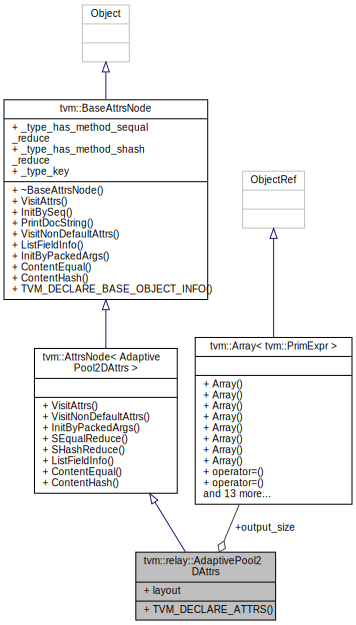
\includegraphics[height=550pt]{structtvm_1_1relay_1_1AdaptivePool2DAttrs__coll__graph}
\end{center}
\end{figure}
\subsection*{Public Member Functions}
\begin{DoxyCompactItemize}
\item 
\hyperlink{structtvm_1_1relay_1_1AdaptivePool2DAttrs_a948bd68b55ffa2a02fedb9fa3b0fecd5}{T\+V\+M\+\_\+\+D\+E\+C\+L\+A\+R\+E\+\_\+\+A\+T\+T\+RS} (\hyperlink{structtvm_1_1relay_1_1AdaptivePool2DAttrs}{Adaptive\+Pool2\+D\+Attrs},\char`\"{}relay.\+attrs.\+Adaptive\+Pool2\+D\+Attrs\char`\"{})
\end{DoxyCompactItemize}
\subsection*{Public Attributes}
\begin{DoxyCompactItemize}
\item 
\hyperlink{classtvm_1_1Array}{Array}$<$ \hyperlink{namespacetvm_1_1relay_ae153a27d81399fd266b8d598227764c4}{Index\+Expr} $>$ \hyperlink{structtvm_1_1relay_1_1AdaptivePool2DAttrs_a545f40ec0dbdf52f628bebcc23a63950}{output\+\_\+size}
\item 
std\+::string \hyperlink{structtvm_1_1relay_1_1AdaptivePool2DAttrs_a5d020266c4e9f570c051bdde64872891}{layout}
\end{DoxyCompactItemize}
\subsection*{Additional Inherited Members}


\subsection{Detailed Description}
Attributes for adaptive pool operator. 

\subsection{Member Function Documentation}
\index{tvm\+::relay\+::\+Adaptive\+Pool2\+D\+Attrs@{tvm\+::relay\+::\+Adaptive\+Pool2\+D\+Attrs}!T\+V\+M\+\_\+\+D\+E\+C\+L\+A\+R\+E\+\_\+\+A\+T\+T\+RS@{T\+V\+M\+\_\+\+D\+E\+C\+L\+A\+R\+E\+\_\+\+A\+T\+T\+RS}}
\index{T\+V\+M\+\_\+\+D\+E\+C\+L\+A\+R\+E\+\_\+\+A\+T\+T\+RS@{T\+V\+M\+\_\+\+D\+E\+C\+L\+A\+R\+E\+\_\+\+A\+T\+T\+RS}!tvm\+::relay\+::\+Adaptive\+Pool2\+D\+Attrs@{tvm\+::relay\+::\+Adaptive\+Pool2\+D\+Attrs}}
\subsubsection[{\texorpdfstring{T\+V\+M\+\_\+\+D\+E\+C\+L\+A\+R\+E\+\_\+\+A\+T\+T\+R\+S(\+Adaptive\+Pool2\+D\+Attrs,""relay.\+attrs.\+Adaptive\+Pool2\+D\+Attrs"")}{TVM_DECLARE_ATTRS(AdaptivePool2DAttrs,"relay.attrs.AdaptivePool2DAttrs")}}]{\setlength{\rightskip}{0pt plus 5cm}tvm\+::relay\+::\+Adaptive\+Pool2\+D\+Attrs\+::\+T\+V\+M\+\_\+\+D\+E\+C\+L\+A\+R\+E\+\_\+\+A\+T\+T\+RS (
\begin{DoxyParamCaption}
\item[{{\bf Adaptive\+Pool2\+D\+Attrs}}]{, }
\item[{\char`\"{}relay.\+attrs.\+Adaptive\+Pool2\+D\+Attrs\char`\"{}}]{}
\end{DoxyParamCaption}
)\hspace{0.3cm}{\ttfamily [inline]}}\hypertarget{structtvm_1_1relay_1_1AdaptivePool2DAttrs_a948bd68b55ffa2a02fedb9fa3b0fecd5}{}\label{structtvm_1_1relay_1_1AdaptivePool2DAttrs_a948bd68b55ffa2a02fedb9fa3b0fecd5}


\subsection{Member Data Documentation}
\index{tvm\+::relay\+::\+Adaptive\+Pool2\+D\+Attrs@{tvm\+::relay\+::\+Adaptive\+Pool2\+D\+Attrs}!layout@{layout}}
\index{layout@{layout}!tvm\+::relay\+::\+Adaptive\+Pool2\+D\+Attrs@{tvm\+::relay\+::\+Adaptive\+Pool2\+D\+Attrs}}
\subsubsection[{\texorpdfstring{layout}{layout}}]{\setlength{\rightskip}{0pt plus 5cm}std\+::string tvm\+::relay\+::\+Adaptive\+Pool2\+D\+Attrs\+::layout}\hypertarget{structtvm_1_1relay_1_1AdaptivePool2DAttrs_a5d020266c4e9f570c051bdde64872891}{}\label{structtvm_1_1relay_1_1AdaptivePool2DAttrs_a5d020266c4e9f570c051bdde64872891}
\index{tvm\+::relay\+::\+Adaptive\+Pool2\+D\+Attrs@{tvm\+::relay\+::\+Adaptive\+Pool2\+D\+Attrs}!output\+\_\+size@{output\+\_\+size}}
\index{output\+\_\+size@{output\+\_\+size}!tvm\+::relay\+::\+Adaptive\+Pool2\+D\+Attrs@{tvm\+::relay\+::\+Adaptive\+Pool2\+D\+Attrs}}
\subsubsection[{\texorpdfstring{output\+\_\+size}{output_size}}]{\setlength{\rightskip}{0pt plus 5cm}{\bf Array}$<${\bf Index\+Expr}$>$ tvm\+::relay\+::\+Adaptive\+Pool2\+D\+Attrs\+::output\+\_\+size}\hypertarget{structtvm_1_1relay_1_1AdaptivePool2DAttrs_a545f40ec0dbdf52f628bebcc23a63950}{}\label{structtvm_1_1relay_1_1AdaptivePool2DAttrs_a545f40ec0dbdf52f628bebcc23a63950}


The documentation for this struct was generated from the following file\+:\begin{DoxyCompactItemize}
\item 
include/tvm/relay/attrs/\hyperlink{include_2tvm_2relay_2attrs_2nn_8h}{nn.\+h}\end{DoxyCompactItemize}

\hypertarget{structtvm_1_1relay_1_1AdaptivePool3DAttrs}{}\section{tvm\+:\+:relay\+:\+:Adaptive\+Pool3\+D\+Attrs Struct Reference}
\label{structtvm_1_1relay_1_1AdaptivePool3DAttrs}\index{tvm\+::relay\+::\+Adaptive\+Pool3\+D\+Attrs@{tvm\+::relay\+::\+Adaptive\+Pool3\+D\+Attrs}}


{\ttfamily \#include $<$nn.\+h$>$}



Inheritance diagram for tvm\+:\+:relay\+:\+:Adaptive\+Pool3\+D\+Attrs\+:
\nopagebreak
\begin{figure}[H]
\begin{center}
\leavevmode
\includegraphics[height=550pt]{structtvm_1_1relay_1_1AdaptivePool3DAttrs__inherit__graph}
\end{center}
\end{figure}


Collaboration diagram for tvm\+:\+:relay\+:\+:Adaptive\+Pool3\+D\+Attrs\+:
\nopagebreak
\begin{figure}[H]
\begin{center}
\leavevmode
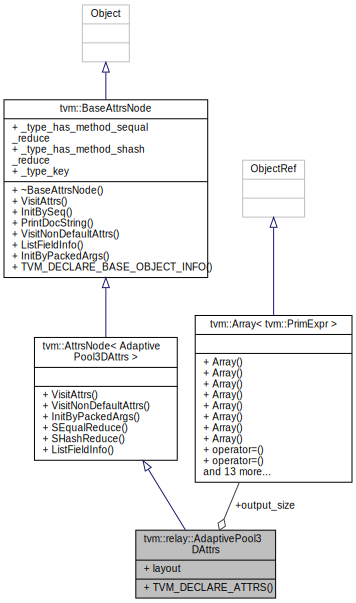
\includegraphics[height=550pt]{structtvm_1_1relay_1_1AdaptivePool3DAttrs__coll__graph}
\end{center}
\end{figure}
\subsection*{Public Member Functions}
\begin{DoxyCompactItemize}
\item 
\hyperlink{structtvm_1_1relay_1_1AdaptivePool3DAttrs_a51be0f4ac6d7df200afe4539b6611b76}{T\+V\+M\+\_\+\+D\+E\+C\+L\+A\+R\+E\+\_\+\+A\+T\+T\+RS} (\hyperlink{structtvm_1_1relay_1_1AdaptivePool3DAttrs}{Adaptive\+Pool3\+D\+Attrs},\char`\"{}relay.\+attrs.\+Adaptive\+Pool3\+D\+Attrs\char`\"{})
\end{DoxyCompactItemize}
\subsection*{Public Attributes}
\begin{DoxyCompactItemize}
\item 
\hyperlink{classtvm_1_1Array}{Array}$<$ \hyperlink{namespacetvm_1_1relay_ae153a27d81399fd266b8d598227764c4}{Index\+Expr} $>$ \hyperlink{structtvm_1_1relay_1_1AdaptivePool3DAttrs_a0c56cb9665840dcc8e949c41d39c710d}{output\+\_\+size}
\item 
std\+::string \hyperlink{structtvm_1_1relay_1_1AdaptivePool3DAttrs_a4f75ae856def381f58402c5eff8c1027}{layout}
\end{DoxyCompactItemize}
\subsection*{Additional Inherited Members}


\subsection{Member Function Documentation}
\index{tvm\+::relay\+::\+Adaptive\+Pool3\+D\+Attrs@{tvm\+::relay\+::\+Adaptive\+Pool3\+D\+Attrs}!T\+V\+M\+\_\+\+D\+E\+C\+L\+A\+R\+E\+\_\+\+A\+T\+T\+RS@{T\+V\+M\+\_\+\+D\+E\+C\+L\+A\+R\+E\+\_\+\+A\+T\+T\+RS}}
\index{T\+V\+M\+\_\+\+D\+E\+C\+L\+A\+R\+E\+\_\+\+A\+T\+T\+RS@{T\+V\+M\+\_\+\+D\+E\+C\+L\+A\+R\+E\+\_\+\+A\+T\+T\+RS}!tvm\+::relay\+::\+Adaptive\+Pool3\+D\+Attrs@{tvm\+::relay\+::\+Adaptive\+Pool3\+D\+Attrs}}
\subsubsection[{\texorpdfstring{T\+V\+M\+\_\+\+D\+E\+C\+L\+A\+R\+E\+\_\+\+A\+T\+T\+R\+S(\+Adaptive\+Pool3\+D\+Attrs,""relay.\+attrs.\+Adaptive\+Pool3\+D\+Attrs"")}{TVM_DECLARE_ATTRS(AdaptivePool3DAttrs,"relay.attrs.AdaptivePool3DAttrs")}}]{\setlength{\rightskip}{0pt plus 5cm}tvm\+::relay\+::\+Adaptive\+Pool3\+D\+Attrs\+::\+T\+V\+M\+\_\+\+D\+E\+C\+L\+A\+R\+E\+\_\+\+A\+T\+T\+RS (
\begin{DoxyParamCaption}
\item[{{\bf Adaptive\+Pool3\+D\+Attrs}}]{, }
\item[{\char`\"{}relay.\+attrs.\+Adaptive\+Pool3\+D\+Attrs\char`\"{}}]{}
\end{DoxyParamCaption}
)\hspace{0.3cm}{\ttfamily [inline]}}\hypertarget{structtvm_1_1relay_1_1AdaptivePool3DAttrs_a51be0f4ac6d7df200afe4539b6611b76}{}\label{structtvm_1_1relay_1_1AdaptivePool3DAttrs_a51be0f4ac6d7df200afe4539b6611b76}


\subsection{Member Data Documentation}
\index{tvm\+::relay\+::\+Adaptive\+Pool3\+D\+Attrs@{tvm\+::relay\+::\+Adaptive\+Pool3\+D\+Attrs}!layout@{layout}}
\index{layout@{layout}!tvm\+::relay\+::\+Adaptive\+Pool3\+D\+Attrs@{tvm\+::relay\+::\+Adaptive\+Pool3\+D\+Attrs}}
\subsubsection[{\texorpdfstring{layout}{layout}}]{\setlength{\rightskip}{0pt plus 5cm}std\+::string tvm\+::relay\+::\+Adaptive\+Pool3\+D\+Attrs\+::layout}\hypertarget{structtvm_1_1relay_1_1AdaptivePool3DAttrs_a4f75ae856def381f58402c5eff8c1027}{}\label{structtvm_1_1relay_1_1AdaptivePool3DAttrs_a4f75ae856def381f58402c5eff8c1027}
\index{tvm\+::relay\+::\+Adaptive\+Pool3\+D\+Attrs@{tvm\+::relay\+::\+Adaptive\+Pool3\+D\+Attrs}!output\+\_\+size@{output\+\_\+size}}
\index{output\+\_\+size@{output\+\_\+size}!tvm\+::relay\+::\+Adaptive\+Pool3\+D\+Attrs@{tvm\+::relay\+::\+Adaptive\+Pool3\+D\+Attrs}}
\subsubsection[{\texorpdfstring{output\+\_\+size}{output_size}}]{\setlength{\rightskip}{0pt plus 5cm}{\bf Array}$<${\bf Index\+Expr}$>$ tvm\+::relay\+::\+Adaptive\+Pool3\+D\+Attrs\+::output\+\_\+size}\hypertarget{structtvm_1_1relay_1_1AdaptivePool3DAttrs_a0c56cb9665840dcc8e949c41d39c710d}{}\label{structtvm_1_1relay_1_1AdaptivePool3DAttrs_a0c56cb9665840dcc8e949c41d39c710d}


The documentation for this struct was generated from the following file\+:\begin{DoxyCompactItemize}
\item 
include/tvm/relay/attrs/\hyperlink{include_2tvm_2relay_2attrs_2nn_8h}{nn.\+h}\end{DoxyCompactItemize}

\hypertarget{classtvm_1_1tir_1_1AddNode}{}\section{tvm\+:\+:tir\+:\+:Add\+Node Class Reference}
\label{classtvm_1_1tir_1_1AddNode}\index{tvm\+::tir\+::\+Add\+Node@{tvm\+::tir\+::\+Add\+Node}}


a + b  




{\ttfamily \#include $<$expr.\+h$>$}



Inheritance diagram for tvm\+:\+:tir\+:\+:Add\+Node\+:
\nopagebreak
\begin{figure}[H]
\begin{center}
\leavevmode
\includegraphics[height=550pt]{classtvm_1_1tir_1_1AddNode__inherit__graph}
\end{center}
\end{figure}


Collaboration diagram for tvm\+:\+:tir\+:\+:Add\+Node\+:
\nopagebreak
\begin{figure}[H]
\begin{center}
\leavevmode
\includegraphics[width=350pt]{classtvm_1_1tir_1_1AddNode__coll__graph}
\end{center}
\end{figure}
\subsection*{Static Public Attributes}
\begin{DoxyCompactItemize}
\item 
static constexpr const char $\ast$ \hyperlink{classtvm_1_1tir_1_1AddNode_acb112a802dbe7e838fa6c51680220844}{\+\_\+type\+\_\+key} = \char`\"{}Add\char`\"{}
\end{DoxyCompactItemize}
\subsection*{Additional Inherited Members}


\subsection{Detailed Description}
a + b 

\subsection{Member Data Documentation}
\index{tvm\+::tir\+::\+Add\+Node@{tvm\+::tir\+::\+Add\+Node}!\+\_\+type\+\_\+key@{\+\_\+type\+\_\+key}}
\index{\+\_\+type\+\_\+key@{\+\_\+type\+\_\+key}!tvm\+::tir\+::\+Add\+Node@{tvm\+::tir\+::\+Add\+Node}}
\subsubsection[{\texorpdfstring{\+\_\+type\+\_\+key}{_type_key}}]{\setlength{\rightskip}{0pt plus 5cm}constexpr const char$\ast$ tvm\+::tir\+::\+Add\+Node\+::\+\_\+type\+\_\+key = \char`\"{}Add\char`\"{}\hspace{0.3cm}{\ttfamily [static]}}\hypertarget{classtvm_1_1tir_1_1AddNode_acb112a802dbe7e838fa6c51680220844}{}\label{classtvm_1_1tir_1_1AddNode_acb112a802dbe7e838fa6c51680220844}


The documentation for this class was generated from the following file\+:\begin{DoxyCompactItemize}
\item 
include/tvm/tir/\hyperlink{tir_2expr_8h}{expr.\+h}\end{DoxyCompactItemize}

\hypertarget{classtvm_1_1runtime_1_1ADT}{}\section{tvm\+:\+:runtime\+:\+:A\+DT Class Reference}
\label{classtvm_1_1runtime_1_1ADT}\index{tvm\+::runtime\+::\+A\+DT@{tvm\+::runtime\+::\+A\+DT}}


reference to algebraic data type objects.  




{\ttfamily \#include $<$container.\+h$>$}



Inheritance diagram for tvm\+:\+:runtime\+:\+:A\+DT\+:
\nopagebreak
\begin{figure}[H]
\begin{center}
\leavevmode
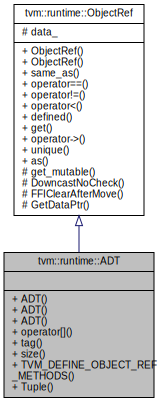
\includegraphics[width=230pt]{classtvm_1_1runtime_1_1ADT__inherit__graph}
\end{center}
\end{figure}


Collaboration diagram for tvm\+:\+:runtime\+:\+:A\+DT\+:
\nopagebreak
\begin{figure}[H]
\begin{center}
\leavevmode
\includegraphics[height=550pt]{classtvm_1_1runtime_1_1ADT__coll__graph}
\end{center}
\end{figure}
\subsection*{Public Member Functions}
\begin{DoxyCompactItemize}
\item 
\hyperlink{classtvm_1_1runtime_1_1ADT_a204397cb319fdb83a72b1d9112a09caa}{A\+DT} (int32\+\_\+t \hyperlink{classtvm_1_1runtime_1_1ADT_a1a631df56a143132d60076c8038a9a97}{tag}, std\+::vector$<$ \hyperlink{classtvm_1_1runtime_1_1ObjectRef}{Object\+Ref} $>$ fields)
\begin{DoxyCompactList}\small\item\em construct an \hyperlink{classtvm_1_1runtime_1_1ADT}{A\+DT} object reference. \end{DoxyCompactList}\item 
{\footnotesize template$<$typename Iterator $>$ }\\\hyperlink{classtvm_1_1runtime_1_1ADT_aea0665ed087095ed39354064e5071d4f}{A\+DT} (int32\+\_\+t \hyperlink{classtvm_1_1runtime_1_1ADT_a1a631df56a143132d60076c8038a9a97}{tag}, Iterator begin, Iterator end)
\begin{DoxyCompactList}\small\item\em construct an \hyperlink{classtvm_1_1runtime_1_1ADT}{A\+DT} object reference. \end{DoxyCompactList}\item 
\hyperlink{classtvm_1_1runtime_1_1ADT_a9ebe228980db0256d72fc01ba5c7ae89}{A\+DT} (int32\+\_\+t \hyperlink{classtvm_1_1runtime_1_1ADT_a1a631df56a143132d60076c8038a9a97}{tag}, std\+::initializer\+\_\+list$<$ \hyperlink{classtvm_1_1runtime_1_1ObjectRef}{Object\+Ref} $>$ init)
\begin{DoxyCompactList}\small\item\em construct an \hyperlink{classtvm_1_1runtime_1_1ADT}{A\+DT} object reference. \end{DoxyCompactList}\item 
const \hyperlink{classtvm_1_1runtime_1_1ObjectRef}{Object\+Ref} \& \hyperlink{classtvm_1_1runtime_1_1ADT_a6a1dba101b18cffbd307f7c0f92a39b2}{operator\mbox{[}$\,$\mbox{]}} (size\+\_\+t idx) const 
\begin{DoxyCompactList}\small\item\em Access element at index. \end{DoxyCompactList}\item 
int32\+\_\+t \hyperlink{classtvm_1_1runtime_1_1ADT_a1a631df56a143132d60076c8038a9a97}{tag} () const 
\begin{DoxyCompactList}\small\item\em Return the \hyperlink{classtvm_1_1runtime_1_1ADT}{A\+DT} tag. \end{DoxyCompactList}\item 
size\+\_\+t \hyperlink{classtvm_1_1runtime_1_1ADT_af8cf2f61fa9b7737718f15a018d12b84}{size} () const 
\begin{DoxyCompactList}\small\item\em Return the number of fields. \end{DoxyCompactList}\item 
\hyperlink{classtvm_1_1runtime_1_1ADT_a5367ea22b4dab8c73d06031cd4c72dec}{T\+V\+M\+\_\+\+D\+E\+F\+I\+N\+E\+\_\+\+O\+B\+J\+E\+C\+T\+\_\+\+R\+E\+F\+\_\+\+M\+E\+T\+H\+O\+DS} (\hyperlink{classtvm_1_1runtime_1_1ADT}{A\+DT}, \hyperlink{classtvm_1_1runtime_1_1ObjectRef}{Object\+Ref}, \hyperlink{classtvm_1_1runtime_1_1ADTObj}{A\+D\+T\+Obj})
\end{DoxyCompactItemize}
\subsection*{Static Public Member Functions}
\begin{DoxyCompactItemize}
\item 
{\footnotesize template$<$typename... Args$>$ }\\static \hyperlink{classtvm_1_1runtime_1_1ADT}{A\+DT} \hyperlink{classtvm_1_1runtime_1_1ADT_a9952c0be3e79a57cf80a3c01fd7bbe87}{Tuple} (Args \&\&...args)
\begin{DoxyCompactList}\small\item\em Construct a tuple object. \end{DoxyCompactList}\end{DoxyCompactItemize}
\subsection*{Additional Inherited Members}


\subsection{Detailed Description}
reference to algebraic data type objects. 

\subsection{Constructor \& Destructor Documentation}
\index{tvm\+::runtime\+::\+A\+DT@{tvm\+::runtime\+::\+A\+DT}!A\+DT@{A\+DT}}
\index{A\+DT@{A\+DT}!tvm\+::runtime\+::\+A\+DT@{tvm\+::runtime\+::\+A\+DT}}
\subsubsection[{\texorpdfstring{A\+D\+T(int32\+\_\+t tag, std\+::vector$<$ Object\+Ref $>$ fields)}{ADT(int32_t tag, std::vector< ObjectRef > fields)}}]{\setlength{\rightskip}{0pt plus 5cm}tvm\+::runtime\+::\+A\+D\+T\+::\+A\+DT (
\begin{DoxyParamCaption}
\item[{int32\+\_\+t}]{tag, }
\item[{std\+::vector$<$ {\bf Object\+Ref} $>$}]{fields}
\end{DoxyParamCaption}
)\hspace{0.3cm}{\ttfamily [inline]}}\hypertarget{classtvm_1_1runtime_1_1ADT_a204397cb319fdb83a72b1d9112a09caa}{}\label{classtvm_1_1runtime_1_1ADT_a204397cb319fdb83a72b1d9112a09caa}


construct an \hyperlink{classtvm_1_1runtime_1_1ADT}{A\+DT} object reference. 


\begin{DoxyParams}{Parameters}
{\em tag} & The tag of the \hyperlink{classtvm_1_1runtime_1_1ADT}{A\+DT} object. \\
\hline
{\em fields} & The fields of the \hyperlink{classtvm_1_1runtime_1_1ADT}{A\+DT} object. \\
\hline
\end{DoxyParams}
\begin{DoxyReturn}{Returns}
The constructed \hyperlink{classtvm_1_1runtime_1_1ADT}{A\+DT} object reference. 
\end{DoxyReturn}
\index{tvm\+::runtime\+::\+A\+DT@{tvm\+::runtime\+::\+A\+DT}!A\+DT@{A\+DT}}
\index{A\+DT@{A\+DT}!tvm\+::runtime\+::\+A\+DT@{tvm\+::runtime\+::\+A\+DT}}
\subsubsection[{\texorpdfstring{A\+D\+T(int32\+\_\+t tag, Iterator begin, Iterator end)}{ADT(int32_t tag, Iterator begin, Iterator end)}}]{\setlength{\rightskip}{0pt plus 5cm}template$<$typename Iterator $>$ tvm\+::runtime\+::\+A\+D\+T\+::\+A\+DT (
\begin{DoxyParamCaption}
\item[{int32\+\_\+t}]{tag, }
\item[{Iterator}]{begin, }
\item[{Iterator}]{end}
\end{DoxyParamCaption}
)\hspace{0.3cm}{\ttfamily [inline]}}\hypertarget{classtvm_1_1runtime_1_1ADT_aea0665ed087095ed39354064e5071d4f}{}\label{classtvm_1_1runtime_1_1ADT_aea0665ed087095ed39354064e5071d4f}


construct an \hyperlink{classtvm_1_1runtime_1_1ADT}{A\+DT} object reference. 


\begin{DoxyParams}{Parameters}
{\em tag} & The tag of the \hyperlink{classtvm_1_1runtime_1_1ADT}{A\+DT} object. \\
\hline
{\em begin} & The begin iterator to the start of the fields array. \\
\hline
{\em end} & The end iterator to the end of the fields array. \\
\hline
\end{DoxyParams}
\begin{DoxyReturn}{Returns}
The constructed \hyperlink{classtvm_1_1runtime_1_1ADT}{A\+DT} object reference. 
\end{DoxyReturn}
\index{tvm\+::runtime\+::\+A\+DT@{tvm\+::runtime\+::\+A\+DT}!A\+DT@{A\+DT}}
\index{A\+DT@{A\+DT}!tvm\+::runtime\+::\+A\+DT@{tvm\+::runtime\+::\+A\+DT}}
\subsubsection[{\texorpdfstring{A\+D\+T(int32\+\_\+t tag, std\+::initializer\+\_\+list$<$ Object\+Ref $>$ init)}{ADT(int32_t tag, std::initializer_list< ObjectRef > init)}}]{\setlength{\rightskip}{0pt plus 5cm}tvm\+::runtime\+::\+A\+D\+T\+::\+A\+DT (
\begin{DoxyParamCaption}
\item[{int32\+\_\+t}]{tag, }
\item[{std\+::initializer\+\_\+list$<$ {\bf Object\+Ref} $>$}]{init}
\end{DoxyParamCaption}
)\hspace{0.3cm}{\ttfamily [inline]}}\hypertarget{classtvm_1_1runtime_1_1ADT_a9ebe228980db0256d72fc01ba5c7ae89}{}\label{classtvm_1_1runtime_1_1ADT_a9ebe228980db0256d72fc01ba5c7ae89}


construct an \hyperlink{classtvm_1_1runtime_1_1ADT}{A\+DT} object reference. 


\begin{DoxyParams}{Parameters}
{\em tag} & The tag of the \hyperlink{classtvm_1_1runtime_1_1ADT}{A\+DT} object. \\
\hline
{\em init} & The initializer list of fields. \\
\hline
\end{DoxyParams}
\begin{DoxyReturn}{Returns}
The constructed \hyperlink{classtvm_1_1runtime_1_1ADT}{A\+DT} object reference. 
\end{DoxyReturn}


\subsection{Member Function Documentation}
\index{tvm\+::runtime\+::\+A\+DT@{tvm\+::runtime\+::\+A\+DT}!operator\mbox{[}$\,$\mbox{]}@{operator[]}}
\index{operator\mbox{[}$\,$\mbox{]}@{operator[]}!tvm\+::runtime\+::\+A\+DT@{tvm\+::runtime\+::\+A\+DT}}
\subsubsection[{\texorpdfstring{operator[](size\+\_\+t idx) const }{operator[](size_t idx) const }}]{\setlength{\rightskip}{0pt plus 5cm}const {\bf Object\+Ref}\& tvm\+::runtime\+::\+A\+D\+T\+::operator\mbox{[}$\,$\mbox{]} (
\begin{DoxyParamCaption}
\item[{size\+\_\+t}]{idx}
\end{DoxyParamCaption}
) const\hspace{0.3cm}{\ttfamily [inline]}}\hypertarget{classtvm_1_1runtime_1_1ADT_a6a1dba101b18cffbd307f7c0f92a39b2}{}\label{classtvm_1_1runtime_1_1ADT_a6a1dba101b18cffbd307f7c0f92a39b2}


Access element at index. 


\begin{DoxyParams}{Parameters}
{\em idx} & The array index \\
\hline
\end{DoxyParams}
\begin{DoxyReturn}{Returns}
const \hyperlink{classtvm_1_1runtime_1_1ObjectRef}{Object\+Ref} 
\end{DoxyReturn}
\index{tvm\+::runtime\+::\+A\+DT@{tvm\+::runtime\+::\+A\+DT}!size@{size}}
\index{size@{size}!tvm\+::runtime\+::\+A\+DT@{tvm\+::runtime\+::\+A\+DT}}
\subsubsection[{\texorpdfstring{size() const }{size() const }}]{\setlength{\rightskip}{0pt plus 5cm}size\+\_\+t tvm\+::runtime\+::\+A\+D\+T\+::size (
\begin{DoxyParamCaption}
{}
\end{DoxyParamCaption}
) const\hspace{0.3cm}{\ttfamily [inline]}}\hypertarget{classtvm_1_1runtime_1_1ADT_af8cf2f61fa9b7737718f15a018d12b84}{}\label{classtvm_1_1runtime_1_1ADT_af8cf2f61fa9b7737718f15a018d12b84}


Return the number of fields. 

\index{tvm\+::runtime\+::\+A\+DT@{tvm\+::runtime\+::\+A\+DT}!tag@{tag}}
\index{tag@{tag}!tvm\+::runtime\+::\+A\+DT@{tvm\+::runtime\+::\+A\+DT}}
\subsubsection[{\texorpdfstring{tag() const }{tag() const }}]{\setlength{\rightskip}{0pt plus 5cm}int32\+\_\+t tvm\+::runtime\+::\+A\+D\+T\+::tag (
\begin{DoxyParamCaption}
{}
\end{DoxyParamCaption}
) const\hspace{0.3cm}{\ttfamily [inline]}}\hypertarget{classtvm_1_1runtime_1_1ADT_a1a631df56a143132d60076c8038a9a97}{}\label{classtvm_1_1runtime_1_1ADT_a1a631df56a143132d60076c8038a9a97}


Return the \hyperlink{classtvm_1_1runtime_1_1ADT}{A\+DT} tag. 

\index{tvm\+::runtime\+::\+A\+DT@{tvm\+::runtime\+::\+A\+DT}!Tuple@{Tuple}}
\index{Tuple@{Tuple}!tvm\+::runtime\+::\+A\+DT@{tvm\+::runtime\+::\+A\+DT}}
\subsubsection[{\texorpdfstring{Tuple(\+Args \&\&...\+args)}{Tuple(Args &&...args)}}]{\setlength{\rightskip}{0pt plus 5cm}template$<$typename... Args$>$ static {\bf A\+DT} tvm\+::runtime\+::\+A\+D\+T\+::\+Tuple (
\begin{DoxyParamCaption}
\item[{Args \&\&...}]{args}
\end{DoxyParamCaption}
)\hspace{0.3cm}{\ttfamily [inline]}, {\ttfamily [static]}}\hypertarget{classtvm_1_1runtime_1_1ADT_a9952c0be3e79a57cf80a3c01fd7bbe87}{}\label{classtvm_1_1runtime_1_1ADT_a9952c0be3e79a57cf80a3c01fd7bbe87}


Construct a tuple object. 


\begin{DoxyTemplParams}{Template Parameters}
{\em Args} & \hyperlink{classtvm_1_1Type}{Type} params of tuple feilds. \\
\hline
\end{DoxyTemplParams}

\begin{DoxyParams}{Parameters}
{\em args} & Tuple fields. \\
\hline
\end{DoxyParams}
\begin{DoxyReturn}{Returns}
\hyperlink{classtvm_1_1runtime_1_1ADT}{A\+DT} The tuple object reference. 
\end{DoxyReturn}
\index{tvm\+::runtime\+::\+A\+DT@{tvm\+::runtime\+::\+A\+DT}!T\+V\+M\+\_\+\+D\+E\+F\+I\+N\+E\+\_\+\+O\+B\+J\+E\+C\+T\+\_\+\+R\+E\+F\+\_\+\+M\+E\+T\+H\+O\+DS@{T\+V\+M\+\_\+\+D\+E\+F\+I\+N\+E\+\_\+\+O\+B\+J\+E\+C\+T\+\_\+\+R\+E\+F\+\_\+\+M\+E\+T\+H\+O\+DS}}
\index{T\+V\+M\+\_\+\+D\+E\+F\+I\+N\+E\+\_\+\+O\+B\+J\+E\+C\+T\+\_\+\+R\+E\+F\+\_\+\+M\+E\+T\+H\+O\+DS@{T\+V\+M\+\_\+\+D\+E\+F\+I\+N\+E\+\_\+\+O\+B\+J\+E\+C\+T\+\_\+\+R\+E\+F\+\_\+\+M\+E\+T\+H\+O\+DS}!tvm\+::runtime\+::\+A\+DT@{tvm\+::runtime\+::\+A\+DT}}
\subsubsection[{\texorpdfstring{T\+V\+M\+\_\+\+D\+E\+F\+I\+N\+E\+\_\+\+O\+B\+J\+E\+C\+T\+\_\+\+R\+E\+F\+\_\+\+M\+E\+T\+H\+O\+D\+S(\+A\+D\+T, Object\+Ref, A\+D\+T\+Obj)}{TVM_DEFINE_OBJECT_REF_METHODS(ADT, ObjectRef, ADTObj)}}]{\setlength{\rightskip}{0pt plus 5cm}tvm\+::runtime\+::\+A\+D\+T\+::\+T\+V\+M\+\_\+\+D\+E\+F\+I\+N\+E\+\_\+\+O\+B\+J\+E\+C\+T\+\_\+\+R\+E\+F\+\_\+\+M\+E\+T\+H\+O\+DS (
\begin{DoxyParamCaption}
\item[{{\bf A\+DT}}]{, }
\item[{{\bf Object\+Ref}}]{, }
\item[{{\bf A\+D\+T\+Obj}}]{}
\end{DoxyParamCaption}
)}\hypertarget{classtvm_1_1runtime_1_1ADT_a5367ea22b4dab8c73d06031cd4c72dec}{}\label{classtvm_1_1runtime_1_1ADT_a5367ea22b4dab8c73d06031cd4c72dec}


The documentation for this class was generated from the following file\+:\begin{DoxyCompactItemize}
\item 
include/tvm/runtime/\hyperlink{runtime_2container_8h}{container.\+h}\end{DoxyCompactItemize}

\hypertarget{classtvm_1_1runtime_1_1ADTObj}{}\section{tvm\+:\+:runtime\+:\+:A\+D\+T\+Obj Class Reference}
\label{classtvm_1_1runtime_1_1ADTObj}\index{tvm\+::runtime\+::\+A\+D\+T\+Obj@{tvm\+::runtime\+::\+A\+D\+T\+Obj}}


An object representing a structure or enumeration.  




{\ttfamily \#include $<$container.\+h$>$}



Inheritance diagram for tvm\+:\+:runtime\+:\+:A\+D\+T\+Obj\+:
\nopagebreak
\begin{figure}[H]
\begin{center}
\leavevmode
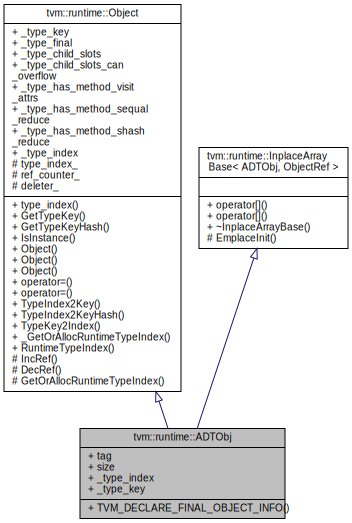
\includegraphics[width=350pt]{classtvm_1_1runtime_1_1ADTObj__inherit__graph}
\end{center}
\end{figure}


Collaboration diagram for tvm\+:\+:runtime\+:\+:A\+D\+T\+Obj\+:
\nopagebreak
\begin{figure}[H]
\begin{center}
\leavevmode
\includegraphics[width=350pt]{classtvm_1_1runtime_1_1ADTObj__coll__graph}
\end{center}
\end{figure}
\subsection*{Public Member Functions}
\begin{DoxyCompactItemize}
\item 
\hyperlink{classtvm_1_1runtime_1_1ADTObj_ac282a733d6c69a23a94c3a2bdf8c61c2}{T\+V\+M\+\_\+\+D\+E\+C\+L\+A\+R\+E\+\_\+\+F\+I\+N\+A\+L\+\_\+\+O\+B\+J\+E\+C\+T\+\_\+\+I\+N\+FO} (\hyperlink{classtvm_1_1runtime_1_1ADTObj}{A\+D\+T\+Obj}, \hyperlink{classtvm_1_1runtime_1_1Object}{Object})
\end{DoxyCompactItemize}
\subsection*{Public Attributes}
\begin{DoxyCompactItemize}
\item 
int32\+\_\+t \hyperlink{classtvm_1_1runtime_1_1ADTObj_a8c1835b988e836dd451a343bac7e402d}{tag}
\begin{DoxyCompactList}\small\item\em The tag representing the constructor used. \end{DoxyCompactList}\item 
uint32\+\_\+t \hyperlink{classtvm_1_1runtime_1_1ADTObj_a699d898a036382a0c86fba219bcf8102}{size}
\begin{DoxyCompactList}\small\item\em Number of fields in the \hyperlink{classtvm_1_1runtime_1_1ADT}{A\+DT} object. \end{DoxyCompactList}\end{DoxyCompactItemize}
\subsection*{Static Public Attributes}
\begin{DoxyCompactItemize}
\item 
static constexpr const uint32\+\_\+t \hyperlink{classtvm_1_1runtime_1_1ADTObj_ae35ebc3d49a7264ac1ed16a80472347f}{\+\_\+type\+\_\+index} = Type\+Index\+::k\+V\+M\+A\+DT
\item 
static constexpr const char $\ast$ \hyperlink{classtvm_1_1runtime_1_1ADTObj_ab083e5c0b35f64b668eaf5cfb0f98098}{\+\_\+type\+\_\+key} = \char`\"{}vm.\+A\+DT\char`\"{}
\end{DoxyCompactItemize}
\subsection*{Friends}
\begin{DoxyCompactItemize}
\item 
class \hyperlink{classtvm_1_1runtime_1_1ADTObj_a96ef507f2261998fb326f88992b9738a}{A\+DT}
\end{DoxyCompactItemize}
\subsection*{Additional Inherited Members}


\subsection{Detailed Description}
An object representing a structure or enumeration. 

\subsection{Member Function Documentation}
\index{tvm\+::runtime\+::\+A\+D\+T\+Obj@{tvm\+::runtime\+::\+A\+D\+T\+Obj}!T\+V\+M\+\_\+\+D\+E\+C\+L\+A\+R\+E\+\_\+\+F\+I\+N\+A\+L\+\_\+\+O\+B\+J\+E\+C\+T\+\_\+\+I\+N\+FO@{T\+V\+M\+\_\+\+D\+E\+C\+L\+A\+R\+E\+\_\+\+F\+I\+N\+A\+L\+\_\+\+O\+B\+J\+E\+C\+T\+\_\+\+I\+N\+FO}}
\index{T\+V\+M\+\_\+\+D\+E\+C\+L\+A\+R\+E\+\_\+\+F\+I\+N\+A\+L\+\_\+\+O\+B\+J\+E\+C\+T\+\_\+\+I\+N\+FO@{T\+V\+M\+\_\+\+D\+E\+C\+L\+A\+R\+E\+\_\+\+F\+I\+N\+A\+L\+\_\+\+O\+B\+J\+E\+C\+T\+\_\+\+I\+N\+FO}!tvm\+::runtime\+::\+A\+D\+T\+Obj@{tvm\+::runtime\+::\+A\+D\+T\+Obj}}
\subsubsection[{\texorpdfstring{T\+V\+M\+\_\+\+D\+E\+C\+L\+A\+R\+E\+\_\+\+F\+I\+N\+A\+L\+\_\+\+O\+B\+J\+E\+C\+T\+\_\+\+I\+N\+F\+O(\+A\+D\+T\+Obj, Object)}{TVM_DECLARE_FINAL_OBJECT_INFO(ADTObj, Object)}}]{\setlength{\rightskip}{0pt plus 5cm}tvm\+::runtime\+::\+A\+D\+T\+Obj\+::\+T\+V\+M\+\_\+\+D\+E\+C\+L\+A\+R\+E\+\_\+\+F\+I\+N\+A\+L\+\_\+\+O\+B\+J\+E\+C\+T\+\_\+\+I\+N\+FO (
\begin{DoxyParamCaption}
\item[{{\bf A\+D\+T\+Obj}}]{, }
\item[{{\bf Object}}]{}
\end{DoxyParamCaption}
)}\hypertarget{classtvm_1_1runtime_1_1ADTObj_ac282a733d6c69a23a94c3a2bdf8c61c2}{}\label{classtvm_1_1runtime_1_1ADTObj_ac282a733d6c69a23a94c3a2bdf8c61c2}


\subsection{Friends And Related Function Documentation}
\index{tvm\+::runtime\+::\+A\+D\+T\+Obj@{tvm\+::runtime\+::\+A\+D\+T\+Obj}!A\+DT@{A\+DT}}
\index{A\+DT@{A\+DT}!tvm\+::runtime\+::\+A\+D\+T\+Obj@{tvm\+::runtime\+::\+A\+D\+T\+Obj}}
\subsubsection[{\texorpdfstring{A\+DT}{ADT}}]{\setlength{\rightskip}{0pt plus 5cm}friend class {\bf A\+DT}\hspace{0.3cm}{\ttfamily [friend]}}\hypertarget{classtvm_1_1runtime_1_1ADTObj_a96ef507f2261998fb326f88992b9738a}{}\label{classtvm_1_1runtime_1_1ADTObj_a96ef507f2261998fb326f88992b9738a}


\subsection{Member Data Documentation}
\index{tvm\+::runtime\+::\+A\+D\+T\+Obj@{tvm\+::runtime\+::\+A\+D\+T\+Obj}!\+\_\+type\+\_\+index@{\+\_\+type\+\_\+index}}
\index{\+\_\+type\+\_\+index@{\+\_\+type\+\_\+index}!tvm\+::runtime\+::\+A\+D\+T\+Obj@{tvm\+::runtime\+::\+A\+D\+T\+Obj}}
\subsubsection[{\texorpdfstring{\+\_\+type\+\_\+index}{_type_index}}]{\setlength{\rightskip}{0pt plus 5cm}constexpr const uint32\+\_\+t tvm\+::runtime\+::\+A\+D\+T\+Obj\+::\+\_\+type\+\_\+index = Type\+Index\+::k\+V\+M\+A\+DT\hspace{0.3cm}{\ttfamily [static]}}\hypertarget{classtvm_1_1runtime_1_1ADTObj_ae35ebc3d49a7264ac1ed16a80472347f}{}\label{classtvm_1_1runtime_1_1ADTObj_ae35ebc3d49a7264ac1ed16a80472347f}
\index{tvm\+::runtime\+::\+A\+D\+T\+Obj@{tvm\+::runtime\+::\+A\+D\+T\+Obj}!\+\_\+type\+\_\+key@{\+\_\+type\+\_\+key}}
\index{\+\_\+type\+\_\+key@{\+\_\+type\+\_\+key}!tvm\+::runtime\+::\+A\+D\+T\+Obj@{tvm\+::runtime\+::\+A\+D\+T\+Obj}}
\subsubsection[{\texorpdfstring{\+\_\+type\+\_\+key}{_type_key}}]{\setlength{\rightskip}{0pt plus 5cm}constexpr const char$\ast$ tvm\+::runtime\+::\+A\+D\+T\+Obj\+::\+\_\+type\+\_\+key = \char`\"{}vm.\+A\+DT\char`\"{}\hspace{0.3cm}{\ttfamily [static]}}\hypertarget{classtvm_1_1runtime_1_1ADTObj_ab083e5c0b35f64b668eaf5cfb0f98098}{}\label{classtvm_1_1runtime_1_1ADTObj_ab083e5c0b35f64b668eaf5cfb0f98098}
\index{tvm\+::runtime\+::\+A\+D\+T\+Obj@{tvm\+::runtime\+::\+A\+D\+T\+Obj}!size@{size}}
\index{size@{size}!tvm\+::runtime\+::\+A\+D\+T\+Obj@{tvm\+::runtime\+::\+A\+D\+T\+Obj}}
\subsubsection[{\texorpdfstring{size}{size}}]{\setlength{\rightskip}{0pt plus 5cm}uint32\+\_\+t tvm\+::runtime\+::\+A\+D\+T\+Obj\+::size}\hypertarget{classtvm_1_1runtime_1_1ADTObj_a699d898a036382a0c86fba219bcf8102}{}\label{classtvm_1_1runtime_1_1ADTObj_a699d898a036382a0c86fba219bcf8102}


Number of fields in the \hyperlink{classtvm_1_1runtime_1_1ADT}{A\+DT} object. 

\index{tvm\+::runtime\+::\+A\+D\+T\+Obj@{tvm\+::runtime\+::\+A\+D\+T\+Obj}!tag@{tag}}
\index{tag@{tag}!tvm\+::runtime\+::\+A\+D\+T\+Obj@{tvm\+::runtime\+::\+A\+D\+T\+Obj}}
\subsubsection[{\texorpdfstring{tag}{tag}}]{\setlength{\rightskip}{0pt plus 5cm}int32\+\_\+t tvm\+::runtime\+::\+A\+D\+T\+Obj\+::tag}\hypertarget{classtvm_1_1runtime_1_1ADTObj_a8c1835b988e836dd451a343bac7e402d}{}\label{classtvm_1_1runtime_1_1ADTObj_a8c1835b988e836dd451a343bac7e402d}


The tag representing the constructor used. 



The documentation for this class was generated from the following file\+:\begin{DoxyCompactItemize}
\item 
include/tvm/runtime/\hyperlink{runtime_2container_8h}{container.\+h}\end{DoxyCompactItemize}

\hypertarget{classtvm_1_1tir_1_1AllocateNode}{}\section{tvm\+:\+:tir\+:\+:Allocate\+Node Class Reference}
\label{classtvm_1_1tir_1_1AllocateNode}\index{tvm\+::tir\+::\+Allocate\+Node@{tvm\+::tir\+::\+Allocate\+Node}}


Allocate a buffer that can be used in body.  




{\ttfamily \#include $<$stmt.\+h$>$}



Inheritance diagram for tvm\+:\+:tir\+:\+:Allocate\+Node\+:
\nopagebreak
\begin{figure}[H]
\begin{center}
\leavevmode
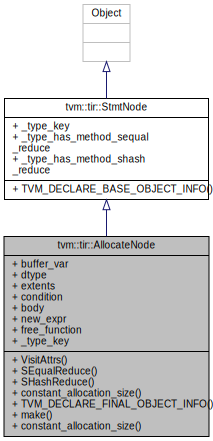
\includegraphics[width=285pt]{classtvm_1_1tir_1_1AllocateNode__inherit__graph}
\end{center}
\end{figure}


Collaboration diagram for tvm\+:\+:tir\+:\+:Allocate\+Node\+:
\nopagebreak
\begin{figure}[H]
\begin{center}
\leavevmode
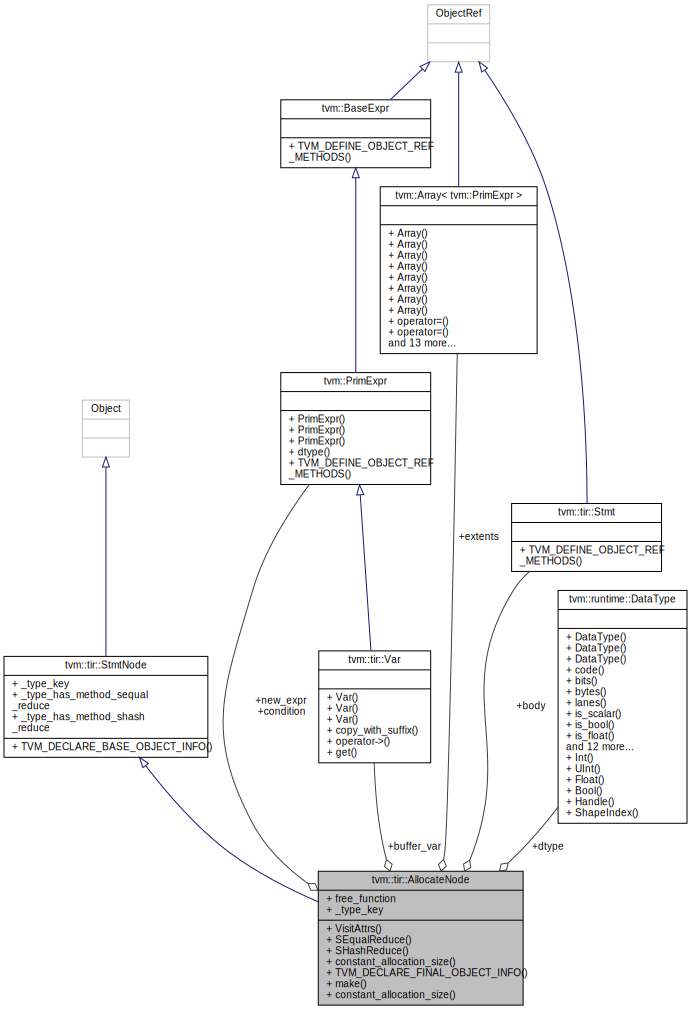
\includegraphics[width=350pt]{classtvm_1_1tir_1_1AllocateNode__coll__graph}
\end{center}
\end{figure}
\subsection*{Public Member Functions}
\begin{DoxyCompactItemize}
\item 
void \hyperlink{classtvm_1_1tir_1_1AllocateNode_ab476a2f1664e28a6da78dfa1d7bc2889}{Visit\+Attrs} (\hyperlink{classtvm_1_1AttrVisitor}{Attr\+Visitor} $\ast$v)
\item 
bool \hyperlink{classtvm_1_1tir_1_1AllocateNode_af666f784cf57e890d16a326912955075}{S\+Equal\+Reduce} (const \hyperlink{classtvm_1_1tir_1_1AllocateNode}{Allocate\+Node} $\ast$other, \hyperlink{classtvm_1_1SEqualReducer}{S\+Equal\+Reducer} equal) const 
\item 
void \hyperlink{classtvm_1_1tir_1_1AllocateNode_aa8b61783e619cc9be13115ca7dfe10b2}{S\+Hash\+Reduce} (\hyperlink{classtvm_1_1SHashReducer}{S\+Hash\+Reducer} hash\+\_\+reduce) const 
\item 
int32\+\_\+t \hyperlink{classtvm_1_1tir_1_1AllocateNode_a7e72bb427a2c945d5eb6bec22bd96f82}{constant\+\_\+allocation\+\_\+size} () const 
\begin{DoxyCompactList}\small\item\em If the buffer size is constant, return the size. Otherwise return 0. \end{DoxyCompactList}\item 
\hyperlink{classtvm_1_1tir_1_1AllocateNode_a8df9749b7cd4db25d5de52572be1ba34}{T\+V\+M\+\_\+\+D\+E\+C\+L\+A\+R\+E\+\_\+\+F\+I\+N\+A\+L\+\_\+\+O\+B\+J\+E\+C\+T\+\_\+\+I\+N\+FO} (\hyperlink{classtvm_1_1tir_1_1AllocateNode}{Allocate\+Node}, \hyperlink{classtvm_1_1tir_1_1StmtNode}{Stmt\+Node})
\end{DoxyCompactItemize}
\subsection*{Static Public Member Functions}
\begin{DoxyCompactItemize}
\item 
static \hyperlink{classtvm_1_1tir_1_1Stmt}{Stmt} \hyperlink{classtvm_1_1tir_1_1AllocateNode_a0e3c6c493843b0e96cdbeedb7992b695}{make} (\hyperlink{classtvm_1_1tir_1_1Var}{Var} \hyperlink{classtvm_1_1tir_1_1AllocateNode_acc0828bc8173ba2d46f90ddd2a329ae0}{buffer\+\_\+var}, \hyperlink{namespacetvm_a41918af1a1dc386388639a9d3ad06c5d}{Data\+Type} \hyperlink{classtvm_1_1tir_1_1AllocateNode_aba885cfd49a10c594320d0e84a9a4c90}{dtype}, \hyperlink{classtvm_1_1Array}{Array}$<$ \hyperlink{classtvm_1_1PrimExpr}{Prim\+Expr} $>$ \hyperlink{classtvm_1_1tir_1_1AllocateNode_a0f6d59cffc5fda07450e0fdab6b66bcb}{extents}, \hyperlink{classtvm_1_1PrimExpr}{Prim\+Expr} \hyperlink{classtvm_1_1tir_1_1AllocateNode_a6b855ad51d1fcb4e21e9afe657f77ba5}{condition}, \hyperlink{classtvm_1_1tir_1_1Stmt}{Stmt} \hyperlink{classtvm_1_1tir_1_1AllocateNode_a797e50c85f4bc016bcf3a3a22737980e}{body}, \hyperlink{classtvm_1_1PrimExpr}{Prim\+Expr} \hyperlink{classtvm_1_1tir_1_1AllocateNode_a52b31635e23aeb6e18e83aa3cc9f8d00}{new\+\_\+expr}=\hyperlink{classtvm_1_1PrimExpr}{Prim\+Expr}(), std\+::string \hyperlink{classtvm_1_1tir_1_1AllocateNode_ac2c84aa70f243d933c0480331910de52}{free\+\_\+function}=std\+::string())
\item 
static int32\+\_\+t \hyperlink{classtvm_1_1tir_1_1AllocateNode_ac30c52ef2a4d9f728026f4f7188094ce}{constant\+\_\+allocation\+\_\+size} (const \hyperlink{classtvm_1_1Array}{Array}$<$ \hyperlink{classtvm_1_1PrimExpr}{Prim\+Expr} $>$ \&\hyperlink{classtvm_1_1tir_1_1AllocateNode_a0f6d59cffc5fda07450e0fdab6b66bcb}{extents})
\begin{DoxyCompactList}\small\item\em If the buffer size is constant, return the size. Otherwise return 0. \end{DoxyCompactList}\end{DoxyCompactItemize}
\subsection*{Public Attributes}
\begin{DoxyCompactItemize}
\item 
\hyperlink{classtvm_1_1tir_1_1Var}{Var} \hyperlink{classtvm_1_1tir_1_1AllocateNode_acc0828bc8173ba2d46f90ddd2a329ae0}{buffer\+\_\+var}
\begin{DoxyCompactList}\small\item\em The buffer variable. \end{DoxyCompactList}\item 
\hyperlink{namespacetvm_a41918af1a1dc386388639a9d3ad06c5d}{Data\+Type} \hyperlink{classtvm_1_1tir_1_1AllocateNode_aba885cfd49a10c594320d0e84a9a4c90}{dtype}
\begin{DoxyCompactList}\small\item\em The type of the buffer. \end{DoxyCompactList}\item 
\hyperlink{classtvm_1_1Array}{Array}$<$ \hyperlink{classtvm_1_1PrimExpr}{Prim\+Expr} $>$ \hyperlink{classtvm_1_1tir_1_1AllocateNode_a0f6d59cffc5fda07450e0fdab6b66bcb}{extents}
\begin{DoxyCompactList}\small\item\em The extents of the buffer. \end{DoxyCompactList}\item 
\hyperlink{classtvm_1_1PrimExpr}{Prim\+Expr} \hyperlink{classtvm_1_1tir_1_1AllocateNode_a6b855ad51d1fcb4e21e9afe657f77ba5}{condition}
\begin{DoxyCompactList}\small\item\em Only allocate buffer when condition is satisfied. \end{DoxyCompactList}\item 
\hyperlink{classtvm_1_1tir_1_1Stmt}{Stmt} \hyperlink{classtvm_1_1tir_1_1AllocateNode_a797e50c85f4bc016bcf3a3a22737980e}{body}
\begin{DoxyCompactList}\small\item\em The body to be executed. \end{DoxyCompactList}\item 
\hyperlink{classtvm_1_1PrimExpr}{Prim\+Expr} \hyperlink{classtvm_1_1tir_1_1AllocateNode_a52b31635e23aeb6e18e83aa3cc9f8d00}{new\+\_\+expr}
\item 
std\+::string \hyperlink{classtvm_1_1tir_1_1AllocateNode_ac2c84aa70f243d933c0480331910de52}{free\+\_\+function}
\end{DoxyCompactItemize}
\subsection*{Static Public Attributes}
\begin{DoxyCompactItemize}
\item 
static constexpr const char $\ast$ \hyperlink{classtvm_1_1tir_1_1AllocateNode_abfc8c658a61830c646b7773e213ce004}{\+\_\+type\+\_\+key} = \char`\"{}Allocate\char`\"{}
\end{DoxyCompactItemize}


\subsection{Detailed Description}
Allocate a buffer that can be used in body. 

\subsection{Member Function Documentation}
\index{tvm\+::tir\+::\+Allocate\+Node@{tvm\+::tir\+::\+Allocate\+Node}!constant\+\_\+allocation\+\_\+size@{constant\+\_\+allocation\+\_\+size}}
\index{constant\+\_\+allocation\+\_\+size@{constant\+\_\+allocation\+\_\+size}!tvm\+::tir\+::\+Allocate\+Node@{tvm\+::tir\+::\+Allocate\+Node}}
\subsubsection[{\texorpdfstring{constant\+\_\+allocation\+\_\+size() const }{constant_allocation_size() const }}]{\setlength{\rightskip}{0pt plus 5cm}int32\+\_\+t tvm\+::tir\+::\+Allocate\+Node\+::constant\+\_\+allocation\+\_\+size (
\begin{DoxyParamCaption}
{}
\end{DoxyParamCaption}
) const\hspace{0.3cm}{\ttfamily [inline]}}\hypertarget{classtvm_1_1tir_1_1AllocateNode_a7e72bb427a2c945d5eb6bec22bd96f82}{}\label{classtvm_1_1tir_1_1AllocateNode_a7e72bb427a2c945d5eb6bec22bd96f82}


If the buffer size is constant, return the size. Otherwise return 0. 

\begin{DoxyReturn}{Returns}
The result. 
\end{DoxyReturn}
\index{tvm\+::tir\+::\+Allocate\+Node@{tvm\+::tir\+::\+Allocate\+Node}!constant\+\_\+allocation\+\_\+size@{constant\+\_\+allocation\+\_\+size}}
\index{constant\+\_\+allocation\+\_\+size@{constant\+\_\+allocation\+\_\+size}!tvm\+::tir\+::\+Allocate\+Node@{tvm\+::tir\+::\+Allocate\+Node}}
\subsubsection[{\texorpdfstring{constant\+\_\+allocation\+\_\+size(const Array$<$ Prim\+Expr $>$ \&extents)}{constant_allocation_size(const Array< PrimExpr > &extents)}}]{\setlength{\rightskip}{0pt plus 5cm}static int32\+\_\+t tvm\+::tir\+::\+Allocate\+Node\+::constant\+\_\+allocation\+\_\+size (
\begin{DoxyParamCaption}
\item[{const {\bf Array}$<$ {\bf Prim\+Expr} $>$ \&}]{extents}
\end{DoxyParamCaption}
)\hspace{0.3cm}{\ttfamily [static]}}\hypertarget{classtvm_1_1tir_1_1AllocateNode_ac30c52ef2a4d9f728026f4f7188094ce}{}\label{classtvm_1_1tir_1_1AllocateNode_ac30c52ef2a4d9f728026f4f7188094ce}


If the buffer size is constant, return the size. Otherwise return 0. 


\begin{DoxyParams}{Parameters}
{\em extents} & The extents of the buffer. \\
\hline
\end{DoxyParams}
\begin{DoxyReturn}{Returns}
The result. 
\end{DoxyReturn}
\index{tvm\+::tir\+::\+Allocate\+Node@{tvm\+::tir\+::\+Allocate\+Node}!make@{make}}
\index{make@{make}!tvm\+::tir\+::\+Allocate\+Node@{tvm\+::tir\+::\+Allocate\+Node}}
\subsubsection[{\texorpdfstring{make(\+Var buffer\+\_\+var, Data\+Type dtype, Array$<$ Prim\+Expr $>$ extents, Prim\+Expr condition, Stmt body, Prim\+Expr new\+\_\+expr=\+Prim\+Expr(), std\+::string free\+\_\+function=std\+::string())}{make(Var buffer_var, DataType dtype, Array< PrimExpr > extents, PrimExpr condition, Stmt body, PrimExpr new_expr=PrimExpr(), std::string free_function=std::string())}}]{\setlength{\rightskip}{0pt plus 5cm}static {\bf Stmt} tvm\+::tir\+::\+Allocate\+Node\+::make (
\begin{DoxyParamCaption}
\item[{{\bf Var}}]{buffer\+\_\+var, }
\item[{{\bf Data\+Type}}]{dtype, }
\item[{{\bf Array}$<$ {\bf Prim\+Expr} $>$}]{extents, }
\item[{{\bf Prim\+Expr}}]{condition, }
\item[{{\bf Stmt}}]{body, }
\item[{{\bf Prim\+Expr}}]{new\+\_\+expr = {\ttfamily {\bf Prim\+Expr}()}, }
\item[{std\+::string}]{free\+\_\+function = {\ttfamily std\+:\+:string()}}
\end{DoxyParamCaption}
)\hspace{0.3cm}{\ttfamily [static]}}\hypertarget{classtvm_1_1tir_1_1AllocateNode_a0e3c6c493843b0e96cdbeedb7992b695}{}\label{classtvm_1_1tir_1_1AllocateNode_a0e3c6c493843b0e96cdbeedb7992b695}
\index{tvm\+::tir\+::\+Allocate\+Node@{tvm\+::tir\+::\+Allocate\+Node}!S\+Equal\+Reduce@{S\+Equal\+Reduce}}
\index{S\+Equal\+Reduce@{S\+Equal\+Reduce}!tvm\+::tir\+::\+Allocate\+Node@{tvm\+::tir\+::\+Allocate\+Node}}
\subsubsection[{\texorpdfstring{S\+Equal\+Reduce(const Allocate\+Node $\ast$other, S\+Equal\+Reducer equal) const }{SEqualReduce(const AllocateNode *other, SEqualReducer equal) const }}]{\setlength{\rightskip}{0pt plus 5cm}bool tvm\+::tir\+::\+Allocate\+Node\+::\+S\+Equal\+Reduce (
\begin{DoxyParamCaption}
\item[{const {\bf Allocate\+Node} $\ast$}]{other, }
\item[{{\bf S\+Equal\+Reducer}}]{equal}
\end{DoxyParamCaption}
) const\hspace{0.3cm}{\ttfamily [inline]}}\hypertarget{classtvm_1_1tir_1_1AllocateNode_af666f784cf57e890d16a326912955075}{}\label{classtvm_1_1tir_1_1AllocateNode_af666f784cf57e890d16a326912955075}
\index{tvm\+::tir\+::\+Allocate\+Node@{tvm\+::tir\+::\+Allocate\+Node}!S\+Hash\+Reduce@{S\+Hash\+Reduce}}
\index{S\+Hash\+Reduce@{S\+Hash\+Reduce}!tvm\+::tir\+::\+Allocate\+Node@{tvm\+::tir\+::\+Allocate\+Node}}
\subsubsection[{\texorpdfstring{S\+Hash\+Reduce(\+S\+Hash\+Reducer hash\+\_\+reduce) const }{SHashReduce(SHashReducer hash_reduce) const }}]{\setlength{\rightskip}{0pt plus 5cm}void tvm\+::tir\+::\+Allocate\+Node\+::\+S\+Hash\+Reduce (
\begin{DoxyParamCaption}
\item[{{\bf S\+Hash\+Reducer}}]{hash\+\_\+reduce}
\end{DoxyParamCaption}
) const\hspace{0.3cm}{\ttfamily [inline]}}\hypertarget{classtvm_1_1tir_1_1AllocateNode_aa8b61783e619cc9be13115ca7dfe10b2}{}\label{classtvm_1_1tir_1_1AllocateNode_aa8b61783e619cc9be13115ca7dfe10b2}
\index{tvm\+::tir\+::\+Allocate\+Node@{tvm\+::tir\+::\+Allocate\+Node}!T\+V\+M\+\_\+\+D\+E\+C\+L\+A\+R\+E\+\_\+\+F\+I\+N\+A\+L\+\_\+\+O\+B\+J\+E\+C\+T\+\_\+\+I\+N\+FO@{T\+V\+M\+\_\+\+D\+E\+C\+L\+A\+R\+E\+\_\+\+F\+I\+N\+A\+L\+\_\+\+O\+B\+J\+E\+C\+T\+\_\+\+I\+N\+FO}}
\index{T\+V\+M\+\_\+\+D\+E\+C\+L\+A\+R\+E\+\_\+\+F\+I\+N\+A\+L\+\_\+\+O\+B\+J\+E\+C\+T\+\_\+\+I\+N\+FO@{T\+V\+M\+\_\+\+D\+E\+C\+L\+A\+R\+E\+\_\+\+F\+I\+N\+A\+L\+\_\+\+O\+B\+J\+E\+C\+T\+\_\+\+I\+N\+FO}!tvm\+::tir\+::\+Allocate\+Node@{tvm\+::tir\+::\+Allocate\+Node}}
\subsubsection[{\texorpdfstring{T\+V\+M\+\_\+\+D\+E\+C\+L\+A\+R\+E\+\_\+\+F\+I\+N\+A\+L\+\_\+\+O\+B\+J\+E\+C\+T\+\_\+\+I\+N\+F\+O(\+Allocate\+Node, Stmt\+Node)}{TVM_DECLARE_FINAL_OBJECT_INFO(AllocateNode, StmtNode)}}]{\setlength{\rightskip}{0pt plus 5cm}tvm\+::tir\+::\+Allocate\+Node\+::\+T\+V\+M\+\_\+\+D\+E\+C\+L\+A\+R\+E\+\_\+\+F\+I\+N\+A\+L\+\_\+\+O\+B\+J\+E\+C\+T\+\_\+\+I\+N\+FO (
\begin{DoxyParamCaption}
\item[{{\bf Allocate\+Node}}]{, }
\item[{{\bf Stmt\+Node}}]{}
\end{DoxyParamCaption}
)}\hypertarget{classtvm_1_1tir_1_1AllocateNode_a8df9749b7cd4db25d5de52572be1ba34}{}\label{classtvm_1_1tir_1_1AllocateNode_a8df9749b7cd4db25d5de52572be1ba34}
\index{tvm\+::tir\+::\+Allocate\+Node@{tvm\+::tir\+::\+Allocate\+Node}!Visit\+Attrs@{Visit\+Attrs}}
\index{Visit\+Attrs@{Visit\+Attrs}!tvm\+::tir\+::\+Allocate\+Node@{tvm\+::tir\+::\+Allocate\+Node}}
\subsubsection[{\texorpdfstring{Visit\+Attrs(\+Attr\+Visitor $\ast$v)}{VisitAttrs(AttrVisitor *v)}}]{\setlength{\rightskip}{0pt plus 5cm}void tvm\+::tir\+::\+Allocate\+Node\+::\+Visit\+Attrs (
\begin{DoxyParamCaption}
\item[{{\bf Attr\+Visitor} $\ast$}]{v}
\end{DoxyParamCaption}
)\hspace{0.3cm}{\ttfamily [inline]}}\hypertarget{classtvm_1_1tir_1_1AllocateNode_ab476a2f1664e28a6da78dfa1d7bc2889}{}\label{classtvm_1_1tir_1_1AllocateNode_ab476a2f1664e28a6da78dfa1d7bc2889}


\subsection{Member Data Documentation}
\index{tvm\+::tir\+::\+Allocate\+Node@{tvm\+::tir\+::\+Allocate\+Node}!\+\_\+type\+\_\+key@{\+\_\+type\+\_\+key}}
\index{\+\_\+type\+\_\+key@{\+\_\+type\+\_\+key}!tvm\+::tir\+::\+Allocate\+Node@{tvm\+::tir\+::\+Allocate\+Node}}
\subsubsection[{\texorpdfstring{\+\_\+type\+\_\+key}{_type_key}}]{\setlength{\rightskip}{0pt plus 5cm}constexpr const char$\ast$ tvm\+::tir\+::\+Allocate\+Node\+::\+\_\+type\+\_\+key = \char`\"{}Allocate\char`\"{}\hspace{0.3cm}{\ttfamily [static]}}\hypertarget{classtvm_1_1tir_1_1AllocateNode_abfc8c658a61830c646b7773e213ce004}{}\label{classtvm_1_1tir_1_1AllocateNode_abfc8c658a61830c646b7773e213ce004}
\index{tvm\+::tir\+::\+Allocate\+Node@{tvm\+::tir\+::\+Allocate\+Node}!body@{body}}
\index{body@{body}!tvm\+::tir\+::\+Allocate\+Node@{tvm\+::tir\+::\+Allocate\+Node}}
\subsubsection[{\texorpdfstring{body}{body}}]{\setlength{\rightskip}{0pt plus 5cm}{\bf Stmt} tvm\+::tir\+::\+Allocate\+Node\+::body}\hypertarget{classtvm_1_1tir_1_1AllocateNode_a797e50c85f4bc016bcf3a3a22737980e}{}\label{classtvm_1_1tir_1_1AllocateNode_a797e50c85f4bc016bcf3a3a22737980e}


The body to be executed. 

\index{tvm\+::tir\+::\+Allocate\+Node@{tvm\+::tir\+::\+Allocate\+Node}!buffer\+\_\+var@{buffer\+\_\+var}}
\index{buffer\+\_\+var@{buffer\+\_\+var}!tvm\+::tir\+::\+Allocate\+Node@{tvm\+::tir\+::\+Allocate\+Node}}
\subsubsection[{\texorpdfstring{buffer\+\_\+var}{buffer_var}}]{\setlength{\rightskip}{0pt plus 5cm}{\bf Var} tvm\+::tir\+::\+Allocate\+Node\+::buffer\+\_\+var}\hypertarget{classtvm_1_1tir_1_1AllocateNode_acc0828bc8173ba2d46f90ddd2a329ae0}{}\label{classtvm_1_1tir_1_1AllocateNode_acc0828bc8173ba2d46f90ddd2a329ae0}


The buffer variable. 

\index{tvm\+::tir\+::\+Allocate\+Node@{tvm\+::tir\+::\+Allocate\+Node}!condition@{condition}}
\index{condition@{condition}!tvm\+::tir\+::\+Allocate\+Node@{tvm\+::tir\+::\+Allocate\+Node}}
\subsubsection[{\texorpdfstring{condition}{condition}}]{\setlength{\rightskip}{0pt plus 5cm}{\bf Prim\+Expr} tvm\+::tir\+::\+Allocate\+Node\+::condition}\hypertarget{classtvm_1_1tir_1_1AllocateNode_a6b855ad51d1fcb4e21e9afe657f77ba5}{}\label{classtvm_1_1tir_1_1AllocateNode_a6b855ad51d1fcb4e21e9afe657f77ba5}


Only allocate buffer when condition is satisfied. 

\index{tvm\+::tir\+::\+Allocate\+Node@{tvm\+::tir\+::\+Allocate\+Node}!dtype@{dtype}}
\index{dtype@{dtype}!tvm\+::tir\+::\+Allocate\+Node@{tvm\+::tir\+::\+Allocate\+Node}}
\subsubsection[{\texorpdfstring{dtype}{dtype}}]{\setlength{\rightskip}{0pt plus 5cm}{\bf Data\+Type} tvm\+::tir\+::\+Allocate\+Node\+::dtype}\hypertarget{classtvm_1_1tir_1_1AllocateNode_aba885cfd49a10c594320d0e84a9a4c90}{}\label{classtvm_1_1tir_1_1AllocateNode_aba885cfd49a10c594320d0e84a9a4c90}


The type of the buffer. 

\index{tvm\+::tir\+::\+Allocate\+Node@{tvm\+::tir\+::\+Allocate\+Node}!extents@{extents}}
\index{extents@{extents}!tvm\+::tir\+::\+Allocate\+Node@{tvm\+::tir\+::\+Allocate\+Node}}
\subsubsection[{\texorpdfstring{extents}{extents}}]{\setlength{\rightskip}{0pt plus 5cm}{\bf Array}$<${\bf Prim\+Expr}$>$ tvm\+::tir\+::\+Allocate\+Node\+::extents}\hypertarget{classtvm_1_1tir_1_1AllocateNode_a0f6d59cffc5fda07450e0fdab6b66bcb}{}\label{classtvm_1_1tir_1_1AllocateNode_a0f6d59cffc5fda07450e0fdab6b66bcb}


The extents of the buffer. 

\index{tvm\+::tir\+::\+Allocate\+Node@{tvm\+::tir\+::\+Allocate\+Node}!free\+\_\+function@{free\+\_\+function}}
\index{free\+\_\+function@{free\+\_\+function}!tvm\+::tir\+::\+Allocate\+Node@{tvm\+::tir\+::\+Allocate\+Node}}
\subsubsection[{\texorpdfstring{free\+\_\+function}{free_function}}]{\setlength{\rightskip}{0pt plus 5cm}std\+::string tvm\+::tir\+::\+Allocate\+Node\+::free\+\_\+function}\hypertarget{classtvm_1_1tir_1_1AllocateNode_ac2c84aa70f243d933c0480331910de52}{}\label{classtvm_1_1tir_1_1AllocateNode_ac2c84aa70f243d933c0480331910de52}
\index{tvm\+::tir\+::\+Allocate\+Node@{tvm\+::tir\+::\+Allocate\+Node}!new\+\_\+expr@{new\+\_\+expr}}
\index{new\+\_\+expr@{new\+\_\+expr}!tvm\+::tir\+::\+Allocate\+Node@{tvm\+::tir\+::\+Allocate\+Node}}
\subsubsection[{\texorpdfstring{new\+\_\+expr}{new_expr}}]{\setlength{\rightskip}{0pt plus 5cm}{\bf Prim\+Expr} tvm\+::tir\+::\+Allocate\+Node\+::new\+\_\+expr}\hypertarget{classtvm_1_1tir_1_1AllocateNode_a52b31635e23aeb6e18e83aa3cc9f8d00}{}\label{classtvm_1_1tir_1_1AllocateNode_a52b31635e23aeb6e18e83aa3cc9f8d00}


The documentation for this class was generated from the following file\+:\begin{DoxyCompactItemize}
\item 
include/tvm/tir/\hyperlink{stmt_8h}{stmt.\+h}\end{DoxyCompactItemize}

\hypertarget{structtvm_1_1relay_1_1AllocTensorAttrs}{}\section{tvm\+:\+:relay\+:\+:Alloc\+Tensor\+Attrs Struct Reference}
\label{structtvm_1_1relay_1_1AllocTensorAttrs}\index{tvm\+::relay\+::\+Alloc\+Tensor\+Attrs@{tvm\+::relay\+::\+Alloc\+Tensor\+Attrs}}


Options for allocating tensors.  




{\ttfamily \#include $<$memory.\+h$>$}



Inheritance diagram for tvm\+:\+:relay\+:\+:Alloc\+Tensor\+Attrs\+:
\nopagebreak
\begin{figure}[H]
\begin{center}
\leavevmode
\includegraphics[height=550pt]{structtvm_1_1relay_1_1AllocTensorAttrs__inherit__graph}
\end{center}
\end{figure}


Collaboration diagram for tvm\+:\+:relay\+:\+:Alloc\+Tensor\+Attrs\+:
\nopagebreak
\begin{figure}[H]
\begin{center}
\leavevmode
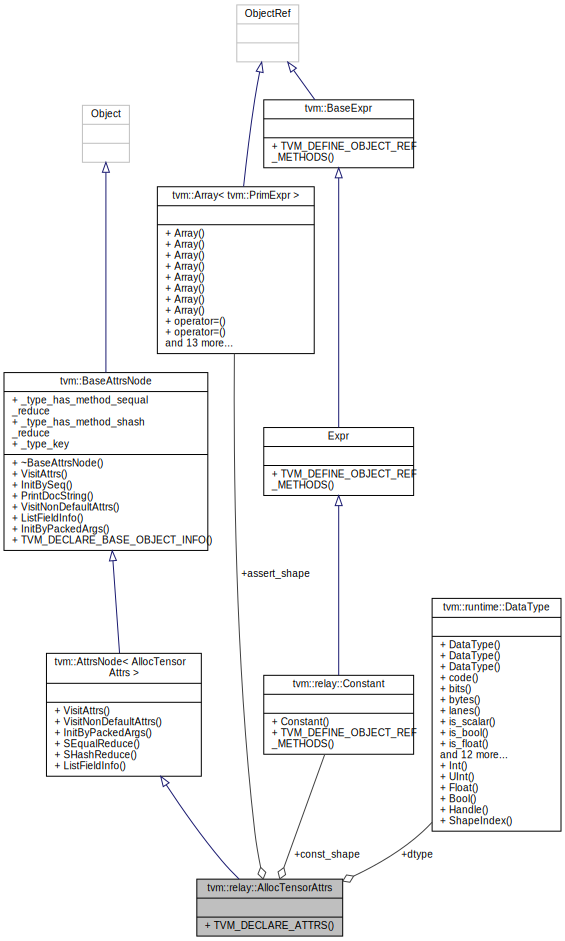
\includegraphics[height=550pt]{structtvm_1_1relay_1_1AllocTensorAttrs__coll__graph}
\end{center}
\end{figure}
\subsection*{Public Member Functions}
\begin{DoxyCompactItemize}
\item 
\hyperlink{structtvm_1_1relay_1_1AllocTensorAttrs_a28d03370b5a01db81cdfe04abe9f9324}{T\+V\+M\+\_\+\+D\+E\+C\+L\+A\+R\+E\+\_\+\+A\+T\+T\+RS} (\hyperlink{structtvm_1_1relay_1_1AllocTensorAttrs}{Alloc\+Tensor\+Attrs},\char`\"{}relay.\+attrs.\+Alloc\+Tensor\+Attrs\char`\"{})
\end{DoxyCompactItemize}
\subsection*{Public Attributes}
\begin{DoxyCompactItemize}
\item 
\hyperlink{classtvm_1_1relay_1_1Constant}{Constant} \hyperlink{structtvm_1_1relay_1_1AllocTensorAttrs_a3a6a06f96895107cce3ed17d85101cee}{const\+\_\+shape}
\item 
\hyperlink{classtvm_1_1Array}{Array}$<$ \hyperlink{namespacetvm_1_1relay_ae153a27d81399fd266b8d598227764c4}{Index\+Expr} $>$ \hyperlink{structtvm_1_1relay_1_1AllocTensorAttrs_a5ebde62563fb62eefed70239e8a9c818}{assert\+\_\+shape}
\item 
\hyperlink{namespacetvm_a41918af1a1dc386388639a9d3ad06c5d}{Data\+Type} \hyperlink{structtvm_1_1relay_1_1AllocTensorAttrs_a9fd9cdd454c3b0d3d2bf232d22222744}{dtype}
\end{DoxyCompactItemize}
\subsection*{Additional Inherited Members}


\subsection{Detailed Description}
Options for allocating tensors. 

\subsection{Member Function Documentation}
\index{tvm\+::relay\+::\+Alloc\+Tensor\+Attrs@{tvm\+::relay\+::\+Alloc\+Tensor\+Attrs}!T\+V\+M\+\_\+\+D\+E\+C\+L\+A\+R\+E\+\_\+\+A\+T\+T\+RS@{T\+V\+M\+\_\+\+D\+E\+C\+L\+A\+R\+E\+\_\+\+A\+T\+T\+RS}}
\index{T\+V\+M\+\_\+\+D\+E\+C\+L\+A\+R\+E\+\_\+\+A\+T\+T\+RS@{T\+V\+M\+\_\+\+D\+E\+C\+L\+A\+R\+E\+\_\+\+A\+T\+T\+RS}!tvm\+::relay\+::\+Alloc\+Tensor\+Attrs@{tvm\+::relay\+::\+Alloc\+Tensor\+Attrs}}
\subsubsection[{\texorpdfstring{T\+V\+M\+\_\+\+D\+E\+C\+L\+A\+R\+E\+\_\+\+A\+T\+T\+R\+S(\+Alloc\+Tensor\+Attrs,""relay.\+attrs.\+Alloc\+Tensor\+Attrs"")}{TVM_DECLARE_ATTRS(AllocTensorAttrs,"relay.attrs.AllocTensorAttrs")}}]{\setlength{\rightskip}{0pt plus 5cm}tvm\+::relay\+::\+Alloc\+Tensor\+Attrs\+::\+T\+V\+M\+\_\+\+D\+E\+C\+L\+A\+R\+E\+\_\+\+A\+T\+T\+RS (
\begin{DoxyParamCaption}
\item[{{\bf Alloc\+Tensor\+Attrs}}]{, }
\item[{\char`\"{}relay.\+attrs.\+Alloc\+Tensor\+Attrs\char`\"{}}]{}
\end{DoxyParamCaption}
)\hspace{0.3cm}{\ttfamily [inline]}}\hypertarget{structtvm_1_1relay_1_1AllocTensorAttrs_a28d03370b5a01db81cdfe04abe9f9324}{}\label{structtvm_1_1relay_1_1AllocTensorAttrs_a28d03370b5a01db81cdfe04abe9f9324}


\subsection{Member Data Documentation}
\index{tvm\+::relay\+::\+Alloc\+Tensor\+Attrs@{tvm\+::relay\+::\+Alloc\+Tensor\+Attrs}!assert\+\_\+shape@{assert\+\_\+shape}}
\index{assert\+\_\+shape@{assert\+\_\+shape}!tvm\+::relay\+::\+Alloc\+Tensor\+Attrs@{tvm\+::relay\+::\+Alloc\+Tensor\+Attrs}}
\subsubsection[{\texorpdfstring{assert\+\_\+shape}{assert_shape}}]{\setlength{\rightskip}{0pt plus 5cm}{\bf Array}$<${\bf Index\+Expr}$>$ tvm\+::relay\+::\+Alloc\+Tensor\+Attrs\+::assert\+\_\+shape}\hypertarget{structtvm_1_1relay_1_1AllocTensorAttrs_a5ebde62563fb62eefed70239e8a9c818}{}\label{structtvm_1_1relay_1_1AllocTensorAttrs_a5ebde62563fb62eefed70239e8a9c818}
\index{tvm\+::relay\+::\+Alloc\+Tensor\+Attrs@{tvm\+::relay\+::\+Alloc\+Tensor\+Attrs}!const\+\_\+shape@{const\+\_\+shape}}
\index{const\+\_\+shape@{const\+\_\+shape}!tvm\+::relay\+::\+Alloc\+Tensor\+Attrs@{tvm\+::relay\+::\+Alloc\+Tensor\+Attrs}}
\subsubsection[{\texorpdfstring{const\+\_\+shape}{const_shape}}]{\setlength{\rightskip}{0pt plus 5cm}{\bf Constant} tvm\+::relay\+::\+Alloc\+Tensor\+Attrs\+::const\+\_\+shape}\hypertarget{structtvm_1_1relay_1_1AllocTensorAttrs_a3a6a06f96895107cce3ed17d85101cee}{}\label{structtvm_1_1relay_1_1AllocTensorAttrs_a3a6a06f96895107cce3ed17d85101cee}
\index{tvm\+::relay\+::\+Alloc\+Tensor\+Attrs@{tvm\+::relay\+::\+Alloc\+Tensor\+Attrs}!dtype@{dtype}}
\index{dtype@{dtype}!tvm\+::relay\+::\+Alloc\+Tensor\+Attrs@{tvm\+::relay\+::\+Alloc\+Tensor\+Attrs}}
\subsubsection[{\texorpdfstring{dtype}{dtype}}]{\setlength{\rightskip}{0pt plus 5cm}{\bf Data\+Type} tvm\+::relay\+::\+Alloc\+Tensor\+Attrs\+::dtype}\hypertarget{structtvm_1_1relay_1_1AllocTensorAttrs_a9fd9cdd454c3b0d3d2bf232d22222744}{}\label{structtvm_1_1relay_1_1AllocTensorAttrs_a9fd9cdd454c3b0d3d2bf232d22222744}


The documentation for this struct was generated from the following file\+:\begin{DoxyCompactItemize}
\item 
include/tvm/relay/attrs/\hyperlink{relay_2attrs_2memory_8h}{memory.\+h}\end{DoxyCompactItemize}

\hypertarget{classtvm_1_1arith_1_1Analyzer}{}\section{tvm\+:\+:arith\+:\+:Analyzer Class Reference}
\label{classtvm_1_1arith_1_1Analyzer}\index{tvm\+::arith\+::\+Analyzer@{tvm\+::arith\+::\+Analyzer}}


\hyperlink{classtvm_1_1arith_1_1Analyzer}{Analyzer} that contains bunch of sub-\/analyzers.  




{\ttfamily \#include $<$analyzer.\+h$>$}



Collaboration diagram for tvm\+:\+:arith\+:\+:Analyzer\+:
\nopagebreak
\begin{figure}[H]
\begin{center}
\leavevmode
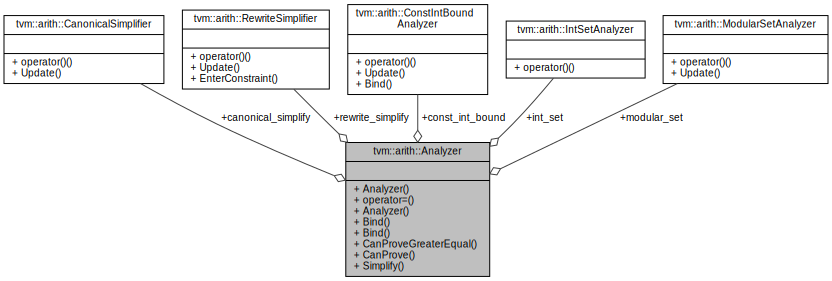
\includegraphics[width=350pt]{classtvm_1_1arith_1_1Analyzer__coll__graph}
\end{center}
\end{figure}
\subsection*{Public Member Functions}
\begin{DoxyCompactItemize}
\item 
\hyperlink{classtvm_1_1arith_1_1Analyzer_af33491068003d13952289cd296ba63af}{Analyzer} (const \hyperlink{classtvm_1_1arith_1_1Analyzer}{Analyzer} \&)=delete
\item 
\hyperlink{classtvm_1_1arith_1_1Analyzer}{Analyzer} \& \hyperlink{classtvm_1_1arith_1_1Analyzer_a9dccc7d98b8b9465390e10436d3a9178}{operator=} (const \hyperlink{classtvm_1_1arith_1_1Analyzer}{Analyzer} \&)=delete
\item 
\hyperlink{classtvm_1_1arith_1_1Analyzer_ae8568eeee02c68849e468f8c19a2701d}{Analyzer} ()
\begin{DoxyCompactList}\small\item\em constructor \end{DoxyCompactList}\item 
void \hyperlink{classtvm_1_1arith_1_1Analyzer_a509393e0c96c4455d26dd2d737ba2251}{Bind} (const Var \&var, const \hyperlink{classtvm_1_1PrimExpr}{Prim\+Expr} \&expr)
\begin{DoxyCompactList}\small\item\em Notify all the sub-\/analyzers that var is created and binded to expr. \end{DoxyCompactList}\item 
void \hyperlink{classtvm_1_1arith_1_1Analyzer_ae24b097cad6d18e00eafa6a2a36d9712}{Bind} (const Var \&var, const \hyperlink{classtvm_1_1Range}{Range} \&range)
\begin{DoxyCompactList}\small\item\em Notify all the sub-\/analyzers that var is created and binded to a range. \end{DoxyCompactList}\item 
bool \hyperlink{classtvm_1_1arith_1_1Analyzer_a5e97e3abc176f85a5b8e5d0d1cb9f5e1}{Can\+Prove\+Greater\+Equal} (const \hyperlink{classtvm_1_1PrimExpr}{Prim\+Expr} \&expr, int64\+\_\+t lower\+\_\+bound)
\begin{DoxyCompactList}\small\item\em Whether can we prove expr $>$= val. \end{DoxyCompactList}\item 
bool \hyperlink{classtvm_1_1arith_1_1Analyzer_af84b3978b1df3b2680fb47818e5dc30d}{Can\+Prove} (const \hyperlink{classtvm_1_1PrimExpr}{Prim\+Expr} \&cond)
\begin{DoxyCompactList}\small\item\em Whether can we prove condition. \end{DoxyCompactList}\item 
\hyperlink{classtvm_1_1PrimExpr}{Prim\+Expr} \hyperlink{classtvm_1_1arith_1_1Analyzer_a2d2bda00f4b06ae8b9fc7bc1cd5b0020}{Simplify} (const \hyperlink{classtvm_1_1PrimExpr}{Prim\+Expr} \&expr)
\begin{DoxyCompactList}\small\item\em Simplify expr. \end{DoxyCompactList}\end{DoxyCompactItemize}
\subsection*{Public Attributes}
\begin{DoxyCompactItemize}
\item 
\hyperlink{classtvm_1_1arith_1_1ConstIntBoundAnalyzer}{Const\+Int\+Bound\+Analyzer} \hyperlink{classtvm_1_1arith_1_1Analyzer_a435eba3ac3a839d3c53b74acfdc10146}{const\+\_\+int\+\_\+bound}
\begin{DoxyCompactList}\small\item\em sub-\/analyzer\+: const integer bound \end{DoxyCompactList}\item 
\hyperlink{classtvm_1_1arith_1_1ModularSetAnalyzer}{Modular\+Set\+Analyzer} \hyperlink{classtvm_1_1arith_1_1Analyzer_acac92a9522deabe289fea99efbd9eaec}{modular\+\_\+set}
\begin{DoxyCompactList}\small\item\em sub-\/analyzer\+: modular set \end{DoxyCompactList}\item 
\hyperlink{classtvm_1_1arith_1_1RewriteSimplifier}{Rewrite\+Simplifier} \hyperlink{classtvm_1_1arith_1_1Analyzer_acc86c6e8c04cb0de4ff9d78e769924b2}{rewrite\+\_\+simplify}
\begin{DoxyCompactList}\small\item\em sub-\/analyzer rewrite simplify \end{DoxyCompactList}\item 
\hyperlink{classtvm_1_1arith_1_1CanonicalSimplifier}{Canonical\+Simplifier} \hyperlink{classtvm_1_1arith_1_1Analyzer_a6cdf29adeceaa20b8c3dd7c26b92cd00}{canonical\+\_\+simplify}
\begin{DoxyCompactList}\small\item\em sub-\/analyzer canonical simplify \end{DoxyCompactList}\item 
\hyperlink{classtvm_1_1arith_1_1IntSetAnalyzer}{Int\+Set\+Analyzer} \hyperlink{classtvm_1_1arith_1_1Analyzer_a0d054ea2ea5b7e99f0883c00672ec831}{int\+\_\+set}
\begin{DoxyCompactList}\small\item\em sub-\/analyzer\+: int set \end{DoxyCompactList}\end{DoxyCompactItemize}


\subsection{Detailed Description}
\hyperlink{classtvm_1_1arith_1_1Analyzer}{Analyzer} that contains bunch of sub-\/analyzers. 

Each sub-\/analyzer can make use of another sub-\/analyzer by weak reference of this.

N\+O\+TE for sub-\/analyzer developers\+: If the analyzer uses memoization, we need to clear the internal cache when information about a Var has been overridden. 

\subsection{Constructor \& Destructor Documentation}
\index{tvm\+::arith\+::\+Analyzer@{tvm\+::arith\+::\+Analyzer}!Analyzer@{Analyzer}}
\index{Analyzer@{Analyzer}!tvm\+::arith\+::\+Analyzer@{tvm\+::arith\+::\+Analyzer}}
\subsubsection[{\texorpdfstring{Analyzer(const Analyzer \&)=delete}{Analyzer(const Analyzer &)=delete}}]{\setlength{\rightskip}{0pt plus 5cm}tvm\+::arith\+::\+Analyzer\+::\+Analyzer (
\begin{DoxyParamCaption}
\item[{const {\bf Analyzer} \&}]{}
\end{DoxyParamCaption}
)\hspace{0.3cm}{\ttfamily [delete]}}\hypertarget{classtvm_1_1arith_1_1Analyzer_af33491068003d13952289cd296ba63af}{}\label{classtvm_1_1arith_1_1Analyzer_af33491068003d13952289cd296ba63af}
\index{tvm\+::arith\+::\+Analyzer@{tvm\+::arith\+::\+Analyzer}!Analyzer@{Analyzer}}
\index{Analyzer@{Analyzer}!tvm\+::arith\+::\+Analyzer@{tvm\+::arith\+::\+Analyzer}}
\subsubsection[{\texorpdfstring{Analyzer()}{Analyzer()}}]{\setlength{\rightskip}{0pt plus 5cm}tvm\+::arith\+::\+Analyzer\+::\+Analyzer (
\begin{DoxyParamCaption}
{}
\end{DoxyParamCaption}
)}\hypertarget{classtvm_1_1arith_1_1Analyzer_ae8568eeee02c68849e468f8c19a2701d}{}\label{classtvm_1_1arith_1_1Analyzer_ae8568eeee02c68849e468f8c19a2701d}


constructor 



\subsection{Member Function Documentation}
\index{tvm\+::arith\+::\+Analyzer@{tvm\+::arith\+::\+Analyzer}!Bind@{Bind}}
\index{Bind@{Bind}!tvm\+::arith\+::\+Analyzer@{tvm\+::arith\+::\+Analyzer}}
\subsubsection[{\texorpdfstring{Bind(const Var \&var, const Prim\+Expr \&expr)}{Bind(const Var &var, const PrimExpr &expr)}}]{\setlength{\rightskip}{0pt plus 5cm}void tvm\+::arith\+::\+Analyzer\+::\+Bind (
\begin{DoxyParamCaption}
\item[{const Var \&}]{var, }
\item[{const {\bf Prim\+Expr} \&}]{expr}
\end{DoxyParamCaption}
)}\hypertarget{classtvm_1_1arith_1_1Analyzer_a509393e0c96c4455d26dd2d737ba2251}{}\label{classtvm_1_1arith_1_1Analyzer_a509393e0c96c4455d26dd2d737ba2251}


Notify all the sub-\/analyzers that var is created and binded to expr. 

Each var can only be binded once.


\begin{DoxyParams}{Parameters}
{\em var} & The variable. \\
\hline
{\em expr} & The expression we bind to. \\
\hline
\end{DoxyParams}
\index{tvm\+::arith\+::\+Analyzer@{tvm\+::arith\+::\+Analyzer}!Bind@{Bind}}
\index{Bind@{Bind}!tvm\+::arith\+::\+Analyzer@{tvm\+::arith\+::\+Analyzer}}
\subsubsection[{\texorpdfstring{Bind(const Var \&var, const Range \&range)}{Bind(const Var &var, const Range &range)}}]{\setlength{\rightskip}{0pt plus 5cm}void tvm\+::arith\+::\+Analyzer\+::\+Bind (
\begin{DoxyParamCaption}
\item[{const Var \&}]{var, }
\item[{const {\bf Range} \&}]{range}
\end{DoxyParamCaption}
)}\hypertarget{classtvm_1_1arith_1_1Analyzer_ae24b097cad6d18e00eafa6a2a36d9712}{}\label{classtvm_1_1arith_1_1Analyzer_ae24b097cad6d18e00eafa6a2a36d9712}


Notify all the sub-\/analyzers that var is created and binded to a range. 

Each var can only be binded once.


\begin{DoxyParams}{Parameters}
{\em var} & The variable. \\
\hline
{\em range} & The range we bind to. \\
\hline
\end{DoxyParams}
\index{tvm\+::arith\+::\+Analyzer@{tvm\+::arith\+::\+Analyzer}!Can\+Prove@{Can\+Prove}}
\index{Can\+Prove@{Can\+Prove}!tvm\+::arith\+::\+Analyzer@{tvm\+::arith\+::\+Analyzer}}
\subsubsection[{\texorpdfstring{Can\+Prove(const Prim\+Expr \&cond)}{CanProve(const PrimExpr &cond)}}]{\setlength{\rightskip}{0pt plus 5cm}bool tvm\+::arith\+::\+Analyzer\+::\+Can\+Prove (
\begin{DoxyParamCaption}
\item[{const {\bf Prim\+Expr} \&}]{cond}
\end{DoxyParamCaption}
)}\hypertarget{classtvm_1_1arith_1_1Analyzer_af84b3978b1df3b2680fb47818e5dc30d}{}\label{classtvm_1_1arith_1_1Analyzer_af84b3978b1df3b2680fb47818e5dc30d}


Whether can we prove condition. 


\begin{DoxyParams}{Parameters}
{\em cond} & The expression to be proved. \\
\hline
\end{DoxyParams}
\begin{DoxyReturn}{Returns}
The result.
\end{DoxyReturn}
\begin{DoxyNote}{Note}
\hyperlink{classtvm_1_1arith_1_1Analyzer}{Analyzer} will call into sub-\/analyzers to get the result. 
\end{DoxyNote}
\index{tvm\+::arith\+::\+Analyzer@{tvm\+::arith\+::\+Analyzer}!Can\+Prove\+Greater\+Equal@{Can\+Prove\+Greater\+Equal}}
\index{Can\+Prove\+Greater\+Equal@{Can\+Prove\+Greater\+Equal}!tvm\+::arith\+::\+Analyzer@{tvm\+::arith\+::\+Analyzer}}
\subsubsection[{\texorpdfstring{Can\+Prove\+Greater\+Equal(const Prim\+Expr \&expr, int64\+\_\+t lower\+\_\+bound)}{CanProveGreaterEqual(const PrimExpr &expr, int64_t lower_bound)}}]{\setlength{\rightskip}{0pt plus 5cm}bool tvm\+::arith\+::\+Analyzer\+::\+Can\+Prove\+Greater\+Equal (
\begin{DoxyParamCaption}
\item[{const {\bf Prim\+Expr} \&}]{expr, }
\item[{int64\+\_\+t}]{lower\+\_\+bound}
\end{DoxyParamCaption}
)}\hypertarget{classtvm_1_1arith_1_1Analyzer_a5e97e3abc176f85a5b8e5d0d1cb9f5e1}{}\label{classtvm_1_1arith_1_1Analyzer_a5e97e3abc176f85a5b8e5d0d1cb9f5e1}


Whether can we prove expr $>$= val. 

Non-\/negative proof is very useful in integer analysis to lower divisions and mods given difference in trunc and ceil mode.


\begin{DoxyParams}{Parameters}
{\em expr} & The expression. \\
\hline
{\em lower\+\_\+bound} & The lower bound. \\
\hline
\end{DoxyParams}
\begin{DoxyReturn}{Returns}
Whether we can prove it.
\end{DoxyReturn}
\begin{DoxyNote}{Note}
\hyperlink{classtvm_1_1arith_1_1Analyzer}{Analyzer} will call into sub-\/analyzers to get the result. 
\end{DoxyNote}
\index{tvm\+::arith\+::\+Analyzer@{tvm\+::arith\+::\+Analyzer}!operator=@{operator=}}
\index{operator=@{operator=}!tvm\+::arith\+::\+Analyzer@{tvm\+::arith\+::\+Analyzer}}
\subsubsection[{\texorpdfstring{operator=(const Analyzer \&)=delete}{operator=(const Analyzer &)=delete}}]{\setlength{\rightskip}{0pt plus 5cm}{\bf Analyzer}\& tvm\+::arith\+::\+Analyzer\+::operator= (
\begin{DoxyParamCaption}
\item[{const {\bf Analyzer} \&}]{}
\end{DoxyParamCaption}
)\hspace{0.3cm}{\ttfamily [delete]}}\hypertarget{classtvm_1_1arith_1_1Analyzer_a9dccc7d98b8b9465390e10436d3a9178}{}\label{classtvm_1_1arith_1_1Analyzer_a9dccc7d98b8b9465390e10436d3a9178}
\index{tvm\+::arith\+::\+Analyzer@{tvm\+::arith\+::\+Analyzer}!Simplify@{Simplify}}
\index{Simplify@{Simplify}!tvm\+::arith\+::\+Analyzer@{tvm\+::arith\+::\+Analyzer}}
\subsubsection[{\texorpdfstring{Simplify(const Prim\+Expr \&expr)}{Simplify(const PrimExpr &expr)}}]{\setlength{\rightskip}{0pt plus 5cm}{\bf Prim\+Expr} tvm\+::arith\+::\+Analyzer\+::\+Simplify (
\begin{DoxyParamCaption}
\item[{const {\bf Prim\+Expr} \&}]{expr}
\end{DoxyParamCaption}
)}\hypertarget{classtvm_1_1arith_1_1Analyzer_a2d2bda00f4b06ae8b9fc7bc1cd5b0020}{}\label{classtvm_1_1arith_1_1Analyzer_a2d2bda00f4b06ae8b9fc7bc1cd5b0020}


Simplify expr. 


\begin{DoxyParams}{Parameters}
{\em expr} & The expression to be simplified. \\
\hline
\end{DoxyParams}
\begin{DoxyReturn}{Returns}
The result.
\end{DoxyReturn}
\begin{DoxyNote}{Note}
\hyperlink{classtvm_1_1arith_1_1Analyzer}{Analyzer} will call into sub-\/analyzers to get the result. 
\end{DoxyNote}


\subsection{Member Data Documentation}
\index{tvm\+::arith\+::\+Analyzer@{tvm\+::arith\+::\+Analyzer}!canonical\+\_\+simplify@{canonical\+\_\+simplify}}
\index{canonical\+\_\+simplify@{canonical\+\_\+simplify}!tvm\+::arith\+::\+Analyzer@{tvm\+::arith\+::\+Analyzer}}
\subsubsection[{\texorpdfstring{canonical\+\_\+simplify}{canonical_simplify}}]{\setlength{\rightskip}{0pt plus 5cm}{\bf Canonical\+Simplifier} tvm\+::arith\+::\+Analyzer\+::canonical\+\_\+simplify}\hypertarget{classtvm_1_1arith_1_1Analyzer_a6cdf29adeceaa20b8c3dd7c26b92cd00}{}\label{classtvm_1_1arith_1_1Analyzer_a6cdf29adeceaa20b8c3dd7c26b92cd00}


sub-\/analyzer canonical simplify 

\index{tvm\+::arith\+::\+Analyzer@{tvm\+::arith\+::\+Analyzer}!const\+\_\+int\+\_\+bound@{const\+\_\+int\+\_\+bound}}
\index{const\+\_\+int\+\_\+bound@{const\+\_\+int\+\_\+bound}!tvm\+::arith\+::\+Analyzer@{tvm\+::arith\+::\+Analyzer}}
\subsubsection[{\texorpdfstring{const\+\_\+int\+\_\+bound}{const_int_bound}}]{\setlength{\rightskip}{0pt plus 5cm}{\bf Const\+Int\+Bound\+Analyzer} tvm\+::arith\+::\+Analyzer\+::const\+\_\+int\+\_\+bound}\hypertarget{classtvm_1_1arith_1_1Analyzer_a435eba3ac3a839d3c53b74acfdc10146}{}\label{classtvm_1_1arith_1_1Analyzer_a435eba3ac3a839d3c53b74acfdc10146}


sub-\/analyzer\+: const integer bound 

\index{tvm\+::arith\+::\+Analyzer@{tvm\+::arith\+::\+Analyzer}!int\+\_\+set@{int\+\_\+set}}
\index{int\+\_\+set@{int\+\_\+set}!tvm\+::arith\+::\+Analyzer@{tvm\+::arith\+::\+Analyzer}}
\subsubsection[{\texorpdfstring{int\+\_\+set}{int_set}}]{\setlength{\rightskip}{0pt plus 5cm}{\bf Int\+Set\+Analyzer} tvm\+::arith\+::\+Analyzer\+::int\+\_\+set}\hypertarget{classtvm_1_1arith_1_1Analyzer_a0d054ea2ea5b7e99f0883c00672ec831}{}\label{classtvm_1_1arith_1_1Analyzer_a0d054ea2ea5b7e99f0883c00672ec831}


sub-\/analyzer\+: int set 

\index{tvm\+::arith\+::\+Analyzer@{tvm\+::arith\+::\+Analyzer}!modular\+\_\+set@{modular\+\_\+set}}
\index{modular\+\_\+set@{modular\+\_\+set}!tvm\+::arith\+::\+Analyzer@{tvm\+::arith\+::\+Analyzer}}
\subsubsection[{\texorpdfstring{modular\+\_\+set}{modular_set}}]{\setlength{\rightskip}{0pt plus 5cm}{\bf Modular\+Set\+Analyzer} tvm\+::arith\+::\+Analyzer\+::modular\+\_\+set}\hypertarget{classtvm_1_1arith_1_1Analyzer_acac92a9522deabe289fea99efbd9eaec}{}\label{classtvm_1_1arith_1_1Analyzer_acac92a9522deabe289fea99efbd9eaec}


sub-\/analyzer\+: modular set 

\index{tvm\+::arith\+::\+Analyzer@{tvm\+::arith\+::\+Analyzer}!rewrite\+\_\+simplify@{rewrite\+\_\+simplify}}
\index{rewrite\+\_\+simplify@{rewrite\+\_\+simplify}!tvm\+::arith\+::\+Analyzer@{tvm\+::arith\+::\+Analyzer}}
\subsubsection[{\texorpdfstring{rewrite\+\_\+simplify}{rewrite_simplify}}]{\setlength{\rightskip}{0pt plus 5cm}{\bf Rewrite\+Simplifier} tvm\+::arith\+::\+Analyzer\+::rewrite\+\_\+simplify}\hypertarget{classtvm_1_1arith_1_1Analyzer_acc86c6e8c04cb0de4ff9d78e769924b2}{}\label{classtvm_1_1arith_1_1Analyzer_acc86c6e8c04cb0de4ff9d78e769924b2}


sub-\/analyzer rewrite simplify 



The documentation for this class was generated from the following file\+:\begin{DoxyCompactItemize}
\item 
include/tvm/arith/\hyperlink{analyzer_8h}{analyzer.\+h}\end{DoxyCompactItemize}

\hypertarget{classtvm_1_1tir_1_1AndNode}{}\section{tvm\+:\+:tir\+:\+:And\+Node Class Reference}
\label{classtvm_1_1tir_1_1AndNode}\index{tvm\+::tir\+::\+And\+Node@{tvm\+::tir\+::\+And\+Node}}


a \&\& b  




{\ttfamily \#include $<$expr.\+h$>$}



Inheritance diagram for tvm\+:\+:tir\+:\+:And\+Node\+:
\nopagebreak
\begin{figure}[H]
\begin{center}
\leavevmode
\includegraphics[width=285pt]{classtvm_1_1tir_1_1AndNode__inherit__graph}
\end{center}
\end{figure}


Collaboration diagram for tvm\+:\+:tir\+:\+:And\+Node\+:
\nopagebreak
\begin{figure}[H]
\begin{center}
\leavevmode
\includegraphics[width=350pt]{classtvm_1_1tir_1_1AndNode__coll__graph}
\end{center}
\end{figure}
\subsection*{Public Member Functions}
\begin{DoxyCompactItemize}
\item 
void \hyperlink{classtvm_1_1tir_1_1AndNode_adf187d7ceeb6b8bfbf1be89960bcad59}{Visit\+Attrs} (\hyperlink{classtvm_1_1AttrVisitor}{Attr\+Visitor} $\ast$v)
\item 
bool \hyperlink{classtvm_1_1tir_1_1AndNode_ab71a4464565cd373ab8a3b7d9de7dc91}{S\+Equal\+Reduce} (const \hyperlink{classtvm_1_1tir_1_1AndNode}{And\+Node} $\ast$other, \hyperlink{classtvm_1_1SEqualReducer}{S\+Equal\+Reducer} equal) const 
\item 
void \hyperlink{classtvm_1_1tir_1_1AndNode_a25c6bb2f6fa5bd4cbbdcc665bf44d81e}{S\+Hash\+Reduce} (\hyperlink{classtvm_1_1SHashReducer}{S\+Hash\+Reducer} hash\+\_\+reduce) const 
\item 
\hyperlink{classtvm_1_1tir_1_1AndNode_ae9c3ec1961240717c9bcff2db57ef711}{T\+V\+M\+\_\+\+D\+E\+C\+L\+A\+R\+E\+\_\+\+F\+I\+N\+A\+L\+\_\+\+O\+B\+J\+E\+C\+T\+\_\+\+I\+N\+FO} (\hyperlink{classtvm_1_1tir_1_1AndNode}{And\+Node}, \hyperlink{classtvm_1_1PrimExprNode}{Prim\+Expr\+Node})
\end{DoxyCompactItemize}
\subsection*{Static Public Member Functions}
\begin{DoxyCompactItemize}
\item 
static \hyperlink{classtvm_1_1PrimExpr}{Prim\+Expr} \hyperlink{classtvm_1_1tir_1_1AndNode_aeb51390ed2566af9393d94d915e56d50}{make} (\hyperlink{classtvm_1_1PrimExpr}{Prim\+Expr} \hyperlink{classtvm_1_1tir_1_1AndNode_a4a9b2cf4384567cf6719a4766a679738}{a}, \hyperlink{classtvm_1_1PrimExpr}{Prim\+Expr} \hyperlink{classtvm_1_1tir_1_1AndNode_a9e1e2e65410c1c3ed43538f475f23d83}{b})
\end{DoxyCompactItemize}
\subsection*{Public Attributes}
\begin{DoxyCompactItemize}
\item 
\hyperlink{classtvm_1_1PrimExpr}{Prim\+Expr} \hyperlink{classtvm_1_1tir_1_1AndNode_a4a9b2cf4384567cf6719a4766a679738}{a}
\begin{DoxyCompactList}\small\item\em The left operand. \end{DoxyCompactList}\item 
\hyperlink{classtvm_1_1PrimExpr}{Prim\+Expr} \hyperlink{classtvm_1_1tir_1_1AndNode_a9e1e2e65410c1c3ed43538f475f23d83}{b}
\begin{DoxyCompactList}\small\item\em The right operand. \end{DoxyCompactList}\end{DoxyCompactItemize}
\subsection*{Static Public Attributes}
\begin{DoxyCompactItemize}
\item 
static constexpr const char $\ast$ \hyperlink{classtvm_1_1tir_1_1AndNode_a6ea58bbd932087818ed84621065d73a0}{\+\_\+type\+\_\+key} = \char`\"{}And\char`\"{}
\end{DoxyCompactItemize}


\subsection{Detailed Description}
a \&\& b 

\subsection{Member Function Documentation}
\index{tvm\+::tir\+::\+And\+Node@{tvm\+::tir\+::\+And\+Node}!make@{make}}
\index{make@{make}!tvm\+::tir\+::\+And\+Node@{tvm\+::tir\+::\+And\+Node}}
\subsubsection[{\texorpdfstring{make(\+Prim\+Expr a, Prim\+Expr b)}{make(PrimExpr a, PrimExpr b)}}]{\setlength{\rightskip}{0pt plus 5cm}static {\bf Prim\+Expr} tvm\+::tir\+::\+And\+Node\+::make (
\begin{DoxyParamCaption}
\item[{{\bf Prim\+Expr}}]{a, }
\item[{{\bf Prim\+Expr}}]{b}
\end{DoxyParamCaption}
)\hspace{0.3cm}{\ttfamily [static]}}\hypertarget{classtvm_1_1tir_1_1AndNode_aeb51390ed2566af9393d94d915e56d50}{}\label{classtvm_1_1tir_1_1AndNode_aeb51390ed2566af9393d94d915e56d50}
\index{tvm\+::tir\+::\+And\+Node@{tvm\+::tir\+::\+And\+Node}!S\+Equal\+Reduce@{S\+Equal\+Reduce}}
\index{S\+Equal\+Reduce@{S\+Equal\+Reduce}!tvm\+::tir\+::\+And\+Node@{tvm\+::tir\+::\+And\+Node}}
\subsubsection[{\texorpdfstring{S\+Equal\+Reduce(const And\+Node $\ast$other, S\+Equal\+Reducer equal) const }{SEqualReduce(const AndNode *other, SEqualReducer equal) const }}]{\setlength{\rightskip}{0pt plus 5cm}bool tvm\+::tir\+::\+And\+Node\+::\+S\+Equal\+Reduce (
\begin{DoxyParamCaption}
\item[{const {\bf And\+Node} $\ast$}]{other, }
\item[{{\bf S\+Equal\+Reducer}}]{equal}
\end{DoxyParamCaption}
) const\hspace{0.3cm}{\ttfamily [inline]}}\hypertarget{classtvm_1_1tir_1_1AndNode_ab71a4464565cd373ab8a3b7d9de7dc91}{}\label{classtvm_1_1tir_1_1AndNode_ab71a4464565cd373ab8a3b7d9de7dc91}
\index{tvm\+::tir\+::\+And\+Node@{tvm\+::tir\+::\+And\+Node}!S\+Hash\+Reduce@{S\+Hash\+Reduce}}
\index{S\+Hash\+Reduce@{S\+Hash\+Reduce}!tvm\+::tir\+::\+And\+Node@{tvm\+::tir\+::\+And\+Node}}
\subsubsection[{\texorpdfstring{S\+Hash\+Reduce(\+S\+Hash\+Reducer hash\+\_\+reduce) const }{SHashReduce(SHashReducer hash_reduce) const }}]{\setlength{\rightskip}{0pt plus 5cm}void tvm\+::tir\+::\+And\+Node\+::\+S\+Hash\+Reduce (
\begin{DoxyParamCaption}
\item[{{\bf S\+Hash\+Reducer}}]{hash\+\_\+reduce}
\end{DoxyParamCaption}
) const\hspace{0.3cm}{\ttfamily [inline]}}\hypertarget{classtvm_1_1tir_1_1AndNode_a25c6bb2f6fa5bd4cbbdcc665bf44d81e}{}\label{classtvm_1_1tir_1_1AndNode_a25c6bb2f6fa5bd4cbbdcc665bf44d81e}
\index{tvm\+::tir\+::\+And\+Node@{tvm\+::tir\+::\+And\+Node}!T\+V\+M\+\_\+\+D\+E\+C\+L\+A\+R\+E\+\_\+\+F\+I\+N\+A\+L\+\_\+\+O\+B\+J\+E\+C\+T\+\_\+\+I\+N\+FO@{T\+V\+M\+\_\+\+D\+E\+C\+L\+A\+R\+E\+\_\+\+F\+I\+N\+A\+L\+\_\+\+O\+B\+J\+E\+C\+T\+\_\+\+I\+N\+FO}}
\index{T\+V\+M\+\_\+\+D\+E\+C\+L\+A\+R\+E\+\_\+\+F\+I\+N\+A\+L\+\_\+\+O\+B\+J\+E\+C\+T\+\_\+\+I\+N\+FO@{T\+V\+M\+\_\+\+D\+E\+C\+L\+A\+R\+E\+\_\+\+F\+I\+N\+A\+L\+\_\+\+O\+B\+J\+E\+C\+T\+\_\+\+I\+N\+FO}!tvm\+::tir\+::\+And\+Node@{tvm\+::tir\+::\+And\+Node}}
\subsubsection[{\texorpdfstring{T\+V\+M\+\_\+\+D\+E\+C\+L\+A\+R\+E\+\_\+\+F\+I\+N\+A\+L\+\_\+\+O\+B\+J\+E\+C\+T\+\_\+\+I\+N\+F\+O(\+And\+Node, Prim\+Expr\+Node)}{TVM_DECLARE_FINAL_OBJECT_INFO(AndNode, PrimExprNode)}}]{\setlength{\rightskip}{0pt plus 5cm}tvm\+::tir\+::\+And\+Node\+::\+T\+V\+M\+\_\+\+D\+E\+C\+L\+A\+R\+E\+\_\+\+F\+I\+N\+A\+L\+\_\+\+O\+B\+J\+E\+C\+T\+\_\+\+I\+N\+FO (
\begin{DoxyParamCaption}
\item[{{\bf And\+Node}}]{, }
\item[{{\bf Prim\+Expr\+Node}}]{}
\end{DoxyParamCaption}
)}\hypertarget{classtvm_1_1tir_1_1AndNode_ae9c3ec1961240717c9bcff2db57ef711}{}\label{classtvm_1_1tir_1_1AndNode_ae9c3ec1961240717c9bcff2db57ef711}
\index{tvm\+::tir\+::\+And\+Node@{tvm\+::tir\+::\+And\+Node}!Visit\+Attrs@{Visit\+Attrs}}
\index{Visit\+Attrs@{Visit\+Attrs}!tvm\+::tir\+::\+And\+Node@{tvm\+::tir\+::\+And\+Node}}
\subsubsection[{\texorpdfstring{Visit\+Attrs(\+Attr\+Visitor $\ast$v)}{VisitAttrs(AttrVisitor *v)}}]{\setlength{\rightskip}{0pt plus 5cm}void tvm\+::tir\+::\+And\+Node\+::\+Visit\+Attrs (
\begin{DoxyParamCaption}
\item[{{\bf Attr\+Visitor} $\ast$}]{v}
\end{DoxyParamCaption}
)\hspace{0.3cm}{\ttfamily [inline]}}\hypertarget{classtvm_1_1tir_1_1AndNode_adf187d7ceeb6b8bfbf1be89960bcad59}{}\label{classtvm_1_1tir_1_1AndNode_adf187d7ceeb6b8bfbf1be89960bcad59}


\subsection{Member Data Documentation}
\index{tvm\+::tir\+::\+And\+Node@{tvm\+::tir\+::\+And\+Node}!\+\_\+type\+\_\+key@{\+\_\+type\+\_\+key}}
\index{\+\_\+type\+\_\+key@{\+\_\+type\+\_\+key}!tvm\+::tir\+::\+And\+Node@{tvm\+::tir\+::\+And\+Node}}
\subsubsection[{\texorpdfstring{\+\_\+type\+\_\+key}{_type_key}}]{\setlength{\rightskip}{0pt plus 5cm}constexpr const char$\ast$ tvm\+::tir\+::\+And\+Node\+::\+\_\+type\+\_\+key = \char`\"{}And\char`\"{}\hspace{0.3cm}{\ttfamily [static]}}\hypertarget{classtvm_1_1tir_1_1AndNode_a6ea58bbd932087818ed84621065d73a0}{}\label{classtvm_1_1tir_1_1AndNode_a6ea58bbd932087818ed84621065d73a0}
\index{tvm\+::tir\+::\+And\+Node@{tvm\+::tir\+::\+And\+Node}!a@{a}}
\index{a@{a}!tvm\+::tir\+::\+And\+Node@{tvm\+::tir\+::\+And\+Node}}
\subsubsection[{\texorpdfstring{a}{a}}]{\setlength{\rightskip}{0pt plus 5cm}{\bf Prim\+Expr} tvm\+::tir\+::\+And\+Node\+::a}\hypertarget{classtvm_1_1tir_1_1AndNode_a4a9b2cf4384567cf6719a4766a679738}{}\label{classtvm_1_1tir_1_1AndNode_a4a9b2cf4384567cf6719a4766a679738}


The left operand. 

\index{tvm\+::tir\+::\+And\+Node@{tvm\+::tir\+::\+And\+Node}!b@{b}}
\index{b@{b}!tvm\+::tir\+::\+And\+Node@{tvm\+::tir\+::\+And\+Node}}
\subsubsection[{\texorpdfstring{b}{b}}]{\setlength{\rightskip}{0pt plus 5cm}{\bf Prim\+Expr} tvm\+::tir\+::\+And\+Node\+::b}\hypertarget{classtvm_1_1tir_1_1AndNode_a9e1e2e65410c1c3ed43538f475f23d83}{}\label{classtvm_1_1tir_1_1AndNode_a9e1e2e65410c1c3ed43538f475f23d83}


The right operand. 



The documentation for this class was generated from the following file\+:\begin{DoxyCompactItemize}
\item 
include/tvm/tir/\hyperlink{tir_2expr_8h}{expr.\+h}\end{DoxyCompactItemize}

\hypertarget{classtvm_1_1tir_1_1AnyNode}{}\section{tvm\+:\+:tir\+:\+:Any\+Node Class Reference}
\label{classtvm_1_1tir_1_1AnyNode}\index{tvm\+::tir\+::\+Any\+Node@{tvm\+::tir\+::\+Any\+Node}}


Any shape.  




{\ttfamily \#include $<$expr.\+h$>$}



Inheritance diagram for tvm\+:\+:tir\+:\+:Any\+Node\+:
\nopagebreak
\begin{figure}[H]
\begin{center}
\leavevmode
\includegraphics[width=285pt]{classtvm_1_1tir_1_1AnyNode__inherit__graph}
\end{center}
\end{figure}


Collaboration diagram for tvm\+:\+:tir\+:\+:Any\+Node\+:
\nopagebreak
\begin{figure}[H]
\begin{center}
\leavevmode
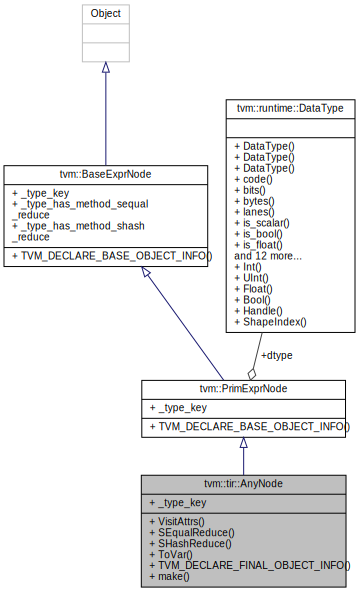
\includegraphics[width=350pt]{classtvm_1_1tir_1_1AnyNode__coll__graph}
\end{center}
\end{figure}
\subsection*{Public Member Functions}
\begin{DoxyCompactItemize}
\item 
void \hyperlink{classtvm_1_1tir_1_1AnyNode_a170f1e5715fa8999068b7c878cf84b87}{Visit\+Attrs} (\hyperlink{classtvm_1_1AttrVisitor}{Attr\+Visitor} $\ast$v)
\item 
bool \hyperlink{classtvm_1_1tir_1_1AnyNode_aa68fadf8ba8d988e769326191a87f723}{S\+Equal\+Reduce} (const \hyperlink{classtvm_1_1tir_1_1AnyNode}{Any\+Node} $\ast$other, \hyperlink{classtvm_1_1SEqualReducer}{S\+Equal\+Reducer} equal) const 
\item 
void \hyperlink{classtvm_1_1tir_1_1AnyNode_aa4619aecf23ceefa065436ad0c001cba}{S\+Hash\+Reduce} (\hyperlink{classtvm_1_1SHashReducer}{S\+Hash\+Reducer} hash\+\_\+reduce) const 
\item 
\hyperlink{classtvm_1_1tir_1_1Var}{Var} \hyperlink{classtvm_1_1tir_1_1AnyNode_ac4acdd164527dde5e3f6afe37ee4f707}{To\+Var} () const 
\begin{DoxyCompactList}\small\item\em Convert to var. \end{DoxyCompactList}\item 
\hyperlink{classtvm_1_1tir_1_1AnyNode_a259c2acee554a58fe3daaf75fa0afb4e}{T\+V\+M\+\_\+\+D\+E\+C\+L\+A\+R\+E\+\_\+\+F\+I\+N\+A\+L\+\_\+\+O\+B\+J\+E\+C\+T\+\_\+\+I\+N\+FO} (\hyperlink{classtvm_1_1tir_1_1AnyNode}{Any\+Node}, \hyperlink{classtvm_1_1PrimExprNode}{Prim\+Expr\+Node})
\end{DoxyCompactItemize}
\subsection*{Static Public Member Functions}
\begin{DoxyCompactItemize}
\item 
static \hyperlink{classtvm_1_1PrimExpr}{Prim\+Expr} \hyperlink{classtvm_1_1tir_1_1AnyNode_ac5fa74bb8d0f075ea162d2f03cdb9332}{make} ()
\end{DoxyCompactItemize}
\subsection*{Static Public Attributes}
\begin{DoxyCompactItemize}
\item 
static constexpr const char $\ast$ \hyperlink{classtvm_1_1tir_1_1AnyNode_a864f1da6e9ec91a2c6986438fb64981f}{\+\_\+type\+\_\+key} = \char`\"{}Any\char`\"{}
\end{DoxyCompactItemize}
\subsection*{Additional Inherited Members}


\subsection{Detailed Description}
Any shape. 

\subsection{Member Function Documentation}
\index{tvm\+::tir\+::\+Any\+Node@{tvm\+::tir\+::\+Any\+Node}!make@{make}}
\index{make@{make}!tvm\+::tir\+::\+Any\+Node@{tvm\+::tir\+::\+Any\+Node}}
\subsubsection[{\texorpdfstring{make()}{make()}}]{\setlength{\rightskip}{0pt plus 5cm}static {\bf Prim\+Expr} tvm\+::tir\+::\+Any\+Node\+::make (
\begin{DoxyParamCaption}
{}
\end{DoxyParamCaption}
)\hspace{0.3cm}{\ttfamily [static]}}\hypertarget{classtvm_1_1tir_1_1AnyNode_ac5fa74bb8d0f075ea162d2f03cdb9332}{}\label{classtvm_1_1tir_1_1AnyNode_ac5fa74bb8d0f075ea162d2f03cdb9332}
\index{tvm\+::tir\+::\+Any\+Node@{tvm\+::tir\+::\+Any\+Node}!S\+Equal\+Reduce@{S\+Equal\+Reduce}}
\index{S\+Equal\+Reduce@{S\+Equal\+Reduce}!tvm\+::tir\+::\+Any\+Node@{tvm\+::tir\+::\+Any\+Node}}
\subsubsection[{\texorpdfstring{S\+Equal\+Reduce(const Any\+Node $\ast$other, S\+Equal\+Reducer equal) const }{SEqualReduce(const AnyNode *other, SEqualReducer equal) const }}]{\setlength{\rightskip}{0pt plus 5cm}bool tvm\+::tir\+::\+Any\+Node\+::\+S\+Equal\+Reduce (
\begin{DoxyParamCaption}
\item[{const {\bf Any\+Node} $\ast$}]{other, }
\item[{{\bf S\+Equal\+Reducer}}]{equal}
\end{DoxyParamCaption}
) const\hspace{0.3cm}{\ttfamily [inline]}}\hypertarget{classtvm_1_1tir_1_1AnyNode_aa68fadf8ba8d988e769326191a87f723}{}\label{classtvm_1_1tir_1_1AnyNode_aa68fadf8ba8d988e769326191a87f723}
\index{tvm\+::tir\+::\+Any\+Node@{tvm\+::tir\+::\+Any\+Node}!S\+Hash\+Reduce@{S\+Hash\+Reduce}}
\index{S\+Hash\+Reduce@{S\+Hash\+Reduce}!tvm\+::tir\+::\+Any\+Node@{tvm\+::tir\+::\+Any\+Node}}
\subsubsection[{\texorpdfstring{S\+Hash\+Reduce(\+S\+Hash\+Reducer hash\+\_\+reduce) const }{SHashReduce(SHashReducer hash_reduce) const }}]{\setlength{\rightskip}{0pt plus 5cm}void tvm\+::tir\+::\+Any\+Node\+::\+S\+Hash\+Reduce (
\begin{DoxyParamCaption}
\item[{{\bf S\+Hash\+Reducer}}]{hash\+\_\+reduce}
\end{DoxyParamCaption}
) const\hspace{0.3cm}{\ttfamily [inline]}}\hypertarget{classtvm_1_1tir_1_1AnyNode_aa4619aecf23ceefa065436ad0c001cba}{}\label{classtvm_1_1tir_1_1AnyNode_aa4619aecf23ceefa065436ad0c001cba}
\index{tvm\+::tir\+::\+Any\+Node@{tvm\+::tir\+::\+Any\+Node}!To\+Var@{To\+Var}}
\index{To\+Var@{To\+Var}!tvm\+::tir\+::\+Any\+Node@{tvm\+::tir\+::\+Any\+Node}}
\subsubsection[{\texorpdfstring{To\+Var() const }{ToVar() const }}]{\setlength{\rightskip}{0pt plus 5cm}{\bf Var} tvm\+::tir\+::\+Any\+Node\+::\+To\+Var (
\begin{DoxyParamCaption}
{}
\end{DoxyParamCaption}
) const\hspace{0.3cm}{\ttfamily [inline]}}\hypertarget{classtvm_1_1tir_1_1AnyNode_ac4acdd164527dde5e3f6afe37ee4f707}{}\label{classtvm_1_1tir_1_1AnyNode_ac4acdd164527dde5e3f6afe37ee4f707}


Convert to var. 

\index{tvm\+::tir\+::\+Any\+Node@{tvm\+::tir\+::\+Any\+Node}!T\+V\+M\+\_\+\+D\+E\+C\+L\+A\+R\+E\+\_\+\+F\+I\+N\+A\+L\+\_\+\+O\+B\+J\+E\+C\+T\+\_\+\+I\+N\+FO@{T\+V\+M\+\_\+\+D\+E\+C\+L\+A\+R\+E\+\_\+\+F\+I\+N\+A\+L\+\_\+\+O\+B\+J\+E\+C\+T\+\_\+\+I\+N\+FO}}
\index{T\+V\+M\+\_\+\+D\+E\+C\+L\+A\+R\+E\+\_\+\+F\+I\+N\+A\+L\+\_\+\+O\+B\+J\+E\+C\+T\+\_\+\+I\+N\+FO@{T\+V\+M\+\_\+\+D\+E\+C\+L\+A\+R\+E\+\_\+\+F\+I\+N\+A\+L\+\_\+\+O\+B\+J\+E\+C\+T\+\_\+\+I\+N\+FO}!tvm\+::tir\+::\+Any\+Node@{tvm\+::tir\+::\+Any\+Node}}
\subsubsection[{\texorpdfstring{T\+V\+M\+\_\+\+D\+E\+C\+L\+A\+R\+E\+\_\+\+F\+I\+N\+A\+L\+\_\+\+O\+B\+J\+E\+C\+T\+\_\+\+I\+N\+F\+O(\+Any\+Node, Prim\+Expr\+Node)}{TVM_DECLARE_FINAL_OBJECT_INFO(AnyNode, PrimExprNode)}}]{\setlength{\rightskip}{0pt plus 5cm}tvm\+::tir\+::\+Any\+Node\+::\+T\+V\+M\+\_\+\+D\+E\+C\+L\+A\+R\+E\+\_\+\+F\+I\+N\+A\+L\+\_\+\+O\+B\+J\+E\+C\+T\+\_\+\+I\+N\+FO (
\begin{DoxyParamCaption}
\item[{{\bf Any\+Node}}]{, }
\item[{{\bf Prim\+Expr\+Node}}]{}
\end{DoxyParamCaption}
)}\hypertarget{classtvm_1_1tir_1_1AnyNode_a259c2acee554a58fe3daaf75fa0afb4e}{}\label{classtvm_1_1tir_1_1AnyNode_a259c2acee554a58fe3daaf75fa0afb4e}
\index{tvm\+::tir\+::\+Any\+Node@{tvm\+::tir\+::\+Any\+Node}!Visit\+Attrs@{Visit\+Attrs}}
\index{Visit\+Attrs@{Visit\+Attrs}!tvm\+::tir\+::\+Any\+Node@{tvm\+::tir\+::\+Any\+Node}}
\subsubsection[{\texorpdfstring{Visit\+Attrs(\+Attr\+Visitor $\ast$v)}{VisitAttrs(AttrVisitor *v)}}]{\setlength{\rightskip}{0pt plus 5cm}void tvm\+::tir\+::\+Any\+Node\+::\+Visit\+Attrs (
\begin{DoxyParamCaption}
\item[{{\bf Attr\+Visitor} $\ast$}]{v}
\end{DoxyParamCaption}
)\hspace{0.3cm}{\ttfamily [inline]}}\hypertarget{classtvm_1_1tir_1_1AnyNode_a170f1e5715fa8999068b7c878cf84b87}{}\label{classtvm_1_1tir_1_1AnyNode_a170f1e5715fa8999068b7c878cf84b87}


\subsection{Member Data Documentation}
\index{tvm\+::tir\+::\+Any\+Node@{tvm\+::tir\+::\+Any\+Node}!\+\_\+type\+\_\+key@{\+\_\+type\+\_\+key}}
\index{\+\_\+type\+\_\+key@{\+\_\+type\+\_\+key}!tvm\+::tir\+::\+Any\+Node@{tvm\+::tir\+::\+Any\+Node}}
\subsubsection[{\texorpdfstring{\+\_\+type\+\_\+key}{_type_key}}]{\setlength{\rightskip}{0pt plus 5cm}constexpr const char$\ast$ tvm\+::tir\+::\+Any\+Node\+::\+\_\+type\+\_\+key = \char`\"{}Any\char`\"{}\hspace{0.3cm}{\ttfamily [static]}}\hypertarget{classtvm_1_1tir_1_1AnyNode_a864f1da6e9ec91a2c6986438fb64981f}{}\label{classtvm_1_1tir_1_1AnyNode_a864f1da6e9ec91a2c6986438fb64981f}


The documentation for this class was generated from the following file\+:\begin{DoxyCompactItemize}
\item 
include/tvm/tir/\hyperlink{tir_2expr_8h}{expr.\+h}\end{DoxyCompactItemize}

\hypertarget{structtvm_1_1relay_1_1ArangeAttrs}{}\section{tvm\+:\+:relay\+:\+:Arange\+Attrs Struct Reference}
\label{structtvm_1_1relay_1_1ArangeAttrs}\index{tvm\+::relay\+::\+Arange\+Attrs@{tvm\+::relay\+::\+Arange\+Attrs}}


Attributes used in arange operators.  




{\ttfamily \#include $<$transform.\+h$>$}



Inheritance diagram for tvm\+:\+:relay\+:\+:Arange\+Attrs\+:
\nopagebreak
\begin{figure}[H]
\begin{center}
\leavevmode
\includegraphics[height=550pt]{structtvm_1_1relay_1_1ArangeAttrs__inherit__graph}
\end{center}
\end{figure}


Collaboration diagram for tvm\+:\+:relay\+:\+:Arange\+Attrs\+:
\nopagebreak
\begin{figure}[H]
\begin{center}
\leavevmode
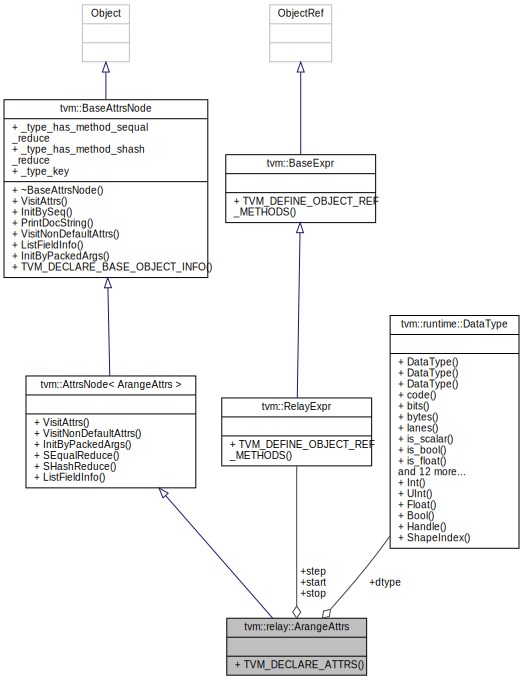
\includegraphics[width=350pt]{structtvm_1_1relay_1_1ArangeAttrs__coll__graph}
\end{center}
\end{figure}
\subsection*{Public Member Functions}
\begin{DoxyCompactItemize}
\item 
\hyperlink{structtvm_1_1relay_1_1ArangeAttrs_ae6c7574b378953c4491e9ac6c618d43c}{T\+V\+M\+\_\+\+D\+E\+C\+L\+A\+R\+E\+\_\+\+A\+T\+T\+RS} (\hyperlink{structtvm_1_1relay_1_1ArangeAttrs}{Arange\+Attrs},\char`\"{}relay.\+attrs.\+Arange\+Attrs\char`\"{})
\end{DoxyCompactItemize}
\subsection*{Public Attributes}
\begin{DoxyCompactItemize}
\item 
\hyperlink{namespacetvm_1_1relay_a5b84e3790f89bb3fad5c7911eeb99531}{Expr} \hyperlink{structtvm_1_1relay_1_1ArangeAttrs_ae8ae5bc1551b406a4f52395af343c2ce}{start}
\item 
\hyperlink{namespacetvm_1_1relay_a5b84e3790f89bb3fad5c7911eeb99531}{Expr} \hyperlink{structtvm_1_1relay_1_1ArangeAttrs_a1eadf1f3964ca83dade8edeae7d6d7cf}{stop}
\item 
\hyperlink{namespacetvm_1_1relay_a5b84e3790f89bb3fad5c7911eeb99531}{Expr} \hyperlink{structtvm_1_1relay_1_1ArangeAttrs_aabe51ead537f676d53ffedf91b16ae66}{step}
\item 
\hyperlink{namespacetvm_a41918af1a1dc386388639a9d3ad06c5d}{Data\+Type} \hyperlink{structtvm_1_1relay_1_1ArangeAttrs_a405dbeb1c77da2690c40606c980f388d}{dtype}
\end{DoxyCompactItemize}
\subsection*{Additional Inherited Members}


\subsection{Detailed Description}
Attributes used in arange operators. 

\subsection{Member Function Documentation}
\index{tvm\+::relay\+::\+Arange\+Attrs@{tvm\+::relay\+::\+Arange\+Attrs}!T\+V\+M\+\_\+\+D\+E\+C\+L\+A\+R\+E\+\_\+\+A\+T\+T\+RS@{T\+V\+M\+\_\+\+D\+E\+C\+L\+A\+R\+E\+\_\+\+A\+T\+T\+RS}}
\index{T\+V\+M\+\_\+\+D\+E\+C\+L\+A\+R\+E\+\_\+\+A\+T\+T\+RS@{T\+V\+M\+\_\+\+D\+E\+C\+L\+A\+R\+E\+\_\+\+A\+T\+T\+RS}!tvm\+::relay\+::\+Arange\+Attrs@{tvm\+::relay\+::\+Arange\+Attrs}}
\subsubsection[{\texorpdfstring{T\+V\+M\+\_\+\+D\+E\+C\+L\+A\+R\+E\+\_\+\+A\+T\+T\+R\+S(\+Arange\+Attrs,""relay.\+attrs.\+Arange\+Attrs"")}{TVM_DECLARE_ATTRS(ArangeAttrs,"relay.attrs.ArangeAttrs")}}]{\setlength{\rightskip}{0pt plus 5cm}tvm\+::relay\+::\+Arange\+Attrs\+::\+T\+V\+M\+\_\+\+D\+E\+C\+L\+A\+R\+E\+\_\+\+A\+T\+T\+RS (
\begin{DoxyParamCaption}
\item[{{\bf Arange\+Attrs}}]{, }
\item[{\char`\"{}relay.\+attrs.\+Arange\+Attrs\char`\"{}}]{}
\end{DoxyParamCaption}
)\hspace{0.3cm}{\ttfamily [inline]}}\hypertarget{structtvm_1_1relay_1_1ArangeAttrs_ae6c7574b378953c4491e9ac6c618d43c}{}\label{structtvm_1_1relay_1_1ArangeAttrs_ae6c7574b378953c4491e9ac6c618d43c}


\subsection{Member Data Documentation}
\index{tvm\+::relay\+::\+Arange\+Attrs@{tvm\+::relay\+::\+Arange\+Attrs}!dtype@{dtype}}
\index{dtype@{dtype}!tvm\+::relay\+::\+Arange\+Attrs@{tvm\+::relay\+::\+Arange\+Attrs}}
\subsubsection[{\texorpdfstring{dtype}{dtype}}]{\setlength{\rightskip}{0pt plus 5cm}{\bf Data\+Type} tvm\+::relay\+::\+Arange\+Attrs\+::dtype}\hypertarget{structtvm_1_1relay_1_1ArangeAttrs_a405dbeb1c77da2690c40606c980f388d}{}\label{structtvm_1_1relay_1_1ArangeAttrs_a405dbeb1c77da2690c40606c980f388d}
\index{tvm\+::relay\+::\+Arange\+Attrs@{tvm\+::relay\+::\+Arange\+Attrs}!start@{start}}
\index{start@{start}!tvm\+::relay\+::\+Arange\+Attrs@{tvm\+::relay\+::\+Arange\+Attrs}}
\subsubsection[{\texorpdfstring{start}{start}}]{\setlength{\rightskip}{0pt plus 5cm}{\bf Expr} tvm\+::relay\+::\+Arange\+Attrs\+::start}\hypertarget{structtvm_1_1relay_1_1ArangeAttrs_ae8ae5bc1551b406a4f52395af343c2ce}{}\label{structtvm_1_1relay_1_1ArangeAttrs_ae8ae5bc1551b406a4f52395af343c2ce}
\index{tvm\+::relay\+::\+Arange\+Attrs@{tvm\+::relay\+::\+Arange\+Attrs}!step@{step}}
\index{step@{step}!tvm\+::relay\+::\+Arange\+Attrs@{tvm\+::relay\+::\+Arange\+Attrs}}
\subsubsection[{\texorpdfstring{step}{step}}]{\setlength{\rightskip}{0pt plus 5cm}{\bf Expr} tvm\+::relay\+::\+Arange\+Attrs\+::step}\hypertarget{structtvm_1_1relay_1_1ArangeAttrs_aabe51ead537f676d53ffedf91b16ae66}{}\label{structtvm_1_1relay_1_1ArangeAttrs_aabe51ead537f676d53ffedf91b16ae66}
\index{tvm\+::relay\+::\+Arange\+Attrs@{tvm\+::relay\+::\+Arange\+Attrs}!stop@{stop}}
\index{stop@{stop}!tvm\+::relay\+::\+Arange\+Attrs@{tvm\+::relay\+::\+Arange\+Attrs}}
\subsubsection[{\texorpdfstring{stop}{stop}}]{\setlength{\rightskip}{0pt plus 5cm}{\bf Expr} tvm\+::relay\+::\+Arange\+Attrs\+::stop}\hypertarget{structtvm_1_1relay_1_1ArangeAttrs_a1eadf1f3964ca83dade8edeae7d6d7cf}{}\label{structtvm_1_1relay_1_1ArangeAttrs_a1eadf1f3964ca83dade8edeae7d6d7cf}


The documentation for this struct was generated from the following file\+:\begin{DoxyCompactItemize}
\item 
include/tvm/relay/attrs/\hyperlink{include_2tvm_2relay_2attrs_2transform_8h}{transform.\+h}\end{DoxyCompactItemize}

\hypertarget{structtvm_1_1relay_1_1ArgsortAttrs}{}\section{tvm\+:\+:relay\+:\+:Argsort\+Attrs Struct Reference}
\label{structtvm_1_1relay_1_1ArgsortAttrs}\index{tvm\+::relay\+::\+Argsort\+Attrs@{tvm\+::relay\+::\+Argsort\+Attrs}}


Attributes used in argsort operators.  




{\ttfamily \#include $<$algorithm.\+h$>$}



Inheritance diagram for tvm\+:\+:relay\+:\+:Argsort\+Attrs\+:
\nopagebreak
\begin{figure}[H]
\begin{center}
\leavevmode
\includegraphics[height=550pt]{structtvm_1_1relay_1_1ArgsortAttrs__inherit__graph}
\end{center}
\end{figure}


Collaboration diagram for tvm\+:\+:relay\+:\+:Argsort\+Attrs\+:
\nopagebreak
\begin{figure}[H]
\begin{center}
\leavevmode
\includegraphics[height=550pt]{structtvm_1_1relay_1_1ArgsortAttrs__coll__graph}
\end{center}
\end{figure}
\subsection*{Public Member Functions}
\begin{DoxyCompactItemize}
\item 
\hyperlink{structtvm_1_1relay_1_1ArgsortAttrs_a867e4a526a4b5e2512e658839d6c1a9e}{T\+V\+M\+\_\+\+D\+E\+C\+L\+A\+R\+E\+\_\+\+A\+T\+T\+RS} (\hyperlink{structtvm_1_1relay_1_1ArgsortAttrs}{Argsort\+Attrs},\char`\"{}relay.\+attrs.\+Argsort\+Attrs\char`\"{})
\end{DoxyCompactItemize}
\subsection*{Public Attributes}
\begin{DoxyCompactItemize}
\item 
int \hyperlink{structtvm_1_1relay_1_1ArgsortAttrs_a3365bda570a8bec823e2b742ae32a924}{axis}
\item 
bool \hyperlink{structtvm_1_1relay_1_1ArgsortAttrs_a97f3acf400fafc612854c955a88673ea}{is\+\_\+ascend}
\item 
\hyperlink{namespacetvm_a41918af1a1dc386388639a9d3ad06c5d}{Data\+Type} \hyperlink{structtvm_1_1relay_1_1ArgsortAttrs_a533842c9351d0ec7f8e2673e94987957}{dtype}
\end{DoxyCompactItemize}
\subsection*{Additional Inherited Members}


\subsection{Detailed Description}
Attributes used in argsort operators. 

\subsection{Member Function Documentation}
\index{tvm\+::relay\+::\+Argsort\+Attrs@{tvm\+::relay\+::\+Argsort\+Attrs}!T\+V\+M\+\_\+\+D\+E\+C\+L\+A\+R\+E\+\_\+\+A\+T\+T\+RS@{T\+V\+M\+\_\+\+D\+E\+C\+L\+A\+R\+E\+\_\+\+A\+T\+T\+RS}}
\index{T\+V\+M\+\_\+\+D\+E\+C\+L\+A\+R\+E\+\_\+\+A\+T\+T\+RS@{T\+V\+M\+\_\+\+D\+E\+C\+L\+A\+R\+E\+\_\+\+A\+T\+T\+RS}!tvm\+::relay\+::\+Argsort\+Attrs@{tvm\+::relay\+::\+Argsort\+Attrs}}
\subsubsection[{\texorpdfstring{T\+V\+M\+\_\+\+D\+E\+C\+L\+A\+R\+E\+\_\+\+A\+T\+T\+R\+S(\+Argsort\+Attrs,""relay.\+attrs.\+Argsort\+Attrs"")}{TVM_DECLARE_ATTRS(ArgsortAttrs,"relay.attrs.ArgsortAttrs")}}]{\setlength{\rightskip}{0pt plus 5cm}tvm\+::relay\+::\+Argsort\+Attrs\+::\+T\+V\+M\+\_\+\+D\+E\+C\+L\+A\+R\+E\+\_\+\+A\+T\+T\+RS (
\begin{DoxyParamCaption}
\item[{{\bf Argsort\+Attrs}}]{, }
\item[{\char`\"{}relay.\+attrs.\+Argsort\+Attrs\char`\"{}}]{}
\end{DoxyParamCaption}
)\hspace{0.3cm}{\ttfamily [inline]}}\hypertarget{structtvm_1_1relay_1_1ArgsortAttrs_a867e4a526a4b5e2512e658839d6c1a9e}{}\label{structtvm_1_1relay_1_1ArgsortAttrs_a867e4a526a4b5e2512e658839d6c1a9e}


\subsection{Member Data Documentation}
\index{tvm\+::relay\+::\+Argsort\+Attrs@{tvm\+::relay\+::\+Argsort\+Attrs}!axis@{axis}}
\index{axis@{axis}!tvm\+::relay\+::\+Argsort\+Attrs@{tvm\+::relay\+::\+Argsort\+Attrs}}
\subsubsection[{\texorpdfstring{axis}{axis}}]{\setlength{\rightskip}{0pt plus 5cm}int tvm\+::relay\+::\+Argsort\+Attrs\+::axis}\hypertarget{structtvm_1_1relay_1_1ArgsortAttrs_a3365bda570a8bec823e2b742ae32a924}{}\label{structtvm_1_1relay_1_1ArgsortAttrs_a3365bda570a8bec823e2b742ae32a924}
\index{tvm\+::relay\+::\+Argsort\+Attrs@{tvm\+::relay\+::\+Argsort\+Attrs}!dtype@{dtype}}
\index{dtype@{dtype}!tvm\+::relay\+::\+Argsort\+Attrs@{tvm\+::relay\+::\+Argsort\+Attrs}}
\subsubsection[{\texorpdfstring{dtype}{dtype}}]{\setlength{\rightskip}{0pt plus 5cm}{\bf Data\+Type} tvm\+::relay\+::\+Argsort\+Attrs\+::dtype}\hypertarget{structtvm_1_1relay_1_1ArgsortAttrs_a533842c9351d0ec7f8e2673e94987957}{}\label{structtvm_1_1relay_1_1ArgsortAttrs_a533842c9351d0ec7f8e2673e94987957}
\index{tvm\+::relay\+::\+Argsort\+Attrs@{tvm\+::relay\+::\+Argsort\+Attrs}!is\+\_\+ascend@{is\+\_\+ascend}}
\index{is\+\_\+ascend@{is\+\_\+ascend}!tvm\+::relay\+::\+Argsort\+Attrs@{tvm\+::relay\+::\+Argsort\+Attrs}}
\subsubsection[{\texorpdfstring{is\+\_\+ascend}{is_ascend}}]{\setlength{\rightskip}{0pt plus 5cm}bool tvm\+::relay\+::\+Argsort\+Attrs\+::is\+\_\+ascend}\hypertarget{structtvm_1_1relay_1_1ArgsortAttrs_a97f3acf400fafc612854c955a88673ea}{}\label{structtvm_1_1relay_1_1ArgsortAttrs_a97f3acf400fafc612854c955a88673ea}


The documentation for this struct was generated from the following file\+:\begin{DoxyCompactItemize}
\item 
include/tvm/relay/attrs/\hyperlink{algorithm_8h}{algorithm.\+h}\end{DoxyCompactItemize}

\hypertarget{classtvm_1_1Array}{}\section{tvm\+:\+:Array$<$ T, typename $>$ Class Template Reference}
\label{classtvm_1_1Array}\index{tvm\+::\+Array$<$ T, typename $>$@{tvm\+::\+Array$<$ T, typename $>$}}


\hyperlink{classtvm_1_1Array}{Array} container of Node\+Ref in D\+SL graph. \hyperlink{classtvm_1_1Array}{Array} implements copy on write semantics, which means array is mutable but copy will happen when array is referenced in more than two places.  




{\ttfamily \#include $<$container.\+h$>$}



Inheritance diagram for tvm\+:\+:Array$<$ T, typename $>$\+:
\nopagebreak
\begin{figure}[H]
\begin{center}
\leavevmode
\includegraphics[width=229pt]{classtvm_1_1Array__inherit__graph}
\end{center}
\end{figure}


Collaboration diagram for tvm\+:\+:Array$<$ T, typename $>$\+:
\nopagebreak
\begin{figure}[H]
\begin{center}
\leavevmode
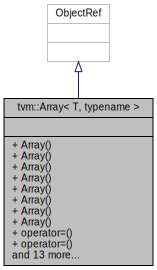
\includegraphics[width=229pt]{classtvm_1_1Array__coll__graph}
\end{center}
\end{figure}
\subsection*{Classes}
\begin{DoxyCompactItemize}
\item 
struct \hyperlink{structtvm_1_1Array_1_1ValueConverter}{Value\+Converter}
\end{DoxyCompactItemize}
\subsection*{Public Types}
\begin{DoxyCompactItemize}
\item 
using \hyperlink{classtvm_1_1Array_ab85f7f463f8a418f6b4dcffdf43b007c}{Container\+Type} = \hyperlink{classtvm_1_1ArrayNode}{Array\+Node}
\begin{DoxyCompactList}\small\item\em specify container node \end{DoxyCompactList}\item 
using \hyperlink{classtvm_1_1Array_a82550eb5257293ba5af8866aa8ff16e6}{iterator} = \hyperlink{classtvm_1_1IterAdapter}{Iter\+Adapter}$<$ \hyperlink{structtvm_1_1Array_1_1ValueConverter}{Value\+Converter}, std\+::vector$<$ Object\+Ref $>$\+::const\+\_\+iterator $>$
\item 
using \hyperlink{classtvm_1_1Array_a6b71ab5c7c8c2abffe81a0ea3842fd1a}{reverse\+\_\+iterator} = \hyperlink{classtvm_1_1IterAdapter}{Iter\+Adapter}$<$ \hyperlink{structtvm_1_1Array_1_1ValueConverter}{Value\+Converter}, std\+::vector$<$ Object\+Ref $>$\+::const\+\_\+reverse\+\_\+iterator $>$
\end{DoxyCompactItemize}
\subsection*{Public Member Functions}
\begin{DoxyCompactItemize}
\item 
\hyperlink{classtvm_1_1Array_aab72ecf006512069d8f791e3cae3eee0}{Array} ()
\begin{DoxyCompactList}\small\item\em default constructor \end{DoxyCompactList}\item 
\hyperlink{classtvm_1_1Array_a42ad68bcaefafa48967fa815cdb1e9fe}{Array} (\hyperlink{classtvm_1_1Array}{Array}$<$ T $>$ \&\&other)
\begin{DoxyCompactList}\small\item\em move constructor \end{DoxyCompactList}\item 
\hyperlink{classtvm_1_1Array_a48ecf47f2a0bc8dfaddc8da83300deed}{Array} (const \hyperlink{classtvm_1_1Array}{Array}$<$ T $>$ \&other)
\begin{DoxyCompactList}\small\item\em copy constructor \end{DoxyCompactList}\item 
\hyperlink{classtvm_1_1Array_abda937076918f8123b1fc62303a940a4}{Array} (Object\+Ptr$<$ Object $>$ n)
\begin{DoxyCompactList}\small\item\em constructor from pointer \end{DoxyCompactList}\item 
{\footnotesize template$<$typename Iter\+Type $>$ }\\\hyperlink{classtvm_1_1Array_a8e465f5428bc1189dfd6eaf7075bb96f}{Array} (Iter\+Type \hyperlink{classtvm_1_1Array_a5db0d3faad39ca865162e50d555a25fa}{begin}, Iter\+Type \hyperlink{classtvm_1_1Array_a6f05e6a14eca3ea865da0f293b4a5325}{end})
\begin{DoxyCompactList}\small\item\em constructor from iterator \end{DoxyCompactList}\item 
\hyperlink{classtvm_1_1Array_a9cd4b1d4c96884994152797a15df7343}{Array} (std\+::initializer\+\_\+list$<$ T $>$ init)
\begin{DoxyCompactList}\small\item\em constructor from initializer list \end{DoxyCompactList}\item 
\hyperlink{classtvm_1_1Array_a92ba9f4611201b6bad1fb46f5944922e}{Array} (const std\+::vector$<$ T $>$ \&init)
\begin{DoxyCompactList}\small\item\em constructor from vector \end{DoxyCompactList}\item 
\hyperlink{classtvm_1_1Array_ae409fb0a54ed7fb8c34b7b0445f88802}{Array} (size\+\_\+t n, const T \&val)
\begin{DoxyCompactList}\small\item\em Constructs a container with n elements. Each element is a copy of val. \end{DoxyCompactList}\item 
\hyperlink{classtvm_1_1Array}{Array}$<$ T $>$ \& \hyperlink{classtvm_1_1Array_acf66932043c572cb9fec8813dbe5d596}{operator=} (\hyperlink{classtvm_1_1Array}{Array}$<$ T $>$ \&\&other)
\begin{DoxyCompactList}\small\item\em move assign operator \end{DoxyCompactList}\item 
\hyperlink{classtvm_1_1Array}{Array}$<$ T $>$ \& \hyperlink{classtvm_1_1Array_a06969623060ee1bb0e82ba7a43513450}{operator=} (const \hyperlink{classtvm_1_1Array}{Array}$<$ T $>$ \&other)
\begin{DoxyCompactList}\small\item\em copy assign operator \end{DoxyCompactList}\item 
{\footnotesize template$<$typename Iter\+Type $>$ }\\void \hyperlink{classtvm_1_1Array_a5eebc9ddbd2e257d0586443b6d493df3}{assign} (Iter\+Type \hyperlink{classtvm_1_1Array_a5db0d3faad39ca865162e50d555a25fa}{begin}, Iter\+Type \hyperlink{classtvm_1_1Array_a6f05e6a14eca3ea865da0f293b4a5325}{end})
\begin{DoxyCompactList}\small\item\em reset the array to content from iterator. \end{DoxyCompactList}\item 
const T \hyperlink{classtvm_1_1Array_afed60e692eab1b2511b07a2b20751878}{operator\mbox{[}$\,$\mbox{]}} (size\+\_\+t i) const 
\begin{DoxyCompactList}\small\item\em Read i-\/th element from array. \end{DoxyCompactList}\item 
size\+\_\+t \hyperlink{classtvm_1_1Array_a6c150ee7d3e46117b099d2052b19aec5}{size} () const 
\item 
\hyperlink{classtvm_1_1ArrayNode}{Array\+Node} $\ast$ \hyperlink{classtvm_1_1Array_a8ebe3653e2bcef7481ab6264f7c231c8}{Copy\+On\+Write} ()
\begin{DoxyCompactList}\small\item\em copy on write semantics Do nothing if current handle is the unique copy of the array. Otherwise make a new copy of the array to ensure the current handle hold a unique copy. \end{DoxyCompactList}\item 
void \hyperlink{classtvm_1_1Array_a24d5ac1f6730d46cb1a6d16729f0a7bb}{push\+\_\+back} (const T \&item)
\begin{DoxyCompactList}\small\item\em push a new item to the back of the list \end{DoxyCompactList}\item 
void \hyperlink{classtvm_1_1Array_a8303345e666f9c72586721bc067e7fc9}{resize} (size\+\_\+t \hyperlink{classtvm_1_1Array_a6c150ee7d3e46117b099d2052b19aec5}{size})
\begin{DoxyCompactList}\small\item\em Resize the array. \end{DoxyCompactList}\item 
void \hyperlink{classtvm_1_1Array_ab3db968deb4be7a51767f22d267eb7af}{Set} (size\+\_\+t i, const T \&value)
\begin{DoxyCompactList}\small\item\em set i-\/th element of the array. \end{DoxyCompactList}\item 
bool \hyperlink{classtvm_1_1Array_a531169863918d8464aa4b905d236674f}{empty} () const 
\item 
{\footnotesize template$<$typename F $>$ }\\void \hyperlink{classtvm_1_1Array_abb864921139827a886c8fec5b7796041}{Mutate\+By\+Apply} (F fmutate)
\begin{DoxyCompactList}\small\item\em Helper function to apply fmutate to mutate an array. \end{DoxyCompactList}\item 
\hyperlink{classtvm_1_1Array_a82550eb5257293ba5af8866aa8ff16e6}{iterator} \hyperlink{classtvm_1_1Array_a5db0d3faad39ca865162e50d555a25fa}{begin} () const 
\item 
\hyperlink{classtvm_1_1Array_a82550eb5257293ba5af8866aa8ff16e6}{iterator} \hyperlink{classtvm_1_1Array_a6f05e6a14eca3ea865da0f293b4a5325}{end} () const 
\item 
\hyperlink{classtvm_1_1Array_a6b71ab5c7c8c2abffe81a0ea3842fd1a}{reverse\+\_\+iterator} \hyperlink{classtvm_1_1Array_ad9e24a3208ffabbc079db08804a6f602}{rbegin} () const 
\item 
\hyperlink{classtvm_1_1Array_a6b71ab5c7c8c2abffe81a0ea3842fd1a}{reverse\+\_\+iterator} \hyperlink{classtvm_1_1Array_adc2c5ea9dacd9a1fae22c409a39007b8}{rend} () const 
\end{DoxyCompactItemize}


\subsection{Detailed Description}
\subsubsection*{template$<$typename T, typename = typename std\+::enable\+\_\+if$<$std\+::is\+\_\+base\+\_\+of$<$\+Object\+Ref, T$>$\+::value$>$\+::type$>$\\*
class tvm\+::\+Array$<$ T, typename $>$}

\hyperlink{classtvm_1_1Array}{Array} container of Node\+Ref in D\+SL graph. \hyperlink{classtvm_1_1Array}{Array} implements copy on write semantics, which means array is mutable but copy will happen when array is referenced in more than two places. 

operator\mbox{[}\mbox{]} only provide const acces, use Set to mutate the content. 
\begin{DoxyTemplParams}{Template Parameters}
{\em T} & The content Node\+Ref type. \\
\hline
\end{DoxyTemplParams}


\subsection{Member Typedef Documentation}
\index{tvm\+::\+Array@{tvm\+::\+Array}!Container\+Type@{Container\+Type}}
\index{Container\+Type@{Container\+Type}!tvm\+::\+Array@{tvm\+::\+Array}}
\subsubsection[{\texorpdfstring{Container\+Type}{ContainerType}}]{\setlength{\rightskip}{0pt plus 5cm}template$<$typename T, typename  = typename std\+::enable\+\_\+if$<$std\+::is\+\_\+base\+\_\+of$<$\+Object\+Ref, T$>$\+::value$>$\+::type$>$ using {\bf tvm\+::\+Array}$<$ T, typename $>$\+::{\bf Container\+Type} =  {\bf Array\+Node}}\hypertarget{classtvm_1_1Array_ab85f7f463f8a418f6b4dcffdf43b007c}{}\label{classtvm_1_1Array_ab85f7f463f8a418f6b4dcffdf43b007c}


specify container node 

\index{tvm\+::\+Array@{tvm\+::\+Array}!iterator@{iterator}}
\index{iterator@{iterator}!tvm\+::\+Array@{tvm\+::\+Array}}
\subsubsection[{\texorpdfstring{iterator}{iterator}}]{\setlength{\rightskip}{0pt plus 5cm}template$<$typename T, typename  = typename std\+::enable\+\_\+if$<$std\+::is\+\_\+base\+\_\+of$<$\+Object\+Ref, T$>$\+::value$>$\+::type$>$ using {\bf tvm\+::\+Array}$<$ T, typename $>$\+::{\bf iterator} =  {\bf Iter\+Adapter}$<${\bf Value\+Converter}, std\+::vector$<$Object\+Ref$>$\+::const\+\_\+iterator$>$}\hypertarget{classtvm_1_1Array_a82550eb5257293ba5af8866aa8ff16e6}{}\label{classtvm_1_1Array_a82550eb5257293ba5af8866aa8ff16e6}
\index{tvm\+::\+Array@{tvm\+::\+Array}!reverse\+\_\+iterator@{reverse\+\_\+iterator}}
\index{reverse\+\_\+iterator@{reverse\+\_\+iterator}!tvm\+::\+Array@{tvm\+::\+Array}}
\subsubsection[{\texorpdfstring{reverse\+\_\+iterator}{reverse_iterator}}]{\setlength{\rightskip}{0pt plus 5cm}template$<$typename T, typename  = typename std\+::enable\+\_\+if$<$std\+::is\+\_\+base\+\_\+of$<$\+Object\+Ref, T$>$\+::value$>$\+::type$>$ using {\bf tvm\+::\+Array}$<$ T, typename $>$\+::{\bf reverse\+\_\+iterator} =  {\bf Iter\+Adapter}$<$ {\bf Value\+Converter}, std\+::vector$<$Object\+Ref$>$\+::const\+\_\+reverse\+\_\+iterator$>$}\hypertarget{classtvm_1_1Array_a6b71ab5c7c8c2abffe81a0ea3842fd1a}{}\label{classtvm_1_1Array_a6b71ab5c7c8c2abffe81a0ea3842fd1a}


\subsection{Constructor \& Destructor Documentation}
\index{tvm\+::\+Array@{tvm\+::\+Array}!Array@{Array}}
\index{Array@{Array}!tvm\+::\+Array@{tvm\+::\+Array}}
\subsubsection[{\texorpdfstring{Array()}{Array()}}]{\setlength{\rightskip}{0pt plus 5cm}template$<$typename T, typename  = typename std\+::enable\+\_\+if$<$std\+::is\+\_\+base\+\_\+of$<$\+Object\+Ref, T$>$\+::value$>$\+::type$>$ {\bf tvm\+::\+Array}$<$ T, typename $>$\+::{\bf Array} (
\begin{DoxyParamCaption}
{}
\end{DoxyParamCaption}
)\hspace{0.3cm}{\ttfamily [inline]}}\hypertarget{classtvm_1_1Array_aab72ecf006512069d8f791e3cae3eee0}{}\label{classtvm_1_1Array_aab72ecf006512069d8f791e3cae3eee0}


default constructor 

\index{tvm\+::\+Array@{tvm\+::\+Array}!Array@{Array}}
\index{Array@{Array}!tvm\+::\+Array@{tvm\+::\+Array}}
\subsubsection[{\texorpdfstring{Array(\+Array$<$ T $>$ \&\&other)}{Array(Array< T > &&other)}}]{\setlength{\rightskip}{0pt plus 5cm}template$<$typename T, typename  = typename std\+::enable\+\_\+if$<$std\+::is\+\_\+base\+\_\+of$<$\+Object\+Ref, T$>$\+::value$>$\+::type$>$ {\bf tvm\+::\+Array}$<$ T, typename $>$\+::{\bf Array} (
\begin{DoxyParamCaption}
\item[{{\bf Array}$<$ T $>$ \&\&}]{other}
\end{DoxyParamCaption}
)\hspace{0.3cm}{\ttfamily [inline]}}\hypertarget{classtvm_1_1Array_a42ad68bcaefafa48967fa815cdb1e9fe}{}\label{classtvm_1_1Array_a42ad68bcaefafa48967fa815cdb1e9fe}


move constructor 


\begin{DoxyParams}{Parameters}
{\em other} & source \\
\hline
\end{DoxyParams}
\index{tvm\+::\+Array@{tvm\+::\+Array}!Array@{Array}}
\index{Array@{Array}!tvm\+::\+Array@{tvm\+::\+Array}}
\subsubsection[{\texorpdfstring{Array(const Array$<$ T $>$ \&other)}{Array(const Array< T > &other)}}]{\setlength{\rightskip}{0pt plus 5cm}template$<$typename T, typename  = typename std\+::enable\+\_\+if$<$std\+::is\+\_\+base\+\_\+of$<$\+Object\+Ref, T$>$\+::value$>$\+::type$>$ {\bf tvm\+::\+Array}$<$ T, typename $>$\+::{\bf Array} (
\begin{DoxyParamCaption}
\item[{const {\bf Array}$<$ T $>$ \&}]{other}
\end{DoxyParamCaption}
)\hspace{0.3cm}{\ttfamily [inline]}}\hypertarget{classtvm_1_1Array_a48ecf47f2a0bc8dfaddc8da83300deed}{}\label{classtvm_1_1Array_a48ecf47f2a0bc8dfaddc8da83300deed}


copy constructor 


\begin{DoxyParams}{Parameters}
{\em other} & source \\
\hline
\end{DoxyParams}
\index{tvm\+::\+Array@{tvm\+::\+Array}!Array@{Array}}
\index{Array@{Array}!tvm\+::\+Array@{tvm\+::\+Array}}
\subsubsection[{\texorpdfstring{Array(\+Object\+Ptr$<$ Object $>$ n)}{Array(ObjectPtr< Object > n)}}]{\setlength{\rightskip}{0pt plus 5cm}template$<$typename T, typename  = typename std\+::enable\+\_\+if$<$std\+::is\+\_\+base\+\_\+of$<$\+Object\+Ref, T$>$\+::value$>$\+::type$>$ {\bf tvm\+::\+Array}$<$ T, typename $>$\+::{\bf Array} (
\begin{DoxyParamCaption}
\item[{Object\+Ptr$<$ Object $>$}]{n}
\end{DoxyParamCaption}
)\hspace{0.3cm}{\ttfamily [inline]}, {\ttfamily [explicit]}}\hypertarget{classtvm_1_1Array_abda937076918f8123b1fc62303a940a4}{}\label{classtvm_1_1Array_abda937076918f8123b1fc62303a940a4}


constructor from pointer 


\begin{DoxyParams}{Parameters}
{\em n} & the container pointer \\
\hline
\end{DoxyParams}
\index{tvm\+::\+Array@{tvm\+::\+Array}!Array@{Array}}
\index{Array@{Array}!tvm\+::\+Array@{tvm\+::\+Array}}
\subsubsection[{\texorpdfstring{Array(\+Iter\+Type begin, Iter\+Type end)}{Array(IterType begin, IterType end)}}]{\setlength{\rightskip}{0pt plus 5cm}template$<$typename T, typename  = typename std\+::enable\+\_\+if$<$std\+::is\+\_\+base\+\_\+of$<$\+Object\+Ref, T$>$\+::value$>$\+::type$>$ template$<$typename Iter\+Type $>$ {\bf tvm\+::\+Array}$<$ T, typename $>$\+::{\bf Array} (
\begin{DoxyParamCaption}
\item[{Iter\+Type}]{begin, }
\item[{Iter\+Type}]{end}
\end{DoxyParamCaption}
)\hspace{0.3cm}{\ttfamily [inline]}}\hypertarget{classtvm_1_1Array_a8e465f5428bc1189dfd6eaf7075bb96f}{}\label{classtvm_1_1Array_a8e465f5428bc1189dfd6eaf7075bb96f}


constructor from iterator 


\begin{DoxyParams}{Parameters}
{\em begin} & begin of iterator \\
\hline
{\em end} & end of iterator \\
\hline
\end{DoxyParams}

\begin{DoxyTemplParams}{Template Parameters}
{\em Iter\+Type} & The type of iterator \\
\hline
\end{DoxyTemplParams}
\index{tvm\+::\+Array@{tvm\+::\+Array}!Array@{Array}}
\index{Array@{Array}!tvm\+::\+Array@{tvm\+::\+Array}}
\subsubsection[{\texorpdfstring{Array(std\+::initializer\+\_\+list$<$ T $>$ init)}{Array(std::initializer_list< T > init)}}]{\setlength{\rightskip}{0pt plus 5cm}template$<$typename T, typename  = typename std\+::enable\+\_\+if$<$std\+::is\+\_\+base\+\_\+of$<$\+Object\+Ref, T$>$\+::value$>$\+::type$>$ {\bf tvm\+::\+Array}$<$ T, typename $>$\+::{\bf Array} (
\begin{DoxyParamCaption}
\item[{std\+::initializer\+\_\+list$<$ T $>$}]{init}
\end{DoxyParamCaption}
)\hspace{0.3cm}{\ttfamily [inline]}}\hypertarget{classtvm_1_1Array_a9cd4b1d4c96884994152797a15df7343}{}\label{classtvm_1_1Array_a9cd4b1d4c96884994152797a15df7343}


constructor from initializer list 


\begin{DoxyParams}{Parameters}
{\em init} & The initalizer list \\
\hline
\end{DoxyParams}
\index{tvm\+::\+Array@{tvm\+::\+Array}!Array@{Array}}
\index{Array@{Array}!tvm\+::\+Array@{tvm\+::\+Array}}
\subsubsection[{\texorpdfstring{Array(const std\+::vector$<$ T $>$ \&init)}{Array(const std::vector< T > &init)}}]{\setlength{\rightskip}{0pt plus 5cm}template$<$typename T, typename  = typename std\+::enable\+\_\+if$<$std\+::is\+\_\+base\+\_\+of$<$\+Object\+Ref, T$>$\+::value$>$\+::type$>$ {\bf tvm\+::\+Array}$<$ T, typename $>$\+::{\bf Array} (
\begin{DoxyParamCaption}
\item[{const std\+::vector$<$ T $>$ \&}]{init}
\end{DoxyParamCaption}
)\hspace{0.3cm}{\ttfamily [inline]}}\hypertarget{classtvm_1_1Array_a92ba9f4611201b6bad1fb46f5944922e}{}\label{classtvm_1_1Array_a92ba9f4611201b6bad1fb46f5944922e}


constructor from vector 


\begin{DoxyParams}{Parameters}
{\em init} & The vector \\
\hline
\end{DoxyParams}
\index{tvm\+::\+Array@{tvm\+::\+Array}!Array@{Array}}
\index{Array@{Array}!tvm\+::\+Array@{tvm\+::\+Array}}
\subsubsection[{\texorpdfstring{Array(size\+\_\+t n, const T \&val)}{Array(size_t n, const T &val)}}]{\setlength{\rightskip}{0pt plus 5cm}template$<$typename T, typename  = typename std\+::enable\+\_\+if$<$std\+::is\+\_\+base\+\_\+of$<$\+Object\+Ref, T$>$\+::value$>$\+::type$>$ {\bf tvm\+::\+Array}$<$ T, typename $>$\+::{\bf Array} (
\begin{DoxyParamCaption}
\item[{size\+\_\+t}]{n, }
\item[{const T \&}]{val}
\end{DoxyParamCaption}
)\hspace{0.3cm}{\ttfamily [inline]}, {\ttfamily [explicit]}}\hypertarget{classtvm_1_1Array_ae409fb0a54ed7fb8c34b7b0445f88802}{}\label{classtvm_1_1Array_ae409fb0a54ed7fb8c34b7b0445f88802}


Constructs a container with n elements. Each element is a copy of val. 


\begin{DoxyParams}{Parameters}
{\em n} & The size of the container \\
\hline
{\em val} & The init value \\
\hline
\end{DoxyParams}


\subsection{Member Function Documentation}
\index{tvm\+::\+Array@{tvm\+::\+Array}!assign@{assign}}
\index{assign@{assign}!tvm\+::\+Array@{tvm\+::\+Array}}
\subsubsection[{\texorpdfstring{assign(\+Iter\+Type begin, Iter\+Type end)}{assign(IterType begin, IterType end)}}]{\setlength{\rightskip}{0pt plus 5cm}template$<$typename T, typename  = typename std\+::enable\+\_\+if$<$std\+::is\+\_\+base\+\_\+of$<$\+Object\+Ref, T$>$\+::value$>$\+::type$>$ template$<$typename Iter\+Type $>$ void {\bf tvm\+::\+Array}$<$ T, typename $>$\+::assign (
\begin{DoxyParamCaption}
\item[{Iter\+Type}]{begin, }
\item[{Iter\+Type}]{end}
\end{DoxyParamCaption}
)\hspace{0.3cm}{\ttfamily [inline]}}\hypertarget{classtvm_1_1Array_a5eebc9ddbd2e257d0586443b6d493df3}{}\label{classtvm_1_1Array_a5eebc9ddbd2e257d0586443b6d493df3}


reset the array to content from iterator. 


\begin{DoxyParams}{Parameters}
{\em begin} & begin of iterator \\
\hline
{\em end} & end of iterator \\
\hline
\end{DoxyParams}

\begin{DoxyTemplParams}{Template Parameters}
{\em Iter\+Type} & The type of iterator \\
\hline
\end{DoxyTemplParams}
\index{tvm\+::\+Array@{tvm\+::\+Array}!begin@{begin}}
\index{begin@{begin}!tvm\+::\+Array@{tvm\+::\+Array}}
\subsubsection[{\texorpdfstring{begin() const }{begin() const }}]{\setlength{\rightskip}{0pt plus 5cm}template$<$typename T, typename  = typename std\+::enable\+\_\+if$<$std\+::is\+\_\+base\+\_\+of$<$\+Object\+Ref, T$>$\+::value$>$\+::type$>$ {\bf iterator} {\bf tvm\+::\+Array}$<$ T, typename $>$\+::begin (
\begin{DoxyParamCaption}
{}
\end{DoxyParamCaption}
) const\hspace{0.3cm}{\ttfamily [inline]}}\hypertarget{classtvm_1_1Array_a5db0d3faad39ca865162e50d555a25fa}{}\label{classtvm_1_1Array_a5db0d3faad39ca865162e50d555a25fa}
\begin{DoxyReturn}{Returns}
begin iterator 
\end{DoxyReturn}
\index{tvm\+::\+Array@{tvm\+::\+Array}!Copy\+On\+Write@{Copy\+On\+Write}}
\index{Copy\+On\+Write@{Copy\+On\+Write}!tvm\+::\+Array@{tvm\+::\+Array}}
\subsubsection[{\texorpdfstring{Copy\+On\+Write()}{CopyOnWrite()}}]{\setlength{\rightskip}{0pt plus 5cm}template$<$typename T, typename  = typename std\+::enable\+\_\+if$<$std\+::is\+\_\+base\+\_\+of$<$\+Object\+Ref, T$>$\+::value$>$\+::type$>$ {\bf Array\+Node}$\ast$ {\bf tvm\+::\+Array}$<$ T, typename $>$\+::Copy\+On\+Write (
\begin{DoxyParamCaption}
{}
\end{DoxyParamCaption}
)\hspace{0.3cm}{\ttfamily [inline]}}\hypertarget{classtvm_1_1Array_a8ebe3653e2bcef7481ab6264f7c231c8}{}\label{classtvm_1_1Array_a8ebe3653e2bcef7481ab6264f7c231c8}


copy on write semantics Do nothing if current handle is the unique copy of the array. Otherwise make a new copy of the array to ensure the current handle hold a unique copy. 

\begin{DoxyReturn}{Returns}
Handle to the internal node container(which ganrantees to be unique) 
\end{DoxyReturn}
\index{tvm\+::\+Array@{tvm\+::\+Array}!empty@{empty}}
\index{empty@{empty}!tvm\+::\+Array@{tvm\+::\+Array}}
\subsubsection[{\texorpdfstring{empty() const }{empty() const }}]{\setlength{\rightskip}{0pt plus 5cm}template$<$typename T, typename  = typename std\+::enable\+\_\+if$<$std\+::is\+\_\+base\+\_\+of$<$\+Object\+Ref, T$>$\+::value$>$\+::type$>$ bool {\bf tvm\+::\+Array}$<$ T, typename $>$\+::empty (
\begin{DoxyParamCaption}
{}
\end{DoxyParamCaption}
) const\hspace{0.3cm}{\ttfamily [inline]}}\hypertarget{classtvm_1_1Array_a531169863918d8464aa4b905d236674f}{}\label{classtvm_1_1Array_a531169863918d8464aa4b905d236674f}
\begin{DoxyReturn}{Returns}
whether array is empty 
\end{DoxyReturn}
\index{tvm\+::\+Array@{tvm\+::\+Array}!end@{end}}
\index{end@{end}!tvm\+::\+Array@{tvm\+::\+Array}}
\subsubsection[{\texorpdfstring{end() const }{end() const }}]{\setlength{\rightskip}{0pt plus 5cm}template$<$typename T, typename  = typename std\+::enable\+\_\+if$<$std\+::is\+\_\+base\+\_\+of$<$\+Object\+Ref, T$>$\+::value$>$\+::type$>$ {\bf iterator} {\bf tvm\+::\+Array}$<$ T, typename $>$\+::end (
\begin{DoxyParamCaption}
{}
\end{DoxyParamCaption}
) const\hspace{0.3cm}{\ttfamily [inline]}}\hypertarget{classtvm_1_1Array_a6f05e6a14eca3ea865da0f293b4a5325}{}\label{classtvm_1_1Array_a6f05e6a14eca3ea865da0f293b4a5325}
\begin{DoxyReturn}{Returns}
end iterator 
\end{DoxyReturn}
\index{tvm\+::\+Array@{tvm\+::\+Array}!Mutate\+By\+Apply@{Mutate\+By\+Apply}}
\index{Mutate\+By\+Apply@{Mutate\+By\+Apply}!tvm\+::\+Array@{tvm\+::\+Array}}
\subsubsection[{\texorpdfstring{Mutate\+By\+Apply(\+F fmutate)}{MutateByApply(F fmutate)}}]{\setlength{\rightskip}{0pt plus 5cm}template$<$typename T, typename  = typename std\+::enable\+\_\+if$<$std\+::is\+\_\+base\+\_\+of$<$\+Object\+Ref, T$>$\+::value$>$\+::type$>$ template$<$typename F $>$ void {\bf tvm\+::\+Array}$<$ T, typename $>$\+::Mutate\+By\+Apply (
\begin{DoxyParamCaption}
\item[{F}]{fmutate}
\end{DoxyParamCaption}
)\hspace{0.3cm}{\ttfamily [inline]}}\hypertarget{classtvm_1_1Array_abb864921139827a886c8fec5b7796041}{}\label{classtvm_1_1Array_abb864921139827a886c8fec5b7796041}


Helper function to apply fmutate to mutate an array. 


\begin{DoxyParams}{Parameters}
{\em fmutate} & The transformation function T -\/$>$ T. \\
\hline
\end{DoxyParams}

\begin{DoxyTemplParams}{Template Parameters}
{\em F} & the type of the mutation function. \\
\hline
\end{DoxyTemplParams}
\begin{DoxyNote}{Note}
This function performs copy on write optimization. 
\end{DoxyNote}
\index{tvm\+::\+Array@{tvm\+::\+Array}!operator=@{operator=}}
\index{operator=@{operator=}!tvm\+::\+Array@{tvm\+::\+Array}}
\subsubsection[{\texorpdfstring{operator=(\+Array$<$ T $>$ \&\&other)}{operator=(Array< T > &&other)}}]{\setlength{\rightskip}{0pt plus 5cm}template$<$typename T, typename  = typename std\+::enable\+\_\+if$<$std\+::is\+\_\+base\+\_\+of$<$\+Object\+Ref, T$>$\+::value$>$\+::type$>$ {\bf Array}$<$T$>$\& {\bf tvm\+::\+Array}$<$ T, typename $>$\+::operator= (
\begin{DoxyParamCaption}
\item[{{\bf Array}$<$ T $>$ \&\&}]{other}
\end{DoxyParamCaption}
)\hspace{0.3cm}{\ttfamily [inline]}}\hypertarget{classtvm_1_1Array_acf66932043c572cb9fec8813dbe5d596}{}\label{classtvm_1_1Array_acf66932043c572cb9fec8813dbe5d596}


move assign operator 


\begin{DoxyParams}{Parameters}
{\em other} & The source of assignment \\
\hline
\end{DoxyParams}
\begin{DoxyReturn}{Returns}
reference to self. 
\end{DoxyReturn}
\index{tvm\+::\+Array@{tvm\+::\+Array}!operator=@{operator=}}
\index{operator=@{operator=}!tvm\+::\+Array@{tvm\+::\+Array}}
\subsubsection[{\texorpdfstring{operator=(const Array$<$ T $>$ \&other)}{operator=(const Array< T > &other)}}]{\setlength{\rightskip}{0pt plus 5cm}template$<$typename T, typename  = typename std\+::enable\+\_\+if$<$std\+::is\+\_\+base\+\_\+of$<$\+Object\+Ref, T$>$\+::value$>$\+::type$>$ {\bf Array}$<$T$>$\& {\bf tvm\+::\+Array}$<$ T, typename $>$\+::operator= (
\begin{DoxyParamCaption}
\item[{const {\bf Array}$<$ T $>$ \&}]{other}
\end{DoxyParamCaption}
)\hspace{0.3cm}{\ttfamily [inline]}}\hypertarget{classtvm_1_1Array_a06969623060ee1bb0e82ba7a43513450}{}\label{classtvm_1_1Array_a06969623060ee1bb0e82ba7a43513450}


copy assign operator 


\begin{DoxyParams}{Parameters}
{\em other} & The source of assignment \\
\hline
\end{DoxyParams}
\begin{DoxyReturn}{Returns}
reference to self. 
\end{DoxyReturn}
\index{tvm\+::\+Array@{tvm\+::\+Array}!operator\mbox{[}$\,$\mbox{]}@{operator[]}}
\index{operator\mbox{[}$\,$\mbox{]}@{operator[]}!tvm\+::\+Array@{tvm\+::\+Array}}
\subsubsection[{\texorpdfstring{operator[](size\+\_\+t i) const }{operator[](size_t i) const }}]{\setlength{\rightskip}{0pt plus 5cm}template$<$typename T, typename  = typename std\+::enable\+\_\+if$<$std\+::is\+\_\+base\+\_\+of$<$\+Object\+Ref, T$>$\+::value$>$\+::type$>$ const T {\bf tvm\+::\+Array}$<$ T, typename $>$\+::operator\mbox{[}$\,$\mbox{]} (
\begin{DoxyParamCaption}
\item[{size\+\_\+t}]{i}
\end{DoxyParamCaption}
) const\hspace{0.3cm}{\ttfamily [inline]}}\hypertarget{classtvm_1_1Array_afed60e692eab1b2511b07a2b20751878}{}\label{classtvm_1_1Array_afed60e692eab1b2511b07a2b20751878}


Read i-\/th element from array. 


\begin{DoxyParams}{Parameters}
{\em i} & The index \\
\hline
\end{DoxyParams}
\begin{DoxyReturn}{Returns}
the i-\/th element. 
\end{DoxyReturn}
\index{tvm\+::\+Array@{tvm\+::\+Array}!push\+\_\+back@{push\+\_\+back}}
\index{push\+\_\+back@{push\+\_\+back}!tvm\+::\+Array@{tvm\+::\+Array}}
\subsubsection[{\texorpdfstring{push\+\_\+back(const T \&item)}{push_back(const T &item)}}]{\setlength{\rightskip}{0pt plus 5cm}template$<$typename T, typename  = typename std\+::enable\+\_\+if$<$std\+::is\+\_\+base\+\_\+of$<$\+Object\+Ref, T$>$\+::value$>$\+::type$>$ void {\bf tvm\+::\+Array}$<$ T, typename $>$\+::push\+\_\+back (
\begin{DoxyParamCaption}
\item[{const T \&}]{item}
\end{DoxyParamCaption}
)\hspace{0.3cm}{\ttfamily [inline]}}\hypertarget{classtvm_1_1Array_a24d5ac1f6730d46cb1a6d16729f0a7bb}{}\label{classtvm_1_1Array_a24d5ac1f6730d46cb1a6d16729f0a7bb}


push a new item to the back of the list 


\begin{DoxyParams}{Parameters}
{\em item} & The item to be pushed. \\
\hline
\end{DoxyParams}
\index{tvm\+::\+Array@{tvm\+::\+Array}!rbegin@{rbegin}}
\index{rbegin@{rbegin}!tvm\+::\+Array@{tvm\+::\+Array}}
\subsubsection[{\texorpdfstring{rbegin() const }{rbegin() const }}]{\setlength{\rightskip}{0pt plus 5cm}template$<$typename T, typename  = typename std\+::enable\+\_\+if$<$std\+::is\+\_\+base\+\_\+of$<$\+Object\+Ref, T$>$\+::value$>$\+::type$>$ {\bf reverse\+\_\+iterator} {\bf tvm\+::\+Array}$<$ T, typename $>$\+::rbegin (
\begin{DoxyParamCaption}
{}
\end{DoxyParamCaption}
) const\hspace{0.3cm}{\ttfamily [inline]}}\hypertarget{classtvm_1_1Array_ad9e24a3208ffabbc079db08804a6f602}{}\label{classtvm_1_1Array_ad9e24a3208ffabbc079db08804a6f602}
\begin{DoxyReturn}{Returns}
rbegin iterator 
\end{DoxyReturn}
\index{tvm\+::\+Array@{tvm\+::\+Array}!rend@{rend}}
\index{rend@{rend}!tvm\+::\+Array@{tvm\+::\+Array}}
\subsubsection[{\texorpdfstring{rend() const }{rend() const }}]{\setlength{\rightskip}{0pt plus 5cm}template$<$typename T, typename  = typename std\+::enable\+\_\+if$<$std\+::is\+\_\+base\+\_\+of$<$\+Object\+Ref, T$>$\+::value$>$\+::type$>$ {\bf reverse\+\_\+iterator} {\bf tvm\+::\+Array}$<$ T, typename $>$\+::rend (
\begin{DoxyParamCaption}
{}
\end{DoxyParamCaption}
) const\hspace{0.3cm}{\ttfamily [inline]}}\hypertarget{classtvm_1_1Array_adc2c5ea9dacd9a1fae22c409a39007b8}{}\label{classtvm_1_1Array_adc2c5ea9dacd9a1fae22c409a39007b8}
\begin{DoxyReturn}{Returns}
rend iterator 
\end{DoxyReturn}
\index{tvm\+::\+Array@{tvm\+::\+Array}!resize@{resize}}
\index{resize@{resize}!tvm\+::\+Array@{tvm\+::\+Array}}
\subsubsection[{\texorpdfstring{resize(size\+\_\+t size)}{resize(size_t size)}}]{\setlength{\rightskip}{0pt plus 5cm}template$<$typename T, typename  = typename std\+::enable\+\_\+if$<$std\+::is\+\_\+base\+\_\+of$<$\+Object\+Ref, T$>$\+::value$>$\+::type$>$ void {\bf tvm\+::\+Array}$<$ T, typename $>$\+::resize (
\begin{DoxyParamCaption}
\item[{size\+\_\+t}]{size}
\end{DoxyParamCaption}
)\hspace{0.3cm}{\ttfamily [inline]}}\hypertarget{classtvm_1_1Array_a8303345e666f9c72586721bc067e7fc9}{}\label{classtvm_1_1Array_a8303345e666f9c72586721bc067e7fc9}


Resize the array. 


\begin{DoxyParams}{Parameters}
{\em size} & The new size. \\
\hline
\end{DoxyParams}
\index{tvm\+::\+Array@{tvm\+::\+Array}!Set@{Set}}
\index{Set@{Set}!tvm\+::\+Array@{tvm\+::\+Array}}
\subsubsection[{\texorpdfstring{Set(size\+\_\+t i, const T \&value)}{Set(size_t i, const T &value)}}]{\setlength{\rightskip}{0pt plus 5cm}template$<$typename T, typename  = typename std\+::enable\+\_\+if$<$std\+::is\+\_\+base\+\_\+of$<$\+Object\+Ref, T$>$\+::value$>$\+::type$>$ void {\bf tvm\+::\+Array}$<$ T, typename $>$\+::Set (
\begin{DoxyParamCaption}
\item[{size\+\_\+t}]{i, }
\item[{const T \&}]{value}
\end{DoxyParamCaption}
)\hspace{0.3cm}{\ttfamily [inline]}}\hypertarget{classtvm_1_1Array_ab3db968deb4be7a51767f22d267eb7af}{}\label{classtvm_1_1Array_ab3db968deb4be7a51767f22d267eb7af}


set i-\/th element of the array. 


\begin{DoxyParams}{Parameters}
{\em i} & The index \\
\hline
{\em value} & The value to be setted. \\
\hline
\end{DoxyParams}
\index{tvm\+::\+Array@{tvm\+::\+Array}!size@{size}}
\index{size@{size}!tvm\+::\+Array@{tvm\+::\+Array}}
\subsubsection[{\texorpdfstring{size() const }{size() const }}]{\setlength{\rightskip}{0pt plus 5cm}template$<$typename T, typename  = typename std\+::enable\+\_\+if$<$std\+::is\+\_\+base\+\_\+of$<$\+Object\+Ref, T$>$\+::value$>$\+::type$>$ size\+\_\+t {\bf tvm\+::\+Array}$<$ T, typename $>$\+::size (
\begin{DoxyParamCaption}
{}
\end{DoxyParamCaption}
) const\hspace{0.3cm}{\ttfamily [inline]}}\hypertarget{classtvm_1_1Array_a6c150ee7d3e46117b099d2052b19aec5}{}\label{classtvm_1_1Array_a6c150ee7d3e46117b099d2052b19aec5}
\begin{DoxyReturn}{Returns}
The size of the array 
\end{DoxyReturn}


The documentation for this class was generated from the following file\+:\begin{DoxyCompactItemize}
\item 
include/tvm/node/\hyperlink{node_2container_8h}{container.\+h}\end{DoxyCompactItemize}

\hypertarget{classtvm_1_1runtime_1_1SimpleObjAllocator_1_1ArrayHandler}{}\section{tvm\+:\+:runtime\+:\+:Simple\+Obj\+Allocator\+:\+:Array\+Handler$<$ Array\+Type, Elem\+Type $>$ Class Template Reference}
\label{classtvm_1_1runtime_1_1SimpleObjAllocator_1_1ArrayHandler}\index{tvm\+::runtime\+::\+Simple\+Obj\+Allocator\+::\+Array\+Handler$<$ Array\+Type, Elem\+Type $>$@{tvm\+::runtime\+::\+Simple\+Obj\+Allocator\+::\+Array\+Handler$<$ Array\+Type, Elem\+Type $>$}}


{\ttfamily \#include $<$memory.\+h$>$}



Collaboration diagram for tvm\+:\+:runtime\+:\+:Simple\+Obj\+Allocator\+:\+:Array\+Handler$<$ Array\+Type, Elem\+Type $>$\+:
\nopagebreak
\begin{figure}[H]
\begin{center}
\leavevmode
\includegraphics[width=256pt]{classtvm_1_1runtime_1_1SimpleObjAllocator_1_1ArrayHandler__coll__graph}
\end{center}
\end{figure}
\subsection*{Public Types}
\begin{DoxyCompactItemize}
\item 
using \hyperlink{classtvm_1_1runtime_1_1SimpleObjAllocator_1_1ArrayHandler_a67e86db3290b1d3bd4aca7e7a2faf187}{Storage\+Type} = typename std\+::aligned\+\_\+storage$<$ sizeof(Array\+Type), alignof(Array\+Type)$>$\+::type
\end{DoxyCompactItemize}
\subsection*{Static Public Member Functions}
\begin{DoxyCompactItemize}
\item 
{\footnotesize template$<$typename... Args$>$ }\\static Array\+Type $\ast$ \hyperlink{classtvm_1_1runtime_1_1SimpleObjAllocator_1_1ArrayHandler_a025fadf9131cce88df531f00c8180d39}{New} (\hyperlink{classtvm_1_1runtime_1_1SimpleObjAllocator}{Simple\+Obj\+Allocator} $\ast$, size\+\_\+t num\+\_\+elems, Args \&\&...args)
\item 
static \hyperlink{classtvm_1_1runtime_1_1Object_a9e84841ca982bff376a978ade0132631}{Object\+::\+F\+Deleter} \hyperlink{classtvm_1_1runtime_1_1SimpleObjAllocator_1_1ArrayHandler_af4771f19c83f265a9cdafd4362e49f56}{Deleter} ()
\end{DoxyCompactItemize}


\subsection{Member Typedef Documentation}
\index{tvm\+::runtime\+::\+Simple\+Obj\+Allocator\+::\+Array\+Handler@{tvm\+::runtime\+::\+Simple\+Obj\+Allocator\+::\+Array\+Handler}!Storage\+Type@{Storage\+Type}}
\index{Storage\+Type@{Storage\+Type}!tvm\+::runtime\+::\+Simple\+Obj\+Allocator\+::\+Array\+Handler@{tvm\+::runtime\+::\+Simple\+Obj\+Allocator\+::\+Array\+Handler}}
\subsubsection[{\texorpdfstring{Storage\+Type}{StorageType}}]{\setlength{\rightskip}{0pt plus 5cm}template$<$typename Array\+Type , typename Elem\+Type $>$ using {\bf tvm\+::runtime\+::\+Simple\+Obj\+Allocator\+::\+Array\+Handler}$<$ Array\+Type, Elem\+Type $>$\+::{\bf Storage\+Type} =  typename std\+::aligned\+\_\+storage$<$sizeof(Array\+Type), alignof(Array\+Type)$>$\+::type}\hypertarget{classtvm_1_1runtime_1_1SimpleObjAllocator_1_1ArrayHandler_a67e86db3290b1d3bd4aca7e7a2faf187}{}\label{classtvm_1_1runtime_1_1SimpleObjAllocator_1_1ArrayHandler_a67e86db3290b1d3bd4aca7e7a2faf187}


\subsection{Member Function Documentation}
\index{tvm\+::runtime\+::\+Simple\+Obj\+Allocator\+::\+Array\+Handler@{tvm\+::runtime\+::\+Simple\+Obj\+Allocator\+::\+Array\+Handler}!Deleter@{Deleter}}
\index{Deleter@{Deleter}!tvm\+::runtime\+::\+Simple\+Obj\+Allocator\+::\+Array\+Handler@{tvm\+::runtime\+::\+Simple\+Obj\+Allocator\+::\+Array\+Handler}}
\subsubsection[{\texorpdfstring{Deleter()}{Deleter()}}]{\setlength{\rightskip}{0pt plus 5cm}template$<$typename Array\+Type , typename Elem\+Type $>$ static {\bf Object\+::\+F\+Deleter} {\bf tvm\+::runtime\+::\+Simple\+Obj\+Allocator\+::\+Array\+Handler}$<$ Array\+Type, Elem\+Type $>$\+::Deleter (
\begin{DoxyParamCaption}
{}
\end{DoxyParamCaption}
)\hspace{0.3cm}{\ttfamily [inline]}, {\ttfamily [static]}}\hypertarget{classtvm_1_1runtime_1_1SimpleObjAllocator_1_1ArrayHandler_af4771f19c83f265a9cdafd4362e49f56}{}\label{classtvm_1_1runtime_1_1SimpleObjAllocator_1_1ArrayHandler_af4771f19c83f265a9cdafd4362e49f56}
\index{tvm\+::runtime\+::\+Simple\+Obj\+Allocator\+::\+Array\+Handler@{tvm\+::runtime\+::\+Simple\+Obj\+Allocator\+::\+Array\+Handler}!New@{New}}
\index{New@{New}!tvm\+::runtime\+::\+Simple\+Obj\+Allocator\+::\+Array\+Handler@{tvm\+::runtime\+::\+Simple\+Obj\+Allocator\+::\+Array\+Handler}}
\subsubsection[{\texorpdfstring{New(\+Simple\+Obj\+Allocator $\ast$, size\+\_\+t num\+\_\+elems, Args \&\&...\+args)}{New(SimpleObjAllocator *, size_t num_elems, Args &&...args)}}]{\setlength{\rightskip}{0pt plus 5cm}template$<$typename Array\+Type , typename Elem\+Type $>$ template$<$typename... Args$>$ static Array\+Type$\ast$ {\bf tvm\+::runtime\+::\+Simple\+Obj\+Allocator\+::\+Array\+Handler}$<$ Array\+Type, Elem\+Type $>$\+::New (
\begin{DoxyParamCaption}
\item[{{\bf Simple\+Obj\+Allocator} $\ast$}]{, }
\item[{size\+\_\+t}]{num\+\_\+elems, }
\item[{Args \&\&...}]{args}
\end{DoxyParamCaption}
)\hspace{0.3cm}{\ttfamily [inline]}, {\ttfamily [static]}}\hypertarget{classtvm_1_1runtime_1_1SimpleObjAllocator_1_1ArrayHandler_a025fadf9131cce88df531f00c8180d39}{}\label{classtvm_1_1runtime_1_1SimpleObjAllocator_1_1ArrayHandler_a025fadf9131cce88df531f00c8180d39}


The documentation for this class was generated from the following file\+:\begin{DoxyCompactItemize}
\item 
include/tvm/runtime/\hyperlink{runtime_2memory_8h}{memory.\+h}\end{DoxyCompactItemize}

\hypertarget{classtvm_1_1ArrayNode}{}\section{tvm\+:\+:Array\+Node Class Reference}
\label{classtvm_1_1ArrayNode}\index{tvm\+::\+Array\+Node@{tvm\+::\+Array\+Node}}


array node content in array  




{\ttfamily \#include $<$container.\+h$>$}



Inheritance diagram for tvm\+:\+:Array\+Node\+:
\nopagebreak
\begin{figure}[H]
\begin{center}
\leavevmode
\includegraphics[width=285pt]{classtvm_1_1ArrayNode__inherit__graph}
\end{center}
\end{figure}


Collaboration diagram for tvm\+:\+:Array\+Node\+:
\nopagebreak
\begin{figure}[H]
\begin{center}
\leavevmode
\includegraphics[width=285pt]{classtvm_1_1ArrayNode__coll__graph}
\end{center}
\end{figure}
\subsection*{Public Member Functions}
\begin{DoxyCompactItemize}
\item 
\hyperlink{classtvm_1_1ArrayNode_a70f730ac25dc44057db0fec77b58b297}{T\+V\+M\+\_\+\+D\+E\+C\+L\+A\+R\+E\+\_\+\+F\+I\+N\+A\+L\+\_\+\+O\+B\+J\+E\+C\+T\+\_\+\+I\+N\+FO} (\hyperlink{classtvm_1_1ArrayNode}{Array\+Node}, Object)
\end{DoxyCompactItemize}
\subsection*{Public Attributes}
\begin{DoxyCompactItemize}
\item 
std\+::vector$<$ Object\+Ref $>$ \hyperlink{classtvm_1_1ArrayNode_a4bb8934345a35142365c296caac04e8f}{data}
\begin{DoxyCompactList}\small\item\em the data content \end{DoxyCompactList}\end{DoxyCompactItemize}
\subsection*{Static Public Attributes}
\begin{DoxyCompactItemize}
\item 
static constexpr const char $\ast$ \hyperlink{classtvm_1_1ArrayNode_af9cb38fb40d44e3351abb28c4042c43c}{\+\_\+type\+\_\+key} = \char`\"{}Array\char`\"{}
\end{DoxyCompactItemize}


\subsection{Detailed Description}
array node content in array 

\subsection{Member Function Documentation}
\index{tvm\+::\+Array\+Node@{tvm\+::\+Array\+Node}!T\+V\+M\+\_\+\+D\+E\+C\+L\+A\+R\+E\+\_\+\+F\+I\+N\+A\+L\+\_\+\+O\+B\+J\+E\+C\+T\+\_\+\+I\+N\+FO@{T\+V\+M\+\_\+\+D\+E\+C\+L\+A\+R\+E\+\_\+\+F\+I\+N\+A\+L\+\_\+\+O\+B\+J\+E\+C\+T\+\_\+\+I\+N\+FO}}
\index{T\+V\+M\+\_\+\+D\+E\+C\+L\+A\+R\+E\+\_\+\+F\+I\+N\+A\+L\+\_\+\+O\+B\+J\+E\+C\+T\+\_\+\+I\+N\+FO@{T\+V\+M\+\_\+\+D\+E\+C\+L\+A\+R\+E\+\_\+\+F\+I\+N\+A\+L\+\_\+\+O\+B\+J\+E\+C\+T\+\_\+\+I\+N\+FO}!tvm\+::\+Array\+Node@{tvm\+::\+Array\+Node}}
\subsubsection[{\texorpdfstring{T\+V\+M\+\_\+\+D\+E\+C\+L\+A\+R\+E\+\_\+\+F\+I\+N\+A\+L\+\_\+\+O\+B\+J\+E\+C\+T\+\_\+\+I\+N\+F\+O(\+Array\+Node, Object)}{TVM_DECLARE_FINAL_OBJECT_INFO(ArrayNode, Object)}}]{\setlength{\rightskip}{0pt plus 5cm}tvm\+::\+Array\+Node\+::\+T\+V\+M\+\_\+\+D\+E\+C\+L\+A\+R\+E\+\_\+\+F\+I\+N\+A\+L\+\_\+\+O\+B\+J\+E\+C\+T\+\_\+\+I\+N\+FO (
\begin{DoxyParamCaption}
\item[{{\bf Array\+Node}}]{, }
\item[{Object}]{}
\end{DoxyParamCaption}
)}\hypertarget{classtvm_1_1ArrayNode_a70f730ac25dc44057db0fec77b58b297}{}\label{classtvm_1_1ArrayNode_a70f730ac25dc44057db0fec77b58b297}


\subsection{Member Data Documentation}
\index{tvm\+::\+Array\+Node@{tvm\+::\+Array\+Node}!\+\_\+type\+\_\+key@{\+\_\+type\+\_\+key}}
\index{\+\_\+type\+\_\+key@{\+\_\+type\+\_\+key}!tvm\+::\+Array\+Node@{tvm\+::\+Array\+Node}}
\subsubsection[{\texorpdfstring{\+\_\+type\+\_\+key}{_type_key}}]{\setlength{\rightskip}{0pt plus 5cm}constexpr const char$\ast$ tvm\+::\+Array\+Node\+::\+\_\+type\+\_\+key = \char`\"{}Array\char`\"{}\hspace{0.3cm}{\ttfamily [static]}}\hypertarget{classtvm_1_1ArrayNode_af9cb38fb40d44e3351abb28c4042c43c}{}\label{classtvm_1_1ArrayNode_af9cb38fb40d44e3351abb28c4042c43c}
\index{tvm\+::\+Array\+Node@{tvm\+::\+Array\+Node}!data@{data}}
\index{data@{data}!tvm\+::\+Array\+Node@{tvm\+::\+Array\+Node}}
\subsubsection[{\texorpdfstring{data}{data}}]{\setlength{\rightskip}{0pt plus 5cm}std\+::vector$<$Object\+Ref$>$ tvm\+::\+Array\+Node\+::data}\hypertarget{classtvm_1_1ArrayNode_a4bb8934345a35142365c296caac04e8f}{}\label{classtvm_1_1ArrayNode_a4bb8934345a35142365c296caac04e8f}


the data content 



The documentation for this class was generated from the following file\+:\begin{DoxyCompactItemize}
\item 
include/tvm/node/\hyperlink{node_2container_8h}{container.\+h}\end{DoxyCompactItemize}

\hypertarget{classtvm_1_1tir_1_1AssertStmtNode}{}\section{tvm\+:\+:tir\+:\+:Assert\+Stmt\+Node Class Reference}
\label{classtvm_1_1tir_1_1AssertStmtNode}\index{tvm\+::tir\+::\+Assert\+Stmt\+Node@{tvm\+::tir\+::\+Assert\+Stmt\+Node}}


Assert condition, if an error occurs, return the error message.  




{\ttfamily \#include $<$stmt.\+h$>$}



Inheritance diagram for tvm\+:\+:tir\+:\+:Assert\+Stmt\+Node\+:
\nopagebreak
\begin{figure}[H]
\begin{center}
\leavevmode
\includegraphics[width=285pt]{classtvm_1_1tir_1_1AssertStmtNode__inherit__graph}
\end{center}
\end{figure}


Collaboration diagram for tvm\+:\+:tir\+:\+:Assert\+Stmt\+Node\+:
\nopagebreak
\begin{figure}[H]
\begin{center}
\leavevmode
\includegraphics[width=350pt]{classtvm_1_1tir_1_1AssertStmtNode__coll__graph}
\end{center}
\end{figure}
\subsection*{Public Member Functions}
\begin{DoxyCompactItemize}
\item 
void \hyperlink{classtvm_1_1tir_1_1AssertStmtNode_ad4b51bee8779971bed4bdfeb72006d99}{Visit\+Attrs} (\hyperlink{classtvm_1_1AttrVisitor}{Attr\+Visitor} $\ast$v)
\item 
bool \hyperlink{classtvm_1_1tir_1_1AssertStmtNode_a95e359c096097dacf07eeaefd1977826}{S\+Equal\+Reduce} (const \hyperlink{classtvm_1_1tir_1_1AssertStmtNode}{Assert\+Stmt\+Node} $\ast$other, \hyperlink{classtvm_1_1SEqualReducer}{S\+Equal\+Reducer} equal) const 
\item 
void \hyperlink{classtvm_1_1tir_1_1AssertStmtNode_af951b4bd4d85da16e19cdf546a447c1f}{S\+Hash\+Reduce} (\hyperlink{classtvm_1_1SHashReducer}{S\+Hash\+Reducer} hash\+\_\+reduce) const 
\item 
\hyperlink{classtvm_1_1tir_1_1AssertStmtNode_a63080edac8e68a1358affcc192b747c6}{T\+V\+M\+\_\+\+D\+E\+C\+L\+A\+R\+E\+\_\+\+F\+I\+N\+A\+L\+\_\+\+O\+B\+J\+E\+C\+T\+\_\+\+I\+N\+FO} (\hyperlink{classtvm_1_1tir_1_1AssertStmtNode}{Assert\+Stmt\+Node}, \hyperlink{classtvm_1_1tir_1_1StmtNode}{Stmt\+Node})
\end{DoxyCompactItemize}
\subsection*{Static Public Member Functions}
\begin{DoxyCompactItemize}
\item 
static \hyperlink{classtvm_1_1tir_1_1Stmt}{Stmt} \hyperlink{classtvm_1_1tir_1_1AssertStmtNode_abdd0a95299b297bab446c9710c039b06}{make} (\hyperlink{classtvm_1_1PrimExpr}{Prim\+Expr} \hyperlink{classtvm_1_1tir_1_1AssertStmtNode_a016ff228d0c944b8d295223f54858493}{condition}, \hyperlink{classtvm_1_1PrimExpr}{Prim\+Expr} \hyperlink{classtvm_1_1tir_1_1AssertStmtNode_a42ff732b4df33bddf74f9a92669cebb9}{message}, \hyperlink{classtvm_1_1tir_1_1Stmt}{Stmt} \hyperlink{classtvm_1_1tir_1_1AssertStmtNode_ad861e0e3a9f7d7aefe60cba36241d226}{body})
\end{DoxyCompactItemize}
\subsection*{Public Attributes}
\begin{DoxyCompactItemize}
\item 
\hyperlink{classtvm_1_1PrimExpr}{Prim\+Expr} \hyperlink{classtvm_1_1tir_1_1AssertStmtNode_a016ff228d0c944b8d295223f54858493}{condition}
\begin{DoxyCompactList}\small\item\em Condition to be checked. \end{DoxyCompactList}\item 
\hyperlink{classtvm_1_1PrimExpr}{Prim\+Expr} \hyperlink{classtvm_1_1tir_1_1AssertStmtNode_a42ff732b4df33bddf74f9a92669cebb9}{message}
\begin{DoxyCompactList}\small\item\em \hyperlink{classtvm_1_1Error}{Error} message when assertion failed. \end{DoxyCompactList}\item 
\hyperlink{classtvm_1_1tir_1_1Stmt}{Stmt} \hyperlink{classtvm_1_1tir_1_1AssertStmtNode_ad861e0e3a9f7d7aefe60cba36241d226}{body}
\begin{DoxyCompactList}\small\item\em Body which this assertion holds true. Will be executed after the assertion. \end{DoxyCompactList}\end{DoxyCompactItemize}
\subsection*{Static Public Attributes}
\begin{DoxyCompactItemize}
\item 
static constexpr const char $\ast$ \hyperlink{classtvm_1_1tir_1_1AssertStmtNode_a656ba70169caac2670439782234b2fa6}{\+\_\+type\+\_\+key} = \char`\"{}Assert\+Stmt\char`\"{}
\end{DoxyCompactItemize}


\subsection{Detailed Description}
Assert condition, if an error occurs, return the error message. 

\subsection{Member Function Documentation}
\index{tvm\+::tir\+::\+Assert\+Stmt\+Node@{tvm\+::tir\+::\+Assert\+Stmt\+Node}!make@{make}}
\index{make@{make}!tvm\+::tir\+::\+Assert\+Stmt\+Node@{tvm\+::tir\+::\+Assert\+Stmt\+Node}}
\subsubsection[{\texorpdfstring{make(\+Prim\+Expr condition, Prim\+Expr message, Stmt body)}{make(PrimExpr condition, PrimExpr message, Stmt body)}}]{\setlength{\rightskip}{0pt plus 5cm}static {\bf Stmt} tvm\+::tir\+::\+Assert\+Stmt\+Node\+::make (
\begin{DoxyParamCaption}
\item[{{\bf Prim\+Expr}}]{condition, }
\item[{{\bf Prim\+Expr}}]{message, }
\item[{{\bf Stmt}}]{body}
\end{DoxyParamCaption}
)\hspace{0.3cm}{\ttfamily [static]}}\hypertarget{classtvm_1_1tir_1_1AssertStmtNode_abdd0a95299b297bab446c9710c039b06}{}\label{classtvm_1_1tir_1_1AssertStmtNode_abdd0a95299b297bab446c9710c039b06}
\index{tvm\+::tir\+::\+Assert\+Stmt\+Node@{tvm\+::tir\+::\+Assert\+Stmt\+Node}!S\+Equal\+Reduce@{S\+Equal\+Reduce}}
\index{S\+Equal\+Reduce@{S\+Equal\+Reduce}!tvm\+::tir\+::\+Assert\+Stmt\+Node@{tvm\+::tir\+::\+Assert\+Stmt\+Node}}
\subsubsection[{\texorpdfstring{S\+Equal\+Reduce(const Assert\+Stmt\+Node $\ast$other, S\+Equal\+Reducer equal) const }{SEqualReduce(const AssertStmtNode *other, SEqualReducer equal) const }}]{\setlength{\rightskip}{0pt plus 5cm}bool tvm\+::tir\+::\+Assert\+Stmt\+Node\+::\+S\+Equal\+Reduce (
\begin{DoxyParamCaption}
\item[{const {\bf Assert\+Stmt\+Node} $\ast$}]{other, }
\item[{{\bf S\+Equal\+Reducer}}]{equal}
\end{DoxyParamCaption}
) const\hspace{0.3cm}{\ttfamily [inline]}}\hypertarget{classtvm_1_1tir_1_1AssertStmtNode_a95e359c096097dacf07eeaefd1977826}{}\label{classtvm_1_1tir_1_1AssertStmtNode_a95e359c096097dacf07eeaefd1977826}
\index{tvm\+::tir\+::\+Assert\+Stmt\+Node@{tvm\+::tir\+::\+Assert\+Stmt\+Node}!S\+Hash\+Reduce@{S\+Hash\+Reduce}}
\index{S\+Hash\+Reduce@{S\+Hash\+Reduce}!tvm\+::tir\+::\+Assert\+Stmt\+Node@{tvm\+::tir\+::\+Assert\+Stmt\+Node}}
\subsubsection[{\texorpdfstring{S\+Hash\+Reduce(\+S\+Hash\+Reducer hash\+\_\+reduce) const }{SHashReduce(SHashReducer hash_reduce) const }}]{\setlength{\rightskip}{0pt plus 5cm}void tvm\+::tir\+::\+Assert\+Stmt\+Node\+::\+S\+Hash\+Reduce (
\begin{DoxyParamCaption}
\item[{{\bf S\+Hash\+Reducer}}]{hash\+\_\+reduce}
\end{DoxyParamCaption}
) const\hspace{0.3cm}{\ttfamily [inline]}}\hypertarget{classtvm_1_1tir_1_1AssertStmtNode_af951b4bd4d85da16e19cdf546a447c1f}{}\label{classtvm_1_1tir_1_1AssertStmtNode_af951b4bd4d85da16e19cdf546a447c1f}
\index{tvm\+::tir\+::\+Assert\+Stmt\+Node@{tvm\+::tir\+::\+Assert\+Stmt\+Node}!T\+V\+M\+\_\+\+D\+E\+C\+L\+A\+R\+E\+\_\+\+F\+I\+N\+A\+L\+\_\+\+O\+B\+J\+E\+C\+T\+\_\+\+I\+N\+FO@{T\+V\+M\+\_\+\+D\+E\+C\+L\+A\+R\+E\+\_\+\+F\+I\+N\+A\+L\+\_\+\+O\+B\+J\+E\+C\+T\+\_\+\+I\+N\+FO}}
\index{T\+V\+M\+\_\+\+D\+E\+C\+L\+A\+R\+E\+\_\+\+F\+I\+N\+A\+L\+\_\+\+O\+B\+J\+E\+C\+T\+\_\+\+I\+N\+FO@{T\+V\+M\+\_\+\+D\+E\+C\+L\+A\+R\+E\+\_\+\+F\+I\+N\+A\+L\+\_\+\+O\+B\+J\+E\+C\+T\+\_\+\+I\+N\+FO}!tvm\+::tir\+::\+Assert\+Stmt\+Node@{tvm\+::tir\+::\+Assert\+Stmt\+Node}}
\subsubsection[{\texorpdfstring{T\+V\+M\+\_\+\+D\+E\+C\+L\+A\+R\+E\+\_\+\+F\+I\+N\+A\+L\+\_\+\+O\+B\+J\+E\+C\+T\+\_\+\+I\+N\+F\+O(\+Assert\+Stmt\+Node, Stmt\+Node)}{TVM_DECLARE_FINAL_OBJECT_INFO(AssertStmtNode, StmtNode)}}]{\setlength{\rightskip}{0pt plus 5cm}tvm\+::tir\+::\+Assert\+Stmt\+Node\+::\+T\+V\+M\+\_\+\+D\+E\+C\+L\+A\+R\+E\+\_\+\+F\+I\+N\+A\+L\+\_\+\+O\+B\+J\+E\+C\+T\+\_\+\+I\+N\+FO (
\begin{DoxyParamCaption}
\item[{{\bf Assert\+Stmt\+Node}}]{, }
\item[{{\bf Stmt\+Node}}]{}
\end{DoxyParamCaption}
)}\hypertarget{classtvm_1_1tir_1_1AssertStmtNode_a63080edac8e68a1358affcc192b747c6}{}\label{classtvm_1_1tir_1_1AssertStmtNode_a63080edac8e68a1358affcc192b747c6}
\index{tvm\+::tir\+::\+Assert\+Stmt\+Node@{tvm\+::tir\+::\+Assert\+Stmt\+Node}!Visit\+Attrs@{Visit\+Attrs}}
\index{Visit\+Attrs@{Visit\+Attrs}!tvm\+::tir\+::\+Assert\+Stmt\+Node@{tvm\+::tir\+::\+Assert\+Stmt\+Node}}
\subsubsection[{\texorpdfstring{Visit\+Attrs(\+Attr\+Visitor $\ast$v)}{VisitAttrs(AttrVisitor *v)}}]{\setlength{\rightskip}{0pt plus 5cm}void tvm\+::tir\+::\+Assert\+Stmt\+Node\+::\+Visit\+Attrs (
\begin{DoxyParamCaption}
\item[{{\bf Attr\+Visitor} $\ast$}]{v}
\end{DoxyParamCaption}
)\hspace{0.3cm}{\ttfamily [inline]}}\hypertarget{classtvm_1_1tir_1_1AssertStmtNode_ad4b51bee8779971bed4bdfeb72006d99}{}\label{classtvm_1_1tir_1_1AssertStmtNode_ad4b51bee8779971bed4bdfeb72006d99}


\subsection{Member Data Documentation}
\index{tvm\+::tir\+::\+Assert\+Stmt\+Node@{tvm\+::tir\+::\+Assert\+Stmt\+Node}!\+\_\+type\+\_\+key@{\+\_\+type\+\_\+key}}
\index{\+\_\+type\+\_\+key@{\+\_\+type\+\_\+key}!tvm\+::tir\+::\+Assert\+Stmt\+Node@{tvm\+::tir\+::\+Assert\+Stmt\+Node}}
\subsubsection[{\texorpdfstring{\+\_\+type\+\_\+key}{_type_key}}]{\setlength{\rightskip}{0pt plus 5cm}constexpr const char$\ast$ tvm\+::tir\+::\+Assert\+Stmt\+Node\+::\+\_\+type\+\_\+key = \char`\"{}Assert\+Stmt\char`\"{}\hspace{0.3cm}{\ttfamily [static]}}\hypertarget{classtvm_1_1tir_1_1AssertStmtNode_a656ba70169caac2670439782234b2fa6}{}\label{classtvm_1_1tir_1_1AssertStmtNode_a656ba70169caac2670439782234b2fa6}
\index{tvm\+::tir\+::\+Assert\+Stmt\+Node@{tvm\+::tir\+::\+Assert\+Stmt\+Node}!body@{body}}
\index{body@{body}!tvm\+::tir\+::\+Assert\+Stmt\+Node@{tvm\+::tir\+::\+Assert\+Stmt\+Node}}
\subsubsection[{\texorpdfstring{body}{body}}]{\setlength{\rightskip}{0pt plus 5cm}{\bf Stmt} tvm\+::tir\+::\+Assert\+Stmt\+Node\+::body}\hypertarget{classtvm_1_1tir_1_1AssertStmtNode_ad861e0e3a9f7d7aefe60cba36241d226}{}\label{classtvm_1_1tir_1_1AssertStmtNode_ad861e0e3a9f7d7aefe60cba36241d226}


Body which this assertion holds true. Will be executed after the assertion. 

\index{tvm\+::tir\+::\+Assert\+Stmt\+Node@{tvm\+::tir\+::\+Assert\+Stmt\+Node}!condition@{condition}}
\index{condition@{condition}!tvm\+::tir\+::\+Assert\+Stmt\+Node@{tvm\+::tir\+::\+Assert\+Stmt\+Node}}
\subsubsection[{\texorpdfstring{condition}{condition}}]{\setlength{\rightskip}{0pt plus 5cm}{\bf Prim\+Expr} tvm\+::tir\+::\+Assert\+Stmt\+Node\+::condition}\hypertarget{classtvm_1_1tir_1_1AssertStmtNode_a016ff228d0c944b8d295223f54858493}{}\label{classtvm_1_1tir_1_1AssertStmtNode_a016ff228d0c944b8d295223f54858493}


Condition to be checked. 

\index{tvm\+::tir\+::\+Assert\+Stmt\+Node@{tvm\+::tir\+::\+Assert\+Stmt\+Node}!message@{message}}
\index{message@{message}!tvm\+::tir\+::\+Assert\+Stmt\+Node@{tvm\+::tir\+::\+Assert\+Stmt\+Node}}
\subsubsection[{\texorpdfstring{message}{message}}]{\setlength{\rightskip}{0pt plus 5cm}{\bf Prim\+Expr} tvm\+::tir\+::\+Assert\+Stmt\+Node\+::message}\hypertarget{classtvm_1_1tir_1_1AssertStmtNode_a42ff732b4df33bddf74f9a92669cebb9}{}\label{classtvm_1_1tir_1_1AssertStmtNode_a42ff732b4df33bddf74f9a92669cebb9}


\hyperlink{classtvm_1_1Error}{Error} message when assertion failed. 



The documentation for this class was generated from the following file\+:\begin{DoxyCompactItemize}
\item 
include/tvm/tir/\hyperlink{stmt_8h}{stmt.\+h}\end{DoxyCompactItemize}

\hypertarget{classtvm_1_1detail_1_1AttrDocEntry}{}\section{tvm\+:\+:detail\+:\+:Attr\+Doc\+Entry Class Reference}
\label{classtvm_1_1detail_1_1AttrDocEntry}\index{tvm\+::detail\+::\+Attr\+Doc\+Entry@{tvm\+::detail\+::\+Attr\+Doc\+Entry}}


{\ttfamily \#include $<$attrs.\+h$>$}



Collaboration diagram for tvm\+:\+:detail\+:\+:Attr\+Doc\+Entry\+:
\nopagebreak
\begin{figure}[H]
\begin{center}
\leavevmode
\includegraphics[width=215pt]{classtvm_1_1detail_1_1AttrDocEntry__coll__graph}
\end{center}
\end{figure}
\subsection*{Public Types}
\begin{DoxyCompactItemize}
\item 
using \hyperlink{classtvm_1_1detail_1_1AttrDocEntry_a8bab3adf8242c94bd163ab7484170a5d}{T\+Self} = \hyperlink{classtvm_1_1detail_1_1AttrDocEntry}{Attr\+Doc\+Entry}
\end{DoxyCompactItemize}
\subsection*{Public Member Functions}
\begin{DoxyCompactItemize}
\item 
\hyperlink{classtvm_1_1detail_1_1AttrDocEntry_ad364f21d28cf391fcfd8dc2364d88f89}{Attr\+Doc\+Entry} (Object\+Ptr$<$ \hyperlink{classtvm_1_1AttrFieldInfoNode}{Attr\+Field\+Info\+Node} $>$ info)
\item 
\hyperlink{classtvm_1_1detail_1_1AttrDocEntry_a8bab3adf8242c94bd163ab7484170a5d}{T\+Self} \& \hyperlink{classtvm_1_1detail_1_1AttrDocEntry_a8b5f78f95056953d0460740f916c8e6c}{describe} (D\+M\+L\+C\+\_\+\+A\+T\+T\+R\+I\+B\+U\+T\+E\+\_\+\+U\+N\+U\+S\+ED const char $\ast$str)
\item 
{\footnotesize template$<$typename T $>$ }\\\hyperlink{classtvm_1_1detail_1_1AttrDocEntry_a8bab3adf8242c94bd163ab7484170a5d}{T\+Self} \& \hyperlink{classtvm_1_1detail_1_1AttrDocEntry_ae42cd45d8f626450cfcfa35b9849f1e3}{set\+\_\+default} (D\+M\+L\+C\+\_\+\+A\+T\+T\+R\+I\+B\+U\+T\+E\+\_\+\+U\+N\+U\+S\+ED const T \&value)
\item 
{\footnotesize template$<$typename T $>$ }\\\hyperlink{classtvm_1_1detail_1_1AttrDocEntry_a8bab3adf8242c94bd163ab7484170a5d}{T\+Self} \& \hyperlink{classtvm_1_1detail_1_1AttrDocEntry_a201e9d6c937d2f444d91fcc8185f8309}{set\+\_\+lower\+\_\+bound} (D\+M\+L\+C\+\_\+\+A\+T\+T\+R\+I\+B\+U\+T\+E\+\_\+\+U\+N\+U\+S\+ED T begin)
\item 
{\footnotesize template$<$typename T $>$ }\\\hyperlink{classtvm_1_1detail_1_1AttrDocEntry_a8bab3adf8242c94bd163ab7484170a5d}{T\+Self} \& \hyperlink{classtvm_1_1detail_1_1AttrDocEntry_aec039b071d826ab164c5abe123aefaa3}{set\+\_\+upper\+\_\+bound} (D\+M\+L\+C\+\_\+\+A\+T\+T\+R\+I\+B\+U\+T\+E\+\_\+\+U\+N\+U\+S\+ED T end)
\end{DoxyCompactItemize}


\subsection{Member Typedef Documentation}
\index{tvm\+::detail\+::\+Attr\+Doc\+Entry@{tvm\+::detail\+::\+Attr\+Doc\+Entry}!T\+Self@{T\+Self}}
\index{T\+Self@{T\+Self}!tvm\+::detail\+::\+Attr\+Doc\+Entry@{tvm\+::detail\+::\+Attr\+Doc\+Entry}}
\subsubsection[{\texorpdfstring{T\+Self}{TSelf}}]{\setlength{\rightskip}{0pt plus 5cm}using {\bf tvm\+::detail\+::\+Attr\+Doc\+Entry\+::\+T\+Self} =  {\bf Attr\+Doc\+Entry}}\hypertarget{classtvm_1_1detail_1_1AttrDocEntry_a8bab3adf8242c94bd163ab7484170a5d}{}\label{classtvm_1_1detail_1_1AttrDocEntry_a8bab3adf8242c94bd163ab7484170a5d}


\subsection{Constructor \& Destructor Documentation}
\index{tvm\+::detail\+::\+Attr\+Doc\+Entry@{tvm\+::detail\+::\+Attr\+Doc\+Entry}!Attr\+Doc\+Entry@{Attr\+Doc\+Entry}}
\index{Attr\+Doc\+Entry@{Attr\+Doc\+Entry}!tvm\+::detail\+::\+Attr\+Doc\+Entry@{tvm\+::detail\+::\+Attr\+Doc\+Entry}}
\subsubsection[{\texorpdfstring{Attr\+Doc\+Entry(\+Object\+Ptr$<$ Attr\+Field\+Info\+Node $>$ info)}{AttrDocEntry(ObjectPtr< AttrFieldInfoNode > info)}}]{\setlength{\rightskip}{0pt plus 5cm}tvm\+::detail\+::\+Attr\+Doc\+Entry\+::\+Attr\+Doc\+Entry (
\begin{DoxyParamCaption}
\item[{Object\+Ptr$<$ {\bf Attr\+Field\+Info\+Node} $>$}]{info}
\end{DoxyParamCaption}
)\hspace{0.3cm}{\ttfamily [inline]}, {\ttfamily [explicit]}}\hypertarget{classtvm_1_1detail_1_1AttrDocEntry_ad364f21d28cf391fcfd8dc2364d88f89}{}\label{classtvm_1_1detail_1_1AttrDocEntry_ad364f21d28cf391fcfd8dc2364d88f89}


\subsection{Member Function Documentation}
\index{tvm\+::detail\+::\+Attr\+Doc\+Entry@{tvm\+::detail\+::\+Attr\+Doc\+Entry}!describe@{describe}}
\index{describe@{describe}!tvm\+::detail\+::\+Attr\+Doc\+Entry@{tvm\+::detail\+::\+Attr\+Doc\+Entry}}
\subsubsection[{\texorpdfstring{describe(\+D\+M\+L\+C\+\_\+\+A\+T\+T\+R\+I\+B\+U\+T\+E\+\_\+\+U\+N\+U\+S\+E\+D const char $\ast$str)}{describe(DMLC_ATTRIBUTE_UNUSED const char *str)}}]{\setlength{\rightskip}{0pt plus 5cm}{\bf T\+Self}\& tvm\+::detail\+::\+Attr\+Doc\+Entry\+::describe (
\begin{DoxyParamCaption}
\item[{D\+M\+L\+C\+\_\+\+A\+T\+T\+R\+I\+B\+U\+T\+E\+\_\+\+U\+N\+U\+S\+ED const char $\ast$}]{str}
\end{DoxyParamCaption}
)\hspace{0.3cm}{\ttfamily [inline]}}\hypertarget{classtvm_1_1detail_1_1AttrDocEntry_a8b5f78f95056953d0460740f916c8e6c}{}\label{classtvm_1_1detail_1_1AttrDocEntry_a8b5f78f95056953d0460740f916c8e6c}
\index{tvm\+::detail\+::\+Attr\+Doc\+Entry@{tvm\+::detail\+::\+Attr\+Doc\+Entry}!set\+\_\+default@{set\+\_\+default}}
\index{set\+\_\+default@{set\+\_\+default}!tvm\+::detail\+::\+Attr\+Doc\+Entry@{tvm\+::detail\+::\+Attr\+Doc\+Entry}}
\subsubsection[{\texorpdfstring{set\+\_\+default(\+D\+M\+L\+C\+\_\+\+A\+T\+T\+R\+I\+B\+U\+T\+E\+\_\+\+U\+N\+U\+S\+E\+D const T \&value)}{set_default(DMLC_ATTRIBUTE_UNUSED const T &value)}}]{\setlength{\rightskip}{0pt plus 5cm}template$<$typename T $>$ {\bf T\+Self}\& tvm\+::detail\+::\+Attr\+Doc\+Entry\+::set\+\_\+default (
\begin{DoxyParamCaption}
\item[{D\+M\+L\+C\+\_\+\+A\+T\+T\+R\+I\+B\+U\+T\+E\+\_\+\+U\+N\+U\+S\+ED const T \&}]{value}
\end{DoxyParamCaption}
)\hspace{0.3cm}{\ttfamily [inline]}}\hypertarget{classtvm_1_1detail_1_1AttrDocEntry_ae42cd45d8f626450cfcfa35b9849f1e3}{}\label{classtvm_1_1detail_1_1AttrDocEntry_ae42cd45d8f626450cfcfa35b9849f1e3}
\index{tvm\+::detail\+::\+Attr\+Doc\+Entry@{tvm\+::detail\+::\+Attr\+Doc\+Entry}!set\+\_\+lower\+\_\+bound@{set\+\_\+lower\+\_\+bound}}
\index{set\+\_\+lower\+\_\+bound@{set\+\_\+lower\+\_\+bound}!tvm\+::detail\+::\+Attr\+Doc\+Entry@{tvm\+::detail\+::\+Attr\+Doc\+Entry}}
\subsubsection[{\texorpdfstring{set\+\_\+lower\+\_\+bound(\+D\+M\+L\+C\+\_\+\+A\+T\+T\+R\+I\+B\+U\+T\+E\+\_\+\+U\+N\+U\+S\+E\+D T begin)}{set_lower_bound(DMLC_ATTRIBUTE_UNUSED T begin)}}]{\setlength{\rightskip}{0pt plus 5cm}template$<$typename T $>$ {\bf T\+Self}\& tvm\+::detail\+::\+Attr\+Doc\+Entry\+::set\+\_\+lower\+\_\+bound (
\begin{DoxyParamCaption}
\item[{D\+M\+L\+C\+\_\+\+A\+T\+T\+R\+I\+B\+U\+T\+E\+\_\+\+U\+N\+U\+S\+ED T}]{begin}
\end{DoxyParamCaption}
)\hspace{0.3cm}{\ttfamily [inline]}}\hypertarget{classtvm_1_1detail_1_1AttrDocEntry_a201e9d6c937d2f444d91fcc8185f8309}{}\label{classtvm_1_1detail_1_1AttrDocEntry_a201e9d6c937d2f444d91fcc8185f8309}
\index{tvm\+::detail\+::\+Attr\+Doc\+Entry@{tvm\+::detail\+::\+Attr\+Doc\+Entry}!set\+\_\+upper\+\_\+bound@{set\+\_\+upper\+\_\+bound}}
\index{set\+\_\+upper\+\_\+bound@{set\+\_\+upper\+\_\+bound}!tvm\+::detail\+::\+Attr\+Doc\+Entry@{tvm\+::detail\+::\+Attr\+Doc\+Entry}}
\subsubsection[{\texorpdfstring{set\+\_\+upper\+\_\+bound(\+D\+M\+L\+C\+\_\+\+A\+T\+T\+R\+I\+B\+U\+T\+E\+\_\+\+U\+N\+U\+S\+E\+D T end)}{set_upper_bound(DMLC_ATTRIBUTE_UNUSED T end)}}]{\setlength{\rightskip}{0pt plus 5cm}template$<$typename T $>$ {\bf T\+Self}\& tvm\+::detail\+::\+Attr\+Doc\+Entry\+::set\+\_\+upper\+\_\+bound (
\begin{DoxyParamCaption}
\item[{D\+M\+L\+C\+\_\+\+A\+T\+T\+R\+I\+B\+U\+T\+E\+\_\+\+U\+N\+U\+S\+ED T}]{end}
\end{DoxyParamCaption}
)\hspace{0.3cm}{\ttfamily [inline]}}\hypertarget{classtvm_1_1detail_1_1AttrDocEntry_aec039b071d826ab164c5abe123aefaa3}{}\label{classtvm_1_1detail_1_1AttrDocEntry_aec039b071d826ab164c5abe123aefaa3}


The documentation for this class was generated from the following file\+:\begin{DoxyCompactItemize}
\item 
include/tvm/ir/\hyperlink{ir_2attrs_8h}{attrs.\+h}\end{DoxyCompactItemize}

\hypertarget{classtvm_1_1detail_1_1AttrDocVisitor}{}\section{tvm\+:\+:detail\+:\+:Attr\+Doc\+Visitor Class Reference}
\label{classtvm_1_1detail_1_1AttrDocVisitor}\index{tvm\+::detail\+::\+Attr\+Doc\+Visitor@{tvm\+::detail\+::\+Attr\+Doc\+Visitor}}


{\ttfamily \#include $<$attrs.\+h$>$}



Collaboration diagram for tvm\+:\+:detail\+:\+:Attr\+Doc\+Visitor\+:
\nopagebreak
\begin{figure}[H]
\begin{center}
\leavevmode
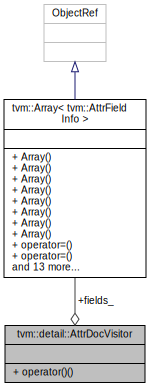
\includegraphics[width=222pt]{classtvm_1_1detail_1_1AttrDocVisitor__coll__graph}
\end{center}
\end{figure}
\subsection*{Public Member Functions}
\begin{DoxyCompactItemize}
\item 
{\footnotesize template$<$typename T $>$ }\\\hyperlink{classtvm_1_1detail_1_1AttrDocEntry}{Attr\+Doc\+Entry} \hyperlink{classtvm_1_1detail_1_1AttrDocVisitor_a1091752fc7d78b471b034877ad9344b3}{operator()} (const char $\ast$key, T $\ast$v)
\end{DoxyCompactItemize}
\subsection*{Public Attributes}
\begin{DoxyCompactItemize}
\item 
\hyperlink{classtvm_1_1Array}{Array}$<$ \hyperlink{classtvm_1_1AttrFieldInfo}{Attr\+Field\+Info} $>$ \hyperlink{classtvm_1_1detail_1_1AttrDocVisitor_aa32707d90cd2cf8e5334afa4fe3d4722}{fields\+\_\+}
\end{DoxyCompactItemize}


\subsection{Member Function Documentation}
\index{tvm\+::detail\+::\+Attr\+Doc\+Visitor@{tvm\+::detail\+::\+Attr\+Doc\+Visitor}!operator()@{operator()}}
\index{operator()@{operator()}!tvm\+::detail\+::\+Attr\+Doc\+Visitor@{tvm\+::detail\+::\+Attr\+Doc\+Visitor}}
\subsubsection[{\texorpdfstring{operator()(const char $\ast$key, T $\ast$v)}{operator()(const char *key, T *v)}}]{\setlength{\rightskip}{0pt plus 5cm}template$<$typename T $>$ {\bf Attr\+Doc\+Entry} tvm\+::detail\+::\+Attr\+Doc\+Visitor\+::operator() (
\begin{DoxyParamCaption}
\item[{const char $\ast$}]{key, }
\item[{T $\ast$}]{v}
\end{DoxyParamCaption}
)\hspace{0.3cm}{\ttfamily [inline]}}\hypertarget{classtvm_1_1detail_1_1AttrDocVisitor_a1091752fc7d78b471b034877ad9344b3}{}\label{classtvm_1_1detail_1_1AttrDocVisitor_a1091752fc7d78b471b034877ad9344b3}


\subsection{Member Data Documentation}
\index{tvm\+::detail\+::\+Attr\+Doc\+Visitor@{tvm\+::detail\+::\+Attr\+Doc\+Visitor}!fields\+\_\+@{fields\+\_\+}}
\index{fields\+\_\+@{fields\+\_\+}!tvm\+::detail\+::\+Attr\+Doc\+Visitor@{tvm\+::detail\+::\+Attr\+Doc\+Visitor}}
\subsubsection[{\texorpdfstring{fields\+\_\+}{fields_}}]{\setlength{\rightskip}{0pt plus 5cm}{\bf Array}$<${\bf Attr\+Field\+Info}$>$ tvm\+::detail\+::\+Attr\+Doc\+Visitor\+::fields\+\_\+}\hypertarget{classtvm_1_1detail_1_1AttrDocVisitor_aa32707d90cd2cf8e5334afa4fe3d4722}{}\label{classtvm_1_1detail_1_1AttrDocVisitor_aa32707d90cd2cf8e5334afa4fe3d4722}


The documentation for this class was generated from the following file\+:\begin{DoxyCompactItemize}
\item 
include/tvm/ir/\hyperlink{ir_2attrs_8h}{attrs.\+h}\end{DoxyCompactItemize}

\hypertarget{structtvm_1_1AttrError}{}\section{tvm\+:\+:Attr\+Error Struct Reference}
\label{structtvm_1_1AttrError}\index{tvm\+::\+Attr\+Error@{tvm\+::\+Attr\+Error}}


\hyperlink{classtvm_1_1Error}{Error} thrown during attribute checking.  




{\ttfamily \#include $<$attrs.\+h$>$}



Inheritance diagram for tvm\+:\+:Attr\+Error\+:
\nopagebreak
\begin{figure}[H]
\begin{center}
\leavevmode
\includegraphics[width=163pt]{structtvm_1_1AttrError__inherit__graph}
\end{center}
\end{figure}


Collaboration diagram for tvm\+:\+:Attr\+Error\+:
\nopagebreak
\begin{figure}[H]
\begin{center}
\leavevmode
\includegraphics[width=163pt]{structtvm_1_1AttrError__coll__graph}
\end{center}
\end{figure}
\subsection*{Public Member Functions}
\begin{DoxyCompactItemize}
\item 
\hyperlink{structtvm_1_1AttrError_a34484ea3d145d7de08a65c107f25d7e2}{Attr\+Error} (const std\+::string \&msg)
\begin{DoxyCompactList}\small\item\em constructor \end{DoxyCompactList}\end{DoxyCompactItemize}


\subsection{Detailed Description}
\hyperlink{classtvm_1_1Error}{Error} thrown during attribute checking. 

\subsection{Constructor \& Destructor Documentation}
\index{tvm\+::\+Attr\+Error@{tvm\+::\+Attr\+Error}!Attr\+Error@{Attr\+Error}}
\index{Attr\+Error@{Attr\+Error}!tvm\+::\+Attr\+Error@{tvm\+::\+Attr\+Error}}
\subsubsection[{\texorpdfstring{Attr\+Error(const std\+::string \&msg)}{AttrError(const std::string &msg)}}]{\setlength{\rightskip}{0pt plus 5cm}tvm\+::\+Attr\+Error\+::\+Attr\+Error (
\begin{DoxyParamCaption}
\item[{const std\+::string \&}]{msg}
\end{DoxyParamCaption}
)\hspace{0.3cm}{\ttfamily [inline]}, {\ttfamily [explicit]}}\hypertarget{structtvm_1_1AttrError_a34484ea3d145d7de08a65c107f25d7e2}{}\label{structtvm_1_1AttrError_a34484ea3d145d7de08a65c107f25d7e2}


constructor 


\begin{DoxyParams}{Parameters}
{\em msg} & error message \\
\hline
\end{DoxyParams}


The documentation for this struct was generated from the following file\+:\begin{DoxyCompactItemize}
\item 
include/tvm/ir/\hyperlink{ir_2attrs_8h}{attrs.\+h}\end{DoxyCompactItemize}

\hypertarget{classtvm_1_1detail_1_1AttrExistVisitor}{}\section{tvm\+:\+:detail\+:\+:Attr\+Exist\+Visitor Class Reference}
\label{classtvm_1_1detail_1_1AttrExistVisitor}\index{tvm\+::detail\+::\+Attr\+Exist\+Visitor@{tvm\+::detail\+::\+Attr\+Exist\+Visitor}}


{\ttfamily \#include $<$attrs.\+h$>$}



Collaboration diagram for tvm\+:\+:detail\+:\+:Attr\+Exist\+Visitor\+:
\nopagebreak
\begin{figure}[H]
\begin{center}
\leavevmode
\includegraphics[width=224pt]{classtvm_1_1detail_1_1AttrExistVisitor__coll__graph}
\end{center}
\end{figure}
\subsection*{Public Member Functions}
\begin{DoxyCompactItemize}
\item 
{\footnotesize template$<$typename T $>$ }\\\hyperlink{structtvm_1_1detail_1_1AttrNopEntry}{Attr\+Nop\+Entry} \hyperlink{classtvm_1_1detail_1_1AttrExistVisitor_a345bb38b31b732a830eb9df3e16f6895}{operator()} (const char $\ast$key, T $\ast$v)
\end{DoxyCompactItemize}
\subsection*{Public Attributes}
\begin{DoxyCompactItemize}
\item 
std\+::string \hyperlink{classtvm_1_1detail_1_1AttrExistVisitor_a42cfd0949c298dea06fb2c4fb39e188d}{key\+\_\+}
\item 
bool \hyperlink{classtvm_1_1detail_1_1AttrExistVisitor_ac6ae7aa3d30f25a953810bcc0d0a938f}{exist\+\_\+} \{false\}
\end{DoxyCompactItemize}


\subsection{Member Function Documentation}
\index{tvm\+::detail\+::\+Attr\+Exist\+Visitor@{tvm\+::detail\+::\+Attr\+Exist\+Visitor}!operator()@{operator()}}
\index{operator()@{operator()}!tvm\+::detail\+::\+Attr\+Exist\+Visitor@{tvm\+::detail\+::\+Attr\+Exist\+Visitor}}
\subsubsection[{\texorpdfstring{operator()(const char $\ast$key, T $\ast$v)}{operator()(const char *key, T *v)}}]{\setlength{\rightskip}{0pt plus 5cm}template$<$typename T $>$ {\bf Attr\+Nop\+Entry} tvm\+::detail\+::\+Attr\+Exist\+Visitor\+::operator() (
\begin{DoxyParamCaption}
\item[{const char $\ast$}]{key, }
\item[{T $\ast$}]{v}
\end{DoxyParamCaption}
)\hspace{0.3cm}{\ttfamily [inline]}}\hypertarget{classtvm_1_1detail_1_1AttrExistVisitor_a345bb38b31b732a830eb9df3e16f6895}{}\label{classtvm_1_1detail_1_1AttrExistVisitor_a345bb38b31b732a830eb9df3e16f6895}


\subsection{Member Data Documentation}
\index{tvm\+::detail\+::\+Attr\+Exist\+Visitor@{tvm\+::detail\+::\+Attr\+Exist\+Visitor}!exist\+\_\+@{exist\+\_\+}}
\index{exist\+\_\+@{exist\+\_\+}!tvm\+::detail\+::\+Attr\+Exist\+Visitor@{tvm\+::detail\+::\+Attr\+Exist\+Visitor}}
\subsubsection[{\texorpdfstring{exist\+\_\+}{exist_}}]{\setlength{\rightskip}{0pt plus 5cm}bool tvm\+::detail\+::\+Attr\+Exist\+Visitor\+::exist\+\_\+ \{false\}}\hypertarget{classtvm_1_1detail_1_1AttrExistVisitor_ac6ae7aa3d30f25a953810bcc0d0a938f}{}\label{classtvm_1_1detail_1_1AttrExistVisitor_ac6ae7aa3d30f25a953810bcc0d0a938f}
\index{tvm\+::detail\+::\+Attr\+Exist\+Visitor@{tvm\+::detail\+::\+Attr\+Exist\+Visitor}!key\+\_\+@{key\+\_\+}}
\index{key\+\_\+@{key\+\_\+}!tvm\+::detail\+::\+Attr\+Exist\+Visitor@{tvm\+::detail\+::\+Attr\+Exist\+Visitor}}
\subsubsection[{\texorpdfstring{key\+\_\+}{key_}}]{\setlength{\rightskip}{0pt plus 5cm}std\+::string tvm\+::detail\+::\+Attr\+Exist\+Visitor\+::key\+\_\+}\hypertarget{classtvm_1_1detail_1_1AttrExistVisitor_a42cfd0949c298dea06fb2c4fb39e188d}{}\label{classtvm_1_1detail_1_1AttrExistVisitor_a42cfd0949c298dea06fb2c4fb39e188d}


The documentation for this class was generated from the following file\+:\begin{DoxyCompactItemize}
\item 
include/tvm/ir/\hyperlink{ir_2attrs_8h}{attrs.\+h}\end{DoxyCompactItemize}

\hypertarget{classtvm_1_1AttrFieldInfo}{}\section{tvm\+:\+:Attr\+Field\+Info Class Reference}
\label{classtvm_1_1AttrFieldInfo}\index{tvm\+::\+Attr\+Field\+Info@{tvm\+::\+Attr\+Field\+Info}}


\hyperlink{classtvm_1_1AttrFieldInfo}{Attr\+Field\+Info}.  




{\ttfamily \#include $<$attrs.\+h$>$}



Inheritance diagram for tvm\+:\+:Attr\+Field\+Info\+:
\nopagebreak
\begin{figure}[H]
\begin{center}
\leavevmode
\includegraphics[width=230pt]{classtvm_1_1AttrFieldInfo__inherit__graph}
\end{center}
\end{figure}


Collaboration diagram for tvm\+:\+:Attr\+Field\+Info\+:
\nopagebreak
\begin{figure}[H]
\begin{center}
\leavevmode
\includegraphics[width=230pt]{classtvm_1_1AttrFieldInfo__coll__graph}
\end{center}
\end{figure}
\subsection*{Public Member Functions}
\begin{DoxyCompactItemize}
\item 
\hyperlink{classtvm_1_1AttrFieldInfo_af897e77cf019cd43014025ac0d2a5a37}{T\+V\+M\+\_\+\+D\+E\+F\+I\+N\+E\+\_\+\+O\+B\+J\+E\+C\+T\+\_\+\+R\+E\+F\+\_\+\+M\+E\+T\+H\+O\+DS} (\hyperlink{classtvm_1_1AttrFieldInfo}{Attr\+Field\+Info}, Object\+Ref, \hyperlink{classtvm_1_1AttrFieldInfoNode}{Attr\+Field\+Info\+Node})
\end{DoxyCompactItemize}


\subsection{Detailed Description}
\hyperlink{classtvm_1_1AttrFieldInfo}{Attr\+Field\+Info}. 

\subsection{Member Function Documentation}
\index{tvm\+::\+Attr\+Field\+Info@{tvm\+::\+Attr\+Field\+Info}!T\+V\+M\+\_\+\+D\+E\+F\+I\+N\+E\+\_\+\+O\+B\+J\+E\+C\+T\+\_\+\+R\+E\+F\+\_\+\+M\+E\+T\+H\+O\+DS@{T\+V\+M\+\_\+\+D\+E\+F\+I\+N\+E\+\_\+\+O\+B\+J\+E\+C\+T\+\_\+\+R\+E\+F\+\_\+\+M\+E\+T\+H\+O\+DS}}
\index{T\+V\+M\+\_\+\+D\+E\+F\+I\+N\+E\+\_\+\+O\+B\+J\+E\+C\+T\+\_\+\+R\+E\+F\+\_\+\+M\+E\+T\+H\+O\+DS@{T\+V\+M\+\_\+\+D\+E\+F\+I\+N\+E\+\_\+\+O\+B\+J\+E\+C\+T\+\_\+\+R\+E\+F\+\_\+\+M\+E\+T\+H\+O\+DS}!tvm\+::\+Attr\+Field\+Info@{tvm\+::\+Attr\+Field\+Info}}
\subsubsection[{\texorpdfstring{T\+V\+M\+\_\+\+D\+E\+F\+I\+N\+E\+\_\+\+O\+B\+J\+E\+C\+T\+\_\+\+R\+E\+F\+\_\+\+M\+E\+T\+H\+O\+D\+S(\+Attr\+Field\+Info, Object\+Ref, Attr\+Field\+Info\+Node)}{TVM_DEFINE_OBJECT_REF_METHODS(AttrFieldInfo, ObjectRef, AttrFieldInfoNode)}}]{\setlength{\rightskip}{0pt plus 5cm}tvm\+::\+Attr\+Field\+Info\+::\+T\+V\+M\+\_\+\+D\+E\+F\+I\+N\+E\+\_\+\+O\+B\+J\+E\+C\+T\+\_\+\+R\+E\+F\+\_\+\+M\+E\+T\+H\+O\+DS (
\begin{DoxyParamCaption}
\item[{{\bf Attr\+Field\+Info}}]{, }
\item[{Object\+Ref}]{, }
\item[{{\bf Attr\+Field\+Info\+Node}}]{}
\end{DoxyParamCaption}
)}\hypertarget{classtvm_1_1AttrFieldInfo_af897e77cf019cd43014025ac0d2a5a37}{}\label{classtvm_1_1AttrFieldInfo_af897e77cf019cd43014025ac0d2a5a37}


The documentation for this class was generated from the following file\+:\begin{DoxyCompactItemize}
\item 
include/tvm/ir/\hyperlink{ir_2attrs_8h}{attrs.\+h}\end{DoxyCompactItemize}

\hypertarget{classtvm_1_1AttrFieldInfoNode}{}\section{tvm\+:\+:Attr\+Field\+Info\+Node Class Reference}
\label{classtvm_1_1AttrFieldInfoNode}\index{tvm\+::\+Attr\+Field\+Info\+Node@{tvm\+::\+Attr\+Field\+Info\+Node}}


Information about attribute fields in string representations.  




{\ttfamily \#include $<$attrs.\+h$>$}



Inheritance diagram for tvm\+:\+:Attr\+Field\+Info\+Node\+:
\nopagebreak
\begin{figure}[H]
\begin{center}
\leavevmode
\includegraphics[width=285pt]{classtvm_1_1AttrFieldInfoNode__inherit__graph}
\end{center}
\end{figure}


Collaboration diagram for tvm\+:\+:Attr\+Field\+Info\+Node\+:
\nopagebreak
\begin{figure}[H]
\begin{center}
\leavevmode
\includegraphics[width=285pt]{classtvm_1_1AttrFieldInfoNode__coll__graph}
\end{center}
\end{figure}
\subsection*{Public Member Functions}
\begin{DoxyCompactItemize}
\item 
void \hyperlink{classtvm_1_1AttrFieldInfoNode_aa8428bae334dcf9c3f2f6594a818742c}{Visit\+Attrs} (\hyperlink{classtvm_1_1AttrVisitor}{Attr\+Visitor} $\ast$v)
\item 
\hyperlink{classtvm_1_1AttrFieldInfoNode_a915476a2aefc4dfb342c3aa40f235b81}{T\+V\+M\+\_\+\+D\+E\+C\+L\+A\+R\+E\+\_\+\+F\+I\+N\+A\+L\+\_\+\+O\+B\+J\+E\+C\+T\+\_\+\+I\+N\+FO} (\hyperlink{classtvm_1_1AttrFieldInfoNode}{Attr\+Field\+Info\+Node}, Object)
\end{DoxyCompactItemize}
\subsection*{Public Attributes}
\begin{DoxyCompactItemize}
\item 
std\+::string \hyperlink{classtvm_1_1AttrFieldInfoNode_a94f3593b41c2dd3be2aea793794d4dca}{name}
\begin{DoxyCompactList}\small\item\em name of the field \end{DoxyCompactList}\item 
std\+::string \hyperlink{classtvm_1_1AttrFieldInfoNode_a625467e8153ee8657ae080693baa374c}{type\+\_\+info}
\begin{DoxyCompactList}\small\item\em type docstring information in str. \end{DoxyCompactList}\item 
std\+::string \hyperlink{classtvm_1_1AttrFieldInfoNode_a1a281d5417d10840872e3c2c67c7290b}{description}
\begin{DoxyCompactList}\small\item\em detailed description of the type \end{DoxyCompactList}\end{DoxyCompactItemize}
\subsection*{Static Public Attributes}
\begin{DoxyCompactItemize}
\item 
static constexpr const char $\ast$ \hyperlink{classtvm_1_1AttrFieldInfoNode_afe4293c9f1aea71f845c5ed9633af2c9}{\+\_\+type\+\_\+key} = \char`\"{}Attr\+Field\+Info\char`\"{}
\item 
static constexpr bool \hyperlink{classtvm_1_1AttrFieldInfoNode_afdb98106a5c8d5ad2106fd03043283f7}{\+\_\+type\+\_\+has\+\_\+method\+\_\+sequal\+\_\+reduce} = false
\item 
static constexpr bool \hyperlink{classtvm_1_1AttrFieldInfoNode_a29563a91b0ce0f0118c755e072c10dfc}{\+\_\+type\+\_\+has\+\_\+method\+\_\+shash\+\_\+reduce} = false
\end{DoxyCompactItemize}


\subsection{Detailed Description}
Information about attribute fields in string representations. 

\subsection{Member Function Documentation}
\index{tvm\+::\+Attr\+Field\+Info\+Node@{tvm\+::\+Attr\+Field\+Info\+Node}!T\+V\+M\+\_\+\+D\+E\+C\+L\+A\+R\+E\+\_\+\+F\+I\+N\+A\+L\+\_\+\+O\+B\+J\+E\+C\+T\+\_\+\+I\+N\+FO@{T\+V\+M\+\_\+\+D\+E\+C\+L\+A\+R\+E\+\_\+\+F\+I\+N\+A\+L\+\_\+\+O\+B\+J\+E\+C\+T\+\_\+\+I\+N\+FO}}
\index{T\+V\+M\+\_\+\+D\+E\+C\+L\+A\+R\+E\+\_\+\+F\+I\+N\+A\+L\+\_\+\+O\+B\+J\+E\+C\+T\+\_\+\+I\+N\+FO@{T\+V\+M\+\_\+\+D\+E\+C\+L\+A\+R\+E\+\_\+\+F\+I\+N\+A\+L\+\_\+\+O\+B\+J\+E\+C\+T\+\_\+\+I\+N\+FO}!tvm\+::\+Attr\+Field\+Info\+Node@{tvm\+::\+Attr\+Field\+Info\+Node}}
\subsubsection[{\texorpdfstring{T\+V\+M\+\_\+\+D\+E\+C\+L\+A\+R\+E\+\_\+\+F\+I\+N\+A\+L\+\_\+\+O\+B\+J\+E\+C\+T\+\_\+\+I\+N\+F\+O(\+Attr\+Field\+Info\+Node, Object)}{TVM_DECLARE_FINAL_OBJECT_INFO(AttrFieldInfoNode, Object)}}]{\setlength{\rightskip}{0pt plus 5cm}tvm\+::\+Attr\+Field\+Info\+Node\+::\+T\+V\+M\+\_\+\+D\+E\+C\+L\+A\+R\+E\+\_\+\+F\+I\+N\+A\+L\+\_\+\+O\+B\+J\+E\+C\+T\+\_\+\+I\+N\+FO (
\begin{DoxyParamCaption}
\item[{{\bf Attr\+Field\+Info\+Node}}]{, }
\item[{Object}]{}
\end{DoxyParamCaption}
)}\hypertarget{classtvm_1_1AttrFieldInfoNode_a915476a2aefc4dfb342c3aa40f235b81}{}\label{classtvm_1_1AttrFieldInfoNode_a915476a2aefc4dfb342c3aa40f235b81}
\index{tvm\+::\+Attr\+Field\+Info\+Node@{tvm\+::\+Attr\+Field\+Info\+Node}!Visit\+Attrs@{Visit\+Attrs}}
\index{Visit\+Attrs@{Visit\+Attrs}!tvm\+::\+Attr\+Field\+Info\+Node@{tvm\+::\+Attr\+Field\+Info\+Node}}
\subsubsection[{\texorpdfstring{Visit\+Attrs(\+Attr\+Visitor $\ast$v)}{VisitAttrs(AttrVisitor *v)}}]{\setlength{\rightskip}{0pt plus 5cm}void tvm\+::\+Attr\+Field\+Info\+Node\+::\+Visit\+Attrs (
\begin{DoxyParamCaption}
\item[{{\bf Attr\+Visitor} $\ast$}]{v}
\end{DoxyParamCaption}
)\hspace{0.3cm}{\ttfamily [inline]}}\hypertarget{classtvm_1_1AttrFieldInfoNode_aa8428bae334dcf9c3f2f6594a818742c}{}\label{classtvm_1_1AttrFieldInfoNode_aa8428bae334dcf9c3f2f6594a818742c}


\subsection{Member Data Documentation}
\index{tvm\+::\+Attr\+Field\+Info\+Node@{tvm\+::\+Attr\+Field\+Info\+Node}!\+\_\+type\+\_\+has\+\_\+method\+\_\+sequal\+\_\+reduce@{\+\_\+type\+\_\+has\+\_\+method\+\_\+sequal\+\_\+reduce}}
\index{\+\_\+type\+\_\+has\+\_\+method\+\_\+sequal\+\_\+reduce@{\+\_\+type\+\_\+has\+\_\+method\+\_\+sequal\+\_\+reduce}!tvm\+::\+Attr\+Field\+Info\+Node@{tvm\+::\+Attr\+Field\+Info\+Node}}
\subsubsection[{\texorpdfstring{\+\_\+type\+\_\+has\+\_\+method\+\_\+sequal\+\_\+reduce}{_type_has_method_sequal_reduce}}]{\setlength{\rightskip}{0pt plus 5cm}constexpr bool tvm\+::\+Attr\+Field\+Info\+Node\+::\+\_\+type\+\_\+has\+\_\+method\+\_\+sequal\+\_\+reduce = false\hspace{0.3cm}{\ttfamily [static]}}\hypertarget{classtvm_1_1AttrFieldInfoNode_afdb98106a5c8d5ad2106fd03043283f7}{}\label{classtvm_1_1AttrFieldInfoNode_afdb98106a5c8d5ad2106fd03043283f7}
\index{tvm\+::\+Attr\+Field\+Info\+Node@{tvm\+::\+Attr\+Field\+Info\+Node}!\+\_\+type\+\_\+has\+\_\+method\+\_\+shash\+\_\+reduce@{\+\_\+type\+\_\+has\+\_\+method\+\_\+shash\+\_\+reduce}}
\index{\+\_\+type\+\_\+has\+\_\+method\+\_\+shash\+\_\+reduce@{\+\_\+type\+\_\+has\+\_\+method\+\_\+shash\+\_\+reduce}!tvm\+::\+Attr\+Field\+Info\+Node@{tvm\+::\+Attr\+Field\+Info\+Node}}
\subsubsection[{\texorpdfstring{\+\_\+type\+\_\+has\+\_\+method\+\_\+shash\+\_\+reduce}{_type_has_method_shash_reduce}}]{\setlength{\rightskip}{0pt plus 5cm}constexpr bool tvm\+::\+Attr\+Field\+Info\+Node\+::\+\_\+type\+\_\+has\+\_\+method\+\_\+shash\+\_\+reduce = false\hspace{0.3cm}{\ttfamily [static]}}\hypertarget{classtvm_1_1AttrFieldInfoNode_a29563a91b0ce0f0118c755e072c10dfc}{}\label{classtvm_1_1AttrFieldInfoNode_a29563a91b0ce0f0118c755e072c10dfc}
\index{tvm\+::\+Attr\+Field\+Info\+Node@{tvm\+::\+Attr\+Field\+Info\+Node}!\+\_\+type\+\_\+key@{\+\_\+type\+\_\+key}}
\index{\+\_\+type\+\_\+key@{\+\_\+type\+\_\+key}!tvm\+::\+Attr\+Field\+Info\+Node@{tvm\+::\+Attr\+Field\+Info\+Node}}
\subsubsection[{\texorpdfstring{\+\_\+type\+\_\+key}{_type_key}}]{\setlength{\rightskip}{0pt plus 5cm}constexpr const char$\ast$ tvm\+::\+Attr\+Field\+Info\+Node\+::\+\_\+type\+\_\+key = \char`\"{}Attr\+Field\+Info\char`\"{}\hspace{0.3cm}{\ttfamily [static]}}\hypertarget{classtvm_1_1AttrFieldInfoNode_afe4293c9f1aea71f845c5ed9633af2c9}{}\label{classtvm_1_1AttrFieldInfoNode_afe4293c9f1aea71f845c5ed9633af2c9}
\index{tvm\+::\+Attr\+Field\+Info\+Node@{tvm\+::\+Attr\+Field\+Info\+Node}!description@{description}}
\index{description@{description}!tvm\+::\+Attr\+Field\+Info\+Node@{tvm\+::\+Attr\+Field\+Info\+Node}}
\subsubsection[{\texorpdfstring{description}{description}}]{\setlength{\rightskip}{0pt plus 5cm}std\+::string tvm\+::\+Attr\+Field\+Info\+Node\+::description}\hypertarget{classtvm_1_1AttrFieldInfoNode_a1a281d5417d10840872e3c2c67c7290b}{}\label{classtvm_1_1AttrFieldInfoNode_a1a281d5417d10840872e3c2c67c7290b}


detailed description of the type 

\index{tvm\+::\+Attr\+Field\+Info\+Node@{tvm\+::\+Attr\+Field\+Info\+Node}!name@{name}}
\index{name@{name}!tvm\+::\+Attr\+Field\+Info\+Node@{tvm\+::\+Attr\+Field\+Info\+Node}}
\subsubsection[{\texorpdfstring{name}{name}}]{\setlength{\rightskip}{0pt plus 5cm}std\+::string tvm\+::\+Attr\+Field\+Info\+Node\+::name}\hypertarget{classtvm_1_1AttrFieldInfoNode_a94f3593b41c2dd3be2aea793794d4dca}{}\label{classtvm_1_1AttrFieldInfoNode_a94f3593b41c2dd3be2aea793794d4dca}


name of the field 

\index{tvm\+::\+Attr\+Field\+Info\+Node@{tvm\+::\+Attr\+Field\+Info\+Node}!type\+\_\+info@{type\+\_\+info}}
\index{type\+\_\+info@{type\+\_\+info}!tvm\+::\+Attr\+Field\+Info\+Node@{tvm\+::\+Attr\+Field\+Info\+Node}}
\subsubsection[{\texorpdfstring{type\+\_\+info}{type_info}}]{\setlength{\rightskip}{0pt plus 5cm}std\+::string tvm\+::\+Attr\+Field\+Info\+Node\+::type\+\_\+info}\hypertarget{classtvm_1_1AttrFieldInfoNode_a625467e8153ee8657ae080693baa374c}{}\label{classtvm_1_1AttrFieldInfoNode_a625467e8153ee8657ae080693baa374c}


type docstring information in str. 



The documentation for this class was generated from the following file\+:\begin{DoxyCompactItemize}
\item 
include/tvm/ir/\hyperlink{ir_2attrs_8h}{attrs.\+h}\end{DoxyCompactItemize}

\hypertarget{structtvm_1_1detail_1_1AttrInitEntry}{}\section{tvm\+:\+:detail\+:\+:Attr\+Init\+Entry$<$ T $>$ Struct Template Reference}
\label{structtvm_1_1detail_1_1AttrInitEntry}\index{tvm\+::detail\+::\+Attr\+Init\+Entry$<$ T $>$@{tvm\+::detail\+::\+Attr\+Init\+Entry$<$ T $>$}}


{\ttfamily \#include $<$attrs.\+h$>$}



Collaboration diagram for tvm\+:\+:detail\+:\+:Attr\+Init\+Entry$<$ T $>$\+:
\nopagebreak
\begin{figure}[H]
\begin{center}
\leavevmode
\includegraphics[width=238pt]{structtvm_1_1detail_1_1AttrInitEntry__coll__graph}
\end{center}
\end{figure}
\subsection*{Public Types}
\begin{DoxyCompactItemize}
\item 
using \hyperlink{structtvm_1_1detail_1_1AttrInitEntry_acac846c239440c570206f36c2d04c373}{T\+Self} = \hyperlink{structtvm_1_1detail_1_1AttrInitEntry}{Attr\+Init\+Entry}$<$ T $>$
\end{DoxyCompactItemize}
\subsection*{Public Member Functions}
\begin{DoxyCompactItemize}
\item 
\hyperlink{structtvm_1_1detail_1_1AttrInitEntry_a7f0c496115e88acf39d413875b44cd28}{$\sim$\+Attr\+Init\+Entry} () D\+M\+L\+C\+\_\+\+T\+H\+R\+O\+W\+\_\+\+E\+X\+C\+E\+P\+T\+I\+ON
\item 
\hyperlink{structtvm_1_1detail_1_1AttrInitEntry_acac846c239440c570206f36c2d04c373}{T\+Self} \& \hyperlink{structtvm_1_1detail_1_1AttrInitEntry_a8ce4f70cc359b281428014c493cf69ad}{set\+\_\+lower\+\_\+bound} (D\+M\+L\+C\+\_\+\+A\+T\+T\+R\+I\+B\+U\+T\+E\+\_\+\+U\+N\+U\+S\+ED const T \&begin)
\item 
\hyperlink{structtvm_1_1detail_1_1AttrInitEntry_acac846c239440c570206f36c2d04c373}{T\+Self} \& \hyperlink{structtvm_1_1detail_1_1AttrInitEntry_abec687904758f8544313bba7edbcbf34}{set\+\_\+upper\+\_\+bound} (D\+M\+L\+C\+\_\+\+A\+T\+T\+R\+I\+B\+U\+T\+E\+\_\+\+U\+N\+U\+S\+ED const T \&end)
\item 
\hyperlink{structtvm_1_1detail_1_1AttrInitEntry_acac846c239440c570206f36c2d04c373}{T\+Self} \& \hyperlink{structtvm_1_1detail_1_1AttrInitEntry_ae23e7210dac22db414244fe34e5a64e5}{set\+\_\+default} (D\+M\+L\+C\+\_\+\+A\+T\+T\+R\+I\+B\+U\+T\+E\+\_\+\+U\+N\+U\+S\+ED const T \&value)
\item 
\hyperlink{structtvm_1_1detail_1_1AttrInitEntry_acac846c239440c570206f36c2d04c373}{T\+Self} \& \hyperlink{structtvm_1_1detail_1_1AttrInitEntry_a64eca870988f14379a2c47085cb5a0f2}{describe} (D\+M\+L\+C\+\_\+\+A\+T\+T\+R\+I\+B\+U\+T\+E\+\_\+\+U\+N\+U\+S\+ED const char $\ast$str)
\end{DoxyCompactItemize}
\subsection*{Public Attributes}
\begin{DoxyCompactItemize}
\item 
const char $\ast$ \hyperlink{structtvm_1_1detail_1_1AttrInitEntry_a573a25648ca0d3d8fe28f6c7614248bf}{type\+\_\+key\+\_\+}
\item 
const char $\ast$ \hyperlink{structtvm_1_1detail_1_1AttrInitEntry_a5ed0b852e3229c1c1e0b8c924c53479e}{key\+\_\+}
\item 
T $\ast$ \hyperlink{structtvm_1_1detail_1_1AttrInitEntry_aea83f0af9e7ea95e5f7d614a717b7760}{value\+\_\+}
\item 
bool \hyperlink{structtvm_1_1detail_1_1AttrInitEntry_aaba94dddd1e9c367023dbe03e76634bf}{value\+\_\+missing\+\_\+} \{true\}
\end{DoxyCompactItemize}


\subsection{Member Typedef Documentation}
\index{tvm\+::detail\+::\+Attr\+Init\+Entry@{tvm\+::detail\+::\+Attr\+Init\+Entry}!T\+Self@{T\+Self}}
\index{T\+Self@{T\+Self}!tvm\+::detail\+::\+Attr\+Init\+Entry@{tvm\+::detail\+::\+Attr\+Init\+Entry}}
\subsubsection[{\texorpdfstring{T\+Self}{TSelf}}]{\setlength{\rightskip}{0pt plus 5cm}template$<$typename T$>$ using {\bf tvm\+::detail\+::\+Attr\+Init\+Entry}$<$ T $>$\+::{\bf T\+Self} =  {\bf Attr\+Init\+Entry}$<$T$>$}\hypertarget{structtvm_1_1detail_1_1AttrInitEntry_acac846c239440c570206f36c2d04c373}{}\label{structtvm_1_1detail_1_1AttrInitEntry_acac846c239440c570206f36c2d04c373}


\subsection{Constructor \& Destructor Documentation}
\index{tvm\+::detail\+::\+Attr\+Init\+Entry@{tvm\+::detail\+::\+Attr\+Init\+Entry}!````~Attr\+Init\+Entry@{$\sim$\+Attr\+Init\+Entry}}
\index{````~Attr\+Init\+Entry@{$\sim$\+Attr\+Init\+Entry}!tvm\+::detail\+::\+Attr\+Init\+Entry@{tvm\+::detail\+::\+Attr\+Init\+Entry}}
\subsubsection[{\texorpdfstring{$\sim$\+Attr\+Init\+Entry() D\+M\+L\+C\+\_\+\+T\+H\+R\+O\+W\+\_\+\+E\+X\+C\+E\+P\+T\+I\+ON}{~AttrInitEntry() DMLC_THROW_EXCEPTION}}]{\setlength{\rightskip}{0pt plus 5cm}template$<$typename T$>$ {\bf tvm\+::detail\+::\+Attr\+Init\+Entry}$<$ T $>$\+::$\sim${\bf Attr\+Init\+Entry} (
\begin{DoxyParamCaption}
{}
\end{DoxyParamCaption}
)\hspace{0.3cm}{\ttfamily [inline]}}\hypertarget{structtvm_1_1detail_1_1AttrInitEntry_a7f0c496115e88acf39d413875b44cd28}{}\label{structtvm_1_1detail_1_1AttrInitEntry_a7f0c496115e88acf39d413875b44cd28}


\subsection{Member Function Documentation}
\index{tvm\+::detail\+::\+Attr\+Init\+Entry@{tvm\+::detail\+::\+Attr\+Init\+Entry}!describe@{describe}}
\index{describe@{describe}!tvm\+::detail\+::\+Attr\+Init\+Entry@{tvm\+::detail\+::\+Attr\+Init\+Entry}}
\subsubsection[{\texorpdfstring{describe(\+D\+M\+L\+C\+\_\+\+A\+T\+T\+R\+I\+B\+U\+T\+E\+\_\+\+U\+N\+U\+S\+E\+D const char $\ast$str)}{describe(DMLC_ATTRIBUTE_UNUSED const char *str)}}]{\setlength{\rightskip}{0pt plus 5cm}template$<$typename T$>$ {\bf T\+Self}\& {\bf tvm\+::detail\+::\+Attr\+Init\+Entry}$<$ T $>$\+::describe (
\begin{DoxyParamCaption}
\item[{D\+M\+L\+C\+\_\+\+A\+T\+T\+R\+I\+B\+U\+T\+E\+\_\+\+U\+N\+U\+S\+ED const char $\ast$}]{str}
\end{DoxyParamCaption}
)\hspace{0.3cm}{\ttfamily [inline]}}\hypertarget{structtvm_1_1detail_1_1AttrInitEntry_a64eca870988f14379a2c47085cb5a0f2}{}\label{structtvm_1_1detail_1_1AttrInitEntry_a64eca870988f14379a2c47085cb5a0f2}
\index{tvm\+::detail\+::\+Attr\+Init\+Entry@{tvm\+::detail\+::\+Attr\+Init\+Entry}!set\+\_\+default@{set\+\_\+default}}
\index{set\+\_\+default@{set\+\_\+default}!tvm\+::detail\+::\+Attr\+Init\+Entry@{tvm\+::detail\+::\+Attr\+Init\+Entry}}
\subsubsection[{\texorpdfstring{set\+\_\+default(\+D\+M\+L\+C\+\_\+\+A\+T\+T\+R\+I\+B\+U\+T\+E\+\_\+\+U\+N\+U\+S\+E\+D const T \&value)}{set_default(DMLC_ATTRIBUTE_UNUSED const T &value)}}]{\setlength{\rightskip}{0pt plus 5cm}template$<$typename T$>$ {\bf T\+Self}\& {\bf tvm\+::detail\+::\+Attr\+Init\+Entry}$<$ T $>$\+::set\+\_\+default (
\begin{DoxyParamCaption}
\item[{D\+M\+L\+C\+\_\+\+A\+T\+T\+R\+I\+B\+U\+T\+E\+\_\+\+U\+N\+U\+S\+ED const T \&}]{value}
\end{DoxyParamCaption}
)\hspace{0.3cm}{\ttfamily [inline]}}\hypertarget{structtvm_1_1detail_1_1AttrInitEntry_ae23e7210dac22db414244fe34e5a64e5}{}\label{structtvm_1_1detail_1_1AttrInitEntry_ae23e7210dac22db414244fe34e5a64e5}
\index{tvm\+::detail\+::\+Attr\+Init\+Entry@{tvm\+::detail\+::\+Attr\+Init\+Entry}!set\+\_\+lower\+\_\+bound@{set\+\_\+lower\+\_\+bound}}
\index{set\+\_\+lower\+\_\+bound@{set\+\_\+lower\+\_\+bound}!tvm\+::detail\+::\+Attr\+Init\+Entry@{tvm\+::detail\+::\+Attr\+Init\+Entry}}
\subsubsection[{\texorpdfstring{set\+\_\+lower\+\_\+bound(\+D\+M\+L\+C\+\_\+\+A\+T\+T\+R\+I\+B\+U\+T\+E\+\_\+\+U\+N\+U\+S\+E\+D const T \&begin)}{set_lower_bound(DMLC_ATTRIBUTE_UNUSED const T &begin)}}]{\setlength{\rightskip}{0pt plus 5cm}template$<$typename T$>$ {\bf T\+Self}\& {\bf tvm\+::detail\+::\+Attr\+Init\+Entry}$<$ T $>$\+::set\+\_\+lower\+\_\+bound (
\begin{DoxyParamCaption}
\item[{D\+M\+L\+C\+\_\+\+A\+T\+T\+R\+I\+B\+U\+T\+E\+\_\+\+U\+N\+U\+S\+ED const T \&}]{begin}
\end{DoxyParamCaption}
)\hspace{0.3cm}{\ttfamily [inline]}}\hypertarget{structtvm_1_1detail_1_1AttrInitEntry_a8ce4f70cc359b281428014c493cf69ad}{}\label{structtvm_1_1detail_1_1AttrInitEntry_a8ce4f70cc359b281428014c493cf69ad}
\index{tvm\+::detail\+::\+Attr\+Init\+Entry@{tvm\+::detail\+::\+Attr\+Init\+Entry}!set\+\_\+upper\+\_\+bound@{set\+\_\+upper\+\_\+bound}}
\index{set\+\_\+upper\+\_\+bound@{set\+\_\+upper\+\_\+bound}!tvm\+::detail\+::\+Attr\+Init\+Entry@{tvm\+::detail\+::\+Attr\+Init\+Entry}}
\subsubsection[{\texorpdfstring{set\+\_\+upper\+\_\+bound(\+D\+M\+L\+C\+\_\+\+A\+T\+T\+R\+I\+B\+U\+T\+E\+\_\+\+U\+N\+U\+S\+E\+D const T \&end)}{set_upper_bound(DMLC_ATTRIBUTE_UNUSED const T &end)}}]{\setlength{\rightskip}{0pt plus 5cm}template$<$typename T$>$ {\bf T\+Self}\& {\bf tvm\+::detail\+::\+Attr\+Init\+Entry}$<$ T $>$\+::set\+\_\+upper\+\_\+bound (
\begin{DoxyParamCaption}
\item[{D\+M\+L\+C\+\_\+\+A\+T\+T\+R\+I\+B\+U\+T\+E\+\_\+\+U\+N\+U\+S\+ED const T \&}]{end}
\end{DoxyParamCaption}
)\hspace{0.3cm}{\ttfamily [inline]}}\hypertarget{structtvm_1_1detail_1_1AttrInitEntry_abec687904758f8544313bba7edbcbf34}{}\label{structtvm_1_1detail_1_1AttrInitEntry_abec687904758f8544313bba7edbcbf34}


\subsection{Member Data Documentation}
\index{tvm\+::detail\+::\+Attr\+Init\+Entry@{tvm\+::detail\+::\+Attr\+Init\+Entry}!key\+\_\+@{key\+\_\+}}
\index{key\+\_\+@{key\+\_\+}!tvm\+::detail\+::\+Attr\+Init\+Entry@{tvm\+::detail\+::\+Attr\+Init\+Entry}}
\subsubsection[{\texorpdfstring{key\+\_\+}{key_}}]{\setlength{\rightskip}{0pt plus 5cm}template$<$typename T$>$ const char$\ast$ {\bf tvm\+::detail\+::\+Attr\+Init\+Entry}$<$ T $>$\+::key\+\_\+}\hypertarget{structtvm_1_1detail_1_1AttrInitEntry_a5ed0b852e3229c1c1e0b8c924c53479e}{}\label{structtvm_1_1detail_1_1AttrInitEntry_a5ed0b852e3229c1c1e0b8c924c53479e}
\index{tvm\+::detail\+::\+Attr\+Init\+Entry@{tvm\+::detail\+::\+Attr\+Init\+Entry}!type\+\_\+key\+\_\+@{type\+\_\+key\+\_\+}}
\index{type\+\_\+key\+\_\+@{type\+\_\+key\+\_\+}!tvm\+::detail\+::\+Attr\+Init\+Entry@{tvm\+::detail\+::\+Attr\+Init\+Entry}}
\subsubsection[{\texorpdfstring{type\+\_\+key\+\_\+}{type_key_}}]{\setlength{\rightskip}{0pt plus 5cm}template$<$typename T$>$ const char$\ast$ {\bf tvm\+::detail\+::\+Attr\+Init\+Entry}$<$ T $>$\+::type\+\_\+key\+\_\+}\hypertarget{structtvm_1_1detail_1_1AttrInitEntry_a573a25648ca0d3d8fe28f6c7614248bf}{}\label{structtvm_1_1detail_1_1AttrInitEntry_a573a25648ca0d3d8fe28f6c7614248bf}
\index{tvm\+::detail\+::\+Attr\+Init\+Entry@{tvm\+::detail\+::\+Attr\+Init\+Entry}!value\+\_\+@{value\+\_\+}}
\index{value\+\_\+@{value\+\_\+}!tvm\+::detail\+::\+Attr\+Init\+Entry@{tvm\+::detail\+::\+Attr\+Init\+Entry}}
\subsubsection[{\texorpdfstring{value\+\_\+}{value_}}]{\setlength{\rightskip}{0pt plus 5cm}template$<$typename T$>$ T$\ast$ {\bf tvm\+::detail\+::\+Attr\+Init\+Entry}$<$ T $>$\+::value\+\_\+}\hypertarget{structtvm_1_1detail_1_1AttrInitEntry_aea83f0af9e7ea95e5f7d614a717b7760}{}\label{structtvm_1_1detail_1_1AttrInitEntry_aea83f0af9e7ea95e5f7d614a717b7760}
\index{tvm\+::detail\+::\+Attr\+Init\+Entry@{tvm\+::detail\+::\+Attr\+Init\+Entry}!value\+\_\+missing\+\_\+@{value\+\_\+missing\+\_\+}}
\index{value\+\_\+missing\+\_\+@{value\+\_\+missing\+\_\+}!tvm\+::detail\+::\+Attr\+Init\+Entry@{tvm\+::detail\+::\+Attr\+Init\+Entry}}
\subsubsection[{\texorpdfstring{value\+\_\+missing\+\_\+}{value_missing_}}]{\setlength{\rightskip}{0pt plus 5cm}template$<$typename T$>$ bool {\bf tvm\+::detail\+::\+Attr\+Init\+Entry}$<$ T $>$\+::value\+\_\+missing\+\_\+ \{true\}}\hypertarget{structtvm_1_1detail_1_1AttrInitEntry_aaba94dddd1e9c367023dbe03e76634bf}{}\label{structtvm_1_1detail_1_1AttrInitEntry_aaba94dddd1e9c367023dbe03e76634bf}


The documentation for this struct was generated from the following file\+:\begin{DoxyCompactItemize}
\item 
include/tvm/ir/\hyperlink{ir_2attrs_8h}{attrs.\+h}\end{DoxyCompactItemize}

\hypertarget{classtvm_1_1detail_1_1AttrInitVisitor}{}\section{tvm\+:\+:detail\+:\+:Attr\+Init\+Visitor$<$ F\+Find $>$ Class Template Reference}
\label{classtvm_1_1detail_1_1AttrInitVisitor}\index{tvm\+::detail\+::\+Attr\+Init\+Visitor$<$ F\+Find $>$@{tvm\+::detail\+::\+Attr\+Init\+Visitor$<$ F\+Find $>$}}


{\ttfamily \#include $<$attrs.\+h$>$}



Collaboration diagram for tvm\+:\+:detail\+:\+:Attr\+Init\+Visitor$<$ F\+Find $>$\+:
\nopagebreak
\begin{figure}[H]
\begin{center}
\leavevmode
\includegraphics[width=216pt]{classtvm_1_1detail_1_1AttrInitVisitor__coll__graph}
\end{center}
\end{figure}
\subsection*{Public Member Functions}
\begin{DoxyCompactItemize}
\item 
\hyperlink{classtvm_1_1detail_1_1AttrInitVisitor_ac3c800c9249fee195db2a5fa473fe960}{Attr\+Init\+Visitor} (const char $\ast$type\+\_\+key, F\+Find ffind)
\item 
{\footnotesize template$<$typename T $>$ }\\\hyperlink{structtvm_1_1detail_1_1AttrInitEntry}{Attr\+Init\+Entry}$<$ T $>$ \hyperlink{classtvm_1_1detail_1_1AttrInitVisitor_af0856406dd74c88334291da4eff0543d}{operator()} (const char $\ast$key, T $\ast$value)
\end{DoxyCompactItemize}
\subsection*{Public Attributes}
\begin{DoxyCompactItemize}
\item 
size\+\_\+t \hyperlink{classtvm_1_1detail_1_1AttrInitVisitor_a40694e8ade57b3e5167ec74404188f9e}{hit\+\_\+count\+\_\+} \{0\}
\end{DoxyCompactItemize}


\subsection{Constructor \& Destructor Documentation}
\index{tvm\+::detail\+::\+Attr\+Init\+Visitor@{tvm\+::detail\+::\+Attr\+Init\+Visitor}!Attr\+Init\+Visitor@{Attr\+Init\+Visitor}}
\index{Attr\+Init\+Visitor@{Attr\+Init\+Visitor}!tvm\+::detail\+::\+Attr\+Init\+Visitor@{tvm\+::detail\+::\+Attr\+Init\+Visitor}}
\subsubsection[{\texorpdfstring{Attr\+Init\+Visitor(const char $\ast$type\+\_\+key, F\+Find ffind)}{AttrInitVisitor(const char *type_key, FFind ffind)}}]{\setlength{\rightskip}{0pt plus 5cm}template$<$typename F\+Find$>$ {\bf tvm\+::detail\+::\+Attr\+Init\+Visitor}$<$ F\+Find $>$\+::{\bf Attr\+Init\+Visitor} (
\begin{DoxyParamCaption}
\item[{const char $\ast$}]{type\+\_\+key, }
\item[{F\+Find}]{ffind}
\end{DoxyParamCaption}
)\hspace{0.3cm}{\ttfamily [inline]}}\hypertarget{classtvm_1_1detail_1_1AttrInitVisitor_ac3c800c9249fee195db2a5fa473fe960}{}\label{classtvm_1_1detail_1_1AttrInitVisitor_ac3c800c9249fee195db2a5fa473fe960}


\subsection{Member Function Documentation}
\index{tvm\+::detail\+::\+Attr\+Init\+Visitor@{tvm\+::detail\+::\+Attr\+Init\+Visitor}!operator()@{operator()}}
\index{operator()@{operator()}!tvm\+::detail\+::\+Attr\+Init\+Visitor@{tvm\+::detail\+::\+Attr\+Init\+Visitor}}
\subsubsection[{\texorpdfstring{operator()(const char $\ast$key, T $\ast$value)}{operator()(const char *key, T *value)}}]{\setlength{\rightskip}{0pt plus 5cm}template$<$typename F\+Find$>$ template$<$typename T $>$ {\bf Attr\+Init\+Entry}$<$T$>$ {\bf tvm\+::detail\+::\+Attr\+Init\+Visitor}$<$ F\+Find $>$\+::operator() (
\begin{DoxyParamCaption}
\item[{const char $\ast$}]{key, }
\item[{T $\ast$}]{value}
\end{DoxyParamCaption}
)\hspace{0.3cm}{\ttfamily [inline]}}\hypertarget{classtvm_1_1detail_1_1AttrInitVisitor_af0856406dd74c88334291da4eff0543d}{}\label{classtvm_1_1detail_1_1AttrInitVisitor_af0856406dd74c88334291da4eff0543d}


\subsection{Member Data Documentation}
\index{tvm\+::detail\+::\+Attr\+Init\+Visitor@{tvm\+::detail\+::\+Attr\+Init\+Visitor}!hit\+\_\+count\+\_\+@{hit\+\_\+count\+\_\+}}
\index{hit\+\_\+count\+\_\+@{hit\+\_\+count\+\_\+}!tvm\+::detail\+::\+Attr\+Init\+Visitor@{tvm\+::detail\+::\+Attr\+Init\+Visitor}}
\subsubsection[{\texorpdfstring{hit\+\_\+count\+\_\+}{hit_count_}}]{\setlength{\rightskip}{0pt plus 5cm}template$<$typename F\+Find$>$ size\+\_\+t {\bf tvm\+::detail\+::\+Attr\+Init\+Visitor}$<$ F\+Find $>$\+::hit\+\_\+count\+\_\+ \{0\}}\hypertarget{classtvm_1_1detail_1_1AttrInitVisitor_a40694e8ade57b3e5167ec74404188f9e}{}\label{classtvm_1_1detail_1_1AttrInitVisitor_a40694e8ade57b3e5167ec74404188f9e}


The documentation for this class was generated from the following file\+:\begin{DoxyCompactItemize}
\item 
include/tvm/ir/\hyperlink{ir_2attrs_8h}{attrs.\+h}\end{DoxyCompactItemize}

\hypertarget{classtvm_1_1detail_1_1AttrNonDefaultVisitor}{}\section{tvm\+:\+:detail\+:\+:Attr\+Non\+Default\+Visitor Class Reference}
\label{classtvm_1_1detail_1_1AttrNonDefaultVisitor}\index{tvm\+::detail\+::\+Attr\+Non\+Default\+Visitor@{tvm\+::detail\+::\+Attr\+Non\+Default\+Visitor}}


{\ttfamily \#include $<$attrs.\+h$>$}



Collaboration diagram for tvm\+:\+:detail\+:\+:Attr\+Non\+Default\+Visitor\+:
\nopagebreak
\begin{figure}[H]
\begin{center}
\leavevmode
\includegraphics[width=226pt]{classtvm_1_1detail_1_1AttrNonDefaultVisitor__coll__graph}
\end{center}
\end{figure}
\subsection*{Public Member Functions}
\begin{DoxyCompactItemize}
\item 
\hyperlink{classtvm_1_1detail_1_1AttrNonDefaultVisitor_a8b27d05c6de24ab60b999c227e346337}{Attr\+Non\+Default\+Visitor} (\hyperlink{classtvm_1_1AttrVisitor}{Attr\+Visitor} $\ast$visitor)
\item 
{\footnotesize template$<$typename T $>$ }\\\hyperlink{structtvm_1_1detail_1_1AttrTriggerNonDefaultEntry}{Attr\+Trigger\+Non\+Default\+Entry}$<$ T $>$ \hyperlink{classtvm_1_1detail_1_1AttrNonDefaultVisitor_aa359d725f84781937ffd4eeb4445fc66}{operator()} (const char $\ast$key, T $\ast$value)
\end{DoxyCompactItemize}


\subsection{Constructor \& Destructor Documentation}
\index{tvm\+::detail\+::\+Attr\+Non\+Default\+Visitor@{tvm\+::detail\+::\+Attr\+Non\+Default\+Visitor}!Attr\+Non\+Default\+Visitor@{Attr\+Non\+Default\+Visitor}}
\index{Attr\+Non\+Default\+Visitor@{Attr\+Non\+Default\+Visitor}!tvm\+::detail\+::\+Attr\+Non\+Default\+Visitor@{tvm\+::detail\+::\+Attr\+Non\+Default\+Visitor}}
\subsubsection[{\texorpdfstring{Attr\+Non\+Default\+Visitor(\+Attr\+Visitor $\ast$visitor)}{AttrNonDefaultVisitor(AttrVisitor *visitor)}}]{\setlength{\rightskip}{0pt plus 5cm}tvm\+::detail\+::\+Attr\+Non\+Default\+Visitor\+::\+Attr\+Non\+Default\+Visitor (
\begin{DoxyParamCaption}
\item[{{\bf Attr\+Visitor} $\ast$}]{visitor}
\end{DoxyParamCaption}
)\hspace{0.3cm}{\ttfamily [inline]}, {\ttfamily [explicit]}}\hypertarget{classtvm_1_1detail_1_1AttrNonDefaultVisitor_a8b27d05c6de24ab60b999c227e346337}{}\label{classtvm_1_1detail_1_1AttrNonDefaultVisitor_a8b27d05c6de24ab60b999c227e346337}


\subsection{Member Function Documentation}
\index{tvm\+::detail\+::\+Attr\+Non\+Default\+Visitor@{tvm\+::detail\+::\+Attr\+Non\+Default\+Visitor}!operator()@{operator()}}
\index{operator()@{operator()}!tvm\+::detail\+::\+Attr\+Non\+Default\+Visitor@{tvm\+::detail\+::\+Attr\+Non\+Default\+Visitor}}
\subsubsection[{\texorpdfstring{operator()(const char $\ast$key, T $\ast$value)}{operator()(const char *key, T *value)}}]{\setlength{\rightskip}{0pt plus 5cm}template$<$typename T $>$ {\bf Attr\+Trigger\+Non\+Default\+Entry}$<$T$>$ tvm\+::detail\+::\+Attr\+Non\+Default\+Visitor\+::operator() (
\begin{DoxyParamCaption}
\item[{const char $\ast$}]{key, }
\item[{T $\ast$}]{value}
\end{DoxyParamCaption}
)\hspace{0.3cm}{\ttfamily [inline]}}\hypertarget{classtvm_1_1detail_1_1AttrNonDefaultVisitor_aa359d725f84781937ffd4eeb4445fc66}{}\label{classtvm_1_1detail_1_1AttrNonDefaultVisitor_aa359d725f84781937ffd4eeb4445fc66}


The documentation for this class was generated from the following file\+:\begin{DoxyCompactItemize}
\item 
include/tvm/ir/\hyperlink{ir_2attrs_8h}{attrs.\+h}\end{DoxyCompactItemize}

\hypertarget{structtvm_1_1detail_1_1AttrNopEntry}{}\section{tvm\+:\+:detail\+:\+:Attr\+Nop\+Entry Struct Reference}
\label{structtvm_1_1detail_1_1AttrNopEntry}\index{tvm\+::detail\+::\+Attr\+Nop\+Entry@{tvm\+::detail\+::\+Attr\+Nop\+Entry}}


{\ttfamily \#include $<$attrs.\+h$>$}



Collaboration diagram for tvm\+:\+:detail\+:\+:Attr\+Nop\+Entry\+:
\nopagebreak
\begin{figure}[H]
\begin{center}
\leavevmode
\includegraphics[width=216pt]{structtvm_1_1detail_1_1AttrNopEntry__coll__graph}
\end{center}
\end{figure}
\subsection*{Public Types}
\begin{DoxyCompactItemize}
\item 
using \hyperlink{structtvm_1_1detail_1_1AttrNopEntry_adab25bf47ec60e73d1e02c3cef2f6898}{T\+Self} = \hyperlink{structtvm_1_1detail_1_1AttrNopEntry}{Attr\+Nop\+Entry}
\end{DoxyCompactItemize}
\subsection*{Public Member Functions}
\begin{DoxyCompactItemize}
\item 
\hyperlink{structtvm_1_1detail_1_1AttrNopEntry_adab25bf47ec60e73d1e02c3cef2f6898}{T\+Self} \& \hyperlink{structtvm_1_1detail_1_1AttrNopEntry_a9bd1f913549c1b4376c0137f4101b791}{describe} (D\+M\+L\+C\+\_\+\+A\+T\+T\+R\+I\+B\+U\+T\+E\+\_\+\+U\+N\+U\+S\+ED const char $\ast$str)
\item 
{\footnotesize template$<$typename T $>$ }\\\hyperlink{structtvm_1_1detail_1_1AttrNopEntry_adab25bf47ec60e73d1e02c3cef2f6898}{T\+Self} \& \hyperlink{structtvm_1_1detail_1_1AttrNopEntry_a370e92bafbada9ba805a52e72881f98b}{set\+\_\+default} (D\+M\+L\+C\+\_\+\+A\+T\+T\+R\+I\+B\+U\+T\+E\+\_\+\+U\+N\+U\+S\+ED const T \&value)
\item 
{\footnotesize template$<$typename T $>$ }\\\hyperlink{structtvm_1_1detail_1_1AttrNopEntry_adab25bf47ec60e73d1e02c3cef2f6898}{T\+Self} \& \hyperlink{structtvm_1_1detail_1_1AttrNopEntry_a36da34fc54009d63283d07e9d41657f7}{set\+\_\+lower\+\_\+bound} (D\+M\+L\+C\+\_\+\+A\+T\+T\+R\+I\+B\+U\+T\+E\+\_\+\+U\+N\+U\+S\+ED const T \&begin)
\item 
{\footnotesize template$<$typename T $>$ }\\\hyperlink{structtvm_1_1detail_1_1AttrNopEntry_adab25bf47ec60e73d1e02c3cef2f6898}{T\+Self} \& \hyperlink{structtvm_1_1detail_1_1AttrNopEntry_add2843b725ee43be26672a8d2d641cce}{set\+\_\+upper\+\_\+bound} (D\+M\+L\+C\+\_\+\+A\+T\+T\+R\+I\+B\+U\+T\+E\+\_\+\+U\+N\+U\+S\+ED const T \&end)
\end{DoxyCompactItemize}


\subsection{Member Typedef Documentation}
\index{tvm\+::detail\+::\+Attr\+Nop\+Entry@{tvm\+::detail\+::\+Attr\+Nop\+Entry}!T\+Self@{T\+Self}}
\index{T\+Self@{T\+Self}!tvm\+::detail\+::\+Attr\+Nop\+Entry@{tvm\+::detail\+::\+Attr\+Nop\+Entry}}
\subsubsection[{\texorpdfstring{T\+Self}{TSelf}}]{\setlength{\rightskip}{0pt plus 5cm}using {\bf tvm\+::detail\+::\+Attr\+Nop\+Entry\+::\+T\+Self} =  {\bf Attr\+Nop\+Entry}}\hypertarget{structtvm_1_1detail_1_1AttrNopEntry_adab25bf47ec60e73d1e02c3cef2f6898}{}\label{structtvm_1_1detail_1_1AttrNopEntry_adab25bf47ec60e73d1e02c3cef2f6898}


\subsection{Member Function Documentation}
\index{tvm\+::detail\+::\+Attr\+Nop\+Entry@{tvm\+::detail\+::\+Attr\+Nop\+Entry}!describe@{describe}}
\index{describe@{describe}!tvm\+::detail\+::\+Attr\+Nop\+Entry@{tvm\+::detail\+::\+Attr\+Nop\+Entry}}
\subsubsection[{\texorpdfstring{describe(\+D\+M\+L\+C\+\_\+\+A\+T\+T\+R\+I\+B\+U\+T\+E\+\_\+\+U\+N\+U\+S\+E\+D const char $\ast$str)}{describe(DMLC_ATTRIBUTE_UNUSED const char *str)}}]{\setlength{\rightskip}{0pt plus 5cm}{\bf T\+Self}\& tvm\+::detail\+::\+Attr\+Nop\+Entry\+::describe (
\begin{DoxyParamCaption}
\item[{D\+M\+L\+C\+\_\+\+A\+T\+T\+R\+I\+B\+U\+T\+E\+\_\+\+U\+N\+U\+S\+ED const char $\ast$}]{str}
\end{DoxyParamCaption}
)\hspace{0.3cm}{\ttfamily [inline]}}\hypertarget{structtvm_1_1detail_1_1AttrNopEntry_a9bd1f913549c1b4376c0137f4101b791}{}\label{structtvm_1_1detail_1_1AttrNopEntry_a9bd1f913549c1b4376c0137f4101b791}
\index{tvm\+::detail\+::\+Attr\+Nop\+Entry@{tvm\+::detail\+::\+Attr\+Nop\+Entry}!set\+\_\+default@{set\+\_\+default}}
\index{set\+\_\+default@{set\+\_\+default}!tvm\+::detail\+::\+Attr\+Nop\+Entry@{tvm\+::detail\+::\+Attr\+Nop\+Entry}}
\subsubsection[{\texorpdfstring{set\+\_\+default(\+D\+M\+L\+C\+\_\+\+A\+T\+T\+R\+I\+B\+U\+T\+E\+\_\+\+U\+N\+U\+S\+E\+D const T \&value)}{set_default(DMLC_ATTRIBUTE_UNUSED const T &value)}}]{\setlength{\rightskip}{0pt plus 5cm}template$<$typename T $>$ {\bf T\+Self}\& tvm\+::detail\+::\+Attr\+Nop\+Entry\+::set\+\_\+default (
\begin{DoxyParamCaption}
\item[{D\+M\+L\+C\+\_\+\+A\+T\+T\+R\+I\+B\+U\+T\+E\+\_\+\+U\+N\+U\+S\+ED const T \&}]{value}
\end{DoxyParamCaption}
)\hspace{0.3cm}{\ttfamily [inline]}}\hypertarget{structtvm_1_1detail_1_1AttrNopEntry_a370e92bafbada9ba805a52e72881f98b}{}\label{structtvm_1_1detail_1_1AttrNopEntry_a370e92bafbada9ba805a52e72881f98b}
\index{tvm\+::detail\+::\+Attr\+Nop\+Entry@{tvm\+::detail\+::\+Attr\+Nop\+Entry}!set\+\_\+lower\+\_\+bound@{set\+\_\+lower\+\_\+bound}}
\index{set\+\_\+lower\+\_\+bound@{set\+\_\+lower\+\_\+bound}!tvm\+::detail\+::\+Attr\+Nop\+Entry@{tvm\+::detail\+::\+Attr\+Nop\+Entry}}
\subsubsection[{\texorpdfstring{set\+\_\+lower\+\_\+bound(\+D\+M\+L\+C\+\_\+\+A\+T\+T\+R\+I\+B\+U\+T\+E\+\_\+\+U\+N\+U\+S\+E\+D const T \&begin)}{set_lower_bound(DMLC_ATTRIBUTE_UNUSED const T &begin)}}]{\setlength{\rightskip}{0pt plus 5cm}template$<$typename T $>$ {\bf T\+Self}\& tvm\+::detail\+::\+Attr\+Nop\+Entry\+::set\+\_\+lower\+\_\+bound (
\begin{DoxyParamCaption}
\item[{D\+M\+L\+C\+\_\+\+A\+T\+T\+R\+I\+B\+U\+T\+E\+\_\+\+U\+N\+U\+S\+ED const T \&}]{begin}
\end{DoxyParamCaption}
)\hspace{0.3cm}{\ttfamily [inline]}}\hypertarget{structtvm_1_1detail_1_1AttrNopEntry_a36da34fc54009d63283d07e9d41657f7}{}\label{structtvm_1_1detail_1_1AttrNopEntry_a36da34fc54009d63283d07e9d41657f7}
\index{tvm\+::detail\+::\+Attr\+Nop\+Entry@{tvm\+::detail\+::\+Attr\+Nop\+Entry}!set\+\_\+upper\+\_\+bound@{set\+\_\+upper\+\_\+bound}}
\index{set\+\_\+upper\+\_\+bound@{set\+\_\+upper\+\_\+bound}!tvm\+::detail\+::\+Attr\+Nop\+Entry@{tvm\+::detail\+::\+Attr\+Nop\+Entry}}
\subsubsection[{\texorpdfstring{set\+\_\+upper\+\_\+bound(\+D\+M\+L\+C\+\_\+\+A\+T\+T\+R\+I\+B\+U\+T\+E\+\_\+\+U\+N\+U\+S\+E\+D const T \&end)}{set_upper_bound(DMLC_ATTRIBUTE_UNUSED const T &end)}}]{\setlength{\rightskip}{0pt plus 5cm}template$<$typename T $>$ {\bf T\+Self}\& tvm\+::detail\+::\+Attr\+Nop\+Entry\+::set\+\_\+upper\+\_\+bound (
\begin{DoxyParamCaption}
\item[{D\+M\+L\+C\+\_\+\+A\+T\+T\+R\+I\+B\+U\+T\+E\+\_\+\+U\+N\+U\+S\+ED const T \&}]{end}
\end{DoxyParamCaption}
)\hspace{0.3cm}{\ttfamily [inline]}}\hypertarget{structtvm_1_1detail_1_1AttrNopEntry_add2843b725ee43be26672a8d2d641cce}{}\label{structtvm_1_1detail_1_1AttrNopEntry_add2843b725ee43be26672a8d2d641cce}


The documentation for this struct was generated from the following file\+:\begin{DoxyCompactItemize}
\item 
include/tvm/ir/\hyperlink{ir_2attrs_8h}{attrs.\+h}\end{DoxyCompactItemize}

\hypertarget{classtvm_1_1detail_1_1AttrNormalVisitor}{}\section{tvm\+:\+:detail\+:\+:Attr\+Normal\+Visitor Class Reference}
\label{classtvm_1_1detail_1_1AttrNormalVisitor}\index{tvm\+::detail\+::\+Attr\+Normal\+Visitor@{tvm\+::detail\+::\+Attr\+Normal\+Visitor}}


{\ttfamily \#include $<$attrs.\+h$>$}



Collaboration diagram for tvm\+:\+:detail\+:\+:Attr\+Normal\+Visitor\+:
\nopagebreak
\begin{figure}[H]
\begin{center}
\leavevmode
\includegraphics[width=237pt]{classtvm_1_1detail_1_1AttrNormalVisitor__coll__graph}
\end{center}
\end{figure}
\subsection*{Public Member Functions}
\begin{DoxyCompactItemize}
\item 
\hyperlink{classtvm_1_1detail_1_1AttrNormalVisitor_a6ba81b2db584e6625a7ccf04d4bd04ed}{Attr\+Normal\+Visitor} (\hyperlink{classtvm_1_1AttrVisitor}{Attr\+Visitor} $\ast$visitor)
\item 
{\footnotesize template$<$typename T $>$ }\\\hyperlink{structtvm_1_1detail_1_1AttrNopEntry}{Attr\+Nop\+Entry} \hyperlink{classtvm_1_1detail_1_1AttrNormalVisitor_a40693839ab67a4ba887040c8b4496463}{operator()} (const char $\ast$key, T $\ast$value)
\end{DoxyCompactItemize}


\subsection{Constructor \& Destructor Documentation}
\index{tvm\+::detail\+::\+Attr\+Normal\+Visitor@{tvm\+::detail\+::\+Attr\+Normal\+Visitor}!Attr\+Normal\+Visitor@{Attr\+Normal\+Visitor}}
\index{Attr\+Normal\+Visitor@{Attr\+Normal\+Visitor}!tvm\+::detail\+::\+Attr\+Normal\+Visitor@{tvm\+::detail\+::\+Attr\+Normal\+Visitor}}
\subsubsection[{\texorpdfstring{Attr\+Normal\+Visitor(\+Attr\+Visitor $\ast$visitor)}{AttrNormalVisitor(AttrVisitor *visitor)}}]{\setlength{\rightskip}{0pt plus 5cm}tvm\+::detail\+::\+Attr\+Normal\+Visitor\+::\+Attr\+Normal\+Visitor (
\begin{DoxyParamCaption}
\item[{{\bf Attr\+Visitor} $\ast$}]{visitor}
\end{DoxyParamCaption}
)\hspace{0.3cm}{\ttfamily [inline]}, {\ttfamily [explicit]}}\hypertarget{classtvm_1_1detail_1_1AttrNormalVisitor_a6ba81b2db584e6625a7ccf04d4bd04ed}{}\label{classtvm_1_1detail_1_1AttrNormalVisitor_a6ba81b2db584e6625a7ccf04d4bd04ed}


\subsection{Member Function Documentation}
\index{tvm\+::detail\+::\+Attr\+Normal\+Visitor@{tvm\+::detail\+::\+Attr\+Normal\+Visitor}!operator()@{operator()}}
\index{operator()@{operator()}!tvm\+::detail\+::\+Attr\+Normal\+Visitor@{tvm\+::detail\+::\+Attr\+Normal\+Visitor}}
\subsubsection[{\texorpdfstring{operator()(const char $\ast$key, T $\ast$value)}{operator()(const char *key, T *value)}}]{\setlength{\rightskip}{0pt plus 5cm}template$<$typename T $>$ {\bf Attr\+Nop\+Entry} tvm\+::detail\+::\+Attr\+Normal\+Visitor\+::operator() (
\begin{DoxyParamCaption}
\item[{const char $\ast$}]{key, }
\item[{T $\ast$}]{value}
\end{DoxyParamCaption}
)\hspace{0.3cm}{\ttfamily [inline]}}\hypertarget{classtvm_1_1detail_1_1AttrNormalVisitor_a40693839ab67a4ba887040c8b4496463}{}\label{classtvm_1_1detail_1_1AttrNormalVisitor_a40693839ab67a4ba887040c8b4496463}


The documentation for this class was generated from the following file\+:\begin{DoxyCompactItemize}
\item 
include/tvm/ir/\hyperlink{ir_2attrs_8h}{attrs.\+h}\end{DoxyCompactItemize}

\hypertarget{classtvm_1_1Attrs}{}\section{tvm\+:\+:Attrs Class Reference}
\label{classtvm_1_1Attrs}\index{tvm\+::\+Attrs@{tvm\+::\+Attrs}}


Managed reference to \hyperlink{classtvm_1_1BaseAttrsNode}{Base\+Attrs\+Node}.  




{\ttfamily \#include $<$attrs.\+h$>$}



Inheritance diagram for tvm\+:\+:Attrs\+:
\nopagebreak
\begin{figure}[H]
\begin{center}
\leavevmode
\includegraphics[width=230pt]{classtvm_1_1Attrs__inherit__graph}
\end{center}
\end{figure}


Collaboration diagram for tvm\+:\+:Attrs\+:
\nopagebreak
\begin{figure}[H]
\begin{center}
\leavevmode
\includegraphics[width=230pt]{classtvm_1_1Attrs__coll__graph}
\end{center}
\end{figure}
\subsection*{Public Member Functions}
\begin{DoxyCompactItemize}
\item 
\hyperlink{classtvm_1_1Attrs_a1bf8ffc23955fe9b066d838ca41819e1}{T\+V\+M\+\_\+\+D\+E\+F\+I\+N\+E\+\_\+\+O\+B\+J\+E\+C\+T\+\_\+\+R\+E\+F\+\_\+\+M\+E\+T\+H\+O\+DS} (\hyperlink{classtvm_1_1Attrs}{Attrs}, Object\+Ref, \hyperlink{classtvm_1_1BaseAttrsNode}{Base\+Attrs\+Node})
\end{DoxyCompactItemize}


\subsection{Detailed Description}
Managed reference to \hyperlink{classtvm_1_1BaseAttrsNode}{Base\+Attrs\+Node}. 

\begin{DoxySeeAlso}{See also}
\hyperlink{classtvm_1_1AttrsNode}{Attrs\+Node}, \hyperlink{classtvm_1_1BaseAttrsNode}{Base\+Attrs\+Node} 
\end{DoxySeeAlso}


\subsection{Member Function Documentation}
\index{tvm\+::\+Attrs@{tvm\+::\+Attrs}!T\+V\+M\+\_\+\+D\+E\+F\+I\+N\+E\+\_\+\+O\+B\+J\+E\+C\+T\+\_\+\+R\+E\+F\+\_\+\+M\+E\+T\+H\+O\+DS@{T\+V\+M\+\_\+\+D\+E\+F\+I\+N\+E\+\_\+\+O\+B\+J\+E\+C\+T\+\_\+\+R\+E\+F\+\_\+\+M\+E\+T\+H\+O\+DS}}
\index{T\+V\+M\+\_\+\+D\+E\+F\+I\+N\+E\+\_\+\+O\+B\+J\+E\+C\+T\+\_\+\+R\+E\+F\+\_\+\+M\+E\+T\+H\+O\+DS@{T\+V\+M\+\_\+\+D\+E\+F\+I\+N\+E\+\_\+\+O\+B\+J\+E\+C\+T\+\_\+\+R\+E\+F\+\_\+\+M\+E\+T\+H\+O\+DS}!tvm\+::\+Attrs@{tvm\+::\+Attrs}}
\subsubsection[{\texorpdfstring{T\+V\+M\+\_\+\+D\+E\+F\+I\+N\+E\+\_\+\+O\+B\+J\+E\+C\+T\+\_\+\+R\+E\+F\+\_\+\+M\+E\+T\+H\+O\+D\+S(\+Attrs, Object\+Ref, Base\+Attrs\+Node)}{TVM_DEFINE_OBJECT_REF_METHODS(Attrs, ObjectRef, BaseAttrsNode)}}]{\setlength{\rightskip}{0pt plus 5cm}tvm\+::\+Attrs\+::\+T\+V\+M\+\_\+\+D\+E\+F\+I\+N\+E\+\_\+\+O\+B\+J\+E\+C\+T\+\_\+\+R\+E\+F\+\_\+\+M\+E\+T\+H\+O\+DS (
\begin{DoxyParamCaption}
\item[{{\bf Attrs}}]{, }
\item[{Object\+Ref}]{, }
\item[{{\bf Base\+Attrs\+Node}}]{}
\end{DoxyParamCaption}
)}\hypertarget{classtvm_1_1Attrs_a1bf8ffc23955fe9b066d838ca41819e1}{}\label{classtvm_1_1Attrs_a1bf8ffc23955fe9b066d838ca41819e1}


The documentation for this class was generated from the following file\+:\begin{DoxyCompactItemize}
\item 
include/tvm/ir/\hyperlink{ir_2attrs_8h}{attrs.\+h}\end{DoxyCompactItemize}

\hypertarget{classtvm_1_1AttrsEqual}{}\section{tvm\+:\+:Attrs\+Equal Class Reference}
\label{classtvm_1_1AttrsEqual}\index{tvm\+::\+Attrs\+Equal@{tvm\+::\+Attrs\+Equal}}


Content-\/aware Equality comparator for attrs.  




{\ttfamily \#include $<$attrs.\+h$>$}



Collaboration diagram for tvm\+:\+:Attrs\+Equal\+:
\nopagebreak
\begin{figure}[H]
\begin{center}
\leavevmode
\includegraphics[width=171pt]{classtvm_1_1AttrsEqual__coll__graph}
\end{center}
\end{figure}
\subsection*{Public Member Functions}
\begin{DoxyCompactItemize}
\item 
bool \hyperlink{classtvm_1_1AttrsEqual_af65f9cf21d8c4355388d7e54d0bdb1ef}{operator()} (const double \&lhs, const double \&rhs) const 
\item 
bool \hyperlink{classtvm_1_1AttrsEqual_a93b456b86566cac5b319db9eea0ea7f1}{operator()} (const int64\+\_\+t \&lhs, const int64\+\_\+t \&rhs) const 
\item 
bool \hyperlink{classtvm_1_1AttrsEqual_a644f5e9603108f79b65cdb4753e38b6a}{operator()} (const uint64\+\_\+t \&lhs, const uint64\+\_\+t \&rhs) const 
\item 
bool \hyperlink{classtvm_1_1AttrsEqual_a9038da9b1c4cc4216de13dc30e45a2f7}{operator()} (const int \&lhs, const int \&rhs) const 
\item 
bool \hyperlink{classtvm_1_1AttrsEqual_abf0d990a522127ceb3d0b0badd5e4dc8}{operator()} (const bool \&lhs, const bool \&rhs) const 
\item 
bool \hyperlink{classtvm_1_1AttrsEqual_a39fd9bc47e3055367f216445a679255e}{operator()} (const std\+::string \&lhs, const std\+::string \&rhs) const 
\item 
bool \hyperlink{classtvm_1_1AttrsEqual_aab0d53b8bc5dfb6b833f0a4b59266ff6}{operator()} (const \hyperlink{namespacetvm_a41918af1a1dc386388639a9d3ad06c5d}{Data\+Type} \&lhs, const \hyperlink{namespacetvm_a41918af1a1dc386388639a9d3ad06c5d}{Data\+Type} \&rhs) const 
\item 
bool \hyperlink{classtvm_1_1AttrsEqual_ac5279a5f1c09f5986c842a69899d0fa6}{operator()} (const Object\+Ref \&lhs, const Object\+Ref \&rhs) const 
\end{DoxyCompactItemize}
\subsection*{Protected Attributes}
\begin{DoxyCompactItemize}
\item 
\hyperlink{classtvm_1_1AttrsEqual_a82543680d85e663c8085c06ccc229827}{Attrs\+Equal\+Handler} $\ast$ \hyperlink{classtvm_1_1AttrsEqual_a8296ba912da1568dca506f079f0ab6c9}{handler\+\_\+} \{nullptr\}
\begin{DoxyCompactList}\small\item\em internal handle. \end{DoxyCompactList}\end{DoxyCompactItemize}
\subsection*{Friends}
\begin{DoxyCompactItemize}
\item 
class \hyperlink{classtvm_1_1AttrsEqual_a82543680d85e663c8085c06ccc229827}{Attrs\+Equal\+Handler}
\end{DoxyCompactItemize}


\subsection{Detailed Description}
Content-\/aware Equality comparator for attrs. 

This comparator will recursively deep compare the following Attributes.


\begin{DoxyItemize}
\item \hyperlink{classtvm_1_1IntImm}{Int\+Imm}, U\+Int\+Imm, \hyperlink{classtvm_1_1FloatImm}{Float\+Imm}, String\+Imm
\item Any subclass of \hyperlink{classtvm_1_1BaseAttrsNode}{Base\+Attrs\+Node}
\item \hyperlink{classtvm_1_1Array}{Array} of Attributes.
\item \hyperlink{classtvm_1_1Map}{Map} from string to Attributes. 
\end{DoxyItemize}

\subsection{Member Function Documentation}
\index{tvm\+::\+Attrs\+Equal@{tvm\+::\+Attrs\+Equal}!operator()@{operator()}}
\index{operator()@{operator()}!tvm\+::\+Attrs\+Equal@{tvm\+::\+Attrs\+Equal}}
\subsubsection[{\texorpdfstring{operator()(const double \&lhs, const double \&rhs) const }{operator()(const double &lhs, const double &rhs) const }}]{\setlength{\rightskip}{0pt plus 5cm}bool tvm\+::\+Attrs\+Equal\+::operator() (
\begin{DoxyParamCaption}
\item[{const double \&}]{lhs, }
\item[{const double \&}]{rhs}
\end{DoxyParamCaption}
) const\hspace{0.3cm}{\ttfamily [inline]}}\hypertarget{classtvm_1_1AttrsEqual_af65f9cf21d8c4355388d7e54d0bdb1ef}{}\label{classtvm_1_1AttrsEqual_af65f9cf21d8c4355388d7e54d0bdb1ef}
\index{tvm\+::\+Attrs\+Equal@{tvm\+::\+Attrs\+Equal}!operator()@{operator()}}
\index{operator()@{operator()}!tvm\+::\+Attrs\+Equal@{tvm\+::\+Attrs\+Equal}}
\subsubsection[{\texorpdfstring{operator()(const int64\+\_\+t \&lhs, const int64\+\_\+t \&rhs) const }{operator()(const int64_t &lhs, const int64_t &rhs) const }}]{\setlength{\rightskip}{0pt plus 5cm}bool tvm\+::\+Attrs\+Equal\+::operator() (
\begin{DoxyParamCaption}
\item[{const int64\+\_\+t \&}]{lhs, }
\item[{const int64\+\_\+t \&}]{rhs}
\end{DoxyParamCaption}
) const\hspace{0.3cm}{\ttfamily [inline]}}\hypertarget{classtvm_1_1AttrsEqual_a93b456b86566cac5b319db9eea0ea7f1}{}\label{classtvm_1_1AttrsEqual_a93b456b86566cac5b319db9eea0ea7f1}
\index{tvm\+::\+Attrs\+Equal@{tvm\+::\+Attrs\+Equal}!operator()@{operator()}}
\index{operator()@{operator()}!tvm\+::\+Attrs\+Equal@{tvm\+::\+Attrs\+Equal}}
\subsubsection[{\texorpdfstring{operator()(const uint64\+\_\+t \&lhs, const uint64\+\_\+t \&rhs) const }{operator()(const uint64_t &lhs, const uint64_t &rhs) const }}]{\setlength{\rightskip}{0pt plus 5cm}bool tvm\+::\+Attrs\+Equal\+::operator() (
\begin{DoxyParamCaption}
\item[{const uint64\+\_\+t \&}]{lhs, }
\item[{const uint64\+\_\+t \&}]{rhs}
\end{DoxyParamCaption}
) const\hspace{0.3cm}{\ttfamily [inline]}}\hypertarget{classtvm_1_1AttrsEqual_a644f5e9603108f79b65cdb4753e38b6a}{}\label{classtvm_1_1AttrsEqual_a644f5e9603108f79b65cdb4753e38b6a}
\index{tvm\+::\+Attrs\+Equal@{tvm\+::\+Attrs\+Equal}!operator()@{operator()}}
\index{operator()@{operator()}!tvm\+::\+Attrs\+Equal@{tvm\+::\+Attrs\+Equal}}
\subsubsection[{\texorpdfstring{operator()(const int \&lhs, const int \&rhs) const }{operator()(const int &lhs, const int &rhs) const }}]{\setlength{\rightskip}{0pt plus 5cm}bool tvm\+::\+Attrs\+Equal\+::operator() (
\begin{DoxyParamCaption}
\item[{const int \&}]{lhs, }
\item[{const int \&}]{rhs}
\end{DoxyParamCaption}
) const\hspace{0.3cm}{\ttfamily [inline]}}\hypertarget{classtvm_1_1AttrsEqual_a9038da9b1c4cc4216de13dc30e45a2f7}{}\label{classtvm_1_1AttrsEqual_a9038da9b1c4cc4216de13dc30e45a2f7}
\index{tvm\+::\+Attrs\+Equal@{tvm\+::\+Attrs\+Equal}!operator()@{operator()}}
\index{operator()@{operator()}!tvm\+::\+Attrs\+Equal@{tvm\+::\+Attrs\+Equal}}
\subsubsection[{\texorpdfstring{operator()(const bool \&lhs, const bool \&rhs) const }{operator()(const bool &lhs, const bool &rhs) const }}]{\setlength{\rightskip}{0pt plus 5cm}bool tvm\+::\+Attrs\+Equal\+::operator() (
\begin{DoxyParamCaption}
\item[{const bool \&}]{lhs, }
\item[{const bool \&}]{rhs}
\end{DoxyParamCaption}
) const\hspace{0.3cm}{\ttfamily [inline]}}\hypertarget{classtvm_1_1AttrsEqual_abf0d990a522127ceb3d0b0badd5e4dc8}{}\label{classtvm_1_1AttrsEqual_abf0d990a522127ceb3d0b0badd5e4dc8}
\index{tvm\+::\+Attrs\+Equal@{tvm\+::\+Attrs\+Equal}!operator()@{operator()}}
\index{operator()@{operator()}!tvm\+::\+Attrs\+Equal@{tvm\+::\+Attrs\+Equal}}
\subsubsection[{\texorpdfstring{operator()(const std\+::string \&lhs, const std\+::string \&rhs) const }{operator()(const std::string &lhs, const std::string &rhs) const }}]{\setlength{\rightskip}{0pt plus 5cm}bool tvm\+::\+Attrs\+Equal\+::operator() (
\begin{DoxyParamCaption}
\item[{const std\+::string \&}]{lhs, }
\item[{const std\+::string \&}]{rhs}
\end{DoxyParamCaption}
) const\hspace{0.3cm}{\ttfamily [inline]}}\hypertarget{classtvm_1_1AttrsEqual_a39fd9bc47e3055367f216445a679255e}{}\label{classtvm_1_1AttrsEqual_a39fd9bc47e3055367f216445a679255e}
\index{tvm\+::\+Attrs\+Equal@{tvm\+::\+Attrs\+Equal}!operator()@{operator()}}
\index{operator()@{operator()}!tvm\+::\+Attrs\+Equal@{tvm\+::\+Attrs\+Equal}}
\subsubsection[{\texorpdfstring{operator()(const Data\+Type \&lhs, const Data\+Type \&rhs) const }{operator()(const DataType &lhs, const DataType &rhs) const }}]{\setlength{\rightskip}{0pt plus 5cm}bool tvm\+::\+Attrs\+Equal\+::operator() (
\begin{DoxyParamCaption}
\item[{const {\bf Data\+Type} \&}]{lhs, }
\item[{const {\bf Data\+Type} \&}]{rhs}
\end{DoxyParamCaption}
) const\hspace{0.3cm}{\ttfamily [inline]}}\hypertarget{classtvm_1_1AttrsEqual_aab0d53b8bc5dfb6b833f0a4b59266ff6}{}\label{classtvm_1_1AttrsEqual_aab0d53b8bc5dfb6b833f0a4b59266ff6}
\index{tvm\+::\+Attrs\+Equal@{tvm\+::\+Attrs\+Equal}!operator()@{operator()}}
\index{operator()@{operator()}!tvm\+::\+Attrs\+Equal@{tvm\+::\+Attrs\+Equal}}
\subsubsection[{\texorpdfstring{operator()(const Object\+Ref \&lhs, const Object\+Ref \&rhs) const }{operator()(const ObjectRef &lhs, const ObjectRef &rhs) const }}]{\setlength{\rightskip}{0pt plus 5cm}bool tvm\+::\+Attrs\+Equal\+::operator() (
\begin{DoxyParamCaption}
\item[{const Object\+Ref \&}]{lhs, }
\item[{const Object\+Ref \&}]{rhs}
\end{DoxyParamCaption}
) const}\hypertarget{classtvm_1_1AttrsEqual_ac5279a5f1c09f5986c842a69899d0fa6}{}\label{classtvm_1_1AttrsEqual_ac5279a5f1c09f5986c842a69899d0fa6}


\subsection{Friends And Related Function Documentation}
\index{tvm\+::\+Attrs\+Equal@{tvm\+::\+Attrs\+Equal}!Attrs\+Equal\+Handler@{Attrs\+Equal\+Handler}}
\index{Attrs\+Equal\+Handler@{Attrs\+Equal\+Handler}!tvm\+::\+Attrs\+Equal@{tvm\+::\+Attrs\+Equal}}
\subsubsection[{\texorpdfstring{Attrs\+Equal\+Handler}{AttrsEqualHandler}}]{\setlength{\rightskip}{0pt plus 5cm}friend class Attrs\+Equal\+Handler\hspace{0.3cm}{\ttfamily [friend]}}\hypertarget{classtvm_1_1AttrsEqual_a82543680d85e663c8085c06ccc229827}{}\label{classtvm_1_1AttrsEqual_a82543680d85e663c8085c06ccc229827}


\subsection{Member Data Documentation}
\index{tvm\+::\+Attrs\+Equal@{tvm\+::\+Attrs\+Equal}!handler\+\_\+@{handler\+\_\+}}
\index{handler\+\_\+@{handler\+\_\+}!tvm\+::\+Attrs\+Equal@{tvm\+::\+Attrs\+Equal}}
\subsubsection[{\texorpdfstring{handler\+\_\+}{handler_}}]{\setlength{\rightskip}{0pt plus 5cm}{\bf Attrs\+Equal\+Handler}$\ast$ tvm\+::\+Attrs\+Equal\+::handler\+\_\+ \{nullptr\}\hspace{0.3cm}{\ttfamily [protected]}}\hypertarget{classtvm_1_1AttrsEqual_a8296ba912da1568dca506f079f0ab6c9}{}\label{classtvm_1_1AttrsEqual_a8296ba912da1568dca506f079f0ab6c9}


internal handle. 



The documentation for this class was generated from the following file\+:\begin{DoxyCompactItemize}
\item 
include/tvm/ir/\hyperlink{ir_2attrs_8h}{attrs.\+h}\end{DoxyCompactItemize}

\hypertarget{classtvm_1_1detail_1_1AttrsEqualVisitor}{}\section{tvm\+:\+:detail\+:\+:Attrs\+Equal\+Visitor Class Reference}
\label{classtvm_1_1detail_1_1AttrsEqualVisitor}\index{tvm\+::detail\+::\+Attrs\+Equal\+Visitor@{tvm\+::detail\+::\+Attrs\+Equal\+Visitor}}


{\ttfamily \#include $<$attrs.\+h$>$}



Collaboration diagram for tvm\+:\+:detail\+:\+:Attrs\+Equal\+Visitor\+:
\nopagebreak
\begin{figure}[H]
\begin{center}
\leavevmode
\includegraphics[width=233pt]{classtvm_1_1detail_1_1AttrsEqualVisitor__coll__graph}
\end{center}
\end{figure}
\subsection*{Public Member Functions}
\begin{DoxyCompactItemize}
\item 
\hyperlink{classtvm_1_1detail_1_1AttrsEqualVisitor_a52b47272211c0223868c03a3c39a85cf}{Attrs\+Equal\+Visitor} (const Object $\ast$lhs, const Object $\ast$rhs, const \hyperlink{classtvm_1_1AttrsEqual}{Attrs\+Equal} \&equal)
\item 
{\footnotesize template$<$typename T $>$ }\\\hyperlink{structtvm_1_1detail_1_1AttrNopEntry}{Attr\+Nop\+Entry} \hyperlink{classtvm_1_1detail_1_1AttrsEqualVisitor_aa0b64b3e89858c3402ea553d402bbee1}{operator()} (const char $\ast$key, T $\ast$lhs\+\_\+value)
\end{DoxyCompactItemize}
\subsection*{Public Attributes}
\begin{DoxyCompactItemize}
\item 
bool \hyperlink{classtvm_1_1detail_1_1AttrsEqualVisitor_a3903dd9e71e23344f1a807644d43707f}{result\+\_\+} \{true\}
\end{DoxyCompactItemize}


\subsection{Constructor \& Destructor Documentation}
\index{tvm\+::detail\+::\+Attrs\+Equal\+Visitor@{tvm\+::detail\+::\+Attrs\+Equal\+Visitor}!Attrs\+Equal\+Visitor@{Attrs\+Equal\+Visitor}}
\index{Attrs\+Equal\+Visitor@{Attrs\+Equal\+Visitor}!tvm\+::detail\+::\+Attrs\+Equal\+Visitor@{tvm\+::detail\+::\+Attrs\+Equal\+Visitor}}
\subsubsection[{\texorpdfstring{Attrs\+Equal\+Visitor(const Object $\ast$lhs, const Object $\ast$rhs, const Attrs\+Equal \&equal)}{AttrsEqualVisitor(const Object *lhs, const Object *rhs, const AttrsEqual &equal)}}]{\setlength{\rightskip}{0pt plus 5cm}tvm\+::detail\+::\+Attrs\+Equal\+Visitor\+::\+Attrs\+Equal\+Visitor (
\begin{DoxyParamCaption}
\item[{const Object $\ast$}]{lhs, }
\item[{const Object $\ast$}]{rhs, }
\item[{const {\bf Attrs\+Equal} \&}]{equal}
\end{DoxyParamCaption}
)\hspace{0.3cm}{\ttfamily [inline]}}\hypertarget{classtvm_1_1detail_1_1AttrsEqualVisitor_a52b47272211c0223868c03a3c39a85cf}{}\label{classtvm_1_1detail_1_1AttrsEqualVisitor_a52b47272211c0223868c03a3c39a85cf}


\subsection{Member Function Documentation}
\index{tvm\+::detail\+::\+Attrs\+Equal\+Visitor@{tvm\+::detail\+::\+Attrs\+Equal\+Visitor}!operator()@{operator()}}
\index{operator()@{operator()}!tvm\+::detail\+::\+Attrs\+Equal\+Visitor@{tvm\+::detail\+::\+Attrs\+Equal\+Visitor}}
\subsubsection[{\texorpdfstring{operator()(const char $\ast$key, T $\ast$lhs\+\_\+value)}{operator()(const char *key, T *lhs_value)}}]{\setlength{\rightskip}{0pt plus 5cm}template$<$typename T $>$ {\bf Attr\+Nop\+Entry} tvm\+::detail\+::\+Attrs\+Equal\+Visitor\+::operator() (
\begin{DoxyParamCaption}
\item[{const char $\ast$}]{key, }
\item[{T $\ast$}]{lhs\+\_\+value}
\end{DoxyParamCaption}
)\hspace{0.3cm}{\ttfamily [inline]}}\hypertarget{classtvm_1_1detail_1_1AttrsEqualVisitor_aa0b64b3e89858c3402ea553d402bbee1}{}\label{classtvm_1_1detail_1_1AttrsEqualVisitor_aa0b64b3e89858c3402ea553d402bbee1}


\subsection{Member Data Documentation}
\index{tvm\+::detail\+::\+Attrs\+Equal\+Visitor@{tvm\+::detail\+::\+Attrs\+Equal\+Visitor}!result\+\_\+@{result\+\_\+}}
\index{result\+\_\+@{result\+\_\+}!tvm\+::detail\+::\+Attrs\+Equal\+Visitor@{tvm\+::detail\+::\+Attrs\+Equal\+Visitor}}
\subsubsection[{\texorpdfstring{result\+\_\+}{result_}}]{\setlength{\rightskip}{0pt plus 5cm}bool tvm\+::detail\+::\+Attrs\+Equal\+Visitor\+::result\+\_\+ \{true\}}\hypertarget{classtvm_1_1detail_1_1AttrsEqualVisitor_a3903dd9e71e23344f1a807644d43707f}{}\label{classtvm_1_1detail_1_1AttrsEqualVisitor_a3903dd9e71e23344f1a807644d43707f}


The documentation for this class was generated from the following file\+:\begin{DoxyCompactItemize}
\item 
include/tvm/ir/\hyperlink{ir_2attrs_8h}{attrs.\+h}\end{DoxyCompactItemize}

\hypertarget{classtvm_1_1AttrsHash}{}\section{tvm\+:\+:Attrs\+Hash Class Reference}
\label{classtvm_1_1AttrsHash}\index{tvm\+::\+Attrs\+Hash@{tvm\+::\+Attrs\+Hash}}


Content-\/aware hash function.  




{\ttfamily \#include $<$attrs.\+h$>$}



Collaboration diagram for tvm\+:\+:Attrs\+Hash\+:
\nopagebreak
\begin{figure}[H]
\begin{center}
\leavevmode
\includegraphics[width=169pt]{classtvm_1_1AttrsHash__coll__graph}
\end{center}
\end{figure}
\subsection*{Public Member Functions}
\begin{DoxyCompactItemize}
\item 
size\+\_\+t \hyperlink{classtvm_1_1AttrsHash_a17271e9215dcc670fd82b6f54dcdd160}{operator()} (const double \&value) const 
\item 
size\+\_\+t \hyperlink{classtvm_1_1AttrsHash_aa2bccb3fda57c4b96f14f2d77564382b}{operator()} (const int64\+\_\+t \&value) const 
\item 
size\+\_\+t \hyperlink{classtvm_1_1AttrsHash_a164a440cd00993b74fb74644d3cb234a}{operator()} (const uint64\+\_\+t \&value) const 
\item 
size\+\_\+t \hyperlink{classtvm_1_1AttrsHash_aa69c6ed1824bd0818e2dd49384faaa8f}{operator()} (const int \&value) const 
\item 
size\+\_\+t \hyperlink{classtvm_1_1AttrsHash_adfbed9e31f46503bc792ba0fa9c1dd5e}{operator()} (const bool \&value) const 
\item 
size\+\_\+t \hyperlink{classtvm_1_1AttrsHash_aa2e71ac14e2fb6eec6e510e95e6e4709}{operator()} (const std\+::string \&value) const 
\item 
size\+\_\+t \hyperlink{classtvm_1_1AttrsHash_a194e030739814e7419cc71575efad949}{operator()} (const \hyperlink{namespacetvm_a41918af1a1dc386388639a9d3ad06c5d}{Data\+Type} \&value) const 
\item 
size\+\_\+t \hyperlink{classtvm_1_1AttrsHash_a76a5eedbe7802765bdbe75492e4a77bc}{operator()} (const Object\+Ref \&value) const 
\end{DoxyCompactItemize}
\subsection*{Friends}
\begin{DoxyCompactItemize}
\item 
class \hyperlink{classtvm_1_1AttrsHash_a1070cab2b30682fe2945c7b68f461036}{Attrs\+Hash\+Handler}
\end{DoxyCompactItemize}


\subsection{Detailed Description}
Content-\/aware hash function. 

This hash functor will recursively hash the content of the Attributes. It is guaranteed that if Attrs\+Equal(a, b) == true, then Attrs\+Hash(a) == Attrs\+Hash(b); 

\subsection{Member Function Documentation}
\index{tvm\+::\+Attrs\+Hash@{tvm\+::\+Attrs\+Hash}!operator()@{operator()}}
\index{operator()@{operator()}!tvm\+::\+Attrs\+Hash@{tvm\+::\+Attrs\+Hash}}
\subsubsection[{\texorpdfstring{operator()(const double \&value) const }{operator()(const double &value) const }}]{\setlength{\rightskip}{0pt plus 5cm}size\+\_\+t tvm\+::\+Attrs\+Hash\+::operator() (
\begin{DoxyParamCaption}
\item[{const double \&}]{value}
\end{DoxyParamCaption}
) const\hspace{0.3cm}{\ttfamily [inline]}}\hypertarget{classtvm_1_1AttrsHash_a17271e9215dcc670fd82b6f54dcdd160}{}\label{classtvm_1_1AttrsHash_a17271e9215dcc670fd82b6f54dcdd160}
\index{tvm\+::\+Attrs\+Hash@{tvm\+::\+Attrs\+Hash}!operator()@{operator()}}
\index{operator()@{operator()}!tvm\+::\+Attrs\+Hash@{tvm\+::\+Attrs\+Hash}}
\subsubsection[{\texorpdfstring{operator()(const int64\+\_\+t \&value) const }{operator()(const int64_t &value) const }}]{\setlength{\rightskip}{0pt plus 5cm}size\+\_\+t tvm\+::\+Attrs\+Hash\+::operator() (
\begin{DoxyParamCaption}
\item[{const int64\+\_\+t \&}]{value}
\end{DoxyParamCaption}
) const\hspace{0.3cm}{\ttfamily [inline]}}\hypertarget{classtvm_1_1AttrsHash_aa2bccb3fda57c4b96f14f2d77564382b}{}\label{classtvm_1_1AttrsHash_aa2bccb3fda57c4b96f14f2d77564382b}
\index{tvm\+::\+Attrs\+Hash@{tvm\+::\+Attrs\+Hash}!operator()@{operator()}}
\index{operator()@{operator()}!tvm\+::\+Attrs\+Hash@{tvm\+::\+Attrs\+Hash}}
\subsubsection[{\texorpdfstring{operator()(const uint64\+\_\+t \&value) const }{operator()(const uint64_t &value) const }}]{\setlength{\rightskip}{0pt plus 5cm}size\+\_\+t tvm\+::\+Attrs\+Hash\+::operator() (
\begin{DoxyParamCaption}
\item[{const uint64\+\_\+t \&}]{value}
\end{DoxyParamCaption}
) const\hspace{0.3cm}{\ttfamily [inline]}}\hypertarget{classtvm_1_1AttrsHash_a164a440cd00993b74fb74644d3cb234a}{}\label{classtvm_1_1AttrsHash_a164a440cd00993b74fb74644d3cb234a}
\index{tvm\+::\+Attrs\+Hash@{tvm\+::\+Attrs\+Hash}!operator()@{operator()}}
\index{operator()@{operator()}!tvm\+::\+Attrs\+Hash@{tvm\+::\+Attrs\+Hash}}
\subsubsection[{\texorpdfstring{operator()(const int \&value) const }{operator()(const int &value) const }}]{\setlength{\rightskip}{0pt plus 5cm}size\+\_\+t tvm\+::\+Attrs\+Hash\+::operator() (
\begin{DoxyParamCaption}
\item[{const int \&}]{value}
\end{DoxyParamCaption}
) const\hspace{0.3cm}{\ttfamily [inline]}}\hypertarget{classtvm_1_1AttrsHash_aa69c6ed1824bd0818e2dd49384faaa8f}{}\label{classtvm_1_1AttrsHash_aa69c6ed1824bd0818e2dd49384faaa8f}
\index{tvm\+::\+Attrs\+Hash@{tvm\+::\+Attrs\+Hash}!operator()@{operator()}}
\index{operator()@{operator()}!tvm\+::\+Attrs\+Hash@{tvm\+::\+Attrs\+Hash}}
\subsubsection[{\texorpdfstring{operator()(const bool \&value) const }{operator()(const bool &value) const }}]{\setlength{\rightskip}{0pt plus 5cm}size\+\_\+t tvm\+::\+Attrs\+Hash\+::operator() (
\begin{DoxyParamCaption}
\item[{const bool \&}]{value}
\end{DoxyParamCaption}
) const\hspace{0.3cm}{\ttfamily [inline]}}\hypertarget{classtvm_1_1AttrsHash_adfbed9e31f46503bc792ba0fa9c1dd5e}{}\label{classtvm_1_1AttrsHash_adfbed9e31f46503bc792ba0fa9c1dd5e}
\index{tvm\+::\+Attrs\+Hash@{tvm\+::\+Attrs\+Hash}!operator()@{operator()}}
\index{operator()@{operator()}!tvm\+::\+Attrs\+Hash@{tvm\+::\+Attrs\+Hash}}
\subsubsection[{\texorpdfstring{operator()(const std\+::string \&value) const }{operator()(const std::string &value) const }}]{\setlength{\rightskip}{0pt plus 5cm}size\+\_\+t tvm\+::\+Attrs\+Hash\+::operator() (
\begin{DoxyParamCaption}
\item[{const std\+::string \&}]{value}
\end{DoxyParamCaption}
) const\hspace{0.3cm}{\ttfamily [inline]}}\hypertarget{classtvm_1_1AttrsHash_aa2e71ac14e2fb6eec6e510e95e6e4709}{}\label{classtvm_1_1AttrsHash_aa2e71ac14e2fb6eec6e510e95e6e4709}
\index{tvm\+::\+Attrs\+Hash@{tvm\+::\+Attrs\+Hash}!operator()@{operator()}}
\index{operator()@{operator()}!tvm\+::\+Attrs\+Hash@{tvm\+::\+Attrs\+Hash}}
\subsubsection[{\texorpdfstring{operator()(const Data\+Type \&value) const }{operator()(const DataType &value) const }}]{\setlength{\rightskip}{0pt plus 5cm}size\+\_\+t tvm\+::\+Attrs\+Hash\+::operator() (
\begin{DoxyParamCaption}
\item[{const {\bf Data\+Type} \&}]{value}
\end{DoxyParamCaption}
) const\hspace{0.3cm}{\ttfamily [inline]}}\hypertarget{classtvm_1_1AttrsHash_a194e030739814e7419cc71575efad949}{}\label{classtvm_1_1AttrsHash_a194e030739814e7419cc71575efad949}
\index{tvm\+::\+Attrs\+Hash@{tvm\+::\+Attrs\+Hash}!operator()@{operator()}}
\index{operator()@{operator()}!tvm\+::\+Attrs\+Hash@{tvm\+::\+Attrs\+Hash}}
\subsubsection[{\texorpdfstring{operator()(const Object\+Ref \&value) const }{operator()(const ObjectRef &value) const }}]{\setlength{\rightskip}{0pt plus 5cm}size\+\_\+t tvm\+::\+Attrs\+Hash\+::operator() (
\begin{DoxyParamCaption}
\item[{const Object\+Ref \&}]{value}
\end{DoxyParamCaption}
) const}\hypertarget{classtvm_1_1AttrsHash_a76a5eedbe7802765bdbe75492e4a77bc}{}\label{classtvm_1_1AttrsHash_a76a5eedbe7802765bdbe75492e4a77bc}


\subsection{Friends And Related Function Documentation}
\index{tvm\+::\+Attrs\+Hash@{tvm\+::\+Attrs\+Hash}!Attrs\+Hash\+Handler@{Attrs\+Hash\+Handler}}
\index{Attrs\+Hash\+Handler@{Attrs\+Hash\+Handler}!tvm\+::\+Attrs\+Hash@{tvm\+::\+Attrs\+Hash}}
\subsubsection[{\texorpdfstring{Attrs\+Hash\+Handler}{AttrsHashHandler}}]{\setlength{\rightskip}{0pt plus 5cm}friend class Attrs\+Hash\+Handler\hspace{0.3cm}{\ttfamily [friend]}}\hypertarget{classtvm_1_1AttrsHash_a1070cab2b30682fe2945c7b68f461036}{}\label{classtvm_1_1AttrsHash_a1070cab2b30682fe2945c7b68f461036}


The documentation for this class was generated from the following file\+:\begin{DoxyCompactItemize}
\item 
include/tvm/ir/\hyperlink{ir_2attrs_8h}{attrs.\+h}\end{DoxyCompactItemize}

\hypertarget{classtvm_1_1detail_1_1AttrsHashVisitor}{}\section{tvm\+:\+:detail\+:\+:Attrs\+Hash\+Visitor Class Reference}
\label{classtvm_1_1detail_1_1AttrsHashVisitor}\index{tvm\+::detail\+::\+Attrs\+Hash\+Visitor@{tvm\+::detail\+::\+Attrs\+Hash\+Visitor}}


{\ttfamily \#include $<$attrs.\+h$>$}



Collaboration diagram for tvm\+:\+:detail\+:\+:Attrs\+Hash\+Visitor\+:
\nopagebreak
\begin{figure}[H]
\begin{center}
\leavevmode
\includegraphics[width=232pt]{classtvm_1_1detail_1_1AttrsHashVisitor__coll__graph}
\end{center}
\end{figure}
\subsection*{Public Member Functions}
\begin{DoxyCompactItemize}
\item 
\hyperlink{classtvm_1_1detail_1_1AttrsHashVisitor_aef1bb3e8aebea0a00e41771ce7b4a069}{Attrs\+Hash\+Visitor} (const \hyperlink{classtvm_1_1AttrsHash}{Attrs\+Hash} \&hasher)
\item 
{\footnotesize template$<$typename T $>$ }\\\hyperlink{structtvm_1_1detail_1_1AttrNopEntry}{Attr\+Nop\+Entry} \hyperlink{classtvm_1_1detail_1_1AttrsHashVisitor_acef34f01ee1d62e46bade808cf76ab2e}{operator()} (const char $\ast$key, T $\ast$value)
\end{DoxyCompactItemize}
\subsection*{Public Attributes}
\begin{DoxyCompactItemize}
\item 
size\+\_\+t \hyperlink{classtvm_1_1detail_1_1AttrsHashVisitor_ae9491954f6d62082106ec1a89297a344}{result\+\_\+} \{0\}
\end{DoxyCompactItemize}


\subsection{Constructor \& Destructor Documentation}
\index{tvm\+::detail\+::\+Attrs\+Hash\+Visitor@{tvm\+::detail\+::\+Attrs\+Hash\+Visitor}!Attrs\+Hash\+Visitor@{Attrs\+Hash\+Visitor}}
\index{Attrs\+Hash\+Visitor@{Attrs\+Hash\+Visitor}!tvm\+::detail\+::\+Attrs\+Hash\+Visitor@{tvm\+::detail\+::\+Attrs\+Hash\+Visitor}}
\subsubsection[{\texorpdfstring{Attrs\+Hash\+Visitor(const Attrs\+Hash \&hasher)}{AttrsHashVisitor(const AttrsHash &hasher)}}]{\setlength{\rightskip}{0pt plus 5cm}tvm\+::detail\+::\+Attrs\+Hash\+Visitor\+::\+Attrs\+Hash\+Visitor (
\begin{DoxyParamCaption}
\item[{const {\bf Attrs\+Hash} \&}]{hasher}
\end{DoxyParamCaption}
)\hspace{0.3cm}{\ttfamily [inline]}, {\ttfamily [explicit]}}\hypertarget{classtvm_1_1detail_1_1AttrsHashVisitor_aef1bb3e8aebea0a00e41771ce7b4a069}{}\label{classtvm_1_1detail_1_1AttrsHashVisitor_aef1bb3e8aebea0a00e41771ce7b4a069}


\subsection{Member Function Documentation}
\index{tvm\+::detail\+::\+Attrs\+Hash\+Visitor@{tvm\+::detail\+::\+Attrs\+Hash\+Visitor}!operator()@{operator()}}
\index{operator()@{operator()}!tvm\+::detail\+::\+Attrs\+Hash\+Visitor@{tvm\+::detail\+::\+Attrs\+Hash\+Visitor}}
\subsubsection[{\texorpdfstring{operator()(const char $\ast$key, T $\ast$value)}{operator()(const char *key, T *value)}}]{\setlength{\rightskip}{0pt plus 5cm}template$<$typename T $>$ {\bf Attr\+Nop\+Entry} tvm\+::detail\+::\+Attrs\+Hash\+Visitor\+::operator() (
\begin{DoxyParamCaption}
\item[{const char $\ast$}]{key, }
\item[{T $\ast$}]{value}
\end{DoxyParamCaption}
)\hspace{0.3cm}{\ttfamily [inline]}}\hypertarget{classtvm_1_1detail_1_1AttrsHashVisitor_acef34f01ee1d62e46bade808cf76ab2e}{}\label{classtvm_1_1detail_1_1AttrsHashVisitor_acef34f01ee1d62e46bade808cf76ab2e}


\subsection{Member Data Documentation}
\index{tvm\+::detail\+::\+Attrs\+Hash\+Visitor@{tvm\+::detail\+::\+Attrs\+Hash\+Visitor}!result\+\_\+@{result\+\_\+}}
\index{result\+\_\+@{result\+\_\+}!tvm\+::detail\+::\+Attrs\+Hash\+Visitor@{tvm\+::detail\+::\+Attrs\+Hash\+Visitor}}
\subsubsection[{\texorpdfstring{result\+\_\+}{result_}}]{\setlength{\rightskip}{0pt plus 5cm}size\+\_\+t tvm\+::detail\+::\+Attrs\+Hash\+Visitor\+::result\+\_\+ \{0\}}\hypertarget{classtvm_1_1detail_1_1AttrsHashVisitor_ae9491954f6d62082106ec1a89297a344}{}\label{classtvm_1_1detail_1_1AttrsHashVisitor_ae9491954f6d62082106ec1a89297a344}


The documentation for this class was generated from the following file\+:\begin{DoxyCompactItemize}
\item 
include/tvm/ir/\hyperlink{ir_2attrs_8h}{attrs.\+h}\end{DoxyCompactItemize}

\hypertarget{classtvm_1_1AttrsNode}{}\section{tvm\+:\+:Attrs\+Node$<$ Derived\+Type $>$ Class Template Reference}
\label{classtvm_1_1AttrsNode}\index{tvm\+::\+Attrs\+Node$<$ Derived\+Type $>$@{tvm\+::\+Attrs\+Node$<$ Derived\+Type $>$}}


The base class of the all the Use \char`\"{}curiously recurring template pattern\char`\"{}.  




{\ttfamily \#include $<$attrs.\+h$>$}



Inheritance diagram for tvm\+:\+:Attrs\+Node$<$ Derived\+Type $>$\+:
\nopagebreak
\begin{figure}[H]
\begin{center}
\leavevmode
\includegraphics[width=284pt]{classtvm_1_1AttrsNode__inherit__graph}
\end{center}
\end{figure}


Collaboration diagram for tvm\+:\+:Attrs\+Node$<$ Derived\+Type $>$\+:
\nopagebreak
\begin{figure}[H]
\begin{center}
\leavevmode
\includegraphics[width=284pt]{classtvm_1_1AttrsNode__coll__graph}
\end{center}
\end{figure}
\subsection*{Public Member Functions}
\begin{DoxyCompactItemize}
\item 
void \hyperlink{classtvm_1_1AttrsNode_a5da687ced06b4f2dfa04b142a34a9c72}{Visit\+Attrs} (\hyperlink{classtvm_1_1AttrVisitor}{Attr\+Visitor} $\ast$v)
\item 
void \hyperlink{classtvm_1_1AttrsNode_acd05137ba529ac7cd07053e3da885205}{Visit\+Non\+Default\+Attrs} (\hyperlink{classtvm_1_1AttrVisitor}{Attr\+Visitor} $\ast$v)
\begin{DoxyCompactList}\small\item\em Visit attributes that do not equal the default value. \end{DoxyCompactList}\item 
void \hyperlink{classtvm_1_1AttrsNode_acfba199ef906818f35432d2e5532559a}{Init\+By\+Packed\+Args} (const \hyperlink{classtvm_1_1runtime_1_1TVMArgs}{runtime\+::\+T\+V\+M\+Args} \&args, bool allow\+\_\+unknown) final
\begin{DoxyCompactList}\small\item\em Initialize the attributes by arguments. \end{DoxyCompactList}\item 
bool \hyperlink{classtvm_1_1AttrsNode_af8192054af4e2797953cc7b67625092f}{S\+Equal\+Reduce} (const Derived\+Type $\ast$other, \hyperlink{classtvm_1_1SEqualReducer}{S\+Equal\+Reducer} equal) const 
\item 
void \hyperlink{classtvm_1_1AttrsNode_ad6cc4d8a955e30b9f55c0b5367ccce38}{S\+Hash\+Reduce} (\hyperlink{classtvm_1_1SHashReducer}{S\+Hash\+Reducer} hash\+\_\+reducer) const 
\item 
\hyperlink{classtvm_1_1Array}{Array}$<$ \hyperlink{classtvm_1_1AttrFieldInfo}{Attr\+Field\+Info} $>$ \hyperlink{classtvm_1_1AttrsNode_acefe615381b5d881870af9db7ce6a981}{List\+Field\+Info} () const final
\begin{DoxyCompactList}\small\item\em Get the field information. \end{DoxyCompactList}\item 
bool \hyperlink{classtvm_1_1AttrsNode_a7f609d3a1b52df0b442793f043cc49ae}{Content\+Equal} (const Object $\ast$other, \hyperlink{classtvm_1_1AttrsEqual}{Attrs\+Equal} equal) const final
\begin{DoxyCompactList}\small\item\em Whether this attribute\textquotesingle{}s content equals to another node. \end{DoxyCompactList}\item 
size\+\_\+t \hyperlink{classtvm_1_1AttrsNode_abe3e0fd8559c5d446a136490d4dbee12}{Content\+Hash} (\hyperlink{classtvm_1_1AttrsHash}{Attrs\+Hash} hasher) const final
\begin{DoxyCompactList}\small\item\em Content aware hash. \end{DoxyCompactList}\end{DoxyCompactItemize}
\subsection*{Additional Inherited Members}


\subsection{Detailed Description}
\subsubsection*{template$<$typename Derived\+Type$>$\\*
class tvm\+::\+Attrs\+Node$<$ Derived\+Type $>$}

The base class of the all the Use \char`\"{}curiously recurring template pattern\char`\"{}. 


\begin{DoxyTemplParams}{Template Parameters}
{\em Derived\+Type} & The final attribute type. \\
\hline
\end{DoxyTemplParams}


\subsection{Member Function Documentation}
\index{tvm\+::\+Attrs\+Node@{tvm\+::\+Attrs\+Node}!Content\+Equal@{Content\+Equal}}
\index{Content\+Equal@{Content\+Equal}!tvm\+::\+Attrs\+Node@{tvm\+::\+Attrs\+Node}}
\subsubsection[{\texorpdfstring{Content\+Equal(const Object $\ast$other, Attrs\+Equal equal) const final}{ContentEqual(const Object *other, AttrsEqual equal) const final}}]{\setlength{\rightskip}{0pt plus 5cm}template$<$typename Derived\+Type$>$ bool {\bf tvm\+::\+Attrs\+Node}$<$ Derived\+Type $>$\+::Content\+Equal (
\begin{DoxyParamCaption}
\item[{const Object $\ast$}]{other, }
\item[{{\bf Attrs\+Equal}}]{equal}
\end{DoxyParamCaption}
) const\hspace{0.3cm}{\ttfamily [inline]}, {\ttfamily [final]}, {\ttfamily [virtual]}}\hypertarget{classtvm_1_1AttrsNode_a7f609d3a1b52df0b442793f043cc49ae}{}\label{classtvm_1_1AttrsNode_a7f609d3a1b52df0b442793f043cc49ae}


Whether this attribute\textquotesingle{}s content equals to another node. 


\begin{DoxyParams}{Parameters}
{\em other} & The pointer to another node. \\
\hline
{\em equal} & The equal comparator \\
\hline
\end{DoxyParams}
\begin{DoxyReturn}{Returns}
The comparison result. 
\end{DoxyReturn}


Implements \hyperlink{classtvm_1_1BaseAttrsNode_a39c5a3e9c732b7d1132192af4c6297cc}{tvm\+::\+Base\+Attrs\+Node}.

\index{tvm\+::\+Attrs\+Node@{tvm\+::\+Attrs\+Node}!Content\+Hash@{Content\+Hash}}
\index{Content\+Hash@{Content\+Hash}!tvm\+::\+Attrs\+Node@{tvm\+::\+Attrs\+Node}}
\subsubsection[{\texorpdfstring{Content\+Hash(\+Attrs\+Hash hasher) const final}{ContentHash(AttrsHash hasher) const final}}]{\setlength{\rightskip}{0pt plus 5cm}template$<$typename Derived\+Type$>$ size\+\_\+t {\bf tvm\+::\+Attrs\+Node}$<$ Derived\+Type $>$\+::Content\+Hash (
\begin{DoxyParamCaption}
\item[{{\bf Attrs\+Hash}}]{hasher}
\end{DoxyParamCaption}
) const\hspace{0.3cm}{\ttfamily [inline]}, {\ttfamily [final]}, {\ttfamily [virtual]}}\hypertarget{classtvm_1_1AttrsNode_abe3e0fd8559c5d446a136490d4dbee12}{}\label{classtvm_1_1AttrsNode_abe3e0fd8559c5d446a136490d4dbee12}


Content aware hash. 


\begin{DoxyParams}{Parameters}
{\em hasher} & The hasher to run the hash. \\
\hline
\end{DoxyParams}
\begin{DoxyReturn}{Returns}
the hash result. 
\end{DoxyReturn}


Implements \hyperlink{classtvm_1_1BaseAttrsNode_a3a25e3f163d3a4a1d50d33a160697d0c}{tvm\+::\+Base\+Attrs\+Node}.

\index{tvm\+::\+Attrs\+Node@{tvm\+::\+Attrs\+Node}!Init\+By\+Packed\+Args@{Init\+By\+Packed\+Args}}
\index{Init\+By\+Packed\+Args@{Init\+By\+Packed\+Args}!tvm\+::\+Attrs\+Node@{tvm\+::\+Attrs\+Node}}
\subsubsection[{\texorpdfstring{Init\+By\+Packed\+Args(const runtime\+::\+T\+V\+M\+Args \&args, bool allow\+\_\+unknown) final}{InitByPackedArgs(const runtime::TVMArgs &args, bool allow_unknown) final}}]{\setlength{\rightskip}{0pt plus 5cm}template$<$typename Derived\+Type$>$ void {\bf tvm\+::\+Attrs\+Node}$<$ Derived\+Type $>$\+::Init\+By\+Packed\+Args (
\begin{DoxyParamCaption}
\item[{const {\bf runtime\+::\+T\+V\+M\+Args} \&}]{kwargs, }
\item[{bool}]{allow\+\_\+unknown}
\end{DoxyParamCaption}
)\hspace{0.3cm}{\ttfamily [inline]}, {\ttfamily [final]}, {\ttfamily [virtual]}}\hypertarget{classtvm_1_1AttrsNode_acfba199ef906818f35432d2e5532559a}{}\label{classtvm_1_1AttrsNode_acfba199ef906818f35432d2e5532559a}


Initialize the attributes by arguments. 


\begin{DoxyParams}{Parameters}
{\em kwargs} & The key value pairs for initialization. \mbox{[}key0, value0, key1, value1, ..., key\+\_\+n, value\+\_\+n\mbox{]} \\
\hline
{\em allow\+\_\+unknown} & Whether allow additional unknown fields. \\
\hline
\end{DoxyParams}
\begin{DoxyNote}{Note}
This function throws when the required field is not present. 
\end{DoxyNote}


Implements \hyperlink{classtvm_1_1BaseAttrsNode_a375ef57a9dcf85e7961f91699927e50b}{tvm\+::\+Base\+Attrs\+Node}.

\index{tvm\+::\+Attrs\+Node@{tvm\+::\+Attrs\+Node}!List\+Field\+Info@{List\+Field\+Info}}
\index{List\+Field\+Info@{List\+Field\+Info}!tvm\+::\+Attrs\+Node@{tvm\+::\+Attrs\+Node}}
\subsubsection[{\texorpdfstring{List\+Field\+Info() const final}{ListFieldInfo() const final}}]{\setlength{\rightskip}{0pt plus 5cm}template$<$typename Derived\+Type$>$ {\bf Array}$<${\bf Attr\+Field\+Info}$>$ {\bf tvm\+::\+Attrs\+Node}$<$ Derived\+Type $>$\+::List\+Field\+Info (
\begin{DoxyParamCaption}
{}
\end{DoxyParamCaption}
) const\hspace{0.3cm}{\ttfamily [inline]}, {\ttfamily [final]}, {\ttfamily [virtual]}}\hypertarget{classtvm_1_1AttrsNode_acefe615381b5d881870af9db7ce6a981}{}\label{classtvm_1_1AttrsNode_acefe615381b5d881870af9db7ce6a981}


Get the field information. 

\begin{DoxyReturn}{Returns}
The fields in the \hyperlink{classtvm_1_1Attrs}{Attrs}. 
\end{DoxyReturn}


Implements \hyperlink{classtvm_1_1BaseAttrsNode_a6db664b2fcfb42f967652b596f0cab99}{tvm\+::\+Base\+Attrs\+Node}.

\index{tvm\+::\+Attrs\+Node@{tvm\+::\+Attrs\+Node}!S\+Equal\+Reduce@{S\+Equal\+Reduce}}
\index{S\+Equal\+Reduce@{S\+Equal\+Reduce}!tvm\+::\+Attrs\+Node@{tvm\+::\+Attrs\+Node}}
\subsubsection[{\texorpdfstring{S\+Equal\+Reduce(const Derived\+Type $\ast$other, S\+Equal\+Reducer equal) const }{SEqualReduce(const DerivedType *other, SEqualReducer equal) const }}]{\setlength{\rightskip}{0pt plus 5cm}template$<$typename Derived\+Type$>$ bool {\bf tvm\+::\+Attrs\+Node}$<$ Derived\+Type $>$\+::S\+Equal\+Reduce (
\begin{DoxyParamCaption}
\item[{const Derived\+Type $\ast$}]{other, }
\item[{{\bf S\+Equal\+Reducer}}]{equal}
\end{DoxyParamCaption}
) const\hspace{0.3cm}{\ttfamily [inline]}}\hypertarget{classtvm_1_1AttrsNode_af8192054af4e2797953cc7b67625092f}{}\label{classtvm_1_1AttrsNode_af8192054af4e2797953cc7b67625092f}
\index{tvm\+::\+Attrs\+Node@{tvm\+::\+Attrs\+Node}!S\+Hash\+Reduce@{S\+Hash\+Reduce}}
\index{S\+Hash\+Reduce@{S\+Hash\+Reduce}!tvm\+::\+Attrs\+Node@{tvm\+::\+Attrs\+Node}}
\subsubsection[{\texorpdfstring{S\+Hash\+Reduce(\+S\+Hash\+Reducer hash\+\_\+reducer) const }{SHashReduce(SHashReducer hash_reducer) const }}]{\setlength{\rightskip}{0pt plus 5cm}template$<$typename Derived\+Type$>$ void {\bf tvm\+::\+Attrs\+Node}$<$ Derived\+Type $>$\+::S\+Hash\+Reduce (
\begin{DoxyParamCaption}
\item[{{\bf S\+Hash\+Reducer}}]{hash\+\_\+reducer}
\end{DoxyParamCaption}
) const\hspace{0.3cm}{\ttfamily [inline]}}\hypertarget{classtvm_1_1AttrsNode_ad6cc4d8a955e30b9f55c0b5367ccce38}{}\label{classtvm_1_1AttrsNode_ad6cc4d8a955e30b9f55c0b5367ccce38}
\index{tvm\+::\+Attrs\+Node@{tvm\+::\+Attrs\+Node}!Visit\+Attrs@{Visit\+Attrs}}
\index{Visit\+Attrs@{Visit\+Attrs}!tvm\+::\+Attrs\+Node@{tvm\+::\+Attrs\+Node}}
\subsubsection[{\texorpdfstring{Visit\+Attrs(\+Attr\+Visitor $\ast$v)}{VisitAttrs(AttrVisitor *v)}}]{\setlength{\rightskip}{0pt plus 5cm}template$<$typename Derived\+Type$>$ void {\bf tvm\+::\+Attrs\+Node}$<$ Derived\+Type $>$\+::Visit\+Attrs (
\begin{DoxyParamCaption}
\item[{{\bf Attr\+Visitor} $\ast$}]{v}
\end{DoxyParamCaption}
)\hspace{0.3cm}{\ttfamily [inline]}, {\ttfamily [virtual]}}\hypertarget{classtvm_1_1AttrsNode_a5da687ced06b4f2dfa04b142a34a9c72}{}\label{classtvm_1_1AttrsNode_a5da687ced06b4f2dfa04b142a34a9c72}


Reimplemented from \hyperlink{classtvm_1_1BaseAttrsNode_af145cd54a0d92705871500a675e43abe}{tvm\+::\+Base\+Attrs\+Node}.

\index{tvm\+::\+Attrs\+Node@{tvm\+::\+Attrs\+Node}!Visit\+Non\+Default\+Attrs@{Visit\+Non\+Default\+Attrs}}
\index{Visit\+Non\+Default\+Attrs@{Visit\+Non\+Default\+Attrs}!tvm\+::\+Attrs\+Node@{tvm\+::\+Attrs\+Node}}
\subsubsection[{\texorpdfstring{Visit\+Non\+Default\+Attrs(\+Attr\+Visitor $\ast$v)}{VisitNonDefaultAttrs(AttrVisitor *v)}}]{\setlength{\rightskip}{0pt plus 5cm}template$<$typename Derived\+Type$>$ void {\bf tvm\+::\+Attrs\+Node}$<$ Derived\+Type $>$\+::Visit\+Non\+Default\+Attrs (
\begin{DoxyParamCaption}
\item[{{\bf Attr\+Visitor} $\ast$}]{v}
\end{DoxyParamCaption}
)\hspace{0.3cm}{\ttfamily [inline]}, {\ttfamily [virtual]}}\hypertarget{classtvm_1_1AttrsNode_acd05137ba529ac7cd07053e3da885205}{}\label{classtvm_1_1AttrsNode_acd05137ba529ac7cd07053e3da885205}


Visit attributes that do not equal the default value. 

\begin{DoxyNote}{Note}
This is useful to extract fields for concise printing. 
\end{DoxyNote}

\begin{DoxyParams}{Parameters}
{\em v} & The visitor \\
\hline
\end{DoxyParams}


Implements \hyperlink{classtvm_1_1BaseAttrsNode_acc8ff84447e3830050d96e2da4188195}{tvm\+::\+Base\+Attrs\+Node}.



The documentation for this class was generated from the following file\+:\begin{DoxyCompactItemize}
\item 
include/tvm/ir/\hyperlink{ir_2attrs_8h}{attrs.\+h}\end{DoxyCompactItemize}

\hypertarget{classtvm_1_1detail_1_1AttrsSEqualVisitor}{}\section{tvm\+:\+:detail\+:\+:Attrs\+S\+Equal\+Visitor Class Reference}
\label{classtvm_1_1detail_1_1AttrsSEqualVisitor}\index{tvm\+::detail\+::\+Attrs\+S\+Equal\+Visitor@{tvm\+::detail\+::\+Attrs\+S\+Equal\+Visitor}}


{\ttfamily \#include $<$attrs.\+h$>$}



Collaboration diagram for tvm\+:\+:detail\+:\+:Attrs\+S\+Equal\+Visitor\+:
\nopagebreak
\begin{figure}[H]
\begin{center}
\leavevmode
\includegraphics[width=210pt]{classtvm_1_1detail_1_1AttrsSEqualVisitor__coll__graph}
\end{center}
\end{figure}
\subsection*{Public Member Functions}
\begin{DoxyCompactItemize}
\item 
\hyperlink{classtvm_1_1detail_1_1AttrsSEqualVisitor_ac67ceda6a413da78e61fa91ca61fcf26}{Attrs\+S\+Equal\+Visitor} (const Object $\ast$lhs, const Object $\ast$rhs, const \hyperlink{classtvm_1_1SEqualReducer}{S\+Equal\+Reducer} \&equal)
\item 
{\footnotesize template$<$typename T $>$ }\\\hyperlink{structtvm_1_1detail_1_1AttrNopEntry}{Attr\+Nop\+Entry} \hyperlink{classtvm_1_1detail_1_1AttrsSEqualVisitor_aaea4233b109948ae631d100368a02ad1}{operator()} (const char $\ast$key, T $\ast$lhs\+\_\+value)
\end{DoxyCompactItemize}
\subsection*{Public Attributes}
\begin{DoxyCompactItemize}
\item 
bool \hyperlink{classtvm_1_1detail_1_1AttrsSEqualVisitor_aeda3a91f0b2d1a7a9a075828954ff77f}{result\+\_\+} \{true\}
\end{DoxyCompactItemize}


\subsection{Constructor \& Destructor Documentation}
\index{tvm\+::detail\+::\+Attrs\+S\+Equal\+Visitor@{tvm\+::detail\+::\+Attrs\+S\+Equal\+Visitor}!Attrs\+S\+Equal\+Visitor@{Attrs\+S\+Equal\+Visitor}}
\index{Attrs\+S\+Equal\+Visitor@{Attrs\+S\+Equal\+Visitor}!tvm\+::detail\+::\+Attrs\+S\+Equal\+Visitor@{tvm\+::detail\+::\+Attrs\+S\+Equal\+Visitor}}
\subsubsection[{\texorpdfstring{Attrs\+S\+Equal\+Visitor(const Object $\ast$lhs, const Object $\ast$rhs, const S\+Equal\+Reducer \&equal)}{AttrsSEqualVisitor(const Object *lhs, const Object *rhs, const SEqualReducer &equal)}}]{\setlength{\rightskip}{0pt plus 5cm}tvm\+::detail\+::\+Attrs\+S\+Equal\+Visitor\+::\+Attrs\+S\+Equal\+Visitor (
\begin{DoxyParamCaption}
\item[{const Object $\ast$}]{lhs, }
\item[{const Object $\ast$}]{rhs, }
\item[{const {\bf S\+Equal\+Reducer} \&}]{equal}
\end{DoxyParamCaption}
)\hspace{0.3cm}{\ttfamily [inline]}}\hypertarget{classtvm_1_1detail_1_1AttrsSEqualVisitor_ac67ceda6a413da78e61fa91ca61fcf26}{}\label{classtvm_1_1detail_1_1AttrsSEqualVisitor_ac67ceda6a413da78e61fa91ca61fcf26}


\subsection{Member Function Documentation}
\index{tvm\+::detail\+::\+Attrs\+S\+Equal\+Visitor@{tvm\+::detail\+::\+Attrs\+S\+Equal\+Visitor}!operator()@{operator()}}
\index{operator()@{operator()}!tvm\+::detail\+::\+Attrs\+S\+Equal\+Visitor@{tvm\+::detail\+::\+Attrs\+S\+Equal\+Visitor}}
\subsubsection[{\texorpdfstring{operator()(const char $\ast$key, T $\ast$lhs\+\_\+value)}{operator()(const char *key, T *lhs_value)}}]{\setlength{\rightskip}{0pt plus 5cm}template$<$typename T $>$ {\bf Attr\+Nop\+Entry} tvm\+::detail\+::\+Attrs\+S\+Equal\+Visitor\+::operator() (
\begin{DoxyParamCaption}
\item[{const char $\ast$}]{key, }
\item[{T $\ast$}]{lhs\+\_\+value}
\end{DoxyParamCaption}
)\hspace{0.3cm}{\ttfamily [inline]}}\hypertarget{classtvm_1_1detail_1_1AttrsSEqualVisitor_aaea4233b109948ae631d100368a02ad1}{}\label{classtvm_1_1detail_1_1AttrsSEqualVisitor_aaea4233b109948ae631d100368a02ad1}


\subsection{Member Data Documentation}
\index{tvm\+::detail\+::\+Attrs\+S\+Equal\+Visitor@{tvm\+::detail\+::\+Attrs\+S\+Equal\+Visitor}!result\+\_\+@{result\+\_\+}}
\index{result\+\_\+@{result\+\_\+}!tvm\+::detail\+::\+Attrs\+S\+Equal\+Visitor@{tvm\+::detail\+::\+Attrs\+S\+Equal\+Visitor}}
\subsubsection[{\texorpdfstring{result\+\_\+}{result_}}]{\setlength{\rightskip}{0pt plus 5cm}bool tvm\+::detail\+::\+Attrs\+S\+Equal\+Visitor\+::result\+\_\+ \{true\}}\hypertarget{classtvm_1_1detail_1_1AttrsSEqualVisitor_aeda3a91f0b2d1a7a9a075828954ff77f}{}\label{classtvm_1_1detail_1_1AttrsSEqualVisitor_aeda3a91f0b2d1a7a9a075828954ff77f}


The documentation for this class was generated from the following file\+:\begin{DoxyCompactItemize}
\item 
include/tvm/ir/\hyperlink{ir_2attrs_8h}{attrs.\+h}\end{DoxyCompactItemize}

\hypertarget{classtvm_1_1detail_1_1AttrsSHashVisitor}{}\section{tvm\+:\+:detail\+:\+:Attrs\+S\+Hash\+Visitor Class Reference}
\label{classtvm_1_1detail_1_1AttrsSHashVisitor}\index{tvm\+::detail\+::\+Attrs\+S\+Hash\+Visitor@{tvm\+::detail\+::\+Attrs\+S\+Hash\+Visitor}}


{\ttfamily \#include $<$attrs.\+h$>$}



Collaboration diagram for tvm\+:\+:detail\+:\+:Attrs\+S\+Hash\+Visitor\+:
\nopagebreak
\begin{figure}[H]
\begin{center}
\leavevmode
\includegraphics[width=238pt]{classtvm_1_1detail_1_1AttrsSHashVisitor__coll__graph}
\end{center}
\end{figure}
\subsection*{Public Member Functions}
\begin{DoxyCompactItemize}
\item 
\hyperlink{classtvm_1_1detail_1_1AttrsSHashVisitor_af5b71e60c1383705d275a5087f3073bb}{Attrs\+S\+Hash\+Visitor} (const \hyperlink{classtvm_1_1SHashReducer}{S\+Hash\+Reducer} \&hash\+\_\+reducer)
\item 
{\footnotesize template$<$typename T $>$ }\\\hyperlink{structtvm_1_1detail_1_1AttrNopEntry}{Attr\+Nop\+Entry} \hyperlink{classtvm_1_1detail_1_1AttrsSHashVisitor_a0b9995a8e489eefd6f8ef44eaf7840ca}{operator()} (const char $\ast$key, T $\ast$value)
\end{DoxyCompactItemize}


\subsection{Constructor \& Destructor Documentation}
\index{tvm\+::detail\+::\+Attrs\+S\+Hash\+Visitor@{tvm\+::detail\+::\+Attrs\+S\+Hash\+Visitor}!Attrs\+S\+Hash\+Visitor@{Attrs\+S\+Hash\+Visitor}}
\index{Attrs\+S\+Hash\+Visitor@{Attrs\+S\+Hash\+Visitor}!tvm\+::detail\+::\+Attrs\+S\+Hash\+Visitor@{tvm\+::detail\+::\+Attrs\+S\+Hash\+Visitor}}
\subsubsection[{\texorpdfstring{Attrs\+S\+Hash\+Visitor(const S\+Hash\+Reducer \&hash\+\_\+reducer)}{AttrsSHashVisitor(const SHashReducer &hash_reducer)}}]{\setlength{\rightskip}{0pt plus 5cm}tvm\+::detail\+::\+Attrs\+S\+Hash\+Visitor\+::\+Attrs\+S\+Hash\+Visitor (
\begin{DoxyParamCaption}
\item[{const {\bf S\+Hash\+Reducer} \&}]{hash\+\_\+reducer}
\end{DoxyParamCaption}
)\hspace{0.3cm}{\ttfamily [inline]}, {\ttfamily [explicit]}}\hypertarget{classtvm_1_1detail_1_1AttrsSHashVisitor_af5b71e60c1383705d275a5087f3073bb}{}\label{classtvm_1_1detail_1_1AttrsSHashVisitor_af5b71e60c1383705d275a5087f3073bb}


\subsection{Member Function Documentation}
\index{tvm\+::detail\+::\+Attrs\+S\+Hash\+Visitor@{tvm\+::detail\+::\+Attrs\+S\+Hash\+Visitor}!operator()@{operator()}}
\index{operator()@{operator()}!tvm\+::detail\+::\+Attrs\+S\+Hash\+Visitor@{tvm\+::detail\+::\+Attrs\+S\+Hash\+Visitor}}
\subsubsection[{\texorpdfstring{operator()(const char $\ast$key, T $\ast$value)}{operator()(const char *key, T *value)}}]{\setlength{\rightskip}{0pt plus 5cm}template$<$typename T $>$ {\bf Attr\+Nop\+Entry} tvm\+::detail\+::\+Attrs\+S\+Hash\+Visitor\+::operator() (
\begin{DoxyParamCaption}
\item[{const char $\ast$}]{key, }
\item[{T $\ast$}]{value}
\end{DoxyParamCaption}
)\hspace{0.3cm}{\ttfamily [inline]}}\hypertarget{classtvm_1_1detail_1_1AttrsSHashVisitor_a0b9995a8e489eefd6f8ef44eaf7840ca}{}\label{classtvm_1_1detail_1_1AttrsSHashVisitor_a0b9995a8e489eefd6f8ef44eaf7840ca}


The documentation for this class was generated from the following file\+:\begin{DoxyCompactItemize}
\item 
include/tvm/ir/\hyperlink{ir_2attrs_8h}{attrs.\+h}\end{DoxyCompactItemize}

\hypertarget{classtvm_1_1tir_1_1AttrStmtNode}{}\section{tvm\+:\+:tir\+:\+:Attr\+Stmt\+Node Class Reference}
\label{classtvm_1_1tir_1_1AttrStmtNode}\index{tvm\+::tir\+::\+Attr\+Stmt\+Node@{tvm\+::tir\+::\+Attr\+Stmt\+Node}}


Define certain auxiliary attribute for the body to be a symbolic value. This provide auxiliary information for IR passes that transforms body.  




{\ttfamily \#include $<$stmt.\+h$>$}



Inheritance diagram for tvm\+:\+:tir\+:\+:Attr\+Stmt\+Node\+:
\nopagebreak
\begin{figure}[H]
\begin{center}
\leavevmode
\includegraphics[width=285pt]{classtvm_1_1tir_1_1AttrStmtNode__inherit__graph}
\end{center}
\end{figure}


Collaboration diagram for tvm\+:\+:tir\+:\+:Attr\+Stmt\+Node\+:
\nopagebreak
\begin{figure}[H]
\begin{center}
\leavevmode
\includegraphics[width=350pt]{classtvm_1_1tir_1_1AttrStmtNode__coll__graph}
\end{center}
\end{figure}
\subsection*{Public Member Functions}
\begin{DoxyCompactItemize}
\item 
void \hyperlink{classtvm_1_1tir_1_1AttrStmtNode_ab430d517a34ec9786d6e4c8a1c3ae810}{Visit\+Attrs} (\hyperlink{classtvm_1_1AttrVisitor}{Attr\+Visitor} $\ast$v)
\item 
bool \hyperlink{classtvm_1_1tir_1_1AttrStmtNode_affcfbc7f8bb3cd8b3f38dd840ab7c955}{S\+Equal\+Reduce} (const \hyperlink{classtvm_1_1tir_1_1AttrStmtNode}{Attr\+Stmt\+Node} $\ast$other, \hyperlink{classtvm_1_1SEqualReducer}{S\+Equal\+Reducer} equal) const 
\item 
void \hyperlink{classtvm_1_1tir_1_1AttrStmtNode_a4a315c8f02b1256c3cd2f430b2b02f33}{S\+Hash\+Reduce} (\hyperlink{classtvm_1_1SHashReducer}{S\+Hash\+Reducer} hash\+\_\+reduce) const 
\item 
\hyperlink{classtvm_1_1tir_1_1AttrStmtNode_ac7fd0cf94043bb78ca093ae28df24c0f}{T\+V\+M\+\_\+\+D\+E\+C\+L\+A\+R\+E\+\_\+\+F\+I\+N\+A\+L\+\_\+\+O\+B\+J\+E\+C\+T\+\_\+\+I\+N\+FO} (\hyperlink{classtvm_1_1tir_1_1AttrStmtNode}{Attr\+Stmt\+Node}, \hyperlink{classtvm_1_1tir_1_1StmtNode}{Stmt\+Node})
\end{DoxyCompactItemize}
\subsection*{Static Public Member Functions}
\begin{DoxyCompactItemize}
\item 
static \hyperlink{classtvm_1_1tir_1_1Stmt}{Stmt} \hyperlink{classtvm_1_1tir_1_1AttrStmtNode_afafc72182c9a632e54a22841cf8c6a9a}{make} (Object\+Ref \hyperlink{classtvm_1_1tir_1_1AttrStmtNode_a7dbc9628c9f3f35deaccf0526be4f699}{node}, std\+::string type\+\_\+key, \hyperlink{classtvm_1_1PrimExpr}{Prim\+Expr} \hyperlink{classtvm_1_1tir_1_1AttrStmtNode_a4228adcc9320d1f1ce5f9caba1e4faf9}{value}, \hyperlink{classtvm_1_1tir_1_1Stmt}{Stmt} \hyperlink{classtvm_1_1tir_1_1AttrStmtNode_a67c1ae1a8a7e7032f080aa3f5ae092fb}{body})
\end{DoxyCompactItemize}
\subsection*{Public Attributes}
\begin{DoxyCompactItemize}
\item 
Object\+Ref \hyperlink{classtvm_1_1tir_1_1AttrStmtNode_a7dbc9628c9f3f35deaccf0526be4f699}{node}
\begin{DoxyCompactList}\small\item\em this is attribute about certain node \end{DoxyCompactList}\item 
std\+::string \hyperlink{classtvm_1_1tir_1_1AttrStmtNode_a2c5d6997043fa5ace4180c41bb554e89}{attr\+\_\+key}
\begin{DoxyCompactList}\small\item\em the type key of the attribute \end{DoxyCompactList}\item 
\hyperlink{classtvm_1_1PrimExpr}{Prim\+Expr} \hyperlink{classtvm_1_1tir_1_1AttrStmtNode_a4228adcc9320d1f1ce5f9caba1e4faf9}{value}
\begin{DoxyCompactList}\small\item\em The attribute value, value is well defined at current scope. \end{DoxyCompactList}\item 
\hyperlink{classtvm_1_1tir_1_1Stmt}{Stmt} \hyperlink{classtvm_1_1tir_1_1AttrStmtNode_a67c1ae1a8a7e7032f080aa3f5ae092fb}{body}
\begin{DoxyCompactList}\small\item\em The body statement to be executed. \end{DoxyCompactList}\end{DoxyCompactItemize}
\subsection*{Static Public Attributes}
\begin{DoxyCompactItemize}
\item 
static constexpr const char $\ast$ \hyperlink{classtvm_1_1tir_1_1AttrStmtNode_af5620242adf785a69f0a06c8d2cc2ec2}{\+\_\+type\+\_\+key} = \char`\"{}Attr\+Stmt\char`\"{}
\end{DoxyCompactItemize}


\subsection{Detailed Description}
Define certain auxiliary attribute for the body to be a symbolic value. This provide auxiliary information for IR passes that transforms body. 

In terms of effect, this is equivalent to Block(\+Evaluate(value), body).

Examples of possible usage\+:
\begin{DoxyItemize}
\item Bound of function, variables.
\item Hint which block corresponds to a parallel region. 
\end{DoxyItemize}

\subsection{Member Function Documentation}
\index{tvm\+::tir\+::\+Attr\+Stmt\+Node@{tvm\+::tir\+::\+Attr\+Stmt\+Node}!make@{make}}
\index{make@{make}!tvm\+::tir\+::\+Attr\+Stmt\+Node@{tvm\+::tir\+::\+Attr\+Stmt\+Node}}
\subsubsection[{\texorpdfstring{make(\+Object\+Ref node, std\+::string type\+\_\+key, Prim\+Expr value, Stmt body)}{make(ObjectRef node, std::string type_key, PrimExpr value, Stmt body)}}]{\setlength{\rightskip}{0pt plus 5cm}static {\bf Stmt} tvm\+::tir\+::\+Attr\+Stmt\+Node\+::make (
\begin{DoxyParamCaption}
\item[{Object\+Ref}]{node, }
\item[{std\+::string}]{type\+\_\+key, }
\item[{{\bf Prim\+Expr}}]{value, }
\item[{{\bf Stmt}}]{body}
\end{DoxyParamCaption}
)\hspace{0.3cm}{\ttfamily [static]}}\hypertarget{classtvm_1_1tir_1_1AttrStmtNode_afafc72182c9a632e54a22841cf8c6a9a}{}\label{classtvm_1_1tir_1_1AttrStmtNode_afafc72182c9a632e54a22841cf8c6a9a}
\index{tvm\+::tir\+::\+Attr\+Stmt\+Node@{tvm\+::tir\+::\+Attr\+Stmt\+Node}!S\+Equal\+Reduce@{S\+Equal\+Reduce}}
\index{S\+Equal\+Reduce@{S\+Equal\+Reduce}!tvm\+::tir\+::\+Attr\+Stmt\+Node@{tvm\+::tir\+::\+Attr\+Stmt\+Node}}
\subsubsection[{\texorpdfstring{S\+Equal\+Reduce(const Attr\+Stmt\+Node $\ast$other, S\+Equal\+Reducer equal) const }{SEqualReduce(const AttrStmtNode *other, SEqualReducer equal) const }}]{\setlength{\rightskip}{0pt plus 5cm}bool tvm\+::tir\+::\+Attr\+Stmt\+Node\+::\+S\+Equal\+Reduce (
\begin{DoxyParamCaption}
\item[{const {\bf Attr\+Stmt\+Node} $\ast$}]{other, }
\item[{{\bf S\+Equal\+Reducer}}]{equal}
\end{DoxyParamCaption}
) const\hspace{0.3cm}{\ttfamily [inline]}}\hypertarget{classtvm_1_1tir_1_1AttrStmtNode_affcfbc7f8bb3cd8b3f38dd840ab7c955}{}\label{classtvm_1_1tir_1_1AttrStmtNode_affcfbc7f8bb3cd8b3f38dd840ab7c955}
\index{tvm\+::tir\+::\+Attr\+Stmt\+Node@{tvm\+::tir\+::\+Attr\+Stmt\+Node}!S\+Hash\+Reduce@{S\+Hash\+Reduce}}
\index{S\+Hash\+Reduce@{S\+Hash\+Reduce}!tvm\+::tir\+::\+Attr\+Stmt\+Node@{tvm\+::tir\+::\+Attr\+Stmt\+Node}}
\subsubsection[{\texorpdfstring{S\+Hash\+Reduce(\+S\+Hash\+Reducer hash\+\_\+reduce) const }{SHashReduce(SHashReducer hash_reduce) const }}]{\setlength{\rightskip}{0pt plus 5cm}void tvm\+::tir\+::\+Attr\+Stmt\+Node\+::\+S\+Hash\+Reduce (
\begin{DoxyParamCaption}
\item[{{\bf S\+Hash\+Reducer}}]{hash\+\_\+reduce}
\end{DoxyParamCaption}
) const\hspace{0.3cm}{\ttfamily [inline]}}\hypertarget{classtvm_1_1tir_1_1AttrStmtNode_a4a315c8f02b1256c3cd2f430b2b02f33}{}\label{classtvm_1_1tir_1_1AttrStmtNode_a4a315c8f02b1256c3cd2f430b2b02f33}
\index{tvm\+::tir\+::\+Attr\+Stmt\+Node@{tvm\+::tir\+::\+Attr\+Stmt\+Node}!T\+V\+M\+\_\+\+D\+E\+C\+L\+A\+R\+E\+\_\+\+F\+I\+N\+A\+L\+\_\+\+O\+B\+J\+E\+C\+T\+\_\+\+I\+N\+FO@{T\+V\+M\+\_\+\+D\+E\+C\+L\+A\+R\+E\+\_\+\+F\+I\+N\+A\+L\+\_\+\+O\+B\+J\+E\+C\+T\+\_\+\+I\+N\+FO}}
\index{T\+V\+M\+\_\+\+D\+E\+C\+L\+A\+R\+E\+\_\+\+F\+I\+N\+A\+L\+\_\+\+O\+B\+J\+E\+C\+T\+\_\+\+I\+N\+FO@{T\+V\+M\+\_\+\+D\+E\+C\+L\+A\+R\+E\+\_\+\+F\+I\+N\+A\+L\+\_\+\+O\+B\+J\+E\+C\+T\+\_\+\+I\+N\+FO}!tvm\+::tir\+::\+Attr\+Stmt\+Node@{tvm\+::tir\+::\+Attr\+Stmt\+Node}}
\subsubsection[{\texorpdfstring{T\+V\+M\+\_\+\+D\+E\+C\+L\+A\+R\+E\+\_\+\+F\+I\+N\+A\+L\+\_\+\+O\+B\+J\+E\+C\+T\+\_\+\+I\+N\+F\+O(\+Attr\+Stmt\+Node, Stmt\+Node)}{TVM_DECLARE_FINAL_OBJECT_INFO(AttrStmtNode, StmtNode)}}]{\setlength{\rightskip}{0pt plus 5cm}tvm\+::tir\+::\+Attr\+Stmt\+Node\+::\+T\+V\+M\+\_\+\+D\+E\+C\+L\+A\+R\+E\+\_\+\+F\+I\+N\+A\+L\+\_\+\+O\+B\+J\+E\+C\+T\+\_\+\+I\+N\+FO (
\begin{DoxyParamCaption}
\item[{{\bf Attr\+Stmt\+Node}}]{, }
\item[{{\bf Stmt\+Node}}]{}
\end{DoxyParamCaption}
)}\hypertarget{classtvm_1_1tir_1_1AttrStmtNode_ac7fd0cf94043bb78ca093ae28df24c0f}{}\label{classtvm_1_1tir_1_1AttrStmtNode_ac7fd0cf94043bb78ca093ae28df24c0f}
\index{tvm\+::tir\+::\+Attr\+Stmt\+Node@{tvm\+::tir\+::\+Attr\+Stmt\+Node}!Visit\+Attrs@{Visit\+Attrs}}
\index{Visit\+Attrs@{Visit\+Attrs}!tvm\+::tir\+::\+Attr\+Stmt\+Node@{tvm\+::tir\+::\+Attr\+Stmt\+Node}}
\subsubsection[{\texorpdfstring{Visit\+Attrs(\+Attr\+Visitor $\ast$v)}{VisitAttrs(AttrVisitor *v)}}]{\setlength{\rightskip}{0pt plus 5cm}void tvm\+::tir\+::\+Attr\+Stmt\+Node\+::\+Visit\+Attrs (
\begin{DoxyParamCaption}
\item[{{\bf Attr\+Visitor} $\ast$}]{v}
\end{DoxyParamCaption}
)\hspace{0.3cm}{\ttfamily [inline]}}\hypertarget{classtvm_1_1tir_1_1AttrStmtNode_ab430d517a34ec9786d6e4c8a1c3ae810}{}\label{classtvm_1_1tir_1_1AttrStmtNode_ab430d517a34ec9786d6e4c8a1c3ae810}


\subsection{Member Data Documentation}
\index{tvm\+::tir\+::\+Attr\+Stmt\+Node@{tvm\+::tir\+::\+Attr\+Stmt\+Node}!\+\_\+type\+\_\+key@{\+\_\+type\+\_\+key}}
\index{\+\_\+type\+\_\+key@{\+\_\+type\+\_\+key}!tvm\+::tir\+::\+Attr\+Stmt\+Node@{tvm\+::tir\+::\+Attr\+Stmt\+Node}}
\subsubsection[{\texorpdfstring{\+\_\+type\+\_\+key}{_type_key}}]{\setlength{\rightskip}{0pt plus 5cm}constexpr const char$\ast$ tvm\+::tir\+::\+Attr\+Stmt\+Node\+::\+\_\+type\+\_\+key = \char`\"{}Attr\+Stmt\char`\"{}\hspace{0.3cm}{\ttfamily [static]}}\hypertarget{classtvm_1_1tir_1_1AttrStmtNode_af5620242adf785a69f0a06c8d2cc2ec2}{}\label{classtvm_1_1tir_1_1AttrStmtNode_af5620242adf785a69f0a06c8d2cc2ec2}
\index{tvm\+::tir\+::\+Attr\+Stmt\+Node@{tvm\+::tir\+::\+Attr\+Stmt\+Node}!attr\+\_\+key@{attr\+\_\+key}}
\index{attr\+\_\+key@{attr\+\_\+key}!tvm\+::tir\+::\+Attr\+Stmt\+Node@{tvm\+::tir\+::\+Attr\+Stmt\+Node}}
\subsubsection[{\texorpdfstring{attr\+\_\+key}{attr_key}}]{\setlength{\rightskip}{0pt plus 5cm}std\+::string tvm\+::tir\+::\+Attr\+Stmt\+Node\+::attr\+\_\+key}\hypertarget{classtvm_1_1tir_1_1AttrStmtNode_a2c5d6997043fa5ace4180c41bb554e89}{}\label{classtvm_1_1tir_1_1AttrStmtNode_a2c5d6997043fa5ace4180c41bb554e89}


the type key of the attribute 

\index{tvm\+::tir\+::\+Attr\+Stmt\+Node@{tvm\+::tir\+::\+Attr\+Stmt\+Node}!body@{body}}
\index{body@{body}!tvm\+::tir\+::\+Attr\+Stmt\+Node@{tvm\+::tir\+::\+Attr\+Stmt\+Node}}
\subsubsection[{\texorpdfstring{body}{body}}]{\setlength{\rightskip}{0pt plus 5cm}{\bf Stmt} tvm\+::tir\+::\+Attr\+Stmt\+Node\+::body}\hypertarget{classtvm_1_1tir_1_1AttrStmtNode_a67c1ae1a8a7e7032f080aa3f5ae092fb}{}\label{classtvm_1_1tir_1_1AttrStmtNode_a67c1ae1a8a7e7032f080aa3f5ae092fb}


The body statement to be executed. 

\index{tvm\+::tir\+::\+Attr\+Stmt\+Node@{tvm\+::tir\+::\+Attr\+Stmt\+Node}!node@{node}}
\index{node@{node}!tvm\+::tir\+::\+Attr\+Stmt\+Node@{tvm\+::tir\+::\+Attr\+Stmt\+Node}}
\subsubsection[{\texorpdfstring{node}{node}}]{\setlength{\rightskip}{0pt plus 5cm}Object\+Ref tvm\+::tir\+::\+Attr\+Stmt\+Node\+::node}\hypertarget{classtvm_1_1tir_1_1AttrStmtNode_a7dbc9628c9f3f35deaccf0526be4f699}{}\label{classtvm_1_1tir_1_1AttrStmtNode_a7dbc9628c9f3f35deaccf0526be4f699}


this is attribute about certain node 

\index{tvm\+::tir\+::\+Attr\+Stmt\+Node@{tvm\+::tir\+::\+Attr\+Stmt\+Node}!value@{value}}
\index{value@{value}!tvm\+::tir\+::\+Attr\+Stmt\+Node@{tvm\+::tir\+::\+Attr\+Stmt\+Node}}
\subsubsection[{\texorpdfstring{value}{value}}]{\setlength{\rightskip}{0pt plus 5cm}{\bf Prim\+Expr} tvm\+::tir\+::\+Attr\+Stmt\+Node\+::value}\hypertarget{classtvm_1_1tir_1_1AttrStmtNode_a4228adcc9320d1f1ce5f9caba1e4faf9}{}\label{classtvm_1_1tir_1_1AttrStmtNode_a4228adcc9320d1f1ce5f9caba1e4faf9}


The attribute value, value is well defined at current scope. 



The documentation for this class was generated from the following file\+:\begin{DoxyCompactItemize}
\item 
include/tvm/tir/\hyperlink{stmt_8h}{stmt.\+h}\end{DoxyCompactItemize}

\hypertarget{structtvm_1_1detail_1_1AttrTriggerNonDefaultEntry}{}\section{tvm\+:\+:detail\+:\+:Attr\+Trigger\+Non\+Default\+Entry$<$ T $>$ Struct Template Reference}
\label{structtvm_1_1detail_1_1AttrTriggerNonDefaultEntry}\index{tvm\+::detail\+::\+Attr\+Trigger\+Non\+Default\+Entry$<$ T $>$@{tvm\+::detail\+::\+Attr\+Trigger\+Non\+Default\+Entry$<$ T $>$}}


{\ttfamily \#include $<$attrs.\+h$>$}



Collaboration diagram for tvm\+:\+:detail\+:\+:Attr\+Trigger\+Non\+Default\+Entry$<$ T $>$\+:
\nopagebreak
\begin{figure}[H]
\begin{center}
\leavevmode
\includegraphics[width=252pt]{structtvm_1_1detail_1_1AttrTriggerNonDefaultEntry__coll__graph}
\end{center}
\end{figure}
\subsection*{Public Types}
\begin{DoxyCompactItemize}
\item 
using \hyperlink{structtvm_1_1detail_1_1AttrTriggerNonDefaultEntry_ac7176780304bdf87b523bcae079e17ee}{T\+Self} = \hyperlink{structtvm_1_1detail_1_1AttrTriggerNonDefaultEntry}{Attr\+Trigger\+Non\+Default\+Entry}$<$ T $>$
\end{DoxyCompactItemize}
\subsection*{Public Member Functions}
\begin{DoxyCompactItemize}
\item 
\hyperlink{structtvm_1_1detail_1_1AttrTriggerNonDefaultEntry_a572356cfd8d20c258b03f7a5c62d3909}{Attr\+Trigger\+Non\+Default\+Entry} (\hyperlink{classtvm_1_1AttrVisitor}{Attr\+Visitor} $\ast$visitor, const char $\ast$key, T $\ast$data)
\item 
\hyperlink{structtvm_1_1detail_1_1AttrTriggerNonDefaultEntry_ae3ca1012c8502b2d3132cc81530c6c0e}{$\sim$\+Attr\+Trigger\+Non\+Default\+Entry} () D\+M\+L\+C\+\_\+\+T\+H\+R\+O\+W\+\_\+\+E\+X\+C\+E\+P\+T\+I\+ON
\item 
\hyperlink{structtvm_1_1detail_1_1AttrTriggerNonDefaultEntry_ac7176780304bdf87b523bcae079e17ee}{T\+Self} \& \hyperlink{structtvm_1_1detail_1_1AttrTriggerNonDefaultEntry_aa9eac8ca63d91dab631e14547ec4ce00}{describe} (D\+M\+L\+C\+\_\+\+A\+T\+T\+R\+I\+B\+U\+T\+E\+\_\+\+U\+N\+U\+S\+ED const char $\ast$str)
\item 
\hyperlink{structtvm_1_1detail_1_1AttrTriggerNonDefaultEntry_ac7176780304bdf87b523bcae079e17ee}{T\+Self} \& \hyperlink{structtvm_1_1detail_1_1AttrTriggerNonDefaultEntry_ae88a65b8d90a7c55fc6ea6bb1863b425}{set\+\_\+default} (const T \&value)
\item 
\hyperlink{structtvm_1_1detail_1_1AttrTriggerNonDefaultEntry_ac7176780304bdf87b523bcae079e17ee}{T\+Self} \& \hyperlink{structtvm_1_1detail_1_1AttrTriggerNonDefaultEntry_a8cbd96cebaceae86c9c7613de9cc43dd}{set\+\_\+lower\+\_\+bound} (D\+M\+L\+C\+\_\+\+A\+T\+T\+R\+I\+B\+U\+T\+E\+\_\+\+U\+N\+U\+S\+ED const T \&begin)
\item 
\hyperlink{structtvm_1_1detail_1_1AttrTriggerNonDefaultEntry_ac7176780304bdf87b523bcae079e17ee}{T\+Self} \& \hyperlink{structtvm_1_1detail_1_1AttrTriggerNonDefaultEntry_a9d4c6a36abe06ee7e5edde567ae45f41}{set\+\_\+upper\+\_\+bound} (D\+M\+L\+C\+\_\+\+A\+T\+T\+R\+I\+B\+U\+T\+E\+\_\+\+U\+N\+U\+S\+ED const T \&end)
\end{DoxyCompactItemize}


\subsection{Member Typedef Documentation}
\index{tvm\+::detail\+::\+Attr\+Trigger\+Non\+Default\+Entry@{tvm\+::detail\+::\+Attr\+Trigger\+Non\+Default\+Entry}!T\+Self@{T\+Self}}
\index{T\+Self@{T\+Self}!tvm\+::detail\+::\+Attr\+Trigger\+Non\+Default\+Entry@{tvm\+::detail\+::\+Attr\+Trigger\+Non\+Default\+Entry}}
\subsubsection[{\texorpdfstring{T\+Self}{TSelf}}]{\setlength{\rightskip}{0pt plus 5cm}template$<$typename T$>$ using {\bf tvm\+::detail\+::\+Attr\+Trigger\+Non\+Default\+Entry}$<$ T $>$\+::{\bf T\+Self} =  {\bf Attr\+Trigger\+Non\+Default\+Entry}$<$T$>$}\hypertarget{structtvm_1_1detail_1_1AttrTriggerNonDefaultEntry_ac7176780304bdf87b523bcae079e17ee}{}\label{structtvm_1_1detail_1_1AttrTriggerNonDefaultEntry_ac7176780304bdf87b523bcae079e17ee}


\subsection{Constructor \& Destructor Documentation}
\index{tvm\+::detail\+::\+Attr\+Trigger\+Non\+Default\+Entry@{tvm\+::detail\+::\+Attr\+Trigger\+Non\+Default\+Entry}!Attr\+Trigger\+Non\+Default\+Entry@{Attr\+Trigger\+Non\+Default\+Entry}}
\index{Attr\+Trigger\+Non\+Default\+Entry@{Attr\+Trigger\+Non\+Default\+Entry}!tvm\+::detail\+::\+Attr\+Trigger\+Non\+Default\+Entry@{tvm\+::detail\+::\+Attr\+Trigger\+Non\+Default\+Entry}}
\subsubsection[{\texorpdfstring{Attr\+Trigger\+Non\+Default\+Entry(\+Attr\+Visitor $\ast$visitor, const char $\ast$key, T $\ast$data)}{AttrTriggerNonDefaultEntry(AttrVisitor *visitor, const char *key, T *data)}}]{\setlength{\rightskip}{0pt plus 5cm}template$<$typename T$>$ {\bf tvm\+::detail\+::\+Attr\+Trigger\+Non\+Default\+Entry}$<$ T $>$\+::{\bf Attr\+Trigger\+Non\+Default\+Entry} (
\begin{DoxyParamCaption}
\item[{{\bf Attr\+Visitor} $\ast$}]{visitor, }
\item[{const char $\ast$}]{key, }
\item[{T $\ast$}]{data}
\end{DoxyParamCaption}
)\hspace{0.3cm}{\ttfamily [inline]}}\hypertarget{structtvm_1_1detail_1_1AttrTriggerNonDefaultEntry_a572356cfd8d20c258b03f7a5c62d3909}{}\label{structtvm_1_1detail_1_1AttrTriggerNonDefaultEntry_a572356cfd8d20c258b03f7a5c62d3909}
\index{tvm\+::detail\+::\+Attr\+Trigger\+Non\+Default\+Entry@{tvm\+::detail\+::\+Attr\+Trigger\+Non\+Default\+Entry}!````~Attr\+Trigger\+Non\+Default\+Entry@{$\sim$\+Attr\+Trigger\+Non\+Default\+Entry}}
\index{````~Attr\+Trigger\+Non\+Default\+Entry@{$\sim$\+Attr\+Trigger\+Non\+Default\+Entry}!tvm\+::detail\+::\+Attr\+Trigger\+Non\+Default\+Entry@{tvm\+::detail\+::\+Attr\+Trigger\+Non\+Default\+Entry}}
\subsubsection[{\texorpdfstring{$\sim$\+Attr\+Trigger\+Non\+Default\+Entry() D\+M\+L\+C\+\_\+\+T\+H\+R\+O\+W\+\_\+\+E\+X\+C\+E\+P\+T\+I\+ON}{~AttrTriggerNonDefaultEntry() DMLC_THROW_EXCEPTION}}]{\setlength{\rightskip}{0pt plus 5cm}template$<$typename T$>$ {\bf tvm\+::detail\+::\+Attr\+Trigger\+Non\+Default\+Entry}$<$ T $>$\+::$\sim${\bf Attr\+Trigger\+Non\+Default\+Entry} (
\begin{DoxyParamCaption}
{}
\end{DoxyParamCaption}
)\hspace{0.3cm}{\ttfamily [inline]}}\hypertarget{structtvm_1_1detail_1_1AttrTriggerNonDefaultEntry_ae3ca1012c8502b2d3132cc81530c6c0e}{}\label{structtvm_1_1detail_1_1AttrTriggerNonDefaultEntry_ae3ca1012c8502b2d3132cc81530c6c0e}


\subsection{Member Function Documentation}
\index{tvm\+::detail\+::\+Attr\+Trigger\+Non\+Default\+Entry@{tvm\+::detail\+::\+Attr\+Trigger\+Non\+Default\+Entry}!describe@{describe}}
\index{describe@{describe}!tvm\+::detail\+::\+Attr\+Trigger\+Non\+Default\+Entry@{tvm\+::detail\+::\+Attr\+Trigger\+Non\+Default\+Entry}}
\subsubsection[{\texorpdfstring{describe(\+D\+M\+L\+C\+\_\+\+A\+T\+T\+R\+I\+B\+U\+T\+E\+\_\+\+U\+N\+U\+S\+E\+D const char $\ast$str)}{describe(DMLC_ATTRIBUTE_UNUSED const char *str)}}]{\setlength{\rightskip}{0pt plus 5cm}template$<$typename T$>$ {\bf T\+Self}\& {\bf tvm\+::detail\+::\+Attr\+Trigger\+Non\+Default\+Entry}$<$ T $>$\+::describe (
\begin{DoxyParamCaption}
\item[{D\+M\+L\+C\+\_\+\+A\+T\+T\+R\+I\+B\+U\+T\+E\+\_\+\+U\+N\+U\+S\+ED const char $\ast$}]{str}
\end{DoxyParamCaption}
)\hspace{0.3cm}{\ttfamily [inline]}}\hypertarget{structtvm_1_1detail_1_1AttrTriggerNonDefaultEntry_aa9eac8ca63d91dab631e14547ec4ce00}{}\label{structtvm_1_1detail_1_1AttrTriggerNonDefaultEntry_aa9eac8ca63d91dab631e14547ec4ce00}
\index{tvm\+::detail\+::\+Attr\+Trigger\+Non\+Default\+Entry@{tvm\+::detail\+::\+Attr\+Trigger\+Non\+Default\+Entry}!set\+\_\+default@{set\+\_\+default}}
\index{set\+\_\+default@{set\+\_\+default}!tvm\+::detail\+::\+Attr\+Trigger\+Non\+Default\+Entry@{tvm\+::detail\+::\+Attr\+Trigger\+Non\+Default\+Entry}}
\subsubsection[{\texorpdfstring{set\+\_\+default(const T \&value)}{set_default(const T &value)}}]{\setlength{\rightskip}{0pt plus 5cm}template$<$typename T$>$ {\bf T\+Self}\& {\bf tvm\+::detail\+::\+Attr\+Trigger\+Non\+Default\+Entry}$<$ T $>$\+::set\+\_\+default (
\begin{DoxyParamCaption}
\item[{const T \&}]{value}
\end{DoxyParamCaption}
)\hspace{0.3cm}{\ttfamily [inline]}}\hypertarget{structtvm_1_1detail_1_1AttrTriggerNonDefaultEntry_ae88a65b8d90a7c55fc6ea6bb1863b425}{}\label{structtvm_1_1detail_1_1AttrTriggerNonDefaultEntry_ae88a65b8d90a7c55fc6ea6bb1863b425}
\index{tvm\+::detail\+::\+Attr\+Trigger\+Non\+Default\+Entry@{tvm\+::detail\+::\+Attr\+Trigger\+Non\+Default\+Entry}!set\+\_\+lower\+\_\+bound@{set\+\_\+lower\+\_\+bound}}
\index{set\+\_\+lower\+\_\+bound@{set\+\_\+lower\+\_\+bound}!tvm\+::detail\+::\+Attr\+Trigger\+Non\+Default\+Entry@{tvm\+::detail\+::\+Attr\+Trigger\+Non\+Default\+Entry}}
\subsubsection[{\texorpdfstring{set\+\_\+lower\+\_\+bound(\+D\+M\+L\+C\+\_\+\+A\+T\+T\+R\+I\+B\+U\+T\+E\+\_\+\+U\+N\+U\+S\+E\+D const T \&begin)}{set_lower_bound(DMLC_ATTRIBUTE_UNUSED const T &begin)}}]{\setlength{\rightskip}{0pt plus 5cm}template$<$typename T$>$ {\bf T\+Self}\& {\bf tvm\+::detail\+::\+Attr\+Trigger\+Non\+Default\+Entry}$<$ T $>$\+::set\+\_\+lower\+\_\+bound (
\begin{DoxyParamCaption}
\item[{D\+M\+L\+C\+\_\+\+A\+T\+T\+R\+I\+B\+U\+T\+E\+\_\+\+U\+N\+U\+S\+ED const T \&}]{begin}
\end{DoxyParamCaption}
)\hspace{0.3cm}{\ttfamily [inline]}}\hypertarget{structtvm_1_1detail_1_1AttrTriggerNonDefaultEntry_a8cbd96cebaceae86c9c7613de9cc43dd}{}\label{structtvm_1_1detail_1_1AttrTriggerNonDefaultEntry_a8cbd96cebaceae86c9c7613de9cc43dd}
\index{tvm\+::detail\+::\+Attr\+Trigger\+Non\+Default\+Entry@{tvm\+::detail\+::\+Attr\+Trigger\+Non\+Default\+Entry}!set\+\_\+upper\+\_\+bound@{set\+\_\+upper\+\_\+bound}}
\index{set\+\_\+upper\+\_\+bound@{set\+\_\+upper\+\_\+bound}!tvm\+::detail\+::\+Attr\+Trigger\+Non\+Default\+Entry@{tvm\+::detail\+::\+Attr\+Trigger\+Non\+Default\+Entry}}
\subsubsection[{\texorpdfstring{set\+\_\+upper\+\_\+bound(\+D\+M\+L\+C\+\_\+\+A\+T\+T\+R\+I\+B\+U\+T\+E\+\_\+\+U\+N\+U\+S\+E\+D const T \&end)}{set_upper_bound(DMLC_ATTRIBUTE_UNUSED const T &end)}}]{\setlength{\rightskip}{0pt plus 5cm}template$<$typename T$>$ {\bf T\+Self}\& {\bf tvm\+::detail\+::\+Attr\+Trigger\+Non\+Default\+Entry}$<$ T $>$\+::set\+\_\+upper\+\_\+bound (
\begin{DoxyParamCaption}
\item[{D\+M\+L\+C\+\_\+\+A\+T\+T\+R\+I\+B\+U\+T\+E\+\_\+\+U\+N\+U\+S\+ED const T \&}]{end}
\end{DoxyParamCaption}
)\hspace{0.3cm}{\ttfamily [inline]}}\hypertarget{structtvm_1_1detail_1_1AttrTriggerNonDefaultEntry_a9d4c6a36abe06ee7e5edde567ae45f41}{}\label{structtvm_1_1detail_1_1AttrTriggerNonDefaultEntry_a9d4c6a36abe06ee7e5edde567ae45f41}


The documentation for this struct was generated from the following file\+:\begin{DoxyCompactItemize}
\item 
include/tvm/ir/\hyperlink{ir_2attrs_8h}{attrs.\+h}\end{DoxyCompactItemize}

\hypertarget{classtvm_1_1AttrVisitor}{}\section{tvm\+:\+:Attr\+Visitor Class Reference}
\label{classtvm_1_1AttrVisitor}\index{tvm\+::\+Attr\+Visitor@{tvm\+::\+Attr\+Visitor}}


Visitor class for to get the attributesof a A\+S\+T/\+IR node. The content is going to be called for each field.  




{\ttfamily \#include $<$reflection.\+h$>$}



Collaboration diagram for tvm\+:\+:Attr\+Visitor\+:
\nopagebreak
\begin{figure}[H]
\begin{center}
\leavevmode
\includegraphics[width=169pt]{classtvm_1_1AttrVisitor__coll__graph}
\end{center}
\end{figure}


\subsection{Detailed Description}
Visitor class for to get the attributesof a A\+S\+T/\+IR node. The content is going to be called for each field. 

Each objects that wants reflection will need to implement a Visit\+Attrs function and call visitor-\/$>$Visit on each of its field. 

The documentation for this class was generated from the following file\+:\begin{DoxyCompactItemize}
\item 
include/tvm/node/\hyperlink{reflection_8h}{reflection.\+h}\end{DoxyCompactItemize}

\hypertarget{structtvm_1_1relay_1_1AvgPool1DAttrs}{}\section{tvm\+:\+:relay\+:\+:Avg\+Pool1\+D\+Attrs Struct Reference}
\label{structtvm_1_1relay_1_1AvgPool1DAttrs}\index{tvm\+::relay\+::\+Avg\+Pool1\+D\+Attrs@{tvm\+::relay\+::\+Avg\+Pool1\+D\+Attrs}}


Attributes for 1D avg pool operator.  




{\ttfamily \#include $<$nn.\+h$>$}



Inheritance diagram for tvm\+:\+:relay\+:\+:Avg\+Pool1\+D\+Attrs\+:
\nopagebreak
\begin{figure}[H]
\begin{center}
\leavevmode
\includegraphics[height=550pt]{structtvm_1_1relay_1_1AvgPool1DAttrs__inherit__graph}
\end{center}
\end{figure}


Collaboration diagram for tvm\+:\+:relay\+:\+:Avg\+Pool1\+D\+Attrs\+:
\nopagebreak
\begin{figure}[H]
\begin{center}
\leavevmode
\includegraphics[height=550pt]{structtvm_1_1relay_1_1AvgPool1DAttrs__coll__graph}
\end{center}
\end{figure}
\subsection*{Public Member Functions}
\begin{DoxyCompactItemize}
\item 
\hyperlink{structtvm_1_1relay_1_1AvgPool1DAttrs_a37ecac5be7dfacab86f4c73d98f9aa03}{T\+V\+M\+\_\+\+D\+E\+C\+L\+A\+R\+E\+\_\+\+A\+T\+T\+RS} (\hyperlink{structtvm_1_1relay_1_1AvgPool1DAttrs}{Avg\+Pool1\+D\+Attrs},\char`\"{}relay.\+attrs.\+Avg\+Pool1\+D\+Attrs\char`\"{})
\end{DoxyCompactItemize}
\subsection*{Public Attributes}
\begin{DoxyCompactItemize}
\item 
\hyperlink{classtvm_1_1Array}{Array}$<$ \hyperlink{namespacetvm_1_1relay_ae153a27d81399fd266b8d598227764c4}{Index\+Expr} $>$ \hyperlink{structtvm_1_1relay_1_1AvgPool1DAttrs_a21d129b7f51e96d3f60277765f5def04}{pool\+\_\+size}
\item 
\hyperlink{classtvm_1_1Array}{Array}$<$ \hyperlink{namespacetvm_1_1relay_ae153a27d81399fd266b8d598227764c4}{Index\+Expr} $>$ \hyperlink{structtvm_1_1relay_1_1AvgPool1DAttrs_a07cc53b61ea1287df0fc6265b2e50c99}{strides}
\item 
\hyperlink{classtvm_1_1Array}{Array}$<$ \hyperlink{namespacetvm_1_1relay_ae153a27d81399fd266b8d598227764c4}{Index\+Expr} $>$ \hyperlink{structtvm_1_1relay_1_1AvgPool1DAttrs_a8b1a5a871c291f50af252b0ef4e30e1f}{padding}
\item 
std\+::string \hyperlink{structtvm_1_1relay_1_1AvgPool1DAttrs_ae841ee394e1455dcb61656303f0358f0}{layout}
\item 
bool \hyperlink{structtvm_1_1relay_1_1AvgPool1DAttrs_ac9c3f2c26da975c9d78bc33955163281}{ceil\+\_\+mode}
\item 
bool \hyperlink{structtvm_1_1relay_1_1AvgPool1DAttrs_a40706eb3415bd5cec546d10721c41c8a}{count\+\_\+include\+\_\+pad}
\end{DoxyCompactItemize}
\subsection*{Additional Inherited Members}


\subsection{Detailed Description}
Attributes for 1D avg pool operator. 

\subsection{Member Function Documentation}
\index{tvm\+::relay\+::\+Avg\+Pool1\+D\+Attrs@{tvm\+::relay\+::\+Avg\+Pool1\+D\+Attrs}!T\+V\+M\+\_\+\+D\+E\+C\+L\+A\+R\+E\+\_\+\+A\+T\+T\+RS@{T\+V\+M\+\_\+\+D\+E\+C\+L\+A\+R\+E\+\_\+\+A\+T\+T\+RS}}
\index{T\+V\+M\+\_\+\+D\+E\+C\+L\+A\+R\+E\+\_\+\+A\+T\+T\+RS@{T\+V\+M\+\_\+\+D\+E\+C\+L\+A\+R\+E\+\_\+\+A\+T\+T\+RS}!tvm\+::relay\+::\+Avg\+Pool1\+D\+Attrs@{tvm\+::relay\+::\+Avg\+Pool1\+D\+Attrs}}
\subsubsection[{\texorpdfstring{T\+V\+M\+\_\+\+D\+E\+C\+L\+A\+R\+E\+\_\+\+A\+T\+T\+R\+S(\+Avg\+Pool1\+D\+Attrs,""relay.\+attrs.\+Avg\+Pool1\+D\+Attrs"")}{TVM_DECLARE_ATTRS(AvgPool1DAttrs,"relay.attrs.AvgPool1DAttrs")}}]{\setlength{\rightskip}{0pt plus 5cm}tvm\+::relay\+::\+Avg\+Pool1\+D\+Attrs\+::\+T\+V\+M\+\_\+\+D\+E\+C\+L\+A\+R\+E\+\_\+\+A\+T\+T\+RS (
\begin{DoxyParamCaption}
\item[{{\bf Avg\+Pool1\+D\+Attrs}}]{, }
\item[{\char`\"{}relay.\+attrs.\+Avg\+Pool1\+D\+Attrs\char`\"{}}]{}
\end{DoxyParamCaption}
)\hspace{0.3cm}{\ttfamily [inline]}}\hypertarget{structtvm_1_1relay_1_1AvgPool1DAttrs_a37ecac5be7dfacab86f4c73d98f9aa03}{}\label{structtvm_1_1relay_1_1AvgPool1DAttrs_a37ecac5be7dfacab86f4c73d98f9aa03}


\subsection{Member Data Documentation}
\index{tvm\+::relay\+::\+Avg\+Pool1\+D\+Attrs@{tvm\+::relay\+::\+Avg\+Pool1\+D\+Attrs}!ceil\+\_\+mode@{ceil\+\_\+mode}}
\index{ceil\+\_\+mode@{ceil\+\_\+mode}!tvm\+::relay\+::\+Avg\+Pool1\+D\+Attrs@{tvm\+::relay\+::\+Avg\+Pool1\+D\+Attrs}}
\subsubsection[{\texorpdfstring{ceil\+\_\+mode}{ceil_mode}}]{\setlength{\rightskip}{0pt plus 5cm}bool tvm\+::relay\+::\+Avg\+Pool1\+D\+Attrs\+::ceil\+\_\+mode}\hypertarget{structtvm_1_1relay_1_1AvgPool1DAttrs_ac9c3f2c26da975c9d78bc33955163281}{}\label{structtvm_1_1relay_1_1AvgPool1DAttrs_ac9c3f2c26da975c9d78bc33955163281}
\index{tvm\+::relay\+::\+Avg\+Pool1\+D\+Attrs@{tvm\+::relay\+::\+Avg\+Pool1\+D\+Attrs}!count\+\_\+include\+\_\+pad@{count\+\_\+include\+\_\+pad}}
\index{count\+\_\+include\+\_\+pad@{count\+\_\+include\+\_\+pad}!tvm\+::relay\+::\+Avg\+Pool1\+D\+Attrs@{tvm\+::relay\+::\+Avg\+Pool1\+D\+Attrs}}
\subsubsection[{\texorpdfstring{count\+\_\+include\+\_\+pad}{count_include_pad}}]{\setlength{\rightskip}{0pt plus 5cm}bool tvm\+::relay\+::\+Avg\+Pool1\+D\+Attrs\+::count\+\_\+include\+\_\+pad}\hypertarget{structtvm_1_1relay_1_1AvgPool1DAttrs_a40706eb3415bd5cec546d10721c41c8a}{}\label{structtvm_1_1relay_1_1AvgPool1DAttrs_a40706eb3415bd5cec546d10721c41c8a}
\index{tvm\+::relay\+::\+Avg\+Pool1\+D\+Attrs@{tvm\+::relay\+::\+Avg\+Pool1\+D\+Attrs}!layout@{layout}}
\index{layout@{layout}!tvm\+::relay\+::\+Avg\+Pool1\+D\+Attrs@{tvm\+::relay\+::\+Avg\+Pool1\+D\+Attrs}}
\subsubsection[{\texorpdfstring{layout}{layout}}]{\setlength{\rightskip}{0pt plus 5cm}std\+::string tvm\+::relay\+::\+Avg\+Pool1\+D\+Attrs\+::layout}\hypertarget{structtvm_1_1relay_1_1AvgPool1DAttrs_ae841ee394e1455dcb61656303f0358f0}{}\label{structtvm_1_1relay_1_1AvgPool1DAttrs_ae841ee394e1455dcb61656303f0358f0}
\index{tvm\+::relay\+::\+Avg\+Pool1\+D\+Attrs@{tvm\+::relay\+::\+Avg\+Pool1\+D\+Attrs}!padding@{padding}}
\index{padding@{padding}!tvm\+::relay\+::\+Avg\+Pool1\+D\+Attrs@{tvm\+::relay\+::\+Avg\+Pool1\+D\+Attrs}}
\subsubsection[{\texorpdfstring{padding}{padding}}]{\setlength{\rightskip}{0pt plus 5cm}{\bf Array}$<${\bf Index\+Expr}$>$ tvm\+::relay\+::\+Avg\+Pool1\+D\+Attrs\+::padding}\hypertarget{structtvm_1_1relay_1_1AvgPool1DAttrs_a8b1a5a871c291f50af252b0ef4e30e1f}{}\label{structtvm_1_1relay_1_1AvgPool1DAttrs_a8b1a5a871c291f50af252b0ef4e30e1f}
\index{tvm\+::relay\+::\+Avg\+Pool1\+D\+Attrs@{tvm\+::relay\+::\+Avg\+Pool1\+D\+Attrs}!pool\+\_\+size@{pool\+\_\+size}}
\index{pool\+\_\+size@{pool\+\_\+size}!tvm\+::relay\+::\+Avg\+Pool1\+D\+Attrs@{tvm\+::relay\+::\+Avg\+Pool1\+D\+Attrs}}
\subsubsection[{\texorpdfstring{pool\+\_\+size}{pool_size}}]{\setlength{\rightskip}{0pt plus 5cm}{\bf Array}$<${\bf Index\+Expr}$>$ tvm\+::relay\+::\+Avg\+Pool1\+D\+Attrs\+::pool\+\_\+size}\hypertarget{structtvm_1_1relay_1_1AvgPool1DAttrs_a21d129b7f51e96d3f60277765f5def04}{}\label{structtvm_1_1relay_1_1AvgPool1DAttrs_a21d129b7f51e96d3f60277765f5def04}
\index{tvm\+::relay\+::\+Avg\+Pool1\+D\+Attrs@{tvm\+::relay\+::\+Avg\+Pool1\+D\+Attrs}!strides@{strides}}
\index{strides@{strides}!tvm\+::relay\+::\+Avg\+Pool1\+D\+Attrs@{tvm\+::relay\+::\+Avg\+Pool1\+D\+Attrs}}
\subsubsection[{\texorpdfstring{strides}{strides}}]{\setlength{\rightskip}{0pt plus 5cm}{\bf Array}$<${\bf Index\+Expr}$>$ tvm\+::relay\+::\+Avg\+Pool1\+D\+Attrs\+::strides}\hypertarget{structtvm_1_1relay_1_1AvgPool1DAttrs_a07cc53b61ea1287df0fc6265b2e50c99}{}\label{structtvm_1_1relay_1_1AvgPool1DAttrs_a07cc53b61ea1287df0fc6265b2e50c99}


The documentation for this struct was generated from the following file\+:\begin{DoxyCompactItemize}
\item 
include/tvm/relay/attrs/\hyperlink{include_2tvm_2relay_2attrs_2nn_8h}{nn.\+h}\end{DoxyCompactItemize}

\hypertarget{structtvm_1_1relay_1_1AvgPool2DAttrs}{}\section{tvm\+:\+:relay\+:\+:Avg\+Pool2\+D\+Attrs Struct Reference}
\label{structtvm_1_1relay_1_1AvgPool2DAttrs}\index{tvm\+::relay\+::\+Avg\+Pool2\+D\+Attrs@{tvm\+::relay\+::\+Avg\+Pool2\+D\+Attrs}}


Attributes for avg pool operator.  




{\ttfamily \#include $<$nn.\+h$>$}



Inheritance diagram for tvm\+:\+:relay\+:\+:Avg\+Pool2\+D\+Attrs\+:
\nopagebreak
\begin{figure}[H]
\begin{center}
\leavevmode
\includegraphics[height=550pt]{structtvm_1_1relay_1_1AvgPool2DAttrs__inherit__graph}
\end{center}
\end{figure}


Collaboration diagram for tvm\+:\+:relay\+:\+:Avg\+Pool2\+D\+Attrs\+:
\nopagebreak
\begin{figure}[H]
\begin{center}
\leavevmode
\includegraphics[height=550pt]{structtvm_1_1relay_1_1AvgPool2DAttrs__coll__graph}
\end{center}
\end{figure}
\subsection*{Public Member Functions}
\begin{DoxyCompactItemize}
\item 
\hyperlink{structtvm_1_1relay_1_1AvgPool2DAttrs_a49d891840d93c721a9533bca2e5ec94d}{T\+V\+M\+\_\+\+D\+E\+C\+L\+A\+R\+E\+\_\+\+A\+T\+T\+RS} (\hyperlink{structtvm_1_1relay_1_1AvgPool2DAttrs}{Avg\+Pool2\+D\+Attrs},\char`\"{}relay.\+attrs.\+Avg\+Pool2\+D\+Attrs\char`\"{})
\end{DoxyCompactItemize}
\subsection*{Public Attributes}
\begin{DoxyCompactItemize}
\item 
\hyperlink{classtvm_1_1Array}{Array}$<$ \hyperlink{namespacetvm_1_1relay_ae153a27d81399fd266b8d598227764c4}{Index\+Expr} $>$ \hyperlink{structtvm_1_1relay_1_1AvgPool2DAttrs_ac1c60d41763495feac4b838ae3d161fc}{pool\+\_\+size}
\item 
\hyperlink{classtvm_1_1Array}{Array}$<$ \hyperlink{namespacetvm_1_1relay_ae153a27d81399fd266b8d598227764c4}{Index\+Expr} $>$ \hyperlink{structtvm_1_1relay_1_1AvgPool2DAttrs_ac005587ae05168fa8e1f2093243ec922}{strides}
\item 
\hyperlink{classtvm_1_1Array}{Array}$<$ \hyperlink{namespacetvm_1_1relay_ae153a27d81399fd266b8d598227764c4}{Index\+Expr} $>$ \hyperlink{structtvm_1_1relay_1_1AvgPool2DAttrs_a967c1e7c38963db0d388fe217437897e}{padding}
\item 
std\+::string \hyperlink{structtvm_1_1relay_1_1AvgPool2DAttrs_a73ebaf9cb43a74758479e341050f5ab7}{layout}
\item 
bool \hyperlink{structtvm_1_1relay_1_1AvgPool2DAttrs_a843fa213a45d524b669f11b7a0438eb7}{ceil\+\_\+mode}
\item 
bool \hyperlink{structtvm_1_1relay_1_1AvgPool2DAttrs_ab8af740bf62dcdc954cdd31f64e701d9}{count\+\_\+include\+\_\+pad}
\end{DoxyCompactItemize}
\subsection*{Additional Inherited Members}


\subsection{Detailed Description}
Attributes for avg pool operator. 

\subsection{Member Function Documentation}
\index{tvm\+::relay\+::\+Avg\+Pool2\+D\+Attrs@{tvm\+::relay\+::\+Avg\+Pool2\+D\+Attrs}!T\+V\+M\+\_\+\+D\+E\+C\+L\+A\+R\+E\+\_\+\+A\+T\+T\+RS@{T\+V\+M\+\_\+\+D\+E\+C\+L\+A\+R\+E\+\_\+\+A\+T\+T\+RS}}
\index{T\+V\+M\+\_\+\+D\+E\+C\+L\+A\+R\+E\+\_\+\+A\+T\+T\+RS@{T\+V\+M\+\_\+\+D\+E\+C\+L\+A\+R\+E\+\_\+\+A\+T\+T\+RS}!tvm\+::relay\+::\+Avg\+Pool2\+D\+Attrs@{tvm\+::relay\+::\+Avg\+Pool2\+D\+Attrs}}
\subsubsection[{\texorpdfstring{T\+V\+M\+\_\+\+D\+E\+C\+L\+A\+R\+E\+\_\+\+A\+T\+T\+R\+S(\+Avg\+Pool2\+D\+Attrs,""relay.\+attrs.\+Avg\+Pool2\+D\+Attrs"")}{TVM_DECLARE_ATTRS(AvgPool2DAttrs,"relay.attrs.AvgPool2DAttrs")}}]{\setlength{\rightskip}{0pt plus 5cm}tvm\+::relay\+::\+Avg\+Pool2\+D\+Attrs\+::\+T\+V\+M\+\_\+\+D\+E\+C\+L\+A\+R\+E\+\_\+\+A\+T\+T\+RS (
\begin{DoxyParamCaption}
\item[{{\bf Avg\+Pool2\+D\+Attrs}}]{, }
\item[{\char`\"{}relay.\+attrs.\+Avg\+Pool2\+D\+Attrs\char`\"{}}]{}
\end{DoxyParamCaption}
)\hspace{0.3cm}{\ttfamily [inline]}}\hypertarget{structtvm_1_1relay_1_1AvgPool2DAttrs_a49d891840d93c721a9533bca2e5ec94d}{}\label{structtvm_1_1relay_1_1AvgPool2DAttrs_a49d891840d93c721a9533bca2e5ec94d}


\subsection{Member Data Documentation}
\index{tvm\+::relay\+::\+Avg\+Pool2\+D\+Attrs@{tvm\+::relay\+::\+Avg\+Pool2\+D\+Attrs}!ceil\+\_\+mode@{ceil\+\_\+mode}}
\index{ceil\+\_\+mode@{ceil\+\_\+mode}!tvm\+::relay\+::\+Avg\+Pool2\+D\+Attrs@{tvm\+::relay\+::\+Avg\+Pool2\+D\+Attrs}}
\subsubsection[{\texorpdfstring{ceil\+\_\+mode}{ceil_mode}}]{\setlength{\rightskip}{0pt plus 5cm}bool tvm\+::relay\+::\+Avg\+Pool2\+D\+Attrs\+::ceil\+\_\+mode}\hypertarget{structtvm_1_1relay_1_1AvgPool2DAttrs_a843fa213a45d524b669f11b7a0438eb7}{}\label{structtvm_1_1relay_1_1AvgPool2DAttrs_a843fa213a45d524b669f11b7a0438eb7}
\index{tvm\+::relay\+::\+Avg\+Pool2\+D\+Attrs@{tvm\+::relay\+::\+Avg\+Pool2\+D\+Attrs}!count\+\_\+include\+\_\+pad@{count\+\_\+include\+\_\+pad}}
\index{count\+\_\+include\+\_\+pad@{count\+\_\+include\+\_\+pad}!tvm\+::relay\+::\+Avg\+Pool2\+D\+Attrs@{tvm\+::relay\+::\+Avg\+Pool2\+D\+Attrs}}
\subsubsection[{\texorpdfstring{count\+\_\+include\+\_\+pad}{count_include_pad}}]{\setlength{\rightskip}{0pt plus 5cm}bool tvm\+::relay\+::\+Avg\+Pool2\+D\+Attrs\+::count\+\_\+include\+\_\+pad}\hypertarget{structtvm_1_1relay_1_1AvgPool2DAttrs_ab8af740bf62dcdc954cdd31f64e701d9}{}\label{structtvm_1_1relay_1_1AvgPool2DAttrs_ab8af740bf62dcdc954cdd31f64e701d9}
\index{tvm\+::relay\+::\+Avg\+Pool2\+D\+Attrs@{tvm\+::relay\+::\+Avg\+Pool2\+D\+Attrs}!layout@{layout}}
\index{layout@{layout}!tvm\+::relay\+::\+Avg\+Pool2\+D\+Attrs@{tvm\+::relay\+::\+Avg\+Pool2\+D\+Attrs}}
\subsubsection[{\texorpdfstring{layout}{layout}}]{\setlength{\rightskip}{0pt plus 5cm}std\+::string tvm\+::relay\+::\+Avg\+Pool2\+D\+Attrs\+::layout}\hypertarget{structtvm_1_1relay_1_1AvgPool2DAttrs_a73ebaf9cb43a74758479e341050f5ab7}{}\label{structtvm_1_1relay_1_1AvgPool2DAttrs_a73ebaf9cb43a74758479e341050f5ab7}
\index{tvm\+::relay\+::\+Avg\+Pool2\+D\+Attrs@{tvm\+::relay\+::\+Avg\+Pool2\+D\+Attrs}!padding@{padding}}
\index{padding@{padding}!tvm\+::relay\+::\+Avg\+Pool2\+D\+Attrs@{tvm\+::relay\+::\+Avg\+Pool2\+D\+Attrs}}
\subsubsection[{\texorpdfstring{padding}{padding}}]{\setlength{\rightskip}{0pt plus 5cm}{\bf Array}$<${\bf Index\+Expr}$>$ tvm\+::relay\+::\+Avg\+Pool2\+D\+Attrs\+::padding}\hypertarget{structtvm_1_1relay_1_1AvgPool2DAttrs_a967c1e7c38963db0d388fe217437897e}{}\label{structtvm_1_1relay_1_1AvgPool2DAttrs_a967c1e7c38963db0d388fe217437897e}
\index{tvm\+::relay\+::\+Avg\+Pool2\+D\+Attrs@{tvm\+::relay\+::\+Avg\+Pool2\+D\+Attrs}!pool\+\_\+size@{pool\+\_\+size}}
\index{pool\+\_\+size@{pool\+\_\+size}!tvm\+::relay\+::\+Avg\+Pool2\+D\+Attrs@{tvm\+::relay\+::\+Avg\+Pool2\+D\+Attrs}}
\subsubsection[{\texorpdfstring{pool\+\_\+size}{pool_size}}]{\setlength{\rightskip}{0pt plus 5cm}{\bf Array}$<${\bf Index\+Expr}$>$ tvm\+::relay\+::\+Avg\+Pool2\+D\+Attrs\+::pool\+\_\+size}\hypertarget{structtvm_1_1relay_1_1AvgPool2DAttrs_ac1c60d41763495feac4b838ae3d161fc}{}\label{structtvm_1_1relay_1_1AvgPool2DAttrs_ac1c60d41763495feac4b838ae3d161fc}
\index{tvm\+::relay\+::\+Avg\+Pool2\+D\+Attrs@{tvm\+::relay\+::\+Avg\+Pool2\+D\+Attrs}!strides@{strides}}
\index{strides@{strides}!tvm\+::relay\+::\+Avg\+Pool2\+D\+Attrs@{tvm\+::relay\+::\+Avg\+Pool2\+D\+Attrs}}
\subsubsection[{\texorpdfstring{strides}{strides}}]{\setlength{\rightskip}{0pt plus 5cm}{\bf Array}$<${\bf Index\+Expr}$>$ tvm\+::relay\+::\+Avg\+Pool2\+D\+Attrs\+::strides}\hypertarget{structtvm_1_1relay_1_1AvgPool2DAttrs_ac005587ae05168fa8e1f2093243ec922}{}\label{structtvm_1_1relay_1_1AvgPool2DAttrs_ac005587ae05168fa8e1f2093243ec922}


The documentation for this struct was generated from the following file\+:\begin{DoxyCompactItemize}
\item 
include/tvm/relay/attrs/\hyperlink{include_2tvm_2relay_2attrs_2nn_8h}{nn.\+h}\end{DoxyCompactItemize}

\hypertarget{structtvm_1_1relay_1_1AvgPool3DAttrs}{}\section{tvm\+:\+:relay\+:\+:Avg\+Pool3\+D\+Attrs Struct Reference}
\label{structtvm_1_1relay_1_1AvgPool3DAttrs}\index{tvm\+::relay\+::\+Avg\+Pool3\+D\+Attrs@{tvm\+::relay\+::\+Avg\+Pool3\+D\+Attrs}}


Attributes for 3D avg pool operator.  




{\ttfamily \#include $<$nn.\+h$>$}



Inheritance diagram for tvm\+:\+:relay\+:\+:Avg\+Pool3\+D\+Attrs\+:
\nopagebreak
\begin{figure}[H]
\begin{center}
\leavevmode
\includegraphics[height=550pt]{structtvm_1_1relay_1_1AvgPool3DAttrs__inherit__graph}
\end{center}
\end{figure}


Collaboration diagram for tvm\+:\+:relay\+:\+:Avg\+Pool3\+D\+Attrs\+:
\nopagebreak
\begin{figure}[H]
\begin{center}
\leavevmode
\includegraphics[height=550pt]{structtvm_1_1relay_1_1AvgPool3DAttrs__coll__graph}
\end{center}
\end{figure}
\subsection*{Public Member Functions}
\begin{DoxyCompactItemize}
\item 
\hyperlink{structtvm_1_1relay_1_1AvgPool3DAttrs_a9b4f7206134885bc978cea1d9adcf643}{T\+V\+M\+\_\+\+D\+E\+C\+L\+A\+R\+E\+\_\+\+A\+T\+T\+RS} (\hyperlink{structtvm_1_1relay_1_1AvgPool3DAttrs}{Avg\+Pool3\+D\+Attrs},\char`\"{}relay.\+attrs.\+Avg\+Pool3\+D\+Attrs\char`\"{})
\end{DoxyCompactItemize}
\subsection*{Public Attributes}
\begin{DoxyCompactItemize}
\item 
\hyperlink{classtvm_1_1Array}{Array}$<$ \hyperlink{namespacetvm_1_1relay_ae153a27d81399fd266b8d598227764c4}{Index\+Expr} $>$ \hyperlink{structtvm_1_1relay_1_1AvgPool3DAttrs_a1bb7f4c5299fcea1a2ed28ce770018a3}{pool\+\_\+size}
\item 
\hyperlink{classtvm_1_1Array}{Array}$<$ \hyperlink{namespacetvm_1_1relay_ae153a27d81399fd266b8d598227764c4}{Index\+Expr} $>$ \hyperlink{structtvm_1_1relay_1_1AvgPool3DAttrs_a10d2de4e2d1d5979d8d6b9c6f7ef9757}{strides}
\item 
\hyperlink{classtvm_1_1Array}{Array}$<$ \hyperlink{namespacetvm_1_1relay_ae153a27d81399fd266b8d598227764c4}{Index\+Expr} $>$ \hyperlink{structtvm_1_1relay_1_1AvgPool3DAttrs_a629605080942e97dc4038d2734a567e6}{padding}
\item 
std\+::string \hyperlink{structtvm_1_1relay_1_1AvgPool3DAttrs_ad1e17819d80be259bbe9e1ba7a555f45}{layout}
\item 
bool \hyperlink{structtvm_1_1relay_1_1AvgPool3DAttrs_a74189cc04dbb6c2d82e2c2d68d94ecb5}{ceil\+\_\+mode}
\item 
bool \hyperlink{structtvm_1_1relay_1_1AvgPool3DAttrs_ae59fca8d9b4572dc87c46520262c595b}{count\+\_\+include\+\_\+pad}
\end{DoxyCompactItemize}
\subsection*{Additional Inherited Members}


\subsection{Detailed Description}
Attributes for 3D avg pool operator. 

\subsection{Member Function Documentation}
\index{tvm\+::relay\+::\+Avg\+Pool3\+D\+Attrs@{tvm\+::relay\+::\+Avg\+Pool3\+D\+Attrs}!T\+V\+M\+\_\+\+D\+E\+C\+L\+A\+R\+E\+\_\+\+A\+T\+T\+RS@{T\+V\+M\+\_\+\+D\+E\+C\+L\+A\+R\+E\+\_\+\+A\+T\+T\+RS}}
\index{T\+V\+M\+\_\+\+D\+E\+C\+L\+A\+R\+E\+\_\+\+A\+T\+T\+RS@{T\+V\+M\+\_\+\+D\+E\+C\+L\+A\+R\+E\+\_\+\+A\+T\+T\+RS}!tvm\+::relay\+::\+Avg\+Pool3\+D\+Attrs@{tvm\+::relay\+::\+Avg\+Pool3\+D\+Attrs}}
\subsubsection[{\texorpdfstring{T\+V\+M\+\_\+\+D\+E\+C\+L\+A\+R\+E\+\_\+\+A\+T\+T\+R\+S(\+Avg\+Pool3\+D\+Attrs,""relay.\+attrs.\+Avg\+Pool3\+D\+Attrs"")}{TVM_DECLARE_ATTRS(AvgPool3DAttrs,"relay.attrs.AvgPool3DAttrs")}}]{\setlength{\rightskip}{0pt plus 5cm}tvm\+::relay\+::\+Avg\+Pool3\+D\+Attrs\+::\+T\+V\+M\+\_\+\+D\+E\+C\+L\+A\+R\+E\+\_\+\+A\+T\+T\+RS (
\begin{DoxyParamCaption}
\item[{{\bf Avg\+Pool3\+D\+Attrs}}]{, }
\item[{\char`\"{}relay.\+attrs.\+Avg\+Pool3\+D\+Attrs\char`\"{}}]{}
\end{DoxyParamCaption}
)\hspace{0.3cm}{\ttfamily [inline]}}\hypertarget{structtvm_1_1relay_1_1AvgPool3DAttrs_a9b4f7206134885bc978cea1d9adcf643}{}\label{structtvm_1_1relay_1_1AvgPool3DAttrs_a9b4f7206134885bc978cea1d9adcf643}


\subsection{Member Data Documentation}
\index{tvm\+::relay\+::\+Avg\+Pool3\+D\+Attrs@{tvm\+::relay\+::\+Avg\+Pool3\+D\+Attrs}!ceil\+\_\+mode@{ceil\+\_\+mode}}
\index{ceil\+\_\+mode@{ceil\+\_\+mode}!tvm\+::relay\+::\+Avg\+Pool3\+D\+Attrs@{tvm\+::relay\+::\+Avg\+Pool3\+D\+Attrs}}
\subsubsection[{\texorpdfstring{ceil\+\_\+mode}{ceil_mode}}]{\setlength{\rightskip}{0pt plus 5cm}bool tvm\+::relay\+::\+Avg\+Pool3\+D\+Attrs\+::ceil\+\_\+mode}\hypertarget{structtvm_1_1relay_1_1AvgPool3DAttrs_a74189cc04dbb6c2d82e2c2d68d94ecb5}{}\label{structtvm_1_1relay_1_1AvgPool3DAttrs_a74189cc04dbb6c2d82e2c2d68d94ecb5}
\index{tvm\+::relay\+::\+Avg\+Pool3\+D\+Attrs@{tvm\+::relay\+::\+Avg\+Pool3\+D\+Attrs}!count\+\_\+include\+\_\+pad@{count\+\_\+include\+\_\+pad}}
\index{count\+\_\+include\+\_\+pad@{count\+\_\+include\+\_\+pad}!tvm\+::relay\+::\+Avg\+Pool3\+D\+Attrs@{tvm\+::relay\+::\+Avg\+Pool3\+D\+Attrs}}
\subsubsection[{\texorpdfstring{count\+\_\+include\+\_\+pad}{count_include_pad}}]{\setlength{\rightskip}{0pt plus 5cm}bool tvm\+::relay\+::\+Avg\+Pool3\+D\+Attrs\+::count\+\_\+include\+\_\+pad}\hypertarget{structtvm_1_1relay_1_1AvgPool3DAttrs_ae59fca8d9b4572dc87c46520262c595b}{}\label{structtvm_1_1relay_1_1AvgPool3DAttrs_ae59fca8d9b4572dc87c46520262c595b}
\index{tvm\+::relay\+::\+Avg\+Pool3\+D\+Attrs@{tvm\+::relay\+::\+Avg\+Pool3\+D\+Attrs}!layout@{layout}}
\index{layout@{layout}!tvm\+::relay\+::\+Avg\+Pool3\+D\+Attrs@{tvm\+::relay\+::\+Avg\+Pool3\+D\+Attrs}}
\subsubsection[{\texorpdfstring{layout}{layout}}]{\setlength{\rightskip}{0pt plus 5cm}std\+::string tvm\+::relay\+::\+Avg\+Pool3\+D\+Attrs\+::layout}\hypertarget{structtvm_1_1relay_1_1AvgPool3DAttrs_ad1e17819d80be259bbe9e1ba7a555f45}{}\label{structtvm_1_1relay_1_1AvgPool3DAttrs_ad1e17819d80be259bbe9e1ba7a555f45}
\index{tvm\+::relay\+::\+Avg\+Pool3\+D\+Attrs@{tvm\+::relay\+::\+Avg\+Pool3\+D\+Attrs}!padding@{padding}}
\index{padding@{padding}!tvm\+::relay\+::\+Avg\+Pool3\+D\+Attrs@{tvm\+::relay\+::\+Avg\+Pool3\+D\+Attrs}}
\subsubsection[{\texorpdfstring{padding}{padding}}]{\setlength{\rightskip}{0pt plus 5cm}{\bf Array}$<${\bf Index\+Expr}$>$ tvm\+::relay\+::\+Avg\+Pool3\+D\+Attrs\+::padding}\hypertarget{structtvm_1_1relay_1_1AvgPool3DAttrs_a629605080942e97dc4038d2734a567e6}{}\label{structtvm_1_1relay_1_1AvgPool3DAttrs_a629605080942e97dc4038d2734a567e6}
\index{tvm\+::relay\+::\+Avg\+Pool3\+D\+Attrs@{tvm\+::relay\+::\+Avg\+Pool3\+D\+Attrs}!pool\+\_\+size@{pool\+\_\+size}}
\index{pool\+\_\+size@{pool\+\_\+size}!tvm\+::relay\+::\+Avg\+Pool3\+D\+Attrs@{tvm\+::relay\+::\+Avg\+Pool3\+D\+Attrs}}
\subsubsection[{\texorpdfstring{pool\+\_\+size}{pool_size}}]{\setlength{\rightskip}{0pt plus 5cm}{\bf Array}$<${\bf Index\+Expr}$>$ tvm\+::relay\+::\+Avg\+Pool3\+D\+Attrs\+::pool\+\_\+size}\hypertarget{structtvm_1_1relay_1_1AvgPool3DAttrs_a1bb7f4c5299fcea1a2ed28ce770018a3}{}\label{structtvm_1_1relay_1_1AvgPool3DAttrs_a1bb7f4c5299fcea1a2ed28ce770018a3}
\index{tvm\+::relay\+::\+Avg\+Pool3\+D\+Attrs@{tvm\+::relay\+::\+Avg\+Pool3\+D\+Attrs}!strides@{strides}}
\index{strides@{strides}!tvm\+::relay\+::\+Avg\+Pool3\+D\+Attrs@{tvm\+::relay\+::\+Avg\+Pool3\+D\+Attrs}}
\subsubsection[{\texorpdfstring{strides}{strides}}]{\setlength{\rightskip}{0pt plus 5cm}{\bf Array}$<${\bf Index\+Expr}$>$ tvm\+::relay\+::\+Avg\+Pool3\+D\+Attrs\+::strides}\hypertarget{structtvm_1_1relay_1_1AvgPool3DAttrs_a10d2de4e2d1d5979d8d6b9c6f7ef9757}{}\label{structtvm_1_1relay_1_1AvgPool3DAttrs_a10d2de4e2d1d5979d8d6b9c6f7ef9757}


The documentation for this struct was generated from the following file\+:\begin{DoxyCompactItemize}
\item 
include/tvm/relay/attrs/\hyperlink{include_2tvm_2relay_2attrs_2nn_8h}{nn.\+h}\end{DoxyCompactItemize}

\hypertarget{classtvm_1_1BaseAttrsNode}{}\section{tvm\+:\+:Base\+Attrs\+Node Class Reference}
\label{classtvm_1_1BaseAttrsNode}\index{tvm\+::\+Base\+Attrs\+Node@{tvm\+::\+Base\+Attrs\+Node}}


Base class of all attribute class.  




{\ttfamily \#include $<$attrs.\+h$>$}



Inherits Object.



Inherited by \hyperlink{classtvm_1_1AttrsNode}{tvm\+::\+Attrs\+Node$<$ Adaptive\+Pool2\+D\+Attrs $>$}, \hyperlink{classtvm_1_1AttrsNode}{tvm\+::\+Attrs\+Node$<$ Adaptive\+Pool3\+D\+Attrs $>$}, \hyperlink{classtvm_1_1AttrsNode}{tvm\+::\+Attrs\+Node$<$ Alloc\+Tensor\+Attrs $>$}, \hyperlink{classtvm_1_1AttrsNode}{tvm\+::\+Attrs\+Node$<$ Arange\+Attrs $>$}, \hyperlink{classtvm_1_1AttrsNode}{tvm\+::\+Attrs\+Node$<$ Argsort\+Attrs $>$}, \hyperlink{classtvm_1_1AttrsNode}{tvm\+::\+Attrs\+Node$<$ Avg\+Pool1\+D\+Attrs $>$}, \hyperlink{classtvm_1_1AttrsNode}{tvm\+::\+Attrs\+Node$<$ Avg\+Pool2\+D\+Attrs $>$}, \hyperlink{classtvm_1_1AttrsNode}{tvm\+::\+Attrs\+Node$<$ Avg\+Pool3\+D\+Attrs $>$}, \hyperlink{classtvm_1_1AttrsNode}{tvm\+::\+Attrs\+Node$<$ Batch\+Norm\+Attrs $>$}, \hyperlink{classtvm_1_1AttrsNode}{tvm\+::\+Attrs\+Node$<$ Bias\+Add\+Attrs $>$}, \hyperlink{classtvm_1_1AttrsNode}{tvm\+::\+Attrs\+Node$<$ Binary\+Conv2\+D\+Attrs $>$}, \hyperlink{classtvm_1_1AttrsNode}{tvm\+::\+Attrs\+Node$<$ Binary\+Dense\+Attrs $>$}, \hyperlink{classtvm_1_1AttrsNode}{tvm\+::\+Attrs\+Node$<$ Bit\+Pack\+Attrs $>$}, \hyperlink{classtvm_1_1AttrsNode}{tvm\+::\+Attrs\+Node$<$ Cast\+Attrs $>$}, \hyperlink{classtvm_1_1AttrsNode}{tvm\+::\+Attrs\+Node$<$ Cast\+Hint\+Attrs $>$}, \hyperlink{classtvm_1_1AttrsNode}{tvm\+::\+Attrs\+Node$<$ Clip\+Attrs $>$}, \hyperlink{classtvm_1_1AttrsNode}{tvm\+::\+Attrs\+Node$<$ Compiler\+Attrs $>$}, \hyperlink{classtvm_1_1AttrsNode}{tvm\+::\+Attrs\+Node$<$ Concatenate\+Attrs $>$}, \hyperlink{classtvm_1_1AttrsNode}{tvm\+::\+Attrs\+Node$<$ Conv1\+D\+Attrs $>$}, \hyperlink{classtvm_1_1AttrsNode}{tvm\+::\+Attrs\+Node$<$ Conv1\+D\+Transpose\+Attrs $>$}, \hyperlink{classtvm_1_1AttrsNode}{tvm\+::\+Attrs\+Node$<$ Conv2\+D\+Attrs $>$}, \hyperlink{classtvm_1_1AttrsNode}{tvm\+::\+Attrs\+Node$<$ Conv2\+D\+Transpose\+Attrs $>$}, \hyperlink{classtvm_1_1AttrsNode}{tvm\+::\+Attrs\+Node$<$ Conv2\+D\+Winograd\+Attrs $>$}, \hyperlink{classtvm_1_1AttrsNode}{tvm\+::\+Attrs\+Node$<$ Conv2\+D\+Winograd\+N\+N\+P\+A\+C\+K\+Weight\+Transform\+Attrs $>$}, \hyperlink{classtvm_1_1AttrsNode}{tvm\+::\+Attrs\+Node$<$ Conv2\+D\+Winograd\+Weight\+Transform\+Attrs $>$}, \hyperlink{classtvm_1_1AttrsNode}{tvm\+::\+Attrs\+Node$<$ Conv3\+D\+Attrs $>$}, \hyperlink{classtvm_1_1AttrsNode}{tvm\+::\+Attrs\+Node$<$ Crop\+And\+Resize\+Attrs $>$}, \hyperlink{classtvm_1_1AttrsNode}{tvm\+::\+Attrs\+Node$<$ Debug\+Attrs $>$}, \hyperlink{classtvm_1_1AttrsNode}{tvm\+::\+Attrs\+Node$<$ Deformable\+Conv2\+D\+Attrs $>$}, \hyperlink{classtvm_1_1AttrsNode}{tvm\+::\+Attrs\+Node$<$ Dense\+Attrs $>$}, \hyperlink{classtvm_1_1AttrsNode}{tvm\+::\+Attrs\+Node$<$ Device\+Copy\+Attrs $>$}, \hyperlink{classtvm_1_1AttrsNode}{tvm\+::\+Attrs\+Node$<$ Dilation2\+D\+Attrs $>$}, \hyperlink{classtvm_1_1AttrsNode}{tvm\+::\+Attrs\+Node$<$ Dropout\+Attrs $>$}, \hyperlink{classtvm_1_1AttrsNode}{tvm\+::\+Attrs\+Node$<$ Expand\+Dims\+Attrs $>$}, \hyperlink{classtvm_1_1AttrsNode}{tvm\+::\+Attrs\+Node$<$ F\+I\+F\+O\+Buffer\+Attrs $>$}, \hyperlink{classtvm_1_1AttrsNode}{tvm\+::\+Attrs\+Node$<$ Get\+Valid\+Counts\+Attrs $>$}, \hyperlink{classtvm_1_1AttrsNode}{tvm\+::\+Attrs\+Node$<$ Global\+Pool2\+D\+Attrs $>$}, \hyperlink{classtvm_1_1AttrsNode}{tvm\+::\+Attrs\+Node$<$ Init\+Op\+Attrs $>$}, \hyperlink{classtvm_1_1AttrsNode}{tvm\+::\+Attrs\+Node$<$ Instance\+Norm\+Attrs $>$}, \hyperlink{classtvm_1_1AttrsNode}{tvm\+::\+Attrs\+Node$<$ L2\+Normalize\+Attrs $>$}, \hyperlink{classtvm_1_1AttrsNode}{tvm\+::\+Attrs\+Node$<$ Layer\+Norm\+Attrs $>$}, \hyperlink{classtvm_1_1AttrsNode}{tvm\+::\+Attrs\+Node$<$ Layout\+Transform\+Attrs $>$}, \hyperlink{classtvm_1_1AttrsNode}{tvm\+::\+Attrs\+Node$<$ Leaky\+Relu\+Attrs $>$}, \hyperlink{classtvm_1_1AttrsNode}{tvm\+::\+Attrs\+Node$<$ L\+R\+N\+Attrs $>$}, \hyperlink{classtvm_1_1AttrsNode}{tvm\+::\+Attrs\+Node$<$ Max\+Pool1\+D\+Attrs $>$}, \hyperlink{classtvm_1_1AttrsNode}{tvm\+::\+Attrs\+Node$<$ Max\+Pool2\+D\+Attrs $>$}, \hyperlink{classtvm_1_1AttrsNode}{tvm\+::\+Attrs\+Node$<$ Max\+Pool3\+D\+Attrs $>$}, \hyperlink{classtvm_1_1AttrsNode}{tvm\+::\+Attrs\+Node$<$ Mirror\+Pad\+Attrs $>$}, \hyperlink{classtvm_1_1AttrsNode}{tvm\+::\+Attrs\+Node$<$ Multi\+Box\+Prior\+Attrs $>$}, \hyperlink{classtvm_1_1AttrsNode}{tvm\+::\+Attrs\+Node$<$ Multi\+Box\+Transform\+Loc\+Attrs $>$}, \hyperlink{classtvm_1_1AttrsNode}{tvm\+::\+Attrs\+Node$<$ Ndarray\+Size\+Attrs $>$}, \hyperlink{classtvm_1_1AttrsNode}{tvm\+::\+Attrs\+Node$<$ Non\+Maximum\+Suppression\+Attrs $>$}, \hyperlink{classtvm_1_1AttrsNode}{tvm\+::\+Attrs\+Node$<$ On\+Device\+Attrs $>$}, \hyperlink{classtvm_1_1AttrsNode}{tvm\+::\+Attrs\+Node$<$ One\+Hot\+Attrs $>$}, \hyperlink{classtvm_1_1AttrsNode}{tvm\+::\+Attrs\+Node$<$ Pad\+Attrs $>$}, \hyperlink{classtvm_1_1AttrsNode}{tvm\+::\+Attrs\+Node$<$ P\+Relu\+Attrs $>$}, \hyperlink{classtvm_1_1AttrsNode}{tvm\+::\+Attrs\+Node$<$ Proposal\+Attrs $>$}, \hyperlink{classtvm_1_1AttrsNode}{tvm\+::\+Attrs\+Node$<$ Quantize\+Attrs $>$}, \hyperlink{classtvm_1_1AttrsNode}{tvm\+::\+Attrs\+Node$<$ Reduce\+Attrs $>$}, \hyperlink{classtvm_1_1AttrsNode}{tvm\+::\+Attrs\+Node$<$ Repeat\+Attrs $>$}, \hyperlink{classtvm_1_1AttrsNode}{tvm\+::\+Attrs\+Node$<$ Requantize\+Attrs $>$}, \hyperlink{classtvm_1_1AttrsNode}{tvm\+::\+Attrs\+Node$<$ Reshape\+Attrs $>$}, \hyperlink{classtvm_1_1AttrsNode}{tvm\+::\+Attrs\+Node$<$ Resize\+Attrs $>$}, \hyperlink{classtvm_1_1AttrsNode}{tvm\+::\+Attrs\+Node$<$ Reverse\+Attrs $>$}, \hyperlink{classtvm_1_1AttrsNode}{tvm\+::\+Attrs\+Node$<$ R\+O\+I\+Align\+Attrs $>$}, \hyperlink{classtvm_1_1AttrsNode}{tvm\+::\+Attrs\+Node$<$ R\+O\+I\+Pool\+Attrs $>$}, \hyperlink{classtvm_1_1AttrsNode}{tvm\+::\+Attrs\+Node$<$ Sequence\+Mask\+Attrs $>$}, \hyperlink{classtvm_1_1AttrsNode}{tvm\+::\+Attrs\+Node$<$ Shape\+Func\+Attrs $>$}, \hyperlink{classtvm_1_1AttrsNode}{tvm\+::\+Attrs\+Node$<$ Shape\+Of\+Attrs $>$}, \hyperlink{classtvm_1_1AttrsNode}{tvm\+::\+Attrs\+Node$<$ Slice\+Like\+Attrs $>$}, \hyperlink{classtvm_1_1AttrsNode}{tvm\+::\+Attrs\+Node$<$ Softmax\+Attrs $>$}, \hyperlink{classtvm_1_1AttrsNode}{tvm\+::\+Attrs\+Node$<$ Sparse\+Dense\+Attrs $>$}, \hyperlink{classtvm_1_1AttrsNode}{tvm\+::\+Attrs\+Node$<$ Sparse\+Transpose\+Attrs $>$}, \hyperlink{classtvm_1_1AttrsNode}{tvm\+::\+Attrs\+Node$<$ Split\+Attrs $>$}, \hyperlink{classtvm_1_1AttrsNode}{tvm\+::\+Attrs\+Node$<$ Squeeze\+Attrs $>$}, \hyperlink{classtvm_1_1AttrsNode}{tvm\+::\+Attrs\+Node$<$ Stack\+Attrs $>$}, \hyperlink{classtvm_1_1AttrsNode}{tvm\+::\+Attrs\+Node$<$ Strided\+Slice\+Attrs $>$}, \hyperlink{classtvm_1_1AttrsNode}{tvm\+::\+Attrs\+Node$<$ Sub\+Pixel\+Attrs $>$}, \hyperlink{classtvm_1_1AttrsNode}{tvm\+::\+Attrs\+Node$<$ Take\+Attrs $>$}, \hyperlink{classtvm_1_1AttrsNode}{tvm\+::\+Attrs\+Node$<$ Tile\+Attrs $>$}, \hyperlink{classtvm_1_1AttrsNode}{tvm\+::\+Attrs\+Node$<$ Top\+K\+Attrs $>$}, \hyperlink{classtvm_1_1AttrsNode}{tvm\+::\+Attrs\+Node$<$ Transpose\+Attrs $>$}, \hyperlink{classtvm_1_1AttrsNode}{tvm\+::\+Attrs\+Node$<$ Up\+Sampling3\+D\+Attrs $>$}, \hyperlink{classtvm_1_1AttrsNode}{tvm\+::\+Attrs\+Node$<$ Up\+Sampling\+Attrs $>$}, \hyperlink{classtvm_1_1AttrsNode}{tvm\+::\+Attrs\+Node$<$ Yolo\+Reorg\+Attrs $>$}, \hyperlink{classtvm_1_1AttrsNode}{tvm\+::\+Attrs\+Node$<$ Derived\+Type $>$}, and \hyperlink{classtvm_1_1DictAttrsNode}{tvm\+::\+Dict\+Attrs\+Node}.



Collaboration diagram for tvm\+:\+:Base\+Attrs\+Node\+:
\nopagebreak
\begin{figure}[H]
\begin{center}
\leavevmode
\includegraphics[width=284pt]{classtvm_1_1BaseAttrsNode__coll__graph}
\end{center}
\end{figure}
\subsection*{Public Types}
\begin{DoxyCompactItemize}
\item 
using \hyperlink{classtvm_1_1BaseAttrsNode_a257561dad74174cbdc08f6725a45d8ac}{T\+V\+M\+Args} = \hyperlink{classtvm_1_1runtime_1_1TVMArgs}{runtime\+::\+T\+V\+M\+Args}
\item 
using \hyperlink{classtvm_1_1BaseAttrsNode_a1f56f080d0c1fab79d9469029aef8ebb}{T\+V\+M\+Ret\+Value} = \hyperlink{classtvm_1_1runtime_1_1TVMRetValue}{runtime\+::\+T\+V\+M\+Ret\+Value}
\end{DoxyCompactItemize}
\subsection*{Public Member Functions}
\begin{DoxyCompactItemize}
\item 
virtual \hyperlink{classtvm_1_1BaseAttrsNode_a225581a40231b2de219da30fced428a2}{$\sim$\+Base\+Attrs\+Node} ()
\begin{DoxyCompactList}\small\item\em virtual destructor \end{DoxyCompactList}\item 
virtual void \hyperlink{classtvm_1_1BaseAttrsNode_af145cd54a0d92705871500a675e43abe}{Visit\+Attrs} (\hyperlink{classtvm_1_1AttrVisitor}{Attr\+Visitor} $\ast$v)
\item 
{\footnotesize template$<$typename... Args$>$ }\\void \hyperlink{classtvm_1_1BaseAttrsNode_aef9e5266d16e163ccc7b1b16c1ea3269}{Init\+By\+Seq} (Args \&\&...args)
\begin{DoxyCompactList}\small\item\em Initialize the attributes by sequence of arguments. \end{DoxyCompactList}\item 
void \hyperlink{classtvm_1_1BaseAttrsNode_a118837841487c80b157dbead88f18513}{Print\+Doc\+String} (std\+::ostream \&os) const 
\begin{DoxyCompactList}\small\item\em Print readible docstring to ostream, add newline. \end{DoxyCompactList}\item 
virtual void \hyperlink{classtvm_1_1BaseAttrsNode_acc8ff84447e3830050d96e2da4188195}{Visit\+Non\+Default\+Attrs} (\hyperlink{classtvm_1_1AttrVisitor}{Attr\+Visitor} $\ast$v)=0
\begin{DoxyCompactList}\small\item\em Visit attributes that do not equal the default value. \end{DoxyCompactList}\item 
virtual \hyperlink{classtvm_1_1Array}{Array}$<$ \hyperlink{classtvm_1_1AttrFieldInfo}{Attr\+Field\+Info} $>$ \hyperlink{classtvm_1_1BaseAttrsNode_a6db664b2fcfb42f967652b596f0cab99}{List\+Field\+Info} () const =0
\begin{DoxyCompactList}\small\item\em Get the field information. \end{DoxyCompactList}\item 
virtual void \hyperlink{classtvm_1_1BaseAttrsNode_a375ef57a9dcf85e7961f91699927e50b}{Init\+By\+Packed\+Args} (const \hyperlink{classtvm_1_1BaseAttrsNode_a257561dad74174cbdc08f6725a45d8ac}{T\+V\+M\+Args} \&kwargs, bool allow\+\_\+unknown=false)=0
\begin{DoxyCompactList}\small\item\em Initialize the attributes by arguments. \end{DoxyCompactList}\item 
virtual bool \hyperlink{classtvm_1_1BaseAttrsNode_a39c5a3e9c732b7d1132192af4c6297cc}{Content\+Equal} (const Object $\ast$other, \hyperlink{classtvm_1_1AttrsEqual}{Attrs\+Equal} equal) const =0
\begin{DoxyCompactList}\small\item\em Whether this attribute\textquotesingle{}s content equals to another node. \end{DoxyCompactList}\item 
virtual size\+\_\+t \hyperlink{classtvm_1_1BaseAttrsNode_a3a25e3f163d3a4a1d50d33a160697d0c}{Content\+Hash} (\hyperlink{classtvm_1_1AttrsHash}{Attrs\+Hash} hasher) const =0
\begin{DoxyCompactList}\small\item\em Content aware hash. \end{DoxyCompactList}\item 
\hyperlink{classtvm_1_1BaseAttrsNode_aaca524319f015a18a1385cfea5ba8895}{T\+V\+M\+\_\+\+D\+E\+C\+L\+A\+R\+E\+\_\+\+B\+A\+S\+E\+\_\+\+O\+B\+J\+E\+C\+T\+\_\+\+I\+N\+FO} (\hyperlink{classtvm_1_1BaseAttrsNode}{Base\+Attrs\+Node}, Object)
\end{DoxyCompactItemize}
\subsection*{Static Public Attributes}
\begin{DoxyCompactItemize}
\item 
static constexpr const bool \hyperlink{classtvm_1_1BaseAttrsNode_ad812afdb028fe3944a80cd922dceff82}{\+\_\+type\+\_\+has\+\_\+method\+\_\+sequal\+\_\+reduce} = true
\item 
static constexpr const bool \hyperlink{classtvm_1_1BaseAttrsNode_ad85f4aca5e8840d23851c0c07acd0862}{\+\_\+type\+\_\+has\+\_\+method\+\_\+shash\+\_\+reduce} = true
\item 
static constexpr const char $\ast$ \hyperlink{classtvm_1_1BaseAttrsNode_a8e4fd4e728774e0556cda84b0c2b80d6}{\+\_\+type\+\_\+key} = \char`\"{}Attrs\char`\"{}
\end{DoxyCompactItemize}


\subsection{Detailed Description}
Base class of all attribute class. 

\begin{DoxyNote}{Note}
Do not subclass Attr\+Base\+Node directly, subclass \hyperlink{classtvm_1_1AttrsNode}{Attrs\+Node} instead. 
\end{DoxyNote}
\begin{DoxySeeAlso}{See also}
\hyperlink{classtvm_1_1AttrsNode}{Attrs\+Node} 
\end{DoxySeeAlso}


\subsection{Member Typedef Documentation}
\index{tvm\+::\+Base\+Attrs\+Node@{tvm\+::\+Base\+Attrs\+Node}!T\+V\+M\+Args@{T\+V\+M\+Args}}
\index{T\+V\+M\+Args@{T\+V\+M\+Args}!tvm\+::\+Base\+Attrs\+Node@{tvm\+::\+Base\+Attrs\+Node}}
\subsubsection[{\texorpdfstring{T\+V\+M\+Args}{TVMArgs}}]{\setlength{\rightskip}{0pt plus 5cm}using {\bf tvm\+::\+Base\+Attrs\+Node\+::\+T\+V\+M\+Args} =  {\bf runtime\+::\+T\+V\+M\+Args}}\hypertarget{classtvm_1_1BaseAttrsNode_a257561dad74174cbdc08f6725a45d8ac}{}\label{classtvm_1_1BaseAttrsNode_a257561dad74174cbdc08f6725a45d8ac}
\index{tvm\+::\+Base\+Attrs\+Node@{tvm\+::\+Base\+Attrs\+Node}!T\+V\+M\+Ret\+Value@{T\+V\+M\+Ret\+Value}}
\index{T\+V\+M\+Ret\+Value@{T\+V\+M\+Ret\+Value}!tvm\+::\+Base\+Attrs\+Node@{tvm\+::\+Base\+Attrs\+Node}}
\subsubsection[{\texorpdfstring{T\+V\+M\+Ret\+Value}{TVMRetValue}}]{\setlength{\rightskip}{0pt plus 5cm}using {\bf tvm\+::\+Base\+Attrs\+Node\+::\+T\+V\+M\+Ret\+Value} =  {\bf runtime\+::\+T\+V\+M\+Ret\+Value}}\hypertarget{classtvm_1_1BaseAttrsNode_a1f56f080d0c1fab79d9469029aef8ebb}{}\label{classtvm_1_1BaseAttrsNode_a1f56f080d0c1fab79d9469029aef8ebb}


\subsection{Constructor \& Destructor Documentation}
\index{tvm\+::\+Base\+Attrs\+Node@{tvm\+::\+Base\+Attrs\+Node}!````~Base\+Attrs\+Node@{$\sim$\+Base\+Attrs\+Node}}
\index{````~Base\+Attrs\+Node@{$\sim$\+Base\+Attrs\+Node}!tvm\+::\+Base\+Attrs\+Node@{tvm\+::\+Base\+Attrs\+Node}}
\subsubsection[{\texorpdfstring{$\sim$\+Base\+Attrs\+Node()}{~BaseAttrsNode()}}]{\setlength{\rightskip}{0pt plus 5cm}virtual tvm\+::\+Base\+Attrs\+Node\+::$\sim$\+Base\+Attrs\+Node (
\begin{DoxyParamCaption}
{}
\end{DoxyParamCaption}
)\hspace{0.3cm}{\ttfamily [inline]}, {\ttfamily [virtual]}}\hypertarget{classtvm_1_1BaseAttrsNode_a225581a40231b2de219da30fced428a2}{}\label{classtvm_1_1BaseAttrsNode_a225581a40231b2de219da30fced428a2}


virtual destructor 



\subsection{Member Function Documentation}
\index{tvm\+::\+Base\+Attrs\+Node@{tvm\+::\+Base\+Attrs\+Node}!Content\+Equal@{Content\+Equal}}
\index{Content\+Equal@{Content\+Equal}!tvm\+::\+Base\+Attrs\+Node@{tvm\+::\+Base\+Attrs\+Node}}
\subsubsection[{\texorpdfstring{Content\+Equal(const Object $\ast$other, Attrs\+Equal equal) const =0}{ContentEqual(const Object *other, AttrsEqual equal) const =0}}]{\setlength{\rightskip}{0pt plus 5cm}virtual bool tvm\+::\+Base\+Attrs\+Node\+::\+Content\+Equal (
\begin{DoxyParamCaption}
\item[{const Object $\ast$}]{other, }
\item[{{\bf Attrs\+Equal}}]{equal}
\end{DoxyParamCaption}
) const\hspace{0.3cm}{\ttfamily [pure virtual]}}\hypertarget{classtvm_1_1BaseAttrsNode_a39c5a3e9c732b7d1132192af4c6297cc}{}\label{classtvm_1_1BaseAttrsNode_a39c5a3e9c732b7d1132192af4c6297cc}


Whether this attribute\textquotesingle{}s content equals to another node. 


\begin{DoxyParams}{Parameters}
{\em other} & The pointer to another node. \\
\hline
{\em equal} & The equal comparator \\
\hline
\end{DoxyParams}
\begin{DoxyReturn}{Returns}
The comparison result. 
\end{DoxyReturn}


Implemented in \hyperlink{classtvm_1_1AttrsNode_a7f609d3a1b52df0b442793f043cc49ae}{tvm\+::\+Attrs\+Node$<$ Derived\+Type $>$}, \hyperlink{classtvm_1_1AttrsNode_a7f609d3a1b52df0b442793f043cc49ae}{tvm\+::\+Attrs\+Node$<$ Conv2\+D\+Winograd\+N\+N\+P\+A\+C\+K\+Weight\+Transform\+Attrs $>$}, \hyperlink{classtvm_1_1AttrsNode_a7f609d3a1b52df0b442793f043cc49ae}{tvm\+::\+Attrs\+Node$<$ Reduce\+Attrs $>$}, \hyperlink{classtvm_1_1AttrsNode_a7f609d3a1b52df0b442793f043cc49ae}{tvm\+::\+Attrs\+Node$<$ Binary\+Dense\+Attrs $>$}, \hyperlink{classtvm_1_1AttrsNode_a7f609d3a1b52df0b442793f043cc49ae}{tvm\+::\+Attrs\+Node$<$ Deformable\+Conv2\+D\+Attrs $>$}, \hyperlink{classtvm_1_1AttrsNode_a7f609d3a1b52df0b442793f043cc49ae}{tvm\+::\+Attrs\+Node$<$ Sub\+Pixel\+Attrs $>$}, \hyperlink{classtvm_1_1AttrsNode_a7f609d3a1b52df0b442793f043cc49ae}{tvm\+::\+Attrs\+Node$<$ Adaptive\+Pool2\+D\+Attrs $>$}, \hyperlink{classtvm_1_1AttrsNode_a7f609d3a1b52df0b442793f043cc49ae}{tvm\+::\+Attrs\+Node$<$ Sparse\+Dense\+Attrs $>$}, \hyperlink{classtvm_1_1AttrsNode_a7f609d3a1b52df0b442793f043cc49ae}{tvm\+::\+Attrs\+Node$<$ Shape\+Of\+Attrs $>$}, \hyperlink{classtvm_1_1AttrsNode_a7f609d3a1b52df0b442793f043cc49ae}{tvm\+::\+Attrs\+Node$<$ Alloc\+Tensor\+Attrs $>$}, \hyperlink{classtvm_1_1AttrsNode_a7f609d3a1b52df0b442793f043cc49ae}{tvm\+::\+Attrs\+Node$<$ Take\+Attrs $>$}, \hyperlink{classtvm_1_1AttrsNode_a7f609d3a1b52df0b442793f043cc49ae}{tvm\+::\+Attrs\+Node$<$ Ndarray\+Size\+Attrs $>$}, \hyperlink{classtvm_1_1AttrsNode_a7f609d3a1b52df0b442793f043cc49ae}{tvm\+::\+Attrs\+Node$<$ Adaptive\+Pool3\+D\+Attrs $>$}, \hyperlink{classtvm_1_1AttrsNode_a7f609d3a1b52df0b442793f043cc49ae}{tvm\+::\+Attrs\+Node$<$ Requantize\+Attrs $>$}, \hyperlink{classtvm_1_1AttrsNode_a7f609d3a1b52df0b442793f043cc49ae}{tvm\+::\+Attrs\+Node$<$ Expand\+Dims\+Attrs $>$}, \hyperlink{classtvm_1_1AttrsNode_a7f609d3a1b52df0b442793f043cc49ae}{tvm\+::\+Attrs\+Node$<$ Multi\+Box\+Prior\+Attrs $>$}, \hyperlink{classtvm_1_1AttrsNode_a7f609d3a1b52df0b442793f043cc49ae}{tvm\+::\+Attrs\+Node$<$ Bit\+Pack\+Attrs $>$}, \hyperlink{classtvm_1_1AttrsNode_a7f609d3a1b52df0b442793f043cc49ae}{tvm\+::\+Attrs\+Node$<$ Non\+Maximum\+Suppression\+Attrs $>$}, \hyperlink{classtvm_1_1AttrsNode_a7f609d3a1b52df0b442793f043cc49ae}{tvm\+::\+Attrs\+Node$<$ On\+Device\+Attrs $>$}, \hyperlink{classtvm_1_1AttrsNode_a7f609d3a1b52df0b442793f043cc49ae}{tvm\+::\+Attrs\+Node$<$ Crop\+And\+Resize\+Attrs $>$}, \hyperlink{classtvm_1_1AttrsNode_a7f609d3a1b52df0b442793f043cc49ae}{tvm\+::\+Attrs\+Node$<$ Softmax\+Attrs $>$}, \hyperlink{classtvm_1_1AttrsNode_a7f609d3a1b52df0b442793f043cc49ae}{tvm\+::\+Attrs\+Node$<$ R\+O\+I\+Align\+Attrs $>$}, \hyperlink{classtvm_1_1AttrsNode_a7f609d3a1b52df0b442793f043cc49ae}{tvm\+::\+Attrs\+Node$<$ Avg\+Pool1\+D\+Attrs $>$}, \hyperlink{classtvm_1_1AttrsNode_a7f609d3a1b52df0b442793f043cc49ae}{tvm\+::\+Attrs\+Node$<$ Yolo\+Reorg\+Attrs $>$}, \hyperlink{classtvm_1_1AttrsNode_a7f609d3a1b52df0b442793f043cc49ae}{tvm\+::\+Attrs\+Node$<$ Compiler\+Attrs $>$}, \hyperlink{classtvm_1_1AttrsNode_a7f609d3a1b52df0b442793f043cc49ae}{tvm\+::\+Attrs\+Node$<$ Layer\+Norm\+Attrs $>$}, \hyperlink{classtvm_1_1AttrsNode_a7f609d3a1b52df0b442793f043cc49ae}{tvm\+::\+Attrs\+Node$<$ One\+Hot\+Attrs $>$}, \hyperlink{classtvm_1_1AttrsNode_a7f609d3a1b52df0b442793f043cc49ae}{tvm\+::\+Attrs\+Node$<$ Squeeze\+Attrs $>$}, \hyperlink{classtvm_1_1AttrsNode_a7f609d3a1b52df0b442793f043cc49ae}{tvm\+::\+Attrs\+Node$<$ Proposal\+Attrs $>$}, \hyperlink{classtvm_1_1AttrsNode_a7f609d3a1b52df0b442793f043cc49ae}{tvm\+::\+Attrs\+Node$<$ Avg\+Pool3\+D\+Attrs $>$}, \hyperlink{classtvm_1_1AttrsNode_a7f609d3a1b52df0b442793f043cc49ae}{tvm\+::\+Attrs\+Node$<$ Bias\+Add\+Attrs $>$}, \hyperlink{classtvm_1_1AttrsNode_a7f609d3a1b52df0b442793f043cc49ae}{tvm\+::\+Attrs\+Node$<$ Batch\+Norm\+Attrs $>$}, \hyperlink{classtvm_1_1AttrsNode_a7f609d3a1b52df0b442793f043cc49ae}{tvm\+::\+Attrs\+Node$<$ Avg\+Pool2\+D\+Attrs $>$}, \hyperlink{classtvm_1_1AttrsNode_a7f609d3a1b52df0b442793f043cc49ae}{tvm\+::\+Attrs\+Node$<$ Reverse\+Attrs $>$}, \hyperlink{classtvm_1_1AttrsNode_a7f609d3a1b52df0b442793f043cc49ae}{tvm\+::\+Attrs\+Node$<$ Conv2\+D\+Winograd\+Attrs $>$}, \hyperlink{classtvm_1_1AttrsNode_a7f609d3a1b52df0b442793f043cc49ae}{tvm\+::\+Attrs\+Node$<$ Repeat\+Attrs $>$}, \hyperlink{classtvm_1_1AttrsNode_a7f609d3a1b52df0b442793f043cc49ae}{tvm\+::\+Attrs\+Node$<$ Resize\+Attrs $>$}, \hyperlink{classtvm_1_1AttrsNode_a7f609d3a1b52df0b442793f043cc49ae}{tvm\+::\+Attrs\+Node$<$ Init\+Op\+Attrs $>$}, \hyperlink{classtvm_1_1AttrsNode_a7f609d3a1b52df0b442793f043cc49ae}{tvm\+::\+Attrs\+Node$<$ Concatenate\+Attrs $>$}, \hyperlink{classtvm_1_1AttrsNode_a7f609d3a1b52df0b442793f043cc49ae}{tvm\+::\+Attrs\+Node$<$ Leaky\+Relu\+Attrs $>$}, \hyperlink{classtvm_1_1AttrsNode_a7f609d3a1b52df0b442793f043cc49ae}{tvm\+::\+Attrs\+Node$<$ Transpose\+Attrs $>$}, \hyperlink{classtvm_1_1AttrsNode_a7f609d3a1b52df0b442793f043cc49ae}{tvm\+::\+Attrs\+Node$<$ Arange\+Attrs $>$}, \hyperlink{classtvm_1_1AttrsNode_a7f609d3a1b52df0b442793f043cc49ae}{tvm\+::\+Attrs\+Node$<$ Stack\+Attrs $>$}, \hyperlink{classtvm_1_1AttrsNode_a7f609d3a1b52df0b442793f043cc49ae}{tvm\+::\+Attrs\+Node$<$ Dropout\+Attrs $>$}, \hyperlink{classtvm_1_1AttrsNode_a7f609d3a1b52df0b442793f043cc49ae}{tvm\+::\+Attrs\+Node$<$ F\+I\+F\+O\+Buffer\+Attrs $>$}, \hyperlink{classtvm_1_1AttrsNode_a7f609d3a1b52df0b442793f043cc49ae}{tvm\+::\+Attrs\+Node$<$ Pad\+Attrs $>$}, \hyperlink{classtvm_1_1AttrsNode_a7f609d3a1b52df0b442793f043cc49ae}{tvm\+::\+Attrs\+Node$<$ L\+R\+N\+Attrs $>$}, \hyperlink{classtvm_1_1AttrsNode_a7f609d3a1b52df0b442793f043cc49ae}{tvm\+::\+Attrs\+Node$<$ Instance\+Norm\+Attrs $>$}, \hyperlink{classtvm_1_1AttrsNode_a7f609d3a1b52df0b442793f043cc49ae}{tvm\+::\+Attrs\+Node$<$ Top\+K\+Attrs $>$}, \hyperlink{classtvm_1_1AttrsNode_a7f609d3a1b52df0b442793f043cc49ae}{tvm\+::\+Attrs\+Node$<$ Conv3\+D\+Attrs $>$}, \hyperlink{classtvm_1_1AttrsNode_a7f609d3a1b52df0b442793f043cc49ae}{tvm\+::\+Attrs\+Node$<$ Cast\+Hint\+Attrs $>$}, \hyperlink{classtvm_1_1AttrsNode_a7f609d3a1b52df0b442793f043cc49ae}{tvm\+::\+Attrs\+Node$<$ Binary\+Conv2\+D\+Attrs $>$}, \hyperlink{classtvm_1_1AttrsNode_a7f609d3a1b52df0b442793f043cc49ae}{tvm\+::\+Attrs\+Node$<$ Reshape\+Attrs $>$}, \hyperlink{classtvm_1_1AttrsNode_a7f609d3a1b52df0b442793f043cc49ae}{tvm\+::\+Attrs\+Node$<$ Shape\+Func\+Attrs $>$}, \hyperlink{classtvm_1_1AttrsNode_a7f609d3a1b52df0b442793f043cc49ae}{tvm\+::\+Attrs\+Node$<$ R\+O\+I\+Pool\+Attrs $>$}, \hyperlink{classtvm_1_1AttrsNode_a7f609d3a1b52df0b442793f043cc49ae}{tvm\+::\+Attrs\+Node$<$ Conv2\+D\+Winograd\+Weight\+Transform\+Attrs $>$}, \hyperlink{classtvm_1_1AttrsNode_a7f609d3a1b52df0b442793f043cc49ae}{tvm\+::\+Attrs\+Node$<$ Slice\+Like\+Attrs $>$}, \hyperlink{classtvm_1_1AttrsNode_a7f609d3a1b52df0b442793f043cc49ae}{tvm\+::\+Attrs\+Node$<$ Split\+Attrs $>$}, \hyperlink{classtvm_1_1AttrsNode_a7f609d3a1b52df0b442793f043cc49ae}{tvm\+::\+Attrs\+Node$<$ Tile\+Attrs $>$}, \hyperlink{classtvm_1_1AttrsNode_a7f609d3a1b52df0b442793f043cc49ae}{tvm\+::\+Attrs\+Node$<$ Max\+Pool1\+D\+Attrs $>$}, \hyperlink{classtvm_1_1AttrsNode_a7f609d3a1b52df0b442793f043cc49ae}{tvm\+::\+Attrs\+Node$<$ Sparse\+Transpose\+Attrs $>$}, \hyperlink{classtvm_1_1AttrsNode_a7f609d3a1b52df0b442793f043cc49ae}{tvm\+::\+Attrs\+Node$<$ P\+Relu\+Attrs $>$}, \hyperlink{classtvm_1_1AttrsNode_a7f609d3a1b52df0b442793f043cc49ae}{tvm\+::\+Attrs\+Node$<$ Strided\+Slice\+Attrs $>$}, \hyperlink{classtvm_1_1AttrsNode_a7f609d3a1b52df0b442793f043cc49ae}{tvm\+::\+Attrs\+Node$<$ Quantize\+Attrs $>$}, \hyperlink{classtvm_1_1AttrsNode_a7f609d3a1b52df0b442793f043cc49ae}{tvm\+::\+Attrs\+Node$<$ Conv2\+D\+Attrs $>$}, \hyperlink{classtvm_1_1AttrsNode_a7f609d3a1b52df0b442793f043cc49ae}{tvm\+::\+Attrs\+Node$<$ L2\+Normalize\+Attrs $>$}, \hyperlink{classtvm_1_1AttrsNode_a7f609d3a1b52df0b442793f043cc49ae}{tvm\+::\+Attrs\+Node$<$ Up\+Sampling3\+D\+Attrs $>$}, \hyperlink{classtvm_1_1AttrsNode_a7f609d3a1b52df0b442793f043cc49ae}{tvm\+::\+Attrs\+Node$<$ Cast\+Attrs $>$}, \hyperlink{classtvm_1_1AttrsNode_a7f609d3a1b52df0b442793f043cc49ae}{tvm\+::\+Attrs\+Node$<$ Global\+Pool2\+D\+Attrs $>$}, \hyperlink{classtvm_1_1AttrsNode_a7f609d3a1b52df0b442793f043cc49ae}{tvm\+::\+Attrs\+Node$<$ Argsort\+Attrs $>$}, \hyperlink{classtvm_1_1AttrsNode_a7f609d3a1b52df0b442793f043cc49ae}{tvm\+::\+Attrs\+Node$<$ Conv1\+D\+Attrs $>$}, \hyperlink{classtvm_1_1AttrsNode_a7f609d3a1b52df0b442793f043cc49ae}{tvm\+::\+Attrs\+Node$<$ Device\+Copy\+Attrs $>$}, \hyperlink{classtvm_1_1AttrsNode_a7f609d3a1b52df0b442793f043cc49ae}{tvm\+::\+Attrs\+Node$<$ Mirror\+Pad\+Attrs $>$}, \hyperlink{classtvm_1_1AttrsNode_a7f609d3a1b52df0b442793f043cc49ae}{tvm\+::\+Attrs\+Node$<$ Clip\+Attrs $>$}, \hyperlink{classtvm_1_1AttrsNode_a7f609d3a1b52df0b442793f043cc49ae}{tvm\+::\+Attrs\+Node$<$ Layout\+Transform\+Attrs $>$}, \hyperlink{classtvm_1_1AttrsNode_a7f609d3a1b52df0b442793f043cc49ae}{tvm\+::\+Attrs\+Node$<$ Sequence\+Mask\+Attrs $>$}, \hyperlink{classtvm_1_1AttrsNode_a7f609d3a1b52df0b442793f043cc49ae}{tvm\+::\+Attrs\+Node$<$ Dense\+Attrs $>$}, \hyperlink{classtvm_1_1AttrsNode_a7f609d3a1b52df0b442793f043cc49ae}{tvm\+::\+Attrs\+Node$<$ Conv1\+D\+Transpose\+Attrs $>$}, \hyperlink{classtvm_1_1AttrsNode_a7f609d3a1b52df0b442793f043cc49ae}{tvm\+::\+Attrs\+Node$<$ Multi\+Box\+Transform\+Loc\+Attrs $>$}, \hyperlink{classtvm_1_1AttrsNode_a7f609d3a1b52df0b442793f043cc49ae}{tvm\+::\+Attrs\+Node$<$ Max\+Pool3\+D\+Attrs $>$}, \hyperlink{classtvm_1_1AttrsNode_a7f609d3a1b52df0b442793f043cc49ae}{tvm\+::\+Attrs\+Node$<$ Conv2\+D\+Transpose\+Attrs $>$}, \hyperlink{classtvm_1_1AttrsNode_a7f609d3a1b52df0b442793f043cc49ae}{tvm\+::\+Attrs\+Node$<$ Get\+Valid\+Counts\+Attrs $>$}, \hyperlink{classtvm_1_1AttrsNode_a7f609d3a1b52df0b442793f043cc49ae}{tvm\+::\+Attrs\+Node$<$ Debug\+Attrs $>$}, \hyperlink{classtvm_1_1AttrsNode_a7f609d3a1b52df0b442793f043cc49ae}{tvm\+::\+Attrs\+Node$<$ Max\+Pool2\+D\+Attrs $>$}, \hyperlink{classtvm_1_1AttrsNode_a7f609d3a1b52df0b442793f043cc49ae}{tvm\+::\+Attrs\+Node$<$ Dilation2\+D\+Attrs $>$}, \hyperlink{classtvm_1_1AttrsNode_a7f609d3a1b52df0b442793f043cc49ae}{tvm\+::\+Attrs\+Node$<$ Up\+Sampling\+Attrs $>$}, and \hyperlink{classtvm_1_1DictAttrsNode_ae698075fc46d508c9d7f4196c7edc02b}{tvm\+::\+Dict\+Attrs\+Node}.

\index{tvm\+::\+Base\+Attrs\+Node@{tvm\+::\+Base\+Attrs\+Node}!Content\+Hash@{Content\+Hash}}
\index{Content\+Hash@{Content\+Hash}!tvm\+::\+Base\+Attrs\+Node@{tvm\+::\+Base\+Attrs\+Node}}
\subsubsection[{\texorpdfstring{Content\+Hash(\+Attrs\+Hash hasher) const =0}{ContentHash(AttrsHash hasher) const =0}}]{\setlength{\rightskip}{0pt plus 5cm}virtual size\+\_\+t tvm\+::\+Base\+Attrs\+Node\+::\+Content\+Hash (
\begin{DoxyParamCaption}
\item[{{\bf Attrs\+Hash}}]{hasher}
\end{DoxyParamCaption}
) const\hspace{0.3cm}{\ttfamily [pure virtual]}}\hypertarget{classtvm_1_1BaseAttrsNode_a3a25e3f163d3a4a1d50d33a160697d0c}{}\label{classtvm_1_1BaseAttrsNode_a3a25e3f163d3a4a1d50d33a160697d0c}


Content aware hash. 


\begin{DoxyParams}{Parameters}
{\em hasher} & The hasher to run the hash. \\
\hline
\end{DoxyParams}
\begin{DoxyReturn}{Returns}
the hash result. 
\end{DoxyReturn}


Implemented in \hyperlink{classtvm_1_1AttrsNode_abe3e0fd8559c5d446a136490d4dbee12}{tvm\+::\+Attrs\+Node$<$ Derived\+Type $>$}, \hyperlink{classtvm_1_1AttrsNode_abe3e0fd8559c5d446a136490d4dbee12}{tvm\+::\+Attrs\+Node$<$ Conv2\+D\+Winograd\+N\+N\+P\+A\+C\+K\+Weight\+Transform\+Attrs $>$}, \hyperlink{classtvm_1_1AttrsNode_abe3e0fd8559c5d446a136490d4dbee12}{tvm\+::\+Attrs\+Node$<$ Reduce\+Attrs $>$}, \hyperlink{classtvm_1_1AttrsNode_abe3e0fd8559c5d446a136490d4dbee12}{tvm\+::\+Attrs\+Node$<$ Binary\+Dense\+Attrs $>$}, \hyperlink{classtvm_1_1AttrsNode_abe3e0fd8559c5d446a136490d4dbee12}{tvm\+::\+Attrs\+Node$<$ Deformable\+Conv2\+D\+Attrs $>$}, \hyperlink{classtvm_1_1AttrsNode_abe3e0fd8559c5d446a136490d4dbee12}{tvm\+::\+Attrs\+Node$<$ Sub\+Pixel\+Attrs $>$}, \hyperlink{classtvm_1_1AttrsNode_abe3e0fd8559c5d446a136490d4dbee12}{tvm\+::\+Attrs\+Node$<$ Adaptive\+Pool2\+D\+Attrs $>$}, \hyperlink{classtvm_1_1AttrsNode_abe3e0fd8559c5d446a136490d4dbee12}{tvm\+::\+Attrs\+Node$<$ Sparse\+Dense\+Attrs $>$}, \hyperlink{classtvm_1_1AttrsNode_abe3e0fd8559c5d446a136490d4dbee12}{tvm\+::\+Attrs\+Node$<$ Shape\+Of\+Attrs $>$}, \hyperlink{classtvm_1_1AttrsNode_abe3e0fd8559c5d446a136490d4dbee12}{tvm\+::\+Attrs\+Node$<$ Alloc\+Tensor\+Attrs $>$}, \hyperlink{classtvm_1_1AttrsNode_abe3e0fd8559c5d446a136490d4dbee12}{tvm\+::\+Attrs\+Node$<$ Take\+Attrs $>$}, \hyperlink{classtvm_1_1AttrsNode_abe3e0fd8559c5d446a136490d4dbee12}{tvm\+::\+Attrs\+Node$<$ Ndarray\+Size\+Attrs $>$}, \hyperlink{classtvm_1_1AttrsNode_abe3e0fd8559c5d446a136490d4dbee12}{tvm\+::\+Attrs\+Node$<$ Adaptive\+Pool3\+D\+Attrs $>$}, \hyperlink{classtvm_1_1AttrsNode_abe3e0fd8559c5d446a136490d4dbee12}{tvm\+::\+Attrs\+Node$<$ Requantize\+Attrs $>$}, \hyperlink{classtvm_1_1AttrsNode_abe3e0fd8559c5d446a136490d4dbee12}{tvm\+::\+Attrs\+Node$<$ Expand\+Dims\+Attrs $>$}, \hyperlink{classtvm_1_1AttrsNode_abe3e0fd8559c5d446a136490d4dbee12}{tvm\+::\+Attrs\+Node$<$ Multi\+Box\+Prior\+Attrs $>$}, \hyperlink{classtvm_1_1AttrsNode_abe3e0fd8559c5d446a136490d4dbee12}{tvm\+::\+Attrs\+Node$<$ Bit\+Pack\+Attrs $>$}, \hyperlink{classtvm_1_1AttrsNode_abe3e0fd8559c5d446a136490d4dbee12}{tvm\+::\+Attrs\+Node$<$ Non\+Maximum\+Suppression\+Attrs $>$}, \hyperlink{classtvm_1_1AttrsNode_abe3e0fd8559c5d446a136490d4dbee12}{tvm\+::\+Attrs\+Node$<$ On\+Device\+Attrs $>$}, \hyperlink{classtvm_1_1AttrsNode_abe3e0fd8559c5d446a136490d4dbee12}{tvm\+::\+Attrs\+Node$<$ Crop\+And\+Resize\+Attrs $>$}, \hyperlink{classtvm_1_1AttrsNode_abe3e0fd8559c5d446a136490d4dbee12}{tvm\+::\+Attrs\+Node$<$ Softmax\+Attrs $>$}, \hyperlink{classtvm_1_1AttrsNode_abe3e0fd8559c5d446a136490d4dbee12}{tvm\+::\+Attrs\+Node$<$ R\+O\+I\+Align\+Attrs $>$}, \hyperlink{classtvm_1_1AttrsNode_abe3e0fd8559c5d446a136490d4dbee12}{tvm\+::\+Attrs\+Node$<$ Avg\+Pool1\+D\+Attrs $>$}, \hyperlink{classtvm_1_1AttrsNode_abe3e0fd8559c5d446a136490d4dbee12}{tvm\+::\+Attrs\+Node$<$ Yolo\+Reorg\+Attrs $>$}, \hyperlink{classtvm_1_1AttrsNode_abe3e0fd8559c5d446a136490d4dbee12}{tvm\+::\+Attrs\+Node$<$ Compiler\+Attrs $>$}, \hyperlink{classtvm_1_1AttrsNode_abe3e0fd8559c5d446a136490d4dbee12}{tvm\+::\+Attrs\+Node$<$ Layer\+Norm\+Attrs $>$}, \hyperlink{classtvm_1_1AttrsNode_abe3e0fd8559c5d446a136490d4dbee12}{tvm\+::\+Attrs\+Node$<$ One\+Hot\+Attrs $>$}, \hyperlink{classtvm_1_1AttrsNode_abe3e0fd8559c5d446a136490d4dbee12}{tvm\+::\+Attrs\+Node$<$ Squeeze\+Attrs $>$}, \hyperlink{classtvm_1_1AttrsNode_abe3e0fd8559c5d446a136490d4dbee12}{tvm\+::\+Attrs\+Node$<$ Proposal\+Attrs $>$}, \hyperlink{classtvm_1_1AttrsNode_abe3e0fd8559c5d446a136490d4dbee12}{tvm\+::\+Attrs\+Node$<$ Avg\+Pool3\+D\+Attrs $>$}, \hyperlink{classtvm_1_1AttrsNode_abe3e0fd8559c5d446a136490d4dbee12}{tvm\+::\+Attrs\+Node$<$ Bias\+Add\+Attrs $>$}, \hyperlink{classtvm_1_1AttrsNode_abe3e0fd8559c5d446a136490d4dbee12}{tvm\+::\+Attrs\+Node$<$ Batch\+Norm\+Attrs $>$}, \hyperlink{classtvm_1_1AttrsNode_abe3e0fd8559c5d446a136490d4dbee12}{tvm\+::\+Attrs\+Node$<$ Avg\+Pool2\+D\+Attrs $>$}, \hyperlink{classtvm_1_1AttrsNode_abe3e0fd8559c5d446a136490d4dbee12}{tvm\+::\+Attrs\+Node$<$ Reverse\+Attrs $>$}, \hyperlink{classtvm_1_1AttrsNode_abe3e0fd8559c5d446a136490d4dbee12}{tvm\+::\+Attrs\+Node$<$ Conv2\+D\+Winograd\+Attrs $>$}, \hyperlink{classtvm_1_1AttrsNode_abe3e0fd8559c5d446a136490d4dbee12}{tvm\+::\+Attrs\+Node$<$ Repeat\+Attrs $>$}, \hyperlink{classtvm_1_1AttrsNode_abe3e0fd8559c5d446a136490d4dbee12}{tvm\+::\+Attrs\+Node$<$ Resize\+Attrs $>$}, \hyperlink{classtvm_1_1AttrsNode_abe3e0fd8559c5d446a136490d4dbee12}{tvm\+::\+Attrs\+Node$<$ Init\+Op\+Attrs $>$}, \hyperlink{classtvm_1_1AttrsNode_abe3e0fd8559c5d446a136490d4dbee12}{tvm\+::\+Attrs\+Node$<$ Concatenate\+Attrs $>$}, \hyperlink{classtvm_1_1AttrsNode_abe3e0fd8559c5d446a136490d4dbee12}{tvm\+::\+Attrs\+Node$<$ Leaky\+Relu\+Attrs $>$}, \hyperlink{classtvm_1_1AttrsNode_abe3e0fd8559c5d446a136490d4dbee12}{tvm\+::\+Attrs\+Node$<$ Transpose\+Attrs $>$}, \hyperlink{classtvm_1_1AttrsNode_abe3e0fd8559c5d446a136490d4dbee12}{tvm\+::\+Attrs\+Node$<$ Arange\+Attrs $>$}, \hyperlink{classtvm_1_1AttrsNode_abe3e0fd8559c5d446a136490d4dbee12}{tvm\+::\+Attrs\+Node$<$ Stack\+Attrs $>$}, \hyperlink{classtvm_1_1AttrsNode_abe3e0fd8559c5d446a136490d4dbee12}{tvm\+::\+Attrs\+Node$<$ Dropout\+Attrs $>$}, \hyperlink{classtvm_1_1AttrsNode_abe3e0fd8559c5d446a136490d4dbee12}{tvm\+::\+Attrs\+Node$<$ F\+I\+F\+O\+Buffer\+Attrs $>$}, \hyperlink{classtvm_1_1AttrsNode_abe3e0fd8559c5d446a136490d4dbee12}{tvm\+::\+Attrs\+Node$<$ Pad\+Attrs $>$}, \hyperlink{classtvm_1_1AttrsNode_abe3e0fd8559c5d446a136490d4dbee12}{tvm\+::\+Attrs\+Node$<$ L\+R\+N\+Attrs $>$}, \hyperlink{classtvm_1_1AttrsNode_abe3e0fd8559c5d446a136490d4dbee12}{tvm\+::\+Attrs\+Node$<$ Instance\+Norm\+Attrs $>$}, \hyperlink{classtvm_1_1AttrsNode_abe3e0fd8559c5d446a136490d4dbee12}{tvm\+::\+Attrs\+Node$<$ Top\+K\+Attrs $>$}, \hyperlink{classtvm_1_1AttrsNode_abe3e0fd8559c5d446a136490d4dbee12}{tvm\+::\+Attrs\+Node$<$ Conv3\+D\+Attrs $>$}, \hyperlink{classtvm_1_1AttrsNode_abe3e0fd8559c5d446a136490d4dbee12}{tvm\+::\+Attrs\+Node$<$ Cast\+Hint\+Attrs $>$}, \hyperlink{classtvm_1_1AttrsNode_abe3e0fd8559c5d446a136490d4dbee12}{tvm\+::\+Attrs\+Node$<$ Binary\+Conv2\+D\+Attrs $>$}, \hyperlink{classtvm_1_1AttrsNode_abe3e0fd8559c5d446a136490d4dbee12}{tvm\+::\+Attrs\+Node$<$ Reshape\+Attrs $>$}, \hyperlink{classtvm_1_1AttrsNode_abe3e0fd8559c5d446a136490d4dbee12}{tvm\+::\+Attrs\+Node$<$ Shape\+Func\+Attrs $>$}, \hyperlink{classtvm_1_1AttrsNode_abe3e0fd8559c5d446a136490d4dbee12}{tvm\+::\+Attrs\+Node$<$ R\+O\+I\+Pool\+Attrs $>$}, \hyperlink{classtvm_1_1AttrsNode_abe3e0fd8559c5d446a136490d4dbee12}{tvm\+::\+Attrs\+Node$<$ Conv2\+D\+Winograd\+Weight\+Transform\+Attrs $>$}, \hyperlink{classtvm_1_1AttrsNode_abe3e0fd8559c5d446a136490d4dbee12}{tvm\+::\+Attrs\+Node$<$ Slice\+Like\+Attrs $>$}, \hyperlink{classtvm_1_1AttrsNode_abe3e0fd8559c5d446a136490d4dbee12}{tvm\+::\+Attrs\+Node$<$ Split\+Attrs $>$}, \hyperlink{classtvm_1_1AttrsNode_abe3e0fd8559c5d446a136490d4dbee12}{tvm\+::\+Attrs\+Node$<$ Tile\+Attrs $>$}, \hyperlink{classtvm_1_1AttrsNode_abe3e0fd8559c5d446a136490d4dbee12}{tvm\+::\+Attrs\+Node$<$ Max\+Pool1\+D\+Attrs $>$}, \hyperlink{classtvm_1_1AttrsNode_abe3e0fd8559c5d446a136490d4dbee12}{tvm\+::\+Attrs\+Node$<$ Sparse\+Transpose\+Attrs $>$}, \hyperlink{classtvm_1_1AttrsNode_abe3e0fd8559c5d446a136490d4dbee12}{tvm\+::\+Attrs\+Node$<$ P\+Relu\+Attrs $>$}, \hyperlink{classtvm_1_1AttrsNode_abe3e0fd8559c5d446a136490d4dbee12}{tvm\+::\+Attrs\+Node$<$ Strided\+Slice\+Attrs $>$}, \hyperlink{classtvm_1_1AttrsNode_abe3e0fd8559c5d446a136490d4dbee12}{tvm\+::\+Attrs\+Node$<$ Quantize\+Attrs $>$}, \hyperlink{classtvm_1_1AttrsNode_abe3e0fd8559c5d446a136490d4dbee12}{tvm\+::\+Attrs\+Node$<$ Conv2\+D\+Attrs $>$}, \hyperlink{classtvm_1_1AttrsNode_abe3e0fd8559c5d446a136490d4dbee12}{tvm\+::\+Attrs\+Node$<$ L2\+Normalize\+Attrs $>$}, \hyperlink{classtvm_1_1AttrsNode_abe3e0fd8559c5d446a136490d4dbee12}{tvm\+::\+Attrs\+Node$<$ Up\+Sampling3\+D\+Attrs $>$}, \hyperlink{classtvm_1_1AttrsNode_abe3e0fd8559c5d446a136490d4dbee12}{tvm\+::\+Attrs\+Node$<$ Cast\+Attrs $>$}, \hyperlink{classtvm_1_1AttrsNode_abe3e0fd8559c5d446a136490d4dbee12}{tvm\+::\+Attrs\+Node$<$ Global\+Pool2\+D\+Attrs $>$}, \hyperlink{classtvm_1_1AttrsNode_abe3e0fd8559c5d446a136490d4dbee12}{tvm\+::\+Attrs\+Node$<$ Argsort\+Attrs $>$}, \hyperlink{classtvm_1_1AttrsNode_abe3e0fd8559c5d446a136490d4dbee12}{tvm\+::\+Attrs\+Node$<$ Conv1\+D\+Attrs $>$}, \hyperlink{classtvm_1_1AttrsNode_abe3e0fd8559c5d446a136490d4dbee12}{tvm\+::\+Attrs\+Node$<$ Device\+Copy\+Attrs $>$}, \hyperlink{classtvm_1_1AttrsNode_abe3e0fd8559c5d446a136490d4dbee12}{tvm\+::\+Attrs\+Node$<$ Mirror\+Pad\+Attrs $>$}, \hyperlink{classtvm_1_1AttrsNode_abe3e0fd8559c5d446a136490d4dbee12}{tvm\+::\+Attrs\+Node$<$ Clip\+Attrs $>$}, \hyperlink{classtvm_1_1AttrsNode_abe3e0fd8559c5d446a136490d4dbee12}{tvm\+::\+Attrs\+Node$<$ Layout\+Transform\+Attrs $>$}, \hyperlink{classtvm_1_1AttrsNode_abe3e0fd8559c5d446a136490d4dbee12}{tvm\+::\+Attrs\+Node$<$ Sequence\+Mask\+Attrs $>$}, \hyperlink{classtvm_1_1AttrsNode_abe3e0fd8559c5d446a136490d4dbee12}{tvm\+::\+Attrs\+Node$<$ Dense\+Attrs $>$}, \hyperlink{classtvm_1_1AttrsNode_abe3e0fd8559c5d446a136490d4dbee12}{tvm\+::\+Attrs\+Node$<$ Conv1\+D\+Transpose\+Attrs $>$}, \hyperlink{classtvm_1_1AttrsNode_abe3e0fd8559c5d446a136490d4dbee12}{tvm\+::\+Attrs\+Node$<$ Multi\+Box\+Transform\+Loc\+Attrs $>$}, \hyperlink{classtvm_1_1AttrsNode_abe3e0fd8559c5d446a136490d4dbee12}{tvm\+::\+Attrs\+Node$<$ Max\+Pool3\+D\+Attrs $>$}, \hyperlink{classtvm_1_1AttrsNode_abe3e0fd8559c5d446a136490d4dbee12}{tvm\+::\+Attrs\+Node$<$ Conv2\+D\+Transpose\+Attrs $>$}, \hyperlink{classtvm_1_1AttrsNode_abe3e0fd8559c5d446a136490d4dbee12}{tvm\+::\+Attrs\+Node$<$ Get\+Valid\+Counts\+Attrs $>$}, \hyperlink{classtvm_1_1AttrsNode_abe3e0fd8559c5d446a136490d4dbee12}{tvm\+::\+Attrs\+Node$<$ Debug\+Attrs $>$}, \hyperlink{classtvm_1_1AttrsNode_abe3e0fd8559c5d446a136490d4dbee12}{tvm\+::\+Attrs\+Node$<$ Max\+Pool2\+D\+Attrs $>$}, \hyperlink{classtvm_1_1AttrsNode_abe3e0fd8559c5d446a136490d4dbee12}{tvm\+::\+Attrs\+Node$<$ Dilation2\+D\+Attrs $>$}, \hyperlink{classtvm_1_1AttrsNode_abe3e0fd8559c5d446a136490d4dbee12}{tvm\+::\+Attrs\+Node$<$ Up\+Sampling\+Attrs $>$}, and \hyperlink{classtvm_1_1DictAttrsNode_a92e852ca387558588474c9e1c503e3ee}{tvm\+::\+Dict\+Attrs\+Node}.

\index{tvm\+::\+Base\+Attrs\+Node@{tvm\+::\+Base\+Attrs\+Node}!Init\+By\+Packed\+Args@{Init\+By\+Packed\+Args}}
\index{Init\+By\+Packed\+Args@{Init\+By\+Packed\+Args}!tvm\+::\+Base\+Attrs\+Node@{tvm\+::\+Base\+Attrs\+Node}}
\subsubsection[{\texorpdfstring{Init\+By\+Packed\+Args(const T\+V\+M\+Args \&kwargs, bool allow\+\_\+unknown=false)=0}{InitByPackedArgs(const TVMArgs &kwargs, bool allow_unknown=false)=0}}]{\setlength{\rightskip}{0pt plus 5cm}virtual void tvm\+::\+Base\+Attrs\+Node\+::\+Init\+By\+Packed\+Args (
\begin{DoxyParamCaption}
\item[{const {\bf T\+V\+M\+Args} \&}]{kwargs, }
\item[{bool}]{allow\+\_\+unknown = {\ttfamily false}}
\end{DoxyParamCaption}
)\hspace{0.3cm}{\ttfamily [pure virtual]}}\hypertarget{classtvm_1_1BaseAttrsNode_a375ef57a9dcf85e7961f91699927e50b}{}\label{classtvm_1_1BaseAttrsNode_a375ef57a9dcf85e7961f91699927e50b}


Initialize the attributes by arguments. 


\begin{DoxyParams}{Parameters}
{\em kwargs} & The key value pairs for initialization. \mbox{[}key0, value0, key1, value1, ..., key\+\_\+n, value\+\_\+n\mbox{]} \\
\hline
{\em allow\+\_\+unknown} & Whether allow additional unknown fields. \\
\hline
\end{DoxyParams}
\begin{DoxyNote}{Note}
This function throws when the required field is not present. 
\end{DoxyNote}


Implemented in \hyperlink{classtvm_1_1AttrsNode_acfba199ef906818f35432d2e5532559a}{tvm\+::\+Attrs\+Node$<$ Derived\+Type $>$}, \hyperlink{classtvm_1_1AttrsNode_acfba199ef906818f35432d2e5532559a}{tvm\+::\+Attrs\+Node$<$ Conv2\+D\+Winograd\+N\+N\+P\+A\+C\+K\+Weight\+Transform\+Attrs $>$}, \hyperlink{classtvm_1_1AttrsNode_acfba199ef906818f35432d2e5532559a}{tvm\+::\+Attrs\+Node$<$ Reduce\+Attrs $>$}, \hyperlink{classtvm_1_1AttrsNode_acfba199ef906818f35432d2e5532559a}{tvm\+::\+Attrs\+Node$<$ Binary\+Dense\+Attrs $>$}, \hyperlink{classtvm_1_1AttrsNode_acfba199ef906818f35432d2e5532559a}{tvm\+::\+Attrs\+Node$<$ Deformable\+Conv2\+D\+Attrs $>$}, \hyperlink{classtvm_1_1AttrsNode_acfba199ef906818f35432d2e5532559a}{tvm\+::\+Attrs\+Node$<$ Sub\+Pixel\+Attrs $>$}, \hyperlink{classtvm_1_1AttrsNode_acfba199ef906818f35432d2e5532559a}{tvm\+::\+Attrs\+Node$<$ Adaptive\+Pool2\+D\+Attrs $>$}, \hyperlink{classtvm_1_1AttrsNode_acfba199ef906818f35432d2e5532559a}{tvm\+::\+Attrs\+Node$<$ Sparse\+Dense\+Attrs $>$}, \hyperlink{classtvm_1_1AttrsNode_acfba199ef906818f35432d2e5532559a}{tvm\+::\+Attrs\+Node$<$ Shape\+Of\+Attrs $>$}, \hyperlink{classtvm_1_1AttrsNode_acfba199ef906818f35432d2e5532559a}{tvm\+::\+Attrs\+Node$<$ Alloc\+Tensor\+Attrs $>$}, \hyperlink{classtvm_1_1AttrsNode_acfba199ef906818f35432d2e5532559a}{tvm\+::\+Attrs\+Node$<$ Take\+Attrs $>$}, \hyperlink{classtvm_1_1AttrsNode_acfba199ef906818f35432d2e5532559a}{tvm\+::\+Attrs\+Node$<$ Ndarray\+Size\+Attrs $>$}, \hyperlink{classtvm_1_1AttrsNode_acfba199ef906818f35432d2e5532559a}{tvm\+::\+Attrs\+Node$<$ Adaptive\+Pool3\+D\+Attrs $>$}, \hyperlink{classtvm_1_1AttrsNode_acfba199ef906818f35432d2e5532559a}{tvm\+::\+Attrs\+Node$<$ Requantize\+Attrs $>$}, \hyperlink{classtvm_1_1AttrsNode_acfba199ef906818f35432d2e5532559a}{tvm\+::\+Attrs\+Node$<$ Expand\+Dims\+Attrs $>$}, \hyperlink{classtvm_1_1AttrsNode_acfba199ef906818f35432d2e5532559a}{tvm\+::\+Attrs\+Node$<$ Multi\+Box\+Prior\+Attrs $>$}, \hyperlink{classtvm_1_1AttrsNode_acfba199ef906818f35432d2e5532559a}{tvm\+::\+Attrs\+Node$<$ Bit\+Pack\+Attrs $>$}, \hyperlink{classtvm_1_1AttrsNode_acfba199ef906818f35432d2e5532559a}{tvm\+::\+Attrs\+Node$<$ Non\+Maximum\+Suppression\+Attrs $>$}, \hyperlink{classtvm_1_1AttrsNode_acfba199ef906818f35432d2e5532559a}{tvm\+::\+Attrs\+Node$<$ On\+Device\+Attrs $>$}, \hyperlink{classtvm_1_1AttrsNode_acfba199ef906818f35432d2e5532559a}{tvm\+::\+Attrs\+Node$<$ Crop\+And\+Resize\+Attrs $>$}, \hyperlink{classtvm_1_1AttrsNode_acfba199ef906818f35432d2e5532559a}{tvm\+::\+Attrs\+Node$<$ Softmax\+Attrs $>$}, \hyperlink{classtvm_1_1AttrsNode_acfba199ef906818f35432d2e5532559a}{tvm\+::\+Attrs\+Node$<$ R\+O\+I\+Align\+Attrs $>$}, \hyperlink{classtvm_1_1AttrsNode_acfba199ef906818f35432d2e5532559a}{tvm\+::\+Attrs\+Node$<$ Avg\+Pool1\+D\+Attrs $>$}, \hyperlink{classtvm_1_1AttrsNode_acfba199ef906818f35432d2e5532559a}{tvm\+::\+Attrs\+Node$<$ Yolo\+Reorg\+Attrs $>$}, \hyperlink{classtvm_1_1AttrsNode_acfba199ef906818f35432d2e5532559a}{tvm\+::\+Attrs\+Node$<$ Compiler\+Attrs $>$}, \hyperlink{classtvm_1_1AttrsNode_acfba199ef906818f35432d2e5532559a}{tvm\+::\+Attrs\+Node$<$ Layer\+Norm\+Attrs $>$}, \hyperlink{classtvm_1_1AttrsNode_acfba199ef906818f35432d2e5532559a}{tvm\+::\+Attrs\+Node$<$ One\+Hot\+Attrs $>$}, \hyperlink{classtvm_1_1AttrsNode_acfba199ef906818f35432d2e5532559a}{tvm\+::\+Attrs\+Node$<$ Squeeze\+Attrs $>$}, \hyperlink{classtvm_1_1AttrsNode_acfba199ef906818f35432d2e5532559a}{tvm\+::\+Attrs\+Node$<$ Proposal\+Attrs $>$}, \hyperlink{classtvm_1_1AttrsNode_acfba199ef906818f35432d2e5532559a}{tvm\+::\+Attrs\+Node$<$ Avg\+Pool3\+D\+Attrs $>$}, \hyperlink{classtvm_1_1AttrsNode_acfba199ef906818f35432d2e5532559a}{tvm\+::\+Attrs\+Node$<$ Bias\+Add\+Attrs $>$}, \hyperlink{classtvm_1_1AttrsNode_acfba199ef906818f35432d2e5532559a}{tvm\+::\+Attrs\+Node$<$ Batch\+Norm\+Attrs $>$}, \hyperlink{classtvm_1_1AttrsNode_acfba199ef906818f35432d2e5532559a}{tvm\+::\+Attrs\+Node$<$ Avg\+Pool2\+D\+Attrs $>$}, \hyperlink{classtvm_1_1AttrsNode_acfba199ef906818f35432d2e5532559a}{tvm\+::\+Attrs\+Node$<$ Reverse\+Attrs $>$}, \hyperlink{classtvm_1_1AttrsNode_acfba199ef906818f35432d2e5532559a}{tvm\+::\+Attrs\+Node$<$ Conv2\+D\+Winograd\+Attrs $>$}, \hyperlink{classtvm_1_1AttrsNode_acfba199ef906818f35432d2e5532559a}{tvm\+::\+Attrs\+Node$<$ Repeat\+Attrs $>$}, \hyperlink{classtvm_1_1AttrsNode_acfba199ef906818f35432d2e5532559a}{tvm\+::\+Attrs\+Node$<$ Resize\+Attrs $>$}, \hyperlink{classtvm_1_1AttrsNode_acfba199ef906818f35432d2e5532559a}{tvm\+::\+Attrs\+Node$<$ Init\+Op\+Attrs $>$}, \hyperlink{classtvm_1_1AttrsNode_acfba199ef906818f35432d2e5532559a}{tvm\+::\+Attrs\+Node$<$ Concatenate\+Attrs $>$}, \hyperlink{classtvm_1_1AttrsNode_acfba199ef906818f35432d2e5532559a}{tvm\+::\+Attrs\+Node$<$ Leaky\+Relu\+Attrs $>$}, \hyperlink{classtvm_1_1AttrsNode_acfba199ef906818f35432d2e5532559a}{tvm\+::\+Attrs\+Node$<$ Transpose\+Attrs $>$}, \hyperlink{classtvm_1_1AttrsNode_acfba199ef906818f35432d2e5532559a}{tvm\+::\+Attrs\+Node$<$ Arange\+Attrs $>$}, \hyperlink{classtvm_1_1AttrsNode_acfba199ef906818f35432d2e5532559a}{tvm\+::\+Attrs\+Node$<$ Stack\+Attrs $>$}, \hyperlink{classtvm_1_1AttrsNode_acfba199ef906818f35432d2e5532559a}{tvm\+::\+Attrs\+Node$<$ Dropout\+Attrs $>$}, \hyperlink{classtvm_1_1AttrsNode_acfba199ef906818f35432d2e5532559a}{tvm\+::\+Attrs\+Node$<$ F\+I\+F\+O\+Buffer\+Attrs $>$}, \hyperlink{classtvm_1_1AttrsNode_acfba199ef906818f35432d2e5532559a}{tvm\+::\+Attrs\+Node$<$ Pad\+Attrs $>$}, \hyperlink{classtvm_1_1AttrsNode_acfba199ef906818f35432d2e5532559a}{tvm\+::\+Attrs\+Node$<$ L\+R\+N\+Attrs $>$}, \hyperlink{classtvm_1_1AttrsNode_acfba199ef906818f35432d2e5532559a}{tvm\+::\+Attrs\+Node$<$ Instance\+Norm\+Attrs $>$}, \hyperlink{classtvm_1_1AttrsNode_acfba199ef906818f35432d2e5532559a}{tvm\+::\+Attrs\+Node$<$ Top\+K\+Attrs $>$}, \hyperlink{classtvm_1_1AttrsNode_acfba199ef906818f35432d2e5532559a}{tvm\+::\+Attrs\+Node$<$ Conv3\+D\+Attrs $>$}, \hyperlink{classtvm_1_1AttrsNode_acfba199ef906818f35432d2e5532559a}{tvm\+::\+Attrs\+Node$<$ Cast\+Hint\+Attrs $>$}, \hyperlink{classtvm_1_1AttrsNode_acfba199ef906818f35432d2e5532559a}{tvm\+::\+Attrs\+Node$<$ Binary\+Conv2\+D\+Attrs $>$}, \hyperlink{classtvm_1_1AttrsNode_acfba199ef906818f35432d2e5532559a}{tvm\+::\+Attrs\+Node$<$ Reshape\+Attrs $>$}, \hyperlink{classtvm_1_1AttrsNode_acfba199ef906818f35432d2e5532559a}{tvm\+::\+Attrs\+Node$<$ Shape\+Func\+Attrs $>$}, \hyperlink{classtvm_1_1AttrsNode_acfba199ef906818f35432d2e5532559a}{tvm\+::\+Attrs\+Node$<$ R\+O\+I\+Pool\+Attrs $>$}, \hyperlink{classtvm_1_1AttrsNode_acfba199ef906818f35432d2e5532559a}{tvm\+::\+Attrs\+Node$<$ Conv2\+D\+Winograd\+Weight\+Transform\+Attrs $>$}, \hyperlink{classtvm_1_1AttrsNode_acfba199ef906818f35432d2e5532559a}{tvm\+::\+Attrs\+Node$<$ Slice\+Like\+Attrs $>$}, \hyperlink{classtvm_1_1AttrsNode_acfba199ef906818f35432d2e5532559a}{tvm\+::\+Attrs\+Node$<$ Split\+Attrs $>$}, \hyperlink{classtvm_1_1AttrsNode_acfba199ef906818f35432d2e5532559a}{tvm\+::\+Attrs\+Node$<$ Tile\+Attrs $>$}, \hyperlink{classtvm_1_1AttrsNode_acfba199ef906818f35432d2e5532559a}{tvm\+::\+Attrs\+Node$<$ Max\+Pool1\+D\+Attrs $>$}, \hyperlink{classtvm_1_1AttrsNode_acfba199ef906818f35432d2e5532559a}{tvm\+::\+Attrs\+Node$<$ Sparse\+Transpose\+Attrs $>$}, \hyperlink{classtvm_1_1AttrsNode_acfba199ef906818f35432d2e5532559a}{tvm\+::\+Attrs\+Node$<$ P\+Relu\+Attrs $>$}, \hyperlink{classtvm_1_1AttrsNode_acfba199ef906818f35432d2e5532559a}{tvm\+::\+Attrs\+Node$<$ Strided\+Slice\+Attrs $>$}, \hyperlink{classtvm_1_1AttrsNode_acfba199ef906818f35432d2e5532559a}{tvm\+::\+Attrs\+Node$<$ Quantize\+Attrs $>$}, \hyperlink{classtvm_1_1AttrsNode_acfba199ef906818f35432d2e5532559a}{tvm\+::\+Attrs\+Node$<$ Conv2\+D\+Attrs $>$}, \hyperlink{classtvm_1_1AttrsNode_acfba199ef906818f35432d2e5532559a}{tvm\+::\+Attrs\+Node$<$ L2\+Normalize\+Attrs $>$}, \hyperlink{classtvm_1_1AttrsNode_acfba199ef906818f35432d2e5532559a}{tvm\+::\+Attrs\+Node$<$ Up\+Sampling3\+D\+Attrs $>$}, \hyperlink{classtvm_1_1AttrsNode_acfba199ef906818f35432d2e5532559a}{tvm\+::\+Attrs\+Node$<$ Cast\+Attrs $>$}, \hyperlink{classtvm_1_1AttrsNode_acfba199ef906818f35432d2e5532559a}{tvm\+::\+Attrs\+Node$<$ Global\+Pool2\+D\+Attrs $>$}, \hyperlink{classtvm_1_1AttrsNode_acfba199ef906818f35432d2e5532559a}{tvm\+::\+Attrs\+Node$<$ Argsort\+Attrs $>$}, \hyperlink{classtvm_1_1AttrsNode_acfba199ef906818f35432d2e5532559a}{tvm\+::\+Attrs\+Node$<$ Conv1\+D\+Attrs $>$}, \hyperlink{classtvm_1_1AttrsNode_acfba199ef906818f35432d2e5532559a}{tvm\+::\+Attrs\+Node$<$ Device\+Copy\+Attrs $>$}, \hyperlink{classtvm_1_1AttrsNode_acfba199ef906818f35432d2e5532559a}{tvm\+::\+Attrs\+Node$<$ Mirror\+Pad\+Attrs $>$}, \hyperlink{classtvm_1_1AttrsNode_acfba199ef906818f35432d2e5532559a}{tvm\+::\+Attrs\+Node$<$ Clip\+Attrs $>$}, \hyperlink{classtvm_1_1AttrsNode_acfba199ef906818f35432d2e5532559a}{tvm\+::\+Attrs\+Node$<$ Layout\+Transform\+Attrs $>$}, \hyperlink{classtvm_1_1AttrsNode_acfba199ef906818f35432d2e5532559a}{tvm\+::\+Attrs\+Node$<$ Sequence\+Mask\+Attrs $>$}, \hyperlink{classtvm_1_1AttrsNode_acfba199ef906818f35432d2e5532559a}{tvm\+::\+Attrs\+Node$<$ Dense\+Attrs $>$}, \hyperlink{classtvm_1_1AttrsNode_acfba199ef906818f35432d2e5532559a}{tvm\+::\+Attrs\+Node$<$ Conv1\+D\+Transpose\+Attrs $>$}, \hyperlink{classtvm_1_1AttrsNode_acfba199ef906818f35432d2e5532559a}{tvm\+::\+Attrs\+Node$<$ Multi\+Box\+Transform\+Loc\+Attrs $>$}, \hyperlink{classtvm_1_1AttrsNode_acfba199ef906818f35432d2e5532559a}{tvm\+::\+Attrs\+Node$<$ Max\+Pool3\+D\+Attrs $>$}, \hyperlink{classtvm_1_1AttrsNode_acfba199ef906818f35432d2e5532559a}{tvm\+::\+Attrs\+Node$<$ Conv2\+D\+Transpose\+Attrs $>$}, \hyperlink{classtvm_1_1AttrsNode_acfba199ef906818f35432d2e5532559a}{tvm\+::\+Attrs\+Node$<$ Get\+Valid\+Counts\+Attrs $>$}, \hyperlink{classtvm_1_1AttrsNode_acfba199ef906818f35432d2e5532559a}{tvm\+::\+Attrs\+Node$<$ Debug\+Attrs $>$}, \hyperlink{classtvm_1_1AttrsNode_acfba199ef906818f35432d2e5532559a}{tvm\+::\+Attrs\+Node$<$ Max\+Pool2\+D\+Attrs $>$}, \hyperlink{classtvm_1_1AttrsNode_acfba199ef906818f35432d2e5532559a}{tvm\+::\+Attrs\+Node$<$ Dilation2\+D\+Attrs $>$}, \hyperlink{classtvm_1_1AttrsNode_acfba199ef906818f35432d2e5532559a}{tvm\+::\+Attrs\+Node$<$ Up\+Sampling\+Attrs $>$}, and \hyperlink{classtvm_1_1DictAttrsNode_a06f561f072ccdd91c5c791b26331cc2f}{tvm\+::\+Dict\+Attrs\+Node}.

\index{tvm\+::\+Base\+Attrs\+Node@{tvm\+::\+Base\+Attrs\+Node}!Init\+By\+Seq@{Init\+By\+Seq}}
\index{Init\+By\+Seq@{Init\+By\+Seq}!tvm\+::\+Base\+Attrs\+Node@{tvm\+::\+Base\+Attrs\+Node}}
\subsubsection[{\texorpdfstring{Init\+By\+Seq(\+Args \&\&...\+args)}{InitBySeq(Args &&...args)}}]{\setlength{\rightskip}{0pt plus 5cm}template$<$typename... Args$>$ void tvm\+::\+Base\+Attrs\+Node\+::\+Init\+By\+Seq (
\begin{DoxyParamCaption}
\item[{Args \&\&...}]{args}
\end{DoxyParamCaption}
)\hspace{0.3cm}{\ttfamily [inline]}}\hypertarget{classtvm_1_1BaseAttrsNode_aef9e5266d16e163ccc7b1b16c1ea3269}{}\label{classtvm_1_1BaseAttrsNode_aef9e5266d16e163ccc7b1b16c1ea3269}


Initialize the attributes by sequence of arguments. 


\begin{DoxyParams}{Parameters}
{\em args} & The postional arguments in the form \mbox{[}key0, value0, key1, value1, ..., key\+\_\+n, value\+\_\+n\mbox{]} \\
\hline
\end{DoxyParams}
\index{tvm\+::\+Base\+Attrs\+Node@{tvm\+::\+Base\+Attrs\+Node}!List\+Field\+Info@{List\+Field\+Info}}
\index{List\+Field\+Info@{List\+Field\+Info}!tvm\+::\+Base\+Attrs\+Node@{tvm\+::\+Base\+Attrs\+Node}}
\subsubsection[{\texorpdfstring{List\+Field\+Info() const =0}{ListFieldInfo() const =0}}]{\setlength{\rightskip}{0pt plus 5cm}virtual {\bf Array}$<${\bf Attr\+Field\+Info}$>$ tvm\+::\+Base\+Attrs\+Node\+::\+List\+Field\+Info (
\begin{DoxyParamCaption}
{}
\end{DoxyParamCaption}
) const\hspace{0.3cm}{\ttfamily [pure virtual]}}\hypertarget{classtvm_1_1BaseAttrsNode_a6db664b2fcfb42f967652b596f0cab99}{}\label{classtvm_1_1BaseAttrsNode_a6db664b2fcfb42f967652b596f0cab99}


Get the field information. 

\begin{DoxyReturn}{Returns}
The fields in the \hyperlink{classtvm_1_1Attrs}{Attrs}. 
\end{DoxyReturn}


Implemented in \hyperlink{classtvm_1_1AttrsNode_acefe615381b5d881870af9db7ce6a981}{tvm\+::\+Attrs\+Node$<$ Derived\+Type $>$}, \hyperlink{classtvm_1_1AttrsNode_acefe615381b5d881870af9db7ce6a981}{tvm\+::\+Attrs\+Node$<$ Conv2\+D\+Winograd\+N\+N\+P\+A\+C\+K\+Weight\+Transform\+Attrs $>$}, \hyperlink{classtvm_1_1AttrsNode_acefe615381b5d881870af9db7ce6a981}{tvm\+::\+Attrs\+Node$<$ Reduce\+Attrs $>$}, \hyperlink{classtvm_1_1AttrsNode_acefe615381b5d881870af9db7ce6a981}{tvm\+::\+Attrs\+Node$<$ Binary\+Dense\+Attrs $>$}, \hyperlink{classtvm_1_1AttrsNode_acefe615381b5d881870af9db7ce6a981}{tvm\+::\+Attrs\+Node$<$ Deformable\+Conv2\+D\+Attrs $>$}, \hyperlink{classtvm_1_1AttrsNode_acefe615381b5d881870af9db7ce6a981}{tvm\+::\+Attrs\+Node$<$ Sub\+Pixel\+Attrs $>$}, \hyperlink{classtvm_1_1AttrsNode_acefe615381b5d881870af9db7ce6a981}{tvm\+::\+Attrs\+Node$<$ Adaptive\+Pool2\+D\+Attrs $>$}, \hyperlink{classtvm_1_1AttrsNode_acefe615381b5d881870af9db7ce6a981}{tvm\+::\+Attrs\+Node$<$ Sparse\+Dense\+Attrs $>$}, \hyperlink{classtvm_1_1AttrsNode_acefe615381b5d881870af9db7ce6a981}{tvm\+::\+Attrs\+Node$<$ Shape\+Of\+Attrs $>$}, \hyperlink{classtvm_1_1AttrsNode_acefe615381b5d881870af9db7ce6a981}{tvm\+::\+Attrs\+Node$<$ Alloc\+Tensor\+Attrs $>$}, \hyperlink{classtvm_1_1AttrsNode_acefe615381b5d881870af9db7ce6a981}{tvm\+::\+Attrs\+Node$<$ Take\+Attrs $>$}, \hyperlink{classtvm_1_1AttrsNode_acefe615381b5d881870af9db7ce6a981}{tvm\+::\+Attrs\+Node$<$ Ndarray\+Size\+Attrs $>$}, \hyperlink{classtvm_1_1AttrsNode_acefe615381b5d881870af9db7ce6a981}{tvm\+::\+Attrs\+Node$<$ Adaptive\+Pool3\+D\+Attrs $>$}, \hyperlink{classtvm_1_1AttrsNode_acefe615381b5d881870af9db7ce6a981}{tvm\+::\+Attrs\+Node$<$ Requantize\+Attrs $>$}, \hyperlink{classtvm_1_1AttrsNode_acefe615381b5d881870af9db7ce6a981}{tvm\+::\+Attrs\+Node$<$ Expand\+Dims\+Attrs $>$}, \hyperlink{classtvm_1_1AttrsNode_acefe615381b5d881870af9db7ce6a981}{tvm\+::\+Attrs\+Node$<$ Multi\+Box\+Prior\+Attrs $>$}, \hyperlink{classtvm_1_1AttrsNode_acefe615381b5d881870af9db7ce6a981}{tvm\+::\+Attrs\+Node$<$ Bit\+Pack\+Attrs $>$}, \hyperlink{classtvm_1_1AttrsNode_acefe615381b5d881870af9db7ce6a981}{tvm\+::\+Attrs\+Node$<$ Non\+Maximum\+Suppression\+Attrs $>$}, \hyperlink{classtvm_1_1AttrsNode_acefe615381b5d881870af9db7ce6a981}{tvm\+::\+Attrs\+Node$<$ On\+Device\+Attrs $>$}, \hyperlink{classtvm_1_1AttrsNode_acefe615381b5d881870af9db7ce6a981}{tvm\+::\+Attrs\+Node$<$ Crop\+And\+Resize\+Attrs $>$}, \hyperlink{classtvm_1_1AttrsNode_acefe615381b5d881870af9db7ce6a981}{tvm\+::\+Attrs\+Node$<$ Softmax\+Attrs $>$}, \hyperlink{classtvm_1_1AttrsNode_acefe615381b5d881870af9db7ce6a981}{tvm\+::\+Attrs\+Node$<$ R\+O\+I\+Align\+Attrs $>$}, \hyperlink{classtvm_1_1AttrsNode_acefe615381b5d881870af9db7ce6a981}{tvm\+::\+Attrs\+Node$<$ Avg\+Pool1\+D\+Attrs $>$}, \hyperlink{classtvm_1_1AttrsNode_acefe615381b5d881870af9db7ce6a981}{tvm\+::\+Attrs\+Node$<$ Yolo\+Reorg\+Attrs $>$}, \hyperlink{classtvm_1_1AttrsNode_acefe615381b5d881870af9db7ce6a981}{tvm\+::\+Attrs\+Node$<$ Compiler\+Attrs $>$}, \hyperlink{classtvm_1_1AttrsNode_acefe615381b5d881870af9db7ce6a981}{tvm\+::\+Attrs\+Node$<$ Layer\+Norm\+Attrs $>$}, \hyperlink{classtvm_1_1AttrsNode_acefe615381b5d881870af9db7ce6a981}{tvm\+::\+Attrs\+Node$<$ One\+Hot\+Attrs $>$}, \hyperlink{classtvm_1_1AttrsNode_acefe615381b5d881870af9db7ce6a981}{tvm\+::\+Attrs\+Node$<$ Squeeze\+Attrs $>$}, \hyperlink{classtvm_1_1AttrsNode_acefe615381b5d881870af9db7ce6a981}{tvm\+::\+Attrs\+Node$<$ Proposal\+Attrs $>$}, \hyperlink{classtvm_1_1AttrsNode_acefe615381b5d881870af9db7ce6a981}{tvm\+::\+Attrs\+Node$<$ Avg\+Pool3\+D\+Attrs $>$}, \hyperlink{classtvm_1_1AttrsNode_acefe615381b5d881870af9db7ce6a981}{tvm\+::\+Attrs\+Node$<$ Bias\+Add\+Attrs $>$}, \hyperlink{classtvm_1_1AttrsNode_acefe615381b5d881870af9db7ce6a981}{tvm\+::\+Attrs\+Node$<$ Batch\+Norm\+Attrs $>$}, \hyperlink{classtvm_1_1AttrsNode_acefe615381b5d881870af9db7ce6a981}{tvm\+::\+Attrs\+Node$<$ Avg\+Pool2\+D\+Attrs $>$}, \hyperlink{classtvm_1_1AttrsNode_acefe615381b5d881870af9db7ce6a981}{tvm\+::\+Attrs\+Node$<$ Reverse\+Attrs $>$}, \hyperlink{classtvm_1_1AttrsNode_acefe615381b5d881870af9db7ce6a981}{tvm\+::\+Attrs\+Node$<$ Conv2\+D\+Winograd\+Attrs $>$}, \hyperlink{classtvm_1_1AttrsNode_acefe615381b5d881870af9db7ce6a981}{tvm\+::\+Attrs\+Node$<$ Repeat\+Attrs $>$}, \hyperlink{classtvm_1_1AttrsNode_acefe615381b5d881870af9db7ce6a981}{tvm\+::\+Attrs\+Node$<$ Resize\+Attrs $>$}, \hyperlink{classtvm_1_1AttrsNode_acefe615381b5d881870af9db7ce6a981}{tvm\+::\+Attrs\+Node$<$ Init\+Op\+Attrs $>$}, \hyperlink{classtvm_1_1AttrsNode_acefe615381b5d881870af9db7ce6a981}{tvm\+::\+Attrs\+Node$<$ Concatenate\+Attrs $>$}, \hyperlink{classtvm_1_1AttrsNode_acefe615381b5d881870af9db7ce6a981}{tvm\+::\+Attrs\+Node$<$ Leaky\+Relu\+Attrs $>$}, \hyperlink{classtvm_1_1AttrsNode_acefe615381b5d881870af9db7ce6a981}{tvm\+::\+Attrs\+Node$<$ Transpose\+Attrs $>$}, \hyperlink{classtvm_1_1AttrsNode_acefe615381b5d881870af9db7ce6a981}{tvm\+::\+Attrs\+Node$<$ Arange\+Attrs $>$}, \hyperlink{classtvm_1_1AttrsNode_acefe615381b5d881870af9db7ce6a981}{tvm\+::\+Attrs\+Node$<$ Stack\+Attrs $>$}, \hyperlink{classtvm_1_1AttrsNode_acefe615381b5d881870af9db7ce6a981}{tvm\+::\+Attrs\+Node$<$ Dropout\+Attrs $>$}, \hyperlink{classtvm_1_1AttrsNode_acefe615381b5d881870af9db7ce6a981}{tvm\+::\+Attrs\+Node$<$ F\+I\+F\+O\+Buffer\+Attrs $>$}, \hyperlink{classtvm_1_1AttrsNode_acefe615381b5d881870af9db7ce6a981}{tvm\+::\+Attrs\+Node$<$ Pad\+Attrs $>$}, \hyperlink{classtvm_1_1AttrsNode_acefe615381b5d881870af9db7ce6a981}{tvm\+::\+Attrs\+Node$<$ L\+R\+N\+Attrs $>$}, \hyperlink{classtvm_1_1AttrsNode_acefe615381b5d881870af9db7ce6a981}{tvm\+::\+Attrs\+Node$<$ Instance\+Norm\+Attrs $>$}, \hyperlink{classtvm_1_1AttrsNode_acefe615381b5d881870af9db7ce6a981}{tvm\+::\+Attrs\+Node$<$ Top\+K\+Attrs $>$}, \hyperlink{classtvm_1_1AttrsNode_acefe615381b5d881870af9db7ce6a981}{tvm\+::\+Attrs\+Node$<$ Conv3\+D\+Attrs $>$}, \hyperlink{classtvm_1_1AttrsNode_acefe615381b5d881870af9db7ce6a981}{tvm\+::\+Attrs\+Node$<$ Cast\+Hint\+Attrs $>$}, \hyperlink{classtvm_1_1AttrsNode_acefe615381b5d881870af9db7ce6a981}{tvm\+::\+Attrs\+Node$<$ Binary\+Conv2\+D\+Attrs $>$}, \hyperlink{classtvm_1_1AttrsNode_acefe615381b5d881870af9db7ce6a981}{tvm\+::\+Attrs\+Node$<$ Reshape\+Attrs $>$}, \hyperlink{classtvm_1_1AttrsNode_acefe615381b5d881870af9db7ce6a981}{tvm\+::\+Attrs\+Node$<$ Shape\+Func\+Attrs $>$}, \hyperlink{classtvm_1_1AttrsNode_acefe615381b5d881870af9db7ce6a981}{tvm\+::\+Attrs\+Node$<$ R\+O\+I\+Pool\+Attrs $>$}, \hyperlink{classtvm_1_1AttrsNode_acefe615381b5d881870af9db7ce6a981}{tvm\+::\+Attrs\+Node$<$ Conv2\+D\+Winograd\+Weight\+Transform\+Attrs $>$}, \hyperlink{classtvm_1_1AttrsNode_acefe615381b5d881870af9db7ce6a981}{tvm\+::\+Attrs\+Node$<$ Slice\+Like\+Attrs $>$}, \hyperlink{classtvm_1_1AttrsNode_acefe615381b5d881870af9db7ce6a981}{tvm\+::\+Attrs\+Node$<$ Split\+Attrs $>$}, \hyperlink{classtvm_1_1AttrsNode_acefe615381b5d881870af9db7ce6a981}{tvm\+::\+Attrs\+Node$<$ Tile\+Attrs $>$}, \hyperlink{classtvm_1_1AttrsNode_acefe615381b5d881870af9db7ce6a981}{tvm\+::\+Attrs\+Node$<$ Max\+Pool1\+D\+Attrs $>$}, \hyperlink{classtvm_1_1AttrsNode_acefe615381b5d881870af9db7ce6a981}{tvm\+::\+Attrs\+Node$<$ Sparse\+Transpose\+Attrs $>$}, \hyperlink{classtvm_1_1AttrsNode_acefe615381b5d881870af9db7ce6a981}{tvm\+::\+Attrs\+Node$<$ P\+Relu\+Attrs $>$}, \hyperlink{classtvm_1_1AttrsNode_acefe615381b5d881870af9db7ce6a981}{tvm\+::\+Attrs\+Node$<$ Strided\+Slice\+Attrs $>$}, \hyperlink{classtvm_1_1AttrsNode_acefe615381b5d881870af9db7ce6a981}{tvm\+::\+Attrs\+Node$<$ Quantize\+Attrs $>$}, \hyperlink{classtvm_1_1AttrsNode_acefe615381b5d881870af9db7ce6a981}{tvm\+::\+Attrs\+Node$<$ Conv2\+D\+Attrs $>$}, \hyperlink{classtvm_1_1AttrsNode_acefe615381b5d881870af9db7ce6a981}{tvm\+::\+Attrs\+Node$<$ L2\+Normalize\+Attrs $>$}, \hyperlink{classtvm_1_1AttrsNode_acefe615381b5d881870af9db7ce6a981}{tvm\+::\+Attrs\+Node$<$ Up\+Sampling3\+D\+Attrs $>$}, \hyperlink{classtvm_1_1AttrsNode_acefe615381b5d881870af9db7ce6a981}{tvm\+::\+Attrs\+Node$<$ Cast\+Attrs $>$}, \hyperlink{classtvm_1_1AttrsNode_acefe615381b5d881870af9db7ce6a981}{tvm\+::\+Attrs\+Node$<$ Global\+Pool2\+D\+Attrs $>$}, \hyperlink{classtvm_1_1AttrsNode_acefe615381b5d881870af9db7ce6a981}{tvm\+::\+Attrs\+Node$<$ Argsort\+Attrs $>$}, \hyperlink{classtvm_1_1AttrsNode_acefe615381b5d881870af9db7ce6a981}{tvm\+::\+Attrs\+Node$<$ Conv1\+D\+Attrs $>$}, \hyperlink{classtvm_1_1AttrsNode_acefe615381b5d881870af9db7ce6a981}{tvm\+::\+Attrs\+Node$<$ Device\+Copy\+Attrs $>$}, \hyperlink{classtvm_1_1AttrsNode_acefe615381b5d881870af9db7ce6a981}{tvm\+::\+Attrs\+Node$<$ Mirror\+Pad\+Attrs $>$}, \hyperlink{classtvm_1_1AttrsNode_acefe615381b5d881870af9db7ce6a981}{tvm\+::\+Attrs\+Node$<$ Clip\+Attrs $>$}, \hyperlink{classtvm_1_1AttrsNode_acefe615381b5d881870af9db7ce6a981}{tvm\+::\+Attrs\+Node$<$ Layout\+Transform\+Attrs $>$}, \hyperlink{classtvm_1_1AttrsNode_acefe615381b5d881870af9db7ce6a981}{tvm\+::\+Attrs\+Node$<$ Sequence\+Mask\+Attrs $>$}, \hyperlink{classtvm_1_1AttrsNode_acefe615381b5d881870af9db7ce6a981}{tvm\+::\+Attrs\+Node$<$ Dense\+Attrs $>$}, \hyperlink{classtvm_1_1AttrsNode_acefe615381b5d881870af9db7ce6a981}{tvm\+::\+Attrs\+Node$<$ Conv1\+D\+Transpose\+Attrs $>$}, \hyperlink{classtvm_1_1AttrsNode_acefe615381b5d881870af9db7ce6a981}{tvm\+::\+Attrs\+Node$<$ Multi\+Box\+Transform\+Loc\+Attrs $>$}, \hyperlink{classtvm_1_1AttrsNode_acefe615381b5d881870af9db7ce6a981}{tvm\+::\+Attrs\+Node$<$ Max\+Pool3\+D\+Attrs $>$}, \hyperlink{classtvm_1_1AttrsNode_acefe615381b5d881870af9db7ce6a981}{tvm\+::\+Attrs\+Node$<$ Conv2\+D\+Transpose\+Attrs $>$}, \hyperlink{classtvm_1_1AttrsNode_acefe615381b5d881870af9db7ce6a981}{tvm\+::\+Attrs\+Node$<$ Get\+Valid\+Counts\+Attrs $>$}, \hyperlink{classtvm_1_1AttrsNode_acefe615381b5d881870af9db7ce6a981}{tvm\+::\+Attrs\+Node$<$ Debug\+Attrs $>$}, \hyperlink{classtvm_1_1AttrsNode_acefe615381b5d881870af9db7ce6a981}{tvm\+::\+Attrs\+Node$<$ Max\+Pool2\+D\+Attrs $>$}, \hyperlink{classtvm_1_1AttrsNode_acefe615381b5d881870af9db7ce6a981}{tvm\+::\+Attrs\+Node$<$ Dilation2\+D\+Attrs $>$}, \hyperlink{classtvm_1_1AttrsNode_acefe615381b5d881870af9db7ce6a981}{tvm\+::\+Attrs\+Node$<$ Up\+Sampling\+Attrs $>$}, and \hyperlink{classtvm_1_1DictAttrsNode_ab0cbd903adcee206626a192f008ca1e7}{tvm\+::\+Dict\+Attrs\+Node}.

\index{tvm\+::\+Base\+Attrs\+Node@{tvm\+::\+Base\+Attrs\+Node}!Print\+Doc\+String@{Print\+Doc\+String}}
\index{Print\+Doc\+String@{Print\+Doc\+String}!tvm\+::\+Base\+Attrs\+Node@{tvm\+::\+Base\+Attrs\+Node}}
\subsubsection[{\texorpdfstring{Print\+Doc\+String(std\+::ostream \&os) const }{PrintDocString(std::ostream &os) const }}]{\setlength{\rightskip}{0pt plus 5cm}void tvm\+::\+Base\+Attrs\+Node\+::\+Print\+Doc\+String (
\begin{DoxyParamCaption}
\item[{std\+::ostream \&}]{os}
\end{DoxyParamCaption}
) const\hspace{0.3cm}{\ttfamily [inline]}}\hypertarget{classtvm_1_1BaseAttrsNode_a118837841487c80b157dbead88f18513}{}\label{classtvm_1_1BaseAttrsNode_a118837841487c80b157dbead88f18513}


Print readible docstring to ostream, add newline. 


\begin{DoxyParams}{Parameters}
{\em os} & the stream to print the docstring to. \\
\hline
\end{DoxyParams}
\index{tvm\+::\+Base\+Attrs\+Node@{tvm\+::\+Base\+Attrs\+Node}!T\+V\+M\+\_\+\+D\+E\+C\+L\+A\+R\+E\+\_\+\+B\+A\+S\+E\+\_\+\+O\+B\+J\+E\+C\+T\+\_\+\+I\+N\+FO@{T\+V\+M\+\_\+\+D\+E\+C\+L\+A\+R\+E\+\_\+\+B\+A\+S\+E\+\_\+\+O\+B\+J\+E\+C\+T\+\_\+\+I\+N\+FO}}
\index{T\+V\+M\+\_\+\+D\+E\+C\+L\+A\+R\+E\+\_\+\+B\+A\+S\+E\+\_\+\+O\+B\+J\+E\+C\+T\+\_\+\+I\+N\+FO@{T\+V\+M\+\_\+\+D\+E\+C\+L\+A\+R\+E\+\_\+\+B\+A\+S\+E\+\_\+\+O\+B\+J\+E\+C\+T\+\_\+\+I\+N\+FO}!tvm\+::\+Base\+Attrs\+Node@{tvm\+::\+Base\+Attrs\+Node}}
\subsubsection[{\texorpdfstring{T\+V\+M\+\_\+\+D\+E\+C\+L\+A\+R\+E\+\_\+\+B\+A\+S\+E\+\_\+\+O\+B\+J\+E\+C\+T\+\_\+\+I\+N\+F\+O(\+Base\+Attrs\+Node, Object)}{TVM_DECLARE_BASE_OBJECT_INFO(BaseAttrsNode, Object)}}]{\setlength{\rightskip}{0pt plus 5cm}tvm\+::\+Base\+Attrs\+Node\+::\+T\+V\+M\+\_\+\+D\+E\+C\+L\+A\+R\+E\+\_\+\+B\+A\+S\+E\+\_\+\+O\+B\+J\+E\+C\+T\+\_\+\+I\+N\+FO (
\begin{DoxyParamCaption}
\item[{{\bf Base\+Attrs\+Node}}]{, }
\item[{Object}]{}
\end{DoxyParamCaption}
)}\hypertarget{classtvm_1_1BaseAttrsNode_aaca524319f015a18a1385cfea5ba8895}{}\label{classtvm_1_1BaseAttrsNode_aaca524319f015a18a1385cfea5ba8895}
\index{tvm\+::\+Base\+Attrs\+Node@{tvm\+::\+Base\+Attrs\+Node}!Visit\+Attrs@{Visit\+Attrs}}
\index{Visit\+Attrs@{Visit\+Attrs}!tvm\+::\+Base\+Attrs\+Node@{tvm\+::\+Base\+Attrs\+Node}}
\subsubsection[{\texorpdfstring{Visit\+Attrs(\+Attr\+Visitor $\ast$v)}{VisitAttrs(AttrVisitor *v)}}]{\setlength{\rightskip}{0pt plus 5cm}virtual void tvm\+::\+Base\+Attrs\+Node\+::\+Visit\+Attrs (
\begin{DoxyParamCaption}
\item[{{\bf Attr\+Visitor} $\ast$}]{v}
\end{DoxyParamCaption}
)\hspace{0.3cm}{\ttfamily [inline]}, {\ttfamily [virtual]}}\hypertarget{classtvm_1_1BaseAttrsNode_af145cd54a0d92705871500a675e43abe}{}\label{classtvm_1_1BaseAttrsNode_af145cd54a0d92705871500a675e43abe}


Reimplemented in \hyperlink{classtvm_1_1AttrsNode_a5da687ced06b4f2dfa04b142a34a9c72}{tvm\+::\+Attrs\+Node$<$ Derived\+Type $>$}, \hyperlink{classtvm_1_1AttrsNode_a5da687ced06b4f2dfa04b142a34a9c72}{tvm\+::\+Attrs\+Node$<$ Conv2\+D\+Winograd\+N\+N\+P\+A\+C\+K\+Weight\+Transform\+Attrs $>$}, \hyperlink{classtvm_1_1AttrsNode_a5da687ced06b4f2dfa04b142a34a9c72}{tvm\+::\+Attrs\+Node$<$ Reduce\+Attrs $>$}, \hyperlink{classtvm_1_1AttrsNode_a5da687ced06b4f2dfa04b142a34a9c72}{tvm\+::\+Attrs\+Node$<$ Binary\+Dense\+Attrs $>$}, \hyperlink{classtvm_1_1AttrsNode_a5da687ced06b4f2dfa04b142a34a9c72}{tvm\+::\+Attrs\+Node$<$ Deformable\+Conv2\+D\+Attrs $>$}, \hyperlink{classtvm_1_1AttrsNode_a5da687ced06b4f2dfa04b142a34a9c72}{tvm\+::\+Attrs\+Node$<$ Sub\+Pixel\+Attrs $>$}, \hyperlink{classtvm_1_1AttrsNode_a5da687ced06b4f2dfa04b142a34a9c72}{tvm\+::\+Attrs\+Node$<$ Adaptive\+Pool2\+D\+Attrs $>$}, \hyperlink{classtvm_1_1AttrsNode_a5da687ced06b4f2dfa04b142a34a9c72}{tvm\+::\+Attrs\+Node$<$ Sparse\+Dense\+Attrs $>$}, \hyperlink{classtvm_1_1AttrsNode_a5da687ced06b4f2dfa04b142a34a9c72}{tvm\+::\+Attrs\+Node$<$ Shape\+Of\+Attrs $>$}, \hyperlink{classtvm_1_1AttrsNode_a5da687ced06b4f2dfa04b142a34a9c72}{tvm\+::\+Attrs\+Node$<$ Alloc\+Tensor\+Attrs $>$}, \hyperlink{classtvm_1_1AttrsNode_a5da687ced06b4f2dfa04b142a34a9c72}{tvm\+::\+Attrs\+Node$<$ Take\+Attrs $>$}, \hyperlink{classtvm_1_1AttrsNode_a5da687ced06b4f2dfa04b142a34a9c72}{tvm\+::\+Attrs\+Node$<$ Ndarray\+Size\+Attrs $>$}, \hyperlink{classtvm_1_1AttrsNode_a5da687ced06b4f2dfa04b142a34a9c72}{tvm\+::\+Attrs\+Node$<$ Adaptive\+Pool3\+D\+Attrs $>$}, \hyperlink{classtvm_1_1AttrsNode_a5da687ced06b4f2dfa04b142a34a9c72}{tvm\+::\+Attrs\+Node$<$ Requantize\+Attrs $>$}, \hyperlink{classtvm_1_1AttrsNode_a5da687ced06b4f2dfa04b142a34a9c72}{tvm\+::\+Attrs\+Node$<$ Expand\+Dims\+Attrs $>$}, \hyperlink{classtvm_1_1AttrsNode_a5da687ced06b4f2dfa04b142a34a9c72}{tvm\+::\+Attrs\+Node$<$ Multi\+Box\+Prior\+Attrs $>$}, \hyperlink{classtvm_1_1AttrsNode_a5da687ced06b4f2dfa04b142a34a9c72}{tvm\+::\+Attrs\+Node$<$ Bit\+Pack\+Attrs $>$}, \hyperlink{classtvm_1_1AttrsNode_a5da687ced06b4f2dfa04b142a34a9c72}{tvm\+::\+Attrs\+Node$<$ Non\+Maximum\+Suppression\+Attrs $>$}, \hyperlink{classtvm_1_1AttrsNode_a5da687ced06b4f2dfa04b142a34a9c72}{tvm\+::\+Attrs\+Node$<$ On\+Device\+Attrs $>$}, \hyperlink{classtvm_1_1AttrsNode_a5da687ced06b4f2dfa04b142a34a9c72}{tvm\+::\+Attrs\+Node$<$ Crop\+And\+Resize\+Attrs $>$}, \hyperlink{classtvm_1_1AttrsNode_a5da687ced06b4f2dfa04b142a34a9c72}{tvm\+::\+Attrs\+Node$<$ Softmax\+Attrs $>$}, \hyperlink{classtvm_1_1AttrsNode_a5da687ced06b4f2dfa04b142a34a9c72}{tvm\+::\+Attrs\+Node$<$ R\+O\+I\+Align\+Attrs $>$}, \hyperlink{classtvm_1_1AttrsNode_a5da687ced06b4f2dfa04b142a34a9c72}{tvm\+::\+Attrs\+Node$<$ Avg\+Pool1\+D\+Attrs $>$}, \hyperlink{classtvm_1_1AttrsNode_a5da687ced06b4f2dfa04b142a34a9c72}{tvm\+::\+Attrs\+Node$<$ Yolo\+Reorg\+Attrs $>$}, \hyperlink{classtvm_1_1AttrsNode_a5da687ced06b4f2dfa04b142a34a9c72}{tvm\+::\+Attrs\+Node$<$ Compiler\+Attrs $>$}, \hyperlink{classtvm_1_1AttrsNode_a5da687ced06b4f2dfa04b142a34a9c72}{tvm\+::\+Attrs\+Node$<$ Layer\+Norm\+Attrs $>$}, \hyperlink{classtvm_1_1AttrsNode_a5da687ced06b4f2dfa04b142a34a9c72}{tvm\+::\+Attrs\+Node$<$ One\+Hot\+Attrs $>$}, \hyperlink{classtvm_1_1AttrsNode_a5da687ced06b4f2dfa04b142a34a9c72}{tvm\+::\+Attrs\+Node$<$ Squeeze\+Attrs $>$}, \hyperlink{classtvm_1_1AttrsNode_a5da687ced06b4f2dfa04b142a34a9c72}{tvm\+::\+Attrs\+Node$<$ Proposal\+Attrs $>$}, \hyperlink{classtvm_1_1AttrsNode_a5da687ced06b4f2dfa04b142a34a9c72}{tvm\+::\+Attrs\+Node$<$ Avg\+Pool3\+D\+Attrs $>$}, \hyperlink{classtvm_1_1AttrsNode_a5da687ced06b4f2dfa04b142a34a9c72}{tvm\+::\+Attrs\+Node$<$ Bias\+Add\+Attrs $>$}, \hyperlink{classtvm_1_1AttrsNode_a5da687ced06b4f2dfa04b142a34a9c72}{tvm\+::\+Attrs\+Node$<$ Batch\+Norm\+Attrs $>$}, \hyperlink{classtvm_1_1AttrsNode_a5da687ced06b4f2dfa04b142a34a9c72}{tvm\+::\+Attrs\+Node$<$ Avg\+Pool2\+D\+Attrs $>$}, \hyperlink{classtvm_1_1AttrsNode_a5da687ced06b4f2dfa04b142a34a9c72}{tvm\+::\+Attrs\+Node$<$ Reverse\+Attrs $>$}, \hyperlink{classtvm_1_1AttrsNode_a5da687ced06b4f2dfa04b142a34a9c72}{tvm\+::\+Attrs\+Node$<$ Conv2\+D\+Winograd\+Attrs $>$}, \hyperlink{classtvm_1_1AttrsNode_a5da687ced06b4f2dfa04b142a34a9c72}{tvm\+::\+Attrs\+Node$<$ Repeat\+Attrs $>$}, \hyperlink{classtvm_1_1AttrsNode_a5da687ced06b4f2dfa04b142a34a9c72}{tvm\+::\+Attrs\+Node$<$ Resize\+Attrs $>$}, \hyperlink{classtvm_1_1AttrsNode_a5da687ced06b4f2dfa04b142a34a9c72}{tvm\+::\+Attrs\+Node$<$ Init\+Op\+Attrs $>$}, \hyperlink{classtvm_1_1AttrsNode_a5da687ced06b4f2dfa04b142a34a9c72}{tvm\+::\+Attrs\+Node$<$ Concatenate\+Attrs $>$}, \hyperlink{classtvm_1_1AttrsNode_a5da687ced06b4f2dfa04b142a34a9c72}{tvm\+::\+Attrs\+Node$<$ Leaky\+Relu\+Attrs $>$}, \hyperlink{classtvm_1_1AttrsNode_a5da687ced06b4f2dfa04b142a34a9c72}{tvm\+::\+Attrs\+Node$<$ Transpose\+Attrs $>$}, \hyperlink{classtvm_1_1AttrsNode_a5da687ced06b4f2dfa04b142a34a9c72}{tvm\+::\+Attrs\+Node$<$ Arange\+Attrs $>$}, \hyperlink{classtvm_1_1AttrsNode_a5da687ced06b4f2dfa04b142a34a9c72}{tvm\+::\+Attrs\+Node$<$ Stack\+Attrs $>$}, \hyperlink{classtvm_1_1AttrsNode_a5da687ced06b4f2dfa04b142a34a9c72}{tvm\+::\+Attrs\+Node$<$ Dropout\+Attrs $>$}, \hyperlink{classtvm_1_1AttrsNode_a5da687ced06b4f2dfa04b142a34a9c72}{tvm\+::\+Attrs\+Node$<$ F\+I\+F\+O\+Buffer\+Attrs $>$}, \hyperlink{classtvm_1_1AttrsNode_a5da687ced06b4f2dfa04b142a34a9c72}{tvm\+::\+Attrs\+Node$<$ Pad\+Attrs $>$}, \hyperlink{classtvm_1_1AttrsNode_a5da687ced06b4f2dfa04b142a34a9c72}{tvm\+::\+Attrs\+Node$<$ L\+R\+N\+Attrs $>$}, \hyperlink{classtvm_1_1AttrsNode_a5da687ced06b4f2dfa04b142a34a9c72}{tvm\+::\+Attrs\+Node$<$ Instance\+Norm\+Attrs $>$}, \hyperlink{classtvm_1_1AttrsNode_a5da687ced06b4f2dfa04b142a34a9c72}{tvm\+::\+Attrs\+Node$<$ Top\+K\+Attrs $>$}, \hyperlink{classtvm_1_1AttrsNode_a5da687ced06b4f2dfa04b142a34a9c72}{tvm\+::\+Attrs\+Node$<$ Conv3\+D\+Attrs $>$}, \hyperlink{classtvm_1_1AttrsNode_a5da687ced06b4f2dfa04b142a34a9c72}{tvm\+::\+Attrs\+Node$<$ Cast\+Hint\+Attrs $>$}, \hyperlink{classtvm_1_1AttrsNode_a5da687ced06b4f2dfa04b142a34a9c72}{tvm\+::\+Attrs\+Node$<$ Binary\+Conv2\+D\+Attrs $>$}, \hyperlink{classtvm_1_1AttrsNode_a5da687ced06b4f2dfa04b142a34a9c72}{tvm\+::\+Attrs\+Node$<$ Reshape\+Attrs $>$}, \hyperlink{classtvm_1_1AttrsNode_a5da687ced06b4f2dfa04b142a34a9c72}{tvm\+::\+Attrs\+Node$<$ Shape\+Func\+Attrs $>$}, \hyperlink{classtvm_1_1AttrsNode_a5da687ced06b4f2dfa04b142a34a9c72}{tvm\+::\+Attrs\+Node$<$ R\+O\+I\+Pool\+Attrs $>$}, \hyperlink{classtvm_1_1AttrsNode_a5da687ced06b4f2dfa04b142a34a9c72}{tvm\+::\+Attrs\+Node$<$ Conv2\+D\+Winograd\+Weight\+Transform\+Attrs $>$}, \hyperlink{classtvm_1_1AttrsNode_a5da687ced06b4f2dfa04b142a34a9c72}{tvm\+::\+Attrs\+Node$<$ Slice\+Like\+Attrs $>$}, \hyperlink{classtvm_1_1AttrsNode_a5da687ced06b4f2dfa04b142a34a9c72}{tvm\+::\+Attrs\+Node$<$ Split\+Attrs $>$}, \hyperlink{classtvm_1_1AttrsNode_a5da687ced06b4f2dfa04b142a34a9c72}{tvm\+::\+Attrs\+Node$<$ Tile\+Attrs $>$}, \hyperlink{classtvm_1_1AttrsNode_a5da687ced06b4f2dfa04b142a34a9c72}{tvm\+::\+Attrs\+Node$<$ Max\+Pool1\+D\+Attrs $>$}, \hyperlink{classtvm_1_1AttrsNode_a5da687ced06b4f2dfa04b142a34a9c72}{tvm\+::\+Attrs\+Node$<$ Sparse\+Transpose\+Attrs $>$}, \hyperlink{classtvm_1_1AttrsNode_a5da687ced06b4f2dfa04b142a34a9c72}{tvm\+::\+Attrs\+Node$<$ P\+Relu\+Attrs $>$}, \hyperlink{classtvm_1_1AttrsNode_a5da687ced06b4f2dfa04b142a34a9c72}{tvm\+::\+Attrs\+Node$<$ Strided\+Slice\+Attrs $>$}, \hyperlink{classtvm_1_1AttrsNode_a5da687ced06b4f2dfa04b142a34a9c72}{tvm\+::\+Attrs\+Node$<$ Quantize\+Attrs $>$}, \hyperlink{classtvm_1_1AttrsNode_a5da687ced06b4f2dfa04b142a34a9c72}{tvm\+::\+Attrs\+Node$<$ Conv2\+D\+Attrs $>$}, \hyperlink{classtvm_1_1AttrsNode_a5da687ced06b4f2dfa04b142a34a9c72}{tvm\+::\+Attrs\+Node$<$ L2\+Normalize\+Attrs $>$}, \hyperlink{classtvm_1_1AttrsNode_a5da687ced06b4f2dfa04b142a34a9c72}{tvm\+::\+Attrs\+Node$<$ Up\+Sampling3\+D\+Attrs $>$}, \hyperlink{classtvm_1_1AttrsNode_a5da687ced06b4f2dfa04b142a34a9c72}{tvm\+::\+Attrs\+Node$<$ Cast\+Attrs $>$}, \hyperlink{classtvm_1_1AttrsNode_a5da687ced06b4f2dfa04b142a34a9c72}{tvm\+::\+Attrs\+Node$<$ Global\+Pool2\+D\+Attrs $>$}, \hyperlink{classtvm_1_1AttrsNode_a5da687ced06b4f2dfa04b142a34a9c72}{tvm\+::\+Attrs\+Node$<$ Argsort\+Attrs $>$}, \hyperlink{classtvm_1_1AttrsNode_a5da687ced06b4f2dfa04b142a34a9c72}{tvm\+::\+Attrs\+Node$<$ Conv1\+D\+Attrs $>$}, \hyperlink{classtvm_1_1AttrsNode_a5da687ced06b4f2dfa04b142a34a9c72}{tvm\+::\+Attrs\+Node$<$ Device\+Copy\+Attrs $>$}, \hyperlink{classtvm_1_1AttrsNode_a5da687ced06b4f2dfa04b142a34a9c72}{tvm\+::\+Attrs\+Node$<$ Mirror\+Pad\+Attrs $>$}, \hyperlink{classtvm_1_1AttrsNode_a5da687ced06b4f2dfa04b142a34a9c72}{tvm\+::\+Attrs\+Node$<$ Clip\+Attrs $>$}, \hyperlink{classtvm_1_1AttrsNode_a5da687ced06b4f2dfa04b142a34a9c72}{tvm\+::\+Attrs\+Node$<$ Layout\+Transform\+Attrs $>$}, \hyperlink{classtvm_1_1AttrsNode_a5da687ced06b4f2dfa04b142a34a9c72}{tvm\+::\+Attrs\+Node$<$ Sequence\+Mask\+Attrs $>$}, \hyperlink{classtvm_1_1AttrsNode_a5da687ced06b4f2dfa04b142a34a9c72}{tvm\+::\+Attrs\+Node$<$ Dense\+Attrs $>$}, \hyperlink{classtvm_1_1AttrsNode_a5da687ced06b4f2dfa04b142a34a9c72}{tvm\+::\+Attrs\+Node$<$ Conv1\+D\+Transpose\+Attrs $>$}, \hyperlink{classtvm_1_1AttrsNode_a5da687ced06b4f2dfa04b142a34a9c72}{tvm\+::\+Attrs\+Node$<$ Multi\+Box\+Transform\+Loc\+Attrs $>$}, \hyperlink{classtvm_1_1AttrsNode_a5da687ced06b4f2dfa04b142a34a9c72}{tvm\+::\+Attrs\+Node$<$ Max\+Pool3\+D\+Attrs $>$}, \hyperlink{classtvm_1_1AttrsNode_a5da687ced06b4f2dfa04b142a34a9c72}{tvm\+::\+Attrs\+Node$<$ Conv2\+D\+Transpose\+Attrs $>$}, \hyperlink{classtvm_1_1AttrsNode_a5da687ced06b4f2dfa04b142a34a9c72}{tvm\+::\+Attrs\+Node$<$ Get\+Valid\+Counts\+Attrs $>$}, \hyperlink{classtvm_1_1AttrsNode_a5da687ced06b4f2dfa04b142a34a9c72}{tvm\+::\+Attrs\+Node$<$ Debug\+Attrs $>$}, \hyperlink{classtvm_1_1AttrsNode_a5da687ced06b4f2dfa04b142a34a9c72}{tvm\+::\+Attrs\+Node$<$ Max\+Pool2\+D\+Attrs $>$}, \hyperlink{classtvm_1_1AttrsNode_a5da687ced06b4f2dfa04b142a34a9c72}{tvm\+::\+Attrs\+Node$<$ Dilation2\+D\+Attrs $>$}, \hyperlink{classtvm_1_1AttrsNode_a5da687ced06b4f2dfa04b142a34a9c72}{tvm\+::\+Attrs\+Node$<$ Up\+Sampling\+Attrs $>$}, and \hyperlink{classtvm_1_1DictAttrsNode_a8866b613e11f531ec6db5834bb1d15ef}{tvm\+::\+Dict\+Attrs\+Node}.

\index{tvm\+::\+Base\+Attrs\+Node@{tvm\+::\+Base\+Attrs\+Node}!Visit\+Non\+Default\+Attrs@{Visit\+Non\+Default\+Attrs}}
\index{Visit\+Non\+Default\+Attrs@{Visit\+Non\+Default\+Attrs}!tvm\+::\+Base\+Attrs\+Node@{tvm\+::\+Base\+Attrs\+Node}}
\subsubsection[{\texorpdfstring{Visit\+Non\+Default\+Attrs(\+Attr\+Visitor $\ast$v)=0}{VisitNonDefaultAttrs(AttrVisitor *v)=0}}]{\setlength{\rightskip}{0pt plus 5cm}virtual void tvm\+::\+Base\+Attrs\+Node\+::\+Visit\+Non\+Default\+Attrs (
\begin{DoxyParamCaption}
\item[{{\bf Attr\+Visitor} $\ast$}]{v}
\end{DoxyParamCaption}
)\hspace{0.3cm}{\ttfamily [pure virtual]}}\hypertarget{classtvm_1_1BaseAttrsNode_acc8ff84447e3830050d96e2da4188195}{}\label{classtvm_1_1BaseAttrsNode_acc8ff84447e3830050d96e2da4188195}


Visit attributes that do not equal the default value. 

\begin{DoxyNote}{Note}
This is useful to extract fields for concise printing. 
\end{DoxyNote}

\begin{DoxyParams}{Parameters}
{\em v} & The visitor \\
\hline
\end{DoxyParams}


Implemented in \hyperlink{classtvm_1_1AttrsNode_acd05137ba529ac7cd07053e3da885205}{tvm\+::\+Attrs\+Node$<$ Derived\+Type $>$}, \hyperlink{classtvm_1_1AttrsNode_acd05137ba529ac7cd07053e3da885205}{tvm\+::\+Attrs\+Node$<$ Conv2\+D\+Winograd\+N\+N\+P\+A\+C\+K\+Weight\+Transform\+Attrs $>$}, \hyperlink{classtvm_1_1AttrsNode_acd05137ba529ac7cd07053e3da885205}{tvm\+::\+Attrs\+Node$<$ Reduce\+Attrs $>$}, \hyperlink{classtvm_1_1AttrsNode_acd05137ba529ac7cd07053e3da885205}{tvm\+::\+Attrs\+Node$<$ Binary\+Dense\+Attrs $>$}, \hyperlink{classtvm_1_1AttrsNode_acd05137ba529ac7cd07053e3da885205}{tvm\+::\+Attrs\+Node$<$ Deformable\+Conv2\+D\+Attrs $>$}, \hyperlink{classtvm_1_1AttrsNode_acd05137ba529ac7cd07053e3da885205}{tvm\+::\+Attrs\+Node$<$ Sub\+Pixel\+Attrs $>$}, \hyperlink{classtvm_1_1AttrsNode_acd05137ba529ac7cd07053e3da885205}{tvm\+::\+Attrs\+Node$<$ Adaptive\+Pool2\+D\+Attrs $>$}, \hyperlink{classtvm_1_1AttrsNode_acd05137ba529ac7cd07053e3da885205}{tvm\+::\+Attrs\+Node$<$ Sparse\+Dense\+Attrs $>$}, \hyperlink{classtvm_1_1AttrsNode_acd05137ba529ac7cd07053e3da885205}{tvm\+::\+Attrs\+Node$<$ Shape\+Of\+Attrs $>$}, \hyperlink{classtvm_1_1AttrsNode_acd05137ba529ac7cd07053e3da885205}{tvm\+::\+Attrs\+Node$<$ Alloc\+Tensor\+Attrs $>$}, \hyperlink{classtvm_1_1AttrsNode_acd05137ba529ac7cd07053e3da885205}{tvm\+::\+Attrs\+Node$<$ Take\+Attrs $>$}, \hyperlink{classtvm_1_1AttrsNode_acd05137ba529ac7cd07053e3da885205}{tvm\+::\+Attrs\+Node$<$ Ndarray\+Size\+Attrs $>$}, \hyperlink{classtvm_1_1AttrsNode_acd05137ba529ac7cd07053e3da885205}{tvm\+::\+Attrs\+Node$<$ Adaptive\+Pool3\+D\+Attrs $>$}, \hyperlink{classtvm_1_1AttrsNode_acd05137ba529ac7cd07053e3da885205}{tvm\+::\+Attrs\+Node$<$ Requantize\+Attrs $>$}, \hyperlink{classtvm_1_1AttrsNode_acd05137ba529ac7cd07053e3da885205}{tvm\+::\+Attrs\+Node$<$ Expand\+Dims\+Attrs $>$}, \hyperlink{classtvm_1_1AttrsNode_acd05137ba529ac7cd07053e3da885205}{tvm\+::\+Attrs\+Node$<$ Multi\+Box\+Prior\+Attrs $>$}, \hyperlink{classtvm_1_1AttrsNode_acd05137ba529ac7cd07053e3da885205}{tvm\+::\+Attrs\+Node$<$ Bit\+Pack\+Attrs $>$}, \hyperlink{classtvm_1_1AttrsNode_acd05137ba529ac7cd07053e3da885205}{tvm\+::\+Attrs\+Node$<$ Non\+Maximum\+Suppression\+Attrs $>$}, \hyperlink{classtvm_1_1AttrsNode_acd05137ba529ac7cd07053e3da885205}{tvm\+::\+Attrs\+Node$<$ On\+Device\+Attrs $>$}, \hyperlink{classtvm_1_1AttrsNode_acd05137ba529ac7cd07053e3da885205}{tvm\+::\+Attrs\+Node$<$ Crop\+And\+Resize\+Attrs $>$}, \hyperlink{classtvm_1_1AttrsNode_acd05137ba529ac7cd07053e3da885205}{tvm\+::\+Attrs\+Node$<$ Softmax\+Attrs $>$}, \hyperlink{classtvm_1_1AttrsNode_acd05137ba529ac7cd07053e3da885205}{tvm\+::\+Attrs\+Node$<$ R\+O\+I\+Align\+Attrs $>$}, \hyperlink{classtvm_1_1AttrsNode_acd05137ba529ac7cd07053e3da885205}{tvm\+::\+Attrs\+Node$<$ Avg\+Pool1\+D\+Attrs $>$}, \hyperlink{classtvm_1_1AttrsNode_acd05137ba529ac7cd07053e3da885205}{tvm\+::\+Attrs\+Node$<$ Yolo\+Reorg\+Attrs $>$}, \hyperlink{classtvm_1_1AttrsNode_acd05137ba529ac7cd07053e3da885205}{tvm\+::\+Attrs\+Node$<$ Compiler\+Attrs $>$}, \hyperlink{classtvm_1_1AttrsNode_acd05137ba529ac7cd07053e3da885205}{tvm\+::\+Attrs\+Node$<$ Layer\+Norm\+Attrs $>$}, \hyperlink{classtvm_1_1AttrsNode_acd05137ba529ac7cd07053e3da885205}{tvm\+::\+Attrs\+Node$<$ One\+Hot\+Attrs $>$}, \hyperlink{classtvm_1_1AttrsNode_acd05137ba529ac7cd07053e3da885205}{tvm\+::\+Attrs\+Node$<$ Squeeze\+Attrs $>$}, \hyperlink{classtvm_1_1AttrsNode_acd05137ba529ac7cd07053e3da885205}{tvm\+::\+Attrs\+Node$<$ Proposal\+Attrs $>$}, \hyperlink{classtvm_1_1AttrsNode_acd05137ba529ac7cd07053e3da885205}{tvm\+::\+Attrs\+Node$<$ Avg\+Pool3\+D\+Attrs $>$}, \hyperlink{classtvm_1_1AttrsNode_acd05137ba529ac7cd07053e3da885205}{tvm\+::\+Attrs\+Node$<$ Bias\+Add\+Attrs $>$}, \hyperlink{classtvm_1_1AttrsNode_acd05137ba529ac7cd07053e3da885205}{tvm\+::\+Attrs\+Node$<$ Batch\+Norm\+Attrs $>$}, \hyperlink{classtvm_1_1AttrsNode_acd05137ba529ac7cd07053e3da885205}{tvm\+::\+Attrs\+Node$<$ Avg\+Pool2\+D\+Attrs $>$}, \hyperlink{classtvm_1_1AttrsNode_acd05137ba529ac7cd07053e3da885205}{tvm\+::\+Attrs\+Node$<$ Reverse\+Attrs $>$}, \hyperlink{classtvm_1_1AttrsNode_acd05137ba529ac7cd07053e3da885205}{tvm\+::\+Attrs\+Node$<$ Conv2\+D\+Winograd\+Attrs $>$}, \hyperlink{classtvm_1_1AttrsNode_acd05137ba529ac7cd07053e3da885205}{tvm\+::\+Attrs\+Node$<$ Repeat\+Attrs $>$}, \hyperlink{classtvm_1_1AttrsNode_acd05137ba529ac7cd07053e3da885205}{tvm\+::\+Attrs\+Node$<$ Resize\+Attrs $>$}, \hyperlink{classtvm_1_1AttrsNode_acd05137ba529ac7cd07053e3da885205}{tvm\+::\+Attrs\+Node$<$ Init\+Op\+Attrs $>$}, \hyperlink{classtvm_1_1AttrsNode_acd05137ba529ac7cd07053e3da885205}{tvm\+::\+Attrs\+Node$<$ Concatenate\+Attrs $>$}, \hyperlink{classtvm_1_1AttrsNode_acd05137ba529ac7cd07053e3da885205}{tvm\+::\+Attrs\+Node$<$ Leaky\+Relu\+Attrs $>$}, \hyperlink{classtvm_1_1AttrsNode_acd05137ba529ac7cd07053e3da885205}{tvm\+::\+Attrs\+Node$<$ Transpose\+Attrs $>$}, \hyperlink{classtvm_1_1AttrsNode_acd05137ba529ac7cd07053e3da885205}{tvm\+::\+Attrs\+Node$<$ Arange\+Attrs $>$}, \hyperlink{classtvm_1_1AttrsNode_acd05137ba529ac7cd07053e3da885205}{tvm\+::\+Attrs\+Node$<$ Stack\+Attrs $>$}, \hyperlink{classtvm_1_1AttrsNode_acd05137ba529ac7cd07053e3da885205}{tvm\+::\+Attrs\+Node$<$ Dropout\+Attrs $>$}, \hyperlink{classtvm_1_1AttrsNode_acd05137ba529ac7cd07053e3da885205}{tvm\+::\+Attrs\+Node$<$ F\+I\+F\+O\+Buffer\+Attrs $>$}, \hyperlink{classtvm_1_1AttrsNode_acd05137ba529ac7cd07053e3da885205}{tvm\+::\+Attrs\+Node$<$ Pad\+Attrs $>$}, \hyperlink{classtvm_1_1AttrsNode_acd05137ba529ac7cd07053e3da885205}{tvm\+::\+Attrs\+Node$<$ L\+R\+N\+Attrs $>$}, \hyperlink{classtvm_1_1AttrsNode_acd05137ba529ac7cd07053e3da885205}{tvm\+::\+Attrs\+Node$<$ Instance\+Norm\+Attrs $>$}, \hyperlink{classtvm_1_1AttrsNode_acd05137ba529ac7cd07053e3da885205}{tvm\+::\+Attrs\+Node$<$ Top\+K\+Attrs $>$}, \hyperlink{classtvm_1_1AttrsNode_acd05137ba529ac7cd07053e3da885205}{tvm\+::\+Attrs\+Node$<$ Conv3\+D\+Attrs $>$}, \hyperlink{classtvm_1_1AttrsNode_acd05137ba529ac7cd07053e3da885205}{tvm\+::\+Attrs\+Node$<$ Cast\+Hint\+Attrs $>$}, \hyperlink{classtvm_1_1AttrsNode_acd05137ba529ac7cd07053e3da885205}{tvm\+::\+Attrs\+Node$<$ Binary\+Conv2\+D\+Attrs $>$}, \hyperlink{classtvm_1_1AttrsNode_acd05137ba529ac7cd07053e3da885205}{tvm\+::\+Attrs\+Node$<$ Reshape\+Attrs $>$}, \hyperlink{classtvm_1_1AttrsNode_acd05137ba529ac7cd07053e3da885205}{tvm\+::\+Attrs\+Node$<$ Shape\+Func\+Attrs $>$}, \hyperlink{classtvm_1_1AttrsNode_acd05137ba529ac7cd07053e3da885205}{tvm\+::\+Attrs\+Node$<$ R\+O\+I\+Pool\+Attrs $>$}, \hyperlink{classtvm_1_1AttrsNode_acd05137ba529ac7cd07053e3da885205}{tvm\+::\+Attrs\+Node$<$ Conv2\+D\+Winograd\+Weight\+Transform\+Attrs $>$}, \hyperlink{classtvm_1_1AttrsNode_acd05137ba529ac7cd07053e3da885205}{tvm\+::\+Attrs\+Node$<$ Slice\+Like\+Attrs $>$}, \hyperlink{classtvm_1_1AttrsNode_acd05137ba529ac7cd07053e3da885205}{tvm\+::\+Attrs\+Node$<$ Split\+Attrs $>$}, \hyperlink{classtvm_1_1AttrsNode_acd05137ba529ac7cd07053e3da885205}{tvm\+::\+Attrs\+Node$<$ Tile\+Attrs $>$}, \hyperlink{classtvm_1_1AttrsNode_acd05137ba529ac7cd07053e3da885205}{tvm\+::\+Attrs\+Node$<$ Max\+Pool1\+D\+Attrs $>$}, \hyperlink{classtvm_1_1AttrsNode_acd05137ba529ac7cd07053e3da885205}{tvm\+::\+Attrs\+Node$<$ Sparse\+Transpose\+Attrs $>$}, \hyperlink{classtvm_1_1AttrsNode_acd05137ba529ac7cd07053e3da885205}{tvm\+::\+Attrs\+Node$<$ P\+Relu\+Attrs $>$}, \hyperlink{classtvm_1_1AttrsNode_acd05137ba529ac7cd07053e3da885205}{tvm\+::\+Attrs\+Node$<$ Strided\+Slice\+Attrs $>$}, \hyperlink{classtvm_1_1AttrsNode_acd05137ba529ac7cd07053e3da885205}{tvm\+::\+Attrs\+Node$<$ Quantize\+Attrs $>$}, \hyperlink{classtvm_1_1AttrsNode_acd05137ba529ac7cd07053e3da885205}{tvm\+::\+Attrs\+Node$<$ Conv2\+D\+Attrs $>$}, \hyperlink{classtvm_1_1AttrsNode_acd05137ba529ac7cd07053e3da885205}{tvm\+::\+Attrs\+Node$<$ L2\+Normalize\+Attrs $>$}, \hyperlink{classtvm_1_1AttrsNode_acd05137ba529ac7cd07053e3da885205}{tvm\+::\+Attrs\+Node$<$ Up\+Sampling3\+D\+Attrs $>$}, \hyperlink{classtvm_1_1AttrsNode_acd05137ba529ac7cd07053e3da885205}{tvm\+::\+Attrs\+Node$<$ Cast\+Attrs $>$}, \hyperlink{classtvm_1_1AttrsNode_acd05137ba529ac7cd07053e3da885205}{tvm\+::\+Attrs\+Node$<$ Global\+Pool2\+D\+Attrs $>$}, \hyperlink{classtvm_1_1AttrsNode_acd05137ba529ac7cd07053e3da885205}{tvm\+::\+Attrs\+Node$<$ Argsort\+Attrs $>$}, \hyperlink{classtvm_1_1AttrsNode_acd05137ba529ac7cd07053e3da885205}{tvm\+::\+Attrs\+Node$<$ Conv1\+D\+Attrs $>$}, \hyperlink{classtvm_1_1AttrsNode_acd05137ba529ac7cd07053e3da885205}{tvm\+::\+Attrs\+Node$<$ Device\+Copy\+Attrs $>$}, \hyperlink{classtvm_1_1AttrsNode_acd05137ba529ac7cd07053e3da885205}{tvm\+::\+Attrs\+Node$<$ Mirror\+Pad\+Attrs $>$}, \hyperlink{classtvm_1_1AttrsNode_acd05137ba529ac7cd07053e3da885205}{tvm\+::\+Attrs\+Node$<$ Clip\+Attrs $>$}, \hyperlink{classtvm_1_1AttrsNode_acd05137ba529ac7cd07053e3da885205}{tvm\+::\+Attrs\+Node$<$ Layout\+Transform\+Attrs $>$}, \hyperlink{classtvm_1_1AttrsNode_acd05137ba529ac7cd07053e3da885205}{tvm\+::\+Attrs\+Node$<$ Sequence\+Mask\+Attrs $>$}, \hyperlink{classtvm_1_1AttrsNode_acd05137ba529ac7cd07053e3da885205}{tvm\+::\+Attrs\+Node$<$ Dense\+Attrs $>$}, \hyperlink{classtvm_1_1AttrsNode_acd05137ba529ac7cd07053e3da885205}{tvm\+::\+Attrs\+Node$<$ Conv1\+D\+Transpose\+Attrs $>$}, \hyperlink{classtvm_1_1AttrsNode_acd05137ba529ac7cd07053e3da885205}{tvm\+::\+Attrs\+Node$<$ Multi\+Box\+Transform\+Loc\+Attrs $>$}, \hyperlink{classtvm_1_1AttrsNode_acd05137ba529ac7cd07053e3da885205}{tvm\+::\+Attrs\+Node$<$ Max\+Pool3\+D\+Attrs $>$}, \hyperlink{classtvm_1_1AttrsNode_acd05137ba529ac7cd07053e3da885205}{tvm\+::\+Attrs\+Node$<$ Conv2\+D\+Transpose\+Attrs $>$}, \hyperlink{classtvm_1_1AttrsNode_acd05137ba529ac7cd07053e3da885205}{tvm\+::\+Attrs\+Node$<$ Get\+Valid\+Counts\+Attrs $>$}, \hyperlink{classtvm_1_1AttrsNode_acd05137ba529ac7cd07053e3da885205}{tvm\+::\+Attrs\+Node$<$ Debug\+Attrs $>$}, \hyperlink{classtvm_1_1AttrsNode_acd05137ba529ac7cd07053e3da885205}{tvm\+::\+Attrs\+Node$<$ Max\+Pool2\+D\+Attrs $>$}, \hyperlink{classtvm_1_1AttrsNode_acd05137ba529ac7cd07053e3da885205}{tvm\+::\+Attrs\+Node$<$ Dilation2\+D\+Attrs $>$}, \hyperlink{classtvm_1_1AttrsNode_acd05137ba529ac7cd07053e3da885205}{tvm\+::\+Attrs\+Node$<$ Up\+Sampling\+Attrs $>$}, and \hyperlink{classtvm_1_1DictAttrsNode_ac096af14759a1d48ecf78fd6545776e0}{tvm\+::\+Dict\+Attrs\+Node}.



\subsection{Member Data Documentation}
\index{tvm\+::\+Base\+Attrs\+Node@{tvm\+::\+Base\+Attrs\+Node}!\+\_\+type\+\_\+has\+\_\+method\+\_\+sequal\+\_\+reduce@{\+\_\+type\+\_\+has\+\_\+method\+\_\+sequal\+\_\+reduce}}
\index{\+\_\+type\+\_\+has\+\_\+method\+\_\+sequal\+\_\+reduce@{\+\_\+type\+\_\+has\+\_\+method\+\_\+sequal\+\_\+reduce}!tvm\+::\+Base\+Attrs\+Node@{tvm\+::\+Base\+Attrs\+Node}}
\subsubsection[{\texorpdfstring{\+\_\+type\+\_\+has\+\_\+method\+\_\+sequal\+\_\+reduce}{_type_has_method_sequal_reduce}}]{\setlength{\rightskip}{0pt plus 5cm}constexpr const bool tvm\+::\+Base\+Attrs\+Node\+::\+\_\+type\+\_\+has\+\_\+method\+\_\+sequal\+\_\+reduce = true\hspace{0.3cm}{\ttfamily [static]}}\hypertarget{classtvm_1_1BaseAttrsNode_ad812afdb028fe3944a80cd922dceff82}{}\label{classtvm_1_1BaseAttrsNode_ad812afdb028fe3944a80cd922dceff82}
\index{tvm\+::\+Base\+Attrs\+Node@{tvm\+::\+Base\+Attrs\+Node}!\+\_\+type\+\_\+has\+\_\+method\+\_\+shash\+\_\+reduce@{\+\_\+type\+\_\+has\+\_\+method\+\_\+shash\+\_\+reduce}}
\index{\+\_\+type\+\_\+has\+\_\+method\+\_\+shash\+\_\+reduce@{\+\_\+type\+\_\+has\+\_\+method\+\_\+shash\+\_\+reduce}!tvm\+::\+Base\+Attrs\+Node@{tvm\+::\+Base\+Attrs\+Node}}
\subsubsection[{\texorpdfstring{\+\_\+type\+\_\+has\+\_\+method\+\_\+shash\+\_\+reduce}{_type_has_method_shash_reduce}}]{\setlength{\rightskip}{0pt plus 5cm}constexpr const bool tvm\+::\+Base\+Attrs\+Node\+::\+\_\+type\+\_\+has\+\_\+method\+\_\+shash\+\_\+reduce = true\hspace{0.3cm}{\ttfamily [static]}}\hypertarget{classtvm_1_1BaseAttrsNode_ad85f4aca5e8840d23851c0c07acd0862}{}\label{classtvm_1_1BaseAttrsNode_ad85f4aca5e8840d23851c0c07acd0862}
\index{tvm\+::\+Base\+Attrs\+Node@{tvm\+::\+Base\+Attrs\+Node}!\+\_\+type\+\_\+key@{\+\_\+type\+\_\+key}}
\index{\+\_\+type\+\_\+key@{\+\_\+type\+\_\+key}!tvm\+::\+Base\+Attrs\+Node@{tvm\+::\+Base\+Attrs\+Node}}
\subsubsection[{\texorpdfstring{\+\_\+type\+\_\+key}{_type_key}}]{\setlength{\rightskip}{0pt plus 5cm}constexpr const char$\ast$ tvm\+::\+Base\+Attrs\+Node\+::\+\_\+type\+\_\+key = \char`\"{}Attrs\char`\"{}\hspace{0.3cm}{\ttfamily [static]}}\hypertarget{classtvm_1_1BaseAttrsNode_a8e4fd4e728774e0556cda84b0c2b80d6}{}\label{classtvm_1_1BaseAttrsNode_a8e4fd4e728774e0556cda84b0c2b80d6}


The documentation for this class was generated from the following file\+:\begin{DoxyCompactItemize}
\item 
include/tvm/ir/\hyperlink{ir_2attrs_8h}{attrs.\+h}\end{DoxyCompactItemize}

\hypertarget{classtvm_1_1te_1_1BaseComputeOpNode}{}\section{tvm\+:\+:te\+:\+:Base\+Compute\+Op\+Node Class Reference}
\label{classtvm_1_1te_1_1BaseComputeOpNode}\index{tvm\+::te\+::\+Base\+Compute\+Op\+Node@{tvm\+::te\+::\+Base\+Compute\+Op\+Node}}


A Compute op that compute a tensor on certain domain. This is the base class for Compute\+Op (operating on a scalar at a time) and Tensor\+Compute\+Op (operating on a Tensor\+Slice at a time)  




{\ttfamily \#include $<$operation.\+h$>$}



Inheritance diagram for tvm\+:\+:te\+:\+:Base\+Compute\+Op\+Node\+:
\nopagebreak
\begin{figure}[H]
\begin{center}
\leavevmode
\includegraphics[height=550pt]{classtvm_1_1te_1_1BaseComputeOpNode__inherit__graph}
\end{center}
\end{figure}


Collaboration diagram for tvm\+:\+:te\+:\+:Base\+Compute\+Op\+Node\+:
\nopagebreak
\begin{figure}[H]
\begin{center}
\leavevmode
\includegraphics[height=550pt]{classtvm_1_1te_1_1BaseComputeOpNode__coll__graph}
\end{center}
\end{figure}
\subsection*{Public Member Functions}
\begin{DoxyCompactItemize}
\item 
\hyperlink{classtvm_1_1Array}{Array}$<$ \hyperlink{classtvm_1_1tir_1_1IterVar}{Iter\+Var} $>$ \hyperlink{classtvm_1_1te_1_1BaseComputeOpNode_aab7b5b43122ee14bb00640906267361a}{root\+\_\+iter\+\_\+vars} () const final
\item 
\hyperlink{classtvm_1_1Array}{Array}$<$ \hyperlink{classtvm_1_1PrimExpr}{Prim\+Expr} $>$ \hyperlink{classtvm_1_1te_1_1BaseComputeOpNode_acdd22cc7c737d4dc8b6bf86d2f11a0db}{output\+\_\+shape} (size\+\_\+t idx) const final
\begin{DoxyCompactList}\small\item\em Get shape of i-\/th output tensor. \end{DoxyCompactList}\item 
void \hyperlink{classtvm_1_1te_1_1BaseComputeOpNode_ad8c5908da3677e4c628f22d3f50c6da1}{Gather\+Bound} (const \hyperlink{classtvm_1_1te_1_1Operation}{Operation} \&self, const std\+::unordered\+\_\+map$<$ \hyperlink{classtvm_1_1te_1_1Tensor}{Tensor}, \hyperlink{structtvm_1_1te_1_1TensorDom}{Tensor\+Dom} $>$ \&tensor\+\_\+dom, std\+::unordered\+\_\+map$<$ \hyperlink{classtvm_1_1tir_1_1IterVar}{Iter\+Var}, \hyperlink{classtvm_1_1Range}{Range} $>$ $\ast$out\+\_\+dom\+\_\+map) const final
\begin{DoxyCompactList}\small\item\em Gather the bound from output tensor. Set the range of each root\+\_\+iter\+\_\+vars in the op to out\+\_\+dom\+\_\+map. \end{DoxyCompactList}\item 
\hyperlink{classtvm_1_1tir_1_1Stmt}{Stmt} \hyperlink{classtvm_1_1te_1_1BaseComputeOpNode_a0bd84e898355eb941318af78245ca103}{Build\+Realize} (const \hyperlink{classtvm_1_1te_1_1Stage}{Stage} \&stage, const std\+::unordered\+\_\+map$<$ \hyperlink{classtvm_1_1tir_1_1IterVar}{Iter\+Var}, \hyperlink{classtvm_1_1Range}{Range} $>$ \&realize\+\_\+map, const \hyperlink{classtvm_1_1tir_1_1Stmt}{Stmt} \&body) const final
\begin{DoxyCompactList}\small\item\em Build the Realize statement that realizes the op\textquotesingle{}s output tensors. \end{DoxyCompactList}\item 
virtual size\+\_\+t \hyperlink{classtvm_1_1te_1_1BaseComputeOpNode_afff057b90df28567ab7b2ba19a05b17c}{num\+\_\+schedulable\+\_\+dims} () const =0
\item 
\hyperlink{classtvm_1_1te_1_1BaseComputeOpNode_ae942fa18ddac490a8b5022143b14cf11}{T\+V\+M\+\_\+\+D\+E\+C\+L\+A\+R\+E\+\_\+\+B\+A\+S\+E\+\_\+\+O\+B\+J\+E\+C\+T\+\_\+\+I\+N\+FO} (\hyperlink{classtvm_1_1te_1_1BaseComputeOpNode}{Base\+Compute\+Op\+Node}, \hyperlink{classtvm_1_1te_1_1OperationNode}{Operation\+Node})
\end{DoxyCompactItemize}
\subsection*{Public Attributes}
\begin{DoxyCompactItemize}
\item 
\hyperlink{classtvm_1_1Array}{Array}$<$ \hyperlink{classtvm_1_1tir_1_1IterVar}{Iter\+Var} $>$ \hyperlink{classtvm_1_1te_1_1BaseComputeOpNode_a21617a643897727c51ded2b7260df4c3}{axis}
\begin{DoxyCompactList}\small\item\em Iter\+Var on each axis. \end{DoxyCompactList}\item 
\hyperlink{classtvm_1_1Array}{Array}$<$ \hyperlink{classtvm_1_1tir_1_1IterVar}{Iter\+Var} $>$ \hyperlink{classtvm_1_1te_1_1BaseComputeOpNode_ad0df643468fc148d80afd7116abdd2ac}{reduce\+\_\+axis}
\begin{DoxyCompactList}\small\item\em Iter\+Var on each reduction axis, if the body is a Reduce. \end{DoxyCompactList}\end{DoxyCompactItemize}
\subsection*{Static Public Attributes}
\begin{DoxyCompactItemize}
\item 
static constexpr const char $\ast$ \hyperlink{classtvm_1_1te_1_1BaseComputeOpNode_aba03c3b6818ea897ce4f0e544532534a}{\+\_\+type\+\_\+key} = \char`\"{}Base\+Compute\+Op\char`\"{}
\end{DoxyCompactItemize}


\subsection{Detailed Description}
A Compute op that compute a tensor on certain domain. This is the base class for Compute\+Op (operating on a scalar at a time) and Tensor\+Compute\+Op (operating on a Tensor\+Slice at a time) 

\subsection{Member Function Documentation}
\index{tvm\+::te\+::\+Base\+Compute\+Op\+Node@{tvm\+::te\+::\+Base\+Compute\+Op\+Node}!Build\+Realize@{Build\+Realize}}
\index{Build\+Realize@{Build\+Realize}!tvm\+::te\+::\+Base\+Compute\+Op\+Node@{tvm\+::te\+::\+Base\+Compute\+Op\+Node}}
\subsubsection[{\texorpdfstring{Build\+Realize(const Stage \&stage, const std\+::unordered\+\_\+map$<$ Iter\+Var, Range $>$ \&realize\+\_\+map, const Stmt \&body) const final}{BuildRealize(const Stage &stage, const std::unordered_map< IterVar, Range > &realize_map, const Stmt &body) const final}}]{\setlength{\rightskip}{0pt plus 5cm}{\bf Stmt} tvm\+::te\+::\+Base\+Compute\+Op\+Node\+::\+Build\+Realize (
\begin{DoxyParamCaption}
\item[{const {\bf Stage} \&}]{stage, }
\item[{const std\+::unordered\+\_\+map$<$ {\bf Iter\+Var}, {\bf Range} $>$ \&}]{realize\+\_\+map, }
\item[{const {\bf Stmt} \&}]{body}
\end{DoxyParamCaption}
) const\hspace{0.3cm}{\ttfamily [final]}, {\ttfamily [virtual]}}\hypertarget{classtvm_1_1te_1_1BaseComputeOpNode_a0bd84e898355eb941318af78245ca103}{}\label{classtvm_1_1te_1_1BaseComputeOpNode_a0bd84e898355eb941318af78245ca103}


Build the Realize statement that realizes the op\textquotesingle{}s output tensors. 


\begin{DoxyParams}{Parameters}
{\em stage} & the op\textquotesingle{}s stage. \\
\hline
{\em realize\+\_\+map} & The realization domain map of the operators. \\
\hline
{\em body} & The body that is going to get \\
\hline
\end{DoxyParams}
\begin{DoxyReturn}{Returns}
A realization statement that wraps body. 
\end{DoxyReturn}


Implements \hyperlink{classtvm_1_1te_1_1OperationNode_afc89a6b2f5e35adf79c3587a95ba283a}{tvm\+::te\+::\+Operation\+Node}.

\index{tvm\+::te\+::\+Base\+Compute\+Op\+Node@{tvm\+::te\+::\+Base\+Compute\+Op\+Node}!Gather\+Bound@{Gather\+Bound}}
\index{Gather\+Bound@{Gather\+Bound}!tvm\+::te\+::\+Base\+Compute\+Op\+Node@{tvm\+::te\+::\+Base\+Compute\+Op\+Node}}
\subsubsection[{\texorpdfstring{Gather\+Bound(const Operation \&self, const std\+::unordered\+\_\+map$<$ Tensor, Tensor\+Dom $>$ \&tensor\+\_\+dom, std\+::unordered\+\_\+map$<$ Iter\+Var, Range $>$ $\ast$out\+\_\+dom\+\_\+map) const final}{GatherBound(const Operation &self, const std::unordered_map< Tensor, TensorDom > &tensor_dom, std::unordered_map< IterVar, Range > *out_dom_map) const final}}]{\setlength{\rightskip}{0pt plus 5cm}void tvm\+::te\+::\+Base\+Compute\+Op\+Node\+::\+Gather\+Bound (
\begin{DoxyParamCaption}
\item[{const {\bf Operation} \&}]{self, }
\item[{const std\+::unordered\+\_\+map$<$ {\bf Tensor}, {\bf Tensor\+Dom} $>$ \&}]{tensor\+\_\+dom, }
\item[{std\+::unordered\+\_\+map$<$ {\bf Iter\+Var}, {\bf Range} $>$ $\ast$}]{out\+\_\+dom\+\_\+map}
\end{DoxyParamCaption}
) const\hspace{0.3cm}{\ttfamily [final]}, {\ttfamily [virtual]}}\hypertarget{classtvm_1_1te_1_1BaseComputeOpNode_ad8c5908da3677e4c628f22d3f50c6da1}{}\label{classtvm_1_1te_1_1BaseComputeOpNode_ad8c5908da3677e4c628f22d3f50c6da1}


Gather the bound from output tensor. Set the range of each root\+\_\+iter\+\_\+vars in the op to out\+\_\+dom\+\_\+map. 


\begin{DoxyParams}{Parameters}
{\em self} & The reference to self. \\
\hline
{\em tensor\+\_\+dom} & Domain map of Tensor-\/$>$access set of each dimension. \\
\hline
{\em out\+\_\+dom\+\_\+map} & The output domain map of each Iter\+Var to be setted. \\
\hline
\end{DoxyParams}


Implements \hyperlink{classtvm_1_1te_1_1OperationNode_a278d1f242176ff48cc150532a9172aee}{tvm\+::te\+::\+Operation\+Node}.

\index{tvm\+::te\+::\+Base\+Compute\+Op\+Node@{tvm\+::te\+::\+Base\+Compute\+Op\+Node}!num\+\_\+schedulable\+\_\+dims@{num\+\_\+schedulable\+\_\+dims}}
\index{num\+\_\+schedulable\+\_\+dims@{num\+\_\+schedulable\+\_\+dims}!tvm\+::te\+::\+Base\+Compute\+Op\+Node@{tvm\+::te\+::\+Base\+Compute\+Op\+Node}}
\subsubsection[{\texorpdfstring{num\+\_\+schedulable\+\_\+dims() const =0}{num_schedulable_dims() const =0}}]{\setlength{\rightskip}{0pt plus 5cm}virtual size\+\_\+t tvm\+::te\+::\+Base\+Compute\+Op\+Node\+::num\+\_\+schedulable\+\_\+dims (
\begin{DoxyParamCaption}
{}
\end{DoxyParamCaption}
) const\hspace{0.3cm}{\ttfamily [pure virtual]}}\hypertarget{classtvm_1_1te_1_1BaseComputeOpNode_afff057b90df28567ab7b2ba19a05b17c}{}\label{classtvm_1_1te_1_1BaseComputeOpNode_afff057b90df28567ab7b2ba19a05b17c}


Implemented in \hyperlink{classtvm_1_1te_1_1TensorComputeOpNode_a028a9ae8d9d27abd972b85248c9e3160}{tvm\+::te\+::\+Tensor\+Compute\+Op\+Node}, and \hyperlink{classtvm_1_1te_1_1ComputeOpNode_adafbc09da5da3629aef87a8e5145bdec}{tvm\+::te\+::\+Compute\+Op\+Node}.

\index{tvm\+::te\+::\+Base\+Compute\+Op\+Node@{tvm\+::te\+::\+Base\+Compute\+Op\+Node}!output\+\_\+shape@{output\+\_\+shape}}
\index{output\+\_\+shape@{output\+\_\+shape}!tvm\+::te\+::\+Base\+Compute\+Op\+Node@{tvm\+::te\+::\+Base\+Compute\+Op\+Node}}
\subsubsection[{\texorpdfstring{output\+\_\+shape(size\+\_\+t idx) const final}{output_shape(size_t idx) const final}}]{\setlength{\rightskip}{0pt plus 5cm}{\bf Array}$<${\bf Prim\+Expr}$>$ tvm\+::te\+::\+Base\+Compute\+Op\+Node\+::output\+\_\+shape (
\begin{DoxyParamCaption}
\item[{size\+\_\+t}]{i}
\end{DoxyParamCaption}
) const\hspace{0.3cm}{\ttfamily [final]}, {\ttfamily [virtual]}}\hypertarget{classtvm_1_1te_1_1BaseComputeOpNode_acdd22cc7c737d4dc8b6bf86d2f11a0db}{}\label{classtvm_1_1te_1_1BaseComputeOpNode_acdd22cc7c737d4dc8b6bf86d2f11a0db}


Get shape of i-\/th output tensor. 


\begin{DoxyParams}{Parameters}
{\em i} & The output index. \\
\hline
\end{DoxyParams}
\begin{DoxyReturn}{Returns}
shape of i-\/th output. 
\end{DoxyReturn}


Implements \hyperlink{classtvm_1_1te_1_1OperationNode_a7c4fc476de1543ea65c83e02631bfd09}{tvm\+::te\+::\+Operation\+Node}.

\index{tvm\+::te\+::\+Base\+Compute\+Op\+Node@{tvm\+::te\+::\+Base\+Compute\+Op\+Node}!root\+\_\+iter\+\_\+vars@{root\+\_\+iter\+\_\+vars}}
\index{root\+\_\+iter\+\_\+vars@{root\+\_\+iter\+\_\+vars}!tvm\+::te\+::\+Base\+Compute\+Op\+Node@{tvm\+::te\+::\+Base\+Compute\+Op\+Node}}
\subsubsection[{\texorpdfstring{root\+\_\+iter\+\_\+vars() const final}{root_iter_vars() const final}}]{\setlength{\rightskip}{0pt plus 5cm}{\bf Array}$<${\bf Iter\+Var}$>$ tvm\+::te\+::\+Base\+Compute\+Op\+Node\+::root\+\_\+iter\+\_\+vars (
\begin{DoxyParamCaption}
{}
\end{DoxyParamCaption}
) const\hspace{0.3cm}{\ttfamily [final]}, {\ttfamily [virtual]}}\hypertarget{classtvm_1_1te_1_1BaseComputeOpNode_aab7b5b43122ee14bb00640906267361a}{}\label{classtvm_1_1te_1_1BaseComputeOpNode_aab7b5b43122ee14bb00640906267361a}
\begin{DoxyReturn}{Returns}
The list of iteration variable at root 
\end{DoxyReturn}
\begin{DoxyNote}{Note}
root\+\_\+iter\+\_\+vars decides the shape of the outputs. 
\end{DoxyNote}


Implements \hyperlink{classtvm_1_1te_1_1OperationNode_a8d15cfe7d0d721da305c1b36e9f5a914}{tvm\+::te\+::\+Operation\+Node}.

\index{tvm\+::te\+::\+Base\+Compute\+Op\+Node@{tvm\+::te\+::\+Base\+Compute\+Op\+Node}!T\+V\+M\+\_\+\+D\+E\+C\+L\+A\+R\+E\+\_\+\+B\+A\+S\+E\+\_\+\+O\+B\+J\+E\+C\+T\+\_\+\+I\+N\+FO@{T\+V\+M\+\_\+\+D\+E\+C\+L\+A\+R\+E\+\_\+\+B\+A\+S\+E\+\_\+\+O\+B\+J\+E\+C\+T\+\_\+\+I\+N\+FO}}
\index{T\+V\+M\+\_\+\+D\+E\+C\+L\+A\+R\+E\+\_\+\+B\+A\+S\+E\+\_\+\+O\+B\+J\+E\+C\+T\+\_\+\+I\+N\+FO@{T\+V\+M\+\_\+\+D\+E\+C\+L\+A\+R\+E\+\_\+\+B\+A\+S\+E\+\_\+\+O\+B\+J\+E\+C\+T\+\_\+\+I\+N\+FO}!tvm\+::te\+::\+Base\+Compute\+Op\+Node@{tvm\+::te\+::\+Base\+Compute\+Op\+Node}}
\subsubsection[{\texorpdfstring{T\+V\+M\+\_\+\+D\+E\+C\+L\+A\+R\+E\+\_\+\+B\+A\+S\+E\+\_\+\+O\+B\+J\+E\+C\+T\+\_\+\+I\+N\+F\+O(\+Base\+Compute\+Op\+Node, Operation\+Node)}{TVM_DECLARE_BASE_OBJECT_INFO(BaseComputeOpNode, OperationNode)}}]{\setlength{\rightskip}{0pt plus 5cm}tvm\+::te\+::\+Base\+Compute\+Op\+Node\+::\+T\+V\+M\+\_\+\+D\+E\+C\+L\+A\+R\+E\+\_\+\+B\+A\+S\+E\+\_\+\+O\+B\+J\+E\+C\+T\+\_\+\+I\+N\+FO (
\begin{DoxyParamCaption}
\item[{{\bf Base\+Compute\+Op\+Node}}]{, }
\item[{{\bf Operation\+Node}}]{}
\end{DoxyParamCaption}
)}\hypertarget{classtvm_1_1te_1_1BaseComputeOpNode_ae942fa18ddac490a8b5022143b14cf11}{}\label{classtvm_1_1te_1_1BaseComputeOpNode_ae942fa18ddac490a8b5022143b14cf11}


\subsection{Member Data Documentation}
\index{tvm\+::te\+::\+Base\+Compute\+Op\+Node@{tvm\+::te\+::\+Base\+Compute\+Op\+Node}!\+\_\+type\+\_\+key@{\+\_\+type\+\_\+key}}
\index{\+\_\+type\+\_\+key@{\+\_\+type\+\_\+key}!tvm\+::te\+::\+Base\+Compute\+Op\+Node@{tvm\+::te\+::\+Base\+Compute\+Op\+Node}}
\subsubsection[{\texorpdfstring{\+\_\+type\+\_\+key}{_type_key}}]{\setlength{\rightskip}{0pt plus 5cm}constexpr const char$\ast$ tvm\+::te\+::\+Base\+Compute\+Op\+Node\+::\+\_\+type\+\_\+key = \char`\"{}Base\+Compute\+Op\char`\"{}\hspace{0.3cm}{\ttfamily [static]}}\hypertarget{classtvm_1_1te_1_1BaseComputeOpNode_aba03c3b6818ea897ce4f0e544532534a}{}\label{classtvm_1_1te_1_1BaseComputeOpNode_aba03c3b6818ea897ce4f0e544532534a}
\index{tvm\+::te\+::\+Base\+Compute\+Op\+Node@{tvm\+::te\+::\+Base\+Compute\+Op\+Node}!axis@{axis}}
\index{axis@{axis}!tvm\+::te\+::\+Base\+Compute\+Op\+Node@{tvm\+::te\+::\+Base\+Compute\+Op\+Node}}
\subsubsection[{\texorpdfstring{axis}{axis}}]{\setlength{\rightskip}{0pt plus 5cm}{\bf Array}$<${\bf Iter\+Var}$>$ tvm\+::te\+::\+Base\+Compute\+Op\+Node\+::axis}\hypertarget{classtvm_1_1te_1_1BaseComputeOpNode_a21617a643897727c51ded2b7260df4c3}{}\label{classtvm_1_1te_1_1BaseComputeOpNode_a21617a643897727c51ded2b7260df4c3}


Iter\+Var on each axis. 

\index{tvm\+::te\+::\+Base\+Compute\+Op\+Node@{tvm\+::te\+::\+Base\+Compute\+Op\+Node}!reduce\+\_\+axis@{reduce\+\_\+axis}}
\index{reduce\+\_\+axis@{reduce\+\_\+axis}!tvm\+::te\+::\+Base\+Compute\+Op\+Node@{tvm\+::te\+::\+Base\+Compute\+Op\+Node}}
\subsubsection[{\texorpdfstring{reduce\+\_\+axis}{reduce_axis}}]{\setlength{\rightskip}{0pt plus 5cm}{\bf Array}$<${\bf Iter\+Var}$>$ tvm\+::te\+::\+Base\+Compute\+Op\+Node\+::reduce\+\_\+axis}\hypertarget{classtvm_1_1te_1_1BaseComputeOpNode_ad0df643468fc148d80afd7116abdd2ac}{}\label{classtvm_1_1te_1_1BaseComputeOpNode_ad0df643468fc148d80afd7116abdd2ac}


Iter\+Var on each reduction axis, if the body is a Reduce. 



The documentation for this class was generated from the following file\+:\begin{DoxyCompactItemize}
\item 
include/tvm/te/\hyperlink{operation_8h}{operation.\+h}\end{DoxyCompactItemize}

\hypertarget{classtvm_1_1BaseExpr}{}\section{tvm\+:\+:Base\+Expr Class Reference}
\label{classtvm_1_1BaseExpr}\index{tvm\+::\+Base\+Expr@{tvm\+::\+Base\+Expr}}


Managed reference to \hyperlink{classtvm_1_1BaseExprNode}{Base\+Expr\+Node}.  




{\ttfamily \#include $<$expr.\+h$>$}



Inheritance diagram for tvm\+:\+:Base\+Expr\+:
\nopagebreak
\begin{figure}[H]
\begin{center}
\leavevmode
\includegraphics[width=350pt]{classtvm_1_1BaseExpr__inherit__graph}
\end{center}
\end{figure}


Collaboration diagram for tvm\+:\+:Base\+Expr\+:
\nopagebreak
\begin{figure}[H]
\begin{center}
\leavevmode
\includegraphics[width=230pt]{classtvm_1_1BaseExpr__coll__graph}
\end{center}
\end{figure}
\subsection*{Public Member Functions}
\begin{DoxyCompactItemize}
\item 
\hyperlink{classtvm_1_1BaseExpr_aa513c6abed6e5b76c7fc9441649b3e4c}{T\+V\+M\+\_\+\+D\+E\+F\+I\+N\+E\+\_\+\+O\+B\+J\+E\+C\+T\+\_\+\+R\+E\+F\+\_\+\+M\+E\+T\+H\+O\+DS} (\hyperlink{classtvm_1_1BaseExpr}{Base\+Expr}, Object\+Ref, \hyperlink{classtvm_1_1BaseExprNode}{Base\+Expr\+Node})
\end{DoxyCompactItemize}


\subsection{Detailed Description}
Managed reference to \hyperlink{classtvm_1_1BaseExprNode}{Base\+Expr\+Node}. 

\begin{DoxySeeAlso}{See also}
\hyperlink{classtvm_1_1BaseExprNode}{Base\+Expr\+Node} 
\end{DoxySeeAlso}


\subsection{Member Function Documentation}
\index{tvm\+::\+Base\+Expr@{tvm\+::\+Base\+Expr}!T\+V\+M\+\_\+\+D\+E\+F\+I\+N\+E\+\_\+\+O\+B\+J\+E\+C\+T\+\_\+\+R\+E\+F\+\_\+\+M\+E\+T\+H\+O\+DS@{T\+V\+M\+\_\+\+D\+E\+F\+I\+N\+E\+\_\+\+O\+B\+J\+E\+C\+T\+\_\+\+R\+E\+F\+\_\+\+M\+E\+T\+H\+O\+DS}}
\index{T\+V\+M\+\_\+\+D\+E\+F\+I\+N\+E\+\_\+\+O\+B\+J\+E\+C\+T\+\_\+\+R\+E\+F\+\_\+\+M\+E\+T\+H\+O\+DS@{T\+V\+M\+\_\+\+D\+E\+F\+I\+N\+E\+\_\+\+O\+B\+J\+E\+C\+T\+\_\+\+R\+E\+F\+\_\+\+M\+E\+T\+H\+O\+DS}!tvm\+::\+Base\+Expr@{tvm\+::\+Base\+Expr}}
\subsubsection[{\texorpdfstring{T\+V\+M\+\_\+\+D\+E\+F\+I\+N\+E\+\_\+\+O\+B\+J\+E\+C\+T\+\_\+\+R\+E\+F\+\_\+\+M\+E\+T\+H\+O\+D\+S(\+Base\+Expr, Object\+Ref, Base\+Expr\+Node)}{TVM_DEFINE_OBJECT_REF_METHODS(BaseExpr, ObjectRef, BaseExprNode)}}]{\setlength{\rightskip}{0pt plus 5cm}tvm\+::\+Base\+Expr\+::\+T\+V\+M\+\_\+\+D\+E\+F\+I\+N\+E\+\_\+\+O\+B\+J\+E\+C\+T\+\_\+\+R\+E\+F\+\_\+\+M\+E\+T\+H\+O\+DS (
\begin{DoxyParamCaption}
\item[{{\bf Base\+Expr}}]{, }
\item[{Object\+Ref}]{, }
\item[{{\bf Base\+Expr\+Node}}]{}
\end{DoxyParamCaption}
)}\hypertarget{classtvm_1_1BaseExpr_aa513c6abed6e5b76c7fc9441649b3e4c}{}\label{classtvm_1_1BaseExpr_aa513c6abed6e5b76c7fc9441649b3e4c}


The documentation for this class was generated from the following file\+:\begin{DoxyCompactItemize}
\item 
include/tvm/ir/\hyperlink{ir_2expr_8h}{expr.\+h}\end{DoxyCompactItemize}

\hypertarget{classtvm_1_1BaseExprNode}{}\section{tvm\+:\+:Base\+Expr\+Node Class Reference}
\label{classtvm_1_1BaseExprNode}\index{tvm\+::\+Base\+Expr\+Node@{tvm\+::\+Base\+Expr\+Node}}


Base type of all the expressions.  




{\ttfamily \#include $<$expr.\+h$>$}



Inheritance diagram for tvm\+:\+:Base\+Expr\+Node\+:
\nopagebreak
\begin{figure}[H]
\begin{center}
\leavevmode
\includegraphics[width=350pt]{classtvm_1_1BaseExprNode__inherit__graph}
\end{center}
\end{figure}


Collaboration diagram for tvm\+:\+:Base\+Expr\+Node\+:
\nopagebreak
\begin{figure}[H]
\begin{center}
\leavevmode
\includegraphics[width=284pt]{classtvm_1_1BaseExprNode__coll__graph}
\end{center}
\end{figure}
\subsection*{Public Member Functions}
\begin{DoxyCompactItemize}
\item 
\hyperlink{classtvm_1_1BaseExprNode_a831794c879d47c30cdd9cefd4f05d533}{T\+V\+M\+\_\+\+D\+E\+C\+L\+A\+R\+E\+\_\+\+B\+A\+S\+E\+\_\+\+O\+B\+J\+E\+C\+T\+\_\+\+I\+N\+FO} (\hyperlink{classtvm_1_1BaseExprNode}{Base\+Expr\+Node}, Object)
\end{DoxyCompactItemize}
\subsection*{Static Public Attributes}
\begin{DoxyCompactItemize}
\item 
static constexpr const char $\ast$ \hyperlink{classtvm_1_1BaseExprNode_a0cc4e898dbc3b52d785fc3e515663c61}{\+\_\+type\+\_\+key} = \char`\"{}Expr\char`\"{}
\item 
static constexpr const bool \hyperlink{classtvm_1_1BaseExprNode_a905dcf65204e877b6ccb977cf375f2a0}{\+\_\+type\+\_\+has\+\_\+method\+\_\+sequal\+\_\+reduce} = true
\item 
static constexpr const bool \hyperlink{classtvm_1_1BaseExprNode_a13d7d1f1e6f790951caf200cd59c3620}{\+\_\+type\+\_\+has\+\_\+method\+\_\+shash\+\_\+reduce} = true
\end{DoxyCompactItemize}


\subsection{Detailed Description}
Base type of all the expressions. 

\begin{DoxySeeAlso}{See also}
Expr 
\end{DoxySeeAlso}


\subsection{Member Function Documentation}
\index{tvm\+::\+Base\+Expr\+Node@{tvm\+::\+Base\+Expr\+Node}!T\+V\+M\+\_\+\+D\+E\+C\+L\+A\+R\+E\+\_\+\+B\+A\+S\+E\+\_\+\+O\+B\+J\+E\+C\+T\+\_\+\+I\+N\+FO@{T\+V\+M\+\_\+\+D\+E\+C\+L\+A\+R\+E\+\_\+\+B\+A\+S\+E\+\_\+\+O\+B\+J\+E\+C\+T\+\_\+\+I\+N\+FO}}
\index{T\+V\+M\+\_\+\+D\+E\+C\+L\+A\+R\+E\+\_\+\+B\+A\+S\+E\+\_\+\+O\+B\+J\+E\+C\+T\+\_\+\+I\+N\+FO@{T\+V\+M\+\_\+\+D\+E\+C\+L\+A\+R\+E\+\_\+\+B\+A\+S\+E\+\_\+\+O\+B\+J\+E\+C\+T\+\_\+\+I\+N\+FO}!tvm\+::\+Base\+Expr\+Node@{tvm\+::\+Base\+Expr\+Node}}
\subsubsection[{\texorpdfstring{T\+V\+M\+\_\+\+D\+E\+C\+L\+A\+R\+E\+\_\+\+B\+A\+S\+E\+\_\+\+O\+B\+J\+E\+C\+T\+\_\+\+I\+N\+F\+O(\+Base\+Expr\+Node, Object)}{TVM_DECLARE_BASE_OBJECT_INFO(BaseExprNode, Object)}}]{\setlength{\rightskip}{0pt plus 5cm}tvm\+::\+Base\+Expr\+Node\+::\+T\+V\+M\+\_\+\+D\+E\+C\+L\+A\+R\+E\+\_\+\+B\+A\+S\+E\+\_\+\+O\+B\+J\+E\+C\+T\+\_\+\+I\+N\+FO (
\begin{DoxyParamCaption}
\item[{{\bf Base\+Expr\+Node}}]{, }
\item[{Object}]{}
\end{DoxyParamCaption}
)}\hypertarget{classtvm_1_1BaseExprNode_a831794c879d47c30cdd9cefd4f05d533}{}\label{classtvm_1_1BaseExprNode_a831794c879d47c30cdd9cefd4f05d533}


\subsection{Member Data Documentation}
\index{tvm\+::\+Base\+Expr\+Node@{tvm\+::\+Base\+Expr\+Node}!\+\_\+type\+\_\+has\+\_\+method\+\_\+sequal\+\_\+reduce@{\+\_\+type\+\_\+has\+\_\+method\+\_\+sequal\+\_\+reduce}}
\index{\+\_\+type\+\_\+has\+\_\+method\+\_\+sequal\+\_\+reduce@{\+\_\+type\+\_\+has\+\_\+method\+\_\+sequal\+\_\+reduce}!tvm\+::\+Base\+Expr\+Node@{tvm\+::\+Base\+Expr\+Node}}
\subsubsection[{\texorpdfstring{\+\_\+type\+\_\+has\+\_\+method\+\_\+sequal\+\_\+reduce}{_type_has_method_sequal_reduce}}]{\setlength{\rightskip}{0pt plus 5cm}constexpr const bool tvm\+::\+Base\+Expr\+Node\+::\+\_\+type\+\_\+has\+\_\+method\+\_\+sequal\+\_\+reduce = true\hspace{0.3cm}{\ttfamily [static]}}\hypertarget{classtvm_1_1BaseExprNode_a905dcf65204e877b6ccb977cf375f2a0}{}\label{classtvm_1_1BaseExprNode_a905dcf65204e877b6ccb977cf375f2a0}
\index{tvm\+::\+Base\+Expr\+Node@{tvm\+::\+Base\+Expr\+Node}!\+\_\+type\+\_\+has\+\_\+method\+\_\+shash\+\_\+reduce@{\+\_\+type\+\_\+has\+\_\+method\+\_\+shash\+\_\+reduce}}
\index{\+\_\+type\+\_\+has\+\_\+method\+\_\+shash\+\_\+reduce@{\+\_\+type\+\_\+has\+\_\+method\+\_\+shash\+\_\+reduce}!tvm\+::\+Base\+Expr\+Node@{tvm\+::\+Base\+Expr\+Node}}
\subsubsection[{\texorpdfstring{\+\_\+type\+\_\+has\+\_\+method\+\_\+shash\+\_\+reduce}{_type_has_method_shash_reduce}}]{\setlength{\rightskip}{0pt plus 5cm}constexpr const bool tvm\+::\+Base\+Expr\+Node\+::\+\_\+type\+\_\+has\+\_\+method\+\_\+shash\+\_\+reduce = true\hspace{0.3cm}{\ttfamily [static]}}\hypertarget{classtvm_1_1BaseExprNode_a13d7d1f1e6f790951caf200cd59c3620}{}\label{classtvm_1_1BaseExprNode_a13d7d1f1e6f790951caf200cd59c3620}
\index{tvm\+::\+Base\+Expr\+Node@{tvm\+::\+Base\+Expr\+Node}!\+\_\+type\+\_\+key@{\+\_\+type\+\_\+key}}
\index{\+\_\+type\+\_\+key@{\+\_\+type\+\_\+key}!tvm\+::\+Base\+Expr\+Node@{tvm\+::\+Base\+Expr\+Node}}
\subsubsection[{\texorpdfstring{\+\_\+type\+\_\+key}{_type_key}}]{\setlength{\rightskip}{0pt plus 5cm}constexpr const char$\ast$ tvm\+::\+Base\+Expr\+Node\+::\+\_\+type\+\_\+key = \char`\"{}Expr\char`\"{}\hspace{0.3cm}{\ttfamily [static]}}\hypertarget{classtvm_1_1BaseExprNode_a0cc4e898dbc3b52d785fc3e515663c61}{}\label{classtvm_1_1BaseExprNode_a0cc4e898dbc3b52d785fc3e515663c61}


The documentation for this class was generated from the following file\+:\begin{DoxyCompactItemize}
\item 
include/tvm/ir/\hyperlink{ir_2expr_8h}{expr.\+h}\end{DoxyCompactItemize}

\hypertarget{classtvm_1_1BaseFunc}{}\section{tvm\+:\+:Base\+Func Class Reference}
\label{classtvm_1_1BaseFunc}\index{tvm\+::\+Base\+Func@{tvm\+::\+Base\+Func}}


Managed reference to \hyperlink{classtvm_1_1BaseFuncNode}{Base\+Func\+Node}.  




{\ttfamily \#include $<$function.\+h$>$}



Inheritance diagram for tvm\+:\+:Base\+Func\+:
\nopagebreak
\begin{figure}[H]
\begin{center}
\leavevmode
\includegraphics[width=350pt]{classtvm_1_1BaseFunc__inherit__graph}
\end{center}
\end{figure}


Collaboration diagram for tvm\+:\+:Base\+Func\+:
\nopagebreak
\begin{figure}[H]
\begin{center}
\leavevmode
\includegraphics[width=230pt]{classtvm_1_1BaseFunc__coll__graph}
\end{center}
\end{figure}
\subsection*{Public Member Functions}
\begin{DoxyCompactItemize}
\item 
\hyperlink{classtvm_1_1BaseFunc_a7cadd404d82f2d6962373ac609a10501}{T\+V\+M\+\_\+\+D\+E\+F\+I\+N\+E\+\_\+\+O\+B\+J\+E\+C\+T\+\_\+\+R\+E\+F\+\_\+\+M\+E\+T\+H\+O\+DS} (\hyperlink{classtvm_1_1BaseFunc}{Base\+Func}, \hyperlink{classtvm_1_1RelayExpr}{Relay\+Expr}, \hyperlink{classtvm_1_1BaseFuncNode}{Base\+Func\+Node})
\end{DoxyCompactItemize}


\subsection{Detailed Description}
Managed reference to \hyperlink{classtvm_1_1BaseFuncNode}{Base\+Func\+Node}. 

\begin{DoxySeeAlso}{See also}
\hyperlink{classtvm_1_1BaseFuncNode}{Base\+Func\+Node} 
\end{DoxySeeAlso}


\subsection{Member Function Documentation}
\index{tvm\+::\+Base\+Func@{tvm\+::\+Base\+Func}!T\+V\+M\+\_\+\+D\+E\+F\+I\+N\+E\+\_\+\+O\+B\+J\+E\+C\+T\+\_\+\+R\+E\+F\+\_\+\+M\+E\+T\+H\+O\+DS@{T\+V\+M\+\_\+\+D\+E\+F\+I\+N\+E\+\_\+\+O\+B\+J\+E\+C\+T\+\_\+\+R\+E\+F\+\_\+\+M\+E\+T\+H\+O\+DS}}
\index{T\+V\+M\+\_\+\+D\+E\+F\+I\+N\+E\+\_\+\+O\+B\+J\+E\+C\+T\+\_\+\+R\+E\+F\+\_\+\+M\+E\+T\+H\+O\+DS@{T\+V\+M\+\_\+\+D\+E\+F\+I\+N\+E\+\_\+\+O\+B\+J\+E\+C\+T\+\_\+\+R\+E\+F\+\_\+\+M\+E\+T\+H\+O\+DS}!tvm\+::\+Base\+Func@{tvm\+::\+Base\+Func}}
\subsubsection[{\texorpdfstring{T\+V\+M\+\_\+\+D\+E\+F\+I\+N\+E\+\_\+\+O\+B\+J\+E\+C\+T\+\_\+\+R\+E\+F\+\_\+\+M\+E\+T\+H\+O\+D\+S(\+Base\+Func, Relay\+Expr, Base\+Func\+Node)}{TVM_DEFINE_OBJECT_REF_METHODS(BaseFunc, RelayExpr, BaseFuncNode)}}]{\setlength{\rightskip}{0pt plus 5cm}tvm\+::\+Base\+Func\+::\+T\+V\+M\+\_\+\+D\+E\+F\+I\+N\+E\+\_\+\+O\+B\+J\+E\+C\+T\+\_\+\+R\+E\+F\+\_\+\+M\+E\+T\+H\+O\+DS (
\begin{DoxyParamCaption}
\item[{{\bf Base\+Func}}]{, }
\item[{{\bf Relay\+Expr}}]{, }
\item[{{\bf Base\+Func\+Node}}]{}
\end{DoxyParamCaption}
)}\hypertarget{classtvm_1_1BaseFunc_a7cadd404d82f2d6962373ac609a10501}{}\label{classtvm_1_1BaseFunc_a7cadd404d82f2d6962373ac609a10501}


The documentation for this class was generated from the following file\+:\begin{DoxyCompactItemize}
\item 
include/tvm/ir/\hyperlink{ir_2function_8h}{function.\+h}\end{DoxyCompactItemize}

\hypertarget{classtvm_1_1BaseFuncNode}{}\section{tvm\+:\+:Base\+Func\+Node Class Reference}
\label{classtvm_1_1BaseFuncNode}\index{tvm\+::\+Base\+Func\+Node@{tvm\+::\+Base\+Func\+Node}}


Base node of all functions.  




{\ttfamily \#include $<$function.\+h$>$}



Inheritance diagram for tvm\+:\+:Base\+Func\+Node\+:
\nopagebreak
\begin{figure}[H]
\begin{center}
\leavevmode
\includegraphics[width=350pt]{classtvm_1_1BaseFuncNode__inherit__graph}
\end{center}
\end{figure}


Collaboration diagram for tvm\+:\+:Base\+Func\+Node\+:
\nopagebreak
\begin{figure}[H]
\begin{center}
\leavevmode
\includegraphics[width=350pt]{classtvm_1_1BaseFuncNode__coll__graph}
\end{center}
\end{figure}
\subsection*{Public Member Functions}
\begin{DoxyCompactItemize}
\item 
{\footnotesize template$<$typename T\+Object\+Ref $>$ }\\T\+Object\+Ref \hyperlink{classtvm_1_1BaseFuncNode_a6f177158609cf9da9a4e0a9d3187e3d2}{Get\+Attr} (const std\+::string \&attr\+\_\+key, T\+Object\+Ref default\+\_\+value=\hyperlink{namespacetvm_ab6c242e8ac09beb463fba306948b7f15}{Null\+Value}$<$ T\+Object\+Ref $>$()) const 
\begin{DoxyCompactList}\small\item\em Get a function attribute. \end{DoxyCompactList}\item 
bool \hyperlink{classtvm_1_1BaseFuncNode_a11694119d77e8d04a9fffd5e9a8b0766}{Has\+Nonzero\+Attr} (const std\+::string \&attr\+\_\+key) const 
\begin{DoxyCompactList}\small\item\em Check whether the function has an non-\/zero integer attr. \end{DoxyCompactList}\item 
\hyperlink{classtvm_1_1BaseFuncNode_a577e46c2eda9aec1f8a8e48444d00fd2}{T\+V\+M\+\_\+\+D\+E\+C\+L\+A\+R\+E\+\_\+\+B\+A\+S\+E\+\_\+\+O\+B\+J\+E\+C\+T\+\_\+\+I\+N\+FO} (\hyperlink{classtvm_1_1BaseFuncNode}{Base\+Func\+Node}, \hyperlink{classtvm_1_1RelayExprNode}{Relay\+Expr\+Node})
\end{DoxyCompactItemize}
\subsection*{Public Attributes}
\begin{DoxyCompactItemize}
\item 
\hyperlink{classtvm_1_1DictAttrs}{Dict\+Attrs} \hyperlink{classtvm_1_1BaseFuncNode_a4fd1a615179d1eb5748990e5de46d668}{attrs}
\begin{DoxyCompactList}\small\item\em Additional attributes storing the meta-\/data. \end{DoxyCompactList}\end{DoxyCompactItemize}
\subsection*{Static Public Attributes}
\begin{DoxyCompactItemize}
\item 
static constexpr const char $\ast$ \hyperlink{classtvm_1_1BaseFuncNode_af656e6ccc286ca59e8932f2a2b2f14c1}{\+\_\+type\+\_\+key} = \char`\"{}Base\+Func\char`\"{}
\end{DoxyCompactItemize}


\subsection{Detailed Description}
Base node of all functions. 

We support several variants of functions throughout the stack. All of the functions share the same type system(via checked\+\_\+type) to support cross variant calls.

\begin{DoxySeeAlso}{See also}
\hyperlink{classtvm_1_1BaseFunc}{Base\+Func} 
\end{DoxySeeAlso}


\subsection{Member Function Documentation}
\index{tvm\+::\+Base\+Func\+Node@{tvm\+::\+Base\+Func\+Node}!Get\+Attr@{Get\+Attr}}
\index{Get\+Attr@{Get\+Attr}!tvm\+::\+Base\+Func\+Node@{tvm\+::\+Base\+Func\+Node}}
\subsubsection[{\texorpdfstring{Get\+Attr(const std\+::string \&attr\+\_\+key, T\+Object\+Ref default\+\_\+value=\+Null\+Value$<$ T\+Object\+Ref $>$()) const }{GetAttr(const std::string &attr_key, TObjectRef default_value=NullValue< TObjectRef >()) const }}]{\setlength{\rightskip}{0pt plus 5cm}template$<$typename T\+Object\+Ref $>$ T\+Object\+Ref tvm\+::\+Base\+Func\+Node\+::\+Get\+Attr (
\begin{DoxyParamCaption}
\item[{const std\+::string \&}]{attr\+\_\+key, }
\item[{T\+Object\+Ref}]{default\+\_\+value = {\ttfamily {\bf Null\+Value}$<$TObjectRef$>$()}}
\end{DoxyParamCaption}
) const\hspace{0.3cm}{\ttfamily [inline]}}\hypertarget{classtvm_1_1BaseFuncNode_a6f177158609cf9da9a4e0a9d3187e3d2}{}\label{classtvm_1_1BaseFuncNode_a6f177158609cf9da9a4e0a9d3187e3d2}


Get a function attribute. 


\begin{DoxyParams}{Parameters}
{\em attr\+\_\+key} & The attribute key. \\
\hline
{\em default\+\_\+value} & The default value if the key does not exist, defaults to nullptr.\\
\hline
\end{DoxyParams}
\begin{DoxyReturn}{Returns}
The result
\end{DoxyReturn}

\begin{DoxyTemplParams}{Template Parameters}
{\em T\+O\+Bject\+Ref} & the expected object type. \\
\hline
\end{DoxyTemplParams}

\begin{DoxyExceptions}{Exceptions}
{\em \hyperlink{classtvm_1_1Error}{Error}} & if the key exists but the value does not match T\+Object\+Ref\\
\hline
\end{DoxyExceptions}

\begin{DoxyCode}
\textcolor{keywordtype}{void} GetAttrExample(\textcolor{keyword}{const} \hyperlink{namespacetvm_1_1relay_acbaff2ae7feec23fea55e025a9cc1b76}{BaseFunc}& f) \{
  Integer value = f->GetAttr<Integer>(\textcolor{stringliteral}{"AttrKey"}, 0);
\}
\end{DoxyCode}
 \index{tvm\+::\+Base\+Func\+Node@{tvm\+::\+Base\+Func\+Node}!Has\+Nonzero\+Attr@{Has\+Nonzero\+Attr}}
\index{Has\+Nonzero\+Attr@{Has\+Nonzero\+Attr}!tvm\+::\+Base\+Func\+Node@{tvm\+::\+Base\+Func\+Node}}
\subsubsection[{\texorpdfstring{Has\+Nonzero\+Attr(const std\+::string \&attr\+\_\+key) const }{HasNonzeroAttr(const std::string &attr_key) const }}]{\setlength{\rightskip}{0pt plus 5cm}bool tvm\+::\+Base\+Func\+Node\+::\+Has\+Nonzero\+Attr (
\begin{DoxyParamCaption}
\item[{const std\+::string \&}]{attr\+\_\+key}
\end{DoxyParamCaption}
) const\hspace{0.3cm}{\ttfamily [inline]}}\hypertarget{classtvm_1_1BaseFuncNode_a11694119d77e8d04a9fffd5e9a8b0766}{}\label{classtvm_1_1BaseFuncNode_a11694119d77e8d04a9fffd5e9a8b0766}


Check whether the function has an non-\/zero integer attr. 

This function can be used to check whether an optional attribute mark(e.\+g. inline) exists.


\begin{DoxyParams}{Parameters}
{\em attr\+\_\+key} & The key to the attribute. \\
\hline
\end{DoxyParams}
\begin{DoxyReturn}{Returns}
The check result.
\end{DoxyReturn}

\begin{DoxyCode}
\textcolor{keywordtype}{void} HasNonzeroAttrExample(\textcolor{keyword}{const} \hyperlink{namespacetvm_1_1relay_acbaff2ae7feec23fea55e025a9cc1b76}{BaseFunc}& f) \{
  \textcolor{keywordflow}{if} (f->HasNonzeroAttr(\hyperlink{namespacetvm_1_1relay_1_1attr_ad294262b6b1ca1b7bf3924a139f17562}{attr::kInline})) \{
    \textcolor{comment}{// inline the function.}
  \}
\}
\end{DoxyCode}
 \index{tvm\+::\+Base\+Func\+Node@{tvm\+::\+Base\+Func\+Node}!T\+V\+M\+\_\+\+D\+E\+C\+L\+A\+R\+E\+\_\+\+B\+A\+S\+E\+\_\+\+O\+B\+J\+E\+C\+T\+\_\+\+I\+N\+FO@{T\+V\+M\+\_\+\+D\+E\+C\+L\+A\+R\+E\+\_\+\+B\+A\+S\+E\+\_\+\+O\+B\+J\+E\+C\+T\+\_\+\+I\+N\+FO}}
\index{T\+V\+M\+\_\+\+D\+E\+C\+L\+A\+R\+E\+\_\+\+B\+A\+S\+E\+\_\+\+O\+B\+J\+E\+C\+T\+\_\+\+I\+N\+FO@{T\+V\+M\+\_\+\+D\+E\+C\+L\+A\+R\+E\+\_\+\+B\+A\+S\+E\+\_\+\+O\+B\+J\+E\+C\+T\+\_\+\+I\+N\+FO}!tvm\+::\+Base\+Func\+Node@{tvm\+::\+Base\+Func\+Node}}
\subsubsection[{\texorpdfstring{T\+V\+M\+\_\+\+D\+E\+C\+L\+A\+R\+E\+\_\+\+B\+A\+S\+E\+\_\+\+O\+B\+J\+E\+C\+T\+\_\+\+I\+N\+F\+O(\+Base\+Func\+Node, Relay\+Expr\+Node)}{TVM_DECLARE_BASE_OBJECT_INFO(BaseFuncNode, RelayExprNode)}}]{\setlength{\rightskip}{0pt plus 5cm}tvm\+::\+Base\+Func\+Node\+::\+T\+V\+M\+\_\+\+D\+E\+C\+L\+A\+R\+E\+\_\+\+B\+A\+S\+E\+\_\+\+O\+B\+J\+E\+C\+T\+\_\+\+I\+N\+FO (
\begin{DoxyParamCaption}
\item[{{\bf Base\+Func\+Node}}]{, }
\item[{{\bf Relay\+Expr\+Node}}]{}
\end{DoxyParamCaption}
)}\hypertarget{classtvm_1_1BaseFuncNode_a577e46c2eda9aec1f8a8e48444d00fd2}{}\label{classtvm_1_1BaseFuncNode_a577e46c2eda9aec1f8a8e48444d00fd2}


\subsection{Member Data Documentation}
\index{tvm\+::\+Base\+Func\+Node@{tvm\+::\+Base\+Func\+Node}!\+\_\+type\+\_\+key@{\+\_\+type\+\_\+key}}
\index{\+\_\+type\+\_\+key@{\+\_\+type\+\_\+key}!tvm\+::\+Base\+Func\+Node@{tvm\+::\+Base\+Func\+Node}}
\subsubsection[{\texorpdfstring{\+\_\+type\+\_\+key}{_type_key}}]{\setlength{\rightskip}{0pt plus 5cm}constexpr const char$\ast$ tvm\+::\+Base\+Func\+Node\+::\+\_\+type\+\_\+key = \char`\"{}Base\+Func\char`\"{}\hspace{0.3cm}{\ttfamily [static]}}\hypertarget{classtvm_1_1BaseFuncNode_af656e6ccc286ca59e8932f2a2b2f14c1}{}\label{classtvm_1_1BaseFuncNode_af656e6ccc286ca59e8932f2a2b2f14c1}
\index{tvm\+::\+Base\+Func\+Node@{tvm\+::\+Base\+Func\+Node}!attrs@{attrs}}
\index{attrs@{attrs}!tvm\+::\+Base\+Func\+Node@{tvm\+::\+Base\+Func\+Node}}
\subsubsection[{\texorpdfstring{attrs}{attrs}}]{\setlength{\rightskip}{0pt plus 5cm}{\bf Dict\+Attrs} tvm\+::\+Base\+Func\+Node\+::attrs}\hypertarget{classtvm_1_1BaseFuncNode_a4fd1a615179d1eb5748990e5de46d668}{}\label{classtvm_1_1BaseFuncNode_a4fd1a615179d1eb5748990e5de46d668}


Additional attributes storing the meta-\/data. 



The documentation for this class was generated from the following file\+:\begin{DoxyCompactItemize}
\item 
include/tvm/ir/\hyperlink{ir_2function_8h}{function.\+h}\end{DoxyCompactItemize}

\hypertarget{classtvm_1_1BaseTensorType}{}\section{tvm\+:\+:Base\+Tensor\+Type Class Reference}
\label{classtvm_1_1BaseTensorType}\index{tvm\+::\+Base\+Tensor\+Type@{tvm\+::\+Base\+Tensor\+Type}}


Managed reference to \hyperlink{classtvm_1_1BaseTensorTypeNode}{Base\+Tensor\+Type\+Node}.  




{\ttfamily \#include $<$tensor\+\_\+type.\+h$>$}



Inheritance diagram for tvm\+:\+:Base\+Tensor\+Type\+:
\nopagebreak
\begin{figure}[H]
\begin{center}
\leavevmode
\includegraphics[width=230pt]{classtvm_1_1BaseTensorType__inherit__graph}
\end{center}
\end{figure}


Collaboration diagram for tvm\+:\+:Base\+Tensor\+Type\+:
\nopagebreak
\begin{figure}[H]
\begin{center}
\leavevmode
\includegraphics[width=230pt]{classtvm_1_1BaseTensorType__coll__graph}
\end{center}
\end{figure}
\subsection*{Public Member Functions}
\begin{DoxyCompactItemize}
\item 
\hyperlink{classtvm_1_1BaseTensorType_a4bb22cee852ae3a6b73d28dde0e7e64e}{T\+V\+M\+\_\+\+D\+E\+F\+I\+N\+E\+\_\+\+O\+B\+J\+E\+C\+T\+\_\+\+R\+E\+F\+\_\+\+M\+E\+T\+H\+O\+DS} (\hyperlink{classtvm_1_1BaseTensorType}{Base\+Tensor\+Type}, \hyperlink{classtvm_1_1Type}{Type}, \hyperlink{classtvm_1_1BaseTensorTypeNode}{Base\+Tensor\+Type\+Node})
\end{DoxyCompactItemize}


\subsection{Detailed Description}
Managed reference to \hyperlink{classtvm_1_1BaseTensorTypeNode}{Base\+Tensor\+Type\+Node}. 

\begin{DoxySeeAlso}{See also}
\hyperlink{classtvm_1_1BaseTensorTypeNode}{Base\+Tensor\+Type\+Node}. 
\end{DoxySeeAlso}


\subsection{Member Function Documentation}
\index{tvm\+::\+Base\+Tensor\+Type@{tvm\+::\+Base\+Tensor\+Type}!T\+V\+M\+\_\+\+D\+E\+F\+I\+N\+E\+\_\+\+O\+B\+J\+E\+C\+T\+\_\+\+R\+E\+F\+\_\+\+M\+E\+T\+H\+O\+DS@{T\+V\+M\+\_\+\+D\+E\+F\+I\+N\+E\+\_\+\+O\+B\+J\+E\+C\+T\+\_\+\+R\+E\+F\+\_\+\+M\+E\+T\+H\+O\+DS}}
\index{T\+V\+M\+\_\+\+D\+E\+F\+I\+N\+E\+\_\+\+O\+B\+J\+E\+C\+T\+\_\+\+R\+E\+F\+\_\+\+M\+E\+T\+H\+O\+DS@{T\+V\+M\+\_\+\+D\+E\+F\+I\+N\+E\+\_\+\+O\+B\+J\+E\+C\+T\+\_\+\+R\+E\+F\+\_\+\+M\+E\+T\+H\+O\+DS}!tvm\+::\+Base\+Tensor\+Type@{tvm\+::\+Base\+Tensor\+Type}}
\subsubsection[{\texorpdfstring{T\+V\+M\+\_\+\+D\+E\+F\+I\+N\+E\+\_\+\+O\+B\+J\+E\+C\+T\+\_\+\+R\+E\+F\+\_\+\+M\+E\+T\+H\+O\+D\+S(\+Base\+Tensor\+Type, Type, Base\+Tensor\+Type\+Node)}{TVM_DEFINE_OBJECT_REF_METHODS(BaseTensorType, Type, BaseTensorTypeNode)}}]{\setlength{\rightskip}{0pt plus 5cm}tvm\+::\+Base\+Tensor\+Type\+::\+T\+V\+M\+\_\+\+D\+E\+F\+I\+N\+E\+\_\+\+O\+B\+J\+E\+C\+T\+\_\+\+R\+E\+F\+\_\+\+M\+E\+T\+H\+O\+DS (
\begin{DoxyParamCaption}
\item[{{\bf Base\+Tensor\+Type}}]{, }
\item[{{\bf Type}}]{, }
\item[{{\bf Base\+Tensor\+Type\+Node}}]{}
\end{DoxyParamCaption}
)}\hypertarget{classtvm_1_1BaseTensorType_a4bb22cee852ae3a6b73d28dde0e7e64e}{}\label{classtvm_1_1BaseTensorType_a4bb22cee852ae3a6b73d28dde0e7e64e}


The documentation for this class was generated from the following file\+:\begin{DoxyCompactItemize}
\item 
include/tvm/ir/\hyperlink{tensor__type_8h}{tensor\+\_\+type.\+h}\end{DoxyCompactItemize}

\hypertarget{classtvm_1_1BaseTensorTypeNode}{}\section{tvm\+:\+:Base\+Tensor\+Type\+Node Class Reference}
\label{classtvm_1_1BaseTensorTypeNode}\index{tvm\+::\+Base\+Tensor\+Type\+Node@{tvm\+::\+Base\+Tensor\+Type\+Node}}


Base of all Tensor types This container can hold \hyperlink{classtvm_1_1TensorType}{Tensor\+Type} or Generic\+Tensor\+Type.  




{\ttfamily \#include $<$tensor\+\_\+type.\+h$>$}



Inheritance diagram for tvm\+:\+:Base\+Tensor\+Type\+Node\+:
\nopagebreak
\begin{figure}[H]
\begin{center}
\leavevmode
\includegraphics[width=285pt]{classtvm_1_1BaseTensorTypeNode__inherit__graph}
\end{center}
\end{figure}


Collaboration diagram for tvm\+:\+:Base\+Tensor\+Type\+Node\+:
\nopagebreak
\begin{figure}[H]
\begin{center}
\leavevmode
\includegraphics[width=336pt]{classtvm_1_1BaseTensorTypeNode__coll__graph}
\end{center}
\end{figure}
\subsection*{Public Member Functions}
\begin{DoxyCompactItemize}
\item 
\hyperlink{classtvm_1_1BaseTensorTypeNode_afc675db92c700532b65fe819b1a37eb5}{T\+V\+M\+\_\+\+D\+E\+C\+L\+A\+R\+E\+\_\+\+B\+A\+S\+E\+\_\+\+O\+B\+J\+E\+C\+T\+\_\+\+I\+N\+FO} (\hyperlink{classtvm_1_1BaseTensorTypeNode}{Base\+Tensor\+Type\+Node}, \hyperlink{classtvm_1_1TypeNode}{Type\+Node})
\end{DoxyCompactItemize}
\subsection*{Static Public Attributes}
\begin{DoxyCompactItemize}
\item 
static constexpr const char $\ast$ \hyperlink{classtvm_1_1BaseTensorTypeNode_a206bc6500bcacd821703cf8a5db2541b}{\+\_\+type\+\_\+key} = \char`\"{}relay.\+Base\+Tensor\+Type\char`\"{}
\end{DoxyCompactItemize}
\subsection*{Additional Inherited Members}


\subsection{Detailed Description}
Base of all Tensor types This container can hold \hyperlink{classtvm_1_1TensorType}{Tensor\+Type} or Generic\+Tensor\+Type. 

\begin{DoxySeeAlso}{See also}
\hyperlink{classtvm_1_1BaseTensorType}{Base\+Tensor\+Type}, \hyperlink{classtvm_1_1TensorTypeNode}{Tensor\+Type\+Node} 
\end{DoxySeeAlso}


\subsection{Member Function Documentation}
\index{tvm\+::\+Base\+Tensor\+Type\+Node@{tvm\+::\+Base\+Tensor\+Type\+Node}!T\+V\+M\+\_\+\+D\+E\+C\+L\+A\+R\+E\+\_\+\+B\+A\+S\+E\+\_\+\+O\+B\+J\+E\+C\+T\+\_\+\+I\+N\+FO@{T\+V\+M\+\_\+\+D\+E\+C\+L\+A\+R\+E\+\_\+\+B\+A\+S\+E\+\_\+\+O\+B\+J\+E\+C\+T\+\_\+\+I\+N\+FO}}
\index{T\+V\+M\+\_\+\+D\+E\+C\+L\+A\+R\+E\+\_\+\+B\+A\+S\+E\+\_\+\+O\+B\+J\+E\+C\+T\+\_\+\+I\+N\+FO@{T\+V\+M\+\_\+\+D\+E\+C\+L\+A\+R\+E\+\_\+\+B\+A\+S\+E\+\_\+\+O\+B\+J\+E\+C\+T\+\_\+\+I\+N\+FO}!tvm\+::\+Base\+Tensor\+Type\+Node@{tvm\+::\+Base\+Tensor\+Type\+Node}}
\subsubsection[{\texorpdfstring{T\+V\+M\+\_\+\+D\+E\+C\+L\+A\+R\+E\+\_\+\+B\+A\+S\+E\+\_\+\+O\+B\+J\+E\+C\+T\+\_\+\+I\+N\+F\+O(\+Base\+Tensor\+Type\+Node, Type\+Node)}{TVM_DECLARE_BASE_OBJECT_INFO(BaseTensorTypeNode, TypeNode)}}]{\setlength{\rightskip}{0pt plus 5cm}tvm\+::\+Base\+Tensor\+Type\+Node\+::\+T\+V\+M\+\_\+\+D\+E\+C\+L\+A\+R\+E\+\_\+\+B\+A\+S\+E\+\_\+\+O\+B\+J\+E\+C\+T\+\_\+\+I\+N\+FO (
\begin{DoxyParamCaption}
\item[{{\bf Base\+Tensor\+Type\+Node}}]{, }
\item[{{\bf Type\+Node}}]{}
\end{DoxyParamCaption}
)}\hypertarget{classtvm_1_1BaseTensorTypeNode_afc675db92c700532b65fe819b1a37eb5}{}\label{classtvm_1_1BaseTensorTypeNode_afc675db92c700532b65fe819b1a37eb5}


\subsection{Member Data Documentation}
\index{tvm\+::\+Base\+Tensor\+Type\+Node@{tvm\+::\+Base\+Tensor\+Type\+Node}!\+\_\+type\+\_\+key@{\+\_\+type\+\_\+key}}
\index{\+\_\+type\+\_\+key@{\+\_\+type\+\_\+key}!tvm\+::\+Base\+Tensor\+Type\+Node@{tvm\+::\+Base\+Tensor\+Type\+Node}}
\subsubsection[{\texorpdfstring{\+\_\+type\+\_\+key}{_type_key}}]{\setlength{\rightskip}{0pt plus 5cm}constexpr const char$\ast$ tvm\+::\+Base\+Tensor\+Type\+Node\+::\+\_\+type\+\_\+key = \char`\"{}relay.\+Base\+Tensor\+Type\char`\"{}\hspace{0.3cm}{\ttfamily [static]}}\hypertarget{classtvm_1_1BaseTensorTypeNode_a206bc6500bcacd821703cf8a5db2541b}{}\label{classtvm_1_1BaseTensorTypeNode_a206bc6500bcacd821703cf8a5db2541b}


The documentation for this class was generated from the following file\+:\begin{DoxyCompactItemize}
\item 
include/tvm/ir/\hyperlink{tensor__type_8h}{tensor\+\_\+type.\+h}\end{DoxyCompactItemize}

\hypertarget{classtvm_1_1BaseValueEqual}{}\section{tvm\+:\+:Base\+Value\+Equal Class Reference}
\label{classtvm_1_1BaseValueEqual}\index{tvm\+::\+Base\+Value\+Equal@{tvm\+::\+Base\+Value\+Equal}}


Equality definition of base value class.  




{\ttfamily \#include $<$structural\+\_\+equal.\+h$>$}



Inheritance diagram for tvm\+:\+:Base\+Value\+Equal\+:
\nopagebreak
\begin{figure}[H]
\begin{center}
\leavevmode
\includegraphics[width=332pt]{classtvm_1_1BaseValueEqual__inherit__graph}
\end{center}
\end{figure}


Collaboration diagram for tvm\+:\+:Base\+Value\+Equal\+:
\nopagebreak
\begin{figure}[H]
\begin{center}
\leavevmode
\includegraphics[width=198pt]{classtvm_1_1BaseValueEqual__coll__graph}
\end{center}
\end{figure}
\subsection*{Public Member Functions}
\begin{DoxyCompactItemize}
\item 
bool \hyperlink{classtvm_1_1BaseValueEqual_a5bcd390efea36f5ea22ea88c2b49d0e4}{operator()} (const double \&lhs, const double \&rhs) const 
\item 
bool \hyperlink{classtvm_1_1BaseValueEqual_a64a27662996232361171c0b83ef64efc}{operator()} (const int64\+\_\+t \&lhs, const int64\+\_\+t \&rhs) const 
\item 
bool \hyperlink{classtvm_1_1BaseValueEqual_aa073e7b407abe9736f3dfc82b1d17dfe}{operator()} (const uint64\+\_\+t \&lhs, const uint64\+\_\+t \&rhs) const 
\item 
bool \hyperlink{classtvm_1_1BaseValueEqual_a2d2542641197aa4f5d6e00dd826c41fa}{operator()} (const int \&lhs, const int \&rhs) const 
\item 
bool \hyperlink{classtvm_1_1BaseValueEqual_ad3272aa40535658ca5dd8658e392ba91}{operator()} (const bool \&lhs, const bool \&rhs) const 
\item 
bool \hyperlink{classtvm_1_1BaseValueEqual_a70b32b6f7a8c60f754ed8dd945030bbb}{operator()} (const std\+::string \&lhs, const std\+::string \&rhs) const 
\item 
bool \hyperlink{classtvm_1_1BaseValueEqual_a76b682e3ea647fae4e0da9651674417a}{operator()} (const \hyperlink{namespacetvm_a41918af1a1dc386388639a9d3ad06c5d}{Data\+Type} \&lhs, const \hyperlink{namespacetvm_a41918af1a1dc386388639a9d3ad06c5d}{Data\+Type} \&rhs) const 
\item 
{\footnotesize template$<$typename E\+Num , typename  = typename std\+::enable\+\_\+if$<$std\+::is\+\_\+enum$<$\+E\+Num$>$\+::value$>$\+::type$>$ }\\bool \hyperlink{classtvm_1_1BaseValueEqual_a384fdf8cfd26188b4ec6febae8e698df}{operator()} (const E\+Num \&lhs, const E\+Num \&rhs) const 
\end{DoxyCompactItemize}


\subsection{Detailed Description}
Equality definition of base value class. 

\subsection{Member Function Documentation}
\index{tvm\+::\+Base\+Value\+Equal@{tvm\+::\+Base\+Value\+Equal}!operator()@{operator()}}
\index{operator()@{operator()}!tvm\+::\+Base\+Value\+Equal@{tvm\+::\+Base\+Value\+Equal}}
\subsubsection[{\texorpdfstring{operator()(const double \&lhs, const double \&rhs) const }{operator()(const double &lhs, const double &rhs) const }}]{\setlength{\rightskip}{0pt plus 5cm}bool tvm\+::\+Base\+Value\+Equal\+::operator() (
\begin{DoxyParamCaption}
\item[{const double \&}]{lhs, }
\item[{const double \&}]{rhs}
\end{DoxyParamCaption}
) const\hspace{0.3cm}{\ttfamily [inline]}}\hypertarget{classtvm_1_1BaseValueEqual_a5bcd390efea36f5ea22ea88c2b49d0e4}{}\label{classtvm_1_1BaseValueEqual_a5bcd390efea36f5ea22ea88c2b49d0e4}
\index{tvm\+::\+Base\+Value\+Equal@{tvm\+::\+Base\+Value\+Equal}!operator()@{operator()}}
\index{operator()@{operator()}!tvm\+::\+Base\+Value\+Equal@{tvm\+::\+Base\+Value\+Equal}}
\subsubsection[{\texorpdfstring{operator()(const int64\+\_\+t \&lhs, const int64\+\_\+t \&rhs) const }{operator()(const int64_t &lhs, const int64_t &rhs) const }}]{\setlength{\rightskip}{0pt plus 5cm}bool tvm\+::\+Base\+Value\+Equal\+::operator() (
\begin{DoxyParamCaption}
\item[{const int64\+\_\+t \&}]{lhs, }
\item[{const int64\+\_\+t \&}]{rhs}
\end{DoxyParamCaption}
) const\hspace{0.3cm}{\ttfamily [inline]}}\hypertarget{classtvm_1_1BaseValueEqual_a64a27662996232361171c0b83ef64efc}{}\label{classtvm_1_1BaseValueEqual_a64a27662996232361171c0b83ef64efc}
\index{tvm\+::\+Base\+Value\+Equal@{tvm\+::\+Base\+Value\+Equal}!operator()@{operator()}}
\index{operator()@{operator()}!tvm\+::\+Base\+Value\+Equal@{tvm\+::\+Base\+Value\+Equal}}
\subsubsection[{\texorpdfstring{operator()(const uint64\+\_\+t \&lhs, const uint64\+\_\+t \&rhs) const }{operator()(const uint64_t &lhs, const uint64_t &rhs) const }}]{\setlength{\rightskip}{0pt plus 5cm}bool tvm\+::\+Base\+Value\+Equal\+::operator() (
\begin{DoxyParamCaption}
\item[{const uint64\+\_\+t \&}]{lhs, }
\item[{const uint64\+\_\+t \&}]{rhs}
\end{DoxyParamCaption}
) const\hspace{0.3cm}{\ttfamily [inline]}}\hypertarget{classtvm_1_1BaseValueEqual_aa073e7b407abe9736f3dfc82b1d17dfe}{}\label{classtvm_1_1BaseValueEqual_aa073e7b407abe9736f3dfc82b1d17dfe}
\index{tvm\+::\+Base\+Value\+Equal@{tvm\+::\+Base\+Value\+Equal}!operator()@{operator()}}
\index{operator()@{operator()}!tvm\+::\+Base\+Value\+Equal@{tvm\+::\+Base\+Value\+Equal}}
\subsubsection[{\texorpdfstring{operator()(const int \&lhs, const int \&rhs) const }{operator()(const int &lhs, const int &rhs) const }}]{\setlength{\rightskip}{0pt plus 5cm}bool tvm\+::\+Base\+Value\+Equal\+::operator() (
\begin{DoxyParamCaption}
\item[{const int \&}]{lhs, }
\item[{const int \&}]{rhs}
\end{DoxyParamCaption}
) const\hspace{0.3cm}{\ttfamily [inline]}}\hypertarget{classtvm_1_1BaseValueEqual_a2d2542641197aa4f5d6e00dd826c41fa}{}\label{classtvm_1_1BaseValueEqual_a2d2542641197aa4f5d6e00dd826c41fa}
\index{tvm\+::\+Base\+Value\+Equal@{tvm\+::\+Base\+Value\+Equal}!operator()@{operator()}}
\index{operator()@{operator()}!tvm\+::\+Base\+Value\+Equal@{tvm\+::\+Base\+Value\+Equal}}
\subsubsection[{\texorpdfstring{operator()(const bool \&lhs, const bool \&rhs) const }{operator()(const bool &lhs, const bool &rhs) const }}]{\setlength{\rightskip}{0pt plus 5cm}bool tvm\+::\+Base\+Value\+Equal\+::operator() (
\begin{DoxyParamCaption}
\item[{const bool \&}]{lhs, }
\item[{const bool \&}]{rhs}
\end{DoxyParamCaption}
) const\hspace{0.3cm}{\ttfamily [inline]}}\hypertarget{classtvm_1_1BaseValueEqual_ad3272aa40535658ca5dd8658e392ba91}{}\label{classtvm_1_1BaseValueEqual_ad3272aa40535658ca5dd8658e392ba91}
\index{tvm\+::\+Base\+Value\+Equal@{tvm\+::\+Base\+Value\+Equal}!operator()@{operator()}}
\index{operator()@{operator()}!tvm\+::\+Base\+Value\+Equal@{tvm\+::\+Base\+Value\+Equal}}
\subsubsection[{\texorpdfstring{operator()(const std\+::string \&lhs, const std\+::string \&rhs) const }{operator()(const std::string &lhs, const std::string &rhs) const }}]{\setlength{\rightskip}{0pt plus 5cm}bool tvm\+::\+Base\+Value\+Equal\+::operator() (
\begin{DoxyParamCaption}
\item[{const std\+::string \&}]{lhs, }
\item[{const std\+::string \&}]{rhs}
\end{DoxyParamCaption}
) const\hspace{0.3cm}{\ttfamily [inline]}}\hypertarget{classtvm_1_1BaseValueEqual_a70b32b6f7a8c60f754ed8dd945030bbb}{}\label{classtvm_1_1BaseValueEqual_a70b32b6f7a8c60f754ed8dd945030bbb}
\index{tvm\+::\+Base\+Value\+Equal@{tvm\+::\+Base\+Value\+Equal}!operator()@{operator()}}
\index{operator()@{operator()}!tvm\+::\+Base\+Value\+Equal@{tvm\+::\+Base\+Value\+Equal}}
\subsubsection[{\texorpdfstring{operator()(const Data\+Type \&lhs, const Data\+Type \&rhs) const }{operator()(const DataType &lhs, const DataType &rhs) const }}]{\setlength{\rightskip}{0pt plus 5cm}bool tvm\+::\+Base\+Value\+Equal\+::operator() (
\begin{DoxyParamCaption}
\item[{const {\bf Data\+Type} \&}]{lhs, }
\item[{const {\bf Data\+Type} \&}]{rhs}
\end{DoxyParamCaption}
) const\hspace{0.3cm}{\ttfamily [inline]}}\hypertarget{classtvm_1_1BaseValueEqual_a76b682e3ea647fae4e0da9651674417a}{}\label{classtvm_1_1BaseValueEqual_a76b682e3ea647fae4e0da9651674417a}
\index{tvm\+::\+Base\+Value\+Equal@{tvm\+::\+Base\+Value\+Equal}!operator()@{operator()}}
\index{operator()@{operator()}!tvm\+::\+Base\+Value\+Equal@{tvm\+::\+Base\+Value\+Equal}}
\subsubsection[{\texorpdfstring{operator()(const E\+Num \&lhs, const E\+Num \&rhs) const }{operator()(const ENum &lhs, const ENum &rhs) const }}]{\setlength{\rightskip}{0pt plus 5cm}template$<$typename E\+Num , typename  = typename std\+::enable\+\_\+if$<$std\+::is\+\_\+enum$<$\+E\+Num$>$\+::value$>$\+::type$>$ bool tvm\+::\+Base\+Value\+Equal\+::operator() (
\begin{DoxyParamCaption}
\item[{const E\+Num \&}]{lhs, }
\item[{const E\+Num \&}]{rhs}
\end{DoxyParamCaption}
) const\hspace{0.3cm}{\ttfamily [inline]}}\hypertarget{classtvm_1_1BaseValueEqual_a384fdf8cfd26188b4ec6febae8e698df}{}\label{classtvm_1_1BaseValueEqual_a384fdf8cfd26188b4ec6febae8e698df}


The documentation for this class was generated from the following file\+:\begin{DoxyCompactItemize}
\item 
include/tvm/node/\hyperlink{structural__equal_8h}{structural\+\_\+equal.\+h}\end{DoxyCompactItemize}

\hypertarget{classtvm_1_1BaseValueHash}{}\section{tvm\+:\+:Base\+Value\+Hash Class Reference}
\label{classtvm_1_1BaseValueHash}\index{tvm\+::\+Base\+Value\+Hash@{tvm\+::\+Base\+Value\+Hash}}


Hash definition of base value classes.  




{\ttfamily \#include $<$structural\+\_\+hash.\+h$>$}



Inheritance diagram for tvm\+:\+:Base\+Value\+Hash\+:
\nopagebreak
\begin{figure}[H]
\begin{center}
\leavevmode
\includegraphics[width=196pt]{classtvm_1_1BaseValueHash__inherit__graph}
\end{center}
\end{figure}


Collaboration diagram for tvm\+:\+:Base\+Value\+Hash\+:
\nopagebreak
\begin{figure}[H]
\begin{center}
\leavevmode
\includegraphics[width=196pt]{classtvm_1_1BaseValueHash__coll__graph}
\end{center}
\end{figure}
\subsection*{Public Member Functions}
\begin{DoxyCompactItemize}
\item 
size\+\_\+t \hyperlink{classtvm_1_1BaseValueHash_ae5264c45c41cfbb82d8944d6b7402f8a}{operator()} (const double \&key) const 
\item 
size\+\_\+t \hyperlink{classtvm_1_1BaseValueHash_a75e98fc026241cf33f36ec817e73f503}{operator()} (const int64\+\_\+t \&key) const 
\item 
size\+\_\+t \hyperlink{classtvm_1_1BaseValueHash_a7e2db7c92be284347da2bc7736c2f0b4}{operator()} (const uint64\+\_\+t \&key) const 
\item 
size\+\_\+t \hyperlink{classtvm_1_1BaseValueHash_af88eb7061b7d5db3ce7a045a331df9fc}{operator()} (const int \&key) const 
\item 
size\+\_\+t \hyperlink{classtvm_1_1BaseValueHash_a0878f3a6a7e9633e9b36c995a365e49d}{operator()} (const bool \&key) const 
\item 
size\+\_\+t \hyperlink{classtvm_1_1BaseValueHash_a5d95cf4c946c882342eb33133cf02c2a}{operator()} (const std\+::string \&key) const 
\item 
size\+\_\+t \hyperlink{classtvm_1_1BaseValueHash_ab695a0b7131118a9083229b18966d9e7}{operator()} (const \hyperlink{classtvm_1_1runtime_1_1DataType}{runtime\+::\+Data\+Type} \&key) const 
\item 
{\footnotesize template$<$typename E\+Num , typename  = typename std\+::enable\+\_\+if$<$std\+::is\+\_\+enum$<$\+E\+Num$>$\+::value$>$\+::type$>$ }\\bool \hyperlink{classtvm_1_1BaseValueHash_a3e26f78c0d21151d09a84b625445e081}{operator()} (const E\+Num \&key) const 
\end{DoxyCompactItemize}


\subsection{Detailed Description}
Hash definition of base value classes. 

\subsection{Member Function Documentation}
\index{tvm\+::\+Base\+Value\+Hash@{tvm\+::\+Base\+Value\+Hash}!operator()@{operator()}}
\index{operator()@{operator()}!tvm\+::\+Base\+Value\+Hash@{tvm\+::\+Base\+Value\+Hash}}
\subsubsection[{\texorpdfstring{operator()(const double \&key) const }{operator()(const double &key) const }}]{\setlength{\rightskip}{0pt plus 5cm}size\+\_\+t tvm\+::\+Base\+Value\+Hash\+::operator() (
\begin{DoxyParamCaption}
\item[{const double \&}]{key}
\end{DoxyParamCaption}
) const\hspace{0.3cm}{\ttfamily [inline]}}\hypertarget{classtvm_1_1BaseValueHash_ae5264c45c41cfbb82d8944d6b7402f8a}{}\label{classtvm_1_1BaseValueHash_ae5264c45c41cfbb82d8944d6b7402f8a}
\index{tvm\+::\+Base\+Value\+Hash@{tvm\+::\+Base\+Value\+Hash}!operator()@{operator()}}
\index{operator()@{operator()}!tvm\+::\+Base\+Value\+Hash@{tvm\+::\+Base\+Value\+Hash}}
\subsubsection[{\texorpdfstring{operator()(const int64\+\_\+t \&key) const }{operator()(const int64_t &key) const }}]{\setlength{\rightskip}{0pt plus 5cm}size\+\_\+t tvm\+::\+Base\+Value\+Hash\+::operator() (
\begin{DoxyParamCaption}
\item[{const int64\+\_\+t \&}]{key}
\end{DoxyParamCaption}
) const\hspace{0.3cm}{\ttfamily [inline]}}\hypertarget{classtvm_1_1BaseValueHash_a75e98fc026241cf33f36ec817e73f503}{}\label{classtvm_1_1BaseValueHash_a75e98fc026241cf33f36ec817e73f503}
\index{tvm\+::\+Base\+Value\+Hash@{tvm\+::\+Base\+Value\+Hash}!operator()@{operator()}}
\index{operator()@{operator()}!tvm\+::\+Base\+Value\+Hash@{tvm\+::\+Base\+Value\+Hash}}
\subsubsection[{\texorpdfstring{operator()(const uint64\+\_\+t \&key) const }{operator()(const uint64_t &key) const }}]{\setlength{\rightskip}{0pt plus 5cm}size\+\_\+t tvm\+::\+Base\+Value\+Hash\+::operator() (
\begin{DoxyParamCaption}
\item[{const uint64\+\_\+t \&}]{key}
\end{DoxyParamCaption}
) const\hspace{0.3cm}{\ttfamily [inline]}}\hypertarget{classtvm_1_1BaseValueHash_a7e2db7c92be284347da2bc7736c2f0b4}{}\label{classtvm_1_1BaseValueHash_a7e2db7c92be284347da2bc7736c2f0b4}
\index{tvm\+::\+Base\+Value\+Hash@{tvm\+::\+Base\+Value\+Hash}!operator()@{operator()}}
\index{operator()@{operator()}!tvm\+::\+Base\+Value\+Hash@{tvm\+::\+Base\+Value\+Hash}}
\subsubsection[{\texorpdfstring{operator()(const int \&key) const }{operator()(const int &key) const }}]{\setlength{\rightskip}{0pt plus 5cm}size\+\_\+t tvm\+::\+Base\+Value\+Hash\+::operator() (
\begin{DoxyParamCaption}
\item[{const int \&}]{key}
\end{DoxyParamCaption}
) const\hspace{0.3cm}{\ttfamily [inline]}}\hypertarget{classtvm_1_1BaseValueHash_af88eb7061b7d5db3ce7a045a331df9fc}{}\label{classtvm_1_1BaseValueHash_af88eb7061b7d5db3ce7a045a331df9fc}
\index{tvm\+::\+Base\+Value\+Hash@{tvm\+::\+Base\+Value\+Hash}!operator()@{operator()}}
\index{operator()@{operator()}!tvm\+::\+Base\+Value\+Hash@{tvm\+::\+Base\+Value\+Hash}}
\subsubsection[{\texorpdfstring{operator()(const bool \&key) const }{operator()(const bool &key) const }}]{\setlength{\rightskip}{0pt plus 5cm}size\+\_\+t tvm\+::\+Base\+Value\+Hash\+::operator() (
\begin{DoxyParamCaption}
\item[{const bool \&}]{key}
\end{DoxyParamCaption}
) const\hspace{0.3cm}{\ttfamily [inline]}}\hypertarget{classtvm_1_1BaseValueHash_a0878f3a6a7e9633e9b36c995a365e49d}{}\label{classtvm_1_1BaseValueHash_a0878f3a6a7e9633e9b36c995a365e49d}
\index{tvm\+::\+Base\+Value\+Hash@{tvm\+::\+Base\+Value\+Hash}!operator()@{operator()}}
\index{operator()@{operator()}!tvm\+::\+Base\+Value\+Hash@{tvm\+::\+Base\+Value\+Hash}}
\subsubsection[{\texorpdfstring{operator()(const std\+::string \&key) const }{operator()(const std::string &key) const }}]{\setlength{\rightskip}{0pt plus 5cm}size\+\_\+t tvm\+::\+Base\+Value\+Hash\+::operator() (
\begin{DoxyParamCaption}
\item[{const std\+::string \&}]{key}
\end{DoxyParamCaption}
) const\hspace{0.3cm}{\ttfamily [inline]}}\hypertarget{classtvm_1_1BaseValueHash_a5d95cf4c946c882342eb33133cf02c2a}{}\label{classtvm_1_1BaseValueHash_a5d95cf4c946c882342eb33133cf02c2a}
\index{tvm\+::\+Base\+Value\+Hash@{tvm\+::\+Base\+Value\+Hash}!operator()@{operator()}}
\index{operator()@{operator()}!tvm\+::\+Base\+Value\+Hash@{tvm\+::\+Base\+Value\+Hash}}
\subsubsection[{\texorpdfstring{operator()(const runtime\+::\+Data\+Type \&key) const }{operator()(const runtime::DataType &key) const }}]{\setlength{\rightskip}{0pt plus 5cm}size\+\_\+t tvm\+::\+Base\+Value\+Hash\+::operator() (
\begin{DoxyParamCaption}
\item[{const {\bf runtime\+::\+Data\+Type} \&}]{key}
\end{DoxyParamCaption}
) const\hspace{0.3cm}{\ttfamily [inline]}}\hypertarget{classtvm_1_1BaseValueHash_ab695a0b7131118a9083229b18966d9e7}{}\label{classtvm_1_1BaseValueHash_ab695a0b7131118a9083229b18966d9e7}
\index{tvm\+::\+Base\+Value\+Hash@{tvm\+::\+Base\+Value\+Hash}!operator()@{operator()}}
\index{operator()@{operator()}!tvm\+::\+Base\+Value\+Hash@{tvm\+::\+Base\+Value\+Hash}}
\subsubsection[{\texorpdfstring{operator()(const E\+Num \&key) const }{operator()(const ENum &key) const }}]{\setlength{\rightskip}{0pt plus 5cm}template$<$typename E\+Num , typename  = typename std\+::enable\+\_\+if$<$std\+::is\+\_\+enum$<$\+E\+Num$>$\+::value$>$\+::type$>$ bool tvm\+::\+Base\+Value\+Hash\+::operator() (
\begin{DoxyParamCaption}
\item[{const E\+Num \&}]{key}
\end{DoxyParamCaption}
) const\hspace{0.3cm}{\ttfamily [inline]}}\hypertarget{classtvm_1_1BaseValueHash_a3e26f78c0d21151d09a84b625445e081}{}\label{classtvm_1_1BaseValueHash_a3e26f78c0d21151d09a84b625445e081}


The documentation for this class was generated from the following file\+:\begin{DoxyCompactItemize}
\item 
include/tvm/node/\hyperlink{structural__hash_8h}{structural\+\_\+hash.\+h}\end{DoxyCompactItemize}

\hypertarget{structtvm_1_1relay_1_1BatchNormAttrs}{}\section{tvm\+:\+:relay\+:\+:Batch\+Norm\+Attrs Struct Reference}
\label{structtvm_1_1relay_1_1BatchNormAttrs}\index{tvm\+::relay\+::\+Batch\+Norm\+Attrs@{tvm\+::relay\+::\+Batch\+Norm\+Attrs}}


Attributes used in batch\+\_\+norm operator.  




{\ttfamily \#include $<$nn.\+h$>$}



Inheritance diagram for tvm\+:\+:relay\+:\+:Batch\+Norm\+Attrs\+:
\nopagebreak
\begin{figure}[H]
\begin{center}
\leavevmode
\includegraphics[height=550pt]{structtvm_1_1relay_1_1BatchNormAttrs__inherit__graph}
\end{center}
\end{figure}


Collaboration diagram for tvm\+:\+:relay\+:\+:Batch\+Norm\+Attrs\+:
\nopagebreak
\begin{figure}[H]
\begin{center}
\leavevmode
\includegraphics[height=550pt]{structtvm_1_1relay_1_1BatchNormAttrs__coll__graph}
\end{center}
\end{figure}
\subsection*{Public Member Functions}
\begin{DoxyCompactItemize}
\item 
\hyperlink{structtvm_1_1relay_1_1BatchNormAttrs_a485b2c49acb6785fb00741ee626800be}{T\+V\+M\+\_\+\+D\+E\+C\+L\+A\+R\+E\+\_\+\+A\+T\+T\+RS} (\hyperlink{structtvm_1_1relay_1_1BatchNormAttrs}{Batch\+Norm\+Attrs},\char`\"{}relay.\+attrs.\+Batch\+Norm\+Attrs\char`\"{})
\end{DoxyCompactItemize}
\subsection*{Public Attributes}
\begin{DoxyCompactItemize}
\item 
int \hyperlink{structtvm_1_1relay_1_1BatchNormAttrs_a162a37ae1c83ff610f1743ac91013d88}{axis}
\item 
double \hyperlink{structtvm_1_1relay_1_1BatchNormAttrs_acbdb18e57584b13352e7470f2948db15}{epsilon}
\item 
bool \hyperlink{structtvm_1_1relay_1_1BatchNormAttrs_ab0ad1e2be87f4e12d9e46b2da6c12713}{center}
\item 
bool \hyperlink{structtvm_1_1relay_1_1BatchNormAttrs_a24be5ce23e38232943c34324885377ff}{scale}
\end{DoxyCompactItemize}
\subsection*{Additional Inherited Members}


\subsection{Detailed Description}
Attributes used in batch\+\_\+norm operator. 

\subsection{Member Function Documentation}
\index{tvm\+::relay\+::\+Batch\+Norm\+Attrs@{tvm\+::relay\+::\+Batch\+Norm\+Attrs}!T\+V\+M\+\_\+\+D\+E\+C\+L\+A\+R\+E\+\_\+\+A\+T\+T\+RS@{T\+V\+M\+\_\+\+D\+E\+C\+L\+A\+R\+E\+\_\+\+A\+T\+T\+RS}}
\index{T\+V\+M\+\_\+\+D\+E\+C\+L\+A\+R\+E\+\_\+\+A\+T\+T\+RS@{T\+V\+M\+\_\+\+D\+E\+C\+L\+A\+R\+E\+\_\+\+A\+T\+T\+RS}!tvm\+::relay\+::\+Batch\+Norm\+Attrs@{tvm\+::relay\+::\+Batch\+Norm\+Attrs}}
\subsubsection[{\texorpdfstring{T\+V\+M\+\_\+\+D\+E\+C\+L\+A\+R\+E\+\_\+\+A\+T\+T\+R\+S(\+Batch\+Norm\+Attrs,""relay.\+attrs.\+Batch\+Norm\+Attrs"")}{TVM_DECLARE_ATTRS(BatchNormAttrs,"relay.attrs.BatchNormAttrs")}}]{\setlength{\rightskip}{0pt plus 5cm}tvm\+::relay\+::\+Batch\+Norm\+Attrs\+::\+T\+V\+M\+\_\+\+D\+E\+C\+L\+A\+R\+E\+\_\+\+A\+T\+T\+RS (
\begin{DoxyParamCaption}
\item[{{\bf Batch\+Norm\+Attrs}}]{, }
\item[{\char`\"{}relay.\+attrs.\+Batch\+Norm\+Attrs\char`\"{}}]{}
\end{DoxyParamCaption}
)\hspace{0.3cm}{\ttfamily [inline]}}\hypertarget{structtvm_1_1relay_1_1BatchNormAttrs_a485b2c49acb6785fb00741ee626800be}{}\label{structtvm_1_1relay_1_1BatchNormAttrs_a485b2c49acb6785fb00741ee626800be}


\subsection{Member Data Documentation}
\index{tvm\+::relay\+::\+Batch\+Norm\+Attrs@{tvm\+::relay\+::\+Batch\+Norm\+Attrs}!axis@{axis}}
\index{axis@{axis}!tvm\+::relay\+::\+Batch\+Norm\+Attrs@{tvm\+::relay\+::\+Batch\+Norm\+Attrs}}
\subsubsection[{\texorpdfstring{axis}{axis}}]{\setlength{\rightskip}{0pt plus 5cm}int tvm\+::relay\+::\+Batch\+Norm\+Attrs\+::axis}\hypertarget{structtvm_1_1relay_1_1BatchNormAttrs_a162a37ae1c83ff610f1743ac91013d88}{}\label{structtvm_1_1relay_1_1BatchNormAttrs_a162a37ae1c83ff610f1743ac91013d88}
\index{tvm\+::relay\+::\+Batch\+Norm\+Attrs@{tvm\+::relay\+::\+Batch\+Norm\+Attrs}!center@{center}}
\index{center@{center}!tvm\+::relay\+::\+Batch\+Norm\+Attrs@{tvm\+::relay\+::\+Batch\+Norm\+Attrs}}
\subsubsection[{\texorpdfstring{center}{center}}]{\setlength{\rightskip}{0pt plus 5cm}bool tvm\+::relay\+::\+Batch\+Norm\+Attrs\+::center}\hypertarget{structtvm_1_1relay_1_1BatchNormAttrs_ab0ad1e2be87f4e12d9e46b2da6c12713}{}\label{structtvm_1_1relay_1_1BatchNormAttrs_ab0ad1e2be87f4e12d9e46b2da6c12713}
\index{tvm\+::relay\+::\+Batch\+Norm\+Attrs@{tvm\+::relay\+::\+Batch\+Norm\+Attrs}!epsilon@{epsilon}}
\index{epsilon@{epsilon}!tvm\+::relay\+::\+Batch\+Norm\+Attrs@{tvm\+::relay\+::\+Batch\+Norm\+Attrs}}
\subsubsection[{\texorpdfstring{epsilon}{epsilon}}]{\setlength{\rightskip}{0pt plus 5cm}double tvm\+::relay\+::\+Batch\+Norm\+Attrs\+::epsilon}\hypertarget{structtvm_1_1relay_1_1BatchNormAttrs_acbdb18e57584b13352e7470f2948db15}{}\label{structtvm_1_1relay_1_1BatchNormAttrs_acbdb18e57584b13352e7470f2948db15}
\index{tvm\+::relay\+::\+Batch\+Norm\+Attrs@{tvm\+::relay\+::\+Batch\+Norm\+Attrs}!scale@{scale}}
\index{scale@{scale}!tvm\+::relay\+::\+Batch\+Norm\+Attrs@{tvm\+::relay\+::\+Batch\+Norm\+Attrs}}
\subsubsection[{\texorpdfstring{scale}{scale}}]{\setlength{\rightskip}{0pt plus 5cm}bool tvm\+::relay\+::\+Batch\+Norm\+Attrs\+::scale}\hypertarget{structtvm_1_1relay_1_1BatchNormAttrs_a24be5ce23e38232943c34324885377ff}{}\label{structtvm_1_1relay_1_1BatchNormAttrs_a24be5ce23e38232943c34324885377ff}


The documentation for this struct was generated from the following file\+:\begin{DoxyCompactItemize}
\item 
include/tvm/relay/attrs/\hyperlink{include_2tvm_2relay_2attrs_2nn_8h}{nn.\+h}\end{DoxyCompactItemize}

\hypertarget{structtvm_1_1relay_1_1BiasAddAttrs}{}\section{tvm\+:\+:relay\+:\+:Bias\+Add\+Attrs Struct Reference}
\label{structtvm_1_1relay_1_1BiasAddAttrs}\index{tvm\+::relay\+::\+Bias\+Add\+Attrs@{tvm\+::relay\+::\+Bias\+Add\+Attrs}}


Add a 1D Tensor to an axis of a data.  




{\ttfamily \#include $<$nn.\+h$>$}



Inheritance diagram for tvm\+:\+:relay\+:\+:Bias\+Add\+Attrs\+:
\nopagebreak
\begin{figure}[H]
\begin{center}
\leavevmode
\includegraphics[height=550pt]{structtvm_1_1relay_1_1BiasAddAttrs__inherit__graph}
\end{center}
\end{figure}


Collaboration diagram for tvm\+:\+:relay\+:\+:Bias\+Add\+Attrs\+:
\nopagebreak
\begin{figure}[H]
\begin{center}
\leavevmode
\includegraphics[height=550pt]{structtvm_1_1relay_1_1BiasAddAttrs__coll__graph}
\end{center}
\end{figure}
\subsection*{Public Member Functions}
\begin{DoxyCompactItemize}
\item 
\hyperlink{structtvm_1_1relay_1_1BiasAddAttrs_af72abc37eede66226f1d94c678720da4}{T\+V\+M\+\_\+\+D\+E\+C\+L\+A\+R\+E\+\_\+\+A\+T\+T\+RS} (\hyperlink{structtvm_1_1relay_1_1BiasAddAttrs}{Bias\+Add\+Attrs},\char`\"{}relay.\+attrs.\+Bias\+Add\+Attrs\char`\"{})
\end{DoxyCompactItemize}
\subsection*{Public Attributes}
\begin{DoxyCompactItemize}
\item 
int \hyperlink{structtvm_1_1relay_1_1BiasAddAttrs_aba0f3cd063d2ddff703ae1e714257bb6}{axis}
\end{DoxyCompactItemize}
\subsection*{Additional Inherited Members}


\subsection{Detailed Description}
Add a 1D Tensor to an axis of a data. 

\begin{DoxyNote}{Note}
bias\+\_\+add is a special add operator that is in nn and enables automatic derivation of bias\textquotesingle{}s shape. You can directly use add for more generalized case. 
\end{DoxyNote}


\subsection{Member Function Documentation}
\index{tvm\+::relay\+::\+Bias\+Add\+Attrs@{tvm\+::relay\+::\+Bias\+Add\+Attrs}!T\+V\+M\+\_\+\+D\+E\+C\+L\+A\+R\+E\+\_\+\+A\+T\+T\+RS@{T\+V\+M\+\_\+\+D\+E\+C\+L\+A\+R\+E\+\_\+\+A\+T\+T\+RS}}
\index{T\+V\+M\+\_\+\+D\+E\+C\+L\+A\+R\+E\+\_\+\+A\+T\+T\+RS@{T\+V\+M\+\_\+\+D\+E\+C\+L\+A\+R\+E\+\_\+\+A\+T\+T\+RS}!tvm\+::relay\+::\+Bias\+Add\+Attrs@{tvm\+::relay\+::\+Bias\+Add\+Attrs}}
\subsubsection[{\texorpdfstring{T\+V\+M\+\_\+\+D\+E\+C\+L\+A\+R\+E\+\_\+\+A\+T\+T\+R\+S(\+Bias\+Add\+Attrs,""relay.\+attrs.\+Bias\+Add\+Attrs"")}{TVM_DECLARE_ATTRS(BiasAddAttrs,"relay.attrs.BiasAddAttrs")}}]{\setlength{\rightskip}{0pt plus 5cm}tvm\+::relay\+::\+Bias\+Add\+Attrs\+::\+T\+V\+M\+\_\+\+D\+E\+C\+L\+A\+R\+E\+\_\+\+A\+T\+T\+RS (
\begin{DoxyParamCaption}
\item[{{\bf Bias\+Add\+Attrs}}]{, }
\item[{\char`\"{}relay.\+attrs.\+Bias\+Add\+Attrs\char`\"{}}]{}
\end{DoxyParamCaption}
)\hspace{0.3cm}{\ttfamily [inline]}}\hypertarget{structtvm_1_1relay_1_1BiasAddAttrs_af72abc37eede66226f1d94c678720da4}{}\label{structtvm_1_1relay_1_1BiasAddAttrs_af72abc37eede66226f1d94c678720da4}


\subsection{Member Data Documentation}
\index{tvm\+::relay\+::\+Bias\+Add\+Attrs@{tvm\+::relay\+::\+Bias\+Add\+Attrs}!axis@{axis}}
\index{axis@{axis}!tvm\+::relay\+::\+Bias\+Add\+Attrs@{tvm\+::relay\+::\+Bias\+Add\+Attrs}}
\subsubsection[{\texorpdfstring{axis}{axis}}]{\setlength{\rightskip}{0pt plus 5cm}int tvm\+::relay\+::\+Bias\+Add\+Attrs\+::axis}\hypertarget{structtvm_1_1relay_1_1BiasAddAttrs_aba0f3cd063d2ddff703ae1e714257bb6}{}\label{structtvm_1_1relay_1_1BiasAddAttrs_aba0f3cd063d2ddff703ae1e714257bb6}


The documentation for this struct was generated from the following file\+:\begin{DoxyCompactItemize}
\item 
include/tvm/relay/attrs/\hyperlink{include_2tvm_2relay_2attrs_2nn_8h}{nn.\+h}\end{DoxyCompactItemize}

\hypertarget{classtvm_1_1tir_1_1BijectiveLayout}{}\section{tvm\+:\+:tir\+:\+:Bijective\+Layout Class Reference}
\label{classtvm_1_1tir_1_1BijectiveLayout}\index{tvm\+::tir\+::\+Bijective\+Layout@{tvm\+::tir\+::\+Bijective\+Layout}}


Bijective function mapping for data layout transformation. Given two \hyperlink{classtvm_1_1tir_1_1Layout}{Layout}, \hyperlink{classtvm_1_1tir_1_1BijectiveLayout}{Bijective\+Layout} build and store the mapping rules, provides A\+PI to transform N-\/dimention tensor from the source indices (i0, i1, …, im) to the destination indices (j0, j1, … jm).  




{\ttfamily \#include $<$data\+\_\+layout.\+h$>$}



Inheritance diagram for tvm\+:\+:tir\+:\+:Bijective\+Layout\+:
\nopagebreak
\begin{figure}[H]
\begin{center}
\leavevmode
\includegraphics[width=209pt]{classtvm_1_1tir_1_1BijectiveLayout__inherit__graph}
\end{center}
\end{figure}


Collaboration diagram for tvm\+:\+:tir\+:\+:Bijective\+Layout\+:
\nopagebreak
\begin{figure}[H]
\begin{center}
\leavevmode
\includegraphics[width=209pt]{classtvm_1_1tir_1_1BijectiveLayout__coll__graph}
\end{center}
\end{figure}
\subsection*{Public Types}
\begin{DoxyCompactItemize}
\item 
using \hyperlink{classtvm_1_1tir_1_1BijectiveLayout_a0a25c034e42d58d166dc03447369ca8d}{Container\+Type} = \hyperlink{classtvm_1_1tir_1_1BijectiveLayoutNode}{Bijective\+Layout\+Node}
\begin{DoxyCompactList}\small\item\em specify container node \end{DoxyCompactList}\end{DoxyCompactItemize}
\subsection*{Public Member Functions}
\begin{DoxyCompactItemize}
\item 
\hyperlink{classtvm_1_1tir_1_1BijectiveLayout_a7fa4784a55b8a262f6854e5750f1bf61}{Bijective\+Layout} ()=default
\item 
\hyperlink{classtvm_1_1tir_1_1BijectiveLayout_a791c28bc770ab7405162b00b06b19944}{Bijective\+Layout} (Object\+Ptr$<$ Object $>$ n)
\item 
\hyperlink{classtvm_1_1tir_1_1BijectiveLayout_a39f754ef4c60c084fb1d0379fbc264c6}{Bijective\+Layout} (\hyperlink{classtvm_1_1tir_1_1Layout}{Layout} src\+\_\+layout, \hyperlink{classtvm_1_1tir_1_1Layout}{Layout} dst\+\_\+layout)
\begin{DoxyCompactList}\small\item\em The constructor. \end{DoxyCompactList}\item 
\hyperlink{classtvm_1_1Array}{Array}$<$ \hyperlink{classtvm_1_1PrimExpr}{Prim\+Expr} $>$ \hyperlink{classtvm_1_1tir_1_1BijectiveLayout_ae5f2483aedcd3b618840545b834f7d50}{Forward\+Shape} (const \hyperlink{classtvm_1_1Array}{Array}$<$ \hyperlink{classtvm_1_1PrimExpr}{Prim\+Expr} $>$ \&shape) const 
\item 
\hyperlink{classtvm_1_1Array}{Array}$<$ \hyperlink{classtvm_1_1PrimExpr}{Prim\+Expr} $>$ \hyperlink{classtvm_1_1tir_1_1BijectiveLayout_a7324c045c1d7293a9d137ab585acb3f2}{Backward\+Shape} (const \hyperlink{classtvm_1_1Array}{Array}$<$ \hyperlink{classtvm_1_1PrimExpr}{Prim\+Expr} $>$ \&dst\+\_\+shape) const 
\item 
\hyperlink{classtvm_1_1Array}{Array}$<$ \hyperlink{classtvm_1_1PrimExpr}{Prim\+Expr} $>$ \hyperlink{classtvm_1_1tir_1_1BijectiveLayout_ae4d61fe098d0aa8f6d0a1e9c904e7005}{Forward\+Index} (const \hyperlink{classtvm_1_1Array}{Array}$<$ \hyperlink{classtvm_1_1PrimExpr}{Prim\+Expr} $>$ \&index) const 
\item 
\hyperlink{classtvm_1_1Array}{Array}$<$ \hyperlink{classtvm_1_1PrimExpr}{Prim\+Expr} $>$ \hyperlink{classtvm_1_1tir_1_1BijectiveLayout_adc3e54d180453d66e64281c425c880e9}{Backward\+Index} (const \hyperlink{classtvm_1_1Array}{Array}$<$ \hyperlink{classtvm_1_1PrimExpr}{Prim\+Expr} $>$ \&dst\+\_\+index) const 
\item 
const \hyperlink{classtvm_1_1tir_1_1BijectiveLayoutNode}{Bijective\+Layout\+Node} $\ast$ \hyperlink{classtvm_1_1tir_1_1BijectiveLayout_ac2efbd7baab4ee14888a30efb6cecbf1}{operator-\/$>$} () const 
\begin{DoxyCompactList}\small\item\em access the internal node container \end{DoxyCompactList}\end{DoxyCompactItemize}


\subsection{Detailed Description}
Bijective function mapping for data layout transformation. Given two \hyperlink{classtvm_1_1tir_1_1Layout}{Layout}, \hyperlink{classtvm_1_1tir_1_1BijectiveLayout}{Bijective\+Layout} build and store the mapping rules, provides A\+PI to transform N-\/dimention tensor from the source indices (i0, i1, …, im) to the destination indices (j0, j1, … jm). 

\subsection{Member Typedef Documentation}
\index{tvm\+::tir\+::\+Bijective\+Layout@{tvm\+::tir\+::\+Bijective\+Layout}!Container\+Type@{Container\+Type}}
\index{Container\+Type@{Container\+Type}!tvm\+::tir\+::\+Bijective\+Layout@{tvm\+::tir\+::\+Bijective\+Layout}}
\subsubsection[{\texorpdfstring{Container\+Type}{ContainerType}}]{\setlength{\rightskip}{0pt plus 5cm}using {\bf tvm\+::tir\+::\+Bijective\+Layout\+::\+Container\+Type} =  {\bf Bijective\+Layout\+Node}}\hypertarget{classtvm_1_1tir_1_1BijectiveLayout_a0a25c034e42d58d166dc03447369ca8d}{}\label{classtvm_1_1tir_1_1BijectiveLayout_a0a25c034e42d58d166dc03447369ca8d}


specify container node 



\subsection{Constructor \& Destructor Documentation}
\index{tvm\+::tir\+::\+Bijective\+Layout@{tvm\+::tir\+::\+Bijective\+Layout}!Bijective\+Layout@{Bijective\+Layout}}
\index{Bijective\+Layout@{Bijective\+Layout}!tvm\+::tir\+::\+Bijective\+Layout@{tvm\+::tir\+::\+Bijective\+Layout}}
\subsubsection[{\texorpdfstring{Bijective\+Layout()=default}{BijectiveLayout()=default}}]{\setlength{\rightskip}{0pt plus 5cm}tvm\+::tir\+::\+Bijective\+Layout\+::\+Bijective\+Layout (
\begin{DoxyParamCaption}
{}
\end{DoxyParamCaption}
)\hspace{0.3cm}{\ttfamily [default]}}\hypertarget{classtvm_1_1tir_1_1BijectiveLayout_a7fa4784a55b8a262f6854e5750f1bf61}{}\label{classtvm_1_1tir_1_1BijectiveLayout_a7fa4784a55b8a262f6854e5750f1bf61}
\index{tvm\+::tir\+::\+Bijective\+Layout@{tvm\+::tir\+::\+Bijective\+Layout}!Bijective\+Layout@{Bijective\+Layout}}
\index{Bijective\+Layout@{Bijective\+Layout}!tvm\+::tir\+::\+Bijective\+Layout@{tvm\+::tir\+::\+Bijective\+Layout}}
\subsubsection[{\texorpdfstring{Bijective\+Layout(\+Object\+Ptr$<$ Object $>$ n)}{BijectiveLayout(ObjectPtr< Object > n)}}]{\setlength{\rightskip}{0pt plus 5cm}tvm\+::tir\+::\+Bijective\+Layout\+::\+Bijective\+Layout (
\begin{DoxyParamCaption}
\item[{Object\+Ptr$<$ Object $>$}]{n}
\end{DoxyParamCaption}
)\hspace{0.3cm}{\ttfamily [inline]}, {\ttfamily [explicit]}}\hypertarget{classtvm_1_1tir_1_1BijectiveLayout_a791c28bc770ab7405162b00b06b19944}{}\label{classtvm_1_1tir_1_1BijectiveLayout_a791c28bc770ab7405162b00b06b19944}
\index{tvm\+::tir\+::\+Bijective\+Layout@{tvm\+::tir\+::\+Bijective\+Layout}!Bijective\+Layout@{Bijective\+Layout}}
\index{Bijective\+Layout@{Bijective\+Layout}!tvm\+::tir\+::\+Bijective\+Layout@{tvm\+::tir\+::\+Bijective\+Layout}}
\subsubsection[{\texorpdfstring{Bijective\+Layout(\+Layout src\+\_\+layout, Layout dst\+\_\+layout)}{BijectiveLayout(Layout src_layout, Layout dst_layout)}}]{\setlength{\rightskip}{0pt plus 5cm}tvm\+::tir\+::\+Bijective\+Layout\+::\+Bijective\+Layout (
\begin{DoxyParamCaption}
\item[{{\bf Layout}}]{src\+\_\+layout, }
\item[{{\bf Layout}}]{dst\+\_\+layout}
\end{DoxyParamCaption}
)}\hypertarget{classtvm_1_1tir_1_1BijectiveLayout_a39f754ef4c60c084fb1d0379fbc264c6}{}\label{classtvm_1_1tir_1_1BijectiveLayout_a39f754ef4c60c084fb1d0379fbc264c6}


The constructor. 


\begin{DoxyParams}{Parameters}
{\em src\+\_\+layout} & The source layout \\
\hline
{\em dst\+\_\+layout} & The destination layout \\
\hline
\end{DoxyParams}


\subsection{Member Function Documentation}
\index{tvm\+::tir\+::\+Bijective\+Layout@{tvm\+::tir\+::\+Bijective\+Layout}!Backward\+Index@{Backward\+Index}}
\index{Backward\+Index@{Backward\+Index}!tvm\+::tir\+::\+Bijective\+Layout@{tvm\+::tir\+::\+Bijective\+Layout}}
\subsubsection[{\texorpdfstring{Backward\+Index(const Array$<$ Prim\+Expr $>$ \&dst\+\_\+index) const }{BackwardIndex(const Array< PrimExpr > &dst_index) const }}]{\setlength{\rightskip}{0pt plus 5cm}{\bf Array}$<${\bf Prim\+Expr}$>$ tvm\+::tir\+::\+Bijective\+Layout\+::\+Backward\+Index (
\begin{DoxyParamCaption}
\item[{const {\bf Array}$<$ {\bf Prim\+Expr} $>$ \&}]{dst\+\_\+index}
\end{DoxyParamCaption}
) const}\hypertarget{classtvm_1_1tir_1_1BijectiveLayout_adc3e54d180453d66e64281c425c880e9}{}\label{classtvm_1_1tir_1_1BijectiveLayout_adc3e54d180453d66e64281c425c880e9}
\index{tvm\+::tir\+::\+Bijective\+Layout@{tvm\+::tir\+::\+Bijective\+Layout}!Backward\+Shape@{Backward\+Shape}}
\index{Backward\+Shape@{Backward\+Shape}!tvm\+::tir\+::\+Bijective\+Layout@{tvm\+::tir\+::\+Bijective\+Layout}}
\subsubsection[{\texorpdfstring{Backward\+Shape(const Array$<$ Prim\+Expr $>$ \&dst\+\_\+shape) const }{BackwardShape(const Array< PrimExpr > &dst_shape) const }}]{\setlength{\rightskip}{0pt plus 5cm}{\bf Array}$<${\bf Prim\+Expr}$>$ tvm\+::tir\+::\+Bijective\+Layout\+::\+Backward\+Shape (
\begin{DoxyParamCaption}
\item[{const {\bf Array}$<$ {\bf Prim\+Expr} $>$ \&}]{dst\+\_\+shape}
\end{DoxyParamCaption}
) const}\hypertarget{classtvm_1_1tir_1_1BijectiveLayout_a7324c045c1d7293a9d137ab585acb3f2}{}\label{classtvm_1_1tir_1_1BijectiveLayout_a7324c045c1d7293a9d137ab585acb3f2}
\index{tvm\+::tir\+::\+Bijective\+Layout@{tvm\+::tir\+::\+Bijective\+Layout}!Forward\+Index@{Forward\+Index}}
\index{Forward\+Index@{Forward\+Index}!tvm\+::tir\+::\+Bijective\+Layout@{tvm\+::tir\+::\+Bijective\+Layout}}
\subsubsection[{\texorpdfstring{Forward\+Index(const Array$<$ Prim\+Expr $>$ \&index) const }{ForwardIndex(const Array< PrimExpr > &index) const }}]{\setlength{\rightskip}{0pt plus 5cm}{\bf Array}$<${\bf Prim\+Expr}$>$ tvm\+::tir\+::\+Bijective\+Layout\+::\+Forward\+Index (
\begin{DoxyParamCaption}
\item[{const {\bf Array}$<$ {\bf Prim\+Expr} $>$ \&}]{index}
\end{DoxyParamCaption}
) const}\hypertarget{classtvm_1_1tir_1_1BijectiveLayout_ae4d61fe098d0aa8f6d0a1e9c904e7005}{}\label{classtvm_1_1tir_1_1BijectiveLayout_ae4d61fe098d0aa8f6d0a1e9c904e7005}
\index{tvm\+::tir\+::\+Bijective\+Layout@{tvm\+::tir\+::\+Bijective\+Layout}!Forward\+Shape@{Forward\+Shape}}
\index{Forward\+Shape@{Forward\+Shape}!tvm\+::tir\+::\+Bijective\+Layout@{tvm\+::tir\+::\+Bijective\+Layout}}
\subsubsection[{\texorpdfstring{Forward\+Shape(const Array$<$ Prim\+Expr $>$ \&shape) const }{ForwardShape(const Array< PrimExpr > &shape) const }}]{\setlength{\rightskip}{0pt plus 5cm}{\bf Array}$<${\bf Prim\+Expr}$>$ tvm\+::tir\+::\+Bijective\+Layout\+::\+Forward\+Shape (
\begin{DoxyParamCaption}
\item[{const {\bf Array}$<$ {\bf Prim\+Expr} $>$ \&}]{shape}
\end{DoxyParamCaption}
) const}\hypertarget{classtvm_1_1tir_1_1BijectiveLayout_ae5f2483aedcd3b618840545b834f7d50}{}\label{classtvm_1_1tir_1_1BijectiveLayout_ae5f2483aedcd3b618840545b834f7d50}
\index{tvm\+::tir\+::\+Bijective\+Layout@{tvm\+::tir\+::\+Bijective\+Layout}!operator-\/$>$@{operator-\/$>$}}
\index{operator-\/$>$@{operator-\/$>$}!tvm\+::tir\+::\+Bijective\+Layout@{tvm\+::tir\+::\+Bijective\+Layout}}
\subsubsection[{\texorpdfstring{operator-\/$>$() const }{operator->() const }}]{\setlength{\rightskip}{0pt plus 5cm}const {\bf Bijective\+Layout\+Node} $\ast$ tvm\+::tir\+::\+Bijective\+Layout\+::operator-\/$>$ (
\begin{DoxyParamCaption}
{}
\end{DoxyParamCaption}
) const\hspace{0.3cm}{\ttfamily [inline]}}\hypertarget{classtvm_1_1tir_1_1BijectiveLayout_ac2efbd7baab4ee14888a30efb6cecbf1}{}\label{classtvm_1_1tir_1_1BijectiveLayout_ac2efbd7baab4ee14888a30efb6cecbf1}


access the internal node container 

\begin{DoxyReturn}{Returns}
the pointer to the internal node container 
\end{DoxyReturn}


The documentation for this class was generated from the following file\+:\begin{DoxyCompactItemize}
\item 
include/tvm/tir/\hyperlink{data__layout_8h}{data\+\_\+layout.\+h}\end{DoxyCompactItemize}

\hypertarget{classtvm_1_1tir_1_1BijectiveLayoutNode}{}\section{tvm\+:\+:tir\+:\+:Bijective\+Layout\+Node Class Reference}
\label{classtvm_1_1tir_1_1BijectiveLayoutNode}\index{tvm\+::tir\+::\+Bijective\+Layout\+Node@{tvm\+::tir\+::\+Bijective\+Layout\+Node}}


{\ttfamily \#include $<$data\+\_\+layout.\+h$>$}



Inheritance diagram for tvm\+:\+:tir\+:\+:Bijective\+Layout\+Node\+:
\nopagebreak
\begin{figure}[H]
\begin{center}
\leavevmode
\includegraphics[width=285pt]{classtvm_1_1tir_1_1BijectiveLayoutNode__inherit__graph}
\end{center}
\end{figure}


Collaboration diagram for tvm\+:\+:tir\+:\+:Bijective\+Layout\+Node\+:
\nopagebreak
\begin{figure}[H]
\begin{center}
\leavevmode
\includegraphics[width=350pt]{classtvm_1_1tir_1_1BijectiveLayoutNode__coll__graph}
\end{center}
\end{figure}
\subsection*{Public Member Functions}
\begin{DoxyCompactItemize}
\item 
void \hyperlink{classtvm_1_1tir_1_1BijectiveLayoutNode_a58436540190348f9109940ccd4ffe5d7}{Visit\+Attrs} (\hyperlink{classtvm_1_1AttrVisitor}{Attr\+Visitor} $\ast$v)
\item 
\hyperlink{classtvm_1_1tir_1_1BijectiveLayoutNode_af8ad349a65471447162f2d0a5e9cc312}{T\+V\+M\+\_\+\+D\+E\+C\+L\+A\+R\+E\+\_\+\+F\+I\+N\+A\+L\+\_\+\+O\+B\+J\+E\+C\+T\+\_\+\+I\+N\+FO} (\hyperlink{classtvm_1_1tir_1_1BijectiveLayoutNode}{Bijective\+Layout\+Node}, Object)
\end{DoxyCompactItemize}
\subsection*{Public Attributes}
\begin{DoxyCompactItemize}
\item 
\hyperlink{classtvm_1_1Array}{Array}$<$ \hyperlink{classtvm_1_1PrimExpr}{Prim\+Expr} $>$ \hyperlink{classtvm_1_1tir_1_1BijectiveLayoutNode_a21eb51d30c60622b38aec8a0953fd763}{forward\+\_\+rule}
\begin{DoxyCompactList}\small\item\em Describes how source axes can be mapped to the destination axes, e.\+g., \mbox{[}i0 / 16, i1, i0 \% 16\mbox{]} can describe NC -\/$>$ N\+C16n. \end{DoxyCompactList}\item 
\hyperlink{classtvm_1_1Array}{Array}$<$ \hyperlink{classtvm_1_1PrimExpr}{Prim\+Expr} $>$ \hyperlink{classtvm_1_1tir_1_1BijectiveLayoutNode_af412c66da78635c724c74c581242d6b0}{backward\+\_\+rule}
\begin{DoxyCompactList}\small\item\em Describes how destination axes can be mapped to the source axes. \end{DoxyCompactList}\item 
\hyperlink{classtvm_1_1tir_1_1Layout}{Layout} \hyperlink{classtvm_1_1tir_1_1BijectiveLayoutNode_a265fb704868822f0cdd00146353020d0}{src\+\_\+layout}
\begin{DoxyCompactList}\small\item\em The source layout. \end{DoxyCompactList}\item 
\hyperlink{classtvm_1_1tir_1_1Layout}{Layout} \hyperlink{classtvm_1_1tir_1_1BijectiveLayoutNode_a3d5c2dcbfb62a658a7779129aacd8950}{dst\+\_\+layout}
\begin{DoxyCompactList}\small\item\em The destination layout. \end{DoxyCompactList}\end{DoxyCompactItemize}
\subsection*{Static Public Attributes}
\begin{DoxyCompactItemize}
\item 
static constexpr const char $\ast$ \hyperlink{classtvm_1_1tir_1_1BijectiveLayoutNode_aff70675c76b7f2caf714c8de10e4167f}{\+\_\+type\+\_\+key} = \char`\"{}Bijective\+Layout\char`\"{}
\end{DoxyCompactItemize}


\subsection{Member Function Documentation}
\index{tvm\+::tir\+::\+Bijective\+Layout\+Node@{tvm\+::tir\+::\+Bijective\+Layout\+Node}!T\+V\+M\+\_\+\+D\+E\+C\+L\+A\+R\+E\+\_\+\+F\+I\+N\+A\+L\+\_\+\+O\+B\+J\+E\+C\+T\+\_\+\+I\+N\+FO@{T\+V\+M\+\_\+\+D\+E\+C\+L\+A\+R\+E\+\_\+\+F\+I\+N\+A\+L\+\_\+\+O\+B\+J\+E\+C\+T\+\_\+\+I\+N\+FO}}
\index{T\+V\+M\+\_\+\+D\+E\+C\+L\+A\+R\+E\+\_\+\+F\+I\+N\+A\+L\+\_\+\+O\+B\+J\+E\+C\+T\+\_\+\+I\+N\+FO@{T\+V\+M\+\_\+\+D\+E\+C\+L\+A\+R\+E\+\_\+\+F\+I\+N\+A\+L\+\_\+\+O\+B\+J\+E\+C\+T\+\_\+\+I\+N\+FO}!tvm\+::tir\+::\+Bijective\+Layout\+Node@{tvm\+::tir\+::\+Bijective\+Layout\+Node}}
\subsubsection[{\texorpdfstring{T\+V\+M\+\_\+\+D\+E\+C\+L\+A\+R\+E\+\_\+\+F\+I\+N\+A\+L\+\_\+\+O\+B\+J\+E\+C\+T\+\_\+\+I\+N\+F\+O(\+Bijective\+Layout\+Node, Object)}{TVM_DECLARE_FINAL_OBJECT_INFO(BijectiveLayoutNode, Object)}}]{\setlength{\rightskip}{0pt plus 5cm}tvm\+::tir\+::\+Bijective\+Layout\+Node\+::\+T\+V\+M\+\_\+\+D\+E\+C\+L\+A\+R\+E\+\_\+\+F\+I\+N\+A\+L\+\_\+\+O\+B\+J\+E\+C\+T\+\_\+\+I\+N\+FO (
\begin{DoxyParamCaption}
\item[{{\bf Bijective\+Layout\+Node}}]{, }
\item[{Object}]{}
\end{DoxyParamCaption}
)}\hypertarget{classtvm_1_1tir_1_1BijectiveLayoutNode_af8ad349a65471447162f2d0a5e9cc312}{}\label{classtvm_1_1tir_1_1BijectiveLayoutNode_af8ad349a65471447162f2d0a5e9cc312}
\index{tvm\+::tir\+::\+Bijective\+Layout\+Node@{tvm\+::tir\+::\+Bijective\+Layout\+Node}!Visit\+Attrs@{Visit\+Attrs}}
\index{Visit\+Attrs@{Visit\+Attrs}!tvm\+::tir\+::\+Bijective\+Layout\+Node@{tvm\+::tir\+::\+Bijective\+Layout\+Node}}
\subsubsection[{\texorpdfstring{Visit\+Attrs(\+Attr\+Visitor $\ast$v)}{VisitAttrs(AttrVisitor *v)}}]{\setlength{\rightskip}{0pt plus 5cm}void tvm\+::tir\+::\+Bijective\+Layout\+Node\+::\+Visit\+Attrs (
\begin{DoxyParamCaption}
\item[{{\bf Attr\+Visitor} $\ast$}]{v}
\end{DoxyParamCaption}
)\hspace{0.3cm}{\ttfamily [inline]}}\hypertarget{classtvm_1_1tir_1_1BijectiveLayoutNode_a58436540190348f9109940ccd4ffe5d7}{}\label{classtvm_1_1tir_1_1BijectiveLayoutNode_a58436540190348f9109940ccd4ffe5d7}


\subsection{Member Data Documentation}
\index{tvm\+::tir\+::\+Bijective\+Layout\+Node@{tvm\+::tir\+::\+Bijective\+Layout\+Node}!\+\_\+type\+\_\+key@{\+\_\+type\+\_\+key}}
\index{\+\_\+type\+\_\+key@{\+\_\+type\+\_\+key}!tvm\+::tir\+::\+Bijective\+Layout\+Node@{tvm\+::tir\+::\+Bijective\+Layout\+Node}}
\subsubsection[{\texorpdfstring{\+\_\+type\+\_\+key}{_type_key}}]{\setlength{\rightskip}{0pt plus 5cm}constexpr const char$\ast$ tvm\+::tir\+::\+Bijective\+Layout\+Node\+::\+\_\+type\+\_\+key = \char`\"{}Bijective\+Layout\char`\"{}\hspace{0.3cm}{\ttfamily [static]}}\hypertarget{classtvm_1_1tir_1_1BijectiveLayoutNode_aff70675c76b7f2caf714c8de10e4167f}{}\label{classtvm_1_1tir_1_1BijectiveLayoutNode_aff70675c76b7f2caf714c8de10e4167f}
\index{tvm\+::tir\+::\+Bijective\+Layout\+Node@{tvm\+::tir\+::\+Bijective\+Layout\+Node}!backward\+\_\+rule@{backward\+\_\+rule}}
\index{backward\+\_\+rule@{backward\+\_\+rule}!tvm\+::tir\+::\+Bijective\+Layout\+Node@{tvm\+::tir\+::\+Bijective\+Layout\+Node}}
\subsubsection[{\texorpdfstring{backward\+\_\+rule}{backward_rule}}]{\setlength{\rightskip}{0pt plus 5cm}{\bf Array}$<${\bf Prim\+Expr}$>$ tvm\+::tir\+::\+Bijective\+Layout\+Node\+::backward\+\_\+rule}\hypertarget{classtvm_1_1tir_1_1BijectiveLayoutNode_af412c66da78635c724c74c581242d6b0}{}\label{classtvm_1_1tir_1_1BijectiveLayoutNode_af412c66da78635c724c74c581242d6b0}


Describes how destination axes can be mapped to the source axes. 

\index{tvm\+::tir\+::\+Bijective\+Layout\+Node@{tvm\+::tir\+::\+Bijective\+Layout\+Node}!dst\+\_\+layout@{dst\+\_\+layout}}
\index{dst\+\_\+layout@{dst\+\_\+layout}!tvm\+::tir\+::\+Bijective\+Layout\+Node@{tvm\+::tir\+::\+Bijective\+Layout\+Node}}
\subsubsection[{\texorpdfstring{dst\+\_\+layout}{dst_layout}}]{\setlength{\rightskip}{0pt plus 5cm}{\bf Layout} tvm\+::tir\+::\+Bijective\+Layout\+Node\+::dst\+\_\+layout}\hypertarget{classtvm_1_1tir_1_1BijectiveLayoutNode_a3d5c2dcbfb62a658a7779129aacd8950}{}\label{classtvm_1_1tir_1_1BijectiveLayoutNode_a3d5c2dcbfb62a658a7779129aacd8950}


The destination layout. 

\index{tvm\+::tir\+::\+Bijective\+Layout\+Node@{tvm\+::tir\+::\+Bijective\+Layout\+Node}!forward\+\_\+rule@{forward\+\_\+rule}}
\index{forward\+\_\+rule@{forward\+\_\+rule}!tvm\+::tir\+::\+Bijective\+Layout\+Node@{tvm\+::tir\+::\+Bijective\+Layout\+Node}}
\subsubsection[{\texorpdfstring{forward\+\_\+rule}{forward_rule}}]{\setlength{\rightskip}{0pt plus 5cm}{\bf Array}$<${\bf Prim\+Expr}$>$ tvm\+::tir\+::\+Bijective\+Layout\+Node\+::forward\+\_\+rule}\hypertarget{classtvm_1_1tir_1_1BijectiveLayoutNode_a21eb51d30c60622b38aec8a0953fd763}{}\label{classtvm_1_1tir_1_1BijectiveLayoutNode_a21eb51d30c60622b38aec8a0953fd763}


Describes how source axes can be mapped to the destination axes, e.\+g., \mbox{[}i0 / 16, i1, i0 \% 16\mbox{]} can describe NC -\/$>$ N\+C16n. 

\index{tvm\+::tir\+::\+Bijective\+Layout\+Node@{tvm\+::tir\+::\+Bijective\+Layout\+Node}!src\+\_\+layout@{src\+\_\+layout}}
\index{src\+\_\+layout@{src\+\_\+layout}!tvm\+::tir\+::\+Bijective\+Layout\+Node@{tvm\+::tir\+::\+Bijective\+Layout\+Node}}
\subsubsection[{\texorpdfstring{src\+\_\+layout}{src_layout}}]{\setlength{\rightskip}{0pt plus 5cm}{\bf Layout} tvm\+::tir\+::\+Bijective\+Layout\+Node\+::src\+\_\+layout}\hypertarget{classtvm_1_1tir_1_1BijectiveLayoutNode_a265fb704868822f0cdd00146353020d0}{}\label{classtvm_1_1tir_1_1BijectiveLayoutNode_a265fb704868822f0cdd00146353020d0}


The source layout. 



The documentation for this class was generated from the following file\+:\begin{DoxyCompactItemize}
\item 
include/tvm/tir/\hyperlink{data__layout_8h}{data\+\_\+layout.\+h}\end{DoxyCompactItemize}

\hypertarget{structtvm_1_1relay_1_1BinaryConv2DAttrs}{}\section{tvm\+:\+:relay\+:\+:Binary\+Conv2\+D\+Attrs Struct Reference}
\label{structtvm_1_1relay_1_1BinaryConv2DAttrs}\index{tvm\+::relay\+::\+Binary\+Conv2\+D\+Attrs@{tvm\+::relay\+::\+Binary\+Conv2\+D\+Attrs}}


Attribues used in bitserial convolution operators.  




{\ttfamily \#include $<$bitserial.\+h$>$}



Inheritance diagram for tvm\+:\+:relay\+:\+:Binary\+Conv2\+D\+Attrs\+:
\nopagebreak
\begin{figure}[H]
\begin{center}
\leavevmode
\includegraphics[height=550pt]{structtvm_1_1relay_1_1BinaryConv2DAttrs__inherit__graph}
\end{center}
\end{figure}


Collaboration diagram for tvm\+:\+:relay\+:\+:Binary\+Conv2\+D\+Attrs\+:
\nopagebreak
\begin{figure}[H]
\begin{center}
\leavevmode
\includegraphics[width=350pt]{structtvm_1_1relay_1_1BinaryConv2DAttrs__coll__graph}
\end{center}
\end{figure}
\subsection*{Public Member Functions}
\begin{DoxyCompactItemize}
\item 
\hyperlink{structtvm_1_1relay_1_1BinaryConv2DAttrs_a089de256c5f5f8de8701b7445cf1fd5a}{T\+V\+M\+\_\+\+D\+E\+C\+L\+A\+R\+E\+\_\+\+A\+T\+T\+RS} (\hyperlink{structtvm_1_1relay_1_1BinaryConv2DAttrs}{Binary\+Conv2\+D\+Attrs},\char`\"{}relay.\+attrs.\+Binary\+Conv2\+D\+Attrs\char`\"{})
\end{DoxyCompactItemize}
\subsection*{Public Attributes}
\begin{DoxyCompactItemize}
\item 
\hyperlink{classtvm_1_1Array}{Array}$<$ \hyperlink{namespacetvm_1_1relay_ae153a27d81399fd266b8d598227764c4}{Index\+Expr} $>$ \hyperlink{structtvm_1_1relay_1_1BinaryConv2DAttrs_a1c81140a7e3c0988b8ffe8e8c21cee98}{strides}
\item 
\hyperlink{classtvm_1_1Array}{Array}$<$ \hyperlink{namespacetvm_1_1relay_ae153a27d81399fd266b8d598227764c4}{Index\+Expr} $>$ \hyperlink{structtvm_1_1relay_1_1BinaryConv2DAttrs_a757b4bdd606a00828264b9f5be7a717e}{padding}
\item 
\hyperlink{namespacetvm_1_1relay_ae153a27d81399fd266b8d598227764c4}{Index\+Expr} \hyperlink{structtvm_1_1relay_1_1BinaryConv2DAttrs_afd527f4e8a2f2498b5ac9607df628b3b}{channels}
\item 
\hyperlink{classtvm_1_1Array}{Array}$<$ \hyperlink{namespacetvm_1_1relay_ae153a27d81399fd266b8d598227764c4}{Index\+Expr} $>$ \hyperlink{structtvm_1_1relay_1_1BinaryConv2DAttrs_a03491f260db18ada216bb87e35931a49}{kernel\+\_\+size}
\item 
int \hyperlink{structtvm_1_1relay_1_1BinaryConv2DAttrs_a195cc0d151991c9493b02e01e2fbe54d}{activation\+\_\+bits}
\item 
int \hyperlink{structtvm_1_1relay_1_1BinaryConv2DAttrs_a70aa926aba4fc774c15786358315141a}{weight\+\_\+bits}
\item 
std\+::string \hyperlink{structtvm_1_1relay_1_1BinaryConv2DAttrs_a6b952d430abee4b51035f2517523a6f8}{data\+\_\+layout}
\item 
std\+::string \hyperlink{structtvm_1_1relay_1_1BinaryConv2DAttrs_ada14efece2cacda93ed5f51141d0c55d}{kernel\+\_\+layout}
\item 
\hyperlink{namespacetvm_a41918af1a1dc386388639a9d3ad06c5d}{Data\+Type} \hyperlink{structtvm_1_1relay_1_1BinaryConv2DAttrs_a52047b0e68189ec30e8535941021be47}{pack\+\_\+dtype}
\item 
\hyperlink{namespacetvm_a41918af1a1dc386388639a9d3ad06c5d}{Data\+Type} \hyperlink{structtvm_1_1relay_1_1BinaryConv2DAttrs_a3b3627df5ec9e23a15a0ae027168d77a}{out\+\_\+dtype}
\item 
bool \hyperlink{structtvm_1_1relay_1_1BinaryConv2DAttrs_a7e0ad68dce226079b769a678aa01dc49}{unipolar}
\end{DoxyCompactItemize}
\subsection*{Additional Inherited Members}


\subsection{Detailed Description}
Attribues used in bitserial convolution operators. 

\subsection{Member Function Documentation}
\index{tvm\+::relay\+::\+Binary\+Conv2\+D\+Attrs@{tvm\+::relay\+::\+Binary\+Conv2\+D\+Attrs}!T\+V\+M\+\_\+\+D\+E\+C\+L\+A\+R\+E\+\_\+\+A\+T\+T\+RS@{T\+V\+M\+\_\+\+D\+E\+C\+L\+A\+R\+E\+\_\+\+A\+T\+T\+RS}}
\index{T\+V\+M\+\_\+\+D\+E\+C\+L\+A\+R\+E\+\_\+\+A\+T\+T\+RS@{T\+V\+M\+\_\+\+D\+E\+C\+L\+A\+R\+E\+\_\+\+A\+T\+T\+RS}!tvm\+::relay\+::\+Binary\+Conv2\+D\+Attrs@{tvm\+::relay\+::\+Binary\+Conv2\+D\+Attrs}}
\subsubsection[{\texorpdfstring{T\+V\+M\+\_\+\+D\+E\+C\+L\+A\+R\+E\+\_\+\+A\+T\+T\+R\+S(\+Binary\+Conv2\+D\+Attrs,""relay.\+attrs.\+Binary\+Conv2\+D\+Attrs"")}{TVM_DECLARE_ATTRS(BinaryConv2DAttrs,"relay.attrs.BinaryConv2DAttrs")}}]{\setlength{\rightskip}{0pt plus 5cm}tvm\+::relay\+::\+Binary\+Conv2\+D\+Attrs\+::\+T\+V\+M\+\_\+\+D\+E\+C\+L\+A\+R\+E\+\_\+\+A\+T\+T\+RS (
\begin{DoxyParamCaption}
\item[{{\bf Binary\+Conv2\+D\+Attrs}}]{, }
\item[{\char`\"{}relay.\+attrs.\+Binary\+Conv2\+D\+Attrs\char`\"{}}]{}
\end{DoxyParamCaption}
)\hspace{0.3cm}{\ttfamily [inline]}}\hypertarget{structtvm_1_1relay_1_1BinaryConv2DAttrs_a089de256c5f5f8de8701b7445cf1fd5a}{}\label{structtvm_1_1relay_1_1BinaryConv2DAttrs_a089de256c5f5f8de8701b7445cf1fd5a}


\subsection{Member Data Documentation}
\index{tvm\+::relay\+::\+Binary\+Conv2\+D\+Attrs@{tvm\+::relay\+::\+Binary\+Conv2\+D\+Attrs}!activation\+\_\+bits@{activation\+\_\+bits}}
\index{activation\+\_\+bits@{activation\+\_\+bits}!tvm\+::relay\+::\+Binary\+Conv2\+D\+Attrs@{tvm\+::relay\+::\+Binary\+Conv2\+D\+Attrs}}
\subsubsection[{\texorpdfstring{activation\+\_\+bits}{activation_bits}}]{\setlength{\rightskip}{0pt plus 5cm}int tvm\+::relay\+::\+Binary\+Conv2\+D\+Attrs\+::activation\+\_\+bits}\hypertarget{structtvm_1_1relay_1_1BinaryConv2DAttrs_a195cc0d151991c9493b02e01e2fbe54d}{}\label{structtvm_1_1relay_1_1BinaryConv2DAttrs_a195cc0d151991c9493b02e01e2fbe54d}
\index{tvm\+::relay\+::\+Binary\+Conv2\+D\+Attrs@{tvm\+::relay\+::\+Binary\+Conv2\+D\+Attrs}!channels@{channels}}
\index{channels@{channels}!tvm\+::relay\+::\+Binary\+Conv2\+D\+Attrs@{tvm\+::relay\+::\+Binary\+Conv2\+D\+Attrs}}
\subsubsection[{\texorpdfstring{channels}{channels}}]{\setlength{\rightskip}{0pt plus 5cm}{\bf Index\+Expr} tvm\+::relay\+::\+Binary\+Conv2\+D\+Attrs\+::channels}\hypertarget{structtvm_1_1relay_1_1BinaryConv2DAttrs_afd527f4e8a2f2498b5ac9607df628b3b}{}\label{structtvm_1_1relay_1_1BinaryConv2DAttrs_afd527f4e8a2f2498b5ac9607df628b3b}
\index{tvm\+::relay\+::\+Binary\+Conv2\+D\+Attrs@{tvm\+::relay\+::\+Binary\+Conv2\+D\+Attrs}!data\+\_\+layout@{data\+\_\+layout}}
\index{data\+\_\+layout@{data\+\_\+layout}!tvm\+::relay\+::\+Binary\+Conv2\+D\+Attrs@{tvm\+::relay\+::\+Binary\+Conv2\+D\+Attrs}}
\subsubsection[{\texorpdfstring{data\+\_\+layout}{data_layout}}]{\setlength{\rightskip}{0pt plus 5cm}std\+::string tvm\+::relay\+::\+Binary\+Conv2\+D\+Attrs\+::data\+\_\+layout}\hypertarget{structtvm_1_1relay_1_1BinaryConv2DAttrs_a6b952d430abee4b51035f2517523a6f8}{}\label{structtvm_1_1relay_1_1BinaryConv2DAttrs_a6b952d430abee4b51035f2517523a6f8}
\index{tvm\+::relay\+::\+Binary\+Conv2\+D\+Attrs@{tvm\+::relay\+::\+Binary\+Conv2\+D\+Attrs}!kernel\+\_\+layout@{kernel\+\_\+layout}}
\index{kernel\+\_\+layout@{kernel\+\_\+layout}!tvm\+::relay\+::\+Binary\+Conv2\+D\+Attrs@{tvm\+::relay\+::\+Binary\+Conv2\+D\+Attrs}}
\subsubsection[{\texorpdfstring{kernel\+\_\+layout}{kernel_layout}}]{\setlength{\rightskip}{0pt plus 5cm}std\+::string tvm\+::relay\+::\+Binary\+Conv2\+D\+Attrs\+::kernel\+\_\+layout}\hypertarget{structtvm_1_1relay_1_1BinaryConv2DAttrs_ada14efece2cacda93ed5f51141d0c55d}{}\label{structtvm_1_1relay_1_1BinaryConv2DAttrs_ada14efece2cacda93ed5f51141d0c55d}
\index{tvm\+::relay\+::\+Binary\+Conv2\+D\+Attrs@{tvm\+::relay\+::\+Binary\+Conv2\+D\+Attrs}!kernel\+\_\+size@{kernel\+\_\+size}}
\index{kernel\+\_\+size@{kernel\+\_\+size}!tvm\+::relay\+::\+Binary\+Conv2\+D\+Attrs@{tvm\+::relay\+::\+Binary\+Conv2\+D\+Attrs}}
\subsubsection[{\texorpdfstring{kernel\+\_\+size}{kernel_size}}]{\setlength{\rightskip}{0pt plus 5cm}{\bf Array}$<${\bf Index\+Expr}$>$ tvm\+::relay\+::\+Binary\+Conv2\+D\+Attrs\+::kernel\+\_\+size}\hypertarget{structtvm_1_1relay_1_1BinaryConv2DAttrs_a03491f260db18ada216bb87e35931a49}{}\label{structtvm_1_1relay_1_1BinaryConv2DAttrs_a03491f260db18ada216bb87e35931a49}
\index{tvm\+::relay\+::\+Binary\+Conv2\+D\+Attrs@{tvm\+::relay\+::\+Binary\+Conv2\+D\+Attrs}!out\+\_\+dtype@{out\+\_\+dtype}}
\index{out\+\_\+dtype@{out\+\_\+dtype}!tvm\+::relay\+::\+Binary\+Conv2\+D\+Attrs@{tvm\+::relay\+::\+Binary\+Conv2\+D\+Attrs}}
\subsubsection[{\texorpdfstring{out\+\_\+dtype}{out_dtype}}]{\setlength{\rightskip}{0pt plus 5cm}{\bf Data\+Type} tvm\+::relay\+::\+Binary\+Conv2\+D\+Attrs\+::out\+\_\+dtype}\hypertarget{structtvm_1_1relay_1_1BinaryConv2DAttrs_a3b3627df5ec9e23a15a0ae027168d77a}{}\label{structtvm_1_1relay_1_1BinaryConv2DAttrs_a3b3627df5ec9e23a15a0ae027168d77a}
\index{tvm\+::relay\+::\+Binary\+Conv2\+D\+Attrs@{tvm\+::relay\+::\+Binary\+Conv2\+D\+Attrs}!pack\+\_\+dtype@{pack\+\_\+dtype}}
\index{pack\+\_\+dtype@{pack\+\_\+dtype}!tvm\+::relay\+::\+Binary\+Conv2\+D\+Attrs@{tvm\+::relay\+::\+Binary\+Conv2\+D\+Attrs}}
\subsubsection[{\texorpdfstring{pack\+\_\+dtype}{pack_dtype}}]{\setlength{\rightskip}{0pt plus 5cm}{\bf Data\+Type} tvm\+::relay\+::\+Binary\+Conv2\+D\+Attrs\+::pack\+\_\+dtype}\hypertarget{structtvm_1_1relay_1_1BinaryConv2DAttrs_a52047b0e68189ec30e8535941021be47}{}\label{structtvm_1_1relay_1_1BinaryConv2DAttrs_a52047b0e68189ec30e8535941021be47}
\index{tvm\+::relay\+::\+Binary\+Conv2\+D\+Attrs@{tvm\+::relay\+::\+Binary\+Conv2\+D\+Attrs}!padding@{padding}}
\index{padding@{padding}!tvm\+::relay\+::\+Binary\+Conv2\+D\+Attrs@{tvm\+::relay\+::\+Binary\+Conv2\+D\+Attrs}}
\subsubsection[{\texorpdfstring{padding}{padding}}]{\setlength{\rightskip}{0pt plus 5cm}{\bf Array}$<${\bf Index\+Expr}$>$ tvm\+::relay\+::\+Binary\+Conv2\+D\+Attrs\+::padding}\hypertarget{structtvm_1_1relay_1_1BinaryConv2DAttrs_a757b4bdd606a00828264b9f5be7a717e}{}\label{structtvm_1_1relay_1_1BinaryConv2DAttrs_a757b4bdd606a00828264b9f5be7a717e}
\index{tvm\+::relay\+::\+Binary\+Conv2\+D\+Attrs@{tvm\+::relay\+::\+Binary\+Conv2\+D\+Attrs}!strides@{strides}}
\index{strides@{strides}!tvm\+::relay\+::\+Binary\+Conv2\+D\+Attrs@{tvm\+::relay\+::\+Binary\+Conv2\+D\+Attrs}}
\subsubsection[{\texorpdfstring{strides}{strides}}]{\setlength{\rightskip}{0pt plus 5cm}{\bf Array}$<${\bf Index\+Expr}$>$ tvm\+::relay\+::\+Binary\+Conv2\+D\+Attrs\+::strides}\hypertarget{structtvm_1_1relay_1_1BinaryConv2DAttrs_a1c81140a7e3c0988b8ffe8e8c21cee98}{}\label{structtvm_1_1relay_1_1BinaryConv2DAttrs_a1c81140a7e3c0988b8ffe8e8c21cee98}
\index{tvm\+::relay\+::\+Binary\+Conv2\+D\+Attrs@{tvm\+::relay\+::\+Binary\+Conv2\+D\+Attrs}!unipolar@{unipolar}}
\index{unipolar@{unipolar}!tvm\+::relay\+::\+Binary\+Conv2\+D\+Attrs@{tvm\+::relay\+::\+Binary\+Conv2\+D\+Attrs}}
\subsubsection[{\texorpdfstring{unipolar}{unipolar}}]{\setlength{\rightskip}{0pt plus 5cm}bool tvm\+::relay\+::\+Binary\+Conv2\+D\+Attrs\+::unipolar}\hypertarget{structtvm_1_1relay_1_1BinaryConv2DAttrs_a7e0ad68dce226079b769a678aa01dc49}{}\label{structtvm_1_1relay_1_1BinaryConv2DAttrs_a7e0ad68dce226079b769a678aa01dc49}
\index{tvm\+::relay\+::\+Binary\+Conv2\+D\+Attrs@{tvm\+::relay\+::\+Binary\+Conv2\+D\+Attrs}!weight\+\_\+bits@{weight\+\_\+bits}}
\index{weight\+\_\+bits@{weight\+\_\+bits}!tvm\+::relay\+::\+Binary\+Conv2\+D\+Attrs@{tvm\+::relay\+::\+Binary\+Conv2\+D\+Attrs}}
\subsubsection[{\texorpdfstring{weight\+\_\+bits}{weight_bits}}]{\setlength{\rightskip}{0pt plus 5cm}int tvm\+::relay\+::\+Binary\+Conv2\+D\+Attrs\+::weight\+\_\+bits}\hypertarget{structtvm_1_1relay_1_1BinaryConv2DAttrs_a70aa926aba4fc774c15786358315141a}{}\label{structtvm_1_1relay_1_1BinaryConv2DAttrs_a70aa926aba4fc774c15786358315141a}


The documentation for this struct was generated from the following file\+:\begin{DoxyCompactItemize}
\item 
include/tvm/relay/attrs/\hyperlink{bitserial_8h}{bitserial.\+h}\end{DoxyCompactItemize}

\hypertarget{structtvm_1_1relay_1_1BinaryDenseAttrs}{}\section{tvm\+:\+:relay\+:\+:Binary\+Dense\+Attrs Struct Reference}
\label{structtvm_1_1relay_1_1BinaryDenseAttrs}\index{tvm\+::relay\+::\+Binary\+Dense\+Attrs@{tvm\+::relay\+::\+Binary\+Dense\+Attrs}}


{\ttfamily \#include $<$bitserial.\+h$>$}



Inheritance diagram for tvm\+:\+:relay\+:\+:Binary\+Dense\+Attrs\+:
\nopagebreak
\begin{figure}[H]
\begin{center}
\leavevmode
\includegraphics[height=550pt]{structtvm_1_1relay_1_1BinaryDenseAttrs__inherit__graph}
\end{center}
\end{figure}


Collaboration diagram for tvm\+:\+:relay\+:\+:Binary\+Dense\+Attrs\+:
\nopagebreak
\begin{figure}[H]
\begin{center}
\leavevmode
\includegraphics[width=350pt]{structtvm_1_1relay_1_1BinaryDenseAttrs__coll__graph}
\end{center}
\end{figure}
\subsection*{Public Member Functions}
\begin{DoxyCompactItemize}
\item 
\hyperlink{structtvm_1_1relay_1_1BinaryDenseAttrs_af47db15b68e233040e647eec83013990}{T\+V\+M\+\_\+\+D\+E\+C\+L\+A\+R\+E\+\_\+\+A\+T\+T\+RS} (\hyperlink{structtvm_1_1relay_1_1BinaryDenseAttrs}{Binary\+Dense\+Attrs},\char`\"{}relay.\+attrs.\+Binary\+Dense\+Attrs\char`\"{})
\end{DoxyCompactItemize}
\subsection*{Public Attributes}
\begin{DoxyCompactItemize}
\item 
\hyperlink{namespacetvm_1_1relay_ae153a27d81399fd266b8d598227764c4}{Index\+Expr} \hyperlink{structtvm_1_1relay_1_1BinaryDenseAttrs_a5373b2f2aac19653ae21aec74c69cdb0}{units}
\item 
int \hyperlink{structtvm_1_1relay_1_1BinaryDenseAttrs_a080c3768bc73266ef675953ea98c8ae8}{data\+\_\+bits}
\item 
int \hyperlink{structtvm_1_1relay_1_1BinaryDenseAttrs_a6647c2d9d1d3108c6f552ff4271f2625}{weight\+\_\+bits}
\item 
\hyperlink{namespacetvm_a41918af1a1dc386388639a9d3ad06c5d}{Data\+Type} \hyperlink{structtvm_1_1relay_1_1BinaryDenseAttrs_a6aac82cbb3d54c5770fa035c0c9f81a2}{pack\+\_\+dtype}
\item 
\hyperlink{namespacetvm_a41918af1a1dc386388639a9d3ad06c5d}{Data\+Type} \hyperlink{structtvm_1_1relay_1_1BinaryDenseAttrs_a8a391a620450d8c0e4449774a60272c6}{out\+\_\+dtype}
\item 
bool \hyperlink{structtvm_1_1relay_1_1BinaryDenseAttrs_af21cdb9dac67ab9ecea5a19642658d8a}{unipolar}
\end{DoxyCompactItemize}
\subsection*{Additional Inherited Members}


\subsection{Member Function Documentation}
\index{tvm\+::relay\+::\+Binary\+Dense\+Attrs@{tvm\+::relay\+::\+Binary\+Dense\+Attrs}!T\+V\+M\+\_\+\+D\+E\+C\+L\+A\+R\+E\+\_\+\+A\+T\+T\+RS@{T\+V\+M\+\_\+\+D\+E\+C\+L\+A\+R\+E\+\_\+\+A\+T\+T\+RS}}
\index{T\+V\+M\+\_\+\+D\+E\+C\+L\+A\+R\+E\+\_\+\+A\+T\+T\+RS@{T\+V\+M\+\_\+\+D\+E\+C\+L\+A\+R\+E\+\_\+\+A\+T\+T\+RS}!tvm\+::relay\+::\+Binary\+Dense\+Attrs@{tvm\+::relay\+::\+Binary\+Dense\+Attrs}}
\subsubsection[{\texorpdfstring{T\+V\+M\+\_\+\+D\+E\+C\+L\+A\+R\+E\+\_\+\+A\+T\+T\+R\+S(\+Binary\+Dense\+Attrs,""relay.\+attrs.\+Binary\+Dense\+Attrs"")}{TVM_DECLARE_ATTRS(BinaryDenseAttrs,"relay.attrs.BinaryDenseAttrs")}}]{\setlength{\rightskip}{0pt plus 5cm}tvm\+::relay\+::\+Binary\+Dense\+Attrs\+::\+T\+V\+M\+\_\+\+D\+E\+C\+L\+A\+R\+E\+\_\+\+A\+T\+T\+RS (
\begin{DoxyParamCaption}
\item[{{\bf Binary\+Dense\+Attrs}}]{, }
\item[{\char`\"{}relay.\+attrs.\+Binary\+Dense\+Attrs\char`\"{}}]{}
\end{DoxyParamCaption}
)\hspace{0.3cm}{\ttfamily [inline]}}\hypertarget{structtvm_1_1relay_1_1BinaryDenseAttrs_af47db15b68e233040e647eec83013990}{}\label{structtvm_1_1relay_1_1BinaryDenseAttrs_af47db15b68e233040e647eec83013990}


\subsection{Member Data Documentation}
\index{tvm\+::relay\+::\+Binary\+Dense\+Attrs@{tvm\+::relay\+::\+Binary\+Dense\+Attrs}!data\+\_\+bits@{data\+\_\+bits}}
\index{data\+\_\+bits@{data\+\_\+bits}!tvm\+::relay\+::\+Binary\+Dense\+Attrs@{tvm\+::relay\+::\+Binary\+Dense\+Attrs}}
\subsubsection[{\texorpdfstring{data\+\_\+bits}{data_bits}}]{\setlength{\rightskip}{0pt plus 5cm}int tvm\+::relay\+::\+Binary\+Dense\+Attrs\+::data\+\_\+bits}\hypertarget{structtvm_1_1relay_1_1BinaryDenseAttrs_a080c3768bc73266ef675953ea98c8ae8}{}\label{structtvm_1_1relay_1_1BinaryDenseAttrs_a080c3768bc73266ef675953ea98c8ae8}
\index{tvm\+::relay\+::\+Binary\+Dense\+Attrs@{tvm\+::relay\+::\+Binary\+Dense\+Attrs}!out\+\_\+dtype@{out\+\_\+dtype}}
\index{out\+\_\+dtype@{out\+\_\+dtype}!tvm\+::relay\+::\+Binary\+Dense\+Attrs@{tvm\+::relay\+::\+Binary\+Dense\+Attrs}}
\subsubsection[{\texorpdfstring{out\+\_\+dtype}{out_dtype}}]{\setlength{\rightskip}{0pt plus 5cm}{\bf Data\+Type} tvm\+::relay\+::\+Binary\+Dense\+Attrs\+::out\+\_\+dtype}\hypertarget{structtvm_1_1relay_1_1BinaryDenseAttrs_a8a391a620450d8c0e4449774a60272c6}{}\label{structtvm_1_1relay_1_1BinaryDenseAttrs_a8a391a620450d8c0e4449774a60272c6}
\index{tvm\+::relay\+::\+Binary\+Dense\+Attrs@{tvm\+::relay\+::\+Binary\+Dense\+Attrs}!pack\+\_\+dtype@{pack\+\_\+dtype}}
\index{pack\+\_\+dtype@{pack\+\_\+dtype}!tvm\+::relay\+::\+Binary\+Dense\+Attrs@{tvm\+::relay\+::\+Binary\+Dense\+Attrs}}
\subsubsection[{\texorpdfstring{pack\+\_\+dtype}{pack_dtype}}]{\setlength{\rightskip}{0pt plus 5cm}{\bf Data\+Type} tvm\+::relay\+::\+Binary\+Dense\+Attrs\+::pack\+\_\+dtype}\hypertarget{structtvm_1_1relay_1_1BinaryDenseAttrs_a6aac82cbb3d54c5770fa035c0c9f81a2}{}\label{structtvm_1_1relay_1_1BinaryDenseAttrs_a6aac82cbb3d54c5770fa035c0c9f81a2}
\index{tvm\+::relay\+::\+Binary\+Dense\+Attrs@{tvm\+::relay\+::\+Binary\+Dense\+Attrs}!unipolar@{unipolar}}
\index{unipolar@{unipolar}!tvm\+::relay\+::\+Binary\+Dense\+Attrs@{tvm\+::relay\+::\+Binary\+Dense\+Attrs}}
\subsubsection[{\texorpdfstring{unipolar}{unipolar}}]{\setlength{\rightskip}{0pt plus 5cm}bool tvm\+::relay\+::\+Binary\+Dense\+Attrs\+::unipolar}\hypertarget{structtvm_1_1relay_1_1BinaryDenseAttrs_af21cdb9dac67ab9ecea5a19642658d8a}{}\label{structtvm_1_1relay_1_1BinaryDenseAttrs_af21cdb9dac67ab9ecea5a19642658d8a}
\index{tvm\+::relay\+::\+Binary\+Dense\+Attrs@{tvm\+::relay\+::\+Binary\+Dense\+Attrs}!units@{units}}
\index{units@{units}!tvm\+::relay\+::\+Binary\+Dense\+Attrs@{tvm\+::relay\+::\+Binary\+Dense\+Attrs}}
\subsubsection[{\texorpdfstring{units}{units}}]{\setlength{\rightskip}{0pt plus 5cm}{\bf Index\+Expr} tvm\+::relay\+::\+Binary\+Dense\+Attrs\+::units}\hypertarget{structtvm_1_1relay_1_1BinaryDenseAttrs_a5373b2f2aac19653ae21aec74c69cdb0}{}\label{structtvm_1_1relay_1_1BinaryDenseAttrs_a5373b2f2aac19653ae21aec74c69cdb0}
\index{tvm\+::relay\+::\+Binary\+Dense\+Attrs@{tvm\+::relay\+::\+Binary\+Dense\+Attrs}!weight\+\_\+bits@{weight\+\_\+bits}}
\index{weight\+\_\+bits@{weight\+\_\+bits}!tvm\+::relay\+::\+Binary\+Dense\+Attrs@{tvm\+::relay\+::\+Binary\+Dense\+Attrs}}
\subsubsection[{\texorpdfstring{weight\+\_\+bits}{weight_bits}}]{\setlength{\rightskip}{0pt plus 5cm}int tvm\+::relay\+::\+Binary\+Dense\+Attrs\+::weight\+\_\+bits}\hypertarget{structtvm_1_1relay_1_1BinaryDenseAttrs_a6647c2d9d1d3108c6f552ff4271f2625}{}\label{structtvm_1_1relay_1_1BinaryDenseAttrs_a6647c2d9d1d3108c6f552ff4271f2625}


The documentation for this struct was generated from the following file\+:\begin{DoxyCompactItemize}
\item 
include/tvm/relay/attrs/\hyperlink{bitserial_8h}{bitserial.\+h}\end{DoxyCompactItemize}

\hypertarget{classtvm_1_1tir_1_1BinaryOpNode}{}\section{tvm\+:\+:tir\+:\+:Binary\+Op\+Node$<$ T $>$ Class Template Reference}
\label{classtvm_1_1tir_1_1BinaryOpNode}\index{tvm\+::tir\+::\+Binary\+Op\+Node$<$ T $>$@{tvm\+::tir\+::\+Binary\+Op\+Node$<$ T $>$}}


Base template to implement binary ops.  




{\ttfamily \#include $<$expr.\+h$>$}



Inheritance diagram for tvm\+:\+:tir\+:\+:Binary\+Op\+Node$<$ T $>$\+:
\nopagebreak
\begin{figure}[H]
\begin{center}
\leavevmode
\includegraphics[width=285pt]{classtvm_1_1tir_1_1BinaryOpNode__inherit__graph}
\end{center}
\end{figure}


Collaboration diagram for tvm\+:\+:tir\+:\+:Binary\+Op\+Node$<$ T $>$\+:
\nopagebreak
\begin{figure}[H]
\begin{center}
\leavevmode
\includegraphics[width=350pt]{classtvm_1_1tir_1_1BinaryOpNode__coll__graph}
\end{center}
\end{figure}
\subsection*{Public Member Functions}
\begin{DoxyCompactItemize}
\item 
void \hyperlink{classtvm_1_1tir_1_1BinaryOpNode_a75e2d8fdc2a5793f34ecb771a6938cc6}{Visit\+Attrs} (\hyperlink{classtvm_1_1AttrVisitor}{Attr\+Visitor} $\ast$v)
\item 
bool \hyperlink{classtvm_1_1tir_1_1BinaryOpNode_a743b7846b1376cb2d8e4b821d9cb9eaa}{S\+Equal\+Reduce} (const T $\ast$other, \hyperlink{classtvm_1_1SEqualReducer}{S\+Equal\+Reducer} equal) const 
\item 
void \hyperlink{classtvm_1_1tir_1_1BinaryOpNode_a2fd1d01ff422a1765b27f1da1b7af4ce}{S\+Hash\+Reduce} (\hyperlink{classtvm_1_1SHashReducer}{S\+Hash\+Reducer} hash\+\_\+reduce) const 
\item 
\hyperlink{classtvm_1_1tir_1_1BinaryOpNode_a5c562cd4eac4b86d0b06f29eb92ef70d}{T\+V\+M\+\_\+\+D\+E\+C\+L\+A\+R\+E\+\_\+\+F\+I\+N\+A\+L\+\_\+\+O\+B\+J\+E\+C\+T\+\_\+\+I\+N\+FO} (T, \hyperlink{classtvm_1_1PrimExprNode}{Prim\+Expr\+Node})
\end{DoxyCompactItemize}
\subsection*{Static Public Member Functions}
\begin{DoxyCompactItemize}
\item 
static \hyperlink{classtvm_1_1PrimExpr}{Prim\+Expr} \hyperlink{classtvm_1_1tir_1_1BinaryOpNode_afb3a9f4de76865880cc9f19ebcc75ea0}{make} (\hyperlink{classtvm_1_1PrimExpr}{Prim\+Expr} \hyperlink{classtvm_1_1tir_1_1BinaryOpNode_adbbd197d65ab43acfc1ffdfd0f2b75ab}{a}, \hyperlink{classtvm_1_1PrimExpr}{Prim\+Expr} \hyperlink{classtvm_1_1tir_1_1BinaryOpNode_a2b8c5fdbb2edc200484b7195ad68acf6}{b})
\end{DoxyCompactItemize}
\subsection*{Public Attributes}
\begin{DoxyCompactItemize}
\item 
\hyperlink{classtvm_1_1PrimExpr}{Prim\+Expr} \hyperlink{classtvm_1_1tir_1_1BinaryOpNode_adbbd197d65ab43acfc1ffdfd0f2b75ab}{a}
\begin{DoxyCompactList}\small\item\em The left operand. \end{DoxyCompactList}\item 
\hyperlink{classtvm_1_1PrimExpr}{Prim\+Expr} \hyperlink{classtvm_1_1tir_1_1BinaryOpNode_a2b8c5fdbb2edc200484b7195ad68acf6}{b}
\begin{DoxyCompactList}\small\item\em The right operand. \end{DoxyCompactList}\end{DoxyCompactItemize}
\subsection*{Additional Inherited Members}


\subsection{Detailed Description}
\subsubsection*{template$<$typename T$>$\\*
class tvm\+::tir\+::\+Binary\+Op\+Node$<$ T $>$}

Base template to implement binary ops. 


\begin{DoxyTemplParams}{Template Parameters}
{\em T} & The type of the child class. \\
\hline
\end{DoxyTemplParams}


\subsection{Member Function Documentation}
\index{tvm\+::tir\+::\+Binary\+Op\+Node@{tvm\+::tir\+::\+Binary\+Op\+Node}!make@{make}}
\index{make@{make}!tvm\+::tir\+::\+Binary\+Op\+Node@{tvm\+::tir\+::\+Binary\+Op\+Node}}
\subsubsection[{\texorpdfstring{make(\+Prim\+Expr a, Prim\+Expr b)}{make(PrimExpr a, PrimExpr b)}}]{\setlength{\rightskip}{0pt plus 5cm}template$<$typename T$>$ static {\bf Prim\+Expr} {\bf tvm\+::tir\+::\+Binary\+Op\+Node}$<$ T $>$\+::make (
\begin{DoxyParamCaption}
\item[{{\bf Prim\+Expr}}]{a, }
\item[{{\bf Prim\+Expr}}]{b}
\end{DoxyParamCaption}
)\hspace{0.3cm}{\ttfamily [inline]}, {\ttfamily [static]}}\hypertarget{classtvm_1_1tir_1_1BinaryOpNode_afb3a9f4de76865880cc9f19ebcc75ea0}{}\label{classtvm_1_1tir_1_1BinaryOpNode_afb3a9f4de76865880cc9f19ebcc75ea0}
\index{tvm\+::tir\+::\+Binary\+Op\+Node@{tvm\+::tir\+::\+Binary\+Op\+Node}!S\+Equal\+Reduce@{S\+Equal\+Reduce}}
\index{S\+Equal\+Reduce@{S\+Equal\+Reduce}!tvm\+::tir\+::\+Binary\+Op\+Node@{tvm\+::tir\+::\+Binary\+Op\+Node}}
\subsubsection[{\texorpdfstring{S\+Equal\+Reduce(const T $\ast$other, S\+Equal\+Reducer equal) const }{SEqualReduce(const T *other, SEqualReducer equal) const }}]{\setlength{\rightskip}{0pt plus 5cm}template$<$typename T$>$ bool {\bf tvm\+::tir\+::\+Binary\+Op\+Node}$<$ T $>$\+::S\+Equal\+Reduce (
\begin{DoxyParamCaption}
\item[{const T $\ast$}]{other, }
\item[{{\bf S\+Equal\+Reducer}}]{equal}
\end{DoxyParamCaption}
) const\hspace{0.3cm}{\ttfamily [inline]}}\hypertarget{classtvm_1_1tir_1_1BinaryOpNode_a743b7846b1376cb2d8e4b821d9cb9eaa}{}\label{classtvm_1_1tir_1_1BinaryOpNode_a743b7846b1376cb2d8e4b821d9cb9eaa}
\index{tvm\+::tir\+::\+Binary\+Op\+Node@{tvm\+::tir\+::\+Binary\+Op\+Node}!S\+Hash\+Reduce@{S\+Hash\+Reduce}}
\index{S\+Hash\+Reduce@{S\+Hash\+Reduce}!tvm\+::tir\+::\+Binary\+Op\+Node@{tvm\+::tir\+::\+Binary\+Op\+Node}}
\subsubsection[{\texorpdfstring{S\+Hash\+Reduce(\+S\+Hash\+Reducer hash\+\_\+reduce) const }{SHashReduce(SHashReducer hash_reduce) const }}]{\setlength{\rightskip}{0pt plus 5cm}template$<$typename T$>$ void {\bf tvm\+::tir\+::\+Binary\+Op\+Node}$<$ T $>$\+::S\+Hash\+Reduce (
\begin{DoxyParamCaption}
\item[{{\bf S\+Hash\+Reducer}}]{hash\+\_\+reduce}
\end{DoxyParamCaption}
) const\hspace{0.3cm}{\ttfamily [inline]}}\hypertarget{classtvm_1_1tir_1_1BinaryOpNode_a2fd1d01ff422a1765b27f1da1b7af4ce}{}\label{classtvm_1_1tir_1_1BinaryOpNode_a2fd1d01ff422a1765b27f1da1b7af4ce}
\index{tvm\+::tir\+::\+Binary\+Op\+Node@{tvm\+::tir\+::\+Binary\+Op\+Node}!T\+V\+M\+\_\+\+D\+E\+C\+L\+A\+R\+E\+\_\+\+F\+I\+N\+A\+L\+\_\+\+O\+B\+J\+E\+C\+T\+\_\+\+I\+N\+FO@{T\+V\+M\+\_\+\+D\+E\+C\+L\+A\+R\+E\+\_\+\+F\+I\+N\+A\+L\+\_\+\+O\+B\+J\+E\+C\+T\+\_\+\+I\+N\+FO}}
\index{T\+V\+M\+\_\+\+D\+E\+C\+L\+A\+R\+E\+\_\+\+F\+I\+N\+A\+L\+\_\+\+O\+B\+J\+E\+C\+T\+\_\+\+I\+N\+FO@{T\+V\+M\+\_\+\+D\+E\+C\+L\+A\+R\+E\+\_\+\+F\+I\+N\+A\+L\+\_\+\+O\+B\+J\+E\+C\+T\+\_\+\+I\+N\+FO}!tvm\+::tir\+::\+Binary\+Op\+Node@{tvm\+::tir\+::\+Binary\+Op\+Node}}
\subsubsection[{\texorpdfstring{T\+V\+M\+\_\+\+D\+E\+C\+L\+A\+R\+E\+\_\+\+F\+I\+N\+A\+L\+\_\+\+O\+B\+J\+E\+C\+T\+\_\+\+I\+N\+F\+O(\+T, Prim\+Expr\+Node)}{TVM_DECLARE_FINAL_OBJECT_INFO(T, PrimExprNode)}}]{\setlength{\rightskip}{0pt plus 5cm}template$<$typename T$>$ {\bf tvm\+::tir\+::\+Binary\+Op\+Node}$<$ T $>$\+::T\+V\+M\+\_\+\+D\+E\+C\+L\+A\+R\+E\+\_\+\+F\+I\+N\+A\+L\+\_\+\+O\+B\+J\+E\+C\+T\+\_\+\+I\+N\+FO (
\begin{DoxyParamCaption}
\item[{T}]{, }
\item[{{\bf Prim\+Expr\+Node}}]{}
\end{DoxyParamCaption}
)}\hypertarget{classtvm_1_1tir_1_1BinaryOpNode_a5c562cd4eac4b86d0b06f29eb92ef70d}{}\label{classtvm_1_1tir_1_1BinaryOpNode_a5c562cd4eac4b86d0b06f29eb92ef70d}
\index{tvm\+::tir\+::\+Binary\+Op\+Node@{tvm\+::tir\+::\+Binary\+Op\+Node}!Visit\+Attrs@{Visit\+Attrs}}
\index{Visit\+Attrs@{Visit\+Attrs}!tvm\+::tir\+::\+Binary\+Op\+Node@{tvm\+::tir\+::\+Binary\+Op\+Node}}
\subsubsection[{\texorpdfstring{Visit\+Attrs(\+Attr\+Visitor $\ast$v)}{VisitAttrs(AttrVisitor *v)}}]{\setlength{\rightskip}{0pt plus 5cm}template$<$typename T$>$ void {\bf tvm\+::tir\+::\+Binary\+Op\+Node}$<$ T $>$\+::Visit\+Attrs (
\begin{DoxyParamCaption}
\item[{{\bf Attr\+Visitor} $\ast$}]{v}
\end{DoxyParamCaption}
)\hspace{0.3cm}{\ttfamily [inline]}}\hypertarget{classtvm_1_1tir_1_1BinaryOpNode_a75e2d8fdc2a5793f34ecb771a6938cc6}{}\label{classtvm_1_1tir_1_1BinaryOpNode_a75e2d8fdc2a5793f34ecb771a6938cc6}


\subsection{Member Data Documentation}
\index{tvm\+::tir\+::\+Binary\+Op\+Node@{tvm\+::tir\+::\+Binary\+Op\+Node}!a@{a}}
\index{a@{a}!tvm\+::tir\+::\+Binary\+Op\+Node@{tvm\+::tir\+::\+Binary\+Op\+Node}}
\subsubsection[{\texorpdfstring{a}{a}}]{\setlength{\rightskip}{0pt plus 5cm}template$<$typename T$>$ {\bf Prim\+Expr} {\bf tvm\+::tir\+::\+Binary\+Op\+Node}$<$ T $>$\+::a}\hypertarget{classtvm_1_1tir_1_1BinaryOpNode_adbbd197d65ab43acfc1ffdfd0f2b75ab}{}\label{classtvm_1_1tir_1_1BinaryOpNode_adbbd197d65ab43acfc1ffdfd0f2b75ab}


The left operand. 

\index{tvm\+::tir\+::\+Binary\+Op\+Node@{tvm\+::tir\+::\+Binary\+Op\+Node}!b@{b}}
\index{b@{b}!tvm\+::tir\+::\+Binary\+Op\+Node@{tvm\+::tir\+::\+Binary\+Op\+Node}}
\subsubsection[{\texorpdfstring{b}{b}}]{\setlength{\rightskip}{0pt plus 5cm}template$<$typename T$>$ {\bf Prim\+Expr} {\bf tvm\+::tir\+::\+Binary\+Op\+Node}$<$ T $>$\+::b}\hypertarget{classtvm_1_1tir_1_1BinaryOpNode_a2b8c5fdbb2edc200484b7195ad68acf6}{}\label{classtvm_1_1tir_1_1BinaryOpNode_a2b8c5fdbb2edc200484b7195ad68acf6}


The right operand. 



The documentation for this class was generated from the following file\+:\begin{DoxyCompactItemize}
\item 
include/tvm/tir/\hyperlink{tir_2expr_8h}{expr.\+h}\end{DoxyCompactItemize}

\hypertarget{structtvm_1_1relay_1_1BitPackAttrs}{}\section{tvm\+:\+:relay\+:\+:Bit\+Pack\+Attrs Struct Reference}
\label{structtvm_1_1relay_1_1BitPackAttrs}\index{tvm\+::relay\+::\+Bit\+Pack\+Attrs@{tvm\+::relay\+::\+Bit\+Pack\+Attrs}}


Attributes used in bitpack operators.  




{\ttfamily \#include $<$bitserial.\+h$>$}



Inheritance diagram for tvm\+:\+:relay\+:\+:Bit\+Pack\+Attrs\+:
\nopagebreak
\begin{figure}[H]
\begin{center}
\leavevmode
\includegraphics[height=550pt]{structtvm_1_1relay_1_1BitPackAttrs__inherit__graph}
\end{center}
\end{figure}


Collaboration diagram for tvm\+:\+:relay\+:\+:Bit\+Pack\+Attrs\+:
\nopagebreak
\begin{figure}[H]
\begin{center}
\leavevmode
\includegraphics[height=550pt]{structtvm_1_1relay_1_1BitPackAttrs__coll__graph}
\end{center}
\end{figure}
\subsection*{Public Member Functions}
\begin{DoxyCompactItemize}
\item 
\hyperlink{structtvm_1_1relay_1_1BitPackAttrs_a80b5837f3ad3ee61f95feb280eabbd3f}{T\+V\+M\+\_\+\+D\+E\+C\+L\+A\+R\+E\+\_\+\+A\+T\+T\+RS} (\hyperlink{structtvm_1_1relay_1_1BitPackAttrs}{Bit\+Pack\+Attrs},\char`\"{}relay.\+attrs.\+Bit\+Pack\+Attrs\char`\"{})
\end{DoxyCompactItemize}
\subsection*{Public Attributes}
\begin{DoxyCompactItemize}
\item 
int \hyperlink{structtvm_1_1relay_1_1BitPackAttrs_a44024566c362f20da652cdcb24c84b12}{bits}
\item 
int \hyperlink{structtvm_1_1relay_1_1BitPackAttrs_ab17201dbe53aea089b99857a53c9c4e8}{pack\+\_\+axis}
\item 
int \hyperlink{structtvm_1_1relay_1_1BitPackAttrs_a4ed88a7ac71cae50fc5b0309d43a401e}{bit\+\_\+axis}
\item 
\hyperlink{namespacetvm_a41918af1a1dc386388639a9d3ad06c5d}{Data\+Type} \hyperlink{structtvm_1_1relay_1_1BitPackAttrs_ac913b31a7bad2a800c686238c58373c6}{pack\+\_\+type}
\item 
std\+::string \hyperlink{structtvm_1_1relay_1_1BitPackAttrs_a0555fe762ea9201da57683d97e019f34}{name}
\end{DoxyCompactItemize}
\subsection*{Additional Inherited Members}


\subsection{Detailed Description}
Attributes used in bitpack operators. 

\subsection{Member Function Documentation}
\index{tvm\+::relay\+::\+Bit\+Pack\+Attrs@{tvm\+::relay\+::\+Bit\+Pack\+Attrs}!T\+V\+M\+\_\+\+D\+E\+C\+L\+A\+R\+E\+\_\+\+A\+T\+T\+RS@{T\+V\+M\+\_\+\+D\+E\+C\+L\+A\+R\+E\+\_\+\+A\+T\+T\+RS}}
\index{T\+V\+M\+\_\+\+D\+E\+C\+L\+A\+R\+E\+\_\+\+A\+T\+T\+RS@{T\+V\+M\+\_\+\+D\+E\+C\+L\+A\+R\+E\+\_\+\+A\+T\+T\+RS}!tvm\+::relay\+::\+Bit\+Pack\+Attrs@{tvm\+::relay\+::\+Bit\+Pack\+Attrs}}
\subsubsection[{\texorpdfstring{T\+V\+M\+\_\+\+D\+E\+C\+L\+A\+R\+E\+\_\+\+A\+T\+T\+R\+S(\+Bit\+Pack\+Attrs,""relay.\+attrs.\+Bit\+Pack\+Attrs"")}{TVM_DECLARE_ATTRS(BitPackAttrs,"relay.attrs.BitPackAttrs")}}]{\setlength{\rightskip}{0pt plus 5cm}tvm\+::relay\+::\+Bit\+Pack\+Attrs\+::\+T\+V\+M\+\_\+\+D\+E\+C\+L\+A\+R\+E\+\_\+\+A\+T\+T\+RS (
\begin{DoxyParamCaption}
\item[{{\bf Bit\+Pack\+Attrs}}]{, }
\item[{\char`\"{}relay.\+attrs.\+Bit\+Pack\+Attrs\char`\"{}}]{}
\end{DoxyParamCaption}
)\hspace{0.3cm}{\ttfamily [inline]}}\hypertarget{structtvm_1_1relay_1_1BitPackAttrs_a80b5837f3ad3ee61f95feb280eabbd3f}{}\label{structtvm_1_1relay_1_1BitPackAttrs_a80b5837f3ad3ee61f95feb280eabbd3f}


\subsection{Member Data Documentation}
\index{tvm\+::relay\+::\+Bit\+Pack\+Attrs@{tvm\+::relay\+::\+Bit\+Pack\+Attrs}!bit\+\_\+axis@{bit\+\_\+axis}}
\index{bit\+\_\+axis@{bit\+\_\+axis}!tvm\+::relay\+::\+Bit\+Pack\+Attrs@{tvm\+::relay\+::\+Bit\+Pack\+Attrs}}
\subsubsection[{\texorpdfstring{bit\+\_\+axis}{bit_axis}}]{\setlength{\rightskip}{0pt plus 5cm}int tvm\+::relay\+::\+Bit\+Pack\+Attrs\+::bit\+\_\+axis}\hypertarget{structtvm_1_1relay_1_1BitPackAttrs_a4ed88a7ac71cae50fc5b0309d43a401e}{}\label{structtvm_1_1relay_1_1BitPackAttrs_a4ed88a7ac71cae50fc5b0309d43a401e}
\index{tvm\+::relay\+::\+Bit\+Pack\+Attrs@{tvm\+::relay\+::\+Bit\+Pack\+Attrs}!bits@{bits}}
\index{bits@{bits}!tvm\+::relay\+::\+Bit\+Pack\+Attrs@{tvm\+::relay\+::\+Bit\+Pack\+Attrs}}
\subsubsection[{\texorpdfstring{bits}{bits}}]{\setlength{\rightskip}{0pt plus 5cm}int tvm\+::relay\+::\+Bit\+Pack\+Attrs\+::bits}\hypertarget{structtvm_1_1relay_1_1BitPackAttrs_a44024566c362f20da652cdcb24c84b12}{}\label{structtvm_1_1relay_1_1BitPackAttrs_a44024566c362f20da652cdcb24c84b12}
\index{tvm\+::relay\+::\+Bit\+Pack\+Attrs@{tvm\+::relay\+::\+Bit\+Pack\+Attrs}!name@{name}}
\index{name@{name}!tvm\+::relay\+::\+Bit\+Pack\+Attrs@{tvm\+::relay\+::\+Bit\+Pack\+Attrs}}
\subsubsection[{\texorpdfstring{name}{name}}]{\setlength{\rightskip}{0pt plus 5cm}std\+::string tvm\+::relay\+::\+Bit\+Pack\+Attrs\+::name}\hypertarget{structtvm_1_1relay_1_1BitPackAttrs_a0555fe762ea9201da57683d97e019f34}{}\label{structtvm_1_1relay_1_1BitPackAttrs_a0555fe762ea9201da57683d97e019f34}
\index{tvm\+::relay\+::\+Bit\+Pack\+Attrs@{tvm\+::relay\+::\+Bit\+Pack\+Attrs}!pack\+\_\+axis@{pack\+\_\+axis}}
\index{pack\+\_\+axis@{pack\+\_\+axis}!tvm\+::relay\+::\+Bit\+Pack\+Attrs@{tvm\+::relay\+::\+Bit\+Pack\+Attrs}}
\subsubsection[{\texorpdfstring{pack\+\_\+axis}{pack_axis}}]{\setlength{\rightskip}{0pt plus 5cm}int tvm\+::relay\+::\+Bit\+Pack\+Attrs\+::pack\+\_\+axis}\hypertarget{structtvm_1_1relay_1_1BitPackAttrs_ab17201dbe53aea089b99857a53c9c4e8}{}\label{structtvm_1_1relay_1_1BitPackAttrs_ab17201dbe53aea089b99857a53c9c4e8}
\index{tvm\+::relay\+::\+Bit\+Pack\+Attrs@{tvm\+::relay\+::\+Bit\+Pack\+Attrs}!pack\+\_\+type@{pack\+\_\+type}}
\index{pack\+\_\+type@{pack\+\_\+type}!tvm\+::relay\+::\+Bit\+Pack\+Attrs@{tvm\+::relay\+::\+Bit\+Pack\+Attrs}}
\subsubsection[{\texorpdfstring{pack\+\_\+type}{pack_type}}]{\setlength{\rightskip}{0pt plus 5cm}{\bf Data\+Type} tvm\+::relay\+::\+Bit\+Pack\+Attrs\+::pack\+\_\+type}\hypertarget{structtvm_1_1relay_1_1BitPackAttrs_ac913b31a7bad2a800c686238c58373c6}{}\label{structtvm_1_1relay_1_1BitPackAttrs_ac913b31a7bad2a800c686238c58373c6}


The documentation for this struct was generated from the following file\+:\begin{DoxyCompactItemize}
\item 
include/tvm/relay/attrs/\hyperlink{bitserial_8h}{bitserial.\+h}\end{DoxyCompactItemize}

\hypertarget{classtvm_1_1tir_1_1BroadcastNode}{}\section{tvm\+:\+:tir\+:\+:Broadcast\+Node Class Reference}
\label{classtvm_1_1tir_1_1BroadcastNode}\index{tvm\+::tir\+::\+Broadcast\+Node@{tvm\+::tir\+::\+Broadcast\+Node}}


Create a vector where all the elements are value.  




{\ttfamily \#include $<$expr.\+h$>$}



Inheritance diagram for tvm\+:\+:tir\+:\+:Broadcast\+Node\+:
\nopagebreak
\begin{figure}[H]
\begin{center}
\leavevmode
\includegraphics[width=285pt]{classtvm_1_1tir_1_1BroadcastNode__inherit__graph}
\end{center}
\end{figure}


Collaboration diagram for tvm\+:\+:tir\+:\+:Broadcast\+Node\+:
\nopagebreak
\begin{figure}[H]
\begin{center}
\leavevmode
\includegraphics[width=350pt]{classtvm_1_1tir_1_1BroadcastNode__coll__graph}
\end{center}
\end{figure}
\subsection*{Public Member Functions}
\begin{DoxyCompactItemize}
\item 
void \hyperlink{classtvm_1_1tir_1_1BroadcastNode_a026e3fc65aa96093332df829def152f1}{Visit\+Attrs} (\hyperlink{classtvm_1_1AttrVisitor}{Attr\+Visitor} $\ast$v)
\item 
bool \hyperlink{classtvm_1_1tir_1_1BroadcastNode_ac2a82fc08ca7841339b4bf7330a36580}{S\+Equal\+Reduce} (const \hyperlink{classtvm_1_1tir_1_1BroadcastNode}{Broadcast\+Node} $\ast$other, \hyperlink{classtvm_1_1SEqualReducer}{S\+Equal\+Reducer} equal) const 
\item 
void \hyperlink{classtvm_1_1tir_1_1BroadcastNode_a1c04c5319f89fca5fd60ed7f84726c11}{S\+Hash\+Reduce} (\hyperlink{classtvm_1_1SHashReducer}{S\+Hash\+Reducer} hash\+\_\+reduce) const 
\item 
\hyperlink{classtvm_1_1tir_1_1BroadcastNode_a92870dff9a0739ddb0dbe773f6ba796b}{T\+V\+M\+\_\+\+D\+E\+C\+L\+A\+R\+E\+\_\+\+F\+I\+N\+A\+L\+\_\+\+O\+B\+J\+E\+C\+T\+\_\+\+I\+N\+FO} (\hyperlink{classtvm_1_1tir_1_1BroadcastNode}{Broadcast\+Node}, \hyperlink{classtvm_1_1PrimExprNode}{Prim\+Expr\+Node})
\end{DoxyCompactItemize}
\subsection*{Static Public Member Functions}
\begin{DoxyCompactItemize}
\item 
static \hyperlink{classtvm_1_1PrimExpr}{Prim\+Expr} \hyperlink{classtvm_1_1tir_1_1BroadcastNode_a6763d63d93677c038763d1f985f877e0}{make} (\hyperlink{classtvm_1_1PrimExpr}{Prim\+Expr} \hyperlink{classtvm_1_1tir_1_1BroadcastNode_ac57a290b1c990251951305769d340bdd}{value}, int \hyperlink{classtvm_1_1tir_1_1BroadcastNode_a2190fc3b4957c2307e8de59e1bd3f025}{lanes})
\end{DoxyCompactItemize}
\subsection*{Public Attributes}
\begin{DoxyCompactItemize}
\item 
\hyperlink{classtvm_1_1PrimExpr}{Prim\+Expr} \hyperlink{classtvm_1_1tir_1_1BroadcastNode_ac57a290b1c990251951305769d340bdd}{value}
\begin{DoxyCompactList}\small\item\em The base value. \end{DoxyCompactList}\item 
int \hyperlink{classtvm_1_1tir_1_1BroadcastNode_a2190fc3b4957c2307e8de59e1bd3f025}{lanes}
\begin{DoxyCompactList}\small\item\em The number of lanes. \end{DoxyCompactList}\end{DoxyCompactItemize}
\subsection*{Static Public Attributes}
\begin{DoxyCompactItemize}
\item 
static constexpr const char $\ast$ \hyperlink{classtvm_1_1tir_1_1BroadcastNode_a10f5924649cdeb463daaebaceb09c6b6}{\+\_\+type\+\_\+key} = \char`\"{}Broadcast\char`\"{}
\end{DoxyCompactItemize}


\subsection{Detailed Description}
Create a vector where all the elements are value. 

\subsection{Member Function Documentation}
\index{tvm\+::tir\+::\+Broadcast\+Node@{tvm\+::tir\+::\+Broadcast\+Node}!make@{make}}
\index{make@{make}!tvm\+::tir\+::\+Broadcast\+Node@{tvm\+::tir\+::\+Broadcast\+Node}}
\subsubsection[{\texorpdfstring{make(\+Prim\+Expr value, int lanes)}{make(PrimExpr value, int lanes)}}]{\setlength{\rightskip}{0pt plus 5cm}static {\bf Prim\+Expr} tvm\+::tir\+::\+Broadcast\+Node\+::make (
\begin{DoxyParamCaption}
\item[{{\bf Prim\+Expr}}]{value, }
\item[{int}]{lanes}
\end{DoxyParamCaption}
)\hspace{0.3cm}{\ttfamily [static]}}\hypertarget{classtvm_1_1tir_1_1BroadcastNode_a6763d63d93677c038763d1f985f877e0}{}\label{classtvm_1_1tir_1_1BroadcastNode_a6763d63d93677c038763d1f985f877e0}
\index{tvm\+::tir\+::\+Broadcast\+Node@{tvm\+::tir\+::\+Broadcast\+Node}!S\+Equal\+Reduce@{S\+Equal\+Reduce}}
\index{S\+Equal\+Reduce@{S\+Equal\+Reduce}!tvm\+::tir\+::\+Broadcast\+Node@{tvm\+::tir\+::\+Broadcast\+Node}}
\subsubsection[{\texorpdfstring{S\+Equal\+Reduce(const Broadcast\+Node $\ast$other, S\+Equal\+Reducer equal) const }{SEqualReduce(const BroadcastNode *other, SEqualReducer equal) const }}]{\setlength{\rightskip}{0pt plus 5cm}bool tvm\+::tir\+::\+Broadcast\+Node\+::\+S\+Equal\+Reduce (
\begin{DoxyParamCaption}
\item[{const {\bf Broadcast\+Node} $\ast$}]{other, }
\item[{{\bf S\+Equal\+Reducer}}]{equal}
\end{DoxyParamCaption}
) const\hspace{0.3cm}{\ttfamily [inline]}}\hypertarget{classtvm_1_1tir_1_1BroadcastNode_ac2a82fc08ca7841339b4bf7330a36580}{}\label{classtvm_1_1tir_1_1BroadcastNode_ac2a82fc08ca7841339b4bf7330a36580}
\index{tvm\+::tir\+::\+Broadcast\+Node@{tvm\+::tir\+::\+Broadcast\+Node}!S\+Hash\+Reduce@{S\+Hash\+Reduce}}
\index{S\+Hash\+Reduce@{S\+Hash\+Reduce}!tvm\+::tir\+::\+Broadcast\+Node@{tvm\+::tir\+::\+Broadcast\+Node}}
\subsubsection[{\texorpdfstring{S\+Hash\+Reduce(\+S\+Hash\+Reducer hash\+\_\+reduce) const }{SHashReduce(SHashReducer hash_reduce) const }}]{\setlength{\rightskip}{0pt plus 5cm}void tvm\+::tir\+::\+Broadcast\+Node\+::\+S\+Hash\+Reduce (
\begin{DoxyParamCaption}
\item[{{\bf S\+Hash\+Reducer}}]{hash\+\_\+reduce}
\end{DoxyParamCaption}
) const\hspace{0.3cm}{\ttfamily [inline]}}\hypertarget{classtvm_1_1tir_1_1BroadcastNode_a1c04c5319f89fca5fd60ed7f84726c11}{}\label{classtvm_1_1tir_1_1BroadcastNode_a1c04c5319f89fca5fd60ed7f84726c11}
\index{tvm\+::tir\+::\+Broadcast\+Node@{tvm\+::tir\+::\+Broadcast\+Node}!T\+V\+M\+\_\+\+D\+E\+C\+L\+A\+R\+E\+\_\+\+F\+I\+N\+A\+L\+\_\+\+O\+B\+J\+E\+C\+T\+\_\+\+I\+N\+FO@{T\+V\+M\+\_\+\+D\+E\+C\+L\+A\+R\+E\+\_\+\+F\+I\+N\+A\+L\+\_\+\+O\+B\+J\+E\+C\+T\+\_\+\+I\+N\+FO}}
\index{T\+V\+M\+\_\+\+D\+E\+C\+L\+A\+R\+E\+\_\+\+F\+I\+N\+A\+L\+\_\+\+O\+B\+J\+E\+C\+T\+\_\+\+I\+N\+FO@{T\+V\+M\+\_\+\+D\+E\+C\+L\+A\+R\+E\+\_\+\+F\+I\+N\+A\+L\+\_\+\+O\+B\+J\+E\+C\+T\+\_\+\+I\+N\+FO}!tvm\+::tir\+::\+Broadcast\+Node@{tvm\+::tir\+::\+Broadcast\+Node}}
\subsubsection[{\texorpdfstring{T\+V\+M\+\_\+\+D\+E\+C\+L\+A\+R\+E\+\_\+\+F\+I\+N\+A\+L\+\_\+\+O\+B\+J\+E\+C\+T\+\_\+\+I\+N\+F\+O(\+Broadcast\+Node, Prim\+Expr\+Node)}{TVM_DECLARE_FINAL_OBJECT_INFO(BroadcastNode, PrimExprNode)}}]{\setlength{\rightskip}{0pt plus 5cm}tvm\+::tir\+::\+Broadcast\+Node\+::\+T\+V\+M\+\_\+\+D\+E\+C\+L\+A\+R\+E\+\_\+\+F\+I\+N\+A\+L\+\_\+\+O\+B\+J\+E\+C\+T\+\_\+\+I\+N\+FO (
\begin{DoxyParamCaption}
\item[{{\bf Broadcast\+Node}}]{, }
\item[{{\bf Prim\+Expr\+Node}}]{}
\end{DoxyParamCaption}
)}\hypertarget{classtvm_1_1tir_1_1BroadcastNode_a92870dff9a0739ddb0dbe773f6ba796b}{}\label{classtvm_1_1tir_1_1BroadcastNode_a92870dff9a0739ddb0dbe773f6ba796b}
\index{tvm\+::tir\+::\+Broadcast\+Node@{tvm\+::tir\+::\+Broadcast\+Node}!Visit\+Attrs@{Visit\+Attrs}}
\index{Visit\+Attrs@{Visit\+Attrs}!tvm\+::tir\+::\+Broadcast\+Node@{tvm\+::tir\+::\+Broadcast\+Node}}
\subsubsection[{\texorpdfstring{Visit\+Attrs(\+Attr\+Visitor $\ast$v)}{VisitAttrs(AttrVisitor *v)}}]{\setlength{\rightskip}{0pt plus 5cm}void tvm\+::tir\+::\+Broadcast\+Node\+::\+Visit\+Attrs (
\begin{DoxyParamCaption}
\item[{{\bf Attr\+Visitor} $\ast$}]{v}
\end{DoxyParamCaption}
)\hspace{0.3cm}{\ttfamily [inline]}}\hypertarget{classtvm_1_1tir_1_1BroadcastNode_a026e3fc65aa96093332df829def152f1}{}\label{classtvm_1_1tir_1_1BroadcastNode_a026e3fc65aa96093332df829def152f1}


\subsection{Member Data Documentation}
\index{tvm\+::tir\+::\+Broadcast\+Node@{tvm\+::tir\+::\+Broadcast\+Node}!\+\_\+type\+\_\+key@{\+\_\+type\+\_\+key}}
\index{\+\_\+type\+\_\+key@{\+\_\+type\+\_\+key}!tvm\+::tir\+::\+Broadcast\+Node@{tvm\+::tir\+::\+Broadcast\+Node}}
\subsubsection[{\texorpdfstring{\+\_\+type\+\_\+key}{_type_key}}]{\setlength{\rightskip}{0pt plus 5cm}constexpr const char$\ast$ tvm\+::tir\+::\+Broadcast\+Node\+::\+\_\+type\+\_\+key = \char`\"{}Broadcast\char`\"{}\hspace{0.3cm}{\ttfamily [static]}}\hypertarget{classtvm_1_1tir_1_1BroadcastNode_a10f5924649cdeb463daaebaceb09c6b6}{}\label{classtvm_1_1tir_1_1BroadcastNode_a10f5924649cdeb463daaebaceb09c6b6}
\index{tvm\+::tir\+::\+Broadcast\+Node@{tvm\+::tir\+::\+Broadcast\+Node}!lanes@{lanes}}
\index{lanes@{lanes}!tvm\+::tir\+::\+Broadcast\+Node@{tvm\+::tir\+::\+Broadcast\+Node}}
\subsubsection[{\texorpdfstring{lanes}{lanes}}]{\setlength{\rightskip}{0pt plus 5cm}int tvm\+::tir\+::\+Broadcast\+Node\+::lanes}\hypertarget{classtvm_1_1tir_1_1BroadcastNode_a2190fc3b4957c2307e8de59e1bd3f025}{}\label{classtvm_1_1tir_1_1BroadcastNode_a2190fc3b4957c2307e8de59e1bd3f025}


The number of lanes. 

\index{tvm\+::tir\+::\+Broadcast\+Node@{tvm\+::tir\+::\+Broadcast\+Node}!value@{value}}
\index{value@{value}!tvm\+::tir\+::\+Broadcast\+Node@{tvm\+::tir\+::\+Broadcast\+Node}}
\subsubsection[{\texorpdfstring{value}{value}}]{\setlength{\rightskip}{0pt plus 5cm}{\bf Prim\+Expr} tvm\+::tir\+::\+Broadcast\+Node\+::value}\hypertarget{classtvm_1_1tir_1_1BroadcastNode_ac57a290b1c990251951305769d340bdd}{}\label{classtvm_1_1tir_1_1BroadcastNode_ac57a290b1c990251951305769d340bdd}


The base value. 



The documentation for this class was generated from the following file\+:\begin{DoxyCompactItemize}
\item 
include/tvm/tir/\hyperlink{tir_2expr_8h}{expr.\+h}\end{DoxyCompactItemize}

\hypertarget{classtvm_1_1tir_1_1Buffer}{}\section{tvm\+:\+:tir\+:\+:Buffer Class Reference}
\label{classtvm_1_1tir_1_1Buffer}\index{tvm\+::tir\+::\+Buffer@{tvm\+::tir\+::\+Buffer}}


\hyperlink{classtvm_1_1tir_1_1Buffer}{Buffer} is a symbolic n-\/darray structure. It is a composition of primitive symbolic types, used to specify the memory layout of the Tensor used in program input.  




{\ttfamily \#include $<$buffer.\+h$>$}



Inheritance diagram for tvm\+:\+:tir\+:\+:Buffer\+:
\nopagebreak
\begin{figure}[H]
\begin{center}
\leavevmode
\includegraphics[width=191pt]{classtvm_1_1tir_1_1Buffer__inherit__graph}
\end{center}
\end{figure}


Collaboration diagram for tvm\+:\+:tir\+:\+:Buffer\+:
\nopagebreak
\begin{figure}[H]
\begin{center}
\leavevmode
\includegraphics[width=191pt]{classtvm_1_1tir_1_1Buffer__coll__graph}
\end{center}
\end{figure}
\subsection*{Public Types}
\begin{DoxyCompactItemize}
\item 
using \hyperlink{classtvm_1_1tir_1_1Buffer_aba3e2da6a30d5495fb89307b8db2926a}{Container\+Type} = \hyperlink{classtvm_1_1tir_1_1BufferNode}{Buffer\+Node}
\begin{DoxyCompactList}\small\item\em specify container node \end{DoxyCompactList}\end{DoxyCompactItemize}
\subsection*{Public Member Functions}
\begin{DoxyCompactItemize}
\item 
\hyperlink{classtvm_1_1tir_1_1Buffer_a0f8d32c4cedbf65f645c22ed9e33fa45}{Buffer} ()
\item 
\hyperlink{classtvm_1_1tir_1_1Buffer_ac033e5ebb29588c789152fb01dc99eff}{Buffer} (Object\+Ptr$<$ Object $>$ n)
\item 
\hyperlink{classtvm_1_1tir_1_1Buffer}{Buffer} \hyperlink{classtvm_1_1tir_1_1Buffer_a4e76e165819e6acfdd5929480774d8f7}{Make\+Stride\+View} () const 
\begin{DoxyCompactList}\small\item\em Return a new buffer that is equivalent with current one but always add stride field. \end{DoxyCompactList}\item 
\hyperlink{classtvm_1_1tir_1_1Buffer}{Buffer} \hyperlink{classtvm_1_1tir_1_1Buffer_a4ca636501d4d64d760b6762fa606f019}{Make\+Slice} (\hyperlink{classtvm_1_1Array}{Array}$<$ \hyperlink{classtvm_1_1PrimExpr}{Prim\+Expr} $>$ begins, \hyperlink{classtvm_1_1Array}{Array}$<$ \hyperlink{classtvm_1_1PrimExpr}{Prim\+Expr} $>$ extents) const 
\begin{DoxyCompactList}\small\item\em Make a new symbolic buffer representing a slice of the buffer. \end{DoxyCompactList}\item 
\hyperlink{classtvm_1_1PrimExpr}{Prim\+Expr} \hyperlink{classtvm_1_1tir_1_1Buffer_a746b074c21acb1782fa1079be5337128}{access\+\_\+ptr} (int access\+\_\+mask, \hyperlink{namespacetvm_a41918af1a1dc386388639a9d3ad06c5d}{Data\+Type} ptr\+\_\+type=\hyperlink{classtvm_1_1runtime_1_1DataType_aebad9f7235dd20af649fb5c2113797b8}{Data\+Type\+::\+Handle}(), int content\+\_\+lanes=1, \hyperlink{classtvm_1_1PrimExpr}{Prim\+Expr} offset=\hyperlink{namespacetvm_1_1tir_a4ea566597880d04bd62fbec687e338b5}{make\+\_\+const}(\hyperlink{classtvm_1_1runtime_1_1DataType_ab45f13dd70d982d9f977c79b6f7fac98}{Data\+Type\+::\+Int}(32), 0)) const 
\begin{DoxyCompactList}\small\item\em Get access ptr to the entire buffer. \end{DoxyCompactList}\item 
\hyperlink{classtvm_1_1PrimExpr}{Prim\+Expr} \hyperlink{classtvm_1_1tir_1_1Buffer_a0fb4f8f83e61b8c8a6c2d21331dcdd8f}{vload} (\hyperlink{classtvm_1_1Array}{Array}$<$ \hyperlink{classtvm_1_1PrimExpr}{Prim\+Expr} $>$ begin, \hyperlink{namespacetvm_a41918af1a1dc386388639a9d3ad06c5d}{Data\+Type} dtype) const 
\begin{DoxyCompactList}\small\item\em Create an Expr that does a vector load at begin index. \end{DoxyCompactList}\item 
\hyperlink{classtvm_1_1tir_1_1Stmt}{Stmt} \hyperlink{classtvm_1_1tir_1_1Buffer_a9ea73d1913c16bcd7c1417a202c05bc3}{vstore} (\hyperlink{classtvm_1_1Array}{Array}$<$ \hyperlink{classtvm_1_1PrimExpr}{Prim\+Expr} $>$ begin, \hyperlink{classtvm_1_1PrimExpr}{Prim\+Expr} value) const 
\begin{DoxyCompactList}\small\item\em Create a \hyperlink{classtvm_1_1tir_1_1Stmt}{Stmt} that does a vector store at begin index. \end{DoxyCompactList}\item 
const \hyperlink{classtvm_1_1tir_1_1BufferNode}{Buffer\+Node} $\ast$ \hyperlink{classtvm_1_1tir_1_1Buffer_a5f3eca6b64a0cc6f1be7d50224c217c4}{operator-\/$>$} () const 
\begin{DoxyCompactList}\small\item\em access the internal node container \end{DoxyCompactList}\end{DoxyCompactItemize}


\subsection{Detailed Description}
\hyperlink{classtvm_1_1tir_1_1Buffer}{Buffer} is a symbolic n-\/darray structure. It is a composition of primitive symbolic types, used to specify the memory layout of the Tensor used in program input. 

\subsection{Member Typedef Documentation}
\index{tvm\+::tir\+::\+Buffer@{tvm\+::tir\+::\+Buffer}!Container\+Type@{Container\+Type}}
\index{Container\+Type@{Container\+Type}!tvm\+::tir\+::\+Buffer@{tvm\+::tir\+::\+Buffer}}
\subsubsection[{\texorpdfstring{Container\+Type}{ContainerType}}]{\setlength{\rightskip}{0pt plus 5cm}using {\bf tvm\+::tir\+::\+Buffer\+::\+Container\+Type} =  {\bf Buffer\+Node}}\hypertarget{classtvm_1_1tir_1_1Buffer_aba3e2da6a30d5495fb89307b8db2926a}{}\label{classtvm_1_1tir_1_1Buffer_aba3e2da6a30d5495fb89307b8db2926a}


specify container node 



\subsection{Constructor \& Destructor Documentation}
\index{tvm\+::tir\+::\+Buffer@{tvm\+::tir\+::\+Buffer}!Buffer@{Buffer}}
\index{Buffer@{Buffer}!tvm\+::tir\+::\+Buffer@{tvm\+::tir\+::\+Buffer}}
\subsubsection[{\texorpdfstring{Buffer()}{Buffer()}}]{\setlength{\rightskip}{0pt plus 5cm}tvm\+::tir\+::\+Buffer\+::\+Buffer (
\begin{DoxyParamCaption}
{}
\end{DoxyParamCaption}
)\hspace{0.3cm}{\ttfamily [inline]}}\hypertarget{classtvm_1_1tir_1_1Buffer_a0f8d32c4cedbf65f645c22ed9e33fa45}{}\label{classtvm_1_1tir_1_1Buffer_a0f8d32c4cedbf65f645c22ed9e33fa45}
\index{tvm\+::tir\+::\+Buffer@{tvm\+::tir\+::\+Buffer}!Buffer@{Buffer}}
\index{Buffer@{Buffer}!tvm\+::tir\+::\+Buffer@{tvm\+::tir\+::\+Buffer}}
\subsubsection[{\texorpdfstring{Buffer(\+Object\+Ptr$<$ Object $>$ n)}{Buffer(ObjectPtr< Object > n)}}]{\setlength{\rightskip}{0pt plus 5cm}tvm\+::tir\+::\+Buffer\+::\+Buffer (
\begin{DoxyParamCaption}
\item[{Object\+Ptr$<$ Object $>$}]{n}
\end{DoxyParamCaption}
)\hspace{0.3cm}{\ttfamily [inline]}, {\ttfamily [explicit]}}\hypertarget{classtvm_1_1tir_1_1Buffer_ac033e5ebb29588c789152fb01dc99eff}{}\label{classtvm_1_1tir_1_1Buffer_ac033e5ebb29588c789152fb01dc99eff}


\subsection{Member Function Documentation}
\index{tvm\+::tir\+::\+Buffer@{tvm\+::tir\+::\+Buffer}!access\+\_\+ptr@{access\+\_\+ptr}}
\index{access\+\_\+ptr@{access\+\_\+ptr}!tvm\+::tir\+::\+Buffer@{tvm\+::tir\+::\+Buffer}}
\subsubsection[{\texorpdfstring{access\+\_\+ptr(int access\+\_\+mask, Data\+Type ptr\+\_\+type=\+Data\+Type\+::\+Handle(), int content\+\_\+lanes=1, Prim\+Expr offset=make\+\_\+const(\+Data\+Type\+::\+Int(32), 0)) const }{access_ptr(int access_mask, DataType ptr_type=DataType::Handle(), int content_lanes=1, PrimExpr offset=make_const(DataType::Int(32), 0)) const }}]{\setlength{\rightskip}{0pt plus 5cm}{\bf Prim\+Expr} tvm\+::tir\+::\+Buffer\+::access\+\_\+ptr (
\begin{DoxyParamCaption}
\item[{int}]{access\+\_\+mask, }
\item[{{\bf Data\+Type}}]{ptr\+\_\+type = {\ttfamily {\bf Data\+Type\+::\+Handle}()}, }
\item[{int}]{content\+\_\+lanes = {\ttfamily 1}, }
\item[{{\bf Prim\+Expr}}]{offset = {\ttfamily {\bf make\+\_\+const}({\bf Data\+Type\+::\+Int}(32),~0)}}
\end{DoxyParamCaption}
) const}\hypertarget{classtvm_1_1tir_1_1Buffer_a746b074c21acb1782fa1079be5337128}{}\label{classtvm_1_1tir_1_1Buffer_a746b074c21acb1782fa1079be5337128}


Get access ptr to the entire buffer. 


\begin{DoxyParams}{Parameters}
{\em access\+\_\+mask} & The access mask \\
\hline
{\em ptr\+\_\+type} & The type of the pointer. \\
\hline
{\em content\+\_\+lanes} & The number of lanes for the (data) type. \\
\hline
{\em offset} & The offset of ptr. \\
\hline
\end{DoxyParams}
\index{tvm\+::tir\+::\+Buffer@{tvm\+::tir\+::\+Buffer}!Make\+Slice@{Make\+Slice}}
\index{Make\+Slice@{Make\+Slice}!tvm\+::tir\+::\+Buffer@{tvm\+::tir\+::\+Buffer}}
\subsubsection[{\texorpdfstring{Make\+Slice(\+Array$<$ Prim\+Expr $>$ begins, Array$<$ Prim\+Expr $>$ extents) const }{MakeSlice(Array< PrimExpr > begins, Array< PrimExpr > extents) const }}]{\setlength{\rightskip}{0pt plus 5cm}{\bf Buffer} tvm\+::tir\+::\+Buffer\+::\+Make\+Slice (
\begin{DoxyParamCaption}
\item[{{\bf Array}$<$ {\bf Prim\+Expr} $>$}]{begins, }
\item[{{\bf Array}$<$ {\bf Prim\+Expr} $>$}]{extents}
\end{DoxyParamCaption}
) const}\hypertarget{classtvm_1_1tir_1_1Buffer_a4ca636501d4d64d760b6762fa606f019}{}\label{classtvm_1_1tir_1_1Buffer_a4ca636501d4d64d760b6762fa606f019}


Make a new symbolic buffer representing a slice of the buffer. 


\begin{DoxyParams}{Parameters}
{\em begins} & The beginning position of each dimension. \\
\hline
{\em extents} & The extent of each dimension. \\
\hline
\end{DoxyParams}
\begin{DoxyNote}{Note}
This function will make target buffer as compact as possible. If stride is not needed in the slice, it won\textquotesingle{}t be presented 
\end{DoxyNote}
\begin{DoxyReturn}{Returns}
the result buffer. 
\end{DoxyReturn}
\index{tvm\+::tir\+::\+Buffer@{tvm\+::tir\+::\+Buffer}!Make\+Stride\+View@{Make\+Stride\+View}}
\index{Make\+Stride\+View@{Make\+Stride\+View}!tvm\+::tir\+::\+Buffer@{tvm\+::tir\+::\+Buffer}}
\subsubsection[{\texorpdfstring{Make\+Stride\+View() const }{MakeStrideView() const }}]{\setlength{\rightskip}{0pt plus 5cm}{\bf Buffer} tvm\+::tir\+::\+Buffer\+::\+Make\+Stride\+View (
\begin{DoxyParamCaption}
{}
\end{DoxyParamCaption}
) const}\hypertarget{classtvm_1_1tir_1_1Buffer_a4e76e165819e6acfdd5929480774d8f7}{}\label{classtvm_1_1tir_1_1Buffer_a4e76e165819e6acfdd5929480774d8f7}


Return a new buffer that is equivalent with current one but always add stride field. 

\begin{DoxyReturn}{Returns}
The strided version of the buffer. 
\end{DoxyReturn}
\index{tvm\+::tir\+::\+Buffer@{tvm\+::tir\+::\+Buffer}!operator-\/$>$@{operator-\/$>$}}
\index{operator-\/$>$@{operator-\/$>$}!tvm\+::tir\+::\+Buffer@{tvm\+::tir\+::\+Buffer}}
\subsubsection[{\texorpdfstring{operator-\/$>$() const }{operator->() const }}]{\setlength{\rightskip}{0pt plus 5cm}const {\bf Buffer\+Node} $\ast$ tvm\+::tir\+::\+Buffer\+::operator-\/$>$ (
\begin{DoxyParamCaption}
{}
\end{DoxyParamCaption}
) const\hspace{0.3cm}{\ttfamily [inline]}}\hypertarget{classtvm_1_1tir_1_1Buffer_a5f3eca6b64a0cc6f1be7d50224c217c4}{}\label{classtvm_1_1tir_1_1Buffer_a5f3eca6b64a0cc6f1be7d50224c217c4}


access the internal node container 

\begin{DoxyReturn}{Returns}
the pointer to the internal node container 
\end{DoxyReturn}
\index{tvm\+::tir\+::\+Buffer@{tvm\+::tir\+::\+Buffer}!vload@{vload}}
\index{vload@{vload}!tvm\+::tir\+::\+Buffer@{tvm\+::tir\+::\+Buffer}}
\subsubsection[{\texorpdfstring{vload(\+Array$<$ Prim\+Expr $>$ begin, Data\+Type dtype) const }{vload(Array< PrimExpr > begin, DataType dtype) const }}]{\setlength{\rightskip}{0pt plus 5cm}{\bf Prim\+Expr} tvm\+::tir\+::\+Buffer\+::vload (
\begin{DoxyParamCaption}
\item[{{\bf Array}$<$ {\bf Prim\+Expr} $>$}]{begin, }
\item[{{\bf Data\+Type}}]{dtype}
\end{DoxyParamCaption}
) const}\hypertarget{classtvm_1_1tir_1_1Buffer_a0fb4f8f83e61b8c8a6c2d21331dcdd8f}{}\label{classtvm_1_1tir_1_1Buffer_a0fb4f8f83e61b8c8a6c2d21331dcdd8f}


Create an Expr that does a vector load at begin index. 


\begin{DoxyParams}{Parameters}
{\em begin} & The beginning index \\
\hline
{\em dtype} & The data type to be loaded. \\
\hline
\end{DoxyParams}
\index{tvm\+::tir\+::\+Buffer@{tvm\+::tir\+::\+Buffer}!vstore@{vstore}}
\index{vstore@{vstore}!tvm\+::tir\+::\+Buffer@{tvm\+::tir\+::\+Buffer}}
\subsubsection[{\texorpdfstring{vstore(\+Array$<$ Prim\+Expr $>$ begin, Prim\+Expr value) const }{vstore(Array< PrimExpr > begin, PrimExpr value) const }}]{\setlength{\rightskip}{0pt plus 5cm}{\bf Stmt} tvm\+::tir\+::\+Buffer\+::vstore (
\begin{DoxyParamCaption}
\item[{{\bf Array}$<$ {\bf Prim\+Expr} $>$}]{begin, }
\item[{{\bf Prim\+Expr}}]{value}
\end{DoxyParamCaption}
) const}\hypertarget{classtvm_1_1tir_1_1Buffer_a9ea73d1913c16bcd7c1417a202c05bc3}{}\label{classtvm_1_1tir_1_1Buffer_a9ea73d1913c16bcd7c1417a202c05bc3}


Create a \hyperlink{classtvm_1_1tir_1_1Stmt}{Stmt} that does a vector store at begin index. 


\begin{DoxyParams}{Parameters}
{\em begin} & The beginning index \\
\hline
{\em value} & The value to be stored. \\
\hline
\end{DoxyParams}


The documentation for this class was generated from the following file\+:\begin{DoxyCompactItemize}
\item 
include/tvm/tir/\hyperlink{buffer_8h}{buffer.\+h}\end{DoxyCompactItemize}

\hypertarget{classtvm_1_1tir_1_1BufferNode}{}\section{tvm\+:\+:tir\+:\+:Buffer\+Node Class Reference}
\label{classtvm_1_1tir_1_1BufferNode}\index{tvm\+::tir\+::\+Buffer\+Node@{tvm\+::tir\+::\+Buffer\+Node}}


Node to represent a buffer.  




{\ttfamily \#include $<$buffer.\+h$>$}



Inheritance diagram for tvm\+:\+:tir\+:\+:Buffer\+Node\+:
\nopagebreak
\begin{figure}[H]
\begin{center}
\leavevmode
\includegraphics[width=285pt]{classtvm_1_1tir_1_1BufferNode__inherit__graph}
\end{center}
\end{figure}


Collaboration diagram for tvm\+:\+:tir\+:\+:Buffer\+Node\+:
\nopagebreak
\begin{figure}[H]
\begin{center}
\leavevmode
\includegraphics[height=550pt]{classtvm_1_1tir_1_1BufferNode__coll__graph}
\end{center}
\end{figure}
\subsection*{Public Member Functions}
\begin{DoxyCompactItemize}
\item 
\hyperlink{classtvm_1_1tir_1_1BufferNode_a1abac917e1de0b3c43774ee94477016b}{Buffer\+Node} ()
\begin{DoxyCompactList}\small\item\em constructor \end{DoxyCompactList}\item 
void \hyperlink{classtvm_1_1tir_1_1BufferNode_a7f8d61e038e7aba1dee84c7451f5948d}{Visit\+Attrs} (\hyperlink{classtvm_1_1AttrVisitor}{Attr\+Visitor} $\ast$v)
\item 
bool \hyperlink{classtvm_1_1tir_1_1BufferNode_a9b849acfdc74712f4d2bfd9e631ee398}{S\+Equal\+Reduce} (const \hyperlink{classtvm_1_1tir_1_1BufferNode}{Buffer\+Node} $\ast$other, \hyperlink{classtvm_1_1SEqualReducer}{S\+Equal\+Reducer} equal) const 
\item 
void \hyperlink{classtvm_1_1tir_1_1BufferNode_a34765bcd330d69b8e4c2ca69f4a9a838}{S\+Hash\+Reduce} (\hyperlink{classtvm_1_1SHashReducer}{S\+Hash\+Reducer} hash\+\_\+reduce) const 
\item 
\hyperlink{namespacetvm_a41918af1a1dc386388639a9d3ad06c5d}{Data\+Type} \hyperlink{classtvm_1_1tir_1_1BufferNode_a807f590bb261c7da322ee27f4037d20e}{Default\+Index\+Type} () const 
\item 
\hyperlink{classtvm_1_1tir_1_1BufferNode_a9c4a74fd95cc9cd80f87b3f13bcdb8b3}{T\+V\+M\+\_\+\+D\+E\+C\+L\+A\+R\+E\+\_\+\+F\+I\+N\+A\+L\+\_\+\+O\+B\+J\+E\+C\+T\+\_\+\+I\+N\+FO} (\hyperlink{classtvm_1_1tir_1_1BufferNode}{Buffer\+Node}, Object)
\end{DoxyCompactItemize}
\subsection*{Static Public Member Functions}
\begin{DoxyCompactItemize}
\item 
static \hyperlink{classtvm_1_1tir_1_1Buffer}{Buffer} \hyperlink{classtvm_1_1tir_1_1BufferNode_abdf17916660dd43932e3f72958ca297d}{make} (\hyperlink{classtvm_1_1tir_1_1Var}{Var} ptr, \hyperlink{namespacetvm_a41918af1a1dc386388639a9d3ad06c5d}{Data\+Type} \hyperlink{classtvm_1_1tir_1_1BufferNode_acf0d9633c7c746acb419f09a687bcc77}{dtype}, \hyperlink{classtvm_1_1Array}{Array}$<$ \hyperlink{classtvm_1_1PrimExpr}{Prim\+Expr} $>$ \hyperlink{classtvm_1_1tir_1_1BufferNode_a5372baafb343f5fb263f5507b079412e}{shape}, \hyperlink{classtvm_1_1Array}{Array}$<$ \hyperlink{classtvm_1_1PrimExpr}{Prim\+Expr} $>$ \hyperlink{classtvm_1_1tir_1_1BufferNode_ac18ddd10b79a30ae57d3a8283686259d}{strides}, \hyperlink{classtvm_1_1PrimExpr}{Prim\+Expr} \hyperlink{classtvm_1_1tir_1_1BufferNode_a92b84a76c975399a028b61e4b99ac87b}{elem\+\_\+offset}, std\+::string \hyperlink{classtvm_1_1tir_1_1BufferNode_a338ae208f36a89b87e4bb51c8e8f2b10}{name}, std\+::string \hyperlink{classtvm_1_1tir_1_1BufferNode_ab2bdf8dc7bb079c7c12a484869af7e8b}{scope}, int \hyperlink{classtvm_1_1tir_1_1BufferNode_aac30fc17abe8bde34272a854ba74b16a}{data\+\_\+alignment}, int \hyperlink{classtvm_1_1tir_1_1BufferNode_aa89852936d3a026cea1470c4c7f27488}{offset\+\_\+factor}, \hyperlink{namespacetvm_1_1tir_a9ac05a14db42ca73da1d3945e7ce2fd1}{Buffer\+Type} \hyperlink{classtvm_1_1tir_1_1BufferNode_a2ce595dfcf7a726c7e0f86a6942d2568}{buffer\+\_\+type})
\end{DoxyCompactItemize}
\subsection*{Public Attributes}
\begin{DoxyCompactItemize}
\item 
\hyperlink{classtvm_1_1tir_1_1Var}{Var} \hyperlink{classtvm_1_1tir_1_1BufferNode_a2d6bbcf9ccfa6e449fb024fa1bff4e3b}{data}
\begin{DoxyCompactList}\small\item\em The pointer to the head of the data. \end{DoxyCompactList}\item 
\hyperlink{namespacetvm_a41918af1a1dc386388639a9d3ad06c5d}{Data\+Type} \hyperlink{classtvm_1_1tir_1_1BufferNode_acf0d9633c7c746acb419f09a687bcc77}{dtype}
\begin{DoxyCompactList}\small\item\em data type in the content of the tensor \end{DoxyCompactList}\item 
\hyperlink{classtvm_1_1Array}{Array}$<$ \hyperlink{classtvm_1_1PrimExpr}{Prim\+Expr} $>$ \hyperlink{classtvm_1_1tir_1_1BufferNode_a5372baafb343f5fb263f5507b079412e}{shape}
\begin{DoxyCompactList}\small\item\em The shape of the buffer. \end{DoxyCompactList}\item 
\hyperlink{classtvm_1_1Array}{Array}$<$ \hyperlink{classtvm_1_1PrimExpr}{Prim\+Expr} $>$ \hyperlink{classtvm_1_1tir_1_1BufferNode_ac18ddd10b79a30ae57d3a8283686259d}{strides}
\begin{DoxyCompactList}\small\item\em The strides of each dimension This can be an empty array, indicating array is contiguous. \end{DoxyCompactList}\item 
\hyperlink{classtvm_1_1PrimExpr}{Prim\+Expr} \hyperlink{classtvm_1_1tir_1_1BufferNode_a92b84a76c975399a028b61e4b99ac87b}{elem\+\_\+offset}
\begin{DoxyCompactList}\small\item\em The offset in terms of number of dtype elements (including lanes) \end{DoxyCompactList}\item 
std\+::string \hyperlink{classtvm_1_1tir_1_1BufferNode_a338ae208f36a89b87e4bb51c8e8f2b10}{name}
\begin{DoxyCompactList}\small\item\em optional name of the buffer \end{DoxyCompactList}\item 
std\+::string \hyperlink{classtvm_1_1tir_1_1BufferNode_ab2bdf8dc7bb079c7c12a484869af7e8b}{scope}
\begin{DoxyCompactList}\small\item\em storage scope of the buffer, if other than global \end{DoxyCompactList}\item 
int \hyperlink{classtvm_1_1tir_1_1BufferNode_aac30fc17abe8bde34272a854ba74b16a}{data\+\_\+alignment}
\begin{DoxyCompactList}\small\item\em Alignment requirement of data pointer in bytes. \end{DoxyCompactList}\item 
int \hyperlink{classtvm_1_1tir_1_1BufferNode_aa89852936d3a026cea1470c4c7f27488}{offset\+\_\+factor}
\begin{DoxyCompactList}\small\item\em Factor of elem\+\_\+offset field, elem\+\_\+offset is guaranteed to be multiple of offset\+\_\+factor. \end{DoxyCompactList}\item 
\hyperlink{namespacetvm_1_1tir_a9ac05a14db42ca73da1d3945e7ce2fd1}{Buffer\+Type} \hyperlink{classtvm_1_1tir_1_1BufferNode_a2ce595dfcf7a726c7e0f86a6942d2568}{buffer\+\_\+type}
\begin{DoxyCompactList}\small\item\em buffer type \end{DoxyCompactList}\end{DoxyCompactItemize}
\subsection*{Static Public Attributes}
\begin{DoxyCompactItemize}
\item 
static constexpr const char $\ast$ \hyperlink{classtvm_1_1tir_1_1BufferNode_a10305e404bd42b5b46ddb1944ce2c231}{\+\_\+type\+\_\+key} = \char`\"{}Buffer\char`\"{}
\item 
static constexpr const bool \hyperlink{classtvm_1_1tir_1_1BufferNode_a438cd7b650f50f8b55fbf0948494cdbe}{\+\_\+type\+\_\+has\+\_\+method\+\_\+sequal\+\_\+reduce} = true
\item 
static constexpr const bool \hyperlink{classtvm_1_1tir_1_1BufferNode_a99243a4cbf931616fc7193c9b8bfc511}{\+\_\+type\+\_\+has\+\_\+method\+\_\+shash\+\_\+reduce} = true
\end{DoxyCompactItemize}


\subsection{Detailed Description}
Node to represent a buffer. 

\subsection{Constructor \& Destructor Documentation}
\index{tvm\+::tir\+::\+Buffer\+Node@{tvm\+::tir\+::\+Buffer\+Node}!Buffer\+Node@{Buffer\+Node}}
\index{Buffer\+Node@{Buffer\+Node}!tvm\+::tir\+::\+Buffer\+Node@{tvm\+::tir\+::\+Buffer\+Node}}
\subsubsection[{\texorpdfstring{Buffer\+Node()}{BufferNode()}}]{\setlength{\rightskip}{0pt plus 5cm}tvm\+::tir\+::\+Buffer\+Node\+::\+Buffer\+Node (
\begin{DoxyParamCaption}
{}
\end{DoxyParamCaption}
)\hspace{0.3cm}{\ttfamily [inline]}}\hypertarget{classtvm_1_1tir_1_1BufferNode_a1abac917e1de0b3c43774ee94477016b}{}\label{classtvm_1_1tir_1_1BufferNode_a1abac917e1de0b3c43774ee94477016b}


constructor 



\subsection{Member Function Documentation}
\index{tvm\+::tir\+::\+Buffer\+Node@{tvm\+::tir\+::\+Buffer\+Node}!Default\+Index\+Type@{Default\+Index\+Type}}
\index{Default\+Index\+Type@{Default\+Index\+Type}!tvm\+::tir\+::\+Buffer\+Node@{tvm\+::tir\+::\+Buffer\+Node}}
\subsubsection[{\texorpdfstring{Default\+Index\+Type() const }{DefaultIndexType() const }}]{\setlength{\rightskip}{0pt plus 5cm}{\bf Data\+Type} tvm\+::tir\+::\+Buffer\+Node\+::\+Default\+Index\+Type (
\begin{DoxyParamCaption}
{}
\end{DoxyParamCaption}
) const\hspace{0.3cm}{\ttfamily [inline]}}\hypertarget{classtvm_1_1tir_1_1BufferNode_a807f590bb261c7da322ee27f4037d20e}{}\label{classtvm_1_1tir_1_1BufferNode_a807f590bb261c7da322ee27f4037d20e}
\begin{DoxyReturn}{Returns}
preferred index type for this buffer node 
\end{DoxyReturn}
\index{tvm\+::tir\+::\+Buffer\+Node@{tvm\+::tir\+::\+Buffer\+Node}!make@{make}}
\index{make@{make}!tvm\+::tir\+::\+Buffer\+Node@{tvm\+::tir\+::\+Buffer\+Node}}
\subsubsection[{\texorpdfstring{make(\+Var ptr, Data\+Type dtype, Array$<$ Prim\+Expr $>$ shape, Array$<$ Prim\+Expr $>$ strides, Prim\+Expr elem\+\_\+offset, std\+::string name, std\+::string scope, int data\+\_\+alignment, int offset\+\_\+factor, Buffer\+Type buffer\+\_\+type)}{make(Var ptr, DataType dtype, Array< PrimExpr > shape, Array< PrimExpr > strides, PrimExpr elem_offset, std::string name, std::string scope, int data_alignment, int offset_factor, BufferType buffer_type)}}]{\setlength{\rightskip}{0pt plus 5cm}static {\bf Buffer} tvm\+::tir\+::\+Buffer\+Node\+::make (
\begin{DoxyParamCaption}
\item[{{\bf Var}}]{ptr, }
\item[{{\bf Data\+Type}}]{dtype, }
\item[{{\bf Array}$<$ {\bf Prim\+Expr} $>$}]{shape, }
\item[{{\bf Array}$<$ {\bf Prim\+Expr} $>$}]{strides, }
\item[{{\bf Prim\+Expr}}]{elem\+\_\+offset, }
\item[{std\+::string}]{name, }
\item[{std\+::string}]{scope, }
\item[{int}]{data\+\_\+alignment, }
\item[{int}]{offset\+\_\+factor, }
\item[{{\bf Buffer\+Type}}]{buffer\+\_\+type}
\end{DoxyParamCaption}
)\hspace{0.3cm}{\ttfamily [static]}}\hypertarget{classtvm_1_1tir_1_1BufferNode_abdf17916660dd43932e3f72958ca297d}{}\label{classtvm_1_1tir_1_1BufferNode_abdf17916660dd43932e3f72958ca297d}
\index{tvm\+::tir\+::\+Buffer\+Node@{tvm\+::tir\+::\+Buffer\+Node}!S\+Equal\+Reduce@{S\+Equal\+Reduce}}
\index{S\+Equal\+Reduce@{S\+Equal\+Reduce}!tvm\+::tir\+::\+Buffer\+Node@{tvm\+::tir\+::\+Buffer\+Node}}
\subsubsection[{\texorpdfstring{S\+Equal\+Reduce(const Buffer\+Node $\ast$other, S\+Equal\+Reducer equal) const }{SEqualReduce(const BufferNode *other, SEqualReducer equal) const }}]{\setlength{\rightskip}{0pt plus 5cm}bool tvm\+::tir\+::\+Buffer\+Node\+::\+S\+Equal\+Reduce (
\begin{DoxyParamCaption}
\item[{const {\bf Buffer\+Node} $\ast$}]{other, }
\item[{{\bf S\+Equal\+Reducer}}]{equal}
\end{DoxyParamCaption}
) const\hspace{0.3cm}{\ttfamily [inline]}}\hypertarget{classtvm_1_1tir_1_1BufferNode_a9b849acfdc74712f4d2bfd9e631ee398}{}\label{classtvm_1_1tir_1_1BufferNode_a9b849acfdc74712f4d2bfd9e631ee398}
\index{tvm\+::tir\+::\+Buffer\+Node@{tvm\+::tir\+::\+Buffer\+Node}!S\+Hash\+Reduce@{S\+Hash\+Reduce}}
\index{S\+Hash\+Reduce@{S\+Hash\+Reduce}!tvm\+::tir\+::\+Buffer\+Node@{tvm\+::tir\+::\+Buffer\+Node}}
\subsubsection[{\texorpdfstring{S\+Hash\+Reduce(\+S\+Hash\+Reducer hash\+\_\+reduce) const }{SHashReduce(SHashReducer hash_reduce) const }}]{\setlength{\rightskip}{0pt plus 5cm}void tvm\+::tir\+::\+Buffer\+Node\+::\+S\+Hash\+Reduce (
\begin{DoxyParamCaption}
\item[{{\bf S\+Hash\+Reducer}}]{hash\+\_\+reduce}
\end{DoxyParamCaption}
) const\hspace{0.3cm}{\ttfamily [inline]}}\hypertarget{classtvm_1_1tir_1_1BufferNode_a34765bcd330d69b8e4c2ca69f4a9a838}{}\label{classtvm_1_1tir_1_1BufferNode_a34765bcd330d69b8e4c2ca69f4a9a838}
\index{tvm\+::tir\+::\+Buffer\+Node@{tvm\+::tir\+::\+Buffer\+Node}!T\+V\+M\+\_\+\+D\+E\+C\+L\+A\+R\+E\+\_\+\+F\+I\+N\+A\+L\+\_\+\+O\+B\+J\+E\+C\+T\+\_\+\+I\+N\+FO@{T\+V\+M\+\_\+\+D\+E\+C\+L\+A\+R\+E\+\_\+\+F\+I\+N\+A\+L\+\_\+\+O\+B\+J\+E\+C\+T\+\_\+\+I\+N\+FO}}
\index{T\+V\+M\+\_\+\+D\+E\+C\+L\+A\+R\+E\+\_\+\+F\+I\+N\+A\+L\+\_\+\+O\+B\+J\+E\+C\+T\+\_\+\+I\+N\+FO@{T\+V\+M\+\_\+\+D\+E\+C\+L\+A\+R\+E\+\_\+\+F\+I\+N\+A\+L\+\_\+\+O\+B\+J\+E\+C\+T\+\_\+\+I\+N\+FO}!tvm\+::tir\+::\+Buffer\+Node@{tvm\+::tir\+::\+Buffer\+Node}}
\subsubsection[{\texorpdfstring{T\+V\+M\+\_\+\+D\+E\+C\+L\+A\+R\+E\+\_\+\+F\+I\+N\+A\+L\+\_\+\+O\+B\+J\+E\+C\+T\+\_\+\+I\+N\+F\+O(\+Buffer\+Node, Object)}{TVM_DECLARE_FINAL_OBJECT_INFO(BufferNode, Object)}}]{\setlength{\rightskip}{0pt plus 5cm}tvm\+::tir\+::\+Buffer\+Node\+::\+T\+V\+M\+\_\+\+D\+E\+C\+L\+A\+R\+E\+\_\+\+F\+I\+N\+A\+L\+\_\+\+O\+B\+J\+E\+C\+T\+\_\+\+I\+N\+FO (
\begin{DoxyParamCaption}
\item[{{\bf Buffer\+Node}}]{, }
\item[{Object}]{}
\end{DoxyParamCaption}
)}\hypertarget{classtvm_1_1tir_1_1BufferNode_a9c4a74fd95cc9cd80f87b3f13bcdb8b3}{}\label{classtvm_1_1tir_1_1BufferNode_a9c4a74fd95cc9cd80f87b3f13bcdb8b3}
\index{tvm\+::tir\+::\+Buffer\+Node@{tvm\+::tir\+::\+Buffer\+Node}!Visit\+Attrs@{Visit\+Attrs}}
\index{Visit\+Attrs@{Visit\+Attrs}!tvm\+::tir\+::\+Buffer\+Node@{tvm\+::tir\+::\+Buffer\+Node}}
\subsubsection[{\texorpdfstring{Visit\+Attrs(\+Attr\+Visitor $\ast$v)}{VisitAttrs(AttrVisitor *v)}}]{\setlength{\rightskip}{0pt plus 5cm}void tvm\+::tir\+::\+Buffer\+Node\+::\+Visit\+Attrs (
\begin{DoxyParamCaption}
\item[{{\bf Attr\+Visitor} $\ast$}]{v}
\end{DoxyParamCaption}
)\hspace{0.3cm}{\ttfamily [inline]}}\hypertarget{classtvm_1_1tir_1_1BufferNode_a7f8d61e038e7aba1dee84c7451f5948d}{}\label{classtvm_1_1tir_1_1BufferNode_a7f8d61e038e7aba1dee84c7451f5948d}


\subsection{Member Data Documentation}
\index{tvm\+::tir\+::\+Buffer\+Node@{tvm\+::tir\+::\+Buffer\+Node}!\+\_\+type\+\_\+has\+\_\+method\+\_\+sequal\+\_\+reduce@{\+\_\+type\+\_\+has\+\_\+method\+\_\+sequal\+\_\+reduce}}
\index{\+\_\+type\+\_\+has\+\_\+method\+\_\+sequal\+\_\+reduce@{\+\_\+type\+\_\+has\+\_\+method\+\_\+sequal\+\_\+reduce}!tvm\+::tir\+::\+Buffer\+Node@{tvm\+::tir\+::\+Buffer\+Node}}
\subsubsection[{\texorpdfstring{\+\_\+type\+\_\+has\+\_\+method\+\_\+sequal\+\_\+reduce}{_type_has_method_sequal_reduce}}]{\setlength{\rightskip}{0pt plus 5cm}constexpr const bool tvm\+::tir\+::\+Buffer\+Node\+::\+\_\+type\+\_\+has\+\_\+method\+\_\+sequal\+\_\+reduce = true\hspace{0.3cm}{\ttfamily [static]}}\hypertarget{classtvm_1_1tir_1_1BufferNode_a438cd7b650f50f8b55fbf0948494cdbe}{}\label{classtvm_1_1tir_1_1BufferNode_a438cd7b650f50f8b55fbf0948494cdbe}
\index{tvm\+::tir\+::\+Buffer\+Node@{tvm\+::tir\+::\+Buffer\+Node}!\+\_\+type\+\_\+has\+\_\+method\+\_\+shash\+\_\+reduce@{\+\_\+type\+\_\+has\+\_\+method\+\_\+shash\+\_\+reduce}}
\index{\+\_\+type\+\_\+has\+\_\+method\+\_\+shash\+\_\+reduce@{\+\_\+type\+\_\+has\+\_\+method\+\_\+shash\+\_\+reduce}!tvm\+::tir\+::\+Buffer\+Node@{tvm\+::tir\+::\+Buffer\+Node}}
\subsubsection[{\texorpdfstring{\+\_\+type\+\_\+has\+\_\+method\+\_\+shash\+\_\+reduce}{_type_has_method_shash_reduce}}]{\setlength{\rightskip}{0pt plus 5cm}constexpr const bool tvm\+::tir\+::\+Buffer\+Node\+::\+\_\+type\+\_\+has\+\_\+method\+\_\+shash\+\_\+reduce = true\hspace{0.3cm}{\ttfamily [static]}}\hypertarget{classtvm_1_1tir_1_1BufferNode_a99243a4cbf931616fc7193c9b8bfc511}{}\label{classtvm_1_1tir_1_1BufferNode_a99243a4cbf931616fc7193c9b8bfc511}
\index{tvm\+::tir\+::\+Buffer\+Node@{tvm\+::tir\+::\+Buffer\+Node}!\+\_\+type\+\_\+key@{\+\_\+type\+\_\+key}}
\index{\+\_\+type\+\_\+key@{\+\_\+type\+\_\+key}!tvm\+::tir\+::\+Buffer\+Node@{tvm\+::tir\+::\+Buffer\+Node}}
\subsubsection[{\texorpdfstring{\+\_\+type\+\_\+key}{_type_key}}]{\setlength{\rightskip}{0pt plus 5cm}constexpr const char$\ast$ tvm\+::tir\+::\+Buffer\+Node\+::\+\_\+type\+\_\+key = \char`\"{}Buffer\char`\"{}\hspace{0.3cm}{\ttfamily [static]}}\hypertarget{classtvm_1_1tir_1_1BufferNode_a10305e404bd42b5b46ddb1944ce2c231}{}\label{classtvm_1_1tir_1_1BufferNode_a10305e404bd42b5b46ddb1944ce2c231}
\index{tvm\+::tir\+::\+Buffer\+Node@{tvm\+::tir\+::\+Buffer\+Node}!buffer\+\_\+type@{buffer\+\_\+type}}
\index{buffer\+\_\+type@{buffer\+\_\+type}!tvm\+::tir\+::\+Buffer\+Node@{tvm\+::tir\+::\+Buffer\+Node}}
\subsubsection[{\texorpdfstring{buffer\+\_\+type}{buffer_type}}]{\setlength{\rightskip}{0pt plus 5cm}{\bf Buffer\+Type} tvm\+::tir\+::\+Buffer\+Node\+::buffer\+\_\+type}\hypertarget{classtvm_1_1tir_1_1BufferNode_a2ce595dfcf7a726c7e0f86a6942d2568}{}\label{classtvm_1_1tir_1_1BufferNode_a2ce595dfcf7a726c7e0f86a6942d2568}


buffer type 

\index{tvm\+::tir\+::\+Buffer\+Node@{tvm\+::tir\+::\+Buffer\+Node}!data@{data}}
\index{data@{data}!tvm\+::tir\+::\+Buffer\+Node@{tvm\+::tir\+::\+Buffer\+Node}}
\subsubsection[{\texorpdfstring{data}{data}}]{\setlength{\rightskip}{0pt plus 5cm}{\bf Var} tvm\+::tir\+::\+Buffer\+Node\+::data}\hypertarget{classtvm_1_1tir_1_1BufferNode_a2d6bbcf9ccfa6e449fb024fa1bff4e3b}{}\label{classtvm_1_1tir_1_1BufferNode_a2d6bbcf9ccfa6e449fb024fa1bff4e3b}


The pointer to the head of the data. 

\begin{DoxySeeAlso}{See also}
\hyperlink{classtvm_1_1tir_1_1BufferNode_aac30fc17abe8bde34272a854ba74b16a}{data\+\_\+alignment} The alignment of \hyperlink{classtvm_1_1tir_1_1BufferNode_a2d6bbcf9ccfa6e449fb024fa1bff4e3b}{data} in bytes. 
\end{DoxySeeAlso}
\index{tvm\+::tir\+::\+Buffer\+Node@{tvm\+::tir\+::\+Buffer\+Node}!data\+\_\+alignment@{data\+\_\+alignment}}
\index{data\+\_\+alignment@{data\+\_\+alignment}!tvm\+::tir\+::\+Buffer\+Node@{tvm\+::tir\+::\+Buffer\+Node}}
\subsubsection[{\texorpdfstring{data\+\_\+alignment}{data_alignment}}]{\setlength{\rightskip}{0pt plus 5cm}int tvm\+::tir\+::\+Buffer\+Node\+::data\+\_\+alignment}\hypertarget{classtvm_1_1tir_1_1BufferNode_aac30fc17abe8bde34272a854ba74b16a}{}\label{classtvm_1_1tir_1_1BufferNode_aac30fc17abe8bde34272a854ba74b16a}


Alignment requirement of data pointer in bytes. 

\index{tvm\+::tir\+::\+Buffer\+Node@{tvm\+::tir\+::\+Buffer\+Node}!dtype@{dtype}}
\index{dtype@{dtype}!tvm\+::tir\+::\+Buffer\+Node@{tvm\+::tir\+::\+Buffer\+Node}}
\subsubsection[{\texorpdfstring{dtype}{dtype}}]{\setlength{\rightskip}{0pt plus 5cm}{\bf Data\+Type} tvm\+::tir\+::\+Buffer\+Node\+::dtype}\hypertarget{classtvm_1_1tir_1_1BufferNode_acf0d9633c7c746acb419f09a687bcc77}{}\label{classtvm_1_1tir_1_1BufferNode_acf0d9633c7c746acb419f09a687bcc77}


data type in the content of the tensor 

\index{tvm\+::tir\+::\+Buffer\+Node@{tvm\+::tir\+::\+Buffer\+Node}!elem\+\_\+offset@{elem\+\_\+offset}}
\index{elem\+\_\+offset@{elem\+\_\+offset}!tvm\+::tir\+::\+Buffer\+Node@{tvm\+::tir\+::\+Buffer\+Node}}
\subsubsection[{\texorpdfstring{elem\+\_\+offset}{elem_offset}}]{\setlength{\rightskip}{0pt plus 5cm}{\bf Prim\+Expr} tvm\+::tir\+::\+Buffer\+Node\+::elem\+\_\+offset}\hypertarget{classtvm_1_1tir_1_1BufferNode_a92b84a76c975399a028b61e4b99ac87b}{}\label{classtvm_1_1tir_1_1BufferNode_a92b84a76c975399a028b61e4b99ac87b}


The offset in terms of number of dtype elements (including lanes) 

\index{tvm\+::tir\+::\+Buffer\+Node@{tvm\+::tir\+::\+Buffer\+Node}!name@{name}}
\index{name@{name}!tvm\+::tir\+::\+Buffer\+Node@{tvm\+::tir\+::\+Buffer\+Node}}
\subsubsection[{\texorpdfstring{name}{name}}]{\setlength{\rightskip}{0pt plus 5cm}std\+::string tvm\+::tir\+::\+Buffer\+Node\+::name}\hypertarget{classtvm_1_1tir_1_1BufferNode_a338ae208f36a89b87e4bb51c8e8f2b10}{}\label{classtvm_1_1tir_1_1BufferNode_a338ae208f36a89b87e4bb51c8e8f2b10}


optional name of the buffer 

\index{tvm\+::tir\+::\+Buffer\+Node@{tvm\+::tir\+::\+Buffer\+Node}!offset\+\_\+factor@{offset\+\_\+factor}}
\index{offset\+\_\+factor@{offset\+\_\+factor}!tvm\+::tir\+::\+Buffer\+Node@{tvm\+::tir\+::\+Buffer\+Node}}
\subsubsection[{\texorpdfstring{offset\+\_\+factor}{offset_factor}}]{\setlength{\rightskip}{0pt plus 5cm}int tvm\+::tir\+::\+Buffer\+Node\+::offset\+\_\+factor}\hypertarget{classtvm_1_1tir_1_1BufferNode_aa89852936d3a026cea1470c4c7f27488}{}\label{classtvm_1_1tir_1_1BufferNode_aa89852936d3a026cea1470c4c7f27488}


Factor of elem\+\_\+offset field, elem\+\_\+offset is guaranteed to be multiple of offset\+\_\+factor. 

\index{tvm\+::tir\+::\+Buffer\+Node@{tvm\+::tir\+::\+Buffer\+Node}!scope@{scope}}
\index{scope@{scope}!tvm\+::tir\+::\+Buffer\+Node@{tvm\+::tir\+::\+Buffer\+Node}}
\subsubsection[{\texorpdfstring{scope}{scope}}]{\setlength{\rightskip}{0pt plus 5cm}std\+::string tvm\+::tir\+::\+Buffer\+Node\+::scope}\hypertarget{classtvm_1_1tir_1_1BufferNode_ab2bdf8dc7bb079c7c12a484869af7e8b}{}\label{classtvm_1_1tir_1_1BufferNode_ab2bdf8dc7bb079c7c12a484869af7e8b}


storage scope of the buffer, if other than global 

\index{tvm\+::tir\+::\+Buffer\+Node@{tvm\+::tir\+::\+Buffer\+Node}!shape@{shape}}
\index{shape@{shape}!tvm\+::tir\+::\+Buffer\+Node@{tvm\+::tir\+::\+Buffer\+Node}}
\subsubsection[{\texorpdfstring{shape}{shape}}]{\setlength{\rightskip}{0pt plus 5cm}{\bf Array}$<${\bf Prim\+Expr}$>$ tvm\+::tir\+::\+Buffer\+Node\+::shape}\hypertarget{classtvm_1_1tir_1_1BufferNode_a5372baafb343f5fb263f5507b079412e}{}\label{classtvm_1_1tir_1_1BufferNode_a5372baafb343f5fb263f5507b079412e}


The shape of the buffer. 

\index{tvm\+::tir\+::\+Buffer\+Node@{tvm\+::tir\+::\+Buffer\+Node}!strides@{strides}}
\index{strides@{strides}!tvm\+::tir\+::\+Buffer\+Node@{tvm\+::tir\+::\+Buffer\+Node}}
\subsubsection[{\texorpdfstring{strides}{strides}}]{\setlength{\rightskip}{0pt plus 5cm}{\bf Array}$<${\bf Prim\+Expr}$>$ tvm\+::tir\+::\+Buffer\+Node\+::strides}\hypertarget{classtvm_1_1tir_1_1BufferNode_ac18ddd10b79a30ae57d3a8283686259d}{}\label{classtvm_1_1tir_1_1BufferNode_ac18ddd10b79a30ae57d3a8283686259d}


The strides of each dimension This can be an empty array, indicating array is contiguous. 



The documentation for this class was generated from the following file\+:\begin{DoxyCompactItemize}
\item 
include/tvm/tir/\hyperlink{buffer_8h}{buffer.\+h}\end{DoxyCompactItemize}

\hypertarget{classtvm_1_1BuildConfig}{}\section{tvm\+:\+:Build\+Config Class Reference}
\label{classtvm_1_1BuildConfig}\index{tvm\+::\+Build\+Config@{tvm\+::\+Build\+Config}}


Build configuration for compilations.  




{\ttfamily \#include $<$target.\+h$>$}



Inheritance diagram for tvm\+:\+:Build\+Config\+:
\nopagebreak
\begin{figure}[H]
\begin{center}
\leavevmode
\includegraphics[width=175pt]{classtvm_1_1BuildConfig__inherit__graph}
\end{center}
\end{figure}


Collaboration diagram for tvm\+:\+:Build\+Config\+:
\nopagebreak
\begin{figure}[H]
\begin{center}
\leavevmode
\includegraphics[width=175pt]{classtvm_1_1BuildConfig__coll__graph}
\end{center}
\end{figure}
\subsection*{Public Types}
\begin{DoxyCompactItemize}
\item 
using \hyperlink{classtvm_1_1BuildConfig_a19731750cf38b14cfe9359d17b018010}{Container\+Type} = \hyperlink{classtvm_1_1BuildConfigNode}{Build\+Config\+Node}
\end{DoxyCompactItemize}
\subsection*{Public Member Functions}
\begin{DoxyCompactItemize}
\item 
\hyperlink{classtvm_1_1BuildConfig_aebc73ce62d891917e153b34649f2c01a}{Build\+Config} ()
\item 
\hyperlink{classtvm_1_1BuildConfig_a574080dbfa73e8ca69b0ad9ff09cd1ec}{Build\+Config} (Object\+Ptr$<$ Object $>$ n)
\item 
const \hyperlink{classtvm_1_1BuildConfigNode}{Build\+Config\+Node} $\ast$ \hyperlink{classtvm_1_1BuildConfig_a6a644909a873a746d5501561e97d01a7}{operator-\/$>$} () const 
\item 
\hyperlink{classtvm_1_1BuildConfigNode}{Build\+Config\+Node} $\ast$ \hyperlink{classtvm_1_1BuildConfig_ada70f5f8be779e6e3b306fb6282673b0}{operator-\/$>$} ()
\end{DoxyCompactItemize}
\subsection*{Static Public Member Functions}
\begin{DoxyCompactItemize}
\item 
static \hyperlink{classtvm_1_1BuildConfig}{Build\+Config} \hyperlink{classtvm_1_1BuildConfig_a21604a1a651be45187c101936b9b42f0}{Create} ()
\begin{DoxyCompactList}\small\item\em Construct a \hyperlink{classtvm_1_1BuildConfig}{Build\+Config} containing a empty build config node. \end{DoxyCompactList}\item 
static \hyperlink{classtvm_1_1BuildConfig}{Build\+Config} \hyperlink{classtvm_1_1BuildConfig_acf91cba15c6989af01133a85711a794f}{Current} ()
\begin{DoxyCompactList}\small\item\em Get the current \hyperlink{classtvm_1_1BuildConfig}{Build\+Config} context from thread local storage, or a default configuration if a \hyperlink{classtvm_1_1BuildConfig}{Build\+Config} scope has not been entered. \end{DoxyCompactList}\end{DoxyCompactItemize}
\subsection*{Friends}
\begin{DoxyCompactItemize}
\item 
class \hyperlink{classtvm_1_1BuildConfig_abef0c5d8f6549fa44cbedd7d0ceb72e5}{With$<$ Build\+Config $>$}
\end{DoxyCompactItemize}


\subsection{Detailed Description}
Build configuration for compilations. 

\subsection{Member Typedef Documentation}
\index{tvm\+::\+Build\+Config@{tvm\+::\+Build\+Config}!Container\+Type@{Container\+Type}}
\index{Container\+Type@{Container\+Type}!tvm\+::\+Build\+Config@{tvm\+::\+Build\+Config}}
\subsubsection[{\texorpdfstring{Container\+Type}{ContainerType}}]{\setlength{\rightskip}{0pt plus 5cm}using {\bf tvm\+::\+Build\+Config\+::\+Container\+Type} =  {\bf Build\+Config\+Node}}\hypertarget{classtvm_1_1BuildConfig_a19731750cf38b14cfe9359d17b018010}{}\label{classtvm_1_1BuildConfig_a19731750cf38b14cfe9359d17b018010}


\subsection{Constructor \& Destructor Documentation}
\index{tvm\+::\+Build\+Config@{tvm\+::\+Build\+Config}!Build\+Config@{Build\+Config}}
\index{Build\+Config@{Build\+Config}!tvm\+::\+Build\+Config@{tvm\+::\+Build\+Config}}
\subsubsection[{\texorpdfstring{Build\+Config()}{BuildConfig()}}]{\setlength{\rightskip}{0pt plus 5cm}tvm\+::\+Build\+Config\+::\+Build\+Config (
\begin{DoxyParamCaption}
{}
\end{DoxyParamCaption}
)\hspace{0.3cm}{\ttfamily [inline]}}\hypertarget{classtvm_1_1BuildConfig_aebc73ce62d891917e153b34649f2c01a}{}\label{classtvm_1_1BuildConfig_aebc73ce62d891917e153b34649f2c01a}
\index{tvm\+::\+Build\+Config@{tvm\+::\+Build\+Config}!Build\+Config@{Build\+Config}}
\index{Build\+Config@{Build\+Config}!tvm\+::\+Build\+Config@{tvm\+::\+Build\+Config}}
\subsubsection[{\texorpdfstring{Build\+Config(\+Object\+Ptr$<$ Object $>$ n)}{BuildConfig(ObjectPtr< Object > n)}}]{\setlength{\rightskip}{0pt plus 5cm}tvm\+::\+Build\+Config\+::\+Build\+Config (
\begin{DoxyParamCaption}
\item[{Object\+Ptr$<$ Object $>$}]{n}
\end{DoxyParamCaption}
)\hspace{0.3cm}{\ttfamily [inline]}, {\ttfamily [explicit]}}\hypertarget{classtvm_1_1BuildConfig_a574080dbfa73e8ca69b0ad9ff09cd1ec}{}\label{classtvm_1_1BuildConfig_a574080dbfa73e8ca69b0ad9ff09cd1ec}


\subsection{Member Function Documentation}
\index{tvm\+::\+Build\+Config@{tvm\+::\+Build\+Config}!Create@{Create}}
\index{Create@{Create}!tvm\+::\+Build\+Config@{tvm\+::\+Build\+Config}}
\subsubsection[{\texorpdfstring{Create()}{Create()}}]{\setlength{\rightskip}{0pt plus 5cm}static {\bf Build\+Config} tvm\+::\+Build\+Config\+::\+Create (
\begin{DoxyParamCaption}
{}
\end{DoxyParamCaption}
)\hspace{0.3cm}{\ttfamily [static]}}\hypertarget{classtvm_1_1BuildConfig_a21604a1a651be45187c101936b9b42f0}{}\label{classtvm_1_1BuildConfig_a21604a1a651be45187c101936b9b42f0}


Construct a \hyperlink{classtvm_1_1BuildConfig}{Build\+Config} containing a empty build config node. 

\begin{DoxyReturn}{Returns}
The new \hyperlink{classtvm_1_1BuildConfig}{Build\+Config} 
\end{DoxyReturn}
\index{tvm\+::\+Build\+Config@{tvm\+::\+Build\+Config}!Current@{Current}}
\index{Current@{Current}!tvm\+::\+Build\+Config@{tvm\+::\+Build\+Config}}
\subsubsection[{\texorpdfstring{Current()}{Current()}}]{\setlength{\rightskip}{0pt plus 5cm}static {\bf Build\+Config} tvm\+::\+Build\+Config\+::\+Current (
\begin{DoxyParamCaption}
{}
\end{DoxyParamCaption}
)\hspace{0.3cm}{\ttfamily [static]}}\hypertarget{classtvm_1_1BuildConfig_acf91cba15c6989af01133a85711a794f}{}\label{classtvm_1_1BuildConfig_acf91cba15c6989af01133a85711a794f}


Get the current \hyperlink{classtvm_1_1BuildConfig}{Build\+Config} context from thread local storage, or a default configuration if a \hyperlink{classtvm_1_1BuildConfig}{Build\+Config} scope has not been entered. 

\begin{DoxyReturn}{Returns}
The configuration that is the current context. 
\end{DoxyReturn}
\index{tvm\+::\+Build\+Config@{tvm\+::\+Build\+Config}!operator-\/$>$@{operator-\/$>$}}
\index{operator-\/$>$@{operator-\/$>$}!tvm\+::\+Build\+Config@{tvm\+::\+Build\+Config}}
\subsubsection[{\texorpdfstring{operator-\/$>$() const }{operator->() const }}]{\setlength{\rightskip}{0pt plus 5cm}const {\bf Build\+Config\+Node}$\ast$ tvm\+::\+Build\+Config\+::operator-\/$>$ (
\begin{DoxyParamCaption}
{}
\end{DoxyParamCaption}
) const\hspace{0.3cm}{\ttfamily [inline]}}\hypertarget{classtvm_1_1BuildConfig_a6a644909a873a746d5501561e97d01a7}{}\label{classtvm_1_1BuildConfig_a6a644909a873a746d5501561e97d01a7}
\index{tvm\+::\+Build\+Config@{tvm\+::\+Build\+Config}!operator-\/$>$@{operator-\/$>$}}
\index{operator-\/$>$@{operator-\/$>$}!tvm\+::\+Build\+Config@{tvm\+::\+Build\+Config}}
\subsubsection[{\texorpdfstring{operator-\/$>$()}{operator->()}}]{\setlength{\rightskip}{0pt plus 5cm}{\bf Build\+Config\+Node}$\ast$ tvm\+::\+Build\+Config\+::operator-\/$>$ (
\begin{DoxyParamCaption}
{}
\end{DoxyParamCaption}
)\hspace{0.3cm}{\ttfamily [inline]}}\hypertarget{classtvm_1_1BuildConfig_ada70f5f8be779e6e3b306fb6282673b0}{}\label{classtvm_1_1BuildConfig_ada70f5f8be779e6e3b306fb6282673b0}


\subsection{Friends And Related Function Documentation}
\index{tvm\+::\+Build\+Config@{tvm\+::\+Build\+Config}!With$<$ Build\+Config $>$@{With$<$ Build\+Config $>$}}
\index{With$<$ Build\+Config $>$@{With$<$ Build\+Config $>$}!tvm\+::\+Build\+Config@{tvm\+::\+Build\+Config}}
\subsubsection[{\texorpdfstring{With$<$ Build\+Config $>$}{With< BuildConfig >}}]{\setlength{\rightskip}{0pt plus 5cm}friend class {\bf With}$<$ {\bf Build\+Config} $>$\hspace{0.3cm}{\ttfamily [friend]}}\hypertarget{classtvm_1_1BuildConfig_abef0c5d8f6549fa44cbedd7d0ceb72e5}{}\label{classtvm_1_1BuildConfig_abef0c5d8f6549fa44cbedd7d0ceb72e5}


The documentation for this class was generated from the following file\+:\begin{DoxyCompactItemize}
\item 
include/tvm/target/\hyperlink{target_8h}{target.\+h}\end{DoxyCompactItemize}

\hypertarget{classtvm_1_1BuildConfigNode}{}\section{tvm\+:\+:Build\+Config\+Node Class Reference}
\label{classtvm_1_1BuildConfigNode}\index{tvm\+::\+Build\+Config\+Node@{tvm\+::\+Build\+Config\+Node}}


Container for build configuration options.  




{\ttfamily \#include $<$target.\+h$>$}



Inheritance diagram for tvm\+:\+:Build\+Config\+Node\+:
\nopagebreak
\begin{figure}[H]
\begin{center}
\leavevmode
\includegraphics[width=285pt]{classtvm_1_1BuildConfigNode__inherit__graph}
\end{center}
\end{figure}


Collaboration diagram for tvm\+:\+:Build\+Config\+Node\+:
\nopagebreak
\begin{figure}[H]
\begin{center}
\leavevmode
\includegraphics[width=285pt]{classtvm_1_1BuildConfigNode__coll__graph}
\end{center}
\end{figure}
\subsection*{Public Member Functions}
\begin{DoxyCompactItemize}
\item 
void \hyperlink{classtvm_1_1BuildConfigNode_a5514cee791fd035addad8caf89b73bde}{Visit\+Attrs} (\hyperlink{classtvm_1_1AttrVisitor}{Attr\+Visitor} $\ast$v)
\item 
\hyperlink{classtvm_1_1BuildConfigNode_a03301ebe2141ae95117e8f15e411f199}{T\+V\+M\+\_\+\+D\+E\+C\+L\+A\+R\+E\+\_\+\+F\+I\+N\+A\+L\+\_\+\+O\+B\+J\+E\+C\+T\+\_\+\+I\+N\+FO} (\hyperlink{classtvm_1_1BuildConfigNode}{Build\+Config\+Node}, Object)
\end{DoxyCompactItemize}
\subsection*{Public Attributes}
\begin{DoxyCompactItemize}
\item 
int \hyperlink{classtvm_1_1BuildConfigNode_a5e2c8350cb1a96b35bc383a23c1fd397}{data\+\_\+alignment} = -\/1
\begin{DoxyCompactList}\small\item\em The data alignment to use when constructing buffers. If this is set to -\/1, then T\+VM\textquotesingle{}s internal default will be used. \end{DoxyCompactList}\item 
int \hyperlink{classtvm_1_1BuildConfigNode_ab846adeceeb4f6b9b00410b2ce66a4a2}{offset\+\_\+factor} = 0
\begin{DoxyCompactList}\small\item\em The offset factor to use when constructing buffers. If this is set to 0, then the offset field is not used. \end{DoxyCompactList}\item 
int \hyperlink{classtvm_1_1BuildConfigNode_a86e454b099b0da8bf58b0116ac052241}{double\+\_\+buffer\+\_\+split\+\_\+loop} = 1
\begin{DoxyCompactList}\small\item\em Splitting factor for loop splitting. If this is set to zero, no splitting will be done. Otherwise, a split will be done with this factor and the inner loop will be unrolled. \end{DoxyCompactList}\item 
int \hyperlink{classtvm_1_1BuildConfigNode_a906d69e936afa01fa60a816acc66e095}{auto\+\_\+unroll\+\_\+max\+\_\+step} = 0
\begin{DoxyCompactList}\small\item\em Threshold of number of steps in the loop to be automatically unrolled. \end{DoxyCompactList}\item 
int \hyperlink{classtvm_1_1BuildConfigNode_ae1e3ea8be3710e8e91dcb691ea75c460}{auto\+\_\+unroll\+\_\+max\+\_\+depth} = 8
\begin{DoxyCompactList}\small\item\em The maximum nested level of loops that can be automatically unrolled. \end{DoxyCompactList}\item 
int \hyperlink{classtvm_1_1BuildConfigNode_ac2bd9a11784fb5908cff6760e80a2534}{auto\+\_\+unroll\+\_\+max\+\_\+extent} = 0
\begin{DoxyCompactList}\small\item\em The maximum extent of loop that will be unrolled. \end{DoxyCompactList}\item 
bool \hyperlink{classtvm_1_1BuildConfigNode_ab0e01cf0180f09e0e3f3184cc1c01228}{unroll\+\_\+explicit} = true
\begin{DoxyCompactList}\small\item\em Whether to explicitly unroll the loop. If set to false, the unroll hint will be passed to the Code\+Gen phase. Set to true if Code\+Gen supports unroll pragma. \end{DoxyCompactList}\item 
bool \hyperlink{classtvm_1_1BuildConfigNode_a12ea43d3ae7856db884409e74f4451b6}{restricted\+\_\+func} = true
\begin{DoxyCompactList}\small\item\em Set to true if buffer arguments do not overlap. This enables more optimization. \end{DoxyCompactList}\item 
bool \hyperlink{classtvm_1_1BuildConfigNode_ae3f6cb045e5b3d85bdd39224444cb94d}{detect\+\_\+global\+\_\+barrier} = false
\begin{DoxyCompactList}\small\item\em Whether to detect global barrier. \end{DoxyCompactList}\item 
bool \hyperlink{classtvm_1_1BuildConfigNode_a1ace63c2704b6bd7cb11b41775ed9697}{partition\+\_\+const\+\_\+loop} = false
\begin{DoxyCompactList}\small\item\em Whether to partition const loop. \end{DoxyCompactList}\item 
std\+::vector$<$ std\+::pair$<$ int, \hyperlink{classtvm_1_1runtime_1_1PackedFunc}{runtime\+::\+Packed\+Func} $>$ $>$ \hyperlink{classtvm_1_1BuildConfigNode_a766fcbcd64c2f2183c423e42f1bffb7f}{add\+\_\+lower\+\_\+pass}
\begin{DoxyCompactList}\small\item\em Whether to dump the IR of each pass (only when building from python) \end{DoxyCompactList}\item 
bool \hyperlink{classtvm_1_1BuildConfigNode_a63ece2a7d9dd4ffdfc2116ed9eee12a3}{dump\+\_\+pass\+\_\+ir} = false
\begin{DoxyCompactList}\small\item\em Whether to dump the IR of each pass (only when building from python) \end{DoxyCompactList}\item 
bool \hyperlink{classtvm_1_1BuildConfigNode_a01df805ead94051622f60457e916e9cc}{instrument\+\_\+bound\+\_\+checkers} = false
\begin{DoxyCompactList}\small\item\em Whether to instrument loads and stores with check for out of the bounds. \end{DoxyCompactList}\item 
bool \hyperlink{classtvm_1_1BuildConfigNode_a2a8903e47165c194c23b99873e8e7e5d}{disable\+\_\+select\+\_\+rewriting} = false
\begin{DoxyCompactList}\small\item\em Whether to disable select rewriting. \end{DoxyCompactList}\item 
bool \hyperlink{classtvm_1_1BuildConfigNode_ae8af930ce70dbe693f088293bf4fadce}{disable\+\_\+vectorize} = false
\begin{DoxyCompactList}\small\item\em Whether to disable loop vectorization. \end{DoxyCompactList}\item 
bool \hyperlink{classtvm_1_1BuildConfigNode_ab44ea7dd076903dafb212210ef5f71a6}{disable\+\_\+assert} = false
\begin{DoxyCompactList}\small\item\em Whether to disable assert stmt generation. \end{DoxyCompactList}\end{DoxyCompactItemize}
\subsection*{Static Public Attributes}
\begin{DoxyCompactItemize}
\item 
static constexpr const char $\ast$ \hyperlink{classtvm_1_1BuildConfigNode_ab4090aa9a1db3a0ce85d1664e77f2a1c}{\+\_\+type\+\_\+key} = \char`\"{}Build\+Config\char`\"{}
\end{DoxyCompactItemize}


\subsection{Detailed Description}
Container for build configuration options. 

\subsection{Member Function Documentation}
\index{tvm\+::\+Build\+Config\+Node@{tvm\+::\+Build\+Config\+Node}!T\+V\+M\+\_\+\+D\+E\+C\+L\+A\+R\+E\+\_\+\+F\+I\+N\+A\+L\+\_\+\+O\+B\+J\+E\+C\+T\+\_\+\+I\+N\+FO@{T\+V\+M\+\_\+\+D\+E\+C\+L\+A\+R\+E\+\_\+\+F\+I\+N\+A\+L\+\_\+\+O\+B\+J\+E\+C\+T\+\_\+\+I\+N\+FO}}
\index{T\+V\+M\+\_\+\+D\+E\+C\+L\+A\+R\+E\+\_\+\+F\+I\+N\+A\+L\+\_\+\+O\+B\+J\+E\+C\+T\+\_\+\+I\+N\+FO@{T\+V\+M\+\_\+\+D\+E\+C\+L\+A\+R\+E\+\_\+\+F\+I\+N\+A\+L\+\_\+\+O\+B\+J\+E\+C\+T\+\_\+\+I\+N\+FO}!tvm\+::\+Build\+Config\+Node@{tvm\+::\+Build\+Config\+Node}}
\subsubsection[{\texorpdfstring{T\+V\+M\+\_\+\+D\+E\+C\+L\+A\+R\+E\+\_\+\+F\+I\+N\+A\+L\+\_\+\+O\+B\+J\+E\+C\+T\+\_\+\+I\+N\+F\+O(\+Build\+Config\+Node, Object)}{TVM_DECLARE_FINAL_OBJECT_INFO(BuildConfigNode, Object)}}]{\setlength{\rightskip}{0pt plus 5cm}tvm\+::\+Build\+Config\+Node\+::\+T\+V\+M\+\_\+\+D\+E\+C\+L\+A\+R\+E\+\_\+\+F\+I\+N\+A\+L\+\_\+\+O\+B\+J\+E\+C\+T\+\_\+\+I\+N\+FO (
\begin{DoxyParamCaption}
\item[{{\bf Build\+Config\+Node}}]{, }
\item[{Object}]{}
\end{DoxyParamCaption}
)}\hypertarget{classtvm_1_1BuildConfigNode_a03301ebe2141ae95117e8f15e411f199}{}\label{classtvm_1_1BuildConfigNode_a03301ebe2141ae95117e8f15e411f199}
\index{tvm\+::\+Build\+Config\+Node@{tvm\+::\+Build\+Config\+Node}!Visit\+Attrs@{Visit\+Attrs}}
\index{Visit\+Attrs@{Visit\+Attrs}!tvm\+::\+Build\+Config\+Node@{tvm\+::\+Build\+Config\+Node}}
\subsubsection[{\texorpdfstring{Visit\+Attrs(\+Attr\+Visitor $\ast$v)}{VisitAttrs(AttrVisitor *v)}}]{\setlength{\rightskip}{0pt plus 5cm}void tvm\+::\+Build\+Config\+Node\+::\+Visit\+Attrs (
\begin{DoxyParamCaption}
\item[{{\bf Attr\+Visitor} $\ast$}]{v}
\end{DoxyParamCaption}
)\hspace{0.3cm}{\ttfamily [inline]}}\hypertarget{classtvm_1_1BuildConfigNode_a5514cee791fd035addad8caf89b73bde}{}\label{classtvm_1_1BuildConfigNode_a5514cee791fd035addad8caf89b73bde}


\subsection{Member Data Documentation}
\index{tvm\+::\+Build\+Config\+Node@{tvm\+::\+Build\+Config\+Node}!\+\_\+type\+\_\+key@{\+\_\+type\+\_\+key}}
\index{\+\_\+type\+\_\+key@{\+\_\+type\+\_\+key}!tvm\+::\+Build\+Config\+Node@{tvm\+::\+Build\+Config\+Node}}
\subsubsection[{\texorpdfstring{\+\_\+type\+\_\+key}{_type_key}}]{\setlength{\rightskip}{0pt plus 5cm}constexpr const char$\ast$ tvm\+::\+Build\+Config\+Node\+::\+\_\+type\+\_\+key = \char`\"{}Build\+Config\char`\"{}\hspace{0.3cm}{\ttfamily [static]}}\hypertarget{classtvm_1_1BuildConfigNode_ab4090aa9a1db3a0ce85d1664e77f2a1c}{}\label{classtvm_1_1BuildConfigNode_ab4090aa9a1db3a0ce85d1664e77f2a1c}
\index{tvm\+::\+Build\+Config\+Node@{tvm\+::\+Build\+Config\+Node}!add\+\_\+lower\+\_\+pass@{add\+\_\+lower\+\_\+pass}}
\index{add\+\_\+lower\+\_\+pass@{add\+\_\+lower\+\_\+pass}!tvm\+::\+Build\+Config\+Node@{tvm\+::\+Build\+Config\+Node}}
\subsubsection[{\texorpdfstring{add\+\_\+lower\+\_\+pass}{add_lower_pass}}]{\setlength{\rightskip}{0pt plus 5cm}std\+::vector$<$ std\+::pair$<$int, {\bf runtime\+::\+Packed\+Func}$>$ $>$ tvm\+::\+Build\+Config\+Node\+::add\+\_\+lower\+\_\+pass}\hypertarget{classtvm_1_1BuildConfigNode_a766fcbcd64c2f2183c423e42f1bffb7f}{}\label{classtvm_1_1BuildConfigNode_a766fcbcd64c2f2183c423e42f1bffb7f}


Whether to dump the IR of each pass (only when building from python) 

\index{tvm\+::\+Build\+Config\+Node@{tvm\+::\+Build\+Config\+Node}!auto\+\_\+unroll\+\_\+max\+\_\+depth@{auto\+\_\+unroll\+\_\+max\+\_\+depth}}
\index{auto\+\_\+unroll\+\_\+max\+\_\+depth@{auto\+\_\+unroll\+\_\+max\+\_\+depth}!tvm\+::\+Build\+Config\+Node@{tvm\+::\+Build\+Config\+Node}}
\subsubsection[{\texorpdfstring{auto\+\_\+unroll\+\_\+max\+\_\+depth}{auto_unroll_max_depth}}]{\setlength{\rightskip}{0pt plus 5cm}int tvm\+::\+Build\+Config\+Node\+::auto\+\_\+unroll\+\_\+max\+\_\+depth = 8}\hypertarget{classtvm_1_1BuildConfigNode_ae1e3ea8be3710e8e91dcb691ea75c460}{}\label{classtvm_1_1BuildConfigNode_ae1e3ea8be3710e8e91dcb691ea75c460}


The maximum nested level of loops that can be automatically unrolled. 

\index{tvm\+::\+Build\+Config\+Node@{tvm\+::\+Build\+Config\+Node}!auto\+\_\+unroll\+\_\+max\+\_\+extent@{auto\+\_\+unroll\+\_\+max\+\_\+extent}}
\index{auto\+\_\+unroll\+\_\+max\+\_\+extent@{auto\+\_\+unroll\+\_\+max\+\_\+extent}!tvm\+::\+Build\+Config\+Node@{tvm\+::\+Build\+Config\+Node}}
\subsubsection[{\texorpdfstring{auto\+\_\+unroll\+\_\+max\+\_\+extent}{auto_unroll_max_extent}}]{\setlength{\rightskip}{0pt plus 5cm}int tvm\+::\+Build\+Config\+Node\+::auto\+\_\+unroll\+\_\+max\+\_\+extent = 0}\hypertarget{classtvm_1_1BuildConfigNode_ac2bd9a11784fb5908cff6760e80a2534}{}\label{classtvm_1_1BuildConfigNode_ac2bd9a11784fb5908cff6760e80a2534}


The maximum extent of loop that will be unrolled. 

\index{tvm\+::\+Build\+Config\+Node@{tvm\+::\+Build\+Config\+Node}!auto\+\_\+unroll\+\_\+max\+\_\+step@{auto\+\_\+unroll\+\_\+max\+\_\+step}}
\index{auto\+\_\+unroll\+\_\+max\+\_\+step@{auto\+\_\+unroll\+\_\+max\+\_\+step}!tvm\+::\+Build\+Config\+Node@{tvm\+::\+Build\+Config\+Node}}
\subsubsection[{\texorpdfstring{auto\+\_\+unroll\+\_\+max\+\_\+step}{auto_unroll_max_step}}]{\setlength{\rightskip}{0pt plus 5cm}int tvm\+::\+Build\+Config\+Node\+::auto\+\_\+unroll\+\_\+max\+\_\+step = 0}\hypertarget{classtvm_1_1BuildConfigNode_a906d69e936afa01fa60a816acc66e095}{}\label{classtvm_1_1BuildConfigNode_a906d69e936afa01fa60a816acc66e095}


Threshold of number of steps in the loop to be automatically unrolled. 

\index{tvm\+::\+Build\+Config\+Node@{tvm\+::\+Build\+Config\+Node}!data\+\_\+alignment@{data\+\_\+alignment}}
\index{data\+\_\+alignment@{data\+\_\+alignment}!tvm\+::\+Build\+Config\+Node@{tvm\+::\+Build\+Config\+Node}}
\subsubsection[{\texorpdfstring{data\+\_\+alignment}{data_alignment}}]{\setlength{\rightskip}{0pt plus 5cm}int tvm\+::\+Build\+Config\+Node\+::data\+\_\+alignment = -\/1}\hypertarget{classtvm_1_1BuildConfigNode_a5e2c8350cb1a96b35bc383a23c1fd397}{}\label{classtvm_1_1BuildConfigNode_a5e2c8350cb1a96b35bc383a23c1fd397}


The data alignment to use when constructing buffers. If this is set to -\/1, then T\+VM\textquotesingle{}s internal default will be used. 

\index{tvm\+::\+Build\+Config\+Node@{tvm\+::\+Build\+Config\+Node}!detect\+\_\+global\+\_\+barrier@{detect\+\_\+global\+\_\+barrier}}
\index{detect\+\_\+global\+\_\+barrier@{detect\+\_\+global\+\_\+barrier}!tvm\+::\+Build\+Config\+Node@{tvm\+::\+Build\+Config\+Node}}
\subsubsection[{\texorpdfstring{detect\+\_\+global\+\_\+barrier}{detect_global_barrier}}]{\setlength{\rightskip}{0pt plus 5cm}bool tvm\+::\+Build\+Config\+Node\+::detect\+\_\+global\+\_\+barrier = false}\hypertarget{classtvm_1_1BuildConfigNode_ae3f6cb045e5b3d85bdd39224444cb94d}{}\label{classtvm_1_1BuildConfigNode_ae3f6cb045e5b3d85bdd39224444cb94d}


Whether to detect global barrier. 

\index{tvm\+::\+Build\+Config\+Node@{tvm\+::\+Build\+Config\+Node}!disable\+\_\+assert@{disable\+\_\+assert}}
\index{disable\+\_\+assert@{disable\+\_\+assert}!tvm\+::\+Build\+Config\+Node@{tvm\+::\+Build\+Config\+Node}}
\subsubsection[{\texorpdfstring{disable\+\_\+assert}{disable_assert}}]{\setlength{\rightskip}{0pt plus 5cm}bool tvm\+::\+Build\+Config\+Node\+::disable\+\_\+assert = false}\hypertarget{classtvm_1_1BuildConfigNode_ab44ea7dd076903dafb212210ef5f71a6}{}\label{classtvm_1_1BuildConfigNode_ab44ea7dd076903dafb212210ef5f71a6}


Whether to disable assert stmt generation. 

\index{tvm\+::\+Build\+Config\+Node@{tvm\+::\+Build\+Config\+Node}!disable\+\_\+select\+\_\+rewriting@{disable\+\_\+select\+\_\+rewriting}}
\index{disable\+\_\+select\+\_\+rewriting@{disable\+\_\+select\+\_\+rewriting}!tvm\+::\+Build\+Config\+Node@{tvm\+::\+Build\+Config\+Node}}
\subsubsection[{\texorpdfstring{disable\+\_\+select\+\_\+rewriting}{disable_select_rewriting}}]{\setlength{\rightskip}{0pt plus 5cm}bool tvm\+::\+Build\+Config\+Node\+::disable\+\_\+select\+\_\+rewriting = false}\hypertarget{classtvm_1_1BuildConfigNode_a2a8903e47165c194c23b99873e8e7e5d}{}\label{classtvm_1_1BuildConfigNode_a2a8903e47165c194c23b99873e8e7e5d}


Whether to disable select rewriting. 

\index{tvm\+::\+Build\+Config\+Node@{tvm\+::\+Build\+Config\+Node}!disable\+\_\+vectorize@{disable\+\_\+vectorize}}
\index{disable\+\_\+vectorize@{disable\+\_\+vectorize}!tvm\+::\+Build\+Config\+Node@{tvm\+::\+Build\+Config\+Node}}
\subsubsection[{\texorpdfstring{disable\+\_\+vectorize}{disable_vectorize}}]{\setlength{\rightskip}{0pt plus 5cm}bool tvm\+::\+Build\+Config\+Node\+::disable\+\_\+vectorize = false}\hypertarget{classtvm_1_1BuildConfigNode_ae8af930ce70dbe693f088293bf4fadce}{}\label{classtvm_1_1BuildConfigNode_ae8af930ce70dbe693f088293bf4fadce}


Whether to disable loop vectorization. 

\index{tvm\+::\+Build\+Config\+Node@{tvm\+::\+Build\+Config\+Node}!double\+\_\+buffer\+\_\+split\+\_\+loop@{double\+\_\+buffer\+\_\+split\+\_\+loop}}
\index{double\+\_\+buffer\+\_\+split\+\_\+loop@{double\+\_\+buffer\+\_\+split\+\_\+loop}!tvm\+::\+Build\+Config\+Node@{tvm\+::\+Build\+Config\+Node}}
\subsubsection[{\texorpdfstring{double\+\_\+buffer\+\_\+split\+\_\+loop}{double_buffer_split_loop}}]{\setlength{\rightskip}{0pt plus 5cm}int tvm\+::\+Build\+Config\+Node\+::double\+\_\+buffer\+\_\+split\+\_\+loop = 1}\hypertarget{classtvm_1_1BuildConfigNode_a86e454b099b0da8bf58b0116ac052241}{}\label{classtvm_1_1BuildConfigNode_a86e454b099b0da8bf58b0116ac052241}


Splitting factor for loop splitting. If this is set to zero, no splitting will be done. Otherwise, a split will be done with this factor and the inner loop will be unrolled. 

\index{tvm\+::\+Build\+Config\+Node@{tvm\+::\+Build\+Config\+Node}!dump\+\_\+pass\+\_\+ir@{dump\+\_\+pass\+\_\+ir}}
\index{dump\+\_\+pass\+\_\+ir@{dump\+\_\+pass\+\_\+ir}!tvm\+::\+Build\+Config\+Node@{tvm\+::\+Build\+Config\+Node}}
\subsubsection[{\texorpdfstring{dump\+\_\+pass\+\_\+ir}{dump_pass_ir}}]{\setlength{\rightskip}{0pt plus 5cm}bool tvm\+::\+Build\+Config\+Node\+::dump\+\_\+pass\+\_\+ir = false}\hypertarget{classtvm_1_1BuildConfigNode_a63ece2a7d9dd4ffdfc2116ed9eee12a3}{}\label{classtvm_1_1BuildConfigNode_a63ece2a7d9dd4ffdfc2116ed9eee12a3}


Whether to dump the IR of each pass (only when building from python) 

\index{tvm\+::\+Build\+Config\+Node@{tvm\+::\+Build\+Config\+Node}!instrument\+\_\+bound\+\_\+checkers@{instrument\+\_\+bound\+\_\+checkers}}
\index{instrument\+\_\+bound\+\_\+checkers@{instrument\+\_\+bound\+\_\+checkers}!tvm\+::\+Build\+Config\+Node@{tvm\+::\+Build\+Config\+Node}}
\subsubsection[{\texorpdfstring{instrument\+\_\+bound\+\_\+checkers}{instrument_bound_checkers}}]{\setlength{\rightskip}{0pt plus 5cm}bool tvm\+::\+Build\+Config\+Node\+::instrument\+\_\+bound\+\_\+checkers = false}\hypertarget{classtvm_1_1BuildConfigNode_a01df805ead94051622f60457e916e9cc}{}\label{classtvm_1_1BuildConfigNode_a01df805ead94051622f60457e916e9cc}


Whether to instrument loads and stores with check for out of the bounds. 

\index{tvm\+::\+Build\+Config\+Node@{tvm\+::\+Build\+Config\+Node}!offset\+\_\+factor@{offset\+\_\+factor}}
\index{offset\+\_\+factor@{offset\+\_\+factor}!tvm\+::\+Build\+Config\+Node@{tvm\+::\+Build\+Config\+Node}}
\subsubsection[{\texorpdfstring{offset\+\_\+factor}{offset_factor}}]{\setlength{\rightskip}{0pt plus 5cm}int tvm\+::\+Build\+Config\+Node\+::offset\+\_\+factor = 0}\hypertarget{classtvm_1_1BuildConfigNode_ab846adeceeb4f6b9b00410b2ce66a4a2}{}\label{classtvm_1_1BuildConfigNode_ab846adeceeb4f6b9b00410b2ce66a4a2}


The offset factor to use when constructing buffers. If this is set to 0, then the offset field is not used. 

\index{tvm\+::\+Build\+Config\+Node@{tvm\+::\+Build\+Config\+Node}!partition\+\_\+const\+\_\+loop@{partition\+\_\+const\+\_\+loop}}
\index{partition\+\_\+const\+\_\+loop@{partition\+\_\+const\+\_\+loop}!tvm\+::\+Build\+Config\+Node@{tvm\+::\+Build\+Config\+Node}}
\subsubsection[{\texorpdfstring{partition\+\_\+const\+\_\+loop}{partition_const_loop}}]{\setlength{\rightskip}{0pt plus 5cm}bool tvm\+::\+Build\+Config\+Node\+::partition\+\_\+const\+\_\+loop = false}\hypertarget{classtvm_1_1BuildConfigNode_a1ace63c2704b6bd7cb11b41775ed9697}{}\label{classtvm_1_1BuildConfigNode_a1ace63c2704b6bd7cb11b41775ed9697}


Whether to partition const loop. 

\index{tvm\+::\+Build\+Config\+Node@{tvm\+::\+Build\+Config\+Node}!restricted\+\_\+func@{restricted\+\_\+func}}
\index{restricted\+\_\+func@{restricted\+\_\+func}!tvm\+::\+Build\+Config\+Node@{tvm\+::\+Build\+Config\+Node}}
\subsubsection[{\texorpdfstring{restricted\+\_\+func}{restricted_func}}]{\setlength{\rightskip}{0pt plus 5cm}bool tvm\+::\+Build\+Config\+Node\+::restricted\+\_\+func = true}\hypertarget{classtvm_1_1BuildConfigNode_a12ea43d3ae7856db884409e74f4451b6}{}\label{classtvm_1_1BuildConfigNode_a12ea43d3ae7856db884409e74f4451b6}


Set to true if buffer arguments do not overlap. This enables more optimization. 

\index{tvm\+::\+Build\+Config\+Node@{tvm\+::\+Build\+Config\+Node}!unroll\+\_\+explicit@{unroll\+\_\+explicit}}
\index{unroll\+\_\+explicit@{unroll\+\_\+explicit}!tvm\+::\+Build\+Config\+Node@{tvm\+::\+Build\+Config\+Node}}
\subsubsection[{\texorpdfstring{unroll\+\_\+explicit}{unroll_explicit}}]{\setlength{\rightskip}{0pt plus 5cm}bool tvm\+::\+Build\+Config\+Node\+::unroll\+\_\+explicit = true}\hypertarget{classtvm_1_1BuildConfigNode_ab0e01cf0180f09e0e3f3184cc1c01228}{}\label{classtvm_1_1BuildConfigNode_ab0e01cf0180f09e0e3f3184cc1c01228}


Whether to explicitly unroll the loop. If set to false, the unroll hint will be passed to the Code\+Gen phase. Set to true if Code\+Gen supports unroll pragma. 



The documentation for this class was generated from the following file\+:\begin{DoxyCompactItemize}
\item 
include/tvm/target/\hyperlink{target_8h}{target.\+h}\end{DoxyCompactItemize}

\hypertarget{classtvm_1_1relay_1_1Call}{}\section{tvm\+:\+:relay\+:\+:Call Class Reference}
\label{classtvm_1_1relay_1_1Call}\index{tvm\+::relay\+::\+Call@{tvm\+::relay\+::\+Call}}


{\ttfamily \#include $<$expr.\+h$>$}



Inheritance diagram for tvm\+:\+:relay\+:\+:Call\+:
\nopagebreak
\begin{figure}[H]
\begin{center}
\leavevmode
\includegraphics[width=230pt]{classtvm_1_1relay_1_1Call__inherit__graph}
\end{center}
\end{figure}


Collaboration diagram for tvm\+:\+:relay\+:\+:Call\+:
\nopagebreak
\begin{figure}[H]
\begin{center}
\leavevmode
\includegraphics[width=230pt]{classtvm_1_1relay_1_1Call__coll__graph}
\end{center}
\end{figure}
\subsection*{Public Member Functions}
\begin{DoxyCompactItemize}
\item 
\hyperlink{classtvm_1_1relay_1_1Call_af81a93f4aea84ceb178e8329ab4a92e7}{Call} (\hyperlink{namespacetvm_1_1relay_a5b84e3790f89bb3fad5c7911eeb99531}{Expr} op, \hyperlink{classtvm_1_1Array}{Array}$<$ \hyperlink{namespacetvm_1_1relay_a5b84e3790f89bb3fad5c7911eeb99531}{Expr} $>$ args, \hyperlink{classtvm_1_1Attrs}{Attrs} attrs=\hyperlink{classtvm_1_1Attrs}{Attrs}(), \hyperlink{classtvm_1_1Array}{Array}$<$ \hyperlink{namespacetvm_1_1relay_a661d95f170bca230773914caeef3fe52}{Type} $>$ type\+\_\+args=\hyperlink{classtvm_1_1Array}{Array}$<$ \hyperlink{namespacetvm_1_1relay_a661d95f170bca230773914caeef3fe52}{Type} $>$())
\begin{DoxyCompactList}\small\item\em The constructor. \end{DoxyCompactList}\item 
\hyperlink{classtvm_1_1relay_1_1Call_af4bac993b9300f0571f343f4abc0e15d}{T\+V\+M\+\_\+\+D\+E\+F\+I\+N\+E\+\_\+\+O\+B\+J\+E\+C\+T\+\_\+\+R\+E\+F\+\_\+\+M\+E\+T\+H\+O\+DS} (\hyperlink{classtvm_1_1relay_1_1Call}{Call}, \hyperlink{classtvm_1_1RelayExpr}{Relay\+Expr}, \hyperlink{classtvm_1_1relay_1_1CallNode}{Call\+Node})
\end{DoxyCompactItemize}


\subsection{Constructor \& Destructor Documentation}
\index{tvm\+::relay\+::\+Call@{tvm\+::relay\+::\+Call}!Call@{Call}}
\index{Call@{Call}!tvm\+::relay\+::\+Call@{tvm\+::relay\+::\+Call}}
\subsubsection[{\texorpdfstring{Call(\+Expr op, Array$<$ Expr $>$ args, Attrs attrs=\+Attrs(), Array$<$ Type $>$ type\+\_\+args=\+Array$<$ Type $>$())}{Call(Expr op, Array< Expr > args, Attrs attrs=Attrs(), Array< Type > type_args=Array< Type >())}}]{\setlength{\rightskip}{0pt plus 5cm}tvm\+::relay\+::\+Call\+::\+Call (
\begin{DoxyParamCaption}
\item[{{\bf Expr}}]{op, }
\item[{{\bf Array}$<$ {\bf Expr} $>$}]{args, }
\item[{{\bf Attrs}}]{attrs = {\ttfamily {\bf Attrs}()}, }
\item[{{\bf Array}$<$ {\bf Type} $>$}]{type\+\_\+args = {\ttfamily {\bf Array}$<$~{\bf Type}~$>$()}}
\end{DoxyParamCaption}
)}\hypertarget{classtvm_1_1relay_1_1Call_af81a93f4aea84ceb178e8329ab4a92e7}{}\label{classtvm_1_1relay_1_1Call_af81a93f4aea84ceb178e8329ab4a92e7}


The constructor. 


\begin{DoxyParams}{Parameters}
{\em op} & The operator will be invoked. \\
\hline
{\em args} & The arguments of the call. \\
\hline
{\em attrs} & The attributes of the call node. \\
\hline
{\em type\+\_\+args} & The type arguments passed to a polymorphic function. \\
\hline
\end{DoxyParams}


\subsection{Member Function Documentation}
\index{tvm\+::relay\+::\+Call@{tvm\+::relay\+::\+Call}!T\+V\+M\+\_\+\+D\+E\+F\+I\+N\+E\+\_\+\+O\+B\+J\+E\+C\+T\+\_\+\+R\+E\+F\+\_\+\+M\+E\+T\+H\+O\+DS@{T\+V\+M\+\_\+\+D\+E\+F\+I\+N\+E\+\_\+\+O\+B\+J\+E\+C\+T\+\_\+\+R\+E\+F\+\_\+\+M\+E\+T\+H\+O\+DS}}
\index{T\+V\+M\+\_\+\+D\+E\+F\+I\+N\+E\+\_\+\+O\+B\+J\+E\+C\+T\+\_\+\+R\+E\+F\+\_\+\+M\+E\+T\+H\+O\+DS@{T\+V\+M\+\_\+\+D\+E\+F\+I\+N\+E\+\_\+\+O\+B\+J\+E\+C\+T\+\_\+\+R\+E\+F\+\_\+\+M\+E\+T\+H\+O\+DS}!tvm\+::relay\+::\+Call@{tvm\+::relay\+::\+Call}}
\subsubsection[{\texorpdfstring{T\+V\+M\+\_\+\+D\+E\+F\+I\+N\+E\+\_\+\+O\+B\+J\+E\+C\+T\+\_\+\+R\+E\+F\+\_\+\+M\+E\+T\+H\+O\+D\+S(\+Call, Relay\+Expr, Call\+Node)}{TVM_DEFINE_OBJECT_REF_METHODS(Call, RelayExpr, CallNode)}}]{\setlength{\rightskip}{0pt plus 5cm}tvm\+::relay\+::\+Call\+::\+T\+V\+M\+\_\+\+D\+E\+F\+I\+N\+E\+\_\+\+O\+B\+J\+E\+C\+T\+\_\+\+R\+E\+F\+\_\+\+M\+E\+T\+H\+O\+DS (
\begin{DoxyParamCaption}
\item[{{\bf Call}}]{, }
\item[{{\bf Relay\+Expr}}]{, }
\item[{{\bf Call\+Node}}]{}
\end{DoxyParamCaption}
)}\hypertarget{classtvm_1_1relay_1_1Call_af4bac993b9300f0571f343f4abc0e15d}{}\label{classtvm_1_1relay_1_1Call_af4bac993b9300f0571f343f4abc0e15d}


The documentation for this class was generated from the following file\+:\begin{DoxyCompactItemize}
\item 
include/tvm/relay/\hyperlink{relay_2expr_8h}{expr.\+h}\end{DoxyCompactItemize}

\hypertarget{classtvm_1_1relay_1_1CallNode}{}\section{tvm\+:\+:relay\+:\+:Call\+Node Class Reference}
\label{classtvm_1_1relay_1_1CallNode}\index{tvm\+::relay\+::\+Call\+Node@{tvm\+::relay\+::\+Call\+Node}}


\hyperlink{classtvm_1_1relay_1_1Call}{Call} container.  




{\ttfamily \#include $<$expr.\+h$>$}



Inheritance diagram for tvm\+:\+:relay\+:\+:Call\+Node\+:
\nopagebreak
\begin{figure}[H]
\begin{center}
\leavevmode
\includegraphics[height=550pt]{classtvm_1_1relay_1_1CallNode__inherit__graph}
\end{center}
\end{figure}


Collaboration diagram for tvm\+:\+:relay\+:\+:Call\+Node\+:
\nopagebreak
\begin{figure}[H]
\begin{center}
\leavevmode
\includegraphics[width=350pt]{classtvm_1_1relay_1_1CallNode__coll__graph}
\end{center}
\end{figure}
\subsection*{Public Member Functions}
\begin{DoxyCompactItemize}
\item 
void \hyperlink{classtvm_1_1relay_1_1CallNode_a28ee1603f20958c8c4fe54d8df3ac558}{Visit\+Attrs} (\hyperlink{classtvm_1_1AttrVisitor}{tvm\+::\+Attr\+Visitor} $\ast$v)
\item 
bool \hyperlink{classtvm_1_1relay_1_1CallNode_af6d816670918e299428a54661b0d6ed3}{S\+Equal\+Reduce} (const \hyperlink{classtvm_1_1relay_1_1CallNode}{Call\+Node} $\ast$other, \hyperlink{classtvm_1_1SEqualReducer}{S\+Equal\+Reducer} equal) const 
\item 
void \hyperlink{classtvm_1_1relay_1_1CallNode_a1e34c40a1c5a0a5cada02448cd068b2d}{S\+Hash\+Reduce} (\hyperlink{classtvm_1_1SHashReducer}{S\+Hash\+Reducer} hash\+\_\+reduce) const 
\item 
\hyperlink{classtvm_1_1relay_1_1CallNode_afb0adb68867bdeba9c635eaed3526abb}{T\+V\+M\+\_\+\+D\+E\+C\+L\+A\+R\+E\+\_\+\+F\+I\+N\+A\+L\+\_\+\+O\+B\+J\+E\+C\+T\+\_\+\+I\+N\+FO} (\hyperlink{classtvm_1_1relay_1_1CallNode}{Call\+Node}, \hyperlink{namespacetvm_1_1relay_a387f18e050d016c52ea6c4781e7cff6c}{Expr\+Node})
\end{DoxyCompactItemize}
\subsection*{Public Attributes}
\begin{DoxyCompactItemize}
\item 
\hyperlink{namespacetvm_1_1relay_a5b84e3790f89bb3fad5c7911eeb99531}{Expr} \hyperlink{classtvm_1_1relay_1_1CallNode_ade66944f5a2f064e4eb07ad9f9438306}{op}
\begin{DoxyCompactList}\small\item\em The operator(function) being invoked. \end{DoxyCompactList}\item 
\hyperlink{classtvm_1_1Array}{tvm\+::\+Array}$<$ \hyperlink{namespacetvm_1_1relay_a5b84e3790f89bb3fad5c7911eeb99531}{relay\+::\+Expr} $>$ \hyperlink{classtvm_1_1relay_1_1CallNode_a7b2ba771babac0a99e2909227d35c092}{args}
\begin{DoxyCompactList}\small\item\em The arguments(inputs) of the call. \end{DoxyCompactList}\item 
\hyperlink{classtvm_1_1Attrs}{Attrs} \hyperlink{classtvm_1_1relay_1_1CallNode_ac9d1656e2a9fda49049186c3aa3eb208}{attrs}
\begin{DoxyCompactList}\small\item\em The additional attributes. \end{DoxyCompactList}\item 
\hyperlink{classtvm_1_1Array}{tvm\+::\+Array}$<$ \hyperlink{namespacetvm_1_1relay_a661d95f170bca230773914caeef3fe52}{Type} $>$ \hyperlink{classtvm_1_1relay_1_1CallNode_ad23d97a6ae1cc1bea903d4c714f811d6}{type\+\_\+args}
\begin{DoxyCompactList}\small\item\em The type arguments passed to polymorphic(template) function. \end{DoxyCompactList}\end{DoxyCompactItemize}
\subsection*{Static Public Attributes}
\begin{DoxyCompactItemize}
\item 
static constexpr const char $\ast$ \hyperlink{classtvm_1_1relay_1_1CallNode_a978aab84f7bf94e9f860014dafb95055}{\+\_\+type\+\_\+key} = \char`\"{}relay.\+Call\char`\"{}
\end{DoxyCompactItemize}


\subsection{Detailed Description}
\hyperlink{classtvm_1_1relay_1_1Call}{Call} container. 

\subsection{Member Function Documentation}
\index{tvm\+::relay\+::\+Call\+Node@{tvm\+::relay\+::\+Call\+Node}!S\+Equal\+Reduce@{S\+Equal\+Reduce}}
\index{S\+Equal\+Reduce@{S\+Equal\+Reduce}!tvm\+::relay\+::\+Call\+Node@{tvm\+::relay\+::\+Call\+Node}}
\subsubsection[{\texorpdfstring{S\+Equal\+Reduce(const Call\+Node $\ast$other, S\+Equal\+Reducer equal) const }{SEqualReduce(const CallNode *other, SEqualReducer equal) const }}]{\setlength{\rightskip}{0pt plus 5cm}bool tvm\+::relay\+::\+Call\+Node\+::\+S\+Equal\+Reduce (
\begin{DoxyParamCaption}
\item[{const {\bf Call\+Node} $\ast$}]{other, }
\item[{{\bf S\+Equal\+Reducer}}]{equal}
\end{DoxyParamCaption}
) const\hspace{0.3cm}{\ttfamily [inline]}}\hypertarget{classtvm_1_1relay_1_1CallNode_af6d816670918e299428a54661b0d6ed3}{}\label{classtvm_1_1relay_1_1CallNode_af6d816670918e299428a54661b0d6ed3}
\index{tvm\+::relay\+::\+Call\+Node@{tvm\+::relay\+::\+Call\+Node}!S\+Hash\+Reduce@{S\+Hash\+Reduce}}
\index{S\+Hash\+Reduce@{S\+Hash\+Reduce}!tvm\+::relay\+::\+Call\+Node@{tvm\+::relay\+::\+Call\+Node}}
\subsubsection[{\texorpdfstring{S\+Hash\+Reduce(\+S\+Hash\+Reducer hash\+\_\+reduce) const }{SHashReduce(SHashReducer hash_reduce) const }}]{\setlength{\rightskip}{0pt plus 5cm}void tvm\+::relay\+::\+Call\+Node\+::\+S\+Hash\+Reduce (
\begin{DoxyParamCaption}
\item[{{\bf S\+Hash\+Reducer}}]{hash\+\_\+reduce}
\end{DoxyParamCaption}
) const\hspace{0.3cm}{\ttfamily [inline]}}\hypertarget{classtvm_1_1relay_1_1CallNode_a1e34c40a1c5a0a5cada02448cd068b2d}{}\label{classtvm_1_1relay_1_1CallNode_a1e34c40a1c5a0a5cada02448cd068b2d}
\index{tvm\+::relay\+::\+Call\+Node@{tvm\+::relay\+::\+Call\+Node}!T\+V\+M\+\_\+\+D\+E\+C\+L\+A\+R\+E\+\_\+\+F\+I\+N\+A\+L\+\_\+\+O\+B\+J\+E\+C\+T\+\_\+\+I\+N\+FO@{T\+V\+M\+\_\+\+D\+E\+C\+L\+A\+R\+E\+\_\+\+F\+I\+N\+A\+L\+\_\+\+O\+B\+J\+E\+C\+T\+\_\+\+I\+N\+FO}}
\index{T\+V\+M\+\_\+\+D\+E\+C\+L\+A\+R\+E\+\_\+\+F\+I\+N\+A\+L\+\_\+\+O\+B\+J\+E\+C\+T\+\_\+\+I\+N\+FO@{T\+V\+M\+\_\+\+D\+E\+C\+L\+A\+R\+E\+\_\+\+F\+I\+N\+A\+L\+\_\+\+O\+B\+J\+E\+C\+T\+\_\+\+I\+N\+FO}!tvm\+::relay\+::\+Call\+Node@{tvm\+::relay\+::\+Call\+Node}}
\subsubsection[{\texorpdfstring{T\+V\+M\+\_\+\+D\+E\+C\+L\+A\+R\+E\+\_\+\+F\+I\+N\+A\+L\+\_\+\+O\+B\+J\+E\+C\+T\+\_\+\+I\+N\+F\+O(\+Call\+Node, Expr\+Node)}{TVM_DECLARE_FINAL_OBJECT_INFO(CallNode, ExprNode)}}]{\setlength{\rightskip}{0pt plus 5cm}tvm\+::relay\+::\+Call\+Node\+::\+T\+V\+M\+\_\+\+D\+E\+C\+L\+A\+R\+E\+\_\+\+F\+I\+N\+A\+L\+\_\+\+O\+B\+J\+E\+C\+T\+\_\+\+I\+N\+FO (
\begin{DoxyParamCaption}
\item[{{\bf Call\+Node}}]{, }
\item[{{\bf Expr\+Node}}]{}
\end{DoxyParamCaption}
)}\hypertarget{classtvm_1_1relay_1_1CallNode_afb0adb68867bdeba9c635eaed3526abb}{}\label{classtvm_1_1relay_1_1CallNode_afb0adb68867bdeba9c635eaed3526abb}
\index{tvm\+::relay\+::\+Call\+Node@{tvm\+::relay\+::\+Call\+Node}!Visit\+Attrs@{Visit\+Attrs}}
\index{Visit\+Attrs@{Visit\+Attrs}!tvm\+::relay\+::\+Call\+Node@{tvm\+::relay\+::\+Call\+Node}}
\subsubsection[{\texorpdfstring{Visit\+Attrs(tvm\+::\+Attr\+Visitor $\ast$v)}{VisitAttrs(tvm::AttrVisitor *v)}}]{\setlength{\rightskip}{0pt plus 5cm}void tvm\+::relay\+::\+Call\+Node\+::\+Visit\+Attrs (
\begin{DoxyParamCaption}
\item[{{\bf tvm\+::\+Attr\+Visitor} $\ast$}]{v}
\end{DoxyParamCaption}
)\hspace{0.3cm}{\ttfamily [inline]}}\hypertarget{classtvm_1_1relay_1_1CallNode_a28ee1603f20958c8c4fe54d8df3ac558}{}\label{classtvm_1_1relay_1_1CallNode_a28ee1603f20958c8c4fe54d8df3ac558}


\subsection{Member Data Documentation}
\index{tvm\+::relay\+::\+Call\+Node@{tvm\+::relay\+::\+Call\+Node}!\+\_\+type\+\_\+key@{\+\_\+type\+\_\+key}}
\index{\+\_\+type\+\_\+key@{\+\_\+type\+\_\+key}!tvm\+::relay\+::\+Call\+Node@{tvm\+::relay\+::\+Call\+Node}}
\subsubsection[{\texorpdfstring{\+\_\+type\+\_\+key}{_type_key}}]{\setlength{\rightskip}{0pt plus 5cm}constexpr const char$\ast$ tvm\+::relay\+::\+Call\+Node\+::\+\_\+type\+\_\+key = \char`\"{}relay.\+Call\char`\"{}\hspace{0.3cm}{\ttfamily [static]}}\hypertarget{classtvm_1_1relay_1_1CallNode_a978aab84f7bf94e9f860014dafb95055}{}\label{classtvm_1_1relay_1_1CallNode_a978aab84f7bf94e9f860014dafb95055}
\index{tvm\+::relay\+::\+Call\+Node@{tvm\+::relay\+::\+Call\+Node}!args@{args}}
\index{args@{args}!tvm\+::relay\+::\+Call\+Node@{tvm\+::relay\+::\+Call\+Node}}
\subsubsection[{\texorpdfstring{args}{args}}]{\setlength{\rightskip}{0pt plus 5cm}{\bf tvm\+::\+Array}$<${\bf relay\+::\+Expr}$>$ tvm\+::relay\+::\+Call\+Node\+::args}\hypertarget{classtvm_1_1relay_1_1CallNode_a7b2ba771babac0a99e2909227d35c092}{}\label{classtvm_1_1relay_1_1CallNode_a7b2ba771babac0a99e2909227d35c092}


The arguments(inputs) of the call. 

\index{tvm\+::relay\+::\+Call\+Node@{tvm\+::relay\+::\+Call\+Node}!attrs@{attrs}}
\index{attrs@{attrs}!tvm\+::relay\+::\+Call\+Node@{tvm\+::relay\+::\+Call\+Node}}
\subsubsection[{\texorpdfstring{attrs}{attrs}}]{\setlength{\rightskip}{0pt plus 5cm}{\bf Attrs} tvm\+::relay\+::\+Call\+Node\+::attrs}\hypertarget{classtvm_1_1relay_1_1CallNode_ac9d1656e2a9fda49049186c3aa3eb208}{}\label{classtvm_1_1relay_1_1CallNode_ac9d1656e2a9fda49049186c3aa3eb208}


The additional attributes. 

\index{tvm\+::relay\+::\+Call\+Node@{tvm\+::relay\+::\+Call\+Node}!op@{op}}
\index{op@{op}!tvm\+::relay\+::\+Call\+Node@{tvm\+::relay\+::\+Call\+Node}}
\subsubsection[{\texorpdfstring{op}{op}}]{\setlength{\rightskip}{0pt plus 5cm}{\bf Expr} tvm\+::relay\+::\+Call\+Node\+::op}\hypertarget{classtvm_1_1relay_1_1CallNode_ade66944f5a2f064e4eb07ad9f9438306}{}\label{classtvm_1_1relay_1_1CallNode_ade66944f5a2f064e4eb07ad9f9438306}


The operator(function) being invoked. 


\begin{DoxyItemize}
\item It can be \hyperlink{namespacetvm_1_1relay_a6c46d15e80f1a9916b8e9c264a185c98}{relay\+::\+Op} which corresponds to the primitive operators.
\item It can also be user defined functions (\hyperlink{classtvm_1_1relay_1_1Function}{Function}, \hyperlink{classtvm_1_1GlobalVar}{Global\+Var}, \hyperlink{classtvm_1_1relay_1_1Var}{Var}). 
\end{DoxyItemize}\index{tvm\+::relay\+::\+Call\+Node@{tvm\+::relay\+::\+Call\+Node}!type\+\_\+args@{type\+\_\+args}}
\index{type\+\_\+args@{type\+\_\+args}!tvm\+::relay\+::\+Call\+Node@{tvm\+::relay\+::\+Call\+Node}}
\subsubsection[{\texorpdfstring{type\+\_\+args}{type_args}}]{\setlength{\rightskip}{0pt plus 5cm}{\bf tvm\+::\+Array}$<${\bf Type}$>$ tvm\+::relay\+::\+Call\+Node\+::type\+\_\+args}\hypertarget{classtvm_1_1relay_1_1CallNode_ad23d97a6ae1cc1bea903d4c714f811d6}{}\label{classtvm_1_1relay_1_1CallNode_ad23d97a6ae1cc1bea903d4c714f811d6}


The type arguments passed to polymorphic(template) function. 

This is the advance feature that is only used when the function is polymorphic. It is safe to be ignored in most cases. For example, in the following code, the type\+\_\+args of addone call is \mbox{[}int\mbox{]}.


\begin{DoxyCode}
\textcolor{keyword}{template}<\textcolor{keyword}{typename} T>
T addone(T a) \{ \textcolor{keywordflow}{return} a + 1; \}

\textcolor{keywordtype}{void} main() \{
  \textcolor{keywordtype}{int} x = addone<int>(10);
\}
\end{DoxyCode}
 

The documentation for this class was generated from the following file\+:\begin{DoxyCompactItemize}
\item 
include/tvm/relay/\hyperlink{relay_2expr_8h}{expr.\+h}\end{DoxyCompactItemize}

\hypertarget{classtvm_1_1tir_1_1CallNode}{}\section{tvm\+:\+:tir\+:\+:Call\+Node Class Reference}
\label{classtvm_1_1tir_1_1CallNode}\index{tvm\+::tir\+::\+Call\+Node@{tvm\+::tir\+::\+Call\+Node}}


Call node.  




{\ttfamily \#include $<$expr.\+h$>$}



Inheritance diagram for tvm\+:\+:tir\+:\+:Call\+Node\+:
\nopagebreak
\begin{figure}[H]
\begin{center}
\leavevmode
\includegraphics[height=550pt]{classtvm_1_1tir_1_1CallNode__inherit__graph}
\end{center}
\end{figure}


Collaboration diagram for tvm\+:\+:tir\+:\+:Call\+Node\+:
\nopagebreak
\begin{figure}[H]
\begin{center}
\leavevmode
\includegraphics[width=350pt]{classtvm_1_1tir_1_1CallNode__coll__graph}
\end{center}
\end{figure}
\subsection*{Public Types}
\begin{DoxyCompactItemize}
\item 
enum \hyperlink{classtvm_1_1tir_1_1CallNode_a13e1f0f48f488fd085ca2684738fa97a}{Call\+Type} \+: int \{ \\*
\hyperlink{classtvm_1_1tir_1_1CallNode_a13e1f0f48f488fd085ca2684738fa97aab7045868cb47d7cb16471faab2a04af4}{Extern} = 0, 
\hyperlink{classtvm_1_1tir_1_1CallNode_a13e1f0f48f488fd085ca2684738fa97aae9b7420c5efa76da58ce83ea64c47a5d}{Extern\+C\+Plus\+Plus} = 1, 
\hyperlink{classtvm_1_1tir_1_1CallNode_a13e1f0f48f488fd085ca2684738fa97aa28d0e2a1d6e2553b9c0c70151efb9927}{Pure\+Extern} = 2, 
\hyperlink{classtvm_1_1tir_1_1CallNode_a13e1f0f48f488fd085ca2684738fa97aa57993161c871dc15a052154594845514}{Halide} = 3, 
\\*
\hyperlink{classtvm_1_1tir_1_1CallNode_a13e1f0f48f488fd085ca2684738fa97aa53257cce64e712a51504dc56287f9bce}{Intrinsic} = 4, 
\hyperlink{classtvm_1_1tir_1_1CallNode_a13e1f0f48f488fd085ca2684738fa97aa2403c0f0c0f7bef7f60d06918d8d39ac}{Pure\+Intrinsic} = 5
 \}\begin{DoxyCompactList}\small\item\em Possible types of calls. \end{DoxyCompactList}
\end{DoxyCompactItemize}
\subsection*{Public Member Functions}
\begin{DoxyCompactItemize}
\item 
void \hyperlink{classtvm_1_1tir_1_1CallNode_ab16f6a3e97ab7e8ec0d2e906fd5a2f71}{Visit\+Attrs} (\hyperlink{classtvm_1_1AttrVisitor}{Attr\+Visitor} $\ast$v)
\item 
bool \hyperlink{classtvm_1_1tir_1_1CallNode_a4e631c0b21801e30d92d23a1c3de23bc}{S\+Equal\+Reduce} (const \hyperlink{classtvm_1_1tir_1_1CallNode}{Call\+Node} $\ast$other, \hyperlink{classtvm_1_1SEqualReducer}{S\+Equal\+Reducer} equal) const 
\item 
void \hyperlink{classtvm_1_1tir_1_1CallNode_a0e9eb68c0dc275f789e4794b582ad13f}{S\+Hash\+Reduce} (\hyperlink{classtvm_1_1SHashReducer}{S\+Hash\+Reducer} hash\+\_\+reduce) const 
\item 
bool \hyperlink{classtvm_1_1tir_1_1CallNode_a2399dd87487b9bbbd6f56cdfd88b15a7}{is\+\_\+pure} () const 
\item 
bool \hyperlink{classtvm_1_1tir_1_1CallNode_ab3854cf20af3de0b892f2255ee734239}{is\+\_\+intrinsic} (const char $\ast$intrin\+\_\+name) const 
\item 
bool \hyperlink{classtvm_1_1tir_1_1CallNode_ac99b7e0c7a43bbc8ba9fbc341ec91f99}{is\+\_\+vectorizable} () const 
\item 
\hyperlink{classtvm_1_1tir_1_1CallNode_a7fc7aec73f8c704f165d3026fa732e07}{T\+V\+M\+\_\+\+D\+E\+C\+L\+A\+R\+E\+\_\+\+F\+I\+N\+A\+L\+\_\+\+O\+B\+J\+E\+C\+T\+\_\+\+I\+N\+FO} (\hyperlink{classtvm_1_1tir_1_1CallNode}{Call\+Node}, \hyperlink{classtvm_1_1PrimExprNode}{Prim\+Expr\+Node})
\end{DoxyCompactItemize}
\subsection*{Static Public Member Functions}
\begin{DoxyCompactItemize}
\item 
static \hyperlink{classtvm_1_1PrimExpr}{Prim\+Expr} \hyperlink{classtvm_1_1tir_1_1CallNode_ab08f0f3e992f1adea539deac89f63ada}{make} (\hyperlink{namespacetvm_a41918af1a1dc386388639a9d3ad06c5d}{Data\+Type} \hyperlink{classtvm_1_1PrimExprNode_a95af9234514ec5f11355db41524be7f9}{dtype}, std\+::string \hyperlink{classtvm_1_1tir_1_1CallNode_a3bd9e0b7cdea76a46815d6c175f682e0}{name}, \hyperlink{classtvm_1_1Array}{Array}$<$ \hyperlink{classtvm_1_1PrimExpr}{Prim\+Expr} $>$ \hyperlink{classtvm_1_1tir_1_1CallNode_a7ca077747fdb2bcb63ca1cac4a49017f}{args}, \hyperlink{classtvm_1_1tir_1_1CallNode_a13e1f0f48f488fd085ca2684738fa97a}{Call\+Type} \hyperlink{classtvm_1_1tir_1_1CallNode_aa0fadf83d2540a578ffbc6a673a94fb5}{call\+\_\+type}, \hyperlink{classtvm_1_1tir_1_1FunctionRef}{Function\+Ref} \hyperlink{classtvm_1_1tir_1_1CallNode_afbdbda11e2bc1c47c3bcbaed9a9983e4}{func}=\hyperlink{classtvm_1_1tir_1_1FunctionRef}{Function\+Ref}(), int \hyperlink{classtvm_1_1tir_1_1CallNode_a399d6e07f8a5b8a9b15b8596fb548205}{value\+\_\+index}=0)
\end{DoxyCompactItemize}
\subsection*{Public Attributes}
\begin{DoxyCompactItemize}
\item 
std\+::string \hyperlink{classtvm_1_1tir_1_1CallNode_a3bd9e0b7cdea76a46815d6c175f682e0}{name}
\begin{DoxyCompactList}\small\item\em The name of the function/intrinsic. \end{DoxyCompactList}\item 
\hyperlink{classtvm_1_1Array}{Array}$<$ \hyperlink{classtvm_1_1PrimExpr}{Prim\+Expr} $>$ \hyperlink{classtvm_1_1tir_1_1CallNode_a7ca077747fdb2bcb63ca1cac4a49017f}{args}
\begin{DoxyCompactList}\small\item\em The arguments. \end{DoxyCompactList}\item 
\hyperlink{classtvm_1_1tir_1_1CallNode_a13e1f0f48f488fd085ca2684738fa97a}{Call\+Type} \hyperlink{classtvm_1_1tir_1_1CallNode_aa0fadf83d2540a578ffbc6a673a94fb5}{call\+\_\+type}
\begin{DoxyCompactList}\small\item\em \hyperlink{classtvm_1_1Type}{Type} of calls. \end{DoxyCompactList}\item 
\hyperlink{classtvm_1_1tir_1_1FunctionRef}{Function\+Ref} \hyperlink{classtvm_1_1tir_1_1CallNode_afbdbda11e2bc1c47c3bcbaed9a9983e4}{func}
\begin{DoxyCompactList}\small\item\em The function to be called. \end{DoxyCompactList}\item 
int \hyperlink{classtvm_1_1tir_1_1CallNode_a399d6e07f8a5b8a9b15b8596fb548205}{value\+\_\+index} \{0\}
\begin{DoxyCompactList}\small\item\em The output value index if func\textquotesingle{}s value is a tuple. \end{DoxyCompactList}\end{DoxyCompactItemize}
\subsection*{Static Public Attributes}
\begin{DoxyCompactItemize}
\item 
static constexpr const char $\ast$ \hyperlink{classtvm_1_1tir_1_1CallNode_a7b4d801def85ed1955a018cfb655a434}{\+\_\+type\+\_\+key} = \char`\"{}Call\char`\"{}
\item 
static constexpr const char $\ast$ \hyperlink{classtvm_1_1tir_1_1CallNode_afd029e12c4b28b7d6fea4a8bf27c6e50}{reinterpret} = \char`\"{}reinterpret\char`\"{}
\item 
static constexpr const char $\ast$ \hyperlink{classtvm_1_1tir_1_1CallNode_a45ce5bd93c09588f4961bf0683f8ec17}{bitwise\+\_\+and} = \char`\"{}bitwise\+\_\+and\char`\"{}
\item 
static constexpr const char $\ast$ \hyperlink{classtvm_1_1tir_1_1CallNode_a0a1a5c29a08482fe66ff955f35bde07b}{bitwise\+\_\+not} = \char`\"{}bitwise\+\_\+not\char`\"{}
\item 
static constexpr const char $\ast$ \hyperlink{classtvm_1_1tir_1_1CallNode_a615ddb84f79dfdf60b2bebba0e9c98fe}{bitwise\+\_\+xor} = \char`\"{}bitwise\+\_\+xor\char`\"{}
\item 
static constexpr const char $\ast$ \hyperlink{classtvm_1_1tir_1_1CallNode_abba6095e415d3cfd5006406c0f68758e}{bitwise\+\_\+or} = \char`\"{}bitwise\+\_\+or\char`\"{}
\item 
static constexpr const char $\ast$ \hyperlink{classtvm_1_1tir_1_1CallNode_a1a0078e5ee30ba236b8634e9aed8db24}{shift\+\_\+left} = \char`\"{}shift\+\_\+left\char`\"{}
\item 
static constexpr const char $\ast$ \hyperlink{classtvm_1_1tir_1_1CallNode_a4e768da713db6bcff8d7e6f51e4468e4}{shift\+\_\+right} = \char`\"{}shift\+\_\+right\char`\"{}
\item 
static constexpr const char $\ast$ \hyperlink{classtvm_1_1tir_1_1CallNode_a2fbfd414c61e8d2cf749882789625f16}{popcount} = \char`\"{}popcount\char`\"{}
\item 
static constexpr const char $\ast$ \hyperlink{classtvm_1_1tir_1_1CallNode_aa5557c1a8bf82ab81b5e916670583ba3}{likely} = \char`\"{}likely\char`\"{}
\item 
static constexpr const char $\ast$ \hyperlink{classtvm_1_1tir_1_1CallNode_adaa0f8782aaa0affe1b98e4353811149}{glsl\+\_\+texture\+\_\+store} = \char`\"{}glsl\+\_\+texture\+\_\+store\char`\"{}
\item 
static constexpr const char $\ast$ \hyperlink{classtvm_1_1tir_1_1CallNode_a747a64efc4f4a67067486f047de1c51a}{prefetch} = \char`\"{}prefetch\char`\"{}
\item 
static constexpr const char $\ast$ \hyperlink{classtvm_1_1tir_1_1CallNode_af9579b5cc850ea3d2b5d0e5cd88c4c9a}{isnan} = \char`\"{}isnan\char`\"{}
\item 
static constexpr const char $\ast$ \hyperlink{classtvm_1_1tir_1_1CallNode_ababe5c5ec515672f90018263dd186cd1}{isfinite} = \char`\"{}isfinite\char`\"{}
\item 
static constexpr const char $\ast$ \hyperlink{classtvm_1_1tir_1_1CallNode_ac302718e33b936c727233696982cc52d}{isinf} = \char`\"{}isinf\char`\"{}
\item 
static const char $\ast$ \hyperlink{classtvm_1_1tir_1_1CallNode_a33a7c5928493a7206f3efc0e43c7fc88}{vectorizable\+\_\+intrinsics} \mbox{[}$\,$\mbox{]}
\begin{DoxyCompactList}\small\item\em Vectorizable intrinsic list. \end{DoxyCompactList}\end{DoxyCompactItemize}


\subsection{Detailed Description}
Call node. 

\subsection{Member Enumeration Documentation}
\index{tvm\+::tir\+::\+Call\+Node@{tvm\+::tir\+::\+Call\+Node}!Call\+Type@{Call\+Type}}
\index{Call\+Type@{Call\+Type}!tvm\+::tir\+::\+Call\+Node@{tvm\+::tir\+::\+Call\+Node}}
\subsubsection[{\texorpdfstring{Call\+Type}{CallType}}]{\setlength{\rightskip}{0pt plus 5cm}enum {\bf tvm\+::tir\+::\+Call\+Node\+::\+Call\+Type} \+: int}\hypertarget{classtvm_1_1tir_1_1CallNode_a13e1f0f48f488fd085ca2684738fa97a}{}\label{classtvm_1_1tir_1_1CallNode_a13e1f0f48f488fd085ca2684738fa97a}


Possible types of calls. 

\begin{Desc}
\item[Enumerator]\par
\begin{description}
\index{Extern@{Extern}!tvm\+::tir\+::\+Call\+Node@{tvm\+::tir\+::\+Call\+Node}}\index{tvm\+::tir\+::\+Call\+Node@{tvm\+::tir\+::\+Call\+Node}!Extern@{Extern}}\item[{\em 
Extern\hypertarget{classtvm_1_1tir_1_1CallNode_a13e1f0f48f488fd085ca2684738fa97aab7045868cb47d7cb16471faab2a04af4}{}\label{classtvm_1_1tir_1_1CallNode_a13e1f0f48f488fd085ca2684738fa97aab7045868cb47d7cb16471faab2a04af4}
}]Extern \char`\"{}\+C\char`\"{} function. \index{Extern\+C\+Plus\+Plus@{Extern\+C\+Plus\+Plus}!tvm\+::tir\+::\+Call\+Node@{tvm\+::tir\+::\+Call\+Node}}\index{tvm\+::tir\+::\+Call\+Node@{tvm\+::tir\+::\+Call\+Node}!Extern\+C\+Plus\+Plus@{Extern\+C\+Plus\+Plus}}\item[{\em 
Extern\+C\+Plus\+Plus\hypertarget{classtvm_1_1tir_1_1CallNode_a13e1f0f48f488fd085ca2684738fa97aae9b7420c5efa76da58ce83ea64c47a5d}{}\label{classtvm_1_1tir_1_1CallNode_a13e1f0f48f488fd085ca2684738fa97aae9b7420c5efa76da58ce83ea64c47a5d}
}]Extern C\+XX function. \index{Pure\+Extern@{Pure\+Extern}!tvm\+::tir\+::\+Call\+Node@{tvm\+::tir\+::\+Call\+Node}}\index{tvm\+::tir\+::\+Call\+Node@{tvm\+::tir\+::\+Call\+Node}!Pure\+Extern@{Pure\+Extern}}\item[{\em 
Pure\+Extern\hypertarget{classtvm_1_1tir_1_1CallNode_a13e1f0f48f488fd085ca2684738fa97aa28d0e2a1d6e2553b9c0c70151efb9927}{}\label{classtvm_1_1tir_1_1CallNode_a13e1f0f48f488fd085ca2684738fa97aa28d0e2a1d6e2553b9c0c70151efb9927}
}]Extern \char`\"{}\+C\char`\"{} without side-\/effect. \index{Halide@{Halide}!tvm\+::tir\+::\+Call\+Node@{tvm\+::tir\+::\+Call\+Node}}\index{tvm\+::tir\+::\+Call\+Node@{tvm\+::tir\+::\+Call\+Node}!Halide@{Halide}}\item[{\em 
Halide\hypertarget{classtvm_1_1tir_1_1CallNode_a13e1f0f48f488fd085ca2684738fa97aa57993161c871dc15a052154594845514}{}\label{classtvm_1_1tir_1_1CallNode_a13e1f0f48f488fd085ca2684738fa97aa57993161c871dc15a052154594845514}
}]Halide-\/style call, evaluates func(args). \index{Intrinsic@{Intrinsic}!tvm\+::tir\+::\+Call\+Node@{tvm\+::tir\+::\+Call\+Node}}\index{tvm\+::tir\+::\+Call\+Node@{tvm\+::tir\+::\+Call\+Node}!Intrinsic@{Intrinsic}}\item[{\em 
Intrinsic\hypertarget{classtvm_1_1tir_1_1CallNode_a13e1f0f48f488fd085ca2684738fa97aa53257cce64e712a51504dc56287f9bce}{}\label{classtvm_1_1tir_1_1CallNode_a13e1f0f48f488fd085ca2684738fa97aa53257cce64e712a51504dc56287f9bce}
}]Intrinsic functions. \index{Pure\+Intrinsic@{Pure\+Intrinsic}!tvm\+::tir\+::\+Call\+Node@{tvm\+::tir\+::\+Call\+Node}}\index{tvm\+::tir\+::\+Call\+Node@{tvm\+::tir\+::\+Call\+Node}!Pure\+Intrinsic@{Pure\+Intrinsic}}\item[{\em 
Pure\+Intrinsic\hypertarget{classtvm_1_1tir_1_1CallNode_a13e1f0f48f488fd085ca2684738fa97aa2403c0f0c0f7bef7f60d06918d8d39ac}{}\label{classtvm_1_1tir_1_1CallNode_a13e1f0f48f488fd085ca2684738fa97aa2403c0f0c0f7bef7f60d06918d8d39ac}
}]Intrinsic functions that are pure. \end{description}
\end{Desc}


\subsection{Member Function Documentation}
\index{tvm\+::tir\+::\+Call\+Node@{tvm\+::tir\+::\+Call\+Node}!is\+\_\+intrinsic@{is\+\_\+intrinsic}}
\index{is\+\_\+intrinsic@{is\+\_\+intrinsic}!tvm\+::tir\+::\+Call\+Node@{tvm\+::tir\+::\+Call\+Node}}
\subsubsection[{\texorpdfstring{is\+\_\+intrinsic(const char $\ast$intrin\+\_\+name) const }{is_intrinsic(const char *intrin_name) const }}]{\setlength{\rightskip}{0pt plus 5cm}bool tvm\+::tir\+::\+Call\+Node\+::is\+\_\+intrinsic (
\begin{DoxyParamCaption}
\item[{const char $\ast$}]{intrin\+\_\+name}
\end{DoxyParamCaption}
) const\hspace{0.3cm}{\ttfamily [inline]}}\hypertarget{classtvm_1_1tir_1_1CallNode_ab3854cf20af3de0b892f2255ee734239}{}\label{classtvm_1_1tir_1_1CallNode_ab3854cf20af3de0b892f2255ee734239}
\begin{DoxyReturn}{Returns}
Whether call node corresponds to a defined intrinsic. 
\end{DoxyReturn}

\begin{DoxyParams}{Parameters}
{\em intrin\+\_\+name} & The name of the intrinsic. \\
\hline
\end{DoxyParams}
\index{tvm\+::tir\+::\+Call\+Node@{tvm\+::tir\+::\+Call\+Node}!is\+\_\+pure@{is\+\_\+pure}}
\index{is\+\_\+pure@{is\+\_\+pure}!tvm\+::tir\+::\+Call\+Node@{tvm\+::tir\+::\+Call\+Node}}
\subsubsection[{\texorpdfstring{is\+\_\+pure() const }{is_pure() const }}]{\setlength{\rightskip}{0pt plus 5cm}bool tvm\+::tir\+::\+Call\+Node\+::is\+\_\+pure (
\begin{DoxyParamCaption}
{}
\end{DoxyParamCaption}
) const\hspace{0.3cm}{\ttfamily [inline]}}\hypertarget{classtvm_1_1tir_1_1CallNode_a2399dd87487b9bbbd6f56cdfd88b15a7}{}\label{classtvm_1_1tir_1_1CallNode_a2399dd87487b9bbbd6f56cdfd88b15a7}
\begin{DoxyReturn}{Returns}
Whether call node is pure. 
\end{DoxyReturn}
\index{tvm\+::tir\+::\+Call\+Node@{tvm\+::tir\+::\+Call\+Node}!is\+\_\+vectorizable@{is\+\_\+vectorizable}}
\index{is\+\_\+vectorizable@{is\+\_\+vectorizable}!tvm\+::tir\+::\+Call\+Node@{tvm\+::tir\+::\+Call\+Node}}
\subsubsection[{\texorpdfstring{is\+\_\+vectorizable() const }{is_vectorizable() const }}]{\setlength{\rightskip}{0pt plus 5cm}bool tvm\+::tir\+::\+Call\+Node\+::is\+\_\+vectorizable (
\begin{DoxyParamCaption}
{}
\end{DoxyParamCaption}
) const}\hypertarget{classtvm_1_1tir_1_1CallNode_ac99b7e0c7a43bbc8ba9fbc341ec91f99}{}\label{classtvm_1_1tir_1_1CallNode_ac99b7e0c7a43bbc8ba9fbc341ec91f99}
\begin{DoxyReturn}{Returns}
Whether call node can be vectorized. 
\end{DoxyReturn}
\index{tvm\+::tir\+::\+Call\+Node@{tvm\+::tir\+::\+Call\+Node}!make@{make}}
\index{make@{make}!tvm\+::tir\+::\+Call\+Node@{tvm\+::tir\+::\+Call\+Node}}
\subsubsection[{\texorpdfstring{make(\+Data\+Type dtype, std\+::string name, Array$<$ Prim\+Expr $>$ args, Call\+Type call\+\_\+type, Function\+Ref func=\+Function\+Ref(), int value\+\_\+index=0)}{make(DataType dtype, std::string name, Array< PrimExpr > args, CallType call_type, FunctionRef func=FunctionRef(), int value_index=0)}}]{\setlength{\rightskip}{0pt plus 5cm}static {\bf Prim\+Expr} tvm\+::tir\+::\+Call\+Node\+::make (
\begin{DoxyParamCaption}
\item[{{\bf Data\+Type}}]{dtype, }
\item[{std\+::string}]{name, }
\item[{{\bf Array}$<$ {\bf Prim\+Expr} $>$}]{args, }
\item[{{\bf Call\+Type}}]{call\+\_\+type, }
\item[{{\bf Function\+Ref}}]{func = {\ttfamily {\bf Function\+Ref}()}, }
\item[{int}]{value\+\_\+index = {\ttfamily 0}}
\end{DoxyParamCaption}
)\hspace{0.3cm}{\ttfamily [static]}}\hypertarget{classtvm_1_1tir_1_1CallNode_ab08f0f3e992f1adea539deac89f63ada}{}\label{classtvm_1_1tir_1_1CallNode_ab08f0f3e992f1adea539deac89f63ada}
\index{tvm\+::tir\+::\+Call\+Node@{tvm\+::tir\+::\+Call\+Node}!S\+Equal\+Reduce@{S\+Equal\+Reduce}}
\index{S\+Equal\+Reduce@{S\+Equal\+Reduce}!tvm\+::tir\+::\+Call\+Node@{tvm\+::tir\+::\+Call\+Node}}
\subsubsection[{\texorpdfstring{S\+Equal\+Reduce(const Call\+Node $\ast$other, S\+Equal\+Reducer equal) const }{SEqualReduce(const CallNode *other, SEqualReducer equal) const }}]{\setlength{\rightskip}{0pt plus 5cm}bool tvm\+::tir\+::\+Call\+Node\+::\+S\+Equal\+Reduce (
\begin{DoxyParamCaption}
\item[{const {\bf Call\+Node} $\ast$}]{other, }
\item[{{\bf S\+Equal\+Reducer}}]{equal}
\end{DoxyParamCaption}
) const\hspace{0.3cm}{\ttfamily [inline]}}\hypertarget{classtvm_1_1tir_1_1CallNode_a4e631c0b21801e30d92d23a1c3de23bc}{}\label{classtvm_1_1tir_1_1CallNode_a4e631c0b21801e30d92d23a1c3de23bc}
\index{tvm\+::tir\+::\+Call\+Node@{tvm\+::tir\+::\+Call\+Node}!S\+Hash\+Reduce@{S\+Hash\+Reduce}}
\index{S\+Hash\+Reduce@{S\+Hash\+Reduce}!tvm\+::tir\+::\+Call\+Node@{tvm\+::tir\+::\+Call\+Node}}
\subsubsection[{\texorpdfstring{S\+Hash\+Reduce(\+S\+Hash\+Reducer hash\+\_\+reduce) const }{SHashReduce(SHashReducer hash_reduce) const }}]{\setlength{\rightskip}{0pt plus 5cm}void tvm\+::tir\+::\+Call\+Node\+::\+S\+Hash\+Reduce (
\begin{DoxyParamCaption}
\item[{{\bf S\+Hash\+Reducer}}]{hash\+\_\+reduce}
\end{DoxyParamCaption}
) const\hspace{0.3cm}{\ttfamily [inline]}}\hypertarget{classtvm_1_1tir_1_1CallNode_a0e9eb68c0dc275f789e4794b582ad13f}{}\label{classtvm_1_1tir_1_1CallNode_a0e9eb68c0dc275f789e4794b582ad13f}
\index{tvm\+::tir\+::\+Call\+Node@{tvm\+::tir\+::\+Call\+Node}!T\+V\+M\+\_\+\+D\+E\+C\+L\+A\+R\+E\+\_\+\+F\+I\+N\+A\+L\+\_\+\+O\+B\+J\+E\+C\+T\+\_\+\+I\+N\+FO@{T\+V\+M\+\_\+\+D\+E\+C\+L\+A\+R\+E\+\_\+\+F\+I\+N\+A\+L\+\_\+\+O\+B\+J\+E\+C\+T\+\_\+\+I\+N\+FO}}
\index{T\+V\+M\+\_\+\+D\+E\+C\+L\+A\+R\+E\+\_\+\+F\+I\+N\+A\+L\+\_\+\+O\+B\+J\+E\+C\+T\+\_\+\+I\+N\+FO@{T\+V\+M\+\_\+\+D\+E\+C\+L\+A\+R\+E\+\_\+\+F\+I\+N\+A\+L\+\_\+\+O\+B\+J\+E\+C\+T\+\_\+\+I\+N\+FO}!tvm\+::tir\+::\+Call\+Node@{tvm\+::tir\+::\+Call\+Node}}
\subsubsection[{\texorpdfstring{T\+V\+M\+\_\+\+D\+E\+C\+L\+A\+R\+E\+\_\+\+F\+I\+N\+A\+L\+\_\+\+O\+B\+J\+E\+C\+T\+\_\+\+I\+N\+F\+O(\+Call\+Node, Prim\+Expr\+Node)}{TVM_DECLARE_FINAL_OBJECT_INFO(CallNode, PrimExprNode)}}]{\setlength{\rightskip}{0pt plus 5cm}tvm\+::tir\+::\+Call\+Node\+::\+T\+V\+M\+\_\+\+D\+E\+C\+L\+A\+R\+E\+\_\+\+F\+I\+N\+A\+L\+\_\+\+O\+B\+J\+E\+C\+T\+\_\+\+I\+N\+FO (
\begin{DoxyParamCaption}
\item[{{\bf Call\+Node}}]{, }
\item[{{\bf Prim\+Expr\+Node}}]{}
\end{DoxyParamCaption}
)}\hypertarget{classtvm_1_1tir_1_1CallNode_a7fc7aec73f8c704f165d3026fa732e07}{}\label{classtvm_1_1tir_1_1CallNode_a7fc7aec73f8c704f165d3026fa732e07}
\index{tvm\+::tir\+::\+Call\+Node@{tvm\+::tir\+::\+Call\+Node}!Visit\+Attrs@{Visit\+Attrs}}
\index{Visit\+Attrs@{Visit\+Attrs}!tvm\+::tir\+::\+Call\+Node@{tvm\+::tir\+::\+Call\+Node}}
\subsubsection[{\texorpdfstring{Visit\+Attrs(\+Attr\+Visitor $\ast$v)}{VisitAttrs(AttrVisitor *v)}}]{\setlength{\rightskip}{0pt plus 5cm}void tvm\+::tir\+::\+Call\+Node\+::\+Visit\+Attrs (
\begin{DoxyParamCaption}
\item[{{\bf Attr\+Visitor} $\ast$}]{v}
\end{DoxyParamCaption}
)\hspace{0.3cm}{\ttfamily [inline]}}\hypertarget{classtvm_1_1tir_1_1CallNode_ab16f6a3e97ab7e8ec0d2e906fd5a2f71}{}\label{classtvm_1_1tir_1_1CallNode_ab16f6a3e97ab7e8ec0d2e906fd5a2f71}


\subsection{Member Data Documentation}
\index{tvm\+::tir\+::\+Call\+Node@{tvm\+::tir\+::\+Call\+Node}!\+\_\+type\+\_\+key@{\+\_\+type\+\_\+key}}
\index{\+\_\+type\+\_\+key@{\+\_\+type\+\_\+key}!tvm\+::tir\+::\+Call\+Node@{tvm\+::tir\+::\+Call\+Node}}
\subsubsection[{\texorpdfstring{\+\_\+type\+\_\+key}{_type_key}}]{\setlength{\rightskip}{0pt plus 5cm}constexpr const char$\ast$ tvm\+::tir\+::\+Call\+Node\+::\+\_\+type\+\_\+key = \char`\"{}Call\char`\"{}\hspace{0.3cm}{\ttfamily [static]}}\hypertarget{classtvm_1_1tir_1_1CallNode_a7b4d801def85ed1955a018cfb655a434}{}\label{classtvm_1_1tir_1_1CallNode_a7b4d801def85ed1955a018cfb655a434}
\index{tvm\+::tir\+::\+Call\+Node@{tvm\+::tir\+::\+Call\+Node}!args@{args}}
\index{args@{args}!tvm\+::tir\+::\+Call\+Node@{tvm\+::tir\+::\+Call\+Node}}
\subsubsection[{\texorpdfstring{args}{args}}]{\setlength{\rightskip}{0pt plus 5cm}{\bf Array}$<${\bf Prim\+Expr}$>$ tvm\+::tir\+::\+Call\+Node\+::args}\hypertarget{classtvm_1_1tir_1_1CallNode_a7ca077747fdb2bcb63ca1cac4a49017f}{}\label{classtvm_1_1tir_1_1CallNode_a7ca077747fdb2bcb63ca1cac4a49017f}


The arguments. 

\index{tvm\+::tir\+::\+Call\+Node@{tvm\+::tir\+::\+Call\+Node}!bitwise\+\_\+and@{bitwise\+\_\+and}}
\index{bitwise\+\_\+and@{bitwise\+\_\+and}!tvm\+::tir\+::\+Call\+Node@{tvm\+::tir\+::\+Call\+Node}}
\subsubsection[{\texorpdfstring{bitwise\+\_\+and}{bitwise_and}}]{\setlength{\rightskip}{0pt plus 5cm}constexpr const char$\ast$ tvm\+::tir\+::\+Call\+Node\+::bitwise\+\_\+and = \char`\"{}bitwise\+\_\+and\char`\"{}\hspace{0.3cm}{\ttfamily [static]}}\hypertarget{classtvm_1_1tir_1_1CallNode_a45ce5bd93c09588f4961bf0683f8ec17}{}\label{classtvm_1_1tir_1_1CallNode_a45ce5bd93c09588f4961bf0683f8ec17}
\index{tvm\+::tir\+::\+Call\+Node@{tvm\+::tir\+::\+Call\+Node}!bitwise\+\_\+not@{bitwise\+\_\+not}}
\index{bitwise\+\_\+not@{bitwise\+\_\+not}!tvm\+::tir\+::\+Call\+Node@{tvm\+::tir\+::\+Call\+Node}}
\subsubsection[{\texorpdfstring{bitwise\+\_\+not}{bitwise_not}}]{\setlength{\rightskip}{0pt plus 5cm}constexpr const char$\ast$ tvm\+::tir\+::\+Call\+Node\+::bitwise\+\_\+not = \char`\"{}bitwise\+\_\+not\char`\"{}\hspace{0.3cm}{\ttfamily [static]}}\hypertarget{classtvm_1_1tir_1_1CallNode_a0a1a5c29a08482fe66ff955f35bde07b}{}\label{classtvm_1_1tir_1_1CallNode_a0a1a5c29a08482fe66ff955f35bde07b}
\index{tvm\+::tir\+::\+Call\+Node@{tvm\+::tir\+::\+Call\+Node}!bitwise\+\_\+or@{bitwise\+\_\+or}}
\index{bitwise\+\_\+or@{bitwise\+\_\+or}!tvm\+::tir\+::\+Call\+Node@{tvm\+::tir\+::\+Call\+Node}}
\subsubsection[{\texorpdfstring{bitwise\+\_\+or}{bitwise_or}}]{\setlength{\rightskip}{0pt plus 5cm}constexpr const char$\ast$ tvm\+::tir\+::\+Call\+Node\+::bitwise\+\_\+or = \char`\"{}bitwise\+\_\+or\char`\"{}\hspace{0.3cm}{\ttfamily [static]}}\hypertarget{classtvm_1_1tir_1_1CallNode_abba6095e415d3cfd5006406c0f68758e}{}\label{classtvm_1_1tir_1_1CallNode_abba6095e415d3cfd5006406c0f68758e}
\index{tvm\+::tir\+::\+Call\+Node@{tvm\+::tir\+::\+Call\+Node}!bitwise\+\_\+xor@{bitwise\+\_\+xor}}
\index{bitwise\+\_\+xor@{bitwise\+\_\+xor}!tvm\+::tir\+::\+Call\+Node@{tvm\+::tir\+::\+Call\+Node}}
\subsubsection[{\texorpdfstring{bitwise\+\_\+xor}{bitwise_xor}}]{\setlength{\rightskip}{0pt plus 5cm}constexpr const char$\ast$ tvm\+::tir\+::\+Call\+Node\+::bitwise\+\_\+xor = \char`\"{}bitwise\+\_\+xor\char`\"{}\hspace{0.3cm}{\ttfamily [static]}}\hypertarget{classtvm_1_1tir_1_1CallNode_a615ddb84f79dfdf60b2bebba0e9c98fe}{}\label{classtvm_1_1tir_1_1CallNode_a615ddb84f79dfdf60b2bebba0e9c98fe}
\index{tvm\+::tir\+::\+Call\+Node@{tvm\+::tir\+::\+Call\+Node}!call\+\_\+type@{call\+\_\+type}}
\index{call\+\_\+type@{call\+\_\+type}!tvm\+::tir\+::\+Call\+Node@{tvm\+::tir\+::\+Call\+Node}}
\subsubsection[{\texorpdfstring{call\+\_\+type}{call_type}}]{\setlength{\rightskip}{0pt plus 5cm}{\bf Call\+Type} tvm\+::tir\+::\+Call\+Node\+::call\+\_\+type}\hypertarget{classtvm_1_1tir_1_1CallNode_aa0fadf83d2540a578ffbc6a673a94fb5}{}\label{classtvm_1_1tir_1_1CallNode_aa0fadf83d2540a578ffbc6a673a94fb5}


\hyperlink{classtvm_1_1Type}{Type} of calls. 

\index{tvm\+::tir\+::\+Call\+Node@{tvm\+::tir\+::\+Call\+Node}!func@{func}}
\index{func@{func}!tvm\+::tir\+::\+Call\+Node@{tvm\+::tir\+::\+Call\+Node}}
\subsubsection[{\texorpdfstring{func}{func}}]{\setlength{\rightskip}{0pt plus 5cm}{\bf Function\+Ref} tvm\+::tir\+::\+Call\+Node\+::func}\hypertarget{classtvm_1_1tir_1_1CallNode_afbdbda11e2bc1c47c3bcbaed9a9983e4}{}\label{classtvm_1_1tir_1_1CallNode_afbdbda11e2bc1c47c3bcbaed9a9983e4}


The function to be called. 

\index{tvm\+::tir\+::\+Call\+Node@{tvm\+::tir\+::\+Call\+Node}!glsl\+\_\+texture\+\_\+store@{glsl\+\_\+texture\+\_\+store}}
\index{glsl\+\_\+texture\+\_\+store@{glsl\+\_\+texture\+\_\+store}!tvm\+::tir\+::\+Call\+Node@{tvm\+::tir\+::\+Call\+Node}}
\subsubsection[{\texorpdfstring{glsl\+\_\+texture\+\_\+store}{glsl_texture_store}}]{\setlength{\rightskip}{0pt plus 5cm}constexpr const char$\ast$ tvm\+::tir\+::\+Call\+Node\+::glsl\+\_\+texture\+\_\+store = \char`\"{}glsl\+\_\+texture\+\_\+store\char`\"{}\hspace{0.3cm}{\ttfamily [static]}}\hypertarget{classtvm_1_1tir_1_1CallNode_adaa0f8782aaa0affe1b98e4353811149}{}\label{classtvm_1_1tir_1_1CallNode_adaa0f8782aaa0affe1b98e4353811149}
\index{tvm\+::tir\+::\+Call\+Node@{tvm\+::tir\+::\+Call\+Node}!isfinite@{isfinite}}
\index{isfinite@{isfinite}!tvm\+::tir\+::\+Call\+Node@{tvm\+::tir\+::\+Call\+Node}}
\subsubsection[{\texorpdfstring{isfinite}{isfinite}}]{\setlength{\rightskip}{0pt plus 5cm}constexpr const char$\ast$ tvm\+::tir\+::\+Call\+Node\+::isfinite = \char`\"{}isfinite\char`\"{}\hspace{0.3cm}{\ttfamily [static]}}\hypertarget{classtvm_1_1tir_1_1CallNode_ababe5c5ec515672f90018263dd186cd1}{}\label{classtvm_1_1tir_1_1CallNode_ababe5c5ec515672f90018263dd186cd1}
\index{tvm\+::tir\+::\+Call\+Node@{tvm\+::tir\+::\+Call\+Node}!isinf@{isinf}}
\index{isinf@{isinf}!tvm\+::tir\+::\+Call\+Node@{tvm\+::tir\+::\+Call\+Node}}
\subsubsection[{\texorpdfstring{isinf}{isinf}}]{\setlength{\rightskip}{0pt plus 5cm}constexpr const char$\ast$ tvm\+::tir\+::\+Call\+Node\+::isinf = \char`\"{}isinf\char`\"{}\hspace{0.3cm}{\ttfamily [static]}}\hypertarget{classtvm_1_1tir_1_1CallNode_ac302718e33b936c727233696982cc52d}{}\label{classtvm_1_1tir_1_1CallNode_ac302718e33b936c727233696982cc52d}
\index{tvm\+::tir\+::\+Call\+Node@{tvm\+::tir\+::\+Call\+Node}!isnan@{isnan}}
\index{isnan@{isnan}!tvm\+::tir\+::\+Call\+Node@{tvm\+::tir\+::\+Call\+Node}}
\subsubsection[{\texorpdfstring{isnan}{isnan}}]{\setlength{\rightskip}{0pt plus 5cm}constexpr const char$\ast$ tvm\+::tir\+::\+Call\+Node\+::isnan = \char`\"{}isnan\char`\"{}\hspace{0.3cm}{\ttfamily [static]}}\hypertarget{classtvm_1_1tir_1_1CallNode_af9579b5cc850ea3d2b5d0e5cd88c4c9a}{}\label{classtvm_1_1tir_1_1CallNode_af9579b5cc850ea3d2b5d0e5cd88c4c9a}
\index{tvm\+::tir\+::\+Call\+Node@{tvm\+::tir\+::\+Call\+Node}!likely@{likely}}
\index{likely@{likely}!tvm\+::tir\+::\+Call\+Node@{tvm\+::tir\+::\+Call\+Node}}
\subsubsection[{\texorpdfstring{likely}{likely}}]{\setlength{\rightskip}{0pt plus 5cm}constexpr const char$\ast$ tvm\+::tir\+::\+Call\+Node\+::likely = \char`\"{}likely\char`\"{}\hspace{0.3cm}{\ttfamily [static]}}\hypertarget{classtvm_1_1tir_1_1CallNode_aa5557c1a8bf82ab81b5e916670583ba3}{}\label{classtvm_1_1tir_1_1CallNode_aa5557c1a8bf82ab81b5e916670583ba3}
\index{tvm\+::tir\+::\+Call\+Node@{tvm\+::tir\+::\+Call\+Node}!name@{name}}
\index{name@{name}!tvm\+::tir\+::\+Call\+Node@{tvm\+::tir\+::\+Call\+Node}}
\subsubsection[{\texorpdfstring{name}{name}}]{\setlength{\rightskip}{0pt plus 5cm}std\+::string tvm\+::tir\+::\+Call\+Node\+::name}\hypertarget{classtvm_1_1tir_1_1CallNode_a3bd9e0b7cdea76a46815d6c175f682e0}{}\label{classtvm_1_1tir_1_1CallNode_a3bd9e0b7cdea76a46815d6c175f682e0}


The name of the function/intrinsic. 

\index{tvm\+::tir\+::\+Call\+Node@{tvm\+::tir\+::\+Call\+Node}!popcount@{popcount}}
\index{popcount@{popcount}!tvm\+::tir\+::\+Call\+Node@{tvm\+::tir\+::\+Call\+Node}}
\subsubsection[{\texorpdfstring{popcount}{popcount}}]{\setlength{\rightskip}{0pt plus 5cm}constexpr const char$\ast$ tvm\+::tir\+::\+Call\+Node\+::popcount = \char`\"{}popcount\char`\"{}\hspace{0.3cm}{\ttfamily [static]}}\hypertarget{classtvm_1_1tir_1_1CallNode_a2fbfd414c61e8d2cf749882789625f16}{}\label{classtvm_1_1tir_1_1CallNode_a2fbfd414c61e8d2cf749882789625f16}
\index{tvm\+::tir\+::\+Call\+Node@{tvm\+::tir\+::\+Call\+Node}!prefetch@{prefetch}}
\index{prefetch@{prefetch}!tvm\+::tir\+::\+Call\+Node@{tvm\+::tir\+::\+Call\+Node}}
\subsubsection[{\texorpdfstring{prefetch}{prefetch}}]{\setlength{\rightskip}{0pt plus 5cm}constexpr const char$\ast$ tvm\+::tir\+::\+Call\+Node\+::prefetch = \char`\"{}prefetch\char`\"{}\hspace{0.3cm}{\ttfamily [static]}}\hypertarget{classtvm_1_1tir_1_1CallNode_a747a64efc4f4a67067486f047de1c51a}{}\label{classtvm_1_1tir_1_1CallNode_a747a64efc4f4a67067486f047de1c51a}
\index{tvm\+::tir\+::\+Call\+Node@{tvm\+::tir\+::\+Call\+Node}!reinterpret@{reinterpret}}
\index{reinterpret@{reinterpret}!tvm\+::tir\+::\+Call\+Node@{tvm\+::tir\+::\+Call\+Node}}
\subsubsection[{\texorpdfstring{reinterpret}{reinterpret}}]{\setlength{\rightskip}{0pt plus 5cm}constexpr const char$\ast$ tvm\+::tir\+::\+Call\+Node\+::reinterpret = \char`\"{}reinterpret\char`\"{}\hspace{0.3cm}{\ttfamily [static]}}\hypertarget{classtvm_1_1tir_1_1CallNode_afd029e12c4b28b7d6fea4a8bf27c6e50}{}\label{classtvm_1_1tir_1_1CallNode_afd029e12c4b28b7d6fea4a8bf27c6e50}
\index{tvm\+::tir\+::\+Call\+Node@{tvm\+::tir\+::\+Call\+Node}!shift\+\_\+left@{shift\+\_\+left}}
\index{shift\+\_\+left@{shift\+\_\+left}!tvm\+::tir\+::\+Call\+Node@{tvm\+::tir\+::\+Call\+Node}}
\subsubsection[{\texorpdfstring{shift\+\_\+left}{shift_left}}]{\setlength{\rightskip}{0pt plus 5cm}constexpr const char$\ast$ tvm\+::tir\+::\+Call\+Node\+::shift\+\_\+left = \char`\"{}shift\+\_\+left\char`\"{}\hspace{0.3cm}{\ttfamily [static]}}\hypertarget{classtvm_1_1tir_1_1CallNode_a1a0078e5ee30ba236b8634e9aed8db24}{}\label{classtvm_1_1tir_1_1CallNode_a1a0078e5ee30ba236b8634e9aed8db24}
\index{tvm\+::tir\+::\+Call\+Node@{tvm\+::tir\+::\+Call\+Node}!shift\+\_\+right@{shift\+\_\+right}}
\index{shift\+\_\+right@{shift\+\_\+right}!tvm\+::tir\+::\+Call\+Node@{tvm\+::tir\+::\+Call\+Node}}
\subsubsection[{\texorpdfstring{shift\+\_\+right}{shift_right}}]{\setlength{\rightskip}{0pt plus 5cm}constexpr const char$\ast$ tvm\+::tir\+::\+Call\+Node\+::shift\+\_\+right = \char`\"{}shift\+\_\+right\char`\"{}\hspace{0.3cm}{\ttfamily [static]}}\hypertarget{classtvm_1_1tir_1_1CallNode_a4e768da713db6bcff8d7e6f51e4468e4}{}\label{classtvm_1_1tir_1_1CallNode_a4e768da713db6bcff8d7e6f51e4468e4}
\index{tvm\+::tir\+::\+Call\+Node@{tvm\+::tir\+::\+Call\+Node}!value\+\_\+index@{value\+\_\+index}}
\index{value\+\_\+index@{value\+\_\+index}!tvm\+::tir\+::\+Call\+Node@{tvm\+::tir\+::\+Call\+Node}}
\subsubsection[{\texorpdfstring{value\+\_\+index}{value_index}}]{\setlength{\rightskip}{0pt plus 5cm}int tvm\+::tir\+::\+Call\+Node\+::value\+\_\+index \{0\}}\hypertarget{classtvm_1_1tir_1_1CallNode_a399d6e07f8a5b8a9b15b8596fb548205}{}\label{classtvm_1_1tir_1_1CallNode_a399d6e07f8a5b8a9b15b8596fb548205}


The output value index if func\textquotesingle{}s value is a tuple. 

\index{tvm\+::tir\+::\+Call\+Node@{tvm\+::tir\+::\+Call\+Node}!vectorizable\+\_\+intrinsics@{vectorizable\+\_\+intrinsics}}
\index{vectorizable\+\_\+intrinsics@{vectorizable\+\_\+intrinsics}!tvm\+::tir\+::\+Call\+Node@{tvm\+::tir\+::\+Call\+Node}}
\subsubsection[{\texorpdfstring{vectorizable\+\_\+intrinsics}{vectorizable_intrinsics}}]{\setlength{\rightskip}{0pt plus 5cm}const char$\ast$ tvm\+::tir\+::\+Call\+Node\+::vectorizable\+\_\+intrinsics\mbox{[}$\,$\mbox{]}\hspace{0.3cm}{\ttfamily [static]}}\hypertarget{classtvm_1_1tir_1_1CallNode_a33a7c5928493a7206f3efc0e43c7fc88}{}\label{classtvm_1_1tir_1_1CallNode_a33a7c5928493a7206f3efc0e43c7fc88}


Vectorizable intrinsic list. 



The documentation for this class was generated from the following file\+:\begin{DoxyCompactItemize}
\item 
include/tvm/tir/\hyperlink{tir_2expr_8h}{expr.\+h}\end{DoxyCompactItemize}

\hypertarget{classtvm_1_1arith_1_1CanonicalSimplifier}{}\section{tvm\+:\+:arith\+:\+:Canonical\+Simplifier Class Reference}
\label{classtvm_1_1arith_1_1CanonicalSimplifier}\index{tvm\+::arith\+::\+Canonical\+Simplifier@{tvm\+::arith\+::\+Canonical\+Simplifier}}


Canonical-\/form based simplifier.  




{\ttfamily \#include $<$analyzer.\+h$>$}



Collaboration diagram for tvm\+:\+:arith\+:\+:Canonical\+Simplifier\+:
\nopagebreak
\begin{figure}[H]
\begin{center}
\leavevmode
\includegraphics[width=240pt]{classtvm_1_1arith_1_1CanonicalSimplifier__coll__graph}
\end{center}
\end{figure}
\subsection*{Public Member Functions}
\begin{DoxyCompactItemize}
\item 
\hyperlink{classtvm_1_1PrimExpr}{Prim\+Expr} \hyperlink{classtvm_1_1arith_1_1CanonicalSimplifier_a2ed4ed7990499ee188e69967afb511c6}{operator()} (const \hyperlink{classtvm_1_1PrimExpr}{Prim\+Expr} \&expr)
\begin{DoxyCompactList}\small\item\em analyze the expr \end{DoxyCompactList}\item 
void \hyperlink{classtvm_1_1arith_1_1CanonicalSimplifier_a7a1994fac0ce831fa375ff5d599c882e}{Update} (const Var \&var, const \hyperlink{classtvm_1_1PrimExpr}{Prim\+Expr} \&new\+\_\+expr, bool override=false)
\begin{DoxyCompactList}\small\item\em Update binding of var to a new expression. \end{DoxyCompactList}\end{DoxyCompactItemize}
\subsection*{Friends}
\begin{DoxyCompactItemize}
\item 
class \hyperlink{classtvm_1_1arith_1_1CanonicalSimplifier_a88d594816df596eed10643082b0d0805}{Analyzer}
\item 
class \hyperlink{classtvm_1_1arith_1_1CanonicalSimplifier_ab8bf22547cf1df0a28fc4ee98841ab89}{Constraint\+Context}
\end{DoxyCompactItemize}


\subsection{Detailed Description}
Canonical-\/form based simplifier. 

\subsection{Member Function Documentation}
\index{tvm\+::arith\+::\+Canonical\+Simplifier@{tvm\+::arith\+::\+Canonical\+Simplifier}!operator()@{operator()}}
\index{operator()@{operator()}!tvm\+::arith\+::\+Canonical\+Simplifier@{tvm\+::arith\+::\+Canonical\+Simplifier}}
\subsubsection[{\texorpdfstring{operator()(const Prim\+Expr \&expr)}{operator()(const PrimExpr &expr)}}]{\setlength{\rightskip}{0pt plus 5cm}{\bf Prim\+Expr} tvm\+::arith\+::\+Canonical\+Simplifier\+::operator() (
\begin{DoxyParamCaption}
\item[{const {\bf Prim\+Expr} \&}]{expr}
\end{DoxyParamCaption}
)}\hypertarget{classtvm_1_1arith_1_1CanonicalSimplifier_a2ed4ed7990499ee188e69967afb511c6}{}\label{classtvm_1_1arith_1_1CanonicalSimplifier_a2ed4ed7990499ee188e69967afb511c6}


analyze the expr 


\begin{DoxyParams}{Parameters}
{\em expr} & The expression of interest. \\
\hline
\end{DoxyParams}
\begin{DoxyReturn}{Returns}
the result of the analysis. 
\end{DoxyReturn}
\index{tvm\+::arith\+::\+Canonical\+Simplifier@{tvm\+::arith\+::\+Canonical\+Simplifier}!Update@{Update}}
\index{Update@{Update}!tvm\+::arith\+::\+Canonical\+Simplifier@{tvm\+::arith\+::\+Canonical\+Simplifier}}
\subsubsection[{\texorpdfstring{Update(const Var \&var, const Prim\+Expr \&new\+\_\+expr, bool override=false)}{Update(const Var &var, const PrimExpr &new_expr, bool override=false)}}]{\setlength{\rightskip}{0pt plus 5cm}void tvm\+::arith\+::\+Canonical\+Simplifier\+::\+Update (
\begin{DoxyParamCaption}
\item[{const Var \&}]{var, }
\item[{const {\bf Prim\+Expr} \&}]{new\+\_\+expr, }
\item[{bool}]{override = {\ttfamily false}}
\end{DoxyParamCaption}
)}\hypertarget{classtvm_1_1arith_1_1CanonicalSimplifier_a7a1994fac0ce831fa375ff5d599c882e}{}\label{classtvm_1_1arith_1_1CanonicalSimplifier_a7a1994fac0ce831fa375ff5d599c882e}


Update binding of var to a new expression. 


\begin{DoxyParams}{Parameters}
{\em var} & The variable of interest. \\
\hline
{\em new\+\_\+expr} & \\
\hline
{\em override} & Whether do we allow override of existing information. \\
\hline
\end{DoxyParams}


\subsection{Friends And Related Function Documentation}
\index{tvm\+::arith\+::\+Canonical\+Simplifier@{tvm\+::arith\+::\+Canonical\+Simplifier}!Analyzer@{Analyzer}}
\index{Analyzer@{Analyzer}!tvm\+::arith\+::\+Canonical\+Simplifier@{tvm\+::arith\+::\+Canonical\+Simplifier}}
\subsubsection[{\texorpdfstring{Analyzer}{Analyzer}}]{\setlength{\rightskip}{0pt plus 5cm}friend class {\bf Analyzer}\hspace{0.3cm}{\ttfamily [friend]}}\hypertarget{classtvm_1_1arith_1_1CanonicalSimplifier_a88d594816df596eed10643082b0d0805}{}\label{classtvm_1_1arith_1_1CanonicalSimplifier_a88d594816df596eed10643082b0d0805}
\index{tvm\+::arith\+::\+Canonical\+Simplifier@{tvm\+::arith\+::\+Canonical\+Simplifier}!Constraint\+Context@{Constraint\+Context}}
\index{Constraint\+Context@{Constraint\+Context}!tvm\+::arith\+::\+Canonical\+Simplifier@{tvm\+::arith\+::\+Canonical\+Simplifier}}
\subsubsection[{\texorpdfstring{Constraint\+Context}{ConstraintContext}}]{\setlength{\rightskip}{0pt plus 5cm}friend class {\bf Constraint\+Context}\hspace{0.3cm}{\ttfamily [friend]}}\hypertarget{classtvm_1_1arith_1_1CanonicalSimplifier_ab8bf22547cf1df0a28fc4ee98841ab89}{}\label{classtvm_1_1arith_1_1CanonicalSimplifier_ab8bf22547cf1df0a28fc4ee98841ab89}


The documentation for this class was generated from the following file\+:\begin{DoxyCompactItemize}
\item 
include/tvm/arith/\hyperlink{analyzer_8h}{analyzer.\+h}\end{DoxyCompactItemize}

\hypertarget{structtvm_1_1relay_1_1CastAttrs}{}\section{tvm\+:\+:relay\+:\+:Cast\+Attrs Struct Reference}
\label{structtvm_1_1relay_1_1CastAttrs}\index{tvm\+::relay\+::\+Cast\+Attrs@{tvm\+::relay\+::\+Cast\+Attrs}}


data type cast  




{\ttfamily \#include $<$transform.\+h$>$}



Inheritance diagram for tvm\+:\+:relay\+:\+:Cast\+Attrs\+:
\nopagebreak
\begin{figure}[H]
\begin{center}
\leavevmode
\includegraphics[height=550pt]{structtvm_1_1relay_1_1CastAttrs__inherit__graph}
\end{center}
\end{figure}


Collaboration diagram for tvm\+:\+:relay\+:\+:Cast\+Attrs\+:
\nopagebreak
\begin{figure}[H]
\begin{center}
\leavevmode
\includegraphics[height=550pt]{structtvm_1_1relay_1_1CastAttrs__coll__graph}
\end{center}
\end{figure}
\subsection*{Public Member Functions}
\begin{DoxyCompactItemize}
\item 
\hyperlink{structtvm_1_1relay_1_1CastAttrs_a267b6de7f8e6aaf6329b60d86204e897}{T\+V\+M\+\_\+\+D\+E\+C\+L\+A\+R\+E\+\_\+\+A\+T\+T\+RS} (\hyperlink{structtvm_1_1relay_1_1CastAttrs}{Cast\+Attrs},\char`\"{}relay.\+attrs.\+Cast\+Attrs\char`\"{})
\end{DoxyCompactItemize}
\subsection*{Public Attributes}
\begin{DoxyCompactItemize}
\item 
\hyperlink{namespacetvm_a41918af1a1dc386388639a9d3ad06c5d}{Data\+Type} \hyperlink{structtvm_1_1relay_1_1CastAttrs_a0ba181c2c6c542448a841f3a87e360c7}{dtype}
\end{DoxyCompactItemize}
\subsection*{Additional Inherited Members}


\subsection{Detailed Description}
data type cast 

\subsection{Member Function Documentation}
\index{tvm\+::relay\+::\+Cast\+Attrs@{tvm\+::relay\+::\+Cast\+Attrs}!T\+V\+M\+\_\+\+D\+E\+C\+L\+A\+R\+E\+\_\+\+A\+T\+T\+RS@{T\+V\+M\+\_\+\+D\+E\+C\+L\+A\+R\+E\+\_\+\+A\+T\+T\+RS}}
\index{T\+V\+M\+\_\+\+D\+E\+C\+L\+A\+R\+E\+\_\+\+A\+T\+T\+RS@{T\+V\+M\+\_\+\+D\+E\+C\+L\+A\+R\+E\+\_\+\+A\+T\+T\+RS}!tvm\+::relay\+::\+Cast\+Attrs@{tvm\+::relay\+::\+Cast\+Attrs}}
\subsubsection[{\texorpdfstring{T\+V\+M\+\_\+\+D\+E\+C\+L\+A\+R\+E\+\_\+\+A\+T\+T\+R\+S(\+Cast\+Attrs,""relay.\+attrs.\+Cast\+Attrs"")}{TVM_DECLARE_ATTRS(CastAttrs,"relay.attrs.CastAttrs")}}]{\setlength{\rightskip}{0pt plus 5cm}tvm\+::relay\+::\+Cast\+Attrs\+::\+T\+V\+M\+\_\+\+D\+E\+C\+L\+A\+R\+E\+\_\+\+A\+T\+T\+RS (
\begin{DoxyParamCaption}
\item[{{\bf Cast\+Attrs}}]{, }
\item[{\char`\"{}relay.\+attrs.\+Cast\+Attrs\char`\"{}}]{}
\end{DoxyParamCaption}
)\hspace{0.3cm}{\ttfamily [inline]}}\hypertarget{structtvm_1_1relay_1_1CastAttrs_a267b6de7f8e6aaf6329b60d86204e897}{}\label{structtvm_1_1relay_1_1CastAttrs_a267b6de7f8e6aaf6329b60d86204e897}


\subsection{Member Data Documentation}
\index{tvm\+::relay\+::\+Cast\+Attrs@{tvm\+::relay\+::\+Cast\+Attrs}!dtype@{dtype}}
\index{dtype@{dtype}!tvm\+::relay\+::\+Cast\+Attrs@{tvm\+::relay\+::\+Cast\+Attrs}}
\subsubsection[{\texorpdfstring{dtype}{dtype}}]{\setlength{\rightskip}{0pt plus 5cm}{\bf Data\+Type} tvm\+::relay\+::\+Cast\+Attrs\+::dtype}\hypertarget{structtvm_1_1relay_1_1CastAttrs_a0ba181c2c6c542448a841f3a87e360c7}{}\label{structtvm_1_1relay_1_1CastAttrs_a0ba181c2c6c542448a841f3a87e360c7}


The documentation for this struct was generated from the following file\+:\begin{DoxyCompactItemize}
\item 
include/tvm/relay/attrs/\hyperlink{include_2tvm_2relay_2attrs_2transform_8h}{transform.\+h}\end{DoxyCompactItemize}

\hypertarget{structtvm_1_1relay_1_1CastHintAttrs}{}\section{tvm\+:\+:relay\+:\+:Cast\+Hint\+Attrs Struct Reference}
\label{structtvm_1_1relay_1_1CastHintAttrs}\index{tvm\+::relay\+::\+Cast\+Hint\+Attrs@{tvm\+::relay\+::\+Cast\+Hint\+Attrs}}


Annotate an expression to be cast into specific data type.  




{\ttfamily \#include $<$annotation.\+h$>$}



Inheritance diagram for tvm\+:\+:relay\+:\+:Cast\+Hint\+Attrs\+:
\nopagebreak
\begin{figure}[H]
\begin{center}
\leavevmode
\includegraphics[height=550pt]{structtvm_1_1relay_1_1CastHintAttrs__inherit__graph}
\end{center}
\end{figure}


Collaboration diagram for tvm\+:\+:relay\+:\+:Cast\+Hint\+Attrs\+:
\nopagebreak
\begin{figure}[H]
\begin{center}
\leavevmode
\includegraphics[height=550pt]{structtvm_1_1relay_1_1CastHintAttrs__coll__graph}
\end{center}
\end{figure}
\subsection*{Public Member Functions}
\begin{DoxyCompactItemize}
\item 
\hyperlink{structtvm_1_1relay_1_1CastHintAttrs_afc0f564be8de59a52e639c0746edd87c}{T\+V\+M\+\_\+\+D\+E\+C\+L\+A\+R\+E\+\_\+\+A\+T\+T\+RS} (\hyperlink{structtvm_1_1relay_1_1CastHintAttrs}{Cast\+Hint\+Attrs},\char`\"{}relay.\+attrs.\+Cast\+Hint\+Attrs\char`\"{})
\end{DoxyCompactItemize}
\subsection*{Public Attributes}
\begin{DoxyCompactItemize}
\item 
\hyperlink{namespacetvm_a41918af1a1dc386388639a9d3ad06c5d}{Data\+Type} \hyperlink{structtvm_1_1relay_1_1CastHintAttrs_adb4985f72ebd0c28d85745b831258f78}{dtype}
\end{DoxyCompactItemize}
\subsection*{Additional Inherited Members}


\subsection{Detailed Description}
Annotate an expression to be cast into specific data type. 

\subsection{Member Function Documentation}
\index{tvm\+::relay\+::\+Cast\+Hint\+Attrs@{tvm\+::relay\+::\+Cast\+Hint\+Attrs}!T\+V\+M\+\_\+\+D\+E\+C\+L\+A\+R\+E\+\_\+\+A\+T\+T\+RS@{T\+V\+M\+\_\+\+D\+E\+C\+L\+A\+R\+E\+\_\+\+A\+T\+T\+RS}}
\index{T\+V\+M\+\_\+\+D\+E\+C\+L\+A\+R\+E\+\_\+\+A\+T\+T\+RS@{T\+V\+M\+\_\+\+D\+E\+C\+L\+A\+R\+E\+\_\+\+A\+T\+T\+RS}!tvm\+::relay\+::\+Cast\+Hint\+Attrs@{tvm\+::relay\+::\+Cast\+Hint\+Attrs}}
\subsubsection[{\texorpdfstring{T\+V\+M\+\_\+\+D\+E\+C\+L\+A\+R\+E\+\_\+\+A\+T\+T\+R\+S(\+Cast\+Hint\+Attrs,""relay.\+attrs.\+Cast\+Hint\+Attrs"")}{TVM_DECLARE_ATTRS(CastHintAttrs,"relay.attrs.CastHintAttrs")}}]{\setlength{\rightskip}{0pt plus 5cm}tvm\+::relay\+::\+Cast\+Hint\+Attrs\+::\+T\+V\+M\+\_\+\+D\+E\+C\+L\+A\+R\+E\+\_\+\+A\+T\+T\+RS (
\begin{DoxyParamCaption}
\item[{{\bf Cast\+Hint\+Attrs}}]{, }
\item[{\char`\"{}relay.\+attrs.\+Cast\+Hint\+Attrs\char`\"{}}]{}
\end{DoxyParamCaption}
)\hspace{0.3cm}{\ttfamily [inline]}}\hypertarget{structtvm_1_1relay_1_1CastHintAttrs_afc0f564be8de59a52e639c0746edd87c}{}\label{structtvm_1_1relay_1_1CastHintAttrs_afc0f564be8de59a52e639c0746edd87c}


\subsection{Member Data Documentation}
\index{tvm\+::relay\+::\+Cast\+Hint\+Attrs@{tvm\+::relay\+::\+Cast\+Hint\+Attrs}!dtype@{dtype}}
\index{dtype@{dtype}!tvm\+::relay\+::\+Cast\+Hint\+Attrs@{tvm\+::relay\+::\+Cast\+Hint\+Attrs}}
\subsubsection[{\texorpdfstring{dtype}{dtype}}]{\setlength{\rightskip}{0pt plus 5cm}{\bf Data\+Type} tvm\+::relay\+::\+Cast\+Hint\+Attrs\+::dtype}\hypertarget{structtvm_1_1relay_1_1CastHintAttrs_adb4985f72ebd0c28d85745b831258f78}{}\label{structtvm_1_1relay_1_1CastHintAttrs_adb4985f72ebd0c28d85745b831258f78}


The documentation for this struct was generated from the following file\+:\begin{DoxyCompactItemize}
\item 
include/tvm/relay/attrs/\hyperlink{annotation_8h}{annotation.\+h}\end{DoxyCompactItemize}

\hypertarget{classtvm_1_1tir_1_1CastNode}{}\section{tvm\+:\+:tir\+:\+:Cast\+Node Class Reference}
\label{classtvm_1_1tir_1_1CastNode}\index{tvm\+::tir\+::\+Cast\+Node@{tvm\+::tir\+::\+Cast\+Node}}


Cast value from one data type to another.  




{\ttfamily \#include $<$expr.\+h$>$}



Inheritance diagram for tvm\+:\+:tir\+:\+:Cast\+Node\+:
\nopagebreak
\begin{figure}[H]
\begin{center}
\leavevmode
\includegraphics[width=285pt]{classtvm_1_1tir_1_1CastNode__inherit__graph}
\end{center}
\end{figure}


Collaboration diagram for tvm\+:\+:tir\+:\+:Cast\+Node\+:
\nopagebreak
\begin{figure}[H]
\begin{center}
\leavevmode
\includegraphics[width=350pt]{classtvm_1_1tir_1_1CastNode__coll__graph}
\end{center}
\end{figure}
\subsection*{Public Member Functions}
\begin{DoxyCompactItemize}
\item 
void \hyperlink{classtvm_1_1tir_1_1CastNode_abd6f1cdacb178f35cdcf0800d46dd939}{Visit\+Attrs} (\hyperlink{classtvm_1_1AttrVisitor}{Attr\+Visitor} $\ast$v)
\item 
bool \hyperlink{classtvm_1_1tir_1_1CastNode_a94c826d3c645983d77c97bf7b4e839c7}{S\+Equal\+Reduce} (const \hyperlink{classtvm_1_1tir_1_1CastNode}{Cast\+Node} $\ast$other, \hyperlink{classtvm_1_1SEqualReducer}{S\+Equal\+Reducer} equal) const 
\item 
void \hyperlink{classtvm_1_1tir_1_1CastNode_aeb8aa253efdca1c975a3ab3e4443f824}{S\+Hash\+Reduce} (\hyperlink{classtvm_1_1SHashReducer}{S\+Hash\+Reducer} hash\+\_\+reduce) const 
\item 
\hyperlink{classtvm_1_1tir_1_1CastNode_ac25c688b4d081feffbba2feda042a700}{T\+V\+M\+\_\+\+D\+E\+C\+L\+A\+R\+E\+\_\+\+F\+I\+N\+A\+L\+\_\+\+O\+B\+J\+E\+C\+T\+\_\+\+I\+N\+FO} (\hyperlink{classtvm_1_1tir_1_1CastNode}{Cast\+Node}, \hyperlink{classtvm_1_1PrimExprNode}{Prim\+Expr\+Node})
\end{DoxyCompactItemize}
\subsection*{Static Public Member Functions}
\begin{DoxyCompactItemize}
\item 
static \hyperlink{classtvm_1_1PrimExpr}{Prim\+Expr} \hyperlink{classtvm_1_1tir_1_1CastNode_a240f630f69e4f41d66b8cfead5f50681}{make} (\hyperlink{namespacetvm_a41918af1a1dc386388639a9d3ad06c5d}{Data\+Type} t, \hyperlink{classtvm_1_1PrimExpr}{Prim\+Expr} v)
\end{DoxyCompactItemize}
\subsection*{Public Attributes}
\begin{DoxyCompactItemize}
\item 
\hyperlink{classtvm_1_1PrimExpr}{Prim\+Expr} \hyperlink{classtvm_1_1tir_1_1CastNode_a6075e57a3e8dd0f751d7997cafb9bce0}{value}
\begin{DoxyCompactList}\small\item\em Original data type. \end{DoxyCompactList}\end{DoxyCompactItemize}
\subsection*{Static Public Attributes}
\begin{DoxyCompactItemize}
\item 
static constexpr const char $\ast$ \hyperlink{classtvm_1_1tir_1_1CastNode_ad9b8ef8c5a3bb223c4d19503007af162}{\+\_\+type\+\_\+key} = \char`\"{}Cast\char`\"{}
\end{DoxyCompactItemize}


\subsection{Detailed Description}
Cast value from one data type to another. 

\begin{DoxyNote}{Note}
The lanes of value should keep fixed. 
\end{DoxyNote}


\subsection{Member Function Documentation}
\index{tvm\+::tir\+::\+Cast\+Node@{tvm\+::tir\+::\+Cast\+Node}!make@{make}}
\index{make@{make}!tvm\+::tir\+::\+Cast\+Node@{tvm\+::tir\+::\+Cast\+Node}}
\subsubsection[{\texorpdfstring{make(\+Data\+Type t, Prim\+Expr v)}{make(DataType t, PrimExpr v)}}]{\setlength{\rightskip}{0pt plus 5cm}static {\bf Prim\+Expr} tvm\+::tir\+::\+Cast\+Node\+::make (
\begin{DoxyParamCaption}
\item[{{\bf Data\+Type}}]{t, }
\item[{{\bf Prim\+Expr}}]{v}
\end{DoxyParamCaption}
)\hspace{0.3cm}{\ttfamily [static]}}\hypertarget{classtvm_1_1tir_1_1CastNode_a240f630f69e4f41d66b8cfead5f50681}{}\label{classtvm_1_1tir_1_1CastNode_a240f630f69e4f41d66b8cfead5f50681}
\index{tvm\+::tir\+::\+Cast\+Node@{tvm\+::tir\+::\+Cast\+Node}!S\+Equal\+Reduce@{S\+Equal\+Reduce}}
\index{S\+Equal\+Reduce@{S\+Equal\+Reduce}!tvm\+::tir\+::\+Cast\+Node@{tvm\+::tir\+::\+Cast\+Node}}
\subsubsection[{\texorpdfstring{S\+Equal\+Reduce(const Cast\+Node $\ast$other, S\+Equal\+Reducer equal) const }{SEqualReduce(const CastNode *other, SEqualReducer equal) const }}]{\setlength{\rightskip}{0pt plus 5cm}bool tvm\+::tir\+::\+Cast\+Node\+::\+S\+Equal\+Reduce (
\begin{DoxyParamCaption}
\item[{const {\bf Cast\+Node} $\ast$}]{other, }
\item[{{\bf S\+Equal\+Reducer}}]{equal}
\end{DoxyParamCaption}
) const\hspace{0.3cm}{\ttfamily [inline]}}\hypertarget{classtvm_1_1tir_1_1CastNode_a94c826d3c645983d77c97bf7b4e839c7}{}\label{classtvm_1_1tir_1_1CastNode_a94c826d3c645983d77c97bf7b4e839c7}
\index{tvm\+::tir\+::\+Cast\+Node@{tvm\+::tir\+::\+Cast\+Node}!S\+Hash\+Reduce@{S\+Hash\+Reduce}}
\index{S\+Hash\+Reduce@{S\+Hash\+Reduce}!tvm\+::tir\+::\+Cast\+Node@{tvm\+::tir\+::\+Cast\+Node}}
\subsubsection[{\texorpdfstring{S\+Hash\+Reduce(\+S\+Hash\+Reducer hash\+\_\+reduce) const }{SHashReduce(SHashReducer hash_reduce) const }}]{\setlength{\rightskip}{0pt plus 5cm}void tvm\+::tir\+::\+Cast\+Node\+::\+S\+Hash\+Reduce (
\begin{DoxyParamCaption}
\item[{{\bf S\+Hash\+Reducer}}]{hash\+\_\+reduce}
\end{DoxyParamCaption}
) const\hspace{0.3cm}{\ttfamily [inline]}}\hypertarget{classtvm_1_1tir_1_1CastNode_aeb8aa253efdca1c975a3ab3e4443f824}{}\label{classtvm_1_1tir_1_1CastNode_aeb8aa253efdca1c975a3ab3e4443f824}
\index{tvm\+::tir\+::\+Cast\+Node@{tvm\+::tir\+::\+Cast\+Node}!T\+V\+M\+\_\+\+D\+E\+C\+L\+A\+R\+E\+\_\+\+F\+I\+N\+A\+L\+\_\+\+O\+B\+J\+E\+C\+T\+\_\+\+I\+N\+FO@{T\+V\+M\+\_\+\+D\+E\+C\+L\+A\+R\+E\+\_\+\+F\+I\+N\+A\+L\+\_\+\+O\+B\+J\+E\+C\+T\+\_\+\+I\+N\+FO}}
\index{T\+V\+M\+\_\+\+D\+E\+C\+L\+A\+R\+E\+\_\+\+F\+I\+N\+A\+L\+\_\+\+O\+B\+J\+E\+C\+T\+\_\+\+I\+N\+FO@{T\+V\+M\+\_\+\+D\+E\+C\+L\+A\+R\+E\+\_\+\+F\+I\+N\+A\+L\+\_\+\+O\+B\+J\+E\+C\+T\+\_\+\+I\+N\+FO}!tvm\+::tir\+::\+Cast\+Node@{tvm\+::tir\+::\+Cast\+Node}}
\subsubsection[{\texorpdfstring{T\+V\+M\+\_\+\+D\+E\+C\+L\+A\+R\+E\+\_\+\+F\+I\+N\+A\+L\+\_\+\+O\+B\+J\+E\+C\+T\+\_\+\+I\+N\+F\+O(\+Cast\+Node, Prim\+Expr\+Node)}{TVM_DECLARE_FINAL_OBJECT_INFO(CastNode, PrimExprNode)}}]{\setlength{\rightskip}{0pt plus 5cm}tvm\+::tir\+::\+Cast\+Node\+::\+T\+V\+M\+\_\+\+D\+E\+C\+L\+A\+R\+E\+\_\+\+F\+I\+N\+A\+L\+\_\+\+O\+B\+J\+E\+C\+T\+\_\+\+I\+N\+FO (
\begin{DoxyParamCaption}
\item[{{\bf Cast\+Node}}]{, }
\item[{{\bf Prim\+Expr\+Node}}]{}
\end{DoxyParamCaption}
)}\hypertarget{classtvm_1_1tir_1_1CastNode_ac25c688b4d081feffbba2feda042a700}{}\label{classtvm_1_1tir_1_1CastNode_ac25c688b4d081feffbba2feda042a700}
\index{tvm\+::tir\+::\+Cast\+Node@{tvm\+::tir\+::\+Cast\+Node}!Visit\+Attrs@{Visit\+Attrs}}
\index{Visit\+Attrs@{Visit\+Attrs}!tvm\+::tir\+::\+Cast\+Node@{tvm\+::tir\+::\+Cast\+Node}}
\subsubsection[{\texorpdfstring{Visit\+Attrs(\+Attr\+Visitor $\ast$v)}{VisitAttrs(AttrVisitor *v)}}]{\setlength{\rightskip}{0pt plus 5cm}void tvm\+::tir\+::\+Cast\+Node\+::\+Visit\+Attrs (
\begin{DoxyParamCaption}
\item[{{\bf Attr\+Visitor} $\ast$}]{v}
\end{DoxyParamCaption}
)\hspace{0.3cm}{\ttfamily [inline]}}\hypertarget{classtvm_1_1tir_1_1CastNode_abd6f1cdacb178f35cdcf0800d46dd939}{}\label{classtvm_1_1tir_1_1CastNode_abd6f1cdacb178f35cdcf0800d46dd939}


\subsection{Member Data Documentation}
\index{tvm\+::tir\+::\+Cast\+Node@{tvm\+::tir\+::\+Cast\+Node}!\+\_\+type\+\_\+key@{\+\_\+type\+\_\+key}}
\index{\+\_\+type\+\_\+key@{\+\_\+type\+\_\+key}!tvm\+::tir\+::\+Cast\+Node@{tvm\+::tir\+::\+Cast\+Node}}
\subsubsection[{\texorpdfstring{\+\_\+type\+\_\+key}{_type_key}}]{\setlength{\rightskip}{0pt plus 5cm}constexpr const char$\ast$ tvm\+::tir\+::\+Cast\+Node\+::\+\_\+type\+\_\+key = \char`\"{}Cast\char`\"{}\hspace{0.3cm}{\ttfamily [static]}}\hypertarget{classtvm_1_1tir_1_1CastNode_ad9b8ef8c5a3bb223c4d19503007af162}{}\label{classtvm_1_1tir_1_1CastNode_ad9b8ef8c5a3bb223c4d19503007af162}
\index{tvm\+::tir\+::\+Cast\+Node@{tvm\+::tir\+::\+Cast\+Node}!value@{value}}
\index{value@{value}!tvm\+::tir\+::\+Cast\+Node@{tvm\+::tir\+::\+Cast\+Node}}
\subsubsection[{\texorpdfstring{value}{value}}]{\setlength{\rightskip}{0pt plus 5cm}{\bf Prim\+Expr} tvm\+::tir\+::\+Cast\+Node\+::value}\hypertarget{classtvm_1_1tir_1_1CastNode_a6075e57a3e8dd0f751d7997cafb9bce0}{}\label{classtvm_1_1tir_1_1CastNode_a6075e57a3e8dd0f751d7997cafb9bce0}


Original data type. 



The documentation for this class was generated from the following file\+:\begin{DoxyCompactItemize}
\item 
include/tvm/tir/\hyperlink{tir_2expr_8h}{expr.\+h}\end{DoxyCompactItemize}

\hypertarget{classtvm_1_1relay_1_1Clause}{}\section{tvm\+:\+:relay\+:\+:Clause Class Reference}
\label{classtvm_1_1relay_1_1Clause}\index{tvm\+::relay\+::\+Clause@{tvm\+::relay\+::\+Clause}}


{\ttfamily \#include $<$adt.\+h$>$}



Inheritance diagram for tvm\+:\+:relay\+:\+:Clause\+:
\nopagebreak
\begin{figure}[H]
\begin{center}
\leavevmode
\includegraphics[width=230pt]{classtvm_1_1relay_1_1Clause__inherit__graph}
\end{center}
\end{figure}


Collaboration diagram for tvm\+:\+:relay\+:\+:Clause\+:
\nopagebreak
\begin{figure}[H]
\begin{center}
\leavevmode
\includegraphics[width=230pt]{classtvm_1_1relay_1_1Clause__coll__graph}
\end{center}
\end{figure}
\subsection*{Public Member Functions}
\begin{DoxyCompactItemize}
\item 
\hyperlink{classtvm_1_1relay_1_1Clause_a184cc12fa7b63039d56e3c11c3b9ad47}{Clause} (\hyperlink{classtvm_1_1relay_1_1Pattern}{Pattern} lhs, \hyperlink{namespacetvm_1_1relay_a5b84e3790f89bb3fad5c7911eeb99531}{Expr} rhs)
\begin{DoxyCompactList}\small\item\em \hyperlink{classtvm_1_1Constructor}{Constructor}. \end{DoxyCompactList}\item 
\hyperlink{classtvm_1_1relay_1_1Clause_a298758d4ba110682e3ecdb1b78d27e79}{T\+V\+M\+\_\+\+D\+E\+F\+I\+N\+E\+\_\+\+O\+B\+J\+E\+C\+T\+\_\+\+R\+E\+F\+\_\+\+M\+E\+T\+H\+O\+DS} (\hyperlink{classtvm_1_1relay_1_1Clause}{Clause}, Object\+Ref, \hyperlink{classtvm_1_1relay_1_1ClauseNode}{Clause\+Node})
\end{DoxyCompactItemize}


\subsection{Constructor \& Destructor Documentation}
\index{tvm\+::relay\+::\+Clause@{tvm\+::relay\+::\+Clause}!Clause@{Clause}}
\index{Clause@{Clause}!tvm\+::relay\+::\+Clause@{tvm\+::relay\+::\+Clause}}
\subsubsection[{\texorpdfstring{Clause(\+Pattern lhs, Expr rhs)}{Clause(Pattern lhs, Expr rhs)}}]{\setlength{\rightskip}{0pt plus 5cm}tvm\+::relay\+::\+Clause\+::\+Clause (
\begin{DoxyParamCaption}
\item[{{\bf Pattern}}]{lhs, }
\item[{{\bf Expr}}]{rhs}
\end{DoxyParamCaption}
)\hspace{0.3cm}{\ttfamily [explicit]}}\hypertarget{classtvm_1_1relay_1_1Clause_a184cc12fa7b63039d56e3c11c3b9ad47}{}\label{classtvm_1_1relay_1_1Clause_a184cc12fa7b63039d56e3c11c3b9ad47}


\hyperlink{classtvm_1_1Constructor}{Constructor}. 


\begin{DoxyParams}{Parameters}
{\em lhs} & The pattern matched by the clause. \\
\hline
{\em rhs} & The resulting value \\
\hline
\end{DoxyParams}


\subsection{Member Function Documentation}
\index{tvm\+::relay\+::\+Clause@{tvm\+::relay\+::\+Clause}!T\+V\+M\+\_\+\+D\+E\+F\+I\+N\+E\+\_\+\+O\+B\+J\+E\+C\+T\+\_\+\+R\+E\+F\+\_\+\+M\+E\+T\+H\+O\+DS@{T\+V\+M\+\_\+\+D\+E\+F\+I\+N\+E\+\_\+\+O\+B\+J\+E\+C\+T\+\_\+\+R\+E\+F\+\_\+\+M\+E\+T\+H\+O\+DS}}
\index{T\+V\+M\+\_\+\+D\+E\+F\+I\+N\+E\+\_\+\+O\+B\+J\+E\+C\+T\+\_\+\+R\+E\+F\+\_\+\+M\+E\+T\+H\+O\+DS@{T\+V\+M\+\_\+\+D\+E\+F\+I\+N\+E\+\_\+\+O\+B\+J\+E\+C\+T\+\_\+\+R\+E\+F\+\_\+\+M\+E\+T\+H\+O\+DS}!tvm\+::relay\+::\+Clause@{tvm\+::relay\+::\+Clause}}
\subsubsection[{\texorpdfstring{T\+V\+M\+\_\+\+D\+E\+F\+I\+N\+E\+\_\+\+O\+B\+J\+E\+C\+T\+\_\+\+R\+E\+F\+\_\+\+M\+E\+T\+H\+O\+D\+S(\+Clause, Object\+Ref, Clause\+Node)}{TVM_DEFINE_OBJECT_REF_METHODS(Clause, ObjectRef, ClauseNode)}}]{\setlength{\rightskip}{0pt plus 5cm}tvm\+::relay\+::\+Clause\+::\+T\+V\+M\+\_\+\+D\+E\+F\+I\+N\+E\+\_\+\+O\+B\+J\+E\+C\+T\+\_\+\+R\+E\+F\+\_\+\+M\+E\+T\+H\+O\+DS (
\begin{DoxyParamCaption}
\item[{{\bf Clause}}]{, }
\item[{Object\+Ref}]{, }
\item[{{\bf Clause\+Node}}]{}
\end{DoxyParamCaption}
)}\hypertarget{classtvm_1_1relay_1_1Clause_a298758d4ba110682e3ecdb1b78d27e79}{}\label{classtvm_1_1relay_1_1Clause_a298758d4ba110682e3ecdb1b78d27e79}


The documentation for this class was generated from the following file\+:\begin{DoxyCompactItemize}
\item 
include/tvm/relay/\hyperlink{relay_2adt_8h}{adt.\+h}\end{DoxyCompactItemize}

\hypertarget{classtvm_1_1relay_1_1ClauseNode}{}\section{tvm\+:\+:relay\+:\+:Clause\+Node Class Reference}
\label{classtvm_1_1relay_1_1ClauseNode}\index{tvm\+::relay\+::\+Clause\+Node@{tvm\+::relay\+::\+Clause\+Node}}


\hyperlink{classtvm_1_1relay_1_1Clause}{Clause} container node.  




{\ttfamily \#include $<$adt.\+h$>$}



Inheritance diagram for tvm\+:\+:relay\+:\+:Clause\+Node\+:
\nopagebreak
\begin{figure}[H]
\begin{center}
\leavevmode
\includegraphics[width=285pt]{classtvm_1_1relay_1_1ClauseNode__inherit__graph}
\end{center}
\end{figure}


Collaboration diagram for tvm\+:\+:relay\+:\+:Clause\+Node\+:
\nopagebreak
\begin{figure}[H]
\begin{center}
\leavevmode
\includegraphics[width=350pt]{classtvm_1_1relay_1_1ClauseNode__coll__graph}
\end{center}
\end{figure}
\subsection*{Public Member Functions}
\begin{DoxyCompactItemize}
\item 
void \hyperlink{classtvm_1_1relay_1_1ClauseNode_ac73f65e5e9187d74aaa0a47c45cb6eb8}{Visit\+Attrs} (\hyperlink{classtvm_1_1AttrVisitor}{tvm\+::\+Attr\+Visitor} $\ast$v)
\item 
bool \hyperlink{classtvm_1_1relay_1_1ClauseNode_a12619fb0cfd53715042eb246d317f322}{S\+Equal\+Reduce} (const \hyperlink{classtvm_1_1relay_1_1ClauseNode}{Clause\+Node} $\ast$other, \hyperlink{classtvm_1_1SEqualReducer}{S\+Equal\+Reducer} equal) const 
\item 
void \hyperlink{classtvm_1_1relay_1_1ClauseNode_a11ee5813780b53099365c703347c7063}{S\+Hash\+Reduce} (\hyperlink{classtvm_1_1SHashReducer}{S\+Hash\+Reducer} hash\+\_\+reduce) const 
\item 
\hyperlink{classtvm_1_1relay_1_1ClauseNode_a7f54bbb74724dcd6040a2271a52ba3c5}{T\+V\+M\+\_\+\+D\+E\+C\+L\+A\+R\+E\+\_\+\+F\+I\+N\+A\+L\+\_\+\+O\+B\+J\+E\+C\+T\+\_\+\+I\+N\+FO} (\hyperlink{classtvm_1_1relay_1_1ClauseNode}{Clause\+Node}, Object)
\end{DoxyCompactItemize}
\subsection*{Public Attributes}
\begin{DoxyCompactItemize}
\item 
\hyperlink{classtvm_1_1relay_1_1Pattern}{Pattern} \hyperlink{classtvm_1_1relay_1_1ClauseNode_a85479b56eab2bb3255248a8b0fcd23f8}{lhs}
\begin{DoxyCompactList}\small\item\em The pattern the clause matches. \end{DoxyCompactList}\item 
\hyperlink{namespacetvm_1_1relay_a5b84e3790f89bb3fad5c7911eeb99531}{Expr} \hyperlink{classtvm_1_1relay_1_1ClauseNode_a93217eeea15c1f7c1a659da3da86d3bd}{rhs}
\begin{DoxyCompactList}\small\item\em The resulting value. \end{DoxyCompactList}\end{DoxyCompactItemize}
\subsection*{Static Public Attributes}
\begin{DoxyCompactItemize}
\item 
static constexpr const char $\ast$ \hyperlink{classtvm_1_1relay_1_1ClauseNode_aca7e186c9683b49eeb678453a42e792f}{\+\_\+type\+\_\+key} = \char`\"{}relay.\+Clause\char`\"{}
\item 
static constexpr const bool \hyperlink{classtvm_1_1relay_1_1ClauseNode_a4f0dbc74d9438697cd5b38c84992d731}{\+\_\+type\+\_\+has\+\_\+method\+\_\+sequal\+\_\+reduce} = true
\item 
static constexpr const bool \hyperlink{classtvm_1_1relay_1_1ClauseNode_a2cfd30ef2053c6a696ad8b5c1b12b619}{\+\_\+type\+\_\+has\+\_\+method\+\_\+shash\+\_\+reduce} = true
\end{DoxyCompactItemize}


\subsection{Detailed Description}
\hyperlink{classtvm_1_1relay_1_1Clause}{Clause} container node. 

\subsection{Member Function Documentation}
\index{tvm\+::relay\+::\+Clause\+Node@{tvm\+::relay\+::\+Clause\+Node}!S\+Equal\+Reduce@{S\+Equal\+Reduce}}
\index{S\+Equal\+Reduce@{S\+Equal\+Reduce}!tvm\+::relay\+::\+Clause\+Node@{tvm\+::relay\+::\+Clause\+Node}}
\subsubsection[{\texorpdfstring{S\+Equal\+Reduce(const Clause\+Node $\ast$other, S\+Equal\+Reducer equal) const }{SEqualReduce(const ClauseNode *other, SEqualReducer equal) const }}]{\setlength{\rightskip}{0pt plus 5cm}bool tvm\+::relay\+::\+Clause\+Node\+::\+S\+Equal\+Reduce (
\begin{DoxyParamCaption}
\item[{const {\bf Clause\+Node} $\ast$}]{other, }
\item[{{\bf S\+Equal\+Reducer}}]{equal}
\end{DoxyParamCaption}
) const\hspace{0.3cm}{\ttfamily [inline]}}\hypertarget{classtvm_1_1relay_1_1ClauseNode_a12619fb0cfd53715042eb246d317f322}{}\label{classtvm_1_1relay_1_1ClauseNode_a12619fb0cfd53715042eb246d317f322}
\index{tvm\+::relay\+::\+Clause\+Node@{tvm\+::relay\+::\+Clause\+Node}!S\+Hash\+Reduce@{S\+Hash\+Reduce}}
\index{S\+Hash\+Reduce@{S\+Hash\+Reduce}!tvm\+::relay\+::\+Clause\+Node@{tvm\+::relay\+::\+Clause\+Node}}
\subsubsection[{\texorpdfstring{S\+Hash\+Reduce(\+S\+Hash\+Reducer hash\+\_\+reduce) const }{SHashReduce(SHashReducer hash_reduce) const }}]{\setlength{\rightskip}{0pt plus 5cm}void tvm\+::relay\+::\+Clause\+Node\+::\+S\+Hash\+Reduce (
\begin{DoxyParamCaption}
\item[{{\bf S\+Hash\+Reducer}}]{hash\+\_\+reduce}
\end{DoxyParamCaption}
) const\hspace{0.3cm}{\ttfamily [inline]}}\hypertarget{classtvm_1_1relay_1_1ClauseNode_a11ee5813780b53099365c703347c7063}{}\label{classtvm_1_1relay_1_1ClauseNode_a11ee5813780b53099365c703347c7063}
\index{tvm\+::relay\+::\+Clause\+Node@{tvm\+::relay\+::\+Clause\+Node}!T\+V\+M\+\_\+\+D\+E\+C\+L\+A\+R\+E\+\_\+\+F\+I\+N\+A\+L\+\_\+\+O\+B\+J\+E\+C\+T\+\_\+\+I\+N\+FO@{T\+V\+M\+\_\+\+D\+E\+C\+L\+A\+R\+E\+\_\+\+F\+I\+N\+A\+L\+\_\+\+O\+B\+J\+E\+C\+T\+\_\+\+I\+N\+FO}}
\index{T\+V\+M\+\_\+\+D\+E\+C\+L\+A\+R\+E\+\_\+\+F\+I\+N\+A\+L\+\_\+\+O\+B\+J\+E\+C\+T\+\_\+\+I\+N\+FO@{T\+V\+M\+\_\+\+D\+E\+C\+L\+A\+R\+E\+\_\+\+F\+I\+N\+A\+L\+\_\+\+O\+B\+J\+E\+C\+T\+\_\+\+I\+N\+FO}!tvm\+::relay\+::\+Clause\+Node@{tvm\+::relay\+::\+Clause\+Node}}
\subsubsection[{\texorpdfstring{T\+V\+M\+\_\+\+D\+E\+C\+L\+A\+R\+E\+\_\+\+F\+I\+N\+A\+L\+\_\+\+O\+B\+J\+E\+C\+T\+\_\+\+I\+N\+F\+O(\+Clause\+Node, Object)}{TVM_DECLARE_FINAL_OBJECT_INFO(ClauseNode, Object)}}]{\setlength{\rightskip}{0pt plus 5cm}tvm\+::relay\+::\+Clause\+Node\+::\+T\+V\+M\+\_\+\+D\+E\+C\+L\+A\+R\+E\+\_\+\+F\+I\+N\+A\+L\+\_\+\+O\+B\+J\+E\+C\+T\+\_\+\+I\+N\+FO (
\begin{DoxyParamCaption}
\item[{{\bf Clause\+Node}}]{, }
\item[{Object}]{}
\end{DoxyParamCaption}
)}\hypertarget{classtvm_1_1relay_1_1ClauseNode_a7f54bbb74724dcd6040a2271a52ba3c5}{}\label{classtvm_1_1relay_1_1ClauseNode_a7f54bbb74724dcd6040a2271a52ba3c5}
\index{tvm\+::relay\+::\+Clause\+Node@{tvm\+::relay\+::\+Clause\+Node}!Visit\+Attrs@{Visit\+Attrs}}
\index{Visit\+Attrs@{Visit\+Attrs}!tvm\+::relay\+::\+Clause\+Node@{tvm\+::relay\+::\+Clause\+Node}}
\subsubsection[{\texorpdfstring{Visit\+Attrs(tvm\+::\+Attr\+Visitor $\ast$v)}{VisitAttrs(tvm::AttrVisitor *v)}}]{\setlength{\rightskip}{0pt plus 5cm}void tvm\+::relay\+::\+Clause\+Node\+::\+Visit\+Attrs (
\begin{DoxyParamCaption}
\item[{{\bf tvm\+::\+Attr\+Visitor} $\ast$}]{v}
\end{DoxyParamCaption}
)\hspace{0.3cm}{\ttfamily [inline]}}\hypertarget{classtvm_1_1relay_1_1ClauseNode_ac73f65e5e9187d74aaa0a47c45cb6eb8}{}\label{classtvm_1_1relay_1_1ClauseNode_ac73f65e5e9187d74aaa0a47c45cb6eb8}


\subsection{Member Data Documentation}
\index{tvm\+::relay\+::\+Clause\+Node@{tvm\+::relay\+::\+Clause\+Node}!\+\_\+type\+\_\+has\+\_\+method\+\_\+sequal\+\_\+reduce@{\+\_\+type\+\_\+has\+\_\+method\+\_\+sequal\+\_\+reduce}}
\index{\+\_\+type\+\_\+has\+\_\+method\+\_\+sequal\+\_\+reduce@{\+\_\+type\+\_\+has\+\_\+method\+\_\+sequal\+\_\+reduce}!tvm\+::relay\+::\+Clause\+Node@{tvm\+::relay\+::\+Clause\+Node}}
\subsubsection[{\texorpdfstring{\+\_\+type\+\_\+has\+\_\+method\+\_\+sequal\+\_\+reduce}{_type_has_method_sequal_reduce}}]{\setlength{\rightskip}{0pt plus 5cm}constexpr const bool tvm\+::relay\+::\+Clause\+Node\+::\+\_\+type\+\_\+has\+\_\+method\+\_\+sequal\+\_\+reduce = true\hspace{0.3cm}{\ttfamily [static]}}\hypertarget{classtvm_1_1relay_1_1ClauseNode_a4f0dbc74d9438697cd5b38c84992d731}{}\label{classtvm_1_1relay_1_1ClauseNode_a4f0dbc74d9438697cd5b38c84992d731}
\index{tvm\+::relay\+::\+Clause\+Node@{tvm\+::relay\+::\+Clause\+Node}!\+\_\+type\+\_\+has\+\_\+method\+\_\+shash\+\_\+reduce@{\+\_\+type\+\_\+has\+\_\+method\+\_\+shash\+\_\+reduce}}
\index{\+\_\+type\+\_\+has\+\_\+method\+\_\+shash\+\_\+reduce@{\+\_\+type\+\_\+has\+\_\+method\+\_\+shash\+\_\+reduce}!tvm\+::relay\+::\+Clause\+Node@{tvm\+::relay\+::\+Clause\+Node}}
\subsubsection[{\texorpdfstring{\+\_\+type\+\_\+has\+\_\+method\+\_\+shash\+\_\+reduce}{_type_has_method_shash_reduce}}]{\setlength{\rightskip}{0pt plus 5cm}constexpr const bool tvm\+::relay\+::\+Clause\+Node\+::\+\_\+type\+\_\+has\+\_\+method\+\_\+shash\+\_\+reduce = true\hspace{0.3cm}{\ttfamily [static]}}\hypertarget{classtvm_1_1relay_1_1ClauseNode_a2cfd30ef2053c6a696ad8b5c1b12b619}{}\label{classtvm_1_1relay_1_1ClauseNode_a2cfd30ef2053c6a696ad8b5c1b12b619}
\index{tvm\+::relay\+::\+Clause\+Node@{tvm\+::relay\+::\+Clause\+Node}!\+\_\+type\+\_\+key@{\+\_\+type\+\_\+key}}
\index{\+\_\+type\+\_\+key@{\+\_\+type\+\_\+key}!tvm\+::relay\+::\+Clause\+Node@{tvm\+::relay\+::\+Clause\+Node}}
\subsubsection[{\texorpdfstring{\+\_\+type\+\_\+key}{_type_key}}]{\setlength{\rightskip}{0pt plus 5cm}constexpr const char$\ast$ tvm\+::relay\+::\+Clause\+Node\+::\+\_\+type\+\_\+key = \char`\"{}relay.\+Clause\char`\"{}\hspace{0.3cm}{\ttfamily [static]}}\hypertarget{classtvm_1_1relay_1_1ClauseNode_aca7e186c9683b49eeb678453a42e792f}{}\label{classtvm_1_1relay_1_1ClauseNode_aca7e186c9683b49eeb678453a42e792f}
\index{tvm\+::relay\+::\+Clause\+Node@{tvm\+::relay\+::\+Clause\+Node}!lhs@{lhs}}
\index{lhs@{lhs}!tvm\+::relay\+::\+Clause\+Node@{tvm\+::relay\+::\+Clause\+Node}}
\subsubsection[{\texorpdfstring{lhs}{lhs}}]{\setlength{\rightskip}{0pt plus 5cm}{\bf Pattern} tvm\+::relay\+::\+Clause\+Node\+::lhs}\hypertarget{classtvm_1_1relay_1_1ClauseNode_a85479b56eab2bb3255248a8b0fcd23f8}{}\label{classtvm_1_1relay_1_1ClauseNode_a85479b56eab2bb3255248a8b0fcd23f8}


The pattern the clause matches. 

\index{tvm\+::relay\+::\+Clause\+Node@{tvm\+::relay\+::\+Clause\+Node}!rhs@{rhs}}
\index{rhs@{rhs}!tvm\+::relay\+::\+Clause\+Node@{tvm\+::relay\+::\+Clause\+Node}}
\subsubsection[{\texorpdfstring{rhs}{rhs}}]{\setlength{\rightskip}{0pt plus 5cm}{\bf Expr} tvm\+::relay\+::\+Clause\+Node\+::rhs}\hypertarget{classtvm_1_1relay_1_1ClauseNode_a93217eeea15c1f7c1a659da3da86d3bd}{}\label{classtvm_1_1relay_1_1ClauseNode_a93217eeea15c1f7c1a659da3da86d3bd}


The resulting value. 



The documentation for this class was generated from the following file\+:\begin{DoxyCompactItemize}
\item 
include/tvm/relay/\hyperlink{relay_2adt_8h}{adt.\+h}\end{DoxyCompactItemize}

\hypertarget{structtvm_1_1relay_1_1ClipAttrs}{}\section{tvm\+:\+:relay\+:\+:Clip\+Attrs Struct Reference}
\label{structtvm_1_1relay_1_1ClipAttrs}\index{tvm\+::relay\+::\+Clip\+Attrs@{tvm\+::relay\+::\+Clip\+Attrs}}


Attributes for Clip operator.  




{\ttfamily \#include $<$transform.\+h$>$}



Inheritance diagram for tvm\+:\+:relay\+:\+:Clip\+Attrs\+:
\nopagebreak
\begin{figure}[H]
\begin{center}
\leavevmode
\includegraphics[height=550pt]{structtvm_1_1relay_1_1ClipAttrs__inherit__graph}
\end{center}
\end{figure}


Collaboration diagram for tvm\+:\+:relay\+:\+:Clip\+Attrs\+:
\nopagebreak
\begin{figure}[H]
\begin{center}
\leavevmode
\includegraphics[height=550pt]{structtvm_1_1relay_1_1ClipAttrs__coll__graph}
\end{center}
\end{figure}
\subsection*{Public Member Functions}
\begin{DoxyCompactItemize}
\item 
\hyperlink{structtvm_1_1relay_1_1ClipAttrs_a751c6dbf39793d4657a81619393f7a20}{T\+V\+M\+\_\+\+D\+E\+C\+L\+A\+R\+E\+\_\+\+A\+T\+T\+RS} (\hyperlink{structtvm_1_1relay_1_1ClipAttrs}{Clip\+Attrs},\char`\"{}relay.\+attrs.\+Clip\+Attrs\char`\"{})
\end{DoxyCompactItemize}
\subsection*{Public Attributes}
\begin{DoxyCompactItemize}
\item 
double \hyperlink{structtvm_1_1relay_1_1ClipAttrs_a8a9a5b34513d0e9b46cae1ac436c6917}{a\+\_\+min}
\item 
double \hyperlink{structtvm_1_1relay_1_1ClipAttrs_af469a6f2f29cca8b0780e3feb7ed0502}{a\+\_\+max}
\end{DoxyCompactItemize}
\subsection*{Additional Inherited Members}


\subsection{Detailed Description}
Attributes for Clip operator. 

\subsection{Member Function Documentation}
\index{tvm\+::relay\+::\+Clip\+Attrs@{tvm\+::relay\+::\+Clip\+Attrs}!T\+V\+M\+\_\+\+D\+E\+C\+L\+A\+R\+E\+\_\+\+A\+T\+T\+RS@{T\+V\+M\+\_\+\+D\+E\+C\+L\+A\+R\+E\+\_\+\+A\+T\+T\+RS}}
\index{T\+V\+M\+\_\+\+D\+E\+C\+L\+A\+R\+E\+\_\+\+A\+T\+T\+RS@{T\+V\+M\+\_\+\+D\+E\+C\+L\+A\+R\+E\+\_\+\+A\+T\+T\+RS}!tvm\+::relay\+::\+Clip\+Attrs@{tvm\+::relay\+::\+Clip\+Attrs}}
\subsubsection[{\texorpdfstring{T\+V\+M\+\_\+\+D\+E\+C\+L\+A\+R\+E\+\_\+\+A\+T\+T\+R\+S(\+Clip\+Attrs,""relay.\+attrs.\+Clip\+Attrs"")}{TVM_DECLARE_ATTRS(ClipAttrs,"relay.attrs.ClipAttrs")}}]{\setlength{\rightskip}{0pt plus 5cm}tvm\+::relay\+::\+Clip\+Attrs\+::\+T\+V\+M\+\_\+\+D\+E\+C\+L\+A\+R\+E\+\_\+\+A\+T\+T\+RS (
\begin{DoxyParamCaption}
\item[{{\bf Clip\+Attrs}}]{, }
\item[{\char`\"{}relay.\+attrs.\+Clip\+Attrs\char`\"{}}]{}
\end{DoxyParamCaption}
)\hspace{0.3cm}{\ttfamily [inline]}}\hypertarget{structtvm_1_1relay_1_1ClipAttrs_a751c6dbf39793d4657a81619393f7a20}{}\label{structtvm_1_1relay_1_1ClipAttrs_a751c6dbf39793d4657a81619393f7a20}


\subsection{Member Data Documentation}
\index{tvm\+::relay\+::\+Clip\+Attrs@{tvm\+::relay\+::\+Clip\+Attrs}!a\+\_\+max@{a\+\_\+max}}
\index{a\+\_\+max@{a\+\_\+max}!tvm\+::relay\+::\+Clip\+Attrs@{tvm\+::relay\+::\+Clip\+Attrs}}
\subsubsection[{\texorpdfstring{a\+\_\+max}{a_max}}]{\setlength{\rightskip}{0pt plus 5cm}double tvm\+::relay\+::\+Clip\+Attrs\+::a\+\_\+max}\hypertarget{structtvm_1_1relay_1_1ClipAttrs_af469a6f2f29cca8b0780e3feb7ed0502}{}\label{structtvm_1_1relay_1_1ClipAttrs_af469a6f2f29cca8b0780e3feb7ed0502}
\index{tvm\+::relay\+::\+Clip\+Attrs@{tvm\+::relay\+::\+Clip\+Attrs}!a\+\_\+min@{a\+\_\+min}}
\index{a\+\_\+min@{a\+\_\+min}!tvm\+::relay\+::\+Clip\+Attrs@{tvm\+::relay\+::\+Clip\+Attrs}}
\subsubsection[{\texorpdfstring{a\+\_\+min}{a_min}}]{\setlength{\rightskip}{0pt plus 5cm}double tvm\+::relay\+::\+Clip\+Attrs\+::a\+\_\+min}\hypertarget{structtvm_1_1relay_1_1ClipAttrs_a8a9a5b34513d0e9b46cae1ac436c6917}{}\label{structtvm_1_1relay_1_1ClipAttrs_a8a9a5b34513d0e9b46cae1ac436c6917}


The documentation for this struct was generated from the following file\+:\begin{DoxyCompactItemize}
\item 
include/tvm/relay/attrs/\hyperlink{include_2tvm_2relay_2attrs_2transform_8h}{transform.\+h}\end{DoxyCompactItemize}

\hypertarget{classtvm_1_1runtime_1_1vm_1_1Closure}{}\section{tvm\+:\+:runtime\+:\+:vm\+:\+:Closure Class Reference}
\label{classtvm_1_1runtime_1_1vm_1_1Closure}\index{tvm\+::runtime\+::vm\+::\+Closure@{tvm\+::runtime\+::vm\+::\+Closure}}


reference to closure.  




{\ttfamily \#include $<$vm.\+h$>$}



Inheritance diagram for tvm\+:\+:runtime\+:\+:vm\+:\+:Closure\+:
\nopagebreak
\begin{figure}[H]
\begin{center}
\leavevmode
\includegraphics[width=350pt]{classtvm_1_1runtime_1_1vm_1_1Closure__inherit__graph}
\end{center}
\end{figure}


Collaboration diagram for tvm\+:\+:runtime\+:\+:vm\+:\+:Closure\+:
\nopagebreak
\begin{figure}[H]
\begin{center}
\leavevmode
\includegraphics[height=550pt]{classtvm_1_1runtime_1_1vm_1_1Closure__coll__graph}
\end{center}
\end{figure}
\subsection*{Public Member Functions}
\begin{DoxyCompactItemize}
\item 
\hyperlink{classtvm_1_1runtime_1_1vm_1_1Closure_a8f94c9fd761ef8cf0917d5300e23bfe8}{T\+V\+M\+\_\+\+D\+E\+F\+I\+N\+E\+\_\+\+O\+B\+J\+E\+C\+T\+\_\+\+R\+E\+F\+\_\+\+M\+E\+T\+H\+O\+DS} (\hyperlink{classtvm_1_1runtime_1_1vm_1_1Closure}{Closure}, \hyperlink{classtvm_1_1runtime_1_1ObjectRef}{Object\+Ref}, \hyperlink{classtvm_1_1runtime_1_1vm_1_1ClosureObj}{Closure\+Obj})
\end{DoxyCompactItemize}
\subsection*{Additional Inherited Members}


\subsection{Detailed Description}
reference to closure. 

\subsection{Member Function Documentation}
\index{tvm\+::runtime\+::vm\+::\+Closure@{tvm\+::runtime\+::vm\+::\+Closure}!T\+V\+M\+\_\+\+D\+E\+F\+I\+N\+E\+\_\+\+O\+B\+J\+E\+C\+T\+\_\+\+R\+E\+F\+\_\+\+M\+E\+T\+H\+O\+DS@{T\+V\+M\+\_\+\+D\+E\+F\+I\+N\+E\+\_\+\+O\+B\+J\+E\+C\+T\+\_\+\+R\+E\+F\+\_\+\+M\+E\+T\+H\+O\+DS}}
\index{T\+V\+M\+\_\+\+D\+E\+F\+I\+N\+E\+\_\+\+O\+B\+J\+E\+C\+T\+\_\+\+R\+E\+F\+\_\+\+M\+E\+T\+H\+O\+DS@{T\+V\+M\+\_\+\+D\+E\+F\+I\+N\+E\+\_\+\+O\+B\+J\+E\+C\+T\+\_\+\+R\+E\+F\+\_\+\+M\+E\+T\+H\+O\+DS}!tvm\+::runtime\+::vm\+::\+Closure@{tvm\+::runtime\+::vm\+::\+Closure}}
\subsubsection[{\texorpdfstring{T\+V\+M\+\_\+\+D\+E\+F\+I\+N\+E\+\_\+\+O\+B\+J\+E\+C\+T\+\_\+\+R\+E\+F\+\_\+\+M\+E\+T\+H\+O\+D\+S(\+Closure, Object\+Ref, Closure\+Obj)}{TVM_DEFINE_OBJECT_REF_METHODS(Closure, ObjectRef, ClosureObj)}}]{\setlength{\rightskip}{0pt plus 5cm}tvm\+::runtime\+::vm\+::\+Closure\+::\+T\+V\+M\+\_\+\+D\+E\+F\+I\+N\+E\+\_\+\+O\+B\+J\+E\+C\+T\+\_\+\+R\+E\+F\+\_\+\+M\+E\+T\+H\+O\+DS (
\begin{DoxyParamCaption}
\item[{{\bf Closure}}]{, }
\item[{{\bf Object\+Ref}}]{, }
\item[{{\bf Closure\+Obj}}]{}
\end{DoxyParamCaption}
)}\hypertarget{classtvm_1_1runtime_1_1vm_1_1Closure_a8f94c9fd761ef8cf0917d5300e23bfe8}{}\label{classtvm_1_1runtime_1_1vm_1_1Closure_a8f94c9fd761ef8cf0917d5300e23bfe8}


The documentation for this class was generated from the following file\+:\begin{DoxyCompactItemize}
\item 
include/tvm/runtime/\hyperlink{vm_8h}{vm.\+h}\end{DoxyCompactItemize}

\hypertarget{classtvm_1_1runtime_1_1vm_1_1ClosureObj}{}\section{tvm\+:\+:runtime\+:\+:vm\+:\+:Closure\+Obj Class Reference}
\label{classtvm_1_1runtime_1_1vm_1_1ClosureObj}\index{tvm\+::runtime\+::vm\+::\+Closure\+Obj@{tvm\+::runtime\+::vm\+::\+Closure\+Obj}}


An object representing a closure. This object is used by both the Relay VM and interpreter.  




{\ttfamily \#include $<$vm.\+h$>$}



Inheritance diagram for tvm\+:\+:runtime\+:\+:vm\+:\+:Closure\+Obj\+:
\nopagebreak
\begin{figure}[H]
\begin{center}
\leavevmode
\includegraphics[width=350pt]{classtvm_1_1runtime_1_1vm_1_1ClosureObj__inherit__graph}
\end{center}
\end{figure}


Collaboration diagram for tvm\+:\+:runtime\+:\+:vm\+:\+:Closure\+Obj\+:
\nopagebreak
\begin{figure}[H]
\begin{center}
\leavevmode
\includegraphics[height=550pt]{classtvm_1_1runtime_1_1vm_1_1ClosureObj__coll__graph}
\end{center}
\end{figure}
\subsection*{Public Member Functions}
\begin{DoxyCompactItemize}
\item 
\hyperlink{classtvm_1_1runtime_1_1vm_1_1ClosureObj_a4801d292ac517cef20eddf90acfd1c25}{T\+V\+M\+\_\+\+D\+E\+C\+L\+A\+R\+E\+\_\+\+B\+A\+S\+E\+\_\+\+O\+B\+J\+E\+C\+T\+\_\+\+I\+N\+FO} (\hyperlink{classtvm_1_1runtime_1_1vm_1_1ClosureObj}{Closure\+Obj}, \hyperlink{classtvm_1_1runtime_1_1Object}{Object})
\end{DoxyCompactItemize}
\subsection*{Static Public Attributes}
\begin{DoxyCompactItemize}
\item 
static constexpr const uint32\+\_\+t \hyperlink{classtvm_1_1runtime_1_1vm_1_1ClosureObj_ad7b69fbf85ebd1370aa6c000468131aa}{\+\_\+type\+\_\+index} = Type\+Index\+::k\+Closure
\item 
static constexpr const char $\ast$ \hyperlink{classtvm_1_1runtime_1_1vm_1_1ClosureObj_a2d48c3192358b0be23ba9fadbe7345a0}{\+\_\+type\+\_\+key} = \char`\"{}Closure\char`\"{}
\end{DoxyCompactItemize}
\subsection*{Additional Inherited Members}


\subsection{Detailed Description}
An object representing a closure. This object is used by both the Relay VM and interpreter. 

\subsection{Member Function Documentation}
\index{tvm\+::runtime\+::vm\+::\+Closure\+Obj@{tvm\+::runtime\+::vm\+::\+Closure\+Obj}!T\+V\+M\+\_\+\+D\+E\+C\+L\+A\+R\+E\+\_\+\+B\+A\+S\+E\+\_\+\+O\+B\+J\+E\+C\+T\+\_\+\+I\+N\+FO@{T\+V\+M\+\_\+\+D\+E\+C\+L\+A\+R\+E\+\_\+\+B\+A\+S\+E\+\_\+\+O\+B\+J\+E\+C\+T\+\_\+\+I\+N\+FO}}
\index{T\+V\+M\+\_\+\+D\+E\+C\+L\+A\+R\+E\+\_\+\+B\+A\+S\+E\+\_\+\+O\+B\+J\+E\+C\+T\+\_\+\+I\+N\+FO@{T\+V\+M\+\_\+\+D\+E\+C\+L\+A\+R\+E\+\_\+\+B\+A\+S\+E\+\_\+\+O\+B\+J\+E\+C\+T\+\_\+\+I\+N\+FO}!tvm\+::runtime\+::vm\+::\+Closure\+Obj@{tvm\+::runtime\+::vm\+::\+Closure\+Obj}}
\subsubsection[{\texorpdfstring{T\+V\+M\+\_\+\+D\+E\+C\+L\+A\+R\+E\+\_\+\+B\+A\+S\+E\+\_\+\+O\+B\+J\+E\+C\+T\+\_\+\+I\+N\+F\+O(\+Closure\+Obj, Object)}{TVM_DECLARE_BASE_OBJECT_INFO(ClosureObj, Object)}}]{\setlength{\rightskip}{0pt plus 5cm}tvm\+::runtime\+::vm\+::\+Closure\+Obj\+::\+T\+V\+M\+\_\+\+D\+E\+C\+L\+A\+R\+E\+\_\+\+B\+A\+S\+E\+\_\+\+O\+B\+J\+E\+C\+T\+\_\+\+I\+N\+FO (
\begin{DoxyParamCaption}
\item[{{\bf Closure\+Obj}}]{, }
\item[{{\bf Object}}]{}
\end{DoxyParamCaption}
)}\hypertarget{classtvm_1_1runtime_1_1vm_1_1ClosureObj_a4801d292ac517cef20eddf90acfd1c25}{}\label{classtvm_1_1runtime_1_1vm_1_1ClosureObj_a4801d292ac517cef20eddf90acfd1c25}


\subsection{Member Data Documentation}
\index{tvm\+::runtime\+::vm\+::\+Closure\+Obj@{tvm\+::runtime\+::vm\+::\+Closure\+Obj}!\+\_\+type\+\_\+index@{\+\_\+type\+\_\+index}}
\index{\+\_\+type\+\_\+index@{\+\_\+type\+\_\+index}!tvm\+::runtime\+::vm\+::\+Closure\+Obj@{tvm\+::runtime\+::vm\+::\+Closure\+Obj}}
\subsubsection[{\texorpdfstring{\+\_\+type\+\_\+index}{_type_index}}]{\setlength{\rightskip}{0pt plus 5cm}constexpr const uint32\+\_\+t tvm\+::runtime\+::vm\+::\+Closure\+Obj\+::\+\_\+type\+\_\+index = Type\+Index\+::k\+Closure\hspace{0.3cm}{\ttfamily [static]}}\hypertarget{classtvm_1_1runtime_1_1vm_1_1ClosureObj_ad7b69fbf85ebd1370aa6c000468131aa}{}\label{classtvm_1_1runtime_1_1vm_1_1ClosureObj_ad7b69fbf85ebd1370aa6c000468131aa}
\index{tvm\+::runtime\+::vm\+::\+Closure\+Obj@{tvm\+::runtime\+::vm\+::\+Closure\+Obj}!\+\_\+type\+\_\+key@{\+\_\+type\+\_\+key}}
\index{\+\_\+type\+\_\+key@{\+\_\+type\+\_\+key}!tvm\+::runtime\+::vm\+::\+Closure\+Obj@{tvm\+::runtime\+::vm\+::\+Closure\+Obj}}
\subsubsection[{\texorpdfstring{\+\_\+type\+\_\+key}{_type_key}}]{\setlength{\rightskip}{0pt plus 5cm}constexpr const char$\ast$ tvm\+::runtime\+::vm\+::\+Closure\+Obj\+::\+\_\+type\+\_\+key = \char`\"{}Closure\char`\"{}\hspace{0.3cm}{\ttfamily [static]}}\hypertarget{classtvm_1_1runtime_1_1vm_1_1ClosureObj_a2d48c3192358b0be23ba9fadbe7345a0}{}\label{classtvm_1_1runtime_1_1vm_1_1ClosureObj_a2d48c3192358b0be23ba9fadbe7345a0}


The documentation for this class was generated from the following file\+:\begin{DoxyCompactItemize}
\item 
include/tvm/runtime/\hyperlink{vm_8h}{vm.\+h}\end{DoxyCompactItemize}

\hypertarget{classtvm_1_1tir_1_1CmpOpNode}{}\section{tvm\+:\+:tir\+:\+:Cmp\+Op\+Node$<$ T $>$ Class Template Reference}
\label{classtvm_1_1tir_1_1CmpOpNode}\index{tvm\+::tir\+::\+Cmp\+Op\+Node$<$ T $>$@{tvm\+::tir\+::\+Cmp\+Op\+Node$<$ T $>$}}


Base template to implement comparison ops.  




{\ttfamily \#include $<$expr.\+h$>$}



Inheritance diagram for tvm\+:\+:tir\+:\+:Cmp\+Op\+Node$<$ T $>$\+:
\nopagebreak
\begin{figure}[H]
\begin{center}
\leavevmode
\includegraphics[width=285pt]{classtvm_1_1tir_1_1CmpOpNode__inherit__graph}
\end{center}
\end{figure}


Collaboration diagram for tvm\+:\+:tir\+:\+:Cmp\+Op\+Node$<$ T $>$\+:
\nopagebreak
\begin{figure}[H]
\begin{center}
\leavevmode
\includegraphics[width=350pt]{classtvm_1_1tir_1_1CmpOpNode__coll__graph}
\end{center}
\end{figure}
\subsection*{Public Member Functions}
\begin{DoxyCompactItemize}
\item 
void \hyperlink{classtvm_1_1tir_1_1CmpOpNode_a309433c1b828b526c8519b17e5a4f13e}{Visit\+Attrs} (\hyperlink{classtvm_1_1AttrVisitor}{Attr\+Visitor} $\ast$v)
\item 
bool \hyperlink{classtvm_1_1tir_1_1CmpOpNode_ac42ac503c690864a31a962727bd252bb}{S\+Equal\+Reduce} (const T $\ast$other, \hyperlink{classtvm_1_1SEqualReducer}{S\+Equal\+Reducer} equal) const 
\item 
void \hyperlink{classtvm_1_1tir_1_1CmpOpNode_a74f4e3c8db9dc74edb56d12200c79f6d}{S\+Hash\+Reduce} (\hyperlink{classtvm_1_1SHashReducer}{S\+Hash\+Reducer} hash\+\_\+reduce) const 
\item 
\hyperlink{classtvm_1_1tir_1_1CmpOpNode_a93297187fc099a6944feba084decf9a7}{T\+V\+M\+\_\+\+D\+E\+C\+L\+A\+R\+E\+\_\+\+F\+I\+N\+A\+L\+\_\+\+O\+B\+J\+E\+C\+T\+\_\+\+I\+N\+FO} (T, \hyperlink{classtvm_1_1PrimExprNode}{Prim\+Expr\+Node})
\end{DoxyCompactItemize}
\subsection*{Static Public Member Functions}
\begin{DoxyCompactItemize}
\item 
static \hyperlink{classtvm_1_1PrimExpr}{Prim\+Expr} \hyperlink{classtvm_1_1tir_1_1CmpOpNode_ac85647862e83e536661338213ceba395}{make} (\hyperlink{classtvm_1_1PrimExpr}{Prim\+Expr} \hyperlink{classtvm_1_1tir_1_1CmpOpNode_a977090c87be81b9cf78e4dd68a657665}{a}, \hyperlink{classtvm_1_1PrimExpr}{Prim\+Expr} \hyperlink{classtvm_1_1tir_1_1CmpOpNode_ac6835db7e2eff5d198fd3942cf80c2a4}{b})
\end{DoxyCompactItemize}
\subsection*{Public Attributes}
\begin{DoxyCompactItemize}
\item 
\hyperlink{classtvm_1_1PrimExpr}{Prim\+Expr} \hyperlink{classtvm_1_1tir_1_1CmpOpNode_a977090c87be81b9cf78e4dd68a657665}{a}
\begin{DoxyCompactList}\small\item\em The left operand. \end{DoxyCompactList}\item 
\hyperlink{classtvm_1_1PrimExpr}{Prim\+Expr} \hyperlink{classtvm_1_1tir_1_1CmpOpNode_ac6835db7e2eff5d198fd3942cf80c2a4}{b}
\begin{DoxyCompactList}\small\item\em The right operand. \end{DoxyCompactList}\end{DoxyCompactItemize}
\subsection*{Additional Inherited Members}


\subsection{Detailed Description}
\subsubsection*{template$<$typename T$>$\\*
class tvm\+::tir\+::\+Cmp\+Op\+Node$<$ T $>$}

Base template to implement comparison ops. 


\begin{DoxyTemplParams}{Template Parameters}
{\em T} & The type of the child class. \\
\hline
\end{DoxyTemplParams}


\subsection{Member Function Documentation}
\index{tvm\+::tir\+::\+Cmp\+Op\+Node@{tvm\+::tir\+::\+Cmp\+Op\+Node}!make@{make}}
\index{make@{make}!tvm\+::tir\+::\+Cmp\+Op\+Node@{tvm\+::tir\+::\+Cmp\+Op\+Node}}
\subsubsection[{\texorpdfstring{make(\+Prim\+Expr a, Prim\+Expr b)}{make(PrimExpr a, PrimExpr b)}}]{\setlength{\rightskip}{0pt plus 5cm}template$<$typename T$>$ static {\bf Prim\+Expr} {\bf tvm\+::tir\+::\+Cmp\+Op\+Node}$<$ T $>$\+::make (
\begin{DoxyParamCaption}
\item[{{\bf Prim\+Expr}}]{a, }
\item[{{\bf Prim\+Expr}}]{b}
\end{DoxyParamCaption}
)\hspace{0.3cm}{\ttfamily [inline]}, {\ttfamily [static]}}\hypertarget{classtvm_1_1tir_1_1CmpOpNode_ac85647862e83e536661338213ceba395}{}\label{classtvm_1_1tir_1_1CmpOpNode_ac85647862e83e536661338213ceba395}
\index{tvm\+::tir\+::\+Cmp\+Op\+Node@{tvm\+::tir\+::\+Cmp\+Op\+Node}!S\+Equal\+Reduce@{S\+Equal\+Reduce}}
\index{S\+Equal\+Reduce@{S\+Equal\+Reduce}!tvm\+::tir\+::\+Cmp\+Op\+Node@{tvm\+::tir\+::\+Cmp\+Op\+Node}}
\subsubsection[{\texorpdfstring{S\+Equal\+Reduce(const T $\ast$other, S\+Equal\+Reducer equal) const }{SEqualReduce(const T *other, SEqualReducer equal) const }}]{\setlength{\rightskip}{0pt plus 5cm}template$<$typename T$>$ bool {\bf tvm\+::tir\+::\+Cmp\+Op\+Node}$<$ T $>$\+::S\+Equal\+Reduce (
\begin{DoxyParamCaption}
\item[{const T $\ast$}]{other, }
\item[{{\bf S\+Equal\+Reducer}}]{equal}
\end{DoxyParamCaption}
) const\hspace{0.3cm}{\ttfamily [inline]}}\hypertarget{classtvm_1_1tir_1_1CmpOpNode_ac42ac503c690864a31a962727bd252bb}{}\label{classtvm_1_1tir_1_1CmpOpNode_ac42ac503c690864a31a962727bd252bb}
\index{tvm\+::tir\+::\+Cmp\+Op\+Node@{tvm\+::tir\+::\+Cmp\+Op\+Node}!S\+Hash\+Reduce@{S\+Hash\+Reduce}}
\index{S\+Hash\+Reduce@{S\+Hash\+Reduce}!tvm\+::tir\+::\+Cmp\+Op\+Node@{tvm\+::tir\+::\+Cmp\+Op\+Node}}
\subsubsection[{\texorpdfstring{S\+Hash\+Reduce(\+S\+Hash\+Reducer hash\+\_\+reduce) const }{SHashReduce(SHashReducer hash_reduce) const }}]{\setlength{\rightskip}{0pt plus 5cm}template$<$typename T$>$ void {\bf tvm\+::tir\+::\+Cmp\+Op\+Node}$<$ T $>$\+::S\+Hash\+Reduce (
\begin{DoxyParamCaption}
\item[{{\bf S\+Hash\+Reducer}}]{hash\+\_\+reduce}
\end{DoxyParamCaption}
) const\hspace{0.3cm}{\ttfamily [inline]}}\hypertarget{classtvm_1_1tir_1_1CmpOpNode_a74f4e3c8db9dc74edb56d12200c79f6d}{}\label{classtvm_1_1tir_1_1CmpOpNode_a74f4e3c8db9dc74edb56d12200c79f6d}
\index{tvm\+::tir\+::\+Cmp\+Op\+Node@{tvm\+::tir\+::\+Cmp\+Op\+Node}!T\+V\+M\+\_\+\+D\+E\+C\+L\+A\+R\+E\+\_\+\+F\+I\+N\+A\+L\+\_\+\+O\+B\+J\+E\+C\+T\+\_\+\+I\+N\+FO@{T\+V\+M\+\_\+\+D\+E\+C\+L\+A\+R\+E\+\_\+\+F\+I\+N\+A\+L\+\_\+\+O\+B\+J\+E\+C\+T\+\_\+\+I\+N\+FO}}
\index{T\+V\+M\+\_\+\+D\+E\+C\+L\+A\+R\+E\+\_\+\+F\+I\+N\+A\+L\+\_\+\+O\+B\+J\+E\+C\+T\+\_\+\+I\+N\+FO@{T\+V\+M\+\_\+\+D\+E\+C\+L\+A\+R\+E\+\_\+\+F\+I\+N\+A\+L\+\_\+\+O\+B\+J\+E\+C\+T\+\_\+\+I\+N\+FO}!tvm\+::tir\+::\+Cmp\+Op\+Node@{tvm\+::tir\+::\+Cmp\+Op\+Node}}
\subsubsection[{\texorpdfstring{T\+V\+M\+\_\+\+D\+E\+C\+L\+A\+R\+E\+\_\+\+F\+I\+N\+A\+L\+\_\+\+O\+B\+J\+E\+C\+T\+\_\+\+I\+N\+F\+O(\+T, Prim\+Expr\+Node)}{TVM_DECLARE_FINAL_OBJECT_INFO(T, PrimExprNode)}}]{\setlength{\rightskip}{0pt plus 5cm}template$<$typename T$>$ {\bf tvm\+::tir\+::\+Cmp\+Op\+Node}$<$ T $>$\+::T\+V\+M\+\_\+\+D\+E\+C\+L\+A\+R\+E\+\_\+\+F\+I\+N\+A\+L\+\_\+\+O\+B\+J\+E\+C\+T\+\_\+\+I\+N\+FO (
\begin{DoxyParamCaption}
\item[{T}]{, }
\item[{{\bf Prim\+Expr\+Node}}]{}
\end{DoxyParamCaption}
)}\hypertarget{classtvm_1_1tir_1_1CmpOpNode_a93297187fc099a6944feba084decf9a7}{}\label{classtvm_1_1tir_1_1CmpOpNode_a93297187fc099a6944feba084decf9a7}
\index{tvm\+::tir\+::\+Cmp\+Op\+Node@{tvm\+::tir\+::\+Cmp\+Op\+Node}!Visit\+Attrs@{Visit\+Attrs}}
\index{Visit\+Attrs@{Visit\+Attrs}!tvm\+::tir\+::\+Cmp\+Op\+Node@{tvm\+::tir\+::\+Cmp\+Op\+Node}}
\subsubsection[{\texorpdfstring{Visit\+Attrs(\+Attr\+Visitor $\ast$v)}{VisitAttrs(AttrVisitor *v)}}]{\setlength{\rightskip}{0pt plus 5cm}template$<$typename T$>$ void {\bf tvm\+::tir\+::\+Cmp\+Op\+Node}$<$ T $>$\+::Visit\+Attrs (
\begin{DoxyParamCaption}
\item[{{\bf Attr\+Visitor} $\ast$}]{v}
\end{DoxyParamCaption}
)\hspace{0.3cm}{\ttfamily [inline]}}\hypertarget{classtvm_1_1tir_1_1CmpOpNode_a309433c1b828b526c8519b17e5a4f13e}{}\label{classtvm_1_1tir_1_1CmpOpNode_a309433c1b828b526c8519b17e5a4f13e}


\subsection{Member Data Documentation}
\index{tvm\+::tir\+::\+Cmp\+Op\+Node@{tvm\+::tir\+::\+Cmp\+Op\+Node}!a@{a}}
\index{a@{a}!tvm\+::tir\+::\+Cmp\+Op\+Node@{tvm\+::tir\+::\+Cmp\+Op\+Node}}
\subsubsection[{\texorpdfstring{a}{a}}]{\setlength{\rightskip}{0pt plus 5cm}template$<$typename T$>$ {\bf Prim\+Expr} {\bf tvm\+::tir\+::\+Cmp\+Op\+Node}$<$ T $>$\+::a}\hypertarget{classtvm_1_1tir_1_1CmpOpNode_a977090c87be81b9cf78e4dd68a657665}{}\label{classtvm_1_1tir_1_1CmpOpNode_a977090c87be81b9cf78e4dd68a657665}


The left operand. 

\index{tvm\+::tir\+::\+Cmp\+Op\+Node@{tvm\+::tir\+::\+Cmp\+Op\+Node}!b@{b}}
\index{b@{b}!tvm\+::tir\+::\+Cmp\+Op\+Node@{tvm\+::tir\+::\+Cmp\+Op\+Node}}
\subsubsection[{\texorpdfstring{b}{b}}]{\setlength{\rightskip}{0pt plus 5cm}template$<$typename T$>$ {\bf Prim\+Expr} {\bf tvm\+::tir\+::\+Cmp\+Op\+Node}$<$ T $>$\+::b}\hypertarget{classtvm_1_1tir_1_1CmpOpNode_ac6835db7e2eff5d198fd3942cf80c2a4}{}\label{classtvm_1_1tir_1_1CmpOpNode_ac6835db7e2eff5d198fd3942cf80c2a4}


The right operand. 



The documentation for this class was generated from the following file\+:\begin{DoxyCompactItemize}
\item 
include/tvm/tir/\hyperlink{tir_2expr_8h}{expr.\+h}\end{DoxyCompactItemize}

\hypertarget{classtvm_1_1tir_1_1CommReducer}{}\section{tvm\+:\+:tir\+:\+:Comm\+Reducer Class Reference}
\label{classtvm_1_1tir_1_1CommReducer}\index{tvm\+::tir\+::\+Comm\+Reducer@{tvm\+::tir\+::\+Comm\+Reducer}}


{\ttfamily \#include $<$expr.\+h$>$}



Inheritance diagram for tvm\+:\+:tir\+:\+:Comm\+Reducer\+:
\nopagebreak
\begin{figure}[H]
\begin{center}
\leavevmode
\includegraphics[width=208pt]{classtvm_1_1tir_1_1CommReducer__inherit__graph}
\end{center}
\end{figure}


Collaboration diagram for tvm\+:\+:tir\+:\+:Comm\+Reducer\+:
\nopagebreak
\begin{figure}[H]
\begin{center}
\leavevmode
\includegraphics[width=208pt]{classtvm_1_1tir_1_1CommReducer__coll__graph}
\end{center}
\end{figure}
\subsection*{Public Types}
\begin{DoxyCompactItemize}
\item 
using \hyperlink{classtvm_1_1tir_1_1CommReducer_af3d55a2dcd9c4ecc28145d1c5e00ec2c}{Container\+Type} = \hyperlink{classtvm_1_1tir_1_1CommReducerNode}{Comm\+Reducer\+Node}
\begin{DoxyCompactList}\small\item\em type indicate the container type \end{DoxyCompactList}\end{DoxyCompactItemize}
\subsection*{Public Member Functions}
\begin{DoxyCompactItemize}
\item 
\hyperlink{classtvm_1_1tir_1_1CommReducer_a1a1d6de9090785185ed42446a4374614}{Comm\+Reducer} ()
\item 
\hyperlink{classtvm_1_1tir_1_1CommReducer_a9af1549787e4a3971ab494c56b8fe97c}{Comm\+Reducer} (Object\+Ptr$<$ Object $>$ n)
\item 
const \hyperlink{classtvm_1_1tir_1_1CommReducerNode}{Comm\+Reducer\+Node} $\ast$ \hyperlink{classtvm_1_1tir_1_1CommReducer_a4c69b3e99208dc2b59a2d7ea9a14f98a}{get} () const 
\begin{DoxyCompactList}\small\item\em access the internal node container \end{DoxyCompactList}\item 
const \hyperlink{classtvm_1_1tir_1_1CommReducerNode}{Comm\+Reducer\+Node} $\ast$ \hyperlink{classtvm_1_1tir_1_1CommReducer_aca31665f9c784eeffed66dc38079ed4a}{operator-\/$>$} () const 
\begin{DoxyCompactList}\small\item\em access the internal node container \end{DoxyCompactList}\end{DoxyCompactItemize}


\subsection{Member Typedef Documentation}
\index{tvm\+::tir\+::\+Comm\+Reducer@{tvm\+::tir\+::\+Comm\+Reducer}!Container\+Type@{Container\+Type}}
\index{Container\+Type@{Container\+Type}!tvm\+::tir\+::\+Comm\+Reducer@{tvm\+::tir\+::\+Comm\+Reducer}}
\subsubsection[{\texorpdfstring{Container\+Type}{ContainerType}}]{\setlength{\rightskip}{0pt plus 5cm}using {\bf tvm\+::tir\+::\+Comm\+Reducer\+::\+Container\+Type} =  {\bf Comm\+Reducer\+Node}}\hypertarget{classtvm_1_1tir_1_1CommReducer_af3d55a2dcd9c4ecc28145d1c5e00ec2c}{}\label{classtvm_1_1tir_1_1CommReducer_af3d55a2dcd9c4ecc28145d1c5e00ec2c}


type indicate the container type 



\subsection{Constructor \& Destructor Documentation}
\index{tvm\+::tir\+::\+Comm\+Reducer@{tvm\+::tir\+::\+Comm\+Reducer}!Comm\+Reducer@{Comm\+Reducer}}
\index{Comm\+Reducer@{Comm\+Reducer}!tvm\+::tir\+::\+Comm\+Reducer@{tvm\+::tir\+::\+Comm\+Reducer}}
\subsubsection[{\texorpdfstring{Comm\+Reducer()}{CommReducer()}}]{\setlength{\rightskip}{0pt plus 5cm}tvm\+::tir\+::\+Comm\+Reducer\+::\+Comm\+Reducer (
\begin{DoxyParamCaption}
{}
\end{DoxyParamCaption}
)\hspace{0.3cm}{\ttfamily [inline]}}\hypertarget{classtvm_1_1tir_1_1CommReducer_a1a1d6de9090785185ed42446a4374614}{}\label{classtvm_1_1tir_1_1CommReducer_a1a1d6de9090785185ed42446a4374614}
\index{tvm\+::tir\+::\+Comm\+Reducer@{tvm\+::tir\+::\+Comm\+Reducer}!Comm\+Reducer@{Comm\+Reducer}}
\index{Comm\+Reducer@{Comm\+Reducer}!tvm\+::tir\+::\+Comm\+Reducer@{tvm\+::tir\+::\+Comm\+Reducer}}
\subsubsection[{\texorpdfstring{Comm\+Reducer(\+Object\+Ptr$<$ Object $>$ n)}{CommReducer(ObjectPtr< Object > n)}}]{\setlength{\rightskip}{0pt plus 5cm}tvm\+::tir\+::\+Comm\+Reducer\+::\+Comm\+Reducer (
\begin{DoxyParamCaption}
\item[{Object\+Ptr$<$ Object $>$}]{n}
\end{DoxyParamCaption}
)\hspace{0.3cm}{\ttfamily [inline]}, {\ttfamily [explicit]}}\hypertarget{classtvm_1_1tir_1_1CommReducer_a9af1549787e4a3971ab494c56b8fe97c}{}\label{classtvm_1_1tir_1_1CommReducer_a9af1549787e4a3971ab494c56b8fe97c}


\subsection{Member Function Documentation}
\index{tvm\+::tir\+::\+Comm\+Reducer@{tvm\+::tir\+::\+Comm\+Reducer}!get@{get}}
\index{get@{get}!tvm\+::tir\+::\+Comm\+Reducer@{tvm\+::tir\+::\+Comm\+Reducer}}
\subsubsection[{\texorpdfstring{get() const }{get() const }}]{\setlength{\rightskip}{0pt plus 5cm}const {\bf Comm\+Reducer\+Node} $\ast$ tvm\+::tir\+::\+Comm\+Reducer\+::get (
\begin{DoxyParamCaption}
{}
\end{DoxyParamCaption}
) const\hspace{0.3cm}{\ttfamily [inline]}}\hypertarget{classtvm_1_1tir_1_1CommReducer_a4c69b3e99208dc2b59a2d7ea9a14f98a}{}\label{classtvm_1_1tir_1_1CommReducer_a4c69b3e99208dc2b59a2d7ea9a14f98a}


access the internal node container 

\begin{DoxyReturn}{Returns}
the pointer to the internal node container 
\end{DoxyReturn}
\index{tvm\+::tir\+::\+Comm\+Reducer@{tvm\+::tir\+::\+Comm\+Reducer}!operator-\/$>$@{operator-\/$>$}}
\index{operator-\/$>$@{operator-\/$>$}!tvm\+::tir\+::\+Comm\+Reducer@{tvm\+::tir\+::\+Comm\+Reducer}}
\subsubsection[{\texorpdfstring{operator-\/$>$() const }{operator->() const }}]{\setlength{\rightskip}{0pt plus 5cm}const {\bf Comm\+Reducer\+Node} $\ast$ tvm\+::tir\+::\+Comm\+Reducer\+::operator-\/$>$ (
\begin{DoxyParamCaption}
{}
\end{DoxyParamCaption}
) const\hspace{0.3cm}{\ttfamily [inline]}}\hypertarget{classtvm_1_1tir_1_1CommReducer_aca31665f9c784eeffed66dc38079ed4a}{}\label{classtvm_1_1tir_1_1CommReducer_aca31665f9c784eeffed66dc38079ed4a}


access the internal node container 

\begin{DoxyReturn}{Returns}
the pointer to the internal node container 
\end{DoxyReturn}


The documentation for this class was generated from the following file\+:\begin{DoxyCompactItemize}
\item 
include/tvm/tir/\hyperlink{tir_2expr_8h}{expr.\+h}\end{DoxyCompactItemize}

\hypertarget{classtvm_1_1tir_1_1CommReducerNode}{}\section{tvm\+:\+:tir\+:\+:Comm\+Reducer\+Node Class Reference}
\label{classtvm_1_1tir_1_1CommReducerNode}\index{tvm\+::tir\+::\+Comm\+Reducer\+Node@{tvm\+::tir\+::\+Comm\+Reducer\+Node}}


A commutative reducer node to represent a commutative binary operator with identity element.  




{\ttfamily \#include $<$expr.\+h$>$}



Inheritance diagram for tvm\+:\+:tir\+:\+:Comm\+Reducer\+Node\+:
\nopagebreak
\begin{figure}[H]
\begin{center}
\leavevmode
\includegraphics[width=285pt]{classtvm_1_1tir_1_1CommReducerNode__inherit__graph}
\end{center}
\end{figure}


Collaboration diagram for tvm\+:\+:tir\+:\+:Comm\+Reducer\+Node\+:
\nopagebreak
\begin{figure}[H]
\begin{center}
\leavevmode
\includegraphics[width=350pt]{classtvm_1_1tir_1_1CommReducerNode__coll__graph}
\end{center}
\end{figure}
\subsection*{Public Member Functions}
\begin{DoxyCompactItemize}
\item 
\hyperlink{classtvm_1_1Array}{Array}$<$ \hyperlink{classtvm_1_1PrimExpr}{Prim\+Expr} $>$ \hyperlink{classtvm_1_1tir_1_1CommReducerNode_a676a4b831713ce7a8ad27dbbdc85864e}{operator()} (\hyperlink{classtvm_1_1Array}{Array}$<$ \hyperlink{classtvm_1_1PrimExpr}{Prim\+Expr} $>$ a, \hyperlink{classtvm_1_1Array}{Array}$<$ \hyperlink{classtvm_1_1PrimExpr}{Prim\+Expr} $>$ b) const 
\begin{DoxyCompactList}\small\item\em Function call operator to combine a and b. \end{DoxyCompactList}\item 
void \hyperlink{classtvm_1_1tir_1_1CommReducerNode_a91c948da93ea84120c01034af7d867d5}{Visit\+Attrs} (\hyperlink{classtvm_1_1AttrVisitor}{Attr\+Visitor} $\ast$v)
\item 
bool \hyperlink{classtvm_1_1tir_1_1CommReducerNode_a7a679454a48aeb1def1ab92c9f2c923d}{S\+Equal\+Reduce} (const \hyperlink{classtvm_1_1tir_1_1CommReducerNode}{Comm\+Reducer\+Node} $\ast$other, \hyperlink{classtvm_1_1SEqualReducer}{S\+Equal\+Reducer} equal) const 
\item 
void \hyperlink{classtvm_1_1tir_1_1CommReducerNode_a663cc97035b41c567fd0bb4b90ee2f82}{S\+Hash\+Reduce} (\hyperlink{classtvm_1_1SHashReducer}{S\+Hash\+Reducer} hash\+\_\+reduce) const 
\item 
\hyperlink{classtvm_1_1tir_1_1CommReducerNode_a7fcf5b95cf5c253b018e6015a383bcd3}{T\+V\+M\+\_\+\+D\+E\+C\+L\+A\+R\+E\+\_\+\+F\+I\+N\+A\+L\+\_\+\+O\+B\+J\+E\+C\+T\+\_\+\+I\+N\+FO} (\hyperlink{classtvm_1_1tir_1_1CommReducerNode}{Comm\+Reducer\+Node}, Object)
\end{DoxyCompactItemize}
\subsection*{Static Public Member Functions}
\begin{DoxyCompactItemize}
\item 
static \hyperlink{classtvm_1_1tir_1_1CommReducer}{Comm\+Reducer} \hyperlink{classtvm_1_1tir_1_1CommReducerNode_a69338f35b7dcba5fa20d0595edd8e7b2}{make} (\hyperlink{classtvm_1_1Array}{Array}$<$ \hyperlink{classtvm_1_1tir_1_1Var}{Var} $>$ \hyperlink{classtvm_1_1tir_1_1CommReducerNode_a3fc76ed5cf3a73c803ce1c74dedf7429}{lhs}, \hyperlink{classtvm_1_1Array}{Array}$<$ \hyperlink{classtvm_1_1tir_1_1Var}{Var} $>$ \hyperlink{classtvm_1_1tir_1_1CommReducerNode_a2902b0d55dd823febc6941fae9f32337}{rhs}, \hyperlink{classtvm_1_1Array}{Array}$<$ \hyperlink{classtvm_1_1PrimExpr}{Prim\+Expr} $>$ \hyperlink{classtvm_1_1tir_1_1CommReducerNode_a7030917568a088215da423fc56882814}{result}, \hyperlink{classtvm_1_1Array}{Array}$<$ \hyperlink{classtvm_1_1PrimExpr}{Prim\+Expr} $>$ \hyperlink{classtvm_1_1tir_1_1CommReducerNode_ad8cbb3f8e12db0a2a814c1cbde2e8b9c}{identity\+\_\+element})
\begin{DoxyCompactList}\small\item\em construct \hyperlink{classtvm_1_1tir_1_1CommReducer}{Comm\+Reducer} from args, result and identity\+\_\+element \end{DoxyCompactList}\end{DoxyCompactItemize}
\subsection*{Public Attributes}
\begin{DoxyCompactItemize}
\item 
\hyperlink{classtvm_1_1Array}{Array}$<$ \hyperlink{classtvm_1_1tir_1_1Var}{Var} $>$ \hyperlink{classtvm_1_1tir_1_1CommReducerNode_a3fc76ed5cf3a73c803ce1c74dedf7429}{lhs}
\begin{DoxyCompactList}\small\item\em The left argument of reducer. \end{DoxyCompactList}\item 
\hyperlink{classtvm_1_1Array}{Array}$<$ \hyperlink{classtvm_1_1tir_1_1Var}{Var} $>$ \hyperlink{classtvm_1_1tir_1_1CommReducerNode_a2902b0d55dd823febc6941fae9f32337}{rhs}
\begin{DoxyCompactList}\small\item\em The right argument of reducer. \end{DoxyCompactList}\item 
\hyperlink{classtvm_1_1Array}{Array}$<$ \hyperlink{classtvm_1_1PrimExpr}{Prim\+Expr} $>$ \hyperlink{classtvm_1_1tir_1_1CommReducerNode_a7030917568a088215da423fc56882814}{result}
\begin{DoxyCompactList}\small\item\em The result of reducer. \end{DoxyCompactList}\item 
\hyperlink{classtvm_1_1Array}{Array}$<$ \hyperlink{classtvm_1_1PrimExpr}{Prim\+Expr} $>$ \hyperlink{classtvm_1_1tir_1_1CommReducerNode_ad8cbb3f8e12db0a2a814c1cbde2e8b9c}{identity\+\_\+element}
\begin{DoxyCompactList}\small\item\em The identity element of reducer, which leaves other elements unchanged when combined with it, with respect to the binary operation of this reducer uses. \end{DoxyCompactList}\end{DoxyCompactItemize}
\subsection*{Static Public Attributes}
\begin{DoxyCompactItemize}
\item 
static constexpr const char $\ast$ \hyperlink{classtvm_1_1tir_1_1CommReducerNode_a6018d3a9bcc12cc4b1705dc30161f917}{\+\_\+type\+\_\+key} = \char`\"{}Comm\+Reducer\char`\"{}
\item 
static constexpr const bool \hyperlink{classtvm_1_1tir_1_1CommReducerNode_a652ae6d8ae6bbc677d2a1dbfffe6d034}{\+\_\+type\+\_\+has\+\_\+method\+\_\+sequal\+\_\+reduce} = true
\item 
static constexpr const bool \hyperlink{classtvm_1_1tir_1_1CommReducerNode_a17818bc2255e3900d4f5cd12a3605ed8}{\+\_\+type\+\_\+has\+\_\+method\+\_\+shash\+\_\+reduce} = true
\end{DoxyCompactItemize}


\subsection{Detailed Description}
A commutative reducer node to represent a commutative binary operator with identity element. 

\subsection{Member Function Documentation}
\index{tvm\+::tir\+::\+Comm\+Reducer\+Node@{tvm\+::tir\+::\+Comm\+Reducer\+Node}!make@{make}}
\index{make@{make}!tvm\+::tir\+::\+Comm\+Reducer\+Node@{tvm\+::tir\+::\+Comm\+Reducer\+Node}}
\subsubsection[{\texorpdfstring{make(\+Array$<$ Var $>$ lhs, Array$<$ Var $>$ rhs, Array$<$ Prim\+Expr $>$ result, Array$<$ Prim\+Expr $>$ identity\+\_\+element)}{make(Array< Var > lhs, Array< Var > rhs, Array< PrimExpr > result, Array< PrimExpr > identity_element)}}]{\setlength{\rightskip}{0pt plus 5cm}static {\bf Comm\+Reducer} tvm\+::tir\+::\+Comm\+Reducer\+Node\+::make (
\begin{DoxyParamCaption}
\item[{{\bf Array}$<$ {\bf Var} $>$}]{lhs, }
\item[{{\bf Array}$<$ {\bf Var} $>$}]{rhs, }
\item[{{\bf Array}$<$ {\bf Prim\+Expr} $>$}]{result, }
\item[{{\bf Array}$<$ {\bf Prim\+Expr} $>$}]{identity\+\_\+element}
\end{DoxyParamCaption}
)\hspace{0.3cm}{\ttfamily [static]}}\hypertarget{classtvm_1_1tir_1_1CommReducerNode_a69338f35b7dcba5fa20d0595edd8e7b2}{}\label{classtvm_1_1tir_1_1CommReducerNode_a69338f35b7dcba5fa20d0595edd8e7b2}


construct \hyperlink{classtvm_1_1tir_1_1CommReducer}{Comm\+Reducer} from args, result and identity\+\_\+element 

\index{tvm\+::tir\+::\+Comm\+Reducer\+Node@{tvm\+::tir\+::\+Comm\+Reducer\+Node}!operator()@{operator()}}
\index{operator()@{operator()}!tvm\+::tir\+::\+Comm\+Reducer\+Node@{tvm\+::tir\+::\+Comm\+Reducer\+Node}}
\subsubsection[{\texorpdfstring{operator()(\+Array$<$ Prim\+Expr $>$ a, Array$<$ Prim\+Expr $>$ b) const }{operator()(Array< PrimExpr > a, Array< PrimExpr > b) const }}]{\setlength{\rightskip}{0pt plus 5cm}{\bf Array}$<${\bf Prim\+Expr}$>$ tvm\+::tir\+::\+Comm\+Reducer\+Node\+::operator() (
\begin{DoxyParamCaption}
\item[{{\bf Array}$<$ {\bf Prim\+Expr} $>$}]{a, }
\item[{{\bf Array}$<$ {\bf Prim\+Expr} $>$}]{b}
\end{DoxyParamCaption}
) const}\hypertarget{classtvm_1_1tir_1_1CommReducerNode_a676a4b831713ce7a8ad27dbbdc85864e}{}\label{classtvm_1_1tir_1_1CommReducerNode_a676a4b831713ce7a8ad27dbbdc85864e}


Function call operator to combine a and b. 

\index{tvm\+::tir\+::\+Comm\+Reducer\+Node@{tvm\+::tir\+::\+Comm\+Reducer\+Node}!S\+Equal\+Reduce@{S\+Equal\+Reduce}}
\index{S\+Equal\+Reduce@{S\+Equal\+Reduce}!tvm\+::tir\+::\+Comm\+Reducer\+Node@{tvm\+::tir\+::\+Comm\+Reducer\+Node}}
\subsubsection[{\texorpdfstring{S\+Equal\+Reduce(const Comm\+Reducer\+Node $\ast$other, S\+Equal\+Reducer equal) const }{SEqualReduce(const CommReducerNode *other, SEqualReducer equal) const }}]{\setlength{\rightskip}{0pt plus 5cm}bool tvm\+::tir\+::\+Comm\+Reducer\+Node\+::\+S\+Equal\+Reduce (
\begin{DoxyParamCaption}
\item[{const {\bf Comm\+Reducer\+Node} $\ast$}]{other, }
\item[{{\bf S\+Equal\+Reducer}}]{equal}
\end{DoxyParamCaption}
) const\hspace{0.3cm}{\ttfamily [inline]}}\hypertarget{classtvm_1_1tir_1_1CommReducerNode_a7a679454a48aeb1def1ab92c9f2c923d}{}\label{classtvm_1_1tir_1_1CommReducerNode_a7a679454a48aeb1def1ab92c9f2c923d}
\index{tvm\+::tir\+::\+Comm\+Reducer\+Node@{tvm\+::tir\+::\+Comm\+Reducer\+Node}!S\+Hash\+Reduce@{S\+Hash\+Reduce}}
\index{S\+Hash\+Reduce@{S\+Hash\+Reduce}!tvm\+::tir\+::\+Comm\+Reducer\+Node@{tvm\+::tir\+::\+Comm\+Reducer\+Node}}
\subsubsection[{\texorpdfstring{S\+Hash\+Reduce(\+S\+Hash\+Reducer hash\+\_\+reduce) const }{SHashReduce(SHashReducer hash_reduce) const }}]{\setlength{\rightskip}{0pt plus 5cm}void tvm\+::tir\+::\+Comm\+Reducer\+Node\+::\+S\+Hash\+Reduce (
\begin{DoxyParamCaption}
\item[{{\bf S\+Hash\+Reducer}}]{hash\+\_\+reduce}
\end{DoxyParamCaption}
) const\hspace{0.3cm}{\ttfamily [inline]}}\hypertarget{classtvm_1_1tir_1_1CommReducerNode_a663cc97035b41c567fd0bb4b90ee2f82}{}\label{classtvm_1_1tir_1_1CommReducerNode_a663cc97035b41c567fd0bb4b90ee2f82}
\index{tvm\+::tir\+::\+Comm\+Reducer\+Node@{tvm\+::tir\+::\+Comm\+Reducer\+Node}!T\+V\+M\+\_\+\+D\+E\+C\+L\+A\+R\+E\+\_\+\+F\+I\+N\+A\+L\+\_\+\+O\+B\+J\+E\+C\+T\+\_\+\+I\+N\+FO@{T\+V\+M\+\_\+\+D\+E\+C\+L\+A\+R\+E\+\_\+\+F\+I\+N\+A\+L\+\_\+\+O\+B\+J\+E\+C\+T\+\_\+\+I\+N\+FO}}
\index{T\+V\+M\+\_\+\+D\+E\+C\+L\+A\+R\+E\+\_\+\+F\+I\+N\+A\+L\+\_\+\+O\+B\+J\+E\+C\+T\+\_\+\+I\+N\+FO@{T\+V\+M\+\_\+\+D\+E\+C\+L\+A\+R\+E\+\_\+\+F\+I\+N\+A\+L\+\_\+\+O\+B\+J\+E\+C\+T\+\_\+\+I\+N\+FO}!tvm\+::tir\+::\+Comm\+Reducer\+Node@{tvm\+::tir\+::\+Comm\+Reducer\+Node}}
\subsubsection[{\texorpdfstring{T\+V\+M\+\_\+\+D\+E\+C\+L\+A\+R\+E\+\_\+\+F\+I\+N\+A\+L\+\_\+\+O\+B\+J\+E\+C\+T\+\_\+\+I\+N\+F\+O(\+Comm\+Reducer\+Node, Object)}{TVM_DECLARE_FINAL_OBJECT_INFO(CommReducerNode, Object)}}]{\setlength{\rightskip}{0pt plus 5cm}tvm\+::tir\+::\+Comm\+Reducer\+Node\+::\+T\+V\+M\+\_\+\+D\+E\+C\+L\+A\+R\+E\+\_\+\+F\+I\+N\+A\+L\+\_\+\+O\+B\+J\+E\+C\+T\+\_\+\+I\+N\+FO (
\begin{DoxyParamCaption}
\item[{{\bf Comm\+Reducer\+Node}}]{, }
\item[{Object}]{}
\end{DoxyParamCaption}
)}\hypertarget{classtvm_1_1tir_1_1CommReducerNode_a7fcf5b95cf5c253b018e6015a383bcd3}{}\label{classtvm_1_1tir_1_1CommReducerNode_a7fcf5b95cf5c253b018e6015a383bcd3}
\index{tvm\+::tir\+::\+Comm\+Reducer\+Node@{tvm\+::tir\+::\+Comm\+Reducer\+Node}!Visit\+Attrs@{Visit\+Attrs}}
\index{Visit\+Attrs@{Visit\+Attrs}!tvm\+::tir\+::\+Comm\+Reducer\+Node@{tvm\+::tir\+::\+Comm\+Reducer\+Node}}
\subsubsection[{\texorpdfstring{Visit\+Attrs(\+Attr\+Visitor $\ast$v)}{VisitAttrs(AttrVisitor *v)}}]{\setlength{\rightskip}{0pt plus 5cm}void tvm\+::tir\+::\+Comm\+Reducer\+Node\+::\+Visit\+Attrs (
\begin{DoxyParamCaption}
\item[{{\bf Attr\+Visitor} $\ast$}]{v}
\end{DoxyParamCaption}
)\hspace{0.3cm}{\ttfamily [inline]}}\hypertarget{classtvm_1_1tir_1_1CommReducerNode_a91c948da93ea84120c01034af7d867d5}{}\label{classtvm_1_1tir_1_1CommReducerNode_a91c948da93ea84120c01034af7d867d5}


\subsection{Member Data Documentation}
\index{tvm\+::tir\+::\+Comm\+Reducer\+Node@{tvm\+::tir\+::\+Comm\+Reducer\+Node}!\+\_\+type\+\_\+has\+\_\+method\+\_\+sequal\+\_\+reduce@{\+\_\+type\+\_\+has\+\_\+method\+\_\+sequal\+\_\+reduce}}
\index{\+\_\+type\+\_\+has\+\_\+method\+\_\+sequal\+\_\+reduce@{\+\_\+type\+\_\+has\+\_\+method\+\_\+sequal\+\_\+reduce}!tvm\+::tir\+::\+Comm\+Reducer\+Node@{tvm\+::tir\+::\+Comm\+Reducer\+Node}}
\subsubsection[{\texorpdfstring{\+\_\+type\+\_\+has\+\_\+method\+\_\+sequal\+\_\+reduce}{_type_has_method_sequal_reduce}}]{\setlength{\rightskip}{0pt plus 5cm}constexpr const bool tvm\+::tir\+::\+Comm\+Reducer\+Node\+::\+\_\+type\+\_\+has\+\_\+method\+\_\+sequal\+\_\+reduce = true\hspace{0.3cm}{\ttfamily [static]}}\hypertarget{classtvm_1_1tir_1_1CommReducerNode_a652ae6d8ae6bbc677d2a1dbfffe6d034}{}\label{classtvm_1_1tir_1_1CommReducerNode_a652ae6d8ae6bbc677d2a1dbfffe6d034}
\index{tvm\+::tir\+::\+Comm\+Reducer\+Node@{tvm\+::tir\+::\+Comm\+Reducer\+Node}!\+\_\+type\+\_\+has\+\_\+method\+\_\+shash\+\_\+reduce@{\+\_\+type\+\_\+has\+\_\+method\+\_\+shash\+\_\+reduce}}
\index{\+\_\+type\+\_\+has\+\_\+method\+\_\+shash\+\_\+reduce@{\+\_\+type\+\_\+has\+\_\+method\+\_\+shash\+\_\+reduce}!tvm\+::tir\+::\+Comm\+Reducer\+Node@{tvm\+::tir\+::\+Comm\+Reducer\+Node}}
\subsubsection[{\texorpdfstring{\+\_\+type\+\_\+has\+\_\+method\+\_\+shash\+\_\+reduce}{_type_has_method_shash_reduce}}]{\setlength{\rightskip}{0pt plus 5cm}constexpr const bool tvm\+::tir\+::\+Comm\+Reducer\+Node\+::\+\_\+type\+\_\+has\+\_\+method\+\_\+shash\+\_\+reduce = true\hspace{0.3cm}{\ttfamily [static]}}\hypertarget{classtvm_1_1tir_1_1CommReducerNode_a17818bc2255e3900d4f5cd12a3605ed8}{}\label{classtvm_1_1tir_1_1CommReducerNode_a17818bc2255e3900d4f5cd12a3605ed8}
\index{tvm\+::tir\+::\+Comm\+Reducer\+Node@{tvm\+::tir\+::\+Comm\+Reducer\+Node}!\+\_\+type\+\_\+key@{\+\_\+type\+\_\+key}}
\index{\+\_\+type\+\_\+key@{\+\_\+type\+\_\+key}!tvm\+::tir\+::\+Comm\+Reducer\+Node@{tvm\+::tir\+::\+Comm\+Reducer\+Node}}
\subsubsection[{\texorpdfstring{\+\_\+type\+\_\+key}{_type_key}}]{\setlength{\rightskip}{0pt plus 5cm}constexpr const char$\ast$ tvm\+::tir\+::\+Comm\+Reducer\+Node\+::\+\_\+type\+\_\+key = \char`\"{}Comm\+Reducer\char`\"{}\hspace{0.3cm}{\ttfamily [static]}}\hypertarget{classtvm_1_1tir_1_1CommReducerNode_a6018d3a9bcc12cc4b1705dc30161f917}{}\label{classtvm_1_1tir_1_1CommReducerNode_a6018d3a9bcc12cc4b1705dc30161f917}
\index{tvm\+::tir\+::\+Comm\+Reducer\+Node@{tvm\+::tir\+::\+Comm\+Reducer\+Node}!identity\+\_\+element@{identity\+\_\+element}}
\index{identity\+\_\+element@{identity\+\_\+element}!tvm\+::tir\+::\+Comm\+Reducer\+Node@{tvm\+::tir\+::\+Comm\+Reducer\+Node}}
\subsubsection[{\texorpdfstring{identity\+\_\+element}{identity_element}}]{\setlength{\rightskip}{0pt plus 5cm}{\bf Array}$<${\bf Prim\+Expr}$>$ tvm\+::tir\+::\+Comm\+Reducer\+Node\+::identity\+\_\+element}\hypertarget{classtvm_1_1tir_1_1CommReducerNode_ad8cbb3f8e12db0a2a814c1cbde2e8b9c}{}\label{classtvm_1_1tir_1_1CommReducerNode_ad8cbb3f8e12db0a2a814c1cbde2e8b9c}


The identity element of reducer, which leaves other elements unchanged when combined with it, with respect to the binary operation of this reducer uses. 

\index{tvm\+::tir\+::\+Comm\+Reducer\+Node@{tvm\+::tir\+::\+Comm\+Reducer\+Node}!lhs@{lhs}}
\index{lhs@{lhs}!tvm\+::tir\+::\+Comm\+Reducer\+Node@{tvm\+::tir\+::\+Comm\+Reducer\+Node}}
\subsubsection[{\texorpdfstring{lhs}{lhs}}]{\setlength{\rightskip}{0pt plus 5cm}{\bf Array}$<${\bf Var}$>$ tvm\+::tir\+::\+Comm\+Reducer\+Node\+::lhs}\hypertarget{classtvm_1_1tir_1_1CommReducerNode_a3fc76ed5cf3a73c803ce1c74dedf7429}{}\label{classtvm_1_1tir_1_1CommReducerNode_a3fc76ed5cf3a73c803ce1c74dedf7429}


The left argument of reducer. 

\index{tvm\+::tir\+::\+Comm\+Reducer\+Node@{tvm\+::tir\+::\+Comm\+Reducer\+Node}!result@{result}}
\index{result@{result}!tvm\+::tir\+::\+Comm\+Reducer\+Node@{tvm\+::tir\+::\+Comm\+Reducer\+Node}}
\subsubsection[{\texorpdfstring{result}{result}}]{\setlength{\rightskip}{0pt plus 5cm}{\bf Array}$<${\bf Prim\+Expr}$>$ tvm\+::tir\+::\+Comm\+Reducer\+Node\+::result}\hypertarget{classtvm_1_1tir_1_1CommReducerNode_a7030917568a088215da423fc56882814}{}\label{classtvm_1_1tir_1_1CommReducerNode_a7030917568a088215da423fc56882814}


The result of reducer. 

\index{tvm\+::tir\+::\+Comm\+Reducer\+Node@{tvm\+::tir\+::\+Comm\+Reducer\+Node}!rhs@{rhs}}
\index{rhs@{rhs}!tvm\+::tir\+::\+Comm\+Reducer\+Node@{tvm\+::tir\+::\+Comm\+Reducer\+Node}}
\subsubsection[{\texorpdfstring{rhs}{rhs}}]{\setlength{\rightskip}{0pt plus 5cm}{\bf Array}$<${\bf Var}$>$ tvm\+::tir\+::\+Comm\+Reducer\+Node\+::rhs}\hypertarget{classtvm_1_1tir_1_1CommReducerNode_a2902b0d55dd823febc6941fae9f32337}{}\label{classtvm_1_1tir_1_1CommReducerNode_a2902b0d55dd823febc6941fae9f32337}


The right argument of reducer. 



The documentation for this class was generated from the following file\+:\begin{DoxyCompactItemize}
\item 
include/tvm/tir/\hyperlink{tir_2expr_8h}{expr.\+h}\end{DoxyCompactItemize}

\hypertarget{structtvm_1_1relay_1_1CompilerAttrs}{}\section{tvm\+:\+:relay\+:\+:Compiler\+Attrs Struct Reference}
\label{structtvm_1_1relay_1_1CompilerAttrs}\index{tvm\+::relay\+::\+Compiler\+Attrs@{tvm\+::relay\+::\+Compiler\+Attrs}}


Options for the operators used to annotate a compiler.  




{\ttfamily \#include $<$annotation.\+h$>$}



Inheritance diagram for tvm\+:\+:relay\+:\+:Compiler\+Attrs\+:
\nopagebreak
\begin{figure}[H]
\begin{center}
\leavevmode
\includegraphics[height=550pt]{structtvm_1_1relay_1_1CompilerAttrs__inherit__graph}
\end{center}
\end{figure}


Collaboration diagram for tvm\+:\+:relay\+:\+:Compiler\+Attrs\+:
\nopagebreak
\begin{figure}[H]
\begin{center}
\leavevmode
\includegraphics[height=550pt]{structtvm_1_1relay_1_1CompilerAttrs__coll__graph}
\end{center}
\end{figure}
\subsection*{Public Member Functions}
\begin{DoxyCompactItemize}
\item 
\hyperlink{structtvm_1_1relay_1_1CompilerAttrs_a25131f3217c111a7bcf4682d056495be}{T\+V\+M\+\_\+\+D\+E\+C\+L\+A\+R\+E\+\_\+\+A\+T\+T\+RS} (\hyperlink{structtvm_1_1relay_1_1CompilerAttrs}{Compiler\+Attrs},\char`\"{}relay.\+attrs.\+Compiler\+Attrs\char`\"{})
\end{DoxyCompactItemize}
\subsection*{Public Attributes}
\begin{DoxyCompactItemize}
\item 
std\+::string \hyperlink{structtvm_1_1relay_1_1CompilerAttrs_ae7f7c901a3dbe3b2a2150f8d197a3494}{compiler}
\begin{DoxyCompactList}\small\item\em A 3rd party compiler for code generation. \end{DoxyCompactList}\end{DoxyCompactItemize}
\subsection*{Additional Inherited Members}


\subsection{Detailed Description}
Options for the operators used to annotate a compiler. 

\subsection{Member Function Documentation}
\index{tvm\+::relay\+::\+Compiler\+Attrs@{tvm\+::relay\+::\+Compiler\+Attrs}!T\+V\+M\+\_\+\+D\+E\+C\+L\+A\+R\+E\+\_\+\+A\+T\+T\+RS@{T\+V\+M\+\_\+\+D\+E\+C\+L\+A\+R\+E\+\_\+\+A\+T\+T\+RS}}
\index{T\+V\+M\+\_\+\+D\+E\+C\+L\+A\+R\+E\+\_\+\+A\+T\+T\+RS@{T\+V\+M\+\_\+\+D\+E\+C\+L\+A\+R\+E\+\_\+\+A\+T\+T\+RS}!tvm\+::relay\+::\+Compiler\+Attrs@{tvm\+::relay\+::\+Compiler\+Attrs}}
\subsubsection[{\texorpdfstring{T\+V\+M\+\_\+\+D\+E\+C\+L\+A\+R\+E\+\_\+\+A\+T\+T\+R\+S(\+Compiler\+Attrs,""relay.\+attrs.\+Compiler\+Attrs"")}{TVM_DECLARE_ATTRS(CompilerAttrs,"relay.attrs.CompilerAttrs")}}]{\setlength{\rightskip}{0pt plus 5cm}tvm\+::relay\+::\+Compiler\+Attrs\+::\+T\+V\+M\+\_\+\+D\+E\+C\+L\+A\+R\+E\+\_\+\+A\+T\+T\+RS (
\begin{DoxyParamCaption}
\item[{{\bf Compiler\+Attrs}}]{, }
\item[{\char`\"{}relay.\+attrs.\+Compiler\+Attrs\char`\"{}}]{}
\end{DoxyParamCaption}
)\hspace{0.3cm}{\ttfamily [inline]}}\hypertarget{structtvm_1_1relay_1_1CompilerAttrs_a25131f3217c111a7bcf4682d056495be}{}\label{structtvm_1_1relay_1_1CompilerAttrs_a25131f3217c111a7bcf4682d056495be}


\subsection{Member Data Documentation}
\index{tvm\+::relay\+::\+Compiler\+Attrs@{tvm\+::relay\+::\+Compiler\+Attrs}!compiler@{compiler}}
\index{compiler@{compiler}!tvm\+::relay\+::\+Compiler\+Attrs@{tvm\+::relay\+::\+Compiler\+Attrs}}
\subsubsection[{\texorpdfstring{compiler}{compiler}}]{\setlength{\rightskip}{0pt plus 5cm}std\+::string tvm\+::relay\+::\+Compiler\+Attrs\+::compiler}\hypertarget{structtvm_1_1relay_1_1CompilerAttrs_ae7f7c901a3dbe3b2a2150f8d197a3494}{}\label{structtvm_1_1relay_1_1CompilerAttrs_ae7f7c901a3dbe3b2a2150f8d197a3494}


A 3rd party compiler for code generation. 



The documentation for this struct was generated from the following file\+:\begin{DoxyCompactItemize}
\item 
include/tvm/relay/attrs/\hyperlink{annotation_8h}{annotation.\+h}\end{DoxyCompactItemize}

\hypertarget{classtvm_1_1te_1_1ComputeOpNode}{}\section{tvm\+:\+:te\+:\+:Compute\+Op\+Node Class Reference}
\label{classtvm_1_1te_1_1ComputeOpNode}\index{tvm\+::te\+::\+Compute\+Op\+Node@{tvm\+::te\+::\+Compute\+Op\+Node}}


A Compute op that compute a tensor on certain domain.  




{\ttfamily \#include $<$operation.\+h$>$}



Inheritance diagram for tvm\+:\+:te\+:\+:Compute\+Op\+Node\+:
\nopagebreak
\begin{figure}[H]
\begin{center}
\leavevmode
\includegraphics[height=550pt]{classtvm_1_1te_1_1ComputeOpNode__inherit__graph}
\end{center}
\end{figure}


Collaboration diagram for tvm\+:\+:te\+:\+:Compute\+Op\+Node\+:
\nopagebreak
\begin{figure}[H]
\begin{center}
\leavevmode
\includegraphics[height=550pt]{classtvm_1_1te_1_1ComputeOpNode__coll__graph}
\end{center}
\end{figure}
\subsection*{Public Member Functions}
\begin{DoxyCompactItemize}
\item 
\hyperlink{classtvm_1_1te_1_1ComputeOpNode_a45e42c63bd2ba62b6f85b9b79e0b9361}{Compute\+Op\+Node} ()
\begin{DoxyCompactList}\small\item\em constructor \end{DoxyCompactList}\item 
int \hyperlink{classtvm_1_1te_1_1ComputeOpNode_ac4b034b11601367864722954c1b7c7fe}{num\+\_\+outputs} () const final
\item 
\hyperlink{namespacetvm_a41918af1a1dc386388639a9d3ad06c5d}{Data\+Type} \hyperlink{classtvm_1_1te_1_1ComputeOpNode_a308edf04ade47c1365c9f8460858fdd6}{output\+\_\+dtype} (size\+\_\+t i) const final
\begin{DoxyCompactList}\small\item\em Get data type. i-\/th output tensor. \end{DoxyCompactList}\item 
\hyperlink{classtvm_1_1Array}{Array}$<$ \hyperlink{classtvm_1_1te_1_1Tensor}{Tensor} $>$ \hyperlink{classtvm_1_1te_1_1ComputeOpNode_a9a2ce85d831b05fd11a525647132b81f}{Input\+Tensors} () const final
\begin{DoxyCompactList}\small\item\em List all the input Tensors. \end{DoxyCompactList}\item 
\hyperlink{classtvm_1_1te_1_1Operation}{Operation} \hyperlink{classtvm_1_1te_1_1ComputeOpNode_abd13cd58b1d9754ad708fe47e9379b33}{Replace\+Inputs} (const \hyperlink{classtvm_1_1te_1_1Operation}{Operation} \&self, const std\+::unordered\+\_\+map$<$ \hyperlink{classtvm_1_1te_1_1Tensor}{Tensor}, \hyperlink{classtvm_1_1te_1_1Tensor}{Tensor} $>$ \&rmap) const final
\begin{DoxyCompactList}\small\item\em Replace the input of the operation by pattern specified by rmap. \end{DoxyCompactList}\item 
void \hyperlink{classtvm_1_1te_1_1ComputeOpNode_a316aeec37888f4f4e0906743b1a7f0b5}{Prop\+Bound\+To\+Inputs} (const \hyperlink{classtvm_1_1te_1_1Operation}{Operation} \&self, \hyperlink{classtvm_1_1arith_1_1Analyzer}{arith\+::\+Analyzer} $\ast$analyzer, const std\+::unordered\+\_\+map$<$ const \hyperlink{classtvm_1_1tir_1_1VarNode}{Var\+Node} $\ast$, Int\+Set $>$ \&dom\+\_\+map, std\+::unordered\+\_\+map$<$ \hyperlink{classtvm_1_1te_1_1Tensor}{Tensor}, \hyperlink{structtvm_1_1te_1_1TensorDom}{Tensor\+Dom} $>$ $\ast$out\+\_\+dom\+\_\+map) const final
\begin{DoxyCompactList}\small\item\em Propagate the bounds to inputs. \end{DoxyCompactList}\item 
\hyperlink{classtvm_1_1tir_1_1Stmt}{Stmt} \hyperlink{classtvm_1_1te_1_1ComputeOpNode_aac1774ef277c75bfdd8f6fdfe2aab4ab}{Build\+Provide} (const \hyperlink{classtvm_1_1te_1_1Stage}{Stage} \&stage, const std\+::unordered\+\_\+map$<$ \hyperlink{classtvm_1_1tir_1_1IterVar}{Iter\+Var}, \hyperlink{classtvm_1_1Range}{Range} $>$ \&dom\+\_\+map, bool debug\+\_\+keep\+\_\+trivial\+\_\+loop) const final
\begin{DoxyCompactList}\small\item\em Build the statement that provide the output tensors. \end{DoxyCompactList}\item 
size\+\_\+t \hyperlink{classtvm_1_1te_1_1ComputeOpNode_adafbc09da5da3629aef87a8e5145bdec}{num\+\_\+schedulable\+\_\+dims} () const final
\item 
void \hyperlink{classtvm_1_1te_1_1ComputeOpNode_a76272ae11403d194fb01121f26680fd0}{Visit\+Attrs} (\hyperlink{classtvm_1_1AttrVisitor}{Attr\+Visitor} $\ast$v)
\item 
\hyperlink{classtvm_1_1te_1_1ComputeOpNode_a2788e8b3cfe7863f6fe44711e92bfd34}{T\+V\+M\+\_\+\+D\+E\+C\+L\+A\+R\+E\+\_\+\+F\+I\+N\+A\+L\+\_\+\+O\+B\+J\+E\+C\+T\+\_\+\+I\+N\+FO} (\hyperlink{classtvm_1_1te_1_1ComputeOpNode}{Compute\+Op\+Node}, \hyperlink{classtvm_1_1te_1_1BaseComputeOpNode}{Base\+Compute\+Op\+Node})
\end{DoxyCompactItemize}
\subsection*{Static Public Member Functions}
\begin{DoxyCompactItemize}
\item 
static \hyperlink{classtvm_1_1te_1_1Operation}{Operation} \hyperlink{classtvm_1_1te_1_1ComputeOpNode_a1e2b9193508377af45861422c6045ad8}{make} (std\+::string \hyperlink{classtvm_1_1te_1_1OperationNode_ad2fd6f140257f7b3c311f88374fa74d2}{name}, std\+::string \hyperlink{classtvm_1_1te_1_1OperationNode_ae6ac4336e7dc2df84f128fc97a6cdb9b}{tag}, \hyperlink{classtvm_1_1Map}{Map}$<$ std\+::string, Object\+Ref $>$ \hyperlink{classtvm_1_1te_1_1OperationNode_a009ebd67a59953ec9a587f9724afd538}{attrs}, \hyperlink{classtvm_1_1Array}{Array}$<$ \hyperlink{classtvm_1_1tir_1_1IterVar}{Iter\+Var} $>$ \hyperlink{classtvm_1_1te_1_1BaseComputeOpNode_a21617a643897727c51ded2b7260df4c3}{axis}, \hyperlink{classtvm_1_1Array}{Array}$<$ \hyperlink{classtvm_1_1PrimExpr}{Prim\+Expr} $>$ \hyperlink{classtvm_1_1te_1_1ComputeOpNode_a1486068943f10fbf785ede621c15ed74}{body})
\end{DoxyCompactItemize}
\subsection*{Public Attributes}
\begin{DoxyCompactItemize}
\item 
\hyperlink{classtvm_1_1Array}{Array}$<$ \hyperlink{classtvm_1_1PrimExpr}{Prim\+Expr} $>$ \hyperlink{classtvm_1_1te_1_1ComputeOpNode_a1486068943f10fbf785ede621c15ed74}{body}
\begin{DoxyCompactList}\small\item\em the compute expression \end{DoxyCompactList}\end{DoxyCompactItemize}
\subsection*{Static Public Attributes}
\begin{DoxyCompactItemize}
\item 
static constexpr const char $\ast$ \hyperlink{classtvm_1_1te_1_1ComputeOpNode_a6191241d4f2f2838ec1dfed9a1a7b7f5}{\+\_\+type\+\_\+key} = \char`\"{}Compute\+Op\char`\"{}
\end{DoxyCompactItemize}


\subsection{Detailed Description}
A Compute op that compute a tensor on certain domain. 

\subsection{Constructor \& Destructor Documentation}
\index{tvm\+::te\+::\+Compute\+Op\+Node@{tvm\+::te\+::\+Compute\+Op\+Node}!Compute\+Op\+Node@{Compute\+Op\+Node}}
\index{Compute\+Op\+Node@{Compute\+Op\+Node}!tvm\+::te\+::\+Compute\+Op\+Node@{tvm\+::te\+::\+Compute\+Op\+Node}}
\subsubsection[{\texorpdfstring{Compute\+Op\+Node()}{ComputeOpNode()}}]{\setlength{\rightskip}{0pt plus 5cm}tvm\+::te\+::\+Compute\+Op\+Node\+::\+Compute\+Op\+Node (
\begin{DoxyParamCaption}
{}
\end{DoxyParamCaption}
)\hspace{0.3cm}{\ttfamily [inline]}}\hypertarget{classtvm_1_1te_1_1ComputeOpNode_a45e42c63bd2ba62b6f85b9b79e0b9361}{}\label{classtvm_1_1te_1_1ComputeOpNode_a45e42c63bd2ba62b6f85b9b79e0b9361}


constructor 



\subsection{Member Function Documentation}
\index{tvm\+::te\+::\+Compute\+Op\+Node@{tvm\+::te\+::\+Compute\+Op\+Node}!Build\+Provide@{Build\+Provide}}
\index{Build\+Provide@{Build\+Provide}!tvm\+::te\+::\+Compute\+Op\+Node@{tvm\+::te\+::\+Compute\+Op\+Node}}
\subsubsection[{\texorpdfstring{Build\+Provide(const Stage \&stage, const std\+::unordered\+\_\+map$<$ Iter\+Var, Range $>$ \&dom\+\_\+map, bool debug\+\_\+keep\+\_\+trivial\+\_\+loop) const final}{BuildProvide(const Stage &stage, const std::unordered_map< IterVar, Range > &dom_map, bool debug_keep_trivial_loop) const final}}]{\setlength{\rightskip}{0pt plus 5cm}{\bf Stmt} tvm\+::te\+::\+Compute\+Op\+Node\+::\+Build\+Provide (
\begin{DoxyParamCaption}
\item[{const {\bf Stage} \&}]{stage, }
\item[{const std\+::unordered\+\_\+map$<$ {\bf Iter\+Var}, {\bf Range} $>$ \&}]{dom\+\_\+map, }
\item[{bool}]{debug\+\_\+keep\+\_\+trivial\+\_\+loop}
\end{DoxyParamCaption}
) const\hspace{0.3cm}{\ttfamily [final]}, {\ttfamily [virtual]}}\hypertarget{classtvm_1_1te_1_1ComputeOpNode_aac1774ef277c75bfdd8f6fdfe2aab4ab}{}\label{classtvm_1_1te_1_1ComputeOpNode_aac1774ef277c75bfdd8f6fdfe2aab4ab}


Build the statement that provide the output tensors. 


\begin{DoxyParams}{Parameters}
{\em stage} & The schedule stage of the op. \\
\hline
{\em dom\+\_\+map} & The domain map of all iteration domains. \\
\hline
{\em debug\+\_\+keep\+\_\+trivial\+\_\+loop} & Whether keep trivial loops with extent of 1 \\
\hline
\end{DoxyParams}
\begin{DoxyReturn}{Returns}
A statement that add production and wraps consumer. 
\end{DoxyReturn}


Implements \hyperlink{classtvm_1_1te_1_1OperationNode_a0a4a33f450e0e0890f59af9464c9015f}{tvm\+::te\+::\+Operation\+Node}.

\index{tvm\+::te\+::\+Compute\+Op\+Node@{tvm\+::te\+::\+Compute\+Op\+Node}!Input\+Tensors@{Input\+Tensors}}
\index{Input\+Tensors@{Input\+Tensors}!tvm\+::te\+::\+Compute\+Op\+Node@{tvm\+::te\+::\+Compute\+Op\+Node}}
\subsubsection[{\texorpdfstring{Input\+Tensors() const final}{InputTensors() const final}}]{\setlength{\rightskip}{0pt plus 5cm}{\bf Array}$<${\bf Tensor}$>$ tvm\+::te\+::\+Compute\+Op\+Node\+::\+Input\+Tensors (
\begin{DoxyParamCaption}
{}
\end{DoxyParamCaption}
) const\hspace{0.3cm}{\ttfamily [final]}, {\ttfamily [virtual]}}\hypertarget{classtvm_1_1te_1_1ComputeOpNode_a9a2ce85d831b05fd11a525647132b81f}{}\label{classtvm_1_1te_1_1ComputeOpNode_a9a2ce85d831b05fd11a525647132b81f}


List all the input Tensors. 

\begin{DoxyReturn}{Returns}
List of input tensors. 
\end{DoxyReturn}


Implements \hyperlink{classtvm_1_1te_1_1OperationNode_a9675fbb905d62de5b86624388acec4b1}{tvm\+::te\+::\+Operation\+Node}.

\index{tvm\+::te\+::\+Compute\+Op\+Node@{tvm\+::te\+::\+Compute\+Op\+Node}!make@{make}}
\index{make@{make}!tvm\+::te\+::\+Compute\+Op\+Node@{tvm\+::te\+::\+Compute\+Op\+Node}}
\subsubsection[{\texorpdfstring{make(std\+::string name, std\+::string tag, Map$<$ std\+::string, Object\+Ref $>$ attrs, Array$<$ Iter\+Var $>$ axis, Array$<$ Prim\+Expr $>$ body)}{make(std::string name, std::string tag, Map< std::string, ObjectRef > attrs, Array< IterVar > axis, Array< PrimExpr > body)}}]{\setlength{\rightskip}{0pt plus 5cm}static {\bf Operation} tvm\+::te\+::\+Compute\+Op\+Node\+::make (
\begin{DoxyParamCaption}
\item[{std\+::string}]{name, }
\item[{std\+::string}]{tag, }
\item[{{\bf Map}$<$ std\+::string, Object\+Ref $>$}]{attrs, }
\item[{{\bf Array}$<$ {\bf Iter\+Var} $>$}]{axis, }
\item[{{\bf Array}$<$ {\bf Prim\+Expr} $>$}]{body}
\end{DoxyParamCaption}
)\hspace{0.3cm}{\ttfamily [static]}}\hypertarget{classtvm_1_1te_1_1ComputeOpNode_a1e2b9193508377af45861422c6045ad8}{}\label{classtvm_1_1te_1_1ComputeOpNode_a1e2b9193508377af45861422c6045ad8}
\index{tvm\+::te\+::\+Compute\+Op\+Node@{tvm\+::te\+::\+Compute\+Op\+Node}!num\+\_\+outputs@{num\+\_\+outputs}}
\index{num\+\_\+outputs@{num\+\_\+outputs}!tvm\+::te\+::\+Compute\+Op\+Node@{tvm\+::te\+::\+Compute\+Op\+Node}}
\subsubsection[{\texorpdfstring{num\+\_\+outputs() const final}{num_outputs() const final}}]{\setlength{\rightskip}{0pt plus 5cm}int tvm\+::te\+::\+Compute\+Op\+Node\+::num\+\_\+outputs (
\begin{DoxyParamCaption}
{}
\end{DoxyParamCaption}
) const\hspace{0.3cm}{\ttfamily [final]}, {\ttfamily [virtual]}}\hypertarget{classtvm_1_1te_1_1ComputeOpNode_ac4b034b11601367864722954c1b7c7fe}{}\label{classtvm_1_1te_1_1ComputeOpNode_ac4b034b11601367864722954c1b7c7fe}
\begin{DoxyReturn}{Returns}
the number of outputs of this function 
\end{DoxyReturn}


Implements \hyperlink{classtvm_1_1tir_1_1FunctionBaseNode_a86d8a47eb472945b01ab508c1ff94930}{tvm\+::tir\+::\+Function\+Base\+Node}.

\index{tvm\+::te\+::\+Compute\+Op\+Node@{tvm\+::te\+::\+Compute\+Op\+Node}!num\+\_\+schedulable\+\_\+dims@{num\+\_\+schedulable\+\_\+dims}}
\index{num\+\_\+schedulable\+\_\+dims@{num\+\_\+schedulable\+\_\+dims}!tvm\+::te\+::\+Compute\+Op\+Node@{tvm\+::te\+::\+Compute\+Op\+Node}}
\subsubsection[{\texorpdfstring{num\+\_\+schedulable\+\_\+dims() const final}{num_schedulable_dims() const final}}]{\setlength{\rightskip}{0pt plus 5cm}size\+\_\+t tvm\+::te\+::\+Compute\+Op\+Node\+::num\+\_\+schedulable\+\_\+dims (
\begin{DoxyParamCaption}
{}
\end{DoxyParamCaption}
) const\hspace{0.3cm}{\ttfamily [final]}, {\ttfamily [virtual]}}\hypertarget{classtvm_1_1te_1_1ComputeOpNode_adafbc09da5da3629aef87a8e5145bdec}{}\label{classtvm_1_1te_1_1ComputeOpNode_adafbc09da5da3629aef87a8e5145bdec}


Implements \hyperlink{classtvm_1_1te_1_1BaseComputeOpNode_afff057b90df28567ab7b2ba19a05b17c}{tvm\+::te\+::\+Base\+Compute\+Op\+Node}.

\index{tvm\+::te\+::\+Compute\+Op\+Node@{tvm\+::te\+::\+Compute\+Op\+Node}!output\+\_\+dtype@{output\+\_\+dtype}}
\index{output\+\_\+dtype@{output\+\_\+dtype}!tvm\+::te\+::\+Compute\+Op\+Node@{tvm\+::te\+::\+Compute\+Op\+Node}}
\subsubsection[{\texorpdfstring{output\+\_\+dtype(size\+\_\+t i) const final}{output_dtype(size_t i) const final}}]{\setlength{\rightskip}{0pt plus 5cm}{\bf Data\+Type} tvm\+::te\+::\+Compute\+Op\+Node\+::output\+\_\+dtype (
\begin{DoxyParamCaption}
\item[{size\+\_\+t}]{i}
\end{DoxyParamCaption}
) const\hspace{0.3cm}{\ttfamily [final]}, {\ttfamily [virtual]}}\hypertarget{classtvm_1_1te_1_1ComputeOpNode_a308edf04ade47c1365c9f8460858fdd6}{}\label{classtvm_1_1te_1_1ComputeOpNode_a308edf04ade47c1365c9f8460858fdd6}


Get data type. i-\/th output tensor. 


\begin{DoxyParams}{Parameters}
{\em i} & The output index. \\
\hline
\end{DoxyParams}
\begin{DoxyReturn}{Returns}
type of i-\/th output. 
\end{DoxyReturn}


Implements \hyperlink{classtvm_1_1te_1_1OperationNode_a6bcb7f0c177c642d82a5a200d13369f0}{tvm\+::te\+::\+Operation\+Node}.

\index{tvm\+::te\+::\+Compute\+Op\+Node@{tvm\+::te\+::\+Compute\+Op\+Node}!Prop\+Bound\+To\+Inputs@{Prop\+Bound\+To\+Inputs}}
\index{Prop\+Bound\+To\+Inputs@{Prop\+Bound\+To\+Inputs}!tvm\+::te\+::\+Compute\+Op\+Node@{tvm\+::te\+::\+Compute\+Op\+Node}}
\subsubsection[{\texorpdfstring{Prop\+Bound\+To\+Inputs(const Operation \&self, arith\+::\+Analyzer $\ast$analyzer, const std\+::unordered\+\_\+map$<$ const Var\+Node $\ast$, Int\+Set $>$ \&dom\+\_\+map, std\+::unordered\+\_\+map$<$ Tensor, Tensor\+Dom $>$ $\ast$out\+\_\+dom\+\_\+map) const final}{PropBoundToInputs(const Operation &self, arith::Analyzer *analyzer, const std::unordered_map< const VarNode *, IntSet > &dom_map, std::unordered_map< Tensor, TensorDom > *out_dom_map) const final}}]{\setlength{\rightskip}{0pt plus 5cm}void tvm\+::te\+::\+Compute\+Op\+Node\+::\+Prop\+Bound\+To\+Inputs (
\begin{DoxyParamCaption}
\item[{const {\bf Operation} \&}]{self, }
\item[{{\bf arith\+::\+Analyzer} $\ast$}]{analyzer, }
\item[{const std\+::unordered\+\_\+map$<$ const {\bf Var\+Node} $\ast$, Int\+Set $>$ \&}]{dom\+\_\+map, }
\item[{std\+::unordered\+\_\+map$<$ {\bf Tensor}, {\bf Tensor\+Dom} $>$ $\ast$}]{out\+\_\+dom\+\_\+map}
\end{DoxyParamCaption}
) const\hspace{0.3cm}{\ttfamily [final]}, {\ttfamily [virtual]}}\hypertarget{classtvm_1_1te_1_1ComputeOpNode_a316aeec37888f4f4e0906743b1a7f0b5}{}\label{classtvm_1_1te_1_1ComputeOpNode_a316aeec37888f4f4e0906743b1a7f0b5}


Propagate the bounds to inputs. 


\begin{DoxyParams}{Parameters}
{\em self} & The reference to self. \\
\hline
{\em analyzer} & The analyzer to be used in the function. \\
\hline
{\em dom\+\_\+map} & the domain map of Variables(corresponds to root\+\_\+iter\+\_\+vars) \\
\hline
{\em out\+\_\+dom\+\_\+map} & The output domain. The function is only asked to fill the bounds for Tensors that is already in the out\+\_\+dom\+\_\+map \\
\hline
\end{DoxyParams}


Implements \hyperlink{classtvm_1_1te_1_1OperationNode_a3c32a93264e0d627d8389b703edcaf49}{tvm\+::te\+::\+Operation\+Node}.

\index{tvm\+::te\+::\+Compute\+Op\+Node@{tvm\+::te\+::\+Compute\+Op\+Node}!Replace\+Inputs@{Replace\+Inputs}}
\index{Replace\+Inputs@{Replace\+Inputs}!tvm\+::te\+::\+Compute\+Op\+Node@{tvm\+::te\+::\+Compute\+Op\+Node}}
\subsubsection[{\texorpdfstring{Replace\+Inputs(const Operation \&self, const std\+::unordered\+\_\+map$<$ Tensor, Tensor $>$ \&rmap) const final}{ReplaceInputs(const Operation &self, const std::unordered_map< Tensor, Tensor > &rmap) const final}}]{\setlength{\rightskip}{0pt plus 5cm}{\bf Operation} tvm\+::te\+::\+Compute\+Op\+Node\+::\+Replace\+Inputs (
\begin{DoxyParamCaption}
\item[{const {\bf Operation} \&}]{self, }
\item[{const std\+::unordered\+\_\+map$<$ {\bf Tensor}, {\bf Tensor} $>$ \&}]{rmap}
\end{DoxyParamCaption}
) const\hspace{0.3cm}{\ttfamily [final]}, {\ttfamily [virtual]}}\hypertarget{classtvm_1_1te_1_1ComputeOpNode_abd13cd58b1d9754ad708fe47e9379b33}{}\label{classtvm_1_1te_1_1ComputeOpNode_abd13cd58b1d9754ad708fe47e9379b33}


Replace the input of the operation by pattern specified by rmap. 


\begin{DoxyParams}{Parameters}
{\em self} & The reference to self. \\
\hline
{\em rmap} & The replacement map. \\
\hline
\end{DoxyParams}
\begin{DoxyReturn}{Returns}
self if nothing is replaced, otherwise return replaced op. 
\end{DoxyReturn}


Implements \hyperlink{classtvm_1_1te_1_1OperationNode_a9a876a433cfbe32215c3802ef520016e}{tvm\+::te\+::\+Operation\+Node}.

\index{tvm\+::te\+::\+Compute\+Op\+Node@{tvm\+::te\+::\+Compute\+Op\+Node}!T\+V\+M\+\_\+\+D\+E\+C\+L\+A\+R\+E\+\_\+\+F\+I\+N\+A\+L\+\_\+\+O\+B\+J\+E\+C\+T\+\_\+\+I\+N\+FO@{T\+V\+M\+\_\+\+D\+E\+C\+L\+A\+R\+E\+\_\+\+F\+I\+N\+A\+L\+\_\+\+O\+B\+J\+E\+C\+T\+\_\+\+I\+N\+FO}}
\index{T\+V\+M\+\_\+\+D\+E\+C\+L\+A\+R\+E\+\_\+\+F\+I\+N\+A\+L\+\_\+\+O\+B\+J\+E\+C\+T\+\_\+\+I\+N\+FO@{T\+V\+M\+\_\+\+D\+E\+C\+L\+A\+R\+E\+\_\+\+F\+I\+N\+A\+L\+\_\+\+O\+B\+J\+E\+C\+T\+\_\+\+I\+N\+FO}!tvm\+::te\+::\+Compute\+Op\+Node@{tvm\+::te\+::\+Compute\+Op\+Node}}
\subsubsection[{\texorpdfstring{T\+V\+M\+\_\+\+D\+E\+C\+L\+A\+R\+E\+\_\+\+F\+I\+N\+A\+L\+\_\+\+O\+B\+J\+E\+C\+T\+\_\+\+I\+N\+F\+O(\+Compute\+Op\+Node, Base\+Compute\+Op\+Node)}{TVM_DECLARE_FINAL_OBJECT_INFO(ComputeOpNode, BaseComputeOpNode)}}]{\setlength{\rightskip}{0pt plus 5cm}tvm\+::te\+::\+Compute\+Op\+Node\+::\+T\+V\+M\+\_\+\+D\+E\+C\+L\+A\+R\+E\+\_\+\+F\+I\+N\+A\+L\+\_\+\+O\+B\+J\+E\+C\+T\+\_\+\+I\+N\+FO (
\begin{DoxyParamCaption}
\item[{{\bf Compute\+Op\+Node}}]{, }
\item[{{\bf Base\+Compute\+Op\+Node}}]{}
\end{DoxyParamCaption}
)}\hypertarget{classtvm_1_1te_1_1ComputeOpNode_a2788e8b3cfe7863f6fe44711e92bfd34}{}\label{classtvm_1_1te_1_1ComputeOpNode_a2788e8b3cfe7863f6fe44711e92bfd34}
\index{tvm\+::te\+::\+Compute\+Op\+Node@{tvm\+::te\+::\+Compute\+Op\+Node}!Visit\+Attrs@{Visit\+Attrs}}
\index{Visit\+Attrs@{Visit\+Attrs}!tvm\+::te\+::\+Compute\+Op\+Node@{tvm\+::te\+::\+Compute\+Op\+Node}}
\subsubsection[{\texorpdfstring{Visit\+Attrs(\+Attr\+Visitor $\ast$v)}{VisitAttrs(AttrVisitor *v)}}]{\setlength{\rightskip}{0pt plus 5cm}void tvm\+::te\+::\+Compute\+Op\+Node\+::\+Visit\+Attrs (
\begin{DoxyParamCaption}
\item[{{\bf Attr\+Visitor} $\ast$}]{v}
\end{DoxyParamCaption}
)\hspace{0.3cm}{\ttfamily [inline]}}\hypertarget{classtvm_1_1te_1_1ComputeOpNode_a76272ae11403d194fb01121f26680fd0}{}\label{classtvm_1_1te_1_1ComputeOpNode_a76272ae11403d194fb01121f26680fd0}


\subsection{Member Data Documentation}
\index{tvm\+::te\+::\+Compute\+Op\+Node@{tvm\+::te\+::\+Compute\+Op\+Node}!\+\_\+type\+\_\+key@{\+\_\+type\+\_\+key}}
\index{\+\_\+type\+\_\+key@{\+\_\+type\+\_\+key}!tvm\+::te\+::\+Compute\+Op\+Node@{tvm\+::te\+::\+Compute\+Op\+Node}}
\subsubsection[{\texorpdfstring{\+\_\+type\+\_\+key}{_type_key}}]{\setlength{\rightskip}{0pt plus 5cm}constexpr const char$\ast$ tvm\+::te\+::\+Compute\+Op\+Node\+::\+\_\+type\+\_\+key = \char`\"{}Compute\+Op\char`\"{}\hspace{0.3cm}{\ttfamily [static]}}\hypertarget{classtvm_1_1te_1_1ComputeOpNode_a6191241d4f2f2838ec1dfed9a1a7b7f5}{}\label{classtvm_1_1te_1_1ComputeOpNode_a6191241d4f2f2838ec1dfed9a1a7b7f5}
\index{tvm\+::te\+::\+Compute\+Op\+Node@{tvm\+::te\+::\+Compute\+Op\+Node}!body@{body}}
\index{body@{body}!tvm\+::te\+::\+Compute\+Op\+Node@{tvm\+::te\+::\+Compute\+Op\+Node}}
\subsubsection[{\texorpdfstring{body}{body}}]{\setlength{\rightskip}{0pt plus 5cm}{\bf Array}$<${\bf Prim\+Expr}$>$ tvm\+::te\+::\+Compute\+Op\+Node\+::body}\hypertarget{classtvm_1_1te_1_1ComputeOpNode_a1486068943f10fbf785ede621c15ed74}{}\label{classtvm_1_1te_1_1ComputeOpNode_a1486068943f10fbf785ede621c15ed74}


the compute expression 



The documentation for this class was generated from the following file\+:\begin{DoxyCompactItemize}
\item 
include/tvm/te/\hyperlink{operation_8h}{operation.\+h}\end{DoxyCompactItemize}

\hypertarget{structtvm_1_1relay_1_1ConcatenateAttrs}{}\section{tvm\+:\+:relay\+:\+:Concatenate\+Attrs Struct Reference}
\label{structtvm_1_1relay_1_1ConcatenateAttrs}\index{tvm\+::relay\+::\+Concatenate\+Attrs@{tvm\+::relay\+::\+Concatenate\+Attrs}}


Attributes used in concatenate operators.  




{\ttfamily \#include $<$transform.\+h$>$}



Inheritance diagram for tvm\+:\+:relay\+:\+:Concatenate\+Attrs\+:
\nopagebreak
\begin{figure}[H]
\begin{center}
\leavevmode
\includegraphics[height=550pt]{structtvm_1_1relay_1_1ConcatenateAttrs__inherit__graph}
\end{center}
\end{figure}


Collaboration diagram for tvm\+:\+:relay\+:\+:Concatenate\+Attrs\+:
\nopagebreak
\begin{figure}[H]
\begin{center}
\leavevmode
\includegraphics[height=550pt]{structtvm_1_1relay_1_1ConcatenateAttrs__coll__graph}
\end{center}
\end{figure}
\subsection*{Public Member Functions}
\begin{DoxyCompactItemize}
\item 
\hyperlink{structtvm_1_1relay_1_1ConcatenateAttrs_ab12dc6de2e0bd0804ef0a12670cefa50}{T\+V\+M\+\_\+\+D\+E\+C\+L\+A\+R\+E\+\_\+\+A\+T\+T\+RS} (\hyperlink{structtvm_1_1relay_1_1ConcatenateAttrs}{Concatenate\+Attrs},\char`\"{}relay.\+attrs.\+Concatenate\+Attrs\char`\"{})
\end{DoxyCompactItemize}
\subsection*{Public Attributes}
\begin{DoxyCompactItemize}
\item 
int \hyperlink{structtvm_1_1relay_1_1ConcatenateAttrs_adfcdf16b2e6e74b0e88b3886384e8077}{axis}
\end{DoxyCompactItemize}
\subsection*{Additional Inherited Members}


\subsection{Detailed Description}
Attributes used in concatenate operators. 

\subsection{Member Function Documentation}
\index{tvm\+::relay\+::\+Concatenate\+Attrs@{tvm\+::relay\+::\+Concatenate\+Attrs}!T\+V\+M\+\_\+\+D\+E\+C\+L\+A\+R\+E\+\_\+\+A\+T\+T\+RS@{T\+V\+M\+\_\+\+D\+E\+C\+L\+A\+R\+E\+\_\+\+A\+T\+T\+RS}}
\index{T\+V\+M\+\_\+\+D\+E\+C\+L\+A\+R\+E\+\_\+\+A\+T\+T\+RS@{T\+V\+M\+\_\+\+D\+E\+C\+L\+A\+R\+E\+\_\+\+A\+T\+T\+RS}!tvm\+::relay\+::\+Concatenate\+Attrs@{tvm\+::relay\+::\+Concatenate\+Attrs}}
\subsubsection[{\texorpdfstring{T\+V\+M\+\_\+\+D\+E\+C\+L\+A\+R\+E\+\_\+\+A\+T\+T\+R\+S(\+Concatenate\+Attrs,""relay.\+attrs.\+Concatenate\+Attrs"")}{TVM_DECLARE_ATTRS(ConcatenateAttrs,"relay.attrs.ConcatenateAttrs")}}]{\setlength{\rightskip}{0pt plus 5cm}tvm\+::relay\+::\+Concatenate\+Attrs\+::\+T\+V\+M\+\_\+\+D\+E\+C\+L\+A\+R\+E\+\_\+\+A\+T\+T\+RS (
\begin{DoxyParamCaption}
\item[{{\bf Concatenate\+Attrs}}]{, }
\item[{\char`\"{}relay.\+attrs.\+Concatenate\+Attrs\char`\"{}}]{}
\end{DoxyParamCaption}
)\hspace{0.3cm}{\ttfamily [inline]}}\hypertarget{structtvm_1_1relay_1_1ConcatenateAttrs_ab12dc6de2e0bd0804ef0a12670cefa50}{}\label{structtvm_1_1relay_1_1ConcatenateAttrs_ab12dc6de2e0bd0804ef0a12670cefa50}


\subsection{Member Data Documentation}
\index{tvm\+::relay\+::\+Concatenate\+Attrs@{tvm\+::relay\+::\+Concatenate\+Attrs}!axis@{axis}}
\index{axis@{axis}!tvm\+::relay\+::\+Concatenate\+Attrs@{tvm\+::relay\+::\+Concatenate\+Attrs}}
\subsubsection[{\texorpdfstring{axis}{axis}}]{\setlength{\rightskip}{0pt plus 5cm}int tvm\+::relay\+::\+Concatenate\+Attrs\+::axis}\hypertarget{structtvm_1_1relay_1_1ConcatenateAttrs_adfcdf16b2e6e74b0e88b3886384e8077}{}\label{structtvm_1_1relay_1_1ConcatenateAttrs_adfcdf16b2e6e74b0e88b3886384e8077}


The documentation for this struct was generated from the following file\+:\begin{DoxyCompactItemize}
\item 
include/tvm/relay/attrs/\hyperlink{include_2tvm_2relay_2attrs_2transform_8h}{transform.\+h}\end{DoxyCompactItemize}

\hypertarget{classtvm_1_1relay_1_1Constant}{}\section{tvm\+:\+:relay\+:\+:Constant Class Reference}
\label{classtvm_1_1relay_1_1Constant}\index{tvm\+::relay\+::\+Constant@{tvm\+::relay\+::\+Constant}}


{\ttfamily \#include $<$expr.\+h$>$}



Inheritance diagram for tvm\+:\+:relay\+:\+:Constant\+:
\nopagebreak
\begin{figure}[H]
\begin{center}
\leavevmode
\includegraphics[width=230pt]{classtvm_1_1relay_1_1Constant__inherit__graph}
\end{center}
\end{figure}


Collaboration diagram for tvm\+:\+:relay\+:\+:Constant\+:
\nopagebreak
\begin{figure}[H]
\begin{center}
\leavevmode
\includegraphics[width=230pt]{classtvm_1_1relay_1_1Constant__coll__graph}
\end{center}
\end{figure}
\subsection*{Public Member Functions}
\begin{DoxyCompactItemize}
\item 
\hyperlink{classtvm_1_1relay_1_1Constant_a382dada45fd9cd7eedd24a6741201f87}{Constant} (\hyperlink{classtvm_1_1runtime_1_1NDArray}{runtime\+::\+N\+D\+Array} data)
\begin{DoxyCompactList}\small\item\em The constructor. \end{DoxyCompactList}\item 
\hyperlink{classtvm_1_1relay_1_1Constant_a15da36fc6e073997d7363e1979eda258}{T\+V\+M\+\_\+\+D\+E\+F\+I\+N\+E\+\_\+\+O\+B\+J\+E\+C\+T\+\_\+\+R\+E\+F\+\_\+\+M\+E\+T\+H\+O\+DS} (\hyperlink{classtvm_1_1relay_1_1Constant}{Constant}, \hyperlink{classtvm_1_1RelayExpr}{Relay\+Expr}, \hyperlink{classtvm_1_1relay_1_1ConstantNode}{Constant\+Node})
\end{DoxyCompactItemize}


\subsection{Constructor \& Destructor Documentation}
\index{tvm\+::relay\+::\+Constant@{tvm\+::relay\+::\+Constant}!Constant@{Constant}}
\index{Constant@{Constant}!tvm\+::relay\+::\+Constant@{tvm\+::relay\+::\+Constant}}
\subsubsection[{\texorpdfstring{Constant(runtime\+::\+N\+D\+Array data)}{Constant(runtime::NDArray data)}}]{\setlength{\rightskip}{0pt plus 5cm}tvm\+::relay\+::\+Constant\+::\+Constant (
\begin{DoxyParamCaption}
\item[{{\bf runtime\+::\+N\+D\+Array}}]{data}
\end{DoxyParamCaption}
)\hspace{0.3cm}{\ttfamily [explicit]}}\hypertarget{classtvm_1_1relay_1_1Constant_a382dada45fd9cd7eedd24a6741201f87}{}\label{classtvm_1_1relay_1_1Constant_a382dada45fd9cd7eedd24a6741201f87}


The constructor. 


\begin{DoxyParams}{Parameters}
{\em data} & The data of the constant tensor. \\
\hline
\end{DoxyParams}


\subsection{Member Function Documentation}
\index{tvm\+::relay\+::\+Constant@{tvm\+::relay\+::\+Constant}!T\+V\+M\+\_\+\+D\+E\+F\+I\+N\+E\+\_\+\+O\+B\+J\+E\+C\+T\+\_\+\+R\+E\+F\+\_\+\+M\+E\+T\+H\+O\+DS@{T\+V\+M\+\_\+\+D\+E\+F\+I\+N\+E\+\_\+\+O\+B\+J\+E\+C\+T\+\_\+\+R\+E\+F\+\_\+\+M\+E\+T\+H\+O\+DS}}
\index{T\+V\+M\+\_\+\+D\+E\+F\+I\+N\+E\+\_\+\+O\+B\+J\+E\+C\+T\+\_\+\+R\+E\+F\+\_\+\+M\+E\+T\+H\+O\+DS@{T\+V\+M\+\_\+\+D\+E\+F\+I\+N\+E\+\_\+\+O\+B\+J\+E\+C\+T\+\_\+\+R\+E\+F\+\_\+\+M\+E\+T\+H\+O\+DS}!tvm\+::relay\+::\+Constant@{tvm\+::relay\+::\+Constant}}
\subsubsection[{\texorpdfstring{T\+V\+M\+\_\+\+D\+E\+F\+I\+N\+E\+\_\+\+O\+B\+J\+E\+C\+T\+\_\+\+R\+E\+F\+\_\+\+M\+E\+T\+H\+O\+D\+S(\+Constant, Relay\+Expr, Constant\+Node)}{TVM_DEFINE_OBJECT_REF_METHODS(Constant, RelayExpr, ConstantNode)}}]{\setlength{\rightskip}{0pt plus 5cm}tvm\+::relay\+::\+Constant\+::\+T\+V\+M\+\_\+\+D\+E\+F\+I\+N\+E\+\_\+\+O\+B\+J\+E\+C\+T\+\_\+\+R\+E\+F\+\_\+\+M\+E\+T\+H\+O\+DS (
\begin{DoxyParamCaption}
\item[{{\bf Constant}}]{, }
\item[{{\bf Relay\+Expr}}]{, }
\item[{{\bf Constant\+Node}}]{}
\end{DoxyParamCaption}
)}\hypertarget{classtvm_1_1relay_1_1Constant_a15da36fc6e073997d7363e1979eda258}{}\label{classtvm_1_1relay_1_1Constant_a15da36fc6e073997d7363e1979eda258}


The documentation for this class was generated from the following file\+:\begin{DoxyCompactItemize}
\item 
include/tvm/relay/\hyperlink{relay_2expr_8h}{expr.\+h}\end{DoxyCompactItemize}

\hypertarget{classtvm_1_1relay_1_1ConstantNode}{}\section{tvm\+:\+:relay\+:\+:Constant\+Node Class Reference}
\label{classtvm_1_1relay_1_1ConstantNode}\index{tvm\+::relay\+::\+Constant\+Node@{tvm\+::relay\+::\+Constant\+Node}}


\hyperlink{classtvm_1_1relay_1_1Constant}{Constant} tensor type.  




{\ttfamily \#include $<$expr.\+h$>$}



Inheritance diagram for tvm\+:\+:relay\+:\+:Constant\+Node\+:
\nopagebreak
\begin{figure}[H]
\begin{center}
\leavevmode
\includegraphics[height=550pt]{classtvm_1_1relay_1_1ConstantNode__inherit__graph}
\end{center}
\end{figure}


Collaboration diagram for tvm\+:\+:relay\+:\+:Constant\+Node\+:
\nopagebreak
\begin{figure}[H]
\begin{center}
\leavevmode
\includegraphics[width=350pt]{classtvm_1_1relay_1_1ConstantNode__coll__graph}
\end{center}
\end{figure}
\subsection*{Public Member Functions}
\begin{DoxyCompactItemize}
\item 
\hyperlink{namespacetvm_1_1relay_a52c13723bba53f4953dfd10c34d480f8}{Tensor\+Type} \hyperlink{classtvm_1_1relay_1_1ConstantNode_a1c97c4862cbd6810fa9c47bf607a3645}{tensor\+\_\+type} () const 
\item 
bool \hyperlink{classtvm_1_1relay_1_1ConstantNode_a68d932e73863700422945c20c851a120}{is\+\_\+scalar} () const 
\item 
void \hyperlink{classtvm_1_1relay_1_1ConstantNode_a1429ea0c386bb79759e8d12fb7eaabf2}{Visit\+Attrs} (\hyperlink{classtvm_1_1AttrVisitor}{tvm\+::\+Attr\+Visitor} $\ast$v)
\item 
bool \hyperlink{classtvm_1_1relay_1_1ConstantNode_a11eec9df72c80971a12b987a2576d1f4}{S\+Equal\+Reduce} (const \hyperlink{classtvm_1_1relay_1_1ConstantNode}{Constant\+Node} $\ast$other, \hyperlink{classtvm_1_1SEqualReducer}{S\+Equal\+Reducer} equal) const 
\item 
void \hyperlink{classtvm_1_1relay_1_1ConstantNode_a7fdbe7b97858236356901fbccb08c709}{S\+Hash\+Reduce} (\hyperlink{classtvm_1_1SHashReducer}{S\+Hash\+Reducer} hash\+\_\+reduce) const 
\item 
\hyperlink{classtvm_1_1relay_1_1ConstantNode_ad321216b91f256cbd425b5ca251e3ed4}{T\+V\+M\+\_\+\+D\+E\+C\+L\+A\+R\+E\+\_\+\+F\+I\+N\+A\+L\+\_\+\+O\+B\+J\+E\+C\+T\+\_\+\+I\+N\+FO} (\hyperlink{classtvm_1_1relay_1_1ConstantNode}{Constant\+Node}, \hyperlink{namespacetvm_1_1relay_a387f18e050d016c52ea6c4781e7cff6c}{Expr\+Node})
\end{DoxyCompactItemize}
\subsection*{Public Attributes}
\begin{DoxyCompactItemize}
\item 
\hyperlink{classtvm_1_1runtime_1_1NDArray}{runtime\+::\+N\+D\+Array} \hyperlink{classtvm_1_1relay_1_1ConstantNode_ae13d0996e9324caf76cc1fa8d7aa00f9}{data}
\begin{DoxyCompactList}\small\item\em The data of the tensor. \end{DoxyCompactList}\end{DoxyCompactItemize}
\subsection*{Static Public Attributes}
\begin{DoxyCompactItemize}
\item 
static constexpr const char $\ast$ \hyperlink{classtvm_1_1relay_1_1ConstantNode_a5ce2e38f5bc9344b048f30e2a9dda7c5}{\+\_\+type\+\_\+key} = \char`\"{}relay.\+Constant\char`\"{}
\end{DoxyCompactItemize}


\subsection{Detailed Description}
\hyperlink{classtvm_1_1relay_1_1Constant}{Constant} tensor type. 

\subsection{Member Function Documentation}
\index{tvm\+::relay\+::\+Constant\+Node@{tvm\+::relay\+::\+Constant\+Node}!is\+\_\+scalar@{is\+\_\+scalar}}
\index{is\+\_\+scalar@{is\+\_\+scalar}!tvm\+::relay\+::\+Constant\+Node@{tvm\+::relay\+::\+Constant\+Node}}
\subsubsection[{\texorpdfstring{is\+\_\+scalar() const }{is_scalar() const }}]{\setlength{\rightskip}{0pt plus 5cm}bool tvm\+::relay\+::\+Constant\+Node\+::is\+\_\+scalar (
\begin{DoxyParamCaption}
{}
\end{DoxyParamCaption}
) const\hspace{0.3cm}{\ttfamily [inline]}}\hypertarget{classtvm_1_1relay_1_1ConstantNode_a68d932e73863700422945c20c851a120}{}\label{classtvm_1_1relay_1_1ConstantNode_a68d932e73863700422945c20c851a120}
\begin{DoxyReturn}{Returns}
Whether it is scalar(rank-\/0 tensor) 
\end{DoxyReturn}
\index{tvm\+::relay\+::\+Constant\+Node@{tvm\+::relay\+::\+Constant\+Node}!S\+Equal\+Reduce@{S\+Equal\+Reduce}}
\index{S\+Equal\+Reduce@{S\+Equal\+Reduce}!tvm\+::relay\+::\+Constant\+Node@{tvm\+::relay\+::\+Constant\+Node}}
\subsubsection[{\texorpdfstring{S\+Equal\+Reduce(const Constant\+Node $\ast$other, S\+Equal\+Reducer equal) const }{SEqualReduce(const ConstantNode *other, SEqualReducer equal) const }}]{\setlength{\rightskip}{0pt plus 5cm}bool tvm\+::relay\+::\+Constant\+Node\+::\+S\+Equal\+Reduce (
\begin{DoxyParamCaption}
\item[{const {\bf Constant\+Node} $\ast$}]{other, }
\item[{{\bf S\+Equal\+Reducer}}]{equal}
\end{DoxyParamCaption}
) const\hspace{0.3cm}{\ttfamily [inline]}}\hypertarget{classtvm_1_1relay_1_1ConstantNode_a11eec9df72c80971a12b987a2576d1f4}{}\label{classtvm_1_1relay_1_1ConstantNode_a11eec9df72c80971a12b987a2576d1f4}
\index{tvm\+::relay\+::\+Constant\+Node@{tvm\+::relay\+::\+Constant\+Node}!S\+Hash\+Reduce@{S\+Hash\+Reduce}}
\index{S\+Hash\+Reduce@{S\+Hash\+Reduce}!tvm\+::relay\+::\+Constant\+Node@{tvm\+::relay\+::\+Constant\+Node}}
\subsubsection[{\texorpdfstring{S\+Hash\+Reduce(\+S\+Hash\+Reducer hash\+\_\+reduce) const }{SHashReduce(SHashReducer hash_reduce) const }}]{\setlength{\rightskip}{0pt plus 5cm}void tvm\+::relay\+::\+Constant\+Node\+::\+S\+Hash\+Reduce (
\begin{DoxyParamCaption}
\item[{{\bf S\+Hash\+Reducer}}]{hash\+\_\+reduce}
\end{DoxyParamCaption}
) const\hspace{0.3cm}{\ttfamily [inline]}}\hypertarget{classtvm_1_1relay_1_1ConstantNode_a7fdbe7b97858236356901fbccb08c709}{}\label{classtvm_1_1relay_1_1ConstantNode_a7fdbe7b97858236356901fbccb08c709}
\index{tvm\+::relay\+::\+Constant\+Node@{tvm\+::relay\+::\+Constant\+Node}!tensor\+\_\+type@{tensor\+\_\+type}}
\index{tensor\+\_\+type@{tensor\+\_\+type}!tvm\+::relay\+::\+Constant\+Node@{tvm\+::relay\+::\+Constant\+Node}}
\subsubsection[{\texorpdfstring{tensor\+\_\+type() const }{tensor_type() const }}]{\setlength{\rightskip}{0pt plus 5cm}{\bf Tensor\+Type} tvm\+::relay\+::\+Constant\+Node\+::tensor\+\_\+type (
\begin{DoxyParamCaption}
{}
\end{DoxyParamCaption}
) const}\hypertarget{classtvm_1_1relay_1_1ConstantNode_a1c97c4862cbd6810fa9c47bf607a3645}{}\label{classtvm_1_1relay_1_1ConstantNode_a1c97c4862cbd6810fa9c47bf607a3645}
\begin{DoxyReturn}{Returns}
The corresponding tensor type of the data 
\end{DoxyReturn}
\index{tvm\+::relay\+::\+Constant\+Node@{tvm\+::relay\+::\+Constant\+Node}!T\+V\+M\+\_\+\+D\+E\+C\+L\+A\+R\+E\+\_\+\+F\+I\+N\+A\+L\+\_\+\+O\+B\+J\+E\+C\+T\+\_\+\+I\+N\+FO@{T\+V\+M\+\_\+\+D\+E\+C\+L\+A\+R\+E\+\_\+\+F\+I\+N\+A\+L\+\_\+\+O\+B\+J\+E\+C\+T\+\_\+\+I\+N\+FO}}
\index{T\+V\+M\+\_\+\+D\+E\+C\+L\+A\+R\+E\+\_\+\+F\+I\+N\+A\+L\+\_\+\+O\+B\+J\+E\+C\+T\+\_\+\+I\+N\+FO@{T\+V\+M\+\_\+\+D\+E\+C\+L\+A\+R\+E\+\_\+\+F\+I\+N\+A\+L\+\_\+\+O\+B\+J\+E\+C\+T\+\_\+\+I\+N\+FO}!tvm\+::relay\+::\+Constant\+Node@{tvm\+::relay\+::\+Constant\+Node}}
\subsubsection[{\texorpdfstring{T\+V\+M\+\_\+\+D\+E\+C\+L\+A\+R\+E\+\_\+\+F\+I\+N\+A\+L\+\_\+\+O\+B\+J\+E\+C\+T\+\_\+\+I\+N\+F\+O(\+Constant\+Node, Expr\+Node)}{TVM_DECLARE_FINAL_OBJECT_INFO(ConstantNode, ExprNode)}}]{\setlength{\rightskip}{0pt plus 5cm}tvm\+::relay\+::\+Constant\+Node\+::\+T\+V\+M\+\_\+\+D\+E\+C\+L\+A\+R\+E\+\_\+\+F\+I\+N\+A\+L\+\_\+\+O\+B\+J\+E\+C\+T\+\_\+\+I\+N\+FO (
\begin{DoxyParamCaption}
\item[{{\bf Constant\+Node}}]{, }
\item[{{\bf Expr\+Node}}]{}
\end{DoxyParamCaption}
)}\hypertarget{classtvm_1_1relay_1_1ConstantNode_ad321216b91f256cbd425b5ca251e3ed4}{}\label{classtvm_1_1relay_1_1ConstantNode_ad321216b91f256cbd425b5ca251e3ed4}
\index{tvm\+::relay\+::\+Constant\+Node@{tvm\+::relay\+::\+Constant\+Node}!Visit\+Attrs@{Visit\+Attrs}}
\index{Visit\+Attrs@{Visit\+Attrs}!tvm\+::relay\+::\+Constant\+Node@{tvm\+::relay\+::\+Constant\+Node}}
\subsubsection[{\texorpdfstring{Visit\+Attrs(tvm\+::\+Attr\+Visitor $\ast$v)}{VisitAttrs(tvm::AttrVisitor *v)}}]{\setlength{\rightskip}{0pt plus 5cm}void tvm\+::relay\+::\+Constant\+Node\+::\+Visit\+Attrs (
\begin{DoxyParamCaption}
\item[{{\bf tvm\+::\+Attr\+Visitor} $\ast$}]{v}
\end{DoxyParamCaption}
)\hspace{0.3cm}{\ttfamily [inline]}}\hypertarget{classtvm_1_1relay_1_1ConstantNode_a1429ea0c386bb79759e8d12fb7eaabf2}{}\label{classtvm_1_1relay_1_1ConstantNode_a1429ea0c386bb79759e8d12fb7eaabf2}


\subsection{Member Data Documentation}
\index{tvm\+::relay\+::\+Constant\+Node@{tvm\+::relay\+::\+Constant\+Node}!\+\_\+type\+\_\+key@{\+\_\+type\+\_\+key}}
\index{\+\_\+type\+\_\+key@{\+\_\+type\+\_\+key}!tvm\+::relay\+::\+Constant\+Node@{tvm\+::relay\+::\+Constant\+Node}}
\subsubsection[{\texorpdfstring{\+\_\+type\+\_\+key}{_type_key}}]{\setlength{\rightskip}{0pt plus 5cm}constexpr const char$\ast$ tvm\+::relay\+::\+Constant\+Node\+::\+\_\+type\+\_\+key = \char`\"{}relay.\+Constant\char`\"{}\hspace{0.3cm}{\ttfamily [static]}}\hypertarget{classtvm_1_1relay_1_1ConstantNode_a5ce2e38f5bc9344b048f30e2a9dda7c5}{}\label{classtvm_1_1relay_1_1ConstantNode_a5ce2e38f5bc9344b048f30e2a9dda7c5}
\index{tvm\+::relay\+::\+Constant\+Node@{tvm\+::relay\+::\+Constant\+Node}!data@{data}}
\index{data@{data}!tvm\+::relay\+::\+Constant\+Node@{tvm\+::relay\+::\+Constant\+Node}}
\subsubsection[{\texorpdfstring{data}{data}}]{\setlength{\rightskip}{0pt plus 5cm}{\bf runtime\+::\+N\+D\+Array} tvm\+::relay\+::\+Constant\+Node\+::data}\hypertarget{classtvm_1_1relay_1_1ConstantNode_ae13d0996e9324caf76cc1fa8d7aa00f9}{}\label{classtvm_1_1relay_1_1ConstantNode_ae13d0996e9324caf76cc1fa8d7aa00f9}


The data of the tensor. 



The documentation for this class was generated from the following file\+:\begin{DoxyCompactItemize}
\item 
include/tvm/relay/\hyperlink{relay_2expr_8h}{expr.\+h}\end{DoxyCompactItemize}

\hypertarget{classtvm_1_1arith_1_1ConstIntBound}{}\section{tvm\+:\+:arith\+:\+:Const\+Int\+Bound Class Reference}
\label{classtvm_1_1arith_1_1ConstIntBound}\index{tvm\+::arith\+::\+Const\+Int\+Bound@{tvm\+::arith\+::\+Const\+Int\+Bound}}


reference class to \hyperlink{classtvm_1_1arith_1_1ConstIntBoundNode}{Const\+Int\+Bound\+Node}  




{\ttfamily \#include $<$analyzer.\+h$>$}



Inheritance diagram for tvm\+:\+:arith\+:\+:Const\+Int\+Bound\+:
\nopagebreak
\begin{figure}[H]
\begin{center}
\leavevmode
\includegraphics[width=230pt]{classtvm_1_1arith_1_1ConstIntBound__inherit__graph}
\end{center}
\end{figure}


Collaboration diagram for tvm\+:\+:arith\+:\+:Const\+Int\+Bound\+:
\nopagebreak
\begin{figure}[H]
\begin{center}
\leavevmode
\includegraphics[width=230pt]{classtvm_1_1arith_1_1ConstIntBound__coll__graph}
\end{center}
\end{figure}
\subsection*{Public Member Functions}
\begin{DoxyCompactItemize}
\item 
\hyperlink{classtvm_1_1arith_1_1ConstIntBound_aefb417203cf5c5996d7ed664051aaba3}{Const\+Int\+Bound} (int64\+\_\+t \hyperlink{namespacetvm_a9c126a8dde0d4079713969ca574f172e}{min\+\_\+value}, int64\+\_\+t \hyperlink{namespacetvm_a2741c5a48b50bf369026a1bbdf02017f}{max\+\_\+value})
\begin{DoxyCompactList}\small\item\em constructor by fields. \end{DoxyCompactList}\item 
\hyperlink{classtvm_1_1arith_1_1ConstIntBound_a2a26440158e4037dc8f82ba6ad0f296b}{T\+V\+M\+\_\+\+D\+E\+F\+I\+N\+E\+\_\+\+O\+B\+J\+E\+C\+T\+\_\+\+R\+E\+F\+\_\+\+M\+E\+T\+H\+O\+DS} (\hyperlink{classtvm_1_1arith_1_1ConstIntBound}{Const\+Int\+Bound}, Object\+Ref, \hyperlink{classtvm_1_1arith_1_1ConstIntBoundNode}{Const\+Int\+Bound\+Node})
\end{DoxyCompactItemize}
\subsection*{Static Public Attributes}
\begin{DoxyCompactItemize}
\item 
static const constexpr int64\+\_\+t \hyperlink{classtvm_1_1arith_1_1ConstIntBound_af55f0ada0b9e784197723b125f464f0f}{k\+Pos\+Inf} = Const\+Int\+Bound\+Node\+::k\+Pos\+Inf
\item 
static const constexpr int64\+\_\+t \hyperlink{classtvm_1_1arith_1_1ConstIntBound_a6ac84681107f25f66b84209a346383d9}{k\+Neg\+Inf} = Const\+Int\+Bound\+Node\+::k\+Neg\+Inf
\end{DoxyCompactItemize}


\subsection{Detailed Description}
reference class to \hyperlink{classtvm_1_1arith_1_1ConstIntBoundNode}{Const\+Int\+Bound\+Node} 

\begin{DoxySeeAlso}{See also}
\hyperlink{classtvm_1_1arith_1_1ConstIntBoundNode}{Const\+Int\+Bound\+Node} 
\end{DoxySeeAlso}


\subsection{Constructor \& Destructor Documentation}
\index{tvm\+::arith\+::\+Const\+Int\+Bound@{tvm\+::arith\+::\+Const\+Int\+Bound}!Const\+Int\+Bound@{Const\+Int\+Bound}}
\index{Const\+Int\+Bound@{Const\+Int\+Bound}!tvm\+::arith\+::\+Const\+Int\+Bound@{tvm\+::arith\+::\+Const\+Int\+Bound}}
\subsubsection[{\texorpdfstring{Const\+Int\+Bound(int64\+\_\+t min\+\_\+value, int64\+\_\+t max\+\_\+value)}{ConstIntBound(int64_t min_value, int64_t max_value)}}]{\setlength{\rightskip}{0pt plus 5cm}tvm\+::arith\+::\+Const\+Int\+Bound\+::\+Const\+Int\+Bound (
\begin{DoxyParamCaption}
\item[{int64\+\_\+t}]{min\+\_\+value, }
\item[{int64\+\_\+t}]{max\+\_\+value}
\end{DoxyParamCaption}
)}\hypertarget{classtvm_1_1arith_1_1ConstIntBound_aefb417203cf5c5996d7ed664051aaba3}{}\label{classtvm_1_1arith_1_1ConstIntBound_aefb417203cf5c5996d7ed664051aaba3}


constructor by fields. 


\begin{DoxyParams}{Parameters}
{\em min\+\_\+value} & The mininum value. \\
\hline
{\em max\+\_\+value} & The maximum value. \\
\hline
\end{DoxyParams}


\subsection{Member Function Documentation}
\index{tvm\+::arith\+::\+Const\+Int\+Bound@{tvm\+::arith\+::\+Const\+Int\+Bound}!T\+V\+M\+\_\+\+D\+E\+F\+I\+N\+E\+\_\+\+O\+B\+J\+E\+C\+T\+\_\+\+R\+E\+F\+\_\+\+M\+E\+T\+H\+O\+DS@{T\+V\+M\+\_\+\+D\+E\+F\+I\+N\+E\+\_\+\+O\+B\+J\+E\+C\+T\+\_\+\+R\+E\+F\+\_\+\+M\+E\+T\+H\+O\+DS}}
\index{T\+V\+M\+\_\+\+D\+E\+F\+I\+N\+E\+\_\+\+O\+B\+J\+E\+C\+T\+\_\+\+R\+E\+F\+\_\+\+M\+E\+T\+H\+O\+DS@{T\+V\+M\+\_\+\+D\+E\+F\+I\+N\+E\+\_\+\+O\+B\+J\+E\+C\+T\+\_\+\+R\+E\+F\+\_\+\+M\+E\+T\+H\+O\+DS}!tvm\+::arith\+::\+Const\+Int\+Bound@{tvm\+::arith\+::\+Const\+Int\+Bound}}
\subsubsection[{\texorpdfstring{T\+V\+M\+\_\+\+D\+E\+F\+I\+N\+E\+\_\+\+O\+B\+J\+E\+C\+T\+\_\+\+R\+E\+F\+\_\+\+M\+E\+T\+H\+O\+D\+S(\+Const\+Int\+Bound, Object\+Ref, Const\+Int\+Bound\+Node)}{TVM_DEFINE_OBJECT_REF_METHODS(ConstIntBound, ObjectRef, ConstIntBoundNode)}}]{\setlength{\rightskip}{0pt plus 5cm}tvm\+::arith\+::\+Const\+Int\+Bound\+::\+T\+V\+M\+\_\+\+D\+E\+F\+I\+N\+E\+\_\+\+O\+B\+J\+E\+C\+T\+\_\+\+R\+E\+F\+\_\+\+M\+E\+T\+H\+O\+DS (
\begin{DoxyParamCaption}
\item[{{\bf Const\+Int\+Bound}}]{, }
\item[{Object\+Ref}]{, }
\item[{{\bf Const\+Int\+Bound\+Node}}]{}
\end{DoxyParamCaption}
)}\hypertarget{classtvm_1_1arith_1_1ConstIntBound_a2a26440158e4037dc8f82ba6ad0f296b}{}\label{classtvm_1_1arith_1_1ConstIntBound_a2a26440158e4037dc8f82ba6ad0f296b}


\subsection{Member Data Documentation}
\index{tvm\+::arith\+::\+Const\+Int\+Bound@{tvm\+::arith\+::\+Const\+Int\+Bound}!k\+Neg\+Inf@{k\+Neg\+Inf}}
\index{k\+Neg\+Inf@{k\+Neg\+Inf}!tvm\+::arith\+::\+Const\+Int\+Bound@{tvm\+::arith\+::\+Const\+Int\+Bound}}
\subsubsection[{\texorpdfstring{k\+Neg\+Inf}{kNegInf}}]{\setlength{\rightskip}{0pt plus 5cm}const constexpr int64\+\_\+t tvm\+::arith\+::\+Const\+Int\+Bound\+::k\+Neg\+Inf = Const\+Int\+Bound\+Node\+::k\+Neg\+Inf\hspace{0.3cm}{\ttfamily [static]}}\hypertarget{classtvm_1_1arith_1_1ConstIntBound_a6ac84681107f25f66b84209a346383d9}{}\label{classtvm_1_1arith_1_1ConstIntBound_a6ac84681107f25f66b84209a346383d9}
\index{tvm\+::arith\+::\+Const\+Int\+Bound@{tvm\+::arith\+::\+Const\+Int\+Bound}!k\+Pos\+Inf@{k\+Pos\+Inf}}
\index{k\+Pos\+Inf@{k\+Pos\+Inf}!tvm\+::arith\+::\+Const\+Int\+Bound@{tvm\+::arith\+::\+Const\+Int\+Bound}}
\subsubsection[{\texorpdfstring{k\+Pos\+Inf}{kPosInf}}]{\setlength{\rightskip}{0pt plus 5cm}const constexpr int64\+\_\+t tvm\+::arith\+::\+Const\+Int\+Bound\+::k\+Pos\+Inf = Const\+Int\+Bound\+Node\+::k\+Pos\+Inf\hspace{0.3cm}{\ttfamily [static]}}\hypertarget{classtvm_1_1arith_1_1ConstIntBound_af55f0ada0b9e784197723b125f464f0f}{}\label{classtvm_1_1arith_1_1ConstIntBound_af55f0ada0b9e784197723b125f464f0f}


The documentation for this class was generated from the following file\+:\begin{DoxyCompactItemize}
\item 
include/tvm/arith/\hyperlink{analyzer_8h}{analyzer.\+h}\end{DoxyCompactItemize}

\hypertarget{classtvm_1_1arith_1_1ConstIntBoundAnalyzer}{}\section{tvm\+:\+:arith\+:\+:Const\+Int\+Bound\+Analyzer Class Reference}
\label{classtvm_1_1arith_1_1ConstIntBoundAnalyzer}\index{tvm\+::arith\+::\+Const\+Int\+Bound\+Analyzer@{tvm\+::arith\+::\+Const\+Int\+Bound\+Analyzer}}


\hyperlink{classtvm_1_1arith_1_1Analyzer}{Analyzer} to get constant integer bound over expression.  




{\ttfamily \#include $<$analyzer.\+h$>$}



Collaboration diagram for tvm\+:\+:arith\+:\+:Const\+Int\+Bound\+Analyzer\+:
\nopagebreak
\begin{figure}[H]
\begin{center}
\leavevmode
\includegraphics[width=220pt]{classtvm_1_1arith_1_1ConstIntBoundAnalyzer__coll__graph}
\end{center}
\end{figure}
\subsection*{Public Member Functions}
\begin{DoxyCompactItemize}
\item 
\hyperlink{classtvm_1_1arith_1_1ConstIntBound}{Const\+Int\+Bound} \hyperlink{classtvm_1_1arith_1_1ConstIntBoundAnalyzer_abb334cb2c9f408a907405f776b773043}{operator()} (const \hyperlink{classtvm_1_1PrimExpr}{Prim\+Expr} \&expr)
\begin{DoxyCompactList}\small\item\em analyze the expr \end{DoxyCompactList}\item 
void \hyperlink{classtvm_1_1arith_1_1ConstIntBoundAnalyzer_acde4cce7c61cd17625b5482d9c3dd422}{Update} (const Var \&var, const \hyperlink{classtvm_1_1arith_1_1ConstIntBound}{Const\+Int\+Bound} \&info, bool override=false)
\begin{DoxyCompactList}\small\item\em Update constant int bound information of var. \end{DoxyCompactList}\item 
void \hyperlink{classtvm_1_1arith_1_1ConstIntBoundAnalyzer_a5737b0f37bde66c12446f4f762e53aa2}{Bind} (const Var \&var, const \hyperlink{classtvm_1_1Range}{Range} \&range)
\begin{DoxyCompactList}\small\item\em Bind variable to a range. \end{DoxyCompactList}\end{DoxyCompactItemize}
\subsection*{Friends}
\begin{DoxyCompactItemize}
\item 
class \hyperlink{classtvm_1_1arith_1_1ConstIntBoundAnalyzer_a88d594816df596eed10643082b0d0805}{Analyzer}
\item 
class \hyperlink{classtvm_1_1arith_1_1ConstIntBoundAnalyzer_ab8bf22547cf1df0a28fc4ee98841ab89}{Constraint\+Context}
\end{DoxyCompactItemize}


\subsection{Detailed Description}
\hyperlink{classtvm_1_1arith_1_1Analyzer}{Analyzer} to get constant integer bound over expression. 

\subsection{Member Function Documentation}
\index{tvm\+::arith\+::\+Const\+Int\+Bound\+Analyzer@{tvm\+::arith\+::\+Const\+Int\+Bound\+Analyzer}!Bind@{Bind}}
\index{Bind@{Bind}!tvm\+::arith\+::\+Const\+Int\+Bound\+Analyzer@{tvm\+::arith\+::\+Const\+Int\+Bound\+Analyzer}}
\subsubsection[{\texorpdfstring{Bind(const Var \&var, const Range \&range)}{Bind(const Var &var, const Range &range)}}]{\setlength{\rightskip}{0pt plus 5cm}void tvm\+::arith\+::\+Const\+Int\+Bound\+Analyzer\+::\+Bind (
\begin{DoxyParamCaption}
\item[{const Var \&}]{var, }
\item[{const {\bf Range} \&}]{range}
\end{DoxyParamCaption}
)}\hypertarget{classtvm_1_1arith_1_1ConstIntBoundAnalyzer_a5737b0f37bde66c12446f4f762e53aa2}{}\label{classtvm_1_1arith_1_1ConstIntBoundAnalyzer_a5737b0f37bde66c12446f4f762e53aa2}


Bind variable to a range. 


\begin{DoxyParams}{Parameters}
{\em var} & The variable. \\
\hline
{\em range} & The range we bind to. \\
\hline
\end{DoxyParams}
\index{tvm\+::arith\+::\+Const\+Int\+Bound\+Analyzer@{tvm\+::arith\+::\+Const\+Int\+Bound\+Analyzer}!operator()@{operator()}}
\index{operator()@{operator()}!tvm\+::arith\+::\+Const\+Int\+Bound\+Analyzer@{tvm\+::arith\+::\+Const\+Int\+Bound\+Analyzer}}
\subsubsection[{\texorpdfstring{operator()(const Prim\+Expr \&expr)}{operator()(const PrimExpr &expr)}}]{\setlength{\rightskip}{0pt plus 5cm}{\bf Const\+Int\+Bound} tvm\+::arith\+::\+Const\+Int\+Bound\+Analyzer\+::operator() (
\begin{DoxyParamCaption}
\item[{const {\bf Prim\+Expr} \&}]{expr}
\end{DoxyParamCaption}
)}\hypertarget{classtvm_1_1arith_1_1ConstIntBoundAnalyzer_abb334cb2c9f408a907405f776b773043}{}\label{classtvm_1_1arith_1_1ConstIntBoundAnalyzer_abb334cb2c9f408a907405f776b773043}


analyze the expr 


\begin{DoxyParams}{Parameters}
{\em expr} & The expression of interest. \\
\hline
\end{DoxyParams}
\begin{DoxyReturn}{Returns}
the result of the analysis. 
\end{DoxyReturn}
\index{tvm\+::arith\+::\+Const\+Int\+Bound\+Analyzer@{tvm\+::arith\+::\+Const\+Int\+Bound\+Analyzer}!Update@{Update}}
\index{Update@{Update}!tvm\+::arith\+::\+Const\+Int\+Bound\+Analyzer@{tvm\+::arith\+::\+Const\+Int\+Bound\+Analyzer}}
\subsubsection[{\texorpdfstring{Update(const Var \&var, const Const\+Int\+Bound \&info, bool override=false)}{Update(const Var &var, const ConstIntBound &info, bool override=false)}}]{\setlength{\rightskip}{0pt plus 5cm}void tvm\+::arith\+::\+Const\+Int\+Bound\+Analyzer\+::\+Update (
\begin{DoxyParamCaption}
\item[{const Var \&}]{var, }
\item[{const {\bf Const\+Int\+Bound} \&}]{info, }
\item[{bool}]{override = {\ttfamily false}}
\end{DoxyParamCaption}
)}\hypertarget{classtvm_1_1arith_1_1ConstIntBoundAnalyzer_acde4cce7c61cd17625b5482d9c3dd422}{}\label{classtvm_1_1arith_1_1ConstIntBoundAnalyzer_acde4cce7c61cd17625b5482d9c3dd422}


Update constant int bound information of var. 


\begin{DoxyParams}{Parameters}
{\em var} & The variable of interest. \\
\hline
{\em info} & The bound information. \\
\hline
{\em override} & Whether do we allow override of existing information. \\
\hline
\end{DoxyParams}


\subsection{Friends And Related Function Documentation}
\index{tvm\+::arith\+::\+Const\+Int\+Bound\+Analyzer@{tvm\+::arith\+::\+Const\+Int\+Bound\+Analyzer}!Analyzer@{Analyzer}}
\index{Analyzer@{Analyzer}!tvm\+::arith\+::\+Const\+Int\+Bound\+Analyzer@{tvm\+::arith\+::\+Const\+Int\+Bound\+Analyzer}}
\subsubsection[{\texorpdfstring{Analyzer}{Analyzer}}]{\setlength{\rightskip}{0pt plus 5cm}friend class {\bf Analyzer}\hspace{0.3cm}{\ttfamily [friend]}}\hypertarget{classtvm_1_1arith_1_1ConstIntBoundAnalyzer_a88d594816df596eed10643082b0d0805}{}\label{classtvm_1_1arith_1_1ConstIntBoundAnalyzer_a88d594816df596eed10643082b0d0805}
\index{tvm\+::arith\+::\+Const\+Int\+Bound\+Analyzer@{tvm\+::arith\+::\+Const\+Int\+Bound\+Analyzer}!Constraint\+Context@{Constraint\+Context}}
\index{Constraint\+Context@{Constraint\+Context}!tvm\+::arith\+::\+Const\+Int\+Bound\+Analyzer@{tvm\+::arith\+::\+Const\+Int\+Bound\+Analyzer}}
\subsubsection[{\texorpdfstring{Constraint\+Context}{ConstraintContext}}]{\setlength{\rightskip}{0pt plus 5cm}friend class {\bf Constraint\+Context}\hspace{0.3cm}{\ttfamily [friend]}}\hypertarget{classtvm_1_1arith_1_1ConstIntBoundAnalyzer_ab8bf22547cf1df0a28fc4ee98841ab89}{}\label{classtvm_1_1arith_1_1ConstIntBoundAnalyzer_ab8bf22547cf1df0a28fc4ee98841ab89}


The documentation for this class was generated from the following file\+:\begin{DoxyCompactItemize}
\item 
include/tvm/arith/\hyperlink{analyzer_8h}{analyzer.\+h}\end{DoxyCompactItemize}

\hypertarget{classtvm_1_1arith_1_1ConstIntBoundNode}{}\section{tvm\+:\+:arith\+:\+:Const\+Int\+Bound\+Node Class Reference}
\label{classtvm_1_1arith_1_1ConstIntBoundNode}\index{tvm\+::arith\+::\+Const\+Int\+Bound\+Node@{tvm\+::arith\+::\+Const\+Int\+Bound\+Node}}


Constant integer up and lower bound(inclusive). Useful for value bound analysis.  




{\ttfamily \#include $<$analyzer.\+h$>$}



Inheritance diagram for tvm\+:\+:arith\+:\+:Const\+Int\+Bound\+Node\+:
\nopagebreak
\begin{figure}[H]
\begin{center}
\leavevmode
\includegraphics[width=285pt]{classtvm_1_1arith_1_1ConstIntBoundNode__inherit__graph}
\end{center}
\end{figure}


Collaboration diagram for tvm\+:\+:arith\+:\+:Const\+Int\+Bound\+Node\+:
\nopagebreak
\begin{figure}[H]
\begin{center}
\leavevmode
\includegraphics[width=285pt]{classtvm_1_1arith_1_1ConstIntBoundNode__coll__graph}
\end{center}
\end{figure}
\subsection*{Public Member Functions}
\begin{DoxyCompactItemize}
\item 
void \hyperlink{classtvm_1_1arith_1_1ConstIntBoundNode_ac3b75966532b9fa16d96df991f33076f}{Visit\+Attrs} (\hyperlink{classtvm_1_1AttrVisitor}{tvm\+::\+Attr\+Visitor} $\ast$v)
\item 
bool \hyperlink{classtvm_1_1arith_1_1ConstIntBoundNode_a0d39b4e097e1e0e4fffd85d3d2b22459}{S\+Equal\+Reduce} (const \hyperlink{classtvm_1_1arith_1_1ConstIntBoundNode}{Const\+Int\+Bound\+Node} $\ast$other, \hyperlink{classtvm_1_1SEqualReducer}{S\+Equal\+Reducer} equal) const 
\item 
\hyperlink{classtvm_1_1arith_1_1ConstIntBoundNode_a79d78aaf1f1c3e974a3fbe4f4875e8ee}{T\+V\+M\+\_\+\+D\+E\+C\+L\+A\+R\+E\+\_\+\+F\+I\+N\+A\+L\+\_\+\+O\+B\+J\+E\+C\+T\+\_\+\+I\+N\+FO} (\hyperlink{classtvm_1_1arith_1_1ConstIntBoundNode}{Const\+Int\+Bound\+Node}, Object)
\end{DoxyCompactItemize}
\subsection*{Public Attributes}
\begin{DoxyCompactItemize}
\item 
int64\+\_\+t \hyperlink{classtvm_1_1arith_1_1ConstIntBoundNode_a0761897bf16ab73b848bf360e9b195a3}{min\+\_\+value}
\item 
int64\+\_\+t \hyperlink{classtvm_1_1arith_1_1ConstIntBoundNode_a7187224ffaf688dd1aa0f6069b393f92}{max\+\_\+value}
\end{DoxyCompactItemize}
\subsection*{Static Public Attributes}
\begin{DoxyCompactItemize}
\item 
static const constexpr int64\+\_\+t \hyperlink{classtvm_1_1arith_1_1ConstIntBoundNode_a035f9270597638a44a55dd2552f4ad20}{k\+Pos\+Inf} = std\+::numeric\+\_\+limits$<$int64\+\_\+t$>$\+::\hyperlink{namespacetvm_ab49bad0808ba033343e72ba37b39af2e}{max}()
\begin{DoxyCompactList}\small\item\em Number to represent +inf. \end{DoxyCompactList}\item 
static const constexpr int64\+\_\+t \hyperlink{classtvm_1_1arith_1_1ConstIntBoundNode_a0d8f5f54f4f380f664016f466f100b3a}{k\+Neg\+Inf} = -\/\hyperlink{classtvm_1_1arith_1_1ConstIntBoundNode_a035f9270597638a44a55dd2552f4ad20}{k\+Pos\+Inf}
\begin{DoxyCompactList}\small\item\em Number to represent -\/inf. \end{DoxyCompactList}\item 
static constexpr const char $\ast$ \hyperlink{classtvm_1_1arith_1_1ConstIntBoundNode_a652c9c965a3942f1ca45f7929ddd554c}{\+\_\+type\+\_\+key} = \char`\"{}arith.\+Const\+Int\+Bound\char`\"{}
\end{DoxyCompactItemize}


\subsection{Detailed Description}
Constant integer up and lower bound(inclusive). Useful for value bound analysis. 

set = \mbox{[}min\+\_\+value, max\+\_\+value\mbox{]} 

\subsection{Member Function Documentation}
\index{tvm\+::arith\+::\+Const\+Int\+Bound\+Node@{tvm\+::arith\+::\+Const\+Int\+Bound\+Node}!S\+Equal\+Reduce@{S\+Equal\+Reduce}}
\index{S\+Equal\+Reduce@{S\+Equal\+Reduce}!tvm\+::arith\+::\+Const\+Int\+Bound\+Node@{tvm\+::arith\+::\+Const\+Int\+Bound\+Node}}
\subsubsection[{\texorpdfstring{S\+Equal\+Reduce(const Const\+Int\+Bound\+Node $\ast$other, S\+Equal\+Reducer equal) const }{SEqualReduce(const ConstIntBoundNode *other, SEqualReducer equal) const }}]{\setlength{\rightskip}{0pt plus 5cm}bool tvm\+::arith\+::\+Const\+Int\+Bound\+Node\+::\+S\+Equal\+Reduce (
\begin{DoxyParamCaption}
\item[{const {\bf Const\+Int\+Bound\+Node} $\ast$}]{other, }
\item[{{\bf S\+Equal\+Reducer}}]{equal}
\end{DoxyParamCaption}
) const\hspace{0.3cm}{\ttfamily [inline]}}\hypertarget{classtvm_1_1arith_1_1ConstIntBoundNode_a0d39b4e097e1e0e4fffd85d3d2b22459}{}\label{classtvm_1_1arith_1_1ConstIntBoundNode_a0d39b4e097e1e0e4fffd85d3d2b22459}
\index{tvm\+::arith\+::\+Const\+Int\+Bound\+Node@{tvm\+::arith\+::\+Const\+Int\+Bound\+Node}!T\+V\+M\+\_\+\+D\+E\+C\+L\+A\+R\+E\+\_\+\+F\+I\+N\+A\+L\+\_\+\+O\+B\+J\+E\+C\+T\+\_\+\+I\+N\+FO@{T\+V\+M\+\_\+\+D\+E\+C\+L\+A\+R\+E\+\_\+\+F\+I\+N\+A\+L\+\_\+\+O\+B\+J\+E\+C\+T\+\_\+\+I\+N\+FO}}
\index{T\+V\+M\+\_\+\+D\+E\+C\+L\+A\+R\+E\+\_\+\+F\+I\+N\+A\+L\+\_\+\+O\+B\+J\+E\+C\+T\+\_\+\+I\+N\+FO@{T\+V\+M\+\_\+\+D\+E\+C\+L\+A\+R\+E\+\_\+\+F\+I\+N\+A\+L\+\_\+\+O\+B\+J\+E\+C\+T\+\_\+\+I\+N\+FO}!tvm\+::arith\+::\+Const\+Int\+Bound\+Node@{tvm\+::arith\+::\+Const\+Int\+Bound\+Node}}
\subsubsection[{\texorpdfstring{T\+V\+M\+\_\+\+D\+E\+C\+L\+A\+R\+E\+\_\+\+F\+I\+N\+A\+L\+\_\+\+O\+B\+J\+E\+C\+T\+\_\+\+I\+N\+F\+O(\+Const\+Int\+Bound\+Node, Object)}{TVM_DECLARE_FINAL_OBJECT_INFO(ConstIntBoundNode, Object)}}]{\setlength{\rightskip}{0pt plus 5cm}tvm\+::arith\+::\+Const\+Int\+Bound\+Node\+::\+T\+V\+M\+\_\+\+D\+E\+C\+L\+A\+R\+E\+\_\+\+F\+I\+N\+A\+L\+\_\+\+O\+B\+J\+E\+C\+T\+\_\+\+I\+N\+FO (
\begin{DoxyParamCaption}
\item[{{\bf Const\+Int\+Bound\+Node}}]{, }
\item[{Object}]{}
\end{DoxyParamCaption}
)}\hypertarget{classtvm_1_1arith_1_1ConstIntBoundNode_a79d78aaf1f1c3e974a3fbe4f4875e8ee}{}\label{classtvm_1_1arith_1_1ConstIntBoundNode_a79d78aaf1f1c3e974a3fbe4f4875e8ee}
\index{tvm\+::arith\+::\+Const\+Int\+Bound\+Node@{tvm\+::arith\+::\+Const\+Int\+Bound\+Node}!Visit\+Attrs@{Visit\+Attrs}}
\index{Visit\+Attrs@{Visit\+Attrs}!tvm\+::arith\+::\+Const\+Int\+Bound\+Node@{tvm\+::arith\+::\+Const\+Int\+Bound\+Node}}
\subsubsection[{\texorpdfstring{Visit\+Attrs(tvm\+::\+Attr\+Visitor $\ast$v)}{VisitAttrs(tvm::AttrVisitor *v)}}]{\setlength{\rightskip}{0pt plus 5cm}void tvm\+::arith\+::\+Const\+Int\+Bound\+Node\+::\+Visit\+Attrs (
\begin{DoxyParamCaption}
\item[{{\bf tvm\+::\+Attr\+Visitor} $\ast$}]{v}
\end{DoxyParamCaption}
)\hspace{0.3cm}{\ttfamily [inline]}}\hypertarget{classtvm_1_1arith_1_1ConstIntBoundNode_ac3b75966532b9fa16d96df991f33076f}{}\label{classtvm_1_1arith_1_1ConstIntBoundNode_ac3b75966532b9fa16d96df991f33076f}


\subsection{Member Data Documentation}
\index{tvm\+::arith\+::\+Const\+Int\+Bound\+Node@{tvm\+::arith\+::\+Const\+Int\+Bound\+Node}!\+\_\+type\+\_\+key@{\+\_\+type\+\_\+key}}
\index{\+\_\+type\+\_\+key@{\+\_\+type\+\_\+key}!tvm\+::arith\+::\+Const\+Int\+Bound\+Node@{tvm\+::arith\+::\+Const\+Int\+Bound\+Node}}
\subsubsection[{\texorpdfstring{\+\_\+type\+\_\+key}{_type_key}}]{\setlength{\rightskip}{0pt plus 5cm}constexpr const char$\ast$ tvm\+::arith\+::\+Const\+Int\+Bound\+Node\+::\+\_\+type\+\_\+key = \char`\"{}arith.\+Const\+Int\+Bound\char`\"{}\hspace{0.3cm}{\ttfamily [static]}}\hypertarget{classtvm_1_1arith_1_1ConstIntBoundNode_a652c9c965a3942f1ca45f7929ddd554c}{}\label{classtvm_1_1arith_1_1ConstIntBoundNode_a652c9c965a3942f1ca45f7929ddd554c}
\index{tvm\+::arith\+::\+Const\+Int\+Bound\+Node@{tvm\+::arith\+::\+Const\+Int\+Bound\+Node}!k\+Neg\+Inf@{k\+Neg\+Inf}}
\index{k\+Neg\+Inf@{k\+Neg\+Inf}!tvm\+::arith\+::\+Const\+Int\+Bound\+Node@{tvm\+::arith\+::\+Const\+Int\+Bound\+Node}}
\subsubsection[{\texorpdfstring{k\+Neg\+Inf}{kNegInf}}]{\setlength{\rightskip}{0pt plus 5cm}const constexpr int64\+\_\+t tvm\+::arith\+::\+Const\+Int\+Bound\+Node\+::k\+Neg\+Inf = -\/{\bf k\+Pos\+Inf}\hspace{0.3cm}{\ttfamily [static]}}\hypertarget{classtvm_1_1arith_1_1ConstIntBoundNode_a0d8f5f54f4f380f664016f466f100b3a}{}\label{classtvm_1_1arith_1_1ConstIntBoundNode_a0d8f5f54f4f380f664016f466f100b3a}


Number to represent -\/inf. 

\begin{DoxyNote}{Note}
We can make use the of fact that -\/k\+Pos\+Inf == k\+Neg\+Inf in the project. 
\end{DoxyNote}
\index{tvm\+::arith\+::\+Const\+Int\+Bound\+Node@{tvm\+::arith\+::\+Const\+Int\+Bound\+Node}!k\+Pos\+Inf@{k\+Pos\+Inf}}
\index{k\+Pos\+Inf@{k\+Pos\+Inf}!tvm\+::arith\+::\+Const\+Int\+Bound\+Node@{tvm\+::arith\+::\+Const\+Int\+Bound\+Node}}
\subsubsection[{\texorpdfstring{k\+Pos\+Inf}{kPosInf}}]{\setlength{\rightskip}{0pt plus 5cm}const constexpr int64\+\_\+t tvm\+::arith\+::\+Const\+Int\+Bound\+Node\+::k\+Pos\+Inf = std\+::numeric\+\_\+limits$<$int64\+\_\+t$>$\+::{\bf max}()\hspace{0.3cm}{\ttfamily [static]}}\hypertarget{classtvm_1_1arith_1_1ConstIntBoundNode_a035f9270597638a44a55dd2552f4ad20}{}\label{classtvm_1_1arith_1_1ConstIntBoundNode_a035f9270597638a44a55dd2552f4ad20}


Number to represent +inf. 

\index{tvm\+::arith\+::\+Const\+Int\+Bound\+Node@{tvm\+::arith\+::\+Const\+Int\+Bound\+Node}!max\+\_\+value@{max\+\_\+value}}
\index{max\+\_\+value@{max\+\_\+value}!tvm\+::arith\+::\+Const\+Int\+Bound\+Node@{tvm\+::arith\+::\+Const\+Int\+Bound\+Node}}
\subsubsection[{\texorpdfstring{max\+\_\+value}{max_value}}]{\setlength{\rightskip}{0pt plus 5cm}int64\+\_\+t tvm\+::arith\+::\+Const\+Int\+Bound\+Node\+::max\+\_\+value}\hypertarget{classtvm_1_1arith_1_1ConstIntBoundNode_a7187224ffaf688dd1aa0f6069b393f92}{}\label{classtvm_1_1arith_1_1ConstIntBoundNode_a7187224ffaf688dd1aa0f6069b393f92}
\index{tvm\+::arith\+::\+Const\+Int\+Bound\+Node@{tvm\+::arith\+::\+Const\+Int\+Bound\+Node}!min\+\_\+value@{min\+\_\+value}}
\index{min\+\_\+value@{min\+\_\+value}!tvm\+::arith\+::\+Const\+Int\+Bound\+Node@{tvm\+::arith\+::\+Const\+Int\+Bound\+Node}}
\subsubsection[{\texorpdfstring{min\+\_\+value}{min_value}}]{\setlength{\rightskip}{0pt plus 5cm}int64\+\_\+t tvm\+::arith\+::\+Const\+Int\+Bound\+Node\+::min\+\_\+value}\hypertarget{classtvm_1_1arith_1_1ConstIntBoundNode_a0761897bf16ab73b848bf360e9b195a3}{}\label{classtvm_1_1arith_1_1ConstIntBoundNode_a0761897bf16ab73b848bf360e9b195a3}


The documentation for this class was generated from the following file\+:\begin{DoxyCompactItemize}
\item 
include/tvm/arith/\hyperlink{analyzer_8h}{analyzer.\+h}\end{DoxyCompactItemize}

\hypertarget{classtvm_1_1arith_1_1ConstraintContext}{}\section{tvm\+:\+:arith\+:\+:Constraint\+Context Class Reference}
\label{classtvm_1_1arith_1_1ConstraintContext}\index{tvm\+::arith\+::\+Constraint\+Context@{tvm\+::arith\+::\+Constraint\+Context}}


Constraint context.  




{\ttfamily \#include $<$analyzer.\+h$>$}



Collaboration diagram for tvm\+:\+:arith\+:\+:Constraint\+Context\+:
\nopagebreak
\begin{figure}[H]
\begin{center}
\leavevmode
\includegraphics[width=236pt]{classtvm_1_1arith_1_1ConstraintContext__coll__graph}
\end{center}
\end{figure}
\subsection*{Friends}
\begin{DoxyCompactItemize}
\item 
class \hyperlink{classtvm_1_1arith_1_1ConstraintContext_acf0da349a64c42ae689d9459ae09f0e3}{With$<$ Constraint\+Context $>$}
\end{DoxyCompactItemize}


\subsection{Detailed Description}
Constraint context. 


\begin{DoxyCode}
Var(\textcolor{stringliteral}{"x"});
arith::Analyzer analyzer;
\{
  With<arith::ConstraintContext> scope(&analyzer, x % 3 == 0);
  CHECK\_EQ(analyzer.modular\_set(x)->coeff, 3);
\}
\textcolor{comment}{// constraint no longer in effect.}
CHECK\_NE(analyzer.modular\_set(x)->coeff, 3);
\end{DoxyCode}
 

\subsection{Friends And Related Function Documentation}
\index{tvm\+::arith\+::\+Constraint\+Context@{tvm\+::arith\+::\+Constraint\+Context}!With$<$ Constraint\+Context $>$@{With$<$ Constraint\+Context $>$}}
\index{With$<$ Constraint\+Context $>$@{With$<$ Constraint\+Context $>$}!tvm\+::arith\+::\+Constraint\+Context@{tvm\+::arith\+::\+Constraint\+Context}}
\subsubsection[{\texorpdfstring{With$<$ Constraint\+Context $>$}{With< ConstraintContext >}}]{\setlength{\rightskip}{0pt plus 5cm}friend class {\bf With}$<$ {\bf Constraint\+Context} $>$\hspace{0.3cm}{\ttfamily [friend]}}\hypertarget{classtvm_1_1arith_1_1ConstraintContext_acf0da349a64c42ae689d9459ae09f0e3}{}\label{classtvm_1_1arith_1_1ConstraintContext_acf0da349a64c42ae689d9459ae09f0e3}


The documentation for this class was generated from the following file\+:\begin{DoxyCompactItemize}
\item 
include/tvm/arith/\hyperlink{analyzer_8h}{analyzer.\+h}\end{DoxyCompactItemize}

\hypertarget{classtvm_1_1Constructor}{}\section{tvm\+:\+:Constructor Class Reference}
\label{classtvm_1_1Constructor}\index{tvm\+::\+Constructor@{tvm\+::\+Constructor}}


Managed reference to \hyperlink{classtvm_1_1ConstructorNode}{Constructor\+Node}.  




{\ttfamily \#include $<$adt.\+h$>$}



Inheritance diagram for tvm\+:\+:Constructor\+:
\nopagebreak
\begin{figure}[H]
\begin{center}
\leavevmode
\includegraphics[width=230pt]{classtvm_1_1Constructor__inherit__graph}
\end{center}
\end{figure}


Collaboration diagram for tvm\+:\+:Constructor\+:
\nopagebreak
\begin{figure}[H]
\begin{center}
\leavevmode
\includegraphics[width=230pt]{classtvm_1_1Constructor__coll__graph}
\end{center}
\end{figure}
\subsection*{Public Member Functions}
\begin{DoxyCompactItemize}
\item 
\hyperlink{classtvm_1_1Constructor_ab38dcd8d355b10ef2073bcb8200ae8e4}{Constructor} (std\+::string name\+\_\+hint, \hyperlink{classtvm_1_1Array}{Array}$<$ \hyperlink{classtvm_1_1Type}{Type} $>$ inputs, \hyperlink{classtvm_1_1GlobalTypeVar}{Global\+Type\+Var} belong\+\_\+to)
\begin{DoxyCompactList}\small\item\em \hyperlink{classtvm_1_1Constructor}{Constructor}. \end{DoxyCompactList}\item 
\hyperlink{classtvm_1_1Constructor_aa306ba03a2454685c51554f9b8b47dc6}{T\+V\+M\+\_\+\+D\+E\+F\+I\+N\+E\+\_\+\+O\+B\+J\+E\+C\+T\+\_\+\+R\+E\+F\+\_\+\+M\+E\+T\+H\+O\+DS} (\hyperlink{classtvm_1_1Constructor}{Constructor}, \hyperlink{classtvm_1_1RelayExpr}{Relay\+Expr}, \hyperlink{classtvm_1_1ConstructorNode}{Constructor\+Node})
\end{DoxyCompactItemize}


\subsection{Detailed Description}
Managed reference to \hyperlink{classtvm_1_1ConstructorNode}{Constructor\+Node}. 

\begin{DoxySeeAlso}{See also}
\hyperlink{classtvm_1_1ConstructorNode}{Constructor\+Node} 
\end{DoxySeeAlso}


\subsection{Constructor \& Destructor Documentation}
\index{tvm\+::\+Constructor@{tvm\+::\+Constructor}!Constructor@{Constructor}}
\index{Constructor@{Constructor}!tvm\+::\+Constructor@{tvm\+::\+Constructor}}
\subsubsection[{\texorpdfstring{Constructor(std\+::string name\+\_\+hint, Array$<$ Type $>$ inputs, Global\+Type\+Var belong\+\_\+to)}{Constructor(std::string name_hint, Array< Type > inputs, GlobalTypeVar belong_to)}}]{\setlength{\rightskip}{0pt plus 5cm}tvm\+::\+Constructor\+::\+Constructor (
\begin{DoxyParamCaption}
\item[{std\+::string}]{name\+\_\+hint, }
\item[{{\bf Array}$<$ {\bf Type} $>$}]{inputs, }
\item[{{\bf Global\+Type\+Var}}]{belong\+\_\+to}
\end{DoxyParamCaption}
)}\hypertarget{classtvm_1_1Constructor_ab38dcd8d355b10ef2073bcb8200ae8e4}{}\label{classtvm_1_1Constructor_ab38dcd8d355b10ef2073bcb8200ae8e4}


\hyperlink{classtvm_1_1Constructor}{Constructor}. 


\begin{DoxyParams}{Parameters}
{\em name\+\_\+hint} & the name of the constructor. \\
\hline
{\em inputs} & The input types. \\
\hline
{\em belong\+\_\+to} & The data type var the constructor will construct. \\
\hline
\end{DoxyParams}


\subsection{Member Function Documentation}
\index{tvm\+::\+Constructor@{tvm\+::\+Constructor}!T\+V\+M\+\_\+\+D\+E\+F\+I\+N\+E\+\_\+\+O\+B\+J\+E\+C\+T\+\_\+\+R\+E\+F\+\_\+\+M\+E\+T\+H\+O\+DS@{T\+V\+M\+\_\+\+D\+E\+F\+I\+N\+E\+\_\+\+O\+B\+J\+E\+C\+T\+\_\+\+R\+E\+F\+\_\+\+M\+E\+T\+H\+O\+DS}}
\index{T\+V\+M\+\_\+\+D\+E\+F\+I\+N\+E\+\_\+\+O\+B\+J\+E\+C\+T\+\_\+\+R\+E\+F\+\_\+\+M\+E\+T\+H\+O\+DS@{T\+V\+M\+\_\+\+D\+E\+F\+I\+N\+E\+\_\+\+O\+B\+J\+E\+C\+T\+\_\+\+R\+E\+F\+\_\+\+M\+E\+T\+H\+O\+DS}!tvm\+::\+Constructor@{tvm\+::\+Constructor}}
\subsubsection[{\texorpdfstring{T\+V\+M\+\_\+\+D\+E\+F\+I\+N\+E\+\_\+\+O\+B\+J\+E\+C\+T\+\_\+\+R\+E\+F\+\_\+\+M\+E\+T\+H\+O\+D\+S(\+Constructor, Relay\+Expr, Constructor\+Node)}{TVM_DEFINE_OBJECT_REF_METHODS(Constructor, RelayExpr, ConstructorNode)}}]{\setlength{\rightskip}{0pt plus 5cm}tvm\+::\+Constructor\+::\+T\+V\+M\+\_\+\+D\+E\+F\+I\+N\+E\+\_\+\+O\+B\+J\+E\+C\+T\+\_\+\+R\+E\+F\+\_\+\+M\+E\+T\+H\+O\+DS (
\begin{DoxyParamCaption}
\item[{{\bf Constructor}}]{, }
\item[{{\bf Relay\+Expr}}]{, }
\item[{{\bf Constructor\+Node}}]{}
\end{DoxyParamCaption}
)}\hypertarget{classtvm_1_1Constructor_aa306ba03a2454685c51554f9b8b47dc6}{}\label{classtvm_1_1Constructor_aa306ba03a2454685c51554f9b8b47dc6}


The documentation for this class was generated from the following file\+:\begin{DoxyCompactItemize}
\item 
include/tvm/ir/\hyperlink{ir_2adt_8h}{adt.\+h}\end{DoxyCompactItemize}

\hypertarget{classtvm_1_1ConstructorNode}{}\section{tvm\+:\+:Constructor\+Node Class Reference}
\label{classtvm_1_1ConstructorNode}\index{tvm\+::\+Constructor\+Node@{tvm\+::\+Constructor\+Node}}


A\+DT constructor. Constructors compare by pointer equality.  




{\ttfamily \#include $<$adt.\+h$>$}



Inheritance diagram for tvm\+:\+:Constructor\+Node\+:
\nopagebreak
\begin{figure}[H]
\begin{center}
\leavevmode
\includegraphics[height=550pt]{classtvm_1_1ConstructorNode__inherit__graph}
\end{center}
\end{figure}


Collaboration diagram for tvm\+:\+:Constructor\+Node\+:
\nopagebreak
\begin{figure}[H]
\begin{center}
\leavevmode
\includegraphics[width=350pt]{classtvm_1_1ConstructorNode__coll__graph}
\end{center}
\end{figure}
\subsection*{Public Member Functions}
\begin{DoxyCompactItemize}
\item 
\hyperlink{classtvm_1_1ConstructorNode_ab53a12f5a1ab1d262c49c16d189fe27c}{Constructor\+Node} ()
\item 
void \hyperlink{classtvm_1_1ConstructorNode_a7137fbec25bcaae585f532221402e892}{Visit\+Attrs} (\hyperlink{classtvm_1_1AttrVisitor}{Attr\+Visitor} $\ast$v)
\item 
bool \hyperlink{classtvm_1_1ConstructorNode_a1dbaf14ddf82ff3640cf539962955179}{S\+Equal\+Reduce} (const \hyperlink{classtvm_1_1ConstructorNode}{Constructor\+Node} $\ast$other, \hyperlink{classtvm_1_1SEqualReducer}{S\+Equal\+Reducer} equal) const 
\item 
void \hyperlink{classtvm_1_1ConstructorNode_a7172a526b7d29085678fa01fba20fdf4}{S\+Hash\+Reduce} (\hyperlink{classtvm_1_1SHashReducer}{S\+Hash\+Reducer} hash\+\_\+reduce) const 
\item 
\hyperlink{classtvm_1_1ConstructorNode_af21463fd4d36fa74261a95bc7700d2c5}{T\+V\+M\+\_\+\+D\+E\+C\+L\+A\+R\+E\+\_\+\+F\+I\+N\+A\+L\+\_\+\+O\+B\+J\+E\+C\+T\+\_\+\+I\+N\+FO} (\hyperlink{classtvm_1_1ConstructorNode}{Constructor\+Node}, \hyperlink{classtvm_1_1RelayExprNode}{Relay\+Expr\+Node})
\end{DoxyCompactItemize}
\subsection*{Public Attributes}
\begin{DoxyCompactItemize}
\item 
std\+::string \hyperlink{classtvm_1_1ConstructorNode_a4bc169a07961c92da7ee35a5cebdf209}{name\+\_\+hint}
\begin{DoxyCompactList}\small\item\em The name (only a hint) \end{DoxyCompactList}\item 
\hyperlink{classtvm_1_1Array}{Array}$<$ \hyperlink{classtvm_1_1Type}{Type} $>$ \hyperlink{classtvm_1_1ConstructorNode_a5e999221d27a09f0ae69fd94674349b1}{inputs}
\begin{DoxyCompactList}\small\item\em Input to the constructor. \end{DoxyCompactList}\item 
\hyperlink{classtvm_1_1GlobalTypeVar}{Global\+Type\+Var} \hyperlink{classtvm_1_1ConstructorNode_a671fab9e6add1be16eca6e19efac99c5}{belong\+\_\+to}
\begin{DoxyCompactList}\small\item\em The datatype the constructor will construct. \end{DoxyCompactList}\item 
int32\+\_\+t \hyperlink{classtvm_1_1ConstructorNode_a396a76459b3a46eefdfcd952c69c5ee4}{tag} = -\/1
\begin{DoxyCompactList}\small\item\em Index in the table of constructors (set when the type is registered). \end{DoxyCompactList}\end{DoxyCompactItemize}
\subsection*{Static Public Attributes}
\begin{DoxyCompactItemize}
\item 
static constexpr const char $\ast$ \hyperlink{classtvm_1_1ConstructorNode_a41f40e2a99b4f65659a17b62294539fd}{\+\_\+type\+\_\+key} = \char`\"{}relay.\+Constructor\char`\"{}
\end{DoxyCompactItemize}


\subsection{Detailed Description}
A\+DT constructor. Constructors compare by pointer equality. 

\begin{DoxySeeAlso}{See also}
\hyperlink{classtvm_1_1Constructor}{Constructor} 
\end{DoxySeeAlso}


\subsection{Constructor \& Destructor Documentation}
\index{tvm\+::\+Constructor\+Node@{tvm\+::\+Constructor\+Node}!Constructor\+Node@{Constructor\+Node}}
\index{Constructor\+Node@{Constructor\+Node}!tvm\+::\+Constructor\+Node@{tvm\+::\+Constructor\+Node}}
\subsubsection[{\texorpdfstring{Constructor\+Node()}{ConstructorNode()}}]{\setlength{\rightskip}{0pt plus 5cm}tvm\+::\+Constructor\+Node\+::\+Constructor\+Node (
\begin{DoxyParamCaption}
{}
\end{DoxyParamCaption}
)\hspace{0.3cm}{\ttfamily [inline]}}\hypertarget{classtvm_1_1ConstructorNode_ab53a12f5a1ab1d262c49c16d189fe27c}{}\label{classtvm_1_1ConstructorNode_ab53a12f5a1ab1d262c49c16d189fe27c}


\subsection{Member Function Documentation}
\index{tvm\+::\+Constructor\+Node@{tvm\+::\+Constructor\+Node}!S\+Equal\+Reduce@{S\+Equal\+Reduce}}
\index{S\+Equal\+Reduce@{S\+Equal\+Reduce}!tvm\+::\+Constructor\+Node@{tvm\+::\+Constructor\+Node}}
\subsubsection[{\texorpdfstring{S\+Equal\+Reduce(const Constructor\+Node $\ast$other, S\+Equal\+Reducer equal) const }{SEqualReduce(const ConstructorNode *other, SEqualReducer equal) const }}]{\setlength{\rightskip}{0pt plus 5cm}bool tvm\+::\+Constructor\+Node\+::\+S\+Equal\+Reduce (
\begin{DoxyParamCaption}
\item[{const {\bf Constructor\+Node} $\ast$}]{other, }
\item[{{\bf S\+Equal\+Reducer}}]{equal}
\end{DoxyParamCaption}
) const\hspace{0.3cm}{\ttfamily [inline]}}\hypertarget{classtvm_1_1ConstructorNode_a1dbaf14ddf82ff3640cf539962955179}{}\label{classtvm_1_1ConstructorNode_a1dbaf14ddf82ff3640cf539962955179}
\index{tvm\+::\+Constructor\+Node@{tvm\+::\+Constructor\+Node}!S\+Hash\+Reduce@{S\+Hash\+Reduce}}
\index{S\+Hash\+Reduce@{S\+Hash\+Reduce}!tvm\+::\+Constructor\+Node@{tvm\+::\+Constructor\+Node}}
\subsubsection[{\texorpdfstring{S\+Hash\+Reduce(\+S\+Hash\+Reducer hash\+\_\+reduce) const }{SHashReduce(SHashReducer hash_reduce) const }}]{\setlength{\rightskip}{0pt plus 5cm}void tvm\+::\+Constructor\+Node\+::\+S\+Hash\+Reduce (
\begin{DoxyParamCaption}
\item[{{\bf S\+Hash\+Reducer}}]{hash\+\_\+reduce}
\end{DoxyParamCaption}
) const\hspace{0.3cm}{\ttfamily [inline]}}\hypertarget{classtvm_1_1ConstructorNode_a7172a526b7d29085678fa01fba20fdf4}{}\label{classtvm_1_1ConstructorNode_a7172a526b7d29085678fa01fba20fdf4}
\index{tvm\+::\+Constructor\+Node@{tvm\+::\+Constructor\+Node}!T\+V\+M\+\_\+\+D\+E\+C\+L\+A\+R\+E\+\_\+\+F\+I\+N\+A\+L\+\_\+\+O\+B\+J\+E\+C\+T\+\_\+\+I\+N\+FO@{T\+V\+M\+\_\+\+D\+E\+C\+L\+A\+R\+E\+\_\+\+F\+I\+N\+A\+L\+\_\+\+O\+B\+J\+E\+C\+T\+\_\+\+I\+N\+FO}}
\index{T\+V\+M\+\_\+\+D\+E\+C\+L\+A\+R\+E\+\_\+\+F\+I\+N\+A\+L\+\_\+\+O\+B\+J\+E\+C\+T\+\_\+\+I\+N\+FO@{T\+V\+M\+\_\+\+D\+E\+C\+L\+A\+R\+E\+\_\+\+F\+I\+N\+A\+L\+\_\+\+O\+B\+J\+E\+C\+T\+\_\+\+I\+N\+FO}!tvm\+::\+Constructor\+Node@{tvm\+::\+Constructor\+Node}}
\subsubsection[{\texorpdfstring{T\+V\+M\+\_\+\+D\+E\+C\+L\+A\+R\+E\+\_\+\+F\+I\+N\+A\+L\+\_\+\+O\+B\+J\+E\+C\+T\+\_\+\+I\+N\+F\+O(\+Constructor\+Node, Relay\+Expr\+Node)}{TVM_DECLARE_FINAL_OBJECT_INFO(ConstructorNode, RelayExprNode)}}]{\setlength{\rightskip}{0pt plus 5cm}tvm\+::\+Constructor\+Node\+::\+T\+V\+M\+\_\+\+D\+E\+C\+L\+A\+R\+E\+\_\+\+F\+I\+N\+A\+L\+\_\+\+O\+B\+J\+E\+C\+T\+\_\+\+I\+N\+FO (
\begin{DoxyParamCaption}
\item[{{\bf Constructor\+Node}}]{, }
\item[{{\bf Relay\+Expr\+Node}}]{}
\end{DoxyParamCaption}
)}\hypertarget{classtvm_1_1ConstructorNode_af21463fd4d36fa74261a95bc7700d2c5}{}\label{classtvm_1_1ConstructorNode_af21463fd4d36fa74261a95bc7700d2c5}
\index{tvm\+::\+Constructor\+Node@{tvm\+::\+Constructor\+Node}!Visit\+Attrs@{Visit\+Attrs}}
\index{Visit\+Attrs@{Visit\+Attrs}!tvm\+::\+Constructor\+Node@{tvm\+::\+Constructor\+Node}}
\subsubsection[{\texorpdfstring{Visit\+Attrs(\+Attr\+Visitor $\ast$v)}{VisitAttrs(AttrVisitor *v)}}]{\setlength{\rightskip}{0pt plus 5cm}void tvm\+::\+Constructor\+Node\+::\+Visit\+Attrs (
\begin{DoxyParamCaption}
\item[{{\bf Attr\+Visitor} $\ast$}]{v}
\end{DoxyParamCaption}
)\hspace{0.3cm}{\ttfamily [inline]}}\hypertarget{classtvm_1_1ConstructorNode_a7137fbec25bcaae585f532221402e892}{}\label{classtvm_1_1ConstructorNode_a7137fbec25bcaae585f532221402e892}


\subsection{Member Data Documentation}
\index{tvm\+::\+Constructor\+Node@{tvm\+::\+Constructor\+Node}!\+\_\+type\+\_\+key@{\+\_\+type\+\_\+key}}
\index{\+\_\+type\+\_\+key@{\+\_\+type\+\_\+key}!tvm\+::\+Constructor\+Node@{tvm\+::\+Constructor\+Node}}
\subsubsection[{\texorpdfstring{\+\_\+type\+\_\+key}{_type_key}}]{\setlength{\rightskip}{0pt plus 5cm}constexpr const char$\ast$ tvm\+::\+Constructor\+Node\+::\+\_\+type\+\_\+key = \char`\"{}relay.\+Constructor\char`\"{}\hspace{0.3cm}{\ttfamily [static]}}\hypertarget{classtvm_1_1ConstructorNode_a41f40e2a99b4f65659a17b62294539fd}{}\label{classtvm_1_1ConstructorNode_a41f40e2a99b4f65659a17b62294539fd}
\index{tvm\+::\+Constructor\+Node@{tvm\+::\+Constructor\+Node}!belong\+\_\+to@{belong\+\_\+to}}
\index{belong\+\_\+to@{belong\+\_\+to}!tvm\+::\+Constructor\+Node@{tvm\+::\+Constructor\+Node}}
\subsubsection[{\texorpdfstring{belong\+\_\+to}{belong_to}}]{\setlength{\rightskip}{0pt plus 5cm}{\bf Global\+Type\+Var} tvm\+::\+Constructor\+Node\+::belong\+\_\+to}\hypertarget{classtvm_1_1ConstructorNode_a671fab9e6add1be16eca6e19efac99c5}{}\label{classtvm_1_1ConstructorNode_a671fab9e6add1be16eca6e19efac99c5}


The datatype the constructor will construct. 

\index{tvm\+::\+Constructor\+Node@{tvm\+::\+Constructor\+Node}!inputs@{inputs}}
\index{inputs@{inputs}!tvm\+::\+Constructor\+Node@{tvm\+::\+Constructor\+Node}}
\subsubsection[{\texorpdfstring{inputs}{inputs}}]{\setlength{\rightskip}{0pt plus 5cm}{\bf Array}$<${\bf Type}$>$ tvm\+::\+Constructor\+Node\+::inputs}\hypertarget{classtvm_1_1ConstructorNode_a5e999221d27a09f0ae69fd94674349b1}{}\label{classtvm_1_1ConstructorNode_a5e999221d27a09f0ae69fd94674349b1}


Input to the constructor. 

\index{tvm\+::\+Constructor\+Node@{tvm\+::\+Constructor\+Node}!name\+\_\+hint@{name\+\_\+hint}}
\index{name\+\_\+hint@{name\+\_\+hint}!tvm\+::\+Constructor\+Node@{tvm\+::\+Constructor\+Node}}
\subsubsection[{\texorpdfstring{name\+\_\+hint}{name_hint}}]{\setlength{\rightskip}{0pt plus 5cm}std\+::string tvm\+::\+Constructor\+Node\+::name\+\_\+hint}\hypertarget{classtvm_1_1ConstructorNode_a4bc169a07961c92da7ee35a5cebdf209}{}\label{classtvm_1_1ConstructorNode_a4bc169a07961c92da7ee35a5cebdf209}


The name (only a hint) 

\index{tvm\+::\+Constructor\+Node@{tvm\+::\+Constructor\+Node}!tag@{tag}}
\index{tag@{tag}!tvm\+::\+Constructor\+Node@{tvm\+::\+Constructor\+Node}}
\subsubsection[{\texorpdfstring{tag}{tag}}]{\setlength{\rightskip}{0pt plus 5cm}int32\+\_\+t tvm\+::\+Constructor\+Node\+::tag = -\/1\hspace{0.3cm}{\ttfamily [mutable]}}\hypertarget{classtvm_1_1ConstructorNode_a396a76459b3a46eefdfcd952c69c5ee4}{}\label{classtvm_1_1ConstructorNode_a396a76459b3a46eefdfcd952c69c5ee4}


Index in the table of constructors (set when the type is registered). 



The documentation for this class was generated from the following file\+:\begin{DoxyCompactItemize}
\item 
include/tvm/ir/\hyperlink{ir_2adt_8h}{adt.\+h}\end{DoxyCompactItemize}

\hypertarget{classtvm_1_1relay_1_1ConstructorValue}{}\section{tvm\+:\+:relay\+:\+:Constructor\+Value Class Reference}
\label{classtvm_1_1relay_1_1ConstructorValue}\index{tvm\+::relay\+::\+Constructor\+Value@{tvm\+::relay\+::\+Constructor\+Value}}


{\ttfamily \#include $<$interpreter.\+h$>$}



Inheritance diagram for tvm\+:\+:relay\+:\+:Constructor\+Value\+:
\nopagebreak
\begin{figure}[H]
\begin{center}
\leavevmode
\includegraphics[width=232pt]{classtvm_1_1relay_1_1ConstructorValue__inherit__graph}
\end{center}
\end{figure}


Collaboration diagram for tvm\+:\+:relay\+:\+:Constructor\+Value\+:
\nopagebreak
\begin{figure}[H]
\begin{center}
\leavevmode
\includegraphics[width=232pt]{classtvm_1_1relay_1_1ConstructorValue__coll__graph}
\end{center}
\end{figure}
\subsection*{Public Member Functions}
\begin{DoxyCompactItemize}
\item 
\hyperlink{classtvm_1_1relay_1_1ConstructorValue_aff30abb56a77b9964a4bb851b2e2721d}{Constructor\+Value} (int32\+\_\+t tag, \hyperlink{classtvm_1_1Array}{tvm\+::\+Array}$<$ Object\+Ref $>$ fields, \hyperlink{namespacetvm_1_1relay_aec85bf097deda59bd22e88475c9165e9}{Constructor} construtor=\{\})
\item 
\hyperlink{classtvm_1_1relay_1_1ConstructorValue_a7b2f8e203b10d4416f167c1fd49e380f}{T\+V\+M\+\_\+\+D\+E\+F\+I\+N\+E\+\_\+\+O\+B\+J\+E\+C\+T\+\_\+\+R\+E\+F\+\_\+\+M\+E\+T\+H\+O\+DS} (\hyperlink{classtvm_1_1relay_1_1ConstructorValue}{Constructor\+Value}, Object\+Ref, \hyperlink{structtvm_1_1relay_1_1ConstructorValueObj}{Constructor\+Value\+Obj})
\end{DoxyCompactItemize}


\subsection{Constructor \& Destructor Documentation}
\index{tvm\+::relay\+::\+Constructor\+Value@{tvm\+::relay\+::\+Constructor\+Value}!Constructor\+Value@{Constructor\+Value}}
\index{Constructor\+Value@{Constructor\+Value}!tvm\+::relay\+::\+Constructor\+Value@{tvm\+::relay\+::\+Constructor\+Value}}
\subsubsection[{\texorpdfstring{Constructor\+Value(int32\+\_\+t tag, tvm\+::\+Array$<$ Object\+Ref $>$ fields, Constructor construtor=\lcurly{}\rcurly{})}{ConstructorValue(int32_t tag, tvm::Array< ObjectRef > fields, Constructor construtor=\{\})}}]{\setlength{\rightskip}{0pt plus 5cm}tvm\+::relay\+::\+Constructor\+Value\+::\+Constructor\+Value (
\begin{DoxyParamCaption}
\item[{int32\+\_\+t}]{tag, }
\item[{{\bf tvm\+::\+Array}$<$ Object\+Ref $>$}]{fields, }
\item[{{\bf Constructor}}]{construtor = {\ttfamily \{\}}}
\end{DoxyParamCaption}
)}\hypertarget{classtvm_1_1relay_1_1ConstructorValue_aff30abb56a77b9964a4bb851b2e2721d}{}\label{classtvm_1_1relay_1_1ConstructorValue_aff30abb56a77b9964a4bb851b2e2721d}


\subsection{Member Function Documentation}
\index{tvm\+::relay\+::\+Constructor\+Value@{tvm\+::relay\+::\+Constructor\+Value}!T\+V\+M\+\_\+\+D\+E\+F\+I\+N\+E\+\_\+\+O\+B\+J\+E\+C\+T\+\_\+\+R\+E\+F\+\_\+\+M\+E\+T\+H\+O\+DS@{T\+V\+M\+\_\+\+D\+E\+F\+I\+N\+E\+\_\+\+O\+B\+J\+E\+C\+T\+\_\+\+R\+E\+F\+\_\+\+M\+E\+T\+H\+O\+DS}}
\index{T\+V\+M\+\_\+\+D\+E\+F\+I\+N\+E\+\_\+\+O\+B\+J\+E\+C\+T\+\_\+\+R\+E\+F\+\_\+\+M\+E\+T\+H\+O\+DS@{T\+V\+M\+\_\+\+D\+E\+F\+I\+N\+E\+\_\+\+O\+B\+J\+E\+C\+T\+\_\+\+R\+E\+F\+\_\+\+M\+E\+T\+H\+O\+DS}!tvm\+::relay\+::\+Constructor\+Value@{tvm\+::relay\+::\+Constructor\+Value}}
\subsubsection[{\texorpdfstring{T\+V\+M\+\_\+\+D\+E\+F\+I\+N\+E\+\_\+\+O\+B\+J\+E\+C\+T\+\_\+\+R\+E\+F\+\_\+\+M\+E\+T\+H\+O\+D\+S(\+Constructor\+Value, Object\+Ref, Constructor\+Value\+Obj)}{TVM_DEFINE_OBJECT_REF_METHODS(ConstructorValue, ObjectRef, ConstructorValueObj)}}]{\setlength{\rightskip}{0pt plus 5cm}tvm\+::relay\+::\+Constructor\+Value\+::\+T\+V\+M\+\_\+\+D\+E\+F\+I\+N\+E\+\_\+\+O\+B\+J\+E\+C\+T\+\_\+\+R\+E\+F\+\_\+\+M\+E\+T\+H\+O\+DS (
\begin{DoxyParamCaption}
\item[{{\bf Constructor\+Value}}]{, }
\item[{Object\+Ref}]{, }
\item[{{\bf Constructor\+Value\+Obj}}]{}
\end{DoxyParamCaption}
)}\hypertarget{classtvm_1_1relay_1_1ConstructorValue_a7b2f8e203b10d4416f167c1fd49e380f}{}\label{classtvm_1_1relay_1_1ConstructorValue_a7b2f8e203b10d4416f167c1fd49e380f}


The documentation for this class was generated from the following file\+:\begin{DoxyCompactItemize}
\item 
include/tvm/relay/\hyperlink{interpreter_8h}{interpreter.\+h}\end{DoxyCompactItemize}

\hypertarget{structtvm_1_1relay_1_1ConstructorValueObj}{}\section{tvm\+:\+:relay\+:\+:Constructor\+Value\+Obj Struct Reference}
\label{structtvm_1_1relay_1_1ConstructorValueObj}\index{tvm\+::relay\+::\+Constructor\+Value\+Obj@{tvm\+::relay\+::\+Constructor\+Value\+Obj}}


{\ttfamily \#include $<$interpreter.\+h$>$}



Inheritance diagram for tvm\+:\+:relay\+:\+:Constructor\+Value\+Obj\+:
\nopagebreak
\begin{figure}[H]
\begin{center}
\leavevmode
\includegraphics[width=285pt]{structtvm_1_1relay_1_1ConstructorValueObj__inherit__graph}
\end{center}
\end{figure}


Collaboration diagram for tvm\+:\+:relay\+:\+:Constructor\+Value\+Obj\+:
\nopagebreak
\begin{figure}[H]
\begin{center}
\leavevmode
\includegraphics[height=550pt]{structtvm_1_1relay_1_1ConstructorValueObj__coll__graph}
\end{center}
\end{figure}
\subsection*{Public Member Functions}
\begin{DoxyCompactItemize}
\item 
void \hyperlink{structtvm_1_1relay_1_1ConstructorValueObj_aa062bc1cf9c1ccdb3256b98b50899fe3}{Visit\+Attrs} (\hyperlink{classtvm_1_1AttrVisitor}{tvm\+::\+Attr\+Visitor} $\ast$v)
\item 
\hyperlink{structtvm_1_1relay_1_1ConstructorValueObj_a2daf1708bf360f151e100cd65e542610}{T\+V\+M\+\_\+\+D\+E\+C\+L\+A\+R\+E\+\_\+\+F\+I\+N\+A\+L\+\_\+\+O\+B\+J\+E\+C\+T\+\_\+\+I\+N\+FO} (\hyperlink{structtvm_1_1relay_1_1ConstructorValueObj}{Constructor\+Value\+Obj}, Object)
\end{DoxyCompactItemize}
\subsection*{Public Attributes}
\begin{DoxyCompactItemize}
\item 
int32\+\_\+t \hyperlink{structtvm_1_1relay_1_1ConstructorValueObj_a4367c76ceee867b91ddd790931a1a362}{tag}
\item 
\hyperlink{classtvm_1_1Array}{tvm\+::\+Array}$<$ Object\+Ref $>$ \hyperlink{structtvm_1_1relay_1_1ConstructorValueObj_a4ef262fa950a75da96814a5e539732a9}{fields}
\item 
\hyperlink{namespacetvm_1_1relay_aec85bf097deda59bd22e88475c9165e9}{Constructor} \hyperlink{structtvm_1_1relay_1_1ConstructorValueObj_a8a8374bec3445e7225ec5ee3fcdb5b6e}{constructor}
\begin{DoxyCompactList}\small\item\em Optional field tracking A\+DT constructor. \end{DoxyCompactList}\end{DoxyCompactItemize}
\subsection*{Static Public Attributes}
\begin{DoxyCompactItemize}
\item 
static constexpr const char $\ast$ \hyperlink{structtvm_1_1relay_1_1ConstructorValueObj_a4854d6b1fc7047a03af41548b995df24}{\+\_\+type\+\_\+key} = \char`\"{}relay.\+Constructor\+Value\char`\"{}
\end{DoxyCompactItemize}


\subsection{Member Function Documentation}
\index{tvm\+::relay\+::\+Constructor\+Value\+Obj@{tvm\+::relay\+::\+Constructor\+Value\+Obj}!T\+V\+M\+\_\+\+D\+E\+C\+L\+A\+R\+E\+\_\+\+F\+I\+N\+A\+L\+\_\+\+O\+B\+J\+E\+C\+T\+\_\+\+I\+N\+FO@{T\+V\+M\+\_\+\+D\+E\+C\+L\+A\+R\+E\+\_\+\+F\+I\+N\+A\+L\+\_\+\+O\+B\+J\+E\+C\+T\+\_\+\+I\+N\+FO}}
\index{T\+V\+M\+\_\+\+D\+E\+C\+L\+A\+R\+E\+\_\+\+F\+I\+N\+A\+L\+\_\+\+O\+B\+J\+E\+C\+T\+\_\+\+I\+N\+FO@{T\+V\+M\+\_\+\+D\+E\+C\+L\+A\+R\+E\+\_\+\+F\+I\+N\+A\+L\+\_\+\+O\+B\+J\+E\+C\+T\+\_\+\+I\+N\+FO}!tvm\+::relay\+::\+Constructor\+Value\+Obj@{tvm\+::relay\+::\+Constructor\+Value\+Obj}}
\subsubsection[{\texorpdfstring{T\+V\+M\+\_\+\+D\+E\+C\+L\+A\+R\+E\+\_\+\+F\+I\+N\+A\+L\+\_\+\+O\+B\+J\+E\+C\+T\+\_\+\+I\+N\+F\+O(\+Constructor\+Value\+Obj, Object)}{TVM_DECLARE_FINAL_OBJECT_INFO(ConstructorValueObj, Object)}}]{\setlength{\rightskip}{0pt plus 5cm}tvm\+::relay\+::\+Constructor\+Value\+Obj\+::\+T\+V\+M\+\_\+\+D\+E\+C\+L\+A\+R\+E\+\_\+\+F\+I\+N\+A\+L\+\_\+\+O\+B\+J\+E\+C\+T\+\_\+\+I\+N\+FO (
\begin{DoxyParamCaption}
\item[{{\bf Constructor\+Value\+Obj}}]{, }
\item[{Object}]{}
\end{DoxyParamCaption}
)}\hypertarget{structtvm_1_1relay_1_1ConstructorValueObj_a2daf1708bf360f151e100cd65e542610}{}\label{structtvm_1_1relay_1_1ConstructorValueObj_a2daf1708bf360f151e100cd65e542610}
\index{tvm\+::relay\+::\+Constructor\+Value\+Obj@{tvm\+::relay\+::\+Constructor\+Value\+Obj}!Visit\+Attrs@{Visit\+Attrs}}
\index{Visit\+Attrs@{Visit\+Attrs}!tvm\+::relay\+::\+Constructor\+Value\+Obj@{tvm\+::relay\+::\+Constructor\+Value\+Obj}}
\subsubsection[{\texorpdfstring{Visit\+Attrs(tvm\+::\+Attr\+Visitor $\ast$v)}{VisitAttrs(tvm::AttrVisitor *v)}}]{\setlength{\rightskip}{0pt plus 5cm}void tvm\+::relay\+::\+Constructor\+Value\+Obj\+::\+Visit\+Attrs (
\begin{DoxyParamCaption}
\item[{{\bf tvm\+::\+Attr\+Visitor} $\ast$}]{v}
\end{DoxyParamCaption}
)\hspace{0.3cm}{\ttfamily [inline]}}\hypertarget{structtvm_1_1relay_1_1ConstructorValueObj_aa062bc1cf9c1ccdb3256b98b50899fe3}{}\label{structtvm_1_1relay_1_1ConstructorValueObj_aa062bc1cf9c1ccdb3256b98b50899fe3}


\subsection{Member Data Documentation}
\index{tvm\+::relay\+::\+Constructor\+Value\+Obj@{tvm\+::relay\+::\+Constructor\+Value\+Obj}!\+\_\+type\+\_\+key@{\+\_\+type\+\_\+key}}
\index{\+\_\+type\+\_\+key@{\+\_\+type\+\_\+key}!tvm\+::relay\+::\+Constructor\+Value\+Obj@{tvm\+::relay\+::\+Constructor\+Value\+Obj}}
\subsubsection[{\texorpdfstring{\+\_\+type\+\_\+key}{_type_key}}]{\setlength{\rightskip}{0pt plus 5cm}constexpr const char$\ast$ tvm\+::relay\+::\+Constructor\+Value\+Obj\+::\+\_\+type\+\_\+key = \char`\"{}relay.\+Constructor\+Value\char`\"{}\hspace{0.3cm}{\ttfamily [static]}}\hypertarget{structtvm_1_1relay_1_1ConstructorValueObj_a4854d6b1fc7047a03af41548b995df24}{}\label{structtvm_1_1relay_1_1ConstructorValueObj_a4854d6b1fc7047a03af41548b995df24}
\index{tvm\+::relay\+::\+Constructor\+Value\+Obj@{tvm\+::relay\+::\+Constructor\+Value\+Obj}!constructor@{constructor}}
\index{constructor@{constructor}!tvm\+::relay\+::\+Constructor\+Value\+Obj@{tvm\+::relay\+::\+Constructor\+Value\+Obj}}
\subsubsection[{\texorpdfstring{constructor}{constructor}}]{\setlength{\rightskip}{0pt plus 5cm}{\bf Constructor} tvm\+::relay\+::\+Constructor\+Value\+Obj\+::constructor}\hypertarget{structtvm_1_1relay_1_1ConstructorValueObj_a8a8374bec3445e7225ec5ee3fcdb5b6e}{}\label{structtvm_1_1relay_1_1ConstructorValueObj_a8a8374bec3445e7225ec5ee3fcdb5b6e}


Optional field tracking A\+DT constructor. 

\index{tvm\+::relay\+::\+Constructor\+Value\+Obj@{tvm\+::relay\+::\+Constructor\+Value\+Obj}!fields@{fields}}
\index{fields@{fields}!tvm\+::relay\+::\+Constructor\+Value\+Obj@{tvm\+::relay\+::\+Constructor\+Value\+Obj}}
\subsubsection[{\texorpdfstring{fields}{fields}}]{\setlength{\rightskip}{0pt plus 5cm}{\bf tvm\+::\+Array}$<$Object\+Ref$>$ tvm\+::relay\+::\+Constructor\+Value\+Obj\+::fields}\hypertarget{structtvm_1_1relay_1_1ConstructorValueObj_a4ef262fa950a75da96814a5e539732a9}{}\label{structtvm_1_1relay_1_1ConstructorValueObj_a4ef262fa950a75da96814a5e539732a9}
\index{tvm\+::relay\+::\+Constructor\+Value\+Obj@{tvm\+::relay\+::\+Constructor\+Value\+Obj}!tag@{tag}}
\index{tag@{tag}!tvm\+::relay\+::\+Constructor\+Value\+Obj@{tvm\+::relay\+::\+Constructor\+Value\+Obj}}
\subsubsection[{\texorpdfstring{tag}{tag}}]{\setlength{\rightskip}{0pt plus 5cm}int32\+\_\+t tvm\+::relay\+::\+Constructor\+Value\+Obj\+::tag}\hypertarget{structtvm_1_1relay_1_1ConstructorValueObj_a4367c76ceee867b91ddd790931a1a362}{}\label{structtvm_1_1relay_1_1ConstructorValueObj_a4367c76ceee867b91ddd790931a1a362}


The documentation for this struct was generated from the following file\+:\begin{DoxyCompactItemize}
\item 
include/tvm/relay/\hyperlink{interpreter_8h}{interpreter.\+h}\end{DoxyCompactItemize}

\hypertarget{classtvm_1_1runtime_1_1NDArray_1_1Container}{}\section{tvm\+:\+:runtime\+:\+:N\+D\+Array\+:\+:Container Class Reference}
\label{classtvm_1_1runtime_1_1NDArray_1_1Container}\index{tvm\+::runtime\+::\+N\+D\+Array\+::\+Container@{tvm\+::runtime\+::\+N\+D\+Array\+::\+Container}}


\hyperlink{classtvm_1_1runtime_1_1Object}{Object} container class that backs \hyperlink{classtvm_1_1runtime_1_1NDArray}{N\+D\+Array}.  




{\ttfamily \#include $<$ndarray.\+h$>$}



Inheritance diagram for tvm\+:\+:runtime\+:\+:N\+D\+Array\+:\+:Container\+:
\nopagebreak
\begin{figure}[H]
\begin{center}
\leavevmode
\includegraphics[height=550pt]{classtvm_1_1runtime_1_1NDArray_1_1Container__inherit__graph}
\end{center}
\end{figure}


Collaboration diagram for tvm\+:\+:runtime\+:\+:N\+D\+Array\+:\+:Container\+:
\nopagebreak
\begin{figure}[H]
\begin{center}
\leavevmode
\includegraphics[width=350pt]{classtvm_1_1runtime_1_1NDArray_1_1Container__coll__graph}
\end{center}
\end{figure}
\subsection*{Public Member Functions}
\begin{DoxyCompactItemize}
\item 
\hyperlink{classtvm_1_1runtime_1_1NDArray_1_1Container_a39b39ce5a2a658b44944381f1835404a}{Container} ()
\begin{DoxyCompactList}\small\item\em default constructor \end{DoxyCompactList}\item 
\hyperlink{classtvm_1_1runtime_1_1NDArray_1_1Container_a39edb3823aeabc846cc38e0fae1a3c37}{Container} (void $\ast$data, std\+::vector$<$ int64\+\_\+t $>$ shape, D\+L\+Data\+Type dtype, D\+L\+Context ctx)
\item 
void \hyperlink{classtvm_1_1runtime_1_1NDArray_1_1Container_a56109cfc826b26172f084c3790144351}{Set\+Deleter} (\hyperlink{classtvm_1_1runtime_1_1Object_a9e84841ca982bff376a978ade0132631}{F\+Deleter} deleter)
\begin{DoxyCompactList}\small\item\em Set the deleter field. \end{DoxyCompactList}\item 
\hyperlink{classtvm_1_1runtime_1_1NDArray_1_1Container_adce920eec8aecc847e0ca7d7b4cb169c}{T\+V\+M\+\_\+\+D\+E\+C\+L\+A\+R\+E\+\_\+\+B\+A\+S\+E\+\_\+\+O\+B\+J\+E\+C\+T\+\_\+\+I\+N\+FO} (\hyperlink{classtvm_1_1runtime_1_1NDArray_1_1Container}{N\+D\+Array\+::\+Container}, \hyperlink{classtvm_1_1runtime_1_1Object}{Object})
\end{DoxyCompactItemize}
\subsection*{Static Public Attributes}
\begin{DoxyCompactItemize}
\item 
static constexpr const uint32\+\_\+t \hyperlink{classtvm_1_1runtime_1_1NDArray_1_1Container_a2aa70a8af3dcb461cad06e57ec3ad7b6}{\+\_\+type\+\_\+index} = Type\+Index\+::k\+Dynamic
\item 
static constexpr const uint32\+\_\+t \hyperlink{classtvm_1_1runtime_1_1NDArray_1_1Container_a654a0db794bc7453907cafdfd1b6419e}{\+\_\+type\+\_\+child\+\_\+slots} = 0
\item 
static constexpr const uint32\+\_\+t \hyperlink{classtvm_1_1runtime_1_1NDArray_1_1Container_a5010c341b2c9a0976af2d763a277e21d}{\+\_\+type\+\_\+child\+\_\+slots\+\_\+can\+\_\+overflow} = true
\item 
static constexpr const char $\ast$ \hyperlink{classtvm_1_1runtime_1_1NDArray_1_1Container_a5f89a73ae36d22b46545cc5906e92a3d}{\+\_\+type\+\_\+key} = \char`\"{}N\+D\+Array\char`\"{}
\end{DoxyCompactItemize}
\subsection*{Friends}
\begin{DoxyCompactItemize}
\item 
class \hyperlink{classtvm_1_1runtime_1_1NDArray_1_1Container_a6ccaf80c7bc6037e59b208845b20db11}{R\+P\+C\+Wrapped\+Func}
\item 
class \hyperlink{classtvm_1_1runtime_1_1NDArray_1_1Container_ad41557e205cf8f4d6ef70b60587c37cb}{N\+D\+Array}
\end{DoxyCompactItemize}
\subsection*{Additional Inherited Members}


\subsection{Detailed Description}
\hyperlink{classtvm_1_1runtime_1_1Object}{Object} container class that backs \hyperlink{classtvm_1_1runtime_1_1NDArray}{N\+D\+Array}. 

\begin{DoxyNote}{Note}
do not use this function directly, use \hyperlink{classtvm_1_1runtime_1_1NDArray}{N\+D\+Array}. 
\end{DoxyNote}


\subsection{Constructor \& Destructor Documentation}
\index{tvm\+::runtime\+::\+N\+D\+Array\+::\+Container@{tvm\+::runtime\+::\+N\+D\+Array\+::\+Container}!Container@{Container}}
\index{Container@{Container}!tvm\+::runtime\+::\+N\+D\+Array\+::\+Container@{tvm\+::runtime\+::\+N\+D\+Array\+::\+Container}}
\subsubsection[{\texorpdfstring{Container()}{Container()}}]{\setlength{\rightskip}{0pt plus 5cm}tvm\+::runtime\+::\+N\+D\+Array\+::\+Container\+::\+Container (
\begin{DoxyParamCaption}
{}
\end{DoxyParamCaption}
)\hspace{0.3cm}{\ttfamily [inline]}}\hypertarget{classtvm_1_1runtime_1_1NDArray_1_1Container_a39b39ce5a2a658b44944381f1835404a}{}\label{classtvm_1_1runtime_1_1NDArray_1_1Container_a39b39ce5a2a658b44944381f1835404a}


default constructor 

\index{tvm\+::runtime\+::\+N\+D\+Array\+::\+Container@{tvm\+::runtime\+::\+N\+D\+Array\+::\+Container}!Container@{Container}}
\index{Container@{Container}!tvm\+::runtime\+::\+N\+D\+Array\+::\+Container@{tvm\+::runtime\+::\+N\+D\+Array\+::\+Container}}
\subsubsection[{\texorpdfstring{Container(void $\ast$data, std\+::vector$<$ int64\+\_\+t $>$ shape, D\+L\+Data\+Type dtype, D\+L\+Context ctx)}{Container(void *data, std::vector< int64_t > shape, DLDataType dtype, DLContext ctx)}}]{\setlength{\rightskip}{0pt plus 5cm}tvm\+::runtime\+::\+N\+D\+Array\+::\+Container\+::\+Container (
\begin{DoxyParamCaption}
\item[{void $\ast$}]{data, }
\item[{std\+::vector$<$ int64\+\_\+t $>$}]{shape, }
\item[{D\+L\+Data\+Type}]{dtype, }
\item[{D\+L\+Context}]{ctx}
\end{DoxyParamCaption}
)\hspace{0.3cm}{\ttfamily [inline]}}\hypertarget{classtvm_1_1runtime_1_1NDArray_1_1Container_a39edb3823aeabc846cc38e0fae1a3c37}{}\label{classtvm_1_1runtime_1_1NDArray_1_1Container_a39edb3823aeabc846cc38e0fae1a3c37}


\subsection{Member Function Documentation}
\index{tvm\+::runtime\+::\+N\+D\+Array\+::\+Container@{tvm\+::runtime\+::\+N\+D\+Array\+::\+Container}!Set\+Deleter@{Set\+Deleter}}
\index{Set\+Deleter@{Set\+Deleter}!tvm\+::runtime\+::\+N\+D\+Array\+::\+Container@{tvm\+::runtime\+::\+N\+D\+Array\+::\+Container}}
\subsubsection[{\texorpdfstring{Set\+Deleter(\+F\+Deleter deleter)}{SetDeleter(FDeleter deleter)}}]{\setlength{\rightskip}{0pt plus 5cm}void tvm\+::runtime\+::\+N\+D\+Array\+::\+Container\+::\+Set\+Deleter (
\begin{DoxyParamCaption}
\item[{{\bf F\+Deleter}}]{deleter}
\end{DoxyParamCaption}
)\hspace{0.3cm}{\ttfamily [inline]}}\hypertarget{classtvm_1_1runtime_1_1NDArray_1_1Container_a56109cfc826b26172f084c3790144351}{}\label{classtvm_1_1runtime_1_1NDArray_1_1Container_a56109cfc826b26172f084c3790144351}


Set the deleter field. 


\begin{DoxyParams}{Parameters}
{\em deleter} & The deleter. \\
\hline
\end{DoxyParams}
\index{tvm\+::runtime\+::\+N\+D\+Array\+::\+Container@{tvm\+::runtime\+::\+N\+D\+Array\+::\+Container}!T\+V\+M\+\_\+\+D\+E\+C\+L\+A\+R\+E\+\_\+\+B\+A\+S\+E\+\_\+\+O\+B\+J\+E\+C\+T\+\_\+\+I\+N\+FO@{T\+V\+M\+\_\+\+D\+E\+C\+L\+A\+R\+E\+\_\+\+B\+A\+S\+E\+\_\+\+O\+B\+J\+E\+C\+T\+\_\+\+I\+N\+FO}}
\index{T\+V\+M\+\_\+\+D\+E\+C\+L\+A\+R\+E\+\_\+\+B\+A\+S\+E\+\_\+\+O\+B\+J\+E\+C\+T\+\_\+\+I\+N\+FO@{T\+V\+M\+\_\+\+D\+E\+C\+L\+A\+R\+E\+\_\+\+B\+A\+S\+E\+\_\+\+O\+B\+J\+E\+C\+T\+\_\+\+I\+N\+FO}!tvm\+::runtime\+::\+N\+D\+Array\+::\+Container@{tvm\+::runtime\+::\+N\+D\+Array\+::\+Container}}
\subsubsection[{\texorpdfstring{T\+V\+M\+\_\+\+D\+E\+C\+L\+A\+R\+E\+\_\+\+B\+A\+S\+E\+\_\+\+O\+B\+J\+E\+C\+T\+\_\+\+I\+N\+F\+O(\+N\+D\+Array\+::\+Container, Object)}{TVM_DECLARE_BASE_OBJECT_INFO(NDArray::Container, Object)}}]{\setlength{\rightskip}{0pt plus 5cm}tvm\+::runtime\+::\+N\+D\+Array\+::\+Container\+::\+T\+V\+M\+\_\+\+D\+E\+C\+L\+A\+R\+E\+\_\+\+B\+A\+S\+E\+\_\+\+O\+B\+J\+E\+C\+T\+\_\+\+I\+N\+FO (
\begin{DoxyParamCaption}
\item[{{\bf N\+D\+Array\+::\+Container}}]{, }
\item[{{\bf Object}}]{}
\end{DoxyParamCaption}
)}\hypertarget{classtvm_1_1runtime_1_1NDArray_1_1Container_adce920eec8aecc847e0ca7d7b4cb169c}{}\label{classtvm_1_1runtime_1_1NDArray_1_1Container_adce920eec8aecc847e0ca7d7b4cb169c}


\subsection{Friends And Related Function Documentation}
\index{tvm\+::runtime\+::\+N\+D\+Array\+::\+Container@{tvm\+::runtime\+::\+N\+D\+Array\+::\+Container}!N\+D\+Array@{N\+D\+Array}}
\index{N\+D\+Array@{N\+D\+Array}!tvm\+::runtime\+::\+N\+D\+Array\+::\+Container@{tvm\+::runtime\+::\+N\+D\+Array\+::\+Container}}
\subsubsection[{\texorpdfstring{N\+D\+Array}{NDArray}}]{\setlength{\rightskip}{0pt plus 5cm}friend class {\bf N\+D\+Array}\hspace{0.3cm}{\ttfamily [friend]}}\hypertarget{classtvm_1_1runtime_1_1NDArray_1_1Container_ad41557e205cf8f4d6ef70b60587c37cb}{}\label{classtvm_1_1runtime_1_1NDArray_1_1Container_ad41557e205cf8f4d6ef70b60587c37cb}
\index{tvm\+::runtime\+::\+N\+D\+Array\+::\+Container@{tvm\+::runtime\+::\+N\+D\+Array\+::\+Container}!R\+P\+C\+Wrapped\+Func@{R\+P\+C\+Wrapped\+Func}}
\index{R\+P\+C\+Wrapped\+Func@{R\+P\+C\+Wrapped\+Func}!tvm\+::runtime\+::\+N\+D\+Array\+::\+Container@{tvm\+::runtime\+::\+N\+D\+Array\+::\+Container}}
\subsubsection[{\texorpdfstring{R\+P\+C\+Wrapped\+Func}{RPCWrappedFunc}}]{\setlength{\rightskip}{0pt plus 5cm}friend class R\+P\+C\+Wrapped\+Func\hspace{0.3cm}{\ttfamily [friend]}}\hypertarget{classtvm_1_1runtime_1_1NDArray_1_1Container_a6ccaf80c7bc6037e59b208845b20db11}{}\label{classtvm_1_1runtime_1_1NDArray_1_1Container_a6ccaf80c7bc6037e59b208845b20db11}


\subsection{Member Data Documentation}
\index{tvm\+::runtime\+::\+N\+D\+Array\+::\+Container@{tvm\+::runtime\+::\+N\+D\+Array\+::\+Container}!\+\_\+type\+\_\+child\+\_\+slots@{\+\_\+type\+\_\+child\+\_\+slots}}
\index{\+\_\+type\+\_\+child\+\_\+slots@{\+\_\+type\+\_\+child\+\_\+slots}!tvm\+::runtime\+::\+N\+D\+Array\+::\+Container@{tvm\+::runtime\+::\+N\+D\+Array\+::\+Container}}
\subsubsection[{\texorpdfstring{\+\_\+type\+\_\+child\+\_\+slots}{_type_child_slots}}]{\setlength{\rightskip}{0pt plus 5cm}constexpr const uint32\+\_\+t tvm\+::runtime\+::\+N\+D\+Array\+::\+Container\+::\+\_\+type\+\_\+child\+\_\+slots = 0\hspace{0.3cm}{\ttfamily [static]}}\hypertarget{classtvm_1_1runtime_1_1NDArray_1_1Container_a654a0db794bc7453907cafdfd1b6419e}{}\label{classtvm_1_1runtime_1_1NDArray_1_1Container_a654a0db794bc7453907cafdfd1b6419e}
\index{tvm\+::runtime\+::\+N\+D\+Array\+::\+Container@{tvm\+::runtime\+::\+N\+D\+Array\+::\+Container}!\+\_\+type\+\_\+child\+\_\+slots\+\_\+can\+\_\+overflow@{\+\_\+type\+\_\+child\+\_\+slots\+\_\+can\+\_\+overflow}}
\index{\+\_\+type\+\_\+child\+\_\+slots\+\_\+can\+\_\+overflow@{\+\_\+type\+\_\+child\+\_\+slots\+\_\+can\+\_\+overflow}!tvm\+::runtime\+::\+N\+D\+Array\+::\+Container@{tvm\+::runtime\+::\+N\+D\+Array\+::\+Container}}
\subsubsection[{\texorpdfstring{\+\_\+type\+\_\+child\+\_\+slots\+\_\+can\+\_\+overflow}{_type_child_slots_can_overflow}}]{\setlength{\rightskip}{0pt plus 5cm}constexpr const uint32\+\_\+t tvm\+::runtime\+::\+N\+D\+Array\+::\+Container\+::\+\_\+type\+\_\+child\+\_\+slots\+\_\+can\+\_\+overflow = true\hspace{0.3cm}{\ttfamily [static]}}\hypertarget{classtvm_1_1runtime_1_1NDArray_1_1Container_a5010c341b2c9a0976af2d763a277e21d}{}\label{classtvm_1_1runtime_1_1NDArray_1_1Container_a5010c341b2c9a0976af2d763a277e21d}
\index{tvm\+::runtime\+::\+N\+D\+Array\+::\+Container@{tvm\+::runtime\+::\+N\+D\+Array\+::\+Container}!\+\_\+type\+\_\+index@{\+\_\+type\+\_\+index}}
\index{\+\_\+type\+\_\+index@{\+\_\+type\+\_\+index}!tvm\+::runtime\+::\+N\+D\+Array\+::\+Container@{tvm\+::runtime\+::\+N\+D\+Array\+::\+Container}}
\subsubsection[{\texorpdfstring{\+\_\+type\+\_\+index}{_type_index}}]{\setlength{\rightskip}{0pt plus 5cm}constexpr const uint32\+\_\+t tvm\+::runtime\+::\+N\+D\+Array\+::\+Container\+::\+\_\+type\+\_\+index = Type\+Index\+::k\+Dynamic\hspace{0.3cm}{\ttfamily [static]}}\hypertarget{classtvm_1_1runtime_1_1NDArray_1_1Container_a2aa70a8af3dcb461cad06e57ec3ad7b6}{}\label{classtvm_1_1runtime_1_1NDArray_1_1Container_a2aa70a8af3dcb461cad06e57ec3ad7b6}
\index{tvm\+::runtime\+::\+N\+D\+Array\+::\+Container@{tvm\+::runtime\+::\+N\+D\+Array\+::\+Container}!\+\_\+type\+\_\+key@{\+\_\+type\+\_\+key}}
\index{\+\_\+type\+\_\+key@{\+\_\+type\+\_\+key}!tvm\+::runtime\+::\+N\+D\+Array\+::\+Container@{tvm\+::runtime\+::\+N\+D\+Array\+::\+Container}}
\subsubsection[{\texorpdfstring{\+\_\+type\+\_\+key}{_type_key}}]{\setlength{\rightskip}{0pt plus 5cm}constexpr const char$\ast$ tvm\+::runtime\+::\+N\+D\+Array\+::\+Container\+::\+\_\+type\+\_\+key = \char`\"{}N\+D\+Array\char`\"{}\hspace{0.3cm}{\ttfamily [static]}}\hypertarget{classtvm_1_1runtime_1_1NDArray_1_1Container_a5f89a73ae36d22b46545cc5906e92a3d}{}\label{classtvm_1_1runtime_1_1NDArray_1_1Container_a5f89a73ae36d22b46545cc5906e92a3d}


The documentation for this class was generated from the following file\+:\begin{DoxyCompactItemize}
\item 
include/tvm/runtime/\hyperlink{ndarray_8h}{ndarray.\+h}\end{DoxyCompactItemize}

\hypertarget{classtvm_1_1runtime_1_1NDArray_1_1ContainerBase}{}\section{tvm\+:\+:runtime\+:\+:N\+D\+Array\+:\+:Container\+Base Class Reference}
\label{classtvm_1_1runtime_1_1NDArray_1_1ContainerBase}\index{tvm\+::runtime\+::\+N\+D\+Array\+::\+Container\+Base@{tvm\+::runtime\+::\+N\+D\+Array\+::\+Container\+Base}}


The container base structure contains all the fields except for the \hyperlink{classtvm_1_1runtime_1_1Object}{Object} header.  




{\ttfamily \#include $<$ndarray.\+h$>$}



Inheritance diagram for tvm\+:\+:runtime\+:\+:N\+D\+Array\+:\+:Container\+Base\+:
\nopagebreak
\begin{figure}[H]
\begin{center}
\leavevmode
\includegraphics[width=284pt]{classtvm_1_1runtime_1_1NDArray_1_1ContainerBase__inherit__graph}
\end{center}
\end{figure}


Collaboration diagram for tvm\+:\+:runtime\+:\+:N\+D\+Array\+:\+:Container\+Base\+:
\nopagebreak
\begin{figure}[H]
\begin{center}
\leavevmode
\includegraphics[width=205pt]{classtvm_1_1runtime_1_1NDArray_1_1ContainerBase__coll__graph}
\end{center}
\end{figure}
\subsection*{Public Attributes}
\begin{DoxyCompactItemize}
\item 
D\+L\+Tensor \hyperlink{classtvm_1_1runtime_1_1NDArray_1_1ContainerBase_a1063a9d01075d5b7b0e8fa31d4d72e0b}{dl\+\_\+tensor}
\begin{DoxyCompactList}\small\item\em The corresponding dl\+\_\+tensor field. \end{DoxyCompactList}\item 
void $\ast$ \hyperlink{classtvm_1_1runtime_1_1NDArray_1_1ContainerBase_a56d07e60df973dcf2b99ef6a204bb184}{manager\+\_\+ctx} \{nullptr\}
\begin{DoxyCompactList}\small\item\em additional context, reserved for recycling \end{DoxyCompactList}\end{DoxyCompactItemize}
\subsection*{Protected Attributes}
\begin{DoxyCompactItemize}
\item 
std\+::vector$<$ int64\+\_\+t $>$ \hyperlink{classtvm_1_1runtime_1_1NDArray_1_1ContainerBase_a852a3d49f916098ea6012237dbd242fc}{shape\+\_\+}
\begin{DoxyCompactList}\small\item\em The shape container, can be used used for shape data. \end{DoxyCompactList}\end{DoxyCompactItemize}


\subsection{Detailed Description}
The container base structure contains all the fields except for the \hyperlink{classtvm_1_1runtime_1_1Object}{Object} header. 

\begin{DoxyNote}{Note}
We explicitly declare this structure in order to pass \hyperlink{classtvm_1_1runtime_1_1PackedFunc}{Packed\+Func} argument using Container\+Base$\ast$. 
\end{DoxyNote}


\subsection{Member Data Documentation}
\index{tvm\+::runtime\+::\+N\+D\+Array\+::\+Container\+Base@{tvm\+::runtime\+::\+N\+D\+Array\+::\+Container\+Base}!dl\+\_\+tensor@{dl\+\_\+tensor}}
\index{dl\+\_\+tensor@{dl\+\_\+tensor}!tvm\+::runtime\+::\+N\+D\+Array\+::\+Container\+Base@{tvm\+::runtime\+::\+N\+D\+Array\+::\+Container\+Base}}
\subsubsection[{\texorpdfstring{dl\+\_\+tensor}{dl_tensor}}]{\setlength{\rightskip}{0pt plus 5cm}D\+L\+Tensor tvm\+::runtime\+::\+N\+D\+Array\+::\+Container\+Base\+::dl\+\_\+tensor}\hypertarget{classtvm_1_1runtime_1_1NDArray_1_1ContainerBase_a1063a9d01075d5b7b0e8fa31d4d72e0b}{}\label{classtvm_1_1runtime_1_1NDArray_1_1ContainerBase_a1063a9d01075d5b7b0e8fa31d4d72e0b}


The corresponding dl\+\_\+tensor field. 

\begin{DoxyNote}{Note}
it is important that the first field is D\+L\+Tensor So that this data structure is D\+L\+Tensor compatible. The head ptr of this struct can be viewed as D\+L\+Tensor$\ast$. 
\end{DoxyNote}
\index{tvm\+::runtime\+::\+N\+D\+Array\+::\+Container\+Base@{tvm\+::runtime\+::\+N\+D\+Array\+::\+Container\+Base}!manager\+\_\+ctx@{manager\+\_\+ctx}}
\index{manager\+\_\+ctx@{manager\+\_\+ctx}!tvm\+::runtime\+::\+N\+D\+Array\+::\+Container\+Base@{tvm\+::runtime\+::\+N\+D\+Array\+::\+Container\+Base}}
\subsubsection[{\texorpdfstring{manager\+\_\+ctx}{manager_ctx}}]{\setlength{\rightskip}{0pt plus 5cm}void$\ast$ tvm\+::runtime\+::\+N\+D\+Array\+::\+Container\+Base\+::manager\+\_\+ctx \{nullptr\}}\hypertarget{classtvm_1_1runtime_1_1NDArray_1_1ContainerBase_a56d07e60df973dcf2b99ef6a204bb184}{}\label{classtvm_1_1runtime_1_1NDArray_1_1ContainerBase_a56d07e60df973dcf2b99ef6a204bb184}


additional context, reserved for recycling 

\begin{DoxyNote}{Note}
We can attach additional content here which the current container depend on (e.\+g. reference to original memory when creating views). 
\end{DoxyNote}
\index{tvm\+::runtime\+::\+N\+D\+Array\+::\+Container\+Base@{tvm\+::runtime\+::\+N\+D\+Array\+::\+Container\+Base}!shape\+\_\+@{shape\+\_\+}}
\index{shape\+\_\+@{shape\+\_\+}!tvm\+::runtime\+::\+N\+D\+Array\+::\+Container\+Base@{tvm\+::runtime\+::\+N\+D\+Array\+::\+Container\+Base}}
\subsubsection[{\texorpdfstring{shape\+\_\+}{shape_}}]{\setlength{\rightskip}{0pt plus 5cm}std\+::vector$<$int64\+\_\+t$>$ tvm\+::runtime\+::\+N\+D\+Array\+::\+Container\+Base\+::shape\+\_\+\hspace{0.3cm}{\ttfamily [protected]}}\hypertarget{classtvm_1_1runtime_1_1NDArray_1_1ContainerBase_a852a3d49f916098ea6012237dbd242fc}{}\label{classtvm_1_1runtime_1_1NDArray_1_1ContainerBase_a852a3d49f916098ea6012237dbd242fc}


The shape container, can be used used for shape data. 



The documentation for this class was generated from the following file\+:\begin{DoxyCompactItemize}
\item 
include/tvm/runtime/\hyperlink{ndarray_8h}{ndarray.\+h}\end{DoxyCompactItemize}

\hypertarget{structtvm_1_1relay_1_1Conv1DAttrs}{}\section{tvm\+:\+:relay\+:\+:Conv1\+D\+Attrs Struct Reference}
\label{structtvm_1_1relay_1_1Conv1DAttrs}\index{tvm\+::relay\+::\+Conv1\+D\+Attrs@{tvm\+::relay\+::\+Conv1\+D\+Attrs}}


Attributes used in 1D convolution operators.  




{\ttfamily \#include $<$nn.\+h$>$}



Inheritance diagram for tvm\+:\+:relay\+:\+:Conv1\+D\+Attrs\+:
\nopagebreak
\begin{figure}[H]
\begin{center}
\leavevmode
\includegraphics[height=550pt]{structtvm_1_1relay_1_1Conv1DAttrs__inherit__graph}
\end{center}
\end{figure}


Collaboration diagram for tvm\+:\+:relay\+:\+:Conv1\+D\+Attrs\+:
\nopagebreak
\begin{figure}[H]
\begin{center}
\leavevmode
\includegraphics[width=350pt]{structtvm_1_1relay_1_1Conv1DAttrs__coll__graph}
\end{center}
\end{figure}
\subsection*{Public Member Functions}
\begin{DoxyCompactItemize}
\item 
\hyperlink{structtvm_1_1relay_1_1Conv1DAttrs_ab86c6349e5f37d0bc0a5909ae732b7fe}{T\+V\+M\+\_\+\+D\+E\+C\+L\+A\+R\+E\+\_\+\+A\+T\+T\+RS} (\hyperlink{structtvm_1_1relay_1_1Conv1DAttrs}{Conv1\+D\+Attrs},\char`\"{}relay.\+attrs.\+Conv1\+D\+Attrs\char`\"{})
\end{DoxyCompactItemize}
\subsection*{Public Attributes}
\begin{DoxyCompactItemize}
\item 
\hyperlink{classtvm_1_1Array}{Array}$<$ \hyperlink{namespacetvm_1_1relay_ae153a27d81399fd266b8d598227764c4}{Index\+Expr} $>$ \hyperlink{structtvm_1_1relay_1_1Conv1DAttrs_a32d9295eefcc8153a1854cf2cf9f3486}{strides}
\item 
\hyperlink{classtvm_1_1Array}{Array}$<$ \hyperlink{namespacetvm_1_1relay_ae153a27d81399fd266b8d598227764c4}{Index\+Expr} $>$ \hyperlink{structtvm_1_1relay_1_1Conv1DAttrs_a7f4a5560059263ec9fab97b78145a6e9}{padding}
\item 
\hyperlink{classtvm_1_1Array}{Array}$<$ \hyperlink{namespacetvm_1_1relay_ae153a27d81399fd266b8d598227764c4}{Index\+Expr} $>$ \hyperlink{structtvm_1_1relay_1_1Conv1DAttrs_acecc3ab3953a05d8229bae7cefa259dd}{dilation}
\item 
int \hyperlink{structtvm_1_1relay_1_1Conv1DAttrs_a7ee1ebc6440369bd2bc50ef0fe904986}{groups}
\item 
\hyperlink{namespacetvm_1_1relay_ae153a27d81399fd266b8d598227764c4}{Index\+Expr} \hyperlink{structtvm_1_1relay_1_1Conv1DAttrs_ad548e0c73f15c8b97fbf9b3f682724f1}{channels}
\item 
\hyperlink{classtvm_1_1Array}{Array}$<$ \hyperlink{namespacetvm_1_1relay_ae153a27d81399fd266b8d598227764c4}{Index\+Expr} $>$ \hyperlink{structtvm_1_1relay_1_1Conv1DAttrs_ad22013a24dc10fc4442928ededba788e}{kernel\+\_\+size}
\item 
std\+::string \hyperlink{structtvm_1_1relay_1_1Conv1DAttrs_af10e7c98b303b4c0ef33d478066193ea}{data\+\_\+layout}
\item 
std\+::string \hyperlink{structtvm_1_1relay_1_1Conv1DAttrs_afb5fadc583da93571e449df9e0e45fd0}{kernel\+\_\+layout}
\item 
std\+::string \hyperlink{structtvm_1_1relay_1_1Conv1DAttrs_a4d6861afd92ed93aad9e233531bb6124}{out\+\_\+layout}
\item 
\hyperlink{namespacetvm_a41918af1a1dc386388639a9d3ad06c5d}{Data\+Type} \hyperlink{structtvm_1_1relay_1_1Conv1DAttrs_a364a3fa87acfc7d9010a0de7eba7b784}{out\+\_\+dtype}
\end{DoxyCompactItemize}
\subsection*{Additional Inherited Members}


\subsection{Detailed Description}
Attributes used in 1D convolution operators. 

\subsection{Member Function Documentation}
\index{tvm\+::relay\+::\+Conv1\+D\+Attrs@{tvm\+::relay\+::\+Conv1\+D\+Attrs}!T\+V\+M\+\_\+\+D\+E\+C\+L\+A\+R\+E\+\_\+\+A\+T\+T\+RS@{T\+V\+M\+\_\+\+D\+E\+C\+L\+A\+R\+E\+\_\+\+A\+T\+T\+RS}}
\index{T\+V\+M\+\_\+\+D\+E\+C\+L\+A\+R\+E\+\_\+\+A\+T\+T\+RS@{T\+V\+M\+\_\+\+D\+E\+C\+L\+A\+R\+E\+\_\+\+A\+T\+T\+RS}!tvm\+::relay\+::\+Conv1\+D\+Attrs@{tvm\+::relay\+::\+Conv1\+D\+Attrs}}
\subsubsection[{\texorpdfstring{T\+V\+M\+\_\+\+D\+E\+C\+L\+A\+R\+E\+\_\+\+A\+T\+T\+R\+S(\+Conv1\+D\+Attrs,""relay.\+attrs.\+Conv1\+D\+Attrs"")}{TVM_DECLARE_ATTRS(Conv1DAttrs,"relay.attrs.Conv1DAttrs")}}]{\setlength{\rightskip}{0pt plus 5cm}tvm\+::relay\+::\+Conv1\+D\+Attrs\+::\+T\+V\+M\+\_\+\+D\+E\+C\+L\+A\+R\+E\+\_\+\+A\+T\+T\+RS (
\begin{DoxyParamCaption}
\item[{{\bf Conv1\+D\+Attrs}}]{, }
\item[{\char`\"{}relay.\+attrs.\+Conv1\+D\+Attrs\char`\"{}}]{}
\end{DoxyParamCaption}
)\hspace{0.3cm}{\ttfamily [inline]}}\hypertarget{structtvm_1_1relay_1_1Conv1DAttrs_ab86c6349e5f37d0bc0a5909ae732b7fe}{}\label{structtvm_1_1relay_1_1Conv1DAttrs_ab86c6349e5f37d0bc0a5909ae732b7fe}


\subsection{Member Data Documentation}
\index{tvm\+::relay\+::\+Conv1\+D\+Attrs@{tvm\+::relay\+::\+Conv1\+D\+Attrs}!channels@{channels}}
\index{channels@{channels}!tvm\+::relay\+::\+Conv1\+D\+Attrs@{tvm\+::relay\+::\+Conv1\+D\+Attrs}}
\subsubsection[{\texorpdfstring{channels}{channels}}]{\setlength{\rightskip}{0pt plus 5cm}{\bf Index\+Expr} tvm\+::relay\+::\+Conv1\+D\+Attrs\+::channels}\hypertarget{structtvm_1_1relay_1_1Conv1DAttrs_ad548e0c73f15c8b97fbf9b3f682724f1}{}\label{structtvm_1_1relay_1_1Conv1DAttrs_ad548e0c73f15c8b97fbf9b3f682724f1}
\index{tvm\+::relay\+::\+Conv1\+D\+Attrs@{tvm\+::relay\+::\+Conv1\+D\+Attrs}!data\+\_\+layout@{data\+\_\+layout}}
\index{data\+\_\+layout@{data\+\_\+layout}!tvm\+::relay\+::\+Conv1\+D\+Attrs@{tvm\+::relay\+::\+Conv1\+D\+Attrs}}
\subsubsection[{\texorpdfstring{data\+\_\+layout}{data_layout}}]{\setlength{\rightskip}{0pt plus 5cm}std\+::string tvm\+::relay\+::\+Conv1\+D\+Attrs\+::data\+\_\+layout}\hypertarget{structtvm_1_1relay_1_1Conv1DAttrs_af10e7c98b303b4c0ef33d478066193ea}{}\label{structtvm_1_1relay_1_1Conv1DAttrs_af10e7c98b303b4c0ef33d478066193ea}
\index{tvm\+::relay\+::\+Conv1\+D\+Attrs@{tvm\+::relay\+::\+Conv1\+D\+Attrs}!dilation@{dilation}}
\index{dilation@{dilation}!tvm\+::relay\+::\+Conv1\+D\+Attrs@{tvm\+::relay\+::\+Conv1\+D\+Attrs}}
\subsubsection[{\texorpdfstring{dilation}{dilation}}]{\setlength{\rightskip}{0pt plus 5cm}{\bf Array}$<${\bf Index\+Expr}$>$ tvm\+::relay\+::\+Conv1\+D\+Attrs\+::dilation}\hypertarget{structtvm_1_1relay_1_1Conv1DAttrs_acecc3ab3953a05d8229bae7cefa259dd}{}\label{structtvm_1_1relay_1_1Conv1DAttrs_acecc3ab3953a05d8229bae7cefa259dd}
\index{tvm\+::relay\+::\+Conv1\+D\+Attrs@{tvm\+::relay\+::\+Conv1\+D\+Attrs}!groups@{groups}}
\index{groups@{groups}!tvm\+::relay\+::\+Conv1\+D\+Attrs@{tvm\+::relay\+::\+Conv1\+D\+Attrs}}
\subsubsection[{\texorpdfstring{groups}{groups}}]{\setlength{\rightskip}{0pt plus 5cm}int tvm\+::relay\+::\+Conv1\+D\+Attrs\+::groups}\hypertarget{structtvm_1_1relay_1_1Conv1DAttrs_a7ee1ebc6440369bd2bc50ef0fe904986}{}\label{structtvm_1_1relay_1_1Conv1DAttrs_a7ee1ebc6440369bd2bc50ef0fe904986}
\index{tvm\+::relay\+::\+Conv1\+D\+Attrs@{tvm\+::relay\+::\+Conv1\+D\+Attrs}!kernel\+\_\+layout@{kernel\+\_\+layout}}
\index{kernel\+\_\+layout@{kernel\+\_\+layout}!tvm\+::relay\+::\+Conv1\+D\+Attrs@{tvm\+::relay\+::\+Conv1\+D\+Attrs}}
\subsubsection[{\texorpdfstring{kernel\+\_\+layout}{kernel_layout}}]{\setlength{\rightskip}{0pt plus 5cm}std\+::string tvm\+::relay\+::\+Conv1\+D\+Attrs\+::kernel\+\_\+layout}\hypertarget{structtvm_1_1relay_1_1Conv1DAttrs_afb5fadc583da93571e449df9e0e45fd0}{}\label{structtvm_1_1relay_1_1Conv1DAttrs_afb5fadc583da93571e449df9e0e45fd0}
\index{tvm\+::relay\+::\+Conv1\+D\+Attrs@{tvm\+::relay\+::\+Conv1\+D\+Attrs}!kernel\+\_\+size@{kernel\+\_\+size}}
\index{kernel\+\_\+size@{kernel\+\_\+size}!tvm\+::relay\+::\+Conv1\+D\+Attrs@{tvm\+::relay\+::\+Conv1\+D\+Attrs}}
\subsubsection[{\texorpdfstring{kernel\+\_\+size}{kernel_size}}]{\setlength{\rightskip}{0pt plus 5cm}{\bf Array}$<${\bf Index\+Expr}$>$ tvm\+::relay\+::\+Conv1\+D\+Attrs\+::kernel\+\_\+size}\hypertarget{structtvm_1_1relay_1_1Conv1DAttrs_ad22013a24dc10fc4442928ededba788e}{}\label{structtvm_1_1relay_1_1Conv1DAttrs_ad22013a24dc10fc4442928ededba788e}
\index{tvm\+::relay\+::\+Conv1\+D\+Attrs@{tvm\+::relay\+::\+Conv1\+D\+Attrs}!out\+\_\+dtype@{out\+\_\+dtype}}
\index{out\+\_\+dtype@{out\+\_\+dtype}!tvm\+::relay\+::\+Conv1\+D\+Attrs@{tvm\+::relay\+::\+Conv1\+D\+Attrs}}
\subsubsection[{\texorpdfstring{out\+\_\+dtype}{out_dtype}}]{\setlength{\rightskip}{0pt plus 5cm}{\bf Data\+Type} tvm\+::relay\+::\+Conv1\+D\+Attrs\+::out\+\_\+dtype}\hypertarget{structtvm_1_1relay_1_1Conv1DAttrs_a364a3fa87acfc7d9010a0de7eba7b784}{}\label{structtvm_1_1relay_1_1Conv1DAttrs_a364a3fa87acfc7d9010a0de7eba7b784}
\index{tvm\+::relay\+::\+Conv1\+D\+Attrs@{tvm\+::relay\+::\+Conv1\+D\+Attrs}!out\+\_\+layout@{out\+\_\+layout}}
\index{out\+\_\+layout@{out\+\_\+layout}!tvm\+::relay\+::\+Conv1\+D\+Attrs@{tvm\+::relay\+::\+Conv1\+D\+Attrs}}
\subsubsection[{\texorpdfstring{out\+\_\+layout}{out_layout}}]{\setlength{\rightskip}{0pt plus 5cm}std\+::string tvm\+::relay\+::\+Conv1\+D\+Attrs\+::out\+\_\+layout}\hypertarget{structtvm_1_1relay_1_1Conv1DAttrs_a4d6861afd92ed93aad9e233531bb6124}{}\label{structtvm_1_1relay_1_1Conv1DAttrs_a4d6861afd92ed93aad9e233531bb6124}
\index{tvm\+::relay\+::\+Conv1\+D\+Attrs@{tvm\+::relay\+::\+Conv1\+D\+Attrs}!padding@{padding}}
\index{padding@{padding}!tvm\+::relay\+::\+Conv1\+D\+Attrs@{tvm\+::relay\+::\+Conv1\+D\+Attrs}}
\subsubsection[{\texorpdfstring{padding}{padding}}]{\setlength{\rightskip}{0pt plus 5cm}{\bf Array}$<${\bf Index\+Expr}$>$ tvm\+::relay\+::\+Conv1\+D\+Attrs\+::padding}\hypertarget{structtvm_1_1relay_1_1Conv1DAttrs_a7f4a5560059263ec9fab97b78145a6e9}{}\label{structtvm_1_1relay_1_1Conv1DAttrs_a7f4a5560059263ec9fab97b78145a6e9}
\index{tvm\+::relay\+::\+Conv1\+D\+Attrs@{tvm\+::relay\+::\+Conv1\+D\+Attrs}!strides@{strides}}
\index{strides@{strides}!tvm\+::relay\+::\+Conv1\+D\+Attrs@{tvm\+::relay\+::\+Conv1\+D\+Attrs}}
\subsubsection[{\texorpdfstring{strides}{strides}}]{\setlength{\rightskip}{0pt plus 5cm}{\bf Array}$<${\bf Index\+Expr}$>$ tvm\+::relay\+::\+Conv1\+D\+Attrs\+::strides}\hypertarget{structtvm_1_1relay_1_1Conv1DAttrs_a32d9295eefcc8153a1854cf2cf9f3486}{}\label{structtvm_1_1relay_1_1Conv1DAttrs_a32d9295eefcc8153a1854cf2cf9f3486}


The documentation for this struct was generated from the following file\+:\begin{DoxyCompactItemize}
\item 
include/tvm/relay/attrs/\hyperlink{include_2tvm_2relay_2attrs_2nn_8h}{nn.\+h}\end{DoxyCompactItemize}

\hypertarget{structtvm_1_1relay_1_1Conv1DTransposeAttrs}{}\section{tvm\+:\+:relay\+:\+:Conv1\+D\+Transpose\+Attrs Struct Reference}
\label{structtvm_1_1relay_1_1Conv1DTransposeAttrs}\index{tvm\+::relay\+::\+Conv1\+D\+Transpose\+Attrs@{tvm\+::relay\+::\+Conv1\+D\+Transpose\+Attrs}}


Attributes used in 1D transposed convolution operator.  




{\ttfamily \#include $<$nn.\+h$>$}



Inheritance diagram for tvm\+:\+:relay\+:\+:Conv1\+D\+Transpose\+Attrs\+:
\nopagebreak
\begin{figure}[H]
\begin{center}
\leavevmode
\includegraphics[height=550pt]{structtvm_1_1relay_1_1Conv1DTransposeAttrs__inherit__graph}
\end{center}
\end{figure}


Collaboration diagram for tvm\+:\+:relay\+:\+:Conv1\+D\+Transpose\+Attrs\+:
\nopagebreak
\begin{figure}[H]
\begin{center}
\leavevmode
\includegraphics[width=350pt]{structtvm_1_1relay_1_1Conv1DTransposeAttrs__coll__graph}
\end{center}
\end{figure}
\subsection*{Public Member Functions}
\begin{DoxyCompactItemize}
\item 
\hyperlink{structtvm_1_1relay_1_1Conv1DTransposeAttrs_a460522dcf1c41bd23aee4582c78c286c}{T\+V\+M\+\_\+\+D\+E\+C\+L\+A\+R\+E\+\_\+\+A\+T\+T\+RS} (\hyperlink{structtvm_1_1relay_1_1Conv1DTransposeAttrs}{Conv1\+D\+Transpose\+Attrs},\char`\"{}relay.\+attrs.\+Conv1\+D\+Transpose\+Attrs\char`\"{})
\end{DoxyCompactItemize}
\subsection*{Public Attributes}
\begin{DoxyCompactItemize}
\item 
\hyperlink{namespacetvm_1_1relay_ae153a27d81399fd266b8d598227764c4}{Index\+Expr} \hyperlink{structtvm_1_1relay_1_1Conv1DTransposeAttrs_ae1618e8e0d91676c32df3982484614ec}{channels}
\item 
\hyperlink{classtvm_1_1Array}{Array}$<$ \hyperlink{namespacetvm_1_1relay_ae153a27d81399fd266b8d598227764c4}{Index\+Expr} $>$ \hyperlink{structtvm_1_1relay_1_1Conv1DTransposeAttrs_abdd013a8a70fd5527468c79903925a60}{kernel\+\_\+size}
\item 
\hyperlink{classtvm_1_1Array}{Array}$<$ \hyperlink{namespacetvm_1_1relay_ae153a27d81399fd266b8d598227764c4}{Index\+Expr} $>$ \hyperlink{structtvm_1_1relay_1_1Conv1DTransposeAttrs_a82403cffafc3e9d4a8f42b7bf3aa6bc7}{strides}
\item 
\hyperlink{classtvm_1_1Array}{Array}$<$ \hyperlink{namespacetvm_1_1relay_ae153a27d81399fd266b8d598227764c4}{Index\+Expr} $>$ \hyperlink{structtvm_1_1relay_1_1Conv1DTransposeAttrs_af9d4b61cdac4dbce71fae171dee77fc2}{padding}
\item 
\hyperlink{classtvm_1_1Array}{Array}$<$ \hyperlink{namespacetvm_1_1relay_ae153a27d81399fd266b8d598227764c4}{Index\+Expr} $>$ \hyperlink{structtvm_1_1relay_1_1Conv1DTransposeAttrs_adda59958ed563345a7b55634a2d81131}{output\+\_\+padding}
\item 
\hyperlink{classtvm_1_1Array}{Array}$<$ \hyperlink{namespacetvm_1_1relay_ae153a27d81399fd266b8d598227764c4}{Index\+Expr} $>$ \hyperlink{structtvm_1_1relay_1_1Conv1DTransposeAttrs_ae87f13a6e8c813ff70863e8ea136fee4}{dilation}
\item 
int \hyperlink{structtvm_1_1relay_1_1Conv1DTransposeAttrs_ad305df36ad12c452c2e7a002abf3fbd8}{groups}
\item 
std\+::string \hyperlink{structtvm_1_1relay_1_1Conv1DTransposeAttrs_ad84a491c34314a7f22d3a628d717eb83}{data\+\_\+layout}
\item 
std\+::string \hyperlink{structtvm_1_1relay_1_1Conv1DTransposeAttrs_af6ad31ffe5b136be6f2c30eb277d3e33}{kernel\+\_\+layout}
\item 
std\+::string \hyperlink{structtvm_1_1relay_1_1Conv1DTransposeAttrs_a7d9be6d3a1cd41d1e72deef333ce558d}{out\+\_\+layout}
\item 
\hyperlink{namespacetvm_a41918af1a1dc386388639a9d3ad06c5d}{Data\+Type} \hyperlink{structtvm_1_1relay_1_1Conv1DTransposeAttrs_afea9635d53e2d659b62a1f651134fd73}{out\+\_\+dtype}
\end{DoxyCompactItemize}
\subsection*{Additional Inherited Members}


\subsection{Detailed Description}
Attributes used in 1D transposed convolution operator. 

\subsection{Member Function Documentation}
\index{tvm\+::relay\+::\+Conv1\+D\+Transpose\+Attrs@{tvm\+::relay\+::\+Conv1\+D\+Transpose\+Attrs}!T\+V\+M\+\_\+\+D\+E\+C\+L\+A\+R\+E\+\_\+\+A\+T\+T\+RS@{T\+V\+M\+\_\+\+D\+E\+C\+L\+A\+R\+E\+\_\+\+A\+T\+T\+RS}}
\index{T\+V\+M\+\_\+\+D\+E\+C\+L\+A\+R\+E\+\_\+\+A\+T\+T\+RS@{T\+V\+M\+\_\+\+D\+E\+C\+L\+A\+R\+E\+\_\+\+A\+T\+T\+RS}!tvm\+::relay\+::\+Conv1\+D\+Transpose\+Attrs@{tvm\+::relay\+::\+Conv1\+D\+Transpose\+Attrs}}
\subsubsection[{\texorpdfstring{T\+V\+M\+\_\+\+D\+E\+C\+L\+A\+R\+E\+\_\+\+A\+T\+T\+R\+S(\+Conv1\+D\+Transpose\+Attrs,""relay.\+attrs.\+Conv1\+D\+Transpose\+Attrs"")}{TVM_DECLARE_ATTRS(Conv1DTransposeAttrs,"relay.attrs.Conv1DTransposeAttrs")}}]{\setlength{\rightskip}{0pt plus 5cm}tvm\+::relay\+::\+Conv1\+D\+Transpose\+Attrs\+::\+T\+V\+M\+\_\+\+D\+E\+C\+L\+A\+R\+E\+\_\+\+A\+T\+T\+RS (
\begin{DoxyParamCaption}
\item[{{\bf Conv1\+D\+Transpose\+Attrs}}]{, }
\item[{\char`\"{}relay.\+attrs.\+Conv1\+D\+Transpose\+Attrs\char`\"{}}]{}
\end{DoxyParamCaption}
)\hspace{0.3cm}{\ttfamily [inline]}}\hypertarget{structtvm_1_1relay_1_1Conv1DTransposeAttrs_a460522dcf1c41bd23aee4582c78c286c}{}\label{structtvm_1_1relay_1_1Conv1DTransposeAttrs_a460522dcf1c41bd23aee4582c78c286c}


\subsection{Member Data Documentation}
\index{tvm\+::relay\+::\+Conv1\+D\+Transpose\+Attrs@{tvm\+::relay\+::\+Conv1\+D\+Transpose\+Attrs}!channels@{channels}}
\index{channels@{channels}!tvm\+::relay\+::\+Conv1\+D\+Transpose\+Attrs@{tvm\+::relay\+::\+Conv1\+D\+Transpose\+Attrs}}
\subsubsection[{\texorpdfstring{channels}{channels}}]{\setlength{\rightskip}{0pt plus 5cm}{\bf Index\+Expr} tvm\+::relay\+::\+Conv1\+D\+Transpose\+Attrs\+::channels}\hypertarget{structtvm_1_1relay_1_1Conv1DTransposeAttrs_ae1618e8e0d91676c32df3982484614ec}{}\label{structtvm_1_1relay_1_1Conv1DTransposeAttrs_ae1618e8e0d91676c32df3982484614ec}
\index{tvm\+::relay\+::\+Conv1\+D\+Transpose\+Attrs@{tvm\+::relay\+::\+Conv1\+D\+Transpose\+Attrs}!data\+\_\+layout@{data\+\_\+layout}}
\index{data\+\_\+layout@{data\+\_\+layout}!tvm\+::relay\+::\+Conv1\+D\+Transpose\+Attrs@{tvm\+::relay\+::\+Conv1\+D\+Transpose\+Attrs}}
\subsubsection[{\texorpdfstring{data\+\_\+layout}{data_layout}}]{\setlength{\rightskip}{0pt plus 5cm}std\+::string tvm\+::relay\+::\+Conv1\+D\+Transpose\+Attrs\+::data\+\_\+layout}\hypertarget{structtvm_1_1relay_1_1Conv1DTransposeAttrs_ad84a491c34314a7f22d3a628d717eb83}{}\label{structtvm_1_1relay_1_1Conv1DTransposeAttrs_ad84a491c34314a7f22d3a628d717eb83}
\index{tvm\+::relay\+::\+Conv1\+D\+Transpose\+Attrs@{tvm\+::relay\+::\+Conv1\+D\+Transpose\+Attrs}!dilation@{dilation}}
\index{dilation@{dilation}!tvm\+::relay\+::\+Conv1\+D\+Transpose\+Attrs@{tvm\+::relay\+::\+Conv1\+D\+Transpose\+Attrs}}
\subsubsection[{\texorpdfstring{dilation}{dilation}}]{\setlength{\rightskip}{0pt plus 5cm}{\bf Array}$<${\bf Index\+Expr}$>$ tvm\+::relay\+::\+Conv1\+D\+Transpose\+Attrs\+::dilation}\hypertarget{structtvm_1_1relay_1_1Conv1DTransposeAttrs_ae87f13a6e8c813ff70863e8ea136fee4}{}\label{structtvm_1_1relay_1_1Conv1DTransposeAttrs_ae87f13a6e8c813ff70863e8ea136fee4}
\index{tvm\+::relay\+::\+Conv1\+D\+Transpose\+Attrs@{tvm\+::relay\+::\+Conv1\+D\+Transpose\+Attrs}!groups@{groups}}
\index{groups@{groups}!tvm\+::relay\+::\+Conv1\+D\+Transpose\+Attrs@{tvm\+::relay\+::\+Conv1\+D\+Transpose\+Attrs}}
\subsubsection[{\texorpdfstring{groups}{groups}}]{\setlength{\rightskip}{0pt plus 5cm}int tvm\+::relay\+::\+Conv1\+D\+Transpose\+Attrs\+::groups}\hypertarget{structtvm_1_1relay_1_1Conv1DTransposeAttrs_ad305df36ad12c452c2e7a002abf3fbd8}{}\label{structtvm_1_1relay_1_1Conv1DTransposeAttrs_ad305df36ad12c452c2e7a002abf3fbd8}
\index{tvm\+::relay\+::\+Conv1\+D\+Transpose\+Attrs@{tvm\+::relay\+::\+Conv1\+D\+Transpose\+Attrs}!kernel\+\_\+layout@{kernel\+\_\+layout}}
\index{kernel\+\_\+layout@{kernel\+\_\+layout}!tvm\+::relay\+::\+Conv1\+D\+Transpose\+Attrs@{tvm\+::relay\+::\+Conv1\+D\+Transpose\+Attrs}}
\subsubsection[{\texorpdfstring{kernel\+\_\+layout}{kernel_layout}}]{\setlength{\rightskip}{0pt plus 5cm}std\+::string tvm\+::relay\+::\+Conv1\+D\+Transpose\+Attrs\+::kernel\+\_\+layout}\hypertarget{structtvm_1_1relay_1_1Conv1DTransposeAttrs_af6ad31ffe5b136be6f2c30eb277d3e33}{}\label{structtvm_1_1relay_1_1Conv1DTransposeAttrs_af6ad31ffe5b136be6f2c30eb277d3e33}
\index{tvm\+::relay\+::\+Conv1\+D\+Transpose\+Attrs@{tvm\+::relay\+::\+Conv1\+D\+Transpose\+Attrs}!kernel\+\_\+size@{kernel\+\_\+size}}
\index{kernel\+\_\+size@{kernel\+\_\+size}!tvm\+::relay\+::\+Conv1\+D\+Transpose\+Attrs@{tvm\+::relay\+::\+Conv1\+D\+Transpose\+Attrs}}
\subsubsection[{\texorpdfstring{kernel\+\_\+size}{kernel_size}}]{\setlength{\rightskip}{0pt plus 5cm}{\bf Array}$<${\bf Index\+Expr}$>$ tvm\+::relay\+::\+Conv1\+D\+Transpose\+Attrs\+::kernel\+\_\+size}\hypertarget{structtvm_1_1relay_1_1Conv1DTransposeAttrs_abdd013a8a70fd5527468c79903925a60}{}\label{structtvm_1_1relay_1_1Conv1DTransposeAttrs_abdd013a8a70fd5527468c79903925a60}
\index{tvm\+::relay\+::\+Conv1\+D\+Transpose\+Attrs@{tvm\+::relay\+::\+Conv1\+D\+Transpose\+Attrs}!out\+\_\+dtype@{out\+\_\+dtype}}
\index{out\+\_\+dtype@{out\+\_\+dtype}!tvm\+::relay\+::\+Conv1\+D\+Transpose\+Attrs@{tvm\+::relay\+::\+Conv1\+D\+Transpose\+Attrs}}
\subsubsection[{\texorpdfstring{out\+\_\+dtype}{out_dtype}}]{\setlength{\rightskip}{0pt plus 5cm}{\bf Data\+Type} tvm\+::relay\+::\+Conv1\+D\+Transpose\+Attrs\+::out\+\_\+dtype}\hypertarget{structtvm_1_1relay_1_1Conv1DTransposeAttrs_afea9635d53e2d659b62a1f651134fd73}{}\label{structtvm_1_1relay_1_1Conv1DTransposeAttrs_afea9635d53e2d659b62a1f651134fd73}
\index{tvm\+::relay\+::\+Conv1\+D\+Transpose\+Attrs@{tvm\+::relay\+::\+Conv1\+D\+Transpose\+Attrs}!out\+\_\+layout@{out\+\_\+layout}}
\index{out\+\_\+layout@{out\+\_\+layout}!tvm\+::relay\+::\+Conv1\+D\+Transpose\+Attrs@{tvm\+::relay\+::\+Conv1\+D\+Transpose\+Attrs}}
\subsubsection[{\texorpdfstring{out\+\_\+layout}{out_layout}}]{\setlength{\rightskip}{0pt plus 5cm}std\+::string tvm\+::relay\+::\+Conv1\+D\+Transpose\+Attrs\+::out\+\_\+layout}\hypertarget{structtvm_1_1relay_1_1Conv1DTransposeAttrs_a7d9be6d3a1cd41d1e72deef333ce558d}{}\label{structtvm_1_1relay_1_1Conv1DTransposeAttrs_a7d9be6d3a1cd41d1e72deef333ce558d}
\index{tvm\+::relay\+::\+Conv1\+D\+Transpose\+Attrs@{tvm\+::relay\+::\+Conv1\+D\+Transpose\+Attrs}!output\+\_\+padding@{output\+\_\+padding}}
\index{output\+\_\+padding@{output\+\_\+padding}!tvm\+::relay\+::\+Conv1\+D\+Transpose\+Attrs@{tvm\+::relay\+::\+Conv1\+D\+Transpose\+Attrs}}
\subsubsection[{\texorpdfstring{output\+\_\+padding}{output_padding}}]{\setlength{\rightskip}{0pt plus 5cm}{\bf Array}$<${\bf Index\+Expr}$>$ tvm\+::relay\+::\+Conv1\+D\+Transpose\+Attrs\+::output\+\_\+padding}\hypertarget{structtvm_1_1relay_1_1Conv1DTransposeAttrs_adda59958ed563345a7b55634a2d81131}{}\label{structtvm_1_1relay_1_1Conv1DTransposeAttrs_adda59958ed563345a7b55634a2d81131}
\index{tvm\+::relay\+::\+Conv1\+D\+Transpose\+Attrs@{tvm\+::relay\+::\+Conv1\+D\+Transpose\+Attrs}!padding@{padding}}
\index{padding@{padding}!tvm\+::relay\+::\+Conv1\+D\+Transpose\+Attrs@{tvm\+::relay\+::\+Conv1\+D\+Transpose\+Attrs}}
\subsubsection[{\texorpdfstring{padding}{padding}}]{\setlength{\rightskip}{0pt plus 5cm}{\bf Array}$<${\bf Index\+Expr}$>$ tvm\+::relay\+::\+Conv1\+D\+Transpose\+Attrs\+::padding}\hypertarget{structtvm_1_1relay_1_1Conv1DTransposeAttrs_af9d4b61cdac4dbce71fae171dee77fc2}{}\label{structtvm_1_1relay_1_1Conv1DTransposeAttrs_af9d4b61cdac4dbce71fae171dee77fc2}
\index{tvm\+::relay\+::\+Conv1\+D\+Transpose\+Attrs@{tvm\+::relay\+::\+Conv1\+D\+Transpose\+Attrs}!strides@{strides}}
\index{strides@{strides}!tvm\+::relay\+::\+Conv1\+D\+Transpose\+Attrs@{tvm\+::relay\+::\+Conv1\+D\+Transpose\+Attrs}}
\subsubsection[{\texorpdfstring{strides}{strides}}]{\setlength{\rightskip}{0pt plus 5cm}{\bf Array}$<${\bf Index\+Expr}$>$ tvm\+::relay\+::\+Conv1\+D\+Transpose\+Attrs\+::strides}\hypertarget{structtvm_1_1relay_1_1Conv1DTransposeAttrs_a82403cffafc3e9d4a8f42b7bf3aa6bc7}{}\label{structtvm_1_1relay_1_1Conv1DTransposeAttrs_a82403cffafc3e9d4a8f42b7bf3aa6bc7}


The documentation for this struct was generated from the following file\+:\begin{DoxyCompactItemize}
\item 
include/tvm/relay/attrs/\hyperlink{include_2tvm_2relay_2attrs_2nn_8h}{nn.\+h}\end{DoxyCompactItemize}

\hypertarget{structtvm_1_1relay_1_1Conv2DAttrs}{}\section{tvm\+:\+:relay\+:\+:Conv2\+D\+Attrs Struct Reference}
\label{structtvm_1_1relay_1_1Conv2DAttrs}\index{tvm\+::relay\+::\+Conv2\+D\+Attrs@{tvm\+::relay\+::\+Conv2\+D\+Attrs}}


Attributes used in convolution operators.  




{\ttfamily \#include $<$nn.\+h$>$}



Inheritance diagram for tvm\+:\+:relay\+:\+:Conv2\+D\+Attrs\+:
\nopagebreak
\begin{figure}[H]
\begin{center}
\leavevmode
\includegraphics[height=550pt]{structtvm_1_1relay_1_1Conv2DAttrs__inherit__graph}
\end{center}
\end{figure}


Collaboration diagram for tvm\+:\+:relay\+:\+:Conv2\+D\+Attrs\+:
\nopagebreak
\begin{figure}[H]
\begin{center}
\leavevmode
\includegraphics[width=350pt]{structtvm_1_1relay_1_1Conv2DAttrs__coll__graph}
\end{center}
\end{figure}
\subsection*{Public Member Functions}
\begin{DoxyCompactItemize}
\item 
\hyperlink{structtvm_1_1relay_1_1Conv2DAttrs_aae0900ad831f433dfad37d51915af4bb}{T\+V\+M\+\_\+\+D\+E\+C\+L\+A\+R\+E\+\_\+\+A\+T\+T\+RS} (\hyperlink{structtvm_1_1relay_1_1Conv2DAttrs}{Conv2\+D\+Attrs},\char`\"{}relay.\+attrs.\+Conv2\+D\+Attrs\char`\"{})
\end{DoxyCompactItemize}
\subsection*{Public Attributes}
\begin{DoxyCompactItemize}
\item 
\hyperlink{classtvm_1_1Array}{Array}$<$ \hyperlink{namespacetvm_1_1relay_ae153a27d81399fd266b8d598227764c4}{Index\+Expr} $>$ \hyperlink{structtvm_1_1relay_1_1Conv2DAttrs_abae2278ecb5c2ddc80a82f703ccfeff6}{strides}
\item 
\hyperlink{classtvm_1_1Array}{Array}$<$ \hyperlink{namespacetvm_1_1relay_ae153a27d81399fd266b8d598227764c4}{Index\+Expr} $>$ \hyperlink{structtvm_1_1relay_1_1Conv2DAttrs_a58652b91dc4455bfc1369a2242687b00}{padding}
\item 
\hyperlink{classtvm_1_1Array}{Array}$<$ \hyperlink{namespacetvm_1_1relay_ae153a27d81399fd266b8d598227764c4}{Index\+Expr} $>$ \hyperlink{structtvm_1_1relay_1_1Conv2DAttrs_a1ea3ae7f2bcba804079c8bad7ec39e16}{dilation}
\item 
int \hyperlink{structtvm_1_1relay_1_1Conv2DAttrs_ab624ac2d82a35d290e55996be8c3708a}{groups}
\item 
\hyperlink{namespacetvm_1_1relay_ae153a27d81399fd266b8d598227764c4}{Index\+Expr} \hyperlink{structtvm_1_1relay_1_1Conv2DAttrs_a44a1f4e3f94c49a43af11f3ae6ae75ce}{channels}
\item 
\hyperlink{classtvm_1_1Array}{Array}$<$ \hyperlink{namespacetvm_1_1relay_ae153a27d81399fd266b8d598227764c4}{Index\+Expr} $>$ \hyperlink{structtvm_1_1relay_1_1Conv2DAttrs_a47a7d4f45d274e4f8012e6700b0eb18e}{kernel\+\_\+size}
\item 
std\+::string \hyperlink{structtvm_1_1relay_1_1Conv2DAttrs_ad1c90493ad04422e96a83f1ae7f0c9da}{data\+\_\+layout}
\item 
std\+::string \hyperlink{structtvm_1_1relay_1_1Conv2DAttrs_a53333f96a56f0ce38d3bc6fe28520c47}{kernel\+\_\+layout}
\item 
std\+::string \hyperlink{structtvm_1_1relay_1_1Conv2DAttrs_a1a27ef6e877c7ddd352ff33e5ea159db}{out\+\_\+layout}
\item 
\hyperlink{namespacetvm_a41918af1a1dc386388639a9d3ad06c5d}{Data\+Type} \hyperlink{structtvm_1_1relay_1_1Conv2DAttrs_a0abda4529b2de9f35999ad5b5ccff870}{out\+\_\+dtype}
\end{DoxyCompactItemize}
\subsection*{Additional Inherited Members}


\subsection{Detailed Description}
Attributes used in convolution operators. 

\subsection{Member Function Documentation}
\index{tvm\+::relay\+::\+Conv2\+D\+Attrs@{tvm\+::relay\+::\+Conv2\+D\+Attrs}!T\+V\+M\+\_\+\+D\+E\+C\+L\+A\+R\+E\+\_\+\+A\+T\+T\+RS@{T\+V\+M\+\_\+\+D\+E\+C\+L\+A\+R\+E\+\_\+\+A\+T\+T\+RS}}
\index{T\+V\+M\+\_\+\+D\+E\+C\+L\+A\+R\+E\+\_\+\+A\+T\+T\+RS@{T\+V\+M\+\_\+\+D\+E\+C\+L\+A\+R\+E\+\_\+\+A\+T\+T\+RS}!tvm\+::relay\+::\+Conv2\+D\+Attrs@{tvm\+::relay\+::\+Conv2\+D\+Attrs}}
\subsubsection[{\texorpdfstring{T\+V\+M\+\_\+\+D\+E\+C\+L\+A\+R\+E\+\_\+\+A\+T\+T\+R\+S(\+Conv2\+D\+Attrs,""relay.\+attrs.\+Conv2\+D\+Attrs"")}{TVM_DECLARE_ATTRS(Conv2DAttrs,"relay.attrs.Conv2DAttrs")}}]{\setlength{\rightskip}{0pt plus 5cm}tvm\+::relay\+::\+Conv2\+D\+Attrs\+::\+T\+V\+M\+\_\+\+D\+E\+C\+L\+A\+R\+E\+\_\+\+A\+T\+T\+RS (
\begin{DoxyParamCaption}
\item[{{\bf Conv2\+D\+Attrs}}]{, }
\item[{\char`\"{}relay.\+attrs.\+Conv2\+D\+Attrs\char`\"{}}]{}
\end{DoxyParamCaption}
)\hspace{0.3cm}{\ttfamily [inline]}}\hypertarget{structtvm_1_1relay_1_1Conv2DAttrs_aae0900ad831f433dfad37d51915af4bb}{}\label{structtvm_1_1relay_1_1Conv2DAttrs_aae0900ad831f433dfad37d51915af4bb}


\subsection{Member Data Documentation}
\index{tvm\+::relay\+::\+Conv2\+D\+Attrs@{tvm\+::relay\+::\+Conv2\+D\+Attrs}!channels@{channels}}
\index{channels@{channels}!tvm\+::relay\+::\+Conv2\+D\+Attrs@{tvm\+::relay\+::\+Conv2\+D\+Attrs}}
\subsubsection[{\texorpdfstring{channels}{channels}}]{\setlength{\rightskip}{0pt plus 5cm}{\bf Index\+Expr} tvm\+::relay\+::\+Conv2\+D\+Attrs\+::channels}\hypertarget{structtvm_1_1relay_1_1Conv2DAttrs_a44a1f4e3f94c49a43af11f3ae6ae75ce}{}\label{structtvm_1_1relay_1_1Conv2DAttrs_a44a1f4e3f94c49a43af11f3ae6ae75ce}
\index{tvm\+::relay\+::\+Conv2\+D\+Attrs@{tvm\+::relay\+::\+Conv2\+D\+Attrs}!data\+\_\+layout@{data\+\_\+layout}}
\index{data\+\_\+layout@{data\+\_\+layout}!tvm\+::relay\+::\+Conv2\+D\+Attrs@{tvm\+::relay\+::\+Conv2\+D\+Attrs}}
\subsubsection[{\texorpdfstring{data\+\_\+layout}{data_layout}}]{\setlength{\rightskip}{0pt plus 5cm}std\+::string tvm\+::relay\+::\+Conv2\+D\+Attrs\+::data\+\_\+layout}\hypertarget{structtvm_1_1relay_1_1Conv2DAttrs_ad1c90493ad04422e96a83f1ae7f0c9da}{}\label{structtvm_1_1relay_1_1Conv2DAttrs_ad1c90493ad04422e96a83f1ae7f0c9da}
\index{tvm\+::relay\+::\+Conv2\+D\+Attrs@{tvm\+::relay\+::\+Conv2\+D\+Attrs}!dilation@{dilation}}
\index{dilation@{dilation}!tvm\+::relay\+::\+Conv2\+D\+Attrs@{tvm\+::relay\+::\+Conv2\+D\+Attrs}}
\subsubsection[{\texorpdfstring{dilation}{dilation}}]{\setlength{\rightskip}{0pt plus 5cm}{\bf Array}$<${\bf Index\+Expr}$>$ tvm\+::relay\+::\+Conv2\+D\+Attrs\+::dilation}\hypertarget{structtvm_1_1relay_1_1Conv2DAttrs_a1ea3ae7f2bcba804079c8bad7ec39e16}{}\label{structtvm_1_1relay_1_1Conv2DAttrs_a1ea3ae7f2bcba804079c8bad7ec39e16}
\index{tvm\+::relay\+::\+Conv2\+D\+Attrs@{tvm\+::relay\+::\+Conv2\+D\+Attrs}!groups@{groups}}
\index{groups@{groups}!tvm\+::relay\+::\+Conv2\+D\+Attrs@{tvm\+::relay\+::\+Conv2\+D\+Attrs}}
\subsubsection[{\texorpdfstring{groups}{groups}}]{\setlength{\rightskip}{0pt plus 5cm}int tvm\+::relay\+::\+Conv2\+D\+Attrs\+::groups}\hypertarget{structtvm_1_1relay_1_1Conv2DAttrs_ab624ac2d82a35d290e55996be8c3708a}{}\label{structtvm_1_1relay_1_1Conv2DAttrs_ab624ac2d82a35d290e55996be8c3708a}
\index{tvm\+::relay\+::\+Conv2\+D\+Attrs@{tvm\+::relay\+::\+Conv2\+D\+Attrs}!kernel\+\_\+layout@{kernel\+\_\+layout}}
\index{kernel\+\_\+layout@{kernel\+\_\+layout}!tvm\+::relay\+::\+Conv2\+D\+Attrs@{tvm\+::relay\+::\+Conv2\+D\+Attrs}}
\subsubsection[{\texorpdfstring{kernel\+\_\+layout}{kernel_layout}}]{\setlength{\rightskip}{0pt plus 5cm}std\+::string tvm\+::relay\+::\+Conv2\+D\+Attrs\+::kernel\+\_\+layout}\hypertarget{structtvm_1_1relay_1_1Conv2DAttrs_a53333f96a56f0ce38d3bc6fe28520c47}{}\label{structtvm_1_1relay_1_1Conv2DAttrs_a53333f96a56f0ce38d3bc6fe28520c47}
\index{tvm\+::relay\+::\+Conv2\+D\+Attrs@{tvm\+::relay\+::\+Conv2\+D\+Attrs}!kernel\+\_\+size@{kernel\+\_\+size}}
\index{kernel\+\_\+size@{kernel\+\_\+size}!tvm\+::relay\+::\+Conv2\+D\+Attrs@{tvm\+::relay\+::\+Conv2\+D\+Attrs}}
\subsubsection[{\texorpdfstring{kernel\+\_\+size}{kernel_size}}]{\setlength{\rightskip}{0pt plus 5cm}{\bf Array}$<${\bf Index\+Expr}$>$ tvm\+::relay\+::\+Conv2\+D\+Attrs\+::kernel\+\_\+size}\hypertarget{structtvm_1_1relay_1_1Conv2DAttrs_a47a7d4f45d274e4f8012e6700b0eb18e}{}\label{structtvm_1_1relay_1_1Conv2DAttrs_a47a7d4f45d274e4f8012e6700b0eb18e}
\index{tvm\+::relay\+::\+Conv2\+D\+Attrs@{tvm\+::relay\+::\+Conv2\+D\+Attrs}!out\+\_\+dtype@{out\+\_\+dtype}}
\index{out\+\_\+dtype@{out\+\_\+dtype}!tvm\+::relay\+::\+Conv2\+D\+Attrs@{tvm\+::relay\+::\+Conv2\+D\+Attrs}}
\subsubsection[{\texorpdfstring{out\+\_\+dtype}{out_dtype}}]{\setlength{\rightskip}{0pt plus 5cm}{\bf Data\+Type} tvm\+::relay\+::\+Conv2\+D\+Attrs\+::out\+\_\+dtype}\hypertarget{structtvm_1_1relay_1_1Conv2DAttrs_a0abda4529b2de9f35999ad5b5ccff870}{}\label{structtvm_1_1relay_1_1Conv2DAttrs_a0abda4529b2de9f35999ad5b5ccff870}
\index{tvm\+::relay\+::\+Conv2\+D\+Attrs@{tvm\+::relay\+::\+Conv2\+D\+Attrs}!out\+\_\+layout@{out\+\_\+layout}}
\index{out\+\_\+layout@{out\+\_\+layout}!tvm\+::relay\+::\+Conv2\+D\+Attrs@{tvm\+::relay\+::\+Conv2\+D\+Attrs}}
\subsubsection[{\texorpdfstring{out\+\_\+layout}{out_layout}}]{\setlength{\rightskip}{0pt plus 5cm}std\+::string tvm\+::relay\+::\+Conv2\+D\+Attrs\+::out\+\_\+layout}\hypertarget{structtvm_1_1relay_1_1Conv2DAttrs_a1a27ef6e877c7ddd352ff33e5ea159db}{}\label{structtvm_1_1relay_1_1Conv2DAttrs_a1a27ef6e877c7ddd352ff33e5ea159db}
\index{tvm\+::relay\+::\+Conv2\+D\+Attrs@{tvm\+::relay\+::\+Conv2\+D\+Attrs}!padding@{padding}}
\index{padding@{padding}!tvm\+::relay\+::\+Conv2\+D\+Attrs@{tvm\+::relay\+::\+Conv2\+D\+Attrs}}
\subsubsection[{\texorpdfstring{padding}{padding}}]{\setlength{\rightskip}{0pt plus 5cm}{\bf Array}$<${\bf Index\+Expr}$>$ tvm\+::relay\+::\+Conv2\+D\+Attrs\+::padding}\hypertarget{structtvm_1_1relay_1_1Conv2DAttrs_a58652b91dc4455bfc1369a2242687b00}{}\label{structtvm_1_1relay_1_1Conv2DAttrs_a58652b91dc4455bfc1369a2242687b00}
\index{tvm\+::relay\+::\+Conv2\+D\+Attrs@{tvm\+::relay\+::\+Conv2\+D\+Attrs}!strides@{strides}}
\index{strides@{strides}!tvm\+::relay\+::\+Conv2\+D\+Attrs@{tvm\+::relay\+::\+Conv2\+D\+Attrs}}
\subsubsection[{\texorpdfstring{strides}{strides}}]{\setlength{\rightskip}{0pt plus 5cm}{\bf Array}$<${\bf Index\+Expr}$>$ tvm\+::relay\+::\+Conv2\+D\+Attrs\+::strides}\hypertarget{structtvm_1_1relay_1_1Conv2DAttrs_abae2278ecb5c2ddc80a82f703ccfeff6}{}\label{structtvm_1_1relay_1_1Conv2DAttrs_abae2278ecb5c2ddc80a82f703ccfeff6}


The documentation for this struct was generated from the following file\+:\begin{DoxyCompactItemize}
\item 
include/tvm/relay/attrs/\hyperlink{include_2tvm_2relay_2attrs_2nn_8h}{nn.\+h}\end{DoxyCompactItemize}

\hypertarget{structtvm_1_1relay_1_1Conv2DTransposeAttrs}{}\section{tvm\+:\+:relay\+:\+:Conv2\+D\+Transpose\+Attrs Struct Reference}
\label{structtvm_1_1relay_1_1Conv2DTransposeAttrs}\index{tvm\+::relay\+::\+Conv2\+D\+Transpose\+Attrs@{tvm\+::relay\+::\+Conv2\+D\+Transpose\+Attrs}}


Attributes used in transposed convolution operator.  




{\ttfamily \#include $<$nn.\+h$>$}



Inheritance diagram for tvm\+:\+:relay\+:\+:Conv2\+D\+Transpose\+Attrs\+:
\nopagebreak
\begin{figure}[H]
\begin{center}
\leavevmode
\includegraphics[height=550pt]{structtvm_1_1relay_1_1Conv2DTransposeAttrs__inherit__graph}
\end{center}
\end{figure}


Collaboration diagram for tvm\+:\+:relay\+:\+:Conv2\+D\+Transpose\+Attrs\+:
\nopagebreak
\begin{figure}[H]
\begin{center}
\leavevmode
\includegraphics[width=350pt]{structtvm_1_1relay_1_1Conv2DTransposeAttrs__coll__graph}
\end{center}
\end{figure}
\subsection*{Public Member Functions}
\begin{DoxyCompactItemize}
\item 
\hyperlink{structtvm_1_1relay_1_1Conv2DTransposeAttrs_a6a50c25b66ad09fb73c6bffad795c9ac}{T\+V\+M\+\_\+\+D\+E\+C\+L\+A\+R\+E\+\_\+\+A\+T\+T\+RS} (\hyperlink{structtvm_1_1relay_1_1Conv2DTransposeAttrs}{Conv2\+D\+Transpose\+Attrs},\char`\"{}relay.\+attrs.\+Conv2\+D\+Transpose\+Attrs\char`\"{})
\end{DoxyCompactItemize}
\subsection*{Public Attributes}
\begin{DoxyCompactItemize}
\item 
\hyperlink{namespacetvm_1_1relay_ae153a27d81399fd266b8d598227764c4}{Index\+Expr} \hyperlink{structtvm_1_1relay_1_1Conv2DTransposeAttrs_ab270af38918c684563df21fa8aef866d}{channels}
\item 
\hyperlink{classtvm_1_1Array}{Array}$<$ \hyperlink{namespacetvm_1_1relay_ae153a27d81399fd266b8d598227764c4}{Index\+Expr} $>$ \hyperlink{structtvm_1_1relay_1_1Conv2DTransposeAttrs_ae3e9c3e0d37b837816276b2985d5295e}{kernel\+\_\+size}
\item 
\hyperlink{classtvm_1_1Array}{Array}$<$ \hyperlink{namespacetvm_1_1relay_ae153a27d81399fd266b8d598227764c4}{Index\+Expr} $>$ \hyperlink{structtvm_1_1relay_1_1Conv2DTransposeAttrs_a2cca4ce8d1729231cb667f810a14ba77}{strides}
\item 
\hyperlink{classtvm_1_1Array}{Array}$<$ \hyperlink{namespacetvm_1_1relay_ae153a27d81399fd266b8d598227764c4}{Index\+Expr} $>$ \hyperlink{structtvm_1_1relay_1_1Conv2DTransposeAttrs_aa09a7575475716d658595c23e6a1b399}{padding}
\item 
\hyperlink{classtvm_1_1Array}{Array}$<$ \hyperlink{namespacetvm_1_1relay_ae153a27d81399fd266b8d598227764c4}{Index\+Expr} $>$ \hyperlink{structtvm_1_1relay_1_1Conv2DTransposeAttrs_ac7bd13f11eeec17e9e9c97f6ff09924d}{output\+\_\+padding}
\item 
\hyperlink{classtvm_1_1Array}{Array}$<$ \hyperlink{namespacetvm_1_1relay_ae153a27d81399fd266b8d598227764c4}{Index\+Expr} $>$ \hyperlink{structtvm_1_1relay_1_1Conv2DTransposeAttrs_a30f6e24172d522b9a3ae228ead058e0b}{dilation}
\item 
int \hyperlink{structtvm_1_1relay_1_1Conv2DTransposeAttrs_a17abe1064acbc6d984153498caeaf9f3}{groups}
\item 
std\+::string \hyperlink{structtvm_1_1relay_1_1Conv2DTransposeAttrs_a44339b9feda8c50da6518cd7d66d9727}{data\+\_\+layout}
\item 
std\+::string \hyperlink{structtvm_1_1relay_1_1Conv2DTransposeAttrs_ad0839f3b82465c887a7da60c36b1bff0}{kernel\+\_\+layout}
\item 
std\+::string \hyperlink{structtvm_1_1relay_1_1Conv2DTransposeAttrs_a51c1ecd25ffa7030b204acea2f029d09}{out\+\_\+layout}
\item 
\hyperlink{namespacetvm_a41918af1a1dc386388639a9d3ad06c5d}{Data\+Type} \hyperlink{structtvm_1_1relay_1_1Conv2DTransposeAttrs_ab50c790cf49ae6efad0f34b63c828353}{out\+\_\+dtype}
\end{DoxyCompactItemize}
\subsection*{Additional Inherited Members}


\subsection{Detailed Description}
Attributes used in transposed convolution operator. 

\subsection{Member Function Documentation}
\index{tvm\+::relay\+::\+Conv2\+D\+Transpose\+Attrs@{tvm\+::relay\+::\+Conv2\+D\+Transpose\+Attrs}!T\+V\+M\+\_\+\+D\+E\+C\+L\+A\+R\+E\+\_\+\+A\+T\+T\+RS@{T\+V\+M\+\_\+\+D\+E\+C\+L\+A\+R\+E\+\_\+\+A\+T\+T\+RS}}
\index{T\+V\+M\+\_\+\+D\+E\+C\+L\+A\+R\+E\+\_\+\+A\+T\+T\+RS@{T\+V\+M\+\_\+\+D\+E\+C\+L\+A\+R\+E\+\_\+\+A\+T\+T\+RS}!tvm\+::relay\+::\+Conv2\+D\+Transpose\+Attrs@{tvm\+::relay\+::\+Conv2\+D\+Transpose\+Attrs}}
\subsubsection[{\texorpdfstring{T\+V\+M\+\_\+\+D\+E\+C\+L\+A\+R\+E\+\_\+\+A\+T\+T\+R\+S(\+Conv2\+D\+Transpose\+Attrs,""relay.\+attrs.\+Conv2\+D\+Transpose\+Attrs"")}{TVM_DECLARE_ATTRS(Conv2DTransposeAttrs,"relay.attrs.Conv2DTransposeAttrs")}}]{\setlength{\rightskip}{0pt plus 5cm}tvm\+::relay\+::\+Conv2\+D\+Transpose\+Attrs\+::\+T\+V\+M\+\_\+\+D\+E\+C\+L\+A\+R\+E\+\_\+\+A\+T\+T\+RS (
\begin{DoxyParamCaption}
\item[{{\bf Conv2\+D\+Transpose\+Attrs}}]{, }
\item[{\char`\"{}relay.\+attrs.\+Conv2\+D\+Transpose\+Attrs\char`\"{}}]{}
\end{DoxyParamCaption}
)\hspace{0.3cm}{\ttfamily [inline]}}\hypertarget{structtvm_1_1relay_1_1Conv2DTransposeAttrs_a6a50c25b66ad09fb73c6bffad795c9ac}{}\label{structtvm_1_1relay_1_1Conv2DTransposeAttrs_a6a50c25b66ad09fb73c6bffad795c9ac}


\subsection{Member Data Documentation}
\index{tvm\+::relay\+::\+Conv2\+D\+Transpose\+Attrs@{tvm\+::relay\+::\+Conv2\+D\+Transpose\+Attrs}!channels@{channels}}
\index{channels@{channels}!tvm\+::relay\+::\+Conv2\+D\+Transpose\+Attrs@{tvm\+::relay\+::\+Conv2\+D\+Transpose\+Attrs}}
\subsubsection[{\texorpdfstring{channels}{channels}}]{\setlength{\rightskip}{0pt plus 5cm}{\bf Index\+Expr} tvm\+::relay\+::\+Conv2\+D\+Transpose\+Attrs\+::channels}\hypertarget{structtvm_1_1relay_1_1Conv2DTransposeAttrs_ab270af38918c684563df21fa8aef866d}{}\label{structtvm_1_1relay_1_1Conv2DTransposeAttrs_ab270af38918c684563df21fa8aef866d}
\index{tvm\+::relay\+::\+Conv2\+D\+Transpose\+Attrs@{tvm\+::relay\+::\+Conv2\+D\+Transpose\+Attrs}!data\+\_\+layout@{data\+\_\+layout}}
\index{data\+\_\+layout@{data\+\_\+layout}!tvm\+::relay\+::\+Conv2\+D\+Transpose\+Attrs@{tvm\+::relay\+::\+Conv2\+D\+Transpose\+Attrs}}
\subsubsection[{\texorpdfstring{data\+\_\+layout}{data_layout}}]{\setlength{\rightskip}{0pt plus 5cm}std\+::string tvm\+::relay\+::\+Conv2\+D\+Transpose\+Attrs\+::data\+\_\+layout}\hypertarget{structtvm_1_1relay_1_1Conv2DTransposeAttrs_a44339b9feda8c50da6518cd7d66d9727}{}\label{structtvm_1_1relay_1_1Conv2DTransposeAttrs_a44339b9feda8c50da6518cd7d66d9727}
\index{tvm\+::relay\+::\+Conv2\+D\+Transpose\+Attrs@{tvm\+::relay\+::\+Conv2\+D\+Transpose\+Attrs}!dilation@{dilation}}
\index{dilation@{dilation}!tvm\+::relay\+::\+Conv2\+D\+Transpose\+Attrs@{tvm\+::relay\+::\+Conv2\+D\+Transpose\+Attrs}}
\subsubsection[{\texorpdfstring{dilation}{dilation}}]{\setlength{\rightskip}{0pt plus 5cm}{\bf Array}$<${\bf Index\+Expr}$>$ tvm\+::relay\+::\+Conv2\+D\+Transpose\+Attrs\+::dilation}\hypertarget{structtvm_1_1relay_1_1Conv2DTransposeAttrs_a30f6e24172d522b9a3ae228ead058e0b}{}\label{structtvm_1_1relay_1_1Conv2DTransposeAttrs_a30f6e24172d522b9a3ae228ead058e0b}
\index{tvm\+::relay\+::\+Conv2\+D\+Transpose\+Attrs@{tvm\+::relay\+::\+Conv2\+D\+Transpose\+Attrs}!groups@{groups}}
\index{groups@{groups}!tvm\+::relay\+::\+Conv2\+D\+Transpose\+Attrs@{tvm\+::relay\+::\+Conv2\+D\+Transpose\+Attrs}}
\subsubsection[{\texorpdfstring{groups}{groups}}]{\setlength{\rightskip}{0pt plus 5cm}int tvm\+::relay\+::\+Conv2\+D\+Transpose\+Attrs\+::groups}\hypertarget{structtvm_1_1relay_1_1Conv2DTransposeAttrs_a17abe1064acbc6d984153498caeaf9f3}{}\label{structtvm_1_1relay_1_1Conv2DTransposeAttrs_a17abe1064acbc6d984153498caeaf9f3}
\index{tvm\+::relay\+::\+Conv2\+D\+Transpose\+Attrs@{tvm\+::relay\+::\+Conv2\+D\+Transpose\+Attrs}!kernel\+\_\+layout@{kernel\+\_\+layout}}
\index{kernel\+\_\+layout@{kernel\+\_\+layout}!tvm\+::relay\+::\+Conv2\+D\+Transpose\+Attrs@{tvm\+::relay\+::\+Conv2\+D\+Transpose\+Attrs}}
\subsubsection[{\texorpdfstring{kernel\+\_\+layout}{kernel_layout}}]{\setlength{\rightskip}{0pt plus 5cm}std\+::string tvm\+::relay\+::\+Conv2\+D\+Transpose\+Attrs\+::kernel\+\_\+layout}\hypertarget{structtvm_1_1relay_1_1Conv2DTransposeAttrs_ad0839f3b82465c887a7da60c36b1bff0}{}\label{structtvm_1_1relay_1_1Conv2DTransposeAttrs_ad0839f3b82465c887a7da60c36b1bff0}
\index{tvm\+::relay\+::\+Conv2\+D\+Transpose\+Attrs@{tvm\+::relay\+::\+Conv2\+D\+Transpose\+Attrs}!kernel\+\_\+size@{kernel\+\_\+size}}
\index{kernel\+\_\+size@{kernel\+\_\+size}!tvm\+::relay\+::\+Conv2\+D\+Transpose\+Attrs@{tvm\+::relay\+::\+Conv2\+D\+Transpose\+Attrs}}
\subsubsection[{\texorpdfstring{kernel\+\_\+size}{kernel_size}}]{\setlength{\rightskip}{0pt plus 5cm}{\bf Array}$<${\bf Index\+Expr}$>$ tvm\+::relay\+::\+Conv2\+D\+Transpose\+Attrs\+::kernel\+\_\+size}\hypertarget{structtvm_1_1relay_1_1Conv2DTransposeAttrs_ae3e9c3e0d37b837816276b2985d5295e}{}\label{structtvm_1_1relay_1_1Conv2DTransposeAttrs_ae3e9c3e0d37b837816276b2985d5295e}
\index{tvm\+::relay\+::\+Conv2\+D\+Transpose\+Attrs@{tvm\+::relay\+::\+Conv2\+D\+Transpose\+Attrs}!out\+\_\+dtype@{out\+\_\+dtype}}
\index{out\+\_\+dtype@{out\+\_\+dtype}!tvm\+::relay\+::\+Conv2\+D\+Transpose\+Attrs@{tvm\+::relay\+::\+Conv2\+D\+Transpose\+Attrs}}
\subsubsection[{\texorpdfstring{out\+\_\+dtype}{out_dtype}}]{\setlength{\rightskip}{0pt plus 5cm}{\bf Data\+Type} tvm\+::relay\+::\+Conv2\+D\+Transpose\+Attrs\+::out\+\_\+dtype}\hypertarget{structtvm_1_1relay_1_1Conv2DTransposeAttrs_ab50c790cf49ae6efad0f34b63c828353}{}\label{structtvm_1_1relay_1_1Conv2DTransposeAttrs_ab50c790cf49ae6efad0f34b63c828353}
\index{tvm\+::relay\+::\+Conv2\+D\+Transpose\+Attrs@{tvm\+::relay\+::\+Conv2\+D\+Transpose\+Attrs}!out\+\_\+layout@{out\+\_\+layout}}
\index{out\+\_\+layout@{out\+\_\+layout}!tvm\+::relay\+::\+Conv2\+D\+Transpose\+Attrs@{tvm\+::relay\+::\+Conv2\+D\+Transpose\+Attrs}}
\subsubsection[{\texorpdfstring{out\+\_\+layout}{out_layout}}]{\setlength{\rightskip}{0pt plus 5cm}std\+::string tvm\+::relay\+::\+Conv2\+D\+Transpose\+Attrs\+::out\+\_\+layout}\hypertarget{structtvm_1_1relay_1_1Conv2DTransposeAttrs_a51c1ecd25ffa7030b204acea2f029d09}{}\label{structtvm_1_1relay_1_1Conv2DTransposeAttrs_a51c1ecd25ffa7030b204acea2f029d09}
\index{tvm\+::relay\+::\+Conv2\+D\+Transpose\+Attrs@{tvm\+::relay\+::\+Conv2\+D\+Transpose\+Attrs}!output\+\_\+padding@{output\+\_\+padding}}
\index{output\+\_\+padding@{output\+\_\+padding}!tvm\+::relay\+::\+Conv2\+D\+Transpose\+Attrs@{tvm\+::relay\+::\+Conv2\+D\+Transpose\+Attrs}}
\subsubsection[{\texorpdfstring{output\+\_\+padding}{output_padding}}]{\setlength{\rightskip}{0pt plus 5cm}{\bf Array}$<${\bf Index\+Expr}$>$ tvm\+::relay\+::\+Conv2\+D\+Transpose\+Attrs\+::output\+\_\+padding}\hypertarget{structtvm_1_1relay_1_1Conv2DTransposeAttrs_ac7bd13f11eeec17e9e9c97f6ff09924d}{}\label{structtvm_1_1relay_1_1Conv2DTransposeAttrs_ac7bd13f11eeec17e9e9c97f6ff09924d}
\index{tvm\+::relay\+::\+Conv2\+D\+Transpose\+Attrs@{tvm\+::relay\+::\+Conv2\+D\+Transpose\+Attrs}!padding@{padding}}
\index{padding@{padding}!tvm\+::relay\+::\+Conv2\+D\+Transpose\+Attrs@{tvm\+::relay\+::\+Conv2\+D\+Transpose\+Attrs}}
\subsubsection[{\texorpdfstring{padding}{padding}}]{\setlength{\rightskip}{0pt plus 5cm}{\bf Array}$<${\bf Index\+Expr}$>$ tvm\+::relay\+::\+Conv2\+D\+Transpose\+Attrs\+::padding}\hypertarget{structtvm_1_1relay_1_1Conv2DTransposeAttrs_aa09a7575475716d658595c23e6a1b399}{}\label{structtvm_1_1relay_1_1Conv2DTransposeAttrs_aa09a7575475716d658595c23e6a1b399}
\index{tvm\+::relay\+::\+Conv2\+D\+Transpose\+Attrs@{tvm\+::relay\+::\+Conv2\+D\+Transpose\+Attrs}!strides@{strides}}
\index{strides@{strides}!tvm\+::relay\+::\+Conv2\+D\+Transpose\+Attrs@{tvm\+::relay\+::\+Conv2\+D\+Transpose\+Attrs}}
\subsubsection[{\texorpdfstring{strides}{strides}}]{\setlength{\rightskip}{0pt plus 5cm}{\bf Array}$<${\bf Index\+Expr}$>$ tvm\+::relay\+::\+Conv2\+D\+Transpose\+Attrs\+::strides}\hypertarget{structtvm_1_1relay_1_1Conv2DTransposeAttrs_a2cca4ce8d1729231cb667f810a14ba77}{}\label{structtvm_1_1relay_1_1Conv2DTransposeAttrs_a2cca4ce8d1729231cb667f810a14ba77}


The documentation for this struct was generated from the following file\+:\begin{DoxyCompactItemize}
\item 
include/tvm/relay/attrs/\hyperlink{include_2tvm_2relay_2attrs_2nn_8h}{nn.\+h}\end{DoxyCompactItemize}

\hypertarget{structtvm_1_1relay_1_1Conv2DWinogradAttrs}{}\section{tvm\+:\+:relay\+:\+:Conv2\+D\+Winograd\+Attrs Struct Reference}
\label{structtvm_1_1relay_1_1Conv2DWinogradAttrs}\index{tvm\+::relay\+::\+Conv2\+D\+Winograd\+Attrs@{tvm\+::relay\+::\+Conv2\+D\+Winograd\+Attrs}}


Attributes used in convolution operators with winograd algorithm.  




{\ttfamily \#include $<$nn.\+h$>$}



Inheritance diagram for tvm\+:\+:relay\+:\+:Conv2\+D\+Winograd\+Attrs\+:
\nopagebreak
\begin{figure}[H]
\begin{center}
\leavevmode
\includegraphics[height=550pt]{structtvm_1_1relay_1_1Conv2DWinogradAttrs__inherit__graph}
\end{center}
\end{figure}


Collaboration diagram for tvm\+:\+:relay\+:\+:Conv2\+D\+Winograd\+Attrs\+:
\nopagebreak
\begin{figure}[H]
\begin{center}
\leavevmode
\includegraphics[width=350pt]{structtvm_1_1relay_1_1Conv2DWinogradAttrs__coll__graph}
\end{center}
\end{figure}
\subsection*{Public Member Functions}
\begin{DoxyCompactItemize}
\item 
\hyperlink{structtvm_1_1relay_1_1Conv2DWinogradAttrs_a1eb2a5d5d54d08fee80715a4b8728b7e}{T\+V\+M\+\_\+\+D\+E\+C\+L\+A\+R\+E\+\_\+\+A\+T\+T\+RS} (\hyperlink{structtvm_1_1relay_1_1Conv2DWinogradAttrs}{Conv2\+D\+Winograd\+Attrs},\char`\"{}relay.\+attrs.\+Conv2\+D\+Winograd\+Attrs\char`\"{})
\end{DoxyCompactItemize}
\subsection*{Public Attributes}
\begin{DoxyCompactItemize}
\item 
int \hyperlink{structtvm_1_1relay_1_1Conv2DWinogradAttrs_a3d89aa2ad84ad78f147b5bf068f89f62}{tile\+\_\+size}
\item 
\hyperlink{classtvm_1_1Array}{Array}$<$ \hyperlink{namespacetvm_1_1relay_ae153a27d81399fd266b8d598227764c4}{Index\+Expr} $>$ \hyperlink{structtvm_1_1relay_1_1Conv2DWinogradAttrs_a1458affba446b79cec2416102fc3951c}{strides}
\item 
\hyperlink{classtvm_1_1Array}{Array}$<$ \hyperlink{namespacetvm_1_1relay_ae153a27d81399fd266b8d598227764c4}{Index\+Expr} $>$ \hyperlink{structtvm_1_1relay_1_1Conv2DWinogradAttrs_af2caa695b5aabb9f92d48aa76f6c8314}{padding}
\item 
\hyperlink{classtvm_1_1Array}{Array}$<$ \hyperlink{namespacetvm_1_1relay_ae153a27d81399fd266b8d598227764c4}{Index\+Expr} $>$ \hyperlink{structtvm_1_1relay_1_1Conv2DWinogradAttrs_ad00d9bab387d241f8e4e718e8777610b}{dilation}
\item 
int \hyperlink{structtvm_1_1relay_1_1Conv2DWinogradAttrs_aac3e5fdb74476c7bd331b528f0fd7cbb}{groups}
\item 
\hyperlink{namespacetvm_1_1relay_ae153a27d81399fd266b8d598227764c4}{Index\+Expr} \hyperlink{structtvm_1_1relay_1_1Conv2DWinogradAttrs_ad0d16b09c353c2437801ec47d32b8cb4}{channels}
\item 
\hyperlink{classtvm_1_1Array}{Array}$<$ \hyperlink{namespacetvm_1_1relay_ae153a27d81399fd266b8d598227764c4}{Index\+Expr} $>$ \hyperlink{structtvm_1_1relay_1_1Conv2DWinogradAttrs_aa54c9305b1858319e432f8d05ecd90d8}{kernel\+\_\+size}
\item 
std\+::string \hyperlink{structtvm_1_1relay_1_1Conv2DWinogradAttrs_a65b50adaf337c2ca76d996e8e3abf4fb}{data\+\_\+layout}
\item 
std\+::string \hyperlink{structtvm_1_1relay_1_1Conv2DWinogradAttrs_a0cb32081ed30800cb3ad7dfac6e2df58}{kernel\+\_\+layout}
\item 
std\+::string \hyperlink{structtvm_1_1relay_1_1Conv2DWinogradAttrs_a8aca06f3092b450b76eeac4d7126209c}{out\+\_\+layout}
\item 
\hyperlink{namespacetvm_a41918af1a1dc386388639a9d3ad06c5d}{Data\+Type} \hyperlink{structtvm_1_1relay_1_1Conv2DWinogradAttrs_a00897b07a7b842186e1f91a8e18c8a1b}{out\+\_\+dtype}
\end{DoxyCompactItemize}
\subsection*{Additional Inherited Members}


\subsection{Detailed Description}
Attributes used in convolution operators with winograd algorithm. 

\subsection{Member Function Documentation}
\index{tvm\+::relay\+::\+Conv2\+D\+Winograd\+Attrs@{tvm\+::relay\+::\+Conv2\+D\+Winograd\+Attrs}!T\+V\+M\+\_\+\+D\+E\+C\+L\+A\+R\+E\+\_\+\+A\+T\+T\+RS@{T\+V\+M\+\_\+\+D\+E\+C\+L\+A\+R\+E\+\_\+\+A\+T\+T\+RS}}
\index{T\+V\+M\+\_\+\+D\+E\+C\+L\+A\+R\+E\+\_\+\+A\+T\+T\+RS@{T\+V\+M\+\_\+\+D\+E\+C\+L\+A\+R\+E\+\_\+\+A\+T\+T\+RS}!tvm\+::relay\+::\+Conv2\+D\+Winograd\+Attrs@{tvm\+::relay\+::\+Conv2\+D\+Winograd\+Attrs}}
\subsubsection[{\texorpdfstring{T\+V\+M\+\_\+\+D\+E\+C\+L\+A\+R\+E\+\_\+\+A\+T\+T\+R\+S(\+Conv2\+D\+Winograd\+Attrs,""relay.\+attrs.\+Conv2\+D\+Winograd\+Attrs"")}{TVM_DECLARE_ATTRS(Conv2DWinogradAttrs,"relay.attrs.Conv2DWinogradAttrs")}}]{\setlength{\rightskip}{0pt plus 5cm}tvm\+::relay\+::\+Conv2\+D\+Winograd\+Attrs\+::\+T\+V\+M\+\_\+\+D\+E\+C\+L\+A\+R\+E\+\_\+\+A\+T\+T\+RS (
\begin{DoxyParamCaption}
\item[{{\bf Conv2\+D\+Winograd\+Attrs}}]{, }
\item[{\char`\"{}relay.\+attrs.\+Conv2\+D\+Winograd\+Attrs\char`\"{}}]{}
\end{DoxyParamCaption}
)\hspace{0.3cm}{\ttfamily [inline]}}\hypertarget{structtvm_1_1relay_1_1Conv2DWinogradAttrs_a1eb2a5d5d54d08fee80715a4b8728b7e}{}\label{structtvm_1_1relay_1_1Conv2DWinogradAttrs_a1eb2a5d5d54d08fee80715a4b8728b7e}


\subsection{Member Data Documentation}
\index{tvm\+::relay\+::\+Conv2\+D\+Winograd\+Attrs@{tvm\+::relay\+::\+Conv2\+D\+Winograd\+Attrs}!channels@{channels}}
\index{channels@{channels}!tvm\+::relay\+::\+Conv2\+D\+Winograd\+Attrs@{tvm\+::relay\+::\+Conv2\+D\+Winograd\+Attrs}}
\subsubsection[{\texorpdfstring{channels}{channels}}]{\setlength{\rightskip}{0pt plus 5cm}{\bf Index\+Expr} tvm\+::relay\+::\+Conv2\+D\+Winograd\+Attrs\+::channels}\hypertarget{structtvm_1_1relay_1_1Conv2DWinogradAttrs_ad0d16b09c353c2437801ec47d32b8cb4}{}\label{structtvm_1_1relay_1_1Conv2DWinogradAttrs_ad0d16b09c353c2437801ec47d32b8cb4}
\index{tvm\+::relay\+::\+Conv2\+D\+Winograd\+Attrs@{tvm\+::relay\+::\+Conv2\+D\+Winograd\+Attrs}!data\+\_\+layout@{data\+\_\+layout}}
\index{data\+\_\+layout@{data\+\_\+layout}!tvm\+::relay\+::\+Conv2\+D\+Winograd\+Attrs@{tvm\+::relay\+::\+Conv2\+D\+Winograd\+Attrs}}
\subsubsection[{\texorpdfstring{data\+\_\+layout}{data_layout}}]{\setlength{\rightskip}{0pt plus 5cm}std\+::string tvm\+::relay\+::\+Conv2\+D\+Winograd\+Attrs\+::data\+\_\+layout}\hypertarget{structtvm_1_1relay_1_1Conv2DWinogradAttrs_a65b50adaf337c2ca76d996e8e3abf4fb}{}\label{structtvm_1_1relay_1_1Conv2DWinogradAttrs_a65b50adaf337c2ca76d996e8e3abf4fb}
\index{tvm\+::relay\+::\+Conv2\+D\+Winograd\+Attrs@{tvm\+::relay\+::\+Conv2\+D\+Winograd\+Attrs}!dilation@{dilation}}
\index{dilation@{dilation}!tvm\+::relay\+::\+Conv2\+D\+Winograd\+Attrs@{tvm\+::relay\+::\+Conv2\+D\+Winograd\+Attrs}}
\subsubsection[{\texorpdfstring{dilation}{dilation}}]{\setlength{\rightskip}{0pt plus 5cm}{\bf Array}$<${\bf Index\+Expr}$>$ tvm\+::relay\+::\+Conv2\+D\+Winograd\+Attrs\+::dilation}\hypertarget{structtvm_1_1relay_1_1Conv2DWinogradAttrs_ad00d9bab387d241f8e4e718e8777610b}{}\label{structtvm_1_1relay_1_1Conv2DWinogradAttrs_ad00d9bab387d241f8e4e718e8777610b}
\index{tvm\+::relay\+::\+Conv2\+D\+Winograd\+Attrs@{tvm\+::relay\+::\+Conv2\+D\+Winograd\+Attrs}!groups@{groups}}
\index{groups@{groups}!tvm\+::relay\+::\+Conv2\+D\+Winograd\+Attrs@{tvm\+::relay\+::\+Conv2\+D\+Winograd\+Attrs}}
\subsubsection[{\texorpdfstring{groups}{groups}}]{\setlength{\rightskip}{0pt plus 5cm}int tvm\+::relay\+::\+Conv2\+D\+Winograd\+Attrs\+::groups}\hypertarget{structtvm_1_1relay_1_1Conv2DWinogradAttrs_aac3e5fdb74476c7bd331b528f0fd7cbb}{}\label{structtvm_1_1relay_1_1Conv2DWinogradAttrs_aac3e5fdb74476c7bd331b528f0fd7cbb}
\index{tvm\+::relay\+::\+Conv2\+D\+Winograd\+Attrs@{tvm\+::relay\+::\+Conv2\+D\+Winograd\+Attrs}!kernel\+\_\+layout@{kernel\+\_\+layout}}
\index{kernel\+\_\+layout@{kernel\+\_\+layout}!tvm\+::relay\+::\+Conv2\+D\+Winograd\+Attrs@{tvm\+::relay\+::\+Conv2\+D\+Winograd\+Attrs}}
\subsubsection[{\texorpdfstring{kernel\+\_\+layout}{kernel_layout}}]{\setlength{\rightskip}{0pt plus 5cm}std\+::string tvm\+::relay\+::\+Conv2\+D\+Winograd\+Attrs\+::kernel\+\_\+layout}\hypertarget{structtvm_1_1relay_1_1Conv2DWinogradAttrs_a0cb32081ed30800cb3ad7dfac6e2df58}{}\label{structtvm_1_1relay_1_1Conv2DWinogradAttrs_a0cb32081ed30800cb3ad7dfac6e2df58}
\index{tvm\+::relay\+::\+Conv2\+D\+Winograd\+Attrs@{tvm\+::relay\+::\+Conv2\+D\+Winograd\+Attrs}!kernel\+\_\+size@{kernel\+\_\+size}}
\index{kernel\+\_\+size@{kernel\+\_\+size}!tvm\+::relay\+::\+Conv2\+D\+Winograd\+Attrs@{tvm\+::relay\+::\+Conv2\+D\+Winograd\+Attrs}}
\subsubsection[{\texorpdfstring{kernel\+\_\+size}{kernel_size}}]{\setlength{\rightskip}{0pt plus 5cm}{\bf Array}$<${\bf Index\+Expr}$>$ tvm\+::relay\+::\+Conv2\+D\+Winograd\+Attrs\+::kernel\+\_\+size}\hypertarget{structtvm_1_1relay_1_1Conv2DWinogradAttrs_aa54c9305b1858319e432f8d05ecd90d8}{}\label{structtvm_1_1relay_1_1Conv2DWinogradAttrs_aa54c9305b1858319e432f8d05ecd90d8}
\index{tvm\+::relay\+::\+Conv2\+D\+Winograd\+Attrs@{tvm\+::relay\+::\+Conv2\+D\+Winograd\+Attrs}!out\+\_\+dtype@{out\+\_\+dtype}}
\index{out\+\_\+dtype@{out\+\_\+dtype}!tvm\+::relay\+::\+Conv2\+D\+Winograd\+Attrs@{tvm\+::relay\+::\+Conv2\+D\+Winograd\+Attrs}}
\subsubsection[{\texorpdfstring{out\+\_\+dtype}{out_dtype}}]{\setlength{\rightskip}{0pt plus 5cm}{\bf Data\+Type} tvm\+::relay\+::\+Conv2\+D\+Winograd\+Attrs\+::out\+\_\+dtype}\hypertarget{structtvm_1_1relay_1_1Conv2DWinogradAttrs_a00897b07a7b842186e1f91a8e18c8a1b}{}\label{structtvm_1_1relay_1_1Conv2DWinogradAttrs_a00897b07a7b842186e1f91a8e18c8a1b}
\index{tvm\+::relay\+::\+Conv2\+D\+Winograd\+Attrs@{tvm\+::relay\+::\+Conv2\+D\+Winograd\+Attrs}!out\+\_\+layout@{out\+\_\+layout}}
\index{out\+\_\+layout@{out\+\_\+layout}!tvm\+::relay\+::\+Conv2\+D\+Winograd\+Attrs@{tvm\+::relay\+::\+Conv2\+D\+Winograd\+Attrs}}
\subsubsection[{\texorpdfstring{out\+\_\+layout}{out_layout}}]{\setlength{\rightskip}{0pt plus 5cm}std\+::string tvm\+::relay\+::\+Conv2\+D\+Winograd\+Attrs\+::out\+\_\+layout}\hypertarget{structtvm_1_1relay_1_1Conv2DWinogradAttrs_a8aca06f3092b450b76eeac4d7126209c}{}\label{structtvm_1_1relay_1_1Conv2DWinogradAttrs_a8aca06f3092b450b76eeac4d7126209c}
\index{tvm\+::relay\+::\+Conv2\+D\+Winograd\+Attrs@{tvm\+::relay\+::\+Conv2\+D\+Winograd\+Attrs}!padding@{padding}}
\index{padding@{padding}!tvm\+::relay\+::\+Conv2\+D\+Winograd\+Attrs@{tvm\+::relay\+::\+Conv2\+D\+Winograd\+Attrs}}
\subsubsection[{\texorpdfstring{padding}{padding}}]{\setlength{\rightskip}{0pt plus 5cm}{\bf Array}$<${\bf Index\+Expr}$>$ tvm\+::relay\+::\+Conv2\+D\+Winograd\+Attrs\+::padding}\hypertarget{structtvm_1_1relay_1_1Conv2DWinogradAttrs_af2caa695b5aabb9f92d48aa76f6c8314}{}\label{structtvm_1_1relay_1_1Conv2DWinogradAttrs_af2caa695b5aabb9f92d48aa76f6c8314}
\index{tvm\+::relay\+::\+Conv2\+D\+Winograd\+Attrs@{tvm\+::relay\+::\+Conv2\+D\+Winograd\+Attrs}!strides@{strides}}
\index{strides@{strides}!tvm\+::relay\+::\+Conv2\+D\+Winograd\+Attrs@{tvm\+::relay\+::\+Conv2\+D\+Winograd\+Attrs}}
\subsubsection[{\texorpdfstring{strides}{strides}}]{\setlength{\rightskip}{0pt plus 5cm}{\bf Array}$<${\bf Index\+Expr}$>$ tvm\+::relay\+::\+Conv2\+D\+Winograd\+Attrs\+::strides}\hypertarget{structtvm_1_1relay_1_1Conv2DWinogradAttrs_a1458affba446b79cec2416102fc3951c}{}\label{structtvm_1_1relay_1_1Conv2DWinogradAttrs_a1458affba446b79cec2416102fc3951c}
\index{tvm\+::relay\+::\+Conv2\+D\+Winograd\+Attrs@{tvm\+::relay\+::\+Conv2\+D\+Winograd\+Attrs}!tile\+\_\+size@{tile\+\_\+size}}
\index{tile\+\_\+size@{tile\+\_\+size}!tvm\+::relay\+::\+Conv2\+D\+Winograd\+Attrs@{tvm\+::relay\+::\+Conv2\+D\+Winograd\+Attrs}}
\subsubsection[{\texorpdfstring{tile\+\_\+size}{tile_size}}]{\setlength{\rightskip}{0pt plus 5cm}int tvm\+::relay\+::\+Conv2\+D\+Winograd\+Attrs\+::tile\+\_\+size}\hypertarget{structtvm_1_1relay_1_1Conv2DWinogradAttrs_a3d89aa2ad84ad78f147b5bf068f89f62}{}\label{structtvm_1_1relay_1_1Conv2DWinogradAttrs_a3d89aa2ad84ad78f147b5bf068f89f62}


The documentation for this struct was generated from the following file\+:\begin{DoxyCompactItemize}
\item 
include/tvm/relay/attrs/\hyperlink{include_2tvm_2relay_2attrs_2nn_8h}{nn.\+h}\end{DoxyCompactItemize}

\hypertarget{structtvm_1_1relay_1_1Conv2DWinogradNNPACKWeightTransformAttrs}{}\section{tvm\+:\+:relay\+:\+:Conv2\+D\+Winograd\+N\+N\+P\+A\+C\+K\+Weight\+Transform\+Attrs Struct Reference}
\label{structtvm_1_1relay_1_1Conv2DWinogradNNPACKWeightTransformAttrs}\index{tvm\+::relay\+::\+Conv2\+D\+Winograd\+N\+N\+P\+A\+C\+K\+Weight\+Transform\+Attrs@{tvm\+::relay\+::\+Conv2\+D\+Winograd\+N\+N\+P\+A\+C\+K\+Weight\+Transform\+Attrs}}


Attributes used in winograd weight transformation operators.  




{\ttfamily \#include $<$nn.\+h$>$}



Inheritance diagram for tvm\+:\+:relay\+:\+:Conv2\+D\+Winograd\+N\+N\+P\+A\+C\+K\+Weight\+Transform\+Attrs\+:
\nopagebreak
\begin{figure}[H]
\begin{center}
\leavevmode
\includegraphics[height=550pt]{structtvm_1_1relay_1_1Conv2DWinogradNNPACKWeightTransformAttrs__inherit__graph}
\end{center}
\end{figure}


Collaboration diagram for tvm\+:\+:relay\+:\+:Conv2\+D\+Winograd\+N\+N\+P\+A\+C\+K\+Weight\+Transform\+Attrs\+:
\nopagebreak
\begin{figure}[H]
\begin{center}
\leavevmode
\includegraphics[height=550pt]{structtvm_1_1relay_1_1Conv2DWinogradNNPACKWeightTransformAttrs__coll__graph}
\end{center}
\end{figure}
\subsection*{Public Member Functions}
\begin{DoxyCompactItemize}
\item 
\hyperlink{structtvm_1_1relay_1_1Conv2DWinogradNNPACKWeightTransformAttrs_ae847856a16881151a88665ae280a0b65}{T\+V\+M\+\_\+\+D\+E\+C\+L\+A\+R\+E\+\_\+\+A\+T\+T\+RS} (\hyperlink{structtvm_1_1relay_1_1Conv2DWinogradNNPACKWeightTransformAttrs}{Conv2\+D\+Winograd\+N\+N\+P\+A\+C\+K\+Weight\+Transform\+Attrs},\char`\"{}relay.\+attrs.\+Conv2\+D\+Winograd\+N\+N\+P\+A\+C\+K\+Weight\+Transform\+Attrs\char`\"{})
\end{DoxyCompactItemize}
\subsection*{Public Attributes}
\begin{DoxyCompactItemize}
\item 
int \hyperlink{structtvm_1_1relay_1_1Conv2DWinogradNNPACKWeightTransformAttrs_a77b19e3aa880cd4476b261523aa6e9de}{convolution\+\_\+algorithm}
\item 
\hyperlink{namespacetvm_a41918af1a1dc386388639a9d3ad06c5d}{Data\+Type} \hyperlink{structtvm_1_1relay_1_1Conv2DWinogradNNPACKWeightTransformAttrs_a1c76da4597774015e5417f2f8592ad5c}{out\+\_\+dtype}
\end{DoxyCompactItemize}
\subsection*{Additional Inherited Members}


\subsection{Detailed Description}
Attributes used in winograd weight transformation operators. 

\subsection{Member Function Documentation}
\index{tvm\+::relay\+::\+Conv2\+D\+Winograd\+N\+N\+P\+A\+C\+K\+Weight\+Transform\+Attrs@{tvm\+::relay\+::\+Conv2\+D\+Winograd\+N\+N\+P\+A\+C\+K\+Weight\+Transform\+Attrs}!T\+V\+M\+\_\+\+D\+E\+C\+L\+A\+R\+E\+\_\+\+A\+T\+T\+RS@{T\+V\+M\+\_\+\+D\+E\+C\+L\+A\+R\+E\+\_\+\+A\+T\+T\+RS}}
\index{T\+V\+M\+\_\+\+D\+E\+C\+L\+A\+R\+E\+\_\+\+A\+T\+T\+RS@{T\+V\+M\+\_\+\+D\+E\+C\+L\+A\+R\+E\+\_\+\+A\+T\+T\+RS}!tvm\+::relay\+::\+Conv2\+D\+Winograd\+N\+N\+P\+A\+C\+K\+Weight\+Transform\+Attrs@{tvm\+::relay\+::\+Conv2\+D\+Winograd\+N\+N\+P\+A\+C\+K\+Weight\+Transform\+Attrs}}
\subsubsection[{\texorpdfstring{T\+V\+M\+\_\+\+D\+E\+C\+L\+A\+R\+E\+\_\+\+A\+T\+T\+R\+S(\+Conv2\+D\+Winograd\+N\+N\+P\+A\+C\+K\+Weight\+Transform\+Attrs,""relay.\+attrs.\+Conv2\+D\+Winograd\+N\+N\+P\+A\+C\+K\+Weight\+Transform\+Attrs"")}{TVM_DECLARE_ATTRS(Conv2DWinogradNNPACKWeightTransformAttrs,"relay.attrs.Conv2DWinogradNNPACKWeightTransformAttrs")}}]{\setlength{\rightskip}{0pt plus 5cm}tvm\+::relay\+::\+Conv2\+D\+Winograd\+N\+N\+P\+A\+C\+K\+Weight\+Transform\+Attrs\+::\+T\+V\+M\+\_\+\+D\+E\+C\+L\+A\+R\+E\+\_\+\+A\+T\+T\+RS (
\begin{DoxyParamCaption}
\item[{{\bf Conv2\+D\+Winograd\+N\+N\+P\+A\+C\+K\+Weight\+Transform\+Attrs}}]{, }
\item[{\char`\"{}relay.\+attrs.\+Conv2\+D\+Winograd\+N\+N\+P\+A\+C\+K\+Weight\+Transform\+Attrs\char`\"{}}]{}
\end{DoxyParamCaption}
)\hspace{0.3cm}{\ttfamily [inline]}}\hypertarget{structtvm_1_1relay_1_1Conv2DWinogradNNPACKWeightTransformAttrs_ae847856a16881151a88665ae280a0b65}{}\label{structtvm_1_1relay_1_1Conv2DWinogradNNPACKWeightTransformAttrs_ae847856a16881151a88665ae280a0b65}


\subsection{Member Data Documentation}
\index{tvm\+::relay\+::\+Conv2\+D\+Winograd\+N\+N\+P\+A\+C\+K\+Weight\+Transform\+Attrs@{tvm\+::relay\+::\+Conv2\+D\+Winograd\+N\+N\+P\+A\+C\+K\+Weight\+Transform\+Attrs}!convolution\+\_\+algorithm@{convolution\+\_\+algorithm}}
\index{convolution\+\_\+algorithm@{convolution\+\_\+algorithm}!tvm\+::relay\+::\+Conv2\+D\+Winograd\+N\+N\+P\+A\+C\+K\+Weight\+Transform\+Attrs@{tvm\+::relay\+::\+Conv2\+D\+Winograd\+N\+N\+P\+A\+C\+K\+Weight\+Transform\+Attrs}}
\subsubsection[{\texorpdfstring{convolution\+\_\+algorithm}{convolution_algorithm}}]{\setlength{\rightskip}{0pt plus 5cm}int tvm\+::relay\+::\+Conv2\+D\+Winograd\+N\+N\+P\+A\+C\+K\+Weight\+Transform\+Attrs\+::convolution\+\_\+algorithm}\hypertarget{structtvm_1_1relay_1_1Conv2DWinogradNNPACKWeightTransformAttrs_a77b19e3aa880cd4476b261523aa6e9de}{}\label{structtvm_1_1relay_1_1Conv2DWinogradNNPACKWeightTransformAttrs_a77b19e3aa880cd4476b261523aa6e9de}
\index{tvm\+::relay\+::\+Conv2\+D\+Winograd\+N\+N\+P\+A\+C\+K\+Weight\+Transform\+Attrs@{tvm\+::relay\+::\+Conv2\+D\+Winograd\+N\+N\+P\+A\+C\+K\+Weight\+Transform\+Attrs}!out\+\_\+dtype@{out\+\_\+dtype}}
\index{out\+\_\+dtype@{out\+\_\+dtype}!tvm\+::relay\+::\+Conv2\+D\+Winograd\+N\+N\+P\+A\+C\+K\+Weight\+Transform\+Attrs@{tvm\+::relay\+::\+Conv2\+D\+Winograd\+N\+N\+P\+A\+C\+K\+Weight\+Transform\+Attrs}}
\subsubsection[{\texorpdfstring{out\+\_\+dtype}{out_dtype}}]{\setlength{\rightskip}{0pt plus 5cm}{\bf Data\+Type} tvm\+::relay\+::\+Conv2\+D\+Winograd\+N\+N\+P\+A\+C\+K\+Weight\+Transform\+Attrs\+::out\+\_\+dtype}\hypertarget{structtvm_1_1relay_1_1Conv2DWinogradNNPACKWeightTransformAttrs_a1c76da4597774015e5417f2f8592ad5c}{}\label{structtvm_1_1relay_1_1Conv2DWinogradNNPACKWeightTransformAttrs_a1c76da4597774015e5417f2f8592ad5c}


The documentation for this struct was generated from the following file\+:\begin{DoxyCompactItemize}
\item 
include/tvm/relay/attrs/\hyperlink{include_2tvm_2relay_2attrs_2nn_8h}{nn.\+h}\end{DoxyCompactItemize}

\hypertarget{structtvm_1_1relay_1_1Conv2DWinogradWeightTransformAttrs}{}\section{tvm\+:\+:relay\+:\+:Conv2\+D\+Winograd\+Weight\+Transform\+Attrs Struct Reference}
\label{structtvm_1_1relay_1_1Conv2DWinogradWeightTransformAttrs}\index{tvm\+::relay\+::\+Conv2\+D\+Winograd\+Weight\+Transform\+Attrs@{tvm\+::relay\+::\+Conv2\+D\+Winograd\+Weight\+Transform\+Attrs}}


Attributes used in winograd weight transformation operators.  




{\ttfamily \#include $<$nn.\+h$>$}



Inheritance diagram for tvm\+:\+:relay\+:\+:Conv2\+D\+Winograd\+Weight\+Transform\+Attrs\+:
\nopagebreak
\begin{figure}[H]
\begin{center}
\leavevmode
\includegraphics[height=550pt]{structtvm_1_1relay_1_1Conv2DWinogradWeightTransformAttrs__inherit__graph}
\end{center}
\end{figure}


Collaboration diagram for tvm\+:\+:relay\+:\+:Conv2\+D\+Winograd\+Weight\+Transform\+Attrs\+:
\nopagebreak
\begin{figure}[H]
\begin{center}
\leavevmode
\includegraphics[height=550pt]{structtvm_1_1relay_1_1Conv2DWinogradWeightTransformAttrs__coll__graph}
\end{center}
\end{figure}
\subsection*{Public Member Functions}
\begin{DoxyCompactItemize}
\item 
\hyperlink{structtvm_1_1relay_1_1Conv2DWinogradWeightTransformAttrs_a613840b8fdc7fdb4e82e5c63559e960a}{T\+V\+M\+\_\+\+D\+E\+C\+L\+A\+R\+E\+\_\+\+A\+T\+T\+RS} (\hyperlink{structtvm_1_1relay_1_1Conv2DWinogradWeightTransformAttrs}{Conv2\+D\+Winograd\+Weight\+Transform\+Attrs},\char`\"{}relay.\+attrs.\+Conv2\+D\+Winograd\+Weight\+Transform\+Attrs\char`\"{})
\end{DoxyCompactItemize}
\subsection*{Public Attributes}
\begin{DoxyCompactItemize}
\item 
int \hyperlink{structtvm_1_1relay_1_1Conv2DWinogradWeightTransformAttrs_adede97fe87745802006e80503a739ac0}{tile\+\_\+size}
\end{DoxyCompactItemize}
\subsection*{Additional Inherited Members}


\subsection{Detailed Description}
Attributes used in winograd weight transformation operators. 

\subsection{Member Function Documentation}
\index{tvm\+::relay\+::\+Conv2\+D\+Winograd\+Weight\+Transform\+Attrs@{tvm\+::relay\+::\+Conv2\+D\+Winograd\+Weight\+Transform\+Attrs}!T\+V\+M\+\_\+\+D\+E\+C\+L\+A\+R\+E\+\_\+\+A\+T\+T\+RS@{T\+V\+M\+\_\+\+D\+E\+C\+L\+A\+R\+E\+\_\+\+A\+T\+T\+RS}}
\index{T\+V\+M\+\_\+\+D\+E\+C\+L\+A\+R\+E\+\_\+\+A\+T\+T\+RS@{T\+V\+M\+\_\+\+D\+E\+C\+L\+A\+R\+E\+\_\+\+A\+T\+T\+RS}!tvm\+::relay\+::\+Conv2\+D\+Winograd\+Weight\+Transform\+Attrs@{tvm\+::relay\+::\+Conv2\+D\+Winograd\+Weight\+Transform\+Attrs}}
\subsubsection[{\texorpdfstring{T\+V\+M\+\_\+\+D\+E\+C\+L\+A\+R\+E\+\_\+\+A\+T\+T\+R\+S(\+Conv2\+D\+Winograd\+Weight\+Transform\+Attrs,""relay.\+attrs.\+Conv2\+D\+Winograd\+Weight\+Transform\+Attrs"")}{TVM_DECLARE_ATTRS(Conv2DWinogradWeightTransformAttrs,"relay.attrs.Conv2DWinogradWeightTransformAttrs")}}]{\setlength{\rightskip}{0pt plus 5cm}tvm\+::relay\+::\+Conv2\+D\+Winograd\+Weight\+Transform\+Attrs\+::\+T\+V\+M\+\_\+\+D\+E\+C\+L\+A\+R\+E\+\_\+\+A\+T\+T\+RS (
\begin{DoxyParamCaption}
\item[{{\bf Conv2\+D\+Winograd\+Weight\+Transform\+Attrs}}]{, }
\item[{\char`\"{}relay.\+attrs.\+Conv2\+D\+Winograd\+Weight\+Transform\+Attrs\char`\"{}}]{}
\end{DoxyParamCaption}
)\hspace{0.3cm}{\ttfamily [inline]}}\hypertarget{structtvm_1_1relay_1_1Conv2DWinogradWeightTransformAttrs_a613840b8fdc7fdb4e82e5c63559e960a}{}\label{structtvm_1_1relay_1_1Conv2DWinogradWeightTransformAttrs_a613840b8fdc7fdb4e82e5c63559e960a}


\subsection{Member Data Documentation}
\index{tvm\+::relay\+::\+Conv2\+D\+Winograd\+Weight\+Transform\+Attrs@{tvm\+::relay\+::\+Conv2\+D\+Winograd\+Weight\+Transform\+Attrs}!tile\+\_\+size@{tile\+\_\+size}}
\index{tile\+\_\+size@{tile\+\_\+size}!tvm\+::relay\+::\+Conv2\+D\+Winograd\+Weight\+Transform\+Attrs@{tvm\+::relay\+::\+Conv2\+D\+Winograd\+Weight\+Transform\+Attrs}}
\subsubsection[{\texorpdfstring{tile\+\_\+size}{tile_size}}]{\setlength{\rightskip}{0pt plus 5cm}int tvm\+::relay\+::\+Conv2\+D\+Winograd\+Weight\+Transform\+Attrs\+::tile\+\_\+size}\hypertarget{structtvm_1_1relay_1_1Conv2DWinogradWeightTransformAttrs_adede97fe87745802006e80503a739ac0}{}\label{structtvm_1_1relay_1_1Conv2DWinogradWeightTransformAttrs_adede97fe87745802006e80503a739ac0}


The documentation for this struct was generated from the following file\+:\begin{DoxyCompactItemize}
\item 
include/tvm/relay/attrs/\hyperlink{include_2tvm_2relay_2attrs_2nn_8h}{nn.\+h}\end{DoxyCompactItemize}

\hypertarget{structtvm_1_1relay_1_1Conv3DAttrs}{}\section{tvm\+:\+:relay\+:\+:Conv3\+D\+Attrs Struct Reference}
\label{structtvm_1_1relay_1_1Conv3DAttrs}\index{tvm\+::relay\+::\+Conv3\+D\+Attrs@{tvm\+::relay\+::\+Conv3\+D\+Attrs}}


Attributes used in convolution operators.  




{\ttfamily \#include $<$nn.\+h$>$}



Inheritance diagram for tvm\+:\+:relay\+:\+:Conv3\+D\+Attrs\+:
\nopagebreak
\begin{figure}[H]
\begin{center}
\leavevmode
\includegraphics[height=550pt]{structtvm_1_1relay_1_1Conv3DAttrs__inherit__graph}
\end{center}
\end{figure}


Collaboration diagram for tvm\+:\+:relay\+:\+:Conv3\+D\+Attrs\+:
\nopagebreak
\begin{figure}[H]
\begin{center}
\leavevmode
\includegraphics[width=350pt]{structtvm_1_1relay_1_1Conv3DAttrs__coll__graph}
\end{center}
\end{figure}
\subsection*{Public Member Functions}
\begin{DoxyCompactItemize}
\item 
\hyperlink{structtvm_1_1relay_1_1Conv3DAttrs_a0b63383d57cc4f111b3496299b951d7c}{T\+V\+M\+\_\+\+D\+E\+C\+L\+A\+R\+E\+\_\+\+A\+T\+T\+RS} (\hyperlink{structtvm_1_1relay_1_1Conv3DAttrs}{Conv3\+D\+Attrs},\char`\"{}relay.\+attrs.\+Conv3\+D\+Attrs\char`\"{})
\end{DoxyCompactItemize}
\subsection*{Public Attributes}
\begin{DoxyCompactItemize}
\item 
\hyperlink{classtvm_1_1Array}{Array}$<$ \hyperlink{namespacetvm_1_1relay_ae153a27d81399fd266b8d598227764c4}{Index\+Expr} $>$ \hyperlink{structtvm_1_1relay_1_1Conv3DAttrs_a7b9605ae0760213edb101e1cee4cf371}{strides}
\item 
\hyperlink{classtvm_1_1Array}{Array}$<$ \hyperlink{namespacetvm_1_1relay_ae153a27d81399fd266b8d598227764c4}{Index\+Expr} $>$ \hyperlink{structtvm_1_1relay_1_1Conv3DAttrs_ac4df94aff84232fa20163f8524cedba6}{padding}
\item 
\hyperlink{classtvm_1_1Array}{Array}$<$ \hyperlink{namespacetvm_1_1relay_ae153a27d81399fd266b8d598227764c4}{Index\+Expr} $>$ \hyperlink{structtvm_1_1relay_1_1Conv3DAttrs_aed6a9346217ee4817b028734c660cfb0}{dilation}
\item 
int \hyperlink{structtvm_1_1relay_1_1Conv3DAttrs_aae9eb995e52d40a373b708f46b86086e}{groups}
\item 
\hyperlink{namespacetvm_1_1relay_ae153a27d81399fd266b8d598227764c4}{Index\+Expr} \hyperlink{structtvm_1_1relay_1_1Conv3DAttrs_a8ad29ac507abaa70dd7af7eb66aad597}{channels}
\item 
\hyperlink{classtvm_1_1Array}{Array}$<$ \hyperlink{namespacetvm_1_1relay_ae153a27d81399fd266b8d598227764c4}{Index\+Expr} $>$ \hyperlink{structtvm_1_1relay_1_1Conv3DAttrs_a3fab1d6b24859693d31dd8ff5899357f}{kernel\+\_\+size}
\item 
std\+::string \hyperlink{structtvm_1_1relay_1_1Conv3DAttrs_aa6a8d2d2565b3e1431ac7ab380e68f20}{data\+\_\+layout}
\item 
std\+::string \hyperlink{structtvm_1_1relay_1_1Conv3DAttrs_a18ecf2bd854e77d0aa7e10187687ddd5}{kernel\+\_\+layout}
\item 
std\+::string \hyperlink{structtvm_1_1relay_1_1Conv3DAttrs_aa0f0e48094951d4976d5bbf6b1e43c70}{out\+\_\+layout}
\item 
\hyperlink{namespacetvm_a41918af1a1dc386388639a9d3ad06c5d}{Data\+Type} \hyperlink{structtvm_1_1relay_1_1Conv3DAttrs_a36aa697c1b5c5e6c0c18e8b5fabea5ae}{out\+\_\+dtype}
\end{DoxyCompactItemize}
\subsection*{Additional Inherited Members}


\subsection{Detailed Description}
Attributes used in convolution operators. 

\subsection{Member Function Documentation}
\index{tvm\+::relay\+::\+Conv3\+D\+Attrs@{tvm\+::relay\+::\+Conv3\+D\+Attrs}!T\+V\+M\+\_\+\+D\+E\+C\+L\+A\+R\+E\+\_\+\+A\+T\+T\+RS@{T\+V\+M\+\_\+\+D\+E\+C\+L\+A\+R\+E\+\_\+\+A\+T\+T\+RS}}
\index{T\+V\+M\+\_\+\+D\+E\+C\+L\+A\+R\+E\+\_\+\+A\+T\+T\+RS@{T\+V\+M\+\_\+\+D\+E\+C\+L\+A\+R\+E\+\_\+\+A\+T\+T\+RS}!tvm\+::relay\+::\+Conv3\+D\+Attrs@{tvm\+::relay\+::\+Conv3\+D\+Attrs}}
\subsubsection[{\texorpdfstring{T\+V\+M\+\_\+\+D\+E\+C\+L\+A\+R\+E\+\_\+\+A\+T\+T\+R\+S(\+Conv3\+D\+Attrs,""relay.\+attrs.\+Conv3\+D\+Attrs"")}{TVM_DECLARE_ATTRS(Conv3DAttrs,"relay.attrs.Conv3DAttrs")}}]{\setlength{\rightskip}{0pt plus 5cm}tvm\+::relay\+::\+Conv3\+D\+Attrs\+::\+T\+V\+M\+\_\+\+D\+E\+C\+L\+A\+R\+E\+\_\+\+A\+T\+T\+RS (
\begin{DoxyParamCaption}
\item[{{\bf Conv3\+D\+Attrs}}]{, }
\item[{\char`\"{}relay.\+attrs.\+Conv3\+D\+Attrs\char`\"{}}]{}
\end{DoxyParamCaption}
)\hspace{0.3cm}{\ttfamily [inline]}}\hypertarget{structtvm_1_1relay_1_1Conv3DAttrs_a0b63383d57cc4f111b3496299b951d7c}{}\label{structtvm_1_1relay_1_1Conv3DAttrs_a0b63383d57cc4f111b3496299b951d7c}


\subsection{Member Data Documentation}
\index{tvm\+::relay\+::\+Conv3\+D\+Attrs@{tvm\+::relay\+::\+Conv3\+D\+Attrs}!channels@{channels}}
\index{channels@{channels}!tvm\+::relay\+::\+Conv3\+D\+Attrs@{tvm\+::relay\+::\+Conv3\+D\+Attrs}}
\subsubsection[{\texorpdfstring{channels}{channels}}]{\setlength{\rightskip}{0pt plus 5cm}{\bf Index\+Expr} tvm\+::relay\+::\+Conv3\+D\+Attrs\+::channels}\hypertarget{structtvm_1_1relay_1_1Conv3DAttrs_a8ad29ac507abaa70dd7af7eb66aad597}{}\label{structtvm_1_1relay_1_1Conv3DAttrs_a8ad29ac507abaa70dd7af7eb66aad597}
\index{tvm\+::relay\+::\+Conv3\+D\+Attrs@{tvm\+::relay\+::\+Conv3\+D\+Attrs}!data\+\_\+layout@{data\+\_\+layout}}
\index{data\+\_\+layout@{data\+\_\+layout}!tvm\+::relay\+::\+Conv3\+D\+Attrs@{tvm\+::relay\+::\+Conv3\+D\+Attrs}}
\subsubsection[{\texorpdfstring{data\+\_\+layout}{data_layout}}]{\setlength{\rightskip}{0pt plus 5cm}std\+::string tvm\+::relay\+::\+Conv3\+D\+Attrs\+::data\+\_\+layout}\hypertarget{structtvm_1_1relay_1_1Conv3DAttrs_aa6a8d2d2565b3e1431ac7ab380e68f20}{}\label{structtvm_1_1relay_1_1Conv3DAttrs_aa6a8d2d2565b3e1431ac7ab380e68f20}
\index{tvm\+::relay\+::\+Conv3\+D\+Attrs@{tvm\+::relay\+::\+Conv3\+D\+Attrs}!dilation@{dilation}}
\index{dilation@{dilation}!tvm\+::relay\+::\+Conv3\+D\+Attrs@{tvm\+::relay\+::\+Conv3\+D\+Attrs}}
\subsubsection[{\texorpdfstring{dilation}{dilation}}]{\setlength{\rightskip}{0pt plus 5cm}{\bf Array}$<${\bf Index\+Expr}$>$ tvm\+::relay\+::\+Conv3\+D\+Attrs\+::dilation}\hypertarget{structtvm_1_1relay_1_1Conv3DAttrs_aed6a9346217ee4817b028734c660cfb0}{}\label{structtvm_1_1relay_1_1Conv3DAttrs_aed6a9346217ee4817b028734c660cfb0}
\index{tvm\+::relay\+::\+Conv3\+D\+Attrs@{tvm\+::relay\+::\+Conv3\+D\+Attrs}!groups@{groups}}
\index{groups@{groups}!tvm\+::relay\+::\+Conv3\+D\+Attrs@{tvm\+::relay\+::\+Conv3\+D\+Attrs}}
\subsubsection[{\texorpdfstring{groups}{groups}}]{\setlength{\rightskip}{0pt plus 5cm}int tvm\+::relay\+::\+Conv3\+D\+Attrs\+::groups}\hypertarget{structtvm_1_1relay_1_1Conv3DAttrs_aae9eb995e52d40a373b708f46b86086e}{}\label{structtvm_1_1relay_1_1Conv3DAttrs_aae9eb995e52d40a373b708f46b86086e}
\index{tvm\+::relay\+::\+Conv3\+D\+Attrs@{tvm\+::relay\+::\+Conv3\+D\+Attrs}!kernel\+\_\+layout@{kernel\+\_\+layout}}
\index{kernel\+\_\+layout@{kernel\+\_\+layout}!tvm\+::relay\+::\+Conv3\+D\+Attrs@{tvm\+::relay\+::\+Conv3\+D\+Attrs}}
\subsubsection[{\texorpdfstring{kernel\+\_\+layout}{kernel_layout}}]{\setlength{\rightskip}{0pt plus 5cm}std\+::string tvm\+::relay\+::\+Conv3\+D\+Attrs\+::kernel\+\_\+layout}\hypertarget{structtvm_1_1relay_1_1Conv3DAttrs_a18ecf2bd854e77d0aa7e10187687ddd5}{}\label{structtvm_1_1relay_1_1Conv3DAttrs_a18ecf2bd854e77d0aa7e10187687ddd5}
\index{tvm\+::relay\+::\+Conv3\+D\+Attrs@{tvm\+::relay\+::\+Conv3\+D\+Attrs}!kernel\+\_\+size@{kernel\+\_\+size}}
\index{kernel\+\_\+size@{kernel\+\_\+size}!tvm\+::relay\+::\+Conv3\+D\+Attrs@{tvm\+::relay\+::\+Conv3\+D\+Attrs}}
\subsubsection[{\texorpdfstring{kernel\+\_\+size}{kernel_size}}]{\setlength{\rightskip}{0pt plus 5cm}{\bf Array}$<${\bf Index\+Expr}$>$ tvm\+::relay\+::\+Conv3\+D\+Attrs\+::kernel\+\_\+size}\hypertarget{structtvm_1_1relay_1_1Conv3DAttrs_a3fab1d6b24859693d31dd8ff5899357f}{}\label{structtvm_1_1relay_1_1Conv3DAttrs_a3fab1d6b24859693d31dd8ff5899357f}
\index{tvm\+::relay\+::\+Conv3\+D\+Attrs@{tvm\+::relay\+::\+Conv3\+D\+Attrs}!out\+\_\+dtype@{out\+\_\+dtype}}
\index{out\+\_\+dtype@{out\+\_\+dtype}!tvm\+::relay\+::\+Conv3\+D\+Attrs@{tvm\+::relay\+::\+Conv3\+D\+Attrs}}
\subsubsection[{\texorpdfstring{out\+\_\+dtype}{out_dtype}}]{\setlength{\rightskip}{0pt plus 5cm}{\bf Data\+Type} tvm\+::relay\+::\+Conv3\+D\+Attrs\+::out\+\_\+dtype}\hypertarget{structtvm_1_1relay_1_1Conv3DAttrs_a36aa697c1b5c5e6c0c18e8b5fabea5ae}{}\label{structtvm_1_1relay_1_1Conv3DAttrs_a36aa697c1b5c5e6c0c18e8b5fabea5ae}
\index{tvm\+::relay\+::\+Conv3\+D\+Attrs@{tvm\+::relay\+::\+Conv3\+D\+Attrs}!out\+\_\+layout@{out\+\_\+layout}}
\index{out\+\_\+layout@{out\+\_\+layout}!tvm\+::relay\+::\+Conv3\+D\+Attrs@{tvm\+::relay\+::\+Conv3\+D\+Attrs}}
\subsubsection[{\texorpdfstring{out\+\_\+layout}{out_layout}}]{\setlength{\rightskip}{0pt plus 5cm}std\+::string tvm\+::relay\+::\+Conv3\+D\+Attrs\+::out\+\_\+layout}\hypertarget{structtvm_1_1relay_1_1Conv3DAttrs_aa0f0e48094951d4976d5bbf6b1e43c70}{}\label{structtvm_1_1relay_1_1Conv3DAttrs_aa0f0e48094951d4976d5bbf6b1e43c70}
\index{tvm\+::relay\+::\+Conv3\+D\+Attrs@{tvm\+::relay\+::\+Conv3\+D\+Attrs}!padding@{padding}}
\index{padding@{padding}!tvm\+::relay\+::\+Conv3\+D\+Attrs@{tvm\+::relay\+::\+Conv3\+D\+Attrs}}
\subsubsection[{\texorpdfstring{padding}{padding}}]{\setlength{\rightskip}{0pt plus 5cm}{\bf Array}$<${\bf Index\+Expr}$>$ tvm\+::relay\+::\+Conv3\+D\+Attrs\+::padding}\hypertarget{structtvm_1_1relay_1_1Conv3DAttrs_ac4df94aff84232fa20163f8524cedba6}{}\label{structtvm_1_1relay_1_1Conv3DAttrs_ac4df94aff84232fa20163f8524cedba6}
\index{tvm\+::relay\+::\+Conv3\+D\+Attrs@{tvm\+::relay\+::\+Conv3\+D\+Attrs}!strides@{strides}}
\index{strides@{strides}!tvm\+::relay\+::\+Conv3\+D\+Attrs@{tvm\+::relay\+::\+Conv3\+D\+Attrs}}
\subsubsection[{\texorpdfstring{strides}{strides}}]{\setlength{\rightskip}{0pt plus 5cm}{\bf Array}$<${\bf Index\+Expr}$>$ tvm\+::relay\+::\+Conv3\+D\+Attrs\+::strides}\hypertarget{structtvm_1_1relay_1_1Conv3DAttrs_a7b9605ae0760213edb101e1cee4cf371}{}\label{structtvm_1_1relay_1_1Conv3DAttrs_a7b9605ae0760213edb101e1cee4cf371}


The documentation for this struct was generated from the following file\+:\begin{DoxyCompactItemize}
\item 
include/tvm/relay/attrs/\hyperlink{include_2tvm_2relay_2attrs_2nn_8h}{nn.\+h}\end{DoxyCompactItemize}

\hypertarget{structtvm_1_1relay_1_1CropAndResizeAttrs}{}\section{tvm\+:\+:relay\+:\+:Crop\+And\+Resize\+Attrs Struct Reference}
\label{structtvm_1_1relay_1_1CropAndResizeAttrs}\index{tvm\+::relay\+::\+Crop\+And\+Resize\+Attrs@{tvm\+::relay\+::\+Crop\+And\+Resize\+Attrs}}


Attributes used in image crop\+\_\+and\+\_\+resize operator.  




{\ttfamily \#include $<$image.\+h$>$}



Inheritance diagram for tvm\+:\+:relay\+:\+:Crop\+And\+Resize\+Attrs\+:
\nopagebreak
\begin{figure}[H]
\begin{center}
\leavevmode
\includegraphics[height=550pt]{structtvm_1_1relay_1_1CropAndResizeAttrs__inherit__graph}
\end{center}
\end{figure}


Collaboration diagram for tvm\+:\+:relay\+:\+:Crop\+And\+Resize\+Attrs\+:
\nopagebreak
\begin{figure}[H]
\begin{center}
\leavevmode
\includegraphics[width=350pt]{structtvm_1_1relay_1_1CropAndResizeAttrs__coll__graph}
\end{center}
\end{figure}
\subsection*{Public Member Functions}
\begin{DoxyCompactItemize}
\item 
\hyperlink{structtvm_1_1relay_1_1CropAndResizeAttrs_a9fba1a0bb07c466e4a507019db9fc171}{T\+V\+M\+\_\+\+D\+E\+C\+L\+A\+R\+E\+\_\+\+A\+T\+T\+RS} (\hyperlink{structtvm_1_1relay_1_1CropAndResizeAttrs}{Crop\+And\+Resize\+Attrs},\char`\"{}relay.\+attrs.\+Crop\+And\+Resize\+Attrs\char`\"{})
\end{DoxyCompactItemize}
\subsection*{Public Attributes}
\begin{DoxyCompactItemize}
\item 
\hyperlink{classtvm_1_1Array}{Array}$<$ \hyperlink{namespacetvm_1_1relay_ae153a27d81399fd266b8d598227764c4}{Index\+Expr} $>$ \hyperlink{structtvm_1_1relay_1_1CropAndResizeAttrs_aaf429a447bb693f1c86ee0cc091656f2}{crop\+\_\+size}
\item 
std\+::string \hyperlink{structtvm_1_1relay_1_1CropAndResizeAttrs_a3d8e178d59868617d4abed17fb002f31}{layout}
\item 
std\+::string \hyperlink{structtvm_1_1relay_1_1CropAndResizeAttrs_a4234e6ea86f6a7715d33bcfcb9171640}{method}
\item 
double \hyperlink{structtvm_1_1relay_1_1CropAndResizeAttrs_abb037f0a2525a31e1bc12439978e377d}{extrapolation\+\_\+value}
\item 
\hyperlink{namespacetvm_a41918af1a1dc386388639a9d3ad06c5d}{Data\+Type} \hyperlink{structtvm_1_1relay_1_1CropAndResizeAttrs_a956d7975f64d5ecb24db8962be4fad1d}{out\+\_\+dtype}
\end{DoxyCompactItemize}
\subsection*{Additional Inherited Members}


\subsection{Detailed Description}
Attributes used in image crop\+\_\+and\+\_\+resize operator. 

\subsection{Member Function Documentation}
\index{tvm\+::relay\+::\+Crop\+And\+Resize\+Attrs@{tvm\+::relay\+::\+Crop\+And\+Resize\+Attrs}!T\+V\+M\+\_\+\+D\+E\+C\+L\+A\+R\+E\+\_\+\+A\+T\+T\+RS@{T\+V\+M\+\_\+\+D\+E\+C\+L\+A\+R\+E\+\_\+\+A\+T\+T\+RS}}
\index{T\+V\+M\+\_\+\+D\+E\+C\+L\+A\+R\+E\+\_\+\+A\+T\+T\+RS@{T\+V\+M\+\_\+\+D\+E\+C\+L\+A\+R\+E\+\_\+\+A\+T\+T\+RS}!tvm\+::relay\+::\+Crop\+And\+Resize\+Attrs@{tvm\+::relay\+::\+Crop\+And\+Resize\+Attrs}}
\subsubsection[{\texorpdfstring{T\+V\+M\+\_\+\+D\+E\+C\+L\+A\+R\+E\+\_\+\+A\+T\+T\+R\+S(\+Crop\+And\+Resize\+Attrs,""relay.\+attrs.\+Crop\+And\+Resize\+Attrs"")}{TVM_DECLARE_ATTRS(CropAndResizeAttrs,"relay.attrs.CropAndResizeAttrs")}}]{\setlength{\rightskip}{0pt plus 5cm}tvm\+::relay\+::\+Crop\+And\+Resize\+Attrs\+::\+T\+V\+M\+\_\+\+D\+E\+C\+L\+A\+R\+E\+\_\+\+A\+T\+T\+RS (
\begin{DoxyParamCaption}
\item[{{\bf Crop\+And\+Resize\+Attrs}}]{, }
\item[{\char`\"{}relay.\+attrs.\+Crop\+And\+Resize\+Attrs\char`\"{}}]{}
\end{DoxyParamCaption}
)\hspace{0.3cm}{\ttfamily [inline]}}\hypertarget{structtvm_1_1relay_1_1CropAndResizeAttrs_a9fba1a0bb07c466e4a507019db9fc171}{}\label{structtvm_1_1relay_1_1CropAndResizeAttrs_a9fba1a0bb07c466e4a507019db9fc171}


\subsection{Member Data Documentation}
\index{tvm\+::relay\+::\+Crop\+And\+Resize\+Attrs@{tvm\+::relay\+::\+Crop\+And\+Resize\+Attrs}!crop\+\_\+size@{crop\+\_\+size}}
\index{crop\+\_\+size@{crop\+\_\+size}!tvm\+::relay\+::\+Crop\+And\+Resize\+Attrs@{tvm\+::relay\+::\+Crop\+And\+Resize\+Attrs}}
\subsubsection[{\texorpdfstring{crop\+\_\+size}{crop_size}}]{\setlength{\rightskip}{0pt plus 5cm}{\bf Array}$<${\bf Index\+Expr}$>$ tvm\+::relay\+::\+Crop\+And\+Resize\+Attrs\+::crop\+\_\+size}\hypertarget{structtvm_1_1relay_1_1CropAndResizeAttrs_aaf429a447bb693f1c86ee0cc091656f2}{}\label{structtvm_1_1relay_1_1CropAndResizeAttrs_aaf429a447bb693f1c86ee0cc091656f2}
\index{tvm\+::relay\+::\+Crop\+And\+Resize\+Attrs@{tvm\+::relay\+::\+Crop\+And\+Resize\+Attrs}!extrapolation\+\_\+value@{extrapolation\+\_\+value}}
\index{extrapolation\+\_\+value@{extrapolation\+\_\+value}!tvm\+::relay\+::\+Crop\+And\+Resize\+Attrs@{tvm\+::relay\+::\+Crop\+And\+Resize\+Attrs}}
\subsubsection[{\texorpdfstring{extrapolation\+\_\+value}{extrapolation_value}}]{\setlength{\rightskip}{0pt plus 5cm}double tvm\+::relay\+::\+Crop\+And\+Resize\+Attrs\+::extrapolation\+\_\+value}\hypertarget{structtvm_1_1relay_1_1CropAndResizeAttrs_abb037f0a2525a31e1bc12439978e377d}{}\label{structtvm_1_1relay_1_1CropAndResizeAttrs_abb037f0a2525a31e1bc12439978e377d}
\index{tvm\+::relay\+::\+Crop\+And\+Resize\+Attrs@{tvm\+::relay\+::\+Crop\+And\+Resize\+Attrs}!layout@{layout}}
\index{layout@{layout}!tvm\+::relay\+::\+Crop\+And\+Resize\+Attrs@{tvm\+::relay\+::\+Crop\+And\+Resize\+Attrs}}
\subsubsection[{\texorpdfstring{layout}{layout}}]{\setlength{\rightskip}{0pt plus 5cm}std\+::string tvm\+::relay\+::\+Crop\+And\+Resize\+Attrs\+::layout}\hypertarget{structtvm_1_1relay_1_1CropAndResizeAttrs_a3d8e178d59868617d4abed17fb002f31}{}\label{structtvm_1_1relay_1_1CropAndResizeAttrs_a3d8e178d59868617d4abed17fb002f31}
\index{tvm\+::relay\+::\+Crop\+And\+Resize\+Attrs@{tvm\+::relay\+::\+Crop\+And\+Resize\+Attrs}!method@{method}}
\index{method@{method}!tvm\+::relay\+::\+Crop\+And\+Resize\+Attrs@{tvm\+::relay\+::\+Crop\+And\+Resize\+Attrs}}
\subsubsection[{\texorpdfstring{method}{method}}]{\setlength{\rightskip}{0pt plus 5cm}std\+::string tvm\+::relay\+::\+Crop\+And\+Resize\+Attrs\+::method}\hypertarget{structtvm_1_1relay_1_1CropAndResizeAttrs_a4234e6ea86f6a7715d33bcfcb9171640}{}\label{structtvm_1_1relay_1_1CropAndResizeAttrs_a4234e6ea86f6a7715d33bcfcb9171640}
\index{tvm\+::relay\+::\+Crop\+And\+Resize\+Attrs@{tvm\+::relay\+::\+Crop\+And\+Resize\+Attrs}!out\+\_\+dtype@{out\+\_\+dtype}}
\index{out\+\_\+dtype@{out\+\_\+dtype}!tvm\+::relay\+::\+Crop\+And\+Resize\+Attrs@{tvm\+::relay\+::\+Crop\+And\+Resize\+Attrs}}
\subsubsection[{\texorpdfstring{out\+\_\+dtype}{out_dtype}}]{\setlength{\rightskip}{0pt plus 5cm}{\bf Data\+Type} tvm\+::relay\+::\+Crop\+And\+Resize\+Attrs\+::out\+\_\+dtype}\hypertarget{structtvm_1_1relay_1_1CropAndResizeAttrs_a956d7975f64d5ecb24db8962be4fad1d}{}\label{structtvm_1_1relay_1_1CropAndResizeAttrs_a956d7975f64d5ecb24db8962be4fad1d}


The documentation for this struct was generated from the following file\+:\begin{DoxyCompactItemize}
\item 
include/tvm/relay/attrs/\hyperlink{image_8h}{image.\+h}\end{DoxyCompactItemize}

\hypertarget{classtvm_1_1runtime_1_1DataType}{}\section{tvm\+:\+:runtime\+:\+:Data\+Type Class Reference}
\label{classtvm_1_1runtime_1_1DataType}\index{tvm\+::runtime\+::\+Data\+Type@{tvm\+::runtime\+::\+Data\+Type}}


Runtime primitive data type.  




{\ttfamily \#include $<$data\+\_\+type.\+h$>$}



Collaboration diagram for tvm\+:\+:runtime\+:\+:Data\+Type\+:
\nopagebreak
\begin{figure}[H]
\begin{center}
\leavevmode
\includegraphics[width=209pt]{classtvm_1_1runtime_1_1DataType__coll__graph}
\end{center}
\end{figure}
\subsection*{Public Types}
\begin{DoxyCompactItemize}
\item 
enum \hyperlink{classtvm_1_1runtime_1_1DataType_a3c9ce1627be2550f656cd37b6c698c7d}{Type\+Code} \{ \hyperlink{classtvm_1_1runtime_1_1DataType_a3c9ce1627be2550f656cd37b6c698c7daba80c33310f753ce7578ba71f8b19450}{k\+Int} = k\+D\+L\+Int, 
\hyperlink{classtvm_1_1runtime_1_1DataType_a3c9ce1627be2550f656cd37b6c698c7da2c35d4ea9e95ede0b5a1909a87cbc9f2}{k\+U\+Int} = k\+D\+L\+U\+Int, 
\hyperlink{classtvm_1_1runtime_1_1DataType_a3c9ce1627be2550f656cd37b6c698c7da6622631a910a54272097f7f4b6373e9d}{k\+Float} = k\+D\+L\+Float, 
\hyperlink{classtvm_1_1runtime_1_1DataType_a3c9ce1627be2550f656cd37b6c698c7da2a59b355bef5ebc40bd78833666197cb}{k\+Handle} = T\+V\+M\+Type\+Code\+:\+:k\+T\+V\+M\+Opaque\+Handle
 \}\begin{DoxyCompactList}\small\item\em \hyperlink{classtvm_1_1Type}{Type} code for the \hyperlink{classtvm_1_1runtime_1_1DataType}{Data\+Type}. \end{DoxyCompactList}
\end{DoxyCompactItemize}
\subsection*{Public Member Functions}
\begin{DoxyCompactItemize}
\item 
\hyperlink{classtvm_1_1runtime_1_1DataType_a6db427a47b8d503b10cd2aee6a39d3a9}{Data\+Type} ()
\begin{DoxyCompactList}\small\item\em default constructor \end{DoxyCompactList}\item 
\hyperlink{classtvm_1_1runtime_1_1DataType_aa27f63a2395ce1ac52e4d7740a31383b}{Data\+Type} (D\+L\+Data\+Type dtype)
\begin{DoxyCompactList}\small\item\em \hyperlink{classtvm_1_1Constructor}{Constructor}. \end{DoxyCompactList}\item 
\hyperlink{classtvm_1_1runtime_1_1DataType_a58d36fef8d6b5fb39b01dccd79ff1db4}{Data\+Type} (int \hyperlink{classtvm_1_1runtime_1_1DataType_a20aec12c682b0e73d3f47ba3b62c418b}{code}, int \hyperlink{classtvm_1_1runtime_1_1DataType_ac26a4b0d3de99a8c08ecc2618a8659d9}{bits}, int \hyperlink{classtvm_1_1runtime_1_1DataType_abc92c7ca9966808f024983c76e12cf4a}{lanes})
\begin{DoxyCompactList}\small\item\em \hyperlink{classtvm_1_1Constructor}{Constructor}. \end{DoxyCompactList}\item 
int \hyperlink{classtvm_1_1runtime_1_1DataType_a20aec12c682b0e73d3f47ba3b62c418b}{code} () const 
\item 
int \hyperlink{classtvm_1_1runtime_1_1DataType_ac26a4b0d3de99a8c08ecc2618a8659d9}{bits} () const 
\item 
int \hyperlink{classtvm_1_1runtime_1_1DataType_acaf924d15f1b2cfef7e27ac5bbb3224e}{bytes} () const 
\item 
int \hyperlink{classtvm_1_1runtime_1_1DataType_abc92c7ca9966808f024983c76e12cf4a}{lanes} () const 
\item 
bool \hyperlink{classtvm_1_1runtime_1_1DataType_aa8e03c0549459bb3a7293f9b1bf04b3e}{is\+\_\+scalar} () const 
\item 
bool \hyperlink{classtvm_1_1runtime_1_1DataType_a805fe49439d48debbc46c071b2957744}{is\+\_\+bool} () const 
\item 
bool \hyperlink{classtvm_1_1runtime_1_1DataType_a4580dc7ac2f703780b0cc249e7d150a2}{is\+\_\+float} () const 
\item 
bool \hyperlink{classtvm_1_1runtime_1_1DataType_ad2152f38ce867397b99bcbe3fba0618b}{is\+\_\+float16} () const 
\item 
bool \hyperlink{classtvm_1_1runtime_1_1DataType_aa0f1df1d5f4ed20bea6260b8ae939e20}{is\+\_\+int} () const 
\item 
bool \hyperlink{classtvm_1_1runtime_1_1DataType_a731b95a55b3dae496b9ecccffe834772}{is\+\_\+uint} () const 
\item 
bool \hyperlink{classtvm_1_1runtime_1_1DataType_af0ddd5dcfdee76fe344f4bfb7aff806d}{is\+\_\+handle} () const 
\item 
bool \hyperlink{classtvm_1_1runtime_1_1DataType_a21d377fb6acaf48f03d94cee082e08e9}{is\+\_\+vector} () const 
\item 
bool \hyperlink{classtvm_1_1runtime_1_1DataType_a0990e6ef4d29b009f17702fecc4a0094}{is\+\_\+vector\+\_\+bool} () const 
\item 
\hyperlink{classtvm_1_1runtime_1_1DataType}{Data\+Type} \hyperlink{classtvm_1_1runtime_1_1DataType_ab188f54da1a54b34a11621fcb8feb6a7}{with\+\_\+lanes} (int \hyperlink{classtvm_1_1runtime_1_1DataType_abc92c7ca9966808f024983c76e12cf4a}{lanes}) const 
\begin{DoxyCompactList}\small\item\em Create a new data type by change lanes to a specified value. \end{DoxyCompactList}\item 
\hyperlink{classtvm_1_1runtime_1_1DataType}{Data\+Type} \hyperlink{classtvm_1_1runtime_1_1DataType_a9cf48e54cda66f3351b331fcc6cca1dc}{with\+\_\+bits} (int \hyperlink{classtvm_1_1runtime_1_1DataType_ac26a4b0d3de99a8c08ecc2618a8659d9}{bits}) const 
\begin{DoxyCompactList}\small\item\em Create a new data type by change bits to a specified value. \end{DoxyCompactList}\item 
\hyperlink{classtvm_1_1runtime_1_1DataType}{Data\+Type} \hyperlink{classtvm_1_1runtime_1_1DataType_a022ff4c55c831167018e94213cac8564}{element\+\_\+of} () const 
\begin{DoxyCompactList}\small\item\em Get the scalar version of the type. \end{DoxyCompactList}\item 
bool \hyperlink{classtvm_1_1runtime_1_1DataType_a50fe4658199e24d8287934220e1cc8ab}{operator==} (const \hyperlink{classtvm_1_1runtime_1_1DataType}{Data\+Type} \&other) const 
\begin{DoxyCompactList}\small\item\em Equal comparator. \end{DoxyCompactList}\item 
bool \hyperlink{classtvm_1_1runtime_1_1DataType_a5a41d89517a2ba67eaa7bd6b6f6c0b90}{operator!=} (const \hyperlink{classtvm_1_1runtime_1_1DataType}{Data\+Type} \&other) const 
\begin{DoxyCompactList}\small\item\em Not\+Equal comparator. \end{DoxyCompactList}\item 
\hyperlink{classtvm_1_1runtime_1_1DataType_ab5fd476a3db6699ddb5a41236653fbd7}{operator D\+L\+Data\+Type} () const 
\begin{DoxyCompactList}\small\item\em Converter to D\+L\+Data\+Type. \end{DoxyCompactList}\end{DoxyCompactItemize}
\subsection*{Static Public Member Functions}
\begin{DoxyCompactItemize}
\item 
static \hyperlink{classtvm_1_1runtime_1_1DataType}{Data\+Type} \hyperlink{classtvm_1_1runtime_1_1DataType_ab45f13dd70d982d9f977c79b6f7fac98}{Int} (int \hyperlink{classtvm_1_1runtime_1_1DataType_ac26a4b0d3de99a8c08ecc2618a8659d9}{bits}, int \hyperlink{classtvm_1_1runtime_1_1DataType_abc92c7ca9966808f024983c76e12cf4a}{lanes}=1)
\begin{DoxyCompactList}\small\item\em Construct an int type. \end{DoxyCompactList}\item 
static \hyperlink{classtvm_1_1runtime_1_1DataType}{Data\+Type} \hyperlink{classtvm_1_1runtime_1_1DataType_ad1cf4571ee1a22c188c66ee2e6e6c042}{U\+Int} (int \hyperlink{classtvm_1_1runtime_1_1DataType_ac26a4b0d3de99a8c08ecc2618a8659d9}{bits}, int \hyperlink{classtvm_1_1runtime_1_1DataType_abc92c7ca9966808f024983c76e12cf4a}{lanes}=1)
\begin{DoxyCompactList}\small\item\em Construct an uint type. \end{DoxyCompactList}\item 
static \hyperlink{classtvm_1_1runtime_1_1DataType}{Data\+Type} \hyperlink{classtvm_1_1runtime_1_1DataType_a237a714a6a16e14aa01fa4ac52426551}{Float} (int \hyperlink{classtvm_1_1runtime_1_1DataType_ac26a4b0d3de99a8c08ecc2618a8659d9}{bits}, int \hyperlink{classtvm_1_1runtime_1_1DataType_abc92c7ca9966808f024983c76e12cf4a}{lanes}=1)
\begin{DoxyCompactList}\small\item\em Construct an uint type. \end{DoxyCompactList}\item 
static \hyperlink{classtvm_1_1runtime_1_1DataType}{Data\+Type} \hyperlink{classtvm_1_1runtime_1_1DataType_a43941f847c40049ef292dc2873483e0d}{Bool} (int \hyperlink{classtvm_1_1runtime_1_1DataType_abc92c7ca9966808f024983c76e12cf4a}{lanes}=1)
\begin{DoxyCompactList}\small\item\em Construct a bool type. \end{DoxyCompactList}\item 
static \hyperlink{classtvm_1_1runtime_1_1DataType}{Data\+Type} \hyperlink{classtvm_1_1runtime_1_1DataType_aebad9f7235dd20af649fb5c2113797b8}{Handle} (int \hyperlink{classtvm_1_1runtime_1_1DataType_ac26a4b0d3de99a8c08ecc2618a8659d9}{bits}=64, int \hyperlink{classtvm_1_1runtime_1_1DataType_abc92c7ca9966808f024983c76e12cf4a}{lanes}=1)
\begin{DoxyCompactList}\small\item\em Construct a handle type. \end{DoxyCompactList}\item 
static \hyperlink{classtvm_1_1runtime_1_1DataType}{Data\+Type} \hyperlink{classtvm_1_1runtime_1_1DataType_a04f0e069017af3f0da47bc0c1fd80916}{Shape\+Index} ()
\begin{DoxyCompactList}\small\item\em Get the corresponding type of T\+V\+M\+Shape\+Index. \end{DoxyCompactList}\end{DoxyCompactItemize}


\subsection{Detailed Description}
Runtime primitive data type. 

This class is a thin wrapper of D\+L\+Data\+Type. We also make use of \hyperlink{classtvm_1_1runtime_1_1DataType}{Data\+Type} in compiler to store quick hint 

\subsection{Member Enumeration Documentation}
\index{tvm\+::runtime\+::\+Data\+Type@{tvm\+::runtime\+::\+Data\+Type}!Type\+Code@{Type\+Code}}
\index{Type\+Code@{Type\+Code}!tvm\+::runtime\+::\+Data\+Type@{tvm\+::runtime\+::\+Data\+Type}}
\subsubsection[{\texorpdfstring{Type\+Code}{TypeCode}}]{\setlength{\rightskip}{0pt plus 5cm}enum {\bf tvm\+::runtime\+::\+Data\+Type\+::\+Type\+Code}}\hypertarget{classtvm_1_1runtime_1_1DataType_a3c9ce1627be2550f656cd37b6c698c7d}{}\label{classtvm_1_1runtime_1_1DataType_a3c9ce1627be2550f656cd37b6c698c7d}


\hyperlink{classtvm_1_1Type}{Type} code for the \hyperlink{classtvm_1_1runtime_1_1DataType}{Data\+Type}. 

\begin{Desc}
\item[Enumerator]\par
\begin{description}
\index{k\+Int@{k\+Int}!tvm\+::runtime\+::\+Data\+Type@{tvm\+::runtime\+::\+Data\+Type}}\index{tvm\+::runtime\+::\+Data\+Type@{tvm\+::runtime\+::\+Data\+Type}!k\+Int@{k\+Int}}\item[{\em 
k\+Int\hypertarget{classtvm_1_1runtime_1_1DataType_a3c9ce1627be2550f656cd37b6c698c7daba80c33310f753ce7578ba71f8b19450}{}\label{classtvm_1_1runtime_1_1DataType_a3c9ce1627be2550f656cd37b6c698c7daba80c33310f753ce7578ba71f8b19450}
}]\index{k\+U\+Int@{k\+U\+Int}!tvm\+::runtime\+::\+Data\+Type@{tvm\+::runtime\+::\+Data\+Type}}\index{tvm\+::runtime\+::\+Data\+Type@{tvm\+::runtime\+::\+Data\+Type}!k\+U\+Int@{k\+U\+Int}}\item[{\em 
k\+U\+Int\hypertarget{classtvm_1_1runtime_1_1DataType_a3c9ce1627be2550f656cd37b6c698c7da2c35d4ea9e95ede0b5a1909a87cbc9f2}{}\label{classtvm_1_1runtime_1_1DataType_a3c9ce1627be2550f656cd37b6c698c7da2c35d4ea9e95ede0b5a1909a87cbc9f2}
}]\index{k\+Float@{k\+Float}!tvm\+::runtime\+::\+Data\+Type@{tvm\+::runtime\+::\+Data\+Type}}\index{tvm\+::runtime\+::\+Data\+Type@{tvm\+::runtime\+::\+Data\+Type}!k\+Float@{k\+Float}}\item[{\em 
k\+Float\hypertarget{classtvm_1_1runtime_1_1DataType_a3c9ce1627be2550f656cd37b6c698c7da6622631a910a54272097f7f4b6373e9d}{}\label{classtvm_1_1runtime_1_1DataType_a3c9ce1627be2550f656cd37b6c698c7da6622631a910a54272097f7f4b6373e9d}
}]\index{k\+Handle@{k\+Handle}!tvm\+::runtime\+::\+Data\+Type@{tvm\+::runtime\+::\+Data\+Type}}\index{tvm\+::runtime\+::\+Data\+Type@{tvm\+::runtime\+::\+Data\+Type}!k\+Handle@{k\+Handle}}\item[{\em 
k\+Handle\hypertarget{classtvm_1_1runtime_1_1DataType_a3c9ce1627be2550f656cd37b6c698c7da2a59b355bef5ebc40bd78833666197cb}{}\label{classtvm_1_1runtime_1_1DataType_a3c9ce1627be2550f656cd37b6c698c7da2a59b355bef5ebc40bd78833666197cb}
}]\end{description}
\end{Desc}


\subsection{Constructor \& Destructor Documentation}
\index{tvm\+::runtime\+::\+Data\+Type@{tvm\+::runtime\+::\+Data\+Type}!Data\+Type@{Data\+Type}}
\index{Data\+Type@{Data\+Type}!tvm\+::runtime\+::\+Data\+Type@{tvm\+::runtime\+::\+Data\+Type}}
\subsubsection[{\texorpdfstring{Data\+Type()}{DataType()}}]{\setlength{\rightskip}{0pt plus 5cm}tvm\+::runtime\+::\+Data\+Type\+::\+Data\+Type (
\begin{DoxyParamCaption}
{}
\end{DoxyParamCaption}
)\hspace{0.3cm}{\ttfamily [inline]}}\hypertarget{classtvm_1_1runtime_1_1DataType_a6db427a47b8d503b10cd2aee6a39d3a9}{}\label{classtvm_1_1runtime_1_1DataType_a6db427a47b8d503b10cd2aee6a39d3a9}


default constructor 

\index{tvm\+::runtime\+::\+Data\+Type@{tvm\+::runtime\+::\+Data\+Type}!Data\+Type@{Data\+Type}}
\index{Data\+Type@{Data\+Type}!tvm\+::runtime\+::\+Data\+Type@{tvm\+::runtime\+::\+Data\+Type}}
\subsubsection[{\texorpdfstring{Data\+Type(\+D\+L\+Data\+Type dtype)}{DataType(DLDataType dtype)}}]{\setlength{\rightskip}{0pt plus 5cm}tvm\+::runtime\+::\+Data\+Type\+::\+Data\+Type (
\begin{DoxyParamCaption}
\item[{D\+L\+Data\+Type}]{dtype}
\end{DoxyParamCaption}
)\hspace{0.3cm}{\ttfamily [inline]}, {\ttfamily [explicit]}}\hypertarget{classtvm_1_1runtime_1_1DataType_aa27f63a2395ce1ac52e4d7740a31383b}{}\label{classtvm_1_1runtime_1_1DataType_aa27f63a2395ce1ac52e4d7740a31383b}


\hyperlink{classtvm_1_1Constructor}{Constructor}. 


\begin{DoxyParams}{Parameters}
{\em dtype} & The D\+L\+Data\+Type \\
\hline
\end{DoxyParams}
\index{tvm\+::runtime\+::\+Data\+Type@{tvm\+::runtime\+::\+Data\+Type}!Data\+Type@{Data\+Type}}
\index{Data\+Type@{Data\+Type}!tvm\+::runtime\+::\+Data\+Type@{tvm\+::runtime\+::\+Data\+Type}}
\subsubsection[{\texorpdfstring{Data\+Type(int code, int bits, int lanes)}{DataType(int code, int bits, int lanes)}}]{\setlength{\rightskip}{0pt plus 5cm}tvm\+::runtime\+::\+Data\+Type\+::\+Data\+Type (
\begin{DoxyParamCaption}
\item[{int}]{code, }
\item[{int}]{bits, }
\item[{int}]{lanes}
\end{DoxyParamCaption}
)\hspace{0.3cm}{\ttfamily [inline]}}\hypertarget{classtvm_1_1runtime_1_1DataType_a58d36fef8d6b5fb39b01dccd79ff1db4}{}\label{classtvm_1_1runtime_1_1DataType_a58d36fef8d6b5fb39b01dccd79ff1db4}


\hyperlink{classtvm_1_1Constructor}{Constructor}. 


\begin{DoxyParams}{Parameters}
{\em code} & The type code. \\
\hline
{\em bits} & The number of bits in the type. \\
\hline
{\em lanes} & The number of lanes. \\
\hline
\end{DoxyParams}


\subsection{Member Function Documentation}
\index{tvm\+::runtime\+::\+Data\+Type@{tvm\+::runtime\+::\+Data\+Type}!bits@{bits}}
\index{bits@{bits}!tvm\+::runtime\+::\+Data\+Type@{tvm\+::runtime\+::\+Data\+Type}}
\subsubsection[{\texorpdfstring{bits() const }{bits() const }}]{\setlength{\rightskip}{0pt plus 5cm}int tvm\+::runtime\+::\+Data\+Type\+::bits (
\begin{DoxyParamCaption}
{}
\end{DoxyParamCaption}
) const\hspace{0.3cm}{\ttfamily [inline]}}\hypertarget{classtvm_1_1runtime_1_1DataType_ac26a4b0d3de99a8c08ecc2618a8659d9}{}\label{classtvm_1_1runtime_1_1DataType_ac26a4b0d3de99a8c08ecc2618a8659d9}
\begin{DoxyReturn}{Returns}
number of bits in the data. 
\end{DoxyReturn}
\index{tvm\+::runtime\+::\+Data\+Type@{tvm\+::runtime\+::\+Data\+Type}!Bool@{Bool}}
\index{Bool@{Bool}!tvm\+::runtime\+::\+Data\+Type@{tvm\+::runtime\+::\+Data\+Type}}
\subsubsection[{\texorpdfstring{Bool(int lanes=1)}{Bool(int lanes=1)}}]{\setlength{\rightskip}{0pt plus 5cm}static {\bf Data\+Type} tvm\+::runtime\+::\+Data\+Type\+::\+Bool (
\begin{DoxyParamCaption}
\item[{int}]{lanes = {\ttfamily 1}}
\end{DoxyParamCaption}
)\hspace{0.3cm}{\ttfamily [inline]}, {\ttfamily [static]}}\hypertarget{classtvm_1_1runtime_1_1DataType_a43941f847c40049ef292dc2873483e0d}{}\label{classtvm_1_1runtime_1_1DataType_a43941f847c40049ef292dc2873483e0d}


Construct a bool type. 


\begin{DoxyParams}{Parameters}
{\em lanes} & The number of lanes \\
\hline
\end{DoxyParams}
\begin{DoxyReturn}{Returns}
The constructed data type. 
\end{DoxyReturn}
\index{tvm\+::runtime\+::\+Data\+Type@{tvm\+::runtime\+::\+Data\+Type}!bytes@{bytes}}
\index{bytes@{bytes}!tvm\+::runtime\+::\+Data\+Type@{tvm\+::runtime\+::\+Data\+Type}}
\subsubsection[{\texorpdfstring{bytes() const }{bytes() const }}]{\setlength{\rightskip}{0pt plus 5cm}int tvm\+::runtime\+::\+Data\+Type\+::bytes (
\begin{DoxyParamCaption}
{}
\end{DoxyParamCaption}
) const\hspace{0.3cm}{\ttfamily [inline]}}\hypertarget{classtvm_1_1runtime_1_1DataType_acaf924d15f1b2cfef7e27ac5bbb3224e}{}\label{classtvm_1_1runtime_1_1DataType_acaf924d15f1b2cfef7e27ac5bbb3224e}
\begin{DoxyReturn}{Returns}
number of bytes to store each scalar. 
\end{DoxyReturn}
\index{tvm\+::runtime\+::\+Data\+Type@{tvm\+::runtime\+::\+Data\+Type}!code@{code}}
\index{code@{code}!tvm\+::runtime\+::\+Data\+Type@{tvm\+::runtime\+::\+Data\+Type}}
\subsubsection[{\texorpdfstring{code() const }{code() const }}]{\setlength{\rightskip}{0pt plus 5cm}int tvm\+::runtime\+::\+Data\+Type\+::code (
\begin{DoxyParamCaption}
{}
\end{DoxyParamCaption}
) const\hspace{0.3cm}{\ttfamily [inline]}}\hypertarget{classtvm_1_1runtime_1_1DataType_a20aec12c682b0e73d3f47ba3b62c418b}{}\label{classtvm_1_1runtime_1_1DataType_a20aec12c682b0e73d3f47ba3b62c418b}
\begin{DoxyReturn}{Returns}
The type code. 
\end{DoxyReturn}
\index{tvm\+::runtime\+::\+Data\+Type@{tvm\+::runtime\+::\+Data\+Type}!element\+\_\+of@{element\+\_\+of}}
\index{element\+\_\+of@{element\+\_\+of}!tvm\+::runtime\+::\+Data\+Type@{tvm\+::runtime\+::\+Data\+Type}}
\subsubsection[{\texorpdfstring{element\+\_\+of() const }{element_of() const }}]{\setlength{\rightskip}{0pt plus 5cm}{\bf Data\+Type} tvm\+::runtime\+::\+Data\+Type\+::element\+\_\+of (
\begin{DoxyParamCaption}
{}
\end{DoxyParamCaption}
) const\hspace{0.3cm}{\ttfamily [inline]}}\hypertarget{classtvm_1_1runtime_1_1DataType_a022ff4c55c831167018e94213cac8564}{}\label{classtvm_1_1runtime_1_1DataType_a022ff4c55c831167018e94213cac8564}


Get the scalar version of the type. 

\begin{DoxyReturn}{Returns}
the result type. 
\end{DoxyReturn}
\index{tvm\+::runtime\+::\+Data\+Type@{tvm\+::runtime\+::\+Data\+Type}!Float@{Float}}
\index{Float@{Float}!tvm\+::runtime\+::\+Data\+Type@{tvm\+::runtime\+::\+Data\+Type}}
\subsubsection[{\texorpdfstring{Float(int bits, int lanes=1)}{Float(int bits, int lanes=1)}}]{\setlength{\rightskip}{0pt plus 5cm}static {\bf Data\+Type} tvm\+::runtime\+::\+Data\+Type\+::\+Float (
\begin{DoxyParamCaption}
\item[{int}]{bits, }
\item[{int}]{lanes = {\ttfamily 1}}
\end{DoxyParamCaption}
)\hspace{0.3cm}{\ttfamily [inline]}, {\ttfamily [static]}}\hypertarget{classtvm_1_1runtime_1_1DataType_a237a714a6a16e14aa01fa4ac52426551}{}\label{classtvm_1_1runtime_1_1DataType_a237a714a6a16e14aa01fa4ac52426551}


Construct an uint type. 


\begin{DoxyParams}{Parameters}
{\em bits} & The number of bits in the type. \\
\hline
{\em lanes} & The number of lanes \\
\hline
\end{DoxyParams}
\begin{DoxyReturn}{Returns}
The constructed data type. 
\end{DoxyReturn}
\index{tvm\+::runtime\+::\+Data\+Type@{tvm\+::runtime\+::\+Data\+Type}!Handle@{Handle}}
\index{Handle@{Handle}!tvm\+::runtime\+::\+Data\+Type@{tvm\+::runtime\+::\+Data\+Type}}
\subsubsection[{\texorpdfstring{Handle(int bits=64, int lanes=1)}{Handle(int bits=64, int lanes=1)}}]{\setlength{\rightskip}{0pt plus 5cm}static {\bf Data\+Type} tvm\+::runtime\+::\+Data\+Type\+::\+Handle (
\begin{DoxyParamCaption}
\item[{int}]{bits = {\ttfamily 64}, }
\item[{int}]{lanes = {\ttfamily 1}}
\end{DoxyParamCaption}
)\hspace{0.3cm}{\ttfamily [inline]}, {\ttfamily [static]}}\hypertarget{classtvm_1_1runtime_1_1DataType_aebad9f7235dd20af649fb5c2113797b8}{}\label{classtvm_1_1runtime_1_1DataType_aebad9f7235dd20af649fb5c2113797b8}


Construct a handle type. 


\begin{DoxyParams}{Parameters}
{\em bits} & The number of bits in the type. \\
\hline
{\em lanes} & The number of lanes \\
\hline
\end{DoxyParams}
\begin{DoxyReturn}{Returns}
The constructed data type. 
\end{DoxyReturn}
\index{tvm\+::runtime\+::\+Data\+Type@{tvm\+::runtime\+::\+Data\+Type}!Int@{Int}}
\index{Int@{Int}!tvm\+::runtime\+::\+Data\+Type@{tvm\+::runtime\+::\+Data\+Type}}
\subsubsection[{\texorpdfstring{Int(int bits, int lanes=1)}{Int(int bits, int lanes=1)}}]{\setlength{\rightskip}{0pt plus 5cm}static {\bf Data\+Type} tvm\+::runtime\+::\+Data\+Type\+::\+Int (
\begin{DoxyParamCaption}
\item[{int}]{bits, }
\item[{int}]{lanes = {\ttfamily 1}}
\end{DoxyParamCaption}
)\hspace{0.3cm}{\ttfamily [inline]}, {\ttfamily [static]}}\hypertarget{classtvm_1_1runtime_1_1DataType_ab45f13dd70d982d9f977c79b6f7fac98}{}\label{classtvm_1_1runtime_1_1DataType_ab45f13dd70d982d9f977c79b6f7fac98}


Construct an int type. 


\begin{DoxyParams}{Parameters}
{\em bits} & The number of bits in the type. \\
\hline
{\em lanes} & The number of lanes. \\
\hline
\end{DoxyParams}
\begin{DoxyReturn}{Returns}
The constructed data type. 
\end{DoxyReturn}
\index{tvm\+::runtime\+::\+Data\+Type@{tvm\+::runtime\+::\+Data\+Type}!is\+\_\+bool@{is\+\_\+bool}}
\index{is\+\_\+bool@{is\+\_\+bool}!tvm\+::runtime\+::\+Data\+Type@{tvm\+::runtime\+::\+Data\+Type}}
\subsubsection[{\texorpdfstring{is\+\_\+bool() const }{is_bool() const }}]{\setlength{\rightskip}{0pt plus 5cm}bool tvm\+::runtime\+::\+Data\+Type\+::is\+\_\+bool (
\begin{DoxyParamCaption}
{}
\end{DoxyParamCaption}
) const\hspace{0.3cm}{\ttfamily [inline]}}\hypertarget{classtvm_1_1runtime_1_1DataType_a805fe49439d48debbc46c071b2957744}{}\label{classtvm_1_1runtime_1_1DataType_a805fe49439d48debbc46c071b2957744}
\begin{DoxyReturn}{Returns}
whether type is a scalar type. 
\end{DoxyReturn}
\index{tvm\+::runtime\+::\+Data\+Type@{tvm\+::runtime\+::\+Data\+Type}!is\+\_\+float@{is\+\_\+float}}
\index{is\+\_\+float@{is\+\_\+float}!tvm\+::runtime\+::\+Data\+Type@{tvm\+::runtime\+::\+Data\+Type}}
\subsubsection[{\texorpdfstring{is\+\_\+float() const }{is_float() const }}]{\setlength{\rightskip}{0pt plus 5cm}bool tvm\+::runtime\+::\+Data\+Type\+::is\+\_\+float (
\begin{DoxyParamCaption}
{}
\end{DoxyParamCaption}
) const\hspace{0.3cm}{\ttfamily [inline]}}\hypertarget{classtvm_1_1runtime_1_1DataType_a4580dc7ac2f703780b0cc249e7d150a2}{}\label{classtvm_1_1runtime_1_1DataType_a4580dc7ac2f703780b0cc249e7d150a2}
\begin{DoxyReturn}{Returns}
whether type is a float type. 
\end{DoxyReturn}
\index{tvm\+::runtime\+::\+Data\+Type@{tvm\+::runtime\+::\+Data\+Type}!is\+\_\+float16@{is\+\_\+float16}}
\index{is\+\_\+float16@{is\+\_\+float16}!tvm\+::runtime\+::\+Data\+Type@{tvm\+::runtime\+::\+Data\+Type}}
\subsubsection[{\texorpdfstring{is\+\_\+float16() const }{is_float16() const }}]{\setlength{\rightskip}{0pt plus 5cm}bool tvm\+::runtime\+::\+Data\+Type\+::is\+\_\+float16 (
\begin{DoxyParamCaption}
{}
\end{DoxyParamCaption}
) const\hspace{0.3cm}{\ttfamily [inline]}}\hypertarget{classtvm_1_1runtime_1_1DataType_ad2152f38ce867397b99bcbe3fba0618b}{}\label{classtvm_1_1runtime_1_1DataType_ad2152f38ce867397b99bcbe3fba0618b}
\begin{DoxyReturn}{Returns}
whether type is a float16 type. 
\end{DoxyReturn}
\index{tvm\+::runtime\+::\+Data\+Type@{tvm\+::runtime\+::\+Data\+Type}!is\+\_\+handle@{is\+\_\+handle}}
\index{is\+\_\+handle@{is\+\_\+handle}!tvm\+::runtime\+::\+Data\+Type@{tvm\+::runtime\+::\+Data\+Type}}
\subsubsection[{\texorpdfstring{is\+\_\+handle() const }{is_handle() const }}]{\setlength{\rightskip}{0pt plus 5cm}bool tvm\+::runtime\+::\+Data\+Type\+::is\+\_\+handle (
\begin{DoxyParamCaption}
{}
\end{DoxyParamCaption}
) const\hspace{0.3cm}{\ttfamily [inline]}}\hypertarget{classtvm_1_1runtime_1_1DataType_af0ddd5dcfdee76fe344f4bfb7aff806d}{}\label{classtvm_1_1runtime_1_1DataType_af0ddd5dcfdee76fe344f4bfb7aff806d}
\begin{DoxyReturn}{Returns}
whether type is a handle type. 
\end{DoxyReturn}
\index{tvm\+::runtime\+::\+Data\+Type@{tvm\+::runtime\+::\+Data\+Type}!is\+\_\+int@{is\+\_\+int}}
\index{is\+\_\+int@{is\+\_\+int}!tvm\+::runtime\+::\+Data\+Type@{tvm\+::runtime\+::\+Data\+Type}}
\subsubsection[{\texorpdfstring{is\+\_\+int() const }{is_int() const }}]{\setlength{\rightskip}{0pt plus 5cm}bool tvm\+::runtime\+::\+Data\+Type\+::is\+\_\+int (
\begin{DoxyParamCaption}
{}
\end{DoxyParamCaption}
) const\hspace{0.3cm}{\ttfamily [inline]}}\hypertarget{classtvm_1_1runtime_1_1DataType_aa0f1df1d5f4ed20bea6260b8ae939e20}{}\label{classtvm_1_1runtime_1_1DataType_aa0f1df1d5f4ed20bea6260b8ae939e20}
\begin{DoxyReturn}{Returns}
whether type is an int type. 
\end{DoxyReturn}
\index{tvm\+::runtime\+::\+Data\+Type@{tvm\+::runtime\+::\+Data\+Type}!is\+\_\+scalar@{is\+\_\+scalar}}
\index{is\+\_\+scalar@{is\+\_\+scalar}!tvm\+::runtime\+::\+Data\+Type@{tvm\+::runtime\+::\+Data\+Type}}
\subsubsection[{\texorpdfstring{is\+\_\+scalar() const }{is_scalar() const }}]{\setlength{\rightskip}{0pt plus 5cm}bool tvm\+::runtime\+::\+Data\+Type\+::is\+\_\+scalar (
\begin{DoxyParamCaption}
{}
\end{DoxyParamCaption}
) const\hspace{0.3cm}{\ttfamily [inline]}}\hypertarget{classtvm_1_1runtime_1_1DataType_aa8e03c0549459bb3a7293f9b1bf04b3e}{}\label{classtvm_1_1runtime_1_1DataType_aa8e03c0549459bb3a7293f9b1bf04b3e}
\begin{DoxyReturn}{Returns}
whether type is a scalar type. 
\end{DoxyReturn}
\index{tvm\+::runtime\+::\+Data\+Type@{tvm\+::runtime\+::\+Data\+Type}!is\+\_\+uint@{is\+\_\+uint}}
\index{is\+\_\+uint@{is\+\_\+uint}!tvm\+::runtime\+::\+Data\+Type@{tvm\+::runtime\+::\+Data\+Type}}
\subsubsection[{\texorpdfstring{is\+\_\+uint() const }{is_uint() const }}]{\setlength{\rightskip}{0pt plus 5cm}bool tvm\+::runtime\+::\+Data\+Type\+::is\+\_\+uint (
\begin{DoxyParamCaption}
{}
\end{DoxyParamCaption}
) const\hspace{0.3cm}{\ttfamily [inline]}}\hypertarget{classtvm_1_1runtime_1_1DataType_a731b95a55b3dae496b9ecccffe834772}{}\label{classtvm_1_1runtime_1_1DataType_a731b95a55b3dae496b9ecccffe834772}
\begin{DoxyReturn}{Returns}
whether type is an uint type. 
\end{DoxyReturn}
\index{tvm\+::runtime\+::\+Data\+Type@{tvm\+::runtime\+::\+Data\+Type}!is\+\_\+vector@{is\+\_\+vector}}
\index{is\+\_\+vector@{is\+\_\+vector}!tvm\+::runtime\+::\+Data\+Type@{tvm\+::runtime\+::\+Data\+Type}}
\subsubsection[{\texorpdfstring{is\+\_\+vector() const }{is_vector() const }}]{\setlength{\rightskip}{0pt plus 5cm}bool tvm\+::runtime\+::\+Data\+Type\+::is\+\_\+vector (
\begin{DoxyParamCaption}
{}
\end{DoxyParamCaption}
) const\hspace{0.3cm}{\ttfamily [inline]}}\hypertarget{classtvm_1_1runtime_1_1DataType_a21d377fb6acaf48f03d94cee082e08e9}{}\label{classtvm_1_1runtime_1_1DataType_a21d377fb6acaf48f03d94cee082e08e9}
\begin{DoxyReturn}{Returns}
whether type is a vector type. 
\end{DoxyReturn}
\index{tvm\+::runtime\+::\+Data\+Type@{tvm\+::runtime\+::\+Data\+Type}!is\+\_\+vector\+\_\+bool@{is\+\_\+vector\+\_\+bool}}
\index{is\+\_\+vector\+\_\+bool@{is\+\_\+vector\+\_\+bool}!tvm\+::runtime\+::\+Data\+Type@{tvm\+::runtime\+::\+Data\+Type}}
\subsubsection[{\texorpdfstring{is\+\_\+vector\+\_\+bool() const }{is_vector_bool() const }}]{\setlength{\rightskip}{0pt plus 5cm}bool tvm\+::runtime\+::\+Data\+Type\+::is\+\_\+vector\+\_\+bool (
\begin{DoxyParamCaption}
{}
\end{DoxyParamCaption}
) const\hspace{0.3cm}{\ttfamily [inline]}}\hypertarget{classtvm_1_1runtime_1_1DataType_a0990e6ef4d29b009f17702fecc4a0094}{}\label{classtvm_1_1runtime_1_1DataType_a0990e6ef4d29b009f17702fecc4a0094}
\begin{DoxyReturn}{Returns}
whether type is a bool vector type. 
\end{DoxyReturn}
\index{tvm\+::runtime\+::\+Data\+Type@{tvm\+::runtime\+::\+Data\+Type}!lanes@{lanes}}
\index{lanes@{lanes}!tvm\+::runtime\+::\+Data\+Type@{tvm\+::runtime\+::\+Data\+Type}}
\subsubsection[{\texorpdfstring{lanes() const }{lanes() const }}]{\setlength{\rightskip}{0pt plus 5cm}int tvm\+::runtime\+::\+Data\+Type\+::lanes (
\begin{DoxyParamCaption}
{}
\end{DoxyParamCaption}
) const\hspace{0.3cm}{\ttfamily [inline]}}\hypertarget{classtvm_1_1runtime_1_1DataType_abc92c7ca9966808f024983c76e12cf4a}{}\label{classtvm_1_1runtime_1_1DataType_abc92c7ca9966808f024983c76e12cf4a}
\begin{DoxyReturn}{Returns}
number of lanes in the data. 
\end{DoxyReturn}
\index{tvm\+::runtime\+::\+Data\+Type@{tvm\+::runtime\+::\+Data\+Type}!operator D\+L\+Data\+Type@{operator D\+L\+Data\+Type}}
\index{operator D\+L\+Data\+Type@{operator D\+L\+Data\+Type}!tvm\+::runtime\+::\+Data\+Type@{tvm\+::runtime\+::\+Data\+Type}}
\subsubsection[{\texorpdfstring{operator D\+L\+Data\+Type() const }{operator DLDataType() const }}]{\setlength{\rightskip}{0pt plus 5cm}tvm\+::runtime\+::\+Data\+Type\+::operator D\+L\+Data\+Type (
\begin{DoxyParamCaption}
{}
\end{DoxyParamCaption}
) const\hspace{0.3cm}{\ttfamily [inline]}}\hypertarget{classtvm_1_1runtime_1_1DataType_ab5fd476a3db6699ddb5a41236653fbd7}{}\label{classtvm_1_1runtime_1_1DataType_ab5fd476a3db6699ddb5a41236653fbd7}


Converter to D\+L\+Data\+Type. 

\begin{DoxyReturn}{Returns}
the result. 
\end{DoxyReturn}
\index{tvm\+::runtime\+::\+Data\+Type@{tvm\+::runtime\+::\+Data\+Type}!operator"!=@{operator"!=}}
\index{operator"!=@{operator"!=}!tvm\+::runtime\+::\+Data\+Type@{tvm\+::runtime\+::\+Data\+Type}}
\subsubsection[{\texorpdfstring{operator"!=(const Data\+Type \&other) const }{operator!=(const DataType &other) const }}]{\setlength{\rightskip}{0pt plus 5cm}bool tvm\+::runtime\+::\+Data\+Type\+::operator!= (
\begin{DoxyParamCaption}
\item[{const {\bf Data\+Type} \&}]{other}
\end{DoxyParamCaption}
) const\hspace{0.3cm}{\ttfamily [inline]}}\hypertarget{classtvm_1_1runtime_1_1DataType_a5a41d89517a2ba67eaa7bd6b6f6c0b90}{}\label{classtvm_1_1runtime_1_1DataType_a5a41d89517a2ba67eaa7bd6b6f6c0b90}


Not\+Equal comparator. 


\begin{DoxyParams}{Parameters}
{\em other} & The data type to compre against. \\
\hline
\end{DoxyParams}
\begin{DoxyReturn}{Returns}
The comparison resilt. 
\end{DoxyReturn}
\index{tvm\+::runtime\+::\+Data\+Type@{tvm\+::runtime\+::\+Data\+Type}!operator==@{operator==}}
\index{operator==@{operator==}!tvm\+::runtime\+::\+Data\+Type@{tvm\+::runtime\+::\+Data\+Type}}
\subsubsection[{\texorpdfstring{operator==(const Data\+Type \&other) const }{operator==(const DataType &other) const }}]{\setlength{\rightskip}{0pt plus 5cm}bool tvm\+::runtime\+::\+Data\+Type\+::operator== (
\begin{DoxyParamCaption}
\item[{const {\bf Data\+Type} \&}]{other}
\end{DoxyParamCaption}
) const\hspace{0.3cm}{\ttfamily [inline]}}\hypertarget{classtvm_1_1runtime_1_1DataType_a50fe4658199e24d8287934220e1cc8ab}{}\label{classtvm_1_1runtime_1_1DataType_a50fe4658199e24d8287934220e1cc8ab}


Equal comparator. 


\begin{DoxyParams}{Parameters}
{\em other} & The data type to compre against. \\
\hline
\end{DoxyParams}
\begin{DoxyReturn}{Returns}
The comparison resilt. 
\end{DoxyReturn}
\index{tvm\+::runtime\+::\+Data\+Type@{tvm\+::runtime\+::\+Data\+Type}!Shape\+Index@{Shape\+Index}}
\index{Shape\+Index@{Shape\+Index}!tvm\+::runtime\+::\+Data\+Type@{tvm\+::runtime\+::\+Data\+Type}}
\subsubsection[{\texorpdfstring{Shape\+Index()}{ShapeIndex()}}]{\setlength{\rightskip}{0pt plus 5cm}static {\bf Data\+Type} tvm\+::runtime\+::\+Data\+Type\+::\+Shape\+Index (
\begin{DoxyParamCaption}
{}
\end{DoxyParamCaption}
)\hspace{0.3cm}{\ttfamily [inline]}, {\ttfamily [static]}}\hypertarget{classtvm_1_1runtime_1_1DataType_a04f0e069017af3f0da47bc0c1fd80916}{}\label{classtvm_1_1runtime_1_1DataType_a04f0e069017af3f0da47bc0c1fd80916}


Get the corresponding type of T\+V\+M\+Shape\+Index. 

\begin{DoxyReturn}{Returns}
The type of T\+VM shape index. 
\end{DoxyReturn}
\index{tvm\+::runtime\+::\+Data\+Type@{tvm\+::runtime\+::\+Data\+Type}!U\+Int@{U\+Int}}
\index{U\+Int@{U\+Int}!tvm\+::runtime\+::\+Data\+Type@{tvm\+::runtime\+::\+Data\+Type}}
\subsubsection[{\texorpdfstring{U\+Int(int bits, int lanes=1)}{UInt(int bits, int lanes=1)}}]{\setlength{\rightskip}{0pt plus 5cm}static {\bf Data\+Type} tvm\+::runtime\+::\+Data\+Type\+::\+U\+Int (
\begin{DoxyParamCaption}
\item[{int}]{bits, }
\item[{int}]{lanes = {\ttfamily 1}}
\end{DoxyParamCaption}
)\hspace{0.3cm}{\ttfamily [inline]}, {\ttfamily [static]}}\hypertarget{classtvm_1_1runtime_1_1DataType_ad1cf4571ee1a22c188c66ee2e6e6c042}{}\label{classtvm_1_1runtime_1_1DataType_ad1cf4571ee1a22c188c66ee2e6e6c042}


Construct an uint type. 


\begin{DoxyParams}{Parameters}
{\em bits} & The number of bits in the type. \\
\hline
{\em lanes} & The number of lanes \\
\hline
\end{DoxyParams}
\begin{DoxyReturn}{Returns}
The constructed data type. 
\end{DoxyReturn}
\index{tvm\+::runtime\+::\+Data\+Type@{tvm\+::runtime\+::\+Data\+Type}!with\+\_\+bits@{with\+\_\+bits}}
\index{with\+\_\+bits@{with\+\_\+bits}!tvm\+::runtime\+::\+Data\+Type@{tvm\+::runtime\+::\+Data\+Type}}
\subsubsection[{\texorpdfstring{with\+\_\+bits(int bits) const }{with_bits(int bits) const }}]{\setlength{\rightskip}{0pt plus 5cm}{\bf Data\+Type} tvm\+::runtime\+::\+Data\+Type\+::with\+\_\+bits (
\begin{DoxyParamCaption}
\item[{int}]{bits}
\end{DoxyParamCaption}
) const\hspace{0.3cm}{\ttfamily [inline]}}\hypertarget{classtvm_1_1runtime_1_1DataType_a9cf48e54cda66f3351b331fcc6cca1dc}{}\label{classtvm_1_1runtime_1_1DataType_a9cf48e54cda66f3351b331fcc6cca1dc}


Create a new data type by change bits to a specified value. 


\begin{DoxyParams}{Parameters}
{\em bits} & The target number of bits. \\
\hline
\end{DoxyParams}
\begin{DoxyReturn}{Returns}
the result type. 
\end{DoxyReturn}
\index{tvm\+::runtime\+::\+Data\+Type@{tvm\+::runtime\+::\+Data\+Type}!with\+\_\+lanes@{with\+\_\+lanes}}
\index{with\+\_\+lanes@{with\+\_\+lanes}!tvm\+::runtime\+::\+Data\+Type@{tvm\+::runtime\+::\+Data\+Type}}
\subsubsection[{\texorpdfstring{with\+\_\+lanes(int lanes) const }{with_lanes(int lanes) const }}]{\setlength{\rightskip}{0pt plus 5cm}{\bf Data\+Type} tvm\+::runtime\+::\+Data\+Type\+::with\+\_\+lanes (
\begin{DoxyParamCaption}
\item[{int}]{lanes}
\end{DoxyParamCaption}
) const\hspace{0.3cm}{\ttfamily [inline]}}\hypertarget{classtvm_1_1runtime_1_1DataType_ab188f54da1a54b34a11621fcb8feb6a7}{}\label{classtvm_1_1runtime_1_1DataType_ab188f54da1a54b34a11621fcb8feb6a7}


Create a new data type by change lanes to a specified value. 


\begin{DoxyParams}{Parameters}
{\em lanes} & The target number of lanes. \\
\hline
\end{DoxyParams}
\begin{DoxyReturn}{Returns}
the result type. 
\end{DoxyReturn}


The documentation for this class was generated from the following file\+:\begin{DoxyCompactItemize}
\item 
include/tvm/runtime/\hyperlink{data__type_8h}{data\+\_\+type.\+h}\end{DoxyCompactItemize}

\hypertarget{structtvm_1_1relay_1_1DebugAttrs}{}\section{tvm\+:\+:relay\+:\+:Debug\+Attrs Struct Reference}
\label{structtvm_1_1relay_1_1DebugAttrs}\index{tvm\+::relay\+::\+Debug\+Attrs@{tvm\+::relay\+::\+Debug\+Attrs}}


Options for the debug operators.  




{\ttfamily \#include $<$debug.\+h$>$}



Inheritance diagram for tvm\+:\+:relay\+:\+:Debug\+Attrs\+:
\nopagebreak
\begin{figure}[H]
\begin{center}
\leavevmode
\includegraphics[height=550pt]{structtvm_1_1relay_1_1DebugAttrs__inherit__graph}
\end{center}
\end{figure}


Collaboration diagram for tvm\+:\+:relay\+:\+:Debug\+Attrs\+:
\nopagebreak
\begin{figure}[H]
\begin{center}
\leavevmode
\includegraphics[height=550pt]{structtvm_1_1relay_1_1DebugAttrs__coll__graph}
\end{center}
\end{figure}
\subsection*{Public Member Functions}
\begin{DoxyCompactItemize}
\item 
\hyperlink{structtvm_1_1relay_1_1DebugAttrs_ad9de58310cd2a2452f30b2e123cf56c8}{T\+V\+M\+\_\+\+D\+E\+C\+L\+A\+R\+E\+\_\+\+A\+T\+T\+RS} (\hyperlink{structtvm_1_1relay_1_1DebugAttrs}{Debug\+Attrs},\char`\"{}relay.\+attrs.\+Debug\+Attrs\char`\"{})
\end{DoxyCompactItemize}
\subsection*{Public Attributes}
\begin{DoxyCompactItemize}
\item 
\hyperlink{classtvm_1_1EnvFunc}{Env\+Func} \hyperlink{structtvm_1_1relay_1_1DebugAttrs_aa57fc666a9674bdd94ad8e5ac4da18f7}{debug\+\_\+func}
\end{DoxyCompactItemize}
\subsection*{Additional Inherited Members}


\subsection{Detailed Description}
Options for the debug operators. 

\subsection{Member Function Documentation}
\index{tvm\+::relay\+::\+Debug\+Attrs@{tvm\+::relay\+::\+Debug\+Attrs}!T\+V\+M\+\_\+\+D\+E\+C\+L\+A\+R\+E\+\_\+\+A\+T\+T\+RS@{T\+V\+M\+\_\+\+D\+E\+C\+L\+A\+R\+E\+\_\+\+A\+T\+T\+RS}}
\index{T\+V\+M\+\_\+\+D\+E\+C\+L\+A\+R\+E\+\_\+\+A\+T\+T\+RS@{T\+V\+M\+\_\+\+D\+E\+C\+L\+A\+R\+E\+\_\+\+A\+T\+T\+RS}!tvm\+::relay\+::\+Debug\+Attrs@{tvm\+::relay\+::\+Debug\+Attrs}}
\subsubsection[{\texorpdfstring{T\+V\+M\+\_\+\+D\+E\+C\+L\+A\+R\+E\+\_\+\+A\+T\+T\+R\+S(\+Debug\+Attrs,""relay.\+attrs.\+Debug\+Attrs"")}{TVM_DECLARE_ATTRS(DebugAttrs,"relay.attrs.DebugAttrs")}}]{\setlength{\rightskip}{0pt plus 5cm}tvm\+::relay\+::\+Debug\+Attrs\+::\+T\+V\+M\+\_\+\+D\+E\+C\+L\+A\+R\+E\+\_\+\+A\+T\+T\+RS (
\begin{DoxyParamCaption}
\item[{{\bf Debug\+Attrs}}]{, }
\item[{\char`\"{}relay.\+attrs.\+Debug\+Attrs\char`\"{}}]{}
\end{DoxyParamCaption}
)\hspace{0.3cm}{\ttfamily [inline]}}\hypertarget{structtvm_1_1relay_1_1DebugAttrs_ad9de58310cd2a2452f30b2e123cf56c8}{}\label{structtvm_1_1relay_1_1DebugAttrs_ad9de58310cd2a2452f30b2e123cf56c8}


\subsection{Member Data Documentation}
\index{tvm\+::relay\+::\+Debug\+Attrs@{tvm\+::relay\+::\+Debug\+Attrs}!debug\+\_\+func@{debug\+\_\+func}}
\index{debug\+\_\+func@{debug\+\_\+func}!tvm\+::relay\+::\+Debug\+Attrs@{tvm\+::relay\+::\+Debug\+Attrs}}
\subsubsection[{\texorpdfstring{debug\+\_\+func}{debug_func}}]{\setlength{\rightskip}{0pt plus 5cm}{\bf Env\+Func} tvm\+::relay\+::\+Debug\+Attrs\+::debug\+\_\+func}\hypertarget{structtvm_1_1relay_1_1DebugAttrs_aa57fc666a9674bdd94ad8e5ac4da18f7}{}\label{structtvm_1_1relay_1_1DebugAttrs_aa57fc666a9674bdd94ad8e5ac4da18f7}


The documentation for this struct was generated from the following file\+:\begin{DoxyCompactItemize}
\item 
include/tvm/relay/attrs/\hyperlink{debug_8h}{debug.\+h}\end{DoxyCompactItemize}

\hypertarget{structtvm_1_1relay_1_1DeformableConv2DAttrs}{}\section{tvm\+:\+:relay\+:\+:Deformable\+Conv2\+D\+Attrs Struct Reference}
\label{structtvm_1_1relay_1_1DeformableConv2DAttrs}\index{tvm\+::relay\+::\+Deformable\+Conv2\+D\+Attrs@{tvm\+::relay\+::\+Deformable\+Conv2\+D\+Attrs}}


Attributes for Deformable\+Conv2D operator.  




{\ttfamily \#include $<$nn.\+h$>$}



Inheritance diagram for tvm\+:\+:relay\+:\+:Deformable\+Conv2\+D\+Attrs\+:
\nopagebreak
\begin{figure}[H]
\begin{center}
\leavevmode
\includegraphics[height=550pt]{structtvm_1_1relay_1_1DeformableConv2DAttrs__inherit__graph}
\end{center}
\end{figure}


Collaboration diagram for tvm\+:\+:relay\+:\+:Deformable\+Conv2\+D\+Attrs\+:
\nopagebreak
\begin{figure}[H]
\begin{center}
\leavevmode
\includegraphics[width=350pt]{structtvm_1_1relay_1_1DeformableConv2DAttrs__coll__graph}
\end{center}
\end{figure}
\subsection*{Public Member Functions}
\begin{DoxyCompactItemize}
\item 
\hyperlink{structtvm_1_1relay_1_1DeformableConv2DAttrs_af5aefee20997bddedc5acbe4cdb6692c}{T\+V\+M\+\_\+\+D\+E\+C\+L\+A\+R\+E\+\_\+\+A\+T\+T\+RS} (\hyperlink{structtvm_1_1relay_1_1DeformableConv2DAttrs}{Deformable\+Conv2\+D\+Attrs},\char`\"{}relay.\+attrs.\+Deformable\+Conv2\+D\+Attrs\char`\"{})
\end{DoxyCompactItemize}
\subsection*{Public Attributes}
\begin{DoxyCompactItemize}
\item 
\hyperlink{classtvm_1_1Array}{Array}$<$ \hyperlink{namespacetvm_1_1relay_ae153a27d81399fd266b8d598227764c4}{Index\+Expr} $>$ \hyperlink{structtvm_1_1relay_1_1DeformableConv2DAttrs_a20463675cf34274bc2d8ccb75f1e2014}{strides}
\item 
\hyperlink{classtvm_1_1Array}{Array}$<$ \hyperlink{namespacetvm_1_1relay_ae153a27d81399fd266b8d598227764c4}{Index\+Expr} $>$ \hyperlink{structtvm_1_1relay_1_1DeformableConv2DAttrs_a228ca1f1aeeead92fa0dd0d6e7ac6d6b}{padding}
\item 
\hyperlink{classtvm_1_1Array}{Array}$<$ \hyperlink{namespacetvm_1_1relay_ae153a27d81399fd266b8d598227764c4}{Index\+Expr} $>$ \hyperlink{structtvm_1_1relay_1_1DeformableConv2DAttrs_a715d5ed0f596f799c8400777dc6200e4}{dilation}
\item 
int \hyperlink{structtvm_1_1relay_1_1DeformableConv2DAttrs_a4fba285602385ee96a4a64fb5ed29af5}{deformable\+\_\+groups}
\item 
int \hyperlink{structtvm_1_1relay_1_1DeformableConv2DAttrs_a7a0ac5a9ace20105d4cbdb92005b1737}{groups}
\item 
\hyperlink{namespacetvm_1_1relay_ae153a27d81399fd266b8d598227764c4}{Index\+Expr} \hyperlink{structtvm_1_1relay_1_1DeformableConv2DAttrs_a9c8548a21c300c93205b3e27368707b7}{channels}
\item 
\hyperlink{classtvm_1_1Array}{Array}$<$ \hyperlink{namespacetvm_1_1relay_ae153a27d81399fd266b8d598227764c4}{Index\+Expr} $>$ \hyperlink{structtvm_1_1relay_1_1DeformableConv2DAttrs_a45f1bab8826d57c1ba561a193b62eba7}{kernel\+\_\+size}
\item 
std\+::string \hyperlink{structtvm_1_1relay_1_1DeformableConv2DAttrs_afbf41d75b87a6d33a15b4a9a9523710d}{data\+\_\+layout}
\item 
std\+::string \hyperlink{structtvm_1_1relay_1_1DeformableConv2DAttrs_a8c741a4815d5bb4a6573dd0b9edc3143}{kernel\+\_\+layout}
\item 
std\+::string \hyperlink{structtvm_1_1relay_1_1DeformableConv2DAttrs_a5fd67780be31bad0d4d1c376967817e2}{out\+\_\+layout}
\item 
\hyperlink{namespacetvm_a41918af1a1dc386388639a9d3ad06c5d}{Data\+Type} \hyperlink{structtvm_1_1relay_1_1DeformableConv2DAttrs_a5500529bca087bcc7edfef1ef413322c}{out\+\_\+dtype}
\end{DoxyCompactItemize}
\subsection*{Additional Inherited Members}


\subsection{Detailed Description}
Attributes for Deformable\+Conv2D operator. 

\subsection{Member Function Documentation}
\index{tvm\+::relay\+::\+Deformable\+Conv2\+D\+Attrs@{tvm\+::relay\+::\+Deformable\+Conv2\+D\+Attrs}!T\+V\+M\+\_\+\+D\+E\+C\+L\+A\+R\+E\+\_\+\+A\+T\+T\+RS@{T\+V\+M\+\_\+\+D\+E\+C\+L\+A\+R\+E\+\_\+\+A\+T\+T\+RS}}
\index{T\+V\+M\+\_\+\+D\+E\+C\+L\+A\+R\+E\+\_\+\+A\+T\+T\+RS@{T\+V\+M\+\_\+\+D\+E\+C\+L\+A\+R\+E\+\_\+\+A\+T\+T\+RS}!tvm\+::relay\+::\+Deformable\+Conv2\+D\+Attrs@{tvm\+::relay\+::\+Deformable\+Conv2\+D\+Attrs}}
\subsubsection[{\texorpdfstring{T\+V\+M\+\_\+\+D\+E\+C\+L\+A\+R\+E\+\_\+\+A\+T\+T\+R\+S(\+Deformable\+Conv2\+D\+Attrs,""relay.\+attrs.\+Deformable\+Conv2\+D\+Attrs"")}{TVM_DECLARE_ATTRS(DeformableConv2DAttrs,"relay.attrs.DeformableConv2DAttrs")}}]{\setlength{\rightskip}{0pt plus 5cm}tvm\+::relay\+::\+Deformable\+Conv2\+D\+Attrs\+::\+T\+V\+M\+\_\+\+D\+E\+C\+L\+A\+R\+E\+\_\+\+A\+T\+T\+RS (
\begin{DoxyParamCaption}
\item[{{\bf Deformable\+Conv2\+D\+Attrs}}]{, }
\item[{\char`\"{}relay.\+attrs.\+Deformable\+Conv2\+D\+Attrs\char`\"{}}]{}
\end{DoxyParamCaption}
)\hspace{0.3cm}{\ttfamily [inline]}}\hypertarget{structtvm_1_1relay_1_1DeformableConv2DAttrs_af5aefee20997bddedc5acbe4cdb6692c}{}\label{structtvm_1_1relay_1_1DeformableConv2DAttrs_af5aefee20997bddedc5acbe4cdb6692c}


\subsection{Member Data Documentation}
\index{tvm\+::relay\+::\+Deformable\+Conv2\+D\+Attrs@{tvm\+::relay\+::\+Deformable\+Conv2\+D\+Attrs}!channels@{channels}}
\index{channels@{channels}!tvm\+::relay\+::\+Deformable\+Conv2\+D\+Attrs@{tvm\+::relay\+::\+Deformable\+Conv2\+D\+Attrs}}
\subsubsection[{\texorpdfstring{channels}{channels}}]{\setlength{\rightskip}{0pt plus 5cm}{\bf Index\+Expr} tvm\+::relay\+::\+Deformable\+Conv2\+D\+Attrs\+::channels}\hypertarget{structtvm_1_1relay_1_1DeformableConv2DAttrs_a9c8548a21c300c93205b3e27368707b7}{}\label{structtvm_1_1relay_1_1DeformableConv2DAttrs_a9c8548a21c300c93205b3e27368707b7}
\index{tvm\+::relay\+::\+Deformable\+Conv2\+D\+Attrs@{tvm\+::relay\+::\+Deformable\+Conv2\+D\+Attrs}!data\+\_\+layout@{data\+\_\+layout}}
\index{data\+\_\+layout@{data\+\_\+layout}!tvm\+::relay\+::\+Deformable\+Conv2\+D\+Attrs@{tvm\+::relay\+::\+Deformable\+Conv2\+D\+Attrs}}
\subsubsection[{\texorpdfstring{data\+\_\+layout}{data_layout}}]{\setlength{\rightskip}{0pt plus 5cm}std\+::string tvm\+::relay\+::\+Deformable\+Conv2\+D\+Attrs\+::data\+\_\+layout}\hypertarget{structtvm_1_1relay_1_1DeformableConv2DAttrs_afbf41d75b87a6d33a15b4a9a9523710d}{}\label{structtvm_1_1relay_1_1DeformableConv2DAttrs_afbf41d75b87a6d33a15b4a9a9523710d}
\index{tvm\+::relay\+::\+Deformable\+Conv2\+D\+Attrs@{tvm\+::relay\+::\+Deformable\+Conv2\+D\+Attrs}!deformable\+\_\+groups@{deformable\+\_\+groups}}
\index{deformable\+\_\+groups@{deformable\+\_\+groups}!tvm\+::relay\+::\+Deformable\+Conv2\+D\+Attrs@{tvm\+::relay\+::\+Deformable\+Conv2\+D\+Attrs}}
\subsubsection[{\texorpdfstring{deformable\+\_\+groups}{deformable_groups}}]{\setlength{\rightskip}{0pt plus 5cm}int tvm\+::relay\+::\+Deformable\+Conv2\+D\+Attrs\+::deformable\+\_\+groups}\hypertarget{structtvm_1_1relay_1_1DeformableConv2DAttrs_a4fba285602385ee96a4a64fb5ed29af5}{}\label{structtvm_1_1relay_1_1DeformableConv2DAttrs_a4fba285602385ee96a4a64fb5ed29af5}
\index{tvm\+::relay\+::\+Deformable\+Conv2\+D\+Attrs@{tvm\+::relay\+::\+Deformable\+Conv2\+D\+Attrs}!dilation@{dilation}}
\index{dilation@{dilation}!tvm\+::relay\+::\+Deformable\+Conv2\+D\+Attrs@{tvm\+::relay\+::\+Deformable\+Conv2\+D\+Attrs}}
\subsubsection[{\texorpdfstring{dilation}{dilation}}]{\setlength{\rightskip}{0pt plus 5cm}{\bf Array}$<${\bf Index\+Expr}$>$ tvm\+::relay\+::\+Deformable\+Conv2\+D\+Attrs\+::dilation}\hypertarget{structtvm_1_1relay_1_1DeformableConv2DAttrs_a715d5ed0f596f799c8400777dc6200e4}{}\label{structtvm_1_1relay_1_1DeformableConv2DAttrs_a715d5ed0f596f799c8400777dc6200e4}
\index{tvm\+::relay\+::\+Deformable\+Conv2\+D\+Attrs@{tvm\+::relay\+::\+Deformable\+Conv2\+D\+Attrs}!groups@{groups}}
\index{groups@{groups}!tvm\+::relay\+::\+Deformable\+Conv2\+D\+Attrs@{tvm\+::relay\+::\+Deformable\+Conv2\+D\+Attrs}}
\subsubsection[{\texorpdfstring{groups}{groups}}]{\setlength{\rightskip}{0pt plus 5cm}int tvm\+::relay\+::\+Deformable\+Conv2\+D\+Attrs\+::groups}\hypertarget{structtvm_1_1relay_1_1DeformableConv2DAttrs_a7a0ac5a9ace20105d4cbdb92005b1737}{}\label{structtvm_1_1relay_1_1DeformableConv2DAttrs_a7a0ac5a9ace20105d4cbdb92005b1737}
\index{tvm\+::relay\+::\+Deformable\+Conv2\+D\+Attrs@{tvm\+::relay\+::\+Deformable\+Conv2\+D\+Attrs}!kernel\+\_\+layout@{kernel\+\_\+layout}}
\index{kernel\+\_\+layout@{kernel\+\_\+layout}!tvm\+::relay\+::\+Deformable\+Conv2\+D\+Attrs@{tvm\+::relay\+::\+Deformable\+Conv2\+D\+Attrs}}
\subsubsection[{\texorpdfstring{kernel\+\_\+layout}{kernel_layout}}]{\setlength{\rightskip}{0pt plus 5cm}std\+::string tvm\+::relay\+::\+Deformable\+Conv2\+D\+Attrs\+::kernel\+\_\+layout}\hypertarget{structtvm_1_1relay_1_1DeformableConv2DAttrs_a8c741a4815d5bb4a6573dd0b9edc3143}{}\label{structtvm_1_1relay_1_1DeformableConv2DAttrs_a8c741a4815d5bb4a6573dd0b9edc3143}
\index{tvm\+::relay\+::\+Deformable\+Conv2\+D\+Attrs@{tvm\+::relay\+::\+Deformable\+Conv2\+D\+Attrs}!kernel\+\_\+size@{kernel\+\_\+size}}
\index{kernel\+\_\+size@{kernel\+\_\+size}!tvm\+::relay\+::\+Deformable\+Conv2\+D\+Attrs@{tvm\+::relay\+::\+Deformable\+Conv2\+D\+Attrs}}
\subsubsection[{\texorpdfstring{kernel\+\_\+size}{kernel_size}}]{\setlength{\rightskip}{0pt plus 5cm}{\bf Array}$<${\bf Index\+Expr}$>$ tvm\+::relay\+::\+Deformable\+Conv2\+D\+Attrs\+::kernel\+\_\+size}\hypertarget{structtvm_1_1relay_1_1DeformableConv2DAttrs_a45f1bab8826d57c1ba561a193b62eba7}{}\label{structtvm_1_1relay_1_1DeformableConv2DAttrs_a45f1bab8826d57c1ba561a193b62eba7}
\index{tvm\+::relay\+::\+Deformable\+Conv2\+D\+Attrs@{tvm\+::relay\+::\+Deformable\+Conv2\+D\+Attrs}!out\+\_\+dtype@{out\+\_\+dtype}}
\index{out\+\_\+dtype@{out\+\_\+dtype}!tvm\+::relay\+::\+Deformable\+Conv2\+D\+Attrs@{tvm\+::relay\+::\+Deformable\+Conv2\+D\+Attrs}}
\subsubsection[{\texorpdfstring{out\+\_\+dtype}{out_dtype}}]{\setlength{\rightskip}{0pt plus 5cm}{\bf Data\+Type} tvm\+::relay\+::\+Deformable\+Conv2\+D\+Attrs\+::out\+\_\+dtype}\hypertarget{structtvm_1_1relay_1_1DeformableConv2DAttrs_a5500529bca087bcc7edfef1ef413322c}{}\label{structtvm_1_1relay_1_1DeformableConv2DAttrs_a5500529bca087bcc7edfef1ef413322c}
\index{tvm\+::relay\+::\+Deformable\+Conv2\+D\+Attrs@{tvm\+::relay\+::\+Deformable\+Conv2\+D\+Attrs}!out\+\_\+layout@{out\+\_\+layout}}
\index{out\+\_\+layout@{out\+\_\+layout}!tvm\+::relay\+::\+Deformable\+Conv2\+D\+Attrs@{tvm\+::relay\+::\+Deformable\+Conv2\+D\+Attrs}}
\subsubsection[{\texorpdfstring{out\+\_\+layout}{out_layout}}]{\setlength{\rightskip}{0pt plus 5cm}std\+::string tvm\+::relay\+::\+Deformable\+Conv2\+D\+Attrs\+::out\+\_\+layout}\hypertarget{structtvm_1_1relay_1_1DeformableConv2DAttrs_a5fd67780be31bad0d4d1c376967817e2}{}\label{structtvm_1_1relay_1_1DeformableConv2DAttrs_a5fd67780be31bad0d4d1c376967817e2}
\index{tvm\+::relay\+::\+Deformable\+Conv2\+D\+Attrs@{tvm\+::relay\+::\+Deformable\+Conv2\+D\+Attrs}!padding@{padding}}
\index{padding@{padding}!tvm\+::relay\+::\+Deformable\+Conv2\+D\+Attrs@{tvm\+::relay\+::\+Deformable\+Conv2\+D\+Attrs}}
\subsubsection[{\texorpdfstring{padding}{padding}}]{\setlength{\rightskip}{0pt plus 5cm}{\bf Array}$<${\bf Index\+Expr}$>$ tvm\+::relay\+::\+Deformable\+Conv2\+D\+Attrs\+::padding}\hypertarget{structtvm_1_1relay_1_1DeformableConv2DAttrs_a228ca1f1aeeead92fa0dd0d6e7ac6d6b}{}\label{structtvm_1_1relay_1_1DeformableConv2DAttrs_a228ca1f1aeeead92fa0dd0d6e7ac6d6b}
\index{tvm\+::relay\+::\+Deformable\+Conv2\+D\+Attrs@{tvm\+::relay\+::\+Deformable\+Conv2\+D\+Attrs}!strides@{strides}}
\index{strides@{strides}!tvm\+::relay\+::\+Deformable\+Conv2\+D\+Attrs@{tvm\+::relay\+::\+Deformable\+Conv2\+D\+Attrs}}
\subsubsection[{\texorpdfstring{strides}{strides}}]{\setlength{\rightskip}{0pt plus 5cm}{\bf Array}$<${\bf Index\+Expr}$>$ tvm\+::relay\+::\+Deformable\+Conv2\+D\+Attrs\+::strides}\hypertarget{structtvm_1_1relay_1_1DeformableConv2DAttrs_a20463675cf34274bc2d8ccb75f1e2014}{}\label{structtvm_1_1relay_1_1DeformableConv2DAttrs_a20463675cf34274bc2d8ccb75f1e2014}


The documentation for this struct was generated from the following file\+:\begin{DoxyCompactItemize}
\item 
include/tvm/relay/attrs/\hyperlink{include_2tvm_2relay_2attrs_2nn_8h}{nn.\+h}\end{DoxyCompactItemize}

\hypertarget{structtvm_1_1relay_1_1DenseAttrs}{}\section{tvm\+:\+:relay\+:\+:Dense\+Attrs Struct Reference}
\label{structtvm_1_1relay_1_1DenseAttrs}\index{tvm\+::relay\+::\+Dense\+Attrs@{tvm\+::relay\+::\+Dense\+Attrs}}


Attributes for dense operator.  




{\ttfamily \#include $<$nn.\+h$>$}



Inheritance diagram for tvm\+:\+:relay\+:\+:Dense\+Attrs\+:
\nopagebreak
\begin{figure}[H]
\begin{center}
\leavevmode
\includegraphics[height=550pt]{structtvm_1_1relay_1_1DenseAttrs__inherit__graph}
\end{center}
\end{figure}


Collaboration diagram for tvm\+:\+:relay\+:\+:Dense\+Attrs\+:
\nopagebreak
\begin{figure}[H]
\begin{center}
\leavevmode
\includegraphics[width=350pt]{structtvm_1_1relay_1_1DenseAttrs__coll__graph}
\end{center}
\end{figure}
\subsection*{Public Member Functions}
\begin{DoxyCompactItemize}
\item 
\hyperlink{structtvm_1_1relay_1_1DenseAttrs_ae501de65771bd58d262a27d904025147}{T\+V\+M\+\_\+\+D\+E\+C\+L\+A\+R\+E\+\_\+\+A\+T\+T\+RS} (\hyperlink{structtvm_1_1relay_1_1DenseAttrs}{Dense\+Attrs},\char`\"{}relay.\+attrs.\+Dense\+Attrs\char`\"{})
\end{DoxyCompactItemize}
\subsection*{Public Attributes}
\begin{DoxyCompactItemize}
\item 
\hyperlink{namespacetvm_1_1relay_ae153a27d81399fd266b8d598227764c4}{Index\+Expr} \hyperlink{structtvm_1_1relay_1_1DenseAttrs_a497487f7ccced8c7492a5ed03f78fa8f}{units}
\item 
\hyperlink{namespacetvm_a41918af1a1dc386388639a9d3ad06c5d}{Data\+Type} \hyperlink{structtvm_1_1relay_1_1DenseAttrs_ab3678ff125b9d928280e5bb8adda3f9a}{out\+\_\+dtype}
\end{DoxyCompactItemize}
\subsection*{Additional Inherited Members}


\subsection{Detailed Description}
Attributes for dense operator. 

\subsection{Member Function Documentation}
\index{tvm\+::relay\+::\+Dense\+Attrs@{tvm\+::relay\+::\+Dense\+Attrs}!T\+V\+M\+\_\+\+D\+E\+C\+L\+A\+R\+E\+\_\+\+A\+T\+T\+RS@{T\+V\+M\+\_\+\+D\+E\+C\+L\+A\+R\+E\+\_\+\+A\+T\+T\+RS}}
\index{T\+V\+M\+\_\+\+D\+E\+C\+L\+A\+R\+E\+\_\+\+A\+T\+T\+RS@{T\+V\+M\+\_\+\+D\+E\+C\+L\+A\+R\+E\+\_\+\+A\+T\+T\+RS}!tvm\+::relay\+::\+Dense\+Attrs@{tvm\+::relay\+::\+Dense\+Attrs}}
\subsubsection[{\texorpdfstring{T\+V\+M\+\_\+\+D\+E\+C\+L\+A\+R\+E\+\_\+\+A\+T\+T\+R\+S(\+Dense\+Attrs,""relay.\+attrs.\+Dense\+Attrs"")}{TVM_DECLARE_ATTRS(DenseAttrs,"relay.attrs.DenseAttrs")}}]{\setlength{\rightskip}{0pt plus 5cm}tvm\+::relay\+::\+Dense\+Attrs\+::\+T\+V\+M\+\_\+\+D\+E\+C\+L\+A\+R\+E\+\_\+\+A\+T\+T\+RS (
\begin{DoxyParamCaption}
\item[{{\bf Dense\+Attrs}}]{, }
\item[{\char`\"{}relay.\+attrs.\+Dense\+Attrs\char`\"{}}]{}
\end{DoxyParamCaption}
)\hspace{0.3cm}{\ttfamily [inline]}}\hypertarget{structtvm_1_1relay_1_1DenseAttrs_ae501de65771bd58d262a27d904025147}{}\label{structtvm_1_1relay_1_1DenseAttrs_ae501de65771bd58d262a27d904025147}


\subsection{Member Data Documentation}
\index{tvm\+::relay\+::\+Dense\+Attrs@{tvm\+::relay\+::\+Dense\+Attrs}!out\+\_\+dtype@{out\+\_\+dtype}}
\index{out\+\_\+dtype@{out\+\_\+dtype}!tvm\+::relay\+::\+Dense\+Attrs@{tvm\+::relay\+::\+Dense\+Attrs}}
\subsubsection[{\texorpdfstring{out\+\_\+dtype}{out_dtype}}]{\setlength{\rightskip}{0pt plus 5cm}{\bf Data\+Type} tvm\+::relay\+::\+Dense\+Attrs\+::out\+\_\+dtype}\hypertarget{structtvm_1_1relay_1_1DenseAttrs_ab3678ff125b9d928280e5bb8adda3f9a}{}\label{structtvm_1_1relay_1_1DenseAttrs_ab3678ff125b9d928280e5bb8adda3f9a}
\index{tvm\+::relay\+::\+Dense\+Attrs@{tvm\+::relay\+::\+Dense\+Attrs}!units@{units}}
\index{units@{units}!tvm\+::relay\+::\+Dense\+Attrs@{tvm\+::relay\+::\+Dense\+Attrs}}
\subsubsection[{\texorpdfstring{units}{units}}]{\setlength{\rightskip}{0pt plus 5cm}{\bf Index\+Expr} tvm\+::relay\+::\+Dense\+Attrs\+::units}\hypertarget{structtvm_1_1relay_1_1DenseAttrs_a497487f7ccced8c7492a5ed03f78fa8f}{}\label{structtvm_1_1relay_1_1DenseAttrs_a497487f7ccced8c7492a5ed03f78fa8f}


The documentation for this struct was generated from the following file\+:\begin{DoxyCompactItemize}
\item 
include/tvm/relay/attrs/\hyperlink{include_2tvm_2relay_2attrs_2nn_8h}{nn.\+h}\end{DoxyCompactItemize}

\hypertarget{classtvm_1_1runtime_1_1DeviceAPI}{}\section{tvm\+:\+:runtime\+:\+:Device\+A\+PI Class Reference}
\label{classtvm_1_1runtime_1_1DeviceAPI}\index{tvm\+::runtime\+::\+Device\+A\+PI@{tvm\+::runtime\+::\+Device\+A\+PI}}


T\+VM Runtime Device A\+PI, abstracts the device specific interface for memory management.  




{\ttfamily \#include $<$device\+\_\+api.\+h$>$}



Collaboration diagram for tvm\+:\+:runtime\+:\+:Device\+A\+PI\+:
\nopagebreak
\begin{figure}[H]
\begin{center}
\leavevmode
\includegraphics[width=212pt]{classtvm_1_1runtime_1_1DeviceAPI__coll__graph}
\end{center}
\end{figure}
\subsection*{Public Member Functions}
\begin{DoxyCompactItemize}
\item 
virtual \hyperlink{classtvm_1_1runtime_1_1DeviceAPI_af3fe69d9823d7c67c86ecf247d894f27}{$\sim$\+Device\+A\+PI} ()
\begin{DoxyCompactList}\small\item\em virtual destructor \end{DoxyCompactList}\item 
virtual void \hyperlink{classtvm_1_1runtime_1_1DeviceAPI_a507f3514110b06bb60cb1f2906f8dcf8}{Set\+Device} (\hyperlink{c__runtime__api_8h_a9363bb701f16ce5bbb381f2a013d25b4}{T\+V\+M\+Context} ctx)=0
\begin{DoxyCompactList}\small\item\em Set the environment device id to ctx. \end{DoxyCompactList}\item 
virtual void \hyperlink{classtvm_1_1runtime_1_1DeviceAPI_a2b9effd4264a7e68f12958738d5c676a}{Get\+Attr} (\hyperlink{c__runtime__api_8h_a9363bb701f16ce5bbb381f2a013d25b4}{T\+V\+M\+Context} ctx, \hyperlink{namespacetvm_1_1runtime_a46fef1ca0ccc05473e9bb0a8c6b66619}{Device\+Attr\+Kind} kind, \hyperlink{classtvm_1_1runtime_1_1TVMRetValue}{T\+V\+M\+Ret\+Value} $\ast$rv)=0
\begin{DoxyCompactList}\small\item\em Get attribute of specified device. \end{DoxyCompactList}\item 
virtual void $\ast$ \hyperlink{classtvm_1_1runtime_1_1DeviceAPI_acb8898ee955260b6c4ba0e5bdc4ef124}{Alloc\+Data\+Space} (\hyperlink{c__runtime__api_8h_a9363bb701f16ce5bbb381f2a013d25b4}{T\+V\+M\+Context} ctx, size\+\_\+t nbytes, size\+\_\+t alignment, D\+L\+Data\+Type type\+\_\+hint)=0
\begin{DoxyCompactList}\small\item\em Allocate a data space on device. \end{DoxyCompactList}\item 
virtual void \hyperlink{classtvm_1_1runtime_1_1DeviceAPI_af547b5ab8be9b0f2616aed7e453e067f}{Free\+Data\+Space} (\hyperlink{c__runtime__api_8h_a9363bb701f16ce5bbb381f2a013d25b4}{T\+V\+M\+Context} ctx, void $\ast$ptr)=0
\begin{DoxyCompactList}\small\item\em Free a data space on device. \end{DoxyCompactList}\item 
virtual void \hyperlink{classtvm_1_1runtime_1_1DeviceAPI_a0cdbc58366129d3d6185bf7ae20a3226}{Copy\+Data\+From\+To} (const void $\ast$from, size\+\_\+t from\+\_\+offset, void $\ast$to, size\+\_\+t to\+\_\+offset, size\+\_\+t num\+\_\+bytes, \hyperlink{c__runtime__api_8h_a9363bb701f16ce5bbb381f2a013d25b4}{T\+V\+M\+Context} ctx\+\_\+from, \hyperlink{c__runtime__api_8h_a9363bb701f16ce5bbb381f2a013d25b4}{T\+V\+M\+Context} ctx\+\_\+to, D\+L\+Data\+Type type\+\_\+hint, \hyperlink{c__runtime__api_8h_ab1d5f6b7945e1410602a8a057fda5757}{T\+V\+M\+Stream\+Handle} stream)=0
\begin{DoxyCompactList}\small\item\em copy data from one place to another \end{DoxyCompactList}\item 
virtual \hyperlink{c__runtime__api_8h_ab1d5f6b7945e1410602a8a057fda5757}{T\+V\+M\+Stream\+Handle} \hyperlink{classtvm_1_1runtime_1_1DeviceAPI_a67cf0799e8c50432379769022adafe66}{Create\+Stream} (\hyperlink{c__runtime__api_8h_a9363bb701f16ce5bbb381f2a013d25b4}{T\+V\+M\+Context} ctx)
\begin{DoxyCompactList}\small\item\em Create a new stream of execution. \end{DoxyCompactList}\item 
virtual void \hyperlink{classtvm_1_1runtime_1_1DeviceAPI_a8a4d70bbe1db295e42126835bf7f19df}{Free\+Stream} (\hyperlink{c__runtime__api_8h_a9363bb701f16ce5bbb381f2a013d25b4}{T\+V\+M\+Context} ctx, \hyperlink{c__runtime__api_8h_ab1d5f6b7945e1410602a8a057fda5757}{T\+V\+M\+Stream\+Handle} stream)
\begin{DoxyCompactList}\small\item\em Free a stream of execution. \end{DoxyCompactList}\item 
virtual void \hyperlink{classtvm_1_1runtime_1_1DeviceAPI_a359964ae5ad0fbdba18da1a0db1a7ad6}{Stream\+Sync} (\hyperlink{c__runtime__api_8h_a9363bb701f16ce5bbb381f2a013d25b4}{T\+V\+M\+Context} ctx, \hyperlink{c__runtime__api_8h_ab1d5f6b7945e1410602a8a057fda5757}{T\+V\+M\+Stream\+Handle} stream)=0
\begin{DoxyCompactList}\small\item\em Synchronize the stream. \end{DoxyCompactList}\item 
virtual void \hyperlink{classtvm_1_1runtime_1_1DeviceAPI_a2bf972e88ccbb2f896b061730655cf46}{Set\+Stream} (\hyperlink{c__runtime__api_8h_a9363bb701f16ce5bbb381f2a013d25b4}{T\+V\+M\+Context} ctx, \hyperlink{c__runtime__api_8h_ab1d5f6b7945e1410602a8a057fda5757}{T\+V\+M\+Stream\+Handle} stream)
\begin{DoxyCompactList}\small\item\em Set the stream. \end{DoxyCompactList}\item 
virtual void \hyperlink{classtvm_1_1runtime_1_1DeviceAPI_ac913e53e874729157e560efc7bc32420}{Sync\+Stream\+From\+To} (\hyperlink{c__runtime__api_8h_a9363bb701f16ce5bbb381f2a013d25b4}{T\+V\+M\+Context} ctx, \hyperlink{c__runtime__api_8h_ab1d5f6b7945e1410602a8a057fda5757}{T\+V\+M\+Stream\+Handle} event\+\_\+src, \hyperlink{c__runtime__api_8h_ab1d5f6b7945e1410602a8a057fda5757}{T\+V\+M\+Stream\+Handle} event\+\_\+dst)
\begin{DoxyCompactList}\small\item\em Synchronize 2 streams of execution. \end{DoxyCompactList}\item 
virtual void $\ast$ \hyperlink{classtvm_1_1runtime_1_1DeviceAPI_a1294018fb28de0f67754d8df98c1e0bd}{Alloc\+Workspace} (\hyperlink{c__runtime__api_8h_a9363bb701f16ce5bbb381f2a013d25b4}{T\+V\+M\+Context} ctx, size\+\_\+t nbytes, D\+L\+Data\+Type type\+\_\+hint=\{\})
\begin{DoxyCompactList}\small\item\em Allocate temporal workspace for backend execution. \end{DoxyCompactList}\item 
virtual void \hyperlink{classtvm_1_1runtime_1_1DeviceAPI_af096fadcf68d2fad804fc8a00a4f4311}{Free\+Workspace} (\hyperlink{c__runtime__api_8h_a9363bb701f16ce5bbb381f2a013d25b4}{T\+V\+M\+Context} ctx, void $\ast$ptr)
\begin{DoxyCompactList}\small\item\em Free temporal workspace in backend execution. \end{DoxyCompactList}\end{DoxyCompactItemize}
\subsection*{Static Public Member Functions}
\begin{DoxyCompactItemize}
\item 
static \hyperlink{classtvm_1_1runtime_1_1DeviceAPI}{Device\+A\+PI} $\ast$ \hyperlink{classtvm_1_1runtime_1_1DeviceAPI_a50365326f6a7cd2f975f72d6503933d8}{Get} (\hyperlink{c__runtime__api_8h_a9363bb701f16ce5bbb381f2a013d25b4}{T\+V\+M\+Context} ctx, bool allow\+\_\+missing=false)
\begin{DoxyCompactList}\small\item\em Get device A\+PI base don context. \end{DoxyCompactList}\end{DoxyCompactItemize}


\subsection{Detailed Description}
T\+VM Runtime Device A\+PI, abstracts the device specific interface for memory management. 

\subsection{Constructor \& Destructor Documentation}
\index{tvm\+::runtime\+::\+Device\+A\+PI@{tvm\+::runtime\+::\+Device\+A\+PI}!````~Device\+A\+PI@{$\sim$\+Device\+A\+PI}}
\index{````~Device\+A\+PI@{$\sim$\+Device\+A\+PI}!tvm\+::runtime\+::\+Device\+A\+PI@{tvm\+::runtime\+::\+Device\+A\+PI}}
\subsubsection[{\texorpdfstring{$\sim$\+Device\+A\+P\+I()}{~DeviceAPI()}}]{\setlength{\rightskip}{0pt plus 5cm}virtual tvm\+::runtime\+::\+Device\+A\+P\+I\+::$\sim$\+Device\+A\+PI (
\begin{DoxyParamCaption}
{}
\end{DoxyParamCaption}
)\hspace{0.3cm}{\ttfamily [inline]}, {\ttfamily [virtual]}}\hypertarget{classtvm_1_1runtime_1_1DeviceAPI_af3fe69d9823d7c67c86ecf247d894f27}{}\label{classtvm_1_1runtime_1_1DeviceAPI_af3fe69d9823d7c67c86ecf247d894f27}


virtual destructor 



\subsection{Member Function Documentation}
\index{tvm\+::runtime\+::\+Device\+A\+PI@{tvm\+::runtime\+::\+Device\+A\+PI}!Alloc\+Data\+Space@{Alloc\+Data\+Space}}
\index{Alloc\+Data\+Space@{Alloc\+Data\+Space}!tvm\+::runtime\+::\+Device\+A\+PI@{tvm\+::runtime\+::\+Device\+A\+PI}}
\subsubsection[{\texorpdfstring{Alloc\+Data\+Space(\+T\+V\+M\+Context ctx, size\+\_\+t nbytes, size\+\_\+t alignment, D\+L\+Data\+Type type\+\_\+hint)=0}{AllocDataSpace(TVMContext ctx, size_t nbytes, size_t alignment, DLDataType type_hint)=0}}]{\setlength{\rightskip}{0pt plus 5cm}virtual void$\ast$ tvm\+::runtime\+::\+Device\+A\+P\+I\+::\+Alloc\+Data\+Space (
\begin{DoxyParamCaption}
\item[{{\bf T\+V\+M\+Context}}]{ctx, }
\item[{size\+\_\+t}]{nbytes, }
\item[{size\+\_\+t}]{alignment, }
\item[{D\+L\+Data\+Type}]{type\+\_\+hint}
\end{DoxyParamCaption}
)\hspace{0.3cm}{\ttfamily [pure virtual]}}\hypertarget{classtvm_1_1runtime_1_1DeviceAPI_acb8898ee955260b6c4ba0e5bdc4ef124}{}\label{classtvm_1_1runtime_1_1DeviceAPI_acb8898ee955260b6c4ba0e5bdc4ef124}


Allocate a data space on device. 


\begin{DoxyParams}{Parameters}
{\em ctx} & The device context to perform operation. \\
\hline
{\em nbytes} & The number of bytes in memory. \\
\hline
{\em alignment} & The alignment of the memory. \\
\hline
{\em type\+\_\+hint} & The type of elements. Only needed by certain backends such as Open\+GL, as nbytes \& alignment are sufficient for most backends. \\
\hline
\end{DoxyParams}
\begin{DoxyReturn}{Returns}
The allocated device pointer. 
\end{DoxyReturn}
\index{tvm\+::runtime\+::\+Device\+A\+PI@{tvm\+::runtime\+::\+Device\+A\+PI}!Alloc\+Workspace@{Alloc\+Workspace}}
\index{Alloc\+Workspace@{Alloc\+Workspace}!tvm\+::runtime\+::\+Device\+A\+PI@{tvm\+::runtime\+::\+Device\+A\+PI}}
\subsubsection[{\texorpdfstring{Alloc\+Workspace(\+T\+V\+M\+Context ctx, size\+\_\+t nbytes, D\+L\+Data\+Type type\+\_\+hint=\lcurly{}\rcurly{})}{AllocWorkspace(TVMContext ctx, size_t nbytes, DLDataType type_hint=\{\})}}]{\setlength{\rightskip}{0pt plus 5cm}virtual void$\ast$ tvm\+::runtime\+::\+Device\+A\+P\+I\+::\+Alloc\+Workspace (
\begin{DoxyParamCaption}
\item[{{\bf T\+V\+M\+Context}}]{ctx, }
\item[{size\+\_\+t}]{nbytes, }
\item[{D\+L\+Data\+Type}]{type\+\_\+hint = {\ttfamily \{\}}}
\end{DoxyParamCaption}
)\hspace{0.3cm}{\ttfamily [virtual]}}\hypertarget{classtvm_1_1runtime_1_1DeviceAPI_a1294018fb28de0f67754d8df98c1e0bd}{}\label{classtvm_1_1runtime_1_1DeviceAPI_a1294018fb28de0f67754d8df98c1e0bd}


Allocate temporal workspace for backend execution. 

\begin{DoxyNote}{Note}
We have the following assumption about backend temporal workspace allocation, and backend will optimize for such assumption\+:
\end{DoxyNote}

\begin{DoxyItemize}
\item Only a few allocation will happen, and space will be released after use.
\item The release order is usually in reverse order of allocate (stack style).
\item Repeative pattern of same allocations over different runs.
\item Workspace should not overlap between different threads(i.\+e. be threadlocal)
\end{DoxyItemize}


\begin{DoxyParams}{Parameters}
{\em ctx} & The context of allocation. \\
\hline
{\em nbytes} & The size to be allocated. \\
\hline
{\em type\+\_\+hint} & The type of elements. Only needed by certain backends such as Open\+GL, as nbytes is sufficient for most backends. \\
\hline
\end{DoxyParams}
\index{tvm\+::runtime\+::\+Device\+A\+PI@{tvm\+::runtime\+::\+Device\+A\+PI}!Copy\+Data\+From\+To@{Copy\+Data\+From\+To}}
\index{Copy\+Data\+From\+To@{Copy\+Data\+From\+To}!tvm\+::runtime\+::\+Device\+A\+PI@{tvm\+::runtime\+::\+Device\+A\+PI}}
\subsubsection[{\texorpdfstring{Copy\+Data\+From\+To(const void $\ast$from, size\+\_\+t from\+\_\+offset, void $\ast$to, size\+\_\+t to\+\_\+offset, size\+\_\+t num\+\_\+bytes, T\+V\+M\+Context ctx\+\_\+from, T\+V\+M\+Context ctx\+\_\+to, D\+L\+Data\+Type type\+\_\+hint, T\+V\+M\+Stream\+Handle stream)=0}{CopyDataFromTo(const void *from, size_t from_offset, void *to, size_t to_offset, size_t num_bytes, TVMContext ctx_from, TVMContext ctx_to, DLDataType type_hint, TVMStreamHandle stream)=0}}]{\setlength{\rightskip}{0pt plus 5cm}virtual void tvm\+::runtime\+::\+Device\+A\+P\+I\+::\+Copy\+Data\+From\+To (
\begin{DoxyParamCaption}
\item[{const void $\ast$}]{from, }
\item[{size\+\_\+t}]{from\+\_\+offset, }
\item[{void $\ast$}]{to, }
\item[{size\+\_\+t}]{to\+\_\+offset, }
\item[{size\+\_\+t}]{num\+\_\+bytes, }
\item[{{\bf T\+V\+M\+Context}}]{ctx\+\_\+from, }
\item[{{\bf T\+V\+M\+Context}}]{ctx\+\_\+to, }
\item[{D\+L\+Data\+Type}]{type\+\_\+hint, }
\item[{{\bf T\+V\+M\+Stream\+Handle}}]{stream}
\end{DoxyParamCaption}
)\hspace{0.3cm}{\ttfamily [pure virtual]}}\hypertarget{classtvm_1_1runtime_1_1DeviceAPI_a0cdbc58366129d3d6185bf7ae20a3226}{}\label{classtvm_1_1runtime_1_1DeviceAPI_a0cdbc58366129d3d6185bf7ae20a3226}


copy data from one place to another 


\begin{DoxyParams}{Parameters}
{\em from} & The source array. \\
\hline
{\em from\+\_\+offset} & The byte offeset in the from. \\
\hline
{\em to} & The target array. \\
\hline
{\em to\+\_\+offset} & The byte offset in the to. \\
\hline
{\em num\+\_\+bytes} & The size of the memory in bytes \\
\hline
{\em ctx\+\_\+from} & The source context \\
\hline
{\em ctx\+\_\+to} & The target context \\
\hline
{\em type\+\_\+hint} & The type of elements, only neded by certain backends. can be useful for cross device endian converison. \\
\hline
{\em stream} & Optional stream object. \\
\hline
\end{DoxyParams}
\index{tvm\+::runtime\+::\+Device\+A\+PI@{tvm\+::runtime\+::\+Device\+A\+PI}!Create\+Stream@{Create\+Stream}}
\index{Create\+Stream@{Create\+Stream}!tvm\+::runtime\+::\+Device\+A\+PI@{tvm\+::runtime\+::\+Device\+A\+PI}}
\subsubsection[{\texorpdfstring{Create\+Stream(\+T\+V\+M\+Context ctx)}{CreateStream(TVMContext ctx)}}]{\setlength{\rightskip}{0pt plus 5cm}virtual {\bf T\+V\+M\+Stream\+Handle} tvm\+::runtime\+::\+Device\+A\+P\+I\+::\+Create\+Stream (
\begin{DoxyParamCaption}
\item[{{\bf T\+V\+M\+Context}}]{ctx}
\end{DoxyParamCaption}
)\hspace{0.3cm}{\ttfamily [virtual]}}\hypertarget{classtvm_1_1runtime_1_1DeviceAPI_a67cf0799e8c50432379769022adafe66}{}\label{classtvm_1_1runtime_1_1DeviceAPI_a67cf0799e8c50432379769022adafe66}


Create a new stream of execution. 


\begin{DoxyParams}{Parameters}
{\em ctx} & The context of allocation. \\
\hline
\end{DoxyParams}
\index{tvm\+::runtime\+::\+Device\+A\+PI@{tvm\+::runtime\+::\+Device\+A\+PI}!Free\+Data\+Space@{Free\+Data\+Space}}
\index{Free\+Data\+Space@{Free\+Data\+Space}!tvm\+::runtime\+::\+Device\+A\+PI@{tvm\+::runtime\+::\+Device\+A\+PI}}
\subsubsection[{\texorpdfstring{Free\+Data\+Space(\+T\+V\+M\+Context ctx, void $\ast$ptr)=0}{FreeDataSpace(TVMContext ctx, void *ptr)=0}}]{\setlength{\rightskip}{0pt plus 5cm}virtual void tvm\+::runtime\+::\+Device\+A\+P\+I\+::\+Free\+Data\+Space (
\begin{DoxyParamCaption}
\item[{{\bf T\+V\+M\+Context}}]{ctx, }
\item[{void $\ast$}]{ptr}
\end{DoxyParamCaption}
)\hspace{0.3cm}{\ttfamily [pure virtual]}}\hypertarget{classtvm_1_1runtime_1_1DeviceAPI_af547b5ab8be9b0f2616aed7e453e067f}{}\label{classtvm_1_1runtime_1_1DeviceAPI_af547b5ab8be9b0f2616aed7e453e067f}


Free a data space on device. 


\begin{DoxyParams}{Parameters}
{\em ctx} & The device context to perform operation. \\
\hline
{\em ptr} & The data space. \\
\hline
\end{DoxyParams}
\index{tvm\+::runtime\+::\+Device\+A\+PI@{tvm\+::runtime\+::\+Device\+A\+PI}!Free\+Stream@{Free\+Stream}}
\index{Free\+Stream@{Free\+Stream}!tvm\+::runtime\+::\+Device\+A\+PI@{tvm\+::runtime\+::\+Device\+A\+PI}}
\subsubsection[{\texorpdfstring{Free\+Stream(\+T\+V\+M\+Context ctx, T\+V\+M\+Stream\+Handle stream)}{FreeStream(TVMContext ctx, TVMStreamHandle stream)}}]{\setlength{\rightskip}{0pt plus 5cm}virtual void tvm\+::runtime\+::\+Device\+A\+P\+I\+::\+Free\+Stream (
\begin{DoxyParamCaption}
\item[{{\bf T\+V\+M\+Context}}]{ctx, }
\item[{{\bf T\+V\+M\+Stream\+Handle}}]{stream}
\end{DoxyParamCaption}
)\hspace{0.3cm}{\ttfamily [virtual]}}\hypertarget{classtvm_1_1runtime_1_1DeviceAPI_a8a4d70bbe1db295e42126835bf7f19df}{}\label{classtvm_1_1runtime_1_1DeviceAPI_a8a4d70bbe1db295e42126835bf7f19df}


Free a stream of execution. 


\begin{DoxyParams}{Parameters}
{\em ctx} & The context of the stream \\
\hline
{\em stream} & The pointer to be freed. \\
\hline
\end{DoxyParams}
\index{tvm\+::runtime\+::\+Device\+A\+PI@{tvm\+::runtime\+::\+Device\+A\+PI}!Free\+Workspace@{Free\+Workspace}}
\index{Free\+Workspace@{Free\+Workspace}!tvm\+::runtime\+::\+Device\+A\+PI@{tvm\+::runtime\+::\+Device\+A\+PI}}
\subsubsection[{\texorpdfstring{Free\+Workspace(\+T\+V\+M\+Context ctx, void $\ast$ptr)}{FreeWorkspace(TVMContext ctx, void *ptr)}}]{\setlength{\rightskip}{0pt plus 5cm}virtual void tvm\+::runtime\+::\+Device\+A\+P\+I\+::\+Free\+Workspace (
\begin{DoxyParamCaption}
\item[{{\bf T\+V\+M\+Context}}]{ctx, }
\item[{void $\ast$}]{ptr}
\end{DoxyParamCaption}
)\hspace{0.3cm}{\ttfamily [virtual]}}\hypertarget{classtvm_1_1runtime_1_1DeviceAPI_af096fadcf68d2fad804fc8a00a4f4311}{}\label{classtvm_1_1runtime_1_1DeviceAPI_af096fadcf68d2fad804fc8a00a4f4311}


Free temporal workspace in backend execution. 


\begin{DoxyParams}{Parameters}
{\em ctx} & The context of allocation. \\
\hline
{\em ptr} & The pointer to be freed. \\
\hline
\end{DoxyParams}
\index{tvm\+::runtime\+::\+Device\+A\+PI@{tvm\+::runtime\+::\+Device\+A\+PI}!Get@{Get}}
\index{Get@{Get}!tvm\+::runtime\+::\+Device\+A\+PI@{tvm\+::runtime\+::\+Device\+A\+PI}}
\subsubsection[{\texorpdfstring{Get(\+T\+V\+M\+Context ctx, bool allow\+\_\+missing=false)}{Get(TVMContext ctx, bool allow_missing=false)}}]{\setlength{\rightskip}{0pt plus 5cm}static {\bf Device\+A\+PI}$\ast$ tvm\+::runtime\+::\+Device\+A\+P\+I\+::\+Get (
\begin{DoxyParamCaption}
\item[{{\bf T\+V\+M\+Context}}]{ctx, }
\item[{bool}]{allow\+\_\+missing = {\ttfamily false}}
\end{DoxyParamCaption}
)\hspace{0.3cm}{\ttfamily [static]}}\hypertarget{classtvm_1_1runtime_1_1DeviceAPI_a50365326f6a7cd2f975f72d6503933d8}{}\label{classtvm_1_1runtime_1_1DeviceAPI_a50365326f6a7cd2f975f72d6503933d8}


Get device A\+PI base don context. 


\begin{DoxyParams}{Parameters}
{\em ctx} & The context \\
\hline
{\em allow\+\_\+missing} & Whether allow missing \\
\hline
\end{DoxyParams}
\begin{DoxyReturn}{Returns}
The corresponding device A\+PI. 
\end{DoxyReturn}
\index{tvm\+::runtime\+::\+Device\+A\+PI@{tvm\+::runtime\+::\+Device\+A\+PI}!Get\+Attr@{Get\+Attr}}
\index{Get\+Attr@{Get\+Attr}!tvm\+::runtime\+::\+Device\+A\+PI@{tvm\+::runtime\+::\+Device\+A\+PI}}
\subsubsection[{\texorpdfstring{Get\+Attr(\+T\+V\+M\+Context ctx, Device\+Attr\+Kind kind, T\+V\+M\+Ret\+Value $\ast$rv)=0}{GetAttr(TVMContext ctx, DeviceAttrKind kind, TVMRetValue *rv)=0}}]{\setlength{\rightskip}{0pt plus 5cm}virtual void tvm\+::runtime\+::\+Device\+A\+P\+I\+::\+Get\+Attr (
\begin{DoxyParamCaption}
\item[{{\bf T\+V\+M\+Context}}]{ctx, }
\item[{{\bf Device\+Attr\+Kind}}]{kind, }
\item[{{\bf T\+V\+M\+Ret\+Value} $\ast$}]{rv}
\end{DoxyParamCaption}
)\hspace{0.3cm}{\ttfamily [pure virtual]}}\hypertarget{classtvm_1_1runtime_1_1DeviceAPI_a2b9effd4264a7e68f12958738d5c676a}{}\label{classtvm_1_1runtime_1_1DeviceAPI_a2b9effd4264a7e68f12958738d5c676a}


Get attribute of specified device. 


\begin{DoxyParams}{Parameters}
{\em ctx} & The device context \\
\hline
{\em kind} & The result kind \\
\hline
{\em rv} & The return value. \\
\hline
\end{DoxyParams}
\begin{DoxySeeAlso}{See also}
\hyperlink{namespacetvm_1_1runtime_a46fef1ca0ccc05473e9bb0a8c6b66619}{Device\+Attr\+Kind} 
\end{DoxySeeAlso}
\index{tvm\+::runtime\+::\+Device\+A\+PI@{tvm\+::runtime\+::\+Device\+A\+PI}!Set\+Device@{Set\+Device}}
\index{Set\+Device@{Set\+Device}!tvm\+::runtime\+::\+Device\+A\+PI@{tvm\+::runtime\+::\+Device\+A\+PI}}
\subsubsection[{\texorpdfstring{Set\+Device(\+T\+V\+M\+Context ctx)=0}{SetDevice(TVMContext ctx)=0}}]{\setlength{\rightskip}{0pt plus 5cm}virtual void tvm\+::runtime\+::\+Device\+A\+P\+I\+::\+Set\+Device (
\begin{DoxyParamCaption}
\item[{{\bf T\+V\+M\+Context}}]{ctx}
\end{DoxyParamCaption}
)\hspace{0.3cm}{\ttfamily [pure virtual]}}\hypertarget{classtvm_1_1runtime_1_1DeviceAPI_a507f3514110b06bb60cb1f2906f8dcf8}{}\label{classtvm_1_1runtime_1_1DeviceAPI_a507f3514110b06bb60cb1f2906f8dcf8}


Set the environment device id to ctx. 


\begin{DoxyParams}{Parameters}
{\em ctx} & The context to be set. \\
\hline
\end{DoxyParams}
\index{tvm\+::runtime\+::\+Device\+A\+PI@{tvm\+::runtime\+::\+Device\+A\+PI}!Set\+Stream@{Set\+Stream}}
\index{Set\+Stream@{Set\+Stream}!tvm\+::runtime\+::\+Device\+A\+PI@{tvm\+::runtime\+::\+Device\+A\+PI}}
\subsubsection[{\texorpdfstring{Set\+Stream(\+T\+V\+M\+Context ctx, T\+V\+M\+Stream\+Handle stream)}{SetStream(TVMContext ctx, TVMStreamHandle stream)}}]{\setlength{\rightskip}{0pt plus 5cm}virtual void tvm\+::runtime\+::\+Device\+A\+P\+I\+::\+Set\+Stream (
\begin{DoxyParamCaption}
\item[{{\bf T\+V\+M\+Context}}]{ctx, }
\item[{{\bf T\+V\+M\+Stream\+Handle}}]{stream}
\end{DoxyParamCaption}
)\hspace{0.3cm}{\ttfamily [inline]}, {\ttfamily [virtual]}}\hypertarget{classtvm_1_1runtime_1_1DeviceAPI_a2bf972e88ccbb2f896b061730655cf46}{}\label{classtvm_1_1runtime_1_1DeviceAPI_a2bf972e88ccbb2f896b061730655cf46}


Set the stream. 


\begin{DoxyParams}{Parameters}
{\em ctx} & The context to set stream. \\
\hline
{\em stream} & The stream to be set. \\
\hline
\end{DoxyParams}
\index{tvm\+::runtime\+::\+Device\+A\+PI@{tvm\+::runtime\+::\+Device\+A\+PI}!Stream\+Sync@{Stream\+Sync}}
\index{Stream\+Sync@{Stream\+Sync}!tvm\+::runtime\+::\+Device\+A\+PI@{tvm\+::runtime\+::\+Device\+A\+PI}}
\subsubsection[{\texorpdfstring{Stream\+Sync(\+T\+V\+M\+Context ctx, T\+V\+M\+Stream\+Handle stream)=0}{StreamSync(TVMContext ctx, TVMStreamHandle stream)=0}}]{\setlength{\rightskip}{0pt plus 5cm}virtual void tvm\+::runtime\+::\+Device\+A\+P\+I\+::\+Stream\+Sync (
\begin{DoxyParamCaption}
\item[{{\bf T\+V\+M\+Context}}]{ctx, }
\item[{{\bf T\+V\+M\+Stream\+Handle}}]{stream}
\end{DoxyParamCaption}
)\hspace{0.3cm}{\ttfamily [pure virtual]}}\hypertarget{classtvm_1_1runtime_1_1DeviceAPI_a359964ae5ad0fbdba18da1a0db1a7ad6}{}\label{classtvm_1_1runtime_1_1DeviceAPI_a359964ae5ad0fbdba18da1a0db1a7ad6}


Synchronize the stream. 


\begin{DoxyParams}{Parameters}
{\em ctx} & The context to perform operation. \\
\hline
{\em stream} & The stream to be sync. \\
\hline
\end{DoxyParams}
\index{tvm\+::runtime\+::\+Device\+A\+PI@{tvm\+::runtime\+::\+Device\+A\+PI}!Sync\+Stream\+From\+To@{Sync\+Stream\+From\+To}}
\index{Sync\+Stream\+From\+To@{Sync\+Stream\+From\+To}!tvm\+::runtime\+::\+Device\+A\+PI@{tvm\+::runtime\+::\+Device\+A\+PI}}
\subsubsection[{\texorpdfstring{Sync\+Stream\+From\+To(\+T\+V\+M\+Context ctx, T\+V\+M\+Stream\+Handle event\+\_\+src, T\+V\+M\+Stream\+Handle event\+\_\+dst)}{SyncStreamFromTo(TVMContext ctx, TVMStreamHandle event_src, TVMStreamHandle event_dst)}}]{\setlength{\rightskip}{0pt plus 5cm}virtual void tvm\+::runtime\+::\+Device\+A\+P\+I\+::\+Sync\+Stream\+From\+To (
\begin{DoxyParamCaption}
\item[{{\bf T\+V\+M\+Context}}]{ctx, }
\item[{{\bf T\+V\+M\+Stream\+Handle}}]{event\+\_\+src, }
\item[{{\bf T\+V\+M\+Stream\+Handle}}]{event\+\_\+dst}
\end{DoxyParamCaption}
)\hspace{0.3cm}{\ttfamily [virtual]}}\hypertarget{classtvm_1_1runtime_1_1DeviceAPI_ac913e53e874729157e560efc7bc32420}{}\label{classtvm_1_1runtime_1_1DeviceAPI_ac913e53e874729157e560efc7bc32420}


Synchronize 2 streams of execution. 

An event is created in event\+\_\+src stream that the second then stream waits on. Neither event\+\_\+src or event\+\_\+dst need to be of the same device ID as the context, but they must be of the same device type.


\begin{DoxyParams}{Parameters}
{\em ctx} & The context of the streams. \\
\hline
{\em event\+\_\+src} & The source stream to synchronize. \\
\hline
{\em event\+\_\+dst} & The destination stream to synchronize. \\
\hline
\end{DoxyParams}


The documentation for this class was generated from the following file\+:\begin{DoxyCompactItemize}
\item 
include/tvm/runtime/\hyperlink{device__api_8h}{device\+\_\+api.\+h}\end{DoxyCompactItemize}

\hypertarget{structtvm_1_1relay_1_1DeviceCopyAttrs}{}\section{tvm\+:\+:relay\+:\+:Device\+Copy\+Attrs Struct Reference}
\label{structtvm_1_1relay_1_1DeviceCopyAttrs}\index{tvm\+::relay\+::\+Device\+Copy\+Attrs@{tvm\+::relay\+::\+Device\+Copy\+Attrs}}


Options for the device copy operators.  




{\ttfamily \#include $<$device\+\_\+copy.\+h$>$}



Inheritance diagram for tvm\+:\+:relay\+:\+:Device\+Copy\+Attrs\+:
\nopagebreak
\begin{figure}[H]
\begin{center}
\leavevmode
\includegraphics[height=550pt]{structtvm_1_1relay_1_1DeviceCopyAttrs__inherit__graph}
\end{center}
\end{figure}


Collaboration diagram for tvm\+:\+:relay\+:\+:Device\+Copy\+Attrs\+:
\nopagebreak
\begin{figure}[H]
\begin{center}
\leavevmode
\includegraphics[height=550pt]{structtvm_1_1relay_1_1DeviceCopyAttrs__coll__graph}
\end{center}
\end{figure}
\subsection*{Public Member Functions}
\begin{DoxyCompactItemize}
\item 
\hyperlink{structtvm_1_1relay_1_1DeviceCopyAttrs_a9766873de6db9519897bdd724e997527}{T\+V\+M\+\_\+\+D\+E\+C\+L\+A\+R\+E\+\_\+\+A\+T\+T\+RS} (\hyperlink{structtvm_1_1relay_1_1DeviceCopyAttrs}{Device\+Copy\+Attrs},\char`\"{}relay.\+attrs.\+Device\+Copy\+Attrs\char`\"{})
\end{DoxyCompactItemize}
\subsection*{Public Attributes}
\begin{DoxyCompactItemize}
\item 
int \hyperlink{structtvm_1_1relay_1_1DeviceCopyAttrs_a1d264207360a6f321e1704dfa9d4038a}{dst\+\_\+dev\+\_\+type}
\item 
int \hyperlink{structtvm_1_1relay_1_1DeviceCopyAttrs_ab8635461aed46b0f43db3b9c26c45ef0}{src\+\_\+dev\+\_\+type}
\end{DoxyCompactItemize}
\subsection*{Additional Inherited Members}


\subsection{Detailed Description}
Options for the device copy operators. 

\subsection{Member Function Documentation}
\index{tvm\+::relay\+::\+Device\+Copy\+Attrs@{tvm\+::relay\+::\+Device\+Copy\+Attrs}!T\+V\+M\+\_\+\+D\+E\+C\+L\+A\+R\+E\+\_\+\+A\+T\+T\+RS@{T\+V\+M\+\_\+\+D\+E\+C\+L\+A\+R\+E\+\_\+\+A\+T\+T\+RS}}
\index{T\+V\+M\+\_\+\+D\+E\+C\+L\+A\+R\+E\+\_\+\+A\+T\+T\+RS@{T\+V\+M\+\_\+\+D\+E\+C\+L\+A\+R\+E\+\_\+\+A\+T\+T\+RS}!tvm\+::relay\+::\+Device\+Copy\+Attrs@{tvm\+::relay\+::\+Device\+Copy\+Attrs}}
\subsubsection[{\texorpdfstring{T\+V\+M\+\_\+\+D\+E\+C\+L\+A\+R\+E\+\_\+\+A\+T\+T\+R\+S(\+Device\+Copy\+Attrs,""relay.\+attrs.\+Device\+Copy\+Attrs"")}{TVM_DECLARE_ATTRS(DeviceCopyAttrs,"relay.attrs.DeviceCopyAttrs")}}]{\setlength{\rightskip}{0pt plus 5cm}tvm\+::relay\+::\+Device\+Copy\+Attrs\+::\+T\+V\+M\+\_\+\+D\+E\+C\+L\+A\+R\+E\+\_\+\+A\+T\+T\+RS (
\begin{DoxyParamCaption}
\item[{{\bf Device\+Copy\+Attrs}}]{, }
\item[{\char`\"{}relay.\+attrs.\+Device\+Copy\+Attrs\char`\"{}}]{}
\end{DoxyParamCaption}
)\hspace{0.3cm}{\ttfamily [inline]}}\hypertarget{structtvm_1_1relay_1_1DeviceCopyAttrs_a9766873de6db9519897bdd724e997527}{}\label{structtvm_1_1relay_1_1DeviceCopyAttrs_a9766873de6db9519897bdd724e997527}


\subsection{Member Data Documentation}
\index{tvm\+::relay\+::\+Device\+Copy\+Attrs@{tvm\+::relay\+::\+Device\+Copy\+Attrs}!dst\+\_\+dev\+\_\+type@{dst\+\_\+dev\+\_\+type}}
\index{dst\+\_\+dev\+\_\+type@{dst\+\_\+dev\+\_\+type}!tvm\+::relay\+::\+Device\+Copy\+Attrs@{tvm\+::relay\+::\+Device\+Copy\+Attrs}}
\subsubsection[{\texorpdfstring{dst\+\_\+dev\+\_\+type}{dst_dev_type}}]{\setlength{\rightskip}{0pt plus 5cm}int tvm\+::relay\+::\+Device\+Copy\+Attrs\+::dst\+\_\+dev\+\_\+type}\hypertarget{structtvm_1_1relay_1_1DeviceCopyAttrs_a1d264207360a6f321e1704dfa9d4038a}{}\label{structtvm_1_1relay_1_1DeviceCopyAttrs_a1d264207360a6f321e1704dfa9d4038a}
\index{tvm\+::relay\+::\+Device\+Copy\+Attrs@{tvm\+::relay\+::\+Device\+Copy\+Attrs}!src\+\_\+dev\+\_\+type@{src\+\_\+dev\+\_\+type}}
\index{src\+\_\+dev\+\_\+type@{src\+\_\+dev\+\_\+type}!tvm\+::relay\+::\+Device\+Copy\+Attrs@{tvm\+::relay\+::\+Device\+Copy\+Attrs}}
\subsubsection[{\texorpdfstring{src\+\_\+dev\+\_\+type}{src_dev_type}}]{\setlength{\rightskip}{0pt plus 5cm}int tvm\+::relay\+::\+Device\+Copy\+Attrs\+::src\+\_\+dev\+\_\+type}\hypertarget{structtvm_1_1relay_1_1DeviceCopyAttrs_ab8635461aed46b0f43db3b9c26c45ef0}{}\label{structtvm_1_1relay_1_1DeviceCopyAttrs_ab8635461aed46b0f43db3b9c26c45ef0}


The documentation for this struct was generated from the following file\+:\begin{DoxyCompactItemize}
\item 
include/tvm/relay/attrs/\hyperlink{device__copy_8h}{device\+\_\+copy.\+h}\end{DoxyCompactItemize}

\hypertarget{classtvm_1_1DictAttrs}{}\section{tvm\+:\+:Dict\+Attrs Class Reference}
\label{classtvm_1_1DictAttrs}\index{tvm\+::\+Dict\+Attrs@{tvm\+::\+Dict\+Attrs}}


Managed reference to \hyperlink{classtvm_1_1DictAttrsNode}{Dict\+Attrs\+Node}.  




{\ttfamily \#include $<$attrs.\+h$>$}



Inheritance diagram for tvm\+:\+:Dict\+Attrs\+:
\nopagebreak
\begin{figure}[H]
\begin{center}
\leavevmode
\includegraphics[width=230pt]{classtvm_1_1DictAttrs__inherit__graph}
\end{center}
\end{figure}


Collaboration diagram for tvm\+:\+:Dict\+Attrs\+:
\nopagebreak
\begin{figure}[H]
\begin{center}
\leavevmode
\includegraphics[width=230pt]{classtvm_1_1DictAttrs__coll__graph}
\end{center}
\end{figure}
\subsection*{Public Member Functions}
\begin{DoxyCompactItemize}
\item 
\hyperlink{classtvm_1_1DictAttrs_a9a1c2ab8ebd3b2304f65a4c21856611e}{Dict\+Attrs} (\hyperlink{classtvm_1_1Map}{Map}$<$ std\+::string, Object\+Ref $>$ dict)
\begin{DoxyCompactList}\small\item\em Consruct a \hyperlink{classtvm_1_1Attrs}{Attrs} backed by \hyperlink{classtvm_1_1DictAttrsNode}{Dict\+Attrs\+Node}. \end{DoxyCompactList}\item 
\hyperlink{classtvm_1_1DictAttrs_a64c05cc1cf96bb2d876348a2721fa609}{T\+V\+M\+\_\+\+D\+E\+F\+I\+N\+E\+\_\+\+O\+B\+J\+E\+C\+T\+\_\+\+R\+E\+F\+\_\+\+M\+E\+T\+H\+O\+DS} (\hyperlink{classtvm_1_1DictAttrs}{Dict\+Attrs}, \hyperlink{classtvm_1_1Attrs}{Attrs}, \hyperlink{classtvm_1_1DictAttrsNode}{Dict\+Attrs\+Node})
\item 
\hyperlink{classtvm_1_1DictAttrs_adcb7e5ecede9d976bda30fb3f762c953}{T\+V\+M\+\_\+\+D\+E\+F\+I\+N\+E\+\_\+\+O\+B\+J\+E\+C\+T\+\_\+\+R\+E\+F\+\_\+\+C\+O\+W\+\_\+\+M\+E\+T\+H\+OD} (\hyperlink{classtvm_1_1DictAttrsNode}{Dict\+Attrs\+Node})
\end{DoxyCompactItemize}


\subsection{Detailed Description}
Managed reference to \hyperlink{classtvm_1_1DictAttrsNode}{Dict\+Attrs\+Node}. 

\begin{DoxySeeAlso}{See also}
\hyperlink{classtvm_1_1DictAttrsNode}{Dict\+Attrs\+Node}. 
\end{DoxySeeAlso}


\subsection{Constructor \& Destructor Documentation}
\index{tvm\+::\+Dict\+Attrs@{tvm\+::\+Dict\+Attrs}!Dict\+Attrs@{Dict\+Attrs}}
\index{Dict\+Attrs@{Dict\+Attrs}!tvm\+::\+Dict\+Attrs@{tvm\+::\+Dict\+Attrs}}
\subsubsection[{\texorpdfstring{Dict\+Attrs(\+Map$<$ std\+::string, Object\+Ref $>$ dict)}{DictAttrs(Map< std::string, ObjectRef > dict)}}]{\setlength{\rightskip}{0pt plus 5cm}tvm\+::\+Dict\+Attrs\+::\+Dict\+Attrs (
\begin{DoxyParamCaption}
\item[{{\bf Map}$<$ std\+::string, Object\+Ref $>$}]{dict}
\end{DoxyParamCaption}
)\hspace{0.3cm}{\ttfamily [explicit]}}\hypertarget{classtvm_1_1DictAttrs_a9a1c2ab8ebd3b2304f65a4c21856611e}{}\label{classtvm_1_1DictAttrs_a9a1c2ab8ebd3b2304f65a4c21856611e}


Consruct a \hyperlink{classtvm_1_1Attrs}{Attrs} backed by \hyperlink{classtvm_1_1DictAttrsNode}{Dict\+Attrs\+Node}. 


\begin{DoxyParams}{Parameters}
{\em dict} & The attributes. \\
\hline
\end{DoxyParams}
\begin{DoxyReturn}{Returns}
The dict attributes. 
\end{DoxyReturn}


\subsection{Member Function Documentation}
\index{tvm\+::\+Dict\+Attrs@{tvm\+::\+Dict\+Attrs}!T\+V\+M\+\_\+\+D\+E\+F\+I\+N\+E\+\_\+\+O\+B\+J\+E\+C\+T\+\_\+\+R\+E\+F\+\_\+\+C\+O\+W\+\_\+\+M\+E\+T\+H\+OD@{T\+V\+M\+\_\+\+D\+E\+F\+I\+N\+E\+\_\+\+O\+B\+J\+E\+C\+T\+\_\+\+R\+E\+F\+\_\+\+C\+O\+W\+\_\+\+M\+E\+T\+H\+OD}}
\index{T\+V\+M\+\_\+\+D\+E\+F\+I\+N\+E\+\_\+\+O\+B\+J\+E\+C\+T\+\_\+\+R\+E\+F\+\_\+\+C\+O\+W\+\_\+\+M\+E\+T\+H\+OD@{T\+V\+M\+\_\+\+D\+E\+F\+I\+N\+E\+\_\+\+O\+B\+J\+E\+C\+T\+\_\+\+R\+E\+F\+\_\+\+C\+O\+W\+\_\+\+M\+E\+T\+H\+OD}!tvm\+::\+Dict\+Attrs@{tvm\+::\+Dict\+Attrs}}
\subsubsection[{\texorpdfstring{T\+V\+M\+\_\+\+D\+E\+F\+I\+N\+E\+\_\+\+O\+B\+J\+E\+C\+T\+\_\+\+R\+E\+F\+\_\+\+C\+O\+W\+\_\+\+M\+E\+T\+H\+O\+D(\+Dict\+Attrs\+Node)}{TVM_DEFINE_OBJECT_REF_COW_METHOD(DictAttrsNode)}}]{\setlength{\rightskip}{0pt plus 5cm}tvm\+::\+Dict\+Attrs\+::\+T\+V\+M\+\_\+\+D\+E\+F\+I\+N\+E\+\_\+\+O\+B\+J\+E\+C\+T\+\_\+\+R\+E\+F\+\_\+\+C\+O\+W\+\_\+\+M\+E\+T\+H\+OD (
\begin{DoxyParamCaption}
\item[{{\bf Dict\+Attrs\+Node}}]{}
\end{DoxyParamCaption}
)}\hypertarget{classtvm_1_1DictAttrs_adcb7e5ecede9d976bda30fb3f762c953}{}\label{classtvm_1_1DictAttrs_adcb7e5ecede9d976bda30fb3f762c953}
\index{tvm\+::\+Dict\+Attrs@{tvm\+::\+Dict\+Attrs}!T\+V\+M\+\_\+\+D\+E\+F\+I\+N\+E\+\_\+\+O\+B\+J\+E\+C\+T\+\_\+\+R\+E\+F\+\_\+\+M\+E\+T\+H\+O\+DS@{T\+V\+M\+\_\+\+D\+E\+F\+I\+N\+E\+\_\+\+O\+B\+J\+E\+C\+T\+\_\+\+R\+E\+F\+\_\+\+M\+E\+T\+H\+O\+DS}}
\index{T\+V\+M\+\_\+\+D\+E\+F\+I\+N\+E\+\_\+\+O\+B\+J\+E\+C\+T\+\_\+\+R\+E\+F\+\_\+\+M\+E\+T\+H\+O\+DS@{T\+V\+M\+\_\+\+D\+E\+F\+I\+N\+E\+\_\+\+O\+B\+J\+E\+C\+T\+\_\+\+R\+E\+F\+\_\+\+M\+E\+T\+H\+O\+DS}!tvm\+::\+Dict\+Attrs@{tvm\+::\+Dict\+Attrs}}
\subsubsection[{\texorpdfstring{T\+V\+M\+\_\+\+D\+E\+F\+I\+N\+E\+\_\+\+O\+B\+J\+E\+C\+T\+\_\+\+R\+E\+F\+\_\+\+M\+E\+T\+H\+O\+D\+S(\+Dict\+Attrs, Attrs, Dict\+Attrs\+Node)}{TVM_DEFINE_OBJECT_REF_METHODS(DictAttrs, Attrs, DictAttrsNode)}}]{\setlength{\rightskip}{0pt plus 5cm}tvm\+::\+Dict\+Attrs\+::\+T\+V\+M\+\_\+\+D\+E\+F\+I\+N\+E\+\_\+\+O\+B\+J\+E\+C\+T\+\_\+\+R\+E\+F\+\_\+\+M\+E\+T\+H\+O\+DS (
\begin{DoxyParamCaption}
\item[{{\bf Dict\+Attrs}}]{, }
\item[{{\bf Attrs}}]{, }
\item[{{\bf Dict\+Attrs\+Node}}]{}
\end{DoxyParamCaption}
)}\hypertarget{classtvm_1_1DictAttrs_a64c05cc1cf96bb2d876348a2721fa609}{}\label{classtvm_1_1DictAttrs_a64c05cc1cf96bb2d876348a2721fa609}


The documentation for this class was generated from the following file\+:\begin{DoxyCompactItemize}
\item 
include/tvm/ir/\hyperlink{ir_2attrs_8h}{attrs.\+h}\end{DoxyCompactItemize}

\hypertarget{classtvm_1_1DictAttrsNode}{}\section{tvm\+:\+:Dict\+Attrs\+Node Class Reference}
\label{classtvm_1_1DictAttrsNode}\index{tvm\+::\+Dict\+Attrs\+Node@{tvm\+::\+Dict\+Attrs\+Node}}


Specialized attribute type that is backed by a map. The \hyperlink{classtvm_1_1DictAttrsNode}{Dict\+Attrs\+Node} implements the \hyperlink{classtvm_1_1Attrs}{Attrs} behavior, its fields are directly accessible via object.\+field\+\_\+name like other normal nodes.  




{\ttfamily \#include $<$attrs.\+h$>$}



Inheritance diagram for tvm\+:\+:Dict\+Attrs\+Node\+:
\nopagebreak
\begin{figure}[H]
\begin{center}
\leavevmode
\includegraphics[height=550pt]{classtvm_1_1DictAttrsNode__inherit__graph}
\end{center}
\end{figure}


Collaboration diagram for tvm\+:\+:Dict\+Attrs\+Node\+:
\nopagebreak
\begin{figure}[H]
\begin{center}
\leavevmode
\includegraphics[width=350pt]{classtvm_1_1DictAttrsNode__coll__graph}
\end{center}
\end{figure}
\subsection*{Public Member Functions}
\begin{DoxyCompactItemize}
\item 
bool \hyperlink{classtvm_1_1DictAttrsNode_ae0218d9d2bea5d4244bfbfc7a3635d35}{S\+Equal\+Reduce} (const \hyperlink{classtvm_1_1DictAttrsNode}{Dict\+Attrs\+Node} $\ast$other, \hyperlink{classtvm_1_1SEqualReducer}{S\+Equal\+Reducer} equal) const 
\item 
void \hyperlink{classtvm_1_1DictAttrsNode_a9b325fbc574606d832cca3b483bac572}{S\+Hash\+Reduce} (\hyperlink{classtvm_1_1SHashReducer}{S\+Hash\+Reducer} hash\+\_\+reduce) const 
\item 
void \hyperlink{classtvm_1_1DictAttrsNode_a8866b613e11f531ec6db5834bb1d15ef}{Visit\+Attrs} (\hyperlink{classtvm_1_1AttrVisitor}{Attr\+Visitor} $\ast$v) final
\item 
void \hyperlink{classtvm_1_1DictAttrsNode_ac096af14759a1d48ecf78fd6545776e0}{Visit\+Non\+Default\+Attrs} (\hyperlink{classtvm_1_1AttrVisitor}{Attr\+Visitor} $\ast$v) final
\begin{DoxyCompactList}\small\item\em Visit attributes that do not equal the default value. \end{DoxyCompactList}\item 
void \hyperlink{classtvm_1_1DictAttrsNode_a06f561f072ccdd91c5c791b26331cc2f}{Init\+By\+Packed\+Args} (const \hyperlink{classtvm_1_1runtime_1_1TVMArgs}{runtime\+::\+T\+V\+M\+Args} \&args, bool allow\+\_\+unknown) final
\begin{DoxyCompactList}\small\item\em Initialize the attributes by arguments. \end{DoxyCompactList}\item 
\hyperlink{classtvm_1_1Array}{Array}$<$ \hyperlink{classtvm_1_1AttrFieldInfo}{Attr\+Field\+Info} $>$ \hyperlink{classtvm_1_1DictAttrsNode_ab0cbd903adcee206626a192f008ca1e7}{List\+Field\+Info} () const final
\begin{DoxyCompactList}\small\item\em Get the field information. \end{DoxyCompactList}\item 
bool \hyperlink{classtvm_1_1DictAttrsNode_ae698075fc46d508c9d7f4196c7edc02b}{Content\+Equal} (const Object $\ast$other, \hyperlink{classtvm_1_1AttrsEqual}{Attrs\+Equal} equal) const final
\begin{DoxyCompactList}\small\item\em Whether this attribute\textquotesingle{}s content equals to another node. \end{DoxyCompactList}\item 
size\+\_\+t \hyperlink{classtvm_1_1DictAttrsNode_a92e852ca387558588474c9e1c503e3ee}{Content\+Hash} (\hyperlink{classtvm_1_1AttrsHash}{Attrs\+Hash} hasher) const final
\begin{DoxyCompactList}\small\item\em Content aware hash. \end{DoxyCompactList}\item 
\hyperlink{classtvm_1_1DictAttrsNode_a064a2af1c7fbe5140278e28cc5ec8c78}{T\+V\+M\+\_\+\+D\+E\+C\+L\+A\+R\+E\+\_\+\+F\+I\+N\+A\+L\+\_\+\+O\+B\+J\+E\+C\+T\+\_\+\+I\+N\+FO} (\hyperlink{classtvm_1_1DictAttrsNode}{Dict\+Attrs\+Node}, \hyperlink{classtvm_1_1BaseAttrsNode}{Base\+Attrs\+Node})
\end{DoxyCompactItemize}
\subsection*{Public Attributes}
\begin{DoxyCompactItemize}
\item 
\hyperlink{classtvm_1_1Map}{Map}$<$ std\+::string, Object\+Ref $>$ \hyperlink{classtvm_1_1DictAttrsNode_a84b24dd355be6b65a0748d4b4e02feed}{dict}
\begin{DoxyCompactList}\small\item\em internal attrs map \end{DoxyCompactList}\end{DoxyCompactItemize}
\subsection*{Static Public Attributes}
\begin{DoxyCompactItemize}
\item 
static constexpr const char $\ast$ \hyperlink{classtvm_1_1DictAttrsNode_aaef3e4d948905fc26a25d5ea8fd15c27}{\+\_\+type\+\_\+key} = \char`\"{}Dict\+Attrs\char`\"{}
\end{DoxyCompactItemize}
\subsection*{Additional Inherited Members}


\subsection{Detailed Description}
Specialized attribute type that is backed by a map. The \hyperlink{classtvm_1_1DictAttrsNode}{Dict\+Attrs\+Node} implements the \hyperlink{classtvm_1_1Attrs}{Attrs} behavior, its fields are directly accessible via object.\+field\+\_\+name like other normal nodes. 

\subsection{Member Function Documentation}
\index{tvm\+::\+Dict\+Attrs\+Node@{tvm\+::\+Dict\+Attrs\+Node}!Content\+Equal@{Content\+Equal}}
\index{Content\+Equal@{Content\+Equal}!tvm\+::\+Dict\+Attrs\+Node@{tvm\+::\+Dict\+Attrs\+Node}}
\subsubsection[{\texorpdfstring{Content\+Equal(const Object $\ast$other, Attrs\+Equal equal) const final}{ContentEqual(const Object *other, AttrsEqual equal) const final}}]{\setlength{\rightskip}{0pt plus 5cm}bool tvm\+::\+Dict\+Attrs\+Node\+::\+Content\+Equal (
\begin{DoxyParamCaption}
\item[{const Object $\ast$}]{other, }
\item[{{\bf Attrs\+Equal}}]{equal}
\end{DoxyParamCaption}
) const\hspace{0.3cm}{\ttfamily [final]}, {\ttfamily [virtual]}}\hypertarget{classtvm_1_1DictAttrsNode_ae698075fc46d508c9d7f4196c7edc02b}{}\label{classtvm_1_1DictAttrsNode_ae698075fc46d508c9d7f4196c7edc02b}


Whether this attribute\textquotesingle{}s content equals to another node. 


\begin{DoxyParams}{Parameters}
{\em other} & The pointer to another node. \\
\hline
{\em equal} & The equal comparator \\
\hline
\end{DoxyParams}
\begin{DoxyReturn}{Returns}
The comparison result. 
\end{DoxyReturn}


Implements \hyperlink{classtvm_1_1BaseAttrsNode_a39c5a3e9c732b7d1132192af4c6297cc}{tvm\+::\+Base\+Attrs\+Node}.

\index{tvm\+::\+Dict\+Attrs\+Node@{tvm\+::\+Dict\+Attrs\+Node}!Content\+Hash@{Content\+Hash}}
\index{Content\+Hash@{Content\+Hash}!tvm\+::\+Dict\+Attrs\+Node@{tvm\+::\+Dict\+Attrs\+Node}}
\subsubsection[{\texorpdfstring{Content\+Hash(\+Attrs\+Hash hasher) const final}{ContentHash(AttrsHash hasher) const final}}]{\setlength{\rightskip}{0pt plus 5cm}size\+\_\+t tvm\+::\+Dict\+Attrs\+Node\+::\+Content\+Hash (
\begin{DoxyParamCaption}
\item[{{\bf Attrs\+Hash}}]{hasher}
\end{DoxyParamCaption}
) const\hspace{0.3cm}{\ttfamily [final]}, {\ttfamily [virtual]}}\hypertarget{classtvm_1_1DictAttrsNode_a92e852ca387558588474c9e1c503e3ee}{}\label{classtvm_1_1DictAttrsNode_a92e852ca387558588474c9e1c503e3ee}


Content aware hash. 


\begin{DoxyParams}{Parameters}
{\em hasher} & The hasher to run the hash. \\
\hline
\end{DoxyParams}
\begin{DoxyReturn}{Returns}
the hash result. 
\end{DoxyReturn}


Implements \hyperlink{classtvm_1_1BaseAttrsNode_a3a25e3f163d3a4a1d50d33a160697d0c}{tvm\+::\+Base\+Attrs\+Node}.

\index{tvm\+::\+Dict\+Attrs\+Node@{tvm\+::\+Dict\+Attrs\+Node}!Init\+By\+Packed\+Args@{Init\+By\+Packed\+Args}}
\index{Init\+By\+Packed\+Args@{Init\+By\+Packed\+Args}!tvm\+::\+Dict\+Attrs\+Node@{tvm\+::\+Dict\+Attrs\+Node}}
\subsubsection[{\texorpdfstring{Init\+By\+Packed\+Args(const runtime\+::\+T\+V\+M\+Args \&args, bool allow\+\_\+unknown) final}{InitByPackedArgs(const runtime::TVMArgs &args, bool allow_unknown) final}}]{\setlength{\rightskip}{0pt plus 5cm}void tvm\+::\+Dict\+Attrs\+Node\+::\+Init\+By\+Packed\+Args (
\begin{DoxyParamCaption}
\item[{const {\bf runtime\+::\+T\+V\+M\+Args} \&}]{kwargs, }
\item[{bool}]{allow\+\_\+unknown}
\end{DoxyParamCaption}
)\hspace{0.3cm}{\ttfamily [final]}, {\ttfamily [virtual]}}\hypertarget{classtvm_1_1DictAttrsNode_a06f561f072ccdd91c5c791b26331cc2f}{}\label{classtvm_1_1DictAttrsNode_a06f561f072ccdd91c5c791b26331cc2f}


Initialize the attributes by arguments. 


\begin{DoxyParams}{Parameters}
{\em kwargs} & The key value pairs for initialization. \mbox{[}key0, value0, key1, value1, ..., key\+\_\+n, value\+\_\+n\mbox{]} \\
\hline
{\em allow\+\_\+unknown} & Whether allow additional unknown fields. \\
\hline
\end{DoxyParams}
\begin{DoxyNote}{Note}
This function throws when the required field is not present. 
\end{DoxyNote}


Implements \hyperlink{classtvm_1_1BaseAttrsNode_a375ef57a9dcf85e7961f91699927e50b}{tvm\+::\+Base\+Attrs\+Node}.

\index{tvm\+::\+Dict\+Attrs\+Node@{tvm\+::\+Dict\+Attrs\+Node}!List\+Field\+Info@{List\+Field\+Info}}
\index{List\+Field\+Info@{List\+Field\+Info}!tvm\+::\+Dict\+Attrs\+Node@{tvm\+::\+Dict\+Attrs\+Node}}
\subsubsection[{\texorpdfstring{List\+Field\+Info() const final}{ListFieldInfo() const final}}]{\setlength{\rightskip}{0pt plus 5cm}{\bf Array}$<${\bf Attr\+Field\+Info}$>$ tvm\+::\+Dict\+Attrs\+Node\+::\+List\+Field\+Info (
\begin{DoxyParamCaption}
{}
\end{DoxyParamCaption}
) const\hspace{0.3cm}{\ttfamily [final]}, {\ttfamily [virtual]}}\hypertarget{classtvm_1_1DictAttrsNode_ab0cbd903adcee206626a192f008ca1e7}{}\label{classtvm_1_1DictAttrsNode_ab0cbd903adcee206626a192f008ca1e7}


Get the field information. 

\begin{DoxyReturn}{Returns}
The fields in the \hyperlink{classtvm_1_1Attrs}{Attrs}. 
\end{DoxyReturn}


Implements \hyperlink{classtvm_1_1BaseAttrsNode_a6db664b2fcfb42f967652b596f0cab99}{tvm\+::\+Base\+Attrs\+Node}.

\index{tvm\+::\+Dict\+Attrs\+Node@{tvm\+::\+Dict\+Attrs\+Node}!S\+Equal\+Reduce@{S\+Equal\+Reduce}}
\index{S\+Equal\+Reduce@{S\+Equal\+Reduce}!tvm\+::\+Dict\+Attrs\+Node@{tvm\+::\+Dict\+Attrs\+Node}}
\subsubsection[{\texorpdfstring{S\+Equal\+Reduce(const Dict\+Attrs\+Node $\ast$other, S\+Equal\+Reducer equal) const }{SEqualReduce(const DictAttrsNode *other, SEqualReducer equal) const }}]{\setlength{\rightskip}{0pt plus 5cm}bool tvm\+::\+Dict\+Attrs\+Node\+::\+S\+Equal\+Reduce (
\begin{DoxyParamCaption}
\item[{const {\bf Dict\+Attrs\+Node} $\ast$}]{other, }
\item[{{\bf S\+Equal\+Reducer}}]{equal}
\end{DoxyParamCaption}
) const\hspace{0.3cm}{\ttfamily [inline]}}\hypertarget{classtvm_1_1DictAttrsNode_ae0218d9d2bea5d4244bfbfc7a3635d35}{}\label{classtvm_1_1DictAttrsNode_ae0218d9d2bea5d4244bfbfc7a3635d35}
\index{tvm\+::\+Dict\+Attrs\+Node@{tvm\+::\+Dict\+Attrs\+Node}!S\+Hash\+Reduce@{S\+Hash\+Reduce}}
\index{S\+Hash\+Reduce@{S\+Hash\+Reduce}!tvm\+::\+Dict\+Attrs\+Node@{tvm\+::\+Dict\+Attrs\+Node}}
\subsubsection[{\texorpdfstring{S\+Hash\+Reduce(\+S\+Hash\+Reducer hash\+\_\+reduce) const }{SHashReduce(SHashReducer hash_reduce) const }}]{\setlength{\rightskip}{0pt plus 5cm}void tvm\+::\+Dict\+Attrs\+Node\+::\+S\+Hash\+Reduce (
\begin{DoxyParamCaption}
\item[{{\bf S\+Hash\+Reducer}}]{hash\+\_\+reduce}
\end{DoxyParamCaption}
) const\hspace{0.3cm}{\ttfamily [inline]}}\hypertarget{classtvm_1_1DictAttrsNode_a9b325fbc574606d832cca3b483bac572}{}\label{classtvm_1_1DictAttrsNode_a9b325fbc574606d832cca3b483bac572}
\index{tvm\+::\+Dict\+Attrs\+Node@{tvm\+::\+Dict\+Attrs\+Node}!T\+V\+M\+\_\+\+D\+E\+C\+L\+A\+R\+E\+\_\+\+F\+I\+N\+A\+L\+\_\+\+O\+B\+J\+E\+C\+T\+\_\+\+I\+N\+FO@{T\+V\+M\+\_\+\+D\+E\+C\+L\+A\+R\+E\+\_\+\+F\+I\+N\+A\+L\+\_\+\+O\+B\+J\+E\+C\+T\+\_\+\+I\+N\+FO}}
\index{T\+V\+M\+\_\+\+D\+E\+C\+L\+A\+R\+E\+\_\+\+F\+I\+N\+A\+L\+\_\+\+O\+B\+J\+E\+C\+T\+\_\+\+I\+N\+FO@{T\+V\+M\+\_\+\+D\+E\+C\+L\+A\+R\+E\+\_\+\+F\+I\+N\+A\+L\+\_\+\+O\+B\+J\+E\+C\+T\+\_\+\+I\+N\+FO}!tvm\+::\+Dict\+Attrs\+Node@{tvm\+::\+Dict\+Attrs\+Node}}
\subsubsection[{\texorpdfstring{T\+V\+M\+\_\+\+D\+E\+C\+L\+A\+R\+E\+\_\+\+F\+I\+N\+A\+L\+\_\+\+O\+B\+J\+E\+C\+T\+\_\+\+I\+N\+F\+O(\+Dict\+Attrs\+Node, Base\+Attrs\+Node)}{TVM_DECLARE_FINAL_OBJECT_INFO(DictAttrsNode, BaseAttrsNode)}}]{\setlength{\rightskip}{0pt plus 5cm}tvm\+::\+Dict\+Attrs\+Node\+::\+T\+V\+M\+\_\+\+D\+E\+C\+L\+A\+R\+E\+\_\+\+F\+I\+N\+A\+L\+\_\+\+O\+B\+J\+E\+C\+T\+\_\+\+I\+N\+FO (
\begin{DoxyParamCaption}
\item[{{\bf Dict\+Attrs\+Node}}]{, }
\item[{{\bf Base\+Attrs\+Node}}]{}
\end{DoxyParamCaption}
)}\hypertarget{classtvm_1_1DictAttrsNode_a064a2af1c7fbe5140278e28cc5ec8c78}{}\label{classtvm_1_1DictAttrsNode_a064a2af1c7fbe5140278e28cc5ec8c78}
\index{tvm\+::\+Dict\+Attrs\+Node@{tvm\+::\+Dict\+Attrs\+Node}!Visit\+Attrs@{Visit\+Attrs}}
\index{Visit\+Attrs@{Visit\+Attrs}!tvm\+::\+Dict\+Attrs\+Node@{tvm\+::\+Dict\+Attrs\+Node}}
\subsubsection[{\texorpdfstring{Visit\+Attrs(\+Attr\+Visitor $\ast$v) final}{VisitAttrs(AttrVisitor *v) final}}]{\setlength{\rightskip}{0pt plus 5cm}void tvm\+::\+Dict\+Attrs\+Node\+::\+Visit\+Attrs (
\begin{DoxyParamCaption}
\item[{{\bf Attr\+Visitor} $\ast$}]{v}
\end{DoxyParamCaption}
)\hspace{0.3cm}{\ttfamily [final]}, {\ttfamily [virtual]}}\hypertarget{classtvm_1_1DictAttrsNode_a8866b613e11f531ec6db5834bb1d15ef}{}\label{classtvm_1_1DictAttrsNode_a8866b613e11f531ec6db5834bb1d15ef}


Reimplemented from \hyperlink{classtvm_1_1BaseAttrsNode_af145cd54a0d92705871500a675e43abe}{tvm\+::\+Base\+Attrs\+Node}.

\index{tvm\+::\+Dict\+Attrs\+Node@{tvm\+::\+Dict\+Attrs\+Node}!Visit\+Non\+Default\+Attrs@{Visit\+Non\+Default\+Attrs}}
\index{Visit\+Non\+Default\+Attrs@{Visit\+Non\+Default\+Attrs}!tvm\+::\+Dict\+Attrs\+Node@{tvm\+::\+Dict\+Attrs\+Node}}
\subsubsection[{\texorpdfstring{Visit\+Non\+Default\+Attrs(\+Attr\+Visitor $\ast$v) final}{VisitNonDefaultAttrs(AttrVisitor *v) final}}]{\setlength{\rightskip}{0pt plus 5cm}void tvm\+::\+Dict\+Attrs\+Node\+::\+Visit\+Non\+Default\+Attrs (
\begin{DoxyParamCaption}
\item[{{\bf Attr\+Visitor} $\ast$}]{v}
\end{DoxyParamCaption}
)\hspace{0.3cm}{\ttfamily [final]}, {\ttfamily [virtual]}}\hypertarget{classtvm_1_1DictAttrsNode_ac096af14759a1d48ecf78fd6545776e0}{}\label{classtvm_1_1DictAttrsNode_ac096af14759a1d48ecf78fd6545776e0}


Visit attributes that do not equal the default value. 

\begin{DoxyNote}{Note}
This is useful to extract fields for concise printing. 
\end{DoxyNote}

\begin{DoxyParams}{Parameters}
{\em v} & The visitor \\
\hline
\end{DoxyParams}


Implements \hyperlink{classtvm_1_1BaseAttrsNode_acc8ff84447e3830050d96e2da4188195}{tvm\+::\+Base\+Attrs\+Node}.



\subsection{Member Data Documentation}
\index{tvm\+::\+Dict\+Attrs\+Node@{tvm\+::\+Dict\+Attrs\+Node}!\+\_\+type\+\_\+key@{\+\_\+type\+\_\+key}}
\index{\+\_\+type\+\_\+key@{\+\_\+type\+\_\+key}!tvm\+::\+Dict\+Attrs\+Node@{tvm\+::\+Dict\+Attrs\+Node}}
\subsubsection[{\texorpdfstring{\+\_\+type\+\_\+key}{_type_key}}]{\setlength{\rightskip}{0pt plus 5cm}constexpr const char$\ast$ tvm\+::\+Dict\+Attrs\+Node\+::\+\_\+type\+\_\+key = \char`\"{}Dict\+Attrs\char`\"{}\hspace{0.3cm}{\ttfamily [static]}}\hypertarget{classtvm_1_1DictAttrsNode_aaef3e4d948905fc26a25d5ea8fd15c27}{}\label{classtvm_1_1DictAttrsNode_aaef3e4d948905fc26a25d5ea8fd15c27}
\index{tvm\+::\+Dict\+Attrs\+Node@{tvm\+::\+Dict\+Attrs\+Node}!dict@{dict}}
\index{dict@{dict}!tvm\+::\+Dict\+Attrs\+Node@{tvm\+::\+Dict\+Attrs\+Node}}
\subsubsection[{\texorpdfstring{dict}{dict}}]{\setlength{\rightskip}{0pt plus 5cm}{\bf Map}$<$std\+::string, Object\+Ref$>$ tvm\+::\+Dict\+Attrs\+Node\+::dict}\hypertarget{classtvm_1_1DictAttrsNode_a84b24dd355be6b65a0748d4b4e02feed}{}\label{classtvm_1_1DictAttrsNode_a84b24dd355be6b65a0748d4b4e02feed}


internal attrs map 



The documentation for this class was generated from the following file\+:\begin{DoxyCompactItemize}
\item 
include/tvm/ir/\hyperlink{ir_2attrs_8h}{attrs.\+h}\end{DoxyCompactItemize}

\hypertarget{structtvm_1_1relay_1_1Dilation2DAttrs}{}\section{tvm\+:\+:relay\+:\+:Dilation2\+D\+Attrs Struct Reference}
\label{structtvm_1_1relay_1_1Dilation2DAttrs}\index{tvm\+::relay\+::\+Dilation2\+D\+Attrs@{tvm\+::relay\+::\+Dilation2\+D\+Attrs}}


Attributes used in dilation operators.  




{\ttfamily \#include $<$image.\+h$>$}



Inheritance diagram for tvm\+:\+:relay\+:\+:Dilation2\+D\+Attrs\+:
\nopagebreak
\begin{figure}[H]
\begin{center}
\leavevmode
\includegraphics[height=550pt]{structtvm_1_1relay_1_1Dilation2DAttrs__inherit__graph}
\end{center}
\end{figure}


Collaboration diagram for tvm\+:\+:relay\+:\+:Dilation2\+D\+Attrs\+:
\nopagebreak
\begin{figure}[H]
\begin{center}
\leavevmode
\includegraphics[width=350pt]{structtvm_1_1relay_1_1Dilation2DAttrs__coll__graph}
\end{center}
\end{figure}
\subsection*{Public Member Functions}
\begin{DoxyCompactItemize}
\item 
\hyperlink{structtvm_1_1relay_1_1Dilation2DAttrs_a39f05a28838666487c3e0edd077b49f0}{T\+V\+M\+\_\+\+D\+E\+C\+L\+A\+R\+E\+\_\+\+A\+T\+T\+RS} (\hyperlink{structtvm_1_1relay_1_1Dilation2DAttrs}{Dilation2\+D\+Attrs},\char`\"{}relay.\+attrs.\+Dilation2\+D\+Attrs\char`\"{})
\end{DoxyCompactItemize}
\subsection*{Public Attributes}
\begin{DoxyCompactItemize}
\item 
\hyperlink{classtvm_1_1Array}{Array}$<$ \hyperlink{namespacetvm_1_1relay_ae153a27d81399fd266b8d598227764c4}{Index\+Expr} $>$ \hyperlink{structtvm_1_1relay_1_1Dilation2DAttrs_a56303dd847fb1ac956343ae0ecb6a126}{strides}
\item 
\hyperlink{classtvm_1_1Array}{Array}$<$ \hyperlink{namespacetvm_1_1relay_ae153a27d81399fd266b8d598227764c4}{Index\+Expr} $>$ \hyperlink{structtvm_1_1relay_1_1Dilation2DAttrs_a775456a2b4d3f24b4c0b222b46fe5cf7}{padding}
\item 
\hyperlink{classtvm_1_1Array}{Array}$<$ \hyperlink{namespacetvm_1_1relay_ae153a27d81399fd266b8d598227764c4}{Index\+Expr} $>$ \hyperlink{structtvm_1_1relay_1_1Dilation2DAttrs_a27059af94a599f71d2561b5a6f11eaa2}{dilations}
\item 
std\+::string \hyperlink{structtvm_1_1relay_1_1Dilation2DAttrs_ac449ae6daf722a2d1826cac252368f71}{data\+\_\+layout}
\item 
std\+::string \hyperlink{structtvm_1_1relay_1_1Dilation2DAttrs_aecf84f5da8bfbe44e0c90c72ce3a4a53}{kernel\+\_\+layout}
\item 
\hyperlink{namespacetvm_a41918af1a1dc386388639a9d3ad06c5d}{Data\+Type} \hyperlink{structtvm_1_1relay_1_1Dilation2DAttrs_aa65914cc64739d6b057a359375981745}{out\+\_\+dtype}
\end{DoxyCompactItemize}
\subsection*{Additional Inherited Members}


\subsection{Detailed Description}
Attributes used in dilation operators. 

\subsection{Member Function Documentation}
\index{tvm\+::relay\+::\+Dilation2\+D\+Attrs@{tvm\+::relay\+::\+Dilation2\+D\+Attrs}!T\+V\+M\+\_\+\+D\+E\+C\+L\+A\+R\+E\+\_\+\+A\+T\+T\+RS@{T\+V\+M\+\_\+\+D\+E\+C\+L\+A\+R\+E\+\_\+\+A\+T\+T\+RS}}
\index{T\+V\+M\+\_\+\+D\+E\+C\+L\+A\+R\+E\+\_\+\+A\+T\+T\+RS@{T\+V\+M\+\_\+\+D\+E\+C\+L\+A\+R\+E\+\_\+\+A\+T\+T\+RS}!tvm\+::relay\+::\+Dilation2\+D\+Attrs@{tvm\+::relay\+::\+Dilation2\+D\+Attrs}}
\subsubsection[{\texorpdfstring{T\+V\+M\+\_\+\+D\+E\+C\+L\+A\+R\+E\+\_\+\+A\+T\+T\+R\+S(\+Dilation2\+D\+Attrs,""relay.\+attrs.\+Dilation2\+D\+Attrs"")}{TVM_DECLARE_ATTRS(Dilation2DAttrs,"relay.attrs.Dilation2DAttrs")}}]{\setlength{\rightskip}{0pt plus 5cm}tvm\+::relay\+::\+Dilation2\+D\+Attrs\+::\+T\+V\+M\+\_\+\+D\+E\+C\+L\+A\+R\+E\+\_\+\+A\+T\+T\+RS (
\begin{DoxyParamCaption}
\item[{{\bf Dilation2\+D\+Attrs}}]{, }
\item[{\char`\"{}relay.\+attrs.\+Dilation2\+D\+Attrs\char`\"{}}]{}
\end{DoxyParamCaption}
)\hspace{0.3cm}{\ttfamily [inline]}}\hypertarget{structtvm_1_1relay_1_1Dilation2DAttrs_a39f05a28838666487c3e0edd077b49f0}{}\label{structtvm_1_1relay_1_1Dilation2DAttrs_a39f05a28838666487c3e0edd077b49f0}


\subsection{Member Data Documentation}
\index{tvm\+::relay\+::\+Dilation2\+D\+Attrs@{tvm\+::relay\+::\+Dilation2\+D\+Attrs}!data\+\_\+layout@{data\+\_\+layout}}
\index{data\+\_\+layout@{data\+\_\+layout}!tvm\+::relay\+::\+Dilation2\+D\+Attrs@{tvm\+::relay\+::\+Dilation2\+D\+Attrs}}
\subsubsection[{\texorpdfstring{data\+\_\+layout}{data_layout}}]{\setlength{\rightskip}{0pt plus 5cm}std\+::string tvm\+::relay\+::\+Dilation2\+D\+Attrs\+::data\+\_\+layout}\hypertarget{structtvm_1_1relay_1_1Dilation2DAttrs_ac449ae6daf722a2d1826cac252368f71}{}\label{structtvm_1_1relay_1_1Dilation2DAttrs_ac449ae6daf722a2d1826cac252368f71}
\index{tvm\+::relay\+::\+Dilation2\+D\+Attrs@{tvm\+::relay\+::\+Dilation2\+D\+Attrs}!dilations@{dilations}}
\index{dilations@{dilations}!tvm\+::relay\+::\+Dilation2\+D\+Attrs@{tvm\+::relay\+::\+Dilation2\+D\+Attrs}}
\subsubsection[{\texorpdfstring{dilations}{dilations}}]{\setlength{\rightskip}{0pt plus 5cm}{\bf Array}$<${\bf Index\+Expr}$>$ tvm\+::relay\+::\+Dilation2\+D\+Attrs\+::dilations}\hypertarget{structtvm_1_1relay_1_1Dilation2DAttrs_a27059af94a599f71d2561b5a6f11eaa2}{}\label{structtvm_1_1relay_1_1Dilation2DAttrs_a27059af94a599f71d2561b5a6f11eaa2}
\index{tvm\+::relay\+::\+Dilation2\+D\+Attrs@{tvm\+::relay\+::\+Dilation2\+D\+Attrs}!kernel\+\_\+layout@{kernel\+\_\+layout}}
\index{kernel\+\_\+layout@{kernel\+\_\+layout}!tvm\+::relay\+::\+Dilation2\+D\+Attrs@{tvm\+::relay\+::\+Dilation2\+D\+Attrs}}
\subsubsection[{\texorpdfstring{kernel\+\_\+layout}{kernel_layout}}]{\setlength{\rightskip}{0pt plus 5cm}std\+::string tvm\+::relay\+::\+Dilation2\+D\+Attrs\+::kernel\+\_\+layout}\hypertarget{structtvm_1_1relay_1_1Dilation2DAttrs_aecf84f5da8bfbe44e0c90c72ce3a4a53}{}\label{structtvm_1_1relay_1_1Dilation2DAttrs_aecf84f5da8bfbe44e0c90c72ce3a4a53}
\index{tvm\+::relay\+::\+Dilation2\+D\+Attrs@{tvm\+::relay\+::\+Dilation2\+D\+Attrs}!out\+\_\+dtype@{out\+\_\+dtype}}
\index{out\+\_\+dtype@{out\+\_\+dtype}!tvm\+::relay\+::\+Dilation2\+D\+Attrs@{tvm\+::relay\+::\+Dilation2\+D\+Attrs}}
\subsubsection[{\texorpdfstring{out\+\_\+dtype}{out_dtype}}]{\setlength{\rightskip}{0pt plus 5cm}{\bf Data\+Type} tvm\+::relay\+::\+Dilation2\+D\+Attrs\+::out\+\_\+dtype}\hypertarget{structtvm_1_1relay_1_1Dilation2DAttrs_aa65914cc64739d6b057a359375981745}{}\label{structtvm_1_1relay_1_1Dilation2DAttrs_aa65914cc64739d6b057a359375981745}
\index{tvm\+::relay\+::\+Dilation2\+D\+Attrs@{tvm\+::relay\+::\+Dilation2\+D\+Attrs}!padding@{padding}}
\index{padding@{padding}!tvm\+::relay\+::\+Dilation2\+D\+Attrs@{tvm\+::relay\+::\+Dilation2\+D\+Attrs}}
\subsubsection[{\texorpdfstring{padding}{padding}}]{\setlength{\rightskip}{0pt plus 5cm}{\bf Array}$<${\bf Index\+Expr}$>$ tvm\+::relay\+::\+Dilation2\+D\+Attrs\+::padding}\hypertarget{structtvm_1_1relay_1_1Dilation2DAttrs_a775456a2b4d3f24b4c0b222b46fe5cf7}{}\label{structtvm_1_1relay_1_1Dilation2DAttrs_a775456a2b4d3f24b4c0b222b46fe5cf7}
\index{tvm\+::relay\+::\+Dilation2\+D\+Attrs@{tvm\+::relay\+::\+Dilation2\+D\+Attrs}!strides@{strides}}
\index{strides@{strides}!tvm\+::relay\+::\+Dilation2\+D\+Attrs@{tvm\+::relay\+::\+Dilation2\+D\+Attrs}}
\subsubsection[{\texorpdfstring{strides}{strides}}]{\setlength{\rightskip}{0pt plus 5cm}{\bf Array}$<${\bf Index\+Expr}$>$ tvm\+::relay\+::\+Dilation2\+D\+Attrs\+::strides}\hypertarget{structtvm_1_1relay_1_1Dilation2DAttrs_a56303dd847fb1ac956343ae0ecb6a126}{}\label{structtvm_1_1relay_1_1Dilation2DAttrs_a56303dd847fb1ac956343ae0ecb6a126}


The documentation for this struct was generated from the following file\+:\begin{DoxyCompactItemize}
\item 
include/tvm/relay/attrs/\hyperlink{image_8h}{image.\+h}\end{DoxyCompactItemize}

\hypertarget{classtvm_1_1tir_1_1DivNode}{}\section{tvm\+:\+:tir\+:\+:Div\+Node Class Reference}
\label{classtvm_1_1tir_1_1DivNode}\index{tvm\+::tir\+::\+Div\+Node@{tvm\+::tir\+::\+Div\+Node}}


a / b in the C semnatics.  




{\ttfamily \#include $<$expr.\+h$>$}



Inheritance diagram for tvm\+:\+:tir\+:\+:Div\+Node\+:
\nopagebreak
\begin{figure}[H]
\begin{center}
\leavevmode
\includegraphics[height=550pt]{classtvm_1_1tir_1_1DivNode__inherit__graph}
\end{center}
\end{figure}


Collaboration diagram for tvm\+:\+:tir\+:\+:Div\+Node\+:
\nopagebreak
\begin{figure}[H]
\begin{center}
\leavevmode
\includegraphics[width=350pt]{classtvm_1_1tir_1_1DivNode__coll__graph}
\end{center}
\end{figure}
\subsection*{Static Public Attributes}
\begin{DoxyCompactItemize}
\item 
static constexpr const char $\ast$ \hyperlink{classtvm_1_1tir_1_1DivNode_ae8bcae6203ba7f84ae2809f6295000b8}{\+\_\+type\+\_\+key} = \char`\"{}Div\char`\"{}
\end{DoxyCompactItemize}
\subsection*{Additional Inherited Members}


\subsection{Detailed Description}
a / b in the C semnatics. 

\begin{DoxyNote}{Note}
For integer division, C standard uses trunc div. 
\end{DoxyNote}


\subsection{Member Data Documentation}
\index{tvm\+::tir\+::\+Div\+Node@{tvm\+::tir\+::\+Div\+Node}!\+\_\+type\+\_\+key@{\+\_\+type\+\_\+key}}
\index{\+\_\+type\+\_\+key@{\+\_\+type\+\_\+key}!tvm\+::tir\+::\+Div\+Node@{tvm\+::tir\+::\+Div\+Node}}
\subsubsection[{\texorpdfstring{\+\_\+type\+\_\+key}{_type_key}}]{\setlength{\rightskip}{0pt plus 5cm}constexpr const char$\ast$ tvm\+::tir\+::\+Div\+Node\+::\+\_\+type\+\_\+key = \char`\"{}Div\char`\"{}\hspace{0.3cm}{\ttfamily [static]}}\hypertarget{classtvm_1_1tir_1_1DivNode_ae8bcae6203ba7f84ae2809f6295000b8}{}\label{classtvm_1_1tir_1_1DivNode_ae8bcae6203ba7f84ae2809f6295000b8}


The documentation for this class was generated from the following file\+:\begin{DoxyCompactItemize}
\item 
include/tvm/tir/\hyperlink{tir_2expr_8h}{expr.\+h}\end{DoxyCompactItemize}

\hypertarget{structtvm_1_1relay_1_1DropoutAttrs}{}\section{tvm\+:\+:relay\+:\+:Dropout\+Attrs Struct Reference}
\label{structtvm_1_1relay_1_1DropoutAttrs}\index{tvm\+::relay\+::\+Dropout\+Attrs@{tvm\+::relay\+::\+Dropout\+Attrs}}


Attributes used in dropout operator.  




{\ttfamily \#include $<$nn.\+h$>$}



Inheritance diagram for tvm\+:\+:relay\+:\+:Dropout\+Attrs\+:
\nopagebreak
\begin{figure}[H]
\begin{center}
\leavevmode
\includegraphics[height=550pt]{structtvm_1_1relay_1_1DropoutAttrs__inherit__graph}
\end{center}
\end{figure}


Collaboration diagram for tvm\+:\+:relay\+:\+:Dropout\+Attrs\+:
\nopagebreak
\begin{figure}[H]
\begin{center}
\leavevmode
\includegraphics[height=550pt]{structtvm_1_1relay_1_1DropoutAttrs__coll__graph}
\end{center}
\end{figure}
\subsection*{Public Member Functions}
\begin{DoxyCompactItemize}
\item 
\hyperlink{structtvm_1_1relay_1_1DropoutAttrs_aa424a54017a8c42cc5b8226a8dfb65ac}{T\+V\+M\+\_\+\+D\+E\+C\+L\+A\+R\+E\+\_\+\+A\+T\+T\+RS} (\hyperlink{structtvm_1_1relay_1_1DropoutAttrs}{Dropout\+Attrs},\char`\"{}relay.\+attrs.\+Dropout\+Attrs\char`\"{})
\end{DoxyCompactItemize}
\subsection*{Public Attributes}
\begin{DoxyCompactItemize}
\item 
double \hyperlink{structtvm_1_1relay_1_1DropoutAttrs_a0b5a52c24a1be53dbb122a1df9fe22af}{rate}
\end{DoxyCompactItemize}
\subsection*{Additional Inherited Members}


\subsection{Detailed Description}
Attributes used in dropout operator. 

\subsection{Member Function Documentation}
\index{tvm\+::relay\+::\+Dropout\+Attrs@{tvm\+::relay\+::\+Dropout\+Attrs}!T\+V\+M\+\_\+\+D\+E\+C\+L\+A\+R\+E\+\_\+\+A\+T\+T\+RS@{T\+V\+M\+\_\+\+D\+E\+C\+L\+A\+R\+E\+\_\+\+A\+T\+T\+RS}}
\index{T\+V\+M\+\_\+\+D\+E\+C\+L\+A\+R\+E\+\_\+\+A\+T\+T\+RS@{T\+V\+M\+\_\+\+D\+E\+C\+L\+A\+R\+E\+\_\+\+A\+T\+T\+RS}!tvm\+::relay\+::\+Dropout\+Attrs@{tvm\+::relay\+::\+Dropout\+Attrs}}
\subsubsection[{\texorpdfstring{T\+V\+M\+\_\+\+D\+E\+C\+L\+A\+R\+E\+\_\+\+A\+T\+T\+R\+S(\+Dropout\+Attrs,""relay.\+attrs.\+Dropout\+Attrs"")}{TVM_DECLARE_ATTRS(DropoutAttrs,"relay.attrs.DropoutAttrs")}}]{\setlength{\rightskip}{0pt plus 5cm}tvm\+::relay\+::\+Dropout\+Attrs\+::\+T\+V\+M\+\_\+\+D\+E\+C\+L\+A\+R\+E\+\_\+\+A\+T\+T\+RS (
\begin{DoxyParamCaption}
\item[{{\bf Dropout\+Attrs}}]{, }
\item[{\char`\"{}relay.\+attrs.\+Dropout\+Attrs\char`\"{}}]{}
\end{DoxyParamCaption}
)\hspace{0.3cm}{\ttfamily [inline]}}\hypertarget{structtvm_1_1relay_1_1DropoutAttrs_aa424a54017a8c42cc5b8226a8dfb65ac}{}\label{structtvm_1_1relay_1_1DropoutAttrs_aa424a54017a8c42cc5b8226a8dfb65ac}


\subsection{Member Data Documentation}
\index{tvm\+::relay\+::\+Dropout\+Attrs@{tvm\+::relay\+::\+Dropout\+Attrs}!rate@{rate}}
\index{rate@{rate}!tvm\+::relay\+::\+Dropout\+Attrs@{tvm\+::relay\+::\+Dropout\+Attrs}}
\subsubsection[{\texorpdfstring{rate}{rate}}]{\setlength{\rightskip}{0pt plus 5cm}double tvm\+::relay\+::\+Dropout\+Attrs\+::rate}\hypertarget{structtvm_1_1relay_1_1DropoutAttrs_a0b5a52c24a1be53dbb122a1df9fe22af}{}\label{structtvm_1_1relay_1_1DropoutAttrs_a0b5a52c24a1be53dbb122a1df9fe22af}


The documentation for this struct was generated from the following file\+:\begin{DoxyCompactItemize}
\item 
include/tvm/relay/attrs/\hyperlink{include_2tvm_2relay_2attrs_2nn_8h}{nn.\+h}\end{DoxyCompactItemize}

\hypertarget{classtvm_1_1EnvFunc}{}\section{tvm\+:\+:Env\+Func Class Reference}
\label{classtvm_1_1EnvFunc}\index{tvm\+::\+Env\+Func@{tvm\+::\+Env\+Func}}


Managed reference to \hyperlink{classtvm_1_1EnvFuncNode}{Env\+Func\+Node}.  




{\ttfamily \#include $<$env\+\_\+func.\+h$>$}



Inheritance diagram for tvm\+:\+:Env\+Func\+:
\nopagebreak
\begin{figure}[H]
\begin{center}
\leavevmode
\includegraphics[width=168pt]{classtvm_1_1EnvFunc__inherit__graph}
\end{center}
\end{figure}


Collaboration diagram for tvm\+:\+:Env\+Func\+:
\nopagebreak
\begin{figure}[H]
\begin{center}
\leavevmode
\includegraphics[width=168pt]{classtvm_1_1EnvFunc__coll__graph}
\end{center}
\end{figure}
\subsection*{Public Types}
\begin{DoxyCompactItemize}
\item 
using \hyperlink{classtvm_1_1EnvFunc_aa40f838af3c55fe6ca8ecf2a256c8550}{Container\+Type} = \hyperlink{classtvm_1_1EnvFuncNode}{Env\+Func\+Node}
\begin{DoxyCompactList}\small\item\em specify container node \end{DoxyCompactList}\end{DoxyCompactItemize}
\subsection*{Public Member Functions}
\begin{DoxyCompactItemize}
\item 
\hyperlink{classtvm_1_1EnvFunc_aae6100a3a2f84f79fa8314c24fd516bc}{Env\+Func} ()
\item 
\hyperlink{classtvm_1_1EnvFunc_a1c210b670d3f990b6b8383a4abb7e6d6}{Env\+Func} (Object\+Ptr$<$ Object $>$ n)
\item 
const \hyperlink{classtvm_1_1EnvFuncNode}{Env\+Func\+Node} $\ast$ \hyperlink{classtvm_1_1EnvFunc_a4a8bfbfc8a923d8febc531173b3d213f}{operator-\/$>$} () const 
\item 
{\footnotesize template$<$typename... Args$>$ }\\\hyperlink{classtvm_1_1runtime_1_1TVMRetValue}{runtime\+::\+T\+V\+M\+Ret\+Value} \hyperlink{classtvm_1_1EnvFunc_a80e24e1342c276b1dfecf073b5be45f1}{operator()} (Args \&\&...args) const 
\begin{DoxyCompactList}\small\item\em Invoke the function. \end{DoxyCompactList}\end{DoxyCompactItemize}
\subsection*{Static Public Member Functions}
\begin{DoxyCompactItemize}
\item 
static \hyperlink{classtvm_1_1EnvFunc}{Env\+Func} \hyperlink{classtvm_1_1EnvFunc_a44b694c40d5ff79319ba02afa89fe5ab}{Get} (const std\+::string \&name)
\begin{DoxyCompactList}\small\item\em Get a global function based on the name. \end{DoxyCompactList}\end{DoxyCompactItemize}


\subsection{Detailed Description}
Managed reference to \hyperlink{classtvm_1_1EnvFuncNode}{Env\+Func\+Node}. 

\begin{DoxySeeAlso}{See also}
\hyperlink{classtvm_1_1EnvFuncNode}{Env\+Func\+Node} 
\end{DoxySeeAlso}


\subsection{Member Typedef Documentation}
\index{tvm\+::\+Env\+Func@{tvm\+::\+Env\+Func}!Container\+Type@{Container\+Type}}
\index{Container\+Type@{Container\+Type}!tvm\+::\+Env\+Func@{tvm\+::\+Env\+Func}}
\subsubsection[{\texorpdfstring{Container\+Type}{ContainerType}}]{\setlength{\rightskip}{0pt plus 5cm}using {\bf tvm\+::\+Env\+Func\+::\+Container\+Type} =  {\bf Env\+Func\+Node}}\hypertarget{classtvm_1_1EnvFunc_aa40f838af3c55fe6ca8ecf2a256c8550}{}\label{classtvm_1_1EnvFunc_aa40f838af3c55fe6ca8ecf2a256c8550}


specify container node 



\subsection{Constructor \& Destructor Documentation}
\index{tvm\+::\+Env\+Func@{tvm\+::\+Env\+Func}!Env\+Func@{Env\+Func}}
\index{Env\+Func@{Env\+Func}!tvm\+::\+Env\+Func@{tvm\+::\+Env\+Func}}
\subsubsection[{\texorpdfstring{Env\+Func()}{EnvFunc()}}]{\setlength{\rightskip}{0pt plus 5cm}tvm\+::\+Env\+Func\+::\+Env\+Func (
\begin{DoxyParamCaption}
{}
\end{DoxyParamCaption}
)\hspace{0.3cm}{\ttfamily [inline]}}\hypertarget{classtvm_1_1EnvFunc_aae6100a3a2f84f79fa8314c24fd516bc}{}\label{classtvm_1_1EnvFunc_aae6100a3a2f84f79fa8314c24fd516bc}
\index{tvm\+::\+Env\+Func@{tvm\+::\+Env\+Func}!Env\+Func@{Env\+Func}}
\index{Env\+Func@{Env\+Func}!tvm\+::\+Env\+Func@{tvm\+::\+Env\+Func}}
\subsubsection[{\texorpdfstring{Env\+Func(\+Object\+Ptr$<$ Object $>$ n)}{EnvFunc(ObjectPtr< Object > n)}}]{\setlength{\rightskip}{0pt plus 5cm}tvm\+::\+Env\+Func\+::\+Env\+Func (
\begin{DoxyParamCaption}
\item[{Object\+Ptr$<$ Object $>$}]{n}
\end{DoxyParamCaption}
)\hspace{0.3cm}{\ttfamily [inline]}, {\ttfamily [explicit]}}\hypertarget{classtvm_1_1EnvFunc_a1c210b670d3f990b6b8383a4abb7e6d6}{}\label{classtvm_1_1EnvFunc_a1c210b670d3f990b6b8383a4abb7e6d6}


\subsection{Member Function Documentation}
\index{tvm\+::\+Env\+Func@{tvm\+::\+Env\+Func}!Get@{Get}}
\index{Get@{Get}!tvm\+::\+Env\+Func@{tvm\+::\+Env\+Func}}
\subsubsection[{\texorpdfstring{Get(const std\+::string \&name)}{Get(const std::string &name)}}]{\setlength{\rightskip}{0pt plus 5cm}static {\bf Env\+Func} tvm\+::\+Env\+Func\+::\+Get (
\begin{DoxyParamCaption}
\item[{const std\+::string \&}]{name}
\end{DoxyParamCaption}
)\hspace{0.3cm}{\ttfamily [static]}}\hypertarget{classtvm_1_1EnvFunc_a44b694c40d5ff79319ba02afa89fe5ab}{}\label{classtvm_1_1EnvFunc_a44b694c40d5ff79319ba02afa89fe5ab}


Get a global function based on the name. 


\begin{DoxyParams}{Parameters}
{\em name} & The name of the global function. \\
\hline
\end{DoxyParams}
\begin{DoxyReturn}{Returns}
The created global function. 
\end{DoxyReturn}
\begin{DoxyNote}{Note}
The function can be unique 
\end{DoxyNote}
\index{tvm\+::\+Env\+Func@{tvm\+::\+Env\+Func}!operator()@{operator()}}
\index{operator()@{operator()}!tvm\+::\+Env\+Func@{tvm\+::\+Env\+Func}}
\subsubsection[{\texorpdfstring{operator()(\+Args \&\&...\+args) const }{operator()(Args &&...args) const }}]{\setlength{\rightskip}{0pt plus 5cm}template$<$typename... Args$>$ {\bf runtime\+::\+T\+V\+M\+Ret\+Value} tvm\+::\+Env\+Func\+::operator() (
\begin{DoxyParamCaption}
\item[{Args \&\&...}]{args}
\end{DoxyParamCaption}
) const\hspace{0.3cm}{\ttfamily [inline]}}\hypertarget{classtvm_1_1EnvFunc_a80e24e1342c276b1dfecf073b5be45f1}{}\label{classtvm_1_1EnvFunc_a80e24e1342c276b1dfecf073b5be45f1}


Invoke the function. 


\begin{DoxyParams}{Parameters}
{\em args} & The arguments \\
\hline
\end{DoxyParams}
\begin{DoxyReturn}{Returns}
The return value. 
\end{DoxyReturn}
\index{tvm\+::\+Env\+Func@{tvm\+::\+Env\+Func}!operator-\/$>$@{operator-\/$>$}}
\index{operator-\/$>$@{operator-\/$>$}!tvm\+::\+Env\+Func@{tvm\+::\+Env\+Func}}
\subsubsection[{\texorpdfstring{operator-\/$>$() const }{operator->() const }}]{\setlength{\rightskip}{0pt plus 5cm}const {\bf Env\+Func\+Node}$\ast$ tvm\+::\+Env\+Func\+::operator-\/$>$ (
\begin{DoxyParamCaption}
{}
\end{DoxyParamCaption}
) const\hspace{0.3cm}{\ttfamily [inline]}}\hypertarget{classtvm_1_1EnvFunc_a4a8bfbfc8a923d8febc531173b3d213f}{}\label{classtvm_1_1EnvFunc_a4a8bfbfc8a923d8febc531173b3d213f}
\begin{DoxyReturn}{Returns}
The internal global function pointer 
\end{DoxyReturn}


The documentation for this class was generated from the following file\+:\begin{DoxyCompactItemize}
\item 
include/tvm/ir/\hyperlink{env__func_8h}{env\+\_\+func.\+h}\end{DoxyCompactItemize}

\hypertarget{classtvm_1_1EnvFuncNode}{}\section{tvm\+:\+:Env\+Func\+Node Class Reference}
\label{classtvm_1_1EnvFuncNode}\index{tvm\+::\+Env\+Func\+Node@{tvm\+::\+Env\+Func\+Node}}


A serializable function backed by T\+VM\textquotesingle{}s global environment.  




{\ttfamily \#include $<$env\+\_\+func.\+h$>$}



Inheritance diagram for tvm\+:\+:Env\+Func\+Node\+:
\nopagebreak
\begin{figure}[H]
\begin{center}
\leavevmode
\includegraphics[width=285pt]{classtvm_1_1EnvFuncNode__inherit__graph}
\end{center}
\end{figure}


Collaboration diagram for tvm\+:\+:Env\+Func\+Node\+:
\nopagebreak
\begin{figure}[H]
\begin{center}
\leavevmode
\includegraphics[width=309pt]{classtvm_1_1EnvFuncNode__coll__graph}
\end{center}
\end{figure}
\subsection*{Public Member Functions}
\begin{DoxyCompactItemize}
\item 
\hyperlink{classtvm_1_1EnvFuncNode_a808b81ced7b01c4955b4994a89bc71a4}{Env\+Func\+Node} ()
\begin{DoxyCompactList}\small\item\em constructor \end{DoxyCompactList}\item 
void \hyperlink{classtvm_1_1EnvFuncNode_adab1a481f01261dfaab5414dce4afc10}{Visit\+Attrs} (\hyperlink{classtvm_1_1AttrVisitor}{Attr\+Visitor} $\ast$v)
\item 
bool \hyperlink{classtvm_1_1EnvFuncNode_a1b15e905003c230e45013a922d7d7e37}{S\+Equal\+Reduce} (const \hyperlink{classtvm_1_1EnvFuncNode}{Env\+Func\+Node} $\ast$other, \hyperlink{classtvm_1_1SEqualReducer}{S\+Equal\+Reducer} equal) const 
\item 
void \hyperlink{classtvm_1_1EnvFuncNode_af8522e9ab96eb5570f1c9f2d9ed0eac2}{S\+Hash\+Reduce} (\hyperlink{classtvm_1_1SHashReducer}{S\+Hash\+Reducer} hash\+\_\+reduce) const 
\item 
\hyperlink{classtvm_1_1EnvFuncNode_a5f8074cd3210ba959a2463896acab3be}{T\+V\+M\+\_\+\+D\+E\+C\+L\+A\+R\+E\+\_\+\+F\+I\+N\+A\+L\+\_\+\+O\+B\+J\+E\+C\+T\+\_\+\+I\+N\+FO} (\hyperlink{classtvm_1_1EnvFuncNode}{Env\+Func\+Node}, Object)
\end{DoxyCompactItemize}
\subsection*{Public Attributes}
\begin{DoxyCompactItemize}
\item 
std\+::string \hyperlink{classtvm_1_1EnvFuncNode_a03b61a3ac22549e110ef2369686f16ea}{name}
\begin{DoxyCompactList}\small\item\em Unique name of the global function. \end{DoxyCompactList}\item 
\hyperlink{classtvm_1_1runtime_1_1PackedFunc}{runtime\+::\+Packed\+Func} \hyperlink{classtvm_1_1EnvFuncNode_a83cd0f272d6f3551630480229b18ff05}{func}
\begin{DoxyCompactList}\small\item\em The internal packed function. \end{DoxyCompactList}\end{DoxyCompactItemize}
\subsection*{Static Public Attributes}
\begin{DoxyCompactItemize}
\item 
static constexpr const char $\ast$ \hyperlink{classtvm_1_1EnvFuncNode_a202ae30915b0d728ee73eaba5f3919e4}{\+\_\+type\+\_\+key} = \char`\"{}Env\+Func\char`\"{}
\item 
static constexpr bool \hyperlink{classtvm_1_1EnvFuncNode_a876e3cfce49b83fb62d9143136dfe5b8}{\+\_\+type\+\_\+has\+\_\+method\+\_\+sequal\+\_\+reduce} = true
\item 
static constexpr bool \hyperlink{classtvm_1_1EnvFuncNode_af9c25500c1ef7491607f8c40c28c3063}{\+\_\+type\+\_\+has\+\_\+method\+\_\+shash\+\_\+reduce} = true
\end{DoxyCompactItemize}


\subsection{Detailed Description}
A serializable function backed by T\+VM\textquotesingle{}s global environment. 

This is a wrapper to enable serializable global Packed\+Func. An \hyperlink{classtvm_1_1EnvFunc}{Env\+Func} is saved by its name in the global registry under the assumption that the same function is registered during load. \begin{DoxySeeAlso}{See also}
\hyperlink{classtvm_1_1EnvFunc}{Env\+Func} 
\end{DoxySeeAlso}


\subsection{Constructor \& Destructor Documentation}
\index{tvm\+::\+Env\+Func\+Node@{tvm\+::\+Env\+Func\+Node}!Env\+Func\+Node@{Env\+Func\+Node}}
\index{Env\+Func\+Node@{Env\+Func\+Node}!tvm\+::\+Env\+Func\+Node@{tvm\+::\+Env\+Func\+Node}}
\subsubsection[{\texorpdfstring{Env\+Func\+Node()}{EnvFuncNode()}}]{\setlength{\rightskip}{0pt plus 5cm}tvm\+::\+Env\+Func\+Node\+::\+Env\+Func\+Node (
\begin{DoxyParamCaption}
{}
\end{DoxyParamCaption}
)\hspace{0.3cm}{\ttfamily [inline]}}\hypertarget{classtvm_1_1EnvFuncNode_a808b81ced7b01c4955b4994a89bc71a4}{}\label{classtvm_1_1EnvFuncNode_a808b81ced7b01c4955b4994a89bc71a4}


constructor 



\subsection{Member Function Documentation}
\index{tvm\+::\+Env\+Func\+Node@{tvm\+::\+Env\+Func\+Node}!S\+Equal\+Reduce@{S\+Equal\+Reduce}}
\index{S\+Equal\+Reduce@{S\+Equal\+Reduce}!tvm\+::\+Env\+Func\+Node@{tvm\+::\+Env\+Func\+Node}}
\subsubsection[{\texorpdfstring{S\+Equal\+Reduce(const Env\+Func\+Node $\ast$other, S\+Equal\+Reducer equal) const }{SEqualReduce(const EnvFuncNode *other, SEqualReducer equal) const }}]{\setlength{\rightskip}{0pt plus 5cm}bool tvm\+::\+Env\+Func\+Node\+::\+S\+Equal\+Reduce (
\begin{DoxyParamCaption}
\item[{const {\bf Env\+Func\+Node} $\ast$}]{other, }
\item[{{\bf S\+Equal\+Reducer}}]{equal}
\end{DoxyParamCaption}
) const\hspace{0.3cm}{\ttfamily [inline]}}\hypertarget{classtvm_1_1EnvFuncNode_a1b15e905003c230e45013a922d7d7e37}{}\label{classtvm_1_1EnvFuncNode_a1b15e905003c230e45013a922d7d7e37}
\index{tvm\+::\+Env\+Func\+Node@{tvm\+::\+Env\+Func\+Node}!S\+Hash\+Reduce@{S\+Hash\+Reduce}}
\index{S\+Hash\+Reduce@{S\+Hash\+Reduce}!tvm\+::\+Env\+Func\+Node@{tvm\+::\+Env\+Func\+Node}}
\subsubsection[{\texorpdfstring{S\+Hash\+Reduce(\+S\+Hash\+Reducer hash\+\_\+reduce) const }{SHashReduce(SHashReducer hash_reduce) const }}]{\setlength{\rightskip}{0pt plus 5cm}void tvm\+::\+Env\+Func\+Node\+::\+S\+Hash\+Reduce (
\begin{DoxyParamCaption}
\item[{{\bf S\+Hash\+Reducer}}]{hash\+\_\+reduce}
\end{DoxyParamCaption}
) const\hspace{0.3cm}{\ttfamily [inline]}}\hypertarget{classtvm_1_1EnvFuncNode_af8522e9ab96eb5570f1c9f2d9ed0eac2}{}\label{classtvm_1_1EnvFuncNode_af8522e9ab96eb5570f1c9f2d9ed0eac2}
\index{tvm\+::\+Env\+Func\+Node@{tvm\+::\+Env\+Func\+Node}!T\+V\+M\+\_\+\+D\+E\+C\+L\+A\+R\+E\+\_\+\+F\+I\+N\+A\+L\+\_\+\+O\+B\+J\+E\+C\+T\+\_\+\+I\+N\+FO@{T\+V\+M\+\_\+\+D\+E\+C\+L\+A\+R\+E\+\_\+\+F\+I\+N\+A\+L\+\_\+\+O\+B\+J\+E\+C\+T\+\_\+\+I\+N\+FO}}
\index{T\+V\+M\+\_\+\+D\+E\+C\+L\+A\+R\+E\+\_\+\+F\+I\+N\+A\+L\+\_\+\+O\+B\+J\+E\+C\+T\+\_\+\+I\+N\+FO@{T\+V\+M\+\_\+\+D\+E\+C\+L\+A\+R\+E\+\_\+\+F\+I\+N\+A\+L\+\_\+\+O\+B\+J\+E\+C\+T\+\_\+\+I\+N\+FO}!tvm\+::\+Env\+Func\+Node@{tvm\+::\+Env\+Func\+Node}}
\subsubsection[{\texorpdfstring{T\+V\+M\+\_\+\+D\+E\+C\+L\+A\+R\+E\+\_\+\+F\+I\+N\+A\+L\+\_\+\+O\+B\+J\+E\+C\+T\+\_\+\+I\+N\+F\+O(\+Env\+Func\+Node, Object)}{TVM_DECLARE_FINAL_OBJECT_INFO(EnvFuncNode, Object)}}]{\setlength{\rightskip}{0pt plus 5cm}tvm\+::\+Env\+Func\+Node\+::\+T\+V\+M\+\_\+\+D\+E\+C\+L\+A\+R\+E\+\_\+\+F\+I\+N\+A\+L\+\_\+\+O\+B\+J\+E\+C\+T\+\_\+\+I\+N\+FO (
\begin{DoxyParamCaption}
\item[{{\bf Env\+Func\+Node}}]{, }
\item[{Object}]{}
\end{DoxyParamCaption}
)}\hypertarget{classtvm_1_1EnvFuncNode_a5f8074cd3210ba959a2463896acab3be}{}\label{classtvm_1_1EnvFuncNode_a5f8074cd3210ba959a2463896acab3be}
\index{tvm\+::\+Env\+Func\+Node@{tvm\+::\+Env\+Func\+Node}!Visit\+Attrs@{Visit\+Attrs}}
\index{Visit\+Attrs@{Visit\+Attrs}!tvm\+::\+Env\+Func\+Node@{tvm\+::\+Env\+Func\+Node}}
\subsubsection[{\texorpdfstring{Visit\+Attrs(\+Attr\+Visitor $\ast$v)}{VisitAttrs(AttrVisitor *v)}}]{\setlength{\rightskip}{0pt plus 5cm}void tvm\+::\+Env\+Func\+Node\+::\+Visit\+Attrs (
\begin{DoxyParamCaption}
\item[{{\bf Attr\+Visitor} $\ast$}]{v}
\end{DoxyParamCaption}
)\hspace{0.3cm}{\ttfamily [inline]}}\hypertarget{classtvm_1_1EnvFuncNode_adab1a481f01261dfaab5414dce4afc10}{}\label{classtvm_1_1EnvFuncNode_adab1a481f01261dfaab5414dce4afc10}


\subsection{Member Data Documentation}
\index{tvm\+::\+Env\+Func\+Node@{tvm\+::\+Env\+Func\+Node}!\+\_\+type\+\_\+has\+\_\+method\+\_\+sequal\+\_\+reduce@{\+\_\+type\+\_\+has\+\_\+method\+\_\+sequal\+\_\+reduce}}
\index{\+\_\+type\+\_\+has\+\_\+method\+\_\+sequal\+\_\+reduce@{\+\_\+type\+\_\+has\+\_\+method\+\_\+sequal\+\_\+reduce}!tvm\+::\+Env\+Func\+Node@{tvm\+::\+Env\+Func\+Node}}
\subsubsection[{\texorpdfstring{\+\_\+type\+\_\+has\+\_\+method\+\_\+sequal\+\_\+reduce}{_type_has_method_sequal_reduce}}]{\setlength{\rightskip}{0pt plus 5cm}constexpr bool tvm\+::\+Env\+Func\+Node\+::\+\_\+type\+\_\+has\+\_\+method\+\_\+sequal\+\_\+reduce = true\hspace{0.3cm}{\ttfamily [static]}}\hypertarget{classtvm_1_1EnvFuncNode_a876e3cfce49b83fb62d9143136dfe5b8}{}\label{classtvm_1_1EnvFuncNode_a876e3cfce49b83fb62d9143136dfe5b8}
\index{tvm\+::\+Env\+Func\+Node@{tvm\+::\+Env\+Func\+Node}!\+\_\+type\+\_\+has\+\_\+method\+\_\+shash\+\_\+reduce@{\+\_\+type\+\_\+has\+\_\+method\+\_\+shash\+\_\+reduce}}
\index{\+\_\+type\+\_\+has\+\_\+method\+\_\+shash\+\_\+reduce@{\+\_\+type\+\_\+has\+\_\+method\+\_\+shash\+\_\+reduce}!tvm\+::\+Env\+Func\+Node@{tvm\+::\+Env\+Func\+Node}}
\subsubsection[{\texorpdfstring{\+\_\+type\+\_\+has\+\_\+method\+\_\+shash\+\_\+reduce}{_type_has_method_shash_reduce}}]{\setlength{\rightskip}{0pt plus 5cm}constexpr bool tvm\+::\+Env\+Func\+Node\+::\+\_\+type\+\_\+has\+\_\+method\+\_\+shash\+\_\+reduce = true\hspace{0.3cm}{\ttfamily [static]}}\hypertarget{classtvm_1_1EnvFuncNode_af9c25500c1ef7491607f8c40c28c3063}{}\label{classtvm_1_1EnvFuncNode_af9c25500c1ef7491607f8c40c28c3063}
\index{tvm\+::\+Env\+Func\+Node@{tvm\+::\+Env\+Func\+Node}!\+\_\+type\+\_\+key@{\+\_\+type\+\_\+key}}
\index{\+\_\+type\+\_\+key@{\+\_\+type\+\_\+key}!tvm\+::\+Env\+Func\+Node@{tvm\+::\+Env\+Func\+Node}}
\subsubsection[{\texorpdfstring{\+\_\+type\+\_\+key}{_type_key}}]{\setlength{\rightskip}{0pt plus 5cm}constexpr const char$\ast$ tvm\+::\+Env\+Func\+Node\+::\+\_\+type\+\_\+key = \char`\"{}Env\+Func\char`\"{}\hspace{0.3cm}{\ttfamily [static]}}\hypertarget{classtvm_1_1EnvFuncNode_a202ae30915b0d728ee73eaba5f3919e4}{}\label{classtvm_1_1EnvFuncNode_a202ae30915b0d728ee73eaba5f3919e4}
\index{tvm\+::\+Env\+Func\+Node@{tvm\+::\+Env\+Func\+Node}!func@{func}}
\index{func@{func}!tvm\+::\+Env\+Func\+Node@{tvm\+::\+Env\+Func\+Node}}
\subsubsection[{\texorpdfstring{func}{func}}]{\setlength{\rightskip}{0pt plus 5cm}{\bf runtime\+::\+Packed\+Func} tvm\+::\+Env\+Func\+Node\+::func}\hypertarget{classtvm_1_1EnvFuncNode_a83cd0f272d6f3551630480229b18ff05}{}\label{classtvm_1_1EnvFuncNode_a83cd0f272d6f3551630480229b18ff05}


The internal packed function. 

\index{tvm\+::\+Env\+Func\+Node@{tvm\+::\+Env\+Func\+Node}!name@{name}}
\index{name@{name}!tvm\+::\+Env\+Func\+Node@{tvm\+::\+Env\+Func\+Node}}
\subsubsection[{\texorpdfstring{name}{name}}]{\setlength{\rightskip}{0pt plus 5cm}std\+::string tvm\+::\+Env\+Func\+Node\+::name}\hypertarget{classtvm_1_1EnvFuncNode_a03b61a3ac22549e110ef2369686f16ea}{}\label{classtvm_1_1EnvFuncNode_a03b61a3ac22549e110ef2369686f16ea}


Unique name of the global function. 



The documentation for this class was generated from the following file\+:\begin{DoxyCompactItemize}
\item 
include/tvm/ir/\hyperlink{env__func_8h}{env\+\_\+func.\+h}\end{DoxyCompactItemize}

\hypertarget{classtvm_1_1tir_1_1EQNode}{}\section{tvm\+:\+:tir\+:\+:E\+Q\+Node Class Reference}
\label{classtvm_1_1tir_1_1EQNode}\index{tvm\+::tir\+::\+E\+Q\+Node@{tvm\+::tir\+::\+E\+Q\+Node}}


a == b  




{\ttfamily \#include $<$expr.\+h$>$}



Inheritance diagram for tvm\+:\+:tir\+:\+:E\+Q\+Node\+:
\nopagebreak
\begin{figure}[H]
\begin{center}
\leavevmode
\includegraphics[height=550pt]{classtvm_1_1tir_1_1EQNode__inherit__graph}
\end{center}
\end{figure}


Collaboration diagram for tvm\+:\+:tir\+:\+:E\+Q\+Node\+:
\nopagebreak
\begin{figure}[H]
\begin{center}
\leavevmode
\includegraphics[width=350pt]{classtvm_1_1tir_1_1EQNode__coll__graph}
\end{center}
\end{figure}
\subsection*{Static Public Attributes}
\begin{DoxyCompactItemize}
\item 
static constexpr const char $\ast$ \hyperlink{classtvm_1_1tir_1_1EQNode_a4b76debb870bae97f07df7196bd4869c}{\+\_\+type\+\_\+key} = \char`\"{}EQ\char`\"{}
\end{DoxyCompactItemize}
\subsection*{Additional Inherited Members}


\subsection{Detailed Description}
a == b 

\subsection{Member Data Documentation}
\index{tvm\+::tir\+::\+E\+Q\+Node@{tvm\+::tir\+::\+E\+Q\+Node}!\+\_\+type\+\_\+key@{\+\_\+type\+\_\+key}}
\index{\+\_\+type\+\_\+key@{\+\_\+type\+\_\+key}!tvm\+::tir\+::\+E\+Q\+Node@{tvm\+::tir\+::\+E\+Q\+Node}}
\subsubsection[{\texorpdfstring{\+\_\+type\+\_\+key}{_type_key}}]{\setlength{\rightskip}{0pt plus 5cm}constexpr const char$\ast$ tvm\+::tir\+::\+E\+Q\+Node\+::\+\_\+type\+\_\+key = \char`\"{}EQ\char`\"{}\hspace{0.3cm}{\ttfamily [static]}}\hypertarget{classtvm_1_1tir_1_1EQNode_a4b76debb870bae97f07df7196bd4869c}{}\label{classtvm_1_1tir_1_1EQNode_a4b76debb870bae97f07df7196bd4869c}


The documentation for this class was generated from the following file\+:\begin{DoxyCompactItemize}
\item 
include/tvm/tir/\hyperlink{tir_2expr_8h}{expr.\+h}\end{DoxyCompactItemize}

\hypertarget{classtvm_1_1Error}{}\section{tvm\+:\+:Error Class Reference}
\label{classtvm_1_1Error}\index{tvm\+::\+Error@{tvm\+::\+Error}}


Custom \hyperlink{classtvm_1_1Error}{Error} class to be thrown during compilation.  




{\ttfamily \#include $<$error.\+h$>$}



Inheritance diagram for tvm\+:\+:Error\+:
\nopagebreak
\begin{figure}[H]
\begin{center}
\leavevmode
\includegraphics[width=145pt]{classtvm_1_1Error__inherit__graph}
\end{center}
\end{figure}


Collaboration diagram for tvm\+:\+:Error\+:
\nopagebreak
\begin{figure}[H]
\begin{center}
\leavevmode
\includegraphics[width=288pt]{classtvm_1_1Error__coll__graph}
\end{center}
\end{figure}
\subsection*{Public Member Functions}
\begin{DoxyCompactItemize}
\item 
\hyperlink{classtvm_1_1Error_a34fb93ad5e30fb0ba2d29557e3888cad}{Error} (const std\+::string \&msg)
\begin{DoxyCompactList}\small\item\em construct error from message. \end{DoxyCompactList}\item 
\hyperlink{classtvm_1_1Error_a4e6ed7f9bfe3a8b9e9fd707333d9a271}{Error} (const \hyperlink{structtvm_1_1ErrorBuilder}{Error\+Builder} \&err)
\begin{DoxyCompactList}\small\item\em construct error from error builder. \end{DoxyCompactList}\item 
\hyperlink{classtvm_1_1Error_ae795782b25b3d8861eba48ac126075f6}{Error} (const \hyperlink{classtvm_1_1Error}{Error} \&other)
\begin{DoxyCompactList}\small\item\em copy constructor. \end{DoxyCompactList}\item 
\hyperlink{classtvm_1_1Error_af24ae3b0fbb989c6fe282ef0571eb8de}{Error} ()
\begin{DoxyCompactList}\small\item\em default constructor. \end{DoxyCompactList}\end{DoxyCompactItemize}
\subsection*{Public Attributes}
\begin{DoxyCompactItemize}
\item 
\hyperlink{classtvm_1_1Span}{Span} \hyperlink{classtvm_1_1Error_a1bebfe879cb28d2157c4c52691fd93c4}{span}
\begin{DoxyCompactList}\small\item\em Location of the error. \end{DoxyCompactList}\end{DoxyCompactItemize}


\subsection{Detailed Description}
Custom \hyperlink{classtvm_1_1Error}{Error} class to be thrown during compilation. 

\subsection{Constructor \& Destructor Documentation}
\index{tvm\+::\+Error@{tvm\+::\+Error}!Error@{Error}}
\index{Error@{Error}!tvm\+::\+Error@{tvm\+::\+Error}}
\subsubsection[{\texorpdfstring{Error(const std\+::string \&msg)}{Error(const std::string &msg)}}]{\setlength{\rightskip}{0pt plus 5cm}tvm\+::\+Error\+::\+Error (
\begin{DoxyParamCaption}
\item[{const std\+::string \&}]{msg}
\end{DoxyParamCaption}
)\hspace{0.3cm}{\ttfamily [inline]}, {\ttfamily [explicit]}}\hypertarget{classtvm_1_1Error_a34fb93ad5e30fb0ba2d29557e3888cad}{}\label{classtvm_1_1Error_a34fb93ad5e30fb0ba2d29557e3888cad}


construct error from message. 


\begin{DoxyParams}{Parameters}
{\em msg} & The message \\
\hline
\end{DoxyParams}
\index{tvm\+::\+Error@{tvm\+::\+Error}!Error@{Error}}
\index{Error@{Error}!tvm\+::\+Error@{tvm\+::\+Error}}
\subsubsection[{\texorpdfstring{Error(const Error\+Builder \&err)}{Error(const ErrorBuilder &err)}}]{\setlength{\rightskip}{0pt plus 5cm}tvm\+::\+Error\+::\+Error (
\begin{DoxyParamCaption}
\item[{const {\bf Error\+Builder} \&}]{err}
\end{DoxyParamCaption}
)\hspace{0.3cm}{\ttfamily [inline]}}\hypertarget{classtvm_1_1Error_a4e6ed7f9bfe3a8b9e9fd707333d9a271}{}\label{classtvm_1_1Error_a4e6ed7f9bfe3a8b9e9fd707333d9a271}


construct error from error builder. 


\begin{DoxyParams}{Parameters}
{\em err} & The error builder \\
\hline
\end{DoxyParams}
\index{tvm\+::\+Error@{tvm\+::\+Error}!Error@{Error}}
\index{Error@{Error}!tvm\+::\+Error@{tvm\+::\+Error}}
\subsubsection[{\texorpdfstring{Error(const Error \&other)}{Error(const Error &other)}}]{\setlength{\rightskip}{0pt plus 5cm}tvm\+::\+Error\+::\+Error (
\begin{DoxyParamCaption}
\item[{const {\bf Error} \&}]{other}
\end{DoxyParamCaption}
)\hspace{0.3cm}{\ttfamily [inline]}}\hypertarget{classtvm_1_1Error_ae795782b25b3d8861eba48ac126075f6}{}\label{classtvm_1_1Error_ae795782b25b3d8861eba48ac126075f6}


copy constructor. 


\begin{DoxyParams}{Parameters}
{\em other} & The other ereor. \\
\hline
\end{DoxyParams}
\index{tvm\+::\+Error@{tvm\+::\+Error}!Error@{Error}}
\index{Error@{Error}!tvm\+::\+Error@{tvm\+::\+Error}}
\subsubsection[{\texorpdfstring{Error()}{Error()}}]{\setlength{\rightskip}{0pt plus 5cm}tvm\+::\+Error\+::\+Error (
\begin{DoxyParamCaption}
{}
\end{DoxyParamCaption}
)\hspace{0.3cm}{\ttfamily [inline]}}\hypertarget{classtvm_1_1Error_af24ae3b0fbb989c6fe282ef0571eb8de}{}\label{classtvm_1_1Error_af24ae3b0fbb989c6fe282ef0571eb8de}


default constructor. 



\subsection{Member Data Documentation}
\index{tvm\+::\+Error@{tvm\+::\+Error}!span@{span}}
\index{span@{span}!tvm\+::\+Error@{tvm\+::\+Error}}
\subsubsection[{\texorpdfstring{span}{span}}]{\setlength{\rightskip}{0pt plus 5cm}{\bf Span} tvm\+::\+Error\+::span}\hypertarget{classtvm_1_1Error_a1bebfe879cb28d2157c4c52691fd93c4}{}\label{classtvm_1_1Error_a1bebfe879cb28d2157c4c52691fd93c4}


Location of the error. 



The documentation for this class was generated from the following file\+:\begin{DoxyCompactItemize}
\item 
include/tvm/ir/\hyperlink{error_8h}{error.\+h}\end{DoxyCompactItemize}

\hypertarget{structtvm_1_1ErrorBuilder}{}\section{tvm\+:\+:Error\+Builder Struct Reference}
\label{structtvm_1_1ErrorBuilder}\index{tvm\+::\+Error\+Builder@{tvm\+::\+Error\+Builder}}


A wrapper around std\+::stringstream to build error.  




{\ttfamily \#include $<$error.\+h$>$}



Collaboration diagram for tvm\+:\+:Error\+Builder\+:
\nopagebreak
\begin{figure}[H]
\begin{center}
\leavevmode
\includegraphics[width=178pt]{structtvm_1_1ErrorBuilder__coll__graph}
\end{center}
\end{figure}
\subsection*{Public Member Functions}
\begin{DoxyCompactItemize}
\item 
{\footnotesize template$<$typename T $>$ }\\\hyperlink{structtvm_1_1ErrorBuilder}{Error\+Builder} \& \hyperlink{structtvm_1_1ErrorBuilder_ad40b754d2d8992b65d0bc5b116bd3f71}{operator$<$$<$} (const T \&val)
\end{DoxyCompactItemize}
\subsection*{Friends}
\begin{DoxyCompactItemize}
\item 
class \hyperlink{structtvm_1_1ErrorBuilder_a16d3937baa3679c525821223427be40b}{Error}
\end{DoxyCompactItemize}


\subsection{Detailed Description}
A wrapper around std\+::stringstream to build error. 

Can be consumed by \hyperlink{classtvm_1_1Error}{Error} to construct an error.


\begin{DoxyCode}
\textcolor{keywordtype}{void} ReportError(\textcolor{keyword}{const} \hyperlink{structtvm_1_1ErrorBuilder_a16d3937baa3679c525821223427be40b}{Error}& err);

\textcolor{keywordtype}{void} Test(\textcolor{keywordtype}{int} number) \{
  \textcolor{comment}{// Use error reporter to construct an error.}
  ReportError(ErrorBuilder() << \textcolor{stringliteral}{"This is an error number="} << number);
\}
\end{DoxyCode}
 

\subsection{Member Function Documentation}
\index{tvm\+::\+Error\+Builder@{tvm\+::\+Error\+Builder}!operator$<$$<$@{operator$<$$<$}}
\index{operator$<$$<$@{operator$<$$<$}!tvm\+::\+Error\+Builder@{tvm\+::\+Error\+Builder}}
\subsubsection[{\texorpdfstring{operator$<$$<$(const T \&val)}{operator<<(const T &val)}}]{\setlength{\rightskip}{0pt plus 5cm}template$<$typename T $>$ {\bf Error\+Builder}\& tvm\+::\+Error\+Builder\+::operator$<$$<$ (
\begin{DoxyParamCaption}
\item[{const T \&}]{val}
\end{DoxyParamCaption}
)\hspace{0.3cm}{\ttfamily [inline]}}\hypertarget{structtvm_1_1ErrorBuilder_ad40b754d2d8992b65d0bc5b116bd3f71}{}\label{structtvm_1_1ErrorBuilder_ad40b754d2d8992b65d0bc5b116bd3f71}


\subsection{Friends And Related Function Documentation}
\index{tvm\+::\+Error\+Builder@{tvm\+::\+Error\+Builder}!Error@{Error}}
\index{Error@{Error}!tvm\+::\+Error\+Builder@{tvm\+::\+Error\+Builder}}
\subsubsection[{\texorpdfstring{Error}{Error}}]{\setlength{\rightskip}{0pt plus 5cm}friend class {\bf Error}\hspace{0.3cm}{\ttfamily [friend]}}\hypertarget{structtvm_1_1ErrorBuilder_a16d3937baa3679c525821223427be40b}{}\label{structtvm_1_1ErrorBuilder_a16d3937baa3679c525821223427be40b}


The documentation for this struct was generated from the following file\+:\begin{DoxyCompactItemize}
\item 
include/tvm/ir/\hyperlink{error_8h}{error.\+h}\end{DoxyCompactItemize}

\hypertarget{classtvm_1_1ErrorReporter}{}\section{tvm\+:\+:Error\+Reporter Class Reference}
\label{classtvm_1_1ErrorReporter}\index{tvm\+::\+Error\+Reporter@{tvm\+::\+Error\+Reporter}}


An abstraction around how errors are stored and reported. Designed to be opaque to users, so we can support a robust and simpler error reporting mode, as well as a more complex mode.  




{\ttfamily \#include $<$error.\+h$>$}



Collaboration diagram for tvm\+:\+:Error\+Reporter\+:
\nopagebreak
\begin{figure}[H]
\begin{center}
\leavevmode
\includegraphics[width=185pt]{classtvm_1_1ErrorReporter__coll__graph}
\end{center}
\end{figure}
\subsection*{Public Member Functions}
\begin{DoxyCompactItemize}
\item 
\hyperlink{classtvm_1_1ErrorReporter_aed0af73c114daa93db994ce2cfdc3fda}{Error\+Reporter} ()
\begin{DoxyCompactList}\small\item\em default constructor. \end{DoxyCompactList}\item 
void \hyperlink{classtvm_1_1ErrorReporter_ae2ec8c3bc8f31aa8495e81847981ed98}{Report} (const \hyperlink{classtvm_1_1Error}{Error} \&err)
\begin{DoxyCompactList}\small\item\em Report a \hyperlink{classtvm_1_1Error}{tvm\+::\+Error}. \end{DoxyCompactList}\item 
void \hyperlink{classtvm_1_1ErrorReporter_a3e1c300e60077c38bc9540dddcd1a019}{Report\+At} (const \hyperlink{classtvm_1_1GlobalVar}{Global\+Var} \&global, const Object\+Ref \&node, std\+::stringstream \&err)
\begin{DoxyCompactList}\small\item\em Report an error against a program, using the full program error reporting strategy. \end{DoxyCompactList}\item 
void \hyperlink{classtvm_1_1ErrorReporter_a844e1046cde72f227948f429852cde3e}{Report\+At} (const \hyperlink{classtvm_1_1GlobalVar}{Global\+Var} \&global, const Object\+Ref \&node, const \hyperlink{classtvm_1_1Error}{Error} \&err)
\begin{DoxyCompactList}\small\item\em Report an error against a program, using the full program error reporting strategy. \end{DoxyCompactList}\item 
void \hyperlink{classtvm_1_1ErrorReporter_a54699ec5f538bd207b5aa4e3f55181c6}{Render\+Errors} (const \hyperlink{classtvm_1_1IRModule}{I\+R\+Module} \&module, bool use\+\_\+color=true)
\begin{DoxyCompactList}\small\item\em Render all reported errors and exit the program. \end{DoxyCompactList}\item 
bool \hyperlink{classtvm_1_1ErrorReporter_a7ec11efb5e9680cfd57e05d573fc0927}{Any\+Errors} ()
\end{DoxyCompactItemize}


\subsection{Detailed Description}
An abstraction around how errors are stored and reported. Designed to be opaque to users, so we can support a robust and simpler error reporting mode, as well as a more complex mode. 

The first mode is the most accurate\+: we report a Relay error at a specific \hyperlink{classtvm_1_1Span}{Span}, and then render the error message directly against a textual representation of the program, highlighting the exact lines in which it occurs. This mode is not implemented in this PR and will not work.

The second mode is a general-\/purpose mode, which attempts to annotate the program\textquotesingle{}s textual format with errors.

The final mode represents the old mode, if we report an error that has no span or expression, we will default to throwing an exception with a textual representation of the error and no indication of where it occurred in the original program.

The latter mode is not ideal, and the goal of the new error reporting machinery is to avoid ever reporting errors in this style. 

\subsection{Constructor \& Destructor Documentation}
\index{tvm\+::\+Error\+Reporter@{tvm\+::\+Error\+Reporter}!Error\+Reporter@{Error\+Reporter}}
\index{Error\+Reporter@{Error\+Reporter}!tvm\+::\+Error\+Reporter@{tvm\+::\+Error\+Reporter}}
\subsubsection[{\texorpdfstring{Error\+Reporter()}{ErrorReporter()}}]{\setlength{\rightskip}{0pt plus 5cm}tvm\+::\+Error\+Reporter\+::\+Error\+Reporter (
\begin{DoxyParamCaption}
{}
\end{DoxyParamCaption}
)\hspace{0.3cm}{\ttfamily [inline]}}\hypertarget{classtvm_1_1ErrorReporter_aed0af73c114daa93db994ce2cfdc3fda}{}\label{classtvm_1_1ErrorReporter_aed0af73c114daa93db994ce2cfdc3fda}


default constructor. 



\subsection{Member Function Documentation}
\index{tvm\+::\+Error\+Reporter@{tvm\+::\+Error\+Reporter}!Any\+Errors@{Any\+Errors}}
\index{Any\+Errors@{Any\+Errors}!tvm\+::\+Error\+Reporter@{tvm\+::\+Error\+Reporter}}
\subsubsection[{\texorpdfstring{Any\+Errors()}{AnyErrors()}}]{\setlength{\rightskip}{0pt plus 5cm}bool tvm\+::\+Error\+Reporter\+::\+Any\+Errors (
\begin{DoxyParamCaption}
{}
\end{DoxyParamCaption}
)\hspace{0.3cm}{\ttfamily [inline]}}\hypertarget{classtvm_1_1ErrorReporter_a7ec11efb5e9680cfd57e05d573fc0927}{}\label{classtvm_1_1ErrorReporter_a7ec11efb5e9680cfd57e05d573fc0927}
\index{tvm\+::\+Error\+Reporter@{tvm\+::\+Error\+Reporter}!Render\+Errors@{Render\+Errors}}
\index{Render\+Errors@{Render\+Errors}!tvm\+::\+Error\+Reporter@{tvm\+::\+Error\+Reporter}}
\subsubsection[{\texorpdfstring{Render\+Errors(const I\+R\+Module \&module, bool use\+\_\+color=true)}{RenderErrors(const IRModule &module, bool use_color=true)}}]{\setlength{\rightskip}{0pt plus 5cm}void tvm\+::\+Error\+Reporter\+::\+Render\+Errors (
\begin{DoxyParamCaption}
\item[{const {\bf I\+R\+Module} \&}]{module, }
\item[{bool}]{use\+\_\+color = {\ttfamily true}}
\end{DoxyParamCaption}
)}\hypertarget{classtvm_1_1ErrorReporter_a54699ec5f538bd207b5aa4e3f55181c6}{}\label{classtvm_1_1ErrorReporter_a54699ec5f538bd207b5aa4e3f55181c6}


Render all reported errors and exit the program. 

This function should be used after executing a pass to render reported errors.

It will build an error message from the set of errors, depending on the error reporting strategy.


\begin{DoxyParams}{Parameters}
{\em module} & The module to report errors on. \\
\hline
{\em use\+\_\+color} & Controls whether to colorize the output. \\
\hline
\end{DoxyParams}
\index{tvm\+::\+Error\+Reporter@{tvm\+::\+Error\+Reporter}!Report@{Report}}
\index{Report@{Report}!tvm\+::\+Error\+Reporter@{tvm\+::\+Error\+Reporter}}
\subsubsection[{\texorpdfstring{Report(const Error \&err)}{Report(const Error &err)}}]{\setlength{\rightskip}{0pt plus 5cm}void tvm\+::\+Error\+Reporter\+::\+Report (
\begin{DoxyParamCaption}
\item[{const {\bf Error} \&}]{err}
\end{DoxyParamCaption}
)\hspace{0.3cm}{\ttfamily [inline]}}\hypertarget{classtvm_1_1ErrorReporter_ae2ec8c3bc8f31aa8495e81847981ed98}{}\label{classtvm_1_1ErrorReporter_ae2ec8c3bc8f31aa8495e81847981ed98}


Report a \hyperlink{classtvm_1_1Error}{tvm\+::\+Error}. 

This A\+PI is useful for reporting spanned errors.


\begin{DoxyParams}{Parameters}
{\em err} & The error to report. \\
\hline
\end{DoxyParams}
\index{tvm\+::\+Error\+Reporter@{tvm\+::\+Error\+Reporter}!Report\+At@{Report\+At}}
\index{Report\+At@{Report\+At}!tvm\+::\+Error\+Reporter@{tvm\+::\+Error\+Reporter}}
\subsubsection[{\texorpdfstring{Report\+At(const Global\+Var \&global, const Object\+Ref \&node, std\+::stringstream \&err)}{ReportAt(const GlobalVar &global, const ObjectRef &node, std::stringstream &err)}}]{\setlength{\rightskip}{0pt plus 5cm}void tvm\+::\+Error\+Reporter\+::\+Report\+At (
\begin{DoxyParamCaption}
\item[{const {\bf Global\+Var} \&}]{global, }
\item[{const Object\+Ref \&}]{node, }
\item[{std\+::stringstream \&}]{err}
\end{DoxyParamCaption}
)\hspace{0.3cm}{\ttfamily [inline]}}\hypertarget{classtvm_1_1ErrorReporter_a3e1c300e60077c38bc9540dddcd1a019}{}\label{classtvm_1_1ErrorReporter_a3e1c300e60077c38bc9540dddcd1a019}


Report an error against a program, using the full program error reporting strategy. 

This error reporting method requires the global function in which to report an error, the expression to report the error on, and the error object.


\begin{DoxyParams}{Parameters}
{\em global} & The global function in which the expression is contained. \\
\hline
{\em node} & The expression or type to report the error at. \\
\hline
{\em err} & The error message to report. \\
\hline
\end{DoxyParams}
\index{tvm\+::\+Error\+Reporter@{tvm\+::\+Error\+Reporter}!Report\+At@{Report\+At}}
\index{Report\+At@{Report\+At}!tvm\+::\+Error\+Reporter@{tvm\+::\+Error\+Reporter}}
\subsubsection[{\texorpdfstring{Report\+At(const Global\+Var \&global, const Object\+Ref \&node, const Error \&err)}{ReportAt(const GlobalVar &global, const ObjectRef &node, const Error &err)}}]{\setlength{\rightskip}{0pt plus 5cm}void tvm\+::\+Error\+Reporter\+::\+Report\+At (
\begin{DoxyParamCaption}
\item[{const {\bf Global\+Var} \&}]{global, }
\item[{const Object\+Ref \&}]{node, }
\item[{const {\bf Error} \&}]{err}
\end{DoxyParamCaption}
)}\hypertarget{classtvm_1_1ErrorReporter_a844e1046cde72f227948f429852cde3e}{}\label{classtvm_1_1ErrorReporter_a844e1046cde72f227948f429852cde3e}


Report an error against a program, using the full program error reporting strategy. 

This error reporting method requires the global function in which to report an error, the expression to report the error on, and the error object.


\begin{DoxyParams}{Parameters}
{\em global} & The global function in which the expression is contained. \\
\hline
{\em node} & The expression or type to report the error at. \\
\hline
{\em err} & The error to report. \\
\hline
\end{DoxyParams}


The documentation for this class was generated from the following file\+:\begin{DoxyCompactItemize}
\item 
include/tvm/ir/\hyperlink{error_8h}{error.\+h}\end{DoxyCompactItemize}

\hypertarget{classtvm_1_1tir_1_1EvaluateNode}{}\section{tvm\+:\+:tir\+:\+:Evaluate\+Node Class Reference}
\label{classtvm_1_1tir_1_1EvaluateNode}\index{tvm\+::tir\+::\+Evaluate\+Node@{tvm\+::tir\+::\+Evaluate\+Node}}


Evaluates an expression. This is mostly used for putting a Call node into \hyperlink{classtvm_1_1tir_1_1Stmt}{Stmt}.  




{\ttfamily \#include $<$stmt.\+h$>$}



Inheritance diagram for tvm\+:\+:tir\+:\+:Evaluate\+Node\+:
\nopagebreak
\begin{figure}[H]
\begin{center}
\leavevmode
\includegraphics[width=285pt]{classtvm_1_1tir_1_1EvaluateNode__inherit__graph}
\end{center}
\end{figure}


Collaboration diagram for tvm\+:\+:tir\+:\+:Evaluate\+Node\+:
\nopagebreak
\begin{figure}[H]
\begin{center}
\leavevmode
\includegraphics[width=350pt]{classtvm_1_1tir_1_1EvaluateNode__coll__graph}
\end{center}
\end{figure}
\subsection*{Public Member Functions}
\begin{DoxyCompactItemize}
\item 
void \hyperlink{classtvm_1_1tir_1_1EvaluateNode_a3950633f2ab07c83010e7a489d67d0e2}{Visit\+Attrs} (\hyperlink{classtvm_1_1AttrVisitor}{Attr\+Visitor} $\ast$v)
\item 
bool \hyperlink{classtvm_1_1tir_1_1EvaluateNode_adee5957be3a1dd8f0b6e7387f4c81d7d}{S\+Equal\+Reduce} (const \hyperlink{classtvm_1_1tir_1_1EvaluateNode}{Evaluate\+Node} $\ast$other, \hyperlink{classtvm_1_1SEqualReducer}{S\+Equal\+Reducer} equal) const 
\item 
void \hyperlink{classtvm_1_1tir_1_1EvaluateNode_aa24892a4822d2707ca79757aa168435b}{S\+Hash\+Reduce} (\hyperlink{classtvm_1_1SHashReducer}{S\+Hash\+Reducer} hash\+\_\+reduce) const 
\item 
\hyperlink{classtvm_1_1tir_1_1EvaluateNode_a6124f7d5e719d1225bfb29d32d6dcea4}{T\+V\+M\+\_\+\+D\+E\+C\+L\+A\+R\+E\+\_\+\+F\+I\+N\+A\+L\+\_\+\+O\+B\+J\+E\+C\+T\+\_\+\+I\+N\+FO} (\hyperlink{classtvm_1_1tir_1_1EvaluateNode}{Evaluate\+Node}, \hyperlink{classtvm_1_1tir_1_1StmtNode}{Stmt\+Node})
\end{DoxyCompactItemize}
\subsection*{Static Public Member Functions}
\begin{DoxyCompactItemize}
\item 
static \hyperlink{classtvm_1_1tir_1_1Stmt}{Stmt} \hyperlink{classtvm_1_1tir_1_1EvaluateNode_a5a3fc24b56f5b8eda0529a0c4ba11780}{make} (\hyperlink{classtvm_1_1PrimExpr}{Prim\+Expr} v)
\end{DoxyCompactItemize}
\subsection*{Public Attributes}
\begin{DoxyCompactItemize}
\item 
\hyperlink{classtvm_1_1PrimExpr}{Prim\+Expr} \hyperlink{classtvm_1_1tir_1_1EvaluateNode_acd67ddcaf6ec168e993710808ec94358}{value}
\begin{DoxyCompactList}\small\item\em The expression to be evaluated. \end{DoxyCompactList}\end{DoxyCompactItemize}
\subsection*{Static Public Attributes}
\begin{DoxyCompactItemize}
\item 
static constexpr const char $\ast$ \hyperlink{classtvm_1_1tir_1_1EvaluateNode_a9d2b4f296b1cfa85b64a03ca581cbea4}{\+\_\+type\+\_\+key} = \char`\"{}Evaluate\char`\"{}
\end{DoxyCompactItemize}


\subsection{Detailed Description}
Evaluates an expression. This is mostly used for putting a Call node into \hyperlink{classtvm_1_1tir_1_1Stmt}{Stmt}. 

If value do not have side-\/effect, this node can be safely removed. 

\subsection{Member Function Documentation}
\index{tvm\+::tir\+::\+Evaluate\+Node@{tvm\+::tir\+::\+Evaluate\+Node}!make@{make}}
\index{make@{make}!tvm\+::tir\+::\+Evaluate\+Node@{tvm\+::tir\+::\+Evaluate\+Node}}
\subsubsection[{\texorpdfstring{make(\+Prim\+Expr v)}{make(PrimExpr v)}}]{\setlength{\rightskip}{0pt plus 5cm}static {\bf Stmt} tvm\+::tir\+::\+Evaluate\+Node\+::make (
\begin{DoxyParamCaption}
\item[{{\bf Prim\+Expr}}]{v}
\end{DoxyParamCaption}
)\hspace{0.3cm}{\ttfamily [static]}}\hypertarget{classtvm_1_1tir_1_1EvaluateNode_a5a3fc24b56f5b8eda0529a0c4ba11780}{}\label{classtvm_1_1tir_1_1EvaluateNode_a5a3fc24b56f5b8eda0529a0c4ba11780}
\index{tvm\+::tir\+::\+Evaluate\+Node@{tvm\+::tir\+::\+Evaluate\+Node}!S\+Equal\+Reduce@{S\+Equal\+Reduce}}
\index{S\+Equal\+Reduce@{S\+Equal\+Reduce}!tvm\+::tir\+::\+Evaluate\+Node@{tvm\+::tir\+::\+Evaluate\+Node}}
\subsubsection[{\texorpdfstring{S\+Equal\+Reduce(const Evaluate\+Node $\ast$other, S\+Equal\+Reducer equal) const }{SEqualReduce(const EvaluateNode *other, SEqualReducer equal) const }}]{\setlength{\rightskip}{0pt plus 5cm}bool tvm\+::tir\+::\+Evaluate\+Node\+::\+S\+Equal\+Reduce (
\begin{DoxyParamCaption}
\item[{const {\bf Evaluate\+Node} $\ast$}]{other, }
\item[{{\bf S\+Equal\+Reducer}}]{equal}
\end{DoxyParamCaption}
) const\hspace{0.3cm}{\ttfamily [inline]}}\hypertarget{classtvm_1_1tir_1_1EvaluateNode_adee5957be3a1dd8f0b6e7387f4c81d7d}{}\label{classtvm_1_1tir_1_1EvaluateNode_adee5957be3a1dd8f0b6e7387f4c81d7d}
\index{tvm\+::tir\+::\+Evaluate\+Node@{tvm\+::tir\+::\+Evaluate\+Node}!S\+Hash\+Reduce@{S\+Hash\+Reduce}}
\index{S\+Hash\+Reduce@{S\+Hash\+Reduce}!tvm\+::tir\+::\+Evaluate\+Node@{tvm\+::tir\+::\+Evaluate\+Node}}
\subsubsection[{\texorpdfstring{S\+Hash\+Reduce(\+S\+Hash\+Reducer hash\+\_\+reduce) const }{SHashReduce(SHashReducer hash_reduce) const }}]{\setlength{\rightskip}{0pt plus 5cm}void tvm\+::tir\+::\+Evaluate\+Node\+::\+S\+Hash\+Reduce (
\begin{DoxyParamCaption}
\item[{{\bf S\+Hash\+Reducer}}]{hash\+\_\+reduce}
\end{DoxyParamCaption}
) const\hspace{0.3cm}{\ttfamily [inline]}}\hypertarget{classtvm_1_1tir_1_1EvaluateNode_aa24892a4822d2707ca79757aa168435b}{}\label{classtvm_1_1tir_1_1EvaluateNode_aa24892a4822d2707ca79757aa168435b}
\index{tvm\+::tir\+::\+Evaluate\+Node@{tvm\+::tir\+::\+Evaluate\+Node}!T\+V\+M\+\_\+\+D\+E\+C\+L\+A\+R\+E\+\_\+\+F\+I\+N\+A\+L\+\_\+\+O\+B\+J\+E\+C\+T\+\_\+\+I\+N\+FO@{T\+V\+M\+\_\+\+D\+E\+C\+L\+A\+R\+E\+\_\+\+F\+I\+N\+A\+L\+\_\+\+O\+B\+J\+E\+C\+T\+\_\+\+I\+N\+FO}}
\index{T\+V\+M\+\_\+\+D\+E\+C\+L\+A\+R\+E\+\_\+\+F\+I\+N\+A\+L\+\_\+\+O\+B\+J\+E\+C\+T\+\_\+\+I\+N\+FO@{T\+V\+M\+\_\+\+D\+E\+C\+L\+A\+R\+E\+\_\+\+F\+I\+N\+A\+L\+\_\+\+O\+B\+J\+E\+C\+T\+\_\+\+I\+N\+FO}!tvm\+::tir\+::\+Evaluate\+Node@{tvm\+::tir\+::\+Evaluate\+Node}}
\subsubsection[{\texorpdfstring{T\+V\+M\+\_\+\+D\+E\+C\+L\+A\+R\+E\+\_\+\+F\+I\+N\+A\+L\+\_\+\+O\+B\+J\+E\+C\+T\+\_\+\+I\+N\+F\+O(\+Evaluate\+Node, Stmt\+Node)}{TVM_DECLARE_FINAL_OBJECT_INFO(EvaluateNode, StmtNode)}}]{\setlength{\rightskip}{0pt plus 5cm}tvm\+::tir\+::\+Evaluate\+Node\+::\+T\+V\+M\+\_\+\+D\+E\+C\+L\+A\+R\+E\+\_\+\+F\+I\+N\+A\+L\+\_\+\+O\+B\+J\+E\+C\+T\+\_\+\+I\+N\+FO (
\begin{DoxyParamCaption}
\item[{{\bf Evaluate\+Node}}]{, }
\item[{{\bf Stmt\+Node}}]{}
\end{DoxyParamCaption}
)}\hypertarget{classtvm_1_1tir_1_1EvaluateNode_a6124f7d5e719d1225bfb29d32d6dcea4}{}\label{classtvm_1_1tir_1_1EvaluateNode_a6124f7d5e719d1225bfb29d32d6dcea4}
\index{tvm\+::tir\+::\+Evaluate\+Node@{tvm\+::tir\+::\+Evaluate\+Node}!Visit\+Attrs@{Visit\+Attrs}}
\index{Visit\+Attrs@{Visit\+Attrs}!tvm\+::tir\+::\+Evaluate\+Node@{tvm\+::tir\+::\+Evaluate\+Node}}
\subsubsection[{\texorpdfstring{Visit\+Attrs(\+Attr\+Visitor $\ast$v)}{VisitAttrs(AttrVisitor *v)}}]{\setlength{\rightskip}{0pt plus 5cm}void tvm\+::tir\+::\+Evaluate\+Node\+::\+Visit\+Attrs (
\begin{DoxyParamCaption}
\item[{{\bf Attr\+Visitor} $\ast$}]{v}
\end{DoxyParamCaption}
)\hspace{0.3cm}{\ttfamily [inline]}}\hypertarget{classtvm_1_1tir_1_1EvaluateNode_a3950633f2ab07c83010e7a489d67d0e2}{}\label{classtvm_1_1tir_1_1EvaluateNode_a3950633f2ab07c83010e7a489d67d0e2}


\subsection{Member Data Documentation}
\index{tvm\+::tir\+::\+Evaluate\+Node@{tvm\+::tir\+::\+Evaluate\+Node}!\+\_\+type\+\_\+key@{\+\_\+type\+\_\+key}}
\index{\+\_\+type\+\_\+key@{\+\_\+type\+\_\+key}!tvm\+::tir\+::\+Evaluate\+Node@{tvm\+::tir\+::\+Evaluate\+Node}}
\subsubsection[{\texorpdfstring{\+\_\+type\+\_\+key}{_type_key}}]{\setlength{\rightskip}{0pt plus 5cm}constexpr const char$\ast$ tvm\+::tir\+::\+Evaluate\+Node\+::\+\_\+type\+\_\+key = \char`\"{}Evaluate\char`\"{}\hspace{0.3cm}{\ttfamily [static]}}\hypertarget{classtvm_1_1tir_1_1EvaluateNode_a9d2b4f296b1cfa85b64a03ca581cbea4}{}\label{classtvm_1_1tir_1_1EvaluateNode_a9d2b4f296b1cfa85b64a03ca581cbea4}
\index{tvm\+::tir\+::\+Evaluate\+Node@{tvm\+::tir\+::\+Evaluate\+Node}!value@{value}}
\index{value@{value}!tvm\+::tir\+::\+Evaluate\+Node@{tvm\+::tir\+::\+Evaluate\+Node}}
\subsubsection[{\texorpdfstring{value}{value}}]{\setlength{\rightskip}{0pt plus 5cm}{\bf Prim\+Expr} tvm\+::tir\+::\+Evaluate\+Node\+::value}\hypertarget{classtvm_1_1tir_1_1EvaluateNode_acd67ddcaf6ec168e993710808ec94358}{}\label{classtvm_1_1tir_1_1EvaluateNode_acd67ddcaf6ec168e993710808ec94358}


The expression to be evaluated. 



The documentation for this class was generated from the following file\+:\begin{DoxyCompactItemize}
\item 
include/tvm/tir/\hyperlink{stmt_8h}{stmt.\+h}\end{DoxyCompactItemize}

\hypertarget{classtvm_1_1runtime_1_1vm_1_1Executable}{}\section{tvm\+:\+:runtime\+:\+:vm\+:\+:Executable Class Reference}
\label{classtvm_1_1runtime_1_1vm_1_1Executable}\index{tvm\+::runtime\+::vm\+::\+Executable@{tvm\+::runtime\+::vm\+::\+Executable}}


The executable emitted by the VM compiler.  




{\ttfamily \#include $<$vm.\+h$>$}



Inheritance diagram for tvm\+:\+:runtime\+:\+:vm\+:\+:Executable\+:
\nopagebreak
\begin{figure}[H]
\begin{center}
\leavevmode
\includegraphics[height=550pt]{classtvm_1_1runtime_1_1vm_1_1Executable__inherit__graph}
\end{center}
\end{figure}


Collaboration diagram for tvm\+:\+:runtime\+:\+:vm\+:\+:Executable\+:
\nopagebreak
\begin{figure}[H]
\begin{center}
\leavevmode
\includegraphics[height=550pt]{classtvm_1_1runtime_1_1vm_1_1Executable__coll__graph}
\end{center}
\end{figure}
\subsection*{Public Member Functions}
\begin{DoxyCompactItemize}
\item 
\hyperlink{classtvm_1_1runtime_1_1PackedFunc}{Packed\+Func} \hyperlink{classtvm_1_1runtime_1_1vm_1_1Executable_af052de1610aae050d4363b6625265e86}{Get\+Function} (const std\+::string \&name, const \hyperlink{classtvm_1_1runtime_1_1ObjectPtr}{Object\+Ptr}$<$ \hyperlink{classtvm_1_1runtime_1_1Object}{Object} $>$ \&sptr\+\_\+to\+\_\+self) final
\begin{DoxyCompactList}\small\item\em Get a \hyperlink{classtvm_1_1runtime_1_1PackedFunc}{Packed\+Func} from an executable module. \end{DoxyCompactList}\item 
\hyperlink{structTVMByteArray}{T\+V\+M\+Byte\+Array} \hyperlink{classtvm_1_1runtime_1_1vm_1_1Executable_af949a66ffb86ea941dec43fe95f8d898}{Save} ()
\begin{DoxyCompactList}\small\item\em Serialize the executable into global section, constant section, and code section. \end{DoxyCompactList}\item 
std\+::string \hyperlink{classtvm_1_1runtime_1_1vm_1_1Executable_a83307b4609d46297dfd7fd81e143ea38}{Get\+Bytecode} () const 
\begin{DoxyCompactList}\small\item\em Get the serialized form of the {\ttfamily functions}. This is essentially bytecode serialization. \end{DoxyCompactList}\item 
std\+::string \hyperlink{classtvm_1_1runtime_1_1vm_1_1Executable_a43cc6b3ccb971d2ddf39e2d969d8a43e}{Stats} () const 
\begin{DoxyCompactList}\small\item\em Print the detailed statistics of the given code, i.\+e. number of globls and constants, etc. \end{DoxyCompactList}\item 
\hyperlink{classtvm_1_1runtime_1_1Module}{runtime\+::\+Module} \hyperlink{classtvm_1_1runtime_1_1vm_1_1Executable_ae02ad73c98dd82f842796bfaa1d018a4}{Get\+Lib} () const 
\begin{DoxyCompactList}\small\item\em Get the {\ttfamily lib} module in an executable. Users have the flexibility to call {\ttfamily export\+\_\+library} from the frontend to save the library to disk. \end{DoxyCompactList}\item 
int \hyperlink{classtvm_1_1runtime_1_1vm_1_1Executable_a3a970ab4d5a437c367f960824e5df685}{Get\+Function\+Arity} (std\+::string func) const 
\begin{DoxyCompactList}\small\item\em Get the arity of the VM Fucntion. \end{DoxyCompactList}\item 
std\+::string \hyperlink{classtvm_1_1runtime_1_1vm_1_1Executable_a8f438b473ed27c3fe3a1bc95fbb79b69}{Get\+Function\+Parameter\+Name} (std\+::string func, uint32\+\_\+t index) const 
\begin{DoxyCompactList}\small\item\em Get the parameter name given the function name and parameter index. \end{DoxyCompactList}\item 
virtual \hyperlink{classtvm_1_1runtime_1_1vm_1_1Executable_a99432cdf9ce74de84f08feec9b08ed5e}{$\sim$\+Executable} ()
\item 
const char $\ast$ \hyperlink{classtvm_1_1runtime_1_1vm_1_1Executable_aef4f3663ee57fcbdf2d775f4dbbe79dc}{type\+\_\+key} () const final
\end{DoxyCompactItemize}
\subsection*{Static Public Member Functions}
\begin{DoxyCompactItemize}
\item 
static \hyperlink{classtvm_1_1runtime_1_1Module}{runtime\+::\+Module} \hyperlink{classtvm_1_1runtime_1_1vm_1_1Executable_a4eeb4c5cfb8830d32d96756fd1dc58d0}{Load} (const std\+::string \&code, const \hyperlink{classtvm_1_1runtime_1_1Module}{runtime\+::\+Module} \hyperlink{classtvm_1_1runtime_1_1vm_1_1Executable_a0d69e974364e3f2eb643c25b77c74015}{lib})
\begin{DoxyCompactList}\small\item\em Load the saved VM executable. \end{DoxyCompactList}\end{DoxyCompactItemize}
\subsection*{Public Attributes}
\begin{DoxyCompactItemize}
\item 
\hyperlink{classtvm_1_1runtime_1_1Module}{runtime\+::\+Module} \hyperlink{classtvm_1_1runtime_1_1vm_1_1Executable_a0d69e974364e3f2eb643c25b77c74015}{lib}
\begin{DoxyCompactList}\small\item\em The runtime module/library that contains both the host and also the device code when executing on non-\/\+C\+PU devices. \end{DoxyCompactList}\item 
std\+::vector$<$ \hyperlink{classtvm_1_1runtime_1_1ObjectRef}{Object\+Ref} $>$ \hyperlink{classtvm_1_1runtime_1_1vm_1_1Executable_a64a56d507939eee688f485057a2c7d2e}{constants}
\begin{DoxyCompactList}\small\item\em The global constant pool. \end{DoxyCompactList}\item 
std\+::unordered\+\_\+map$<$ std\+::string, \hyperlink{namespacetvm_1_1runtime_1_1vm_a3597867d2db714bf760876a23d6b7d3d}{Index} $>$ \hyperlink{classtvm_1_1runtime_1_1vm_1_1Executable_a9a808f0c63ae0d65ad8d625e3a7cb749}{global\+\_\+map}
\begin{DoxyCompactList}\small\item\em A map from globals (as strings) to their index in the function map. \end{DoxyCompactList}\item 
std\+::unordered\+\_\+map$<$ std\+::string, \hyperlink{namespacetvm_1_1runtime_1_1vm_a3597867d2db714bf760876a23d6b7d3d}{Index} $>$ \hyperlink{classtvm_1_1runtime_1_1vm_1_1Executable_ab5a31e8670a4f20564abc48610a90e8c}{primitive\+\_\+map}
\begin{DoxyCompactList}\small\item\em A mapping from the packed function (as string) to the index that corresponds to the position of the {\ttfamily packed\+\_\+funcs} list in a {\ttfamily \hyperlink{classtvm_1_1runtime_1_1vm_1_1VirtualMachine}{Virtual\+Machine}} object. \end{DoxyCompactList}\item 
std\+::vector$<$ \hyperlink{structtvm_1_1runtime_1_1vm_1_1VMFunction}{V\+M\+Function} $>$ \hyperlink{classtvm_1_1runtime_1_1vm_1_1Executable_af7d75150b6a98a7766a552d7e7e34a11}{functions}
\begin{DoxyCompactList}\small\item\em The virtual machine\textquotesingle{}s function table. \end{DoxyCompactList}\end{DoxyCompactItemize}
\subsection*{Additional Inherited Members}


\subsection{Detailed Description}
The executable emitted by the VM compiler. 

The executable contains information (e.\+g. data in different memory regions) to run in a virtual machine.


\begin{DoxyItemize}
\item Global section, containing all globals.
\item Constant section, storing the constant pool.
\item Primitive name section, containing the function name of the primitive ops used by the virtual machine.
\item Code section, handling the VM functions and bytecode. 
\end{DoxyItemize}

\subsection{Constructor \& Destructor Documentation}
\index{tvm\+::runtime\+::vm\+::\+Executable@{tvm\+::runtime\+::vm\+::\+Executable}!````~Executable@{$\sim$\+Executable}}
\index{````~Executable@{$\sim$\+Executable}!tvm\+::runtime\+::vm\+::\+Executable@{tvm\+::runtime\+::vm\+::\+Executable}}
\subsubsection[{\texorpdfstring{$\sim$\+Executable()}{~Executable()}}]{\setlength{\rightskip}{0pt plus 5cm}virtual tvm\+::runtime\+::vm\+::\+Executable\+::$\sim$\+Executable (
\begin{DoxyParamCaption}
{}
\end{DoxyParamCaption}
)\hspace{0.3cm}{\ttfamily [inline]}, {\ttfamily [virtual]}}\hypertarget{classtvm_1_1runtime_1_1vm_1_1Executable_a99432cdf9ce74de84f08feec9b08ed5e}{}\label{classtvm_1_1runtime_1_1vm_1_1Executable_a99432cdf9ce74de84f08feec9b08ed5e}


\subsection{Member Function Documentation}
\index{tvm\+::runtime\+::vm\+::\+Executable@{tvm\+::runtime\+::vm\+::\+Executable}!Get\+Bytecode@{Get\+Bytecode}}
\index{Get\+Bytecode@{Get\+Bytecode}!tvm\+::runtime\+::vm\+::\+Executable@{tvm\+::runtime\+::vm\+::\+Executable}}
\subsubsection[{\texorpdfstring{Get\+Bytecode() const }{GetBytecode() const }}]{\setlength{\rightskip}{0pt plus 5cm}std\+::string tvm\+::runtime\+::vm\+::\+Executable\+::\+Get\+Bytecode (
\begin{DoxyParamCaption}
{}
\end{DoxyParamCaption}
) const}\hypertarget{classtvm_1_1runtime_1_1vm_1_1Executable_a83307b4609d46297dfd7fd81e143ea38}{}\label{classtvm_1_1runtime_1_1vm_1_1Executable_a83307b4609d46297dfd7fd81e143ea38}


Get the serialized form of the {\ttfamily functions}. This is essentially bytecode serialization. 

\begin{DoxyReturn}{Returns}
The serialized vm bytecode.
\end{DoxyReturn}
\begin{DoxyNote}{Note}
The bytecode is in the following format\+: func\+\_\+name reg\+\_\+file\+\_\+size num\+\_\+instructions param1 param2 ... paramM instruction1 instruction2 ... instructionN
\end{DoxyNote}
Each instruction is printed in the following format\+: opcode num\+\_\+fields field1 ... fieldX \# The text format.

Serializing an {\ttfamily \hyperlink{structtvm_1_1runtime_1_1vm_1_1Instruction}{Instruction}} requires us to deal with the bytecode. Each line of the instructions could be serialized as the following format\+: hash, opcode, f1, f2, ..., fX, field with variable length
\begin{DoxyEnumerate}
\item hash\+: the hash of the instruction. This number will be used to help us validate if an instruction is well-\/formed during deserialization.
\item opcode\+: the opcode code of the instruction.
\item f1, f2, ..., fX. These fields together represent the fixed fields in an instruction, e.\+g., {\ttfamily from} and {\ttfamily dst} fields of a {\ttfamily Move} instruction. For example, {\ttfamily D\+L\+Data\+Type} will be unpacked into three fields (code, bits, lanes).
\item The rest of the line indicates the field with variable length, e.\+g., the shape of a tensor, the args used by an {\ttfamily Invok\+Packed} instruction, etc.
\end{DoxyEnumerate}

The field starting from \# is only used for debugging. The serialized code doesn\textquotesingle{}t contain it, therefore the deserializer doens\textquotesingle{}t need to handle it. \index{tvm\+::runtime\+::vm\+::\+Executable@{tvm\+::runtime\+::vm\+::\+Executable}!Get\+Function@{Get\+Function}}
\index{Get\+Function@{Get\+Function}!tvm\+::runtime\+::vm\+::\+Executable@{tvm\+::runtime\+::vm\+::\+Executable}}
\subsubsection[{\texorpdfstring{Get\+Function(const std\+::string \&name, const Object\+Ptr$<$ Object $>$ \&sptr\+\_\+to\+\_\+self) final}{GetFunction(const std::string &name, const ObjectPtr< Object > &sptr_to_self) final}}]{\setlength{\rightskip}{0pt plus 5cm}{\bf Packed\+Func} tvm\+::runtime\+::vm\+::\+Executable\+::\+Get\+Function (
\begin{DoxyParamCaption}
\item[{const std\+::string \&}]{name, }
\item[{const {\bf Object\+Ptr}$<$ {\bf Object} $>$ \&}]{sptr\+\_\+to\+\_\+self}
\end{DoxyParamCaption}
)\hspace{0.3cm}{\ttfamily [final]}, {\ttfamily [virtual]}}\hypertarget{classtvm_1_1runtime_1_1vm_1_1Executable_af052de1610aae050d4363b6625265e86}{}\label{classtvm_1_1runtime_1_1vm_1_1Executable_af052de1610aae050d4363b6625265e86}


Get a \hyperlink{classtvm_1_1runtime_1_1PackedFunc}{Packed\+Func} from an executable module. 


\begin{DoxyParams}{Parameters}
{\em name} & the name of the function. \\
\hline
{\em sptr\+\_\+to\+\_\+self} & The shared\+\_\+ptr that points to this module node.\\
\hline
\end{DoxyParams}
\begin{DoxyReturn}{Returns}
\hyperlink{classtvm_1_1runtime_1_1PackedFunc}{Packed\+Func} or nullptr when it is not available. 
\end{DoxyReturn}


Implements \hyperlink{classtvm_1_1runtime_1_1ModuleNode_af16bc90e6265eb5492b028308dbb1a25}{tvm\+::runtime\+::\+Module\+Node}.

\index{tvm\+::runtime\+::vm\+::\+Executable@{tvm\+::runtime\+::vm\+::\+Executable}!Get\+Function\+Arity@{Get\+Function\+Arity}}
\index{Get\+Function\+Arity@{Get\+Function\+Arity}!tvm\+::runtime\+::vm\+::\+Executable@{tvm\+::runtime\+::vm\+::\+Executable}}
\subsubsection[{\texorpdfstring{Get\+Function\+Arity(std\+::string func) const }{GetFunctionArity(std::string func) const }}]{\setlength{\rightskip}{0pt plus 5cm}int tvm\+::runtime\+::vm\+::\+Executable\+::\+Get\+Function\+Arity (
\begin{DoxyParamCaption}
\item[{std\+::string}]{func}
\end{DoxyParamCaption}
) const}\hypertarget{classtvm_1_1runtime_1_1vm_1_1Executable_a3a970ab4d5a437c367f960824e5df685}{}\label{classtvm_1_1runtime_1_1vm_1_1Executable_a3a970ab4d5a437c367f960824e5df685}


Get the arity of the VM Fucntion. 


\begin{DoxyParams}{Parameters}
{\em func} & Function name. \\
\hline
\end{DoxyParams}
\begin{DoxyReturn}{Returns}
The number of parameters. 
\end{DoxyReturn}
\index{tvm\+::runtime\+::vm\+::\+Executable@{tvm\+::runtime\+::vm\+::\+Executable}!Get\+Function\+Parameter\+Name@{Get\+Function\+Parameter\+Name}}
\index{Get\+Function\+Parameter\+Name@{Get\+Function\+Parameter\+Name}!tvm\+::runtime\+::vm\+::\+Executable@{tvm\+::runtime\+::vm\+::\+Executable}}
\subsubsection[{\texorpdfstring{Get\+Function\+Parameter\+Name(std\+::string func, uint32\+\_\+t index) const }{GetFunctionParameterName(std::string func, uint32_t index) const }}]{\setlength{\rightskip}{0pt plus 5cm}std\+::string tvm\+::runtime\+::vm\+::\+Executable\+::\+Get\+Function\+Parameter\+Name (
\begin{DoxyParamCaption}
\item[{std\+::string}]{func, }
\item[{uint32\+\_\+t}]{index}
\end{DoxyParamCaption}
) const}\hypertarget{classtvm_1_1runtime_1_1vm_1_1Executable_a8f438b473ed27c3fe3a1bc95fbb79b69}{}\label{classtvm_1_1runtime_1_1vm_1_1Executable_a8f438b473ed27c3fe3a1bc95fbb79b69}


Get the parameter name given the function name and parameter index. 


\begin{DoxyParams}{Parameters}
{\em func} & Function name. \\
\hline
{\em index} & Parameter index. \\
\hline
\end{DoxyParams}
\begin{DoxyReturn}{Returns}
The parameter name. 
\end{DoxyReturn}
\index{tvm\+::runtime\+::vm\+::\+Executable@{tvm\+::runtime\+::vm\+::\+Executable}!Get\+Lib@{Get\+Lib}}
\index{Get\+Lib@{Get\+Lib}!tvm\+::runtime\+::vm\+::\+Executable@{tvm\+::runtime\+::vm\+::\+Executable}}
\subsubsection[{\texorpdfstring{Get\+Lib() const }{GetLib() const }}]{\setlength{\rightskip}{0pt plus 5cm}{\bf runtime\+::\+Module} tvm\+::runtime\+::vm\+::\+Executable\+::\+Get\+Lib (
\begin{DoxyParamCaption}
{}
\end{DoxyParamCaption}
) const\hspace{0.3cm}{\ttfamily [inline]}}\hypertarget{classtvm_1_1runtime_1_1vm_1_1Executable_ae02ad73c98dd82f842796bfaa1d018a4}{}\label{classtvm_1_1runtime_1_1vm_1_1Executable_ae02ad73c98dd82f842796bfaa1d018a4}


Get the {\ttfamily lib} module in an executable. Users have the flexibility to call {\ttfamily export\+\_\+library} from the frontend to save the library to disk. 

\begin{DoxyReturn}{Returns}
The runtime module that contains the hardwre dependent code. 
\end{DoxyReturn}
\index{tvm\+::runtime\+::vm\+::\+Executable@{tvm\+::runtime\+::vm\+::\+Executable}!Load@{Load}}
\index{Load@{Load}!tvm\+::runtime\+::vm\+::\+Executable@{tvm\+::runtime\+::vm\+::\+Executable}}
\subsubsection[{\texorpdfstring{Load(const std\+::string \&code, const runtime\+::\+Module lib)}{Load(const std::string &code, const runtime::Module lib)}}]{\setlength{\rightskip}{0pt plus 5cm}static {\bf runtime\+::\+Module} tvm\+::runtime\+::vm\+::\+Executable\+::\+Load (
\begin{DoxyParamCaption}
\item[{const std\+::string \&}]{code, }
\item[{const {\bf runtime\+::\+Module}}]{lib}
\end{DoxyParamCaption}
)\hspace{0.3cm}{\ttfamily [static]}}\hypertarget{classtvm_1_1runtime_1_1vm_1_1Executable_a4eeb4c5cfb8830d32d96756fd1dc58d0}{}\label{classtvm_1_1runtime_1_1vm_1_1Executable_a4eeb4c5cfb8830d32d96756fd1dc58d0}


Load the saved VM executable. 


\begin{DoxyParams}{Parameters}
{\em code} & The bytecode in string. \\
\hline
{\em lib} & The compiled runtime library.\\
\hline
\end{DoxyParams}
\begin{DoxyReturn}{Returns}
exe The constructed executable. 
\end{DoxyReturn}
\index{tvm\+::runtime\+::vm\+::\+Executable@{tvm\+::runtime\+::vm\+::\+Executable}!Save@{Save}}
\index{Save@{Save}!tvm\+::runtime\+::vm\+::\+Executable@{tvm\+::runtime\+::vm\+::\+Executable}}
\subsubsection[{\texorpdfstring{Save()}{Save()}}]{\setlength{\rightskip}{0pt plus 5cm}{\bf T\+V\+M\+Byte\+Array} tvm\+::runtime\+::vm\+::\+Executable\+::\+Save (
\begin{DoxyParamCaption}
{}
\end{DoxyParamCaption}
)}\hypertarget{classtvm_1_1runtime_1_1vm_1_1Executable_af949a66ffb86ea941dec43fe95f8d898}{}\label{classtvm_1_1runtime_1_1vm_1_1Executable_af949a66ffb86ea941dec43fe95f8d898}


Serialize the executable into global section, constant section, and code section. 

\begin{DoxyReturn}{Returns}
The binary representation of the VM. 
\end{DoxyReturn}
\index{tvm\+::runtime\+::vm\+::\+Executable@{tvm\+::runtime\+::vm\+::\+Executable}!Stats@{Stats}}
\index{Stats@{Stats}!tvm\+::runtime\+::vm\+::\+Executable@{tvm\+::runtime\+::vm\+::\+Executable}}
\subsubsection[{\texorpdfstring{Stats() const }{Stats() const }}]{\setlength{\rightskip}{0pt plus 5cm}std\+::string tvm\+::runtime\+::vm\+::\+Executable\+::\+Stats (
\begin{DoxyParamCaption}
{}
\end{DoxyParamCaption}
) const}\hypertarget{classtvm_1_1runtime_1_1vm_1_1Executable_a43cc6b3ccb971d2ddf39e2d969d8a43e}{}\label{classtvm_1_1runtime_1_1vm_1_1Executable_a43cc6b3ccb971d2ddf39e2d969d8a43e}


Print the detailed statistics of the given code, i.\+e. number of globls and constants, etc. 

\index{tvm\+::runtime\+::vm\+::\+Executable@{tvm\+::runtime\+::vm\+::\+Executable}!type\+\_\+key@{type\+\_\+key}}
\index{type\+\_\+key@{type\+\_\+key}!tvm\+::runtime\+::vm\+::\+Executable@{tvm\+::runtime\+::vm\+::\+Executable}}
\subsubsection[{\texorpdfstring{type\+\_\+key() const final}{type_key() const final}}]{\setlength{\rightskip}{0pt plus 5cm}const char$\ast$ tvm\+::runtime\+::vm\+::\+Executable\+::type\+\_\+key (
\begin{DoxyParamCaption}
{}
\end{DoxyParamCaption}
) const\hspace{0.3cm}{\ttfamily [inline]}, {\ttfamily [final]}, {\ttfamily [virtual]}}\hypertarget{classtvm_1_1runtime_1_1vm_1_1Executable_aef4f3663ee57fcbdf2d775f4dbbe79dc}{}\label{classtvm_1_1runtime_1_1vm_1_1Executable_aef4f3663ee57fcbdf2d775f4dbbe79dc}
\begin{DoxyReturn}{Returns}
The per module type key. 
\end{DoxyReturn}
\begin{DoxyNote}{Note}
This key is used to for serializing custom modules. 
\end{DoxyNote}


Implements \hyperlink{classtvm_1_1runtime_1_1ModuleNode_a5834549180e1c668e7126562cea9a557}{tvm\+::runtime\+::\+Module\+Node}.



\subsection{Member Data Documentation}
\index{tvm\+::runtime\+::vm\+::\+Executable@{tvm\+::runtime\+::vm\+::\+Executable}!constants@{constants}}
\index{constants@{constants}!tvm\+::runtime\+::vm\+::\+Executable@{tvm\+::runtime\+::vm\+::\+Executable}}
\subsubsection[{\texorpdfstring{constants}{constants}}]{\setlength{\rightskip}{0pt plus 5cm}std\+::vector$<${\bf Object\+Ref}$>$ tvm\+::runtime\+::vm\+::\+Executable\+::constants}\hypertarget{classtvm_1_1runtime_1_1vm_1_1Executable_a64a56d507939eee688f485057a2c7d2e}{}\label{classtvm_1_1runtime_1_1vm_1_1Executable_a64a56d507939eee688f485057a2c7d2e}


The global constant pool. 

\index{tvm\+::runtime\+::vm\+::\+Executable@{tvm\+::runtime\+::vm\+::\+Executable}!functions@{functions}}
\index{functions@{functions}!tvm\+::runtime\+::vm\+::\+Executable@{tvm\+::runtime\+::vm\+::\+Executable}}
\subsubsection[{\texorpdfstring{functions}{functions}}]{\setlength{\rightskip}{0pt plus 5cm}std\+::vector$<${\bf V\+M\+Function}$>$ tvm\+::runtime\+::vm\+::\+Executable\+::functions}\hypertarget{classtvm_1_1runtime_1_1vm_1_1Executable_af7d75150b6a98a7766a552d7e7e34a11}{}\label{classtvm_1_1runtime_1_1vm_1_1Executable_af7d75150b6a98a7766a552d7e7e34a11}


The virtual machine\textquotesingle{}s function table. 

\index{tvm\+::runtime\+::vm\+::\+Executable@{tvm\+::runtime\+::vm\+::\+Executable}!global\+\_\+map@{global\+\_\+map}}
\index{global\+\_\+map@{global\+\_\+map}!tvm\+::runtime\+::vm\+::\+Executable@{tvm\+::runtime\+::vm\+::\+Executable}}
\subsubsection[{\texorpdfstring{global\+\_\+map}{global_map}}]{\setlength{\rightskip}{0pt plus 5cm}std\+::unordered\+\_\+map$<$std\+::string, {\bf Index}$>$ tvm\+::runtime\+::vm\+::\+Executable\+::global\+\_\+map}\hypertarget{classtvm_1_1runtime_1_1vm_1_1Executable_a9a808f0c63ae0d65ad8d625e3a7cb749}{}\label{classtvm_1_1runtime_1_1vm_1_1Executable_a9a808f0c63ae0d65ad8d625e3a7cb749}


A map from globals (as strings) to their index in the function map. 

\index{tvm\+::runtime\+::vm\+::\+Executable@{tvm\+::runtime\+::vm\+::\+Executable}!lib@{lib}}
\index{lib@{lib}!tvm\+::runtime\+::vm\+::\+Executable@{tvm\+::runtime\+::vm\+::\+Executable}}
\subsubsection[{\texorpdfstring{lib}{lib}}]{\setlength{\rightskip}{0pt plus 5cm}{\bf runtime\+::\+Module} tvm\+::runtime\+::vm\+::\+Executable\+::lib}\hypertarget{classtvm_1_1runtime_1_1vm_1_1Executable_a0d69e974364e3f2eb643c25b77c74015}{}\label{classtvm_1_1runtime_1_1vm_1_1Executable_a0d69e974364e3f2eb643c25b77c74015}


The runtime module/library that contains both the host and also the device code when executing on non-\/\+C\+PU devices. 

\index{tvm\+::runtime\+::vm\+::\+Executable@{tvm\+::runtime\+::vm\+::\+Executable}!primitive\+\_\+map@{primitive\+\_\+map}}
\index{primitive\+\_\+map@{primitive\+\_\+map}!tvm\+::runtime\+::vm\+::\+Executable@{tvm\+::runtime\+::vm\+::\+Executable}}
\subsubsection[{\texorpdfstring{primitive\+\_\+map}{primitive_map}}]{\setlength{\rightskip}{0pt plus 5cm}std\+::unordered\+\_\+map$<$std\+::string, {\bf Index}$>$ tvm\+::runtime\+::vm\+::\+Executable\+::primitive\+\_\+map}\hypertarget{classtvm_1_1runtime_1_1vm_1_1Executable_ab5a31e8670a4f20564abc48610a90e8c}{}\label{classtvm_1_1runtime_1_1vm_1_1Executable_ab5a31e8670a4f20564abc48610a90e8c}


A mapping from the packed function (as string) to the index that corresponds to the position of the {\ttfamily packed\+\_\+funcs} list in a {\ttfamily \hyperlink{classtvm_1_1runtime_1_1vm_1_1VirtualMachine}{Virtual\+Machine}} object. 



The documentation for this class was generated from the following file\+:\begin{DoxyCompactItemize}
\item 
include/tvm/runtime/\hyperlink{vm_8h}{vm.\+h}\end{DoxyCompactItemize}

\input{structtvm_1_1relay_1_1ExpandDimsAttrs}
\hypertarget{classtvm_1_1relay_1_1ExprFunctor}{}\section{tvm\+:\+:relay\+:\+:Expr\+Functor$<$ F\+Type $>$ Class Template Reference}
\label{classtvm_1_1relay_1_1ExprFunctor}\index{tvm\+::relay\+::\+Expr\+Functor$<$ F\+Type $>$@{tvm\+::relay\+::\+Expr\+Functor$<$ F\+Type $>$}}


A dynamical functor that dispatches on in the first Expr argument. You can use this as a more powerful Visitor, since it allows you to define function signatures of Visit \hyperlink{classtvm_1_1relay_1_1Function}{Function}.  




{\ttfamily \#include $<$expr\+\_\+functor.\+h$>$}



Collaboration diagram for tvm\+:\+:relay\+:\+:Expr\+Functor$<$ F\+Type $>$\+:
\nopagebreak
\begin{figure}[H]
\begin{center}
\leavevmode
\includegraphics[width=206pt]{classtvm_1_1relay_1_1ExprFunctor__coll__graph}
\end{center}
\end{figure}


\subsection{Detailed Description}
\subsubsection*{template$<$typename F\+Type$>$\\*
class tvm\+::relay\+::\+Expr\+Functor$<$ F\+Type $>$}

A dynamical functor that dispatches on in the first Expr argument. You can use this as a more powerful Visitor, since it allows you to define function signatures of Visit \hyperlink{classtvm_1_1relay_1_1Function}{Function}. 

\begin{DoxySeeAlso}{See also}
tvm/ir\+\_\+functor.\+h
\end{DoxySeeAlso}

\begin{DoxyTemplParams}{Template Parameters}
{\em F\+Type} & function signiture This type is only defined for F\+Type with function signature R(const Expr\&, Args...) \\
\hline
\end{DoxyTemplParams}


The documentation for this class was generated from the following file\+:\begin{DoxyCompactItemize}
\item 
include/tvm/relay/\hyperlink{relay_2expr__functor_8h}{expr\+\_\+functor.\+h}\end{DoxyCompactItemize}

\hypertarget{classtvm_1_1tir_1_1ExprFunctor}{}\section{tvm\+:\+:tir\+:\+:Expr\+Functor$<$ F\+Type $>$ Class Template Reference}
\label{classtvm_1_1tir_1_1ExprFunctor}\index{tvm\+::tir\+::\+Expr\+Functor$<$ F\+Type $>$@{tvm\+::tir\+::\+Expr\+Functor$<$ F\+Type $>$}}


A dynamical functor that dispatches on in the first Expr argument. You can use this as a more powerful Visitor, since it allows you to define function signatures of Visit Function.  




{\ttfamily \#include $<$expr\+\_\+functor.\+h$>$}



Collaboration diagram for tvm\+:\+:tir\+:\+:Expr\+Functor$<$ F\+Type $>$\+:
\nopagebreak
\begin{figure}[H]
\begin{center}
\leavevmode
\includegraphics[width=193pt]{classtvm_1_1tir_1_1ExprFunctor__coll__graph}
\end{center}
\end{figure}


\subsection{Detailed Description}
\subsubsection*{template$<$typename F\+Type$>$\\*
class tvm\+::tir\+::\+Expr\+Functor$<$ F\+Type $>$}

A dynamical functor that dispatches on in the first Expr argument. You can use this as a more powerful Visitor, since it allows you to define function signatures of Visit Function. 

This helps you to avoid to book-\/keep return value of Visitor via state, which can cause bugs easily when state is incorrectly maintained.


\begin{DoxyCode}
\textcolor{comment}{// A functor that set variable to b. and calculate results.}
\textcolor{keyword}{class }MyExprFunctor
  : \textcolor{keyword}{public} tir::ExprFunctor<int(const Expr&, int)> \{
 \textcolor{keyword}{public}:
  \textcolor{keywordtype}{int} VisitExpr\_(\textcolor{keyword}{const} Variable* op, \textcolor{keywordtype}{int} b) \textcolor{keyword}{final} \{
   \textcolor{keywordflow}{return} b;
  \}
  \textcolor{keywordtype}{int} VisitExpr\_(\textcolor{keyword}{const} IntImm* op, \textcolor{keywordtype}{int} b) \textcolor{keyword}{final} \{
    \textcolor{keywordflow}{return} op->value;
  \}
  \textcolor{keywordtype}{int} VisitExpr\_(\textcolor{keyword}{const} Add* op, \textcolor{keywordtype}{int} b) \textcolor{keyword}{final} \{
   \textcolor{keywordflow}{return} Visit(op->a, b) + Visit(op->b, b);
  \}
\};
MyExprFunctor f;
Var x(\textcolor{stringliteral}{"x"});
CHECK\_EQ(f(x + 1, 2), 3);
\end{DoxyCode}


\begin{DoxyNote}{Note}
Why do we need this more powerful Functor\+:
\end{DoxyNote}
We often need to implement a transformer tasks. Say we want to take Expr and transform it to some analysis result, This easily be done incorrectly using plain Visitor. See I\+R\+Visitor\textquotesingle{}s document for possible error cases.


\begin{DoxyTemplParams}{Template Parameters}
{\em F\+Type} & function signiture This type if only defined for F\+Type with function signiture R(const Expr\&, Args...) \\
\hline
\end{DoxyTemplParams}


The documentation for this class was generated from the following file\+:\begin{DoxyCompactItemize}
\item 
include/tvm/tir/\hyperlink{tir_2expr__functor_8h}{expr\+\_\+functor.\+h}\end{DoxyCompactItemize}

\hypertarget{classtvm_1_1relay_1_1ExprFunctor_3_01R_07const_01Expr_01_6n_00_01Args_8_8_8_08_4}{}\section{tvm\+:\+:relay\+:\+:Expr\+Functor$<$ R(const Expr \&n, Args...)$>$ Class Template Reference}
\label{classtvm_1_1relay_1_1ExprFunctor_3_01R_07const_01Expr_01_6n_00_01Args_8_8_8_08_4}\index{tvm\+::relay\+::\+Expr\+Functor$<$ R(const Expr \&n, Args...)$>$@{tvm\+::relay\+::\+Expr\+Functor$<$ R(const Expr \&n, Args...)$>$}}


{\ttfamily \#include $<$expr\+\_\+functor.\+h$>$}



Collaboration diagram for tvm\+:\+:relay\+:\+:Expr\+Functor$<$ R(const Expr \&n, Args...)$>$\+:
\nopagebreak
\begin{figure}[H]
\begin{center}
\leavevmode
\includegraphics[width=234pt]{classtvm_1_1relay_1_1ExprFunctor_3_01R_07const_01Expr_01_6n_00_01Args_8_8_8_08_4__coll__graph}
\end{center}
\end{figure}
\subsection*{Public Types}
\begin{DoxyCompactItemize}
\item 
using \hyperlink{classtvm_1_1relay_1_1ExprFunctor_3_01R_07const_01Expr_01_6n_00_01Args_8_8_8_08_4_a4558886f7f179396ee11b5fe91927793}{result\+\_\+type} = R
\begin{DoxyCompactList}\small\item\em the result type of this functor \end{DoxyCompactList}\end{DoxyCompactItemize}
\subsection*{Public Member Functions}
\begin{DoxyCompactItemize}
\item 
virtual \hyperlink{classtvm_1_1relay_1_1ExprFunctor_3_01R_07const_01Expr_01_6n_00_01Args_8_8_8_08_4_ae79b1dffcf943b65cc439b8a9f4697a2}{$\sim$\+Expr\+Functor} ()
\begin{DoxyCompactList}\small\item\em virtual destructor \end{DoxyCompactList}\item 
R \hyperlink{classtvm_1_1relay_1_1ExprFunctor_3_01R_07const_01Expr_01_6n_00_01Args_8_8_8_08_4_a1d1f97a992335d11f080a7c095d60011}{operator()} (const \hyperlink{namespacetvm_1_1relay_a5b84e3790f89bb3fad5c7911eeb99531}{Expr} \&n, Args...\+args)
\begin{DoxyCompactList}\small\item\em Same as call. \end{DoxyCompactList}\item 
virtual R \hyperlink{classtvm_1_1relay_1_1ExprFunctor_3_01R_07const_01Expr_01_6n_00_01Args_8_8_8_08_4_aa256ca2ead1de49b1b4b867dde835514}{Visit\+Expr} (const \hyperlink{namespacetvm_1_1relay_a5b84e3790f89bb3fad5c7911eeb99531}{Expr} \&n, Args...\+args)
\begin{DoxyCompactList}\small\item\em The functor call. \end{DoxyCompactList}\item 
virtual R \hyperlink{classtvm_1_1relay_1_1ExprFunctor_3_01R_07const_01Expr_01_6n_00_01Args_8_8_8_08_4_a045072329e79fa39647597bf45e064e9}{Visit\+Expr\+\_\+} (const \hyperlink{classtvm_1_1relay_1_1ConstantNode}{Constant\+Node} $\ast$op, Args...\+args)
\item 
virtual R \hyperlink{classtvm_1_1relay_1_1ExprFunctor_3_01R_07const_01Expr_01_6n_00_01Args_8_8_8_08_4_a2a377d6f9a5721920cf704b60553e7ea}{Visit\+Expr\+\_\+} (const \hyperlink{classtvm_1_1relay_1_1TupleNode}{Tuple\+Node} $\ast$op, Args...\+args)
\item 
virtual R \hyperlink{classtvm_1_1relay_1_1ExprFunctor_3_01R_07const_01Expr_01_6n_00_01Args_8_8_8_08_4_abbc94edb62804de97890effaf22b183a}{Visit\+Expr\+\_\+} (const \hyperlink{classtvm_1_1relay_1_1VarNode}{Var\+Node} $\ast$op, Args...\+args)
\item 
virtual R \hyperlink{classtvm_1_1relay_1_1ExprFunctor_3_01R_07const_01Expr_01_6n_00_01Args_8_8_8_08_4_abdf289c25698ddb88156932d6bed6a74}{Visit\+Expr\+\_\+} (const \hyperlink{namespacetvm_1_1relay_afe7144195dbbc914183189444ef6a347}{Global\+Var\+Node} $\ast$op, Args...\+args)
\item 
virtual R \hyperlink{classtvm_1_1relay_1_1ExprFunctor_3_01R_07const_01Expr_01_6n_00_01Args_8_8_8_08_4_a09a9c1f906e909919b4cacf4b5659c0c}{Visit\+Expr\+\_\+} (const \hyperlink{classtvm_1_1relay_1_1FunctionNode}{Function\+Node} $\ast$op, Args...\+args)
\item 
virtual R \hyperlink{classtvm_1_1relay_1_1ExprFunctor_3_01R_07const_01Expr_01_6n_00_01Args_8_8_8_08_4_a01944342a92438a13418ab39135ef23a}{Visit\+Expr\+\_\+} (const \hyperlink{classtvm_1_1relay_1_1CallNode}{Call\+Node} $\ast$op, Args...\+args)
\item 
virtual R \hyperlink{classtvm_1_1relay_1_1ExprFunctor_3_01R_07const_01Expr_01_6n_00_01Args_8_8_8_08_4_a19256b27e03264c09868bd5cdfb93f3f}{Visit\+Expr\+\_\+} (const \hyperlink{classtvm_1_1relay_1_1LetNode}{Let\+Node} $\ast$op, Args...\+args)
\item 
virtual R \hyperlink{classtvm_1_1relay_1_1ExprFunctor_3_01R_07const_01Expr_01_6n_00_01Args_8_8_8_08_4_af221c096d7aff8314f914fcb085cf423}{Visit\+Expr\+\_\+} (const \hyperlink{classtvm_1_1relay_1_1IfNode}{If\+Node} $\ast$op, Args...\+args)
\item 
virtual R \hyperlink{classtvm_1_1relay_1_1ExprFunctor_3_01R_07const_01Expr_01_6n_00_01Args_8_8_8_08_4_a0e7ea6a2c4ecc8ba4381837e5466e9a1}{Visit\+Expr\+\_\+} (const \hyperlink{namespacetvm_1_1relay_ac9d4f2cf78a48659817a88d890e1d142}{Op\+Node} $\ast$op, Args...\+args)
\item 
virtual R \hyperlink{classtvm_1_1relay_1_1ExprFunctor_3_01R_07const_01Expr_01_6n_00_01Args_8_8_8_08_4_a43baf8c1149f7c54d59526aba017f658}{Visit\+Expr\+\_\+} (const \hyperlink{classtvm_1_1relay_1_1TupleGetItemNode}{Tuple\+Get\+Item\+Node} $\ast$op, Args...\+args)
\item 
virtual R \hyperlink{classtvm_1_1relay_1_1ExprFunctor_3_01R_07const_01Expr_01_6n_00_01Args_8_8_8_08_4_ac1b7b83be73f45d30d7d20e76212a944}{Visit\+Expr\+\_\+} (const \hyperlink{classtvm_1_1relay_1_1RefCreateNode}{Ref\+Create\+Node} $\ast$op, Args...\+args)
\item 
virtual R \hyperlink{classtvm_1_1relay_1_1ExprFunctor_3_01R_07const_01Expr_01_6n_00_01Args_8_8_8_08_4_a36a41b449a6c40291527bb51797b71db}{Visit\+Expr\+\_\+} (const \hyperlink{classtvm_1_1relay_1_1RefReadNode}{Ref\+Read\+Node} $\ast$op, Args...\+args)
\item 
virtual R \hyperlink{classtvm_1_1relay_1_1ExprFunctor_3_01R_07const_01Expr_01_6n_00_01Args_8_8_8_08_4_a9f5d2e1833e515dce36d29ef2781cc1f}{Visit\+Expr\+\_\+} (const \hyperlink{classtvm_1_1relay_1_1RefWriteNode}{Ref\+Write\+Node} $\ast$op, Args...\+args)
\item 
virtual R \hyperlink{classtvm_1_1relay_1_1ExprFunctor_3_01R_07const_01Expr_01_6n_00_01Args_8_8_8_08_4_a0ee67c9fda21cc04e2b47be9846acb29}{Visit\+Expr\+\_\+} (const \hyperlink{namespacetvm_1_1relay_a6b95f70a9b44cc1c96593201594d1345}{Constructor\+Node} $\ast$op, Args...\+args)
\item 
virtual R \hyperlink{classtvm_1_1relay_1_1ExprFunctor_3_01R_07const_01Expr_01_6n_00_01Args_8_8_8_08_4_ae250830a2b91d5763c7c14ce65047bbe}{Visit\+Expr\+\_\+} (const \hyperlink{classtvm_1_1relay_1_1MatchNode}{Match\+Node} $\ast$op, Args...\+args)
\item 
virtual R \hyperlink{classtvm_1_1relay_1_1ExprFunctor_3_01R_07const_01Expr_01_6n_00_01Args_8_8_8_08_4_ab35a37c57578e32a8c873cdfe9e31a0f}{Visit\+Expr\+Default\+\_\+} (const Object $\ast$op, Args...)
\end{DoxyCompactItemize}


\subsection{Member Typedef Documentation}
\index{tvm\+::relay\+::\+Expr\+Functor$<$ R(const Expr \&n, Args...)$>$@{tvm\+::relay\+::\+Expr\+Functor$<$ R(const Expr \&n, Args...)$>$}!result\+\_\+type@{result\+\_\+type}}
\index{result\+\_\+type@{result\+\_\+type}!tvm\+::relay\+::\+Expr\+Functor$<$ R(const Expr \&n, Args...)$>$@{tvm\+::relay\+::\+Expr\+Functor$<$ R(const Expr \&n, Args...)$>$}}
\subsubsection[{\texorpdfstring{result\+\_\+type}{result_type}}]{\setlength{\rightskip}{0pt plus 5cm}template$<$typename R , typename... Args$>$ using {\bf tvm\+::relay\+::\+Expr\+Functor}$<$ R(const {\bf Expr} \&n, Args...)$>$\+::{\bf result\+\_\+type} =  R}\hypertarget{classtvm_1_1relay_1_1ExprFunctor_3_01R_07const_01Expr_01_6n_00_01Args_8_8_8_08_4_a4558886f7f179396ee11b5fe91927793}{}\label{classtvm_1_1relay_1_1ExprFunctor_3_01R_07const_01Expr_01_6n_00_01Args_8_8_8_08_4_a4558886f7f179396ee11b5fe91927793}


the result type of this functor 



\subsection{Constructor \& Destructor Documentation}
\index{tvm\+::relay\+::\+Expr\+Functor$<$ R(const Expr \&n, Args...)$>$@{tvm\+::relay\+::\+Expr\+Functor$<$ R(const Expr \&n, Args...)$>$}!````~Expr\+Functor@{$\sim$\+Expr\+Functor}}
\index{````~Expr\+Functor@{$\sim$\+Expr\+Functor}!tvm\+::relay\+::\+Expr\+Functor$<$ R(const Expr \&n, Args...)$>$@{tvm\+::relay\+::\+Expr\+Functor$<$ R(const Expr \&n, Args...)$>$}}
\subsubsection[{\texorpdfstring{$\sim$\+Expr\+Functor()}{~ExprFunctor()}}]{\setlength{\rightskip}{0pt plus 5cm}template$<$typename R , typename... Args$>$ virtual {\bf tvm\+::relay\+::\+Expr\+Functor}$<$ R(const {\bf Expr} \&n, Args...)$>$\+::$\sim${\bf Expr\+Functor} (
\begin{DoxyParamCaption}
{}
\end{DoxyParamCaption}
)\hspace{0.3cm}{\ttfamily [inline]}, {\ttfamily [virtual]}}\hypertarget{classtvm_1_1relay_1_1ExprFunctor_3_01R_07const_01Expr_01_6n_00_01Args_8_8_8_08_4_ae79b1dffcf943b65cc439b8a9f4697a2}{}\label{classtvm_1_1relay_1_1ExprFunctor_3_01R_07const_01Expr_01_6n_00_01Args_8_8_8_08_4_ae79b1dffcf943b65cc439b8a9f4697a2}


virtual destructor 



\subsection{Member Function Documentation}
\index{tvm\+::relay\+::\+Expr\+Functor$<$ R(const Expr \&n, Args...)$>$@{tvm\+::relay\+::\+Expr\+Functor$<$ R(const Expr \&n, Args...)$>$}!operator()@{operator()}}
\index{operator()@{operator()}!tvm\+::relay\+::\+Expr\+Functor$<$ R(const Expr \&n, Args...)$>$@{tvm\+::relay\+::\+Expr\+Functor$<$ R(const Expr \&n, Args...)$>$}}
\subsubsection[{\texorpdfstring{operator()(const Expr \&n, Args...\+args)}{operator()(const Expr &n, Args...args)}}]{\setlength{\rightskip}{0pt plus 5cm}template$<$typename R , typename... Args$>$ R {\bf tvm\+::relay\+::\+Expr\+Functor}$<$ R(const {\bf Expr} \&n, Args...)$>$\+::operator() (
\begin{DoxyParamCaption}
\item[{const {\bf Expr} \&}]{n, }
\item[{Args...}]{args}
\end{DoxyParamCaption}
)\hspace{0.3cm}{\ttfamily [inline]}}\hypertarget{classtvm_1_1relay_1_1ExprFunctor_3_01R_07const_01Expr_01_6n_00_01Args_8_8_8_08_4_a1d1f97a992335d11f080a7c095d60011}{}\label{classtvm_1_1relay_1_1ExprFunctor_3_01R_07const_01Expr_01_6n_00_01Args_8_8_8_08_4_a1d1f97a992335d11f080a7c095d60011}


Same as call. 


\begin{DoxyParams}{Parameters}
{\em n} & The expression node. \\
\hline
{\em args} & Additional arguments. \\
\hline
\end{DoxyParams}
\begin{DoxyReturn}{Returns}
The result of the call 
\end{DoxyReturn}
\index{tvm\+::relay\+::\+Expr\+Functor$<$ R(const Expr \&n, Args...)$>$@{tvm\+::relay\+::\+Expr\+Functor$<$ R(const Expr \&n, Args...)$>$}!Visit\+Expr@{Visit\+Expr}}
\index{Visit\+Expr@{Visit\+Expr}!tvm\+::relay\+::\+Expr\+Functor$<$ R(const Expr \&n, Args...)$>$@{tvm\+::relay\+::\+Expr\+Functor$<$ R(const Expr \&n, Args...)$>$}}
\subsubsection[{\texorpdfstring{Visit\+Expr(const Expr \&n, Args...\+args)}{VisitExpr(const Expr &n, Args...args)}}]{\setlength{\rightskip}{0pt plus 5cm}template$<$typename R , typename... Args$>$ virtual R {\bf tvm\+::relay\+::\+Expr\+Functor}$<$ R(const {\bf Expr} \&n, Args...)$>$\+::Visit\+Expr (
\begin{DoxyParamCaption}
\item[{const {\bf Expr} \&}]{n, }
\item[{Args...}]{args}
\end{DoxyParamCaption}
)\hspace{0.3cm}{\ttfamily [inline]}, {\ttfamily [virtual]}}\hypertarget{classtvm_1_1relay_1_1ExprFunctor_3_01R_07const_01Expr_01_6n_00_01Args_8_8_8_08_4_aa256ca2ead1de49b1b4b867dde835514}{}\label{classtvm_1_1relay_1_1ExprFunctor_3_01R_07const_01Expr_01_6n_00_01Args_8_8_8_08_4_aa256ca2ead1de49b1b4b867dde835514}


The functor call. 


\begin{DoxyParams}{Parameters}
{\em n} & The expression node. \\
\hline
{\em args} & Additional arguments. \\
\hline
\end{DoxyParams}
\begin{DoxyReturn}{Returns}
The result of the call 
\end{DoxyReturn}
\index{tvm\+::relay\+::\+Expr\+Functor$<$ R(const Expr \&n, Args...)$>$@{tvm\+::relay\+::\+Expr\+Functor$<$ R(const Expr \&n, Args...)$>$}!Visit\+Expr\+\_\+@{Visit\+Expr\+\_\+}}
\index{Visit\+Expr\+\_\+@{Visit\+Expr\+\_\+}!tvm\+::relay\+::\+Expr\+Functor$<$ R(const Expr \&n, Args...)$>$@{tvm\+::relay\+::\+Expr\+Functor$<$ R(const Expr \&n, Args...)$>$}}
\subsubsection[{\texorpdfstring{Visit\+Expr\+\_\+(const Constant\+Node $\ast$op, Args...\+args)}{VisitExpr_(const ConstantNode *op, Args...args)}}]{\setlength{\rightskip}{0pt plus 5cm}template$<$typename R , typename... Args$>$ virtual R {\bf tvm\+::relay\+::\+Expr\+Functor}$<$ R(const {\bf Expr} \&n, Args...)$>$\+::Visit\+Expr\+\_\+ (
\begin{DoxyParamCaption}
\item[{const {\bf Constant\+Node} $\ast$}]{op, }
\item[{Args...}]{args}
\end{DoxyParamCaption}
)\hspace{0.3cm}{\ttfamily [inline]}, {\ttfamily [virtual]}}\hypertarget{classtvm_1_1relay_1_1ExprFunctor_3_01R_07const_01Expr_01_6n_00_01Args_8_8_8_08_4_a045072329e79fa39647597bf45e064e9}{}\label{classtvm_1_1relay_1_1ExprFunctor_3_01R_07const_01Expr_01_6n_00_01Args_8_8_8_08_4_a045072329e79fa39647597bf45e064e9}
\index{tvm\+::relay\+::\+Expr\+Functor$<$ R(const Expr \&n, Args...)$>$@{tvm\+::relay\+::\+Expr\+Functor$<$ R(const Expr \&n, Args...)$>$}!Visit\+Expr\+\_\+@{Visit\+Expr\+\_\+}}
\index{Visit\+Expr\+\_\+@{Visit\+Expr\+\_\+}!tvm\+::relay\+::\+Expr\+Functor$<$ R(const Expr \&n, Args...)$>$@{tvm\+::relay\+::\+Expr\+Functor$<$ R(const Expr \&n, Args...)$>$}}
\subsubsection[{\texorpdfstring{Visit\+Expr\+\_\+(const Tuple\+Node $\ast$op, Args...\+args)}{VisitExpr_(const TupleNode *op, Args...args)}}]{\setlength{\rightskip}{0pt plus 5cm}template$<$typename R , typename... Args$>$ virtual R {\bf tvm\+::relay\+::\+Expr\+Functor}$<$ R(const {\bf Expr} \&n, Args...)$>$\+::Visit\+Expr\+\_\+ (
\begin{DoxyParamCaption}
\item[{const {\bf Tuple\+Node} $\ast$}]{op, }
\item[{Args...}]{args}
\end{DoxyParamCaption}
)\hspace{0.3cm}{\ttfamily [inline]}, {\ttfamily [virtual]}}\hypertarget{classtvm_1_1relay_1_1ExprFunctor_3_01R_07const_01Expr_01_6n_00_01Args_8_8_8_08_4_a2a377d6f9a5721920cf704b60553e7ea}{}\label{classtvm_1_1relay_1_1ExprFunctor_3_01R_07const_01Expr_01_6n_00_01Args_8_8_8_08_4_a2a377d6f9a5721920cf704b60553e7ea}
\index{tvm\+::relay\+::\+Expr\+Functor$<$ R(const Expr \&n, Args...)$>$@{tvm\+::relay\+::\+Expr\+Functor$<$ R(const Expr \&n, Args...)$>$}!Visit\+Expr\+\_\+@{Visit\+Expr\+\_\+}}
\index{Visit\+Expr\+\_\+@{Visit\+Expr\+\_\+}!tvm\+::relay\+::\+Expr\+Functor$<$ R(const Expr \&n, Args...)$>$@{tvm\+::relay\+::\+Expr\+Functor$<$ R(const Expr \&n, Args...)$>$}}
\subsubsection[{\texorpdfstring{Visit\+Expr\+\_\+(const Var\+Node $\ast$op, Args...\+args)}{VisitExpr_(const VarNode *op, Args...args)}}]{\setlength{\rightskip}{0pt plus 5cm}template$<$typename R , typename... Args$>$ virtual R {\bf tvm\+::relay\+::\+Expr\+Functor}$<$ R(const {\bf Expr} \&n, Args...)$>$\+::Visit\+Expr\+\_\+ (
\begin{DoxyParamCaption}
\item[{const {\bf Var\+Node} $\ast$}]{op, }
\item[{Args...}]{args}
\end{DoxyParamCaption}
)\hspace{0.3cm}{\ttfamily [inline]}, {\ttfamily [virtual]}}\hypertarget{classtvm_1_1relay_1_1ExprFunctor_3_01R_07const_01Expr_01_6n_00_01Args_8_8_8_08_4_abbc94edb62804de97890effaf22b183a}{}\label{classtvm_1_1relay_1_1ExprFunctor_3_01R_07const_01Expr_01_6n_00_01Args_8_8_8_08_4_abbc94edb62804de97890effaf22b183a}
\index{tvm\+::relay\+::\+Expr\+Functor$<$ R(const Expr \&n, Args...)$>$@{tvm\+::relay\+::\+Expr\+Functor$<$ R(const Expr \&n, Args...)$>$}!Visit\+Expr\+\_\+@{Visit\+Expr\+\_\+}}
\index{Visit\+Expr\+\_\+@{Visit\+Expr\+\_\+}!tvm\+::relay\+::\+Expr\+Functor$<$ R(const Expr \&n, Args...)$>$@{tvm\+::relay\+::\+Expr\+Functor$<$ R(const Expr \&n, Args...)$>$}}
\subsubsection[{\texorpdfstring{Visit\+Expr\+\_\+(const Global\+Var\+Node $\ast$op, Args...\+args)}{VisitExpr_(const GlobalVarNode *op, Args...args)}}]{\setlength{\rightskip}{0pt plus 5cm}template$<$typename R , typename... Args$>$ virtual R {\bf tvm\+::relay\+::\+Expr\+Functor}$<$ R(const {\bf Expr} \&n, Args...)$>$\+::Visit\+Expr\+\_\+ (
\begin{DoxyParamCaption}
\item[{const {\bf Global\+Var\+Node} $\ast$}]{op, }
\item[{Args...}]{args}
\end{DoxyParamCaption}
)\hspace{0.3cm}{\ttfamily [inline]}, {\ttfamily [virtual]}}\hypertarget{classtvm_1_1relay_1_1ExprFunctor_3_01R_07const_01Expr_01_6n_00_01Args_8_8_8_08_4_abdf289c25698ddb88156932d6bed6a74}{}\label{classtvm_1_1relay_1_1ExprFunctor_3_01R_07const_01Expr_01_6n_00_01Args_8_8_8_08_4_abdf289c25698ddb88156932d6bed6a74}
\index{tvm\+::relay\+::\+Expr\+Functor$<$ R(const Expr \&n, Args...)$>$@{tvm\+::relay\+::\+Expr\+Functor$<$ R(const Expr \&n, Args...)$>$}!Visit\+Expr\+\_\+@{Visit\+Expr\+\_\+}}
\index{Visit\+Expr\+\_\+@{Visit\+Expr\+\_\+}!tvm\+::relay\+::\+Expr\+Functor$<$ R(const Expr \&n, Args...)$>$@{tvm\+::relay\+::\+Expr\+Functor$<$ R(const Expr \&n, Args...)$>$}}
\subsubsection[{\texorpdfstring{Visit\+Expr\+\_\+(const Function\+Node $\ast$op, Args...\+args)}{VisitExpr_(const FunctionNode *op, Args...args)}}]{\setlength{\rightskip}{0pt plus 5cm}template$<$typename R , typename... Args$>$ virtual R {\bf tvm\+::relay\+::\+Expr\+Functor}$<$ R(const {\bf Expr} \&n, Args...)$>$\+::Visit\+Expr\+\_\+ (
\begin{DoxyParamCaption}
\item[{const {\bf Function\+Node} $\ast$}]{op, }
\item[{Args...}]{args}
\end{DoxyParamCaption}
)\hspace{0.3cm}{\ttfamily [inline]}, {\ttfamily [virtual]}}\hypertarget{classtvm_1_1relay_1_1ExprFunctor_3_01R_07const_01Expr_01_6n_00_01Args_8_8_8_08_4_a09a9c1f906e909919b4cacf4b5659c0c}{}\label{classtvm_1_1relay_1_1ExprFunctor_3_01R_07const_01Expr_01_6n_00_01Args_8_8_8_08_4_a09a9c1f906e909919b4cacf4b5659c0c}
\index{tvm\+::relay\+::\+Expr\+Functor$<$ R(const Expr \&n, Args...)$>$@{tvm\+::relay\+::\+Expr\+Functor$<$ R(const Expr \&n, Args...)$>$}!Visit\+Expr\+\_\+@{Visit\+Expr\+\_\+}}
\index{Visit\+Expr\+\_\+@{Visit\+Expr\+\_\+}!tvm\+::relay\+::\+Expr\+Functor$<$ R(const Expr \&n, Args...)$>$@{tvm\+::relay\+::\+Expr\+Functor$<$ R(const Expr \&n, Args...)$>$}}
\subsubsection[{\texorpdfstring{Visit\+Expr\+\_\+(const Call\+Node $\ast$op, Args...\+args)}{VisitExpr_(const CallNode *op, Args...args)}}]{\setlength{\rightskip}{0pt plus 5cm}template$<$typename R , typename... Args$>$ virtual R {\bf tvm\+::relay\+::\+Expr\+Functor}$<$ R(const {\bf Expr} \&n, Args...)$>$\+::Visit\+Expr\+\_\+ (
\begin{DoxyParamCaption}
\item[{const {\bf Call\+Node} $\ast$}]{op, }
\item[{Args...}]{args}
\end{DoxyParamCaption}
)\hspace{0.3cm}{\ttfamily [inline]}, {\ttfamily [virtual]}}\hypertarget{classtvm_1_1relay_1_1ExprFunctor_3_01R_07const_01Expr_01_6n_00_01Args_8_8_8_08_4_a01944342a92438a13418ab39135ef23a}{}\label{classtvm_1_1relay_1_1ExprFunctor_3_01R_07const_01Expr_01_6n_00_01Args_8_8_8_08_4_a01944342a92438a13418ab39135ef23a}
\index{tvm\+::relay\+::\+Expr\+Functor$<$ R(const Expr \&n, Args...)$>$@{tvm\+::relay\+::\+Expr\+Functor$<$ R(const Expr \&n, Args...)$>$}!Visit\+Expr\+\_\+@{Visit\+Expr\+\_\+}}
\index{Visit\+Expr\+\_\+@{Visit\+Expr\+\_\+}!tvm\+::relay\+::\+Expr\+Functor$<$ R(const Expr \&n, Args...)$>$@{tvm\+::relay\+::\+Expr\+Functor$<$ R(const Expr \&n, Args...)$>$}}
\subsubsection[{\texorpdfstring{Visit\+Expr\+\_\+(const Let\+Node $\ast$op, Args...\+args)}{VisitExpr_(const LetNode *op, Args...args)}}]{\setlength{\rightskip}{0pt plus 5cm}template$<$typename R , typename... Args$>$ virtual R {\bf tvm\+::relay\+::\+Expr\+Functor}$<$ R(const {\bf Expr} \&n, Args...)$>$\+::Visit\+Expr\+\_\+ (
\begin{DoxyParamCaption}
\item[{const {\bf Let\+Node} $\ast$}]{op, }
\item[{Args...}]{args}
\end{DoxyParamCaption}
)\hspace{0.3cm}{\ttfamily [inline]}, {\ttfamily [virtual]}}\hypertarget{classtvm_1_1relay_1_1ExprFunctor_3_01R_07const_01Expr_01_6n_00_01Args_8_8_8_08_4_a19256b27e03264c09868bd5cdfb93f3f}{}\label{classtvm_1_1relay_1_1ExprFunctor_3_01R_07const_01Expr_01_6n_00_01Args_8_8_8_08_4_a19256b27e03264c09868bd5cdfb93f3f}
\index{tvm\+::relay\+::\+Expr\+Functor$<$ R(const Expr \&n, Args...)$>$@{tvm\+::relay\+::\+Expr\+Functor$<$ R(const Expr \&n, Args...)$>$}!Visit\+Expr\+\_\+@{Visit\+Expr\+\_\+}}
\index{Visit\+Expr\+\_\+@{Visit\+Expr\+\_\+}!tvm\+::relay\+::\+Expr\+Functor$<$ R(const Expr \&n, Args...)$>$@{tvm\+::relay\+::\+Expr\+Functor$<$ R(const Expr \&n, Args...)$>$}}
\subsubsection[{\texorpdfstring{Visit\+Expr\+\_\+(const If\+Node $\ast$op, Args...\+args)}{VisitExpr_(const IfNode *op, Args...args)}}]{\setlength{\rightskip}{0pt plus 5cm}template$<$typename R , typename... Args$>$ virtual R {\bf tvm\+::relay\+::\+Expr\+Functor}$<$ R(const {\bf Expr} \&n, Args...)$>$\+::Visit\+Expr\+\_\+ (
\begin{DoxyParamCaption}
\item[{const {\bf If\+Node} $\ast$}]{op, }
\item[{Args...}]{args}
\end{DoxyParamCaption}
)\hspace{0.3cm}{\ttfamily [inline]}, {\ttfamily [virtual]}}\hypertarget{classtvm_1_1relay_1_1ExprFunctor_3_01R_07const_01Expr_01_6n_00_01Args_8_8_8_08_4_af221c096d7aff8314f914fcb085cf423}{}\label{classtvm_1_1relay_1_1ExprFunctor_3_01R_07const_01Expr_01_6n_00_01Args_8_8_8_08_4_af221c096d7aff8314f914fcb085cf423}
\index{tvm\+::relay\+::\+Expr\+Functor$<$ R(const Expr \&n, Args...)$>$@{tvm\+::relay\+::\+Expr\+Functor$<$ R(const Expr \&n, Args...)$>$}!Visit\+Expr\+\_\+@{Visit\+Expr\+\_\+}}
\index{Visit\+Expr\+\_\+@{Visit\+Expr\+\_\+}!tvm\+::relay\+::\+Expr\+Functor$<$ R(const Expr \&n, Args...)$>$@{tvm\+::relay\+::\+Expr\+Functor$<$ R(const Expr \&n, Args...)$>$}}
\subsubsection[{\texorpdfstring{Visit\+Expr\+\_\+(const Op\+Node $\ast$op, Args...\+args)}{VisitExpr_(const OpNode *op, Args...args)}}]{\setlength{\rightskip}{0pt plus 5cm}template$<$typename R , typename... Args$>$ virtual R {\bf tvm\+::relay\+::\+Expr\+Functor}$<$ R(const {\bf Expr} \&n, Args...)$>$\+::Visit\+Expr\+\_\+ (
\begin{DoxyParamCaption}
\item[{const {\bf Op\+Node} $\ast$}]{op, }
\item[{Args...}]{args}
\end{DoxyParamCaption}
)\hspace{0.3cm}{\ttfamily [inline]}, {\ttfamily [virtual]}}\hypertarget{classtvm_1_1relay_1_1ExprFunctor_3_01R_07const_01Expr_01_6n_00_01Args_8_8_8_08_4_a0e7ea6a2c4ecc8ba4381837e5466e9a1}{}\label{classtvm_1_1relay_1_1ExprFunctor_3_01R_07const_01Expr_01_6n_00_01Args_8_8_8_08_4_a0e7ea6a2c4ecc8ba4381837e5466e9a1}
\index{tvm\+::relay\+::\+Expr\+Functor$<$ R(const Expr \&n, Args...)$>$@{tvm\+::relay\+::\+Expr\+Functor$<$ R(const Expr \&n, Args...)$>$}!Visit\+Expr\+\_\+@{Visit\+Expr\+\_\+}}
\index{Visit\+Expr\+\_\+@{Visit\+Expr\+\_\+}!tvm\+::relay\+::\+Expr\+Functor$<$ R(const Expr \&n, Args...)$>$@{tvm\+::relay\+::\+Expr\+Functor$<$ R(const Expr \&n, Args...)$>$}}
\subsubsection[{\texorpdfstring{Visit\+Expr\+\_\+(const Tuple\+Get\+Item\+Node $\ast$op, Args...\+args)}{VisitExpr_(const TupleGetItemNode *op, Args...args)}}]{\setlength{\rightskip}{0pt plus 5cm}template$<$typename R , typename... Args$>$ virtual R {\bf tvm\+::relay\+::\+Expr\+Functor}$<$ R(const {\bf Expr} \&n, Args...)$>$\+::Visit\+Expr\+\_\+ (
\begin{DoxyParamCaption}
\item[{const {\bf Tuple\+Get\+Item\+Node} $\ast$}]{op, }
\item[{Args...}]{args}
\end{DoxyParamCaption}
)\hspace{0.3cm}{\ttfamily [inline]}, {\ttfamily [virtual]}}\hypertarget{classtvm_1_1relay_1_1ExprFunctor_3_01R_07const_01Expr_01_6n_00_01Args_8_8_8_08_4_a43baf8c1149f7c54d59526aba017f658}{}\label{classtvm_1_1relay_1_1ExprFunctor_3_01R_07const_01Expr_01_6n_00_01Args_8_8_8_08_4_a43baf8c1149f7c54d59526aba017f658}
\index{tvm\+::relay\+::\+Expr\+Functor$<$ R(const Expr \&n, Args...)$>$@{tvm\+::relay\+::\+Expr\+Functor$<$ R(const Expr \&n, Args...)$>$}!Visit\+Expr\+\_\+@{Visit\+Expr\+\_\+}}
\index{Visit\+Expr\+\_\+@{Visit\+Expr\+\_\+}!tvm\+::relay\+::\+Expr\+Functor$<$ R(const Expr \&n, Args...)$>$@{tvm\+::relay\+::\+Expr\+Functor$<$ R(const Expr \&n, Args...)$>$}}
\subsubsection[{\texorpdfstring{Visit\+Expr\+\_\+(const Ref\+Create\+Node $\ast$op, Args...\+args)}{VisitExpr_(const RefCreateNode *op, Args...args)}}]{\setlength{\rightskip}{0pt plus 5cm}template$<$typename R , typename... Args$>$ virtual R {\bf tvm\+::relay\+::\+Expr\+Functor}$<$ R(const {\bf Expr} \&n, Args...)$>$\+::Visit\+Expr\+\_\+ (
\begin{DoxyParamCaption}
\item[{const {\bf Ref\+Create\+Node} $\ast$}]{op, }
\item[{Args...}]{args}
\end{DoxyParamCaption}
)\hspace{0.3cm}{\ttfamily [inline]}, {\ttfamily [virtual]}}\hypertarget{classtvm_1_1relay_1_1ExprFunctor_3_01R_07const_01Expr_01_6n_00_01Args_8_8_8_08_4_ac1b7b83be73f45d30d7d20e76212a944}{}\label{classtvm_1_1relay_1_1ExprFunctor_3_01R_07const_01Expr_01_6n_00_01Args_8_8_8_08_4_ac1b7b83be73f45d30d7d20e76212a944}
\index{tvm\+::relay\+::\+Expr\+Functor$<$ R(const Expr \&n, Args...)$>$@{tvm\+::relay\+::\+Expr\+Functor$<$ R(const Expr \&n, Args...)$>$}!Visit\+Expr\+\_\+@{Visit\+Expr\+\_\+}}
\index{Visit\+Expr\+\_\+@{Visit\+Expr\+\_\+}!tvm\+::relay\+::\+Expr\+Functor$<$ R(const Expr \&n, Args...)$>$@{tvm\+::relay\+::\+Expr\+Functor$<$ R(const Expr \&n, Args...)$>$}}
\subsubsection[{\texorpdfstring{Visit\+Expr\+\_\+(const Ref\+Read\+Node $\ast$op, Args...\+args)}{VisitExpr_(const RefReadNode *op, Args...args)}}]{\setlength{\rightskip}{0pt plus 5cm}template$<$typename R , typename... Args$>$ virtual R {\bf tvm\+::relay\+::\+Expr\+Functor}$<$ R(const {\bf Expr} \&n, Args...)$>$\+::Visit\+Expr\+\_\+ (
\begin{DoxyParamCaption}
\item[{const {\bf Ref\+Read\+Node} $\ast$}]{op, }
\item[{Args...}]{args}
\end{DoxyParamCaption}
)\hspace{0.3cm}{\ttfamily [inline]}, {\ttfamily [virtual]}}\hypertarget{classtvm_1_1relay_1_1ExprFunctor_3_01R_07const_01Expr_01_6n_00_01Args_8_8_8_08_4_a36a41b449a6c40291527bb51797b71db}{}\label{classtvm_1_1relay_1_1ExprFunctor_3_01R_07const_01Expr_01_6n_00_01Args_8_8_8_08_4_a36a41b449a6c40291527bb51797b71db}
\index{tvm\+::relay\+::\+Expr\+Functor$<$ R(const Expr \&n, Args...)$>$@{tvm\+::relay\+::\+Expr\+Functor$<$ R(const Expr \&n, Args...)$>$}!Visit\+Expr\+\_\+@{Visit\+Expr\+\_\+}}
\index{Visit\+Expr\+\_\+@{Visit\+Expr\+\_\+}!tvm\+::relay\+::\+Expr\+Functor$<$ R(const Expr \&n, Args...)$>$@{tvm\+::relay\+::\+Expr\+Functor$<$ R(const Expr \&n, Args...)$>$}}
\subsubsection[{\texorpdfstring{Visit\+Expr\+\_\+(const Ref\+Write\+Node $\ast$op, Args...\+args)}{VisitExpr_(const RefWriteNode *op, Args...args)}}]{\setlength{\rightskip}{0pt plus 5cm}template$<$typename R , typename... Args$>$ virtual R {\bf tvm\+::relay\+::\+Expr\+Functor}$<$ R(const {\bf Expr} \&n, Args...)$>$\+::Visit\+Expr\+\_\+ (
\begin{DoxyParamCaption}
\item[{const {\bf Ref\+Write\+Node} $\ast$}]{op, }
\item[{Args...}]{args}
\end{DoxyParamCaption}
)\hspace{0.3cm}{\ttfamily [inline]}, {\ttfamily [virtual]}}\hypertarget{classtvm_1_1relay_1_1ExprFunctor_3_01R_07const_01Expr_01_6n_00_01Args_8_8_8_08_4_a9f5d2e1833e515dce36d29ef2781cc1f}{}\label{classtvm_1_1relay_1_1ExprFunctor_3_01R_07const_01Expr_01_6n_00_01Args_8_8_8_08_4_a9f5d2e1833e515dce36d29ef2781cc1f}
\index{tvm\+::relay\+::\+Expr\+Functor$<$ R(const Expr \&n, Args...)$>$@{tvm\+::relay\+::\+Expr\+Functor$<$ R(const Expr \&n, Args...)$>$}!Visit\+Expr\+\_\+@{Visit\+Expr\+\_\+}}
\index{Visit\+Expr\+\_\+@{Visit\+Expr\+\_\+}!tvm\+::relay\+::\+Expr\+Functor$<$ R(const Expr \&n, Args...)$>$@{tvm\+::relay\+::\+Expr\+Functor$<$ R(const Expr \&n, Args...)$>$}}
\subsubsection[{\texorpdfstring{Visit\+Expr\+\_\+(const Constructor\+Node $\ast$op, Args...\+args)}{VisitExpr_(const ConstructorNode *op, Args...args)}}]{\setlength{\rightskip}{0pt plus 5cm}template$<$typename R , typename... Args$>$ virtual R {\bf tvm\+::relay\+::\+Expr\+Functor}$<$ R(const {\bf Expr} \&n, Args...)$>$\+::Visit\+Expr\+\_\+ (
\begin{DoxyParamCaption}
\item[{const {\bf Constructor\+Node} $\ast$}]{op, }
\item[{Args...}]{args}
\end{DoxyParamCaption}
)\hspace{0.3cm}{\ttfamily [inline]}, {\ttfamily [virtual]}}\hypertarget{classtvm_1_1relay_1_1ExprFunctor_3_01R_07const_01Expr_01_6n_00_01Args_8_8_8_08_4_a0ee67c9fda21cc04e2b47be9846acb29}{}\label{classtvm_1_1relay_1_1ExprFunctor_3_01R_07const_01Expr_01_6n_00_01Args_8_8_8_08_4_a0ee67c9fda21cc04e2b47be9846acb29}
\index{tvm\+::relay\+::\+Expr\+Functor$<$ R(const Expr \&n, Args...)$>$@{tvm\+::relay\+::\+Expr\+Functor$<$ R(const Expr \&n, Args...)$>$}!Visit\+Expr\+\_\+@{Visit\+Expr\+\_\+}}
\index{Visit\+Expr\+\_\+@{Visit\+Expr\+\_\+}!tvm\+::relay\+::\+Expr\+Functor$<$ R(const Expr \&n, Args...)$>$@{tvm\+::relay\+::\+Expr\+Functor$<$ R(const Expr \&n, Args...)$>$}}
\subsubsection[{\texorpdfstring{Visit\+Expr\+\_\+(const Match\+Node $\ast$op, Args...\+args)}{VisitExpr_(const MatchNode *op, Args...args)}}]{\setlength{\rightskip}{0pt plus 5cm}template$<$typename R , typename... Args$>$ virtual R {\bf tvm\+::relay\+::\+Expr\+Functor}$<$ R(const {\bf Expr} \&n, Args...)$>$\+::Visit\+Expr\+\_\+ (
\begin{DoxyParamCaption}
\item[{const {\bf Match\+Node} $\ast$}]{op, }
\item[{Args...}]{args}
\end{DoxyParamCaption}
)\hspace{0.3cm}{\ttfamily [inline]}, {\ttfamily [virtual]}}\hypertarget{classtvm_1_1relay_1_1ExprFunctor_3_01R_07const_01Expr_01_6n_00_01Args_8_8_8_08_4_ae250830a2b91d5763c7c14ce65047bbe}{}\label{classtvm_1_1relay_1_1ExprFunctor_3_01R_07const_01Expr_01_6n_00_01Args_8_8_8_08_4_ae250830a2b91d5763c7c14ce65047bbe}
\index{tvm\+::relay\+::\+Expr\+Functor$<$ R(const Expr \&n, Args...)$>$@{tvm\+::relay\+::\+Expr\+Functor$<$ R(const Expr \&n, Args...)$>$}!Visit\+Expr\+Default\+\_\+@{Visit\+Expr\+Default\+\_\+}}
\index{Visit\+Expr\+Default\+\_\+@{Visit\+Expr\+Default\+\_\+}!tvm\+::relay\+::\+Expr\+Functor$<$ R(const Expr \&n, Args...)$>$@{tvm\+::relay\+::\+Expr\+Functor$<$ R(const Expr \&n, Args...)$>$}}
\subsubsection[{\texorpdfstring{Visit\+Expr\+Default\+\_\+(const Object $\ast$op, Args...)}{VisitExprDefault_(const Object *op, Args...)}}]{\setlength{\rightskip}{0pt plus 5cm}template$<$typename R , typename... Args$>$ virtual R {\bf tvm\+::relay\+::\+Expr\+Functor}$<$ R(const {\bf Expr} \&n, Args...)$>$\+::Visit\+Expr\+Default\+\_\+ (
\begin{DoxyParamCaption}
\item[{const Object $\ast$}]{op, }
\item[{Args...}]{}
\end{DoxyParamCaption}
)\hspace{0.3cm}{\ttfamily [inline]}, {\ttfamily [virtual]}}\hypertarget{classtvm_1_1relay_1_1ExprFunctor_3_01R_07const_01Expr_01_6n_00_01Args_8_8_8_08_4_ab35a37c57578e32a8c873cdfe9e31a0f}{}\label{classtvm_1_1relay_1_1ExprFunctor_3_01R_07const_01Expr_01_6n_00_01Args_8_8_8_08_4_ab35a37c57578e32a8c873cdfe9e31a0f}


The documentation for this class was generated from the following file\+:\begin{DoxyCompactItemize}
\item 
include/tvm/relay/\hyperlink{relay_2expr__functor_8h}{expr\+\_\+functor.\+h}\end{DoxyCompactItemize}

\hypertarget{classtvm_1_1tir_1_1ExprFunctor_3_01R_07const_01PrimExpr_01_6n_00_01Args_8_8_8_08_4}{}\section{tvm\+:\+:tir\+:\+:Expr\+Functor$<$ R(const Prim\+Expr \&n, Args...)$>$ Class Template Reference}
\label{classtvm_1_1tir_1_1ExprFunctor_3_01R_07const_01PrimExpr_01_6n_00_01Args_8_8_8_08_4}\index{tvm\+::tir\+::\+Expr\+Functor$<$ R(const Prim\+Expr \&n, Args...)$>$@{tvm\+::tir\+::\+Expr\+Functor$<$ R(const Prim\+Expr \&n, Args...)$>$}}


{\ttfamily \#include $<$expr\+\_\+functor.\+h$>$}



Collaboration diagram for tvm\+:\+:tir\+:\+:Expr\+Functor$<$ R(const Prim\+Expr \&n, Args...)$>$\+:
\nopagebreak
\begin{figure}[H]
\begin{center}
\leavevmode
\includegraphics[width=210pt]{classtvm_1_1tir_1_1ExprFunctor_3_01R_07const_01PrimExpr_01_6n_00_01Args_8_8_8_08_4__coll__graph}
\end{center}
\end{figure}
\subsection*{Public Types}
\begin{DoxyCompactItemize}
\item 
using \hyperlink{classtvm_1_1tir_1_1ExprFunctor_3_01R_07const_01PrimExpr_01_6n_00_01Args_8_8_8_08_4_aa334dfc7ba5e0e7b434da07bed12dde4}{result\+\_\+type} = R
\begin{DoxyCompactList}\small\item\em the result type of this functor \end{DoxyCompactList}\end{DoxyCompactItemize}
\subsection*{Public Member Functions}
\begin{DoxyCompactItemize}
\item 
virtual \hyperlink{classtvm_1_1tir_1_1ExprFunctor_3_01R_07const_01PrimExpr_01_6n_00_01Args_8_8_8_08_4_a463951999eb3aa125880d5b6aa1f9191}{$\sim$\+Expr\+Functor} ()
\begin{DoxyCompactList}\small\item\em virtual destructor \end{DoxyCompactList}\item 
R \hyperlink{classtvm_1_1tir_1_1ExprFunctor_3_01R_07const_01PrimExpr_01_6n_00_01Args_8_8_8_08_4_aac076394dd79bf1b270b3ac66049ce6a}{operator()} (const \hyperlink{classtvm_1_1PrimExpr}{Prim\+Expr} \&n, Args...\+args)
\begin{DoxyCompactList}\small\item\em Same as call. \end{DoxyCompactList}\item 
virtual R \hyperlink{classtvm_1_1tir_1_1ExprFunctor_3_01R_07const_01PrimExpr_01_6n_00_01Args_8_8_8_08_4_ae8fabc4d8506e5f8482b6bead499826c}{Visit\+Expr} (const \hyperlink{classtvm_1_1PrimExpr}{Prim\+Expr} \&n, Args...\+args)
\begin{DoxyCompactList}\small\item\em The functor call. \end{DoxyCompactList}\item 
virtual R \hyperlink{classtvm_1_1tir_1_1ExprFunctor_3_01R_07const_01PrimExpr_01_6n_00_01Args_8_8_8_08_4_ad3aaa39ac98e4c0dd0992db2fba817bb}{Visit\+Expr\+\_\+} (const \hyperlink{classtvm_1_1tir_1_1VarNode}{Var\+Node} $\ast$op, Args...\+args)
\item 
virtual R \hyperlink{classtvm_1_1tir_1_1ExprFunctor_3_01R_07const_01PrimExpr_01_6n_00_01Args_8_8_8_08_4_a2f91deba0c87b4e472518e9dfeb1e3a4}{Visit\+Expr\+\_\+} (const \hyperlink{classtvm_1_1tir_1_1SizeVarNode}{Size\+Var\+Node} $\ast$op, Args...\+args)
\item 
virtual R \hyperlink{classtvm_1_1tir_1_1ExprFunctor_3_01R_07const_01PrimExpr_01_6n_00_01Args_8_8_8_08_4_a8eb9beccd3fe39bc7b174ab523e3d65b}{Visit\+Expr\+\_\+} (const \hyperlink{classtvm_1_1tir_1_1LoadNode}{Load\+Node} $\ast$op, Args...\+args)
\item 
virtual R \hyperlink{classtvm_1_1tir_1_1ExprFunctor_3_01R_07const_01PrimExpr_01_6n_00_01Args_8_8_8_08_4_a05a38114dfddfd40fea45cdbff6a57d7}{Visit\+Expr\+\_\+} (const \hyperlink{classtvm_1_1tir_1_1LetNode}{Let\+Node} $\ast$op, Args...\+args)
\item 
virtual R \hyperlink{classtvm_1_1tir_1_1ExprFunctor_3_01R_07const_01PrimExpr_01_6n_00_01Args_8_8_8_08_4_a13857fc6f437b9de1568a2350aa793ca}{Visit\+Expr\+\_\+} (const \hyperlink{classtvm_1_1tir_1_1CallNode}{Call\+Node} $\ast$op, Args...\+args)
\item 
virtual R \hyperlink{classtvm_1_1tir_1_1ExprFunctor_3_01R_07const_01PrimExpr_01_6n_00_01Args_8_8_8_08_4_af7907e3fad79cd66e1de242cd4a93a6d}{Visit\+Expr\+\_\+} (const \hyperlink{classtvm_1_1tir_1_1AddNode}{Add\+Node} $\ast$op, Args...\+args)
\item 
virtual R \hyperlink{classtvm_1_1tir_1_1ExprFunctor_3_01R_07const_01PrimExpr_01_6n_00_01Args_8_8_8_08_4_a233096cf5a0c8406fc388f02cefdec87}{Visit\+Expr\+\_\+} (const \hyperlink{classtvm_1_1tir_1_1SubNode}{Sub\+Node} $\ast$op, Args...\+args)
\item 
virtual R \hyperlink{classtvm_1_1tir_1_1ExprFunctor_3_01R_07const_01PrimExpr_01_6n_00_01Args_8_8_8_08_4_a560ee745377087a4541bde1fc8411da9}{Visit\+Expr\+\_\+} (const \hyperlink{classtvm_1_1tir_1_1MulNode}{Mul\+Node} $\ast$op, Args...\+args)
\item 
virtual R \hyperlink{classtvm_1_1tir_1_1ExprFunctor_3_01R_07const_01PrimExpr_01_6n_00_01Args_8_8_8_08_4_a77990d92efd6962b27e8b5cf8c5611c7}{Visit\+Expr\+\_\+} (const \hyperlink{classtvm_1_1tir_1_1DivNode}{Div\+Node} $\ast$op, Args...\+args)
\item 
virtual R \hyperlink{classtvm_1_1tir_1_1ExprFunctor_3_01R_07const_01PrimExpr_01_6n_00_01Args_8_8_8_08_4_a97bcf0ff5e20fb4374b76184a8698684}{Visit\+Expr\+\_\+} (const \hyperlink{classtvm_1_1tir_1_1ModNode}{Mod\+Node} $\ast$op, Args...\+args)
\item 
virtual R \hyperlink{classtvm_1_1tir_1_1ExprFunctor_3_01R_07const_01PrimExpr_01_6n_00_01Args_8_8_8_08_4_a7702819f9b60f981fca12d86c39bce6e}{Visit\+Expr\+\_\+} (const \hyperlink{classtvm_1_1tir_1_1FloorDivNode}{Floor\+Div\+Node} $\ast$op, Args...\+args)
\item 
virtual R \hyperlink{classtvm_1_1tir_1_1ExprFunctor_3_01R_07const_01PrimExpr_01_6n_00_01Args_8_8_8_08_4_a15457cbdb3e931d04079d5a97f8efb8d}{Visit\+Expr\+\_\+} (const \hyperlink{classtvm_1_1tir_1_1FloorModNode}{Floor\+Mod\+Node} $\ast$op, Args...\+args)
\item 
virtual R \hyperlink{classtvm_1_1tir_1_1ExprFunctor_3_01R_07const_01PrimExpr_01_6n_00_01Args_8_8_8_08_4_a61deef988487dff4afe32841d5460c73}{Visit\+Expr\+\_\+} (const \hyperlink{classtvm_1_1tir_1_1MinNode}{Min\+Node} $\ast$op, Args...\+args)
\item 
virtual R \hyperlink{classtvm_1_1tir_1_1ExprFunctor_3_01R_07const_01PrimExpr_01_6n_00_01Args_8_8_8_08_4_aae2d6fc5206bff7ab8c189609db3cba4}{Visit\+Expr\+\_\+} (const \hyperlink{classtvm_1_1tir_1_1MaxNode}{Max\+Node} $\ast$op, Args...\+args)
\item 
virtual R \hyperlink{classtvm_1_1tir_1_1ExprFunctor_3_01R_07const_01PrimExpr_01_6n_00_01Args_8_8_8_08_4_a8ad4124205613eb540576667f0a81bb3}{Visit\+Expr\+\_\+} (const \hyperlink{classtvm_1_1tir_1_1EQNode}{E\+Q\+Node} $\ast$op, Args...\+args)
\item 
virtual R \hyperlink{classtvm_1_1tir_1_1ExprFunctor_3_01R_07const_01PrimExpr_01_6n_00_01Args_8_8_8_08_4_a693d38e15309a9b6ccb67c0a23e07afc}{Visit\+Expr\+\_\+} (const \hyperlink{classtvm_1_1tir_1_1NENode}{N\+E\+Node} $\ast$op, Args...\+args)
\item 
virtual R \hyperlink{classtvm_1_1tir_1_1ExprFunctor_3_01R_07const_01PrimExpr_01_6n_00_01Args_8_8_8_08_4_addd96730b3207f1ae830a0a20498dd1c}{Visit\+Expr\+\_\+} (const \hyperlink{classtvm_1_1tir_1_1LTNode}{L\+T\+Node} $\ast$op, Args...\+args)
\item 
virtual R \hyperlink{classtvm_1_1tir_1_1ExprFunctor_3_01R_07const_01PrimExpr_01_6n_00_01Args_8_8_8_08_4_aa49e7010181965ae1413127839be4f69}{Visit\+Expr\+\_\+} (const \hyperlink{structtvm_1_1tir_1_1LENode}{L\+E\+Node} $\ast$op, Args...\+args)
\item 
virtual R \hyperlink{classtvm_1_1tir_1_1ExprFunctor_3_01R_07const_01PrimExpr_01_6n_00_01Args_8_8_8_08_4_a893ec32aedb7513341a31b06fd850c76}{Visit\+Expr\+\_\+} (const \hyperlink{classtvm_1_1tir_1_1GTNode}{G\+T\+Node} $\ast$op, Args...\+args)
\item 
virtual R \hyperlink{classtvm_1_1tir_1_1ExprFunctor_3_01R_07const_01PrimExpr_01_6n_00_01Args_8_8_8_08_4_a2900dda40ccd8c9365374e9d83e1da34}{Visit\+Expr\+\_\+} (const \hyperlink{classtvm_1_1tir_1_1GENode}{G\+E\+Node} $\ast$op, Args...\+args)
\item 
virtual R \hyperlink{classtvm_1_1tir_1_1ExprFunctor_3_01R_07const_01PrimExpr_01_6n_00_01Args_8_8_8_08_4_a72b7e96b4ccd521331341d11f7cc5a00}{Visit\+Expr\+\_\+} (const \hyperlink{classtvm_1_1tir_1_1AndNode}{And\+Node} $\ast$op, Args...\+args)
\item 
virtual R \hyperlink{classtvm_1_1tir_1_1ExprFunctor_3_01R_07const_01PrimExpr_01_6n_00_01Args_8_8_8_08_4_a493e7b9060501ab327460218b51c5a83}{Visit\+Expr\+\_\+} (const \hyperlink{classtvm_1_1tir_1_1OrNode}{Or\+Node} $\ast$op, Args...\+args)
\item 
virtual R \hyperlink{classtvm_1_1tir_1_1ExprFunctor_3_01R_07const_01PrimExpr_01_6n_00_01Args_8_8_8_08_4_ae374b3e2caed5acf6929ad355fe95750}{Visit\+Expr\+\_\+} (const \hyperlink{classtvm_1_1tir_1_1ReduceNode}{Reduce\+Node} $\ast$op, Args...\+args)
\item 
virtual R \hyperlink{classtvm_1_1tir_1_1ExprFunctor_3_01R_07const_01PrimExpr_01_6n_00_01Args_8_8_8_08_4_ae48ad7065ba759d2f174ae18b8b32125}{Visit\+Expr\+\_\+} (const \hyperlink{classtvm_1_1tir_1_1CastNode}{Cast\+Node} $\ast$op, Args...\+args)
\item 
virtual R \hyperlink{classtvm_1_1tir_1_1ExprFunctor_3_01R_07const_01PrimExpr_01_6n_00_01Args_8_8_8_08_4_af02b3d9e956cc00e87f2c62094441dc0}{Visit\+Expr\+\_\+} (const \hyperlink{classtvm_1_1tir_1_1NotNode}{Not\+Node} $\ast$op, Args...\+args)
\item 
virtual R \hyperlink{classtvm_1_1tir_1_1ExprFunctor_3_01R_07const_01PrimExpr_01_6n_00_01Args_8_8_8_08_4_ac3216a343b01c700daff7f78385adc93}{Visit\+Expr\+\_\+} (const \hyperlink{classtvm_1_1tir_1_1SelectNode}{Select\+Node} $\ast$op, Args...\+args)
\item 
virtual R \hyperlink{classtvm_1_1tir_1_1ExprFunctor_3_01R_07const_01PrimExpr_01_6n_00_01Args_8_8_8_08_4_a01bca11f7768ec4d52aa38ca4550a047}{Visit\+Expr\+\_\+} (const \hyperlink{classtvm_1_1tir_1_1RampNode}{Ramp\+Node} $\ast$op, Args...\+args)
\item 
virtual R \hyperlink{classtvm_1_1tir_1_1ExprFunctor_3_01R_07const_01PrimExpr_01_6n_00_01Args_8_8_8_08_4_aa2ebfb05296f458ccdf74d22f6c5029b}{Visit\+Expr\+\_\+} (const \hyperlink{classtvm_1_1tir_1_1BroadcastNode}{Broadcast\+Node} $\ast$op, Args...\+args)
\item 
virtual R \hyperlink{classtvm_1_1tir_1_1ExprFunctor_3_01R_07const_01PrimExpr_01_6n_00_01Args_8_8_8_08_4_aa469a9ce9483a2d0c66377486d43b101}{Visit\+Expr\+\_\+} (const \hyperlink{classtvm_1_1tir_1_1ShuffleNode}{Shuffle\+Node} $\ast$op, Args...\+args)
\item 
virtual R \hyperlink{classtvm_1_1tir_1_1ExprFunctor_3_01R_07const_01PrimExpr_01_6n_00_01Args_8_8_8_08_4_a5e6b1012aaef749646823af1ff4946c7}{Visit\+Expr\+\_\+} (const \hyperlink{namespacetvm_1_1tir_ae8c7db788e840dc1c2ed1f365d5ea829}{Int\+Imm\+Node} $\ast$op, Args...\+args)
\item 
virtual R \hyperlink{classtvm_1_1tir_1_1ExprFunctor_3_01R_07const_01PrimExpr_01_6n_00_01Args_8_8_8_08_4_ac04267908614379aab07b7ecfc47ee4f}{Visit\+Expr\+\_\+} (const \hyperlink{namespacetvm_1_1tir_adb123be81447d2871f4c716ce2d1dc00}{Float\+Imm\+Node} $\ast$op, Args...\+args)
\item 
virtual R \hyperlink{classtvm_1_1tir_1_1ExprFunctor_3_01R_07const_01PrimExpr_01_6n_00_01Args_8_8_8_08_4_a0a6a6f3bbbb7dcdc9afb4e9a38344df0}{Visit\+Expr\+\_\+} (const \hyperlink{classtvm_1_1tir_1_1StringImmNode}{String\+Imm\+Node} $\ast$op, Args...\+args)
\item 
virtual R \hyperlink{classtvm_1_1tir_1_1ExprFunctor_3_01R_07const_01PrimExpr_01_6n_00_01Args_8_8_8_08_4_abd446c1ab885af47986b4b8c73a1d881}{Visit\+Expr\+Default\+\_\+} (const Object $\ast$op, Args...)
\end{DoxyCompactItemize}


\subsection{Member Typedef Documentation}
\index{tvm\+::tir\+::\+Expr\+Functor$<$ R(const Prim\+Expr \&n, Args...)$>$@{tvm\+::tir\+::\+Expr\+Functor$<$ R(const Prim\+Expr \&n, Args...)$>$}!result\+\_\+type@{result\+\_\+type}}
\index{result\+\_\+type@{result\+\_\+type}!tvm\+::tir\+::\+Expr\+Functor$<$ R(const Prim\+Expr \&n, Args...)$>$@{tvm\+::tir\+::\+Expr\+Functor$<$ R(const Prim\+Expr \&n, Args...)$>$}}
\subsubsection[{\texorpdfstring{result\+\_\+type}{result_type}}]{\setlength{\rightskip}{0pt plus 5cm}template$<$typename R , typename... Args$>$ using {\bf tvm\+::tir\+::\+Expr\+Functor}$<$ R(const {\bf Prim\+Expr} \&n, Args...)$>$\+::{\bf result\+\_\+type} =  R}\hypertarget{classtvm_1_1tir_1_1ExprFunctor_3_01R_07const_01PrimExpr_01_6n_00_01Args_8_8_8_08_4_aa334dfc7ba5e0e7b434da07bed12dde4}{}\label{classtvm_1_1tir_1_1ExprFunctor_3_01R_07const_01PrimExpr_01_6n_00_01Args_8_8_8_08_4_aa334dfc7ba5e0e7b434da07bed12dde4}


the result type of this functor 



\subsection{Constructor \& Destructor Documentation}
\index{tvm\+::tir\+::\+Expr\+Functor$<$ R(const Prim\+Expr \&n, Args...)$>$@{tvm\+::tir\+::\+Expr\+Functor$<$ R(const Prim\+Expr \&n, Args...)$>$}!````~Expr\+Functor@{$\sim$\+Expr\+Functor}}
\index{````~Expr\+Functor@{$\sim$\+Expr\+Functor}!tvm\+::tir\+::\+Expr\+Functor$<$ R(const Prim\+Expr \&n, Args...)$>$@{tvm\+::tir\+::\+Expr\+Functor$<$ R(const Prim\+Expr \&n, Args...)$>$}}
\subsubsection[{\texorpdfstring{$\sim$\+Expr\+Functor()}{~ExprFunctor()}}]{\setlength{\rightskip}{0pt plus 5cm}template$<$typename R , typename... Args$>$ virtual {\bf tvm\+::tir\+::\+Expr\+Functor}$<$ R(const {\bf Prim\+Expr} \&n, Args...)$>$\+::$\sim${\bf Expr\+Functor} (
\begin{DoxyParamCaption}
{}
\end{DoxyParamCaption}
)\hspace{0.3cm}{\ttfamily [inline]}, {\ttfamily [virtual]}}\hypertarget{classtvm_1_1tir_1_1ExprFunctor_3_01R_07const_01PrimExpr_01_6n_00_01Args_8_8_8_08_4_a463951999eb3aa125880d5b6aa1f9191}{}\label{classtvm_1_1tir_1_1ExprFunctor_3_01R_07const_01PrimExpr_01_6n_00_01Args_8_8_8_08_4_a463951999eb3aa125880d5b6aa1f9191}


virtual destructor 



\subsection{Member Function Documentation}
\index{tvm\+::tir\+::\+Expr\+Functor$<$ R(const Prim\+Expr \&n, Args...)$>$@{tvm\+::tir\+::\+Expr\+Functor$<$ R(const Prim\+Expr \&n, Args...)$>$}!operator()@{operator()}}
\index{operator()@{operator()}!tvm\+::tir\+::\+Expr\+Functor$<$ R(const Prim\+Expr \&n, Args...)$>$@{tvm\+::tir\+::\+Expr\+Functor$<$ R(const Prim\+Expr \&n, Args...)$>$}}
\subsubsection[{\texorpdfstring{operator()(const Prim\+Expr \&n, Args...\+args)}{operator()(const PrimExpr &n, Args...args)}}]{\setlength{\rightskip}{0pt plus 5cm}template$<$typename R , typename... Args$>$ R {\bf tvm\+::tir\+::\+Expr\+Functor}$<$ R(const {\bf Prim\+Expr} \&n, Args...)$>$\+::operator() (
\begin{DoxyParamCaption}
\item[{const {\bf Prim\+Expr} \&}]{n, }
\item[{Args...}]{args}
\end{DoxyParamCaption}
)\hspace{0.3cm}{\ttfamily [inline]}}\hypertarget{classtvm_1_1tir_1_1ExprFunctor_3_01R_07const_01PrimExpr_01_6n_00_01Args_8_8_8_08_4_aac076394dd79bf1b270b3ac66049ce6a}{}\label{classtvm_1_1tir_1_1ExprFunctor_3_01R_07const_01PrimExpr_01_6n_00_01Args_8_8_8_08_4_aac076394dd79bf1b270b3ac66049ce6a}


Same as call. 


\begin{DoxyParams}{Parameters}
{\em n} & The expression node. \\
\hline
{\em args} & Additional arguments. \\
\hline
\end{DoxyParams}
\begin{DoxyReturn}{Returns}
The result of the call 
\end{DoxyReturn}
\index{tvm\+::tir\+::\+Expr\+Functor$<$ R(const Prim\+Expr \&n, Args...)$>$@{tvm\+::tir\+::\+Expr\+Functor$<$ R(const Prim\+Expr \&n, Args...)$>$}!Visit\+Expr@{Visit\+Expr}}
\index{Visit\+Expr@{Visit\+Expr}!tvm\+::tir\+::\+Expr\+Functor$<$ R(const Prim\+Expr \&n, Args...)$>$@{tvm\+::tir\+::\+Expr\+Functor$<$ R(const Prim\+Expr \&n, Args...)$>$}}
\subsubsection[{\texorpdfstring{Visit\+Expr(const Prim\+Expr \&n, Args...\+args)}{VisitExpr(const PrimExpr &n, Args...args)}}]{\setlength{\rightskip}{0pt plus 5cm}template$<$typename R , typename... Args$>$ virtual R {\bf tvm\+::tir\+::\+Expr\+Functor}$<$ R(const {\bf Prim\+Expr} \&n, Args...)$>$\+::Visit\+Expr (
\begin{DoxyParamCaption}
\item[{const {\bf Prim\+Expr} \&}]{n, }
\item[{Args...}]{args}
\end{DoxyParamCaption}
)\hspace{0.3cm}{\ttfamily [inline]}, {\ttfamily [virtual]}}\hypertarget{classtvm_1_1tir_1_1ExprFunctor_3_01R_07const_01PrimExpr_01_6n_00_01Args_8_8_8_08_4_ae8fabc4d8506e5f8482b6bead499826c}{}\label{classtvm_1_1tir_1_1ExprFunctor_3_01R_07const_01PrimExpr_01_6n_00_01Args_8_8_8_08_4_ae8fabc4d8506e5f8482b6bead499826c}


The functor call. 


\begin{DoxyParams}{Parameters}
{\em n} & The expression node. \\
\hline
{\em args} & Additional arguments. \\
\hline
\end{DoxyParams}
\begin{DoxyReturn}{Returns}
The result of the call 
\end{DoxyReturn}
\index{tvm\+::tir\+::\+Expr\+Functor$<$ R(const Prim\+Expr \&n, Args...)$>$@{tvm\+::tir\+::\+Expr\+Functor$<$ R(const Prim\+Expr \&n, Args...)$>$}!Visit\+Expr\+\_\+@{Visit\+Expr\+\_\+}}
\index{Visit\+Expr\+\_\+@{Visit\+Expr\+\_\+}!tvm\+::tir\+::\+Expr\+Functor$<$ R(const Prim\+Expr \&n, Args...)$>$@{tvm\+::tir\+::\+Expr\+Functor$<$ R(const Prim\+Expr \&n, Args...)$>$}}
\subsubsection[{\texorpdfstring{Visit\+Expr\+\_\+(const Var\+Node $\ast$op, Args...\+args)}{VisitExpr_(const VarNode *op, Args...args)}}]{\setlength{\rightskip}{0pt plus 5cm}template$<$typename R , typename... Args$>$ virtual R {\bf tvm\+::tir\+::\+Expr\+Functor}$<$ R(const {\bf Prim\+Expr} \&n, Args...)$>$\+::Visit\+Expr\+\_\+ (
\begin{DoxyParamCaption}
\item[{const {\bf Var\+Node} $\ast$}]{op, }
\item[{Args...}]{args}
\end{DoxyParamCaption}
)\hspace{0.3cm}{\ttfamily [inline]}, {\ttfamily [virtual]}}\hypertarget{classtvm_1_1tir_1_1ExprFunctor_3_01R_07const_01PrimExpr_01_6n_00_01Args_8_8_8_08_4_ad3aaa39ac98e4c0dd0992db2fba817bb}{}\label{classtvm_1_1tir_1_1ExprFunctor_3_01R_07const_01PrimExpr_01_6n_00_01Args_8_8_8_08_4_ad3aaa39ac98e4c0dd0992db2fba817bb}
\index{tvm\+::tir\+::\+Expr\+Functor$<$ R(const Prim\+Expr \&n, Args...)$>$@{tvm\+::tir\+::\+Expr\+Functor$<$ R(const Prim\+Expr \&n, Args...)$>$}!Visit\+Expr\+\_\+@{Visit\+Expr\+\_\+}}
\index{Visit\+Expr\+\_\+@{Visit\+Expr\+\_\+}!tvm\+::tir\+::\+Expr\+Functor$<$ R(const Prim\+Expr \&n, Args...)$>$@{tvm\+::tir\+::\+Expr\+Functor$<$ R(const Prim\+Expr \&n, Args...)$>$}}
\subsubsection[{\texorpdfstring{Visit\+Expr\+\_\+(const Size\+Var\+Node $\ast$op, Args...\+args)}{VisitExpr_(const SizeVarNode *op, Args...args)}}]{\setlength{\rightskip}{0pt plus 5cm}template$<$typename R , typename... Args$>$ virtual R {\bf tvm\+::tir\+::\+Expr\+Functor}$<$ R(const {\bf Prim\+Expr} \&n, Args...)$>$\+::Visit\+Expr\+\_\+ (
\begin{DoxyParamCaption}
\item[{const {\bf Size\+Var\+Node} $\ast$}]{op, }
\item[{Args...}]{args}
\end{DoxyParamCaption}
)\hspace{0.3cm}{\ttfamily [inline]}, {\ttfamily [virtual]}}\hypertarget{classtvm_1_1tir_1_1ExprFunctor_3_01R_07const_01PrimExpr_01_6n_00_01Args_8_8_8_08_4_a2f91deba0c87b4e472518e9dfeb1e3a4}{}\label{classtvm_1_1tir_1_1ExprFunctor_3_01R_07const_01PrimExpr_01_6n_00_01Args_8_8_8_08_4_a2f91deba0c87b4e472518e9dfeb1e3a4}
\index{tvm\+::tir\+::\+Expr\+Functor$<$ R(const Prim\+Expr \&n, Args...)$>$@{tvm\+::tir\+::\+Expr\+Functor$<$ R(const Prim\+Expr \&n, Args...)$>$}!Visit\+Expr\+\_\+@{Visit\+Expr\+\_\+}}
\index{Visit\+Expr\+\_\+@{Visit\+Expr\+\_\+}!tvm\+::tir\+::\+Expr\+Functor$<$ R(const Prim\+Expr \&n, Args...)$>$@{tvm\+::tir\+::\+Expr\+Functor$<$ R(const Prim\+Expr \&n, Args...)$>$}}
\subsubsection[{\texorpdfstring{Visit\+Expr\+\_\+(const Load\+Node $\ast$op, Args...\+args)}{VisitExpr_(const LoadNode *op, Args...args)}}]{\setlength{\rightskip}{0pt plus 5cm}template$<$typename R , typename... Args$>$ virtual R {\bf tvm\+::tir\+::\+Expr\+Functor}$<$ R(const {\bf Prim\+Expr} \&n, Args...)$>$\+::Visit\+Expr\+\_\+ (
\begin{DoxyParamCaption}
\item[{const {\bf Load\+Node} $\ast$}]{op, }
\item[{Args...}]{args}
\end{DoxyParamCaption}
)\hspace{0.3cm}{\ttfamily [inline]}, {\ttfamily [virtual]}}\hypertarget{classtvm_1_1tir_1_1ExprFunctor_3_01R_07const_01PrimExpr_01_6n_00_01Args_8_8_8_08_4_a8eb9beccd3fe39bc7b174ab523e3d65b}{}\label{classtvm_1_1tir_1_1ExprFunctor_3_01R_07const_01PrimExpr_01_6n_00_01Args_8_8_8_08_4_a8eb9beccd3fe39bc7b174ab523e3d65b}
\index{tvm\+::tir\+::\+Expr\+Functor$<$ R(const Prim\+Expr \&n, Args...)$>$@{tvm\+::tir\+::\+Expr\+Functor$<$ R(const Prim\+Expr \&n, Args...)$>$}!Visit\+Expr\+\_\+@{Visit\+Expr\+\_\+}}
\index{Visit\+Expr\+\_\+@{Visit\+Expr\+\_\+}!tvm\+::tir\+::\+Expr\+Functor$<$ R(const Prim\+Expr \&n, Args...)$>$@{tvm\+::tir\+::\+Expr\+Functor$<$ R(const Prim\+Expr \&n, Args...)$>$}}
\subsubsection[{\texorpdfstring{Visit\+Expr\+\_\+(const Let\+Node $\ast$op, Args...\+args)}{VisitExpr_(const LetNode *op, Args...args)}}]{\setlength{\rightskip}{0pt plus 5cm}template$<$typename R , typename... Args$>$ virtual R {\bf tvm\+::tir\+::\+Expr\+Functor}$<$ R(const {\bf Prim\+Expr} \&n, Args...)$>$\+::Visit\+Expr\+\_\+ (
\begin{DoxyParamCaption}
\item[{const {\bf Let\+Node} $\ast$}]{op, }
\item[{Args...}]{args}
\end{DoxyParamCaption}
)\hspace{0.3cm}{\ttfamily [inline]}, {\ttfamily [virtual]}}\hypertarget{classtvm_1_1tir_1_1ExprFunctor_3_01R_07const_01PrimExpr_01_6n_00_01Args_8_8_8_08_4_a05a38114dfddfd40fea45cdbff6a57d7}{}\label{classtvm_1_1tir_1_1ExprFunctor_3_01R_07const_01PrimExpr_01_6n_00_01Args_8_8_8_08_4_a05a38114dfddfd40fea45cdbff6a57d7}
\index{tvm\+::tir\+::\+Expr\+Functor$<$ R(const Prim\+Expr \&n, Args...)$>$@{tvm\+::tir\+::\+Expr\+Functor$<$ R(const Prim\+Expr \&n, Args...)$>$}!Visit\+Expr\+\_\+@{Visit\+Expr\+\_\+}}
\index{Visit\+Expr\+\_\+@{Visit\+Expr\+\_\+}!tvm\+::tir\+::\+Expr\+Functor$<$ R(const Prim\+Expr \&n, Args...)$>$@{tvm\+::tir\+::\+Expr\+Functor$<$ R(const Prim\+Expr \&n, Args...)$>$}}
\subsubsection[{\texorpdfstring{Visit\+Expr\+\_\+(const Call\+Node $\ast$op, Args...\+args)}{VisitExpr_(const CallNode *op, Args...args)}}]{\setlength{\rightskip}{0pt plus 5cm}template$<$typename R , typename... Args$>$ virtual R {\bf tvm\+::tir\+::\+Expr\+Functor}$<$ R(const {\bf Prim\+Expr} \&n, Args...)$>$\+::Visit\+Expr\+\_\+ (
\begin{DoxyParamCaption}
\item[{const {\bf Call\+Node} $\ast$}]{op, }
\item[{Args...}]{args}
\end{DoxyParamCaption}
)\hspace{0.3cm}{\ttfamily [inline]}, {\ttfamily [virtual]}}\hypertarget{classtvm_1_1tir_1_1ExprFunctor_3_01R_07const_01PrimExpr_01_6n_00_01Args_8_8_8_08_4_a13857fc6f437b9de1568a2350aa793ca}{}\label{classtvm_1_1tir_1_1ExprFunctor_3_01R_07const_01PrimExpr_01_6n_00_01Args_8_8_8_08_4_a13857fc6f437b9de1568a2350aa793ca}
\index{tvm\+::tir\+::\+Expr\+Functor$<$ R(const Prim\+Expr \&n, Args...)$>$@{tvm\+::tir\+::\+Expr\+Functor$<$ R(const Prim\+Expr \&n, Args...)$>$}!Visit\+Expr\+\_\+@{Visit\+Expr\+\_\+}}
\index{Visit\+Expr\+\_\+@{Visit\+Expr\+\_\+}!tvm\+::tir\+::\+Expr\+Functor$<$ R(const Prim\+Expr \&n, Args...)$>$@{tvm\+::tir\+::\+Expr\+Functor$<$ R(const Prim\+Expr \&n, Args...)$>$}}
\subsubsection[{\texorpdfstring{Visit\+Expr\+\_\+(const Add\+Node $\ast$op, Args...\+args)}{VisitExpr_(const AddNode *op, Args...args)}}]{\setlength{\rightskip}{0pt plus 5cm}template$<$typename R , typename... Args$>$ virtual R {\bf tvm\+::tir\+::\+Expr\+Functor}$<$ R(const {\bf Prim\+Expr} \&n, Args...)$>$\+::Visit\+Expr\+\_\+ (
\begin{DoxyParamCaption}
\item[{const {\bf Add\+Node} $\ast$}]{op, }
\item[{Args...}]{args}
\end{DoxyParamCaption}
)\hspace{0.3cm}{\ttfamily [inline]}, {\ttfamily [virtual]}}\hypertarget{classtvm_1_1tir_1_1ExprFunctor_3_01R_07const_01PrimExpr_01_6n_00_01Args_8_8_8_08_4_af7907e3fad79cd66e1de242cd4a93a6d}{}\label{classtvm_1_1tir_1_1ExprFunctor_3_01R_07const_01PrimExpr_01_6n_00_01Args_8_8_8_08_4_af7907e3fad79cd66e1de242cd4a93a6d}
\index{tvm\+::tir\+::\+Expr\+Functor$<$ R(const Prim\+Expr \&n, Args...)$>$@{tvm\+::tir\+::\+Expr\+Functor$<$ R(const Prim\+Expr \&n, Args...)$>$}!Visit\+Expr\+\_\+@{Visit\+Expr\+\_\+}}
\index{Visit\+Expr\+\_\+@{Visit\+Expr\+\_\+}!tvm\+::tir\+::\+Expr\+Functor$<$ R(const Prim\+Expr \&n, Args...)$>$@{tvm\+::tir\+::\+Expr\+Functor$<$ R(const Prim\+Expr \&n, Args...)$>$}}
\subsubsection[{\texorpdfstring{Visit\+Expr\+\_\+(const Sub\+Node $\ast$op, Args...\+args)}{VisitExpr_(const SubNode *op, Args...args)}}]{\setlength{\rightskip}{0pt plus 5cm}template$<$typename R , typename... Args$>$ virtual R {\bf tvm\+::tir\+::\+Expr\+Functor}$<$ R(const {\bf Prim\+Expr} \&n, Args...)$>$\+::Visit\+Expr\+\_\+ (
\begin{DoxyParamCaption}
\item[{const {\bf Sub\+Node} $\ast$}]{op, }
\item[{Args...}]{args}
\end{DoxyParamCaption}
)\hspace{0.3cm}{\ttfamily [inline]}, {\ttfamily [virtual]}}\hypertarget{classtvm_1_1tir_1_1ExprFunctor_3_01R_07const_01PrimExpr_01_6n_00_01Args_8_8_8_08_4_a233096cf5a0c8406fc388f02cefdec87}{}\label{classtvm_1_1tir_1_1ExprFunctor_3_01R_07const_01PrimExpr_01_6n_00_01Args_8_8_8_08_4_a233096cf5a0c8406fc388f02cefdec87}
\index{tvm\+::tir\+::\+Expr\+Functor$<$ R(const Prim\+Expr \&n, Args...)$>$@{tvm\+::tir\+::\+Expr\+Functor$<$ R(const Prim\+Expr \&n, Args...)$>$}!Visit\+Expr\+\_\+@{Visit\+Expr\+\_\+}}
\index{Visit\+Expr\+\_\+@{Visit\+Expr\+\_\+}!tvm\+::tir\+::\+Expr\+Functor$<$ R(const Prim\+Expr \&n, Args...)$>$@{tvm\+::tir\+::\+Expr\+Functor$<$ R(const Prim\+Expr \&n, Args...)$>$}}
\subsubsection[{\texorpdfstring{Visit\+Expr\+\_\+(const Mul\+Node $\ast$op, Args...\+args)}{VisitExpr_(const MulNode *op, Args...args)}}]{\setlength{\rightskip}{0pt plus 5cm}template$<$typename R , typename... Args$>$ virtual R {\bf tvm\+::tir\+::\+Expr\+Functor}$<$ R(const {\bf Prim\+Expr} \&n, Args...)$>$\+::Visit\+Expr\+\_\+ (
\begin{DoxyParamCaption}
\item[{const {\bf Mul\+Node} $\ast$}]{op, }
\item[{Args...}]{args}
\end{DoxyParamCaption}
)\hspace{0.3cm}{\ttfamily [inline]}, {\ttfamily [virtual]}}\hypertarget{classtvm_1_1tir_1_1ExprFunctor_3_01R_07const_01PrimExpr_01_6n_00_01Args_8_8_8_08_4_a560ee745377087a4541bde1fc8411da9}{}\label{classtvm_1_1tir_1_1ExprFunctor_3_01R_07const_01PrimExpr_01_6n_00_01Args_8_8_8_08_4_a560ee745377087a4541bde1fc8411da9}
\index{tvm\+::tir\+::\+Expr\+Functor$<$ R(const Prim\+Expr \&n, Args...)$>$@{tvm\+::tir\+::\+Expr\+Functor$<$ R(const Prim\+Expr \&n, Args...)$>$}!Visit\+Expr\+\_\+@{Visit\+Expr\+\_\+}}
\index{Visit\+Expr\+\_\+@{Visit\+Expr\+\_\+}!tvm\+::tir\+::\+Expr\+Functor$<$ R(const Prim\+Expr \&n, Args...)$>$@{tvm\+::tir\+::\+Expr\+Functor$<$ R(const Prim\+Expr \&n, Args...)$>$}}
\subsubsection[{\texorpdfstring{Visit\+Expr\+\_\+(const Div\+Node $\ast$op, Args...\+args)}{VisitExpr_(const DivNode *op, Args...args)}}]{\setlength{\rightskip}{0pt plus 5cm}template$<$typename R , typename... Args$>$ virtual R {\bf tvm\+::tir\+::\+Expr\+Functor}$<$ R(const {\bf Prim\+Expr} \&n, Args...)$>$\+::Visit\+Expr\+\_\+ (
\begin{DoxyParamCaption}
\item[{const {\bf Div\+Node} $\ast$}]{op, }
\item[{Args...}]{args}
\end{DoxyParamCaption}
)\hspace{0.3cm}{\ttfamily [inline]}, {\ttfamily [virtual]}}\hypertarget{classtvm_1_1tir_1_1ExprFunctor_3_01R_07const_01PrimExpr_01_6n_00_01Args_8_8_8_08_4_a77990d92efd6962b27e8b5cf8c5611c7}{}\label{classtvm_1_1tir_1_1ExprFunctor_3_01R_07const_01PrimExpr_01_6n_00_01Args_8_8_8_08_4_a77990d92efd6962b27e8b5cf8c5611c7}
\index{tvm\+::tir\+::\+Expr\+Functor$<$ R(const Prim\+Expr \&n, Args...)$>$@{tvm\+::tir\+::\+Expr\+Functor$<$ R(const Prim\+Expr \&n, Args...)$>$}!Visit\+Expr\+\_\+@{Visit\+Expr\+\_\+}}
\index{Visit\+Expr\+\_\+@{Visit\+Expr\+\_\+}!tvm\+::tir\+::\+Expr\+Functor$<$ R(const Prim\+Expr \&n, Args...)$>$@{tvm\+::tir\+::\+Expr\+Functor$<$ R(const Prim\+Expr \&n, Args...)$>$}}
\subsubsection[{\texorpdfstring{Visit\+Expr\+\_\+(const Mod\+Node $\ast$op, Args...\+args)}{VisitExpr_(const ModNode *op, Args...args)}}]{\setlength{\rightskip}{0pt plus 5cm}template$<$typename R , typename... Args$>$ virtual R {\bf tvm\+::tir\+::\+Expr\+Functor}$<$ R(const {\bf Prim\+Expr} \&n, Args...)$>$\+::Visit\+Expr\+\_\+ (
\begin{DoxyParamCaption}
\item[{const {\bf Mod\+Node} $\ast$}]{op, }
\item[{Args...}]{args}
\end{DoxyParamCaption}
)\hspace{0.3cm}{\ttfamily [inline]}, {\ttfamily [virtual]}}\hypertarget{classtvm_1_1tir_1_1ExprFunctor_3_01R_07const_01PrimExpr_01_6n_00_01Args_8_8_8_08_4_a97bcf0ff5e20fb4374b76184a8698684}{}\label{classtvm_1_1tir_1_1ExprFunctor_3_01R_07const_01PrimExpr_01_6n_00_01Args_8_8_8_08_4_a97bcf0ff5e20fb4374b76184a8698684}
\index{tvm\+::tir\+::\+Expr\+Functor$<$ R(const Prim\+Expr \&n, Args...)$>$@{tvm\+::tir\+::\+Expr\+Functor$<$ R(const Prim\+Expr \&n, Args...)$>$}!Visit\+Expr\+\_\+@{Visit\+Expr\+\_\+}}
\index{Visit\+Expr\+\_\+@{Visit\+Expr\+\_\+}!tvm\+::tir\+::\+Expr\+Functor$<$ R(const Prim\+Expr \&n, Args...)$>$@{tvm\+::tir\+::\+Expr\+Functor$<$ R(const Prim\+Expr \&n, Args...)$>$}}
\subsubsection[{\texorpdfstring{Visit\+Expr\+\_\+(const Floor\+Div\+Node $\ast$op, Args...\+args)}{VisitExpr_(const FloorDivNode *op, Args...args)}}]{\setlength{\rightskip}{0pt plus 5cm}template$<$typename R , typename... Args$>$ virtual R {\bf tvm\+::tir\+::\+Expr\+Functor}$<$ R(const {\bf Prim\+Expr} \&n, Args...)$>$\+::Visit\+Expr\+\_\+ (
\begin{DoxyParamCaption}
\item[{const {\bf Floor\+Div\+Node} $\ast$}]{op, }
\item[{Args...}]{args}
\end{DoxyParamCaption}
)\hspace{0.3cm}{\ttfamily [inline]}, {\ttfamily [virtual]}}\hypertarget{classtvm_1_1tir_1_1ExprFunctor_3_01R_07const_01PrimExpr_01_6n_00_01Args_8_8_8_08_4_a7702819f9b60f981fca12d86c39bce6e}{}\label{classtvm_1_1tir_1_1ExprFunctor_3_01R_07const_01PrimExpr_01_6n_00_01Args_8_8_8_08_4_a7702819f9b60f981fca12d86c39bce6e}
\index{tvm\+::tir\+::\+Expr\+Functor$<$ R(const Prim\+Expr \&n, Args...)$>$@{tvm\+::tir\+::\+Expr\+Functor$<$ R(const Prim\+Expr \&n, Args...)$>$}!Visit\+Expr\+\_\+@{Visit\+Expr\+\_\+}}
\index{Visit\+Expr\+\_\+@{Visit\+Expr\+\_\+}!tvm\+::tir\+::\+Expr\+Functor$<$ R(const Prim\+Expr \&n, Args...)$>$@{tvm\+::tir\+::\+Expr\+Functor$<$ R(const Prim\+Expr \&n, Args...)$>$}}
\subsubsection[{\texorpdfstring{Visit\+Expr\+\_\+(const Floor\+Mod\+Node $\ast$op, Args...\+args)}{VisitExpr_(const FloorModNode *op, Args...args)}}]{\setlength{\rightskip}{0pt plus 5cm}template$<$typename R , typename... Args$>$ virtual R {\bf tvm\+::tir\+::\+Expr\+Functor}$<$ R(const {\bf Prim\+Expr} \&n, Args...)$>$\+::Visit\+Expr\+\_\+ (
\begin{DoxyParamCaption}
\item[{const {\bf Floor\+Mod\+Node} $\ast$}]{op, }
\item[{Args...}]{args}
\end{DoxyParamCaption}
)\hspace{0.3cm}{\ttfamily [inline]}, {\ttfamily [virtual]}}\hypertarget{classtvm_1_1tir_1_1ExprFunctor_3_01R_07const_01PrimExpr_01_6n_00_01Args_8_8_8_08_4_a15457cbdb3e931d04079d5a97f8efb8d}{}\label{classtvm_1_1tir_1_1ExprFunctor_3_01R_07const_01PrimExpr_01_6n_00_01Args_8_8_8_08_4_a15457cbdb3e931d04079d5a97f8efb8d}
\index{tvm\+::tir\+::\+Expr\+Functor$<$ R(const Prim\+Expr \&n, Args...)$>$@{tvm\+::tir\+::\+Expr\+Functor$<$ R(const Prim\+Expr \&n, Args...)$>$}!Visit\+Expr\+\_\+@{Visit\+Expr\+\_\+}}
\index{Visit\+Expr\+\_\+@{Visit\+Expr\+\_\+}!tvm\+::tir\+::\+Expr\+Functor$<$ R(const Prim\+Expr \&n, Args...)$>$@{tvm\+::tir\+::\+Expr\+Functor$<$ R(const Prim\+Expr \&n, Args...)$>$}}
\subsubsection[{\texorpdfstring{Visit\+Expr\+\_\+(const Min\+Node $\ast$op, Args...\+args)}{VisitExpr_(const MinNode *op, Args...args)}}]{\setlength{\rightskip}{0pt plus 5cm}template$<$typename R , typename... Args$>$ virtual R {\bf tvm\+::tir\+::\+Expr\+Functor}$<$ R(const {\bf Prim\+Expr} \&n, Args...)$>$\+::Visit\+Expr\+\_\+ (
\begin{DoxyParamCaption}
\item[{const {\bf Min\+Node} $\ast$}]{op, }
\item[{Args...}]{args}
\end{DoxyParamCaption}
)\hspace{0.3cm}{\ttfamily [inline]}, {\ttfamily [virtual]}}\hypertarget{classtvm_1_1tir_1_1ExprFunctor_3_01R_07const_01PrimExpr_01_6n_00_01Args_8_8_8_08_4_a61deef988487dff4afe32841d5460c73}{}\label{classtvm_1_1tir_1_1ExprFunctor_3_01R_07const_01PrimExpr_01_6n_00_01Args_8_8_8_08_4_a61deef988487dff4afe32841d5460c73}
\index{tvm\+::tir\+::\+Expr\+Functor$<$ R(const Prim\+Expr \&n, Args...)$>$@{tvm\+::tir\+::\+Expr\+Functor$<$ R(const Prim\+Expr \&n, Args...)$>$}!Visit\+Expr\+\_\+@{Visit\+Expr\+\_\+}}
\index{Visit\+Expr\+\_\+@{Visit\+Expr\+\_\+}!tvm\+::tir\+::\+Expr\+Functor$<$ R(const Prim\+Expr \&n, Args...)$>$@{tvm\+::tir\+::\+Expr\+Functor$<$ R(const Prim\+Expr \&n, Args...)$>$}}
\subsubsection[{\texorpdfstring{Visit\+Expr\+\_\+(const Max\+Node $\ast$op, Args...\+args)}{VisitExpr_(const MaxNode *op, Args...args)}}]{\setlength{\rightskip}{0pt plus 5cm}template$<$typename R , typename... Args$>$ virtual R {\bf tvm\+::tir\+::\+Expr\+Functor}$<$ R(const {\bf Prim\+Expr} \&n, Args...)$>$\+::Visit\+Expr\+\_\+ (
\begin{DoxyParamCaption}
\item[{const {\bf Max\+Node} $\ast$}]{op, }
\item[{Args...}]{args}
\end{DoxyParamCaption}
)\hspace{0.3cm}{\ttfamily [inline]}, {\ttfamily [virtual]}}\hypertarget{classtvm_1_1tir_1_1ExprFunctor_3_01R_07const_01PrimExpr_01_6n_00_01Args_8_8_8_08_4_aae2d6fc5206bff7ab8c189609db3cba4}{}\label{classtvm_1_1tir_1_1ExprFunctor_3_01R_07const_01PrimExpr_01_6n_00_01Args_8_8_8_08_4_aae2d6fc5206bff7ab8c189609db3cba4}
\index{tvm\+::tir\+::\+Expr\+Functor$<$ R(const Prim\+Expr \&n, Args...)$>$@{tvm\+::tir\+::\+Expr\+Functor$<$ R(const Prim\+Expr \&n, Args...)$>$}!Visit\+Expr\+\_\+@{Visit\+Expr\+\_\+}}
\index{Visit\+Expr\+\_\+@{Visit\+Expr\+\_\+}!tvm\+::tir\+::\+Expr\+Functor$<$ R(const Prim\+Expr \&n, Args...)$>$@{tvm\+::tir\+::\+Expr\+Functor$<$ R(const Prim\+Expr \&n, Args...)$>$}}
\subsubsection[{\texorpdfstring{Visit\+Expr\+\_\+(const E\+Q\+Node $\ast$op, Args...\+args)}{VisitExpr_(const EQNode *op, Args...args)}}]{\setlength{\rightskip}{0pt plus 5cm}template$<$typename R , typename... Args$>$ virtual R {\bf tvm\+::tir\+::\+Expr\+Functor}$<$ R(const {\bf Prim\+Expr} \&n, Args...)$>$\+::Visit\+Expr\+\_\+ (
\begin{DoxyParamCaption}
\item[{const {\bf E\+Q\+Node} $\ast$}]{op, }
\item[{Args...}]{args}
\end{DoxyParamCaption}
)\hspace{0.3cm}{\ttfamily [inline]}, {\ttfamily [virtual]}}\hypertarget{classtvm_1_1tir_1_1ExprFunctor_3_01R_07const_01PrimExpr_01_6n_00_01Args_8_8_8_08_4_a8ad4124205613eb540576667f0a81bb3}{}\label{classtvm_1_1tir_1_1ExprFunctor_3_01R_07const_01PrimExpr_01_6n_00_01Args_8_8_8_08_4_a8ad4124205613eb540576667f0a81bb3}
\index{tvm\+::tir\+::\+Expr\+Functor$<$ R(const Prim\+Expr \&n, Args...)$>$@{tvm\+::tir\+::\+Expr\+Functor$<$ R(const Prim\+Expr \&n, Args...)$>$}!Visit\+Expr\+\_\+@{Visit\+Expr\+\_\+}}
\index{Visit\+Expr\+\_\+@{Visit\+Expr\+\_\+}!tvm\+::tir\+::\+Expr\+Functor$<$ R(const Prim\+Expr \&n, Args...)$>$@{tvm\+::tir\+::\+Expr\+Functor$<$ R(const Prim\+Expr \&n, Args...)$>$}}
\subsubsection[{\texorpdfstring{Visit\+Expr\+\_\+(const N\+E\+Node $\ast$op, Args...\+args)}{VisitExpr_(const NENode *op, Args...args)}}]{\setlength{\rightskip}{0pt plus 5cm}template$<$typename R , typename... Args$>$ virtual R {\bf tvm\+::tir\+::\+Expr\+Functor}$<$ R(const {\bf Prim\+Expr} \&n, Args...)$>$\+::Visit\+Expr\+\_\+ (
\begin{DoxyParamCaption}
\item[{const {\bf N\+E\+Node} $\ast$}]{op, }
\item[{Args...}]{args}
\end{DoxyParamCaption}
)\hspace{0.3cm}{\ttfamily [inline]}, {\ttfamily [virtual]}}\hypertarget{classtvm_1_1tir_1_1ExprFunctor_3_01R_07const_01PrimExpr_01_6n_00_01Args_8_8_8_08_4_a693d38e15309a9b6ccb67c0a23e07afc}{}\label{classtvm_1_1tir_1_1ExprFunctor_3_01R_07const_01PrimExpr_01_6n_00_01Args_8_8_8_08_4_a693d38e15309a9b6ccb67c0a23e07afc}
\index{tvm\+::tir\+::\+Expr\+Functor$<$ R(const Prim\+Expr \&n, Args...)$>$@{tvm\+::tir\+::\+Expr\+Functor$<$ R(const Prim\+Expr \&n, Args...)$>$}!Visit\+Expr\+\_\+@{Visit\+Expr\+\_\+}}
\index{Visit\+Expr\+\_\+@{Visit\+Expr\+\_\+}!tvm\+::tir\+::\+Expr\+Functor$<$ R(const Prim\+Expr \&n, Args...)$>$@{tvm\+::tir\+::\+Expr\+Functor$<$ R(const Prim\+Expr \&n, Args...)$>$}}
\subsubsection[{\texorpdfstring{Visit\+Expr\+\_\+(const L\+T\+Node $\ast$op, Args...\+args)}{VisitExpr_(const LTNode *op, Args...args)}}]{\setlength{\rightskip}{0pt plus 5cm}template$<$typename R , typename... Args$>$ virtual R {\bf tvm\+::tir\+::\+Expr\+Functor}$<$ R(const {\bf Prim\+Expr} \&n, Args...)$>$\+::Visit\+Expr\+\_\+ (
\begin{DoxyParamCaption}
\item[{const {\bf L\+T\+Node} $\ast$}]{op, }
\item[{Args...}]{args}
\end{DoxyParamCaption}
)\hspace{0.3cm}{\ttfamily [inline]}, {\ttfamily [virtual]}}\hypertarget{classtvm_1_1tir_1_1ExprFunctor_3_01R_07const_01PrimExpr_01_6n_00_01Args_8_8_8_08_4_addd96730b3207f1ae830a0a20498dd1c}{}\label{classtvm_1_1tir_1_1ExprFunctor_3_01R_07const_01PrimExpr_01_6n_00_01Args_8_8_8_08_4_addd96730b3207f1ae830a0a20498dd1c}
\index{tvm\+::tir\+::\+Expr\+Functor$<$ R(const Prim\+Expr \&n, Args...)$>$@{tvm\+::tir\+::\+Expr\+Functor$<$ R(const Prim\+Expr \&n, Args...)$>$}!Visit\+Expr\+\_\+@{Visit\+Expr\+\_\+}}
\index{Visit\+Expr\+\_\+@{Visit\+Expr\+\_\+}!tvm\+::tir\+::\+Expr\+Functor$<$ R(const Prim\+Expr \&n, Args...)$>$@{tvm\+::tir\+::\+Expr\+Functor$<$ R(const Prim\+Expr \&n, Args...)$>$}}
\subsubsection[{\texorpdfstring{Visit\+Expr\+\_\+(const L\+E\+Node $\ast$op, Args...\+args)}{VisitExpr_(const LENode *op, Args...args)}}]{\setlength{\rightskip}{0pt plus 5cm}template$<$typename R , typename... Args$>$ virtual R {\bf tvm\+::tir\+::\+Expr\+Functor}$<$ R(const {\bf Prim\+Expr} \&n, Args...)$>$\+::Visit\+Expr\+\_\+ (
\begin{DoxyParamCaption}
\item[{const {\bf L\+E\+Node} $\ast$}]{op, }
\item[{Args...}]{args}
\end{DoxyParamCaption}
)\hspace{0.3cm}{\ttfamily [inline]}, {\ttfamily [virtual]}}\hypertarget{classtvm_1_1tir_1_1ExprFunctor_3_01R_07const_01PrimExpr_01_6n_00_01Args_8_8_8_08_4_aa49e7010181965ae1413127839be4f69}{}\label{classtvm_1_1tir_1_1ExprFunctor_3_01R_07const_01PrimExpr_01_6n_00_01Args_8_8_8_08_4_aa49e7010181965ae1413127839be4f69}
\index{tvm\+::tir\+::\+Expr\+Functor$<$ R(const Prim\+Expr \&n, Args...)$>$@{tvm\+::tir\+::\+Expr\+Functor$<$ R(const Prim\+Expr \&n, Args...)$>$}!Visit\+Expr\+\_\+@{Visit\+Expr\+\_\+}}
\index{Visit\+Expr\+\_\+@{Visit\+Expr\+\_\+}!tvm\+::tir\+::\+Expr\+Functor$<$ R(const Prim\+Expr \&n, Args...)$>$@{tvm\+::tir\+::\+Expr\+Functor$<$ R(const Prim\+Expr \&n, Args...)$>$}}
\subsubsection[{\texorpdfstring{Visit\+Expr\+\_\+(const G\+T\+Node $\ast$op, Args...\+args)}{VisitExpr_(const GTNode *op, Args...args)}}]{\setlength{\rightskip}{0pt plus 5cm}template$<$typename R , typename... Args$>$ virtual R {\bf tvm\+::tir\+::\+Expr\+Functor}$<$ R(const {\bf Prim\+Expr} \&n, Args...)$>$\+::Visit\+Expr\+\_\+ (
\begin{DoxyParamCaption}
\item[{const {\bf G\+T\+Node} $\ast$}]{op, }
\item[{Args...}]{args}
\end{DoxyParamCaption}
)\hspace{0.3cm}{\ttfamily [inline]}, {\ttfamily [virtual]}}\hypertarget{classtvm_1_1tir_1_1ExprFunctor_3_01R_07const_01PrimExpr_01_6n_00_01Args_8_8_8_08_4_a893ec32aedb7513341a31b06fd850c76}{}\label{classtvm_1_1tir_1_1ExprFunctor_3_01R_07const_01PrimExpr_01_6n_00_01Args_8_8_8_08_4_a893ec32aedb7513341a31b06fd850c76}
\index{tvm\+::tir\+::\+Expr\+Functor$<$ R(const Prim\+Expr \&n, Args...)$>$@{tvm\+::tir\+::\+Expr\+Functor$<$ R(const Prim\+Expr \&n, Args...)$>$}!Visit\+Expr\+\_\+@{Visit\+Expr\+\_\+}}
\index{Visit\+Expr\+\_\+@{Visit\+Expr\+\_\+}!tvm\+::tir\+::\+Expr\+Functor$<$ R(const Prim\+Expr \&n, Args...)$>$@{tvm\+::tir\+::\+Expr\+Functor$<$ R(const Prim\+Expr \&n, Args...)$>$}}
\subsubsection[{\texorpdfstring{Visit\+Expr\+\_\+(const G\+E\+Node $\ast$op, Args...\+args)}{VisitExpr_(const GENode *op, Args...args)}}]{\setlength{\rightskip}{0pt plus 5cm}template$<$typename R , typename... Args$>$ virtual R {\bf tvm\+::tir\+::\+Expr\+Functor}$<$ R(const {\bf Prim\+Expr} \&n, Args...)$>$\+::Visit\+Expr\+\_\+ (
\begin{DoxyParamCaption}
\item[{const {\bf G\+E\+Node} $\ast$}]{op, }
\item[{Args...}]{args}
\end{DoxyParamCaption}
)\hspace{0.3cm}{\ttfamily [inline]}, {\ttfamily [virtual]}}\hypertarget{classtvm_1_1tir_1_1ExprFunctor_3_01R_07const_01PrimExpr_01_6n_00_01Args_8_8_8_08_4_a2900dda40ccd8c9365374e9d83e1da34}{}\label{classtvm_1_1tir_1_1ExprFunctor_3_01R_07const_01PrimExpr_01_6n_00_01Args_8_8_8_08_4_a2900dda40ccd8c9365374e9d83e1da34}
\index{tvm\+::tir\+::\+Expr\+Functor$<$ R(const Prim\+Expr \&n, Args...)$>$@{tvm\+::tir\+::\+Expr\+Functor$<$ R(const Prim\+Expr \&n, Args...)$>$}!Visit\+Expr\+\_\+@{Visit\+Expr\+\_\+}}
\index{Visit\+Expr\+\_\+@{Visit\+Expr\+\_\+}!tvm\+::tir\+::\+Expr\+Functor$<$ R(const Prim\+Expr \&n, Args...)$>$@{tvm\+::tir\+::\+Expr\+Functor$<$ R(const Prim\+Expr \&n, Args...)$>$}}
\subsubsection[{\texorpdfstring{Visit\+Expr\+\_\+(const And\+Node $\ast$op, Args...\+args)}{VisitExpr_(const AndNode *op, Args...args)}}]{\setlength{\rightskip}{0pt plus 5cm}template$<$typename R , typename... Args$>$ virtual R {\bf tvm\+::tir\+::\+Expr\+Functor}$<$ R(const {\bf Prim\+Expr} \&n, Args...)$>$\+::Visit\+Expr\+\_\+ (
\begin{DoxyParamCaption}
\item[{const {\bf And\+Node} $\ast$}]{op, }
\item[{Args...}]{args}
\end{DoxyParamCaption}
)\hspace{0.3cm}{\ttfamily [inline]}, {\ttfamily [virtual]}}\hypertarget{classtvm_1_1tir_1_1ExprFunctor_3_01R_07const_01PrimExpr_01_6n_00_01Args_8_8_8_08_4_a72b7e96b4ccd521331341d11f7cc5a00}{}\label{classtvm_1_1tir_1_1ExprFunctor_3_01R_07const_01PrimExpr_01_6n_00_01Args_8_8_8_08_4_a72b7e96b4ccd521331341d11f7cc5a00}
\index{tvm\+::tir\+::\+Expr\+Functor$<$ R(const Prim\+Expr \&n, Args...)$>$@{tvm\+::tir\+::\+Expr\+Functor$<$ R(const Prim\+Expr \&n, Args...)$>$}!Visit\+Expr\+\_\+@{Visit\+Expr\+\_\+}}
\index{Visit\+Expr\+\_\+@{Visit\+Expr\+\_\+}!tvm\+::tir\+::\+Expr\+Functor$<$ R(const Prim\+Expr \&n, Args...)$>$@{tvm\+::tir\+::\+Expr\+Functor$<$ R(const Prim\+Expr \&n, Args...)$>$}}
\subsubsection[{\texorpdfstring{Visit\+Expr\+\_\+(const Or\+Node $\ast$op, Args...\+args)}{VisitExpr_(const OrNode *op, Args...args)}}]{\setlength{\rightskip}{0pt plus 5cm}template$<$typename R , typename... Args$>$ virtual R {\bf tvm\+::tir\+::\+Expr\+Functor}$<$ R(const {\bf Prim\+Expr} \&n, Args...)$>$\+::Visit\+Expr\+\_\+ (
\begin{DoxyParamCaption}
\item[{const {\bf Or\+Node} $\ast$}]{op, }
\item[{Args...}]{args}
\end{DoxyParamCaption}
)\hspace{0.3cm}{\ttfamily [inline]}, {\ttfamily [virtual]}}\hypertarget{classtvm_1_1tir_1_1ExprFunctor_3_01R_07const_01PrimExpr_01_6n_00_01Args_8_8_8_08_4_a493e7b9060501ab327460218b51c5a83}{}\label{classtvm_1_1tir_1_1ExprFunctor_3_01R_07const_01PrimExpr_01_6n_00_01Args_8_8_8_08_4_a493e7b9060501ab327460218b51c5a83}
\index{tvm\+::tir\+::\+Expr\+Functor$<$ R(const Prim\+Expr \&n, Args...)$>$@{tvm\+::tir\+::\+Expr\+Functor$<$ R(const Prim\+Expr \&n, Args...)$>$}!Visit\+Expr\+\_\+@{Visit\+Expr\+\_\+}}
\index{Visit\+Expr\+\_\+@{Visit\+Expr\+\_\+}!tvm\+::tir\+::\+Expr\+Functor$<$ R(const Prim\+Expr \&n, Args...)$>$@{tvm\+::tir\+::\+Expr\+Functor$<$ R(const Prim\+Expr \&n, Args...)$>$}}
\subsubsection[{\texorpdfstring{Visit\+Expr\+\_\+(const Reduce\+Node $\ast$op, Args...\+args)}{VisitExpr_(const ReduceNode *op, Args...args)}}]{\setlength{\rightskip}{0pt plus 5cm}template$<$typename R , typename... Args$>$ virtual R {\bf tvm\+::tir\+::\+Expr\+Functor}$<$ R(const {\bf Prim\+Expr} \&n, Args...)$>$\+::Visit\+Expr\+\_\+ (
\begin{DoxyParamCaption}
\item[{const {\bf Reduce\+Node} $\ast$}]{op, }
\item[{Args...}]{args}
\end{DoxyParamCaption}
)\hspace{0.3cm}{\ttfamily [inline]}, {\ttfamily [virtual]}}\hypertarget{classtvm_1_1tir_1_1ExprFunctor_3_01R_07const_01PrimExpr_01_6n_00_01Args_8_8_8_08_4_ae374b3e2caed5acf6929ad355fe95750}{}\label{classtvm_1_1tir_1_1ExprFunctor_3_01R_07const_01PrimExpr_01_6n_00_01Args_8_8_8_08_4_ae374b3e2caed5acf6929ad355fe95750}
\index{tvm\+::tir\+::\+Expr\+Functor$<$ R(const Prim\+Expr \&n, Args...)$>$@{tvm\+::tir\+::\+Expr\+Functor$<$ R(const Prim\+Expr \&n, Args...)$>$}!Visit\+Expr\+\_\+@{Visit\+Expr\+\_\+}}
\index{Visit\+Expr\+\_\+@{Visit\+Expr\+\_\+}!tvm\+::tir\+::\+Expr\+Functor$<$ R(const Prim\+Expr \&n, Args...)$>$@{tvm\+::tir\+::\+Expr\+Functor$<$ R(const Prim\+Expr \&n, Args...)$>$}}
\subsubsection[{\texorpdfstring{Visit\+Expr\+\_\+(const Cast\+Node $\ast$op, Args...\+args)}{VisitExpr_(const CastNode *op, Args...args)}}]{\setlength{\rightskip}{0pt plus 5cm}template$<$typename R , typename... Args$>$ virtual R {\bf tvm\+::tir\+::\+Expr\+Functor}$<$ R(const {\bf Prim\+Expr} \&n, Args...)$>$\+::Visit\+Expr\+\_\+ (
\begin{DoxyParamCaption}
\item[{const {\bf Cast\+Node} $\ast$}]{op, }
\item[{Args...}]{args}
\end{DoxyParamCaption}
)\hspace{0.3cm}{\ttfamily [inline]}, {\ttfamily [virtual]}}\hypertarget{classtvm_1_1tir_1_1ExprFunctor_3_01R_07const_01PrimExpr_01_6n_00_01Args_8_8_8_08_4_ae48ad7065ba759d2f174ae18b8b32125}{}\label{classtvm_1_1tir_1_1ExprFunctor_3_01R_07const_01PrimExpr_01_6n_00_01Args_8_8_8_08_4_ae48ad7065ba759d2f174ae18b8b32125}
\index{tvm\+::tir\+::\+Expr\+Functor$<$ R(const Prim\+Expr \&n, Args...)$>$@{tvm\+::tir\+::\+Expr\+Functor$<$ R(const Prim\+Expr \&n, Args...)$>$}!Visit\+Expr\+\_\+@{Visit\+Expr\+\_\+}}
\index{Visit\+Expr\+\_\+@{Visit\+Expr\+\_\+}!tvm\+::tir\+::\+Expr\+Functor$<$ R(const Prim\+Expr \&n, Args...)$>$@{tvm\+::tir\+::\+Expr\+Functor$<$ R(const Prim\+Expr \&n, Args...)$>$}}
\subsubsection[{\texorpdfstring{Visit\+Expr\+\_\+(const Not\+Node $\ast$op, Args...\+args)}{VisitExpr_(const NotNode *op, Args...args)}}]{\setlength{\rightskip}{0pt plus 5cm}template$<$typename R , typename... Args$>$ virtual R {\bf tvm\+::tir\+::\+Expr\+Functor}$<$ R(const {\bf Prim\+Expr} \&n, Args...)$>$\+::Visit\+Expr\+\_\+ (
\begin{DoxyParamCaption}
\item[{const {\bf Not\+Node} $\ast$}]{op, }
\item[{Args...}]{args}
\end{DoxyParamCaption}
)\hspace{0.3cm}{\ttfamily [inline]}, {\ttfamily [virtual]}}\hypertarget{classtvm_1_1tir_1_1ExprFunctor_3_01R_07const_01PrimExpr_01_6n_00_01Args_8_8_8_08_4_af02b3d9e956cc00e87f2c62094441dc0}{}\label{classtvm_1_1tir_1_1ExprFunctor_3_01R_07const_01PrimExpr_01_6n_00_01Args_8_8_8_08_4_af02b3d9e956cc00e87f2c62094441dc0}
\index{tvm\+::tir\+::\+Expr\+Functor$<$ R(const Prim\+Expr \&n, Args...)$>$@{tvm\+::tir\+::\+Expr\+Functor$<$ R(const Prim\+Expr \&n, Args...)$>$}!Visit\+Expr\+\_\+@{Visit\+Expr\+\_\+}}
\index{Visit\+Expr\+\_\+@{Visit\+Expr\+\_\+}!tvm\+::tir\+::\+Expr\+Functor$<$ R(const Prim\+Expr \&n, Args...)$>$@{tvm\+::tir\+::\+Expr\+Functor$<$ R(const Prim\+Expr \&n, Args...)$>$}}
\subsubsection[{\texorpdfstring{Visit\+Expr\+\_\+(const Select\+Node $\ast$op, Args...\+args)}{VisitExpr_(const SelectNode *op, Args...args)}}]{\setlength{\rightskip}{0pt plus 5cm}template$<$typename R , typename... Args$>$ virtual R {\bf tvm\+::tir\+::\+Expr\+Functor}$<$ R(const {\bf Prim\+Expr} \&n, Args...)$>$\+::Visit\+Expr\+\_\+ (
\begin{DoxyParamCaption}
\item[{const {\bf Select\+Node} $\ast$}]{op, }
\item[{Args...}]{args}
\end{DoxyParamCaption}
)\hspace{0.3cm}{\ttfamily [inline]}, {\ttfamily [virtual]}}\hypertarget{classtvm_1_1tir_1_1ExprFunctor_3_01R_07const_01PrimExpr_01_6n_00_01Args_8_8_8_08_4_ac3216a343b01c700daff7f78385adc93}{}\label{classtvm_1_1tir_1_1ExprFunctor_3_01R_07const_01PrimExpr_01_6n_00_01Args_8_8_8_08_4_ac3216a343b01c700daff7f78385adc93}
\index{tvm\+::tir\+::\+Expr\+Functor$<$ R(const Prim\+Expr \&n, Args...)$>$@{tvm\+::tir\+::\+Expr\+Functor$<$ R(const Prim\+Expr \&n, Args...)$>$}!Visit\+Expr\+\_\+@{Visit\+Expr\+\_\+}}
\index{Visit\+Expr\+\_\+@{Visit\+Expr\+\_\+}!tvm\+::tir\+::\+Expr\+Functor$<$ R(const Prim\+Expr \&n, Args...)$>$@{tvm\+::tir\+::\+Expr\+Functor$<$ R(const Prim\+Expr \&n, Args...)$>$}}
\subsubsection[{\texorpdfstring{Visit\+Expr\+\_\+(const Ramp\+Node $\ast$op, Args...\+args)}{VisitExpr_(const RampNode *op, Args...args)}}]{\setlength{\rightskip}{0pt plus 5cm}template$<$typename R , typename... Args$>$ virtual R {\bf tvm\+::tir\+::\+Expr\+Functor}$<$ R(const {\bf Prim\+Expr} \&n, Args...)$>$\+::Visit\+Expr\+\_\+ (
\begin{DoxyParamCaption}
\item[{const {\bf Ramp\+Node} $\ast$}]{op, }
\item[{Args...}]{args}
\end{DoxyParamCaption}
)\hspace{0.3cm}{\ttfamily [inline]}, {\ttfamily [virtual]}}\hypertarget{classtvm_1_1tir_1_1ExprFunctor_3_01R_07const_01PrimExpr_01_6n_00_01Args_8_8_8_08_4_a01bca11f7768ec4d52aa38ca4550a047}{}\label{classtvm_1_1tir_1_1ExprFunctor_3_01R_07const_01PrimExpr_01_6n_00_01Args_8_8_8_08_4_a01bca11f7768ec4d52aa38ca4550a047}
\index{tvm\+::tir\+::\+Expr\+Functor$<$ R(const Prim\+Expr \&n, Args...)$>$@{tvm\+::tir\+::\+Expr\+Functor$<$ R(const Prim\+Expr \&n, Args...)$>$}!Visit\+Expr\+\_\+@{Visit\+Expr\+\_\+}}
\index{Visit\+Expr\+\_\+@{Visit\+Expr\+\_\+}!tvm\+::tir\+::\+Expr\+Functor$<$ R(const Prim\+Expr \&n, Args...)$>$@{tvm\+::tir\+::\+Expr\+Functor$<$ R(const Prim\+Expr \&n, Args...)$>$}}
\subsubsection[{\texorpdfstring{Visit\+Expr\+\_\+(const Broadcast\+Node $\ast$op, Args...\+args)}{VisitExpr_(const BroadcastNode *op, Args...args)}}]{\setlength{\rightskip}{0pt plus 5cm}template$<$typename R , typename... Args$>$ virtual R {\bf tvm\+::tir\+::\+Expr\+Functor}$<$ R(const {\bf Prim\+Expr} \&n, Args...)$>$\+::Visit\+Expr\+\_\+ (
\begin{DoxyParamCaption}
\item[{const {\bf Broadcast\+Node} $\ast$}]{op, }
\item[{Args...}]{args}
\end{DoxyParamCaption}
)\hspace{0.3cm}{\ttfamily [inline]}, {\ttfamily [virtual]}}\hypertarget{classtvm_1_1tir_1_1ExprFunctor_3_01R_07const_01PrimExpr_01_6n_00_01Args_8_8_8_08_4_aa2ebfb05296f458ccdf74d22f6c5029b}{}\label{classtvm_1_1tir_1_1ExprFunctor_3_01R_07const_01PrimExpr_01_6n_00_01Args_8_8_8_08_4_aa2ebfb05296f458ccdf74d22f6c5029b}
\index{tvm\+::tir\+::\+Expr\+Functor$<$ R(const Prim\+Expr \&n, Args...)$>$@{tvm\+::tir\+::\+Expr\+Functor$<$ R(const Prim\+Expr \&n, Args...)$>$}!Visit\+Expr\+\_\+@{Visit\+Expr\+\_\+}}
\index{Visit\+Expr\+\_\+@{Visit\+Expr\+\_\+}!tvm\+::tir\+::\+Expr\+Functor$<$ R(const Prim\+Expr \&n, Args...)$>$@{tvm\+::tir\+::\+Expr\+Functor$<$ R(const Prim\+Expr \&n, Args...)$>$}}
\subsubsection[{\texorpdfstring{Visit\+Expr\+\_\+(const Shuffle\+Node $\ast$op, Args...\+args)}{VisitExpr_(const ShuffleNode *op, Args...args)}}]{\setlength{\rightskip}{0pt plus 5cm}template$<$typename R , typename... Args$>$ virtual R {\bf tvm\+::tir\+::\+Expr\+Functor}$<$ R(const {\bf Prim\+Expr} \&n, Args...)$>$\+::Visit\+Expr\+\_\+ (
\begin{DoxyParamCaption}
\item[{const {\bf Shuffle\+Node} $\ast$}]{op, }
\item[{Args...}]{args}
\end{DoxyParamCaption}
)\hspace{0.3cm}{\ttfamily [inline]}, {\ttfamily [virtual]}}\hypertarget{classtvm_1_1tir_1_1ExprFunctor_3_01R_07const_01PrimExpr_01_6n_00_01Args_8_8_8_08_4_aa469a9ce9483a2d0c66377486d43b101}{}\label{classtvm_1_1tir_1_1ExprFunctor_3_01R_07const_01PrimExpr_01_6n_00_01Args_8_8_8_08_4_aa469a9ce9483a2d0c66377486d43b101}
\index{tvm\+::tir\+::\+Expr\+Functor$<$ R(const Prim\+Expr \&n, Args...)$>$@{tvm\+::tir\+::\+Expr\+Functor$<$ R(const Prim\+Expr \&n, Args...)$>$}!Visit\+Expr\+\_\+@{Visit\+Expr\+\_\+}}
\index{Visit\+Expr\+\_\+@{Visit\+Expr\+\_\+}!tvm\+::tir\+::\+Expr\+Functor$<$ R(const Prim\+Expr \&n, Args...)$>$@{tvm\+::tir\+::\+Expr\+Functor$<$ R(const Prim\+Expr \&n, Args...)$>$}}
\subsubsection[{\texorpdfstring{Visit\+Expr\+\_\+(const Int\+Imm\+Node $\ast$op, Args...\+args)}{VisitExpr_(const IntImmNode *op, Args...args)}}]{\setlength{\rightskip}{0pt plus 5cm}template$<$typename R , typename... Args$>$ virtual R {\bf tvm\+::tir\+::\+Expr\+Functor}$<$ R(const {\bf Prim\+Expr} \&n, Args...)$>$\+::Visit\+Expr\+\_\+ (
\begin{DoxyParamCaption}
\item[{const {\bf Int\+Imm\+Node} $\ast$}]{op, }
\item[{Args...}]{args}
\end{DoxyParamCaption}
)\hspace{0.3cm}{\ttfamily [inline]}, {\ttfamily [virtual]}}\hypertarget{classtvm_1_1tir_1_1ExprFunctor_3_01R_07const_01PrimExpr_01_6n_00_01Args_8_8_8_08_4_a5e6b1012aaef749646823af1ff4946c7}{}\label{classtvm_1_1tir_1_1ExprFunctor_3_01R_07const_01PrimExpr_01_6n_00_01Args_8_8_8_08_4_a5e6b1012aaef749646823af1ff4946c7}
\index{tvm\+::tir\+::\+Expr\+Functor$<$ R(const Prim\+Expr \&n, Args...)$>$@{tvm\+::tir\+::\+Expr\+Functor$<$ R(const Prim\+Expr \&n, Args...)$>$}!Visit\+Expr\+\_\+@{Visit\+Expr\+\_\+}}
\index{Visit\+Expr\+\_\+@{Visit\+Expr\+\_\+}!tvm\+::tir\+::\+Expr\+Functor$<$ R(const Prim\+Expr \&n, Args...)$>$@{tvm\+::tir\+::\+Expr\+Functor$<$ R(const Prim\+Expr \&n, Args...)$>$}}
\subsubsection[{\texorpdfstring{Visit\+Expr\+\_\+(const Float\+Imm\+Node $\ast$op, Args...\+args)}{VisitExpr_(const FloatImmNode *op, Args...args)}}]{\setlength{\rightskip}{0pt plus 5cm}template$<$typename R , typename... Args$>$ virtual R {\bf tvm\+::tir\+::\+Expr\+Functor}$<$ R(const {\bf Prim\+Expr} \&n, Args...)$>$\+::Visit\+Expr\+\_\+ (
\begin{DoxyParamCaption}
\item[{const {\bf Float\+Imm\+Node} $\ast$}]{op, }
\item[{Args...}]{args}
\end{DoxyParamCaption}
)\hspace{0.3cm}{\ttfamily [inline]}, {\ttfamily [virtual]}}\hypertarget{classtvm_1_1tir_1_1ExprFunctor_3_01R_07const_01PrimExpr_01_6n_00_01Args_8_8_8_08_4_ac04267908614379aab07b7ecfc47ee4f}{}\label{classtvm_1_1tir_1_1ExprFunctor_3_01R_07const_01PrimExpr_01_6n_00_01Args_8_8_8_08_4_ac04267908614379aab07b7ecfc47ee4f}
\index{tvm\+::tir\+::\+Expr\+Functor$<$ R(const Prim\+Expr \&n, Args...)$>$@{tvm\+::tir\+::\+Expr\+Functor$<$ R(const Prim\+Expr \&n, Args...)$>$}!Visit\+Expr\+\_\+@{Visit\+Expr\+\_\+}}
\index{Visit\+Expr\+\_\+@{Visit\+Expr\+\_\+}!tvm\+::tir\+::\+Expr\+Functor$<$ R(const Prim\+Expr \&n, Args...)$>$@{tvm\+::tir\+::\+Expr\+Functor$<$ R(const Prim\+Expr \&n, Args...)$>$}}
\subsubsection[{\texorpdfstring{Visit\+Expr\+\_\+(const String\+Imm\+Node $\ast$op, Args...\+args)}{VisitExpr_(const StringImmNode *op, Args...args)}}]{\setlength{\rightskip}{0pt plus 5cm}template$<$typename R , typename... Args$>$ virtual R {\bf tvm\+::tir\+::\+Expr\+Functor}$<$ R(const {\bf Prim\+Expr} \&n, Args...)$>$\+::Visit\+Expr\+\_\+ (
\begin{DoxyParamCaption}
\item[{const {\bf String\+Imm\+Node} $\ast$}]{op, }
\item[{Args...}]{args}
\end{DoxyParamCaption}
)\hspace{0.3cm}{\ttfamily [inline]}, {\ttfamily [virtual]}}\hypertarget{classtvm_1_1tir_1_1ExprFunctor_3_01R_07const_01PrimExpr_01_6n_00_01Args_8_8_8_08_4_a0a6a6f3bbbb7dcdc9afb4e9a38344df0}{}\label{classtvm_1_1tir_1_1ExprFunctor_3_01R_07const_01PrimExpr_01_6n_00_01Args_8_8_8_08_4_a0a6a6f3bbbb7dcdc9afb4e9a38344df0}
\index{tvm\+::tir\+::\+Expr\+Functor$<$ R(const Prim\+Expr \&n, Args...)$>$@{tvm\+::tir\+::\+Expr\+Functor$<$ R(const Prim\+Expr \&n, Args...)$>$}!Visit\+Expr\+Default\+\_\+@{Visit\+Expr\+Default\+\_\+}}
\index{Visit\+Expr\+Default\+\_\+@{Visit\+Expr\+Default\+\_\+}!tvm\+::tir\+::\+Expr\+Functor$<$ R(const Prim\+Expr \&n, Args...)$>$@{tvm\+::tir\+::\+Expr\+Functor$<$ R(const Prim\+Expr \&n, Args...)$>$}}
\subsubsection[{\texorpdfstring{Visit\+Expr\+Default\+\_\+(const Object $\ast$op, Args...)}{VisitExprDefault_(const Object *op, Args...)}}]{\setlength{\rightskip}{0pt plus 5cm}template$<$typename R , typename... Args$>$ virtual R {\bf tvm\+::tir\+::\+Expr\+Functor}$<$ R(const {\bf Prim\+Expr} \&n, Args...)$>$\+::Visit\+Expr\+Default\+\_\+ (
\begin{DoxyParamCaption}
\item[{const Object $\ast$}]{op, }
\item[{Args...}]{}
\end{DoxyParamCaption}
)\hspace{0.3cm}{\ttfamily [inline]}, {\ttfamily [virtual]}}\hypertarget{classtvm_1_1tir_1_1ExprFunctor_3_01R_07const_01PrimExpr_01_6n_00_01Args_8_8_8_08_4_abd446c1ab885af47986b4b8c73a1d881}{}\label{classtvm_1_1tir_1_1ExprFunctor_3_01R_07const_01PrimExpr_01_6n_00_01Args_8_8_8_08_4_abd446c1ab885af47986b4b8c73a1d881}


The documentation for this class was generated from the following file\+:\begin{DoxyCompactItemize}
\item 
include/tvm/tir/\hyperlink{tir_2expr__functor_8h}{expr\+\_\+functor.\+h}\end{DoxyCompactItemize}

\hypertarget{classtvm_1_1relay_1_1ExprMutator}{}\section{tvm\+:\+:relay\+:\+:Expr\+Mutator Class Reference}
\label{classtvm_1_1relay_1_1ExprMutator}\index{tvm\+::relay\+::\+Expr\+Mutator@{tvm\+::relay\+::\+Expr\+Mutator}}


A wrapper around \hyperlink{classtvm_1_1relay_1_1ExprFunctor}{Expr\+Functor} which functionally updates the A\+ST.  




{\ttfamily \#include $<$expr\+\_\+functor.\+h$>$}



Inheritance diagram for tvm\+:\+:relay\+:\+:Expr\+Mutator\+:
\nopagebreak
\begin{figure}[H]
\begin{center}
\leavevmode
\includegraphics[width=208pt]{classtvm_1_1relay_1_1ExprMutator__inherit__graph}
\end{center}
\end{figure}


Collaboration diagram for tvm\+:\+:relay\+:\+:Expr\+Mutator\+:
\nopagebreak
\begin{figure}[H]
\begin{center}
\leavevmode
\includegraphics[width=208pt]{classtvm_1_1relay_1_1ExprMutator__coll__graph}
\end{center}
\end{figure}
\subsection*{Public Member Functions}
\begin{DoxyCompactItemize}
\item 
\hyperlink{namespacetvm_1_1relay_a5b84e3790f89bb3fad5c7911eeb99531}{Expr} \hyperlink{classtvm_1_1relay_1_1ExprMutator_ab8d4855c77e09d2274716ca2bbcf0a86}{Mutate} (const \hyperlink{namespacetvm_1_1relay_a5b84e3790f89bb3fad5c7911eeb99531}{Expr} \&expr)
\begin{DoxyCompactList}\small\item\em Mutate is alias for Visit\+Expr. \end{DoxyCompactList}\item 
\hyperlink{namespacetvm_1_1relay_a5b84e3790f89bb3fad5c7911eeb99531}{Expr} \hyperlink{classtvm_1_1relay_1_1ExprMutator_af64fcd37bf18a71a7a5f0eb58a9b9eba}{Visit\+Expr} (const \hyperlink{namespacetvm_1_1relay_a5b84e3790f89bb3fad5c7911eeb99531}{Expr} \&expr) override
\item 
\hyperlink{namespacetvm_1_1relay_a5b84e3790f89bb3fad5c7911eeb99531}{Expr} \hyperlink{classtvm_1_1relay_1_1ExprMutator_ad84a1bcfeb97ec4816579d2363cd76a1}{Visit\+Expr\+\_\+} (const \hyperlink{classtvm_1_1relay_1_1VarNode}{Var\+Node} $\ast$op) override
\item 
\hyperlink{namespacetvm_1_1relay_a5b84e3790f89bb3fad5c7911eeb99531}{Expr} \hyperlink{classtvm_1_1relay_1_1ExprMutator_aa7b993f25c157507d57b9c2718f2621e}{Visit\+Expr\+\_\+} (const \hyperlink{classtvm_1_1relay_1_1ConstantNode}{Constant\+Node} $\ast$op) override
\item 
\hyperlink{namespacetvm_1_1relay_a5b84e3790f89bb3fad5c7911eeb99531}{Expr} \hyperlink{classtvm_1_1relay_1_1ExprMutator_af5e80e31b1e5cc39176f7e9a14c623e6}{Visit\+Expr\+\_\+} (const \hyperlink{namespacetvm_1_1relay_afe7144195dbbc914183189444ef6a347}{Global\+Var\+Node} $\ast$op) override
\item 
\hyperlink{namespacetvm_1_1relay_a5b84e3790f89bb3fad5c7911eeb99531}{Expr} \hyperlink{classtvm_1_1relay_1_1ExprMutator_a07acf48b6c03fdd45f6fee3595358646}{Visit\+Expr\+\_\+} (const \hyperlink{namespacetvm_1_1relay_ac9d4f2cf78a48659817a88d890e1d142}{Op\+Node} $\ast$op) override
\item 
\hyperlink{namespacetvm_1_1relay_a5b84e3790f89bb3fad5c7911eeb99531}{Expr} \hyperlink{classtvm_1_1relay_1_1ExprMutator_a568baaf4dd295369b950e7bcb248e32f}{Visit\+Expr\+\_\+} (const \hyperlink{classtvm_1_1relay_1_1TupleNode}{Tuple\+Node} $\ast$op) override
\item 
\hyperlink{namespacetvm_1_1relay_a5b84e3790f89bb3fad5c7911eeb99531}{Expr} \hyperlink{classtvm_1_1relay_1_1ExprMutator_ad9e6cf40a15c931b4ad2891528c0e946}{Visit\+Expr\+\_\+} (const \hyperlink{classtvm_1_1relay_1_1FunctionNode}{Function\+Node} $\ast$op) override
\item 
\hyperlink{namespacetvm_1_1relay_a5b84e3790f89bb3fad5c7911eeb99531}{Expr} \hyperlink{classtvm_1_1relay_1_1ExprMutator_affe6bbbc8d394c8a0f4c459c6ae09e8f}{Visit\+Expr\+\_\+} (const \hyperlink{classtvm_1_1relay_1_1CallNode}{Call\+Node} $\ast$call\+\_\+node) override
\item 
\hyperlink{namespacetvm_1_1relay_a5b84e3790f89bb3fad5c7911eeb99531}{Expr} \hyperlink{classtvm_1_1relay_1_1ExprMutator_ae8e1f8512f277d0e2f0390ccad48b565}{Visit\+Expr\+\_\+} (const \hyperlink{classtvm_1_1relay_1_1LetNode}{Let\+Node} $\ast$op) override
\item 
\hyperlink{namespacetvm_1_1relay_a5b84e3790f89bb3fad5c7911eeb99531}{Expr} \hyperlink{classtvm_1_1relay_1_1ExprMutator_a8db108ba710993fafaf4c116d17c83af}{Visit\+Expr\+\_\+} (const \hyperlink{classtvm_1_1relay_1_1IfNode}{If\+Node} $\ast$op) override
\item 
\hyperlink{namespacetvm_1_1relay_a5b84e3790f89bb3fad5c7911eeb99531}{Expr} \hyperlink{classtvm_1_1relay_1_1ExprMutator_a0e70f362b6aeca9688344e5d135457d5}{Visit\+Expr\+\_\+} (const \hyperlink{classtvm_1_1relay_1_1TupleGetItemNode}{Tuple\+Get\+Item\+Node} $\ast$op) override
\item 
\hyperlink{namespacetvm_1_1relay_a5b84e3790f89bb3fad5c7911eeb99531}{Expr} \hyperlink{classtvm_1_1relay_1_1ExprMutator_ac22fb8d0001bb57b4dd4a796f32d4517}{Visit\+Expr\+\_\+} (const \hyperlink{classtvm_1_1relay_1_1RefCreateNode}{Ref\+Create\+Node} $\ast$op) override
\item 
\hyperlink{namespacetvm_1_1relay_a5b84e3790f89bb3fad5c7911eeb99531}{Expr} \hyperlink{classtvm_1_1relay_1_1ExprMutator_a139d2a36b9a3b4cb3c2d80ec09ff645b}{Visit\+Expr\+\_\+} (const \hyperlink{classtvm_1_1relay_1_1RefReadNode}{Ref\+Read\+Node} $\ast$op) override
\item 
\hyperlink{namespacetvm_1_1relay_a5b84e3790f89bb3fad5c7911eeb99531}{Expr} \hyperlink{classtvm_1_1relay_1_1ExprMutator_a03a4b48a2cdcf642f4cf3b9d55064f53}{Visit\+Expr\+\_\+} (const \hyperlink{classtvm_1_1relay_1_1RefWriteNode}{Ref\+Write\+Node} $\ast$op) override
\item 
\hyperlink{namespacetvm_1_1relay_a5b84e3790f89bb3fad5c7911eeb99531}{Expr} \hyperlink{classtvm_1_1relay_1_1ExprMutator_ad696a60de733dcaa29fedb963853a510}{Visit\+Expr\+\_\+} (const \hyperlink{namespacetvm_1_1relay_a6b95f70a9b44cc1c96593201594d1345}{Constructor\+Node} $\ast$op) override
\item 
\hyperlink{namespacetvm_1_1relay_a5b84e3790f89bb3fad5c7911eeb99531}{Expr} \hyperlink{classtvm_1_1relay_1_1ExprMutator_a927deef048b9b870193117c09567c767}{Visit\+Expr\+\_\+} (const \hyperlink{classtvm_1_1relay_1_1MatchNode}{Match\+Node} $\ast$op) override
\item 
virtual \hyperlink{namespacetvm_1_1relay_a661d95f170bca230773914caeef3fe52}{Type} \hyperlink{classtvm_1_1relay_1_1ExprMutator_ab4db31bc25fab94a92283b7291f1c178}{Visit\+Type} (const \hyperlink{namespacetvm_1_1relay_a661d95f170bca230773914caeef3fe52}{Type} \&t)
\begin{DoxyCompactList}\small\item\em Used to visit the types inside of expressions. \end{DoxyCompactList}\item 
virtual \hyperlink{classtvm_1_1relay_1_1Clause}{Clause} \hyperlink{classtvm_1_1relay_1_1ExprMutator_ae24134355b0e8c77aaab58c28a94202a}{Visit\+Clause} (const \hyperlink{classtvm_1_1relay_1_1Clause}{Clause} \&c)
\item 
virtual \hyperlink{classtvm_1_1relay_1_1Pattern}{Pattern} \hyperlink{classtvm_1_1relay_1_1ExprMutator_a18cefc9bf699954cba7546f914779415}{Visit\+Pattern} (const \hyperlink{classtvm_1_1relay_1_1Pattern}{Pattern} \&c)
\end{DoxyCompactItemize}
\subsection*{Protected Attributes}
\begin{DoxyCompactItemize}
\item 
std\+::unordered\+\_\+map$<$ \hyperlink{namespacetvm_1_1relay_a5b84e3790f89bb3fad5c7911eeb99531}{Expr}, \hyperlink{namespacetvm_1_1relay_a5b84e3790f89bb3fad5c7911eeb99531}{Expr}, Object\+Hash, Object\+Equal $>$ \hyperlink{classtvm_1_1relay_1_1ExprMutator_a68f3d44397b6070a2ed39f8425b36d3b}{memo\+\_\+}
\begin{DoxyCompactList}\small\item\em Internal map used for memoization. \end{DoxyCompactList}\end{DoxyCompactItemize}


\subsection{Detailed Description}
A wrapper around \hyperlink{classtvm_1_1relay_1_1ExprFunctor}{Expr\+Functor} which functionally updates the A\+ST. 

\hyperlink{classtvm_1_1relay_1_1ExprMutator}{Expr\+Mutator} treats Expr as dataflow graph, and only Mutate each Expr once. The mutated results are memoized in a map and reused so that local transformation on the dataflow preserves the graph structure. 

\subsection{Member Function Documentation}
\index{tvm\+::relay\+::\+Expr\+Mutator@{tvm\+::relay\+::\+Expr\+Mutator}!Mutate@{Mutate}}
\index{Mutate@{Mutate}!tvm\+::relay\+::\+Expr\+Mutator@{tvm\+::relay\+::\+Expr\+Mutator}}
\subsubsection[{\texorpdfstring{Mutate(const Expr \&expr)}{Mutate(const Expr &expr)}}]{\setlength{\rightskip}{0pt plus 5cm}{\bf Expr} tvm\+::relay\+::\+Expr\+Mutator\+::\+Mutate (
\begin{DoxyParamCaption}
\item[{const {\bf Expr} \&}]{expr}
\end{DoxyParamCaption}
)\hspace{0.3cm}{\ttfamily [inline]}}\hypertarget{classtvm_1_1relay_1_1ExprMutator_ab8d4855c77e09d2274716ca2bbcf0a86}{}\label{classtvm_1_1relay_1_1ExprMutator_ab8d4855c77e09d2274716ca2bbcf0a86}


Mutate is alias for Visit\+Expr. 

\begin{DoxyReturn}{Returns}
expr. 
\end{DoxyReturn}
\index{tvm\+::relay\+::\+Expr\+Mutator@{tvm\+::relay\+::\+Expr\+Mutator}!Visit\+Clause@{Visit\+Clause}}
\index{Visit\+Clause@{Visit\+Clause}!tvm\+::relay\+::\+Expr\+Mutator@{tvm\+::relay\+::\+Expr\+Mutator}}
\subsubsection[{\texorpdfstring{Visit\+Clause(const Clause \&c)}{VisitClause(const Clause &c)}}]{\setlength{\rightskip}{0pt plus 5cm}virtual {\bf Clause} tvm\+::relay\+::\+Expr\+Mutator\+::\+Visit\+Clause (
\begin{DoxyParamCaption}
\item[{const {\bf Clause} \&}]{c}
\end{DoxyParamCaption}
)\hspace{0.3cm}{\ttfamily [virtual]}}\hypertarget{classtvm_1_1relay_1_1ExprMutator_ae24134355b0e8c77aaab58c28a94202a}{}\label{classtvm_1_1relay_1_1ExprMutator_ae24134355b0e8c77aaab58c28a94202a}
\index{tvm\+::relay\+::\+Expr\+Mutator@{tvm\+::relay\+::\+Expr\+Mutator}!Visit\+Expr@{Visit\+Expr}}
\index{Visit\+Expr@{Visit\+Expr}!tvm\+::relay\+::\+Expr\+Mutator@{tvm\+::relay\+::\+Expr\+Mutator}}
\subsubsection[{\texorpdfstring{Visit\+Expr(const Expr \&expr) override}{VisitExpr(const Expr &expr) override}}]{\setlength{\rightskip}{0pt plus 5cm}{\bf Expr} tvm\+::relay\+::\+Expr\+Mutator\+::\+Visit\+Expr (
\begin{DoxyParamCaption}
\item[{const {\bf Expr} \&}]{expr}
\end{DoxyParamCaption}
)\hspace{0.3cm}{\ttfamily [override]}}\hypertarget{classtvm_1_1relay_1_1ExprMutator_af64fcd37bf18a71a7a5f0eb58a9b9eba}{}\label{classtvm_1_1relay_1_1ExprMutator_af64fcd37bf18a71a7a5f0eb58a9b9eba}
\index{tvm\+::relay\+::\+Expr\+Mutator@{tvm\+::relay\+::\+Expr\+Mutator}!Visit\+Expr\+\_\+@{Visit\+Expr\+\_\+}}
\index{Visit\+Expr\+\_\+@{Visit\+Expr\+\_\+}!tvm\+::relay\+::\+Expr\+Mutator@{tvm\+::relay\+::\+Expr\+Mutator}}
\subsubsection[{\texorpdfstring{Visit\+Expr\+\_\+(const Var\+Node $\ast$op) override}{VisitExpr_(const VarNode *op) override}}]{\setlength{\rightskip}{0pt plus 5cm}{\bf Expr} tvm\+::relay\+::\+Expr\+Mutator\+::\+Visit\+Expr\+\_\+ (
\begin{DoxyParamCaption}
\item[{const {\bf Var\+Node} $\ast$}]{op}
\end{DoxyParamCaption}
)\hspace{0.3cm}{\ttfamily [override]}}\hypertarget{classtvm_1_1relay_1_1ExprMutator_ad84a1bcfeb97ec4816579d2363cd76a1}{}\label{classtvm_1_1relay_1_1ExprMutator_ad84a1bcfeb97ec4816579d2363cd76a1}
\index{tvm\+::relay\+::\+Expr\+Mutator@{tvm\+::relay\+::\+Expr\+Mutator}!Visit\+Expr\+\_\+@{Visit\+Expr\+\_\+}}
\index{Visit\+Expr\+\_\+@{Visit\+Expr\+\_\+}!tvm\+::relay\+::\+Expr\+Mutator@{tvm\+::relay\+::\+Expr\+Mutator}}
\subsubsection[{\texorpdfstring{Visit\+Expr\+\_\+(const Constant\+Node $\ast$op) override}{VisitExpr_(const ConstantNode *op) override}}]{\setlength{\rightskip}{0pt plus 5cm}{\bf Expr} tvm\+::relay\+::\+Expr\+Mutator\+::\+Visit\+Expr\+\_\+ (
\begin{DoxyParamCaption}
\item[{const {\bf Constant\+Node} $\ast$}]{op}
\end{DoxyParamCaption}
)\hspace{0.3cm}{\ttfamily [override]}}\hypertarget{classtvm_1_1relay_1_1ExprMutator_aa7b993f25c157507d57b9c2718f2621e}{}\label{classtvm_1_1relay_1_1ExprMutator_aa7b993f25c157507d57b9c2718f2621e}
\index{tvm\+::relay\+::\+Expr\+Mutator@{tvm\+::relay\+::\+Expr\+Mutator}!Visit\+Expr\+\_\+@{Visit\+Expr\+\_\+}}
\index{Visit\+Expr\+\_\+@{Visit\+Expr\+\_\+}!tvm\+::relay\+::\+Expr\+Mutator@{tvm\+::relay\+::\+Expr\+Mutator}}
\subsubsection[{\texorpdfstring{Visit\+Expr\+\_\+(const Global\+Var\+Node $\ast$op) override}{VisitExpr_(const GlobalVarNode *op) override}}]{\setlength{\rightskip}{0pt plus 5cm}{\bf Expr} tvm\+::relay\+::\+Expr\+Mutator\+::\+Visit\+Expr\+\_\+ (
\begin{DoxyParamCaption}
\item[{const {\bf Global\+Var\+Node} $\ast$}]{op}
\end{DoxyParamCaption}
)\hspace{0.3cm}{\ttfamily [override]}}\hypertarget{classtvm_1_1relay_1_1ExprMutator_af5e80e31b1e5cc39176f7e9a14c623e6}{}\label{classtvm_1_1relay_1_1ExprMutator_af5e80e31b1e5cc39176f7e9a14c623e6}
\index{tvm\+::relay\+::\+Expr\+Mutator@{tvm\+::relay\+::\+Expr\+Mutator}!Visit\+Expr\+\_\+@{Visit\+Expr\+\_\+}}
\index{Visit\+Expr\+\_\+@{Visit\+Expr\+\_\+}!tvm\+::relay\+::\+Expr\+Mutator@{tvm\+::relay\+::\+Expr\+Mutator}}
\subsubsection[{\texorpdfstring{Visit\+Expr\+\_\+(const Op\+Node $\ast$op) override}{VisitExpr_(const OpNode *op) override}}]{\setlength{\rightskip}{0pt plus 5cm}{\bf Expr} tvm\+::relay\+::\+Expr\+Mutator\+::\+Visit\+Expr\+\_\+ (
\begin{DoxyParamCaption}
\item[{const {\bf Op\+Node} $\ast$}]{op}
\end{DoxyParamCaption}
)\hspace{0.3cm}{\ttfamily [override]}}\hypertarget{classtvm_1_1relay_1_1ExprMutator_a07acf48b6c03fdd45f6fee3595358646}{}\label{classtvm_1_1relay_1_1ExprMutator_a07acf48b6c03fdd45f6fee3595358646}
\index{tvm\+::relay\+::\+Expr\+Mutator@{tvm\+::relay\+::\+Expr\+Mutator}!Visit\+Expr\+\_\+@{Visit\+Expr\+\_\+}}
\index{Visit\+Expr\+\_\+@{Visit\+Expr\+\_\+}!tvm\+::relay\+::\+Expr\+Mutator@{tvm\+::relay\+::\+Expr\+Mutator}}
\subsubsection[{\texorpdfstring{Visit\+Expr\+\_\+(const Tuple\+Node $\ast$op) override}{VisitExpr_(const TupleNode *op) override}}]{\setlength{\rightskip}{0pt plus 5cm}{\bf Expr} tvm\+::relay\+::\+Expr\+Mutator\+::\+Visit\+Expr\+\_\+ (
\begin{DoxyParamCaption}
\item[{const {\bf Tuple\+Node} $\ast$}]{op}
\end{DoxyParamCaption}
)\hspace{0.3cm}{\ttfamily [override]}}\hypertarget{classtvm_1_1relay_1_1ExprMutator_a568baaf4dd295369b950e7bcb248e32f}{}\label{classtvm_1_1relay_1_1ExprMutator_a568baaf4dd295369b950e7bcb248e32f}
\index{tvm\+::relay\+::\+Expr\+Mutator@{tvm\+::relay\+::\+Expr\+Mutator}!Visit\+Expr\+\_\+@{Visit\+Expr\+\_\+}}
\index{Visit\+Expr\+\_\+@{Visit\+Expr\+\_\+}!tvm\+::relay\+::\+Expr\+Mutator@{tvm\+::relay\+::\+Expr\+Mutator}}
\subsubsection[{\texorpdfstring{Visit\+Expr\+\_\+(const Function\+Node $\ast$op) override}{VisitExpr_(const FunctionNode *op) override}}]{\setlength{\rightskip}{0pt plus 5cm}{\bf Expr} tvm\+::relay\+::\+Expr\+Mutator\+::\+Visit\+Expr\+\_\+ (
\begin{DoxyParamCaption}
\item[{const {\bf Function\+Node} $\ast$}]{op}
\end{DoxyParamCaption}
)\hspace{0.3cm}{\ttfamily [override]}}\hypertarget{classtvm_1_1relay_1_1ExprMutator_ad9e6cf40a15c931b4ad2891528c0e946}{}\label{classtvm_1_1relay_1_1ExprMutator_ad9e6cf40a15c931b4ad2891528c0e946}
\index{tvm\+::relay\+::\+Expr\+Mutator@{tvm\+::relay\+::\+Expr\+Mutator}!Visit\+Expr\+\_\+@{Visit\+Expr\+\_\+}}
\index{Visit\+Expr\+\_\+@{Visit\+Expr\+\_\+}!tvm\+::relay\+::\+Expr\+Mutator@{tvm\+::relay\+::\+Expr\+Mutator}}
\subsubsection[{\texorpdfstring{Visit\+Expr\+\_\+(const Call\+Node $\ast$call\+\_\+node) override}{VisitExpr_(const CallNode *call_node) override}}]{\setlength{\rightskip}{0pt plus 5cm}{\bf Expr} tvm\+::relay\+::\+Expr\+Mutator\+::\+Visit\+Expr\+\_\+ (
\begin{DoxyParamCaption}
\item[{const {\bf Call\+Node} $\ast$}]{call\+\_\+node}
\end{DoxyParamCaption}
)\hspace{0.3cm}{\ttfamily [override]}}\hypertarget{classtvm_1_1relay_1_1ExprMutator_affe6bbbc8d394c8a0f4c459c6ae09e8f}{}\label{classtvm_1_1relay_1_1ExprMutator_affe6bbbc8d394c8a0f4c459c6ae09e8f}
\index{tvm\+::relay\+::\+Expr\+Mutator@{tvm\+::relay\+::\+Expr\+Mutator}!Visit\+Expr\+\_\+@{Visit\+Expr\+\_\+}}
\index{Visit\+Expr\+\_\+@{Visit\+Expr\+\_\+}!tvm\+::relay\+::\+Expr\+Mutator@{tvm\+::relay\+::\+Expr\+Mutator}}
\subsubsection[{\texorpdfstring{Visit\+Expr\+\_\+(const Let\+Node $\ast$op) override}{VisitExpr_(const LetNode *op) override}}]{\setlength{\rightskip}{0pt plus 5cm}{\bf Expr} tvm\+::relay\+::\+Expr\+Mutator\+::\+Visit\+Expr\+\_\+ (
\begin{DoxyParamCaption}
\item[{const {\bf Let\+Node} $\ast$}]{op}
\end{DoxyParamCaption}
)\hspace{0.3cm}{\ttfamily [override]}}\hypertarget{classtvm_1_1relay_1_1ExprMutator_ae8e1f8512f277d0e2f0390ccad48b565}{}\label{classtvm_1_1relay_1_1ExprMutator_ae8e1f8512f277d0e2f0390ccad48b565}
\index{tvm\+::relay\+::\+Expr\+Mutator@{tvm\+::relay\+::\+Expr\+Mutator}!Visit\+Expr\+\_\+@{Visit\+Expr\+\_\+}}
\index{Visit\+Expr\+\_\+@{Visit\+Expr\+\_\+}!tvm\+::relay\+::\+Expr\+Mutator@{tvm\+::relay\+::\+Expr\+Mutator}}
\subsubsection[{\texorpdfstring{Visit\+Expr\+\_\+(const If\+Node $\ast$op) override}{VisitExpr_(const IfNode *op) override}}]{\setlength{\rightskip}{0pt plus 5cm}{\bf Expr} tvm\+::relay\+::\+Expr\+Mutator\+::\+Visit\+Expr\+\_\+ (
\begin{DoxyParamCaption}
\item[{const {\bf If\+Node} $\ast$}]{op}
\end{DoxyParamCaption}
)\hspace{0.3cm}{\ttfamily [override]}}\hypertarget{classtvm_1_1relay_1_1ExprMutator_a8db108ba710993fafaf4c116d17c83af}{}\label{classtvm_1_1relay_1_1ExprMutator_a8db108ba710993fafaf4c116d17c83af}
\index{tvm\+::relay\+::\+Expr\+Mutator@{tvm\+::relay\+::\+Expr\+Mutator}!Visit\+Expr\+\_\+@{Visit\+Expr\+\_\+}}
\index{Visit\+Expr\+\_\+@{Visit\+Expr\+\_\+}!tvm\+::relay\+::\+Expr\+Mutator@{tvm\+::relay\+::\+Expr\+Mutator}}
\subsubsection[{\texorpdfstring{Visit\+Expr\+\_\+(const Tuple\+Get\+Item\+Node $\ast$op) override}{VisitExpr_(const TupleGetItemNode *op) override}}]{\setlength{\rightskip}{0pt plus 5cm}{\bf Expr} tvm\+::relay\+::\+Expr\+Mutator\+::\+Visit\+Expr\+\_\+ (
\begin{DoxyParamCaption}
\item[{const {\bf Tuple\+Get\+Item\+Node} $\ast$}]{op}
\end{DoxyParamCaption}
)\hspace{0.3cm}{\ttfamily [override]}}\hypertarget{classtvm_1_1relay_1_1ExprMutator_a0e70f362b6aeca9688344e5d135457d5}{}\label{classtvm_1_1relay_1_1ExprMutator_a0e70f362b6aeca9688344e5d135457d5}
\index{tvm\+::relay\+::\+Expr\+Mutator@{tvm\+::relay\+::\+Expr\+Mutator}!Visit\+Expr\+\_\+@{Visit\+Expr\+\_\+}}
\index{Visit\+Expr\+\_\+@{Visit\+Expr\+\_\+}!tvm\+::relay\+::\+Expr\+Mutator@{tvm\+::relay\+::\+Expr\+Mutator}}
\subsubsection[{\texorpdfstring{Visit\+Expr\+\_\+(const Ref\+Create\+Node $\ast$op) override}{VisitExpr_(const RefCreateNode *op) override}}]{\setlength{\rightskip}{0pt plus 5cm}{\bf Expr} tvm\+::relay\+::\+Expr\+Mutator\+::\+Visit\+Expr\+\_\+ (
\begin{DoxyParamCaption}
\item[{const {\bf Ref\+Create\+Node} $\ast$}]{op}
\end{DoxyParamCaption}
)\hspace{0.3cm}{\ttfamily [override]}}\hypertarget{classtvm_1_1relay_1_1ExprMutator_ac22fb8d0001bb57b4dd4a796f32d4517}{}\label{classtvm_1_1relay_1_1ExprMutator_ac22fb8d0001bb57b4dd4a796f32d4517}
\index{tvm\+::relay\+::\+Expr\+Mutator@{tvm\+::relay\+::\+Expr\+Mutator}!Visit\+Expr\+\_\+@{Visit\+Expr\+\_\+}}
\index{Visit\+Expr\+\_\+@{Visit\+Expr\+\_\+}!tvm\+::relay\+::\+Expr\+Mutator@{tvm\+::relay\+::\+Expr\+Mutator}}
\subsubsection[{\texorpdfstring{Visit\+Expr\+\_\+(const Ref\+Read\+Node $\ast$op) override}{VisitExpr_(const RefReadNode *op) override}}]{\setlength{\rightskip}{0pt plus 5cm}{\bf Expr} tvm\+::relay\+::\+Expr\+Mutator\+::\+Visit\+Expr\+\_\+ (
\begin{DoxyParamCaption}
\item[{const {\bf Ref\+Read\+Node} $\ast$}]{op}
\end{DoxyParamCaption}
)\hspace{0.3cm}{\ttfamily [override]}}\hypertarget{classtvm_1_1relay_1_1ExprMutator_a139d2a36b9a3b4cb3c2d80ec09ff645b}{}\label{classtvm_1_1relay_1_1ExprMutator_a139d2a36b9a3b4cb3c2d80ec09ff645b}
\index{tvm\+::relay\+::\+Expr\+Mutator@{tvm\+::relay\+::\+Expr\+Mutator}!Visit\+Expr\+\_\+@{Visit\+Expr\+\_\+}}
\index{Visit\+Expr\+\_\+@{Visit\+Expr\+\_\+}!tvm\+::relay\+::\+Expr\+Mutator@{tvm\+::relay\+::\+Expr\+Mutator}}
\subsubsection[{\texorpdfstring{Visit\+Expr\+\_\+(const Ref\+Write\+Node $\ast$op) override}{VisitExpr_(const RefWriteNode *op) override}}]{\setlength{\rightskip}{0pt plus 5cm}{\bf Expr} tvm\+::relay\+::\+Expr\+Mutator\+::\+Visit\+Expr\+\_\+ (
\begin{DoxyParamCaption}
\item[{const {\bf Ref\+Write\+Node} $\ast$}]{op}
\end{DoxyParamCaption}
)\hspace{0.3cm}{\ttfamily [override]}}\hypertarget{classtvm_1_1relay_1_1ExprMutator_a03a4b48a2cdcf642f4cf3b9d55064f53}{}\label{classtvm_1_1relay_1_1ExprMutator_a03a4b48a2cdcf642f4cf3b9d55064f53}
\index{tvm\+::relay\+::\+Expr\+Mutator@{tvm\+::relay\+::\+Expr\+Mutator}!Visit\+Expr\+\_\+@{Visit\+Expr\+\_\+}}
\index{Visit\+Expr\+\_\+@{Visit\+Expr\+\_\+}!tvm\+::relay\+::\+Expr\+Mutator@{tvm\+::relay\+::\+Expr\+Mutator}}
\subsubsection[{\texorpdfstring{Visit\+Expr\+\_\+(const Constructor\+Node $\ast$op) override}{VisitExpr_(const ConstructorNode *op) override}}]{\setlength{\rightskip}{0pt plus 5cm}{\bf Expr} tvm\+::relay\+::\+Expr\+Mutator\+::\+Visit\+Expr\+\_\+ (
\begin{DoxyParamCaption}
\item[{const {\bf Constructor\+Node} $\ast$}]{op}
\end{DoxyParamCaption}
)\hspace{0.3cm}{\ttfamily [override]}}\hypertarget{classtvm_1_1relay_1_1ExprMutator_ad696a60de733dcaa29fedb963853a510}{}\label{classtvm_1_1relay_1_1ExprMutator_ad696a60de733dcaa29fedb963853a510}
\index{tvm\+::relay\+::\+Expr\+Mutator@{tvm\+::relay\+::\+Expr\+Mutator}!Visit\+Expr\+\_\+@{Visit\+Expr\+\_\+}}
\index{Visit\+Expr\+\_\+@{Visit\+Expr\+\_\+}!tvm\+::relay\+::\+Expr\+Mutator@{tvm\+::relay\+::\+Expr\+Mutator}}
\subsubsection[{\texorpdfstring{Visit\+Expr\+\_\+(const Match\+Node $\ast$op) override}{VisitExpr_(const MatchNode *op) override}}]{\setlength{\rightskip}{0pt plus 5cm}{\bf Expr} tvm\+::relay\+::\+Expr\+Mutator\+::\+Visit\+Expr\+\_\+ (
\begin{DoxyParamCaption}
\item[{const {\bf Match\+Node} $\ast$}]{op}
\end{DoxyParamCaption}
)\hspace{0.3cm}{\ttfamily [override]}}\hypertarget{classtvm_1_1relay_1_1ExprMutator_a927deef048b9b870193117c09567c767}{}\label{classtvm_1_1relay_1_1ExprMutator_a927deef048b9b870193117c09567c767}
\index{tvm\+::relay\+::\+Expr\+Mutator@{tvm\+::relay\+::\+Expr\+Mutator}!Visit\+Pattern@{Visit\+Pattern}}
\index{Visit\+Pattern@{Visit\+Pattern}!tvm\+::relay\+::\+Expr\+Mutator@{tvm\+::relay\+::\+Expr\+Mutator}}
\subsubsection[{\texorpdfstring{Visit\+Pattern(const Pattern \&c)}{VisitPattern(const Pattern &c)}}]{\setlength{\rightskip}{0pt plus 5cm}virtual {\bf Pattern} tvm\+::relay\+::\+Expr\+Mutator\+::\+Visit\+Pattern (
\begin{DoxyParamCaption}
\item[{const {\bf Pattern} \&}]{c}
\end{DoxyParamCaption}
)\hspace{0.3cm}{\ttfamily [virtual]}}\hypertarget{classtvm_1_1relay_1_1ExprMutator_a18cefc9bf699954cba7546f914779415}{}\label{classtvm_1_1relay_1_1ExprMutator_a18cefc9bf699954cba7546f914779415}
\index{tvm\+::relay\+::\+Expr\+Mutator@{tvm\+::relay\+::\+Expr\+Mutator}!Visit\+Type@{Visit\+Type}}
\index{Visit\+Type@{Visit\+Type}!tvm\+::relay\+::\+Expr\+Mutator@{tvm\+::relay\+::\+Expr\+Mutator}}
\subsubsection[{\texorpdfstring{Visit\+Type(const Type \&t)}{VisitType(const Type &t)}}]{\setlength{\rightskip}{0pt plus 5cm}virtual {\bf Type} tvm\+::relay\+::\+Expr\+Mutator\+::\+Visit\+Type (
\begin{DoxyParamCaption}
\item[{const {\bf Type} \&}]{t}
\end{DoxyParamCaption}
)\hspace{0.3cm}{\ttfamily [virtual]}}\hypertarget{classtvm_1_1relay_1_1ExprMutator_ab4db31bc25fab94a92283b7291f1c178}{}\label{classtvm_1_1relay_1_1ExprMutator_ab4db31bc25fab94a92283b7291f1c178}


Used to visit the types inside of expressions. 

Can be overloaded to transform the types in arbitrary ways, one way would be to define a sub-\/class of type visitor for types which transform them appropriately. 

\subsection{Member Data Documentation}
\index{tvm\+::relay\+::\+Expr\+Mutator@{tvm\+::relay\+::\+Expr\+Mutator}!memo\+\_\+@{memo\+\_\+}}
\index{memo\+\_\+@{memo\+\_\+}!tvm\+::relay\+::\+Expr\+Mutator@{tvm\+::relay\+::\+Expr\+Mutator}}
\subsubsection[{\texorpdfstring{memo\+\_\+}{memo_}}]{\setlength{\rightskip}{0pt plus 5cm}std\+::unordered\+\_\+map$<${\bf Expr}, {\bf Expr}, Object\+Hash, Object\+Equal$>$ tvm\+::relay\+::\+Expr\+Mutator\+::memo\+\_\+\hspace{0.3cm}{\ttfamily [protected]}}\hypertarget{classtvm_1_1relay_1_1ExprMutator_a68f3d44397b6070a2ed39f8425b36d3b}{}\label{classtvm_1_1relay_1_1ExprMutator_a68f3d44397b6070a2ed39f8425b36d3b}


Internal map used for memoization. 



The documentation for this class was generated from the following file\+:\begin{DoxyCompactItemize}
\item 
include/tvm/relay/\hyperlink{relay_2expr__functor_8h}{expr\+\_\+functor.\+h}\end{DoxyCompactItemize}

\hypertarget{classtvm_1_1tir_1_1ExprMutator}{}\section{tvm\+:\+:tir\+:\+:Expr\+Mutator Class Reference}
\label{classtvm_1_1tir_1_1ExprMutator}\index{tvm\+::tir\+::\+Expr\+Mutator@{tvm\+::tir\+::\+Expr\+Mutator}}


\hyperlink{classtvm_1_1tir_1_1ExprMutator}{Expr\+Mutator} that mutates expressions.  




{\ttfamily \#include $<$expr\+\_\+functor.\+h$>$}



Inheritance diagram for tvm\+:\+:tir\+:\+:Expr\+Mutator\+:
\nopagebreak
\begin{figure}[H]
\begin{center}
\leavevmode
\includegraphics[width=250pt]{classtvm_1_1tir_1_1ExprMutator__inherit__graph}
\end{center}
\end{figure}


Collaboration diagram for tvm\+:\+:tir\+:\+:Expr\+Mutator\+:
\nopagebreak
\begin{figure}[H]
\begin{center}
\leavevmode
\includegraphics[width=250pt]{classtvm_1_1tir_1_1ExprMutator__coll__graph}
\end{center}
\end{figure}
\subsection*{Protected Member Functions}
\begin{DoxyCompactItemize}
\item 
\hyperlink{classtvm_1_1PrimExpr}{Prim\+Expr} \hyperlink{classtvm_1_1tir_1_1ExprMutator_af6e722273818f70d0894aeecd1b55615}{Visit\+Expr\+\_\+} (const \hyperlink{classtvm_1_1tir_1_1VarNode}{Var\+Node} $\ast$op) override
\item 
\hyperlink{classtvm_1_1PrimExpr}{Prim\+Expr} \hyperlink{classtvm_1_1tir_1_1ExprMutator_ade08e1786bce8d1cb220d3f54f3fbfeb}{Visit\+Expr\+\_\+} (const \hyperlink{classtvm_1_1tir_1_1SizeVarNode}{Size\+Var\+Node} $\ast$op) override
\item 
\hyperlink{classtvm_1_1PrimExpr}{Prim\+Expr} \hyperlink{classtvm_1_1tir_1_1ExprMutator_af195e0234cba3ed03d36b04a03d3e0e0}{Visit\+Expr\+\_\+} (const \hyperlink{classtvm_1_1tir_1_1LoadNode}{Load\+Node} $\ast$op) override
\item 
\hyperlink{classtvm_1_1PrimExpr}{Prim\+Expr} \hyperlink{classtvm_1_1tir_1_1ExprMutator_ae1c5c9652137783b1d0636b2837143aa}{Visit\+Expr\+\_\+} (const \hyperlink{classtvm_1_1tir_1_1LetNode}{Let\+Node} $\ast$op) override
\item 
\hyperlink{classtvm_1_1PrimExpr}{Prim\+Expr} \hyperlink{classtvm_1_1tir_1_1ExprMutator_a7fd8ced88ccf3bc75447d27154596962}{Visit\+Expr\+\_\+} (const \hyperlink{classtvm_1_1tir_1_1CallNode}{Call\+Node} $\ast$op) override
\item 
\hyperlink{classtvm_1_1PrimExpr}{Prim\+Expr} \hyperlink{classtvm_1_1tir_1_1ExprMutator_a74b0abe37c0d7c5829744219274e9b98}{Visit\+Expr\+\_\+} (const \hyperlink{classtvm_1_1tir_1_1AddNode}{Add\+Node} $\ast$op) override
\item 
\hyperlink{classtvm_1_1PrimExpr}{Prim\+Expr} \hyperlink{classtvm_1_1tir_1_1ExprMutator_a9818e8f5c5e9e438e826b68adc0da578}{Visit\+Expr\+\_\+} (const \hyperlink{classtvm_1_1tir_1_1SubNode}{Sub\+Node} $\ast$op) override
\item 
\hyperlink{classtvm_1_1PrimExpr}{Prim\+Expr} \hyperlink{classtvm_1_1tir_1_1ExprMutator_ab65cea9aab1ba22666e48e4fe3bc26e1}{Visit\+Expr\+\_\+} (const \hyperlink{classtvm_1_1tir_1_1MulNode}{Mul\+Node} $\ast$op) override
\item 
\hyperlink{classtvm_1_1PrimExpr}{Prim\+Expr} \hyperlink{classtvm_1_1tir_1_1ExprMutator_a6c9481c2567c16e9dc7ca0a9551cc5ae}{Visit\+Expr\+\_\+} (const \hyperlink{classtvm_1_1tir_1_1DivNode}{Div\+Node} $\ast$op) override
\item 
\hyperlink{classtvm_1_1PrimExpr}{Prim\+Expr} \hyperlink{classtvm_1_1tir_1_1ExprMutator_abef01921a361e7f5277611c7fcc090a3}{Visit\+Expr\+\_\+} (const \hyperlink{classtvm_1_1tir_1_1ModNode}{Mod\+Node} $\ast$op) override
\item 
\hyperlink{classtvm_1_1PrimExpr}{Prim\+Expr} \hyperlink{classtvm_1_1tir_1_1ExprMutator_a043a4dd18fa1f63ab32a714a5c2a8fae}{Visit\+Expr\+\_\+} (const \hyperlink{classtvm_1_1tir_1_1FloorDivNode}{Floor\+Div\+Node} $\ast$op) override
\item 
\hyperlink{classtvm_1_1PrimExpr}{Prim\+Expr} \hyperlink{classtvm_1_1tir_1_1ExprMutator_a68b5c138ad08c2b490cde5b0dafae044}{Visit\+Expr\+\_\+} (const \hyperlink{classtvm_1_1tir_1_1FloorModNode}{Floor\+Mod\+Node} $\ast$op) override
\item 
\hyperlink{classtvm_1_1PrimExpr}{Prim\+Expr} \hyperlink{classtvm_1_1tir_1_1ExprMutator_a44047f3394527b92a7b9b2c09c3d1383}{Visit\+Expr\+\_\+} (const \hyperlink{classtvm_1_1tir_1_1MinNode}{Min\+Node} $\ast$op) override
\item 
\hyperlink{classtvm_1_1PrimExpr}{Prim\+Expr} \hyperlink{classtvm_1_1tir_1_1ExprMutator_aef327502870481ce2d92592b03c5e130}{Visit\+Expr\+\_\+} (const \hyperlink{classtvm_1_1tir_1_1MaxNode}{Max\+Node} $\ast$op) override
\item 
\hyperlink{classtvm_1_1PrimExpr}{Prim\+Expr} \hyperlink{classtvm_1_1tir_1_1ExprMutator_aa03b672865f654dd5f1c78fb012f1061}{Visit\+Expr\+\_\+} (const \hyperlink{classtvm_1_1tir_1_1EQNode}{E\+Q\+Node} $\ast$op) override
\item 
\hyperlink{classtvm_1_1PrimExpr}{Prim\+Expr} \hyperlink{classtvm_1_1tir_1_1ExprMutator_aa587c243decbe1667b93050e7e6128ff}{Visit\+Expr\+\_\+} (const \hyperlink{classtvm_1_1tir_1_1NENode}{N\+E\+Node} $\ast$op) override
\item 
\hyperlink{classtvm_1_1PrimExpr}{Prim\+Expr} \hyperlink{classtvm_1_1tir_1_1ExprMutator_abba3fcf085a7be3337ef56765c7ed935}{Visit\+Expr\+\_\+} (const \hyperlink{classtvm_1_1tir_1_1LTNode}{L\+T\+Node} $\ast$op) override
\item 
\hyperlink{classtvm_1_1PrimExpr}{Prim\+Expr} \hyperlink{classtvm_1_1tir_1_1ExprMutator_a0e9280d0c56c074e4bc67a207dfc0721}{Visit\+Expr\+\_\+} (const \hyperlink{structtvm_1_1tir_1_1LENode}{L\+E\+Node} $\ast$op) override
\item 
\hyperlink{classtvm_1_1PrimExpr}{Prim\+Expr} \hyperlink{classtvm_1_1tir_1_1ExprMutator_a03165c7d449104444daf8fb2329ed3f3}{Visit\+Expr\+\_\+} (const \hyperlink{classtvm_1_1tir_1_1GTNode}{G\+T\+Node} $\ast$op) override
\item 
\hyperlink{classtvm_1_1PrimExpr}{Prim\+Expr} \hyperlink{classtvm_1_1tir_1_1ExprMutator_aabb9f6232b3ab527bd34293bb2c9d047}{Visit\+Expr\+\_\+} (const \hyperlink{classtvm_1_1tir_1_1GENode}{G\+E\+Node} $\ast$op) override
\item 
\hyperlink{classtvm_1_1PrimExpr}{Prim\+Expr} \hyperlink{classtvm_1_1tir_1_1ExprMutator_ac8f8e578e5a375dc472b822736e5a78b}{Visit\+Expr\+\_\+} (const \hyperlink{classtvm_1_1tir_1_1AndNode}{And\+Node} $\ast$op) override
\item 
\hyperlink{classtvm_1_1PrimExpr}{Prim\+Expr} \hyperlink{classtvm_1_1tir_1_1ExprMutator_a67c6648dbec499b4c3bb825b6610b2c7}{Visit\+Expr\+\_\+} (const \hyperlink{classtvm_1_1tir_1_1OrNode}{Or\+Node} $\ast$op) override
\item 
\hyperlink{classtvm_1_1PrimExpr}{Prim\+Expr} \hyperlink{classtvm_1_1tir_1_1ExprMutator_a54677bf1b2cec622c781ba6ed4e03af9}{Visit\+Expr\+\_\+} (const \hyperlink{classtvm_1_1tir_1_1ReduceNode}{Reduce\+Node} $\ast$op) override
\item 
\hyperlink{classtvm_1_1PrimExpr}{Prim\+Expr} \hyperlink{classtvm_1_1tir_1_1ExprMutator_a0fc3e6d6e34c31aa132f697a3d1be7d4}{Visit\+Expr\+\_\+} (const \hyperlink{classtvm_1_1tir_1_1CastNode}{Cast\+Node} $\ast$op) override
\item 
\hyperlink{classtvm_1_1PrimExpr}{Prim\+Expr} \hyperlink{classtvm_1_1tir_1_1ExprMutator_afbd5d1454529710c5ab5ddb17eca75ab}{Visit\+Expr\+\_\+} (const \hyperlink{classtvm_1_1tir_1_1NotNode}{Not\+Node} $\ast$op) override
\item 
\hyperlink{classtvm_1_1PrimExpr}{Prim\+Expr} \hyperlink{classtvm_1_1tir_1_1ExprMutator_a3bc473fd37451c435cc46d1191446951}{Visit\+Expr\+\_\+} (const \hyperlink{classtvm_1_1tir_1_1SelectNode}{Select\+Node} $\ast$op) override
\item 
\hyperlink{classtvm_1_1PrimExpr}{Prim\+Expr} \hyperlink{classtvm_1_1tir_1_1ExprMutator_a4c2ba005e353a9cbf171c7fa019ef727}{Visit\+Expr\+\_\+} (const \hyperlink{classtvm_1_1tir_1_1RampNode}{Ramp\+Node} $\ast$op) override
\item 
\hyperlink{classtvm_1_1PrimExpr}{Prim\+Expr} \hyperlink{classtvm_1_1tir_1_1ExprMutator_a26ea1a3a8efcf9319349533ba3e69456}{Visit\+Expr\+\_\+} (const \hyperlink{classtvm_1_1tir_1_1BroadcastNode}{Broadcast\+Node} $\ast$op) override
\item 
\hyperlink{classtvm_1_1PrimExpr}{Prim\+Expr} \hyperlink{classtvm_1_1tir_1_1ExprMutator_a8e7e4d5ed12604f8c6019dd6d7cf93b8}{Visit\+Expr\+\_\+} (const \hyperlink{classtvm_1_1tir_1_1ShuffleNode}{Shuffle\+Node} $\ast$op) override
\item 
\hyperlink{classtvm_1_1PrimExpr}{Prim\+Expr} \hyperlink{classtvm_1_1tir_1_1ExprMutator_a46b43325d9ad8cfe09818ba1dda4b46f}{Visit\+Expr\+\_\+} (const \hyperlink{namespacetvm_1_1tir_ae8c7db788e840dc1c2ed1f365d5ea829}{Int\+Imm\+Node} $\ast$op) override
\item 
\hyperlink{classtvm_1_1PrimExpr}{Prim\+Expr} \hyperlink{classtvm_1_1tir_1_1ExprMutator_aa0156d62a4bf1cf57ffab381125bfd6b}{Visit\+Expr\+\_\+} (const \hyperlink{namespacetvm_1_1tir_adb123be81447d2871f4c716ce2d1dc00}{Float\+Imm\+Node} $\ast$op) override
\item 
\hyperlink{classtvm_1_1PrimExpr}{Prim\+Expr} \hyperlink{classtvm_1_1tir_1_1ExprMutator_abe827bb16d1930225186627791cea131}{Visit\+Expr\+\_\+} (const \hyperlink{classtvm_1_1tir_1_1StringImmNode}{String\+Imm\+Node} $\ast$op) override
\end{DoxyCompactItemize}


\subsection{Detailed Description}
\hyperlink{classtvm_1_1tir_1_1ExprMutator}{Expr\+Mutator} that mutates expressions. 

\subsection{Member Function Documentation}
\index{tvm\+::tir\+::\+Expr\+Mutator@{tvm\+::tir\+::\+Expr\+Mutator}!Visit\+Expr\+\_\+@{Visit\+Expr\+\_\+}}
\index{Visit\+Expr\+\_\+@{Visit\+Expr\+\_\+}!tvm\+::tir\+::\+Expr\+Mutator@{tvm\+::tir\+::\+Expr\+Mutator}}
\subsubsection[{\texorpdfstring{Visit\+Expr\+\_\+(const Var\+Node $\ast$op) override}{VisitExpr_(const VarNode *op) override}}]{\setlength{\rightskip}{0pt plus 5cm}{\bf Prim\+Expr} tvm\+::tir\+::\+Expr\+Mutator\+::\+Visit\+Expr\+\_\+ (
\begin{DoxyParamCaption}
\item[{const {\bf Var\+Node} $\ast$}]{op}
\end{DoxyParamCaption}
)\hspace{0.3cm}{\ttfamily [override]}, {\ttfamily [protected]}}\hypertarget{classtvm_1_1tir_1_1ExprMutator_af6e722273818f70d0894aeecd1b55615}{}\label{classtvm_1_1tir_1_1ExprMutator_af6e722273818f70d0894aeecd1b55615}
\index{tvm\+::tir\+::\+Expr\+Mutator@{tvm\+::tir\+::\+Expr\+Mutator}!Visit\+Expr\+\_\+@{Visit\+Expr\+\_\+}}
\index{Visit\+Expr\+\_\+@{Visit\+Expr\+\_\+}!tvm\+::tir\+::\+Expr\+Mutator@{tvm\+::tir\+::\+Expr\+Mutator}}
\subsubsection[{\texorpdfstring{Visit\+Expr\+\_\+(const Size\+Var\+Node $\ast$op) override}{VisitExpr_(const SizeVarNode *op) override}}]{\setlength{\rightskip}{0pt plus 5cm}{\bf Prim\+Expr} tvm\+::tir\+::\+Expr\+Mutator\+::\+Visit\+Expr\+\_\+ (
\begin{DoxyParamCaption}
\item[{const {\bf Size\+Var\+Node} $\ast$}]{op}
\end{DoxyParamCaption}
)\hspace{0.3cm}{\ttfamily [override]}, {\ttfamily [protected]}}\hypertarget{classtvm_1_1tir_1_1ExprMutator_ade08e1786bce8d1cb220d3f54f3fbfeb}{}\label{classtvm_1_1tir_1_1ExprMutator_ade08e1786bce8d1cb220d3f54f3fbfeb}
\index{tvm\+::tir\+::\+Expr\+Mutator@{tvm\+::tir\+::\+Expr\+Mutator}!Visit\+Expr\+\_\+@{Visit\+Expr\+\_\+}}
\index{Visit\+Expr\+\_\+@{Visit\+Expr\+\_\+}!tvm\+::tir\+::\+Expr\+Mutator@{tvm\+::tir\+::\+Expr\+Mutator}}
\subsubsection[{\texorpdfstring{Visit\+Expr\+\_\+(const Load\+Node $\ast$op) override}{VisitExpr_(const LoadNode *op) override}}]{\setlength{\rightskip}{0pt plus 5cm}{\bf Prim\+Expr} tvm\+::tir\+::\+Expr\+Mutator\+::\+Visit\+Expr\+\_\+ (
\begin{DoxyParamCaption}
\item[{const {\bf Load\+Node} $\ast$}]{op}
\end{DoxyParamCaption}
)\hspace{0.3cm}{\ttfamily [override]}, {\ttfamily [protected]}}\hypertarget{classtvm_1_1tir_1_1ExprMutator_af195e0234cba3ed03d36b04a03d3e0e0}{}\label{classtvm_1_1tir_1_1ExprMutator_af195e0234cba3ed03d36b04a03d3e0e0}
\index{tvm\+::tir\+::\+Expr\+Mutator@{tvm\+::tir\+::\+Expr\+Mutator}!Visit\+Expr\+\_\+@{Visit\+Expr\+\_\+}}
\index{Visit\+Expr\+\_\+@{Visit\+Expr\+\_\+}!tvm\+::tir\+::\+Expr\+Mutator@{tvm\+::tir\+::\+Expr\+Mutator}}
\subsubsection[{\texorpdfstring{Visit\+Expr\+\_\+(const Let\+Node $\ast$op) override}{VisitExpr_(const LetNode *op) override}}]{\setlength{\rightskip}{0pt plus 5cm}{\bf Prim\+Expr} tvm\+::tir\+::\+Expr\+Mutator\+::\+Visit\+Expr\+\_\+ (
\begin{DoxyParamCaption}
\item[{const {\bf Let\+Node} $\ast$}]{op}
\end{DoxyParamCaption}
)\hspace{0.3cm}{\ttfamily [override]}, {\ttfamily [protected]}}\hypertarget{classtvm_1_1tir_1_1ExprMutator_ae1c5c9652137783b1d0636b2837143aa}{}\label{classtvm_1_1tir_1_1ExprMutator_ae1c5c9652137783b1d0636b2837143aa}
\index{tvm\+::tir\+::\+Expr\+Mutator@{tvm\+::tir\+::\+Expr\+Mutator}!Visit\+Expr\+\_\+@{Visit\+Expr\+\_\+}}
\index{Visit\+Expr\+\_\+@{Visit\+Expr\+\_\+}!tvm\+::tir\+::\+Expr\+Mutator@{tvm\+::tir\+::\+Expr\+Mutator}}
\subsubsection[{\texorpdfstring{Visit\+Expr\+\_\+(const Call\+Node $\ast$op) override}{VisitExpr_(const CallNode *op) override}}]{\setlength{\rightskip}{0pt plus 5cm}{\bf Prim\+Expr} tvm\+::tir\+::\+Expr\+Mutator\+::\+Visit\+Expr\+\_\+ (
\begin{DoxyParamCaption}
\item[{const {\bf Call\+Node} $\ast$}]{op}
\end{DoxyParamCaption}
)\hspace{0.3cm}{\ttfamily [override]}, {\ttfamily [protected]}}\hypertarget{classtvm_1_1tir_1_1ExprMutator_a7fd8ced88ccf3bc75447d27154596962}{}\label{classtvm_1_1tir_1_1ExprMutator_a7fd8ced88ccf3bc75447d27154596962}
\index{tvm\+::tir\+::\+Expr\+Mutator@{tvm\+::tir\+::\+Expr\+Mutator}!Visit\+Expr\+\_\+@{Visit\+Expr\+\_\+}}
\index{Visit\+Expr\+\_\+@{Visit\+Expr\+\_\+}!tvm\+::tir\+::\+Expr\+Mutator@{tvm\+::tir\+::\+Expr\+Mutator}}
\subsubsection[{\texorpdfstring{Visit\+Expr\+\_\+(const Add\+Node $\ast$op) override}{VisitExpr_(const AddNode *op) override}}]{\setlength{\rightskip}{0pt plus 5cm}{\bf Prim\+Expr} tvm\+::tir\+::\+Expr\+Mutator\+::\+Visit\+Expr\+\_\+ (
\begin{DoxyParamCaption}
\item[{const {\bf Add\+Node} $\ast$}]{op}
\end{DoxyParamCaption}
)\hspace{0.3cm}{\ttfamily [override]}, {\ttfamily [protected]}}\hypertarget{classtvm_1_1tir_1_1ExprMutator_a74b0abe37c0d7c5829744219274e9b98}{}\label{classtvm_1_1tir_1_1ExprMutator_a74b0abe37c0d7c5829744219274e9b98}
\index{tvm\+::tir\+::\+Expr\+Mutator@{tvm\+::tir\+::\+Expr\+Mutator}!Visit\+Expr\+\_\+@{Visit\+Expr\+\_\+}}
\index{Visit\+Expr\+\_\+@{Visit\+Expr\+\_\+}!tvm\+::tir\+::\+Expr\+Mutator@{tvm\+::tir\+::\+Expr\+Mutator}}
\subsubsection[{\texorpdfstring{Visit\+Expr\+\_\+(const Sub\+Node $\ast$op) override}{VisitExpr_(const SubNode *op) override}}]{\setlength{\rightskip}{0pt plus 5cm}{\bf Prim\+Expr} tvm\+::tir\+::\+Expr\+Mutator\+::\+Visit\+Expr\+\_\+ (
\begin{DoxyParamCaption}
\item[{const {\bf Sub\+Node} $\ast$}]{op}
\end{DoxyParamCaption}
)\hspace{0.3cm}{\ttfamily [override]}, {\ttfamily [protected]}}\hypertarget{classtvm_1_1tir_1_1ExprMutator_a9818e8f5c5e9e438e826b68adc0da578}{}\label{classtvm_1_1tir_1_1ExprMutator_a9818e8f5c5e9e438e826b68adc0da578}
\index{tvm\+::tir\+::\+Expr\+Mutator@{tvm\+::tir\+::\+Expr\+Mutator}!Visit\+Expr\+\_\+@{Visit\+Expr\+\_\+}}
\index{Visit\+Expr\+\_\+@{Visit\+Expr\+\_\+}!tvm\+::tir\+::\+Expr\+Mutator@{tvm\+::tir\+::\+Expr\+Mutator}}
\subsubsection[{\texorpdfstring{Visit\+Expr\+\_\+(const Mul\+Node $\ast$op) override}{VisitExpr_(const MulNode *op) override}}]{\setlength{\rightskip}{0pt plus 5cm}{\bf Prim\+Expr} tvm\+::tir\+::\+Expr\+Mutator\+::\+Visit\+Expr\+\_\+ (
\begin{DoxyParamCaption}
\item[{const {\bf Mul\+Node} $\ast$}]{op}
\end{DoxyParamCaption}
)\hspace{0.3cm}{\ttfamily [override]}, {\ttfamily [protected]}}\hypertarget{classtvm_1_1tir_1_1ExprMutator_ab65cea9aab1ba22666e48e4fe3bc26e1}{}\label{classtvm_1_1tir_1_1ExprMutator_ab65cea9aab1ba22666e48e4fe3bc26e1}
\index{tvm\+::tir\+::\+Expr\+Mutator@{tvm\+::tir\+::\+Expr\+Mutator}!Visit\+Expr\+\_\+@{Visit\+Expr\+\_\+}}
\index{Visit\+Expr\+\_\+@{Visit\+Expr\+\_\+}!tvm\+::tir\+::\+Expr\+Mutator@{tvm\+::tir\+::\+Expr\+Mutator}}
\subsubsection[{\texorpdfstring{Visit\+Expr\+\_\+(const Div\+Node $\ast$op) override}{VisitExpr_(const DivNode *op) override}}]{\setlength{\rightskip}{0pt plus 5cm}{\bf Prim\+Expr} tvm\+::tir\+::\+Expr\+Mutator\+::\+Visit\+Expr\+\_\+ (
\begin{DoxyParamCaption}
\item[{const {\bf Div\+Node} $\ast$}]{op}
\end{DoxyParamCaption}
)\hspace{0.3cm}{\ttfamily [override]}, {\ttfamily [protected]}}\hypertarget{classtvm_1_1tir_1_1ExprMutator_a6c9481c2567c16e9dc7ca0a9551cc5ae}{}\label{classtvm_1_1tir_1_1ExprMutator_a6c9481c2567c16e9dc7ca0a9551cc5ae}
\index{tvm\+::tir\+::\+Expr\+Mutator@{tvm\+::tir\+::\+Expr\+Mutator}!Visit\+Expr\+\_\+@{Visit\+Expr\+\_\+}}
\index{Visit\+Expr\+\_\+@{Visit\+Expr\+\_\+}!tvm\+::tir\+::\+Expr\+Mutator@{tvm\+::tir\+::\+Expr\+Mutator}}
\subsubsection[{\texorpdfstring{Visit\+Expr\+\_\+(const Mod\+Node $\ast$op) override}{VisitExpr_(const ModNode *op) override}}]{\setlength{\rightskip}{0pt plus 5cm}{\bf Prim\+Expr} tvm\+::tir\+::\+Expr\+Mutator\+::\+Visit\+Expr\+\_\+ (
\begin{DoxyParamCaption}
\item[{const {\bf Mod\+Node} $\ast$}]{op}
\end{DoxyParamCaption}
)\hspace{0.3cm}{\ttfamily [override]}, {\ttfamily [protected]}}\hypertarget{classtvm_1_1tir_1_1ExprMutator_abef01921a361e7f5277611c7fcc090a3}{}\label{classtvm_1_1tir_1_1ExprMutator_abef01921a361e7f5277611c7fcc090a3}
\index{tvm\+::tir\+::\+Expr\+Mutator@{tvm\+::tir\+::\+Expr\+Mutator}!Visit\+Expr\+\_\+@{Visit\+Expr\+\_\+}}
\index{Visit\+Expr\+\_\+@{Visit\+Expr\+\_\+}!tvm\+::tir\+::\+Expr\+Mutator@{tvm\+::tir\+::\+Expr\+Mutator}}
\subsubsection[{\texorpdfstring{Visit\+Expr\+\_\+(const Floor\+Div\+Node $\ast$op) override}{VisitExpr_(const FloorDivNode *op) override}}]{\setlength{\rightskip}{0pt plus 5cm}{\bf Prim\+Expr} tvm\+::tir\+::\+Expr\+Mutator\+::\+Visit\+Expr\+\_\+ (
\begin{DoxyParamCaption}
\item[{const {\bf Floor\+Div\+Node} $\ast$}]{op}
\end{DoxyParamCaption}
)\hspace{0.3cm}{\ttfamily [override]}, {\ttfamily [protected]}}\hypertarget{classtvm_1_1tir_1_1ExprMutator_a043a4dd18fa1f63ab32a714a5c2a8fae}{}\label{classtvm_1_1tir_1_1ExprMutator_a043a4dd18fa1f63ab32a714a5c2a8fae}
\index{tvm\+::tir\+::\+Expr\+Mutator@{tvm\+::tir\+::\+Expr\+Mutator}!Visit\+Expr\+\_\+@{Visit\+Expr\+\_\+}}
\index{Visit\+Expr\+\_\+@{Visit\+Expr\+\_\+}!tvm\+::tir\+::\+Expr\+Mutator@{tvm\+::tir\+::\+Expr\+Mutator}}
\subsubsection[{\texorpdfstring{Visit\+Expr\+\_\+(const Floor\+Mod\+Node $\ast$op) override}{VisitExpr_(const FloorModNode *op) override}}]{\setlength{\rightskip}{0pt plus 5cm}{\bf Prim\+Expr} tvm\+::tir\+::\+Expr\+Mutator\+::\+Visit\+Expr\+\_\+ (
\begin{DoxyParamCaption}
\item[{const {\bf Floor\+Mod\+Node} $\ast$}]{op}
\end{DoxyParamCaption}
)\hspace{0.3cm}{\ttfamily [override]}, {\ttfamily [protected]}}\hypertarget{classtvm_1_1tir_1_1ExprMutator_a68b5c138ad08c2b490cde5b0dafae044}{}\label{classtvm_1_1tir_1_1ExprMutator_a68b5c138ad08c2b490cde5b0dafae044}
\index{tvm\+::tir\+::\+Expr\+Mutator@{tvm\+::tir\+::\+Expr\+Mutator}!Visit\+Expr\+\_\+@{Visit\+Expr\+\_\+}}
\index{Visit\+Expr\+\_\+@{Visit\+Expr\+\_\+}!tvm\+::tir\+::\+Expr\+Mutator@{tvm\+::tir\+::\+Expr\+Mutator}}
\subsubsection[{\texorpdfstring{Visit\+Expr\+\_\+(const Min\+Node $\ast$op) override}{VisitExpr_(const MinNode *op) override}}]{\setlength{\rightskip}{0pt plus 5cm}{\bf Prim\+Expr} tvm\+::tir\+::\+Expr\+Mutator\+::\+Visit\+Expr\+\_\+ (
\begin{DoxyParamCaption}
\item[{const {\bf Min\+Node} $\ast$}]{op}
\end{DoxyParamCaption}
)\hspace{0.3cm}{\ttfamily [override]}, {\ttfamily [protected]}}\hypertarget{classtvm_1_1tir_1_1ExprMutator_a44047f3394527b92a7b9b2c09c3d1383}{}\label{classtvm_1_1tir_1_1ExprMutator_a44047f3394527b92a7b9b2c09c3d1383}
\index{tvm\+::tir\+::\+Expr\+Mutator@{tvm\+::tir\+::\+Expr\+Mutator}!Visit\+Expr\+\_\+@{Visit\+Expr\+\_\+}}
\index{Visit\+Expr\+\_\+@{Visit\+Expr\+\_\+}!tvm\+::tir\+::\+Expr\+Mutator@{tvm\+::tir\+::\+Expr\+Mutator}}
\subsubsection[{\texorpdfstring{Visit\+Expr\+\_\+(const Max\+Node $\ast$op) override}{VisitExpr_(const MaxNode *op) override}}]{\setlength{\rightskip}{0pt plus 5cm}{\bf Prim\+Expr} tvm\+::tir\+::\+Expr\+Mutator\+::\+Visit\+Expr\+\_\+ (
\begin{DoxyParamCaption}
\item[{const {\bf Max\+Node} $\ast$}]{op}
\end{DoxyParamCaption}
)\hspace{0.3cm}{\ttfamily [override]}, {\ttfamily [protected]}}\hypertarget{classtvm_1_1tir_1_1ExprMutator_aef327502870481ce2d92592b03c5e130}{}\label{classtvm_1_1tir_1_1ExprMutator_aef327502870481ce2d92592b03c5e130}
\index{tvm\+::tir\+::\+Expr\+Mutator@{tvm\+::tir\+::\+Expr\+Mutator}!Visit\+Expr\+\_\+@{Visit\+Expr\+\_\+}}
\index{Visit\+Expr\+\_\+@{Visit\+Expr\+\_\+}!tvm\+::tir\+::\+Expr\+Mutator@{tvm\+::tir\+::\+Expr\+Mutator}}
\subsubsection[{\texorpdfstring{Visit\+Expr\+\_\+(const E\+Q\+Node $\ast$op) override}{VisitExpr_(const EQNode *op) override}}]{\setlength{\rightskip}{0pt plus 5cm}{\bf Prim\+Expr} tvm\+::tir\+::\+Expr\+Mutator\+::\+Visit\+Expr\+\_\+ (
\begin{DoxyParamCaption}
\item[{const {\bf E\+Q\+Node} $\ast$}]{op}
\end{DoxyParamCaption}
)\hspace{0.3cm}{\ttfamily [override]}, {\ttfamily [protected]}}\hypertarget{classtvm_1_1tir_1_1ExprMutator_aa03b672865f654dd5f1c78fb012f1061}{}\label{classtvm_1_1tir_1_1ExprMutator_aa03b672865f654dd5f1c78fb012f1061}
\index{tvm\+::tir\+::\+Expr\+Mutator@{tvm\+::tir\+::\+Expr\+Mutator}!Visit\+Expr\+\_\+@{Visit\+Expr\+\_\+}}
\index{Visit\+Expr\+\_\+@{Visit\+Expr\+\_\+}!tvm\+::tir\+::\+Expr\+Mutator@{tvm\+::tir\+::\+Expr\+Mutator}}
\subsubsection[{\texorpdfstring{Visit\+Expr\+\_\+(const N\+E\+Node $\ast$op) override}{VisitExpr_(const NENode *op) override}}]{\setlength{\rightskip}{0pt plus 5cm}{\bf Prim\+Expr} tvm\+::tir\+::\+Expr\+Mutator\+::\+Visit\+Expr\+\_\+ (
\begin{DoxyParamCaption}
\item[{const {\bf N\+E\+Node} $\ast$}]{op}
\end{DoxyParamCaption}
)\hspace{0.3cm}{\ttfamily [override]}, {\ttfamily [protected]}}\hypertarget{classtvm_1_1tir_1_1ExprMutator_aa587c243decbe1667b93050e7e6128ff}{}\label{classtvm_1_1tir_1_1ExprMutator_aa587c243decbe1667b93050e7e6128ff}
\index{tvm\+::tir\+::\+Expr\+Mutator@{tvm\+::tir\+::\+Expr\+Mutator}!Visit\+Expr\+\_\+@{Visit\+Expr\+\_\+}}
\index{Visit\+Expr\+\_\+@{Visit\+Expr\+\_\+}!tvm\+::tir\+::\+Expr\+Mutator@{tvm\+::tir\+::\+Expr\+Mutator}}
\subsubsection[{\texorpdfstring{Visit\+Expr\+\_\+(const L\+T\+Node $\ast$op) override}{VisitExpr_(const LTNode *op) override}}]{\setlength{\rightskip}{0pt plus 5cm}{\bf Prim\+Expr} tvm\+::tir\+::\+Expr\+Mutator\+::\+Visit\+Expr\+\_\+ (
\begin{DoxyParamCaption}
\item[{const {\bf L\+T\+Node} $\ast$}]{op}
\end{DoxyParamCaption}
)\hspace{0.3cm}{\ttfamily [override]}, {\ttfamily [protected]}}\hypertarget{classtvm_1_1tir_1_1ExprMutator_abba3fcf085a7be3337ef56765c7ed935}{}\label{classtvm_1_1tir_1_1ExprMutator_abba3fcf085a7be3337ef56765c7ed935}
\index{tvm\+::tir\+::\+Expr\+Mutator@{tvm\+::tir\+::\+Expr\+Mutator}!Visit\+Expr\+\_\+@{Visit\+Expr\+\_\+}}
\index{Visit\+Expr\+\_\+@{Visit\+Expr\+\_\+}!tvm\+::tir\+::\+Expr\+Mutator@{tvm\+::tir\+::\+Expr\+Mutator}}
\subsubsection[{\texorpdfstring{Visit\+Expr\+\_\+(const L\+E\+Node $\ast$op) override}{VisitExpr_(const LENode *op) override}}]{\setlength{\rightskip}{0pt plus 5cm}{\bf Prim\+Expr} tvm\+::tir\+::\+Expr\+Mutator\+::\+Visit\+Expr\+\_\+ (
\begin{DoxyParamCaption}
\item[{const {\bf L\+E\+Node} $\ast$}]{op}
\end{DoxyParamCaption}
)\hspace{0.3cm}{\ttfamily [override]}, {\ttfamily [protected]}}\hypertarget{classtvm_1_1tir_1_1ExprMutator_a0e9280d0c56c074e4bc67a207dfc0721}{}\label{classtvm_1_1tir_1_1ExprMutator_a0e9280d0c56c074e4bc67a207dfc0721}
\index{tvm\+::tir\+::\+Expr\+Mutator@{tvm\+::tir\+::\+Expr\+Mutator}!Visit\+Expr\+\_\+@{Visit\+Expr\+\_\+}}
\index{Visit\+Expr\+\_\+@{Visit\+Expr\+\_\+}!tvm\+::tir\+::\+Expr\+Mutator@{tvm\+::tir\+::\+Expr\+Mutator}}
\subsubsection[{\texorpdfstring{Visit\+Expr\+\_\+(const G\+T\+Node $\ast$op) override}{VisitExpr_(const GTNode *op) override}}]{\setlength{\rightskip}{0pt plus 5cm}{\bf Prim\+Expr} tvm\+::tir\+::\+Expr\+Mutator\+::\+Visit\+Expr\+\_\+ (
\begin{DoxyParamCaption}
\item[{const {\bf G\+T\+Node} $\ast$}]{op}
\end{DoxyParamCaption}
)\hspace{0.3cm}{\ttfamily [override]}, {\ttfamily [protected]}}\hypertarget{classtvm_1_1tir_1_1ExprMutator_a03165c7d449104444daf8fb2329ed3f3}{}\label{classtvm_1_1tir_1_1ExprMutator_a03165c7d449104444daf8fb2329ed3f3}
\index{tvm\+::tir\+::\+Expr\+Mutator@{tvm\+::tir\+::\+Expr\+Mutator}!Visit\+Expr\+\_\+@{Visit\+Expr\+\_\+}}
\index{Visit\+Expr\+\_\+@{Visit\+Expr\+\_\+}!tvm\+::tir\+::\+Expr\+Mutator@{tvm\+::tir\+::\+Expr\+Mutator}}
\subsubsection[{\texorpdfstring{Visit\+Expr\+\_\+(const G\+E\+Node $\ast$op) override}{VisitExpr_(const GENode *op) override}}]{\setlength{\rightskip}{0pt plus 5cm}{\bf Prim\+Expr} tvm\+::tir\+::\+Expr\+Mutator\+::\+Visit\+Expr\+\_\+ (
\begin{DoxyParamCaption}
\item[{const {\bf G\+E\+Node} $\ast$}]{op}
\end{DoxyParamCaption}
)\hspace{0.3cm}{\ttfamily [override]}, {\ttfamily [protected]}}\hypertarget{classtvm_1_1tir_1_1ExprMutator_aabb9f6232b3ab527bd34293bb2c9d047}{}\label{classtvm_1_1tir_1_1ExprMutator_aabb9f6232b3ab527bd34293bb2c9d047}
\index{tvm\+::tir\+::\+Expr\+Mutator@{tvm\+::tir\+::\+Expr\+Mutator}!Visit\+Expr\+\_\+@{Visit\+Expr\+\_\+}}
\index{Visit\+Expr\+\_\+@{Visit\+Expr\+\_\+}!tvm\+::tir\+::\+Expr\+Mutator@{tvm\+::tir\+::\+Expr\+Mutator}}
\subsubsection[{\texorpdfstring{Visit\+Expr\+\_\+(const And\+Node $\ast$op) override}{VisitExpr_(const AndNode *op) override}}]{\setlength{\rightskip}{0pt plus 5cm}{\bf Prim\+Expr} tvm\+::tir\+::\+Expr\+Mutator\+::\+Visit\+Expr\+\_\+ (
\begin{DoxyParamCaption}
\item[{const {\bf And\+Node} $\ast$}]{op}
\end{DoxyParamCaption}
)\hspace{0.3cm}{\ttfamily [override]}, {\ttfamily [protected]}}\hypertarget{classtvm_1_1tir_1_1ExprMutator_ac8f8e578e5a375dc472b822736e5a78b}{}\label{classtvm_1_1tir_1_1ExprMutator_ac8f8e578e5a375dc472b822736e5a78b}
\index{tvm\+::tir\+::\+Expr\+Mutator@{tvm\+::tir\+::\+Expr\+Mutator}!Visit\+Expr\+\_\+@{Visit\+Expr\+\_\+}}
\index{Visit\+Expr\+\_\+@{Visit\+Expr\+\_\+}!tvm\+::tir\+::\+Expr\+Mutator@{tvm\+::tir\+::\+Expr\+Mutator}}
\subsubsection[{\texorpdfstring{Visit\+Expr\+\_\+(const Or\+Node $\ast$op) override}{VisitExpr_(const OrNode *op) override}}]{\setlength{\rightskip}{0pt plus 5cm}{\bf Prim\+Expr} tvm\+::tir\+::\+Expr\+Mutator\+::\+Visit\+Expr\+\_\+ (
\begin{DoxyParamCaption}
\item[{const {\bf Or\+Node} $\ast$}]{op}
\end{DoxyParamCaption}
)\hspace{0.3cm}{\ttfamily [override]}, {\ttfamily [protected]}}\hypertarget{classtvm_1_1tir_1_1ExprMutator_a67c6648dbec499b4c3bb825b6610b2c7}{}\label{classtvm_1_1tir_1_1ExprMutator_a67c6648dbec499b4c3bb825b6610b2c7}
\index{tvm\+::tir\+::\+Expr\+Mutator@{tvm\+::tir\+::\+Expr\+Mutator}!Visit\+Expr\+\_\+@{Visit\+Expr\+\_\+}}
\index{Visit\+Expr\+\_\+@{Visit\+Expr\+\_\+}!tvm\+::tir\+::\+Expr\+Mutator@{tvm\+::tir\+::\+Expr\+Mutator}}
\subsubsection[{\texorpdfstring{Visit\+Expr\+\_\+(const Reduce\+Node $\ast$op) override}{VisitExpr_(const ReduceNode *op) override}}]{\setlength{\rightskip}{0pt plus 5cm}{\bf Prim\+Expr} tvm\+::tir\+::\+Expr\+Mutator\+::\+Visit\+Expr\+\_\+ (
\begin{DoxyParamCaption}
\item[{const {\bf Reduce\+Node} $\ast$}]{op}
\end{DoxyParamCaption}
)\hspace{0.3cm}{\ttfamily [override]}, {\ttfamily [protected]}}\hypertarget{classtvm_1_1tir_1_1ExprMutator_a54677bf1b2cec622c781ba6ed4e03af9}{}\label{classtvm_1_1tir_1_1ExprMutator_a54677bf1b2cec622c781ba6ed4e03af9}
\index{tvm\+::tir\+::\+Expr\+Mutator@{tvm\+::tir\+::\+Expr\+Mutator}!Visit\+Expr\+\_\+@{Visit\+Expr\+\_\+}}
\index{Visit\+Expr\+\_\+@{Visit\+Expr\+\_\+}!tvm\+::tir\+::\+Expr\+Mutator@{tvm\+::tir\+::\+Expr\+Mutator}}
\subsubsection[{\texorpdfstring{Visit\+Expr\+\_\+(const Cast\+Node $\ast$op) override}{VisitExpr_(const CastNode *op) override}}]{\setlength{\rightskip}{0pt plus 5cm}{\bf Prim\+Expr} tvm\+::tir\+::\+Expr\+Mutator\+::\+Visit\+Expr\+\_\+ (
\begin{DoxyParamCaption}
\item[{const {\bf Cast\+Node} $\ast$}]{op}
\end{DoxyParamCaption}
)\hspace{0.3cm}{\ttfamily [override]}, {\ttfamily [protected]}}\hypertarget{classtvm_1_1tir_1_1ExprMutator_a0fc3e6d6e34c31aa132f697a3d1be7d4}{}\label{classtvm_1_1tir_1_1ExprMutator_a0fc3e6d6e34c31aa132f697a3d1be7d4}
\index{tvm\+::tir\+::\+Expr\+Mutator@{tvm\+::tir\+::\+Expr\+Mutator}!Visit\+Expr\+\_\+@{Visit\+Expr\+\_\+}}
\index{Visit\+Expr\+\_\+@{Visit\+Expr\+\_\+}!tvm\+::tir\+::\+Expr\+Mutator@{tvm\+::tir\+::\+Expr\+Mutator}}
\subsubsection[{\texorpdfstring{Visit\+Expr\+\_\+(const Not\+Node $\ast$op) override}{VisitExpr_(const NotNode *op) override}}]{\setlength{\rightskip}{0pt plus 5cm}{\bf Prim\+Expr} tvm\+::tir\+::\+Expr\+Mutator\+::\+Visit\+Expr\+\_\+ (
\begin{DoxyParamCaption}
\item[{const {\bf Not\+Node} $\ast$}]{op}
\end{DoxyParamCaption}
)\hspace{0.3cm}{\ttfamily [override]}, {\ttfamily [protected]}}\hypertarget{classtvm_1_1tir_1_1ExprMutator_afbd5d1454529710c5ab5ddb17eca75ab}{}\label{classtvm_1_1tir_1_1ExprMutator_afbd5d1454529710c5ab5ddb17eca75ab}
\index{tvm\+::tir\+::\+Expr\+Mutator@{tvm\+::tir\+::\+Expr\+Mutator}!Visit\+Expr\+\_\+@{Visit\+Expr\+\_\+}}
\index{Visit\+Expr\+\_\+@{Visit\+Expr\+\_\+}!tvm\+::tir\+::\+Expr\+Mutator@{tvm\+::tir\+::\+Expr\+Mutator}}
\subsubsection[{\texorpdfstring{Visit\+Expr\+\_\+(const Select\+Node $\ast$op) override}{VisitExpr_(const SelectNode *op) override}}]{\setlength{\rightskip}{0pt plus 5cm}{\bf Prim\+Expr} tvm\+::tir\+::\+Expr\+Mutator\+::\+Visit\+Expr\+\_\+ (
\begin{DoxyParamCaption}
\item[{const {\bf Select\+Node} $\ast$}]{op}
\end{DoxyParamCaption}
)\hspace{0.3cm}{\ttfamily [override]}, {\ttfamily [protected]}}\hypertarget{classtvm_1_1tir_1_1ExprMutator_a3bc473fd37451c435cc46d1191446951}{}\label{classtvm_1_1tir_1_1ExprMutator_a3bc473fd37451c435cc46d1191446951}
\index{tvm\+::tir\+::\+Expr\+Mutator@{tvm\+::tir\+::\+Expr\+Mutator}!Visit\+Expr\+\_\+@{Visit\+Expr\+\_\+}}
\index{Visit\+Expr\+\_\+@{Visit\+Expr\+\_\+}!tvm\+::tir\+::\+Expr\+Mutator@{tvm\+::tir\+::\+Expr\+Mutator}}
\subsubsection[{\texorpdfstring{Visit\+Expr\+\_\+(const Ramp\+Node $\ast$op) override}{VisitExpr_(const RampNode *op) override}}]{\setlength{\rightskip}{0pt plus 5cm}{\bf Prim\+Expr} tvm\+::tir\+::\+Expr\+Mutator\+::\+Visit\+Expr\+\_\+ (
\begin{DoxyParamCaption}
\item[{const {\bf Ramp\+Node} $\ast$}]{op}
\end{DoxyParamCaption}
)\hspace{0.3cm}{\ttfamily [override]}, {\ttfamily [protected]}}\hypertarget{classtvm_1_1tir_1_1ExprMutator_a4c2ba005e353a9cbf171c7fa019ef727}{}\label{classtvm_1_1tir_1_1ExprMutator_a4c2ba005e353a9cbf171c7fa019ef727}
\index{tvm\+::tir\+::\+Expr\+Mutator@{tvm\+::tir\+::\+Expr\+Mutator}!Visit\+Expr\+\_\+@{Visit\+Expr\+\_\+}}
\index{Visit\+Expr\+\_\+@{Visit\+Expr\+\_\+}!tvm\+::tir\+::\+Expr\+Mutator@{tvm\+::tir\+::\+Expr\+Mutator}}
\subsubsection[{\texorpdfstring{Visit\+Expr\+\_\+(const Broadcast\+Node $\ast$op) override}{VisitExpr_(const BroadcastNode *op) override}}]{\setlength{\rightskip}{0pt plus 5cm}{\bf Prim\+Expr} tvm\+::tir\+::\+Expr\+Mutator\+::\+Visit\+Expr\+\_\+ (
\begin{DoxyParamCaption}
\item[{const {\bf Broadcast\+Node} $\ast$}]{op}
\end{DoxyParamCaption}
)\hspace{0.3cm}{\ttfamily [override]}, {\ttfamily [protected]}}\hypertarget{classtvm_1_1tir_1_1ExprMutator_a26ea1a3a8efcf9319349533ba3e69456}{}\label{classtvm_1_1tir_1_1ExprMutator_a26ea1a3a8efcf9319349533ba3e69456}
\index{tvm\+::tir\+::\+Expr\+Mutator@{tvm\+::tir\+::\+Expr\+Mutator}!Visit\+Expr\+\_\+@{Visit\+Expr\+\_\+}}
\index{Visit\+Expr\+\_\+@{Visit\+Expr\+\_\+}!tvm\+::tir\+::\+Expr\+Mutator@{tvm\+::tir\+::\+Expr\+Mutator}}
\subsubsection[{\texorpdfstring{Visit\+Expr\+\_\+(const Shuffle\+Node $\ast$op) override}{VisitExpr_(const ShuffleNode *op) override}}]{\setlength{\rightskip}{0pt plus 5cm}{\bf Prim\+Expr} tvm\+::tir\+::\+Expr\+Mutator\+::\+Visit\+Expr\+\_\+ (
\begin{DoxyParamCaption}
\item[{const {\bf Shuffle\+Node} $\ast$}]{op}
\end{DoxyParamCaption}
)\hspace{0.3cm}{\ttfamily [override]}, {\ttfamily [protected]}}\hypertarget{classtvm_1_1tir_1_1ExprMutator_a8e7e4d5ed12604f8c6019dd6d7cf93b8}{}\label{classtvm_1_1tir_1_1ExprMutator_a8e7e4d5ed12604f8c6019dd6d7cf93b8}
\index{tvm\+::tir\+::\+Expr\+Mutator@{tvm\+::tir\+::\+Expr\+Mutator}!Visit\+Expr\+\_\+@{Visit\+Expr\+\_\+}}
\index{Visit\+Expr\+\_\+@{Visit\+Expr\+\_\+}!tvm\+::tir\+::\+Expr\+Mutator@{tvm\+::tir\+::\+Expr\+Mutator}}
\subsubsection[{\texorpdfstring{Visit\+Expr\+\_\+(const Int\+Imm\+Node $\ast$op) override}{VisitExpr_(const IntImmNode *op) override}}]{\setlength{\rightskip}{0pt plus 5cm}{\bf Prim\+Expr} tvm\+::tir\+::\+Expr\+Mutator\+::\+Visit\+Expr\+\_\+ (
\begin{DoxyParamCaption}
\item[{const {\bf Int\+Imm\+Node} $\ast$}]{op}
\end{DoxyParamCaption}
)\hspace{0.3cm}{\ttfamily [override]}, {\ttfamily [protected]}}\hypertarget{classtvm_1_1tir_1_1ExprMutator_a46b43325d9ad8cfe09818ba1dda4b46f}{}\label{classtvm_1_1tir_1_1ExprMutator_a46b43325d9ad8cfe09818ba1dda4b46f}
\index{tvm\+::tir\+::\+Expr\+Mutator@{tvm\+::tir\+::\+Expr\+Mutator}!Visit\+Expr\+\_\+@{Visit\+Expr\+\_\+}}
\index{Visit\+Expr\+\_\+@{Visit\+Expr\+\_\+}!tvm\+::tir\+::\+Expr\+Mutator@{tvm\+::tir\+::\+Expr\+Mutator}}
\subsubsection[{\texorpdfstring{Visit\+Expr\+\_\+(const Float\+Imm\+Node $\ast$op) override}{VisitExpr_(const FloatImmNode *op) override}}]{\setlength{\rightskip}{0pt plus 5cm}{\bf Prim\+Expr} tvm\+::tir\+::\+Expr\+Mutator\+::\+Visit\+Expr\+\_\+ (
\begin{DoxyParamCaption}
\item[{const {\bf Float\+Imm\+Node} $\ast$}]{op}
\end{DoxyParamCaption}
)\hspace{0.3cm}{\ttfamily [override]}, {\ttfamily [protected]}}\hypertarget{classtvm_1_1tir_1_1ExprMutator_aa0156d62a4bf1cf57ffab381125bfd6b}{}\label{classtvm_1_1tir_1_1ExprMutator_aa0156d62a4bf1cf57ffab381125bfd6b}
\index{tvm\+::tir\+::\+Expr\+Mutator@{tvm\+::tir\+::\+Expr\+Mutator}!Visit\+Expr\+\_\+@{Visit\+Expr\+\_\+}}
\index{Visit\+Expr\+\_\+@{Visit\+Expr\+\_\+}!tvm\+::tir\+::\+Expr\+Mutator@{tvm\+::tir\+::\+Expr\+Mutator}}
\subsubsection[{\texorpdfstring{Visit\+Expr\+\_\+(const String\+Imm\+Node $\ast$op) override}{VisitExpr_(const StringImmNode *op) override}}]{\setlength{\rightskip}{0pt plus 5cm}{\bf Prim\+Expr} tvm\+::tir\+::\+Expr\+Mutator\+::\+Visit\+Expr\+\_\+ (
\begin{DoxyParamCaption}
\item[{const {\bf String\+Imm\+Node} $\ast$}]{op}
\end{DoxyParamCaption}
)\hspace{0.3cm}{\ttfamily [override]}, {\ttfamily [protected]}}\hypertarget{classtvm_1_1tir_1_1ExprMutator_abe827bb16d1930225186627791cea131}{}\label{classtvm_1_1tir_1_1ExprMutator_abe827bb16d1930225186627791cea131}


The documentation for this class was generated from the following file\+:\begin{DoxyCompactItemize}
\item 
include/tvm/tir/\hyperlink{tir_2expr__functor_8h}{expr\+\_\+functor.\+h}\end{DoxyCompactItemize}

\hypertarget{classtvm_1_1tir_1_1ExprVisitor}{}\section{tvm\+:\+:tir\+:\+:Expr\+Visitor Class Reference}
\label{classtvm_1_1tir_1_1ExprVisitor}\index{tvm\+::tir\+::\+Expr\+Visitor@{tvm\+::tir\+::\+Expr\+Visitor}}


\hyperlink{classtvm_1_1tir_1_1ExprVisitor}{Expr\+Visitor}.  




{\ttfamily \#include $<$expr\+\_\+functor.\+h$>$}



Inheritance diagram for tvm\+:\+:tir\+:\+:Expr\+Visitor\+:
\nopagebreak
\begin{figure}[H]
\begin{center}
\leavevmode
\includegraphics[width=226pt]{classtvm_1_1tir_1_1ExprVisitor__inherit__graph}
\end{center}
\end{figure}


Collaboration diagram for tvm\+:\+:tir\+:\+:Expr\+Visitor\+:
\nopagebreak
\begin{figure}[H]
\begin{center}
\leavevmode
\includegraphics[width=226pt]{classtvm_1_1tir_1_1ExprVisitor__coll__graph}
\end{center}
\end{figure}
\subsection*{Protected Member Functions}
\begin{DoxyCompactItemize}
\item 
void \hyperlink{classtvm_1_1tir_1_1ExprVisitor_abf1ea11bdeb9df050bc73155ffb50a8a}{Visit\+Expr\+\_\+} (const \hyperlink{classtvm_1_1tir_1_1VarNode}{Var\+Node} $\ast$op) override
\item 
void \hyperlink{classtvm_1_1tir_1_1ExprVisitor_a786dcfcef511795b23359a3c60c74477}{Visit\+Expr\+\_\+} (const \hyperlink{classtvm_1_1tir_1_1SizeVarNode}{Size\+Var\+Node} $\ast$op) override
\item 
void \hyperlink{classtvm_1_1tir_1_1ExprVisitor_ace23e526c5e9ca01910d5f3f1511725b}{Visit\+Expr\+\_\+} (const \hyperlink{classtvm_1_1tir_1_1LoadNode}{Load\+Node} $\ast$op) override
\item 
void \hyperlink{classtvm_1_1tir_1_1ExprVisitor_a206c594717e000028659b4868308ec0b}{Visit\+Expr\+\_\+} (const \hyperlink{classtvm_1_1tir_1_1LetNode}{Let\+Node} $\ast$op) override
\item 
void \hyperlink{classtvm_1_1tir_1_1ExprVisitor_ac2c3101c3ffbd53be46e46e0c0bb20fb}{Visit\+Expr\+\_\+} (const \hyperlink{classtvm_1_1tir_1_1CallNode}{Call\+Node} $\ast$op) override
\item 
void \hyperlink{classtvm_1_1tir_1_1ExprVisitor_ac15b2305024fcd9fa750350bb51de349}{Visit\+Expr\+\_\+} (const \hyperlink{classtvm_1_1tir_1_1AddNode}{Add\+Node} $\ast$op) override
\item 
void \hyperlink{classtvm_1_1tir_1_1ExprVisitor_a4eb35442748bfdb4872cccc760423efe}{Visit\+Expr\+\_\+} (const \hyperlink{classtvm_1_1tir_1_1SubNode}{Sub\+Node} $\ast$op) override
\item 
void \hyperlink{classtvm_1_1tir_1_1ExprVisitor_a3514ac6030929c1eab616bccb0da37ad}{Visit\+Expr\+\_\+} (const \hyperlink{classtvm_1_1tir_1_1MulNode}{Mul\+Node} $\ast$op) override
\item 
void \hyperlink{classtvm_1_1tir_1_1ExprVisitor_a3c91bf7900710da018179935ec40e837}{Visit\+Expr\+\_\+} (const \hyperlink{classtvm_1_1tir_1_1DivNode}{Div\+Node} $\ast$op) override
\item 
void \hyperlink{classtvm_1_1tir_1_1ExprVisitor_a3a28d6962c00847a9aa392d6092e44be}{Visit\+Expr\+\_\+} (const \hyperlink{classtvm_1_1tir_1_1ModNode}{Mod\+Node} $\ast$op) override
\item 
void \hyperlink{classtvm_1_1tir_1_1ExprVisitor_a600ab7a202c9351d0ce5698a0f884453}{Visit\+Expr\+\_\+} (const \hyperlink{classtvm_1_1tir_1_1FloorDivNode}{Floor\+Div\+Node} $\ast$op) override
\item 
void \hyperlink{classtvm_1_1tir_1_1ExprVisitor_a001e91c6f7458afcc8f7433c5714dc38}{Visit\+Expr\+\_\+} (const \hyperlink{classtvm_1_1tir_1_1FloorModNode}{Floor\+Mod\+Node} $\ast$op) override
\item 
void \hyperlink{classtvm_1_1tir_1_1ExprVisitor_af5c92682a0fc192aa04c486bb8a9c07c}{Visit\+Expr\+\_\+} (const \hyperlink{classtvm_1_1tir_1_1MinNode}{Min\+Node} $\ast$op) override
\item 
void \hyperlink{classtvm_1_1tir_1_1ExprVisitor_a84893defaf52042718eadb5e7c4c40bb}{Visit\+Expr\+\_\+} (const \hyperlink{classtvm_1_1tir_1_1MaxNode}{Max\+Node} $\ast$op) override
\item 
void \hyperlink{classtvm_1_1tir_1_1ExprVisitor_ab6e54dd3e43497fc0fa6fc02cf04d86a}{Visit\+Expr\+\_\+} (const \hyperlink{classtvm_1_1tir_1_1EQNode}{E\+Q\+Node} $\ast$op) override
\item 
void \hyperlink{classtvm_1_1tir_1_1ExprVisitor_a0f5b65f0944eacc6401c8e02cb7ecd63}{Visit\+Expr\+\_\+} (const \hyperlink{classtvm_1_1tir_1_1NENode}{N\+E\+Node} $\ast$op) override
\item 
void \hyperlink{classtvm_1_1tir_1_1ExprVisitor_ae8b5c68f5ad28542328676dca89dec5c}{Visit\+Expr\+\_\+} (const \hyperlink{classtvm_1_1tir_1_1LTNode}{L\+T\+Node} $\ast$op) override
\item 
void \hyperlink{classtvm_1_1tir_1_1ExprVisitor_a092a9c1077a6b50fd3e7d13643446eb0}{Visit\+Expr\+\_\+} (const \hyperlink{structtvm_1_1tir_1_1LENode}{L\+E\+Node} $\ast$op) override
\item 
void \hyperlink{classtvm_1_1tir_1_1ExprVisitor_a80845900e297ba27e9700b4e8b827118}{Visit\+Expr\+\_\+} (const \hyperlink{classtvm_1_1tir_1_1GTNode}{G\+T\+Node} $\ast$op) override
\item 
void \hyperlink{classtvm_1_1tir_1_1ExprVisitor_abd7bb2cf89bbd693ba682dc989fb8924}{Visit\+Expr\+\_\+} (const \hyperlink{classtvm_1_1tir_1_1GENode}{G\+E\+Node} $\ast$op) override
\item 
void \hyperlink{classtvm_1_1tir_1_1ExprVisitor_ab8beb3f112fe52825a3894a5de47ed4c}{Visit\+Expr\+\_\+} (const \hyperlink{classtvm_1_1tir_1_1AndNode}{And\+Node} $\ast$op) override
\item 
void \hyperlink{classtvm_1_1tir_1_1ExprVisitor_a1e06eb2730080b3c5b2bb9450b5df9aa}{Visit\+Expr\+\_\+} (const \hyperlink{classtvm_1_1tir_1_1OrNode}{Or\+Node} $\ast$op) override
\item 
void \hyperlink{classtvm_1_1tir_1_1ExprVisitor_ac42b57f542bac6ec73fd05bdf9e77fa0}{Visit\+Expr\+\_\+} (const \hyperlink{classtvm_1_1tir_1_1ReduceNode}{Reduce\+Node} $\ast$op) override
\item 
void \hyperlink{classtvm_1_1tir_1_1ExprVisitor_a2bde617452ce9c160cf8bf6f6db89601}{Visit\+Expr\+\_\+} (const \hyperlink{classtvm_1_1tir_1_1CastNode}{Cast\+Node} $\ast$op) override
\item 
void \hyperlink{classtvm_1_1tir_1_1ExprVisitor_a893148a9d3d5fa9b76ce653f04d19140}{Visit\+Expr\+\_\+} (const \hyperlink{classtvm_1_1tir_1_1NotNode}{Not\+Node} $\ast$op) override
\item 
void \hyperlink{classtvm_1_1tir_1_1ExprVisitor_a4490d95fc014da418769ac27589ea51b}{Visit\+Expr\+\_\+} (const \hyperlink{classtvm_1_1tir_1_1SelectNode}{Select\+Node} $\ast$op) override
\item 
void \hyperlink{classtvm_1_1tir_1_1ExprVisitor_a36a25512b8729660c5f3bd7a94085880}{Visit\+Expr\+\_\+} (const \hyperlink{classtvm_1_1tir_1_1RampNode}{Ramp\+Node} $\ast$op) override
\item 
void \hyperlink{classtvm_1_1tir_1_1ExprVisitor_a8d6d70c40f607e9e438d7f40d4cb2d68}{Visit\+Expr\+\_\+} (const \hyperlink{classtvm_1_1tir_1_1BroadcastNode}{Broadcast\+Node} $\ast$op) override
\item 
void \hyperlink{classtvm_1_1tir_1_1ExprVisitor_ad83b97a96f2efb935182fd0a5e0b6db0}{Visit\+Expr\+\_\+} (const \hyperlink{classtvm_1_1tir_1_1ShuffleNode}{Shuffle\+Node} $\ast$op) override
\item 
void \hyperlink{classtvm_1_1tir_1_1ExprVisitor_a375334641aa93fdc9354a0e0dc636284}{Visit\+Expr\+\_\+} (const \hyperlink{namespacetvm_1_1tir_ae8c7db788e840dc1c2ed1f365d5ea829}{Int\+Imm\+Node} $\ast$op) override
\item 
void \hyperlink{classtvm_1_1tir_1_1ExprVisitor_a8f990531a61731bc5465577f5c6571d5}{Visit\+Expr\+\_\+} (const \hyperlink{namespacetvm_1_1tir_adb123be81447d2871f4c716ce2d1dc00}{Float\+Imm\+Node} $\ast$op) override
\item 
void \hyperlink{classtvm_1_1tir_1_1ExprVisitor_a5ea877b24afb7654fe457c13bcee9620}{Visit\+Expr\+\_\+} (const \hyperlink{classtvm_1_1tir_1_1StringImmNode}{String\+Imm\+Node} $\ast$op) override
\end{DoxyCompactItemize}


\subsection{Detailed Description}
\hyperlink{classtvm_1_1tir_1_1ExprVisitor}{Expr\+Visitor}. 

\subsection{Member Function Documentation}
\index{tvm\+::tir\+::\+Expr\+Visitor@{tvm\+::tir\+::\+Expr\+Visitor}!Visit\+Expr\+\_\+@{Visit\+Expr\+\_\+}}
\index{Visit\+Expr\+\_\+@{Visit\+Expr\+\_\+}!tvm\+::tir\+::\+Expr\+Visitor@{tvm\+::tir\+::\+Expr\+Visitor}}
\subsubsection[{\texorpdfstring{Visit\+Expr\+\_\+(const Var\+Node $\ast$op) override}{VisitExpr_(const VarNode *op) override}}]{\setlength{\rightskip}{0pt plus 5cm}void tvm\+::tir\+::\+Expr\+Visitor\+::\+Visit\+Expr\+\_\+ (
\begin{DoxyParamCaption}
\item[{const {\bf Var\+Node} $\ast$}]{op}
\end{DoxyParamCaption}
)\hspace{0.3cm}{\ttfamily [override]}, {\ttfamily [protected]}}\hypertarget{classtvm_1_1tir_1_1ExprVisitor_abf1ea11bdeb9df050bc73155ffb50a8a}{}\label{classtvm_1_1tir_1_1ExprVisitor_abf1ea11bdeb9df050bc73155ffb50a8a}
\index{tvm\+::tir\+::\+Expr\+Visitor@{tvm\+::tir\+::\+Expr\+Visitor}!Visit\+Expr\+\_\+@{Visit\+Expr\+\_\+}}
\index{Visit\+Expr\+\_\+@{Visit\+Expr\+\_\+}!tvm\+::tir\+::\+Expr\+Visitor@{tvm\+::tir\+::\+Expr\+Visitor}}
\subsubsection[{\texorpdfstring{Visit\+Expr\+\_\+(const Size\+Var\+Node $\ast$op) override}{VisitExpr_(const SizeVarNode *op) override}}]{\setlength{\rightskip}{0pt plus 5cm}void tvm\+::tir\+::\+Expr\+Visitor\+::\+Visit\+Expr\+\_\+ (
\begin{DoxyParamCaption}
\item[{const {\bf Size\+Var\+Node} $\ast$}]{op}
\end{DoxyParamCaption}
)\hspace{0.3cm}{\ttfamily [override]}, {\ttfamily [protected]}}\hypertarget{classtvm_1_1tir_1_1ExprVisitor_a786dcfcef511795b23359a3c60c74477}{}\label{classtvm_1_1tir_1_1ExprVisitor_a786dcfcef511795b23359a3c60c74477}
\index{tvm\+::tir\+::\+Expr\+Visitor@{tvm\+::tir\+::\+Expr\+Visitor}!Visit\+Expr\+\_\+@{Visit\+Expr\+\_\+}}
\index{Visit\+Expr\+\_\+@{Visit\+Expr\+\_\+}!tvm\+::tir\+::\+Expr\+Visitor@{tvm\+::tir\+::\+Expr\+Visitor}}
\subsubsection[{\texorpdfstring{Visit\+Expr\+\_\+(const Load\+Node $\ast$op) override}{VisitExpr_(const LoadNode *op) override}}]{\setlength{\rightskip}{0pt plus 5cm}void tvm\+::tir\+::\+Expr\+Visitor\+::\+Visit\+Expr\+\_\+ (
\begin{DoxyParamCaption}
\item[{const {\bf Load\+Node} $\ast$}]{op}
\end{DoxyParamCaption}
)\hspace{0.3cm}{\ttfamily [override]}, {\ttfamily [protected]}}\hypertarget{classtvm_1_1tir_1_1ExprVisitor_ace23e526c5e9ca01910d5f3f1511725b}{}\label{classtvm_1_1tir_1_1ExprVisitor_ace23e526c5e9ca01910d5f3f1511725b}
\index{tvm\+::tir\+::\+Expr\+Visitor@{tvm\+::tir\+::\+Expr\+Visitor}!Visit\+Expr\+\_\+@{Visit\+Expr\+\_\+}}
\index{Visit\+Expr\+\_\+@{Visit\+Expr\+\_\+}!tvm\+::tir\+::\+Expr\+Visitor@{tvm\+::tir\+::\+Expr\+Visitor}}
\subsubsection[{\texorpdfstring{Visit\+Expr\+\_\+(const Let\+Node $\ast$op) override}{VisitExpr_(const LetNode *op) override}}]{\setlength{\rightskip}{0pt plus 5cm}void tvm\+::tir\+::\+Expr\+Visitor\+::\+Visit\+Expr\+\_\+ (
\begin{DoxyParamCaption}
\item[{const {\bf Let\+Node} $\ast$}]{op}
\end{DoxyParamCaption}
)\hspace{0.3cm}{\ttfamily [override]}, {\ttfamily [protected]}}\hypertarget{classtvm_1_1tir_1_1ExprVisitor_a206c594717e000028659b4868308ec0b}{}\label{classtvm_1_1tir_1_1ExprVisitor_a206c594717e000028659b4868308ec0b}
\index{tvm\+::tir\+::\+Expr\+Visitor@{tvm\+::tir\+::\+Expr\+Visitor}!Visit\+Expr\+\_\+@{Visit\+Expr\+\_\+}}
\index{Visit\+Expr\+\_\+@{Visit\+Expr\+\_\+}!tvm\+::tir\+::\+Expr\+Visitor@{tvm\+::tir\+::\+Expr\+Visitor}}
\subsubsection[{\texorpdfstring{Visit\+Expr\+\_\+(const Call\+Node $\ast$op) override}{VisitExpr_(const CallNode *op) override}}]{\setlength{\rightskip}{0pt plus 5cm}void tvm\+::tir\+::\+Expr\+Visitor\+::\+Visit\+Expr\+\_\+ (
\begin{DoxyParamCaption}
\item[{const {\bf Call\+Node} $\ast$}]{op}
\end{DoxyParamCaption}
)\hspace{0.3cm}{\ttfamily [override]}, {\ttfamily [protected]}}\hypertarget{classtvm_1_1tir_1_1ExprVisitor_ac2c3101c3ffbd53be46e46e0c0bb20fb}{}\label{classtvm_1_1tir_1_1ExprVisitor_ac2c3101c3ffbd53be46e46e0c0bb20fb}
\index{tvm\+::tir\+::\+Expr\+Visitor@{tvm\+::tir\+::\+Expr\+Visitor}!Visit\+Expr\+\_\+@{Visit\+Expr\+\_\+}}
\index{Visit\+Expr\+\_\+@{Visit\+Expr\+\_\+}!tvm\+::tir\+::\+Expr\+Visitor@{tvm\+::tir\+::\+Expr\+Visitor}}
\subsubsection[{\texorpdfstring{Visit\+Expr\+\_\+(const Add\+Node $\ast$op) override}{VisitExpr_(const AddNode *op) override}}]{\setlength{\rightskip}{0pt plus 5cm}void tvm\+::tir\+::\+Expr\+Visitor\+::\+Visit\+Expr\+\_\+ (
\begin{DoxyParamCaption}
\item[{const {\bf Add\+Node} $\ast$}]{op}
\end{DoxyParamCaption}
)\hspace{0.3cm}{\ttfamily [override]}, {\ttfamily [protected]}}\hypertarget{classtvm_1_1tir_1_1ExprVisitor_ac15b2305024fcd9fa750350bb51de349}{}\label{classtvm_1_1tir_1_1ExprVisitor_ac15b2305024fcd9fa750350bb51de349}
\index{tvm\+::tir\+::\+Expr\+Visitor@{tvm\+::tir\+::\+Expr\+Visitor}!Visit\+Expr\+\_\+@{Visit\+Expr\+\_\+}}
\index{Visit\+Expr\+\_\+@{Visit\+Expr\+\_\+}!tvm\+::tir\+::\+Expr\+Visitor@{tvm\+::tir\+::\+Expr\+Visitor}}
\subsubsection[{\texorpdfstring{Visit\+Expr\+\_\+(const Sub\+Node $\ast$op) override}{VisitExpr_(const SubNode *op) override}}]{\setlength{\rightskip}{0pt plus 5cm}void tvm\+::tir\+::\+Expr\+Visitor\+::\+Visit\+Expr\+\_\+ (
\begin{DoxyParamCaption}
\item[{const {\bf Sub\+Node} $\ast$}]{op}
\end{DoxyParamCaption}
)\hspace{0.3cm}{\ttfamily [override]}, {\ttfamily [protected]}}\hypertarget{classtvm_1_1tir_1_1ExprVisitor_a4eb35442748bfdb4872cccc760423efe}{}\label{classtvm_1_1tir_1_1ExprVisitor_a4eb35442748bfdb4872cccc760423efe}
\index{tvm\+::tir\+::\+Expr\+Visitor@{tvm\+::tir\+::\+Expr\+Visitor}!Visit\+Expr\+\_\+@{Visit\+Expr\+\_\+}}
\index{Visit\+Expr\+\_\+@{Visit\+Expr\+\_\+}!tvm\+::tir\+::\+Expr\+Visitor@{tvm\+::tir\+::\+Expr\+Visitor}}
\subsubsection[{\texorpdfstring{Visit\+Expr\+\_\+(const Mul\+Node $\ast$op) override}{VisitExpr_(const MulNode *op) override}}]{\setlength{\rightskip}{0pt plus 5cm}void tvm\+::tir\+::\+Expr\+Visitor\+::\+Visit\+Expr\+\_\+ (
\begin{DoxyParamCaption}
\item[{const {\bf Mul\+Node} $\ast$}]{op}
\end{DoxyParamCaption}
)\hspace{0.3cm}{\ttfamily [override]}, {\ttfamily [protected]}}\hypertarget{classtvm_1_1tir_1_1ExprVisitor_a3514ac6030929c1eab616bccb0da37ad}{}\label{classtvm_1_1tir_1_1ExprVisitor_a3514ac6030929c1eab616bccb0da37ad}
\index{tvm\+::tir\+::\+Expr\+Visitor@{tvm\+::tir\+::\+Expr\+Visitor}!Visit\+Expr\+\_\+@{Visit\+Expr\+\_\+}}
\index{Visit\+Expr\+\_\+@{Visit\+Expr\+\_\+}!tvm\+::tir\+::\+Expr\+Visitor@{tvm\+::tir\+::\+Expr\+Visitor}}
\subsubsection[{\texorpdfstring{Visit\+Expr\+\_\+(const Div\+Node $\ast$op) override}{VisitExpr_(const DivNode *op) override}}]{\setlength{\rightskip}{0pt plus 5cm}void tvm\+::tir\+::\+Expr\+Visitor\+::\+Visit\+Expr\+\_\+ (
\begin{DoxyParamCaption}
\item[{const {\bf Div\+Node} $\ast$}]{op}
\end{DoxyParamCaption}
)\hspace{0.3cm}{\ttfamily [override]}, {\ttfamily [protected]}}\hypertarget{classtvm_1_1tir_1_1ExprVisitor_a3c91bf7900710da018179935ec40e837}{}\label{classtvm_1_1tir_1_1ExprVisitor_a3c91bf7900710da018179935ec40e837}
\index{tvm\+::tir\+::\+Expr\+Visitor@{tvm\+::tir\+::\+Expr\+Visitor}!Visit\+Expr\+\_\+@{Visit\+Expr\+\_\+}}
\index{Visit\+Expr\+\_\+@{Visit\+Expr\+\_\+}!tvm\+::tir\+::\+Expr\+Visitor@{tvm\+::tir\+::\+Expr\+Visitor}}
\subsubsection[{\texorpdfstring{Visit\+Expr\+\_\+(const Mod\+Node $\ast$op) override}{VisitExpr_(const ModNode *op) override}}]{\setlength{\rightskip}{0pt plus 5cm}void tvm\+::tir\+::\+Expr\+Visitor\+::\+Visit\+Expr\+\_\+ (
\begin{DoxyParamCaption}
\item[{const {\bf Mod\+Node} $\ast$}]{op}
\end{DoxyParamCaption}
)\hspace{0.3cm}{\ttfamily [override]}, {\ttfamily [protected]}}\hypertarget{classtvm_1_1tir_1_1ExprVisitor_a3a28d6962c00847a9aa392d6092e44be}{}\label{classtvm_1_1tir_1_1ExprVisitor_a3a28d6962c00847a9aa392d6092e44be}
\index{tvm\+::tir\+::\+Expr\+Visitor@{tvm\+::tir\+::\+Expr\+Visitor}!Visit\+Expr\+\_\+@{Visit\+Expr\+\_\+}}
\index{Visit\+Expr\+\_\+@{Visit\+Expr\+\_\+}!tvm\+::tir\+::\+Expr\+Visitor@{tvm\+::tir\+::\+Expr\+Visitor}}
\subsubsection[{\texorpdfstring{Visit\+Expr\+\_\+(const Floor\+Div\+Node $\ast$op) override}{VisitExpr_(const FloorDivNode *op) override}}]{\setlength{\rightskip}{0pt plus 5cm}void tvm\+::tir\+::\+Expr\+Visitor\+::\+Visit\+Expr\+\_\+ (
\begin{DoxyParamCaption}
\item[{const {\bf Floor\+Div\+Node} $\ast$}]{op}
\end{DoxyParamCaption}
)\hspace{0.3cm}{\ttfamily [override]}, {\ttfamily [protected]}}\hypertarget{classtvm_1_1tir_1_1ExprVisitor_a600ab7a202c9351d0ce5698a0f884453}{}\label{classtvm_1_1tir_1_1ExprVisitor_a600ab7a202c9351d0ce5698a0f884453}
\index{tvm\+::tir\+::\+Expr\+Visitor@{tvm\+::tir\+::\+Expr\+Visitor}!Visit\+Expr\+\_\+@{Visit\+Expr\+\_\+}}
\index{Visit\+Expr\+\_\+@{Visit\+Expr\+\_\+}!tvm\+::tir\+::\+Expr\+Visitor@{tvm\+::tir\+::\+Expr\+Visitor}}
\subsubsection[{\texorpdfstring{Visit\+Expr\+\_\+(const Floor\+Mod\+Node $\ast$op) override}{VisitExpr_(const FloorModNode *op) override}}]{\setlength{\rightskip}{0pt plus 5cm}void tvm\+::tir\+::\+Expr\+Visitor\+::\+Visit\+Expr\+\_\+ (
\begin{DoxyParamCaption}
\item[{const {\bf Floor\+Mod\+Node} $\ast$}]{op}
\end{DoxyParamCaption}
)\hspace{0.3cm}{\ttfamily [override]}, {\ttfamily [protected]}}\hypertarget{classtvm_1_1tir_1_1ExprVisitor_a001e91c6f7458afcc8f7433c5714dc38}{}\label{classtvm_1_1tir_1_1ExprVisitor_a001e91c6f7458afcc8f7433c5714dc38}
\index{tvm\+::tir\+::\+Expr\+Visitor@{tvm\+::tir\+::\+Expr\+Visitor}!Visit\+Expr\+\_\+@{Visit\+Expr\+\_\+}}
\index{Visit\+Expr\+\_\+@{Visit\+Expr\+\_\+}!tvm\+::tir\+::\+Expr\+Visitor@{tvm\+::tir\+::\+Expr\+Visitor}}
\subsubsection[{\texorpdfstring{Visit\+Expr\+\_\+(const Min\+Node $\ast$op) override}{VisitExpr_(const MinNode *op) override}}]{\setlength{\rightskip}{0pt plus 5cm}void tvm\+::tir\+::\+Expr\+Visitor\+::\+Visit\+Expr\+\_\+ (
\begin{DoxyParamCaption}
\item[{const {\bf Min\+Node} $\ast$}]{op}
\end{DoxyParamCaption}
)\hspace{0.3cm}{\ttfamily [override]}, {\ttfamily [protected]}}\hypertarget{classtvm_1_1tir_1_1ExprVisitor_af5c92682a0fc192aa04c486bb8a9c07c}{}\label{classtvm_1_1tir_1_1ExprVisitor_af5c92682a0fc192aa04c486bb8a9c07c}
\index{tvm\+::tir\+::\+Expr\+Visitor@{tvm\+::tir\+::\+Expr\+Visitor}!Visit\+Expr\+\_\+@{Visit\+Expr\+\_\+}}
\index{Visit\+Expr\+\_\+@{Visit\+Expr\+\_\+}!tvm\+::tir\+::\+Expr\+Visitor@{tvm\+::tir\+::\+Expr\+Visitor}}
\subsubsection[{\texorpdfstring{Visit\+Expr\+\_\+(const Max\+Node $\ast$op) override}{VisitExpr_(const MaxNode *op) override}}]{\setlength{\rightskip}{0pt plus 5cm}void tvm\+::tir\+::\+Expr\+Visitor\+::\+Visit\+Expr\+\_\+ (
\begin{DoxyParamCaption}
\item[{const {\bf Max\+Node} $\ast$}]{op}
\end{DoxyParamCaption}
)\hspace{0.3cm}{\ttfamily [override]}, {\ttfamily [protected]}}\hypertarget{classtvm_1_1tir_1_1ExprVisitor_a84893defaf52042718eadb5e7c4c40bb}{}\label{classtvm_1_1tir_1_1ExprVisitor_a84893defaf52042718eadb5e7c4c40bb}
\index{tvm\+::tir\+::\+Expr\+Visitor@{tvm\+::tir\+::\+Expr\+Visitor}!Visit\+Expr\+\_\+@{Visit\+Expr\+\_\+}}
\index{Visit\+Expr\+\_\+@{Visit\+Expr\+\_\+}!tvm\+::tir\+::\+Expr\+Visitor@{tvm\+::tir\+::\+Expr\+Visitor}}
\subsubsection[{\texorpdfstring{Visit\+Expr\+\_\+(const E\+Q\+Node $\ast$op) override}{VisitExpr_(const EQNode *op) override}}]{\setlength{\rightskip}{0pt plus 5cm}void tvm\+::tir\+::\+Expr\+Visitor\+::\+Visit\+Expr\+\_\+ (
\begin{DoxyParamCaption}
\item[{const {\bf E\+Q\+Node} $\ast$}]{op}
\end{DoxyParamCaption}
)\hspace{0.3cm}{\ttfamily [override]}, {\ttfamily [protected]}}\hypertarget{classtvm_1_1tir_1_1ExprVisitor_ab6e54dd3e43497fc0fa6fc02cf04d86a}{}\label{classtvm_1_1tir_1_1ExprVisitor_ab6e54dd3e43497fc0fa6fc02cf04d86a}
\index{tvm\+::tir\+::\+Expr\+Visitor@{tvm\+::tir\+::\+Expr\+Visitor}!Visit\+Expr\+\_\+@{Visit\+Expr\+\_\+}}
\index{Visit\+Expr\+\_\+@{Visit\+Expr\+\_\+}!tvm\+::tir\+::\+Expr\+Visitor@{tvm\+::tir\+::\+Expr\+Visitor}}
\subsubsection[{\texorpdfstring{Visit\+Expr\+\_\+(const N\+E\+Node $\ast$op) override}{VisitExpr_(const NENode *op) override}}]{\setlength{\rightskip}{0pt plus 5cm}void tvm\+::tir\+::\+Expr\+Visitor\+::\+Visit\+Expr\+\_\+ (
\begin{DoxyParamCaption}
\item[{const {\bf N\+E\+Node} $\ast$}]{op}
\end{DoxyParamCaption}
)\hspace{0.3cm}{\ttfamily [override]}, {\ttfamily [protected]}}\hypertarget{classtvm_1_1tir_1_1ExprVisitor_a0f5b65f0944eacc6401c8e02cb7ecd63}{}\label{classtvm_1_1tir_1_1ExprVisitor_a0f5b65f0944eacc6401c8e02cb7ecd63}
\index{tvm\+::tir\+::\+Expr\+Visitor@{tvm\+::tir\+::\+Expr\+Visitor}!Visit\+Expr\+\_\+@{Visit\+Expr\+\_\+}}
\index{Visit\+Expr\+\_\+@{Visit\+Expr\+\_\+}!tvm\+::tir\+::\+Expr\+Visitor@{tvm\+::tir\+::\+Expr\+Visitor}}
\subsubsection[{\texorpdfstring{Visit\+Expr\+\_\+(const L\+T\+Node $\ast$op) override}{VisitExpr_(const LTNode *op) override}}]{\setlength{\rightskip}{0pt plus 5cm}void tvm\+::tir\+::\+Expr\+Visitor\+::\+Visit\+Expr\+\_\+ (
\begin{DoxyParamCaption}
\item[{const {\bf L\+T\+Node} $\ast$}]{op}
\end{DoxyParamCaption}
)\hspace{0.3cm}{\ttfamily [override]}, {\ttfamily [protected]}}\hypertarget{classtvm_1_1tir_1_1ExprVisitor_ae8b5c68f5ad28542328676dca89dec5c}{}\label{classtvm_1_1tir_1_1ExprVisitor_ae8b5c68f5ad28542328676dca89dec5c}
\index{tvm\+::tir\+::\+Expr\+Visitor@{tvm\+::tir\+::\+Expr\+Visitor}!Visit\+Expr\+\_\+@{Visit\+Expr\+\_\+}}
\index{Visit\+Expr\+\_\+@{Visit\+Expr\+\_\+}!tvm\+::tir\+::\+Expr\+Visitor@{tvm\+::tir\+::\+Expr\+Visitor}}
\subsubsection[{\texorpdfstring{Visit\+Expr\+\_\+(const L\+E\+Node $\ast$op) override}{VisitExpr_(const LENode *op) override}}]{\setlength{\rightskip}{0pt plus 5cm}void tvm\+::tir\+::\+Expr\+Visitor\+::\+Visit\+Expr\+\_\+ (
\begin{DoxyParamCaption}
\item[{const {\bf L\+E\+Node} $\ast$}]{op}
\end{DoxyParamCaption}
)\hspace{0.3cm}{\ttfamily [override]}, {\ttfamily [protected]}}\hypertarget{classtvm_1_1tir_1_1ExprVisitor_a092a9c1077a6b50fd3e7d13643446eb0}{}\label{classtvm_1_1tir_1_1ExprVisitor_a092a9c1077a6b50fd3e7d13643446eb0}
\index{tvm\+::tir\+::\+Expr\+Visitor@{tvm\+::tir\+::\+Expr\+Visitor}!Visit\+Expr\+\_\+@{Visit\+Expr\+\_\+}}
\index{Visit\+Expr\+\_\+@{Visit\+Expr\+\_\+}!tvm\+::tir\+::\+Expr\+Visitor@{tvm\+::tir\+::\+Expr\+Visitor}}
\subsubsection[{\texorpdfstring{Visit\+Expr\+\_\+(const G\+T\+Node $\ast$op) override}{VisitExpr_(const GTNode *op) override}}]{\setlength{\rightskip}{0pt plus 5cm}void tvm\+::tir\+::\+Expr\+Visitor\+::\+Visit\+Expr\+\_\+ (
\begin{DoxyParamCaption}
\item[{const {\bf G\+T\+Node} $\ast$}]{op}
\end{DoxyParamCaption}
)\hspace{0.3cm}{\ttfamily [override]}, {\ttfamily [protected]}}\hypertarget{classtvm_1_1tir_1_1ExprVisitor_a80845900e297ba27e9700b4e8b827118}{}\label{classtvm_1_1tir_1_1ExprVisitor_a80845900e297ba27e9700b4e8b827118}
\index{tvm\+::tir\+::\+Expr\+Visitor@{tvm\+::tir\+::\+Expr\+Visitor}!Visit\+Expr\+\_\+@{Visit\+Expr\+\_\+}}
\index{Visit\+Expr\+\_\+@{Visit\+Expr\+\_\+}!tvm\+::tir\+::\+Expr\+Visitor@{tvm\+::tir\+::\+Expr\+Visitor}}
\subsubsection[{\texorpdfstring{Visit\+Expr\+\_\+(const G\+E\+Node $\ast$op) override}{VisitExpr_(const GENode *op) override}}]{\setlength{\rightskip}{0pt plus 5cm}void tvm\+::tir\+::\+Expr\+Visitor\+::\+Visit\+Expr\+\_\+ (
\begin{DoxyParamCaption}
\item[{const {\bf G\+E\+Node} $\ast$}]{op}
\end{DoxyParamCaption}
)\hspace{0.3cm}{\ttfamily [override]}, {\ttfamily [protected]}}\hypertarget{classtvm_1_1tir_1_1ExprVisitor_abd7bb2cf89bbd693ba682dc989fb8924}{}\label{classtvm_1_1tir_1_1ExprVisitor_abd7bb2cf89bbd693ba682dc989fb8924}
\index{tvm\+::tir\+::\+Expr\+Visitor@{tvm\+::tir\+::\+Expr\+Visitor}!Visit\+Expr\+\_\+@{Visit\+Expr\+\_\+}}
\index{Visit\+Expr\+\_\+@{Visit\+Expr\+\_\+}!tvm\+::tir\+::\+Expr\+Visitor@{tvm\+::tir\+::\+Expr\+Visitor}}
\subsubsection[{\texorpdfstring{Visit\+Expr\+\_\+(const And\+Node $\ast$op) override}{VisitExpr_(const AndNode *op) override}}]{\setlength{\rightskip}{0pt plus 5cm}void tvm\+::tir\+::\+Expr\+Visitor\+::\+Visit\+Expr\+\_\+ (
\begin{DoxyParamCaption}
\item[{const {\bf And\+Node} $\ast$}]{op}
\end{DoxyParamCaption}
)\hspace{0.3cm}{\ttfamily [override]}, {\ttfamily [protected]}}\hypertarget{classtvm_1_1tir_1_1ExprVisitor_ab8beb3f112fe52825a3894a5de47ed4c}{}\label{classtvm_1_1tir_1_1ExprVisitor_ab8beb3f112fe52825a3894a5de47ed4c}
\index{tvm\+::tir\+::\+Expr\+Visitor@{tvm\+::tir\+::\+Expr\+Visitor}!Visit\+Expr\+\_\+@{Visit\+Expr\+\_\+}}
\index{Visit\+Expr\+\_\+@{Visit\+Expr\+\_\+}!tvm\+::tir\+::\+Expr\+Visitor@{tvm\+::tir\+::\+Expr\+Visitor}}
\subsubsection[{\texorpdfstring{Visit\+Expr\+\_\+(const Or\+Node $\ast$op) override}{VisitExpr_(const OrNode *op) override}}]{\setlength{\rightskip}{0pt plus 5cm}void tvm\+::tir\+::\+Expr\+Visitor\+::\+Visit\+Expr\+\_\+ (
\begin{DoxyParamCaption}
\item[{const {\bf Or\+Node} $\ast$}]{op}
\end{DoxyParamCaption}
)\hspace{0.3cm}{\ttfamily [override]}, {\ttfamily [protected]}}\hypertarget{classtvm_1_1tir_1_1ExprVisitor_a1e06eb2730080b3c5b2bb9450b5df9aa}{}\label{classtvm_1_1tir_1_1ExprVisitor_a1e06eb2730080b3c5b2bb9450b5df9aa}
\index{tvm\+::tir\+::\+Expr\+Visitor@{tvm\+::tir\+::\+Expr\+Visitor}!Visit\+Expr\+\_\+@{Visit\+Expr\+\_\+}}
\index{Visit\+Expr\+\_\+@{Visit\+Expr\+\_\+}!tvm\+::tir\+::\+Expr\+Visitor@{tvm\+::tir\+::\+Expr\+Visitor}}
\subsubsection[{\texorpdfstring{Visit\+Expr\+\_\+(const Reduce\+Node $\ast$op) override}{VisitExpr_(const ReduceNode *op) override}}]{\setlength{\rightskip}{0pt plus 5cm}void tvm\+::tir\+::\+Expr\+Visitor\+::\+Visit\+Expr\+\_\+ (
\begin{DoxyParamCaption}
\item[{const {\bf Reduce\+Node} $\ast$}]{op}
\end{DoxyParamCaption}
)\hspace{0.3cm}{\ttfamily [override]}, {\ttfamily [protected]}}\hypertarget{classtvm_1_1tir_1_1ExprVisitor_ac42b57f542bac6ec73fd05bdf9e77fa0}{}\label{classtvm_1_1tir_1_1ExprVisitor_ac42b57f542bac6ec73fd05bdf9e77fa0}
\index{tvm\+::tir\+::\+Expr\+Visitor@{tvm\+::tir\+::\+Expr\+Visitor}!Visit\+Expr\+\_\+@{Visit\+Expr\+\_\+}}
\index{Visit\+Expr\+\_\+@{Visit\+Expr\+\_\+}!tvm\+::tir\+::\+Expr\+Visitor@{tvm\+::tir\+::\+Expr\+Visitor}}
\subsubsection[{\texorpdfstring{Visit\+Expr\+\_\+(const Cast\+Node $\ast$op) override}{VisitExpr_(const CastNode *op) override}}]{\setlength{\rightskip}{0pt plus 5cm}void tvm\+::tir\+::\+Expr\+Visitor\+::\+Visit\+Expr\+\_\+ (
\begin{DoxyParamCaption}
\item[{const {\bf Cast\+Node} $\ast$}]{op}
\end{DoxyParamCaption}
)\hspace{0.3cm}{\ttfamily [override]}, {\ttfamily [protected]}}\hypertarget{classtvm_1_1tir_1_1ExprVisitor_a2bde617452ce9c160cf8bf6f6db89601}{}\label{classtvm_1_1tir_1_1ExprVisitor_a2bde617452ce9c160cf8bf6f6db89601}
\index{tvm\+::tir\+::\+Expr\+Visitor@{tvm\+::tir\+::\+Expr\+Visitor}!Visit\+Expr\+\_\+@{Visit\+Expr\+\_\+}}
\index{Visit\+Expr\+\_\+@{Visit\+Expr\+\_\+}!tvm\+::tir\+::\+Expr\+Visitor@{tvm\+::tir\+::\+Expr\+Visitor}}
\subsubsection[{\texorpdfstring{Visit\+Expr\+\_\+(const Not\+Node $\ast$op) override}{VisitExpr_(const NotNode *op) override}}]{\setlength{\rightskip}{0pt plus 5cm}void tvm\+::tir\+::\+Expr\+Visitor\+::\+Visit\+Expr\+\_\+ (
\begin{DoxyParamCaption}
\item[{const {\bf Not\+Node} $\ast$}]{op}
\end{DoxyParamCaption}
)\hspace{0.3cm}{\ttfamily [override]}, {\ttfamily [protected]}}\hypertarget{classtvm_1_1tir_1_1ExprVisitor_a893148a9d3d5fa9b76ce653f04d19140}{}\label{classtvm_1_1tir_1_1ExprVisitor_a893148a9d3d5fa9b76ce653f04d19140}
\index{tvm\+::tir\+::\+Expr\+Visitor@{tvm\+::tir\+::\+Expr\+Visitor}!Visit\+Expr\+\_\+@{Visit\+Expr\+\_\+}}
\index{Visit\+Expr\+\_\+@{Visit\+Expr\+\_\+}!tvm\+::tir\+::\+Expr\+Visitor@{tvm\+::tir\+::\+Expr\+Visitor}}
\subsubsection[{\texorpdfstring{Visit\+Expr\+\_\+(const Select\+Node $\ast$op) override}{VisitExpr_(const SelectNode *op) override}}]{\setlength{\rightskip}{0pt plus 5cm}void tvm\+::tir\+::\+Expr\+Visitor\+::\+Visit\+Expr\+\_\+ (
\begin{DoxyParamCaption}
\item[{const {\bf Select\+Node} $\ast$}]{op}
\end{DoxyParamCaption}
)\hspace{0.3cm}{\ttfamily [override]}, {\ttfamily [protected]}}\hypertarget{classtvm_1_1tir_1_1ExprVisitor_a4490d95fc014da418769ac27589ea51b}{}\label{classtvm_1_1tir_1_1ExprVisitor_a4490d95fc014da418769ac27589ea51b}
\index{tvm\+::tir\+::\+Expr\+Visitor@{tvm\+::tir\+::\+Expr\+Visitor}!Visit\+Expr\+\_\+@{Visit\+Expr\+\_\+}}
\index{Visit\+Expr\+\_\+@{Visit\+Expr\+\_\+}!tvm\+::tir\+::\+Expr\+Visitor@{tvm\+::tir\+::\+Expr\+Visitor}}
\subsubsection[{\texorpdfstring{Visit\+Expr\+\_\+(const Ramp\+Node $\ast$op) override}{VisitExpr_(const RampNode *op) override}}]{\setlength{\rightskip}{0pt plus 5cm}void tvm\+::tir\+::\+Expr\+Visitor\+::\+Visit\+Expr\+\_\+ (
\begin{DoxyParamCaption}
\item[{const {\bf Ramp\+Node} $\ast$}]{op}
\end{DoxyParamCaption}
)\hspace{0.3cm}{\ttfamily [override]}, {\ttfamily [protected]}}\hypertarget{classtvm_1_1tir_1_1ExprVisitor_a36a25512b8729660c5f3bd7a94085880}{}\label{classtvm_1_1tir_1_1ExprVisitor_a36a25512b8729660c5f3bd7a94085880}
\index{tvm\+::tir\+::\+Expr\+Visitor@{tvm\+::tir\+::\+Expr\+Visitor}!Visit\+Expr\+\_\+@{Visit\+Expr\+\_\+}}
\index{Visit\+Expr\+\_\+@{Visit\+Expr\+\_\+}!tvm\+::tir\+::\+Expr\+Visitor@{tvm\+::tir\+::\+Expr\+Visitor}}
\subsubsection[{\texorpdfstring{Visit\+Expr\+\_\+(const Broadcast\+Node $\ast$op) override}{VisitExpr_(const BroadcastNode *op) override}}]{\setlength{\rightskip}{0pt plus 5cm}void tvm\+::tir\+::\+Expr\+Visitor\+::\+Visit\+Expr\+\_\+ (
\begin{DoxyParamCaption}
\item[{const {\bf Broadcast\+Node} $\ast$}]{op}
\end{DoxyParamCaption}
)\hspace{0.3cm}{\ttfamily [override]}, {\ttfamily [protected]}}\hypertarget{classtvm_1_1tir_1_1ExprVisitor_a8d6d70c40f607e9e438d7f40d4cb2d68}{}\label{classtvm_1_1tir_1_1ExprVisitor_a8d6d70c40f607e9e438d7f40d4cb2d68}
\index{tvm\+::tir\+::\+Expr\+Visitor@{tvm\+::tir\+::\+Expr\+Visitor}!Visit\+Expr\+\_\+@{Visit\+Expr\+\_\+}}
\index{Visit\+Expr\+\_\+@{Visit\+Expr\+\_\+}!tvm\+::tir\+::\+Expr\+Visitor@{tvm\+::tir\+::\+Expr\+Visitor}}
\subsubsection[{\texorpdfstring{Visit\+Expr\+\_\+(const Shuffle\+Node $\ast$op) override}{VisitExpr_(const ShuffleNode *op) override}}]{\setlength{\rightskip}{0pt plus 5cm}void tvm\+::tir\+::\+Expr\+Visitor\+::\+Visit\+Expr\+\_\+ (
\begin{DoxyParamCaption}
\item[{const {\bf Shuffle\+Node} $\ast$}]{op}
\end{DoxyParamCaption}
)\hspace{0.3cm}{\ttfamily [override]}, {\ttfamily [protected]}}\hypertarget{classtvm_1_1tir_1_1ExprVisitor_ad83b97a96f2efb935182fd0a5e0b6db0}{}\label{classtvm_1_1tir_1_1ExprVisitor_ad83b97a96f2efb935182fd0a5e0b6db0}
\index{tvm\+::tir\+::\+Expr\+Visitor@{tvm\+::tir\+::\+Expr\+Visitor}!Visit\+Expr\+\_\+@{Visit\+Expr\+\_\+}}
\index{Visit\+Expr\+\_\+@{Visit\+Expr\+\_\+}!tvm\+::tir\+::\+Expr\+Visitor@{tvm\+::tir\+::\+Expr\+Visitor}}
\subsubsection[{\texorpdfstring{Visit\+Expr\+\_\+(const Int\+Imm\+Node $\ast$op) override}{VisitExpr_(const IntImmNode *op) override}}]{\setlength{\rightskip}{0pt plus 5cm}void tvm\+::tir\+::\+Expr\+Visitor\+::\+Visit\+Expr\+\_\+ (
\begin{DoxyParamCaption}
\item[{const {\bf Int\+Imm\+Node} $\ast$}]{op}
\end{DoxyParamCaption}
)\hspace{0.3cm}{\ttfamily [override]}, {\ttfamily [protected]}}\hypertarget{classtvm_1_1tir_1_1ExprVisitor_a375334641aa93fdc9354a0e0dc636284}{}\label{classtvm_1_1tir_1_1ExprVisitor_a375334641aa93fdc9354a0e0dc636284}
\index{tvm\+::tir\+::\+Expr\+Visitor@{tvm\+::tir\+::\+Expr\+Visitor}!Visit\+Expr\+\_\+@{Visit\+Expr\+\_\+}}
\index{Visit\+Expr\+\_\+@{Visit\+Expr\+\_\+}!tvm\+::tir\+::\+Expr\+Visitor@{tvm\+::tir\+::\+Expr\+Visitor}}
\subsubsection[{\texorpdfstring{Visit\+Expr\+\_\+(const Float\+Imm\+Node $\ast$op) override}{VisitExpr_(const FloatImmNode *op) override}}]{\setlength{\rightskip}{0pt plus 5cm}void tvm\+::tir\+::\+Expr\+Visitor\+::\+Visit\+Expr\+\_\+ (
\begin{DoxyParamCaption}
\item[{const {\bf Float\+Imm\+Node} $\ast$}]{op}
\end{DoxyParamCaption}
)\hspace{0.3cm}{\ttfamily [override]}, {\ttfamily [protected]}}\hypertarget{classtvm_1_1tir_1_1ExprVisitor_a8f990531a61731bc5465577f5c6571d5}{}\label{classtvm_1_1tir_1_1ExprVisitor_a8f990531a61731bc5465577f5c6571d5}
\index{tvm\+::tir\+::\+Expr\+Visitor@{tvm\+::tir\+::\+Expr\+Visitor}!Visit\+Expr\+\_\+@{Visit\+Expr\+\_\+}}
\index{Visit\+Expr\+\_\+@{Visit\+Expr\+\_\+}!tvm\+::tir\+::\+Expr\+Visitor@{tvm\+::tir\+::\+Expr\+Visitor}}
\subsubsection[{\texorpdfstring{Visit\+Expr\+\_\+(const String\+Imm\+Node $\ast$op) override}{VisitExpr_(const StringImmNode *op) override}}]{\setlength{\rightskip}{0pt plus 5cm}void tvm\+::tir\+::\+Expr\+Visitor\+::\+Visit\+Expr\+\_\+ (
\begin{DoxyParamCaption}
\item[{const {\bf String\+Imm\+Node} $\ast$}]{op}
\end{DoxyParamCaption}
)\hspace{0.3cm}{\ttfamily [override]}, {\ttfamily [protected]}}\hypertarget{classtvm_1_1tir_1_1ExprVisitor_a5ea877b24afb7654fe457c13bcee9620}{}\label{classtvm_1_1tir_1_1ExprVisitor_a5ea877b24afb7654fe457c13bcee9620}


The documentation for this class was generated from the following file\+:\begin{DoxyCompactItemize}
\item 
include/tvm/tir/\hyperlink{tir_2expr__functor_8h}{expr\+\_\+functor.\+h}\end{DoxyCompactItemize}

\hypertarget{classtvm_1_1relay_1_1ExprVisitor}{}\section{tvm\+:\+:relay\+:\+:Expr\+Visitor Class Reference}
\label{classtvm_1_1relay_1_1ExprVisitor}\index{tvm\+::relay\+::\+Expr\+Visitor@{tvm\+::relay\+::\+Expr\+Visitor}}


A simple visitor wrapper around \hyperlink{classtvm_1_1relay_1_1ExprFunctor}{Expr\+Functor}. Recursively visit the content.  




{\ttfamily \#include $<$expr\+\_\+functor.\+h$>$}



Inheritance diagram for tvm\+:\+:relay\+:\+:Expr\+Visitor\+:
\nopagebreak
\begin{figure}[H]
\begin{center}
\leavevmode
\includegraphics[width=211pt]{classtvm_1_1relay_1_1ExprVisitor__inherit__graph}
\end{center}
\end{figure}


Collaboration diagram for tvm\+:\+:relay\+:\+:Expr\+Visitor\+:
\nopagebreak
\begin{figure}[H]
\begin{center}
\leavevmode
\includegraphics[width=211pt]{classtvm_1_1relay_1_1ExprVisitor__coll__graph}
\end{center}
\end{figure}
\subsection*{Public Member Functions}
\begin{DoxyCompactItemize}
\item 
void \hyperlink{classtvm_1_1relay_1_1ExprVisitor_a4f3e1694dd33f3cbe1ae8d933de6f181}{Visit\+Expr} (const \hyperlink{namespacetvm_1_1relay_a5b84e3790f89bb3fad5c7911eeb99531}{Expr} \&expr) override
\item 
void \hyperlink{classtvm_1_1relay_1_1ExprVisitor_a4e019eac736a8cad9c3effededbf5a15}{Visit\+Expr\+\_\+} (const \hyperlink{classtvm_1_1relay_1_1VarNode}{Var\+Node} $\ast$op) override
\item 
void \hyperlink{classtvm_1_1relay_1_1ExprVisitor_a0b12fa32cf9c1a6d617f03e21dcb429e}{Visit\+Expr\+\_\+} (const \hyperlink{namespacetvm_1_1relay_afe7144195dbbc914183189444ef6a347}{Global\+Var\+Node} $\ast$op) override
\item 
void \hyperlink{classtvm_1_1relay_1_1ExprVisitor_a0b5a349c65dfc3f7271459a7d1f25518}{Visit\+Expr\+\_\+} (const \hyperlink{classtvm_1_1relay_1_1ConstantNode}{Constant\+Node} $\ast$op) override
\item 
void \hyperlink{classtvm_1_1relay_1_1ExprVisitor_a32944ecc47f7d8cfaf34b3044a934f99}{Visit\+Expr\+\_\+} (const \hyperlink{classtvm_1_1relay_1_1TupleNode}{Tuple\+Node} $\ast$op) override
\item 
void \hyperlink{classtvm_1_1relay_1_1ExprVisitor_a0e93c7cb8e57dfcf332023f17779086b}{Visit\+Expr\+\_\+} (const \hyperlink{classtvm_1_1relay_1_1FunctionNode}{Function\+Node} $\ast$op) override
\item 
void \hyperlink{classtvm_1_1relay_1_1ExprVisitor_a823064b9583097958d53dd41a9d15be8}{Visit\+Expr\+\_\+} (const \hyperlink{classtvm_1_1relay_1_1CallNode}{Call\+Node} $\ast$op) override
\item 
void \hyperlink{classtvm_1_1relay_1_1ExprVisitor_af31cf8bd7db777ac3a521f5ea12ddd00}{Visit\+Expr\+\_\+} (const \hyperlink{classtvm_1_1relay_1_1LetNode}{Let\+Node} $\ast$op) override
\item 
void \hyperlink{classtvm_1_1relay_1_1ExprVisitor_a2bcd0d66b18c47332d4b95b2122e55b3}{Visit\+Expr\+\_\+} (const \hyperlink{classtvm_1_1relay_1_1IfNode}{If\+Node} $\ast$op) override
\item 
void \hyperlink{classtvm_1_1relay_1_1ExprVisitor_ad906cf488b87cc034c13486f32223386}{Visit\+Expr\+\_\+} (const \hyperlink{namespacetvm_1_1relay_ac9d4f2cf78a48659817a88d890e1d142}{Op\+Node} $\ast$op) override
\item 
void \hyperlink{classtvm_1_1relay_1_1ExprVisitor_a72b3aeee22ea51f39c36d028d109cddc}{Visit\+Expr\+\_\+} (const \hyperlink{classtvm_1_1relay_1_1TupleGetItemNode}{Tuple\+Get\+Item\+Node} $\ast$op) override
\item 
void \hyperlink{classtvm_1_1relay_1_1ExprVisitor_a52cec47d5e4792dd1cf0f5635ab14fa8}{Visit\+Expr\+\_\+} (const \hyperlink{classtvm_1_1relay_1_1RefCreateNode}{Ref\+Create\+Node} $\ast$op) override
\item 
void \hyperlink{classtvm_1_1relay_1_1ExprVisitor_a8b1ef43d965026767385fb3ee5791928}{Visit\+Expr\+\_\+} (const \hyperlink{classtvm_1_1relay_1_1RefReadNode}{Ref\+Read\+Node} $\ast$op) override
\item 
void \hyperlink{classtvm_1_1relay_1_1ExprVisitor_adeee39855d750554b0e29fdf060a2373}{Visit\+Expr\+\_\+} (const \hyperlink{classtvm_1_1relay_1_1RefWriteNode}{Ref\+Write\+Node} $\ast$op) override
\item 
void \hyperlink{classtvm_1_1relay_1_1ExprVisitor_ab35bcfc19e95fbf444317fae7268f2fd}{Visit\+Expr\+\_\+} (const \hyperlink{namespacetvm_1_1relay_a6b95f70a9b44cc1c96593201594d1345}{Constructor\+Node} $\ast$op) override
\item 
void \hyperlink{classtvm_1_1relay_1_1ExprVisitor_ac0d16449bf87222c9737589d445dd081}{Visit\+Expr\+\_\+} (const \hyperlink{classtvm_1_1relay_1_1MatchNode}{Match\+Node} $\ast$op) override
\item 
virtual void \hyperlink{classtvm_1_1relay_1_1ExprVisitor_aedb15f15752e61bce9e289ac6f2fdace}{Visit\+Type} (const \hyperlink{namespacetvm_1_1relay_a661d95f170bca230773914caeef3fe52}{Type} \&t)
\item 
virtual void \hyperlink{classtvm_1_1relay_1_1ExprVisitor_ab109b327586181cecf76f7b5c562e91b}{Visit\+Clause} (const \hyperlink{classtvm_1_1relay_1_1Clause}{Clause} \&c)
\item 
virtual void \hyperlink{classtvm_1_1relay_1_1ExprVisitor_a8fda55f01b88a56b25770a66ea988152}{Visit\+Pattern} (const \hyperlink{classtvm_1_1relay_1_1Pattern}{Pattern} \&c)
\end{DoxyCompactItemize}
\subsection*{Protected Attributes}
\begin{DoxyCompactItemize}
\item 
std\+::unordered\+\_\+map$<$ const Object $\ast$, size\+\_\+t $>$ \hyperlink{classtvm_1_1relay_1_1ExprVisitor_a27e6d787cccbf7ae04fe53b7b8a62d60}{visit\+\_\+counter\+\_\+}
\end{DoxyCompactItemize}


\subsection{Detailed Description}
A simple visitor wrapper around \hyperlink{classtvm_1_1relay_1_1ExprFunctor}{Expr\+Functor}. Recursively visit the content. 

\hyperlink{classtvm_1_1relay_1_1ExprVisitor}{Expr\+Visitor} treats Expr as dataflow graph, and only visit each Expr node once. 

\subsection{Member Function Documentation}
\index{tvm\+::relay\+::\+Expr\+Visitor@{tvm\+::relay\+::\+Expr\+Visitor}!Visit\+Clause@{Visit\+Clause}}
\index{Visit\+Clause@{Visit\+Clause}!tvm\+::relay\+::\+Expr\+Visitor@{tvm\+::relay\+::\+Expr\+Visitor}}
\subsubsection[{\texorpdfstring{Visit\+Clause(const Clause \&c)}{VisitClause(const Clause &c)}}]{\setlength{\rightskip}{0pt plus 5cm}virtual void tvm\+::relay\+::\+Expr\+Visitor\+::\+Visit\+Clause (
\begin{DoxyParamCaption}
\item[{const {\bf Clause} \&}]{c}
\end{DoxyParamCaption}
)\hspace{0.3cm}{\ttfamily [virtual]}}\hypertarget{classtvm_1_1relay_1_1ExprVisitor_ab109b327586181cecf76f7b5c562e91b}{}\label{classtvm_1_1relay_1_1ExprVisitor_ab109b327586181cecf76f7b5c562e91b}
\index{tvm\+::relay\+::\+Expr\+Visitor@{tvm\+::relay\+::\+Expr\+Visitor}!Visit\+Expr@{Visit\+Expr}}
\index{Visit\+Expr@{Visit\+Expr}!tvm\+::relay\+::\+Expr\+Visitor@{tvm\+::relay\+::\+Expr\+Visitor}}
\subsubsection[{\texorpdfstring{Visit\+Expr(const Expr \&expr) override}{VisitExpr(const Expr &expr) override}}]{\setlength{\rightskip}{0pt plus 5cm}void tvm\+::relay\+::\+Expr\+Visitor\+::\+Visit\+Expr (
\begin{DoxyParamCaption}
\item[{const {\bf Expr} \&}]{expr}
\end{DoxyParamCaption}
)\hspace{0.3cm}{\ttfamily [override]}}\hypertarget{classtvm_1_1relay_1_1ExprVisitor_a4f3e1694dd33f3cbe1ae8d933de6f181}{}\label{classtvm_1_1relay_1_1ExprVisitor_a4f3e1694dd33f3cbe1ae8d933de6f181}
\index{tvm\+::relay\+::\+Expr\+Visitor@{tvm\+::relay\+::\+Expr\+Visitor}!Visit\+Expr\+\_\+@{Visit\+Expr\+\_\+}}
\index{Visit\+Expr\+\_\+@{Visit\+Expr\+\_\+}!tvm\+::relay\+::\+Expr\+Visitor@{tvm\+::relay\+::\+Expr\+Visitor}}
\subsubsection[{\texorpdfstring{Visit\+Expr\+\_\+(const Var\+Node $\ast$op) override}{VisitExpr_(const VarNode *op) override}}]{\setlength{\rightskip}{0pt plus 5cm}void tvm\+::relay\+::\+Expr\+Visitor\+::\+Visit\+Expr\+\_\+ (
\begin{DoxyParamCaption}
\item[{const {\bf Var\+Node} $\ast$}]{op}
\end{DoxyParamCaption}
)\hspace{0.3cm}{\ttfamily [override]}}\hypertarget{classtvm_1_1relay_1_1ExprVisitor_a4e019eac736a8cad9c3effededbf5a15}{}\label{classtvm_1_1relay_1_1ExprVisitor_a4e019eac736a8cad9c3effededbf5a15}
\index{tvm\+::relay\+::\+Expr\+Visitor@{tvm\+::relay\+::\+Expr\+Visitor}!Visit\+Expr\+\_\+@{Visit\+Expr\+\_\+}}
\index{Visit\+Expr\+\_\+@{Visit\+Expr\+\_\+}!tvm\+::relay\+::\+Expr\+Visitor@{tvm\+::relay\+::\+Expr\+Visitor}}
\subsubsection[{\texorpdfstring{Visit\+Expr\+\_\+(const Global\+Var\+Node $\ast$op) override}{VisitExpr_(const GlobalVarNode *op) override}}]{\setlength{\rightskip}{0pt plus 5cm}void tvm\+::relay\+::\+Expr\+Visitor\+::\+Visit\+Expr\+\_\+ (
\begin{DoxyParamCaption}
\item[{const {\bf Global\+Var\+Node} $\ast$}]{op}
\end{DoxyParamCaption}
)\hspace{0.3cm}{\ttfamily [override]}}\hypertarget{classtvm_1_1relay_1_1ExprVisitor_a0b12fa32cf9c1a6d617f03e21dcb429e}{}\label{classtvm_1_1relay_1_1ExprVisitor_a0b12fa32cf9c1a6d617f03e21dcb429e}
\index{tvm\+::relay\+::\+Expr\+Visitor@{tvm\+::relay\+::\+Expr\+Visitor}!Visit\+Expr\+\_\+@{Visit\+Expr\+\_\+}}
\index{Visit\+Expr\+\_\+@{Visit\+Expr\+\_\+}!tvm\+::relay\+::\+Expr\+Visitor@{tvm\+::relay\+::\+Expr\+Visitor}}
\subsubsection[{\texorpdfstring{Visit\+Expr\+\_\+(const Constant\+Node $\ast$op) override}{VisitExpr_(const ConstantNode *op) override}}]{\setlength{\rightskip}{0pt plus 5cm}void tvm\+::relay\+::\+Expr\+Visitor\+::\+Visit\+Expr\+\_\+ (
\begin{DoxyParamCaption}
\item[{const {\bf Constant\+Node} $\ast$}]{op}
\end{DoxyParamCaption}
)\hspace{0.3cm}{\ttfamily [override]}}\hypertarget{classtvm_1_1relay_1_1ExprVisitor_a0b5a349c65dfc3f7271459a7d1f25518}{}\label{classtvm_1_1relay_1_1ExprVisitor_a0b5a349c65dfc3f7271459a7d1f25518}
\index{tvm\+::relay\+::\+Expr\+Visitor@{tvm\+::relay\+::\+Expr\+Visitor}!Visit\+Expr\+\_\+@{Visit\+Expr\+\_\+}}
\index{Visit\+Expr\+\_\+@{Visit\+Expr\+\_\+}!tvm\+::relay\+::\+Expr\+Visitor@{tvm\+::relay\+::\+Expr\+Visitor}}
\subsubsection[{\texorpdfstring{Visit\+Expr\+\_\+(const Tuple\+Node $\ast$op) override}{VisitExpr_(const TupleNode *op) override}}]{\setlength{\rightskip}{0pt plus 5cm}void tvm\+::relay\+::\+Expr\+Visitor\+::\+Visit\+Expr\+\_\+ (
\begin{DoxyParamCaption}
\item[{const {\bf Tuple\+Node} $\ast$}]{op}
\end{DoxyParamCaption}
)\hspace{0.3cm}{\ttfamily [override]}}\hypertarget{classtvm_1_1relay_1_1ExprVisitor_a32944ecc47f7d8cfaf34b3044a934f99}{}\label{classtvm_1_1relay_1_1ExprVisitor_a32944ecc47f7d8cfaf34b3044a934f99}
\index{tvm\+::relay\+::\+Expr\+Visitor@{tvm\+::relay\+::\+Expr\+Visitor}!Visit\+Expr\+\_\+@{Visit\+Expr\+\_\+}}
\index{Visit\+Expr\+\_\+@{Visit\+Expr\+\_\+}!tvm\+::relay\+::\+Expr\+Visitor@{tvm\+::relay\+::\+Expr\+Visitor}}
\subsubsection[{\texorpdfstring{Visit\+Expr\+\_\+(const Function\+Node $\ast$op) override}{VisitExpr_(const FunctionNode *op) override}}]{\setlength{\rightskip}{0pt plus 5cm}void tvm\+::relay\+::\+Expr\+Visitor\+::\+Visit\+Expr\+\_\+ (
\begin{DoxyParamCaption}
\item[{const {\bf Function\+Node} $\ast$}]{op}
\end{DoxyParamCaption}
)\hspace{0.3cm}{\ttfamily [override]}}\hypertarget{classtvm_1_1relay_1_1ExprVisitor_a0e93c7cb8e57dfcf332023f17779086b}{}\label{classtvm_1_1relay_1_1ExprVisitor_a0e93c7cb8e57dfcf332023f17779086b}
\index{tvm\+::relay\+::\+Expr\+Visitor@{tvm\+::relay\+::\+Expr\+Visitor}!Visit\+Expr\+\_\+@{Visit\+Expr\+\_\+}}
\index{Visit\+Expr\+\_\+@{Visit\+Expr\+\_\+}!tvm\+::relay\+::\+Expr\+Visitor@{tvm\+::relay\+::\+Expr\+Visitor}}
\subsubsection[{\texorpdfstring{Visit\+Expr\+\_\+(const Call\+Node $\ast$op) override}{VisitExpr_(const CallNode *op) override}}]{\setlength{\rightskip}{0pt plus 5cm}void tvm\+::relay\+::\+Expr\+Visitor\+::\+Visit\+Expr\+\_\+ (
\begin{DoxyParamCaption}
\item[{const {\bf Call\+Node} $\ast$}]{op}
\end{DoxyParamCaption}
)\hspace{0.3cm}{\ttfamily [override]}}\hypertarget{classtvm_1_1relay_1_1ExprVisitor_a823064b9583097958d53dd41a9d15be8}{}\label{classtvm_1_1relay_1_1ExprVisitor_a823064b9583097958d53dd41a9d15be8}
\index{tvm\+::relay\+::\+Expr\+Visitor@{tvm\+::relay\+::\+Expr\+Visitor}!Visit\+Expr\+\_\+@{Visit\+Expr\+\_\+}}
\index{Visit\+Expr\+\_\+@{Visit\+Expr\+\_\+}!tvm\+::relay\+::\+Expr\+Visitor@{tvm\+::relay\+::\+Expr\+Visitor}}
\subsubsection[{\texorpdfstring{Visit\+Expr\+\_\+(const Let\+Node $\ast$op) override}{VisitExpr_(const LetNode *op) override}}]{\setlength{\rightskip}{0pt plus 5cm}void tvm\+::relay\+::\+Expr\+Visitor\+::\+Visit\+Expr\+\_\+ (
\begin{DoxyParamCaption}
\item[{const {\bf Let\+Node} $\ast$}]{op}
\end{DoxyParamCaption}
)\hspace{0.3cm}{\ttfamily [override]}}\hypertarget{classtvm_1_1relay_1_1ExprVisitor_af31cf8bd7db777ac3a521f5ea12ddd00}{}\label{classtvm_1_1relay_1_1ExprVisitor_af31cf8bd7db777ac3a521f5ea12ddd00}
\index{tvm\+::relay\+::\+Expr\+Visitor@{tvm\+::relay\+::\+Expr\+Visitor}!Visit\+Expr\+\_\+@{Visit\+Expr\+\_\+}}
\index{Visit\+Expr\+\_\+@{Visit\+Expr\+\_\+}!tvm\+::relay\+::\+Expr\+Visitor@{tvm\+::relay\+::\+Expr\+Visitor}}
\subsubsection[{\texorpdfstring{Visit\+Expr\+\_\+(const If\+Node $\ast$op) override}{VisitExpr_(const IfNode *op) override}}]{\setlength{\rightskip}{0pt plus 5cm}void tvm\+::relay\+::\+Expr\+Visitor\+::\+Visit\+Expr\+\_\+ (
\begin{DoxyParamCaption}
\item[{const {\bf If\+Node} $\ast$}]{op}
\end{DoxyParamCaption}
)\hspace{0.3cm}{\ttfamily [override]}}\hypertarget{classtvm_1_1relay_1_1ExprVisitor_a2bcd0d66b18c47332d4b95b2122e55b3}{}\label{classtvm_1_1relay_1_1ExprVisitor_a2bcd0d66b18c47332d4b95b2122e55b3}
\index{tvm\+::relay\+::\+Expr\+Visitor@{tvm\+::relay\+::\+Expr\+Visitor}!Visit\+Expr\+\_\+@{Visit\+Expr\+\_\+}}
\index{Visit\+Expr\+\_\+@{Visit\+Expr\+\_\+}!tvm\+::relay\+::\+Expr\+Visitor@{tvm\+::relay\+::\+Expr\+Visitor}}
\subsubsection[{\texorpdfstring{Visit\+Expr\+\_\+(const Op\+Node $\ast$op) override}{VisitExpr_(const OpNode *op) override}}]{\setlength{\rightskip}{0pt plus 5cm}void tvm\+::relay\+::\+Expr\+Visitor\+::\+Visit\+Expr\+\_\+ (
\begin{DoxyParamCaption}
\item[{const {\bf Op\+Node} $\ast$}]{op}
\end{DoxyParamCaption}
)\hspace{0.3cm}{\ttfamily [override]}}\hypertarget{classtvm_1_1relay_1_1ExprVisitor_ad906cf488b87cc034c13486f32223386}{}\label{classtvm_1_1relay_1_1ExprVisitor_ad906cf488b87cc034c13486f32223386}
\index{tvm\+::relay\+::\+Expr\+Visitor@{tvm\+::relay\+::\+Expr\+Visitor}!Visit\+Expr\+\_\+@{Visit\+Expr\+\_\+}}
\index{Visit\+Expr\+\_\+@{Visit\+Expr\+\_\+}!tvm\+::relay\+::\+Expr\+Visitor@{tvm\+::relay\+::\+Expr\+Visitor}}
\subsubsection[{\texorpdfstring{Visit\+Expr\+\_\+(const Tuple\+Get\+Item\+Node $\ast$op) override}{VisitExpr_(const TupleGetItemNode *op) override}}]{\setlength{\rightskip}{0pt plus 5cm}void tvm\+::relay\+::\+Expr\+Visitor\+::\+Visit\+Expr\+\_\+ (
\begin{DoxyParamCaption}
\item[{const {\bf Tuple\+Get\+Item\+Node} $\ast$}]{op}
\end{DoxyParamCaption}
)\hspace{0.3cm}{\ttfamily [override]}}\hypertarget{classtvm_1_1relay_1_1ExprVisitor_a72b3aeee22ea51f39c36d028d109cddc}{}\label{classtvm_1_1relay_1_1ExprVisitor_a72b3aeee22ea51f39c36d028d109cddc}
\index{tvm\+::relay\+::\+Expr\+Visitor@{tvm\+::relay\+::\+Expr\+Visitor}!Visit\+Expr\+\_\+@{Visit\+Expr\+\_\+}}
\index{Visit\+Expr\+\_\+@{Visit\+Expr\+\_\+}!tvm\+::relay\+::\+Expr\+Visitor@{tvm\+::relay\+::\+Expr\+Visitor}}
\subsubsection[{\texorpdfstring{Visit\+Expr\+\_\+(const Ref\+Create\+Node $\ast$op) override}{VisitExpr_(const RefCreateNode *op) override}}]{\setlength{\rightskip}{0pt plus 5cm}void tvm\+::relay\+::\+Expr\+Visitor\+::\+Visit\+Expr\+\_\+ (
\begin{DoxyParamCaption}
\item[{const {\bf Ref\+Create\+Node} $\ast$}]{op}
\end{DoxyParamCaption}
)\hspace{0.3cm}{\ttfamily [override]}}\hypertarget{classtvm_1_1relay_1_1ExprVisitor_a52cec47d5e4792dd1cf0f5635ab14fa8}{}\label{classtvm_1_1relay_1_1ExprVisitor_a52cec47d5e4792dd1cf0f5635ab14fa8}
\index{tvm\+::relay\+::\+Expr\+Visitor@{tvm\+::relay\+::\+Expr\+Visitor}!Visit\+Expr\+\_\+@{Visit\+Expr\+\_\+}}
\index{Visit\+Expr\+\_\+@{Visit\+Expr\+\_\+}!tvm\+::relay\+::\+Expr\+Visitor@{tvm\+::relay\+::\+Expr\+Visitor}}
\subsubsection[{\texorpdfstring{Visit\+Expr\+\_\+(const Ref\+Read\+Node $\ast$op) override}{VisitExpr_(const RefReadNode *op) override}}]{\setlength{\rightskip}{0pt plus 5cm}void tvm\+::relay\+::\+Expr\+Visitor\+::\+Visit\+Expr\+\_\+ (
\begin{DoxyParamCaption}
\item[{const {\bf Ref\+Read\+Node} $\ast$}]{op}
\end{DoxyParamCaption}
)\hspace{0.3cm}{\ttfamily [override]}}\hypertarget{classtvm_1_1relay_1_1ExprVisitor_a8b1ef43d965026767385fb3ee5791928}{}\label{classtvm_1_1relay_1_1ExprVisitor_a8b1ef43d965026767385fb3ee5791928}
\index{tvm\+::relay\+::\+Expr\+Visitor@{tvm\+::relay\+::\+Expr\+Visitor}!Visit\+Expr\+\_\+@{Visit\+Expr\+\_\+}}
\index{Visit\+Expr\+\_\+@{Visit\+Expr\+\_\+}!tvm\+::relay\+::\+Expr\+Visitor@{tvm\+::relay\+::\+Expr\+Visitor}}
\subsubsection[{\texorpdfstring{Visit\+Expr\+\_\+(const Ref\+Write\+Node $\ast$op) override}{VisitExpr_(const RefWriteNode *op) override}}]{\setlength{\rightskip}{0pt plus 5cm}void tvm\+::relay\+::\+Expr\+Visitor\+::\+Visit\+Expr\+\_\+ (
\begin{DoxyParamCaption}
\item[{const {\bf Ref\+Write\+Node} $\ast$}]{op}
\end{DoxyParamCaption}
)\hspace{0.3cm}{\ttfamily [override]}}\hypertarget{classtvm_1_1relay_1_1ExprVisitor_adeee39855d750554b0e29fdf060a2373}{}\label{classtvm_1_1relay_1_1ExprVisitor_adeee39855d750554b0e29fdf060a2373}
\index{tvm\+::relay\+::\+Expr\+Visitor@{tvm\+::relay\+::\+Expr\+Visitor}!Visit\+Expr\+\_\+@{Visit\+Expr\+\_\+}}
\index{Visit\+Expr\+\_\+@{Visit\+Expr\+\_\+}!tvm\+::relay\+::\+Expr\+Visitor@{tvm\+::relay\+::\+Expr\+Visitor}}
\subsubsection[{\texorpdfstring{Visit\+Expr\+\_\+(const Constructor\+Node $\ast$op) override}{VisitExpr_(const ConstructorNode *op) override}}]{\setlength{\rightskip}{0pt plus 5cm}void tvm\+::relay\+::\+Expr\+Visitor\+::\+Visit\+Expr\+\_\+ (
\begin{DoxyParamCaption}
\item[{const {\bf Constructor\+Node} $\ast$}]{op}
\end{DoxyParamCaption}
)\hspace{0.3cm}{\ttfamily [override]}}\hypertarget{classtvm_1_1relay_1_1ExprVisitor_ab35bcfc19e95fbf444317fae7268f2fd}{}\label{classtvm_1_1relay_1_1ExprVisitor_ab35bcfc19e95fbf444317fae7268f2fd}
\index{tvm\+::relay\+::\+Expr\+Visitor@{tvm\+::relay\+::\+Expr\+Visitor}!Visit\+Expr\+\_\+@{Visit\+Expr\+\_\+}}
\index{Visit\+Expr\+\_\+@{Visit\+Expr\+\_\+}!tvm\+::relay\+::\+Expr\+Visitor@{tvm\+::relay\+::\+Expr\+Visitor}}
\subsubsection[{\texorpdfstring{Visit\+Expr\+\_\+(const Match\+Node $\ast$op) override}{VisitExpr_(const MatchNode *op) override}}]{\setlength{\rightskip}{0pt plus 5cm}void tvm\+::relay\+::\+Expr\+Visitor\+::\+Visit\+Expr\+\_\+ (
\begin{DoxyParamCaption}
\item[{const {\bf Match\+Node} $\ast$}]{op}
\end{DoxyParamCaption}
)\hspace{0.3cm}{\ttfamily [override]}}\hypertarget{classtvm_1_1relay_1_1ExprVisitor_ac0d16449bf87222c9737589d445dd081}{}\label{classtvm_1_1relay_1_1ExprVisitor_ac0d16449bf87222c9737589d445dd081}
\index{tvm\+::relay\+::\+Expr\+Visitor@{tvm\+::relay\+::\+Expr\+Visitor}!Visit\+Pattern@{Visit\+Pattern}}
\index{Visit\+Pattern@{Visit\+Pattern}!tvm\+::relay\+::\+Expr\+Visitor@{tvm\+::relay\+::\+Expr\+Visitor}}
\subsubsection[{\texorpdfstring{Visit\+Pattern(const Pattern \&c)}{VisitPattern(const Pattern &c)}}]{\setlength{\rightskip}{0pt plus 5cm}virtual void tvm\+::relay\+::\+Expr\+Visitor\+::\+Visit\+Pattern (
\begin{DoxyParamCaption}
\item[{const {\bf Pattern} \&}]{c}
\end{DoxyParamCaption}
)\hspace{0.3cm}{\ttfamily [virtual]}}\hypertarget{classtvm_1_1relay_1_1ExprVisitor_a8fda55f01b88a56b25770a66ea988152}{}\label{classtvm_1_1relay_1_1ExprVisitor_a8fda55f01b88a56b25770a66ea988152}
\index{tvm\+::relay\+::\+Expr\+Visitor@{tvm\+::relay\+::\+Expr\+Visitor}!Visit\+Type@{Visit\+Type}}
\index{Visit\+Type@{Visit\+Type}!tvm\+::relay\+::\+Expr\+Visitor@{tvm\+::relay\+::\+Expr\+Visitor}}
\subsubsection[{\texorpdfstring{Visit\+Type(const Type \&t)}{VisitType(const Type &t)}}]{\setlength{\rightskip}{0pt plus 5cm}virtual void tvm\+::relay\+::\+Expr\+Visitor\+::\+Visit\+Type (
\begin{DoxyParamCaption}
\item[{const {\bf Type} \&}]{t}
\end{DoxyParamCaption}
)\hspace{0.3cm}{\ttfamily [virtual]}}\hypertarget{classtvm_1_1relay_1_1ExprVisitor_aedb15f15752e61bce9e289ac6f2fdace}{}\label{classtvm_1_1relay_1_1ExprVisitor_aedb15f15752e61bce9e289ac6f2fdace}


\subsection{Member Data Documentation}
\index{tvm\+::relay\+::\+Expr\+Visitor@{tvm\+::relay\+::\+Expr\+Visitor}!visit\+\_\+counter\+\_\+@{visit\+\_\+counter\+\_\+}}
\index{visit\+\_\+counter\+\_\+@{visit\+\_\+counter\+\_\+}!tvm\+::relay\+::\+Expr\+Visitor@{tvm\+::relay\+::\+Expr\+Visitor}}
\subsubsection[{\texorpdfstring{visit\+\_\+counter\+\_\+}{visit_counter_}}]{\setlength{\rightskip}{0pt plus 5cm}std\+::unordered\+\_\+map$<$const Object$\ast$, size\+\_\+t$>$ tvm\+::relay\+::\+Expr\+Visitor\+::visit\+\_\+counter\+\_\+\hspace{0.3cm}{\ttfamily [protected]}}\hypertarget{classtvm_1_1relay_1_1ExprVisitor_a27e6d787cccbf7ae04fe53b7b8a62d60}{}\label{classtvm_1_1relay_1_1ExprVisitor_a27e6d787cccbf7ae04fe53b7b8a62d60}


The documentation for this class was generated from the following file\+:\begin{DoxyCompactItemize}
\item 
include/tvm/relay/\hyperlink{relay_2expr__functor_8h}{expr\+\_\+functor.\+h}\end{DoxyCompactItemize}

\hypertarget{classtvm_1_1te_1_1ExternOpNode}{}\section{tvm\+:\+:te\+:\+:Extern\+Op\+Node Class Reference}
\label{classtvm_1_1te_1_1ExternOpNode}\index{tvm\+::te\+::\+Extern\+Op\+Node@{tvm\+::te\+::\+Extern\+Op\+Node}}


External computation that cannot be splitted.  




{\ttfamily \#include $<$operation.\+h$>$}



Inheritance diagram for tvm\+:\+:te\+:\+:Extern\+Op\+Node\+:
\nopagebreak
\begin{figure}[H]
\begin{center}
\leavevmode
\includegraphics[height=550pt]{classtvm_1_1te_1_1ExternOpNode__inherit__graph}
\end{center}
\end{figure}


Collaboration diagram for tvm\+:\+:te\+:\+:Extern\+Op\+Node\+:
\nopagebreak
\begin{figure}[H]
\begin{center}
\leavevmode
\includegraphics[width=350pt]{classtvm_1_1te_1_1ExternOpNode__coll__graph}
\end{center}
\end{figure}
\subsection*{Public Member Functions}
\begin{DoxyCompactItemize}
\item 
\hyperlink{classtvm_1_1te_1_1ExternOpNode_aa2781af3e0414490286d62ed05722e7c}{Extern\+Op\+Node} ()
\begin{DoxyCompactList}\small\item\em constructor \end{DoxyCompactList}\item 
int \hyperlink{classtvm_1_1te_1_1ExternOpNode_a1a0ce8401e57d9c66ece44dd59b3fb7d}{num\+\_\+outputs} () const final
\item 
\hyperlink{classtvm_1_1Array}{Array}$<$ \hyperlink{classtvm_1_1tir_1_1IterVar}{Iter\+Var} $>$ \hyperlink{classtvm_1_1te_1_1ExternOpNode_a4e7c08092b2941fddbc2ad5e9c9584fc}{root\+\_\+iter\+\_\+vars} () const final
\item 
\hyperlink{namespacetvm_a41918af1a1dc386388639a9d3ad06c5d}{Data\+Type} \hyperlink{classtvm_1_1te_1_1ExternOpNode_aeb736e912b0379e8e1f888ed9fcbad4f}{output\+\_\+dtype} (size\+\_\+t i) const final
\begin{DoxyCompactList}\small\item\em Get data type. i-\/th output tensor. \end{DoxyCompactList}\item 
\hyperlink{classtvm_1_1Array}{Array}$<$ \hyperlink{classtvm_1_1PrimExpr}{Prim\+Expr} $>$ \hyperlink{classtvm_1_1te_1_1ExternOpNode_a9d2a9f96da44f3a777913a76703e3dbc}{output\+\_\+shape} (size\+\_\+t i) const final
\begin{DoxyCompactList}\small\item\em Get shape of i-\/th output tensor. \end{DoxyCompactList}\item 
\hyperlink{classtvm_1_1Array}{Array}$<$ \hyperlink{classtvm_1_1te_1_1Tensor}{Tensor} $>$ \hyperlink{classtvm_1_1te_1_1ExternOpNode_ae637420eeb8dc47d6587f570d8f56eb7}{Input\+Tensors} () const final
\begin{DoxyCompactList}\small\item\em List all the input Tensors. \end{DoxyCompactList}\item 
\hyperlink{classtvm_1_1te_1_1Operation}{Operation} \hyperlink{classtvm_1_1te_1_1ExternOpNode_a24e420a11a0b08e6aa02e21732ecc3ed}{Replace\+Inputs} (const \hyperlink{classtvm_1_1te_1_1Operation}{Operation} \&self, const std\+::unordered\+\_\+map$<$ \hyperlink{classtvm_1_1te_1_1Tensor}{Tensor}, \hyperlink{classtvm_1_1te_1_1Tensor}{Tensor} $>$ \&rmap) const final
\begin{DoxyCompactList}\small\item\em Replace the input of the operation by pattern specified by rmap. \end{DoxyCompactList}\item 
void \hyperlink{classtvm_1_1te_1_1ExternOpNode_ab6976ded9159bd1930030b7196e6568f}{Prop\+Bound\+To\+Inputs} (const \hyperlink{classtvm_1_1te_1_1Operation}{Operation} \&self, \hyperlink{classtvm_1_1arith_1_1Analyzer}{arith\+::\+Analyzer} $\ast$analyzer, const std\+::unordered\+\_\+map$<$ const \hyperlink{classtvm_1_1tir_1_1VarNode}{Var\+Node} $\ast$, Int\+Set $>$ \&dom\+\_\+map, std\+::unordered\+\_\+map$<$ \hyperlink{classtvm_1_1te_1_1Tensor}{Tensor}, \hyperlink{structtvm_1_1te_1_1TensorDom}{Tensor\+Dom} $>$ $\ast$out\+\_\+dom\+\_\+map) const final
\begin{DoxyCompactList}\small\item\em Propagate the bounds to inputs. \end{DoxyCompactList}\item 
void \hyperlink{classtvm_1_1te_1_1ExternOpNode_aa85d67532d24a69b0eec476fc7fec03f}{Gather\+Bound} (const \hyperlink{classtvm_1_1te_1_1Operation}{Operation} \&self, const std\+::unordered\+\_\+map$<$ \hyperlink{classtvm_1_1te_1_1Tensor}{Tensor}, \hyperlink{structtvm_1_1te_1_1TensorDom}{Tensor\+Dom} $>$ \&tensor\+\_\+dom, std\+::unordered\+\_\+map$<$ \hyperlink{classtvm_1_1tir_1_1IterVar}{Iter\+Var}, \hyperlink{classtvm_1_1Range}{Range} $>$ $\ast$out\+\_\+dom\+\_\+map) const final
\begin{DoxyCompactList}\small\item\em Gather the bound from output tensor. Set the range of each root\+\_\+iter\+\_\+vars in the op to out\+\_\+dom\+\_\+map. \end{DoxyCompactList}\item 
\hyperlink{classtvm_1_1tir_1_1Stmt}{Stmt} \hyperlink{classtvm_1_1te_1_1ExternOpNode_ab5155b645767085f9fd499144c30ae1d}{Build\+Realize} (const \hyperlink{classtvm_1_1te_1_1Stage}{Stage} \&stage, const std\+::unordered\+\_\+map$<$ \hyperlink{classtvm_1_1tir_1_1IterVar}{Iter\+Var}, \hyperlink{classtvm_1_1Range}{Range} $>$ \&realize\+\_\+map, const \hyperlink{classtvm_1_1tir_1_1Stmt}{Stmt} \&\hyperlink{classtvm_1_1te_1_1ExternOpNode_a962b2cfaa4a2141c1b9247ac634b7bf2}{body}) const final
\begin{DoxyCompactList}\small\item\em Build the Realize statement that realizes the op\textquotesingle{}s output tensors. \end{DoxyCompactList}\item 
\hyperlink{classtvm_1_1tir_1_1Stmt}{Stmt} \hyperlink{classtvm_1_1te_1_1ExternOpNode_a57e5a0a6b3160e38209aa309e8535698}{Build\+Provide} (const \hyperlink{classtvm_1_1te_1_1Stage}{Stage} \&stage, const std\+::unordered\+\_\+map$<$ \hyperlink{classtvm_1_1tir_1_1IterVar}{Iter\+Var}, \hyperlink{classtvm_1_1Range}{Range} $>$ \&dom\+\_\+map, bool debug\+\_\+keep\+\_\+trivial\+\_\+loop) const final
\begin{DoxyCompactList}\small\item\em Build the statement that provide the output tensors. \end{DoxyCompactList}\item 
void \hyperlink{classtvm_1_1te_1_1ExternOpNode_ab36bb6d49424620d6e25cb71dc5b6a2a}{Visit\+Attrs} (\hyperlink{classtvm_1_1AttrVisitor}{Attr\+Visitor} $\ast$v)
\item 
\hyperlink{classtvm_1_1te_1_1ExternOpNode_a410ad593a7df5a0dd580f32e28bbd0d7}{T\+V\+M\+\_\+\+D\+E\+C\+L\+A\+R\+E\+\_\+\+F\+I\+N\+A\+L\+\_\+\+O\+B\+J\+E\+C\+T\+\_\+\+I\+N\+FO} (\hyperlink{classtvm_1_1te_1_1ExternOpNode}{Extern\+Op\+Node}, \hyperlink{classtvm_1_1te_1_1OperationNode}{Operation\+Node})
\end{DoxyCompactItemize}
\subsection*{Static Public Member Functions}
\begin{DoxyCompactItemize}
\item 
static \hyperlink{classtvm_1_1te_1_1Operation}{Operation} \hyperlink{classtvm_1_1te_1_1ExternOpNode_a598766b00a103d5fbbf1ee9599debdd0}{make} (std\+::string \hyperlink{classtvm_1_1te_1_1OperationNode_ad2fd6f140257f7b3c311f88374fa74d2}{name}, std\+::string \hyperlink{classtvm_1_1te_1_1OperationNode_ae6ac4336e7dc2df84f128fc97a6cdb9b}{tag}, \hyperlink{classtvm_1_1Map}{Map}$<$ std\+::string, Object\+Ref $>$ \hyperlink{classtvm_1_1te_1_1OperationNode_a009ebd67a59953ec9a587f9724afd538}{attrs}, \hyperlink{classtvm_1_1Array}{Array}$<$ \hyperlink{classtvm_1_1te_1_1Tensor}{Tensor} $>$ \hyperlink{classtvm_1_1te_1_1ExternOpNode_a12bd3ed18f9735abe6850766132eeb4c}{inputs}, \hyperlink{classtvm_1_1Array}{Array}$<$ \hyperlink{classtvm_1_1tir_1_1Buffer}{Buffer} $>$ \hyperlink{classtvm_1_1te_1_1ExternOpNode_ae5c3fa995ba59e0e001d6b8f92e39c7a}{input\+\_\+placeholders}, \hyperlink{classtvm_1_1Array}{Array}$<$ \hyperlink{classtvm_1_1tir_1_1Buffer}{Buffer} $>$ \hyperlink{classtvm_1_1te_1_1ExternOpNode_a004d2ec4a439339a2067e4fe7b93dac8}{output\+\_\+placeholders}, \hyperlink{classtvm_1_1tir_1_1Stmt}{Stmt} \hyperlink{classtvm_1_1te_1_1ExternOpNode_a962b2cfaa4a2141c1b9247ac634b7bf2}{body})
\end{DoxyCompactItemize}
\subsection*{Public Attributes}
\begin{DoxyCompactItemize}
\item 
\hyperlink{classtvm_1_1Array}{Array}$<$ \hyperlink{classtvm_1_1te_1_1Tensor}{Tensor} $>$ \hyperlink{classtvm_1_1te_1_1ExternOpNode_a12bd3ed18f9735abe6850766132eeb4c}{inputs}
\begin{DoxyCompactList}\small\item\em The input tensors. \end{DoxyCompactList}\item 
\hyperlink{classtvm_1_1Array}{Array}$<$ \hyperlink{classtvm_1_1tir_1_1Buffer}{Buffer} $>$ \hyperlink{classtvm_1_1te_1_1ExternOpNode_ae5c3fa995ba59e0e001d6b8f92e39c7a}{input\+\_\+placeholders}
\begin{DoxyCompactList}\small\item\em Symbolic placeholder representation of inputs. \end{DoxyCompactList}\item 
\hyperlink{classtvm_1_1Array}{Array}$<$ \hyperlink{classtvm_1_1tir_1_1Buffer}{Buffer} $>$ \hyperlink{classtvm_1_1te_1_1ExternOpNode_a004d2ec4a439339a2067e4fe7b93dac8}{output\+\_\+placeholders}
\begin{DoxyCompactList}\small\item\em Symbolic placeholder representation of outputs. \end{DoxyCompactList}\item 
\hyperlink{classtvm_1_1tir_1_1Stmt}{Stmt} \hyperlink{classtvm_1_1te_1_1ExternOpNode_a962b2cfaa4a2141c1b9247ac634b7bf2}{body}
\begin{DoxyCompactList}\small\item\em the statement that generates the computation. \end{DoxyCompactList}\end{DoxyCompactItemize}
\subsection*{Static Public Attributes}
\begin{DoxyCompactItemize}
\item 
static constexpr const char $\ast$ \hyperlink{classtvm_1_1te_1_1ExternOpNode_abed03a9c33cf6c1d526deae53bae55db}{\+\_\+type\+\_\+key} = \char`\"{}Extern\+Op\char`\"{}
\end{DoxyCompactItemize}


\subsection{Detailed Description}
External computation that cannot be splitted. 

\subsection{Constructor \& Destructor Documentation}
\index{tvm\+::te\+::\+Extern\+Op\+Node@{tvm\+::te\+::\+Extern\+Op\+Node}!Extern\+Op\+Node@{Extern\+Op\+Node}}
\index{Extern\+Op\+Node@{Extern\+Op\+Node}!tvm\+::te\+::\+Extern\+Op\+Node@{tvm\+::te\+::\+Extern\+Op\+Node}}
\subsubsection[{\texorpdfstring{Extern\+Op\+Node()}{ExternOpNode()}}]{\setlength{\rightskip}{0pt plus 5cm}tvm\+::te\+::\+Extern\+Op\+Node\+::\+Extern\+Op\+Node (
\begin{DoxyParamCaption}
{}
\end{DoxyParamCaption}
)\hspace{0.3cm}{\ttfamily [inline]}}\hypertarget{classtvm_1_1te_1_1ExternOpNode_aa2781af3e0414490286d62ed05722e7c}{}\label{classtvm_1_1te_1_1ExternOpNode_aa2781af3e0414490286d62ed05722e7c}


constructor 



\subsection{Member Function Documentation}
\index{tvm\+::te\+::\+Extern\+Op\+Node@{tvm\+::te\+::\+Extern\+Op\+Node}!Build\+Provide@{Build\+Provide}}
\index{Build\+Provide@{Build\+Provide}!tvm\+::te\+::\+Extern\+Op\+Node@{tvm\+::te\+::\+Extern\+Op\+Node}}
\subsubsection[{\texorpdfstring{Build\+Provide(const Stage \&stage, const std\+::unordered\+\_\+map$<$ Iter\+Var, Range $>$ \&dom\+\_\+map, bool debug\+\_\+keep\+\_\+trivial\+\_\+loop) const final}{BuildProvide(const Stage &stage, const std::unordered_map< IterVar, Range > &dom_map, bool debug_keep_trivial_loop) const final}}]{\setlength{\rightskip}{0pt plus 5cm}{\bf Stmt} tvm\+::te\+::\+Extern\+Op\+Node\+::\+Build\+Provide (
\begin{DoxyParamCaption}
\item[{const {\bf Stage} \&}]{stage, }
\item[{const std\+::unordered\+\_\+map$<$ {\bf Iter\+Var}, {\bf Range} $>$ \&}]{dom\+\_\+map, }
\item[{bool}]{debug\+\_\+keep\+\_\+trivial\+\_\+loop}
\end{DoxyParamCaption}
) const\hspace{0.3cm}{\ttfamily [final]}, {\ttfamily [virtual]}}\hypertarget{classtvm_1_1te_1_1ExternOpNode_a57e5a0a6b3160e38209aa309e8535698}{}\label{classtvm_1_1te_1_1ExternOpNode_a57e5a0a6b3160e38209aa309e8535698}


Build the statement that provide the output tensors. 


\begin{DoxyParams}{Parameters}
{\em stage} & The schedule stage of the op. \\
\hline
{\em dom\+\_\+map} & The domain map of all iteration domains. \\
\hline
{\em debug\+\_\+keep\+\_\+trivial\+\_\+loop} & Whether keep trivial loops with extent of 1 \\
\hline
\end{DoxyParams}
\begin{DoxyReturn}{Returns}
A statement that add production and wraps consumer. 
\end{DoxyReturn}


Implements \hyperlink{classtvm_1_1te_1_1OperationNode_a0a4a33f450e0e0890f59af9464c9015f}{tvm\+::te\+::\+Operation\+Node}.

\index{tvm\+::te\+::\+Extern\+Op\+Node@{tvm\+::te\+::\+Extern\+Op\+Node}!Build\+Realize@{Build\+Realize}}
\index{Build\+Realize@{Build\+Realize}!tvm\+::te\+::\+Extern\+Op\+Node@{tvm\+::te\+::\+Extern\+Op\+Node}}
\subsubsection[{\texorpdfstring{Build\+Realize(const Stage \&stage, const std\+::unordered\+\_\+map$<$ Iter\+Var, Range $>$ \&realize\+\_\+map, const Stmt \&body) const final}{BuildRealize(const Stage &stage, const std::unordered_map< IterVar, Range > &realize_map, const Stmt &body) const final}}]{\setlength{\rightskip}{0pt plus 5cm}{\bf Stmt} tvm\+::te\+::\+Extern\+Op\+Node\+::\+Build\+Realize (
\begin{DoxyParamCaption}
\item[{const {\bf Stage} \&}]{stage, }
\item[{const std\+::unordered\+\_\+map$<$ {\bf Iter\+Var}, {\bf Range} $>$ \&}]{realize\+\_\+map, }
\item[{const {\bf Stmt} \&}]{body}
\end{DoxyParamCaption}
) const\hspace{0.3cm}{\ttfamily [final]}, {\ttfamily [virtual]}}\hypertarget{classtvm_1_1te_1_1ExternOpNode_ab5155b645767085f9fd499144c30ae1d}{}\label{classtvm_1_1te_1_1ExternOpNode_ab5155b645767085f9fd499144c30ae1d}


Build the Realize statement that realizes the op\textquotesingle{}s output tensors. 


\begin{DoxyParams}{Parameters}
{\em stage} & the op\textquotesingle{}s stage. \\
\hline
{\em realize\+\_\+map} & The realization domain map of the operators. \\
\hline
{\em body} & The body that is going to get \\
\hline
\end{DoxyParams}
\begin{DoxyReturn}{Returns}
A realization statement that wraps body. 
\end{DoxyReturn}


Implements \hyperlink{classtvm_1_1te_1_1OperationNode_afc89a6b2f5e35adf79c3587a95ba283a}{tvm\+::te\+::\+Operation\+Node}.

\index{tvm\+::te\+::\+Extern\+Op\+Node@{tvm\+::te\+::\+Extern\+Op\+Node}!Gather\+Bound@{Gather\+Bound}}
\index{Gather\+Bound@{Gather\+Bound}!tvm\+::te\+::\+Extern\+Op\+Node@{tvm\+::te\+::\+Extern\+Op\+Node}}
\subsubsection[{\texorpdfstring{Gather\+Bound(const Operation \&self, const std\+::unordered\+\_\+map$<$ Tensor, Tensor\+Dom $>$ \&tensor\+\_\+dom, std\+::unordered\+\_\+map$<$ Iter\+Var, Range $>$ $\ast$out\+\_\+dom\+\_\+map) const final}{GatherBound(const Operation &self, const std::unordered_map< Tensor, TensorDom > &tensor_dom, std::unordered_map< IterVar, Range > *out_dom_map) const final}}]{\setlength{\rightskip}{0pt plus 5cm}void tvm\+::te\+::\+Extern\+Op\+Node\+::\+Gather\+Bound (
\begin{DoxyParamCaption}
\item[{const {\bf Operation} \&}]{self, }
\item[{const std\+::unordered\+\_\+map$<$ {\bf Tensor}, {\bf Tensor\+Dom} $>$ \&}]{tensor\+\_\+dom, }
\item[{std\+::unordered\+\_\+map$<$ {\bf Iter\+Var}, {\bf Range} $>$ $\ast$}]{out\+\_\+dom\+\_\+map}
\end{DoxyParamCaption}
) const\hspace{0.3cm}{\ttfamily [final]}, {\ttfamily [virtual]}}\hypertarget{classtvm_1_1te_1_1ExternOpNode_aa85d67532d24a69b0eec476fc7fec03f}{}\label{classtvm_1_1te_1_1ExternOpNode_aa85d67532d24a69b0eec476fc7fec03f}


Gather the bound from output tensor. Set the range of each root\+\_\+iter\+\_\+vars in the op to out\+\_\+dom\+\_\+map. 


\begin{DoxyParams}{Parameters}
{\em self} & The reference to self. \\
\hline
{\em tensor\+\_\+dom} & Domain map of Tensor-\/$>$access set of each dimension. \\
\hline
{\em out\+\_\+dom\+\_\+map} & The output domain map of each Iter\+Var to be setted. \\
\hline
\end{DoxyParams}


Implements \hyperlink{classtvm_1_1te_1_1OperationNode_a278d1f242176ff48cc150532a9172aee}{tvm\+::te\+::\+Operation\+Node}.

\index{tvm\+::te\+::\+Extern\+Op\+Node@{tvm\+::te\+::\+Extern\+Op\+Node}!Input\+Tensors@{Input\+Tensors}}
\index{Input\+Tensors@{Input\+Tensors}!tvm\+::te\+::\+Extern\+Op\+Node@{tvm\+::te\+::\+Extern\+Op\+Node}}
\subsubsection[{\texorpdfstring{Input\+Tensors() const final}{InputTensors() const final}}]{\setlength{\rightskip}{0pt plus 5cm}{\bf Array}$<${\bf Tensor}$>$ tvm\+::te\+::\+Extern\+Op\+Node\+::\+Input\+Tensors (
\begin{DoxyParamCaption}
{}
\end{DoxyParamCaption}
) const\hspace{0.3cm}{\ttfamily [final]}, {\ttfamily [virtual]}}\hypertarget{classtvm_1_1te_1_1ExternOpNode_ae637420eeb8dc47d6587f570d8f56eb7}{}\label{classtvm_1_1te_1_1ExternOpNode_ae637420eeb8dc47d6587f570d8f56eb7}


List all the input Tensors. 

\begin{DoxyReturn}{Returns}
List of input tensors. 
\end{DoxyReturn}


Implements \hyperlink{classtvm_1_1te_1_1OperationNode_a9675fbb905d62de5b86624388acec4b1}{tvm\+::te\+::\+Operation\+Node}.

\index{tvm\+::te\+::\+Extern\+Op\+Node@{tvm\+::te\+::\+Extern\+Op\+Node}!make@{make}}
\index{make@{make}!tvm\+::te\+::\+Extern\+Op\+Node@{tvm\+::te\+::\+Extern\+Op\+Node}}
\subsubsection[{\texorpdfstring{make(std\+::string name, std\+::string tag, Map$<$ std\+::string, Object\+Ref $>$ attrs, Array$<$ Tensor $>$ inputs, Array$<$ Buffer $>$ input\+\_\+placeholders, Array$<$ Buffer $>$ output\+\_\+placeholders, Stmt body)}{make(std::string name, std::string tag, Map< std::string, ObjectRef > attrs, Array< Tensor > inputs, Array< Buffer > input_placeholders, Array< Buffer > output_placeholders, Stmt body)}}]{\setlength{\rightskip}{0pt plus 5cm}static {\bf Operation} tvm\+::te\+::\+Extern\+Op\+Node\+::make (
\begin{DoxyParamCaption}
\item[{std\+::string}]{name, }
\item[{std\+::string}]{tag, }
\item[{{\bf Map}$<$ std\+::string, Object\+Ref $>$}]{attrs, }
\item[{{\bf Array}$<$ {\bf Tensor} $>$}]{inputs, }
\item[{{\bf Array}$<$ {\bf Buffer} $>$}]{input\+\_\+placeholders, }
\item[{{\bf Array}$<$ {\bf Buffer} $>$}]{output\+\_\+placeholders, }
\item[{{\bf Stmt}}]{body}
\end{DoxyParamCaption}
)\hspace{0.3cm}{\ttfamily [static]}}\hypertarget{classtvm_1_1te_1_1ExternOpNode_a598766b00a103d5fbbf1ee9599debdd0}{}\label{classtvm_1_1te_1_1ExternOpNode_a598766b00a103d5fbbf1ee9599debdd0}
\index{tvm\+::te\+::\+Extern\+Op\+Node@{tvm\+::te\+::\+Extern\+Op\+Node}!num\+\_\+outputs@{num\+\_\+outputs}}
\index{num\+\_\+outputs@{num\+\_\+outputs}!tvm\+::te\+::\+Extern\+Op\+Node@{tvm\+::te\+::\+Extern\+Op\+Node}}
\subsubsection[{\texorpdfstring{num\+\_\+outputs() const final}{num_outputs() const final}}]{\setlength{\rightskip}{0pt plus 5cm}int tvm\+::te\+::\+Extern\+Op\+Node\+::num\+\_\+outputs (
\begin{DoxyParamCaption}
{}
\end{DoxyParamCaption}
) const\hspace{0.3cm}{\ttfamily [final]}, {\ttfamily [virtual]}}\hypertarget{classtvm_1_1te_1_1ExternOpNode_a1a0ce8401e57d9c66ece44dd59b3fb7d}{}\label{classtvm_1_1te_1_1ExternOpNode_a1a0ce8401e57d9c66ece44dd59b3fb7d}
\begin{DoxyReturn}{Returns}
the number of outputs of this function 
\end{DoxyReturn}


Implements \hyperlink{classtvm_1_1tir_1_1FunctionBaseNode_a86d8a47eb472945b01ab508c1ff94930}{tvm\+::tir\+::\+Function\+Base\+Node}.

\index{tvm\+::te\+::\+Extern\+Op\+Node@{tvm\+::te\+::\+Extern\+Op\+Node}!output\+\_\+dtype@{output\+\_\+dtype}}
\index{output\+\_\+dtype@{output\+\_\+dtype}!tvm\+::te\+::\+Extern\+Op\+Node@{tvm\+::te\+::\+Extern\+Op\+Node}}
\subsubsection[{\texorpdfstring{output\+\_\+dtype(size\+\_\+t i) const final}{output_dtype(size_t i) const final}}]{\setlength{\rightskip}{0pt plus 5cm}{\bf Data\+Type} tvm\+::te\+::\+Extern\+Op\+Node\+::output\+\_\+dtype (
\begin{DoxyParamCaption}
\item[{size\+\_\+t}]{i}
\end{DoxyParamCaption}
) const\hspace{0.3cm}{\ttfamily [final]}, {\ttfamily [virtual]}}\hypertarget{classtvm_1_1te_1_1ExternOpNode_aeb736e912b0379e8e1f888ed9fcbad4f}{}\label{classtvm_1_1te_1_1ExternOpNode_aeb736e912b0379e8e1f888ed9fcbad4f}


Get data type. i-\/th output tensor. 


\begin{DoxyParams}{Parameters}
{\em i} & The output index. \\
\hline
\end{DoxyParams}
\begin{DoxyReturn}{Returns}
type of i-\/th output. 
\end{DoxyReturn}


Implements \hyperlink{classtvm_1_1te_1_1OperationNode_a6bcb7f0c177c642d82a5a200d13369f0}{tvm\+::te\+::\+Operation\+Node}.

\index{tvm\+::te\+::\+Extern\+Op\+Node@{tvm\+::te\+::\+Extern\+Op\+Node}!output\+\_\+shape@{output\+\_\+shape}}
\index{output\+\_\+shape@{output\+\_\+shape}!tvm\+::te\+::\+Extern\+Op\+Node@{tvm\+::te\+::\+Extern\+Op\+Node}}
\subsubsection[{\texorpdfstring{output\+\_\+shape(size\+\_\+t i) const final}{output_shape(size_t i) const final}}]{\setlength{\rightskip}{0pt plus 5cm}{\bf Array}$<${\bf Prim\+Expr}$>$ tvm\+::te\+::\+Extern\+Op\+Node\+::output\+\_\+shape (
\begin{DoxyParamCaption}
\item[{size\+\_\+t}]{i}
\end{DoxyParamCaption}
) const\hspace{0.3cm}{\ttfamily [final]}, {\ttfamily [virtual]}}\hypertarget{classtvm_1_1te_1_1ExternOpNode_a9d2a9f96da44f3a777913a76703e3dbc}{}\label{classtvm_1_1te_1_1ExternOpNode_a9d2a9f96da44f3a777913a76703e3dbc}


Get shape of i-\/th output tensor. 


\begin{DoxyParams}{Parameters}
{\em i} & The output index. \\
\hline
\end{DoxyParams}
\begin{DoxyReturn}{Returns}
shape of i-\/th output. 
\end{DoxyReturn}


Implements \hyperlink{classtvm_1_1te_1_1OperationNode_a7c4fc476de1543ea65c83e02631bfd09}{tvm\+::te\+::\+Operation\+Node}.

\index{tvm\+::te\+::\+Extern\+Op\+Node@{tvm\+::te\+::\+Extern\+Op\+Node}!Prop\+Bound\+To\+Inputs@{Prop\+Bound\+To\+Inputs}}
\index{Prop\+Bound\+To\+Inputs@{Prop\+Bound\+To\+Inputs}!tvm\+::te\+::\+Extern\+Op\+Node@{tvm\+::te\+::\+Extern\+Op\+Node}}
\subsubsection[{\texorpdfstring{Prop\+Bound\+To\+Inputs(const Operation \&self, arith\+::\+Analyzer $\ast$analyzer, const std\+::unordered\+\_\+map$<$ const Var\+Node $\ast$, Int\+Set $>$ \&dom\+\_\+map, std\+::unordered\+\_\+map$<$ Tensor, Tensor\+Dom $>$ $\ast$out\+\_\+dom\+\_\+map) const final}{PropBoundToInputs(const Operation &self, arith::Analyzer *analyzer, const std::unordered_map< const VarNode *, IntSet > &dom_map, std::unordered_map< Tensor, TensorDom > *out_dom_map) const final}}]{\setlength{\rightskip}{0pt plus 5cm}void tvm\+::te\+::\+Extern\+Op\+Node\+::\+Prop\+Bound\+To\+Inputs (
\begin{DoxyParamCaption}
\item[{const {\bf Operation} \&}]{self, }
\item[{{\bf arith\+::\+Analyzer} $\ast$}]{analyzer, }
\item[{const std\+::unordered\+\_\+map$<$ const {\bf Var\+Node} $\ast$, Int\+Set $>$ \&}]{dom\+\_\+map, }
\item[{std\+::unordered\+\_\+map$<$ {\bf Tensor}, {\bf Tensor\+Dom} $>$ $\ast$}]{out\+\_\+dom\+\_\+map}
\end{DoxyParamCaption}
) const\hspace{0.3cm}{\ttfamily [final]}, {\ttfamily [virtual]}}\hypertarget{classtvm_1_1te_1_1ExternOpNode_ab6976ded9159bd1930030b7196e6568f}{}\label{classtvm_1_1te_1_1ExternOpNode_ab6976ded9159bd1930030b7196e6568f}


Propagate the bounds to inputs. 


\begin{DoxyParams}{Parameters}
{\em self} & The reference to self. \\
\hline
{\em analyzer} & The analyzer to be used in the function. \\
\hline
{\em dom\+\_\+map} & the domain map of Variables(corresponds to root\+\_\+iter\+\_\+vars) \\
\hline
{\em out\+\_\+dom\+\_\+map} & The output domain. The function is only asked to fill the bounds for Tensors that is already in the out\+\_\+dom\+\_\+map \\
\hline
\end{DoxyParams}


Implements \hyperlink{classtvm_1_1te_1_1OperationNode_a3c32a93264e0d627d8389b703edcaf49}{tvm\+::te\+::\+Operation\+Node}.

\index{tvm\+::te\+::\+Extern\+Op\+Node@{tvm\+::te\+::\+Extern\+Op\+Node}!Replace\+Inputs@{Replace\+Inputs}}
\index{Replace\+Inputs@{Replace\+Inputs}!tvm\+::te\+::\+Extern\+Op\+Node@{tvm\+::te\+::\+Extern\+Op\+Node}}
\subsubsection[{\texorpdfstring{Replace\+Inputs(const Operation \&self, const std\+::unordered\+\_\+map$<$ Tensor, Tensor $>$ \&rmap) const final}{ReplaceInputs(const Operation &self, const std::unordered_map< Tensor, Tensor > &rmap) const final}}]{\setlength{\rightskip}{0pt plus 5cm}{\bf Operation} tvm\+::te\+::\+Extern\+Op\+Node\+::\+Replace\+Inputs (
\begin{DoxyParamCaption}
\item[{const {\bf Operation} \&}]{self, }
\item[{const std\+::unordered\+\_\+map$<$ {\bf Tensor}, {\bf Tensor} $>$ \&}]{rmap}
\end{DoxyParamCaption}
) const\hspace{0.3cm}{\ttfamily [final]}, {\ttfamily [virtual]}}\hypertarget{classtvm_1_1te_1_1ExternOpNode_a24e420a11a0b08e6aa02e21732ecc3ed}{}\label{classtvm_1_1te_1_1ExternOpNode_a24e420a11a0b08e6aa02e21732ecc3ed}


Replace the input of the operation by pattern specified by rmap. 


\begin{DoxyParams}{Parameters}
{\em self} & The reference to self. \\
\hline
{\em rmap} & The replacement map. \\
\hline
\end{DoxyParams}
\begin{DoxyReturn}{Returns}
self if nothing is replaced, otherwise return replaced op. 
\end{DoxyReturn}


Implements \hyperlink{classtvm_1_1te_1_1OperationNode_a9a876a433cfbe32215c3802ef520016e}{tvm\+::te\+::\+Operation\+Node}.

\index{tvm\+::te\+::\+Extern\+Op\+Node@{tvm\+::te\+::\+Extern\+Op\+Node}!root\+\_\+iter\+\_\+vars@{root\+\_\+iter\+\_\+vars}}
\index{root\+\_\+iter\+\_\+vars@{root\+\_\+iter\+\_\+vars}!tvm\+::te\+::\+Extern\+Op\+Node@{tvm\+::te\+::\+Extern\+Op\+Node}}
\subsubsection[{\texorpdfstring{root\+\_\+iter\+\_\+vars() const final}{root_iter_vars() const final}}]{\setlength{\rightskip}{0pt plus 5cm}{\bf Array}$<${\bf Iter\+Var}$>$ tvm\+::te\+::\+Extern\+Op\+Node\+::root\+\_\+iter\+\_\+vars (
\begin{DoxyParamCaption}
{}
\end{DoxyParamCaption}
) const\hspace{0.3cm}{\ttfamily [final]}, {\ttfamily [virtual]}}\hypertarget{classtvm_1_1te_1_1ExternOpNode_a4e7c08092b2941fddbc2ad5e9c9584fc}{}\label{classtvm_1_1te_1_1ExternOpNode_a4e7c08092b2941fddbc2ad5e9c9584fc}
\begin{DoxyReturn}{Returns}
The list of iteration variable at root 
\end{DoxyReturn}
\begin{DoxyNote}{Note}
root\+\_\+iter\+\_\+vars decides the shape of the outputs. 
\end{DoxyNote}


Implements \hyperlink{classtvm_1_1te_1_1OperationNode_a8d15cfe7d0d721da305c1b36e9f5a914}{tvm\+::te\+::\+Operation\+Node}.

\index{tvm\+::te\+::\+Extern\+Op\+Node@{tvm\+::te\+::\+Extern\+Op\+Node}!T\+V\+M\+\_\+\+D\+E\+C\+L\+A\+R\+E\+\_\+\+F\+I\+N\+A\+L\+\_\+\+O\+B\+J\+E\+C\+T\+\_\+\+I\+N\+FO@{T\+V\+M\+\_\+\+D\+E\+C\+L\+A\+R\+E\+\_\+\+F\+I\+N\+A\+L\+\_\+\+O\+B\+J\+E\+C\+T\+\_\+\+I\+N\+FO}}
\index{T\+V\+M\+\_\+\+D\+E\+C\+L\+A\+R\+E\+\_\+\+F\+I\+N\+A\+L\+\_\+\+O\+B\+J\+E\+C\+T\+\_\+\+I\+N\+FO@{T\+V\+M\+\_\+\+D\+E\+C\+L\+A\+R\+E\+\_\+\+F\+I\+N\+A\+L\+\_\+\+O\+B\+J\+E\+C\+T\+\_\+\+I\+N\+FO}!tvm\+::te\+::\+Extern\+Op\+Node@{tvm\+::te\+::\+Extern\+Op\+Node}}
\subsubsection[{\texorpdfstring{T\+V\+M\+\_\+\+D\+E\+C\+L\+A\+R\+E\+\_\+\+F\+I\+N\+A\+L\+\_\+\+O\+B\+J\+E\+C\+T\+\_\+\+I\+N\+F\+O(\+Extern\+Op\+Node, Operation\+Node)}{TVM_DECLARE_FINAL_OBJECT_INFO(ExternOpNode, OperationNode)}}]{\setlength{\rightskip}{0pt plus 5cm}tvm\+::te\+::\+Extern\+Op\+Node\+::\+T\+V\+M\+\_\+\+D\+E\+C\+L\+A\+R\+E\+\_\+\+F\+I\+N\+A\+L\+\_\+\+O\+B\+J\+E\+C\+T\+\_\+\+I\+N\+FO (
\begin{DoxyParamCaption}
\item[{{\bf Extern\+Op\+Node}}]{, }
\item[{{\bf Operation\+Node}}]{}
\end{DoxyParamCaption}
)}\hypertarget{classtvm_1_1te_1_1ExternOpNode_a410ad593a7df5a0dd580f32e28bbd0d7}{}\label{classtvm_1_1te_1_1ExternOpNode_a410ad593a7df5a0dd580f32e28bbd0d7}
\index{tvm\+::te\+::\+Extern\+Op\+Node@{tvm\+::te\+::\+Extern\+Op\+Node}!Visit\+Attrs@{Visit\+Attrs}}
\index{Visit\+Attrs@{Visit\+Attrs}!tvm\+::te\+::\+Extern\+Op\+Node@{tvm\+::te\+::\+Extern\+Op\+Node}}
\subsubsection[{\texorpdfstring{Visit\+Attrs(\+Attr\+Visitor $\ast$v)}{VisitAttrs(AttrVisitor *v)}}]{\setlength{\rightskip}{0pt plus 5cm}void tvm\+::te\+::\+Extern\+Op\+Node\+::\+Visit\+Attrs (
\begin{DoxyParamCaption}
\item[{{\bf Attr\+Visitor} $\ast$}]{v}
\end{DoxyParamCaption}
)\hspace{0.3cm}{\ttfamily [inline]}}\hypertarget{classtvm_1_1te_1_1ExternOpNode_ab36bb6d49424620d6e25cb71dc5b6a2a}{}\label{classtvm_1_1te_1_1ExternOpNode_ab36bb6d49424620d6e25cb71dc5b6a2a}


\subsection{Member Data Documentation}
\index{tvm\+::te\+::\+Extern\+Op\+Node@{tvm\+::te\+::\+Extern\+Op\+Node}!\+\_\+type\+\_\+key@{\+\_\+type\+\_\+key}}
\index{\+\_\+type\+\_\+key@{\+\_\+type\+\_\+key}!tvm\+::te\+::\+Extern\+Op\+Node@{tvm\+::te\+::\+Extern\+Op\+Node}}
\subsubsection[{\texorpdfstring{\+\_\+type\+\_\+key}{_type_key}}]{\setlength{\rightskip}{0pt plus 5cm}constexpr const char$\ast$ tvm\+::te\+::\+Extern\+Op\+Node\+::\+\_\+type\+\_\+key = \char`\"{}Extern\+Op\char`\"{}\hspace{0.3cm}{\ttfamily [static]}}\hypertarget{classtvm_1_1te_1_1ExternOpNode_abed03a9c33cf6c1d526deae53bae55db}{}\label{classtvm_1_1te_1_1ExternOpNode_abed03a9c33cf6c1d526deae53bae55db}
\index{tvm\+::te\+::\+Extern\+Op\+Node@{tvm\+::te\+::\+Extern\+Op\+Node}!body@{body}}
\index{body@{body}!tvm\+::te\+::\+Extern\+Op\+Node@{tvm\+::te\+::\+Extern\+Op\+Node}}
\subsubsection[{\texorpdfstring{body}{body}}]{\setlength{\rightskip}{0pt plus 5cm}{\bf Stmt} tvm\+::te\+::\+Extern\+Op\+Node\+::body}\hypertarget{classtvm_1_1te_1_1ExternOpNode_a962b2cfaa4a2141c1b9247ac634b7bf2}{}\label{classtvm_1_1te_1_1ExternOpNode_a962b2cfaa4a2141c1b9247ac634b7bf2}


the statement that generates the computation. 

\index{tvm\+::te\+::\+Extern\+Op\+Node@{tvm\+::te\+::\+Extern\+Op\+Node}!input\+\_\+placeholders@{input\+\_\+placeholders}}
\index{input\+\_\+placeholders@{input\+\_\+placeholders}!tvm\+::te\+::\+Extern\+Op\+Node@{tvm\+::te\+::\+Extern\+Op\+Node}}
\subsubsection[{\texorpdfstring{input\+\_\+placeholders}{input_placeholders}}]{\setlength{\rightskip}{0pt plus 5cm}{\bf Array}$<${\bf Buffer}$>$ tvm\+::te\+::\+Extern\+Op\+Node\+::input\+\_\+placeholders}\hypertarget{classtvm_1_1te_1_1ExternOpNode_ae5c3fa995ba59e0e001d6b8f92e39c7a}{}\label{classtvm_1_1te_1_1ExternOpNode_ae5c3fa995ba59e0e001d6b8f92e39c7a}


Symbolic placeholder representation of inputs. 

\index{tvm\+::te\+::\+Extern\+Op\+Node@{tvm\+::te\+::\+Extern\+Op\+Node}!inputs@{inputs}}
\index{inputs@{inputs}!tvm\+::te\+::\+Extern\+Op\+Node@{tvm\+::te\+::\+Extern\+Op\+Node}}
\subsubsection[{\texorpdfstring{inputs}{inputs}}]{\setlength{\rightskip}{0pt plus 5cm}{\bf Array}$<${\bf Tensor}$>$ tvm\+::te\+::\+Extern\+Op\+Node\+::inputs}\hypertarget{classtvm_1_1te_1_1ExternOpNode_a12bd3ed18f9735abe6850766132eeb4c}{}\label{classtvm_1_1te_1_1ExternOpNode_a12bd3ed18f9735abe6850766132eeb4c}


The input tensors. 

\index{tvm\+::te\+::\+Extern\+Op\+Node@{tvm\+::te\+::\+Extern\+Op\+Node}!output\+\_\+placeholders@{output\+\_\+placeholders}}
\index{output\+\_\+placeholders@{output\+\_\+placeholders}!tvm\+::te\+::\+Extern\+Op\+Node@{tvm\+::te\+::\+Extern\+Op\+Node}}
\subsubsection[{\texorpdfstring{output\+\_\+placeholders}{output_placeholders}}]{\setlength{\rightskip}{0pt plus 5cm}{\bf Array}$<${\bf Buffer}$>$ tvm\+::te\+::\+Extern\+Op\+Node\+::output\+\_\+placeholders}\hypertarget{classtvm_1_1te_1_1ExternOpNode_a004d2ec4a439339a2067e4fe7b93dac8}{}\label{classtvm_1_1te_1_1ExternOpNode_a004d2ec4a439339a2067e4fe7b93dac8}


Symbolic placeholder representation of outputs. 



The documentation for this class was generated from the following file\+:\begin{DoxyCompactItemize}
\item 
include/tvm/te/\hyperlink{operation_8h}{operation.\+h}\end{DoxyCompactItemize}

\hypertarget{classtvm_1_1relay_1_1FeatureSet}{}\section{tvm\+:\+:relay\+:\+:Feature\+Set Class Reference}
\label{classtvm_1_1relay_1_1FeatureSet}\index{tvm\+::relay\+::\+Feature\+Set@{tvm\+::relay\+::\+Feature\+Set}}


A finite set of Feature.  




{\ttfamily \#include $<$feature.\+h$>$}



Collaboration diagram for tvm\+:\+:relay\+:\+:Feature\+Set\+:
\nopagebreak
\begin{figure}[H]
\begin{center}
\leavevmode
\includegraphics[width=241pt]{classtvm_1_1relay_1_1FeatureSet__coll__graph}
\end{center}
\end{figure}
\subsection*{Public Member Functions}
\begin{DoxyCompactItemize}
\item 
\hyperlink{classtvm_1_1relay_1_1FeatureSet_a268c7544d97aeb7ef3ac19778c23b577}{Feature\+Set} (const \hyperlink{classtvm_1_1relay_1_1FeatureSet}{Feature\+Set} \&)=default
\item 
\hyperlink{classtvm_1_1relay_1_1FeatureSet_a7fe9317883438c23defc65d12532387a}{Feature\+Set} (\hyperlink{namespacetvm_1_1relay_a926750aeda977340aa82bceac863fc9e}{Feature} ft)
\begin{DoxyCompactList}\small\item\em A singleton set containing a single Feature. \end{DoxyCompactList}\item 
\hyperlink{classtvm_1_1relay_1_1FeatureSet_a2b85e65f7b1de12a3ae87b8201427d51}{Feature\+Set} (const \hyperlink{classtvm_1_1Array}{tvm\+::\+Array}$<$ \hyperlink{classtvm_1_1Integer}{tvm\+::\+Integer} $>$ \&ft)
\item 
\hyperlink{classtvm_1_1relay_1_1FeatureSet_a103023c45ee24a93a895fd0b78fcce7a}{operator Array$<$ Integer $>$} () const 
\item 
{\footnotesize template$<$typename T $>$ }\\\hyperlink{classtvm_1_1relay_1_1FeatureSet}{Feature\+Set} \& \hyperlink{classtvm_1_1relay_1_1FeatureSet_a73e4e0de2e58ef67a88d27a48b3c3fc0}{operator+=} (const T \&rhs)
\item 
{\footnotesize template$<$typename T $>$ }\\\hyperlink{classtvm_1_1relay_1_1FeatureSet}{Feature\+Set} \hyperlink{classtvm_1_1relay_1_1FeatureSet_a2de909bb66c16b2ed7ae76cc4bb843eb}{operator+} (const T \&rhs) const 
\begin{DoxyCompactList}\small\item\em Set union. \end{DoxyCompactList}\item 
{\footnotesize template$<$typename T $>$ }\\\hyperlink{classtvm_1_1relay_1_1FeatureSet}{Feature\+Set} \& \hyperlink{classtvm_1_1relay_1_1FeatureSet_ad90ce4d929774c0feb92c3eb56bea338}{operator-\/=} (const T \&rhs)
\item 
{\footnotesize template$<$typename T $>$ }\\\hyperlink{classtvm_1_1relay_1_1FeatureSet}{Feature\+Set} \hyperlink{classtvm_1_1relay_1_1FeatureSet_a122b67229c2281d4138fcb41ccab13f0}{operator-\/} (const T \&rhs) const 
\begin{DoxyCompactList}\small\item\em Set difference. \end{DoxyCompactList}\item 
bool \hyperlink{classtvm_1_1relay_1_1FeatureSet_a1024f586b1b0ea8d78274f8066876af3}{is\+\_\+subset\+\_\+of} (const \hyperlink{classtvm_1_1relay_1_1FeatureSet}{Feature\+Set} \&rhs) const 
\begin{DoxyCompactList}\small\item\em Is this a subset of rhs? \end{DoxyCompactList}\end{DoxyCompactItemize}
\subsection*{Static Public Member Functions}
\begin{DoxyCompactItemize}
\item 
static \hyperlink{classtvm_1_1relay_1_1FeatureSet}{Feature\+Set} \hyperlink{classtvm_1_1relay_1_1FeatureSet_abbedfbde4f544c66e6129181b3c29c2a}{All} ()
\begin{DoxyCompactList}\small\item\em A set that contain all the Feature. \end{DoxyCompactList}\item 
static \hyperlink{classtvm_1_1relay_1_1FeatureSet}{Feature\+Set} \hyperlink{classtvm_1_1relay_1_1FeatureSet_a68c408c752ef58b2c27802491165adbb}{No} ()
\begin{DoxyCompactList}\small\item\em The empty set. Contain no Feature. \end{DoxyCompactList}\end{DoxyCompactItemize}


\subsection{Detailed Description}
A finite set of Feature. 

\subsection{Constructor \& Destructor Documentation}
\index{tvm\+::relay\+::\+Feature\+Set@{tvm\+::relay\+::\+Feature\+Set}!Feature\+Set@{Feature\+Set}}
\index{Feature\+Set@{Feature\+Set}!tvm\+::relay\+::\+Feature\+Set@{tvm\+::relay\+::\+Feature\+Set}}
\subsubsection[{\texorpdfstring{Feature\+Set(const Feature\+Set \&)=default}{FeatureSet(const FeatureSet &)=default}}]{\setlength{\rightskip}{0pt plus 5cm}tvm\+::relay\+::\+Feature\+Set\+::\+Feature\+Set (
\begin{DoxyParamCaption}
\item[{const {\bf Feature\+Set} \&}]{}
\end{DoxyParamCaption}
)\hspace{0.3cm}{\ttfamily [default]}}\hypertarget{classtvm_1_1relay_1_1FeatureSet_a268c7544d97aeb7ef3ac19778c23b577}{}\label{classtvm_1_1relay_1_1FeatureSet_a268c7544d97aeb7ef3ac19778c23b577}
\index{tvm\+::relay\+::\+Feature\+Set@{tvm\+::relay\+::\+Feature\+Set}!Feature\+Set@{Feature\+Set}}
\index{Feature\+Set@{Feature\+Set}!tvm\+::relay\+::\+Feature\+Set@{tvm\+::relay\+::\+Feature\+Set}}
\subsubsection[{\texorpdfstring{Feature\+Set(\+Feature ft)}{FeatureSet(Feature ft)}}]{\setlength{\rightskip}{0pt plus 5cm}tvm\+::relay\+::\+Feature\+Set\+::\+Feature\+Set (
\begin{DoxyParamCaption}
\item[{{\bf Feature}}]{ft}
\end{DoxyParamCaption}
)\hspace{0.3cm}{\ttfamily [inline]}, {\ttfamily [explicit]}}\hypertarget{classtvm_1_1relay_1_1FeatureSet_a7fe9317883438c23defc65d12532387a}{}\label{classtvm_1_1relay_1_1FeatureSet_a7fe9317883438c23defc65d12532387a}


A singleton set containing a single Feature. 

\index{tvm\+::relay\+::\+Feature\+Set@{tvm\+::relay\+::\+Feature\+Set}!Feature\+Set@{Feature\+Set}}
\index{Feature\+Set@{Feature\+Set}!tvm\+::relay\+::\+Feature\+Set@{tvm\+::relay\+::\+Feature\+Set}}
\subsubsection[{\texorpdfstring{Feature\+Set(const tvm\+::\+Array$<$ tvm\+::\+Integer $>$ \&ft)}{FeatureSet(const tvm::Array< tvm::Integer > &ft)}}]{\setlength{\rightskip}{0pt plus 5cm}tvm\+::relay\+::\+Feature\+Set\+::\+Feature\+Set (
\begin{DoxyParamCaption}
\item[{const {\bf tvm\+::\+Array}$<$ {\bf tvm\+::\+Integer} $>$ \&}]{ft}
\end{DoxyParamCaption}
)\hspace{0.3cm}{\ttfamily [inline]}, {\ttfamily [explicit]}}\hypertarget{classtvm_1_1relay_1_1FeatureSet_a2b85e65f7b1de12a3ae87b8201427d51}{}\label{classtvm_1_1relay_1_1FeatureSet_a2b85e65f7b1de12a3ae87b8201427d51}


\subsection{Member Function Documentation}
\index{tvm\+::relay\+::\+Feature\+Set@{tvm\+::relay\+::\+Feature\+Set}!All@{All}}
\index{All@{All}!tvm\+::relay\+::\+Feature\+Set@{tvm\+::relay\+::\+Feature\+Set}}
\subsubsection[{\texorpdfstring{All()}{All()}}]{\setlength{\rightskip}{0pt plus 5cm}static {\bf Feature\+Set} tvm\+::relay\+::\+Feature\+Set\+::\+All (
\begin{DoxyParamCaption}
{}
\end{DoxyParamCaption}
)\hspace{0.3cm}{\ttfamily [inline]}, {\ttfamily [static]}}\hypertarget{classtvm_1_1relay_1_1FeatureSet_abbedfbde4f544c66e6129181b3c29c2a}{}\label{classtvm_1_1relay_1_1FeatureSet_abbedfbde4f544c66e6129181b3c29c2a}


A set that contain all the Feature. 

\index{tvm\+::relay\+::\+Feature\+Set@{tvm\+::relay\+::\+Feature\+Set}!is\+\_\+subset\+\_\+of@{is\+\_\+subset\+\_\+of}}
\index{is\+\_\+subset\+\_\+of@{is\+\_\+subset\+\_\+of}!tvm\+::relay\+::\+Feature\+Set@{tvm\+::relay\+::\+Feature\+Set}}
\subsubsection[{\texorpdfstring{is\+\_\+subset\+\_\+of(const Feature\+Set \&rhs) const }{is_subset_of(const FeatureSet &rhs) const }}]{\setlength{\rightskip}{0pt plus 5cm}bool tvm\+::relay\+::\+Feature\+Set\+::is\+\_\+subset\+\_\+of (
\begin{DoxyParamCaption}
\item[{const {\bf Feature\+Set} \&}]{rhs}
\end{DoxyParamCaption}
) const\hspace{0.3cm}{\ttfamily [inline]}}\hypertarget{classtvm_1_1relay_1_1FeatureSet_a1024f586b1b0ea8d78274f8066876af3}{}\label{classtvm_1_1relay_1_1FeatureSet_a1024f586b1b0ea8d78274f8066876af3}


Is this a subset of rhs? 


\begin{DoxyParams}{Parameters}
{\em rhs} & another \hyperlink{classtvm_1_1relay_1_1FeatureSet}{Feature\+Set}.\\
\hline
\end{DoxyParams}
\begin{DoxyReturn}{Returns}
true only if this is a subset of rhs. 
\end{DoxyReturn}
\index{tvm\+::relay\+::\+Feature\+Set@{tvm\+::relay\+::\+Feature\+Set}!No@{No}}
\index{No@{No}!tvm\+::relay\+::\+Feature\+Set@{tvm\+::relay\+::\+Feature\+Set}}
\subsubsection[{\texorpdfstring{No()}{No()}}]{\setlength{\rightskip}{0pt plus 5cm}static {\bf Feature\+Set} tvm\+::relay\+::\+Feature\+Set\+::\+No (
\begin{DoxyParamCaption}
{}
\end{DoxyParamCaption}
)\hspace{0.3cm}{\ttfamily [inline]}, {\ttfamily [static]}}\hypertarget{classtvm_1_1relay_1_1FeatureSet_a68c408c752ef58b2c27802491165adbb}{}\label{classtvm_1_1relay_1_1FeatureSet_a68c408c752ef58b2c27802491165adbb}


The empty set. Contain no Feature. 

\index{tvm\+::relay\+::\+Feature\+Set@{tvm\+::relay\+::\+Feature\+Set}!operator Array$<$ Integer $>$@{operator Array$<$ Integer $>$}}
\index{operator Array$<$ Integer $>$@{operator Array$<$ Integer $>$}!tvm\+::relay\+::\+Feature\+Set@{tvm\+::relay\+::\+Feature\+Set}}
\subsubsection[{\texorpdfstring{operator Array$<$ Integer $>$() const }{operator Array< Integer >() const }}]{\setlength{\rightskip}{0pt plus 5cm}tvm\+::relay\+::\+Feature\+Set\+::operator {\bf Array}$<$ {\bf Integer} $>$ (
\begin{DoxyParamCaption}
{}
\end{DoxyParamCaption}
) const\hspace{0.3cm}{\ttfamily [inline]}, {\ttfamily [explicit]}}\hypertarget{classtvm_1_1relay_1_1FeatureSet_a103023c45ee24a93a895fd0b78fcce7a}{}\label{classtvm_1_1relay_1_1FeatureSet_a103023c45ee24a93a895fd0b78fcce7a}
\index{tvm\+::relay\+::\+Feature\+Set@{tvm\+::relay\+::\+Feature\+Set}!operator+@{operator+}}
\index{operator+@{operator+}!tvm\+::relay\+::\+Feature\+Set@{tvm\+::relay\+::\+Feature\+Set}}
\subsubsection[{\texorpdfstring{operator+(const T \&rhs) const }{operator+(const T &rhs) const }}]{\setlength{\rightskip}{0pt plus 5cm}template$<$typename T $>$ {\bf Feature\+Set} tvm\+::relay\+::\+Feature\+Set\+::operator+ (
\begin{DoxyParamCaption}
\item[{const T \&}]{rhs}
\end{DoxyParamCaption}
) const\hspace{0.3cm}{\ttfamily [inline]}}\hypertarget{classtvm_1_1relay_1_1FeatureSet_a2de909bb66c16b2ed7ae76cc4bb843eb}{}\label{classtvm_1_1relay_1_1FeatureSet_a2de909bb66c16b2ed7ae76cc4bb843eb}


Set union. 

\index{tvm\+::relay\+::\+Feature\+Set@{tvm\+::relay\+::\+Feature\+Set}!operator+=@{operator+=}}
\index{operator+=@{operator+=}!tvm\+::relay\+::\+Feature\+Set@{tvm\+::relay\+::\+Feature\+Set}}
\subsubsection[{\texorpdfstring{operator+=(const T \&rhs)}{operator+=(const T &rhs)}}]{\setlength{\rightskip}{0pt plus 5cm}template$<$typename T $>$ {\bf Feature\+Set}\& tvm\+::relay\+::\+Feature\+Set\+::operator+= (
\begin{DoxyParamCaption}
\item[{const T \&}]{rhs}
\end{DoxyParamCaption}
)\hspace{0.3cm}{\ttfamily [inline]}}\hypertarget{classtvm_1_1relay_1_1FeatureSet_a73e4e0de2e58ef67a88d27a48b3c3fc0}{}\label{classtvm_1_1relay_1_1FeatureSet_a73e4e0de2e58ef67a88d27a48b3c3fc0}
\index{tvm\+::relay\+::\+Feature\+Set@{tvm\+::relay\+::\+Feature\+Set}!operator-\/@{operator-\/}}
\index{operator-\/@{operator-\/}!tvm\+::relay\+::\+Feature\+Set@{tvm\+::relay\+::\+Feature\+Set}}
\subsubsection[{\texorpdfstring{operator-\/(const T \&rhs) const }{operator-(const T &rhs) const }}]{\setlength{\rightskip}{0pt plus 5cm}template$<$typename T $>$ {\bf Feature\+Set} tvm\+::relay\+::\+Feature\+Set\+::operator-\/ (
\begin{DoxyParamCaption}
\item[{const T \&}]{rhs}
\end{DoxyParamCaption}
) const\hspace{0.3cm}{\ttfamily [inline]}}\hypertarget{classtvm_1_1relay_1_1FeatureSet_a122b67229c2281d4138fcb41ccab13f0}{}\label{classtvm_1_1relay_1_1FeatureSet_a122b67229c2281d4138fcb41ccab13f0}


Set difference. 

\index{tvm\+::relay\+::\+Feature\+Set@{tvm\+::relay\+::\+Feature\+Set}!operator-\/=@{operator-\/=}}
\index{operator-\/=@{operator-\/=}!tvm\+::relay\+::\+Feature\+Set@{tvm\+::relay\+::\+Feature\+Set}}
\subsubsection[{\texorpdfstring{operator-\/=(const T \&rhs)}{operator-=(const T &rhs)}}]{\setlength{\rightskip}{0pt plus 5cm}template$<$typename T $>$ {\bf Feature\+Set}\& tvm\+::relay\+::\+Feature\+Set\+::operator-\/= (
\begin{DoxyParamCaption}
\item[{const T \&}]{rhs}
\end{DoxyParamCaption}
)\hspace{0.3cm}{\ttfamily [inline]}}\hypertarget{classtvm_1_1relay_1_1FeatureSet_ad90ce4d929774c0feb92c3eb56bea338}{}\label{classtvm_1_1relay_1_1FeatureSet_ad90ce4d929774c0feb92c3eb56bea338}


The documentation for this class was generated from the following file\+:\begin{DoxyCompactItemize}
\item 
include/tvm/relay/\hyperlink{feature_8h}{feature.\+h}\end{DoxyCompactItemize}

\hypertarget{structtvm_1_1relay_1_1FIFOBufferAttrs}{}\section{tvm\+:\+:relay\+:\+:F\+I\+F\+O\+Buffer\+Attrs Struct Reference}
\label{structtvm_1_1relay_1_1FIFOBufferAttrs}\index{tvm\+::relay\+::\+F\+I\+F\+O\+Buffer\+Attrs@{tvm\+::relay\+::\+F\+I\+F\+O\+Buffer\+Attrs}}


Attributes for F\+I\+FO buffer operator.  




{\ttfamily \#include $<$nn.\+h$>$}



Inheritance diagram for tvm\+:\+:relay\+:\+:F\+I\+F\+O\+Buffer\+Attrs\+:
\nopagebreak
\begin{figure}[H]
\begin{center}
\leavevmode
\includegraphics[height=550pt]{structtvm_1_1relay_1_1FIFOBufferAttrs__inherit__graph}
\end{center}
\end{figure}


Collaboration diagram for tvm\+:\+:relay\+:\+:F\+I\+F\+O\+Buffer\+Attrs\+:
\nopagebreak
\begin{figure}[H]
\begin{center}
\leavevmode
\includegraphics[height=550pt]{structtvm_1_1relay_1_1FIFOBufferAttrs__coll__graph}
\end{center}
\end{figure}
\subsection*{Public Member Functions}
\begin{DoxyCompactItemize}
\item 
\hyperlink{structtvm_1_1relay_1_1FIFOBufferAttrs_ae99c13a1a258f33c862d605e3d594467}{T\+V\+M\+\_\+\+D\+E\+C\+L\+A\+R\+E\+\_\+\+A\+T\+T\+RS} (\hyperlink{structtvm_1_1relay_1_1FIFOBufferAttrs}{F\+I\+F\+O\+Buffer\+Attrs},\char`\"{}relay.\+attrs.\+F\+I\+F\+O\+Buffer\+Attrs\char`\"{})
\end{DoxyCompactItemize}
\subsection*{Public Attributes}
\begin{DoxyCompactItemize}
\item 
int \hyperlink{structtvm_1_1relay_1_1FIFOBufferAttrs_a6bcca24d09e7e35ef21863fff09a8385}{axis}
\end{DoxyCompactItemize}
\subsection*{Additional Inherited Members}


\subsection{Detailed Description}
Attributes for F\+I\+FO buffer operator. 

\subsection{Member Function Documentation}
\index{tvm\+::relay\+::\+F\+I\+F\+O\+Buffer\+Attrs@{tvm\+::relay\+::\+F\+I\+F\+O\+Buffer\+Attrs}!T\+V\+M\+\_\+\+D\+E\+C\+L\+A\+R\+E\+\_\+\+A\+T\+T\+RS@{T\+V\+M\+\_\+\+D\+E\+C\+L\+A\+R\+E\+\_\+\+A\+T\+T\+RS}}
\index{T\+V\+M\+\_\+\+D\+E\+C\+L\+A\+R\+E\+\_\+\+A\+T\+T\+RS@{T\+V\+M\+\_\+\+D\+E\+C\+L\+A\+R\+E\+\_\+\+A\+T\+T\+RS}!tvm\+::relay\+::\+F\+I\+F\+O\+Buffer\+Attrs@{tvm\+::relay\+::\+F\+I\+F\+O\+Buffer\+Attrs}}
\subsubsection[{\texorpdfstring{T\+V\+M\+\_\+\+D\+E\+C\+L\+A\+R\+E\+\_\+\+A\+T\+T\+R\+S(\+F\+I\+F\+O\+Buffer\+Attrs,""relay.\+attrs.\+F\+I\+F\+O\+Buffer\+Attrs"")}{TVM_DECLARE_ATTRS(FIFOBufferAttrs,"relay.attrs.FIFOBufferAttrs")}}]{\setlength{\rightskip}{0pt plus 5cm}tvm\+::relay\+::\+F\+I\+F\+O\+Buffer\+Attrs\+::\+T\+V\+M\+\_\+\+D\+E\+C\+L\+A\+R\+E\+\_\+\+A\+T\+T\+RS (
\begin{DoxyParamCaption}
\item[{{\bf F\+I\+F\+O\+Buffer\+Attrs}}]{, }
\item[{\char`\"{}relay.\+attrs.\+F\+I\+F\+O\+Buffer\+Attrs\char`\"{}}]{}
\end{DoxyParamCaption}
)\hspace{0.3cm}{\ttfamily [inline]}}\hypertarget{structtvm_1_1relay_1_1FIFOBufferAttrs_ae99c13a1a258f33c862d605e3d594467}{}\label{structtvm_1_1relay_1_1FIFOBufferAttrs_ae99c13a1a258f33c862d605e3d594467}


\subsection{Member Data Documentation}
\index{tvm\+::relay\+::\+F\+I\+F\+O\+Buffer\+Attrs@{tvm\+::relay\+::\+F\+I\+F\+O\+Buffer\+Attrs}!axis@{axis}}
\index{axis@{axis}!tvm\+::relay\+::\+F\+I\+F\+O\+Buffer\+Attrs@{tvm\+::relay\+::\+F\+I\+F\+O\+Buffer\+Attrs}}
\subsubsection[{\texorpdfstring{axis}{axis}}]{\setlength{\rightskip}{0pt plus 5cm}int tvm\+::relay\+::\+F\+I\+F\+O\+Buffer\+Attrs\+::axis}\hypertarget{structtvm_1_1relay_1_1FIFOBufferAttrs_a6bcca24d09e7e35ef21863fff09a8385}{}\label{structtvm_1_1relay_1_1FIFOBufferAttrs_a6bcca24d09e7e35ef21863fff09a8385}


The documentation for this struct was generated from the following file\+:\begin{DoxyCompactItemize}
\item 
include/tvm/relay/attrs/\hyperlink{include_2tvm_2relay_2attrs_2nn_8h}{nn.\+h}\end{DoxyCompactItemize}

\hypertarget{classtvm_1_1tir_1_1SeqStmt_1_1Flattener}{}\section{tvm\+:\+:tir\+:\+:Seq\+Stmt\+:\+:Flattener Class Reference}
\label{classtvm_1_1tir_1_1SeqStmt_1_1Flattener}\index{tvm\+::tir\+::\+Seq\+Stmt\+::\+Flattener@{tvm\+::tir\+::\+Seq\+Stmt\+::\+Flattener}}


Helper class to flatten sequence of arguments into \hyperlink{classtvm_1_1Array}{Array}.  




{\ttfamily \#include $<$stmt.\+h$>$}



Collaboration diagram for tvm\+:\+:tir\+:\+:Seq\+Stmt\+:\+:Flattener\+:
\nopagebreak
\begin{figure}[H]
\begin{center}
\leavevmode
\includegraphics[width=186pt]{classtvm_1_1tir_1_1SeqStmt_1_1Flattener__coll__graph}
\end{center}
\end{figure}
\subsection*{Public Member Functions}
\begin{DoxyCompactItemize}
\item 
\hyperlink{classtvm_1_1tir_1_1SeqStmt_1_1Flattener_a0486472a502952e60fee47e4be1a0b7b}{Flattener} (\hyperlink{classtvm_1_1Array}{Array}$<$ \hyperlink{classtvm_1_1tir_1_1Stmt}{Stmt} $>$ $\ast$seq)
\item 
void \hyperlink{classtvm_1_1tir_1_1SeqStmt_1_1Flattener_a733107d11318f8074b4ba4f1c52c4fa0}{operator()} (size\+\_\+t i, const \hyperlink{classtvm_1_1tir_1_1Stmt}{Stmt} \&stmt) const 
\item 
{\footnotesize template$<$typename T $>$ }\\void \hyperlink{classtvm_1_1tir_1_1SeqStmt_1_1Flattener_a07acbb472c00595c3d6406ff2fd90434}{operator()} (size\+\_\+t i, const T \&seq) const 
\end{DoxyCompactItemize}


\subsection{Detailed Description}
Helper class to flatten sequence of arguments into \hyperlink{classtvm_1_1Array}{Array}. 

\subsection{Constructor \& Destructor Documentation}
\index{tvm\+::tir\+::\+Seq\+Stmt\+::\+Flattener@{tvm\+::tir\+::\+Seq\+Stmt\+::\+Flattener}!Flattener@{Flattener}}
\index{Flattener@{Flattener}!tvm\+::tir\+::\+Seq\+Stmt\+::\+Flattener@{tvm\+::tir\+::\+Seq\+Stmt\+::\+Flattener}}
\subsubsection[{\texorpdfstring{Flattener(\+Array$<$ Stmt $>$ $\ast$seq)}{Flattener(Array< Stmt > *seq)}}]{\setlength{\rightskip}{0pt plus 5cm}tvm\+::tir\+::\+Seq\+Stmt\+::\+Flattener\+::\+Flattener (
\begin{DoxyParamCaption}
\item[{{\bf Array}$<$ {\bf Stmt} $>$ $\ast$}]{seq}
\end{DoxyParamCaption}
)\hspace{0.3cm}{\ttfamily [inline]}, {\ttfamily [explicit]}}\hypertarget{classtvm_1_1tir_1_1SeqStmt_1_1Flattener_a0486472a502952e60fee47e4be1a0b7b}{}\label{classtvm_1_1tir_1_1SeqStmt_1_1Flattener_a0486472a502952e60fee47e4be1a0b7b}


\subsection{Member Function Documentation}
\index{tvm\+::tir\+::\+Seq\+Stmt\+::\+Flattener@{tvm\+::tir\+::\+Seq\+Stmt\+::\+Flattener}!operator()@{operator()}}
\index{operator()@{operator()}!tvm\+::tir\+::\+Seq\+Stmt\+::\+Flattener@{tvm\+::tir\+::\+Seq\+Stmt\+::\+Flattener}}
\subsubsection[{\texorpdfstring{operator()(size\+\_\+t i, const Stmt \&stmt) const }{operator()(size_t i, const Stmt &stmt) const }}]{\setlength{\rightskip}{0pt plus 5cm}void tvm\+::tir\+::\+Seq\+Stmt\+::\+Flattener\+::operator() (
\begin{DoxyParamCaption}
\item[{size\+\_\+t}]{i, }
\item[{const {\bf Stmt} \&}]{stmt}
\end{DoxyParamCaption}
) const\hspace{0.3cm}{\ttfamily [inline]}}\hypertarget{classtvm_1_1tir_1_1SeqStmt_1_1Flattener_a733107d11318f8074b4ba4f1c52c4fa0}{}\label{classtvm_1_1tir_1_1SeqStmt_1_1Flattener_a733107d11318f8074b4ba4f1c52c4fa0}
\index{tvm\+::tir\+::\+Seq\+Stmt\+::\+Flattener@{tvm\+::tir\+::\+Seq\+Stmt\+::\+Flattener}!operator()@{operator()}}
\index{operator()@{operator()}!tvm\+::tir\+::\+Seq\+Stmt\+::\+Flattener@{tvm\+::tir\+::\+Seq\+Stmt\+::\+Flattener}}
\subsubsection[{\texorpdfstring{operator()(size\+\_\+t i, const T \&seq) const }{operator()(size_t i, const T &seq) const }}]{\setlength{\rightskip}{0pt plus 5cm}template$<$typename T $>$ void tvm\+::tir\+::\+Seq\+Stmt\+::\+Flattener\+::operator() (
\begin{DoxyParamCaption}
\item[{size\+\_\+t}]{i, }
\item[{const T \&}]{seq}
\end{DoxyParamCaption}
) const\hspace{0.3cm}{\ttfamily [inline]}}\hypertarget{classtvm_1_1tir_1_1SeqStmt_1_1Flattener_a07acbb472c00595c3d6406ff2fd90434}{}\label{classtvm_1_1tir_1_1SeqStmt_1_1Flattener_a07acbb472c00595c3d6406ff2fd90434}


The documentation for this class was generated from the following file\+:\begin{DoxyCompactItemize}
\item 
include/tvm/tir/\hyperlink{stmt_8h}{stmt.\+h}\end{DoxyCompactItemize}

\hypertarget{classtvm_1_1FloatImm}{}\section{tvm\+:\+:Float\+Imm Class Reference}
\label{classtvm_1_1FloatImm}\index{tvm\+::\+Float\+Imm@{tvm\+::\+Float\+Imm}}


Managed reference class to \hyperlink{classtvm_1_1FloatImmNode}{Float\+Imm\+Node}.  




{\ttfamily \#include $<$expr.\+h$>$}



Inheritance diagram for tvm\+:\+:Float\+Imm\+:
\nopagebreak
\begin{figure}[H]
\begin{center}
\leavevmode
\includegraphics[width=230pt]{classtvm_1_1FloatImm__inherit__graph}
\end{center}
\end{figure}


Collaboration diagram for tvm\+:\+:Float\+Imm\+:
\nopagebreak
\begin{figure}[H]
\begin{center}
\leavevmode
\includegraphics[width=230pt]{classtvm_1_1FloatImm__coll__graph}
\end{center}
\end{figure}
\subsection*{Public Member Functions}
\begin{DoxyCompactItemize}
\item 
\hyperlink{classtvm_1_1FloatImm_ab35cde2bd2821e70a8f025cb8116517e}{Float\+Imm} (\hyperlink{namespacetvm_a41918af1a1dc386388639a9d3ad06c5d}{Data\+Type} \hyperlink{classtvm_1_1PrimExpr_a1098008618699c33adfbd19e582f9ffd}{dtype}, double value)
\begin{DoxyCompactList}\small\item\em \hyperlink{classtvm_1_1Constructor}{Constructor}. \end{DoxyCompactList}\item 
\hyperlink{classtvm_1_1FloatImm_a7175c829584893f61239ff9605e4ab7b}{T\+V\+M\+\_\+\+D\+E\+F\+I\+N\+E\+\_\+\+O\+B\+J\+E\+C\+T\+\_\+\+R\+E\+F\+\_\+\+M\+E\+T\+H\+O\+DS} (\hyperlink{classtvm_1_1FloatImm}{Float\+Imm}, \hyperlink{classtvm_1_1PrimExpr}{Prim\+Expr}, \hyperlink{classtvm_1_1FloatImmNode}{Float\+Imm\+Node})
\end{DoxyCompactItemize}


\subsection{Detailed Description}
Managed reference class to \hyperlink{classtvm_1_1FloatImmNode}{Float\+Imm\+Node}. 

\begin{DoxySeeAlso}{See also}
\hyperlink{classtvm_1_1FloatImmNode}{Float\+Imm\+Node} 
\end{DoxySeeAlso}


\subsection{Constructor \& Destructor Documentation}
\index{tvm\+::\+Float\+Imm@{tvm\+::\+Float\+Imm}!Float\+Imm@{Float\+Imm}}
\index{Float\+Imm@{Float\+Imm}!tvm\+::\+Float\+Imm@{tvm\+::\+Float\+Imm}}
\subsubsection[{\texorpdfstring{Float\+Imm(\+Data\+Type dtype, double value)}{FloatImm(DataType dtype, double value)}}]{\setlength{\rightskip}{0pt plus 5cm}tvm\+::\+Float\+Imm\+::\+Float\+Imm (
\begin{DoxyParamCaption}
\item[{{\bf Data\+Type}}]{dtype, }
\item[{double}]{value}
\end{DoxyParamCaption}
)}\hypertarget{classtvm_1_1FloatImm_ab35cde2bd2821e70a8f025cb8116517e}{}\label{classtvm_1_1FloatImm_ab35cde2bd2821e70a8f025cb8116517e}


\hyperlink{classtvm_1_1Constructor}{Constructor}. 


\begin{DoxyParams}{Parameters}
{\em dtype} & The data type of the value. \\
\hline
{\em value} & The internal value. \\
\hline
\end{DoxyParams}


\subsection{Member Function Documentation}
\index{tvm\+::\+Float\+Imm@{tvm\+::\+Float\+Imm}!T\+V\+M\+\_\+\+D\+E\+F\+I\+N\+E\+\_\+\+O\+B\+J\+E\+C\+T\+\_\+\+R\+E\+F\+\_\+\+M\+E\+T\+H\+O\+DS@{T\+V\+M\+\_\+\+D\+E\+F\+I\+N\+E\+\_\+\+O\+B\+J\+E\+C\+T\+\_\+\+R\+E\+F\+\_\+\+M\+E\+T\+H\+O\+DS}}
\index{T\+V\+M\+\_\+\+D\+E\+F\+I\+N\+E\+\_\+\+O\+B\+J\+E\+C\+T\+\_\+\+R\+E\+F\+\_\+\+M\+E\+T\+H\+O\+DS@{T\+V\+M\+\_\+\+D\+E\+F\+I\+N\+E\+\_\+\+O\+B\+J\+E\+C\+T\+\_\+\+R\+E\+F\+\_\+\+M\+E\+T\+H\+O\+DS}!tvm\+::\+Float\+Imm@{tvm\+::\+Float\+Imm}}
\subsubsection[{\texorpdfstring{T\+V\+M\+\_\+\+D\+E\+F\+I\+N\+E\+\_\+\+O\+B\+J\+E\+C\+T\+\_\+\+R\+E\+F\+\_\+\+M\+E\+T\+H\+O\+D\+S(\+Float\+Imm, Prim\+Expr, Float\+Imm\+Node)}{TVM_DEFINE_OBJECT_REF_METHODS(FloatImm, PrimExpr, FloatImmNode)}}]{\setlength{\rightskip}{0pt plus 5cm}tvm\+::\+Float\+Imm\+::\+T\+V\+M\+\_\+\+D\+E\+F\+I\+N\+E\+\_\+\+O\+B\+J\+E\+C\+T\+\_\+\+R\+E\+F\+\_\+\+M\+E\+T\+H\+O\+DS (
\begin{DoxyParamCaption}
\item[{{\bf Float\+Imm}}]{, }
\item[{{\bf Prim\+Expr}}]{, }
\item[{{\bf Float\+Imm\+Node}}]{}
\end{DoxyParamCaption}
)}\hypertarget{classtvm_1_1FloatImm_a7175c829584893f61239ff9605e4ab7b}{}\label{classtvm_1_1FloatImm_a7175c829584893f61239ff9605e4ab7b}


The documentation for this class was generated from the following file\+:\begin{DoxyCompactItemize}
\item 
include/tvm/ir/\hyperlink{ir_2expr_8h}{expr.\+h}\end{DoxyCompactItemize}

\hypertarget{classtvm_1_1FloatImmNode}{}\section{tvm\+:\+:Float\+Imm\+Node Class Reference}
\label{classtvm_1_1FloatImmNode}\index{tvm\+::\+Float\+Imm\+Node@{tvm\+::\+Float\+Imm\+Node}}


Constant floating point literals in the program.  




{\ttfamily \#include $<$expr.\+h$>$}



Inheritance diagram for tvm\+:\+:Float\+Imm\+Node\+:
\nopagebreak
\begin{figure}[H]
\begin{center}
\leavevmode
\includegraphics[width=285pt]{classtvm_1_1FloatImmNode__inherit__graph}
\end{center}
\end{figure}


Collaboration diagram for tvm\+:\+:Float\+Imm\+Node\+:
\nopagebreak
\begin{figure}[H]
\begin{center}
\leavevmode
\includegraphics[width=350pt]{classtvm_1_1FloatImmNode__coll__graph}
\end{center}
\end{figure}
\subsection*{Public Member Functions}
\begin{DoxyCompactItemize}
\item 
void \hyperlink{classtvm_1_1FloatImmNode_a74569b541c1056734fff07a23a05558e}{Visit\+Attrs} (\hyperlink{classtvm_1_1AttrVisitor}{Attr\+Visitor} $\ast$v)
\item 
bool \hyperlink{classtvm_1_1FloatImmNode_a13156b7fe5e11835246b157987031b7b}{S\+Equal\+Reduce} (const \hyperlink{classtvm_1_1FloatImmNode}{Float\+Imm\+Node} $\ast$other, \hyperlink{classtvm_1_1SEqualReducer}{S\+Equal\+Reducer} equal) const 
\item 
void \hyperlink{classtvm_1_1FloatImmNode_a7974ef908deb8bcc00e46aa9e0d989b5}{S\+Hash\+Reduce} (\hyperlink{classtvm_1_1SHashReducer}{S\+Hash\+Reducer} hash\+\_\+reduce) const 
\item 
\hyperlink{classtvm_1_1FloatImmNode_a3a946ff538b4eb2a18c6ca30ae2da881}{T\+V\+M\+\_\+\+D\+E\+C\+L\+A\+R\+E\+\_\+\+F\+I\+N\+A\+L\+\_\+\+O\+B\+J\+E\+C\+T\+\_\+\+I\+N\+FO} (\hyperlink{classtvm_1_1FloatImmNode}{Float\+Imm\+Node}, \hyperlink{classtvm_1_1PrimExprNode}{Prim\+Expr\+Node})
\end{DoxyCompactItemize}
\subsection*{Public Attributes}
\begin{DoxyCompactItemize}
\item 
double \hyperlink{classtvm_1_1FloatImmNode_a88ce961273d224831b187d8e9f149e08}{value}
\begin{DoxyCompactList}\small\item\em The constant value content. \end{DoxyCompactList}\end{DoxyCompactItemize}
\subsection*{Static Public Attributes}
\begin{DoxyCompactItemize}
\item 
static constexpr const char $\ast$ \hyperlink{classtvm_1_1FloatImmNode_ab43f63c181c5e97e1c7da83deacc73e2}{\+\_\+type\+\_\+key} = \char`\"{}Float\+Imm\char`\"{}
\end{DoxyCompactItemize}


\subsection{Detailed Description}
Constant floating point literals in the program. 

\begin{DoxySeeAlso}{See also}
\hyperlink{classtvm_1_1FloatImm}{Float\+Imm} 
\end{DoxySeeAlso}


\subsection{Member Function Documentation}
\index{tvm\+::\+Float\+Imm\+Node@{tvm\+::\+Float\+Imm\+Node}!S\+Equal\+Reduce@{S\+Equal\+Reduce}}
\index{S\+Equal\+Reduce@{S\+Equal\+Reduce}!tvm\+::\+Float\+Imm\+Node@{tvm\+::\+Float\+Imm\+Node}}
\subsubsection[{\texorpdfstring{S\+Equal\+Reduce(const Float\+Imm\+Node $\ast$other, S\+Equal\+Reducer equal) const }{SEqualReduce(const FloatImmNode *other, SEqualReducer equal) const }}]{\setlength{\rightskip}{0pt plus 5cm}bool tvm\+::\+Float\+Imm\+Node\+::\+S\+Equal\+Reduce (
\begin{DoxyParamCaption}
\item[{const {\bf Float\+Imm\+Node} $\ast$}]{other, }
\item[{{\bf S\+Equal\+Reducer}}]{equal}
\end{DoxyParamCaption}
) const\hspace{0.3cm}{\ttfamily [inline]}}\hypertarget{classtvm_1_1FloatImmNode_a13156b7fe5e11835246b157987031b7b}{}\label{classtvm_1_1FloatImmNode_a13156b7fe5e11835246b157987031b7b}
\index{tvm\+::\+Float\+Imm\+Node@{tvm\+::\+Float\+Imm\+Node}!S\+Hash\+Reduce@{S\+Hash\+Reduce}}
\index{S\+Hash\+Reduce@{S\+Hash\+Reduce}!tvm\+::\+Float\+Imm\+Node@{tvm\+::\+Float\+Imm\+Node}}
\subsubsection[{\texorpdfstring{S\+Hash\+Reduce(\+S\+Hash\+Reducer hash\+\_\+reduce) const }{SHashReduce(SHashReducer hash_reduce) const }}]{\setlength{\rightskip}{0pt plus 5cm}void tvm\+::\+Float\+Imm\+Node\+::\+S\+Hash\+Reduce (
\begin{DoxyParamCaption}
\item[{{\bf S\+Hash\+Reducer}}]{hash\+\_\+reduce}
\end{DoxyParamCaption}
) const\hspace{0.3cm}{\ttfamily [inline]}}\hypertarget{classtvm_1_1FloatImmNode_a7974ef908deb8bcc00e46aa9e0d989b5}{}\label{classtvm_1_1FloatImmNode_a7974ef908deb8bcc00e46aa9e0d989b5}
\index{tvm\+::\+Float\+Imm\+Node@{tvm\+::\+Float\+Imm\+Node}!T\+V\+M\+\_\+\+D\+E\+C\+L\+A\+R\+E\+\_\+\+F\+I\+N\+A\+L\+\_\+\+O\+B\+J\+E\+C\+T\+\_\+\+I\+N\+FO@{T\+V\+M\+\_\+\+D\+E\+C\+L\+A\+R\+E\+\_\+\+F\+I\+N\+A\+L\+\_\+\+O\+B\+J\+E\+C\+T\+\_\+\+I\+N\+FO}}
\index{T\+V\+M\+\_\+\+D\+E\+C\+L\+A\+R\+E\+\_\+\+F\+I\+N\+A\+L\+\_\+\+O\+B\+J\+E\+C\+T\+\_\+\+I\+N\+FO@{T\+V\+M\+\_\+\+D\+E\+C\+L\+A\+R\+E\+\_\+\+F\+I\+N\+A\+L\+\_\+\+O\+B\+J\+E\+C\+T\+\_\+\+I\+N\+FO}!tvm\+::\+Float\+Imm\+Node@{tvm\+::\+Float\+Imm\+Node}}
\subsubsection[{\texorpdfstring{T\+V\+M\+\_\+\+D\+E\+C\+L\+A\+R\+E\+\_\+\+F\+I\+N\+A\+L\+\_\+\+O\+B\+J\+E\+C\+T\+\_\+\+I\+N\+F\+O(\+Float\+Imm\+Node, Prim\+Expr\+Node)}{TVM_DECLARE_FINAL_OBJECT_INFO(FloatImmNode, PrimExprNode)}}]{\setlength{\rightskip}{0pt plus 5cm}tvm\+::\+Float\+Imm\+Node\+::\+T\+V\+M\+\_\+\+D\+E\+C\+L\+A\+R\+E\+\_\+\+F\+I\+N\+A\+L\+\_\+\+O\+B\+J\+E\+C\+T\+\_\+\+I\+N\+FO (
\begin{DoxyParamCaption}
\item[{{\bf Float\+Imm\+Node}}]{, }
\item[{{\bf Prim\+Expr\+Node}}]{}
\end{DoxyParamCaption}
)}\hypertarget{classtvm_1_1FloatImmNode_a3a946ff538b4eb2a18c6ca30ae2da881}{}\label{classtvm_1_1FloatImmNode_a3a946ff538b4eb2a18c6ca30ae2da881}
\index{tvm\+::\+Float\+Imm\+Node@{tvm\+::\+Float\+Imm\+Node}!Visit\+Attrs@{Visit\+Attrs}}
\index{Visit\+Attrs@{Visit\+Attrs}!tvm\+::\+Float\+Imm\+Node@{tvm\+::\+Float\+Imm\+Node}}
\subsubsection[{\texorpdfstring{Visit\+Attrs(\+Attr\+Visitor $\ast$v)}{VisitAttrs(AttrVisitor *v)}}]{\setlength{\rightskip}{0pt plus 5cm}void tvm\+::\+Float\+Imm\+Node\+::\+Visit\+Attrs (
\begin{DoxyParamCaption}
\item[{{\bf Attr\+Visitor} $\ast$}]{v}
\end{DoxyParamCaption}
)\hspace{0.3cm}{\ttfamily [inline]}}\hypertarget{classtvm_1_1FloatImmNode_a74569b541c1056734fff07a23a05558e}{}\label{classtvm_1_1FloatImmNode_a74569b541c1056734fff07a23a05558e}


\subsection{Member Data Documentation}
\index{tvm\+::\+Float\+Imm\+Node@{tvm\+::\+Float\+Imm\+Node}!\+\_\+type\+\_\+key@{\+\_\+type\+\_\+key}}
\index{\+\_\+type\+\_\+key@{\+\_\+type\+\_\+key}!tvm\+::\+Float\+Imm\+Node@{tvm\+::\+Float\+Imm\+Node}}
\subsubsection[{\texorpdfstring{\+\_\+type\+\_\+key}{_type_key}}]{\setlength{\rightskip}{0pt plus 5cm}constexpr const char$\ast$ tvm\+::\+Float\+Imm\+Node\+::\+\_\+type\+\_\+key = \char`\"{}Float\+Imm\char`\"{}\hspace{0.3cm}{\ttfamily [static]}}\hypertarget{classtvm_1_1FloatImmNode_ab43f63c181c5e97e1c7da83deacc73e2}{}\label{classtvm_1_1FloatImmNode_ab43f63c181c5e97e1c7da83deacc73e2}
\index{tvm\+::\+Float\+Imm\+Node@{tvm\+::\+Float\+Imm\+Node}!value@{value}}
\index{value@{value}!tvm\+::\+Float\+Imm\+Node@{tvm\+::\+Float\+Imm\+Node}}
\subsubsection[{\texorpdfstring{value}{value}}]{\setlength{\rightskip}{0pt plus 5cm}double tvm\+::\+Float\+Imm\+Node\+::value}\hypertarget{classtvm_1_1FloatImmNode_a88ce961273d224831b187d8e9f149e08}{}\label{classtvm_1_1FloatImmNode_a88ce961273d224831b187d8e9f149e08}


The constant value content. 



The documentation for this class was generated from the following file\+:\begin{DoxyCompactItemize}
\item 
include/tvm/ir/\hyperlink{ir_2expr_8h}{expr.\+h}\end{DoxyCompactItemize}

\hypertarget{classtvm_1_1tir_1_1FloorDivNode}{}\section{tvm\+:\+:tir\+:\+:Floor\+Div\+Node Class Reference}
\label{classtvm_1_1tir_1_1FloorDivNode}\index{tvm\+::tir\+::\+Floor\+Div\+Node@{tvm\+::tir\+::\+Floor\+Div\+Node}}


Floor division, floor(a/b)  




{\ttfamily \#include $<$expr.\+h$>$}



Inheritance diagram for tvm\+:\+:tir\+:\+:Floor\+Div\+Node\+:
\nopagebreak
\begin{figure}[H]
\begin{center}
\leavevmode
\includegraphics[height=550pt]{classtvm_1_1tir_1_1FloorDivNode__inherit__graph}
\end{center}
\end{figure}


Collaboration diagram for tvm\+:\+:tir\+:\+:Floor\+Div\+Node\+:
\nopagebreak
\begin{figure}[H]
\begin{center}
\leavevmode
\includegraphics[width=350pt]{classtvm_1_1tir_1_1FloorDivNode__coll__graph}
\end{center}
\end{figure}
\subsection*{Static Public Attributes}
\begin{DoxyCompactItemize}
\item 
static constexpr const char $\ast$ \hyperlink{classtvm_1_1tir_1_1FloorDivNode_a6628963b9442d219dcbb5329682cfe7b}{\+\_\+type\+\_\+key} = \char`\"{}Floor\+Div\char`\"{}
\end{DoxyCompactItemize}
\subsection*{Additional Inherited Members}


\subsection{Detailed Description}
Floor division, floor(a/b) 

\subsection{Member Data Documentation}
\index{tvm\+::tir\+::\+Floor\+Div\+Node@{tvm\+::tir\+::\+Floor\+Div\+Node}!\+\_\+type\+\_\+key@{\+\_\+type\+\_\+key}}
\index{\+\_\+type\+\_\+key@{\+\_\+type\+\_\+key}!tvm\+::tir\+::\+Floor\+Div\+Node@{tvm\+::tir\+::\+Floor\+Div\+Node}}
\subsubsection[{\texorpdfstring{\+\_\+type\+\_\+key}{_type_key}}]{\setlength{\rightskip}{0pt plus 5cm}constexpr const char$\ast$ tvm\+::tir\+::\+Floor\+Div\+Node\+::\+\_\+type\+\_\+key = \char`\"{}Floor\+Div\char`\"{}\hspace{0.3cm}{\ttfamily [static]}}\hypertarget{classtvm_1_1tir_1_1FloorDivNode_a6628963b9442d219dcbb5329682cfe7b}{}\label{classtvm_1_1tir_1_1FloorDivNode_a6628963b9442d219dcbb5329682cfe7b}


The documentation for this class was generated from the following file\+:\begin{DoxyCompactItemize}
\item 
include/tvm/tir/\hyperlink{tir_2expr_8h}{expr.\+h}\end{DoxyCompactItemize}

\hypertarget{classtvm_1_1tir_1_1FloorModNode}{}\section{tvm\+:\+:tir\+:\+:Floor\+Mod\+Node Class Reference}
\label{classtvm_1_1tir_1_1FloorModNode}\index{tvm\+::tir\+::\+Floor\+Mod\+Node@{tvm\+::tir\+::\+Floor\+Mod\+Node}}


The remainder of the floordiv.  




{\ttfamily \#include $<$expr.\+h$>$}



Inheritance diagram for tvm\+:\+:tir\+:\+:Floor\+Mod\+Node\+:
\nopagebreak
\begin{figure}[H]
\begin{center}
\leavevmode
\includegraphics[height=550pt]{classtvm_1_1tir_1_1FloorModNode__inherit__graph}
\end{center}
\end{figure}


Collaboration diagram for tvm\+:\+:tir\+:\+:Floor\+Mod\+Node\+:
\nopagebreak
\begin{figure}[H]
\begin{center}
\leavevmode
\includegraphics[width=350pt]{classtvm_1_1tir_1_1FloorModNode__coll__graph}
\end{center}
\end{figure}
\subsection*{Static Public Attributes}
\begin{DoxyCompactItemize}
\item 
static constexpr const char $\ast$ \hyperlink{classtvm_1_1tir_1_1FloorModNode_a4357e6358dadc500972c4b8520bcc8df}{\+\_\+type\+\_\+key} = \char`\"{}Floor\+Mod\char`\"{}
\end{DoxyCompactItemize}
\subsection*{Additional Inherited Members}


\subsection{Detailed Description}
The remainder of the floordiv. 

\subsection{Member Data Documentation}
\index{tvm\+::tir\+::\+Floor\+Mod\+Node@{tvm\+::tir\+::\+Floor\+Mod\+Node}!\+\_\+type\+\_\+key@{\+\_\+type\+\_\+key}}
\index{\+\_\+type\+\_\+key@{\+\_\+type\+\_\+key}!tvm\+::tir\+::\+Floor\+Mod\+Node@{tvm\+::tir\+::\+Floor\+Mod\+Node}}
\subsubsection[{\texorpdfstring{\+\_\+type\+\_\+key}{_type_key}}]{\setlength{\rightskip}{0pt plus 5cm}constexpr const char$\ast$ tvm\+::tir\+::\+Floor\+Mod\+Node\+::\+\_\+type\+\_\+key = \char`\"{}Floor\+Mod\char`\"{}\hspace{0.3cm}{\ttfamily [static]}}\hypertarget{classtvm_1_1tir_1_1FloorModNode_a4357e6358dadc500972c4b8520bcc8df}{}\label{classtvm_1_1tir_1_1FloorModNode_a4357e6358dadc500972c4b8520bcc8df}


The documentation for this class was generated from the following file\+:\begin{DoxyCompactItemize}
\item 
include/tvm/tir/\hyperlink{tir_2expr_8h}{expr.\+h}\end{DoxyCompactItemize}

\hypertarget{classtvm_1_1tir_1_1ForNode}{}\section{tvm\+:\+:tir\+:\+:For\+Node Class Reference}
\label{classtvm_1_1tir_1_1ForNode}\index{tvm\+::tir\+::\+For\+Node@{tvm\+::tir\+::\+For\+Node}}


A for loop, with poissible type annotations.  




{\ttfamily \#include $<$stmt.\+h$>$}



Inheritance diagram for tvm\+:\+:tir\+:\+:For\+Node\+:
\nopagebreak
\begin{figure}[H]
\begin{center}
\leavevmode
\includegraphics[width=285pt]{classtvm_1_1tir_1_1ForNode__inherit__graph}
\end{center}
\end{figure}


Collaboration diagram for tvm\+:\+:tir\+:\+:For\+Node\+:
\nopagebreak
\begin{figure}[H]
\begin{center}
\leavevmode
\includegraphics[width=350pt]{classtvm_1_1tir_1_1ForNode__coll__graph}
\end{center}
\end{figure}
\subsection*{Public Member Functions}
\begin{DoxyCompactItemize}
\item 
void \hyperlink{classtvm_1_1tir_1_1ForNode_a014d871983a05a0c16efd6deb83a7472}{Visit\+Attrs} (\hyperlink{classtvm_1_1AttrVisitor}{Attr\+Visitor} $\ast$v)
\item 
bool \hyperlink{classtvm_1_1tir_1_1ForNode_ab622625051cbb8b2b8939fa369de4542}{S\+Equal\+Reduce} (const \hyperlink{classtvm_1_1tir_1_1ForNode}{For\+Node} $\ast$other, \hyperlink{classtvm_1_1SEqualReducer}{S\+Equal\+Reducer} equal) const 
\item 
void \hyperlink{classtvm_1_1tir_1_1ForNode_a4af8f73401ef7a083e08b934fca88c1d}{S\+Hash\+Reduce} (\hyperlink{classtvm_1_1SHashReducer}{S\+Hash\+Reducer} hash\+\_\+reduce) const 
\item 
\hyperlink{classtvm_1_1tir_1_1ForNode_acb5914475817df48e3a7d61e8e993ebf}{T\+V\+M\+\_\+\+D\+E\+C\+L\+A\+R\+E\+\_\+\+F\+I\+N\+A\+L\+\_\+\+O\+B\+J\+E\+C\+T\+\_\+\+I\+N\+FO} (\hyperlink{classtvm_1_1tir_1_1ForNode}{For\+Node}, \hyperlink{classtvm_1_1tir_1_1StmtNode}{Stmt\+Node})
\end{DoxyCompactItemize}
\subsection*{Static Public Member Functions}
\begin{DoxyCompactItemize}
\item 
static \hyperlink{classtvm_1_1tir_1_1Stmt}{Stmt} \hyperlink{classtvm_1_1tir_1_1ForNode_a011925792dc1ef6377e91d805aa91b29}{make} (\hyperlink{classtvm_1_1tir_1_1Var}{Var} \hyperlink{classtvm_1_1tir_1_1ForNode_a7dbf66bdcf8ed397321517f0915a0946}{loop\+\_\+var}, \hyperlink{classtvm_1_1PrimExpr}{Prim\+Expr} \hyperlink{classtvm_1_1tir_1_1ForNode_a1d1aa2006328bd84e4911f6d43ceca5c}{min}, \hyperlink{classtvm_1_1PrimExpr}{Prim\+Expr} \hyperlink{classtvm_1_1tir_1_1ForNode_ab54798257255b682a1aad74cec33e070}{extent}, \hyperlink{namespacetvm_1_1tir_ae35cce8e3f1e8d7366dc0d9b15536736}{For\+Type} \hyperlink{classtvm_1_1tir_1_1ForNode_a16c251793b50476f3e61ad529c5a8986}{for\+\_\+type}, \hyperlink{namespacetvm_1_1tir_aed067b57db2923a07913239b2165e019}{Device\+A\+PI} \hyperlink{classtvm_1_1tir_1_1ForNode_a54688f6170879ac18d23a36beea47b6e}{device\+\_\+api}, \hyperlink{classtvm_1_1tir_1_1Stmt}{Stmt} \hyperlink{classtvm_1_1tir_1_1ForNode_ac92e3680d0609f7789b08cc235095de5}{body})
\end{DoxyCompactItemize}
\subsection*{Public Attributes}
\begin{DoxyCompactItemize}
\item 
\hyperlink{classtvm_1_1tir_1_1Var}{Var} \hyperlink{classtvm_1_1tir_1_1ForNode_a7dbf66bdcf8ed397321517f0915a0946}{loop\+\_\+var}
\begin{DoxyCompactList}\small\item\em The loop variable. \end{DoxyCompactList}\item 
\hyperlink{classtvm_1_1PrimExpr}{Prim\+Expr} \hyperlink{classtvm_1_1tir_1_1ForNode_a1d1aa2006328bd84e4911f6d43ceca5c}{min}
\begin{DoxyCompactList}\small\item\em The minimum value of iteration. \end{DoxyCompactList}\item 
\hyperlink{classtvm_1_1PrimExpr}{Prim\+Expr} \hyperlink{classtvm_1_1tir_1_1ForNode_ab54798257255b682a1aad74cec33e070}{extent}
\begin{DoxyCompactList}\small\item\em The extent of the iteration. \end{DoxyCompactList}\item 
\hyperlink{namespacetvm_1_1tir_ae35cce8e3f1e8d7366dc0d9b15536736}{For\+Type} \hyperlink{classtvm_1_1tir_1_1ForNode_a16c251793b50476f3e61ad529c5a8986}{for\+\_\+type}
\begin{DoxyCompactList}\small\item\em The type of the for loop. \end{DoxyCompactList}\item 
\hyperlink{namespacetvm_1_1tir_aed067b57db2923a07913239b2165e019}{Device\+A\+PI} \hyperlink{classtvm_1_1tir_1_1ForNode_a54688f6170879ac18d23a36beea47b6e}{device\+\_\+api}
\begin{DoxyCompactList}\small\item\em Deprecated, reserved for backward compatibility. Consider refactor and remove later. \end{DoxyCompactList}\item 
\hyperlink{classtvm_1_1tir_1_1Stmt}{Stmt} \hyperlink{classtvm_1_1tir_1_1ForNode_ac92e3680d0609f7789b08cc235095de5}{body}
\begin{DoxyCompactList}\small\item\em The body of the for loop. \end{DoxyCompactList}\end{DoxyCompactItemize}
\subsection*{Static Public Attributes}
\begin{DoxyCompactItemize}
\item 
static constexpr const char $\ast$ \hyperlink{classtvm_1_1tir_1_1ForNode_a760906dd7bcaf7328aa284499471447d}{\+\_\+type\+\_\+key} = \char`\"{}For\char`\"{}
\end{DoxyCompactItemize}


\subsection{Detailed Description}
A for loop, with poissible type annotations. 


\begin{DoxyCode}
\textcolor{keywordflow}{for} (\hyperlink{classtvm_1_1tir_1_1ForNode_a7dbf66bdcf8ed397321517f0915a0946}{loop\_var} = \hyperlink{classtvm_1_1tir_1_1ForNode_a1d1aa2006328bd84e4911f6d43ceca5c}{min}; \hyperlink{classtvm_1_1tir_1_1ForNode_a7dbf66bdcf8ed397321517f0915a0946}{loop\_var} < \hyperlink{classtvm_1_1tir_1_1ForNode_a1d1aa2006328bd84e4911f6d43ceca5c}{min} + \hyperlink{classtvm_1_1tir_1_1ForNode_ab54798257255b682a1aad74cec33e070}{extent}; ++
      \hyperlink{classtvm_1_1tir_1_1ForNode_a7dbf66bdcf8ed397321517f0915a0946}{loop\_var}) \{
  \textcolor{comment}{// body}
\}
\end{DoxyCode}
 

\subsection{Member Function Documentation}
\index{tvm\+::tir\+::\+For\+Node@{tvm\+::tir\+::\+For\+Node}!make@{make}}
\index{make@{make}!tvm\+::tir\+::\+For\+Node@{tvm\+::tir\+::\+For\+Node}}
\subsubsection[{\texorpdfstring{make(\+Var loop\+\_\+var, Prim\+Expr min, Prim\+Expr extent, For\+Type for\+\_\+type, Device\+A\+P\+I device\+\_\+api, Stmt body)}{make(Var loop_var, PrimExpr min, PrimExpr extent, ForType for_type, DeviceAPI device_api, Stmt body)}}]{\setlength{\rightskip}{0pt plus 5cm}static {\bf Stmt} tvm\+::tir\+::\+For\+Node\+::make (
\begin{DoxyParamCaption}
\item[{{\bf Var}}]{loop\+\_\+var, }
\item[{{\bf Prim\+Expr}}]{min, }
\item[{{\bf Prim\+Expr}}]{extent, }
\item[{{\bf For\+Type}}]{for\+\_\+type, }
\item[{{\bf Device\+A\+PI}}]{device\+\_\+api, }
\item[{{\bf Stmt}}]{body}
\end{DoxyParamCaption}
)\hspace{0.3cm}{\ttfamily [static]}}\hypertarget{classtvm_1_1tir_1_1ForNode_a011925792dc1ef6377e91d805aa91b29}{}\label{classtvm_1_1tir_1_1ForNode_a011925792dc1ef6377e91d805aa91b29}
\index{tvm\+::tir\+::\+For\+Node@{tvm\+::tir\+::\+For\+Node}!S\+Equal\+Reduce@{S\+Equal\+Reduce}}
\index{S\+Equal\+Reduce@{S\+Equal\+Reduce}!tvm\+::tir\+::\+For\+Node@{tvm\+::tir\+::\+For\+Node}}
\subsubsection[{\texorpdfstring{S\+Equal\+Reduce(const For\+Node $\ast$other, S\+Equal\+Reducer equal) const }{SEqualReduce(const ForNode *other, SEqualReducer equal) const }}]{\setlength{\rightskip}{0pt plus 5cm}bool tvm\+::tir\+::\+For\+Node\+::\+S\+Equal\+Reduce (
\begin{DoxyParamCaption}
\item[{const {\bf For\+Node} $\ast$}]{other, }
\item[{{\bf S\+Equal\+Reducer}}]{equal}
\end{DoxyParamCaption}
) const\hspace{0.3cm}{\ttfamily [inline]}}\hypertarget{classtvm_1_1tir_1_1ForNode_ab622625051cbb8b2b8939fa369de4542}{}\label{classtvm_1_1tir_1_1ForNode_ab622625051cbb8b2b8939fa369de4542}
\index{tvm\+::tir\+::\+For\+Node@{tvm\+::tir\+::\+For\+Node}!S\+Hash\+Reduce@{S\+Hash\+Reduce}}
\index{S\+Hash\+Reduce@{S\+Hash\+Reduce}!tvm\+::tir\+::\+For\+Node@{tvm\+::tir\+::\+For\+Node}}
\subsubsection[{\texorpdfstring{S\+Hash\+Reduce(\+S\+Hash\+Reducer hash\+\_\+reduce) const }{SHashReduce(SHashReducer hash_reduce) const }}]{\setlength{\rightskip}{0pt plus 5cm}void tvm\+::tir\+::\+For\+Node\+::\+S\+Hash\+Reduce (
\begin{DoxyParamCaption}
\item[{{\bf S\+Hash\+Reducer}}]{hash\+\_\+reduce}
\end{DoxyParamCaption}
) const\hspace{0.3cm}{\ttfamily [inline]}}\hypertarget{classtvm_1_1tir_1_1ForNode_a4af8f73401ef7a083e08b934fca88c1d}{}\label{classtvm_1_1tir_1_1ForNode_a4af8f73401ef7a083e08b934fca88c1d}
\index{tvm\+::tir\+::\+For\+Node@{tvm\+::tir\+::\+For\+Node}!T\+V\+M\+\_\+\+D\+E\+C\+L\+A\+R\+E\+\_\+\+F\+I\+N\+A\+L\+\_\+\+O\+B\+J\+E\+C\+T\+\_\+\+I\+N\+FO@{T\+V\+M\+\_\+\+D\+E\+C\+L\+A\+R\+E\+\_\+\+F\+I\+N\+A\+L\+\_\+\+O\+B\+J\+E\+C\+T\+\_\+\+I\+N\+FO}}
\index{T\+V\+M\+\_\+\+D\+E\+C\+L\+A\+R\+E\+\_\+\+F\+I\+N\+A\+L\+\_\+\+O\+B\+J\+E\+C\+T\+\_\+\+I\+N\+FO@{T\+V\+M\+\_\+\+D\+E\+C\+L\+A\+R\+E\+\_\+\+F\+I\+N\+A\+L\+\_\+\+O\+B\+J\+E\+C\+T\+\_\+\+I\+N\+FO}!tvm\+::tir\+::\+For\+Node@{tvm\+::tir\+::\+For\+Node}}
\subsubsection[{\texorpdfstring{T\+V\+M\+\_\+\+D\+E\+C\+L\+A\+R\+E\+\_\+\+F\+I\+N\+A\+L\+\_\+\+O\+B\+J\+E\+C\+T\+\_\+\+I\+N\+F\+O(\+For\+Node, Stmt\+Node)}{TVM_DECLARE_FINAL_OBJECT_INFO(ForNode, StmtNode)}}]{\setlength{\rightskip}{0pt plus 5cm}tvm\+::tir\+::\+For\+Node\+::\+T\+V\+M\+\_\+\+D\+E\+C\+L\+A\+R\+E\+\_\+\+F\+I\+N\+A\+L\+\_\+\+O\+B\+J\+E\+C\+T\+\_\+\+I\+N\+FO (
\begin{DoxyParamCaption}
\item[{{\bf For\+Node}}]{, }
\item[{{\bf Stmt\+Node}}]{}
\end{DoxyParamCaption}
)}\hypertarget{classtvm_1_1tir_1_1ForNode_acb5914475817df48e3a7d61e8e993ebf}{}\label{classtvm_1_1tir_1_1ForNode_acb5914475817df48e3a7d61e8e993ebf}
\index{tvm\+::tir\+::\+For\+Node@{tvm\+::tir\+::\+For\+Node}!Visit\+Attrs@{Visit\+Attrs}}
\index{Visit\+Attrs@{Visit\+Attrs}!tvm\+::tir\+::\+For\+Node@{tvm\+::tir\+::\+For\+Node}}
\subsubsection[{\texorpdfstring{Visit\+Attrs(\+Attr\+Visitor $\ast$v)}{VisitAttrs(AttrVisitor *v)}}]{\setlength{\rightskip}{0pt plus 5cm}void tvm\+::tir\+::\+For\+Node\+::\+Visit\+Attrs (
\begin{DoxyParamCaption}
\item[{{\bf Attr\+Visitor} $\ast$}]{v}
\end{DoxyParamCaption}
)\hspace{0.3cm}{\ttfamily [inline]}}\hypertarget{classtvm_1_1tir_1_1ForNode_a014d871983a05a0c16efd6deb83a7472}{}\label{classtvm_1_1tir_1_1ForNode_a014d871983a05a0c16efd6deb83a7472}


\subsection{Member Data Documentation}
\index{tvm\+::tir\+::\+For\+Node@{tvm\+::tir\+::\+For\+Node}!\+\_\+type\+\_\+key@{\+\_\+type\+\_\+key}}
\index{\+\_\+type\+\_\+key@{\+\_\+type\+\_\+key}!tvm\+::tir\+::\+For\+Node@{tvm\+::tir\+::\+For\+Node}}
\subsubsection[{\texorpdfstring{\+\_\+type\+\_\+key}{_type_key}}]{\setlength{\rightskip}{0pt plus 5cm}constexpr const char$\ast$ tvm\+::tir\+::\+For\+Node\+::\+\_\+type\+\_\+key = \char`\"{}For\char`\"{}\hspace{0.3cm}{\ttfamily [static]}}\hypertarget{classtvm_1_1tir_1_1ForNode_a760906dd7bcaf7328aa284499471447d}{}\label{classtvm_1_1tir_1_1ForNode_a760906dd7bcaf7328aa284499471447d}
\index{tvm\+::tir\+::\+For\+Node@{tvm\+::tir\+::\+For\+Node}!body@{body}}
\index{body@{body}!tvm\+::tir\+::\+For\+Node@{tvm\+::tir\+::\+For\+Node}}
\subsubsection[{\texorpdfstring{body}{body}}]{\setlength{\rightskip}{0pt plus 5cm}{\bf Stmt} tvm\+::tir\+::\+For\+Node\+::body}\hypertarget{classtvm_1_1tir_1_1ForNode_ac92e3680d0609f7789b08cc235095de5}{}\label{classtvm_1_1tir_1_1ForNode_ac92e3680d0609f7789b08cc235095de5}


The body of the for loop. 

\index{tvm\+::tir\+::\+For\+Node@{tvm\+::tir\+::\+For\+Node}!device\+\_\+api@{device\+\_\+api}}
\index{device\+\_\+api@{device\+\_\+api}!tvm\+::tir\+::\+For\+Node@{tvm\+::tir\+::\+For\+Node}}
\subsubsection[{\texorpdfstring{device\+\_\+api}{device_api}}]{\setlength{\rightskip}{0pt plus 5cm}{\bf Device\+A\+PI} tvm\+::tir\+::\+For\+Node\+::device\+\_\+api}\hypertarget{classtvm_1_1tir_1_1ForNode_a54688f6170879ac18d23a36beea47b6e}{}\label{classtvm_1_1tir_1_1ForNode_a54688f6170879ac18d23a36beea47b6e}


Deprecated, reserved for backward compatibility. Consider refactor and remove later. 

\index{tvm\+::tir\+::\+For\+Node@{tvm\+::tir\+::\+For\+Node}!extent@{extent}}
\index{extent@{extent}!tvm\+::tir\+::\+For\+Node@{tvm\+::tir\+::\+For\+Node}}
\subsubsection[{\texorpdfstring{extent}{extent}}]{\setlength{\rightskip}{0pt plus 5cm}{\bf Prim\+Expr} tvm\+::tir\+::\+For\+Node\+::extent}\hypertarget{classtvm_1_1tir_1_1ForNode_ab54798257255b682a1aad74cec33e070}{}\label{classtvm_1_1tir_1_1ForNode_ab54798257255b682a1aad74cec33e070}


The extent of the iteration. 

\index{tvm\+::tir\+::\+For\+Node@{tvm\+::tir\+::\+For\+Node}!for\+\_\+type@{for\+\_\+type}}
\index{for\+\_\+type@{for\+\_\+type}!tvm\+::tir\+::\+For\+Node@{tvm\+::tir\+::\+For\+Node}}
\subsubsection[{\texorpdfstring{for\+\_\+type}{for_type}}]{\setlength{\rightskip}{0pt plus 5cm}{\bf For\+Type} tvm\+::tir\+::\+For\+Node\+::for\+\_\+type}\hypertarget{classtvm_1_1tir_1_1ForNode_a16c251793b50476f3e61ad529c5a8986}{}\label{classtvm_1_1tir_1_1ForNode_a16c251793b50476f3e61ad529c5a8986}


The type of the for loop. 

\index{tvm\+::tir\+::\+For\+Node@{tvm\+::tir\+::\+For\+Node}!loop\+\_\+var@{loop\+\_\+var}}
\index{loop\+\_\+var@{loop\+\_\+var}!tvm\+::tir\+::\+For\+Node@{tvm\+::tir\+::\+For\+Node}}
\subsubsection[{\texorpdfstring{loop\+\_\+var}{loop_var}}]{\setlength{\rightskip}{0pt plus 5cm}{\bf Var} tvm\+::tir\+::\+For\+Node\+::loop\+\_\+var}\hypertarget{classtvm_1_1tir_1_1ForNode_a7dbf66bdcf8ed397321517f0915a0946}{}\label{classtvm_1_1tir_1_1ForNode_a7dbf66bdcf8ed397321517f0915a0946}


The loop variable. 

\index{tvm\+::tir\+::\+For\+Node@{tvm\+::tir\+::\+For\+Node}!min@{min}}
\index{min@{min}!tvm\+::tir\+::\+For\+Node@{tvm\+::tir\+::\+For\+Node}}
\subsubsection[{\texorpdfstring{min}{min}}]{\setlength{\rightskip}{0pt plus 5cm}{\bf Prim\+Expr} tvm\+::tir\+::\+For\+Node\+::min}\hypertarget{classtvm_1_1tir_1_1ForNode_a1d1aa2006328bd84e4911f6d43ceca5c}{}\label{classtvm_1_1tir_1_1ForNode_a1d1aa2006328bd84e4911f6d43ceca5c}


The minimum value of iteration. 



The documentation for this class was generated from the following file\+:\begin{DoxyCompactItemize}
\item 
include/tvm/tir/\hyperlink{stmt_8h}{stmt.\+h}\end{DoxyCompactItemize}

\hypertarget{classtvm_1_1tir_1_1FreeNode}{}\section{tvm\+:\+:tir\+:\+:Free\+Node Class Reference}
\label{classtvm_1_1tir_1_1FreeNode}\index{tvm\+::tir\+::\+Free\+Node@{tvm\+::tir\+::\+Free\+Node}}


Free the resources in the buffer before the scope ends.  




{\ttfamily \#include $<$stmt.\+h$>$}



Inheritance diagram for tvm\+:\+:tir\+:\+:Free\+Node\+:
\nopagebreak
\begin{figure}[H]
\begin{center}
\leavevmode
\includegraphics[width=285pt]{classtvm_1_1tir_1_1FreeNode__inherit__graph}
\end{center}
\end{figure}


Collaboration diagram for tvm\+:\+:tir\+:\+:Free\+Node\+:
\nopagebreak
\begin{figure}[H]
\begin{center}
\leavevmode
\includegraphics[height=550pt]{classtvm_1_1tir_1_1FreeNode__coll__graph}
\end{center}
\end{figure}
\subsection*{Public Member Functions}
\begin{DoxyCompactItemize}
\item 
void \hyperlink{classtvm_1_1tir_1_1FreeNode_a00a2da1ce443524fbd78783bb734c531}{Visit\+Attrs} (\hyperlink{classtvm_1_1AttrVisitor}{Attr\+Visitor} $\ast$v)
\item 
bool \hyperlink{classtvm_1_1tir_1_1FreeNode_ab639f848247dc427bb583638045bee13}{S\+Equal\+Reduce} (const \hyperlink{classtvm_1_1tir_1_1FreeNode}{Free\+Node} $\ast$other, \hyperlink{classtvm_1_1SEqualReducer}{S\+Equal\+Reducer} equal) const 
\item 
void \hyperlink{classtvm_1_1tir_1_1FreeNode_abdb3cd72a7d4c41dc45e4cf25a9f2d45}{S\+Hash\+Reduce} (\hyperlink{classtvm_1_1SHashReducer}{S\+Hash\+Reducer} hash\+\_\+reduce) const 
\item 
\hyperlink{classtvm_1_1tir_1_1FreeNode_a3578cc8d461c7c99c972e317ce2fff08}{T\+V\+M\+\_\+\+D\+E\+C\+L\+A\+R\+E\+\_\+\+F\+I\+N\+A\+L\+\_\+\+O\+B\+J\+E\+C\+T\+\_\+\+I\+N\+FO} (\hyperlink{classtvm_1_1tir_1_1FreeNode}{Free\+Node}, \hyperlink{classtvm_1_1tir_1_1StmtNode}{Stmt\+Node})
\end{DoxyCompactItemize}
\subsection*{Static Public Member Functions}
\begin{DoxyCompactItemize}
\item 
static \hyperlink{classtvm_1_1tir_1_1Stmt}{Stmt} \hyperlink{classtvm_1_1tir_1_1FreeNode_accc4df2ca7c3d278947c47611ffe663c}{make} (\hyperlink{classtvm_1_1tir_1_1Var}{Var} \hyperlink{classtvm_1_1tir_1_1FreeNode_aa7b2c65857d55fb7da6a1fa4935b48fe}{buffer\+\_\+var})
\end{DoxyCompactItemize}
\subsection*{Public Attributes}
\begin{DoxyCompactItemize}
\item 
\hyperlink{classtvm_1_1tir_1_1Var}{Var} \hyperlink{classtvm_1_1tir_1_1FreeNode_aa7b2c65857d55fb7da6a1fa4935b48fe}{buffer\+\_\+var}
\begin{DoxyCompactList}\small\item\em The buffer variable. \end{DoxyCompactList}\end{DoxyCompactItemize}
\subsection*{Static Public Attributes}
\begin{DoxyCompactItemize}
\item 
static constexpr const char $\ast$ \hyperlink{classtvm_1_1tir_1_1FreeNode_aa559f13505dd71354ccfd24b3a584f6f}{\+\_\+type\+\_\+key} = \char`\"{}Free\char`\"{}
\end{DoxyCompactItemize}


\subsection{Detailed Description}
Free the resources in the buffer before the scope ends. 

\subsection{Member Function Documentation}
\index{tvm\+::tir\+::\+Free\+Node@{tvm\+::tir\+::\+Free\+Node}!make@{make}}
\index{make@{make}!tvm\+::tir\+::\+Free\+Node@{tvm\+::tir\+::\+Free\+Node}}
\subsubsection[{\texorpdfstring{make(\+Var buffer\+\_\+var)}{make(Var buffer_var)}}]{\setlength{\rightskip}{0pt plus 5cm}static {\bf Stmt} tvm\+::tir\+::\+Free\+Node\+::make (
\begin{DoxyParamCaption}
\item[{{\bf Var}}]{buffer\+\_\+var}
\end{DoxyParamCaption}
)\hspace{0.3cm}{\ttfamily [static]}}\hypertarget{classtvm_1_1tir_1_1FreeNode_accc4df2ca7c3d278947c47611ffe663c}{}\label{classtvm_1_1tir_1_1FreeNode_accc4df2ca7c3d278947c47611ffe663c}
\index{tvm\+::tir\+::\+Free\+Node@{tvm\+::tir\+::\+Free\+Node}!S\+Equal\+Reduce@{S\+Equal\+Reduce}}
\index{S\+Equal\+Reduce@{S\+Equal\+Reduce}!tvm\+::tir\+::\+Free\+Node@{tvm\+::tir\+::\+Free\+Node}}
\subsubsection[{\texorpdfstring{S\+Equal\+Reduce(const Free\+Node $\ast$other, S\+Equal\+Reducer equal) const }{SEqualReduce(const FreeNode *other, SEqualReducer equal) const }}]{\setlength{\rightskip}{0pt plus 5cm}bool tvm\+::tir\+::\+Free\+Node\+::\+S\+Equal\+Reduce (
\begin{DoxyParamCaption}
\item[{const {\bf Free\+Node} $\ast$}]{other, }
\item[{{\bf S\+Equal\+Reducer}}]{equal}
\end{DoxyParamCaption}
) const\hspace{0.3cm}{\ttfamily [inline]}}\hypertarget{classtvm_1_1tir_1_1FreeNode_ab639f848247dc427bb583638045bee13}{}\label{classtvm_1_1tir_1_1FreeNode_ab639f848247dc427bb583638045bee13}
\index{tvm\+::tir\+::\+Free\+Node@{tvm\+::tir\+::\+Free\+Node}!S\+Hash\+Reduce@{S\+Hash\+Reduce}}
\index{S\+Hash\+Reduce@{S\+Hash\+Reduce}!tvm\+::tir\+::\+Free\+Node@{tvm\+::tir\+::\+Free\+Node}}
\subsubsection[{\texorpdfstring{S\+Hash\+Reduce(\+S\+Hash\+Reducer hash\+\_\+reduce) const }{SHashReduce(SHashReducer hash_reduce) const }}]{\setlength{\rightskip}{0pt plus 5cm}void tvm\+::tir\+::\+Free\+Node\+::\+S\+Hash\+Reduce (
\begin{DoxyParamCaption}
\item[{{\bf S\+Hash\+Reducer}}]{hash\+\_\+reduce}
\end{DoxyParamCaption}
) const\hspace{0.3cm}{\ttfamily [inline]}}\hypertarget{classtvm_1_1tir_1_1FreeNode_abdb3cd72a7d4c41dc45e4cf25a9f2d45}{}\label{classtvm_1_1tir_1_1FreeNode_abdb3cd72a7d4c41dc45e4cf25a9f2d45}
\index{tvm\+::tir\+::\+Free\+Node@{tvm\+::tir\+::\+Free\+Node}!T\+V\+M\+\_\+\+D\+E\+C\+L\+A\+R\+E\+\_\+\+F\+I\+N\+A\+L\+\_\+\+O\+B\+J\+E\+C\+T\+\_\+\+I\+N\+FO@{T\+V\+M\+\_\+\+D\+E\+C\+L\+A\+R\+E\+\_\+\+F\+I\+N\+A\+L\+\_\+\+O\+B\+J\+E\+C\+T\+\_\+\+I\+N\+FO}}
\index{T\+V\+M\+\_\+\+D\+E\+C\+L\+A\+R\+E\+\_\+\+F\+I\+N\+A\+L\+\_\+\+O\+B\+J\+E\+C\+T\+\_\+\+I\+N\+FO@{T\+V\+M\+\_\+\+D\+E\+C\+L\+A\+R\+E\+\_\+\+F\+I\+N\+A\+L\+\_\+\+O\+B\+J\+E\+C\+T\+\_\+\+I\+N\+FO}!tvm\+::tir\+::\+Free\+Node@{tvm\+::tir\+::\+Free\+Node}}
\subsubsection[{\texorpdfstring{T\+V\+M\+\_\+\+D\+E\+C\+L\+A\+R\+E\+\_\+\+F\+I\+N\+A\+L\+\_\+\+O\+B\+J\+E\+C\+T\+\_\+\+I\+N\+F\+O(\+Free\+Node, Stmt\+Node)}{TVM_DECLARE_FINAL_OBJECT_INFO(FreeNode, StmtNode)}}]{\setlength{\rightskip}{0pt plus 5cm}tvm\+::tir\+::\+Free\+Node\+::\+T\+V\+M\+\_\+\+D\+E\+C\+L\+A\+R\+E\+\_\+\+F\+I\+N\+A\+L\+\_\+\+O\+B\+J\+E\+C\+T\+\_\+\+I\+N\+FO (
\begin{DoxyParamCaption}
\item[{{\bf Free\+Node}}]{, }
\item[{{\bf Stmt\+Node}}]{}
\end{DoxyParamCaption}
)}\hypertarget{classtvm_1_1tir_1_1FreeNode_a3578cc8d461c7c99c972e317ce2fff08}{}\label{classtvm_1_1tir_1_1FreeNode_a3578cc8d461c7c99c972e317ce2fff08}
\index{tvm\+::tir\+::\+Free\+Node@{tvm\+::tir\+::\+Free\+Node}!Visit\+Attrs@{Visit\+Attrs}}
\index{Visit\+Attrs@{Visit\+Attrs}!tvm\+::tir\+::\+Free\+Node@{tvm\+::tir\+::\+Free\+Node}}
\subsubsection[{\texorpdfstring{Visit\+Attrs(\+Attr\+Visitor $\ast$v)}{VisitAttrs(AttrVisitor *v)}}]{\setlength{\rightskip}{0pt plus 5cm}void tvm\+::tir\+::\+Free\+Node\+::\+Visit\+Attrs (
\begin{DoxyParamCaption}
\item[{{\bf Attr\+Visitor} $\ast$}]{v}
\end{DoxyParamCaption}
)\hspace{0.3cm}{\ttfamily [inline]}}\hypertarget{classtvm_1_1tir_1_1FreeNode_a00a2da1ce443524fbd78783bb734c531}{}\label{classtvm_1_1tir_1_1FreeNode_a00a2da1ce443524fbd78783bb734c531}


\subsection{Member Data Documentation}
\index{tvm\+::tir\+::\+Free\+Node@{tvm\+::tir\+::\+Free\+Node}!\+\_\+type\+\_\+key@{\+\_\+type\+\_\+key}}
\index{\+\_\+type\+\_\+key@{\+\_\+type\+\_\+key}!tvm\+::tir\+::\+Free\+Node@{tvm\+::tir\+::\+Free\+Node}}
\subsubsection[{\texorpdfstring{\+\_\+type\+\_\+key}{_type_key}}]{\setlength{\rightskip}{0pt plus 5cm}constexpr const char$\ast$ tvm\+::tir\+::\+Free\+Node\+::\+\_\+type\+\_\+key = \char`\"{}Free\char`\"{}\hspace{0.3cm}{\ttfamily [static]}}\hypertarget{classtvm_1_1tir_1_1FreeNode_aa559f13505dd71354ccfd24b3a584f6f}{}\label{classtvm_1_1tir_1_1FreeNode_aa559f13505dd71354ccfd24b3a584f6f}
\index{tvm\+::tir\+::\+Free\+Node@{tvm\+::tir\+::\+Free\+Node}!buffer\+\_\+var@{buffer\+\_\+var}}
\index{buffer\+\_\+var@{buffer\+\_\+var}!tvm\+::tir\+::\+Free\+Node@{tvm\+::tir\+::\+Free\+Node}}
\subsubsection[{\texorpdfstring{buffer\+\_\+var}{buffer_var}}]{\setlength{\rightskip}{0pt plus 5cm}{\bf Var} tvm\+::tir\+::\+Free\+Node\+::buffer\+\_\+var}\hypertarget{classtvm_1_1tir_1_1FreeNode_aa7b2c65857d55fb7da6a1fa4935b48fe}{}\label{classtvm_1_1tir_1_1FreeNode_aa7b2c65857d55fb7da6a1fa4935b48fe}


The buffer variable. 



The documentation for this class was generated from the following file\+:\begin{DoxyCompactItemize}
\item 
include/tvm/tir/\hyperlink{stmt_8h}{stmt.\+h}\end{DoxyCompactItemize}

\hypertarget{classtvm_1_1runtime_1_1StringObj_1_1FromStd}{}\section{tvm\+:\+:runtime\+:\+:String\+Obj\+:\+:From\+Std Class Reference}
\label{classtvm_1_1runtime_1_1StringObj_1_1FromStd}\index{tvm\+::runtime\+::\+String\+Obj\+::\+From\+Std@{tvm\+::runtime\+::\+String\+Obj\+::\+From\+Std}}


An object representing string moved from std\+::string.  




{\ttfamily \#include $<$container.\+h$>$}



Inheritance diagram for tvm\+:\+:runtime\+:\+:String\+Obj\+:\+:From\+Std\+:
\nopagebreak
\begin{figure}[H]
\begin{center}
\leavevmode
\includegraphics[height=550pt]{classtvm_1_1runtime_1_1StringObj_1_1FromStd__inherit__graph}
\end{center}
\end{figure}


Collaboration diagram for tvm\+:\+:runtime\+:\+:String\+Obj\+:\+:From\+Std\+:
\nopagebreak
\begin{figure}[H]
\begin{center}
\leavevmode
\includegraphics[height=550pt]{classtvm_1_1runtime_1_1StringObj_1_1FromStd__coll__graph}
\end{center}
\end{figure}
\subsection*{Public Member Functions}
\begin{DoxyCompactItemize}
\item 
\hyperlink{classtvm_1_1runtime_1_1StringObj_1_1FromStd_ae16447bf3dfb1874dc8e04633ba820b4}{From\+Std} (std\+::string other)
\begin{DoxyCompactList}\small\item\em Construct a new \hyperlink{classtvm_1_1runtime_1_1StringObj_1_1FromStd}{From\+Std} object. \end{DoxyCompactList}\end{DoxyCompactItemize}
\subsection*{Friends}
\begin{DoxyCompactItemize}
\item 
class \hyperlink{classtvm_1_1runtime_1_1StringObj_1_1FromStd_a7fb804f7dc96dd9f705c84095f37f1ca}{String}
\end{DoxyCompactItemize}
\subsection*{Additional Inherited Members}


\subsection{Detailed Description}
An object representing string moved from std\+::string. 

\subsection{Constructor \& Destructor Documentation}
\index{tvm\+::runtime\+::\+String\+Obj\+::\+From\+Std@{tvm\+::runtime\+::\+String\+Obj\+::\+From\+Std}!From\+Std@{From\+Std}}
\index{From\+Std@{From\+Std}!tvm\+::runtime\+::\+String\+Obj\+::\+From\+Std@{tvm\+::runtime\+::\+String\+Obj\+::\+From\+Std}}
\subsubsection[{\texorpdfstring{From\+Std(std\+::string other)}{FromStd(std::string other)}}]{\setlength{\rightskip}{0pt plus 5cm}{\bf tvm\+::runtime\+::\+String\+Obj\+::\+From\+Std\+::\+From\+Std} (
\begin{DoxyParamCaption}
\item[{std\+::string}]{other}
\end{DoxyParamCaption}
)\hspace{0.3cm}{\ttfamily [inline]}, {\ttfamily [explicit]}}\hypertarget{classtvm_1_1runtime_1_1StringObj_1_1FromStd_ae16447bf3dfb1874dc8e04633ba820b4}{}\label{classtvm_1_1runtime_1_1StringObj_1_1FromStd_ae16447bf3dfb1874dc8e04633ba820b4}


Construct a new \hyperlink{classtvm_1_1runtime_1_1StringObj_1_1FromStd}{From\+Std} object. 


\begin{DoxyParams}{Parameters}
{\em other} & The moved/copied std\+::string object\\
\hline
\end{DoxyParams}
\begin{DoxyNote}{Note}
If user passes const reference, it will trigger copy. If it\textquotesingle{}s rvalue, it will be moved into other. 
\end{DoxyNote}


\subsection{Friends And Related Function Documentation}
\index{tvm\+::runtime\+::\+String\+Obj\+::\+From\+Std@{tvm\+::runtime\+::\+String\+Obj\+::\+From\+Std}!String@{String}}
\index{String@{String}!tvm\+::runtime\+::\+String\+Obj\+::\+From\+Std@{tvm\+::runtime\+::\+String\+Obj\+::\+From\+Std}}
\subsubsection[{\texorpdfstring{String}{String}}]{\setlength{\rightskip}{0pt plus 5cm}friend class {\bf String}\hspace{0.3cm}{\ttfamily [friend]}}\hypertarget{classtvm_1_1runtime_1_1StringObj_1_1FromStd_a7fb804f7dc96dd9f705c84095f37f1ca}{}\label{classtvm_1_1runtime_1_1StringObj_1_1FromStd_a7fb804f7dc96dd9f705c84095f37f1ca}


The documentation for this class was generated from the following file\+:\begin{DoxyCompactItemize}
\item 
include/tvm/runtime/\hyperlink{runtime_2container_8h}{container.\+h}\end{DoxyCompactItemize}

\hypertarget{classtvm_1_1relay_1_1Function}{}\section{tvm\+:\+:relay\+:\+:Function Class Reference}
\label{classtvm_1_1relay_1_1Function}\index{tvm\+::relay\+::\+Function@{tvm\+::relay\+::\+Function}}


Managed reference to \hyperlink{classtvm_1_1relay_1_1FunctionNode}{Function\+Node}.  




{\ttfamily \#include $<$function.\+h$>$}



Inheritance diagram for tvm\+:\+:relay\+:\+:Function\+:
\nopagebreak
\begin{figure}[H]
\begin{center}
\leavevmode
\includegraphics[height=550pt]{classtvm_1_1relay_1_1Function__inherit__graph}
\end{center}
\end{figure}


Collaboration diagram for tvm\+:\+:relay\+:\+:Function\+:
\nopagebreak
\begin{figure}[H]
\begin{center}
\leavevmode
\includegraphics[height=550pt]{classtvm_1_1relay_1_1Function__coll__graph}
\end{center}
\end{figure}
\subsection*{Public Member Functions}
\begin{DoxyCompactItemize}
\item 
\hyperlink{classtvm_1_1relay_1_1Function_a4da29d04ce5fa5ab531d587cbebc358f}{Function} (\hyperlink{classtvm_1_1Array}{tvm\+::\+Array}$<$ \hyperlink{classtvm_1_1relay_1_1Var}{Var} $>$ params, \hyperlink{namespacetvm_1_1relay_a5b84e3790f89bb3fad5c7911eeb99531}{Expr} body, \hyperlink{namespacetvm_1_1relay_a661d95f170bca230773914caeef3fe52}{Type} ret\+\_\+type, \hyperlink{classtvm_1_1Array}{tvm\+::\+Array}$<$ \hyperlink{namespacetvm_1_1relay_a63321eb51080f3f57dd7563a3ca0bfa6}{Type\+Var} $>$ ty\+\_\+params, \hyperlink{classtvm_1_1DictAttrs}{tvm\+::\+Dict\+Attrs} attrs=\hyperlink{namespacetvm_ab6c242e8ac09beb463fba306948b7f15}{Null\+Value}$<$ \hyperlink{classtvm_1_1DictAttrs}{Dict\+Attrs} $>$())
\begin{DoxyCompactList}\small\item\em \hyperlink{classtvm_1_1Constructor}{Constructor}. \end{DoxyCompactList}\item 
\hyperlink{classtvm_1_1relay_1_1Function_afb025766d10255fbc8310363f320f772}{T\+V\+M\+\_\+\+D\+E\+F\+I\+N\+E\+\_\+\+O\+B\+J\+E\+C\+T\+\_\+\+R\+E\+F\+\_\+\+M\+E\+T\+H\+O\+DS} (\hyperlink{classtvm_1_1relay_1_1Function}{Function}, \hyperlink{namespacetvm_1_1relay_acbaff2ae7feec23fea55e025a9cc1b76}{Base\+Func}, \hyperlink{classtvm_1_1relay_1_1FunctionNode}{Function\+Node})
\item 
\hyperlink{classtvm_1_1relay_1_1Function_ac085d821f02ee1e2a4927f85f72f6862}{T\+V\+M\+\_\+\+D\+E\+F\+I\+N\+E\+\_\+\+O\+B\+J\+E\+C\+T\+\_\+\+R\+E\+F\+\_\+\+C\+O\+W\+\_\+\+M\+E\+T\+H\+OD} (\hyperlink{classtvm_1_1relay_1_1FunctionNode}{Function\+Node})
\end{DoxyCompactItemize}


\subsection{Detailed Description}
Managed reference to \hyperlink{classtvm_1_1relay_1_1FunctionNode}{Function\+Node}. 

\begin{DoxySeeAlso}{See also}
\hyperlink{classtvm_1_1relay_1_1FunctionNode}{Function\+Node} 
\end{DoxySeeAlso}


\subsection{Constructor \& Destructor Documentation}
\index{tvm\+::relay\+::\+Function@{tvm\+::relay\+::\+Function}!Function@{Function}}
\index{Function@{Function}!tvm\+::relay\+::\+Function@{tvm\+::relay\+::\+Function}}
\subsubsection[{\texorpdfstring{Function(tvm\+::\+Array$<$ Var $>$ params, Expr body, Type ret\+\_\+type, tvm\+::\+Array$<$ Type\+Var $>$ ty\+\_\+params, tvm\+::\+Dict\+Attrs attrs=\+Null\+Value$<$ Dict\+Attrs $>$())}{Function(tvm::Array< Var > params, Expr body, Type ret_type, tvm::Array< TypeVar > ty_params, tvm::DictAttrs attrs=NullValue< DictAttrs >())}}]{\setlength{\rightskip}{0pt plus 5cm}tvm\+::relay\+::\+Function\+::\+Function (
\begin{DoxyParamCaption}
\item[{{\bf tvm\+::\+Array}$<$ {\bf Var} $>$}]{params, }
\item[{{\bf Expr}}]{body, }
\item[{{\bf Type}}]{ret\+\_\+type, }
\item[{{\bf tvm\+::\+Array}$<$ {\bf Type\+Var} $>$}]{ty\+\_\+params, }
\item[{{\bf tvm\+::\+Dict\+Attrs}}]{attrs = {\ttfamily {\bf Null\+Value}$<$~{\bf Dict\+Attrs}~$>$()}}
\end{DoxyParamCaption}
)}\hypertarget{classtvm_1_1relay_1_1Function_a4da29d04ce5fa5ab531d587cbebc358f}{}\label{classtvm_1_1relay_1_1Function_a4da29d04ce5fa5ab531d587cbebc358f}


\hyperlink{classtvm_1_1Constructor}{Constructor}. 


\begin{DoxyParams}{Parameters}
{\em params} & The parameters of the function. \\
\hline
{\em body} & The body of the function. \\
\hline
{\em ret\+\_\+type} & The return type of the function. \\
\hline
{\em ty\+\_\+params} & The type parameters. \\
\hline
{\em attrs} & Additional function attributes. \\
\hline
\end{DoxyParams}


\subsection{Member Function Documentation}
\index{tvm\+::relay\+::\+Function@{tvm\+::relay\+::\+Function}!T\+V\+M\+\_\+\+D\+E\+F\+I\+N\+E\+\_\+\+O\+B\+J\+E\+C\+T\+\_\+\+R\+E\+F\+\_\+\+C\+O\+W\+\_\+\+M\+E\+T\+H\+OD@{T\+V\+M\+\_\+\+D\+E\+F\+I\+N\+E\+\_\+\+O\+B\+J\+E\+C\+T\+\_\+\+R\+E\+F\+\_\+\+C\+O\+W\+\_\+\+M\+E\+T\+H\+OD}}
\index{T\+V\+M\+\_\+\+D\+E\+F\+I\+N\+E\+\_\+\+O\+B\+J\+E\+C\+T\+\_\+\+R\+E\+F\+\_\+\+C\+O\+W\+\_\+\+M\+E\+T\+H\+OD@{T\+V\+M\+\_\+\+D\+E\+F\+I\+N\+E\+\_\+\+O\+B\+J\+E\+C\+T\+\_\+\+R\+E\+F\+\_\+\+C\+O\+W\+\_\+\+M\+E\+T\+H\+OD}!tvm\+::relay\+::\+Function@{tvm\+::relay\+::\+Function}}
\subsubsection[{\texorpdfstring{T\+V\+M\+\_\+\+D\+E\+F\+I\+N\+E\+\_\+\+O\+B\+J\+E\+C\+T\+\_\+\+R\+E\+F\+\_\+\+C\+O\+W\+\_\+\+M\+E\+T\+H\+O\+D(\+Function\+Node)}{TVM_DEFINE_OBJECT_REF_COW_METHOD(FunctionNode)}}]{\setlength{\rightskip}{0pt plus 5cm}tvm\+::relay\+::\+Function\+::\+T\+V\+M\+\_\+\+D\+E\+F\+I\+N\+E\+\_\+\+O\+B\+J\+E\+C\+T\+\_\+\+R\+E\+F\+\_\+\+C\+O\+W\+\_\+\+M\+E\+T\+H\+OD (
\begin{DoxyParamCaption}
\item[{{\bf Function\+Node}}]{}
\end{DoxyParamCaption}
)}\hypertarget{classtvm_1_1relay_1_1Function_ac085d821f02ee1e2a4927f85f72f6862}{}\label{classtvm_1_1relay_1_1Function_ac085d821f02ee1e2a4927f85f72f6862}
\index{tvm\+::relay\+::\+Function@{tvm\+::relay\+::\+Function}!T\+V\+M\+\_\+\+D\+E\+F\+I\+N\+E\+\_\+\+O\+B\+J\+E\+C\+T\+\_\+\+R\+E\+F\+\_\+\+M\+E\+T\+H\+O\+DS@{T\+V\+M\+\_\+\+D\+E\+F\+I\+N\+E\+\_\+\+O\+B\+J\+E\+C\+T\+\_\+\+R\+E\+F\+\_\+\+M\+E\+T\+H\+O\+DS}}
\index{T\+V\+M\+\_\+\+D\+E\+F\+I\+N\+E\+\_\+\+O\+B\+J\+E\+C\+T\+\_\+\+R\+E\+F\+\_\+\+M\+E\+T\+H\+O\+DS@{T\+V\+M\+\_\+\+D\+E\+F\+I\+N\+E\+\_\+\+O\+B\+J\+E\+C\+T\+\_\+\+R\+E\+F\+\_\+\+M\+E\+T\+H\+O\+DS}!tvm\+::relay\+::\+Function@{tvm\+::relay\+::\+Function}}
\subsubsection[{\texorpdfstring{T\+V\+M\+\_\+\+D\+E\+F\+I\+N\+E\+\_\+\+O\+B\+J\+E\+C\+T\+\_\+\+R\+E\+F\+\_\+\+M\+E\+T\+H\+O\+D\+S(\+Function, Base\+Func, Function\+Node)}{TVM_DEFINE_OBJECT_REF_METHODS(Function, BaseFunc, FunctionNode)}}]{\setlength{\rightskip}{0pt plus 5cm}tvm\+::relay\+::\+Function\+::\+T\+V\+M\+\_\+\+D\+E\+F\+I\+N\+E\+\_\+\+O\+B\+J\+E\+C\+T\+\_\+\+R\+E\+F\+\_\+\+M\+E\+T\+H\+O\+DS (
\begin{DoxyParamCaption}
\item[{{\bf Function}}]{, }
\item[{{\bf Base\+Func}}]{, }
\item[{{\bf Function\+Node}}]{}
\end{DoxyParamCaption}
)}\hypertarget{classtvm_1_1relay_1_1Function_afb025766d10255fbc8310363f320f772}{}\label{classtvm_1_1relay_1_1Function_afb025766d10255fbc8310363f320f772}


The documentation for this class was generated from the following file\+:\begin{DoxyCompactItemize}
\item 
include/tvm/relay/\hyperlink{relay_2function_8h}{function.\+h}\end{DoxyCompactItemize}

\hypertarget{classtvm_1_1tir_1_1FunctionBaseNode}{}\section{tvm\+:\+:tir\+:\+:Function\+Base\+Node Class Reference}
\label{classtvm_1_1tir_1_1FunctionBaseNode}\index{tvm\+::tir\+::\+Function\+Base\+Node@{tvm\+::tir\+::\+Function\+Base\+Node}}


Base node of internal functions.  




{\ttfamily \#include $<$expr.\+h$>$}



Inheritance diagram for tvm\+:\+:tir\+:\+:Function\+Base\+Node\+:
\nopagebreak
\begin{figure}[H]
\begin{center}
\leavevmode
\includegraphics[width=350pt]{classtvm_1_1tir_1_1FunctionBaseNode__inherit__graph}
\end{center}
\end{figure}


Collaboration diagram for tvm\+:\+:tir\+:\+:Function\+Base\+Node\+:
\nopagebreak
\begin{figure}[H]
\begin{center}
\leavevmode
\includegraphics[width=226pt]{classtvm_1_1tir_1_1FunctionBaseNode__coll__graph}
\end{center}
\end{figure}
\subsection*{Public Member Functions}
\begin{DoxyCompactItemize}
\item 
virtual \hyperlink{classtvm_1_1tir_1_1FunctionBaseNode_a03b2f3fdfc5ae82ca081cf988dac22e4}{$\sim$\+Function\+Base\+Node} ()
\begin{DoxyCompactList}\small\item\em virtual destructor \end{DoxyCompactList}\item 
virtual const std\+::string \& \hyperlink{classtvm_1_1tir_1_1FunctionBaseNode_aef4781fcdee32ca1b19929fd6a2fa090}{func\+\_\+name} () const =0
\item 
virtual int \hyperlink{classtvm_1_1tir_1_1FunctionBaseNode_a86d8a47eb472945b01ab508c1ff94930}{num\+\_\+outputs} () const =0
\end{DoxyCompactItemize}


\subsection{Detailed Description}
Base node of internal functions. 

\subsection{Constructor \& Destructor Documentation}
\index{tvm\+::tir\+::\+Function\+Base\+Node@{tvm\+::tir\+::\+Function\+Base\+Node}!````~Function\+Base\+Node@{$\sim$\+Function\+Base\+Node}}
\index{````~Function\+Base\+Node@{$\sim$\+Function\+Base\+Node}!tvm\+::tir\+::\+Function\+Base\+Node@{tvm\+::tir\+::\+Function\+Base\+Node}}
\subsubsection[{\texorpdfstring{$\sim$\+Function\+Base\+Node()}{~FunctionBaseNode()}}]{\setlength{\rightskip}{0pt plus 5cm}virtual tvm\+::tir\+::\+Function\+Base\+Node\+::$\sim$\+Function\+Base\+Node (
\begin{DoxyParamCaption}
{}
\end{DoxyParamCaption}
)\hspace{0.3cm}{\ttfamily [inline]}, {\ttfamily [virtual]}}\hypertarget{classtvm_1_1tir_1_1FunctionBaseNode_a03b2f3fdfc5ae82ca081cf988dac22e4}{}\label{classtvm_1_1tir_1_1FunctionBaseNode_a03b2f3fdfc5ae82ca081cf988dac22e4}


virtual destructor 



\subsection{Member Function Documentation}
\index{tvm\+::tir\+::\+Function\+Base\+Node@{tvm\+::tir\+::\+Function\+Base\+Node}!func\+\_\+name@{func\+\_\+name}}
\index{func\+\_\+name@{func\+\_\+name}!tvm\+::tir\+::\+Function\+Base\+Node@{tvm\+::tir\+::\+Function\+Base\+Node}}
\subsubsection[{\texorpdfstring{func\+\_\+name() const =0}{func_name() const =0}}]{\setlength{\rightskip}{0pt plus 5cm}virtual const std\+::string\& tvm\+::tir\+::\+Function\+Base\+Node\+::func\+\_\+name (
\begin{DoxyParamCaption}
{}
\end{DoxyParamCaption}
) const\hspace{0.3cm}{\ttfamily [pure virtual]}}\hypertarget{classtvm_1_1tir_1_1FunctionBaseNode_aef4781fcdee32ca1b19929fd6a2fa090}{}\label{classtvm_1_1tir_1_1FunctionBaseNode_aef4781fcdee32ca1b19929fd6a2fa090}
\begin{DoxyReturn}{Returns}
the name of the function 
\end{DoxyReturn}


Implemented in \hyperlink{classtvm_1_1tir_1_1LoweredFuncNode_adea0c3a6dee4e102714d23340586fc2b}{tvm\+::tir\+::\+Lowered\+Func\+Node}, and \hyperlink{classtvm_1_1te_1_1OperationNode_a03b4cec709aed13088b1127a5f90c382}{tvm\+::te\+::\+Operation\+Node}.

\index{tvm\+::tir\+::\+Function\+Base\+Node@{tvm\+::tir\+::\+Function\+Base\+Node}!num\+\_\+outputs@{num\+\_\+outputs}}
\index{num\+\_\+outputs@{num\+\_\+outputs}!tvm\+::tir\+::\+Function\+Base\+Node@{tvm\+::tir\+::\+Function\+Base\+Node}}
\subsubsection[{\texorpdfstring{num\+\_\+outputs() const =0}{num_outputs() const =0}}]{\setlength{\rightskip}{0pt plus 5cm}virtual int tvm\+::tir\+::\+Function\+Base\+Node\+::num\+\_\+outputs (
\begin{DoxyParamCaption}
{}
\end{DoxyParamCaption}
) const\hspace{0.3cm}{\ttfamily [pure virtual]}}\hypertarget{classtvm_1_1tir_1_1FunctionBaseNode_a86d8a47eb472945b01ab508c1ff94930}{}\label{classtvm_1_1tir_1_1FunctionBaseNode_a86d8a47eb472945b01ab508c1ff94930}
\begin{DoxyReturn}{Returns}
the number of outputs of this function 
\end{DoxyReturn}


Implemented in \hyperlink{classtvm_1_1te_1_1HybridOpNode_aa0ad4d918a2da7686be57ffacaff971c}{tvm\+::te\+::\+Hybrid\+Op\+Node}, \hyperlink{classtvm_1_1te_1_1ExternOpNode_a1a0ce8401e57d9c66ece44dd59b3fb7d}{tvm\+::te\+::\+Extern\+Op\+Node}, \hyperlink{classtvm_1_1te_1_1ScanOpNode_a1c3059f01aa644a41a6fbfec16538d1e}{tvm\+::te\+::\+Scan\+Op\+Node}, \hyperlink{classtvm_1_1te_1_1TensorComputeOpNode_afccdc3ad7b735d87f93dfecfc6f4021b}{tvm\+::te\+::\+Tensor\+Compute\+Op\+Node}, \hyperlink{classtvm_1_1te_1_1ComputeOpNode_ac4b034b11601367864722954c1b7c7fe}{tvm\+::te\+::\+Compute\+Op\+Node}, \hyperlink{classtvm_1_1te_1_1PlaceholderOpNode_a777ce9b0843eaaa37d0667b14d50059a}{tvm\+::te\+::\+Placeholder\+Op\+Node}, and \hyperlink{classtvm_1_1tir_1_1LoweredFuncNode_a00ac40b83b414dfa2af245f7a5117d38}{tvm\+::tir\+::\+Lowered\+Func\+Node}.



The documentation for this class was generated from the following file\+:\begin{DoxyCompactItemize}
\item 
include/tvm/tir/\hyperlink{tir_2expr_8h}{expr.\+h}\end{DoxyCompactItemize}

\hypertarget{classtvm_1_1relay_1_1FunctionNode}{}\section{tvm\+:\+:relay\+:\+:Function\+Node Class Reference}
\label{classtvm_1_1relay_1_1FunctionNode}\index{tvm\+::relay\+::\+Function\+Node@{tvm\+::relay\+::\+Function\+Node}}


Relay \hyperlink{classtvm_1_1relay_1_1Function}{Function} container.  




{\ttfamily \#include $<$function.\+h$>$}



Inheritance diagram for tvm\+:\+:relay\+:\+:Function\+Node\+:
\nopagebreak
\begin{figure}[H]
\begin{center}
\leavevmode
\includegraphics[height=550pt]{classtvm_1_1relay_1_1FunctionNode__inherit__graph}
\end{center}
\end{figure}


Collaboration diagram for tvm\+:\+:relay\+:\+:Function\+Node\+:
\nopagebreak
\begin{figure}[H]
\begin{center}
\leavevmode
\includegraphics[width=350pt]{classtvm_1_1relay_1_1FunctionNode__coll__graph}
\end{center}
\end{figure}
\subsection*{Public Member Functions}
\begin{DoxyCompactItemize}
\item 
void \hyperlink{classtvm_1_1relay_1_1FunctionNode_a7f6fba6dde1c0edaa9989e018b8bbb4f}{Visit\+Attrs} (\hyperlink{classtvm_1_1AttrVisitor}{tvm\+::\+Attr\+Visitor} $\ast$v)
\item 
bool \hyperlink{classtvm_1_1relay_1_1FunctionNode_a8d54d444e9ea9fce2c485f52adce00bb}{S\+Equal\+Reduce} (const \hyperlink{classtvm_1_1relay_1_1FunctionNode}{Function\+Node} $\ast$other, \hyperlink{classtvm_1_1SEqualReducer}{S\+Equal\+Reducer} equal) const 
\item 
void \hyperlink{classtvm_1_1relay_1_1FunctionNode_afe0cf90285e42336eb9c1eebe793c276}{S\+Hash\+Reduce} (\hyperlink{classtvm_1_1SHashReducer}{S\+Hash\+Reducer} hash\+\_\+reduce) const 
\item 
\hyperlink{namespacetvm_1_1relay_aa475de90506d48a1bb04ef6d1bd99bfb}{Func\+Type} \hyperlink{classtvm_1_1relay_1_1FunctionNode_a758bc467aa4dc4041b0fc7b7dbca4e67}{func\+\_\+type\+\_\+annotation} () const 
\begin{DoxyCompactList}\small\item\em Return the derived function annotation of this expression. \end{DoxyCompactList}\item 
\hyperlink{classtvm_1_1relay_1_1FunctionNode_a303e82499e8931d3b63aea0ad29df5f2}{T\+V\+M\+\_\+\+D\+E\+C\+L\+A\+R\+E\+\_\+\+F\+I\+N\+A\+L\+\_\+\+O\+B\+J\+E\+C\+T\+\_\+\+I\+N\+FO} (\hyperlink{classtvm_1_1relay_1_1FunctionNode}{Function\+Node}, \hyperlink{namespacetvm_1_1relay_a4edf28d1226abc08d28bc2fd90ce7b42}{Base\+Func\+Node})
\end{DoxyCompactItemize}
\subsection*{Public Attributes}
\begin{DoxyCompactItemize}
\item 
\hyperlink{classtvm_1_1Array}{tvm\+::\+Array}$<$ \hyperlink{classtvm_1_1relay_1_1Var}{Var} $>$ \hyperlink{classtvm_1_1relay_1_1FunctionNode_a689c5078fb501798aa1d57d1825e3b5a}{params}
\begin{DoxyCompactList}\small\item\em \hyperlink{classtvm_1_1relay_1_1Function}{Function} parameters. \end{DoxyCompactList}\item 
\hyperlink{namespacetvm_1_1relay_a5b84e3790f89bb3fad5c7911eeb99531}{Expr} \hyperlink{classtvm_1_1relay_1_1FunctionNode_a32687067886a6d94e798431a01d04949}{body}
\begin{DoxyCompactList}\small\item\em The expression which represents the computation of the function, the expression may reference the parameters, and the type of it or sub-\/expressions may reference the type variables. \end{DoxyCompactList}\item 
\hyperlink{namespacetvm_1_1relay_a661d95f170bca230773914caeef3fe52}{Type} \hyperlink{classtvm_1_1relay_1_1FunctionNode_a075bcae369d873c24b7887eb7c96da40}{ret\+\_\+type}
\begin{DoxyCompactList}\small\item\em User annotated return type of the function. \end{DoxyCompactList}\item 
\hyperlink{classtvm_1_1Array}{tvm\+::\+Array}$<$ \hyperlink{namespacetvm_1_1relay_a63321eb51080f3f57dd7563a3ca0bfa6}{Type\+Var} $>$ \hyperlink{classtvm_1_1relay_1_1FunctionNode_a558ecb3ab57111b1a0f347764054d5e1}{type\+\_\+params}
\begin{DoxyCompactList}\small\item\em \hyperlink{classtvm_1_1Type}{Type} parameters of the function. Enables the function to vary its type based on these. This corresponds to template paramaters in c++\textquotesingle{}s terminology. \end{DoxyCompactList}\end{DoxyCompactItemize}
\subsection*{Static Public Attributes}
\begin{DoxyCompactItemize}
\item 
static constexpr const char $\ast$ \hyperlink{classtvm_1_1relay_1_1FunctionNode_a75dd6eaa948a6bfc802686999428bfef}{\+\_\+type\+\_\+key} = \char`\"{}relay.\+Function\char`\"{}
\end{DoxyCompactItemize}


\subsection{Detailed Description}
Relay \hyperlink{classtvm_1_1relay_1_1Function}{Function} container. 

\begin{DoxySeeAlso}{See also}
\hyperlink{classtvm_1_1relay_1_1Function}{Function} 
\end{DoxySeeAlso}


\subsection{Member Function Documentation}
\index{tvm\+::relay\+::\+Function\+Node@{tvm\+::relay\+::\+Function\+Node}!func\+\_\+type\+\_\+annotation@{func\+\_\+type\+\_\+annotation}}
\index{func\+\_\+type\+\_\+annotation@{func\+\_\+type\+\_\+annotation}!tvm\+::relay\+::\+Function\+Node@{tvm\+::relay\+::\+Function\+Node}}
\subsubsection[{\texorpdfstring{func\+\_\+type\+\_\+annotation() const }{func_type_annotation() const }}]{\setlength{\rightskip}{0pt plus 5cm}{\bf Func\+Type} tvm\+::relay\+::\+Function\+Node\+::func\+\_\+type\+\_\+annotation (
\begin{DoxyParamCaption}
{}
\end{DoxyParamCaption}
) const}\hypertarget{classtvm_1_1relay_1_1FunctionNode_a758bc467aa4dc4041b0fc7b7dbca4e67}{}\label{classtvm_1_1relay_1_1FunctionNode_a758bc467aa4dc4041b0fc7b7dbca4e67}


Return the derived function annotation of this expression. 

\begin{DoxyReturn}{Returns}
The function type annotation. 
\end{DoxyReturn}
\begin{DoxyNote}{Note}
The function type annotation can contain \hyperlink{classtvm_1_1IncompleteType}{Incomplete\+Type}. 
\end{DoxyNote}
\index{tvm\+::relay\+::\+Function\+Node@{tvm\+::relay\+::\+Function\+Node}!S\+Equal\+Reduce@{S\+Equal\+Reduce}}
\index{S\+Equal\+Reduce@{S\+Equal\+Reduce}!tvm\+::relay\+::\+Function\+Node@{tvm\+::relay\+::\+Function\+Node}}
\subsubsection[{\texorpdfstring{S\+Equal\+Reduce(const Function\+Node $\ast$other, S\+Equal\+Reducer equal) const }{SEqualReduce(const FunctionNode *other, SEqualReducer equal) const }}]{\setlength{\rightskip}{0pt plus 5cm}bool tvm\+::relay\+::\+Function\+Node\+::\+S\+Equal\+Reduce (
\begin{DoxyParamCaption}
\item[{const {\bf Function\+Node} $\ast$}]{other, }
\item[{{\bf S\+Equal\+Reducer}}]{equal}
\end{DoxyParamCaption}
) const\hspace{0.3cm}{\ttfamily [inline]}}\hypertarget{classtvm_1_1relay_1_1FunctionNode_a8d54d444e9ea9fce2c485f52adce00bb}{}\label{classtvm_1_1relay_1_1FunctionNode_a8d54d444e9ea9fce2c485f52adce00bb}
\index{tvm\+::relay\+::\+Function\+Node@{tvm\+::relay\+::\+Function\+Node}!S\+Hash\+Reduce@{S\+Hash\+Reduce}}
\index{S\+Hash\+Reduce@{S\+Hash\+Reduce}!tvm\+::relay\+::\+Function\+Node@{tvm\+::relay\+::\+Function\+Node}}
\subsubsection[{\texorpdfstring{S\+Hash\+Reduce(\+S\+Hash\+Reducer hash\+\_\+reduce) const }{SHashReduce(SHashReducer hash_reduce) const }}]{\setlength{\rightskip}{0pt plus 5cm}void tvm\+::relay\+::\+Function\+Node\+::\+S\+Hash\+Reduce (
\begin{DoxyParamCaption}
\item[{{\bf S\+Hash\+Reducer}}]{hash\+\_\+reduce}
\end{DoxyParamCaption}
) const\hspace{0.3cm}{\ttfamily [inline]}}\hypertarget{classtvm_1_1relay_1_1FunctionNode_afe0cf90285e42336eb9c1eebe793c276}{}\label{classtvm_1_1relay_1_1FunctionNode_afe0cf90285e42336eb9c1eebe793c276}
\index{tvm\+::relay\+::\+Function\+Node@{tvm\+::relay\+::\+Function\+Node}!T\+V\+M\+\_\+\+D\+E\+C\+L\+A\+R\+E\+\_\+\+F\+I\+N\+A\+L\+\_\+\+O\+B\+J\+E\+C\+T\+\_\+\+I\+N\+FO@{T\+V\+M\+\_\+\+D\+E\+C\+L\+A\+R\+E\+\_\+\+F\+I\+N\+A\+L\+\_\+\+O\+B\+J\+E\+C\+T\+\_\+\+I\+N\+FO}}
\index{T\+V\+M\+\_\+\+D\+E\+C\+L\+A\+R\+E\+\_\+\+F\+I\+N\+A\+L\+\_\+\+O\+B\+J\+E\+C\+T\+\_\+\+I\+N\+FO@{T\+V\+M\+\_\+\+D\+E\+C\+L\+A\+R\+E\+\_\+\+F\+I\+N\+A\+L\+\_\+\+O\+B\+J\+E\+C\+T\+\_\+\+I\+N\+FO}!tvm\+::relay\+::\+Function\+Node@{tvm\+::relay\+::\+Function\+Node}}
\subsubsection[{\texorpdfstring{T\+V\+M\+\_\+\+D\+E\+C\+L\+A\+R\+E\+\_\+\+F\+I\+N\+A\+L\+\_\+\+O\+B\+J\+E\+C\+T\+\_\+\+I\+N\+F\+O(\+Function\+Node, Base\+Func\+Node)}{TVM_DECLARE_FINAL_OBJECT_INFO(FunctionNode, BaseFuncNode)}}]{\setlength{\rightskip}{0pt plus 5cm}tvm\+::relay\+::\+Function\+Node\+::\+T\+V\+M\+\_\+\+D\+E\+C\+L\+A\+R\+E\+\_\+\+F\+I\+N\+A\+L\+\_\+\+O\+B\+J\+E\+C\+T\+\_\+\+I\+N\+FO (
\begin{DoxyParamCaption}
\item[{{\bf Function\+Node}}]{, }
\item[{{\bf Base\+Func\+Node}}]{}
\end{DoxyParamCaption}
)}\hypertarget{classtvm_1_1relay_1_1FunctionNode_a303e82499e8931d3b63aea0ad29df5f2}{}\label{classtvm_1_1relay_1_1FunctionNode_a303e82499e8931d3b63aea0ad29df5f2}
\index{tvm\+::relay\+::\+Function\+Node@{tvm\+::relay\+::\+Function\+Node}!Visit\+Attrs@{Visit\+Attrs}}
\index{Visit\+Attrs@{Visit\+Attrs}!tvm\+::relay\+::\+Function\+Node@{tvm\+::relay\+::\+Function\+Node}}
\subsubsection[{\texorpdfstring{Visit\+Attrs(tvm\+::\+Attr\+Visitor $\ast$v)}{VisitAttrs(tvm::AttrVisitor *v)}}]{\setlength{\rightskip}{0pt plus 5cm}void tvm\+::relay\+::\+Function\+Node\+::\+Visit\+Attrs (
\begin{DoxyParamCaption}
\item[{{\bf tvm\+::\+Attr\+Visitor} $\ast$}]{v}
\end{DoxyParamCaption}
)\hspace{0.3cm}{\ttfamily [inline]}}\hypertarget{classtvm_1_1relay_1_1FunctionNode_a7f6fba6dde1c0edaa9989e018b8bbb4f}{}\label{classtvm_1_1relay_1_1FunctionNode_a7f6fba6dde1c0edaa9989e018b8bbb4f}


\subsection{Member Data Documentation}
\index{tvm\+::relay\+::\+Function\+Node@{tvm\+::relay\+::\+Function\+Node}!\+\_\+type\+\_\+key@{\+\_\+type\+\_\+key}}
\index{\+\_\+type\+\_\+key@{\+\_\+type\+\_\+key}!tvm\+::relay\+::\+Function\+Node@{tvm\+::relay\+::\+Function\+Node}}
\subsubsection[{\texorpdfstring{\+\_\+type\+\_\+key}{_type_key}}]{\setlength{\rightskip}{0pt plus 5cm}constexpr const char$\ast$ tvm\+::relay\+::\+Function\+Node\+::\+\_\+type\+\_\+key = \char`\"{}relay.\+Function\char`\"{}\hspace{0.3cm}{\ttfamily [static]}}\hypertarget{classtvm_1_1relay_1_1FunctionNode_a75dd6eaa948a6bfc802686999428bfef}{}\label{classtvm_1_1relay_1_1FunctionNode_a75dd6eaa948a6bfc802686999428bfef}
\index{tvm\+::relay\+::\+Function\+Node@{tvm\+::relay\+::\+Function\+Node}!body@{body}}
\index{body@{body}!tvm\+::relay\+::\+Function\+Node@{tvm\+::relay\+::\+Function\+Node}}
\subsubsection[{\texorpdfstring{body}{body}}]{\setlength{\rightskip}{0pt plus 5cm}{\bf Expr} tvm\+::relay\+::\+Function\+Node\+::body}\hypertarget{classtvm_1_1relay_1_1FunctionNode_a32687067886a6d94e798431a01d04949}{}\label{classtvm_1_1relay_1_1FunctionNode_a32687067886a6d94e798431a01d04949}


The expression which represents the computation of the function, the expression may reference the parameters, and the type of it or sub-\/expressions may reference the type variables. 

\index{tvm\+::relay\+::\+Function\+Node@{tvm\+::relay\+::\+Function\+Node}!params@{params}}
\index{params@{params}!tvm\+::relay\+::\+Function\+Node@{tvm\+::relay\+::\+Function\+Node}}
\subsubsection[{\texorpdfstring{params}{params}}]{\setlength{\rightskip}{0pt plus 5cm}{\bf tvm\+::\+Array}$<${\bf Var}$>$ tvm\+::relay\+::\+Function\+Node\+::params}\hypertarget{classtvm_1_1relay_1_1FunctionNode_a689c5078fb501798aa1d57d1825e3b5a}{}\label{classtvm_1_1relay_1_1FunctionNode_a689c5078fb501798aa1d57d1825e3b5a}


\hyperlink{classtvm_1_1relay_1_1Function}{Function} parameters. 

\index{tvm\+::relay\+::\+Function\+Node@{tvm\+::relay\+::\+Function\+Node}!ret\+\_\+type@{ret\+\_\+type}}
\index{ret\+\_\+type@{ret\+\_\+type}!tvm\+::relay\+::\+Function\+Node@{tvm\+::relay\+::\+Function\+Node}}
\subsubsection[{\texorpdfstring{ret\+\_\+type}{ret_type}}]{\setlength{\rightskip}{0pt plus 5cm}{\bf Type} tvm\+::relay\+::\+Function\+Node\+::ret\+\_\+type}\hypertarget{classtvm_1_1relay_1_1FunctionNode_a075bcae369d873c24b7887eb7c96da40}{}\label{classtvm_1_1relay_1_1FunctionNode_a075bcae369d873c24b7887eb7c96da40}


User annotated return type of the function. 

\index{tvm\+::relay\+::\+Function\+Node@{tvm\+::relay\+::\+Function\+Node}!type\+\_\+params@{type\+\_\+params}}
\index{type\+\_\+params@{type\+\_\+params}!tvm\+::relay\+::\+Function\+Node@{tvm\+::relay\+::\+Function\+Node}}
\subsubsection[{\texorpdfstring{type\+\_\+params}{type_params}}]{\setlength{\rightskip}{0pt plus 5cm}{\bf tvm\+::\+Array}$<${\bf Type\+Var}$>$ tvm\+::relay\+::\+Function\+Node\+::type\+\_\+params}\hypertarget{classtvm_1_1relay_1_1FunctionNode_a558ecb3ab57111b1a0f347764054d5e1}{}\label{classtvm_1_1relay_1_1FunctionNode_a558ecb3ab57111b1a0f347764054d5e1}


\hyperlink{classtvm_1_1Type}{Type} parameters of the function. Enables the function to vary its type based on these. This corresponds to template paramaters in c++\textquotesingle{}s terminology. 

\begin{DoxyNote}{Note}
This can be usually empty for non-\/polymorphic functions. 
\end{DoxyNote}


The documentation for this class was generated from the following file\+:\begin{DoxyCompactItemize}
\item 
include/tvm/relay/\hyperlink{relay_2function_8h}{function.\+h}\end{DoxyCompactItemize}

\hypertarget{classtvm_1_1tir_1_1FunctionRef}{}\section{tvm\+:\+:tir\+:\+:Function\+Ref Class Reference}
\label{classtvm_1_1tir_1_1FunctionRef}\index{tvm\+::tir\+::\+Function\+Ref@{tvm\+::tir\+::\+Function\+Ref}}


reference to a function  




{\ttfamily \#include $<$expr.\+h$>$}



Inheritance diagram for tvm\+:\+:tir\+:\+:Function\+Ref\+:
\nopagebreak
\begin{figure}[H]
\begin{center}
\leavevmode
\includegraphics[width=322pt]{classtvm_1_1tir_1_1FunctionRef__inherit__graph}
\end{center}
\end{figure}


Collaboration diagram for tvm\+:\+:tir\+:\+:Function\+Ref\+:
\nopagebreak
\begin{figure}[H]
\begin{center}
\leavevmode
\includegraphics[width=230pt]{classtvm_1_1tir_1_1FunctionRef__coll__graph}
\end{center}
\end{figure}
\subsection*{Public Member Functions}
\begin{DoxyCompactItemize}
\item 
\hyperlink{classtvm_1_1tir_1_1FunctionRef_a273924d56febd3c08f493584e4cf7b40}{T\+V\+M\+\_\+\+D\+E\+F\+I\+N\+E\+\_\+\+O\+B\+J\+E\+C\+T\+\_\+\+R\+E\+F\+\_\+\+M\+E\+T\+H\+O\+DS} (\hyperlink{classtvm_1_1tir_1_1FunctionRef}{Function\+Ref}, Object\+Ref, \hyperlink{classtvm_1_1tir_1_1FunctionBaseNode}{Function\+Base\+Node})
\end{DoxyCompactItemize}


\subsection{Detailed Description}
reference to a function 

\subsection{Member Function Documentation}
\index{tvm\+::tir\+::\+Function\+Ref@{tvm\+::tir\+::\+Function\+Ref}!T\+V\+M\+\_\+\+D\+E\+F\+I\+N\+E\+\_\+\+O\+B\+J\+E\+C\+T\+\_\+\+R\+E\+F\+\_\+\+M\+E\+T\+H\+O\+DS@{T\+V\+M\+\_\+\+D\+E\+F\+I\+N\+E\+\_\+\+O\+B\+J\+E\+C\+T\+\_\+\+R\+E\+F\+\_\+\+M\+E\+T\+H\+O\+DS}}
\index{T\+V\+M\+\_\+\+D\+E\+F\+I\+N\+E\+\_\+\+O\+B\+J\+E\+C\+T\+\_\+\+R\+E\+F\+\_\+\+M\+E\+T\+H\+O\+DS@{T\+V\+M\+\_\+\+D\+E\+F\+I\+N\+E\+\_\+\+O\+B\+J\+E\+C\+T\+\_\+\+R\+E\+F\+\_\+\+M\+E\+T\+H\+O\+DS}!tvm\+::tir\+::\+Function\+Ref@{tvm\+::tir\+::\+Function\+Ref}}
\subsubsection[{\texorpdfstring{T\+V\+M\+\_\+\+D\+E\+F\+I\+N\+E\+\_\+\+O\+B\+J\+E\+C\+T\+\_\+\+R\+E\+F\+\_\+\+M\+E\+T\+H\+O\+D\+S(\+Function\+Ref, Object\+Ref, Function\+Base\+Node)}{TVM_DEFINE_OBJECT_REF_METHODS(FunctionRef, ObjectRef, FunctionBaseNode)}}]{\setlength{\rightskip}{0pt plus 5cm}tvm\+::tir\+::\+Function\+Ref\+::\+T\+V\+M\+\_\+\+D\+E\+F\+I\+N\+E\+\_\+\+O\+B\+J\+E\+C\+T\+\_\+\+R\+E\+F\+\_\+\+M\+E\+T\+H\+O\+DS (
\begin{DoxyParamCaption}
\item[{{\bf Function\+Ref}}]{, }
\item[{Object\+Ref}]{, }
\item[{{\bf Function\+Base\+Node}}]{}
\end{DoxyParamCaption}
)}\hypertarget{classtvm_1_1tir_1_1FunctionRef_a273924d56febd3c08f493584e4cf7b40}{}\label{classtvm_1_1tir_1_1FunctionRef_a273924d56febd3c08f493584e4cf7b40}


The documentation for this class was generated from the following file\+:\begin{DoxyCompactItemize}
\item 
include/tvm/tir/\hyperlink{tir_2expr_8h}{expr.\+h}\end{DoxyCompactItemize}

\hypertarget{classtvm_1_1FuncType}{}\section{tvm\+:\+:Func\+Type Class Reference}
\label{classtvm_1_1FuncType}\index{tvm\+::\+Func\+Type@{tvm\+::\+Func\+Type}}


Managed reference to \hyperlink{classtvm_1_1FuncTypeNode}{Func\+Type\+Node}.  




{\ttfamily \#include $<$type.\+h$>$}



Inheritance diagram for tvm\+:\+:Func\+Type\+:
\nopagebreak
\begin{figure}[H]
\begin{center}
\leavevmode
\includegraphics[width=230pt]{classtvm_1_1FuncType__inherit__graph}
\end{center}
\end{figure}


Collaboration diagram for tvm\+:\+:Func\+Type\+:
\nopagebreak
\begin{figure}[H]
\begin{center}
\leavevmode
\includegraphics[width=230pt]{classtvm_1_1FuncType__coll__graph}
\end{center}
\end{figure}
\subsection*{Public Member Functions}
\begin{DoxyCompactItemize}
\item 
\hyperlink{classtvm_1_1FuncType_ac463535a237db243457233a436836cf3}{Func\+Type} (\hyperlink{classtvm_1_1Array}{Array}$<$ \hyperlink{classtvm_1_1Type}{Type} $>$ arg\+\_\+types, \hyperlink{classtvm_1_1Type}{Type} ret\+\_\+type, \hyperlink{classtvm_1_1Array}{Array}$<$ \hyperlink{classtvm_1_1TypeVar}{Type\+Var} $>$ type\+\_\+params, \hyperlink{classtvm_1_1Array}{Array}$<$ \hyperlink{classtvm_1_1TypeConstraint}{Type\+Constraint} $>$ type\+\_\+constraints)
\begin{DoxyCompactList}\small\item\em \hyperlink{classtvm_1_1Constructor}{Constructor}. \end{DoxyCompactList}\item 
\hyperlink{classtvm_1_1FuncType_ac586d17a90973700b2b322deab90189c}{T\+V\+M\+\_\+\+D\+E\+F\+I\+N\+E\+\_\+\+O\+B\+J\+E\+C\+T\+\_\+\+R\+E\+F\+\_\+\+M\+E\+T\+H\+O\+DS} (\hyperlink{classtvm_1_1FuncType}{Func\+Type}, \hyperlink{classtvm_1_1Type}{Type}, \hyperlink{classtvm_1_1FuncTypeNode}{Func\+Type\+Node})
\end{DoxyCompactItemize}


\subsection{Detailed Description}
Managed reference to \hyperlink{classtvm_1_1FuncTypeNode}{Func\+Type\+Node}. 

\begin{DoxySeeAlso}{See also}
\hyperlink{classtvm_1_1FuncTypeNode}{Func\+Type\+Node} 
\end{DoxySeeAlso}


\subsection{Constructor \& Destructor Documentation}
\index{tvm\+::\+Func\+Type@{tvm\+::\+Func\+Type}!Func\+Type@{Func\+Type}}
\index{Func\+Type@{Func\+Type}!tvm\+::\+Func\+Type@{tvm\+::\+Func\+Type}}
\subsubsection[{\texorpdfstring{Func\+Type(\+Array$<$ Type $>$ arg\+\_\+types, Type ret\+\_\+type, Array$<$ Type\+Var $>$ type\+\_\+params, Array$<$ Type\+Constraint $>$ type\+\_\+constraints)}{FuncType(Array< Type > arg_types, Type ret_type, Array< TypeVar > type_params, Array< TypeConstraint > type_constraints)}}]{\setlength{\rightskip}{0pt plus 5cm}tvm\+::\+Func\+Type\+::\+Func\+Type (
\begin{DoxyParamCaption}
\item[{{\bf Array}$<$ {\bf Type} $>$}]{arg\+\_\+types, }
\item[{{\bf Type}}]{ret\+\_\+type, }
\item[{{\bf Array}$<$ {\bf Type\+Var} $>$}]{type\+\_\+params, }
\item[{{\bf Array}$<$ {\bf Type\+Constraint} $>$}]{type\+\_\+constraints}
\end{DoxyParamCaption}
)}\hypertarget{classtvm_1_1FuncType_ac463535a237db243457233a436836cf3}{}\label{classtvm_1_1FuncType_ac463535a237db243457233a436836cf3}


\hyperlink{classtvm_1_1Constructor}{Constructor}. 


\begin{DoxyParams}{Parameters}
{\em arg\+\_\+types} & The types of the arguments. \\
\hline
{\em ret\+\_\+type} & The type of the return value. \\
\hline
{\em type\+\_\+params} & The type parameters. \\
\hline
{\em type\+\_\+constraints} & The type constraints. \\
\hline
\end{DoxyParams}
\begin{DoxySeeAlso}{See also}
\hyperlink{classtvm_1_1FuncTypeNode}{Func\+Type\+Node} for more docs about these fields. 
\end{DoxySeeAlso}


\subsection{Member Function Documentation}
\index{tvm\+::\+Func\+Type@{tvm\+::\+Func\+Type}!T\+V\+M\+\_\+\+D\+E\+F\+I\+N\+E\+\_\+\+O\+B\+J\+E\+C\+T\+\_\+\+R\+E\+F\+\_\+\+M\+E\+T\+H\+O\+DS@{T\+V\+M\+\_\+\+D\+E\+F\+I\+N\+E\+\_\+\+O\+B\+J\+E\+C\+T\+\_\+\+R\+E\+F\+\_\+\+M\+E\+T\+H\+O\+DS}}
\index{T\+V\+M\+\_\+\+D\+E\+F\+I\+N\+E\+\_\+\+O\+B\+J\+E\+C\+T\+\_\+\+R\+E\+F\+\_\+\+M\+E\+T\+H\+O\+DS@{T\+V\+M\+\_\+\+D\+E\+F\+I\+N\+E\+\_\+\+O\+B\+J\+E\+C\+T\+\_\+\+R\+E\+F\+\_\+\+M\+E\+T\+H\+O\+DS}!tvm\+::\+Func\+Type@{tvm\+::\+Func\+Type}}
\subsubsection[{\texorpdfstring{T\+V\+M\+\_\+\+D\+E\+F\+I\+N\+E\+\_\+\+O\+B\+J\+E\+C\+T\+\_\+\+R\+E\+F\+\_\+\+M\+E\+T\+H\+O\+D\+S(\+Func\+Type, Type, Func\+Type\+Node)}{TVM_DEFINE_OBJECT_REF_METHODS(FuncType, Type, FuncTypeNode)}}]{\setlength{\rightskip}{0pt plus 5cm}tvm\+::\+Func\+Type\+::\+T\+V\+M\+\_\+\+D\+E\+F\+I\+N\+E\+\_\+\+O\+B\+J\+E\+C\+T\+\_\+\+R\+E\+F\+\_\+\+M\+E\+T\+H\+O\+DS (
\begin{DoxyParamCaption}
\item[{{\bf Func\+Type}}]{, }
\item[{{\bf Type}}]{, }
\item[{{\bf Func\+Type\+Node}}]{}
\end{DoxyParamCaption}
)}\hypertarget{classtvm_1_1FuncType_ac586d17a90973700b2b322deab90189c}{}\label{classtvm_1_1FuncType_ac586d17a90973700b2b322deab90189c}


The documentation for this class was generated from the following file\+:\begin{DoxyCompactItemize}
\item 
include/tvm/ir/\hyperlink{ir_2type_8h}{type.\+h}\end{DoxyCompactItemize}

\hypertarget{classtvm_1_1FuncTypeNode}{}\section{tvm\+:\+:Func\+Type\+Node Class Reference}
\label{classtvm_1_1FuncTypeNode}\index{tvm\+::\+Func\+Type\+Node@{tvm\+::\+Func\+Type\+Node}}


Function type.  




{\ttfamily \#include $<$type.\+h$>$}



Inheritance diagram for tvm\+:\+:Func\+Type\+Node\+:
\nopagebreak
\begin{figure}[H]
\begin{center}
\leavevmode
\includegraphics[width=285pt]{classtvm_1_1FuncTypeNode__inherit__graph}
\end{center}
\end{figure}


Collaboration diagram for tvm\+:\+:Func\+Type\+Node\+:
\nopagebreak
\begin{figure}[H]
\begin{center}
\leavevmode
\includegraphics[width=350pt]{classtvm_1_1FuncTypeNode__coll__graph}
\end{center}
\end{figure}
\subsection*{Public Member Functions}
\begin{DoxyCompactItemize}
\item 
void \hyperlink{classtvm_1_1FuncTypeNode_af24e0e62007ea125a1150e18d8b3009e}{Visit\+Attrs} (\hyperlink{classtvm_1_1AttrVisitor}{Attr\+Visitor} $\ast$v)
\item 
bool \hyperlink{classtvm_1_1FuncTypeNode_a948d4107485982ea371fae189f7f0d2e}{S\+Equal\+Reduce} (const \hyperlink{classtvm_1_1FuncTypeNode}{Func\+Type\+Node} $\ast$other, \hyperlink{classtvm_1_1SEqualReducer}{S\+Equal\+Reducer} equal) const 
\item 
void \hyperlink{classtvm_1_1FuncTypeNode_a854174cec06c0d4f3fdb5c621d533193}{S\+Hash\+Reduce} (\hyperlink{classtvm_1_1SHashReducer}{S\+Hash\+Reducer} hash\+\_\+reduce) const 
\item 
\hyperlink{classtvm_1_1FuncTypeNode_a71a9ad8adac8816aa61c3c8851765d04}{T\+V\+M\+\_\+\+D\+E\+C\+L\+A\+R\+E\+\_\+\+F\+I\+N\+A\+L\+\_\+\+O\+B\+J\+E\+C\+T\+\_\+\+I\+N\+FO} (\hyperlink{classtvm_1_1FuncTypeNode}{Func\+Type\+Node}, \hyperlink{classtvm_1_1TypeNode}{Type\+Node})
\end{DoxyCompactItemize}
\subsection*{Public Attributes}
\begin{DoxyCompactItemize}
\item 
\hyperlink{classtvm_1_1Array}{Array}$<$ \hyperlink{classtvm_1_1Type}{Type} $>$ \hyperlink{classtvm_1_1FuncTypeNode_abffc654ce18e472ce19725dbaf5c7316}{arg\+\_\+types}
\begin{DoxyCompactList}\small\item\em type type of arguments \end{DoxyCompactList}\item 
\hyperlink{classtvm_1_1Type}{Type} \hyperlink{classtvm_1_1FuncTypeNode_a4d30bd05ee4751f963daf10f0c69036d}{ret\+\_\+type}
\begin{DoxyCompactList}\small\item\em The type of return value. \end{DoxyCompactList}\item 
\hyperlink{classtvm_1_1Array}{Array}$<$ \hyperlink{classtvm_1_1TypeVar}{Type\+Var} $>$ \hyperlink{classtvm_1_1FuncTypeNode_acc1bb373c5851f6cec016a874f304d05}{type\+\_\+params}
\begin{DoxyCompactList}\small\item\em The type parameters of the function. \end{DoxyCompactList}\item 
\hyperlink{classtvm_1_1Array}{Array}$<$ \hyperlink{classtvm_1_1TypeConstraint}{Type\+Constraint} $>$ \hyperlink{classtvm_1_1FuncTypeNode_a6dd6e8ed07019caa87943ec47d065499}{type\+\_\+constraints}
\begin{DoxyCompactList}\small\item\em potential constraint the type need to obey \end{DoxyCompactList}\end{DoxyCompactItemize}
\subsection*{Static Public Attributes}
\begin{DoxyCompactItemize}
\item 
static constexpr const char $\ast$ \hyperlink{classtvm_1_1FuncTypeNode_a1c1454430a69a07b9f32ca06db81f29e}{\+\_\+type\+\_\+key} = \char`\"{}Func\+Type\char`\"{}
\end{DoxyCompactItemize}


\subsection{Detailed Description}
Function type. 

We support polymorphic function type. This can be roughly viewed as template function in C++.

\begin{DoxySeeAlso}{See also}
\hyperlink{classtvm_1_1FuncType}{Func\+Type}, \hyperlink{classtvm_1_1TypeVar}{Type\+Var}, \hyperlink{classtvm_1_1TypeConstraint}{Type\+Constraint} 
\end{DoxySeeAlso}


\subsection{Member Function Documentation}
\index{tvm\+::\+Func\+Type\+Node@{tvm\+::\+Func\+Type\+Node}!S\+Equal\+Reduce@{S\+Equal\+Reduce}}
\index{S\+Equal\+Reduce@{S\+Equal\+Reduce}!tvm\+::\+Func\+Type\+Node@{tvm\+::\+Func\+Type\+Node}}
\subsubsection[{\texorpdfstring{S\+Equal\+Reduce(const Func\+Type\+Node $\ast$other, S\+Equal\+Reducer equal) const }{SEqualReduce(const FuncTypeNode *other, SEqualReducer equal) const }}]{\setlength{\rightskip}{0pt plus 5cm}bool tvm\+::\+Func\+Type\+Node\+::\+S\+Equal\+Reduce (
\begin{DoxyParamCaption}
\item[{const {\bf Func\+Type\+Node} $\ast$}]{other, }
\item[{{\bf S\+Equal\+Reducer}}]{equal}
\end{DoxyParamCaption}
) const\hspace{0.3cm}{\ttfamily [inline]}}\hypertarget{classtvm_1_1FuncTypeNode_a948d4107485982ea371fae189f7f0d2e}{}\label{classtvm_1_1FuncTypeNode_a948d4107485982ea371fae189f7f0d2e}
\index{tvm\+::\+Func\+Type\+Node@{tvm\+::\+Func\+Type\+Node}!S\+Hash\+Reduce@{S\+Hash\+Reduce}}
\index{S\+Hash\+Reduce@{S\+Hash\+Reduce}!tvm\+::\+Func\+Type\+Node@{tvm\+::\+Func\+Type\+Node}}
\subsubsection[{\texorpdfstring{S\+Hash\+Reduce(\+S\+Hash\+Reducer hash\+\_\+reduce) const }{SHashReduce(SHashReducer hash_reduce) const }}]{\setlength{\rightskip}{0pt plus 5cm}void tvm\+::\+Func\+Type\+Node\+::\+S\+Hash\+Reduce (
\begin{DoxyParamCaption}
\item[{{\bf S\+Hash\+Reducer}}]{hash\+\_\+reduce}
\end{DoxyParamCaption}
) const\hspace{0.3cm}{\ttfamily [inline]}}\hypertarget{classtvm_1_1FuncTypeNode_a854174cec06c0d4f3fdb5c621d533193}{}\label{classtvm_1_1FuncTypeNode_a854174cec06c0d4f3fdb5c621d533193}
\index{tvm\+::\+Func\+Type\+Node@{tvm\+::\+Func\+Type\+Node}!T\+V\+M\+\_\+\+D\+E\+C\+L\+A\+R\+E\+\_\+\+F\+I\+N\+A\+L\+\_\+\+O\+B\+J\+E\+C\+T\+\_\+\+I\+N\+FO@{T\+V\+M\+\_\+\+D\+E\+C\+L\+A\+R\+E\+\_\+\+F\+I\+N\+A\+L\+\_\+\+O\+B\+J\+E\+C\+T\+\_\+\+I\+N\+FO}}
\index{T\+V\+M\+\_\+\+D\+E\+C\+L\+A\+R\+E\+\_\+\+F\+I\+N\+A\+L\+\_\+\+O\+B\+J\+E\+C\+T\+\_\+\+I\+N\+FO@{T\+V\+M\+\_\+\+D\+E\+C\+L\+A\+R\+E\+\_\+\+F\+I\+N\+A\+L\+\_\+\+O\+B\+J\+E\+C\+T\+\_\+\+I\+N\+FO}!tvm\+::\+Func\+Type\+Node@{tvm\+::\+Func\+Type\+Node}}
\subsubsection[{\texorpdfstring{T\+V\+M\+\_\+\+D\+E\+C\+L\+A\+R\+E\+\_\+\+F\+I\+N\+A\+L\+\_\+\+O\+B\+J\+E\+C\+T\+\_\+\+I\+N\+F\+O(\+Func\+Type\+Node, Type\+Node)}{TVM_DECLARE_FINAL_OBJECT_INFO(FuncTypeNode, TypeNode)}}]{\setlength{\rightskip}{0pt plus 5cm}tvm\+::\+Func\+Type\+Node\+::\+T\+V\+M\+\_\+\+D\+E\+C\+L\+A\+R\+E\+\_\+\+F\+I\+N\+A\+L\+\_\+\+O\+B\+J\+E\+C\+T\+\_\+\+I\+N\+FO (
\begin{DoxyParamCaption}
\item[{{\bf Func\+Type\+Node}}]{, }
\item[{{\bf Type\+Node}}]{}
\end{DoxyParamCaption}
)}\hypertarget{classtvm_1_1FuncTypeNode_a71a9ad8adac8816aa61c3c8851765d04}{}\label{classtvm_1_1FuncTypeNode_a71a9ad8adac8816aa61c3c8851765d04}
\index{tvm\+::\+Func\+Type\+Node@{tvm\+::\+Func\+Type\+Node}!Visit\+Attrs@{Visit\+Attrs}}
\index{Visit\+Attrs@{Visit\+Attrs}!tvm\+::\+Func\+Type\+Node@{tvm\+::\+Func\+Type\+Node}}
\subsubsection[{\texorpdfstring{Visit\+Attrs(\+Attr\+Visitor $\ast$v)}{VisitAttrs(AttrVisitor *v)}}]{\setlength{\rightskip}{0pt plus 5cm}void tvm\+::\+Func\+Type\+Node\+::\+Visit\+Attrs (
\begin{DoxyParamCaption}
\item[{{\bf Attr\+Visitor} $\ast$}]{v}
\end{DoxyParamCaption}
)\hspace{0.3cm}{\ttfamily [inline]}}\hypertarget{classtvm_1_1FuncTypeNode_af24e0e62007ea125a1150e18d8b3009e}{}\label{classtvm_1_1FuncTypeNode_af24e0e62007ea125a1150e18d8b3009e}


\subsection{Member Data Documentation}
\index{tvm\+::\+Func\+Type\+Node@{tvm\+::\+Func\+Type\+Node}!\+\_\+type\+\_\+key@{\+\_\+type\+\_\+key}}
\index{\+\_\+type\+\_\+key@{\+\_\+type\+\_\+key}!tvm\+::\+Func\+Type\+Node@{tvm\+::\+Func\+Type\+Node}}
\subsubsection[{\texorpdfstring{\+\_\+type\+\_\+key}{_type_key}}]{\setlength{\rightskip}{0pt plus 5cm}constexpr const char$\ast$ tvm\+::\+Func\+Type\+Node\+::\+\_\+type\+\_\+key = \char`\"{}Func\+Type\char`\"{}\hspace{0.3cm}{\ttfamily [static]}}\hypertarget{classtvm_1_1FuncTypeNode_a1c1454430a69a07b9f32ca06db81f29e}{}\label{classtvm_1_1FuncTypeNode_a1c1454430a69a07b9f32ca06db81f29e}
\index{tvm\+::\+Func\+Type\+Node@{tvm\+::\+Func\+Type\+Node}!arg\+\_\+types@{arg\+\_\+types}}
\index{arg\+\_\+types@{arg\+\_\+types}!tvm\+::\+Func\+Type\+Node@{tvm\+::\+Func\+Type\+Node}}
\subsubsection[{\texorpdfstring{arg\+\_\+types}{arg_types}}]{\setlength{\rightskip}{0pt plus 5cm}{\bf Array}$<${\bf Type}$>$ tvm\+::\+Func\+Type\+Node\+::arg\+\_\+types}\hypertarget{classtvm_1_1FuncTypeNode_abffc654ce18e472ce19725dbaf5c7316}{}\label{classtvm_1_1FuncTypeNode_abffc654ce18e472ce19725dbaf5c7316}


type type of arguments 

\index{tvm\+::\+Func\+Type\+Node@{tvm\+::\+Func\+Type\+Node}!ret\+\_\+type@{ret\+\_\+type}}
\index{ret\+\_\+type@{ret\+\_\+type}!tvm\+::\+Func\+Type\+Node@{tvm\+::\+Func\+Type\+Node}}
\subsubsection[{\texorpdfstring{ret\+\_\+type}{ret_type}}]{\setlength{\rightskip}{0pt plus 5cm}{\bf Type} tvm\+::\+Func\+Type\+Node\+::ret\+\_\+type}\hypertarget{classtvm_1_1FuncTypeNode_a4d30bd05ee4751f963daf10f0c69036d}{}\label{classtvm_1_1FuncTypeNode_a4d30bd05ee4751f963daf10f0c69036d}


The type of return value. 

\index{tvm\+::\+Func\+Type\+Node@{tvm\+::\+Func\+Type\+Node}!type\+\_\+constraints@{type\+\_\+constraints}}
\index{type\+\_\+constraints@{type\+\_\+constraints}!tvm\+::\+Func\+Type\+Node@{tvm\+::\+Func\+Type\+Node}}
\subsubsection[{\texorpdfstring{type\+\_\+constraints}{type_constraints}}]{\setlength{\rightskip}{0pt plus 5cm}{\bf Array}$<${\bf Type\+Constraint}$>$ tvm\+::\+Func\+Type\+Node\+::type\+\_\+constraints}\hypertarget{classtvm_1_1FuncTypeNode_a6dd6e8ed07019caa87943ec47d065499}{}\label{classtvm_1_1FuncTypeNode_a6dd6e8ed07019caa87943ec47d065499}


potential constraint the type need to obey 

\begin{DoxyNote}{Note}
this field is reserved for futher purposes. 
\end{DoxyNote}
\index{tvm\+::\+Func\+Type\+Node@{tvm\+::\+Func\+Type\+Node}!type\+\_\+params@{type\+\_\+params}}
\index{type\+\_\+params@{type\+\_\+params}!tvm\+::\+Func\+Type\+Node@{tvm\+::\+Func\+Type\+Node}}
\subsubsection[{\texorpdfstring{type\+\_\+params}{type_params}}]{\setlength{\rightskip}{0pt plus 5cm}{\bf Array}$<${\bf Type\+Var}$>$ tvm\+::\+Func\+Type\+Node\+::type\+\_\+params}\hypertarget{classtvm_1_1FuncTypeNode_acc1bb373c5851f6cec016a874f304d05}{}\label{classtvm_1_1FuncTypeNode_acc1bb373c5851f6cec016a874f304d05}


The type parameters of the function. 



The documentation for this class was generated from the following file\+:\begin{DoxyCompactItemize}
\item 
include/tvm/ir/\hyperlink{ir_2type_8h}{type.\+h}\end{DoxyCompactItemize}

\hypertarget{classtvm_1_1te_1_1FuseNode}{}\section{tvm\+:\+:te\+:\+:Fuse\+Node Class Reference}
\label{classtvm_1_1te_1_1FuseNode}\index{tvm\+::te\+::\+Fuse\+Node@{tvm\+::te\+::\+Fuse\+Node}}


Fuse two domains into one domain.  




{\ttfamily \#include $<$schedule.\+h$>$}



Inheritance diagram for tvm\+:\+:te\+:\+:Fuse\+Node\+:
\nopagebreak
\begin{figure}[H]
\begin{center}
\leavevmode
\includegraphics[width=285pt]{classtvm_1_1te_1_1FuseNode__inherit__graph}
\end{center}
\end{figure}


Collaboration diagram for tvm\+:\+:te\+:\+:Fuse\+Node\+:
\nopagebreak
\begin{figure}[H]
\begin{center}
\leavevmode
\includegraphics[width=350pt]{classtvm_1_1te_1_1FuseNode__coll__graph}
\end{center}
\end{figure}
\subsection*{Public Member Functions}
\begin{DoxyCompactItemize}
\item 
void \hyperlink{classtvm_1_1te_1_1FuseNode_a61330fd9eca1277948bd9900c3f91f08}{Visit\+Attrs} (\hyperlink{classtvm_1_1AttrVisitor}{Attr\+Visitor} $\ast$v)
\item 
\hyperlink{classtvm_1_1te_1_1FuseNode_ad5447bffbfd6ae596bfef3b1234eff1d}{T\+V\+M\+\_\+\+D\+E\+C\+L\+A\+R\+E\+\_\+\+F\+I\+N\+A\+L\+\_\+\+O\+B\+J\+E\+C\+T\+\_\+\+I\+N\+FO} (\hyperlink{classtvm_1_1te_1_1FuseNode}{Fuse\+Node}, \hyperlink{classtvm_1_1te_1_1IterVarRelationNode}{Iter\+Var\+Relation\+Node})
\end{DoxyCompactItemize}
\subsection*{Static Public Member Functions}
\begin{DoxyCompactItemize}
\item 
static \hyperlink{classtvm_1_1te_1_1IterVarRelation}{Iter\+Var\+Relation} \hyperlink{classtvm_1_1te_1_1FuseNode_ae86a4641dfa5d446f078b62a4b213ef3}{make} (\hyperlink{classtvm_1_1tir_1_1IterVar}{Iter\+Var} \hyperlink{classtvm_1_1te_1_1FuseNode_a90efca7f5397eb34989f5d085ae9bab5}{outer}, \hyperlink{classtvm_1_1tir_1_1IterVar}{Iter\+Var} \hyperlink{classtvm_1_1te_1_1FuseNode_a5a867854c20179cd32b19fb1eab90616}{inner}, \hyperlink{classtvm_1_1tir_1_1IterVar}{Iter\+Var} \hyperlink{classtvm_1_1te_1_1FuseNode_ad5abaac8d77c9c88ec374ae91d68cb88}{fused})
\end{DoxyCompactItemize}
\subsection*{Public Attributes}
\begin{DoxyCompactItemize}
\item 
\hyperlink{classtvm_1_1tir_1_1IterVar}{Iter\+Var} \hyperlink{classtvm_1_1te_1_1FuseNode_a90efca7f5397eb34989f5d085ae9bab5}{outer}
\begin{DoxyCompactList}\small\item\em The outer domain. \end{DoxyCompactList}\item 
\hyperlink{classtvm_1_1tir_1_1IterVar}{Iter\+Var} \hyperlink{classtvm_1_1te_1_1FuseNode_a5a867854c20179cd32b19fb1eab90616}{inner}
\begin{DoxyCompactList}\small\item\em The inner domain. \end{DoxyCompactList}\item 
\hyperlink{classtvm_1_1tir_1_1IterVar}{Iter\+Var} \hyperlink{classtvm_1_1te_1_1FuseNode_ad5abaac8d77c9c88ec374ae91d68cb88}{fused}
\begin{DoxyCompactList}\small\item\em The target domain. \end{DoxyCompactList}\end{DoxyCompactItemize}
\subsection*{Static Public Attributes}
\begin{DoxyCompactItemize}
\item 
static constexpr const char $\ast$ \hyperlink{classtvm_1_1te_1_1FuseNode_aea440c46ab4280ddf181bb88c258d279}{\+\_\+type\+\_\+key} = \char`\"{}Fuse\char`\"{}
\end{DoxyCompactItemize}


\subsection{Detailed Description}
Fuse two domains into one domain. 

\subsection{Member Function Documentation}
\index{tvm\+::te\+::\+Fuse\+Node@{tvm\+::te\+::\+Fuse\+Node}!make@{make}}
\index{make@{make}!tvm\+::te\+::\+Fuse\+Node@{tvm\+::te\+::\+Fuse\+Node}}
\subsubsection[{\texorpdfstring{make(\+Iter\+Var outer, Iter\+Var inner, Iter\+Var fused)}{make(IterVar outer, IterVar inner, IterVar fused)}}]{\setlength{\rightskip}{0pt plus 5cm}static {\bf Iter\+Var\+Relation} tvm\+::te\+::\+Fuse\+Node\+::make (
\begin{DoxyParamCaption}
\item[{{\bf Iter\+Var}}]{outer, }
\item[{{\bf Iter\+Var}}]{inner, }
\item[{{\bf Iter\+Var}}]{fused}
\end{DoxyParamCaption}
)\hspace{0.3cm}{\ttfamily [static]}}\hypertarget{classtvm_1_1te_1_1FuseNode_ae86a4641dfa5d446f078b62a4b213ef3}{}\label{classtvm_1_1te_1_1FuseNode_ae86a4641dfa5d446f078b62a4b213ef3}
\index{tvm\+::te\+::\+Fuse\+Node@{tvm\+::te\+::\+Fuse\+Node}!T\+V\+M\+\_\+\+D\+E\+C\+L\+A\+R\+E\+\_\+\+F\+I\+N\+A\+L\+\_\+\+O\+B\+J\+E\+C\+T\+\_\+\+I\+N\+FO@{T\+V\+M\+\_\+\+D\+E\+C\+L\+A\+R\+E\+\_\+\+F\+I\+N\+A\+L\+\_\+\+O\+B\+J\+E\+C\+T\+\_\+\+I\+N\+FO}}
\index{T\+V\+M\+\_\+\+D\+E\+C\+L\+A\+R\+E\+\_\+\+F\+I\+N\+A\+L\+\_\+\+O\+B\+J\+E\+C\+T\+\_\+\+I\+N\+FO@{T\+V\+M\+\_\+\+D\+E\+C\+L\+A\+R\+E\+\_\+\+F\+I\+N\+A\+L\+\_\+\+O\+B\+J\+E\+C\+T\+\_\+\+I\+N\+FO}!tvm\+::te\+::\+Fuse\+Node@{tvm\+::te\+::\+Fuse\+Node}}
\subsubsection[{\texorpdfstring{T\+V\+M\+\_\+\+D\+E\+C\+L\+A\+R\+E\+\_\+\+F\+I\+N\+A\+L\+\_\+\+O\+B\+J\+E\+C\+T\+\_\+\+I\+N\+F\+O(\+Fuse\+Node, Iter\+Var\+Relation\+Node)}{TVM_DECLARE_FINAL_OBJECT_INFO(FuseNode, IterVarRelationNode)}}]{\setlength{\rightskip}{0pt plus 5cm}tvm\+::te\+::\+Fuse\+Node\+::\+T\+V\+M\+\_\+\+D\+E\+C\+L\+A\+R\+E\+\_\+\+F\+I\+N\+A\+L\+\_\+\+O\+B\+J\+E\+C\+T\+\_\+\+I\+N\+FO (
\begin{DoxyParamCaption}
\item[{{\bf Fuse\+Node}}]{, }
\item[{{\bf Iter\+Var\+Relation\+Node}}]{}
\end{DoxyParamCaption}
)}\hypertarget{classtvm_1_1te_1_1FuseNode_ad5447bffbfd6ae596bfef3b1234eff1d}{}\label{classtvm_1_1te_1_1FuseNode_ad5447bffbfd6ae596bfef3b1234eff1d}
\index{tvm\+::te\+::\+Fuse\+Node@{tvm\+::te\+::\+Fuse\+Node}!Visit\+Attrs@{Visit\+Attrs}}
\index{Visit\+Attrs@{Visit\+Attrs}!tvm\+::te\+::\+Fuse\+Node@{tvm\+::te\+::\+Fuse\+Node}}
\subsubsection[{\texorpdfstring{Visit\+Attrs(\+Attr\+Visitor $\ast$v)}{VisitAttrs(AttrVisitor *v)}}]{\setlength{\rightskip}{0pt plus 5cm}void tvm\+::te\+::\+Fuse\+Node\+::\+Visit\+Attrs (
\begin{DoxyParamCaption}
\item[{{\bf Attr\+Visitor} $\ast$}]{v}
\end{DoxyParamCaption}
)\hspace{0.3cm}{\ttfamily [inline]}}\hypertarget{classtvm_1_1te_1_1FuseNode_a61330fd9eca1277948bd9900c3f91f08}{}\label{classtvm_1_1te_1_1FuseNode_a61330fd9eca1277948bd9900c3f91f08}


\subsection{Member Data Documentation}
\index{tvm\+::te\+::\+Fuse\+Node@{tvm\+::te\+::\+Fuse\+Node}!\+\_\+type\+\_\+key@{\+\_\+type\+\_\+key}}
\index{\+\_\+type\+\_\+key@{\+\_\+type\+\_\+key}!tvm\+::te\+::\+Fuse\+Node@{tvm\+::te\+::\+Fuse\+Node}}
\subsubsection[{\texorpdfstring{\+\_\+type\+\_\+key}{_type_key}}]{\setlength{\rightskip}{0pt plus 5cm}constexpr const char$\ast$ tvm\+::te\+::\+Fuse\+Node\+::\+\_\+type\+\_\+key = \char`\"{}Fuse\char`\"{}\hspace{0.3cm}{\ttfamily [static]}}\hypertarget{classtvm_1_1te_1_1FuseNode_aea440c46ab4280ddf181bb88c258d279}{}\label{classtvm_1_1te_1_1FuseNode_aea440c46ab4280ddf181bb88c258d279}
\index{tvm\+::te\+::\+Fuse\+Node@{tvm\+::te\+::\+Fuse\+Node}!fused@{fused}}
\index{fused@{fused}!tvm\+::te\+::\+Fuse\+Node@{tvm\+::te\+::\+Fuse\+Node}}
\subsubsection[{\texorpdfstring{fused}{fused}}]{\setlength{\rightskip}{0pt plus 5cm}{\bf Iter\+Var} tvm\+::te\+::\+Fuse\+Node\+::fused}\hypertarget{classtvm_1_1te_1_1FuseNode_ad5abaac8d77c9c88ec374ae91d68cb88}{}\label{classtvm_1_1te_1_1FuseNode_ad5abaac8d77c9c88ec374ae91d68cb88}


The target domain. 

\index{tvm\+::te\+::\+Fuse\+Node@{tvm\+::te\+::\+Fuse\+Node}!inner@{inner}}
\index{inner@{inner}!tvm\+::te\+::\+Fuse\+Node@{tvm\+::te\+::\+Fuse\+Node}}
\subsubsection[{\texorpdfstring{inner}{inner}}]{\setlength{\rightskip}{0pt plus 5cm}{\bf Iter\+Var} tvm\+::te\+::\+Fuse\+Node\+::inner}\hypertarget{classtvm_1_1te_1_1FuseNode_a5a867854c20179cd32b19fb1eab90616}{}\label{classtvm_1_1te_1_1FuseNode_a5a867854c20179cd32b19fb1eab90616}


The inner domain. 

\index{tvm\+::te\+::\+Fuse\+Node@{tvm\+::te\+::\+Fuse\+Node}!outer@{outer}}
\index{outer@{outer}!tvm\+::te\+::\+Fuse\+Node@{tvm\+::te\+::\+Fuse\+Node}}
\subsubsection[{\texorpdfstring{outer}{outer}}]{\setlength{\rightskip}{0pt plus 5cm}{\bf Iter\+Var} tvm\+::te\+::\+Fuse\+Node\+::outer}\hypertarget{classtvm_1_1te_1_1FuseNode_a90efca7f5397eb34989f5d085ae9bab5}{}\label{classtvm_1_1te_1_1FuseNode_a90efca7f5397eb34989f5d085ae9bab5}


The outer domain. 



The documentation for this class was generated from the following file\+:\begin{DoxyCompactItemize}
\item 
include/tvm/te/\hyperlink{schedule_8h}{schedule.\+h}\end{DoxyCompactItemize}

\hypertarget{classtvm_1_1GenericFunc}{}\section{tvm\+:\+:Generic\+Func Class Reference}
\label{classtvm_1_1GenericFunc}\index{tvm\+::\+Generic\+Func@{tvm\+::\+Generic\+Func}}


Generic function that can be specialized on a per-\/target basis.  




{\ttfamily \#include $<$generic\+\_\+func.\+h$>$}



Inheritance diagram for tvm\+:\+:Generic\+Func\+:
\nopagebreak
\begin{figure}[H]
\begin{center}
\leavevmode
\includegraphics[width=212pt]{classtvm_1_1GenericFunc__inherit__graph}
\end{center}
\end{figure}


Collaboration diagram for tvm\+:\+:Generic\+Func\+:
\nopagebreak
\begin{figure}[H]
\begin{center}
\leavevmode
\includegraphics[width=212pt]{classtvm_1_1GenericFunc__coll__graph}
\end{center}
\end{figure}
\subsection*{Public Types}
\begin{DoxyCompactItemize}
\item 
using \hyperlink{classtvm_1_1GenericFunc_adb9e6551f7f52018f1641198bd08574f}{Container\+Type} = \hyperlink{classtvm_1_1GenericFuncNode}{Generic\+Func\+Node}
\end{DoxyCompactItemize}
\subsection*{Public Member Functions}
\begin{DoxyCompactItemize}
\item 
\hyperlink{classtvm_1_1GenericFunc_ae7363acf2a4a41ca5edb48a3f3537ba1}{Generic\+Func} ()
\item 
\hyperlink{classtvm_1_1GenericFunc_a355b52473c166484b944131937671d5f}{Generic\+Func} (Object\+Ptr$<$ Object $>$ n)
\item 
\hyperlink{classtvm_1_1GenericFunc}{Generic\+Func} \& \hyperlink{classtvm_1_1GenericFunc_a97c34a40c5059bdda64494d61f50602d}{set\+\_\+default} (const \hyperlink{classtvm_1_1runtime_1_1PackedFunc}{runtime\+::\+Packed\+Func} value, bool allow\+\_\+override=false)
\begin{DoxyCompactList}\small\item\em Set the default function implementaiton. \end{DoxyCompactList}\item 
\hyperlink{classtvm_1_1GenericFunc}{Generic\+Func} \& \hyperlink{classtvm_1_1GenericFunc_a2a5ef71cd38881b0ef73efa8f0b5fdc8}{register\+\_\+func} (const std\+::vector$<$ std\+::string $>$ \&tags, const \hyperlink{classtvm_1_1runtime_1_1PackedFunc}{runtime\+::\+Packed\+Func} value, bool allow\+\_\+override=false)
\begin{DoxyCompactList}\small\item\em Register a specialized function. \end{DoxyCompactList}\item 
{\footnotesize template$<$typename... Args$>$ }\\\hyperlink{classtvm_1_1runtime_1_1TVMRetValue}{runtime\+::\+T\+V\+M\+Ret\+Value} \hyperlink{classtvm_1_1GenericFunc_a1db58ce5213c9913379b42f3126a01b0}{operator()} (Args \&\&...args) const 
\begin{DoxyCompactList}\small\item\em Call generic function by directly passing in unpacked format. \end{DoxyCompactList}\item 
void \hyperlink{classtvm_1_1GenericFunc_a640deb0864ed3a59a0f2921de076a369}{Call\+Packed} (\hyperlink{classtvm_1_1runtime_1_1TVMArgs}{runtime\+::\+T\+V\+M\+Args} args, \hyperlink{classtvm_1_1runtime_1_1TVMRetValue}{runtime\+::\+T\+V\+M\+Ret\+Value} $\ast$ret) const 
\begin{DoxyCompactList}\small\item\em Invoke the relevant function for the current target context, set by set\+\_\+target\+\_\+context. Arguments are passed in packed format. \end{DoxyCompactList}\item 
\hyperlink{classtvm_1_1GenericFuncNode}{Generic\+Func\+Node} $\ast$ \hyperlink{classtvm_1_1GenericFunc_a4a04307dffa174f71cdfb08d1903dec2}{operator-\/$>$} ()
\begin{DoxyCompactList}\small\item\em access the internal node container \end{DoxyCompactList}\end{DoxyCompactItemize}
\subsection*{Static Public Member Functions}
\begin{DoxyCompactItemize}
\item 
static \hyperlink{classtvm_1_1GenericFunc}{Generic\+Func} \hyperlink{classtvm_1_1GenericFunc_a74a6f06af50db51c3ff42fd493c44826}{Get} (const std\+::string \&name)
\begin{DoxyCompactList}\small\item\em Find or register the \hyperlink{classtvm_1_1GenericFunc}{Generic\+Func} instance corresponding to the give name. \end{DoxyCompactList}\item 
static void \hyperlink{classtvm_1_1GenericFunc_a909acecbf2f34f847a34e587a4570dce}{Register\+Generic\+Func} (\hyperlink{classtvm_1_1GenericFunc}{Generic\+Func} func, const std\+::string \&name)
\begin{DoxyCompactList}\small\item\em Add a \hyperlink{classtvm_1_1GenericFunc}{Generic\+Func} instance to the registry. \end{DoxyCompactList}\end{DoxyCompactItemize}
\subsection*{Friends}
\begin{DoxyCompactItemize}
\item 
struct \hyperlink{classtvm_1_1GenericFunc_a1fd6b9bc3f72bb2b64e602de3982929d}{Manager}
\end{DoxyCompactItemize}


\subsection{Detailed Description}
Generic function that can be specialized on a per-\/target basis. 

\subsection{Member Typedef Documentation}
\index{tvm\+::\+Generic\+Func@{tvm\+::\+Generic\+Func}!Container\+Type@{Container\+Type}}
\index{Container\+Type@{Container\+Type}!tvm\+::\+Generic\+Func@{tvm\+::\+Generic\+Func}}
\subsubsection[{\texorpdfstring{Container\+Type}{ContainerType}}]{\setlength{\rightskip}{0pt plus 5cm}using {\bf tvm\+::\+Generic\+Func\+::\+Container\+Type} =  {\bf Generic\+Func\+Node}}\hypertarget{classtvm_1_1GenericFunc_adb9e6551f7f52018f1641198bd08574f}{}\label{classtvm_1_1GenericFunc_adb9e6551f7f52018f1641198bd08574f}


\subsection{Constructor \& Destructor Documentation}
\index{tvm\+::\+Generic\+Func@{tvm\+::\+Generic\+Func}!Generic\+Func@{Generic\+Func}}
\index{Generic\+Func@{Generic\+Func}!tvm\+::\+Generic\+Func@{tvm\+::\+Generic\+Func}}
\subsubsection[{\texorpdfstring{Generic\+Func()}{GenericFunc()}}]{\setlength{\rightskip}{0pt plus 5cm}tvm\+::\+Generic\+Func\+::\+Generic\+Func (
\begin{DoxyParamCaption}
{}
\end{DoxyParamCaption}
)\hspace{0.3cm}{\ttfamily [inline]}}\hypertarget{classtvm_1_1GenericFunc_ae7363acf2a4a41ca5edb48a3f3537ba1}{}\label{classtvm_1_1GenericFunc_ae7363acf2a4a41ca5edb48a3f3537ba1}
\index{tvm\+::\+Generic\+Func@{tvm\+::\+Generic\+Func}!Generic\+Func@{Generic\+Func}}
\index{Generic\+Func@{Generic\+Func}!tvm\+::\+Generic\+Func@{tvm\+::\+Generic\+Func}}
\subsubsection[{\texorpdfstring{Generic\+Func(\+Object\+Ptr$<$ Object $>$ n)}{GenericFunc(ObjectPtr< Object > n)}}]{\setlength{\rightskip}{0pt plus 5cm}tvm\+::\+Generic\+Func\+::\+Generic\+Func (
\begin{DoxyParamCaption}
\item[{Object\+Ptr$<$ Object $>$}]{n}
\end{DoxyParamCaption}
)\hspace{0.3cm}{\ttfamily [inline]}, {\ttfamily [explicit]}}\hypertarget{classtvm_1_1GenericFunc_a355b52473c166484b944131937671d5f}{}\label{classtvm_1_1GenericFunc_a355b52473c166484b944131937671d5f}


\subsection{Member Function Documentation}
\index{tvm\+::\+Generic\+Func@{tvm\+::\+Generic\+Func}!Call\+Packed@{Call\+Packed}}
\index{Call\+Packed@{Call\+Packed}!tvm\+::\+Generic\+Func@{tvm\+::\+Generic\+Func}}
\subsubsection[{\texorpdfstring{Call\+Packed(runtime\+::\+T\+V\+M\+Args args, runtime\+::\+T\+V\+M\+Ret\+Value $\ast$ret) const }{CallPacked(runtime::TVMArgs args, runtime::TVMRetValue *ret) const }}]{\setlength{\rightskip}{0pt plus 5cm}void tvm\+::\+Generic\+Func\+::\+Call\+Packed (
\begin{DoxyParamCaption}
\item[{{\bf runtime\+::\+T\+V\+M\+Args}}]{args, }
\item[{{\bf runtime\+::\+T\+V\+M\+Ret\+Value} $\ast$}]{ret}
\end{DoxyParamCaption}
) const}\hypertarget{classtvm_1_1GenericFunc_a640deb0864ed3a59a0f2921de076a369}{}\label{classtvm_1_1GenericFunc_a640deb0864ed3a59a0f2921de076a369}


Invoke the relevant function for the current target context, set by set\+\_\+target\+\_\+context. Arguments are passed in packed format. 


\begin{DoxyParams}{Parameters}
{\em args} & The arguments to pass to the function. \\
\hline
{\em ret} & The return value \\
\hline
\end{DoxyParams}
\index{tvm\+::\+Generic\+Func@{tvm\+::\+Generic\+Func}!Get@{Get}}
\index{Get@{Get}!tvm\+::\+Generic\+Func@{tvm\+::\+Generic\+Func}}
\subsubsection[{\texorpdfstring{Get(const std\+::string \&name)}{Get(const std::string &name)}}]{\setlength{\rightskip}{0pt plus 5cm}static {\bf Generic\+Func} tvm\+::\+Generic\+Func\+::\+Get (
\begin{DoxyParamCaption}
\item[{const std\+::string \&}]{name}
\end{DoxyParamCaption}
)\hspace{0.3cm}{\ttfamily [static]}}\hypertarget{classtvm_1_1GenericFunc_a74a6f06af50db51c3ff42fd493c44826}{}\label{classtvm_1_1GenericFunc_a74a6f06af50db51c3ff42fd493c44826}


Find or register the \hyperlink{classtvm_1_1GenericFunc}{Generic\+Func} instance corresponding to the give name. 


\begin{DoxyParams}{Parameters}
{\em name} & The name of the registered \hyperlink{classtvm_1_1GenericFunc}{Generic\+Func} \\
\hline
\end{DoxyParams}
\begin{DoxyReturn}{Returns}
The \hyperlink{classtvm_1_1GenericFunc}{Generic\+Func} instance 
\end{DoxyReturn}
\index{tvm\+::\+Generic\+Func@{tvm\+::\+Generic\+Func}!operator()@{operator()}}
\index{operator()@{operator()}!tvm\+::\+Generic\+Func@{tvm\+::\+Generic\+Func}}
\subsubsection[{\texorpdfstring{operator()(\+Args \&\&...\+args) const }{operator()(Args &&...args) const }}]{\setlength{\rightskip}{0pt plus 5cm}template$<$typename... Args$>$ {\bf runtime\+::\+T\+V\+M\+Ret\+Value} tvm\+::\+Generic\+Func\+::operator() (
\begin{DoxyParamCaption}
\item[{Args \&\&...}]{args}
\end{DoxyParamCaption}
) const\hspace{0.3cm}{\ttfamily [inline]}}\hypertarget{classtvm_1_1GenericFunc_a1db58ce5213c9913379b42f3126a01b0}{}\label{classtvm_1_1GenericFunc_a1db58ce5213c9913379b42f3126a01b0}


Call generic function by directly passing in unpacked format. 


\begin{DoxyParams}{Parameters}
{\em args} & Arguments to be passed. \\
\hline
\end{DoxyParams}

\begin{DoxyTemplParams}{Template Parameters}
{\em Args} & arguments to be passed.\\
\hline
\end{DoxyTemplParams}

\begin{DoxyCode}
\textcolor{comment}{// Example code on how to call generic function}
\textcolor{keywordtype}{void} CallGeneirc(\hyperlink{classtvm_1_1GenericFunc_ae7363acf2a4a41ca5edb48a3f3537ba1}{GenericFunc} f) \{
  \textcolor{comment}{// call like normal functions by pass in arguments}
  \textcolor{comment}{// return value is automatically converted back}
  \textcolor{keywordtype}{int} rvalue = f(1, 2.0);
\}
\end{DoxyCode}
 \index{tvm\+::\+Generic\+Func@{tvm\+::\+Generic\+Func}!operator-\/$>$@{operator-\/$>$}}
\index{operator-\/$>$@{operator-\/$>$}!tvm\+::\+Generic\+Func@{tvm\+::\+Generic\+Func}}
\subsubsection[{\texorpdfstring{operator-\/$>$()}{operator->()}}]{\setlength{\rightskip}{0pt plus 5cm}{\bf Generic\+Func\+Node} $\ast$ tvm\+::\+Generic\+Func\+::operator-\/$>$ (
\begin{DoxyParamCaption}
{}
\end{DoxyParamCaption}
)\hspace{0.3cm}{\ttfamily [inline]}}\hypertarget{classtvm_1_1GenericFunc_a4a04307dffa174f71cdfb08d1903dec2}{}\label{classtvm_1_1GenericFunc_a4a04307dffa174f71cdfb08d1903dec2}


access the internal node container 

\begin{DoxyReturn}{Returns}
the pointer to the internal node container 
\end{DoxyReturn}
\index{tvm\+::\+Generic\+Func@{tvm\+::\+Generic\+Func}!register\+\_\+func@{register\+\_\+func}}
\index{register\+\_\+func@{register\+\_\+func}!tvm\+::\+Generic\+Func@{tvm\+::\+Generic\+Func}}
\subsubsection[{\texorpdfstring{register\+\_\+func(const std\+::vector$<$ std\+::string $>$ \&tags, const runtime\+::\+Packed\+Func value, bool allow\+\_\+override=false)}{register_func(const std::vector< std::string > &tags, const runtime::PackedFunc value, bool allow_override=false)}}]{\setlength{\rightskip}{0pt plus 5cm}{\bf Generic\+Func}\& tvm\+::\+Generic\+Func\+::register\+\_\+func (
\begin{DoxyParamCaption}
\item[{const std\+::vector$<$ std\+::string $>$ \&}]{tags, }
\item[{const {\bf runtime\+::\+Packed\+Func}}]{value, }
\item[{bool}]{allow\+\_\+override = {\ttfamily false}}
\end{DoxyParamCaption}
)}\hypertarget{classtvm_1_1GenericFunc_a2a5ef71cd38881b0ef73efa8f0b5fdc8}{}\label{classtvm_1_1GenericFunc_a2a5ef71cd38881b0ef73efa8f0b5fdc8}


Register a specialized function. 


\begin{DoxyParams}{Parameters}
{\em tags} & The tags for this specialization \\
\hline
{\em value} & The specialized function \\
\hline
{\em allow\+\_\+override} & If true, this call may override previously registered tags. If false, an error will be logged if the call would override previously registered tags. \\
\hline
\end{DoxyParams}
\begin{DoxyReturn}{Returns}
reference to self. 
\end{DoxyReturn}
\index{tvm\+::\+Generic\+Func@{tvm\+::\+Generic\+Func}!Register\+Generic\+Func@{Register\+Generic\+Func}}
\index{Register\+Generic\+Func@{Register\+Generic\+Func}!tvm\+::\+Generic\+Func@{tvm\+::\+Generic\+Func}}
\subsubsection[{\texorpdfstring{Register\+Generic\+Func(\+Generic\+Func func, const std\+::string \&name)}{RegisterGenericFunc(GenericFunc func, const std::string &name)}}]{\setlength{\rightskip}{0pt plus 5cm}static void tvm\+::\+Generic\+Func\+::\+Register\+Generic\+Func (
\begin{DoxyParamCaption}
\item[{{\bf Generic\+Func}}]{func, }
\item[{const std\+::string \&}]{name}
\end{DoxyParamCaption}
)\hspace{0.3cm}{\ttfamily [static]}}\hypertarget{classtvm_1_1GenericFunc_a909acecbf2f34f847a34e587a4570dce}{}\label{classtvm_1_1GenericFunc_a909acecbf2f34f847a34e587a4570dce}


Add a \hyperlink{classtvm_1_1GenericFunc}{Generic\+Func} instance to the registry. 


\begin{DoxyParams}{Parameters}
{\em func} & The \hyperlink{classtvm_1_1GenericFunc}{Generic\+Func} instance \\
\hline
{\em name} & The name of the registered \hyperlink{classtvm_1_1GenericFunc}{Generic\+Func} \\
\hline
\end{DoxyParams}
\index{tvm\+::\+Generic\+Func@{tvm\+::\+Generic\+Func}!set\+\_\+default@{set\+\_\+default}}
\index{set\+\_\+default@{set\+\_\+default}!tvm\+::\+Generic\+Func@{tvm\+::\+Generic\+Func}}
\subsubsection[{\texorpdfstring{set\+\_\+default(const runtime\+::\+Packed\+Func value, bool allow\+\_\+override=false)}{set_default(const runtime::PackedFunc value, bool allow_override=false)}}]{\setlength{\rightskip}{0pt plus 5cm}{\bf Generic\+Func}\& tvm\+::\+Generic\+Func\+::set\+\_\+default (
\begin{DoxyParamCaption}
\item[{const {\bf runtime\+::\+Packed\+Func}}]{value, }
\item[{bool}]{allow\+\_\+override = {\ttfamily false}}
\end{DoxyParamCaption}
)}\hypertarget{classtvm_1_1GenericFunc_a97c34a40c5059bdda64494d61f50602d}{}\label{classtvm_1_1GenericFunc_a97c34a40c5059bdda64494d61f50602d}


Set the default function implementaiton. 


\begin{DoxyParams}{Parameters}
{\em value} & The default function \\
\hline
{\em allow\+\_\+override} & If true, this call may override a previously registered function. If false, an error will be logged if the call would override a previously registered function. \\
\hline
\end{DoxyParams}
\begin{DoxyReturn}{Returns}
reference to self. 
\end{DoxyReturn}


\subsection{Friends And Related Function Documentation}
\index{tvm\+::\+Generic\+Func@{tvm\+::\+Generic\+Func}!Manager@{Manager}}
\index{Manager@{Manager}!tvm\+::\+Generic\+Func@{tvm\+::\+Generic\+Func}}
\subsubsection[{\texorpdfstring{Manager}{Manager}}]{\setlength{\rightskip}{0pt plus 5cm}friend struct Manager\hspace{0.3cm}{\ttfamily [friend]}}\hypertarget{classtvm_1_1GenericFunc_a1fd6b9bc3f72bb2b64e602de3982929d}{}\label{classtvm_1_1GenericFunc_a1fd6b9bc3f72bb2b64e602de3982929d}


The documentation for this class was generated from the following file\+:\begin{DoxyCompactItemize}
\item 
include/tvm/target/\hyperlink{generic__func_8h}{generic\+\_\+func.\+h}\end{DoxyCompactItemize}

\hypertarget{classtvm_1_1GenericFuncNode}{}\section{tvm\+:\+:Generic\+Func\+Node Class Reference}
\label{classtvm_1_1GenericFuncNode}\index{tvm\+::\+Generic\+Func\+Node@{tvm\+::\+Generic\+Func\+Node}}


Represents a generic function that can be specialized on a per-\/target basis.  




{\ttfamily \#include $<$generic\+\_\+func.\+h$>$}



Inheritance diagram for tvm\+:\+:Generic\+Func\+Node\+:
\nopagebreak
\begin{figure}[H]
\begin{center}
\leavevmode
\includegraphics[width=285pt]{classtvm_1_1GenericFuncNode__inherit__graph}
\end{center}
\end{figure}


Collaboration diagram for tvm\+:\+:Generic\+Func\+Node\+:
\nopagebreak
\begin{figure}[H]
\begin{center}
\leavevmode
\includegraphics[width=309pt]{classtvm_1_1GenericFuncNode__coll__graph}
\end{center}
\end{figure}
\subsection*{Public Member Functions}
\begin{DoxyCompactItemize}
\item 
void \hyperlink{classtvm_1_1GenericFuncNode_a1a2d059b54cdacc0b4c97e00a3e3b905}{Visit\+Attrs} (\hyperlink{classtvm_1_1AttrVisitor}{Attr\+Visitor} $\ast$v)
\item 
\hyperlink{classtvm_1_1GenericFuncNode_a2d82e7bd9db66ff84ec723fd19fe76af}{T\+V\+M\+\_\+\+D\+E\+C\+L\+A\+R\+E\+\_\+\+F\+I\+N\+A\+L\+\_\+\+O\+B\+J\+E\+C\+T\+\_\+\+I\+N\+FO} (\hyperlink{classtvm_1_1GenericFuncNode}{Generic\+Func\+Node}, Object)
\end{DoxyCompactItemize}
\subsection*{Public Attributes}
\begin{DoxyCompactItemize}
\item 
std\+::string \hyperlink{classtvm_1_1GenericFuncNode_ade1da360d3e314360fd5399b2d76d3a1}{name\+\_\+}
\begin{DoxyCompactList}\small\item\em name of the function \end{DoxyCompactList}\item 
\hyperlink{classtvm_1_1runtime_1_1PackedFunc}{runtime\+::\+Packed\+Func} \hyperlink{classtvm_1_1GenericFuncNode_acaf4bdfb07ba37809feb52ec863ec4d3}{generic\+\_\+func\+\_\+}
\item 
std\+::unordered\+\_\+map$<$ std\+::string, \hyperlink{classtvm_1_1runtime_1_1PackedFunc}{runtime\+::\+Packed\+Func} $>$ \hyperlink{classtvm_1_1GenericFuncNode_af9c722adc3fc97ade2c64c7e140462ea}{dispatch\+\_\+dict\+\_\+}
\end{DoxyCompactItemize}
\subsection*{Static Public Attributes}
\begin{DoxyCompactItemize}
\item 
static constexpr const char $\ast$ \hyperlink{classtvm_1_1GenericFuncNode_a32b96460a03360f3c6857047ba252797}{\+\_\+type\+\_\+key} = \char`\"{}Generic\+Func\char`\"{}
\end{DoxyCompactItemize}


\subsection{Detailed Description}
Represents a generic function that can be specialized on a per-\/target basis. 

\subsection{Member Function Documentation}
\index{tvm\+::\+Generic\+Func\+Node@{tvm\+::\+Generic\+Func\+Node}!T\+V\+M\+\_\+\+D\+E\+C\+L\+A\+R\+E\+\_\+\+F\+I\+N\+A\+L\+\_\+\+O\+B\+J\+E\+C\+T\+\_\+\+I\+N\+FO@{T\+V\+M\+\_\+\+D\+E\+C\+L\+A\+R\+E\+\_\+\+F\+I\+N\+A\+L\+\_\+\+O\+B\+J\+E\+C\+T\+\_\+\+I\+N\+FO}}
\index{T\+V\+M\+\_\+\+D\+E\+C\+L\+A\+R\+E\+\_\+\+F\+I\+N\+A\+L\+\_\+\+O\+B\+J\+E\+C\+T\+\_\+\+I\+N\+FO@{T\+V\+M\+\_\+\+D\+E\+C\+L\+A\+R\+E\+\_\+\+F\+I\+N\+A\+L\+\_\+\+O\+B\+J\+E\+C\+T\+\_\+\+I\+N\+FO}!tvm\+::\+Generic\+Func\+Node@{tvm\+::\+Generic\+Func\+Node}}
\subsubsection[{\texorpdfstring{T\+V\+M\+\_\+\+D\+E\+C\+L\+A\+R\+E\+\_\+\+F\+I\+N\+A\+L\+\_\+\+O\+B\+J\+E\+C\+T\+\_\+\+I\+N\+F\+O(\+Generic\+Func\+Node, Object)}{TVM_DECLARE_FINAL_OBJECT_INFO(GenericFuncNode, Object)}}]{\setlength{\rightskip}{0pt plus 5cm}tvm\+::\+Generic\+Func\+Node\+::\+T\+V\+M\+\_\+\+D\+E\+C\+L\+A\+R\+E\+\_\+\+F\+I\+N\+A\+L\+\_\+\+O\+B\+J\+E\+C\+T\+\_\+\+I\+N\+FO (
\begin{DoxyParamCaption}
\item[{{\bf Generic\+Func\+Node}}]{, }
\item[{Object}]{}
\end{DoxyParamCaption}
)}\hypertarget{classtvm_1_1GenericFuncNode_a2d82e7bd9db66ff84ec723fd19fe76af}{}\label{classtvm_1_1GenericFuncNode_a2d82e7bd9db66ff84ec723fd19fe76af}
\index{tvm\+::\+Generic\+Func\+Node@{tvm\+::\+Generic\+Func\+Node}!Visit\+Attrs@{Visit\+Attrs}}
\index{Visit\+Attrs@{Visit\+Attrs}!tvm\+::\+Generic\+Func\+Node@{tvm\+::\+Generic\+Func\+Node}}
\subsubsection[{\texorpdfstring{Visit\+Attrs(\+Attr\+Visitor $\ast$v)}{VisitAttrs(AttrVisitor *v)}}]{\setlength{\rightskip}{0pt plus 5cm}void tvm\+::\+Generic\+Func\+Node\+::\+Visit\+Attrs (
\begin{DoxyParamCaption}
\item[{{\bf Attr\+Visitor} $\ast$}]{v}
\end{DoxyParamCaption}
)\hspace{0.3cm}{\ttfamily [inline]}}\hypertarget{classtvm_1_1GenericFuncNode_a1a2d059b54cdacc0b4c97e00a3e3b905}{}\label{classtvm_1_1GenericFuncNode_a1a2d059b54cdacc0b4c97e00a3e3b905}


\subsection{Member Data Documentation}
\index{tvm\+::\+Generic\+Func\+Node@{tvm\+::\+Generic\+Func\+Node}!\+\_\+type\+\_\+key@{\+\_\+type\+\_\+key}}
\index{\+\_\+type\+\_\+key@{\+\_\+type\+\_\+key}!tvm\+::\+Generic\+Func\+Node@{tvm\+::\+Generic\+Func\+Node}}
\subsubsection[{\texorpdfstring{\+\_\+type\+\_\+key}{_type_key}}]{\setlength{\rightskip}{0pt plus 5cm}constexpr const char$\ast$ tvm\+::\+Generic\+Func\+Node\+::\+\_\+type\+\_\+key = \char`\"{}Generic\+Func\char`\"{}\hspace{0.3cm}{\ttfamily [static]}}\hypertarget{classtvm_1_1GenericFuncNode_a32b96460a03360f3c6857047ba252797}{}\label{classtvm_1_1GenericFuncNode_a32b96460a03360f3c6857047ba252797}
\index{tvm\+::\+Generic\+Func\+Node@{tvm\+::\+Generic\+Func\+Node}!dispatch\+\_\+dict\+\_\+@{dispatch\+\_\+dict\+\_\+}}
\index{dispatch\+\_\+dict\+\_\+@{dispatch\+\_\+dict\+\_\+}!tvm\+::\+Generic\+Func\+Node@{tvm\+::\+Generic\+Func\+Node}}
\subsubsection[{\texorpdfstring{dispatch\+\_\+dict\+\_\+}{dispatch_dict_}}]{\setlength{\rightskip}{0pt plus 5cm}std\+::unordered\+\_\+map$<$std\+::string, {\bf runtime\+::\+Packed\+Func}$>$ tvm\+::\+Generic\+Func\+Node\+::dispatch\+\_\+dict\+\_\+}\hypertarget{classtvm_1_1GenericFuncNode_af9c722adc3fc97ade2c64c7e140462ea}{}\label{classtvm_1_1GenericFuncNode_af9c722adc3fc97ade2c64c7e140462ea}
\index{tvm\+::\+Generic\+Func\+Node@{tvm\+::\+Generic\+Func\+Node}!generic\+\_\+func\+\_\+@{generic\+\_\+func\+\_\+}}
\index{generic\+\_\+func\+\_\+@{generic\+\_\+func\+\_\+}!tvm\+::\+Generic\+Func\+Node@{tvm\+::\+Generic\+Func\+Node}}
\subsubsection[{\texorpdfstring{generic\+\_\+func\+\_\+}{generic_func_}}]{\setlength{\rightskip}{0pt plus 5cm}{\bf runtime\+::\+Packed\+Func} tvm\+::\+Generic\+Func\+Node\+::generic\+\_\+func\+\_\+}\hypertarget{classtvm_1_1GenericFuncNode_acaf4bdfb07ba37809feb52ec863ec4d3}{}\label{classtvm_1_1GenericFuncNode_acaf4bdfb07ba37809feb52ec863ec4d3}
\index{tvm\+::\+Generic\+Func\+Node@{tvm\+::\+Generic\+Func\+Node}!name\+\_\+@{name\+\_\+}}
\index{name\+\_\+@{name\+\_\+}!tvm\+::\+Generic\+Func\+Node@{tvm\+::\+Generic\+Func\+Node}}
\subsubsection[{\texorpdfstring{name\+\_\+}{name_}}]{\setlength{\rightskip}{0pt plus 5cm}std\+::string tvm\+::\+Generic\+Func\+Node\+::name\+\_\+}\hypertarget{classtvm_1_1GenericFuncNode_ade1da360d3e314360fd5399b2d76d3a1}{}\label{classtvm_1_1GenericFuncNode_ade1da360d3e314360fd5399b2d76d3a1}


name of the function 



The documentation for this class was generated from the following file\+:\begin{DoxyCompactItemize}
\item 
include/tvm/target/\hyperlink{generic__func_8h}{generic\+\_\+func.\+h}\end{DoxyCompactItemize}

\hypertarget{classtvm_1_1GenericOpMap}{}\section{tvm\+:\+:Generic\+Op\+Map Class Reference}
\label{classtvm_1_1GenericOpMap}\index{tvm\+::\+Generic\+Op\+Map@{tvm\+::\+Generic\+Op\+Map}}


Generic map to store additional information of \hyperlink{classtvm_1_1Op}{Op}.  




{\ttfamily \#include $<$op.\+h$>$}



Collaboration diagram for tvm\+:\+:Generic\+Op\+Map\+:
\nopagebreak
\begin{figure}[H]
\begin{center}
\leavevmode
\includegraphics[width=192pt]{classtvm_1_1GenericOpMap__coll__graph}
\end{center}
\end{figure}
\subsection*{Public Member Functions}
\begin{DoxyCompactItemize}
\item 
int \hyperlink{classtvm_1_1GenericOpMap_aae9ad079762cba7d1ea7875734992506}{count} (const \hyperlink{classtvm_1_1Op}{Op} \&op) const 
\begin{DoxyCompactList}\small\item\em Check if the map has op as key. \end{DoxyCompactList}\item 
const \hyperlink{classtvm_1_1runtime_1_1TVMRetValue}{runtime\+::\+T\+V\+M\+Ret\+Value} \& \hyperlink{classtvm_1_1GenericOpMap_a74e4a7eab2bf83c8b505e4942b5b7516}{operator\mbox{[}$\,$\mbox{]}} (const \hyperlink{classtvm_1_1Op}{Op} \&op) const 
\begin{DoxyCompactList}\small\item\em get the corresponding value element at op \end{DoxyCompactList}\item 
{\footnotesize template$<$typename Value\+Type $>$ }\\Value\+Type \hyperlink{classtvm_1_1GenericOpMap_a9adaf806540db27a3eb334a599fb8cb5}{get} (const \hyperlink{classtvm_1_1Op}{Op} \&op, Value\+Type def\+\_\+value) const 
\begin{DoxyCompactList}\small\item\em get the corresponding value element at op with default value. \end{DoxyCompactList}\item 
{\footnotesize template$<$typename Value\+Type $>$ }\\Value\+Type \hyperlink{classtvm_1_1GenericOpMap_a204ef8651b7ec324ed2fbec84217a8fa}{get} (const \hyperlink{classtvm_1_1RelayExpr}{Relay\+Expr} \&expr, Value\+Type def\+\_\+value) const 
\begin{DoxyCompactList}\small\item\em get the corresponding value element at op with default value. \end{DoxyCompactList}\end{DoxyCompactItemize}
\subsection*{Friends}
\begin{DoxyCompactItemize}
\item 
class \hyperlink{classtvm_1_1GenericOpMap_af7ebaf5af32d51226208f533e6d5cb1d}{Op\+Registry}
\end{DoxyCompactItemize}


\subsection{Detailed Description}
Generic map to store additional information of \hyperlink{classtvm_1_1Op}{Op}. 

\subsection{Member Function Documentation}
\index{tvm\+::\+Generic\+Op\+Map@{tvm\+::\+Generic\+Op\+Map}!count@{count}}
\index{count@{count}!tvm\+::\+Generic\+Op\+Map@{tvm\+::\+Generic\+Op\+Map}}
\subsubsection[{\texorpdfstring{count(const Op \&op) const }{count(const Op &op) const }}]{\setlength{\rightskip}{0pt plus 5cm}int tvm\+::\+Generic\+Op\+Map\+::count (
\begin{DoxyParamCaption}
\item[{const {\bf Op} \&}]{op}
\end{DoxyParamCaption}
) const\hspace{0.3cm}{\ttfamily [inline]}}\hypertarget{classtvm_1_1GenericOpMap_aae9ad079762cba7d1ea7875734992506}{}\label{classtvm_1_1GenericOpMap_aae9ad079762cba7d1ea7875734992506}


Check if the map has op as key. 


\begin{DoxyParams}{Parameters}
{\em op} & The key to the map \\
\hline
\end{DoxyParams}
\begin{DoxyReturn}{Returns}
1 if op is contained in map, 0 otherwise. 
\end{DoxyReturn}
\index{tvm\+::\+Generic\+Op\+Map@{tvm\+::\+Generic\+Op\+Map}!get@{get}}
\index{get@{get}!tvm\+::\+Generic\+Op\+Map@{tvm\+::\+Generic\+Op\+Map}}
\subsubsection[{\texorpdfstring{get(const Op \&op, Value\+Type def\+\_\+value) const }{get(const Op &op, ValueType def_value) const }}]{\setlength{\rightskip}{0pt plus 5cm}template$<$typename Value\+Type $>$ Value\+Type tvm\+::\+Generic\+Op\+Map\+::get (
\begin{DoxyParamCaption}
\item[{const {\bf Op} \&}]{op, }
\item[{Value\+Type}]{def\+\_\+value}
\end{DoxyParamCaption}
) const\hspace{0.3cm}{\ttfamily [inline]}}\hypertarget{classtvm_1_1GenericOpMap_a9adaf806540db27a3eb334a599fb8cb5}{}\label{classtvm_1_1GenericOpMap_a9adaf806540db27a3eb334a599fb8cb5}


get the corresponding value element at op with default value. 


\begin{DoxyParams}{Parameters}
{\em op} & The key to the map \\
\hline
{\em def\+\_\+value} & The default value when the key does not exist. \\
\hline
\end{DoxyParams}
\begin{DoxyReturn}{Returns}
the const reference to the content value. 
\end{DoxyReturn}

\begin{DoxyTemplParams}{Template Parameters}
{\em Value\+Type} & The content value type. \\
\hline
\end{DoxyTemplParams}
\index{tvm\+::\+Generic\+Op\+Map@{tvm\+::\+Generic\+Op\+Map}!get@{get}}
\index{get@{get}!tvm\+::\+Generic\+Op\+Map@{tvm\+::\+Generic\+Op\+Map}}
\subsubsection[{\texorpdfstring{get(const Relay\+Expr \&expr, Value\+Type def\+\_\+value) const }{get(const RelayExpr &expr, ValueType def_value) const }}]{\setlength{\rightskip}{0pt plus 5cm}template$<$typename Value\+Type $>$ Value\+Type tvm\+::\+Generic\+Op\+Map\+::get (
\begin{DoxyParamCaption}
\item[{const {\bf Relay\+Expr} \&}]{expr, }
\item[{Value\+Type}]{def\+\_\+value}
\end{DoxyParamCaption}
) const\hspace{0.3cm}{\ttfamily [inline]}}\hypertarget{classtvm_1_1GenericOpMap_a204ef8651b7ec324ed2fbec84217a8fa}{}\label{classtvm_1_1GenericOpMap_a204ef8651b7ec324ed2fbec84217a8fa}


get the corresponding value element at op with default value. 


\begin{DoxyParams}{Parameters}
{\em expr} & The key to the map \\
\hline
{\em def\+\_\+value} & The default value when the key does not exist or if expr is not an \hyperlink{classtvm_1_1Op}{Op}. \\
\hline
\end{DoxyParams}
\begin{DoxyReturn}{Returns}
the const reference to the content value. 
\end{DoxyReturn}

\begin{DoxyTemplParams}{Template Parameters}
{\em Value\+Type} & The content value type. \\
\hline
\end{DoxyTemplParams}
\index{tvm\+::\+Generic\+Op\+Map@{tvm\+::\+Generic\+Op\+Map}!operator\mbox{[}$\,$\mbox{]}@{operator[]}}
\index{operator\mbox{[}$\,$\mbox{]}@{operator[]}!tvm\+::\+Generic\+Op\+Map@{tvm\+::\+Generic\+Op\+Map}}
\subsubsection[{\texorpdfstring{operator[](const Op \&op) const }{operator[](const Op &op) const }}]{\setlength{\rightskip}{0pt plus 5cm}const {\bf runtime\+::\+T\+V\+M\+Ret\+Value} \& tvm\+::\+Generic\+Op\+Map\+::operator\mbox{[}$\,$\mbox{]} (
\begin{DoxyParamCaption}
\item[{const {\bf Op} \&}]{op}
\end{DoxyParamCaption}
) const\hspace{0.3cm}{\ttfamily [inline]}}\hypertarget{classtvm_1_1GenericOpMap_a74e4a7eab2bf83c8b505e4942b5b7516}{}\label{classtvm_1_1GenericOpMap_a74e4a7eab2bf83c8b505e4942b5b7516}


get the corresponding value element at op 


\begin{DoxyParams}{Parameters}
{\em op} & The key to the map \\
\hline
\end{DoxyParams}
\begin{DoxyReturn}{Returns}
the const reference to the content value. 
\end{DoxyReturn}


\subsection{Friends And Related Function Documentation}
\index{tvm\+::\+Generic\+Op\+Map@{tvm\+::\+Generic\+Op\+Map}!Op\+Registry@{Op\+Registry}}
\index{Op\+Registry@{Op\+Registry}!tvm\+::\+Generic\+Op\+Map@{tvm\+::\+Generic\+Op\+Map}}
\subsubsection[{\texorpdfstring{Op\+Registry}{OpRegistry}}]{\setlength{\rightskip}{0pt plus 5cm}friend class {\bf Op\+Registry}\hspace{0.3cm}{\ttfamily [friend]}}\hypertarget{classtvm_1_1GenericOpMap_af7ebaf5af32d51226208f533e6d5cb1d}{}\label{classtvm_1_1GenericOpMap_af7ebaf5af32d51226208f533e6d5cb1d}


The documentation for this class was generated from the following file\+:\begin{DoxyCompactItemize}
\item 
include/tvm/ir/\hyperlink{ir_2op_8h}{op.\+h}\end{DoxyCompactItemize}

\hypertarget{classtvm_1_1tir_1_1GENode}{}\section{tvm\+:\+:tir\+:\+:G\+E\+Node Class Reference}
\label{classtvm_1_1tir_1_1GENode}\index{tvm\+::tir\+::\+G\+E\+Node@{tvm\+::tir\+::\+G\+E\+Node}}


a $>$= b  




{\ttfamily \#include $<$expr.\+h$>$}



Inheritance diagram for tvm\+:\+:tir\+:\+:G\+E\+Node\+:
\nopagebreak
\begin{figure}[H]
\begin{center}
\leavevmode
\includegraphics[height=550pt]{classtvm_1_1tir_1_1GENode__inherit__graph}
\end{center}
\end{figure}


Collaboration diagram for tvm\+:\+:tir\+:\+:G\+E\+Node\+:
\nopagebreak
\begin{figure}[H]
\begin{center}
\leavevmode
\includegraphics[width=350pt]{classtvm_1_1tir_1_1GENode__coll__graph}
\end{center}
\end{figure}
\subsection*{Static Public Attributes}
\begin{DoxyCompactItemize}
\item 
static constexpr const char $\ast$ \hyperlink{classtvm_1_1tir_1_1GENode_a43472b79fb4e4cc540ecf441d0cdcd1b}{\+\_\+type\+\_\+key} = \char`\"{}GE\char`\"{}
\end{DoxyCompactItemize}
\subsection*{Additional Inherited Members}


\subsection{Detailed Description}
a $>$= b 

\subsection{Member Data Documentation}
\index{tvm\+::tir\+::\+G\+E\+Node@{tvm\+::tir\+::\+G\+E\+Node}!\+\_\+type\+\_\+key@{\+\_\+type\+\_\+key}}
\index{\+\_\+type\+\_\+key@{\+\_\+type\+\_\+key}!tvm\+::tir\+::\+G\+E\+Node@{tvm\+::tir\+::\+G\+E\+Node}}
\subsubsection[{\texorpdfstring{\+\_\+type\+\_\+key}{_type_key}}]{\setlength{\rightskip}{0pt plus 5cm}constexpr const char$\ast$ tvm\+::tir\+::\+G\+E\+Node\+::\+\_\+type\+\_\+key = \char`\"{}GE\char`\"{}\hspace{0.3cm}{\ttfamily [static]}}\hypertarget{classtvm_1_1tir_1_1GENode_a43472b79fb4e4cc540ecf441d0cdcd1b}{}\label{classtvm_1_1tir_1_1GENode_a43472b79fb4e4cc540ecf441d0cdcd1b}


The documentation for this class was generated from the following file\+:\begin{DoxyCompactItemize}
\item 
include/tvm/tir/\hyperlink{tir_2expr_8h}{expr.\+h}\end{DoxyCompactItemize}

\hypertarget{structtvm_1_1relay_1_1GetValidCountsAttrs}{}\section{tvm\+:\+:relay\+:\+:Get\+Valid\+Counts\+Attrs Struct Reference}
\label{structtvm_1_1relay_1_1GetValidCountsAttrs}\index{tvm\+::relay\+::\+Get\+Valid\+Counts\+Attrs@{tvm\+::relay\+::\+Get\+Valid\+Counts\+Attrs}}


Attributes used in get\+\_\+valid\+\_\+counts operator.  




{\ttfamily \#include $<$vision.\+h$>$}



Inheritance diagram for tvm\+:\+:relay\+:\+:Get\+Valid\+Counts\+Attrs\+:
\nopagebreak
\begin{figure}[H]
\begin{center}
\leavevmode
\includegraphics[height=550pt]{structtvm_1_1relay_1_1GetValidCountsAttrs__inherit__graph}
\end{center}
\end{figure}


Collaboration diagram for tvm\+:\+:relay\+:\+:Get\+Valid\+Counts\+Attrs\+:
\nopagebreak
\begin{figure}[H]
\begin{center}
\leavevmode
\includegraphics[height=550pt]{structtvm_1_1relay_1_1GetValidCountsAttrs__coll__graph}
\end{center}
\end{figure}
\subsection*{Public Member Functions}
\begin{DoxyCompactItemize}
\item 
\hyperlink{structtvm_1_1relay_1_1GetValidCountsAttrs_aa88b0715787f9214ceae0428dfc56a59}{T\+V\+M\+\_\+\+D\+E\+C\+L\+A\+R\+E\+\_\+\+A\+T\+T\+RS} (\hyperlink{structtvm_1_1relay_1_1GetValidCountsAttrs}{Get\+Valid\+Counts\+Attrs},\char`\"{}relay.\+attrs.\+Get\+Valid\+Counts\+Attrs\char`\"{})
\end{DoxyCompactItemize}
\subsection*{Public Attributes}
\begin{DoxyCompactItemize}
\item 
double \hyperlink{structtvm_1_1relay_1_1GetValidCountsAttrs_a25784ba37934c8b489d17ff2fda2bdb7}{score\+\_\+threshold}
\item 
int \hyperlink{structtvm_1_1relay_1_1GetValidCountsAttrs_ac389b60b8ef5e90becba282516860c8e}{id\+\_\+index}
\item 
int \hyperlink{structtvm_1_1relay_1_1GetValidCountsAttrs_ac1f6c8ed8f47f543c20501af98cff87b}{score\+\_\+index}
\end{DoxyCompactItemize}
\subsection*{Additional Inherited Members}


\subsection{Detailed Description}
Attributes used in get\+\_\+valid\+\_\+counts operator. 

\subsection{Member Function Documentation}
\index{tvm\+::relay\+::\+Get\+Valid\+Counts\+Attrs@{tvm\+::relay\+::\+Get\+Valid\+Counts\+Attrs}!T\+V\+M\+\_\+\+D\+E\+C\+L\+A\+R\+E\+\_\+\+A\+T\+T\+RS@{T\+V\+M\+\_\+\+D\+E\+C\+L\+A\+R\+E\+\_\+\+A\+T\+T\+RS}}
\index{T\+V\+M\+\_\+\+D\+E\+C\+L\+A\+R\+E\+\_\+\+A\+T\+T\+RS@{T\+V\+M\+\_\+\+D\+E\+C\+L\+A\+R\+E\+\_\+\+A\+T\+T\+RS}!tvm\+::relay\+::\+Get\+Valid\+Counts\+Attrs@{tvm\+::relay\+::\+Get\+Valid\+Counts\+Attrs}}
\subsubsection[{\texorpdfstring{T\+V\+M\+\_\+\+D\+E\+C\+L\+A\+R\+E\+\_\+\+A\+T\+T\+R\+S(\+Get\+Valid\+Counts\+Attrs,""relay.\+attrs.\+Get\+Valid\+Counts\+Attrs"")}{TVM_DECLARE_ATTRS(GetValidCountsAttrs,"relay.attrs.GetValidCountsAttrs")}}]{\setlength{\rightskip}{0pt plus 5cm}tvm\+::relay\+::\+Get\+Valid\+Counts\+Attrs\+::\+T\+V\+M\+\_\+\+D\+E\+C\+L\+A\+R\+E\+\_\+\+A\+T\+T\+RS (
\begin{DoxyParamCaption}
\item[{{\bf Get\+Valid\+Counts\+Attrs}}]{, }
\item[{\char`\"{}relay.\+attrs.\+Get\+Valid\+Counts\+Attrs\char`\"{}}]{}
\end{DoxyParamCaption}
)\hspace{0.3cm}{\ttfamily [inline]}}\hypertarget{structtvm_1_1relay_1_1GetValidCountsAttrs_aa88b0715787f9214ceae0428dfc56a59}{}\label{structtvm_1_1relay_1_1GetValidCountsAttrs_aa88b0715787f9214ceae0428dfc56a59}


\subsection{Member Data Documentation}
\index{tvm\+::relay\+::\+Get\+Valid\+Counts\+Attrs@{tvm\+::relay\+::\+Get\+Valid\+Counts\+Attrs}!id\+\_\+index@{id\+\_\+index}}
\index{id\+\_\+index@{id\+\_\+index}!tvm\+::relay\+::\+Get\+Valid\+Counts\+Attrs@{tvm\+::relay\+::\+Get\+Valid\+Counts\+Attrs}}
\subsubsection[{\texorpdfstring{id\+\_\+index}{id_index}}]{\setlength{\rightskip}{0pt plus 5cm}int tvm\+::relay\+::\+Get\+Valid\+Counts\+Attrs\+::id\+\_\+index}\hypertarget{structtvm_1_1relay_1_1GetValidCountsAttrs_ac389b60b8ef5e90becba282516860c8e}{}\label{structtvm_1_1relay_1_1GetValidCountsAttrs_ac389b60b8ef5e90becba282516860c8e}
\index{tvm\+::relay\+::\+Get\+Valid\+Counts\+Attrs@{tvm\+::relay\+::\+Get\+Valid\+Counts\+Attrs}!score\+\_\+index@{score\+\_\+index}}
\index{score\+\_\+index@{score\+\_\+index}!tvm\+::relay\+::\+Get\+Valid\+Counts\+Attrs@{tvm\+::relay\+::\+Get\+Valid\+Counts\+Attrs}}
\subsubsection[{\texorpdfstring{score\+\_\+index}{score_index}}]{\setlength{\rightskip}{0pt plus 5cm}int tvm\+::relay\+::\+Get\+Valid\+Counts\+Attrs\+::score\+\_\+index}\hypertarget{structtvm_1_1relay_1_1GetValidCountsAttrs_ac1f6c8ed8f47f543c20501af98cff87b}{}\label{structtvm_1_1relay_1_1GetValidCountsAttrs_ac1f6c8ed8f47f543c20501af98cff87b}
\index{tvm\+::relay\+::\+Get\+Valid\+Counts\+Attrs@{tvm\+::relay\+::\+Get\+Valid\+Counts\+Attrs}!score\+\_\+threshold@{score\+\_\+threshold}}
\index{score\+\_\+threshold@{score\+\_\+threshold}!tvm\+::relay\+::\+Get\+Valid\+Counts\+Attrs@{tvm\+::relay\+::\+Get\+Valid\+Counts\+Attrs}}
\subsubsection[{\texorpdfstring{score\+\_\+threshold}{score_threshold}}]{\setlength{\rightskip}{0pt plus 5cm}double tvm\+::relay\+::\+Get\+Valid\+Counts\+Attrs\+::score\+\_\+threshold}\hypertarget{structtvm_1_1relay_1_1GetValidCountsAttrs_a25784ba37934c8b489d17ff2fda2bdb7}{}\label{structtvm_1_1relay_1_1GetValidCountsAttrs_a25784ba37934c8b489d17ff2fda2bdb7}


The documentation for this struct was generated from the following file\+:\begin{DoxyCompactItemize}
\item 
include/tvm/relay/attrs/\hyperlink{vision_8h}{vision.\+h}\end{DoxyCompactItemize}

\hypertarget{structtvm_1_1relay_1_1GlobalPool2DAttrs}{}\section{tvm\+:\+:relay\+:\+:Global\+Pool2\+D\+Attrs Struct Reference}
\label{structtvm_1_1relay_1_1GlobalPool2DAttrs}\index{tvm\+::relay\+::\+Global\+Pool2\+D\+Attrs@{tvm\+::relay\+::\+Global\+Pool2\+D\+Attrs}}


Attributes for global pool operator.  




{\ttfamily \#include $<$nn.\+h$>$}



Inheritance diagram for tvm\+:\+:relay\+:\+:Global\+Pool2\+D\+Attrs\+:
\nopagebreak
\begin{figure}[H]
\begin{center}
\leavevmode
\includegraphics[height=550pt]{structtvm_1_1relay_1_1GlobalPool2DAttrs__inherit__graph}
\end{center}
\end{figure}


Collaboration diagram for tvm\+:\+:relay\+:\+:Global\+Pool2\+D\+Attrs\+:
\nopagebreak
\begin{figure}[H]
\begin{center}
\leavevmode
\includegraphics[height=550pt]{structtvm_1_1relay_1_1GlobalPool2DAttrs__coll__graph}
\end{center}
\end{figure}
\subsection*{Public Member Functions}
\begin{DoxyCompactItemize}
\item 
\hyperlink{structtvm_1_1relay_1_1GlobalPool2DAttrs_aaae394b14069baaf0fc368ff7dd478ad}{T\+V\+M\+\_\+\+D\+E\+C\+L\+A\+R\+E\+\_\+\+A\+T\+T\+RS} (\hyperlink{structtvm_1_1relay_1_1GlobalPool2DAttrs}{Global\+Pool2\+D\+Attrs},\char`\"{}relay.\+attrs.\+Global\+Pool2\+D\+Attrs\char`\"{})
\end{DoxyCompactItemize}
\subsection*{Public Attributes}
\begin{DoxyCompactItemize}
\item 
std\+::string \hyperlink{structtvm_1_1relay_1_1GlobalPool2DAttrs_a3f28790caca541684f5703a4be9b9789}{layout}
\end{DoxyCompactItemize}
\subsection*{Additional Inherited Members}


\subsection{Detailed Description}
Attributes for global pool operator. 

\subsection{Member Function Documentation}
\index{tvm\+::relay\+::\+Global\+Pool2\+D\+Attrs@{tvm\+::relay\+::\+Global\+Pool2\+D\+Attrs}!T\+V\+M\+\_\+\+D\+E\+C\+L\+A\+R\+E\+\_\+\+A\+T\+T\+RS@{T\+V\+M\+\_\+\+D\+E\+C\+L\+A\+R\+E\+\_\+\+A\+T\+T\+RS}}
\index{T\+V\+M\+\_\+\+D\+E\+C\+L\+A\+R\+E\+\_\+\+A\+T\+T\+RS@{T\+V\+M\+\_\+\+D\+E\+C\+L\+A\+R\+E\+\_\+\+A\+T\+T\+RS}!tvm\+::relay\+::\+Global\+Pool2\+D\+Attrs@{tvm\+::relay\+::\+Global\+Pool2\+D\+Attrs}}
\subsubsection[{\texorpdfstring{T\+V\+M\+\_\+\+D\+E\+C\+L\+A\+R\+E\+\_\+\+A\+T\+T\+R\+S(\+Global\+Pool2\+D\+Attrs,""relay.\+attrs.\+Global\+Pool2\+D\+Attrs"")}{TVM_DECLARE_ATTRS(GlobalPool2DAttrs,"relay.attrs.GlobalPool2DAttrs")}}]{\setlength{\rightskip}{0pt plus 5cm}tvm\+::relay\+::\+Global\+Pool2\+D\+Attrs\+::\+T\+V\+M\+\_\+\+D\+E\+C\+L\+A\+R\+E\+\_\+\+A\+T\+T\+RS (
\begin{DoxyParamCaption}
\item[{{\bf Global\+Pool2\+D\+Attrs}}]{, }
\item[{\char`\"{}relay.\+attrs.\+Global\+Pool2\+D\+Attrs\char`\"{}}]{}
\end{DoxyParamCaption}
)\hspace{0.3cm}{\ttfamily [inline]}}\hypertarget{structtvm_1_1relay_1_1GlobalPool2DAttrs_aaae394b14069baaf0fc368ff7dd478ad}{}\label{structtvm_1_1relay_1_1GlobalPool2DAttrs_aaae394b14069baaf0fc368ff7dd478ad}


\subsection{Member Data Documentation}
\index{tvm\+::relay\+::\+Global\+Pool2\+D\+Attrs@{tvm\+::relay\+::\+Global\+Pool2\+D\+Attrs}!layout@{layout}}
\index{layout@{layout}!tvm\+::relay\+::\+Global\+Pool2\+D\+Attrs@{tvm\+::relay\+::\+Global\+Pool2\+D\+Attrs}}
\subsubsection[{\texorpdfstring{layout}{layout}}]{\setlength{\rightskip}{0pt plus 5cm}std\+::string tvm\+::relay\+::\+Global\+Pool2\+D\+Attrs\+::layout}\hypertarget{structtvm_1_1relay_1_1GlobalPool2DAttrs_a3f28790caca541684f5703a4be9b9789}{}\label{structtvm_1_1relay_1_1GlobalPool2DAttrs_a3f28790caca541684f5703a4be9b9789}


The documentation for this struct was generated from the following file\+:\begin{DoxyCompactItemize}
\item 
include/tvm/relay/attrs/\hyperlink{include_2tvm_2relay_2attrs_2nn_8h}{nn.\+h}\end{DoxyCompactItemize}

\hypertarget{classtvm_1_1GlobalTypeVar}{}\section{tvm\+:\+:Global\+Type\+Var Class Reference}
\label{classtvm_1_1GlobalTypeVar}\index{tvm\+::\+Global\+Type\+Var@{tvm\+::\+Global\+Type\+Var}}


Managed reference to \hyperlink{classtvm_1_1GlobalTypeVarNode}{Global\+Type\+Var\+Node}.  




{\ttfamily \#include $<$type.\+h$>$}



Inheritance diagram for tvm\+:\+:Global\+Type\+Var\+:
\nopagebreak
\begin{figure}[H]
\begin{center}
\leavevmode
\includegraphics[width=230pt]{classtvm_1_1GlobalTypeVar__inherit__graph}
\end{center}
\end{figure}


Collaboration diagram for tvm\+:\+:Global\+Type\+Var\+:
\nopagebreak
\begin{figure}[H]
\begin{center}
\leavevmode
\includegraphics[width=230pt]{classtvm_1_1GlobalTypeVar__coll__graph}
\end{center}
\end{figure}
\subsection*{Public Member Functions}
\begin{DoxyCompactItemize}
\item 
\hyperlink{classtvm_1_1GlobalTypeVar_a40e071918aaa0c43b2ef84fdf9ea567c}{Global\+Type\+Var} (std\+::string name\+\_\+hint, \hyperlink{namespacetvm_acd267f8d7f55da6ac681239831963279}{Type\+Kind} kind)
\begin{DoxyCompactList}\small\item\em \hyperlink{classtvm_1_1Constructor}{Constructor}. \end{DoxyCompactList}\item 
\hyperlink{classtvm_1_1GlobalTypeVar_a2c7ca980cffbbe9fbb1c24be59ba3b79}{T\+V\+M\+\_\+\+D\+E\+F\+I\+N\+E\+\_\+\+O\+B\+J\+E\+C\+T\+\_\+\+R\+E\+F\+\_\+\+M\+E\+T\+H\+O\+DS} (\hyperlink{classtvm_1_1GlobalTypeVar}{Global\+Type\+Var}, \hyperlink{classtvm_1_1Type}{Type}, \hyperlink{classtvm_1_1GlobalTypeVarNode}{Global\+Type\+Var\+Node})
\end{DoxyCompactItemize}


\subsection{Detailed Description}
Managed reference to \hyperlink{classtvm_1_1GlobalTypeVarNode}{Global\+Type\+Var\+Node}. 

\begin{DoxySeeAlso}{See also}
\hyperlink{classtvm_1_1GlobalTypeVarNode}{Global\+Type\+Var\+Node} 
\end{DoxySeeAlso}


\subsection{Constructor \& Destructor Documentation}
\index{tvm\+::\+Global\+Type\+Var@{tvm\+::\+Global\+Type\+Var}!Global\+Type\+Var@{Global\+Type\+Var}}
\index{Global\+Type\+Var@{Global\+Type\+Var}!tvm\+::\+Global\+Type\+Var@{tvm\+::\+Global\+Type\+Var}}
\subsubsection[{\texorpdfstring{Global\+Type\+Var(std\+::string name\+\_\+hint, Type\+Kind kind)}{GlobalTypeVar(std::string name_hint, TypeKind kind)}}]{\setlength{\rightskip}{0pt plus 5cm}tvm\+::\+Global\+Type\+Var\+::\+Global\+Type\+Var (
\begin{DoxyParamCaption}
\item[{std\+::string}]{name\+\_\+hint, }
\item[{{\bf Type\+Kind}}]{kind}
\end{DoxyParamCaption}
)}\hypertarget{classtvm_1_1GlobalTypeVar_a40e071918aaa0c43b2ef84fdf9ea567c}{}\label{classtvm_1_1GlobalTypeVar_a40e071918aaa0c43b2ef84fdf9ea567c}


\hyperlink{classtvm_1_1Constructor}{Constructor}. 


\begin{DoxyParams}{Parameters}
{\em name\+\_\+hint} & The name of the type var. \\
\hline
{\em kind} & The kind of the type var. \\
\hline
\end{DoxyParams}


\subsection{Member Function Documentation}
\index{tvm\+::\+Global\+Type\+Var@{tvm\+::\+Global\+Type\+Var}!T\+V\+M\+\_\+\+D\+E\+F\+I\+N\+E\+\_\+\+O\+B\+J\+E\+C\+T\+\_\+\+R\+E\+F\+\_\+\+M\+E\+T\+H\+O\+DS@{T\+V\+M\+\_\+\+D\+E\+F\+I\+N\+E\+\_\+\+O\+B\+J\+E\+C\+T\+\_\+\+R\+E\+F\+\_\+\+M\+E\+T\+H\+O\+DS}}
\index{T\+V\+M\+\_\+\+D\+E\+F\+I\+N\+E\+\_\+\+O\+B\+J\+E\+C\+T\+\_\+\+R\+E\+F\+\_\+\+M\+E\+T\+H\+O\+DS@{T\+V\+M\+\_\+\+D\+E\+F\+I\+N\+E\+\_\+\+O\+B\+J\+E\+C\+T\+\_\+\+R\+E\+F\+\_\+\+M\+E\+T\+H\+O\+DS}!tvm\+::\+Global\+Type\+Var@{tvm\+::\+Global\+Type\+Var}}
\subsubsection[{\texorpdfstring{T\+V\+M\+\_\+\+D\+E\+F\+I\+N\+E\+\_\+\+O\+B\+J\+E\+C\+T\+\_\+\+R\+E\+F\+\_\+\+M\+E\+T\+H\+O\+D\+S(\+Global\+Type\+Var, Type, Global\+Type\+Var\+Node)}{TVM_DEFINE_OBJECT_REF_METHODS(GlobalTypeVar, Type, GlobalTypeVarNode)}}]{\setlength{\rightskip}{0pt plus 5cm}tvm\+::\+Global\+Type\+Var\+::\+T\+V\+M\+\_\+\+D\+E\+F\+I\+N\+E\+\_\+\+O\+B\+J\+E\+C\+T\+\_\+\+R\+E\+F\+\_\+\+M\+E\+T\+H\+O\+DS (
\begin{DoxyParamCaption}
\item[{{\bf Global\+Type\+Var}}]{, }
\item[{{\bf Type}}]{, }
\item[{{\bf Global\+Type\+Var\+Node}}]{}
\end{DoxyParamCaption}
)}\hypertarget{classtvm_1_1GlobalTypeVar_a2c7ca980cffbbe9fbb1c24be59ba3b79}{}\label{classtvm_1_1GlobalTypeVar_a2c7ca980cffbbe9fbb1c24be59ba3b79}


The documentation for this class was generated from the following file\+:\begin{DoxyCompactItemize}
\item 
include/tvm/ir/\hyperlink{ir_2type_8h}{type.\+h}\end{DoxyCompactItemize}

\hypertarget{classtvm_1_1GlobalTypeVarNode}{}\section{tvm\+:\+:Global\+Type\+Var\+Node Class Reference}
\label{classtvm_1_1GlobalTypeVarNode}\index{tvm\+::\+Global\+Type\+Var\+Node@{tvm\+::\+Global\+Type\+Var\+Node}}


A global type variable that is used for defining new types or type aliases.  




{\ttfamily \#include $<$type.\+h$>$}



Inheritance diagram for tvm\+:\+:Global\+Type\+Var\+Node\+:
\nopagebreak
\begin{figure}[H]
\begin{center}
\leavevmode
\includegraphics[width=285pt]{classtvm_1_1GlobalTypeVarNode__inherit__graph}
\end{center}
\end{figure}


Collaboration diagram for tvm\+:\+:Global\+Type\+Var\+Node\+:
\nopagebreak
\begin{figure}[H]
\begin{center}
\leavevmode
\includegraphics[width=337pt]{classtvm_1_1GlobalTypeVarNode__coll__graph}
\end{center}
\end{figure}
\subsection*{Public Member Functions}
\begin{DoxyCompactItemize}
\item 
void \hyperlink{classtvm_1_1GlobalTypeVarNode_ad0db6587dd6fb6be938680d52d28d9ac}{Visit\+Attrs} (\hyperlink{classtvm_1_1AttrVisitor}{Attr\+Visitor} $\ast$v)
\item 
bool \hyperlink{classtvm_1_1GlobalTypeVarNode_a5c1bfa6eb261fff74b4419de27520497}{S\+Equal\+Reduce} (const \hyperlink{classtvm_1_1GlobalTypeVarNode}{Global\+Type\+Var\+Node} $\ast$other, \hyperlink{classtvm_1_1SEqualReducer}{S\+Equal\+Reducer} equal) const 
\item 
void \hyperlink{classtvm_1_1GlobalTypeVarNode_aa885581e4b82ff1cb8b0e77372b462f1}{S\+Hash\+Reduce} (\hyperlink{classtvm_1_1SHashReducer}{S\+Hash\+Reducer} hash\+\_\+reduce) const 
\item 
\hyperlink{classtvm_1_1GlobalTypeVarNode_aa040d458ec687c7e2fd9b73a2528adc9}{T\+V\+M\+\_\+\+D\+E\+C\+L\+A\+R\+E\+\_\+\+F\+I\+N\+A\+L\+\_\+\+O\+B\+J\+E\+C\+T\+\_\+\+I\+N\+FO} (\hyperlink{classtvm_1_1GlobalTypeVarNode}{Global\+Type\+Var\+Node}, \hyperlink{classtvm_1_1TypeNode}{Type\+Node})
\end{DoxyCompactItemize}
\subsection*{Public Attributes}
\begin{DoxyCompactItemize}
\item 
std\+::string \hyperlink{classtvm_1_1GlobalTypeVarNode_a9a4ba707c819bf2e29d9b58c72047a1b}{name\+\_\+hint}
\begin{DoxyCompactList}\small\item\em The name of the variable, this only acts as a hint to the user, and is not used for equality. \end{DoxyCompactList}\item 
\hyperlink{namespacetvm_acd267f8d7f55da6ac681239831963279}{Type\+Kind} \hyperlink{classtvm_1_1GlobalTypeVarNode_a335e232894a68cc1e0ecb766bf4053c7}{kind}
\begin{DoxyCompactList}\small\item\em The kind of type parameter. \end{DoxyCompactList}\end{DoxyCompactItemize}
\subsection*{Static Public Attributes}
\begin{DoxyCompactItemize}
\item 
static constexpr const char $\ast$ \hyperlink{classtvm_1_1GlobalTypeVarNode_af82257e44561e9f8267bacfda2ecc854}{\+\_\+type\+\_\+key} = \char`\"{}Global\+Type\+Var\char`\"{}
\end{DoxyCompactItemize}


\subsection{Detailed Description}
A global type variable that is used for defining new types or type aliases. 

\begin{DoxySeeAlso}{See also}
\hyperlink{classtvm_1_1GlobalTypeVar}{Global\+Type\+Var} 
\end{DoxySeeAlso}


\subsection{Member Function Documentation}
\index{tvm\+::\+Global\+Type\+Var\+Node@{tvm\+::\+Global\+Type\+Var\+Node}!S\+Equal\+Reduce@{S\+Equal\+Reduce}}
\index{S\+Equal\+Reduce@{S\+Equal\+Reduce}!tvm\+::\+Global\+Type\+Var\+Node@{tvm\+::\+Global\+Type\+Var\+Node}}
\subsubsection[{\texorpdfstring{S\+Equal\+Reduce(const Global\+Type\+Var\+Node $\ast$other, S\+Equal\+Reducer equal) const }{SEqualReduce(const GlobalTypeVarNode *other, SEqualReducer equal) const }}]{\setlength{\rightskip}{0pt plus 5cm}bool tvm\+::\+Global\+Type\+Var\+Node\+::\+S\+Equal\+Reduce (
\begin{DoxyParamCaption}
\item[{const {\bf Global\+Type\+Var\+Node} $\ast$}]{other, }
\item[{{\bf S\+Equal\+Reducer}}]{equal}
\end{DoxyParamCaption}
) const\hspace{0.3cm}{\ttfamily [inline]}}\hypertarget{classtvm_1_1GlobalTypeVarNode_a5c1bfa6eb261fff74b4419de27520497}{}\label{classtvm_1_1GlobalTypeVarNode_a5c1bfa6eb261fff74b4419de27520497}
\index{tvm\+::\+Global\+Type\+Var\+Node@{tvm\+::\+Global\+Type\+Var\+Node}!S\+Hash\+Reduce@{S\+Hash\+Reduce}}
\index{S\+Hash\+Reduce@{S\+Hash\+Reduce}!tvm\+::\+Global\+Type\+Var\+Node@{tvm\+::\+Global\+Type\+Var\+Node}}
\subsubsection[{\texorpdfstring{S\+Hash\+Reduce(\+S\+Hash\+Reducer hash\+\_\+reduce) const }{SHashReduce(SHashReducer hash_reduce) const }}]{\setlength{\rightskip}{0pt plus 5cm}void tvm\+::\+Global\+Type\+Var\+Node\+::\+S\+Hash\+Reduce (
\begin{DoxyParamCaption}
\item[{{\bf S\+Hash\+Reducer}}]{hash\+\_\+reduce}
\end{DoxyParamCaption}
) const\hspace{0.3cm}{\ttfamily [inline]}}\hypertarget{classtvm_1_1GlobalTypeVarNode_aa885581e4b82ff1cb8b0e77372b462f1}{}\label{classtvm_1_1GlobalTypeVarNode_aa885581e4b82ff1cb8b0e77372b462f1}
\index{tvm\+::\+Global\+Type\+Var\+Node@{tvm\+::\+Global\+Type\+Var\+Node}!T\+V\+M\+\_\+\+D\+E\+C\+L\+A\+R\+E\+\_\+\+F\+I\+N\+A\+L\+\_\+\+O\+B\+J\+E\+C\+T\+\_\+\+I\+N\+FO@{T\+V\+M\+\_\+\+D\+E\+C\+L\+A\+R\+E\+\_\+\+F\+I\+N\+A\+L\+\_\+\+O\+B\+J\+E\+C\+T\+\_\+\+I\+N\+FO}}
\index{T\+V\+M\+\_\+\+D\+E\+C\+L\+A\+R\+E\+\_\+\+F\+I\+N\+A\+L\+\_\+\+O\+B\+J\+E\+C\+T\+\_\+\+I\+N\+FO@{T\+V\+M\+\_\+\+D\+E\+C\+L\+A\+R\+E\+\_\+\+F\+I\+N\+A\+L\+\_\+\+O\+B\+J\+E\+C\+T\+\_\+\+I\+N\+FO}!tvm\+::\+Global\+Type\+Var\+Node@{tvm\+::\+Global\+Type\+Var\+Node}}
\subsubsection[{\texorpdfstring{T\+V\+M\+\_\+\+D\+E\+C\+L\+A\+R\+E\+\_\+\+F\+I\+N\+A\+L\+\_\+\+O\+B\+J\+E\+C\+T\+\_\+\+I\+N\+F\+O(\+Global\+Type\+Var\+Node, Type\+Node)}{TVM_DECLARE_FINAL_OBJECT_INFO(GlobalTypeVarNode, TypeNode)}}]{\setlength{\rightskip}{0pt plus 5cm}tvm\+::\+Global\+Type\+Var\+Node\+::\+T\+V\+M\+\_\+\+D\+E\+C\+L\+A\+R\+E\+\_\+\+F\+I\+N\+A\+L\+\_\+\+O\+B\+J\+E\+C\+T\+\_\+\+I\+N\+FO (
\begin{DoxyParamCaption}
\item[{{\bf Global\+Type\+Var\+Node}}]{, }
\item[{{\bf Type\+Node}}]{}
\end{DoxyParamCaption}
)}\hypertarget{classtvm_1_1GlobalTypeVarNode_aa040d458ec687c7e2fd9b73a2528adc9}{}\label{classtvm_1_1GlobalTypeVarNode_aa040d458ec687c7e2fd9b73a2528adc9}
\index{tvm\+::\+Global\+Type\+Var\+Node@{tvm\+::\+Global\+Type\+Var\+Node}!Visit\+Attrs@{Visit\+Attrs}}
\index{Visit\+Attrs@{Visit\+Attrs}!tvm\+::\+Global\+Type\+Var\+Node@{tvm\+::\+Global\+Type\+Var\+Node}}
\subsubsection[{\texorpdfstring{Visit\+Attrs(\+Attr\+Visitor $\ast$v)}{VisitAttrs(AttrVisitor *v)}}]{\setlength{\rightskip}{0pt plus 5cm}void tvm\+::\+Global\+Type\+Var\+Node\+::\+Visit\+Attrs (
\begin{DoxyParamCaption}
\item[{{\bf Attr\+Visitor} $\ast$}]{v}
\end{DoxyParamCaption}
)\hspace{0.3cm}{\ttfamily [inline]}}\hypertarget{classtvm_1_1GlobalTypeVarNode_ad0db6587dd6fb6be938680d52d28d9ac}{}\label{classtvm_1_1GlobalTypeVarNode_ad0db6587dd6fb6be938680d52d28d9ac}


\subsection{Member Data Documentation}
\index{tvm\+::\+Global\+Type\+Var\+Node@{tvm\+::\+Global\+Type\+Var\+Node}!\+\_\+type\+\_\+key@{\+\_\+type\+\_\+key}}
\index{\+\_\+type\+\_\+key@{\+\_\+type\+\_\+key}!tvm\+::\+Global\+Type\+Var\+Node@{tvm\+::\+Global\+Type\+Var\+Node}}
\subsubsection[{\texorpdfstring{\+\_\+type\+\_\+key}{_type_key}}]{\setlength{\rightskip}{0pt plus 5cm}constexpr const char$\ast$ tvm\+::\+Global\+Type\+Var\+Node\+::\+\_\+type\+\_\+key = \char`\"{}Global\+Type\+Var\char`\"{}\hspace{0.3cm}{\ttfamily [static]}}\hypertarget{classtvm_1_1GlobalTypeVarNode_af82257e44561e9f8267bacfda2ecc854}{}\label{classtvm_1_1GlobalTypeVarNode_af82257e44561e9f8267bacfda2ecc854}
\index{tvm\+::\+Global\+Type\+Var\+Node@{tvm\+::\+Global\+Type\+Var\+Node}!kind@{kind}}
\index{kind@{kind}!tvm\+::\+Global\+Type\+Var\+Node@{tvm\+::\+Global\+Type\+Var\+Node}}
\subsubsection[{\texorpdfstring{kind}{kind}}]{\setlength{\rightskip}{0pt plus 5cm}{\bf Type\+Kind} tvm\+::\+Global\+Type\+Var\+Node\+::kind}\hypertarget{classtvm_1_1GlobalTypeVarNode_a335e232894a68cc1e0ecb766bf4053c7}{}\label{classtvm_1_1GlobalTypeVarNode_a335e232894a68cc1e0ecb766bf4053c7}


The kind of type parameter. 

\index{tvm\+::\+Global\+Type\+Var\+Node@{tvm\+::\+Global\+Type\+Var\+Node}!name\+\_\+hint@{name\+\_\+hint}}
\index{name\+\_\+hint@{name\+\_\+hint}!tvm\+::\+Global\+Type\+Var\+Node@{tvm\+::\+Global\+Type\+Var\+Node}}
\subsubsection[{\texorpdfstring{name\+\_\+hint}{name_hint}}]{\setlength{\rightskip}{0pt plus 5cm}std\+::string tvm\+::\+Global\+Type\+Var\+Node\+::name\+\_\+hint}\hypertarget{classtvm_1_1GlobalTypeVarNode_a9a4ba707c819bf2e29d9b58c72047a1b}{}\label{classtvm_1_1GlobalTypeVarNode_a9a4ba707c819bf2e29d9b58c72047a1b}


The name of the variable, this only acts as a hint to the user, and is not used for equality. 



The documentation for this class was generated from the following file\+:\begin{DoxyCompactItemize}
\item 
include/tvm/ir/\hyperlink{ir_2type_8h}{type.\+h}\end{DoxyCompactItemize}

\hypertarget{classtvm_1_1GlobalVar}{}\section{tvm\+:\+:Global\+Var Class Reference}
\label{classtvm_1_1GlobalVar}\index{tvm\+::\+Global\+Var@{tvm\+::\+Global\+Var}}


Managed reference to \hyperlink{classtvm_1_1GlobalVarNode}{Global\+Var\+Node}.  




{\ttfamily \#include $<$expr.\+h$>$}



Inheritance diagram for tvm\+:\+:Global\+Var\+:
\nopagebreak
\begin{figure}[H]
\begin{center}
\leavevmode
\includegraphics[width=230pt]{classtvm_1_1GlobalVar__inherit__graph}
\end{center}
\end{figure}


Collaboration diagram for tvm\+:\+:Global\+Var\+:
\nopagebreak
\begin{figure}[H]
\begin{center}
\leavevmode
\includegraphics[width=230pt]{classtvm_1_1GlobalVar__coll__graph}
\end{center}
\end{figure}
\subsection*{Public Member Functions}
\begin{DoxyCompactItemize}
\item 
\hyperlink{classtvm_1_1GlobalVar_ad0f0f044c09b62de04bea9d09c5d82dc}{Global\+Var} (std\+::string name\+\_\+hint)
\item 
\hyperlink{classtvm_1_1GlobalVar_a86fb6dc85a2f435ec4c1fecd892be42d}{T\+V\+M\+\_\+\+D\+E\+F\+I\+N\+E\+\_\+\+O\+B\+J\+E\+C\+T\+\_\+\+R\+E\+F\+\_\+\+M\+E\+T\+H\+O\+DS} (\hyperlink{classtvm_1_1GlobalVar}{Global\+Var}, \hyperlink{classtvm_1_1RelayExpr}{Relay\+Expr}, \hyperlink{classtvm_1_1GlobalVarNode}{Global\+Var\+Node})
\end{DoxyCompactItemize}


\subsection{Detailed Description}
Managed reference to \hyperlink{classtvm_1_1GlobalVarNode}{Global\+Var\+Node}. 

\begin{DoxySeeAlso}{See also}
\hyperlink{classtvm_1_1GlobalVarNode}{Global\+Var\+Node} 
\end{DoxySeeAlso}


\subsection{Constructor \& Destructor Documentation}
\index{tvm\+::\+Global\+Var@{tvm\+::\+Global\+Var}!Global\+Var@{Global\+Var}}
\index{Global\+Var@{Global\+Var}!tvm\+::\+Global\+Var@{tvm\+::\+Global\+Var}}
\subsubsection[{\texorpdfstring{Global\+Var(std\+::string name\+\_\+hint)}{GlobalVar(std::string name_hint)}}]{\setlength{\rightskip}{0pt plus 5cm}tvm\+::\+Global\+Var\+::\+Global\+Var (
\begin{DoxyParamCaption}
\item[{std\+::string}]{name\+\_\+hint}
\end{DoxyParamCaption}
)\hspace{0.3cm}{\ttfamily [explicit]}}\hypertarget{classtvm_1_1GlobalVar_ad0f0f044c09b62de04bea9d09c5d82dc}{}\label{classtvm_1_1GlobalVar_ad0f0f044c09b62de04bea9d09c5d82dc}


\subsection{Member Function Documentation}
\index{tvm\+::\+Global\+Var@{tvm\+::\+Global\+Var}!T\+V\+M\+\_\+\+D\+E\+F\+I\+N\+E\+\_\+\+O\+B\+J\+E\+C\+T\+\_\+\+R\+E\+F\+\_\+\+M\+E\+T\+H\+O\+DS@{T\+V\+M\+\_\+\+D\+E\+F\+I\+N\+E\+\_\+\+O\+B\+J\+E\+C\+T\+\_\+\+R\+E\+F\+\_\+\+M\+E\+T\+H\+O\+DS}}
\index{T\+V\+M\+\_\+\+D\+E\+F\+I\+N\+E\+\_\+\+O\+B\+J\+E\+C\+T\+\_\+\+R\+E\+F\+\_\+\+M\+E\+T\+H\+O\+DS@{T\+V\+M\+\_\+\+D\+E\+F\+I\+N\+E\+\_\+\+O\+B\+J\+E\+C\+T\+\_\+\+R\+E\+F\+\_\+\+M\+E\+T\+H\+O\+DS}!tvm\+::\+Global\+Var@{tvm\+::\+Global\+Var}}
\subsubsection[{\texorpdfstring{T\+V\+M\+\_\+\+D\+E\+F\+I\+N\+E\+\_\+\+O\+B\+J\+E\+C\+T\+\_\+\+R\+E\+F\+\_\+\+M\+E\+T\+H\+O\+D\+S(\+Global\+Var, Relay\+Expr, Global\+Var\+Node)}{TVM_DEFINE_OBJECT_REF_METHODS(GlobalVar, RelayExpr, GlobalVarNode)}}]{\setlength{\rightskip}{0pt plus 5cm}tvm\+::\+Global\+Var\+::\+T\+V\+M\+\_\+\+D\+E\+F\+I\+N\+E\+\_\+\+O\+B\+J\+E\+C\+T\+\_\+\+R\+E\+F\+\_\+\+M\+E\+T\+H\+O\+DS (
\begin{DoxyParamCaption}
\item[{{\bf Global\+Var}}]{, }
\item[{{\bf Relay\+Expr}}]{, }
\item[{{\bf Global\+Var\+Node}}]{}
\end{DoxyParamCaption}
)}\hypertarget{classtvm_1_1GlobalVar_a86fb6dc85a2f435ec4c1fecd892be42d}{}\label{classtvm_1_1GlobalVar_a86fb6dc85a2f435ec4c1fecd892be42d}


The documentation for this class was generated from the following file\+:\begin{DoxyCompactItemize}
\item 
include/tvm/ir/\hyperlink{ir_2expr_8h}{expr.\+h}\end{DoxyCompactItemize}

\hypertarget{classtvm_1_1GlobalVarNode}{}\section{tvm\+:\+:Global\+Var\+Node Class Reference}
\label{classtvm_1_1GlobalVarNode}\index{tvm\+::\+Global\+Var\+Node@{tvm\+::\+Global\+Var\+Node}}


Global variable that lives in the top-\/level module.  




{\ttfamily \#include $<$expr.\+h$>$}



Inheritance diagram for tvm\+:\+:Global\+Var\+Node\+:
\nopagebreak
\begin{figure}[H]
\begin{center}
\leavevmode
\includegraphics[height=550pt]{classtvm_1_1GlobalVarNode__inherit__graph}
\end{center}
\end{figure}


Collaboration diagram for tvm\+:\+:Global\+Var\+Node\+:
\nopagebreak
\begin{figure}[H]
\begin{center}
\leavevmode
\includegraphics[width=350pt]{classtvm_1_1GlobalVarNode__coll__graph}
\end{center}
\end{figure}
\subsection*{Public Member Functions}
\begin{DoxyCompactItemize}
\item 
void \hyperlink{classtvm_1_1GlobalVarNode_a903642f4abfde8fccc0144f97a25751e}{Visit\+Attrs} (\hyperlink{classtvm_1_1AttrVisitor}{Attr\+Visitor} $\ast$v)
\item 
bool \hyperlink{classtvm_1_1GlobalVarNode_a17a31708458fb8db6a02c26490718cef}{S\+Equal\+Reduce} (const \hyperlink{classtvm_1_1GlobalVarNode}{Global\+Var\+Node} $\ast$other, \hyperlink{classtvm_1_1SEqualReducer}{S\+Equal\+Reducer} equal) const 
\item 
void \hyperlink{classtvm_1_1GlobalVarNode_afe504b71e30d8ceb2f0e69249c970080}{S\+Hash\+Reduce} (\hyperlink{classtvm_1_1SHashReducer}{S\+Hash\+Reducer} hash\+\_\+reduce) const 
\item 
\hyperlink{classtvm_1_1GlobalVarNode_a354134884e5c5cd7277287457e1d09e2}{T\+V\+M\+\_\+\+D\+E\+C\+L\+A\+R\+E\+\_\+\+F\+I\+N\+A\+L\+\_\+\+O\+B\+J\+E\+C\+T\+\_\+\+I\+N\+FO} (\hyperlink{classtvm_1_1GlobalVarNode}{Global\+Var\+Node}, \hyperlink{classtvm_1_1RelayExprNode}{Relay\+Expr\+Node})
\end{DoxyCompactItemize}
\subsection*{Public Attributes}
\begin{DoxyCompactItemize}
\item 
std\+::string \hyperlink{classtvm_1_1GlobalVarNode_a0db816494d9c003bea73bcc23b7ba0de}{name\+\_\+hint}
\begin{DoxyCompactList}\small\item\em The name of the variable, this only acts as a hint. \end{DoxyCompactList}\end{DoxyCompactItemize}
\subsection*{Static Public Attributes}
\begin{DoxyCompactItemize}
\item 
static constexpr const char $\ast$ \hyperlink{classtvm_1_1GlobalVarNode_a98aaa2e17f5e8b5b0ea52f5b156e0caf}{\+\_\+type\+\_\+key} = \char`\"{}Global\+Var\char`\"{}
\end{DoxyCompactItemize}


\subsection{Detailed Description}
Global variable that lives in the top-\/level module. 

A \hyperlink{classtvm_1_1GlobalVar}{Global\+Var} only refers to function definitions. This is used to enable recursive calls between function.

\begin{DoxySeeAlso}{See also}
\hyperlink{classtvm_1_1GlobalVarNode}{Global\+Var\+Node} 
\end{DoxySeeAlso}


\subsection{Member Function Documentation}
\index{tvm\+::\+Global\+Var\+Node@{tvm\+::\+Global\+Var\+Node}!S\+Equal\+Reduce@{S\+Equal\+Reduce}}
\index{S\+Equal\+Reduce@{S\+Equal\+Reduce}!tvm\+::\+Global\+Var\+Node@{tvm\+::\+Global\+Var\+Node}}
\subsubsection[{\texorpdfstring{S\+Equal\+Reduce(const Global\+Var\+Node $\ast$other, S\+Equal\+Reducer equal) const }{SEqualReduce(const GlobalVarNode *other, SEqualReducer equal) const }}]{\setlength{\rightskip}{0pt plus 5cm}bool tvm\+::\+Global\+Var\+Node\+::\+S\+Equal\+Reduce (
\begin{DoxyParamCaption}
\item[{const {\bf Global\+Var\+Node} $\ast$}]{other, }
\item[{{\bf S\+Equal\+Reducer}}]{equal}
\end{DoxyParamCaption}
) const\hspace{0.3cm}{\ttfamily [inline]}}\hypertarget{classtvm_1_1GlobalVarNode_a17a31708458fb8db6a02c26490718cef}{}\label{classtvm_1_1GlobalVarNode_a17a31708458fb8db6a02c26490718cef}
\index{tvm\+::\+Global\+Var\+Node@{tvm\+::\+Global\+Var\+Node}!S\+Hash\+Reduce@{S\+Hash\+Reduce}}
\index{S\+Hash\+Reduce@{S\+Hash\+Reduce}!tvm\+::\+Global\+Var\+Node@{tvm\+::\+Global\+Var\+Node}}
\subsubsection[{\texorpdfstring{S\+Hash\+Reduce(\+S\+Hash\+Reducer hash\+\_\+reduce) const }{SHashReduce(SHashReducer hash_reduce) const }}]{\setlength{\rightskip}{0pt plus 5cm}void tvm\+::\+Global\+Var\+Node\+::\+S\+Hash\+Reduce (
\begin{DoxyParamCaption}
\item[{{\bf S\+Hash\+Reducer}}]{hash\+\_\+reduce}
\end{DoxyParamCaption}
) const\hspace{0.3cm}{\ttfamily [inline]}}\hypertarget{classtvm_1_1GlobalVarNode_afe504b71e30d8ceb2f0e69249c970080}{}\label{classtvm_1_1GlobalVarNode_afe504b71e30d8ceb2f0e69249c970080}
\index{tvm\+::\+Global\+Var\+Node@{tvm\+::\+Global\+Var\+Node}!T\+V\+M\+\_\+\+D\+E\+C\+L\+A\+R\+E\+\_\+\+F\+I\+N\+A\+L\+\_\+\+O\+B\+J\+E\+C\+T\+\_\+\+I\+N\+FO@{T\+V\+M\+\_\+\+D\+E\+C\+L\+A\+R\+E\+\_\+\+F\+I\+N\+A\+L\+\_\+\+O\+B\+J\+E\+C\+T\+\_\+\+I\+N\+FO}}
\index{T\+V\+M\+\_\+\+D\+E\+C\+L\+A\+R\+E\+\_\+\+F\+I\+N\+A\+L\+\_\+\+O\+B\+J\+E\+C\+T\+\_\+\+I\+N\+FO@{T\+V\+M\+\_\+\+D\+E\+C\+L\+A\+R\+E\+\_\+\+F\+I\+N\+A\+L\+\_\+\+O\+B\+J\+E\+C\+T\+\_\+\+I\+N\+FO}!tvm\+::\+Global\+Var\+Node@{tvm\+::\+Global\+Var\+Node}}
\subsubsection[{\texorpdfstring{T\+V\+M\+\_\+\+D\+E\+C\+L\+A\+R\+E\+\_\+\+F\+I\+N\+A\+L\+\_\+\+O\+B\+J\+E\+C\+T\+\_\+\+I\+N\+F\+O(\+Global\+Var\+Node, Relay\+Expr\+Node)}{TVM_DECLARE_FINAL_OBJECT_INFO(GlobalVarNode, RelayExprNode)}}]{\setlength{\rightskip}{0pt plus 5cm}tvm\+::\+Global\+Var\+Node\+::\+T\+V\+M\+\_\+\+D\+E\+C\+L\+A\+R\+E\+\_\+\+F\+I\+N\+A\+L\+\_\+\+O\+B\+J\+E\+C\+T\+\_\+\+I\+N\+FO (
\begin{DoxyParamCaption}
\item[{{\bf Global\+Var\+Node}}]{, }
\item[{{\bf Relay\+Expr\+Node}}]{}
\end{DoxyParamCaption}
)}\hypertarget{classtvm_1_1GlobalVarNode_a354134884e5c5cd7277287457e1d09e2}{}\label{classtvm_1_1GlobalVarNode_a354134884e5c5cd7277287457e1d09e2}
\index{tvm\+::\+Global\+Var\+Node@{tvm\+::\+Global\+Var\+Node}!Visit\+Attrs@{Visit\+Attrs}}
\index{Visit\+Attrs@{Visit\+Attrs}!tvm\+::\+Global\+Var\+Node@{tvm\+::\+Global\+Var\+Node}}
\subsubsection[{\texorpdfstring{Visit\+Attrs(\+Attr\+Visitor $\ast$v)}{VisitAttrs(AttrVisitor *v)}}]{\setlength{\rightskip}{0pt plus 5cm}void tvm\+::\+Global\+Var\+Node\+::\+Visit\+Attrs (
\begin{DoxyParamCaption}
\item[{{\bf Attr\+Visitor} $\ast$}]{v}
\end{DoxyParamCaption}
)\hspace{0.3cm}{\ttfamily [inline]}}\hypertarget{classtvm_1_1GlobalVarNode_a903642f4abfde8fccc0144f97a25751e}{}\label{classtvm_1_1GlobalVarNode_a903642f4abfde8fccc0144f97a25751e}


\subsection{Member Data Documentation}
\index{tvm\+::\+Global\+Var\+Node@{tvm\+::\+Global\+Var\+Node}!\+\_\+type\+\_\+key@{\+\_\+type\+\_\+key}}
\index{\+\_\+type\+\_\+key@{\+\_\+type\+\_\+key}!tvm\+::\+Global\+Var\+Node@{tvm\+::\+Global\+Var\+Node}}
\subsubsection[{\texorpdfstring{\+\_\+type\+\_\+key}{_type_key}}]{\setlength{\rightskip}{0pt plus 5cm}constexpr const char$\ast$ tvm\+::\+Global\+Var\+Node\+::\+\_\+type\+\_\+key = \char`\"{}Global\+Var\char`\"{}\hspace{0.3cm}{\ttfamily [static]}}\hypertarget{classtvm_1_1GlobalVarNode_a98aaa2e17f5e8b5b0ea52f5b156e0caf}{}\label{classtvm_1_1GlobalVarNode_a98aaa2e17f5e8b5b0ea52f5b156e0caf}
\index{tvm\+::\+Global\+Var\+Node@{tvm\+::\+Global\+Var\+Node}!name\+\_\+hint@{name\+\_\+hint}}
\index{name\+\_\+hint@{name\+\_\+hint}!tvm\+::\+Global\+Var\+Node@{tvm\+::\+Global\+Var\+Node}}
\subsubsection[{\texorpdfstring{name\+\_\+hint}{name_hint}}]{\setlength{\rightskip}{0pt plus 5cm}std\+::string tvm\+::\+Global\+Var\+Node\+::name\+\_\+hint}\hypertarget{classtvm_1_1GlobalVarNode_a0db816494d9c003bea73bcc23b7ba0de}{}\label{classtvm_1_1GlobalVarNode_a0db816494d9c003bea73bcc23b7ba0de}


The name of the variable, this only acts as a hint. 



The documentation for this class was generated from the following file\+:\begin{DoxyCompactItemize}
\item 
include/tvm/ir/\hyperlink{ir_2expr_8h}{expr.\+h}\end{DoxyCompactItemize}

\hypertarget{classtvm_1_1tir_1_1GTNode}{}\section{tvm\+:\+:tir\+:\+:G\+T\+Node Class Reference}
\label{classtvm_1_1tir_1_1GTNode}\index{tvm\+::tir\+::\+G\+T\+Node@{tvm\+::tir\+::\+G\+T\+Node}}


a $>$ b  




{\ttfamily \#include $<$expr.\+h$>$}



Inheritance diagram for tvm\+:\+:tir\+:\+:G\+T\+Node\+:
\nopagebreak
\begin{figure}[H]
\begin{center}
\leavevmode
\includegraphics[height=550pt]{classtvm_1_1tir_1_1GTNode__inherit__graph}
\end{center}
\end{figure}


Collaboration diagram for tvm\+:\+:tir\+:\+:G\+T\+Node\+:
\nopagebreak
\begin{figure}[H]
\begin{center}
\leavevmode
\includegraphics[width=350pt]{classtvm_1_1tir_1_1GTNode__coll__graph}
\end{center}
\end{figure}
\subsection*{Static Public Attributes}
\begin{DoxyCompactItemize}
\item 
static constexpr const char $\ast$ \hyperlink{classtvm_1_1tir_1_1GTNode_a41075d54e53c15536c8ef7bee423b895}{\+\_\+type\+\_\+key} = \char`\"{}GT\char`\"{}
\end{DoxyCompactItemize}
\subsection*{Additional Inherited Members}


\subsection{Detailed Description}
a $>$ b 

\subsection{Member Data Documentation}
\index{tvm\+::tir\+::\+G\+T\+Node@{tvm\+::tir\+::\+G\+T\+Node}!\+\_\+type\+\_\+key@{\+\_\+type\+\_\+key}}
\index{\+\_\+type\+\_\+key@{\+\_\+type\+\_\+key}!tvm\+::tir\+::\+G\+T\+Node@{tvm\+::tir\+::\+G\+T\+Node}}
\subsubsection[{\texorpdfstring{\+\_\+type\+\_\+key}{_type_key}}]{\setlength{\rightskip}{0pt plus 5cm}constexpr const char$\ast$ tvm\+::tir\+::\+G\+T\+Node\+::\+\_\+type\+\_\+key = \char`\"{}GT\char`\"{}\hspace{0.3cm}{\ttfamily [static]}}\hypertarget{classtvm_1_1tir_1_1GTNode_a41075d54e53c15536c8ef7bee423b895}{}\label{classtvm_1_1tir_1_1GTNode_a41075d54e53c15536c8ef7bee423b895}


The documentation for this class was generated from the following file\+:\begin{DoxyCompactItemize}
\item 
include/tvm/tir/\hyperlink{tir_2expr_8h}{expr.\+h}\end{DoxyCompactItemize}

\hypertarget{classtvm_1_1SEqualReducer_1_1Handler}{}\section{tvm\+:\+:S\+Equal\+Reducer\+:\+:Handler Class Reference}
\label{classtvm_1_1SEqualReducer_1_1Handler}\index{tvm\+::\+S\+Equal\+Reducer\+::\+Handler@{tvm\+::\+S\+Equal\+Reducer\+::\+Handler}}


Internal handler that defines custom behaviors..  




{\ttfamily \#include $<$structural\+\_\+equal.\+h$>$}



Collaboration diagram for tvm\+:\+:S\+Equal\+Reducer\+:\+:Handler\+:
\nopagebreak
\begin{figure}[H]
\begin{center}
\leavevmode
\includegraphics[width=193pt]{classtvm_1_1SEqualReducer_1_1Handler__coll__graph}
\end{center}
\end{figure}
\subsection*{Public Member Functions}
\begin{DoxyCompactItemize}
\item 
virtual bool \hyperlink{classtvm_1_1SEqualReducer_1_1Handler_a8a03182dd7c905eca1fac0b76fe61f97}{S\+Equal\+Reduce} (const Object\+Ref \&lhs, const Object\+Ref \&rhs, bool map\+\_\+free\+\_\+vars)=0
\begin{DoxyCompactList}\small\item\em Reduce condition to equality of lhs and rhs. \end{DoxyCompactList}\item 
virtual Object\+Ref \hyperlink{classtvm_1_1SEqualReducer_1_1Handler_ab87181ea7783fea4f0aa533efe368d33}{Map\+Lhs\+To\+Rhs} (const Object\+Ref \&lhs)=0
\begin{DoxyCompactList}\small\item\em Lookup the graph node equal map for vars that are already mapped. \end{DoxyCompactList}\item 
virtual void \hyperlink{classtvm_1_1SEqualReducer_1_1Handler_a919cf7532dbf7dc7a4e97260e02bc947}{Mark\+Graph\+Node} ()=0
\begin{DoxyCompactList}\small\item\em Mark current comparison as graph node equal comparison. \end{DoxyCompactList}\end{DoxyCompactItemize}


\subsection{Detailed Description}
Internal handler that defines custom behaviors.. 

\subsection{Member Function Documentation}
\index{tvm\+::\+S\+Equal\+Reducer\+::\+Handler@{tvm\+::\+S\+Equal\+Reducer\+::\+Handler}!Map\+Lhs\+To\+Rhs@{Map\+Lhs\+To\+Rhs}}
\index{Map\+Lhs\+To\+Rhs@{Map\+Lhs\+To\+Rhs}!tvm\+::\+S\+Equal\+Reducer\+::\+Handler@{tvm\+::\+S\+Equal\+Reducer\+::\+Handler}}
\subsubsection[{\texorpdfstring{Map\+Lhs\+To\+Rhs(const Object\+Ref \&lhs)=0}{MapLhsToRhs(const ObjectRef &lhs)=0}}]{\setlength{\rightskip}{0pt plus 5cm}virtual Object\+Ref tvm\+::\+S\+Equal\+Reducer\+::\+Handler\+::\+Map\+Lhs\+To\+Rhs (
\begin{DoxyParamCaption}
\item[{const Object\+Ref \&}]{lhs}
\end{DoxyParamCaption}
)\hspace{0.3cm}{\ttfamily [pure virtual]}}\hypertarget{classtvm_1_1SEqualReducer_1_1Handler_ab87181ea7783fea4f0aa533efe368d33}{}\label{classtvm_1_1SEqualReducer_1_1Handler_ab87181ea7783fea4f0aa533efe368d33}


Lookup the graph node equal map for vars that are already mapped. 

This is an auxiliary method to check the Map$<$\+Var, Value$>$ equality. 
\begin{DoxyParams}{Parameters}
{\em lhs} & an lhs value.\\
\hline
\end{DoxyParams}
\begin{DoxyReturn}{Returns}
The corresponding rhs value if any, nullptr if not available. 
\end{DoxyReturn}
\index{tvm\+::\+S\+Equal\+Reducer\+::\+Handler@{tvm\+::\+S\+Equal\+Reducer\+::\+Handler}!Mark\+Graph\+Node@{Mark\+Graph\+Node}}
\index{Mark\+Graph\+Node@{Mark\+Graph\+Node}!tvm\+::\+S\+Equal\+Reducer\+::\+Handler@{tvm\+::\+S\+Equal\+Reducer\+::\+Handler}}
\subsubsection[{\texorpdfstring{Mark\+Graph\+Node()=0}{MarkGraphNode()=0}}]{\setlength{\rightskip}{0pt plus 5cm}virtual void tvm\+::\+S\+Equal\+Reducer\+::\+Handler\+::\+Mark\+Graph\+Node (
\begin{DoxyParamCaption}
{}
\end{DoxyParamCaption}
)\hspace{0.3cm}{\ttfamily [pure virtual]}}\hypertarget{classtvm_1_1SEqualReducer_1_1Handler_a919cf7532dbf7dc7a4e97260e02bc947}{}\label{classtvm_1_1SEqualReducer_1_1Handler_a919cf7532dbf7dc7a4e97260e02bc947}


Mark current comparison as graph node equal comparison. 

\index{tvm\+::\+S\+Equal\+Reducer\+::\+Handler@{tvm\+::\+S\+Equal\+Reducer\+::\+Handler}!S\+Equal\+Reduce@{S\+Equal\+Reduce}}
\index{S\+Equal\+Reduce@{S\+Equal\+Reduce}!tvm\+::\+S\+Equal\+Reducer\+::\+Handler@{tvm\+::\+S\+Equal\+Reducer\+::\+Handler}}
\subsubsection[{\texorpdfstring{S\+Equal\+Reduce(const Object\+Ref \&lhs, const Object\+Ref \&rhs, bool map\+\_\+free\+\_\+vars)=0}{SEqualReduce(const ObjectRef &lhs, const ObjectRef &rhs, bool map_free_vars)=0}}]{\setlength{\rightskip}{0pt plus 5cm}virtual bool tvm\+::\+S\+Equal\+Reducer\+::\+Handler\+::\+S\+Equal\+Reduce (
\begin{DoxyParamCaption}
\item[{const Object\+Ref \&}]{lhs, }
\item[{const Object\+Ref \&}]{rhs, }
\item[{bool}]{map\+\_\+free\+\_\+vars}
\end{DoxyParamCaption}
)\hspace{0.3cm}{\ttfamily [pure virtual]}}\hypertarget{classtvm_1_1SEqualReducer_1_1Handler_a8a03182dd7c905eca1fac0b76fe61f97}{}\label{classtvm_1_1SEqualReducer_1_1Handler_a8a03182dd7c905eca1fac0b76fe61f97}


Reduce condition to equality of lhs and rhs. 


\begin{DoxyParams}{Parameters}
{\em lhs} & The left operand. \\
\hline
{\em rhs} & The right operand. \\
\hline
{\em map\+\_\+free\+\_\+vars} & Whether do we allow remap variables if possible.\\
\hline
\end{DoxyParams}
\begin{DoxyReturn}{Returns}
false if there is an immediate failure, true otherwise. 
\end{DoxyReturn}
\begin{DoxyNote}{Note}
This function may save the equality condition of (lhs == rhs) in an internal stack and try to resolve later. 
\end{DoxyNote}


The documentation for this class was generated from the following file\+:\begin{DoxyCompactItemize}
\item 
include/tvm/node/\hyperlink{structural__equal_8h}{structural\+\_\+equal.\+h}\end{DoxyCompactItemize}

\hypertarget{classtvm_1_1SHashReducer_1_1Handler}{}\section{tvm\+:\+:S\+Hash\+Reducer\+:\+:Handler Class Reference}
\label{classtvm_1_1SHashReducer_1_1Handler}\index{tvm\+::\+S\+Hash\+Reducer\+::\+Handler@{tvm\+::\+S\+Hash\+Reducer\+::\+Handler}}


Internal handler that defines custom behaviors.  




{\ttfamily \#include $<$structural\+\_\+hash.\+h$>$}



Collaboration diagram for tvm\+:\+:S\+Hash\+Reducer\+:\+:Handler\+:
\nopagebreak
\begin{figure}[H]
\begin{center}
\leavevmode
\includegraphics[width=244pt]{classtvm_1_1SHashReducer_1_1Handler__coll__graph}
\end{center}
\end{figure}
\subsection*{Public Member Functions}
\begin{DoxyCompactItemize}
\item 
virtual void \hyperlink{classtvm_1_1SHashReducer_1_1Handler_a1bb22d4bb3983b4c3ca87b0daef7f93b}{S\+Hash\+Reduce\+Hashed\+Value} (size\+\_\+t hashed\+\_\+value)=0
\begin{DoxyCompactList}\small\item\em Append hashed\+\_\+value to the current sequence of hashes. \end{DoxyCompactList}\item 
virtual void \hyperlink{classtvm_1_1SHashReducer_1_1Handler_a6f9ddf0676a2bb500fedcf3892912c54}{S\+Hash\+Reduce} (const Object\+Ref \&key, bool map\+\_\+free\+\_\+vars)=0
\begin{DoxyCompactList}\small\item\em Append hash value of key to the current sequence of hashes. \end{DoxyCompactList}\item 
virtual void \hyperlink{classtvm_1_1SHashReducer_1_1Handler_ab2fe484814770615ef9ddb1f6a6f2dfb}{S\+Hash\+Reduce\+Free\+Var} (const \hyperlink{classtvm_1_1runtime_1_1Object}{runtime\+::\+Object} $\ast$var, bool map\+\_\+free\+\_\+vars)=0
\begin{DoxyCompactList}\small\item\em Apppend a hash value of free variable to the current sequence of hashes. \end{DoxyCompactList}\item 
virtual bool \hyperlink{classtvm_1_1SHashReducer_1_1Handler_a74fa7e570590ff3b040178cb50f48ee3}{Lookup\+Hashed\+Value} (const Object\+Ref \&key, size\+\_\+t $\ast$hashed\+\_\+value)=0
\begin{DoxyCompactList}\small\item\em Lookup a hash value for key. \end{DoxyCompactList}\item 
virtual void \hyperlink{classtvm_1_1SHashReducer_1_1Handler_a8f9a489881fc55552f13a58313a863cf}{Mark\+Graph\+Node} ()=0
\begin{DoxyCompactList}\small\item\em Mark current comparison as graph node in hashing. Graph node hash will depends on the graph structure. \end{DoxyCompactList}\end{DoxyCompactItemize}


\subsection{Detailed Description}
Internal handler that defines custom behaviors. 

\subsection{Member Function Documentation}
\index{tvm\+::\+S\+Hash\+Reducer\+::\+Handler@{tvm\+::\+S\+Hash\+Reducer\+::\+Handler}!Lookup\+Hashed\+Value@{Lookup\+Hashed\+Value}}
\index{Lookup\+Hashed\+Value@{Lookup\+Hashed\+Value}!tvm\+::\+S\+Hash\+Reducer\+::\+Handler@{tvm\+::\+S\+Hash\+Reducer\+::\+Handler}}
\subsubsection[{\texorpdfstring{Lookup\+Hashed\+Value(const Object\+Ref \&key, size\+\_\+t $\ast$hashed\+\_\+value)=0}{LookupHashedValue(const ObjectRef &key, size_t *hashed_value)=0}}]{\setlength{\rightskip}{0pt plus 5cm}virtual bool tvm\+::\+S\+Hash\+Reducer\+::\+Handler\+::\+Lookup\+Hashed\+Value (
\begin{DoxyParamCaption}
\item[{const Object\+Ref \&}]{key, }
\item[{size\+\_\+t $\ast$}]{hashed\+\_\+value}
\end{DoxyParamCaption}
)\hspace{0.3cm}{\ttfamily [pure virtual]}}\hypertarget{classtvm_1_1SHashReducer_1_1Handler_a74fa7e570590ff3b040178cb50f48ee3}{}\label{classtvm_1_1SHashReducer_1_1Handler_a74fa7e570590ff3b040178cb50f48ee3}


Lookup a hash value for key. 


\begin{DoxyParams}{Parameters}
{\em key} & The hash key. \\
\hline
{\em hashed\+\_\+value} & the result hash value\\
\hline
\end{DoxyParams}
\begin{DoxyReturn}{Returns}
Whether there is already a pre-\/computed hash value. 
\end{DoxyReturn}
\index{tvm\+::\+S\+Hash\+Reducer\+::\+Handler@{tvm\+::\+S\+Hash\+Reducer\+::\+Handler}!Mark\+Graph\+Node@{Mark\+Graph\+Node}}
\index{Mark\+Graph\+Node@{Mark\+Graph\+Node}!tvm\+::\+S\+Hash\+Reducer\+::\+Handler@{tvm\+::\+S\+Hash\+Reducer\+::\+Handler}}
\subsubsection[{\texorpdfstring{Mark\+Graph\+Node()=0}{MarkGraphNode()=0}}]{\setlength{\rightskip}{0pt plus 5cm}virtual void tvm\+::\+S\+Hash\+Reducer\+::\+Handler\+::\+Mark\+Graph\+Node (
\begin{DoxyParamCaption}
{}
\end{DoxyParamCaption}
)\hspace{0.3cm}{\ttfamily [pure virtual]}}\hypertarget{classtvm_1_1SHashReducer_1_1Handler_a8f9a489881fc55552f13a58313a863cf}{}\label{classtvm_1_1SHashReducer_1_1Handler_a8f9a489881fc55552f13a58313a863cf}


Mark current comparison as graph node in hashing. Graph node hash will depends on the graph structure. 

\index{tvm\+::\+S\+Hash\+Reducer\+::\+Handler@{tvm\+::\+S\+Hash\+Reducer\+::\+Handler}!S\+Hash\+Reduce@{S\+Hash\+Reduce}}
\index{S\+Hash\+Reduce@{S\+Hash\+Reduce}!tvm\+::\+S\+Hash\+Reducer\+::\+Handler@{tvm\+::\+S\+Hash\+Reducer\+::\+Handler}}
\subsubsection[{\texorpdfstring{S\+Hash\+Reduce(const Object\+Ref \&key, bool map\+\_\+free\+\_\+vars)=0}{SHashReduce(const ObjectRef &key, bool map_free_vars)=0}}]{\setlength{\rightskip}{0pt plus 5cm}virtual void tvm\+::\+S\+Hash\+Reducer\+::\+Handler\+::\+S\+Hash\+Reduce (
\begin{DoxyParamCaption}
\item[{const Object\+Ref \&}]{key, }
\item[{bool}]{map\+\_\+free\+\_\+vars}
\end{DoxyParamCaption}
)\hspace{0.3cm}{\ttfamily [pure virtual]}}\hypertarget{classtvm_1_1SHashReducer_1_1Handler_a6f9ddf0676a2bb500fedcf3892912c54}{}\label{classtvm_1_1SHashReducer_1_1Handler_a6f9ddf0676a2bb500fedcf3892912c54}


Append hash value of key to the current sequence of hashes. 


\begin{DoxyParams}{Parameters}
{\em key} & The object to compute hash from. \\
\hline
{\em map\+\_\+free\+\_\+vars} & Whether to map free variables by their occurence number. \\
\hline
\end{DoxyParams}
\index{tvm\+::\+S\+Hash\+Reducer\+::\+Handler@{tvm\+::\+S\+Hash\+Reducer\+::\+Handler}!S\+Hash\+Reduce\+Free\+Var@{S\+Hash\+Reduce\+Free\+Var}}
\index{S\+Hash\+Reduce\+Free\+Var@{S\+Hash\+Reduce\+Free\+Var}!tvm\+::\+S\+Hash\+Reducer\+::\+Handler@{tvm\+::\+S\+Hash\+Reducer\+::\+Handler}}
\subsubsection[{\texorpdfstring{S\+Hash\+Reduce\+Free\+Var(const runtime\+::\+Object $\ast$var, bool map\+\_\+free\+\_\+vars)=0}{SHashReduceFreeVar(const runtime::Object *var, bool map_free_vars)=0}}]{\setlength{\rightskip}{0pt plus 5cm}virtual void tvm\+::\+S\+Hash\+Reducer\+::\+Handler\+::\+S\+Hash\+Reduce\+Free\+Var (
\begin{DoxyParamCaption}
\item[{const {\bf runtime\+::\+Object} $\ast$}]{var, }
\item[{bool}]{map\+\_\+free\+\_\+vars}
\end{DoxyParamCaption}
)\hspace{0.3cm}{\ttfamily [pure virtual]}}\hypertarget{classtvm_1_1SHashReducer_1_1Handler_ab2fe484814770615ef9ddb1f6a6f2dfb}{}\label{classtvm_1_1SHashReducer_1_1Handler_ab2fe484814770615ef9ddb1f6a6f2dfb}


Apppend a hash value of free variable to the current sequence of hashes. 


\begin{DoxyParams}{Parameters}
{\em var} & The var of interest. \\
\hline
{\em map\+\_\+free\+\_\+vars} & Whether to map free variables by their occurence number.\\
\hline
\end{DoxyParams}
\begin{DoxyNote}{Note}
If map\+\_\+free\+\_\+vars is set to be true, internally the handler can maintain a counter to encode free variables by their order of occurence. This helps to resolve variable mapping of function parameters and let binding variables.
\end{DoxyNote}
If map\+\_\+free\+\_\+vars is set to be false, the address of the variable will be used. \index{tvm\+::\+S\+Hash\+Reducer\+::\+Handler@{tvm\+::\+S\+Hash\+Reducer\+::\+Handler}!S\+Hash\+Reduce\+Hashed\+Value@{S\+Hash\+Reduce\+Hashed\+Value}}
\index{S\+Hash\+Reduce\+Hashed\+Value@{S\+Hash\+Reduce\+Hashed\+Value}!tvm\+::\+S\+Hash\+Reducer\+::\+Handler@{tvm\+::\+S\+Hash\+Reducer\+::\+Handler}}
\subsubsection[{\texorpdfstring{S\+Hash\+Reduce\+Hashed\+Value(size\+\_\+t hashed\+\_\+value)=0}{SHashReduceHashedValue(size_t hashed_value)=0}}]{\setlength{\rightskip}{0pt plus 5cm}virtual void tvm\+::\+S\+Hash\+Reducer\+::\+Handler\+::\+S\+Hash\+Reduce\+Hashed\+Value (
\begin{DoxyParamCaption}
\item[{size\+\_\+t}]{hashed\+\_\+value}
\end{DoxyParamCaption}
)\hspace{0.3cm}{\ttfamily [pure virtual]}}\hypertarget{classtvm_1_1SHashReducer_1_1Handler_a1bb22d4bb3983b4c3ca87b0daef7f93b}{}\label{classtvm_1_1SHashReducer_1_1Handler_a1bb22d4bb3983b4c3ca87b0daef7f93b}


Append hashed\+\_\+value to the current sequence of hashes. 


\begin{DoxyParams}{Parameters}
{\em hashed\+\_\+value} & The hashed value \\
\hline
\end{DoxyParams}


The documentation for this class was generated from the following file\+:\begin{DoxyCompactItemize}
\item 
include/tvm/node/\hyperlink{structural__hash_8h}{structural\+\_\+hash.\+h}\end{DoxyCompactItemize}

\hypertarget{classtvm_1_1runtime_1_1SimpleObjAllocator_1_1Handler}{}\section{tvm\+:\+:runtime\+:\+:Simple\+Obj\+Allocator\+:\+:Handler$<$ T $>$ Class Template Reference}
\label{classtvm_1_1runtime_1_1SimpleObjAllocator_1_1Handler}\index{tvm\+::runtime\+::\+Simple\+Obj\+Allocator\+::\+Handler$<$ T $>$@{tvm\+::runtime\+::\+Simple\+Obj\+Allocator\+::\+Handler$<$ T $>$}}


{\ttfamily \#include $<$memory.\+h$>$}



Collaboration diagram for tvm\+:\+:runtime\+:\+:Simple\+Obj\+Allocator\+:\+:Handler$<$ T $>$\+:
\nopagebreak
\begin{figure}[H]
\begin{center}
\leavevmode
\includegraphics[width=256pt]{classtvm_1_1runtime_1_1SimpleObjAllocator_1_1Handler__coll__graph}
\end{center}
\end{figure}
\subsection*{Public Types}
\begin{DoxyCompactItemize}
\item 
using \hyperlink{classtvm_1_1runtime_1_1SimpleObjAllocator_1_1Handler_ada6a65394767c674dbbfb5937ef51bd6}{Storage\+Type} = typename std\+::aligned\+\_\+storage$<$ sizeof(T), alignof(T)$>$\+::type
\end{DoxyCompactItemize}
\subsection*{Static Public Member Functions}
\begin{DoxyCompactItemize}
\item 
{\footnotesize template$<$typename... Args$>$ }\\static T $\ast$ \hyperlink{classtvm_1_1runtime_1_1SimpleObjAllocator_1_1Handler_af605b9c8534aa0731632f8dd9d32327d}{New} (\hyperlink{classtvm_1_1runtime_1_1SimpleObjAllocator}{Simple\+Obj\+Allocator} $\ast$, Args \&\&...args)
\item 
static \hyperlink{classtvm_1_1runtime_1_1Object_a9e84841ca982bff376a978ade0132631}{Object\+::\+F\+Deleter} \hyperlink{classtvm_1_1runtime_1_1SimpleObjAllocator_1_1Handler_ad2425c09e13c317ab96e728ee6cd4065}{Deleter} ()
\end{DoxyCompactItemize}


\subsection{Member Typedef Documentation}
\index{tvm\+::runtime\+::\+Simple\+Obj\+Allocator\+::\+Handler@{tvm\+::runtime\+::\+Simple\+Obj\+Allocator\+::\+Handler}!Storage\+Type@{Storage\+Type}}
\index{Storage\+Type@{Storage\+Type}!tvm\+::runtime\+::\+Simple\+Obj\+Allocator\+::\+Handler@{tvm\+::runtime\+::\+Simple\+Obj\+Allocator\+::\+Handler}}
\subsubsection[{\texorpdfstring{Storage\+Type}{StorageType}}]{\setlength{\rightskip}{0pt plus 5cm}template$<$typename T $>$ using {\bf tvm\+::runtime\+::\+Simple\+Obj\+Allocator\+::\+Handler}$<$ T $>$\+::{\bf Storage\+Type} =  typename std\+::aligned\+\_\+storage$<$sizeof(T), alignof(T)$>$\+::type}\hypertarget{classtvm_1_1runtime_1_1SimpleObjAllocator_1_1Handler_ada6a65394767c674dbbfb5937ef51bd6}{}\label{classtvm_1_1runtime_1_1SimpleObjAllocator_1_1Handler_ada6a65394767c674dbbfb5937ef51bd6}


\subsection{Member Function Documentation}
\index{tvm\+::runtime\+::\+Simple\+Obj\+Allocator\+::\+Handler@{tvm\+::runtime\+::\+Simple\+Obj\+Allocator\+::\+Handler}!Deleter@{Deleter}}
\index{Deleter@{Deleter}!tvm\+::runtime\+::\+Simple\+Obj\+Allocator\+::\+Handler@{tvm\+::runtime\+::\+Simple\+Obj\+Allocator\+::\+Handler}}
\subsubsection[{\texorpdfstring{Deleter()}{Deleter()}}]{\setlength{\rightskip}{0pt plus 5cm}template$<$typename T $>$ static {\bf Object\+::\+F\+Deleter} {\bf tvm\+::runtime\+::\+Simple\+Obj\+Allocator\+::\+Handler}$<$ T $>$\+::Deleter (
\begin{DoxyParamCaption}
{}
\end{DoxyParamCaption}
)\hspace{0.3cm}{\ttfamily [inline]}, {\ttfamily [static]}}\hypertarget{classtvm_1_1runtime_1_1SimpleObjAllocator_1_1Handler_ad2425c09e13c317ab96e728ee6cd4065}{}\label{classtvm_1_1runtime_1_1SimpleObjAllocator_1_1Handler_ad2425c09e13c317ab96e728ee6cd4065}
\index{tvm\+::runtime\+::\+Simple\+Obj\+Allocator\+::\+Handler@{tvm\+::runtime\+::\+Simple\+Obj\+Allocator\+::\+Handler}!New@{New}}
\index{New@{New}!tvm\+::runtime\+::\+Simple\+Obj\+Allocator\+::\+Handler@{tvm\+::runtime\+::\+Simple\+Obj\+Allocator\+::\+Handler}}
\subsubsection[{\texorpdfstring{New(\+Simple\+Obj\+Allocator $\ast$, Args \&\&...\+args)}{New(SimpleObjAllocator *, Args &&...args)}}]{\setlength{\rightskip}{0pt plus 5cm}template$<$typename T $>$ template$<$typename... Args$>$ static T$\ast$ {\bf tvm\+::runtime\+::\+Simple\+Obj\+Allocator\+::\+Handler}$<$ T $>$\+::New (
\begin{DoxyParamCaption}
\item[{{\bf Simple\+Obj\+Allocator} $\ast$}]{, }
\item[{Args \&\&...}]{args}
\end{DoxyParamCaption}
)\hspace{0.3cm}{\ttfamily [inline]}, {\ttfamily [static]}}\hypertarget{classtvm_1_1runtime_1_1SimpleObjAllocator_1_1Handler_af605b9c8534aa0731632f8dd9d32327d}{}\label{classtvm_1_1runtime_1_1SimpleObjAllocator_1_1Handler_af605b9c8534aa0731632f8dd9d32327d}


The documentation for this class was generated from the following file\+:\begin{DoxyCompactItemize}
\item 
include/tvm/runtime/\hyperlink{runtime_2memory_8h}{memory.\+h}\end{DoxyCompactItemize}

\hypertarget{structdmlc_1_1serializer_1_1Handler_3_01DLContext_01_4}{}\section{dmlc\+:\+:serializer\+:\+:Handler$<$ D\+L\+Context $>$ Struct Template Reference}
\label{structdmlc_1_1serializer_1_1Handler_3_01DLContext_01_4}\index{dmlc\+::serializer\+::\+Handler$<$ D\+L\+Context $>$@{dmlc\+::serializer\+::\+Handler$<$ D\+L\+Context $>$}}


{\ttfamily \#include $<$serializer.\+h$>$}



Collaboration diagram for dmlc\+:\+:serializer\+:\+:Handler$<$ D\+L\+Context $>$\+:
\nopagebreak
\begin{figure}[H]
\begin{center}
\leavevmode
\includegraphics[width=212pt]{structdmlc_1_1serializer_1_1Handler_3_01DLContext_01_4__coll__graph}
\end{center}
\end{figure}
\subsection*{Static Public Member Functions}
\begin{DoxyCompactItemize}
\item 
static void \hyperlink{structdmlc_1_1serializer_1_1Handler_3_01DLContext_01_4_ac8dbcc213076af862124b5e0fb744ca3}{Write} (Stream $\ast$strm, const D\+L\+Context \&ctx)
\item 
static bool \hyperlink{structdmlc_1_1serializer_1_1Handler_3_01DLContext_01_4_a70bfa519f093b32e7f3c649c6c334b30}{Read} (Stream $\ast$strm, D\+L\+Context $\ast$ctx)
\end{DoxyCompactItemize}


\subsection{Member Function Documentation}
\index{dmlc\+::serializer\+::\+Handler$<$ D\+L\+Context $>$@{dmlc\+::serializer\+::\+Handler$<$ D\+L\+Context $>$}!Read@{Read}}
\index{Read@{Read}!dmlc\+::serializer\+::\+Handler$<$ D\+L\+Context $>$@{dmlc\+::serializer\+::\+Handler$<$ D\+L\+Context $>$}}
\subsubsection[{\texorpdfstring{Read(\+Stream $\ast$strm, D\+L\+Context $\ast$ctx)}{Read(Stream *strm, DLContext *ctx)}}]{\setlength{\rightskip}{0pt plus 5cm}static bool dmlc\+::serializer\+::\+Handler$<$ D\+L\+Context $>$\+::Read (
\begin{DoxyParamCaption}
\item[{Stream $\ast$}]{strm, }
\item[{D\+L\+Context $\ast$}]{ctx}
\end{DoxyParamCaption}
)\hspace{0.3cm}{\ttfamily [inline]}, {\ttfamily [static]}}\hypertarget{structdmlc_1_1serializer_1_1Handler_3_01DLContext_01_4_a70bfa519f093b32e7f3c649c6c334b30}{}\label{structdmlc_1_1serializer_1_1Handler_3_01DLContext_01_4_a70bfa519f093b32e7f3c649c6c334b30}
\index{dmlc\+::serializer\+::\+Handler$<$ D\+L\+Context $>$@{dmlc\+::serializer\+::\+Handler$<$ D\+L\+Context $>$}!Write@{Write}}
\index{Write@{Write}!dmlc\+::serializer\+::\+Handler$<$ D\+L\+Context $>$@{dmlc\+::serializer\+::\+Handler$<$ D\+L\+Context $>$}}
\subsubsection[{\texorpdfstring{Write(\+Stream $\ast$strm, const D\+L\+Context \&ctx)}{Write(Stream *strm, const DLContext &ctx)}}]{\setlength{\rightskip}{0pt plus 5cm}static void dmlc\+::serializer\+::\+Handler$<$ D\+L\+Context $>$\+::Write (
\begin{DoxyParamCaption}
\item[{Stream $\ast$}]{strm, }
\item[{const D\+L\+Context \&}]{ctx}
\end{DoxyParamCaption}
)\hspace{0.3cm}{\ttfamily [inline]}, {\ttfamily [static]}}\hypertarget{structdmlc_1_1serializer_1_1Handler_3_01DLContext_01_4_ac8dbcc213076af862124b5e0fb744ca3}{}\label{structdmlc_1_1serializer_1_1Handler_3_01DLContext_01_4_ac8dbcc213076af862124b5e0fb744ca3}


The documentation for this struct was generated from the following file\+:\begin{DoxyCompactItemize}
\item 
include/tvm/runtime/\hyperlink{serializer_8h}{serializer.\+h}\end{DoxyCompactItemize}

\hypertarget{structdmlc_1_1serializer_1_1Handler_3_01DLDataType_01_4}{}\section{dmlc\+:\+:serializer\+:\+:Handler$<$ D\+L\+Data\+Type $>$ Struct Template Reference}
\label{structdmlc_1_1serializer_1_1Handler_3_01DLDataType_01_4}\index{dmlc\+::serializer\+::\+Handler$<$ D\+L\+Data\+Type $>$@{dmlc\+::serializer\+::\+Handler$<$ D\+L\+Data\+Type $>$}}


{\ttfamily \#include $<$serializer.\+h$>$}



Collaboration diagram for dmlc\+:\+:serializer\+:\+:Handler$<$ D\+L\+Data\+Type $>$\+:
\nopagebreak
\begin{figure}[H]
\begin{center}
\leavevmode
\includegraphics[width=212pt]{structdmlc_1_1serializer_1_1Handler_3_01DLDataType_01_4__coll__graph}
\end{center}
\end{figure}
\subsection*{Static Public Member Functions}
\begin{DoxyCompactItemize}
\item 
static void \hyperlink{structdmlc_1_1serializer_1_1Handler_3_01DLDataType_01_4_a8b12d99c9d96d3a5bda461746bcc5ffa}{Write} (Stream $\ast$strm, const D\+L\+Data\+Type \&dtype)
\item 
static bool \hyperlink{structdmlc_1_1serializer_1_1Handler_3_01DLDataType_01_4_a98596da667d1aad2708015f5b15c35d8}{Read} (Stream $\ast$strm, D\+L\+Data\+Type $\ast$dtype)
\end{DoxyCompactItemize}


\subsection{Member Function Documentation}
\index{dmlc\+::serializer\+::\+Handler$<$ D\+L\+Data\+Type $>$@{dmlc\+::serializer\+::\+Handler$<$ D\+L\+Data\+Type $>$}!Read@{Read}}
\index{Read@{Read}!dmlc\+::serializer\+::\+Handler$<$ D\+L\+Data\+Type $>$@{dmlc\+::serializer\+::\+Handler$<$ D\+L\+Data\+Type $>$}}
\subsubsection[{\texorpdfstring{Read(\+Stream $\ast$strm, D\+L\+Data\+Type $\ast$dtype)}{Read(Stream *strm, DLDataType *dtype)}}]{\setlength{\rightskip}{0pt plus 5cm}static bool dmlc\+::serializer\+::\+Handler$<$ D\+L\+Data\+Type $>$\+::Read (
\begin{DoxyParamCaption}
\item[{Stream $\ast$}]{strm, }
\item[{D\+L\+Data\+Type $\ast$}]{dtype}
\end{DoxyParamCaption}
)\hspace{0.3cm}{\ttfamily [inline]}, {\ttfamily [static]}}\hypertarget{structdmlc_1_1serializer_1_1Handler_3_01DLDataType_01_4_a98596da667d1aad2708015f5b15c35d8}{}\label{structdmlc_1_1serializer_1_1Handler_3_01DLDataType_01_4_a98596da667d1aad2708015f5b15c35d8}
\index{dmlc\+::serializer\+::\+Handler$<$ D\+L\+Data\+Type $>$@{dmlc\+::serializer\+::\+Handler$<$ D\+L\+Data\+Type $>$}!Write@{Write}}
\index{Write@{Write}!dmlc\+::serializer\+::\+Handler$<$ D\+L\+Data\+Type $>$@{dmlc\+::serializer\+::\+Handler$<$ D\+L\+Data\+Type $>$}}
\subsubsection[{\texorpdfstring{Write(\+Stream $\ast$strm, const D\+L\+Data\+Type \&dtype)}{Write(Stream *strm, const DLDataType &dtype)}}]{\setlength{\rightskip}{0pt plus 5cm}static void dmlc\+::serializer\+::\+Handler$<$ D\+L\+Data\+Type $>$\+::Write (
\begin{DoxyParamCaption}
\item[{Stream $\ast$}]{strm, }
\item[{const D\+L\+Data\+Type \&}]{dtype}
\end{DoxyParamCaption}
)\hspace{0.3cm}{\ttfamily [inline]}, {\ttfamily [static]}}\hypertarget{structdmlc_1_1serializer_1_1Handler_3_01DLDataType_01_4_a8b12d99c9d96d3a5bda461746bcc5ffa}{}\label{structdmlc_1_1serializer_1_1Handler_3_01DLDataType_01_4_a8b12d99c9d96d3a5bda461746bcc5ffa}


The documentation for this struct was generated from the following file\+:\begin{DoxyCompactItemize}
\item 
include/tvm/runtime/\hyperlink{serializer_8h}{serializer.\+h}\end{DoxyCompactItemize}

\hypertarget{classtvm_1_1te_1_1HybridOpNode}{}\section{tvm\+:\+:te\+:\+:Hybrid\+Op\+Node Class Reference}
\label{classtvm_1_1te_1_1HybridOpNode}\index{tvm\+::te\+::\+Hybrid\+Op\+Node@{tvm\+::te\+::\+Hybrid\+Op\+Node}}


A computation operator that generated by hybrid script.  




{\ttfamily \#include $<$operation.\+h$>$}



Inheritance diagram for tvm\+:\+:te\+:\+:Hybrid\+Op\+Node\+:
\nopagebreak
\begin{figure}[H]
\begin{center}
\leavevmode
\includegraphics[height=550pt]{classtvm_1_1te_1_1HybridOpNode__inherit__graph}
\end{center}
\end{figure}


Collaboration diagram for tvm\+:\+:te\+:\+:Hybrid\+Op\+Node\+:
\nopagebreak
\begin{figure}[H]
\begin{center}
\leavevmode
\includegraphics[height=550pt]{classtvm_1_1te_1_1HybridOpNode__coll__graph}
\end{center}
\end{figure}
\subsection*{Public Member Functions}
\begin{DoxyCompactItemize}
\item 
\hyperlink{classtvm_1_1te_1_1HybridOpNode_a27ebcb81f18ef107b2853efcfb035ad8}{Hybrid\+Op\+Node} ()
\begin{DoxyCompactList}\small\item\em constructor \end{DoxyCompactList}\item 
int \hyperlink{classtvm_1_1te_1_1HybridOpNode_aa0ad4d918a2da7686be57ffacaff971c}{num\+\_\+outputs} () const final
\item 
\hyperlink{classtvm_1_1Array}{Array}$<$ \hyperlink{classtvm_1_1tir_1_1IterVar}{Iter\+Var} $>$ \hyperlink{classtvm_1_1te_1_1HybridOpNode_ade3fee4bd8fd9a06d27b533cc6e09ca2}{root\+\_\+iter\+\_\+vars} () const final
\item 
\hyperlink{namespacetvm_a41918af1a1dc386388639a9d3ad06c5d}{Data\+Type} \hyperlink{classtvm_1_1te_1_1HybridOpNode_abb20d82f9d23c18d29b216e2ab836646}{output\+\_\+dtype} (size\+\_\+t i) const final
\begin{DoxyCompactList}\small\item\em Get data type. i-\/th output tensor. \end{DoxyCompactList}\item 
\hyperlink{classtvm_1_1Array}{Array}$<$ \hyperlink{classtvm_1_1PrimExpr}{Prim\+Expr} $>$ \hyperlink{classtvm_1_1te_1_1HybridOpNode_ad4a0684999336bce0e8762d0aa15196e}{output\+\_\+shape} (size\+\_\+t i) const final
\begin{DoxyCompactList}\small\item\em Get shape of i-\/th output tensor. \end{DoxyCompactList}\item 
\hyperlink{classtvm_1_1Array}{Array}$<$ \hyperlink{classtvm_1_1te_1_1Tensor}{Tensor} $>$ \hyperlink{classtvm_1_1te_1_1HybridOpNode_ab65b2fc27a5574a15ccbfc99849db8a1}{Input\+Tensors} () const final
\begin{DoxyCompactList}\small\item\em List all the input Tensors. \end{DoxyCompactList}\item 
\hyperlink{classtvm_1_1te_1_1Operation}{Operation} \hyperlink{classtvm_1_1te_1_1HybridOpNode_ab46e8dcafa08f1733f9f3f8ebd786100}{Replace\+Inputs} (const \hyperlink{classtvm_1_1te_1_1Operation}{Operation} \&self, const std\+::unordered\+\_\+map$<$ \hyperlink{classtvm_1_1te_1_1Tensor}{Tensor}, \hyperlink{classtvm_1_1te_1_1Tensor}{Tensor} $>$ \&rmap) const final
\begin{DoxyCompactList}\small\item\em Replace the input of the operation by pattern specified by rmap. \end{DoxyCompactList}\item 
void \hyperlink{classtvm_1_1te_1_1HybridOpNode_aa732ebcde9edbc81fdeb286c72cd84fe}{Prop\+Bound\+To\+Inputs} (const \hyperlink{classtvm_1_1te_1_1Operation}{Operation} \&self, \hyperlink{classtvm_1_1arith_1_1Analyzer}{arith\+::\+Analyzer} $\ast$analyzer, const std\+::unordered\+\_\+map$<$ const \hyperlink{classtvm_1_1tir_1_1VarNode}{Var\+Node} $\ast$, Int\+Set $>$ \&dom\+\_\+map, std\+::unordered\+\_\+map$<$ \hyperlink{classtvm_1_1te_1_1Tensor}{Tensor}, \hyperlink{structtvm_1_1te_1_1TensorDom}{Tensor\+Dom} $>$ $\ast$out\+\_\+dom\+\_\+map) const final
\begin{DoxyCompactList}\small\item\em Propagate the bounds to inputs. \end{DoxyCompactList}\item 
void \hyperlink{classtvm_1_1te_1_1HybridOpNode_a2eba0c1f5eacfed42fdb0d6c18123781}{Gather\+Bound} (const \hyperlink{classtvm_1_1te_1_1Operation}{Operation} \&self, const std\+::unordered\+\_\+map$<$ \hyperlink{classtvm_1_1te_1_1Tensor}{Tensor}, \hyperlink{structtvm_1_1te_1_1TensorDom}{Tensor\+Dom} $>$ \&tensor\+\_\+dom, std\+::unordered\+\_\+map$<$ \hyperlink{classtvm_1_1tir_1_1IterVar}{Iter\+Var}, \hyperlink{classtvm_1_1Range}{Range} $>$ $\ast$out\+\_\+dom\+\_\+map) const final
\begin{DoxyCompactList}\small\item\em Gather the bound from output tensor. Set the range of each root\+\_\+iter\+\_\+vars in the op to out\+\_\+dom\+\_\+map. \end{DoxyCompactList}\item 
\hyperlink{classtvm_1_1tir_1_1Stmt}{Stmt} \hyperlink{classtvm_1_1te_1_1HybridOpNode_ac1c6607a6d13f019792100430a3fa3c7}{Build\+Realize} (const \hyperlink{classtvm_1_1te_1_1Stage}{Stage} \&stage, const std\+::unordered\+\_\+map$<$ \hyperlink{classtvm_1_1tir_1_1IterVar}{Iter\+Var}, \hyperlink{classtvm_1_1Range}{Range} $>$ \&realize\+\_\+map, const \hyperlink{classtvm_1_1tir_1_1Stmt}{Stmt} \&\hyperlink{classtvm_1_1te_1_1HybridOpNode_a77124ad0787c8325f9ba556acdb62feb}{body}) const final
\begin{DoxyCompactList}\small\item\em Build the Realize statement that realizes the op\textquotesingle{}s output tensors. \end{DoxyCompactList}\item 
\hyperlink{classtvm_1_1tir_1_1Stmt}{Stmt} \hyperlink{classtvm_1_1te_1_1HybridOpNode_a81a2e02ba86fad0ce7d31d0838ac46c0}{Build\+Provide} (const \hyperlink{classtvm_1_1te_1_1Stage}{Stage} \&stage, const std\+::unordered\+\_\+map$<$ \hyperlink{classtvm_1_1tir_1_1IterVar}{Iter\+Var}, \hyperlink{classtvm_1_1Range}{Range} $>$ \&dom\+\_\+map, bool debug\+\_\+keep\+\_\+trivial\+\_\+loop) const final
\begin{DoxyCompactList}\small\item\em Build the statement that provide the output tensors. \end{DoxyCompactList}\item 
void \hyperlink{classtvm_1_1te_1_1HybridOpNode_a7d3899d1fae8ae3877e3361704b4d35e}{Visit\+Attrs} (\hyperlink{classtvm_1_1AttrVisitor}{Attr\+Visitor} $\ast$v)
\item 
\hyperlink{classtvm_1_1te_1_1HybridOpNode_ac03095adaa19bc5c312b85657d33dadb}{T\+V\+M\+\_\+\+D\+E\+C\+L\+A\+R\+E\+\_\+\+F\+I\+N\+A\+L\+\_\+\+O\+B\+J\+E\+C\+T\+\_\+\+I\+N\+FO} (\hyperlink{classtvm_1_1te_1_1HybridOpNode}{Hybrid\+Op\+Node}, \hyperlink{classtvm_1_1te_1_1OperationNode}{Operation\+Node})
\end{DoxyCompactItemize}
\subsection*{Static Public Member Functions}
\begin{DoxyCompactItemize}
\item 
static \hyperlink{classtvm_1_1te_1_1Operation}{Operation} \hyperlink{classtvm_1_1te_1_1HybridOpNode_acdce863c448a5992b6399650d0305701}{make} (std\+::string \hyperlink{classtvm_1_1te_1_1OperationNode_ad2fd6f140257f7b3c311f88374fa74d2}{name}, std\+::string \hyperlink{classtvm_1_1te_1_1OperationNode_ae6ac4336e7dc2df84f128fc97a6cdb9b}{tag}, \hyperlink{classtvm_1_1Map}{Map}$<$ std\+::string, Object\+Ref $>$ \hyperlink{classtvm_1_1te_1_1OperationNode_a009ebd67a59953ec9a587f9724afd538}{attrs}, \hyperlink{classtvm_1_1Array}{Array}$<$ \hyperlink{classtvm_1_1te_1_1Tensor}{Tensor} $>$ \hyperlink{classtvm_1_1te_1_1HybridOpNode_a45104e4a1d31714b9eac76510d33fda5}{inputs}, \hyperlink{classtvm_1_1Array}{Array}$<$ \hyperlink{classtvm_1_1te_1_1Tensor}{Tensor} $>$ \hyperlink{classtvm_1_1te_1_1HybridOpNode_a6ff8e6faa8d01063e32a2c124721df29}{outputs}, \hyperlink{classtvm_1_1tir_1_1Stmt}{Stmt} \hyperlink{classtvm_1_1te_1_1HybridOpNode_a77124ad0787c8325f9ba556acdb62feb}{body})
\end{DoxyCompactItemize}
\subsection*{Public Attributes}
\begin{DoxyCompactItemize}
\item 
\hyperlink{classtvm_1_1Array}{Array}$<$ \hyperlink{classtvm_1_1te_1_1Tensor}{Tensor} $>$ \hyperlink{classtvm_1_1te_1_1HybridOpNode_a45104e4a1d31714b9eac76510d33fda5}{inputs}
\begin{DoxyCompactList}\small\item\em The input tensors. \end{DoxyCompactList}\item 
\hyperlink{classtvm_1_1Array}{Array}$<$ \hyperlink{classtvm_1_1te_1_1Tensor}{Tensor} $>$ \hyperlink{classtvm_1_1te_1_1HybridOpNode_a6ff8e6faa8d01063e32a2c124721df29}{outputs}
\begin{DoxyCompactList}\small\item\em Symbolic placeholder representation of outputs. \end{DoxyCompactList}\item 
\hyperlink{classtvm_1_1Array}{Array}$<$ \hyperlink{classtvm_1_1tir_1_1IterVar}{Iter\+Var} $>$ \hyperlink{classtvm_1_1te_1_1HybridOpNode_ac4fae56982073412415765d9016c3dbd}{axis}
\begin{DoxyCompactList}\small\item\em The axis of iterations. \end{DoxyCompactList}\item 
\hyperlink{classtvm_1_1tir_1_1Stmt}{Stmt} \hyperlink{classtvm_1_1te_1_1HybridOpNode_a77124ad0787c8325f9ba556acdb62feb}{body}
\begin{DoxyCompactList}\small\item\em the statement that generates the computation. This is slightly different from the body in \hyperlink{classtvm_1_1te_1_1ExternOpNode}{Extern\+Op\+Node}. All the output tensors keep its own name specified by users in the script. However, when compilation, these tensors will be placed by those actual output tensors. \end{DoxyCompactList}\end{DoxyCompactItemize}
\subsection*{Static Public Attributes}
\begin{DoxyCompactItemize}
\item 
static constexpr const char $\ast$ \hyperlink{classtvm_1_1te_1_1HybridOpNode_a6c61dae889fbe0d6d69f9f168e9271e9}{\+\_\+type\+\_\+key} = \char`\"{}Hybrid\+Op\char`\"{}
\end{DoxyCompactItemize}


\subsection{Detailed Description}
A computation operator that generated by hybrid script. 

\subsection{Constructor \& Destructor Documentation}
\index{tvm\+::te\+::\+Hybrid\+Op\+Node@{tvm\+::te\+::\+Hybrid\+Op\+Node}!Hybrid\+Op\+Node@{Hybrid\+Op\+Node}}
\index{Hybrid\+Op\+Node@{Hybrid\+Op\+Node}!tvm\+::te\+::\+Hybrid\+Op\+Node@{tvm\+::te\+::\+Hybrid\+Op\+Node}}
\subsubsection[{\texorpdfstring{Hybrid\+Op\+Node()}{HybridOpNode()}}]{\setlength{\rightskip}{0pt plus 5cm}tvm\+::te\+::\+Hybrid\+Op\+Node\+::\+Hybrid\+Op\+Node (
\begin{DoxyParamCaption}
{}
\end{DoxyParamCaption}
)\hspace{0.3cm}{\ttfamily [inline]}}\hypertarget{classtvm_1_1te_1_1HybridOpNode_a27ebcb81f18ef107b2853efcfb035ad8}{}\label{classtvm_1_1te_1_1HybridOpNode_a27ebcb81f18ef107b2853efcfb035ad8}


constructor 



\subsection{Member Function Documentation}
\index{tvm\+::te\+::\+Hybrid\+Op\+Node@{tvm\+::te\+::\+Hybrid\+Op\+Node}!Build\+Provide@{Build\+Provide}}
\index{Build\+Provide@{Build\+Provide}!tvm\+::te\+::\+Hybrid\+Op\+Node@{tvm\+::te\+::\+Hybrid\+Op\+Node}}
\subsubsection[{\texorpdfstring{Build\+Provide(const Stage \&stage, const std\+::unordered\+\_\+map$<$ Iter\+Var, Range $>$ \&dom\+\_\+map, bool debug\+\_\+keep\+\_\+trivial\+\_\+loop) const final}{BuildProvide(const Stage &stage, const std::unordered_map< IterVar, Range > &dom_map, bool debug_keep_trivial_loop) const final}}]{\setlength{\rightskip}{0pt plus 5cm}{\bf Stmt} tvm\+::te\+::\+Hybrid\+Op\+Node\+::\+Build\+Provide (
\begin{DoxyParamCaption}
\item[{const {\bf Stage} \&}]{stage, }
\item[{const std\+::unordered\+\_\+map$<$ {\bf Iter\+Var}, {\bf Range} $>$ \&}]{dom\+\_\+map, }
\item[{bool}]{debug\+\_\+keep\+\_\+trivial\+\_\+loop}
\end{DoxyParamCaption}
) const\hspace{0.3cm}{\ttfamily [final]}, {\ttfamily [virtual]}}\hypertarget{classtvm_1_1te_1_1HybridOpNode_a81a2e02ba86fad0ce7d31d0838ac46c0}{}\label{classtvm_1_1te_1_1HybridOpNode_a81a2e02ba86fad0ce7d31d0838ac46c0}


Build the statement that provide the output tensors. 


\begin{DoxyParams}{Parameters}
{\em stage} & The schedule stage of the op. \\
\hline
{\em dom\+\_\+map} & The domain map of all iteration domains. \\
\hline
{\em debug\+\_\+keep\+\_\+trivial\+\_\+loop} & Whether keep trivial loops with extent of 1 \\
\hline
\end{DoxyParams}
\begin{DoxyReturn}{Returns}
A statement that add production and wraps consumer. 
\end{DoxyReturn}


Implements \hyperlink{classtvm_1_1te_1_1OperationNode_a0a4a33f450e0e0890f59af9464c9015f}{tvm\+::te\+::\+Operation\+Node}.

\index{tvm\+::te\+::\+Hybrid\+Op\+Node@{tvm\+::te\+::\+Hybrid\+Op\+Node}!Build\+Realize@{Build\+Realize}}
\index{Build\+Realize@{Build\+Realize}!tvm\+::te\+::\+Hybrid\+Op\+Node@{tvm\+::te\+::\+Hybrid\+Op\+Node}}
\subsubsection[{\texorpdfstring{Build\+Realize(const Stage \&stage, const std\+::unordered\+\_\+map$<$ Iter\+Var, Range $>$ \&realize\+\_\+map, const Stmt \&body) const final}{BuildRealize(const Stage &stage, const std::unordered_map< IterVar, Range > &realize_map, const Stmt &body) const final}}]{\setlength{\rightskip}{0pt plus 5cm}{\bf Stmt} tvm\+::te\+::\+Hybrid\+Op\+Node\+::\+Build\+Realize (
\begin{DoxyParamCaption}
\item[{const {\bf Stage} \&}]{stage, }
\item[{const std\+::unordered\+\_\+map$<$ {\bf Iter\+Var}, {\bf Range} $>$ \&}]{realize\+\_\+map, }
\item[{const {\bf Stmt} \&}]{body}
\end{DoxyParamCaption}
) const\hspace{0.3cm}{\ttfamily [final]}, {\ttfamily [virtual]}}\hypertarget{classtvm_1_1te_1_1HybridOpNode_ac1c6607a6d13f019792100430a3fa3c7}{}\label{classtvm_1_1te_1_1HybridOpNode_ac1c6607a6d13f019792100430a3fa3c7}


Build the Realize statement that realizes the op\textquotesingle{}s output tensors. 


\begin{DoxyParams}{Parameters}
{\em stage} & the op\textquotesingle{}s stage. \\
\hline
{\em realize\+\_\+map} & The realization domain map of the operators. \\
\hline
{\em body} & The body that is going to get \\
\hline
\end{DoxyParams}
\begin{DoxyReturn}{Returns}
A realization statement that wraps body. 
\end{DoxyReturn}


Implements \hyperlink{classtvm_1_1te_1_1OperationNode_afc89a6b2f5e35adf79c3587a95ba283a}{tvm\+::te\+::\+Operation\+Node}.

\index{tvm\+::te\+::\+Hybrid\+Op\+Node@{tvm\+::te\+::\+Hybrid\+Op\+Node}!Gather\+Bound@{Gather\+Bound}}
\index{Gather\+Bound@{Gather\+Bound}!tvm\+::te\+::\+Hybrid\+Op\+Node@{tvm\+::te\+::\+Hybrid\+Op\+Node}}
\subsubsection[{\texorpdfstring{Gather\+Bound(const Operation \&self, const std\+::unordered\+\_\+map$<$ Tensor, Tensor\+Dom $>$ \&tensor\+\_\+dom, std\+::unordered\+\_\+map$<$ Iter\+Var, Range $>$ $\ast$out\+\_\+dom\+\_\+map) const final}{GatherBound(const Operation &self, const std::unordered_map< Tensor, TensorDom > &tensor_dom, std::unordered_map< IterVar, Range > *out_dom_map) const final}}]{\setlength{\rightskip}{0pt plus 5cm}void tvm\+::te\+::\+Hybrid\+Op\+Node\+::\+Gather\+Bound (
\begin{DoxyParamCaption}
\item[{const {\bf Operation} \&}]{self, }
\item[{const std\+::unordered\+\_\+map$<$ {\bf Tensor}, {\bf Tensor\+Dom} $>$ \&}]{tensor\+\_\+dom, }
\item[{std\+::unordered\+\_\+map$<$ {\bf Iter\+Var}, {\bf Range} $>$ $\ast$}]{out\+\_\+dom\+\_\+map}
\end{DoxyParamCaption}
) const\hspace{0.3cm}{\ttfamily [final]}, {\ttfamily [virtual]}}\hypertarget{classtvm_1_1te_1_1HybridOpNode_a2eba0c1f5eacfed42fdb0d6c18123781}{}\label{classtvm_1_1te_1_1HybridOpNode_a2eba0c1f5eacfed42fdb0d6c18123781}


Gather the bound from output tensor. Set the range of each root\+\_\+iter\+\_\+vars in the op to out\+\_\+dom\+\_\+map. 


\begin{DoxyParams}{Parameters}
{\em self} & The reference to self. \\
\hline
{\em tensor\+\_\+dom} & Domain map of Tensor-\/$>$access set of each dimension. \\
\hline
{\em out\+\_\+dom\+\_\+map} & The output domain map of each Iter\+Var to be setted. \\
\hline
\end{DoxyParams}


Implements \hyperlink{classtvm_1_1te_1_1OperationNode_a278d1f242176ff48cc150532a9172aee}{tvm\+::te\+::\+Operation\+Node}.

\index{tvm\+::te\+::\+Hybrid\+Op\+Node@{tvm\+::te\+::\+Hybrid\+Op\+Node}!Input\+Tensors@{Input\+Tensors}}
\index{Input\+Tensors@{Input\+Tensors}!tvm\+::te\+::\+Hybrid\+Op\+Node@{tvm\+::te\+::\+Hybrid\+Op\+Node}}
\subsubsection[{\texorpdfstring{Input\+Tensors() const final}{InputTensors() const final}}]{\setlength{\rightskip}{0pt plus 5cm}{\bf Array}$<${\bf Tensor}$>$ tvm\+::te\+::\+Hybrid\+Op\+Node\+::\+Input\+Tensors (
\begin{DoxyParamCaption}
{}
\end{DoxyParamCaption}
) const\hspace{0.3cm}{\ttfamily [final]}, {\ttfamily [virtual]}}\hypertarget{classtvm_1_1te_1_1HybridOpNode_ab65b2fc27a5574a15ccbfc99849db8a1}{}\label{classtvm_1_1te_1_1HybridOpNode_ab65b2fc27a5574a15ccbfc99849db8a1}


List all the input Tensors. 

\begin{DoxyReturn}{Returns}
List of input tensors. 
\end{DoxyReturn}


Implements \hyperlink{classtvm_1_1te_1_1OperationNode_a9675fbb905d62de5b86624388acec4b1}{tvm\+::te\+::\+Operation\+Node}.

\index{tvm\+::te\+::\+Hybrid\+Op\+Node@{tvm\+::te\+::\+Hybrid\+Op\+Node}!make@{make}}
\index{make@{make}!tvm\+::te\+::\+Hybrid\+Op\+Node@{tvm\+::te\+::\+Hybrid\+Op\+Node}}
\subsubsection[{\texorpdfstring{make(std\+::string name, std\+::string tag, Map$<$ std\+::string, Object\+Ref $>$ attrs, Array$<$ Tensor $>$ inputs, Array$<$ Tensor $>$ outputs, Stmt body)}{make(std::string name, std::string tag, Map< std::string, ObjectRef > attrs, Array< Tensor > inputs, Array< Tensor > outputs, Stmt body)}}]{\setlength{\rightskip}{0pt plus 5cm}static {\bf Operation} tvm\+::te\+::\+Hybrid\+Op\+Node\+::make (
\begin{DoxyParamCaption}
\item[{std\+::string}]{name, }
\item[{std\+::string}]{tag, }
\item[{{\bf Map}$<$ std\+::string, Object\+Ref $>$}]{attrs, }
\item[{{\bf Array}$<$ {\bf Tensor} $>$}]{inputs, }
\item[{{\bf Array}$<$ {\bf Tensor} $>$}]{outputs, }
\item[{{\bf Stmt}}]{body}
\end{DoxyParamCaption}
)\hspace{0.3cm}{\ttfamily [static]}}\hypertarget{classtvm_1_1te_1_1HybridOpNode_acdce863c448a5992b6399650d0305701}{}\label{classtvm_1_1te_1_1HybridOpNode_acdce863c448a5992b6399650d0305701}
\index{tvm\+::te\+::\+Hybrid\+Op\+Node@{tvm\+::te\+::\+Hybrid\+Op\+Node}!num\+\_\+outputs@{num\+\_\+outputs}}
\index{num\+\_\+outputs@{num\+\_\+outputs}!tvm\+::te\+::\+Hybrid\+Op\+Node@{tvm\+::te\+::\+Hybrid\+Op\+Node}}
\subsubsection[{\texorpdfstring{num\+\_\+outputs() const final}{num_outputs() const final}}]{\setlength{\rightskip}{0pt plus 5cm}int tvm\+::te\+::\+Hybrid\+Op\+Node\+::num\+\_\+outputs (
\begin{DoxyParamCaption}
{}
\end{DoxyParamCaption}
) const\hspace{0.3cm}{\ttfamily [final]}, {\ttfamily [virtual]}}\hypertarget{classtvm_1_1te_1_1HybridOpNode_aa0ad4d918a2da7686be57ffacaff971c}{}\label{classtvm_1_1te_1_1HybridOpNode_aa0ad4d918a2da7686be57ffacaff971c}
\begin{DoxyReturn}{Returns}
the number of outputs of this function 
\end{DoxyReturn}


Implements \hyperlink{classtvm_1_1tir_1_1FunctionBaseNode_a86d8a47eb472945b01ab508c1ff94930}{tvm\+::tir\+::\+Function\+Base\+Node}.

\index{tvm\+::te\+::\+Hybrid\+Op\+Node@{tvm\+::te\+::\+Hybrid\+Op\+Node}!output\+\_\+dtype@{output\+\_\+dtype}}
\index{output\+\_\+dtype@{output\+\_\+dtype}!tvm\+::te\+::\+Hybrid\+Op\+Node@{tvm\+::te\+::\+Hybrid\+Op\+Node}}
\subsubsection[{\texorpdfstring{output\+\_\+dtype(size\+\_\+t i) const final}{output_dtype(size_t i) const final}}]{\setlength{\rightskip}{0pt plus 5cm}{\bf Data\+Type} tvm\+::te\+::\+Hybrid\+Op\+Node\+::output\+\_\+dtype (
\begin{DoxyParamCaption}
\item[{size\+\_\+t}]{i}
\end{DoxyParamCaption}
) const\hspace{0.3cm}{\ttfamily [final]}, {\ttfamily [virtual]}}\hypertarget{classtvm_1_1te_1_1HybridOpNode_abb20d82f9d23c18d29b216e2ab836646}{}\label{classtvm_1_1te_1_1HybridOpNode_abb20d82f9d23c18d29b216e2ab836646}


Get data type. i-\/th output tensor. 


\begin{DoxyParams}{Parameters}
{\em i} & The output index. \\
\hline
\end{DoxyParams}
\begin{DoxyReturn}{Returns}
type of i-\/th output. 
\end{DoxyReturn}


Implements \hyperlink{classtvm_1_1te_1_1OperationNode_a6bcb7f0c177c642d82a5a200d13369f0}{tvm\+::te\+::\+Operation\+Node}.

\index{tvm\+::te\+::\+Hybrid\+Op\+Node@{tvm\+::te\+::\+Hybrid\+Op\+Node}!output\+\_\+shape@{output\+\_\+shape}}
\index{output\+\_\+shape@{output\+\_\+shape}!tvm\+::te\+::\+Hybrid\+Op\+Node@{tvm\+::te\+::\+Hybrid\+Op\+Node}}
\subsubsection[{\texorpdfstring{output\+\_\+shape(size\+\_\+t i) const final}{output_shape(size_t i) const final}}]{\setlength{\rightskip}{0pt plus 5cm}{\bf Array}$<${\bf Prim\+Expr}$>$ tvm\+::te\+::\+Hybrid\+Op\+Node\+::output\+\_\+shape (
\begin{DoxyParamCaption}
\item[{size\+\_\+t}]{i}
\end{DoxyParamCaption}
) const\hspace{0.3cm}{\ttfamily [final]}, {\ttfamily [virtual]}}\hypertarget{classtvm_1_1te_1_1HybridOpNode_ad4a0684999336bce0e8762d0aa15196e}{}\label{classtvm_1_1te_1_1HybridOpNode_ad4a0684999336bce0e8762d0aa15196e}


Get shape of i-\/th output tensor. 


\begin{DoxyParams}{Parameters}
{\em i} & The output index. \\
\hline
\end{DoxyParams}
\begin{DoxyReturn}{Returns}
shape of i-\/th output. 
\end{DoxyReturn}


Implements \hyperlink{classtvm_1_1te_1_1OperationNode_a7c4fc476de1543ea65c83e02631bfd09}{tvm\+::te\+::\+Operation\+Node}.

\index{tvm\+::te\+::\+Hybrid\+Op\+Node@{tvm\+::te\+::\+Hybrid\+Op\+Node}!Prop\+Bound\+To\+Inputs@{Prop\+Bound\+To\+Inputs}}
\index{Prop\+Bound\+To\+Inputs@{Prop\+Bound\+To\+Inputs}!tvm\+::te\+::\+Hybrid\+Op\+Node@{tvm\+::te\+::\+Hybrid\+Op\+Node}}
\subsubsection[{\texorpdfstring{Prop\+Bound\+To\+Inputs(const Operation \&self, arith\+::\+Analyzer $\ast$analyzer, const std\+::unordered\+\_\+map$<$ const Var\+Node $\ast$, Int\+Set $>$ \&dom\+\_\+map, std\+::unordered\+\_\+map$<$ Tensor, Tensor\+Dom $>$ $\ast$out\+\_\+dom\+\_\+map) const final}{PropBoundToInputs(const Operation &self, arith::Analyzer *analyzer, const std::unordered_map< const VarNode *, IntSet > &dom_map, std::unordered_map< Tensor, TensorDom > *out_dom_map) const final}}]{\setlength{\rightskip}{0pt plus 5cm}void tvm\+::te\+::\+Hybrid\+Op\+Node\+::\+Prop\+Bound\+To\+Inputs (
\begin{DoxyParamCaption}
\item[{const {\bf Operation} \&}]{self, }
\item[{{\bf arith\+::\+Analyzer} $\ast$}]{analyzer, }
\item[{const std\+::unordered\+\_\+map$<$ const {\bf Var\+Node} $\ast$, Int\+Set $>$ \&}]{dom\+\_\+map, }
\item[{std\+::unordered\+\_\+map$<$ {\bf Tensor}, {\bf Tensor\+Dom} $>$ $\ast$}]{out\+\_\+dom\+\_\+map}
\end{DoxyParamCaption}
) const\hspace{0.3cm}{\ttfamily [final]}, {\ttfamily [virtual]}}\hypertarget{classtvm_1_1te_1_1HybridOpNode_aa732ebcde9edbc81fdeb286c72cd84fe}{}\label{classtvm_1_1te_1_1HybridOpNode_aa732ebcde9edbc81fdeb286c72cd84fe}


Propagate the bounds to inputs. 


\begin{DoxyParams}{Parameters}
{\em self} & The reference to self. \\
\hline
{\em analyzer} & The analyzer to be used in the function. \\
\hline
{\em dom\+\_\+map} & the domain map of Variables(corresponds to root\+\_\+iter\+\_\+vars) \\
\hline
{\em out\+\_\+dom\+\_\+map} & The output domain. The function is only asked to fill the bounds for Tensors that is already in the out\+\_\+dom\+\_\+map \\
\hline
\end{DoxyParams}


Implements \hyperlink{classtvm_1_1te_1_1OperationNode_a3c32a93264e0d627d8389b703edcaf49}{tvm\+::te\+::\+Operation\+Node}.

\index{tvm\+::te\+::\+Hybrid\+Op\+Node@{tvm\+::te\+::\+Hybrid\+Op\+Node}!Replace\+Inputs@{Replace\+Inputs}}
\index{Replace\+Inputs@{Replace\+Inputs}!tvm\+::te\+::\+Hybrid\+Op\+Node@{tvm\+::te\+::\+Hybrid\+Op\+Node}}
\subsubsection[{\texorpdfstring{Replace\+Inputs(const Operation \&self, const std\+::unordered\+\_\+map$<$ Tensor, Tensor $>$ \&rmap) const final}{ReplaceInputs(const Operation &self, const std::unordered_map< Tensor, Tensor > &rmap) const final}}]{\setlength{\rightskip}{0pt plus 5cm}{\bf Operation} tvm\+::te\+::\+Hybrid\+Op\+Node\+::\+Replace\+Inputs (
\begin{DoxyParamCaption}
\item[{const {\bf Operation} \&}]{self, }
\item[{const std\+::unordered\+\_\+map$<$ {\bf Tensor}, {\bf Tensor} $>$ \&}]{rmap}
\end{DoxyParamCaption}
) const\hspace{0.3cm}{\ttfamily [final]}, {\ttfamily [virtual]}}\hypertarget{classtvm_1_1te_1_1HybridOpNode_ab46e8dcafa08f1733f9f3f8ebd786100}{}\label{classtvm_1_1te_1_1HybridOpNode_ab46e8dcafa08f1733f9f3f8ebd786100}


Replace the input of the operation by pattern specified by rmap. 


\begin{DoxyParams}{Parameters}
{\em self} & The reference to self. \\
\hline
{\em rmap} & The replacement map. \\
\hline
\end{DoxyParams}
\begin{DoxyReturn}{Returns}
self if nothing is replaced, otherwise return replaced op. 
\end{DoxyReturn}


Implements \hyperlink{classtvm_1_1te_1_1OperationNode_a9a876a433cfbe32215c3802ef520016e}{tvm\+::te\+::\+Operation\+Node}.

\index{tvm\+::te\+::\+Hybrid\+Op\+Node@{tvm\+::te\+::\+Hybrid\+Op\+Node}!root\+\_\+iter\+\_\+vars@{root\+\_\+iter\+\_\+vars}}
\index{root\+\_\+iter\+\_\+vars@{root\+\_\+iter\+\_\+vars}!tvm\+::te\+::\+Hybrid\+Op\+Node@{tvm\+::te\+::\+Hybrid\+Op\+Node}}
\subsubsection[{\texorpdfstring{root\+\_\+iter\+\_\+vars() const final}{root_iter_vars() const final}}]{\setlength{\rightskip}{0pt plus 5cm}{\bf Array}$<${\bf Iter\+Var}$>$ tvm\+::te\+::\+Hybrid\+Op\+Node\+::root\+\_\+iter\+\_\+vars (
\begin{DoxyParamCaption}
{}
\end{DoxyParamCaption}
) const\hspace{0.3cm}{\ttfamily [final]}, {\ttfamily [virtual]}}\hypertarget{classtvm_1_1te_1_1HybridOpNode_ade3fee4bd8fd9a06d27b533cc6e09ca2}{}\label{classtvm_1_1te_1_1HybridOpNode_ade3fee4bd8fd9a06d27b533cc6e09ca2}
\begin{DoxyReturn}{Returns}
The list of iteration variable at root 
\end{DoxyReturn}
\begin{DoxyNote}{Note}
root\+\_\+iter\+\_\+vars decides the shape of the outputs. 
\end{DoxyNote}


Implements \hyperlink{classtvm_1_1te_1_1OperationNode_a8d15cfe7d0d721da305c1b36e9f5a914}{tvm\+::te\+::\+Operation\+Node}.

\index{tvm\+::te\+::\+Hybrid\+Op\+Node@{tvm\+::te\+::\+Hybrid\+Op\+Node}!T\+V\+M\+\_\+\+D\+E\+C\+L\+A\+R\+E\+\_\+\+F\+I\+N\+A\+L\+\_\+\+O\+B\+J\+E\+C\+T\+\_\+\+I\+N\+FO@{T\+V\+M\+\_\+\+D\+E\+C\+L\+A\+R\+E\+\_\+\+F\+I\+N\+A\+L\+\_\+\+O\+B\+J\+E\+C\+T\+\_\+\+I\+N\+FO}}
\index{T\+V\+M\+\_\+\+D\+E\+C\+L\+A\+R\+E\+\_\+\+F\+I\+N\+A\+L\+\_\+\+O\+B\+J\+E\+C\+T\+\_\+\+I\+N\+FO@{T\+V\+M\+\_\+\+D\+E\+C\+L\+A\+R\+E\+\_\+\+F\+I\+N\+A\+L\+\_\+\+O\+B\+J\+E\+C\+T\+\_\+\+I\+N\+FO}!tvm\+::te\+::\+Hybrid\+Op\+Node@{tvm\+::te\+::\+Hybrid\+Op\+Node}}
\subsubsection[{\texorpdfstring{T\+V\+M\+\_\+\+D\+E\+C\+L\+A\+R\+E\+\_\+\+F\+I\+N\+A\+L\+\_\+\+O\+B\+J\+E\+C\+T\+\_\+\+I\+N\+F\+O(\+Hybrid\+Op\+Node, Operation\+Node)}{TVM_DECLARE_FINAL_OBJECT_INFO(HybridOpNode, OperationNode)}}]{\setlength{\rightskip}{0pt plus 5cm}tvm\+::te\+::\+Hybrid\+Op\+Node\+::\+T\+V\+M\+\_\+\+D\+E\+C\+L\+A\+R\+E\+\_\+\+F\+I\+N\+A\+L\+\_\+\+O\+B\+J\+E\+C\+T\+\_\+\+I\+N\+FO (
\begin{DoxyParamCaption}
\item[{{\bf Hybrid\+Op\+Node}}]{, }
\item[{{\bf Operation\+Node}}]{}
\end{DoxyParamCaption}
)}\hypertarget{classtvm_1_1te_1_1HybridOpNode_ac03095adaa19bc5c312b85657d33dadb}{}\label{classtvm_1_1te_1_1HybridOpNode_ac03095adaa19bc5c312b85657d33dadb}
\index{tvm\+::te\+::\+Hybrid\+Op\+Node@{tvm\+::te\+::\+Hybrid\+Op\+Node}!Visit\+Attrs@{Visit\+Attrs}}
\index{Visit\+Attrs@{Visit\+Attrs}!tvm\+::te\+::\+Hybrid\+Op\+Node@{tvm\+::te\+::\+Hybrid\+Op\+Node}}
\subsubsection[{\texorpdfstring{Visit\+Attrs(\+Attr\+Visitor $\ast$v)}{VisitAttrs(AttrVisitor *v)}}]{\setlength{\rightskip}{0pt plus 5cm}void tvm\+::te\+::\+Hybrid\+Op\+Node\+::\+Visit\+Attrs (
\begin{DoxyParamCaption}
\item[{{\bf Attr\+Visitor} $\ast$}]{v}
\end{DoxyParamCaption}
)\hspace{0.3cm}{\ttfamily [inline]}}\hypertarget{classtvm_1_1te_1_1HybridOpNode_a7d3899d1fae8ae3877e3361704b4d35e}{}\label{classtvm_1_1te_1_1HybridOpNode_a7d3899d1fae8ae3877e3361704b4d35e}


\subsection{Member Data Documentation}
\index{tvm\+::te\+::\+Hybrid\+Op\+Node@{tvm\+::te\+::\+Hybrid\+Op\+Node}!\+\_\+type\+\_\+key@{\+\_\+type\+\_\+key}}
\index{\+\_\+type\+\_\+key@{\+\_\+type\+\_\+key}!tvm\+::te\+::\+Hybrid\+Op\+Node@{tvm\+::te\+::\+Hybrid\+Op\+Node}}
\subsubsection[{\texorpdfstring{\+\_\+type\+\_\+key}{_type_key}}]{\setlength{\rightskip}{0pt plus 5cm}constexpr const char$\ast$ tvm\+::te\+::\+Hybrid\+Op\+Node\+::\+\_\+type\+\_\+key = \char`\"{}Hybrid\+Op\char`\"{}\hspace{0.3cm}{\ttfamily [static]}}\hypertarget{classtvm_1_1te_1_1HybridOpNode_a6c61dae889fbe0d6d69f9f168e9271e9}{}\label{classtvm_1_1te_1_1HybridOpNode_a6c61dae889fbe0d6d69f9f168e9271e9}
\index{tvm\+::te\+::\+Hybrid\+Op\+Node@{tvm\+::te\+::\+Hybrid\+Op\+Node}!axis@{axis}}
\index{axis@{axis}!tvm\+::te\+::\+Hybrid\+Op\+Node@{tvm\+::te\+::\+Hybrid\+Op\+Node}}
\subsubsection[{\texorpdfstring{axis}{axis}}]{\setlength{\rightskip}{0pt plus 5cm}{\bf Array}$<${\bf Iter\+Var}$>$ tvm\+::te\+::\+Hybrid\+Op\+Node\+::axis}\hypertarget{classtvm_1_1te_1_1HybridOpNode_ac4fae56982073412415765d9016c3dbd}{}\label{classtvm_1_1te_1_1HybridOpNode_ac4fae56982073412415765d9016c3dbd}


The axis of iterations. 

\index{tvm\+::te\+::\+Hybrid\+Op\+Node@{tvm\+::te\+::\+Hybrid\+Op\+Node}!body@{body}}
\index{body@{body}!tvm\+::te\+::\+Hybrid\+Op\+Node@{tvm\+::te\+::\+Hybrid\+Op\+Node}}
\subsubsection[{\texorpdfstring{body}{body}}]{\setlength{\rightskip}{0pt plus 5cm}{\bf Stmt} tvm\+::te\+::\+Hybrid\+Op\+Node\+::body}\hypertarget{classtvm_1_1te_1_1HybridOpNode_a77124ad0787c8325f9ba556acdb62feb}{}\label{classtvm_1_1te_1_1HybridOpNode_a77124ad0787c8325f9ba556acdb62feb}


the statement that generates the computation. This is slightly different from the body in \hyperlink{classtvm_1_1te_1_1ExternOpNode}{Extern\+Op\+Node}. All the output tensors keep its own name specified by users in the script. However, when compilation, these tensors will be placed by those actual output tensors. 

\index{tvm\+::te\+::\+Hybrid\+Op\+Node@{tvm\+::te\+::\+Hybrid\+Op\+Node}!inputs@{inputs}}
\index{inputs@{inputs}!tvm\+::te\+::\+Hybrid\+Op\+Node@{tvm\+::te\+::\+Hybrid\+Op\+Node}}
\subsubsection[{\texorpdfstring{inputs}{inputs}}]{\setlength{\rightskip}{0pt plus 5cm}{\bf Array}$<${\bf Tensor}$>$ tvm\+::te\+::\+Hybrid\+Op\+Node\+::inputs}\hypertarget{classtvm_1_1te_1_1HybridOpNode_a45104e4a1d31714b9eac76510d33fda5}{}\label{classtvm_1_1te_1_1HybridOpNode_a45104e4a1d31714b9eac76510d33fda5}


The input tensors. 

\index{tvm\+::te\+::\+Hybrid\+Op\+Node@{tvm\+::te\+::\+Hybrid\+Op\+Node}!outputs@{outputs}}
\index{outputs@{outputs}!tvm\+::te\+::\+Hybrid\+Op\+Node@{tvm\+::te\+::\+Hybrid\+Op\+Node}}
\subsubsection[{\texorpdfstring{outputs}{outputs}}]{\setlength{\rightskip}{0pt plus 5cm}{\bf Array}$<${\bf Tensor}$>$ tvm\+::te\+::\+Hybrid\+Op\+Node\+::outputs}\hypertarget{classtvm_1_1te_1_1HybridOpNode_a6ff8e6faa8d01063e32a2c124721df29}{}\label{classtvm_1_1te_1_1HybridOpNode_a6ff8e6faa8d01063e32a2c124721df29}


Symbolic placeholder representation of outputs. 



The documentation for this class was generated from the following file\+:\begin{DoxyCompactItemize}
\item 
include/tvm/te/\hyperlink{operation_8h}{operation.\+h}\end{DoxyCompactItemize}

\hypertarget{classtvm_1_1relay_1_1Id}{}\section{tvm\+:\+:relay\+:\+:Id Class Reference}
\label{classtvm_1_1relay_1_1Id}\index{tvm\+::relay\+::\+Id@{tvm\+::relay\+::\+Id}}


{\ttfamily \#include $<$base.\+h$>$}



Inheritance diagram for tvm\+:\+:relay\+:\+:Id\+:
\nopagebreak
\begin{figure}[H]
\begin{center}
\leavevmode
\includegraphics[width=230pt]{classtvm_1_1relay_1_1Id__inherit__graph}
\end{center}
\end{figure}


Collaboration diagram for tvm\+:\+:relay\+:\+:Id\+:
\nopagebreak
\begin{figure}[H]
\begin{center}
\leavevmode
\includegraphics[width=230pt]{classtvm_1_1relay_1_1Id__coll__graph}
\end{center}
\end{figure}
\subsection*{Public Member Functions}
\begin{DoxyCompactItemize}
\item 
\hyperlink{classtvm_1_1relay_1_1Id_a3db94e0ac14a61cb40af26416264e39d}{Id} (std\+::string name\+\_\+hint)
\begin{DoxyCompactList}\small\item\em The constructor. \end{DoxyCompactList}\item 
\hyperlink{classtvm_1_1relay_1_1Id_aa2bcee89d16f90c169c258310865519b}{T\+V\+M\+\_\+\+D\+E\+F\+I\+N\+E\+\_\+\+O\+B\+J\+E\+C\+T\+\_\+\+R\+E\+F\+\_\+\+M\+E\+T\+H\+O\+DS} (\hyperlink{classtvm_1_1relay_1_1Id}{Id}, Object\+Ref, \hyperlink{classtvm_1_1relay_1_1IdNode}{Id\+Node})
\end{DoxyCompactItemize}


\subsection{Constructor \& Destructor Documentation}
\index{tvm\+::relay\+::\+Id@{tvm\+::relay\+::\+Id}!Id@{Id}}
\index{Id@{Id}!tvm\+::relay\+::\+Id@{tvm\+::relay\+::\+Id}}
\subsubsection[{\texorpdfstring{Id(std\+::string name\+\_\+hint)}{Id(std::string name_hint)}}]{\setlength{\rightskip}{0pt plus 5cm}tvm\+::relay\+::\+Id\+::\+Id (
\begin{DoxyParamCaption}
\item[{std\+::string}]{name\+\_\+hint}
\end{DoxyParamCaption}
)\hspace{0.3cm}{\ttfamily [explicit]}}\hypertarget{classtvm_1_1relay_1_1Id_a3db94e0ac14a61cb40af26416264e39d}{}\label{classtvm_1_1relay_1_1Id_a3db94e0ac14a61cb40af26416264e39d}


The constructor. 


\begin{DoxyParams}{Parameters}
{\em name\+\_\+hint} & The name of the variable. \\
\hline
\end{DoxyParams}


\subsection{Member Function Documentation}
\index{tvm\+::relay\+::\+Id@{tvm\+::relay\+::\+Id}!T\+V\+M\+\_\+\+D\+E\+F\+I\+N\+E\+\_\+\+O\+B\+J\+E\+C\+T\+\_\+\+R\+E\+F\+\_\+\+M\+E\+T\+H\+O\+DS@{T\+V\+M\+\_\+\+D\+E\+F\+I\+N\+E\+\_\+\+O\+B\+J\+E\+C\+T\+\_\+\+R\+E\+F\+\_\+\+M\+E\+T\+H\+O\+DS}}
\index{T\+V\+M\+\_\+\+D\+E\+F\+I\+N\+E\+\_\+\+O\+B\+J\+E\+C\+T\+\_\+\+R\+E\+F\+\_\+\+M\+E\+T\+H\+O\+DS@{T\+V\+M\+\_\+\+D\+E\+F\+I\+N\+E\+\_\+\+O\+B\+J\+E\+C\+T\+\_\+\+R\+E\+F\+\_\+\+M\+E\+T\+H\+O\+DS}!tvm\+::relay\+::\+Id@{tvm\+::relay\+::\+Id}}
\subsubsection[{\texorpdfstring{T\+V\+M\+\_\+\+D\+E\+F\+I\+N\+E\+\_\+\+O\+B\+J\+E\+C\+T\+\_\+\+R\+E\+F\+\_\+\+M\+E\+T\+H\+O\+D\+S(\+Id, Object\+Ref, Id\+Node)}{TVM_DEFINE_OBJECT_REF_METHODS(Id, ObjectRef, IdNode)}}]{\setlength{\rightskip}{0pt plus 5cm}tvm\+::relay\+::\+Id\+::\+T\+V\+M\+\_\+\+D\+E\+F\+I\+N\+E\+\_\+\+O\+B\+J\+E\+C\+T\+\_\+\+R\+E\+F\+\_\+\+M\+E\+T\+H\+O\+DS (
\begin{DoxyParamCaption}
\item[{{\bf Id}}]{, }
\item[{Object\+Ref}]{, }
\item[{{\bf Id\+Node}}]{}
\end{DoxyParamCaption}
)}\hypertarget{classtvm_1_1relay_1_1Id_aa2bcee89d16f90c169c258310865519b}{}\label{classtvm_1_1relay_1_1Id_aa2bcee89d16f90c169c258310865519b}


The documentation for this class was generated from the following file\+:\begin{DoxyCompactItemize}
\item 
include/tvm/relay/\hyperlink{base_8h}{base.\+h}\end{DoxyCompactItemize}

\hypertarget{classtvm_1_1relay_1_1IdNode}{}\section{tvm\+:\+:relay\+:\+:Id\+Node Class Reference}
\label{classtvm_1_1relay_1_1IdNode}\index{tvm\+::relay\+::\+Id\+Node@{tvm\+::relay\+::\+Id\+Node}}


The unique identifier of variables.  




{\ttfamily \#include $<$base.\+h$>$}



Inheritance diagram for tvm\+:\+:relay\+:\+:Id\+Node\+:
\nopagebreak
\begin{figure}[H]
\begin{center}
\leavevmode
\includegraphics[width=285pt]{classtvm_1_1relay_1_1IdNode__inherit__graph}
\end{center}
\end{figure}


Collaboration diagram for tvm\+:\+:relay\+:\+:Id\+Node\+:
\nopagebreak
\begin{figure}[H]
\begin{center}
\leavevmode
\includegraphics[width=285pt]{classtvm_1_1relay_1_1IdNode__coll__graph}
\end{center}
\end{figure}
\subsection*{Public Member Functions}
\begin{DoxyCompactItemize}
\item 
void \hyperlink{classtvm_1_1relay_1_1IdNode_a8e7864342454e34c9185c78963f4513d}{Visit\+Attrs} (\hyperlink{classtvm_1_1AttrVisitor}{tvm\+::\+Attr\+Visitor} $\ast$v)
\item 
\hyperlink{classtvm_1_1relay_1_1IdNode_abe9a43d6956527a5b170cb377c5e4ac2}{T\+V\+M\+\_\+\+D\+E\+C\+L\+A\+R\+E\+\_\+\+F\+I\+N\+A\+L\+\_\+\+O\+B\+J\+E\+C\+T\+\_\+\+I\+N\+FO} (\hyperlink{classtvm_1_1relay_1_1IdNode}{Id\+Node}, Object)
\end{DoxyCompactItemize}
\subsection*{Public Attributes}
\begin{DoxyCompactItemize}
\item 
std\+::string \hyperlink{classtvm_1_1relay_1_1IdNode_ae52f93185d084c36b2fe99b1aa512909}{name\+\_\+hint}
\begin{DoxyCompactList}\small\item\em The name of the variable, this only acts as a hint to the user, and is not used for equality. \end{DoxyCompactList}\end{DoxyCompactItemize}
\subsection*{Static Public Attributes}
\begin{DoxyCompactItemize}
\item 
static constexpr const char $\ast$ \hyperlink{classtvm_1_1relay_1_1IdNode_a1dc655dcc84c2309ce4f461d98d702ec}{\+\_\+type\+\_\+key} = \char`\"{}relay.\+Id\char`\"{}
\end{DoxyCompactItemize}


\subsection{Detailed Description}
The unique identifier of variables. 

\hyperlink{classtvm_1_1relay_1_1Id}{Id} is like name to the variables, except that id is unique for each \hyperlink{classtvm_1_1relay_1_1Var}{Var}.

\begin{DoxyNote}{Note}
Do not create \hyperlink{classtvm_1_1relay_1_1Id}{Id} directly, they are created in \hyperlink{classtvm_1_1relay_1_1Var}{Var}. 
\end{DoxyNote}


\subsection{Member Function Documentation}
\index{tvm\+::relay\+::\+Id\+Node@{tvm\+::relay\+::\+Id\+Node}!T\+V\+M\+\_\+\+D\+E\+C\+L\+A\+R\+E\+\_\+\+F\+I\+N\+A\+L\+\_\+\+O\+B\+J\+E\+C\+T\+\_\+\+I\+N\+FO@{T\+V\+M\+\_\+\+D\+E\+C\+L\+A\+R\+E\+\_\+\+F\+I\+N\+A\+L\+\_\+\+O\+B\+J\+E\+C\+T\+\_\+\+I\+N\+FO}}
\index{T\+V\+M\+\_\+\+D\+E\+C\+L\+A\+R\+E\+\_\+\+F\+I\+N\+A\+L\+\_\+\+O\+B\+J\+E\+C\+T\+\_\+\+I\+N\+FO@{T\+V\+M\+\_\+\+D\+E\+C\+L\+A\+R\+E\+\_\+\+F\+I\+N\+A\+L\+\_\+\+O\+B\+J\+E\+C\+T\+\_\+\+I\+N\+FO}!tvm\+::relay\+::\+Id\+Node@{tvm\+::relay\+::\+Id\+Node}}
\subsubsection[{\texorpdfstring{T\+V\+M\+\_\+\+D\+E\+C\+L\+A\+R\+E\+\_\+\+F\+I\+N\+A\+L\+\_\+\+O\+B\+J\+E\+C\+T\+\_\+\+I\+N\+F\+O(\+Id\+Node, Object)}{TVM_DECLARE_FINAL_OBJECT_INFO(IdNode, Object)}}]{\setlength{\rightskip}{0pt plus 5cm}tvm\+::relay\+::\+Id\+Node\+::\+T\+V\+M\+\_\+\+D\+E\+C\+L\+A\+R\+E\+\_\+\+F\+I\+N\+A\+L\+\_\+\+O\+B\+J\+E\+C\+T\+\_\+\+I\+N\+FO (
\begin{DoxyParamCaption}
\item[{{\bf Id\+Node}}]{, }
\item[{Object}]{}
\end{DoxyParamCaption}
)}\hypertarget{classtvm_1_1relay_1_1IdNode_abe9a43d6956527a5b170cb377c5e4ac2}{}\label{classtvm_1_1relay_1_1IdNode_abe9a43d6956527a5b170cb377c5e4ac2}
\index{tvm\+::relay\+::\+Id\+Node@{tvm\+::relay\+::\+Id\+Node}!Visit\+Attrs@{Visit\+Attrs}}
\index{Visit\+Attrs@{Visit\+Attrs}!tvm\+::relay\+::\+Id\+Node@{tvm\+::relay\+::\+Id\+Node}}
\subsubsection[{\texorpdfstring{Visit\+Attrs(tvm\+::\+Attr\+Visitor $\ast$v)}{VisitAttrs(tvm::AttrVisitor *v)}}]{\setlength{\rightskip}{0pt plus 5cm}void tvm\+::relay\+::\+Id\+Node\+::\+Visit\+Attrs (
\begin{DoxyParamCaption}
\item[{{\bf tvm\+::\+Attr\+Visitor} $\ast$}]{v}
\end{DoxyParamCaption}
)\hspace{0.3cm}{\ttfamily [inline]}}\hypertarget{classtvm_1_1relay_1_1IdNode_a8e7864342454e34c9185c78963f4513d}{}\label{classtvm_1_1relay_1_1IdNode_a8e7864342454e34c9185c78963f4513d}


\subsection{Member Data Documentation}
\index{tvm\+::relay\+::\+Id\+Node@{tvm\+::relay\+::\+Id\+Node}!\+\_\+type\+\_\+key@{\+\_\+type\+\_\+key}}
\index{\+\_\+type\+\_\+key@{\+\_\+type\+\_\+key}!tvm\+::relay\+::\+Id\+Node@{tvm\+::relay\+::\+Id\+Node}}
\subsubsection[{\texorpdfstring{\+\_\+type\+\_\+key}{_type_key}}]{\setlength{\rightskip}{0pt plus 5cm}constexpr const char$\ast$ tvm\+::relay\+::\+Id\+Node\+::\+\_\+type\+\_\+key = \char`\"{}relay.\+Id\char`\"{}\hspace{0.3cm}{\ttfamily [static]}}\hypertarget{classtvm_1_1relay_1_1IdNode_a1dc655dcc84c2309ce4f461d98d702ec}{}\label{classtvm_1_1relay_1_1IdNode_a1dc655dcc84c2309ce4f461d98d702ec}
\index{tvm\+::relay\+::\+Id\+Node@{tvm\+::relay\+::\+Id\+Node}!name\+\_\+hint@{name\+\_\+hint}}
\index{name\+\_\+hint@{name\+\_\+hint}!tvm\+::relay\+::\+Id\+Node@{tvm\+::relay\+::\+Id\+Node}}
\subsubsection[{\texorpdfstring{name\+\_\+hint}{name_hint}}]{\setlength{\rightskip}{0pt plus 5cm}std\+::string tvm\+::relay\+::\+Id\+Node\+::name\+\_\+hint}\hypertarget{classtvm_1_1relay_1_1IdNode_ae52f93185d084c36b2fe99b1aa512909}{}\label{classtvm_1_1relay_1_1IdNode_ae52f93185d084c36b2fe99b1aa512909}


The name of the variable, this only acts as a hint to the user, and is not used for equality. 



The documentation for this class was generated from the following file\+:\begin{DoxyCompactItemize}
\item 
include/tvm/relay/\hyperlink{base_8h}{base.\+h}\end{DoxyCompactItemize}

\hypertarget{classtvm_1_1relay_1_1If}{}\section{tvm\+:\+:relay\+:\+:If Class Reference}
\label{classtvm_1_1relay_1_1If}\index{tvm\+::relay\+::\+If@{tvm\+::relay\+::\+If}}


{\ttfamily \#include $<$expr.\+h$>$}



Inheritance diagram for tvm\+:\+:relay\+:\+:If\+:
\nopagebreak
\begin{figure}[H]
\begin{center}
\leavevmode
\includegraphics[width=230pt]{classtvm_1_1relay_1_1If__inherit__graph}
\end{center}
\end{figure}


Collaboration diagram for tvm\+:\+:relay\+:\+:If\+:
\nopagebreak
\begin{figure}[H]
\begin{center}
\leavevmode
\includegraphics[width=230pt]{classtvm_1_1relay_1_1If__coll__graph}
\end{center}
\end{figure}
\subsection*{Public Member Functions}
\begin{DoxyCompactItemize}
\item 
\hyperlink{classtvm_1_1relay_1_1If_a57cce7948a3aa126a6e369b8150e6ccf}{If} (\hyperlink{namespacetvm_1_1relay_a5b84e3790f89bb3fad5c7911eeb99531}{Expr} cond, \hyperlink{namespacetvm_1_1relay_a5b84e3790f89bb3fad5c7911eeb99531}{Expr} true\+\_\+branch, \hyperlink{namespacetvm_1_1relay_a5b84e3790f89bb3fad5c7911eeb99531}{Expr} false\+\_\+branch)
\begin{DoxyCompactList}\small\item\em The constructor. \end{DoxyCompactList}\item 
\hyperlink{classtvm_1_1relay_1_1If_a834f376a3f50f59d65ac1f243443ce10}{T\+V\+M\+\_\+\+D\+E\+F\+I\+N\+E\+\_\+\+O\+B\+J\+E\+C\+T\+\_\+\+R\+E\+F\+\_\+\+M\+E\+T\+H\+O\+DS} (\hyperlink{classtvm_1_1relay_1_1If}{If}, \hyperlink{classtvm_1_1RelayExpr}{Relay\+Expr}, \hyperlink{classtvm_1_1relay_1_1IfNode}{If\+Node})
\end{DoxyCompactItemize}


\subsection{Constructor \& Destructor Documentation}
\index{tvm\+::relay\+::\+If@{tvm\+::relay\+::\+If}!If@{If}}
\index{If@{If}!tvm\+::relay\+::\+If@{tvm\+::relay\+::\+If}}
\subsubsection[{\texorpdfstring{If(\+Expr cond, Expr true\+\_\+branch, Expr false\+\_\+branch)}{If(Expr cond, Expr true_branch, Expr false_branch)}}]{\setlength{\rightskip}{0pt plus 5cm}tvm\+::relay\+::\+If\+::\+If (
\begin{DoxyParamCaption}
\item[{{\bf Expr}}]{cond, }
\item[{{\bf Expr}}]{true\+\_\+branch, }
\item[{{\bf Expr}}]{false\+\_\+branch}
\end{DoxyParamCaption}
)}\hypertarget{classtvm_1_1relay_1_1If_a57cce7948a3aa126a6e369b8150e6ccf}{}\label{classtvm_1_1relay_1_1If_a57cce7948a3aa126a6e369b8150e6ccf}


The constructor. 


\begin{DoxyParams}{Parameters}
{\em cond} & The condition of a if node. \\
\hline
{\em true\+\_\+branch} & The fall through branch \\
\hline
{\em false\+\_\+branch} & The branch for execution when condition is false. \\
\hline
\end{DoxyParams}


\subsection{Member Function Documentation}
\index{tvm\+::relay\+::\+If@{tvm\+::relay\+::\+If}!T\+V\+M\+\_\+\+D\+E\+F\+I\+N\+E\+\_\+\+O\+B\+J\+E\+C\+T\+\_\+\+R\+E\+F\+\_\+\+M\+E\+T\+H\+O\+DS@{T\+V\+M\+\_\+\+D\+E\+F\+I\+N\+E\+\_\+\+O\+B\+J\+E\+C\+T\+\_\+\+R\+E\+F\+\_\+\+M\+E\+T\+H\+O\+DS}}
\index{T\+V\+M\+\_\+\+D\+E\+F\+I\+N\+E\+\_\+\+O\+B\+J\+E\+C\+T\+\_\+\+R\+E\+F\+\_\+\+M\+E\+T\+H\+O\+DS@{T\+V\+M\+\_\+\+D\+E\+F\+I\+N\+E\+\_\+\+O\+B\+J\+E\+C\+T\+\_\+\+R\+E\+F\+\_\+\+M\+E\+T\+H\+O\+DS}!tvm\+::relay\+::\+If@{tvm\+::relay\+::\+If}}
\subsubsection[{\texorpdfstring{T\+V\+M\+\_\+\+D\+E\+F\+I\+N\+E\+\_\+\+O\+B\+J\+E\+C\+T\+\_\+\+R\+E\+F\+\_\+\+M\+E\+T\+H\+O\+D\+S(\+If, Relay\+Expr, If\+Node)}{TVM_DEFINE_OBJECT_REF_METHODS(If, RelayExpr, IfNode)}}]{\setlength{\rightskip}{0pt plus 5cm}tvm\+::relay\+::\+If\+::\+T\+V\+M\+\_\+\+D\+E\+F\+I\+N\+E\+\_\+\+O\+B\+J\+E\+C\+T\+\_\+\+R\+E\+F\+\_\+\+M\+E\+T\+H\+O\+DS (
\begin{DoxyParamCaption}
\item[{{\bf If}}]{, }
\item[{{\bf Relay\+Expr}}]{, }
\item[{{\bf If\+Node}}]{}
\end{DoxyParamCaption}
)}\hypertarget{classtvm_1_1relay_1_1If_a834f376a3f50f59d65ac1f243443ce10}{}\label{classtvm_1_1relay_1_1If_a834f376a3f50f59d65ac1f243443ce10}


The documentation for this class was generated from the following file\+:\begin{DoxyCompactItemize}
\item 
include/tvm/relay/\hyperlink{relay_2expr_8h}{expr.\+h}\end{DoxyCompactItemize}

\hypertarget{classtvm_1_1relay_1_1IfNode}{}\section{tvm\+:\+:relay\+:\+:If\+Node Class Reference}
\label{classtvm_1_1relay_1_1IfNode}\index{tvm\+::relay\+::\+If\+Node@{tvm\+::relay\+::\+If\+Node}}


container of \hyperlink{classtvm_1_1relay_1_1If}{If}  




{\ttfamily \#include $<$expr.\+h$>$}



Inheritance diagram for tvm\+:\+:relay\+:\+:If\+Node\+:
\nopagebreak
\begin{figure}[H]
\begin{center}
\leavevmode
\includegraphics[height=550pt]{classtvm_1_1relay_1_1IfNode__inherit__graph}
\end{center}
\end{figure}


Collaboration diagram for tvm\+:\+:relay\+:\+:If\+Node\+:
\nopagebreak
\begin{figure}[H]
\begin{center}
\leavevmode
\includegraphics[width=350pt]{classtvm_1_1relay_1_1IfNode__coll__graph}
\end{center}
\end{figure}
\subsection*{Public Member Functions}
\begin{DoxyCompactItemize}
\item 
void \hyperlink{classtvm_1_1relay_1_1IfNode_abfa08f6738f227ba03e36c56108260ff}{Visit\+Attrs} (\hyperlink{classtvm_1_1AttrVisitor}{tvm\+::\+Attr\+Visitor} $\ast$v)
\item 
bool \hyperlink{classtvm_1_1relay_1_1IfNode_a2038fd2b4e6581238e4993ed75b0e4f8}{S\+Equal\+Reduce} (const \hyperlink{classtvm_1_1relay_1_1IfNode}{If\+Node} $\ast$other, \hyperlink{classtvm_1_1SEqualReducer}{S\+Equal\+Reducer} equal) const 
\item 
void \hyperlink{classtvm_1_1relay_1_1IfNode_ad79a6a99b3fe5f40ff8cb5e236a6f84b}{S\+Hash\+Reduce} (\hyperlink{classtvm_1_1SHashReducer}{S\+Hash\+Reducer} hash\+\_\+reduce) const 
\item 
\hyperlink{classtvm_1_1relay_1_1IfNode_a1629922c27b772bb5b328b0c9fe4d687}{T\+V\+M\+\_\+\+D\+E\+C\+L\+A\+R\+E\+\_\+\+F\+I\+N\+A\+L\+\_\+\+O\+B\+J\+E\+C\+T\+\_\+\+I\+N\+FO} (\hyperlink{classtvm_1_1relay_1_1IfNode}{If\+Node}, \hyperlink{namespacetvm_1_1relay_a387f18e050d016c52ea6c4781e7cff6c}{Expr\+Node})
\end{DoxyCompactItemize}
\subsection*{Public Attributes}
\begin{DoxyCompactItemize}
\item 
\hyperlink{namespacetvm_1_1relay_a5b84e3790f89bb3fad5c7911eeb99531}{Expr} \hyperlink{classtvm_1_1relay_1_1IfNode_a8cd1fc508da901b65c306cb4e76b0643}{cond}
\begin{DoxyCompactList}\small\item\em The condition. \end{DoxyCompactList}\item 
\hyperlink{namespacetvm_1_1relay_a5b84e3790f89bb3fad5c7911eeb99531}{Expr} \hyperlink{classtvm_1_1relay_1_1IfNode_abbda9637de8fac5d227ef7c305e5f34e}{true\+\_\+branch}
\begin{DoxyCompactList}\small\item\em The expression evaluated when condition is true. \end{DoxyCompactList}\item 
\hyperlink{namespacetvm_1_1relay_a5b84e3790f89bb3fad5c7911eeb99531}{Expr} \hyperlink{classtvm_1_1relay_1_1IfNode_ae6a504717890d97b574b93dba29e2641}{false\+\_\+branch}
\begin{DoxyCompactList}\small\item\em The expression evaluated when condition is false. \end{DoxyCompactList}\end{DoxyCompactItemize}
\subsection*{Static Public Attributes}
\begin{DoxyCompactItemize}
\item 
static constexpr const char $\ast$ \hyperlink{classtvm_1_1relay_1_1IfNode_a5eeddf957ee2aef1ef5cd2a7c9cafea3}{\+\_\+type\+\_\+key} = \char`\"{}relay.\+If\char`\"{}
\end{DoxyCompactItemize}


\subsection{Detailed Description}
container of \hyperlink{classtvm_1_1relay_1_1If}{If} 

\subsection{Member Function Documentation}
\index{tvm\+::relay\+::\+If\+Node@{tvm\+::relay\+::\+If\+Node}!S\+Equal\+Reduce@{S\+Equal\+Reduce}}
\index{S\+Equal\+Reduce@{S\+Equal\+Reduce}!tvm\+::relay\+::\+If\+Node@{tvm\+::relay\+::\+If\+Node}}
\subsubsection[{\texorpdfstring{S\+Equal\+Reduce(const If\+Node $\ast$other, S\+Equal\+Reducer equal) const }{SEqualReduce(const IfNode *other, SEqualReducer equal) const }}]{\setlength{\rightskip}{0pt plus 5cm}bool tvm\+::relay\+::\+If\+Node\+::\+S\+Equal\+Reduce (
\begin{DoxyParamCaption}
\item[{const {\bf If\+Node} $\ast$}]{other, }
\item[{{\bf S\+Equal\+Reducer}}]{equal}
\end{DoxyParamCaption}
) const\hspace{0.3cm}{\ttfamily [inline]}}\hypertarget{classtvm_1_1relay_1_1IfNode_a2038fd2b4e6581238e4993ed75b0e4f8}{}\label{classtvm_1_1relay_1_1IfNode_a2038fd2b4e6581238e4993ed75b0e4f8}
\index{tvm\+::relay\+::\+If\+Node@{tvm\+::relay\+::\+If\+Node}!S\+Hash\+Reduce@{S\+Hash\+Reduce}}
\index{S\+Hash\+Reduce@{S\+Hash\+Reduce}!tvm\+::relay\+::\+If\+Node@{tvm\+::relay\+::\+If\+Node}}
\subsubsection[{\texorpdfstring{S\+Hash\+Reduce(\+S\+Hash\+Reducer hash\+\_\+reduce) const }{SHashReduce(SHashReducer hash_reduce) const }}]{\setlength{\rightskip}{0pt plus 5cm}void tvm\+::relay\+::\+If\+Node\+::\+S\+Hash\+Reduce (
\begin{DoxyParamCaption}
\item[{{\bf S\+Hash\+Reducer}}]{hash\+\_\+reduce}
\end{DoxyParamCaption}
) const\hspace{0.3cm}{\ttfamily [inline]}}\hypertarget{classtvm_1_1relay_1_1IfNode_ad79a6a99b3fe5f40ff8cb5e236a6f84b}{}\label{classtvm_1_1relay_1_1IfNode_ad79a6a99b3fe5f40ff8cb5e236a6f84b}
\index{tvm\+::relay\+::\+If\+Node@{tvm\+::relay\+::\+If\+Node}!T\+V\+M\+\_\+\+D\+E\+C\+L\+A\+R\+E\+\_\+\+F\+I\+N\+A\+L\+\_\+\+O\+B\+J\+E\+C\+T\+\_\+\+I\+N\+FO@{T\+V\+M\+\_\+\+D\+E\+C\+L\+A\+R\+E\+\_\+\+F\+I\+N\+A\+L\+\_\+\+O\+B\+J\+E\+C\+T\+\_\+\+I\+N\+FO}}
\index{T\+V\+M\+\_\+\+D\+E\+C\+L\+A\+R\+E\+\_\+\+F\+I\+N\+A\+L\+\_\+\+O\+B\+J\+E\+C\+T\+\_\+\+I\+N\+FO@{T\+V\+M\+\_\+\+D\+E\+C\+L\+A\+R\+E\+\_\+\+F\+I\+N\+A\+L\+\_\+\+O\+B\+J\+E\+C\+T\+\_\+\+I\+N\+FO}!tvm\+::relay\+::\+If\+Node@{tvm\+::relay\+::\+If\+Node}}
\subsubsection[{\texorpdfstring{T\+V\+M\+\_\+\+D\+E\+C\+L\+A\+R\+E\+\_\+\+F\+I\+N\+A\+L\+\_\+\+O\+B\+J\+E\+C\+T\+\_\+\+I\+N\+F\+O(\+If\+Node, Expr\+Node)}{TVM_DECLARE_FINAL_OBJECT_INFO(IfNode, ExprNode)}}]{\setlength{\rightskip}{0pt plus 5cm}tvm\+::relay\+::\+If\+Node\+::\+T\+V\+M\+\_\+\+D\+E\+C\+L\+A\+R\+E\+\_\+\+F\+I\+N\+A\+L\+\_\+\+O\+B\+J\+E\+C\+T\+\_\+\+I\+N\+FO (
\begin{DoxyParamCaption}
\item[{{\bf If\+Node}}]{, }
\item[{{\bf Expr\+Node}}]{}
\end{DoxyParamCaption}
)}\hypertarget{classtvm_1_1relay_1_1IfNode_a1629922c27b772bb5b328b0c9fe4d687}{}\label{classtvm_1_1relay_1_1IfNode_a1629922c27b772bb5b328b0c9fe4d687}
\index{tvm\+::relay\+::\+If\+Node@{tvm\+::relay\+::\+If\+Node}!Visit\+Attrs@{Visit\+Attrs}}
\index{Visit\+Attrs@{Visit\+Attrs}!tvm\+::relay\+::\+If\+Node@{tvm\+::relay\+::\+If\+Node}}
\subsubsection[{\texorpdfstring{Visit\+Attrs(tvm\+::\+Attr\+Visitor $\ast$v)}{VisitAttrs(tvm::AttrVisitor *v)}}]{\setlength{\rightskip}{0pt plus 5cm}void tvm\+::relay\+::\+If\+Node\+::\+Visit\+Attrs (
\begin{DoxyParamCaption}
\item[{{\bf tvm\+::\+Attr\+Visitor} $\ast$}]{v}
\end{DoxyParamCaption}
)\hspace{0.3cm}{\ttfamily [inline]}}\hypertarget{classtvm_1_1relay_1_1IfNode_abfa08f6738f227ba03e36c56108260ff}{}\label{classtvm_1_1relay_1_1IfNode_abfa08f6738f227ba03e36c56108260ff}


\subsection{Member Data Documentation}
\index{tvm\+::relay\+::\+If\+Node@{tvm\+::relay\+::\+If\+Node}!\+\_\+type\+\_\+key@{\+\_\+type\+\_\+key}}
\index{\+\_\+type\+\_\+key@{\+\_\+type\+\_\+key}!tvm\+::relay\+::\+If\+Node@{tvm\+::relay\+::\+If\+Node}}
\subsubsection[{\texorpdfstring{\+\_\+type\+\_\+key}{_type_key}}]{\setlength{\rightskip}{0pt plus 5cm}constexpr const char$\ast$ tvm\+::relay\+::\+If\+Node\+::\+\_\+type\+\_\+key = \char`\"{}relay.\+If\char`\"{}\hspace{0.3cm}{\ttfamily [static]}}\hypertarget{classtvm_1_1relay_1_1IfNode_a5eeddf957ee2aef1ef5cd2a7c9cafea3}{}\label{classtvm_1_1relay_1_1IfNode_a5eeddf957ee2aef1ef5cd2a7c9cafea3}
\index{tvm\+::relay\+::\+If\+Node@{tvm\+::relay\+::\+If\+Node}!cond@{cond}}
\index{cond@{cond}!tvm\+::relay\+::\+If\+Node@{tvm\+::relay\+::\+If\+Node}}
\subsubsection[{\texorpdfstring{cond}{cond}}]{\setlength{\rightskip}{0pt plus 5cm}{\bf Expr} tvm\+::relay\+::\+If\+Node\+::cond}\hypertarget{classtvm_1_1relay_1_1IfNode_a8cd1fc508da901b65c306cb4e76b0643}{}\label{classtvm_1_1relay_1_1IfNode_a8cd1fc508da901b65c306cb4e76b0643}


The condition. 

\index{tvm\+::relay\+::\+If\+Node@{tvm\+::relay\+::\+If\+Node}!false\+\_\+branch@{false\+\_\+branch}}
\index{false\+\_\+branch@{false\+\_\+branch}!tvm\+::relay\+::\+If\+Node@{tvm\+::relay\+::\+If\+Node}}
\subsubsection[{\texorpdfstring{false\+\_\+branch}{false_branch}}]{\setlength{\rightskip}{0pt plus 5cm}{\bf Expr} tvm\+::relay\+::\+If\+Node\+::false\+\_\+branch}\hypertarget{classtvm_1_1relay_1_1IfNode_ae6a504717890d97b574b93dba29e2641}{}\label{classtvm_1_1relay_1_1IfNode_ae6a504717890d97b574b93dba29e2641}


The expression evaluated when condition is false. 

\index{tvm\+::relay\+::\+If\+Node@{tvm\+::relay\+::\+If\+Node}!true\+\_\+branch@{true\+\_\+branch}}
\index{true\+\_\+branch@{true\+\_\+branch}!tvm\+::relay\+::\+If\+Node@{tvm\+::relay\+::\+If\+Node}}
\subsubsection[{\texorpdfstring{true\+\_\+branch}{true_branch}}]{\setlength{\rightskip}{0pt plus 5cm}{\bf Expr} tvm\+::relay\+::\+If\+Node\+::true\+\_\+branch}\hypertarget{classtvm_1_1relay_1_1IfNode_abbda9637de8fac5d227ef7c305e5f34e}{}\label{classtvm_1_1relay_1_1IfNode_abbda9637de8fac5d227ef7c305e5f34e}


The expression evaluated when condition is true. 



The documentation for this class was generated from the following file\+:\begin{DoxyCompactItemize}
\item 
include/tvm/relay/\hyperlink{relay_2expr_8h}{expr.\+h}\end{DoxyCompactItemize}

\hypertarget{classtvm_1_1tir_1_1IfThenElseNode}{}\section{tvm\+:\+:tir\+:\+:If\+Then\+Else\+Node Class Reference}
\label{classtvm_1_1tir_1_1IfThenElseNode}\index{tvm\+::tir\+::\+If\+Then\+Else\+Node@{tvm\+::tir\+::\+If\+Then\+Else\+Node}}


If\+Then\+Else statment.  




{\ttfamily \#include $<$stmt.\+h$>$}



Inheritance diagram for tvm\+:\+:tir\+:\+:If\+Then\+Else\+Node\+:
\nopagebreak
\begin{figure}[H]
\begin{center}
\leavevmode
\includegraphics[width=285pt]{classtvm_1_1tir_1_1IfThenElseNode__inherit__graph}
\end{center}
\end{figure}


Collaboration diagram for tvm\+:\+:tir\+:\+:If\+Then\+Else\+Node\+:
\nopagebreak
\begin{figure}[H]
\begin{center}
\leavevmode
\includegraphics[width=350pt]{classtvm_1_1tir_1_1IfThenElseNode__coll__graph}
\end{center}
\end{figure}
\subsection*{Public Member Functions}
\begin{DoxyCompactItemize}
\item 
void \hyperlink{classtvm_1_1tir_1_1IfThenElseNode_a2ef091a7dcdd9b8e2727845a347440f7}{Visit\+Attrs} (\hyperlink{classtvm_1_1AttrVisitor}{Attr\+Visitor} $\ast$v)
\item 
bool \hyperlink{classtvm_1_1tir_1_1IfThenElseNode_aad170a1bd7dfb883293bc3e659f12629}{S\+Equal\+Reduce} (const \hyperlink{classtvm_1_1tir_1_1IfThenElseNode}{If\+Then\+Else\+Node} $\ast$other, \hyperlink{classtvm_1_1SEqualReducer}{S\+Equal\+Reducer} equal) const 
\item 
void \hyperlink{classtvm_1_1tir_1_1IfThenElseNode_a7256066989ee7eac23ff8bb30f47b449}{S\+Hash\+Reduce} (\hyperlink{classtvm_1_1SHashReducer}{S\+Hash\+Reducer} hash\+\_\+reduce) const 
\item 
\hyperlink{classtvm_1_1tir_1_1IfThenElseNode_a9c7a3802bbad50ed9d9ee6bc077be7cd}{T\+V\+M\+\_\+\+D\+E\+C\+L\+A\+R\+E\+\_\+\+F\+I\+N\+A\+L\+\_\+\+O\+B\+J\+E\+C\+T\+\_\+\+I\+N\+FO} (\hyperlink{classtvm_1_1tir_1_1IfThenElseNode}{If\+Then\+Else\+Node}, \hyperlink{classtvm_1_1tir_1_1StmtNode}{Stmt\+Node})
\end{DoxyCompactItemize}
\subsection*{Static Public Member Functions}
\begin{DoxyCompactItemize}
\item 
static \hyperlink{classtvm_1_1tir_1_1Stmt}{Stmt} \hyperlink{classtvm_1_1tir_1_1IfThenElseNode_aca48e5a0fcdcb9e2fb98bab24103a288}{make} (\hyperlink{classtvm_1_1PrimExpr}{Prim\+Expr} \hyperlink{classtvm_1_1tir_1_1IfThenElseNode_a635ac3bf9c574d2022d58bc305d36758}{condition}, \hyperlink{classtvm_1_1tir_1_1Stmt}{Stmt} \hyperlink{classtvm_1_1tir_1_1IfThenElseNode_ae7245cad13c62b608897f8c7ba70b6f6}{then\+\_\+case}, \hyperlink{classtvm_1_1tir_1_1Stmt}{Stmt} \hyperlink{classtvm_1_1tir_1_1IfThenElseNode_a301cd38fe44e590852d34849df59ce21}{else\+\_\+case}=\hyperlink{classtvm_1_1tir_1_1Stmt}{Stmt}())
\end{DoxyCompactItemize}
\subsection*{Public Attributes}
\begin{DoxyCompactItemize}
\item 
\hyperlink{classtvm_1_1PrimExpr}{Prim\+Expr} \hyperlink{classtvm_1_1tir_1_1IfThenElseNode_a635ac3bf9c574d2022d58bc305d36758}{condition}
\begin{DoxyCompactList}\small\item\em The condition. \end{DoxyCompactList}\item 
\hyperlink{classtvm_1_1tir_1_1Stmt}{Stmt} \hyperlink{classtvm_1_1tir_1_1IfThenElseNode_ae7245cad13c62b608897f8c7ba70b6f6}{then\+\_\+case}
\begin{DoxyCompactList}\small\item\em The branch to be executed when condition is true. \end{DoxyCompactList}\item 
\hyperlink{classtvm_1_1tir_1_1Stmt}{Stmt} \hyperlink{classtvm_1_1tir_1_1IfThenElseNode_a301cd38fe44e590852d34849df59ce21}{else\+\_\+case}
\begin{DoxyCompactList}\small\item\em The branch to be executed when condition is false, can be null. \end{DoxyCompactList}\end{DoxyCompactItemize}
\subsection*{Static Public Attributes}
\begin{DoxyCompactItemize}
\item 
static constexpr const char $\ast$ \hyperlink{classtvm_1_1tir_1_1IfThenElseNode_ac8c921f577880e0c60ed93d3ae3654db}{\+\_\+type\+\_\+key} = \char`\"{}If\+Then\+Else\char`\"{}
\end{DoxyCompactItemize}


\subsection{Detailed Description}
If\+Then\+Else statment. 

\subsection{Member Function Documentation}
\index{tvm\+::tir\+::\+If\+Then\+Else\+Node@{tvm\+::tir\+::\+If\+Then\+Else\+Node}!make@{make}}
\index{make@{make}!tvm\+::tir\+::\+If\+Then\+Else\+Node@{tvm\+::tir\+::\+If\+Then\+Else\+Node}}
\subsubsection[{\texorpdfstring{make(\+Prim\+Expr condition, Stmt then\+\_\+case, Stmt else\+\_\+case=\+Stmt())}{make(PrimExpr condition, Stmt then_case, Stmt else_case=Stmt())}}]{\setlength{\rightskip}{0pt plus 5cm}static {\bf Stmt} tvm\+::tir\+::\+If\+Then\+Else\+Node\+::make (
\begin{DoxyParamCaption}
\item[{{\bf Prim\+Expr}}]{condition, }
\item[{{\bf Stmt}}]{then\+\_\+case, }
\item[{{\bf Stmt}}]{else\+\_\+case = {\ttfamily {\bf Stmt}()}}
\end{DoxyParamCaption}
)\hspace{0.3cm}{\ttfamily [static]}}\hypertarget{classtvm_1_1tir_1_1IfThenElseNode_aca48e5a0fcdcb9e2fb98bab24103a288}{}\label{classtvm_1_1tir_1_1IfThenElseNode_aca48e5a0fcdcb9e2fb98bab24103a288}
\index{tvm\+::tir\+::\+If\+Then\+Else\+Node@{tvm\+::tir\+::\+If\+Then\+Else\+Node}!S\+Equal\+Reduce@{S\+Equal\+Reduce}}
\index{S\+Equal\+Reduce@{S\+Equal\+Reduce}!tvm\+::tir\+::\+If\+Then\+Else\+Node@{tvm\+::tir\+::\+If\+Then\+Else\+Node}}
\subsubsection[{\texorpdfstring{S\+Equal\+Reduce(const If\+Then\+Else\+Node $\ast$other, S\+Equal\+Reducer equal) const }{SEqualReduce(const IfThenElseNode *other, SEqualReducer equal) const }}]{\setlength{\rightskip}{0pt plus 5cm}bool tvm\+::tir\+::\+If\+Then\+Else\+Node\+::\+S\+Equal\+Reduce (
\begin{DoxyParamCaption}
\item[{const {\bf If\+Then\+Else\+Node} $\ast$}]{other, }
\item[{{\bf S\+Equal\+Reducer}}]{equal}
\end{DoxyParamCaption}
) const\hspace{0.3cm}{\ttfamily [inline]}}\hypertarget{classtvm_1_1tir_1_1IfThenElseNode_aad170a1bd7dfb883293bc3e659f12629}{}\label{classtvm_1_1tir_1_1IfThenElseNode_aad170a1bd7dfb883293bc3e659f12629}
\index{tvm\+::tir\+::\+If\+Then\+Else\+Node@{tvm\+::tir\+::\+If\+Then\+Else\+Node}!S\+Hash\+Reduce@{S\+Hash\+Reduce}}
\index{S\+Hash\+Reduce@{S\+Hash\+Reduce}!tvm\+::tir\+::\+If\+Then\+Else\+Node@{tvm\+::tir\+::\+If\+Then\+Else\+Node}}
\subsubsection[{\texorpdfstring{S\+Hash\+Reduce(\+S\+Hash\+Reducer hash\+\_\+reduce) const }{SHashReduce(SHashReducer hash_reduce) const }}]{\setlength{\rightskip}{0pt plus 5cm}void tvm\+::tir\+::\+If\+Then\+Else\+Node\+::\+S\+Hash\+Reduce (
\begin{DoxyParamCaption}
\item[{{\bf S\+Hash\+Reducer}}]{hash\+\_\+reduce}
\end{DoxyParamCaption}
) const\hspace{0.3cm}{\ttfamily [inline]}}\hypertarget{classtvm_1_1tir_1_1IfThenElseNode_a7256066989ee7eac23ff8bb30f47b449}{}\label{classtvm_1_1tir_1_1IfThenElseNode_a7256066989ee7eac23ff8bb30f47b449}
\index{tvm\+::tir\+::\+If\+Then\+Else\+Node@{tvm\+::tir\+::\+If\+Then\+Else\+Node}!T\+V\+M\+\_\+\+D\+E\+C\+L\+A\+R\+E\+\_\+\+F\+I\+N\+A\+L\+\_\+\+O\+B\+J\+E\+C\+T\+\_\+\+I\+N\+FO@{T\+V\+M\+\_\+\+D\+E\+C\+L\+A\+R\+E\+\_\+\+F\+I\+N\+A\+L\+\_\+\+O\+B\+J\+E\+C\+T\+\_\+\+I\+N\+FO}}
\index{T\+V\+M\+\_\+\+D\+E\+C\+L\+A\+R\+E\+\_\+\+F\+I\+N\+A\+L\+\_\+\+O\+B\+J\+E\+C\+T\+\_\+\+I\+N\+FO@{T\+V\+M\+\_\+\+D\+E\+C\+L\+A\+R\+E\+\_\+\+F\+I\+N\+A\+L\+\_\+\+O\+B\+J\+E\+C\+T\+\_\+\+I\+N\+FO}!tvm\+::tir\+::\+If\+Then\+Else\+Node@{tvm\+::tir\+::\+If\+Then\+Else\+Node}}
\subsubsection[{\texorpdfstring{T\+V\+M\+\_\+\+D\+E\+C\+L\+A\+R\+E\+\_\+\+F\+I\+N\+A\+L\+\_\+\+O\+B\+J\+E\+C\+T\+\_\+\+I\+N\+F\+O(\+If\+Then\+Else\+Node, Stmt\+Node)}{TVM_DECLARE_FINAL_OBJECT_INFO(IfThenElseNode, StmtNode)}}]{\setlength{\rightskip}{0pt plus 5cm}tvm\+::tir\+::\+If\+Then\+Else\+Node\+::\+T\+V\+M\+\_\+\+D\+E\+C\+L\+A\+R\+E\+\_\+\+F\+I\+N\+A\+L\+\_\+\+O\+B\+J\+E\+C\+T\+\_\+\+I\+N\+FO (
\begin{DoxyParamCaption}
\item[{{\bf If\+Then\+Else\+Node}}]{, }
\item[{{\bf Stmt\+Node}}]{}
\end{DoxyParamCaption}
)}\hypertarget{classtvm_1_1tir_1_1IfThenElseNode_a9c7a3802bbad50ed9d9ee6bc077be7cd}{}\label{classtvm_1_1tir_1_1IfThenElseNode_a9c7a3802bbad50ed9d9ee6bc077be7cd}
\index{tvm\+::tir\+::\+If\+Then\+Else\+Node@{tvm\+::tir\+::\+If\+Then\+Else\+Node}!Visit\+Attrs@{Visit\+Attrs}}
\index{Visit\+Attrs@{Visit\+Attrs}!tvm\+::tir\+::\+If\+Then\+Else\+Node@{tvm\+::tir\+::\+If\+Then\+Else\+Node}}
\subsubsection[{\texorpdfstring{Visit\+Attrs(\+Attr\+Visitor $\ast$v)}{VisitAttrs(AttrVisitor *v)}}]{\setlength{\rightskip}{0pt plus 5cm}void tvm\+::tir\+::\+If\+Then\+Else\+Node\+::\+Visit\+Attrs (
\begin{DoxyParamCaption}
\item[{{\bf Attr\+Visitor} $\ast$}]{v}
\end{DoxyParamCaption}
)\hspace{0.3cm}{\ttfamily [inline]}}\hypertarget{classtvm_1_1tir_1_1IfThenElseNode_a2ef091a7dcdd9b8e2727845a347440f7}{}\label{classtvm_1_1tir_1_1IfThenElseNode_a2ef091a7dcdd9b8e2727845a347440f7}


\subsection{Member Data Documentation}
\index{tvm\+::tir\+::\+If\+Then\+Else\+Node@{tvm\+::tir\+::\+If\+Then\+Else\+Node}!\+\_\+type\+\_\+key@{\+\_\+type\+\_\+key}}
\index{\+\_\+type\+\_\+key@{\+\_\+type\+\_\+key}!tvm\+::tir\+::\+If\+Then\+Else\+Node@{tvm\+::tir\+::\+If\+Then\+Else\+Node}}
\subsubsection[{\texorpdfstring{\+\_\+type\+\_\+key}{_type_key}}]{\setlength{\rightskip}{0pt plus 5cm}constexpr const char$\ast$ tvm\+::tir\+::\+If\+Then\+Else\+Node\+::\+\_\+type\+\_\+key = \char`\"{}If\+Then\+Else\char`\"{}\hspace{0.3cm}{\ttfamily [static]}}\hypertarget{classtvm_1_1tir_1_1IfThenElseNode_ac8c921f577880e0c60ed93d3ae3654db}{}\label{classtvm_1_1tir_1_1IfThenElseNode_ac8c921f577880e0c60ed93d3ae3654db}
\index{tvm\+::tir\+::\+If\+Then\+Else\+Node@{tvm\+::tir\+::\+If\+Then\+Else\+Node}!condition@{condition}}
\index{condition@{condition}!tvm\+::tir\+::\+If\+Then\+Else\+Node@{tvm\+::tir\+::\+If\+Then\+Else\+Node}}
\subsubsection[{\texorpdfstring{condition}{condition}}]{\setlength{\rightskip}{0pt plus 5cm}{\bf Prim\+Expr} tvm\+::tir\+::\+If\+Then\+Else\+Node\+::condition}\hypertarget{classtvm_1_1tir_1_1IfThenElseNode_a635ac3bf9c574d2022d58bc305d36758}{}\label{classtvm_1_1tir_1_1IfThenElseNode_a635ac3bf9c574d2022d58bc305d36758}


The condition. 

\index{tvm\+::tir\+::\+If\+Then\+Else\+Node@{tvm\+::tir\+::\+If\+Then\+Else\+Node}!else\+\_\+case@{else\+\_\+case}}
\index{else\+\_\+case@{else\+\_\+case}!tvm\+::tir\+::\+If\+Then\+Else\+Node@{tvm\+::tir\+::\+If\+Then\+Else\+Node}}
\subsubsection[{\texorpdfstring{else\+\_\+case}{else_case}}]{\setlength{\rightskip}{0pt plus 5cm}{\bf Stmt} tvm\+::tir\+::\+If\+Then\+Else\+Node\+::else\+\_\+case}\hypertarget{classtvm_1_1tir_1_1IfThenElseNode_a301cd38fe44e590852d34849df59ce21}{}\label{classtvm_1_1tir_1_1IfThenElseNode_a301cd38fe44e590852d34849df59ce21}


The branch to be executed when condition is false, can be null. 

\index{tvm\+::tir\+::\+If\+Then\+Else\+Node@{tvm\+::tir\+::\+If\+Then\+Else\+Node}!then\+\_\+case@{then\+\_\+case}}
\index{then\+\_\+case@{then\+\_\+case}!tvm\+::tir\+::\+If\+Then\+Else\+Node@{tvm\+::tir\+::\+If\+Then\+Else\+Node}}
\subsubsection[{\texorpdfstring{then\+\_\+case}{then_case}}]{\setlength{\rightskip}{0pt plus 5cm}{\bf Stmt} tvm\+::tir\+::\+If\+Then\+Else\+Node\+::then\+\_\+case}\hypertarget{classtvm_1_1tir_1_1IfThenElseNode_ae7245cad13c62b608897f8c7ba70b6f6}{}\label{classtvm_1_1tir_1_1IfThenElseNode_ae7245cad13c62b608897f8c7ba70b6f6}


The branch to be executed when condition is true. 



The documentation for this class was generated from the following file\+:\begin{DoxyCompactItemize}
\item 
include/tvm/tir/\hyperlink{stmt_8h}{stmt.\+h}\end{DoxyCompactItemize}

\hypertarget{structtvm_1_1detail_1_1ImplSEqualReduce}{}\section{tvm\+:\+:detail\+:\+:Impl\+S\+Equal\+Reduce$<$ T, bool $>$ Struct Template Reference}
\label{structtvm_1_1detail_1_1ImplSEqualReduce}\index{tvm\+::detail\+::\+Impl\+S\+Equal\+Reduce$<$ T, bool $>$@{tvm\+::detail\+::\+Impl\+S\+Equal\+Reduce$<$ T, bool $>$}}


{\ttfamily \#include $<$reflection.\+h$>$}



Collaboration diagram for tvm\+:\+:detail\+:\+:Impl\+S\+Equal\+Reduce$<$ T, bool $>$\+:
\nopagebreak
\begin{figure}[H]
\begin{center}
\leavevmode
\includegraphics[width=241pt]{structtvm_1_1detail_1_1ImplSEqualReduce__coll__graph}
\end{center}
\end{figure}
\subsection*{Static Public Attributes}
\begin{DoxyCompactItemize}
\item 
static constexpr const std\+::nullptr\+\_\+t \hyperlink{structtvm_1_1detail_1_1ImplSEqualReduce_a2069b17f164be27516b0ca7b53b74d49}{S\+Equal\+Reduce} = nullptr
\end{DoxyCompactItemize}


\subsection{Member Data Documentation}
\index{tvm\+::detail\+::\+Impl\+S\+Equal\+Reduce@{tvm\+::detail\+::\+Impl\+S\+Equal\+Reduce}!S\+Equal\+Reduce@{S\+Equal\+Reduce}}
\index{S\+Equal\+Reduce@{S\+Equal\+Reduce}!tvm\+::detail\+::\+Impl\+S\+Equal\+Reduce@{tvm\+::detail\+::\+Impl\+S\+Equal\+Reduce}}
\subsubsection[{\texorpdfstring{S\+Equal\+Reduce}{SEqualReduce}}]{\setlength{\rightskip}{0pt plus 5cm}template$<$typename T, bool  = T\+::\+\_\+type\+\_\+has\+\_\+method\+\_\+sequal\+\_\+reduce$>$ constexpr const std\+::nullptr\+\_\+t {\bf tvm\+::detail\+::\+Impl\+S\+Equal\+Reduce}$<$ T, bool $>$\+::S\+Equal\+Reduce = nullptr\hspace{0.3cm}{\ttfamily [static]}}\hypertarget{structtvm_1_1detail_1_1ImplSEqualReduce_a2069b17f164be27516b0ca7b53b74d49}{}\label{structtvm_1_1detail_1_1ImplSEqualReduce_a2069b17f164be27516b0ca7b53b74d49}


The documentation for this struct was generated from the following file\+:\begin{DoxyCompactItemize}
\item 
include/tvm/node/\hyperlink{reflection_8h}{reflection.\+h}\end{DoxyCompactItemize}

\hypertarget{structtvm_1_1detail_1_1ImplSEqualReduce_3_01T_00_01true_01_4}{}\section{tvm\+:\+:detail\+:\+:Impl\+S\+Equal\+Reduce$<$ T, true $>$ Struct Template Reference}
\label{structtvm_1_1detail_1_1ImplSEqualReduce_3_01T_00_01true_01_4}\index{tvm\+::detail\+::\+Impl\+S\+Equal\+Reduce$<$ T, true $>$@{tvm\+::detail\+::\+Impl\+S\+Equal\+Reduce$<$ T, true $>$}}


{\ttfamily \#include $<$reflection.\+h$>$}



Collaboration diagram for tvm\+:\+:detail\+:\+:Impl\+S\+Equal\+Reduce$<$ T, true $>$\+:
\nopagebreak
\begin{figure}[H]
\begin{center}
\leavevmode
\includegraphics[width=241pt]{structtvm_1_1detail_1_1ImplSEqualReduce_3_01T_00_01true_01_4__coll__graph}
\end{center}
\end{figure}
\subsection*{Static Public Member Functions}
\begin{DoxyCompactItemize}
\item 
static bool \hyperlink{structtvm_1_1detail_1_1ImplSEqualReduce_3_01T_00_01true_01_4_a66b671c7505fb3c4d9ff215ac67d3c84}{S\+Equal\+Reduce} (const T $\ast$self, const T $\ast$other, \hyperlink{classtvm_1_1SEqualReducer}{S\+Equal\+Reducer} equal)
\end{DoxyCompactItemize}


\subsection{Member Function Documentation}
\index{tvm\+::detail\+::\+Impl\+S\+Equal\+Reduce$<$ T, true $>$@{tvm\+::detail\+::\+Impl\+S\+Equal\+Reduce$<$ T, true $>$}!S\+Equal\+Reduce@{S\+Equal\+Reduce}}
\index{S\+Equal\+Reduce@{S\+Equal\+Reduce}!tvm\+::detail\+::\+Impl\+S\+Equal\+Reduce$<$ T, true $>$@{tvm\+::detail\+::\+Impl\+S\+Equal\+Reduce$<$ T, true $>$}}
\subsubsection[{\texorpdfstring{S\+Equal\+Reduce(const T $\ast$self, const T $\ast$other, S\+Equal\+Reducer equal)}{SEqualReduce(const T *self, const T *other, SEqualReducer equal)}}]{\setlength{\rightskip}{0pt plus 5cm}template$<$typename T $>$ static bool {\bf tvm\+::detail\+::\+Impl\+S\+Equal\+Reduce}$<$ T, true $>$\+::S\+Equal\+Reduce (
\begin{DoxyParamCaption}
\item[{const T $\ast$}]{self, }
\item[{const T $\ast$}]{other, }
\item[{{\bf S\+Equal\+Reducer}}]{equal}
\end{DoxyParamCaption}
)\hspace{0.3cm}{\ttfamily [inline]}, {\ttfamily [static]}}\hypertarget{structtvm_1_1detail_1_1ImplSEqualReduce_3_01T_00_01true_01_4_a66b671c7505fb3c4d9ff215ac67d3c84}{}\label{structtvm_1_1detail_1_1ImplSEqualReduce_3_01T_00_01true_01_4_a66b671c7505fb3c4d9ff215ac67d3c84}


The documentation for this struct was generated from the following file\+:\begin{DoxyCompactItemize}
\item 
include/tvm/node/\hyperlink{reflection_8h}{reflection.\+h}\end{DoxyCompactItemize}

\hypertarget{structtvm_1_1detail_1_1ImplSHashReduce}{}\section{tvm\+:\+:detail\+:\+:Impl\+S\+Hash\+Reduce$<$ T, bool $>$ Struct Template Reference}
\label{structtvm_1_1detail_1_1ImplSHashReduce}\index{tvm\+::detail\+::\+Impl\+S\+Hash\+Reduce$<$ T, bool $>$@{tvm\+::detail\+::\+Impl\+S\+Hash\+Reduce$<$ T, bool $>$}}


{\ttfamily \#include $<$reflection.\+h$>$}



Collaboration diagram for tvm\+:\+:detail\+:\+:Impl\+S\+Hash\+Reduce$<$ T, bool $>$\+:
\nopagebreak
\begin{figure}[H]
\begin{center}
\leavevmode
\includegraphics[width=240pt]{structtvm_1_1detail_1_1ImplSHashReduce__coll__graph}
\end{center}
\end{figure}
\subsection*{Static Public Attributes}
\begin{DoxyCompactItemize}
\item 
static constexpr const std\+::nullptr\+\_\+t \hyperlink{structtvm_1_1detail_1_1ImplSHashReduce_a52b81cd95647e6f528636cfc25c48310}{S\+Hash\+Reduce} = nullptr
\end{DoxyCompactItemize}


\subsection{Member Data Documentation}
\index{tvm\+::detail\+::\+Impl\+S\+Hash\+Reduce@{tvm\+::detail\+::\+Impl\+S\+Hash\+Reduce}!S\+Hash\+Reduce@{S\+Hash\+Reduce}}
\index{S\+Hash\+Reduce@{S\+Hash\+Reduce}!tvm\+::detail\+::\+Impl\+S\+Hash\+Reduce@{tvm\+::detail\+::\+Impl\+S\+Hash\+Reduce}}
\subsubsection[{\texorpdfstring{S\+Hash\+Reduce}{SHashReduce}}]{\setlength{\rightskip}{0pt plus 5cm}template$<$typename T, bool  = T\+::\+\_\+type\+\_\+has\+\_\+method\+\_\+shash\+\_\+reduce$>$ constexpr const std\+::nullptr\+\_\+t {\bf tvm\+::detail\+::\+Impl\+S\+Hash\+Reduce}$<$ T, bool $>$\+::S\+Hash\+Reduce = nullptr\hspace{0.3cm}{\ttfamily [static]}}\hypertarget{structtvm_1_1detail_1_1ImplSHashReduce_a52b81cd95647e6f528636cfc25c48310}{}\label{structtvm_1_1detail_1_1ImplSHashReduce_a52b81cd95647e6f528636cfc25c48310}


The documentation for this struct was generated from the following file\+:\begin{DoxyCompactItemize}
\item 
include/tvm/node/\hyperlink{reflection_8h}{reflection.\+h}\end{DoxyCompactItemize}

\hypertarget{structtvm_1_1detail_1_1ImplSHashReduce_3_01T_00_01true_01_4}{}\section{tvm\+:\+:detail\+:\+:Impl\+S\+Hash\+Reduce$<$ T, true $>$ Struct Template Reference}
\label{structtvm_1_1detail_1_1ImplSHashReduce_3_01T_00_01true_01_4}\index{tvm\+::detail\+::\+Impl\+S\+Hash\+Reduce$<$ T, true $>$@{tvm\+::detail\+::\+Impl\+S\+Hash\+Reduce$<$ T, true $>$}}


{\ttfamily \#include $<$reflection.\+h$>$}



Collaboration diagram for tvm\+:\+:detail\+:\+:Impl\+S\+Hash\+Reduce$<$ T, true $>$\+:
\nopagebreak
\begin{figure}[H]
\begin{center}
\leavevmode
\includegraphics[width=240pt]{structtvm_1_1detail_1_1ImplSHashReduce_3_01T_00_01true_01_4__coll__graph}
\end{center}
\end{figure}
\subsection*{Static Public Member Functions}
\begin{DoxyCompactItemize}
\item 
static void \hyperlink{structtvm_1_1detail_1_1ImplSHashReduce_3_01T_00_01true_01_4_acdcb1f161ec57ec042c6b0c70c08f94b}{S\+Hash\+Reduce} (const T $\ast$self, \hyperlink{classtvm_1_1SHashReducer}{S\+Hash\+Reducer} hash\+\_\+reduce)
\end{DoxyCompactItemize}


\subsection{Member Function Documentation}
\index{tvm\+::detail\+::\+Impl\+S\+Hash\+Reduce$<$ T, true $>$@{tvm\+::detail\+::\+Impl\+S\+Hash\+Reduce$<$ T, true $>$}!S\+Hash\+Reduce@{S\+Hash\+Reduce}}
\index{S\+Hash\+Reduce@{S\+Hash\+Reduce}!tvm\+::detail\+::\+Impl\+S\+Hash\+Reduce$<$ T, true $>$@{tvm\+::detail\+::\+Impl\+S\+Hash\+Reduce$<$ T, true $>$}}
\subsubsection[{\texorpdfstring{S\+Hash\+Reduce(const T $\ast$self, S\+Hash\+Reducer hash\+\_\+reduce)}{SHashReduce(const T *self, SHashReducer hash_reduce)}}]{\setlength{\rightskip}{0pt plus 5cm}template$<$typename T $>$ static void {\bf tvm\+::detail\+::\+Impl\+S\+Hash\+Reduce}$<$ T, true $>$\+::S\+Hash\+Reduce (
\begin{DoxyParamCaption}
\item[{const T $\ast$}]{self, }
\item[{{\bf S\+Hash\+Reducer}}]{hash\+\_\+reduce}
\end{DoxyParamCaption}
)\hspace{0.3cm}{\ttfamily [inline]}, {\ttfamily [static]}}\hypertarget{structtvm_1_1detail_1_1ImplSHashReduce_3_01T_00_01true_01_4_acdcb1f161ec57ec042c6b0c70c08f94b}{}\label{structtvm_1_1detail_1_1ImplSHashReduce_3_01T_00_01true_01_4_acdcb1f161ec57ec042c6b0c70c08f94b}


The documentation for this struct was generated from the following file\+:\begin{DoxyCompactItemize}
\item 
include/tvm/node/\hyperlink{reflection_8h}{reflection.\+h}\end{DoxyCompactItemize}

\hypertarget{structtvm_1_1detail_1_1ImplVisitAttrs}{}\section{tvm\+:\+:detail\+:\+:Impl\+Visit\+Attrs$<$ T, bool $>$ Struct Template Reference}
\label{structtvm_1_1detail_1_1ImplVisitAttrs}\index{tvm\+::detail\+::\+Impl\+Visit\+Attrs$<$ T, bool $>$@{tvm\+::detail\+::\+Impl\+Visit\+Attrs$<$ T, bool $>$}}


{\ttfamily \#include $<$reflection.\+h$>$}



Collaboration diagram for tvm\+:\+:detail\+:\+:Impl\+Visit\+Attrs$<$ T, bool $>$\+:
\nopagebreak
\begin{figure}[H]
\begin{center}
\leavevmode
\includegraphics[width=217pt]{structtvm_1_1detail_1_1ImplVisitAttrs__coll__graph}
\end{center}
\end{figure}
\subsection*{Static Public Attributes}
\begin{DoxyCompactItemize}
\item 
static constexpr const std\+::nullptr\+\_\+t \hyperlink{structtvm_1_1detail_1_1ImplVisitAttrs_afd7588fbc6336565b47c77d04b0ab69b}{Visit\+Attrs} = nullptr
\end{DoxyCompactItemize}


\subsection{Member Data Documentation}
\index{tvm\+::detail\+::\+Impl\+Visit\+Attrs@{tvm\+::detail\+::\+Impl\+Visit\+Attrs}!Visit\+Attrs@{Visit\+Attrs}}
\index{Visit\+Attrs@{Visit\+Attrs}!tvm\+::detail\+::\+Impl\+Visit\+Attrs@{tvm\+::detail\+::\+Impl\+Visit\+Attrs}}
\subsubsection[{\texorpdfstring{Visit\+Attrs}{VisitAttrs}}]{\setlength{\rightskip}{0pt plus 5cm}template$<$typename T, bool  = T\+::\+\_\+type\+\_\+has\+\_\+method\+\_\+visit\+\_\+attrs$>$ constexpr const std\+::nullptr\+\_\+t {\bf tvm\+::detail\+::\+Impl\+Visit\+Attrs}$<$ T, bool $>$\+::Visit\+Attrs = nullptr\hspace{0.3cm}{\ttfamily [static]}}\hypertarget{structtvm_1_1detail_1_1ImplVisitAttrs_afd7588fbc6336565b47c77d04b0ab69b}{}\label{structtvm_1_1detail_1_1ImplVisitAttrs_afd7588fbc6336565b47c77d04b0ab69b}


The documentation for this struct was generated from the following file\+:\begin{DoxyCompactItemize}
\item 
include/tvm/node/\hyperlink{reflection_8h}{reflection.\+h}\end{DoxyCompactItemize}

\hypertarget{structtvm_1_1detail_1_1ImplVisitAttrs_3_01T_00_01true_01_4}{}\section{tvm\+:\+:detail\+:\+:Impl\+Visit\+Attrs$<$ T, true $>$ Struct Template Reference}
\label{structtvm_1_1detail_1_1ImplVisitAttrs_3_01T_00_01true_01_4}\index{tvm\+::detail\+::\+Impl\+Visit\+Attrs$<$ T, true $>$@{tvm\+::detail\+::\+Impl\+Visit\+Attrs$<$ T, true $>$}}


{\ttfamily \#include $<$reflection.\+h$>$}



Collaboration diagram for tvm\+:\+:detail\+:\+:Impl\+Visit\+Attrs$<$ T, true $>$\+:
\nopagebreak
\begin{figure}[H]
\begin{center}
\leavevmode
\includegraphics[width=217pt]{structtvm_1_1detail_1_1ImplVisitAttrs_3_01T_00_01true_01_4__coll__graph}
\end{center}
\end{figure}
\subsection*{Static Public Member Functions}
\begin{DoxyCompactItemize}
\item 
static void \hyperlink{structtvm_1_1detail_1_1ImplVisitAttrs_3_01T_00_01true_01_4_a5907882daf3474de12eeb733741d096e}{Visit\+Attrs} (T $\ast$self, \hyperlink{classtvm_1_1AttrVisitor}{Attr\+Visitor} $\ast$v)
\end{DoxyCompactItemize}


\subsection{Member Function Documentation}
\index{tvm\+::detail\+::\+Impl\+Visit\+Attrs$<$ T, true $>$@{tvm\+::detail\+::\+Impl\+Visit\+Attrs$<$ T, true $>$}!Visit\+Attrs@{Visit\+Attrs}}
\index{Visit\+Attrs@{Visit\+Attrs}!tvm\+::detail\+::\+Impl\+Visit\+Attrs$<$ T, true $>$@{tvm\+::detail\+::\+Impl\+Visit\+Attrs$<$ T, true $>$}}
\subsubsection[{\texorpdfstring{Visit\+Attrs(\+T $\ast$self, Attr\+Visitor $\ast$v)}{VisitAttrs(T *self, AttrVisitor *v)}}]{\setlength{\rightskip}{0pt plus 5cm}template$<$typename T $>$ static void {\bf tvm\+::detail\+::\+Impl\+Visit\+Attrs}$<$ T, true $>$\+::Visit\+Attrs (
\begin{DoxyParamCaption}
\item[{T $\ast$}]{self, }
\item[{{\bf Attr\+Visitor} $\ast$}]{v}
\end{DoxyParamCaption}
)\hspace{0.3cm}{\ttfamily [inline]}, {\ttfamily [static]}}\hypertarget{structtvm_1_1detail_1_1ImplVisitAttrs_3_01T_00_01true_01_4_a5907882daf3474de12eeb733741d096e}{}\label{structtvm_1_1detail_1_1ImplVisitAttrs_3_01T_00_01true_01_4_a5907882daf3474de12eeb733741d096e}


The documentation for this struct was generated from the following file\+:\begin{DoxyCompactItemize}
\item 
include/tvm/node/\hyperlink{reflection_8h}{reflection.\+h}\end{DoxyCompactItemize}

\hypertarget{classtvm_1_1IncompleteType}{}\section{tvm\+:\+:Incomplete\+Type Class Reference}
\label{classtvm_1_1IncompleteType}\index{tvm\+::\+Incomplete\+Type@{tvm\+::\+Incomplete\+Type}}


Managed reference to \hyperlink{classtvm_1_1IncompleteTypeNode}{Incomplete\+Type\+Node}.  




{\ttfamily \#include $<$type.\+h$>$}



Inheritance diagram for tvm\+:\+:Incomplete\+Type\+:
\nopagebreak
\begin{figure}[H]
\begin{center}
\leavevmode
\includegraphics[width=230pt]{classtvm_1_1IncompleteType__inherit__graph}
\end{center}
\end{figure}


Collaboration diagram for tvm\+:\+:Incomplete\+Type\+:
\nopagebreak
\begin{figure}[H]
\begin{center}
\leavevmode
\includegraphics[width=230pt]{classtvm_1_1IncompleteType__coll__graph}
\end{center}
\end{figure}
\subsection*{Public Member Functions}
\begin{DoxyCompactItemize}
\item 
\hyperlink{classtvm_1_1IncompleteType_aa37c3ced2e60a52b86ff2a0568feb430}{Incomplete\+Type} (\hyperlink{namespacetvm_acd267f8d7f55da6ac681239831963279}{Type\+Kind} kind)
\begin{DoxyCompactList}\small\item\em \hyperlink{classtvm_1_1Constructor}{Constructor}. \end{DoxyCompactList}\item 
\hyperlink{classtvm_1_1IncompleteType_a5956b02607eb9f4a61eeb3b250d41154}{T\+V\+M\+\_\+\+D\+E\+F\+I\+N\+E\+\_\+\+O\+B\+J\+E\+C\+T\+\_\+\+R\+E\+F\+\_\+\+M\+E\+T\+H\+O\+DS} (\hyperlink{classtvm_1_1IncompleteType}{Incomplete\+Type}, \hyperlink{classtvm_1_1Type}{Type}, \hyperlink{classtvm_1_1IncompleteTypeNode}{Incomplete\+Type\+Node})
\end{DoxyCompactItemize}


\subsection{Detailed Description}
Managed reference to \hyperlink{classtvm_1_1IncompleteTypeNode}{Incomplete\+Type\+Node}. 

\begin{DoxySeeAlso}{See also}
\hyperlink{classtvm_1_1IncompleteTypeNode}{Incomplete\+Type\+Node} 
\end{DoxySeeAlso}


\subsection{Constructor \& Destructor Documentation}
\index{tvm\+::\+Incomplete\+Type@{tvm\+::\+Incomplete\+Type}!Incomplete\+Type@{Incomplete\+Type}}
\index{Incomplete\+Type@{Incomplete\+Type}!tvm\+::\+Incomplete\+Type@{tvm\+::\+Incomplete\+Type}}
\subsubsection[{\texorpdfstring{Incomplete\+Type(\+Type\+Kind kind)}{IncompleteType(TypeKind kind)}}]{\setlength{\rightskip}{0pt plus 5cm}tvm\+::\+Incomplete\+Type\+::\+Incomplete\+Type (
\begin{DoxyParamCaption}
\item[{{\bf Type\+Kind}}]{kind}
\end{DoxyParamCaption}
)\hspace{0.3cm}{\ttfamily [explicit]}}\hypertarget{classtvm_1_1IncompleteType_aa37c3ced2e60a52b86ff2a0568feb430}{}\label{classtvm_1_1IncompleteType_aa37c3ced2e60a52b86ff2a0568feb430}


\hyperlink{classtvm_1_1Constructor}{Constructor}. 


\begin{DoxyParams}{Parameters}
{\em kind} & kind of the type. \\
\hline
\end{DoxyParams}


\subsection{Member Function Documentation}
\index{tvm\+::\+Incomplete\+Type@{tvm\+::\+Incomplete\+Type}!T\+V\+M\+\_\+\+D\+E\+F\+I\+N\+E\+\_\+\+O\+B\+J\+E\+C\+T\+\_\+\+R\+E\+F\+\_\+\+M\+E\+T\+H\+O\+DS@{T\+V\+M\+\_\+\+D\+E\+F\+I\+N\+E\+\_\+\+O\+B\+J\+E\+C\+T\+\_\+\+R\+E\+F\+\_\+\+M\+E\+T\+H\+O\+DS}}
\index{T\+V\+M\+\_\+\+D\+E\+F\+I\+N\+E\+\_\+\+O\+B\+J\+E\+C\+T\+\_\+\+R\+E\+F\+\_\+\+M\+E\+T\+H\+O\+DS@{T\+V\+M\+\_\+\+D\+E\+F\+I\+N\+E\+\_\+\+O\+B\+J\+E\+C\+T\+\_\+\+R\+E\+F\+\_\+\+M\+E\+T\+H\+O\+DS}!tvm\+::\+Incomplete\+Type@{tvm\+::\+Incomplete\+Type}}
\subsubsection[{\texorpdfstring{T\+V\+M\+\_\+\+D\+E\+F\+I\+N\+E\+\_\+\+O\+B\+J\+E\+C\+T\+\_\+\+R\+E\+F\+\_\+\+M\+E\+T\+H\+O\+D\+S(\+Incomplete\+Type, Type, Incomplete\+Type\+Node)}{TVM_DEFINE_OBJECT_REF_METHODS(IncompleteType, Type, IncompleteTypeNode)}}]{\setlength{\rightskip}{0pt plus 5cm}tvm\+::\+Incomplete\+Type\+::\+T\+V\+M\+\_\+\+D\+E\+F\+I\+N\+E\+\_\+\+O\+B\+J\+E\+C\+T\+\_\+\+R\+E\+F\+\_\+\+M\+E\+T\+H\+O\+DS (
\begin{DoxyParamCaption}
\item[{{\bf Incomplete\+Type}}]{, }
\item[{{\bf Type}}]{, }
\item[{{\bf Incomplete\+Type\+Node}}]{}
\end{DoxyParamCaption}
)}\hypertarget{classtvm_1_1IncompleteType_a5956b02607eb9f4a61eeb3b250d41154}{}\label{classtvm_1_1IncompleteType_a5956b02607eb9f4a61eeb3b250d41154}


The documentation for this class was generated from the following file\+:\begin{DoxyCompactItemize}
\item 
include/tvm/ir/\hyperlink{ir_2type_8h}{type.\+h}\end{DoxyCompactItemize}

\hypertarget{classtvm_1_1IncompleteTypeNode}{}\section{tvm\+:\+:Incomplete\+Type\+Node Class Reference}
\label{classtvm_1_1IncompleteTypeNode}\index{tvm\+::\+Incomplete\+Type\+Node@{tvm\+::\+Incomplete\+Type\+Node}}


Intermediate values that is used to indicate incomplete type during type inference.  




{\ttfamily \#include $<$type.\+h$>$}



Inheritance diagram for tvm\+:\+:Incomplete\+Type\+Node\+:
\nopagebreak
\begin{figure}[H]
\begin{center}
\leavevmode
\includegraphics[width=285pt]{classtvm_1_1IncompleteTypeNode__inherit__graph}
\end{center}
\end{figure}


Collaboration diagram for tvm\+:\+:Incomplete\+Type\+Node\+:
\nopagebreak
\begin{figure}[H]
\begin{center}
\leavevmode
\includegraphics[width=337pt]{classtvm_1_1IncompleteTypeNode__coll__graph}
\end{center}
\end{figure}
\subsection*{Public Member Functions}
\begin{DoxyCompactItemize}
\item 
void \hyperlink{classtvm_1_1IncompleteTypeNode_abc1d642d082a67c6fea2b28a9db79542}{Visit\+Attrs} (\hyperlink{classtvm_1_1AttrVisitor}{tvm\+::\+Attr\+Visitor} $\ast$v)
\item 
bool \hyperlink{classtvm_1_1IncompleteTypeNode_a3e0961f93de3f2cd7905cea065df895b}{S\+Equal\+Reduce} (const \hyperlink{classtvm_1_1IncompleteTypeNode}{Incomplete\+Type\+Node} $\ast$other, \hyperlink{classtvm_1_1SEqualReducer}{S\+Equal\+Reducer} equal) const 
\item 
void \hyperlink{classtvm_1_1IncompleteTypeNode_ac9d333742464ab5ce9578938ddc8b55f}{S\+Hash\+Reduce} (\hyperlink{classtvm_1_1SHashReducer}{S\+Hash\+Reducer} hash\+\_\+reduce) const 
\item 
\hyperlink{classtvm_1_1IncompleteTypeNode_afbd1522c6361c9476286344b7bae329c}{T\+V\+M\+\_\+\+D\+E\+C\+L\+A\+R\+E\+\_\+\+F\+I\+N\+A\+L\+\_\+\+O\+B\+J\+E\+C\+T\+\_\+\+I\+N\+FO} (\hyperlink{classtvm_1_1IncompleteTypeNode}{Incomplete\+Type\+Node}, \hyperlink{classtvm_1_1TypeNode}{Type\+Node})
\end{DoxyCompactItemize}
\subsection*{Public Attributes}
\begin{DoxyCompactItemize}
\item 
\hyperlink{namespacetvm_acd267f8d7f55da6ac681239831963279}{Type\+Kind} \hyperlink{classtvm_1_1IncompleteTypeNode_ab5f37175c1fd0dbbbedc2edaa23d33dc}{kind}
\begin{DoxyCompactList}\small\item\em kind of the type. \end{DoxyCompactList}\end{DoxyCompactItemize}
\subsection*{Static Public Attributes}
\begin{DoxyCompactItemize}
\item 
static constexpr const char $\ast$ \hyperlink{classtvm_1_1IncompleteTypeNode_a01b808c3a957b9950fe369dec250d68d}{\+\_\+type\+\_\+key} = \char`\"{}Incomplete\+Type\char`\"{}
\end{DoxyCompactItemize}


\subsection{Detailed Description}
Intermediate values that is used to indicate incomplete type during type inference. 

If we view the type relations as \char`\"{}computational graph of types\char`\"{}, then \hyperlink{classtvm_1_1IncompleteType}{Incomplete\+Type} represents intermediate values of the graph, \hyperlink{classtvm_1_1TypeVar}{Type\+Var} represents the input to the graph.

\begin{DoxySeeAlso}{See also}
\hyperlink{classtvm_1_1IncompleteType}{Incomplete\+Type} 
\end{DoxySeeAlso}


\subsection{Member Function Documentation}
\index{tvm\+::\+Incomplete\+Type\+Node@{tvm\+::\+Incomplete\+Type\+Node}!S\+Equal\+Reduce@{S\+Equal\+Reduce}}
\index{S\+Equal\+Reduce@{S\+Equal\+Reduce}!tvm\+::\+Incomplete\+Type\+Node@{tvm\+::\+Incomplete\+Type\+Node}}
\subsubsection[{\texorpdfstring{S\+Equal\+Reduce(const Incomplete\+Type\+Node $\ast$other, S\+Equal\+Reducer equal) const }{SEqualReduce(const IncompleteTypeNode *other, SEqualReducer equal) const }}]{\setlength{\rightskip}{0pt plus 5cm}bool tvm\+::\+Incomplete\+Type\+Node\+::\+S\+Equal\+Reduce (
\begin{DoxyParamCaption}
\item[{const {\bf Incomplete\+Type\+Node} $\ast$}]{other, }
\item[{{\bf S\+Equal\+Reducer}}]{equal}
\end{DoxyParamCaption}
) const\hspace{0.3cm}{\ttfamily [inline]}}\hypertarget{classtvm_1_1IncompleteTypeNode_a3e0961f93de3f2cd7905cea065df895b}{}\label{classtvm_1_1IncompleteTypeNode_a3e0961f93de3f2cd7905cea065df895b}
\index{tvm\+::\+Incomplete\+Type\+Node@{tvm\+::\+Incomplete\+Type\+Node}!S\+Hash\+Reduce@{S\+Hash\+Reduce}}
\index{S\+Hash\+Reduce@{S\+Hash\+Reduce}!tvm\+::\+Incomplete\+Type\+Node@{tvm\+::\+Incomplete\+Type\+Node}}
\subsubsection[{\texorpdfstring{S\+Hash\+Reduce(\+S\+Hash\+Reducer hash\+\_\+reduce) const }{SHashReduce(SHashReducer hash_reduce) const }}]{\setlength{\rightskip}{0pt plus 5cm}void tvm\+::\+Incomplete\+Type\+Node\+::\+S\+Hash\+Reduce (
\begin{DoxyParamCaption}
\item[{{\bf S\+Hash\+Reducer}}]{hash\+\_\+reduce}
\end{DoxyParamCaption}
) const\hspace{0.3cm}{\ttfamily [inline]}}\hypertarget{classtvm_1_1IncompleteTypeNode_ac9d333742464ab5ce9578938ddc8b55f}{}\label{classtvm_1_1IncompleteTypeNode_ac9d333742464ab5ce9578938ddc8b55f}
\index{tvm\+::\+Incomplete\+Type\+Node@{tvm\+::\+Incomplete\+Type\+Node}!T\+V\+M\+\_\+\+D\+E\+C\+L\+A\+R\+E\+\_\+\+F\+I\+N\+A\+L\+\_\+\+O\+B\+J\+E\+C\+T\+\_\+\+I\+N\+FO@{T\+V\+M\+\_\+\+D\+E\+C\+L\+A\+R\+E\+\_\+\+F\+I\+N\+A\+L\+\_\+\+O\+B\+J\+E\+C\+T\+\_\+\+I\+N\+FO}}
\index{T\+V\+M\+\_\+\+D\+E\+C\+L\+A\+R\+E\+\_\+\+F\+I\+N\+A\+L\+\_\+\+O\+B\+J\+E\+C\+T\+\_\+\+I\+N\+FO@{T\+V\+M\+\_\+\+D\+E\+C\+L\+A\+R\+E\+\_\+\+F\+I\+N\+A\+L\+\_\+\+O\+B\+J\+E\+C\+T\+\_\+\+I\+N\+FO}!tvm\+::\+Incomplete\+Type\+Node@{tvm\+::\+Incomplete\+Type\+Node}}
\subsubsection[{\texorpdfstring{T\+V\+M\+\_\+\+D\+E\+C\+L\+A\+R\+E\+\_\+\+F\+I\+N\+A\+L\+\_\+\+O\+B\+J\+E\+C\+T\+\_\+\+I\+N\+F\+O(\+Incomplete\+Type\+Node, Type\+Node)}{TVM_DECLARE_FINAL_OBJECT_INFO(IncompleteTypeNode, TypeNode)}}]{\setlength{\rightskip}{0pt plus 5cm}tvm\+::\+Incomplete\+Type\+Node\+::\+T\+V\+M\+\_\+\+D\+E\+C\+L\+A\+R\+E\+\_\+\+F\+I\+N\+A\+L\+\_\+\+O\+B\+J\+E\+C\+T\+\_\+\+I\+N\+FO (
\begin{DoxyParamCaption}
\item[{{\bf Incomplete\+Type\+Node}}]{, }
\item[{{\bf Type\+Node}}]{}
\end{DoxyParamCaption}
)}\hypertarget{classtvm_1_1IncompleteTypeNode_afbd1522c6361c9476286344b7bae329c}{}\label{classtvm_1_1IncompleteTypeNode_afbd1522c6361c9476286344b7bae329c}
\index{tvm\+::\+Incomplete\+Type\+Node@{tvm\+::\+Incomplete\+Type\+Node}!Visit\+Attrs@{Visit\+Attrs}}
\index{Visit\+Attrs@{Visit\+Attrs}!tvm\+::\+Incomplete\+Type\+Node@{tvm\+::\+Incomplete\+Type\+Node}}
\subsubsection[{\texorpdfstring{Visit\+Attrs(tvm\+::\+Attr\+Visitor $\ast$v)}{VisitAttrs(tvm::AttrVisitor *v)}}]{\setlength{\rightskip}{0pt plus 5cm}void tvm\+::\+Incomplete\+Type\+Node\+::\+Visit\+Attrs (
\begin{DoxyParamCaption}
\item[{{\bf tvm\+::\+Attr\+Visitor} $\ast$}]{v}
\end{DoxyParamCaption}
)\hspace{0.3cm}{\ttfamily [inline]}}\hypertarget{classtvm_1_1IncompleteTypeNode_abc1d642d082a67c6fea2b28a9db79542}{}\label{classtvm_1_1IncompleteTypeNode_abc1d642d082a67c6fea2b28a9db79542}


\subsection{Member Data Documentation}
\index{tvm\+::\+Incomplete\+Type\+Node@{tvm\+::\+Incomplete\+Type\+Node}!\+\_\+type\+\_\+key@{\+\_\+type\+\_\+key}}
\index{\+\_\+type\+\_\+key@{\+\_\+type\+\_\+key}!tvm\+::\+Incomplete\+Type\+Node@{tvm\+::\+Incomplete\+Type\+Node}}
\subsubsection[{\texorpdfstring{\+\_\+type\+\_\+key}{_type_key}}]{\setlength{\rightskip}{0pt plus 5cm}constexpr const char$\ast$ tvm\+::\+Incomplete\+Type\+Node\+::\+\_\+type\+\_\+key = \char`\"{}Incomplete\+Type\char`\"{}\hspace{0.3cm}{\ttfamily [static]}}\hypertarget{classtvm_1_1IncompleteTypeNode_a01b808c3a957b9950fe369dec250d68d}{}\label{classtvm_1_1IncompleteTypeNode_a01b808c3a957b9950fe369dec250d68d}
\index{tvm\+::\+Incomplete\+Type\+Node@{tvm\+::\+Incomplete\+Type\+Node}!kind@{kind}}
\index{kind@{kind}!tvm\+::\+Incomplete\+Type\+Node@{tvm\+::\+Incomplete\+Type\+Node}}
\subsubsection[{\texorpdfstring{kind}{kind}}]{\setlength{\rightskip}{0pt plus 5cm}{\bf Type\+Kind} tvm\+::\+Incomplete\+Type\+Node\+::kind}\hypertarget{classtvm_1_1IncompleteTypeNode_ab5f37175c1fd0dbbbedc2edaa23d33dc}{}\label{classtvm_1_1IncompleteTypeNode_ab5f37175c1fd0dbbbedc2edaa23d33dc}


kind of the type. 



The documentation for this class was generated from the following file\+:\begin{DoxyCompactItemize}
\item 
include/tvm/ir/\hyperlink{ir_2type_8h}{type.\+h}\end{DoxyCompactItemize}

\hypertarget{structtvm_1_1relay_1_1InitOpAttrs}{}\section{tvm\+:\+:relay\+:\+:Init\+Op\+Attrs Struct Reference}
\label{structtvm_1_1relay_1_1InitOpAttrs}\index{tvm\+::relay\+::\+Init\+Op\+Attrs@{tvm\+::relay\+::\+Init\+Op\+Attrs}}


Attributes that specify a tensor.  




{\ttfamily \#include $<$transform.\+h$>$}



Inheritance diagram for tvm\+:\+:relay\+:\+:Init\+Op\+Attrs\+:
\nopagebreak
\begin{figure}[H]
\begin{center}
\leavevmode
\includegraphics[height=550pt]{structtvm_1_1relay_1_1InitOpAttrs__inherit__graph}
\end{center}
\end{figure}


Collaboration diagram for tvm\+:\+:relay\+:\+:Init\+Op\+Attrs\+:
\nopagebreak
\begin{figure}[H]
\begin{center}
\leavevmode
\includegraphics[width=350pt]{structtvm_1_1relay_1_1InitOpAttrs__coll__graph}
\end{center}
\end{figure}
\subsection*{Public Member Functions}
\begin{DoxyCompactItemize}
\item 
\hyperlink{structtvm_1_1relay_1_1InitOpAttrs_a42b2fdeafe5dd5da210743121c7d376b}{T\+V\+M\+\_\+\+D\+E\+C\+L\+A\+R\+E\+\_\+\+A\+T\+T\+RS} (\hyperlink{structtvm_1_1relay_1_1InitOpAttrs}{Init\+Op\+Attrs},\char`\"{}relay.\+attrs.\+Init\+Op\+Attrs\char`\"{})
\end{DoxyCompactItemize}
\subsection*{Public Attributes}
\begin{DoxyCompactItemize}
\item 
\hyperlink{classtvm_1_1Array}{Array}$<$ \hyperlink{namespacetvm_1_1relay_ae153a27d81399fd266b8d598227764c4}{Index\+Expr} $>$ \hyperlink{structtvm_1_1relay_1_1InitOpAttrs_aa7c73925a6df0388b1221c90fb3d7ba7}{shape}
\item 
\hyperlink{namespacetvm_a41918af1a1dc386388639a9d3ad06c5d}{Data\+Type} \hyperlink{structtvm_1_1relay_1_1InitOpAttrs_a5617315012fde5c880abeccf4693cbdf}{dtype}
\end{DoxyCompactItemize}
\subsection*{Additional Inherited Members}


\subsection{Detailed Description}
Attributes that specify a tensor. 

\subsection{Member Function Documentation}
\index{tvm\+::relay\+::\+Init\+Op\+Attrs@{tvm\+::relay\+::\+Init\+Op\+Attrs}!T\+V\+M\+\_\+\+D\+E\+C\+L\+A\+R\+E\+\_\+\+A\+T\+T\+RS@{T\+V\+M\+\_\+\+D\+E\+C\+L\+A\+R\+E\+\_\+\+A\+T\+T\+RS}}
\index{T\+V\+M\+\_\+\+D\+E\+C\+L\+A\+R\+E\+\_\+\+A\+T\+T\+RS@{T\+V\+M\+\_\+\+D\+E\+C\+L\+A\+R\+E\+\_\+\+A\+T\+T\+RS}!tvm\+::relay\+::\+Init\+Op\+Attrs@{tvm\+::relay\+::\+Init\+Op\+Attrs}}
\subsubsection[{\texorpdfstring{T\+V\+M\+\_\+\+D\+E\+C\+L\+A\+R\+E\+\_\+\+A\+T\+T\+R\+S(\+Init\+Op\+Attrs,""relay.\+attrs.\+Init\+Op\+Attrs"")}{TVM_DECLARE_ATTRS(InitOpAttrs,"relay.attrs.InitOpAttrs")}}]{\setlength{\rightskip}{0pt plus 5cm}tvm\+::relay\+::\+Init\+Op\+Attrs\+::\+T\+V\+M\+\_\+\+D\+E\+C\+L\+A\+R\+E\+\_\+\+A\+T\+T\+RS (
\begin{DoxyParamCaption}
\item[{{\bf Init\+Op\+Attrs}}]{, }
\item[{\char`\"{}relay.\+attrs.\+Init\+Op\+Attrs\char`\"{}}]{}
\end{DoxyParamCaption}
)\hspace{0.3cm}{\ttfamily [inline]}}\hypertarget{structtvm_1_1relay_1_1InitOpAttrs_a42b2fdeafe5dd5da210743121c7d376b}{}\label{structtvm_1_1relay_1_1InitOpAttrs_a42b2fdeafe5dd5da210743121c7d376b}


\subsection{Member Data Documentation}
\index{tvm\+::relay\+::\+Init\+Op\+Attrs@{tvm\+::relay\+::\+Init\+Op\+Attrs}!dtype@{dtype}}
\index{dtype@{dtype}!tvm\+::relay\+::\+Init\+Op\+Attrs@{tvm\+::relay\+::\+Init\+Op\+Attrs}}
\subsubsection[{\texorpdfstring{dtype}{dtype}}]{\setlength{\rightskip}{0pt plus 5cm}{\bf Data\+Type} tvm\+::relay\+::\+Init\+Op\+Attrs\+::dtype}\hypertarget{structtvm_1_1relay_1_1InitOpAttrs_a5617315012fde5c880abeccf4693cbdf}{}\label{structtvm_1_1relay_1_1InitOpAttrs_a5617315012fde5c880abeccf4693cbdf}
\index{tvm\+::relay\+::\+Init\+Op\+Attrs@{tvm\+::relay\+::\+Init\+Op\+Attrs}!shape@{shape}}
\index{shape@{shape}!tvm\+::relay\+::\+Init\+Op\+Attrs@{tvm\+::relay\+::\+Init\+Op\+Attrs}}
\subsubsection[{\texorpdfstring{shape}{shape}}]{\setlength{\rightskip}{0pt plus 5cm}{\bf Array}$<${\bf Index\+Expr}$>$ tvm\+::relay\+::\+Init\+Op\+Attrs\+::shape}\hypertarget{structtvm_1_1relay_1_1InitOpAttrs_aa7c73925a6df0388b1221c90fb3d7ba7}{}\label{structtvm_1_1relay_1_1InitOpAttrs_aa7c73925a6df0388b1221c90fb3d7ba7}


The documentation for this struct was generated from the following file\+:\begin{DoxyCompactItemize}
\item 
include/tvm/relay/attrs/\hyperlink{include_2tvm_2relay_2attrs_2transform_8h}{transform.\+h}\end{DoxyCompactItemize}

\hypertarget{classtvm_1_1runtime_1_1InplaceArrayBase}{}\section{tvm\+:\+:runtime\+:\+:Inplace\+Array\+Base$<$ Array\+Type, Elem\+Type $>$ Class Template Reference}
\label{classtvm_1_1runtime_1_1InplaceArrayBase}\index{tvm\+::runtime\+::\+Inplace\+Array\+Base$<$ Array\+Type, Elem\+Type $>$@{tvm\+::runtime\+::\+Inplace\+Array\+Base$<$ Array\+Type, Elem\+Type $>$}}


Base template for classes with array like memory layout.  




{\ttfamily \#include $<$container.\+h$>$}



Collaboration diagram for tvm\+:\+:runtime\+:\+:Inplace\+Array\+Base$<$ Array\+Type, Elem\+Type $>$\+:
\nopagebreak
\begin{figure}[H]
\begin{center}
\leavevmode
\includegraphics[width=241pt]{classtvm_1_1runtime_1_1InplaceArrayBase__coll__graph}
\end{center}
\end{figure}
\subsection*{Public Member Functions}
\begin{DoxyCompactItemize}
\item 
const Elem\+Type \& \hyperlink{classtvm_1_1runtime_1_1InplaceArrayBase_a68c9bdbfd3a02ade0965972a0cd508cc}{operator\mbox{[}$\,$\mbox{]}} (size\+\_\+t idx) const 
\begin{DoxyCompactList}\small\item\em Access element at index. \end{DoxyCompactList}\item 
Elem\+Type \& \hyperlink{classtvm_1_1runtime_1_1InplaceArrayBase_a4b37b5fcd2285b818e8f623da8b326b2}{operator\mbox{[}$\,$\mbox{]}} (size\+\_\+t idx)
\begin{DoxyCompactList}\small\item\em Access element at index. \end{DoxyCompactList}\item 
\hyperlink{classtvm_1_1runtime_1_1InplaceArrayBase_ad1cf3446de62c7aba99235f2843f839f}{$\sim$\+Inplace\+Array\+Base} ()
\begin{DoxyCompactList}\small\item\em Destroy the Inplace \hyperlink{classtvm_1_1Array}{Array} Base object. \end{DoxyCompactList}\end{DoxyCompactItemize}
\subsection*{Protected Member Functions}
\begin{DoxyCompactItemize}
\item 
{\footnotesize template$<$typename... Args$>$ }\\void \hyperlink{classtvm_1_1runtime_1_1InplaceArrayBase_a7900079ae38be41d93b522239d3ba4f2}{Emplace\+Init} (size\+\_\+t idx, Args \&\&...args)
\begin{DoxyCompactList}\small\item\em Construct a value in place with the arguments. \end{DoxyCompactList}\end{DoxyCompactItemize}


\subsection{Detailed Description}
\subsubsection*{template$<$typename Array\+Type, typename Elem\+Type$>$\\*
class tvm\+::runtime\+::\+Inplace\+Array\+Base$<$ Array\+Type, Elem\+Type $>$}

Base template for classes with array like memory layout. 

It provides general methods to access the memory. The memory layout is Array\+Type + \mbox{[}Elem\+Type\mbox{]}. The alignment of Array\+Type and Elem\+Type is handled by the memory allocator.


\begin{DoxyTemplParams}{Template Parameters}
{\em Array\+Type} & The array header type, contains object specific metadata. \\
\hline
{\em Elem\+Type} & The type of objects stored in the array right after Array\+Type.\\
\hline
\end{DoxyTemplParams}

\begin{DoxyCode}
\textcolor{comment}{// Example usage of the template to define a simple array wrapper}
\textcolor{keyword}{class }ArrayObj : \textcolor{keyword}{public} InplaceArrayBase<ArrayObj, Elem> \{
\textcolor{keyword}{public}:
 \textcolor{comment}{// Wrap EmplaceInit to initialize the elements}
 \textcolor{keyword}{template} <\textcolor{keyword}{typename} Iterator>
 \textcolor{keywordtype}{void} Init(Iterator begin, Iterator end) \{
  \textcolor{keywordtype}{size\_t} num\_elems = std::distance(begin, end);
  \textcolor{keyword}{auto} it = begin;
  this->size = 0;
  \textcolor{keywordflow}{for} (\textcolor{keywordtype}{size\_t} i = 0; i < num\_elems; ++i) \{
    \hyperlink{classtvm_1_1runtime_1_1InplaceArrayBase_a7900079ae38be41d93b522239d3ba4f2}{InplaceArrayBase::EmplaceInit}(i, *it++);
    this->size++;
  \}
 \}
\}

\textcolor{keywordtype}{void} test\_function() \{
  vector<Elem> fields;
  \textcolor{keyword}{auto} ptr = make\_inplace\_array\_object<ArrayObj, Elem>(fields.size());
  ptr->Init(fields.begin(), fields.end());

  \textcolor{comment}{// Access the 0th element in the array.}
  assert(ptr->operator[](0) == fields[0]);
\}
\end{DoxyCode}
 

\subsection{Constructor \& Destructor Documentation}
\index{tvm\+::runtime\+::\+Inplace\+Array\+Base@{tvm\+::runtime\+::\+Inplace\+Array\+Base}!````~Inplace\+Array\+Base@{$\sim$\+Inplace\+Array\+Base}}
\index{````~Inplace\+Array\+Base@{$\sim$\+Inplace\+Array\+Base}!tvm\+::runtime\+::\+Inplace\+Array\+Base@{tvm\+::runtime\+::\+Inplace\+Array\+Base}}
\subsubsection[{\texorpdfstring{$\sim$\+Inplace\+Array\+Base()}{~InplaceArrayBase()}}]{\setlength{\rightskip}{0pt plus 5cm}template$<$typename Array\+Type, typename Elem\+Type$>$ {\bf tvm\+::runtime\+::\+Inplace\+Array\+Base}$<$ Array\+Type, Elem\+Type $>$\+::$\sim${\bf Inplace\+Array\+Base} (
\begin{DoxyParamCaption}
{}
\end{DoxyParamCaption}
)\hspace{0.3cm}{\ttfamily [inline]}}\hypertarget{classtvm_1_1runtime_1_1InplaceArrayBase_ad1cf3446de62c7aba99235f2843f839f}{}\label{classtvm_1_1runtime_1_1InplaceArrayBase_ad1cf3446de62c7aba99235f2843f839f}


Destroy the Inplace \hyperlink{classtvm_1_1Array}{Array} Base object. 



\subsection{Member Function Documentation}
\index{tvm\+::runtime\+::\+Inplace\+Array\+Base@{tvm\+::runtime\+::\+Inplace\+Array\+Base}!Emplace\+Init@{Emplace\+Init}}
\index{Emplace\+Init@{Emplace\+Init}!tvm\+::runtime\+::\+Inplace\+Array\+Base@{tvm\+::runtime\+::\+Inplace\+Array\+Base}}
\subsubsection[{\texorpdfstring{Emplace\+Init(size\+\_\+t idx, Args \&\&...\+args)}{EmplaceInit(size_t idx, Args &&...args)}}]{\setlength{\rightskip}{0pt plus 5cm}template$<$typename Array\+Type, typename Elem\+Type$>$ template$<$typename... Args$>$ void {\bf tvm\+::runtime\+::\+Inplace\+Array\+Base}$<$ Array\+Type, Elem\+Type $>$\+::Emplace\+Init (
\begin{DoxyParamCaption}
\item[{size\+\_\+t}]{idx, }
\item[{Args \&\&...}]{args}
\end{DoxyParamCaption}
)\hspace{0.3cm}{\ttfamily [inline]}, {\ttfamily [protected]}}\hypertarget{classtvm_1_1runtime_1_1InplaceArrayBase_a7900079ae38be41d93b522239d3ba4f2}{}\label{classtvm_1_1runtime_1_1InplaceArrayBase_a7900079ae38be41d93b522239d3ba4f2}


Construct a value in place with the arguments. 


\begin{DoxyTemplParams}{Template Parameters}
{\em Args} & \hyperlink{classtvm_1_1Type}{Type} parameters of the arguments. \\
\hline
\end{DoxyTemplParams}

\begin{DoxyParams}{Parameters}
{\em idx} & Index of the element. \\
\hline
{\em args} & Arguments to construct the new value.\\
\hline
\end{DoxyParams}
\begin{DoxyNote}{Note}
Please make sure Array\+Type\+::\+Get\+Size returns 0 before first call of Emplace\+Init, and increment Get\+Size by 1 each time Emplace\+Init succeeds. 
\end{DoxyNote}
\index{tvm\+::runtime\+::\+Inplace\+Array\+Base@{tvm\+::runtime\+::\+Inplace\+Array\+Base}!operator\mbox{[}$\,$\mbox{]}@{operator[]}}
\index{operator\mbox{[}$\,$\mbox{]}@{operator[]}!tvm\+::runtime\+::\+Inplace\+Array\+Base@{tvm\+::runtime\+::\+Inplace\+Array\+Base}}
\subsubsection[{\texorpdfstring{operator[](size\+\_\+t idx) const }{operator[](size_t idx) const }}]{\setlength{\rightskip}{0pt plus 5cm}template$<$typename Array\+Type, typename Elem\+Type$>$ const Elem\+Type\& {\bf tvm\+::runtime\+::\+Inplace\+Array\+Base}$<$ Array\+Type, Elem\+Type $>$\+::operator\mbox{[}$\,$\mbox{]} (
\begin{DoxyParamCaption}
\item[{size\+\_\+t}]{idx}
\end{DoxyParamCaption}
) const\hspace{0.3cm}{\ttfamily [inline]}}\hypertarget{classtvm_1_1runtime_1_1InplaceArrayBase_a68c9bdbfd3a02ade0965972a0cd508cc}{}\label{classtvm_1_1runtime_1_1InplaceArrayBase_a68c9bdbfd3a02ade0965972a0cd508cc}


Access element at index. 


\begin{DoxyParams}{Parameters}
{\em idx} & The index of the element. \\
\hline
\end{DoxyParams}
\begin{DoxyReturn}{Returns}
Const reference to Elem\+Type at the index. 
\end{DoxyReturn}
\index{tvm\+::runtime\+::\+Inplace\+Array\+Base@{tvm\+::runtime\+::\+Inplace\+Array\+Base}!operator\mbox{[}$\,$\mbox{]}@{operator[]}}
\index{operator\mbox{[}$\,$\mbox{]}@{operator[]}!tvm\+::runtime\+::\+Inplace\+Array\+Base@{tvm\+::runtime\+::\+Inplace\+Array\+Base}}
\subsubsection[{\texorpdfstring{operator[](size\+\_\+t idx)}{operator[](size_t idx)}}]{\setlength{\rightskip}{0pt plus 5cm}template$<$typename Array\+Type, typename Elem\+Type$>$ Elem\+Type\& {\bf tvm\+::runtime\+::\+Inplace\+Array\+Base}$<$ Array\+Type, Elem\+Type $>$\+::operator\mbox{[}$\,$\mbox{]} (
\begin{DoxyParamCaption}
\item[{size\+\_\+t}]{idx}
\end{DoxyParamCaption}
)\hspace{0.3cm}{\ttfamily [inline]}}\hypertarget{classtvm_1_1runtime_1_1InplaceArrayBase_a4b37b5fcd2285b818e8f623da8b326b2}{}\label{classtvm_1_1runtime_1_1InplaceArrayBase_a4b37b5fcd2285b818e8f623da8b326b2}


Access element at index. 


\begin{DoxyParams}{Parameters}
{\em idx} & The index of the element. \\
\hline
\end{DoxyParams}
\begin{DoxyReturn}{Returns}
Reference to Elem\+Type at the index. 
\end{DoxyReturn}


The documentation for this class was generated from the following file\+:\begin{DoxyCompactItemize}
\item 
include/tvm/runtime/\hyperlink{runtime_2container_8h}{container.\+h}\end{DoxyCompactItemize}

\hypertarget{structtvm_1_1relay_1_1InstanceNormAttrs}{}\section{tvm\+:\+:relay\+:\+:Instance\+Norm\+Attrs Struct Reference}
\label{structtvm_1_1relay_1_1InstanceNormAttrs}\index{tvm\+::relay\+::\+Instance\+Norm\+Attrs@{tvm\+::relay\+::\+Instance\+Norm\+Attrs}}


Attributes used in instance\+\_\+norm operator.  




{\ttfamily \#include $<$nn.\+h$>$}



Inheritance diagram for tvm\+:\+:relay\+:\+:Instance\+Norm\+Attrs\+:
\nopagebreak
\begin{figure}[H]
\begin{center}
\leavevmode
\includegraphics[height=550pt]{structtvm_1_1relay_1_1InstanceNormAttrs__inherit__graph}
\end{center}
\end{figure}


Collaboration diagram for tvm\+:\+:relay\+:\+:Instance\+Norm\+Attrs\+:
\nopagebreak
\begin{figure}[H]
\begin{center}
\leavevmode
\includegraphics[height=550pt]{structtvm_1_1relay_1_1InstanceNormAttrs__coll__graph}
\end{center}
\end{figure}
\subsection*{Public Member Functions}
\begin{DoxyCompactItemize}
\item 
\hyperlink{structtvm_1_1relay_1_1InstanceNormAttrs_ac544bd1cae7f0be21c013dd64a4637a3}{T\+V\+M\+\_\+\+D\+E\+C\+L\+A\+R\+E\+\_\+\+A\+T\+T\+RS} (\hyperlink{structtvm_1_1relay_1_1InstanceNormAttrs}{Instance\+Norm\+Attrs},\char`\"{}relay.\+attrs.\+Instance\+Norm\+Attrs\char`\"{})
\end{DoxyCompactItemize}
\subsection*{Public Attributes}
\begin{DoxyCompactItemize}
\item 
int \hyperlink{structtvm_1_1relay_1_1InstanceNormAttrs_a09f0653a402bc92dd539737bac6812e4}{axis}
\item 
double \hyperlink{structtvm_1_1relay_1_1InstanceNormAttrs_ace912a18c84c320ad30389ed2faf5904}{epsilon}
\item 
bool \hyperlink{structtvm_1_1relay_1_1InstanceNormAttrs_af8c9c7c50567f50cd6e7e21721a11532}{center}
\item 
bool \hyperlink{structtvm_1_1relay_1_1InstanceNormAttrs_a3c3ea1bc3de46864e1a355711ac7d2a1}{scale}
\end{DoxyCompactItemize}
\subsection*{Additional Inherited Members}


\subsection{Detailed Description}
Attributes used in instance\+\_\+norm operator. 

\subsection{Member Function Documentation}
\index{tvm\+::relay\+::\+Instance\+Norm\+Attrs@{tvm\+::relay\+::\+Instance\+Norm\+Attrs}!T\+V\+M\+\_\+\+D\+E\+C\+L\+A\+R\+E\+\_\+\+A\+T\+T\+RS@{T\+V\+M\+\_\+\+D\+E\+C\+L\+A\+R\+E\+\_\+\+A\+T\+T\+RS}}
\index{T\+V\+M\+\_\+\+D\+E\+C\+L\+A\+R\+E\+\_\+\+A\+T\+T\+RS@{T\+V\+M\+\_\+\+D\+E\+C\+L\+A\+R\+E\+\_\+\+A\+T\+T\+RS}!tvm\+::relay\+::\+Instance\+Norm\+Attrs@{tvm\+::relay\+::\+Instance\+Norm\+Attrs}}
\subsubsection[{\texorpdfstring{T\+V\+M\+\_\+\+D\+E\+C\+L\+A\+R\+E\+\_\+\+A\+T\+T\+R\+S(\+Instance\+Norm\+Attrs,""relay.\+attrs.\+Instance\+Norm\+Attrs"")}{TVM_DECLARE_ATTRS(InstanceNormAttrs,"relay.attrs.InstanceNormAttrs")}}]{\setlength{\rightskip}{0pt plus 5cm}tvm\+::relay\+::\+Instance\+Norm\+Attrs\+::\+T\+V\+M\+\_\+\+D\+E\+C\+L\+A\+R\+E\+\_\+\+A\+T\+T\+RS (
\begin{DoxyParamCaption}
\item[{{\bf Instance\+Norm\+Attrs}}]{, }
\item[{\char`\"{}relay.\+attrs.\+Instance\+Norm\+Attrs\char`\"{}}]{}
\end{DoxyParamCaption}
)\hspace{0.3cm}{\ttfamily [inline]}}\hypertarget{structtvm_1_1relay_1_1InstanceNormAttrs_ac544bd1cae7f0be21c013dd64a4637a3}{}\label{structtvm_1_1relay_1_1InstanceNormAttrs_ac544bd1cae7f0be21c013dd64a4637a3}


\subsection{Member Data Documentation}
\index{tvm\+::relay\+::\+Instance\+Norm\+Attrs@{tvm\+::relay\+::\+Instance\+Norm\+Attrs}!axis@{axis}}
\index{axis@{axis}!tvm\+::relay\+::\+Instance\+Norm\+Attrs@{tvm\+::relay\+::\+Instance\+Norm\+Attrs}}
\subsubsection[{\texorpdfstring{axis}{axis}}]{\setlength{\rightskip}{0pt plus 5cm}int tvm\+::relay\+::\+Instance\+Norm\+Attrs\+::axis}\hypertarget{structtvm_1_1relay_1_1InstanceNormAttrs_a09f0653a402bc92dd539737bac6812e4}{}\label{structtvm_1_1relay_1_1InstanceNormAttrs_a09f0653a402bc92dd539737bac6812e4}
\index{tvm\+::relay\+::\+Instance\+Norm\+Attrs@{tvm\+::relay\+::\+Instance\+Norm\+Attrs}!center@{center}}
\index{center@{center}!tvm\+::relay\+::\+Instance\+Norm\+Attrs@{tvm\+::relay\+::\+Instance\+Norm\+Attrs}}
\subsubsection[{\texorpdfstring{center}{center}}]{\setlength{\rightskip}{0pt plus 5cm}bool tvm\+::relay\+::\+Instance\+Norm\+Attrs\+::center}\hypertarget{structtvm_1_1relay_1_1InstanceNormAttrs_af8c9c7c50567f50cd6e7e21721a11532}{}\label{structtvm_1_1relay_1_1InstanceNormAttrs_af8c9c7c50567f50cd6e7e21721a11532}
\index{tvm\+::relay\+::\+Instance\+Norm\+Attrs@{tvm\+::relay\+::\+Instance\+Norm\+Attrs}!epsilon@{epsilon}}
\index{epsilon@{epsilon}!tvm\+::relay\+::\+Instance\+Norm\+Attrs@{tvm\+::relay\+::\+Instance\+Norm\+Attrs}}
\subsubsection[{\texorpdfstring{epsilon}{epsilon}}]{\setlength{\rightskip}{0pt plus 5cm}double tvm\+::relay\+::\+Instance\+Norm\+Attrs\+::epsilon}\hypertarget{structtvm_1_1relay_1_1InstanceNormAttrs_ace912a18c84c320ad30389ed2faf5904}{}\label{structtvm_1_1relay_1_1InstanceNormAttrs_ace912a18c84c320ad30389ed2faf5904}
\index{tvm\+::relay\+::\+Instance\+Norm\+Attrs@{tvm\+::relay\+::\+Instance\+Norm\+Attrs}!scale@{scale}}
\index{scale@{scale}!tvm\+::relay\+::\+Instance\+Norm\+Attrs@{tvm\+::relay\+::\+Instance\+Norm\+Attrs}}
\subsubsection[{\texorpdfstring{scale}{scale}}]{\setlength{\rightskip}{0pt plus 5cm}bool tvm\+::relay\+::\+Instance\+Norm\+Attrs\+::scale}\hypertarget{structtvm_1_1relay_1_1InstanceNormAttrs_a3c3ea1bc3de46864e1a355711ac7d2a1}{}\label{structtvm_1_1relay_1_1InstanceNormAttrs_a3c3ea1bc3de46864e1a355711ac7d2a1}


The documentation for this struct was generated from the following file\+:\begin{DoxyCompactItemize}
\item 
include/tvm/relay/attrs/\hyperlink{include_2tvm_2relay_2attrs_2nn_8h}{nn.\+h}\end{DoxyCompactItemize}

\hypertarget{structtvm_1_1runtime_1_1vm_1_1Instruction}{}\section{tvm\+:\+:runtime\+:\+:vm\+:\+:Instruction Struct Reference}
\label{structtvm_1_1runtime_1_1vm_1_1Instruction}\index{tvm\+::runtime\+::vm\+::\+Instruction@{tvm\+::runtime\+::vm\+::\+Instruction}}


A single virtual machine instruction.  




{\ttfamily \#include $<$vm.\+h$>$}



Collaboration diagram for tvm\+:\+:runtime\+:\+:vm\+:\+:Instruction\+:
\nopagebreak
\begin{figure}[H]
\begin{center}
\leavevmode
\includegraphics[width=236pt]{structtvm_1_1runtime_1_1vm_1_1Instruction__coll__graph}
\end{center}
\end{figure}
\subsection*{Public Member Functions}
\begin{DoxyCompactItemize}
\item 
\hyperlink{structtvm_1_1runtime_1_1vm_1_1Instruction_afb6a19291861797375b04b07f174614b}{Instruction} ()
\item 
\hyperlink{structtvm_1_1runtime_1_1vm_1_1Instruction_a22bf3a1b6b92af774cf87893d091d5ce}{Instruction} (const \hyperlink{structtvm_1_1runtime_1_1vm_1_1Instruction}{Instruction} \&instr)
\item 
\hyperlink{structtvm_1_1runtime_1_1vm_1_1Instruction}{Instruction} \& \hyperlink{structtvm_1_1runtime_1_1vm_1_1Instruction_a69c12a9470f67ea26e53172f5c9220a1}{operator=} (const \hyperlink{structtvm_1_1runtime_1_1vm_1_1Instruction}{Instruction} \&instr)
\item 
\hyperlink{structtvm_1_1runtime_1_1vm_1_1Instruction_aff9f0ab6000156b24ef3631caf5972bd}{$\sim$\+Instruction} ()
\end{DoxyCompactItemize}
\subsection*{Static Public Member Functions}
\begin{DoxyCompactItemize}
\item 
static \hyperlink{structtvm_1_1runtime_1_1vm_1_1Instruction}{Instruction} \hyperlink{structtvm_1_1runtime_1_1vm_1_1Instruction_a25ec217ce2afe8decb3d92c716e31c83}{Ret} (\hyperlink{namespacetvm_1_1runtime_1_1vm_a3bbbf700719e9dc3dda2bc25210c18ae}{Reg\+Name} return\+\_\+reg)
\begin{DoxyCompactList}\small\item\em Construct a return instruction. \end{DoxyCompactList}\item 
static \hyperlink{structtvm_1_1runtime_1_1vm_1_1Instruction}{Instruction} \hyperlink{structtvm_1_1runtime_1_1vm_1_1Instruction_a1107060efafaf8af3fba3ec865334946}{Fatal} ()
\begin{DoxyCompactList}\small\item\em Construct a fatal instruction. \end{DoxyCompactList}\item 
static \hyperlink{structtvm_1_1runtime_1_1vm_1_1Instruction}{Instruction} \hyperlink{structtvm_1_1runtime_1_1vm_1_1Instruction_a83bcfbc103e576eac9a225ab1912c1e4}{Invoke\+Packed} (\hyperlink{namespacetvm_1_1runtime_1_1vm_a3597867d2db714bf760876a23d6b7d3d}{Index} \hyperlink{structtvm_1_1runtime_1_1vm_1_1Instruction_ac60e60c96d7bb22d8ac06169d5969232}{packed\+\_\+index}, \hyperlink{namespacetvm_1_1runtime_1_1vm_a3597867d2db714bf760876a23d6b7d3d}{Index} \hyperlink{structtvm_1_1runtime_1_1vm_1_1Instruction_a360b264ed892e620935b648e5a91a5ea}{arity}, \hyperlink{namespacetvm_1_1runtime_1_1vm_a3597867d2db714bf760876a23d6b7d3d}{Index} \hyperlink{structtvm_1_1runtime_1_1vm_1_1Instruction_a6bb6a1b8be0c078394f2336970aab1af}{output\+\_\+size}, const std\+::vector$<$ \hyperlink{namespacetvm_1_1runtime_1_1vm_a3bbbf700719e9dc3dda2bc25210c18ae}{Reg\+Name} $>$ \&args)
\begin{DoxyCompactList}\small\item\em Construct a invoke packed instruction. \end{DoxyCompactList}\item 
static \hyperlink{structtvm_1_1runtime_1_1vm_1_1Instruction}{Instruction} \hyperlink{structtvm_1_1runtime_1_1vm_1_1Instruction_ad7d69fff7d1f2acae7f7c802f1360ec4}{Alloc\+Tensor} (\hyperlink{namespacetvm_1_1runtime_1_1vm_a3bbbf700719e9dc3dda2bc25210c18ae}{Reg\+Name} \hyperlink{structtvm_1_1runtime_1_1vm_1_1Instruction_a3412cabd3b4f42f106f56fc22257f6ca}{storage}, const std\+::vector$<$ int64\+\_\+t $>$ \&\hyperlink{structtvm_1_1runtime_1_1vm_1_1Instruction_a1354fe84e9c14c550a53f5de8f48d968}{shape}, D\+L\+Data\+Type \hyperlink{structtvm_1_1runtime_1_1vm_1_1Instruction_a91614b450055e58850c47949b3ed2714}{dtype}, \hyperlink{namespacetvm_1_1runtime_1_1vm_a3bbbf700719e9dc3dda2bc25210c18ae}{Reg\+Name} \hyperlink{structtvm_1_1runtime_1_1vm_1_1Instruction_a17f056cc4798d31c8bcee6903be8dd1d}{dst})
\begin{DoxyCompactList}\small\item\em Construct an allocate tensor instruction with constant shape. \end{DoxyCompactList}\item 
static \hyperlink{structtvm_1_1runtime_1_1vm_1_1Instruction}{Instruction} \hyperlink{structtvm_1_1runtime_1_1vm_1_1Instruction_a8bac5c8e2d7a8bbf5519a6620fcc25e0}{Alloc\+Tensor\+Reg} (\hyperlink{namespacetvm_1_1runtime_1_1vm_a3bbbf700719e9dc3dda2bc25210c18ae}{Reg\+Name} \hyperlink{structtvm_1_1runtime_1_1vm_1_1Instruction_a3412cabd3b4f42f106f56fc22257f6ca}{storage}, \hyperlink{namespacetvm_1_1runtime_1_1vm_a3bbbf700719e9dc3dda2bc25210c18ae}{Reg\+Name} \hyperlink{structtvm_1_1runtime_1_1vm_1_1Instruction_a0a650382fcb2cacf9d6de7007aecf3c5}{shape\+\_\+register}, D\+L\+Data\+Type \hyperlink{structtvm_1_1runtime_1_1vm_1_1Instruction_a91614b450055e58850c47949b3ed2714}{dtype}, \hyperlink{namespacetvm_1_1runtime_1_1vm_a3bbbf700719e9dc3dda2bc25210c18ae}{Reg\+Name} \hyperlink{structtvm_1_1runtime_1_1vm_1_1Instruction_a17f056cc4798d31c8bcee6903be8dd1d}{dst})
\begin{DoxyCompactList}\small\item\em Construct an allocate tensor instruction with register. \end{DoxyCompactList}\item 
static \hyperlink{structtvm_1_1runtime_1_1vm_1_1Instruction}{Instruction} \hyperlink{structtvm_1_1runtime_1_1vm_1_1Instruction_aa3abb881f27ea29f0fb2eed670130a6f}{Alloc\+A\+DT} (\hyperlink{namespacetvm_1_1runtime_1_1vm_a3597867d2db714bf760876a23d6b7d3d}{Index} tag, \hyperlink{namespacetvm_1_1runtime_1_1vm_a3597867d2db714bf760876a23d6b7d3d}{Index} \hyperlink{structtvm_1_1runtime_1_1vm_1_1Instruction_a45fa340afb68a10e339b9482fda65ba7}{num\+\_\+fields}, const std\+::vector$<$ \hyperlink{namespacetvm_1_1runtime_1_1vm_a3bbbf700719e9dc3dda2bc25210c18ae}{Reg\+Name} $>$ \&fields, \hyperlink{namespacetvm_1_1runtime_1_1vm_a3bbbf700719e9dc3dda2bc25210c18ae}{Reg\+Name} \hyperlink{structtvm_1_1runtime_1_1vm_1_1Instruction_a17f056cc4798d31c8bcee6903be8dd1d}{dst})
\begin{DoxyCompactList}\small\item\em Construct an allocate datatype instruction. \end{DoxyCompactList}\item 
static \hyperlink{structtvm_1_1runtime_1_1vm_1_1Instruction}{Instruction} \hyperlink{structtvm_1_1runtime_1_1vm_1_1Instruction_af8d06b58af58444b96df0a932b5e4168}{Alloc\+Closure} (\hyperlink{namespacetvm_1_1runtime_1_1vm_a3597867d2db714bf760876a23d6b7d3d}{Index} \hyperlink{structtvm_1_1runtime_1_1vm_1_1Instruction_aa60b1a70648dbba4e7ec35a56a29a02d}{func\+\_\+index}, \hyperlink{namespacetvm_1_1runtime_1_1vm_a3597867d2db714bf760876a23d6b7d3d}{Index} \hyperlink{structtvm_1_1runtime_1_1vm_1_1Instruction_adbf563aa259f209ad20619c25921cdc1}{num\+\_\+freevar}, const std\+::vector$<$ \hyperlink{namespacetvm_1_1runtime_1_1vm_a3bbbf700719e9dc3dda2bc25210c18ae}{Reg\+Name} $>$ \&\hyperlink{structtvm_1_1runtime_1_1vm_1_1Instruction_a720b762553a301b526d66042afcd5ca3}{free\+\_\+vars}, \hyperlink{namespacetvm_1_1runtime_1_1vm_a3bbbf700719e9dc3dda2bc25210c18ae}{Reg\+Name} \hyperlink{structtvm_1_1runtime_1_1vm_1_1Instruction_a17f056cc4798d31c8bcee6903be8dd1d}{dst})
\begin{DoxyCompactList}\small\item\em Construct an allocate closure instruction. \end{DoxyCompactList}\item 
static \hyperlink{structtvm_1_1runtime_1_1vm_1_1Instruction}{Instruction} \hyperlink{structtvm_1_1runtime_1_1vm_1_1Instruction_a538ae141008bb7bcfd9513f9d3e2a54b}{Get\+Field} (\hyperlink{namespacetvm_1_1runtime_1_1vm_a3bbbf700719e9dc3dda2bc25210c18ae}{Reg\+Name} object\+\_\+reg, \hyperlink{namespacetvm_1_1runtime_1_1vm_a3597867d2db714bf760876a23d6b7d3d}{Index} \hyperlink{structtvm_1_1runtime_1_1vm_1_1Instruction_a623d715b7b22a5fa853e8d000a6f1ecd}{field\+\_\+index}, \hyperlink{namespacetvm_1_1runtime_1_1vm_a3bbbf700719e9dc3dda2bc25210c18ae}{Reg\+Name} \hyperlink{structtvm_1_1runtime_1_1vm_1_1Instruction_a17f056cc4798d31c8bcee6903be8dd1d}{dst})
\begin{DoxyCompactList}\small\item\em Construct a get field instruction. \end{DoxyCompactList}\item 
static \hyperlink{structtvm_1_1runtime_1_1vm_1_1Instruction}{Instruction} \hyperlink{structtvm_1_1runtime_1_1vm_1_1Instruction_a8b46d1eb3853555b6d3a85f2ef9c0868}{Get\+Tag} (\hyperlink{namespacetvm_1_1runtime_1_1vm_a3bbbf700719e9dc3dda2bc25210c18ae}{Reg\+Name} object\+\_\+reg, \hyperlink{namespacetvm_1_1runtime_1_1vm_a3bbbf700719e9dc3dda2bc25210c18ae}{Reg\+Name} \hyperlink{structtvm_1_1runtime_1_1vm_1_1Instruction_a17f056cc4798d31c8bcee6903be8dd1d}{dst})
\begin{DoxyCompactList}\small\item\em Construct a get\+\_\+tag instruction. \end{DoxyCompactList}\item 
static \hyperlink{structtvm_1_1runtime_1_1vm_1_1Instruction}{Instruction} \hyperlink{structtvm_1_1runtime_1_1vm_1_1Instruction_ae7a1eb87c8f583a606e89a0ad22af38b}{If} (\hyperlink{namespacetvm_1_1runtime_1_1vm_a3bbbf700719e9dc3dda2bc25210c18ae}{Reg\+Name} \hyperlink{structtvm_1_1runtime_1_1vm_1_1Instruction_adebc0e955069bdaa543df3a908351532}{test}, \hyperlink{namespacetvm_1_1runtime_1_1vm_a3bbbf700719e9dc3dda2bc25210c18ae}{Reg\+Name} \hyperlink{structtvm_1_1runtime_1_1vm_1_1Instruction_a46879dbe84105fb621a6167f8d73b223}{target}, \hyperlink{namespacetvm_1_1runtime_1_1vm_a3597867d2db714bf760876a23d6b7d3d}{Index} true\+\_\+branch, \hyperlink{namespacetvm_1_1runtime_1_1vm_a3597867d2db714bf760876a23d6b7d3d}{Index} false\+\_\+branch)
\begin{DoxyCompactList}\small\item\em Construct an if instruction. \end{DoxyCompactList}\item 
static \hyperlink{structtvm_1_1runtime_1_1vm_1_1Instruction}{Instruction} \hyperlink{structtvm_1_1runtime_1_1vm_1_1Instruction_a40b49fe5c05c5fe5f7a5c5c01bf651c8}{Goto} (\hyperlink{namespacetvm_1_1runtime_1_1vm_a3597867d2db714bf760876a23d6b7d3d}{Index} \hyperlink{structtvm_1_1runtime_1_1vm_1_1Instruction_a721907173e94d564bff879792b29f789}{pc\+\_\+offset})
\begin{DoxyCompactList}\small\item\em Construct a goto instruction. \end{DoxyCompactList}\item 
static \hyperlink{structtvm_1_1runtime_1_1vm_1_1Instruction}{Instruction} \hyperlink{structtvm_1_1runtime_1_1vm_1_1Instruction_acb19406a24fa95bf39a29d15ad6be256}{Invoke} (\hyperlink{namespacetvm_1_1runtime_1_1vm_a3597867d2db714bf760876a23d6b7d3d}{Index} \hyperlink{structtvm_1_1runtime_1_1vm_1_1Instruction_aa60b1a70648dbba4e7ec35a56a29a02d}{func\+\_\+index}, const std\+::vector$<$ \hyperlink{namespacetvm_1_1runtime_1_1vm_a3bbbf700719e9dc3dda2bc25210c18ae}{Reg\+Name} $>$ \&args, \hyperlink{namespacetvm_1_1runtime_1_1vm_a3bbbf700719e9dc3dda2bc25210c18ae}{Reg\+Name} \hyperlink{structtvm_1_1runtime_1_1vm_1_1Instruction_a17f056cc4798d31c8bcee6903be8dd1d}{dst})
\begin{DoxyCompactList}\small\item\em Construct an invoke instruction. \end{DoxyCompactList}\item 
static \hyperlink{structtvm_1_1runtime_1_1vm_1_1Instruction}{Instruction} \hyperlink{structtvm_1_1runtime_1_1vm_1_1Instruction_aff2701f8ac1a6232115e73fbb3fe522a}{Invoke\+Closure} (\hyperlink{namespacetvm_1_1runtime_1_1vm_a3bbbf700719e9dc3dda2bc25210c18ae}{Reg\+Name} \hyperlink{structtvm_1_1runtime_1_1vm_1_1Instruction_a3a175836bc0893d99935f32911e45bfd}{closure}, const std\+::vector$<$ \hyperlink{namespacetvm_1_1runtime_1_1vm_a3bbbf700719e9dc3dda2bc25210c18ae}{Reg\+Name} $>$ \&args, \hyperlink{namespacetvm_1_1runtime_1_1vm_a3bbbf700719e9dc3dda2bc25210c18ae}{Reg\+Name} \hyperlink{structtvm_1_1runtime_1_1vm_1_1Instruction_a17f056cc4798d31c8bcee6903be8dd1d}{dst})
\begin{DoxyCompactList}\small\item\em Construct an invoke closure instruction. \end{DoxyCompactList}\item 
static \hyperlink{structtvm_1_1runtime_1_1vm_1_1Instruction}{Instruction} \hyperlink{structtvm_1_1runtime_1_1vm_1_1Instruction_a24eb319b975b2929aa80cf9a7d9bf661}{Load\+Const} (\hyperlink{namespacetvm_1_1runtime_1_1vm_a3597867d2db714bf760876a23d6b7d3d}{Index} \hyperlink{structtvm_1_1runtime_1_1vm_1_1Instruction_a950d212c6493a47bfcbf368daa974853}{const\+\_\+index}, \hyperlink{namespacetvm_1_1runtime_1_1vm_a3bbbf700719e9dc3dda2bc25210c18ae}{Reg\+Name} \hyperlink{structtvm_1_1runtime_1_1vm_1_1Instruction_a17f056cc4798d31c8bcee6903be8dd1d}{dst})
\begin{DoxyCompactList}\small\item\em Construct a load constant instruction. \end{DoxyCompactList}\item 
static \hyperlink{structtvm_1_1runtime_1_1vm_1_1Instruction}{Instruction} \hyperlink{structtvm_1_1runtime_1_1vm_1_1Instruction_a7aa251e343bc1ebf8a164bdc243ba185}{Load\+Consti} (\hyperlink{namespacetvm_1_1runtime_1_1vm_a3597867d2db714bf760876a23d6b7d3d}{Index} \hyperlink{structtvm_1_1runtime_1_1vm_1_1Instruction_ac1e5be6bd195486a884bd8a26b5d12f9}{val}, \hyperlink{namespacetvm_1_1runtime_1_1vm_a3bbbf700719e9dc3dda2bc25210c18ae}{Reg\+Name} \hyperlink{structtvm_1_1runtime_1_1vm_1_1Instruction_a17f056cc4798d31c8bcee6903be8dd1d}{dst})
\begin{DoxyCompactList}\small\item\em Construct a load\+\_\+constanti instruction. \end{DoxyCompactList}\item 
static \hyperlink{structtvm_1_1runtime_1_1vm_1_1Instruction}{Instruction} \hyperlink{structtvm_1_1runtime_1_1vm_1_1Instruction_a162dc8d73dc2306f066c3ee013ff096f}{Move} (\hyperlink{namespacetvm_1_1runtime_1_1vm_a3bbbf700719e9dc3dda2bc25210c18ae}{Reg\+Name} src, \hyperlink{namespacetvm_1_1runtime_1_1vm_a3bbbf700719e9dc3dda2bc25210c18ae}{Reg\+Name} \hyperlink{structtvm_1_1runtime_1_1vm_1_1Instruction_a17f056cc4798d31c8bcee6903be8dd1d}{dst})
\begin{DoxyCompactList}\small\item\em Construct a move instruction. \end{DoxyCompactList}\item 
static \hyperlink{structtvm_1_1runtime_1_1vm_1_1Instruction}{Instruction} \hyperlink{structtvm_1_1runtime_1_1vm_1_1Instruction_aa9bb0614ecf04ae6a8bccfc03dbb6a1f}{Alloc\+Storage} (\hyperlink{namespacetvm_1_1runtime_1_1vm_a3bbbf700719e9dc3dda2bc25210c18ae}{Reg\+Name} size, \hyperlink{namespacetvm_1_1runtime_1_1vm_a3bbbf700719e9dc3dda2bc25210c18ae}{Reg\+Name} \hyperlink{structtvm_1_1runtime_1_1vm_1_1Instruction_ad56f744402eb006b4b8ec94ccbe840c3}{alignment}, D\+L\+Data\+Type \hyperlink{structtvm_1_1runtime_1_1vm_1_1Instruction_a0f48c1e04fe9ba735576bef37caf9cce}{dtype\+\_\+hint}, \hyperlink{namespacetvm_1_1runtime_1_1vm_a3bbbf700719e9dc3dda2bc25210c18ae}{Reg\+Name} \hyperlink{structtvm_1_1runtime_1_1vm_1_1Instruction_a17f056cc4798d31c8bcee6903be8dd1d}{dst})
\begin{DoxyCompactList}\small\item\em Allocate a storage block. \end{DoxyCompactList}\end{DoxyCompactItemize}
\subsection*{Public Attributes}
\begin{DoxyCompactItemize}
\item 
\hyperlink{namespacetvm_1_1runtime_1_1vm_a8d8d95ce8d629c7213f2f595917870ec}{Opcode} \hyperlink{structtvm_1_1runtime_1_1vm_1_1Instruction_aa16a3e7e4030a69da0def6465d65e745}{op}
\begin{DoxyCompactList}\small\item\em The instruction opcode. \end{DoxyCompactList}\item 
\hyperlink{namespacetvm_1_1runtime_1_1vm_a3bbbf700719e9dc3dda2bc25210c18ae}{Reg\+Name} \hyperlink{structtvm_1_1runtime_1_1vm_1_1Instruction_a17f056cc4798d31c8bcee6903be8dd1d}{dst}
\begin{DoxyCompactList}\small\item\em The destination register. \end{DoxyCompactList}\item 
\begin{tabbing}
xx\=xx\=xx\=xx\=xx\=xx\=xx\=xx\=xx\=\kill
union \{\\
\>struct \{\\
\>\>\hyperlink{namespacetvm_1_1runtime_1_1vm_a3bbbf700719e9dc3dda2bc25210c18ae}{RegName} \hyperlink{structtvm_1_1runtime_1_1vm_1_1Instruction_a3412cabd3b4f42f106f56fc22257f6ca}{storage}\\
\>\>\>{\em The storage to allocate from. }\\
\>\>uint32\_t \hyperlink{structtvm_1_1runtime_1_1vm_1_1Instruction_a173d5883d5721b633350c0bfc24122b9}{ndim}\\
\>\>\>{\em The number of dimensions. }\\
\>\>int64\_t $\ast$ \hyperlink{structtvm_1_1runtime_1_1vm_1_1Instruction_a1354fe84e9c14c550a53f5de8f48d968}{shape}\\
\>\>\>{\em The shape of tensor. }\\
\>\>DLDataType \hyperlink{structtvm_1_1runtime_1_1vm_1_1Instruction_a91614b450055e58850c47949b3ed2714}{dtype}\\
\>\>\>{\em The datatype of tensor to be allocated. }\\
\>\} \hyperlink{structtvm_1_1runtime_1_1vm_1_1Instruction_ac0cf97d97cad4decc0c2306ad74dc958}{alloc\_tensor}\\
\>struct \{\\
\>\>\hyperlink{namespacetvm_1_1runtime_1_1vm_a3bbbf700719e9dc3dda2bc25210c18ae}{RegName} \hyperlink{structtvm_1_1runtime_1_1vm_1_1Instruction_a3412cabd3b4f42f106f56fc22257f6ca}{storage}\\
\>\>\>{\em The storage to allocate from. }\\
\>\>\hyperlink{namespacetvm_1_1runtime_1_1vm_a3bbbf700719e9dc3dda2bc25210c18ae}{RegName} \hyperlink{structtvm_1_1runtime_1_1vm_1_1Instruction_a0a650382fcb2cacf9d6de7007aecf3c5}{shape\_register}\\
\>\>\>{\em The register to read the shape out of. }\\
\>\>DLDataType \hyperlink{structtvm_1_1runtime_1_1vm_1_1Instruction_a91614b450055e58850c47949b3ed2714}{dtype}\\
\>\>\>{\em The datatype of tensor to be allocated. }\\
\>\} \hyperlink{structtvm_1_1runtime_1_1vm_1_1Instruction_a631b30d31115b92d5b00e26769550b54}{alloc\_tensor\_reg}\\
\>struct \{\\
\>\>\hyperlink{namespacetvm_1_1runtime_1_1vm_a3bbbf700719e9dc3dda2bc25210c18ae}{RegName} \hyperlink{structtvm_1_1runtime_1_1vm_1_1Instruction_a3a175836bc0893d99935f32911e45bfd}{closure}\\
\>\>\>{\em The register containing the closure. }\\
\>\>\hyperlink{namespacetvm_1_1runtime_1_1vm_a3597867d2db714bf760876a23d6b7d3d}{Index} \hyperlink{structtvm_1_1runtime_1_1vm_1_1Instruction_ad4b0bb0bc9012b8e34c6fd621390532f}{num\_closure\_args}\\
\>\>\>{\em The number of arguments to the closure. }\\
\>\>\hyperlink{namespacetvm_1_1runtime_1_1vm_a3bbbf700719e9dc3dda2bc25210c18ae}{RegName} $\ast$ \hyperlink{structtvm_1_1runtime_1_1vm_1_1Instruction_aee9011e3fab2ace2ae167db9a4394ee8}{closure\_args}\\
\>\>\>{\em The closure arguments as an array. }\\
\>\} \\
\>struct \{\\
\>\>\hyperlink{namespacetvm_1_1runtime_1_1vm_a3bbbf700719e9dc3dda2bc25210c18ae}{RegName} \hyperlink{structtvm_1_1runtime_1_1vm_1_1Instruction_ae0d33229af059c727db2abd3616660e0}{result}\\
\>\>\>{\em The register to return. }\\
\>\} \\
\>struct \{\\
\>\>\hyperlink{namespacetvm_1_1runtime_1_1vm_a3bbbf700719e9dc3dda2bc25210c18ae}{RegName} \hyperlink{structtvm_1_1runtime_1_1vm_1_1Instruction_a50da0d506e9a2bffeaf75c702cf2cc33}{from}\\
\>\>\>{\em The source register for a move operation. }\\
\>\} \\
\>struct \{\\
\>\>\hyperlink{namespacetvm_1_1runtime_1_1vm_a3597867d2db714bf760876a23d6b7d3d}{Index} \hyperlink{structtvm_1_1runtime_1_1vm_1_1Instruction_ac60e60c96d7bb22d8ac06169d5969232}{packed\_index}\\
\>\>\>{\em The index into the packed function table. }\\
\>\>\hyperlink{namespacetvm_1_1runtime_1_1vm_a3597867d2db714bf760876a23d6b7d3d}{Index} \hyperlink{structtvm_1_1runtime_1_1vm_1_1Instruction_a360b264ed892e620935b648e5a91a5ea}{arity}\\
\>\>\>{\em The arity of the packed function. }\\
\>\>\hyperlink{namespacetvm_1_1runtime_1_1vm_a3597867d2db714bf760876a23d6b7d3d}{Index} \hyperlink{structtvm_1_1runtime_1_1vm_1_1Instruction_a6bb6a1b8be0c078394f2336970aab1af}{output\_size}\\
\>\>\>{\em The number of outputs produced by the packed function. }\\
\>\>\hyperlink{namespacetvm_1_1runtime_1_1vm_a3bbbf700719e9dc3dda2bc25210c18ae}{RegName} $\ast$ \hyperlink{structtvm_1_1runtime_1_1vm_1_1Instruction_a5a39350aa263659863295deab57996ed}{packed\_args}\\
\>\>\>{\em The arguments to pass to the packed function. }\\
\>\} \\
\>struct \{\\
\>\>\hyperlink{namespacetvm_1_1runtime_1_1vm_a3bbbf700719e9dc3dda2bc25210c18ae}{RegName} \hyperlink{structtvm_1_1runtime_1_1vm_1_1Instruction_adebc0e955069bdaa543df3a908351532}{test}\\
\>\>\>{\em The register containing the test value. }\\
\>\>\hyperlink{namespacetvm_1_1runtime_1_1vm_a3bbbf700719e9dc3dda2bc25210c18ae}{RegName} \hyperlink{structtvm_1_1runtime_1_1vm_1_1Instruction_a46879dbe84105fb621a6167f8d73b223}{target}\\
\>\>\>{\em The register containing the target value. }\\
\>\>\hyperlink{namespacetvm_1_1runtime_1_1vm_a3597867d2db714bf760876a23d6b7d3d}{Index} \hyperlink{structtvm_1_1runtime_1_1vm_1_1Instruction_a58e6e5eba0eba678b94273ef7deb1df2}{true\_offset}\\
\>\>\>{\em The program counter offset for the true branch. }\\
\>\>\hyperlink{namespacetvm_1_1runtime_1_1vm_a3597867d2db714bf760876a23d6b7d3d}{Index} \hyperlink{structtvm_1_1runtime_1_1vm_1_1Instruction_a20f3b29da9e03f2fa6977743c30a02de}{false\_offset}\\
\>\>\>{\em The program counter offset for the false branch. }\\
\>\} \hyperlink{structtvm_1_1runtime_1_1vm_1_1Instruction_a8e2e4f263c0c7fdf46a7840e2d40ac30}{if\_op}\\
\>struct \{\\
\>\>\hyperlink{namespacetvm_1_1runtime_1_1vm_a3597867d2db714bf760876a23d6b7d3d}{Index} \hyperlink{structtvm_1_1runtime_1_1vm_1_1Instruction_aa60b1a70648dbba4e7ec35a56a29a02d}{func\_index}\\
\>\>\>{\em The function to call. }\\
\>\>\hyperlink{namespacetvm_1_1runtime_1_1vm_a3597867d2db714bf760876a23d6b7d3d}{Index} \hyperlink{structtvm_1_1runtime_1_1vm_1_1Instruction_a5d98a3b5b50e6fa9029d05f741c0bce9}{num\_args}\\
\>\>\>{\em The number of arguments to the function. }\\
\>\>\hyperlink{namespacetvm_1_1runtime_1_1vm_a3bbbf700719e9dc3dda2bc25210c18ae}{RegName} $\ast$ \hyperlink{structtvm_1_1runtime_1_1vm_1_1Instruction_a6fc678bca0e215303087981a79f23b7f}{invoke\_args\_registers}\\
\>\>\>{\em The registers containing the arguments. }\\
\>\} \\
\>struct \{\\
\>\>\hyperlink{namespacetvm_1_1runtime_1_1vm_a3597867d2db714bf760876a23d6b7d3d}{Index} \hyperlink{structtvm_1_1runtime_1_1vm_1_1Instruction_a950d212c6493a47bfcbf368daa974853}{const\_index}\\
\>\} \\
\>struct \{\\
\>\>\hyperlink{namespacetvm_1_1runtime_1_1vm_a3597867d2db714bf760876a23d6b7d3d}{Index} \hyperlink{structtvm_1_1runtime_1_1vm_1_1Instruction_ac1e5be6bd195486a884bd8a26b5d12f9}{val}\\
\>\} \hyperlink{structtvm_1_1runtime_1_1vm_1_1Instruction_a283d814bcf66dea649d51cb90cb76748}{load\_consti}\\
\>struct \{\\
\>\>\hyperlink{namespacetvm_1_1runtime_1_1vm_a3597867d2db714bf760876a23d6b7d3d}{Index} \hyperlink{structtvm_1_1runtime_1_1vm_1_1Instruction_a721907173e94d564bff879792b29f789}{pc\_offset}\\
\>\>\>{\em The jump offset. }\\
\>\} \\
\>struct \{\\
\>\>\hyperlink{namespacetvm_1_1runtime_1_1vm_a3bbbf700719e9dc3dda2bc25210c18ae}{RegName} \hyperlink{structtvm_1_1runtime_1_1vm_1_1Instruction_a0ac4dada6519d071a819cc897cb15cf1}{object}\\
\>\>\>{\em The register to project from. }\\
\>\>\hyperlink{namespacetvm_1_1runtime_1_1vm_a3597867d2db714bf760876a23d6b7d3d}{Index} \hyperlink{structtvm_1_1runtime_1_1vm_1_1Instruction_a623d715b7b22a5fa853e8d000a6f1ecd}{field\_index}\\
\>\>\>{\em The field to read out. }\\
\>\} \\
\>struct \{\\
\>\>\hyperlink{namespacetvm_1_1runtime_1_1vm_a3bbbf700719e9dc3dda2bc25210c18ae}{RegName} \hyperlink{structtvm_1_1runtime_1_1vm_1_1Instruction_a0ac4dada6519d071a819cc897cb15cf1}{object}\\
\>\>\>{\em The register to project from. }\\
\>\} \hyperlink{structtvm_1_1runtime_1_1vm_1_1Instruction_ae9c77196c15b6e835c8b020c1c297eb2}{get\_tag}\\
\>struct \{\\
\>\>\hyperlink{namespacetvm_1_1runtime_1_1vm_a3597867d2db714bf760876a23d6b7d3d}{Index} \hyperlink{structtvm_1_1runtime_1_1vm_1_1Instruction_a7349fa2a2e70149d4af08289c539150f}{constructor\_tag}\\
\>\>\>{\em The datatype\textquotesingle{}s constructor tag. }\\
\>\>\hyperlink{namespacetvm_1_1runtime_1_1vm_a3597867d2db714bf760876a23d6b7d3d}{Index} \hyperlink{structtvm_1_1runtime_1_1vm_1_1Instruction_a45fa340afb68a10e339b9482fda65ba7}{num\_fields}\\
\>\>\>{\em The number of fields to store in the datatype. }\\
\>\>\hyperlink{namespacetvm_1_1runtime_1_1vm_a3bbbf700719e9dc3dda2bc25210c18ae}{RegName} $\ast$ \hyperlink{structtvm_1_1runtime_1_1vm_1_1Instruction_a25adb383014a74a9c4ac805beefe86b6}{datatype\_fields}\\
\>\>\>{\em The fields as an array. }\\
\>\} \\
\>struct \{\\
\>\>\hyperlink{namespacetvm_1_1runtime_1_1vm_a3597867d2db714bf760876a23d6b7d3d}{Index} \hyperlink{structtvm_1_1runtime_1_1vm_1_1Instruction_aaea1385d3562231a2e242faa0b51c616}{clo\_index}\\
\>\>\>{\em The index into the function table. }\\
\>\>\hyperlink{namespacetvm_1_1runtime_1_1vm_a3597867d2db714bf760876a23d6b7d3d}{Index} \hyperlink{structtvm_1_1runtime_1_1vm_1_1Instruction_adbf563aa259f209ad20619c25921cdc1}{num\_freevar}\\
\>\>\>{\em The number of free variables to capture. }\\
\>\>\hyperlink{namespacetvm_1_1runtime_1_1vm_a3bbbf700719e9dc3dda2bc25210c18ae}{RegName} $\ast$ \hyperlink{structtvm_1_1runtime_1_1vm_1_1Instruction_a720b762553a301b526d66042afcd5ca3}{free\_vars}\\
\>\>\>{\em The free variables as an array. }\\
\>\} \\
\>struct \{\\
\>\>\hyperlink{namespacetvm_1_1runtime_1_1vm_a3bbbf700719e9dc3dda2bc25210c18ae}{RegName} \hyperlink{structtvm_1_1runtime_1_1vm_1_1Instruction_a4f907889caa7c348a3a2dea88e89b827}{allocation\_size}\\
\>\>\>{\em The size of the allocation. }\\
\>\>\hyperlink{namespacetvm_1_1runtime_1_1vm_a3bbbf700719e9dc3dda2bc25210c18ae}{RegName} \hyperlink{structtvm_1_1runtime_1_1vm_1_1Instruction_ad56f744402eb006b4b8ec94ccbe840c3}{alignment}\\
\>\>\>{\em The alignment of the allocation. }\\
\>\>DLDataType \hyperlink{structtvm_1_1runtime_1_1vm_1_1Instruction_a0f48c1e04fe9ba735576bef37caf9cce}{dtype\_hint}\\
\>\>\>{\em The hint of the dtype. }\\
\>\} \hyperlink{structtvm_1_1runtime_1_1vm_1_1Instruction_af2ef1564cf59236e194d922633d90204}{alloc\_storage}\\
\}; \\

\end{tabbing}\end{DoxyCompactItemize}
\subsection*{Friends}
\begin{DoxyCompactItemize}
\item 
std\+::ostream \& \hyperlink{structtvm_1_1runtime_1_1vm_1_1Instruction_a7948440c8e6f670e3c782619415dc184}{operator$<$$<$} (std\+::ostream \&os, const \hyperlink{structtvm_1_1runtime_1_1vm_1_1Instruction}{Instruction} \&)
\end{DoxyCompactItemize}


\subsection{Detailed Description}
A single virtual machine instruction. 

The representation of the instruction is as a tagged union.

The first field represents which instruction, and by extension which field of the union is active. 

\subsection{Constructor \& Destructor Documentation}
\index{tvm\+::runtime\+::vm\+::\+Instruction@{tvm\+::runtime\+::vm\+::\+Instruction}!Instruction@{Instruction}}
\index{Instruction@{Instruction}!tvm\+::runtime\+::vm\+::\+Instruction@{tvm\+::runtime\+::vm\+::\+Instruction}}
\subsubsection[{\texorpdfstring{Instruction()}{Instruction()}}]{\setlength{\rightskip}{0pt plus 5cm}tvm\+::runtime\+::vm\+::\+Instruction\+::\+Instruction (
\begin{DoxyParamCaption}
{}
\end{DoxyParamCaption}
)}\hypertarget{structtvm_1_1runtime_1_1vm_1_1Instruction_afb6a19291861797375b04b07f174614b}{}\label{structtvm_1_1runtime_1_1vm_1_1Instruction_afb6a19291861797375b04b07f174614b}
\index{tvm\+::runtime\+::vm\+::\+Instruction@{tvm\+::runtime\+::vm\+::\+Instruction}!Instruction@{Instruction}}
\index{Instruction@{Instruction}!tvm\+::runtime\+::vm\+::\+Instruction@{tvm\+::runtime\+::vm\+::\+Instruction}}
\subsubsection[{\texorpdfstring{Instruction(const Instruction \&instr)}{Instruction(const Instruction &instr)}}]{\setlength{\rightskip}{0pt plus 5cm}tvm\+::runtime\+::vm\+::\+Instruction\+::\+Instruction (
\begin{DoxyParamCaption}
\item[{const {\bf Instruction} \&}]{instr}
\end{DoxyParamCaption}
)}\hypertarget{structtvm_1_1runtime_1_1vm_1_1Instruction_a22bf3a1b6b92af774cf87893d091d5ce}{}\label{structtvm_1_1runtime_1_1vm_1_1Instruction_a22bf3a1b6b92af774cf87893d091d5ce}
\index{tvm\+::runtime\+::vm\+::\+Instruction@{tvm\+::runtime\+::vm\+::\+Instruction}!````~Instruction@{$\sim$\+Instruction}}
\index{````~Instruction@{$\sim$\+Instruction}!tvm\+::runtime\+::vm\+::\+Instruction@{tvm\+::runtime\+::vm\+::\+Instruction}}
\subsubsection[{\texorpdfstring{$\sim$\+Instruction()}{~Instruction()}}]{\setlength{\rightskip}{0pt plus 5cm}tvm\+::runtime\+::vm\+::\+Instruction\+::$\sim$\+Instruction (
\begin{DoxyParamCaption}
{}
\end{DoxyParamCaption}
)}\hypertarget{structtvm_1_1runtime_1_1vm_1_1Instruction_aff9f0ab6000156b24ef3631caf5972bd}{}\label{structtvm_1_1runtime_1_1vm_1_1Instruction_aff9f0ab6000156b24ef3631caf5972bd}


\subsection{Member Function Documentation}
\index{tvm\+::runtime\+::vm\+::\+Instruction@{tvm\+::runtime\+::vm\+::\+Instruction}!Alloc\+A\+DT@{Alloc\+A\+DT}}
\index{Alloc\+A\+DT@{Alloc\+A\+DT}!tvm\+::runtime\+::vm\+::\+Instruction@{tvm\+::runtime\+::vm\+::\+Instruction}}
\subsubsection[{\texorpdfstring{Alloc\+A\+D\+T(\+Index tag, Index num\+\_\+fields, const std\+::vector$<$ Reg\+Name $>$ \&fields, Reg\+Name dst)}{AllocADT(Index tag, Index num_fields, const std::vector< RegName > &fields, RegName dst)}}]{\setlength{\rightskip}{0pt plus 5cm}static {\bf Instruction} tvm\+::runtime\+::vm\+::\+Instruction\+::\+Alloc\+A\+DT (
\begin{DoxyParamCaption}
\item[{{\bf Index}}]{tag, }
\item[{{\bf Index}}]{num\+\_\+fields, }
\item[{const std\+::vector$<$ {\bf Reg\+Name} $>$ \&}]{fields, }
\item[{{\bf Reg\+Name}}]{dst}
\end{DoxyParamCaption}
)\hspace{0.3cm}{\ttfamily [static]}}\hypertarget{structtvm_1_1runtime_1_1vm_1_1Instruction_aa3abb881f27ea29f0fb2eed670130a6f}{}\label{structtvm_1_1runtime_1_1vm_1_1Instruction_aa3abb881f27ea29f0fb2eed670130a6f}


Construct an allocate datatype instruction. 


\begin{DoxyParams}{Parameters}
{\em tag} & The datatype tag. \\
\hline
{\em num\+\_\+fields} & The number of fields for the datatype. \\
\hline
{\em fields} & The registers containing the fields. \\
\hline
{\em dst} & The register name of the destination. \\
\hline
\end{DoxyParams}
\begin{DoxyReturn}{Returns}
The allocate instruction tensor. 
\end{DoxyReturn}
\index{tvm\+::runtime\+::vm\+::\+Instruction@{tvm\+::runtime\+::vm\+::\+Instruction}!Alloc\+Closure@{Alloc\+Closure}}
\index{Alloc\+Closure@{Alloc\+Closure}!tvm\+::runtime\+::vm\+::\+Instruction@{tvm\+::runtime\+::vm\+::\+Instruction}}
\subsubsection[{\texorpdfstring{Alloc\+Closure(\+Index func\+\_\+index, Index num\+\_\+freevar, const std\+::vector$<$ Reg\+Name $>$ \&free\+\_\+vars, Reg\+Name dst)}{AllocClosure(Index func_index, Index num_freevar, const std::vector< RegName > &free_vars, RegName dst)}}]{\setlength{\rightskip}{0pt plus 5cm}static {\bf Instruction} tvm\+::runtime\+::vm\+::\+Instruction\+::\+Alloc\+Closure (
\begin{DoxyParamCaption}
\item[{{\bf Index}}]{func\+\_\+index, }
\item[{{\bf Index}}]{num\+\_\+freevar, }
\item[{const std\+::vector$<$ {\bf Reg\+Name} $>$ \&}]{free\+\_\+vars, }
\item[{{\bf Reg\+Name}}]{dst}
\end{DoxyParamCaption}
)\hspace{0.3cm}{\ttfamily [static]}}\hypertarget{structtvm_1_1runtime_1_1vm_1_1Instruction_af8d06b58af58444b96df0a932b5e4168}{}\label{structtvm_1_1runtime_1_1vm_1_1Instruction_af8d06b58af58444b96df0a932b5e4168}


Construct an allocate closure instruction. 


\begin{DoxyParams}{Parameters}
{\em func\+\_\+index} & The index of the function table. \\
\hline
{\em num\+\_\+freevar} & The number of free variables. \\
\hline
{\em free\+\_\+vars} & The registers of the free variables. \\
\hline
{\em dst} & The destination register. \\
\hline
\end{DoxyParams}
\begin{DoxyReturn}{Returns}
The allocate closure instruction. 
\end{DoxyReturn}
\index{tvm\+::runtime\+::vm\+::\+Instruction@{tvm\+::runtime\+::vm\+::\+Instruction}!Alloc\+Storage@{Alloc\+Storage}}
\index{Alloc\+Storage@{Alloc\+Storage}!tvm\+::runtime\+::vm\+::\+Instruction@{tvm\+::runtime\+::vm\+::\+Instruction}}
\subsubsection[{\texorpdfstring{Alloc\+Storage(\+Reg\+Name size, Reg\+Name alignment, D\+L\+Data\+Type dtype\+\_\+hint, Reg\+Name dst)}{AllocStorage(RegName size, RegName alignment, DLDataType dtype_hint, RegName dst)}}]{\setlength{\rightskip}{0pt plus 5cm}static {\bf Instruction} tvm\+::runtime\+::vm\+::\+Instruction\+::\+Alloc\+Storage (
\begin{DoxyParamCaption}
\item[{{\bf Reg\+Name}}]{size, }
\item[{{\bf Reg\+Name}}]{alignment, }
\item[{D\+L\+Data\+Type}]{dtype\+\_\+hint, }
\item[{{\bf Reg\+Name}}]{dst}
\end{DoxyParamCaption}
)\hspace{0.3cm}{\ttfamily [static]}}\hypertarget{structtvm_1_1runtime_1_1vm_1_1Instruction_aa9bb0614ecf04ae6a8bccfc03dbb6a1f}{}\label{structtvm_1_1runtime_1_1vm_1_1Instruction_aa9bb0614ecf04ae6a8bccfc03dbb6a1f}


Allocate a storage block. 


\begin{DoxyParams}{Parameters}
{\em size} & The size of the allocation. \\
\hline
{\em alignment} & The allocation\textquotesingle{}s alignment. \\
\hline
{\em dtype\+\_\+hint} & The data type hint for the allocator. \\
\hline
{\em dst} & The destination to place the storage. \\
\hline
\end{DoxyParams}
\begin{DoxyReturn}{Returns}
The alloc storage instruction. 
\end{DoxyReturn}
\index{tvm\+::runtime\+::vm\+::\+Instruction@{tvm\+::runtime\+::vm\+::\+Instruction}!Alloc\+Tensor@{Alloc\+Tensor}}
\index{Alloc\+Tensor@{Alloc\+Tensor}!tvm\+::runtime\+::vm\+::\+Instruction@{tvm\+::runtime\+::vm\+::\+Instruction}}
\subsubsection[{\texorpdfstring{Alloc\+Tensor(\+Reg\+Name storage, const std\+::vector$<$ int64\+\_\+t $>$ \&shape, D\+L\+Data\+Type dtype, Reg\+Name dst)}{AllocTensor(RegName storage, const std::vector< int64_t > &shape, DLDataType dtype, RegName dst)}}]{\setlength{\rightskip}{0pt plus 5cm}static {\bf Instruction} tvm\+::runtime\+::vm\+::\+Instruction\+::\+Alloc\+Tensor (
\begin{DoxyParamCaption}
\item[{{\bf Reg\+Name}}]{storage, }
\item[{const std\+::vector$<$ int64\+\_\+t $>$ \&}]{shape, }
\item[{D\+L\+Data\+Type}]{dtype, }
\item[{{\bf Reg\+Name}}]{dst}
\end{DoxyParamCaption}
)\hspace{0.3cm}{\ttfamily [static]}}\hypertarget{structtvm_1_1runtime_1_1vm_1_1Instruction_ad7d69fff7d1f2acae7f7c802f1360ec4}{}\label{structtvm_1_1runtime_1_1vm_1_1Instruction_ad7d69fff7d1f2acae7f7c802f1360ec4}


Construct an allocate tensor instruction with constant shape. 


\begin{DoxyParams}{Parameters}
{\em storage} & The storage to allocate out of. \\
\hline
{\em shape} & The shape of the tensor. \\
\hline
{\em dtype} & The dtype of the tensor. \\
\hline
{\em dst} & The destination register. \\
\hline
\end{DoxyParams}
\begin{DoxyReturn}{Returns}
The allocate tensor instruction. 
\end{DoxyReturn}
\index{tvm\+::runtime\+::vm\+::\+Instruction@{tvm\+::runtime\+::vm\+::\+Instruction}!Alloc\+Tensor\+Reg@{Alloc\+Tensor\+Reg}}
\index{Alloc\+Tensor\+Reg@{Alloc\+Tensor\+Reg}!tvm\+::runtime\+::vm\+::\+Instruction@{tvm\+::runtime\+::vm\+::\+Instruction}}
\subsubsection[{\texorpdfstring{Alloc\+Tensor\+Reg(\+Reg\+Name storage, Reg\+Name shape\+\_\+register, D\+L\+Data\+Type dtype, Reg\+Name dst)}{AllocTensorReg(RegName storage, RegName shape_register, DLDataType dtype, RegName dst)}}]{\setlength{\rightskip}{0pt plus 5cm}static {\bf Instruction} tvm\+::runtime\+::vm\+::\+Instruction\+::\+Alloc\+Tensor\+Reg (
\begin{DoxyParamCaption}
\item[{{\bf Reg\+Name}}]{storage, }
\item[{{\bf Reg\+Name}}]{shape\+\_\+register, }
\item[{D\+L\+Data\+Type}]{dtype, }
\item[{{\bf Reg\+Name}}]{dst}
\end{DoxyParamCaption}
)\hspace{0.3cm}{\ttfamily [static]}}\hypertarget{structtvm_1_1runtime_1_1vm_1_1Instruction_a8bac5c8e2d7a8bbf5519a6620fcc25e0}{}\label{structtvm_1_1runtime_1_1vm_1_1Instruction_a8bac5c8e2d7a8bbf5519a6620fcc25e0}


Construct an allocate tensor instruction with register. 


\begin{DoxyParams}{Parameters}
{\em storage} & The storage to allocate out of. \\
\hline
{\em shape\+\_\+register} & The register containing the shape. \\
\hline
{\em dtype} & The dtype of the tensor. \\
\hline
{\em dst} & The destination register. \\
\hline
\end{DoxyParams}
\begin{DoxyReturn}{Returns}
The allocate tensor instruction. 
\end{DoxyReturn}
\index{tvm\+::runtime\+::vm\+::\+Instruction@{tvm\+::runtime\+::vm\+::\+Instruction}!Fatal@{Fatal}}
\index{Fatal@{Fatal}!tvm\+::runtime\+::vm\+::\+Instruction@{tvm\+::runtime\+::vm\+::\+Instruction}}
\subsubsection[{\texorpdfstring{Fatal()}{Fatal()}}]{\setlength{\rightskip}{0pt plus 5cm}static {\bf Instruction} tvm\+::runtime\+::vm\+::\+Instruction\+::\+Fatal (
\begin{DoxyParamCaption}
{}
\end{DoxyParamCaption}
)\hspace{0.3cm}{\ttfamily [static]}}\hypertarget{structtvm_1_1runtime_1_1vm_1_1Instruction_a1107060efafaf8af3fba3ec865334946}{}\label{structtvm_1_1runtime_1_1vm_1_1Instruction_a1107060efafaf8af3fba3ec865334946}


Construct a fatal instruction. 

\begin{DoxyReturn}{Returns}
The fatal instruction. 
\end{DoxyReturn}
\index{tvm\+::runtime\+::vm\+::\+Instruction@{tvm\+::runtime\+::vm\+::\+Instruction}!Get\+Field@{Get\+Field}}
\index{Get\+Field@{Get\+Field}!tvm\+::runtime\+::vm\+::\+Instruction@{tvm\+::runtime\+::vm\+::\+Instruction}}
\subsubsection[{\texorpdfstring{Get\+Field(\+Reg\+Name object\+\_\+reg, Index field\+\_\+index, Reg\+Name dst)}{GetField(RegName object_reg, Index field_index, RegName dst)}}]{\setlength{\rightskip}{0pt plus 5cm}static {\bf Instruction} tvm\+::runtime\+::vm\+::\+Instruction\+::\+Get\+Field (
\begin{DoxyParamCaption}
\item[{{\bf Reg\+Name}}]{object\+\_\+reg, }
\item[{{\bf Index}}]{field\+\_\+index, }
\item[{{\bf Reg\+Name}}]{dst}
\end{DoxyParamCaption}
)\hspace{0.3cm}{\ttfamily [static]}}\hypertarget{structtvm_1_1runtime_1_1vm_1_1Instruction_a538ae141008bb7bcfd9513f9d3e2a54b}{}\label{structtvm_1_1runtime_1_1vm_1_1Instruction_a538ae141008bb7bcfd9513f9d3e2a54b}


Construct a get field instruction. 


\begin{DoxyParams}{Parameters}
{\em object\+\_\+reg} & The register containing the object to project from. \\
\hline
{\em field\+\_\+index} & The field to read out of the object. \\
\hline
{\em dst} & The destination register. \\
\hline
\end{DoxyParams}
\begin{DoxyReturn}{Returns}
The get field instruction. 
\end{DoxyReturn}
\index{tvm\+::runtime\+::vm\+::\+Instruction@{tvm\+::runtime\+::vm\+::\+Instruction}!Get\+Tag@{Get\+Tag}}
\index{Get\+Tag@{Get\+Tag}!tvm\+::runtime\+::vm\+::\+Instruction@{tvm\+::runtime\+::vm\+::\+Instruction}}
\subsubsection[{\texorpdfstring{Get\+Tag(\+Reg\+Name object\+\_\+reg, Reg\+Name dst)}{GetTag(RegName object_reg, RegName dst)}}]{\setlength{\rightskip}{0pt plus 5cm}static {\bf Instruction} tvm\+::runtime\+::vm\+::\+Instruction\+::\+Get\+Tag (
\begin{DoxyParamCaption}
\item[{{\bf Reg\+Name}}]{object\+\_\+reg, }
\item[{{\bf Reg\+Name}}]{dst}
\end{DoxyParamCaption}
)\hspace{0.3cm}{\ttfamily [static]}}\hypertarget{structtvm_1_1runtime_1_1vm_1_1Instruction_a8b46d1eb3853555b6d3a85f2ef9c0868}{}\label{structtvm_1_1runtime_1_1vm_1_1Instruction_a8b46d1eb3853555b6d3a85f2ef9c0868}


Construct a get\+\_\+tag instruction. 


\begin{DoxyParams}{Parameters}
{\em object\+\_\+reg} & The register containing the object to project from. \\
\hline
{\em dst} & The destination register. \\
\hline
\end{DoxyParams}
\begin{DoxyReturn}{Returns}
The get\+\_\+tag instruction. 
\end{DoxyReturn}
\index{tvm\+::runtime\+::vm\+::\+Instruction@{tvm\+::runtime\+::vm\+::\+Instruction}!Goto@{Goto}}
\index{Goto@{Goto}!tvm\+::runtime\+::vm\+::\+Instruction@{tvm\+::runtime\+::vm\+::\+Instruction}}
\subsubsection[{\texorpdfstring{Goto(\+Index pc\+\_\+offset)}{Goto(Index pc_offset)}}]{\setlength{\rightskip}{0pt plus 5cm}static {\bf Instruction} tvm\+::runtime\+::vm\+::\+Instruction\+::\+Goto (
\begin{DoxyParamCaption}
\item[{{\bf Index}}]{pc\+\_\+offset}
\end{DoxyParamCaption}
)\hspace{0.3cm}{\ttfamily [static]}}\hypertarget{structtvm_1_1runtime_1_1vm_1_1Instruction_a40b49fe5c05c5fe5f7a5c5c01bf651c8}{}\label{structtvm_1_1runtime_1_1vm_1_1Instruction_a40b49fe5c05c5fe5f7a5c5c01bf651c8}


Construct a goto instruction. 


\begin{DoxyParams}{Parameters}
{\em pc\+\_\+offset} & The offset from the current pc. \\
\hline
\end{DoxyParams}
\begin{DoxyReturn}{Returns}
The goto instruction. 
\end{DoxyReturn}
\index{tvm\+::runtime\+::vm\+::\+Instruction@{tvm\+::runtime\+::vm\+::\+Instruction}!If@{If}}
\index{If@{If}!tvm\+::runtime\+::vm\+::\+Instruction@{tvm\+::runtime\+::vm\+::\+Instruction}}
\subsubsection[{\texorpdfstring{If(\+Reg\+Name test, Reg\+Name target, Index true\+\_\+branch, Index false\+\_\+branch)}{If(RegName test, RegName target, Index true_branch, Index false_branch)}}]{\setlength{\rightskip}{0pt plus 5cm}static {\bf Instruction} tvm\+::runtime\+::vm\+::\+Instruction\+::\+If (
\begin{DoxyParamCaption}
\item[{{\bf Reg\+Name}}]{test, }
\item[{{\bf Reg\+Name}}]{target, }
\item[{{\bf Index}}]{true\+\_\+branch, }
\item[{{\bf Index}}]{false\+\_\+branch}
\end{DoxyParamCaption}
)\hspace{0.3cm}{\ttfamily [static]}}\hypertarget{structtvm_1_1runtime_1_1vm_1_1Instruction_ae7a1eb87c8f583a606e89a0ad22af38b}{}\label{structtvm_1_1runtime_1_1vm_1_1Instruction_ae7a1eb87c8f583a606e89a0ad22af38b}


Construct an if instruction. 


\begin{DoxyParams}{Parameters}
{\em test} & The register containing the test value. \\
\hline
{\em target} & The register containing the target value. \\
\hline
{\em true\+\_\+branch} & The offset to the true branch. \\
\hline
{\em false\+\_\+branch} & The offset to the false branch. \\
\hline
\end{DoxyParams}
\begin{DoxyReturn}{Returns}
The if instruction. 
\end{DoxyReturn}
\index{tvm\+::runtime\+::vm\+::\+Instruction@{tvm\+::runtime\+::vm\+::\+Instruction}!Invoke@{Invoke}}
\index{Invoke@{Invoke}!tvm\+::runtime\+::vm\+::\+Instruction@{tvm\+::runtime\+::vm\+::\+Instruction}}
\subsubsection[{\texorpdfstring{Invoke(\+Index func\+\_\+index, const std\+::vector$<$ Reg\+Name $>$ \&args, Reg\+Name dst)}{Invoke(Index func_index, const std::vector< RegName > &args, RegName dst)}}]{\setlength{\rightskip}{0pt plus 5cm}static {\bf Instruction} tvm\+::runtime\+::vm\+::\+Instruction\+::\+Invoke (
\begin{DoxyParamCaption}
\item[{{\bf Index}}]{func\+\_\+index, }
\item[{const std\+::vector$<$ {\bf Reg\+Name} $>$ \&}]{args, }
\item[{{\bf Reg\+Name}}]{dst}
\end{DoxyParamCaption}
)\hspace{0.3cm}{\ttfamily [static]}}\hypertarget{structtvm_1_1runtime_1_1vm_1_1Instruction_acb19406a24fa95bf39a29d15ad6be256}{}\label{structtvm_1_1runtime_1_1vm_1_1Instruction_acb19406a24fa95bf39a29d15ad6be256}


Construct an invoke instruction. 


\begin{DoxyParams}{Parameters}
{\em func\+\_\+index} & The index of the function to invoke. \\
\hline
{\em args} & The registers containing the arguments. \\
\hline
{\em dst} & The destination register. \\
\hline
\end{DoxyParams}
\begin{DoxyReturn}{Returns}
The invoke instruction. 
\end{DoxyReturn}
\index{tvm\+::runtime\+::vm\+::\+Instruction@{tvm\+::runtime\+::vm\+::\+Instruction}!Invoke\+Closure@{Invoke\+Closure}}
\index{Invoke\+Closure@{Invoke\+Closure}!tvm\+::runtime\+::vm\+::\+Instruction@{tvm\+::runtime\+::vm\+::\+Instruction}}
\subsubsection[{\texorpdfstring{Invoke\+Closure(\+Reg\+Name closure, const std\+::vector$<$ Reg\+Name $>$ \&args, Reg\+Name dst)}{InvokeClosure(RegName closure, const std::vector< RegName > &args, RegName dst)}}]{\setlength{\rightskip}{0pt plus 5cm}static {\bf Instruction} tvm\+::runtime\+::vm\+::\+Instruction\+::\+Invoke\+Closure (
\begin{DoxyParamCaption}
\item[{{\bf Reg\+Name}}]{closure, }
\item[{const std\+::vector$<$ {\bf Reg\+Name} $>$ \&}]{args, }
\item[{{\bf Reg\+Name}}]{dst}
\end{DoxyParamCaption}
)\hspace{0.3cm}{\ttfamily [static]}}\hypertarget{structtvm_1_1runtime_1_1vm_1_1Instruction_aff2701f8ac1a6232115e73fbb3fe522a}{}\label{structtvm_1_1runtime_1_1vm_1_1Instruction_aff2701f8ac1a6232115e73fbb3fe522a}


Construct an invoke closure instruction. 


\begin{DoxyParams}{Parameters}
{\em closure} & The register of the closure to invoke. \\
\hline
{\em args} & The registers containing the arguments. \\
\hline
{\em dst} & The destination register. \\
\hline
\end{DoxyParams}
\begin{DoxyReturn}{Returns}
The invoke closure instruction. 
\end{DoxyReturn}
\index{tvm\+::runtime\+::vm\+::\+Instruction@{tvm\+::runtime\+::vm\+::\+Instruction}!Invoke\+Packed@{Invoke\+Packed}}
\index{Invoke\+Packed@{Invoke\+Packed}!tvm\+::runtime\+::vm\+::\+Instruction@{tvm\+::runtime\+::vm\+::\+Instruction}}
\subsubsection[{\texorpdfstring{Invoke\+Packed(\+Index packed\+\_\+index, Index arity, Index output\+\_\+size, const std\+::vector$<$ Reg\+Name $>$ \&args)}{InvokePacked(Index packed_index, Index arity, Index output_size, const std::vector< RegName > &args)}}]{\setlength{\rightskip}{0pt plus 5cm}static {\bf Instruction} tvm\+::runtime\+::vm\+::\+Instruction\+::\+Invoke\+Packed (
\begin{DoxyParamCaption}
\item[{{\bf Index}}]{packed\+\_\+index, }
\item[{{\bf Index}}]{arity, }
\item[{{\bf Index}}]{output\+\_\+size, }
\item[{const std\+::vector$<$ {\bf Reg\+Name} $>$ \&}]{args}
\end{DoxyParamCaption}
)\hspace{0.3cm}{\ttfamily [static]}}\hypertarget{structtvm_1_1runtime_1_1vm_1_1Instruction_a83bcfbc103e576eac9a225ab1912c1e4}{}\label{structtvm_1_1runtime_1_1vm_1_1Instruction_a83bcfbc103e576eac9a225ab1912c1e4}


Construct a invoke packed instruction. 


\begin{DoxyParams}{Parameters}
{\em packed\+\_\+index} & The index of the packed function. \\
\hline
{\em arity} & The arity of the function. \\
\hline
{\em output\+\_\+size} & The number of outputs of the packed function. \\
\hline
{\em args} & The argument registers. \\
\hline
\end{DoxyParams}
\begin{DoxyReturn}{Returns}
The invoke packed instruction. 
\end{DoxyReturn}
\index{tvm\+::runtime\+::vm\+::\+Instruction@{tvm\+::runtime\+::vm\+::\+Instruction}!Load\+Const@{Load\+Const}}
\index{Load\+Const@{Load\+Const}!tvm\+::runtime\+::vm\+::\+Instruction@{tvm\+::runtime\+::vm\+::\+Instruction}}
\subsubsection[{\texorpdfstring{Load\+Const(\+Index const\+\_\+index, Reg\+Name dst)}{LoadConst(Index const_index, RegName dst)}}]{\setlength{\rightskip}{0pt plus 5cm}static {\bf Instruction} tvm\+::runtime\+::vm\+::\+Instruction\+::\+Load\+Const (
\begin{DoxyParamCaption}
\item[{{\bf Index}}]{const\+\_\+index, }
\item[{{\bf Reg\+Name}}]{dst}
\end{DoxyParamCaption}
)\hspace{0.3cm}{\ttfamily [static]}}\hypertarget{structtvm_1_1runtime_1_1vm_1_1Instruction_a24eb319b975b2929aa80cf9a7d9bf661}{}\label{structtvm_1_1runtime_1_1vm_1_1Instruction_a24eb319b975b2929aa80cf9a7d9bf661}


Construct a load constant instruction. 


\begin{DoxyParams}{Parameters}
{\em const\+\_\+index} & The index of the constant. \\
\hline
{\em dst} & The destination register. \\
\hline
\end{DoxyParams}
\begin{DoxyReturn}{Returns}
The load constant instruction. 
\end{DoxyReturn}
\index{tvm\+::runtime\+::vm\+::\+Instruction@{tvm\+::runtime\+::vm\+::\+Instruction}!Load\+Consti@{Load\+Consti}}
\index{Load\+Consti@{Load\+Consti}!tvm\+::runtime\+::vm\+::\+Instruction@{tvm\+::runtime\+::vm\+::\+Instruction}}
\subsubsection[{\texorpdfstring{Load\+Consti(\+Index val, Reg\+Name dst)}{LoadConsti(Index val, RegName dst)}}]{\setlength{\rightskip}{0pt plus 5cm}static {\bf Instruction} tvm\+::runtime\+::vm\+::\+Instruction\+::\+Load\+Consti (
\begin{DoxyParamCaption}
\item[{{\bf Index}}]{val, }
\item[{{\bf Reg\+Name}}]{dst}
\end{DoxyParamCaption}
)\hspace{0.3cm}{\ttfamily [static]}}\hypertarget{structtvm_1_1runtime_1_1vm_1_1Instruction_a7aa251e343bc1ebf8a164bdc243ba185}{}\label{structtvm_1_1runtime_1_1vm_1_1Instruction_a7aa251e343bc1ebf8a164bdc243ba185}


Construct a load\+\_\+constanti instruction. 


\begin{DoxyParams}{Parameters}
{\em val} & The interger constant value. \\
\hline
{\em dst} & The destination register. \\
\hline
\end{DoxyParams}
\begin{DoxyReturn}{Returns}
The load\+\_\+constanti instruction. 
\end{DoxyReturn}
\index{tvm\+::runtime\+::vm\+::\+Instruction@{tvm\+::runtime\+::vm\+::\+Instruction}!Move@{Move}}
\index{Move@{Move}!tvm\+::runtime\+::vm\+::\+Instruction@{tvm\+::runtime\+::vm\+::\+Instruction}}
\subsubsection[{\texorpdfstring{Move(\+Reg\+Name src, Reg\+Name dst)}{Move(RegName src, RegName dst)}}]{\setlength{\rightskip}{0pt plus 5cm}static {\bf Instruction} tvm\+::runtime\+::vm\+::\+Instruction\+::\+Move (
\begin{DoxyParamCaption}
\item[{{\bf Reg\+Name}}]{src, }
\item[{{\bf Reg\+Name}}]{dst}
\end{DoxyParamCaption}
)\hspace{0.3cm}{\ttfamily [static]}}\hypertarget{structtvm_1_1runtime_1_1vm_1_1Instruction_a162dc8d73dc2306f066c3ee013ff096f}{}\label{structtvm_1_1runtime_1_1vm_1_1Instruction_a162dc8d73dc2306f066c3ee013ff096f}


Construct a move instruction. 


\begin{DoxyParams}{Parameters}
{\em src} & The source register. \\
\hline
{\em dst} & The destination register. \\
\hline
\end{DoxyParams}
\begin{DoxyReturn}{Returns}
The move instruction. 
\end{DoxyReturn}
\index{tvm\+::runtime\+::vm\+::\+Instruction@{tvm\+::runtime\+::vm\+::\+Instruction}!operator=@{operator=}}
\index{operator=@{operator=}!tvm\+::runtime\+::vm\+::\+Instruction@{tvm\+::runtime\+::vm\+::\+Instruction}}
\subsubsection[{\texorpdfstring{operator=(const Instruction \&instr)}{operator=(const Instruction &instr)}}]{\setlength{\rightskip}{0pt plus 5cm}{\bf Instruction}\& tvm\+::runtime\+::vm\+::\+Instruction\+::operator= (
\begin{DoxyParamCaption}
\item[{const {\bf Instruction} \&}]{instr}
\end{DoxyParamCaption}
)}\hypertarget{structtvm_1_1runtime_1_1vm_1_1Instruction_a69c12a9470f67ea26e53172f5c9220a1}{}\label{structtvm_1_1runtime_1_1vm_1_1Instruction_a69c12a9470f67ea26e53172f5c9220a1}
\index{tvm\+::runtime\+::vm\+::\+Instruction@{tvm\+::runtime\+::vm\+::\+Instruction}!Ret@{Ret}}
\index{Ret@{Ret}!tvm\+::runtime\+::vm\+::\+Instruction@{tvm\+::runtime\+::vm\+::\+Instruction}}
\subsubsection[{\texorpdfstring{Ret(\+Reg\+Name return\+\_\+reg)}{Ret(RegName return_reg)}}]{\setlength{\rightskip}{0pt plus 5cm}static {\bf Instruction} tvm\+::runtime\+::vm\+::\+Instruction\+::\+Ret (
\begin{DoxyParamCaption}
\item[{{\bf Reg\+Name}}]{return\+\_\+reg}
\end{DoxyParamCaption}
)\hspace{0.3cm}{\ttfamily [static]}}\hypertarget{structtvm_1_1runtime_1_1vm_1_1Instruction_a25ec217ce2afe8decb3d92c716e31c83}{}\label{structtvm_1_1runtime_1_1vm_1_1Instruction_a25ec217ce2afe8decb3d92c716e31c83}


Construct a return instruction. 


\begin{DoxyParams}{Parameters}
{\em return\+\_\+reg} & The register containing the return value. \\
\hline
\end{DoxyParams}
\begin{DoxyReturn}{Returns}
The return instruction. 
\end{DoxyReturn}


\subsection{Friends And Related Function Documentation}
\index{tvm\+::runtime\+::vm\+::\+Instruction@{tvm\+::runtime\+::vm\+::\+Instruction}!operator$<$$<$@{operator$<$$<$}}
\index{operator$<$$<$@{operator$<$$<$}!tvm\+::runtime\+::vm\+::\+Instruction@{tvm\+::runtime\+::vm\+::\+Instruction}}
\subsubsection[{\texorpdfstring{operator$<$$<$}{operator<<}}]{\setlength{\rightskip}{0pt plus 5cm}std\+::ostream\& operator$<$$<$ (
\begin{DoxyParamCaption}
\item[{std\+::ostream \&}]{os, }
\item[{const {\bf Instruction} \&}]{}
\end{DoxyParamCaption}
)\hspace{0.3cm}{\ttfamily [friend]}}\hypertarget{structtvm_1_1runtime_1_1vm_1_1Instruction_a7948440c8e6f670e3c782619415dc184}{}\label{structtvm_1_1runtime_1_1vm_1_1Instruction_a7948440c8e6f670e3c782619415dc184}


\subsection{Member Data Documentation}
\subsubsection[{\texorpdfstring{"@1}{@1}}]{\setlength{\rightskip}{0pt plus 5cm}union \{ ... \} }\hypertarget{structtvm_1_1runtime_1_1vm_1_1Instruction_a07b7eb011780c5735fc13059229bb26d}{}\label{structtvm_1_1runtime_1_1vm_1_1Instruction_a07b7eb011780c5735fc13059229bb26d}
\index{tvm\+::runtime\+::vm\+::\+Instruction@{tvm\+::runtime\+::vm\+::\+Instruction}!alignment@{alignment}}
\index{alignment@{alignment}!tvm\+::runtime\+::vm\+::\+Instruction@{tvm\+::runtime\+::vm\+::\+Instruction}}
\subsubsection[{\texorpdfstring{alignment}{alignment}}]{\setlength{\rightskip}{0pt plus 5cm}{\bf Reg\+Name} tvm\+::runtime\+::vm\+::\+Instruction\+::alignment}\hypertarget{structtvm_1_1runtime_1_1vm_1_1Instruction_ad56f744402eb006b4b8ec94ccbe840c3}{}\label{structtvm_1_1runtime_1_1vm_1_1Instruction_ad56f744402eb006b4b8ec94ccbe840c3}


The alignment of the allocation. 

\index{tvm\+::runtime\+::vm\+::\+Instruction@{tvm\+::runtime\+::vm\+::\+Instruction}!alloc\+\_\+storage@{alloc\+\_\+storage}}
\index{alloc\+\_\+storage@{alloc\+\_\+storage}!tvm\+::runtime\+::vm\+::\+Instruction@{tvm\+::runtime\+::vm\+::\+Instruction}}
\subsubsection[{\texorpdfstring{alloc\+\_\+storage}{alloc_storage}}]{\setlength{\rightskip}{0pt plus 5cm}struct \{ ... \}   tvm\+::runtime\+::vm\+::\+Instruction\+::alloc\+\_\+storage}\hypertarget{structtvm_1_1runtime_1_1vm_1_1Instruction_af2ef1564cf59236e194d922633d90204}{}\label{structtvm_1_1runtime_1_1vm_1_1Instruction_af2ef1564cf59236e194d922633d90204}
\index{tvm\+::runtime\+::vm\+::\+Instruction@{tvm\+::runtime\+::vm\+::\+Instruction}!alloc\+\_\+tensor@{alloc\+\_\+tensor}}
\index{alloc\+\_\+tensor@{alloc\+\_\+tensor}!tvm\+::runtime\+::vm\+::\+Instruction@{tvm\+::runtime\+::vm\+::\+Instruction}}
\subsubsection[{\texorpdfstring{alloc\+\_\+tensor}{alloc_tensor}}]{\setlength{\rightskip}{0pt plus 5cm}struct \{ ... \}   tvm\+::runtime\+::vm\+::\+Instruction\+::alloc\+\_\+tensor}\hypertarget{structtvm_1_1runtime_1_1vm_1_1Instruction_ac0cf97d97cad4decc0c2306ad74dc958}{}\label{structtvm_1_1runtime_1_1vm_1_1Instruction_ac0cf97d97cad4decc0c2306ad74dc958}
\index{tvm\+::runtime\+::vm\+::\+Instruction@{tvm\+::runtime\+::vm\+::\+Instruction}!alloc\+\_\+tensor\+\_\+reg@{alloc\+\_\+tensor\+\_\+reg}}
\index{alloc\+\_\+tensor\+\_\+reg@{alloc\+\_\+tensor\+\_\+reg}!tvm\+::runtime\+::vm\+::\+Instruction@{tvm\+::runtime\+::vm\+::\+Instruction}}
\subsubsection[{\texorpdfstring{alloc\+\_\+tensor\+\_\+reg}{alloc_tensor_reg}}]{\setlength{\rightskip}{0pt plus 5cm}struct \{ ... \}   tvm\+::runtime\+::vm\+::\+Instruction\+::alloc\+\_\+tensor\+\_\+reg}\hypertarget{structtvm_1_1runtime_1_1vm_1_1Instruction_a631b30d31115b92d5b00e26769550b54}{}\label{structtvm_1_1runtime_1_1vm_1_1Instruction_a631b30d31115b92d5b00e26769550b54}
\index{tvm\+::runtime\+::vm\+::\+Instruction@{tvm\+::runtime\+::vm\+::\+Instruction}!allocation\+\_\+size@{allocation\+\_\+size}}
\index{allocation\+\_\+size@{allocation\+\_\+size}!tvm\+::runtime\+::vm\+::\+Instruction@{tvm\+::runtime\+::vm\+::\+Instruction}}
\subsubsection[{\texorpdfstring{allocation\+\_\+size}{allocation_size}}]{\setlength{\rightskip}{0pt plus 5cm}{\bf Reg\+Name} tvm\+::runtime\+::vm\+::\+Instruction\+::allocation\+\_\+size}\hypertarget{structtvm_1_1runtime_1_1vm_1_1Instruction_a4f907889caa7c348a3a2dea88e89b827}{}\label{structtvm_1_1runtime_1_1vm_1_1Instruction_a4f907889caa7c348a3a2dea88e89b827}


The size of the allocation. 

\index{tvm\+::runtime\+::vm\+::\+Instruction@{tvm\+::runtime\+::vm\+::\+Instruction}!arity@{arity}}
\index{arity@{arity}!tvm\+::runtime\+::vm\+::\+Instruction@{tvm\+::runtime\+::vm\+::\+Instruction}}
\subsubsection[{\texorpdfstring{arity}{arity}}]{\setlength{\rightskip}{0pt plus 5cm}{\bf Index} tvm\+::runtime\+::vm\+::\+Instruction\+::arity}\hypertarget{structtvm_1_1runtime_1_1vm_1_1Instruction_a360b264ed892e620935b648e5a91a5ea}{}\label{structtvm_1_1runtime_1_1vm_1_1Instruction_a360b264ed892e620935b648e5a91a5ea}


The arity of the packed function. 

\index{tvm\+::runtime\+::vm\+::\+Instruction@{tvm\+::runtime\+::vm\+::\+Instruction}!clo\+\_\+index@{clo\+\_\+index}}
\index{clo\+\_\+index@{clo\+\_\+index}!tvm\+::runtime\+::vm\+::\+Instruction@{tvm\+::runtime\+::vm\+::\+Instruction}}
\subsubsection[{\texorpdfstring{clo\+\_\+index}{clo_index}}]{\setlength{\rightskip}{0pt plus 5cm}{\bf Index} tvm\+::runtime\+::vm\+::\+Instruction\+::clo\+\_\+index}\hypertarget{structtvm_1_1runtime_1_1vm_1_1Instruction_aaea1385d3562231a2e242faa0b51c616}{}\label{structtvm_1_1runtime_1_1vm_1_1Instruction_aaea1385d3562231a2e242faa0b51c616}


The index into the function table. 

\index{tvm\+::runtime\+::vm\+::\+Instruction@{tvm\+::runtime\+::vm\+::\+Instruction}!closure@{closure}}
\index{closure@{closure}!tvm\+::runtime\+::vm\+::\+Instruction@{tvm\+::runtime\+::vm\+::\+Instruction}}
\subsubsection[{\texorpdfstring{closure}{closure}}]{\setlength{\rightskip}{0pt plus 5cm}{\bf Reg\+Name} tvm\+::runtime\+::vm\+::\+Instruction\+::closure}\hypertarget{structtvm_1_1runtime_1_1vm_1_1Instruction_a3a175836bc0893d99935f32911e45bfd}{}\label{structtvm_1_1runtime_1_1vm_1_1Instruction_a3a175836bc0893d99935f32911e45bfd}


The register containing the closure. 

\index{tvm\+::runtime\+::vm\+::\+Instruction@{tvm\+::runtime\+::vm\+::\+Instruction}!closure\+\_\+args@{closure\+\_\+args}}
\index{closure\+\_\+args@{closure\+\_\+args}!tvm\+::runtime\+::vm\+::\+Instruction@{tvm\+::runtime\+::vm\+::\+Instruction}}
\subsubsection[{\texorpdfstring{closure\+\_\+args}{closure_args}}]{\setlength{\rightskip}{0pt plus 5cm}{\bf Reg\+Name}$\ast$ tvm\+::runtime\+::vm\+::\+Instruction\+::closure\+\_\+args}\hypertarget{structtvm_1_1runtime_1_1vm_1_1Instruction_aee9011e3fab2ace2ae167db9a4394ee8}{}\label{structtvm_1_1runtime_1_1vm_1_1Instruction_aee9011e3fab2ace2ae167db9a4394ee8}


The closure arguments as an array. 

\index{tvm\+::runtime\+::vm\+::\+Instruction@{tvm\+::runtime\+::vm\+::\+Instruction}!const\+\_\+index@{const\+\_\+index}}
\index{const\+\_\+index@{const\+\_\+index}!tvm\+::runtime\+::vm\+::\+Instruction@{tvm\+::runtime\+::vm\+::\+Instruction}}
\subsubsection[{\texorpdfstring{const\+\_\+index}{const_index}}]{\setlength{\rightskip}{0pt plus 5cm}{\bf Index} tvm\+::runtime\+::vm\+::\+Instruction\+::const\+\_\+index}\hypertarget{structtvm_1_1runtime_1_1vm_1_1Instruction_a950d212c6493a47bfcbf368daa974853}{}\label{structtvm_1_1runtime_1_1vm_1_1Instruction_a950d212c6493a47bfcbf368daa974853}
\index{tvm\+::runtime\+::vm\+::\+Instruction@{tvm\+::runtime\+::vm\+::\+Instruction}!constructor\+\_\+tag@{constructor\+\_\+tag}}
\index{constructor\+\_\+tag@{constructor\+\_\+tag}!tvm\+::runtime\+::vm\+::\+Instruction@{tvm\+::runtime\+::vm\+::\+Instruction}}
\subsubsection[{\texorpdfstring{constructor\+\_\+tag}{constructor_tag}}]{\setlength{\rightskip}{0pt plus 5cm}{\bf Index} tvm\+::runtime\+::vm\+::\+Instruction\+::constructor\+\_\+tag}\hypertarget{structtvm_1_1runtime_1_1vm_1_1Instruction_a7349fa2a2e70149d4af08289c539150f}{}\label{structtvm_1_1runtime_1_1vm_1_1Instruction_a7349fa2a2e70149d4af08289c539150f}


The datatype\textquotesingle{}s constructor tag. 

\index{tvm\+::runtime\+::vm\+::\+Instruction@{tvm\+::runtime\+::vm\+::\+Instruction}!datatype\+\_\+fields@{datatype\+\_\+fields}}
\index{datatype\+\_\+fields@{datatype\+\_\+fields}!tvm\+::runtime\+::vm\+::\+Instruction@{tvm\+::runtime\+::vm\+::\+Instruction}}
\subsubsection[{\texorpdfstring{datatype\+\_\+fields}{datatype_fields}}]{\setlength{\rightskip}{0pt plus 5cm}{\bf Reg\+Name}$\ast$ tvm\+::runtime\+::vm\+::\+Instruction\+::datatype\+\_\+fields}\hypertarget{structtvm_1_1runtime_1_1vm_1_1Instruction_a25adb383014a74a9c4ac805beefe86b6}{}\label{structtvm_1_1runtime_1_1vm_1_1Instruction_a25adb383014a74a9c4ac805beefe86b6}


The fields as an array. 

\index{tvm\+::runtime\+::vm\+::\+Instruction@{tvm\+::runtime\+::vm\+::\+Instruction}!dst@{dst}}
\index{dst@{dst}!tvm\+::runtime\+::vm\+::\+Instruction@{tvm\+::runtime\+::vm\+::\+Instruction}}
\subsubsection[{\texorpdfstring{dst}{dst}}]{\setlength{\rightskip}{0pt plus 5cm}{\bf Reg\+Name} tvm\+::runtime\+::vm\+::\+Instruction\+::dst}\hypertarget{structtvm_1_1runtime_1_1vm_1_1Instruction_a17f056cc4798d31c8bcee6903be8dd1d}{}\label{structtvm_1_1runtime_1_1vm_1_1Instruction_a17f056cc4798d31c8bcee6903be8dd1d}


The destination register. 

\index{tvm\+::runtime\+::vm\+::\+Instruction@{tvm\+::runtime\+::vm\+::\+Instruction}!dtype@{dtype}}
\index{dtype@{dtype}!tvm\+::runtime\+::vm\+::\+Instruction@{tvm\+::runtime\+::vm\+::\+Instruction}}
\subsubsection[{\texorpdfstring{dtype}{dtype}}]{\setlength{\rightskip}{0pt plus 5cm}D\+L\+Data\+Type tvm\+::runtime\+::vm\+::\+Instruction\+::dtype}\hypertarget{structtvm_1_1runtime_1_1vm_1_1Instruction_a91614b450055e58850c47949b3ed2714}{}\label{structtvm_1_1runtime_1_1vm_1_1Instruction_a91614b450055e58850c47949b3ed2714}


The datatype of tensor to be allocated. 

\index{tvm\+::runtime\+::vm\+::\+Instruction@{tvm\+::runtime\+::vm\+::\+Instruction}!dtype\+\_\+hint@{dtype\+\_\+hint}}
\index{dtype\+\_\+hint@{dtype\+\_\+hint}!tvm\+::runtime\+::vm\+::\+Instruction@{tvm\+::runtime\+::vm\+::\+Instruction}}
\subsubsection[{\texorpdfstring{dtype\+\_\+hint}{dtype_hint}}]{\setlength{\rightskip}{0pt plus 5cm}D\+L\+Data\+Type tvm\+::runtime\+::vm\+::\+Instruction\+::dtype\+\_\+hint}\hypertarget{structtvm_1_1runtime_1_1vm_1_1Instruction_a0f48c1e04fe9ba735576bef37caf9cce}{}\label{structtvm_1_1runtime_1_1vm_1_1Instruction_a0f48c1e04fe9ba735576bef37caf9cce}


The hint of the dtype. 

\index{tvm\+::runtime\+::vm\+::\+Instruction@{tvm\+::runtime\+::vm\+::\+Instruction}!false\+\_\+offset@{false\+\_\+offset}}
\index{false\+\_\+offset@{false\+\_\+offset}!tvm\+::runtime\+::vm\+::\+Instruction@{tvm\+::runtime\+::vm\+::\+Instruction}}
\subsubsection[{\texorpdfstring{false\+\_\+offset}{false_offset}}]{\setlength{\rightskip}{0pt plus 5cm}{\bf Index} tvm\+::runtime\+::vm\+::\+Instruction\+::false\+\_\+offset}\hypertarget{structtvm_1_1runtime_1_1vm_1_1Instruction_a20f3b29da9e03f2fa6977743c30a02de}{}\label{structtvm_1_1runtime_1_1vm_1_1Instruction_a20f3b29da9e03f2fa6977743c30a02de}


The program counter offset for the false branch. 

\index{tvm\+::runtime\+::vm\+::\+Instruction@{tvm\+::runtime\+::vm\+::\+Instruction}!field\+\_\+index@{field\+\_\+index}}
\index{field\+\_\+index@{field\+\_\+index}!tvm\+::runtime\+::vm\+::\+Instruction@{tvm\+::runtime\+::vm\+::\+Instruction}}
\subsubsection[{\texorpdfstring{field\+\_\+index}{field_index}}]{\setlength{\rightskip}{0pt plus 5cm}{\bf Index} tvm\+::runtime\+::vm\+::\+Instruction\+::field\+\_\+index}\hypertarget{structtvm_1_1runtime_1_1vm_1_1Instruction_a623d715b7b22a5fa853e8d000a6f1ecd}{}\label{structtvm_1_1runtime_1_1vm_1_1Instruction_a623d715b7b22a5fa853e8d000a6f1ecd}


The field to read out. 

\index{tvm\+::runtime\+::vm\+::\+Instruction@{tvm\+::runtime\+::vm\+::\+Instruction}!free\+\_\+vars@{free\+\_\+vars}}
\index{free\+\_\+vars@{free\+\_\+vars}!tvm\+::runtime\+::vm\+::\+Instruction@{tvm\+::runtime\+::vm\+::\+Instruction}}
\subsubsection[{\texorpdfstring{free\+\_\+vars}{free_vars}}]{\setlength{\rightskip}{0pt plus 5cm}{\bf Reg\+Name}$\ast$ tvm\+::runtime\+::vm\+::\+Instruction\+::free\+\_\+vars}\hypertarget{structtvm_1_1runtime_1_1vm_1_1Instruction_a720b762553a301b526d66042afcd5ca3}{}\label{structtvm_1_1runtime_1_1vm_1_1Instruction_a720b762553a301b526d66042afcd5ca3}


The free variables as an array. 

\index{tvm\+::runtime\+::vm\+::\+Instruction@{tvm\+::runtime\+::vm\+::\+Instruction}!from@{from}}
\index{from@{from}!tvm\+::runtime\+::vm\+::\+Instruction@{tvm\+::runtime\+::vm\+::\+Instruction}}
\subsubsection[{\texorpdfstring{from}{from}}]{\setlength{\rightskip}{0pt plus 5cm}{\bf Reg\+Name} tvm\+::runtime\+::vm\+::\+Instruction\+::from}\hypertarget{structtvm_1_1runtime_1_1vm_1_1Instruction_a50da0d506e9a2bffeaf75c702cf2cc33}{}\label{structtvm_1_1runtime_1_1vm_1_1Instruction_a50da0d506e9a2bffeaf75c702cf2cc33}


The source register for a move operation. 

\index{tvm\+::runtime\+::vm\+::\+Instruction@{tvm\+::runtime\+::vm\+::\+Instruction}!func\+\_\+index@{func\+\_\+index}}
\index{func\+\_\+index@{func\+\_\+index}!tvm\+::runtime\+::vm\+::\+Instruction@{tvm\+::runtime\+::vm\+::\+Instruction}}
\subsubsection[{\texorpdfstring{func\+\_\+index}{func_index}}]{\setlength{\rightskip}{0pt plus 5cm}{\bf Index} tvm\+::runtime\+::vm\+::\+Instruction\+::func\+\_\+index}\hypertarget{structtvm_1_1runtime_1_1vm_1_1Instruction_aa60b1a70648dbba4e7ec35a56a29a02d}{}\label{structtvm_1_1runtime_1_1vm_1_1Instruction_aa60b1a70648dbba4e7ec35a56a29a02d}


The function to call. 

\index{tvm\+::runtime\+::vm\+::\+Instruction@{tvm\+::runtime\+::vm\+::\+Instruction}!get\+\_\+tag@{get\+\_\+tag}}
\index{get\+\_\+tag@{get\+\_\+tag}!tvm\+::runtime\+::vm\+::\+Instruction@{tvm\+::runtime\+::vm\+::\+Instruction}}
\subsubsection[{\texorpdfstring{get\+\_\+tag}{get_tag}}]{\setlength{\rightskip}{0pt plus 5cm}struct \{ ... \}   tvm\+::runtime\+::vm\+::\+Instruction\+::get\+\_\+tag}\hypertarget{structtvm_1_1runtime_1_1vm_1_1Instruction_ae9c77196c15b6e835c8b020c1c297eb2}{}\label{structtvm_1_1runtime_1_1vm_1_1Instruction_ae9c77196c15b6e835c8b020c1c297eb2}
\index{tvm\+::runtime\+::vm\+::\+Instruction@{tvm\+::runtime\+::vm\+::\+Instruction}!if\+\_\+op@{if\+\_\+op}}
\index{if\+\_\+op@{if\+\_\+op}!tvm\+::runtime\+::vm\+::\+Instruction@{tvm\+::runtime\+::vm\+::\+Instruction}}
\subsubsection[{\texorpdfstring{if\+\_\+op}{if_op}}]{\setlength{\rightskip}{0pt plus 5cm}struct \{ ... \}   tvm\+::runtime\+::vm\+::\+Instruction\+::if\+\_\+op}\hypertarget{structtvm_1_1runtime_1_1vm_1_1Instruction_a8e2e4f263c0c7fdf46a7840e2d40ac30}{}\label{structtvm_1_1runtime_1_1vm_1_1Instruction_a8e2e4f263c0c7fdf46a7840e2d40ac30}
\index{tvm\+::runtime\+::vm\+::\+Instruction@{tvm\+::runtime\+::vm\+::\+Instruction}!invoke\+\_\+args\+\_\+registers@{invoke\+\_\+args\+\_\+registers}}
\index{invoke\+\_\+args\+\_\+registers@{invoke\+\_\+args\+\_\+registers}!tvm\+::runtime\+::vm\+::\+Instruction@{tvm\+::runtime\+::vm\+::\+Instruction}}
\subsubsection[{\texorpdfstring{invoke\+\_\+args\+\_\+registers}{invoke_args_registers}}]{\setlength{\rightskip}{0pt plus 5cm}{\bf Reg\+Name}$\ast$ tvm\+::runtime\+::vm\+::\+Instruction\+::invoke\+\_\+args\+\_\+registers}\hypertarget{structtvm_1_1runtime_1_1vm_1_1Instruction_a6fc678bca0e215303087981a79f23b7f}{}\label{structtvm_1_1runtime_1_1vm_1_1Instruction_a6fc678bca0e215303087981a79f23b7f}


The registers containing the arguments. 

\index{tvm\+::runtime\+::vm\+::\+Instruction@{tvm\+::runtime\+::vm\+::\+Instruction}!load\+\_\+consti@{load\+\_\+consti}}
\index{load\+\_\+consti@{load\+\_\+consti}!tvm\+::runtime\+::vm\+::\+Instruction@{tvm\+::runtime\+::vm\+::\+Instruction}}
\subsubsection[{\texorpdfstring{load\+\_\+consti}{load_consti}}]{\setlength{\rightskip}{0pt plus 5cm}struct \{ ... \}   tvm\+::runtime\+::vm\+::\+Instruction\+::load\+\_\+consti}\hypertarget{structtvm_1_1runtime_1_1vm_1_1Instruction_a283d814bcf66dea649d51cb90cb76748}{}\label{structtvm_1_1runtime_1_1vm_1_1Instruction_a283d814bcf66dea649d51cb90cb76748}
\index{tvm\+::runtime\+::vm\+::\+Instruction@{tvm\+::runtime\+::vm\+::\+Instruction}!ndim@{ndim}}
\index{ndim@{ndim}!tvm\+::runtime\+::vm\+::\+Instruction@{tvm\+::runtime\+::vm\+::\+Instruction}}
\subsubsection[{\texorpdfstring{ndim}{ndim}}]{\setlength{\rightskip}{0pt plus 5cm}uint32\+\_\+t tvm\+::runtime\+::vm\+::\+Instruction\+::ndim}\hypertarget{structtvm_1_1runtime_1_1vm_1_1Instruction_a173d5883d5721b633350c0bfc24122b9}{}\label{structtvm_1_1runtime_1_1vm_1_1Instruction_a173d5883d5721b633350c0bfc24122b9}


The number of dimensions. 

\index{tvm\+::runtime\+::vm\+::\+Instruction@{tvm\+::runtime\+::vm\+::\+Instruction}!num\+\_\+args@{num\+\_\+args}}
\index{num\+\_\+args@{num\+\_\+args}!tvm\+::runtime\+::vm\+::\+Instruction@{tvm\+::runtime\+::vm\+::\+Instruction}}
\subsubsection[{\texorpdfstring{num\+\_\+args}{num_args}}]{\setlength{\rightskip}{0pt plus 5cm}{\bf Index} tvm\+::runtime\+::vm\+::\+Instruction\+::num\+\_\+args}\hypertarget{structtvm_1_1runtime_1_1vm_1_1Instruction_a5d98a3b5b50e6fa9029d05f741c0bce9}{}\label{structtvm_1_1runtime_1_1vm_1_1Instruction_a5d98a3b5b50e6fa9029d05f741c0bce9}


The number of arguments to the function. 

\index{tvm\+::runtime\+::vm\+::\+Instruction@{tvm\+::runtime\+::vm\+::\+Instruction}!num\+\_\+closure\+\_\+args@{num\+\_\+closure\+\_\+args}}
\index{num\+\_\+closure\+\_\+args@{num\+\_\+closure\+\_\+args}!tvm\+::runtime\+::vm\+::\+Instruction@{tvm\+::runtime\+::vm\+::\+Instruction}}
\subsubsection[{\texorpdfstring{num\+\_\+closure\+\_\+args}{num_closure_args}}]{\setlength{\rightskip}{0pt plus 5cm}{\bf Index} tvm\+::runtime\+::vm\+::\+Instruction\+::num\+\_\+closure\+\_\+args}\hypertarget{structtvm_1_1runtime_1_1vm_1_1Instruction_ad4b0bb0bc9012b8e34c6fd621390532f}{}\label{structtvm_1_1runtime_1_1vm_1_1Instruction_ad4b0bb0bc9012b8e34c6fd621390532f}


The number of arguments to the closure. 

\index{tvm\+::runtime\+::vm\+::\+Instruction@{tvm\+::runtime\+::vm\+::\+Instruction}!num\+\_\+fields@{num\+\_\+fields}}
\index{num\+\_\+fields@{num\+\_\+fields}!tvm\+::runtime\+::vm\+::\+Instruction@{tvm\+::runtime\+::vm\+::\+Instruction}}
\subsubsection[{\texorpdfstring{num\+\_\+fields}{num_fields}}]{\setlength{\rightskip}{0pt plus 5cm}{\bf Index} tvm\+::runtime\+::vm\+::\+Instruction\+::num\+\_\+fields}\hypertarget{structtvm_1_1runtime_1_1vm_1_1Instruction_a45fa340afb68a10e339b9482fda65ba7}{}\label{structtvm_1_1runtime_1_1vm_1_1Instruction_a45fa340afb68a10e339b9482fda65ba7}


The number of fields to store in the datatype. 

\index{tvm\+::runtime\+::vm\+::\+Instruction@{tvm\+::runtime\+::vm\+::\+Instruction}!num\+\_\+freevar@{num\+\_\+freevar}}
\index{num\+\_\+freevar@{num\+\_\+freevar}!tvm\+::runtime\+::vm\+::\+Instruction@{tvm\+::runtime\+::vm\+::\+Instruction}}
\subsubsection[{\texorpdfstring{num\+\_\+freevar}{num_freevar}}]{\setlength{\rightskip}{0pt plus 5cm}{\bf Index} tvm\+::runtime\+::vm\+::\+Instruction\+::num\+\_\+freevar}\hypertarget{structtvm_1_1runtime_1_1vm_1_1Instruction_adbf563aa259f209ad20619c25921cdc1}{}\label{structtvm_1_1runtime_1_1vm_1_1Instruction_adbf563aa259f209ad20619c25921cdc1}


The number of free variables to capture. 

\index{tvm\+::runtime\+::vm\+::\+Instruction@{tvm\+::runtime\+::vm\+::\+Instruction}!object@{object}}
\index{object@{object}!tvm\+::runtime\+::vm\+::\+Instruction@{tvm\+::runtime\+::vm\+::\+Instruction}}
\subsubsection[{\texorpdfstring{object}{object}}]{\setlength{\rightskip}{0pt plus 5cm}{\bf Reg\+Name} tvm\+::runtime\+::vm\+::\+Instruction\+::object}\hypertarget{structtvm_1_1runtime_1_1vm_1_1Instruction_a0ac4dada6519d071a819cc897cb15cf1}{}\label{structtvm_1_1runtime_1_1vm_1_1Instruction_a0ac4dada6519d071a819cc897cb15cf1}


The register to project from. 

\index{tvm\+::runtime\+::vm\+::\+Instruction@{tvm\+::runtime\+::vm\+::\+Instruction}!op@{op}}
\index{op@{op}!tvm\+::runtime\+::vm\+::\+Instruction@{tvm\+::runtime\+::vm\+::\+Instruction}}
\subsubsection[{\texorpdfstring{op}{op}}]{\setlength{\rightskip}{0pt plus 5cm}{\bf Opcode} tvm\+::runtime\+::vm\+::\+Instruction\+::op}\hypertarget{structtvm_1_1runtime_1_1vm_1_1Instruction_aa16a3e7e4030a69da0def6465d65e745}{}\label{structtvm_1_1runtime_1_1vm_1_1Instruction_aa16a3e7e4030a69da0def6465d65e745}


The instruction opcode. 

\index{tvm\+::runtime\+::vm\+::\+Instruction@{tvm\+::runtime\+::vm\+::\+Instruction}!output\+\_\+size@{output\+\_\+size}}
\index{output\+\_\+size@{output\+\_\+size}!tvm\+::runtime\+::vm\+::\+Instruction@{tvm\+::runtime\+::vm\+::\+Instruction}}
\subsubsection[{\texorpdfstring{output\+\_\+size}{output_size}}]{\setlength{\rightskip}{0pt plus 5cm}{\bf Index} tvm\+::runtime\+::vm\+::\+Instruction\+::output\+\_\+size}\hypertarget{structtvm_1_1runtime_1_1vm_1_1Instruction_a6bb6a1b8be0c078394f2336970aab1af}{}\label{structtvm_1_1runtime_1_1vm_1_1Instruction_a6bb6a1b8be0c078394f2336970aab1af}


The number of outputs produced by the packed function. 

\index{tvm\+::runtime\+::vm\+::\+Instruction@{tvm\+::runtime\+::vm\+::\+Instruction}!packed\+\_\+args@{packed\+\_\+args}}
\index{packed\+\_\+args@{packed\+\_\+args}!tvm\+::runtime\+::vm\+::\+Instruction@{tvm\+::runtime\+::vm\+::\+Instruction}}
\subsubsection[{\texorpdfstring{packed\+\_\+args}{packed_args}}]{\setlength{\rightskip}{0pt plus 5cm}{\bf Reg\+Name}$\ast$ tvm\+::runtime\+::vm\+::\+Instruction\+::packed\+\_\+args}\hypertarget{structtvm_1_1runtime_1_1vm_1_1Instruction_a5a39350aa263659863295deab57996ed}{}\label{structtvm_1_1runtime_1_1vm_1_1Instruction_a5a39350aa263659863295deab57996ed}


The arguments to pass to the packed function. 

\index{tvm\+::runtime\+::vm\+::\+Instruction@{tvm\+::runtime\+::vm\+::\+Instruction}!packed\+\_\+index@{packed\+\_\+index}}
\index{packed\+\_\+index@{packed\+\_\+index}!tvm\+::runtime\+::vm\+::\+Instruction@{tvm\+::runtime\+::vm\+::\+Instruction}}
\subsubsection[{\texorpdfstring{packed\+\_\+index}{packed_index}}]{\setlength{\rightskip}{0pt plus 5cm}{\bf Index} tvm\+::runtime\+::vm\+::\+Instruction\+::packed\+\_\+index}\hypertarget{structtvm_1_1runtime_1_1vm_1_1Instruction_ac60e60c96d7bb22d8ac06169d5969232}{}\label{structtvm_1_1runtime_1_1vm_1_1Instruction_ac60e60c96d7bb22d8ac06169d5969232}


The index into the packed function table. 

\index{tvm\+::runtime\+::vm\+::\+Instruction@{tvm\+::runtime\+::vm\+::\+Instruction}!pc\+\_\+offset@{pc\+\_\+offset}}
\index{pc\+\_\+offset@{pc\+\_\+offset}!tvm\+::runtime\+::vm\+::\+Instruction@{tvm\+::runtime\+::vm\+::\+Instruction}}
\subsubsection[{\texorpdfstring{pc\+\_\+offset}{pc_offset}}]{\setlength{\rightskip}{0pt plus 5cm}{\bf Index} tvm\+::runtime\+::vm\+::\+Instruction\+::pc\+\_\+offset}\hypertarget{structtvm_1_1runtime_1_1vm_1_1Instruction_a721907173e94d564bff879792b29f789}{}\label{structtvm_1_1runtime_1_1vm_1_1Instruction_a721907173e94d564bff879792b29f789}


The jump offset. 

\index{tvm\+::runtime\+::vm\+::\+Instruction@{tvm\+::runtime\+::vm\+::\+Instruction}!result@{result}}
\index{result@{result}!tvm\+::runtime\+::vm\+::\+Instruction@{tvm\+::runtime\+::vm\+::\+Instruction}}
\subsubsection[{\texorpdfstring{result}{result}}]{\setlength{\rightskip}{0pt plus 5cm}{\bf Reg\+Name} tvm\+::runtime\+::vm\+::\+Instruction\+::result}\hypertarget{structtvm_1_1runtime_1_1vm_1_1Instruction_ae0d33229af059c727db2abd3616660e0}{}\label{structtvm_1_1runtime_1_1vm_1_1Instruction_ae0d33229af059c727db2abd3616660e0}


The register to return. 

\index{tvm\+::runtime\+::vm\+::\+Instruction@{tvm\+::runtime\+::vm\+::\+Instruction}!shape@{shape}}
\index{shape@{shape}!tvm\+::runtime\+::vm\+::\+Instruction@{tvm\+::runtime\+::vm\+::\+Instruction}}
\subsubsection[{\texorpdfstring{shape}{shape}}]{\setlength{\rightskip}{0pt plus 5cm}int64\+\_\+t$\ast$ tvm\+::runtime\+::vm\+::\+Instruction\+::shape}\hypertarget{structtvm_1_1runtime_1_1vm_1_1Instruction_a1354fe84e9c14c550a53f5de8f48d968}{}\label{structtvm_1_1runtime_1_1vm_1_1Instruction_a1354fe84e9c14c550a53f5de8f48d968}


The shape of tensor. 

\index{tvm\+::runtime\+::vm\+::\+Instruction@{tvm\+::runtime\+::vm\+::\+Instruction}!shape\+\_\+register@{shape\+\_\+register}}
\index{shape\+\_\+register@{shape\+\_\+register}!tvm\+::runtime\+::vm\+::\+Instruction@{tvm\+::runtime\+::vm\+::\+Instruction}}
\subsubsection[{\texorpdfstring{shape\+\_\+register}{shape_register}}]{\setlength{\rightskip}{0pt plus 5cm}{\bf Reg\+Name} tvm\+::runtime\+::vm\+::\+Instruction\+::shape\+\_\+register}\hypertarget{structtvm_1_1runtime_1_1vm_1_1Instruction_a0a650382fcb2cacf9d6de7007aecf3c5}{}\label{structtvm_1_1runtime_1_1vm_1_1Instruction_a0a650382fcb2cacf9d6de7007aecf3c5}


The register to read the shape out of. 

\index{tvm\+::runtime\+::vm\+::\+Instruction@{tvm\+::runtime\+::vm\+::\+Instruction}!storage@{storage}}
\index{storage@{storage}!tvm\+::runtime\+::vm\+::\+Instruction@{tvm\+::runtime\+::vm\+::\+Instruction}}
\subsubsection[{\texorpdfstring{storage}{storage}}]{\setlength{\rightskip}{0pt plus 5cm}{\bf Reg\+Name} tvm\+::runtime\+::vm\+::\+Instruction\+::storage}\hypertarget{structtvm_1_1runtime_1_1vm_1_1Instruction_a3412cabd3b4f42f106f56fc22257f6ca}{}\label{structtvm_1_1runtime_1_1vm_1_1Instruction_a3412cabd3b4f42f106f56fc22257f6ca}


The storage to allocate from. 

\index{tvm\+::runtime\+::vm\+::\+Instruction@{tvm\+::runtime\+::vm\+::\+Instruction}!target@{target}}
\index{target@{target}!tvm\+::runtime\+::vm\+::\+Instruction@{tvm\+::runtime\+::vm\+::\+Instruction}}
\subsubsection[{\texorpdfstring{target}{target}}]{\setlength{\rightskip}{0pt plus 5cm}{\bf Reg\+Name} tvm\+::runtime\+::vm\+::\+Instruction\+::target}\hypertarget{structtvm_1_1runtime_1_1vm_1_1Instruction_a46879dbe84105fb621a6167f8d73b223}{}\label{structtvm_1_1runtime_1_1vm_1_1Instruction_a46879dbe84105fb621a6167f8d73b223}


The register containing the target value. 

\index{tvm\+::runtime\+::vm\+::\+Instruction@{tvm\+::runtime\+::vm\+::\+Instruction}!test@{test}}
\index{test@{test}!tvm\+::runtime\+::vm\+::\+Instruction@{tvm\+::runtime\+::vm\+::\+Instruction}}
\subsubsection[{\texorpdfstring{test}{test}}]{\setlength{\rightskip}{0pt plus 5cm}{\bf Reg\+Name} tvm\+::runtime\+::vm\+::\+Instruction\+::test}\hypertarget{structtvm_1_1runtime_1_1vm_1_1Instruction_adebc0e955069bdaa543df3a908351532}{}\label{structtvm_1_1runtime_1_1vm_1_1Instruction_adebc0e955069bdaa543df3a908351532}


The register containing the test value. 

\index{tvm\+::runtime\+::vm\+::\+Instruction@{tvm\+::runtime\+::vm\+::\+Instruction}!true\+\_\+offset@{true\+\_\+offset}}
\index{true\+\_\+offset@{true\+\_\+offset}!tvm\+::runtime\+::vm\+::\+Instruction@{tvm\+::runtime\+::vm\+::\+Instruction}}
\subsubsection[{\texorpdfstring{true\+\_\+offset}{true_offset}}]{\setlength{\rightskip}{0pt plus 5cm}{\bf Index} tvm\+::runtime\+::vm\+::\+Instruction\+::true\+\_\+offset}\hypertarget{structtvm_1_1runtime_1_1vm_1_1Instruction_a58e6e5eba0eba678b94273ef7deb1df2}{}\label{structtvm_1_1runtime_1_1vm_1_1Instruction_a58e6e5eba0eba678b94273ef7deb1df2}


The program counter offset for the true branch. 

\index{tvm\+::runtime\+::vm\+::\+Instruction@{tvm\+::runtime\+::vm\+::\+Instruction}!val@{val}}
\index{val@{val}!tvm\+::runtime\+::vm\+::\+Instruction@{tvm\+::runtime\+::vm\+::\+Instruction}}
\subsubsection[{\texorpdfstring{val}{val}}]{\setlength{\rightskip}{0pt plus 5cm}{\bf Index} tvm\+::runtime\+::vm\+::\+Instruction\+::val}\hypertarget{structtvm_1_1runtime_1_1vm_1_1Instruction_ac1e5be6bd195486a884bd8a26b5d12f9}{}\label{structtvm_1_1runtime_1_1vm_1_1Instruction_ac1e5be6bd195486a884bd8a26b5d12f9}


The documentation for this struct was generated from the following file\+:\begin{DoxyCompactItemize}
\item 
include/tvm/runtime/\hyperlink{vm_8h}{vm.\+h}\end{DoxyCompactItemize}

\hypertarget{classtvm_1_1Integer}{}\section{tvm\+:\+:Integer Class Reference}
\label{classtvm_1_1Integer}\index{tvm\+::\+Integer@{tvm\+::\+Integer}}


Container of constant int that adds more constructors.  




{\ttfamily \#include $<$expr.\+h$>$}



Inheritance diagram for tvm\+:\+:Integer\+:
\nopagebreak
\begin{figure}[H]
\begin{center}
\leavevmode
\includegraphics[height=550pt]{classtvm_1_1Integer__inherit__graph}
\end{center}
\end{figure}


Collaboration diagram for tvm\+:\+:Integer\+:
\nopagebreak
\begin{figure}[H]
\begin{center}
\leavevmode
\includegraphics[height=550pt]{classtvm_1_1Integer__coll__graph}
\end{center}
\end{figure}
\subsection*{Public Member Functions}
\begin{DoxyCompactItemize}
\item 
\hyperlink{classtvm_1_1Integer_a2d3969d98441b5b2ee5d8a986a56c410}{Integer} ()
\item 
\hyperlink{classtvm_1_1Integer_a262bc171fdf52db5f34e3c8446fb81aa}{Integer} (Object\+Ptr$<$ Object $>$ node)
\begin{DoxyCompactList}\small\item\em constructor from node. \end{DoxyCompactList}\item 
\hyperlink{classtvm_1_1Integer_a1f58cf3c6dab32f1822b9cbccb5569e8}{Integer} (int value)
\begin{DoxyCompactList}\small\item\em Construct integer from int value. \end{DoxyCompactList}\item 
\hyperlink{classtvm_1_1Integer_a962f080ada680921fbfff0846553ec33}{Integer} (\hyperlink{classtvm_1_1IntImm}{Int\+Imm} other)
\begin{DoxyCompactList}\small\item\em Construct integer from int imm. \end{DoxyCompactList}\item 
{\footnotesize template$<$typename E\+Num , typename  = typename std\+::enable\+\_\+if$<$std\+::is\+\_\+enum$<$\+E\+Num$>$\+::value$>$\+::type$>$ }\\\hyperlink{classtvm_1_1Integer_abddd0de9406285ff558cc83111ae37bd}{Integer} (E\+Num value)
\begin{DoxyCompactList}\small\item\em \hyperlink{classtvm_1_1Constructor}{Constructor} from enum. \end{DoxyCompactList}\item 
\hyperlink{classtvm_1_1Integer}{Integer} \& \hyperlink{classtvm_1_1Integer_ad538a2ae6f636b3ce38fb4162b1c2549}{operator=} (const \hyperlink{classtvm_1_1IntImm}{Int\+Imm} \&other)
\begin{DoxyCompactList}\small\item\em Assign an expression to integer. \end{DoxyCompactList}\item 
\hyperlink{classtvm_1_1Integer_ab12102b4412b34faa459408d1fc8ba0e}{operator int64\+\_\+t} () const 
\begin{DoxyCompactList}\small\item\em convert to int64\+\_\+t \end{DoxyCompactList}\end{DoxyCompactItemize}


\subsection{Detailed Description}
Container of constant int that adds more constructors. 

This is used to store and automate type check attributes that must be constant integer.

\begin{DoxySeeAlso}{See also}
\hyperlink{classtvm_1_1IntImm}{Int\+Imm} 
\end{DoxySeeAlso}


\subsection{Constructor \& Destructor Documentation}
\index{tvm\+::\+Integer@{tvm\+::\+Integer}!Integer@{Integer}}
\index{Integer@{Integer}!tvm\+::\+Integer@{tvm\+::\+Integer}}
\subsubsection[{\texorpdfstring{Integer()}{Integer()}}]{\setlength{\rightskip}{0pt plus 5cm}tvm\+::\+Integer\+::\+Integer (
\begin{DoxyParamCaption}
{}
\end{DoxyParamCaption}
)\hspace{0.3cm}{\ttfamily [inline]}}\hypertarget{classtvm_1_1Integer_a2d3969d98441b5b2ee5d8a986a56c410}{}\label{classtvm_1_1Integer_a2d3969d98441b5b2ee5d8a986a56c410}
\index{tvm\+::\+Integer@{tvm\+::\+Integer}!Integer@{Integer}}
\index{Integer@{Integer}!tvm\+::\+Integer@{tvm\+::\+Integer}}
\subsubsection[{\texorpdfstring{Integer(\+Object\+Ptr$<$ Object $>$ node)}{Integer(ObjectPtr< Object > node)}}]{\setlength{\rightskip}{0pt plus 5cm}tvm\+::\+Integer\+::\+Integer (
\begin{DoxyParamCaption}
\item[{Object\+Ptr$<$ Object $>$}]{node}
\end{DoxyParamCaption}
)\hspace{0.3cm}{\ttfamily [inline]}, {\ttfamily [explicit]}}\hypertarget{classtvm_1_1Integer_a262bc171fdf52db5f34e3c8446fb81aa}{}\label{classtvm_1_1Integer_a262bc171fdf52db5f34e3c8446fb81aa}


constructor from node. 

\index{tvm\+::\+Integer@{tvm\+::\+Integer}!Integer@{Integer}}
\index{Integer@{Integer}!tvm\+::\+Integer@{tvm\+::\+Integer}}
\subsubsection[{\texorpdfstring{Integer(int value)}{Integer(int value)}}]{\setlength{\rightskip}{0pt plus 5cm}tvm\+::\+Integer\+::\+Integer (
\begin{DoxyParamCaption}
\item[{int}]{value}
\end{DoxyParamCaption}
)\hspace{0.3cm}{\ttfamily [inline]}}\hypertarget{classtvm_1_1Integer_a1f58cf3c6dab32f1822b9cbccb5569e8}{}\label{classtvm_1_1Integer_a1f58cf3c6dab32f1822b9cbccb5569e8}


Construct integer from int value. 

\index{tvm\+::\+Integer@{tvm\+::\+Integer}!Integer@{Integer}}
\index{Integer@{Integer}!tvm\+::\+Integer@{tvm\+::\+Integer}}
\subsubsection[{\texorpdfstring{Integer(\+Int\+Imm other)}{Integer(IntImm other)}}]{\setlength{\rightskip}{0pt plus 5cm}tvm\+::\+Integer\+::\+Integer (
\begin{DoxyParamCaption}
\item[{{\bf Int\+Imm}}]{other}
\end{DoxyParamCaption}
)\hspace{0.3cm}{\ttfamily [inline]}}\hypertarget{classtvm_1_1Integer_a962f080ada680921fbfff0846553ec33}{}\label{classtvm_1_1Integer_a962f080ada680921fbfff0846553ec33}


Construct integer from int imm. 


\begin{DoxyParams}{Parameters}
{\em other} & The other value. \\
\hline
\end{DoxyParams}
\index{tvm\+::\+Integer@{tvm\+::\+Integer}!Integer@{Integer}}
\index{Integer@{Integer}!tvm\+::\+Integer@{tvm\+::\+Integer}}
\subsubsection[{\texorpdfstring{Integer(\+E\+Num value)}{Integer(ENum value)}}]{\setlength{\rightskip}{0pt plus 5cm}template$<$typename E\+Num , typename  = typename std\+::enable\+\_\+if$<$std\+::is\+\_\+enum$<$\+E\+Num$>$\+::value$>$\+::type$>$ tvm\+::\+Integer\+::\+Integer (
\begin{DoxyParamCaption}
\item[{E\+Num}]{value}
\end{DoxyParamCaption}
)\hspace{0.3cm}{\ttfamily [inline]}, {\ttfamily [explicit]}}\hypertarget{classtvm_1_1Integer_abddd0de9406285ff558cc83111ae37bd}{}\label{classtvm_1_1Integer_abddd0de9406285ff558cc83111ae37bd}


\hyperlink{classtvm_1_1Constructor}{Constructor} from enum. 


\begin{DoxyTemplParams}{Template Parameters}
{\em Enum} & The enum type. \\
\hline
\end{DoxyTemplParams}

\begin{DoxyParams}{Parameters}
{\em value} & The enum value. \\
\hline
\end{DoxyParams}


\subsection{Member Function Documentation}
\index{tvm\+::\+Integer@{tvm\+::\+Integer}!operator int64\+\_\+t@{operator int64\+\_\+t}}
\index{operator int64\+\_\+t@{operator int64\+\_\+t}!tvm\+::\+Integer@{tvm\+::\+Integer}}
\subsubsection[{\texorpdfstring{operator int64\+\_\+t() const }{operator int64_t() const }}]{\setlength{\rightskip}{0pt plus 5cm}tvm\+::\+Integer\+::operator int64\+\_\+t (
\begin{DoxyParamCaption}
{}
\end{DoxyParamCaption}
) const\hspace{0.3cm}{\ttfamily [inline]}}\hypertarget{classtvm_1_1Integer_ab12102b4412b34faa459408d1fc8ba0e}{}\label{classtvm_1_1Integer_ab12102b4412b34faa459408d1fc8ba0e}


convert to int64\+\_\+t 

\index{tvm\+::\+Integer@{tvm\+::\+Integer}!operator=@{operator=}}
\index{operator=@{operator=}!tvm\+::\+Integer@{tvm\+::\+Integer}}
\subsubsection[{\texorpdfstring{operator=(const Int\+Imm \&other)}{operator=(const IntImm &other)}}]{\setlength{\rightskip}{0pt plus 5cm}{\bf Integer}\& tvm\+::\+Integer\+::operator= (
\begin{DoxyParamCaption}
\item[{const {\bf Int\+Imm} \&}]{other}
\end{DoxyParamCaption}
)\hspace{0.3cm}{\ttfamily [inline]}}\hypertarget{classtvm_1_1Integer_ad538a2ae6f636b3ce38fb4162b1c2549}{}\label{classtvm_1_1Integer_ad538a2ae6f636b3ce38fb4162b1c2549}


Assign an expression to integer. 


\begin{DoxyParams}{Parameters}
{\em other} & another expression. \\
\hline
\end{DoxyParams}


The documentation for this class was generated from the following file\+:\begin{DoxyCompactItemize}
\item 
include/tvm/ir/\hyperlink{ir_2expr_8h}{expr.\+h}\end{DoxyCompactItemize}

\hypertarget{classtvm_1_1relay_1_1InterpreterClosure}{}\section{tvm\+:\+:relay\+:\+:Interpreter\+Closure Class Reference}
\label{classtvm_1_1relay_1_1InterpreterClosure}\index{tvm\+::relay\+::\+Interpreter\+Closure@{tvm\+::relay\+::\+Interpreter\+Closure}}


{\ttfamily \#include $<$interpreter.\+h$>$}



Inheritance diagram for tvm\+:\+:relay\+:\+:Interpreter\+Closure\+:
\nopagebreak
\begin{figure}[H]
\begin{center}
\leavevmode
\includegraphics[width=237pt]{classtvm_1_1relay_1_1InterpreterClosure__inherit__graph}
\end{center}
\end{figure}


Collaboration diagram for tvm\+:\+:relay\+:\+:Interpreter\+Closure\+:
\nopagebreak
\begin{figure}[H]
\begin{center}
\leavevmode
\includegraphics[height=550pt]{classtvm_1_1relay_1_1InterpreterClosure__coll__graph}
\end{center}
\end{figure}
\subsection*{Public Member Functions}
\begin{DoxyCompactItemize}
\item 
\hyperlink{classtvm_1_1relay_1_1InterpreterClosure_a7ed5dfc275aef34ebe2d024f2652265a}{Interpreter\+Closure} (\hyperlink{classtvm_1_1Map}{tvm\+::\+Map}$<$ \hyperlink{classtvm_1_1relay_1_1Var}{Var}, \hyperlink{classtvm_1_1runtime_1_1ObjectRef_aa07c1f6d66a438ea950637d13ed09471}{Object\+Ref} $>$ env, \hyperlink{classtvm_1_1relay_1_1Function}{Function} func)
\item 
\hyperlink{classtvm_1_1relay_1_1InterpreterClosure_a586ccb5dffd732dc7b0978f287b8946c}{T\+V\+M\+\_\+\+D\+E\+F\+I\+N\+E\+\_\+\+O\+B\+J\+E\+C\+T\+\_\+\+R\+E\+F\+\_\+\+M\+E\+T\+H\+O\+DS} (\hyperlink{classtvm_1_1relay_1_1InterpreterClosure}{Interpreter\+Closure}, \hyperlink{classtvm_1_1runtime_1_1vm_1_1Closure}{runtime\+::vm\+::\+Closure}, \hyperlink{classtvm_1_1relay_1_1InterpreterClosureObj}{Interpreter\+Closure\+Obj})
\end{DoxyCompactItemize}
\subsection*{Additional Inherited Members}


\subsection{Constructor \& Destructor Documentation}
\index{tvm\+::relay\+::\+Interpreter\+Closure@{tvm\+::relay\+::\+Interpreter\+Closure}!Interpreter\+Closure@{Interpreter\+Closure}}
\index{Interpreter\+Closure@{Interpreter\+Closure}!tvm\+::relay\+::\+Interpreter\+Closure@{tvm\+::relay\+::\+Interpreter\+Closure}}
\subsubsection[{\texorpdfstring{Interpreter\+Closure(tvm\+::\+Map$<$ Var, Object\+Ref $>$ env, Function func)}{InterpreterClosure(tvm::Map< Var, ObjectRef > env, Function func)}}]{\setlength{\rightskip}{0pt plus 5cm}tvm\+::relay\+::\+Interpreter\+Closure\+::\+Interpreter\+Closure (
\begin{DoxyParamCaption}
\item[{{\bf tvm\+::\+Map}$<$ {\bf Var}, {\bf Object\+Ref} $>$}]{env, }
\item[{{\bf Function}}]{func}
\end{DoxyParamCaption}
)}\hypertarget{classtvm_1_1relay_1_1InterpreterClosure_a7ed5dfc275aef34ebe2d024f2652265a}{}\label{classtvm_1_1relay_1_1InterpreterClosure_a7ed5dfc275aef34ebe2d024f2652265a}


\subsection{Member Function Documentation}
\index{tvm\+::relay\+::\+Interpreter\+Closure@{tvm\+::relay\+::\+Interpreter\+Closure}!T\+V\+M\+\_\+\+D\+E\+F\+I\+N\+E\+\_\+\+O\+B\+J\+E\+C\+T\+\_\+\+R\+E\+F\+\_\+\+M\+E\+T\+H\+O\+DS@{T\+V\+M\+\_\+\+D\+E\+F\+I\+N\+E\+\_\+\+O\+B\+J\+E\+C\+T\+\_\+\+R\+E\+F\+\_\+\+M\+E\+T\+H\+O\+DS}}
\index{T\+V\+M\+\_\+\+D\+E\+F\+I\+N\+E\+\_\+\+O\+B\+J\+E\+C\+T\+\_\+\+R\+E\+F\+\_\+\+M\+E\+T\+H\+O\+DS@{T\+V\+M\+\_\+\+D\+E\+F\+I\+N\+E\+\_\+\+O\+B\+J\+E\+C\+T\+\_\+\+R\+E\+F\+\_\+\+M\+E\+T\+H\+O\+DS}!tvm\+::relay\+::\+Interpreter\+Closure@{tvm\+::relay\+::\+Interpreter\+Closure}}
\subsubsection[{\texorpdfstring{T\+V\+M\+\_\+\+D\+E\+F\+I\+N\+E\+\_\+\+O\+B\+J\+E\+C\+T\+\_\+\+R\+E\+F\+\_\+\+M\+E\+T\+H\+O\+D\+S(\+Interpreter\+Closure, runtime\+::vm\+::\+Closure, Interpreter\+Closure\+Obj)}{TVM_DEFINE_OBJECT_REF_METHODS(InterpreterClosure, runtime::vm::Closure, InterpreterClosureObj)}}]{\setlength{\rightskip}{0pt plus 5cm}tvm\+::relay\+::\+Interpreter\+Closure\+::\+T\+V\+M\+\_\+\+D\+E\+F\+I\+N\+E\+\_\+\+O\+B\+J\+E\+C\+T\+\_\+\+R\+E\+F\+\_\+\+M\+E\+T\+H\+O\+DS (
\begin{DoxyParamCaption}
\item[{{\bf Interpreter\+Closure}}]{, }
\item[{{\bf runtime\+::vm\+::\+Closure}}]{, }
\item[{{\bf Interpreter\+Closure\+Obj}}]{}
\end{DoxyParamCaption}
)}\hypertarget{classtvm_1_1relay_1_1InterpreterClosure_a586ccb5dffd732dc7b0978f287b8946c}{}\label{classtvm_1_1relay_1_1InterpreterClosure_a586ccb5dffd732dc7b0978f287b8946c}


The documentation for this class was generated from the following file\+:\begin{DoxyCompactItemize}
\item 
include/tvm/relay/\hyperlink{interpreter_8h}{interpreter.\+h}\end{DoxyCompactItemize}

\hypertarget{classtvm_1_1relay_1_1InterpreterClosureObj}{}\section{tvm\+:\+:relay\+:\+:Interpreter\+Closure\+Obj Class Reference}
\label{classtvm_1_1relay_1_1InterpreterClosureObj}\index{tvm\+::relay\+::\+Interpreter\+Closure\+Obj@{tvm\+::relay\+::\+Interpreter\+Closure\+Obj}}


The container type of Closures used by the interpreter.  




{\ttfamily \#include $<$interpreter.\+h$>$}



Inheritance diagram for tvm\+:\+:relay\+:\+:Interpreter\+Closure\+Obj\+:
\nopagebreak
\begin{figure}[H]
\begin{center}
\leavevmode
\includegraphics[height=550pt]{classtvm_1_1relay_1_1InterpreterClosureObj__inherit__graph}
\end{center}
\end{figure}


Collaboration diagram for tvm\+:\+:relay\+:\+:Interpreter\+Closure\+Obj\+:
\nopagebreak
\begin{figure}[H]
\begin{center}
\leavevmode
\includegraphics[height=550pt]{classtvm_1_1relay_1_1InterpreterClosureObj__coll__graph}
\end{center}
\end{figure}
\subsection*{Public Member Functions}
\begin{DoxyCompactItemize}
\item 
\hyperlink{classtvm_1_1relay_1_1InterpreterClosureObj_afa6b5fa7a2161a4e1cabadf36ca4cd4c}{Interpreter\+Closure\+Obj} ()
\item 
void \hyperlink{classtvm_1_1relay_1_1InterpreterClosureObj_af407252df5d56446c79bd2b96a947fee}{Visit\+Attrs} (\hyperlink{classtvm_1_1AttrVisitor}{tvm\+::\+Attr\+Visitor} $\ast$v)
\item 
\hyperlink{classtvm_1_1relay_1_1InterpreterClosureObj_a10c0738fdf991b20a017ca7de0acec6d}{T\+V\+M\+\_\+\+D\+E\+C\+L\+A\+R\+E\+\_\+\+F\+I\+N\+A\+L\+\_\+\+O\+B\+J\+E\+C\+T\+\_\+\+I\+N\+FO} (\hyperlink{classtvm_1_1relay_1_1InterpreterClosureObj}{Interpreter\+Closure\+Obj}, \hyperlink{classtvm_1_1runtime_1_1vm_1_1ClosureObj}{runtime\+::vm\+::\+Closure\+Obj})
\end{DoxyCompactItemize}
\subsection*{Public Attributes}
\begin{DoxyCompactItemize}
\item 
\hyperlink{classtvm_1_1Map}{tvm\+::\+Map}$<$ \hyperlink{classtvm_1_1relay_1_1Var}{Var}, Object\+Ref $>$ \hyperlink{classtvm_1_1relay_1_1InterpreterClosureObj_a159f46324e99dc7ddd4ee8c78fa5cd3c}{env}
\begin{DoxyCompactList}\small\item\em The set of free variables in the closure. \end{DoxyCompactList}\item 
\hyperlink{classtvm_1_1relay_1_1Function}{Function} \hyperlink{classtvm_1_1relay_1_1InterpreterClosureObj_a698f143669d058321f53cb31a08982cd}{func}
\begin{DoxyCompactList}\small\item\em The function which implements the closure. \end{DoxyCompactList}\end{DoxyCompactItemize}
\subsection*{Static Public Attributes}
\begin{DoxyCompactItemize}
\item 
static constexpr const char $\ast$ \hyperlink{classtvm_1_1relay_1_1InterpreterClosureObj_ad316131843a237abf592b009d839c7bb}{\+\_\+type\+\_\+key} = \char`\"{}interpreter.\+Closure\char`\"{}
\end{DoxyCompactItemize}
\subsection*{Additional Inherited Members}


\subsection{Detailed Description}
The container type of Closures used by the interpreter. 

\subsection{Constructor \& Destructor Documentation}
\index{tvm\+::relay\+::\+Interpreter\+Closure\+Obj@{tvm\+::relay\+::\+Interpreter\+Closure\+Obj}!Interpreter\+Closure\+Obj@{Interpreter\+Closure\+Obj}}
\index{Interpreter\+Closure\+Obj@{Interpreter\+Closure\+Obj}!tvm\+::relay\+::\+Interpreter\+Closure\+Obj@{tvm\+::relay\+::\+Interpreter\+Closure\+Obj}}
\subsubsection[{\texorpdfstring{Interpreter\+Closure\+Obj()}{InterpreterClosureObj()}}]{\setlength{\rightskip}{0pt plus 5cm}tvm\+::relay\+::\+Interpreter\+Closure\+Obj\+::\+Interpreter\+Closure\+Obj (
\begin{DoxyParamCaption}
{}
\end{DoxyParamCaption}
)\hspace{0.3cm}{\ttfamily [inline]}}\hypertarget{classtvm_1_1relay_1_1InterpreterClosureObj_afa6b5fa7a2161a4e1cabadf36ca4cd4c}{}\label{classtvm_1_1relay_1_1InterpreterClosureObj_afa6b5fa7a2161a4e1cabadf36ca4cd4c}


\subsection{Member Function Documentation}
\index{tvm\+::relay\+::\+Interpreter\+Closure\+Obj@{tvm\+::relay\+::\+Interpreter\+Closure\+Obj}!T\+V\+M\+\_\+\+D\+E\+C\+L\+A\+R\+E\+\_\+\+F\+I\+N\+A\+L\+\_\+\+O\+B\+J\+E\+C\+T\+\_\+\+I\+N\+FO@{T\+V\+M\+\_\+\+D\+E\+C\+L\+A\+R\+E\+\_\+\+F\+I\+N\+A\+L\+\_\+\+O\+B\+J\+E\+C\+T\+\_\+\+I\+N\+FO}}
\index{T\+V\+M\+\_\+\+D\+E\+C\+L\+A\+R\+E\+\_\+\+F\+I\+N\+A\+L\+\_\+\+O\+B\+J\+E\+C\+T\+\_\+\+I\+N\+FO@{T\+V\+M\+\_\+\+D\+E\+C\+L\+A\+R\+E\+\_\+\+F\+I\+N\+A\+L\+\_\+\+O\+B\+J\+E\+C\+T\+\_\+\+I\+N\+FO}!tvm\+::relay\+::\+Interpreter\+Closure\+Obj@{tvm\+::relay\+::\+Interpreter\+Closure\+Obj}}
\subsubsection[{\texorpdfstring{T\+V\+M\+\_\+\+D\+E\+C\+L\+A\+R\+E\+\_\+\+F\+I\+N\+A\+L\+\_\+\+O\+B\+J\+E\+C\+T\+\_\+\+I\+N\+F\+O(\+Interpreter\+Closure\+Obj, runtime\+::vm\+::\+Closure\+Obj)}{TVM_DECLARE_FINAL_OBJECT_INFO(InterpreterClosureObj, runtime::vm::ClosureObj)}}]{\setlength{\rightskip}{0pt plus 5cm}tvm\+::relay\+::\+Interpreter\+Closure\+Obj\+::\+T\+V\+M\+\_\+\+D\+E\+C\+L\+A\+R\+E\+\_\+\+F\+I\+N\+A\+L\+\_\+\+O\+B\+J\+E\+C\+T\+\_\+\+I\+N\+FO (
\begin{DoxyParamCaption}
\item[{{\bf Interpreter\+Closure\+Obj}}]{, }
\item[{{\bf runtime\+::vm\+::\+Closure\+Obj}}]{}
\end{DoxyParamCaption}
)}\hypertarget{classtvm_1_1relay_1_1InterpreterClosureObj_a10c0738fdf991b20a017ca7de0acec6d}{}\label{classtvm_1_1relay_1_1InterpreterClosureObj_a10c0738fdf991b20a017ca7de0acec6d}
\index{tvm\+::relay\+::\+Interpreter\+Closure\+Obj@{tvm\+::relay\+::\+Interpreter\+Closure\+Obj}!Visit\+Attrs@{Visit\+Attrs}}
\index{Visit\+Attrs@{Visit\+Attrs}!tvm\+::relay\+::\+Interpreter\+Closure\+Obj@{tvm\+::relay\+::\+Interpreter\+Closure\+Obj}}
\subsubsection[{\texorpdfstring{Visit\+Attrs(tvm\+::\+Attr\+Visitor $\ast$v)}{VisitAttrs(tvm::AttrVisitor *v)}}]{\setlength{\rightskip}{0pt plus 5cm}void tvm\+::relay\+::\+Interpreter\+Closure\+Obj\+::\+Visit\+Attrs (
\begin{DoxyParamCaption}
\item[{{\bf tvm\+::\+Attr\+Visitor} $\ast$}]{v}
\end{DoxyParamCaption}
)\hspace{0.3cm}{\ttfamily [inline]}}\hypertarget{classtvm_1_1relay_1_1InterpreterClosureObj_af407252df5d56446c79bd2b96a947fee}{}\label{classtvm_1_1relay_1_1InterpreterClosureObj_af407252df5d56446c79bd2b96a947fee}


\subsection{Member Data Documentation}
\index{tvm\+::relay\+::\+Interpreter\+Closure\+Obj@{tvm\+::relay\+::\+Interpreter\+Closure\+Obj}!\+\_\+type\+\_\+key@{\+\_\+type\+\_\+key}}
\index{\+\_\+type\+\_\+key@{\+\_\+type\+\_\+key}!tvm\+::relay\+::\+Interpreter\+Closure\+Obj@{tvm\+::relay\+::\+Interpreter\+Closure\+Obj}}
\subsubsection[{\texorpdfstring{\+\_\+type\+\_\+key}{_type_key}}]{\setlength{\rightskip}{0pt plus 5cm}constexpr const char$\ast$ tvm\+::relay\+::\+Interpreter\+Closure\+Obj\+::\+\_\+type\+\_\+key = \char`\"{}interpreter.\+Closure\char`\"{}\hspace{0.3cm}{\ttfamily [static]}}\hypertarget{classtvm_1_1relay_1_1InterpreterClosureObj_ad316131843a237abf592b009d839c7bb}{}\label{classtvm_1_1relay_1_1InterpreterClosureObj_ad316131843a237abf592b009d839c7bb}
\index{tvm\+::relay\+::\+Interpreter\+Closure\+Obj@{tvm\+::relay\+::\+Interpreter\+Closure\+Obj}!env@{env}}
\index{env@{env}!tvm\+::relay\+::\+Interpreter\+Closure\+Obj@{tvm\+::relay\+::\+Interpreter\+Closure\+Obj}}
\subsubsection[{\texorpdfstring{env}{env}}]{\setlength{\rightskip}{0pt plus 5cm}{\bf tvm\+::\+Map}$<${\bf Var}, Object\+Ref$>$ tvm\+::relay\+::\+Interpreter\+Closure\+Obj\+::env}\hypertarget{classtvm_1_1relay_1_1InterpreterClosureObj_a159f46324e99dc7ddd4ee8c78fa5cd3c}{}\label{classtvm_1_1relay_1_1InterpreterClosureObj_a159f46324e99dc7ddd4ee8c78fa5cd3c}


The set of free variables in the closure. 

These are the captured variables which are required for evaluation when we call the closure. \index{tvm\+::relay\+::\+Interpreter\+Closure\+Obj@{tvm\+::relay\+::\+Interpreter\+Closure\+Obj}!func@{func}}
\index{func@{func}!tvm\+::relay\+::\+Interpreter\+Closure\+Obj@{tvm\+::relay\+::\+Interpreter\+Closure\+Obj}}
\subsubsection[{\texorpdfstring{func}{func}}]{\setlength{\rightskip}{0pt plus 5cm}{\bf Function} tvm\+::relay\+::\+Interpreter\+Closure\+Obj\+::func}\hypertarget{classtvm_1_1relay_1_1InterpreterClosureObj_a698f143669d058321f53cb31a08982cd}{}\label{classtvm_1_1relay_1_1InterpreterClosureObj_a698f143669d058321f53cb31a08982cd}


The function which implements the closure. 

\begin{DoxyNote}{Note}
May reference the variables contained in the env. 
\end{DoxyNote}


The documentation for this class was generated from the following file\+:\begin{DoxyCompactItemize}
\item 
include/tvm/relay/\hyperlink{interpreter_8h}{interpreter.\+h}\end{DoxyCompactItemize}

\hypertarget{classtvm_1_1IntImm}{}\section{tvm\+:\+:Int\+Imm Class Reference}
\label{classtvm_1_1IntImm}\index{tvm\+::\+Int\+Imm@{tvm\+::\+Int\+Imm}}


Managed reference class to \hyperlink{classtvm_1_1IntImmNode}{Int\+Imm\+Node}.  




{\ttfamily \#include $<$expr.\+h$>$}



Inheritance diagram for tvm\+:\+:Int\+Imm\+:
\nopagebreak
\begin{figure}[H]
\begin{center}
\leavevmode
\includegraphics[height=550pt]{classtvm_1_1IntImm__inherit__graph}
\end{center}
\end{figure}


Collaboration diagram for tvm\+:\+:Int\+Imm\+:
\nopagebreak
\begin{figure}[H]
\begin{center}
\leavevmode
\includegraphics[width=230pt]{classtvm_1_1IntImm__coll__graph}
\end{center}
\end{figure}
\subsection*{Public Member Functions}
\begin{DoxyCompactItemize}
\item 
\hyperlink{classtvm_1_1IntImm_ac168017343d2153f801adb31338fafce}{Int\+Imm} (\hyperlink{namespacetvm_a41918af1a1dc386388639a9d3ad06c5d}{Data\+Type} \hyperlink{classtvm_1_1PrimExpr_a1098008618699c33adfbd19e582f9ffd}{dtype}, int64\+\_\+t value)
\begin{DoxyCompactList}\small\item\em \hyperlink{classtvm_1_1Constructor}{Constructor}. \end{DoxyCompactList}\item 
\hyperlink{classtvm_1_1IntImm_a9ce59db1a112fb10b7f384b68a3afc9f}{T\+V\+M\+\_\+\+D\+E\+F\+I\+N\+E\+\_\+\+O\+B\+J\+E\+C\+T\+\_\+\+R\+E\+F\+\_\+\+M\+E\+T\+H\+O\+DS} (\hyperlink{classtvm_1_1IntImm}{Int\+Imm}, \hyperlink{classtvm_1_1PrimExpr}{Prim\+Expr}, \hyperlink{classtvm_1_1IntImmNode}{Int\+Imm\+Node})
\end{DoxyCompactItemize}


\subsection{Detailed Description}
Managed reference class to \hyperlink{classtvm_1_1IntImmNode}{Int\+Imm\+Node}. 

\begin{DoxySeeAlso}{See also}
\hyperlink{classtvm_1_1IntImmNode}{Int\+Imm\+Node} 
\end{DoxySeeAlso}


\subsection{Constructor \& Destructor Documentation}
\index{tvm\+::\+Int\+Imm@{tvm\+::\+Int\+Imm}!Int\+Imm@{Int\+Imm}}
\index{Int\+Imm@{Int\+Imm}!tvm\+::\+Int\+Imm@{tvm\+::\+Int\+Imm}}
\subsubsection[{\texorpdfstring{Int\+Imm(\+Data\+Type dtype, int64\+\_\+t value)}{IntImm(DataType dtype, int64_t value)}}]{\setlength{\rightskip}{0pt plus 5cm}tvm\+::\+Int\+Imm\+::\+Int\+Imm (
\begin{DoxyParamCaption}
\item[{{\bf Data\+Type}}]{dtype, }
\item[{int64\+\_\+t}]{value}
\end{DoxyParamCaption}
)}\hypertarget{classtvm_1_1IntImm_ac168017343d2153f801adb31338fafce}{}\label{classtvm_1_1IntImm_ac168017343d2153f801adb31338fafce}


\hyperlink{classtvm_1_1Constructor}{Constructor}. 


\begin{DoxyParams}{Parameters}
{\em dtype} & The data type of the value. \\
\hline
{\em value} & The internal value. \\
\hline
\end{DoxyParams}


\subsection{Member Function Documentation}
\index{tvm\+::\+Int\+Imm@{tvm\+::\+Int\+Imm}!T\+V\+M\+\_\+\+D\+E\+F\+I\+N\+E\+\_\+\+O\+B\+J\+E\+C\+T\+\_\+\+R\+E\+F\+\_\+\+M\+E\+T\+H\+O\+DS@{T\+V\+M\+\_\+\+D\+E\+F\+I\+N\+E\+\_\+\+O\+B\+J\+E\+C\+T\+\_\+\+R\+E\+F\+\_\+\+M\+E\+T\+H\+O\+DS}}
\index{T\+V\+M\+\_\+\+D\+E\+F\+I\+N\+E\+\_\+\+O\+B\+J\+E\+C\+T\+\_\+\+R\+E\+F\+\_\+\+M\+E\+T\+H\+O\+DS@{T\+V\+M\+\_\+\+D\+E\+F\+I\+N\+E\+\_\+\+O\+B\+J\+E\+C\+T\+\_\+\+R\+E\+F\+\_\+\+M\+E\+T\+H\+O\+DS}!tvm\+::\+Int\+Imm@{tvm\+::\+Int\+Imm}}
\subsubsection[{\texorpdfstring{T\+V\+M\+\_\+\+D\+E\+F\+I\+N\+E\+\_\+\+O\+B\+J\+E\+C\+T\+\_\+\+R\+E\+F\+\_\+\+M\+E\+T\+H\+O\+D\+S(\+Int\+Imm, Prim\+Expr, Int\+Imm\+Node)}{TVM_DEFINE_OBJECT_REF_METHODS(IntImm, PrimExpr, IntImmNode)}}]{\setlength{\rightskip}{0pt plus 5cm}tvm\+::\+Int\+Imm\+::\+T\+V\+M\+\_\+\+D\+E\+F\+I\+N\+E\+\_\+\+O\+B\+J\+E\+C\+T\+\_\+\+R\+E\+F\+\_\+\+M\+E\+T\+H\+O\+DS (
\begin{DoxyParamCaption}
\item[{{\bf Int\+Imm}}]{, }
\item[{{\bf Prim\+Expr}}]{, }
\item[{{\bf Int\+Imm\+Node}}]{}
\end{DoxyParamCaption}
)}\hypertarget{classtvm_1_1IntImm_a9ce59db1a112fb10b7f384b68a3afc9f}{}\label{classtvm_1_1IntImm_a9ce59db1a112fb10b7f384b68a3afc9f}


The documentation for this class was generated from the following file\+:\begin{DoxyCompactItemize}
\item 
include/tvm/ir/\hyperlink{ir_2expr_8h}{expr.\+h}\end{DoxyCompactItemize}

\hypertarget{classtvm_1_1IntImmNode}{}\section{tvm\+:\+:Int\+Imm\+Node Class Reference}
\label{classtvm_1_1IntImmNode}\index{tvm\+::\+Int\+Imm\+Node@{tvm\+::\+Int\+Imm\+Node}}


Constant integer literals in the program.  




{\ttfamily \#include $<$expr.\+h$>$}



Inheritance diagram for tvm\+:\+:Int\+Imm\+Node\+:
\nopagebreak
\begin{figure}[H]
\begin{center}
\leavevmode
\includegraphics[width=285pt]{classtvm_1_1IntImmNode__inherit__graph}
\end{center}
\end{figure}


Collaboration diagram for tvm\+:\+:Int\+Imm\+Node\+:
\nopagebreak
\begin{figure}[H]
\begin{center}
\leavevmode
\includegraphics[width=350pt]{classtvm_1_1IntImmNode__coll__graph}
\end{center}
\end{figure}
\subsection*{Public Member Functions}
\begin{DoxyCompactItemize}
\item 
void \hyperlink{classtvm_1_1IntImmNode_a39ccfd3964e6d132ad8d4e4d544b5949}{Visit\+Attrs} (\hyperlink{classtvm_1_1AttrVisitor}{Attr\+Visitor} $\ast$v)
\item 
bool \hyperlink{classtvm_1_1IntImmNode_a5f94c4f2656fecd870e6c7e3933bf0bb}{S\+Equal\+Reduce} (const \hyperlink{classtvm_1_1IntImmNode}{Int\+Imm\+Node} $\ast$other, \hyperlink{classtvm_1_1SEqualReducer}{S\+Equal\+Reducer} equal) const 
\item 
void \hyperlink{classtvm_1_1IntImmNode_a77f490defd6a33697bec0b7b3cec20c6}{S\+Hash\+Reduce} (\hyperlink{classtvm_1_1SHashReducer}{S\+Hash\+Reducer} hash\+\_\+reduce) const 
\item 
\hyperlink{classtvm_1_1IntImmNode_a222e06d4d1a79d26ee122ba57871eb10}{T\+V\+M\+\_\+\+D\+E\+C\+L\+A\+R\+E\+\_\+\+F\+I\+N\+A\+L\+\_\+\+O\+B\+J\+E\+C\+T\+\_\+\+I\+N\+FO} (\hyperlink{classtvm_1_1IntImmNode}{Int\+Imm\+Node}, \hyperlink{classtvm_1_1PrimExprNode}{Prim\+Expr\+Node})
\end{DoxyCompactItemize}
\subsection*{Public Attributes}
\begin{DoxyCompactItemize}
\item 
int64\+\_\+t \hyperlink{classtvm_1_1IntImmNode_a81f4c116ffb5931fdd64639eacad415d}{value}
\begin{DoxyCompactList}\small\item\em the Internal value. \end{DoxyCompactList}\end{DoxyCompactItemize}
\subsection*{Static Public Attributes}
\begin{DoxyCompactItemize}
\item 
static constexpr const char $\ast$ \hyperlink{classtvm_1_1IntImmNode_a4839f79367838a2baf94f33e6a98f072}{\+\_\+type\+\_\+key} = \char`\"{}Int\+Imm\char`\"{}
\end{DoxyCompactItemize}


\subsection{Detailed Description}
Constant integer literals in the program. 

\begin{DoxySeeAlso}{See also}
\hyperlink{classtvm_1_1IntImm}{Int\+Imm} 
\end{DoxySeeAlso}


\subsection{Member Function Documentation}
\index{tvm\+::\+Int\+Imm\+Node@{tvm\+::\+Int\+Imm\+Node}!S\+Equal\+Reduce@{S\+Equal\+Reduce}}
\index{S\+Equal\+Reduce@{S\+Equal\+Reduce}!tvm\+::\+Int\+Imm\+Node@{tvm\+::\+Int\+Imm\+Node}}
\subsubsection[{\texorpdfstring{S\+Equal\+Reduce(const Int\+Imm\+Node $\ast$other, S\+Equal\+Reducer equal) const }{SEqualReduce(const IntImmNode *other, SEqualReducer equal) const }}]{\setlength{\rightskip}{0pt plus 5cm}bool tvm\+::\+Int\+Imm\+Node\+::\+S\+Equal\+Reduce (
\begin{DoxyParamCaption}
\item[{const {\bf Int\+Imm\+Node} $\ast$}]{other, }
\item[{{\bf S\+Equal\+Reducer}}]{equal}
\end{DoxyParamCaption}
) const\hspace{0.3cm}{\ttfamily [inline]}}\hypertarget{classtvm_1_1IntImmNode_a5f94c4f2656fecd870e6c7e3933bf0bb}{}\label{classtvm_1_1IntImmNode_a5f94c4f2656fecd870e6c7e3933bf0bb}
\index{tvm\+::\+Int\+Imm\+Node@{tvm\+::\+Int\+Imm\+Node}!S\+Hash\+Reduce@{S\+Hash\+Reduce}}
\index{S\+Hash\+Reduce@{S\+Hash\+Reduce}!tvm\+::\+Int\+Imm\+Node@{tvm\+::\+Int\+Imm\+Node}}
\subsubsection[{\texorpdfstring{S\+Hash\+Reduce(\+S\+Hash\+Reducer hash\+\_\+reduce) const }{SHashReduce(SHashReducer hash_reduce) const }}]{\setlength{\rightskip}{0pt plus 5cm}void tvm\+::\+Int\+Imm\+Node\+::\+S\+Hash\+Reduce (
\begin{DoxyParamCaption}
\item[{{\bf S\+Hash\+Reducer}}]{hash\+\_\+reduce}
\end{DoxyParamCaption}
) const\hspace{0.3cm}{\ttfamily [inline]}}\hypertarget{classtvm_1_1IntImmNode_a77f490defd6a33697bec0b7b3cec20c6}{}\label{classtvm_1_1IntImmNode_a77f490defd6a33697bec0b7b3cec20c6}
\index{tvm\+::\+Int\+Imm\+Node@{tvm\+::\+Int\+Imm\+Node}!T\+V\+M\+\_\+\+D\+E\+C\+L\+A\+R\+E\+\_\+\+F\+I\+N\+A\+L\+\_\+\+O\+B\+J\+E\+C\+T\+\_\+\+I\+N\+FO@{T\+V\+M\+\_\+\+D\+E\+C\+L\+A\+R\+E\+\_\+\+F\+I\+N\+A\+L\+\_\+\+O\+B\+J\+E\+C\+T\+\_\+\+I\+N\+FO}}
\index{T\+V\+M\+\_\+\+D\+E\+C\+L\+A\+R\+E\+\_\+\+F\+I\+N\+A\+L\+\_\+\+O\+B\+J\+E\+C\+T\+\_\+\+I\+N\+FO@{T\+V\+M\+\_\+\+D\+E\+C\+L\+A\+R\+E\+\_\+\+F\+I\+N\+A\+L\+\_\+\+O\+B\+J\+E\+C\+T\+\_\+\+I\+N\+FO}!tvm\+::\+Int\+Imm\+Node@{tvm\+::\+Int\+Imm\+Node}}
\subsubsection[{\texorpdfstring{T\+V\+M\+\_\+\+D\+E\+C\+L\+A\+R\+E\+\_\+\+F\+I\+N\+A\+L\+\_\+\+O\+B\+J\+E\+C\+T\+\_\+\+I\+N\+F\+O(\+Int\+Imm\+Node, Prim\+Expr\+Node)}{TVM_DECLARE_FINAL_OBJECT_INFO(IntImmNode, PrimExprNode)}}]{\setlength{\rightskip}{0pt plus 5cm}tvm\+::\+Int\+Imm\+Node\+::\+T\+V\+M\+\_\+\+D\+E\+C\+L\+A\+R\+E\+\_\+\+F\+I\+N\+A\+L\+\_\+\+O\+B\+J\+E\+C\+T\+\_\+\+I\+N\+FO (
\begin{DoxyParamCaption}
\item[{{\bf Int\+Imm\+Node}}]{, }
\item[{{\bf Prim\+Expr\+Node}}]{}
\end{DoxyParamCaption}
)}\hypertarget{classtvm_1_1IntImmNode_a222e06d4d1a79d26ee122ba57871eb10}{}\label{classtvm_1_1IntImmNode_a222e06d4d1a79d26ee122ba57871eb10}
\index{tvm\+::\+Int\+Imm\+Node@{tvm\+::\+Int\+Imm\+Node}!Visit\+Attrs@{Visit\+Attrs}}
\index{Visit\+Attrs@{Visit\+Attrs}!tvm\+::\+Int\+Imm\+Node@{tvm\+::\+Int\+Imm\+Node}}
\subsubsection[{\texorpdfstring{Visit\+Attrs(\+Attr\+Visitor $\ast$v)}{VisitAttrs(AttrVisitor *v)}}]{\setlength{\rightskip}{0pt plus 5cm}void tvm\+::\+Int\+Imm\+Node\+::\+Visit\+Attrs (
\begin{DoxyParamCaption}
\item[{{\bf Attr\+Visitor} $\ast$}]{v}
\end{DoxyParamCaption}
)\hspace{0.3cm}{\ttfamily [inline]}}\hypertarget{classtvm_1_1IntImmNode_a39ccfd3964e6d132ad8d4e4d544b5949}{}\label{classtvm_1_1IntImmNode_a39ccfd3964e6d132ad8d4e4d544b5949}


\subsection{Member Data Documentation}
\index{tvm\+::\+Int\+Imm\+Node@{tvm\+::\+Int\+Imm\+Node}!\+\_\+type\+\_\+key@{\+\_\+type\+\_\+key}}
\index{\+\_\+type\+\_\+key@{\+\_\+type\+\_\+key}!tvm\+::\+Int\+Imm\+Node@{tvm\+::\+Int\+Imm\+Node}}
\subsubsection[{\texorpdfstring{\+\_\+type\+\_\+key}{_type_key}}]{\setlength{\rightskip}{0pt plus 5cm}constexpr const char$\ast$ tvm\+::\+Int\+Imm\+Node\+::\+\_\+type\+\_\+key = \char`\"{}Int\+Imm\char`\"{}\hspace{0.3cm}{\ttfamily [static]}}\hypertarget{classtvm_1_1IntImmNode_a4839f79367838a2baf94f33e6a98f072}{}\label{classtvm_1_1IntImmNode_a4839f79367838a2baf94f33e6a98f072}
\index{tvm\+::\+Int\+Imm\+Node@{tvm\+::\+Int\+Imm\+Node}!value@{value}}
\index{value@{value}!tvm\+::\+Int\+Imm\+Node@{tvm\+::\+Int\+Imm\+Node}}
\subsubsection[{\texorpdfstring{value}{value}}]{\setlength{\rightskip}{0pt plus 5cm}int64\+\_\+t tvm\+::\+Int\+Imm\+Node\+::value}\hypertarget{classtvm_1_1IntImmNode_a81f4c116ffb5931fdd64639eacad415d}{}\label{classtvm_1_1IntImmNode_a81f4c116ffb5931fdd64639eacad415d}


the Internal value. 



The documentation for this class was generated from the following file\+:\begin{DoxyCompactItemize}
\item 
include/tvm/ir/\hyperlink{ir_2expr_8h}{expr.\+h}\end{DoxyCompactItemize}

\hypertarget{classtvm_1_1arith_1_1IntSet}{}\section{tvm\+:\+:arith\+:\+:Int\+Set Class Reference}
\label{classtvm_1_1arith_1_1IntSet}\index{tvm\+::arith\+::\+Int\+Set@{tvm\+::arith\+::\+Int\+Set}}


Managed reference to \hyperlink{classtvm_1_1arith_1_1IntSetNode}{Int\+Set\+Node}.  




{\ttfamily \#include $<$int\+\_\+set.\+h$>$}



Inheritance diagram for tvm\+:\+:arith\+:\+:Int\+Set\+:
\nopagebreak
\begin{figure}[H]
\begin{center}
\leavevmode
\includegraphics[width=207pt]{classtvm_1_1arith_1_1IntSet__inherit__graph}
\end{center}
\end{figure}


Collaboration diagram for tvm\+:\+:arith\+:\+:Int\+Set\+:
\nopagebreak
\begin{figure}[H]
\begin{center}
\leavevmode
\includegraphics[width=207pt]{classtvm_1_1arith_1_1IntSet__coll__graph}
\end{center}
\end{figure}
\subsection*{Public Member Functions}
\begin{DoxyCompactItemize}
\item 
\hyperlink{classtvm_1_1arith_1_1IntSet_a94870e317c0fe710b6aab013df335fb4}{Int\+Set} ()
\begin{DoxyCompactList}\small\item\em constructor \end{DoxyCompactList}\item 
\hyperlink{classtvm_1_1arith_1_1IntSet_a0d9b20e40ac72352647969cc1430b881}{Int\+Set} (Object\+Ptr$<$ Object $>$ n)
\item 
const \hyperlink{classtvm_1_1arith_1_1IntSetNode}{Int\+Set\+Node} $\ast$ \hyperlink{classtvm_1_1arith_1_1IntSet_aaea2d5a2e766abae102bf56f3ee5ec35}{operator-\/$>$} () const 
\begin{DoxyCompactList}\small\item\em access the internal node container \end{DoxyCompactList}\item 
\hyperlink{classtvm_1_1Range}{Range} \hyperlink{classtvm_1_1arith_1_1IntSet_a87331de8815851fcd10bf5e3b878062e}{cover\+\_\+range} (\hyperlink{classtvm_1_1Range}{Range} max\+\_\+range) const 
\begin{DoxyCompactList}\small\item\em Find a range that covers the region. \end{DoxyCompactList}\item 
\hyperlink{classtvm_1_1PrimExpr}{Prim\+Expr} \hyperlink{classtvm_1_1arith_1_1IntSet_ab4b94806a72afc801f392b6c1e09b2bd}{min} () const 
\item 
\hyperlink{classtvm_1_1PrimExpr}{Prim\+Expr} \hyperlink{classtvm_1_1arith_1_1IntSet_afc04d6fd5d46def5dff8f69d344df107}{max} () const 
\item 
bool \hyperlink{classtvm_1_1arith_1_1IntSet_a360733fbb5026aa3b451c948447cf868}{is\+\_\+nothing} () const 
\item 
bool \hyperlink{classtvm_1_1arith_1_1IntSet_a76915ad1257dba46982dca412164193a}{is\+\_\+everything} () const 
\item 
bool \hyperlink{classtvm_1_1arith_1_1IntSet_a2a8851c9c9d80dc4fef43919f069e828}{is\+\_\+single\+\_\+point} () const 
\item 
bool \hyperlink{classtvm_1_1arith_1_1IntSet_a217b7d0c997ecd1752b590778f4ea8fb}{can\+\_\+prove\+\_\+positive} () const 
\item 
bool \hyperlink{classtvm_1_1arith_1_1IntSet_a407b23e6a7ab7af70aba0ba77eaec218}{can\+\_\+prove\+\_\+negative} () const 
\item 
bool \hyperlink{classtvm_1_1arith_1_1IntSet_a4d56a12f7d192e5b739f83999ab4ccc3}{can\+\_\+prove\+\_\+non\+\_\+positive} () const 
\item 
bool \hyperlink{classtvm_1_1arith_1_1IntSet_a70785e828279d810ec4d34137cd588cf}{can\+\_\+prove\+\_\+non\+\_\+negative} () const 
\item 
\hyperlink{namespacetvm_1_1arith_aca8806e355ad3dd5f1df9c1eca9aac9d}{Sign\+Type} \hyperlink{classtvm_1_1arith_1_1IntSet_a36d9ef554088056be1ce517f1ceea3f1}{sign\+\_\+type} () const 
\item 
\hyperlink{classtvm_1_1PrimExpr}{Prim\+Expr} \hyperlink{classtvm_1_1arith_1_1IntSet_a0c8ce073360823084109d976721174b5}{point\+\_\+value} () const 
\begin{DoxyCompactList}\small\item\em The single point value, call only if is\+\_\+single\+\_\+point is true. \end{DoxyCompactList}\item 
bool \hyperlink{classtvm_1_1arith_1_1IntSet_af6b303660c7d2bf53f48716c9c8f9abe}{match\+\_\+range} (const \hyperlink{classtvm_1_1Range}{Range} \&r) const 
\begin{DoxyCompactList}\small\item\em Try to match \hyperlink{classtvm_1_1arith_1_1IntSet}{Int\+Set} with range r. \end{DoxyCompactList}\end{DoxyCompactItemize}
\subsection*{Static Public Member Functions}
\begin{DoxyCompactItemize}
\item 
static \hyperlink{classtvm_1_1arith_1_1IntSet}{Int\+Set} \hyperlink{classtvm_1_1arith_1_1IntSet_a5c4cd4c999b14280a237c0afd3360aca}{nothing} ()
\item 
static \hyperlink{classtvm_1_1arith_1_1IntSet}{Int\+Set} \hyperlink{classtvm_1_1arith_1_1IntSet_aaeffa7a1eb404803a88c5be3ca705090}{everything} ()
\item 
static \hyperlink{classtvm_1_1arith_1_1IntSet}{Int\+Set} \hyperlink{classtvm_1_1arith_1_1IntSet_aa6c7870804e1603736ae6c76d7179c6a}{single\+\_\+point} (\hyperlink{classtvm_1_1PrimExpr}{Prim\+Expr} point)
\begin{DoxyCompactList}\small\item\em construct a point set. \end{DoxyCompactList}\item 
static \hyperlink{classtvm_1_1arith_1_1IntSet}{Int\+Set} \hyperlink{classtvm_1_1arith_1_1IntSet_a3f8837f5cbe28739550a528214eb91c6}{vector} (\hyperlink{classtvm_1_1PrimExpr}{Prim\+Expr} vec)
\begin{DoxyCompactList}\small\item\em construct a integer set from vector expression. \end{DoxyCompactList}\item 
static \hyperlink{classtvm_1_1arith_1_1IntSet}{Int\+Set} \hyperlink{classtvm_1_1arith_1_1IntSet_afad6e9a1b54e9aa2b35c56cc9ebef168}{range} (\hyperlink{classtvm_1_1Range}{Range} r)
\begin{DoxyCompactList}\small\item\em Construct a set representing a range. \end{DoxyCompactList}\item 
static \hyperlink{classtvm_1_1arith_1_1IntSet}{Int\+Set} \hyperlink{classtvm_1_1arith_1_1IntSet_a56454f692fb041e6b51544c4f84f1420}{interval} (\hyperlink{classtvm_1_1PrimExpr}{Prim\+Expr} \hyperlink{classtvm_1_1arith_1_1IntSet_ab4b94806a72afc801f392b6c1e09b2bd}{min}, \hyperlink{classtvm_1_1PrimExpr}{Prim\+Expr} \hyperlink{classtvm_1_1arith_1_1IntSet_afc04d6fd5d46def5dff8f69d344df107}{max})
\begin{DoxyCompactList}\small\item\em Construct a set representing a interval. \end{DoxyCompactList}\end{DoxyCompactItemize}


\subsection{Detailed Description}
Managed reference to \hyperlink{classtvm_1_1arith_1_1IntSetNode}{Int\+Set\+Node}. 

\begin{DoxySeeAlso}{See also}
\hyperlink{classtvm_1_1arith_1_1IntSetNode}{Int\+Set\+Node} 
\end{DoxySeeAlso}


\subsection{Constructor \& Destructor Documentation}
\index{tvm\+::arith\+::\+Int\+Set@{tvm\+::arith\+::\+Int\+Set}!Int\+Set@{Int\+Set}}
\index{Int\+Set@{Int\+Set}!tvm\+::arith\+::\+Int\+Set@{tvm\+::arith\+::\+Int\+Set}}
\subsubsection[{\texorpdfstring{Int\+Set()}{IntSet()}}]{\setlength{\rightskip}{0pt plus 5cm}tvm\+::arith\+::\+Int\+Set\+::\+Int\+Set (
\begin{DoxyParamCaption}
{}
\end{DoxyParamCaption}
)\hspace{0.3cm}{\ttfamily [inline]}}\hypertarget{classtvm_1_1arith_1_1IntSet_a94870e317c0fe710b6aab013df335fb4}{}\label{classtvm_1_1arith_1_1IntSet_a94870e317c0fe710b6aab013df335fb4}


constructor 

\index{tvm\+::arith\+::\+Int\+Set@{tvm\+::arith\+::\+Int\+Set}!Int\+Set@{Int\+Set}}
\index{Int\+Set@{Int\+Set}!tvm\+::arith\+::\+Int\+Set@{tvm\+::arith\+::\+Int\+Set}}
\subsubsection[{\texorpdfstring{Int\+Set(\+Object\+Ptr$<$ Object $>$ n)}{IntSet(ObjectPtr< Object > n)}}]{\setlength{\rightskip}{0pt plus 5cm}tvm\+::arith\+::\+Int\+Set\+::\+Int\+Set (
\begin{DoxyParamCaption}
\item[{Object\+Ptr$<$ Object $>$}]{n}
\end{DoxyParamCaption}
)\hspace{0.3cm}{\ttfamily [inline]}, {\ttfamily [explicit]}}\hypertarget{classtvm_1_1arith_1_1IntSet_a0d9b20e40ac72352647969cc1430b881}{}\label{classtvm_1_1arith_1_1IntSet_a0d9b20e40ac72352647969cc1430b881}


\subsection{Member Function Documentation}
\index{tvm\+::arith\+::\+Int\+Set@{tvm\+::arith\+::\+Int\+Set}!can\+\_\+prove\+\_\+negative@{can\+\_\+prove\+\_\+negative}}
\index{can\+\_\+prove\+\_\+negative@{can\+\_\+prove\+\_\+negative}!tvm\+::arith\+::\+Int\+Set@{tvm\+::arith\+::\+Int\+Set}}
\subsubsection[{\texorpdfstring{can\+\_\+prove\+\_\+negative() const }{can_prove_negative() const }}]{\setlength{\rightskip}{0pt plus 5cm}bool tvm\+::arith\+::\+Int\+Set\+::can\+\_\+prove\+\_\+negative (
\begin{DoxyParamCaption}
{}
\end{DoxyParamCaption}
) const}\hypertarget{classtvm_1_1arith_1_1IntSet_a407b23e6a7ab7af70aba0ba77eaec218}{}\label{classtvm_1_1arith_1_1IntSet_a407b23e6a7ab7af70aba0ba77eaec218}
\begin{DoxyReturn}{Returns}
Whether the set is proved to be smaller than 0 
\end{DoxyReturn}
\index{tvm\+::arith\+::\+Int\+Set@{tvm\+::arith\+::\+Int\+Set}!can\+\_\+prove\+\_\+non\+\_\+negative@{can\+\_\+prove\+\_\+non\+\_\+negative}}
\index{can\+\_\+prove\+\_\+non\+\_\+negative@{can\+\_\+prove\+\_\+non\+\_\+negative}!tvm\+::arith\+::\+Int\+Set@{tvm\+::arith\+::\+Int\+Set}}
\subsubsection[{\texorpdfstring{can\+\_\+prove\+\_\+non\+\_\+negative() const }{can_prove_non_negative() const }}]{\setlength{\rightskip}{0pt plus 5cm}bool tvm\+::arith\+::\+Int\+Set\+::can\+\_\+prove\+\_\+non\+\_\+negative (
\begin{DoxyParamCaption}
{}
\end{DoxyParamCaption}
) const}\hypertarget{classtvm_1_1arith_1_1IntSet_a70785e828279d810ec4d34137cd588cf}{}\label{classtvm_1_1arith_1_1IntSet_a70785e828279d810ec4d34137cd588cf}
\begin{DoxyReturn}{Returns}
Whether the set is proved to be larger than or equal to 0 
\end{DoxyReturn}
\index{tvm\+::arith\+::\+Int\+Set@{tvm\+::arith\+::\+Int\+Set}!can\+\_\+prove\+\_\+non\+\_\+positive@{can\+\_\+prove\+\_\+non\+\_\+positive}}
\index{can\+\_\+prove\+\_\+non\+\_\+positive@{can\+\_\+prove\+\_\+non\+\_\+positive}!tvm\+::arith\+::\+Int\+Set@{tvm\+::arith\+::\+Int\+Set}}
\subsubsection[{\texorpdfstring{can\+\_\+prove\+\_\+non\+\_\+positive() const }{can_prove_non_positive() const }}]{\setlength{\rightskip}{0pt plus 5cm}bool tvm\+::arith\+::\+Int\+Set\+::can\+\_\+prove\+\_\+non\+\_\+positive (
\begin{DoxyParamCaption}
{}
\end{DoxyParamCaption}
) const}\hypertarget{classtvm_1_1arith_1_1IntSet_a4d56a12f7d192e5b739f83999ab4ccc3}{}\label{classtvm_1_1arith_1_1IntSet_a4d56a12f7d192e5b739f83999ab4ccc3}
\begin{DoxyReturn}{Returns}
Whether the set is proved to be smaller than or equal to 0 
\end{DoxyReturn}
\index{tvm\+::arith\+::\+Int\+Set@{tvm\+::arith\+::\+Int\+Set}!can\+\_\+prove\+\_\+positive@{can\+\_\+prove\+\_\+positive}}
\index{can\+\_\+prove\+\_\+positive@{can\+\_\+prove\+\_\+positive}!tvm\+::arith\+::\+Int\+Set@{tvm\+::arith\+::\+Int\+Set}}
\subsubsection[{\texorpdfstring{can\+\_\+prove\+\_\+positive() const }{can_prove_positive() const }}]{\setlength{\rightskip}{0pt plus 5cm}bool tvm\+::arith\+::\+Int\+Set\+::can\+\_\+prove\+\_\+positive (
\begin{DoxyParamCaption}
{}
\end{DoxyParamCaption}
) const}\hypertarget{classtvm_1_1arith_1_1IntSet_a217b7d0c997ecd1752b590778f4ea8fb}{}\label{classtvm_1_1arith_1_1IntSet_a217b7d0c997ecd1752b590778f4ea8fb}
\begin{DoxyReturn}{Returns}
Whether the set is proved to be bigger than 0 
\end{DoxyReturn}
\index{tvm\+::arith\+::\+Int\+Set@{tvm\+::arith\+::\+Int\+Set}!cover\+\_\+range@{cover\+\_\+range}}
\index{cover\+\_\+range@{cover\+\_\+range}!tvm\+::arith\+::\+Int\+Set@{tvm\+::arith\+::\+Int\+Set}}
\subsubsection[{\texorpdfstring{cover\+\_\+range(\+Range max\+\_\+range) const }{cover_range(Range max_range) const }}]{\setlength{\rightskip}{0pt plus 5cm}{\bf Range} tvm\+::arith\+::\+Int\+Set\+::cover\+\_\+range (
\begin{DoxyParamCaption}
\item[{{\bf Range}}]{max\+\_\+range}
\end{DoxyParamCaption}
) const}\hypertarget{classtvm_1_1arith_1_1IntSet_a87331de8815851fcd10bf5e3b878062e}{}\label{classtvm_1_1arith_1_1IntSet_a87331de8815851fcd10bf5e3b878062e}


Find a range that covers the region. 


\begin{DoxyParams}{Parameters}
{\em max\+\_\+range} & The range to be covered. \\
\hline
\end{DoxyParams}
\begin{DoxyReturn}{Returns}
The covering range. 
\end{DoxyReturn}
\index{tvm\+::arith\+::\+Int\+Set@{tvm\+::arith\+::\+Int\+Set}!everything@{everything}}
\index{everything@{everything}!tvm\+::arith\+::\+Int\+Set@{tvm\+::arith\+::\+Int\+Set}}
\subsubsection[{\texorpdfstring{everything()}{everything()}}]{\setlength{\rightskip}{0pt plus 5cm}static {\bf Int\+Set} tvm\+::arith\+::\+Int\+Set\+::everything (
\begin{DoxyParamCaption}
{}
\end{DoxyParamCaption}
)\hspace{0.3cm}{\ttfamily [static]}}\hypertarget{classtvm_1_1arith_1_1IntSet_aaeffa7a1eb404803a88c5be3ca705090}{}\label{classtvm_1_1arith_1_1IntSet_aaeffa7a1eb404803a88c5be3ca705090}
\begin{DoxyReturn}{Returns}
The set contains everything 
\end{DoxyReturn}
\index{tvm\+::arith\+::\+Int\+Set@{tvm\+::arith\+::\+Int\+Set}!interval@{interval}}
\index{interval@{interval}!tvm\+::arith\+::\+Int\+Set@{tvm\+::arith\+::\+Int\+Set}}
\subsubsection[{\texorpdfstring{interval(\+Prim\+Expr min, Prim\+Expr max)}{interval(PrimExpr min, PrimExpr max)}}]{\setlength{\rightskip}{0pt plus 5cm}static {\bf Int\+Set} tvm\+::arith\+::\+Int\+Set\+::interval (
\begin{DoxyParamCaption}
\item[{{\bf Prim\+Expr}}]{min, }
\item[{{\bf Prim\+Expr}}]{max}
\end{DoxyParamCaption}
)\hspace{0.3cm}{\ttfamily [static]}}\hypertarget{classtvm_1_1arith_1_1IntSet_a56454f692fb041e6b51544c4f84f1420}{}\label{classtvm_1_1arith_1_1IntSet_a56454f692fb041e6b51544c4f84f1420}


Construct a set representing a interval. 


\begin{DoxyParams}{Parameters}
{\em min} & The minimum value of the interval. \\
\hline
{\em max} & The maximum value of the interval. \\
\hline
\end{DoxyParams}
\begin{DoxyReturn}{Returns}
constructed set. 
\end{DoxyReturn}
\index{tvm\+::arith\+::\+Int\+Set@{tvm\+::arith\+::\+Int\+Set}!is\+\_\+everything@{is\+\_\+everything}}
\index{is\+\_\+everything@{is\+\_\+everything}!tvm\+::arith\+::\+Int\+Set@{tvm\+::arith\+::\+Int\+Set}}
\subsubsection[{\texorpdfstring{is\+\_\+everything() const }{is_everything() const }}]{\setlength{\rightskip}{0pt plus 5cm}bool tvm\+::arith\+::\+Int\+Set\+::is\+\_\+everything (
\begin{DoxyParamCaption}
{}
\end{DoxyParamCaption}
) const}\hypertarget{classtvm_1_1arith_1_1IntSet_a76915ad1257dba46982dca412164193a}{}\label{classtvm_1_1arith_1_1IntSet_a76915ad1257dba46982dca412164193a}
\begin{DoxyReturn}{Returns}
Whether the set represent everything 
\end{DoxyReturn}
\index{tvm\+::arith\+::\+Int\+Set@{tvm\+::arith\+::\+Int\+Set}!is\+\_\+nothing@{is\+\_\+nothing}}
\index{is\+\_\+nothing@{is\+\_\+nothing}!tvm\+::arith\+::\+Int\+Set@{tvm\+::arith\+::\+Int\+Set}}
\subsubsection[{\texorpdfstring{is\+\_\+nothing() const }{is_nothing() const }}]{\setlength{\rightskip}{0pt plus 5cm}bool tvm\+::arith\+::\+Int\+Set\+::is\+\_\+nothing (
\begin{DoxyParamCaption}
{}
\end{DoxyParamCaption}
) const}\hypertarget{classtvm_1_1arith_1_1IntSet_a360733fbb5026aa3b451c948447cf868}{}\label{classtvm_1_1arith_1_1IntSet_a360733fbb5026aa3b451c948447cf868}
\begin{DoxyReturn}{Returns}
Whether the set represent nothing 
\end{DoxyReturn}
\index{tvm\+::arith\+::\+Int\+Set@{tvm\+::arith\+::\+Int\+Set}!is\+\_\+single\+\_\+point@{is\+\_\+single\+\_\+point}}
\index{is\+\_\+single\+\_\+point@{is\+\_\+single\+\_\+point}!tvm\+::arith\+::\+Int\+Set@{tvm\+::arith\+::\+Int\+Set}}
\subsubsection[{\texorpdfstring{is\+\_\+single\+\_\+point() const }{is_single_point() const }}]{\setlength{\rightskip}{0pt plus 5cm}bool tvm\+::arith\+::\+Int\+Set\+::is\+\_\+single\+\_\+point (
\begin{DoxyParamCaption}
{}
\end{DoxyParamCaption}
) const}\hypertarget{classtvm_1_1arith_1_1IntSet_a2a8851c9c9d80dc4fef43919f069e828}{}\label{classtvm_1_1arith_1_1IntSet_a2a8851c9c9d80dc4fef43919f069e828}
\begin{DoxyReturn}{Returns}
Whether the set is a single point 
\end{DoxyReturn}
\index{tvm\+::arith\+::\+Int\+Set@{tvm\+::arith\+::\+Int\+Set}!match\+\_\+range@{match\+\_\+range}}
\index{match\+\_\+range@{match\+\_\+range}!tvm\+::arith\+::\+Int\+Set@{tvm\+::arith\+::\+Int\+Set}}
\subsubsection[{\texorpdfstring{match\+\_\+range(const Range \&r) const }{match_range(const Range &r) const }}]{\setlength{\rightskip}{0pt plus 5cm}bool tvm\+::arith\+::\+Int\+Set\+::match\+\_\+range (
\begin{DoxyParamCaption}
\item[{const {\bf Range} \&}]{r}
\end{DoxyParamCaption}
) const}\hypertarget{classtvm_1_1arith_1_1IntSet_af6b303660c7d2bf53f48716c9c8f9abe}{}\label{classtvm_1_1arith_1_1IntSet_af6b303660c7d2bf53f48716c9c8f9abe}


Try to match \hyperlink{classtvm_1_1arith_1_1IntSet}{Int\+Set} with range r. 

\begin{DoxyNote}{Note}
It is guanrateed that Int\+Set\+::range(r).match\+\_\+range(r) == true 
\end{DoxyNote}
\begin{DoxyReturn}{Returns}
true if we can prove they are the same. 
\end{DoxyReturn}
\index{tvm\+::arith\+::\+Int\+Set@{tvm\+::arith\+::\+Int\+Set}!max@{max}}
\index{max@{max}!tvm\+::arith\+::\+Int\+Set@{tvm\+::arith\+::\+Int\+Set}}
\subsubsection[{\texorpdfstring{max() const }{max() const }}]{\setlength{\rightskip}{0pt plus 5cm}{\bf Prim\+Expr} tvm\+::arith\+::\+Int\+Set\+::max (
\begin{DoxyParamCaption}
{}
\end{DoxyParamCaption}
) const}\hypertarget{classtvm_1_1arith_1_1IntSet_afc04d6fd5d46def5dff8f69d344df107}{}\label{classtvm_1_1arith_1_1IntSet_afc04d6fd5d46def5dff8f69d344df107}
\begin{DoxyReturn}{Returns}
upper bound of the set 
\end{DoxyReturn}
\index{tvm\+::arith\+::\+Int\+Set@{tvm\+::arith\+::\+Int\+Set}!min@{min}}
\index{min@{min}!tvm\+::arith\+::\+Int\+Set@{tvm\+::arith\+::\+Int\+Set}}
\subsubsection[{\texorpdfstring{min() const }{min() const }}]{\setlength{\rightskip}{0pt plus 5cm}{\bf Prim\+Expr} tvm\+::arith\+::\+Int\+Set\+::min (
\begin{DoxyParamCaption}
{}
\end{DoxyParamCaption}
) const}\hypertarget{classtvm_1_1arith_1_1IntSet_ab4b94806a72afc801f392b6c1e09b2bd}{}\label{classtvm_1_1arith_1_1IntSet_ab4b94806a72afc801f392b6c1e09b2bd}
\begin{DoxyReturn}{Returns}
Lower bound of the set 
\end{DoxyReturn}
\index{tvm\+::arith\+::\+Int\+Set@{tvm\+::arith\+::\+Int\+Set}!nothing@{nothing}}
\index{nothing@{nothing}!tvm\+::arith\+::\+Int\+Set@{tvm\+::arith\+::\+Int\+Set}}
\subsubsection[{\texorpdfstring{nothing()}{nothing()}}]{\setlength{\rightskip}{0pt plus 5cm}static {\bf Int\+Set} tvm\+::arith\+::\+Int\+Set\+::nothing (
\begin{DoxyParamCaption}
{}
\end{DoxyParamCaption}
)\hspace{0.3cm}{\ttfamily [static]}}\hypertarget{classtvm_1_1arith_1_1IntSet_a5c4cd4c999b14280a237c0afd3360aca}{}\label{classtvm_1_1arith_1_1IntSet_a5c4cd4c999b14280a237c0afd3360aca}
\begin{DoxyReturn}{Returns}
The set contains nothing 
\end{DoxyReturn}
\index{tvm\+::arith\+::\+Int\+Set@{tvm\+::arith\+::\+Int\+Set}!operator-\/$>$@{operator-\/$>$}}
\index{operator-\/$>$@{operator-\/$>$}!tvm\+::arith\+::\+Int\+Set@{tvm\+::arith\+::\+Int\+Set}}
\subsubsection[{\texorpdfstring{operator-\/$>$() const }{operator->() const }}]{\setlength{\rightskip}{0pt plus 5cm}const {\bf Int\+Set\+Node}$\ast$ tvm\+::arith\+::\+Int\+Set\+::operator-\/$>$ (
\begin{DoxyParamCaption}
{}
\end{DoxyParamCaption}
) const\hspace{0.3cm}{\ttfamily [inline]}}\hypertarget{classtvm_1_1arith_1_1IntSet_aaea2d5a2e766abae102bf56f3ee5ec35}{}\label{classtvm_1_1arith_1_1IntSet_aaea2d5a2e766abae102bf56f3ee5ec35}


access the internal node container 

\begin{DoxyReturn}{Returns}
the pointer to the internal node container 
\end{DoxyReturn}
\index{tvm\+::arith\+::\+Int\+Set@{tvm\+::arith\+::\+Int\+Set}!point\+\_\+value@{point\+\_\+value}}
\index{point\+\_\+value@{point\+\_\+value}!tvm\+::arith\+::\+Int\+Set@{tvm\+::arith\+::\+Int\+Set}}
\subsubsection[{\texorpdfstring{point\+\_\+value() const }{point_value() const }}]{\setlength{\rightskip}{0pt plus 5cm}{\bf Prim\+Expr} tvm\+::arith\+::\+Int\+Set\+::point\+\_\+value (
\begin{DoxyParamCaption}
{}
\end{DoxyParamCaption}
) const}\hypertarget{classtvm_1_1arith_1_1IntSet_a0c8ce073360823084109d976721174b5}{}\label{classtvm_1_1arith_1_1IntSet_a0c8ce073360823084109d976721174b5}


The single point value, call only if is\+\_\+single\+\_\+point is true. 

\begin{DoxyReturn}{Returns}
The point value. 
\end{DoxyReturn}
\index{tvm\+::arith\+::\+Int\+Set@{tvm\+::arith\+::\+Int\+Set}!range@{range}}
\index{range@{range}!tvm\+::arith\+::\+Int\+Set@{tvm\+::arith\+::\+Int\+Set}}
\subsubsection[{\texorpdfstring{range(\+Range r)}{range(Range r)}}]{\setlength{\rightskip}{0pt plus 5cm}static {\bf Int\+Set} tvm\+::arith\+::\+Int\+Set\+::range (
\begin{DoxyParamCaption}
\item[{{\bf Range}}]{r}
\end{DoxyParamCaption}
)\hspace{0.3cm}{\ttfamily [static]}}\hypertarget{classtvm_1_1arith_1_1IntSet_afad6e9a1b54e9aa2b35c56cc9ebef168}{}\label{classtvm_1_1arith_1_1IntSet_afad6e9a1b54e9aa2b35c56cc9ebef168}


Construct a set representing a range. 


\begin{DoxyParams}{Parameters}
{\em r} & The range \\
\hline
\end{DoxyParams}
\begin{DoxyReturn}{Returns}
constructed set. 
\end{DoxyReturn}
\index{tvm\+::arith\+::\+Int\+Set@{tvm\+::arith\+::\+Int\+Set}!sign\+\_\+type@{sign\+\_\+type}}
\index{sign\+\_\+type@{sign\+\_\+type}!tvm\+::arith\+::\+Int\+Set@{tvm\+::arith\+::\+Int\+Set}}
\subsubsection[{\texorpdfstring{sign\+\_\+type() const }{sign_type() const }}]{\setlength{\rightskip}{0pt plus 5cm}{\bf Sign\+Type} tvm\+::arith\+::\+Int\+Set\+::sign\+\_\+type (
\begin{DoxyParamCaption}
{}
\end{DoxyParamCaption}
) const}\hypertarget{classtvm_1_1arith_1_1IntSet_a36d9ef554088056be1ce517f1ceea3f1}{}\label{classtvm_1_1arith_1_1IntSet_a36d9ef554088056be1ce517f1ceea3f1}
\begin{DoxyReturn}{Returns}
The sign of the elements in the integer set 
\end{DoxyReturn}
\index{tvm\+::arith\+::\+Int\+Set@{tvm\+::arith\+::\+Int\+Set}!single\+\_\+point@{single\+\_\+point}}
\index{single\+\_\+point@{single\+\_\+point}!tvm\+::arith\+::\+Int\+Set@{tvm\+::arith\+::\+Int\+Set}}
\subsubsection[{\texorpdfstring{single\+\_\+point(\+Prim\+Expr point)}{single_point(PrimExpr point)}}]{\setlength{\rightskip}{0pt plus 5cm}static {\bf Int\+Set} tvm\+::arith\+::\+Int\+Set\+::single\+\_\+point (
\begin{DoxyParamCaption}
\item[{{\bf Prim\+Expr}}]{point}
\end{DoxyParamCaption}
)\hspace{0.3cm}{\ttfamily [static]}}\hypertarget{classtvm_1_1arith_1_1IntSet_aa6c7870804e1603736ae6c76d7179c6a}{}\label{classtvm_1_1arith_1_1IntSet_aa6c7870804e1603736ae6c76d7179c6a}


construct a point set. 


\begin{DoxyParams}{Parameters}
{\em point} & The point in the set. \\
\hline
\end{DoxyParams}
\begin{DoxyReturn}{Returns}
construct a single point set 
\end{DoxyReturn}
\index{tvm\+::arith\+::\+Int\+Set@{tvm\+::arith\+::\+Int\+Set}!vector@{vector}}
\index{vector@{vector}!tvm\+::arith\+::\+Int\+Set@{tvm\+::arith\+::\+Int\+Set}}
\subsubsection[{\texorpdfstring{vector(\+Prim\+Expr vec)}{vector(PrimExpr vec)}}]{\setlength{\rightskip}{0pt plus 5cm}static {\bf Int\+Set} tvm\+::arith\+::\+Int\+Set\+::vector (
\begin{DoxyParamCaption}
\item[{{\bf Prim\+Expr}}]{vec}
\end{DoxyParamCaption}
)\hspace{0.3cm}{\ttfamily [static]}}\hypertarget{classtvm_1_1arith_1_1IntSet_a3f8837f5cbe28739550a528214eb91c6}{}\label{classtvm_1_1arith_1_1IntSet_a3f8837f5cbe28739550a528214eb91c6}


construct a integer set from vector expression. 


\begin{DoxyParams}{Parameters}
{\em vec} & The vector expression, can also be single point. \\
\hline
\end{DoxyParams}
\begin{DoxyReturn}{Returns}
The result set containing the indices in the vector. 
\end{DoxyReturn}


The documentation for this class was generated from the following file\+:\begin{DoxyCompactItemize}
\item 
include/tvm/arith/\hyperlink{int__set_8h}{int\+\_\+set.\+h}\end{DoxyCompactItemize}

\hypertarget{classtvm_1_1arith_1_1IntSetAnalyzer}{}\section{tvm\+:\+:arith\+:\+:Int\+Set\+Analyzer Class Reference}
\label{classtvm_1_1arith_1_1IntSetAnalyzer}\index{tvm\+::arith\+::\+Int\+Set\+Analyzer@{tvm\+::arith\+::\+Int\+Set\+Analyzer}}


\hyperlink{classtvm_1_1Integer}{Integer} set analyzer.  




{\ttfamily \#include $<$analyzer.\+h$>$}



Collaboration diagram for tvm\+:\+:arith\+:\+:Int\+Set\+Analyzer\+:
\nopagebreak
\begin{figure}[H]
\begin{center}
\leavevmode
\includegraphics[width=219pt]{classtvm_1_1arith_1_1IntSetAnalyzer__coll__graph}
\end{center}
\end{figure}
\subsection*{Public Member Functions}
\begin{DoxyCompactItemize}
\item 
\hyperlink{classtvm_1_1arith_1_1IntSet}{Int\+Set} \hyperlink{classtvm_1_1arith_1_1IntSetAnalyzer_ac8784f523d61adffbded801b17d4c2bf}{operator()} (const \hyperlink{classtvm_1_1PrimExpr}{Prim\+Expr} \&expr, const \hyperlink{classtvm_1_1Map}{Map}$<$ Var, \hyperlink{classtvm_1_1arith_1_1IntSet}{Int\+Set} $>$ \&dom\+\_\+map)
\begin{DoxyCompactList}\small\item\em Find a symbolic integer set that contains all possible values of expr given the domain of each variables. \end{DoxyCompactList}\end{DoxyCompactItemize}
\subsection*{Friends}
\begin{DoxyCompactItemize}
\item 
class \hyperlink{classtvm_1_1arith_1_1IntSetAnalyzer_a88d594816df596eed10643082b0d0805}{Analyzer}
\end{DoxyCompactItemize}


\subsection{Detailed Description}
\hyperlink{classtvm_1_1Integer}{Integer} set analyzer. 

\subsection{Member Function Documentation}
\index{tvm\+::arith\+::\+Int\+Set\+Analyzer@{tvm\+::arith\+::\+Int\+Set\+Analyzer}!operator()@{operator()}}
\index{operator()@{operator()}!tvm\+::arith\+::\+Int\+Set\+Analyzer@{tvm\+::arith\+::\+Int\+Set\+Analyzer}}
\subsubsection[{\texorpdfstring{operator()(const Prim\+Expr \&expr, const Map$<$ Var, Int\+Set $>$ \&dom\+\_\+map)}{operator()(const PrimExpr &expr, const Map< Var, IntSet > &dom_map)}}]{\setlength{\rightskip}{0pt plus 5cm}{\bf Int\+Set} tvm\+::arith\+::\+Int\+Set\+Analyzer\+::operator() (
\begin{DoxyParamCaption}
\item[{const {\bf Prim\+Expr} \&}]{expr, }
\item[{const {\bf Map}$<$ Var, {\bf Int\+Set} $>$ \&}]{dom\+\_\+map}
\end{DoxyParamCaption}
)}\hypertarget{classtvm_1_1arith_1_1IntSetAnalyzer_ac8784f523d61adffbded801b17d4c2bf}{}\label{classtvm_1_1arith_1_1IntSetAnalyzer_ac8784f523d61adffbded801b17d4c2bf}


Find a symbolic integer set that contains all possible values of expr given the domain of each variables. 


\begin{DoxyParams}{Parameters}
{\em expr} & The expression of interest. \\
\hline
{\em dom\+\_\+map} & The domain map to indicate which variable to relax. \\
\hline
\end{DoxyParams}
\begin{DoxyReturn}{Returns}
the result of the analysis. 
\end{DoxyReturn}


\subsection{Friends And Related Function Documentation}
\index{tvm\+::arith\+::\+Int\+Set\+Analyzer@{tvm\+::arith\+::\+Int\+Set\+Analyzer}!Analyzer@{Analyzer}}
\index{Analyzer@{Analyzer}!tvm\+::arith\+::\+Int\+Set\+Analyzer@{tvm\+::arith\+::\+Int\+Set\+Analyzer}}
\subsubsection[{\texorpdfstring{Analyzer}{Analyzer}}]{\setlength{\rightskip}{0pt plus 5cm}friend class {\bf Analyzer}\hspace{0.3cm}{\ttfamily [friend]}}\hypertarget{classtvm_1_1arith_1_1IntSetAnalyzer_a88d594816df596eed10643082b0d0805}{}\label{classtvm_1_1arith_1_1IntSetAnalyzer_a88d594816df596eed10643082b0d0805}


The documentation for this class was generated from the following file\+:\begin{DoxyCompactItemize}
\item 
include/tvm/arith/\hyperlink{analyzer_8h}{analyzer.\+h}\end{DoxyCompactItemize}

\hypertarget{classtvm_1_1arith_1_1IntSetNode}{}\section{tvm\+:\+:arith\+:\+:Int\+Set\+Node Class Reference}
\label{classtvm_1_1arith_1_1IntSetNode}\index{tvm\+::arith\+::\+Int\+Set\+Node@{tvm\+::arith\+::\+Int\+Set\+Node}}


Base class of all \hyperlink{classtvm_1_1Integer}{Integer} set containers. represent a set of integers in one dimension.  




{\ttfamily \#include $<$int\+\_\+set.\+h$>$}



Inheritance diagram for tvm\+:\+:arith\+:\+:Int\+Set\+Node\+:
\nopagebreak
\begin{figure}[H]
\begin{center}
\leavevmode
\includegraphics[width=284pt]{classtvm_1_1arith_1_1IntSetNode__inherit__graph}
\end{center}
\end{figure}


Collaboration diagram for tvm\+:\+:arith\+:\+:Int\+Set\+Node\+:
\nopagebreak
\begin{figure}[H]
\begin{center}
\leavevmode
\includegraphics[width=284pt]{classtvm_1_1arith_1_1IntSetNode__coll__graph}
\end{center}
\end{figure}
\subsection*{Public Member Functions}
\begin{DoxyCompactItemize}
\item 
\hyperlink{classtvm_1_1arith_1_1IntSetNode_a689b913992364a60b3da1bc54ef13170}{T\+V\+M\+\_\+\+D\+E\+C\+L\+A\+R\+E\+\_\+\+B\+A\+S\+E\+\_\+\+O\+B\+J\+E\+C\+T\+\_\+\+I\+N\+FO} (\hyperlink{classtvm_1_1arith_1_1IntSetNode}{Int\+Set\+Node}, Object)
\end{DoxyCompactItemize}
\subsection*{Static Public Attributes}
\begin{DoxyCompactItemize}
\item 
static constexpr const char $\ast$ \hyperlink{classtvm_1_1arith_1_1IntSetNode_ab7cf9086177bae550fac2a09c8f9b397}{\+\_\+type\+\_\+key} = \char`\"{}Int\+Set\char`\"{}
\item 
static constexpr bool \hyperlink{classtvm_1_1arith_1_1IntSetNode_aedee1dbd20dfe7fd6aeddcc5be7b74d9}{\+\_\+type\+\_\+has\+\_\+method\+\_\+sequal\+\_\+reduce} = false
\end{DoxyCompactItemize}


\subsection{Detailed Description}
Base class of all \hyperlink{classtvm_1_1Integer}{Integer} set containers. represent a set of integers in one dimension. 

\begin{DoxySeeAlso}{See also}
\hyperlink{classtvm_1_1arith_1_1IntSet}{Int\+Set} 
\end{DoxySeeAlso}


\subsection{Member Function Documentation}
\index{tvm\+::arith\+::\+Int\+Set\+Node@{tvm\+::arith\+::\+Int\+Set\+Node}!T\+V\+M\+\_\+\+D\+E\+C\+L\+A\+R\+E\+\_\+\+B\+A\+S\+E\+\_\+\+O\+B\+J\+E\+C\+T\+\_\+\+I\+N\+FO@{T\+V\+M\+\_\+\+D\+E\+C\+L\+A\+R\+E\+\_\+\+B\+A\+S\+E\+\_\+\+O\+B\+J\+E\+C\+T\+\_\+\+I\+N\+FO}}
\index{T\+V\+M\+\_\+\+D\+E\+C\+L\+A\+R\+E\+\_\+\+B\+A\+S\+E\+\_\+\+O\+B\+J\+E\+C\+T\+\_\+\+I\+N\+FO@{T\+V\+M\+\_\+\+D\+E\+C\+L\+A\+R\+E\+\_\+\+B\+A\+S\+E\+\_\+\+O\+B\+J\+E\+C\+T\+\_\+\+I\+N\+FO}!tvm\+::arith\+::\+Int\+Set\+Node@{tvm\+::arith\+::\+Int\+Set\+Node}}
\subsubsection[{\texorpdfstring{T\+V\+M\+\_\+\+D\+E\+C\+L\+A\+R\+E\+\_\+\+B\+A\+S\+E\+\_\+\+O\+B\+J\+E\+C\+T\+\_\+\+I\+N\+F\+O(\+Int\+Set\+Node, Object)}{TVM_DECLARE_BASE_OBJECT_INFO(IntSetNode, Object)}}]{\setlength{\rightskip}{0pt plus 5cm}tvm\+::arith\+::\+Int\+Set\+Node\+::\+T\+V\+M\+\_\+\+D\+E\+C\+L\+A\+R\+E\+\_\+\+B\+A\+S\+E\+\_\+\+O\+B\+J\+E\+C\+T\+\_\+\+I\+N\+FO (
\begin{DoxyParamCaption}
\item[{{\bf Int\+Set\+Node}}]{, }
\item[{Object}]{}
\end{DoxyParamCaption}
)}\hypertarget{classtvm_1_1arith_1_1IntSetNode_a689b913992364a60b3da1bc54ef13170}{}\label{classtvm_1_1arith_1_1IntSetNode_a689b913992364a60b3da1bc54ef13170}


\subsection{Member Data Documentation}
\index{tvm\+::arith\+::\+Int\+Set\+Node@{tvm\+::arith\+::\+Int\+Set\+Node}!\+\_\+type\+\_\+has\+\_\+method\+\_\+sequal\+\_\+reduce@{\+\_\+type\+\_\+has\+\_\+method\+\_\+sequal\+\_\+reduce}}
\index{\+\_\+type\+\_\+has\+\_\+method\+\_\+sequal\+\_\+reduce@{\+\_\+type\+\_\+has\+\_\+method\+\_\+sequal\+\_\+reduce}!tvm\+::arith\+::\+Int\+Set\+Node@{tvm\+::arith\+::\+Int\+Set\+Node}}
\subsubsection[{\texorpdfstring{\+\_\+type\+\_\+has\+\_\+method\+\_\+sequal\+\_\+reduce}{_type_has_method_sequal_reduce}}]{\setlength{\rightskip}{0pt plus 5cm}constexpr bool tvm\+::arith\+::\+Int\+Set\+Node\+::\+\_\+type\+\_\+has\+\_\+method\+\_\+sequal\+\_\+reduce = false\hspace{0.3cm}{\ttfamily [static]}}\hypertarget{classtvm_1_1arith_1_1IntSetNode_aedee1dbd20dfe7fd6aeddcc5be7b74d9}{}\label{classtvm_1_1arith_1_1IntSetNode_aedee1dbd20dfe7fd6aeddcc5be7b74d9}
\index{tvm\+::arith\+::\+Int\+Set\+Node@{tvm\+::arith\+::\+Int\+Set\+Node}!\+\_\+type\+\_\+key@{\+\_\+type\+\_\+key}}
\index{\+\_\+type\+\_\+key@{\+\_\+type\+\_\+key}!tvm\+::arith\+::\+Int\+Set\+Node@{tvm\+::arith\+::\+Int\+Set\+Node}}
\subsubsection[{\texorpdfstring{\+\_\+type\+\_\+key}{_type_key}}]{\setlength{\rightskip}{0pt plus 5cm}constexpr const char$\ast$ tvm\+::arith\+::\+Int\+Set\+Node\+::\+\_\+type\+\_\+key = \char`\"{}Int\+Set\char`\"{}\hspace{0.3cm}{\ttfamily [static]}}\hypertarget{classtvm_1_1arith_1_1IntSetNode_ab7cf9086177bae550fac2a09c8f9b397}{}\label{classtvm_1_1arith_1_1IntSetNode_ab7cf9086177bae550fac2a09c8f9b397}


The documentation for this class was generated from the following file\+:\begin{DoxyCompactItemize}
\item 
include/tvm/arith/\hyperlink{int__set_8h}{int\+\_\+set.\+h}\end{DoxyCompactItemize}

\hypertarget{classtvm_1_1IRModule}{}\section{tvm\+:\+:I\+R\+Module Class Reference}
\label{classtvm_1_1IRModule}\index{tvm\+::\+I\+R\+Module@{tvm\+::\+I\+R\+Module}}


Managed reference class to \hyperlink{classtvm_1_1IRModuleNode}{I\+R\+Module\+Node}.  




{\ttfamily \#include $<$module.\+h$>$}



Inheritance diagram for tvm\+:\+:I\+R\+Module\+:
\nopagebreak
\begin{figure}[H]
\begin{center}
\leavevmode
\includegraphics[width=168pt]{classtvm_1_1IRModule__inherit__graph}
\end{center}
\end{figure}


Collaboration diagram for tvm\+:\+:I\+R\+Module\+:
\nopagebreak
\begin{figure}[H]
\begin{center}
\leavevmode
\includegraphics[width=168pt]{classtvm_1_1IRModule__coll__graph}
\end{center}
\end{figure}
\subsection*{Public Member Functions}
\begin{DoxyCompactItemize}
\item 
\hyperlink{classtvm_1_1IRModule_a53828dbf85c0755eb80ad794f5aa07c5}{I\+R\+Module} (\hyperlink{classtvm_1_1Map}{Map}$<$ \hyperlink{classtvm_1_1GlobalVar}{Global\+Var}, \hyperlink{classtvm_1_1BaseFunc}{Base\+Func} $>$ functions, \hyperlink{classtvm_1_1Map}{Map}$<$ \hyperlink{classtvm_1_1GlobalTypeVar}{Global\+Type\+Var}, \hyperlink{classtvm_1_1TypeData}{Type\+Data} $>$ type\+\_\+definitions=\{\}, std\+::unordered\+\_\+set$<$ std\+::string $>$ import\+\_\+set=\{\})
\begin{DoxyCompactList}\small\item\em constructor \end{DoxyCompactList}\item 
\hyperlink{classtvm_1_1IRModule_ad48ab78dc0e686cd722e2b677ccaa396}{I\+R\+Module} ()
\begin{DoxyCompactList}\small\item\em default constructor \end{DoxyCompactList}\item 
\hyperlink{classtvm_1_1IRModule_a69a94bf1f2e54191598b2271443d2696}{I\+R\+Module} (Object\+Ptr$<$ Object $>$ n)
\begin{DoxyCompactList}\small\item\em constructor \end{DoxyCompactList}\item 
\hyperlink{classtvm_1_1IRModuleNode}{I\+R\+Module\+Node} $\ast$ \hyperlink{classtvm_1_1IRModule_aff20748321d5b23f6e2ed5c558b026e2}{operator-\/$>$} () const 
\end{DoxyCompactItemize}
\subsection*{Static Public Member Functions}
\begin{DoxyCompactItemize}
\item 
static \hyperlink{classtvm_1_1IRModule}{I\+R\+Module} \hyperlink{classtvm_1_1IRModule_a59099426f65dbeac227e51f8864e322a}{From\+Expr} (const \hyperlink{classtvm_1_1RelayExpr}{Relay\+Expr} \&expr, const \hyperlink{classtvm_1_1Map}{Map}$<$ \hyperlink{classtvm_1_1GlobalVar}{Global\+Var}, \hyperlink{classtvm_1_1BaseFunc}{Base\+Func} $>$ \&global\+\_\+funcs=\{\}, const \hyperlink{classtvm_1_1Map}{Map}$<$ \hyperlink{classtvm_1_1GlobalTypeVar}{Global\+Type\+Var}, \hyperlink{classtvm_1_1TypeData}{Type\+Data} $>$ \&type\+\_\+definitions=\{\})
\begin{DoxyCompactList}\small\item\em Construct a module from a standalone expression. \end{DoxyCompactList}\item 
static \hyperlink{classtvm_1_1IRModule}{I\+R\+Module} \hyperlink{classtvm_1_1IRModule_a499a18238ecdccf2738d7edb05408eee}{From\+Text} (const std\+::string \&text, const std\+::string \&source\+\_\+path)
\begin{DoxyCompactList}\small\item\em Parse text format source file into an \hyperlink{classtvm_1_1IRModule}{I\+R\+Module}. \end{DoxyCompactList}\end{DoxyCompactItemize}


\subsection{Detailed Description}
Managed reference class to \hyperlink{classtvm_1_1IRModuleNode}{I\+R\+Module\+Node}. 

\begin{DoxySeeAlso}{See also}
\hyperlink{classtvm_1_1IRModuleNode}{I\+R\+Module\+Node} 
\end{DoxySeeAlso}


\subsection{Constructor \& Destructor Documentation}
\index{tvm\+::\+I\+R\+Module@{tvm\+::\+I\+R\+Module}!I\+R\+Module@{I\+R\+Module}}
\index{I\+R\+Module@{I\+R\+Module}!tvm\+::\+I\+R\+Module@{tvm\+::\+I\+R\+Module}}
\subsubsection[{\texorpdfstring{I\+R\+Module(\+Map$<$ Global\+Var, Base\+Func $>$ functions, Map$<$ Global\+Type\+Var, Type\+Data $>$ type\+\_\+definitions=\lcurly{}\rcurly{}, std\+::unordered\+\_\+set$<$ std\+::string $>$ import\+\_\+set=\lcurly{}\rcurly{})}{IRModule(Map< GlobalVar, BaseFunc > functions, Map< GlobalTypeVar, TypeData > type_definitions=\{\}, std::unordered_set< std::string > import_set=\{\})}}]{\setlength{\rightskip}{0pt plus 5cm}tvm\+::\+I\+R\+Module\+::\+I\+R\+Module (
\begin{DoxyParamCaption}
\item[{{\bf Map}$<$ {\bf Global\+Var}, {\bf Base\+Func} $>$}]{functions, }
\item[{{\bf Map}$<$ {\bf Global\+Type\+Var}, {\bf Type\+Data} $>$}]{type\+\_\+definitions = {\ttfamily \{\}}, }
\item[{std\+::unordered\+\_\+set$<$ std\+::string $>$}]{import\+\_\+set = {\ttfamily \{\}}}
\end{DoxyParamCaption}
)\hspace{0.3cm}{\ttfamily [explicit]}}\hypertarget{classtvm_1_1IRModule_a53828dbf85c0755eb80ad794f5aa07c5}{}\label{classtvm_1_1IRModule_a53828dbf85c0755eb80ad794f5aa07c5}


constructor 


\begin{DoxyParams}{Parameters}
{\em functions} & Functions in the module. \\
\hline
{\em type\+\_\+definitions} & \hyperlink{classtvm_1_1Type}{Type} definitions in the module. \\
\hline
{\em import\+\_\+set} & Set of imported files in the module \\
\hline
\end{DoxyParams}
\index{tvm\+::\+I\+R\+Module@{tvm\+::\+I\+R\+Module}!I\+R\+Module@{I\+R\+Module}}
\index{I\+R\+Module@{I\+R\+Module}!tvm\+::\+I\+R\+Module@{tvm\+::\+I\+R\+Module}}
\subsubsection[{\texorpdfstring{I\+R\+Module()}{IRModule()}}]{\setlength{\rightskip}{0pt plus 5cm}tvm\+::\+I\+R\+Module\+::\+I\+R\+Module (
\begin{DoxyParamCaption}
{}
\end{DoxyParamCaption}
)\hspace{0.3cm}{\ttfamily [inline]}}\hypertarget{classtvm_1_1IRModule_ad48ab78dc0e686cd722e2b677ccaa396}{}\label{classtvm_1_1IRModule_ad48ab78dc0e686cd722e2b677ccaa396}


default constructor 

\index{tvm\+::\+I\+R\+Module@{tvm\+::\+I\+R\+Module}!I\+R\+Module@{I\+R\+Module}}
\index{I\+R\+Module@{I\+R\+Module}!tvm\+::\+I\+R\+Module@{tvm\+::\+I\+R\+Module}}
\subsubsection[{\texorpdfstring{I\+R\+Module(\+Object\+Ptr$<$ Object $>$ n)}{IRModule(ObjectPtr< Object > n)}}]{\setlength{\rightskip}{0pt plus 5cm}tvm\+::\+I\+R\+Module\+::\+I\+R\+Module (
\begin{DoxyParamCaption}
\item[{Object\+Ptr$<$ Object $>$}]{n}
\end{DoxyParamCaption}
)\hspace{0.3cm}{\ttfamily [inline]}, {\ttfamily [explicit]}}\hypertarget{classtvm_1_1IRModule_a69a94bf1f2e54191598b2271443d2696}{}\label{classtvm_1_1IRModule_a69a94bf1f2e54191598b2271443d2696}


constructor 


\begin{DoxyParams}{Parameters}
{\em n} & The object pointer. \\
\hline
\end{DoxyParams}


\subsection{Member Function Documentation}
\index{tvm\+::\+I\+R\+Module@{tvm\+::\+I\+R\+Module}!From\+Expr@{From\+Expr}}
\index{From\+Expr@{From\+Expr}!tvm\+::\+I\+R\+Module@{tvm\+::\+I\+R\+Module}}
\subsubsection[{\texorpdfstring{From\+Expr(const Relay\+Expr \&expr, const Map$<$ Global\+Var, Base\+Func $>$ \&global\+\_\+funcs=\lcurly{}\rcurly{}, const Map$<$ Global\+Type\+Var, Type\+Data $>$ \&type\+\_\+definitions=\lcurly{}\rcurly{})}{FromExpr(const RelayExpr &expr, const Map< GlobalVar, BaseFunc > &global_funcs=\{\}, const Map< GlobalTypeVar, TypeData > &type_definitions=\{\})}}]{\setlength{\rightskip}{0pt plus 5cm}static {\bf I\+R\+Module} tvm\+::\+I\+R\+Module\+::\+From\+Expr (
\begin{DoxyParamCaption}
\item[{const {\bf Relay\+Expr} \&}]{expr, }
\item[{const {\bf Map}$<$ {\bf Global\+Var}, {\bf Base\+Func} $>$ \&}]{global\+\_\+funcs = {\ttfamily \{\}}, }
\item[{const {\bf Map}$<$ {\bf Global\+Type\+Var}, {\bf Type\+Data} $>$ \&}]{type\+\_\+definitions = {\ttfamily \{\}}}
\end{DoxyParamCaption}
)\hspace{0.3cm}{\ttfamily [static]}}\hypertarget{classtvm_1_1IRModule_a59099426f65dbeac227e51f8864e322a}{}\label{classtvm_1_1IRModule_a59099426f65dbeac227e51f8864e322a}


Construct a module from a standalone expression. 

Allows one to optionally pass a global function map and map of type definitions as well.


\begin{DoxyParams}{Parameters}
{\em expr} & The expression to set as the main function to the module. \\
\hline
{\em global\+\_\+funcs} & The global function map. \\
\hline
{\em type\+\_\+definitions} & \hyperlink{classtvm_1_1Map}{Map} of global type definitions\\
\hline
\end{DoxyParams}
\begin{DoxyReturn}{Returns}
A module with expr set as the main function. 
\end{DoxyReturn}
\index{tvm\+::\+I\+R\+Module@{tvm\+::\+I\+R\+Module}!From\+Text@{From\+Text}}
\index{From\+Text@{From\+Text}!tvm\+::\+I\+R\+Module@{tvm\+::\+I\+R\+Module}}
\subsubsection[{\texorpdfstring{From\+Text(const std\+::string \&text, const std\+::string \&source\+\_\+path)}{FromText(const std::string &text, const std::string &source_path)}}]{\setlength{\rightskip}{0pt plus 5cm}static {\bf I\+R\+Module} tvm\+::\+I\+R\+Module\+::\+From\+Text (
\begin{DoxyParamCaption}
\item[{const std\+::string \&}]{text, }
\item[{const std\+::string \&}]{source\+\_\+path}
\end{DoxyParamCaption}
)\hspace{0.3cm}{\ttfamily [static]}}\hypertarget{classtvm_1_1IRModule_a499a18238ecdccf2738d7edb05408eee}{}\label{classtvm_1_1IRModule_a499a18238ecdccf2738d7edb05408eee}


Parse text format source file into an \hyperlink{classtvm_1_1IRModule}{I\+R\+Module}. 


\begin{DoxyParams}{Parameters}
{\em text} & A string of Relay source code. \\
\hline
{\em source\+\_\+path} & The path to the source file. \\
\hline
\end{DoxyParams}
\begin{DoxyReturn}{Returns}
A Relay module. 
\end{DoxyReturn}
\index{tvm\+::\+I\+R\+Module@{tvm\+::\+I\+R\+Module}!operator-\/$>$@{operator-\/$>$}}
\index{operator-\/$>$@{operator-\/$>$}!tvm\+::\+I\+R\+Module@{tvm\+::\+I\+R\+Module}}
\subsubsection[{\texorpdfstring{operator-\/$>$() const }{operator->() const }}]{\setlength{\rightskip}{0pt plus 5cm}{\bf I\+R\+Module\+Node}$\ast$ tvm\+::\+I\+R\+Module\+::operator-\/$>$ (
\begin{DoxyParamCaption}
{}
\end{DoxyParamCaption}
) const\hspace{0.3cm}{\ttfamily [inline]}}\hypertarget{classtvm_1_1IRModule_aff20748321d5b23f6e2ed5c558b026e2}{}\label{classtvm_1_1IRModule_aff20748321d5b23f6e2ed5c558b026e2}
\begin{DoxyReturn}{Returns}
mutable pointers to the node. 
\end{DoxyReturn}


The documentation for this class was generated from the following file\+:\begin{DoxyCompactItemize}
\item 
include/tvm/ir/\hyperlink{ir_2module_8h}{module.\+h}\end{DoxyCompactItemize}

\hypertarget{classtvm_1_1IRModuleNode}{}\section{tvm\+:\+:I\+R\+Module\+Node Class Reference}
\label{classtvm_1_1IRModuleNode}\index{tvm\+::\+I\+R\+Module\+Node@{tvm\+::\+I\+R\+Module\+Node}}


\hyperlink{classtvm_1_1IRModule}{I\+R\+Module} that holds functions and type definitions.  




{\ttfamily \#include $<$module.\+h$>$}



Inheritance diagram for tvm\+:\+:I\+R\+Module\+Node\+:
\nopagebreak
\begin{figure}[H]
\begin{center}
\leavevmode
\includegraphics[width=236pt]{classtvm_1_1IRModuleNode__inherit__graph}
\end{center}
\end{figure}


Collaboration diagram for tvm\+:\+:I\+R\+Module\+Node\+:
\nopagebreak
\begin{figure}[H]
\begin{center}
\leavevmode
\includegraphics[width=350pt]{classtvm_1_1IRModuleNode__coll__graph}
\end{center}
\end{figure}
\subsection*{Public Member Functions}
\begin{DoxyCompactItemize}
\item 
\hyperlink{classtvm_1_1IRModuleNode_a12962213bf292b6ebef70804f099eb8a}{I\+R\+Module\+Node} ()
\item 
void \hyperlink{classtvm_1_1IRModuleNode_affbad8fa2513bd33cf8ac7d95aee132e}{Visit\+Attrs} (\hyperlink{classtvm_1_1AttrVisitor}{Attr\+Visitor} $\ast$v)
\item 
bool \hyperlink{classtvm_1_1IRModuleNode_a73931fab441b0a8a8866547e504dbe65}{S\+Equal\+Reduce} (const \hyperlink{classtvm_1_1IRModuleNode}{I\+R\+Module\+Node} $\ast$other, \hyperlink{classtvm_1_1SEqualReducer}{S\+Equal\+Reducer} equal) const 
\item 
void \hyperlink{classtvm_1_1IRModuleNode_a07f7ac491b06aa86c5cc9590a758e408}{S\+Hash\+Reduce} (\hyperlink{classtvm_1_1SHashReducer}{S\+Hash\+Reducer} hash\+\_\+reduce) const 
\item 
void \hyperlink{classtvm_1_1IRModuleNode_ab0ece193de49f17b3de1a75b9739162d}{Add} (const \hyperlink{classtvm_1_1GlobalVar}{Global\+Var} \&var, const \hyperlink{classtvm_1_1BaseFunc}{Base\+Func} \&func, bool update=false)
\begin{DoxyCompactList}\small\item\em Add a function to the global environment. \end{DoxyCompactList}\item 
void \hyperlink{classtvm_1_1IRModuleNode_a46112d512de54bcd5d398a79b03c814a}{Add\+Unchecked} (const \hyperlink{classtvm_1_1GlobalVar}{Global\+Var} \&var, const \hyperlink{classtvm_1_1BaseFunc}{Base\+Func} \&func)
\begin{DoxyCompactList}\small\item\em Add a function to the global environment. \end{DoxyCompactList}\item 
void \hyperlink{classtvm_1_1IRModuleNode_a4284c66981befd976af5deadaca2b7f6}{Add\+Type\+Def} (const \hyperlink{classtvm_1_1GlobalTypeVar}{Global\+Type\+Var} \&var, const \hyperlink{classtvm_1_1TypeData}{Type\+Data} \&type, bool update=false)
\begin{DoxyCompactList}\small\item\em Add a type-\/level definition to the global environment. \end{DoxyCompactList}\item 
void \hyperlink{classtvm_1_1IRModuleNode_a1c4aaf62ebed8952d523c3e832051299}{Add\+Type\+Def\+Unchecked} (const \hyperlink{classtvm_1_1GlobalTypeVar}{Global\+Type\+Var} \&var, const \hyperlink{classtvm_1_1TypeData}{Type\+Data} \&type, bool update=false)
\begin{DoxyCompactList}\small\item\em Add a type-\/level definition to the global environment. \end{DoxyCompactList}\item 
void \hyperlink{classtvm_1_1IRModuleNode_abdd8936c6fca33ef9b7c086f8fd58f84}{Update} (const \hyperlink{classtvm_1_1GlobalVar}{Global\+Var} \&var, const \hyperlink{classtvm_1_1BaseFunc}{Base\+Func} \&func)
\begin{DoxyCompactList}\small\item\em Update a function in the global environment. \end{DoxyCompactList}\item 
void \hyperlink{classtvm_1_1IRModuleNode_a63b73181faaa31a95e8d71e1cf5b80b2}{Update\+Type\+Def} (const \hyperlink{classtvm_1_1GlobalTypeVar}{Global\+Type\+Var} \&var, const \hyperlink{classtvm_1_1TypeData}{Type\+Data} \&type)
\begin{DoxyCompactList}\small\item\em Update a type definition in the global environment. \end{DoxyCompactList}\item 
void \hyperlink{classtvm_1_1IRModuleNode_a1350c7d68665605f9c4f10850f4a90b9}{Remove} (const \hyperlink{classtvm_1_1GlobalVar}{Global\+Var} \&var)
\begin{DoxyCompactList}\small\item\em Remove a function from the global environment. \end{DoxyCompactList}\item 
bool \hyperlink{classtvm_1_1IRModuleNode_a8614291d65bba50bbdc4c30053d96790}{Contain\+Global\+Var} (const std\+::string \&name) const 
\begin{DoxyCompactList}\small\item\em Check if the global\+\_\+var\+\_\+map\+\_\+ contains a global variable. \end{DoxyCompactList}\item 
bool \hyperlink{classtvm_1_1IRModuleNode_ab9cee2139cc9ece5fed5ddb949a72f4b}{Contain\+Global\+Type\+Var} (const std\+::string \&name) const 
\begin{DoxyCompactList}\small\item\em Check if the global\+\_\+type\+\_\+var\+\_\+map\+\_\+ contains a global type variable. \end{DoxyCompactList}\item 
\hyperlink{classtvm_1_1GlobalVar}{Global\+Var} \hyperlink{classtvm_1_1IRModuleNode_a1930de860e8f5a6d39da503e88621da9}{Get\+Global\+Var} (const std\+::string \&str) const 
\begin{DoxyCompactList}\small\item\em Lookup a global function by its variable. \end{DoxyCompactList}\item 
\hyperlink{classtvm_1_1Array}{Array}$<$ \hyperlink{classtvm_1_1GlobalVar}{Global\+Var} $>$ \hyperlink{classtvm_1_1IRModuleNode_a45e6e5cf1e544f6230f1b048aa214fa3}{Get\+Global\+Vars} () const 
\begin{DoxyCompactList}\small\item\em Collect all global vars defined in this module. \end{DoxyCompactList}\item 
\hyperlink{classtvm_1_1GlobalTypeVar}{Global\+Type\+Var} \hyperlink{classtvm_1_1IRModuleNode_a61f3008a7e1f4cc4910a6b687180cb06}{Get\+Global\+Type\+Var} (const std\+::string \&str) const 
\begin{DoxyCompactList}\small\item\em Look up a global function by its name. \end{DoxyCompactList}\item 
\hyperlink{classtvm_1_1Array}{Array}$<$ \hyperlink{classtvm_1_1GlobalTypeVar}{Global\+Type\+Var} $>$ \hyperlink{classtvm_1_1IRModuleNode_aedd95d1388c07381eb4fabedeea8b7e5}{Get\+Global\+Type\+Vars} () const 
\begin{DoxyCompactList}\small\item\em Collect all global type vars defined in this module. \end{DoxyCompactList}\item 
\hyperlink{classtvm_1_1Constructor}{Constructor} \hyperlink{classtvm_1_1IRModuleNode_ab9d56f56190fa8c6265ea172ef00eae7}{Get\+Constructor} (const std\+::string \&adt, const std\+::string \&cons) const 
\begin{DoxyCompactList}\small\item\em Find constructor of A\+DT using name. \end{DoxyCompactList}\item 
\hyperlink{classtvm_1_1BaseFunc}{Base\+Func} \hyperlink{classtvm_1_1IRModuleNode_a46e08749832a28023b3452e426fe51f2}{Lookup} (const \hyperlink{classtvm_1_1GlobalVar}{Global\+Var} \&var) const 
\begin{DoxyCompactList}\small\item\em Look up a global function by its variable. \end{DoxyCompactList}\item 
\hyperlink{classtvm_1_1BaseFunc}{Base\+Func} \hyperlink{classtvm_1_1IRModuleNode_abbebfa676ee155c644a97ce33ad599ca}{Lookup} (const std\+::string \&name) const 
\begin{DoxyCompactList}\small\item\em Look up a global function by its string name. \end{DoxyCompactList}\item 
\hyperlink{classtvm_1_1TypeData}{Type\+Data} \hyperlink{classtvm_1_1IRModuleNode_a48ba730bc22c3b7ab06fcc79d9f2ec9a}{Lookup\+Type\+Def} (const \hyperlink{classtvm_1_1GlobalTypeVar}{Global\+Type\+Var} \&var) const 
\begin{DoxyCompactList}\small\item\em Look up a global type definition by its variable. \end{DoxyCompactList}\item 
\hyperlink{classtvm_1_1TypeData}{Type\+Data} \hyperlink{classtvm_1_1IRModuleNode_a81eb5a98228295ac0f58f5ad8df02d33}{Lookup\+Type\+Def} (const std\+::string \&var) const 
\begin{DoxyCompactList}\small\item\em Look up a global type definition by its name. \end{DoxyCompactList}\item 
\hyperlink{classtvm_1_1Constructor}{Constructor} \hyperlink{classtvm_1_1IRModuleNode_ae078ad8def39579701d144578c787bcf}{Lookup\+Tag} (const int32\+\_\+t tag)
\begin{DoxyCompactList}\small\item\em Look up a constructor by its tag. \end{DoxyCompactList}\item 
void \hyperlink{classtvm_1_1IRModuleNode_a94a93385e64ce844299729af6a573015}{Update} (const \hyperlink{classtvm_1_1IRModule}{I\+R\+Module} \&other)
\begin{DoxyCompactList}\small\item\em Update the functions inside this environment by functions in another environment. \end{DoxyCompactList}\item 
void \hyperlink{classtvm_1_1IRModuleNode_a88551ba5a3aef9640c771473b9dff0d5}{Import} (const std\+::string \&path)
\begin{DoxyCompactList}\small\item\em Import Relay code from the file at path. \end{DoxyCompactList}\item 
void \hyperlink{classtvm_1_1IRModuleNode_ad00716d1699635dafa60bb03741488c0}{Import\+From\+Std} (const std\+::string \&path)
\begin{DoxyCompactList}\small\item\em Import Relay code from the file at path, relative to the standard library. \end{DoxyCompactList}\item 
std\+::unordered\+\_\+set$<$ std\+::string $>$ \hyperlink{classtvm_1_1IRModuleNode_ada72a4ea8d04a3486de5673a1f690fc9}{Imports} () const 
\begin{DoxyCompactList}\small\item\em The set of imported files. \end{DoxyCompactList}\item 
\hyperlink{classtvm_1_1IRModuleNode_a4840f698deaffe0e96317a436dfd079f}{T\+V\+M\+\_\+\+D\+E\+C\+L\+A\+R\+E\+\_\+\+F\+I\+N\+A\+L\+\_\+\+O\+B\+J\+E\+C\+T\+\_\+\+I\+N\+FO} (\hyperlink{classtvm_1_1IRModuleNode}{I\+R\+Module\+Node}, Object)
\end{DoxyCompactItemize}
\subsection*{Public Attributes}
\begin{DoxyCompactItemize}
\item 
\hyperlink{classtvm_1_1Map}{Map}$<$ \hyperlink{classtvm_1_1GlobalVar}{Global\+Var}, \hyperlink{classtvm_1_1BaseFunc}{Base\+Func} $>$ \hyperlink{classtvm_1_1IRModuleNode_a88423026ad43fa60158bc9a647704d93}{functions}
\begin{DoxyCompactList}\small\item\em A map from ids to all global functions. \end{DoxyCompactList}\item 
\hyperlink{classtvm_1_1Map}{Map}$<$ \hyperlink{classtvm_1_1GlobalTypeVar}{Global\+Type\+Var}, \hyperlink{classtvm_1_1TypeData}{Type\+Data} $>$ \hyperlink{classtvm_1_1IRModuleNode_a547dbf39f1ecf5324153e10f7ca724c3}{type\+\_\+definitions}
\begin{DoxyCompactList}\small\item\em A map from global type vars to A\+DT type data. \end{DoxyCompactList}\end{DoxyCompactItemize}
\subsection*{Static Public Attributes}
\begin{DoxyCompactItemize}
\item 
static constexpr const char $\ast$ \hyperlink{classtvm_1_1IRModuleNode_a6437f77d18cf9a45f2c183d050605d15}{\+\_\+type\+\_\+key} = \char`\"{}I\+R\+Module\char`\"{}
\item 
static constexpr const bool \hyperlink{classtvm_1_1IRModuleNode_a3c64ad855dbfb5851fc6590f1be417d6}{\+\_\+type\+\_\+has\+\_\+method\+\_\+sequal\+\_\+reduce} = true
\item 
static constexpr const bool \hyperlink{classtvm_1_1IRModuleNode_a8900caed3cd5b810aa2a49877028e53d}{\+\_\+type\+\_\+has\+\_\+method\+\_\+shash\+\_\+reduce} = true
\end{DoxyCompactItemize}
\subsection*{Friends}
\begin{DoxyCompactItemize}
\item 
class \hyperlink{classtvm_1_1IRModuleNode_a2b30d3e406c01bb6287d1d7514ecaf46}{I\+R\+Module}
\end{DoxyCompactItemize}


\subsection{Detailed Description}
\hyperlink{classtvm_1_1IRModule}{I\+R\+Module} that holds functions and type definitions. 

\hyperlink{classtvm_1_1IRModule}{I\+R\+Module} is the basic unit for all IR transformations across the stack.

Many operations require access to the global \hyperlink{classtvm_1_1IRModule}{I\+R\+Module}. We pass the \hyperlink{classtvm_1_1IRModule}{I\+R\+Module} by value in a functional style as an explicit argument, but we mutate the Module while optimizing programs. \begin{DoxySeeAlso}{See also}
\hyperlink{classtvm_1_1IRModule}{I\+R\+Module} 
\end{DoxySeeAlso}


\subsection{Constructor \& Destructor Documentation}
\index{tvm\+::\+I\+R\+Module\+Node@{tvm\+::\+I\+R\+Module\+Node}!I\+R\+Module\+Node@{I\+R\+Module\+Node}}
\index{I\+R\+Module\+Node@{I\+R\+Module\+Node}!tvm\+::\+I\+R\+Module\+Node@{tvm\+::\+I\+R\+Module\+Node}}
\subsubsection[{\texorpdfstring{I\+R\+Module\+Node()}{IRModuleNode()}}]{\setlength{\rightskip}{0pt plus 5cm}tvm\+::\+I\+R\+Module\+Node\+::\+I\+R\+Module\+Node (
\begin{DoxyParamCaption}
{}
\end{DoxyParamCaption}
)\hspace{0.3cm}{\ttfamily [inline]}}\hypertarget{classtvm_1_1IRModuleNode_a12962213bf292b6ebef70804f099eb8a}{}\label{classtvm_1_1IRModuleNode_a12962213bf292b6ebef70804f099eb8a}


\subsection{Member Function Documentation}
\index{tvm\+::\+I\+R\+Module\+Node@{tvm\+::\+I\+R\+Module\+Node}!Add@{Add}}
\index{Add@{Add}!tvm\+::\+I\+R\+Module\+Node@{tvm\+::\+I\+R\+Module\+Node}}
\subsubsection[{\texorpdfstring{Add(const Global\+Var \&var, const Base\+Func \&func, bool update=false)}{Add(const GlobalVar &var, const BaseFunc &func, bool update=false)}}]{\setlength{\rightskip}{0pt plus 5cm}void tvm\+::\+I\+R\+Module\+Node\+::\+Add (
\begin{DoxyParamCaption}
\item[{const {\bf Global\+Var} \&}]{var, }
\item[{const {\bf Base\+Func} \&}]{func, }
\item[{bool}]{update = {\ttfamily false}}
\end{DoxyParamCaption}
)}\hypertarget{classtvm_1_1IRModuleNode_ab0ece193de49f17b3de1a75b9739162d}{}\label{classtvm_1_1IRModuleNode_ab0ece193de49f17b3de1a75b9739162d}


Add a function to the global environment. 


\begin{DoxyParams}{Parameters}
{\em var} & The var of the global function. \\
\hline
{\em func} & The function. \\
\hline
{\em update} & Controls whether you can replace a definition in the environment. \\
\hline
\end{DoxyParams}
\index{tvm\+::\+I\+R\+Module\+Node@{tvm\+::\+I\+R\+Module\+Node}!Add\+Type\+Def@{Add\+Type\+Def}}
\index{Add\+Type\+Def@{Add\+Type\+Def}!tvm\+::\+I\+R\+Module\+Node@{tvm\+::\+I\+R\+Module\+Node}}
\subsubsection[{\texorpdfstring{Add\+Type\+Def(const Global\+Type\+Var \&var, const Type\+Data \&type, bool update=false)}{AddTypeDef(const GlobalTypeVar &var, const TypeData &type, bool update=false)}}]{\setlength{\rightskip}{0pt plus 5cm}void tvm\+::\+I\+R\+Module\+Node\+::\+Add\+Type\+Def (
\begin{DoxyParamCaption}
\item[{const {\bf Global\+Type\+Var} \&}]{var, }
\item[{const {\bf Type\+Data} \&}]{type, }
\item[{bool}]{update = {\ttfamily false}}
\end{DoxyParamCaption}
)}\hypertarget{classtvm_1_1IRModuleNode_a4284c66981befd976af5deadaca2b7f6}{}\label{classtvm_1_1IRModuleNode_a4284c66981befd976af5deadaca2b7f6}


Add a type-\/level definition to the global environment. 


\begin{DoxyParams}{Parameters}
{\em var} & The var of the global type definition. \\
\hline
{\em type} & The A\+DT. \\
\hline
{\em update} & Controls whether you can replace a definition in the environment. \\
\hline
\end{DoxyParams}
\index{tvm\+::\+I\+R\+Module\+Node@{tvm\+::\+I\+R\+Module\+Node}!Add\+Type\+Def\+Unchecked@{Add\+Type\+Def\+Unchecked}}
\index{Add\+Type\+Def\+Unchecked@{Add\+Type\+Def\+Unchecked}!tvm\+::\+I\+R\+Module\+Node@{tvm\+::\+I\+R\+Module\+Node}}
\subsubsection[{\texorpdfstring{Add\+Type\+Def\+Unchecked(const Global\+Type\+Var \&var, const Type\+Data \&type, bool update=false)}{AddTypeDefUnchecked(const GlobalTypeVar &var, const TypeData &type, bool update=false)}}]{\setlength{\rightskip}{0pt plus 5cm}void tvm\+::\+I\+R\+Module\+Node\+::\+Add\+Type\+Def\+Unchecked (
\begin{DoxyParamCaption}
\item[{const {\bf Global\+Type\+Var} \&}]{var, }
\item[{const {\bf Type\+Data} \&}]{type, }
\item[{bool}]{update = {\ttfamily false}}
\end{DoxyParamCaption}
)}\hypertarget{classtvm_1_1IRModuleNode_a1c4aaf62ebed8952d523c3e832051299}{}\label{classtvm_1_1IRModuleNode_a1c4aaf62ebed8952d523c3e832051299}


Add a type-\/level definition to the global environment. 


\begin{DoxyParams}{Parameters}
{\em var} & The var of the global type definition. \\
\hline
{\em type} & The A\+DT. \\
\hline
{\em update} & Controls whether you can replace a definition in the environment.\\
\hline
\end{DoxyParams}
It does not do type checking as Add\+Type\+Def does. \index{tvm\+::\+I\+R\+Module\+Node@{tvm\+::\+I\+R\+Module\+Node}!Add\+Unchecked@{Add\+Unchecked}}
\index{Add\+Unchecked@{Add\+Unchecked}!tvm\+::\+I\+R\+Module\+Node@{tvm\+::\+I\+R\+Module\+Node}}
\subsubsection[{\texorpdfstring{Add\+Unchecked(const Global\+Var \&var, const Base\+Func \&func)}{AddUnchecked(const GlobalVar &var, const BaseFunc &func)}}]{\setlength{\rightskip}{0pt plus 5cm}void tvm\+::\+I\+R\+Module\+Node\+::\+Add\+Unchecked (
\begin{DoxyParamCaption}
\item[{const {\bf Global\+Var} \&}]{var, }
\item[{const {\bf Base\+Func} \&}]{func}
\end{DoxyParamCaption}
)}\hypertarget{classtvm_1_1IRModuleNode_a46112d512de54bcd5d398a79b03c814a}{}\label{classtvm_1_1IRModuleNode_a46112d512de54bcd5d398a79b03c814a}


Add a function to the global environment. 


\begin{DoxyParams}{Parameters}
{\em var} & The name of the global function. \\
\hline
{\em func} & The function.\\
\hline
\end{DoxyParams}
It does not do type inference as Add does. \index{tvm\+::\+I\+R\+Module\+Node@{tvm\+::\+I\+R\+Module\+Node}!Contain\+Global\+Type\+Var@{Contain\+Global\+Type\+Var}}
\index{Contain\+Global\+Type\+Var@{Contain\+Global\+Type\+Var}!tvm\+::\+I\+R\+Module\+Node@{tvm\+::\+I\+R\+Module\+Node}}
\subsubsection[{\texorpdfstring{Contain\+Global\+Type\+Var(const std\+::string \&name) const }{ContainGlobalTypeVar(const std::string &name) const }}]{\setlength{\rightskip}{0pt plus 5cm}bool tvm\+::\+I\+R\+Module\+Node\+::\+Contain\+Global\+Type\+Var (
\begin{DoxyParamCaption}
\item[{const std\+::string \&}]{name}
\end{DoxyParamCaption}
) const}\hypertarget{classtvm_1_1IRModuleNode_ab9cee2139cc9ece5fed5ddb949a72f4b}{}\label{classtvm_1_1IRModuleNode_ab9cee2139cc9ece5fed5ddb949a72f4b}


Check if the global\+\_\+type\+\_\+var\+\_\+map\+\_\+ contains a global type variable. 


\begin{DoxyParams}{Parameters}
{\em name} & The variable name. \\
\hline
\end{DoxyParams}
\begin{DoxyReturn}{Returns}
true if contains, otherise false. 
\end{DoxyReturn}
\index{tvm\+::\+I\+R\+Module\+Node@{tvm\+::\+I\+R\+Module\+Node}!Contain\+Global\+Var@{Contain\+Global\+Var}}
\index{Contain\+Global\+Var@{Contain\+Global\+Var}!tvm\+::\+I\+R\+Module\+Node@{tvm\+::\+I\+R\+Module\+Node}}
\subsubsection[{\texorpdfstring{Contain\+Global\+Var(const std\+::string \&name) const }{ContainGlobalVar(const std::string &name) const }}]{\setlength{\rightskip}{0pt plus 5cm}bool tvm\+::\+I\+R\+Module\+Node\+::\+Contain\+Global\+Var (
\begin{DoxyParamCaption}
\item[{const std\+::string \&}]{name}
\end{DoxyParamCaption}
) const}\hypertarget{classtvm_1_1IRModuleNode_a8614291d65bba50bbdc4c30053d96790}{}\label{classtvm_1_1IRModuleNode_a8614291d65bba50bbdc4c30053d96790}


Check if the global\+\_\+var\+\_\+map\+\_\+ contains a global variable. 


\begin{DoxyParams}{Parameters}
{\em name} & The variable name. \\
\hline
\end{DoxyParams}
\begin{DoxyReturn}{Returns}
true if contains, otherise false. 
\end{DoxyReturn}
\index{tvm\+::\+I\+R\+Module\+Node@{tvm\+::\+I\+R\+Module\+Node}!Get\+Constructor@{Get\+Constructor}}
\index{Get\+Constructor@{Get\+Constructor}!tvm\+::\+I\+R\+Module\+Node@{tvm\+::\+I\+R\+Module\+Node}}
\subsubsection[{\texorpdfstring{Get\+Constructor(const std\+::string \&adt, const std\+::string \&cons) const }{GetConstructor(const std::string &adt, const std::string &cons) const }}]{\setlength{\rightskip}{0pt plus 5cm}{\bf Constructor} tvm\+::\+I\+R\+Module\+Node\+::\+Get\+Constructor (
\begin{DoxyParamCaption}
\item[{const std\+::string \&}]{adt, }
\item[{const std\+::string \&}]{cons}
\end{DoxyParamCaption}
) const}\hypertarget{classtvm_1_1IRModuleNode_ab9d56f56190fa8c6265ea172ef00eae7}{}\label{classtvm_1_1IRModuleNode_ab9d56f56190fa8c6265ea172ef00eae7}


Find constructor of A\+DT using name. 


\begin{DoxyParams}{Parameters}
{\em adt} & name of the A\+DT the constructor belongs to \\
\hline
{\em cons} & name of the constructor \\
\hline
\end{DoxyParams}
\begin{DoxyReturn}{Returns}
\hyperlink{classtvm_1_1Constructor}{Constructor} of A\+DT, error if not found 
\end{DoxyReturn}
\index{tvm\+::\+I\+R\+Module\+Node@{tvm\+::\+I\+R\+Module\+Node}!Get\+Global\+Type\+Var@{Get\+Global\+Type\+Var}}
\index{Get\+Global\+Type\+Var@{Get\+Global\+Type\+Var}!tvm\+::\+I\+R\+Module\+Node@{tvm\+::\+I\+R\+Module\+Node}}
\subsubsection[{\texorpdfstring{Get\+Global\+Type\+Var(const std\+::string \&str) const }{GetGlobalTypeVar(const std::string &str) const }}]{\setlength{\rightskip}{0pt plus 5cm}{\bf Global\+Type\+Var} tvm\+::\+I\+R\+Module\+Node\+::\+Get\+Global\+Type\+Var (
\begin{DoxyParamCaption}
\item[{const std\+::string \&}]{str}
\end{DoxyParamCaption}
) const}\hypertarget{classtvm_1_1IRModuleNode_a61f3008a7e1f4cc4910a6b687180cb06}{}\label{classtvm_1_1IRModuleNode_a61f3008a7e1f4cc4910a6b687180cb06}


Look up a global function by its name. 


\begin{DoxyParams}{Parameters}
{\em str} & The unique string specifying the global variable. \\
\hline
\end{DoxyParams}
\begin{DoxyReturn}{Returns}
The global variable. 
\end{DoxyReturn}
\index{tvm\+::\+I\+R\+Module\+Node@{tvm\+::\+I\+R\+Module\+Node}!Get\+Global\+Type\+Vars@{Get\+Global\+Type\+Vars}}
\index{Get\+Global\+Type\+Vars@{Get\+Global\+Type\+Vars}!tvm\+::\+I\+R\+Module\+Node@{tvm\+::\+I\+R\+Module\+Node}}
\subsubsection[{\texorpdfstring{Get\+Global\+Type\+Vars() const }{GetGlobalTypeVars() const }}]{\setlength{\rightskip}{0pt plus 5cm}{\bf Array}$<${\bf Global\+Type\+Var}$>$ tvm\+::\+I\+R\+Module\+Node\+::\+Get\+Global\+Type\+Vars (
\begin{DoxyParamCaption}
{}
\end{DoxyParamCaption}
) const}\hypertarget{classtvm_1_1IRModuleNode_aedd95d1388c07381eb4fabedeea8b7e5}{}\label{classtvm_1_1IRModuleNode_aedd95d1388c07381eb4fabedeea8b7e5}


Collect all global type vars defined in this module. 

\begin{DoxyReturn}{Returns}
An array of global type vars 
\end{DoxyReturn}
\index{tvm\+::\+I\+R\+Module\+Node@{tvm\+::\+I\+R\+Module\+Node}!Get\+Global\+Var@{Get\+Global\+Var}}
\index{Get\+Global\+Var@{Get\+Global\+Var}!tvm\+::\+I\+R\+Module\+Node@{tvm\+::\+I\+R\+Module\+Node}}
\subsubsection[{\texorpdfstring{Get\+Global\+Var(const std\+::string \&str) const }{GetGlobalVar(const std::string &str) const }}]{\setlength{\rightskip}{0pt plus 5cm}{\bf Global\+Var} tvm\+::\+I\+R\+Module\+Node\+::\+Get\+Global\+Var (
\begin{DoxyParamCaption}
\item[{const std\+::string \&}]{str}
\end{DoxyParamCaption}
) const}\hypertarget{classtvm_1_1IRModuleNode_a1930de860e8f5a6d39da503e88621da9}{}\label{classtvm_1_1IRModuleNode_a1930de860e8f5a6d39da503e88621da9}


Lookup a global function by its variable. 


\begin{DoxyParams}{Parameters}
{\em str} & The unique string specifying the global variable. \\
\hline
\end{DoxyParams}
\begin{DoxyReturn}{Returns}
The global variable. 
\end{DoxyReturn}
\index{tvm\+::\+I\+R\+Module\+Node@{tvm\+::\+I\+R\+Module\+Node}!Get\+Global\+Vars@{Get\+Global\+Vars}}
\index{Get\+Global\+Vars@{Get\+Global\+Vars}!tvm\+::\+I\+R\+Module\+Node@{tvm\+::\+I\+R\+Module\+Node}}
\subsubsection[{\texorpdfstring{Get\+Global\+Vars() const }{GetGlobalVars() const }}]{\setlength{\rightskip}{0pt plus 5cm}{\bf Array}$<${\bf Global\+Var}$>$ tvm\+::\+I\+R\+Module\+Node\+::\+Get\+Global\+Vars (
\begin{DoxyParamCaption}
{}
\end{DoxyParamCaption}
) const}\hypertarget{classtvm_1_1IRModuleNode_a45e6e5cf1e544f6230f1b048aa214fa3}{}\label{classtvm_1_1IRModuleNode_a45e6e5cf1e544f6230f1b048aa214fa3}


Collect all global vars defined in this module. 

\begin{DoxyReturn}{Returns}
An array of global vars 
\end{DoxyReturn}
\index{tvm\+::\+I\+R\+Module\+Node@{tvm\+::\+I\+R\+Module\+Node}!Import@{Import}}
\index{Import@{Import}!tvm\+::\+I\+R\+Module\+Node@{tvm\+::\+I\+R\+Module\+Node}}
\subsubsection[{\texorpdfstring{Import(const std\+::string \&path)}{Import(const std::string &path)}}]{\setlength{\rightskip}{0pt plus 5cm}void tvm\+::\+I\+R\+Module\+Node\+::\+Import (
\begin{DoxyParamCaption}
\item[{const std\+::string \&}]{path}
\end{DoxyParamCaption}
)}\hypertarget{classtvm_1_1IRModuleNode_a88551ba5a3aef9640c771473b9dff0d5}{}\label{classtvm_1_1IRModuleNode_a88551ba5a3aef9640c771473b9dff0d5}


Import Relay code from the file at path. 


\begin{DoxyParams}{Parameters}
{\em path} & The path of the Relay code to import.\\
\hline
\end{DoxyParams}
\begin{DoxyNote}{Note}
The path resolution behavior is standard, if abosolute will be the absolute file, if relative it will be resovled against the current working directory. 
\end{DoxyNote}
\index{tvm\+::\+I\+R\+Module\+Node@{tvm\+::\+I\+R\+Module\+Node}!Import\+From\+Std@{Import\+From\+Std}}
\index{Import\+From\+Std@{Import\+From\+Std}!tvm\+::\+I\+R\+Module\+Node@{tvm\+::\+I\+R\+Module\+Node}}
\subsubsection[{\texorpdfstring{Import\+From\+Std(const std\+::string \&path)}{ImportFromStd(const std::string &path)}}]{\setlength{\rightskip}{0pt plus 5cm}void tvm\+::\+I\+R\+Module\+Node\+::\+Import\+From\+Std (
\begin{DoxyParamCaption}
\item[{const std\+::string \&}]{path}
\end{DoxyParamCaption}
)}\hypertarget{classtvm_1_1IRModuleNode_ad00716d1699635dafa60bb03741488c0}{}\label{classtvm_1_1IRModuleNode_ad00716d1699635dafa60bb03741488c0}


Import Relay code from the file at path, relative to the standard library. 


\begin{DoxyParams}{Parameters}
{\em path} & The path of the Relay code to import. \\
\hline
\end{DoxyParams}
\index{tvm\+::\+I\+R\+Module\+Node@{tvm\+::\+I\+R\+Module\+Node}!Imports@{Imports}}
\index{Imports@{Imports}!tvm\+::\+I\+R\+Module\+Node@{tvm\+::\+I\+R\+Module\+Node}}
\subsubsection[{\texorpdfstring{Imports() const }{Imports() const }}]{\setlength{\rightskip}{0pt plus 5cm}std\+::unordered\+\_\+set$<$std\+::string$>$ tvm\+::\+I\+R\+Module\+Node\+::\+Imports (
\begin{DoxyParamCaption}
{}
\end{DoxyParamCaption}
) const}\hypertarget{classtvm_1_1IRModuleNode_ada72a4ea8d04a3486de5673a1f690fc9}{}\label{classtvm_1_1IRModuleNode_ada72a4ea8d04a3486de5673a1f690fc9}


The set of imported files. 

\index{tvm\+::\+I\+R\+Module\+Node@{tvm\+::\+I\+R\+Module\+Node}!Lookup@{Lookup}}
\index{Lookup@{Lookup}!tvm\+::\+I\+R\+Module\+Node@{tvm\+::\+I\+R\+Module\+Node}}
\subsubsection[{\texorpdfstring{Lookup(const Global\+Var \&var) const }{Lookup(const GlobalVar &var) const }}]{\setlength{\rightskip}{0pt plus 5cm}{\bf Base\+Func} tvm\+::\+I\+R\+Module\+Node\+::\+Lookup (
\begin{DoxyParamCaption}
\item[{const {\bf Global\+Var} \&}]{var}
\end{DoxyParamCaption}
) const}\hypertarget{classtvm_1_1IRModuleNode_a46e08749832a28023b3452e426fe51f2}{}\label{classtvm_1_1IRModuleNode_a46e08749832a28023b3452e426fe51f2}


Look up a global function by its variable. 


\begin{DoxyParams}{Parameters}
{\em var} & The global var to lookup. \\
\hline
\end{DoxyParams}
\begin{DoxyReturn}{Returns}
The function named by the variable argument. 
\end{DoxyReturn}
\index{tvm\+::\+I\+R\+Module\+Node@{tvm\+::\+I\+R\+Module\+Node}!Lookup@{Lookup}}
\index{Lookup@{Lookup}!tvm\+::\+I\+R\+Module\+Node@{tvm\+::\+I\+R\+Module\+Node}}
\subsubsection[{\texorpdfstring{Lookup(const std\+::string \&name) const }{Lookup(const std::string &name) const }}]{\setlength{\rightskip}{0pt plus 5cm}{\bf Base\+Func} tvm\+::\+I\+R\+Module\+Node\+::\+Lookup (
\begin{DoxyParamCaption}
\item[{const std\+::string \&}]{name}
\end{DoxyParamCaption}
) const}\hypertarget{classtvm_1_1IRModuleNode_abbebfa676ee155c644a97ce33ad599ca}{}\label{classtvm_1_1IRModuleNode_abbebfa676ee155c644a97ce33ad599ca}


Look up a global function by its string name. 


\begin{DoxyParams}{Parameters}
{\em name} & The name of the function. \\
\hline
\end{DoxyParams}
\begin{DoxyReturn}{Returns}
The function named by the argument. 
\end{DoxyReturn}
\index{tvm\+::\+I\+R\+Module\+Node@{tvm\+::\+I\+R\+Module\+Node}!Lookup\+Tag@{Lookup\+Tag}}
\index{Lookup\+Tag@{Lookup\+Tag}!tvm\+::\+I\+R\+Module\+Node@{tvm\+::\+I\+R\+Module\+Node}}
\subsubsection[{\texorpdfstring{Lookup\+Tag(const int32\+\_\+t tag)}{LookupTag(const int32_t tag)}}]{\setlength{\rightskip}{0pt plus 5cm}{\bf Constructor} tvm\+::\+I\+R\+Module\+Node\+::\+Lookup\+Tag (
\begin{DoxyParamCaption}
\item[{const int32\+\_\+t}]{tag}
\end{DoxyParamCaption}
)}\hypertarget{classtvm_1_1IRModuleNode_ae078ad8def39579701d144578c787bcf}{}\label{classtvm_1_1IRModuleNode_ae078ad8def39579701d144578c787bcf}


Look up a constructor by its tag. 


\begin{DoxyParams}{Parameters}
{\em tag} & The tag for the constructor. \\
\hline
\end{DoxyParams}
\begin{DoxyReturn}{Returns}
The constructor object. 
\end{DoxyReturn}
\index{tvm\+::\+I\+R\+Module\+Node@{tvm\+::\+I\+R\+Module\+Node}!Lookup\+Type\+Def@{Lookup\+Type\+Def}}
\index{Lookup\+Type\+Def@{Lookup\+Type\+Def}!tvm\+::\+I\+R\+Module\+Node@{tvm\+::\+I\+R\+Module\+Node}}
\subsubsection[{\texorpdfstring{Lookup\+Type\+Def(const Global\+Type\+Var \&var) const }{LookupTypeDef(const GlobalTypeVar &var) const }}]{\setlength{\rightskip}{0pt plus 5cm}{\bf Type\+Data} tvm\+::\+I\+R\+Module\+Node\+::\+Lookup\+Type\+Def (
\begin{DoxyParamCaption}
\item[{const {\bf Global\+Type\+Var} \&}]{var}
\end{DoxyParamCaption}
) const}\hypertarget{classtvm_1_1IRModuleNode_a48ba730bc22c3b7ab06fcc79d9f2ec9a}{}\label{classtvm_1_1IRModuleNode_a48ba730bc22c3b7ab06fcc79d9f2ec9a}


Look up a global type definition by its variable. 


\begin{DoxyParams}{Parameters}
{\em var} & The var of the global type definition. \\
\hline
\end{DoxyParams}
\begin{DoxyReturn}{Returns}
The type definition. 
\end{DoxyReturn}
\index{tvm\+::\+I\+R\+Module\+Node@{tvm\+::\+I\+R\+Module\+Node}!Lookup\+Type\+Def@{Lookup\+Type\+Def}}
\index{Lookup\+Type\+Def@{Lookup\+Type\+Def}!tvm\+::\+I\+R\+Module\+Node@{tvm\+::\+I\+R\+Module\+Node}}
\subsubsection[{\texorpdfstring{Lookup\+Type\+Def(const std\+::string \&var) const }{LookupTypeDef(const std::string &var) const }}]{\setlength{\rightskip}{0pt plus 5cm}{\bf Type\+Data} tvm\+::\+I\+R\+Module\+Node\+::\+Lookup\+Type\+Def (
\begin{DoxyParamCaption}
\item[{const std\+::string \&}]{var}
\end{DoxyParamCaption}
) const}\hypertarget{classtvm_1_1IRModuleNode_a81eb5a98228295ac0f58f5ad8df02d33}{}\label{classtvm_1_1IRModuleNode_a81eb5a98228295ac0f58f5ad8df02d33}


Look up a global type definition by its name. 


\begin{DoxyParams}{Parameters}
{\em var} & The name of the global type definition. \\
\hline
\end{DoxyParams}
\begin{DoxyReturn}{Returns}
The type definition. 
\end{DoxyReturn}
\index{tvm\+::\+I\+R\+Module\+Node@{tvm\+::\+I\+R\+Module\+Node}!Remove@{Remove}}
\index{Remove@{Remove}!tvm\+::\+I\+R\+Module\+Node@{tvm\+::\+I\+R\+Module\+Node}}
\subsubsection[{\texorpdfstring{Remove(const Global\+Var \&var)}{Remove(const GlobalVar &var)}}]{\setlength{\rightskip}{0pt plus 5cm}void tvm\+::\+I\+R\+Module\+Node\+::\+Remove (
\begin{DoxyParamCaption}
\item[{const {\bf Global\+Var} \&}]{var}
\end{DoxyParamCaption}
)}\hypertarget{classtvm_1_1IRModuleNode_a1350c7d68665605f9c4f10850f4a90b9}{}\label{classtvm_1_1IRModuleNode_a1350c7d68665605f9c4f10850f4a90b9}


Remove a function from the global environment. 


\begin{DoxyParams}{Parameters}
{\em var} & The name of the global function to update. \\
\hline
\end{DoxyParams}
\index{tvm\+::\+I\+R\+Module\+Node@{tvm\+::\+I\+R\+Module\+Node}!S\+Equal\+Reduce@{S\+Equal\+Reduce}}
\index{S\+Equal\+Reduce@{S\+Equal\+Reduce}!tvm\+::\+I\+R\+Module\+Node@{tvm\+::\+I\+R\+Module\+Node}}
\subsubsection[{\texorpdfstring{S\+Equal\+Reduce(const I\+R\+Module\+Node $\ast$other, S\+Equal\+Reducer equal) const }{SEqualReduce(const IRModuleNode *other, SEqualReducer equal) const }}]{\setlength{\rightskip}{0pt plus 5cm}bool tvm\+::\+I\+R\+Module\+Node\+::\+S\+Equal\+Reduce (
\begin{DoxyParamCaption}
\item[{const {\bf I\+R\+Module\+Node} $\ast$}]{other, }
\item[{{\bf S\+Equal\+Reducer}}]{equal}
\end{DoxyParamCaption}
) const}\hypertarget{classtvm_1_1IRModuleNode_a73931fab441b0a8a8866547e504dbe65}{}\label{classtvm_1_1IRModuleNode_a73931fab441b0a8a8866547e504dbe65}
\index{tvm\+::\+I\+R\+Module\+Node@{tvm\+::\+I\+R\+Module\+Node}!S\+Hash\+Reduce@{S\+Hash\+Reduce}}
\index{S\+Hash\+Reduce@{S\+Hash\+Reduce}!tvm\+::\+I\+R\+Module\+Node@{tvm\+::\+I\+R\+Module\+Node}}
\subsubsection[{\texorpdfstring{S\+Hash\+Reduce(\+S\+Hash\+Reducer hash\+\_\+reduce) const }{SHashReduce(SHashReducer hash_reduce) const }}]{\setlength{\rightskip}{0pt plus 5cm}void tvm\+::\+I\+R\+Module\+Node\+::\+S\+Hash\+Reduce (
\begin{DoxyParamCaption}
\item[{{\bf S\+Hash\+Reducer}}]{hash\+\_\+reduce}
\end{DoxyParamCaption}
) const}\hypertarget{classtvm_1_1IRModuleNode_a07f7ac491b06aa86c5cc9590a758e408}{}\label{classtvm_1_1IRModuleNode_a07f7ac491b06aa86c5cc9590a758e408}
\index{tvm\+::\+I\+R\+Module\+Node@{tvm\+::\+I\+R\+Module\+Node}!T\+V\+M\+\_\+\+D\+E\+C\+L\+A\+R\+E\+\_\+\+F\+I\+N\+A\+L\+\_\+\+O\+B\+J\+E\+C\+T\+\_\+\+I\+N\+FO@{T\+V\+M\+\_\+\+D\+E\+C\+L\+A\+R\+E\+\_\+\+F\+I\+N\+A\+L\+\_\+\+O\+B\+J\+E\+C\+T\+\_\+\+I\+N\+FO}}
\index{T\+V\+M\+\_\+\+D\+E\+C\+L\+A\+R\+E\+\_\+\+F\+I\+N\+A\+L\+\_\+\+O\+B\+J\+E\+C\+T\+\_\+\+I\+N\+FO@{T\+V\+M\+\_\+\+D\+E\+C\+L\+A\+R\+E\+\_\+\+F\+I\+N\+A\+L\+\_\+\+O\+B\+J\+E\+C\+T\+\_\+\+I\+N\+FO}!tvm\+::\+I\+R\+Module\+Node@{tvm\+::\+I\+R\+Module\+Node}}
\subsubsection[{\texorpdfstring{T\+V\+M\+\_\+\+D\+E\+C\+L\+A\+R\+E\+\_\+\+F\+I\+N\+A\+L\+\_\+\+O\+B\+J\+E\+C\+T\+\_\+\+I\+N\+F\+O(\+I\+R\+Module\+Node, Object)}{TVM_DECLARE_FINAL_OBJECT_INFO(IRModuleNode, Object)}}]{\setlength{\rightskip}{0pt plus 5cm}tvm\+::\+I\+R\+Module\+Node\+::\+T\+V\+M\+\_\+\+D\+E\+C\+L\+A\+R\+E\+\_\+\+F\+I\+N\+A\+L\+\_\+\+O\+B\+J\+E\+C\+T\+\_\+\+I\+N\+FO (
\begin{DoxyParamCaption}
\item[{{\bf I\+R\+Module\+Node}}]{, }
\item[{Object}]{}
\end{DoxyParamCaption}
)}\hypertarget{classtvm_1_1IRModuleNode_a4840f698deaffe0e96317a436dfd079f}{}\label{classtvm_1_1IRModuleNode_a4840f698deaffe0e96317a436dfd079f}
\index{tvm\+::\+I\+R\+Module\+Node@{tvm\+::\+I\+R\+Module\+Node}!Update@{Update}}
\index{Update@{Update}!tvm\+::\+I\+R\+Module\+Node@{tvm\+::\+I\+R\+Module\+Node}}
\subsubsection[{\texorpdfstring{Update(const Global\+Var \&var, const Base\+Func \&func)}{Update(const GlobalVar &var, const BaseFunc &func)}}]{\setlength{\rightskip}{0pt plus 5cm}void tvm\+::\+I\+R\+Module\+Node\+::\+Update (
\begin{DoxyParamCaption}
\item[{const {\bf Global\+Var} \&}]{var, }
\item[{const {\bf Base\+Func} \&}]{func}
\end{DoxyParamCaption}
)}\hypertarget{classtvm_1_1IRModuleNode_abdd8936c6fca33ef9b7c086f8fd58f84}{}\label{classtvm_1_1IRModuleNode_abdd8936c6fca33ef9b7c086f8fd58f84}


Update a function in the global environment. 


\begin{DoxyParams}{Parameters}
{\em var} & The name of the global function to update. \\
\hline
{\em func} & The new function. \\
\hline
\end{DoxyParams}
\index{tvm\+::\+I\+R\+Module\+Node@{tvm\+::\+I\+R\+Module\+Node}!Update@{Update}}
\index{Update@{Update}!tvm\+::\+I\+R\+Module\+Node@{tvm\+::\+I\+R\+Module\+Node}}
\subsubsection[{\texorpdfstring{Update(const I\+R\+Module \&other)}{Update(const IRModule &other)}}]{\setlength{\rightskip}{0pt plus 5cm}void tvm\+::\+I\+R\+Module\+Node\+::\+Update (
\begin{DoxyParamCaption}
\item[{const {\bf I\+R\+Module} \&}]{other}
\end{DoxyParamCaption}
)}\hypertarget{classtvm_1_1IRModuleNode_a94a93385e64ce844299729af6a573015}{}\label{classtvm_1_1IRModuleNode_a94a93385e64ce844299729af6a573015}


Update the functions inside this environment by functions in another environment. 


\begin{DoxyParams}{Parameters}
{\em other} & The other environment. \\
\hline
\end{DoxyParams}
\index{tvm\+::\+I\+R\+Module\+Node@{tvm\+::\+I\+R\+Module\+Node}!Update\+Type\+Def@{Update\+Type\+Def}}
\index{Update\+Type\+Def@{Update\+Type\+Def}!tvm\+::\+I\+R\+Module\+Node@{tvm\+::\+I\+R\+Module\+Node}}
\subsubsection[{\texorpdfstring{Update\+Type\+Def(const Global\+Type\+Var \&var, const Type\+Data \&type)}{UpdateTypeDef(const GlobalTypeVar &var, const TypeData &type)}}]{\setlength{\rightskip}{0pt plus 5cm}void tvm\+::\+I\+R\+Module\+Node\+::\+Update\+Type\+Def (
\begin{DoxyParamCaption}
\item[{const {\bf Global\+Type\+Var} \&}]{var, }
\item[{const {\bf Type\+Data} \&}]{type}
\end{DoxyParamCaption}
)}\hypertarget{classtvm_1_1IRModuleNode_a63b73181faaa31a95e8d71e1cf5b80b2}{}\label{classtvm_1_1IRModuleNode_a63b73181faaa31a95e8d71e1cf5b80b2}


Update a type definition in the global environment. 


\begin{DoxyParams}{Parameters}
{\em var} & The name of the global type definition to update. \\
\hline
{\em type} & The new A\+DT. \\
\hline
\end{DoxyParams}
\index{tvm\+::\+I\+R\+Module\+Node@{tvm\+::\+I\+R\+Module\+Node}!Visit\+Attrs@{Visit\+Attrs}}
\index{Visit\+Attrs@{Visit\+Attrs}!tvm\+::\+I\+R\+Module\+Node@{tvm\+::\+I\+R\+Module\+Node}}
\subsubsection[{\texorpdfstring{Visit\+Attrs(\+Attr\+Visitor $\ast$v)}{VisitAttrs(AttrVisitor *v)}}]{\setlength{\rightskip}{0pt plus 5cm}void tvm\+::\+I\+R\+Module\+Node\+::\+Visit\+Attrs (
\begin{DoxyParamCaption}
\item[{{\bf Attr\+Visitor} $\ast$}]{v}
\end{DoxyParamCaption}
)\hspace{0.3cm}{\ttfamily [inline]}}\hypertarget{classtvm_1_1IRModuleNode_affbad8fa2513bd33cf8ac7d95aee132e}{}\label{classtvm_1_1IRModuleNode_affbad8fa2513bd33cf8ac7d95aee132e}


\subsection{Friends And Related Function Documentation}
\index{tvm\+::\+I\+R\+Module\+Node@{tvm\+::\+I\+R\+Module\+Node}!I\+R\+Module@{I\+R\+Module}}
\index{I\+R\+Module@{I\+R\+Module}!tvm\+::\+I\+R\+Module\+Node@{tvm\+::\+I\+R\+Module\+Node}}
\subsubsection[{\texorpdfstring{I\+R\+Module}{IRModule}}]{\setlength{\rightskip}{0pt plus 5cm}friend class {\bf I\+R\+Module}\hspace{0.3cm}{\ttfamily [friend]}}\hypertarget{classtvm_1_1IRModuleNode_a2b30d3e406c01bb6287d1d7514ecaf46}{}\label{classtvm_1_1IRModuleNode_a2b30d3e406c01bb6287d1d7514ecaf46}


\subsection{Member Data Documentation}
\index{tvm\+::\+I\+R\+Module\+Node@{tvm\+::\+I\+R\+Module\+Node}!\+\_\+type\+\_\+has\+\_\+method\+\_\+sequal\+\_\+reduce@{\+\_\+type\+\_\+has\+\_\+method\+\_\+sequal\+\_\+reduce}}
\index{\+\_\+type\+\_\+has\+\_\+method\+\_\+sequal\+\_\+reduce@{\+\_\+type\+\_\+has\+\_\+method\+\_\+sequal\+\_\+reduce}!tvm\+::\+I\+R\+Module\+Node@{tvm\+::\+I\+R\+Module\+Node}}
\subsubsection[{\texorpdfstring{\+\_\+type\+\_\+has\+\_\+method\+\_\+sequal\+\_\+reduce}{_type_has_method_sequal_reduce}}]{\setlength{\rightskip}{0pt plus 5cm}constexpr const bool tvm\+::\+I\+R\+Module\+Node\+::\+\_\+type\+\_\+has\+\_\+method\+\_\+sequal\+\_\+reduce = true\hspace{0.3cm}{\ttfamily [static]}}\hypertarget{classtvm_1_1IRModuleNode_a3c64ad855dbfb5851fc6590f1be417d6}{}\label{classtvm_1_1IRModuleNode_a3c64ad855dbfb5851fc6590f1be417d6}
\index{tvm\+::\+I\+R\+Module\+Node@{tvm\+::\+I\+R\+Module\+Node}!\+\_\+type\+\_\+has\+\_\+method\+\_\+shash\+\_\+reduce@{\+\_\+type\+\_\+has\+\_\+method\+\_\+shash\+\_\+reduce}}
\index{\+\_\+type\+\_\+has\+\_\+method\+\_\+shash\+\_\+reduce@{\+\_\+type\+\_\+has\+\_\+method\+\_\+shash\+\_\+reduce}!tvm\+::\+I\+R\+Module\+Node@{tvm\+::\+I\+R\+Module\+Node}}
\subsubsection[{\texorpdfstring{\+\_\+type\+\_\+has\+\_\+method\+\_\+shash\+\_\+reduce}{_type_has_method_shash_reduce}}]{\setlength{\rightskip}{0pt plus 5cm}constexpr const bool tvm\+::\+I\+R\+Module\+Node\+::\+\_\+type\+\_\+has\+\_\+method\+\_\+shash\+\_\+reduce = true\hspace{0.3cm}{\ttfamily [static]}}\hypertarget{classtvm_1_1IRModuleNode_a8900caed3cd5b810aa2a49877028e53d}{}\label{classtvm_1_1IRModuleNode_a8900caed3cd5b810aa2a49877028e53d}
\index{tvm\+::\+I\+R\+Module\+Node@{tvm\+::\+I\+R\+Module\+Node}!\+\_\+type\+\_\+key@{\+\_\+type\+\_\+key}}
\index{\+\_\+type\+\_\+key@{\+\_\+type\+\_\+key}!tvm\+::\+I\+R\+Module\+Node@{tvm\+::\+I\+R\+Module\+Node}}
\subsubsection[{\texorpdfstring{\+\_\+type\+\_\+key}{_type_key}}]{\setlength{\rightskip}{0pt plus 5cm}constexpr const char$\ast$ tvm\+::\+I\+R\+Module\+Node\+::\+\_\+type\+\_\+key = \char`\"{}I\+R\+Module\char`\"{}\hspace{0.3cm}{\ttfamily [static]}}\hypertarget{classtvm_1_1IRModuleNode_a6437f77d18cf9a45f2c183d050605d15}{}\label{classtvm_1_1IRModuleNode_a6437f77d18cf9a45f2c183d050605d15}
\index{tvm\+::\+I\+R\+Module\+Node@{tvm\+::\+I\+R\+Module\+Node}!functions@{functions}}
\index{functions@{functions}!tvm\+::\+I\+R\+Module\+Node@{tvm\+::\+I\+R\+Module\+Node}}
\subsubsection[{\texorpdfstring{functions}{functions}}]{\setlength{\rightskip}{0pt plus 5cm}{\bf Map}$<${\bf Global\+Var}, {\bf Base\+Func}$>$ tvm\+::\+I\+R\+Module\+Node\+::functions}\hypertarget{classtvm_1_1IRModuleNode_a88423026ad43fa60158bc9a647704d93}{}\label{classtvm_1_1IRModuleNode_a88423026ad43fa60158bc9a647704d93}


A map from ids to all global functions. 

\index{tvm\+::\+I\+R\+Module\+Node@{tvm\+::\+I\+R\+Module\+Node}!type\+\_\+definitions@{type\+\_\+definitions}}
\index{type\+\_\+definitions@{type\+\_\+definitions}!tvm\+::\+I\+R\+Module\+Node@{tvm\+::\+I\+R\+Module\+Node}}
\subsubsection[{\texorpdfstring{type\+\_\+definitions}{type_definitions}}]{\setlength{\rightskip}{0pt plus 5cm}{\bf Map}$<${\bf Global\+Type\+Var}, {\bf Type\+Data}$>$ tvm\+::\+I\+R\+Module\+Node\+::type\+\_\+definitions}\hypertarget{classtvm_1_1IRModuleNode_a547dbf39f1ecf5324153e10f7ca724c3}{}\label{classtvm_1_1IRModuleNode_a547dbf39f1ecf5324153e10f7ca724c3}


A map from global type vars to A\+DT type data. 



The documentation for this class was generated from the following file\+:\begin{DoxyCompactItemize}
\item 
include/tvm/ir/\hyperlink{ir_2module_8h}{module.\+h}\end{DoxyCompactItemize}

\hypertarget{classtvm_1_1IterAdapter}{}\section{tvm\+:\+:Iter\+Adapter$<$ Converter, T\+Iter $>$ Class Template Reference}
\label{classtvm_1_1IterAdapter}\index{tvm\+::\+Iter\+Adapter$<$ Converter, T\+Iter $>$@{tvm\+::\+Iter\+Adapter$<$ Converter, T\+Iter $>$}}


iterator adapter that adapts T\+Iter to return another type.  




{\ttfamily \#include $<$container.\+h$>$}



Collaboration diagram for tvm\+:\+:Iter\+Adapter$<$ Converter, T\+Iter $>$\+:
\nopagebreak
\begin{figure}[H]
\begin{center}
\leavevmode
\includegraphics[width=237pt]{classtvm_1_1IterAdapter__coll__graph}
\end{center}
\end{figure}
\subsection*{Public Types}
\begin{DoxyCompactItemize}
\item 
using \hyperlink{classtvm_1_1IterAdapter_a6fcccf32d94242ce3b0613db5bcd53d5}{difference\+\_\+type} = typename std\+::iterator\+\_\+traits$<$ T\+Iter $>$\+::\hyperlink{classtvm_1_1IterAdapter_a6fcccf32d94242ce3b0613db5bcd53d5}{difference\+\_\+type}
\item 
using \hyperlink{classtvm_1_1IterAdapter_a920384d7073ed15812199181625d857e}{value\+\_\+type} = typename Converter\+::\+Result\+Type
\item 
using \hyperlink{classtvm_1_1IterAdapter_acdd89c4869bbb96d00fafd85ff3a3492}{pointer} = typename Converter\+::\+Result\+Type $\ast$
\item 
using \hyperlink{classtvm_1_1IterAdapter_a02187b2d7b029d2f27c4d999b84f958d}{reference} = typename Converter\+::\+Result\+Type \&
\item 
using \hyperlink{classtvm_1_1IterAdapter_a2fa322bdb58941c57c6f25ea53678ed7}{iterator\+\_\+category} = typename std\+::iterator\+\_\+traits$<$ T\+Iter $>$\+::\hyperlink{classtvm_1_1IterAdapter_a2fa322bdb58941c57c6f25ea53678ed7}{iterator\+\_\+category}
\end{DoxyCompactItemize}
\subsection*{Public Member Functions}
\begin{DoxyCompactItemize}
\item 
\hyperlink{classtvm_1_1IterAdapter_a5b0e7480919d0179691292f053e8b58a}{Iter\+Adapter} (T\+Iter iter)
\item 
\hyperlink{classtvm_1_1IterAdapter}{Iter\+Adapter} \& \hyperlink{classtvm_1_1IterAdapter_a26651fc29c5a8b7d3902cec7c68978c3}{operator++} ()
\item 
\hyperlink{classtvm_1_1IterAdapter}{Iter\+Adapter} \hyperlink{classtvm_1_1IterAdapter_a632448e530261af4f8d20cd1c7d6f604}{operator+} (\hyperlink{classtvm_1_1IterAdapter_a6fcccf32d94242ce3b0613db5bcd53d5}{difference\+\_\+type} offset) const 
\item 
{\footnotesize template$<$typename T  = Iter\+Adapter$>$ }\\std\+::enable\+\_\+if$<$ std\+::is\+\_\+same$<$ \hyperlink{classtvm_1_1IterAdapter_a2fa322bdb58941c57c6f25ea53678ed7}{iterator\+\_\+category}, std\+::random\+\_\+access\+\_\+iterator\+\_\+tag $>$\+::value, typename T\+::difference\+\_\+type $>$\+::type \hyperlink{classtvm_1_1IterAdapter_a730c42eead8dc1ae5b0d5dd8b6c749a9}{operator-\/} (const \hyperlink{classtvm_1_1IterAdapter}{Iter\+Adapter} \&rhs) const 
\item 
bool \hyperlink{classtvm_1_1IterAdapter_a8bb0653979acc063862d800adb846d64}{operator==} (\hyperlink{classtvm_1_1IterAdapter}{Iter\+Adapter} other) const 
\item 
bool \hyperlink{classtvm_1_1IterAdapter_adddb09d93d6148a0bd9a7763b5d603f6}{operator!=} (\hyperlink{classtvm_1_1IterAdapter}{Iter\+Adapter} other) const 
\item 
const \hyperlink{classtvm_1_1IterAdapter_a920384d7073ed15812199181625d857e}{value\+\_\+type} \hyperlink{classtvm_1_1IterAdapter_a19d48c13586d042b39484bf8bae24aca}{operator$\ast$} () const 
\end{DoxyCompactItemize}


\subsection{Detailed Description}
\subsubsection*{template$<$typename Converter, typename T\+Iter$>$\\*
class tvm\+::\+Iter\+Adapter$<$ Converter, T\+Iter $>$}

iterator adapter that adapts T\+Iter to return another type. 


\begin{DoxyTemplParams}{Template Parameters}
{\em Converter} & a struct that contains converting function \\
\hline
{\em T\+Iter} & the content iterator type. \\
\hline
\end{DoxyTemplParams}


\subsection{Member Typedef Documentation}
\index{tvm\+::\+Iter\+Adapter@{tvm\+::\+Iter\+Adapter}!difference\+\_\+type@{difference\+\_\+type}}
\index{difference\+\_\+type@{difference\+\_\+type}!tvm\+::\+Iter\+Adapter@{tvm\+::\+Iter\+Adapter}}
\subsubsection[{\texorpdfstring{difference\+\_\+type}{difference_type}}]{\setlength{\rightskip}{0pt plus 5cm}template$<$typename Converter , typename T\+Iter $>$ using {\bf tvm\+::\+Iter\+Adapter}$<$ Converter, T\+Iter $>$\+::{\bf difference\+\_\+type} =  typename std\+::iterator\+\_\+traits$<$T\+Iter$>$\+::{\bf difference\+\_\+type}}\hypertarget{classtvm_1_1IterAdapter_a6fcccf32d94242ce3b0613db5bcd53d5}{}\label{classtvm_1_1IterAdapter_a6fcccf32d94242ce3b0613db5bcd53d5}
\index{tvm\+::\+Iter\+Adapter@{tvm\+::\+Iter\+Adapter}!iterator\+\_\+category@{iterator\+\_\+category}}
\index{iterator\+\_\+category@{iterator\+\_\+category}!tvm\+::\+Iter\+Adapter@{tvm\+::\+Iter\+Adapter}}
\subsubsection[{\texorpdfstring{iterator\+\_\+category}{iterator_category}}]{\setlength{\rightskip}{0pt plus 5cm}template$<$typename Converter , typename T\+Iter $>$ using {\bf tvm\+::\+Iter\+Adapter}$<$ Converter, T\+Iter $>$\+::{\bf iterator\+\_\+category} =  typename std\+::iterator\+\_\+traits$<$T\+Iter$>$\+::{\bf iterator\+\_\+category}}\hypertarget{classtvm_1_1IterAdapter_a2fa322bdb58941c57c6f25ea53678ed7}{}\label{classtvm_1_1IterAdapter_a2fa322bdb58941c57c6f25ea53678ed7}
\index{tvm\+::\+Iter\+Adapter@{tvm\+::\+Iter\+Adapter}!pointer@{pointer}}
\index{pointer@{pointer}!tvm\+::\+Iter\+Adapter@{tvm\+::\+Iter\+Adapter}}
\subsubsection[{\texorpdfstring{pointer}{pointer}}]{\setlength{\rightskip}{0pt plus 5cm}template$<$typename Converter , typename T\+Iter $>$ using {\bf tvm\+::\+Iter\+Adapter}$<$ Converter, T\+Iter $>$\+::{\bf pointer} =  typename Converter\+::\+Result\+Type$\ast$}\hypertarget{classtvm_1_1IterAdapter_acdd89c4869bbb96d00fafd85ff3a3492}{}\label{classtvm_1_1IterAdapter_acdd89c4869bbb96d00fafd85ff3a3492}
\index{tvm\+::\+Iter\+Adapter@{tvm\+::\+Iter\+Adapter}!reference@{reference}}
\index{reference@{reference}!tvm\+::\+Iter\+Adapter@{tvm\+::\+Iter\+Adapter}}
\subsubsection[{\texorpdfstring{reference}{reference}}]{\setlength{\rightskip}{0pt plus 5cm}template$<$typename Converter , typename T\+Iter $>$ using {\bf tvm\+::\+Iter\+Adapter}$<$ Converter, T\+Iter $>$\+::{\bf reference} =  typename Converter\+::\+Result\+Type\&}\hypertarget{classtvm_1_1IterAdapter_a02187b2d7b029d2f27c4d999b84f958d}{}\label{classtvm_1_1IterAdapter_a02187b2d7b029d2f27c4d999b84f958d}
\index{tvm\+::\+Iter\+Adapter@{tvm\+::\+Iter\+Adapter}!value\+\_\+type@{value\+\_\+type}}
\index{value\+\_\+type@{value\+\_\+type}!tvm\+::\+Iter\+Adapter@{tvm\+::\+Iter\+Adapter}}
\subsubsection[{\texorpdfstring{value\+\_\+type}{value_type}}]{\setlength{\rightskip}{0pt plus 5cm}template$<$typename Converter , typename T\+Iter $>$ using {\bf tvm\+::\+Iter\+Adapter}$<$ Converter, T\+Iter $>$\+::{\bf value\+\_\+type} =  typename Converter\+::\+Result\+Type}\hypertarget{classtvm_1_1IterAdapter_a920384d7073ed15812199181625d857e}{}\label{classtvm_1_1IterAdapter_a920384d7073ed15812199181625d857e}


\subsection{Constructor \& Destructor Documentation}
\index{tvm\+::\+Iter\+Adapter@{tvm\+::\+Iter\+Adapter}!Iter\+Adapter@{Iter\+Adapter}}
\index{Iter\+Adapter@{Iter\+Adapter}!tvm\+::\+Iter\+Adapter@{tvm\+::\+Iter\+Adapter}}
\subsubsection[{\texorpdfstring{Iter\+Adapter(\+T\+Iter iter)}{IterAdapter(TIter iter)}}]{\setlength{\rightskip}{0pt plus 5cm}template$<$typename Converter , typename T\+Iter $>$ {\bf tvm\+::\+Iter\+Adapter}$<$ Converter, T\+Iter $>$\+::{\bf Iter\+Adapter} (
\begin{DoxyParamCaption}
\item[{T\+Iter}]{iter}
\end{DoxyParamCaption}
)\hspace{0.3cm}{\ttfamily [inline]}, {\ttfamily [explicit]}}\hypertarget{classtvm_1_1IterAdapter_a5b0e7480919d0179691292f053e8b58a}{}\label{classtvm_1_1IterAdapter_a5b0e7480919d0179691292f053e8b58a}


\subsection{Member Function Documentation}
\index{tvm\+::\+Iter\+Adapter@{tvm\+::\+Iter\+Adapter}!operator"!=@{operator"!=}}
\index{operator"!=@{operator"!=}!tvm\+::\+Iter\+Adapter@{tvm\+::\+Iter\+Adapter}}
\subsubsection[{\texorpdfstring{operator"!=(\+Iter\+Adapter other) const }{operator!=(IterAdapter other) const }}]{\setlength{\rightskip}{0pt plus 5cm}template$<$typename Converter , typename T\+Iter $>$ bool {\bf tvm\+::\+Iter\+Adapter}$<$ Converter, T\+Iter $>$\+::{\bf operator!}= (
\begin{DoxyParamCaption}
\item[{{\bf Iter\+Adapter}$<$ Converter, T\+Iter $>$}]{other}
\end{DoxyParamCaption}
) const\hspace{0.3cm}{\ttfamily [inline]}}\hypertarget{classtvm_1_1IterAdapter_adddb09d93d6148a0bd9a7763b5d603f6}{}\label{classtvm_1_1IterAdapter_adddb09d93d6148a0bd9a7763b5d603f6}
\index{tvm\+::\+Iter\+Adapter@{tvm\+::\+Iter\+Adapter}!operator$\ast$@{operator$\ast$}}
\index{operator$\ast$@{operator$\ast$}!tvm\+::\+Iter\+Adapter@{tvm\+::\+Iter\+Adapter}}
\subsubsection[{\texorpdfstring{operator$\ast$() const }{operator*() const }}]{\setlength{\rightskip}{0pt plus 5cm}template$<$typename Converter , typename T\+Iter $>$ const {\bf value\+\_\+type} {\bf tvm\+::\+Iter\+Adapter}$<$ Converter, T\+Iter $>$\+::operator$\ast$ (
\begin{DoxyParamCaption}
{}
\end{DoxyParamCaption}
) const\hspace{0.3cm}{\ttfamily [inline]}}\hypertarget{classtvm_1_1IterAdapter_a19d48c13586d042b39484bf8bae24aca}{}\label{classtvm_1_1IterAdapter_a19d48c13586d042b39484bf8bae24aca}
\index{tvm\+::\+Iter\+Adapter@{tvm\+::\+Iter\+Adapter}!operator+@{operator+}}
\index{operator+@{operator+}!tvm\+::\+Iter\+Adapter@{tvm\+::\+Iter\+Adapter}}
\subsubsection[{\texorpdfstring{operator+(difference\+\_\+type offset) const }{operator+(difference_type offset) const }}]{\setlength{\rightskip}{0pt plus 5cm}template$<$typename Converter , typename T\+Iter $>$ {\bf Iter\+Adapter} {\bf tvm\+::\+Iter\+Adapter}$<$ Converter, T\+Iter $>$\+::operator+ (
\begin{DoxyParamCaption}
\item[{{\bf difference\+\_\+type}}]{offset}
\end{DoxyParamCaption}
) const\hspace{0.3cm}{\ttfamily [inline]}}\hypertarget{classtvm_1_1IterAdapter_a632448e530261af4f8d20cd1c7d6f604}{}\label{classtvm_1_1IterAdapter_a632448e530261af4f8d20cd1c7d6f604}
\index{tvm\+::\+Iter\+Adapter@{tvm\+::\+Iter\+Adapter}!operator++@{operator++}}
\index{operator++@{operator++}!tvm\+::\+Iter\+Adapter@{tvm\+::\+Iter\+Adapter}}
\subsubsection[{\texorpdfstring{operator++()}{operator++()}}]{\setlength{\rightskip}{0pt plus 5cm}template$<$typename Converter , typename T\+Iter $>$ {\bf Iter\+Adapter}\& {\bf tvm\+::\+Iter\+Adapter}$<$ Converter, T\+Iter $>$\+::operator++ (
\begin{DoxyParamCaption}
{}
\end{DoxyParamCaption}
)\hspace{0.3cm}{\ttfamily [inline]}}\hypertarget{classtvm_1_1IterAdapter_a26651fc29c5a8b7d3902cec7c68978c3}{}\label{classtvm_1_1IterAdapter_a26651fc29c5a8b7d3902cec7c68978c3}
\index{tvm\+::\+Iter\+Adapter@{tvm\+::\+Iter\+Adapter}!operator-\/@{operator-\/}}
\index{operator-\/@{operator-\/}!tvm\+::\+Iter\+Adapter@{tvm\+::\+Iter\+Adapter}}
\subsubsection[{\texorpdfstring{operator-\/(const Iter\+Adapter \&rhs) const }{operator-(const IterAdapter &rhs) const }}]{\setlength{\rightskip}{0pt plus 5cm}template$<$typename Converter , typename T\+Iter $>$ template$<$typename T  = Iter\+Adapter$>$ std\+::enable\+\_\+if$<$std\+::is\+\_\+same$<${\bf iterator\+\_\+category}, std\+::random\+\_\+access\+\_\+iterator\+\_\+tag$>$\+::value, typename T\+::difference\+\_\+type$>$\+::type {\bf tvm\+::\+Iter\+Adapter}$<$ Converter, T\+Iter $>$\+::operator-\/ (
\begin{DoxyParamCaption}
\item[{const {\bf Iter\+Adapter}$<$ Converter, T\+Iter $>$ \&}]{rhs}
\end{DoxyParamCaption}
) const\hspace{0.3cm}{\ttfamily [inline]}}\hypertarget{classtvm_1_1IterAdapter_a730c42eead8dc1ae5b0d5dd8b6c749a9}{}\label{classtvm_1_1IterAdapter_a730c42eead8dc1ae5b0d5dd8b6c749a9}
\index{tvm\+::\+Iter\+Adapter@{tvm\+::\+Iter\+Adapter}!operator==@{operator==}}
\index{operator==@{operator==}!tvm\+::\+Iter\+Adapter@{tvm\+::\+Iter\+Adapter}}
\subsubsection[{\texorpdfstring{operator==(\+Iter\+Adapter other) const }{operator==(IterAdapter other) const }}]{\setlength{\rightskip}{0pt plus 5cm}template$<$typename Converter , typename T\+Iter $>$ bool {\bf tvm\+::\+Iter\+Adapter}$<$ Converter, T\+Iter $>$\+::operator== (
\begin{DoxyParamCaption}
\item[{{\bf Iter\+Adapter}$<$ Converter, T\+Iter $>$}]{other}
\end{DoxyParamCaption}
) const\hspace{0.3cm}{\ttfamily [inline]}}\hypertarget{classtvm_1_1IterAdapter_a8bb0653979acc063862d800adb846d64}{}\label{classtvm_1_1IterAdapter_a8bb0653979acc063862d800adb846d64}


The documentation for this class was generated from the following file\+:\begin{DoxyCompactItemize}
\item 
include/tvm/node/\hyperlink{node_2container_8h}{container.\+h}\end{DoxyCompactItemize}

\hypertarget{classtvm_1_1tir_1_1IterVar}{}\section{tvm\+:\+:tir\+:\+:Iter\+Var Class Reference}
\label{classtvm_1_1tir_1_1IterVar}\index{tvm\+::tir\+::\+Iter\+Var@{tvm\+::tir\+::\+Iter\+Var}}


Iteration Variable, represents an iteration over an integer interval.  




{\ttfamily \#include $<$expr.\+h$>$}



Inheritance diagram for tvm\+:\+:tir\+:\+:Iter\+Var\+:
\nopagebreak
\begin{figure}[H]
\begin{center}
\leavevmode
\includegraphics[width=202pt]{classtvm_1_1tir_1_1IterVar__inherit__graph}
\end{center}
\end{figure}


Collaboration diagram for tvm\+:\+:tir\+:\+:Iter\+Var\+:
\nopagebreak
\begin{figure}[H]
\begin{center}
\leavevmode
\includegraphics[width=202pt]{classtvm_1_1tir_1_1IterVar__coll__graph}
\end{center}
\end{figure}
\subsection*{Public Types}
\begin{DoxyCompactItemize}
\item 
using \hyperlink{classtvm_1_1tir_1_1IterVar_a9ae026083778f787e208be2aa8c89068}{Container\+Type} = \hyperlink{classtvm_1_1tir_1_1IterVarNode}{Iter\+Var\+Node}
\begin{DoxyCompactList}\small\item\em specify container node \end{DoxyCompactList}\end{DoxyCompactItemize}
\subsection*{Public Member Functions}
\begin{DoxyCompactItemize}
\item 
\hyperlink{classtvm_1_1tir_1_1IterVar_a8f7660471b10ccd8f55f4fe981ec6304}{Iter\+Var} ()
\item 
\hyperlink{classtvm_1_1tir_1_1IterVar_aebdc6fb885d22bd051a5c116995e617f}{Iter\+Var} (Object\+Ptr$<$ Object $>$ n)
\item 
const \hyperlink{classtvm_1_1tir_1_1IterVarNode}{Iter\+Var\+Node} $\ast$ \hyperlink{classtvm_1_1tir_1_1IterVar_a59e2517ff002cca47c94b1e98392a8e3}{operator-\/$>$} () const 
\begin{DoxyCompactList}\small\item\em access the internal node container \end{DoxyCompactList}\item 
\hyperlink{classtvm_1_1tir_1_1IterVar_af6dc89499fbef1b3a89453f0b23b12d4}{operator Prim\+Expr} () const 
\end{DoxyCompactItemize}


\subsection{Detailed Description}
Iteration Variable, represents an iteration over an integer interval. 

\subsection{Member Typedef Documentation}
\index{tvm\+::tir\+::\+Iter\+Var@{tvm\+::tir\+::\+Iter\+Var}!Container\+Type@{Container\+Type}}
\index{Container\+Type@{Container\+Type}!tvm\+::tir\+::\+Iter\+Var@{tvm\+::tir\+::\+Iter\+Var}}
\subsubsection[{\texorpdfstring{Container\+Type}{ContainerType}}]{\setlength{\rightskip}{0pt plus 5cm}using {\bf tvm\+::tir\+::\+Iter\+Var\+::\+Container\+Type} =  {\bf Iter\+Var\+Node}}\hypertarget{classtvm_1_1tir_1_1IterVar_a9ae026083778f787e208be2aa8c89068}{}\label{classtvm_1_1tir_1_1IterVar_a9ae026083778f787e208be2aa8c89068}


specify container node 



\subsection{Constructor \& Destructor Documentation}
\index{tvm\+::tir\+::\+Iter\+Var@{tvm\+::tir\+::\+Iter\+Var}!Iter\+Var@{Iter\+Var}}
\index{Iter\+Var@{Iter\+Var}!tvm\+::tir\+::\+Iter\+Var@{tvm\+::tir\+::\+Iter\+Var}}
\subsubsection[{\texorpdfstring{Iter\+Var()}{IterVar()}}]{\setlength{\rightskip}{0pt plus 5cm}tvm\+::tir\+::\+Iter\+Var\+::\+Iter\+Var (
\begin{DoxyParamCaption}
{}
\end{DoxyParamCaption}
)\hspace{0.3cm}{\ttfamily [inline]}}\hypertarget{classtvm_1_1tir_1_1IterVar_a8f7660471b10ccd8f55f4fe981ec6304}{}\label{classtvm_1_1tir_1_1IterVar_a8f7660471b10ccd8f55f4fe981ec6304}
\index{tvm\+::tir\+::\+Iter\+Var@{tvm\+::tir\+::\+Iter\+Var}!Iter\+Var@{Iter\+Var}}
\index{Iter\+Var@{Iter\+Var}!tvm\+::tir\+::\+Iter\+Var@{tvm\+::tir\+::\+Iter\+Var}}
\subsubsection[{\texorpdfstring{Iter\+Var(\+Object\+Ptr$<$ Object $>$ n)}{IterVar(ObjectPtr< Object > n)}}]{\setlength{\rightskip}{0pt plus 5cm}tvm\+::tir\+::\+Iter\+Var\+::\+Iter\+Var (
\begin{DoxyParamCaption}
\item[{Object\+Ptr$<$ Object $>$}]{n}
\end{DoxyParamCaption}
)\hspace{0.3cm}{\ttfamily [inline]}, {\ttfamily [explicit]}}\hypertarget{classtvm_1_1tir_1_1IterVar_aebdc6fb885d22bd051a5c116995e617f}{}\label{classtvm_1_1tir_1_1IterVar_aebdc6fb885d22bd051a5c116995e617f}


\subsection{Member Function Documentation}
\index{tvm\+::tir\+::\+Iter\+Var@{tvm\+::tir\+::\+Iter\+Var}!operator Prim\+Expr@{operator Prim\+Expr}}
\index{operator Prim\+Expr@{operator Prim\+Expr}!tvm\+::tir\+::\+Iter\+Var@{tvm\+::tir\+::\+Iter\+Var}}
\subsubsection[{\texorpdfstring{operator Prim\+Expr() const }{operator PrimExpr() const }}]{\setlength{\rightskip}{0pt plus 5cm}tvm\+::tir\+::\+Iter\+Var\+::operator {\bf Prim\+Expr} (
\begin{DoxyParamCaption}
{}
\end{DoxyParamCaption}
) const\hspace{0.3cm}{\ttfamily [inline]}}\hypertarget{classtvm_1_1tir_1_1IterVar_af6dc89499fbef1b3a89453f0b23b12d4}{}\label{classtvm_1_1tir_1_1IterVar_af6dc89499fbef1b3a89453f0b23b12d4}
\begin{DoxyReturn}{Returns}
the corresponding var in the \hyperlink{classtvm_1_1tir_1_1IterVar}{Iter\+Var}. 
\end{DoxyReturn}
\index{tvm\+::tir\+::\+Iter\+Var@{tvm\+::tir\+::\+Iter\+Var}!operator-\/$>$@{operator-\/$>$}}
\index{operator-\/$>$@{operator-\/$>$}!tvm\+::tir\+::\+Iter\+Var@{tvm\+::tir\+::\+Iter\+Var}}
\subsubsection[{\texorpdfstring{operator-\/$>$() const }{operator->() const }}]{\setlength{\rightskip}{0pt plus 5cm}const {\bf Iter\+Var\+Node} $\ast$ tvm\+::tir\+::\+Iter\+Var\+::operator-\/$>$ (
\begin{DoxyParamCaption}
{}
\end{DoxyParamCaption}
) const\hspace{0.3cm}{\ttfamily [inline]}}\hypertarget{classtvm_1_1tir_1_1IterVar_a59e2517ff002cca47c94b1e98392a8e3}{}\label{classtvm_1_1tir_1_1IterVar_a59e2517ff002cca47c94b1e98392a8e3}


access the internal node container 

\begin{DoxyReturn}{Returns}
the pointer to the internal node container 
\end{DoxyReturn}


The documentation for this class was generated from the following file\+:\begin{DoxyCompactItemize}
\item 
include/tvm/tir/\hyperlink{tir_2expr_8h}{expr.\+h}\end{DoxyCompactItemize}

\hypertarget{classtvm_1_1te_1_1IterVarAttr}{}\section{tvm\+:\+:te\+:\+:Iter\+Var\+Attr Class Reference}
\label{classtvm_1_1te_1_1IterVarAttr}\index{tvm\+::te\+::\+Iter\+Var\+Attr@{tvm\+::te\+::\+Iter\+Var\+Attr}}


Additional scheduable attributes about Iter\+Var.  




{\ttfamily \#include $<$schedule.\+h$>$}



Inheritance diagram for tvm\+:\+:te\+:\+:Iter\+Var\+Attr\+:
\nopagebreak
\begin{figure}[H]
\begin{center}
\leavevmode
\includegraphics[width=187pt]{classtvm_1_1te_1_1IterVarAttr__inherit__graph}
\end{center}
\end{figure}


Collaboration diagram for tvm\+:\+:te\+:\+:Iter\+Var\+Attr\+:
\nopagebreak
\begin{figure}[H]
\begin{center}
\leavevmode
\includegraphics[width=187pt]{classtvm_1_1te_1_1IterVarAttr__coll__graph}
\end{center}
\end{figure}
\subsection*{Public Member Functions}
\begin{DoxyCompactItemize}
\item 
\hyperlink{classtvm_1_1te_1_1IterVarAttr_a5549479b7e3ce243d89b219b0dd7ef71}{Iter\+Var\+Attr} ()
\item 
\hyperlink{classtvm_1_1te_1_1IterVarAttr_aa20680587a1c880b659063cd37ba4763}{Iter\+Var\+Attr} (Object\+Ptr$<$ Object $>$ n)
\item 
const \hyperlink{classtvm_1_1te_1_1IterVarAttrNode}{Iter\+Var\+Attr\+Node} $\ast$ \hyperlink{classtvm_1_1te_1_1IterVarAttr_ac645b85f3527a41d1be391c0c0ade9eb}{operator-\/$>$} () const 
\begin{DoxyCompactList}\small\item\em access the internal node container \end{DoxyCompactList}\end{DoxyCompactItemize}


\subsection{Detailed Description}
Additional scheduable attributes about Iter\+Var. 

\subsection{Constructor \& Destructor Documentation}
\index{tvm\+::te\+::\+Iter\+Var\+Attr@{tvm\+::te\+::\+Iter\+Var\+Attr}!Iter\+Var\+Attr@{Iter\+Var\+Attr}}
\index{Iter\+Var\+Attr@{Iter\+Var\+Attr}!tvm\+::te\+::\+Iter\+Var\+Attr@{tvm\+::te\+::\+Iter\+Var\+Attr}}
\subsubsection[{\texorpdfstring{Iter\+Var\+Attr()}{IterVarAttr()}}]{\setlength{\rightskip}{0pt plus 5cm}tvm\+::te\+::\+Iter\+Var\+Attr\+::\+Iter\+Var\+Attr (
\begin{DoxyParamCaption}
{}
\end{DoxyParamCaption}
)\hspace{0.3cm}{\ttfamily [inline]}}\hypertarget{classtvm_1_1te_1_1IterVarAttr_a5549479b7e3ce243d89b219b0dd7ef71}{}\label{classtvm_1_1te_1_1IterVarAttr_a5549479b7e3ce243d89b219b0dd7ef71}
\index{tvm\+::te\+::\+Iter\+Var\+Attr@{tvm\+::te\+::\+Iter\+Var\+Attr}!Iter\+Var\+Attr@{Iter\+Var\+Attr}}
\index{Iter\+Var\+Attr@{Iter\+Var\+Attr}!tvm\+::te\+::\+Iter\+Var\+Attr@{tvm\+::te\+::\+Iter\+Var\+Attr}}
\subsubsection[{\texorpdfstring{Iter\+Var\+Attr(\+Object\+Ptr$<$ Object $>$ n)}{IterVarAttr(ObjectPtr< Object > n)}}]{\setlength{\rightskip}{0pt plus 5cm}tvm\+::te\+::\+Iter\+Var\+Attr\+::\+Iter\+Var\+Attr (
\begin{DoxyParamCaption}
\item[{Object\+Ptr$<$ Object $>$}]{n}
\end{DoxyParamCaption}
)\hspace{0.3cm}{\ttfamily [inline]}, {\ttfamily [explicit]}}\hypertarget{classtvm_1_1te_1_1IterVarAttr_aa20680587a1c880b659063cd37ba4763}{}\label{classtvm_1_1te_1_1IterVarAttr_aa20680587a1c880b659063cd37ba4763}


\subsection{Member Function Documentation}
\index{tvm\+::te\+::\+Iter\+Var\+Attr@{tvm\+::te\+::\+Iter\+Var\+Attr}!operator-\/$>$@{operator-\/$>$}}
\index{operator-\/$>$@{operator-\/$>$}!tvm\+::te\+::\+Iter\+Var\+Attr@{tvm\+::te\+::\+Iter\+Var\+Attr}}
\subsubsection[{\texorpdfstring{operator-\/$>$() const }{operator->() const }}]{\setlength{\rightskip}{0pt plus 5cm}const {\bf Iter\+Var\+Attr\+Node} $\ast$ tvm\+::te\+::\+Iter\+Var\+Attr\+::operator-\/$>$ (
\begin{DoxyParamCaption}
{}
\end{DoxyParamCaption}
) const\hspace{0.3cm}{\ttfamily [inline]}}\hypertarget{classtvm_1_1te_1_1IterVarAttr_ac645b85f3527a41d1be391c0c0ade9eb}{}\label{classtvm_1_1te_1_1IterVarAttr_ac645b85f3527a41d1be391c0c0ade9eb}


access the internal node container 

\begin{DoxyReturn}{Returns}
the pointer to the internal node container 
\end{DoxyReturn}


The documentation for this class was generated from the following file\+:\begin{DoxyCompactItemize}
\item 
include/tvm/te/\hyperlink{schedule_8h}{schedule.\+h}\end{DoxyCompactItemize}

\hypertarget{classtvm_1_1te_1_1IterVarAttrNode}{}\section{tvm\+:\+:te\+:\+:Iter\+Var\+Attr\+Node Class Reference}
\label{classtvm_1_1te_1_1IterVarAttrNode}\index{tvm\+::te\+::\+Iter\+Var\+Attr\+Node@{tvm\+::te\+::\+Iter\+Var\+Attr\+Node}}


node container for Iter\+Var attr  




{\ttfamily \#include $<$schedule.\+h$>$}



Inheritance diagram for tvm\+:\+:te\+:\+:Iter\+Var\+Attr\+Node\+:
\nopagebreak
\begin{figure}[H]
\begin{center}
\leavevmode
\includegraphics[width=285pt]{classtvm_1_1te_1_1IterVarAttrNode__inherit__graph}
\end{center}
\end{figure}


Collaboration diagram for tvm\+:\+:te\+:\+:Iter\+Var\+Attr\+Node\+:
\nopagebreak
\begin{figure}[H]
\begin{center}
\leavevmode
\includegraphics[width=350pt]{classtvm_1_1te_1_1IterVarAttrNode__coll__graph}
\end{center}
\end{figure}
\subsection*{Public Member Functions}
\begin{DoxyCompactItemize}
\item 
void \hyperlink{classtvm_1_1te_1_1IterVarAttrNode_a70777d616a8dd11b2d449f4b7af9869e}{Visit\+Attrs} (\hyperlink{classtvm_1_1AttrVisitor}{Attr\+Visitor} $\ast$v)
\item 
\hyperlink{classtvm_1_1te_1_1IterVarAttrNode_a3446175a69783cc712430b3a4c9a897e}{T\+V\+M\+\_\+\+D\+E\+C\+L\+A\+R\+E\+\_\+\+F\+I\+N\+A\+L\+\_\+\+O\+B\+J\+E\+C\+T\+\_\+\+I\+N\+FO} (\hyperlink{classtvm_1_1te_1_1IterVarAttrNode}{Iter\+Var\+Attr\+Node}, Object)
\end{DoxyCompactItemize}
\subsection*{Public Attributes}
\begin{DoxyCompactItemize}
\item 
\hyperlink{namespacetvm_1_1tir_add7d0a6b1dd91f0c3c5dd2f4cf64358e}{Iter\+Var\+Type} \hyperlink{classtvm_1_1te_1_1IterVarAttrNode_a117f5272600ac61f86dd110961e384bc}{iter\+\_\+type} \{k\+Data\+Par\}
\begin{DoxyCompactList}\small\item\em The iteration type. \end{DoxyCompactList}\item 
\hyperlink{classtvm_1_1tir_1_1IterVar}{Iter\+Var} \hyperlink{classtvm_1_1te_1_1IterVarAttrNode_a8bd9e6a5cf8ce894eddee84a8cc98bfd}{bind\+\_\+thread}
\begin{DoxyCompactList}\small\item\em The thread this iter Var binds, can be null. \end{DoxyCompactList}\item 
\hyperlink{classtvm_1_1Array}{Array}$<$ \hyperlink{classtvm_1_1te_1_1Tensor}{Tensor} $>$ \hyperlink{classtvm_1_1te_1_1IterVarAttrNode_a0cd129334ac1bc8d6461fb06be67e731}{prefetch\+\_\+data}
\begin{DoxyCompactList}\small\item\em List of tensor to be prefetched in this loop. \end{DoxyCompactList}\item 
\hyperlink{classtvm_1_1Array}{Array}$<$ \hyperlink{classtvm_1_1PrimExpr}{Prim\+Expr} $>$ \hyperlink{classtvm_1_1te_1_1IterVarAttrNode_a2a4a8e201e6caefeecffd4a7647866fd}{prefetch\+\_\+offset}
\begin{DoxyCompactList}\small\item\em The offset used in each prefetch. \end{DoxyCompactList}\item 
\hyperlink{classtvm_1_1te_1_1TensorIntrin}{Tensor\+Intrin} \hyperlink{classtvm_1_1te_1_1IterVarAttrNode_a6a0d96bbebfd716f851b2ad01738cb3f}{tensor\+\_\+intrin}
\begin{DoxyCompactList}\small\item\em \hyperlink{classtvm_1_1te_1_1Tensor}{Tensor} intrinsic used in tensorization, when the axis is marked as Tensorized. \end{DoxyCompactList}\item 
int \hyperlink{classtvm_1_1te_1_1IterVarAttrNode_a8d3c51e9b50ef1d3e10453b3210d187a}{dim\+\_\+align\+\_\+factor} \{0\}
\begin{DoxyCompactList}\small\item\em Alignment factor of buffer dimension. \end{DoxyCompactList}\item 
int \hyperlink{classtvm_1_1te_1_1IterVarAttrNode_aa75bbe1b6c521352553752261a1b6f50}{dim\+\_\+align\+\_\+offset} \{0\}
\begin{DoxyCompactList}\small\item\em Alignment offset of buffer dimension. \end{DoxyCompactList}\item 
\hyperlink{classtvm_1_1Array}{Array}$<$ \hyperlink{classtvm_1_1PrimExpr}{Prim\+Expr} $>$ \hyperlink{classtvm_1_1te_1_1IterVarAttrNode_a0bcbe78c8ad2fec77112b3156bfe0d81}{pragma\+\_\+keys}
\begin{DoxyCompactList}\small\item\em Additional pragma keys, array of String\+Imm. \end{DoxyCompactList}\item 
\hyperlink{classtvm_1_1Array}{Array}$<$ \hyperlink{classtvm_1_1PrimExpr}{Prim\+Expr} $>$ \hyperlink{classtvm_1_1te_1_1IterVarAttrNode_aea7a6bc44a7ddca46c76c666eba37b7f}{pragma\+\_\+values}
\begin{DoxyCompactList}\small\item\em Additional values of pragma, if any. \end{DoxyCompactList}\end{DoxyCompactItemize}
\subsection*{Static Public Attributes}
\begin{DoxyCompactItemize}
\item 
static constexpr const char $\ast$ \hyperlink{classtvm_1_1te_1_1IterVarAttrNode_a8a6b46b9439788daf1dd83f515312439}{\+\_\+type\+\_\+key} = \char`\"{}Iter\+Var\+Attr\char`\"{}
\end{DoxyCompactItemize}


\subsection{Detailed Description}
node container for Iter\+Var attr 

\subsection{Member Function Documentation}
\index{tvm\+::te\+::\+Iter\+Var\+Attr\+Node@{tvm\+::te\+::\+Iter\+Var\+Attr\+Node}!T\+V\+M\+\_\+\+D\+E\+C\+L\+A\+R\+E\+\_\+\+F\+I\+N\+A\+L\+\_\+\+O\+B\+J\+E\+C\+T\+\_\+\+I\+N\+FO@{T\+V\+M\+\_\+\+D\+E\+C\+L\+A\+R\+E\+\_\+\+F\+I\+N\+A\+L\+\_\+\+O\+B\+J\+E\+C\+T\+\_\+\+I\+N\+FO}}
\index{T\+V\+M\+\_\+\+D\+E\+C\+L\+A\+R\+E\+\_\+\+F\+I\+N\+A\+L\+\_\+\+O\+B\+J\+E\+C\+T\+\_\+\+I\+N\+FO@{T\+V\+M\+\_\+\+D\+E\+C\+L\+A\+R\+E\+\_\+\+F\+I\+N\+A\+L\+\_\+\+O\+B\+J\+E\+C\+T\+\_\+\+I\+N\+FO}!tvm\+::te\+::\+Iter\+Var\+Attr\+Node@{tvm\+::te\+::\+Iter\+Var\+Attr\+Node}}
\subsubsection[{\texorpdfstring{T\+V\+M\+\_\+\+D\+E\+C\+L\+A\+R\+E\+\_\+\+F\+I\+N\+A\+L\+\_\+\+O\+B\+J\+E\+C\+T\+\_\+\+I\+N\+F\+O(\+Iter\+Var\+Attr\+Node, Object)}{TVM_DECLARE_FINAL_OBJECT_INFO(IterVarAttrNode, Object)}}]{\setlength{\rightskip}{0pt plus 5cm}tvm\+::te\+::\+Iter\+Var\+Attr\+Node\+::\+T\+V\+M\+\_\+\+D\+E\+C\+L\+A\+R\+E\+\_\+\+F\+I\+N\+A\+L\+\_\+\+O\+B\+J\+E\+C\+T\+\_\+\+I\+N\+FO (
\begin{DoxyParamCaption}
\item[{{\bf Iter\+Var\+Attr\+Node}}]{, }
\item[{Object}]{}
\end{DoxyParamCaption}
)}\hypertarget{classtvm_1_1te_1_1IterVarAttrNode_a3446175a69783cc712430b3a4c9a897e}{}\label{classtvm_1_1te_1_1IterVarAttrNode_a3446175a69783cc712430b3a4c9a897e}
\index{tvm\+::te\+::\+Iter\+Var\+Attr\+Node@{tvm\+::te\+::\+Iter\+Var\+Attr\+Node}!Visit\+Attrs@{Visit\+Attrs}}
\index{Visit\+Attrs@{Visit\+Attrs}!tvm\+::te\+::\+Iter\+Var\+Attr\+Node@{tvm\+::te\+::\+Iter\+Var\+Attr\+Node}}
\subsubsection[{\texorpdfstring{Visit\+Attrs(\+Attr\+Visitor $\ast$v)}{VisitAttrs(AttrVisitor *v)}}]{\setlength{\rightskip}{0pt plus 5cm}void tvm\+::te\+::\+Iter\+Var\+Attr\+Node\+::\+Visit\+Attrs (
\begin{DoxyParamCaption}
\item[{{\bf Attr\+Visitor} $\ast$}]{v}
\end{DoxyParamCaption}
)\hspace{0.3cm}{\ttfamily [inline]}}\hypertarget{classtvm_1_1te_1_1IterVarAttrNode_a70777d616a8dd11b2d449f4b7af9869e}{}\label{classtvm_1_1te_1_1IterVarAttrNode_a70777d616a8dd11b2d449f4b7af9869e}


\subsection{Member Data Documentation}
\index{tvm\+::te\+::\+Iter\+Var\+Attr\+Node@{tvm\+::te\+::\+Iter\+Var\+Attr\+Node}!\+\_\+type\+\_\+key@{\+\_\+type\+\_\+key}}
\index{\+\_\+type\+\_\+key@{\+\_\+type\+\_\+key}!tvm\+::te\+::\+Iter\+Var\+Attr\+Node@{tvm\+::te\+::\+Iter\+Var\+Attr\+Node}}
\subsubsection[{\texorpdfstring{\+\_\+type\+\_\+key}{_type_key}}]{\setlength{\rightskip}{0pt plus 5cm}constexpr const char$\ast$ tvm\+::te\+::\+Iter\+Var\+Attr\+Node\+::\+\_\+type\+\_\+key = \char`\"{}Iter\+Var\+Attr\char`\"{}\hspace{0.3cm}{\ttfamily [static]}}\hypertarget{classtvm_1_1te_1_1IterVarAttrNode_a8a6b46b9439788daf1dd83f515312439}{}\label{classtvm_1_1te_1_1IterVarAttrNode_a8a6b46b9439788daf1dd83f515312439}
\index{tvm\+::te\+::\+Iter\+Var\+Attr\+Node@{tvm\+::te\+::\+Iter\+Var\+Attr\+Node}!bind\+\_\+thread@{bind\+\_\+thread}}
\index{bind\+\_\+thread@{bind\+\_\+thread}!tvm\+::te\+::\+Iter\+Var\+Attr\+Node@{tvm\+::te\+::\+Iter\+Var\+Attr\+Node}}
\subsubsection[{\texorpdfstring{bind\+\_\+thread}{bind_thread}}]{\setlength{\rightskip}{0pt plus 5cm}{\bf Iter\+Var} tvm\+::te\+::\+Iter\+Var\+Attr\+Node\+::bind\+\_\+thread}\hypertarget{classtvm_1_1te_1_1IterVarAttrNode_a8bd9e6a5cf8ce894eddee84a8cc98bfd}{}\label{classtvm_1_1te_1_1IterVarAttrNode_a8bd9e6a5cf8ce894eddee84a8cc98bfd}


The thread this iter Var binds, can be null. 

\index{tvm\+::te\+::\+Iter\+Var\+Attr\+Node@{tvm\+::te\+::\+Iter\+Var\+Attr\+Node}!dim\+\_\+align\+\_\+factor@{dim\+\_\+align\+\_\+factor}}
\index{dim\+\_\+align\+\_\+factor@{dim\+\_\+align\+\_\+factor}!tvm\+::te\+::\+Iter\+Var\+Attr\+Node@{tvm\+::te\+::\+Iter\+Var\+Attr\+Node}}
\subsubsection[{\texorpdfstring{dim\+\_\+align\+\_\+factor}{dim_align_factor}}]{\setlength{\rightskip}{0pt plus 5cm}int tvm\+::te\+::\+Iter\+Var\+Attr\+Node\+::dim\+\_\+align\+\_\+factor \{0\}}\hypertarget{classtvm_1_1te_1_1IterVarAttrNode_a8d3c51e9b50ef1d3e10453b3210d187a}{}\label{classtvm_1_1te_1_1IterVarAttrNode_a8d3c51e9b50ef1d3e10453b3210d187a}


Alignment factor of buffer dimension. 

\index{tvm\+::te\+::\+Iter\+Var\+Attr\+Node@{tvm\+::te\+::\+Iter\+Var\+Attr\+Node}!dim\+\_\+align\+\_\+offset@{dim\+\_\+align\+\_\+offset}}
\index{dim\+\_\+align\+\_\+offset@{dim\+\_\+align\+\_\+offset}!tvm\+::te\+::\+Iter\+Var\+Attr\+Node@{tvm\+::te\+::\+Iter\+Var\+Attr\+Node}}
\subsubsection[{\texorpdfstring{dim\+\_\+align\+\_\+offset}{dim_align_offset}}]{\setlength{\rightskip}{0pt plus 5cm}int tvm\+::te\+::\+Iter\+Var\+Attr\+Node\+::dim\+\_\+align\+\_\+offset \{0\}}\hypertarget{classtvm_1_1te_1_1IterVarAttrNode_aa75bbe1b6c521352553752261a1b6f50}{}\label{classtvm_1_1te_1_1IterVarAttrNode_aa75bbe1b6c521352553752261a1b6f50}


Alignment offset of buffer dimension. 

\index{tvm\+::te\+::\+Iter\+Var\+Attr\+Node@{tvm\+::te\+::\+Iter\+Var\+Attr\+Node}!iter\+\_\+type@{iter\+\_\+type}}
\index{iter\+\_\+type@{iter\+\_\+type}!tvm\+::te\+::\+Iter\+Var\+Attr\+Node@{tvm\+::te\+::\+Iter\+Var\+Attr\+Node}}
\subsubsection[{\texorpdfstring{iter\+\_\+type}{iter_type}}]{\setlength{\rightskip}{0pt plus 5cm}{\bf Iter\+Var\+Type} tvm\+::te\+::\+Iter\+Var\+Attr\+Node\+::iter\+\_\+type \{k\+Data\+Par\}}\hypertarget{classtvm_1_1te_1_1IterVarAttrNode_a117f5272600ac61f86dd110961e384bc}{}\label{classtvm_1_1te_1_1IterVarAttrNode_a117f5272600ac61f86dd110961e384bc}


The iteration type. 

\index{tvm\+::te\+::\+Iter\+Var\+Attr\+Node@{tvm\+::te\+::\+Iter\+Var\+Attr\+Node}!pragma\+\_\+keys@{pragma\+\_\+keys}}
\index{pragma\+\_\+keys@{pragma\+\_\+keys}!tvm\+::te\+::\+Iter\+Var\+Attr\+Node@{tvm\+::te\+::\+Iter\+Var\+Attr\+Node}}
\subsubsection[{\texorpdfstring{pragma\+\_\+keys}{pragma_keys}}]{\setlength{\rightskip}{0pt plus 5cm}{\bf Array}$<${\bf Prim\+Expr}$>$ tvm\+::te\+::\+Iter\+Var\+Attr\+Node\+::pragma\+\_\+keys}\hypertarget{classtvm_1_1te_1_1IterVarAttrNode_a0bcbe78c8ad2fec77112b3156bfe0d81}{}\label{classtvm_1_1te_1_1IterVarAttrNode_a0bcbe78c8ad2fec77112b3156bfe0d81}


Additional pragma keys, array of String\+Imm. 

\index{tvm\+::te\+::\+Iter\+Var\+Attr\+Node@{tvm\+::te\+::\+Iter\+Var\+Attr\+Node}!pragma\+\_\+values@{pragma\+\_\+values}}
\index{pragma\+\_\+values@{pragma\+\_\+values}!tvm\+::te\+::\+Iter\+Var\+Attr\+Node@{tvm\+::te\+::\+Iter\+Var\+Attr\+Node}}
\subsubsection[{\texorpdfstring{pragma\+\_\+values}{pragma_values}}]{\setlength{\rightskip}{0pt plus 5cm}{\bf Array}$<${\bf Prim\+Expr}$>$ tvm\+::te\+::\+Iter\+Var\+Attr\+Node\+::pragma\+\_\+values}\hypertarget{classtvm_1_1te_1_1IterVarAttrNode_aea7a6bc44a7ddca46c76c666eba37b7f}{}\label{classtvm_1_1te_1_1IterVarAttrNode_aea7a6bc44a7ddca46c76c666eba37b7f}


Additional values of pragma, if any. 

\index{tvm\+::te\+::\+Iter\+Var\+Attr\+Node@{tvm\+::te\+::\+Iter\+Var\+Attr\+Node}!prefetch\+\_\+data@{prefetch\+\_\+data}}
\index{prefetch\+\_\+data@{prefetch\+\_\+data}!tvm\+::te\+::\+Iter\+Var\+Attr\+Node@{tvm\+::te\+::\+Iter\+Var\+Attr\+Node}}
\subsubsection[{\texorpdfstring{prefetch\+\_\+data}{prefetch_data}}]{\setlength{\rightskip}{0pt plus 5cm}{\bf Array}$<${\bf Tensor}$>$ tvm\+::te\+::\+Iter\+Var\+Attr\+Node\+::prefetch\+\_\+data}\hypertarget{classtvm_1_1te_1_1IterVarAttrNode_a0cd129334ac1bc8d6461fb06be67e731}{}\label{classtvm_1_1te_1_1IterVarAttrNode_a0cd129334ac1bc8d6461fb06be67e731}


List of tensor to be prefetched in this loop. 

\index{tvm\+::te\+::\+Iter\+Var\+Attr\+Node@{tvm\+::te\+::\+Iter\+Var\+Attr\+Node}!prefetch\+\_\+offset@{prefetch\+\_\+offset}}
\index{prefetch\+\_\+offset@{prefetch\+\_\+offset}!tvm\+::te\+::\+Iter\+Var\+Attr\+Node@{tvm\+::te\+::\+Iter\+Var\+Attr\+Node}}
\subsubsection[{\texorpdfstring{prefetch\+\_\+offset}{prefetch_offset}}]{\setlength{\rightskip}{0pt plus 5cm}{\bf Array}$<${\bf Prim\+Expr}$>$ tvm\+::te\+::\+Iter\+Var\+Attr\+Node\+::prefetch\+\_\+offset}\hypertarget{classtvm_1_1te_1_1IterVarAttrNode_a2a4a8e201e6caefeecffd4a7647866fd}{}\label{classtvm_1_1te_1_1IterVarAttrNode_a2a4a8e201e6caefeecffd4a7647866fd}


The offset used in each prefetch. 

\index{tvm\+::te\+::\+Iter\+Var\+Attr\+Node@{tvm\+::te\+::\+Iter\+Var\+Attr\+Node}!tensor\+\_\+intrin@{tensor\+\_\+intrin}}
\index{tensor\+\_\+intrin@{tensor\+\_\+intrin}!tvm\+::te\+::\+Iter\+Var\+Attr\+Node@{tvm\+::te\+::\+Iter\+Var\+Attr\+Node}}
\subsubsection[{\texorpdfstring{tensor\+\_\+intrin}{tensor_intrin}}]{\setlength{\rightskip}{0pt plus 5cm}{\bf Tensor\+Intrin} tvm\+::te\+::\+Iter\+Var\+Attr\+Node\+::tensor\+\_\+intrin}\hypertarget{classtvm_1_1te_1_1IterVarAttrNode_a6a0d96bbebfd716f851b2ad01738cb3f}{}\label{classtvm_1_1te_1_1IterVarAttrNode_a6a0d96bbebfd716f851b2ad01738cb3f}


\hyperlink{classtvm_1_1te_1_1Tensor}{Tensor} intrinsic used in tensorization, when the axis is marked as Tensorized. 



The documentation for this class was generated from the following file\+:\begin{DoxyCompactItemize}
\item 
include/tvm/te/\hyperlink{schedule_8h}{schedule.\+h}\end{DoxyCompactItemize}

\hypertarget{classtvm_1_1tir_1_1IterVarNode}{}\section{tvm\+:\+:tir\+:\+:Iter\+Var\+Node Class Reference}
\label{classtvm_1_1tir_1_1IterVarNode}\index{tvm\+::tir\+::\+Iter\+Var\+Node@{tvm\+::tir\+::\+Iter\+Var\+Node}}


An iteration variable representing an iteration over a one dimensional interval.  




{\ttfamily \#include $<$expr.\+h$>$}



Inheritance diagram for tvm\+:\+:tir\+:\+:Iter\+Var\+Node\+:
\nopagebreak
\begin{figure}[H]
\begin{center}
\leavevmode
\includegraphics[width=285pt]{classtvm_1_1tir_1_1IterVarNode__inherit__graph}
\end{center}
\end{figure}


Collaboration diagram for tvm\+:\+:tir\+:\+:Iter\+Var\+Node\+:
\nopagebreak
\begin{figure}[H]
\begin{center}
\leavevmode
\includegraphics[height=550pt]{classtvm_1_1tir_1_1IterVarNode__coll__graph}
\end{center}
\end{figure}
\subsection*{Public Member Functions}
\begin{DoxyCompactItemize}
\item 
void \hyperlink{classtvm_1_1tir_1_1IterVarNode_adec9071918d696818dc32a6a00e02912}{Visit\+Attrs} (\hyperlink{classtvm_1_1AttrVisitor}{Attr\+Visitor} $\ast$v)
\item 
bool \hyperlink{classtvm_1_1tir_1_1IterVarNode_a3b209909dba431abf8e3227bdb1d9264}{S\+Equal\+Reduce} (const \hyperlink{classtvm_1_1tir_1_1IterVarNode}{Iter\+Var\+Node} $\ast$other, \hyperlink{classtvm_1_1SEqualReducer}{S\+Equal\+Reducer} equal) const 
\item 
void \hyperlink{classtvm_1_1tir_1_1IterVarNode_a9999c87753dd63f5ef156e661fb0b5e8}{S\+Hash\+Reduce} (\hyperlink{classtvm_1_1SHashReducer}{S\+Hash\+Reducer} hash\+\_\+reduce) const 
\item 
\hyperlink{classtvm_1_1tir_1_1IterVarNode_a361e7b4c3504acb0082e355441d4b66e}{T\+V\+M\+\_\+\+D\+E\+C\+L\+A\+R\+E\+\_\+\+F\+I\+N\+A\+L\+\_\+\+O\+B\+J\+E\+C\+T\+\_\+\+I\+N\+FO} (\hyperlink{classtvm_1_1tir_1_1IterVarNode}{Iter\+Var\+Node}, Object)
\end{DoxyCompactItemize}
\subsection*{Static Public Member Functions}
\begin{DoxyCompactItemize}
\item 
static \hyperlink{classtvm_1_1tir_1_1IterVar}{Iter\+Var} \hyperlink{classtvm_1_1tir_1_1IterVarNode_a28086abc1aa0a26a9c171c4bbc99a72e}{make} (\hyperlink{classtvm_1_1Range}{Range} \hyperlink{classtvm_1_1tir_1_1IterVarNode_acd6ca5f580e556a2d022e47900f9fe71}{dom}, \hyperlink{classtvm_1_1tir_1_1Var}{Var} \hyperlink{classtvm_1_1tir_1_1IterVarNode_a09036ef2df09e7caf21e66dcb62675a6}{var}, \hyperlink{namespacetvm_1_1tir_add7d0a6b1dd91f0c3c5dd2f4cf64358e}{Iter\+Var\+Type} \hyperlink{classtvm_1_1tir_1_1IterVarNode_af733200a8afd687584ffb8a52fb6a533}{iter\+\_\+type}, std\+::string \hyperlink{classtvm_1_1tir_1_1IterVarNode_a5557fabe09e48331422c89385cf45966}{thread\+\_\+tag}=\char`\"{}\char`\"{})
\end{DoxyCompactItemize}
\subsection*{Public Attributes}
\begin{DoxyCompactItemize}
\item 
\hyperlink{classtvm_1_1Range}{Range} \hyperlink{classtvm_1_1tir_1_1IterVarNode_acd6ca5f580e556a2d022e47900f9fe71}{dom}
\begin{DoxyCompactList}\small\item\em the domain of iteration, if known, can be None For the intermediate schedule node, before schedule. \end{DoxyCompactList}\item 
\hyperlink{classtvm_1_1tir_1_1Var}{Var} \hyperlink{classtvm_1_1tir_1_1IterVarNode_a09036ef2df09e7caf21e66dcb62675a6}{var}
\begin{DoxyCompactList}\small\item\em The looping variable. \end{DoxyCompactList}\item 
\hyperlink{namespacetvm_1_1tir_add7d0a6b1dd91f0c3c5dd2f4cf64358e}{Iter\+Var\+Type} \hyperlink{classtvm_1_1tir_1_1IterVarNode_af733200a8afd687584ffb8a52fb6a533}{iter\+\_\+type}
\begin{DoxyCompactList}\small\item\em The type of the \hyperlink{classtvm_1_1tir_1_1IterVar}{Iter\+Var}. \end{DoxyCompactList}\item 
std\+::string \hyperlink{classtvm_1_1tir_1_1IterVarNode_a5557fabe09e48331422c89385cf45966}{thread\+\_\+tag}
\begin{DoxyCompactList}\small\item\em additional tag on the iteration variable, set this if this is binded already to a known thread tag. \end{DoxyCompactList}\end{DoxyCompactItemize}
\subsection*{Static Public Attributes}
\begin{DoxyCompactItemize}
\item 
static constexpr const char $\ast$ \hyperlink{classtvm_1_1tir_1_1IterVarNode_aa2b7f338a88722b075667c54c62ab764}{\+\_\+type\+\_\+key} = \char`\"{}Iter\+Var\char`\"{}
\item 
static constexpr const bool \hyperlink{classtvm_1_1tir_1_1IterVarNode_a6d8e20b1469c2f87c44630fbcb7832d0}{\+\_\+type\+\_\+has\+\_\+method\+\_\+sequal\+\_\+reduce} = true
\item 
static constexpr const bool \hyperlink{classtvm_1_1tir_1_1IterVarNode_ada29c227bfe34d49e2813a8f86b2686b}{\+\_\+type\+\_\+has\+\_\+method\+\_\+shash\+\_\+reduce} = true
\end{DoxyCompactItemize}


\subsection{Detailed Description}
An iteration variable representing an iteration over a one dimensional interval. 

\subsection{Member Function Documentation}
\index{tvm\+::tir\+::\+Iter\+Var\+Node@{tvm\+::tir\+::\+Iter\+Var\+Node}!make@{make}}
\index{make@{make}!tvm\+::tir\+::\+Iter\+Var\+Node@{tvm\+::tir\+::\+Iter\+Var\+Node}}
\subsubsection[{\texorpdfstring{make(\+Range dom, Var var, Iter\+Var\+Type iter\+\_\+type, std\+::string thread\+\_\+tag="""")}{make(Range dom, Var var, IterVarType iter_type, std::string thread_tag="")}}]{\setlength{\rightskip}{0pt plus 5cm}static {\bf Iter\+Var} tvm\+::tir\+::\+Iter\+Var\+Node\+::make (
\begin{DoxyParamCaption}
\item[{{\bf Range}}]{dom, }
\item[{{\bf Var}}]{var, }
\item[{{\bf Iter\+Var\+Type}}]{iter\+\_\+type, }
\item[{std\+::string}]{thread\+\_\+tag = {\ttfamily \char`\"{}\char`\"{}}}
\end{DoxyParamCaption}
)\hspace{0.3cm}{\ttfamily [static]}}\hypertarget{classtvm_1_1tir_1_1IterVarNode_a28086abc1aa0a26a9c171c4bbc99a72e}{}\label{classtvm_1_1tir_1_1IterVarNode_a28086abc1aa0a26a9c171c4bbc99a72e}
\index{tvm\+::tir\+::\+Iter\+Var\+Node@{tvm\+::tir\+::\+Iter\+Var\+Node}!S\+Equal\+Reduce@{S\+Equal\+Reduce}}
\index{S\+Equal\+Reduce@{S\+Equal\+Reduce}!tvm\+::tir\+::\+Iter\+Var\+Node@{tvm\+::tir\+::\+Iter\+Var\+Node}}
\subsubsection[{\texorpdfstring{S\+Equal\+Reduce(const Iter\+Var\+Node $\ast$other, S\+Equal\+Reducer equal) const }{SEqualReduce(const IterVarNode *other, SEqualReducer equal) const }}]{\setlength{\rightskip}{0pt plus 5cm}bool tvm\+::tir\+::\+Iter\+Var\+Node\+::\+S\+Equal\+Reduce (
\begin{DoxyParamCaption}
\item[{const {\bf Iter\+Var\+Node} $\ast$}]{other, }
\item[{{\bf S\+Equal\+Reducer}}]{equal}
\end{DoxyParamCaption}
) const\hspace{0.3cm}{\ttfamily [inline]}}\hypertarget{classtvm_1_1tir_1_1IterVarNode_a3b209909dba431abf8e3227bdb1d9264}{}\label{classtvm_1_1tir_1_1IterVarNode_a3b209909dba431abf8e3227bdb1d9264}
\index{tvm\+::tir\+::\+Iter\+Var\+Node@{tvm\+::tir\+::\+Iter\+Var\+Node}!S\+Hash\+Reduce@{S\+Hash\+Reduce}}
\index{S\+Hash\+Reduce@{S\+Hash\+Reduce}!tvm\+::tir\+::\+Iter\+Var\+Node@{tvm\+::tir\+::\+Iter\+Var\+Node}}
\subsubsection[{\texorpdfstring{S\+Hash\+Reduce(\+S\+Hash\+Reducer hash\+\_\+reduce) const }{SHashReduce(SHashReducer hash_reduce) const }}]{\setlength{\rightskip}{0pt plus 5cm}void tvm\+::tir\+::\+Iter\+Var\+Node\+::\+S\+Hash\+Reduce (
\begin{DoxyParamCaption}
\item[{{\bf S\+Hash\+Reducer}}]{hash\+\_\+reduce}
\end{DoxyParamCaption}
) const\hspace{0.3cm}{\ttfamily [inline]}}\hypertarget{classtvm_1_1tir_1_1IterVarNode_a9999c87753dd63f5ef156e661fb0b5e8}{}\label{classtvm_1_1tir_1_1IterVarNode_a9999c87753dd63f5ef156e661fb0b5e8}
\index{tvm\+::tir\+::\+Iter\+Var\+Node@{tvm\+::tir\+::\+Iter\+Var\+Node}!T\+V\+M\+\_\+\+D\+E\+C\+L\+A\+R\+E\+\_\+\+F\+I\+N\+A\+L\+\_\+\+O\+B\+J\+E\+C\+T\+\_\+\+I\+N\+FO@{T\+V\+M\+\_\+\+D\+E\+C\+L\+A\+R\+E\+\_\+\+F\+I\+N\+A\+L\+\_\+\+O\+B\+J\+E\+C\+T\+\_\+\+I\+N\+FO}}
\index{T\+V\+M\+\_\+\+D\+E\+C\+L\+A\+R\+E\+\_\+\+F\+I\+N\+A\+L\+\_\+\+O\+B\+J\+E\+C\+T\+\_\+\+I\+N\+FO@{T\+V\+M\+\_\+\+D\+E\+C\+L\+A\+R\+E\+\_\+\+F\+I\+N\+A\+L\+\_\+\+O\+B\+J\+E\+C\+T\+\_\+\+I\+N\+FO}!tvm\+::tir\+::\+Iter\+Var\+Node@{tvm\+::tir\+::\+Iter\+Var\+Node}}
\subsubsection[{\texorpdfstring{T\+V\+M\+\_\+\+D\+E\+C\+L\+A\+R\+E\+\_\+\+F\+I\+N\+A\+L\+\_\+\+O\+B\+J\+E\+C\+T\+\_\+\+I\+N\+F\+O(\+Iter\+Var\+Node, Object)}{TVM_DECLARE_FINAL_OBJECT_INFO(IterVarNode, Object)}}]{\setlength{\rightskip}{0pt plus 5cm}tvm\+::tir\+::\+Iter\+Var\+Node\+::\+T\+V\+M\+\_\+\+D\+E\+C\+L\+A\+R\+E\+\_\+\+F\+I\+N\+A\+L\+\_\+\+O\+B\+J\+E\+C\+T\+\_\+\+I\+N\+FO (
\begin{DoxyParamCaption}
\item[{{\bf Iter\+Var\+Node}}]{, }
\item[{Object}]{}
\end{DoxyParamCaption}
)}\hypertarget{classtvm_1_1tir_1_1IterVarNode_a361e7b4c3504acb0082e355441d4b66e}{}\label{classtvm_1_1tir_1_1IterVarNode_a361e7b4c3504acb0082e355441d4b66e}
\index{tvm\+::tir\+::\+Iter\+Var\+Node@{tvm\+::tir\+::\+Iter\+Var\+Node}!Visit\+Attrs@{Visit\+Attrs}}
\index{Visit\+Attrs@{Visit\+Attrs}!tvm\+::tir\+::\+Iter\+Var\+Node@{tvm\+::tir\+::\+Iter\+Var\+Node}}
\subsubsection[{\texorpdfstring{Visit\+Attrs(\+Attr\+Visitor $\ast$v)}{VisitAttrs(AttrVisitor *v)}}]{\setlength{\rightskip}{0pt plus 5cm}void tvm\+::tir\+::\+Iter\+Var\+Node\+::\+Visit\+Attrs (
\begin{DoxyParamCaption}
\item[{{\bf Attr\+Visitor} $\ast$}]{v}
\end{DoxyParamCaption}
)\hspace{0.3cm}{\ttfamily [inline]}}\hypertarget{classtvm_1_1tir_1_1IterVarNode_adec9071918d696818dc32a6a00e02912}{}\label{classtvm_1_1tir_1_1IterVarNode_adec9071918d696818dc32a6a00e02912}


\subsection{Member Data Documentation}
\index{tvm\+::tir\+::\+Iter\+Var\+Node@{tvm\+::tir\+::\+Iter\+Var\+Node}!\+\_\+type\+\_\+has\+\_\+method\+\_\+sequal\+\_\+reduce@{\+\_\+type\+\_\+has\+\_\+method\+\_\+sequal\+\_\+reduce}}
\index{\+\_\+type\+\_\+has\+\_\+method\+\_\+sequal\+\_\+reduce@{\+\_\+type\+\_\+has\+\_\+method\+\_\+sequal\+\_\+reduce}!tvm\+::tir\+::\+Iter\+Var\+Node@{tvm\+::tir\+::\+Iter\+Var\+Node}}
\subsubsection[{\texorpdfstring{\+\_\+type\+\_\+has\+\_\+method\+\_\+sequal\+\_\+reduce}{_type_has_method_sequal_reduce}}]{\setlength{\rightskip}{0pt plus 5cm}constexpr const bool tvm\+::tir\+::\+Iter\+Var\+Node\+::\+\_\+type\+\_\+has\+\_\+method\+\_\+sequal\+\_\+reduce = true\hspace{0.3cm}{\ttfamily [static]}}\hypertarget{classtvm_1_1tir_1_1IterVarNode_a6d8e20b1469c2f87c44630fbcb7832d0}{}\label{classtvm_1_1tir_1_1IterVarNode_a6d8e20b1469c2f87c44630fbcb7832d0}
\index{tvm\+::tir\+::\+Iter\+Var\+Node@{tvm\+::tir\+::\+Iter\+Var\+Node}!\+\_\+type\+\_\+has\+\_\+method\+\_\+shash\+\_\+reduce@{\+\_\+type\+\_\+has\+\_\+method\+\_\+shash\+\_\+reduce}}
\index{\+\_\+type\+\_\+has\+\_\+method\+\_\+shash\+\_\+reduce@{\+\_\+type\+\_\+has\+\_\+method\+\_\+shash\+\_\+reduce}!tvm\+::tir\+::\+Iter\+Var\+Node@{tvm\+::tir\+::\+Iter\+Var\+Node}}
\subsubsection[{\texorpdfstring{\+\_\+type\+\_\+has\+\_\+method\+\_\+shash\+\_\+reduce}{_type_has_method_shash_reduce}}]{\setlength{\rightskip}{0pt plus 5cm}constexpr const bool tvm\+::tir\+::\+Iter\+Var\+Node\+::\+\_\+type\+\_\+has\+\_\+method\+\_\+shash\+\_\+reduce = true\hspace{0.3cm}{\ttfamily [static]}}\hypertarget{classtvm_1_1tir_1_1IterVarNode_ada29c227bfe34d49e2813a8f86b2686b}{}\label{classtvm_1_1tir_1_1IterVarNode_ada29c227bfe34d49e2813a8f86b2686b}
\index{tvm\+::tir\+::\+Iter\+Var\+Node@{tvm\+::tir\+::\+Iter\+Var\+Node}!\+\_\+type\+\_\+key@{\+\_\+type\+\_\+key}}
\index{\+\_\+type\+\_\+key@{\+\_\+type\+\_\+key}!tvm\+::tir\+::\+Iter\+Var\+Node@{tvm\+::tir\+::\+Iter\+Var\+Node}}
\subsubsection[{\texorpdfstring{\+\_\+type\+\_\+key}{_type_key}}]{\setlength{\rightskip}{0pt plus 5cm}constexpr const char$\ast$ tvm\+::tir\+::\+Iter\+Var\+Node\+::\+\_\+type\+\_\+key = \char`\"{}Iter\+Var\char`\"{}\hspace{0.3cm}{\ttfamily [static]}}\hypertarget{classtvm_1_1tir_1_1IterVarNode_aa2b7f338a88722b075667c54c62ab764}{}\label{classtvm_1_1tir_1_1IterVarNode_aa2b7f338a88722b075667c54c62ab764}
\index{tvm\+::tir\+::\+Iter\+Var\+Node@{tvm\+::tir\+::\+Iter\+Var\+Node}!dom@{dom}}
\index{dom@{dom}!tvm\+::tir\+::\+Iter\+Var\+Node@{tvm\+::tir\+::\+Iter\+Var\+Node}}
\subsubsection[{\texorpdfstring{dom}{dom}}]{\setlength{\rightskip}{0pt plus 5cm}{\bf Range} tvm\+::tir\+::\+Iter\+Var\+Node\+::dom}\hypertarget{classtvm_1_1tir_1_1IterVarNode_acd6ca5f580e556a2d022e47900f9fe71}{}\label{classtvm_1_1tir_1_1IterVarNode_acd6ca5f580e556a2d022e47900f9fe71}


the domain of iteration, if known, can be None For the intermediate schedule node, before schedule. 

\index{tvm\+::tir\+::\+Iter\+Var\+Node@{tvm\+::tir\+::\+Iter\+Var\+Node}!iter\+\_\+type@{iter\+\_\+type}}
\index{iter\+\_\+type@{iter\+\_\+type}!tvm\+::tir\+::\+Iter\+Var\+Node@{tvm\+::tir\+::\+Iter\+Var\+Node}}
\subsubsection[{\texorpdfstring{iter\+\_\+type}{iter_type}}]{\setlength{\rightskip}{0pt plus 5cm}{\bf Iter\+Var\+Type} tvm\+::tir\+::\+Iter\+Var\+Node\+::iter\+\_\+type}\hypertarget{classtvm_1_1tir_1_1IterVarNode_af733200a8afd687584ffb8a52fb6a533}{}\label{classtvm_1_1tir_1_1IterVarNode_af733200a8afd687584ffb8a52fb6a533}


The type of the \hyperlink{classtvm_1_1tir_1_1IterVar}{Iter\+Var}. 

\index{tvm\+::tir\+::\+Iter\+Var\+Node@{tvm\+::tir\+::\+Iter\+Var\+Node}!thread\+\_\+tag@{thread\+\_\+tag}}
\index{thread\+\_\+tag@{thread\+\_\+tag}!tvm\+::tir\+::\+Iter\+Var\+Node@{tvm\+::tir\+::\+Iter\+Var\+Node}}
\subsubsection[{\texorpdfstring{thread\+\_\+tag}{thread_tag}}]{\setlength{\rightskip}{0pt plus 5cm}std\+::string tvm\+::tir\+::\+Iter\+Var\+Node\+::thread\+\_\+tag}\hypertarget{classtvm_1_1tir_1_1IterVarNode_a5557fabe09e48331422c89385cf45966}{}\label{classtvm_1_1tir_1_1IterVarNode_a5557fabe09e48331422c89385cf45966}


additional tag on the iteration variable, set this if this is binded already to a known thread tag. 

\index{tvm\+::tir\+::\+Iter\+Var\+Node@{tvm\+::tir\+::\+Iter\+Var\+Node}!var@{var}}
\index{var@{var}!tvm\+::tir\+::\+Iter\+Var\+Node@{tvm\+::tir\+::\+Iter\+Var\+Node}}
\subsubsection[{\texorpdfstring{var}{var}}]{\setlength{\rightskip}{0pt plus 5cm}{\bf Var} tvm\+::tir\+::\+Iter\+Var\+Node\+::var}\hypertarget{classtvm_1_1tir_1_1IterVarNode_a09036ef2df09e7caf21e66dcb62675a6}{}\label{classtvm_1_1tir_1_1IterVarNode_a09036ef2df09e7caf21e66dcb62675a6}


The looping variable. 



The documentation for this class was generated from the following file\+:\begin{DoxyCompactItemize}
\item 
include/tvm/tir/\hyperlink{tir_2expr_8h}{expr.\+h}\end{DoxyCompactItemize}

\hypertarget{classtvm_1_1te_1_1IterVarRelation}{}\section{tvm\+:\+:te\+:\+:Iter\+Var\+Relation Class Reference}
\label{classtvm_1_1te_1_1IterVarRelation}\index{tvm\+::te\+::\+Iter\+Var\+Relation@{tvm\+::te\+::\+Iter\+Var\+Relation}}


The schedule relation between Iter\+Vars can be Split, Fuse.  




{\ttfamily \#include $<$schedule.\+h$>$}



Inheritance diagram for tvm\+:\+:te\+:\+:Iter\+Var\+Relation\+:
\nopagebreak
\begin{figure}[H]
\begin{center}
\leavevmode
\includegraphics[width=206pt]{classtvm_1_1te_1_1IterVarRelation__inherit__graph}
\end{center}
\end{figure}


Collaboration diagram for tvm\+:\+:te\+:\+:Iter\+Var\+Relation\+:
\nopagebreak
\begin{figure}[H]
\begin{center}
\leavevmode
\includegraphics[width=206pt]{classtvm_1_1te_1_1IterVarRelation__coll__graph}
\end{center}
\end{figure}
\subsection*{Public Member Functions}
\begin{DoxyCompactItemize}
\item 
\hyperlink{classtvm_1_1te_1_1IterVarRelation_a4b50caede957f1cb50587ce15a87109f}{Iter\+Var\+Relation} ()
\item 
\hyperlink{classtvm_1_1te_1_1IterVarRelation_a3e611ee0870d9a542b8deb79575dbf66}{Iter\+Var\+Relation} (Object\+Ptr$<$ Object $>$ n)
\item 
const \hyperlink{classtvm_1_1te_1_1IterVarRelationNode}{Iter\+Var\+Relation\+Node} $\ast$ \hyperlink{classtvm_1_1te_1_1IterVarRelation_a3fb20ebd4911573771b51840704058cd}{operator-\/$>$} () const 
\begin{DoxyCompactList}\small\item\em access the internal node container \end{DoxyCompactList}\end{DoxyCompactItemize}


\subsection{Detailed Description}
The schedule relation between Iter\+Vars can be Split, Fuse. 

\subsection{Constructor \& Destructor Documentation}
\index{tvm\+::te\+::\+Iter\+Var\+Relation@{tvm\+::te\+::\+Iter\+Var\+Relation}!Iter\+Var\+Relation@{Iter\+Var\+Relation}}
\index{Iter\+Var\+Relation@{Iter\+Var\+Relation}!tvm\+::te\+::\+Iter\+Var\+Relation@{tvm\+::te\+::\+Iter\+Var\+Relation}}
\subsubsection[{\texorpdfstring{Iter\+Var\+Relation()}{IterVarRelation()}}]{\setlength{\rightskip}{0pt plus 5cm}tvm\+::te\+::\+Iter\+Var\+Relation\+::\+Iter\+Var\+Relation (
\begin{DoxyParamCaption}
{}
\end{DoxyParamCaption}
)\hspace{0.3cm}{\ttfamily [inline]}}\hypertarget{classtvm_1_1te_1_1IterVarRelation_a4b50caede957f1cb50587ce15a87109f}{}\label{classtvm_1_1te_1_1IterVarRelation_a4b50caede957f1cb50587ce15a87109f}
\index{tvm\+::te\+::\+Iter\+Var\+Relation@{tvm\+::te\+::\+Iter\+Var\+Relation}!Iter\+Var\+Relation@{Iter\+Var\+Relation}}
\index{Iter\+Var\+Relation@{Iter\+Var\+Relation}!tvm\+::te\+::\+Iter\+Var\+Relation@{tvm\+::te\+::\+Iter\+Var\+Relation}}
\subsubsection[{\texorpdfstring{Iter\+Var\+Relation(\+Object\+Ptr$<$ Object $>$ n)}{IterVarRelation(ObjectPtr< Object > n)}}]{\setlength{\rightskip}{0pt plus 5cm}tvm\+::te\+::\+Iter\+Var\+Relation\+::\+Iter\+Var\+Relation (
\begin{DoxyParamCaption}
\item[{Object\+Ptr$<$ Object $>$}]{n}
\end{DoxyParamCaption}
)\hspace{0.3cm}{\ttfamily [inline]}, {\ttfamily [explicit]}}\hypertarget{classtvm_1_1te_1_1IterVarRelation_a3e611ee0870d9a542b8deb79575dbf66}{}\label{classtvm_1_1te_1_1IterVarRelation_a3e611ee0870d9a542b8deb79575dbf66}


\subsection{Member Function Documentation}
\index{tvm\+::te\+::\+Iter\+Var\+Relation@{tvm\+::te\+::\+Iter\+Var\+Relation}!operator-\/$>$@{operator-\/$>$}}
\index{operator-\/$>$@{operator-\/$>$}!tvm\+::te\+::\+Iter\+Var\+Relation@{tvm\+::te\+::\+Iter\+Var\+Relation}}
\subsubsection[{\texorpdfstring{operator-\/$>$() const }{operator->() const }}]{\setlength{\rightskip}{0pt plus 5cm}const {\bf Iter\+Var\+Relation\+Node} $\ast$ tvm\+::te\+::\+Iter\+Var\+Relation\+::operator-\/$>$ (
\begin{DoxyParamCaption}
{}
\end{DoxyParamCaption}
) const\hspace{0.3cm}{\ttfamily [inline]}}\hypertarget{classtvm_1_1te_1_1IterVarRelation_a3fb20ebd4911573771b51840704058cd}{}\label{classtvm_1_1te_1_1IterVarRelation_a3fb20ebd4911573771b51840704058cd}


access the internal node container 

\begin{DoxyReturn}{Returns}
the pointer to the internal node container 
\end{DoxyReturn}


The documentation for this class was generated from the following file\+:\begin{DoxyCompactItemize}
\item 
include/tvm/te/\hyperlink{schedule_8h}{schedule.\+h}\end{DoxyCompactItemize}

\hypertarget{classtvm_1_1te_1_1IterVarRelationNode}{}\section{tvm\+:\+:te\+:\+:Iter\+Var\+Relation\+Node Class Reference}
\label{classtvm_1_1te_1_1IterVarRelationNode}\index{tvm\+::te\+::\+Iter\+Var\+Relation\+Node@{tvm\+::te\+::\+Iter\+Var\+Relation\+Node}}


base node of iteration var  




{\ttfamily \#include $<$schedule.\+h$>$}



Inheritance diagram for tvm\+:\+:te\+:\+:Iter\+Var\+Relation\+Node\+:
\nopagebreak
\begin{figure}[H]
\begin{center}
\leavevmode
\includegraphics[width=350pt]{classtvm_1_1te_1_1IterVarRelationNode__inherit__graph}
\end{center}
\end{figure}


Collaboration diagram for tvm\+:\+:te\+:\+:Iter\+Var\+Relation\+Node\+:
\nopagebreak
\begin{figure}[H]
\begin{center}
\leavevmode
\includegraphics[width=284pt]{classtvm_1_1te_1_1IterVarRelationNode__coll__graph}
\end{center}
\end{figure}
\subsection*{Public Member Functions}
\begin{DoxyCompactItemize}
\item 
\hyperlink{classtvm_1_1te_1_1IterVarRelationNode_a8ff434b2be862efbab049f0467bfd258}{T\+V\+M\+\_\+\+D\+E\+C\+L\+A\+R\+E\+\_\+\+B\+A\+S\+E\+\_\+\+O\+B\+J\+E\+C\+T\+\_\+\+I\+N\+FO} (\hyperlink{classtvm_1_1te_1_1IterVarRelationNode}{Iter\+Var\+Relation\+Node}, Object)
\end{DoxyCompactItemize}
\subsection*{Static Public Attributes}
\begin{DoxyCompactItemize}
\item 
static constexpr const char $\ast$ \hyperlink{classtvm_1_1te_1_1IterVarRelationNode_a5cd9f686b3aae26c63737f3532c2a164}{\+\_\+type\+\_\+key} = \char`\"{}Iter\+Var\+Relation\char`\"{}
\end{DoxyCompactItemize}


\subsection{Detailed Description}
base node of iteration var 

\subsection{Member Function Documentation}
\index{tvm\+::te\+::\+Iter\+Var\+Relation\+Node@{tvm\+::te\+::\+Iter\+Var\+Relation\+Node}!T\+V\+M\+\_\+\+D\+E\+C\+L\+A\+R\+E\+\_\+\+B\+A\+S\+E\+\_\+\+O\+B\+J\+E\+C\+T\+\_\+\+I\+N\+FO@{T\+V\+M\+\_\+\+D\+E\+C\+L\+A\+R\+E\+\_\+\+B\+A\+S\+E\+\_\+\+O\+B\+J\+E\+C\+T\+\_\+\+I\+N\+FO}}
\index{T\+V\+M\+\_\+\+D\+E\+C\+L\+A\+R\+E\+\_\+\+B\+A\+S\+E\+\_\+\+O\+B\+J\+E\+C\+T\+\_\+\+I\+N\+FO@{T\+V\+M\+\_\+\+D\+E\+C\+L\+A\+R\+E\+\_\+\+B\+A\+S\+E\+\_\+\+O\+B\+J\+E\+C\+T\+\_\+\+I\+N\+FO}!tvm\+::te\+::\+Iter\+Var\+Relation\+Node@{tvm\+::te\+::\+Iter\+Var\+Relation\+Node}}
\subsubsection[{\texorpdfstring{T\+V\+M\+\_\+\+D\+E\+C\+L\+A\+R\+E\+\_\+\+B\+A\+S\+E\+\_\+\+O\+B\+J\+E\+C\+T\+\_\+\+I\+N\+F\+O(\+Iter\+Var\+Relation\+Node, Object)}{TVM_DECLARE_BASE_OBJECT_INFO(IterVarRelationNode, Object)}}]{\setlength{\rightskip}{0pt plus 5cm}tvm\+::te\+::\+Iter\+Var\+Relation\+Node\+::\+T\+V\+M\+\_\+\+D\+E\+C\+L\+A\+R\+E\+\_\+\+B\+A\+S\+E\+\_\+\+O\+B\+J\+E\+C\+T\+\_\+\+I\+N\+FO (
\begin{DoxyParamCaption}
\item[{{\bf Iter\+Var\+Relation\+Node}}]{, }
\item[{Object}]{}
\end{DoxyParamCaption}
)}\hypertarget{classtvm_1_1te_1_1IterVarRelationNode_a8ff434b2be862efbab049f0467bfd258}{}\label{classtvm_1_1te_1_1IterVarRelationNode_a8ff434b2be862efbab049f0467bfd258}


\subsection{Member Data Documentation}
\index{tvm\+::te\+::\+Iter\+Var\+Relation\+Node@{tvm\+::te\+::\+Iter\+Var\+Relation\+Node}!\+\_\+type\+\_\+key@{\+\_\+type\+\_\+key}}
\index{\+\_\+type\+\_\+key@{\+\_\+type\+\_\+key}!tvm\+::te\+::\+Iter\+Var\+Relation\+Node@{tvm\+::te\+::\+Iter\+Var\+Relation\+Node}}
\subsubsection[{\texorpdfstring{\+\_\+type\+\_\+key}{_type_key}}]{\setlength{\rightskip}{0pt plus 5cm}constexpr const char$\ast$ tvm\+::te\+::\+Iter\+Var\+Relation\+Node\+::\+\_\+type\+\_\+key = \char`\"{}Iter\+Var\+Relation\char`\"{}\hspace{0.3cm}{\ttfamily [static]}}\hypertarget{classtvm_1_1te_1_1IterVarRelationNode_a5cd9f686b3aae26c63737f3532c2a164}{}\label{classtvm_1_1te_1_1IterVarRelationNode_a5cd9f686b3aae26c63737f3532c2a164}


The documentation for this class was generated from the following file\+:\begin{DoxyCompactItemize}
\item 
include/tvm/te/\hyperlink{schedule_8h}{schedule.\+h}\end{DoxyCompactItemize}

\hypertarget{structtvm_1_1relay_1_1L2NormalizeAttrs}{}\section{tvm\+:\+:relay\+:\+:L2\+Normalize\+Attrs Struct Reference}
\label{structtvm_1_1relay_1_1L2NormalizeAttrs}\index{tvm\+::relay\+::\+L2\+Normalize\+Attrs@{tvm\+::relay\+::\+L2\+Normalize\+Attrs}}


Attributes for L2\+Normalize operator.  




{\ttfamily \#include $<$nn.\+h$>$}



Inheritance diagram for tvm\+:\+:relay\+:\+:L2\+Normalize\+Attrs\+:
\nopagebreak
\begin{figure}[H]
\begin{center}
\leavevmode
\includegraphics[height=550pt]{structtvm_1_1relay_1_1L2NormalizeAttrs__inherit__graph}
\end{center}
\end{figure}


Collaboration diagram for tvm\+:\+:relay\+:\+:L2\+Normalize\+Attrs\+:
\nopagebreak
\begin{figure}[H]
\begin{center}
\leavevmode
\includegraphics[height=550pt]{structtvm_1_1relay_1_1L2NormalizeAttrs__coll__graph}
\end{center}
\end{figure}
\subsection*{Public Member Functions}
\begin{DoxyCompactItemize}
\item 
\hyperlink{structtvm_1_1relay_1_1L2NormalizeAttrs_a8846fb06eb7489779dc6c663c3189126}{T\+V\+M\+\_\+\+D\+E\+C\+L\+A\+R\+E\+\_\+\+A\+T\+T\+RS} (\hyperlink{structtvm_1_1relay_1_1L2NormalizeAttrs}{L2\+Normalize\+Attrs},\char`\"{}relay.\+attrs.\+L2\+Normalize\+Attrs\char`\"{})
\end{DoxyCompactItemize}
\subsection*{Public Attributes}
\begin{DoxyCompactItemize}
\item 
double \hyperlink{structtvm_1_1relay_1_1L2NormalizeAttrs_a0294037efdb6353d27885b93370c8a54}{eps}
\item 
\hyperlink{classtvm_1_1Array}{Array}$<$ \hyperlink{classtvm_1_1Integer}{Integer} $>$ \hyperlink{structtvm_1_1relay_1_1L2NormalizeAttrs_aad8f5d98e39e09ac544a4546c56a298a}{axis}
\end{DoxyCompactItemize}
\subsection*{Additional Inherited Members}


\subsection{Detailed Description}
Attributes for L2\+Normalize operator. 

\subsection{Member Function Documentation}
\index{tvm\+::relay\+::\+L2\+Normalize\+Attrs@{tvm\+::relay\+::\+L2\+Normalize\+Attrs}!T\+V\+M\+\_\+\+D\+E\+C\+L\+A\+R\+E\+\_\+\+A\+T\+T\+RS@{T\+V\+M\+\_\+\+D\+E\+C\+L\+A\+R\+E\+\_\+\+A\+T\+T\+RS}}
\index{T\+V\+M\+\_\+\+D\+E\+C\+L\+A\+R\+E\+\_\+\+A\+T\+T\+RS@{T\+V\+M\+\_\+\+D\+E\+C\+L\+A\+R\+E\+\_\+\+A\+T\+T\+RS}!tvm\+::relay\+::\+L2\+Normalize\+Attrs@{tvm\+::relay\+::\+L2\+Normalize\+Attrs}}
\subsubsection[{\texorpdfstring{T\+V\+M\+\_\+\+D\+E\+C\+L\+A\+R\+E\+\_\+\+A\+T\+T\+R\+S(\+L2\+Normalize\+Attrs,""relay.\+attrs.\+L2\+Normalize\+Attrs"")}{TVM_DECLARE_ATTRS(L2NormalizeAttrs,"relay.attrs.L2NormalizeAttrs")}}]{\setlength{\rightskip}{0pt plus 5cm}tvm\+::relay\+::\+L2\+Normalize\+Attrs\+::\+T\+V\+M\+\_\+\+D\+E\+C\+L\+A\+R\+E\+\_\+\+A\+T\+T\+RS (
\begin{DoxyParamCaption}
\item[{{\bf L2\+Normalize\+Attrs}}]{, }
\item[{\char`\"{}relay.\+attrs.\+L2\+Normalize\+Attrs\char`\"{}}]{}
\end{DoxyParamCaption}
)\hspace{0.3cm}{\ttfamily [inline]}}\hypertarget{structtvm_1_1relay_1_1L2NormalizeAttrs_a8846fb06eb7489779dc6c663c3189126}{}\label{structtvm_1_1relay_1_1L2NormalizeAttrs_a8846fb06eb7489779dc6c663c3189126}


\subsection{Member Data Documentation}
\index{tvm\+::relay\+::\+L2\+Normalize\+Attrs@{tvm\+::relay\+::\+L2\+Normalize\+Attrs}!axis@{axis}}
\index{axis@{axis}!tvm\+::relay\+::\+L2\+Normalize\+Attrs@{tvm\+::relay\+::\+L2\+Normalize\+Attrs}}
\subsubsection[{\texorpdfstring{axis}{axis}}]{\setlength{\rightskip}{0pt plus 5cm}{\bf Array}$<${\bf Integer}$>$ tvm\+::relay\+::\+L2\+Normalize\+Attrs\+::axis}\hypertarget{structtvm_1_1relay_1_1L2NormalizeAttrs_aad8f5d98e39e09ac544a4546c56a298a}{}\label{structtvm_1_1relay_1_1L2NormalizeAttrs_aad8f5d98e39e09ac544a4546c56a298a}
\index{tvm\+::relay\+::\+L2\+Normalize\+Attrs@{tvm\+::relay\+::\+L2\+Normalize\+Attrs}!eps@{eps}}
\index{eps@{eps}!tvm\+::relay\+::\+L2\+Normalize\+Attrs@{tvm\+::relay\+::\+L2\+Normalize\+Attrs}}
\subsubsection[{\texorpdfstring{eps}{eps}}]{\setlength{\rightskip}{0pt plus 5cm}double tvm\+::relay\+::\+L2\+Normalize\+Attrs\+::eps}\hypertarget{structtvm_1_1relay_1_1L2NormalizeAttrs_a0294037efdb6353d27885b93370c8a54}{}\label{structtvm_1_1relay_1_1L2NormalizeAttrs_a0294037efdb6353d27885b93370c8a54}


The documentation for this struct was generated from the following file\+:\begin{DoxyCompactItemize}
\item 
include/tvm/relay/attrs/\hyperlink{include_2tvm_2relay_2attrs_2nn_8h}{nn.\+h}\end{DoxyCompactItemize}

\hypertarget{structtvm_1_1relay_1_1LayerNormAttrs}{}\section{tvm\+:\+:relay\+:\+:Layer\+Norm\+Attrs Struct Reference}
\label{structtvm_1_1relay_1_1LayerNormAttrs}\index{tvm\+::relay\+::\+Layer\+Norm\+Attrs@{tvm\+::relay\+::\+Layer\+Norm\+Attrs}}


Attributes used in layer\+\_\+norm operator.  




{\ttfamily \#include $<$nn.\+h$>$}



Inheritance diagram for tvm\+:\+:relay\+:\+:Layer\+Norm\+Attrs\+:
\nopagebreak
\begin{figure}[H]
\begin{center}
\leavevmode
\includegraphics[height=550pt]{structtvm_1_1relay_1_1LayerNormAttrs__inherit__graph}
\end{center}
\end{figure}


Collaboration diagram for tvm\+:\+:relay\+:\+:Layer\+Norm\+Attrs\+:
\nopagebreak
\begin{figure}[H]
\begin{center}
\leavevmode
\includegraphics[height=550pt]{structtvm_1_1relay_1_1LayerNormAttrs__coll__graph}
\end{center}
\end{figure}
\subsection*{Public Member Functions}
\begin{DoxyCompactItemize}
\item 
\hyperlink{structtvm_1_1relay_1_1LayerNormAttrs_a20df027f67277a95e2418a0434daa60d}{T\+V\+M\+\_\+\+D\+E\+C\+L\+A\+R\+E\+\_\+\+A\+T\+T\+RS} (\hyperlink{structtvm_1_1relay_1_1LayerNormAttrs}{Layer\+Norm\+Attrs},\char`\"{}relay.\+attrs.\+Layer\+Norm\+Attrs\char`\"{})
\end{DoxyCompactItemize}
\subsection*{Public Attributes}
\begin{DoxyCompactItemize}
\item 
int \hyperlink{structtvm_1_1relay_1_1LayerNormAttrs_aa4fbf81a614acfbea404e7d270c83685}{axis}
\item 
double \hyperlink{structtvm_1_1relay_1_1LayerNormAttrs_a5b52e9e6d0616d026896575d8242ef78}{epsilon}
\item 
bool \hyperlink{structtvm_1_1relay_1_1LayerNormAttrs_a013460f687b8751814e5c09d5d2033ae}{center}
\item 
bool \hyperlink{structtvm_1_1relay_1_1LayerNormAttrs_ac3fd4a906b04ce84722adc3fdf9dfc0b}{scale}
\end{DoxyCompactItemize}
\subsection*{Additional Inherited Members}


\subsection{Detailed Description}
Attributes used in layer\+\_\+norm operator. 

\subsection{Member Function Documentation}
\index{tvm\+::relay\+::\+Layer\+Norm\+Attrs@{tvm\+::relay\+::\+Layer\+Norm\+Attrs}!T\+V\+M\+\_\+\+D\+E\+C\+L\+A\+R\+E\+\_\+\+A\+T\+T\+RS@{T\+V\+M\+\_\+\+D\+E\+C\+L\+A\+R\+E\+\_\+\+A\+T\+T\+RS}}
\index{T\+V\+M\+\_\+\+D\+E\+C\+L\+A\+R\+E\+\_\+\+A\+T\+T\+RS@{T\+V\+M\+\_\+\+D\+E\+C\+L\+A\+R\+E\+\_\+\+A\+T\+T\+RS}!tvm\+::relay\+::\+Layer\+Norm\+Attrs@{tvm\+::relay\+::\+Layer\+Norm\+Attrs}}
\subsubsection[{\texorpdfstring{T\+V\+M\+\_\+\+D\+E\+C\+L\+A\+R\+E\+\_\+\+A\+T\+T\+R\+S(\+Layer\+Norm\+Attrs,""relay.\+attrs.\+Layer\+Norm\+Attrs"")}{TVM_DECLARE_ATTRS(LayerNormAttrs,"relay.attrs.LayerNormAttrs")}}]{\setlength{\rightskip}{0pt plus 5cm}tvm\+::relay\+::\+Layer\+Norm\+Attrs\+::\+T\+V\+M\+\_\+\+D\+E\+C\+L\+A\+R\+E\+\_\+\+A\+T\+T\+RS (
\begin{DoxyParamCaption}
\item[{{\bf Layer\+Norm\+Attrs}}]{, }
\item[{\char`\"{}relay.\+attrs.\+Layer\+Norm\+Attrs\char`\"{}}]{}
\end{DoxyParamCaption}
)\hspace{0.3cm}{\ttfamily [inline]}}\hypertarget{structtvm_1_1relay_1_1LayerNormAttrs_a20df027f67277a95e2418a0434daa60d}{}\label{structtvm_1_1relay_1_1LayerNormAttrs_a20df027f67277a95e2418a0434daa60d}


\subsection{Member Data Documentation}
\index{tvm\+::relay\+::\+Layer\+Norm\+Attrs@{tvm\+::relay\+::\+Layer\+Norm\+Attrs}!axis@{axis}}
\index{axis@{axis}!tvm\+::relay\+::\+Layer\+Norm\+Attrs@{tvm\+::relay\+::\+Layer\+Norm\+Attrs}}
\subsubsection[{\texorpdfstring{axis}{axis}}]{\setlength{\rightskip}{0pt plus 5cm}int tvm\+::relay\+::\+Layer\+Norm\+Attrs\+::axis}\hypertarget{structtvm_1_1relay_1_1LayerNormAttrs_aa4fbf81a614acfbea404e7d270c83685}{}\label{structtvm_1_1relay_1_1LayerNormAttrs_aa4fbf81a614acfbea404e7d270c83685}
\index{tvm\+::relay\+::\+Layer\+Norm\+Attrs@{tvm\+::relay\+::\+Layer\+Norm\+Attrs}!center@{center}}
\index{center@{center}!tvm\+::relay\+::\+Layer\+Norm\+Attrs@{tvm\+::relay\+::\+Layer\+Norm\+Attrs}}
\subsubsection[{\texorpdfstring{center}{center}}]{\setlength{\rightskip}{0pt plus 5cm}bool tvm\+::relay\+::\+Layer\+Norm\+Attrs\+::center}\hypertarget{structtvm_1_1relay_1_1LayerNormAttrs_a013460f687b8751814e5c09d5d2033ae}{}\label{structtvm_1_1relay_1_1LayerNormAttrs_a013460f687b8751814e5c09d5d2033ae}
\index{tvm\+::relay\+::\+Layer\+Norm\+Attrs@{tvm\+::relay\+::\+Layer\+Norm\+Attrs}!epsilon@{epsilon}}
\index{epsilon@{epsilon}!tvm\+::relay\+::\+Layer\+Norm\+Attrs@{tvm\+::relay\+::\+Layer\+Norm\+Attrs}}
\subsubsection[{\texorpdfstring{epsilon}{epsilon}}]{\setlength{\rightskip}{0pt plus 5cm}double tvm\+::relay\+::\+Layer\+Norm\+Attrs\+::epsilon}\hypertarget{structtvm_1_1relay_1_1LayerNormAttrs_a5b52e9e6d0616d026896575d8242ef78}{}\label{structtvm_1_1relay_1_1LayerNormAttrs_a5b52e9e6d0616d026896575d8242ef78}
\index{tvm\+::relay\+::\+Layer\+Norm\+Attrs@{tvm\+::relay\+::\+Layer\+Norm\+Attrs}!scale@{scale}}
\index{scale@{scale}!tvm\+::relay\+::\+Layer\+Norm\+Attrs@{tvm\+::relay\+::\+Layer\+Norm\+Attrs}}
\subsubsection[{\texorpdfstring{scale}{scale}}]{\setlength{\rightskip}{0pt plus 5cm}bool tvm\+::relay\+::\+Layer\+Norm\+Attrs\+::scale}\hypertarget{structtvm_1_1relay_1_1LayerNormAttrs_ac3fd4a906b04ce84722adc3fdf9dfc0b}{}\label{structtvm_1_1relay_1_1LayerNormAttrs_ac3fd4a906b04ce84722adc3fdf9dfc0b}


The documentation for this struct was generated from the following file\+:\begin{DoxyCompactItemize}
\item 
include/tvm/relay/attrs/\hyperlink{include_2tvm_2relay_2attrs_2nn_8h}{nn.\+h}\end{DoxyCompactItemize}

\hypertarget{classtvm_1_1tir_1_1Layout}{}\section{tvm\+:\+:tir\+:\+:Layout Class Reference}
\label{classtvm_1_1tir_1_1Layout}\index{tvm\+::tir\+::\+Layout@{tvm\+::tir\+::\+Layout}}


\hyperlink{classtvm_1_1tir_1_1Layout}{Layout} is to describe how data is organized within an N-\/dimention tensor. It is composed of upper cases, lower cases and numbers, where upper case indicates a primal axis and the corresponding lower case with factor size indicates the subordinate axis. For example, N\+C\+H\+W16c can describe a 5-\/D tensor of \mbox{[}batch\+\_\+size, channel, height, width, channel\+\_\+block\mbox{]}. Here subordinate axis channel\+\_\+block=16 is the factor size of the primal axis C (channel). \hyperlink{classtvm_1_1tir_1_1Layout}{Layout} for scalar is defined, while both its name and axes have size 0.  




{\ttfamily \#include $<$data\+\_\+layout.\+h$>$}



Inheritance diagram for tvm\+:\+:tir\+:\+:Layout\+:
\nopagebreak
\begin{figure}[H]
\begin{center}
\leavevmode
\includegraphics[width=169pt]{classtvm_1_1tir_1_1Layout__inherit__graph}
\end{center}
\end{figure}


Collaboration diagram for tvm\+:\+:tir\+:\+:Layout\+:
\nopagebreak
\begin{figure}[H]
\begin{center}
\leavevmode
\includegraphics[width=169pt]{classtvm_1_1tir_1_1Layout__coll__graph}
\end{center}
\end{figure}
\subsection*{Public Types}
\begin{DoxyCompactItemize}
\item 
using \hyperlink{classtvm_1_1tir_1_1Layout_a34e09318237c606d8e3dfd6267ae72b8}{Container\+Type} = \hyperlink{classtvm_1_1tir_1_1LayoutNode}{Layout\+Node}
\end{DoxyCompactItemize}
\subsection*{Public Member Functions}
\begin{DoxyCompactItemize}
\item 
\hyperlink{classtvm_1_1tir_1_1Layout_abf3ba7ad67d43133c8f4f9beb21edf32}{Layout} (Object\+Ptr$<$ Object $>$ n)
\item 
\hyperlink{classtvm_1_1tir_1_1Layout_a585c5a7813852d9741a7a739c4e2cbad}{Layout} ()=default
\begin{DoxyCompactList}\small\item\em default constructor \end{DoxyCompactList}\item 
\hyperlink{classtvm_1_1tir_1_1Layout_ace4d6c608f7148bb2c6aefe33b4e4ab5}{Layout} (const \hyperlink{classtvm_1_1Array}{Array}$<$ \hyperlink{classtvm_1_1tir_1_1IterVar}{tir\+::\+Iter\+Var} $>$ \&axes)
\item 
\hyperlink{classtvm_1_1tir_1_1Layout_a11a8465c3cc562e408a48a7f0fd324fd}{Layout} (const char $\ast$\hyperlink{classtvm_1_1tir_1_1Layout_a9c22206c841f0f09e20d56b9c96b321d}{name})
\begin{DoxyCompactList}\small\item\em construct from a string \end{DoxyCompactList}\item 
\hyperlink{classtvm_1_1tir_1_1Layout_a7cece4c969caab17658f4e70fa6a69e5}{Layout} (const std\+::string \&\hyperlink{classtvm_1_1tir_1_1Layout_a9c22206c841f0f09e20d56b9c96b321d}{name})
\begin{DoxyCompactList}\small\item\em construct from a string. \end{DoxyCompactList}\item 
const \hyperlink{classtvm_1_1tir_1_1LayoutNode}{Layout\+Node} $\ast$ \hyperlink{classtvm_1_1tir_1_1Layout_aef6a0989eb7c1a0b9a0707a465cbaa9b}{operator-\/$>$} () const 
\begin{DoxyCompactList}\small\item\em access the internal node container \end{DoxyCompactList}\item 
\hyperlink{classtvm_1_1tir_1_1LayoutNode}{Layout\+Node} $\ast$ \hyperlink{classtvm_1_1tir_1_1Layout_a24d1414e53ab3bd153942bf5de5402e2}{operator-\/$>$} ()
\begin{DoxyCompactList}\small\item\em access the internal node container \end{DoxyCompactList}\item 
\hyperlink{classtvm_1_1tir_1_1Layout}{Layout} \hyperlink{classtvm_1_1tir_1_1Layout_a506777d73f3b9e5ce24e4f4dfa4122b0}{Sub\+Layout} (size\+\_\+t pos, size\+\_\+t len) const 
\begin{DoxyCompactList}\small\item\em Returns a sub-\/layout which is the portion of the object that starts at dimension {\ttfamily pos} and spans {\ttfamily len} dimensions (or until the end of the layout, whichever comes first). \end{DoxyCompactList}\item 
\hyperlink{classtvm_1_1tir_1_1Layout}{Layout} \hyperlink{classtvm_1_1tir_1_1Layout_aba8612236310488f3a385bd8b139b914}{Split} (const \hyperlink{classtvm_1_1tir_1_1LayoutAxis}{Layout\+Axis} \&axis, size\+\_\+t target\+\_\+pos, int32\+\_\+t factor) const 
\begin{DoxyCompactList}\small\item\em Split {\ttfamily axis} by {\ttfamily size} and put the sub-\/axis to position {\ttfamily target\+\_\+pos}. \end{DoxyCompactList}\item 
size\+\_\+t \hyperlink{classtvm_1_1tir_1_1Layout_a4bca97ce52386c053a442ff960581f92}{ndim} () const 
\item 
size\+\_\+t \hyperlink{classtvm_1_1tir_1_1Layout_a2f983c2de370c89a9f0b12ebcf9fec0c}{ndim\+\_\+primal} () const 
\item 
\hyperlink{classtvm_1_1tir_1_1Layout}{Layout} \hyperlink{classtvm_1_1tir_1_1Layout_a88c306ea4682d28b85032277fa29df63}{Expand\+Primal} (const \hyperlink{classtvm_1_1tir_1_1Layout}{Layout} \&dst\+\_\+layout)
\begin{DoxyCompactList}\small\item\em Returns a new layout where the dims have been expanded to match the primal dimensions. \end{DoxyCompactList}\item 
int32\+\_\+t \hyperlink{classtvm_1_1tir_1_1Layout_a0fa224417a05bc774c6e4fc8093ca75a}{Index\+Of} (const \hyperlink{classtvm_1_1tir_1_1LayoutAxis}{Layout\+Axis} \&axis) const 
\begin{DoxyCompactList}\small\item\em return the index of the input axis. If it is not found in the layout or the layout is undefined, return -\/1. \end{DoxyCompactList}\item 
int32\+\_\+t \hyperlink{classtvm_1_1tir_1_1Layout_ad1e29ab749a79562fb2f746ccc42adf1}{Factor\+Of} (const \hyperlink{classtvm_1_1tir_1_1LayoutAxis}{Layout\+Axis} \&axis) const 
\begin{DoxyCompactList}\small\item\em Get the factor size of the subordinate axis. \end{DoxyCompactList}\item 
bool \hyperlink{classtvm_1_1tir_1_1Layout_a57a19f7b1c1f3d05d333f6c10272006e}{Contains} (const \hyperlink{classtvm_1_1tir_1_1LayoutAxis}{Layout\+Axis} \&axis) const 
\begin{DoxyCompactList}\small\item\em Whether the layout contains an axis. \end{DoxyCompactList}\item 
const \hyperlink{classtvm_1_1tir_1_1LayoutAxis}{Layout\+Axis} \& \hyperlink{classtvm_1_1tir_1_1Layout_afa5744d258322fb0d9c50c52374bcd9f}{operator\mbox{[}$\,$\mbox{]}} (int32\+\_\+t i) const 
\item 
std\+::string \hyperlink{classtvm_1_1tir_1_1Layout_a9c22206c841f0f09e20d56b9c96b321d}{name} () const 
\item 
bool \hyperlink{classtvm_1_1tir_1_1Layout_a2edd48a0abe23330747e815e9598b62e}{Equals} (const \hyperlink{classtvm_1_1tir_1_1Layout}{Layout} \&rhs) const 
\begin{DoxyCompactList}\small\item\em Whether the two layouts are equal. \end{DoxyCompactList}\end{DoxyCompactItemize}
\subsection*{Static Public Member Functions}
\begin{DoxyCompactItemize}
\item 
static const \hyperlink{classtvm_1_1tir_1_1Layout}{Layout} \& \hyperlink{classtvm_1_1tir_1_1Layout_a1c7bdf466d341ad61aba104db318ee0e}{Undef} ()
\begin{DoxyCompactList}\small\item\em Return an undefined layout. \end{DoxyCompactList}\end{DoxyCompactItemize}
\subsection*{Friends}
\begin{DoxyCompactItemize}
\item 
std\+::ostream \& \hyperlink{classtvm_1_1tir_1_1Layout_a4d0f3b738af6b70040980e1287282377}{operator$<$$<$} (std\+::ostream \&os, const \hyperlink{classtvm_1_1tir_1_1Layout}{Layout} \&l)
\begin{DoxyCompactList}\small\item\em allow output string of layout to ostream \end{DoxyCompactList}\end{DoxyCompactItemize}


\subsection{Detailed Description}
\hyperlink{classtvm_1_1tir_1_1Layout}{Layout} is to describe how data is organized within an N-\/dimention tensor. It is composed of upper cases, lower cases and numbers, where upper case indicates a primal axis and the corresponding lower case with factor size indicates the subordinate axis. For example, N\+C\+H\+W16c can describe a 5-\/D tensor of \mbox{[}batch\+\_\+size, channel, height, width, channel\+\_\+block\mbox{]}. Here subordinate axis channel\+\_\+block=16 is the factor size of the primal axis C (channel). \hyperlink{classtvm_1_1tir_1_1Layout}{Layout} for scalar is defined, while both its name and axes have size 0. 

\subsection{Member Typedef Documentation}
\index{tvm\+::tir\+::\+Layout@{tvm\+::tir\+::\+Layout}!Container\+Type@{Container\+Type}}
\index{Container\+Type@{Container\+Type}!tvm\+::tir\+::\+Layout@{tvm\+::tir\+::\+Layout}}
\subsubsection[{\texorpdfstring{Container\+Type}{ContainerType}}]{\setlength{\rightskip}{0pt plus 5cm}using {\bf tvm\+::tir\+::\+Layout\+::\+Container\+Type} =  {\bf Layout\+Node}}\hypertarget{classtvm_1_1tir_1_1Layout_a34e09318237c606d8e3dfd6267ae72b8}{}\label{classtvm_1_1tir_1_1Layout_a34e09318237c606d8e3dfd6267ae72b8}


\subsection{Constructor \& Destructor Documentation}
\index{tvm\+::tir\+::\+Layout@{tvm\+::tir\+::\+Layout}!Layout@{Layout}}
\index{Layout@{Layout}!tvm\+::tir\+::\+Layout@{tvm\+::tir\+::\+Layout}}
\subsubsection[{\texorpdfstring{Layout(\+Object\+Ptr$<$ Object $>$ n)}{Layout(ObjectPtr< Object > n)}}]{\setlength{\rightskip}{0pt plus 5cm}tvm\+::tir\+::\+Layout\+::\+Layout (
\begin{DoxyParamCaption}
\item[{Object\+Ptr$<$ Object $>$}]{n}
\end{DoxyParamCaption}
)\hspace{0.3cm}{\ttfamily [inline]}, {\ttfamily [explicit]}}\hypertarget{classtvm_1_1tir_1_1Layout_abf3ba7ad67d43133c8f4f9beb21edf32}{}\label{classtvm_1_1tir_1_1Layout_abf3ba7ad67d43133c8f4f9beb21edf32}
\index{tvm\+::tir\+::\+Layout@{tvm\+::tir\+::\+Layout}!Layout@{Layout}}
\index{Layout@{Layout}!tvm\+::tir\+::\+Layout@{tvm\+::tir\+::\+Layout}}
\subsubsection[{\texorpdfstring{Layout()=default}{Layout()=default}}]{\setlength{\rightskip}{0pt plus 5cm}tvm\+::tir\+::\+Layout\+::\+Layout (
\begin{DoxyParamCaption}
{}
\end{DoxyParamCaption}
)\hspace{0.3cm}{\ttfamily [default]}}\hypertarget{classtvm_1_1tir_1_1Layout_a585c5a7813852d9741a7a739c4e2cbad}{}\label{classtvm_1_1tir_1_1Layout_a585c5a7813852d9741a7a739c4e2cbad}


default constructor 

\index{tvm\+::tir\+::\+Layout@{tvm\+::tir\+::\+Layout}!Layout@{Layout}}
\index{Layout@{Layout}!tvm\+::tir\+::\+Layout@{tvm\+::tir\+::\+Layout}}
\subsubsection[{\texorpdfstring{Layout(const Array$<$ tir\+::\+Iter\+Var $>$ \&axes)}{Layout(const Array< tir::IterVar > &axes)}}]{\setlength{\rightskip}{0pt plus 5cm}tvm\+::tir\+::\+Layout\+::\+Layout (
\begin{DoxyParamCaption}
\item[{const {\bf Array}$<$ {\bf tir\+::\+Iter\+Var} $>$ \&}]{axes}
\end{DoxyParamCaption}
)\hspace{0.3cm}{\ttfamily [explicit]}}\hypertarget{classtvm_1_1tir_1_1Layout_ace4d6c608f7148bb2c6aefe33b4e4ab5}{}\label{classtvm_1_1tir_1_1Layout_ace4d6c608f7148bb2c6aefe33b4e4ab5}
\index{tvm\+::tir\+::\+Layout@{tvm\+::tir\+::\+Layout}!Layout@{Layout}}
\index{Layout@{Layout}!tvm\+::tir\+::\+Layout@{tvm\+::tir\+::\+Layout}}
\subsubsection[{\texorpdfstring{Layout(const char $\ast$name)}{Layout(const char *name)}}]{\setlength{\rightskip}{0pt plus 5cm}tvm\+::tir\+::\+Layout\+::\+Layout (
\begin{DoxyParamCaption}
\item[{const char $\ast$}]{name}
\end{DoxyParamCaption}
)\hspace{0.3cm}{\ttfamily [inline]}}\hypertarget{classtvm_1_1tir_1_1Layout_a11a8465c3cc562e408a48a7f0fd324fd}{}\label{classtvm_1_1tir_1_1Layout_a11a8465c3cc562e408a48a7f0fd324fd}


construct from a string 

\index{tvm\+::tir\+::\+Layout@{tvm\+::tir\+::\+Layout}!Layout@{Layout}}
\index{Layout@{Layout}!tvm\+::tir\+::\+Layout@{tvm\+::tir\+::\+Layout}}
\subsubsection[{\texorpdfstring{Layout(const std\+::string \&name)}{Layout(const std::string &name)}}]{\setlength{\rightskip}{0pt plus 5cm}tvm\+::tir\+::\+Layout\+::\+Layout (
\begin{DoxyParamCaption}
\item[{const std\+::string \&}]{name}
\end{DoxyParamCaption}
)}\hypertarget{classtvm_1_1tir_1_1Layout_a7cece4c969caab17658f4e70fa6a69e5}{}\label{classtvm_1_1tir_1_1Layout_a7cece4c969caab17658f4e70fa6a69e5}


construct from a string. 


\begin{DoxyParams}{Parameters}
{\em name} & input in layout convention\+: upper case indicates a dimension and the corresponding lower case with factor size indicates the split dimension. return undefined layout if \char`\"{}\+\_\+\+\_\+undef\+\_\+\+\_\+\char`\"{} is passed. \\
\hline
\end{DoxyParams}


\subsection{Member Function Documentation}
\index{tvm\+::tir\+::\+Layout@{tvm\+::tir\+::\+Layout}!Contains@{Contains}}
\index{Contains@{Contains}!tvm\+::tir\+::\+Layout@{tvm\+::tir\+::\+Layout}}
\subsubsection[{\texorpdfstring{Contains(const Layout\+Axis \&axis) const }{Contains(const LayoutAxis &axis) const }}]{\setlength{\rightskip}{0pt plus 5cm}bool tvm\+::tir\+::\+Layout\+::\+Contains (
\begin{DoxyParamCaption}
\item[{const {\bf Layout\+Axis} \&}]{axis}
\end{DoxyParamCaption}
) const\hspace{0.3cm}{\ttfamily [inline]}}\hypertarget{classtvm_1_1tir_1_1Layout_a57a19f7b1c1f3d05d333f6c10272006e}{}\label{classtvm_1_1tir_1_1Layout_a57a19f7b1c1f3d05d333f6c10272006e}


Whether the layout contains an axis. 


\begin{DoxyParams}{Parameters}
{\em axis} & axis to be checked. \\
\hline
\end{DoxyParams}
\begin{DoxyReturn}{Returns}
Whether the layout contains the axis. 
\end{DoxyReturn}
\index{tvm\+::tir\+::\+Layout@{tvm\+::tir\+::\+Layout}!Equals@{Equals}}
\index{Equals@{Equals}!tvm\+::tir\+::\+Layout@{tvm\+::tir\+::\+Layout}}
\subsubsection[{\texorpdfstring{Equals(const Layout \&rhs) const }{Equals(const Layout &rhs) const }}]{\setlength{\rightskip}{0pt plus 5cm}bool tvm\+::tir\+::\+Layout\+::\+Equals (
\begin{DoxyParamCaption}
\item[{const {\bf Layout} \&}]{rhs}
\end{DoxyParamCaption}
) const\hspace{0.3cm}{\ttfamily [inline]}}\hypertarget{classtvm_1_1tir_1_1Layout_a2edd48a0abe23330747e815e9598b62e}{}\label{classtvm_1_1tir_1_1Layout_a2edd48a0abe23330747e815e9598b62e}


Whether the two layouts are equal. 


\begin{DoxyParams}{Parameters}
{\em rhs} & Another layout. \\
\hline
\end{DoxyParams}
\begin{DoxyReturn}{Returns}
whether the two layouts are equal. 
\end{DoxyReturn}
\index{tvm\+::tir\+::\+Layout@{tvm\+::tir\+::\+Layout}!Expand\+Primal@{Expand\+Primal}}
\index{Expand\+Primal@{Expand\+Primal}!tvm\+::tir\+::\+Layout@{tvm\+::tir\+::\+Layout}}
\subsubsection[{\texorpdfstring{Expand\+Primal(const Layout \&dst\+\_\+layout)}{ExpandPrimal(const Layout &dst_layout)}}]{\setlength{\rightskip}{0pt plus 5cm}{\bf Layout} tvm\+::tir\+::\+Layout\+::\+Expand\+Primal (
\begin{DoxyParamCaption}
\item[{const {\bf Layout} \&}]{dst\+\_\+layout}
\end{DoxyParamCaption}
)\hspace{0.3cm}{\ttfamily [inline]}}\hypertarget{classtvm_1_1tir_1_1Layout_a88c306ea4682d28b85032277fa29df63}{}\label{classtvm_1_1tir_1_1Layout_a88c306ea4682d28b85032277fa29df63}


Returns a new layout where the dims have been expanded to match the primal dimensions. 


\begin{DoxyParams}{Parameters}
{\em dst\+\_\+layout} & The dst layout to which current layout has to be expanded. \\
\hline
\end{DoxyParams}
\begin{DoxyReturn}{Returns}
The expanded \hyperlink{classtvm_1_1tir_1_1Layout}{Layout}. 
\end{DoxyReturn}
\index{tvm\+::tir\+::\+Layout@{tvm\+::tir\+::\+Layout}!Factor\+Of@{Factor\+Of}}
\index{Factor\+Of@{Factor\+Of}!tvm\+::tir\+::\+Layout@{tvm\+::tir\+::\+Layout}}
\subsubsection[{\texorpdfstring{Factor\+Of(const Layout\+Axis \&axis) const }{FactorOf(const LayoutAxis &axis) const }}]{\setlength{\rightskip}{0pt plus 5cm}int32\+\_\+t tvm\+::tir\+::\+Layout\+::\+Factor\+Of (
\begin{DoxyParamCaption}
\item[{const {\bf Layout\+Axis} \&}]{axis}
\end{DoxyParamCaption}
) const}\hypertarget{classtvm_1_1tir_1_1Layout_ad1e29ab749a79562fb2f746ccc42adf1}{}\label{classtvm_1_1tir_1_1Layout_ad1e29ab749a79562fb2f746ccc42adf1}


Get the factor size of the subordinate axis. 


\begin{DoxyParams}{Parameters}
{\em axis} & the input primal-\/axis or subordinate-\/axis. \\
\hline
\end{DoxyParams}
\begin{DoxyReturn}{Returns}
the size of the subordinate-\/axis of {\ttfamily axis} (if {\ttfamily axis} is a primal-\/axis), or the size of {\ttfamily axis} itself (if {\ttfamily axis} is a subordinate-\/axis). Return -\/1 if {\ttfamily axis} is not in the layout the layout is undefined. 
\end{DoxyReturn}
\index{tvm\+::tir\+::\+Layout@{tvm\+::tir\+::\+Layout}!Index\+Of@{Index\+Of}}
\index{Index\+Of@{Index\+Of}!tvm\+::tir\+::\+Layout@{tvm\+::tir\+::\+Layout}}
\subsubsection[{\texorpdfstring{Index\+Of(const Layout\+Axis \&axis) const }{IndexOf(const LayoutAxis &axis) const }}]{\setlength{\rightskip}{0pt plus 5cm}int32\+\_\+t tvm\+::tir\+::\+Layout\+::\+Index\+Of (
\begin{DoxyParamCaption}
\item[{const {\bf Layout\+Axis} \&}]{axis}
\end{DoxyParamCaption}
) const\hspace{0.3cm}{\ttfamily [inline]}}\hypertarget{classtvm_1_1tir_1_1Layout_a0fa224417a05bc774c6e4fc8093ca75a}{}\label{classtvm_1_1tir_1_1Layout_a0fa224417a05bc774c6e4fc8093ca75a}


return the index of the input axis. If it is not found in the layout or the layout is undefined, return -\/1. 


\begin{DoxyParams}{Parameters}
{\em axis} & the input axis. \\
\hline
\end{DoxyParams}
\begin{DoxyReturn}{Returns}
the index or -\/1 if not found. 
\end{DoxyReturn}
\index{tvm\+::tir\+::\+Layout@{tvm\+::tir\+::\+Layout}!name@{name}}
\index{name@{name}!tvm\+::tir\+::\+Layout@{tvm\+::tir\+::\+Layout}}
\subsubsection[{\texorpdfstring{name() const }{name() const }}]{\setlength{\rightskip}{0pt plus 5cm}std\+::string tvm\+::tir\+::\+Layout\+::name (
\begin{DoxyParamCaption}
{}
\end{DoxyParamCaption}
) const\hspace{0.3cm}{\ttfamily [inline]}}\hypertarget{classtvm_1_1tir_1_1Layout_a9c22206c841f0f09e20d56b9c96b321d}{}\label{classtvm_1_1tir_1_1Layout_a9c22206c841f0f09e20d56b9c96b321d}
\begin{DoxyReturn}{Returns}
the string description of the layout 
\end{DoxyReturn}
\index{tvm\+::tir\+::\+Layout@{tvm\+::tir\+::\+Layout}!ndim@{ndim}}
\index{ndim@{ndim}!tvm\+::tir\+::\+Layout@{tvm\+::tir\+::\+Layout}}
\subsubsection[{\texorpdfstring{ndim() const }{ndim() const }}]{\setlength{\rightskip}{0pt plus 5cm}size\+\_\+t tvm\+::tir\+::\+Layout\+::ndim (
\begin{DoxyParamCaption}
{}
\end{DoxyParamCaption}
) const\hspace{0.3cm}{\ttfamily [inline]}}\hypertarget{classtvm_1_1tir_1_1Layout_a4bca97ce52386c053a442ff960581f92}{}\label{classtvm_1_1tir_1_1Layout_a4bca97ce52386c053a442ff960581f92}
\begin{DoxyReturn}{Returns}
number of dimensions 
\end{DoxyReturn}
\index{tvm\+::tir\+::\+Layout@{tvm\+::tir\+::\+Layout}!ndim\+\_\+primal@{ndim\+\_\+primal}}
\index{ndim\+\_\+primal@{ndim\+\_\+primal}!tvm\+::tir\+::\+Layout@{tvm\+::tir\+::\+Layout}}
\subsubsection[{\texorpdfstring{ndim\+\_\+primal() const }{ndim_primal() const }}]{\setlength{\rightskip}{0pt plus 5cm}size\+\_\+t tvm\+::tir\+::\+Layout\+::ndim\+\_\+primal (
\begin{DoxyParamCaption}
{}
\end{DoxyParamCaption}
) const\hspace{0.3cm}{\ttfamily [inline]}}\hypertarget{classtvm_1_1tir_1_1Layout_a2f983c2de370c89a9f0b12ebcf9fec0c}{}\label{classtvm_1_1tir_1_1Layout_a2f983c2de370c89a9f0b12ebcf9fec0c}
\begin{DoxyReturn}{Returns}
number of super dimensions 
\end{DoxyReturn}
\index{tvm\+::tir\+::\+Layout@{tvm\+::tir\+::\+Layout}!operator-\/$>$@{operator-\/$>$}}
\index{operator-\/$>$@{operator-\/$>$}!tvm\+::tir\+::\+Layout@{tvm\+::tir\+::\+Layout}}
\subsubsection[{\texorpdfstring{operator-\/$>$() const }{operator->() const }}]{\setlength{\rightskip}{0pt plus 5cm}const {\bf Layout\+Node}$\ast$ tvm\+::tir\+::\+Layout\+::operator-\/$>$ (
\begin{DoxyParamCaption}
{}
\end{DoxyParamCaption}
) const\hspace{0.3cm}{\ttfamily [inline]}}\hypertarget{classtvm_1_1tir_1_1Layout_aef6a0989eb7c1a0b9a0707a465cbaa9b}{}\label{classtvm_1_1tir_1_1Layout_aef6a0989eb7c1a0b9a0707a465cbaa9b}


access the internal node container 

\begin{DoxyReturn}{Returns}
the pointer to the internal node container 
\end{DoxyReturn}
\index{tvm\+::tir\+::\+Layout@{tvm\+::tir\+::\+Layout}!operator-\/$>$@{operator-\/$>$}}
\index{operator-\/$>$@{operator-\/$>$}!tvm\+::tir\+::\+Layout@{tvm\+::tir\+::\+Layout}}
\subsubsection[{\texorpdfstring{operator-\/$>$()}{operator->()}}]{\setlength{\rightskip}{0pt plus 5cm}{\bf Layout\+Node}$\ast$ tvm\+::tir\+::\+Layout\+::operator-\/$>$ (
\begin{DoxyParamCaption}
{}
\end{DoxyParamCaption}
)\hspace{0.3cm}{\ttfamily [inline]}}\hypertarget{classtvm_1_1tir_1_1Layout_a24d1414e53ab3bd153942bf5de5402e2}{}\label{classtvm_1_1tir_1_1Layout_a24d1414e53ab3bd153942bf5de5402e2}


access the internal node container 

\begin{DoxyReturn}{Returns}
the pointer to the internal node container 
\end{DoxyReturn}
\index{tvm\+::tir\+::\+Layout@{tvm\+::tir\+::\+Layout}!operator\mbox{[}$\,$\mbox{]}@{operator[]}}
\index{operator\mbox{[}$\,$\mbox{]}@{operator[]}!tvm\+::tir\+::\+Layout@{tvm\+::tir\+::\+Layout}}
\subsubsection[{\texorpdfstring{operator[](int32\+\_\+t i) const }{operator[](int32_t i) const }}]{\setlength{\rightskip}{0pt plus 5cm}const {\bf Layout\+Axis}\& tvm\+::tir\+::\+Layout\+::operator\mbox{[}$\,$\mbox{]} (
\begin{DoxyParamCaption}
\item[{int32\+\_\+t}]{i}
\end{DoxyParamCaption}
) const\hspace{0.3cm}{\ttfamily [inline]}}\hypertarget{classtvm_1_1tir_1_1Layout_afa5744d258322fb0d9c50c52374bcd9f}{}\label{classtvm_1_1tir_1_1Layout_afa5744d258322fb0d9c50c52374bcd9f}
\index{tvm\+::tir\+::\+Layout@{tvm\+::tir\+::\+Layout}!Split@{Split}}
\index{Split@{Split}!tvm\+::tir\+::\+Layout@{tvm\+::tir\+::\+Layout}}
\subsubsection[{\texorpdfstring{Split(const Layout\+Axis \&axis, size\+\_\+t target\+\_\+pos, int32\+\_\+t factor) const }{Split(const LayoutAxis &axis, size_t target_pos, int32_t factor) const }}]{\setlength{\rightskip}{0pt plus 5cm}{\bf Layout} tvm\+::tir\+::\+Layout\+::\+Split (
\begin{DoxyParamCaption}
\item[{const {\bf Layout\+Axis} \&}]{axis, }
\item[{size\+\_\+t}]{target\+\_\+pos, }
\item[{int32\+\_\+t}]{factor}
\end{DoxyParamCaption}
) const}\hypertarget{classtvm_1_1tir_1_1Layout_aba8612236310488f3a385bd8b139b914}{}\label{classtvm_1_1tir_1_1Layout_aba8612236310488f3a385bd8b139b914}


Split {\ttfamily axis} by {\ttfamily size} and put the sub-\/axis to position {\ttfamily target\+\_\+pos}. 


\begin{DoxyParams}{Parameters}
{\em axis} & The source axis to be split. It must be a primal-\/axis; \\
\hline
{\em target\+\_\+pos} & The target position of the newly split subordinate-\/axis. \\
\hline
{\em factor} & size of the sub-\/dimension. \\
\hline
\end{DoxyParams}
\begin{DoxyReturn}{Returns}
A newly constructed \hyperlink{classtvm_1_1tir_1_1Layout}{Layout} object. 
\end{DoxyReturn}
\index{tvm\+::tir\+::\+Layout@{tvm\+::tir\+::\+Layout}!Sub\+Layout@{Sub\+Layout}}
\index{Sub\+Layout@{Sub\+Layout}!tvm\+::tir\+::\+Layout@{tvm\+::tir\+::\+Layout}}
\subsubsection[{\texorpdfstring{Sub\+Layout(size\+\_\+t pos, size\+\_\+t len) const }{SubLayout(size_t pos, size_t len) const }}]{\setlength{\rightskip}{0pt plus 5cm}{\bf Layout} tvm\+::tir\+::\+Layout\+::\+Sub\+Layout (
\begin{DoxyParamCaption}
\item[{size\+\_\+t}]{pos, }
\item[{size\+\_\+t}]{len}
\end{DoxyParamCaption}
) const}\hypertarget{classtvm_1_1tir_1_1Layout_a506777d73f3b9e5ce24e4f4dfa4122b0}{}\label{classtvm_1_1tir_1_1Layout_a506777d73f3b9e5ce24e4f4dfa4122b0}


Returns a sub-\/layout which is the portion of the object that starts at dimension {\ttfamily pos} and spans {\ttfamily len} dimensions (or until the end of the layout, whichever comes first). 


\begin{DoxyParams}{Parameters}
{\em pos} & The start position. \\
\hline
{\em len} & The length of the sub-\/layout. if 0, return layout of scalar \\
\hline
\end{DoxyParams}
\begin{DoxyReturn}{Returns}
A newly constructed \hyperlink{classtvm_1_1tir_1_1Layout}{Layout} object. 
\end{DoxyReturn}
\index{tvm\+::tir\+::\+Layout@{tvm\+::tir\+::\+Layout}!Undef@{Undef}}
\index{Undef@{Undef}!tvm\+::tir\+::\+Layout@{tvm\+::tir\+::\+Layout}}
\subsubsection[{\texorpdfstring{Undef()}{Undef()}}]{\setlength{\rightskip}{0pt plus 5cm}static const {\bf Layout}\& tvm\+::tir\+::\+Layout\+::\+Undef (
\begin{DoxyParamCaption}
{}
\end{DoxyParamCaption}
)\hspace{0.3cm}{\ttfamily [inline]}, {\ttfamily [static]}}\hypertarget{classtvm_1_1tir_1_1Layout_a1c7bdf466d341ad61aba104db318ee0e}{}\label{classtvm_1_1tir_1_1Layout_a1c7bdf466d341ad61aba104db318ee0e}


Return an undefined layout. 

\begin{DoxyReturn}{Returns}
a (global) undefined layout. 
\end{DoxyReturn}


\subsection{Friends And Related Function Documentation}
\index{tvm\+::tir\+::\+Layout@{tvm\+::tir\+::\+Layout}!operator$<$$<$@{operator$<$$<$}}
\index{operator$<$$<$@{operator$<$$<$}!tvm\+::tir\+::\+Layout@{tvm\+::tir\+::\+Layout}}
\subsubsection[{\texorpdfstring{operator$<$$<$}{operator<<}}]{\setlength{\rightskip}{0pt plus 5cm}std\+::ostream\& operator$<$$<$ (
\begin{DoxyParamCaption}
\item[{std\+::ostream \&}]{os, }
\item[{const {\bf Layout} \&}]{l}
\end{DoxyParamCaption}
)\hspace{0.3cm}{\ttfamily [friend]}}\hypertarget{classtvm_1_1tir_1_1Layout_a4d0f3b738af6b70040980e1287282377}{}\label{classtvm_1_1tir_1_1Layout_a4d0f3b738af6b70040980e1287282377}


allow output string of layout to ostream 


\begin{DoxyParams}{Parameters}
{\em os} & the output stream \\
\hline
{\em l} & the layout \\
\hline
\end{DoxyParams}
\begin{DoxyReturn}{Returns}
the ostream 
\end{DoxyReturn}


The documentation for this class was generated from the following file\+:\begin{DoxyCompactItemize}
\item 
include/tvm/tir/\hyperlink{data__layout_8h}{data\+\_\+layout.\+h}\end{DoxyCompactItemize}

\hypertarget{classtvm_1_1tir_1_1LayoutAxis}{}\section{tvm\+:\+:tir\+:\+:Layout\+Axis Class Reference}
\label{classtvm_1_1tir_1_1LayoutAxis}\index{tvm\+::tir\+::\+Layout\+Axis@{tvm\+::tir\+::\+Layout\+Axis}}


{\ttfamily \#include $<$data\+\_\+layout.\+h$>$}



Collaboration diagram for tvm\+:\+:tir\+:\+:Layout\+Axis\+:
\nopagebreak
\begin{figure}[H]
\begin{center}
\leavevmode
\includegraphics[width=189pt]{classtvm_1_1tir_1_1LayoutAxis__coll__graph}
\end{center}
\end{figure}
\subsection*{Public Member Functions}
\begin{DoxyCompactItemize}
\item 
bool \hyperlink{classtvm_1_1tir_1_1LayoutAxis_a13e11bef75e29b71977779124f72e1b9}{Is\+Primal} () const 
\item 
std\+::string \hyperlink{classtvm_1_1tir_1_1LayoutAxis_a79346e18a79feccd955471d13212fa15}{name} () const 
\item 
const \hyperlink{classtvm_1_1tir_1_1LayoutAxis}{Layout\+Axis} \& \hyperlink{classtvm_1_1tir_1_1LayoutAxis_ac30849455035a3b095198ad36f83f2eb}{To\+Dual} () const 
\item 
const \hyperlink{classtvm_1_1tir_1_1LayoutAxis}{Layout\+Axis} \& \hyperlink{classtvm_1_1tir_1_1LayoutAxis_ada7181b764f93bdd1d4cedf476922364}{To\+Primal} () const 
\item 
const \hyperlink{classtvm_1_1tir_1_1LayoutAxis}{Layout\+Axis} \& \hyperlink{classtvm_1_1tir_1_1LayoutAxis_aa58f0180c060e912d9e83cdd0922d152}{To\+Subordinate} () const 
\item 
bool \hyperlink{classtvm_1_1tir_1_1LayoutAxis_a0234c6380a757b4a36f4dcba25dc6b21}{operator==} (const \hyperlink{classtvm_1_1tir_1_1LayoutAxis}{Layout\+Axis} \&rhs) const 
\end{DoxyCompactItemize}
\subsection*{Static Public Member Functions}
\begin{DoxyCompactItemize}
\item 
static const \hyperlink{classtvm_1_1tir_1_1LayoutAxis}{Layout\+Axis} \& \hyperlink{classtvm_1_1tir_1_1LayoutAxis_a273d3cfc07193e551292450bc2b0e56f}{Get} (const char \hyperlink{classtvm_1_1tir_1_1LayoutAxis_a79346e18a79feccd955471d13212fa15}{name})
\item 
static const \hyperlink{classtvm_1_1tir_1_1LayoutAxis}{Layout\+Axis} \& \hyperlink{classtvm_1_1tir_1_1LayoutAxis_a4b5df87bf9971c025f4c3399a369fd99}{Get} (const \hyperlink{classtvm_1_1tir_1_1IterVar}{tir\+::\+Iter\+Var} \&itvar)
\item 
static const \hyperlink{classtvm_1_1tir_1_1LayoutAxis}{Layout\+Axis} \& \hyperlink{classtvm_1_1tir_1_1LayoutAxis_ab5b179ce478f9a1d01b3e44809040486}{make} (const std\+::string \&\hyperlink{classtvm_1_1tir_1_1LayoutAxis_a79346e18a79feccd955471d13212fa15}{name})
\end{DoxyCompactItemize}
\subsection*{Friends}
\begin{DoxyCompactItemize}
\item 
std\+::ostream \& \hyperlink{classtvm_1_1tir_1_1LayoutAxis_a5f510601a3a63b5b192278a18347b6a7}{operator$<$$<$} (std\+::ostream \&os, const \hyperlink{classtvm_1_1tir_1_1LayoutAxis}{Layout\+Axis} \&l)
\end{DoxyCompactItemize}


\subsection{Member Function Documentation}
\index{tvm\+::tir\+::\+Layout\+Axis@{tvm\+::tir\+::\+Layout\+Axis}!Get@{Get}}
\index{Get@{Get}!tvm\+::tir\+::\+Layout\+Axis@{tvm\+::tir\+::\+Layout\+Axis}}
\subsubsection[{\texorpdfstring{Get(const char name)}{Get(const char name)}}]{\setlength{\rightskip}{0pt plus 5cm}static const {\bf Layout\+Axis}\& tvm\+::tir\+::\+Layout\+Axis\+::\+Get (
\begin{DoxyParamCaption}
\item[{const char}]{name}
\end{DoxyParamCaption}
)\hspace{0.3cm}{\ttfamily [static]}}\hypertarget{classtvm_1_1tir_1_1LayoutAxis_a273d3cfc07193e551292450bc2b0e56f}{}\label{classtvm_1_1tir_1_1LayoutAxis_a273d3cfc07193e551292450bc2b0e56f}
\index{tvm\+::tir\+::\+Layout\+Axis@{tvm\+::tir\+::\+Layout\+Axis}!Get@{Get}}
\index{Get@{Get}!tvm\+::tir\+::\+Layout\+Axis@{tvm\+::tir\+::\+Layout\+Axis}}
\subsubsection[{\texorpdfstring{Get(const tir\+::\+Iter\+Var \&itvar)}{Get(const tir::IterVar &itvar)}}]{\setlength{\rightskip}{0pt plus 5cm}static const {\bf Layout\+Axis}\& tvm\+::tir\+::\+Layout\+Axis\+::\+Get (
\begin{DoxyParamCaption}
\item[{const {\bf tir\+::\+Iter\+Var} \&}]{itvar}
\end{DoxyParamCaption}
)\hspace{0.3cm}{\ttfamily [static]}}\hypertarget{classtvm_1_1tir_1_1LayoutAxis_a4b5df87bf9971c025f4c3399a369fd99}{}\label{classtvm_1_1tir_1_1LayoutAxis_a4b5df87bf9971c025f4c3399a369fd99}
\index{tvm\+::tir\+::\+Layout\+Axis@{tvm\+::tir\+::\+Layout\+Axis}!Is\+Primal@{Is\+Primal}}
\index{Is\+Primal@{Is\+Primal}!tvm\+::tir\+::\+Layout\+Axis@{tvm\+::tir\+::\+Layout\+Axis}}
\subsubsection[{\texorpdfstring{Is\+Primal() const }{IsPrimal() const }}]{\setlength{\rightskip}{0pt plus 5cm}bool tvm\+::tir\+::\+Layout\+Axis\+::\+Is\+Primal (
\begin{DoxyParamCaption}
{}
\end{DoxyParamCaption}
) const\hspace{0.3cm}{\ttfamily [inline]}}\hypertarget{classtvm_1_1tir_1_1LayoutAxis_a13e11bef75e29b71977779124f72e1b9}{}\label{classtvm_1_1tir_1_1LayoutAxis_a13e11bef75e29b71977779124f72e1b9}
\index{tvm\+::tir\+::\+Layout\+Axis@{tvm\+::tir\+::\+Layout\+Axis}!make@{make}}
\index{make@{make}!tvm\+::tir\+::\+Layout\+Axis@{tvm\+::tir\+::\+Layout\+Axis}}
\subsubsection[{\texorpdfstring{make(const std\+::string \&name)}{make(const std::string &name)}}]{\setlength{\rightskip}{0pt plus 5cm}static const {\bf Layout\+Axis}\& tvm\+::tir\+::\+Layout\+Axis\+::make (
\begin{DoxyParamCaption}
\item[{const std\+::string \&}]{name}
\end{DoxyParamCaption}
)\hspace{0.3cm}{\ttfamily [static]}}\hypertarget{classtvm_1_1tir_1_1LayoutAxis_ab5b179ce478f9a1d01b3e44809040486}{}\label{classtvm_1_1tir_1_1LayoutAxis_ab5b179ce478f9a1d01b3e44809040486}
\index{tvm\+::tir\+::\+Layout\+Axis@{tvm\+::tir\+::\+Layout\+Axis}!name@{name}}
\index{name@{name}!tvm\+::tir\+::\+Layout\+Axis@{tvm\+::tir\+::\+Layout\+Axis}}
\subsubsection[{\texorpdfstring{name() const }{name() const }}]{\setlength{\rightskip}{0pt plus 5cm}std\+::string tvm\+::tir\+::\+Layout\+Axis\+::name (
\begin{DoxyParamCaption}
{}
\end{DoxyParamCaption}
) const\hspace{0.3cm}{\ttfamily [inline]}}\hypertarget{classtvm_1_1tir_1_1LayoutAxis_a79346e18a79feccd955471d13212fa15}{}\label{classtvm_1_1tir_1_1LayoutAxis_a79346e18a79feccd955471d13212fa15}
\index{tvm\+::tir\+::\+Layout\+Axis@{tvm\+::tir\+::\+Layout\+Axis}!operator==@{operator==}}
\index{operator==@{operator==}!tvm\+::tir\+::\+Layout\+Axis@{tvm\+::tir\+::\+Layout\+Axis}}
\subsubsection[{\texorpdfstring{operator==(const Layout\+Axis \&rhs) const }{operator==(const LayoutAxis &rhs) const }}]{\setlength{\rightskip}{0pt plus 5cm}bool tvm\+::tir\+::\+Layout\+Axis\+::operator== (
\begin{DoxyParamCaption}
\item[{const {\bf Layout\+Axis} \&}]{rhs}
\end{DoxyParamCaption}
) const\hspace{0.3cm}{\ttfamily [inline]}}\hypertarget{classtvm_1_1tir_1_1LayoutAxis_a0234c6380a757b4a36f4dcba25dc6b21}{}\label{classtvm_1_1tir_1_1LayoutAxis_a0234c6380a757b4a36f4dcba25dc6b21}
\index{tvm\+::tir\+::\+Layout\+Axis@{tvm\+::tir\+::\+Layout\+Axis}!To\+Dual@{To\+Dual}}
\index{To\+Dual@{To\+Dual}!tvm\+::tir\+::\+Layout\+Axis@{tvm\+::tir\+::\+Layout\+Axis}}
\subsubsection[{\texorpdfstring{To\+Dual() const }{ToDual() const }}]{\setlength{\rightskip}{0pt plus 5cm}const {\bf Layout\+Axis}\& tvm\+::tir\+::\+Layout\+Axis\+::\+To\+Dual (
\begin{DoxyParamCaption}
{}
\end{DoxyParamCaption}
) const\hspace{0.3cm}{\ttfamily [inline]}}\hypertarget{classtvm_1_1tir_1_1LayoutAxis_ac30849455035a3b095198ad36f83f2eb}{}\label{classtvm_1_1tir_1_1LayoutAxis_ac30849455035a3b095198ad36f83f2eb}
\index{tvm\+::tir\+::\+Layout\+Axis@{tvm\+::tir\+::\+Layout\+Axis}!To\+Primal@{To\+Primal}}
\index{To\+Primal@{To\+Primal}!tvm\+::tir\+::\+Layout\+Axis@{tvm\+::tir\+::\+Layout\+Axis}}
\subsubsection[{\texorpdfstring{To\+Primal() const }{ToPrimal() const }}]{\setlength{\rightskip}{0pt plus 5cm}const {\bf Layout\+Axis}\& tvm\+::tir\+::\+Layout\+Axis\+::\+To\+Primal (
\begin{DoxyParamCaption}
{}
\end{DoxyParamCaption}
) const\hspace{0.3cm}{\ttfamily [inline]}}\hypertarget{classtvm_1_1tir_1_1LayoutAxis_ada7181b764f93bdd1d4cedf476922364}{}\label{classtvm_1_1tir_1_1LayoutAxis_ada7181b764f93bdd1d4cedf476922364}
\index{tvm\+::tir\+::\+Layout\+Axis@{tvm\+::tir\+::\+Layout\+Axis}!To\+Subordinate@{To\+Subordinate}}
\index{To\+Subordinate@{To\+Subordinate}!tvm\+::tir\+::\+Layout\+Axis@{tvm\+::tir\+::\+Layout\+Axis}}
\subsubsection[{\texorpdfstring{To\+Subordinate() const }{ToSubordinate() const }}]{\setlength{\rightskip}{0pt plus 5cm}const {\bf Layout\+Axis}\& tvm\+::tir\+::\+Layout\+Axis\+::\+To\+Subordinate (
\begin{DoxyParamCaption}
{}
\end{DoxyParamCaption}
) const\hspace{0.3cm}{\ttfamily [inline]}}\hypertarget{classtvm_1_1tir_1_1LayoutAxis_aa58f0180c060e912d9e83cdd0922d152}{}\label{classtvm_1_1tir_1_1LayoutAxis_aa58f0180c060e912d9e83cdd0922d152}


\subsection{Friends And Related Function Documentation}
\index{tvm\+::tir\+::\+Layout\+Axis@{tvm\+::tir\+::\+Layout\+Axis}!operator$<$$<$@{operator$<$$<$}}
\index{operator$<$$<$@{operator$<$$<$}!tvm\+::tir\+::\+Layout\+Axis@{tvm\+::tir\+::\+Layout\+Axis}}
\subsubsection[{\texorpdfstring{operator$<$$<$}{operator<<}}]{\setlength{\rightskip}{0pt plus 5cm}std\+::ostream\& operator$<$$<$ (
\begin{DoxyParamCaption}
\item[{std\+::ostream \&}]{os, }
\item[{const {\bf Layout\+Axis} \&}]{l}
\end{DoxyParamCaption}
)\hspace{0.3cm}{\ttfamily [friend]}}\hypertarget{classtvm_1_1tir_1_1LayoutAxis_a5f510601a3a63b5b192278a18347b6a7}{}\label{classtvm_1_1tir_1_1LayoutAxis_a5f510601a3a63b5b192278a18347b6a7}


The documentation for this class was generated from the following file\+:\begin{DoxyCompactItemize}
\item 
include/tvm/tir/\hyperlink{data__layout_8h}{data\+\_\+layout.\+h}\end{DoxyCompactItemize}

\hypertarget{classtvm_1_1tir_1_1LayoutNode}{}\section{tvm\+:\+:tir\+:\+:Layout\+Node Class Reference}
\label{classtvm_1_1tir_1_1LayoutNode}\index{tvm\+::tir\+::\+Layout\+Node@{tvm\+::tir\+::\+Layout\+Node}}


{\ttfamily \#include $<$data\+\_\+layout.\+h$>$}



Inheritance diagram for tvm\+:\+:tir\+:\+:Layout\+Node\+:
\nopagebreak
\begin{figure}[H]
\begin{center}
\leavevmode
\includegraphics[width=285pt]{classtvm_1_1tir_1_1LayoutNode__inherit__graph}
\end{center}
\end{figure}


Collaboration diagram for tvm\+:\+:tir\+:\+:Layout\+Node\+:
\nopagebreak
\begin{figure}[H]
\begin{center}
\leavevmode
\includegraphics[width=305pt]{classtvm_1_1tir_1_1LayoutNode__coll__graph}
\end{center}
\end{figure}
\subsection*{Public Member Functions}
\begin{DoxyCompactItemize}
\item 
void \hyperlink{classtvm_1_1tir_1_1LayoutNode_a2977b7ca9f44e09896696bcdb4b61953}{Visit\+Attrs} (\hyperlink{classtvm_1_1AttrVisitor}{Attr\+Visitor} $\ast$v)
\item 
\hyperlink{classtvm_1_1tir_1_1LayoutNode_a93ee927641803d612f7f93cc5aa3b6d0}{T\+V\+M\+\_\+\+D\+E\+C\+L\+A\+R\+E\+\_\+\+F\+I\+N\+A\+L\+\_\+\+O\+B\+J\+E\+C\+T\+\_\+\+I\+N\+FO} (\hyperlink{classtvm_1_1tir_1_1LayoutNode}{Layout\+Node}, Object)
\end{DoxyCompactItemize}
\subsection*{Static Public Member Functions}
\begin{DoxyCompactItemize}
\item 
static \hyperlink{classtvm_1_1tir_1_1Layout}{Layout} \hyperlink{classtvm_1_1tir_1_1LayoutNode_a8347e996d26d9d7e4988bccf7292b3b5}{make} (const std\+::string \&layout)
\end{DoxyCompactItemize}
\subsection*{Public Attributes}
\begin{DoxyCompactItemize}
\item 
std\+::string \hyperlink{classtvm_1_1tir_1_1LayoutNode_a7cdbaa55c5e21044c01fd99d46096140}{name}
\begin{DoxyCompactList}\small\item\em string representation of layout, \char`\"{}\char`\"{} for scalar. \end{DoxyCompactList}\item 
\hyperlink{classtvm_1_1Array}{Array}$<$ \hyperlink{classtvm_1_1tir_1_1IterVar}{tir\+::\+Iter\+Var} $>$ \hyperlink{classtvm_1_1tir_1_1LayoutNode_a4287f43c0ae133205d9803f4fadc3d88}{axes}
\begin{DoxyCompactList}\small\item\em specify each axis of the layout, in which the variable name is the name of the axis. The \hyperlink{classtvm_1_1tir_1_1IterVar}{Iter\+Var}\textquotesingle{}s extent indicates the size of the axis, it is a variable for a primal axis, but a constant for a subordinate axis. Empty for scalar\textquotesingle{}s layout. \end{DoxyCompactList}\end{DoxyCompactItemize}
\subsection*{Static Public Attributes}
\begin{DoxyCompactItemize}
\item 
static constexpr const char $\ast$ \hyperlink{classtvm_1_1tir_1_1LayoutNode_aaca4fc16e14cb9867cd9f3564b4dd59f}{\+\_\+type\+\_\+key} = \char`\"{}Layout\char`\"{}
\end{DoxyCompactItemize}


\subsection{Member Function Documentation}
\index{tvm\+::tir\+::\+Layout\+Node@{tvm\+::tir\+::\+Layout\+Node}!make@{make}}
\index{make@{make}!tvm\+::tir\+::\+Layout\+Node@{tvm\+::tir\+::\+Layout\+Node}}
\subsubsection[{\texorpdfstring{make(const std\+::string \&layout)}{make(const std::string &layout)}}]{\setlength{\rightskip}{0pt plus 5cm}static {\bf Layout} tvm\+::tir\+::\+Layout\+Node\+::make (
\begin{DoxyParamCaption}
\item[{const std\+::string \&}]{layout}
\end{DoxyParamCaption}
)\hspace{0.3cm}{\ttfamily [static]}}\hypertarget{classtvm_1_1tir_1_1LayoutNode_a8347e996d26d9d7e4988bccf7292b3b5}{}\label{classtvm_1_1tir_1_1LayoutNode_a8347e996d26d9d7e4988bccf7292b3b5}
\index{tvm\+::tir\+::\+Layout\+Node@{tvm\+::tir\+::\+Layout\+Node}!T\+V\+M\+\_\+\+D\+E\+C\+L\+A\+R\+E\+\_\+\+F\+I\+N\+A\+L\+\_\+\+O\+B\+J\+E\+C\+T\+\_\+\+I\+N\+FO@{T\+V\+M\+\_\+\+D\+E\+C\+L\+A\+R\+E\+\_\+\+F\+I\+N\+A\+L\+\_\+\+O\+B\+J\+E\+C\+T\+\_\+\+I\+N\+FO}}
\index{T\+V\+M\+\_\+\+D\+E\+C\+L\+A\+R\+E\+\_\+\+F\+I\+N\+A\+L\+\_\+\+O\+B\+J\+E\+C\+T\+\_\+\+I\+N\+FO@{T\+V\+M\+\_\+\+D\+E\+C\+L\+A\+R\+E\+\_\+\+F\+I\+N\+A\+L\+\_\+\+O\+B\+J\+E\+C\+T\+\_\+\+I\+N\+FO}!tvm\+::tir\+::\+Layout\+Node@{tvm\+::tir\+::\+Layout\+Node}}
\subsubsection[{\texorpdfstring{T\+V\+M\+\_\+\+D\+E\+C\+L\+A\+R\+E\+\_\+\+F\+I\+N\+A\+L\+\_\+\+O\+B\+J\+E\+C\+T\+\_\+\+I\+N\+F\+O(\+Layout\+Node, Object)}{TVM_DECLARE_FINAL_OBJECT_INFO(LayoutNode, Object)}}]{\setlength{\rightskip}{0pt plus 5cm}tvm\+::tir\+::\+Layout\+Node\+::\+T\+V\+M\+\_\+\+D\+E\+C\+L\+A\+R\+E\+\_\+\+F\+I\+N\+A\+L\+\_\+\+O\+B\+J\+E\+C\+T\+\_\+\+I\+N\+FO (
\begin{DoxyParamCaption}
\item[{{\bf Layout\+Node}}]{, }
\item[{Object}]{}
\end{DoxyParamCaption}
)}\hypertarget{classtvm_1_1tir_1_1LayoutNode_a93ee927641803d612f7f93cc5aa3b6d0}{}\label{classtvm_1_1tir_1_1LayoutNode_a93ee927641803d612f7f93cc5aa3b6d0}
\index{tvm\+::tir\+::\+Layout\+Node@{tvm\+::tir\+::\+Layout\+Node}!Visit\+Attrs@{Visit\+Attrs}}
\index{Visit\+Attrs@{Visit\+Attrs}!tvm\+::tir\+::\+Layout\+Node@{tvm\+::tir\+::\+Layout\+Node}}
\subsubsection[{\texorpdfstring{Visit\+Attrs(\+Attr\+Visitor $\ast$v)}{VisitAttrs(AttrVisitor *v)}}]{\setlength{\rightskip}{0pt plus 5cm}void tvm\+::tir\+::\+Layout\+Node\+::\+Visit\+Attrs (
\begin{DoxyParamCaption}
\item[{{\bf Attr\+Visitor} $\ast$}]{v}
\end{DoxyParamCaption}
)\hspace{0.3cm}{\ttfamily [inline]}}\hypertarget{classtvm_1_1tir_1_1LayoutNode_a2977b7ca9f44e09896696bcdb4b61953}{}\label{classtvm_1_1tir_1_1LayoutNode_a2977b7ca9f44e09896696bcdb4b61953}


\subsection{Member Data Documentation}
\index{tvm\+::tir\+::\+Layout\+Node@{tvm\+::tir\+::\+Layout\+Node}!\+\_\+type\+\_\+key@{\+\_\+type\+\_\+key}}
\index{\+\_\+type\+\_\+key@{\+\_\+type\+\_\+key}!tvm\+::tir\+::\+Layout\+Node@{tvm\+::tir\+::\+Layout\+Node}}
\subsubsection[{\texorpdfstring{\+\_\+type\+\_\+key}{_type_key}}]{\setlength{\rightskip}{0pt plus 5cm}constexpr const char$\ast$ tvm\+::tir\+::\+Layout\+Node\+::\+\_\+type\+\_\+key = \char`\"{}Layout\char`\"{}\hspace{0.3cm}{\ttfamily [static]}}\hypertarget{classtvm_1_1tir_1_1LayoutNode_aaca4fc16e14cb9867cd9f3564b4dd59f}{}\label{classtvm_1_1tir_1_1LayoutNode_aaca4fc16e14cb9867cd9f3564b4dd59f}
\index{tvm\+::tir\+::\+Layout\+Node@{tvm\+::tir\+::\+Layout\+Node}!axes@{axes}}
\index{axes@{axes}!tvm\+::tir\+::\+Layout\+Node@{tvm\+::tir\+::\+Layout\+Node}}
\subsubsection[{\texorpdfstring{axes}{axes}}]{\setlength{\rightskip}{0pt plus 5cm}{\bf Array}$<${\bf tir\+::\+Iter\+Var}$>$ tvm\+::tir\+::\+Layout\+Node\+::axes}\hypertarget{classtvm_1_1tir_1_1LayoutNode_a4287f43c0ae133205d9803f4fadc3d88}{}\label{classtvm_1_1tir_1_1LayoutNode_a4287f43c0ae133205d9803f4fadc3d88}


specify each axis of the layout, in which the variable name is the name of the axis. The \hyperlink{classtvm_1_1tir_1_1IterVar}{Iter\+Var}\textquotesingle{}s extent indicates the size of the axis, it is a variable for a primal axis, but a constant for a subordinate axis. Empty for scalar\textquotesingle{}s layout. 

\index{tvm\+::tir\+::\+Layout\+Node@{tvm\+::tir\+::\+Layout\+Node}!name@{name}}
\index{name@{name}!tvm\+::tir\+::\+Layout\+Node@{tvm\+::tir\+::\+Layout\+Node}}
\subsubsection[{\texorpdfstring{name}{name}}]{\setlength{\rightskip}{0pt plus 5cm}std\+::string tvm\+::tir\+::\+Layout\+Node\+::name}\hypertarget{classtvm_1_1tir_1_1LayoutNode_a7cdbaa55c5e21044c01fd99d46096140}{}\label{classtvm_1_1tir_1_1LayoutNode_a7cdbaa55c5e21044c01fd99d46096140}


string representation of layout, \char`\"{}\char`\"{} for scalar. 



The documentation for this class was generated from the following file\+:\begin{DoxyCompactItemize}
\item 
include/tvm/tir/\hyperlink{data__layout_8h}{data\+\_\+layout.\+h}\end{DoxyCompactItemize}

\hypertarget{structtvm_1_1relay_1_1LayoutTransformAttrs}{}\section{tvm\+:\+:relay\+:\+:Layout\+Transform\+Attrs Struct Reference}
\label{structtvm_1_1relay_1_1LayoutTransformAttrs}\index{tvm\+::relay\+::\+Layout\+Transform\+Attrs@{tvm\+::relay\+::\+Layout\+Transform\+Attrs}}


Attributes for Layout\+Transform operator.  




{\ttfamily \#include $<$transform.\+h$>$}



Inheritance diagram for tvm\+:\+:relay\+:\+:Layout\+Transform\+Attrs\+:
\nopagebreak
\begin{figure}[H]
\begin{center}
\leavevmode
\includegraphics[height=550pt]{structtvm_1_1relay_1_1LayoutTransformAttrs__inherit__graph}
\end{center}
\end{figure}


Collaboration diagram for tvm\+:\+:relay\+:\+:Layout\+Transform\+Attrs\+:
\nopagebreak
\begin{figure}[H]
\begin{center}
\leavevmode
\includegraphics[height=550pt]{structtvm_1_1relay_1_1LayoutTransformAttrs__coll__graph}
\end{center}
\end{figure}
\subsection*{Public Member Functions}
\begin{DoxyCompactItemize}
\item 
\hyperlink{structtvm_1_1relay_1_1LayoutTransformAttrs_a9e39ae3c7dccea1087b6caaed7563b94}{T\+V\+M\+\_\+\+D\+E\+C\+L\+A\+R\+E\+\_\+\+A\+T\+T\+RS} (\hyperlink{structtvm_1_1relay_1_1LayoutTransformAttrs}{Layout\+Transform\+Attrs},\char`\"{}relay.\+attrs.\+Layout\+Transform\+Attrs\char`\"{})
\end{DoxyCompactItemize}
\subsection*{Public Attributes}
\begin{DoxyCompactItemize}
\item 
std\+::string \hyperlink{structtvm_1_1relay_1_1LayoutTransformAttrs_ad0f658bf9e6ac538840fc71b1d312f3b}{src\+\_\+layout}
\item 
std\+::string \hyperlink{structtvm_1_1relay_1_1LayoutTransformAttrs_ab7f5ccbb4c1f408da1f7a9d76c35fcf4}{dst\+\_\+layout}
\end{DoxyCompactItemize}
\subsection*{Additional Inherited Members}


\subsection{Detailed Description}
Attributes for Layout\+Transform operator. 

\subsection{Member Function Documentation}
\index{tvm\+::relay\+::\+Layout\+Transform\+Attrs@{tvm\+::relay\+::\+Layout\+Transform\+Attrs}!T\+V\+M\+\_\+\+D\+E\+C\+L\+A\+R\+E\+\_\+\+A\+T\+T\+RS@{T\+V\+M\+\_\+\+D\+E\+C\+L\+A\+R\+E\+\_\+\+A\+T\+T\+RS}}
\index{T\+V\+M\+\_\+\+D\+E\+C\+L\+A\+R\+E\+\_\+\+A\+T\+T\+RS@{T\+V\+M\+\_\+\+D\+E\+C\+L\+A\+R\+E\+\_\+\+A\+T\+T\+RS}!tvm\+::relay\+::\+Layout\+Transform\+Attrs@{tvm\+::relay\+::\+Layout\+Transform\+Attrs}}
\subsubsection[{\texorpdfstring{T\+V\+M\+\_\+\+D\+E\+C\+L\+A\+R\+E\+\_\+\+A\+T\+T\+R\+S(\+Layout\+Transform\+Attrs,""relay.\+attrs.\+Layout\+Transform\+Attrs"")}{TVM_DECLARE_ATTRS(LayoutTransformAttrs,"relay.attrs.LayoutTransformAttrs")}}]{\setlength{\rightskip}{0pt plus 5cm}tvm\+::relay\+::\+Layout\+Transform\+Attrs\+::\+T\+V\+M\+\_\+\+D\+E\+C\+L\+A\+R\+E\+\_\+\+A\+T\+T\+RS (
\begin{DoxyParamCaption}
\item[{{\bf Layout\+Transform\+Attrs}}]{, }
\item[{\char`\"{}relay.\+attrs.\+Layout\+Transform\+Attrs\char`\"{}}]{}
\end{DoxyParamCaption}
)\hspace{0.3cm}{\ttfamily [inline]}}\hypertarget{structtvm_1_1relay_1_1LayoutTransformAttrs_a9e39ae3c7dccea1087b6caaed7563b94}{}\label{structtvm_1_1relay_1_1LayoutTransformAttrs_a9e39ae3c7dccea1087b6caaed7563b94}


\subsection{Member Data Documentation}
\index{tvm\+::relay\+::\+Layout\+Transform\+Attrs@{tvm\+::relay\+::\+Layout\+Transform\+Attrs}!dst\+\_\+layout@{dst\+\_\+layout}}
\index{dst\+\_\+layout@{dst\+\_\+layout}!tvm\+::relay\+::\+Layout\+Transform\+Attrs@{tvm\+::relay\+::\+Layout\+Transform\+Attrs}}
\subsubsection[{\texorpdfstring{dst\+\_\+layout}{dst_layout}}]{\setlength{\rightskip}{0pt plus 5cm}std\+::string tvm\+::relay\+::\+Layout\+Transform\+Attrs\+::dst\+\_\+layout}\hypertarget{structtvm_1_1relay_1_1LayoutTransformAttrs_ab7f5ccbb4c1f408da1f7a9d76c35fcf4}{}\label{structtvm_1_1relay_1_1LayoutTransformAttrs_ab7f5ccbb4c1f408da1f7a9d76c35fcf4}
\index{tvm\+::relay\+::\+Layout\+Transform\+Attrs@{tvm\+::relay\+::\+Layout\+Transform\+Attrs}!src\+\_\+layout@{src\+\_\+layout}}
\index{src\+\_\+layout@{src\+\_\+layout}!tvm\+::relay\+::\+Layout\+Transform\+Attrs@{tvm\+::relay\+::\+Layout\+Transform\+Attrs}}
\subsubsection[{\texorpdfstring{src\+\_\+layout}{src_layout}}]{\setlength{\rightskip}{0pt plus 5cm}std\+::string tvm\+::relay\+::\+Layout\+Transform\+Attrs\+::src\+\_\+layout}\hypertarget{structtvm_1_1relay_1_1LayoutTransformAttrs_ad0f658bf9e6ac538840fc71b1d312f3b}{}\label{structtvm_1_1relay_1_1LayoutTransformAttrs_ad0f658bf9e6ac538840fc71b1d312f3b}


The documentation for this struct was generated from the following file\+:\begin{DoxyCompactItemize}
\item 
include/tvm/relay/attrs/\hyperlink{include_2tvm_2relay_2attrs_2transform_8h}{transform.\+h}\end{DoxyCompactItemize}

\hypertarget{structtvm_1_1relay_1_1LeakyReluAttrs}{}\section{tvm\+:\+:relay\+:\+:Leaky\+Relu\+Attrs Struct Reference}
\label{structtvm_1_1relay_1_1LeakyReluAttrs}\index{tvm\+::relay\+::\+Leaky\+Relu\+Attrs@{tvm\+::relay\+::\+Leaky\+Relu\+Attrs}}


Attributes for leaky relu operator.  




{\ttfamily \#include $<$nn.\+h$>$}



Inheritance diagram for tvm\+:\+:relay\+:\+:Leaky\+Relu\+Attrs\+:
\nopagebreak
\begin{figure}[H]
\begin{center}
\leavevmode
\includegraphics[height=550pt]{structtvm_1_1relay_1_1LeakyReluAttrs__inherit__graph}
\end{center}
\end{figure}


Collaboration diagram for tvm\+:\+:relay\+:\+:Leaky\+Relu\+Attrs\+:
\nopagebreak
\begin{figure}[H]
\begin{center}
\leavevmode
\includegraphics[height=550pt]{structtvm_1_1relay_1_1LeakyReluAttrs__coll__graph}
\end{center}
\end{figure}
\subsection*{Public Member Functions}
\begin{DoxyCompactItemize}
\item 
\hyperlink{structtvm_1_1relay_1_1LeakyReluAttrs_aaf1863752a3f1dd0ba20d0658c009b48}{T\+V\+M\+\_\+\+D\+E\+C\+L\+A\+R\+E\+\_\+\+A\+T\+T\+RS} (\hyperlink{structtvm_1_1relay_1_1LeakyReluAttrs}{Leaky\+Relu\+Attrs},\char`\"{}relay.\+attrs.\+Leaky\+Relu\+Attrs\char`\"{})
\end{DoxyCompactItemize}
\subsection*{Public Attributes}
\begin{DoxyCompactItemize}
\item 
double \hyperlink{structtvm_1_1relay_1_1LeakyReluAttrs_a78576f4cbcc1139b98c4fc00b99d0e07}{alpha}
\end{DoxyCompactItemize}
\subsection*{Additional Inherited Members}


\subsection{Detailed Description}
Attributes for leaky relu operator. 

\subsection{Member Function Documentation}
\index{tvm\+::relay\+::\+Leaky\+Relu\+Attrs@{tvm\+::relay\+::\+Leaky\+Relu\+Attrs}!T\+V\+M\+\_\+\+D\+E\+C\+L\+A\+R\+E\+\_\+\+A\+T\+T\+RS@{T\+V\+M\+\_\+\+D\+E\+C\+L\+A\+R\+E\+\_\+\+A\+T\+T\+RS}}
\index{T\+V\+M\+\_\+\+D\+E\+C\+L\+A\+R\+E\+\_\+\+A\+T\+T\+RS@{T\+V\+M\+\_\+\+D\+E\+C\+L\+A\+R\+E\+\_\+\+A\+T\+T\+RS}!tvm\+::relay\+::\+Leaky\+Relu\+Attrs@{tvm\+::relay\+::\+Leaky\+Relu\+Attrs}}
\subsubsection[{\texorpdfstring{T\+V\+M\+\_\+\+D\+E\+C\+L\+A\+R\+E\+\_\+\+A\+T\+T\+R\+S(\+Leaky\+Relu\+Attrs,""relay.\+attrs.\+Leaky\+Relu\+Attrs"")}{TVM_DECLARE_ATTRS(LeakyReluAttrs,"relay.attrs.LeakyReluAttrs")}}]{\setlength{\rightskip}{0pt plus 5cm}tvm\+::relay\+::\+Leaky\+Relu\+Attrs\+::\+T\+V\+M\+\_\+\+D\+E\+C\+L\+A\+R\+E\+\_\+\+A\+T\+T\+RS (
\begin{DoxyParamCaption}
\item[{{\bf Leaky\+Relu\+Attrs}}]{, }
\item[{\char`\"{}relay.\+attrs.\+Leaky\+Relu\+Attrs\char`\"{}}]{}
\end{DoxyParamCaption}
)\hspace{0.3cm}{\ttfamily [inline]}}\hypertarget{structtvm_1_1relay_1_1LeakyReluAttrs_aaf1863752a3f1dd0ba20d0658c009b48}{}\label{structtvm_1_1relay_1_1LeakyReluAttrs_aaf1863752a3f1dd0ba20d0658c009b48}


\subsection{Member Data Documentation}
\index{tvm\+::relay\+::\+Leaky\+Relu\+Attrs@{tvm\+::relay\+::\+Leaky\+Relu\+Attrs}!alpha@{alpha}}
\index{alpha@{alpha}!tvm\+::relay\+::\+Leaky\+Relu\+Attrs@{tvm\+::relay\+::\+Leaky\+Relu\+Attrs}}
\subsubsection[{\texorpdfstring{alpha}{alpha}}]{\setlength{\rightskip}{0pt plus 5cm}double tvm\+::relay\+::\+Leaky\+Relu\+Attrs\+::alpha}\hypertarget{structtvm_1_1relay_1_1LeakyReluAttrs_a78576f4cbcc1139b98c4fc00b99d0e07}{}\label{structtvm_1_1relay_1_1LeakyReluAttrs_a78576f4cbcc1139b98c4fc00b99d0e07}


The documentation for this struct was generated from the following file\+:\begin{DoxyCompactItemize}
\item 
include/tvm/relay/attrs/\hyperlink{include_2tvm_2relay_2attrs_2nn_8h}{nn.\+h}\end{DoxyCompactItemize}

\hypertarget{structtvm_1_1tir_1_1LENode}{}\section{tvm\+:\+:tir\+:\+:L\+E\+Node Struct Reference}
\label{structtvm_1_1tir_1_1LENode}\index{tvm\+::tir\+::\+L\+E\+Node@{tvm\+::tir\+::\+L\+E\+Node}}


a $<$= b  




{\ttfamily \#include $<$expr.\+h$>$}



Inheritance diagram for tvm\+:\+:tir\+:\+:L\+E\+Node\+:
\nopagebreak
\begin{figure}[H]
\begin{center}
\leavevmode
\includegraphics[height=550pt]{structtvm_1_1tir_1_1LENode__inherit__graph}
\end{center}
\end{figure}


Collaboration diagram for tvm\+:\+:tir\+:\+:L\+E\+Node\+:
\nopagebreak
\begin{figure}[H]
\begin{center}
\leavevmode
\includegraphics[width=350pt]{structtvm_1_1tir_1_1LENode__coll__graph}
\end{center}
\end{figure}
\subsection*{Static Public Attributes}
\begin{DoxyCompactItemize}
\item 
static constexpr const char $\ast$ \hyperlink{structtvm_1_1tir_1_1LENode_a909407e7db707f867951ae12841d63d7}{\+\_\+type\+\_\+key} = \char`\"{}LE\char`\"{}
\end{DoxyCompactItemize}
\subsection*{Additional Inherited Members}


\subsection{Detailed Description}
a $<$= b 

\subsection{Member Data Documentation}
\index{tvm\+::tir\+::\+L\+E\+Node@{tvm\+::tir\+::\+L\+E\+Node}!\+\_\+type\+\_\+key@{\+\_\+type\+\_\+key}}
\index{\+\_\+type\+\_\+key@{\+\_\+type\+\_\+key}!tvm\+::tir\+::\+L\+E\+Node@{tvm\+::tir\+::\+L\+E\+Node}}
\subsubsection[{\texorpdfstring{\+\_\+type\+\_\+key}{_type_key}}]{\setlength{\rightskip}{0pt plus 5cm}constexpr const char$\ast$ tvm\+::tir\+::\+L\+E\+Node\+::\+\_\+type\+\_\+key = \char`\"{}LE\char`\"{}\hspace{0.3cm}{\ttfamily [static]}}\hypertarget{structtvm_1_1tir_1_1LENode_a909407e7db707f867951ae12841d63d7}{}\label{structtvm_1_1tir_1_1LENode_a909407e7db707f867951ae12841d63d7}


The documentation for this struct was generated from the following file\+:\begin{DoxyCompactItemize}
\item 
include/tvm/tir/\hyperlink{tir_2expr_8h}{expr.\+h}\end{DoxyCompactItemize}

\hypertarget{classtvm_1_1relay_1_1Let}{}\section{tvm\+:\+:relay\+:\+:Let Class Reference}
\label{classtvm_1_1relay_1_1Let}\index{tvm\+::relay\+::\+Let@{tvm\+::relay\+::\+Let}}


{\ttfamily \#include $<$expr.\+h$>$}



Inheritance diagram for tvm\+:\+:relay\+:\+:Let\+:
\nopagebreak
\begin{figure}[H]
\begin{center}
\leavevmode
\includegraphics[width=230pt]{classtvm_1_1relay_1_1Let__inherit__graph}
\end{center}
\end{figure}


Collaboration diagram for tvm\+:\+:relay\+:\+:Let\+:
\nopagebreak
\begin{figure}[H]
\begin{center}
\leavevmode
\includegraphics[width=230pt]{classtvm_1_1relay_1_1Let__coll__graph}
\end{center}
\end{figure}
\subsection*{Public Member Functions}
\begin{DoxyCompactItemize}
\item 
\hyperlink{classtvm_1_1relay_1_1Let_a68715334aa9a190648260e776c17ca69}{Let} (\hyperlink{classtvm_1_1relay_1_1Var}{Var} var, \hyperlink{namespacetvm_1_1relay_a5b84e3790f89bb3fad5c7911eeb99531}{Expr} value, \hyperlink{namespacetvm_1_1relay_a5b84e3790f89bb3fad5c7911eeb99531}{Expr} body)
\begin{DoxyCompactList}\small\item\em The constructor. \end{DoxyCompactList}\item 
\hyperlink{classtvm_1_1relay_1_1Let_ad0ec0a1b7a38da71c3e56b6ed78b4c16}{T\+V\+M\+\_\+\+D\+E\+F\+I\+N\+E\+\_\+\+O\+B\+J\+E\+C\+T\+\_\+\+R\+E\+F\+\_\+\+M\+E\+T\+H\+O\+DS} (\hyperlink{classtvm_1_1relay_1_1Let}{Let}, \hyperlink{classtvm_1_1RelayExpr}{Relay\+Expr}, \hyperlink{classtvm_1_1relay_1_1LetNode}{Let\+Node})
\end{DoxyCompactItemize}


\subsection{Constructor \& Destructor Documentation}
\index{tvm\+::relay\+::\+Let@{tvm\+::relay\+::\+Let}!Let@{Let}}
\index{Let@{Let}!tvm\+::relay\+::\+Let@{tvm\+::relay\+::\+Let}}
\subsubsection[{\texorpdfstring{Let(\+Var var, Expr value, Expr body)}{Let(Var var, Expr value, Expr body)}}]{\setlength{\rightskip}{0pt plus 5cm}tvm\+::relay\+::\+Let\+::\+Let (
\begin{DoxyParamCaption}
\item[{{\bf Var}}]{var, }
\item[{{\bf Expr}}]{value, }
\item[{{\bf Expr}}]{body}
\end{DoxyParamCaption}
)}\hypertarget{classtvm_1_1relay_1_1Let_a68715334aa9a190648260e776c17ca69}{}\label{classtvm_1_1relay_1_1Let_a68715334aa9a190648260e776c17ca69}


The constructor. 


\begin{DoxyParams}{Parameters}
{\em var} & The variable that is bound to. \\
\hline
{\em value} & The value used to bind to the variable. \\
\hline
{\em body} & The body of the let binding. \\
\hline
\end{DoxyParams}


\subsection{Member Function Documentation}
\index{tvm\+::relay\+::\+Let@{tvm\+::relay\+::\+Let}!T\+V\+M\+\_\+\+D\+E\+F\+I\+N\+E\+\_\+\+O\+B\+J\+E\+C\+T\+\_\+\+R\+E\+F\+\_\+\+M\+E\+T\+H\+O\+DS@{T\+V\+M\+\_\+\+D\+E\+F\+I\+N\+E\+\_\+\+O\+B\+J\+E\+C\+T\+\_\+\+R\+E\+F\+\_\+\+M\+E\+T\+H\+O\+DS}}
\index{T\+V\+M\+\_\+\+D\+E\+F\+I\+N\+E\+\_\+\+O\+B\+J\+E\+C\+T\+\_\+\+R\+E\+F\+\_\+\+M\+E\+T\+H\+O\+DS@{T\+V\+M\+\_\+\+D\+E\+F\+I\+N\+E\+\_\+\+O\+B\+J\+E\+C\+T\+\_\+\+R\+E\+F\+\_\+\+M\+E\+T\+H\+O\+DS}!tvm\+::relay\+::\+Let@{tvm\+::relay\+::\+Let}}
\subsubsection[{\texorpdfstring{T\+V\+M\+\_\+\+D\+E\+F\+I\+N\+E\+\_\+\+O\+B\+J\+E\+C\+T\+\_\+\+R\+E\+F\+\_\+\+M\+E\+T\+H\+O\+D\+S(\+Let, Relay\+Expr, Let\+Node)}{TVM_DEFINE_OBJECT_REF_METHODS(Let, RelayExpr, LetNode)}}]{\setlength{\rightskip}{0pt plus 5cm}tvm\+::relay\+::\+Let\+::\+T\+V\+M\+\_\+\+D\+E\+F\+I\+N\+E\+\_\+\+O\+B\+J\+E\+C\+T\+\_\+\+R\+E\+F\+\_\+\+M\+E\+T\+H\+O\+DS (
\begin{DoxyParamCaption}
\item[{{\bf Let}}]{, }
\item[{{\bf Relay\+Expr}}]{, }
\item[{{\bf Let\+Node}}]{}
\end{DoxyParamCaption}
)}\hypertarget{classtvm_1_1relay_1_1Let_ad0ec0a1b7a38da71c3e56b6ed78b4c16}{}\label{classtvm_1_1relay_1_1Let_ad0ec0a1b7a38da71c3e56b6ed78b4c16}


The documentation for this class was generated from the following file\+:\begin{DoxyCompactItemize}
\item 
include/tvm/relay/\hyperlink{relay_2expr_8h}{expr.\+h}\end{DoxyCompactItemize}

\hypertarget{classtvm_1_1relay_1_1LetNode}{}\section{tvm\+:\+:relay\+:\+:Let\+Node Class Reference}
\label{classtvm_1_1relay_1_1LetNode}\index{tvm\+::relay\+::\+Let\+Node@{tvm\+::relay\+::\+Let\+Node}}


A binding of a sub-\/network.  




{\ttfamily \#include $<$expr.\+h$>$}



Inheritance diagram for tvm\+:\+:relay\+:\+:Let\+Node\+:
\nopagebreak
\begin{figure}[H]
\begin{center}
\leavevmode
\includegraphics[height=550pt]{classtvm_1_1relay_1_1LetNode__inherit__graph}
\end{center}
\end{figure}


Collaboration diagram for tvm\+:\+:relay\+:\+:Let\+Node\+:
\nopagebreak
\begin{figure}[H]
\begin{center}
\leavevmode
\includegraphics[width=350pt]{classtvm_1_1relay_1_1LetNode__coll__graph}
\end{center}
\end{figure}
\subsection*{Public Member Functions}
\begin{DoxyCompactItemize}
\item 
void \hyperlink{classtvm_1_1relay_1_1LetNode_af33038e205e09c6dc38c9fa81f371239}{Visit\+Attrs} (\hyperlink{classtvm_1_1AttrVisitor}{tvm\+::\+Attr\+Visitor} $\ast$v)
\item 
bool \hyperlink{classtvm_1_1relay_1_1LetNode_a011174b4de11fa84b95ba1d525953425}{S\+Equal\+Reduce} (const \hyperlink{classtvm_1_1relay_1_1LetNode}{Let\+Node} $\ast$other, \hyperlink{classtvm_1_1SEqualReducer}{S\+Equal\+Reducer} equal) const 
\item 
void \hyperlink{classtvm_1_1relay_1_1LetNode_a2221bbdf24cb6bb031d275d8ca1888e4}{S\+Hash\+Reduce} (\hyperlink{classtvm_1_1SHashReducer}{S\+Hash\+Reducer} hash\+\_\+reduce) const 
\item 
\hyperlink{classtvm_1_1relay_1_1LetNode_a48604e83eee549184f76d36ca3ada2fc}{T\+V\+M\+\_\+\+D\+E\+C\+L\+A\+R\+E\+\_\+\+F\+I\+N\+A\+L\+\_\+\+O\+B\+J\+E\+C\+T\+\_\+\+I\+N\+FO} (\hyperlink{classtvm_1_1relay_1_1LetNode}{Let\+Node}, \hyperlink{namespacetvm_1_1relay_a387f18e050d016c52ea6c4781e7cff6c}{Expr\+Node})
\end{DoxyCompactItemize}
\subsection*{Public Attributes}
\begin{DoxyCompactItemize}
\item 
\hyperlink{classtvm_1_1relay_1_1Var}{Var} \hyperlink{classtvm_1_1relay_1_1LetNode_a3a841faeeb71a7e59f99feffb182a7c1}{var}
\begin{DoxyCompactList}\small\item\em The variable we bind to. \end{DoxyCompactList}\item 
\hyperlink{namespacetvm_1_1relay_a5b84e3790f89bb3fad5c7911eeb99531}{Expr} \hyperlink{classtvm_1_1relay_1_1LetNode_aeb6d0020580face17b79cbaf0467203c}{value}
\begin{DoxyCompactList}\small\item\em The value we bind var to. \end{DoxyCompactList}\item 
\hyperlink{namespacetvm_1_1relay_a5b84e3790f89bb3fad5c7911eeb99531}{Expr} \hyperlink{classtvm_1_1relay_1_1LetNode_ab9446c69397941ecc0d8d348d9da240c}{body}
\begin{DoxyCompactList}\small\item\em The body of the let binding. \end{DoxyCompactList}\end{DoxyCompactItemize}
\subsection*{Static Public Attributes}
\begin{DoxyCompactItemize}
\item 
static constexpr const char $\ast$ \hyperlink{classtvm_1_1relay_1_1LetNode_a2e8f3b3e9b5f6e3d09eff0000067b29a}{\+\_\+type\+\_\+key} = \char`\"{}relay.\+Let\char`\"{}
\end{DoxyCompactItemize}


\subsection{Detailed Description}
A binding of a sub-\/network. 

\subsection{Member Function Documentation}
\index{tvm\+::relay\+::\+Let\+Node@{tvm\+::relay\+::\+Let\+Node}!S\+Equal\+Reduce@{S\+Equal\+Reduce}}
\index{S\+Equal\+Reduce@{S\+Equal\+Reduce}!tvm\+::relay\+::\+Let\+Node@{tvm\+::relay\+::\+Let\+Node}}
\subsubsection[{\texorpdfstring{S\+Equal\+Reduce(const Let\+Node $\ast$other, S\+Equal\+Reducer equal) const }{SEqualReduce(const LetNode *other, SEqualReducer equal) const }}]{\setlength{\rightskip}{0pt plus 5cm}bool tvm\+::relay\+::\+Let\+Node\+::\+S\+Equal\+Reduce (
\begin{DoxyParamCaption}
\item[{const {\bf Let\+Node} $\ast$}]{other, }
\item[{{\bf S\+Equal\+Reducer}}]{equal}
\end{DoxyParamCaption}
) const\hspace{0.3cm}{\ttfamily [inline]}}\hypertarget{classtvm_1_1relay_1_1LetNode_a011174b4de11fa84b95ba1d525953425}{}\label{classtvm_1_1relay_1_1LetNode_a011174b4de11fa84b95ba1d525953425}
\index{tvm\+::relay\+::\+Let\+Node@{tvm\+::relay\+::\+Let\+Node}!S\+Hash\+Reduce@{S\+Hash\+Reduce}}
\index{S\+Hash\+Reduce@{S\+Hash\+Reduce}!tvm\+::relay\+::\+Let\+Node@{tvm\+::relay\+::\+Let\+Node}}
\subsubsection[{\texorpdfstring{S\+Hash\+Reduce(\+S\+Hash\+Reducer hash\+\_\+reduce) const }{SHashReduce(SHashReducer hash_reduce) const }}]{\setlength{\rightskip}{0pt plus 5cm}void tvm\+::relay\+::\+Let\+Node\+::\+S\+Hash\+Reduce (
\begin{DoxyParamCaption}
\item[{{\bf S\+Hash\+Reducer}}]{hash\+\_\+reduce}
\end{DoxyParamCaption}
) const\hspace{0.3cm}{\ttfamily [inline]}}\hypertarget{classtvm_1_1relay_1_1LetNode_a2221bbdf24cb6bb031d275d8ca1888e4}{}\label{classtvm_1_1relay_1_1LetNode_a2221bbdf24cb6bb031d275d8ca1888e4}
\index{tvm\+::relay\+::\+Let\+Node@{tvm\+::relay\+::\+Let\+Node}!T\+V\+M\+\_\+\+D\+E\+C\+L\+A\+R\+E\+\_\+\+F\+I\+N\+A\+L\+\_\+\+O\+B\+J\+E\+C\+T\+\_\+\+I\+N\+FO@{T\+V\+M\+\_\+\+D\+E\+C\+L\+A\+R\+E\+\_\+\+F\+I\+N\+A\+L\+\_\+\+O\+B\+J\+E\+C\+T\+\_\+\+I\+N\+FO}}
\index{T\+V\+M\+\_\+\+D\+E\+C\+L\+A\+R\+E\+\_\+\+F\+I\+N\+A\+L\+\_\+\+O\+B\+J\+E\+C\+T\+\_\+\+I\+N\+FO@{T\+V\+M\+\_\+\+D\+E\+C\+L\+A\+R\+E\+\_\+\+F\+I\+N\+A\+L\+\_\+\+O\+B\+J\+E\+C\+T\+\_\+\+I\+N\+FO}!tvm\+::relay\+::\+Let\+Node@{tvm\+::relay\+::\+Let\+Node}}
\subsubsection[{\texorpdfstring{T\+V\+M\+\_\+\+D\+E\+C\+L\+A\+R\+E\+\_\+\+F\+I\+N\+A\+L\+\_\+\+O\+B\+J\+E\+C\+T\+\_\+\+I\+N\+F\+O(\+Let\+Node, Expr\+Node)}{TVM_DECLARE_FINAL_OBJECT_INFO(LetNode, ExprNode)}}]{\setlength{\rightskip}{0pt plus 5cm}tvm\+::relay\+::\+Let\+Node\+::\+T\+V\+M\+\_\+\+D\+E\+C\+L\+A\+R\+E\+\_\+\+F\+I\+N\+A\+L\+\_\+\+O\+B\+J\+E\+C\+T\+\_\+\+I\+N\+FO (
\begin{DoxyParamCaption}
\item[{{\bf Let\+Node}}]{, }
\item[{{\bf Expr\+Node}}]{}
\end{DoxyParamCaption}
)}\hypertarget{classtvm_1_1relay_1_1LetNode_a48604e83eee549184f76d36ca3ada2fc}{}\label{classtvm_1_1relay_1_1LetNode_a48604e83eee549184f76d36ca3ada2fc}
\index{tvm\+::relay\+::\+Let\+Node@{tvm\+::relay\+::\+Let\+Node}!Visit\+Attrs@{Visit\+Attrs}}
\index{Visit\+Attrs@{Visit\+Attrs}!tvm\+::relay\+::\+Let\+Node@{tvm\+::relay\+::\+Let\+Node}}
\subsubsection[{\texorpdfstring{Visit\+Attrs(tvm\+::\+Attr\+Visitor $\ast$v)}{VisitAttrs(tvm::AttrVisitor *v)}}]{\setlength{\rightskip}{0pt plus 5cm}void tvm\+::relay\+::\+Let\+Node\+::\+Visit\+Attrs (
\begin{DoxyParamCaption}
\item[{{\bf tvm\+::\+Attr\+Visitor} $\ast$}]{v}
\end{DoxyParamCaption}
)\hspace{0.3cm}{\ttfamily [inline]}}\hypertarget{classtvm_1_1relay_1_1LetNode_af33038e205e09c6dc38c9fa81f371239}{}\label{classtvm_1_1relay_1_1LetNode_af33038e205e09c6dc38c9fa81f371239}


\subsection{Member Data Documentation}
\index{tvm\+::relay\+::\+Let\+Node@{tvm\+::relay\+::\+Let\+Node}!\+\_\+type\+\_\+key@{\+\_\+type\+\_\+key}}
\index{\+\_\+type\+\_\+key@{\+\_\+type\+\_\+key}!tvm\+::relay\+::\+Let\+Node@{tvm\+::relay\+::\+Let\+Node}}
\subsubsection[{\texorpdfstring{\+\_\+type\+\_\+key}{_type_key}}]{\setlength{\rightskip}{0pt plus 5cm}constexpr const char$\ast$ tvm\+::relay\+::\+Let\+Node\+::\+\_\+type\+\_\+key = \char`\"{}relay.\+Let\char`\"{}\hspace{0.3cm}{\ttfamily [static]}}\hypertarget{classtvm_1_1relay_1_1LetNode_a2e8f3b3e9b5f6e3d09eff0000067b29a}{}\label{classtvm_1_1relay_1_1LetNode_a2e8f3b3e9b5f6e3d09eff0000067b29a}
\index{tvm\+::relay\+::\+Let\+Node@{tvm\+::relay\+::\+Let\+Node}!body@{body}}
\index{body@{body}!tvm\+::relay\+::\+Let\+Node@{tvm\+::relay\+::\+Let\+Node}}
\subsubsection[{\texorpdfstring{body}{body}}]{\setlength{\rightskip}{0pt plus 5cm}{\bf Expr} tvm\+::relay\+::\+Let\+Node\+::body}\hypertarget{classtvm_1_1relay_1_1LetNode_ab9446c69397941ecc0d8d348d9da240c}{}\label{classtvm_1_1relay_1_1LetNode_ab9446c69397941ecc0d8d348d9da240c}


The body of the let binding. 

\index{tvm\+::relay\+::\+Let\+Node@{tvm\+::relay\+::\+Let\+Node}!value@{value}}
\index{value@{value}!tvm\+::relay\+::\+Let\+Node@{tvm\+::relay\+::\+Let\+Node}}
\subsubsection[{\texorpdfstring{value}{value}}]{\setlength{\rightskip}{0pt plus 5cm}{\bf Expr} tvm\+::relay\+::\+Let\+Node\+::value}\hypertarget{classtvm_1_1relay_1_1LetNode_aeb6d0020580face17b79cbaf0467203c}{}\label{classtvm_1_1relay_1_1LetNode_aeb6d0020580face17b79cbaf0467203c}


The value we bind var to. 

\index{tvm\+::relay\+::\+Let\+Node@{tvm\+::relay\+::\+Let\+Node}!var@{var}}
\index{var@{var}!tvm\+::relay\+::\+Let\+Node@{tvm\+::relay\+::\+Let\+Node}}
\subsubsection[{\texorpdfstring{var}{var}}]{\setlength{\rightskip}{0pt plus 5cm}{\bf Var} tvm\+::relay\+::\+Let\+Node\+::var}\hypertarget{classtvm_1_1relay_1_1LetNode_a3a841faeeb71a7e59f99feffb182a7c1}{}\label{classtvm_1_1relay_1_1LetNode_a3a841faeeb71a7e59f99feffb182a7c1}


The variable we bind to. 



The documentation for this class was generated from the following file\+:\begin{DoxyCompactItemize}
\item 
include/tvm/relay/\hyperlink{relay_2expr_8h}{expr.\+h}\end{DoxyCompactItemize}

\hypertarget{classtvm_1_1tir_1_1LetNode}{}\section{tvm\+:\+:tir\+:\+:Let\+Node Class Reference}
\label{classtvm_1_1tir_1_1LetNode}\index{tvm\+::tir\+::\+Let\+Node@{tvm\+::tir\+::\+Let\+Node}}


Let binding. Bind var to value then evaluate body.  




{\ttfamily \#include $<$expr.\+h$>$}



Inheritance diagram for tvm\+:\+:tir\+:\+:Let\+Node\+:
\nopagebreak
\begin{figure}[H]
\begin{center}
\leavevmode
\includegraphics[height=550pt]{classtvm_1_1tir_1_1LetNode__inherit__graph}
\end{center}
\end{figure}


Collaboration diagram for tvm\+:\+:tir\+:\+:Let\+Node\+:
\nopagebreak
\begin{figure}[H]
\begin{center}
\leavevmode
\includegraphics[width=350pt]{classtvm_1_1tir_1_1LetNode__coll__graph}
\end{center}
\end{figure}
\subsection*{Public Member Functions}
\begin{DoxyCompactItemize}
\item 
void \hyperlink{classtvm_1_1tir_1_1LetNode_aa152cd4cc5251565371c0ee9330f128f}{Visit\+Attrs} (\hyperlink{classtvm_1_1AttrVisitor}{Attr\+Visitor} $\ast$v)
\item 
bool \hyperlink{classtvm_1_1tir_1_1LetNode_ab1c9d795031c735d4d6526044b6b7007}{S\+Equal\+Reduce} (const \hyperlink{classtvm_1_1tir_1_1LetNode}{Let\+Node} $\ast$other, \hyperlink{classtvm_1_1SEqualReducer}{S\+Equal\+Reducer} equal) const 
\item 
void \hyperlink{classtvm_1_1tir_1_1LetNode_a5c26fcf996aac689188c3075d1286bed}{S\+Hash\+Reduce} (\hyperlink{classtvm_1_1SHashReducer}{S\+Hash\+Reducer} hash\+\_\+reduce) const 
\item 
\hyperlink{classtvm_1_1tir_1_1LetNode_a815217c289fc4caaf0c8bbe52d65a11e}{T\+V\+M\+\_\+\+D\+E\+C\+L\+A\+R\+E\+\_\+\+F\+I\+N\+A\+L\+\_\+\+O\+B\+J\+E\+C\+T\+\_\+\+I\+N\+FO} (\hyperlink{classtvm_1_1tir_1_1LetNode}{Let\+Node}, \hyperlink{classtvm_1_1PrimExprNode}{Prim\+Expr\+Node})
\end{DoxyCompactItemize}
\subsection*{Static Public Member Functions}
\begin{DoxyCompactItemize}
\item 
static \hyperlink{classtvm_1_1PrimExpr}{Prim\+Expr} \hyperlink{classtvm_1_1tir_1_1LetNode_a8932026cb45fa9c4f6c299d7154d4651}{make} (\hyperlink{classtvm_1_1tir_1_1Var}{Var} \hyperlink{classtvm_1_1tir_1_1LetNode_a21fdb9beb794933ee1094774ddfd2ee2}{var}, \hyperlink{classtvm_1_1PrimExpr}{Prim\+Expr} \hyperlink{classtvm_1_1tir_1_1LetNode_a6284cce4e601ca740b528f8f60aad0f9}{value}, \hyperlink{classtvm_1_1PrimExpr}{Prim\+Expr} \hyperlink{classtvm_1_1tir_1_1LetNode_af5149b73b3b94ec379fcf879cc149338}{body})
\end{DoxyCompactItemize}
\subsection*{Public Attributes}
\begin{DoxyCompactItemize}
\item 
\hyperlink{classtvm_1_1tir_1_1Var}{Var} \hyperlink{classtvm_1_1tir_1_1LetNode_a21fdb9beb794933ee1094774ddfd2ee2}{var}
\begin{DoxyCompactList}\small\item\em The variable. \end{DoxyCompactList}\item 
\hyperlink{classtvm_1_1PrimExpr}{Prim\+Expr} \hyperlink{classtvm_1_1tir_1_1LetNode_a6284cce4e601ca740b528f8f60aad0f9}{value}
\begin{DoxyCompactList}\small\item\em The value to be binded. \end{DoxyCompactList}\item 
\hyperlink{classtvm_1_1PrimExpr}{Prim\+Expr} \hyperlink{classtvm_1_1tir_1_1LetNode_af5149b73b3b94ec379fcf879cc149338}{body}
\begin{DoxyCompactList}\small\item\em The result expression. \end{DoxyCompactList}\end{DoxyCompactItemize}
\subsection*{Static Public Attributes}
\begin{DoxyCompactItemize}
\item 
static constexpr const char $\ast$ \hyperlink{classtvm_1_1tir_1_1LetNode_a2f99e4a1bdf0c7832e9184a0746298b7}{\+\_\+type\+\_\+key} = \char`\"{}Let\char`\"{}
\end{DoxyCompactItemize}


\subsection{Detailed Description}
Let binding. Bind var to value then evaluate body. 

\subsection{Member Function Documentation}
\index{tvm\+::tir\+::\+Let\+Node@{tvm\+::tir\+::\+Let\+Node}!make@{make}}
\index{make@{make}!tvm\+::tir\+::\+Let\+Node@{tvm\+::tir\+::\+Let\+Node}}
\subsubsection[{\texorpdfstring{make(\+Var var, Prim\+Expr value, Prim\+Expr body)}{make(Var var, PrimExpr value, PrimExpr body)}}]{\setlength{\rightskip}{0pt plus 5cm}static {\bf Prim\+Expr} tvm\+::tir\+::\+Let\+Node\+::make (
\begin{DoxyParamCaption}
\item[{{\bf Var}}]{var, }
\item[{{\bf Prim\+Expr}}]{value, }
\item[{{\bf Prim\+Expr}}]{body}
\end{DoxyParamCaption}
)\hspace{0.3cm}{\ttfamily [static]}}\hypertarget{classtvm_1_1tir_1_1LetNode_a8932026cb45fa9c4f6c299d7154d4651}{}\label{classtvm_1_1tir_1_1LetNode_a8932026cb45fa9c4f6c299d7154d4651}
\index{tvm\+::tir\+::\+Let\+Node@{tvm\+::tir\+::\+Let\+Node}!S\+Equal\+Reduce@{S\+Equal\+Reduce}}
\index{S\+Equal\+Reduce@{S\+Equal\+Reduce}!tvm\+::tir\+::\+Let\+Node@{tvm\+::tir\+::\+Let\+Node}}
\subsubsection[{\texorpdfstring{S\+Equal\+Reduce(const Let\+Node $\ast$other, S\+Equal\+Reducer equal) const }{SEqualReduce(const LetNode *other, SEqualReducer equal) const }}]{\setlength{\rightskip}{0pt plus 5cm}bool tvm\+::tir\+::\+Let\+Node\+::\+S\+Equal\+Reduce (
\begin{DoxyParamCaption}
\item[{const {\bf Let\+Node} $\ast$}]{other, }
\item[{{\bf S\+Equal\+Reducer}}]{equal}
\end{DoxyParamCaption}
) const\hspace{0.3cm}{\ttfamily [inline]}}\hypertarget{classtvm_1_1tir_1_1LetNode_ab1c9d795031c735d4d6526044b6b7007}{}\label{classtvm_1_1tir_1_1LetNode_ab1c9d795031c735d4d6526044b6b7007}
\index{tvm\+::tir\+::\+Let\+Node@{tvm\+::tir\+::\+Let\+Node}!S\+Hash\+Reduce@{S\+Hash\+Reduce}}
\index{S\+Hash\+Reduce@{S\+Hash\+Reduce}!tvm\+::tir\+::\+Let\+Node@{tvm\+::tir\+::\+Let\+Node}}
\subsubsection[{\texorpdfstring{S\+Hash\+Reduce(\+S\+Hash\+Reducer hash\+\_\+reduce) const }{SHashReduce(SHashReducer hash_reduce) const }}]{\setlength{\rightskip}{0pt plus 5cm}void tvm\+::tir\+::\+Let\+Node\+::\+S\+Hash\+Reduce (
\begin{DoxyParamCaption}
\item[{{\bf S\+Hash\+Reducer}}]{hash\+\_\+reduce}
\end{DoxyParamCaption}
) const\hspace{0.3cm}{\ttfamily [inline]}}\hypertarget{classtvm_1_1tir_1_1LetNode_a5c26fcf996aac689188c3075d1286bed}{}\label{classtvm_1_1tir_1_1LetNode_a5c26fcf996aac689188c3075d1286bed}
\index{tvm\+::tir\+::\+Let\+Node@{tvm\+::tir\+::\+Let\+Node}!T\+V\+M\+\_\+\+D\+E\+C\+L\+A\+R\+E\+\_\+\+F\+I\+N\+A\+L\+\_\+\+O\+B\+J\+E\+C\+T\+\_\+\+I\+N\+FO@{T\+V\+M\+\_\+\+D\+E\+C\+L\+A\+R\+E\+\_\+\+F\+I\+N\+A\+L\+\_\+\+O\+B\+J\+E\+C\+T\+\_\+\+I\+N\+FO}}
\index{T\+V\+M\+\_\+\+D\+E\+C\+L\+A\+R\+E\+\_\+\+F\+I\+N\+A\+L\+\_\+\+O\+B\+J\+E\+C\+T\+\_\+\+I\+N\+FO@{T\+V\+M\+\_\+\+D\+E\+C\+L\+A\+R\+E\+\_\+\+F\+I\+N\+A\+L\+\_\+\+O\+B\+J\+E\+C\+T\+\_\+\+I\+N\+FO}!tvm\+::tir\+::\+Let\+Node@{tvm\+::tir\+::\+Let\+Node}}
\subsubsection[{\texorpdfstring{T\+V\+M\+\_\+\+D\+E\+C\+L\+A\+R\+E\+\_\+\+F\+I\+N\+A\+L\+\_\+\+O\+B\+J\+E\+C\+T\+\_\+\+I\+N\+F\+O(\+Let\+Node, Prim\+Expr\+Node)}{TVM_DECLARE_FINAL_OBJECT_INFO(LetNode, PrimExprNode)}}]{\setlength{\rightskip}{0pt plus 5cm}tvm\+::tir\+::\+Let\+Node\+::\+T\+V\+M\+\_\+\+D\+E\+C\+L\+A\+R\+E\+\_\+\+F\+I\+N\+A\+L\+\_\+\+O\+B\+J\+E\+C\+T\+\_\+\+I\+N\+FO (
\begin{DoxyParamCaption}
\item[{{\bf Let\+Node}}]{, }
\item[{{\bf Prim\+Expr\+Node}}]{}
\end{DoxyParamCaption}
)}\hypertarget{classtvm_1_1tir_1_1LetNode_a815217c289fc4caaf0c8bbe52d65a11e}{}\label{classtvm_1_1tir_1_1LetNode_a815217c289fc4caaf0c8bbe52d65a11e}
\index{tvm\+::tir\+::\+Let\+Node@{tvm\+::tir\+::\+Let\+Node}!Visit\+Attrs@{Visit\+Attrs}}
\index{Visit\+Attrs@{Visit\+Attrs}!tvm\+::tir\+::\+Let\+Node@{tvm\+::tir\+::\+Let\+Node}}
\subsubsection[{\texorpdfstring{Visit\+Attrs(\+Attr\+Visitor $\ast$v)}{VisitAttrs(AttrVisitor *v)}}]{\setlength{\rightskip}{0pt plus 5cm}void tvm\+::tir\+::\+Let\+Node\+::\+Visit\+Attrs (
\begin{DoxyParamCaption}
\item[{{\bf Attr\+Visitor} $\ast$}]{v}
\end{DoxyParamCaption}
)\hspace{0.3cm}{\ttfamily [inline]}}\hypertarget{classtvm_1_1tir_1_1LetNode_aa152cd4cc5251565371c0ee9330f128f}{}\label{classtvm_1_1tir_1_1LetNode_aa152cd4cc5251565371c0ee9330f128f}


\subsection{Member Data Documentation}
\index{tvm\+::tir\+::\+Let\+Node@{tvm\+::tir\+::\+Let\+Node}!\+\_\+type\+\_\+key@{\+\_\+type\+\_\+key}}
\index{\+\_\+type\+\_\+key@{\+\_\+type\+\_\+key}!tvm\+::tir\+::\+Let\+Node@{tvm\+::tir\+::\+Let\+Node}}
\subsubsection[{\texorpdfstring{\+\_\+type\+\_\+key}{_type_key}}]{\setlength{\rightskip}{0pt plus 5cm}constexpr const char$\ast$ tvm\+::tir\+::\+Let\+Node\+::\+\_\+type\+\_\+key = \char`\"{}Let\char`\"{}\hspace{0.3cm}{\ttfamily [static]}}\hypertarget{classtvm_1_1tir_1_1LetNode_a2f99e4a1bdf0c7832e9184a0746298b7}{}\label{classtvm_1_1tir_1_1LetNode_a2f99e4a1bdf0c7832e9184a0746298b7}
\index{tvm\+::tir\+::\+Let\+Node@{tvm\+::tir\+::\+Let\+Node}!body@{body}}
\index{body@{body}!tvm\+::tir\+::\+Let\+Node@{tvm\+::tir\+::\+Let\+Node}}
\subsubsection[{\texorpdfstring{body}{body}}]{\setlength{\rightskip}{0pt plus 5cm}{\bf Prim\+Expr} tvm\+::tir\+::\+Let\+Node\+::body}\hypertarget{classtvm_1_1tir_1_1LetNode_af5149b73b3b94ec379fcf879cc149338}{}\label{classtvm_1_1tir_1_1LetNode_af5149b73b3b94ec379fcf879cc149338}


The result expression. 

\index{tvm\+::tir\+::\+Let\+Node@{tvm\+::tir\+::\+Let\+Node}!value@{value}}
\index{value@{value}!tvm\+::tir\+::\+Let\+Node@{tvm\+::tir\+::\+Let\+Node}}
\subsubsection[{\texorpdfstring{value}{value}}]{\setlength{\rightskip}{0pt plus 5cm}{\bf Prim\+Expr} tvm\+::tir\+::\+Let\+Node\+::value}\hypertarget{classtvm_1_1tir_1_1LetNode_a6284cce4e601ca740b528f8f60aad0f9}{}\label{classtvm_1_1tir_1_1LetNode_a6284cce4e601ca740b528f8f60aad0f9}


The value to be binded. 

\index{tvm\+::tir\+::\+Let\+Node@{tvm\+::tir\+::\+Let\+Node}!var@{var}}
\index{var@{var}!tvm\+::tir\+::\+Let\+Node@{tvm\+::tir\+::\+Let\+Node}}
\subsubsection[{\texorpdfstring{var}{var}}]{\setlength{\rightskip}{0pt plus 5cm}{\bf Var} tvm\+::tir\+::\+Let\+Node\+::var}\hypertarget{classtvm_1_1tir_1_1LetNode_a21fdb9beb794933ee1094774ddfd2ee2}{}\label{classtvm_1_1tir_1_1LetNode_a21fdb9beb794933ee1094774ddfd2ee2}


The variable. 



The documentation for this class was generated from the following file\+:\begin{DoxyCompactItemize}
\item 
include/tvm/tir/\hyperlink{tir_2expr_8h}{expr.\+h}\end{DoxyCompactItemize}

\hypertarget{classtvm_1_1tir_1_1LetStmtNode}{}\section{tvm\+:\+:tir\+:\+:Let\+Stmt\+Node Class Reference}
\label{classtvm_1_1tir_1_1LetStmtNode}\index{tvm\+::tir\+::\+Let\+Stmt\+Node@{tvm\+::tir\+::\+Let\+Stmt\+Node}}


Let binding, bind var to value, then run body.  




{\ttfamily \#include $<$stmt.\+h$>$}



Inheritance diagram for tvm\+:\+:tir\+:\+:Let\+Stmt\+Node\+:
\nopagebreak
\begin{figure}[H]
\begin{center}
\leavevmode
\includegraphics[width=285pt]{classtvm_1_1tir_1_1LetStmtNode__inherit__graph}
\end{center}
\end{figure}


Collaboration diagram for tvm\+:\+:tir\+:\+:Let\+Stmt\+Node\+:
\nopagebreak
\begin{figure}[H]
\begin{center}
\leavevmode
\includegraphics[width=350pt]{classtvm_1_1tir_1_1LetStmtNode__coll__graph}
\end{center}
\end{figure}
\subsection*{Public Member Functions}
\begin{DoxyCompactItemize}
\item 
void \hyperlink{classtvm_1_1tir_1_1LetStmtNode_a71dbfcfb3e13a23cd22528b167568e24}{Visit\+Attrs} (\hyperlink{classtvm_1_1AttrVisitor}{Attr\+Visitor} $\ast$v)
\item 
bool \hyperlink{classtvm_1_1tir_1_1LetStmtNode_a4c640ef89fb13700a44a1c61e0b477ea}{S\+Equal\+Reduce} (const \hyperlink{classtvm_1_1tir_1_1LetStmtNode}{Let\+Stmt\+Node} $\ast$other, \hyperlink{classtvm_1_1SEqualReducer}{S\+Equal\+Reducer} equal) const 
\item 
void \hyperlink{classtvm_1_1tir_1_1LetStmtNode_a0517cf139df41a3876410b0a37da27b7}{S\+Hash\+Reduce} (\hyperlink{classtvm_1_1SHashReducer}{S\+Hash\+Reducer} hash\+\_\+reduce) const 
\item 
\hyperlink{classtvm_1_1tir_1_1LetStmtNode_aa5672c07c91b8b4b2ba4f8607a82df01}{T\+V\+M\+\_\+\+D\+E\+C\+L\+A\+R\+E\+\_\+\+F\+I\+N\+A\+L\+\_\+\+O\+B\+J\+E\+C\+T\+\_\+\+I\+N\+FO} (\hyperlink{classtvm_1_1tir_1_1LetStmtNode}{Let\+Stmt\+Node}, \hyperlink{classtvm_1_1tir_1_1StmtNode}{Stmt\+Node})
\end{DoxyCompactItemize}
\subsection*{Static Public Member Functions}
\begin{DoxyCompactItemize}
\item 
static \hyperlink{classtvm_1_1tir_1_1Stmt}{Stmt} \hyperlink{classtvm_1_1tir_1_1LetStmtNode_a8f0084b73dd967346828e0b8586f40ed}{make} (\hyperlink{classtvm_1_1tir_1_1Var}{Var} \hyperlink{classtvm_1_1tir_1_1LetStmtNode_ae701bd89e0cafb77ae5f9eec127d1fe8}{var}, \hyperlink{classtvm_1_1PrimExpr}{Prim\+Expr} \hyperlink{classtvm_1_1tir_1_1LetStmtNode_a3cf16e336e30a31fc78cc9291b655691}{value}, \hyperlink{classtvm_1_1tir_1_1Stmt}{Stmt} \hyperlink{classtvm_1_1tir_1_1LetStmtNode_a91c45a2872aa76e40b39328ce7b7888c}{body})
\end{DoxyCompactItemize}
\subsection*{Public Attributes}
\begin{DoxyCompactItemize}
\item 
\hyperlink{classtvm_1_1tir_1_1Var}{Var} \hyperlink{classtvm_1_1tir_1_1LetStmtNode_ae701bd89e0cafb77ae5f9eec127d1fe8}{var}
\begin{DoxyCompactList}\small\item\em The variable. \end{DoxyCompactList}\item 
\hyperlink{classtvm_1_1PrimExpr}{Prim\+Expr} \hyperlink{classtvm_1_1tir_1_1LetStmtNode_a3cf16e336e30a31fc78cc9291b655691}{value}
\begin{DoxyCompactList}\small\item\em The value to be binded. \end{DoxyCompactList}\item 
\hyperlink{classtvm_1_1tir_1_1Stmt}{Stmt} \hyperlink{classtvm_1_1tir_1_1LetStmtNode_a91c45a2872aa76e40b39328ce7b7888c}{body}
\begin{DoxyCompactList}\small\item\em The body block. \end{DoxyCompactList}\end{DoxyCompactItemize}
\subsection*{Static Public Attributes}
\begin{DoxyCompactItemize}
\item 
static constexpr const char $\ast$ \hyperlink{classtvm_1_1tir_1_1LetStmtNode_a4b1d0004f632e9294d233db436262d48}{\+\_\+type\+\_\+key} = \char`\"{}Let\+Stmt\char`\"{}
\end{DoxyCompactItemize}


\subsection{Detailed Description}
Let binding, bind var to value, then run body. 

\subsection{Member Function Documentation}
\index{tvm\+::tir\+::\+Let\+Stmt\+Node@{tvm\+::tir\+::\+Let\+Stmt\+Node}!make@{make}}
\index{make@{make}!tvm\+::tir\+::\+Let\+Stmt\+Node@{tvm\+::tir\+::\+Let\+Stmt\+Node}}
\subsubsection[{\texorpdfstring{make(\+Var var, Prim\+Expr value, Stmt body)}{make(Var var, PrimExpr value, Stmt body)}}]{\setlength{\rightskip}{0pt plus 5cm}static {\bf Stmt} tvm\+::tir\+::\+Let\+Stmt\+Node\+::make (
\begin{DoxyParamCaption}
\item[{{\bf Var}}]{var, }
\item[{{\bf Prim\+Expr}}]{value, }
\item[{{\bf Stmt}}]{body}
\end{DoxyParamCaption}
)\hspace{0.3cm}{\ttfamily [static]}}\hypertarget{classtvm_1_1tir_1_1LetStmtNode_a8f0084b73dd967346828e0b8586f40ed}{}\label{classtvm_1_1tir_1_1LetStmtNode_a8f0084b73dd967346828e0b8586f40ed}
\index{tvm\+::tir\+::\+Let\+Stmt\+Node@{tvm\+::tir\+::\+Let\+Stmt\+Node}!S\+Equal\+Reduce@{S\+Equal\+Reduce}}
\index{S\+Equal\+Reduce@{S\+Equal\+Reduce}!tvm\+::tir\+::\+Let\+Stmt\+Node@{tvm\+::tir\+::\+Let\+Stmt\+Node}}
\subsubsection[{\texorpdfstring{S\+Equal\+Reduce(const Let\+Stmt\+Node $\ast$other, S\+Equal\+Reducer equal) const }{SEqualReduce(const LetStmtNode *other, SEqualReducer equal) const }}]{\setlength{\rightskip}{0pt plus 5cm}bool tvm\+::tir\+::\+Let\+Stmt\+Node\+::\+S\+Equal\+Reduce (
\begin{DoxyParamCaption}
\item[{const {\bf Let\+Stmt\+Node} $\ast$}]{other, }
\item[{{\bf S\+Equal\+Reducer}}]{equal}
\end{DoxyParamCaption}
) const\hspace{0.3cm}{\ttfamily [inline]}}\hypertarget{classtvm_1_1tir_1_1LetStmtNode_a4c640ef89fb13700a44a1c61e0b477ea}{}\label{classtvm_1_1tir_1_1LetStmtNode_a4c640ef89fb13700a44a1c61e0b477ea}
\index{tvm\+::tir\+::\+Let\+Stmt\+Node@{tvm\+::tir\+::\+Let\+Stmt\+Node}!S\+Hash\+Reduce@{S\+Hash\+Reduce}}
\index{S\+Hash\+Reduce@{S\+Hash\+Reduce}!tvm\+::tir\+::\+Let\+Stmt\+Node@{tvm\+::tir\+::\+Let\+Stmt\+Node}}
\subsubsection[{\texorpdfstring{S\+Hash\+Reduce(\+S\+Hash\+Reducer hash\+\_\+reduce) const }{SHashReduce(SHashReducer hash_reduce) const }}]{\setlength{\rightskip}{0pt plus 5cm}void tvm\+::tir\+::\+Let\+Stmt\+Node\+::\+S\+Hash\+Reduce (
\begin{DoxyParamCaption}
\item[{{\bf S\+Hash\+Reducer}}]{hash\+\_\+reduce}
\end{DoxyParamCaption}
) const\hspace{0.3cm}{\ttfamily [inline]}}\hypertarget{classtvm_1_1tir_1_1LetStmtNode_a0517cf139df41a3876410b0a37da27b7}{}\label{classtvm_1_1tir_1_1LetStmtNode_a0517cf139df41a3876410b0a37da27b7}
\index{tvm\+::tir\+::\+Let\+Stmt\+Node@{tvm\+::tir\+::\+Let\+Stmt\+Node}!T\+V\+M\+\_\+\+D\+E\+C\+L\+A\+R\+E\+\_\+\+F\+I\+N\+A\+L\+\_\+\+O\+B\+J\+E\+C\+T\+\_\+\+I\+N\+FO@{T\+V\+M\+\_\+\+D\+E\+C\+L\+A\+R\+E\+\_\+\+F\+I\+N\+A\+L\+\_\+\+O\+B\+J\+E\+C\+T\+\_\+\+I\+N\+FO}}
\index{T\+V\+M\+\_\+\+D\+E\+C\+L\+A\+R\+E\+\_\+\+F\+I\+N\+A\+L\+\_\+\+O\+B\+J\+E\+C\+T\+\_\+\+I\+N\+FO@{T\+V\+M\+\_\+\+D\+E\+C\+L\+A\+R\+E\+\_\+\+F\+I\+N\+A\+L\+\_\+\+O\+B\+J\+E\+C\+T\+\_\+\+I\+N\+FO}!tvm\+::tir\+::\+Let\+Stmt\+Node@{tvm\+::tir\+::\+Let\+Stmt\+Node}}
\subsubsection[{\texorpdfstring{T\+V\+M\+\_\+\+D\+E\+C\+L\+A\+R\+E\+\_\+\+F\+I\+N\+A\+L\+\_\+\+O\+B\+J\+E\+C\+T\+\_\+\+I\+N\+F\+O(\+Let\+Stmt\+Node, Stmt\+Node)}{TVM_DECLARE_FINAL_OBJECT_INFO(LetStmtNode, StmtNode)}}]{\setlength{\rightskip}{0pt plus 5cm}tvm\+::tir\+::\+Let\+Stmt\+Node\+::\+T\+V\+M\+\_\+\+D\+E\+C\+L\+A\+R\+E\+\_\+\+F\+I\+N\+A\+L\+\_\+\+O\+B\+J\+E\+C\+T\+\_\+\+I\+N\+FO (
\begin{DoxyParamCaption}
\item[{{\bf Let\+Stmt\+Node}}]{, }
\item[{{\bf Stmt\+Node}}]{}
\end{DoxyParamCaption}
)}\hypertarget{classtvm_1_1tir_1_1LetStmtNode_aa5672c07c91b8b4b2ba4f8607a82df01}{}\label{classtvm_1_1tir_1_1LetStmtNode_aa5672c07c91b8b4b2ba4f8607a82df01}
\index{tvm\+::tir\+::\+Let\+Stmt\+Node@{tvm\+::tir\+::\+Let\+Stmt\+Node}!Visit\+Attrs@{Visit\+Attrs}}
\index{Visit\+Attrs@{Visit\+Attrs}!tvm\+::tir\+::\+Let\+Stmt\+Node@{tvm\+::tir\+::\+Let\+Stmt\+Node}}
\subsubsection[{\texorpdfstring{Visit\+Attrs(\+Attr\+Visitor $\ast$v)}{VisitAttrs(AttrVisitor *v)}}]{\setlength{\rightskip}{0pt plus 5cm}void tvm\+::tir\+::\+Let\+Stmt\+Node\+::\+Visit\+Attrs (
\begin{DoxyParamCaption}
\item[{{\bf Attr\+Visitor} $\ast$}]{v}
\end{DoxyParamCaption}
)\hspace{0.3cm}{\ttfamily [inline]}}\hypertarget{classtvm_1_1tir_1_1LetStmtNode_a71dbfcfb3e13a23cd22528b167568e24}{}\label{classtvm_1_1tir_1_1LetStmtNode_a71dbfcfb3e13a23cd22528b167568e24}


\subsection{Member Data Documentation}
\index{tvm\+::tir\+::\+Let\+Stmt\+Node@{tvm\+::tir\+::\+Let\+Stmt\+Node}!\+\_\+type\+\_\+key@{\+\_\+type\+\_\+key}}
\index{\+\_\+type\+\_\+key@{\+\_\+type\+\_\+key}!tvm\+::tir\+::\+Let\+Stmt\+Node@{tvm\+::tir\+::\+Let\+Stmt\+Node}}
\subsubsection[{\texorpdfstring{\+\_\+type\+\_\+key}{_type_key}}]{\setlength{\rightskip}{0pt plus 5cm}constexpr const char$\ast$ tvm\+::tir\+::\+Let\+Stmt\+Node\+::\+\_\+type\+\_\+key = \char`\"{}Let\+Stmt\char`\"{}\hspace{0.3cm}{\ttfamily [static]}}\hypertarget{classtvm_1_1tir_1_1LetStmtNode_a4b1d0004f632e9294d233db436262d48}{}\label{classtvm_1_1tir_1_1LetStmtNode_a4b1d0004f632e9294d233db436262d48}
\index{tvm\+::tir\+::\+Let\+Stmt\+Node@{tvm\+::tir\+::\+Let\+Stmt\+Node}!body@{body}}
\index{body@{body}!tvm\+::tir\+::\+Let\+Stmt\+Node@{tvm\+::tir\+::\+Let\+Stmt\+Node}}
\subsubsection[{\texorpdfstring{body}{body}}]{\setlength{\rightskip}{0pt plus 5cm}{\bf Stmt} tvm\+::tir\+::\+Let\+Stmt\+Node\+::body}\hypertarget{classtvm_1_1tir_1_1LetStmtNode_a91c45a2872aa76e40b39328ce7b7888c}{}\label{classtvm_1_1tir_1_1LetStmtNode_a91c45a2872aa76e40b39328ce7b7888c}


The body block. 

\index{tvm\+::tir\+::\+Let\+Stmt\+Node@{tvm\+::tir\+::\+Let\+Stmt\+Node}!value@{value}}
\index{value@{value}!tvm\+::tir\+::\+Let\+Stmt\+Node@{tvm\+::tir\+::\+Let\+Stmt\+Node}}
\subsubsection[{\texorpdfstring{value}{value}}]{\setlength{\rightskip}{0pt plus 5cm}{\bf Prim\+Expr} tvm\+::tir\+::\+Let\+Stmt\+Node\+::value}\hypertarget{classtvm_1_1tir_1_1LetStmtNode_a3cf16e336e30a31fc78cc9291b655691}{}\label{classtvm_1_1tir_1_1LetStmtNode_a3cf16e336e30a31fc78cc9291b655691}


The value to be binded. 

\index{tvm\+::tir\+::\+Let\+Stmt\+Node@{tvm\+::tir\+::\+Let\+Stmt\+Node}!var@{var}}
\index{var@{var}!tvm\+::tir\+::\+Let\+Stmt\+Node@{tvm\+::tir\+::\+Let\+Stmt\+Node}}
\subsubsection[{\texorpdfstring{var}{var}}]{\setlength{\rightskip}{0pt plus 5cm}{\bf Var} tvm\+::tir\+::\+Let\+Stmt\+Node\+::var}\hypertarget{classtvm_1_1tir_1_1LetStmtNode_ae701bd89e0cafb77ae5f9eec127d1fe8}{}\label{classtvm_1_1tir_1_1LetStmtNode_ae701bd89e0cafb77ae5f9eec127d1fe8}


The variable. 



The documentation for this class was generated from the following file\+:\begin{DoxyCompactItemize}
\item 
include/tvm/tir/\hyperlink{stmt_8h}{stmt.\+h}\end{DoxyCompactItemize}

\hypertarget{classtvm_1_1tir_1_1LoadNode}{}\section{tvm\+:\+:tir\+:\+:Load\+Node Class Reference}
\label{classtvm_1_1tir_1_1LoadNode}\index{tvm\+::tir\+::\+Load\+Node@{tvm\+::tir\+::\+Load\+Node}}


Load the value from buffer\+\_\+var.  




{\ttfamily \#include $<$expr.\+h$>$}



Inheritance diagram for tvm\+:\+:tir\+:\+:Load\+Node\+:
\nopagebreak
\begin{figure}[H]
\begin{center}
\leavevmode
\includegraphics[height=550pt]{classtvm_1_1tir_1_1LoadNode__inherit__graph}
\end{center}
\end{figure}


Collaboration diagram for tvm\+:\+:tir\+:\+:Load\+Node\+:
\nopagebreak
\begin{figure}[H]
\begin{center}
\leavevmode
\includegraphics[width=350pt]{classtvm_1_1tir_1_1LoadNode__coll__graph}
\end{center}
\end{figure}
\subsection*{Public Member Functions}
\begin{DoxyCompactItemize}
\item 
void \hyperlink{classtvm_1_1tir_1_1LoadNode_acc4597323aba2761dafaf9a24bb4c0e4}{Visit\+Attrs} (\hyperlink{classtvm_1_1AttrVisitor}{Attr\+Visitor} $\ast$v)
\item 
bool \hyperlink{classtvm_1_1tir_1_1LoadNode_adbc71528163b57582a742224be58d15c}{S\+Equal\+Reduce} (const \hyperlink{classtvm_1_1tir_1_1LoadNode}{Load\+Node} $\ast$other, \hyperlink{classtvm_1_1SEqualReducer}{S\+Equal\+Reducer} equal) const 
\item 
void \hyperlink{classtvm_1_1tir_1_1LoadNode_afb58f71fc73372de53d375c03d178dba}{S\+Hash\+Reduce} (\hyperlink{classtvm_1_1SHashReducer}{S\+Hash\+Reducer} hash\+\_\+reduce) const 
\item 
\hyperlink{classtvm_1_1tir_1_1LoadNode_a4f612c08468ab2cf9e297b4e34a42d29}{T\+V\+M\+\_\+\+D\+E\+C\+L\+A\+R\+E\+\_\+\+F\+I\+N\+A\+L\+\_\+\+O\+B\+J\+E\+C\+T\+\_\+\+I\+N\+FO} (\hyperlink{classtvm_1_1tir_1_1LoadNode}{Load\+Node}, \hyperlink{classtvm_1_1PrimExprNode}{Prim\+Expr\+Node})
\end{DoxyCompactItemize}
\subsection*{Static Public Member Functions}
\begin{DoxyCompactItemize}
\item 
static \hyperlink{classtvm_1_1PrimExpr}{Prim\+Expr} \hyperlink{classtvm_1_1tir_1_1LoadNode_a2c16f2f89538c254b7fb4839537c65c3}{make} (\hyperlink{namespacetvm_a41918af1a1dc386388639a9d3ad06c5d}{Data\+Type} \hyperlink{classtvm_1_1PrimExprNode_a95af9234514ec5f11355db41524be7f9}{dtype}, \hyperlink{classtvm_1_1tir_1_1Var}{Var} \hyperlink{classtvm_1_1tir_1_1LoadNode_a2c69902eee069e824c822492068e6913}{buffer\+\_\+var}, \hyperlink{classtvm_1_1PrimExpr}{Prim\+Expr} \hyperlink{classtvm_1_1tir_1_1LoadNode_a0133c1a78c31b6eba24036a1f410cc1b}{index}, \hyperlink{classtvm_1_1PrimExpr}{Prim\+Expr} \hyperlink{classtvm_1_1tir_1_1LoadNode_af27e6b2dc6293dffaa93e992085be458}{predicate})
\end{DoxyCompactItemize}
\subsection*{Public Attributes}
\begin{DoxyCompactItemize}
\item 
\hyperlink{classtvm_1_1tir_1_1Var}{Var} \hyperlink{classtvm_1_1tir_1_1LoadNode_a2c69902eee069e824c822492068e6913}{buffer\+\_\+var}
\begin{DoxyCompactList}\small\item\em The buffer variable. \end{DoxyCompactList}\item 
\hyperlink{classtvm_1_1PrimExpr}{Prim\+Expr} \hyperlink{classtvm_1_1tir_1_1LoadNode_a0133c1a78c31b6eba24036a1f410cc1b}{index}
\begin{DoxyCompactList}\small\item\em The index locations to be loaded. \end{DoxyCompactList}\item 
\hyperlink{classtvm_1_1PrimExpr}{Prim\+Expr} \hyperlink{classtvm_1_1tir_1_1LoadNode_af27e6b2dc6293dffaa93e992085be458}{predicate}
\begin{DoxyCompactList}\small\item\em The predicate to mask which lanes would be loaded. \end{DoxyCompactList}\end{DoxyCompactItemize}
\subsection*{Static Public Attributes}
\begin{DoxyCompactItemize}
\item 
static constexpr const char $\ast$ \hyperlink{classtvm_1_1tir_1_1LoadNode_a4b031889ebb171c34e1f7b377df9c44e}{\+\_\+type\+\_\+key} = \char`\"{}Load\char`\"{}
\end{DoxyCompactItemize}


\subsection{Detailed Description}
Load the value from buffer\+\_\+var. 

Equivalent to ((D\+Type$\ast$)buffer\+\_\+var)\mbox{[}index\mbox{]} where D\+Type is the type specified by type().element\+\_\+of().

For example, if type = float32x3, then the load will corresponds to


\begin{DoxyCode}
\textcolor{keyword}{auto} buffer = \textcolor{keyword}{static\_cast<}\textcolor{keywordtype}{float}*\textcolor{keyword}{>}(\hyperlink{classtvm_1_1tir_1_1LoadNode_a2c69902eee069e824c822492068e6913}{buffer\_var});
\textcolor{keyword}{auto} loaded\_val = float32x3(buffer[\hyperlink{classtvm_1_1tir_1_1LoadNode_a0133c1a78c31b6eba24036a1f410cc1b}{index}.v0], buffer[\hyperlink{classtvm_1_1tir_1_1LoadNode_a0133c1a78c31b6eba24036a1f410cc1b}{index}.v1], buffer[
      \hyperlink{classtvm_1_1tir_1_1LoadNode_a0133c1a78c31b6eba24036a1f410cc1b}{index}.v2]);
\end{DoxyCode}
 

\subsection{Member Function Documentation}
\index{tvm\+::tir\+::\+Load\+Node@{tvm\+::tir\+::\+Load\+Node}!make@{make}}
\index{make@{make}!tvm\+::tir\+::\+Load\+Node@{tvm\+::tir\+::\+Load\+Node}}
\subsubsection[{\texorpdfstring{make(\+Data\+Type dtype, Var buffer\+\_\+var, Prim\+Expr index, Prim\+Expr predicate)}{make(DataType dtype, Var buffer_var, PrimExpr index, PrimExpr predicate)}}]{\setlength{\rightskip}{0pt plus 5cm}static {\bf Prim\+Expr} tvm\+::tir\+::\+Load\+Node\+::make (
\begin{DoxyParamCaption}
\item[{{\bf Data\+Type}}]{dtype, }
\item[{{\bf Var}}]{buffer\+\_\+var, }
\item[{{\bf Prim\+Expr}}]{index, }
\item[{{\bf Prim\+Expr}}]{predicate}
\end{DoxyParamCaption}
)\hspace{0.3cm}{\ttfamily [static]}}\hypertarget{classtvm_1_1tir_1_1LoadNode_a2c16f2f89538c254b7fb4839537c65c3}{}\label{classtvm_1_1tir_1_1LoadNode_a2c16f2f89538c254b7fb4839537c65c3}
\index{tvm\+::tir\+::\+Load\+Node@{tvm\+::tir\+::\+Load\+Node}!S\+Equal\+Reduce@{S\+Equal\+Reduce}}
\index{S\+Equal\+Reduce@{S\+Equal\+Reduce}!tvm\+::tir\+::\+Load\+Node@{tvm\+::tir\+::\+Load\+Node}}
\subsubsection[{\texorpdfstring{S\+Equal\+Reduce(const Load\+Node $\ast$other, S\+Equal\+Reducer equal) const }{SEqualReduce(const LoadNode *other, SEqualReducer equal) const }}]{\setlength{\rightskip}{0pt plus 5cm}bool tvm\+::tir\+::\+Load\+Node\+::\+S\+Equal\+Reduce (
\begin{DoxyParamCaption}
\item[{const {\bf Load\+Node} $\ast$}]{other, }
\item[{{\bf S\+Equal\+Reducer}}]{equal}
\end{DoxyParamCaption}
) const\hspace{0.3cm}{\ttfamily [inline]}}\hypertarget{classtvm_1_1tir_1_1LoadNode_adbc71528163b57582a742224be58d15c}{}\label{classtvm_1_1tir_1_1LoadNode_adbc71528163b57582a742224be58d15c}
\index{tvm\+::tir\+::\+Load\+Node@{tvm\+::tir\+::\+Load\+Node}!S\+Hash\+Reduce@{S\+Hash\+Reduce}}
\index{S\+Hash\+Reduce@{S\+Hash\+Reduce}!tvm\+::tir\+::\+Load\+Node@{tvm\+::tir\+::\+Load\+Node}}
\subsubsection[{\texorpdfstring{S\+Hash\+Reduce(\+S\+Hash\+Reducer hash\+\_\+reduce) const }{SHashReduce(SHashReducer hash_reduce) const }}]{\setlength{\rightskip}{0pt plus 5cm}void tvm\+::tir\+::\+Load\+Node\+::\+S\+Hash\+Reduce (
\begin{DoxyParamCaption}
\item[{{\bf S\+Hash\+Reducer}}]{hash\+\_\+reduce}
\end{DoxyParamCaption}
) const\hspace{0.3cm}{\ttfamily [inline]}}\hypertarget{classtvm_1_1tir_1_1LoadNode_afb58f71fc73372de53d375c03d178dba}{}\label{classtvm_1_1tir_1_1LoadNode_afb58f71fc73372de53d375c03d178dba}
\index{tvm\+::tir\+::\+Load\+Node@{tvm\+::tir\+::\+Load\+Node}!T\+V\+M\+\_\+\+D\+E\+C\+L\+A\+R\+E\+\_\+\+F\+I\+N\+A\+L\+\_\+\+O\+B\+J\+E\+C\+T\+\_\+\+I\+N\+FO@{T\+V\+M\+\_\+\+D\+E\+C\+L\+A\+R\+E\+\_\+\+F\+I\+N\+A\+L\+\_\+\+O\+B\+J\+E\+C\+T\+\_\+\+I\+N\+FO}}
\index{T\+V\+M\+\_\+\+D\+E\+C\+L\+A\+R\+E\+\_\+\+F\+I\+N\+A\+L\+\_\+\+O\+B\+J\+E\+C\+T\+\_\+\+I\+N\+FO@{T\+V\+M\+\_\+\+D\+E\+C\+L\+A\+R\+E\+\_\+\+F\+I\+N\+A\+L\+\_\+\+O\+B\+J\+E\+C\+T\+\_\+\+I\+N\+FO}!tvm\+::tir\+::\+Load\+Node@{tvm\+::tir\+::\+Load\+Node}}
\subsubsection[{\texorpdfstring{T\+V\+M\+\_\+\+D\+E\+C\+L\+A\+R\+E\+\_\+\+F\+I\+N\+A\+L\+\_\+\+O\+B\+J\+E\+C\+T\+\_\+\+I\+N\+F\+O(\+Load\+Node, Prim\+Expr\+Node)}{TVM_DECLARE_FINAL_OBJECT_INFO(LoadNode, PrimExprNode)}}]{\setlength{\rightskip}{0pt plus 5cm}tvm\+::tir\+::\+Load\+Node\+::\+T\+V\+M\+\_\+\+D\+E\+C\+L\+A\+R\+E\+\_\+\+F\+I\+N\+A\+L\+\_\+\+O\+B\+J\+E\+C\+T\+\_\+\+I\+N\+FO (
\begin{DoxyParamCaption}
\item[{{\bf Load\+Node}}]{, }
\item[{{\bf Prim\+Expr\+Node}}]{}
\end{DoxyParamCaption}
)}\hypertarget{classtvm_1_1tir_1_1LoadNode_a4f612c08468ab2cf9e297b4e34a42d29}{}\label{classtvm_1_1tir_1_1LoadNode_a4f612c08468ab2cf9e297b4e34a42d29}
\index{tvm\+::tir\+::\+Load\+Node@{tvm\+::tir\+::\+Load\+Node}!Visit\+Attrs@{Visit\+Attrs}}
\index{Visit\+Attrs@{Visit\+Attrs}!tvm\+::tir\+::\+Load\+Node@{tvm\+::tir\+::\+Load\+Node}}
\subsubsection[{\texorpdfstring{Visit\+Attrs(\+Attr\+Visitor $\ast$v)}{VisitAttrs(AttrVisitor *v)}}]{\setlength{\rightskip}{0pt plus 5cm}void tvm\+::tir\+::\+Load\+Node\+::\+Visit\+Attrs (
\begin{DoxyParamCaption}
\item[{{\bf Attr\+Visitor} $\ast$}]{v}
\end{DoxyParamCaption}
)\hspace{0.3cm}{\ttfamily [inline]}}\hypertarget{classtvm_1_1tir_1_1LoadNode_acc4597323aba2761dafaf9a24bb4c0e4}{}\label{classtvm_1_1tir_1_1LoadNode_acc4597323aba2761dafaf9a24bb4c0e4}


\subsection{Member Data Documentation}
\index{tvm\+::tir\+::\+Load\+Node@{tvm\+::tir\+::\+Load\+Node}!\+\_\+type\+\_\+key@{\+\_\+type\+\_\+key}}
\index{\+\_\+type\+\_\+key@{\+\_\+type\+\_\+key}!tvm\+::tir\+::\+Load\+Node@{tvm\+::tir\+::\+Load\+Node}}
\subsubsection[{\texorpdfstring{\+\_\+type\+\_\+key}{_type_key}}]{\setlength{\rightskip}{0pt plus 5cm}constexpr const char$\ast$ tvm\+::tir\+::\+Load\+Node\+::\+\_\+type\+\_\+key = \char`\"{}Load\char`\"{}\hspace{0.3cm}{\ttfamily [static]}}\hypertarget{classtvm_1_1tir_1_1LoadNode_a4b031889ebb171c34e1f7b377df9c44e}{}\label{classtvm_1_1tir_1_1LoadNode_a4b031889ebb171c34e1f7b377df9c44e}
\index{tvm\+::tir\+::\+Load\+Node@{tvm\+::tir\+::\+Load\+Node}!buffer\+\_\+var@{buffer\+\_\+var}}
\index{buffer\+\_\+var@{buffer\+\_\+var}!tvm\+::tir\+::\+Load\+Node@{tvm\+::tir\+::\+Load\+Node}}
\subsubsection[{\texorpdfstring{buffer\+\_\+var}{buffer_var}}]{\setlength{\rightskip}{0pt plus 5cm}{\bf Var} tvm\+::tir\+::\+Load\+Node\+::buffer\+\_\+var}\hypertarget{classtvm_1_1tir_1_1LoadNode_a2c69902eee069e824c822492068e6913}{}\label{classtvm_1_1tir_1_1LoadNode_a2c69902eee069e824c822492068e6913}


The buffer variable. 

\index{tvm\+::tir\+::\+Load\+Node@{tvm\+::tir\+::\+Load\+Node}!index@{index}}
\index{index@{index}!tvm\+::tir\+::\+Load\+Node@{tvm\+::tir\+::\+Load\+Node}}
\subsubsection[{\texorpdfstring{index}{index}}]{\setlength{\rightskip}{0pt plus 5cm}{\bf Prim\+Expr} tvm\+::tir\+::\+Load\+Node\+::index}\hypertarget{classtvm_1_1tir_1_1LoadNode_a0133c1a78c31b6eba24036a1f410cc1b}{}\label{classtvm_1_1tir_1_1LoadNode_a0133c1a78c31b6eba24036a1f410cc1b}


The index locations to be loaded. 

\index{tvm\+::tir\+::\+Load\+Node@{tvm\+::tir\+::\+Load\+Node}!predicate@{predicate}}
\index{predicate@{predicate}!tvm\+::tir\+::\+Load\+Node@{tvm\+::tir\+::\+Load\+Node}}
\subsubsection[{\texorpdfstring{predicate}{predicate}}]{\setlength{\rightskip}{0pt plus 5cm}{\bf Prim\+Expr} tvm\+::tir\+::\+Load\+Node\+::predicate}\hypertarget{classtvm_1_1tir_1_1LoadNode_af27e6b2dc6293dffaa93e992085be458}{}\label{classtvm_1_1tir_1_1LoadNode_af27e6b2dc6293dffaa93e992085be458}


The predicate to mask which lanes would be loaded. 



The documentation for this class was generated from the following file\+:\begin{DoxyCompactItemize}
\item 
include/tvm/tir/\hyperlink{tir_2expr_8h}{expr.\+h}\end{DoxyCompactItemize}

\hypertarget{classtvm_1_1tir_1_1LoweredFunc}{}\section{tvm\+:\+:tir\+:\+:Lowered\+Func Class Reference}
\label{classtvm_1_1tir_1_1LoweredFunc}\index{tvm\+::tir\+::\+Lowered\+Func@{tvm\+::tir\+::\+Lowered\+Func}}


\hyperlink{classtvm_1_1tir_1_1LoweredFunc}{Lowered\+Func} represents function after lowering. This is the final IR representation before codegen.  




{\ttfamily \#include $<$lowered\+\_\+func.\+h$>$}



Inheritance diagram for tvm\+:\+:tir\+:\+:Lowered\+Func\+:
\nopagebreak
\begin{figure}[H]
\begin{center}
\leavevmode
\includegraphics[width=230pt]{classtvm_1_1tir_1_1LoweredFunc__inherit__graph}
\end{center}
\end{figure}


Collaboration diagram for tvm\+:\+:tir\+:\+:Lowered\+Func\+:
\nopagebreak
\begin{figure}[H]
\begin{center}
\leavevmode
\includegraphics[width=230pt]{classtvm_1_1tir_1_1LoweredFunc__coll__graph}
\end{center}
\end{figure}
\subsection*{Public Types}
\begin{DoxyCompactItemize}
\item 
using \hyperlink{classtvm_1_1tir_1_1LoweredFunc_a6a4362c881720560c1fc4369c8b7c2e8}{Container\+Type} = \hyperlink{classtvm_1_1tir_1_1LoweredFuncNode}{Lowered\+Func\+Node}
\begin{DoxyCompactList}\small\item\em specify container node \end{DoxyCompactList}\end{DoxyCompactItemize}
\subsection*{Public Member Functions}
\begin{DoxyCompactItemize}
\item 
\hyperlink{classtvm_1_1tir_1_1LoweredFunc_a12a1aae74cf8418a2126b542b7c9e902}{Lowered\+Func} ()
\item 
\hyperlink{classtvm_1_1tir_1_1LoweredFunc_a22bdc793811e5ecea8fae57ed8e7bf1d}{Lowered\+Func} (Object\+Ptr$<$ Object $>$ n)
\item 
const \hyperlink{classtvm_1_1tir_1_1LoweredFuncNode}{Lowered\+Func\+Node} $\ast$ \hyperlink{classtvm_1_1tir_1_1LoweredFunc_a06354fe4b44c911928b49f52d52858d3}{operator-\/$>$} () const 
\begin{DoxyCompactList}\small\item\em access the internal node container \end{DoxyCompactList}\end{DoxyCompactItemize}


\subsection{Detailed Description}
\hyperlink{classtvm_1_1tir_1_1LoweredFunc}{Lowered\+Func} represents function after lowering. This is the final IR representation before codegen. 

\subsection{Member Typedef Documentation}
\index{tvm\+::tir\+::\+Lowered\+Func@{tvm\+::tir\+::\+Lowered\+Func}!Container\+Type@{Container\+Type}}
\index{Container\+Type@{Container\+Type}!tvm\+::tir\+::\+Lowered\+Func@{tvm\+::tir\+::\+Lowered\+Func}}
\subsubsection[{\texorpdfstring{Container\+Type}{ContainerType}}]{\setlength{\rightskip}{0pt plus 5cm}using {\bf tvm\+::tir\+::\+Lowered\+Func\+::\+Container\+Type} =  {\bf Lowered\+Func\+Node}}\hypertarget{classtvm_1_1tir_1_1LoweredFunc_a6a4362c881720560c1fc4369c8b7c2e8}{}\label{classtvm_1_1tir_1_1LoweredFunc_a6a4362c881720560c1fc4369c8b7c2e8}


specify container node 



\subsection{Constructor \& Destructor Documentation}
\index{tvm\+::tir\+::\+Lowered\+Func@{tvm\+::tir\+::\+Lowered\+Func}!Lowered\+Func@{Lowered\+Func}}
\index{Lowered\+Func@{Lowered\+Func}!tvm\+::tir\+::\+Lowered\+Func@{tvm\+::tir\+::\+Lowered\+Func}}
\subsubsection[{\texorpdfstring{Lowered\+Func()}{LoweredFunc()}}]{\setlength{\rightskip}{0pt plus 5cm}tvm\+::tir\+::\+Lowered\+Func\+::\+Lowered\+Func (
\begin{DoxyParamCaption}
{}
\end{DoxyParamCaption}
)\hspace{0.3cm}{\ttfamily [inline]}}\hypertarget{classtvm_1_1tir_1_1LoweredFunc_a12a1aae74cf8418a2126b542b7c9e902}{}\label{classtvm_1_1tir_1_1LoweredFunc_a12a1aae74cf8418a2126b542b7c9e902}
\index{tvm\+::tir\+::\+Lowered\+Func@{tvm\+::tir\+::\+Lowered\+Func}!Lowered\+Func@{Lowered\+Func}}
\index{Lowered\+Func@{Lowered\+Func}!tvm\+::tir\+::\+Lowered\+Func@{tvm\+::tir\+::\+Lowered\+Func}}
\subsubsection[{\texorpdfstring{Lowered\+Func(\+Object\+Ptr$<$ Object $>$ n)}{LoweredFunc(ObjectPtr< Object > n)}}]{\setlength{\rightskip}{0pt plus 5cm}tvm\+::tir\+::\+Lowered\+Func\+::\+Lowered\+Func (
\begin{DoxyParamCaption}
\item[{Object\+Ptr$<$ Object $>$}]{n}
\end{DoxyParamCaption}
)\hspace{0.3cm}{\ttfamily [inline]}, {\ttfamily [explicit]}}\hypertarget{classtvm_1_1tir_1_1LoweredFunc_a22bdc793811e5ecea8fae57ed8e7bf1d}{}\label{classtvm_1_1tir_1_1LoweredFunc_a22bdc793811e5ecea8fae57ed8e7bf1d}


\subsection{Member Function Documentation}
\index{tvm\+::tir\+::\+Lowered\+Func@{tvm\+::tir\+::\+Lowered\+Func}!operator-\/$>$@{operator-\/$>$}}
\index{operator-\/$>$@{operator-\/$>$}!tvm\+::tir\+::\+Lowered\+Func@{tvm\+::tir\+::\+Lowered\+Func}}
\subsubsection[{\texorpdfstring{operator-\/$>$() const }{operator->() const }}]{\setlength{\rightskip}{0pt plus 5cm}const {\bf Lowered\+Func\+Node} $\ast$ tvm\+::tir\+::\+Lowered\+Func\+::operator-\/$>$ (
\begin{DoxyParamCaption}
{}
\end{DoxyParamCaption}
) const\hspace{0.3cm}{\ttfamily [inline]}}\hypertarget{classtvm_1_1tir_1_1LoweredFunc_a06354fe4b44c911928b49f52d52858d3}{}\label{classtvm_1_1tir_1_1LoweredFunc_a06354fe4b44c911928b49f52d52858d3}


access the internal node container 

\begin{DoxyReturn}{Returns}
the pointer to the internal node container 
\end{DoxyReturn}


The documentation for this class was generated from the following file\+:\begin{DoxyCompactItemize}
\item 
include/tvm/tir/\hyperlink{lowered__func_8h}{lowered\+\_\+func.\+h}\end{DoxyCompactItemize}

\hypertarget{classtvm_1_1tir_1_1LoweredFuncNode}{}\section{tvm\+:\+:tir\+:\+:Lowered\+Func\+Node Class Reference}
\label{classtvm_1_1tir_1_1LoweredFuncNode}\index{tvm\+::tir\+::\+Lowered\+Func\+Node@{tvm\+::tir\+::\+Lowered\+Func\+Node}}


Node container of \hyperlink{classtvm_1_1tir_1_1LoweredFunc}{Lowered\+Func}.  




{\ttfamily \#include $<$lowered\+\_\+func.\+h$>$}



Inheritance diagram for tvm\+:\+:tir\+:\+:Lowered\+Func\+Node\+:
\nopagebreak
\begin{figure}[H]
\begin{center}
\leavevmode
\includegraphics[width=285pt]{classtvm_1_1tir_1_1LoweredFuncNode__inherit__graph}
\end{center}
\end{figure}


Collaboration diagram for tvm\+:\+:tir\+:\+:Lowered\+Func\+Node\+:
\nopagebreak
\begin{figure}[H]
\begin{center}
\leavevmode
\includegraphics[width=350pt]{classtvm_1_1tir_1_1LoweredFuncNode__coll__graph}
\end{center}
\end{figure}
\subsection*{Public Member Functions}
\begin{DoxyCompactItemize}
\item 
const std\+::string \& \hyperlink{classtvm_1_1tir_1_1LoweredFuncNode_adea0c3a6dee4e102714d23340586fc2b}{func\+\_\+name} () const final
\item 
int \hyperlink{classtvm_1_1tir_1_1LoweredFuncNode_a00ac40b83b414dfa2af245f7a5117d38}{num\+\_\+outputs} () const final
\item 
void \hyperlink{classtvm_1_1tir_1_1LoweredFuncNode_a7a73f0bf8f7c13d1b48caaffd607677f}{Visit\+Attrs} (\hyperlink{classtvm_1_1AttrVisitor}{Attr\+Visitor} $\ast$v)
\item 
\hyperlink{classtvm_1_1tir_1_1LoweredFuncNode_a818db7493833f0942640fae168c9ff8a}{T\+V\+M\+\_\+\+D\+E\+C\+L\+A\+R\+E\+\_\+\+F\+I\+N\+A\+L\+\_\+\+O\+B\+J\+E\+C\+T\+\_\+\+I\+N\+FO} (\hyperlink{classtvm_1_1tir_1_1LoweredFuncNode}{Lowered\+Func\+Node}, Object)
\end{DoxyCompactItemize}
\subsection*{Public Attributes}
\begin{DoxyCompactItemize}
\item 
std\+::string \hyperlink{classtvm_1_1tir_1_1LoweredFuncNode_afdd73b0418a0e703e755046836aef3d6}{name}
\begin{DoxyCompactList}\small\item\em The name of the function. \end{DoxyCompactList}\item 
\hyperlink{classtvm_1_1Array}{Array}$<$ \hyperlink{classtvm_1_1tir_1_1Var}{Var} $>$ \hyperlink{classtvm_1_1tir_1_1LoweredFuncNode_aef9d2a7ee866a22b3bd65f8c29a6016e}{args}
\begin{DoxyCompactList}\small\item\em The arguments of the function This function can only take pod type(int, float) and void$\ast$ as arguments. \end{DoxyCompactList}\item 
\hyperlink{classtvm_1_1Array}{Array}$<$ \hyperlink{classtvm_1_1tir_1_1IterVar}{Iter\+Var} $>$ \hyperlink{classtvm_1_1tir_1_1LoweredFuncNode_a844230451f80a6bea09bb81527d032df}{thread\+\_\+axis}
\begin{DoxyCompactList}\small\item\em The \hyperlink{classtvm_1_1tir_1_1IterVar}{Iter\+Var} axis of threads Each axis need host function to specify a size. \end{DoxyCompactList}\item 
\hyperlink{classtvm_1_1Map}{Map}$<$ \hyperlink{classtvm_1_1tir_1_1Var}{Var}, \hyperlink{classtvm_1_1PrimExpr}{Prim\+Expr} $>$ \hyperlink{classtvm_1_1tir_1_1LoweredFuncNode_a95a0481bbb70cdedde6b73717f49c1bc}{handle\+\_\+data\+\_\+type}
\begin{DoxyCompactList}\small\item\em The hint data type of \hyperlink{classtvm_1_1tir_1_1Var}{Var} handles defined in Let\+Stmt Can be used as hint when generating type signiture. The creation rule is given by handle\+\_\+data\+\_\+type\mbox{[}var\+\_\+handle\mbox{]} = make\+\_\+const(the\+\_\+type, 0);. \end{DoxyCompactList}\item 
\hyperlink{namespacetvm_1_1tir_a69f0089a367b98e377b652186fa7dc66}{Lowered\+Func\+Type} \hyperlink{classtvm_1_1tir_1_1LoweredFuncNode_aa59a716bf8a2ca84fb2b20a0fa1e25a4}{func\+\_\+type} \{\hyperlink{namespacetvm_1_1tir_a69f0089a367b98e377b652186fa7dc66accd368fda1b61f733343349a79cf2ca9}{k\+Mixed\+Func}\}
\begin{DoxyCompactList}\small\item\em The type of the function. \end{DoxyCompactList}\item 
bool \hyperlink{classtvm_1_1tir_1_1LoweredFuncNode_abfe5c1806998239b88c001e335200f82}{is\+\_\+packed\+\_\+func} \{true\}
\begin{DoxyCompactList}\small\item\em Whether this function is packed function. \end{DoxyCompactList}\item 
bool \hyperlink{classtvm_1_1tir_1_1LoweredFuncNode_af5b31c9e4cf7a0f2064385a93e19e816}{is\+\_\+restricted} \{true\}
\begin{DoxyCompactList}\small\item\em Whether function ensures that argument pointers do not alias. This corresponds to restrict keyword in C. \end{DoxyCompactList}\item 
\hyperlink{classtvm_1_1tir_1_1Stmt}{Stmt} \hyperlink{classtvm_1_1tir_1_1LoweredFuncNode_a9cc563727ba34c90efb647195be90f8d}{body}
\begin{DoxyCompactList}\small\item\em The body statment of the function. \end{DoxyCompactList}\end{DoxyCompactItemize}
\subsection*{Static Public Attributes}
\begin{DoxyCompactItemize}
\item 
static constexpr const char $\ast$ \hyperlink{classtvm_1_1tir_1_1LoweredFuncNode_a1d9db20221331f0000d32809da908d74}{\+\_\+type\+\_\+key} = \char`\"{}Lowered\+Func\char`\"{}
\end{DoxyCompactItemize}


\subsection{Detailed Description}
Node container of \hyperlink{classtvm_1_1tir_1_1LoweredFunc}{Lowered\+Func}. 

\subsection{Member Function Documentation}
\index{tvm\+::tir\+::\+Lowered\+Func\+Node@{tvm\+::tir\+::\+Lowered\+Func\+Node}!func\+\_\+name@{func\+\_\+name}}
\index{func\+\_\+name@{func\+\_\+name}!tvm\+::tir\+::\+Lowered\+Func\+Node@{tvm\+::tir\+::\+Lowered\+Func\+Node}}
\subsubsection[{\texorpdfstring{func\+\_\+name() const final}{func_name() const final}}]{\setlength{\rightskip}{0pt plus 5cm}const std\+::string\& tvm\+::tir\+::\+Lowered\+Func\+Node\+::func\+\_\+name (
\begin{DoxyParamCaption}
{}
\end{DoxyParamCaption}
) const\hspace{0.3cm}{\ttfamily [inline]}, {\ttfamily [final]}, {\ttfamily [virtual]}}\hypertarget{classtvm_1_1tir_1_1LoweredFuncNode_adea0c3a6dee4e102714d23340586fc2b}{}\label{classtvm_1_1tir_1_1LoweredFuncNode_adea0c3a6dee4e102714d23340586fc2b}
\begin{DoxyReturn}{Returns}
name of the operation 
\end{DoxyReturn}


Implements \hyperlink{classtvm_1_1tir_1_1FunctionBaseNode_aef4781fcdee32ca1b19929fd6a2fa090}{tvm\+::tir\+::\+Function\+Base\+Node}.

\index{tvm\+::tir\+::\+Lowered\+Func\+Node@{tvm\+::tir\+::\+Lowered\+Func\+Node}!num\+\_\+outputs@{num\+\_\+outputs}}
\index{num\+\_\+outputs@{num\+\_\+outputs}!tvm\+::tir\+::\+Lowered\+Func\+Node@{tvm\+::tir\+::\+Lowered\+Func\+Node}}
\subsubsection[{\texorpdfstring{num\+\_\+outputs() const final}{num_outputs() const final}}]{\setlength{\rightskip}{0pt plus 5cm}int tvm\+::tir\+::\+Lowered\+Func\+Node\+::num\+\_\+outputs (
\begin{DoxyParamCaption}
{}
\end{DoxyParamCaption}
) const\hspace{0.3cm}{\ttfamily [inline]}, {\ttfamily [final]}, {\ttfamily [virtual]}}\hypertarget{classtvm_1_1tir_1_1LoweredFuncNode_a00ac40b83b414dfa2af245f7a5117d38}{}\label{classtvm_1_1tir_1_1LoweredFuncNode_a00ac40b83b414dfa2af245f7a5117d38}
\begin{DoxyReturn}{Returns}
the number of outputs of this function 
\end{DoxyReturn}


Implements \hyperlink{classtvm_1_1tir_1_1FunctionBaseNode_a86d8a47eb472945b01ab508c1ff94930}{tvm\+::tir\+::\+Function\+Base\+Node}.

\index{tvm\+::tir\+::\+Lowered\+Func\+Node@{tvm\+::tir\+::\+Lowered\+Func\+Node}!T\+V\+M\+\_\+\+D\+E\+C\+L\+A\+R\+E\+\_\+\+F\+I\+N\+A\+L\+\_\+\+O\+B\+J\+E\+C\+T\+\_\+\+I\+N\+FO@{T\+V\+M\+\_\+\+D\+E\+C\+L\+A\+R\+E\+\_\+\+F\+I\+N\+A\+L\+\_\+\+O\+B\+J\+E\+C\+T\+\_\+\+I\+N\+FO}}
\index{T\+V\+M\+\_\+\+D\+E\+C\+L\+A\+R\+E\+\_\+\+F\+I\+N\+A\+L\+\_\+\+O\+B\+J\+E\+C\+T\+\_\+\+I\+N\+FO@{T\+V\+M\+\_\+\+D\+E\+C\+L\+A\+R\+E\+\_\+\+F\+I\+N\+A\+L\+\_\+\+O\+B\+J\+E\+C\+T\+\_\+\+I\+N\+FO}!tvm\+::tir\+::\+Lowered\+Func\+Node@{tvm\+::tir\+::\+Lowered\+Func\+Node}}
\subsubsection[{\texorpdfstring{T\+V\+M\+\_\+\+D\+E\+C\+L\+A\+R\+E\+\_\+\+F\+I\+N\+A\+L\+\_\+\+O\+B\+J\+E\+C\+T\+\_\+\+I\+N\+F\+O(\+Lowered\+Func\+Node, Object)}{TVM_DECLARE_FINAL_OBJECT_INFO(LoweredFuncNode, Object)}}]{\setlength{\rightskip}{0pt plus 5cm}tvm\+::tir\+::\+Lowered\+Func\+Node\+::\+T\+V\+M\+\_\+\+D\+E\+C\+L\+A\+R\+E\+\_\+\+F\+I\+N\+A\+L\+\_\+\+O\+B\+J\+E\+C\+T\+\_\+\+I\+N\+FO (
\begin{DoxyParamCaption}
\item[{{\bf Lowered\+Func\+Node}}]{, }
\item[{Object}]{}
\end{DoxyParamCaption}
)}\hypertarget{classtvm_1_1tir_1_1LoweredFuncNode_a818db7493833f0942640fae168c9ff8a}{}\label{classtvm_1_1tir_1_1LoweredFuncNode_a818db7493833f0942640fae168c9ff8a}
\index{tvm\+::tir\+::\+Lowered\+Func\+Node@{tvm\+::tir\+::\+Lowered\+Func\+Node}!Visit\+Attrs@{Visit\+Attrs}}
\index{Visit\+Attrs@{Visit\+Attrs}!tvm\+::tir\+::\+Lowered\+Func\+Node@{tvm\+::tir\+::\+Lowered\+Func\+Node}}
\subsubsection[{\texorpdfstring{Visit\+Attrs(\+Attr\+Visitor $\ast$v)}{VisitAttrs(AttrVisitor *v)}}]{\setlength{\rightskip}{0pt plus 5cm}void tvm\+::tir\+::\+Lowered\+Func\+Node\+::\+Visit\+Attrs (
\begin{DoxyParamCaption}
\item[{{\bf Attr\+Visitor} $\ast$}]{v}
\end{DoxyParamCaption}
)\hspace{0.3cm}{\ttfamily [inline]}}\hypertarget{classtvm_1_1tir_1_1LoweredFuncNode_a7a73f0bf8f7c13d1b48caaffd607677f}{}\label{classtvm_1_1tir_1_1LoweredFuncNode_a7a73f0bf8f7c13d1b48caaffd607677f}


\subsection{Member Data Documentation}
\index{tvm\+::tir\+::\+Lowered\+Func\+Node@{tvm\+::tir\+::\+Lowered\+Func\+Node}!\+\_\+type\+\_\+key@{\+\_\+type\+\_\+key}}
\index{\+\_\+type\+\_\+key@{\+\_\+type\+\_\+key}!tvm\+::tir\+::\+Lowered\+Func\+Node@{tvm\+::tir\+::\+Lowered\+Func\+Node}}
\subsubsection[{\texorpdfstring{\+\_\+type\+\_\+key}{_type_key}}]{\setlength{\rightskip}{0pt plus 5cm}constexpr const char$\ast$ tvm\+::tir\+::\+Lowered\+Func\+Node\+::\+\_\+type\+\_\+key = \char`\"{}Lowered\+Func\char`\"{}\hspace{0.3cm}{\ttfamily [static]}}\hypertarget{classtvm_1_1tir_1_1LoweredFuncNode_a1d9db20221331f0000d32809da908d74}{}\label{classtvm_1_1tir_1_1LoweredFuncNode_a1d9db20221331f0000d32809da908d74}
\index{tvm\+::tir\+::\+Lowered\+Func\+Node@{tvm\+::tir\+::\+Lowered\+Func\+Node}!args@{args}}
\index{args@{args}!tvm\+::tir\+::\+Lowered\+Func\+Node@{tvm\+::tir\+::\+Lowered\+Func\+Node}}
\subsubsection[{\texorpdfstring{args}{args}}]{\setlength{\rightskip}{0pt plus 5cm}{\bf Array}$<${\bf Var}$>$ tvm\+::tir\+::\+Lowered\+Func\+Node\+::args}\hypertarget{classtvm_1_1tir_1_1LoweredFuncNode_aef9d2a7ee866a22b3bd65f8c29a6016e}{}\label{classtvm_1_1tir_1_1LoweredFuncNode_aef9d2a7ee866a22b3bd65f8c29a6016e}


The arguments of the function This function can only take pod type(int, float) and void$\ast$ as arguments. 

\index{tvm\+::tir\+::\+Lowered\+Func\+Node@{tvm\+::tir\+::\+Lowered\+Func\+Node}!body@{body}}
\index{body@{body}!tvm\+::tir\+::\+Lowered\+Func\+Node@{tvm\+::tir\+::\+Lowered\+Func\+Node}}
\subsubsection[{\texorpdfstring{body}{body}}]{\setlength{\rightskip}{0pt plus 5cm}{\bf Stmt} tvm\+::tir\+::\+Lowered\+Func\+Node\+::body}\hypertarget{classtvm_1_1tir_1_1LoweredFuncNode_a9cc563727ba34c90efb647195be90f8d}{}\label{classtvm_1_1tir_1_1LoweredFuncNode_a9cc563727ba34c90efb647195be90f8d}


The body statment of the function. 

\index{tvm\+::tir\+::\+Lowered\+Func\+Node@{tvm\+::tir\+::\+Lowered\+Func\+Node}!func\+\_\+type@{func\+\_\+type}}
\index{func\+\_\+type@{func\+\_\+type}!tvm\+::tir\+::\+Lowered\+Func\+Node@{tvm\+::tir\+::\+Lowered\+Func\+Node}}
\subsubsection[{\texorpdfstring{func\+\_\+type}{func_type}}]{\setlength{\rightskip}{0pt plus 5cm}{\bf Lowered\+Func\+Type} tvm\+::tir\+::\+Lowered\+Func\+Node\+::func\+\_\+type \{{\bf k\+Mixed\+Func}\}}\hypertarget{classtvm_1_1tir_1_1LoweredFuncNode_aa59a716bf8a2ca84fb2b20a0fa1e25a4}{}\label{classtvm_1_1tir_1_1LoweredFuncNode_aa59a716bf8a2ca84fb2b20a0fa1e25a4}


The type of the function. 

\index{tvm\+::tir\+::\+Lowered\+Func\+Node@{tvm\+::tir\+::\+Lowered\+Func\+Node}!handle\+\_\+data\+\_\+type@{handle\+\_\+data\+\_\+type}}
\index{handle\+\_\+data\+\_\+type@{handle\+\_\+data\+\_\+type}!tvm\+::tir\+::\+Lowered\+Func\+Node@{tvm\+::tir\+::\+Lowered\+Func\+Node}}
\subsubsection[{\texorpdfstring{handle\+\_\+data\+\_\+type}{handle_data_type}}]{\setlength{\rightskip}{0pt plus 5cm}{\bf Map}$<${\bf Var}, {\bf Prim\+Expr}$>$ tvm\+::tir\+::\+Lowered\+Func\+Node\+::handle\+\_\+data\+\_\+type}\hypertarget{classtvm_1_1tir_1_1LoweredFuncNode_a95a0481bbb70cdedde6b73717f49c1bc}{}\label{classtvm_1_1tir_1_1LoweredFuncNode_a95a0481bbb70cdedde6b73717f49c1bc}


The hint data type of \hyperlink{classtvm_1_1tir_1_1Var}{Var} handles defined in Let\+Stmt Can be used as hint when generating type signiture. The creation rule is given by handle\+\_\+data\+\_\+type\mbox{[}var\+\_\+handle\mbox{]} = make\+\_\+const(the\+\_\+type, 0);. 

\begin{DoxyNote}{Note}
Expr is used instead \hyperlink{classtvm_1_1Type}{Type}, because \hyperlink{classtvm_1_1Type}{Type} cannot be hold by \hyperlink{classtvm_1_1Map}{Map}. constant Expr of given type is used. 
\end{DoxyNote}
\index{tvm\+::tir\+::\+Lowered\+Func\+Node@{tvm\+::tir\+::\+Lowered\+Func\+Node}!is\+\_\+packed\+\_\+func@{is\+\_\+packed\+\_\+func}}
\index{is\+\_\+packed\+\_\+func@{is\+\_\+packed\+\_\+func}!tvm\+::tir\+::\+Lowered\+Func\+Node@{tvm\+::tir\+::\+Lowered\+Func\+Node}}
\subsubsection[{\texorpdfstring{is\+\_\+packed\+\_\+func}{is_packed_func}}]{\setlength{\rightskip}{0pt plus 5cm}bool tvm\+::tir\+::\+Lowered\+Func\+Node\+::is\+\_\+packed\+\_\+func \{true\}}\hypertarget{classtvm_1_1tir_1_1LoweredFuncNode_abfe5c1806998239b88c001e335200f82}{}\label{classtvm_1_1tir_1_1LoweredFuncNode_abfe5c1806998239b88c001e335200f82}


Whether this function is packed function. 

\index{tvm\+::tir\+::\+Lowered\+Func\+Node@{tvm\+::tir\+::\+Lowered\+Func\+Node}!is\+\_\+restricted@{is\+\_\+restricted}}
\index{is\+\_\+restricted@{is\+\_\+restricted}!tvm\+::tir\+::\+Lowered\+Func\+Node@{tvm\+::tir\+::\+Lowered\+Func\+Node}}
\subsubsection[{\texorpdfstring{is\+\_\+restricted}{is_restricted}}]{\setlength{\rightskip}{0pt plus 5cm}bool tvm\+::tir\+::\+Lowered\+Func\+Node\+::is\+\_\+restricted \{true\}}\hypertarget{classtvm_1_1tir_1_1LoweredFuncNode_af5b31c9e4cf7a0f2064385a93e19e816}{}\label{classtvm_1_1tir_1_1LoweredFuncNode_af5b31c9e4cf7a0f2064385a93e19e816}


Whether function ensures that argument pointers do not alias. This corresponds to restrict keyword in C. 

\index{tvm\+::tir\+::\+Lowered\+Func\+Node@{tvm\+::tir\+::\+Lowered\+Func\+Node}!name@{name}}
\index{name@{name}!tvm\+::tir\+::\+Lowered\+Func\+Node@{tvm\+::tir\+::\+Lowered\+Func\+Node}}
\subsubsection[{\texorpdfstring{name}{name}}]{\setlength{\rightskip}{0pt plus 5cm}std\+::string tvm\+::tir\+::\+Lowered\+Func\+Node\+::name}\hypertarget{classtvm_1_1tir_1_1LoweredFuncNode_afdd73b0418a0e703e755046836aef3d6}{}\label{classtvm_1_1tir_1_1LoweredFuncNode_afdd73b0418a0e703e755046836aef3d6}


The name of the function. 

\index{tvm\+::tir\+::\+Lowered\+Func\+Node@{tvm\+::tir\+::\+Lowered\+Func\+Node}!thread\+\_\+axis@{thread\+\_\+axis}}
\index{thread\+\_\+axis@{thread\+\_\+axis}!tvm\+::tir\+::\+Lowered\+Func\+Node@{tvm\+::tir\+::\+Lowered\+Func\+Node}}
\subsubsection[{\texorpdfstring{thread\+\_\+axis}{thread_axis}}]{\setlength{\rightskip}{0pt plus 5cm}{\bf Array}$<${\bf Iter\+Var}$>$ tvm\+::tir\+::\+Lowered\+Func\+Node\+::thread\+\_\+axis}\hypertarget{classtvm_1_1tir_1_1LoweredFuncNode_a844230451f80a6bea09bb81527d032df}{}\label{classtvm_1_1tir_1_1LoweredFuncNode_a844230451f80a6bea09bb81527d032df}


The \hyperlink{classtvm_1_1tir_1_1IterVar}{Iter\+Var} axis of threads Each axis need host function to specify a size. 

\begin{DoxyNote}{Note}
Calling convention into \hyperlink{classtvm_1_1tir_1_1LoweredFunc}{Lowered\+Func}
\end{DoxyNote}
Assume we have a \hyperlink{classtvm_1_1tir_1_1LoweredFunc}{Lowered\+Func} f, a call into f Call(f, arg1, arg2, ..., arg\+\_\+n, size\+\_\+axis\+\_\+1, size\+\_\+axis\+\_\+2, ... size\+\_\+axis\+\_\+m)

Here n = len(args), m = len(thread\+\_\+axis)

The Code\+Gen should take this and translate this call to corresponding A\+PI specific kernel launchs or function calls. 

The documentation for this class was generated from the following file\+:\begin{DoxyCompactItemize}
\item 
include/tvm/tir/\hyperlink{lowered__func_8h}{lowered\+\_\+func.\+h}\end{DoxyCompactItemize}

\hypertarget{structtvm_1_1relay_1_1LRNAttrs}{}\section{tvm\+:\+:relay\+:\+:L\+R\+N\+Attrs Struct Reference}
\label{structtvm_1_1relay_1_1LRNAttrs}\index{tvm\+::relay\+::\+L\+R\+N\+Attrs@{tvm\+::relay\+::\+L\+R\+N\+Attrs}}


Attributes for L\+RN operator.  




{\ttfamily \#include $<$nn.\+h$>$}



Inheritance diagram for tvm\+:\+:relay\+:\+:L\+R\+N\+Attrs\+:
\nopagebreak
\begin{figure}[H]
\begin{center}
\leavevmode
\includegraphics[height=550pt]{structtvm_1_1relay_1_1LRNAttrs__inherit__graph}
\end{center}
\end{figure}


Collaboration diagram for tvm\+:\+:relay\+:\+:L\+R\+N\+Attrs\+:
\nopagebreak
\begin{figure}[H]
\begin{center}
\leavevmode
\includegraphics[height=550pt]{structtvm_1_1relay_1_1LRNAttrs__coll__graph}
\end{center}
\end{figure}
\subsection*{Public Member Functions}
\begin{DoxyCompactItemize}
\item 
\hyperlink{structtvm_1_1relay_1_1LRNAttrs_aa7699e1110c5b05cc1f4f80cc8b94b38}{T\+V\+M\+\_\+\+D\+E\+C\+L\+A\+R\+E\+\_\+\+A\+T\+T\+RS} (\hyperlink{structtvm_1_1relay_1_1LRNAttrs}{L\+R\+N\+Attrs},\char`\"{}relay.\+attrs.\+L\+R\+N\+Attrs\char`\"{})
\end{DoxyCompactItemize}
\subsection*{Public Attributes}
\begin{DoxyCompactItemize}
\item 
int \hyperlink{structtvm_1_1relay_1_1LRNAttrs_a3758ed1f8a8bcf73008ae1dd2bfa148e}{size}
\item 
int \hyperlink{structtvm_1_1relay_1_1LRNAttrs_ae6ae92cfb678102583726073854cde80}{axis}
\item 
double \hyperlink{structtvm_1_1relay_1_1LRNAttrs_a390e11f169baddcb73e986dd4140a509}{bias}
\item 
double \hyperlink{structtvm_1_1relay_1_1LRNAttrs_a76f869f2e2c27773e73744ac05bd3d1e}{alpha}
\item 
double \hyperlink{structtvm_1_1relay_1_1LRNAttrs_a53d47622301261204b6b5a836747ac07}{beta}
\end{DoxyCompactItemize}
\subsection*{Additional Inherited Members}


\subsection{Detailed Description}
Attributes for L\+RN operator. 

\subsection{Member Function Documentation}
\index{tvm\+::relay\+::\+L\+R\+N\+Attrs@{tvm\+::relay\+::\+L\+R\+N\+Attrs}!T\+V\+M\+\_\+\+D\+E\+C\+L\+A\+R\+E\+\_\+\+A\+T\+T\+RS@{T\+V\+M\+\_\+\+D\+E\+C\+L\+A\+R\+E\+\_\+\+A\+T\+T\+RS}}
\index{T\+V\+M\+\_\+\+D\+E\+C\+L\+A\+R\+E\+\_\+\+A\+T\+T\+RS@{T\+V\+M\+\_\+\+D\+E\+C\+L\+A\+R\+E\+\_\+\+A\+T\+T\+RS}!tvm\+::relay\+::\+L\+R\+N\+Attrs@{tvm\+::relay\+::\+L\+R\+N\+Attrs}}
\subsubsection[{\texorpdfstring{T\+V\+M\+\_\+\+D\+E\+C\+L\+A\+R\+E\+\_\+\+A\+T\+T\+R\+S(\+L\+R\+N\+Attrs,""relay.\+attrs.\+L\+R\+N\+Attrs"")}{TVM_DECLARE_ATTRS(LRNAttrs,"relay.attrs.LRNAttrs")}}]{\setlength{\rightskip}{0pt plus 5cm}tvm\+::relay\+::\+L\+R\+N\+Attrs\+::\+T\+V\+M\+\_\+\+D\+E\+C\+L\+A\+R\+E\+\_\+\+A\+T\+T\+RS (
\begin{DoxyParamCaption}
\item[{{\bf L\+R\+N\+Attrs}}]{, }
\item[{\char`\"{}relay.\+attrs.\+L\+R\+N\+Attrs\char`\"{}}]{}
\end{DoxyParamCaption}
)\hspace{0.3cm}{\ttfamily [inline]}}\hypertarget{structtvm_1_1relay_1_1LRNAttrs_aa7699e1110c5b05cc1f4f80cc8b94b38}{}\label{structtvm_1_1relay_1_1LRNAttrs_aa7699e1110c5b05cc1f4f80cc8b94b38}


\subsection{Member Data Documentation}
\index{tvm\+::relay\+::\+L\+R\+N\+Attrs@{tvm\+::relay\+::\+L\+R\+N\+Attrs}!alpha@{alpha}}
\index{alpha@{alpha}!tvm\+::relay\+::\+L\+R\+N\+Attrs@{tvm\+::relay\+::\+L\+R\+N\+Attrs}}
\subsubsection[{\texorpdfstring{alpha}{alpha}}]{\setlength{\rightskip}{0pt plus 5cm}double tvm\+::relay\+::\+L\+R\+N\+Attrs\+::alpha}\hypertarget{structtvm_1_1relay_1_1LRNAttrs_a76f869f2e2c27773e73744ac05bd3d1e}{}\label{structtvm_1_1relay_1_1LRNAttrs_a76f869f2e2c27773e73744ac05bd3d1e}
\index{tvm\+::relay\+::\+L\+R\+N\+Attrs@{tvm\+::relay\+::\+L\+R\+N\+Attrs}!axis@{axis}}
\index{axis@{axis}!tvm\+::relay\+::\+L\+R\+N\+Attrs@{tvm\+::relay\+::\+L\+R\+N\+Attrs}}
\subsubsection[{\texorpdfstring{axis}{axis}}]{\setlength{\rightskip}{0pt plus 5cm}int tvm\+::relay\+::\+L\+R\+N\+Attrs\+::axis}\hypertarget{structtvm_1_1relay_1_1LRNAttrs_ae6ae92cfb678102583726073854cde80}{}\label{structtvm_1_1relay_1_1LRNAttrs_ae6ae92cfb678102583726073854cde80}
\index{tvm\+::relay\+::\+L\+R\+N\+Attrs@{tvm\+::relay\+::\+L\+R\+N\+Attrs}!beta@{beta}}
\index{beta@{beta}!tvm\+::relay\+::\+L\+R\+N\+Attrs@{tvm\+::relay\+::\+L\+R\+N\+Attrs}}
\subsubsection[{\texorpdfstring{beta}{beta}}]{\setlength{\rightskip}{0pt plus 5cm}double tvm\+::relay\+::\+L\+R\+N\+Attrs\+::beta}\hypertarget{structtvm_1_1relay_1_1LRNAttrs_a53d47622301261204b6b5a836747ac07}{}\label{structtvm_1_1relay_1_1LRNAttrs_a53d47622301261204b6b5a836747ac07}
\index{tvm\+::relay\+::\+L\+R\+N\+Attrs@{tvm\+::relay\+::\+L\+R\+N\+Attrs}!bias@{bias}}
\index{bias@{bias}!tvm\+::relay\+::\+L\+R\+N\+Attrs@{tvm\+::relay\+::\+L\+R\+N\+Attrs}}
\subsubsection[{\texorpdfstring{bias}{bias}}]{\setlength{\rightskip}{0pt plus 5cm}double tvm\+::relay\+::\+L\+R\+N\+Attrs\+::bias}\hypertarget{structtvm_1_1relay_1_1LRNAttrs_a390e11f169baddcb73e986dd4140a509}{}\label{structtvm_1_1relay_1_1LRNAttrs_a390e11f169baddcb73e986dd4140a509}
\index{tvm\+::relay\+::\+L\+R\+N\+Attrs@{tvm\+::relay\+::\+L\+R\+N\+Attrs}!size@{size}}
\index{size@{size}!tvm\+::relay\+::\+L\+R\+N\+Attrs@{tvm\+::relay\+::\+L\+R\+N\+Attrs}}
\subsubsection[{\texorpdfstring{size}{size}}]{\setlength{\rightskip}{0pt plus 5cm}int tvm\+::relay\+::\+L\+R\+N\+Attrs\+::size}\hypertarget{structtvm_1_1relay_1_1LRNAttrs_a3758ed1f8a8bcf73008ae1dd2bfa148e}{}\label{structtvm_1_1relay_1_1LRNAttrs_a3758ed1f8a8bcf73008ae1dd2bfa148e}


The documentation for this struct was generated from the following file\+:\begin{DoxyCompactItemize}
\item 
include/tvm/relay/attrs/\hyperlink{include_2tvm_2relay_2attrs_2nn_8h}{nn.\+h}\end{DoxyCompactItemize}

\hypertarget{classtvm_1_1tir_1_1LTNode}{}\section{tvm\+:\+:tir\+:\+:L\+T\+Node Class Reference}
\label{classtvm_1_1tir_1_1LTNode}\index{tvm\+::tir\+::\+L\+T\+Node@{tvm\+::tir\+::\+L\+T\+Node}}


a $<$ b  




{\ttfamily \#include $<$expr.\+h$>$}



Inheritance diagram for tvm\+:\+:tir\+:\+:L\+T\+Node\+:
\nopagebreak
\begin{figure}[H]
\begin{center}
\leavevmode
\includegraphics[height=550pt]{classtvm_1_1tir_1_1LTNode__inherit__graph}
\end{center}
\end{figure}


Collaboration diagram for tvm\+:\+:tir\+:\+:L\+T\+Node\+:
\nopagebreak
\begin{figure}[H]
\begin{center}
\leavevmode
\includegraphics[width=350pt]{classtvm_1_1tir_1_1LTNode__coll__graph}
\end{center}
\end{figure}
\subsection*{Static Public Attributes}
\begin{DoxyCompactItemize}
\item 
static constexpr const char $\ast$ \hyperlink{classtvm_1_1tir_1_1LTNode_a9bdbb501e4868e67d07fd702e552475a}{\+\_\+type\+\_\+key} = \char`\"{}LT\char`\"{}
\end{DoxyCompactItemize}
\subsection*{Additional Inherited Members}


\subsection{Detailed Description}
a $<$ b 

\subsection{Member Data Documentation}
\index{tvm\+::tir\+::\+L\+T\+Node@{tvm\+::tir\+::\+L\+T\+Node}!\+\_\+type\+\_\+key@{\+\_\+type\+\_\+key}}
\index{\+\_\+type\+\_\+key@{\+\_\+type\+\_\+key}!tvm\+::tir\+::\+L\+T\+Node@{tvm\+::tir\+::\+L\+T\+Node}}
\subsubsection[{\texorpdfstring{\+\_\+type\+\_\+key}{_type_key}}]{\setlength{\rightskip}{0pt plus 5cm}constexpr const char$\ast$ tvm\+::tir\+::\+L\+T\+Node\+::\+\_\+type\+\_\+key = \char`\"{}LT\char`\"{}\hspace{0.3cm}{\ttfamily [static]}}\hypertarget{classtvm_1_1tir_1_1LTNode_a9bdbb501e4868e67d07fd702e552475a}{}\label{classtvm_1_1tir_1_1LTNode_a9bdbb501e4868e67d07fd702e552475a}


The documentation for this class was generated from the following file\+:\begin{DoxyCompactItemize}
\item 
include/tvm/tir/\hyperlink{tir_2expr_8h}{expr.\+h}\end{DoxyCompactItemize}

\hypertarget{classtvm_1_1Map}{}\section{tvm\+:\+:Map$<$ K, V, typename, typename $>$ Class Template Reference}
\label{classtvm_1_1Map}\index{tvm\+::\+Map$<$ K, V, typename, typename $>$@{tvm\+::\+Map$<$ K, V, typename, typename $>$}}


\hyperlink{classtvm_1_1Map}{Map} container of Node\+Ref-\/$>$Node\+Ref in D\+SL graph. \hyperlink{classtvm_1_1Map}{Map} implements copy on write semantics, which means map is mutable but copy will happen when array is referenced in more than two places.  




{\ttfamily \#include $<$container.\+h$>$}



Inheritance diagram for tvm\+:\+:Map$<$ K, V, typename, typename $>$\+:
\nopagebreak
\begin{figure}[H]
\begin{center}
\leavevmode
\includegraphics[width=229pt]{classtvm_1_1Map__inherit__graph}
\end{center}
\end{figure}


Collaboration diagram for tvm\+:\+:Map$<$ K, V, typename, typename $>$\+:
\nopagebreak
\begin{figure}[H]
\begin{center}
\leavevmode
\includegraphics[width=229pt]{classtvm_1_1Map__coll__graph}
\end{center}
\end{figure}
\subsection*{Classes}
\begin{DoxyCompactItemize}
\item 
struct \hyperlink{structtvm_1_1Map_1_1ValueConverter}{Value\+Converter}
\end{DoxyCompactItemize}
\subsection*{Public Types}
\begin{DoxyCompactItemize}
\item 
using \hyperlink{classtvm_1_1Map_a032205a9ae4e6f2d945837e7185b3d1a}{Container\+Type} = \hyperlink{classtvm_1_1MapNode}{Map\+Node}
\begin{DoxyCompactList}\small\item\em specify container node \end{DoxyCompactList}\item 
using \hyperlink{classtvm_1_1Map_ac692b6c03df9de0b1d49f719bf659ee1}{iterator} = \hyperlink{classtvm_1_1IterAdapter}{Iter\+Adapter}$<$ \hyperlink{structtvm_1_1Map_1_1ValueConverter}{Value\+Converter}, Map\+Node\+::\+Container\+Type\+::const\+\_\+iterator $>$
\end{DoxyCompactItemize}
\subsection*{Public Member Functions}
\begin{DoxyCompactItemize}
\item 
\hyperlink{classtvm_1_1Map_a3c4b1ad987313584daca3c58724dddf5}{Map} ()
\begin{DoxyCompactList}\small\item\em default constructor \end{DoxyCompactList}\item 
\hyperlink{classtvm_1_1Map_a58ada92864cf1d2cf8cb57444feaed9b}{Map} (\hyperlink{classtvm_1_1Map}{Map}$<$ K, V $>$ \&\&other)
\begin{DoxyCompactList}\small\item\em move constructor \end{DoxyCompactList}\item 
\hyperlink{classtvm_1_1Map_aa552c0ed42255384f95f341871458d7a}{Map} (const \hyperlink{classtvm_1_1Map}{Map}$<$ K, V $>$ \&other)
\begin{DoxyCompactList}\small\item\em copy constructor \end{DoxyCompactList}\item 
\hyperlink{classtvm_1_1Map_ad2f79c81a070cd75a1dc934bafd59916}{Map} (Object\+Ptr$<$ Object $>$ n)
\begin{DoxyCompactList}\small\item\em constructor from pointer \end{DoxyCompactList}\item 
{\footnotesize template$<$typename Iter\+Type $>$ }\\\hyperlink{classtvm_1_1Map_a37cda7c1e644cba140276d8b8690655e}{Map} (Iter\+Type \hyperlink{classtvm_1_1Map_abd05e398b026981426bce7c45c51e0aa}{begin}, Iter\+Type \hyperlink{classtvm_1_1Map_a0b475776d062f8fc32842e054d5674bd}{end})
\begin{DoxyCompactList}\small\item\em constructor from iterator \end{DoxyCompactList}\item 
\hyperlink{classtvm_1_1Map_ae56d036579f1bc05367f511ecb1e95da}{Map} (std\+::initializer\+\_\+list$<$ std\+::pair$<$ K, V $>$ $>$ init)
\begin{DoxyCompactList}\small\item\em constructor from initializer list \end{DoxyCompactList}\item 
{\footnotesize template$<$typename Hash , typename Equal $>$ }\\\hyperlink{classtvm_1_1Map_a13a270f095bad489247edf8e0d15f9c9}{Map} (const std\+::unordered\+\_\+map$<$ K, V, Hash, Equal $>$ \&init)
\begin{DoxyCompactList}\small\item\em constructor from vector \end{DoxyCompactList}\item 
\hyperlink{classtvm_1_1Map}{Map}$<$ K, V $>$ \& \hyperlink{classtvm_1_1Map_acf11920f50d9a6283cd2f1ed9985bfca}{operator=} (\hyperlink{classtvm_1_1Map}{Map}$<$ K, V $>$ \&\&other)
\begin{DoxyCompactList}\small\item\em move assign operator \end{DoxyCompactList}\item 
\hyperlink{classtvm_1_1Map}{Map}$<$ K, V $>$ \& \hyperlink{classtvm_1_1Map_a4572b0679e99399dc42e139d3d773349}{operator=} (const \hyperlink{classtvm_1_1Map}{Map}$<$ K, V $>$ \&other)
\begin{DoxyCompactList}\small\item\em copy assign operator \end{DoxyCompactList}\item 
{\footnotesize template$<$typename Iter\+Type $>$ }\\void \hyperlink{classtvm_1_1Map_a7733c37bc18f3df529e3b2fdc01a072f}{assign} (Iter\+Type \hyperlink{classtvm_1_1Map_abd05e398b026981426bce7c45c51e0aa}{begin}, Iter\+Type \hyperlink{classtvm_1_1Map_a0b475776d062f8fc32842e054d5674bd}{end})
\begin{DoxyCompactList}\small\item\em reset the array to content from iterator. \end{DoxyCompactList}\item 
const V \hyperlink{classtvm_1_1Map_ac12a408b9dad9e7309aa12002b217fce}{operator\mbox{[}$\,$\mbox{]}} (const K \&key) const 
\begin{DoxyCompactList}\small\item\em Read element from map. \end{DoxyCompactList}\item 
const V \hyperlink{classtvm_1_1Map_aa95a8fa173498e69eceba1aec8e49aba}{at} (const K \&key) const 
\begin{DoxyCompactList}\small\item\em Read element from map. \end{DoxyCompactList}\item 
size\+\_\+t \hyperlink{classtvm_1_1Map_aef62a3d36a718533366951bec5b64880}{size} () const 
\item 
size\+\_\+t \hyperlink{classtvm_1_1Map_a0e225214f7d7b360f2e73796abe7992a}{count} (const K \&key) const 
\item 
\hyperlink{classtvm_1_1MapNode}{Map\+Node} $\ast$ \hyperlink{classtvm_1_1Map_a0398bb9f0d33835a07f187d7e052b34d}{Copy\+On\+Write} ()
\begin{DoxyCompactList}\small\item\em copy on write semantics Do nothing if current handle is the unique copy of the array. Otherwise make a new copy of the array to ensure the current handle hold a unique copy. \end{DoxyCompactList}\item 
void \hyperlink{classtvm_1_1Map_a01b57ff1ef565738f8ab391a5e4d5f7d}{Set} (const K \&key, const V \&value)
\begin{DoxyCompactList}\small\item\em set the \hyperlink{classtvm_1_1Map}{Map}. \end{DoxyCompactList}\item 
bool \hyperlink{classtvm_1_1Map_a7f5b744e65b40aca81a167cec715ec2a}{empty} () const 
\item 
\hyperlink{classtvm_1_1Map_ac692b6c03df9de0b1d49f719bf659ee1}{iterator} \hyperlink{classtvm_1_1Map_abd05e398b026981426bce7c45c51e0aa}{begin} () const 
\item 
\hyperlink{classtvm_1_1Map_ac692b6c03df9de0b1d49f719bf659ee1}{iterator} \hyperlink{classtvm_1_1Map_a0b475776d062f8fc32842e054d5674bd}{end} () const 
\item 
\hyperlink{classtvm_1_1Map_ac692b6c03df9de0b1d49f719bf659ee1}{iterator} \hyperlink{classtvm_1_1Map_a73c0a4bda4da7adceebe743274a9d7a8}{find} (const K \&key) const 
\end{DoxyCompactItemize}


\subsection{Detailed Description}
\subsubsection*{template$<$typename K, typename V, typename = typename std\+::enable\+\_\+if$<$           std\+::is\+\_\+base\+\_\+of$<$\+Object\+Ref, K$>$\+::value $\vert$$\vert$           std\+::is\+\_\+base\+\_\+of$<$std\+::string, K$>$\+::value $>$\+::type, typename = typename std\+::enable\+\_\+if$<$std\+::is\+\_\+base\+\_\+of$<$\+Object\+Ref, V$>$\+::value$>$\+::type$>$\\*
class tvm\+::\+Map$<$ K, V, typename, typename $>$}

\hyperlink{classtvm_1_1Map}{Map} container of Node\+Ref-\/$>$Node\+Ref in D\+SL graph. \hyperlink{classtvm_1_1Map}{Map} implements copy on write semantics, which means map is mutable but copy will happen when array is referenced in more than two places. 

operator\mbox{[}\mbox{]} only provide const acces, use Set to mutate the content. 
\begin{DoxyTemplParams}{Template Parameters}
{\em K} & The key Node\+Ref type. \\
\hline
{\em V} & The value Node\+Ref type. \\
\hline
\end{DoxyTemplParams}


\subsection{Member Typedef Documentation}
\index{tvm\+::\+Map@{tvm\+::\+Map}!Container\+Type@{Container\+Type}}
\index{Container\+Type@{Container\+Type}!tvm\+::\+Map@{tvm\+::\+Map}}
\subsubsection[{\texorpdfstring{Container\+Type}{ContainerType}}]{\setlength{\rightskip}{0pt plus 5cm}template$<$typename K, typename V, typename  = typename std\+::enable\+\_\+if$<$           std\+::is\+\_\+base\+\_\+of$<$\+Object\+Ref, K$>$\+::value $\vert$$\vert$           std\+::is\+\_\+base\+\_\+of$<$std\+::string, K$>$\+::value $>$\+::type, typename  = typename std\+::enable\+\_\+if$<$std\+::is\+\_\+base\+\_\+of$<$\+Object\+Ref, V$>$\+::value$>$\+::type$>$ using {\bf tvm\+::\+Map}$<$ K, V, typename, typename $>$\+::{\bf Container\+Type} =  {\bf Map\+Node}}\hypertarget{classtvm_1_1Map_a032205a9ae4e6f2d945837e7185b3d1a}{}\label{classtvm_1_1Map_a032205a9ae4e6f2d945837e7185b3d1a}


specify container node 

\index{tvm\+::\+Map@{tvm\+::\+Map}!iterator@{iterator}}
\index{iterator@{iterator}!tvm\+::\+Map@{tvm\+::\+Map}}
\subsubsection[{\texorpdfstring{iterator}{iterator}}]{\setlength{\rightskip}{0pt plus 5cm}template$<$typename K, typename V, typename  = typename std\+::enable\+\_\+if$<$           std\+::is\+\_\+base\+\_\+of$<$\+Object\+Ref, K$>$\+::value $\vert$$\vert$           std\+::is\+\_\+base\+\_\+of$<$std\+::string, K$>$\+::value $>$\+::type, typename  = typename std\+::enable\+\_\+if$<$std\+::is\+\_\+base\+\_\+of$<$\+Object\+Ref, V$>$\+::value$>$\+::type$>$ using {\bf tvm\+::\+Map}$<$ K, V, typename, typename $>$\+::{\bf iterator} =  {\bf Iter\+Adapter}$<$ {\bf Value\+Converter}, Map\+Node\+::\+Container\+Type\+::const\+\_\+iterator$>$}\hypertarget{classtvm_1_1Map_ac692b6c03df9de0b1d49f719bf659ee1}{}\label{classtvm_1_1Map_ac692b6c03df9de0b1d49f719bf659ee1}


\subsection{Constructor \& Destructor Documentation}
\index{tvm\+::\+Map@{tvm\+::\+Map}!Map@{Map}}
\index{Map@{Map}!tvm\+::\+Map@{tvm\+::\+Map}}
\subsubsection[{\texorpdfstring{Map()}{Map()}}]{\setlength{\rightskip}{0pt plus 5cm}template$<$typename K, typename V, typename  = typename std\+::enable\+\_\+if$<$           std\+::is\+\_\+base\+\_\+of$<$\+Object\+Ref, K$>$\+::value $\vert$$\vert$           std\+::is\+\_\+base\+\_\+of$<$std\+::string, K$>$\+::value $>$\+::type, typename  = typename std\+::enable\+\_\+if$<$std\+::is\+\_\+base\+\_\+of$<$\+Object\+Ref, V$>$\+::value$>$\+::type$>$ {\bf tvm\+::\+Map}$<$ K, V, typename, typename $>$\+::{\bf Map} (
\begin{DoxyParamCaption}
{}
\end{DoxyParamCaption}
)\hspace{0.3cm}{\ttfamily [inline]}}\hypertarget{classtvm_1_1Map_a3c4b1ad987313584daca3c58724dddf5}{}\label{classtvm_1_1Map_a3c4b1ad987313584daca3c58724dddf5}


default constructor 

\index{tvm\+::\+Map@{tvm\+::\+Map}!Map@{Map}}
\index{Map@{Map}!tvm\+::\+Map@{tvm\+::\+Map}}
\subsubsection[{\texorpdfstring{Map(\+Map$<$ K, V $>$ \&\&other)}{Map(Map< K, V > &&other)}}]{\setlength{\rightskip}{0pt plus 5cm}template$<$typename K, typename V, typename  = typename std\+::enable\+\_\+if$<$           std\+::is\+\_\+base\+\_\+of$<$\+Object\+Ref, K$>$\+::value $\vert$$\vert$           std\+::is\+\_\+base\+\_\+of$<$std\+::string, K$>$\+::value $>$\+::type, typename  = typename std\+::enable\+\_\+if$<$std\+::is\+\_\+base\+\_\+of$<$\+Object\+Ref, V$>$\+::value$>$\+::type$>$ {\bf tvm\+::\+Map}$<$ K, V, typename, typename $>$\+::{\bf Map} (
\begin{DoxyParamCaption}
\item[{{\bf Map}$<$ K, V $>$ \&\&}]{other}
\end{DoxyParamCaption}
)\hspace{0.3cm}{\ttfamily [inline]}}\hypertarget{classtvm_1_1Map_a58ada92864cf1d2cf8cb57444feaed9b}{}\label{classtvm_1_1Map_a58ada92864cf1d2cf8cb57444feaed9b}


move constructor 


\begin{DoxyParams}{Parameters}
{\em other} & source \\
\hline
\end{DoxyParams}
\index{tvm\+::\+Map@{tvm\+::\+Map}!Map@{Map}}
\index{Map@{Map}!tvm\+::\+Map@{tvm\+::\+Map}}
\subsubsection[{\texorpdfstring{Map(const Map$<$ K, V $>$ \&other)}{Map(const Map< K, V > &other)}}]{\setlength{\rightskip}{0pt plus 5cm}template$<$typename K, typename V, typename  = typename std\+::enable\+\_\+if$<$           std\+::is\+\_\+base\+\_\+of$<$\+Object\+Ref, K$>$\+::value $\vert$$\vert$           std\+::is\+\_\+base\+\_\+of$<$std\+::string, K$>$\+::value $>$\+::type, typename  = typename std\+::enable\+\_\+if$<$std\+::is\+\_\+base\+\_\+of$<$\+Object\+Ref, V$>$\+::value$>$\+::type$>$ {\bf tvm\+::\+Map}$<$ K, V, typename, typename $>$\+::{\bf Map} (
\begin{DoxyParamCaption}
\item[{const {\bf Map}$<$ K, V $>$ \&}]{other}
\end{DoxyParamCaption}
)\hspace{0.3cm}{\ttfamily [inline]}}\hypertarget{classtvm_1_1Map_aa552c0ed42255384f95f341871458d7a}{}\label{classtvm_1_1Map_aa552c0ed42255384f95f341871458d7a}


copy constructor 


\begin{DoxyParams}{Parameters}
{\em other} & source \\
\hline
\end{DoxyParams}
\index{tvm\+::\+Map@{tvm\+::\+Map}!Map@{Map}}
\index{Map@{Map}!tvm\+::\+Map@{tvm\+::\+Map}}
\subsubsection[{\texorpdfstring{Map(\+Object\+Ptr$<$ Object $>$ n)}{Map(ObjectPtr< Object > n)}}]{\setlength{\rightskip}{0pt plus 5cm}template$<$typename K, typename V, typename  = typename std\+::enable\+\_\+if$<$           std\+::is\+\_\+base\+\_\+of$<$\+Object\+Ref, K$>$\+::value $\vert$$\vert$           std\+::is\+\_\+base\+\_\+of$<$std\+::string, K$>$\+::value $>$\+::type, typename  = typename std\+::enable\+\_\+if$<$std\+::is\+\_\+base\+\_\+of$<$\+Object\+Ref, V$>$\+::value$>$\+::type$>$ {\bf tvm\+::\+Map}$<$ K, V, typename, typename $>$\+::{\bf Map} (
\begin{DoxyParamCaption}
\item[{Object\+Ptr$<$ Object $>$}]{n}
\end{DoxyParamCaption}
)\hspace{0.3cm}{\ttfamily [inline]}, {\ttfamily [explicit]}}\hypertarget{classtvm_1_1Map_ad2f79c81a070cd75a1dc934bafd59916}{}\label{classtvm_1_1Map_ad2f79c81a070cd75a1dc934bafd59916}


constructor from pointer 


\begin{DoxyParams}{Parameters}
{\em n} & the container pointer \\
\hline
\end{DoxyParams}
\index{tvm\+::\+Map@{tvm\+::\+Map}!Map@{Map}}
\index{Map@{Map}!tvm\+::\+Map@{tvm\+::\+Map}}
\subsubsection[{\texorpdfstring{Map(\+Iter\+Type begin, Iter\+Type end)}{Map(IterType begin, IterType end)}}]{\setlength{\rightskip}{0pt plus 5cm}template$<$typename K, typename V, typename  = typename std\+::enable\+\_\+if$<$           std\+::is\+\_\+base\+\_\+of$<$\+Object\+Ref, K$>$\+::value $\vert$$\vert$           std\+::is\+\_\+base\+\_\+of$<$std\+::string, K$>$\+::value $>$\+::type, typename  = typename std\+::enable\+\_\+if$<$std\+::is\+\_\+base\+\_\+of$<$\+Object\+Ref, V$>$\+::value$>$\+::type$>$ template$<$typename Iter\+Type $>$ {\bf tvm\+::\+Map}$<$ K, V, typename, typename $>$\+::{\bf Map} (
\begin{DoxyParamCaption}
\item[{Iter\+Type}]{begin, }
\item[{Iter\+Type}]{end}
\end{DoxyParamCaption}
)\hspace{0.3cm}{\ttfamily [inline]}}\hypertarget{classtvm_1_1Map_a37cda7c1e644cba140276d8b8690655e}{}\label{classtvm_1_1Map_a37cda7c1e644cba140276d8b8690655e}


constructor from iterator 


\begin{DoxyParams}{Parameters}
{\em begin} & begin of iterator \\
\hline
{\em end} & end of iterator \\
\hline
\end{DoxyParams}

\begin{DoxyTemplParams}{Template Parameters}
{\em Iter\+Type} & The type of iterator \\
\hline
\end{DoxyTemplParams}
\index{tvm\+::\+Map@{tvm\+::\+Map}!Map@{Map}}
\index{Map@{Map}!tvm\+::\+Map@{tvm\+::\+Map}}
\subsubsection[{\texorpdfstring{Map(std\+::initializer\+\_\+list$<$ std\+::pair$<$ K, V $>$ $>$ init)}{Map(std::initializer_list< std::pair< K, V > > init)}}]{\setlength{\rightskip}{0pt plus 5cm}template$<$typename K, typename V, typename  = typename std\+::enable\+\_\+if$<$           std\+::is\+\_\+base\+\_\+of$<$\+Object\+Ref, K$>$\+::value $\vert$$\vert$           std\+::is\+\_\+base\+\_\+of$<$std\+::string, K$>$\+::value $>$\+::type, typename  = typename std\+::enable\+\_\+if$<$std\+::is\+\_\+base\+\_\+of$<$\+Object\+Ref, V$>$\+::value$>$\+::type$>$ {\bf tvm\+::\+Map}$<$ K, V, typename, typename $>$\+::{\bf Map} (
\begin{DoxyParamCaption}
\item[{std\+::initializer\+\_\+list$<$ std\+::pair$<$ K, V $>$ $>$}]{init}
\end{DoxyParamCaption}
)\hspace{0.3cm}{\ttfamily [inline]}}\hypertarget{classtvm_1_1Map_ae56d036579f1bc05367f511ecb1e95da}{}\label{classtvm_1_1Map_ae56d036579f1bc05367f511ecb1e95da}


constructor from initializer list 


\begin{DoxyParams}{Parameters}
{\em init} & The initalizer list \\
\hline
\end{DoxyParams}
\index{tvm\+::\+Map@{tvm\+::\+Map}!Map@{Map}}
\index{Map@{Map}!tvm\+::\+Map@{tvm\+::\+Map}}
\subsubsection[{\texorpdfstring{Map(const std\+::unordered\+\_\+map$<$ K, V, Hash, Equal $>$ \&init)}{Map(const std::unordered_map< K, V, Hash, Equal > &init)}}]{\setlength{\rightskip}{0pt plus 5cm}template$<$typename K, typename V, typename  = typename std\+::enable\+\_\+if$<$           std\+::is\+\_\+base\+\_\+of$<$\+Object\+Ref, K$>$\+::value $\vert$$\vert$           std\+::is\+\_\+base\+\_\+of$<$std\+::string, K$>$\+::value $>$\+::type, typename  = typename std\+::enable\+\_\+if$<$std\+::is\+\_\+base\+\_\+of$<$\+Object\+Ref, V$>$\+::value$>$\+::type$>$ template$<$typename Hash , typename Equal $>$ {\bf tvm\+::\+Map}$<$ K, V, typename, typename $>$\+::{\bf Map} (
\begin{DoxyParamCaption}
\item[{const std\+::unordered\+\_\+map$<$ K, V, Hash, Equal $>$ \&}]{init}
\end{DoxyParamCaption}
)\hspace{0.3cm}{\ttfamily [inline]}}\hypertarget{classtvm_1_1Map_a13a270f095bad489247edf8e0d15f9c9}{}\label{classtvm_1_1Map_a13a270f095bad489247edf8e0d15f9c9}


constructor from vector 


\begin{DoxyParams}{Parameters}
{\em init} & The vector \\
\hline
\end{DoxyParams}


\subsection{Member Function Documentation}
\index{tvm\+::\+Map@{tvm\+::\+Map}!assign@{assign}}
\index{assign@{assign}!tvm\+::\+Map@{tvm\+::\+Map}}
\subsubsection[{\texorpdfstring{assign(\+Iter\+Type begin, Iter\+Type end)}{assign(IterType begin, IterType end)}}]{\setlength{\rightskip}{0pt plus 5cm}template$<$typename K, typename V, typename  = typename std\+::enable\+\_\+if$<$           std\+::is\+\_\+base\+\_\+of$<$\+Object\+Ref, K$>$\+::value $\vert$$\vert$           std\+::is\+\_\+base\+\_\+of$<$std\+::string, K$>$\+::value $>$\+::type, typename  = typename std\+::enable\+\_\+if$<$std\+::is\+\_\+base\+\_\+of$<$\+Object\+Ref, V$>$\+::value$>$\+::type$>$ template$<$typename Iter\+Type $>$ void {\bf tvm\+::\+Map}$<$ K, V, typename, typename $>$\+::assign (
\begin{DoxyParamCaption}
\item[{Iter\+Type}]{begin, }
\item[{Iter\+Type}]{end}
\end{DoxyParamCaption}
)\hspace{0.3cm}{\ttfamily [inline]}}\hypertarget{classtvm_1_1Map_a7733c37bc18f3df529e3b2fdc01a072f}{}\label{classtvm_1_1Map_a7733c37bc18f3df529e3b2fdc01a072f}


reset the array to content from iterator. 


\begin{DoxyParams}{Parameters}
{\em begin} & begin of iterator \\
\hline
{\em end} & end of iterator \\
\hline
\end{DoxyParams}

\begin{DoxyTemplParams}{Template Parameters}
{\em Iter\+Type} & The type of iterator \\
\hline
\end{DoxyTemplParams}
\index{tvm\+::\+Map@{tvm\+::\+Map}!at@{at}}
\index{at@{at}!tvm\+::\+Map@{tvm\+::\+Map}}
\subsubsection[{\texorpdfstring{at(const K \&key) const }{at(const K &key) const }}]{\setlength{\rightskip}{0pt plus 5cm}template$<$typename K, typename V, typename  = typename std\+::enable\+\_\+if$<$           std\+::is\+\_\+base\+\_\+of$<$\+Object\+Ref, K$>$\+::value $\vert$$\vert$           std\+::is\+\_\+base\+\_\+of$<$std\+::string, K$>$\+::value $>$\+::type, typename  = typename std\+::enable\+\_\+if$<$std\+::is\+\_\+base\+\_\+of$<$\+Object\+Ref, V$>$\+::value$>$\+::type$>$ const V {\bf tvm\+::\+Map}$<$ K, V, typename, typename $>$\+::at (
\begin{DoxyParamCaption}
\item[{const K \&}]{key}
\end{DoxyParamCaption}
) const\hspace{0.3cm}{\ttfamily [inline]}}\hypertarget{classtvm_1_1Map_aa95a8fa173498e69eceba1aec8e49aba}{}\label{classtvm_1_1Map_aa95a8fa173498e69eceba1aec8e49aba}


Read element from map. 


\begin{DoxyParams}{Parameters}
{\em key} & The key \\
\hline
\end{DoxyParams}
\begin{DoxyReturn}{Returns}
the corresonding element. 
\end{DoxyReturn}
\index{tvm\+::\+Map@{tvm\+::\+Map}!begin@{begin}}
\index{begin@{begin}!tvm\+::\+Map@{tvm\+::\+Map}}
\subsubsection[{\texorpdfstring{begin() const }{begin() const }}]{\setlength{\rightskip}{0pt plus 5cm}template$<$typename K, typename V, typename  = typename std\+::enable\+\_\+if$<$           std\+::is\+\_\+base\+\_\+of$<$\+Object\+Ref, K$>$\+::value $\vert$$\vert$           std\+::is\+\_\+base\+\_\+of$<$std\+::string, K$>$\+::value $>$\+::type, typename  = typename std\+::enable\+\_\+if$<$std\+::is\+\_\+base\+\_\+of$<$\+Object\+Ref, V$>$\+::value$>$\+::type$>$ {\bf iterator} {\bf tvm\+::\+Map}$<$ K, V, typename, typename $>$\+::begin (
\begin{DoxyParamCaption}
{}
\end{DoxyParamCaption}
) const\hspace{0.3cm}{\ttfamily [inline]}}\hypertarget{classtvm_1_1Map_abd05e398b026981426bce7c45c51e0aa}{}\label{classtvm_1_1Map_abd05e398b026981426bce7c45c51e0aa}
\begin{DoxyReturn}{Returns}
begin iterator 
\end{DoxyReturn}
\index{tvm\+::\+Map@{tvm\+::\+Map}!Copy\+On\+Write@{Copy\+On\+Write}}
\index{Copy\+On\+Write@{Copy\+On\+Write}!tvm\+::\+Map@{tvm\+::\+Map}}
\subsubsection[{\texorpdfstring{Copy\+On\+Write()}{CopyOnWrite()}}]{\setlength{\rightskip}{0pt plus 5cm}template$<$typename K, typename V, typename  = typename std\+::enable\+\_\+if$<$           std\+::is\+\_\+base\+\_\+of$<$\+Object\+Ref, K$>$\+::value $\vert$$\vert$           std\+::is\+\_\+base\+\_\+of$<$std\+::string, K$>$\+::value $>$\+::type, typename  = typename std\+::enable\+\_\+if$<$std\+::is\+\_\+base\+\_\+of$<$\+Object\+Ref, V$>$\+::value$>$\+::type$>$ {\bf Map\+Node}$\ast$ {\bf tvm\+::\+Map}$<$ K, V, typename, typename $>$\+::Copy\+On\+Write (
\begin{DoxyParamCaption}
{}
\end{DoxyParamCaption}
)\hspace{0.3cm}{\ttfamily [inline]}}\hypertarget{classtvm_1_1Map_a0398bb9f0d33835a07f187d7e052b34d}{}\label{classtvm_1_1Map_a0398bb9f0d33835a07f187d7e052b34d}


copy on write semantics Do nothing if current handle is the unique copy of the array. Otherwise make a new copy of the array to ensure the current handle hold a unique copy. 

\begin{DoxyReturn}{Returns}
Handle to the internal node container(which ganrantees to be unique) 
\end{DoxyReturn}
\index{tvm\+::\+Map@{tvm\+::\+Map}!count@{count}}
\index{count@{count}!tvm\+::\+Map@{tvm\+::\+Map}}
\subsubsection[{\texorpdfstring{count(const K \&key) const }{count(const K &key) const }}]{\setlength{\rightskip}{0pt plus 5cm}template$<$typename K, typename V, typename  = typename std\+::enable\+\_\+if$<$           std\+::is\+\_\+base\+\_\+of$<$\+Object\+Ref, K$>$\+::value $\vert$$\vert$           std\+::is\+\_\+base\+\_\+of$<$std\+::string, K$>$\+::value $>$\+::type, typename  = typename std\+::enable\+\_\+if$<$std\+::is\+\_\+base\+\_\+of$<$\+Object\+Ref, V$>$\+::value$>$\+::type$>$ size\+\_\+t {\bf tvm\+::\+Map}$<$ K, V, typename, typename $>$\+::count (
\begin{DoxyParamCaption}
\item[{const K \&}]{key}
\end{DoxyParamCaption}
) const\hspace{0.3cm}{\ttfamily [inline]}}\hypertarget{classtvm_1_1Map_a0e225214f7d7b360f2e73796abe7992a}{}\label{classtvm_1_1Map_a0e225214f7d7b360f2e73796abe7992a}
\begin{DoxyReturn}{Returns}
The number of elements of the key 
\end{DoxyReturn}
\index{tvm\+::\+Map@{tvm\+::\+Map}!empty@{empty}}
\index{empty@{empty}!tvm\+::\+Map@{tvm\+::\+Map}}
\subsubsection[{\texorpdfstring{empty() const }{empty() const }}]{\setlength{\rightskip}{0pt plus 5cm}template$<$typename K, typename V, typename  = typename std\+::enable\+\_\+if$<$           std\+::is\+\_\+base\+\_\+of$<$\+Object\+Ref, K$>$\+::value $\vert$$\vert$           std\+::is\+\_\+base\+\_\+of$<$std\+::string, K$>$\+::value $>$\+::type, typename  = typename std\+::enable\+\_\+if$<$std\+::is\+\_\+base\+\_\+of$<$\+Object\+Ref, V$>$\+::value$>$\+::type$>$ bool {\bf tvm\+::\+Map}$<$ K, V, typename, typename $>$\+::empty (
\begin{DoxyParamCaption}
{}
\end{DoxyParamCaption}
) const\hspace{0.3cm}{\ttfamily [inline]}}\hypertarget{classtvm_1_1Map_a7f5b744e65b40aca81a167cec715ec2a}{}\label{classtvm_1_1Map_a7f5b744e65b40aca81a167cec715ec2a}
\begin{DoxyReturn}{Returns}
whether array is empty 
\end{DoxyReturn}
\index{tvm\+::\+Map@{tvm\+::\+Map}!end@{end}}
\index{end@{end}!tvm\+::\+Map@{tvm\+::\+Map}}
\subsubsection[{\texorpdfstring{end() const }{end() const }}]{\setlength{\rightskip}{0pt plus 5cm}template$<$typename K, typename V, typename  = typename std\+::enable\+\_\+if$<$           std\+::is\+\_\+base\+\_\+of$<$\+Object\+Ref, K$>$\+::value $\vert$$\vert$           std\+::is\+\_\+base\+\_\+of$<$std\+::string, K$>$\+::value $>$\+::type, typename  = typename std\+::enable\+\_\+if$<$std\+::is\+\_\+base\+\_\+of$<$\+Object\+Ref, V$>$\+::value$>$\+::type$>$ {\bf iterator} {\bf tvm\+::\+Map}$<$ K, V, typename, typename $>$\+::end (
\begin{DoxyParamCaption}
{}
\end{DoxyParamCaption}
) const\hspace{0.3cm}{\ttfamily [inline]}}\hypertarget{classtvm_1_1Map_a0b475776d062f8fc32842e054d5674bd}{}\label{classtvm_1_1Map_a0b475776d062f8fc32842e054d5674bd}
\begin{DoxyReturn}{Returns}
end iterator 
\end{DoxyReturn}
\index{tvm\+::\+Map@{tvm\+::\+Map}!find@{find}}
\index{find@{find}!tvm\+::\+Map@{tvm\+::\+Map}}
\subsubsection[{\texorpdfstring{find(const K \&key) const }{find(const K &key) const }}]{\setlength{\rightskip}{0pt plus 5cm}template$<$typename K, typename V, typename  = typename std\+::enable\+\_\+if$<$           std\+::is\+\_\+base\+\_\+of$<$\+Object\+Ref, K$>$\+::value $\vert$$\vert$           std\+::is\+\_\+base\+\_\+of$<$std\+::string, K$>$\+::value $>$\+::type, typename  = typename std\+::enable\+\_\+if$<$std\+::is\+\_\+base\+\_\+of$<$\+Object\+Ref, V$>$\+::value$>$\+::type$>$ {\bf iterator} {\bf tvm\+::\+Map}$<$ K, V, typename, typename $>$\+::find (
\begin{DoxyParamCaption}
\item[{const K \&}]{key}
\end{DoxyParamCaption}
) const\hspace{0.3cm}{\ttfamily [inline]}}\hypertarget{classtvm_1_1Map_a73c0a4bda4da7adceebe743274a9d7a8}{}\label{classtvm_1_1Map_a73c0a4bda4da7adceebe743274a9d7a8}
\begin{DoxyReturn}{Returns}
begin iterator 
\end{DoxyReturn}
\index{tvm\+::\+Map@{tvm\+::\+Map}!operator=@{operator=}}
\index{operator=@{operator=}!tvm\+::\+Map@{tvm\+::\+Map}}
\subsubsection[{\texorpdfstring{operator=(\+Map$<$ K, V $>$ \&\&other)}{operator=(Map< K, V > &&other)}}]{\setlength{\rightskip}{0pt plus 5cm}template$<$typename K, typename V, typename  = typename std\+::enable\+\_\+if$<$           std\+::is\+\_\+base\+\_\+of$<$\+Object\+Ref, K$>$\+::value $\vert$$\vert$           std\+::is\+\_\+base\+\_\+of$<$std\+::string, K$>$\+::value $>$\+::type, typename  = typename std\+::enable\+\_\+if$<$std\+::is\+\_\+base\+\_\+of$<$\+Object\+Ref, V$>$\+::value$>$\+::type$>$ {\bf Map}$<$K, V$>$\& {\bf tvm\+::\+Map}$<$ K, V, typename, typename $>$\+::operator= (
\begin{DoxyParamCaption}
\item[{{\bf Map}$<$ K, V $>$ \&\&}]{other}
\end{DoxyParamCaption}
)\hspace{0.3cm}{\ttfamily [inline]}}\hypertarget{classtvm_1_1Map_acf11920f50d9a6283cd2f1ed9985bfca}{}\label{classtvm_1_1Map_acf11920f50d9a6283cd2f1ed9985bfca}


move assign operator 


\begin{DoxyParams}{Parameters}
{\em other} & The source of assignment \\
\hline
\end{DoxyParams}
\begin{DoxyReturn}{Returns}
reference to self. 
\end{DoxyReturn}
\index{tvm\+::\+Map@{tvm\+::\+Map}!operator=@{operator=}}
\index{operator=@{operator=}!tvm\+::\+Map@{tvm\+::\+Map}}
\subsubsection[{\texorpdfstring{operator=(const Map$<$ K, V $>$ \&other)}{operator=(const Map< K, V > &other)}}]{\setlength{\rightskip}{0pt plus 5cm}template$<$typename K, typename V, typename  = typename std\+::enable\+\_\+if$<$           std\+::is\+\_\+base\+\_\+of$<$\+Object\+Ref, K$>$\+::value $\vert$$\vert$           std\+::is\+\_\+base\+\_\+of$<$std\+::string, K$>$\+::value $>$\+::type, typename  = typename std\+::enable\+\_\+if$<$std\+::is\+\_\+base\+\_\+of$<$\+Object\+Ref, V$>$\+::value$>$\+::type$>$ {\bf Map}$<$K, V$>$\& {\bf tvm\+::\+Map}$<$ K, V, typename, typename $>$\+::operator= (
\begin{DoxyParamCaption}
\item[{const {\bf Map}$<$ K, V $>$ \&}]{other}
\end{DoxyParamCaption}
)\hspace{0.3cm}{\ttfamily [inline]}}\hypertarget{classtvm_1_1Map_a4572b0679e99399dc42e139d3d773349}{}\label{classtvm_1_1Map_a4572b0679e99399dc42e139d3d773349}


copy assign operator 


\begin{DoxyParams}{Parameters}
{\em other} & The source of assignment \\
\hline
\end{DoxyParams}
\begin{DoxyReturn}{Returns}
reference to self. 
\end{DoxyReturn}
\index{tvm\+::\+Map@{tvm\+::\+Map}!operator\mbox{[}$\,$\mbox{]}@{operator[]}}
\index{operator\mbox{[}$\,$\mbox{]}@{operator[]}!tvm\+::\+Map@{tvm\+::\+Map}}
\subsubsection[{\texorpdfstring{operator[](const K \&key) const }{operator[](const K &key) const }}]{\setlength{\rightskip}{0pt plus 5cm}template$<$typename K, typename V, typename  = typename std\+::enable\+\_\+if$<$           std\+::is\+\_\+base\+\_\+of$<$\+Object\+Ref, K$>$\+::value $\vert$$\vert$           std\+::is\+\_\+base\+\_\+of$<$std\+::string, K$>$\+::value $>$\+::type, typename  = typename std\+::enable\+\_\+if$<$std\+::is\+\_\+base\+\_\+of$<$\+Object\+Ref, V$>$\+::value$>$\+::type$>$ const V {\bf tvm\+::\+Map}$<$ K, V, typename, typename $>$\+::operator\mbox{[}$\,$\mbox{]} (
\begin{DoxyParamCaption}
\item[{const K \&}]{key}
\end{DoxyParamCaption}
) const\hspace{0.3cm}{\ttfamily [inline]}}\hypertarget{classtvm_1_1Map_ac12a408b9dad9e7309aa12002b217fce}{}\label{classtvm_1_1Map_ac12a408b9dad9e7309aa12002b217fce}


Read element from map. 


\begin{DoxyParams}{Parameters}
{\em key} & The key \\
\hline
\end{DoxyParams}
\begin{DoxyReturn}{Returns}
the corresonding element. 
\end{DoxyReturn}
\index{tvm\+::\+Map@{tvm\+::\+Map}!Set@{Set}}
\index{Set@{Set}!tvm\+::\+Map@{tvm\+::\+Map}}
\subsubsection[{\texorpdfstring{Set(const K \&key, const V \&value)}{Set(const K &key, const V &value)}}]{\setlength{\rightskip}{0pt plus 5cm}template$<$typename K, typename V, typename  = typename std\+::enable\+\_\+if$<$           std\+::is\+\_\+base\+\_\+of$<$\+Object\+Ref, K$>$\+::value $\vert$$\vert$           std\+::is\+\_\+base\+\_\+of$<$std\+::string, K$>$\+::value $>$\+::type, typename  = typename std\+::enable\+\_\+if$<$std\+::is\+\_\+base\+\_\+of$<$\+Object\+Ref, V$>$\+::value$>$\+::type$>$ void {\bf tvm\+::\+Map}$<$ K, V, typename, typename $>$\+::Set (
\begin{DoxyParamCaption}
\item[{const K \&}]{key, }
\item[{const V \&}]{value}
\end{DoxyParamCaption}
)\hspace{0.3cm}{\ttfamily [inline]}}\hypertarget{classtvm_1_1Map_a01b57ff1ef565738f8ab391a5e4d5f7d}{}\label{classtvm_1_1Map_a01b57ff1ef565738f8ab391a5e4d5f7d}


set the \hyperlink{classtvm_1_1Map}{Map}. 


\begin{DoxyParams}{Parameters}
{\em key} & The index key. \\
\hline
{\em value} & The value to be setted. \\
\hline
\end{DoxyParams}
\index{tvm\+::\+Map@{tvm\+::\+Map}!size@{size}}
\index{size@{size}!tvm\+::\+Map@{tvm\+::\+Map}}
\subsubsection[{\texorpdfstring{size() const }{size() const }}]{\setlength{\rightskip}{0pt plus 5cm}template$<$typename K, typename V, typename  = typename std\+::enable\+\_\+if$<$           std\+::is\+\_\+base\+\_\+of$<$\+Object\+Ref, K$>$\+::value $\vert$$\vert$           std\+::is\+\_\+base\+\_\+of$<$std\+::string, K$>$\+::value $>$\+::type, typename  = typename std\+::enable\+\_\+if$<$std\+::is\+\_\+base\+\_\+of$<$\+Object\+Ref, V$>$\+::value$>$\+::type$>$ size\+\_\+t {\bf tvm\+::\+Map}$<$ K, V, typename, typename $>$\+::size (
\begin{DoxyParamCaption}
{}
\end{DoxyParamCaption}
) const\hspace{0.3cm}{\ttfamily [inline]}}\hypertarget{classtvm_1_1Map_aef62a3d36a718533366951bec5b64880}{}\label{classtvm_1_1Map_aef62a3d36a718533366951bec5b64880}
\begin{DoxyReturn}{Returns}
The size of the array 
\end{DoxyReturn}


The documentation for this class was generated from the following file\+:\begin{DoxyCompactItemize}
\item 
include/tvm/node/\hyperlink{node_2container_8h}{container.\+h}\end{DoxyCompactItemize}

\hypertarget{classtvm_1_1MapNode}{}\section{tvm\+:\+:Map\+Node Class Reference}
\label{classtvm_1_1MapNode}\index{tvm\+::\+Map\+Node@{tvm\+::\+Map\+Node}}


map node content  




{\ttfamily \#include $<$container.\+h$>$}



Inheritance diagram for tvm\+:\+:Map\+Node\+:
\nopagebreak
\begin{figure}[H]
\begin{center}
\leavevmode
\includegraphics[width=285pt]{classtvm_1_1MapNode__inherit__graph}
\end{center}
\end{figure}


Collaboration diagram for tvm\+:\+:Map\+Node\+:
\nopagebreak
\begin{figure}[H]
\begin{center}
\leavevmode
\includegraphics[width=285pt]{classtvm_1_1MapNode__coll__graph}
\end{center}
\end{figure}
\subsection*{Public Types}
\begin{DoxyCompactItemize}
\item 
using \hyperlink{classtvm_1_1MapNode_a0d54038e74462216ea11a3a64ff694cd}{Container\+Type} = std\+::unordered\+\_\+map$<$ Object\+Ref, Object\+Ref, Object\+Hash, Object\+Equal $>$
\begin{DoxyCompactList}\small\item\em The corresponding conatiner type. \end{DoxyCompactList}\end{DoxyCompactItemize}
\subsection*{Public Member Functions}
\begin{DoxyCompactItemize}
\item 
\hyperlink{classtvm_1_1MapNode_a7fed8c5725846061ba2b8bb92e5e9b6d}{T\+V\+M\+\_\+\+D\+E\+C\+L\+A\+R\+E\+\_\+\+F\+I\+N\+A\+L\+\_\+\+O\+B\+J\+E\+C\+T\+\_\+\+I\+N\+FO} (\hyperlink{classtvm_1_1MapNode}{Map\+Node}, Object)
\end{DoxyCompactItemize}
\subsection*{Public Attributes}
\begin{DoxyCompactItemize}
\item 
\hyperlink{classtvm_1_1MapNode_a0d54038e74462216ea11a3a64ff694cd}{Container\+Type} \hyperlink{classtvm_1_1MapNode_a5fe08f7ea603500f5f7ccc7e69979c78}{data}
\begin{DoxyCompactList}\small\item\em the data content \end{DoxyCompactList}\end{DoxyCompactItemize}
\subsection*{Static Public Attributes}
\begin{DoxyCompactItemize}
\item 
static constexpr const char $\ast$ \hyperlink{classtvm_1_1MapNode_a789b3b6435184c1e01e6cb7e97e5e37d}{\+\_\+type\+\_\+key} = \char`\"{}Map\char`\"{}
\end{DoxyCompactItemize}


\subsection{Detailed Description}
map node content 

\subsection{Member Typedef Documentation}
\index{tvm\+::\+Map\+Node@{tvm\+::\+Map\+Node}!Container\+Type@{Container\+Type}}
\index{Container\+Type@{Container\+Type}!tvm\+::\+Map\+Node@{tvm\+::\+Map\+Node}}
\subsubsection[{\texorpdfstring{Container\+Type}{ContainerType}}]{\setlength{\rightskip}{0pt plus 5cm}using {\bf tvm\+::\+Map\+Node\+::\+Container\+Type} =  std\+::unordered\+\_\+map$<$ Object\+Ref, Object\+Ref, Object\+Hash, Object\+Equal$>$}\hypertarget{classtvm_1_1MapNode_a0d54038e74462216ea11a3a64ff694cd}{}\label{classtvm_1_1MapNode_a0d54038e74462216ea11a3a64ff694cd}


The corresponding conatiner type. 



\subsection{Member Function Documentation}
\index{tvm\+::\+Map\+Node@{tvm\+::\+Map\+Node}!T\+V\+M\+\_\+\+D\+E\+C\+L\+A\+R\+E\+\_\+\+F\+I\+N\+A\+L\+\_\+\+O\+B\+J\+E\+C\+T\+\_\+\+I\+N\+FO@{T\+V\+M\+\_\+\+D\+E\+C\+L\+A\+R\+E\+\_\+\+F\+I\+N\+A\+L\+\_\+\+O\+B\+J\+E\+C\+T\+\_\+\+I\+N\+FO}}
\index{T\+V\+M\+\_\+\+D\+E\+C\+L\+A\+R\+E\+\_\+\+F\+I\+N\+A\+L\+\_\+\+O\+B\+J\+E\+C\+T\+\_\+\+I\+N\+FO@{T\+V\+M\+\_\+\+D\+E\+C\+L\+A\+R\+E\+\_\+\+F\+I\+N\+A\+L\+\_\+\+O\+B\+J\+E\+C\+T\+\_\+\+I\+N\+FO}!tvm\+::\+Map\+Node@{tvm\+::\+Map\+Node}}
\subsubsection[{\texorpdfstring{T\+V\+M\+\_\+\+D\+E\+C\+L\+A\+R\+E\+\_\+\+F\+I\+N\+A\+L\+\_\+\+O\+B\+J\+E\+C\+T\+\_\+\+I\+N\+F\+O(\+Map\+Node, Object)}{TVM_DECLARE_FINAL_OBJECT_INFO(MapNode, Object)}}]{\setlength{\rightskip}{0pt plus 5cm}tvm\+::\+Map\+Node\+::\+T\+V\+M\+\_\+\+D\+E\+C\+L\+A\+R\+E\+\_\+\+F\+I\+N\+A\+L\+\_\+\+O\+B\+J\+E\+C\+T\+\_\+\+I\+N\+FO (
\begin{DoxyParamCaption}
\item[{{\bf Map\+Node}}]{, }
\item[{Object}]{}
\end{DoxyParamCaption}
)}\hypertarget{classtvm_1_1MapNode_a7fed8c5725846061ba2b8bb92e5e9b6d}{}\label{classtvm_1_1MapNode_a7fed8c5725846061ba2b8bb92e5e9b6d}


\subsection{Member Data Documentation}
\index{tvm\+::\+Map\+Node@{tvm\+::\+Map\+Node}!\+\_\+type\+\_\+key@{\+\_\+type\+\_\+key}}
\index{\+\_\+type\+\_\+key@{\+\_\+type\+\_\+key}!tvm\+::\+Map\+Node@{tvm\+::\+Map\+Node}}
\subsubsection[{\texorpdfstring{\+\_\+type\+\_\+key}{_type_key}}]{\setlength{\rightskip}{0pt plus 5cm}constexpr const char$\ast$ tvm\+::\+Map\+Node\+::\+\_\+type\+\_\+key = \char`\"{}Map\char`\"{}\hspace{0.3cm}{\ttfamily [static]}}\hypertarget{classtvm_1_1MapNode_a789b3b6435184c1e01e6cb7e97e5e37d}{}\label{classtvm_1_1MapNode_a789b3b6435184c1e01e6cb7e97e5e37d}
\index{tvm\+::\+Map\+Node@{tvm\+::\+Map\+Node}!data@{data}}
\index{data@{data}!tvm\+::\+Map\+Node@{tvm\+::\+Map\+Node}}
\subsubsection[{\texorpdfstring{data}{data}}]{\setlength{\rightskip}{0pt plus 5cm}{\bf Container\+Type} tvm\+::\+Map\+Node\+::data}\hypertarget{classtvm_1_1MapNode_a5fe08f7ea603500f5f7ccc7e69979c78}{}\label{classtvm_1_1MapNode_a5fe08f7ea603500f5f7ccc7e69979c78}


the data content 



The documentation for this class was generated from the following file\+:\begin{DoxyCompactItemize}
\item 
include/tvm/node/\hyperlink{node_2container_8h}{container.\+h}\end{DoxyCompactItemize}

\hypertarget{classtvm_1_1relay_1_1Match}{}\section{tvm\+:\+:relay\+:\+:Match Class Reference}
\label{classtvm_1_1relay_1_1Match}\index{tvm\+::relay\+::\+Match@{tvm\+::relay\+::\+Match}}


{\ttfamily \#include $<$adt.\+h$>$}



Inheritance diagram for tvm\+:\+:relay\+:\+:Match\+:
\nopagebreak
\begin{figure}[H]
\begin{center}
\leavevmode
\includegraphics[width=230pt]{classtvm_1_1relay_1_1Match__inherit__graph}
\end{center}
\end{figure}


Collaboration diagram for tvm\+:\+:relay\+:\+:Match\+:
\nopagebreak
\begin{figure}[H]
\begin{center}
\leavevmode
\includegraphics[width=230pt]{classtvm_1_1relay_1_1Match__coll__graph}
\end{center}
\end{figure}
\subsection*{Public Member Functions}
\begin{DoxyCompactItemize}
\item 
\hyperlink{classtvm_1_1relay_1_1Match_adde0178e9f26be31bdf1dce1367a788d}{Match} (\hyperlink{namespacetvm_1_1relay_a5b84e3790f89bb3fad5c7911eeb99531}{Expr} data, \hyperlink{classtvm_1_1Array}{tvm\+::\+Array}$<$ \hyperlink{classtvm_1_1relay_1_1Clause}{Clause} $>$ clauses, bool complete=true)
\begin{DoxyCompactList}\small\item\em \hyperlink{classtvm_1_1Constructor}{Constructor}. \end{DoxyCompactList}\item 
\hyperlink{classtvm_1_1relay_1_1Match_aa8801e076c940b77335004f7bfa5d8ec}{T\+V\+M\+\_\+\+D\+E\+F\+I\+N\+E\+\_\+\+O\+B\+J\+E\+C\+T\+\_\+\+R\+E\+F\+\_\+\+M\+E\+T\+H\+O\+DS} (\hyperlink{classtvm_1_1relay_1_1Match}{Match}, \hyperlink{classtvm_1_1RelayExpr}{Relay\+Expr}, \hyperlink{classtvm_1_1relay_1_1MatchNode}{Match\+Node})
\end{DoxyCompactItemize}


\subsection{Constructor \& Destructor Documentation}
\index{tvm\+::relay\+::\+Match@{tvm\+::relay\+::\+Match}!Match@{Match}}
\index{Match@{Match}!tvm\+::relay\+::\+Match@{tvm\+::relay\+::\+Match}}
\subsubsection[{\texorpdfstring{Match(\+Expr data, tvm\+::\+Array$<$ Clause $>$ clauses, bool complete=true)}{Match(Expr data, tvm::Array< Clause > clauses, bool complete=true)}}]{\setlength{\rightskip}{0pt plus 5cm}tvm\+::relay\+::\+Match\+::\+Match (
\begin{DoxyParamCaption}
\item[{{\bf Expr}}]{data, }
\item[{{\bf tvm\+::\+Array}$<$ {\bf Clause} $>$}]{clauses, }
\item[{bool}]{complete = {\ttfamily true}}
\end{DoxyParamCaption}
)}\hypertarget{classtvm_1_1relay_1_1Match_adde0178e9f26be31bdf1dce1367a788d}{}\label{classtvm_1_1relay_1_1Match_adde0178e9f26be31bdf1dce1367a788d}


\hyperlink{classtvm_1_1Constructor}{Constructor}. 


\begin{DoxyParams}{Parameters}
{\em data} & the input being deconstructed. \\
\hline
{\em clauses} & The clauses for matching. \\
\hline
{\em complete} & Indicate if this match is complete. \\
\hline
\end{DoxyParams}


\subsection{Member Function Documentation}
\index{tvm\+::relay\+::\+Match@{tvm\+::relay\+::\+Match}!T\+V\+M\+\_\+\+D\+E\+F\+I\+N\+E\+\_\+\+O\+B\+J\+E\+C\+T\+\_\+\+R\+E\+F\+\_\+\+M\+E\+T\+H\+O\+DS@{T\+V\+M\+\_\+\+D\+E\+F\+I\+N\+E\+\_\+\+O\+B\+J\+E\+C\+T\+\_\+\+R\+E\+F\+\_\+\+M\+E\+T\+H\+O\+DS}}
\index{T\+V\+M\+\_\+\+D\+E\+F\+I\+N\+E\+\_\+\+O\+B\+J\+E\+C\+T\+\_\+\+R\+E\+F\+\_\+\+M\+E\+T\+H\+O\+DS@{T\+V\+M\+\_\+\+D\+E\+F\+I\+N\+E\+\_\+\+O\+B\+J\+E\+C\+T\+\_\+\+R\+E\+F\+\_\+\+M\+E\+T\+H\+O\+DS}!tvm\+::relay\+::\+Match@{tvm\+::relay\+::\+Match}}
\subsubsection[{\texorpdfstring{T\+V\+M\+\_\+\+D\+E\+F\+I\+N\+E\+\_\+\+O\+B\+J\+E\+C\+T\+\_\+\+R\+E\+F\+\_\+\+M\+E\+T\+H\+O\+D\+S(\+Match, Relay\+Expr, Match\+Node)}{TVM_DEFINE_OBJECT_REF_METHODS(Match, RelayExpr, MatchNode)}}]{\setlength{\rightskip}{0pt plus 5cm}tvm\+::relay\+::\+Match\+::\+T\+V\+M\+\_\+\+D\+E\+F\+I\+N\+E\+\_\+\+O\+B\+J\+E\+C\+T\+\_\+\+R\+E\+F\+\_\+\+M\+E\+T\+H\+O\+DS (
\begin{DoxyParamCaption}
\item[{{\bf Match}}]{, }
\item[{{\bf Relay\+Expr}}]{, }
\item[{{\bf Match\+Node}}]{}
\end{DoxyParamCaption}
)}\hypertarget{classtvm_1_1relay_1_1Match_aa8801e076c940b77335004f7bfa5d8ec}{}\label{classtvm_1_1relay_1_1Match_aa8801e076c940b77335004f7bfa5d8ec}


The documentation for this class was generated from the following file\+:\begin{DoxyCompactItemize}
\item 
include/tvm/relay/\hyperlink{relay_2adt_8h}{adt.\+h}\end{DoxyCompactItemize}

\hypertarget{classtvm_1_1relay_1_1MatchNode}{}\section{tvm\+:\+:relay\+:\+:Match\+Node Class Reference}
\label{classtvm_1_1relay_1_1MatchNode}\index{tvm\+::relay\+::\+Match\+Node@{tvm\+::relay\+::\+Match\+Node}}


\hyperlink{classtvm_1_1relay_1_1Match}{Match} container node.  




{\ttfamily \#include $<$adt.\+h$>$}



Inheritance diagram for tvm\+:\+:relay\+:\+:Match\+Node\+:
\nopagebreak
\begin{figure}[H]
\begin{center}
\leavevmode
\includegraphics[height=550pt]{classtvm_1_1relay_1_1MatchNode__inherit__graph}
\end{center}
\end{figure}


Collaboration diagram for tvm\+:\+:relay\+:\+:Match\+Node\+:
\nopagebreak
\begin{figure}[H]
\begin{center}
\leavevmode
\includegraphics[width=350pt]{classtvm_1_1relay_1_1MatchNode__coll__graph}
\end{center}
\end{figure}
\subsection*{Public Member Functions}
\begin{DoxyCompactItemize}
\item 
void \hyperlink{classtvm_1_1relay_1_1MatchNode_aa1ad8ab1b8aa92510a76dfdff2085234}{Visit\+Attrs} (\hyperlink{classtvm_1_1AttrVisitor}{tvm\+::\+Attr\+Visitor} $\ast$v)
\item 
bool \hyperlink{classtvm_1_1relay_1_1MatchNode_a87ee538523b1ff28de151f5ca521017f}{S\+Equal\+Reduce} (const \hyperlink{classtvm_1_1relay_1_1MatchNode}{Match\+Node} $\ast$other, \hyperlink{classtvm_1_1SEqualReducer}{S\+Equal\+Reducer} equal) const 
\item 
void \hyperlink{classtvm_1_1relay_1_1MatchNode_a49046df65cc279884e6b3c583278ddff}{S\+Hash\+Reduce} (\hyperlink{classtvm_1_1SHashReducer}{S\+Hash\+Reducer} hash\+\_\+reduce) const 
\item 
\hyperlink{classtvm_1_1relay_1_1MatchNode_a99c2538811c3229576114e345b1a5eb5}{T\+V\+M\+\_\+\+D\+E\+C\+L\+A\+R\+E\+\_\+\+F\+I\+N\+A\+L\+\_\+\+O\+B\+J\+E\+C\+T\+\_\+\+I\+N\+FO} (\hyperlink{classtvm_1_1relay_1_1MatchNode}{Match\+Node}, \hyperlink{namespacetvm_1_1relay_a387f18e050d016c52ea6c4781e7cff6c}{Expr\+Node})
\end{DoxyCompactItemize}
\subsection*{Public Attributes}
\begin{DoxyCompactItemize}
\item 
\hyperlink{namespacetvm_1_1relay_a5b84e3790f89bb3fad5c7911eeb99531}{Expr} \hyperlink{classtvm_1_1relay_1_1MatchNode_a2bbd42a0a2bdbdf35662f8866c6a5f97}{data}
\begin{DoxyCompactList}\small\item\em The input being deconstructed. \end{DoxyCompactList}\item 
\hyperlink{classtvm_1_1Array}{tvm\+::\+Array}$<$ \hyperlink{classtvm_1_1relay_1_1Clause}{Clause} $>$ \hyperlink{classtvm_1_1relay_1_1MatchNode_a1e35f1c0a12e235eb052cd48f6659cd6}{clauses}
\begin{DoxyCompactList}\small\item\em The match node clauses. \end{DoxyCompactList}\item 
bool \hyperlink{classtvm_1_1relay_1_1MatchNode_a17c6c8bd3fccfa7f86ace014db7fd694}{complete}
\begin{DoxyCompactList}\small\item\em Should this match be complete (cover all cases)? \hyperlink{classtvm_1_1relay_1_1If}{If} yes, the type checker will generate an error if there are any missing cases. \end{DoxyCompactList}\end{DoxyCompactItemize}
\subsection*{Static Public Attributes}
\begin{DoxyCompactItemize}
\item 
static constexpr const char $\ast$ \hyperlink{classtvm_1_1relay_1_1MatchNode_ae09048eac4da99f3c259f431e376081d}{\+\_\+type\+\_\+key} = \char`\"{}relay.\+Match\char`\"{}
\end{DoxyCompactItemize}


\subsection{Detailed Description}
\hyperlink{classtvm_1_1relay_1_1Match}{Match} container node. 

\subsection{Member Function Documentation}
\index{tvm\+::relay\+::\+Match\+Node@{tvm\+::relay\+::\+Match\+Node}!S\+Equal\+Reduce@{S\+Equal\+Reduce}}
\index{S\+Equal\+Reduce@{S\+Equal\+Reduce}!tvm\+::relay\+::\+Match\+Node@{tvm\+::relay\+::\+Match\+Node}}
\subsubsection[{\texorpdfstring{S\+Equal\+Reduce(const Match\+Node $\ast$other, S\+Equal\+Reducer equal) const }{SEqualReduce(const MatchNode *other, SEqualReducer equal) const }}]{\setlength{\rightskip}{0pt plus 5cm}bool tvm\+::relay\+::\+Match\+Node\+::\+S\+Equal\+Reduce (
\begin{DoxyParamCaption}
\item[{const {\bf Match\+Node} $\ast$}]{other, }
\item[{{\bf S\+Equal\+Reducer}}]{equal}
\end{DoxyParamCaption}
) const\hspace{0.3cm}{\ttfamily [inline]}}\hypertarget{classtvm_1_1relay_1_1MatchNode_a87ee538523b1ff28de151f5ca521017f}{}\label{classtvm_1_1relay_1_1MatchNode_a87ee538523b1ff28de151f5ca521017f}
\index{tvm\+::relay\+::\+Match\+Node@{tvm\+::relay\+::\+Match\+Node}!S\+Hash\+Reduce@{S\+Hash\+Reduce}}
\index{S\+Hash\+Reduce@{S\+Hash\+Reduce}!tvm\+::relay\+::\+Match\+Node@{tvm\+::relay\+::\+Match\+Node}}
\subsubsection[{\texorpdfstring{S\+Hash\+Reduce(\+S\+Hash\+Reducer hash\+\_\+reduce) const }{SHashReduce(SHashReducer hash_reduce) const }}]{\setlength{\rightskip}{0pt plus 5cm}void tvm\+::relay\+::\+Match\+Node\+::\+S\+Hash\+Reduce (
\begin{DoxyParamCaption}
\item[{{\bf S\+Hash\+Reducer}}]{hash\+\_\+reduce}
\end{DoxyParamCaption}
) const\hspace{0.3cm}{\ttfamily [inline]}}\hypertarget{classtvm_1_1relay_1_1MatchNode_a49046df65cc279884e6b3c583278ddff}{}\label{classtvm_1_1relay_1_1MatchNode_a49046df65cc279884e6b3c583278ddff}
\index{tvm\+::relay\+::\+Match\+Node@{tvm\+::relay\+::\+Match\+Node}!T\+V\+M\+\_\+\+D\+E\+C\+L\+A\+R\+E\+\_\+\+F\+I\+N\+A\+L\+\_\+\+O\+B\+J\+E\+C\+T\+\_\+\+I\+N\+FO@{T\+V\+M\+\_\+\+D\+E\+C\+L\+A\+R\+E\+\_\+\+F\+I\+N\+A\+L\+\_\+\+O\+B\+J\+E\+C\+T\+\_\+\+I\+N\+FO}}
\index{T\+V\+M\+\_\+\+D\+E\+C\+L\+A\+R\+E\+\_\+\+F\+I\+N\+A\+L\+\_\+\+O\+B\+J\+E\+C\+T\+\_\+\+I\+N\+FO@{T\+V\+M\+\_\+\+D\+E\+C\+L\+A\+R\+E\+\_\+\+F\+I\+N\+A\+L\+\_\+\+O\+B\+J\+E\+C\+T\+\_\+\+I\+N\+FO}!tvm\+::relay\+::\+Match\+Node@{tvm\+::relay\+::\+Match\+Node}}
\subsubsection[{\texorpdfstring{T\+V\+M\+\_\+\+D\+E\+C\+L\+A\+R\+E\+\_\+\+F\+I\+N\+A\+L\+\_\+\+O\+B\+J\+E\+C\+T\+\_\+\+I\+N\+F\+O(\+Match\+Node, Expr\+Node)}{TVM_DECLARE_FINAL_OBJECT_INFO(MatchNode, ExprNode)}}]{\setlength{\rightskip}{0pt plus 5cm}tvm\+::relay\+::\+Match\+Node\+::\+T\+V\+M\+\_\+\+D\+E\+C\+L\+A\+R\+E\+\_\+\+F\+I\+N\+A\+L\+\_\+\+O\+B\+J\+E\+C\+T\+\_\+\+I\+N\+FO (
\begin{DoxyParamCaption}
\item[{{\bf Match\+Node}}]{, }
\item[{{\bf Expr\+Node}}]{}
\end{DoxyParamCaption}
)}\hypertarget{classtvm_1_1relay_1_1MatchNode_a99c2538811c3229576114e345b1a5eb5}{}\label{classtvm_1_1relay_1_1MatchNode_a99c2538811c3229576114e345b1a5eb5}
\index{tvm\+::relay\+::\+Match\+Node@{tvm\+::relay\+::\+Match\+Node}!Visit\+Attrs@{Visit\+Attrs}}
\index{Visit\+Attrs@{Visit\+Attrs}!tvm\+::relay\+::\+Match\+Node@{tvm\+::relay\+::\+Match\+Node}}
\subsubsection[{\texorpdfstring{Visit\+Attrs(tvm\+::\+Attr\+Visitor $\ast$v)}{VisitAttrs(tvm::AttrVisitor *v)}}]{\setlength{\rightskip}{0pt plus 5cm}void tvm\+::relay\+::\+Match\+Node\+::\+Visit\+Attrs (
\begin{DoxyParamCaption}
\item[{{\bf tvm\+::\+Attr\+Visitor} $\ast$}]{v}
\end{DoxyParamCaption}
)\hspace{0.3cm}{\ttfamily [inline]}}\hypertarget{classtvm_1_1relay_1_1MatchNode_aa1ad8ab1b8aa92510a76dfdff2085234}{}\label{classtvm_1_1relay_1_1MatchNode_aa1ad8ab1b8aa92510a76dfdff2085234}


\subsection{Member Data Documentation}
\index{tvm\+::relay\+::\+Match\+Node@{tvm\+::relay\+::\+Match\+Node}!\+\_\+type\+\_\+key@{\+\_\+type\+\_\+key}}
\index{\+\_\+type\+\_\+key@{\+\_\+type\+\_\+key}!tvm\+::relay\+::\+Match\+Node@{tvm\+::relay\+::\+Match\+Node}}
\subsubsection[{\texorpdfstring{\+\_\+type\+\_\+key}{_type_key}}]{\setlength{\rightskip}{0pt plus 5cm}constexpr const char$\ast$ tvm\+::relay\+::\+Match\+Node\+::\+\_\+type\+\_\+key = \char`\"{}relay.\+Match\char`\"{}\hspace{0.3cm}{\ttfamily [static]}}\hypertarget{classtvm_1_1relay_1_1MatchNode_ae09048eac4da99f3c259f431e376081d}{}\label{classtvm_1_1relay_1_1MatchNode_ae09048eac4da99f3c259f431e376081d}
\index{tvm\+::relay\+::\+Match\+Node@{tvm\+::relay\+::\+Match\+Node}!clauses@{clauses}}
\index{clauses@{clauses}!tvm\+::relay\+::\+Match\+Node@{tvm\+::relay\+::\+Match\+Node}}
\subsubsection[{\texorpdfstring{clauses}{clauses}}]{\setlength{\rightskip}{0pt plus 5cm}{\bf tvm\+::\+Array}$<${\bf Clause}$>$ tvm\+::relay\+::\+Match\+Node\+::clauses}\hypertarget{classtvm_1_1relay_1_1MatchNode_a1e35f1c0a12e235eb052cd48f6659cd6}{}\label{classtvm_1_1relay_1_1MatchNode_a1e35f1c0a12e235eb052cd48f6659cd6}


The match node clauses. 

\index{tvm\+::relay\+::\+Match\+Node@{tvm\+::relay\+::\+Match\+Node}!complete@{complete}}
\index{complete@{complete}!tvm\+::relay\+::\+Match\+Node@{tvm\+::relay\+::\+Match\+Node}}
\subsubsection[{\texorpdfstring{complete}{complete}}]{\setlength{\rightskip}{0pt plus 5cm}bool tvm\+::relay\+::\+Match\+Node\+::complete}\hypertarget{classtvm_1_1relay_1_1MatchNode_a17c6c8bd3fccfa7f86ace014db7fd694}{}\label{classtvm_1_1relay_1_1MatchNode_a17c6c8bd3fccfa7f86ace014db7fd694}


Should this match be complete (cover all cases)? \hyperlink{classtvm_1_1relay_1_1If}{If} yes, the type checker will generate an error if there are any missing cases. 

\index{tvm\+::relay\+::\+Match\+Node@{tvm\+::relay\+::\+Match\+Node}!data@{data}}
\index{data@{data}!tvm\+::relay\+::\+Match\+Node@{tvm\+::relay\+::\+Match\+Node}}
\subsubsection[{\texorpdfstring{data}{data}}]{\setlength{\rightskip}{0pt plus 5cm}{\bf Expr} tvm\+::relay\+::\+Match\+Node\+::data}\hypertarget{classtvm_1_1relay_1_1MatchNode_a2bbd42a0a2bdbdf35662f8866c6a5f97}{}\label{classtvm_1_1relay_1_1MatchNode_a2bbd42a0a2bdbdf35662f8866c6a5f97}


The input being deconstructed. 



The documentation for this class was generated from the following file\+:\begin{DoxyCompactItemize}
\item 
include/tvm/relay/\hyperlink{relay_2adt_8h}{adt.\+h}\end{DoxyCompactItemize}

\hypertarget{classtvm_1_1tir_1_1MaxNode}{}\section{tvm\+:\+:tir\+:\+:Max\+Node Class Reference}
\label{classtvm_1_1tir_1_1MaxNode}\index{tvm\+::tir\+::\+Max\+Node@{tvm\+::tir\+::\+Max\+Node}}


max(a, b)  




{\ttfamily \#include $<$expr.\+h$>$}



Inheritance diagram for tvm\+:\+:tir\+:\+:Max\+Node\+:
\nopagebreak
\begin{figure}[H]
\begin{center}
\leavevmode
\includegraphics[height=550pt]{classtvm_1_1tir_1_1MaxNode__inherit__graph}
\end{center}
\end{figure}


Collaboration diagram for tvm\+:\+:tir\+:\+:Max\+Node\+:
\nopagebreak
\begin{figure}[H]
\begin{center}
\leavevmode
\includegraphics[width=350pt]{classtvm_1_1tir_1_1MaxNode__coll__graph}
\end{center}
\end{figure}
\subsection*{Static Public Attributes}
\begin{DoxyCompactItemize}
\item 
static constexpr const char $\ast$ \hyperlink{classtvm_1_1tir_1_1MaxNode_a9fff9d6e0159415bf773cc619754d6ec}{\+\_\+type\+\_\+key} = \char`\"{}Max\char`\"{}
\end{DoxyCompactItemize}
\subsection*{Additional Inherited Members}


\subsection{Detailed Description}
max(a, b) 

\subsection{Member Data Documentation}
\index{tvm\+::tir\+::\+Max\+Node@{tvm\+::tir\+::\+Max\+Node}!\+\_\+type\+\_\+key@{\+\_\+type\+\_\+key}}
\index{\+\_\+type\+\_\+key@{\+\_\+type\+\_\+key}!tvm\+::tir\+::\+Max\+Node@{tvm\+::tir\+::\+Max\+Node}}
\subsubsection[{\texorpdfstring{\+\_\+type\+\_\+key}{_type_key}}]{\setlength{\rightskip}{0pt plus 5cm}constexpr const char$\ast$ tvm\+::tir\+::\+Max\+Node\+::\+\_\+type\+\_\+key = \char`\"{}Max\char`\"{}\hspace{0.3cm}{\ttfamily [static]}}\hypertarget{classtvm_1_1tir_1_1MaxNode_a9fff9d6e0159415bf773cc619754d6ec}{}\label{classtvm_1_1tir_1_1MaxNode_a9fff9d6e0159415bf773cc619754d6ec}


The documentation for this class was generated from the following file\+:\begin{DoxyCompactItemize}
\item 
include/tvm/tir/\hyperlink{tir_2expr_8h}{expr.\+h}\end{DoxyCompactItemize}

\input{structtvm_1_1relay_1_1MaxPool1DAttrs}
\hypertarget{structtvm_1_1relay_1_1MaxPool2DAttrs}{}\section{tvm\+:\+:relay\+:\+:Max\+Pool2\+D\+Attrs Struct Reference}
\label{structtvm_1_1relay_1_1MaxPool2DAttrs}\index{tvm\+::relay\+::\+Max\+Pool2\+D\+Attrs@{tvm\+::relay\+::\+Max\+Pool2\+D\+Attrs}}


Attributes for max pool operator.  




{\ttfamily \#include $<$nn.\+h$>$}



Inheritance diagram for tvm\+:\+:relay\+:\+:Max\+Pool2\+D\+Attrs\+:
\nopagebreak
\begin{figure}[H]
\begin{center}
\leavevmode
\includegraphics[height=550pt]{structtvm_1_1relay_1_1MaxPool2DAttrs__inherit__graph}
\end{center}
\end{figure}


Collaboration diagram for tvm\+:\+:relay\+:\+:Max\+Pool2\+D\+Attrs\+:
\nopagebreak
\begin{figure}[H]
\begin{center}
\leavevmode
\includegraphics[height=550pt]{structtvm_1_1relay_1_1MaxPool2DAttrs__coll__graph}
\end{center}
\end{figure}
\subsection*{Public Member Functions}
\begin{DoxyCompactItemize}
\item 
\hyperlink{structtvm_1_1relay_1_1MaxPool2DAttrs_ac9d500ff95175f42510018b55586ec8b}{T\+V\+M\+\_\+\+D\+E\+C\+L\+A\+R\+E\+\_\+\+A\+T\+T\+RS} (\hyperlink{structtvm_1_1relay_1_1MaxPool2DAttrs}{Max\+Pool2\+D\+Attrs},\char`\"{}relay.\+attrs.\+Max\+Pool2\+D\+Attrs\char`\"{})
\end{DoxyCompactItemize}
\subsection*{Public Attributes}
\begin{DoxyCompactItemize}
\item 
\hyperlink{classtvm_1_1Array}{Array}$<$ \hyperlink{namespacetvm_1_1relay_ae153a27d81399fd266b8d598227764c4}{Index\+Expr} $>$ \hyperlink{structtvm_1_1relay_1_1MaxPool2DAttrs_a7cf50a702126aab8f4a3458eb09fc556}{pool\+\_\+size}
\item 
\hyperlink{classtvm_1_1Array}{Array}$<$ \hyperlink{namespacetvm_1_1relay_ae153a27d81399fd266b8d598227764c4}{Index\+Expr} $>$ \hyperlink{structtvm_1_1relay_1_1MaxPool2DAttrs_a56524c8a3dbc632021ac133f4270c301}{strides}
\item 
\hyperlink{classtvm_1_1Array}{Array}$<$ \hyperlink{namespacetvm_1_1relay_ae153a27d81399fd266b8d598227764c4}{Index\+Expr} $>$ \hyperlink{structtvm_1_1relay_1_1MaxPool2DAttrs_a801de4e07dd395a5e4492f9a289e7cdb}{padding}
\item 
std\+::string \hyperlink{structtvm_1_1relay_1_1MaxPool2DAttrs_a44abfeaaa6f5b6de5048b08c191e14e8}{layout}
\item 
bool \hyperlink{structtvm_1_1relay_1_1MaxPool2DAttrs_a40f8ca285721a1a69b37ab630d601632}{ceil\+\_\+mode}
\end{DoxyCompactItemize}
\subsection*{Additional Inherited Members}


\subsection{Detailed Description}
Attributes for max pool operator. 

\subsection{Member Function Documentation}
\index{tvm\+::relay\+::\+Max\+Pool2\+D\+Attrs@{tvm\+::relay\+::\+Max\+Pool2\+D\+Attrs}!T\+V\+M\+\_\+\+D\+E\+C\+L\+A\+R\+E\+\_\+\+A\+T\+T\+RS@{T\+V\+M\+\_\+\+D\+E\+C\+L\+A\+R\+E\+\_\+\+A\+T\+T\+RS}}
\index{T\+V\+M\+\_\+\+D\+E\+C\+L\+A\+R\+E\+\_\+\+A\+T\+T\+RS@{T\+V\+M\+\_\+\+D\+E\+C\+L\+A\+R\+E\+\_\+\+A\+T\+T\+RS}!tvm\+::relay\+::\+Max\+Pool2\+D\+Attrs@{tvm\+::relay\+::\+Max\+Pool2\+D\+Attrs}}
\subsubsection[{\texorpdfstring{T\+V\+M\+\_\+\+D\+E\+C\+L\+A\+R\+E\+\_\+\+A\+T\+T\+R\+S(\+Max\+Pool2\+D\+Attrs,""relay.\+attrs.\+Max\+Pool2\+D\+Attrs"")}{TVM_DECLARE_ATTRS(MaxPool2DAttrs,"relay.attrs.MaxPool2DAttrs")}}]{\setlength{\rightskip}{0pt plus 5cm}tvm\+::relay\+::\+Max\+Pool2\+D\+Attrs\+::\+T\+V\+M\+\_\+\+D\+E\+C\+L\+A\+R\+E\+\_\+\+A\+T\+T\+RS (
\begin{DoxyParamCaption}
\item[{{\bf Max\+Pool2\+D\+Attrs}}]{, }
\item[{\char`\"{}relay.\+attrs.\+Max\+Pool2\+D\+Attrs\char`\"{}}]{}
\end{DoxyParamCaption}
)\hspace{0.3cm}{\ttfamily [inline]}}\hypertarget{structtvm_1_1relay_1_1MaxPool2DAttrs_ac9d500ff95175f42510018b55586ec8b}{}\label{structtvm_1_1relay_1_1MaxPool2DAttrs_ac9d500ff95175f42510018b55586ec8b}


\subsection{Member Data Documentation}
\index{tvm\+::relay\+::\+Max\+Pool2\+D\+Attrs@{tvm\+::relay\+::\+Max\+Pool2\+D\+Attrs}!ceil\+\_\+mode@{ceil\+\_\+mode}}
\index{ceil\+\_\+mode@{ceil\+\_\+mode}!tvm\+::relay\+::\+Max\+Pool2\+D\+Attrs@{tvm\+::relay\+::\+Max\+Pool2\+D\+Attrs}}
\subsubsection[{\texorpdfstring{ceil\+\_\+mode}{ceil_mode}}]{\setlength{\rightskip}{0pt plus 5cm}bool tvm\+::relay\+::\+Max\+Pool2\+D\+Attrs\+::ceil\+\_\+mode}\hypertarget{structtvm_1_1relay_1_1MaxPool2DAttrs_a40f8ca285721a1a69b37ab630d601632}{}\label{structtvm_1_1relay_1_1MaxPool2DAttrs_a40f8ca285721a1a69b37ab630d601632}
\index{tvm\+::relay\+::\+Max\+Pool2\+D\+Attrs@{tvm\+::relay\+::\+Max\+Pool2\+D\+Attrs}!layout@{layout}}
\index{layout@{layout}!tvm\+::relay\+::\+Max\+Pool2\+D\+Attrs@{tvm\+::relay\+::\+Max\+Pool2\+D\+Attrs}}
\subsubsection[{\texorpdfstring{layout}{layout}}]{\setlength{\rightskip}{0pt plus 5cm}std\+::string tvm\+::relay\+::\+Max\+Pool2\+D\+Attrs\+::layout}\hypertarget{structtvm_1_1relay_1_1MaxPool2DAttrs_a44abfeaaa6f5b6de5048b08c191e14e8}{}\label{structtvm_1_1relay_1_1MaxPool2DAttrs_a44abfeaaa6f5b6de5048b08c191e14e8}
\index{tvm\+::relay\+::\+Max\+Pool2\+D\+Attrs@{tvm\+::relay\+::\+Max\+Pool2\+D\+Attrs}!padding@{padding}}
\index{padding@{padding}!tvm\+::relay\+::\+Max\+Pool2\+D\+Attrs@{tvm\+::relay\+::\+Max\+Pool2\+D\+Attrs}}
\subsubsection[{\texorpdfstring{padding}{padding}}]{\setlength{\rightskip}{0pt plus 5cm}{\bf Array}$<${\bf Index\+Expr}$>$ tvm\+::relay\+::\+Max\+Pool2\+D\+Attrs\+::padding}\hypertarget{structtvm_1_1relay_1_1MaxPool2DAttrs_a801de4e07dd395a5e4492f9a289e7cdb}{}\label{structtvm_1_1relay_1_1MaxPool2DAttrs_a801de4e07dd395a5e4492f9a289e7cdb}
\index{tvm\+::relay\+::\+Max\+Pool2\+D\+Attrs@{tvm\+::relay\+::\+Max\+Pool2\+D\+Attrs}!pool\+\_\+size@{pool\+\_\+size}}
\index{pool\+\_\+size@{pool\+\_\+size}!tvm\+::relay\+::\+Max\+Pool2\+D\+Attrs@{tvm\+::relay\+::\+Max\+Pool2\+D\+Attrs}}
\subsubsection[{\texorpdfstring{pool\+\_\+size}{pool_size}}]{\setlength{\rightskip}{0pt plus 5cm}{\bf Array}$<${\bf Index\+Expr}$>$ tvm\+::relay\+::\+Max\+Pool2\+D\+Attrs\+::pool\+\_\+size}\hypertarget{structtvm_1_1relay_1_1MaxPool2DAttrs_a7cf50a702126aab8f4a3458eb09fc556}{}\label{structtvm_1_1relay_1_1MaxPool2DAttrs_a7cf50a702126aab8f4a3458eb09fc556}
\index{tvm\+::relay\+::\+Max\+Pool2\+D\+Attrs@{tvm\+::relay\+::\+Max\+Pool2\+D\+Attrs}!strides@{strides}}
\index{strides@{strides}!tvm\+::relay\+::\+Max\+Pool2\+D\+Attrs@{tvm\+::relay\+::\+Max\+Pool2\+D\+Attrs}}
\subsubsection[{\texorpdfstring{strides}{strides}}]{\setlength{\rightskip}{0pt plus 5cm}{\bf Array}$<${\bf Index\+Expr}$>$ tvm\+::relay\+::\+Max\+Pool2\+D\+Attrs\+::strides}\hypertarget{structtvm_1_1relay_1_1MaxPool2DAttrs_a56524c8a3dbc632021ac133f4270c301}{}\label{structtvm_1_1relay_1_1MaxPool2DAttrs_a56524c8a3dbc632021ac133f4270c301}


The documentation for this struct was generated from the following file\+:\begin{DoxyCompactItemize}
\item 
include/tvm/relay/attrs/\hyperlink{include_2tvm_2relay_2attrs_2nn_8h}{nn.\+h}\end{DoxyCompactItemize}

\hypertarget{structtvm_1_1relay_1_1MaxPool3DAttrs}{}\section{tvm\+:\+:relay\+:\+:Max\+Pool3\+D\+Attrs Struct Reference}
\label{structtvm_1_1relay_1_1MaxPool3DAttrs}\index{tvm\+::relay\+::\+Max\+Pool3\+D\+Attrs@{tvm\+::relay\+::\+Max\+Pool3\+D\+Attrs}}


Attributes for 3D max pool operator.  




{\ttfamily \#include $<$nn.\+h$>$}



Inheritance diagram for tvm\+:\+:relay\+:\+:Max\+Pool3\+D\+Attrs\+:
\nopagebreak
\begin{figure}[H]
\begin{center}
\leavevmode
\includegraphics[height=550pt]{structtvm_1_1relay_1_1MaxPool3DAttrs__inherit__graph}
\end{center}
\end{figure}


Collaboration diagram for tvm\+:\+:relay\+:\+:Max\+Pool3\+D\+Attrs\+:
\nopagebreak
\begin{figure}[H]
\begin{center}
\leavevmode
\includegraphics[height=550pt]{structtvm_1_1relay_1_1MaxPool3DAttrs__coll__graph}
\end{center}
\end{figure}
\subsection*{Public Member Functions}
\begin{DoxyCompactItemize}
\item 
\hyperlink{structtvm_1_1relay_1_1MaxPool3DAttrs_a41ee9b7163a822d41c777ba9e649b485}{T\+V\+M\+\_\+\+D\+E\+C\+L\+A\+R\+E\+\_\+\+A\+T\+T\+RS} (\hyperlink{structtvm_1_1relay_1_1MaxPool3DAttrs}{Max\+Pool3\+D\+Attrs},\char`\"{}relay.\+attrs.\+Max\+Pool3\+D\+Attrs\char`\"{})
\end{DoxyCompactItemize}
\subsection*{Public Attributes}
\begin{DoxyCompactItemize}
\item 
\hyperlink{classtvm_1_1Array}{Array}$<$ \hyperlink{namespacetvm_1_1relay_ae153a27d81399fd266b8d598227764c4}{Index\+Expr} $>$ \hyperlink{structtvm_1_1relay_1_1MaxPool3DAttrs_a82691187858d9ecc11176b6195fc97c4}{pool\+\_\+size}
\item 
\hyperlink{classtvm_1_1Array}{Array}$<$ \hyperlink{namespacetvm_1_1relay_ae153a27d81399fd266b8d598227764c4}{Index\+Expr} $>$ \hyperlink{structtvm_1_1relay_1_1MaxPool3DAttrs_a8cf3ac4fe2048ec78f8b7b8bb80f65ce}{strides}
\item 
\hyperlink{classtvm_1_1Array}{Array}$<$ \hyperlink{namespacetvm_1_1relay_ae153a27d81399fd266b8d598227764c4}{Index\+Expr} $>$ \hyperlink{structtvm_1_1relay_1_1MaxPool3DAttrs_af80ff276969ce1fa8ee324204a93edaf}{padding}
\item 
std\+::string \hyperlink{structtvm_1_1relay_1_1MaxPool3DAttrs_a6e9c6764b368c426831d52c51f3e8c61}{layout}
\item 
bool \hyperlink{structtvm_1_1relay_1_1MaxPool3DAttrs_a6a5bb2bda2cb0b5654987cd08d74c64a}{ceil\+\_\+mode}
\end{DoxyCompactItemize}
\subsection*{Additional Inherited Members}


\subsection{Detailed Description}
Attributes for 3D max pool operator. 

\subsection{Member Function Documentation}
\index{tvm\+::relay\+::\+Max\+Pool3\+D\+Attrs@{tvm\+::relay\+::\+Max\+Pool3\+D\+Attrs}!T\+V\+M\+\_\+\+D\+E\+C\+L\+A\+R\+E\+\_\+\+A\+T\+T\+RS@{T\+V\+M\+\_\+\+D\+E\+C\+L\+A\+R\+E\+\_\+\+A\+T\+T\+RS}}
\index{T\+V\+M\+\_\+\+D\+E\+C\+L\+A\+R\+E\+\_\+\+A\+T\+T\+RS@{T\+V\+M\+\_\+\+D\+E\+C\+L\+A\+R\+E\+\_\+\+A\+T\+T\+RS}!tvm\+::relay\+::\+Max\+Pool3\+D\+Attrs@{tvm\+::relay\+::\+Max\+Pool3\+D\+Attrs}}
\subsubsection[{\texorpdfstring{T\+V\+M\+\_\+\+D\+E\+C\+L\+A\+R\+E\+\_\+\+A\+T\+T\+R\+S(\+Max\+Pool3\+D\+Attrs,""relay.\+attrs.\+Max\+Pool3\+D\+Attrs"")}{TVM_DECLARE_ATTRS(MaxPool3DAttrs,"relay.attrs.MaxPool3DAttrs")}}]{\setlength{\rightskip}{0pt plus 5cm}tvm\+::relay\+::\+Max\+Pool3\+D\+Attrs\+::\+T\+V\+M\+\_\+\+D\+E\+C\+L\+A\+R\+E\+\_\+\+A\+T\+T\+RS (
\begin{DoxyParamCaption}
\item[{{\bf Max\+Pool3\+D\+Attrs}}]{, }
\item[{\char`\"{}relay.\+attrs.\+Max\+Pool3\+D\+Attrs\char`\"{}}]{}
\end{DoxyParamCaption}
)\hspace{0.3cm}{\ttfamily [inline]}}\hypertarget{structtvm_1_1relay_1_1MaxPool3DAttrs_a41ee9b7163a822d41c777ba9e649b485}{}\label{structtvm_1_1relay_1_1MaxPool3DAttrs_a41ee9b7163a822d41c777ba9e649b485}


\subsection{Member Data Documentation}
\index{tvm\+::relay\+::\+Max\+Pool3\+D\+Attrs@{tvm\+::relay\+::\+Max\+Pool3\+D\+Attrs}!ceil\+\_\+mode@{ceil\+\_\+mode}}
\index{ceil\+\_\+mode@{ceil\+\_\+mode}!tvm\+::relay\+::\+Max\+Pool3\+D\+Attrs@{tvm\+::relay\+::\+Max\+Pool3\+D\+Attrs}}
\subsubsection[{\texorpdfstring{ceil\+\_\+mode}{ceil_mode}}]{\setlength{\rightskip}{0pt plus 5cm}bool tvm\+::relay\+::\+Max\+Pool3\+D\+Attrs\+::ceil\+\_\+mode}\hypertarget{structtvm_1_1relay_1_1MaxPool3DAttrs_a6a5bb2bda2cb0b5654987cd08d74c64a}{}\label{structtvm_1_1relay_1_1MaxPool3DAttrs_a6a5bb2bda2cb0b5654987cd08d74c64a}
\index{tvm\+::relay\+::\+Max\+Pool3\+D\+Attrs@{tvm\+::relay\+::\+Max\+Pool3\+D\+Attrs}!layout@{layout}}
\index{layout@{layout}!tvm\+::relay\+::\+Max\+Pool3\+D\+Attrs@{tvm\+::relay\+::\+Max\+Pool3\+D\+Attrs}}
\subsubsection[{\texorpdfstring{layout}{layout}}]{\setlength{\rightskip}{0pt plus 5cm}std\+::string tvm\+::relay\+::\+Max\+Pool3\+D\+Attrs\+::layout}\hypertarget{structtvm_1_1relay_1_1MaxPool3DAttrs_a6e9c6764b368c426831d52c51f3e8c61}{}\label{structtvm_1_1relay_1_1MaxPool3DAttrs_a6e9c6764b368c426831d52c51f3e8c61}
\index{tvm\+::relay\+::\+Max\+Pool3\+D\+Attrs@{tvm\+::relay\+::\+Max\+Pool3\+D\+Attrs}!padding@{padding}}
\index{padding@{padding}!tvm\+::relay\+::\+Max\+Pool3\+D\+Attrs@{tvm\+::relay\+::\+Max\+Pool3\+D\+Attrs}}
\subsubsection[{\texorpdfstring{padding}{padding}}]{\setlength{\rightskip}{0pt plus 5cm}{\bf Array}$<${\bf Index\+Expr}$>$ tvm\+::relay\+::\+Max\+Pool3\+D\+Attrs\+::padding}\hypertarget{structtvm_1_1relay_1_1MaxPool3DAttrs_af80ff276969ce1fa8ee324204a93edaf}{}\label{structtvm_1_1relay_1_1MaxPool3DAttrs_af80ff276969ce1fa8ee324204a93edaf}
\index{tvm\+::relay\+::\+Max\+Pool3\+D\+Attrs@{tvm\+::relay\+::\+Max\+Pool3\+D\+Attrs}!pool\+\_\+size@{pool\+\_\+size}}
\index{pool\+\_\+size@{pool\+\_\+size}!tvm\+::relay\+::\+Max\+Pool3\+D\+Attrs@{tvm\+::relay\+::\+Max\+Pool3\+D\+Attrs}}
\subsubsection[{\texorpdfstring{pool\+\_\+size}{pool_size}}]{\setlength{\rightskip}{0pt plus 5cm}{\bf Array}$<${\bf Index\+Expr}$>$ tvm\+::relay\+::\+Max\+Pool3\+D\+Attrs\+::pool\+\_\+size}\hypertarget{structtvm_1_1relay_1_1MaxPool3DAttrs_a82691187858d9ecc11176b6195fc97c4}{}\label{structtvm_1_1relay_1_1MaxPool3DAttrs_a82691187858d9ecc11176b6195fc97c4}
\index{tvm\+::relay\+::\+Max\+Pool3\+D\+Attrs@{tvm\+::relay\+::\+Max\+Pool3\+D\+Attrs}!strides@{strides}}
\index{strides@{strides}!tvm\+::relay\+::\+Max\+Pool3\+D\+Attrs@{tvm\+::relay\+::\+Max\+Pool3\+D\+Attrs}}
\subsubsection[{\texorpdfstring{strides}{strides}}]{\setlength{\rightskip}{0pt plus 5cm}{\bf Array}$<${\bf Index\+Expr}$>$ tvm\+::relay\+::\+Max\+Pool3\+D\+Attrs\+::strides}\hypertarget{structtvm_1_1relay_1_1MaxPool3DAttrs_a8cf3ac4fe2048ec78f8b7b8bb80f65ce}{}\label{structtvm_1_1relay_1_1MaxPool3DAttrs_a8cf3ac4fe2048ec78f8b7b8bb80f65ce}


The documentation for this struct was generated from the following file\+:\begin{DoxyCompactItemize}
\item 
include/tvm/relay/attrs/\hyperlink{include_2tvm_2relay_2attrs_2nn_8h}{nn.\+h}\end{DoxyCompactItemize}

\hypertarget{classtvm_1_1MemoryInfo}{}\section{tvm\+:\+:Memory\+Info Class Reference}
\label{classtvm_1_1MemoryInfo}\index{tvm\+::\+Memory\+Info@{tvm\+::\+Memory\+Info}}


Defines memory info.  




{\ttfamily \#include $<$target\+\_\+info.\+h$>$}



Inheritance diagram for tvm\+:\+:Memory\+Info\+:
\nopagebreak
\begin{figure}[H]
\begin{center}
\leavevmode
\includegraphics[width=230pt]{classtvm_1_1MemoryInfo__inherit__graph}
\end{center}
\end{figure}


Collaboration diagram for tvm\+:\+:Memory\+Info\+:
\nopagebreak
\begin{figure}[H]
\begin{center}
\leavevmode
\includegraphics[width=230pt]{classtvm_1_1MemoryInfo__coll__graph}
\end{center}
\end{figure}
\subsection*{Public Member Functions}
\begin{DoxyCompactItemize}
\item 
\hyperlink{classtvm_1_1MemoryInfo_aa913c570d467dda458f5ba5f5e7795be}{T\+V\+M\+\_\+\+D\+E\+F\+I\+N\+E\+\_\+\+O\+B\+J\+E\+C\+T\+\_\+\+R\+E\+F\+\_\+\+M\+E\+T\+H\+O\+DS} (\hyperlink{classtvm_1_1MemoryInfo}{Memory\+Info}, Object\+Ref, \hyperlink{classtvm_1_1MemoryInfoNode}{Memory\+Info\+Node})
\end{DoxyCompactItemize}


\subsection{Detailed Description}
Defines memory info. 

\subsection{Member Function Documentation}
\index{tvm\+::\+Memory\+Info@{tvm\+::\+Memory\+Info}!T\+V\+M\+\_\+\+D\+E\+F\+I\+N\+E\+\_\+\+O\+B\+J\+E\+C\+T\+\_\+\+R\+E\+F\+\_\+\+M\+E\+T\+H\+O\+DS@{T\+V\+M\+\_\+\+D\+E\+F\+I\+N\+E\+\_\+\+O\+B\+J\+E\+C\+T\+\_\+\+R\+E\+F\+\_\+\+M\+E\+T\+H\+O\+DS}}
\index{T\+V\+M\+\_\+\+D\+E\+F\+I\+N\+E\+\_\+\+O\+B\+J\+E\+C\+T\+\_\+\+R\+E\+F\+\_\+\+M\+E\+T\+H\+O\+DS@{T\+V\+M\+\_\+\+D\+E\+F\+I\+N\+E\+\_\+\+O\+B\+J\+E\+C\+T\+\_\+\+R\+E\+F\+\_\+\+M\+E\+T\+H\+O\+DS}!tvm\+::\+Memory\+Info@{tvm\+::\+Memory\+Info}}
\subsubsection[{\texorpdfstring{T\+V\+M\+\_\+\+D\+E\+F\+I\+N\+E\+\_\+\+O\+B\+J\+E\+C\+T\+\_\+\+R\+E\+F\+\_\+\+M\+E\+T\+H\+O\+D\+S(\+Memory\+Info, Object\+Ref, Memory\+Info\+Node)}{TVM_DEFINE_OBJECT_REF_METHODS(MemoryInfo, ObjectRef, MemoryInfoNode)}}]{\setlength{\rightskip}{0pt plus 5cm}tvm\+::\+Memory\+Info\+::\+T\+V\+M\+\_\+\+D\+E\+F\+I\+N\+E\+\_\+\+O\+B\+J\+E\+C\+T\+\_\+\+R\+E\+F\+\_\+\+M\+E\+T\+H\+O\+DS (
\begin{DoxyParamCaption}
\item[{{\bf Memory\+Info}}]{, }
\item[{Object\+Ref}]{, }
\item[{{\bf Memory\+Info\+Node}}]{}
\end{DoxyParamCaption}
)}\hypertarget{classtvm_1_1MemoryInfo_aa913c570d467dda458f5ba5f5e7795be}{}\label{classtvm_1_1MemoryInfo_aa913c570d467dda458f5ba5f5e7795be}


The documentation for this class was generated from the following file\+:\begin{DoxyCompactItemize}
\item 
include/tvm/target/\hyperlink{target__info_8h}{target\+\_\+info.\+h}\end{DoxyCompactItemize}

\hypertarget{classtvm_1_1MemoryInfoNode}{}\section{tvm\+:\+:Memory\+Info\+Node Class Reference}
\label{classtvm_1_1MemoryInfoNode}\index{tvm\+::\+Memory\+Info\+Node@{tvm\+::\+Memory\+Info\+Node}}


Memory information of special memory region. Use \hyperlink{classtvm_1_1MemoryInfo}{Memory\+Info} as its container type.  




{\ttfamily \#include $<$target\+\_\+info.\+h$>$}



Inheritance diagram for tvm\+:\+:Memory\+Info\+Node\+:
\nopagebreak
\begin{figure}[H]
\begin{center}
\leavevmode
\includegraphics[width=285pt]{classtvm_1_1MemoryInfoNode__inherit__graph}
\end{center}
\end{figure}


Collaboration diagram for tvm\+:\+:Memory\+Info\+Node\+:
\nopagebreak
\begin{figure}[H]
\begin{center}
\leavevmode
\includegraphics[width=337pt]{classtvm_1_1MemoryInfoNode__coll__graph}
\end{center}
\end{figure}
\subsection*{Public Member Functions}
\begin{DoxyCompactItemize}
\item 
void \hyperlink{classtvm_1_1MemoryInfoNode_a93ff1429c6382dc4d17bf91d8dad5e81}{Visit\+Attrs} (\hyperlink{classtvm_1_1AttrVisitor}{Attr\+Visitor} $\ast$v)
\item 
\hyperlink{classtvm_1_1MemoryInfoNode_a76cbbfb90ec0f5deeeb10171430a0ccb}{T\+V\+M\+\_\+\+D\+E\+C\+L\+A\+R\+E\+\_\+\+F\+I\+N\+A\+L\+\_\+\+O\+B\+J\+E\+C\+T\+\_\+\+I\+N\+FO} (\hyperlink{classtvm_1_1MemoryInfoNode}{Memory\+Info\+Node}, Object)
\end{DoxyCompactItemize}
\subsection*{Public Attributes}
\begin{DoxyCompactItemize}
\item 
int \hyperlink{classtvm_1_1MemoryInfoNode_aa935f1ee9d8d2f06633ca4b3c44f7725}{unit\+\_\+bits}
\begin{DoxyCompactList}\small\item\em The addressable unit. \end{DoxyCompactList}\item 
int \hyperlink{classtvm_1_1MemoryInfoNode_ae0b6f9572f77177a08a8a522d1ec2aa4}{max\+\_\+num\+\_\+bits}
\begin{DoxyCompactList}\small\item\em Maximum number of bits supported in the memory. \end{DoxyCompactList}\item 
int \hyperlink{classtvm_1_1MemoryInfoNode_aededa36e61d4f423bd363519d8d17809}{max\+\_\+simd\+\_\+bits}
\begin{DoxyCompactList}\small\item\em maximum number of bits to be used in simd op \end{DoxyCompactList}\item 
\hyperlink{classtvm_1_1PrimExpr}{Prim\+Expr} \hyperlink{classtvm_1_1MemoryInfoNode_af2e6ca44c6258c7c743482ae6f7c7deb}{head\+\_\+address}
\begin{DoxyCompactList}\small\item\em head address of the buffer, if visible to C\+PU This address can be None. \end{DoxyCompactList}\end{DoxyCompactItemize}
\subsection*{Static Public Attributes}
\begin{DoxyCompactItemize}
\item 
static constexpr const char $\ast$ \hyperlink{classtvm_1_1MemoryInfoNode_a679e07b35ff1da70063e3146e7cbb9dd}{\+\_\+type\+\_\+key} = \char`\"{}Memory\+Info\char`\"{}
\end{DoxyCompactItemize}


\subsection{Detailed Description}
Memory information of special memory region. Use \hyperlink{classtvm_1_1MemoryInfo}{Memory\+Info} as its container type. 

\subsection{Member Function Documentation}
\index{tvm\+::\+Memory\+Info\+Node@{tvm\+::\+Memory\+Info\+Node}!T\+V\+M\+\_\+\+D\+E\+C\+L\+A\+R\+E\+\_\+\+F\+I\+N\+A\+L\+\_\+\+O\+B\+J\+E\+C\+T\+\_\+\+I\+N\+FO@{T\+V\+M\+\_\+\+D\+E\+C\+L\+A\+R\+E\+\_\+\+F\+I\+N\+A\+L\+\_\+\+O\+B\+J\+E\+C\+T\+\_\+\+I\+N\+FO}}
\index{T\+V\+M\+\_\+\+D\+E\+C\+L\+A\+R\+E\+\_\+\+F\+I\+N\+A\+L\+\_\+\+O\+B\+J\+E\+C\+T\+\_\+\+I\+N\+FO@{T\+V\+M\+\_\+\+D\+E\+C\+L\+A\+R\+E\+\_\+\+F\+I\+N\+A\+L\+\_\+\+O\+B\+J\+E\+C\+T\+\_\+\+I\+N\+FO}!tvm\+::\+Memory\+Info\+Node@{tvm\+::\+Memory\+Info\+Node}}
\subsubsection[{\texorpdfstring{T\+V\+M\+\_\+\+D\+E\+C\+L\+A\+R\+E\+\_\+\+F\+I\+N\+A\+L\+\_\+\+O\+B\+J\+E\+C\+T\+\_\+\+I\+N\+F\+O(\+Memory\+Info\+Node, Object)}{TVM_DECLARE_FINAL_OBJECT_INFO(MemoryInfoNode, Object)}}]{\setlength{\rightskip}{0pt plus 5cm}tvm\+::\+Memory\+Info\+Node\+::\+T\+V\+M\+\_\+\+D\+E\+C\+L\+A\+R\+E\+\_\+\+F\+I\+N\+A\+L\+\_\+\+O\+B\+J\+E\+C\+T\+\_\+\+I\+N\+FO (
\begin{DoxyParamCaption}
\item[{{\bf Memory\+Info\+Node}}]{, }
\item[{Object}]{}
\end{DoxyParamCaption}
)}\hypertarget{classtvm_1_1MemoryInfoNode_a76cbbfb90ec0f5deeeb10171430a0ccb}{}\label{classtvm_1_1MemoryInfoNode_a76cbbfb90ec0f5deeeb10171430a0ccb}
\index{tvm\+::\+Memory\+Info\+Node@{tvm\+::\+Memory\+Info\+Node}!Visit\+Attrs@{Visit\+Attrs}}
\index{Visit\+Attrs@{Visit\+Attrs}!tvm\+::\+Memory\+Info\+Node@{tvm\+::\+Memory\+Info\+Node}}
\subsubsection[{\texorpdfstring{Visit\+Attrs(\+Attr\+Visitor $\ast$v)}{VisitAttrs(AttrVisitor *v)}}]{\setlength{\rightskip}{0pt plus 5cm}void tvm\+::\+Memory\+Info\+Node\+::\+Visit\+Attrs (
\begin{DoxyParamCaption}
\item[{{\bf Attr\+Visitor} $\ast$}]{v}
\end{DoxyParamCaption}
)\hspace{0.3cm}{\ttfamily [inline]}}\hypertarget{classtvm_1_1MemoryInfoNode_a93ff1429c6382dc4d17bf91d8dad5e81}{}\label{classtvm_1_1MemoryInfoNode_a93ff1429c6382dc4d17bf91d8dad5e81}


\subsection{Member Data Documentation}
\index{tvm\+::\+Memory\+Info\+Node@{tvm\+::\+Memory\+Info\+Node}!\+\_\+type\+\_\+key@{\+\_\+type\+\_\+key}}
\index{\+\_\+type\+\_\+key@{\+\_\+type\+\_\+key}!tvm\+::\+Memory\+Info\+Node@{tvm\+::\+Memory\+Info\+Node}}
\subsubsection[{\texorpdfstring{\+\_\+type\+\_\+key}{_type_key}}]{\setlength{\rightskip}{0pt plus 5cm}constexpr const char$\ast$ tvm\+::\+Memory\+Info\+Node\+::\+\_\+type\+\_\+key = \char`\"{}Memory\+Info\char`\"{}\hspace{0.3cm}{\ttfamily [static]}}\hypertarget{classtvm_1_1MemoryInfoNode_a679e07b35ff1da70063e3146e7cbb9dd}{}\label{classtvm_1_1MemoryInfoNode_a679e07b35ff1da70063e3146e7cbb9dd}
\index{tvm\+::\+Memory\+Info\+Node@{tvm\+::\+Memory\+Info\+Node}!head\+\_\+address@{head\+\_\+address}}
\index{head\+\_\+address@{head\+\_\+address}!tvm\+::\+Memory\+Info\+Node@{tvm\+::\+Memory\+Info\+Node}}
\subsubsection[{\texorpdfstring{head\+\_\+address}{head_address}}]{\setlength{\rightskip}{0pt plus 5cm}{\bf Prim\+Expr} tvm\+::\+Memory\+Info\+Node\+::head\+\_\+address}\hypertarget{classtvm_1_1MemoryInfoNode_af2e6ca44c6258c7c743482ae6f7c7deb}{}\label{classtvm_1_1MemoryInfoNode_af2e6ca44c6258c7c743482ae6f7c7deb}


head address of the buffer, if visible to C\+PU This address can be None. 

\index{tvm\+::\+Memory\+Info\+Node@{tvm\+::\+Memory\+Info\+Node}!max\+\_\+num\+\_\+bits@{max\+\_\+num\+\_\+bits}}
\index{max\+\_\+num\+\_\+bits@{max\+\_\+num\+\_\+bits}!tvm\+::\+Memory\+Info\+Node@{tvm\+::\+Memory\+Info\+Node}}
\subsubsection[{\texorpdfstring{max\+\_\+num\+\_\+bits}{max_num_bits}}]{\setlength{\rightskip}{0pt plus 5cm}int tvm\+::\+Memory\+Info\+Node\+::max\+\_\+num\+\_\+bits}\hypertarget{classtvm_1_1MemoryInfoNode_ae0b6f9572f77177a08a8a522d1ec2aa4}{}\label{classtvm_1_1MemoryInfoNode_ae0b6f9572f77177a08a8a522d1ec2aa4}


Maximum number of bits supported in the memory. 

\index{tvm\+::\+Memory\+Info\+Node@{tvm\+::\+Memory\+Info\+Node}!max\+\_\+simd\+\_\+bits@{max\+\_\+simd\+\_\+bits}}
\index{max\+\_\+simd\+\_\+bits@{max\+\_\+simd\+\_\+bits}!tvm\+::\+Memory\+Info\+Node@{tvm\+::\+Memory\+Info\+Node}}
\subsubsection[{\texorpdfstring{max\+\_\+simd\+\_\+bits}{max_simd_bits}}]{\setlength{\rightskip}{0pt plus 5cm}int tvm\+::\+Memory\+Info\+Node\+::max\+\_\+simd\+\_\+bits}\hypertarget{classtvm_1_1MemoryInfoNode_aededa36e61d4f423bd363519d8d17809}{}\label{classtvm_1_1MemoryInfoNode_aededa36e61d4f423bd363519d8d17809}


maximum number of bits to be used in simd op 

\index{tvm\+::\+Memory\+Info\+Node@{tvm\+::\+Memory\+Info\+Node}!unit\+\_\+bits@{unit\+\_\+bits}}
\index{unit\+\_\+bits@{unit\+\_\+bits}!tvm\+::\+Memory\+Info\+Node@{tvm\+::\+Memory\+Info\+Node}}
\subsubsection[{\texorpdfstring{unit\+\_\+bits}{unit_bits}}]{\setlength{\rightskip}{0pt plus 5cm}int tvm\+::\+Memory\+Info\+Node\+::unit\+\_\+bits}\hypertarget{classtvm_1_1MemoryInfoNode_aa935f1ee9d8d2f06633ca4b3c44f7725}{}\label{classtvm_1_1MemoryInfoNode_aa935f1ee9d8d2f06633ca4b3c44f7725}


The addressable unit. 



The documentation for this class was generated from the following file\+:\begin{DoxyCompactItemize}
\item 
include/tvm/target/\hyperlink{target__info_8h}{target\+\_\+info.\+h}\end{DoxyCompactItemize}

\hypertarget{classtvm_1_1tir_1_1MinNode}{}\section{tvm\+:\+:tir\+:\+:Min\+Node Class Reference}
\label{classtvm_1_1tir_1_1MinNode}\index{tvm\+::tir\+::\+Min\+Node@{tvm\+::tir\+::\+Min\+Node}}


min(a, b)  




{\ttfamily \#include $<$expr.\+h$>$}



Inheritance diagram for tvm\+:\+:tir\+:\+:Min\+Node\+:
\nopagebreak
\begin{figure}[H]
\begin{center}
\leavevmode
\includegraphics[height=550pt]{classtvm_1_1tir_1_1MinNode__inherit__graph}
\end{center}
\end{figure}


Collaboration diagram for tvm\+:\+:tir\+:\+:Min\+Node\+:
\nopagebreak
\begin{figure}[H]
\begin{center}
\leavevmode
\includegraphics[width=350pt]{classtvm_1_1tir_1_1MinNode__coll__graph}
\end{center}
\end{figure}
\subsection*{Static Public Attributes}
\begin{DoxyCompactItemize}
\item 
static constexpr const char $\ast$ \hyperlink{classtvm_1_1tir_1_1MinNode_a5359dfe036d6b7131689e59a7e5cd641}{\+\_\+type\+\_\+key} = \char`\"{}Min\char`\"{}
\end{DoxyCompactItemize}
\subsection*{Additional Inherited Members}


\subsection{Detailed Description}
min(a, b) 

\subsection{Member Data Documentation}
\index{tvm\+::tir\+::\+Min\+Node@{tvm\+::tir\+::\+Min\+Node}!\+\_\+type\+\_\+key@{\+\_\+type\+\_\+key}}
\index{\+\_\+type\+\_\+key@{\+\_\+type\+\_\+key}!tvm\+::tir\+::\+Min\+Node@{tvm\+::tir\+::\+Min\+Node}}
\subsubsection[{\texorpdfstring{\+\_\+type\+\_\+key}{_type_key}}]{\setlength{\rightskip}{0pt plus 5cm}constexpr const char$\ast$ tvm\+::tir\+::\+Min\+Node\+::\+\_\+type\+\_\+key = \char`\"{}Min\char`\"{}\hspace{0.3cm}{\ttfamily [static]}}\hypertarget{classtvm_1_1tir_1_1MinNode_a5359dfe036d6b7131689e59a7e5cd641}{}\label{classtvm_1_1tir_1_1MinNode_a5359dfe036d6b7131689e59a7e5cd641}


The documentation for this class was generated from the following file\+:\begin{DoxyCompactItemize}
\item 
include/tvm/tir/\hyperlink{tir_2expr_8h}{expr.\+h}\end{DoxyCompactItemize}

\hypertarget{structtvm_1_1relay_1_1MirrorPadAttrs}{}\section{tvm\+:\+:relay\+:\+:Mirror\+Pad\+Attrs Struct Reference}
\label{structtvm_1_1relay_1_1MirrorPadAttrs}\index{tvm\+::relay\+::\+Mirror\+Pad\+Attrs@{tvm\+::relay\+::\+Mirror\+Pad\+Attrs}}


Attributes used for the Mirror\+Padding operator.  




{\ttfamily \#include $<$nn.\+h$>$}



Inheritance diagram for tvm\+:\+:relay\+:\+:Mirror\+Pad\+Attrs\+:
\nopagebreak
\begin{figure}[H]
\begin{center}
\leavevmode
\includegraphics[height=550pt]{structtvm_1_1relay_1_1MirrorPadAttrs__inherit__graph}
\end{center}
\end{figure}


Collaboration diagram for tvm\+:\+:relay\+:\+:Mirror\+Pad\+Attrs\+:
\nopagebreak
\begin{figure}[H]
\begin{center}
\leavevmode
\includegraphics[height=550pt]{structtvm_1_1relay_1_1MirrorPadAttrs__coll__graph}
\end{center}
\end{figure}
\subsection*{Public Member Functions}
\begin{DoxyCompactItemize}
\item 
\hyperlink{structtvm_1_1relay_1_1MirrorPadAttrs_a239c491d89ed613cc83f2a056ff2a01c}{T\+V\+M\+\_\+\+D\+E\+C\+L\+A\+R\+E\+\_\+\+A\+T\+T\+RS} (\hyperlink{structtvm_1_1relay_1_1MirrorPadAttrs}{Mirror\+Pad\+Attrs},\char`\"{}relay.\+attrs.\+Mirror\+Pad\+Attrs\char`\"{})
\end{DoxyCompactItemize}
\subsection*{Public Attributes}
\begin{DoxyCompactItemize}
\item 
std\+::string \hyperlink{structtvm_1_1relay_1_1MirrorPadAttrs_af5381d72f1d9c9abcb9d2e522966ad86}{mode}
\item 
\hyperlink{classtvm_1_1Array}{Array}$<$ \hyperlink{classtvm_1_1Array}{Array}$<$ \hyperlink{namespacetvm_1_1relay_ae153a27d81399fd266b8d598227764c4}{Index\+Expr} $>$ $>$ \hyperlink{structtvm_1_1relay_1_1MirrorPadAttrs_aca1ad3c67652c162ea7008f1b9e1dad4}{pad\+\_\+width}
\end{DoxyCompactItemize}
\subsection*{Additional Inherited Members}


\subsection{Detailed Description}
Attributes used for the Mirror\+Padding operator. 

\subsection{Member Function Documentation}
\index{tvm\+::relay\+::\+Mirror\+Pad\+Attrs@{tvm\+::relay\+::\+Mirror\+Pad\+Attrs}!T\+V\+M\+\_\+\+D\+E\+C\+L\+A\+R\+E\+\_\+\+A\+T\+T\+RS@{T\+V\+M\+\_\+\+D\+E\+C\+L\+A\+R\+E\+\_\+\+A\+T\+T\+RS}}
\index{T\+V\+M\+\_\+\+D\+E\+C\+L\+A\+R\+E\+\_\+\+A\+T\+T\+RS@{T\+V\+M\+\_\+\+D\+E\+C\+L\+A\+R\+E\+\_\+\+A\+T\+T\+RS}!tvm\+::relay\+::\+Mirror\+Pad\+Attrs@{tvm\+::relay\+::\+Mirror\+Pad\+Attrs}}
\subsubsection[{\texorpdfstring{T\+V\+M\+\_\+\+D\+E\+C\+L\+A\+R\+E\+\_\+\+A\+T\+T\+R\+S(\+Mirror\+Pad\+Attrs,""relay.\+attrs.\+Mirror\+Pad\+Attrs"")}{TVM_DECLARE_ATTRS(MirrorPadAttrs,"relay.attrs.MirrorPadAttrs")}}]{\setlength{\rightskip}{0pt plus 5cm}tvm\+::relay\+::\+Mirror\+Pad\+Attrs\+::\+T\+V\+M\+\_\+\+D\+E\+C\+L\+A\+R\+E\+\_\+\+A\+T\+T\+RS (
\begin{DoxyParamCaption}
\item[{{\bf Mirror\+Pad\+Attrs}}]{, }
\item[{\char`\"{}relay.\+attrs.\+Mirror\+Pad\+Attrs\char`\"{}}]{}
\end{DoxyParamCaption}
)\hspace{0.3cm}{\ttfamily [inline]}}\hypertarget{structtvm_1_1relay_1_1MirrorPadAttrs_a239c491d89ed613cc83f2a056ff2a01c}{}\label{structtvm_1_1relay_1_1MirrorPadAttrs_a239c491d89ed613cc83f2a056ff2a01c}


\subsection{Member Data Documentation}
\index{tvm\+::relay\+::\+Mirror\+Pad\+Attrs@{tvm\+::relay\+::\+Mirror\+Pad\+Attrs}!mode@{mode}}
\index{mode@{mode}!tvm\+::relay\+::\+Mirror\+Pad\+Attrs@{tvm\+::relay\+::\+Mirror\+Pad\+Attrs}}
\subsubsection[{\texorpdfstring{mode}{mode}}]{\setlength{\rightskip}{0pt plus 5cm}std\+::string tvm\+::relay\+::\+Mirror\+Pad\+Attrs\+::mode}\hypertarget{structtvm_1_1relay_1_1MirrorPadAttrs_af5381d72f1d9c9abcb9d2e522966ad86}{}\label{structtvm_1_1relay_1_1MirrorPadAttrs_af5381d72f1d9c9abcb9d2e522966ad86}
\index{tvm\+::relay\+::\+Mirror\+Pad\+Attrs@{tvm\+::relay\+::\+Mirror\+Pad\+Attrs}!pad\+\_\+width@{pad\+\_\+width}}
\index{pad\+\_\+width@{pad\+\_\+width}!tvm\+::relay\+::\+Mirror\+Pad\+Attrs@{tvm\+::relay\+::\+Mirror\+Pad\+Attrs}}
\subsubsection[{\texorpdfstring{pad\+\_\+width}{pad_width}}]{\setlength{\rightskip}{0pt plus 5cm}{\bf Array}$<${\bf Array}$<${\bf Index\+Expr}$>$ $>$ tvm\+::relay\+::\+Mirror\+Pad\+Attrs\+::pad\+\_\+width}\hypertarget{structtvm_1_1relay_1_1MirrorPadAttrs_aca1ad3c67652c162ea7008f1b9e1dad4}{}\label{structtvm_1_1relay_1_1MirrorPadAttrs_aca1ad3c67652c162ea7008f1b9e1dad4}


The documentation for this struct was generated from the following file\+:\begin{DoxyCompactItemize}
\item 
include/tvm/relay/attrs/\hyperlink{include_2tvm_2relay_2attrs_2nn_8h}{nn.\+h}\end{DoxyCompactItemize}

\hypertarget{classtvm_1_1tir_1_1ModNode}{}\section{tvm\+:\+:tir\+:\+:Mod\+Node Class Reference}
\label{classtvm_1_1tir_1_1ModNode}\index{tvm\+::tir\+::\+Mod\+Node@{tvm\+::tir\+::\+Mod\+Node}}


a \% b in the C semnatics.  




{\ttfamily \#include $<$expr.\+h$>$}



Inheritance diagram for tvm\+:\+:tir\+:\+:Mod\+Node\+:
\nopagebreak
\begin{figure}[H]
\begin{center}
\leavevmode
\includegraphics[height=550pt]{classtvm_1_1tir_1_1ModNode__inherit__graph}
\end{center}
\end{figure}


Collaboration diagram for tvm\+:\+:tir\+:\+:Mod\+Node\+:
\nopagebreak
\begin{figure}[H]
\begin{center}
\leavevmode
\includegraphics[width=350pt]{classtvm_1_1tir_1_1ModNode__coll__graph}
\end{center}
\end{figure}
\subsection*{Static Public Attributes}
\begin{DoxyCompactItemize}
\item 
static constexpr const char $\ast$ \hyperlink{classtvm_1_1tir_1_1ModNode_a37e351d32690214154bd1545b990f43a}{\+\_\+type\+\_\+key} = \char`\"{}Mod\char`\"{}
\end{DoxyCompactItemize}
\subsection*{Additional Inherited Members}


\subsection{Detailed Description}
a \% b in the C semnatics. 

\begin{DoxyNote}{Note}
For integer division, C standard uses trunc div. 
\end{DoxyNote}


\subsection{Member Data Documentation}
\index{tvm\+::tir\+::\+Mod\+Node@{tvm\+::tir\+::\+Mod\+Node}!\+\_\+type\+\_\+key@{\+\_\+type\+\_\+key}}
\index{\+\_\+type\+\_\+key@{\+\_\+type\+\_\+key}!tvm\+::tir\+::\+Mod\+Node@{tvm\+::tir\+::\+Mod\+Node}}
\subsubsection[{\texorpdfstring{\+\_\+type\+\_\+key}{_type_key}}]{\setlength{\rightskip}{0pt plus 5cm}constexpr const char$\ast$ tvm\+::tir\+::\+Mod\+Node\+::\+\_\+type\+\_\+key = \char`\"{}Mod\char`\"{}\hspace{0.3cm}{\ttfamily [static]}}\hypertarget{classtvm_1_1tir_1_1ModNode_a37e351d32690214154bd1545b990f43a}{}\label{classtvm_1_1tir_1_1ModNode_a37e351d32690214154bd1545b990f43a}


The documentation for this class was generated from the following file\+:\begin{DoxyCompactItemize}
\item 
include/tvm/tir/\hyperlink{tir_2expr_8h}{expr.\+h}\end{DoxyCompactItemize}

\hypertarget{classtvm_1_1arith_1_1ModularSet}{}\section{tvm\+:\+:arith\+:\+:Modular\+Set Class Reference}
\label{classtvm_1_1arith_1_1ModularSet}\index{tvm\+::arith\+::\+Modular\+Set@{tvm\+::arith\+::\+Modular\+Set}}


reference of \hyperlink{classtvm_1_1arith_1_1ModularSetNode}{Modular\+Set\+Node}  




{\ttfamily \#include $<$analyzer.\+h$>$}



Inheritance diagram for tvm\+:\+:arith\+:\+:Modular\+Set\+:
\nopagebreak
\begin{figure}[H]
\begin{center}
\leavevmode
\includegraphics[width=230pt]{classtvm_1_1arith_1_1ModularSet__inherit__graph}
\end{center}
\end{figure}


Collaboration diagram for tvm\+:\+:arith\+:\+:Modular\+Set\+:
\nopagebreak
\begin{figure}[H]
\begin{center}
\leavevmode
\includegraphics[width=230pt]{classtvm_1_1arith_1_1ModularSet__coll__graph}
\end{center}
\end{figure}
\subsection*{Public Member Functions}
\begin{DoxyCompactItemize}
\item 
\hyperlink{classtvm_1_1arith_1_1ModularSet_a9f54896d98169246c6a24cc338fde500}{Modular\+Set} (int64\+\_\+t coeff, int64\+\_\+t base)
\item 
\hyperlink{classtvm_1_1arith_1_1ModularSet_a3504121777581328517ee8f2e8ed18bf}{T\+V\+M\+\_\+\+D\+E\+F\+I\+N\+E\+\_\+\+O\+B\+J\+E\+C\+T\+\_\+\+R\+E\+F\+\_\+\+M\+E\+T\+H\+O\+DS} (\hyperlink{classtvm_1_1arith_1_1ModularSet}{Modular\+Set}, Object\+Ref, \hyperlink{classtvm_1_1arith_1_1ModularSetNode}{Modular\+Set\+Node})
\end{DoxyCompactItemize}


\subsection{Detailed Description}
reference of \hyperlink{classtvm_1_1arith_1_1ModularSetNode}{Modular\+Set\+Node} 

\begin{DoxySeeAlso}{See also}
\hyperlink{classtvm_1_1arith_1_1ModularSetNode}{Modular\+Set\+Node} 
\end{DoxySeeAlso}


\subsection{Constructor \& Destructor Documentation}
\index{tvm\+::arith\+::\+Modular\+Set@{tvm\+::arith\+::\+Modular\+Set}!Modular\+Set@{Modular\+Set}}
\index{Modular\+Set@{Modular\+Set}!tvm\+::arith\+::\+Modular\+Set@{tvm\+::arith\+::\+Modular\+Set}}
\subsubsection[{\texorpdfstring{Modular\+Set(int64\+\_\+t coeff, int64\+\_\+t base)}{ModularSet(int64_t coeff, int64_t base)}}]{\setlength{\rightskip}{0pt plus 5cm}tvm\+::arith\+::\+Modular\+Set\+::\+Modular\+Set (
\begin{DoxyParamCaption}
\item[{int64\+\_\+t}]{coeff, }
\item[{int64\+\_\+t}]{base}
\end{DoxyParamCaption}
)}\hypertarget{classtvm_1_1arith_1_1ModularSet_a9f54896d98169246c6a24cc338fde500}{}\label{classtvm_1_1arith_1_1ModularSet_a9f54896d98169246c6a24cc338fde500}


\subsection{Member Function Documentation}
\index{tvm\+::arith\+::\+Modular\+Set@{tvm\+::arith\+::\+Modular\+Set}!T\+V\+M\+\_\+\+D\+E\+F\+I\+N\+E\+\_\+\+O\+B\+J\+E\+C\+T\+\_\+\+R\+E\+F\+\_\+\+M\+E\+T\+H\+O\+DS@{T\+V\+M\+\_\+\+D\+E\+F\+I\+N\+E\+\_\+\+O\+B\+J\+E\+C\+T\+\_\+\+R\+E\+F\+\_\+\+M\+E\+T\+H\+O\+DS}}
\index{T\+V\+M\+\_\+\+D\+E\+F\+I\+N\+E\+\_\+\+O\+B\+J\+E\+C\+T\+\_\+\+R\+E\+F\+\_\+\+M\+E\+T\+H\+O\+DS@{T\+V\+M\+\_\+\+D\+E\+F\+I\+N\+E\+\_\+\+O\+B\+J\+E\+C\+T\+\_\+\+R\+E\+F\+\_\+\+M\+E\+T\+H\+O\+DS}!tvm\+::arith\+::\+Modular\+Set@{tvm\+::arith\+::\+Modular\+Set}}
\subsubsection[{\texorpdfstring{T\+V\+M\+\_\+\+D\+E\+F\+I\+N\+E\+\_\+\+O\+B\+J\+E\+C\+T\+\_\+\+R\+E\+F\+\_\+\+M\+E\+T\+H\+O\+D\+S(\+Modular\+Set, Object\+Ref, Modular\+Set\+Node)}{TVM_DEFINE_OBJECT_REF_METHODS(ModularSet, ObjectRef, ModularSetNode)}}]{\setlength{\rightskip}{0pt plus 5cm}tvm\+::arith\+::\+Modular\+Set\+::\+T\+V\+M\+\_\+\+D\+E\+F\+I\+N\+E\+\_\+\+O\+B\+J\+E\+C\+T\+\_\+\+R\+E\+F\+\_\+\+M\+E\+T\+H\+O\+DS (
\begin{DoxyParamCaption}
\item[{{\bf Modular\+Set}}]{, }
\item[{Object\+Ref}]{, }
\item[{{\bf Modular\+Set\+Node}}]{}
\end{DoxyParamCaption}
)}\hypertarget{classtvm_1_1arith_1_1ModularSet_a3504121777581328517ee8f2e8ed18bf}{}\label{classtvm_1_1arith_1_1ModularSet_a3504121777581328517ee8f2e8ed18bf}


The documentation for this class was generated from the following file\+:\begin{DoxyCompactItemize}
\item 
include/tvm/arith/\hyperlink{analyzer_8h}{analyzer.\+h}\end{DoxyCompactItemize}

\hypertarget{classtvm_1_1arith_1_1ModularSetAnalyzer}{}\section{tvm\+:\+:arith\+:\+:Modular\+Set\+Analyzer Class Reference}
\label{classtvm_1_1arith_1_1ModularSetAnalyzer}\index{tvm\+::arith\+::\+Modular\+Set\+Analyzer@{tvm\+::arith\+::\+Modular\+Set\+Analyzer}}


\hyperlink{classtvm_1_1arith_1_1Analyzer}{Analyzer} to get modular information over expression.  




{\ttfamily \#include $<$analyzer.\+h$>$}



Collaboration diagram for tvm\+:\+:arith\+:\+:Modular\+Set\+Analyzer\+:
\nopagebreak
\begin{figure}[H]
\begin{center}
\leavevmode
\includegraphics[width=245pt]{classtvm_1_1arith_1_1ModularSetAnalyzer__coll__graph}
\end{center}
\end{figure}
\subsection*{Public Member Functions}
\begin{DoxyCompactItemize}
\item 
\hyperlink{classtvm_1_1arith_1_1ModularSet}{Modular\+Set} \hyperlink{classtvm_1_1arith_1_1ModularSetAnalyzer_a57c3c62ebc821f5f01bc2b43f06488da}{operator()} (const \hyperlink{classtvm_1_1PrimExpr}{Prim\+Expr} \&expr)
\begin{DoxyCompactList}\small\item\em analyze the expr \end{DoxyCompactList}\item 
void \hyperlink{classtvm_1_1arith_1_1ModularSetAnalyzer_a798cd8c3a1c5cae3c84080373c6913e9}{Update} (const Var \&var, const \hyperlink{classtvm_1_1arith_1_1ModularSet}{Modular\+Set} \&info, bool override=false)
\begin{DoxyCompactList}\small\item\em Update constant int bound information of var. \end{DoxyCompactList}\end{DoxyCompactItemize}
\subsection*{Friends}
\begin{DoxyCompactItemize}
\item 
class \hyperlink{classtvm_1_1arith_1_1ModularSetAnalyzer_a88d594816df596eed10643082b0d0805}{Analyzer}
\item 
class \hyperlink{classtvm_1_1arith_1_1ModularSetAnalyzer_ab8bf22547cf1df0a28fc4ee98841ab89}{Constraint\+Context}
\end{DoxyCompactItemize}


\subsection{Detailed Description}
\hyperlink{classtvm_1_1arith_1_1Analyzer}{Analyzer} to get modular information over expression. 

\subsection{Member Function Documentation}
\index{tvm\+::arith\+::\+Modular\+Set\+Analyzer@{tvm\+::arith\+::\+Modular\+Set\+Analyzer}!operator()@{operator()}}
\index{operator()@{operator()}!tvm\+::arith\+::\+Modular\+Set\+Analyzer@{tvm\+::arith\+::\+Modular\+Set\+Analyzer}}
\subsubsection[{\texorpdfstring{operator()(const Prim\+Expr \&expr)}{operator()(const PrimExpr &expr)}}]{\setlength{\rightskip}{0pt plus 5cm}{\bf Modular\+Set} tvm\+::arith\+::\+Modular\+Set\+Analyzer\+::operator() (
\begin{DoxyParamCaption}
\item[{const {\bf Prim\+Expr} \&}]{expr}
\end{DoxyParamCaption}
)}\hypertarget{classtvm_1_1arith_1_1ModularSetAnalyzer_a57c3c62ebc821f5f01bc2b43f06488da}{}\label{classtvm_1_1arith_1_1ModularSetAnalyzer_a57c3c62ebc821f5f01bc2b43f06488da}


analyze the expr 


\begin{DoxyParams}{Parameters}
{\em expr} & The expression of interest. \\
\hline
\end{DoxyParams}
\begin{DoxyReturn}{Returns}
the result of the analysis. 
\end{DoxyReturn}
\index{tvm\+::arith\+::\+Modular\+Set\+Analyzer@{tvm\+::arith\+::\+Modular\+Set\+Analyzer}!Update@{Update}}
\index{Update@{Update}!tvm\+::arith\+::\+Modular\+Set\+Analyzer@{tvm\+::arith\+::\+Modular\+Set\+Analyzer}}
\subsubsection[{\texorpdfstring{Update(const Var \&var, const Modular\+Set \&info, bool override=false)}{Update(const Var &var, const ModularSet &info, bool override=false)}}]{\setlength{\rightskip}{0pt plus 5cm}void tvm\+::arith\+::\+Modular\+Set\+Analyzer\+::\+Update (
\begin{DoxyParamCaption}
\item[{const Var \&}]{var, }
\item[{const {\bf Modular\+Set} \&}]{info, }
\item[{bool}]{override = {\ttfamily false}}
\end{DoxyParamCaption}
)}\hypertarget{classtvm_1_1arith_1_1ModularSetAnalyzer_a798cd8c3a1c5cae3c84080373c6913e9}{}\label{classtvm_1_1arith_1_1ModularSetAnalyzer_a798cd8c3a1c5cae3c84080373c6913e9}


Update constant int bound information of var. 


\begin{DoxyParams}{Parameters}
{\em var} & The variable of interest. \\
\hline
{\em info} & The bound information. \\
\hline
{\em override} & Whether do we allow override of existing information. \\
\hline
\end{DoxyParams}


\subsection{Friends And Related Function Documentation}
\index{tvm\+::arith\+::\+Modular\+Set\+Analyzer@{tvm\+::arith\+::\+Modular\+Set\+Analyzer}!Analyzer@{Analyzer}}
\index{Analyzer@{Analyzer}!tvm\+::arith\+::\+Modular\+Set\+Analyzer@{tvm\+::arith\+::\+Modular\+Set\+Analyzer}}
\subsubsection[{\texorpdfstring{Analyzer}{Analyzer}}]{\setlength{\rightskip}{0pt plus 5cm}friend class {\bf Analyzer}\hspace{0.3cm}{\ttfamily [friend]}}\hypertarget{classtvm_1_1arith_1_1ModularSetAnalyzer_a88d594816df596eed10643082b0d0805}{}\label{classtvm_1_1arith_1_1ModularSetAnalyzer_a88d594816df596eed10643082b0d0805}
\index{tvm\+::arith\+::\+Modular\+Set\+Analyzer@{tvm\+::arith\+::\+Modular\+Set\+Analyzer}!Constraint\+Context@{Constraint\+Context}}
\index{Constraint\+Context@{Constraint\+Context}!tvm\+::arith\+::\+Modular\+Set\+Analyzer@{tvm\+::arith\+::\+Modular\+Set\+Analyzer}}
\subsubsection[{\texorpdfstring{Constraint\+Context}{ConstraintContext}}]{\setlength{\rightskip}{0pt plus 5cm}friend class {\bf Constraint\+Context}\hspace{0.3cm}{\ttfamily [friend]}}\hypertarget{classtvm_1_1arith_1_1ModularSetAnalyzer_ab8bf22547cf1df0a28fc4ee98841ab89}{}\label{classtvm_1_1arith_1_1ModularSetAnalyzer_ab8bf22547cf1df0a28fc4ee98841ab89}


The documentation for this class was generated from the following file\+:\begin{DoxyCompactItemize}
\item 
include/tvm/arith/\hyperlink{analyzer_8h}{analyzer.\+h}\end{DoxyCompactItemize}

\hypertarget{classtvm_1_1arith_1_1ModularSetNode}{}\section{tvm\+:\+:arith\+:\+:Modular\+Set\+Node Class Reference}
\label{classtvm_1_1arith_1_1ModularSetNode}\index{tvm\+::arith\+::\+Modular\+Set\+Node@{tvm\+::arith\+::\+Modular\+Set\+Node}}


\hyperlink{classtvm_1_1Range}{Range} of a linear integer function. Use to do specify the possible index values.  




{\ttfamily \#include $<$analyzer.\+h$>$}



Inheritance diagram for tvm\+:\+:arith\+:\+:Modular\+Set\+Node\+:
\nopagebreak
\begin{figure}[H]
\begin{center}
\leavevmode
\includegraphics[width=285pt]{classtvm_1_1arith_1_1ModularSetNode__inherit__graph}
\end{center}
\end{figure}


Collaboration diagram for tvm\+:\+:arith\+:\+:Modular\+Set\+Node\+:
\nopagebreak
\begin{figure}[H]
\begin{center}
\leavevmode
\includegraphics[width=285pt]{classtvm_1_1arith_1_1ModularSetNode__coll__graph}
\end{center}
\end{figure}
\subsection*{Public Member Functions}
\begin{DoxyCompactItemize}
\item 
void \hyperlink{classtvm_1_1arith_1_1ModularSetNode_a5b5bf53e26881ec83777f2a3c41a4031}{Visit\+Attrs} (\hyperlink{classtvm_1_1AttrVisitor}{tvm\+::\+Attr\+Visitor} $\ast$v)
\item 
bool \hyperlink{classtvm_1_1arith_1_1ModularSetNode_a04a38e5207637fda175b031e3b569349}{S\+Equal\+Reduce} (const \hyperlink{classtvm_1_1arith_1_1ModularSetNode}{Modular\+Set\+Node} $\ast$other, \hyperlink{classtvm_1_1SEqualReducer}{S\+Equal\+Reducer} equal) const 
\item 
\hyperlink{classtvm_1_1arith_1_1ModularSetNode_aaf398fe14003c53e0452dfde19fd1404}{T\+V\+M\+\_\+\+D\+E\+C\+L\+A\+R\+E\+\_\+\+F\+I\+N\+A\+L\+\_\+\+O\+B\+J\+E\+C\+T\+\_\+\+I\+N\+FO} (\hyperlink{classtvm_1_1arith_1_1ModularSetNode}{Modular\+Set\+Node}, Object)
\end{DoxyCompactItemize}
\subsection*{Public Attributes}
\begin{DoxyCompactItemize}
\item 
int64\+\_\+t \hyperlink{classtvm_1_1arith_1_1ModularSetNode_a0531d08d8529454c726a9a20a2002ee6}{coeff}
\begin{DoxyCompactList}\small\item\em linear co-\/efficient \end{DoxyCompactList}\item 
int64\+\_\+t \hyperlink{classtvm_1_1arith_1_1ModularSetNode_afe63e5586712774be5935e86121431ad}{base}
\begin{DoxyCompactList}\small\item\em The base. \end{DoxyCompactList}\end{DoxyCompactItemize}
\subsection*{Static Public Attributes}
\begin{DoxyCompactItemize}
\item 
static constexpr const char $\ast$ \hyperlink{classtvm_1_1arith_1_1ModularSetNode_aabf5ea254b6e5252f95aadbe35f6e889}{\+\_\+type\+\_\+key} = \char`\"{}arith.\+Modular\+Set\char`\"{}
\end{DoxyCompactItemize}


\subsection{Detailed Description}
\hyperlink{classtvm_1_1Range}{Range} of a linear integer function. Use to do specify the possible index values. 

set = \{ coeff $\ast$ x + base $\vert$ x in Z \}

When coeff != 0, it can also be written as set = \{ n $\vert$ n \% coeff == base \}

This is useful to decide if the index is dividable by certain value. For example, if index = 0 + 4 x, then we know it can be divided by 4. 

\subsection{Member Function Documentation}
\index{tvm\+::arith\+::\+Modular\+Set\+Node@{tvm\+::arith\+::\+Modular\+Set\+Node}!S\+Equal\+Reduce@{S\+Equal\+Reduce}}
\index{S\+Equal\+Reduce@{S\+Equal\+Reduce}!tvm\+::arith\+::\+Modular\+Set\+Node@{tvm\+::arith\+::\+Modular\+Set\+Node}}
\subsubsection[{\texorpdfstring{S\+Equal\+Reduce(const Modular\+Set\+Node $\ast$other, S\+Equal\+Reducer equal) const }{SEqualReduce(const ModularSetNode *other, SEqualReducer equal) const }}]{\setlength{\rightskip}{0pt plus 5cm}bool tvm\+::arith\+::\+Modular\+Set\+Node\+::\+S\+Equal\+Reduce (
\begin{DoxyParamCaption}
\item[{const {\bf Modular\+Set\+Node} $\ast$}]{other, }
\item[{{\bf S\+Equal\+Reducer}}]{equal}
\end{DoxyParamCaption}
) const\hspace{0.3cm}{\ttfamily [inline]}}\hypertarget{classtvm_1_1arith_1_1ModularSetNode_a04a38e5207637fda175b031e3b569349}{}\label{classtvm_1_1arith_1_1ModularSetNode_a04a38e5207637fda175b031e3b569349}
\index{tvm\+::arith\+::\+Modular\+Set\+Node@{tvm\+::arith\+::\+Modular\+Set\+Node}!T\+V\+M\+\_\+\+D\+E\+C\+L\+A\+R\+E\+\_\+\+F\+I\+N\+A\+L\+\_\+\+O\+B\+J\+E\+C\+T\+\_\+\+I\+N\+FO@{T\+V\+M\+\_\+\+D\+E\+C\+L\+A\+R\+E\+\_\+\+F\+I\+N\+A\+L\+\_\+\+O\+B\+J\+E\+C\+T\+\_\+\+I\+N\+FO}}
\index{T\+V\+M\+\_\+\+D\+E\+C\+L\+A\+R\+E\+\_\+\+F\+I\+N\+A\+L\+\_\+\+O\+B\+J\+E\+C\+T\+\_\+\+I\+N\+FO@{T\+V\+M\+\_\+\+D\+E\+C\+L\+A\+R\+E\+\_\+\+F\+I\+N\+A\+L\+\_\+\+O\+B\+J\+E\+C\+T\+\_\+\+I\+N\+FO}!tvm\+::arith\+::\+Modular\+Set\+Node@{tvm\+::arith\+::\+Modular\+Set\+Node}}
\subsubsection[{\texorpdfstring{T\+V\+M\+\_\+\+D\+E\+C\+L\+A\+R\+E\+\_\+\+F\+I\+N\+A\+L\+\_\+\+O\+B\+J\+E\+C\+T\+\_\+\+I\+N\+F\+O(\+Modular\+Set\+Node, Object)}{TVM_DECLARE_FINAL_OBJECT_INFO(ModularSetNode, Object)}}]{\setlength{\rightskip}{0pt plus 5cm}tvm\+::arith\+::\+Modular\+Set\+Node\+::\+T\+V\+M\+\_\+\+D\+E\+C\+L\+A\+R\+E\+\_\+\+F\+I\+N\+A\+L\+\_\+\+O\+B\+J\+E\+C\+T\+\_\+\+I\+N\+FO (
\begin{DoxyParamCaption}
\item[{{\bf Modular\+Set\+Node}}]{, }
\item[{Object}]{}
\end{DoxyParamCaption}
)}\hypertarget{classtvm_1_1arith_1_1ModularSetNode_aaf398fe14003c53e0452dfde19fd1404}{}\label{classtvm_1_1arith_1_1ModularSetNode_aaf398fe14003c53e0452dfde19fd1404}
\index{tvm\+::arith\+::\+Modular\+Set\+Node@{tvm\+::arith\+::\+Modular\+Set\+Node}!Visit\+Attrs@{Visit\+Attrs}}
\index{Visit\+Attrs@{Visit\+Attrs}!tvm\+::arith\+::\+Modular\+Set\+Node@{tvm\+::arith\+::\+Modular\+Set\+Node}}
\subsubsection[{\texorpdfstring{Visit\+Attrs(tvm\+::\+Attr\+Visitor $\ast$v)}{VisitAttrs(tvm::AttrVisitor *v)}}]{\setlength{\rightskip}{0pt plus 5cm}void tvm\+::arith\+::\+Modular\+Set\+Node\+::\+Visit\+Attrs (
\begin{DoxyParamCaption}
\item[{{\bf tvm\+::\+Attr\+Visitor} $\ast$}]{v}
\end{DoxyParamCaption}
)\hspace{0.3cm}{\ttfamily [inline]}}\hypertarget{classtvm_1_1arith_1_1ModularSetNode_a5b5bf53e26881ec83777f2a3c41a4031}{}\label{classtvm_1_1arith_1_1ModularSetNode_a5b5bf53e26881ec83777f2a3c41a4031}


\subsection{Member Data Documentation}
\index{tvm\+::arith\+::\+Modular\+Set\+Node@{tvm\+::arith\+::\+Modular\+Set\+Node}!\+\_\+type\+\_\+key@{\+\_\+type\+\_\+key}}
\index{\+\_\+type\+\_\+key@{\+\_\+type\+\_\+key}!tvm\+::arith\+::\+Modular\+Set\+Node@{tvm\+::arith\+::\+Modular\+Set\+Node}}
\subsubsection[{\texorpdfstring{\+\_\+type\+\_\+key}{_type_key}}]{\setlength{\rightskip}{0pt plus 5cm}constexpr const char$\ast$ tvm\+::arith\+::\+Modular\+Set\+Node\+::\+\_\+type\+\_\+key = \char`\"{}arith.\+Modular\+Set\char`\"{}\hspace{0.3cm}{\ttfamily [static]}}\hypertarget{classtvm_1_1arith_1_1ModularSetNode_aabf5ea254b6e5252f95aadbe35f6e889}{}\label{classtvm_1_1arith_1_1ModularSetNode_aabf5ea254b6e5252f95aadbe35f6e889}
\index{tvm\+::arith\+::\+Modular\+Set\+Node@{tvm\+::arith\+::\+Modular\+Set\+Node}!base@{base}}
\index{base@{base}!tvm\+::arith\+::\+Modular\+Set\+Node@{tvm\+::arith\+::\+Modular\+Set\+Node}}
\subsubsection[{\texorpdfstring{base}{base}}]{\setlength{\rightskip}{0pt plus 5cm}int64\+\_\+t tvm\+::arith\+::\+Modular\+Set\+Node\+::base}\hypertarget{classtvm_1_1arith_1_1ModularSetNode_afe63e5586712774be5935e86121431ad}{}\label{classtvm_1_1arith_1_1ModularSetNode_afe63e5586712774be5935e86121431ad}


The base. 

\index{tvm\+::arith\+::\+Modular\+Set\+Node@{tvm\+::arith\+::\+Modular\+Set\+Node}!coeff@{coeff}}
\index{coeff@{coeff}!tvm\+::arith\+::\+Modular\+Set\+Node@{tvm\+::arith\+::\+Modular\+Set\+Node}}
\subsubsection[{\texorpdfstring{coeff}{coeff}}]{\setlength{\rightskip}{0pt plus 5cm}int64\+\_\+t tvm\+::arith\+::\+Modular\+Set\+Node\+::coeff}\hypertarget{classtvm_1_1arith_1_1ModularSetNode_a0531d08d8529454c726a9a20a2002ee6}{}\label{classtvm_1_1arith_1_1ModularSetNode_a0531d08d8529454c726a9a20a2002ee6}


linear co-\/efficient 



The documentation for this class was generated from the following file\+:\begin{DoxyCompactItemize}
\item 
include/tvm/arith/\hyperlink{analyzer_8h}{analyzer.\+h}\end{DoxyCompactItemize}

\hypertarget{classtvm_1_1runtime_1_1Module}{}\section{tvm\+:\+:runtime\+:\+:Module Class Reference}
\label{classtvm_1_1runtime_1_1Module}\index{tvm\+::runtime\+::\+Module@{tvm\+::runtime\+::\+Module}}


\hyperlink{classtvm_1_1runtime_1_1Module}{Module} container of T\+VM.  




{\ttfamily \#include $<$module.\+h$>$}



Inheritance diagram for tvm\+:\+:runtime\+:\+:Module\+:
\nopagebreak
\begin{figure}[H]
\begin{center}
\leavevmode
\includegraphics[width=210pt]{classtvm_1_1runtime_1_1Module__inherit__graph}
\end{center}
\end{figure}


Collaboration diagram for tvm\+:\+:runtime\+:\+:Module\+:
\nopagebreak
\begin{figure}[H]
\begin{center}
\leavevmode
\includegraphics[height=550pt]{classtvm_1_1runtime_1_1Module__coll__graph}
\end{center}
\end{figure}
\subsection*{Public Types}
\begin{DoxyCompactItemize}
\item 
using \hyperlink{classtvm_1_1runtime_1_1Module_a2e17df628886ffd624ab5835e85b1a58}{Container\+Type} = \hyperlink{classtvm_1_1runtime_1_1ModuleNode}{Module\+Node}
\end{DoxyCompactItemize}
\subsection*{Public Member Functions}
\begin{DoxyCompactItemize}
\item 
\hyperlink{classtvm_1_1runtime_1_1Module_abfbc619b3b3166d63ec52e399c24bed9}{Module} ()
\item 
\hyperlink{classtvm_1_1runtime_1_1Module_abd1380b3f813c2b6acefca3aaef425f4}{Module} (\hyperlink{classtvm_1_1runtime_1_1ObjectPtr}{Object\+Ptr}$<$ \hyperlink{classtvm_1_1runtime_1_1Object}{Object} $>$ n)
\item 
\hyperlink{classtvm_1_1runtime_1_1PackedFunc}{Packed\+Func} \hyperlink{classtvm_1_1runtime_1_1Module_a1233f7b896bb299ef07f9e41a4ffdc17}{Get\+Function} (const std\+::string \&name, bool query\+\_\+imports=false)
\begin{DoxyCompactList}\small\item\em Get packed function from current module by name. \end{DoxyCompactList}\item 
void \hyperlink{classtvm_1_1runtime_1_1Module_afb5a6c9b0e0a541245958456ebe39260}{Import} (\hyperlink{classtvm_1_1runtime_1_1Module}{Module} other)
\begin{DoxyCompactList}\small\item\em Import another module into this module. \end{DoxyCompactList}\item 
\hyperlink{classtvm_1_1runtime_1_1ModuleNode}{Module\+Node} $\ast$ \hyperlink{classtvm_1_1runtime_1_1Module_a87bcc010c62887a453d49d46854fa354}{operator-\/$>$} ()
\item 
const \hyperlink{classtvm_1_1runtime_1_1ModuleNode}{Module\+Node} $\ast$ \hyperlink{classtvm_1_1runtime_1_1Module_a814b0e825cb2a4e47a797c22a397582f}{operator-\/$>$} () const 
\end{DoxyCompactItemize}
\subsection*{Static Public Member Functions}
\begin{DoxyCompactItemize}
\item 
static \hyperlink{classtvm_1_1runtime_1_1Module}{Module} \hyperlink{classtvm_1_1runtime_1_1Module_a1927112ff253c1a6150238257cc9d5dd}{Load\+From\+File} (const std\+::string \&file\+\_\+name, const std\+::string \&format=\char`\"{}\char`\"{})
\begin{DoxyCompactList}\small\item\em Load a module from file. \end{DoxyCompactList}\end{DoxyCompactItemize}
\subsection*{Friends}
\begin{DoxyCompactItemize}
\item 
class \hyperlink{classtvm_1_1runtime_1_1Module_a908d19538a4fcadd6e93f39e4aa5292b}{Module\+Node}
\end{DoxyCompactItemize}
\subsection*{Additional Inherited Members}


\subsection{Detailed Description}
\hyperlink{classtvm_1_1runtime_1_1Module}{Module} container of T\+VM. 

\subsection{Member Typedef Documentation}
\index{tvm\+::runtime\+::\+Module@{tvm\+::runtime\+::\+Module}!Container\+Type@{Container\+Type}}
\index{Container\+Type@{Container\+Type}!tvm\+::runtime\+::\+Module@{tvm\+::runtime\+::\+Module}}
\subsubsection[{\texorpdfstring{Container\+Type}{ContainerType}}]{\setlength{\rightskip}{0pt plus 5cm}using {\bf tvm\+::runtime\+::\+Module\+::\+Container\+Type} =  {\bf Module\+Node}}\hypertarget{classtvm_1_1runtime_1_1Module_a2e17df628886ffd624ab5835e85b1a58}{}\label{classtvm_1_1runtime_1_1Module_a2e17df628886ffd624ab5835e85b1a58}


\subsection{Constructor \& Destructor Documentation}
\index{tvm\+::runtime\+::\+Module@{tvm\+::runtime\+::\+Module}!Module@{Module}}
\index{Module@{Module}!tvm\+::runtime\+::\+Module@{tvm\+::runtime\+::\+Module}}
\subsubsection[{\texorpdfstring{Module()}{Module()}}]{\setlength{\rightskip}{0pt plus 5cm}tvm\+::runtime\+::\+Module\+::\+Module (
\begin{DoxyParamCaption}
{}
\end{DoxyParamCaption}
)\hspace{0.3cm}{\ttfamily [inline]}}\hypertarget{classtvm_1_1runtime_1_1Module_abfbc619b3b3166d63ec52e399c24bed9}{}\label{classtvm_1_1runtime_1_1Module_abfbc619b3b3166d63ec52e399c24bed9}
\index{tvm\+::runtime\+::\+Module@{tvm\+::runtime\+::\+Module}!Module@{Module}}
\index{Module@{Module}!tvm\+::runtime\+::\+Module@{tvm\+::runtime\+::\+Module}}
\subsubsection[{\texorpdfstring{Module(\+Object\+Ptr$<$ Object $>$ n)}{Module(ObjectPtr< Object > n)}}]{\setlength{\rightskip}{0pt plus 5cm}tvm\+::runtime\+::\+Module\+::\+Module (
\begin{DoxyParamCaption}
\item[{{\bf Object\+Ptr}$<$ {\bf Object} $>$}]{n}
\end{DoxyParamCaption}
)\hspace{0.3cm}{\ttfamily [inline]}, {\ttfamily [explicit]}}\hypertarget{classtvm_1_1runtime_1_1Module_abd1380b3f813c2b6acefca3aaef425f4}{}\label{classtvm_1_1runtime_1_1Module_abd1380b3f813c2b6acefca3aaef425f4}


\subsection{Member Function Documentation}
\index{tvm\+::runtime\+::\+Module@{tvm\+::runtime\+::\+Module}!Get\+Function@{Get\+Function}}
\index{Get\+Function@{Get\+Function}!tvm\+::runtime\+::\+Module@{tvm\+::runtime\+::\+Module}}
\subsubsection[{\texorpdfstring{Get\+Function(const std\+::string \&name, bool query\+\_\+imports=false)}{GetFunction(const std::string &name, bool query_imports=false)}}]{\setlength{\rightskip}{0pt plus 5cm}{\bf Packed\+Func} tvm\+::runtime\+::\+Module\+::\+Get\+Function (
\begin{DoxyParamCaption}
\item[{const std\+::string \&}]{name, }
\item[{bool}]{query\+\_\+imports = {\ttfamily false}}
\end{DoxyParamCaption}
)\hspace{0.3cm}{\ttfamily [inline]}}\hypertarget{classtvm_1_1runtime_1_1Module_a1233f7b896bb299ef07f9e41a4ffdc17}{}\label{classtvm_1_1runtime_1_1Module_a1233f7b896bb299ef07f9e41a4ffdc17}


Get packed function from current module by name. 


\begin{DoxyParams}{Parameters}
{\em name} & The name of the function. \\
\hline
{\em query\+\_\+imports} & Whether also query dependency modules. \\
\hline
\end{DoxyParams}
\begin{DoxyReturn}{Returns}
The result function. This function will return Packed\+Func(nullptr) if function do not exist. 
\end{DoxyReturn}
\begin{DoxyNote}{Note}
Implemented in packed\+\_\+func.\+cc 
\end{DoxyNote}
\index{tvm\+::runtime\+::\+Module@{tvm\+::runtime\+::\+Module}!Import@{Import}}
\index{Import@{Import}!tvm\+::runtime\+::\+Module@{tvm\+::runtime\+::\+Module}}
\subsubsection[{\texorpdfstring{Import(\+Module other)}{Import(Module other)}}]{\setlength{\rightskip}{0pt plus 5cm}void tvm\+::runtime\+::\+Module\+::\+Import (
\begin{DoxyParamCaption}
\item[{{\bf Module}}]{other}
\end{DoxyParamCaption}
)\hspace{0.3cm}{\ttfamily [inline]}}\hypertarget{classtvm_1_1runtime_1_1Module_afb5a6c9b0e0a541245958456ebe39260}{}\label{classtvm_1_1runtime_1_1Module_afb5a6c9b0e0a541245958456ebe39260}


Import another module into this module. 


\begin{DoxyParams}{Parameters}
{\em other} & The module to be imported.\\
\hline
\end{DoxyParams}
\begin{DoxyNote}{Note}
Cyclic dependency is not allowed among modules, An error will be thrown when cyclic dependency is detected. 
\end{DoxyNote}
\index{tvm\+::runtime\+::\+Module@{tvm\+::runtime\+::\+Module}!Load\+From\+File@{Load\+From\+File}}
\index{Load\+From\+File@{Load\+From\+File}!tvm\+::runtime\+::\+Module@{tvm\+::runtime\+::\+Module}}
\subsubsection[{\texorpdfstring{Load\+From\+File(const std\+::string \&file\+\_\+name, const std\+::string \&format="""")}{LoadFromFile(const std::string &file_name, const std::string &format="")}}]{\setlength{\rightskip}{0pt plus 5cm}static {\bf Module} tvm\+::runtime\+::\+Module\+::\+Load\+From\+File (
\begin{DoxyParamCaption}
\item[{const std\+::string \&}]{file\+\_\+name, }
\item[{const std\+::string \&}]{format = {\ttfamily \char`\"{}\char`\"{}}}
\end{DoxyParamCaption}
)\hspace{0.3cm}{\ttfamily [static]}}\hypertarget{classtvm_1_1runtime_1_1Module_a1927112ff253c1a6150238257cc9d5dd}{}\label{classtvm_1_1runtime_1_1Module_a1927112ff253c1a6150238257cc9d5dd}


Load a module from file. 


\begin{DoxyParams}{Parameters}
{\em file\+\_\+name} & The name of the host function module. \\
\hline
{\em format} & The format of the file. \\
\hline
\end{DoxyParams}
\begin{DoxyNote}{Note}
This function won\textquotesingle{}t load the import relationship. Re-\/create import relationship by calling Import. 
\end{DoxyNote}
\index{tvm\+::runtime\+::\+Module@{tvm\+::runtime\+::\+Module}!operator-\/$>$@{operator-\/$>$}}
\index{operator-\/$>$@{operator-\/$>$}!tvm\+::runtime\+::\+Module@{tvm\+::runtime\+::\+Module}}
\subsubsection[{\texorpdfstring{operator-\/$>$()}{operator->()}}]{\setlength{\rightskip}{0pt plus 5cm}{\bf Module\+Node} $\ast$ tvm\+::runtime\+::\+Module\+::operator-\/$>$ (
\begin{DoxyParamCaption}
{}
\end{DoxyParamCaption}
)\hspace{0.3cm}{\ttfamily [inline]}}\hypertarget{classtvm_1_1runtime_1_1Module_a87bcc010c62887a453d49d46854fa354}{}\label{classtvm_1_1runtime_1_1Module_a87bcc010c62887a453d49d46854fa354}
\begin{DoxyReturn}{Returns}
internal container 
\end{DoxyReturn}
\index{tvm\+::runtime\+::\+Module@{tvm\+::runtime\+::\+Module}!operator-\/$>$@{operator-\/$>$}}
\index{operator-\/$>$@{operator-\/$>$}!tvm\+::runtime\+::\+Module@{tvm\+::runtime\+::\+Module}}
\subsubsection[{\texorpdfstring{operator-\/$>$() const }{operator->() const }}]{\setlength{\rightskip}{0pt plus 5cm}const {\bf Module\+Node} $\ast$ tvm\+::runtime\+::\+Module\+::operator-\/$>$ (
\begin{DoxyParamCaption}
{}
\end{DoxyParamCaption}
) const\hspace{0.3cm}{\ttfamily [inline]}}\hypertarget{classtvm_1_1runtime_1_1Module_a814b0e825cb2a4e47a797c22a397582f}{}\label{classtvm_1_1runtime_1_1Module_a814b0e825cb2a4e47a797c22a397582f}
\begin{DoxyReturn}{Returns}
internal container 
\end{DoxyReturn}


\subsection{Friends And Related Function Documentation}
\index{tvm\+::runtime\+::\+Module@{tvm\+::runtime\+::\+Module}!Module\+Node@{Module\+Node}}
\index{Module\+Node@{Module\+Node}!tvm\+::runtime\+::\+Module@{tvm\+::runtime\+::\+Module}}
\subsubsection[{\texorpdfstring{Module\+Node}{ModuleNode}}]{\setlength{\rightskip}{0pt plus 5cm}friend class {\bf Module\+Node}\hspace{0.3cm}{\ttfamily [friend]}}\hypertarget{classtvm_1_1runtime_1_1Module_a908d19538a4fcadd6e93f39e4aa5292b}{}\label{classtvm_1_1runtime_1_1Module_a908d19538a4fcadd6e93f39e4aa5292b}


The documentation for this class was generated from the following files\+:\begin{DoxyCompactItemize}
\item 
include/tvm/runtime/\hyperlink{runtime_2module_8h}{module.\+h}\item 
include/tvm/runtime/\hyperlink{packed__func_8h}{packed\+\_\+func.\+h}\end{DoxyCompactItemize}

\hypertarget{classtvm_1_1runtime_1_1ModuleNode}{}\section{tvm\+:\+:runtime\+:\+:Module\+Node Class Reference}
\label{classtvm_1_1runtime_1_1ModuleNode}\index{tvm\+::runtime\+::\+Module\+Node@{tvm\+::runtime\+::\+Module\+Node}}


Base container of module.  




{\ttfamily \#include $<$module.\+h$>$}



Inheritance diagram for tvm\+:\+:runtime\+:\+:Module\+Node\+:
\nopagebreak
\begin{figure}[H]
\begin{center}
\leavevmode
\includegraphics[height=550pt]{classtvm_1_1runtime_1_1ModuleNode__inherit__graph}
\end{center}
\end{figure}


Collaboration diagram for tvm\+:\+:runtime\+:\+:Module\+Node\+:
\nopagebreak
\begin{figure}[H]
\begin{center}
\leavevmode
\includegraphics[height=550pt]{classtvm_1_1runtime_1_1ModuleNode__coll__graph}
\end{center}
\end{figure}
\subsection*{Public Member Functions}
\begin{DoxyCompactItemize}
\item 
virtual \hyperlink{classtvm_1_1runtime_1_1ModuleNode_add6c8e6967c6906ea5346b2ccd30afb4}{$\sim$\+Module\+Node} ()
\begin{DoxyCompactList}\small\item\em virtual destructor \end{DoxyCompactList}\item 
virtual const char $\ast$ \hyperlink{classtvm_1_1runtime_1_1ModuleNode_a5834549180e1c668e7126562cea9a557}{type\+\_\+key} () const =0
\item 
virtual \hyperlink{classtvm_1_1runtime_1_1PackedFunc}{Packed\+Func} \hyperlink{classtvm_1_1runtime_1_1ModuleNode_af16bc90e6265eb5492b028308dbb1a25}{Get\+Function} (const std\+::string \&name, const \hyperlink{classtvm_1_1runtime_1_1ObjectPtr}{Object\+Ptr}$<$ \hyperlink{classtvm_1_1runtime_1_1Object}{Object} $>$ \&sptr\+\_\+to\+\_\+self)=0
\begin{DoxyCompactList}\small\item\em Get a \hyperlink{classtvm_1_1runtime_1_1PackedFunc}{Packed\+Func} from module. \end{DoxyCompactList}\item 
virtual void \hyperlink{classtvm_1_1runtime_1_1ModuleNode_ad06785ce4a9daf8602748f1b9cff5b90}{Save\+To\+File} (const std\+::string \&file\+\_\+name, const std\+::string \&format)
\begin{DoxyCompactList}\small\item\em Save the module to file. \end{DoxyCompactList}\item 
virtual void \hyperlink{classtvm_1_1runtime_1_1ModuleNode_acd613ea7faf2fc100d1e8b0fd80020c3}{Save\+To\+Binary} (dmlc\+::\+Stream $\ast$stream)
\begin{DoxyCompactList}\small\item\em Save the module to binary stream. \end{DoxyCompactList}\item 
virtual std\+::string \hyperlink{classtvm_1_1runtime_1_1ModuleNode_a73ac521892f4263554116261303e7e44}{Get\+Source} (const std\+::string \&format=\char`\"{}\char`\"{})
\begin{DoxyCompactList}\small\item\em Get the source code of module, when available. \end{DoxyCompactList}\item 
\hyperlink{classtvm_1_1runtime_1_1PackedFunc}{Packed\+Func} \hyperlink{classtvm_1_1runtime_1_1ModuleNode_abd6d000714e0ed2b3b2f435ea5bd9a43}{Get\+Function} (const std\+::string \&name, bool query\+\_\+imports=false)
\begin{DoxyCompactList}\small\item\em Get packed function from current module by name. \end{DoxyCompactList}\item 
void \hyperlink{classtvm_1_1runtime_1_1ModuleNode_a79b98521b484d1c672b7ce2ae2aed2b5}{Import} (\hyperlink{classtvm_1_1runtime_1_1Module}{Module} other)
\begin{DoxyCompactList}\small\item\em Import another module into this module. \end{DoxyCompactList}\item 
const \hyperlink{classtvm_1_1runtime_1_1PackedFunc}{Packed\+Func} $\ast$ \hyperlink{classtvm_1_1runtime_1_1ModuleNode_aa2820340181ff4a9eaa149f89ac706ec}{Get\+Func\+From\+Env} (const std\+::string \&name)
\begin{DoxyCompactList}\small\item\em Get a function from current environment The environment includes all the imports as well as Global functions. \end{DoxyCompactList}\item 
const std\+::vector$<$ \hyperlink{classtvm_1_1runtime_1_1Module}{Module} $>$ \& \hyperlink{classtvm_1_1runtime_1_1ModuleNode_abb10abf603900cbd0bfd51eeb44eb949}{imports} () const 
\item 
\hyperlink{classtvm_1_1runtime_1_1ModuleNode_ac44750d06e11a275b10072b982ef4b13}{T\+V\+M\+\_\+\+D\+E\+C\+L\+A\+R\+E\+\_\+\+F\+I\+N\+A\+L\+\_\+\+O\+B\+J\+E\+C\+T\+\_\+\+I\+N\+FO} (\hyperlink{classtvm_1_1runtime_1_1ModuleNode}{Module\+Node}, \hyperlink{classtvm_1_1runtime_1_1Object}{Object})
\end{DoxyCompactItemize}
\subsection*{Static Public Attributes}
\begin{DoxyCompactItemize}
\item 
static constexpr const uint32\+\_\+t \hyperlink{classtvm_1_1runtime_1_1ModuleNode_a56e23ef9427bd055c4868135cc1f38bd}{\+\_\+type\+\_\+index} = Type\+Index\+::k\+Runtime\+Module
\item 
static constexpr const char $\ast$ \hyperlink{classtvm_1_1runtime_1_1ModuleNode_a9346e3758203ca87d500e65de0445e01}{\+\_\+type\+\_\+key} = \char`\"{}runtime.\+Module\char`\"{}
\end{DoxyCompactItemize}
\subsection*{Protected Attributes}
\begin{DoxyCompactItemize}
\item 
std\+::vector$<$ \hyperlink{classtvm_1_1runtime_1_1Module}{Module} $>$ \hyperlink{classtvm_1_1runtime_1_1ModuleNode_af05db5c6d76f9b4dbf0631815170c5a7}{imports\+\_\+}
\begin{DoxyCompactList}\small\item\em The modules this module depend on. \end{DoxyCompactList}\end{DoxyCompactItemize}
\subsection*{Friends}
\begin{DoxyCompactItemize}
\item 
class \hyperlink{classtvm_1_1runtime_1_1ModuleNode_a21f639900c480510650969df9c74d17d}{Module}
\item 
class \hyperlink{classtvm_1_1runtime_1_1ModuleNode_a2b490c1acecd166b5824e4e96f17c64e}{Module\+Internal}
\end{DoxyCompactItemize}
\subsection*{Additional Inherited Members}


\subsection{Detailed Description}
Base container of module. 

Please subclass \hyperlink{classtvm_1_1runtime_1_1ModuleNode}{Module\+Node} to create a specific runtime module.


\begin{DoxyCode}
\textcolor{keyword}{class }MyModuleNode : \textcolor{keyword}{public} ModuleNode \{
 \textcolor{keyword}{public}:
  \textcolor{comment}{// implement the interface}
\};

\textcolor{comment}{// use make\_object to create a specific}
\textcolor{comment}{// instace of MyModuleNode.}
\hyperlink{classtvm_1_1runtime_1_1ModuleNode_a21f639900c480510650969df9c74d17d}{Module} CreateMyModule() \{
  ObjectPtr<MyModuleNode> n =
    tvm::runtime::make\_object<MyModuleNode>();
  \textcolor{keywordflow}{return} \hyperlink{classtvm_1_1runtime_1_1ModuleNode_a21f639900c480510650969df9c74d17d}{Module}(n);
\}
\end{DoxyCode}
 

\subsection{Constructor \& Destructor Documentation}
\index{tvm\+::runtime\+::\+Module\+Node@{tvm\+::runtime\+::\+Module\+Node}!````~Module\+Node@{$\sim$\+Module\+Node}}
\index{````~Module\+Node@{$\sim$\+Module\+Node}!tvm\+::runtime\+::\+Module\+Node@{tvm\+::runtime\+::\+Module\+Node}}
\subsubsection[{\texorpdfstring{$\sim$\+Module\+Node()}{~ModuleNode()}}]{\setlength{\rightskip}{0pt plus 5cm}virtual tvm\+::runtime\+::\+Module\+Node\+::$\sim$\+Module\+Node (
\begin{DoxyParamCaption}
{}
\end{DoxyParamCaption}
)\hspace{0.3cm}{\ttfamily [inline]}, {\ttfamily [virtual]}}\hypertarget{classtvm_1_1runtime_1_1ModuleNode_add6c8e6967c6906ea5346b2ccd30afb4}{}\label{classtvm_1_1runtime_1_1ModuleNode_add6c8e6967c6906ea5346b2ccd30afb4}


virtual destructor 



\subsection{Member Function Documentation}
\index{tvm\+::runtime\+::\+Module\+Node@{tvm\+::runtime\+::\+Module\+Node}!Get\+Func\+From\+Env@{Get\+Func\+From\+Env}}
\index{Get\+Func\+From\+Env@{Get\+Func\+From\+Env}!tvm\+::runtime\+::\+Module\+Node@{tvm\+::runtime\+::\+Module\+Node}}
\subsubsection[{\texorpdfstring{Get\+Func\+From\+Env(const std\+::string \&name)}{GetFuncFromEnv(const std::string &name)}}]{\setlength{\rightskip}{0pt plus 5cm}const {\bf Packed\+Func}$\ast$ tvm\+::runtime\+::\+Module\+Node\+::\+Get\+Func\+From\+Env (
\begin{DoxyParamCaption}
\item[{const std\+::string \&}]{name}
\end{DoxyParamCaption}
)}\hypertarget{classtvm_1_1runtime_1_1ModuleNode_aa2820340181ff4a9eaa149f89ac706ec}{}\label{classtvm_1_1runtime_1_1ModuleNode_aa2820340181ff4a9eaa149f89ac706ec}


Get a function from current environment The environment includes all the imports as well as Global functions. 


\begin{DoxyParams}{Parameters}
{\em name} & name of the function. \\
\hline
\end{DoxyParams}
\begin{DoxyReturn}{Returns}
The corresponding function. 
\end{DoxyReturn}
\index{tvm\+::runtime\+::\+Module\+Node@{tvm\+::runtime\+::\+Module\+Node}!Get\+Function@{Get\+Function}}
\index{Get\+Function@{Get\+Function}!tvm\+::runtime\+::\+Module\+Node@{tvm\+::runtime\+::\+Module\+Node}}
\subsubsection[{\texorpdfstring{Get\+Function(const std\+::string \&name, const Object\+Ptr$<$ Object $>$ \&sptr\+\_\+to\+\_\+self)=0}{GetFunction(const std::string &name, const ObjectPtr< Object > &sptr_to_self)=0}}]{\setlength{\rightskip}{0pt plus 5cm}virtual {\bf Packed\+Func} tvm\+::runtime\+::\+Module\+Node\+::\+Get\+Function (
\begin{DoxyParamCaption}
\item[{const std\+::string \&}]{name, }
\item[{const {\bf Object\+Ptr}$<$ {\bf Object} $>$ \&}]{sptr\+\_\+to\+\_\+self}
\end{DoxyParamCaption}
)\hspace{0.3cm}{\ttfamily [pure virtual]}}\hypertarget{classtvm_1_1runtime_1_1ModuleNode_af16bc90e6265eb5492b028308dbb1a25}{}\label{classtvm_1_1runtime_1_1ModuleNode_af16bc90e6265eb5492b028308dbb1a25}


Get a \hyperlink{classtvm_1_1runtime_1_1PackedFunc}{Packed\+Func} from module. 

The \hyperlink{classtvm_1_1runtime_1_1PackedFunc}{Packed\+Func} may not be fully initialized, there might still be first time running overhead when executing the function on certain devices. For benchmarking, use prepare to eliminate


\begin{DoxyParams}{Parameters}
{\em name} & the name of the function. \\
\hline
{\em sptr\+\_\+to\+\_\+self} & The \hyperlink{classtvm_1_1runtime_1_1ObjectPtr}{Object\+Ptr} that points to this module node.\\
\hline
\end{DoxyParams}
\begin{DoxyReturn}{Returns}
Packed\+Func(nullptr) when it is not available.
\end{DoxyReturn}
\begin{DoxyNote}{Note}
The function will always remain valid. If the function need resource from the module(e.\+g. late linking), it should capture sptr\+\_\+to\+\_\+self. 
\end{DoxyNote}


Implemented in \hyperlink{classtvm_1_1runtime_1_1vm_1_1VirtualMachine_a8d1e7cdc6412eae8dea9c2c08c7f48ec}{tvm\+::runtime\+::vm\+::\+Virtual\+Machine}, and \hyperlink{classtvm_1_1runtime_1_1vm_1_1Executable_af052de1610aae050d4363b6625265e86}{tvm\+::runtime\+::vm\+::\+Executable}.

\index{tvm\+::runtime\+::\+Module\+Node@{tvm\+::runtime\+::\+Module\+Node}!Get\+Function@{Get\+Function}}
\index{Get\+Function@{Get\+Function}!tvm\+::runtime\+::\+Module\+Node@{tvm\+::runtime\+::\+Module\+Node}}
\subsubsection[{\texorpdfstring{Get\+Function(const std\+::string \&name, bool query\+\_\+imports=false)}{GetFunction(const std::string &name, bool query_imports=false)}}]{\setlength{\rightskip}{0pt plus 5cm}{\bf Packed\+Func} tvm\+::runtime\+::\+Module\+Node\+::\+Get\+Function (
\begin{DoxyParamCaption}
\item[{const std\+::string \&}]{name, }
\item[{bool}]{query\+\_\+imports = {\ttfamily false}}
\end{DoxyParamCaption}
)}\hypertarget{classtvm_1_1runtime_1_1ModuleNode_abd6d000714e0ed2b3b2f435ea5bd9a43}{}\label{classtvm_1_1runtime_1_1ModuleNode_abd6d000714e0ed2b3b2f435ea5bd9a43}


Get packed function from current module by name. 


\begin{DoxyParams}{Parameters}
{\em name} & The name of the function. \\
\hline
{\em query\+\_\+imports} & Whether also query dependency modules. \\
\hline
\end{DoxyParams}
\begin{DoxyReturn}{Returns}
The result function. This function will return Packed\+Func(nullptr) if function do not exist. 
\end{DoxyReturn}
\begin{DoxyNote}{Note}
Implemented in packed\+\_\+func.\+cc 
\end{DoxyNote}
\index{tvm\+::runtime\+::\+Module\+Node@{tvm\+::runtime\+::\+Module\+Node}!Get\+Source@{Get\+Source}}
\index{Get\+Source@{Get\+Source}!tvm\+::runtime\+::\+Module\+Node@{tvm\+::runtime\+::\+Module\+Node}}
\subsubsection[{\texorpdfstring{Get\+Source(const std\+::string \&format="""")}{GetSource(const std::string &format="")}}]{\setlength{\rightskip}{0pt plus 5cm}virtual std\+::string tvm\+::runtime\+::\+Module\+Node\+::\+Get\+Source (
\begin{DoxyParamCaption}
\item[{const std\+::string \&}]{format = {\ttfamily \char`\"{}\char`\"{}}}
\end{DoxyParamCaption}
)\hspace{0.3cm}{\ttfamily [virtual]}}\hypertarget{classtvm_1_1runtime_1_1ModuleNode_a73ac521892f4263554116261303e7e44}{}\label{classtvm_1_1runtime_1_1ModuleNode_a73ac521892f4263554116261303e7e44}


Get the source code of module, when available. 


\begin{DoxyParams}{Parameters}
{\em format} & Format of the source code, can be empty by default. \\
\hline
\end{DoxyParams}
\begin{DoxyReturn}{Returns}
Possible source code when available. 
\end{DoxyReturn}
\index{tvm\+::runtime\+::\+Module\+Node@{tvm\+::runtime\+::\+Module\+Node}!Import@{Import}}
\index{Import@{Import}!tvm\+::runtime\+::\+Module\+Node@{tvm\+::runtime\+::\+Module\+Node}}
\subsubsection[{\texorpdfstring{Import(\+Module other)}{Import(Module other)}}]{\setlength{\rightskip}{0pt plus 5cm}void tvm\+::runtime\+::\+Module\+Node\+::\+Import (
\begin{DoxyParamCaption}
\item[{{\bf Module}}]{other}
\end{DoxyParamCaption}
)}\hypertarget{classtvm_1_1runtime_1_1ModuleNode_a79b98521b484d1c672b7ce2ae2aed2b5}{}\label{classtvm_1_1runtime_1_1ModuleNode_a79b98521b484d1c672b7ce2ae2aed2b5}


Import another module into this module. 


\begin{DoxyParams}{Parameters}
{\em other} & The module to be imported.\\
\hline
\end{DoxyParams}
\begin{DoxyNote}{Note}
Cyclic dependency is not allowed among modules, An error will be thrown when cyclic dependency is detected. 
\end{DoxyNote}
\index{tvm\+::runtime\+::\+Module\+Node@{tvm\+::runtime\+::\+Module\+Node}!imports@{imports}}
\index{imports@{imports}!tvm\+::runtime\+::\+Module\+Node@{tvm\+::runtime\+::\+Module\+Node}}
\subsubsection[{\texorpdfstring{imports() const }{imports() const }}]{\setlength{\rightskip}{0pt plus 5cm}const std\+::vector$<${\bf Module}$>$\& tvm\+::runtime\+::\+Module\+Node\+::imports (
\begin{DoxyParamCaption}
{}
\end{DoxyParamCaption}
) const\hspace{0.3cm}{\ttfamily [inline]}}\hypertarget{classtvm_1_1runtime_1_1ModuleNode_abb10abf603900cbd0bfd51eeb44eb949}{}\label{classtvm_1_1runtime_1_1ModuleNode_abb10abf603900cbd0bfd51eeb44eb949}
\begin{DoxyReturn}{Returns}
The module it imports from 
\end{DoxyReturn}
\index{tvm\+::runtime\+::\+Module\+Node@{tvm\+::runtime\+::\+Module\+Node}!Save\+To\+Binary@{Save\+To\+Binary}}
\index{Save\+To\+Binary@{Save\+To\+Binary}!tvm\+::runtime\+::\+Module\+Node@{tvm\+::runtime\+::\+Module\+Node}}
\subsubsection[{\texorpdfstring{Save\+To\+Binary(dmlc\+::\+Stream $\ast$stream)}{SaveToBinary(dmlc::Stream *stream)}}]{\setlength{\rightskip}{0pt plus 5cm}virtual void tvm\+::runtime\+::\+Module\+Node\+::\+Save\+To\+Binary (
\begin{DoxyParamCaption}
\item[{dmlc\+::\+Stream $\ast$}]{stream}
\end{DoxyParamCaption}
)\hspace{0.3cm}{\ttfamily [virtual]}}\hypertarget{classtvm_1_1runtime_1_1ModuleNode_acd613ea7faf2fc100d1e8b0fd80020c3}{}\label{classtvm_1_1runtime_1_1ModuleNode_acd613ea7faf2fc100d1e8b0fd80020c3}


Save the module to binary stream. 


\begin{DoxyParams}{Parameters}
{\em stream} & The binary stream to save to. \\
\hline
\end{DoxyParams}
\begin{DoxyNote}{Note}
It is recommended to implement this for device modules, but not necessarily host modules. We can use this to do A\+OT loading of bundled device functions. 
\end{DoxyNote}
\index{tvm\+::runtime\+::\+Module\+Node@{tvm\+::runtime\+::\+Module\+Node}!Save\+To\+File@{Save\+To\+File}}
\index{Save\+To\+File@{Save\+To\+File}!tvm\+::runtime\+::\+Module\+Node@{tvm\+::runtime\+::\+Module\+Node}}
\subsubsection[{\texorpdfstring{Save\+To\+File(const std\+::string \&file\+\_\+name, const std\+::string \&format)}{SaveToFile(const std::string &file_name, const std::string &format)}}]{\setlength{\rightskip}{0pt plus 5cm}virtual void tvm\+::runtime\+::\+Module\+Node\+::\+Save\+To\+File (
\begin{DoxyParamCaption}
\item[{const std\+::string \&}]{file\+\_\+name, }
\item[{const std\+::string \&}]{format}
\end{DoxyParamCaption}
)\hspace{0.3cm}{\ttfamily [virtual]}}\hypertarget{classtvm_1_1runtime_1_1ModuleNode_ad06785ce4a9daf8602748f1b9cff5b90}{}\label{classtvm_1_1runtime_1_1ModuleNode_ad06785ce4a9daf8602748f1b9cff5b90}


Save the module to file. 


\begin{DoxyParams}{Parameters}
{\em file\+\_\+name} & The file to be saved to. \\
\hline
{\em format} & The format of the file. \\
\hline
\end{DoxyParams}
\index{tvm\+::runtime\+::\+Module\+Node@{tvm\+::runtime\+::\+Module\+Node}!T\+V\+M\+\_\+\+D\+E\+C\+L\+A\+R\+E\+\_\+\+F\+I\+N\+A\+L\+\_\+\+O\+B\+J\+E\+C\+T\+\_\+\+I\+N\+FO@{T\+V\+M\+\_\+\+D\+E\+C\+L\+A\+R\+E\+\_\+\+F\+I\+N\+A\+L\+\_\+\+O\+B\+J\+E\+C\+T\+\_\+\+I\+N\+FO}}
\index{T\+V\+M\+\_\+\+D\+E\+C\+L\+A\+R\+E\+\_\+\+F\+I\+N\+A\+L\+\_\+\+O\+B\+J\+E\+C\+T\+\_\+\+I\+N\+FO@{T\+V\+M\+\_\+\+D\+E\+C\+L\+A\+R\+E\+\_\+\+F\+I\+N\+A\+L\+\_\+\+O\+B\+J\+E\+C\+T\+\_\+\+I\+N\+FO}!tvm\+::runtime\+::\+Module\+Node@{tvm\+::runtime\+::\+Module\+Node}}
\subsubsection[{\texorpdfstring{T\+V\+M\+\_\+\+D\+E\+C\+L\+A\+R\+E\+\_\+\+F\+I\+N\+A\+L\+\_\+\+O\+B\+J\+E\+C\+T\+\_\+\+I\+N\+F\+O(\+Module\+Node, Object)}{TVM_DECLARE_FINAL_OBJECT_INFO(ModuleNode, Object)}}]{\setlength{\rightskip}{0pt plus 5cm}tvm\+::runtime\+::\+Module\+Node\+::\+T\+V\+M\+\_\+\+D\+E\+C\+L\+A\+R\+E\+\_\+\+F\+I\+N\+A\+L\+\_\+\+O\+B\+J\+E\+C\+T\+\_\+\+I\+N\+FO (
\begin{DoxyParamCaption}
\item[{{\bf Module\+Node}}]{, }
\item[{{\bf Object}}]{}
\end{DoxyParamCaption}
)}\hypertarget{classtvm_1_1runtime_1_1ModuleNode_ac44750d06e11a275b10072b982ef4b13}{}\label{classtvm_1_1runtime_1_1ModuleNode_ac44750d06e11a275b10072b982ef4b13}
\index{tvm\+::runtime\+::\+Module\+Node@{tvm\+::runtime\+::\+Module\+Node}!type\+\_\+key@{type\+\_\+key}}
\index{type\+\_\+key@{type\+\_\+key}!tvm\+::runtime\+::\+Module\+Node@{tvm\+::runtime\+::\+Module\+Node}}
\subsubsection[{\texorpdfstring{type\+\_\+key() const =0}{type_key() const =0}}]{\setlength{\rightskip}{0pt plus 5cm}virtual const char$\ast$ tvm\+::runtime\+::\+Module\+Node\+::type\+\_\+key (
\begin{DoxyParamCaption}
{}
\end{DoxyParamCaption}
) const\hspace{0.3cm}{\ttfamily [pure virtual]}}\hypertarget{classtvm_1_1runtime_1_1ModuleNode_a5834549180e1c668e7126562cea9a557}{}\label{classtvm_1_1runtime_1_1ModuleNode_a5834549180e1c668e7126562cea9a557}
\begin{DoxyReturn}{Returns}
The per module type key. 
\end{DoxyReturn}
\begin{DoxyNote}{Note}
This key is used to for serializing custom modules. 
\end{DoxyNote}


Implemented in \hyperlink{classtvm_1_1runtime_1_1vm_1_1VirtualMachine_a00f035566a720dbac56f5dea042fb0ec}{tvm\+::runtime\+::vm\+::\+Virtual\+Machine}, and \hyperlink{classtvm_1_1runtime_1_1vm_1_1Executable_aef4f3663ee57fcbdf2d775f4dbbe79dc}{tvm\+::runtime\+::vm\+::\+Executable}.



\subsection{Friends And Related Function Documentation}
\index{tvm\+::runtime\+::\+Module\+Node@{tvm\+::runtime\+::\+Module\+Node}!Module@{Module}}
\index{Module@{Module}!tvm\+::runtime\+::\+Module\+Node@{tvm\+::runtime\+::\+Module\+Node}}
\subsubsection[{\texorpdfstring{Module}{Module}}]{\setlength{\rightskip}{0pt plus 5cm}friend class {\bf Module}\hspace{0.3cm}{\ttfamily [friend]}}\hypertarget{classtvm_1_1runtime_1_1ModuleNode_a21f639900c480510650969df9c74d17d}{}\label{classtvm_1_1runtime_1_1ModuleNode_a21f639900c480510650969df9c74d17d}
\index{tvm\+::runtime\+::\+Module\+Node@{tvm\+::runtime\+::\+Module\+Node}!Module\+Internal@{Module\+Internal}}
\index{Module\+Internal@{Module\+Internal}!tvm\+::runtime\+::\+Module\+Node@{tvm\+::runtime\+::\+Module\+Node}}
\subsubsection[{\texorpdfstring{Module\+Internal}{ModuleInternal}}]{\setlength{\rightskip}{0pt plus 5cm}friend class Module\+Internal\hspace{0.3cm}{\ttfamily [friend]}}\hypertarget{classtvm_1_1runtime_1_1ModuleNode_a2b490c1acecd166b5824e4e96f17c64e}{}\label{classtvm_1_1runtime_1_1ModuleNode_a2b490c1acecd166b5824e4e96f17c64e}


\subsection{Member Data Documentation}
\index{tvm\+::runtime\+::\+Module\+Node@{tvm\+::runtime\+::\+Module\+Node}!\+\_\+type\+\_\+index@{\+\_\+type\+\_\+index}}
\index{\+\_\+type\+\_\+index@{\+\_\+type\+\_\+index}!tvm\+::runtime\+::\+Module\+Node@{tvm\+::runtime\+::\+Module\+Node}}
\subsubsection[{\texorpdfstring{\+\_\+type\+\_\+index}{_type_index}}]{\setlength{\rightskip}{0pt plus 5cm}constexpr const uint32\+\_\+t tvm\+::runtime\+::\+Module\+Node\+::\+\_\+type\+\_\+index = Type\+Index\+::k\+Runtime\+Module\hspace{0.3cm}{\ttfamily [static]}}\hypertarget{classtvm_1_1runtime_1_1ModuleNode_a56e23ef9427bd055c4868135cc1f38bd}{}\label{classtvm_1_1runtime_1_1ModuleNode_a56e23ef9427bd055c4868135cc1f38bd}
\index{tvm\+::runtime\+::\+Module\+Node@{tvm\+::runtime\+::\+Module\+Node}!\+\_\+type\+\_\+key@{\+\_\+type\+\_\+key}}
\index{\+\_\+type\+\_\+key@{\+\_\+type\+\_\+key}!tvm\+::runtime\+::\+Module\+Node@{tvm\+::runtime\+::\+Module\+Node}}
\subsubsection[{\texorpdfstring{\+\_\+type\+\_\+key}{_type_key}}]{\setlength{\rightskip}{0pt plus 5cm}constexpr const char$\ast$ tvm\+::runtime\+::\+Module\+Node\+::\+\_\+type\+\_\+key = \char`\"{}runtime.\+Module\char`\"{}\hspace{0.3cm}{\ttfamily [static]}}\hypertarget{classtvm_1_1runtime_1_1ModuleNode_a9346e3758203ca87d500e65de0445e01}{}\label{classtvm_1_1runtime_1_1ModuleNode_a9346e3758203ca87d500e65de0445e01}
\index{tvm\+::runtime\+::\+Module\+Node@{tvm\+::runtime\+::\+Module\+Node}!imports\+\_\+@{imports\+\_\+}}
\index{imports\+\_\+@{imports\+\_\+}!tvm\+::runtime\+::\+Module\+Node@{tvm\+::runtime\+::\+Module\+Node}}
\subsubsection[{\texorpdfstring{imports\+\_\+}{imports_}}]{\setlength{\rightskip}{0pt plus 5cm}std\+::vector$<${\bf Module}$>$ tvm\+::runtime\+::\+Module\+Node\+::imports\+\_\+\hspace{0.3cm}{\ttfamily [protected]}}\hypertarget{classtvm_1_1runtime_1_1ModuleNode_af05db5c6d76f9b4dbf0631815170c5a7}{}\label{classtvm_1_1runtime_1_1ModuleNode_af05db5c6d76f9b4dbf0631815170c5a7}


The modules this module depend on. 



The documentation for this class was generated from the following file\+:\begin{DoxyCompactItemize}
\item 
include/tvm/runtime/\hyperlink{runtime_2module_8h}{module.\+h}\end{DoxyCompactItemize}

\hypertarget{classtvm_1_1tir_1_1MulNode}{}\section{tvm\+:\+:tir\+:\+:Mul\+Node Class Reference}
\label{classtvm_1_1tir_1_1MulNode}\index{tvm\+::tir\+::\+Mul\+Node@{tvm\+::tir\+::\+Mul\+Node}}


a $\ast$ b  




{\ttfamily \#include $<$expr.\+h$>$}



Inheritance diagram for tvm\+:\+:tir\+:\+:Mul\+Node\+:
\nopagebreak
\begin{figure}[H]
\begin{center}
\leavevmode
\includegraphics[height=550pt]{classtvm_1_1tir_1_1MulNode__inherit__graph}
\end{center}
\end{figure}


Collaboration diagram for tvm\+:\+:tir\+:\+:Mul\+Node\+:
\nopagebreak
\begin{figure}[H]
\begin{center}
\leavevmode
\includegraphics[width=350pt]{classtvm_1_1tir_1_1MulNode__coll__graph}
\end{center}
\end{figure}
\subsection*{Static Public Attributes}
\begin{DoxyCompactItemize}
\item 
static constexpr const char $\ast$ \hyperlink{classtvm_1_1tir_1_1MulNode_ab8b1b845628226529c395872c18e1b40}{\+\_\+type\+\_\+key} = \char`\"{}Mul\char`\"{}
\end{DoxyCompactItemize}
\subsection*{Additional Inherited Members}


\subsection{Detailed Description}
a $\ast$ b 

\subsection{Member Data Documentation}
\index{tvm\+::tir\+::\+Mul\+Node@{tvm\+::tir\+::\+Mul\+Node}!\+\_\+type\+\_\+key@{\+\_\+type\+\_\+key}}
\index{\+\_\+type\+\_\+key@{\+\_\+type\+\_\+key}!tvm\+::tir\+::\+Mul\+Node@{tvm\+::tir\+::\+Mul\+Node}}
\subsubsection[{\texorpdfstring{\+\_\+type\+\_\+key}{_type_key}}]{\setlength{\rightskip}{0pt plus 5cm}constexpr const char$\ast$ tvm\+::tir\+::\+Mul\+Node\+::\+\_\+type\+\_\+key = \char`\"{}Mul\char`\"{}\hspace{0.3cm}{\ttfamily [static]}}\hypertarget{classtvm_1_1tir_1_1MulNode_ab8b1b845628226529c395872c18e1b40}{}\label{classtvm_1_1tir_1_1MulNode_ab8b1b845628226529c395872c18e1b40}


The documentation for this class was generated from the following file\+:\begin{DoxyCompactItemize}
\item 
include/tvm/tir/\hyperlink{tir_2expr_8h}{expr.\+h}\end{DoxyCompactItemize}

\hypertarget{structtvm_1_1relay_1_1MultiBoxPriorAttrs}{}\section{tvm\+:\+:relay\+:\+:Multi\+Box\+Prior\+Attrs Struct Reference}
\label{structtvm_1_1relay_1_1MultiBoxPriorAttrs}\index{tvm\+::relay\+::\+Multi\+Box\+Prior\+Attrs@{tvm\+::relay\+::\+Multi\+Box\+Prior\+Attrs}}


Attributes used in multibox\+\_\+prior operators.  




{\ttfamily \#include $<$vision.\+h$>$}



Inheritance diagram for tvm\+:\+:relay\+:\+:Multi\+Box\+Prior\+Attrs\+:
\nopagebreak
\begin{figure}[H]
\begin{center}
\leavevmode
\includegraphics[height=550pt]{structtvm_1_1relay_1_1MultiBoxPriorAttrs__inherit__graph}
\end{center}
\end{figure}


Collaboration diagram for tvm\+:\+:relay\+:\+:Multi\+Box\+Prior\+Attrs\+:
\nopagebreak
\begin{figure}[H]
\begin{center}
\leavevmode
\includegraphics[height=550pt]{structtvm_1_1relay_1_1MultiBoxPriorAttrs__coll__graph}
\end{center}
\end{figure}
\subsection*{Public Member Functions}
\begin{DoxyCompactItemize}
\item 
\hyperlink{structtvm_1_1relay_1_1MultiBoxPriorAttrs_a71d0cddd5bf4200e98bcd0bd064a12a7}{T\+V\+M\+\_\+\+D\+E\+C\+L\+A\+R\+E\+\_\+\+A\+T\+T\+RS} (\hyperlink{structtvm_1_1relay_1_1MultiBoxPriorAttrs}{Multi\+Box\+Prior\+Attrs},\char`\"{}relay.\+attrs.\+Multi\+Box\+Prior\+Attrs\char`\"{})
\end{DoxyCompactItemize}
\subsection*{Public Attributes}
\begin{DoxyCompactItemize}
\item 
\hyperlink{classtvm_1_1Array}{Array}$<$ \hyperlink{namespacetvm_1_1relay_ae153a27d81399fd266b8d598227764c4}{Index\+Expr} $>$ \hyperlink{structtvm_1_1relay_1_1MultiBoxPriorAttrs_ad6d089344fa741021584222ffa70a451}{sizes}
\item 
\hyperlink{classtvm_1_1Array}{Array}$<$ \hyperlink{namespacetvm_1_1relay_ae153a27d81399fd266b8d598227764c4}{Index\+Expr} $>$ \hyperlink{structtvm_1_1relay_1_1MultiBoxPriorAttrs_af674c8ba5ac7021827987bca3e1e4b1a}{ratios}
\item 
\hyperlink{classtvm_1_1Array}{Array}$<$ \hyperlink{namespacetvm_1_1relay_ae153a27d81399fd266b8d598227764c4}{Index\+Expr} $>$ \hyperlink{structtvm_1_1relay_1_1MultiBoxPriorAttrs_a312f6999492eb61bf20593a4f30acd35}{steps}
\item 
\hyperlink{classtvm_1_1Array}{Array}$<$ \hyperlink{namespacetvm_1_1relay_ae153a27d81399fd266b8d598227764c4}{Index\+Expr} $>$ \hyperlink{structtvm_1_1relay_1_1MultiBoxPriorAttrs_a6c7f77acdcf71211d14507c9cb1a3453}{offsets}
\item 
bool \hyperlink{structtvm_1_1relay_1_1MultiBoxPriorAttrs_ab9175969c52d2c4d9cdfdcfbc4fce995}{clip}
\end{DoxyCompactItemize}
\subsection*{Additional Inherited Members}


\subsection{Detailed Description}
Attributes used in multibox\+\_\+prior operators. 

\subsection{Member Function Documentation}
\index{tvm\+::relay\+::\+Multi\+Box\+Prior\+Attrs@{tvm\+::relay\+::\+Multi\+Box\+Prior\+Attrs}!T\+V\+M\+\_\+\+D\+E\+C\+L\+A\+R\+E\+\_\+\+A\+T\+T\+RS@{T\+V\+M\+\_\+\+D\+E\+C\+L\+A\+R\+E\+\_\+\+A\+T\+T\+RS}}
\index{T\+V\+M\+\_\+\+D\+E\+C\+L\+A\+R\+E\+\_\+\+A\+T\+T\+RS@{T\+V\+M\+\_\+\+D\+E\+C\+L\+A\+R\+E\+\_\+\+A\+T\+T\+RS}!tvm\+::relay\+::\+Multi\+Box\+Prior\+Attrs@{tvm\+::relay\+::\+Multi\+Box\+Prior\+Attrs}}
\subsubsection[{\texorpdfstring{T\+V\+M\+\_\+\+D\+E\+C\+L\+A\+R\+E\+\_\+\+A\+T\+T\+R\+S(\+Multi\+Box\+Prior\+Attrs,""relay.\+attrs.\+Multi\+Box\+Prior\+Attrs"")}{TVM_DECLARE_ATTRS(MultiBoxPriorAttrs,"relay.attrs.MultiBoxPriorAttrs")}}]{\setlength{\rightskip}{0pt plus 5cm}tvm\+::relay\+::\+Multi\+Box\+Prior\+Attrs\+::\+T\+V\+M\+\_\+\+D\+E\+C\+L\+A\+R\+E\+\_\+\+A\+T\+T\+RS (
\begin{DoxyParamCaption}
\item[{{\bf Multi\+Box\+Prior\+Attrs}}]{, }
\item[{\char`\"{}relay.\+attrs.\+Multi\+Box\+Prior\+Attrs\char`\"{}}]{}
\end{DoxyParamCaption}
)\hspace{0.3cm}{\ttfamily [inline]}}\hypertarget{structtvm_1_1relay_1_1MultiBoxPriorAttrs_a71d0cddd5bf4200e98bcd0bd064a12a7}{}\label{structtvm_1_1relay_1_1MultiBoxPriorAttrs_a71d0cddd5bf4200e98bcd0bd064a12a7}


\subsection{Member Data Documentation}
\index{tvm\+::relay\+::\+Multi\+Box\+Prior\+Attrs@{tvm\+::relay\+::\+Multi\+Box\+Prior\+Attrs}!clip@{clip}}
\index{clip@{clip}!tvm\+::relay\+::\+Multi\+Box\+Prior\+Attrs@{tvm\+::relay\+::\+Multi\+Box\+Prior\+Attrs}}
\subsubsection[{\texorpdfstring{clip}{clip}}]{\setlength{\rightskip}{0pt plus 5cm}bool tvm\+::relay\+::\+Multi\+Box\+Prior\+Attrs\+::clip}\hypertarget{structtvm_1_1relay_1_1MultiBoxPriorAttrs_ab9175969c52d2c4d9cdfdcfbc4fce995}{}\label{structtvm_1_1relay_1_1MultiBoxPriorAttrs_ab9175969c52d2c4d9cdfdcfbc4fce995}
\index{tvm\+::relay\+::\+Multi\+Box\+Prior\+Attrs@{tvm\+::relay\+::\+Multi\+Box\+Prior\+Attrs}!offsets@{offsets}}
\index{offsets@{offsets}!tvm\+::relay\+::\+Multi\+Box\+Prior\+Attrs@{tvm\+::relay\+::\+Multi\+Box\+Prior\+Attrs}}
\subsubsection[{\texorpdfstring{offsets}{offsets}}]{\setlength{\rightskip}{0pt plus 5cm}{\bf Array}$<${\bf Index\+Expr}$>$ tvm\+::relay\+::\+Multi\+Box\+Prior\+Attrs\+::offsets}\hypertarget{structtvm_1_1relay_1_1MultiBoxPriorAttrs_a6c7f77acdcf71211d14507c9cb1a3453}{}\label{structtvm_1_1relay_1_1MultiBoxPriorAttrs_a6c7f77acdcf71211d14507c9cb1a3453}
\index{tvm\+::relay\+::\+Multi\+Box\+Prior\+Attrs@{tvm\+::relay\+::\+Multi\+Box\+Prior\+Attrs}!ratios@{ratios}}
\index{ratios@{ratios}!tvm\+::relay\+::\+Multi\+Box\+Prior\+Attrs@{tvm\+::relay\+::\+Multi\+Box\+Prior\+Attrs}}
\subsubsection[{\texorpdfstring{ratios}{ratios}}]{\setlength{\rightskip}{0pt plus 5cm}{\bf Array}$<${\bf Index\+Expr}$>$ tvm\+::relay\+::\+Multi\+Box\+Prior\+Attrs\+::ratios}\hypertarget{structtvm_1_1relay_1_1MultiBoxPriorAttrs_af674c8ba5ac7021827987bca3e1e4b1a}{}\label{structtvm_1_1relay_1_1MultiBoxPriorAttrs_af674c8ba5ac7021827987bca3e1e4b1a}
\index{tvm\+::relay\+::\+Multi\+Box\+Prior\+Attrs@{tvm\+::relay\+::\+Multi\+Box\+Prior\+Attrs}!sizes@{sizes}}
\index{sizes@{sizes}!tvm\+::relay\+::\+Multi\+Box\+Prior\+Attrs@{tvm\+::relay\+::\+Multi\+Box\+Prior\+Attrs}}
\subsubsection[{\texorpdfstring{sizes}{sizes}}]{\setlength{\rightskip}{0pt plus 5cm}{\bf Array}$<${\bf Index\+Expr}$>$ tvm\+::relay\+::\+Multi\+Box\+Prior\+Attrs\+::sizes}\hypertarget{structtvm_1_1relay_1_1MultiBoxPriorAttrs_ad6d089344fa741021584222ffa70a451}{}\label{structtvm_1_1relay_1_1MultiBoxPriorAttrs_ad6d089344fa741021584222ffa70a451}
\index{tvm\+::relay\+::\+Multi\+Box\+Prior\+Attrs@{tvm\+::relay\+::\+Multi\+Box\+Prior\+Attrs}!steps@{steps}}
\index{steps@{steps}!tvm\+::relay\+::\+Multi\+Box\+Prior\+Attrs@{tvm\+::relay\+::\+Multi\+Box\+Prior\+Attrs}}
\subsubsection[{\texorpdfstring{steps}{steps}}]{\setlength{\rightskip}{0pt plus 5cm}{\bf Array}$<${\bf Index\+Expr}$>$ tvm\+::relay\+::\+Multi\+Box\+Prior\+Attrs\+::steps}\hypertarget{structtvm_1_1relay_1_1MultiBoxPriorAttrs_a312f6999492eb61bf20593a4f30acd35}{}\label{structtvm_1_1relay_1_1MultiBoxPriorAttrs_a312f6999492eb61bf20593a4f30acd35}


The documentation for this struct was generated from the following file\+:\begin{DoxyCompactItemize}
\item 
include/tvm/relay/attrs/\hyperlink{vision_8h}{vision.\+h}\end{DoxyCompactItemize}

\hypertarget{structtvm_1_1relay_1_1MultiBoxTransformLocAttrs}{}\section{tvm\+:\+:relay\+:\+:Multi\+Box\+Transform\+Loc\+Attrs Struct Reference}
\label{structtvm_1_1relay_1_1MultiBoxTransformLocAttrs}\index{tvm\+::relay\+::\+Multi\+Box\+Transform\+Loc\+Attrs@{tvm\+::relay\+::\+Multi\+Box\+Transform\+Loc\+Attrs}}


{\ttfamily \#include $<$vision.\+h$>$}



Inheritance diagram for tvm\+:\+:relay\+:\+:Multi\+Box\+Transform\+Loc\+Attrs\+:
\nopagebreak
\begin{figure}[H]
\begin{center}
\leavevmode
\includegraphics[height=550pt]{structtvm_1_1relay_1_1MultiBoxTransformLocAttrs__inherit__graph}
\end{center}
\end{figure}


Collaboration diagram for tvm\+:\+:relay\+:\+:Multi\+Box\+Transform\+Loc\+Attrs\+:
\nopagebreak
\begin{figure}[H]
\begin{center}
\leavevmode
\includegraphics[height=550pt]{structtvm_1_1relay_1_1MultiBoxTransformLocAttrs__coll__graph}
\end{center}
\end{figure}
\subsection*{Public Member Functions}
\begin{DoxyCompactItemize}
\item 
\hyperlink{structtvm_1_1relay_1_1MultiBoxTransformLocAttrs_a8d1c516ef27fd8c31a0b4e3876434ab3}{T\+V\+M\+\_\+\+D\+E\+C\+L\+A\+R\+E\+\_\+\+A\+T\+T\+RS} (\hyperlink{structtvm_1_1relay_1_1MultiBoxTransformLocAttrs}{Multi\+Box\+Transform\+Loc\+Attrs},\char`\"{}relay.\+attrs.\+Multi\+Box\+Transform\+Loc\+Attrs\char`\"{})
\end{DoxyCompactItemize}
\subsection*{Public Attributes}
\begin{DoxyCompactItemize}
\item 
bool \hyperlink{structtvm_1_1relay_1_1MultiBoxTransformLocAttrs_aa552a0e06f1c961277d8b65af07c841a}{clip}
\item 
double \hyperlink{structtvm_1_1relay_1_1MultiBoxTransformLocAttrs_aad37e7285068b8ea93b27caaad5409d2}{threshold}
\item 
\hyperlink{classtvm_1_1Array}{Array}$<$ \hyperlink{namespacetvm_1_1relay_ae153a27d81399fd266b8d598227764c4}{Index\+Expr} $>$ \hyperlink{structtvm_1_1relay_1_1MultiBoxTransformLocAttrs_a77bebc24e0c21245de2620593c2c2272}{variances}
\end{DoxyCompactItemize}
\subsection*{Additional Inherited Members}


\subsection{Member Function Documentation}
\index{tvm\+::relay\+::\+Multi\+Box\+Transform\+Loc\+Attrs@{tvm\+::relay\+::\+Multi\+Box\+Transform\+Loc\+Attrs}!T\+V\+M\+\_\+\+D\+E\+C\+L\+A\+R\+E\+\_\+\+A\+T\+T\+RS@{T\+V\+M\+\_\+\+D\+E\+C\+L\+A\+R\+E\+\_\+\+A\+T\+T\+RS}}
\index{T\+V\+M\+\_\+\+D\+E\+C\+L\+A\+R\+E\+\_\+\+A\+T\+T\+RS@{T\+V\+M\+\_\+\+D\+E\+C\+L\+A\+R\+E\+\_\+\+A\+T\+T\+RS}!tvm\+::relay\+::\+Multi\+Box\+Transform\+Loc\+Attrs@{tvm\+::relay\+::\+Multi\+Box\+Transform\+Loc\+Attrs}}
\subsubsection[{\texorpdfstring{T\+V\+M\+\_\+\+D\+E\+C\+L\+A\+R\+E\+\_\+\+A\+T\+T\+R\+S(\+Multi\+Box\+Transform\+Loc\+Attrs,""relay.\+attrs.\+Multi\+Box\+Transform\+Loc\+Attrs"")}{TVM_DECLARE_ATTRS(MultiBoxTransformLocAttrs,"relay.attrs.MultiBoxTransformLocAttrs")}}]{\setlength{\rightskip}{0pt plus 5cm}tvm\+::relay\+::\+Multi\+Box\+Transform\+Loc\+Attrs\+::\+T\+V\+M\+\_\+\+D\+E\+C\+L\+A\+R\+E\+\_\+\+A\+T\+T\+RS (
\begin{DoxyParamCaption}
\item[{{\bf Multi\+Box\+Transform\+Loc\+Attrs}}]{, }
\item[{\char`\"{}relay.\+attrs.\+Multi\+Box\+Transform\+Loc\+Attrs\char`\"{}}]{}
\end{DoxyParamCaption}
)\hspace{0.3cm}{\ttfamily [inline]}}\hypertarget{structtvm_1_1relay_1_1MultiBoxTransformLocAttrs_a8d1c516ef27fd8c31a0b4e3876434ab3}{}\label{structtvm_1_1relay_1_1MultiBoxTransformLocAttrs_a8d1c516ef27fd8c31a0b4e3876434ab3}


\subsection{Member Data Documentation}
\index{tvm\+::relay\+::\+Multi\+Box\+Transform\+Loc\+Attrs@{tvm\+::relay\+::\+Multi\+Box\+Transform\+Loc\+Attrs}!clip@{clip}}
\index{clip@{clip}!tvm\+::relay\+::\+Multi\+Box\+Transform\+Loc\+Attrs@{tvm\+::relay\+::\+Multi\+Box\+Transform\+Loc\+Attrs}}
\subsubsection[{\texorpdfstring{clip}{clip}}]{\setlength{\rightskip}{0pt plus 5cm}bool tvm\+::relay\+::\+Multi\+Box\+Transform\+Loc\+Attrs\+::clip}\hypertarget{structtvm_1_1relay_1_1MultiBoxTransformLocAttrs_aa552a0e06f1c961277d8b65af07c841a}{}\label{structtvm_1_1relay_1_1MultiBoxTransformLocAttrs_aa552a0e06f1c961277d8b65af07c841a}
\index{tvm\+::relay\+::\+Multi\+Box\+Transform\+Loc\+Attrs@{tvm\+::relay\+::\+Multi\+Box\+Transform\+Loc\+Attrs}!threshold@{threshold}}
\index{threshold@{threshold}!tvm\+::relay\+::\+Multi\+Box\+Transform\+Loc\+Attrs@{tvm\+::relay\+::\+Multi\+Box\+Transform\+Loc\+Attrs}}
\subsubsection[{\texorpdfstring{threshold}{threshold}}]{\setlength{\rightskip}{0pt plus 5cm}double tvm\+::relay\+::\+Multi\+Box\+Transform\+Loc\+Attrs\+::threshold}\hypertarget{structtvm_1_1relay_1_1MultiBoxTransformLocAttrs_aad37e7285068b8ea93b27caaad5409d2}{}\label{structtvm_1_1relay_1_1MultiBoxTransformLocAttrs_aad37e7285068b8ea93b27caaad5409d2}
\index{tvm\+::relay\+::\+Multi\+Box\+Transform\+Loc\+Attrs@{tvm\+::relay\+::\+Multi\+Box\+Transform\+Loc\+Attrs}!variances@{variances}}
\index{variances@{variances}!tvm\+::relay\+::\+Multi\+Box\+Transform\+Loc\+Attrs@{tvm\+::relay\+::\+Multi\+Box\+Transform\+Loc\+Attrs}}
\subsubsection[{\texorpdfstring{variances}{variances}}]{\setlength{\rightskip}{0pt plus 5cm}{\bf Array}$<${\bf Index\+Expr}$>$ tvm\+::relay\+::\+Multi\+Box\+Transform\+Loc\+Attrs\+::variances}\hypertarget{structtvm_1_1relay_1_1MultiBoxTransformLocAttrs_a77bebc24e0c21245de2620593c2c2272}{}\label{structtvm_1_1relay_1_1MultiBoxTransformLocAttrs_a77bebc24e0c21245de2620593c2c2272}


The documentation for this struct was generated from the following file\+:\begin{DoxyCompactItemize}
\item 
include/tvm/relay/attrs/\hyperlink{vision_8h}{vision.\+h}\end{DoxyCompactItemize}

\hypertarget{classtvm_1_1runtime_1_1NDArray}{}\section{tvm\+:\+:runtime\+:\+:N\+D\+Array Class Reference}
\label{classtvm_1_1runtime_1_1NDArray}\index{tvm\+::runtime\+::\+N\+D\+Array@{tvm\+::runtime\+::\+N\+D\+Array}}


Managed \hyperlink{classtvm_1_1runtime_1_1NDArray}{N\+D\+Array}. The array is backed by reference counted blocks.  




{\ttfamily \#include $<$ndarray.\+h$>$}



Inheritance diagram for tvm\+:\+:runtime\+:\+:N\+D\+Array\+:
\nopagebreak
\begin{figure}[H]
\begin{center}
\leavevmode
\includegraphics[height=550pt]{classtvm_1_1runtime_1_1NDArray__inherit__graph}
\end{center}
\end{figure}


Collaboration diagram for tvm\+:\+:runtime\+:\+:N\+D\+Array\+:
\nopagebreak
\begin{figure}[H]
\begin{center}
\leavevmode
\includegraphics[height=550pt]{classtvm_1_1runtime_1_1NDArray__coll__graph}
\end{center}
\end{figure}
\subsection*{Classes}
\begin{DoxyCompactItemize}
\item 
class \hyperlink{classtvm_1_1runtime_1_1NDArray_1_1Container}{Container}
\begin{DoxyCompactList}\small\item\em \hyperlink{classtvm_1_1runtime_1_1Object}{Object} container class that backs \hyperlink{classtvm_1_1runtime_1_1NDArray}{N\+D\+Array}. \end{DoxyCompactList}\item 
class \hyperlink{classtvm_1_1runtime_1_1NDArray_1_1ContainerBase}{Container\+Base}
\begin{DoxyCompactList}\small\item\em The container base structure contains all the fields except for the \hyperlink{classtvm_1_1runtime_1_1Object}{Object} header. \end{DoxyCompactList}\end{DoxyCompactItemize}
\subsection*{Public Types}
\begin{DoxyCompactItemize}
\item 
using \hyperlink{classtvm_1_1runtime_1_1NDArray_abcb2ab5512d146d173e0aab86eee72a9}{Container\+Type} = \hyperlink{classtvm_1_1runtime_1_1NDArray_1_1Container}{Container}
\begin{DoxyCompactList}\small\item\em \hyperlink{classtvm_1_1runtime_1_1NDArray_1_1Container}{Container} type for \hyperlink{classtvm_1_1runtime_1_1Object}{Object} system. \end{DoxyCompactList}\end{DoxyCompactItemize}
\subsection*{Public Member Functions}
\begin{DoxyCompactItemize}
\item 
\hyperlink{classtvm_1_1runtime_1_1NDArray_a4bbb80e8e36317829dd63e7f44ffbb0f}{N\+D\+Array} ()
\begin{DoxyCompactList}\small\item\em default constructor \end{DoxyCompactList}\item 
\hyperlink{classtvm_1_1runtime_1_1NDArray_af5801a105ceb450616a83d19c5c92326}{N\+D\+Array} (\hyperlink{classtvm_1_1runtime_1_1ObjectPtr}{Object\+Ptr}$<$ \hyperlink{classtvm_1_1runtime_1_1Object}{Object} $>$ data)
\begin{DoxyCompactList}\small\item\em constructor. \end{DoxyCompactList}\item 
void \hyperlink{classtvm_1_1runtime_1_1NDArray_af2a8ccab95d432d1ecad7a389e11bcd3}{reset} ()
\begin{DoxyCompactList}\small\item\em reset the content of \hyperlink{classtvm_1_1runtime_1_1NDArray}{N\+D\+Array} to be nullptr \end{DoxyCompactList}\item 
int \hyperlink{classtvm_1_1runtime_1_1NDArray_acb2fd06934aac23ba492e78619c7eaa5}{use\+\_\+count} () const 
\item 
const D\+L\+Tensor $\ast$ \hyperlink{classtvm_1_1runtime_1_1NDArray_ae347be13193ee72c6bde285c6ae787ad}{operator-\/$>$} () const 
\item 
bool \hyperlink{classtvm_1_1runtime_1_1NDArray_ac041c89504299f82baf990c9ad081c44}{Is\+Contiguous} () const 
\item 
void \hyperlink{classtvm_1_1runtime_1_1NDArray_a1550151d3616e918d45e047840b81e1e}{Copy\+From} (const D\+L\+Tensor $\ast$other)
\begin{DoxyCompactList}\small\item\em Copy data content from another array. \end{DoxyCompactList}\item 
void \hyperlink{classtvm_1_1runtime_1_1NDArray_a62ceb9ace65922dde15790fff6d04661}{Copy\+From} (const \hyperlink{classtvm_1_1runtime_1_1NDArray}{N\+D\+Array} \&other)
\item 
void \hyperlink{classtvm_1_1runtime_1_1NDArray_af4d489a1208be9cc4248b592769bccf2}{Copy\+From\+Bytes} (const void $\ast$data, size\+\_\+t nbytes)
\begin{DoxyCompactList}\small\item\em Copy data content from a byte buffer. \end{DoxyCompactList}\item 
void \hyperlink{classtvm_1_1runtime_1_1NDArray_a9b53b82c11b6eedb4e1f11d6cf769651}{Copy\+To} (D\+L\+Tensor $\ast$other) const 
\begin{DoxyCompactList}\small\item\em Copy data content into another array. \end{DoxyCompactList}\item 
void \hyperlink{classtvm_1_1runtime_1_1NDArray_ace36fc5c52063d56e616ba9d4c8671f6}{Copy\+To} (const \hyperlink{classtvm_1_1runtime_1_1NDArray}{N\+D\+Array} \&other) const 
\item 
void \hyperlink{classtvm_1_1runtime_1_1NDArray_a69726ab0ad5204fea12960dd43b4f8e2}{Copy\+To\+Bytes} (void $\ast$data, size\+\_\+t nbytes) const 
\begin{DoxyCompactList}\small\item\em Copy data content into another array. \end{DoxyCompactList}\item 
\hyperlink{classtvm_1_1runtime_1_1NDArray}{N\+D\+Array} \hyperlink{classtvm_1_1runtime_1_1NDArray_a4ce4ee0a7bcbb466c3258a50b5878b07}{Copy\+To} (const D\+L\+Context \&ctx) const 
\begin{DoxyCompactList}\small\item\em Copy the data to another context. \end{DoxyCompactList}\item 
bool \hyperlink{classtvm_1_1runtime_1_1NDArray_ad78792a1e1feb160b0be4474a4c13a4c}{Load} (dmlc\+::\+Stream $\ast$stream)
\begin{DoxyCompactList}\small\item\em Load \hyperlink{classtvm_1_1runtime_1_1NDArray}{N\+D\+Array} from stream. \end{DoxyCompactList}\item 
void \hyperlink{classtvm_1_1runtime_1_1NDArray_acc22b8911190353ab1050cccf3d015f2}{Save} (dmlc\+::\+Stream $\ast$stream) const 
\begin{DoxyCompactList}\small\item\em Save \hyperlink{classtvm_1_1runtime_1_1NDArray}{N\+D\+Array} to stream. \end{DoxyCompactList}\item 
\hyperlink{classtvm_1_1runtime_1_1NDArray}{N\+D\+Array} \hyperlink{classtvm_1_1runtime_1_1NDArray_a368d0f65ebf07dc2ee5a717a85b3bc60}{Create\+View} (std\+::vector$<$ int64\+\_\+t $>$ shape, D\+L\+Data\+Type dtype)
\begin{DoxyCompactList}\small\item\em Create a \hyperlink{classtvm_1_1runtime_1_1NDArray}{N\+D\+Array} that shares the data memory with the current one. \end{DoxyCompactList}\item 
D\+L\+Managed\+Tensor $\ast$ \hyperlink{classtvm_1_1runtime_1_1NDArray_ada8b2d6986e62b733f2c6c9c03df2dfe}{To\+D\+L\+Pack} () const 
\begin{DoxyCompactList}\small\item\em Create a reference view of \hyperlink{classtvm_1_1runtime_1_1NDArray}{N\+D\+Array} that represents as D\+L\+Managed\+Tensor. \end{DoxyCompactList}\item 
std\+::vector$<$ int64\+\_\+t $>$ \hyperlink{classtvm_1_1runtime_1_1NDArray_a04129f44f5d17ab63a10e107a939f282}{Shape} () const 
\end{DoxyCompactItemize}
\subsection*{Static Public Member Functions}
\begin{DoxyCompactItemize}
\item 
static \hyperlink{classtvm_1_1runtime_1_1NDArray}{N\+D\+Array} \hyperlink{classtvm_1_1runtime_1_1NDArray_a2ca068cfab0b928e5809631c1bec64e7}{Empty} (std\+::vector$<$ int64\+\_\+t $>$ shape, D\+L\+Data\+Type dtype, D\+L\+Context ctx)
\begin{DoxyCompactList}\small\item\em Create an empty \hyperlink{classtvm_1_1runtime_1_1NDArray}{N\+D\+Array}. \end{DoxyCompactList}\item 
static \hyperlink{classtvm_1_1runtime_1_1NDArray}{N\+D\+Array} \hyperlink{classtvm_1_1runtime_1_1NDArray_abec485628a0ca451b668c42fd8fa691a}{From\+D\+L\+Pack} (D\+L\+Managed\+Tensor $\ast$tensor)
\begin{DoxyCompactList}\small\item\em Create a \hyperlink{classtvm_1_1runtime_1_1NDArray}{N\+D\+Array} backed by a dlpack tensor. \end{DoxyCompactList}\item 
static void \hyperlink{classtvm_1_1runtime_1_1NDArray_ae2a878fb8c847666d2318b979714cefa}{Copy\+From\+To} (const D\+L\+Tensor $\ast$from, D\+L\+Tensor $\ast$to, \hyperlink{c__runtime__api_8h_ab1d5f6b7945e1410602a8a057fda5757}{T\+V\+M\+Stream\+Handle} stream=nullptr)
\begin{DoxyCompactList}\small\item\em Function to copy data from one array to another. \end{DoxyCompactList}\end{DoxyCompactItemize}
\subsection*{Protected Member Functions}
\begin{DoxyCompactItemize}
\item 
\hyperlink{classtvm_1_1runtime_1_1NDArray_1_1Container}{Container} $\ast$ \hyperlink{classtvm_1_1runtime_1_1NDArray_a87268f39e0b14b18fee24d30c0f0ad95}{get\+\_\+mutable} () const 
\begin{DoxyCompactList}\small\item\em Get mutable internal container pointer. \end{DoxyCompactList}\end{DoxyCompactItemize}
\subsection*{Static Protected Member Functions}
\begin{DoxyCompactItemize}
\item 
static \hyperlink{classtvm_1_1runtime_1_1ObjectPtr}{Object\+Ptr}$<$ \hyperlink{classtvm_1_1runtime_1_1Object}{Object} $>$ \hyperlink{classtvm_1_1runtime_1_1NDArray_ab76ba9c638e1d6db8d6f0ba8c4d38670}{F\+F\+I\+Data\+From\+Handle} (\hyperlink{c__runtime__api_8h_a73ca58cb32f4a4adf71d274dc1e27be4}{T\+V\+M\+Array\+Handle} handle)
\begin{DoxyCompactList}\small\item\em Construct \hyperlink{classtvm_1_1runtime_1_1NDArray}{N\+D\+Array}\textquotesingle{}s Data field from array handle in F\+FI. \end{DoxyCompactList}\item 
static void \hyperlink{classtvm_1_1runtime_1_1NDArray_ade0e2757904f4f5ba5c667ae01793a47}{F\+F\+I\+Dec\+Ref} (\hyperlink{c__runtime__api_8h_a73ca58cb32f4a4adf71d274dc1e27be4}{T\+V\+M\+Array\+Handle} handle)
\begin{DoxyCompactList}\small\item\em Dec\+Ref resource managed by an F\+FI array handle. \end{DoxyCompactList}\item 
static \hyperlink{c__runtime__api_8h_a73ca58cb32f4a4adf71d274dc1e27be4}{T\+V\+M\+Array\+Handle} \hyperlink{classtvm_1_1runtime_1_1NDArray_a141e032d848c60f8261046304bdc8c4c}{F\+F\+I\+Get\+Handle} (const \hyperlink{classtvm_1_1runtime_1_1ObjectRef}{Object\+Ref} \&nd)
\begin{DoxyCompactList}\small\item\em Get F\+FI \hyperlink{classtvm_1_1Array}{Array} handle from ndarray. \end{DoxyCompactList}\end{DoxyCompactItemize}
\subsection*{Friends}
\begin{DoxyCompactItemize}
\item 
class \hyperlink{classtvm_1_1runtime_1_1NDArray_a9a9fd94393cfd7d4b6e6029348e3e19a}{T\+V\+M\+P\+O\+D\+Value\+\_\+}
\item 
class \hyperlink{classtvm_1_1runtime_1_1NDArray_ae0ea8b4adc6dab8c74086bceaef6b3e1}{T\+V\+M\+Ret\+Value}
\item 
class \hyperlink{classtvm_1_1runtime_1_1NDArray_a35ae555d4becf356b16aeacd353d41ee}{T\+V\+M\+Args\+Setter}
\end{DoxyCompactItemize}
\subsection*{Additional Inherited Members}


\subsection{Detailed Description}
Managed \hyperlink{classtvm_1_1runtime_1_1NDArray}{N\+D\+Array}. The array is backed by reference counted blocks. 

\subsection{Member Typedef Documentation}
\index{tvm\+::runtime\+::\+N\+D\+Array@{tvm\+::runtime\+::\+N\+D\+Array}!Container\+Type@{Container\+Type}}
\index{Container\+Type@{Container\+Type}!tvm\+::runtime\+::\+N\+D\+Array@{tvm\+::runtime\+::\+N\+D\+Array}}
\subsubsection[{\texorpdfstring{Container\+Type}{ContainerType}}]{\setlength{\rightskip}{0pt plus 5cm}using {\bf tvm\+::runtime\+::\+N\+D\+Array\+::\+Container\+Type} =  {\bf Container}}\hypertarget{classtvm_1_1runtime_1_1NDArray_abcb2ab5512d146d173e0aab86eee72a9}{}\label{classtvm_1_1runtime_1_1NDArray_abcb2ab5512d146d173e0aab86eee72a9}


\hyperlink{classtvm_1_1runtime_1_1NDArray_1_1Container}{Container} type for \hyperlink{classtvm_1_1runtime_1_1Object}{Object} system. 



\subsection{Constructor \& Destructor Documentation}
\index{tvm\+::runtime\+::\+N\+D\+Array@{tvm\+::runtime\+::\+N\+D\+Array}!N\+D\+Array@{N\+D\+Array}}
\index{N\+D\+Array@{N\+D\+Array}!tvm\+::runtime\+::\+N\+D\+Array@{tvm\+::runtime\+::\+N\+D\+Array}}
\subsubsection[{\texorpdfstring{N\+D\+Array()}{NDArray()}}]{\setlength{\rightskip}{0pt plus 5cm}tvm\+::runtime\+::\+N\+D\+Array\+::\+N\+D\+Array (
\begin{DoxyParamCaption}
{}
\end{DoxyParamCaption}
)\hspace{0.3cm}{\ttfamily [inline]}}\hypertarget{classtvm_1_1runtime_1_1NDArray_a4bbb80e8e36317829dd63e7f44ffbb0f}{}\label{classtvm_1_1runtime_1_1NDArray_a4bbb80e8e36317829dd63e7f44ffbb0f}


default constructor 

\index{tvm\+::runtime\+::\+N\+D\+Array@{tvm\+::runtime\+::\+N\+D\+Array}!N\+D\+Array@{N\+D\+Array}}
\index{N\+D\+Array@{N\+D\+Array}!tvm\+::runtime\+::\+N\+D\+Array@{tvm\+::runtime\+::\+N\+D\+Array}}
\subsubsection[{\texorpdfstring{N\+D\+Array(\+Object\+Ptr$<$ Object $>$ data)}{NDArray(ObjectPtr< Object > data)}}]{\setlength{\rightskip}{0pt plus 5cm}tvm\+::runtime\+::\+N\+D\+Array\+::\+N\+D\+Array (
\begin{DoxyParamCaption}
\item[{{\bf Object\+Ptr}$<$ {\bf Object} $>$}]{data}
\end{DoxyParamCaption}
)\hspace{0.3cm}{\ttfamily [inline]}, {\ttfamily [explicit]}}\hypertarget{classtvm_1_1runtime_1_1NDArray_af5801a105ceb450616a83d19c5c92326}{}\label{classtvm_1_1runtime_1_1NDArray_af5801a105ceb450616a83d19c5c92326}


constructor. 


\begin{DoxyParams}{Parameters}
{\em data} & \hyperlink{classtvm_1_1runtime_1_1ObjectPtr}{Object\+Ptr} to the data container. \\
\hline
\end{DoxyParams}


\subsection{Member Function Documentation}
\index{tvm\+::runtime\+::\+N\+D\+Array@{tvm\+::runtime\+::\+N\+D\+Array}!Copy\+From@{Copy\+From}}
\index{Copy\+From@{Copy\+From}!tvm\+::runtime\+::\+N\+D\+Array@{tvm\+::runtime\+::\+N\+D\+Array}}
\subsubsection[{\texorpdfstring{Copy\+From(const D\+L\+Tensor $\ast$other)}{CopyFrom(const DLTensor *other)}}]{\setlength{\rightskip}{0pt plus 5cm}void tvm\+::runtime\+::\+N\+D\+Array\+::\+Copy\+From (
\begin{DoxyParamCaption}
\item[{const D\+L\+Tensor $\ast$}]{other}
\end{DoxyParamCaption}
)\hspace{0.3cm}{\ttfamily [inline]}}\hypertarget{classtvm_1_1runtime_1_1NDArray_a1550151d3616e918d45e047840b81e1e}{}\label{classtvm_1_1runtime_1_1NDArray_a1550151d3616e918d45e047840b81e1e}


Copy data content from another array. 


\begin{DoxyParams}{Parameters}
{\em other} & The source array to be copied from. \\
\hline
\end{DoxyParams}
\begin{DoxyNote}{Note}
The copy may happen asynchronously if it involves a G\+PU context. T\+V\+M\+Synchronize is necessary. 
\end{DoxyNote}
\index{tvm\+::runtime\+::\+N\+D\+Array@{tvm\+::runtime\+::\+N\+D\+Array}!Copy\+From@{Copy\+From}}
\index{Copy\+From@{Copy\+From}!tvm\+::runtime\+::\+N\+D\+Array@{tvm\+::runtime\+::\+N\+D\+Array}}
\subsubsection[{\texorpdfstring{Copy\+From(const N\+D\+Array \&other)}{CopyFrom(const NDArray &other)}}]{\setlength{\rightskip}{0pt plus 5cm}void tvm\+::runtime\+::\+N\+D\+Array\+::\+Copy\+From (
\begin{DoxyParamCaption}
\item[{const {\bf N\+D\+Array} \&}]{other}
\end{DoxyParamCaption}
)\hspace{0.3cm}{\ttfamily [inline]}}\hypertarget{classtvm_1_1runtime_1_1NDArray_a62ceb9ace65922dde15790fff6d04661}{}\label{classtvm_1_1runtime_1_1NDArray_a62ceb9ace65922dde15790fff6d04661}
\index{tvm\+::runtime\+::\+N\+D\+Array@{tvm\+::runtime\+::\+N\+D\+Array}!Copy\+From\+Bytes@{Copy\+From\+Bytes}}
\index{Copy\+From\+Bytes@{Copy\+From\+Bytes}!tvm\+::runtime\+::\+N\+D\+Array@{tvm\+::runtime\+::\+N\+D\+Array}}
\subsubsection[{\texorpdfstring{Copy\+From\+Bytes(const void $\ast$data, size\+\_\+t nbytes)}{CopyFromBytes(const void *data, size_t nbytes)}}]{\setlength{\rightskip}{0pt plus 5cm}void tvm\+::runtime\+::\+N\+D\+Array\+::\+Copy\+From\+Bytes (
\begin{DoxyParamCaption}
\item[{const void $\ast$}]{data, }
\item[{size\+\_\+t}]{nbytes}
\end{DoxyParamCaption}
)}\hypertarget{classtvm_1_1runtime_1_1NDArray_af4d489a1208be9cc4248b592769bccf2}{}\label{classtvm_1_1runtime_1_1NDArray_af4d489a1208be9cc4248b592769bccf2}


Copy data content from a byte buffer. 


\begin{DoxyParams}{Parameters}
{\em data} & The source bytes to be copied from. \\
\hline
{\em nbytes} & The size of the buffer in bytes Must be equal to the size of the \hyperlink{classtvm_1_1runtime_1_1NDArray}{N\+D\+Array}. \\
\hline
\end{DoxyParams}
\begin{DoxyNote}{Note}
The copy may happen asynchronously if it involves a G\+PU context. T\+V\+M\+Synchronize is necessary. 
\end{DoxyNote}
\index{tvm\+::runtime\+::\+N\+D\+Array@{tvm\+::runtime\+::\+N\+D\+Array}!Copy\+From\+To@{Copy\+From\+To}}
\index{Copy\+From\+To@{Copy\+From\+To}!tvm\+::runtime\+::\+N\+D\+Array@{tvm\+::runtime\+::\+N\+D\+Array}}
\subsubsection[{\texorpdfstring{Copy\+From\+To(const D\+L\+Tensor $\ast$from, D\+L\+Tensor $\ast$to, T\+V\+M\+Stream\+Handle stream=nullptr)}{CopyFromTo(const DLTensor *from, DLTensor *to, TVMStreamHandle stream=nullptr)}}]{\setlength{\rightskip}{0pt plus 5cm}static void tvm\+::runtime\+::\+N\+D\+Array\+::\+Copy\+From\+To (
\begin{DoxyParamCaption}
\item[{const D\+L\+Tensor $\ast$}]{from, }
\item[{D\+L\+Tensor $\ast$}]{to, }
\item[{{\bf T\+V\+M\+Stream\+Handle}}]{stream = {\ttfamily nullptr}}
\end{DoxyParamCaption}
)\hspace{0.3cm}{\ttfamily [static]}}\hypertarget{classtvm_1_1runtime_1_1NDArray_ae2a878fb8c847666d2318b979714cefa}{}\label{classtvm_1_1runtime_1_1NDArray_ae2a878fb8c847666d2318b979714cefa}


Function to copy data from one array to another. 


\begin{DoxyParams}{Parameters}
{\em from} & The source array. \\
\hline
{\em to} & The target array. \\
\hline
{\em stream} & The stream used in copy. \\
\hline
\end{DoxyParams}
\index{tvm\+::runtime\+::\+N\+D\+Array@{tvm\+::runtime\+::\+N\+D\+Array}!Copy\+To@{Copy\+To}}
\index{Copy\+To@{Copy\+To}!tvm\+::runtime\+::\+N\+D\+Array@{tvm\+::runtime\+::\+N\+D\+Array}}
\subsubsection[{\texorpdfstring{Copy\+To(\+D\+L\+Tensor $\ast$other) const }{CopyTo(DLTensor *other) const }}]{\setlength{\rightskip}{0pt plus 5cm}void tvm\+::runtime\+::\+N\+D\+Array\+::\+Copy\+To (
\begin{DoxyParamCaption}
\item[{D\+L\+Tensor $\ast$}]{other}
\end{DoxyParamCaption}
) const\hspace{0.3cm}{\ttfamily [inline]}}\hypertarget{classtvm_1_1runtime_1_1NDArray_a9b53b82c11b6eedb4e1f11d6cf769651}{}\label{classtvm_1_1runtime_1_1NDArray_a9b53b82c11b6eedb4e1f11d6cf769651}


Copy data content into another array. 


\begin{DoxyParams}{Parameters}
{\em other} & The source array to be copied from. \\
\hline
\end{DoxyParams}
\begin{DoxyNote}{Note}
The copy may happen asynchronously if it involves a G\+PU context. T\+V\+M\+Synchronize is necessary. 
\end{DoxyNote}
\index{tvm\+::runtime\+::\+N\+D\+Array@{tvm\+::runtime\+::\+N\+D\+Array}!Copy\+To@{Copy\+To}}
\index{Copy\+To@{Copy\+To}!tvm\+::runtime\+::\+N\+D\+Array@{tvm\+::runtime\+::\+N\+D\+Array}}
\subsubsection[{\texorpdfstring{Copy\+To(const N\+D\+Array \&other) const }{CopyTo(const NDArray &other) const }}]{\setlength{\rightskip}{0pt plus 5cm}void tvm\+::runtime\+::\+N\+D\+Array\+::\+Copy\+To (
\begin{DoxyParamCaption}
\item[{const {\bf N\+D\+Array} \&}]{other}
\end{DoxyParamCaption}
) const\hspace{0.3cm}{\ttfamily [inline]}}\hypertarget{classtvm_1_1runtime_1_1NDArray_ace36fc5c52063d56e616ba9d4c8671f6}{}\label{classtvm_1_1runtime_1_1NDArray_ace36fc5c52063d56e616ba9d4c8671f6}
\index{tvm\+::runtime\+::\+N\+D\+Array@{tvm\+::runtime\+::\+N\+D\+Array}!Copy\+To@{Copy\+To}}
\index{Copy\+To@{Copy\+To}!tvm\+::runtime\+::\+N\+D\+Array@{tvm\+::runtime\+::\+N\+D\+Array}}
\subsubsection[{\texorpdfstring{Copy\+To(const D\+L\+Context \&ctx) const }{CopyTo(const DLContext &ctx) const }}]{\setlength{\rightskip}{0pt plus 5cm}{\bf N\+D\+Array} tvm\+::runtime\+::\+N\+D\+Array\+::\+Copy\+To (
\begin{DoxyParamCaption}
\item[{const D\+L\+Context \&}]{ctx}
\end{DoxyParamCaption}
) const\hspace{0.3cm}{\ttfamily [inline]}}\hypertarget{classtvm_1_1runtime_1_1NDArray_a4ce4ee0a7bcbb466c3258a50b5878b07}{}\label{classtvm_1_1runtime_1_1NDArray_a4ce4ee0a7bcbb466c3258a50b5878b07}


Copy the data to another context. 


\begin{DoxyParams}{Parameters}
{\em ctx} & The target context. \\
\hline
\end{DoxyParams}
\begin{DoxyReturn}{Returns}
The array under another context. 
\end{DoxyReturn}
\index{tvm\+::runtime\+::\+N\+D\+Array@{tvm\+::runtime\+::\+N\+D\+Array}!Copy\+To\+Bytes@{Copy\+To\+Bytes}}
\index{Copy\+To\+Bytes@{Copy\+To\+Bytes}!tvm\+::runtime\+::\+N\+D\+Array@{tvm\+::runtime\+::\+N\+D\+Array}}
\subsubsection[{\texorpdfstring{Copy\+To\+Bytes(void $\ast$data, size\+\_\+t nbytes) const }{CopyToBytes(void *data, size_t nbytes) const }}]{\setlength{\rightskip}{0pt plus 5cm}void tvm\+::runtime\+::\+N\+D\+Array\+::\+Copy\+To\+Bytes (
\begin{DoxyParamCaption}
\item[{void $\ast$}]{data, }
\item[{size\+\_\+t}]{nbytes}
\end{DoxyParamCaption}
) const}\hypertarget{classtvm_1_1runtime_1_1NDArray_a69726ab0ad5204fea12960dd43b4f8e2}{}\label{classtvm_1_1runtime_1_1NDArray_a69726ab0ad5204fea12960dd43b4f8e2}


Copy data content into another array. 


\begin{DoxyParams}{Parameters}
{\em data} & The source bytes to be copied from. \\
\hline
{\em nbytes} & The size of the data buffer. Must be equal to the size of the \hyperlink{classtvm_1_1runtime_1_1NDArray}{N\+D\+Array}. \\
\hline
\end{DoxyParams}
\begin{DoxyNote}{Note}
The copy may happen asynchronously if it involves a G\+PU context. T\+V\+M\+Synchronize is necessary. 
\end{DoxyNote}
\index{tvm\+::runtime\+::\+N\+D\+Array@{tvm\+::runtime\+::\+N\+D\+Array}!Create\+View@{Create\+View}}
\index{Create\+View@{Create\+View}!tvm\+::runtime\+::\+N\+D\+Array@{tvm\+::runtime\+::\+N\+D\+Array}}
\subsubsection[{\texorpdfstring{Create\+View(std\+::vector$<$ int64\+\_\+t $>$ shape, D\+L\+Data\+Type dtype)}{CreateView(std::vector< int64_t > shape, DLDataType dtype)}}]{\setlength{\rightskip}{0pt plus 5cm}{\bf N\+D\+Array} tvm\+::runtime\+::\+N\+D\+Array\+::\+Create\+View (
\begin{DoxyParamCaption}
\item[{std\+::vector$<$ int64\+\_\+t $>$}]{shape, }
\item[{D\+L\+Data\+Type}]{dtype}
\end{DoxyParamCaption}
)}\hypertarget{classtvm_1_1runtime_1_1NDArray_a368d0f65ebf07dc2ee5a717a85b3bc60}{}\label{classtvm_1_1runtime_1_1NDArray_a368d0f65ebf07dc2ee5a717a85b3bc60}


Create a \hyperlink{classtvm_1_1runtime_1_1NDArray}{N\+D\+Array} that shares the data memory with the current one. 


\begin{DoxyParams}{Parameters}
{\em shape} & The shape of the new array. \\
\hline
{\em dtype} & The data type of the new array. \\
\hline
\end{DoxyParams}
\begin{DoxyNote}{Note}
The memory size of new array must be smaller than the current one. 
\end{DoxyNote}
\index{tvm\+::runtime\+::\+N\+D\+Array@{tvm\+::runtime\+::\+N\+D\+Array}!Empty@{Empty}}
\index{Empty@{Empty}!tvm\+::runtime\+::\+N\+D\+Array@{tvm\+::runtime\+::\+N\+D\+Array}}
\subsubsection[{\texorpdfstring{Empty(std\+::vector$<$ int64\+\_\+t $>$ shape, D\+L\+Data\+Type dtype, D\+L\+Context ctx)}{Empty(std::vector< int64_t > shape, DLDataType dtype, DLContext ctx)}}]{\setlength{\rightskip}{0pt plus 5cm}static {\bf N\+D\+Array} tvm\+::runtime\+::\+N\+D\+Array\+::\+Empty (
\begin{DoxyParamCaption}
\item[{std\+::vector$<$ int64\+\_\+t $>$}]{shape, }
\item[{D\+L\+Data\+Type}]{dtype, }
\item[{D\+L\+Context}]{ctx}
\end{DoxyParamCaption}
)\hspace{0.3cm}{\ttfamily [static]}}\hypertarget{classtvm_1_1runtime_1_1NDArray_a2ca068cfab0b928e5809631c1bec64e7}{}\label{classtvm_1_1runtime_1_1NDArray_a2ca068cfab0b928e5809631c1bec64e7}


Create an empty \hyperlink{classtvm_1_1runtime_1_1NDArray}{N\+D\+Array}. 


\begin{DoxyParams}{Parameters}
{\em shape} & The shape of the new array. \\
\hline
{\em dtype} & The data type of the new array. \\
\hline
{\em ctx} & The context of the \hyperlink{classtvm_1_1Array}{Array}. \\
\hline
\end{DoxyParams}
\begin{DoxyReturn}{Returns}
The created \hyperlink{classtvm_1_1Array}{Array} 
\end{DoxyReturn}
\index{tvm\+::runtime\+::\+N\+D\+Array@{tvm\+::runtime\+::\+N\+D\+Array}!F\+F\+I\+Data\+From\+Handle@{F\+F\+I\+Data\+From\+Handle}}
\index{F\+F\+I\+Data\+From\+Handle@{F\+F\+I\+Data\+From\+Handle}!tvm\+::runtime\+::\+N\+D\+Array@{tvm\+::runtime\+::\+N\+D\+Array}}
\subsubsection[{\texorpdfstring{F\+F\+I\+Data\+From\+Handle(\+T\+V\+M\+Array\+Handle handle)}{FFIDataFromHandle(TVMArrayHandle handle)}}]{\setlength{\rightskip}{0pt plus 5cm}{\bf Object\+Ptr}$<$ {\bf Object} $>$ tvm\+::runtime\+::\+N\+D\+Array\+::\+F\+F\+I\+Data\+From\+Handle (
\begin{DoxyParamCaption}
\item[{{\bf T\+V\+M\+Array\+Handle}}]{handle}
\end{DoxyParamCaption}
)\hspace{0.3cm}{\ttfamily [inline]}, {\ttfamily [static]}, {\ttfamily [protected]}}\hypertarget{classtvm_1_1runtime_1_1NDArray_ab76ba9c638e1d6db8d6f0ba8c4d38670}{}\label{classtvm_1_1runtime_1_1NDArray_ab76ba9c638e1d6db8d6f0ba8c4d38670}


Construct \hyperlink{classtvm_1_1runtime_1_1NDArray}{N\+D\+Array}\textquotesingle{}s Data field from array handle in F\+FI. 


\begin{DoxyParams}{Parameters}
{\em handle} & The array handle. \\
\hline
\end{DoxyParams}
\begin{DoxyReturn}{Returns}
The corresponding \hyperlink{classtvm_1_1runtime_1_1ObjectPtr}{Object\+Ptr} to the constructed container object.
\end{DoxyReturn}
\begin{DoxyNote}{Note}
We keep a special calling convention for \hyperlink{classtvm_1_1runtime_1_1NDArray}{N\+D\+Array} by passing \hyperlink{classtvm_1_1runtime_1_1NDArray_1_1ContainerBase}{Container\+Base} pointer in F\+FI. As a result, the argument is compatible to D\+L\+Tensor$\ast$. 
\end{DoxyNote}
\index{tvm\+::runtime\+::\+N\+D\+Array@{tvm\+::runtime\+::\+N\+D\+Array}!F\+F\+I\+Dec\+Ref@{F\+F\+I\+Dec\+Ref}}
\index{F\+F\+I\+Dec\+Ref@{F\+F\+I\+Dec\+Ref}!tvm\+::runtime\+::\+N\+D\+Array@{tvm\+::runtime\+::\+N\+D\+Array}}
\subsubsection[{\texorpdfstring{F\+F\+I\+Dec\+Ref(\+T\+V\+M\+Array\+Handle handle)}{FFIDecRef(TVMArrayHandle handle)}}]{\setlength{\rightskip}{0pt plus 5cm}void tvm\+::runtime\+::\+N\+D\+Array\+::\+F\+F\+I\+Dec\+Ref (
\begin{DoxyParamCaption}
\item[{{\bf T\+V\+M\+Array\+Handle}}]{handle}
\end{DoxyParamCaption}
)\hspace{0.3cm}{\ttfamily [inline]}, {\ttfamily [static]}, {\ttfamily [protected]}}\hypertarget{classtvm_1_1runtime_1_1NDArray_ade0e2757904f4f5ba5c667ae01793a47}{}\label{classtvm_1_1runtime_1_1NDArray_ade0e2757904f4f5ba5c667ae01793a47}


Dec\+Ref resource managed by an F\+FI array handle. 


\begin{DoxyParams}{Parameters}
{\em handle} & The array handle. \\
\hline
\end{DoxyParams}
\index{tvm\+::runtime\+::\+N\+D\+Array@{tvm\+::runtime\+::\+N\+D\+Array}!F\+F\+I\+Get\+Handle@{F\+F\+I\+Get\+Handle}}
\index{F\+F\+I\+Get\+Handle@{F\+F\+I\+Get\+Handle}!tvm\+::runtime\+::\+N\+D\+Array@{tvm\+::runtime\+::\+N\+D\+Array}}
\subsubsection[{\texorpdfstring{F\+F\+I\+Get\+Handle(const Object\+Ref \&nd)}{FFIGetHandle(const ObjectRef &nd)}}]{\setlength{\rightskip}{0pt plus 5cm}{\bf T\+V\+M\+Array\+Handle} tvm\+::runtime\+::\+N\+D\+Array\+::\+F\+F\+I\+Get\+Handle (
\begin{DoxyParamCaption}
\item[{const {\bf Object\+Ref} \&}]{nd}
\end{DoxyParamCaption}
)\hspace{0.3cm}{\ttfamily [inline]}, {\ttfamily [static]}, {\ttfamily [protected]}}\hypertarget{classtvm_1_1runtime_1_1NDArray_a141e032d848c60f8261046304bdc8c4c}{}\label{classtvm_1_1runtime_1_1NDArray_a141e032d848c60f8261046304bdc8c4c}


Get F\+FI \hyperlink{classtvm_1_1Array}{Array} handle from ndarray. 


\begin{DoxyParams}{Parameters}
{\em nd} & The object with ndarray type. \\
\hline
\end{DoxyParams}
\begin{DoxyReturn}{Returns}
The result array handle. 
\end{DoxyReturn}
\index{tvm\+::runtime\+::\+N\+D\+Array@{tvm\+::runtime\+::\+N\+D\+Array}!From\+D\+L\+Pack@{From\+D\+L\+Pack}}
\index{From\+D\+L\+Pack@{From\+D\+L\+Pack}!tvm\+::runtime\+::\+N\+D\+Array@{tvm\+::runtime\+::\+N\+D\+Array}}
\subsubsection[{\texorpdfstring{From\+D\+L\+Pack(\+D\+L\+Managed\+Tensor $\ast$tensor)}{FromDLPack(DLManagedTensor *tensor)}}]{\setlength{\rightskip}{0pt plus 5cm}static {\bf N\+D\+Array} tvm\+::runtime\+::\+N\+D\+Array\+::\+From\+D\+L\+Pack (
\begin{DoxyParamCaption}
\item[{D\+L\+Managed\+Tensor $\ast$}]{tensor}
\end{DoxyParamCaption}
)\hspace{0.3cm}{\ttfamily [static]}}\hypertarget{classtvm_1_1runtime_1_1NDArray_abec485628a0ca451b668c42fd8fa691a}{}\label{classtvm_1_1runtime_1_1NDArray_abec485628a0ca451b668c42fd8fa691a}


Create a \hyperlink{classtvm_1_1runtime_1_1NDArray}{N\+D\+Array} backed by a dlpack tensor. 

This allows us to create a \hyperlink{classtvm_1_1runtime_1_1NDArray}{N\+D\+Array} using the memory allocated by an external deep learning framework that is D\+L\+Pack compatible.

The memory is retained until the \hyperlink{classtvm_1_1runtime_1_1NDArray}{N\+D\+Array} went out of scope. 
\begin{DoxyParams}{Parameters}
{\em tensor} & The D\+L\+Pack tensor to copy from. \\
\hline
\end{DoxyParams}
\begin{DoxyReturn}{Returns}
The created \hyperlink{classtvm_1_1runtime_1_1NDArray}{N\+D\+Array} view. 
\end{DoxyReturn}
\index{tvm\+::runtime\+::\+N\+D\+Array@{tvm\+::runtime\+::\+N\+D\+Array}!get\+\_\+mutable@{get\+\_\+mutable}}
\index{get\+\_\+mutable@{get\+\_\+mutable}!tvm\+::runtime\+::\+N\+D\+Array@{tvm\+::runtime\+::\+N\+D\+Array}}
\subsubsection[{\texorpdfstring{get\+\_\+mutable() const }{get_mutable() const }}]{\setlength{\rightskip}{0pt plus 5cm}{\bf N\+D\+Array\+::\+Container} $\ast$ tvm\+::runtime\+::\+N\+D\+Array\+::get\+\_\+mutable (
\begin{DoxyParamCaption}
{}
\end{DoxyParamCaption}
) const\hspace{0.3cm}{\ttfamily [inline]}, {\ttfamily [protected]}}\hypertarget{classtvm_1_1runtime_1_1NDArray_a87268f39e0b14b18fee24d30c0f0ad95}{}\label{classtvm_1_1runtime_1_1NDArray_a87268f39e0b14b18fee24d30c0f0ad95}


Get mutable internal container pointer. 

\begin{DoxyReturn}{Returns}
a mutable container pointer. 
\end{DoxyReturn}
\index{tvm\+::runtime\+::\+N\+D\+Array@{tvm\+::runtime\+::\+N\+D\+Array}!Is\+Contiguous@{Is\+Contiguous}}
\index{Is\+Contiguous@{Is\+Contiguous}!tvm\+::runtime\+::\+N\+D\+Array@{tvm\+::runtime\+::\+N\+D\+Array}}
\subsubsection[{\texorpdfstring{Is\+Contiguous() const }{IsContiguous() const }}]{\setlength{\rightskip}{0pt plus 5cm}bool tvm\+::runtime\+::\+N\+D\+Array\+::\+Is\+Contiguous (
\begin{DoxyParamCaption}
{}
\end{DoxyParamCaption}
) const\hspace{0.3cm}{\ttfamily [inline]}}\hypertarget{classtvm_1_1runtime_1_1NDArray_ac041c89504299f82baf990c9ad081c44}{}\label{classtvm_1_1runtime_1_1NDArray_ac041c89504299f82baf990c9ad081c44}
\begin{DoxyReturn}{Returns}
Whether the tensor is contiguous 
\end{DoxyReturn}
\index{tvm\+::runtime\+::\+N\+D\+Array@{tvm\+::runtime\+::\+N\+D\+Array}!Load@{Load}}
\index{Load@{Load}!tvm\+::runtime\+::\+N\+D\+Array@{tvm\+::runtime\+::\+N\+D\+Array}}
\subsubsection[{\texorpdfstring{Load(dmlc\+::\+Stream $\ast$stream)}{Load(dmlc::Stream *stream)}}]{\setlength{\rightskip}{0pt plus 5cm}bool tvm\+::runtime\+::\+N\+D\+Array\+::\+Load (
\begin{DoxyParamCaption}
\item[{dmlc\+::\+Stream $\ast$}]{stream}
\end{DoxyParamCaption}
)\hspace{0.3cm}{\ttfamily [inline]}}\hypertarget{classtvm_1_1runtime_1_1NDArray_ad78792a1e1feb160b0be4474a4c13a4c}{}\label{classtvm_1_1runtime_1_1NDArray_ad78792a1e1feb160b0be4474a4c13a4c}


Load \hyperlink{classtvm_1_1runtime_1_1NDArray}{N\+D\+Array} from stream. 


\begin{DoxyParams}{Parameters}
{\em stream} & The input data stream \\
\hline
\end{DoxyParams}
\begin{DoxyReturn}{Returns}
Whether load is successful 
\end{DoxyReturn}
\index{tvm\+::runtime\+::\+N\+D\+Array@{tvm\+::runtime\+::\+N\+D\+Array}!operator-\/$>$@{operator-\/$>$}}
\index{operator-\/$>$@{operator-\/$>$}!tvm\+::runtime\+::\+N\+D\+Array@{tvm\+::runtime\+::\+N\+D\+Array}}
\subsubsection[{\texorpdfstring{operator-\/$>$() const }{operator->() const }}]{\setlength{\rightskip}{0pt plus 5cm}const D\+L\+Tensor $\ast$ tvm\+::runtime\+::\+N\+D\+Array\+::operator-\/$>$ (
\begin{DoxyParamCaption}
{}
\end{DoxyParamCaption}
) const\hspace{0.3cm}{\ttfamily [inline]}}\hypertarget{classtvm_1_1runtime_1_1NDArray_ae347be13193ee72c6bde285c6ae787ad}{}\label{classtvm_1_1runtime_1_1NDArray_ae347be13193ee72c6bde285c6ae787ad}
\begin{DoxyReturn}{Returns}
Pointer to content of D\+L\+Tensor 
\end{DoxyReturn}
\index{tvm\+::runtime\+::\+N\+D\+Array@{tvm\+::runtime\+::\+N\+D\+Array}!reset@{reset}}
\index{reset@{reset}!tvm\+::runtime\+::\+N\+D\+Array@{tvm\+::runtime\+::\+N\+D\+Array}}
\subsubsection[{\texorpdfstring{reset()}{reset()}}]{\setlength{\rightskip}{0pt plus 5cm}void tvm\+::runtime\+::\+N\+D\+Array\+::reset (
\begin{DoxyParamCaption}
{}
\end{DoxyParamCaption}
)\hspace{0.3cm}{\ttfamily [inline]}}\hypertarget{classtvm_1_1runtime_1_1NDArray_af2a8ccab95d432d1ecad7a389e11bcd3}{}\label{classtvm_1_1runtime_1_1NDArray_af2a8ccab95d432d1ecad7a389e11bcd3}


reset the content of \hyperlink{classtvm_1_1runtime_1_1NDArray}{N\+D\+Array} to be nullptr 

\index{tvm\+::runtime\+::\+N\+D\+Array@{tvm\+::runtime\+::\+N\+D\+Array}!Save@{Save}}
\index{Save@{Save}!tvm\+::runtime\+::\+N\+D\+Array@{tvm\+::runtime\+::\+N\+D\+Array}}
\subsubsection[{\texorpdfstring{Save(dmlc\+::\+Stream $\ast$stream) const }{Save(dmlc::Stream *stream) const }}]{\setlength{\rightskip}{0pt plus 5cm}void tvm\+::runtime\+::\+N\+D\+Array\+::\+Save (
\begin{DoxyParamCaption}
\item[{dmlc\+::\+Stream $\ast$}]{stream}
\end{DoxyParamCaption}
) const\hspace{0.3cm}{\ttfamily [inline]}}\hypertarget{classtvm_1_1runtime_1_1NDArray_acc22b8911190353ab1050cccf3d015f2}{}\label{classtvm_1_1runtime_1_1NDArray_acc22b8911190353ab1050cccf3d015f2}


Save \hyperlink{classtvm_1_1runtime_1_1NDArray}{N\+D\+Array} to stream. 


\begin{DoxyParams}{Parameters}
{\em stream} & The output data stream \\
\hline
\end{DoxyParams}
\index{tvm\+::runtime\+::\+N\+D\+Array@{tvm\+::runtime\+::\+N\+D\+Array}!Shape@{Shape}}
\index{Shape@{Shape}!tvm\+::runtime\+::\+N\+D\+Array@{tvm\+::runtime\+::\+N\+D\+Array}}
\subsubsection[{\texorpdfstring{Shape() const }{Shape() const }}]{\setlength{\rightskip}{0pt plus 5cm}std\+::vector$<$int64\+\_\+t$>$ tvm\+::runtime\+::\+N\+D\+Array\+::\+Shape (
\begin{DoxyParamCaption}
{}
\end{DoxyParamCaption}
) const}\hypertarget{classtvm_1_1runtime_1_1NDArray_a04129f44f5d17ab63a10e107a939f282}{}\label{classtvm_1_1runtime_1_1NDArray_a04129f44f5d17ab63a10e107a939f282}
\index{tvm\+::runtime\+::\+N\+D\+Array@{tvm\+::runtime\+::\+N\+D\+Array}!To\+D\+L\+Pack@{To\+D\+L\+Pack}}
\index{To\+D\+L\+Pack@{To\+D\+L\+Pack}!tvm\+::runtime\+::\+N\+D\+Array@{tvm\+::runtime\+::\+N\+D\+Array}}
\subsubsection[{\texorpdfstring{To\+D\+L\+Pack() const }{ToDLPack() const }}]{\setlength{\rightskip}{0pt plus 5cm}D\+L\+Managed\+Tensor$\ast$ tvm\+::runtime\+::\+N\+D\+Array\+::\+To\+D\+L\+Pack (
\begin{DoxyParamCaption}
{}
\end{DoxyParamCaption}
) const}\hypertarget{classtvm_1_1runtime_1_1NDArray_ada8b2d6986e62b733f2c6c9c03df2dfe}{}\label{classtvm_1_1runtime_1_1NDArray_ada8b2d6986e62b733f2c6c9c03df2dfe}


Create a reference view of \hyperlink{classtvm_1_1runtime_1_1NDArray}{N\+D\+Array} that represents as D\+L\+Managed\+Tensor. 

\begin{DoxyReturn}{Returns}
A D\+L\+Managed\+Tensor 
\end{DoxyReturn}
\index{tvm\+::runtime\+::\+N\+D\+Array@{tvm\+::runtime\+::\+N\+D\+Array}!use\+\_\+count@{use\+\_\+count}}
\index{use\+\_\+count@{use\+\_\+count}!tvm\+::runtime\+::\+N\+D\+Array@{tvm\+::runtime\+::\+N\+D\+Array}}
\subsubsection[{\texorpdfstring{use\+\_\+count() const }{use_count() const }}]{\setlength{\rightskip}{0pt plus 5cm}int tvm\+::runtime\+::\+N\+D\+Array\+::use\+\_\+count (
\begin{DoxyParamCaption}
{}
\end{DoxyParamCaption}
) const\hspace{0.3cm}{\ttfamily [inline]}}\hypertarget{classtvm_1_1runtime_1_1NDArray_acb2fd06934aac23ba492e78619c7eaa5}{}\label{classtvm_1_1runtime_1_1NDArray_acb2fd06934aac23ba492e78619c7eaa5}
\begin{DoxyReturn}{Returns}
the reference counter 
\end{DoxyReturn}
\begin{DoxyNote}{Note}
this number is approximate in multi-\/threaded setting. 
\end{DoxyNote}


\subsection{Friends And Related Function Documentation}
\index{tvm\+::runtime\+::\+N\+D\+Array@{tvm\+::runtime\+::\+N\+D\+Array}!T\+V\+M\+Args\+Setter@{T\+V\+M\+Args\+Setter}}
\index{T\+V\+M\+Args\+Setter@{T\+V\+M\+Args\+Setter}!tvm\+::runtime\+::\+N\+D\+Array@{tvm\+::runtime\+::\+N\+D\+Array}}
\subsubsection[{\texorpdfstring{T\+V\+M\+Args\+Setter}{TVMArgsSetter}}]{\setlength{\rightskip}{0pt plus 5cm}friend class {\bf T\+V\+M\+Args\+Setter}\hspace{0.3cm}{\ttfamily [friend]}}\hypertarget{classtvm_1_1runtime_1_1NDArray_a35ae555d4becf356b16aeacd353d41ee}{}\label{classtvm_1_1runtime_1_1NDArray_a35ae555d4becf356b16aeacd353d41ee}
\index{tvm\+::runtime\+::\+N\+D\+Array@{tvm\+::runtime\+::\+N\+D\+Array}!T\+V\+M\+P\+O\+D\+Value\+\_\+@{T\+V\+M\+P\+O\+D\+Value\+\_\+}}
\index{T\+V\+M\+P\+O\+D\+Value\+\_\+@{T\+V\+M\+P\+O\+D\+Value\+\_\+}!tvm\+::runtime\+::\+N\+D\+Array@{tvm\+::runtime\+::\+N\+D\+Array}}
\subsubsection[{\texorpdfstring{T\+V\+M\+P\+O\+D\+Value\+\_\+}{TVMPODValue_}}]{\setlength{\rightskip}{0pt plus 5cm}friend class {\bf T\+V\+M\+P\+O\+D\+Value\+\_\+}\hspace{0.3cm}{\ttfamily [friend]}}\hypertarget{classtvm_1_1runtime_1_1NDArray_a9a9fd94393cfd7d4b6e6029348e3e19a}{}\label{classtvm_1_1runtime_1_1NDArray_a9a9fd94393cfd7d4b6e6029348e3e19a}
\index{tvm\+::runtime\+::\+N\+D\+Array@{tvm\+::runtime\+::\+N\+D\+Array}!T\+V\+M\+Ret\+Value@{T\+V\+M\+Ret\+Value}}
\index{T\+V\+M\+Ret\+Value@{T\+V\+M\+Ret\+Value}!tvm\+::runtime\+::\+N\+D\+Array@{tvm\+::runtime\+::\+N\+D\+Array}}
\subsubsection[{\texorpdfstring{T\+V\+M\+Ret\+Value}{TVMRetValue}}]{\setlength{\rightskip}{0pt plus 5cm}friend class {\bf T\+V\+M\+Ret\+Value}\hspace{0.3cm}{\ttfamily [friend]}}\hypertarget{classtvm_1_1runtime_1_1NDArray_ae0ea8b4adc6dab8c74086bceaef6b3e1}{}\label{classtvm_1_1runtime_1_1NDArray_ae0ea8b4adc6dab8c74086bceaef6b3e1}


The documentation for this class was generated from the following file\+:\begin{DoxyCompactItemize}
\item 
include/tvm/runtime/\hyperlink{ndarray_8h}{ndarray.\+h}\end{DoxyCompactItemize}

\hypertarget{structtvm_1_1relay_1_1NdarraySizeAttrs}{}\section{tvm\+:\+:relay\+:\+:Ndarray\+Size\+Attrs Struct Reference}
\label{structtvm_1_1relay_1_1NdarraySizeAttrs}\index{tvm\+::relay\+::\+Ndarray\+Size\+Attrs@{tvm\+::relay\+::\+Ndarray\+Size\+Attrs}}


Attributes for ndarray\+\_\+size operator.  




{\ttfamily \#include $<$transform.\+h$>$}



Inheritance diagram for tvm\+:\+:relay\+:\+:Ndarray\+Size\+Attrs\+:
\nopagebreak
\begin{figure}[H]
\begin{center}
\leavevmode
\includegraphics[height=550pt]{structtvm_1_1relay_1_1NdarraySizeAttrs__inherit__graph}
\end{center}
\end{figure}


Collaboration diagram for tvm\+:\+:relay\+:\+:Ndarray\+Size\+Attrs\+:
\nopagebreak
\begin{figure}[H]
\begin{center}
\leavevmode
\includegraphics[height=550pt]{structtvm_1_1relay_1_1NdarraySizeAttrs__coll__graph}
\end{center}
\end{figure}
\subsection*{Public Member Functions}
\begin{DoxyCompactItemize}
\item 
\hyperlink{structtvm_1_1relay_1_1NdarraySizeAttrs_a827a1ea4525dba657390f53afe85e4c5}{T\+V\+M\+\_\+\+D\+E\+C\+L\+A\+R\+E\+\_\+\+A\+T\+T\+RS} (\hyperlink{structtvm_1_1relay_1_1NdarraySizeAttrs}{Ndarray\+Size\+Attrs},\char`\"{}relay.\+attrs.\+Ndarray\+Size\+Attrs\char`\"{})
\end{DoxyCompactItemize}
\subsection*{Public Attributes}
\begin{DoxyCompactItemize}
\item 
\hyperlink{namespacetvm_a41918af1a1dc386388639a9d3ad06c5d}{Data\+Type} \hyperlink{structtvm_1_1relay_1_1NdarraySizeAttrs_a58d630300fa3ce26c47a6ba7a7362fab}{dtype}
\end{DoxyCompactItemize}
\subsection*{Additional Inherited Members}


\subsection{Detailed Description}
Attributes for ndarray\+\_\+size operator. 

\subsection{Member Function Documentation}
\index{tvm\+::relay\+::\+Ndarray\+Size\+Attrs@{tvm\+::relay\+::\+Ndarray\+Size\+Attrs}!T\+V\+M\+\_\+\+D\+E\+C\+L\+A\+R\+E\+\_\+\+A\+T\+T\+RS@{T\+V\+M\+\_\+\+D\+E\+C\+L\+A\+R\+E\+\_\+\+A\+T\+T\+RS}}
\index{T\+V\+M\+\_\+\+D\+E\+C\+L\+A\+R\+E\+\_\+\+A\+T\+T\+RS@{T\+V\+M\+\_\+\+D\+E\+C\+L\+A\+R\+E\+\_\+\+A\+T\+T\+RS}!tvm\+::relay\+::\+Ndarray\+Size\+Attrs@{tvm\+::relay\+::\+Ndarray\+Size\+Attrs}}
\subsubsection[{\texorpdfstring{T\+V\+M\+\_\+\+D\+E\+C\+L\+A\+R\+E\+\_\+\+A\+T\+T\+R\+S(\+Ndarray\+Size\+Attrs,""relay.\+attrs.\+Ndarray\+Size\+Attrs"")}{TVM_DECLARE_ATTRS(NdarraySizeAttrs,"relay.attrs.NdarraySizeAttrs")}}]{\setlength{\rightskip}{0pt plus 5cm}tvm\+::relay\+::\+Ndarray\+Size\+Attrs\+::\+T\+V\+M\+\_\+\+D\+E\+C\+L\+A\+R\+E\+\_\+\+A\+T\+T\+RS (
\begin{DoxyParamCaption}
\item[{{\bf Ndarray\+Size\+Attrs}}]{, }
\item[{\char`\"{}relay.\+attrs.\+Ndarray\+Size\+Attrs\char`\"{}}]{}
\end{DoxyParamCaption}
)\hspace{0.3cm}{\ttfamily [inline]}}\hypertarget{structtvm_1_1relay_1_1NdarraySizeAttrs_a827a1ea4525dba657390f53afe85e4c5}{}\label{structtvm_1_1relay_1_1NdarraySizeAttrs_a827a1ea4525dba657390f53afe85e4c5}


\subsection{Member Data Documentation}
\index{tvm\+::relay\+::\+Ndarray\+Size\+Attrs@{tvm\+::relay\+::\+Ndarray\+Size\+Attrs}!dtype@{dtype}}
\index{dtype@{dtype}!tvm\+::relay\+::\+Ndarray\+Size\+Attrs@{tvm\+::relay\+::\+Ndarray\+Size\+Attrs}}
\subsubsection[{\texorpdfstring{dtype}{dtype}}]{\setlength{\rightskip}{0pt plus 5cm}{\bf Data\+Type} tvm\+::relay\+::\+Ndarray\+Size\+Attrs\+::dtype}\hypertarget{structtvm_1_1relay_1_1NdarraySizeAttrs_a58d630300fa3ce26c47a6ba7a7362fab}{}\label{structtvm_1_1relay_1_1NdarraySizeAttrs_a58d630300fa3ce26c47a6ba7a7362fab}


The documentation for this struct was generated from the following file\+:\begin{DoxyCompactItemize}
\item 
include/tvm/relay/attrs/\hyperlink{include_2tvm_2relay_2attrs_2transform_8h}{transform.\+h}\end{DoxyCompactItemize}

\hypertarget{classtvm_1_1tir_1_1NENode}{}\section{tvm\+:\+:tir\+:\+:N\+E\+Node Class Reference}
\label{classtvm_1_1tir_1_1NENode}\index{tvm\+::tir\+::\+N\+E\+Node@{tvm\+::tir\+::\+N\+E\+Node}}


a != b  




{\ttfamily \#include $<$expr.\+h$>$}



Inheritance diagram for tvm\+:\+:tir\+:\+:N\+E\+Node\+:
\nopagebreak
\begin{figure}[H]
\begin{center}
\leavevmode
\includegraphics[height=550pt]{classtvm_1_1tir_1_1NENode__inherit__graph}
\end{center}
\end{figure}


Collaboration diagram for tvm\+:\+:tir\+:\+:N\+E\+Node\+:
\nopagebreak
\begin{figure}[H]
\begin{center}
\leavevmode
\includegraphics[width=350pt]{classtvm_1_1tir_1_1NENode__coll__graph}
\end{center}
\end{figure}
\subsection*{Static Public Attributes}
\begin{DoxyCompactItemize}
\item 
static constexpr const char $\ast$ \hyperlink{classtvm_1_1tir_1_1NENode_af1bdf02f37f264a3bd77ea8ea0eb540d}{\+\_\+type\+\_\+key} = \char`\"{}NE\char`\"{}
\end{DoxyCompactItemize}
\subsection*{Additional Inherited Members}


\subsection{Detailed Description}
a != b 

\subsection{Member Data Documentation}
\index{tvm\+::tir\+::\+N\+E\+Node@{tvm\+::tir\+::\+N\+E\+Node}!\+\_\+type\+\_\+key@{\+\_\+type\+\_\+key}}
\index{\+\_\+type\+\_\+key@{\+\_\+type\+\_\+key}!tvm\+::tir\+::\+N\+E\+Node@{tvm\+::tir\+::\+N\+E\+Node}}
\subsubsection[{\texorpdfstring{\+\_\+type\+\_\+key}{_type_key}}]{\setlength{\rightskip}{0pt plus 5cm}constexpr const char$\ast$ tvm\+::tir\+::\+N\+E\+Node\+::\+\_\+type\+\_\+key = \char`\"{}NE\char`\"{}\hspace{0.3cm}{\ttfamily [static]}}\hypertarget{classtvm_1_1tir_1_1NENode_af1bdf02f37f264a3bd77ea8ea0eb540d}{}\label{classtvm_1_1tir_1_1NENode_af1bdf02f37f264a3bd77ea8ea0eb540d}


The documentation for this class was generated from the following file\+:\begin{DoxyCompactItemize}
\item 
include/tvm/tir/\hyperlink{tir_2expr_8h}{expr.\+h}\end{DoxyCompactItemize}

\hypertarget{classtvm_1_1NodeFunctor}{}\section{tvm\+:\+:Node\+Functor$<$ F\+Type $>$ Class Template Reference}
\label{classtvm_1_1NodeFunctor}\index{tvm\+::\+Node\+Functor$<$ F\+Type $>$@{tvm\+::\+Node\+Functor$<$ F\+Type $>$}}


A dynamically dispatched functor on the type of the first argument.  




{\ttfamily \#include $<$functor.\+h$>$}



Collaboration diagram for tvm\+:\+:Node\+Functor$<$ F\+Type $>$\+:
\nopagebreak
\begin{figure}[H]
\begin{center}
\leavevmode
\includegraphics[width=231pt]{classtvm_1_1NodeFunctor__coll__graph}
\end{center}
\end{figure}


\subsection{Detailed Description}
\subsubsection*{template$<$typename F\+Type$>$\\*
class tvm\+::\+Node\+Functor$<$ F\+Type $>$}

A dynamically dispatched functor on the type of the first argument. 

This is a class that is useful to construct polymorphic dispatching base on the A\+S\+T/\+IR node\textquotesingle{}s type.


\begin{DoxyCode}
NodeFunctor<std::string (const ObjectRef& n, std::string prefix)> tostr;
tostr.set\_dispatch<Add>([](\textcolor{keyword}{const} ObjectRef& op, std::string prefix) \{
  \textcolor{keywordflow}{return} prefix + \textcolor{stringliteral}{"Add"};
\});
tostr.set\_dispatch<IntImm>([](\textcolor{keyword}{const} ObjectRef& op, std::string prefix) \{
  \textcolor{keywordflow}{return} prefix + \textcolor{stringliteral}{"IntImm"}
\});

\hyperlink{namespacetvm_1_1relay_a5b84e3790f89bb3fad5c7911eeb99531}{Expr} x = \hyperlink{namespacetvm_1_1tir_a4ea566597880d04bd62fbec687e338b5}{make\_const}(1);
\hyperlink{namespacetvm_1_1relay_a5b84e3790f89bb3fad5c7911eeb99531}{Expr} y = x + x;
\textcolor{comment}{// dispatch to IntImm, outputs "MyIntImm"}
LOG(INFO) << tostr(x, \textcolor{stringliteral}{"My"});
\textcolor{comment}{// dispatch to IntImm, outputs "MyAdd"}
LOG(INFO) << tostr(y, \textcolor{stringliteral}{"My"});
\end{DoxyCode}



\begin{DoxyTemplParams}{Template Parameters}
{\em F\+Type} & function signiture This type if only defined for F\+Type with function signature \\
\hline
\end{DoxyTemplParams}


The documentation for this class was generated from the following file\+:\begin{DoxyCompactItemize}
\item 
include/tvm/node/\hyperlink{functor_8h}{functor.\+h}\end{DoxyCompactItemize}

\hypertarget{classtvm_1_1NodeFunctor_3_01R_07const_01ObjectRef_01_6n_00_01Args_8_8_8_08_4}{}\section{tvm\+:\+:Node\+Functor$<$ R(const Object\+Ref \&n, Args...)$>$ Class Template Reference}
\label{classtvm_1_1NodeFunctor_3_01R_07const_01ObjectRef_01_6n_00_01Args_8_8_8_08_4}\index{tvm\+::\+Node\+Functor$<$ R(const Object\+Ref \&n, Args...)$>$@{tvm\+::\+Node\+Functor$<$ R(const Object\+Ref \&n, Args...)$>$}}


{\ttfamily \#include $<$functor.\+h$>$}



Collaboration diagram for tvm\+:\+:Node\+Functor$<$ R(const Object\+Ref \&n, Args...)$>$\+:
\nopagebreak
\begin{figure}[H]
\begin{center}
\leavevmode
\includegraphics[width=199pt]{classtvm_1_1NodeFunctor_3_01R_07const_01ObjectRef_01_6n_00_01Args_8_8_8_08_4__coll__graph}
\end{center}
\end{figure}
\subsection*{Public Types}
\begin{DoxyCompactItemize}
\item 
using \hyperlink{classtvm_1_1NodeFunctor_3_01R_07const_01ObjectRef_01_6n_00_01Args_8_8_8_08_4_ac7f687cb7dda02407b578a6683fa708a}{result\+\_\+type} = R
\begin{DoxyCompactList}\small\item\em the result type of this functor \end{DoxyCompactList}\end{DoxyCompactItemize}
\subsection*{Public Member Functions}
\begin{DoxyCompactItemize}
\item 
bool \hyperlink{classtvm_1_1NodeFunctor_3_01R_07const_01ObjectRef_01_6n_00_01Args_8_8_8_08_4_a3233a0b1e9898fc719e72db783881c71}{can\+\_\+dispatch} (const Object\+Ref \&n) const 
\begin{DoxyCompactList}\small\item\em Whether the functor can dispatch the corresponding Node. \end{DoxyCompactList}\item 
R \hyperlink{classtvm_1_1NodeFunctor_3_01R_07const_01ObjectRef_01_6n_00_01Args_8_8_8_08_4_a0b4aaedd0c2bb1f4c20b78221d30ef54}{operator()} (const Object\+Ref \&n, Args...\+args) const 
\begin{DoxyCompactList}\small\item\em invoke the functor, dispatch on type of n \end{DoxyCompactList}\item 
{\footnotesize template$<$typename T\+Node $>$ }\\\hyperlink{classtvm_1_1NodeFunctor_3_01R_07const_01ObjectRef_01_6n_00_01Args_8_8_8_08_4}{T\+Self} \& \hyperlink{classtvm_1_1NodeFunctor_3_01R_07const_01ObjectRef_01_6n_00_01Args_8_8_8_08_4_a2fcc19e5151e9b9e56cafc76231b29fd}{set\+\_\+dispatch} (F\+Pointer f)
\begin{DoxyCompactList}\small\item\em set the dispacher for type T\+Node \end{DoxyCompactList}\item 
{\footnotesize template$<$typename T\+Node $>$ }\\\hyperlink{classtvm_1_1NodeFunctor_3_01R_07const_01ObjectRef_01_6n_00_01Args_8_8_8_08_4}{T\+Self} \& \hyperlink{classtvm_1_1NodeFunctor_3_01R_07const_01ObjectRef_01_6n_00_01Args_8_8_8_08_4_a7c6f675b3c24ea09365a646b2ca7c77e}{clear\+\_\+dispatch} ()
\begin{DoxyCompactList}\small\item\em unset the dispacher for type T\+Node \end{DoxyCompactList}\end{DoxyCompactItemize}


\subsection{Member Typedef Documentation}
\index{tvm\+::\+Node\+Functor$<$ R(const Object\+Ref \&n, Args...)$>$@{tvm\+::\+Node\+Functor$<$ R(const Object\+Ref \&n, Args...)$>$}!result\+\_\+type@{result\+\_\+type}}
\index{result\+\_\+type@{result\+\_\+type}!tvm\+::\+Node\+Functor$<$ R(const Object\+Ref \&n, Args...)$>$@{tvm\+::\+Node\+Functor$<$ R(const Object\+Ref \&n, Args...)$>$}}
\subsubsection[{\texorpdfstring{result\+\_\+type}{result_type}}]{\setlength{\rightskip}{0pt plus 5cm}template$<$typename R , typename... Args$>$ using {\bf tvm\+::\+Node\+Functor}$<$ R(const Object\+Ref \&n, Args...)$>$\+::{\bf result\+\_\+type} =  R}\hypertarget{classtvm_1_1NodeFunctor_3_01R_07const_01ObjectRef_01_6n_00_01Args_8_8_8_08_4_ac7f687cb7dda02407b578a6683fa708a}{}\label{classtvm_1_1NodeFunctor_3_01R_07const_01ObjectRef_01_6n_00_01Args_8_8_8_08_4_ac7f687cb7dda02407b578a6683fa708a}


the result type of this functor 



\subsection{Member Function Documentation}
\index{tvm\+::\+Node\+Functor$<$ R(const Object\+Ref \&n, Args...)$>$@{tvm\+::\+Node\+Functor$<$ R(const Object\+Ref \&n, Args...)$>$}!can\+\_\+dispatch@{can\+\_\+dispatch}}
\index{can\+\_\+dispatch@{can\+\_\+dispatch}!tvm\+::\+Node\+Functor$<$ R(const Object\+Ref \&n, Args...)$>$@{tvm\+::\+Node\+Functor$<$ R(const Object\+Ref \&n, Args...)$>$}}
\subsubsection[{\texorpdfstring{can\+\_\+dispatch(const Object\+Ref \&n) const }{can_dispatch(const ObjectRef &n) const }}]{\setlength{\rightskip}{0pt plus 5cm}template$<$typename R , typename... Args$>$ bool {\bf tvm\+::\+Node\+Functor}$<$ R(const Object\+Ref \&n, Args...)$>$\+::can\+\_\+dispatch (
\begin{DoxyParamCaption}
\item[{const Object\+Ref \&}]{n}
\end{DoxyParamCaption}
) const\hspace{0.3cm}{\ttfamily [inline]}}\hypertarget{classtvm_1_1NodeFunctor_3_01R_07const_01ObjectRef_01_6n_00_01Args_8_8_8_08_4_a3233a0b1e9898fc719e72db783881c71}{}\label{classtvm_1_1NodeFunctor_3_01R_07const_01ObjectRef_01_6n_00_01Args_8_8_8_08_4_a3233a0b1e9898fc719e72db783881c71}


Whether the functor can dispatch the corresponding Node. 


\begin{DoxyParams}{Parameters}
{\em n} & The node to be dispatched \\
\hline
\end{DoxyParams}
\begin{DoxyReturn}{Returns}
Whether dispatching function is registered for n\textquotesingle{}s type. 
\end{DoxyReturn}
\index{tvm\+::\+Node\+Functor$<$ R(const Object\+Ref \&n, Args...)$>$@{tvm\+::\+Node\+Functor$<$ R(const Object\+Ref \&n, Args...)$>$}!clear\+\_\+dispatch@{clear\+\_\+dispatch}}
\index{clear\+\_\+dispatch@{clear\+\_\+dispatch}!tvm\+::\+Node\+Functor$<$ R(const Object\+Ref \&n, Args...)$>$@{tvm\+::\+Node\+Functor$<$ R(const Object\+Ref \&n, Args...)$>$}}
\subsubsection[{\texorpdfstring{clear\+\_\+dispatch()}{clear_dispatch()}}]{\setlength{\rightskip}{0pt plus 5cm}template$<$typename R , typename... Args$>$ template$<$typename T\+Node $>$ {\bf T\+Self}\& {\bf tvm\+::\+Node\+Functor}$<$ R(const Object\+Ref \&n, Args...)$>$\+::clear\+\_\+dispatch (
\begin{DoxyParamCaption}
{}
\end{DoxyParamCaption}
)\hspace{0.3cm}{\ttfamily [inline]}}\hypertarget{classtvm_1_1NodeFunctor_3_01R_07const_01ObjectRef_01_6n_00_01Args_8_8_8_08_4_a7c6f675b3c24ea09365a646b2ca7c77e}{}\label{classtvm_1_1NodeFunctor_3_01R_07const_01ObjectRef_01_6n_00_01Args_8_8_8_08_4_a7c6f675b3c24ea09365a646b2ca7c77e}


unset the dispacher for type T\+Node 


\begin{DoxyTemplParams}{Template Parameters}
{\em T\+Node} & the type of Node to be dispatched. \\
\hline
\end{DoxyTemplParams}
\begin{DoxyReturn}{Returns}
reference to self. 
\end{DoxyReturn}
\index{tvm\+::\+Node\+Functor$<$ R(const Object\+Ref \&n, Args...)$>$@{tvm\+::\+Node\+Functor$<$ R(const Object\+Ref \&n, Args...)$>$}!operator()@{operator()}}
\index{operator()@{operator()}!tvm\+::\+Node\+Functor$<$ R(const Object\+Ref \&n, Args...)$>$@{tvm\+::\+Node\+Functor$<$ R(const Object\+Ref \&n, Args...)$>$}}
\subsubsection[{\texorpdfstring{operator()(const Object\+Ref \&n, Args...\+args) const }{operator()(const ObjectRef &n, Args...args) const }}]{\setlength{\rightskip}{0pt plus 5cm}template$<$typename R , typename... Args$>$ R {\bf tvm\+::\+Node\+Functor}$<$ R(const Object\+Ref \&n, Args...)$>$\+::operator() (
\begin{DoxyParamCaption}
\item[{const Object\+Ref \&}]{n, }
\item[{Args...}]{args}
\end{DoxyParamCaption}
) const\hspace{0.3cm}{\ttfamily [inline]}}\hypertarget{classtvm_1_1NodeFunctor_3_01R_07const_01ObjectRef_01_6n_00_01Args_8_8_8_08_4_a0b4aaedd0c2bb1f4c20b78221d30ef54}{}\label{classtvm_1_1NodeFunctor_3_01R_07const_01ObjectRef_01_6n_00_01Args_8_8_8_08_4_a0b4aaedd0c2bb1f4c20b78221d30ef54}


invoke the functor, dispatch on type of n 


\begin{DoxyParams}{Parameters}
{\em n} & The Node argument \\
\hline
{\em args} & The additional arguments \\
\hline
\end{DoxyParams}
\begin{DoxyReturn}{Returns}
The result. 
\end{DoxyReturn}
\index{tvm\+::\+Node\+Functor$<$ R(const Object\+Ref \&n, Args...)$>$@{tvm\+::\+Node\+Functor$<$ R(const Object\+Ref \&n, Args...)$>$}!set\+\_\+dispatch@{set\+\_\+dispatch}}
\index{set\+\_\+dispatch@{set\+\_\+dispatch}!tvm\+::\+Node\+Functor$<$ R(const Object\+Ref \&n, Args...)$>$@{tvm\+::\+Node\+Functor$<$ R(const Object\+Ref \&n, Args...)$>$}}
\subsubsection[{\texorpdfstring{set\+\_\+dispatch(\+F\+Pointer f)}{set_dispatch(FPointer f)}}]{\setlength{\rightskip}{0pt plus 5cm}template$<$typename R , typename... Args$>$ template$<$typename T\+Node $>$ {\bf T\+Self}\& {\bf tvm\+::\+Node\+Functor}$<$ R(const Object\+Ref \&n, Args...)$>$\+::set\+\_\+dispatch (
\begin{DoxyParamCaption}
\item[{F\+Pointer}]{f}
\end{DoxyParamCaption}
)\hspace{0.3cm}{\ttfamily [inline]}}\hypertarget{classtvm_1_1NodeFunctor_3_01R_07const_01ObjectRef_01_6n_00_01Args_8_8_8_08_4_a2fcc19e5151e9b9e56cafc76231b29fd}{}\label{classtvm_1_1NodeFunctor_3_01R_07const_01ObjectRef_01_6n_00_01Args_8_8_8_08_4_a2fcc19e5151e9b9e56cafc76231b29fd}


set the dispacher for type T\+Node 


\begin{DoxyParams}{Parameters}
{\em f} & The function to be set. \\
\hline
\end{DoxyParams}

\begin{DoxyTemplParams}{Template Parameters}
{\em T\+Node} & the type of Node to be dispatched. \\
\hline
\end{DoxyTemplParams}
\begin{DoxyReturn}{Returns}
reference to self. 
\end{DoxyReturn}


The documentation for this class was generated from the following file\+:\begin{DoxyCompactItemize}
\item 
include/tvm/node/\hyperlink{functor_8h}{functor.\+h}\end{DoxyCompactItemize}

\hypertarget{structtvm_1_1relay_1_1NonMaximumSuppressionAttrs}{}\section{tvm\+:\+:relay\+:\+:Non\+Maximum\+Suppression\+Attrs Struct Reference}
\label{structtvm_1_1relay_1_1NonMaximumSuppressionAttrs}\index{tvm\+::relay\+::\+Non\+Maximum\+Suppression\+Attrs@{tvm\+::relay\+::\+Non\+Maximum\+Suppression\+Attrs}}


Attributes used in non\+\_\+maximum\+\_\+suppression operator.  




{\ttfamily \#include $<$vision.\+h$>$}



Inheritance diagram for tvm\+:\+:relay\+:\+:Non\+Maximum\+Suppression\+Attrs\+:
\nopagebreak
\begin{figure}[H]
\begin{center}
\leavevmode
\includegraphics[height=550pt]{structtvm_1_1relay_1_1NonMaximumSuppressionAttrs__inherit__graph}
\end{center}
\end{figure}


Collaboration diagram for tvm\+:\+:relay\+:\+:Non\+Maximum\+Suppression\+Attrs\+:
\nopagebreak
\begin{figure}[H]
\begin{center}
\leavevmode
\includegraphics[height=550pt]{structtvm_1_1relay_1_1NonMaximumSuppressionAttrs__coll__graph}
\end{center}
\end{figure}
\subsection*{Public Member Functions}
\begin{DoxyCompactItemize}
\item 
\hyperlink{structtvm_1_1relay_1_1NonMaximumSuppressionAttrs_ac090be62277626ac340b079a0b3523c7}{T\+V\+M\+\_\+\+D\+E\+C\+L\+A\+R\+E\+\_\+\+A\+T\+T\+RS} (\hyperlink{structtvm_1_1relay_1_1NonMaximumSuppressionAttrs}{Non\+Maximum\+Suppression\+Attrs},\char`\"{}relay.\+attrs.\+Non\+Maximum\+Suppression\+Attrs\char`\"{})
\end{DoxyCompactItemize}
\subsection*{Public Attributes}
\begin{DoxyCompactItemize}
\item 
int \hyperlink{structtvm_1_1relay_1_1NonMaximumSuppressionAttrs_a71dd0bfee474b0d269aceaba8b9dcc9e}{max\+\_\+output\+\_\+size}
\item 
double \hyperlink{structtvm_1_1relay_1_1NonMaximumSuppressionAttrs_a354b5d03f1473e32abe2d797e4f0d8a0}{iou\+\_\+threshold}
\item 
bool \hyperlink{structtvm_1_1relay_1_1NonMaximumSuppressionAttrs_afe99a1c828b06460ea747ce859a44bdd}{force\+\_\+suppress}
\item 
int \hyperlink{structtvm_1_1relay_1_1NonMaximumSuppressionAttrs_ad9e2e281399a290410757e948784b93a}{top\+\_\+k}
\item 
int \hyperlink{structtvm_1_1relay_1_1NonMaximumSuppressionAttrs_a19d7377e75dd9b0db212a04a53155427}{coord\+\_\+start}
\item 
int \hyperlink{structtvm_1_1relay_1_1NonMaximumSuppressionAttrs_aef590e963d5af653e09e6327808c4723}{score\+\_\+index}
\item 
int \hyperlink{structtvm_1_1relay_1_1NonMaximumSuppressionAttrs_a30440265e31b996c01f9732be77156cb}{id\+\_\+index}
\item 
bool \hyperlink{structtvm_1_1relay_1_1NonMaximumSuppressionAttrs_a595087194062b5cce8a36479fa82716b}{return\+\_\+indices}
\item 
bool \hyperlink{structtvm_1_1relay_1_1NonMaximumSuppressionAttrs_a51ab0634c017ed9a2fbf8706f22365dc}{invalid\+\_\+to\+\_\+bottom}
\end{DoxyCompactItemize}
\subsection*{Additional Inherited Members}


\subsection{Detailed Description}
Attributes used in non\+\_\+maximum\+\_\+suppression operator. 

\subsection{Member Function Documentation}
\index{tvm\+::relay\+::\+Non\+Maximum\+Suppression\+Attrs@{tvm\+::relay\+::\+Non\+Maximum\+Suppression\+Attrs}!T\+V\+M\+\_\+\+D\+E\+C\+L\+A\+R\+E\+\_\+\+A\+T\+T\+RS@{T\+V\+M\+\_\+\+D\+E\+C\+L\+A\+R\+E\+\_\+\+A\+T\+T\+RS}}
\index{T\+V\+M\+\_\+\+D\+E\+C\+L\+A\+R\+E\+\_\+\+A\+T\+T\+RS@{T\+V\+M\+\_\+\+D\+E\+C\+L\+A\+R\+E\+\_\+\+A\+T\+T\+RS}!tvm\+::relay\+::\+Non\+Maximum\+Suppression\+Attrs@{tvm\+::relay\+::\+Non\+Maximum\+Suppression\+Attrs}}
\subsubsection[{\texorpdfstring{T\+V\+M\+\_\+\+D\+E\+C\+L\+A\+R\+E\+\_\+\+A\+T\+T\+R\+S(\+Non\+Maximum\+Suppression\+Attrs,""relay.\+attrs.\+Non\+Maximum\+Suppression\+Attrs"")}{TVM_DECLARE_ATTRS(NonMaximumSuppressionAttrs,"relay.attrs.NonMaximumSuppressionAttrs")}}]{\setlength{\rightskip}{0pt plus 5cm}tvm\+::relay\+::\+Non\+Maximum\+Suppression\+Attrs\+::\+T\+V\+M\+\_\+\+D\+E\+C\+L\+A\+R\+E\+\_\+\+A\+T\+T\+RS (
\begin{DoxyParamCaption}
\item[{{\bf Non\+Maximum\+Suppression\+Attrs}}]{, }
\item[{\char`\"{}relay.\+attrs.\+Non\+Maximum\+Suppression\+Attrs\char`\"{}}]{}
\end{DoxyParamCaption}
)\hspace{0.3cm}{\ttfamily [inline]}}\hypertarget{structtvm_1_1relay_1_1NonMaximumSuppressionAttrs_ac090be62277626ac340b079a0b3523c7}{}\label{structtvm_1_1relay_1_1NonMaximumSuppressionAttrs_ac090be62277626ac340b079a0b3523c7}


\subsection{Member Data Documentation}
\index{tvm\+::relay\+::\+Non\+Maximum\+Suppression\+Attrs@{tvm\+::relay\+::\+Non\+Maximum\+Suppression\+Attrs}!coord\+\_\+start@{coord\+\_\+start}}
\index{coord\+\_\+start@{coord\+\_\+start}!tvm\+::relay\+::\+Non\+Maximum\+Suppression\+Attrs@{tvm\+::relay\+::\+Non\+Maximum\+Suppression\+Attrs}}
\subsubsection[{\texorpdfstring{coord\+\_\+start}{coord_start}}]{\setlength{\rightskip}{0pt plus 5cm}int tvm\+::relay\+::\+Non\+Maximum\+Suppression\+Attrs\+::coord\+\_\+start}\hypertarget{structtvm_1_1relay_1_1NonMaximumSuppressionAttrs_a19d7377e75dd9b0db212a04a53155427}{}\label{structtvm_1_1relay_1_1NonMaximumSuppressionAttrs_a19d7377e75dd9b0db212a04a53155427}
\index{tvm\+::relay\+::\+Non\+Maximum\+Suppression\+Attrs@{tvm\+::relay\+::\+Non\+Maximum\+Suppression\+Attrs}!force\+\_\+suppress@{force\+\_\+suppress}}
\index{force\+\_\+suppress@{force\+\_\+suppress}!tvm\+::relay\+::\+Non\+Maximum\+Suppression\+Attrs@{tvm\+::relay\+::\+Non\+Maximum\+Suppression\+Attrs}}
\subsubsection[{\texorpdfstring{force\+\_\+suppress}{force_suppress}}]{\setlength{\rightskip}{0pt plus 5cm}bool tvm\+::relay\+::\+Non\+Maximum\+Suppression\+Attrs\+::force\+\_\+suppress}\hypertarget{structtvm_1_1relay_1_1NonMaximumSuppressionAttrs_afe99a1c828b06460ea747ce859a44bdd}{}\label{structtvm_1_1relay_1_1NonMaximumSuppressionAttrs_afe99a1c828b06460ea747ce859a44bdd}
\index{tvm\+::relay\+::\+Non\+Maximum\+Suppression\+Attrs@{tvm\+::relay\+::\+Non\+Maximum\+Suppression\+Attrs}!id\+\_\+index@{id\+\_\+index}}
\index{id\+\_\+index@{id\+\_\+index}!tvm\+::relay\+::\+Non\+Maximum\+Suppression\+Attrs@{tvm\+::relay\+::\+Non\+Maximum\+Suppression\+Attrs}}
\subsubsection[{\texorpdfstring{id\+\_\+index}{id_index}}]{\setlength{\rightskip}{0pt plus 5cm}int tvm\+::relay\+::\+Non\+Maximum\+Suppression\+Attrs\+::id\+\_\+index}\hypertarget{structtvm_1_1relay_1_1NonMaximumSuppressionAttrs_a30440265e31b996c01f9732be77156cb}{}\label{structtvm_1_1relay_1_1NonMaximumSuppressionAttrs_a30440265e31b996c01f9732be77156cb}
\index{tvm\+::relay\+::\+Non\+Maximum\+Suppression\+Attrs@{tvm\+::relay\+::\+Non\+Maximum\+Suppression\+Attrs}!invalid\+\_\+to\+\_\+bottom@{invalid\+\_\+to\+\_\+bottom}}
\index{invalid\+\_\+to\+\_\+bottom@{invalid\+\_\+to\+\_\+bottom}!tvm\+::relay\+::\+Non\+Maximum\+Suppression\+Attrs@{tvm\+::relay\+::\+Non\+Maximum\+Suppression\+Attrs}}
\subsubsection[{\texorpdfstring{invalid\+\_\+to\+\_\+bottom}{invalid_to_bottom}}]{\setlength{\rightskip}{0pt plus 5cm}bool tvm\+::relay\+::\+Non\+Maximum\+Suppression\+Attrs\+::invalid\+\_\+to\+\_\+bottom}\hypertarget{structtvm_1_1relay_1_1NonMaximumSuppressionAttrs_a51ab0634c017ed9a2fbf8706f22365dc}{}\label{structtvm_1_1relay_1_1NonMaximumSuppressionAttrs_a51ab0634c017ed9a2fbf8706f22365dc}
\index{tvm\+::relay\+::\+Non\+Maximum\+Suppression\+Attrs@{tvm\+::relay\+::\+Non\+Maximum\+Suppression\+Attrs}!iou\+\_\+threshold@{iou\+\_\+threshold}}
\index{iou\+\_\+threshold@{iou\+\_\+threshold}!tvm\+::relay\+::\+Non\+Maximum\+Suppression\+Attrs@{tvm\+::relay\+::\+Non\+Maximum\+Suppression\+Attrs}}
\subsubsection[{\texorpdfstring{iou\+\_\+threshold}{iou_threshold}}]{\setlength{\rightskip}{0pt plus 5cm}double tvm\+::relay\+::\+Non\+Maximum\+Suppression\+Attrs\+::iou\+\_\+threshold}\hypertarget{structtvm_1_1relay_1_1NonMaximumSuppressionAttrs_a354b5d03f1473e32abe2d797e4f0d8a0}{}\label{structtvm_1_1relay_1_1NonMaximumSuppressionAttrs_a354b5d03f1473e32abe2d797e4f0d8a0}
\index{tvm\+::relay\+::\+Non\+Maximum\+Suppression\+Attrs@{tvm\+::relay\+::\+Non\+Maximum\+Suppression\+Attrs}!max\+\_\+output\+\_\+size@{max\+\_\+output\+\_\+size}}
\index{max\+\_\+output\+\_\+size@{max\+\_\+output\+\_\+size}!tvm\+::relay\+::\+Non\+Maximum\+Suppression\+Attrs@{tvm\+::relay\+::\+Non\+Maximum\+Suppression\+Attrs}}
\subsubsection[{\texorpdfstring{max\+\_\+output\+\_\+size}{max_output_size}}]{\setlength{\rightskip}{0pt plus 5cm}int tvm\+::relay\+::\+Non\+Maximum\+Suppression\+Attrs\+::max\+\_\+output\+\_\+size}\hypertarget{structtvm_1_1relay_1_1NonMaximumSuppressionAttrs_a71dd0bfee474b0d269aceaba8b9dcc9e}{}\label{structtvm_1_1relay_1_1NonMaximumSuppressionAttrs_a71dd0bfee474b0d269aceaba8b9dcc9e}
\index{tvm\+::relay\+::\+Non\+Maximum\+Suppression\+Attrs@{tvm\+::relay\+::\+Non\+Maximum\+Suppression\+Attrs}!return\+\_\+indices@{return\+\_\+indices}}
\index{return\+\_\+indices@{return\+\_\+indices}!tvm\+::relay\+::\+Non\+Maximum\+Suppression\+Attrs@{tvm\+::relay\+::\+Non\+Maximum\+Suppression\+Attrs}}
\subsubsection[{\texorpdfstring{return\+\_\+indices}{return_indices}}]{\setlength{\rightskip}{0pt plus 5cm}bool tvm\+::relay\+::\+Non\+Maximum\+Suppression\+Attrs\+::return\+\_\+indices}\hypertarget{structtvm_1_1relay_1_1NonMaximumSuppressionAttrs_a595087194062b5cce8a36479fa82716b}{}\label{structtvm_1_1relay_1_1NonMaximumSuppressionAttrs_a595087194062b5cce8a36479fa82716b}
\index{tvm\+::relay\+::\+Non\+Maximum\+Suppression\+Attrs@{tvm\+::relay\+::\+Non\+Maximum\+Suppression\+Attrs}!score\+\_\+index@{score\+\_\+index}}
\index{score\+\_\+index@{score\+\_\+index}!tvm\+::relay\+::\+Non\+Maximum\+Suppression\+Attrs@{tvm\+::relay\+::\+Non\+Maximum\+Suppression\+Attrs}}
\subsubsection[{\texorpdfstring{score\+\_\+index}{score_index}}]{\setlength{\rightskip}{0pt plus 5cm}int tvm\+::relay\+::\+Non\+Maximum\+Suppression\+Attrs\+::score\+\_\+index}\hypertarget{structtvm_1_1relay_1_1NonMaximumSuppressionAttrs_aef590e963d5af653e09e6327808c4723}{}\label{structtvm_1_1relay_1_1NonMaximumSuppressionAttrs_aef590e963d5af653e09e6327808c4723}
\index{tvm\+::relay\+::\+Non\+Maximum\+Suppression\+Attrs@{tvm\+::relay\+::\+Non\+Maximum\+Suppression\+Attrs}!top\+\_\+k@{top\+\_\+k}}
\index{top\+\_\+k@{top\+\_\+k}!tvm\+::relay\+::\+Non\+Maximum\+Suppression\+Attrs@{tvm\+::relay\+::\+Non\+Maximum\+Suppression\+Attrs}}
\subsubsection[{\texorpdfstring{top\+\_\+k}{top_k}}]{\setlength{\rightskip}{0pt plus 5cm}int tvm\+::relay\+::\+Non\+Maximum\+Suppression\+Attrs\+::top\+\_\+k}\hypertarget{structtvm_1_1relay_1_1NonMaximumSuppressionAttrs_ad9e2e281399a290410757e948784b93a}{}\label{structtvm_1_1relay_1_1NonMaximumSuppressionAttrs_ad9e2e281399a290410757e948784b93a}


The documentation for this struct was generated from the following file\+:\begin{DoxyCompactItemize}
\item 
include/tvm/relay/attrs/\hyperlink{vision_8h}{vision.\+h}\end{DoxyCompactItemize}

\hypertarget{classtvm_1_1tir_1_1NotNode}{}\section{tvm\+:\+:tir\+:\+:Not\+Node Class Reference}
\label{classtvm_1_1tir_1_1NotNode}\index{tvm\+::tir\+::\+Not\+Node@{tvm\+::tir\+::\+Not\+Node}}


!a  




{\ttfamily \#include $<$expr.\+h$>$}



Inheritance diagram for tvm\+:\+:tir\+:\+:Not\+Node\+:
\nopagebreak
\begin{figure}[H]
\begin{center}
\leavevmode
\includegraphics[width=285pt]{classtvm_1_1tir_1_1NotNode__inherit__graph}
\end{center}
\end{figure}


Collaboration diagram for tvm\+:\+:tir\+:\+:Not\+Node\+:
\nopagebreak
\begin{figure}[H]
\begin{center}
\leavevmode
\includegraphics[width=350pt]{classtvm_1_1tir_1_1NotNode__coll__graph}
\end{center}
\end{figure}
\subsection*{Public Member Functions}
\begin{DoxyCompactItemize}
\item 
void \hyperlink{classtvm_1_1tir_1_1NotNode_a82114b9eeaf685c4b6b578118a7d3fcf}{Visit\+Attrs} (\hyperlink{classtvm_1_1AttrVisitor}{Attr\+Visitor} $\ast$v)
\item 
bool \hyperlink{classtvm_1_1tir_1_1NotNode_a3849a18cd408ba26a793231feb120287}{S\+Equal\+Reduce} (const \hyperlink{classtvm_1_1tir_1_1NotNode}{Not\+Node} $\ast$other, \hyperlink{classtvm_1_1SEqualReducer}{S\+Equal\+Reducer} equal) const 
\item 
void \hyperlink{classtvm_1_1tir_1_1NotNode_ad33e550eef3dcdf991f58b4b87c617b3}{S\+Hash\+Reduce} (\hyperlink{classtvm_1_1SHashReducer}{S\+Hash\+Reducer} hash\+\_\+reduce) const 
\item 
\hyperlink{classtvm_1_1tir_1_1NotNode_a0dbf6ad54254f41e88d5a7b0e419c8db}{T\+V\+M\+\_\+\+D\+E\+C\+L\+A\+R\+E\+\_\+\+F\+I\+N\+A\+L\+\_\+\+O\+B\+J\+E\+C\+T\+\_\+\+I\+N\+FO} (\hyperlink{classtvm_1_1tir_1_1NotNode}{Not\+Node}, \hyperlink{classtvm_1_1PrimExprNode}{Prim\+Expr\+Node})
\end{DoxyCompactItemize}
\subsection*{Static Public Member Functions}
\begin{DoxyCompactItemize}
\item 
static \hyperlink{classtvm_1_1PrimExpr}{Prim\+Expr} \hyperlink{classtvm_1_1tir_1_1NotNode_a512704bc4daddd674f4f3ccf83f2cbcd}{make} (\hyperlink{classtvm_1_1PrimExpr}{Prim\+Expr} \hyperlink{classtvm_1_1tir_1_1NotNode_a2216c35efead7567a99c13750df5cd6e}{a})
\end{DoxyCompactItemize}
\subsection*{Public Attributes}
\begin{DoxyCompactItemize}
\item 
\hyperlink{classtvm_1_1PrimExpr}{Prim\+Expr} \hyperlink{classtvm_1_1tir_1_1NotNode_a2216c35efead7567a99c13750df5cd6e}{a}
\begin{DoxyCompactList}\small\item\em The input operand. \end{DoxyCompactList}\end{DoxyCompactItemize}
\subsection*{Static Public Attributes}
\begin{DoxyCompactItemize}
\item 
static constexpr const char $\ast$ \hyperlink{classtvm_1_1tir_1_1NotNode_a68713847b797749b76d716cecebb0faf}{\+\_\+type\+\_\+key} = \char`\"{}Not\char`\"{}
\end{DoxyCompactItemize}


\subsection{Detailed Description}
!a 

\subsection{Member Function Documentation}
\index{tvm\+::tir\+::\+Not\+Node@{tvm\+::tir\+::\+Not\+Node}!make@{make}}
\index{make@{make}!tvm\+::tir\+::\+Not\+Node@{tvm\+::tir\+::\+Not\+Node}}
\subsubsection[{\texorpdfstring{make(\+Prim\+Expr a)}{make(PrimExpr a)}}]{\setlength{\rightskip}{0pt plus 5cm}static {\bf Prim\+Expr} tvm\+::tir\+::\+Not\+Node\+::make (
\begin{DoxyParamCaption}
\item[{{\bf Prim\+Expr}}]{a}
\end{DoxyParamCaption}
)\hspace{0.3cm}{\ttfamily [static]}}\hypertarget{classtvm_1_1tir_1_1NotNode_a512704bc4daddd674f4f3ccf83f2cbcd}{}\label{classtvm_1_1tir_1_1NotNode_a512704bc4daddd674f4f3ccf83f2cbcd}
\index{tvm\+::tir\+::\+Not\+Node@{tvm\+::tir\+::\+Not\+Node}!S\+Equal\+Reduce@{S\+Equal\+Reduce}}
\index{S\+Equal\+Reduce@{S\+Equal\+Reduce}!tvm\+::tir\+::\+Not\+Node@{tvm\+::tir\+::\+Not\+Node}}
\subsubsection[{\texorpdfstring{S\+Equal\+Reduce(const Not\+Node $\ast$other, S\+Equal\+Reducer equal) const }{SEqualReduce(const NotNode *other, SEqualReducer equal) const }}]{\setlength{\rightskip}{0pt plus 5cm}bool tvm\+::tir\+::\+Not\+Node\+::\+S\+Equal\+Reduce (
\begin{DoxyParamCaption}
\item[{const {\bf Not\+Node} $\ast$}]{other, }
\item[{{\bf S\+Equal\+Reducer}}]{equal}
\end{DoxyParamCaption}
) const\hspace{0.3cm}{\ttfamily [inline]}}\hypertarget{classtvm_1_1tir_1_1NotNode_a3849a18cd408ba26a793231feb120287}{}\label{classtvm_1_1tir_1_1NotNode_a3849a18cd408ba26a793231feb120287}
\index{tvm\+::tir\+::\+Not\+Node@{tvm\+::tir\+::\+Not\+Node}!S\+Hash\+Reduce@{S\+Hash\+Reduce}}
\index{S\+Hash\+Reduce@{S\+Hash\+Reduce}!tvm\+::tir\+::\+Not\+Node@{tvm\+::tir\+::\+Not\+Node}}
\subsubsection[{\texorpdfstring{S\+Hash\+Reduce(\+S\+Hash\+Reducer hash\+\_\+reduce) const }{SHashReduce(SHashReducer hash_reduce) const }}]{\setlength{\rightskip}{0pt plus 5cm}void tvm\+::tir\+::\+Not\+Node\+::\+S\+Hash\+Reduce (
\begin{DoxyParamCaption}
\item[{{\bf S\+Hash\+Reducer}}]{hash\+\_\+reduce}
\end{DoxyParamCaption}
) const\hspace{0.3cm}{\ttfamily [inline]}}\hypertarget{classtvm_1_1tir_1_1NotNode_ad33e550eef3dcdf991f58b4b87c617b3}{}\label{classtvm_1_1tir_1_1NotNode_ad33e550eef3dcdf991f58b4b87c617b3}
\index{tvm\+::tir\+::\+Not\+Node@{tvm\+::tir\+::\+Not\+Node}!T\+V\+M\+\_\+\+D\+E\+C\+L\+A\+R\+E\+\_\+\+F\+I\+N\+A\+L\+\_\+\+O\+B\+J\+E\+C\+T\+\_\+\+I\+N\+FO@{T\+V\+M\+\_\+\+D\+E\+C\+L\+A\+R\+E\+\_\+\+F\+I\+N\+A\+L\+\_\+\+O\+B\+J\+E\+C\+T\+\_\+\+I\+N\+FO}}
\index{T\+V\+M\+\_\+\+D\+E\+C\+L\+A\+R\+E\+\_\+\+F\+I\+N\+A\+L\+\_\+\+O\+B\+J\+E\+C\+T\+\_\+\+I\+N\+FO@{T\+V\+M\+\_\+\+D\+E\+C\+L\+A\+R\+E\+\_\+\+F\+I\+N\+A\+L\+\_\+\+O\+B\+J\+E\+C\+T\+\_\+\+I\+N\+FO}!tvm\+::tir\+::\+Not\+Node@{tvm\+::tir\+::\+Not\+Node}}
\subsubsection[{\texorpdfstring{T\+V\+M\+\_\+\+D\+E\+C\+L\+A\+R\+E\+\_\+\+F\+I\+N\+A\+L\+\_\+\+O\+B\+J\+E\+C\+T\+\_\+\+I\+N\+F\+O(\+Not\+Node, Prim\+Expr\+Node)}{TVM_DECLARE_FINAL_OBJECT_INFO(NotNode, PrimExprNode)}}]{\setlength{\rightskip}{0pt plus 5cm}tvm\+::tir\+::\+Not\+Node\+::\+T\+V\+M\+\_\+\+D\+E\+C\+L\+A\+R\+E\+\_\+\+F\+I\+N\+A\+L\+\_\+\+O\+B\+J\+E\+C\+T\+\_\+\+I\+N\+FO (
\begin{DoxyParamCaption}
\item[{{\bf Not\+Node}}]{, }
\item[{{\bf Prim\+Expr\+Node}}]{}
\end{DoxyParamCaption}
)}\hypertarget{classtvm_1_1tir_1_1NotNode_a0dbf6ad54254f41e88d5a7b0e419c8db}{}\label{classtvm_1_1tir_1_1NotNode_a0dbf6ad54254f41e88d5a7b0e419c8db}
\index{tvm\+::tir\+::\+Not\+Node@{tvm\+::tir\+::\+Not\+Node}!Visit\+Attrs@{Visit\+Attrs}}
\index{Visit\+Attrs@{Visit\+Attrs}!tvm\+::tir\+::\+Not\+Node@{tvm\+::tir\+::\+Not\+Node}}
\subsubsection[{\texorpdfstring{Visit\+Attrs(\+Attr\+Visitor $\ast$v)}{VisitAttrs(AttrVisitor *v)}}]{\setlength{\rightskip}{0pt plus 5cm}void tvm\+::tir\+::\+Not\+Node\+::\+Visit\+Attrs (
\begin{DoxyParamCaption}
\item[{{\bf Attr\+Visitor} $\ast$}]{v}
\end{DoxyParamCaption}
)\hspace{0.3cm}{\ttfamily [inline]}}\hypertarget{classtvm_1_1tir_1_1NotNode_a82114b9eeaf685c4b6b578118a7d3fcf}{}\label{classtvm_1_1tir_1_1NotNode_a82114b9eeaf685c4b6b578118a7d3fcf}


\subsection{Member Data Documentation}
\index{tvm\+::tir\+::\+Not\+Node@{tvm\+::tir\+::\+Not\+Node}!\+\_\+type\+\_\+key@{\+\_\+type\+\_\+key}}
\index{\+\_\+type\+\_\+key@{\+\_\+type\+\_\+key}!tvm\+::tir\+::\+Not\+Node@{tvm\+::tir\+::\+Not\+Node}}
\subsubsection[{\texorpdfstring{\+\_\+type\+\_\+key}{_type_key}}]{\setlength{\rightskip}{0pt plus 5cm}constexpr const char$\ast$ tvm\+::tir\+::\+Not\+Node\+::\+\_\+type\+\_\+key = \char`\"{}Not\char`\"{}\hspace{0.3cm}{\ttfamily [static]}}\hypertarget{classtvm_1_1tir_1_1NotNode_a68713847b797749b76d716cecebb0faf}{}\label{classtvm_1_1tir_1_1NotNode_a68713847b797749b76d716cecebb0faf}
\index{tvm\+::tir\+::\+Not\+Node@{tvm\+::tir\+::\+Not\+Node}!a@{a}}
\index{a@{a}!tvm\+::tir\+::\+Not\+Node@{tvm\+::tir\+::\+Not\+Node}}
\subsubsection[{\texorpdfstring{a}{a}}]{\setlength{\rightskip}{0pt plus 5cm}{\bf Prim\+Expr} tvm\+::tir\+::\+Not\+Node\+::a}\hypertarget{classtvm_1_1tir_1_1NotNode_a2216c35efead7567a99c13750df5cd6e}{}\label{classtvm_1_1tir_1_1NotNode_a2216c35efead7567a99c13750df5cd6e}


The input operand. 



The documentation for this class was generated from the following file\+:\begin{DoxyCompactItemize}
\item 
include/tvm/tir/\hyperlink{tir_2expr_8h}{expr.\+h}\end{DoxyCompactItemize}

\hypertarget{classtvm_1_1runtime_1_1ObjAllocatorBase}{}\section{tvm\+:\+:runtime\+:\+:Obj\+Allocator\+Base$<$ Derived $>$ Class Template Reference}
\label{classtvm_1_1runtime_1_1ObjAllocatorBase}\index{tvm\+::runtime\+::\+Obj\+Allocator\+Base$<$ Derived $>$@{tvm\+::runtime\+::\+Obj\+Allocator\+Base$<$ Derived $>$}}


Base class of object allocators that implements make. Use curiously recurring template pattern.  




{\ttfamily \#include $<$memory.\+h$>$}



Collaboration diagram for tvm\+:\+:runtime\+:\+:Obj\+Allocator\+Base$<$ Derived $>$\+:
\nopagebreak
\begin{figure}[H]
\begin{center}
\leavevmode
\includegraphics[width=223pt]{classtvm_1_1runtime_1_1ObjAllocatorBase__coll__graph}
\end{center}
\end{figure}
\subsection*{Public Member Functions}
\begin{DoxyCompactItemize}
\item 
{\footnotesize template$<$typename T , typename... Args$>$ }\\\hyperlink{classtvm_1_1runtime_1_1ObjectPtr}{Object\+Ptr}$<$ T $>$ \hyperlink{classtvm_1_1runtime_1_1ObjAllocatorBase_ae42e75290cbdb2363f6391be2234c03b}{make\+\_\+object} (Args \&\&...args)
\begin{DoxyCompactList}\small\item\em Make a new object using the allocator. \end{DoxyCompactList}\item 
{\footnotesize template$<$typename Array\+Type , typename Elem\+Type , typename... Args$>$ }\\\hyperlink{classtvm_1_1runtime_1_1ObjectPtr}{Object\+Ptr}$<$ Array\+Type $>$ \hyperlink{classtvm_1_1runtime_1_1ObjAllocatorBase_a42e4146e6b03664deeb918948935c30c}{make\+\_\+inplace\+\_\+array} (size\+\_\+t num\+\_\+elems, Args \&\&...args)
\end{DoxyCompactItemize}


\subsection{Detailed Description}
\subsubsection*{template$<$typename Derived$>$\\*
class tvm\+::runtime\+::\+Obj\+Allocator\+Base$<$ Derived $>$}

Base class of object allocators that implements make. Use curiously recurring template pattern. 


\begin{DoxyTemplParams}{Template Parameters}
{\em Derived} & The derived class. \\
\hline
\end{DoxyTemplParams}


\subsection{Member Function Documentation}
\index{tvm\+::runtime\+::\+Obj\+Allocator\+Base@{tvm\+::runtime\+::\+Obj\+Allocator\+Base}!make\+\_\+inplace\+\_\+array@{make\+\_\+inplace\+\_\+array}}
\index{make\+\_\+inplace\+\_\+array@{make\+\_\+inplace\+\_\+array}!tvm\+::runtime\+::\+Obj\+Allocator\+Base@{tvm\+::runtime\+::\+Obj\+Allocator\+Base}}
\subsubsection[{\texorpdfstring{make\+\_\+inplace\+\_\+array(size\+\_\+t num\+\_\+elems, Args \&\&...\+args)}{make_inplace_array(size_t num_elems, Args &&...args)}}]{\setlength{\rightskip}{0pt plus 5cm}template$<$typename Derived$>$ template$<$typename Array\+Type , typename Elem\+Type , typename... Args$>$ {\bf Object\+Ptr}$<$Array\+Type$>$ {\bf tvm\+::runtime\+::\+Obj\+Allocator\+Base}$<$ Derived $>$\+::make\+\_\+inplace\+\_\+array (
\begin{DoxyParamCaption}
\item[{size\+\_\+t}]{num\+\_\+elems, }
\item[{Args \&\&...}]{args}
\end{DoxyParamCaption}
)\hspace{0.3cm}{\ttfamily [inline]}}\hypertarget{classtvm_1_1runtime_1_1ObjAllocatorBase_a42e4146e6b03664deeb918948935c30c}{}\label{classtvm_1_1runtime_1_1ObjAllocatorBase_a42e4146e6b03664deeb918948935c30c}

\begin{DoxyTemplParams}{Template Parameters}
{\em Array\+Type} & The type to be allocated. \\
\hline
{\em Elem\+Type} & The type of array element. \\
\hline
{\em Args} & The constructor signature. \\
\hline
\end{DoxyTemplParams}

\begin{DoxyParams}{Parameters}
{\em num\+\_\+elems} & The number of array elements. \\
\hline
{\em args} & The arguments. \\
\hline
\end{DoxyParams}
\index{tvm\+::runtime\+::\+Obj\+Allocator\+Base@{tvm\+::runtime\+::\+Obj\+Allocator\+Base}!make\+\_\+object@{make\+\_\+object}}
\index{make\+\_\+object@{make\+\_\+object}!tvm\+::runtime\+::\+Obj\+Allocator\+Base@{tvm\+::runtime\+::\+Obj\+Allocator\+Base}}
\subsubsection[{\texorpdfstring{make\+\_\+object(\+Args \&\&...\+args)}{make_object(Args &&...args)}}]{\setlength{\rightskip}{0pt plus 5cm}template$<$typename Derived$>$ template$<$typename T , typename... Args$>$ {\bf Object\+Ptr}$<$T$>$ {\bf tvm\+::runtime\+::\+Obj\+Allocator\+Base}$<$ Derived $>$\+::make\+\_\+object (
\begin{DoxyParamCaption}
\item[{Args \&\&...}]{args}
\end{DoxyParamCaption}
)\hspace{0.3cm}{\ttfamily [inline]}}\hypertarget{classtvm_1_1runtime_1_1ObjAllocatorBase_ae42e75290cbdb2363f6391be2234c03b}{}\label{classtvm_1_1runtime_1_1ObjAllocatorBase_ae42e75290cbdb2363f6391be2234c03b}


Make a new object using the allocator. 


\begin{DoxyTemplParams}{Template Parameters}
{\em T} & The type to be allocated. \\
\hline
{\em Args} & The constructor signature. \\
\hline
\end{DoxyTemplParams}

\begin{DoxyParams}{Parameters}
{\em args} & The arguments. \\
\hline
\end{DoxyParams}


The documentation for this class was generated from the following file\+:\begin{DoxyCompactItemize}
\item 
include/tvm/runtime/\hyperlink{runtime_2memory_8h}{memory.\+h}\end{DoxyCompactItemize}

\hypertarget{classtvm_1_1runtime_1_1Object}{}\section{tvm\+:\+:runtime\+:\+:Object Class Reference}
\label{classtvm_1_1runtime_1_1Object}\index{tvm\+::runtime\+::\+Object@{tvm\+::runtime\+::\+Object}}


base class of all object containers.  




{\ttfamily \#include $<$object.\+h$>$}



Inheritance diagram for tvm\+:\+:runtime\+:\+:Object\+:
\nopagebreak
\begin{figure}[H]
\begin{center}
\leavevmode
\includegraphics[width=350pt]{classtvm_1_1runtime_1_1Object__inherit__graph}
\end{center}
\end{figure}


Collaboration diagram for tvm\+:\+:runtime\+:\+:Object\+:
\nopagebreak
\begin{figure}[H]
\begin{center}
\leavevmode
\includegraphics[width=326pt]{classtvm_1_1runtime_1_1Object__coll__graph}
\end{center}
\end{figure}
\subsection*{Public Types}
\begin{DoxyCompactItemize}
\item 
typedef void($\ast$ \hyperlink{classtvm_1_1runtime_1_1Object_a9e84841ca982bff376a978ade0132631}{F\+Deleter}) (\hyperlink{classtvm_1_1runtime_1_1Object}{Object} $\ast$self)
\begin{DoxyCompactList}\small\item\em \hyperlink{classtvm_1_1runtime_1_1Object}{Object} deleter. \end{DoxyCompactList}\item 
using \hyperlink{classtvm_1_1runtime_1_1Object_a55549a6c23987890246248682560a03d}{Ref\+Counter\+Type} = std\+::atomic$<$ int32\+\_\+t $>$
\end{DoxyCompactItemize}
\subsection*{Public Member Functions}
\begin{DoxyCompactItemize}
\item 
uint32\+\_\+t \hyperlink{classtvm_1_1runtime_1_1Object_a594c0d786dbc567ff6774ab11b45958a}{type\+\_\+index} () const 
\item 
std\+::string \hyperlink{classtvm_1_1runtime_1_1Object_a9581610ea91e0e38f57edc82e264a1b0}{Get\+Type\+Key} () const 
\item 
size\+\_\+t \hyperlink{classtvm_1_1runtime_1_1Object_ac9a7d8d3d562803c9cf91271c462b61d}{Get\+Type\+Key\+Hash} () const 
\item 
{\footnotesize template$<$typename Target\+Type $>$ }\\bool \hyperlink{classtvm_1_1runtime_1_1Object_af1359ebff2c328ff0bb80083937c95dd}{Is\+Instance} () const 
\item 
\hyperlink{classtvm_1_1runtime_1_1Object_a133436a9ec5c4a768b94102bf95a660b}{Object} ()
\item 
\hyperlink{classtvm_1_1runtime_1_1Object_ab7968feb6ad38ecaffc320e13819d826}{Object} (const \hyperlink{classtvm_1_1runtime_1_1Object}{Object} \&other)
\item 
\hyperlink{classtvm_1_1runtime_1_1Object_aa1612f69ea5b4225d4cda759cd517323}{Object} (\hyperlink{classtvm_1_1runtime_1_1Object}{Object} \&\&other)
\item 
\hyperlink{classtvm_1_1runtime_1_1Object}{Object} \& \hyperlink{classtvm_1_1runtime_1_1Object_a69c32fbd96181f5c21d2c878ab285e4f}{operator=} (const \hyperlink{classtvm_1_1runtime_1_1Object}{Object} \&other)
\item 
\hyperlink{classtvm_1_1runtime_1_1Object}{Object} \& \hyperlink{classtvm_1_1runtime_1_1Object_ae341e561272ff43cdcbc927bc29ac50d}{operator=} (\hyperlink{classtvm_1_1runtime_1_1Object}{Object} \&\&other)
\end{DoxyCompactItemize}
\subsection*{Static Public Member Functions}
\begin{DoxyCompactItemize}
\item 
static std\+::string \hyperlink{classtvm_1_1runtime_1_1Object_a817ba6c23b7ee1821c48a75edf255a30}{Type\+Index2\+Key} (uint32\+\_\+t tindex)
\begin{DoxyCompactList}\small\item\em Get the type key of the corresponding index from runtime. \end{DoxyCompactList}\item 
static size\+\_\+t \hyperlink{classtvm_1_1runtime_1_1Object_a6ee32a02dd44257da105fbbe5d9c8622}{Type\+Index2\+Key\+Hash} (uint32\+\_\+t tindex)
\begin{DoxyCompactList}\small\item\em Get the type key hash of the corresponding index from runtime. \end{DoxyCompactList}\item 
static uint32\+\_\+t \hyperlink{classtvm_1_1runtime_1_1Object_a6841f97e06e6614dd7e82c6dd41b818a}{Type\+Key2\+Index} (const std\+::string \&key)
\begin{DoxyCompactList}\small\item\em Get the type index of the corresponding key from runtime. \end{DoxyCompactList}\item 
static uint32\+\_\+t \hyperlink{classtvm_1_1runtime_1_1Object_a5fbebc47be111ecc1d5869bcc0476e21}{\+\_\+\+Get\+Or\+Alloc\+Runtime\+Type\+Index} ()
\item 
static uint32\+\_\+t \hyperlink{classtvm_1_1runtime_1_1Object_ad94d79729ac85aa7c976e23d39066383}{Runtime\+Type\+Index} ()
\end{DoxyCompactItemize}
\subsection*{Static Public Attributes}
\begin{DoxyCompactItemize}
\item 
static constexpr const char $\ast$ \hyperlink{classtvm_1_1runtime_1_1Object_a43d6bf3191bebb805eced0744d859c1e}{\+\_\+type\+\_\+key} = \char`\"{}Object\char`\"{}
\item 
static constexpr bool \hyperlink{classtvm_1_1runtime_1_1Object_a55cb618bd4bbcd49317b35ea8e2996be}{\+\_\+type\+\_\+final} = false
\item 
static constexpr uint32\+\_\+t \hyperlink{classtvm_1_1runtime_1_1Object_a14b234a745215da158b2386bbb34bd70}{\+\_\+type\+\_\+child\+\_\+slots} = 0
\item 
static constexpr bool \hyperlink{classtvm_1_1runtime_1_1Object_a05ece7bcb6bf73e88765c1f193a489ce}{\+\_\+type\+\_\+child\+\_\+slots\+\_\+can\+\_\+overflow} = true
\item 
static constexpr bool \hyperlink{classtvm_1_1runtime_1_1Object_a74e9f076b50b8b335b4a321e9b0bf03c}{\+\_\+type\+\_\+has\+\_\+method\+\_\+visit\+\_\+attrs} = true
\item 
static constexpr bool \hyperlink{classtvm_1_1runtime_1_1Object_a92fe62494027b70af1f7696d611c21b6}{\+\_\+type\+\_\+has\+\_\+method\+\_\+sequal\+\_\+reduce} = false
\item 
static constexpr bool \hyperlink{classtvm_1_1runtime_1_1Object_ac97054694d03dc5eac58315fb569ef88}{\+\_\+type\+\_\+has\+\_\+method\+\_\+shash\+\_\+reduce} = false
\item 
static constexpr uint32\+\_\+t \hyperlink{classtvm_1_1runtime_1_1Object_af6aed95d70af7e44ce376a8d7be6c5f1}{\+\_\+type\+\_\+index} = Type\+Index\+::k\+Dynamic
\end{DoxyCompactItemize}
\subsection*{Protected Member Functions}
\begin{DoxyCompactItemize}
\item 
void \hyperlink{classtvm_1_1runtime_1_1Object_ac9e5eed7719e322117bde996a171e33a}{Inc\+Ref} ()
\begin{DoxyCompactList}\small\item\em developer function, increases reference counter. \end{DoxyCompactList}\item 
void \hyperlink{classtvm_1_1runtime_1_1Object_a70fb5361147634605d6595bb89381f03}{Dec\+Ref} ()
\begin{DoxyCompactList}\small\item\em developer function, decrease reference counter. \end{DoxyCompactList}\end{DoxyCompactItemize}
\subsection*{Static Protected Member Functions}
\begin{DoxyCompactItemize}
\item 
static uint32\+\_\+t \hyperlink{classtvm_1_1runtime_1_1Object_a726972ff315c446192df94027ddea032}{Get\+Or\+Alloc\+Runtime\+Type\+Index} (const std\+::string \&key, uint32\+\_\+t static\+\_\+tindex, uint32\+\_\+t parent\+\_\+tindex, uint32\+\_\+t type\+\_\+child\+\_\+slots, bool type\+\_\+child\+\_\+slots\+\_\+can\+\_\+overflow)
\begin{DoxyCompactList}\small\item\em Get the type index using type key. \end{DoxyCompactList}\end{DoxyCompactItemize}
\subsection*{Protected Attributes}
\begin{DoxyCompactItemize}
\item 
uint32\+\_\+t \hyperlink{classtvm_1_1runtime_1_1Object_a4bfc2586cb55f2af47728187b3256255}{type\+\_\+index\+\_\+} \{0\}
\begin{DoxyCompactList}\small\item\em \hyperlink{classtvm_1_1Type}{Type} index(tag) that indicates the type of the object. \end{DoxyCompactList}\item 
\hyperlink{classtvm_1_1runtime_1_1Object_a55549a6c23987890246248682560a03d}{Ref\+Counter\+Type} \hyperlink{classtvm_1_1runtime_1_1Object_a0d492efee331e2239a093f4b2017c10f}{ref\+\_\+counter\+\_\+} \{0\}
\begin{DoxyCompactList}\small\item\em The internal reference counter. \end{DoxyCompactList}\item 
\hyperlink{classtvm_1_1runtime_1_1Object_a9e84841ca982bff376a978ade0132631}{F\+Deleter} \hyperlink{classtvm_1_1runtime_1_1Object_af4407d2b59132e803ff791482dbe0145}{deleter\+\_\+} = nullptr
\begin{DoxyCompactList}\small\item\em deleter of this object to enable customized allocation. If the deleter is nullptr, no deletion will be performed. The creator of the object must always set the deleter field properly. \end{DoxyCompactList}\end{DoxyCompactItemize}
\subsection*{Friends}
\begin{DoxyCompactItemize}
\item 
{\footnotesize template$<$typename $>$ }\\class \hyperlink{classtvm_1_1runtime_1_1Object_a8fae619f3bd1a2b2f7273d8d6525032a}{Obj\+Allocator\+Base}
\item 
{\footnotesize template$<$typename $>$ }\\class \hyperlink{classtvm_1_1runtime_1_1Object_a4193bb155125953e77ded93c0fb46965}{Object\+Ptr}
\item 
class \hyperlink{classtvm_1_1runtime_1_1Object_ae0ea8b4adc6dab8c74086bceaef6b3e1}{T\+V\+M\+Ret\+Value}
\item 
class \hyperlink{classtvm_1_1runtime_1_1Object_a4a8e2a2ce9dc9267dc18ac8abfd8dd16}{Object\+Internal}
\end{DoxyCompactItemize}


\subsection{Detailed Description}
base class of all object containers. 

Sub-\/class of objects should declare the following static constexpr fields\+:


\begin{DoxyItemize}
\item \+\_\+type\+\_\+index\+: Static type index of the object, if assigned to Type\+Index\+::k\+Dynamic the type index will be assigned during runtime. Runtime type index can be accessed by \hyperlink{namespacetvm_1_1runtime_a7d395cd724f727e86358b73b5cdeb4e4}{Object\+Type\+::\+Type\+Index()};
\item \+\_\+type\+\_\+key\+: The unique string identifier of tyep type.
\item \+\_\+type\+\_\+final\+: Whether the type is terminal type(there is no subclass of the type in the object system). This field is automatically set by marco T\+V\+M\+\_\+\+D\+E\+C\+L\+A\+R\+E\+\_\+\+F\+I\+N\+A\+L\+\_\+\+O\+B\+J\+E\+C\+T\+\_\+\+I\+N\+FO It is still OK to sub-\/class a terminal object type T and construct it using make\+\_\+object. But Is\+Instance check will only show that the object type is T(instead of the sub-\/class).
\end{DoxyItemize}

The following two fields are necessary for base classes that can be sub-\/classed.


\begin{DoxyItemize}
\item \+\_\+type\+\_\+child\+\_\+slots\+: Number of reserved type index slots for child classes. Used for runtime optimization for type checking in Is\+Instance. If an object\textquotesingle{}s type\+\_\+index is within range of \mbox{[}type\+\_\+index, type\+\_\+index + \+\_\+type\+\_\+child\+\_\+slots\mbox{]} Then the object can be quickly decided as sub-\/class of the current object class. If not, a fallback mechanism is used to check the global type table. Recommendation\+: set to estimate number of children needed.
\item \+\_\+type\+\_\+child\+\_\+slots\+\_\+can\+\_\+overflow\+: Whether we can add additional child classes even if the number of child classes exceeds the \+\_\+type\+\_\+child\+\_\+slots. A fallback mechanism to check global type table will be used. Recommendation\+: set to false for optimal runtime speed if we know exact number of children.
\end{DoxyItemize}

Two macros are used to declare helper functions in the object\+:
\begin{DoxyItemize}
\item Use T\+V\+M\+\_\+\+D\+E\+C\+L\+A\+R\+E\+\_\+\+B\+A\+S\+E\+\_\+\+O\+B\+J\+E\+C\+T\+\_\+\+I\+N\+FO for object classes that can be sub-\/classed.
\item Use T\+V\+M\+\_\+\+D\+E\+C\+L\+A\+R\+E\+\_\+\+F\+I\+N\+A\+L\+\_\+\+O\+B\+J\+E\+C\+T\+\_\+\+I\+N\+FO for object classes that cannot be sub-\/classed.
\end{DoxyItemize}

New objects can be created using make\+\_\+object function. Which will automatically populate the type\+\_\+index and deleter of the object.

\begin{DoxySeeAlso}{See also}
\hyperlink{namespacetvm_1_1runtime_a93466f4543eedc3925c66ed0e7ef2671}{make\+\_\+object} 

\hyperlink{classtvm_1_1runtime_1_1ObjectPtr}{Object\+Ptr} 

\hyperlink{classtvm_1_1runtime_1_1ObjectRef}{Object\+Ref}
\end{DoxySeeAlso}

\begin{DoxyCode}
\textcolor{comment}{// Create a base object}
\textcolor{keyword}{class }BaseObj : \textcolor{keyword}{public} \hyperlink{classtvm_1_1runtime_1_1Object_a133436a9ec5c4a768b94102bf95a660b}{Object} \{
 \textcolor{keyword}{public}:
  \textcolor{comment}{// object fields}
  \textcolor{keywordtype}{int} field0;

  \textcolor{comment}{// object properties}
  \textcolor{keyword}{static} constexpr \textcolor{keyword}{const} uint32\_t \hyperlink{classtvm_1_1runtime_1_1Object_af6aed95d70af7e44ce376a8d7be6c5f1}{\_type\_index} = \hyperlink{namespacetvm_1_1runtime_a7d395cd724f727e86358b73b5cdeb4e4a633f5947b3a79c577b538cec7528f5aa}{TypeIndex::kDynamic};
  \textcolor{keyword}{static} constexpr \textcolor{keyword}{const} \textcolor{keywordtype}{char}* \hyperlink{classtvm_1_1runtime_1_1Object_a43d6bf3191bebb805eced0744d859c1e}{\_type\_key} = \textcolor{stringliteral}{"test.BaseObj"};
  \hyperlink{object_8h_ac2b7418e9549512b5db0126cf2a716f1}{TVM\_DECLARE\_BASE\_OBJECT\_INFO}(BaseObj, \hyperlink{classtvm_1_1runtime_1_1Object_a133436a9ec5c4a768b94102bf95a660b}{Object});
\};

\textcolor{keyword}{class }ObjLeaf : \textcolor{keyword}{public} ObjBase \{
 \textcolor{keyword}{public}:
  \textcolor{comment}{// fields}
  \textcolor{keywordtype}{int} child\_field0;
  \textcolor{comment}{// object properties}
  \textcolor{keyword}{static} constexpr \textcolor{keyword}{const} uint32\_t \hyperlink{classtvm_1_1runtime_1_1Object_af6aed95d70af7e44ce376a8d7be6c5f1}{\_type\_index} = \hyperlink{namespacetvm_1_1runtime_a7d395cd724f727e86358b73b5cdeb4e4a633f5947b3a79c577b538cec7528f5aa}{TypeIndex::kDynamic};
  \textcolor{keyword}{static} constexpr \textcolor{keyword}{const} \textcolor{keywordtype}{char}* \hyperlink{classtvm_1_1runtime_1_1Object_a43d6bf3191bebb805eced0744d859c1e}{\_type\_key} = \textcolor{stringliteral}{"test.LeafObj"};
  \hyperlink{object_8h_ac2b7418e9549512b5db0126cf2a716f1}{TVM\_DECLARE\_BASE\_OBJECT\_INFO}(LeaffObj, \hyperlink{classtvm_1_1runtime_1_1Object_a133436a9ec5c4a768b94102bf95a660b}{Object});
\};

\textcolor{comment}{// The following code should be put into a cc file.}
\hyperlink{object_8h_ae1029068e5e7608770038906ca30db09}{TVM\_REGISTER\_OBJECT\_TYPE}(ObjBase);
\hyperlink{object_8h_ae1029068e5e7608770038906ca30db09}{TVM\_REGISTER\_OBJECT\_TYPE}(ObjLeaf);

\textcolor{comment}{// Usage example.}
\textcolor{keywordtype}{void} TestObjects() \{
  \textcolor{comment}{// create an object}
  ObjectRef leaf\_ref(make\_object<LeafObj>());
  \textcolor{comment}{// cast to a specific instance}
  \textcolor{keyword}{const} LeafObj* leaf\_ptr = leaf\_ref.as<LeafObj>();
  CHECK(leaf\_ptr != \textcolor{keyword}{nullptr});
  \textcolor{comment}{// can also cast to the base class.}
  CHECK(leaf\_ref.as<BaseObj>() != \textcolor{keyword}{nullptr});
\}
\end{DoxyCode}
 

\subsection{Member Typedef Documentation}
\index{tvm\+::runtime\+::\+Object@{tvm\+::runtime\+::\+Object}!F\+Deleter@{F\+Deleter}}
\index{F\+Deleter@{F\+Deleter}!tvm\+::runtime\+::\+Object@{tvm\+::runtime\+::\+Object}}
\subsubsection[{\texorpdfstring{F\+Deleter}{FDeleter}}]{\setlength{\rightskip}{0pt plus 5cm}typedef void($\ast$ tvm\+::runtime\+::\+Object\+::\+F\+Deleter) ({\bf Object} $\ast$self)}\hypertarget{classtvm_1_1runtime_1_1Object_a9e84841ca982bff376a978ade0132631}{}\label{classtvm_1_1runtime_1_1Object_a9e84841ca982bff376a978ade0132631}


\hyperlink{classtvm_1_1runtime_1_1Object}{Object} deleter. 


\begin{DoxyParams}{Parameters}
{\em self} & pointer to the \hyperlink{classtvm_1_1runtime_1_1Object}{Object}. \\
\hline
\end{DoxyParams}
\index{tvm\+::runtime\+::\+Object@{tvm\+::runtime\+::\+Object}!Ref\+Counter\+Type@{Ref\+Counter\+Type}}
\index{Ref\+Counter\+Type@{Ref\+Counter\+Type}!tvm\+::runtime\+::\+Object@{tvm\+::runtime\+::\+Object}}
\subsubsection[{\texorpdfstring{Ref\+Counter\+Type}{RefCounterType}}]{\setlength{\rightskip}{0pt plus 5cm}using {\bf tvm\+::runtime\+::\+Object\+::\+Ref\+Counter\+Type} =  std\+::atomic$<$int32\+\_\+t$>$}\hypertarget{classtvm_1_1runtime_1_1Object_a55549a6c23987890246248682560a03d}{}\label{classtvm_1_1runtime_1_1Object_a55549a6c23987890246248682560a03d}


\subsection{Constructor \& Destructor Documentation}
\index{tvm\+::runtime\+::\+Object@{tvm\+::runtime\+::\+Object}!Object@{Object}}
\index{Object@{Object}!tvm\+::runtime\+::\+Object@{tvm\+::runtime\+::\+Object}}
\subsubsection[{\texorpdfstring{Object()}{Object()}}]{\setlength{\rightskip}{0pt plus 5cm}tvm\+::runtime\+::\+Object\+::\+Object (
\begin{DoxyParamCaption}
{}
\end{DoxyParamCaption}
)\hspace{0.3cm}{\ttfamily [inline]}}\hypertarget{classtvm_1_1runtime_1_1Object_a133436a9ec5c4a768b94102bf95a660b}{}\label{classtvm_1_1runtime_1_1Object_a133436a9ec5c4a768b94102bf95a660b}
\index{tvm\+::runtime\+::\+Object@{tvm\+::runtime\+::\+Object}!Object@{Object}}
\index{Object@{Object}!tvm\+::runtime\+::\+Object@{tvm\+::runtime\+::\+Object}}
\subsubsection[{\texorpdfstring{Object(const Object \&other)}{Object(const Object &other)}}]{\setlength{\rightskip}{0pt plus 5cm}tvm\+::runtime\+::\+Object\+::\+Object (
\begin{DoxyParamCaption}
\item[{const {\bf Object} \&}]{other}
\end{DoxyParamCaption}
)\hspace{0.3cm}{\ttfamily [inline]}}\hypertarget{classtvm_1_1runtime_1_1Object_ab7968feb6ad38ecaffc320e13819d826}{}\label{classtvm_1_1runtime_1_1Object_ab7968feb6ad38ecaffc320e13819d826}
\index{tvm\+::runtime\+::\+Object@{tvm\+::runtime\+::\+Object}!Object@{Object}}
\index{Object@{Object}!tvm\+::runtime\+::\+Object@{tvm\+::runtime\+::\+Object}}
\subsubsection[{\texorpdfstring{Object(\+Object \&\&other)}{Object(Object &&other)}}]{\setlength{\rightskip}{0pt plus 5cm}tvm\+::runtime\+::\+Object\+::\+Object (
\begin{DoxyParamCaption}
\item[{{\bf Object} \&\&}]{other}
\end{DoxyParamCaption}
)\hspace{0.3cm}{\ttfamily [inline]}}\hypertarget{classtvm_1_1runtime_1_1Object_aa1612f69ea5b4225d4cda759cd517323}{}\label{classtvm_1_1runtime_1_1Object_aa1612f69ea5b4225d4cda759cd517323}


\subsection{Member Function Documentation}
\index{tvm\+::runtime\+::\+Object@{tvm\+::runtime\+::\+Object}!\+\_\+\+Get\+Or\+Alloc\+Runtime\+Type\+Index@{\+\_\+\+Get\+Or\+Alloc\+Runtime\+Type\+Index}}
\index{\+\_\+\+Get\+Or\+Alloc\+Runtime\+Type\+Index@{\+\_\+\+Get\+Or\+Alloc\+Runtime\+Type\+Index}!tvm\+::runtime\+::\+Object@{tvm\+::runtime\+::\+Object}}
\subsubsection[{\texorpdfstring{\+\_\+\+Get\+Or\+Alloc\+Runtime\+Type\+Index()}{_GetOrAllocRuntimeTypeIndex()}}]{\setlength{\rightskip}{0pt plus 5cm}static uint32\+\_\+t tvm\+::runtime\+::\+Object\+::\+\_\+\+Get\+Or\+Alloc\+Runtime\+Type\+Index (
\begin{DoxyParamCaption}
{}
\end{DoxyParamCaption}
)\hspace{0.3cm}{\ttfamily [inline]}, {\ttfamily [static]}}\hypertarget{classtvm_1_1runtime_1_1Object_a5fbebc47be111ecc1d5869bcc0476e21}{}\label{classtvm_1_1runtime_1_1Object_a5fbebc47be111ecc1d5869bcc0476e21}
\index{tvm\+::runtime\+::\+Object@{tvm\+::runtime\+::\+Object}!Dec\+Ref@{Dec\+Ref}}
\index{Dec\+Ref@{Dec\+Ref}!tvm\+::runtime\+::\+Object@{tvm\+::runtime\+::\+Object}}
\subsubsection[{\texorpdfstring{Dec\+Ref()}{DecRef()}}]{\setlength{\rightskip}{0pt plus 5cm}void tvm\+::runtime\+::\+Object\+::\+Dec\+Ref (
\begin{DoxyParamCaption}
{}
\end{DoxyParamCaption}
)\hspace{0.3cm}{\ttfamily [inline]}, {\ttfamily [protected]}}\hypertarget{classtvm_1_1runtime_1_1Object_a70fb5361147634605d6595bb89381f03}{}\label{classtvm_1_1runtime_1_1Object_a70fb5361147634605d6595bb89381f03}


developer function, decrease reference counter. 

\begin{DoxyNote}{Note}
The deleter will be called when ref\+\_\+counter\+\_\+ becomes zero. 
\end{DoxyNote}
\index{tvm\+::runtime\+::\+Object@{tvm\+::runtime\+::\+Object}!Get\+Or\+Alloc\+Runtime\+Type\+Index@{Get\+Or\+Alloc\+Runtime\+Type\+Index}}
\index{Get\+Or\+Alloc\+Runtime\+Type\+Index@{Get\+Or\+Alloc\+Runtime\+Type\+Index}!tvm\+::runtime\+::\+Object@{tvm\+::runtime\+::\+Object}}
\subsubsection[{\texorpdfstring{Get\+Or\+Alloc\+Runtime\+Type\+Index(const std\+::string \&key, uint32\+\_\+t static\+\_\+tindex, uint32\+\_\+t parent\+\_\+tindex, uint32\+\_\+t type\+\_\+child\+\_\+slots, bool type\+\_\+child\+\_\+slots\+\_\+can\+\_\+overflow)}{GetOrAllocRuntimeTypeIndex(const std::string &key, uint32_t static_tindex, uint32_t parent_tindex, uint32_t type_child_slots, bool type_child_slots_can_overflow)}}]{\setlength{\rightskip}{0pt plus 5cm}static uint32\+\_\+t tvm\+::runtime\+::\+Object\+::\+Get\+Or\+Alloc\+Runtime\+Type\+Index (
\begin{DoxyParamCaption}
\item[{const std\+::string \&}]{key, }
\item[{uint32\+\_\+t}]{static\+\_\+tindex, }
\item[{uint32\+\_\+t}]{parent\+\_\+tindex, }
\item[{uint32\+\_\+t}]{type\+\_\+child\+\_\+slots, }
\item[{bool}]{type\+\_\+child\+\_\+slots\+\_\+can\+\_\+overflow}
\end{DoxyParamCaption}
)\hspace{0.3cm}{\ttfamily [static]}, {\ttfamily [protected]}}\hypertarget{classtvm_1_1runtime_1_1Object_a726972ff315c446192df94027ddea032}{}\label{classtvm_1_1runtime_1_1Object_a726972ff315c446192df94027ddea032}


Get the type index using type key. 

When the function is first time called for a type, it will register the type to the type table in the runtime. If the static\+\_\+tindex is Type\+Index\+::k\+Dynamic, the function will allocate a runtime type index. Otherwise, we will populate the type table and return the static index.


\begin{DoxyParams}{Parameters}
{\em key} & the type key. \\
\hline
{\em static\+\_\+tindex} & The current \+\_\+type\+\_\+index field. can be Type\+Index\+::k\+Dynamic. \\
\hline
{\em parent\+\_\+tindex} & The index of the parent. \\
\hline
{\em type\+\_\+child\+\_\+slots} & Number of slots reserved for its children. \\
\hline
{\em type\+\_\+child\+\_\+slots\+\_\+can\+\_\+overflow} & Whether to allow child to overflow the slots. \\
\hline
\end{DoxyParams}
\begin{DoxyReturn}{Returns}
The allocated type index. 
\end{DoxyReturn}
\index{tvm\+::runtime\+::\+Object@{tvm\+::runtime\+::\+Object}!Get\+Type\+Key@{Get\+Type\+Key}}
\index{Get\+Type\+Key@{Get\+Type\+Key}!tvm\+::runtime\+::\+Object@{tvm\+::runtime\+::\+Object}}
\subsubsection[{\texorpdfstring{Get\+Type\+Key() const }{GetTypeKey() const }}]{\setlength{\rightskip}{0pt plus 5cm}std\+::string tvm\+::runtime\+::\+Object\+::\+Get\+Type\+Key (
\begin{DoxyParamCaption}
{}
\end{DoxyParamCaption}
) const\hspace{0.3cm}{\ttfamily [inline]}}\hypertarget{classtvm_1_1runtime_1_1Object_a9581610ea91e0e38f57edc82e264a1b0}{}\label{classtvm_1_1runtime_1_1Object_a9581610ea91e0e38f57edc82e264a1b0}
\begin{DoxyReturn}{Returns}
the type key of the object. 
\end{DoxyReturn}
\begin{DoxyNote}{Note}
this operation is expensive, can be used for error reporting. 
\end{DoxyNote}
\index{tvm\+::runtime\+::\+Object@{tvm\+::runtime\+::\+Object}!Get\+Type\+Key\+Hash@{Get\+Type\+Key\+Hash}}
\index{Get\+Type\+Key\+Hash@{Get\+Type\+Key\+Hash}!tvm\+::runtime\+::\+Object@{tvm\+::runtime\+::\+Object}}
\subsubsection[{\texorpdfstring{Get\+Type\+Key\+Hash() const }{GetTypeKeyHash() const }}]{\setlength{\rightskip}{0pt plus 5cm}size\+\_\+t tvm\+::runtime\+::\+Object\+::\+Get\+Type\+Key\+Hash (
\begin{DoxyParamCaption}
{}
\end{DoxyParamCaption}
) const\hspace{0.3cm}{\ttfamily [inline]}}\hypertarget{classtvm_1_1runtime_1_1Object_ac9a7d8d3d562803c9cf91271c462b61d}{}\label{classtvm_1_1runtime_1_1Object_ac9a7d8d3d562803c9cf91271c462b61d}
\begin{DoxyReturn}{Returns}
A hash value of the return of Get\+Type\+Key. 
\end{DoxyReturn}
\index{tvm\+::runtime\+::\+Object@{tvm\+::runtime\+::\+Object}!Inc\+Ref@{Inc\+Ref}}
\index{Inc\+Ref@{Inc\+Ref}!tvm\+::runtime\+::\+Object@{tvm\+::runtime\+::\+Object}}
\subsubsection[{\texorpdfstring{Inc\+Ref()}{IncRef()}}]{\setlength{\rightskip}{0pt plus 5cm}void tvm\+::runtime\+::\+Object\+::\+Inc\+Ref (
\begin{DoxyParamCaption}
{}
\end{DoxyParamCaption}
)\hspace{0.3cm}{\ttfamily [inline]}, {\ttfamily [protected]}}\hypertarget{classtvm_1_1runtime_1_1Object_ac9e5eed7719e322117bde996a171e33a}{}\label{classtvm_1_1runtime_1_1Object_ac9e5eed7719e322117bde996a171e33a}


developer function, increases reference counter. 

\index{tvm\+::runtime\+::\+Object@{tvm\+::runtime\+::\+Object}!Is\+Instance@{Is\+Instance}}
\index{Is\+Instance@{Is\+Instance}!tvm\+::runtime\+::\+Object@{tvm\+::runtime\+::\+Object}}
\subsubsection[{\texorpdfstring{Is\+Instance() const }{IsInstance() const }}]{\setlength{\rightskip}{0pt plus 5cm}template$<$typename Target\+Type $>$ bool tvm\+::runtime\+::\+Object\+::\+Is\+Instance (
\begin{DoxyParamCaption}
{}
\end{DoxyParamCaption}
) const\hspace{0.3cm}{\ttfamily [inline]}}\hypertarget{classtvm_1_1runtime_1_1Object_af1359ebff2c328ff0bb80083937c95dd}{}\label{classtvm_1_1runtime_1_1Object_af1359ebff2c328ff0bb80083937c95dd}
Check if the object is an instance of Target\+Type. 
\begin{DoxyTemplParams}{Template Parameters}
{\em Target\+Type} & The target type to be checked. \\
\hline
\end{DoxyTemplParams}
\begin{DoxyReturn}{Returns}
Whether the target type is true. 
\end{DoxyReturn}
\index{tvm\+::runtime\+::\+Object@{tvm\+::runtime\+::\+Object}!operator=@{operator=}}
\index{operator=@{operator=}!tvm\+::runtime\+::\+Object@{tvm\+::runtime\+::\+Object}}
\subsubsection[{\texorpdfstring{operator=(const Object \&other)}{operator=(const Object &other)}}]{\setlength{\rightskip}{0pt plus 5cm}{\bf Object}\& tvm\+::runtime\+::\+Object\+::operator= (
\begin{DoxyParamCaption}
\item[{const {\bf Object} \&}]{other}
\end{DoxyParamCaption}
)\hspace{0.3cm}{\ttfamily [inline]}}\hypertarget{classtvm_1_1runtime_1_1Object_a69c32fbd96181f5c21d2c878ab285e4f}{}\label{classtvm_1_1runtime_1_1Object_a69c32fbd96181f5c21d2c878ab285e4f}
\index{tvm\+::runtime\+::\+Object@{tvm\+::runtime\+::\+Object}!operator=@{operator=}}
\index{operator=@{operator=}!tvm\+::runtime\+::\+Object@{tvm\+::runtime\+::\+Object}}
\subsubsection[{\texorpdfstring{operator=(\+Object \&\&other)}{operator=(Object &&other)}}]{\setlength{\rightskip}{0pt plus 5cm}{\bf Object}\& tvm\+::runtime\+::\+Object\+::operator= (
\begin{DoxyParamCaption}
\item[{{\bf Object} \&\&}]{other}
\end{DoxyParamCaption}
)\hspace{0.3cm}{\ttfamily [inline]}}\hypertarget{classtvm_1_1runtime_1_1Object_ae341e561272ff43cdcbc927bc29ac50d}{}\label{classtvm_1_1runtime_1_1Object_ae341e561272ff43cdcbc927bc29ac50d}
\index{tvm\+::runtime\+::\+Object@{tvm\+::runtime\+::\+Object}!Runtime\+Type\+Index@{Runtime\+Type\+Index}}
\index{Runtime\+Type\+Index@{Runtime\+Type\+Index}!tvm\+::runtime\+::\+Object@{tvm\+::runtime\+::\+Object}}
\subsubsection[{\texorpdfstring{Runtime\+Type\+Index()}{RuntimeTypeIndex()}}]{\setlength{\rightskip}{0pt plus 5cm}static uint32\+\_\+t tvm\+::runtime\+::\+Object\+::\+Runtime\+Type\+Index (
\begin{DoxyParamCaption}
{}
\end{DoxyParamCaption}
)\hspace{0.3cm}{\ttfamily [inline]}, {\ttfamily [static]}}\hypertarget{classtvm_1_1runtime_1_1Object_ad94d79729ac85aa7c976e23d39066383}{}\label{classtvm_1_1runtime_1_1Object_ad94d79729ac85aa7c976e23d39066383}
\index{tvm\+::runtime\+::\+Object@{tvm\+::runtime\+::\+Object}!type\+\_\+index@{type\+\_\+index}}
\index{type\+\_\+index@{type\+\_\+index}!tvm\+::runtime\+::\+Object@{tvm\+::runtime\+::\+Object}}
\subsubsection[{\texorpdfstring{type\+\_\+index() const }{type_index() const }}]{\setlength{\rightskip}{0pt plus 5cm}uint32\+\_\+t tvm\+::runtime\+::\+Object\+::type\+\_\+index (
\begin{DoxyParamCaption}
{}
\end{DoxyParamCaption}
) const\hspace{0.3cm}{\ttfamily [inline]}}\hypertarget{classtvm_1_1runtime_1_1Object_a594c0d786dbc567ff6774ab11b45958a}{}\label{classtvm_1_1runtime_1_1Object_a594c0d786dbc567ff6774ab11b45958a}
\begin{DoxyReturn}{Returns}
The internal runtime type index of the object. 
\end{DoxyReturn}
\index{tvm\+::runtime\+::\+Object@{tvm\+::runtime\+::\+Object}!Type\+Index2\+Key@{Type\+Index2\+Key}}
\index{Type\+Index2\+Key@{Type\+Index2\+Key}!tvm\+::runtime\+::\+Object@{tvm\+::runtime\+::\+Object}}
\subsubsection[{\texorpdfstring{Type\+Index2\+Key(uint32\+\_\+t tindex)}{TypeIndex2Key(uint32_t tindex)}}]{\setlength{\rightskip}{0pt plus 5cm}static std\+::string tvm\+::runtime\+::\+Object\+::\+Type\+Index2\+Key (
\begin{DoxyParamCaption}
\item[{uint32\+\_\+t}]{tindex}
\end{DoxyParamCaption}
)\hspace{0.3cm}{\ttfamily [static]}}\hypertarget{classtvm_1_1runtime_1_1Object_a817ba6c23b7ee1821c48a75edf255a30}{}\label{classtvm_1_1runtime_1_1Object_a817ba6c23b7ee1821c48a75edf255a30}


Get the type key of the corresponding index from runtime. 


\begin{DoxyParams}{Parameters}
{\em tindex} & The type index. \\
\hline
\end{DoxyParams}
\begin{DoxyReturn}{Returns}
the result. 
\end{DoxyReturn}
\index{tvm\+::runtime\+::\+Object@{tvm\+::runtime\+::\+Object}!Type\+Index2\+Key\+Hash@{Type\+Index2\+Key\+Hash}}
\index{Type\+Index2\+Key\+Hash@{Type\+Index2\+Key\+Hash}!tvm\+::runtime\+::\+Object@{tvm\+::runtime\+::\+Object}}
\subsubsection[{\texorpdfstring{Type\+Index2\+Key\+Hash(uint32\+\_\+t tindex)}{TypeIndex2KeyHash(uint32_t tindex)}}]{\setlength{\rightskip}{0pt plus 5cm}static size\+\_\+t tvm\+::runtime\+::\+Object\+::\+Type\+Index2\+Key\+Hash (
\begin{DoxyParamCaption}
\item[{uint32\+\_\+t}]{tindex}
\end{DoxyParamCaption}
)\hspace{0.3cm}{\ttfamily [static]}}\hypertarget{classtvm_1_1runtime_1_1Object_a6ee32a02dd44257da105fbbe5d9c8622}{}\label{classtvm_1_1runtime_1_1Object_a6ee32a02dd44257da105fbbe5d9c8622}


Get the type key hash of the corresponding index from runtime. 


\begin{DoxyParams}{Parameters}
{\em tindex} & The type index. \\
\hline
\end{DoxyParams}
\begin{DoxyReturn}{Returns}
the related key-\/hash. 
\end{DoxyReturn}
\index{tvm\+::runtime\+::\+Object@{tvm\+::runtime\+::\+Object}!Type\+Key2\+Index@{Type\+Key2\+Index}}
\index{Type\+Key2\+Index@{Type\+Key2\+Index}!tvm\+::runtime\+::\+Object@{tvm\+::runtime\+::\+Object}}
\subsubsection[{\texorpdfstring{Type\+Key2\+Index(const std\+::string \&key)}{TypeKey2Index(const std::string &key)}}]{\setlength{\rightskip}{0pt plus 5cm}static uint32\+\_\+t tvm\+::runtime\+::\+Object\+::\+Type\+Key2\+Index (
\begin{DoxyParamCaption}
\item[{const std\+::string \&}]{key}
\end{DoxyParamCaption}
)\hspace{0.3cm}{\ttfamily [static]}}\hypertarget{classtvm_1_1runtime_1_1Object_a6841f97e06e6614dd7e82c6dd41b818a}{}\label{classtvm_1_1runtime_1_1Object_a6841f97e06e6614dd7e82c6dd41b818a}


Get the type index of the corresponding key from runtime. 


\begin{DoxyParams}{Parameters}
{\em key} & The type key. \\
\hline
\end{DoxyParams}
\begin{DoxyReturn}{Returns}
the result. 
\end{DoxyReturn}


\subsection{Friends And Related Function Documentation}
\index{tvm\+::runtime\+::\+Object@{tvm\+::runtime\+::\+Object}!Obj\+Allocator\+Base@{Obj\+Allocator\+Base}}
\index{Obj\+Allocator\+Base@{Obj\+Allocator\+Base}!tvm\+::runtime\+::\+Object@{tvm\+::runtime\+::\+Object}}
\subsubsection[{\texorpdfstring{Obj\+Allocator\+Base}{ObjAllocatorBase}}]{\setlength{\rightskip}{0pt plus 5cm}template$<$typename $>$ friend class {\bf Obj\+Allocator\+Base}\hspace{0.3cm}{\ttfamily [friend]}}\hypertarget{classtvm_1_1runtime_1_1Object_a8fae619f3bd1a2b2f7273d8d6525032a}{}\label{classtvm_1_1runtime_1_1Object_a8fae619f3bd1a2b2f7273d8d6525032a}
\index{tvm\+::runtime\+::\+Object@{tvm\+::runtime\+::\+Object}!Object\+Internal@{Object\+Internal}}
\index{Object\+Internal@{Object\+Internal}!tvm\+::runtime\+::\+Object@{tvm\+::runtime\+::\+Object}}
\subsubsection[{\texorpdfstring{Object\+Internal}{ObjectInternal}}]{\setlength{\rightskip}{0pt plus 5cm}friend class Object\+Internal\hspace{0.3cm}{\ttfamily [friend]}}\hypertarget{classtvm_1_1runtime_1_1Object_a4a8e2a2ce9dc9267dc18ac8abfd8dd16}{}\label{classtvm_1_1runtime_1_1Object_a4a8e2a2ce9dc9267dc18ac8abfd8dd16}
\index{tvm\+::runtime\+::\+Object@{tvm\+::runtime\+::\+Object}!Object\+Ptr@{Object\+Ptr}}
\index{Object\+Ptr@{Object\+Ptr}!tvm\+::runtime\+::\+Object@{tvm\+::runtime\+::\+Object}}
\subsubsection[{\texorpdfstring{Object\+Ptr}{ObjectPtr}}]{\setlength{\rightskip}{0pt plus 5cm}template$<$typename $>$ friend class {\bf Object\+Ptr}\hspace{0.3cm}{\ttfamily [friend]}}\hypertarget{classtvm_1_1runtime_1_1Object_a4193bb155125953e77ded93c0fb46965}{}\label{classtvm_1_1runtime_1_1Object_a4193bb155125953e77ded93c0fb46965}
\index{tvm\+::runtime\+::\+Object@{tvm\+::runtime\+::\+Object}!T\+V\+M\+Ret\+Value@{T\+V\+M\+Ret\+Value}}
\index{T\+V\+M\+Ret\+Value@{T\+V\+M\+Ret\+Value}!tvm\+::runtime\+::\+Object@{tvm\+::runtime\+::\+Object}}
\subsubsection[{\texorpdfstring{T\+V\+M\+Ret\+Value}{TVMRetValue}}]{\setlength{\rightskip}{0pt plus 5cm}friend class {\bf T\+V\+M\+Ret\+Value}\hspace{0.3cm}{\ttfamily [friend]}}\hypertarget{classtvm_1_1runtime_1_1Object_ae0ea8b4adc6dab8c74086bceaef6b3e1}{}\label{classtvm_1_1runtime_1_1Object_ae0ea8b4adc6dab8c74086bceaef6b3e1}


\subsection{Member Data Documentation}
\index{tvm\+::runtime\+::\+Object@{tvm\+::runtime\+::\+Object}!\+\_\+type\+\_\+child\+\_\+slots@{\+\_\+type\+\_\+child\+\_\+slots}}
\index{\+\_\+type\+\_\+child\+\_\+slots@{\+\_\+type\+\_\+child\+\_\+slots}!tvm\+::runtime\+::\+Object@{tvm\+::runtime\+::\+Object}}
\subsubsection[{\texorpdfstring{\+\_\+type\+\_\+child\+\_\+slots}{_type_child_slots}}]{\setlength{\rightskip}{0pt plus 5cm}constexpr uint32\+\_\+t tvm\+::runtime\+::\+Object\+::\+\_\+type\+\_\+child\+\_\+slots = 0\hspace{0.3cm}{\ttfamily [static]}}\hypertarget{classtvm_1_1runtime_1_1Object_a14b234a745215da158b2386bbb34bd70}{}\label{classtvm_1_1runtime_1_1Object_a14b234a745215da158b2386bbb34bd70}
\index{tvm\+::runtime\+::\+Object@{tvm\+::runtime\+::\+Object}!\+\_\+type\+\_\+child\+\_\+slots\+\_\+can\+\_\+overflow@{\+\_\+type\+\_\+child\+\_\+slots\+\_\+can\+\_\+overflow}}
\index{\+\_\+type\+\_\+child\+\_\+slots\+\_\+can\+\_\+overflow@{\+\_\+type\+\_\+child\+\_\+slots\+\_\+can\+\_\+overflow}!tvm\+::runtime\+::\+Object@{tvm\+::runtime\+::\+Object}}
\subsubsection[{\texorpdfstring{\+\_\+type\+\_\+child\+\_\+slots\+\_\+can\+\_\+overflow}{_type_child_slots_can_overflow}}]{\setlength{\rightskip}{0pt plus 5cm}constexpr bool tvm\+::runtime\+::\+Object\+::\+\_\+type\+\_\+child\+\_\+slots\+\_\+can\+\_\+overflow = true\hspace{0.3cm}{\ttfamily [static]}}\hypertarget{classtvm_1_1runtime_1_1Object_a05ece7bcb6bf73e88765c1f193a489ce}{}\label{classtvm_1_1runtime_1_1Object_a05ece7bcb6bf73e88765c1f193a489ce}
\index{tvm\+::runtime\+::\+Object@{tvm\+::runtime\+::\+Object}!\+\_\+type\+\_\+final@{\+\_\+type\+\_\+final}}
\index{\+\_\+type\+\_\+final@{\+\_\+type\+\_\+final}!tvm\+::runtime\+::\+Object@{tvm\+::runtime\+::\+Object}}
\subsubsection[{\texorpdfstring{\+\_\+type\+\_\+final}{_type_final}}]{\setlength{\rightskip}{0pt plus 5cm}constexpr bool tvm\+::runtime\+::\+Object\+::\+\_\+type\+\_\+final = false\hspace{0.3cm}{\ttfamily [static]}}\hypertarget{classtvm_1_1runtime_1_1Object_a55cb618bd4bbcd49317b35ea8e2996be}{}\label{classtvm_1_1runtime_1_1Object_a55cb618bd4bbcd49317b35ea8e2996be}
\index{tvm\+::runtime\+::\+Object@{tvm\+::runtime\+::\+Object}!\+\_\+type\+\_\+has\+\_\+method\+\_\+sequal\+\_\+reduce@{\+\_\+type\+\_\+has\+\_\+method\+\_\+sequal\+\_\+reduce}}
\index{\+\_\+type\+\_\+has\+\_\+method\+\_\+sequal\+\_\+reduce@{\+\_\+type\+\_\+has\+\_\+method\+\_\+sequal\+\_\+reduce}!tvm\+::runtime\+::\+Object@{tvm\+::runtime\+::\+Object}}
\subsubsection[{\texorpdfstring{\+\_\+type\+\_\+has\+\_\+method\+\_\+sequal\+\_\+reduce}{_type_has_method_sequal_reduce}}]{\setlength{\rightskip}{0pt plus 5cm}constexpr bool tvm\+::runtime\+::\+Object\+::\+\_\+type\+\_\+has\+\_\+method\+\_\+sequal\+\_\+reduce = false\hspace{0.3cm}{\ttfamily [static]}}\hypertarget{classtvm_1_1runtime_1_1Object_a92fe62494027b70af1f7696d611c21b6}{}\label{classtvm_1_1runtime_1_1Object_a92fe62494027b70af1f7696d611c21b6}
\index{tvm\+::runtime\+::\+Object@{tvm\+::runtime\+::\+Object}!\+\_\+type\+\_\+has\+\_\+method\+\_\+shash\+\_\+reduce@{\+\_\+type\+\_\+has\+\_\+method\+\_\+shash\+\_\+reduce}}
\index{\+\_\+type\+\_\+has\+\_\+method\+\_\+shash\+\_\+reduce@{\+\_\+type\+\_\+has\+\_\+method\+\_\+shash\+\_\+reduce}!tvm\+::runtime\+::\+Object@{tvm\+::runtime\+::\+Object}}
\subsubsection[{\texorpdfstring{\+\_\+type\+\_\+has\+\_\+method\+\_\+shash\+\_\+reduce}{_type_has_method_shash_reduce}}]{\setlength{\rightskip}{0pt plus 5cm}constexpr bool tvm\+::runtime\+::\+Object\+::\+\_\+type\+\_\+has\+\_\+method\+\_\+shash\+\_\+reduce = false\hspace{0.3cm}{\ttfamily [static]}}\hypertarget{classtvm_1_1runtime_1_1Object_ac97054694d03dc5eac58315fb569ef88}{}\label{classtvm_1_1runtime_1_1Object_ac97054694d03dc5eac58315fb569ef88}
\index{tvm\+::runtime\+::\+Object@{tvm\+::runtime\+::\+Object}!\+\_\+type\+\_\+has\+\_\+method\+\_\+visit\+\_\+attrs@{\+\_\+type\+\_\+has\+\_\+method\+\_\+visit\+\_\+attrs}}
\index{\+\_\+type\+\_\+has\+\_\+method\+\_\+visit\+\_\+attrs@{\+\_\+type\+\_\+has\+\_\+method\+\_\+visit\+\_\+attrs}!tvm\+::runtime\+::\+Object@{tvm\+::runtime\+::\+Object}}
\subsubsection[{\texorpdfstring{\+\_\+type\+\_\+has\+\_\+method\+\_\+visit\+\_\+attrs}{_type_has_method_visit_attrs}}]{\setlength{\rightskip}{0pt plus 5cm}constexpr bool tvm\+::runtime\+::\+Object\+::\+\_\+type\+\_\+has\+\_\+method\+\_\+visit\+\_\+attrs = true\hspace{0.3cm}{\ttfamily [static]}}\hypertarget{classtvm_1_1runtime_1_1Object_a74e9f076b50b8b335b4a321e9b0bf03c}{}\label{classtvm_1_1runtime_1_1Object_a74e9f076b50b8b335b4a321e9b0bf03c}
\index{tvm\+::runtime\+::\+Object@{tvm\+::runtime\+::\+Object}!\+\_\+type\+\_\+index@{\+\_\+type\+\_\+index}}
\index{\+\_\+type\+\_\+index@{\+\_\+type\+\_\+index}!tvm\+::runtime\+::\+Object@{tvm\+::runtime\+::\+Object}}
\subsubsection[{\texorpdfstring{\+\_\+type\+\_\+index}{_type_index}}]{\setlength{\rightskip}{0pt plus 5cm}constexpr uint32\+\_\+t tvm\+::runtime\+::\+Object\+::\+\_\+type\+\_\+index = Type\+Index\+::k\+Dynamic\hspace{0.3cm}{\ttfamily [static]}}\hypertarget{classtvm_1_1runtime_1_1Object_af6aed95d70af7e44ce376a8d7be6c5f1}{}\label{classtvm_1_1runtime_1_1Object_af6aed95d70af7e44ce376a8d7be6c5f1}
\index{tvm\+::runtime\+::\+Object@{tvm\+::runtime\+::\+Object}!\+\_\+type\+\_\+key@{\+\_\+type\+\_\+key}}
\index{\+\_\+type\+\_\+key@{\+\_\+type\+\_\+key}!tvm\+::runtime\+::\+Object@{tvm\+::runtime\+::\+Object}}
\subsubsection[{\texorpdfstring{\+\_\+type\+\_\+key}{_type_key}}]{\setlength{\rightskip}{0pt plus 5cm}constexpr const char$\ast$ tvm\+::runtime\+::\+Object\+::\+\_\+type\+\_\+key = \char`\"{}Object\char`\"{}\hspace{0.3cm}{\ttfamily [static]}}\hypertarget{classtvm_1_1runtime_1_1Object_a43d6bf3191bebb805eced0744d859c1e}{}\label{classtvm_1_1runtime_1_1Object_a43d6bf3191bebb805eced0744d859c1e}
\index{tvm\+::runtime\+::\+Object@{tvm\+::runtime\+::\+Object}!deleter\+\_\+@{deleter\+\_\+}}
\index{deleter\+\_\+@{deleter\+\_\+}!tvm\+::runtime\+::\+Object@{tvm\+::runtime\+::\+Object}}
\subsubsection[{\texorpdfstring{deleter\+\_\+}{deleter_}}]{\setlength{\rightskip}{0pt plus 5cm}{\bf F\+Deleter} tvm\+::runtime\+::\+Object\+::deleter\+\_\+ = nullptr\hspace{0.3cm}{\ttfamily [protected]}}\hypertarget{classtvm_1_1runtime_1_1Object_af4407d2b59132e803ff791482dbe0145}{}\label{classtvm_1_1runtime_1_1Object_af4407d2b59132e803ff791482dbe0145}


deleter of this object to enable customized allocation. If the deleter is nullptr, no deletion will be performed. The creator of the object must always set the deleter field properly. 

\index{tvm\+::runtime\+::\+Object@{tvm\+::runtime\+::\+Object}!ref\+\_\+counter\+\_\+@{ref\+\_\+counter\+\_\+}}
\index{ref\+\_\+counter\+\_\+@{ref\+\_\+counter\+\_\+}!tvm\+::runtime\+::\+Object@{tvm\+::runtime\+::\+Object}}
\subsubsection[{\texorpdfstring{ref\+\_\+counter\+\_\+}{ref_counter_}}]{\setlength{\rightskip}{0pt plus 5cm}{\bf Ref\+Counter\+Type} tvm\+::runtime\+::\+Object\+::ref\+\_\+counter\+\_\+ \{0\}\hspace{0.3cm}{\ttfamily [protected]}}\hypertarget{classtvm_1_1runtime_1_1Object_a0d492efee331e2239a093f4b2017c10f}{}\label{classtvm_1_1runtime_1_1Object_a0d492efee331e2239a093f4b2017c10f}


The internal reference counter. 

\index{tvm\+::runtime\+::\+Object@{tvm\+::runtime\+::\+Object}!type\+\_\+index\+\_\+@{type\+\_\+index\+\_\+}}
\index{type\+\_\+index\+\_\+@{type\+\_\+index\+\_\+}!tvm\+::runtime\+::\+Object@{tvm\+::runtime\+::\+Object}}
\subsubsection[{\texorpdfstring{type\+\_\+index\+\_\+}{type_index_}}]{\setlength{\rightskip}{0pt plus 5cm}uint32\+\_\+t tvm\+::runtime\+::\+Object\+::type\+\_\+index\+\_\+ \{0\}\hspace{0.3cm}{\ttfamily [protected]}}\hypertarget{classtvm_1_1runtime_1_1Object_a4bfc2586cb55f2af47728187b3256255}{}\label{classtvm_1_1runtime_1_1Object_a4bfc2586cb55f2af47728187b3256255}


\hyperlink{classtvm_1_1Type}{Type} index(tag) that indicates the type of the object. 



The documentation for this class was generated from the following file\+:\begin{DoxyCompactItemize}
\item 
include/tvm/runtime/\hyperlink{object_8h}{object.\+h}\end{DoxyCompactItemize}

\hypertarget{structtvm_1_1runtime_1_1ObjectEqual}{}\section{tvm\+:\+:runtime\+:\+:Object\+Equal Struct Reference}
\label{structtvm_1_1runtime_1_1ObjectEqual}\index{tvm\+::runtime\+::\+Object\+Equal@{tvm\+::runtime\+::\+Object\+Equal}}


\hyperlink{classtvm_1_1runtime_1_1ObjectRef}{Object\+Ref} equal functor.  




{\ttfamily \#include $<$object.\+h$>$}



Collaboration diagram for tvm\+:\+:runtime\+:\+:Object\+Equal\+:
\nopagebreak
\begin{figure}[H]
\begin{center}
\leavevmode
\includegraphics[width=222pt]{structtvm_1_1runtime_1_1ObjectEqual__coll__graph}
\end{center}
\end{figure}
\subsection*{Public Member Functions}
\begin{DoxyCompactItemize}
\item 
bool \hyperlink{structtvm_1_1runtime_1_1ObjectEqual_a101b7706be844b57dc93f64ca291b9d6}{operator()} (const \hyperlink{classtvm_1_1runtime_1_1ObjectRef}{Object\+Ref} \&a, const \hyperlink{classtvm_1_1runtime_1_1ObjectRef}{Object\+Ref} \&b) const 
\item 
{\footnotesize template$<$typename T $>$ }\\size\+\_\+t \hyperlink{structtvm_1_1runtime_1_1ObjectEqual_a555703d5fa104019ce1fb79c35151314}{operator()} (const \hyperlink{classtvm_1_1runtime_1_1ObjectPtr}{Object\+Ptr}$<$ T $>$ \&a, const \hyperlink{classtvm_1_1runtime_1_1ObjectPtr}{Object\+Ptr}$<$ T $>$ \&b) const 
\end{DoxyCompactItemize}


\subsection{Detailed Description}
\hyperlink{classtvm_1_1runtime_1_1ObjectRef}{Object\+Ref} equal functor. 

\subsection{Member Function Documentation}
\index{tvm\+::runtime\+::\+Object\+Equal@{tvm\+::runtime\+::\+Object\+Equal}!operator()@{operator()}}
\index{operator()@{operator()}!tvm\+::runtime\+::\+Object\+Equal@{tvm\+::runtime\+::\+Object\+Equal}}
\subsubsection[{\texorpdfstring{operator()(const Object\+Ref \&a, const Object\+Ref \&b) const }{operator()(const ObjectRef &a, const ObjectRef &b) const }}]{\setlength{\rightskip}{0pt plus 5cm}bool tvm\+::runtime\+::\+Object\+Equal\+::operator() (
\begin{DoxyParamCaption}
\item[{const {\bf Object\+Ref} \&}]{a, }
\item[{const {\bf Object\+Ref} \&}]{b}
\end{DoxyParamCaption}
) const\hspace{0.3cm}{\ttfamily [inline]}}\hypertarget{structtvm_1_1runtime_1_1ObjectEqual_a101b7706be844b57dc93f64ca291b9d6}{}\label{structtvm_1_1runtime_1_1ObjectEqual_a101b7706be844b57dc93f64ca291b9d6}
\index{tvm\+::runtime\+::\+Object\+Equal@{tvm\+::runtime\+::\+Object\+Equal}!operator()@{operator()}}
\index{operator()@{operator()}!tvm\+::runtime\+::\+Object\+Equal@{tvm\+::runtime\+::\+Object\+Equal}}
\subsubsection[{\texorpdfstring{operator()(const Object\+Ptr$<$ T $>$ \&a, const Object\+Ptr$<$ T $>$ \&b) const }{operator()(const ObjectPtr< T > &a, const ObjectPtr< T > &b) const }}]{\setlength{\rightskip}{0pt plus 5cm}template$<$typename T $>$ size\+\_\+t tvm\+::runtime\+::\+Object\+Equal\+::operator() (
\begin{DoxyParamCaption}
\item[{const {\bf Object\+Ptr}$<$ T $>$ \&}]{a, }
\item[{const {\bf Object\+Ptr}$<$ T $>$ \&}]{b}
\end{DoxyParamCaption}
) const\hspace{0.3cm}{\ttfamily [inline]}}\hypertarget{structtvm_1_1runtime_1_1ObjectEqual_a555703d5fa104019ce1fb79c35151314}{}\label{structtvm_1_1runtime_1_1ObjectEqual_a555703d5fa104019ce1fb79c35151314}


The documentation for this struct was generated from the following file\+:\begin{DoxyCompactItemize}
\item 
include/tvm/runtime/\hyperlink{object_8h}{object.\+h}\end{DoxyCompactItemize}

\hypertarget{structtvm_1_1runtime_1_1ObjectHash}{}\section{tvm\+:\+:runtime\+:\+:Object\+Hash Struct Reference}
\label{structtvm_1_1runtime_1_1ObjectHash}\index{tvm\+::runtime\+::\+Object\+Hash@{tvm\+::runtime\+::\+Object\+Hash}}


\hyperlink{classtvm_1_1runtime_1_1ObjectRef}{Object\+Ref} hash functor.  




{\ttfamily \#include $<$object.\+h$>$}



Collaboration diagram for tvm\+:\+:runtime\+:\+:Object\+Hash\+:
\nopagebreak
\begin{figure}[H]
\begin{center}
\leavevmode
\includegraphics[width=220pt]{structtvm_1_1runtime_1_1ObjectHash__coll__graph}
\end{center}
\end{figure}
\subsection*{Public Member Functions}
\begin{DoxyCompactItemize}
\item 
size\+\_\+t \hyperlink{structtvm_1_1runtime_1_1ObjectHash_a642c7d424e78d19bc2f496d4cbf67046}{operator()} (const \hyperlink{classtvm_1_1runtime_1_1ObjectRef}{Object\+Ref} \&a) const 
\item 
{\footnotesize template$<$typename T $>$ }\\size\+\_\+t \hyperlink{structtvm_1_1runtime_1_1ObjectHash_a2aa652c4d2cf9cc05a3bf0a956ccc5dd}{operator()} (const \hyperlink{classtvm_1_1runtime_1_1ObjectPtr}{Object\+Ptr}$<$ T $>$ \&a) const 
\end{DoxyCompactItemize}


\subsection{Detailed Description}
\hyperlink{classtvm_1_1runtime_1_1ObjectRef}{Object\+Ref} hash functor. 

\subsection{Member Function Documentation}
\index{tvm\+::runtime\+::\+Object\+Hash@{tvm\+::runtime\+::\+Object\+Hash}!operator()@{operator()}}
\index{operator()@{operator()}!tvm\+::runtime\+::\+Object\+Hash@{tvm\+::runtime\+::\+Object\+Hash}}
\subsubsection[{\texorpdfstring{operator()(const Object\+Ref \&a) const }{operator()(const ObjectRef &a) const }}]{\setlength{\rightskip}{0pt plus 5cm}size\+\_\+t tvm\+::runtime\+::\+Object\+Hash\+::operator() (
\begin{DoxyParamCaption}
\item[{const {\bf Object\+Ref} \&}]{a}
\end{DoxyParamCaption}
) const\hspace{0.3cm}{\ttfamily [inline]}}\hypertarget{structtvm_1_1runtime_1_1ObjectHash_a642c7d424e78d19bc2f496d4cbf67046}{}\label{structtvm_1_1runtime_1_1ObjectHash_a642c7d424e78d19bc2f496d4cbf67046}
\index{tvm\+::runtime\+::\+Object\+Hash@{tvm\+::runtime\+::\+Object\+Hash}!operator()@{operator()}}
\index{operator()@{operator()}!tvm\+::runtime\+::\+Object\+Hash@{tvm\+::runtime\+::\+Object\+Hash}}
\subsubsection[{\texorpdfstring{operator()(const Object\+Ptr$<$ T $>$ \&a) const }{operator()(const ObjectPtr< T > &a) const }}]{\setlength{\rightskip}{0pt plus 5cm}template$<$typename T $>$ size\+\_\+t tvm\+::runtime\+::\+Object\+Hash\+::operator() (
\begin{DoxyParamCaption}
\item[{const {\bf Object\+Ptr}$<$ T $>$ \&}]{a}
\end{DoxyParamCaption}
) const\hspace{0.3cm}{\ttfamily [inline]}}\hypertarget{structtvm_1_1runtime_1_1ObjectHash_a2aa652c4d2cf9cc05a3bf0a956ccc5dd}{}\label{structtvm_1_1runtime_1_1ObjectHash_a2aa652c4d2cf9cc05a3bf0a956ccc5dd}


The documentation for this struct was generated from the following file\+:\begin{DoxyCompactItemize}
\item 
include/tvm/runtime/\hyperlink{object_8h}{object.\+h}\end{DoxyCompactItemize}

\hypertarget{classtvm_1_1runtime_1_1ObjectPtr}{}\section{tvm\+:\+:runtime\+:\+:Object\+Ptr$<$ T $>$ Class Template Reference}
\label{classtvm_1_1runtime_1_1ObjectPtr}\index{tvm\+::runtime\+::\+Object\+Ptr$<$ T $>$@{tvm\+::runtime\+::\+Object\+Ptr$<$ T $>$}}


A custom smart pointer for \hyperlink{classtvm_1_1runtime_1_1Object}{Object}.  




{\ttfamily \#include $<$object.\+h$>$}



Collaboration diagram for tvm\+:\+:runtime\+:\+:Object\+Ptr$<$ T $>$\+:
\nopagebreak
\begin{figure}[H]
\begin{center}
\leavevmode
\includegraphics[width=237pt]{classtvm_1_1runtime_1_1ObjectPtr__coll__graph}
\end{center}
\end{figure}
\subsection*{Public Member Functions}
\begin{DoxyCompactItemize}
\item 
\hyperlink{classtvm_1_1runtime_1_1ObjectPtr_a29eed1f62407d1ea7b28725ea620f0e4}{Object\+Ptr} ()
\begin{DoxyCompactList}\small\item\em default constructor \end{DoxyCompactList}\item 
\hyperlink{classtvm_1_1runtime_1_1ObjectPtr_a4e8fc75dab845ba616f4d4dc31c5164f}{Object\+Ptr} (std\+::nullptr\+\_\+t)
\begin{DoxyCompactList}\small\item\em default constructor \end{DoxyCompactList}\item 
\hyperlink{classtvm_1_1runtime_1_1ObjectPtr_a4feb081f219dfa65775d46f15fd898c4}{Object\+Ptr} (const \hyperlink{classtvm_1_1runtime_1_1ObjectPtr}{Object\+Ptr}$<$ T $>$ \&other)
\begin{DoxyCompactList}\small\item\em copy constructor \end{DoxyCompactList}\item 
{\footnotesize template$<$typename U $>$ }\\\hyperlink{classtvm_1_1runtime_1_1ObjectPtr_adccc0605a72bbf2806b0a2c415f82382}{Object\+Ptr} (const \hyperlink{classtvm_1_1runtime_1_1ObjectPtr}{Object\+Ptr}$<$ U $>$ \&other)
\begin{DoxyCompactList}\small\item\em copy constructor \end{DoxyCompactList}\item 
\hyperlink{classtvm_1_1runtime_1_1ObjectPtr_ab9a13c742256492a2bb19070e41697f2}{Object\+Ptr} (\hyperlink{classtvm_1_1runtime_1_1ObjectPtr}{Object\+Ptr}$<$ T $>$ \&\&other)
\begin{DoxyCompactList}\small\item\em move constructor \end{DoxyCompactList}\item 
{\footnotesize template$<$typename Y $>$ }\\\hyperlink{classtvm_1_1runtime_1_1ObjectPtr_a62e18d1b81152c6caf93961eca6d04bc}{Object\+Ptr} (\hyperlink{classtvm_1_1runtime_1_1ObjectPtr}{Object\+Ptr}$<$ Y $>$ \&\&other)
\begin{DoxyCompactList}\small\item\em move constructor \end{DoxyCompactList}\item 
\hyperlink{classtvm_1_1runtime_1_1ObjectPtr_ac56d7fad8cbc348ad8ef0e7e23ee90e2}{$\sim$\+Object\+Ptr} ()
\begin{DoxyCompactList}\small\item\em destructor \end{DoxyCompactList}\item 
void \hyperlink{classtvm_1_1runtime_1_1ObjectPtr_a0306cc87b99ff5f392fdb90d6aabc70f}{swap} (\hyperlink{classtvm_1_1runtime_1_1ObjectPtr}{Object\+Ptr}$<$ T $>$ \&other)
\begin{DoxyCompactList}\small\item\em Swap this array with another \hyperlink{classtvm_1_1runtime_1_1Object}{Object}. \end{DoxyCompactList}\item 
T $\ast$ \hyperlink{classtvm_1_1runtime_1_1ObjectPtr_a1bd42b6c6b4e971414983d3d8f2b884f}{get} () const 
\item 
T $\ast$ \hyperlink{classtvm_1_1runtime_1_1ObjectPtr_a6e40337b5eff0d7629859b495af69361}{operator-\/$>$} () const 
\item 
T \& \hyperlink{classtvm_1_1runtime_1_1ObjectPtr_a7f055002c740996976657bdd448d9899}{operator$\ast$} () const 
\item 
\hyperlink{classtvm_1_1runtime_1_1ObjectPtr}{Object\+Ptr}$<$ T $>$ \& \hyperlink{classtvm_1_1runtime_1_1ObjectPtr_afda3c65f41e83e1c87145a216f8c846d}{operator=} (const \hyperlink{classtvm_1_1runtime_1_1ObjectPtr}{Object\+Ptr}$<$ T $>$ \&other)
\begin{DoxyCompactList}\small\item\em copy assignmemt \end{DoxyCompactList}\item 
\hyperlink{classtvm_1_1runtime_1_1ObjectPtr}{Object\+Ptr}$<$ T $>$ \& \hyperlink{classtvm_1_1runtime_1_1ObjectPtr_a4ea3532cb25b896b47b609c7db788bf8}{operator=} (\hyperlink{classtvm_1_1runtime_1_1ObjectPtr}{Object\+Ptr}$<$ T $>$ \&\&other)
\begin{DoxyCompactList}\small\item\em move assignmemt \end{DoxyCompactList}\item 
void \hyperlink{classtvm_1_1runtime_1_1ObjectPtr_ac4461465ba0e785794794e0405c96590}{reset} ()
\begin{DoxyCompactList}\small\item\em reset the content of ptr to be nullptr \end{DoxyCompactList}\item 
int \hyperlink{classtvm_1_1runtime_1_1ObjectPtr_a6e21dd2172469145baa7bf4d12a998ce}{use\+\_\+count} () const 
\item 
bool \hyperlink{classtvm_1_1runtime_1_1ObjectPtr_a34b83145402b1340466d1ea7e667cd27}{unique} () const 
\item 
bool \hyperlink{classtvm_1_1runtime_1_1ObjectPtr_a687b3081346f3b35bee5abc77640e3ae}{operator==} (const \hyperlink{classtvm_1_1runtime_1_1ObjectPtr}{Object\+Ptr}$<$ T $>$ \&other) const 
\item 
bool \hyperlink{classtvm_1_1runtime_1_1ObjectPtr_a7f135e291e6773f18c89d2af837e02da}{operator!=} (const \hyperlink{classtvm_1_1runtime_1_1ObjectPtr}{Object\+Ptr}$<$ T $>$ \&other) const 
\item 
bool \hyperlink{classtvm_1_1runtime_1_1ObjectPtr_aa05e0ea44b9ce636b4b9a9c1f7abab4c}{operator==} (std\+::nullptr\+\_\+t null) const 
\item 
bool \hyperlink{classtvm_1_1runtime_1_1ObjectPtr_a739e2e97c1b3c6f41abaf937acd899ed}{operator!=} (std\+::nullptr\+\_\+t null) const 
\end{DoxyCompactItemize}
\subsection*{Friends}
\begin{DoxyCompactItemize}
\item 
class \hyperlink{classtvm_1_1runtime_1_1ObjectPtr_a0720b5f434e636e22a3ed34f847eec57}{Object}
\item 
class \hyperlink{classtvm_1_1runtime_1_1ObjectPtr_a5d7d1b555fd908e511caa42bd7ccfc71}{Object\+Ref}
\item 
struct \hyperlink{classtvm_1_1runtime_1_1ObjectPtr_a7191cb82e9344bec1b5fd20f45b289f1}{Object\+Hash}
\item 
{\footnotesize template$<$typename $>$ }\\class \hyperlink{classtvm_1_1runtime_1_1ObjectPtr_a4193bb155125953e77ded93c0fb46965}{Object\+Ptr}
\item 
{\footnotesize template$<$typename $>$ }\\class \hyperlink{classtvm_1_1runtime_1_1ObjectPtr_a8fae619f3bd1a2b2f7273d8d6525032a}{Obj\+Allocator\+Base}
\item 
class \hyperlink{classtvm_1_1runtime_1_1ObjectPtr_a9a9fd94393cfd7d4b6e6029348e3e19a}{T\+V\+M\+P\+O\+D\+Value\+\_\+}
\item 
class \hyperlink{classtvm_1_1runtime_1_1ObjectPtr_a35ae555d4becf356b16aeacd353d41ee}{T\+V\+M\+Args\+Setter}
\item 
class \hyperlink{classtvm_1_1runtime_1_1ObjectPtr_ae0ea8b4adc6dab8c74086bceaef6b3e1}{T\+V\+M\+Ret\+Value}
\item 
class \hyperlink{classtvm_1_1runtime_1_1ObjectPtr_a7e8b2c6a4fde079ee813c425d2eb6b24}{T\+V\+M\+Arg\+Value}
\item 
{\footnotesize template$<$typename Relay\+Ref\+Type , typename Obj\+Type $>$ }\\\hyperlink{classtvm_1_1RelayRefType}{Relay\+Ref\+Type} \hyperlink{classtvm_1_1runtime_1_1ObjectPtr_a4365e69ddcc4d8c13904852391b99268}{Get\+Ref} (const Obj\+Type $\ast$ptr)
\item 
{\footnotesize template$<$typename Base\+Type , typename Obj\+Type $>$ }\\\hyperlink{classtvm_1_1runtime_1_1ObjectPtr}{Object\+Ptr}$<$ Base\+Type $>$ \hyperlink{classtvm_1_1runtime_1_1ObjectPtr_a2d849c83a86bbe7e86022b3d6cfc5ee4}{Get\+Object\+Ptr} (Obj\+Type $\ast$ptr)
\end{DoxyCompactItemize}


\subsection{Detailed Description}
\subsubsection*{template$<$typename T$>$\\*
class tvm\+::runtime\+::\+Object\+Ptr$<$ T $>$}

A custom smart pointer for \hyperlink{classtvm_1_1runtime_1_1Object}{Object}. 


\begin{DoxyTemplParams}{Template Parameters}
{\em T} & the content data type. \\
\hline
\end{DoxyTemplParams}
\begin{DoxySeeAlso}{See also}
\hyperlink{namespacetvm_1_1runtime_a93466f4543eedc3925c66ed0e7ef2671}{make\+\_\+object} 
\end{DoxySeeAlso}


\subsection{Constructor \& Destructor Documentation}
\index{tvm\+::runtime\+::\+Object\+Ptr@{tvm\+::runtime\+::\+Object\+Ptr}!Object\+Ptr@{Object\+Ptr}}
\index{Object\+Ptr@{Object\+Ptr}!tvm\+::runtime\+::\+Object\+Ptr@{tvm\+::runtime\+::\+Object\+Ptr}}
\subsubsection[{\texorpdfstring{Object\+Ptr()}{ObjectPtr()}}]{\setlength{\rightskip}{0pt plus 5cm}template$<$typename T$>$ {\bf tvm\+::runtime\+::\+Object\+Ptr}$<$ T $>$\+::{\bf Object\+Ptr} (
\begin{DoxyParamCaption}
{}
\end{DoxyParamCaption}
)\hspace{0.3cm}{\ttfamily [inline]}}\hypertarget{classtvm_1_1runtime_1_1ObjectPtr_a29eed1f62407d1ea7b28725ea620f0e4}{}\label{classtvm_1_1runtime_1_1ObjectPtr_a29eed1f62407d1ea7b28725ea620f0e4}


default constructor 

\index{tvm\+::runtime\+::\+Object\+Ptr@{tvm\+::runtime\+::\+Object\+Ptr}!Object\+Ptr@{Object\+Ptr}}
\index{Object\+Ptr@{Object\+Ptr}!tvm\+::runtime\+::\+Object\+Ptr@{tvm\+::runtime\+::\+Object\+Ptr}}
\subsubsection[{\texorpdfstring{Object\+Ptr(std\+::nullptr\+\_\+t)}{ObjectPtr(std::nullptr_t)}}]{\setlength{\rightskip}{0pt plus 5cm}template$<$typename T$>$ {\bf tvm\+::runtime\+::\+Object\+Ptr}$<$ T $>$\+::{\bf Object\+Ptr} (
\begin{DoxyParamCaption}
\item[{std\+::nullptr\+\_\+t}]{}
\end{DoxyParamCaption}
)\hspace{0.3cm}{\ttfamily [inline]}}\hypertarget{classtvm_1_1runtime_1_1ObjectPtr_a4e8fc75dab845ba616f4d4dc31c5164f}{}\label{classtvm_1_1runtime_1_1ObjectPtr_a4e8fc75dab845ba616f4d4dc31c5164f}


default constructor 

\index{tvm\+::runtime\+::\+Object\+Ptr@{tvm\+::runtime\+::\+Object\+Ptr}!Object\+Ptr@{Object\+Ptr}}
\index{Object\+Ptr@{Object\+Ptr}!tvm\+::runtime\+::\+Object\+Ptr@{tvm\+::runtime\+::\+Object\+Ptr}}
\subsubsection[{\texorpdfstring{Object\+Ptr(const Object\+Ptr$<$ T $>$ \&other)}{ObjectPtr(const ObjectPtr< T > &other)}}]{\setlength{\rightskip}{0pt plus 5cm}template$<$typename T$>$ {\bf tvm\+::runtime\+::\+Object\+Ptr}$<$ T $>$\+::{\bf Object\+Ptr} (
\begin{DoxyParamCaption}
\item[{const {\bf Object\+Ptr}$<$ T $>$ \&}]{other}
\end{DoxyParamCaption}
)\hspace{0.3cm}{\ttfamily [inline]}}\hypertarget{classtvm_1_1runtime_1_1ObjectPtr_a4feb081f219dfa65775d46f15fd898c4}{}\label{classtvm_1_1runtime_1_1ObjectPtr_a4feb081f219dfa65775d46f15fd898c4}


copy constructor 


\begin{DoxyParams}{Parameters}
{\em other} & The value to be moved \\
\hline
\end{DoxyParams}
\index{tvm\+::runtime\+::\+Object\+Ptr@{tvm\+::runtime\+::\+Object\+Ptr}!Object\+Ptr@{Object\+Ptr}}
\index{Object\+Ptr@{Object\+Ptr}!tvm\+::runtime\+::\+Object\+Ptr@{tvm\+::runtime\+::\+Object\+Ptr}}
\subsubsection[{\texorpdfstring{Object\+Ptr(const Object\+Ptr$<$ U $>$ \&other)}{ObjectPtr(const ObjectPtr< U > &other)}}]{\setlength{\rightskip}{0pt plus 5cm}template$<$typename T$>$ template$<$typename U $>$ {\bf tvm\+::runtime\+::\+Object\+Ptr}$<$ T $>$\+::{\bf Object\+Ptr} (
\begin{DoxyParamCaption}
\item[{const {\bf Object\+Ptr}$<$ U $>$ \&}]{other}
\end{DoxyParamCaption}
)\hspace{0.3cm}{\ttfamily [inline]}}\hypertarget{classtvm_1_1runtime_1_1ObjectPtr_adccc0605a72bbf2806b0a2c415f82382}{}\label{classtvm_1_1runtime_1_1ObjectPtr_adccc0605a72bbf2806b0a2c415f82382}


copy constructor 


\begin{DoxyParams}{Parameters}
{\em other} & The value to be moved \\
\hline
\end{DoxyParams}
\index{tvm\+::runtime\+::\+Object\+Ptr@{tvm\+::runtime\+::\+Object\+Ptr}!Object\+Ptr@{Object\+Ptr}}
\index{Object\+Ptr@{Object\+Ptr}!tvm\+::runtime\+::\+Object\+Ptr@{tvm\+::runtime\+::\+Object\+Ptr}}
\subsubsection[{\texorpdfstring{Object\+Ptr(\+Object\+Ptr$<$ T $>$ \&\&other)}{ObjectPtr(ObjectPtr< T > &&other)}}]{\setlength{\rightskip}{0pt plus 5cm}template$<$typename T$>$ {\bf tvm\+::runtime\+::\+Object\+Ptr}$<$ T $>$\+::{\bf Object\+Ptr} (
\begin{DoxyParamCaption}
\item[{{\bf Object\+Ptr}$<$ T $>$ \&\&}]{other}
\end{DoxyParamCaption}
)\hspace{0.3cm}{\ttfamily [inline]}}\hypertarget{classtvm_1_1runtime_1_1ObjectPtr_ab9a13c742256492a2bb19070e41697f2}{}\label{classtvm_1_1runtime_1_1ObjectPtr_ab9a13c742256492a2bb19070e41697f2}


move constructor 


\begin{DoxyParams}{Parameters}
{\em other} & The value to be moved \\
\hline
\end{DoxyParams}
\index{tvm\+::runtime\+::\+Object\+Ptr@{tvm\+::runtime\+::\+Object\+Ptr}!Object\+Ptr@{Object\+Ptr}}
\index{Object\+Ptr@{Object\+Ptr}!tvm\+::runtime\+::\+Object\+Ptr@{tvm\+::runtime\+::\+Object\+Ptr}}
\subsubsection[{\texorpdfstring{Object\+Ptr(\+Object\+Ptr$<$ Y $>$ \&\&other)}{ObjectPtr(ObjectPtr< Y > &&other)}}]{\setlength{\rightskip}{0pt plus 5cm}template$<$typename T$>$ template$<$typename Y $>$ {\bf tvm\+::runtime\+::\+Object\+Ptr}$<$ T $>$\+::{\bf Object\+Ptr} (
\begin{DoxyParamCaption}
\item[{{\bf Object\+Ptr}$<$ Y $>$ \&\&}]{other}
\end{DoxyParamCaption}
)\hspace{0.3cm}{\ttfamily [inline]}}\hypertarget{classtvm_1_1runtime_1_1ObjectPtr_a62e18d1b81152c6caf93961eca6d04bc}{}\label{classtvm_1_1runtime_1_1ObjectPtr_a62e18d1b81152c6caf93961eca6d04bc}


move constructor 


\begin{DoxyParams}{Parameters}
{\em other} & The value to be moved \\
\hline
\end{DoxyParams}
\index{tvm\+::runtime\+::\+Object\+Ptr@{tvm\+::runtime\+::\+Object\+Ptr}!````~Object\+Ptr@{$\sim$\+Object\+Ptr}}
\index{````~Object\+Ptr@{$\sim$\+Object\+Ptr}!tvm\+::runtime\+::\+Object\+Ptr@{tvm\+::runtime\+::\+Object\+Ptr}}
\subsubsection[{\texorpdfstring{$\sim$\+Object\+Ptr()}{~ObjectPtr()}}]{\setlength{\rightskip}{0pt plus 5cm}template$<$typename T$>$ {\bf tvm\+::runtime\+::\+Object\+Ptr}$<$ T $>$\+::$\sim${\bf Object\+Ptr} (
\begin{DoxyParamCaption}
{}
\end{DoxyParamCaption}
)\hspace{0.3cm}{\ttfamily [inline]}}\hypertarget{classtvm_1_1runtime_1_1ObjectPtr_ac56d7fad8cbc348ad8ef0e7e23ee90e2}{}\label{classtvm_1_1runtime_1_1ObjectPtr_ac56d7fad8cbc348ad8ef0e7e23ee90e2}


destructor 



\subsection{Member Function Documentation}
\index{tvm\+::runtime\+::\+Object\+Ptr@{tvm\+::runtime\+::\+Object\+Ptr}!get@{get}}
\index{get@{get}!tvm\+::runtime\+::\+Object\+Ptr@{tvm\+::runtime\+::\+Object\+Ptr}}
\subsubsection[{\texorpdfstring{get() const }{get() const }}]{\setlength{\rightskip}{0pt plus 5cm}template$<$typename T$>$ T$\ast$ {\bf tvm\+::runtime\+::\+Object\+Ptr}$<$ T $>$\+::get (
\begin{DoxyParamCaption}
{}
\end{DoxyParamCaption}
) const\hspace{0.3cm}{\ttfamily [inline]}}\hypertarget{classtvm_1_1runtime_1_1ObjectPtr_a1bd42b6c6b4e971414983d3d8f2b884f}{}\label{classtvm_1_1runtime_1_1ObjectPtr_a1bd42b6c6b4e971414983d3d8f2b884f}
\begin{DoxyReturn}{Returns}
Get the content of the pointer 
\end{DoxyReturn}
\index{tvm\+::runtime\+::\+Object\+Ptr@{tvm\+::runtime\+::\+Object\+Ptr}!operator"!=@{operator"!=}}
\index{operator"!=@{operator"!=}!tvm\+::runtime\+::\+Object\+Ptr@{tvm\+::runtime\+::\+Object\+Ptr}}
\subsubsection[{\texorpdfstring{operator"!=(const Object\+Ptr$<$ T $>$ \&other) const }{operator!=(const ObjectPtr< T > &other) const }}]{\setlength{\rightskip}{0pt plus 5cm}template$<$typename T$>$ bool {\bf tvm\+::runtime\+::\+Object\+Ptr}$<$ T $>$\+::{\bf operator!}= (
\begin{DoxyParamCaption}
\item[{const {\bf Object\+Ptr}$<$ T $>$ \&}]{other}
\end{DoxyParamCaption}
) const\hspace{0.3cm}{\ttfamily [inline]}}\hypertarget{classtvm_1_1runtime_1_1ObjectPtr_a7f135e291e6773f18c89d2af837e02da}{}\label{classtvm_1_1runtime_1_1ObjectPtr_a7f135e291e6773f18c89d2af837e02da}
\begin{DoxyReturn}{Returns}
Whether two \hyperlink{classtvm_1_1runtime_1_1ObjectPtr}{Object\+Ptr} equals each other 
\end{DoxyReturn}
\index{tvm\+::runtime\+::\+Object\+Ptr@{tvm\+::runtime\+::\+Object\+Ptr}!operator"!=@{operator"!=}}
\index{operator"!=@{operator"!=}!tvm\+::runtime\+::\+Object\+Ptr@{tvm\+::runtime\+::\+Object\+Ptr}}
\subsubsection[{\texorpdfstring{operator"!=(std\+::nullptr\+\_\+t null) const }{operator!=(std::nullptr_t null) const }}]{\setlength{\rightskip}{0pt plus 5cm}template$<$typename T$>$ bool {\bf tvm\+::runtime\+::\+Object\+Ptr}$<$ T $>$\+::{\bf operator!}= (
\begin{DoxyParamCaption}
\item[{std\+::nullptr\+\_\+t}]{null}
\end{DoxyParamCaption}
) const\hspace{0.3cm}{\ttfamily [inline]}}\hypertarget{classtvm_1_1runtime_1_1ObjectPtr_a739e2e97c1b3c6f41abaf937acd899ed}{}\label{classtvm_1_1runtime_1_1ObjectPtr_a739e2e97c1b3c6f41abaf937acd899ed}
\begin{DoxyReturn}{Returns}
Whether the pointer is not nullptr 
\end{DoxyReturn}
\index{tvm\+::runtime\+::\+Object\+Ptr@{tvm\+::runtime\+::\+Object\+Ptr}!operator$\ast$@{operator$\ast$}}
\index{operator$\ast$@{operator$\ast$}!tvm\+::runtime\+::\+Object\+Ptr@{tvm\+::runtime\+::\+Object\+Ptr}}
\subsubsection[{\texorpdfstring{operator$\ast$() const }{operator*() const }}]{\setlength{\rightskip}{0pt plus 5cm}template$<$typename T$>$ T\& {\bf tvm\+::runtime\+::\+Object\+Ptr}$<$ T $>$\+::operator$\ast$ (
\begin{DoxyParamCaption}
{}
\end{DoxyParamCaption}
) const\hspace{0.3cm}{\ttfamily [inline]}}\hypertarget{classtvm_1_1runtime_1_1ObjectPtr_a7f055002c740996976657bdd448d9899}{}\label{classtvm_1_1runtime_1_1ObjectPtr_a7f055002c740996976657bdd448d9899}
\begin{DoxyReturn}{Returns}
The reference 
\end{DoxyReturn}
\index{tvm\+::runtime\+::\+Object\+Ptr@{tvm\+::runtime\+::\+Object\+Ptr}!operator-\/$>$@{operator-\/$>$}}
\index{operator-\/$>$@{operator-\/$>$}!tvm\+::runtime\+::\+Object\+Ptr@{tvm\+::runtime\+::\+Object\+Ptr}}
\subsubsection[{\texorpdfstring{operator-\/$>$() const }{operator->() const }}]{\setlength{\rightskip}{0pt plus 5cm}template$<$typename T$>$ T$\ast$ {\bf tvm\+::runtime\+::\+Object\+Ptr}$<$ T $>$\+::operator-\/$>$ (
\begin{DoxyParamCaption}
{}
\end{DoxyParamCaption}
) const\hspace{0.3cm}{\ttfamily [inline]}}\hypertarget{classtvm_1_1runtime_1_1ObjectPtr_a6e40337b5eff0d7629859b495af69361}{}\label{classtvm_1_1runtime_1_1ObjectPtr_a6e40337b5eff0d7629859b495af69361}
\begin{DoxyReturn}{Returns}
The pointer 
\end{DoxyReturn}
\index{tvm\+::runtime\+::\+Object\+Ptr@{tvm\+::runtime\+::\+Object\+Ptr}!operator=@{operator=}}
\index{operator=@{operator=}!tvm\+::runtime\+::\+Object\+Ptr@{tvm\+::runtime\+::\+Object\+Ptr}}
\subsubsection[{\texorpdfstring{operator=(const Object\+Ptr$<$ T $>$ \&other)}{operator=(const ObjectPtr< T > &other)}}]{\setlength{\rightskip}{0pt plus 5cm}template$<$typename T$>$ {\bf Object\+Ptr}$<$T$>$\& {\bf tvm\+::runtime\+::\+Object\+Ptr}$<$ T $>$\+::operator= (
\begin{DoxyParamCaption}
\item[{const {\bf Object\+Ptr}$<$ T $>$ \&}]{other}
\end{DoxyParamCaption}
)\hspace{0.3cm}{\ttfamily [inline]}}\hypertarget{classtvm_1_1runtime_1_1ObjectPtr_afda3c65f41e83e1c87145a216f8c846d}{}\label{classtvm_1_1runtime_1_1ObjectPtr_afda3c65f41e83e1c87145a216f8c846d}


copy assignmemt 


\begin{DoxyParams}{Parameters}
{\em other} & The value to be assigned. \\
\hline
\end{DoxyParams}
\begin{DoxyReturn}{Returns}
reference to self. 
\end{DoxyReturn}
\index{tvm\+::runtime\+::\+Object\+Ptr@{tvm\+::runtime\+::\+Object\+Ptr}!operator=@{operator=}}
\index{operator=@{operator=}!tvm\+::runtime\+::\+Object\+Ptr@{tvm\+::runtime\+::\+Object\+Ptr}}
\subsubsection[{\texorpdfstring{operator=(\+Object\+Ptr$<$ T $>$ \&\&other)}{operator=(ObjectPtr< T > &&other)}}]{\setlength{\rightskip}{0pt plus 5cm}template$<$typename T$>$ {\bf Object\+Ptr}$<$T$>$\& {\bf tvm\+::runtime\+::\+Object\+Ptr}$<$ T $>$\+::operator= (
\begin{DoxyParamCaption}
\item[{{\bf Object\+Ptr}$<$ T $>$ \&\&}]{other}
\end{DoxyParamCaption}
)\hspace{0.3cm}{\ttfamily [inline]}}\hypertarget{classtvm_1_1runtime_1_1ObjectPtr_a4ea3532cb25b896b47b609c7db788bf8}{}\label{classtvm_1_1runtime_1_1ObjectPtr_a4ea3532cb25b896b47b609c7db788bf8}


move assignmemt 


\begin{DoxyParams}{Parameters}
{\em other} & The value to be assigned. \\
\hline
\end{DoxyParams}
\begin{DoxyReturn}{Returns}
reference to self. 
\end{DoxyReturn}
\index{tvm\+::runtime\+::\+Object\+Ptr@{tvm\+::runtime\+::\+Object\+Ptr}!operator==@{operator==}}
\index{operator==@{operator==}!tvm\+::runtime\+::\+Object\+Ptr@{tvm\+::runtime\+::\+Object\+Ptr}}
\subsubsection[{\texorpdfstring{operator==(const Object\+Ptr$<$ T $>$ \&other) const }{operator==(const ObjectPtr< T > &other) const }}]{\setlength{\rightskip}{0pt plus 5cm}template$<$typename T$>$ bool {\bf tvm\+::runtime\+::\+Object\+Ptr}$<$ T $>$\+::operator== (
\begin{DoxyParamCaption}
\item[{const {\bf Object\+Ptr}$<$ T $>$ \&}]{other}
\end{DoxyParamCaption}
) const\hspace{0.3cm}{\ttfamily [inline]}}\hypertarget{classtvm_1_1runtime_1_1ObjectPtr_a687b3081346f3b35bee5abc77640e3ae}{}\label{classtvm_1_1runtime_1_1ObjectPtr_a687b3081346f3b35bee5abc77640e3ae}
\begin{DoxyReturn}{Returns}
Whether two \hyperlink{classtvm_1_1runtime_1_1ObjectPtr}{Object\+Ptr} do not equal each other 
\end{DoxyReturn}
\index{tvm\+::runtime\+::\+Object\+Ptr@{tvm\+::runtime\+::\+Object\+Ptr}!operator==@{operator==}}
\index{operator==@{operator==}!tvm\+::runtime\+::\+Object\+Ptr@{tvm\+::runtime\+::\+Object\+Ptr}}
\subsubsection[{\texorpdfstring{operator==(std\+::nullptr\+\_\+t null) const }{operator==(std::nullptr_t null) const }}]{\setlength{\rightskip}{0pt plus 5cm}template$<$typename T$>$ bool {\bf tvm\+::runtime\+::\+Object\+Ptr}$<$ T $>$\+::operator== (
\begin{DoxyParamCaption}
\item[{std\+::nullptr\+\_\+t}]{null}
\end{DoxyParamCaption}
) const\hspace{0.3cm}{\ttfamily [inline]}}\hypertarget{classtvm_1_1runtime_1_1ObjectPtr_aa05e0ea44b9ce636b4b9a9c1f7abab4c}{}\label{classtvm_1_1runtime_1_1ObjectPtr_aa05e0ea44b9ce636b4b9a9c1f7abab4c}
\begin{DoxyReturn}{Returns}
Whether the pointer is nullptr 
\end{DoxyReturn}
\index{tvm\+::runtime\+::\+Object\+Ptr@{tvm\+::runtime\+::\+Object\+Ptr}!reset@{reset}}
\index{reset@{reset}!tvm\+::runtime\+::\+Object\+Ptr@{tvm\+::runtime\+::\+Object\+Ptr}}
\subsubsection[{\texorpdfstring{reset()}{reset()}}]{\setlength{\rightskip}{0pt plus 5cm}template$<$typename T$>$ void {\bf tvm\+::runtime\+::\+Object\+Ptr}$<$ T $>$\+::reset (
\begin{DoxyParamCaption}
{}
\end{DoxyParamCaption}
)\hspace{0.3cm}{\ttfamily [inline]}}\hypertarget{classtvm_1_1runtime_1_1ObjectPtr_ac4461465ba0e785794794e0405c96590}{}\label{classtvm_1_1runtime_1_1ObjectPtr_ac4461465ba0e785794794e0405c96590}


reset the content of ptr to be nullptr 

\index{tvm\+::runtime\+::\+Object\+Ptr@{tvm\+::runtime\+::\+Object\+Ptr}!swap@{swap}}
\index{swap@{swap}!tvm\+::runtime\+::\+Object\+Ptr@{tvm\+::runtime\+::\+Object\+Ptr}}
\subsubsection[{\texorpdfstring{swap(\+Object\+Ptr$<$ T $>$ \&other)}{swap(ObjectPtr< T > &other)}}]{\setlength{\rightskip}{0pt plus 5cm}template$<$typename T$>$ void {\bf tvm\+::runtime\+::\+Object\+Ptr}$<$ T $>$\+::swap (
\begin{DoxyParamCaption}
\item[{{\bf Object\+Ptr}$<$ T $>$ \&}]{other}
\end{DoxyParamCaption}
)\hspace{0.3cm}{\ttfamily [inline]}}\hypertarget{classtvm_1_1runtime_1_1ObjectPtr_a0306cc87b99ff5f392fdb90d6aabc70f}{}\label{classtvm_1_1runtime_1_1ObjectPtr_a0306cc87b99ff5f392fdb90d6aabc70f}


Swap this array with another \hyperlink{classtvm_1_1runtime_1_1Object}{Object}. 


\begin{DoxyParams}{Parameters}
{\em other} & The other \hyperlink{classtvm_1_1runtime_1_1Object}{Object} \\
\hline
\end{DoxyParams}
\index{tvm\+::runtime\+::\+Object\+Ptr@{tvm\+::runtime\+::\+Object\+Ptr}!unique@{unique}}
\index{unique@{unique}!tvm\+::runtime\+::\+Object\+Ptr@{tvm\+::runtime\+::\+Object\+Ptr}}
\subsubsection[{\texorpdfstring{unique() const }{unique() const }}]{\setlength{\rightskip}{0pt plus 5cm}template$<$typename T$>$ bool {\bf tvm\+::runtime\+::\+Object\+Ptr}$<$ T $>$\+::unique (
\begin{DoxyParamCaption}
{}
\end{DoxyParamCaption}
) const\hspace{0.3cm}{\ttfamily [inline]}}\hypertarget{classtvm_1_1runtime_1_1ObjectPtr_a34b83145402b1340466d1ea7e667cd27}{}\label{classtvm_1_1runtime_1_1ObjectPtr_a34b83145402b1340466d1ea7e667cd27}
\begin{DoxyReturn}{Returns}
whether the reference is unique 
\end{DoxyReturn}
\index{tvm\+::runtime\+::\+Object\+Ptr@{tvm\+::runtime\+::\+Object\+Ptr}!use\+\_\+count@{use\+\_\+count}}
\index{use\+\_\+count@{use\+\_\+count}!tvm\+::runtime\+::\+Object\+Ptr@{tvm\+::runtime\+::\+Object\+Ptr}}
\subsubsection[{\texorpdfstring{use\+\_\+count() const }{use_count() const }}]{\setlength{\rightskip}{0pt plus 5cm}template$<$typename T$>$ int {\bf tvm\+::runtime\+::\+Object\+Ptr}$<$ T $>$\+::use\+\_\+count (
\begin{DoxyParamCaption}
{}
\end{DoxyParamCaption}
) const\hspace{0.3cm}{\ttfamily [inline]}}\hypertarget{classtvm_1_1runtime_1_1ObjectPtr_a6e21dd2172469145baa7bf4d12a998ce}{}\label{classtvm_1_1runtime_1_1ObjectPtr_a6e21dd2172469145baa7bf4d12a998ce}
\begin{DoxyReturn}{Returns}
The use count of the ptr, for debug purposes 
\end{DoxyReturn}


\subsection{Friends And Related Function Documentation}
\index{tvm\+::runtime\+::\+Object\+Ptr@{tvm\+::runtime\+::\+Object\+Ptr}!Get\+Object\+Ptr@{Get\+Object\+Ptr}}
\index{Get\+Object\+Ptr@{Get\+Object\+Ptr}!tvm\+::runtime\+::\+Object\+Ptr@{tvm\+::runtime\+::\+Object\+Ptr}}
\subsubsection[{\texorpdfstring{Get\+Object\+Ptr}{GetObjectPtr}}]{\setlength{\rightskip}{0pt plus 5cm}template$<$typename T$>$ template$<$typename Base\+Type , typename Obj\+Type $>$ {\bf Object\+Ptr}$<$Base\+Type$>$ Get\+Object\+Ptr (
\begin{DoxyParamCaption}
\item[{Obj\+Type $\ast$}]{ptr}
\end{DoxyParamCaption}
)\hspace{0.3cm}{\ttfamily [friend]}}\hypertarget{classtvm_1_1runtime_1_1ObjectPtr_a2d849c83a86bbe7e86022b3d6cfc5ee4}{}\label{classtvm_1_1runtime_1_1ObjectPtr_a2d849c83a86bbe7e86022b3d6cfc5ee4}
\index{tvm\+::runtime\+::\+Object\+Ptr@{tvm\+::runtime\+::\+Object\+Ptr}!Get\+Ref@{Get\+Ref}}
\index{Get\+Ref@{Get\+Ref}!tvm\+::runtime\+::\+Object\+Ptr@{tvm\+::runtime\+::\+Object\+Ptr}}
\subsubsection[{\texorpdfstring{Get\+Ref}{GetRef}}]{\setlength{\rightskip}{0pt plus 5cm}template$<$typename T$>$ template$<$typename Relay\+Ref\+Type , typename Obj\+Type $>$ {\bf Relay\+Ref\+Type} Get\+Ref (
\begin{DoxyParamCaption}
\item[{const Obj\+Type $\ast$}]{ptr}
\end{DoxyParamCaption}
)\hspace{0.3cm}{\ttfamily [friend]}}\hypertarget{classtvm_1_1runtime_1_1ObjectPtr_a4365e69ddcc4d8c13904852391b99268}{}\label{classtvm_1_1runtime_1_1ObjectPtr_a4365e69ddcc4d8c13904852391b99268}
\index{tvm\+::runtime\+::\+Object\+Ptr@{tvm\+::runtime\+::\+Object\+Ptr}!Obj\+Allocator\+Base@{Obj\+Allocator\+Base}}
\index{Obj\+Allocator\+Base@{Obj\+Allocator\+Base}!tvm\+::runtime\+::\+Object\+Ptr@{tvm\+::runtime\+::\+Object\+Ptr}}
\subsubsection[{\texorpdfstring{Obj\+Allocator\+Base}{ObjAllocatorBase}}]{\setlength{\rightskip}{0pt plus 5cm}template$<$typename T$>$ template$<$typename $>$ friend class {\bf Obj\+Allocator\+Base}\hspace{0.3cm}{\ttfamily [friend]}}\hypertarget{classtvm_1_1runtime_1_1ObjectPtr_a8fae619f3bd1a2b2f7273d8d6525032a}{}\label{classtvm_1_1runtime_1_1ObjectPtr_a8fae619f3bd1a2b2f7273d8d6525032a}
\index{tvm\+::runtime\+::\+Object\+Ptr@{tvm\+::runtime\+::\+Object\+Ptr}!Object@{Object}}
\index{Object@{Object}!tvm\+::runtime\+::\+Object\+Ptr@{tvm\+::runtime\+::\+Object\+Ptr}}
\subsubsection[{\texorpdfstring{Object}{Object}}]{\setlength{\rightskip}{0pt plus 5cm}template$<$typename T$>$ friend class {\bf Object}\hspace{0.3cm}{\ttfamily [friend]}}\hypertarget{classtvm_1_1runtime_1_1ObjectPtr_a0720b5f434e636e22a3ed34f847eec57}{}\label{classtvm_1_1runtime_1_1ObjectPtr_a0720b5f434e636e22a3ed34f847eec57}
\index{tvm\+::runtime\+::\+Object\+Ptr@{tvm\+::runtime\+::\+Object\+Ptr}!Object\+Hash@{Object\+Hash}}
\index{Object\+Hash@{Object\+Hash}!tvm\+::runtime\+::\+Object\+Ptr@{tvm\+::runtime\+::\+Object\+Ptr}}
\subsubsection[{\texorpdfstring{Object\+Hash}{ObjectHash}}]{\setlength{\rightskip}{0pt plus 5cm}template$<$typename T$>$ friend struct {\bf Object\+Hash}\hspace{0.3cm}{\ttfamily [friend]}}\hypertarget{classtvm_1_1runtime_1_1ObjectPtr_a7191cb82e9344bec1b5fd20f45b289f1}{}\label{classtvm_1_1runtime_1_1ObjectPtr_a7191cb82e9344bec1b5fd20f45b289f1}
\index{tvm\+::runtime\+::\+Object\+Ptr@{tvm\+::runtime\+::\+Object\+Ptr}!Object\+Ptr@{Object\+Ptr}}
\index{Object\+Ptr@{Object\+Ptr}!tvm\+::runtime\+::\+Object\+Ptr@{tvm\+::runtime\+::\+Object\+Ptr}}
\subsubsection[{\texorpdfstring{Object\+Ptr}{ObjectPtr}}]{\setlength{\rightskip}{0pt plus 5cm}template$<$typename T$>$ template$<$typename $>$ friend class {\bf Object\+Ptr}\hspace{0.3cm}{\ttfamily [friend]}}\hypertarget{classtvm_1_1runtime_1_1ObjectPtr_a4193bb155125953e77ded93c0fb46965}{}\label{classtvm_1_1runtime_1_1ObjectPtr_a4193bb155125953e77ded93c0fb46965}
\index{tvm\+::runtime\+::\+Object\+Ptr@{tvm\+::runtime\+::\+Object\+Ptr}!Object\+Ref@{Object\+Ref}}
\index{Object\+Ref@{Object\+Ref}!tvm\+::runtime\+::\+Object\+Ptr@{tvm\+::runtime\+::\+Object\+Ptr}}
\subsubsection[{\texorpdfstring{Object\+Ref}{ObjectRef}}]{\setlength{\rightskip}{0pt plus 5cm}template$<$typename T$>$ friend class {\bf Object\+Ref}\hspace{0.3cm}{\ttfamily [friend]}}\hypertarget{classtvm_1_1runtime_1_1ObjectPtr_a5d7d1b555fd908e511caa42bd7ccfc71}{}\label{classtvm_1_1runtime_1_1ObjectPtr_a5d7d1b555fd908e511caa42bd7ccfc71}
\index{tvm\+::runtime\+::\+Object\+Ptr@{tvm\+::runtime\+::\+Object\+Ptr}!T\+V\+M\+Args\+Setter@{T\+V\+M\+Args\+Setter}}
\index{T\+V\+M\+Args\+Setter@{T\+V\+M\+Args\+Setter}!tvm\+::runtime\+::\+Object\+Ptr@{tvm\+::runtime\+::\+Object\+Ptr}}
\subsubsection[{\texorpdfstring{T\+V\+M\+Args\+Setter}{TVMArgsSetter}}]{\setlength{\rightskip}{0pt plus 5cm}template$<$typename T$>$ friend class {\bf T\+V\+M\+Args\+Setter}\hspace{0.3cm}{\ttfamily [friend]}}\hypertarget{classtvm_1_1runtime_1_1ObjectPtr_a35ae555d4becf356b16aeacd353d41ee}{}\label{classtvm_1_1runtime_1_1ObjectPtr_a35ae555d4becf356b16aeacd353d41ee}
\index{tvm\+::runtime\+::\+Object\+Ptr@{tvm\+::runtime\+::\+Object\+Ptr}!T\+V\+M\+Arg\+Value@{T\+V\+M\+Arg\+Value}}
\index{T\+V\+M\+Arg\+Value@{T\+V\+M\+Arg\+Value}!tvm\+::runtime\+::\+Object\+Ptr@{tvm\+::runtime\+::\+Object\+Ptr}}
\subsubsection[{\texorpdfstring{T\+V\+M\+Arg\+Value}{TVMArgValue}}]{\setlength{\rightskip}{0pt plus 5cm}template$<$typename T$>$ friend class {\bf T\+V\+M\+Arg\+Value}\hspace{0.3cm}{\ttfamily [friend]}}\hypertarget{classtvm_1_1runtime_1_1ObjectPtr_a7e8b2c6a4fde079ee813c425d2eb6b24}{}\label{classtvm_1_1runtime_1_1ObjectPtr_a7e8b2c6a4fde079ee813c425d2eb6b24}
\index{tvm\+::runtime\+::\+Object\+Ptr@{tvm\+::runtime\+::\+Object\+Ptr}!T\+V\+M\+P\+O\+D\+Value\+\_\+@{T\+V\+M\+P\+O\+D\+Value\+\_\+}}
\index{T\+V\+M\+P\+O\+D\+Value\+\_\+@{T\+V\+M\+P\+O\+D\+Value\+\_\+}!tvm\+::runtime\+::\+Object\+Ptr@{tvm\+::runtime\+::\+Object\+Ptr}}
\subsubsection[{\texorpdfstring{T\+V\+M\+P\+O\+D\+Value\+\_\+}{TVMPODValue_}}]{\setlength{\rightskip}{0pt plus 5cm}template$<$typename T$>$ friend class {\bf T\+V\+M\+P\+O\+D\+Value\+\_\+}\hspace{0.3cm}{\ttfamily [friend]}}\hypertarget{classtvm_1_1runtime_1_1ObjectPtr_a9a9fd94393cfd7d4b6e6029348e3e19a}{}\label{classtvm_1_1runtime_1_1ObjectPtr_a9a9fd94393cfd7d4b6e6029348e3e19a}
\index{tvm\+::runtime\+::\+Object\+Ptr@{tvm\+::runtime\+::\+Object\+Ptr}!T\+V\+M\+Ret\+Value@{T\+V\+M\+Ret\+Value}}
\index{T\+V\+M\+Ret\+Value@{T\+V\+M\+Ret\+Value}!tvm\+::runtime\+::\+Object\+Ptr@{tvm\+::runtime\+::\+Object\+Ptr}}
\subsubsection[{\texorpdfstring{T\+V\+M\+Ret\+Value}{TVMRetValue}}]{\setlength{\rightskip}{0pt plus 5cm}template$<$typename T$>$ friend class {\bf T\+V\+M\+Ret\+Value}\hspace{0.3cm}{\ttfamily [friend]}}\hypertarget{classtvm_1_1runtime_1_1ObjectPtr_ae0ea8b4adc6dab8c74086bceaef6b3e1}{}\label{classtvm_1_1runtime_1_1ObjectPtr_ae0ea8b4adc6dab8c74086bceaef6b3e1}


The documentation for this class was generated from the following file\+:\begin{DoxyCompactItemize}
\item 
include/tvm/runtime/\hyperlink{object_8h}{object.\+h}\end{DoxyCompactItemize}

\hypertarget{classtvm_1_1runtime_1_1ObjectRef}{}\section{tvm\+:\+:runtime\+:\+:Object\+Ref Class Reference}
\label{classtvm_1_1runtime_1_1ObjectRef}\index{tvm\+::runtime\+::\+Object\+Ref@{tvm\+::runtime\+::\+Object\+Ref}}


Base class of all object reference.  




{\ttfamily \#include $<$object.\+h$>$}



Inheritance diagram for tvm\+:\+:runtime\+:\+:Object\+Ref\+:
\nopagebreak
\begin{figure}[H]
\begin{center}
\leavevmode
\includegraphics[width=350pt]{classtvm_1_1runtime_1_1ObjectRef__inherit__graph}
\end{center}
\end{figure}


Collaboration diagram for tvm\+:\+:runtime\+:\+:Object\+Ref\+:
\nopagebreak
\begin{figure}[H]
\begin{center}
\leavevmode
\includegraphics[width=218pt]{classtvm_1_1runtime_1_1ObjectRef__coll__graph}
\end{center}
\end{figure}
\subsection*{Public Types}
\begin{DoxyCompactItemize}
\item 
using \hyperlink{classtvm_1_1runtime_1_1ObjectRef_aa5c355fbb7d2f7402ee360dba8a52cdd}{Container\+Type} = \hyperlink{classtvm_1_1runtime_1_1Object}{Object}
\begin{DoxyCompactList}\small\item\em type indicate the container type. \end{DoxyCompactList}\end{DoxyCompactItemize}
\subsection*{Public Member Functions}
\begin{DoxyCompactItemize}
\item 
\hyperlink{classtvm_1_1runtime_1_1ObjectRef_aa07c1f6d66a438ea950637d13ed09471}{Object\+Ref} ()=default
\begin{DoxyCompactList}\small\item\em default constructor \end{DoxyCompactList}\item 
\hyperlink{classtvm_1_1runtime_1_1ObjectRef_a6a7dd7404edf1c26f8dbd9bd92d03a02}{Object\+Ref} (\hyperlink{classtvm_1_1runtime_1_1ObjectPtr}{Object\+Ptr}$<$ \hyperlink{classtvm_1_1runtime_1_1Object}{Object} $>$ data)
\begin{DoxyCompactList}\small\item\em \hyperlink{classtvm_1_1Constructor}{Constructor} from existing object ptr. \end{DoxyCompactList}\item 
bool \hyperlink{classtvm_1_1runtime_1_1ObjectRef_a62014c9eba5cae2ab5a84963725d6a65}{same\+\_\+as} (const \hyperlink{classtvm_1_1runtime_1_1ObjectRef}{Object\+Ref} \&other) const 
\begin{DoxyCompactList}\small\item\em Comparator. \end{DoxyCompactList}\item 
bool \hyperlink{classtvm_1_1runtime_1_1ObjectRef_ac8c2b78649a428e35e279d085d509e1b}{operator==} (const \hyperlink{classtvm_1_1runtime_1_1ObjectRef}{Object\+Ref} \&other) const 
\begin{DoxyCompactList}\small\item\em Comparator. \end{DoxyCompactList}\item 
bool \hyperlink{classtvm_1_1runtime_1_1ObjectRef_a2ae377cc59f98b42339d76bded1c1711}{operator!=} (const \hyperlink{classtvm_1_1runtime_1_1ObjectRef}{Object\+Ref} \&other) const 
\begin{DoxyCompactList}\small\item\em Comparator. \end{DoxyCompactList}\item 
bool \hyperlink{classtvm_1_1runtime_1_1ObjectRef_a17626209947c4a2f302422be451661c5}{operator$<$} (const \hyperlink{classtvm_1_1runtime_1_1ObjectRef}{Object\+Ref} \&other) const 
\begin{DoxyCompactList}\small\item\em Comparator. \end{DoxyCompactList}\item 
bool \hyperlink{classtvm_1_1runtime_1_1ObjectRef_a79d0ae0a887ed5cbfa67de7d43f0ef3a}{defined} () const 
\item 
const \hyperlink{classtvm_1_1runtime_1_1Object}{Object} $\ast$ \hyperlink{classtvm_1_1runtime_1_1ObjectRef_a11ad7a277c175ee33e1551bbb77a8694}{get} () const 
\item 
const \hyperlink{classtvm_1_1runtime_1_1Object}{Object} $\ast$ \hyperlink{classtvm_1_1runtime_1_1ObjectRef_ab9b1ac131656be45db88e69c04bb16af}{operator-\/$>$} () const 
\item 
bool \hyperlink{classtvm_1_1runtime_1_1ObjectRef_a4142990fd1959abc95aa0cccca4f6cda}{unique} () const 
\item 
{\footnotesize template$<$typename Object\+Type $>$ }\\const Object\+Type $\ast$ \hyperlink{classtvm_1_1runtime_1_1ObjectRef_ab51c99a3607ca95884d9efd978998ce8}{as} () const 
\begin{DoxyCompactList}\small\item\em Try to downcast the internal \hyperlink{classtvm_1_1runtime_1_1Object}{Object} to a raw pointer of a corresponding type. \end{DoxyCompactList}\end{DoxyCompactItemize}
\subsection*{Protected Member Functions}
\begin{DoxyCompactItemize}
\item 
\hyperlink{classtvm_1_1runtime_1_1Object}{Object} $\ast$ \hyperlink{classtvm_1_1runtime_1_1ObjectRef_aa4604d96f4a77cc10cc1e0419758fb2c}{get\+\_\+mutable} () const 
\end{DoxyCompactItemize}
\subsection*{Static Protected Member Functions}
\begin{DoxyCompactItemize}
\item 
{\footnotesize template$<$typename T $>$ }\\static T \hyperlink{classtvm_1_1runtime_1_1ObjectRef_acd04bb22a6861e9952c344ee8547411f}{Downcast\+No\+Check} (\hyperlink{classtvm_1_1runtime_1_1ObjectRef}{Object\+Ref} ref)
\begin{DoxyCompactList}\small\item\em Internal helper function downcast a ref without check. \end{DoxyCompactList}\item 
static void \hyperlink{classtvm_1_1runtime_1_1ObjectRef_a22e5bb9d64dbc773bb9263b70882239e}{F\+F\+I\+Clear\+After\+Move} (\hyperlink{classtvm_1_1runtime_1_1ObjectRef}{Object\+Ref} $\ast$ref)
\begin{DoxyCompactList}\small\item\em Clear the object ref data field without Dec\+Ref after we successfully moved the field. \end{DoxyCompactList}\item 
{\footnotesize template$<$typename Object\+Type $>$ }\\static \hyperlink{classtvm_1_1runtime_1_1ObjectPtr}{Object\+Ptr}$<$ Object\+Type $>$ \hyperlink{classtvm_1_1runtime_1_1ObjectRef_aed593996e4076632450de8fde776707c}{Get\+Data\+Ptr} (const \hyperlink{classtvm_1_1runtime_1_1ObjectRef}{Object\+Ref} \&ref)
\begin{DoxyCompactList}\small\item\em Internal helper function get data\+\_\+ as \hyperlink{classtvm_1_1runtime_1_1ObjectPtr}{Object\+Ptr} of Object\+Type. \end{DoxyCompactList}\end{DoxyCompactItemize}
\subsection*{Protected Attributes}
\begin{DoxyCompactItemize}
\item 
\hyperlink{classtvm_1_1runtime_1_1ObjectPtr}{Object\+Ptr}$<$ \hyperlink{classtvm_1_1runtime_1_1Object}{Object} $>$ \hyperlink{classtvm_1_1runtime_1_1ObjectRef_ac261cdb80487fb29ac42b28678f8cbef}{data\+\_\+}
\begin{DoxyCompactList}\small\item\em Internal pointer that backs the reference. \end{DoxyCompactList}\end{DoxyCompactItemize}
\subsection*{Friends}
\begin{DoxyCompactItemize}
\item 
struct \hyperlink{classtvm_1_1runtime_1_1ObjectRef_a7191cb82e9344bec1b5fd20f45b289f1}{Object\+Hash}
\item 
class \hyperlink{classtvm_1_1runtime_1_1ObjectRef_ae0ea8b4adc6dab8c74086bceaef6b3e1}{T\+V\+M\+Ret\+Value}
\item 
class \hyperlink{classtvm_1_1runtime_1_1ObjectRef_a35ae555d4becf356b16aeacd353d41ee}{T\+V\+M\+Args\+Setter}
\item 
{\footnotesize template$<$typename Sub\+Ref , typename Base\+Ref $>$ }\\Sub\+Ref \hyperlink{classtvm_1_1runtime_1_1ObjectRef_a68c32a41efd1aa99afca70837565cced}{Downcast} (Base\+Ref ref)
\begin{DoxyCompactList}\small\item\em Downcast a base reference type to a more specific type. \end{DoxyCompactList}\end{DoxyCompactItemize}


\subsection{Detailed Description}
Base class of all object reference. 

\subsection{Member Typedef Documentation}
\index{tvm\+::runtime\+::\+Object\+Ref@{tvm\+::runtime\+::\+Object\+Ref}!Container\+Type@{Container\+Type}}
\index{Container\+Type@{Container\+Type}!tvm\+::runtime\+::\+Object\+Ref@{tvm\+::runtime\+::\+Object\+Ref}}
\subsubsection[{\texorpdfstring{Container\+Type}{ContainerType}}]{\setlength{\rightskip}{0pt plus 5cm}using {\bf tvm\+::runtime\+::\+Object\+Ref\+::\+Container\+Type} =  {\bf Object}}\hypertarget{classtvm_1_1runtime_1_1ObjectRef_aa5c355fbb7d2f7402ee360dba8a52cdd}{}\label{classtvm_1_1runtime_1_1ObjectRef_aa5c355fbb7d2f7402ee360dba8a52cdd}


type indicate the container type. 



\subsection{Constructor \& Destructor Documentation}
\index{tvm\+::runtime\+::\+Object\+Ref@{tvm\+::runtime\+::\+Object\+Ref}!Object\+Ref@{Object\+Ref}}
\index{Object\+Ref@{Object\+Ref}!tvm\+::runtime\+::\+Object\+Ref@{tvm\+::runtime\+::\+Object\+Ref}}
\subsubsection[{\texorpdfstring{Object\+Ref()=default}{ObjectRef()=default}}]{\setlength{\rightskip}{0pt plus 5cm}tvm\+::runtime\+::\+Object\+Ref\+::\+Object\+Ref (
\begin{DoxyParamCaption}
{}
\end{DoxyParamCaption}
)\hspace{0.3cm}{\ttfamily [default]}}\hypertarget{classtvm_1_1runtime_1_1ObjectRef_aa07c1f6d66a438ea950637d13ed09471}{}\label{classtvm_1_1runtime_1_1ObjectRef_aa07c1f6d66a438ea950637d13ed09471}


default constructor 

\index{tvm\+::runtime\+::\+Object\+Ref@{tvm\+::runtime\+::\+Object\+Ref}!Object\+Ref@{Object\+Ref}}
\index{Object\+Ref@{Object\+Ref}!tvm\+::runtime\+::\+Object\+Ref@{tvm\+::runtime\+::\+Object\+Ref}}
\subsubsection[{\texorpdfstring{Object\+Ref(\+Object\+Ptr$<$ Object $>$ data)}{ObjectRef(ObjectPtr< Object > data)}}]{\setlength{\rightskip}{0pt plus 5cm}tvm\+::runtime\+::\+Object\+Ref\+::\+Object\+Ref (
\begin{DoxyParamCaption}
\item[{{\bf Object\+Ptr}$<$ {\bf Object} $>$}]{data}
\end{DoxyParamCaption}
)\hspace{0.3cm}{\ttfamily [inline]}, {\ttfamily [explicit]}}\hypertarget{classtvm_1_1runtime_1_1ObjectRef_a6a7dd7404edf1c26f8dbd9bd92d03a02}{}\label{classtvm_1_1runtime_1_1ObjectRef_a6a7dd7404edf1c26f8dbd9bd92d03a02}


\hyperlink{classtvm_1_1Constructor}{Constructor} from existing object ptr. 



\subsection{Member Function Documentation}
\index{tvm\+::runtime\+::\+Object\+Ref@{tvm\+::runtime\+::\+Object\+Ref}!as@{as}}
\index{as@{as}!tvm\+::runtime\+::\+Object\+Ref@{tvm\+::runtime\+::\+Object\+Ref}}
\subsubsection[{\texorpdfstring{as() const }{as() const }}]{\setlength{\rightskip}{0pt plus 5cm}template$<$typename Object\+Type $>$ const Object\+Type $\ast$ tvm\+::runtime\+::\+Object\+Ref\+::as (
\begin{DoxyParamCaption}
{}
\end{DoxyParamCaption}
) const\hspace{0.3cm}{\ttfamily [inline]}}\hypertarget{classtvm_1_1runtime_1_1ObjectRef_ab51c99a3607ca95884d9efd978998ce8}{}\label{classtvm_1_1runtime_1_1ObjectRef_ab51c99a3607ca95884d9efd978998ce8}


Try to downcast the internal \hyperlink{classtvm_1_1runtime_1_1Object}{Object} to a raw pointer of a corresponding type. 

The function will return a nullptr if the cast failed.

if (const Add $\ast$add = node\+\_\+ref.\+As$<$\+Add$>$()) \{ // This is an add node \} 
\begin{DoxyTemplParams}{Template Parameters}
{\em Object\+Type} & the target type, must be a subtype of Object/ \\
\hline
\end{DoxyTemplParams}
\index{tvm\+::runtime\+::\+Object\+Ref@{tvm\+::runtime\+::\+Object\+Ref}!defined@{defined}}
\index{defined@{defined}!tvm\+::runtime\+::\+Object\+Ref@{tvm\+::runtime\+::\+Object\+Ref}}
\subsubsection[{\texorpdfstring{defined() const }{defined() const }}]{\setlength{\rightskip}{0pt plus 5cm}bool tvm\+::runtime\+::\+Object\+Ref\+::defined (
\begin{DoxyParamCaption}
{}
\end{DoxyParamCaption}
) const\hspace{0.3cm}{\ttfamily [inline]}}\hypertarget{classtvm_1_1runtime_1_1ObjectRef_a79d0ae0a887ed5cbfa67de7d43f0ef3a}{}\label{classtvm_1_1runtime_1_1ObjectRef_a79d0ae0a887ed5cbfa67de7d43f0ef3a}
\begin{DoxyReturn}{Returns}
whether the expression is null 
\end{DoxyReturn}
\index{tvm\+::runtime\+::\+Object\+Ref@{tvm\+::runtime\+::\+Object\+Ref}!Downcast\+No\+Check@{Downcast\+No\+Check}}
\index{Downcast\+No\+Check@{Downcast\+No\+Check}!tvm\+::runtime\+::\+Object\+Ref@{tvm\+::runtime\+::\+Object\+Ref}}
\subsubsection[{\texorpdfstring{Downcast\+No\+Check(\+Object\+Ref ref)}{DowncastNoCheck(ObjectRef ref)}}]{\setlength{\rightskip}{0pt plus 5cm}template$<$typename T $>$ static T tvm\+::runtime\+::\+Object\+Ref\+::\+Downcast\+No\+Check (
\begin{DoxyParamCaption}
\item[{{\bf Object\+Ref}}]{ref}
\end{DoxyParamCaption}
)\hspace{0.3cm}{\ttfamily [inline]}, {\ttfamily [static]}, {\ttfamily [protected]}}\hypertarget{classtvm_1_1runtime_1_1ObjectRef_acd04bb22a6861e9952c344ee8547411f}{}\label{classtvm_1_1runtime_1_1ObjectRef_acd04bb22a6861e9952c344ee8547411f}


Internal helper function downcast a ref without check. 

\begin{DoxyNote}{Note}
Only used for internal dev purposes. 
\end{DoxyNote}

\begin{DoxyTemplParams}{Template Parameters}
{\em T} & The target reference type. \\
\hline
\end{DoxyTemplParams}
\begin{DoxyReturn}{Returns}
The casted result. 
\end{DoxyReturn}
\index{tvm\+::runtime\+::\+Object\+Ref@{tvm\+::runtime\+::\+Object\+Ref}!F\+F\+I\+Clear\+After\+Move@{F\+F\+I\+Clear\+After\+Move}}
\index{F\+F\+I\+Clear\+After\+Move@{F\+F\+I\+Clear\+After\+Move}!tvm\+::runtime\+::\+Object\+Ref@{tvm\+::runtime\+::\+Object\+Ref}}
\subsubsection[{\texorpdfstring{F\+F\+I\+Clear\+After\+Move(\+Object\+Ref $\ast$ref)}{FFIClearAfterMove(ObjectRef *ref)}}]{\setlength{\rightskip}{0pt plus 5cm}static void tvm\+::runtime\+::\+Object\+Ref\+::\+F\+F\+I\+Clear\+After\+Move (
\begin{DoxyParamCaption}
\item[{{\bf Object\+Ref} $\ast$}]{ref}
\end{DoxyParamCaption}
)\hspace{0.3cm}{\ttfamily [inline]}, {\ttfamily [static]}, {\ttfamily [protected]}}\hypertarget{classtvm_1_1runtime_1_1ObjectRef_a22e5bb9d64dbc773bb9263b70882239e}{}\label{classtvm_1_1runtime_1_1ObjectRef_a22e5bb9d64dbc773bb9263b70882239e}


Clear the object ref data field without Dec\+Ref after we successfully moved the field. 


\begin{DoxyParams}{Parameters}
{\em ref} & The reference data. \\
\hline
\end{DoxyParams}
\index{tvm\+::runtime\+::\+Object\+Ref@{tvm\+::runtime\+::\+Object\+Ref}!get@{get}}
\index{get@{get}!tvm\+::runtime\+::\+Object\+Ref@{tvm\+::runtime\+::\+Object\+Ref}}
\subsubsection[{\texorpdfstring{get() const }{get() const }}]{\setlength{\rightskip}{0pt plus 5cm}const {\bf Object}$\ast$ tvm\+::runtime\+::\+Object\+Ref\+::get (
\begin{DoxyParamCaption}
{}
\end{DoxyParamCaption}
) const\hspace{0.3cm}{\ttfamily [inline]}}\hypertarget{classtvm_1_1runtime_1_1ObjectRef_a11ad7a277c175ee33e1551bbb77a8694}{}\label{classtvm_1_1runtime_1_1ObjectRef_a11ad7a277c175ee33e1551bbb77a8694}
\begin{DoxyReturn}{Returns}
the internal object pointer 
\end{DoxyReturn}
\index{tvm\+::runtime\+::\+Object\+Ref@{tvm\+::runtime\+::\+Object\+Ref}!get\+\_\+mutable@{get\+\_\+mutable}}
\index{get\+\_\+mutable@{get\+\_\+mutable}!tvm\+::runtime\+::\+Object\+Ref@{tvm\+::runtime\+::\+Object\+Ref}}
\subsubsection[{\texorpdfstring{get\+\_\+mutable() const }{get_mutable() const }}]{\setlength{\rightskip}{0pt plus 5cm}{\bf Object}$\ast$ tvm\+::runtime\+::\+Object\+Ref\+::get\+\_\+mutable (
\begin{DoxyParamCaption}
{}
\end{DoxyParamCaption}
) const\hspace{0.3cm}{\ttfamily [inline]}, {\ttfamily [protected]}}\hypertarget{classtvm_1_1runtime_1_1ObjectRef_aa4604d96f4a77cc10cc1e0419758fb2c}{}\label{classtvm_1_1runtime_1_1ObjectRef_aa4604d96f4a77cc10cc1e0419758fb2c}
\begin{DoxyReturn}{Returns}
return a mutable internal ptr, can be used by sub-\/classes. 
\end{DoxyReturn}
\index{tvm\+::runtime\+::\+Object\+Ref@{tvm\+::runtime\+::\+Object\+Ref}!Get\+Data\+Ptr@{Get\+Data\+Ptr}}
\index{Get\+Data\+Ptr@{Get\+Data\+Ptr}!tvm\+::runtime\+::\+Object\+Ref@{tvm\+::runtime\+::\+Object\+Ref}}
\subsubsection[{\texorpdfstring{Get\+Data\+Ptr(const Object\+Ref \&ref)}{GetDataPtr(const ObjectRef &ref)}}]{\setlength{\rightskip}{0pt plus 5cm}template$<$typename Object\+Type $>$ static {\bf Object\+Ptr}$<$Object\+Type$>$ tvm\+::runtime\+::\+Object\+Ref\+::\+Get\+Data\+Ptr (
\begin{DoxyParamCaption}
\item[{const {\bf Object\+Ref} \&}]{ref}
\end{DoxyParamCaption}
)\hspace{0.3cm}{\ttfamily [inline]}, {\ttfamily [static]}, {\ttfamily [protected]}}\hypertarget{classtvm_1_1runtime_1_1ObjectRef_aed593996e4076632450de8fde776707c}{}\label{classtvm_1_1runtime_1_1ObjectRef_aed593996e4076632450de8fde776707c}


Internal helper function get data\+\_\+ as \hyperlink{classtvm_1_1runtime_1_1ObjectPtr}{Object\+Ptr} of Object\+Type. 

\begin{DoxyNote}{Note}
only used for internal dev purpose. 
\end{DoxyNote}

\begin{DoxyTemplParams}{Template Parameters}
{\em Object\+Type} & The corresponding object type. \\
\hline
\end{DoxyTemplParams}
\begin{DoxyReturn}{Returns}
the corresponding type. 
\end{DoxyReturn}
\index{tvm\+::runtime\+::\+Object\+Ref@{tvm\+::runtime\+::\+Object\+Ref}!operator"!=@{operator"!=}}
\index{operator"!=@{operator"!=}!tvm\+::runtime\+::\+Object\+Ref@{tvm\+::runtime\+::\+Object\+Ref}}
\subsubsection[{\texorpdfstring{operator"!=(const Object\+Ref \&other) const }{operator!=(const ObjectRef &other) const }}]{\setlength{\rightskip}{0pt plus 5cm}bool tvm\+::runtime\+::\+Object\+Ref\+::operator!= (
\begin{DoxyParamCaption}
\item[{const {\bf Object\+Ref} \&}]{other}
\end{DoxyParamCaption}
) const\hspace{0.3cm}{\ttfamily [inline]}}\hypertarget{classtvm_1_1runtime_1_1ObjectRef_a2ae377cc59f98b42339d76bded1c1711}{}\label{classtvm_1_1runtime_1_1ObjectRef_a2ae377cc59f98b42339d76bded1c1711}


Comparator. 


\begin{DoxyParams}{Parameters}
{\em other} & Another object ref. \\
\hline
\end{DoxyParams}
\begin{DoxyReturn}{Returns}
the compare result. 
\end{DoxyReturn}
\index{tvm\+::runtime\+::\+Object\+Ref@{tvm\+::runtime\+::\+Object\+Ref}!operator-\/$>$@{operator-\/$>$}}
\index{operator-\/$>$@{operator-\/$>$}!tvm\+::runtime\+::\+Object\+Ref@{tvm\+::runtime\+::\+Object\+Ref}}
\subsubsection[{\texorpdfstring{operator-\/$>$() const }{operator->() const }}]{\setlength{\rightskip}{0pt plus 5cm}const {\bf Object}$\ast$ tvm\+::runtime\+::\+Object\+Ref\+::operator-\/$>$ (
\begin{DoxyParamCaption}
{}
\end{DoxyParamCaption}
) const\hspace{0.3cm}{\ttfamily [inline]}}\hypertarget{classtvm_1_1runtime_1_1ObjectRef_ab9b1ac131656be45db88e69c04bb16af}{}\label{classtvm_1_1runtime_1_1ObjectRef_ab9b1ac131656be45db88e69c04bb16af}
\begin{DoxyReturn}{Returns}
the internal object pointer 
\end{DoxyReturn}
\index{tvm\+::runtime\+::\+Object\+Ref@{tvm\+::runtime\+::\+Object\+Ref}!operator$<$@{operator$<$}}
\index{operator$<$@{operator$<$}!tvm\+::runtime\+::\+Object\+Ref@{tvm\+::runtime\+::\+Object\+Ref}}
\subsubsection[{\texorpdfstring{operator$<$(const Object\+Ref \&other) const }{operator<(const ObjectRef &other) const }}]{\setlength{\rightskip}{0pt plus 5cm}bool tvm\+::runtime\+::\+Object\+Ref\+::operator$<$ (
\begin{DoxyParamCaption}
\item[{const {\bf Object\+Ref} \&}]{other}
\end{DoxyParamCaption}
) const\hspace{0.3cm}{\ttfamily [inline]}}\hypertarget{classtvm_1_1runtime_1_1ObjectRef_a17626209947c4a2f302422be451661c5}{}\label{classtvm_1_1runtime_1_1ObjectRef_a17626209947c4a2f302422be451661c5}


Comparator. 


\begin{DoxyParams}{Parameters}
{\em other} & Another object ref by address. \\
\hline
\end{DoxyParams}
\begin{DoxyReturn}{Returns}
the compare result. 
\end{DoxyReturn}
\index{tvm\+::runtime\+::\+Object\+Ref@{tvm\+::runtime\+::\+Object\+Ref}!operator==@{operator==}}
\index{operator==@{operator==}!tvm\+::runtime\+::\+Object\+Ref@{tvm\+::runtime\+::\+Object\+Ref}}
\subsubsection[{\texorpdfstring{operator==(const Object\+Ref \&other) const }{operator==(const ObjectRef &other) const }}]{\setlength{\rightskip}{0pt plus 5cm}bool tvm\+::runtime\+::\+Object\+Ref\+::operator== (
\begin{DoxyParamCaption}
\item[{const {\bf Object\+Ref} \&}]{other}
\end{DoxyParamCaption}
) const\hspace{0.3cm}{\ttfamily [inline]}}\hypertarget{classtvm_1_1runtime_1_1ObjectRef_ac8c2b78649a428e35e279d085d509e1b}{}\label{classtvm_1_1runtime_1_1ObjectRef_ac8c2b78649a428e35e279d085d509e1b}


Comparator. 


\begin{DoxyParams}{Parameters}
{\em other} & Another object ref. \\
\hline
\end{DoxyParams}
\begin{DoxyReturn}{Returns}
the compare result. 
\end{DoxyReturn}
\index{tvm\+::runtime\+::\+Object\+Ref@{tvm\+::runtime\+::\+Object\+Ref}!same\+\_\+as@{same\+\_\+as}}
\index{same\+\_\+as@{same\+\_\+as}!tvm\+::runtime\+::\+Object\+Ref@{tvm\+::runtime\+::\+Object\+Ref}}
\subsubsection[{\texorpdfstring{same\+\_\+as(const Object\+Ref \&other) const }{same_as(const ObjectRef &other) const }}]{\setlength{\rightskip}{0pt plus 5cm}bool tvm\+::runtime\+::\+Object\+Ref\+::same\+\_\+as (
\begin{DoxyParamCaption}
\item[{const {\bf Object\+Ref} \&}]{other}
\end{DoxyParamCaption}
) const\hspace{0.3cm}{\ttfamily [inline]}}\hypertarget{classtvm_1_1runtime_1_1ObjectRef_a62014c9eba5cae2ab5a84963725d6a65}{}\label{classtvm_1_1runtime_1_1ObjectRef_a62014c9eba5cae2ab5a84963725d6a65}


Comparator. 


\begin{DoxyParams}{Parameters}
{\em other} & Another object ref. \\
\hline
\end{DoxyParams}
\begin{DoxyReturn}{Returns}
the compare result. 
\end{DoxyReturn}
\index{tvm\+::runtime\+::\+Object\+Ref@{tvm\+::runtime\+::\+Object\+Ref}!unique@{unique}}
\index{unique@{unique}!tvm\+::runtime\+::\+Object\+Ref@{tvm\+::runtime\+::\+Object\+Ref}}
\subsubsection[{\texorpdfstring{unique() const }{unique() const }}]{\setlength{\rightskip}{0pt plus 5cm}bool tvm\+::runtime\+::\+Object\+Ref\+::unique (
\begin{DoxyParamCaption}
{}
\end{DoxyParamCaption}
) const\hspace{0.3cm}{\ttfamily [inline]}}\hypertarget{classtvm_1_1runtime_1_1ObjectRef_a4142990fd1959abc95aa0cccca4f6cda}{}\label{classtvm_1_1runtime_1_1ObjectRef_a4142990fd1959abc95aa0cccca4f6cda}
\begin{DoxyReturn}{Returns}
whether the reference is unique 
\end{DoxyReturn}


\subsection{Friends And Related Function Documentation}
\index{tvm\+::runtime\+::\+Object\+Ref@{tvm\+::runtime\+::\+Object\+Ref}!Downcast@{Downcast}}
\index{Downcast@{Downcast}!tvm\+::runtime\+::\+Object\+Ref@{tvm\+::runtime\+::\+Object\+Ref}}
\subsubsection[{\texorpdfstring{Downcast}{Downcast}}]{\setlength{\rightskip}{0pt plus 5cm}template$<$typename Sub\+Ref , typename Base\+Ref $>$ Sub\+Ref Downcast (
\begin{DoxyParamCaption}
\item[{Base\+Ref}]{ref}
\end{DoxyParamCaption}
)\hspace{0.3cm}{\ttfamily [friend]}}\hypertarget{classtvm_1_1runtime_1_1ObjectRef_a68c32a41efd1aa99afca70837565cced}{}\label{classtvm_1_1runtime_1_1ObjectRef_a68c32a41efd1aa99afca70837565cced}


Downcast a base reference type to a more specific type. 


\begin{DoxyParams}{Parameters}
{\em ref} & The inptut reference \\
\hline
\end{DoxyParams}
\begin{DoxyReturn}{Returns}
The corresponding Sub\+Ref. 
\end{DoxyReturn}

\begin{DoxyTemplParams}{Template Parameters}
{\em Sub\+Ref} & The target specific reference type. \\
\hline
{\em Base\+Ref} & the current reference type. \\
\hline
\end{DoxyTemplParams}
\index{tvm\+::runtime\+::\+Object\+Ref@{tvm\+::runtime\+::\+Object\+Ref}!Object\+Hash@{Object\+Hash}}
\index{Object\+Hash@{Object\+Hash}!tvm\+::runtime\+::\+Object\+Ref@{tvm\+::runtime\+::\+Object\+Ref}}
\subsubsection[{\texorpdfstring{Object\+Hash}{ObjectHash}}]{\setlength{\rightskip}{0pt plus 5cm}friend struct {\bf Object\+Hash}\hspace{0.3cm}{\ttfamily [friend]}}\hypertarget{classtvm_1_1runtime_1_1ObjectRef_a7191cb82e9344bec1b5fd20f45b289f1}{}\label{classtvm_1_1runtime_1_1ObjectRef_a7191cb82e9344bec1b5fd20f45b289f1}
\index{tvm\+::runtime\+::\+Object\+Ref@{tvm\+::runtime\+::\+Object\+Ref}!T\+V\+M\+Args\+Setter@{T\+V\+M\+Args\+Setter}}
\index{T\+V\+M\+Args\+Setter@{T\+V\+M\+Args\+Setter}!tvm\+::runtime\+::\+Object\+Ref@{tvm\+::runtime\+::\+Object\+Ref}}
\subsubsection[{\texorpdfstring{T\+V\+M\+Args\+Setter}{TVMArgsSetter}}]{\setlength{\rightskip}{0pt plus 5cm}friend class {\bf T\+V\+M\+Args\+Setter}\hspace{0.3cm}{\ttfamily [friend]}}\hypertarget{classtvm_1_1runtime_1_1ObjectRef_a35ae555d4becf356b16aeacd353d41ee}{}\label{classtvm_1_1runtime_1_1ObjectRef_a35ae555d4becf356b16aeacd353d41ee}
\index{tvm\+::runtime\+::\+Object\+Ref@{tvm\+::runtime\+::\+Object\+Ref}!T\+V\+M\+Ret\+Value@{T\+V\+M\+Ret\+Value}}
\index{T\+V\+M\+Ret\+Value@{T\+V\+M\+Ret\+Value}!tvm\+::runtime\+::\+Object\+Ref@{tvm\+::runtime\+::\+Object\+Ref}}
\subsubsection[{\texorpdfstring{T\+V\+M\+Ret\+Value}{TVMRetValue}}]{\setlength{\rightskip}{0pt plus 5cm}friend class {\bf T\+V\+M\+Ret\+Value}\hspace{0.3cm}{\ttfamily [friend]}}\hypertarget{classtvm_1_1runtime_1_1ObjectRef_ae0ea8b4adc6dab8c74086bceaef6b3e1}{}\label{classtvm_1_1runtime_1_1ObjectRef_ae0ea8b4adc6dab8c74086bceaef6b3e1}


\subsection{Member Data Documentation}
\index{tvm\+::runtime\+::\+Object\+Ref@{tvm\+::runtime\+::\+Object\+Ref}!data\+\_\+@{data\+\_\+}}
\index{data\+\_\+@{data\+\_\+}!tvm\+::runtime\+::\+Object\+Ref@{tvm\+::runtime\+::\+Object\+Ref}}
\subsubsection[{\texorpdfstring{data\+\_\+}{data_}}]{\setlength{\rightskip}{0pt plus 5cm}{\bf Object\+Ptr}$<${\bf Object}$>$ tvm\+::runtime\+::\+Object\+Ref\+::data\+\_\+\hspace{0.3cm}{\ttfamily [protected]}}\hypertarget{classtvm_1_1runtime_1_1ObjectRef_ac261cdb80487fb29ac42b28678f8cbef}{}\label{classtvm_1_1runtime_1_1ObjectRef_ac261cdb80487fb29ac42b28678f8cbef}


Internal pointer that backs the reference. 



The documentation for this class was generated from the following file\+:\begin{DoxyCompactItemize}
\item 
include/tvm/runtime/\hyperlink{object_8h}{object.\+h}\end{DoxyCompactItemize}

\hypertarget{structtvm_1_1runtime_1_1ObjectTypeChecker}{}\section{tvm\+:\+:runtime\+:\+:Object\+Type\+Checker$<$ T $>$ Struct Template Reference}
\label{structtvm_1_1runtime_1_1ObjectTypeChecker}\index{tvm\+::runtime\+::\+Object\+Type\+Checker$<$ T $>$@{tvm\+::runtime\+::\+Object\+Type\+Checker$<$ T $>$}}


\hyperlink{classtvm_1_1Type}{Type} traits for runtime type check during F\+FI conversion.  




{\ttfamily \#include $<$packed\+\_\+func.\+h$>$}



Collaboration diagram for tvm\+:\+:runtime\+:\+:Object\+Type\+Checker$<$ T $>$\+:
\nopagebreak
\begin{figure}[H]
\begin{center}
\leavevmode
\includegraphics[width=217pt]{structtvm_1_1runtime_1_1ObjectTypeChecker__coll__graph}
\end{center}
\end{figure}
\subsection*{Static Public Member Functions}
\begin{DoxyCompactItemize}
\item 
static bool \hyperlink{structtvm_1_1runtime_1_1ObjectTypeChecker_aba05348357ac739ea2d3deecc7a1b202}{Check} (const \hyperlink{classtvm_1_1runtime_1_1Object}{Object} $\ast$ptr)
\item 
static std\+::string \hyperlink{structtvm_1_1runtime_1_1ObjectTypeChecker_a3498eb545b33e1c23a417fa58ec51dd6}{Type\+Name} ()
\end{DoxyCompactItemize}


\subsection{Detailed Description}
\subsubsection*{template$<$typename T$>$\\*
struct tvm\+::runtime\+::\+Object\+Type\+Checker$<$ T $>$}

\hyperlink{classtvm_1_1Type}{Type} traits for runtime type check during F\+FI conversion. 


\begin{DoxyTemplParams}{Template Parameters}
{\em T} & the type to be checked. \\
\hline
\end{DoxyTemplParams}


\subsection{Member Function Documentation}
\index{tvm\+::runtime\+::\+Object\+Type\+Checker@{tvm\+::runtime\+::\+Object\+Type\+Checker}!Check@{Check}}
\index{Check@{Check}!tvm\+::runtime\+::\+Object\+Type\+Checker@{tvm\+::runtime\+::\+Object\+Type\+Checker}}
\subsubsection[{\texorpdfstring{Check(const Object $\ast$ptr)}{Check(const Object *ptr)}}]{\setlength{\rightskip}{0pt plus 5cm}template$<$typename T $>$ static bool {\bf tvm\+::runtime\+::\+Object\+Type\+Checker}$<$ T $>$\+::Check (
\begin{DoxyParamCaption}
\item[{const {\bf Object} $\ast$}]{ptr}
\end{DoxyParamCaption}
)\hspace{0.3cm}{\ttfamily [inline]}, {\ttfamily [static]}}\hypertarget{structtvm_1_1runtime_1_1ObjectTypeChecker_aba05348357ac739ea2d3deecc7a1b202}{}\label{structtvm_1_1runtime_1_1ObjectTypeChecker_aba05348357ac739ea2d3deecc7a1b202}
\index{tvm\+::runtime\+::\+Object\+Type\+Checker@{tvm\+::runtime\+::\+Object\+Type\+Checker}!Type\+Name@{Type\+Name}}
\index{Type\+Name@{Type\+Name}!tvm\+::runtime\+::\+Object\+Type\+Checker@{tvm\+::runtime\+::\+Object\+Type\+Checker}}
\subsubsection[{\texorpdfstring{Type\+Name()}{TypeName()}}]{\setlength{\rightskip}{0pt plus 5cm}template$<$typename T $>$ static std\+::string {\bf tvm\+::runtime\+::\+Object\+Type\+Checker}$<$ T $>$\+::Type\+Name (
\begin{DoxyParamCaption}
{}
\end{DoxyParamCaption}
)\hspace{0.3cm}{\ttfamily [inline]}, {\ttfamily [static]}}\hypertarget{structtvm_1_1runtime_1_1ObjectTypeChecker_a3498eb545b33e1c23a417fa58ec51dd6}{}\label{structtvm_1_1runtime_1_1ObjectTypeChecker_a3498eb545b33e1c23a417fa58ec51dd6}


The documentation for this struct was generated from the following file\+:\begin{DoxyCompactItemize}
\item 
include/tvm/runtime/\hyperlink{packed__func_8h}{packed\+\_\+func.\+h}\end{DoxyCompactItemize}

\hypertarget{structtvm_1_1runtime_1_1ObjectTypeChecker_3_01Array_3_01T_01_4_01_4}{}\section{tvm\+:\+:runtime\+:\+:Object\+Type\+Checker$<$ Array$<$ T $>$ $>$ Struct Template Reference}
\label{structtvm_1_1runtime_1_1ObjectTypeChecker_3_01Array_3_01T_01_4_01_4}\index{tvm\+::runtime\+::\+Object\+Type\+Checker$<$ Array$<$ T $>$ $>$@{tvm\+::runtime\+::\+Object\+Type\+Checker$<$ Array$<$ T $>$ $>$}}


{\ttfamily \#include $<$container.\+h$>$}



Collaboration diagram for tvm\+:\+:runtime\+:\+:Object\+Type\+Checker$<$ Array$<$ T $>$ $>$\+:
\nopagebreak
\begin{figure}[H]
\begin{center}
\leavevmode
\includegraphics[width=217pt]{structtvm_1_1runtime_1_1ObjectTypeChecker_3_01Array_3_01T_01_4_01_4__coll__graph}
\end{center}
\end{figure}
\subsection*{Static Public Member Functions}
\begin{DoxyCompactItemize}
\item 
static bool \hyperlink{structtvm_1_1runtime_1_1ObjectTypeChecker_3_01Array_3_01T_01_4_01_4_add60b83f5e77c1d9016b65898bcbfe69}{Check} (const \hyperlink{classtvm_1_1runtime_1_1Object}{Object} $\ast$ptr)
\item 
static std\+::string \hyperlink{structtvm_1_1runtime_1_1ObjectTypeChecker_3_01Array_3_01T_01_4_01_4_aab22b555cfe16d040c204527c73a3287}{Type\+Name} ()
\end{DoxyCompactItemize}


\subsection{Member Function Documentation}
\index{tvm\+::runtime\+::\+Object\+Type\+Checker$<$ Array$<$ T $>$ $>$@{tvm\+::runtime\+::\+Object\+Type\+Checker$<$ Array$<$ T $>$ $>$}!Check@{Check}}
\index{Check@{Check}!tvm\+::runtime\+::\+Object\+Type\+Checker$<$ Array$<$ T $>$ $>$@{tvm\+::runtime\+::\+Object\+Type\+Checker$<$ Array$<$ T $>$ $>$}}
\subsubsection[{\texorpdfstring{Check(const Object $\ast$ptr)}{Check(const Object *ptr)}}]{\setlength{\rightskip}{0pt plus 5cm}template$<$typename T $>$ static bool {\bf tvm\+::runtime\+::\+Object\+Type\+Checker}$<$ {\bf Array}$<$ T $>$ $>$\+::Check (
\begin{DoxyParamCaption}
\item[{const {\bf Object} $\ast$}]{ptr}
\end{DoxyParamCaption}
)\hspace{0.3cm}{\ttfamily [inline]}, {\ttfamily [static]}}\hypertarget{structtvm_1_1runtime_1_1ObjectTypeChecker_3_01Array_3_01T_01_4_01_4_add60b83f5e77c1d9016b65898bcbfe69}{}\label{structtvm_1_1runtime_1_1ObjectTypeChecker_3_01Array_3_01T_01_4_01_4_add60b83f5e77c1d9016b65898bcbfe69}
\index{tvm\+::runtime\+::\+Object\+Type\+Checker$<$ Array$<$ T $>$ $>$@{tvm\+::runtime\+::\+Object\+Type\+Checker$<$ Array$<$ T $>$ $>$}!Type\+Name@{Type\+Name}}
\index{Type\+Name@{Type\+Name}!tvm\+::runtime\+::\+Object\+Type\+Checker$<$ Array$<$ T $>$ $>$@{tvm\+::runtime\+::\+Object\+Type\+Checker$<$ Array$<$ T $>$ $>$}}
\subsubsection[{\texorpdfstring{Type\+Name()}{TypeName()}}]{\setlength{\rightskip}{0pt plus 5cm}template$<$typename T $>$ static std\+::string {\bf tvm\+::runtime\+::\+Object\+Type\+Checker}$<$ {\bf Array}$<$ T $>$ $>$\+::Type\+Name (
\begin{DoxyParamCaption}
{}
\end{DoxyParamCaption}
)\hspace{0.3cm}{\ttfamily [inline]}, {\ttfamily [static]}}\hypertarget{structtvm_1_1runtime_1_1ObjectTypeChecker_3_01Array_3_01T_01_4_01_4_aab22b555cfe16d040c204527c73a3287}{}\label{structtvm_1_1runtime_1_1ObjectTypeChecker_3_01Array_3_01T_01_4_01_4_aab22b555cfe16d040c204527c73a3287}


The documentation for this struct was generated from the following file\+:\begin{DoxyCompactItemize}
\item 
include/tvm/node/\hyperlink{node_2container_8h}{container.\+h}\end{DoxyCompactItemize}

\hypertarget{structtvm_1_1runtime_1_1ObjectTypeChecker_3_01Map_3_01K_00_01V_01_4_01_4}{}\section{tvm\+:\+:runtime\+:\+:Object\+Type\+Checker$<$ Map$<$ K, V $>$ $>$ Struct Template Reference}
\label{structtvm_1_1runtime_1_1ObjectTypeChecker_3_01Map_3_01K_00_01V_01_4_01_4}\index{tvm\+::runtime\+::\+Object\+Type\+Checker$<$ Map$<$ K, V $>$ $>$@{tvm\+::runtime\+::\+Object\+Type\+Checker$<$ Map$<$ K, V $>$ $>$}}


{\ttfamily \#include $<$container.\+h$>$}



Collaboration diagram for tvm\+:\+:runtime\+:\+:Object\+Type\+Checker$<$ Map$<$ K, V $>$ $>$\+:
\nopagebreak
\begin{figure}[H]
\begin{center}
\leavevmode
\includegraphics[width=220pt]{structtvm_1_1runtime_1_1ObjectTypeChecker_3_01Map_3_01K_00_01V_01_4_01_4__coll__graph}
\end{center}
\end{figure}
\subsection*{Static Public Member Functions}
\begin{DoxyCompactItemize}
\item 
static bool \hyperlink{structtvm_1_1runtime_1_1ObjectTypeChecker_3_01Map_3_01K_00_01V_01_4_01_4_a66cc223f8e80086a6396540546b07eed}{Check} (const \hyperlink{classtvm_1_1runtime_1_1Object}{Object} $\ast$ptr)
\item 
static std\+::string \hyperlink{structtvm_1_1runtime_1_1ObjectTypeChecker_3_01Map_3_01K_00_01V_01_4_01_4_a9cb994fc6604ad2c287d9e824e67d2e2}{Type\+Name} ()
\end{DoxyCompactItemize}


\subsection{Member Function Documentation}
\index{tvm\+::runtime\+::\+Object\+Type\+Checker$<$ Map$<$ K, V $>$ $>$@{tvm\+::runtime\+::\+Object\+Type\+Checker$<$ Map$<$ K, V $>$ $>$}!Check@{Check}}
\index{Check@{Check}!tvm\+::runtime\+::\+Object\+Type\+Checker$<$ Map$<$ K, V $>$ $>$@{tvm\+::runtime\+::\+Object\+Type\+Checker$<$ Map$<$ K, V $>$ $>$}}
\subsubsection[{\texorpdfstring{Check(const Object $\ast$ptr)}{Check(const Object *ptr)}}]{\setlength{\rightskip}{0pt plus 5cm}template$<$typename K , typename V $>$ static bool {\bf tvm\+::runtime\+::\+Object\+Type\+Checker}$<$ {\bf Map}$<$ K, V $>$ $>$\+::Check (
\begin{DoxyParamCaption}
\item[{const {\bf Object} $\ast$}]{ptr}
\end{DoxyParamCaption}
)\hspace{0.3cm}{\ttfamily [inline]}, {\ttfamily [static]}}\hypertarget{structtvm_1_1runtime_1_1ObjectTypeChecker_3_01Map_3_01K_00_01V_01_4_01_4_a66cc223f8e80086a6396540546b07eed}{}\label{structtvm_1_1runtime_1_1ObjectTypeChecker_3_01Map_3_01K_00_01V_01_4_01_4_a66cc223f8e80086a6396540546b07eed}
\index{tvm\+::runtime\+::\+Object\+Type\+Checker$<$ Map$<$ K, V $>$ $>$@{tvm\+::runtime\+::\+Object\+Type\+Checker$<$ Map$<$ K, V $>$ $>$}!Type\+Name@{Type\+Name}}
\index{Type\+Name@{Type\+Name}!tvm\+::runtime\+::\+Object\+Type\+Checker$<$ Map$<$ K, V $>$ $>$@{tvm\+::runtime\+::\+Object\+Type\+Checker$<$ Map$<$ K, V $>$ $>$}}
\subsubsection[{\texorpdfstring{Type\+Name()}{TypeName()}}]{\setlength{\rightskip}{0pt plus 5cm}template$<$typename K , typename V $>$ static std\+::string {\bf tvm\+::runtime\+::\+Object\+Type\+Checker}$<$ {\bf Map}$<$ K, V $>$ $>$\+::Type\+Name (
\begin{DoxyParamCaption}
{}
\end{DoxyParamCaption}
)\hspace{0.3cm}{\ttfamily [inline]}, {\ttfamily [static]}}\hypertarget{structtvm_1_1runtime_1_1ObjectTypeChecker_3_01Map_3_01K_00_01V_01_4_01_4_a9cb994fc6604ad2c287d9e824e67d2e2}{}\label{structtvm_1_1runtime_1_1ObjectTypeChecker_3_01Map_3_01K_00_01V_01_4_01_4_a9cb994fc6604ad2c287d9e824e67d2e2}


The documentation for this struct was generated from the following file\+:\begin{DoxyCompactItemize}
\item 
include/tvm/node/\hyperlink{node_2container_8h}{container.\+h}\end{DoxyCompactItemize}

\hypertarget{structtvm_1_1relay_1_1OnDeviceAttrs}{}\section{tvm\+:\+:relay\+:\+:On\+Device\+Attrs Struct Reference}
\label{structtvm_1_1relay_1_1OnDeviceAttrs}\index{tvm\+::relay\+::\+On\+Device\+Attrs@{tvm\+::relay\+::\+On\+Device\+Attrs}}


Options for the device annotation operators.  




{\ttfamily \#include $<$annotation.\+h$>$}



Inheritance diagram for tvm\+:\+:relay\+:\+:On\+Device\+Attrs\+:
\nopagebreak
\begin{figure}[H]
\begin{center}
\leavevmode
\includegraphics[height=550pt]{structtvm_1_1relay_1_1OnDeviceAttrs__inherit__graph}
\end{center}
\end{figure}


Collaboration diagram for tvm\+:\+:relay\+:\+:On\+Device\+Attrs\+:
\nopagebreak
\begin{figure}[H]
\begin{center}
\leavevmode
\includegraphics[height=550pt]{structtvm_1_1relay_1_1OnDeviceAttrs__coll__graph}
\end{center}
\end{figure}
\subsection*{Public Member Functions}
\begin{DoxyCompactItemize}
\item 
\hyperlink{structtvm_1_1relay_1_1OnDeviceAttrs_a0b4ba6f91e1c2d7ce354115cc99256a9}{T\+V\+M\+\_\+\+D\+E\+C\+L\+A\+R\+E\+\_\+\+A\+T\+T\+RS} (\hyperlink{structtvm_1_1relay_1_1OnDeviceAttrs}{On\+Device\+Attrs},\char`\"{}relay.\+attrs.\+On\+Device\+Attrs\char`\"{})
\end{DoxyCompactItemize}
\subsection*{Public Attributes}
\begin{DoxyCompactItemize}
\item 
int \hyperlink{structtvm_1_1relay_1_1OnDeviceAttrs_a908c8763c9636c10c66a0ef1fea05da0}{device\+\_\+type}
\end{DoxyCompactItemize}
\subsection*{Additional Inherited Members}


\subsection{Detailed Description}
Options for the device annotation operators. 

\subsection{Member Function Documentation}
\index{tvm\+::relay\+::\+On\+Device\+Attrs@{tvm\+::relay\+::\+On\+Device\+Attrs}!T\+V\+M\+\_\+\+D\+E\+C\+L\+A\+R\+E\+\_\+\+A\+T\+T\+RS@{T\+V\+M\+\_\+\+D\+E\+C\+L\+A\+R\+E\+\_\+\+A\+T\+T\+RS}}
\index{T\+V\+M\+\_\+\+D\+E\+C\+L\+A\+R\+E\+\_\+\+A\+T\+T\+RS@{T\+V\+M\+\_\+\+D\+E\+C\+L\+A\+R\+E\+\_\+\+A\+T\+T\+RS}!tvm\+::relay\+::\+On\+Device\+Attrs@{tvm\+::relay\+::\+On\+Device\+Attrs}}
\subsubsection[{\texorpdfstring{T\+V\+M\+\_\+\+D\+E\+C\+L\+A\+R\+E\+\_\+\+A\+T\+T\+R\+S(\+On\+Device\+Attrs,""relay.\+attrs.\+On\+Device\+Attrs"")}{TVM_DECLARE_ATTRS(OnDeviceAttrs,"relay.attrs.OnDeviceAttrs")}}]{\setlength{\rightskip}{0pt plus 5cm}tvm\+::relay\+::\+On\+Device\+Attrs\+::\+T\+V\+M\+\_\+\+D\+E\+C\+L\+A\+R\+E\+\_\+\+A\+T\+T\+RS (
\begin{DoxyParamCaption}
\item[{{\bf On\+Device\+Attrs}}]{, }
\item[{\char`\"{}relay.\+attrs.\+On\+Device\+Attrs\char`\"{}}]{}
\end{DoxyParamCaption}
)\hspace{0.3cm}{\ttfamily [inline]}}\hypertarget{structtvm_1_1relay_1_1OnDeviceAttrs_a0b4ba6f91e1c2d7ce354115cc99256a9}{}\label{structtvm_1_1relay_1_1OnDeviceAttrs_a0b4ba6f91e1c2d7ce354115cc99256a9}


\subsection{Member Data Documentation}
\index{tvm\+::relay\+::\+On\+Device\+Attrs@{tvm\+::relay\+::\+On\+Device\+Attrs}!device\+\_\+type@{device\+\_\+type}}
\index{device\+\_\+type@{device\+\_\+type}!tvm\+::relay\+::\+On\+Device\+Attrs@{tvm\+::relay\+::\+On\+Device\+Attrs}}
\subsubsection[{\texorpdfstring{device\+\_\+type}{device_type}}]{\setlength{\rightskip}{0pt plus 5cm}int tvm\+::relay\+::\+On\+Device\+Attrs\+::device\+\_\+type}\hypertarget{structtvm_1_1relay_1_1OnDeviceAttrs_a908c8763c9636c10c66a0ef1fea05da0}{}\label{structtvm_1_1relay_1_1OnDeviceAttrs_a908c8763c9636c10c66a0ef1fea05da0}


The documentation for this struct was generated from the following file\+:\begin{DoxyCompactItemize}
\item 
include/tvm/relay/attrs/\hyperlink{annotation_8h}{annotation.\+h}\end{DoxyCompactItemize}

\hypertarget{structtvm_1_1relay_1_1OneHotAttrs}{}\section{tvm\+:\+:relay\+:\+:One\+Hot\+Attrs Struct Reference}
\label{structtvm_1_1relay_1_1OneHotAttrs}\index{tvm\+::relay\+::\+One\+Hot\+Attrs@{tvm\+::relay\+::\+One\+Hot\+Attrs}}


Attributes used in one-\/hot operator.  




{\ttfamily \#include $<$transform.\+h$>$}



Inheritance diagram for tvm\+:\+:relay\+:\+:One\+Hot\+Attrs\+:
\nopagebreak
\begin{figure}[H]
\begin{center}
\leavevmode
\includegraphics[height=550pt]{structtvm_1_1relay_1_1OneHotAttrs__inherit__graph}
\end{center}
\end{figure}


Collaboration diagram for tvm\+:\+:relay\+:\+:One\+Hot\+Attrs\+:
\nopagebreak
\begin{figure}[H]
\begin{center}
\leavevmode
\includegraphics[height=550pt]{structtvm_1_1relay_1_1OneHotAttrs__coll__graph}
\end{center}
\end{figure}
\subsection*{Public Member Functions}
\begin{DoxyCompactItemize}
\item 
\hyperlink{structtvm_1_1relay_1_1OneHotAttrs_a4814ce0d6608d11371480abe0826ee02}{T\+V\+M\+\_\+\+D\+E\+C\+L\+A\+R\+E\+\_\+\+A\+T\+T\+RS} (\hyperlink{structtvm_1_1relay_1_1OneHotAttrs}{One\+Hot\+Attrs},\char`\"{}relay.\+attrs.\+One\+Hot\+Attrs\char`\"{})
\end{DoxyCompactItemize}
\subsection*{Public Attributes}
\begin{DoxyCompactItemize}
\item 
int \hyperlink{structtvm_1_1relay_1_1OneHotAttrs_a698ab8a2112fff60a95425155e015a78}{depth}
\item 
int \hyperlink{structtvm_1_1relay_1_1OneHotAttrs_a8287fc14b2ad6671f6ab51ba77134aa1}{axis}
\item 
\hyperlink{namespacetvm_a41918af1a1dc386388639a9d3ad06c5d}{Data\+Type} \hyperlink{structtvm_1_1relay_1_1OneHotAttrs_ae77cd5a12123839e40c9ff43cfe26d12}{dtype}
\end{DoxyCompactItemize}
\subsection*{Additional Inherited Members}


\subsection{Detailed Description}
Attributes used in one-\/hot operator. 

\subsection{Member Function Documentation}
\index{tvm\+::relay\+::\+One\+Hot\+Attrs@{tvm\+::relay\+::\+One\+Hot\+Attrs}!T\+V\+M\+\_\+\+D\+E\+C\+L\+A\+R\+E\+\_\+\+A\+T\+T\+RS@{T\+V\+M\+\_\+\+D\+E\+C\+L\+A\+R\+E\+\_\+\+A\+T\+T\+RS}}
\index{T\+V\+M\+\_\+\+D\+E\+C\+L\+A\+R\+E\+\_\+\+A\+T\+T\+RS@{T\+V\+M\+\_\+\+D\+E\+C\+L\+A\+R\+E\+\_\+\+A\+T\+T\+RS}!tvm\+::relay\+::\+One\+Hot\+Attrs@{tvm\+::relay\+::\+One\+Hot\+Attrs}}
\subsubsection[{\texorpdfstring{T\+V\+M\+\_\+\+D\+E\+C\+L\+A\+R\+E\+\_\+\+A\+T\+T\+R\+S(\+One\+Hot\+Attrs,""relay.\+attrs.\+One\+Hot\+Attrs"")}{TVM_DECLARE_ATTRS(OneHotAttrs,"relay.attrs.OneHotAttrs")}}]{\setlength{\rightskip}{0pt plus 5cm}tvm\+::relay\+::\+One\+Hot\+Attrs\+::\+T\+V\+M\+\_\+\+D\+E\+C\+L\+A\+R\+E\+\_\+\+A\+T\+T\+RS (
\begin{DoxyParamCaption}
\item[{{\bf One\+Hot\+Attrs}}]{, }
\item[{\char`\"{}relay.\+attrs.\+One\+Hot\+Attrs\char`\"{}}]{}
\end{DoxyParamCaption}
)\hspace{0.3cm}{\ttfamily [inline]}}\hypertarget{structtvm_1_1relay_1_1OneHotAttrs_a4814ce0d6608d11371480abe0826ee02}{}\label{structtvm_1_1relay_1_1OneHotAttrs_a4814ce0d6608d11371480abe0826ee02}


\subsection{Member Data Documentation}
\index{tvm\+::relay\+::\+One\+Hot\+Attrs@{tvm\+::relay\+::\+One\+Hot\+Attrs}!axis@{axis}}
\index{axis@{axis}!tvm\+::relay\+::\+One\+Hot\+Attrs@{tvm\+::relay\+::\+One\+Hot\+Attrs}}
\subsubsection[{\texorpdfstring{axis}{axis}}]{\setlength{\rightskip}{0pt plus 5cm}int tvm\+::relay\+::\+One\+Hot\+Attrs\+::axis}\hypertarget{structtvm_1_1relay_1_1OneHotAttrs_a8287fc14b2ad6671f6ab51ba77134aa1}{}\label{structtvm_1_1relay_1_1OneHotAttrs_a8287fc14b2ad6671f6ab51ba77134aa1}
\index{tvm\+::relay\+::\+One\+Hot\+Attrs@{tvm\+::relay\+::\+One\+Hot\+Attrs}!depth@{depth}}
\index{depth@{depth}!tvm\+::relay\+::\+One\+Hot\+Attrs@{tvm\+::relay\+::\+One\+Hot\+Attrs}}
\subsubsection[{\texorpdfstring{depth}{depth}}]{\setlength{\rightskip}{0pt plus 5cm}int tvm\+::relay\+::\+One\+Hot\+Attrs\+::depth}\hypertarget{structtvm_1_1relay_1_1OneHotAttrs_a698ab8a2112fff60a95425155e015a78}{}\label{structtvm_1_1relay_1_1OneHotAttrs_a698ab8a2112fff60a95425155e015a78}
\index{tvm\+::relay\+::\+One\+Hot\+Attrs@{tvm\+::relay\+::\+One\+Hot\+Attrs}!dtype@{dtype}}
\index{dtype@{dtype}!tvm\+::relay\+::\+One\+Hot\+Attrs@{tvm\+::relay\+::\+One\+Hot\+Attrs}}
\subsubsection[{\texorpdfstring{dtype}{dtype}}]{\setlength{\rightskip}{0pt plus 5cm}{\bf Data\+Type} tvm\+::relay\+::\+One\+Hot\+Attrs\+::dtype}\hypertarget{structtvm_1_1relay_1_1OneHotAttrs_ae77cd5a12123839e40c9ff43cfe26d12}{}\label{structtvm_1_1relay_1_1OneHotAttrs_ae77cd5a12123839e40c9ff43cfe26d12}


The documentation for this struct was generated from the following file\+:\begin{DoxyCompactItemize}
\item 
include/tvm/relay/attrs/\hyperlink{include_2tvm_2relay_2attrs_2transform_8h}{transform.\+h}\end{DoxyCompactItemize}

\hypertarget{classtvm_1_1Op}{}\section{tvm\+:\+:Op Class Reference}
\label{classtvm_1_1Op}\index{tvm\+::\+Op@{tvm\+::\+Op}}


Managed reference class to \hyperlink{classtvm_1_1OpNode}{Op\+Node}.  




{\ttfamily \#include $<$op.\+h$>$}



Inheritance diagram for tvm\+:\+:Op\+:
\nopagebreak
\begin{figure}[H]
\begin{center}
\leavevmode
\includegraphics[width=230pt]{classtvm_1_1Op__inherit__graph}
\end{center}
\end{figure}


Collaboration diagram for tvm\+:\+:Op\+:
\nopagebreak
\begin{figure}[H]
\begin{center}
\leavevmode
\includegraphics[width=230pt]{classtvm_1_1Op__coll__graph}
\end{center}
\end{figure}
\subsection*{Public Types}
\begin{DoxyCompactItemize}
\item 
using \hyperlink{classtvm_1_1Op_a03bdb10e7fe5aac4e638523ab030c1e4}{Container\+Type} = \hyperlink{classtvm_1_1OpNode}{Op\+Node}
\begin{DoxyCompactList}\small\item\em specify container node \end{DoxyCompactList}\end{DoxyCompactItemize}
\subsection*{Public Member Functions}
\begin{DoxyCompactItemize}
\item 
\hyperlink{classtvm_1_1Op_afde3bc925d4d4c7ea09d4da50fc32c66}{Op} ()
\begin{DoxyCompactList}\small\item\em default constructor \end{DoxyCompactList}\item 
\hyperlink{classtvm_1_1Op_abaafec14f5f05cc8bd3cdbf99eeb53d5}{Op} (Object\+Ptr$<$ Object $>$ n)
\begin{DoxyCompactList}\small\item\em constructor from node pointer \end{DoxyCompactList}\item 
const \hyperlink{classtvm_1_1OpNode}{Op\+Node} $\ast$ \hyperlink{classtvm_1_1Op_adecc41ad59962134dce22a8211ee19f2}{operator-\/$>$} () const 
\begin{DoxyCompactList}\small\item\em access the internal node container \end{DoxyCompactList}\end{DoxyCompactItemize}
\subsection*{Static Public Member Functions}
\begin{DoxyCompactItemize}
\item 
{\footnotesize template$<$typename Value\+Type $>$ }\\static \hyperlink{classtvm_1_1OpMap}{Op\+Map}$<$ Value\+Type $>$ \hyperlink{classtvm_1_1Op_ab1d0bfd024cedf156bf59cccfc29bd59}{Get\+Attr} (const std\+::string \&attr\+\_\+name)
\begin{DoxyCompactList}\small\item\em Get additional registered attribute about operators. If nothing has been registered, an empty \hyperlink{classtvm_1_1OpMap}{Op\+Map} will be returned. \end{DoxyCompactList}\item 
static bool \hyperlink{classtvm_1_1Op_a51002130d653fea8a25d4080a84037f6}{Has\+Attr} (const std\+::string \&attr\+\_\+name)
\begin{DoxyCompactList}\small\item\em Checks if an attr is present in the registry. \end{DoxyCompactList}\item 
static const \hyperlink{classtvm_1_1Op}{Op} \& \hyperlink{classtvm_1_1Op_a0d3633a44d1d1b210520b72056d1e449}{Get} (const std\+::string \&op\+\_\+name)
\begin{DoxyCompactList}\small\item\em Get an \hyperlink{classtvm_1_1Op}{Op} for a given operator name. Will raise an error if the op has not been registered. \end{DoxyCompactList}\end{DoxyCompactItemize}


\subsection{Detailed Description}
Managed reference class to \hyperlink{classtvm_1_1OpNode}{Op\+Node}. 

\begin{DoxySeeAlso}{See also}
\hyperlink{classtvm_1_1OpNode}{Op\+Node} 
\end{DoxySeeAlso}


\subsection{Member Typedef Documentation}
\index{tvm\+::\+Op@{tvm\+::\+Op}!Container\+Type@{Container\+Type}}
\index{Container\+Type@{Container\+Type}!tvm\+::\+Op@{tvm\+::\+Op}}
\subsubsection[{\texorpdfstring{Container\+Type}{ContainerType}}]{\setlength{\rightskip}{0pt plus 5cm}using {\bf tvm\+::\+Op\+::\+Container\+Type} =  {\bf Op\+Node}}\hypertarget{classtvm_1_1Op_a03bdb10e7fe5aac4e638523ab030c1e4}{}\label{classtvm_1_1Op_a03bdb10e7fe5aac4e638523ab030c1e4}


specify container node 



\subsection{Constructor \& Destructor Documentation}
\index{tvm\+::\+Op@{tvm\+::\+Op}!Op@{Op}}
\index{Op@{Op}!tvm\+::\+Op@{tvm\+::\+Op}}
\subsubsection[{\texorpdfstring{Op()}{Op()}}]{\setlength{\rightskip}{0pt plus 5cm}tvm\+::\+Op\+::\+Op (
\begin{DoxyParamCaption}
{}
\end{DoxyParamCaption}
)\hspace{0.3cm}{\ttfamily [inline]}}\hypertarget{classtvm_1_1Op_afde3bc925d4d4c7ea09d4da50fc32c66}{}\label{classtvm_1_1Op_afde3bc925d4d4c7ea09d4da50fc32c66}


default constructor 

\index{tvm\+::\+Op@{tvm\+::\+Op}!Op@{Op}}
\index{Op@{Op}!tvm\+::\+Op@{tvm\+::\+Op}}
\subsubsection[{\texorpdfstring{Op(\+Object\+Ptr$<$ Object $>$ n)}{Op(ObjectPtr< Object > n)}}]{\setlength{\rightskip}{0pt plus 5cm}tvm\+::\+Op\+::\+Op (
\begin{DoxyParamCaption}
\item[{Object\+Ptr$<$ Object $>$}]{n}
\end{DoxyParamCaption}
)\hspace{0.3cm}{\ttfamily [inline]}, {\ttfamily [explicit]}}\hypertarget{classtvm_1_1Op_abaafec14f5f05cc8bd3cdbf99eeb53d5}{}\label{classtvm_1_1Op_abaafec14f5f05cc8bd3cdbf99eeb53d5}


constructor from node pointer 



\subsection{Member Function Documentation}
\index{tvm\+::\+Op@{tvm\+::\+Op}!Get@{Get}}
\index{Get@{Get}!tvm\+::\+Op@{tvm\+::\+Op}}
\subsubsection[{\texorpdfstring{Get(const std\+::string \&op\+\_\+name)}{Get(const std::string &op_name)}}]{\setlength{\rightskip}{0pt plus 5cm}static const {\bf Op}\& tvm\+::\+Op\+::\+Get (
\begin{DoxyParamCaption}
\item[{const std\+::string \&}]{op\+\_\+name}
\end{DoxyParamCaption}
)\hspace{0.3cm}{\ttfamily [static]}}\hypertarget{classtvm_1_1Op_a0d3633a44d1d1b210520b72056d1e449}{}\label{classtvm_1_1Op_a0d3633a44d1d1b210520b72056d1e449}


Get an \hyperlink{classtvm_1_1Op}{Op} for a given operator name. Will raise an error if the op has not been registered. 


\begin{DoxyParams}{Parameters}
{\em op\+\_\+name} & Name of the operator. \\
\hline
\end{DoxyParams}
\begin{DoxyReturn}{Returns}
Pointer to a \hyperlink{classtvm_1_1Op}{Op}, valid throughout program lifetime. 
\end{DoxyReturn}
\index{tvm\+::\+Op@{tvm\+::\+Op}!Get\+Attr@{Get\+Attr}}
\index{Get\+Attr@{Get\+Attr}!tvm\+::\+Op@{tvm\+::\+Op}}
\subsubsection[{\texorpdfstring{Get\+Attr(const std\+::string \&attr\+\_\+name)}{GetAttr(const std::string &attr_name)}}]{\setlength{\rightskip}{0pt plus 5cm}template$<$typename Value\+Type $>$ {\bf Op\+Map}$<$ Value\+Type $>$ tvm\+::\+Op\+::\+Get\+Attr (
\begin{DoxyParamCaption}
\item[{const std\+::string \&}]{attr\+\_\+name}
\end{DoxyParamCaption}
)\hspace{0.3cm}{\ttfamily [inline]}, {\ttfamily [static]}}\hypertarget{classtvm_1_1Op_ab1d0bfd024cedf156bf59cccfc29bd59}{}\label{classtvm_1_1Op_ab1d0bfd024cedf156bf59cccfc29bd59}


Get additional registered attribute about operators. If nothing has been registered, an empty \hyperlink{classtvm_1_1OpMap}{Op\+Map} will be returned. 


\begin{DoxyParams}{Parameters}
{\em attr\+\_\+name} & The name of the attribute. \\
\hline
\end{DoxyParams}
\begin{DoxyReturn}{Returns}
An \hyperlink{classtvm_1_1OpMap}{Op\+Map} of specified attr\+\_\+name. 
\end{DoxyReturn}

\begin{DoxyTemplParams}{Template Parameters}
{\em Value\+Type} & The type of the attribute. \\
\hline
\end{DoxyTemplParams}
\index{tvm\+::\+Op@{tvm\+::\+Op}!Has\+Attr@{Has\+Attr}}
\index{Has\+Attr@{Has\+Attr}!tvm\+::\+Op@{tvm\+::\+Op}}
\subsubsection[{\texorpdfstring{Has\+Attr(const std\+::string \&attr\+\_\+name)}{HasAttr(const std::string &attr_name)}}]{\setlength{\rightskip}{0pt plus 5cm}bool tvm\+::\+Op\+::\+Has\+Attr (
\begin{DoxyParamCaption}
\item[{const std\+::string \&}]{attr\+\_\+name}
\end{DoxyParamCaption}
)\hspace{0.3cm}{\ttfamily [inline]}, {\ttfamily [static]}}\hypertarget{classtvm_1_1Op_a51002130d653fea8a25d4080a84037f6}{}\label{classtvm_1_1Op_a51002130d653fea8a25d4080a84037f6}


Checks if an attr is present in the registry. 


\begin{DoxyParams}{Parameters}
{\em attr\+\_\+name} & The name of the attribute. \\
\hline
\end{DoxyParams}
\begin{DoxyReturn}{Returns}
bool True if the attr is present. 
\end{DoxyReturn}
\index{tvm\+::\+Op@{tvm\+::\+Op}!operator-\/$>$@{operator-\/$>$}}
\index{operator-\/$>$@{operator-\/$>$}!tvm\+::\+Op@{tvm\+::\+Op}}
\subsubsection[{\texorpdfstring{operator-\/$>$() const }{operator->() const }}]{\setlength{\rightskip}{0pt plus 5cm}const {\bf Op\+Node} $\ast$ tvm\+::\+Op\+::operator-\/$>$ (
\begin{DoxyParamCaption}
{}
\end{DoxyParamCaption}
) const\hspace{0.3cm}{\ttfamily [inline]}}\hypertarget{classtvm_1_1Op_adecc41ad59962134dce22a8211ee19f2}{}\label{classtvm_1_1Op_adecc41ad59962134dce22a8211ee19f2}


access the internal node container 

\begin{DoxyReturn}{Returns}
the pointer to the internal node container 
\end{DoxyReturn}


The documentation for this class was generated from the following file\+:\begin{DoxyCompactItemize}
\item 
include/tvm/ir/\hyperlink{ir_2op_8h}{op.\+h}\end{DoxyCompactItemize}

\hypertarget{classtvm_1_1te_1_1Operation}{}\section{tvm\+:\+:te\+:\+:Operation Class Reference}
\label{classtvm_1_1te_1_1Operation}\index{tvm\+::te\+::\+Operation@{tvm\+::te\+::\+Operation}}


\hyperlink{classtvm_1_1te_1_1Operation}{Operation} that produces tensors.  




{\ttfamily \#include $<$tensor.\+h$>$}



Inheritance diagram for tvm\+:\+:te\+:\+:Operation\+:
\nopagebreak
\begin{figure}[H]
\begin{center}
\leavevmode
\includegraphics[width=230pt]{classtvm_1_1te_1_1Operation__inherit__graph}
\end{center}
\end{figure}


Collaboration diagram for tvm\+:\+:te\+:\+:Operation\+:
\nopagebreak
\begin{figure}[H]
\begin{center}
\leavevmode
\includegraphics[width=230pt]{classtvm_1_1te_1_1Operation__coll__graph}
\end{center}
\end{figure}
\subsection*{Public Types}
\begin{DoxyCompactItemize}
\item 
using \hyperlink{classtvm_1_1te_1_1Operation_adf4101428237ffcca42774fad9ba6ef5}{Container\+Type} = \hyperlink{classtvm_1_1te_1_1OperationNode}{Operation\+Node}
\begin{DoxyCompactList}\small\item\em specify container node \end{DoxyCompactList}\end{DoxyCompactItemize}
\subsection*{Public Member Functions}
\begin{DoxyCompactItemize}
\item 
\hyperlink{classtvm_1_1te_1_1Operation_a7bc69f793cb5cbc99bf20fed8617d487}{Operation} ()
\begin{DoxyCompactList}\small\item\em default constructor \end{DoxyCompactList}\item 
\hyperlink{classtvm_1_1te_1_1Operation_a261c64004b4c8712e97f90cb04e135d1}{Operation} (Object\+Ptr$<$ Object $>$ n)
\item 
const \hyperlink{classtvm_1_1te_1_1OperationNode}{Operation\+Node} $\ast$ \hyperlink{classtvm_1_1te_1_1Operation_a1ea2201921213b60f6d5f0318abbb90d}{operator-\/$>$} () const 
\begin{DoxyCompactList}\small\item\em access the internal node container \end{DoxyCompactList}\item 
\hyperlink{classtvm_1_1te_1_1Tensor}{Tensor} \hyperlink{classtvm_1_1te_1_1Operation_a014d606502eab4ae507c5d4290595349}{output} (size\+\_\+t i) const 
\begin{DoxyCompactList}\small\item\em get the i-\/th output of the operation. \end{DoxyCompactList}\end{DoxyCompactItemize}


\subsection{Detailed Description}
\hyperlink{classtvm_1_1te_1_1Operation}{Operation} that produces tensors. 

\subsection{Member Typedef Documentation}
\index{tvm\+::te\+::\+Operation@{tvm\+::te\+::\+Operation}!Container\+Type@{Container\+Type}}
\index{Container\+Type@{Container\+Type}!tvm\+::te\+::\+Operation@{tvm\+::te\+::\+Operation}}
\subsubsection[{\texorpdfstring{Container\+Type}{ContainerType}}]{\setlength{\rightskip}{0pt plus 5cm}using {\bf tvm\+::te\+::\+Operation\+::\+Container\+Type} =  {\bf Operation\+Node}}\hypertarget{classtvm_1_1te_1_1Operation_adf4101428237ffcca42774fad9ba6ef5}{}\label{classtvm_1_1te_1_1Operation_adf4101428237ffcca42774fad9ba6ef5}


specify container node 



\subsection{Constructor \& Destructor Documentation}
\index{tvm\+::te\+::\+Operation@{tvm\+::te\+::\+Operation}!Operation@{Operation}}
\index{Operation@{Operation}!tvm\+::te\+::\+Operation@{tvm\+::te\+::\+Operation}}
\subsubsection[{\texorpdfstring{Operation()}{Operation()}}]{\setlength{\rightskip}{0pt plus 5cm}tvm\+::te\+::\+Operation\+::\+Operation (
\begin{DoxyParamCaption}
{}
\end{DoxyParamCaption}
)\hspace{0.3cm}{\ttfamily [inline]}}\hypertarget{classtvm_1_1te_1_1Operation_a7bc69f793cb5cbc99bf20fed8617d487}{}\label{classtvm_1_1te_1_1Operation_a7bc69f793cb5cbc99bf20fed8617d487}


default constructor 

\index{tvm\+::te\+::\+Operation@{tvm\+::te\+::\+Operation}!Operation@{Operation}}
\index{Operation@{Operation}!tvm\+::te\+::\+Operation@{tvm\+::te\+::\+Operation}}
\subsubsection[{\texorpdfstring{Operation(\+Object\+Ptr$<$ Object $>$ n)}{Operation(ObjectPtr< Object > n)}}]{\setlength{\rightskip}{0pt plus 5cm}tvm\+::te\+::\+Operation\+::\+Operation (
\begin{DoxyParamCaption}
\item[{Object\+Ptr$<$ Object $>$}]{n}
\end{DoxyParamCaption}
)\hspace{0.3cm}{\ttfamily [inline]}, {\ttfamily [explicit]}}\hypertarget{classtvm_1_1te_1_1Operation_a261c64004b4c8712e97f90cb04e135d1}{}\label{classtvm_1_1te_1_1Operation_a261c64004b4c8712e97f90cb04e135d1}


\subsection{Member Function Documentation}
\index{tvm\+::te\+::\+Operation@{tvm\+::te\+::\+Operation}!operator-\/$>$@{operator-\/$>$}}
\index{operator-\/$>$@{operator-\/$>$}!tvm\+::te\+::\+Operation@{tvm\+::te\+::\+Operation}}
\subsubsection[{\texorpdfstring{operator-\/$>$() const }{operator->() const }}]{\setlength{\rightskip}{0pt plus 5cm}const {\bf Operation\+Node} $\ast$ tvm\+::te\+::\+Operation\+::operator-\/$>$ (
\begin{DoxyParamCaption}
{}
\end{DoxyParamCaption}
) const\hspace{0.3cm}{\ttfamily [inline]}}\hypertarget{classtvm_1_1te_1_1Operation_a1ea2201921213b60f6d5f0318abbb90d}{}\label{classtvm_1_1te_1_1Operation_a1ea2201921213b60f6d5f0318abbb90d}


access the internal node container 

\begin{DoxyReturn}{Returns}
the pointer to the internal node container 
\end{DoxyReturn}
\index{tvm\+::te\+::\+Operation@{tvm\+::te\+::\+Operation}!output@{output}}
\index{output@{output}!tvm\+::te\+::\+Operation@{tvm\+::te\+::\+Operation}}
\subsubsection[{\texorpdfstring{output(size\+\_\+t i) const }{output(size_t i) const }}]{\setlength{\rightskip}{0pt plus 5cm}{\bf Tensor} tvm\+::te\+::\+Operation\+::output (
\begin{DoxyParamCaption}
\item[{size\+\_\+t}]{i}
\end{DoxyParamCaption}
) const}\hypertarget{classtvm_1_1te_1_1Operation_a014d606502eab4ae507c5d4290595349}{}\label{classtvm_1_1te_1_1Operation_a014d606502eab4ae507c5d4290595349}


get the i-\/th output of the operation. 


\begin{DoxyParams}{Parameters}
{\em i} & the output index. \\
\hline
\end{DoxyParams}
\begin{DoxyReturn}{Returns}
The i-\/th output. 
\end{DoxyReturn}


The documentation for this class was generated from the following files\+:\begin{DoxyCompactItemize}
\item 
include/tvm/te/\hyperlink{tensor_8h}{tensor.\+h}\item 
include/tvm/te/\hyperlink{operation_8h}{operation.\+h}\end{DoxyCompactItemize}

\hypertarget{classtvm_1_1te_1_1OperationNode}{}\section{tvm\+:\+:te\+:\+:Operation\+Node Class Reference}
\label{classtvm_1_1te_1_1OperationNode}\index{tvm\+::te\+::\+Operation\+Node@{tvm\+::te\+::\+Operation\+Node}}


Base class of all operation nodes.  




{\ttfamily \#include $<$operation.\+h$>$}



Inheritance diagram for tvm\+:\+:te\+:\+:Operation\+Node\+:
\nopagebreak
\begin{figure}[H]
\begin{center}
\leavevmode
\includegraphics[width=350pt]{classtvm_1_1te_1_1OperationNode__inherit__graph}
\end{center}
\end{figure}


Collaboration diagram for tvm\+:\+:te\+:\+:Operation\+Node\+:
\nopagebreak
\begin{figure}[H]
\begin{center}
\leavevmode
\includegraphics[width=350pt]{classtvm_1_1te_1_1OperationNode__coll__graph}
\end{center}
\end{figure}
\subsection*{Public Member Functions}
\begin{DoxyCompactItemize}
\item 
const std\+::string \& \hyperlink{classtvm_1_1te_1_1OperationNode_a03b4cec709aed13088b1127a5f90c382}{func\+\_\+name} () const final
\item 
virtual \hyperlink{classtvm_1_1Array}{Array}$<$ \hyperlink{classtvm_1_1tir_1_1IterVar}{Iter\+Var} $>$ \hyperlink{classtvm_1_1te_1_1OperationNode_a8d15cfe7d0d721da305c1b36e9f5a914}{root\+\_\+iter\+\_\+vars} () const =0
\item 
virtual \hyperlink{namespacetvm_a41918af1a1dc386388639a9d3ad06c5d}{Data\+Type} \hyperlink{classtvm_1_1te_1_1OperationNode_a6bcb7f0c177c642d82a5a200d13369f0}{output\+\_\+dtype} (size\+\_\+t i) const =0
\begin{DoxyCompactList}\small\item\em Get data type. i-\/th output tensor. \end{DoxyCompactList}\item 
virtual \hyperlink{classtvm_1_1Array}{Array}$<$ \hyperlink{classtvm_1_1PrimExpr}{Prim\+Expr} $>$ \hyperlink{classtvm_1_1te_1_1OperationNode_a7c4fc476de1543ea65c83e02631bfd09}{output\+\_\+shape} (size\+\_\+t i) const =0
\begin{DoxyCompactList}\small\item\em Get shape of i-\/th output tensor. \end{DoxyCompactList}\item 
virtual \hyperlink{classtvm_1_1Array}{Array}$<$ \hyperlink{classtvm_1_1te_1_1Tensor}{Tensor} $>$ \hyperlink{classtvm_1_1te_1_1OperationNode_a9675fbb905d62de5b86624388acec4b1}{Input\+Tensors} () const =0
\begin{DoxyCompactList}\small\item\em List all the input Tensors. \end{DoxyCompactList}\item 
virtual \hyperlink{classtvm_1_1te_1_1Operation}{Operation} \hyperlink{classtvm_1_1te_1_1OperationNode_a9a876a433cfbe32215c3802ef520016e}{Replace\+Inputs} (const \hyperlink{classtvm_1_1te_1_1Operation}{Operation} \&self, const std\+::unordered\+\_\+map$<$ \hyperlink{classtvm_1_1te_1_1Tensor}{Tensor}, \hyperlink{classtvm_1_1te_1_1Tensor}{Tensor} $>$ \&rmap) const =0
\begin{DoxyCompactList}\small\item\em Replace the input of the operation by pattern specified by rmap. \end{DoxyCompactList}\item 
virtual void \hyperlink{classtvm_1_1te_1_1OperationNode_a3c32a93264e0d627d8389b703edcaf49}{Prop\+Bound\+To\+Inputs} (const \hyperlink{classtvm_1_1te_1_1Operation}{Operation} \&self, \hyperlink{classtvm_1_1arith_1_1Analyzer}{arith\+::\+Analyzer} $\ast$analyzer, const std\+::unordered\+\_\+map$<$ const \hyperlink{classtvm_1_1tir_1_1VarNode}{Var\+Node} $\ast$, Int\+Set $>$ \&dom\+\_\+map, std\+::unordered\+\_\+map$<$ \hyperlink{classtvm_1_1te_1_1Tensor}{Tensor}, \hyperlink{structtvm_1_1te_1_1TensorDom}{Tensor\+Dom} $>$ $\ast$out\+\_\+dom\+\_\+map) const =0
\begin{DoxyCompactList}\small\item\em Propagate the bounds to inputs. \end{DoxyCompactList}\item 
virtual void \hyperlink{classtvm_1_1te_1_1OperationNode_a278d1f242176ff48cc150532a9172aee}{Gather\+Bound} (const \hyperlink{classtvm_1_1te_1_1Operation}{Operation} \&self, const std\+::unordered\+\_\+map$<$ \hyperlink{classtvm_1_1te_1_1Tensor}{Tensor}, \hyperlink{structtvm_1_1te_1_1TensorDom}{Tensor\+Dom} $>$ \&tensor\+\_\+dom, std\+::unordered\+\_\+map$<$ \hyperlink{classtvm_1_1tir_1_1IterVar}{Iter\+Var}, \hyperlink{classtvm_1_1Range}{Range} $>$ $\ast$out\+\_\+dom\+\_\+map) const =0
\begin{DoxyCompactList}\small\item\em Gather the bound from output tensor. Set the range of each root\+\_\+iter\+\_\+vars in the op to out\+\_\+dom\+\_\+map. \end{DoxyCompactList}\item 
virtual \hyperlink{classtvm_1_1tir_1_1Stmt}{Stmt} \hyperlink{classtvm_1_1te_1_1OperationNode_afc89a6b2f5e35adf79c3587a95ba283a}{Build\+Realize} (const \hyperlink{classtvm_1_1te_1_1Stage}{Stage} \&stage, const std\+::unordered\+\_\+map$<$ \hyperlink{classtvm_1_1tir_1_1IterVar}{Iter\+Var}, \hyperlink{classtvm_1_1Range}{Range} $>$ \&realize\+\_\+map, const \hyperlink{classtvm_1_1tir_1_1Stmt}{Stmt} \&body) const =0
\begin{DoxyCompactList}\small\item\em Build the Realize statement that realizes the op\textquotesingle{}s output tensors. \end{DoxyCompactList}\item 
virtual \hyperlink{classtvm_1_1tir_1_1Stmt}{Stmt} \hyperlink{classtvm_1_1te_1_1OperationNode_a0a4a33f450e0e0890f59af9464c9015f}{Build\+Provide} (const \hyperlink{classtvm_1_1te_1_1Stage}{Stage} \&stage, const std\+::unordered\+\_\+map$<$ \hyperlink{classtvm_1_1tir_1_1IterVar}{Iter\+Var}, \hyperlink{classtvm_1_1Range}{Range} $>$ \&dom\+\_\+map, bool debug\+\_\+keep\+\_\+trivial\+\_\+loop) const =0
\begin{DoxyCompactList}\small\item\em Build the statement that provide the output tensors. \end{DoxyCompactList}\item 
\hyperlink{classtvm_1_1te_1_1OperationNode_a281dd659ac061a77c5783bd0e42324df}{T\+V\+M\+\_\+\+D\+E\+C\+L\+A\+R\+E\+\_\+\+B\+A\+S\+E\+\_\+\+O\+B\+J\+E\+C\+T\+\_\+\+I\+N\+FO} (\hyperlink{classtvm_1_1te_1_1OperationNode}{Operation\+Node}, Object)
\end{DoxyCompactItemize}
\subsection*{Public Attributes}
\begin{DoxyCompactItemize}
\item 
std\+::string \hyperlink{classtvm_1_1te_1_1OperationNode_ad2fd6f140257f7b3c311f88374fa74d2}{name}
\begin{DoxyCompactList}\small\item\em optional name of the operation \end{DoxyCompactList}\item 
std\+::string \hyperlink{classtvm_1_1te_1_1OperationNode_ae6ac4336e7dc2df84f128fc97a6cdb9b}{tag}
\begin{DoxyCompactList}\small\item\em optional tag of the operation \end{DoxyCompactList}\item 
\hyperlink{classtvm_1_1Map}{Map}$<$ std\+::string, Object\+Ref $>$ \hyperlink{classtvm_1_1te_1_1OperationNode_a009ebd67a59953ec9a587f9724afd538}{attrs}
\begin{DoxyCompactList}\small\item\em additional attributes of the operation \end{DoxyCompactList}\end{DoxyCompactItemize}
\subsection*{Static Public Attributes}
\begin{DoxyCompactItemize}
\item 
static constexpr const char $\ast$ \hyperlink{classtvm_1_1te_1_1OperationNode_a934232055f50cbd8df33f06f990229c5}{\+\_\+type\+\_\+key} = \char`\"{}Operation\char`\"{}
\end{DoxyCompactItemize}


\subsection{Detailed Description}
Base class of all operation nodes. 

\subsection{Member Function Documentation}
\index{tvm\+::te\+::\+Operation\+Node@{tvm\+::te\+::\+Operation\+Node}!Build\+Provide@{Build\+Provide}}
\index{Build\+Provide@{Build\+Provide}!tvm\+::te\+::\+Operation\+Node@{tvm\+::te\+::\+Operation\+Node}}
\subsubsection[{\texorpdfstring{Build\+Provide(const Stage \&stage, const std\+::unordered\+\_\+map$<$ Iter\+Var, Range $>$ \&dom\+\_\+map, bool debug\+\_\+keep\+\_\+trivial\+\_\+loop) const =0}{BuildProvide(const Stage &stage, const std::unordered_map< IterVar, Range > &dom_map, bool debug_keep_trivial_loop) const =0}}]{\setlength{\rightskip}{0pt plus 5cm}virtual {\bf Stmt} tvm\+::te\+::\+Operation\+Node\+::\+Build\+Provide (
\begin{DoxyParamCaption}
\item[{const {\bf Stage} \&}]{stage, }
\item[{const std\+::unordered\+\_\+map$<$ {\bf Iter\+Var}, {\bf Range} $>$ \&}]{dom\+\_\+map, }
\item[{bool}]{debug\+\_\+keep\+\_\+trivial\+\_\+loop}
\end{DoxyParamCaption}
) const\hspace{0.3cm}{\ttfamily [pure virtual]}}\hypertarget{classtvm_1_1te_1_1OperationNode_a0a4a33f450e0e0890f59af9464c9015f}{}\label{classtvm_1_1te_1_1OperationNode_a0a4a33f450e0e0890f59af9464c9015f}


Build the statement that provide the output tensors. 


\begin{DoxyParams}{Parameters}
{\em stage} & The schedule stage of the op. \\
\hline
{\em dom\+\_\+map} & The domain map of all iteration domains. \\
\hline
{\em debug\+\_\+keep\+\_\+trivial\+\_\+loop} & Whether keep trivial loops with extent of 1 \\
\hline
\end{DoxyParams}
\begin{DoxyReturn}{Returns}
A statement that add production and wraps consumer. 
\end{DoxyReturn}


Implemented in \hyperlink{classtvm_1_1te_1_1HybridOpNode_a81a2e02ba86fad0ce7d31d0838ac46c0}{tvm\+::te\+::\+Hybrid\+Op\+Node}, \hyperlink{classtvm_1_1te_1_1ExternOpNode_a57e5a0a6b3160e38209aa309e8535698}{tvm\+::te\+::\+Extern\+Op\+Node}, \hyperlink{classtvm_1_1te_1_1ScanOpNode_a315db905697bc7377d2a84372179b52c}{tvm\+::te\+::\+Scan\+Op\+Node}, \hyperlink{classtvm_1_1te_1_1TensorComputeOpNode_a003be01f4aded57625d0c347b0f6ac73}{tvm\+::te\+::\+Tensor\+Compute\+Op\+Node}, \hyperlink{classtvm_1_1te_1_1ComputeOpNode_aac1774ef277c75bfdd8f6fdfe2aab4ab}{tvm\+::te\+::\+Compute\+Op\+Node}, and \hyperlink{classtvm_1_1te_1_1PlaceholderOpNode_a3571782a91faade829f9b11a5893cba1}{tvm\+::te\+::\+Placeholder\+Op\+Node}.

\index{tvm\+::te\+::\+Operation\+Node@{tvm\+::te\+::\+Operation\+Node}!Build\+Realize@{Build\+Realize}}
\index{Build\+Realize@{Build\+Realize}!tvm\+::te\+::\+Operation\+Node@{tvm\+::te\+::\+Operation\+Node}}
\subsubsection[{\texorpdfstring{Build\+Realize(const Stage \&stage, const std\+::unordered\+\_\+map$<$ Iter\+Var, Range $>$ \&realize\+\_\+map, const Stmt \&body) const =0}{BuildRealize(const Stage &stage, const std::unordered_map< IterVar, Range > &realize_map, const Stmt &body) const =0}}]{\setlength{\rightskip}{0pt plus 5cm}virtual {\bf Stmt} tvm\+::te\+::\+Operation\+Node\+::\+Build\+Realize (
\begin{DoxyParamCaption}
\item[{const {\bf Stage} \&}]{stage, }
\item[{const std\+::unordered\+\_\+map$<$ {\bf Iter\+Var}, {\bf Range} $>$ \&}]{realize\+\_\+map, }
\item[{const {\bf Stmt} \&}]{body}
\end{DoxyParamCaption}
) const\hspace{0.3cm}{\ttfamily [pure virtual]}}\hypertarget{classtvm_1_1te_1_1OperationNode_afc89a6b2f5e35adf79c3587a95ba283a}{}\label{classtvm_1_1te_1_1OperationNode_afc89a6b2f5e35adf79c3587a95ba283a}


Build the Realize statement that realizes the op\textquotesingle{}s output tensors. 


\begin{DoxyParams}{Parameters}
{\em stage} & the op\textquotesingle{}s stage. \\
\hline
{\em realize\+\_\+map} & The realization domain map of the operators. \\
\hline
{\em body} & The body that is going to get \\
\hline
\end{DoxyParams}
\begin{DoxyReturn}{Returns}
A realization statement that wraps body. 
\end{DoxyReturn}


Implemented in \hyperlink{classtvm_1_1te_1_1HybridOpNode_ac1c6607a6d13f019792100430a3fa3c7}{tvm\+::te\+::\+Hybrid\+Op\+Node}, \hyperlink{classtvm_1_1te_1_1ExternOpNode_ab5155b645767085f9fd499144c30ae1d}{tvm\+::te\+::\+Extern\+Op\+Node}, \hyperlink{classtvm_1_1te_1_1ScanOpNode_a6ff44bafcf683b8be553191d6a21ac4c}{tvm\+::te\+::\+Scan\+Op\+Node}, \hyperlink{classtvm_1_1te_1_1BaseComputeOpNode_a0bd84e898355eb941318af78245ca103}{tvm\+::te\+::\+Base\+Compute\+Op\+Node}, and \hyperlink{classtvm_1_1te_1_1PlaceholderOpNode_a524d658c650915abff3a2388b9c3d0c5}{tvm\+::te\+::\+Placeholder\+Op\+Node}.

\index{tvm\+::te\+::\+Operation\+Node@{tvm\+::te\+::\+Operation\+Node}!func\+\_\+name@{func\+\_\+name}}
\index{func\+\_\+name@{func\+\_\+name}!tvm\+::te\+::\+Operation\+Node@{tvm\+::te\+::\+Operation\+Node}}
\subsubsection[{\texorpdfstring{func\+\_\+name() const final}{func_name() const final}}]{\setlength{\rightskip}{0pt plus 5cm}const std\+::string\& tvm\+::te\+::\+Operation\+Node\+::func\+\_\+name (
\begin{DoxyParamCaption}
{}
\end{DoxyParamCaption}
) const\hspace{0.3cm}{\ttfamily [inline]}, {\ttfamily [final]}, {\ttfamily [virtual]}}\hypertarget{classtvm_1_1te_1_1OperationNode_a03b4cec709aed13088b1127a5f90c382}{}\label{classtvm_1_1te_1_1OperationNode_a03b4cec709aed13088b1127a5f90c382}
\begin{DoxyReturn}{Returns}
name of the operation 
\end{DoxyReturn}


Implements \hyperlink{classtvm_1_1tir_1_1FunctionBaseNode_aef4781fcdee32ca1b19929fd6a2fa090}{tvm\+::tir\+::\+Function\+Base\+Node}.

\index{tvm\+::te\+::\+Operation\+Node@{tvm\+::te\+::\+Operation\+Node}!Gather\+Bound@{Gather\+Bound}}
\index{Gather\+Bound@{Gather\+Bound}!tvm\+::te\+::\+Operation\+Node@{tvm\+::te\+::\+Operation\+Node}}
\subsubsection[{\texorpdfstring{Gather\+Bound(const Operation \&self, const std\+::unordered\+\_\+map$<$ Tensor, Tensor\+Dom $>$ \&tensor\+\_\+dom, std\+::unordered\+\_\+map$<$ Iter\+Var, Range $>$ $\ast$out\+\_\+dom\+\_\+map) const =0}{GatherBound(const Operation &self, const std::unordered_map< Tensor, TensorDom > &tensor_dom, std::unordered_map< IterVar, Range > *out_dom_map) const =0}}]{\setlength{\rightskip}{0pt plus 5cm}virtual void tvm\+::te\+::\+Operation\+Node\+::\+Gather\+Bound (
\begin{DoxyParamCaption}
\item[{const {\bf Operation} \&}]{self, }
\item[{const std\+::unordered\+\_\+map$<$ {\bf Tensor}, {\bf Tensor\+Dom} $>$ \&}]{tensor\+\_\+dom, }
\item[{std\+::unordered\+\_\+map$<$ {\bf Iter\+Var}, {\bf Range} $>$ $\ast$}]{out\+\_\+dom\+\_\+map}
\end{DoxyParamCaption}
) const\hspace{0.3cm}{\ttfamily [pure virtual]}}\hypertarget{classtvm_1_1te_1_1OperationNode_a278d1f242176ff48cc150532a9172aee}{}\label{classtvm_1_1te_1_1OperationNode_a278d1f242176ff48cc150532a9172aee}


Gather the bound from output tensor. Set the range of each root\+\_\+iter\+\_\+vars in the op to out\+\_\+dom\+\_\+map. 


\begin{DoxyParams}{Parameters}
{\em self} & The reference to self. \\
\hline
{\em tensor\+\_\+dom} & Domain map of Tensor-\/$>$access set of each dimension. \\
\hline
{\em out\+\_\+dom\+\_\+map} & The output domain map of each Iter\+Var to be setted. \\
\hline
\end{DoxyParams}


Implemented in \hyperlink{classtvm_1_1te_1_1HybridOpNode_a2eba0c1f5eacfed42fdb0d6c18123781}{tvm\+::te\+::\+Hybrid\+Op\+Node}, \hyperlink{classtvm_1_1te_1_1ExternOpNode_aa85d67532d24a69b0eec476fc7fec03f}{tvm\+::te\+::\+Extern\+Op\+Node}, \hyperlink{classtvm_1_1te_1_1ScanOpNode_a05f9152abd7511c3a9861a8936cb8e52}{tvm\+::te\+::\+Scan\+Op\+Node}, \hyperlink{classtvm_1_1te_1_1BaseComputeOpNode_ad8c5908da3677e4c628f22d3f50c6da1}{tvm\+::te\+::\+Base\+Compute\+Op\+Node}, and \hyperlink{classtvm_1_1te_1_1PlaceholderOpNode_ab4e1418bc5187cad2710bc5156e3ac5b}{tvm\+::te\+::\+Placeholder\+Op\+Node}.

\index{tvm\+::te\+::\+Operation\+Node@{tvm\+::te\+::\+Operation\+Node}!Input\+Tensors@{Input\+Tensors}}
\index{Input\+Tensors@{Input\+Tensors}!tvm\+::te\+::\+Operation\+Node@{tvm\+::te\+::\+Operation\+Node}}
\subsubsection[{\texorpdfstring{Input\+Tensors() const =0}{InputTensors() const =0}}]{\setlength{\rightskip}{0pt plus 5cm}virtual {\bf Array}$<${\bf Tensor}$>$ tvm\+::te\+::\+Operation\+Node\+::\+Input\+Tensors (
\begin{DoxyParamCaption}
{}
\end{DoxyParamCaption}
) const\hspace{0.3cm}{\ttfamily [pure virtual]}}\hypertarget{classtvm_1_1te_1_1OperationNode_a9675fbb905d62de5b86624388acec4b1}{}\label{classtvm_1_1te_1_1OperationNode_a9675fbb905d62de5b86624388acec4b1}


List all the input Tensors. 

\begin{DoxyReturn}{Returns}
List of input tensors. 
\end{DoxyReturn}


Implemented in \hyperlink{classtvm_1_1te_1_1HybridOpNode_ab65b2fc27a5574a15ccbfc99849db8a1}{tvm\+::te\+::\+Hybrid\+Op\+Node}, \hyperlink{classtvm_1_1te_1_1ExternOpNode_ae637420eeb8dc47d6587f570d8f56eb7}{tvm\+::te\+::\+Extern\+Op\+Node}, \hyperlink{classtvm_1_1te_1_1ScanOpNode_ac204a6af379204229fc74a7aadc988a9}{tvm\+::te\+::\+Scan\+Op\+Node}, \hyperlink{classtvm_1_1te_1_1TensorComputeOpNode_aa08974f313719690d7db3f0f89e8db2e}{tvm\+::te\+::\+Tensor\+Compute\+Op\+Node}, \hyperlink{classtvm_1_1te_1_1ComputeOpNode_a9a2ce85d831b05fd11a525647132b81f}{tvm\+::te\+::\+Compute\+Op\+Node}, and \hyperlink{classtvm_1_1te_1_1PlaceholderOpNode_a598ce6ccf1c0c5b68263f2f6b0434b50}{tvm\+::te\+::\+Placeholder\+Op\+Node}.

\index{tvm\+::te\+::\+Operation\+Node@{tvm\+::te\+::\+Operation\+Node}!output\+\_\+dtype@{output\+\_\+dtype}}
\index{output\+\_\+dtype@{output\+\_\+dtype}!tvm\+::te\+::\+Operation\+Node@{tvm\+::te\+::\+Operation\+Node}}
\subsubsection[{\texorpdfstring{output\+\_\+dtype(size\+\_\+t i) const =0}{output_dtype(size_t i) const =0}}]{\setlength{\rightskip}{0pt plus 5cm}virtual {\bf Data\+Type} tvm\+::te\+::\+Operation\+Node\+::output\+\_\+dtype (
\begin{DoxyParamCaption}
\item[{size\+\_\+t}]{i}
\end{DoxyParamCaption}
) const\hspace{0.3cm}{\ttfamily [pure virtual]}}\hypertarget{classtvm_1_1te_1_1OperationNode_a6bcb7f0c177c642d82a5a200d13369f0}{}\label{classtvm_1_1te_1_1OperationNode_a6bcb7f0c177c642d82a5a200d13369f0}


Get data type. i-\/th output tensor. 


\begin{DoxyParams}{Parameters}
{\em i} & The output index. \\
\hline
\end{DoxyParams}
\begin{DoxyReturn}{Returns}
type of i-\/th output. 
\end{DoxyReturn}


Implemented in \hyperlink{classtvm_1_1te_1_1HybridOpNode_abb20d82f9d23c18d29b216e2ab836646}{tvm\+::te\+::\+Hybrid\+Op\+Node}, \hyperlink{classtvm_1_1te_1_1ExternOpNode_aeb736e912b0379e8e1f888ed9fcbad4f}{tvm\+::te\+::\+Extern\+Op\+Node}, \hyperlink{classtvm_1_1te_1_1ScanOpNode_a397b086940fe3115acdb83c3ce61a0cc}{tvm\+::te\+::\+Scan\+Op\+Node}, \hyperlink{classtvm_1_1te_1_1TensorComputeOpNode_a36de23d9964e78fb0adc8c6e4c7efa7f}{tvm\+::te\+::\+Tensor\+Compute\+Op\+Node}, \hyperlink{classtvm_1_1te_1_1ComputeOpNode_a308edf04ade47c1365c9f8460858fdd6}{tvm\+::te\+::\+Compute\+Op\+Node}, and \hyperlink{classtvm_1_1te_1_1PlaceholderOpNode_a84d9963cba34ebe035091c15f10d3bff}{tvm\+::te\+::\+Placeholder\+Op\+Node}.

\index{tvm\+::te\+::\+Operation\+Node@{tvm\+::te\+::\+Operation\+Node}!output\+\_\+shape@{output\+\_\+shape}}
\index{output\+\_\+shape@{output\+\_\+shape}!tvm\+::te\+::\+Operation\+Node@{tvm\+::te\+::\+Operation\+Node}}
\subsubsection[{\texorpdfstring{output\+\_\+shape(size\+\_\+t i) const =0}{output_shape(size_t i) const =0}}]{\setlength{\rightskip}{0pt plus 5cm}virtual {\bf Array}$<${\bf Prim\+Expr}$>$ tvm\+::te\+::\+Operation\+Node\+::output\+\_\+shape (
\begin{DoxyParamCaption}
\item[{size\+\_\+t}]{i}
\end{DoxyParamCaption}
) const\hspace{0.3cm}{\ttfamily [pure virtual]}}\hypertarget{classtvm_1_1te_1_1OperationNode_a7c4fc476de1543ea65c83e02631bfd09}{}\label{classtvm_1_1te_1_1OperationNode_a7c4fc476de1543ea65c83e02631bfd09}


Get shape of i-\/th output tensor. 


\begin{DoxyParams}{Parameters}
{\em i} & The output index. \\
\hline
\end{DoxyParams}
\begin{DoxyReturn}{Returns}
shape of i-\/th output. 
\end{DoxyReturn}


Implemented in \hyperlink{classtvm_1_1te_1_1HybridOpNode_ad4a0684999336bce0e8762d0aa15196e}{tvm\+::te\+::\+Hybrid\+Op\+Node}, \hyperlink{classtvm_1_1te_1_1ExternOpNode_a9d2a9f96da44f3a777913a76703e3dbc}{tvm\+::te\+::\+Extern\+Op\+Node}, \hyperlink{classtvm_1_1te_1_1ScanOpNode_af7070bd5acff34504792421f2abab32c}{tvm\+::te\+::\+Scan\+Op\+Node}, \hyperlink{classtvm_1_1te_1_1BaseComputeOpNode_acdd22cc7c737d4dc8b6bf86d2f11a0db}{tvm\+::te\+::\+Base\+Compute\+Op\+Node}, and \hyperlink{classtvm_1_1te_1_1PlaceholderOpNode_a22624cba74f79b3fa5a6ac2a4b986c79}{tvm\+::te\+::\+Placeholder\+Op\+Node}.

\index{tvm\+::te\+::\+Operation\+Node@{tvm\+::te\+::\+Operation\+Node}!Prop\+Bound\+To\+Inputs@{Prop\+Bound\+To\+Inputs}}
\index{Prop\+Bound\+To\+Inputs@{Prop\+Bound\+To\+Inputs}!tvm\+::te\+::\+Operation\+Node@{tvm\+::te\+::\+Operation\+Node}}
\subsubsection[{\texorpdfstring{Prop\+Bound\+To\+Inputs(const Operation \&self, arith\+::\+Analyzer $\ast$analyzer, const std\+::unordered\+\_\+map$<$ const Var\+Node $\ast$, Int\+Set $>$ \&dom\+\_\+map, std\+::unordered\+\_\+map$<$ Tensor, Tensor\+Dom $>$ $\ast$out\+\_\+dom\+\_\+map) const =0}{PropBoundToInputs(const Operation &self, arith::Analyzer *analyzer, const std::unordered_map< const VarNode *, IntSet > &dom_map, std::unordered_map< Tensor, TensorDom > *out_dom_map) const =0}}]{\setlength{\rightskip}{0pt plus 5cm}virtual void tvm\+::te\+::\+Operation\+Node\+::\+Prop\+Bound\+To\+Inputs (
\begin{DoxyParamCaption}
\item[{const {\bf Operation} \&}]{self, }
\item[{{\bf arith\+::\+Analyzer} $\ast$}]{analyzer, }
\item[{const std\+::unordered\+\_\+map$<$ const {\bf Var\+Node} $\ast$, Int\+Set $>$ \&}]{dom\+\_\+map, }
\item[{std\+::unordered\+\_\+map$<$ {\bf Tensor}, {\bf Tensor\+Dom} $>$ $\ast$}]{out\+\_\+dom\+\_\+map}
\end{DoxyParamCaption}
) const\hspace{0.3cm}{\ttfamily [pure virtual]}}\hypertarget{classtvm_1_1te_1_1OperationNode_a3c32a93264e0d627d8389b703edcaf49}{}\label{classtvm_1_1te_1_1OperationNode_a3c32a93264e0d627d8389b703edcaf49}


Propagate the bounds to inputs. 


\begin{DoxyParams}{Parameters}
{\em self} & The reference to self. \\
\hline
{\em analyzer} & The analyzer to be used in the function. \\
\hline
{\em dom\+\_\+map} & the domain map of Variables(corresponds to root\+\_\+iter\+\_\+vars) \\
\hline
{\em out\+\_\+dom\+\_\+map} & The output domain. The function is only asked to fill the bounds for Tensors that is already in the out\+\_\+dom\+\_\+map \\
\hline
\end{DoxyParams}


Implemented in \hyperlink{classtvm_1_1te_1_1HybridOpNode_aa732ebcde9edbc81fdeb286c72cd84fe}{tvm\+::te\+::\+Hybrid\+Op\+Node}, \hyperlink{classtvm_1_1te_1_1ExternOpNode_ab6976ded9159bd1930030b7196e6568f}{tvm\+::te\+::\+Extern\+Op\+Node}, \hyperlink{classtvm_1_1te_1_1ScanOpNode_a457c2582ccf09454b6c18818297172f7}{tvm\+::te\+::\+Scan\+Op\+Node}, \hyperlink{classtvm_1_1te_1_1TensorComputeOpNode_ad24f571d7120ea926f77226b9773edcb}{tvm\+::te\+::\+Tensor\+Compute\+Op\+Node}, \hyperlink{classtvm_1_1te_1_1ComputeOpNode_a316aeec37888f4f4e0906743b1a7f0b5}{tvm\+::te\+::\+Compute\+Op\+Node}, and \hyperlink{classtvm_1_1te_1_1PlaceholderOpNode_aa7c4daa391954629cbc0eb9d91ed0ed3}{tvm\+::te\+::\+Placeholder\+Op\+Node}.

\index{tvm\+::te\+::\+Operation\+Node@{tvm\+::te\+::\+Operation\+Node}!Replace\+Inputs@{Replace\+Inputs}}
\index{Replace\+Inputs@{Replace\+Inputs}!tvm\+::te\+::\+Operation\+Node@{tvm\+::te\+::\+Operation\+Node}}
\subsubsection[{\texorpdfstring{Replace\+Inputs(const Operation \&self, const std\+::unordered\+\_\+map$<$ Tensor, Tensor $>$ \&rmap) const =0}{ReplaceInputs(const Operation &self, const std::unordered_map< Tensor, Tensor > &rmap) const =0}}]{\setlength{\rightskip}{0pt plus 5cm}virtual {\bf Operation} tvm\+::te\+::\+Operation\+Node\+::\+Replace\+Inputs (
\begin{DoxyParamCaption}
\item[{const {\bf Operation} \&}]{self, }
\item[{const std\+::unordered\+\_\+map$<$ {\bf Tensor}, {\bf Tensor} $>$ \&}]{rmap}
\end{DoxyParamCaption}
) const\hspace{0.3cm}{\ttfamily [pure virtual]}}\hypertarget{classtvm_1_1te_1_1OperationNode_a9a876a433cfbe32215c3802ef520016e}{}\label{classtvm_1_1te_1_1OperationNode_a9a876a433cfbe32215c3802ef520016e}


Replace the input of the operation by pattern specified by rmap. 


\begin{DoxyParams}{Parameters}
{\em self} & The reference to self. \\
\hline
{\em rmap} & The replacement map. \\
\hline
\end{DoxyParams}
\begin{DoxyReturn}{Returns}
self if nothing is replaced, otherwise return replaced op. 
\end{DoxyReturn}


Implemented in \hyperlink{classtvm_1_1te_1_1HybridOpNode_ab46e8dcafa08f1733f9f3f8ebd786100}{tvm\+::te\+::\+Hybrid\+Op\+Node}, \hyperlink{classtvm_1_1te_1_1ExternOpNode_a24e420a11a0b08e6aa02e21732ecc3ed}{tvm\+::te\+::\+Extern\+Op\+Node}, \hyperlink{classtvm_1_1te_1_1ScanOpNode_aca04ce0320a08cbec1c71c30c968c9ab}{tvm\+::te\+::\+Scan\+Op\+Node}, \hyperlink{classtvm_1_1te_1_1TensorComputeOpNode_ad71a45eb73a872cd38e865e4800816db}{tvm\+::te\+::\+Tensor\+Compute\+Op\+Node}, \hyperlink{classtvm_1_1te_1_1ComputeOpNode_abd13cd58b1d9754ad708fe47e9379b33}{tvm\+::te\+::\+Compute\+Op\+Node}, and \hyperlink{classtvm_1_1te_1_1PlaceholderOpNode_a8fe0700318a8292c45faeca6c992bc4e}{tvm\+::te\+::\+Placeholder\+Op\+Node}.

\index{tvm\+::te\+::\+Operation\+Node@{tvm\+::te\+::\+Operation\+Node}!root\+\_\+iter\+\_\+vars@{root\+\_\+iter\+\_\+vars}}
\index{root\+\_\+iter\+\_\+vars@{root\+\_\+iter\+\_\+vars}!tvm\+::te\+::\+Operation\+Node@{tvm\+::te\+::\+Operation\+Node}}
\subsubsection[{\texorpdfstring{root\+\_\+iter\+\_\+vars() const =0}{root_iter_vars() const =0}}]{\setlength{\rightskip}{0pt plus 5cm}virtual {\bf Array}$<${\bf Iter\+Var}$>$ tvm\+::te\+::\+Operation\+Node\+::root\+\_\+iter\+\_\+vars (
\begin{DoxyParamCaption}
{}
\end{DoxyParamCaption}
) const\hspace{0.3cm}{\ttfamily [pure virtual]}}\hypertarget{classtvm_1_1te_1_1OperationNode_a8d15cfe7d0d721da305c1b36e9f5a914}{}\label{classtvm_1_1te_1_1OperationNode_a8d15cfe7d0d721da305c1b36e9f5a914}
\begin{DoxyReturn}{Returns}
The list of iteration variable at root 
\end{DoxyReturn}
\begin{DoxyNote}{Note}
root\+\_\+iter\+\_\+vars decides the shape of the outputs. 
\end{DoxyNote}


Implemented in \hyperlink{classtvm_1_1te_1_1HybridOpNode_ade3fee4bd8fd9a06d27b533cc6e09ca2}{tvm\+::te\+::\+Hybrid\+Op\+Node}, \hyperlink{classtvm_1_1te_1_1ExternOpNode_a4e7c08092b2941fddbc2ad5e9c9584fc}{tvm\+::te\+::\+Extern\+Op\+Node}, \hyperlink{classtvm_1_1te_1_1ScanOpNode_a7a2670bdbf28281b2a8d977e43bc0add}{tvm\+::te\+::\+Scan\+Op\+Node}, \hyperlink{classtvm_1_1te_1_1BaseComputeOpNode_aab7b5b43122ee14bb00640906267361a}{tvm\+::te\+::\+Base\+Compute\+Op\+Node}, and \hyperlink{classtvm_1_1te_1_1PlaceholderOpNode_aed3620e14c76716f976ffec15a68f074}{tvm\+::te\+::\+Placeholder\+Op\+Node}.

\index{tvm\+::te\+::\+Operation\+Node@{tvm\+::te\+::\+Operation\+Node}!T\+V\+M\+\_\+\+D\+E\+C\+L\+A\+R\+E\+\_\+\+B\+A\+S\+E\+\_\+\+O\+B\+J\+E\+C\+T\+\_\+\+I\+N\+FO@{T\+V\+M\+\_\+\+D\+E\+C\+L\+A\+R\+E\+\_\+\+B\+A\+S\+E\+\_\+\+O\+B\+J\+E\+C\+T\+\_\+\+I\+N\+FO}}
\index{T\+V\+M\+\_\+\+D\+E\+C\+L\+A\+R\+E\+\_\+\+B\+A\+S\+E\+\_\+\+O\+B\+J\+E\+C\+T\+\_\+\+I\+N\+FO@{T\+V\+M\+\_\+\+D\+E\+C\+L\+A\+R\+E\+\_\+\+B\+A\+S\+E\+\_\+\+O\+B\+J\+E\+C\+T\+\_\+\+I\+N\+FO}!tvm\+::te\+::\+Operation\+Node@{tvm\+::te\+::\+Operation\+Node}}
\subsubsection[{\texorpdfstring{T\+V\+M\+\_\+\+D\+E\+C\+L\+A\+R\+E\+\_\+\+B\+A\+S\+E\+\_\+\+O\+B\+J\+E\+C\+T\+\_\+\+I\+N\+F\+O(\+Operation\+Node, Object)}{TVM_DECLARE_BASE_OBJECT_INFO(OperationNode, Object)}}]{\setlength{\rightskip}{0pt plus 5cm}tvm\+::te\+::\+Operation\+Node\+::\+T\+V\+M\+\_\+\+D\+E\+C\+L\+A\+R\+E\+\_\+\+B\+A\+S\+E\+\_\+\+O\+B\+J\+E\+C\+T\+\_\+\+I\+N\+FO (
\begin{DoxyParamCaption}
\item[{{\bf Operation\+Node}}]{, }
\item[{Object}]{}
\end{DoxyParamCaption}
)}\hypertarget{classtvm_1_1te_1_1OperationNode_a281dd659ac061a77c5783bd0e42324df}{}\label{classtvm_1_1te_1_1OperationNode_a281dd659ac061a77c5783bd0e42324df}


\subsection{Member Data Documentation}
\index{tvm\+::te\+::\+Operation\+Node@{tvm\+::te\+::\+Operation\+Node}!\+\_\+type\+\_\+key@{\+\_\+type\+\_\+key}}
\index{\+\_\+type\+\_\+key@{\+\_\+type\+\_\+key}!tvm\+::te\+::\+Operation\+Node@{tvm\+::te\+::\+Operation\+Node}}
\subsubsection[{\texorpdfstring{\+\_\+type\+\_\+key}{_type_key}}]{\setlength{\rightskip}{0pt plus 5cm}constexpr const char$\ast$ tvm\+::te\+::\+Operation\+Node\+::\+\_\+type\+\_\+key = \char`\"{}Operation\char`\"{}\hspace{0.3cm}{\ttfamily [static]}}\hypertarget{classtvm_1_1te_1_1OperationNode_a934232055f50cbd8df33f06f990229c5}{}\label{classtvm_1_1te_1_1OperationNode_a934232055f50cbd8df33f06f990229c5}
\index{tvm\+::te\+::\+Operation\+Node@{tvm\+::te\+::\+Operation\+Node}!attrs@{attrs}}
\index{attrs@{attrs}!tvm\+::te\+::\+Operation\+Node@{tvm\+::te\+::\+Operation\+Node}}
\subsubsection[{\texorpdfstring{attrs}{attrs}}]{\setlength{\rightskip}{0pt plus 5cm}{\bf Map}$<$std\+::string, Object\+Ref$>$ tvm\+::te\+::\+Operation\+Node\+::attrs}\hypertarget{classtvm_1_1te_1_1OperationNode_a009ebd67a59953ec9a587f9724afd538}{}\label{classtvm_1_1te_1_1OperationNode_a009ebd67a59953ec9a587f9724afd538}


additional attributes of the operation 

\index{tvm\+::te\+::\+Operation\+Node@{tvm\+::te\+::\+Operation\+Node}!name@{name}}
\index{name@{name}!tvm\+::te\+::\+Operation\+Node@{tvm\+::te\+::\+Operation\+Node}}
\subsubsection[{\texorpdfstring{name}{name}}]{\setlength{\rightskip}{0pt plus 5cm}std\+::string tvm\+::te\+::\+Operation\+Node\+::name}\hypertarget{classtvm_1_1te_1_1OperationNode_ad2fd6f140257f7b3c311f88374fa74d2}{}\label{classtvm_1_1te_1_1OperationNode_ad2fd6f140257f7b3c311f88374fa74d2}


optional name of the operation 

\index{tvm\+::te\+::\+Operation\+Node@{tvm\+::te\+::\+Operation\+Node}!tag@{tag}}
\index{tag@{tag}!tvm\+::te\+::\+Operation\+Node@{tvm\+::te\+::\+Operation\+Node}}
\subsubsection[{\texorpdfstring{tag}{tag}}]{\setlength{\rightskip}{0pt plus 5cm}std\+::string tvm\+::te\+::\+Operation\+Node\+::tag}\hypertarget{classtvm_1_1te_1_1OperationNode_ae6ac4336e7dc2df84f128fc97a6cdb9b}{}\label{classtvm_1_1te_1_1OperationNode_ae6ac4336e7dc2df84f128fc97a6cdb9b}


optional tag of the operation 



The documentation for this class was generated from the following file\+:\begin{DoxyCompactItemize}
\item 
include/tvm/te/\hyperlink{operation_8h}{operation.\+h}\end{DoxyCompactItemize}

\hypertarget{classtvm_1_1relay_1_1OpImplementation}{}\section{tvm\+:\+:relay\+:\+:Op\+Implementation Class Reference}
\label{classtvm_1_1relay_1_1OpImplementation}\index{tvm\+::relay\+::\+Op\+Implementation@{tvm\+::relay\+::\+Op\+Implementation}}


Operator implementation class.  




{\ttfamily \#include $<$op\+\_\+strategy.\+h$>$}



Inheritance diagram for tvm\+:\+:relay\+:\+:Op\+Implementation\+:
\nopagebreak
\begin{figure}[H]
\begin{center}
\leavevmode
\includegraphics[width=239pt]{classtvm_1_1relay_1_1OpImplementation__inherit__graph}
\end{center}
\end{figure}


Collaboration diagram for tvm\+:\+:relay\+:\+:Op\+Implementation\+:
\nopagebreak
\begin{figure}[H]
\begin{center}
\leavevmode
\includegraphics[width=239pt]{classtvm_1_1relay_1_1OpImplementation__coll__graph}
\end{center}
\end{figure}
\subsection*{Public Member Functions}
\begin{DoxyCompactItemize}
\item 
\hyperlink{classtvm_1_1Array}{Array}$<$ \hyperlink{classtvm_1_1te_1_1Tensor}{te\+::\+Tensor} $>$ \hyperlink{classtvm_1_1relay_1_1OpImplementation_a04d79f30d070ca87272c439dc7ed2d52}{Compute} (const \hyperlink{classtvm_1_1Attrs}{Attrs} \&attrs, const \hyperlink{classtvm_1_1Array}{Array}$<$ \hyperlink{classtvm_1_1te_1_1Tensor}{te\+::\+Tensor} $>$ \&inputs, const \hyperlink{namespacetvm_1_1relay_a661d95f170bca230773914caeef3fe52}{Type} \&out\+\_\+type)
\begin{DoxyCompactList}\small\item\em Invoke the operator compute function. \end{DoxyCompactList}\item 
\hyperlink{classtvm_1_1te_1_1Schedule}{te\+::\+Schedule} \hyperlink{classtvm_1_1relay_1_1OpImplementation_a13a90107dc66983c53faf1620b022d28}{Schedule} (const \hyperlink{classtvm_1_1Attrs}{Attrs} \&attrs, const \hyperlink{classtvm_1_1Array}{Array}$<$ \hyperlink{classtvm_1_1te_1_1Tensor}{te\+::\+Tensor} $>$ \&outs, const \hyperlink{classtvm_1_1Target}{Target} \&target)
\begin{DoxyCompactList}\small\item\em Build the computation schedule. \end{DoxyCompactList}\item 
\hyperlink{classtvm_1_1relay_1_1OpImplementation_ae5236bb7515bb15a490c6631528034ab}{T\+V\+M\+\_\+\+D\+E\+F\+I\+N\+E\+\_\+\+O\+B\+J\+E\+C\+T\+\_\+\+R\+E\+F\+\_\+\+M\+E\+T\+H\+O\+DS} (\hyperlink{classtvm_1_1relay_1_1OpImplementation}{Op\+Implementation}, Object\+Ref, \hyperlink{classtvm_1_1relay_1_1OpImplementationNode}{Op\+Implementation\+Node})
\end{DoxyCompactItemize}


\subsection{Detailed Description}
Operator implementation class. 

\subsection{Member Function Documentation}
\index{tvm\+::relay\+::\+Op\+Implementation@{tvm\+::relay\+::\+Op\+Implementation}!Compute@{Compute}}
\index{Compute@{Compute}!tvm\+::relay\+::\+Op\+Implementation@{tvm\+::relay\+::\+Op\+Implementation}}
\subsubsection[{\texorpdfstring{Compute(const Attrs \&attrs, const Array$<$ te\+::\+Tensor $>$ \&inputs, const Type \&out\+\_\+type)}{Compute(const Attrs &attrs, const Array< te::Tensor > &inputs, const Type &out_type)}}]{\setlength{\rightskip}{0pt plus 5cm}{\bf Array}$<${\bf te\+::\+Tensor}$>$ tvm\+::relay\+::\+Op\+Implementation\+::\+Compute (
\begin{DoxyParamCaption}
\item[{const {\bf Attrs} \&}]{attrs, }
\item[{const {\bf Array}$<$ {\bf te\+::\+Tensor} $>$ \&}]{inputs, }
\item[{const {\bf Type} \&}]{out\+\_\+type}
\end{DoxyParamCaption}
)}\hypertarget{classtvm_1_1relay_1_1OpImplementation_a04d79f30d070ca87272c439dc7ed2d52}{}\label{classtvm_1_1relay_1_1OpImplementation_a04d79f30d070ca87272c439dc7ed2d52}


Invoke the operator compute function. 


\begin{DoxyParams}{Parameters}
{\em attrs} & The attribute of the primitive \\
\hline
{\em inputs} & The input tensors. \\
\hline
{\em out\+\_\+type} & The output type information. \\
\hline
\end{DoxyParams}
\begin{DoxyReturn}{Returns}
The output compute description of the operator. 
\end{DoxyReturn}
\index{tvm\+::relay\+::\+Op\+Implementation@{tvm\+::relay\+::\+Op\+Implementation}!Schedule@{Schedule}}
\index{Schedule@{Schedule}!tvm\+::relay\+::\+Op\+Implementation@{tvm\+::relay\+::\+Op\+Implementation}}
\subsubsection[{\texorpdfstring{Schedule(const Attrs \&attrs, const Array$<$ te\+::\+Tensor $>$ \&outs, const Target \&target)}{Schedule(const Attrs &attrs, const Array< te::Tensor > &outs, const Target &target)}}]{\setlength{\rightskip}{0pt plus 5cm}{\bf te\+::\+Schedule} tvm\+::relay\+::\+Op\+Implementation\+::\+Schedule (
\begin{DoxyParamCaption}
\item[{const {\bf Attrs} \&}]{attrs, }
\item[{const {\bf Array}$<$ {\bf te\+::\+Tensor} $>$ \&}]{outs, }
\item[{const {\bf Target} \&}]{target}
\end{DoxyParamCaption}
)}\hypertarget{classtvm_1_1relay_1_1OpImplementation_a13a90107dc66983c53faf1620b022d28}{}\label{classtvm_1_1relay_1_1OpImplementation_a13a90107dc66983c53faf1620b022d28}


Build the computation schedule. 


\begin{DoxyParams}{Parameters}
{\em attrs} & The attribute of the node. \\
\hline
{\em outs} & The output tensors. \\
\hline
{\em target} & The build target. \\
\hline
\end{DoxyParams}
\begin{DoxyReturn}{Returns}
The computation schedule. 
\end{DoxyReturn}
\index{tvm\+::relay\+::\+Op\+Implementation@{tvm\+::relay\+::\+Op\+Implementation}!T\+V\+M\+\_\+\+D\+E\+F\+I\+N\+E\+\_\+\+O\+B\+J\+E\+C\+T\+\_\+\+R\+E\+F\+\_\+\+M\+E\+T\+H\+O\+DS@{T\+V\+M\+\_\+\+D\+E\+F\+I\+N\+E\+\_\+\+O\+B\+J\+E\+C\+T\+\_\+\+R\+E\+F\+\_\+\+M\+E\+T\+H\+O\+DS}}
\index{T\+V\+M\+\_\+\+D\+E\+F\+I\+N\+E\+\_\+\+O\+B\+J\+E\+C\+T\+\_\+\+R\+E\+F\+\_\+\+M\+E\+T\+H\+O\+DS@{T\+V\+M\+\_\+\+D\+E\+F\+I\+N\+E\+\_\+\+O\+B\+J\+E\+C\+T\+\_\+\+R\+E\+F\+\_\+\+M\+E\+T\+H\+O\+DS}!tvm\+::relay\+::\+Op\+Implementation@{tvm\+::relay\+::\+Op\+Implementation}}
\subsubsection[{\texorpdfstring{T\+V\+M\+\_\+\+D\+E\+F\+I\+N\+E\+\_\+\+O\+B\+J\+E\+C\+T\+\_\+\+R\+E\+F\+\_\+\+M\+E\+T\+H\+O\+D\+S(\+Op\+Implementation, Object\+Ref, Op\+Implementation\+Node)}{TVM_DEFINE_OBJECT_REF_METHODS(OpImplementation, ObjectRef, OpImplementationNode)}}]{\setlength{\rightskip}{0pt plus 5cm}tvm\+::relay\+::\+Op\+Implementation\+::\+T\+V\+M\+\_\+\+D\+E\+F\+I\+N\+E\+\_\+\+O\+B\+J\+E\+C\+T\+\_\+\+R\+E\+F\+\_\+\+M\+E\+T\+H\+O\+DS (
\begin{DoxyParamCaption}
\item[{{\bf Op\+Implementation}}]{, }
\item[{Object\+Ref}]{, }
\item[{{\bf Op\+Implementation\+Node}}]{}
\end{DoxyParamCaption}
)}\hypertarget{classtvm_1_1relay_1_1OpImplementation_ae5236bb7515bb15a490c6631528034ab}{}\label{classtvm_1_1relay_1_1OpImplementation_ae5236bb7515bb15a490c6631528034ab}


The documentation for this class was generated from the following file\+:\begin{DoxyCompactItemize}
\item 
include/tvm/relay/\hyperlink{op__strategy_8h}{op\+\_\+strategy.\+h}\end{DoxyCompactItemize}

\hypertarget{classtvm_1_1relay_1_1OpImplementationNode}{}\section{tvm\+:\+:relay\+:\+:Op\+Implementation\+Node Class Reference}
\label{classtvm_1_1relay_1_1OpImplementationNode}\index{tvm\+::relay\+::\+Op\+Implementation\+Node@{tvm\+::relay\+::\+Op\+Implementation\+Node}}


Operator implementation that includes compute and schedule function.  




{\ttfamily \#include $<$op\+\_\+strategy.\+h$>$}



Inheritance diagram for tvm\+:\+:relay\+:\+:Op\+Implementation\+Node\+:
\nopagebreak
\begin{figure}[H]
\begin{center}
\leavevmode
\includegraphics[width=285pt]{classtvm_1_1relay_1_1OpImplementationNode__inherit__graph}
\end{center}
\end{figure}


Collaboration diagram for tvm\+:\+:relay\+:\+:Op\+Implementation\+Node\+:
\nopagebreak
\begin{figure}[H]
\begin{center}
\leavevmode
\includegraphics[width=350pt]{classtvm_1_1relay_1_1OpImplementationNode__coll__graph}
\end{center}
\end{figure}
\subsection*{Public Member Functions}
\begin{DoxyCompactItemize}
\item 
void \hyperlink{classtvm_1_1relay_1_1OpImplementationNode_a2e2f60b2a9661dfe0d599ec9f3a06580}{Visit\+Attrs} (\hyperlink{classtvm_1_1AttrVisitor}{tvm\+::\+Attr\+Visitor} $\ast$v)
\item 
\hyperlink{classtvm_1_1relay_1_1OpImplementationNode_a959fa0b0a598365aaa7c53b3170fe47e}{T\+V\+M\+\_\+\+D\+E\+C\+L\+A\+R\+E\+\_\+\+F\+I\+N\+A\+L\+\_\+\+O\+B\+J\+E\+C\+T\+\_\+\+I\+N\+FO} (\hyperlink{classtvm_1_1relay_1_1OpImplementationNode}{Op\+Implementation\+Node}, Object)
\end{DoxyCompactItemize}
\subsection*{Public Attributes}
\begin{DoxyCompactItemize}
\item 
\hyperlink{namespacetvm_1_1relay_a63a0893a8379998657ddff39a3162188}{F\+T\+V\+M\+Compute} \hyperlink{classtvm_1_1relay_1_1OpImplementationNode_abfdaa2a28cce000f920ef0c0cfed7e31}{fcompute}
\begin{DoxyCompactList}\small\item\em Compute function. \end{DoxyCompactList}\item 
\hyperlink{namespacetvm_1_1relay_af8f7c5928c79389da637c35df6c8557c}{F\+T\+V\+M\+Schedule} \hyperlink{classtvm_1_1relay_1_1OpImplementationNode_a53fd916957cb15e070d736d12d8ced62}{fschedule}
\begin{DoxyCompactList}\small\item\em Schedule function. \end{DoxyCompactList}\item 
std\+::string \hyperlink{classtvm_1_1relay_1_1OpImplementationNode_a25ff3bdfe97d3a8655aff45017a28610}{name}
\begin{DoxyCompactList}\small\item\em Name of the implementation. \end{DoxyCompactList}\item 
int \hyperlink{classtvm_1_1relay_1_1OpImplementationNode_af7afc9d22e58ead1fc342808ed0c4304}{plevel}
\begin{DoxyCompactList}\small\item\em Priority level. \end{DoxyCompactList}\end{DoxyCompactItemize}
\subsection*{Static Public Attributes}
\begin{DoxyCompactItemize}
\item 
static constexpr const char $\ast$ \hyperlink{classtvm_1_1relay_1_1OpImplementationNode_a67c589dc9a2820efcb321cbecd9cd2ed}{\+\_\+type\+\_\+key} = \char`\"{}relay.\+Op\+Implementation\char`\"{}
\end{DoxyCompactItemize}


\subsection{Detailed Description}
Operator implementation that includes compute and schedule function. 

\subsection{Member Function Documentation}
\index{tvm\+::relay\+::\+Op\+Implementation\+Node@{tvm\+::relay\+::\+Op\+Implementation\+Node}!T\+V\+M\+\_\+\+D\+E\+C\+L\+A\+R\+E\+\_\+\+F\+I\+N\+A\+L\+\_\+\+O\+B\+J\+E\+C\+T\+\_\+\+I\+N\+FO@{T\+V\+M\+\_\+\+D\+E\+C\+L\+A\+R\+E\+\_\+\+F\+I\+N\+A\+L\+\_\+\+O\+B\+J\+E\+C\+T\+\_\+\+I\+N\+FO}}
\index{T\+V\+M\+\_\+\+D\+E\+C\+L\+A\+R\+E\+\_\+\+F\+I\+N\+A\+L\+\_\+\+O\+B\+J\+E\+C\+T\+\_\+\+I\+N\+FO@{T\+V\+M\+\_\+\+D\+E\+C\+L\+A\+R\+E\+\_\+\+F\+I\+N\+A\+L\+\_\+\+O\+B\+J\+E\+C\+T\+\_\+\+I\+N\+FO}!tvm\+::relay\+::\+Op\+Implementation\+Node@{tvm\+::relay\+::\+Op\+Implementation\+Node}}
\subsubsection[{\texorpdfstring{T\+V\+M\+\_\+\+D\+E\+C\+L\+A\+R\+E\+\_\+\+F\+I\+N\+A\+L\+\_\+\+O\+B\+J\+E\+C\+T\+\_\+\+I\+N\+F\+O(\+Op\+Implementation\+Node, Object)}{TVM_DECLARE_FINAL_OBJECT_INFO(OpImplementationNode, Object)}}]{\setlength{\rightskip}{0pt plus 5cm}tvm\+::relay\+::\+Op\+Implementation\+Node\+::\+T\+V\+M\+\_\+\+D\+E\+C\+L\+A\+R\+E\+\_\+\+F\+I\+N\+A\+L\+\_\+\+O\+B\+J\+E\+C\+T\+\_\+\+I\+N\+FO (
\begin{DoxyParamCaption}
\item[{{\bf Op\+Implementation\+Node}}]{, }
\item[{Object}]{}
\end{DoxyParamCaption}
)}\hypertarget{classtvm_1_1relay_1_1OpImplementationNode_a959fa0b0a598365aaa7c53b3170fe47e}{}\label{classtvm_1_1relay_1_1OpImplementationNode_a959fa0b0a598365aaa7c53b3170fe47e}
\index{tvm\+::relay\+::\+Op\+Implementation\+Node@{tvm\+::relay\+::\+Op\+Implementation\+Node}!Visit\+Attrs@{Visit\+Attrs}}
\index{Visit\+Attrs@{Visit\+Attrs}!tvm\+::relay\+::\+Op\+Implementation\+Node@{tvm\+::relay\+::\+Op\+Implementation\+Node}}
\subsubsection[{\texorpdfstring{Visit\+Attrs(tvm\+::\+Attr\+Visitor $\ast$v)}{VisitAttrs(tvm::AttrVisitor *v)}}]{\setlength{\rightskip}{0pt plus 5cm}void tvm\+::relay\+::\+Op\+Implementation\+Node\+::\+Visit\+Attrs (
\begin{DoxyParamCaption}
\item[{{\bf tvm\+::\+Attr\+Visitor} $\ast$}]{v}
\end{DoxyParamCaption}
)\hspace{0.3cm}{\ttfamily [inline]}}\hypertarget{classtvm_1_1relay_1_1OpImplementationNode_a2e2f60b2a9661dfe0d599ec9f3a06580}{}\label{classtvm_1_1relay_1_1OpImplementationNode_a2e2f60b2a9661dfe0d599ec9f3a06580}


\subsection{Member Data Documentation}
\index{tvm\+::relay\+::\+Op\+Implementation\+Node@{tvm\+::relay\+::\+Op\+Implementation\+Node}!\+\_\+type\+\_\+key@{\+\_\+type\+\_\+key}}
\index{\+\_\+type\+\_\+key@{\+\_\+type\+\_\+key}!tvm\+::relay\+::\+Op\+Implementation\+Node@{tvm\+::relay\+::\+Op\+Implementation\+Node}}
\subsubsection[{\texorpdfstring{\+\_\+type\+\_\+key}{_type_key}}]{\setlength{\rightskip}{0pt plus 5cm}constexpr const char$\ast$ tvm\+::relay\+::\+Op\+Implementation\+Node\+::\+\_\+type\+\_\+key = \char`\"{}relay.\+Op\+Implementation\char`\"{}\hspace{0.3cm}{\ttfamily [static]}}\hypertarget{classtvm_1_1relay_1_1OpImplementationNode_a67c589dc9a2820efcb321cbecd9cd2ed}{}\label{classtvm_1_1relay_1_1OpImplementationNode_a67c589dc9a2820efcb321cbecd9cd2ed}
\index{tvm\+::relay\+::\+Op\+Implementation\+Node@{tvm\+::relay\+::\+Op\+Implementation\+Node}!fcompute@{fcompute}}
\index{fcompute@{fcompute}!tvm\+::relay\+::\+Op\+Implementation\+Node@{tvm\+::relay\+::\+Op\+Implementation\+Node}}
\subsubsection[{\texorpdfstring{fcompute}{fcompute}}]{\setlength{\rightskip}{0pt plus 5cm}{\bf F\+T\+V\+M\+Compute} tvm\+::relay\+::\+Op\+Implementation\+Node\+::fcompute}\hypertarget{classtvm_1_1relay_1_1OpImplementationNode_abfdaa2a28cce000f920ef0c0cfed7e31}{}\label{classtvm_1_1relay_1_1OpImplementationNode_abfdaa2a28cce000f920ef0c0cfed7e31}


Compute function. 

\index{tvm\+::relay\+::\+Op\+Implementation\+Node@{tvm\+::relay\+::\+Op\+Implementation\+Node}!fschedule@{fschedule}}
\index{fschedule@{fschedule}!tvm\+::relay\+::\+Op\+Implementation\+Node@{tvm\+::relay\+::\+Op\+Implementation\+Node}}
\subsubsection[{\texorpdfstring{fschedule}{fschedule}}]{\setlength{\rightskip}{0pt plus 5cm}{\bf F\+T\+V\+M\+Schedule} tvm\+::relay\+::\+Op\+Implementation\+Node\+::fschedule}\hypertarget{classtvm_1_1relay_1_1OpImplementationNode_a53fd916957cb15e070d736d12d8ced62}{}\label{classtvm_1_1relay_1_1OpImplementationNode_a53fd916957cb15e070d736d12d8ced62}


Schedule function. 

\index{tvm\+::relay\+::\+Op\+Implementation\+Node@{tvm\+::relay\+::\+Op\+Implementation\+Node}!name@{name}}
\index{name@{name}!tvm\+::relay\+::\+Op\+Implementation\+Node@{tvm\+::relay\+::\+Op\+Implementation\+Node}}
\subsubsection[{\texorpdfstring{name}{name}}]{\setlength{\rightskip}{0pt plus 5cm}std\+::string tvm\+::relay\+::\+Op\+Implementation\+Node\+::name}\hypertarget{classtvm_1_1relay_1_1OpImplementationNode_a25ff3bdfe97d3a8655aff45017a28610}{}\label{classtvm_1_1relay_1_1OpImplementationNode_a25ff3bdfe97d3a8655aff45017a28610}


Name of the implementation. 

\index{tvm\+::relay\+::\+Op\+Implementation\+Node@{tvm\+::relay\+::\+Op\+Implementation\+Node}!plevel@{plevel}}
\index{plevel@{plevel}!tvm\+::relay\+::\+Op\+Implementation\+Node@{tvm\+::relay\+::\+Op\+Implementation\+Node}}
\subsubsection[{\texorpdfstring{plevel}{plevel}}]{\setlength{\rightskip}{0pt plus 5cm}int tvm\+::relay\+::\+Op\+Implementation\+Node\+::plevel}\hypertarget{classtvm_1_1relay_1_1OpImplementationNode_af7afc9d22e58ead1fc342808ed0c4304}{}\label{classtvm_1_1relay_1_1OpImplementationNode_af7afc9d22e58ead1fc342808ed0c4304}


Priority level. 



The documentation for this class was generated from the following file\+:\begin{DoxyCompactItemize}
\item 
include/tvm/relay/\hyperlink{op__strategy_8h}{op\+\_\+strategy.\+h}\end{DoxyCompactItemize}

\hypertarget{classtvm_1_1OpMap}{}\section{tvm\+:\+:Op\+Map$<$ Value\+Type $>$ Class Template Reference}
\label{classtvm_1_1OpMap}\index{tvm\+::\+Op\+Map$<$ Value\+Type $>$@{tvm\+::\+Op\+Map$<$ Value\+Type $>$}}


Map$<$\+Op,\+Value\+Type$>$ used to store meta-\/information about \hyperlink{classtvm_1_1Op}{Op}.  




{\ttfamily \#include $<$op.\+h$>$}



Collaboration diagram for tvm\+:\+:Op\+Map$<$ Value\+Type $>$\+:
\nopagebreak
\begin{figure}[H]
\begin{center}
\leavevmode
\includegraphics[width=225pt]{classtvm_1_1OpMap__coll__graph}
\end{center}
\end{figure}
\subsection*{Public Member Functions}
\begin{DoxyCompactItemize}
\item 
int \hyperlink{classtvm_1_1OpMap_a682c5cbb2d79f69e047d0f04041bd1c1}{count} (const \hyperlink{classtvm_1_1Op}{Op} \&op) const 
\begin{DoxyCompactList}\small\item\em Check if the map has op as key. \end{DoxyCompactList}\item 
Value\+Type \hyperlink{classtvm_1_1OpMap_ab719867303894f6e441a59348cab4ced}{operator\mbox{[}$\,$\mbox{]}} (const \hyperlink{classtvm_1_1Op}{Op} \&op) const 
\begin{DoxyCompactList}\small\item\em get the corresponding value element at op \end{DoxyCompactList}\item 
Value\+Type \hyperlink{classtvm_1_1OpMap_a3704a7d04cd90cf722361b1a7b3eec2c}{get} (const \hyperlink{classtvm_1_1Op}{Op} \&op, Value\+Type def\+\_\+value) const 
\begin{DoxyCompactList}\small\item\em get the corresponding value element at op with default value. \end{DoxyCompactList}\item 
Value\+Type \hyperlink{classtvm_1_1OpMap_ae1069dc1bd6bf1b277960ef4b791c8c3}{get} (const \hyperlink{classtvm_1_1RelayExpr}{Relay\+Expr} \&expr, Value\+Type def\+\_\+value) const 
\begin{DoxyCompactList}\small\item\em get the corresponding value element at op with default value. \end{DoxyCompactList}\end{DoxyCompactItemize}
\subsection*{Friends}
\begin{DoxyCompactItemize}
\item 
class \hyperlink{classtvm_1_1OpMap_a2c31e8a3c11caeb061d69db14ebb0e95}{Op}
\end{DoxyCompactItemize}


\subsection{Detailed Description}
\subsubsection*{template$<$typename Value\+Type$>$\\*
class tvm\+::\+Op\+Map$<$ Value\+Type $>$}

Map$<$\+Op,\+Value\+Type$>$ used to store meta-\/information about \hyperlink{classtvm_1_1Op}{Op}. 


\begin{DoxyTemplParams}{Template Parameters}
{\em Value\+Type} & The type of the value stored in map. \\
\hline
\end{DoxyTemplParams}


\subsection{Member Function Documentation}
\index{tvm\+::\+Op\+Map@{tvm\+::\+Op\+Map}!count@{count}}
\index{count@{count}!tvm\+::\+Op\+Map@{tvm\+::\+Op\+Map}}
\subsubsection[{\texorpdfstring{count(const Op \&op) const }{count(const Op &op) const }}]{\setlength{\rightskip}{0pt plus 5cm}template$<$typename Value\+Type $>$ int {\bf tvm\+::\+Op\+Map}$<$ Value\+Type $>$\+::count (
\begin{DoxyParamCaption}
\item[{const {\bf Op} \&}]{op}
\end{DoxyParamCaption}
) const\hspace{0.3cm}{\ttfamily [inline]}}\hypertarget{classtvm_1_1OpMap_a682c5cbb2d79f69e047d0f04041bd1c1}{}\label{classtvm_1_1OpMap_a682c5cbb2d79f69e047d0f04041bd1c1}


Check if the map has op as key. 


\begin{DoxyParams}{Parameters}
{\em op} & The key to the map \\
\hline
\end{DoxyParams}
\begin{DoxyReturn}{Returns}
1 if op is contained in map, 0 otherwise. 
\end{DoxyReturn}
\index{tvm\+::\+Op\+Map@{tvm\+::\+Op\+Map}!get@{get}}
\index{get@{get}!tvm\+::\+Op\+Map@{tvm\+::\+Op\+Map}}
\subsubsection[{\texorpdfstring{get(const Op \&op, Value\+Type def\+\_\+value) const }{get(const Op &op, ValueType def_value) const }}]{\setlength{\rightskip}{0pt plus 5cm}template$<$typename Value\+Type $>$ Value\+Type {\bf tvm\+::\+Op\+Map}$<$ Value\+Type $>$\+::get (
\begin{DoxyParamCaption}
\item[{const {\bf Op} \&}]{op, }
\item[{Value\+Type}]{def\+\_\+value}
\end{DoxyParamCaption}
) const\hspace{0.3cm}{\ttfamily [inline]}}\hypertarget{classtvm_1_1OpMap_a3704a7d04cd90cf722361b1a7b3eec2c}{}\label{classtvm_1_1OpMap_a3704a7d04cd90cf722361b1a7b3eec2c}


get the corresponding value element at op with default value. 


\begin{DoxyParams}{Parameters}
{\em op} & The key to the map \\
\hline
{\em def\+\_\+value} & The default value when the key does not exist. \\
\hline
\end{DoxyParams}
\begin{DoxyReturn}{Returns}
the const reference to the content value. 
\end{DoxyReturn}
\index{tvm\+::\+Op\+Map@{tvm\+::\+Op\+Map}!get@{get}}
\index{get@{get}!tvm\+::\+Op\+Map@{tvm\+::\+Op\+Map}}
\subsubsection[{\texorpdfstring{get(const Relay\+Expr \&expr, Value\+Type def\+\_\+value) const }{get(const RelayExpr &expr, ValueType def_value) const }}]{\setlength{\rightskip}{0pt plus 5cm}template$<$typename Value\+Type $>$ Value\+Type {\bf tvm\+::\+Op\+Map}$<$ Value\+Type $>$\+::get (
\begin{DoxyParamCaption}
\item[{const {\bf Relay\+Expr} \&}]{expr, }
\item[{Value\+Type}]{def\+\_\+value}
\end{DoxyParamCaption}
) const\hspace{0.3cm}{\ttfamily [inline]}}\hypertarget{classtvm_1_1OpMap_ae1069dc1bd6bf1b277960ef4b791c8c3}{}\label{classtvm_1_1OpMap_ae1069dc1bd6bf1b277960ef4b791c8c3}


get the corresponding value element at op with default value. 


\begin{DoxyParams}{Parameters}
{\em expr} & The key to the map \\
\hline
{\em def\+\_\+value} & The default value when the key does not exist or if expr is not an \hyperlink{classtvm_1_1Op}{Op}. \\
\hline
\end{DoxyParams}
\begin{DoxyReturn}{Returns}
the const reference to the content value. 
\end{DoxyReturn}
\index{tvm\+::\+Op\+Map@{tvm\+::\+Op\+Map}!operator\mbox{[}$\,$\mbox{]}@{operator[]}}
\index{operator\mbox{[}$\,$\mbox{]}@{operator[]}!tvm\+::\+Op\+Map@{tvm\+::\+Op\+Map}}
\subsubsection[{\texorpdfstring{operator[](const Op \&op) const }{operator[](const Op &op) const }}]{\setlength{\rightskip}{0pt plus 5cm}template$<$typename Value\+Type $>$ Value\+Type {\bf tvm\+::\+Op\+Map}$<$ Value\+Type $>$\+::operator\mbox{[}$\,$\mbox{]} (
\begin{DoxyParamCaption}
\item[{const {\bf Op} \&}]{op}
\end{DoxyParamCaption}
) const\hspace{0.3cm}{\ttfamily [inline]}}\hypertarget{classtvm_1_1OpMap_ab719867303894f6e441a59348cab4ced}{}\label{classtvm_1_1OpMap_ab719867303894f6e441a59348cab4ced}


get the corresponding value element at op 


\begin{DoxyParams}{Parameters}
{\em op} & The key to the map \\
\hline
\end{DoxyParams}
\begin{DoxyReturn}{Returns}
the const reference to the content value. 
\end{DoxyReturn}


\subsection{Friends And Related Function Documentation}
\index{tvm\+::\+Op\+Map@{tvm\+::\+Op\+Map}!Op@{Op}}
\index{Op@{Op}!tvm\+::\+Op\+Map@{tvm\+::\+Op\+Map}}
\subsubsection[{\texorpdfstring{Op}{Op}}]{\setlength{\rightskip}{0pt plus 5cm}template$<$typename Value\+Type$>$ friend class {\bf Op}\hspace{0.3cm}{\ttfamily [friend]}}\hypertarget{classtvm_1_1OpMap_a2c31e8a3c11caeb061d69db14ebb0e95}{}\label{classtvm_1_1OpMap_a2c31e8a3c11caeb061d69db14ebb0e95}


The documentation for this class was generated from the following file\+:\begin{DoxyCompactItemize}
\item 
include/tvm/ir/\hyperlink{ir_2op_8h}{op.\+h}\end{DoxyCompactItemize}

\hypertarget{classtvm_1_1OpNode}{}\section{tvm\+:\+:Op\+Node Class Reference}
\label{classtvm_1_1OpNode}\index{tvm\+::\+Op\+Node@{tvm\+::\+Op\+Node}}


Primitive Op(builtin intrinsics)  




{\ttfamily \#include $<$op.\+h$>$}



Inheritance diagram for tvm\+:\+:Op\+Node\+:
\nopagebreak
\begin{figure}[H]
\begin{center}
\leavevmode
\includegraphics[height=550pt]{classtvm_1_1OpNode__inherit__graph}
\end{center}
\end{figure}


Collaboration diagram for tvm\+:\+:Op\+Node\+:
\nopagebreak
\begin{figure}[H]
\begin{center}
\leavevmode
\includegraphics[width=350pt]{classtvm_1_1OpNode__coll__graph}
\end{center}
\end{figure}
\subsection*{Public Member Functions}
\begin{DoxyCompactItemize}
\item 
void \hyperlink{classtvm_1_1OpNode_a9a5aacb190b2c4ead60b2810bd9053f4}{Visit\+Attrs} (\hyperlink{classtvm_1_1AttrVisitor}{Attr\+Visitor} $\ast$v)
\item 
bool \hyperlink{classtvm_1_1OpNode_a23237d4a1ca4e21371d5ed0ac3520725}{S\+Equal\+Reduce} (const \hyperlink{classtvm_1_1OpNode}{Op\+Node} $\ast$other, \hyperlink{classtvm_1_1SEqualReducer}{S\+Equal\+Reducer} equal) const 
\item 
void \hyperlink{classtvm_1_1OpNode_abe8c1e8f86a4b62187a233174edce575}{S\+Hash\+Reduce} (\hyperlink{classtvm_1_1SHashReducer}{S\+Hash\+Reducer} hash\+\_\+reduce) const 
\item 
bool \hyperlink{classtvm_1_1OpNode_a285c8dc0ccec2ca34386271d1b338506}{Is\+Primitive\+Op} () const 
\begin{DoxyCompactList}\small\item\em Check that if current op is a \char`\"{}primtive operator\char`\"{}. That is the arguments are all type variables, and there is a single type relation applied to the input and output types. \end{DoxyCompactList}\item 
\hyperlink{classtvm_1_1OpNode_ade027d3176f48e7127be6ff08c723306}{T\+V\+M\+\_\+\+D\+E\+C\+L\+A\+R\+E\+\_\+\+F\+I\+N\+A\+L\+\_\+\+O\+B\+J\+E\+C\+T\+\_\+\+I\+N\+FO} (\hyperlink{classtvm_1_1OpNode}{Op\+Node}, \hyperlink{classtvm_1_1RelayExprNode}{Relay\+Expr\+Node})
\end{DoxyCompactItemize}
\subsection*{Public Attributes}
\begin{DoxyCompactItemize}
\item 
std\+::string \hyperlink{classtvm_1_1OpNode_ae8810815c68a55b8b6ab00dfb7d7778d}{name}
\begin{DoxyCompactList}\small\item\em name of the operator \end{DoxyCompactList}\item 
\hyperlink{classtvm_1_1FuncType}{Func\+Type} \hyperlink{classtvm_1_1OpNode_adff89c1e3f0aa6798a97fc4461293f7c}{op\+\_\+type}
\begin{DoxyCompactList}\small\item\em the type of the operator \end{DoxyCompactList}\item 
std\+::string \hyperlink{classtvm_1_1OpNode_a95d402556bd6c710a0b38f50c8e5e3bc}{description}
\begin{DoxyCompactList}\small\item\em detailed description of the operator This can be used to generate docstring automatically for the operator. \end{DoxyCompactList}\item 
\hyperlink{classtvm_1_1Array}{Array}$<$ \hyperlink{classtvm_1_1AttrFieldInfo}{Attr\+Field\+Info} $>$ \hyperlink{classtvm_1_1OpNode_af753e9ea21f09017bb61d5722b2ce181}{arguments}
\item 
std\+::string \hyperlink{classtvm_1_1OpNode_aedeeca81655fb2bba9e1de79dcd539d1}{attrs\+\_\+type\+\_\+key}
\begin{DoxyCompactList}\small\item\em The type key of the attribute field This can be empty, in which case it defaults to anything. \end{DoxyCompactList}\item 
uint32\+\_\+t \hyperlink{classtvm_1_1OpNode_a4b7f1c6f18ede931328377bb8794c1bc}{attrs\+\_\+type\+\_\+index} \{0\}
\begin{DoxyCompactList}\small\item\em attribute type index, this field varies in each run and is not exposed to frontend. \end{DoxyCompactList}\item 
int32\+\_\+t \hyperlink{classtvm_1_1OpNode_aa13505588162bc5448bd03f02f5c545b}{num\+\_\+inputs} = -\/1
\begin{DoxyCompactList}\small\item\em number of input arguments to the operator, -\/1 means it is variable length \end{DoxyCompactList}\item 
int32\+\_\+t \hyperlink{classtvm_1_1OpNode_a68a34098b5a111dec5f381cc4a80cb78}{support\+\_\+level} = 10
\begin{DoxyCompactList}\small\item\em support level of the operator, The lower the more priority it contains. This is in analogies to B\+L\+AS levels. \end{DoxyCompactList}\end{DoxyCompactItemize}
\subsection*{Static Public Attributes}
\begin{DoxyCompactItemize}
\item 
static constexpr const char $\ast$ \hyperlink{classtvm_1_1OpNode_a2c50dc0d1b84d52d6da19a6fa3fcabac}{\+\_\+type\+\_\+key} = \char`\"{}relay.\+Op\char`\"{}
\end{DoxyCompactItemize}
\subsection*{Friends}
\begin{DoxyCompactItemize}
\item 
class \hyperlink{classtvm_1_1OpNode_a296d487cd2e3438353e759571270be97}{Generic\+Op\+Map}
\item 
class \hyperlink{classtvm_1_1OpNode_af7ebaf5af32d51226208f533e6d5cb1d}{Op\+Registry}
\item 
bool \hyperlink{classtvm_1_1OpNode_aee9090e54dff3e72ed272b981e036ae6}{Is\+Primitive\+Op} (const \hyperlink{classtvm_1_1RelayExpr}{Relay\+Expr} \&)
\begin{DoxyCompactList}\small\item\em Check that an expression is a \char`\"{}primitive operator\char`\"{}. \end{DoxyCompactList}\end{DoxyCompactItemize}


\subsection{Detailed Description}
Primitive Op(builtin intrinsics) 

This data structure stores the meta-\/data about primitive operators that can be invoked via Call.

Low-\/level IR intrinsics(such as libc.\+expf) are also implemented via \hyperlink{classtvm_1_1Op}{Op}.

\begin{DoxySeeAlso}{See also}
\hyperlink{classtvm_1_1Op}{Op} 
\end{DoxySeeAlso}


\subsection{Member Function Documentation}
\index{tvm\+::\+Op\+Node@{tvm\+::\+Op\+Node}!Is\+Primitive\+Op@{Is\+Primitive\+Op}}
\index{Is\+Primitive\+Op@{Is\+Primitive\+Op}!tvm\+::\+Op\+Node@{tvm\+::\+Op\+Node}}
\subsubsection[{\texorpdfstring{Is\+Primitive\+Op() const }{IsPrimitiveOp() const }}]{\setlength{\rightskip}{0pt plus 5cm}bool tvm\+::\+Op\+Node\+::\+Is\+Primitive\+Op (
\begin{DoxyParamCaption}
{}
\end{DoxyParamCaption}
) const\hspace{0.3cm}{\ttfamily [inline]}}\hypertarget{classtvm_1_1OpNode_a285c8dc0ccec2ca34386271d1b338506}{}\label{classtvm_1_1OpNode_a285c8dc0ccec2ca34386271d1b338506}


Check that if current op is a \char`\"{}primtive operator\char`\"{}. That is the arguments are all type variables, and there is a single type relation applied to the input and output types. 

\index{tvm\+::\+Op\+Node@{tvm\+::\+Op\+Node}!S\+Equal\+Reduce@{S\+Equal\+Reduce}}
\index{S\+Equal\+Reduce@{S\+Equal\+Reduce}!tvm\+::\+Op\+Node@{tvm\+::\+Op\+Node}}
\subsubsection[{\texorpdfstring{S\+Equal\+Reduce(const Op\+Node $\ast$other, S\+Equal\+Reducer equal) const }{SEqualReduce(const OpNode *other, SEqualReducer equal) const }}]{\setlength{\rightskip}{0pt plus 5cm}bool tvm\+::\+Op\+Node\+::\+S\+Equal\+Reduce (
\begin{DoxyParamCaption}
\item[{const {\bf Op\+Node} $\ast$}]{other, }
\item[{{\bf S\+Equal\+Reducer}}]{equal}
\end{DoxyParamCaption}
) const\hspace{0.3cm}{\ttfamily [inline]}}\hypertarget{classtvm_1_1OpNode_a23237d4a1ca4e21371d5ed0ac3520725}{}\label{classtvm_1_1OpNode_a23237d4a1ca4e21371d5ed0ac3520725}
\index{tvm\+::\+Op\+Node@{tvm\+::\+Op\+Node}!S\+Hash\+Reduce@{S\+Hash\+Reduce}}
\index{S\+Hash\+Reduce@{S\+Hash\+Reduce}!tvm\+::\+Op\+Node@{tvm\+::\+Op\+Node}}
\subsubsection[{\texorpdfstring{S\+Hash\+Reduce(\+S\+Hash\+Reducer hash\+\_\+reduce) const }{SHashReduce(SHashReducer hash_reduce) const }}]{\setlength{\rightskip}{0pt plus 5cm}void tvm\+::\+Op\+Node\+::\+S\+Hash\+Reduce (
\begin{DoxyParamCaption}
\item[{{\bf S\+Hash\+Reducer}}]{hash\+\_\+reduce}
\end{DoxyParamCaption}
) const\hspace{0.3cm}{\ttfamily [inline]}}\hypertarget{classtvm_1_1OpNode_abe8c1e8f86a4b62187a233174edce575}{}\label{classtvm_1_1OpNode_abe8c1e8f86a4b62187a233174edce575}
\index{tvm\+::\+Op\+Node@{tvm\+::\+Op\+Node}!T\+V\+M\+\_\+\+D\+E\+C\+L\+A\+R\+E\+\_\+\+F\+I\+N\+A\+L\+\_\+\+O\+B\+J\+E\+C\+T\+\_\+\+I\+N\+FO@{T\+V\+M\+\_\+\+D\+E\+C\+L\+A\+R\+E\+\_\+\+F\+I\+N\+A\+L\+\_\+\+O\+B\+J\+E\+C\+T\+\_\+\+I\+N\+FO}}
\index{T\+V\+M\+\_\+\+D\+E\+C\+L\+A\+R\+E\+\_\+\+F\+I\+N\+A\+L\+\_\+\+O\+B\+J\+E\+C\+T\+\_\+\+I\+N\+FO@{T\+V\+M\+\_\+\+D\+E\+C\+L\+A\+R\+E\+\_\+\+F\+I\+N\+A\+L\+\_\+\+O\+B\+J\+E\+C\+T\+\_\+\+I\+N\+FO}!tvm\+::\+Op\+Node@{tvm\+::\+Op\+Node}}
\subsubsection[{\texorpdfstring{T\+V\+M\+\_\+\+D\+E\+C\+L\+A\+R\+E\+\_\+\+F\+I\+N\+A\+L\+\_\+\+O\+B\+J\+E\+C\+T\+\_\+\+I\+N\+F\+O(\+Op\+Node, Relay\+Expr\+Node)}{TVM_DECLARE_FINAL_OBJECT_INFO(OpNode, RelayExprNode)}}]{\setlength{\rightskip}{0pt plus 5cm}tvm\+::\+Op\+Node\+::\+T\+V\+M\+\_\+\+D\+E\+C\+L\+A\+R\+E\+\_\+\+F\+I\+N\+A\+L\+\_\+\+O\+B\+J\+E\+C\+T\+\_\+\+I\+N\+FO (
\begin{DoxyParamCaption}
\item[{{\bf Op\+Node}}]{, }
\item[{{\bf Relay\+Expr\+Node}}]{}
\end{DoxyParamCaption}
)}\hypertarget{classtvm_1_1OpNode_ade027d3176f48e7127be6ff08c723306}{}\label{classtvm_1_1OpNode_ade027d3176f48e7127be6ff08c723306}
\index{tvm\+::\+Op\+Node@{tvm\+::\+Op\+Node}!Visit\+Attrs@{Visit\+Attrs}}
\index{Visit\+Attrs@{Visit\+Attrs}!tvm\+::\+Op\+Node@{tvm\+::\+Op\+Node}}
\subsubsection[{\texorpdfstring{Visit\+Attrs(\+Attr\+Visitor $\ast$v)}{VisitAttrs(AttrVisitor *v)}}]{\setlength{\rightskip}{0pt plus 5cm}void tvm\+::\+Op\+Node\+::\+Visit\+Attrs (
\begin{DoxyParamCaption}
\item[{{\bf Attr\+Visitor} $\ast$}]{v}
\end{DoxyParamCaption}
)\hspace{0.3cm}{\ttfamily [inline]}}\hypertarget{classtvm_1_1OpNode_a9a5aacb190b2c4ead60b2810bd9053f4}{}\label{classtvm_1_1OpNode_a9a5aacb190b2c4ead60b2810bd9053f4}


\subsection{Friends And Related Function Documentation}
\index{tvm\+::\+Op\+Node@{tvm\+::\+Op\+Node}!Generic\+Op\+Map@{Generic\+Op\+Map}}
\index{Generic\+Op\+Map@{Generic\+Op\+Map}!tvm\+::\+Op\+Node@{tvm\+::\+Op\+Node}}
\subsubsection[{\texorpdfstring{Generic\+Op\+Map}{GenericOpMap}}]{\setlength{\rightskip}{0pt plus 5cm}friend class {\bf Generic\+Op\+Map}\hspace{0.3cm}{\ttfamily [friend]}}\hypertarget{classtvm_1_1OpNode_a296d487cd2e3438353e759571270be97}{}\label{classtvm_1_1OpNode_a296d487cd2e3438353e759571270be97}
\index{tvm\+::\+Op\+Node@{tvm\+::\+Op\+Node}!Is\+Primitive\+Op@{Is\+Primitive\+Op}}
\index{Is\+Primitive\+Op@{Is\+Primitive\+Op}!tvm\+::\+Op\+Node@{tvm\+::\+Op\+Node}}
\subsubsection[{\texorpdfstring{Is\+Primitive\+Op}{IsPrimitiveOp}}]{\setlength{\rightskip}{0pt plus 5cm}bool Is\+Primitive\+Op (
\begin{DoxyParamCaption}
\item[{const {\bf Relay\+Expr} \&}]{expr}
\end{DoxyParamCaption}
)\hspace{0.3cm}{\ttfamily [friend]}}\hypertarget{classtvm_1_1OpNode_aee9090e54dff3e72ed272b981e036ae6}{}\label{classtvm_1_1OpNode_aee9090e54dff3e72ed272b981e036ae6}


Check that an expression is a \char`\"{}primitive operator\char`\"{}. 

Will return true if the expression is an operator which matches the form of primitive operators registered directly by the Relay codebase.

That is the arguments are all type variables, and there is a single type relation applied to the input and output types.


\begin{DoxyParams}{Parameters}
{\em expr} & An expression. \\
\hline
\end{DoxyParams}
\begin{DoxyReturn}{Returns}
Whether the expression is primitive op. 
\end{DoxyReturn}
\index{tvm\+::\+Op\+Node@{tvm\+::\+Op\+Node}!Op\+Registry@{Op\+Registry}}
\index{Op\+Registry@{Op\+Registry}!tvm\+::\+Op\+Node@{tvm\+::\+Op\+Node}}
\subsubsection[{\texorpdfstring{Op\+Registry}{OpRegistry}}]{\setlength{\rightskip}{0pt plus 5cm}friend class {\bf Op\+Registry}\hspace{0.3cm}{\ttfamily [friend]}}\hypertarget{classtvm_1_1OpNode_af7ebaf5af32d51226208f533e6d5cb1d}{}\label{classtvm_1_1OpNode_af7ebaf5af32d51226208f533e6d5cb1d}


\subsection{Member Data Documentation}
\index{tvm\+::\+Op\+Node@{tvm\+::\+Op\+Node}!\+\_\+type\+\_\+key@{\+\_\+type\+\_\+key}}
\index{\+\_\+type\+\_\+key@{\+\_\+type\+\_\+key}!tvm\+::\+Op\+Node@{tvm\+::\+Op\+Node}}
\subsubsection[{\texorpdfstring{\+\_\+type\+\_\+key}{_type_key}}]{\setlength{\rightskip}{0pt plus 5cm}constexpr const char$\ast$ tvm\+::\+Op\+Node\+::\+\_\+type\+\_\+key = \char`\"{}relay.\+Op\char`\"{}\hspace{0.3cm}{\ttfamily [static]}}\hypertarget{classtvm_1_1OpNode_a2c50dc0d1b84d52d6da19a6fa3fcabac}{}\label{classtvm_1_1OpNode_a2c50dc0d1b84d52d6da19a6fa3fcabac}
\index{tvm\+::\+Op\+Node@{tvm\+::\+Op\+Node}!arguments@{arguments}}
\index{arguments@{arguments}!tvm\+::\+Op\+Node@{tvm\+::\+Op\+Node}}
\subsubsection[{\texorpdfstring{arguments}{arguments}}]{\setlength{\rightskip}{0pt plus 5cm}{\bf Array}$<${\bf Attr\+Field\+Info}$>$ tvm\+::\+Op\+Node\+::arguments}\hypertarget{classtvm_1_1OpNode_af753e9ea21f09017bb61d5722b2ce181}{}\label{classtvm_1_1OpNode_af753e9ea21f09017bb61d5722b2ce181}
\index{tvm\+::\+Op\+Node@{tvm\+::\+Op\+Node}!attrs\+\_\+type\+\_\+index@{attrs\+\_\+type\+\_\+index}}
\index{attrs\+\_\+type\+\_\+index@{attrs\+\_\+type\+\_\+index}!tvm\+::\+Op\+Node@{tvm\+::\+Op\+Node}}
\subsubsection[{\texorpdfstring{attrs\+\_\+type\+\_\+index}{attrs_type_index}}]{\setlength{\rightskip}{0pt plus 5cm}uint32\+\_\+t tvm\+::\+Op\+Node\+::attrs\+\_\+type\+\_\+index \{0\}}\hypertarget{classtvm_1_1OpNode_a4b7f1c6f18ede931328377bb8794c1bc}{}\label{classtvm_1_1OpNode_a4b7f1c6f18ede931328377bb8794c1bc}


attribute type index, this field varies in each run and is not exposed to frontend. 

\index{tvm\+::\+Op\+Node@{tvm\+::\+Op\+Node}!attrs\+\_\+type\+\_\+key@{attrs\+\_\+type\+\_\+key}}
\index{attrs\+\_\+type\+\_\+key@{attrs\+\_\+type\+\_\+key}!tvm\+::\+Op\+Node@{tvm\+::\+Op\+Node}}
\subsubsection[{\texorpdfstring{attrs\+\_\+type\+\_\+key}{attrs_type_key}}]{\setlength{\rightskip}{0pt plus 5cm}std\+::string tvm\+::\+Op\+Node\+::attrs\+\_\+type\+\_\+key}\hypertarget{classtvm_1_1OpNode_aedeeca81655fb2bba9e1de79dcd539d1}{}\label{classtvm_1_1OpNode_aedeeca81655fb2bba9e1de79dcd539d1}


The type key of the attribute field This can be empty, in which case it defaults to anything. 

\index{tvm\+::\+Op\+Node@{tvm\+::\+Op\+Node}!description@{description}}
\index{description@{description}!tvm\+::\+Op\+Node@{tvm\+::\+Op\+Node}}
\subsubsection[{\texorpdfstring{description}{description}}]{\setlength{\rightskip}{0pt plus 5cm}std\+::string tvm\+::\+Op\+Node\+::description}\hypertarget{classtvm_1_1OpNode_a95d402556bd6c710a0b38f50c8e5e3bc}{}\label{classtvm_1_1OpNode_a95d402556bd6c710a0b38f50c8e5e3bc}


detailed description of the operator This can be used to generate docstring automatically for the operator. 

\index{tvm\+::\+Op\+Node@{tvm\+::\+Op\+Node}!name@{name}}
\index{name@{name}!tvm\+::\+Op\+Node@{tvm\+::\+Op\+Node}}
\subsubsection[{\texorpdfstring{name}{name}}]{\setlength{\rightskip}{0pt plus 5cm}std\+::string tvm\+::\+Op\+Node\+::name}\hypertarget{classtvm_1_1OpNode_ae8810815c68a55b8b6ab00dfb7d7778d}{}\label{classtvm_1_1OpNode_ae8810815c68a55b8b6ab00dfb7d7778d}


name of the operator 

\index{tvm\+::\+Op\+Node@{tvm\+::\+Op\+Node}!num\+\_\+inputs@{num\+\_\+inputs}}
\index{num\+\_\+inputs@{num\+\_\+inputs}!tvm\+::\+Op\+Node@{tvm\+::\+Op\+Node}}
\subsubsection[{\texorpdfstring{num\+\_\+inputs}{num_inputs}}]{\setlength{\rightskip}{0pt plus 5cm}int32\+\_\+t tvm\+::\+Op\+Node\+::num\+\_\+inputs = -\/1}\hypertarget{classtvm_1_1OpNode_aa13505588162bc5448bd03f02f5c545b}{}\label{classtvm_1_1OpNode_aa13505588162bc5448bd03f02f5c545b}


number of input arguments to the operator, -\/1 means it is variable length 

\index{tvm\+::\+Op\+Node@{tvm\+::\+Op\+Node}!op\+\_\+type@{op\+\_\+type}}
\index{op\+\_\+type@{op\+\_\+type}!tvm\+::\+Op\+Node@{tvm\+::\+Op\+Node}}
\subsubsection[{\texorpdfstring{op\+\_\+type}{op_type}}]{\setlength{\rightskip}{0pt plus 5cm}{\bf Func\+Type} tvm\+::\+Op\+Node\+::op\+\_\+type\hspace{0.3cm}{\ttfamily [mutable]}}\hypertarget{classtvm_1_1OpNode_adff89c1e3f0aa6798a97fc4461293f7c}{}\label{classtvm_1_1OpNode_adff89c1e3f0aa6798a97fc4461293f7c}


the type of the operator 

\index{tvm\+::\+Op\+Node@{tvm\+::\+Op\+Node}!support\+\_\+level@{support\+\_\+level}}
\index{support\+\_\+level@{support\+\_\+level}!tvm\+::\+Op\+Node@{tvm\+::\+Op\+Node}}
\subsubsection[{\texorpdfstring{support\+\_\+level}{support_level}}]{\setlength{\rightskip}{0pt plus 5cm}int32\+\_\+t tvm\+::\+Op\+Node\+::support\+\_\+level = 10}\hypertarget{classtvm_1_1OpNode_a68a34098b5a111dec5f381cc4a80cb78}{}\label{classtvm_1_1OpNode_a68a34098b5a111dec5f381cc4a80cb78}


support level of the operator, The lower the more priority it contains. This is in analogies to B\+L\+AS levels. 



The documentation for this class was generated from the following file\+:\begin{DoxyCompactItemize}
\item 
include/tvm/ir/\hyperlink{ir_2op_8h}{op.\+h}\end{DoxyCompactItemize}

\hypertarget{classtvm_1_1OpRegistry}{}\section{tvm\+:\+:Op\+Registry Class Reference}
\label{classtvm_1_1OpRegistry}\index{tvm\+::\+Op\+Registry@{tvm\+::\+Op\+Registry}}


Helper structure to register operators.  




{\ttfamily \#include $<$op.\+h$>$}



Collaboration diagram for tvm\+:\+:Op\+Registry\+:
\nopagebreak
\begin{figure}[H]
\begin{center}
\leavevmode
\includegraphics[width=199pt]{classtvm_1_1OpRegistry__coll__graph}
\end{center}
\end{figure}
\subsection*{Public Member Functions}
\begin{DoxyCompactItemize}
\item 
const \hyperlink{classtvm_1_1Op}{Op} \& \hyperlink{classtvm_1_1OpRegistry_a381093d9c0d1177baef90f4b25828e21}{op} () const 
\item 
\hyperlink{classtvm_1_1OpRegistry}{Op\+Registry} \& \hyperlink{classtvm_1_1OpRegistry_a0a72aecfe0d1b5d65f8518a70febb4bc}{describe} (const std\+::string \&descr)
\begin{DoxyCompactList}\small\item\em setter function during registration Set the description of operator \end{DoxyCompactList}\item 
\hyperlink{classtvm_1_1OpRegistry}{Op\+Registry} \& \hyperlink{classtvm_1_1OpRegistry_a5d15fca747762cf20a5c1881cbe661ff}{add\+\_\+argument} (const std\+::string \&name, const std\+::string \&type, const std\+::string \&description)
\begin{DoxyCompactList}\small\item\em Add argument information to the function. \end{DoxyCompactList}\item 
\hyperlink{classtvm_1_1OpRegistry}{Op\+Registry} \& \hyperlink{classtvm_1_1OpRegistry_a7db583af58b340af8a5784cc858b507e}{add\+\_\+type\+\_\+rel} (const std\+::string \&rel\+\_\+name, \hyperlink{classtvm_1_1runtime_1_1TypedPackedFunc}{runtime\+::\+Typed\+Packed\+Func}$<$ bool(const \hyperlink{classtvm_1_1Array}{Array}$<$ \hyperlink{classtvm_1_1Type}{Type} $>$ \&, int, const \hyperlink{classtvm_1_1Attrs}{Attrs} \&, const \hyperlink{classtvm_1_1TypeReporter}{Type\+Reporter} \&)$>$ type\+\_\+rel\+\_\+func)
\begin{DoxyCompactList}\small\item\em Attach the type function corresponding to the return type. \end{DoxyCompactList}\item 
{\footnotesize template$<$typename Attrs\+Type $>$ }\\\hyperlink{classtvm_1_1OpRegistry}{Op\+Registry} \& \hyperlink{classtvm_1_1OpRegistry_aafc6025ac5b10313e69c84130ee5cca0}{set\+\_\+attrs\+\_\+type} ()
\begin{DoxyCompactList}\small\item\em Set the the attrs type key and index to be Attrs\+Type. \end{DoxyCompactList}\item 
\hyperlink{classtvm_1_1OpRegistry}{Op\+Registry} \& \hyperlink{classtvm_1_1OpRegistry_a432a240bf74af65004beee94d046edfd}{set\+\_\+num\+\_\+inputs} (int32\+\_\+t n)
\begin{DoxyCompactList}\small\item\em Set the num\+\_\+inputs. \end{DoxyCompactList}\item 
\hyperlink{classtvm_1_1OpRegistry}{Op\+Registry} \& \hyperlink{classtvm_1_1OpRegistry_adb43dc08f36cc080855bbec206b1c86f}{set\+\_\+support\+\_\+level} (int32\+\_\+t level)
\begin{DoxyCompactList}\small\item\em Set the support level of op. \end{DoxyCompactList}\item 
{\footnotesize template$<$typename Value\+Type $>$ }\\\hyperlink{classtvm_1_1OpRegistry}{Op\+Registry} \& \hyperlink{classtvm_1_1OpRegistry_a1fe827230a62fd815f63b9b6f0e2531b}{set\+\_\+attr} (const std\+::string \&attr\+\_\+name, const Value\+Type \&value, int plevel=10)
\begin{DoxyCompactList}\small\item\em Register additional attributes to operator. \end{DoxyCompactList}\item 
void \hyperlink{classtvm_1_1OpRegistry_ab48f7359fb391ebb154a13a87cb927bb}{reset\+\_\+attr} (const std\+::string \&attr\+\_\+name)
\begin{DoxyCompactList}\small\item\em Resets an attr of the registry. \end{DoxyCompactList}\item 
\hyperlink{classtvm_1_1OpRegistry}{Op\+Registry} \& \hyperlink{classtvm_1_1OpRegistry_a1b08766909281904cb0006682fc7b04e}{set\+\_\+name} ()
\item 
static\+::dmlc\+::\+Registry$<$ \hyperlink{classtvm_1_1OpRegistry}{Op\+Registry} $>$ $\ast$ \hyperlink{classtvm_1_1OpRegistry_ac0f9d63e659e4059fe46688363a0219e}{Registry} ()
\end{DoxyCompactItemize}
\subsection*{Friends}
\begin{DoxyCompactItemize}
\item 
class \hyperlink{classtvm_1_1OpRegistry_a956426f929f055cff95af38d41ed8085}{\+::dmlc\+::\+Registry$<$ Op\+Registry $>$}
\end{DoxyCompactItemize}


\subsection{Detailed Description}
Helper structure to register operators. 

\begin{DoxySeeAlso}{See also}
\hyperlink{ir_2op_8h_ab695572ca7d8604832410ac4e5ea5713}{T\+V\+M\+\_\+\+R\+E\+G\+I\+S\+T\+E\+R\+\_\+\+OP} 
\end{DoxySeeAlso}


\subsection{Member Function Documentation}
\index{tvm\+::\+Op\+Registry@{tvm\+::\+Op\+Registry}!add\+\_\+argument@{add\+\_\+argument}}
\index{add\+\_\+argument@{add\+\_\+argument}!tvm\+::\+Op\+Registry@{tvm\+::\+Op\+Registry}}
\subsubsection[{\texorpdfstring{add\+\_\+argument(const std\+::string \&name, const std\+::string \&type, const std\+::string \&description)}{add_argument(const std::string &name, const std::string &type, const std::string &description)}}]{\setlength{\rightskip}{0pt plus 5cm}{\bf Op\+Registry} \& tvm\+::\+Op\+Registry\+::add\+\_\+argument (
\begin{DoxyParamCaption}
\item[{const std\+::string \&}]{name, }
\item[{const std\+::string \&}]{type, }
\item[{const std\+::string \&}]{description}
\end{DoxyParamCaption}
)\hspace{0.3cm}{\ttfamily [inline]}}\hypertarget{classtvm_1_1OpRegistry_a5d15fca747762cf20a5c1881cbe661ff}{}\label{classtvm_1_1OpRegistry_a5d15fca747762cf20a5c1881cbe661ff}


Add argument information to the function. 


\begin{DoxyParams}{Parameters}
{\em name} & Name of the argument. \\
\hline
{\em type} & \hyperlink{classtvm_1_1Type}{Type} of the argument. \\
\hline
{\em description} & Description of the argument. \\
\hline
\end{DoxyParams}
\begin{DoxyReturn}{Returns}
reference to self. 
\end{DoxyReturn}
\index{tvm\+::\+Op\+Registry@{tvm\+::\+Op\+Registry}!add\+\_\+type\+\_\+rel@{add\+\_\+type\+\_\+rel}}
\index{add\+\_\+type\+\_\+rel@{add\+\_\+type\+\_\+rel}!tvm\+::\+Op\+Registry@{tvm\+::\+Op\+Registry}}
\subsubsection[{\texorpdfstring{add\+\_\+type\+\_\+rel(const std\+::string \&rel\+\_\+name, runtime\+::\+Typed\+Packed\+Func$<$ bool(const Array$<$ Type $>$ \&, int, const Attrs \&, const Type\+Reporter \&)$>$ type\+\_\+rel\+\_\+func)}{add_type_rel(const std::string &rel_name, runtime::TypedPackedFunc< bool(const Array< Type > &, int, const Attrs &, const TypeReporter &)> type_rel_func)}}]{\setlength{\rightskip}{0pt plus 5cm}{\bf Op\+Registry} \& tvm\+::\+Op\+Registry\+::add\+\_\+type\+\_\+rel (
\begin{DoxyParamCaption}
\item[{const std\+::string \&}]{rel\+\_\+name, }
\item[{{\bf runtime\+::\+Typed\+Packed\+Func}$<$ bool(const {\bf Array}$<$ {\bf Type} $>$ \&, int, const {\bf Attrs} \&, const {\bf Type\+Reporter} \&)$>$}]{type\+\_\+rel\+\_\+func}
\end{DoxyParamCaption}
)\hspace{0.3cm}{\ttfamily [inline]}}\hypertarget{classtvm_1_1OpRegistry_a7db583af58b340af8a5784cc858b507e}{}\label{classtvm_1_1OpRegistry_a7db583af58b340af8a5784cc858b507e}


Attach the type function corresponding to the return type. 


\begin{DoxyParams}{Parameters}
{\em rel\+\_\+name} & The type relation name to register. \\
\hline
{\em type\+\_\+rel\+\_\+func} & The backing relation function which can solve an arbitrary relation on variables. \\
\hline
\end{DoxyParams}
\begin{DoxyReturn}{Returns}
reference to self. 
\end{DoxyReturn}
\index{tvm\+::\+Op\+Registry@{tvm\+::\+Op\+Registry}!describe@{describe}}
\index{describe@{describe}!tvm\+::\+Op\+Registry@{tvm\+::\+Op\+Registry}}
\subsubsection[{\texorpdfstring{describe(const std\+::string \&descr)}{describe(const std::string &descr)}}]{\setlength{\rightskip}{0pt plus 5cm}{\bf Op\+Registry} \& tvm\+::\+Op\+Registry\+::describe (
\begin{DoxyParamCaption}
\item[{const std\+::string \&}]{descr}
\end{DoxyParamCaption}
)\hspace{0.3cm}{\ttfamily [inline]}}\hypertarget{classtvm_1_1OpRegistry_a0a72aecfe0d1b5d65f8518a70febb4bc}{}\label{classtvm_1_1OpRegistry_a0a72aecfe0d1b5d65f8518a70febb4bc}


setter function during registration Set the description of operator 


\begin{DoxyParams}{Parameters}
{\em descr} & the description string. \\
\hline
\end{DoxyParams}
\begin{DoxyReturn}{Returns}
reference to self. 
\end{DoxyReturn}
\index{tvm\+::\+Op\+Registry@{tvm\+::\+Op\+Registry}!op@{op}}
\index{op@{op}!tvm\+::\+Op\+Registry@{tvm\+::\+Op\+Registry}}
\subsubsection[{\texorpdfstring{op() const }{op() const }}]{\setlength{\rightskip}{0pt plus 5cm}const {\bf Op}\& tvm\+::\+Op\+Registry\+::op (
\begin{DoxyParamCaption}
{}
\end{DoxyParamCaption}
) const\hspace{0.3cm}{\ttfamily [inline]}}\hypertarget{classtvm_1_1OpRegistry_a381093d9c0d1177baef90f4b25828e21}{}\label{classtvm_1_1OpRegistry_a381093d9c0d1177baef90f4b25828e21}
\begin{DoxyReturn}{Returns}
the operator 
\end{DoxyReturn}
\index{tvm\+::\+Op\+Registry@{tvm\+::\+Op\+Registry}!Registry@{Registry}}
\index{Registry@{Registry}!tvm\+::\+Op\+Registry@{tvm\+::\+Op\+Registry}}
\subsubsection[{\texorpdfstring{Registry()}{Registry()}}]{\setlength{\rightskip}{0pt plus 5cm}static \+::dmlc\+::\+Registry$<${\bf Op\+Registry}$>$$\ast$ tvm\+::\+Op\+Registry\+::\+Registry (
\begin{DoxyParamCaption}
{}
\end{DoxyParamCaption}
)}\hypertarget{classtvm_1_1OpRegistry_ac0f9d63e659e4059fe46688363a0219e}{}\label{classtvm_1_1OpRegistry_ac0f9d63e659e4059fe46688363a0219e}
\begin{DoxyReturn}{Returns}
The global single registry 
\end{DoxyReturn}
\index{tvm\+::\+Op\+Registry@{tvm\+::\+Op\+Registry}!reset\+\_\+attr@{reset\+\_\+attr}}
\index{reset\+\_\+attr@{reset\+\_\+attr}!tvm\+::\+Op\+Registry@{tvm\+::\+Op\+Registry}}
\subsubsection[{\texorpdfstring{reset\+\_\+attr(const std\+::string \&attr\+\_\+name)}{reset_attr(const std::string &attr_name)}}]{\setlength{\rightskip}{0pt plus 5cm}void tvm\+::\+Op\+Registry\+::reset\+\_\+attr (
\begin{DoxyParamCaption}
\item[{const std\+::string \&}]{attr\+\_\+name}
\end{DoxyParamCaption}
)\hspace{0.3cm}{\ttfamily [inline]}}\hypertarget{classtvm_1_1OpRegistry_ab48f7359fb391ebb154a13a87cb927bb}{}\label{classtvm_1_1OpRegistry_ab48f7359fb391ebb154a13a87cb927bb}


Resets an attr of the registry. 


\begin{DoxyParams}{Parameters}
{\em attr\+\_\+name} & The name of the attribute. \\
\hline
\end{DoxyParams}
\index{tvm\+::\+Op\+Registry@{tvm\+::\+Op\+Registry}!set\+\_\+attr@{set\+\_\+attr}}
\index{set\+\_\+attr@{set\+\_\+attr}!tvm\+::\+Op\+Registry@{tvm\+::\+Op\+Registry}}
\subsubsection[{\texorpdfstring{set\+\_\+attr(const std\+::string \&attr\+\_\+name, const Value\+Type \&value, int plevel=10)}{set_attr(const std::string &attr_name, const ValueType &value, int plevel=10)}}]{\setlength{\rightskip}{0pt plus 5cm}template$<$typename Value\+Type $>$ {\bf Op\+Registry} \& tvm\+::\+Op\+Registry\+::set\+\_\+attr (
\begin{DoxyParamCaption}
\item[{const std\+::string \&}]{attr\+\_\+name, }
\item[{const Value\+Type \&}]{value, }
\item[{int}]{plevel = {\ttfamily 10}}
\end{DoxyParamCaption}
)\hspace{0.3cm}{\ttfamily [inline]}}\hypertarget{classtvm_1_1OpRegistry_a1fe827230a62fd815f63b9b6f0e2531b}{}\label{classtvm_1_1OpRegistry_a1fe827230a62fd815f63b9b6f0e2531b}


Register additional attributes to operator. 


\begin{DoxyParams}{Parameters}
{\em attr\+\_\+name} & The name of the attribute. \\
\hline
{\em value} & The value to be set. \\
\hline
{\em plevel} & The priority level of this set, an higher priority level attribute will replace lower priority level attribute. Must be bigger than 0.\\
\hline
\end{DoxyParams}
Cannot set with same plevel twice in the code.


\begin{DoxyTemplParams}{Template Parameters}
{\em Value\+Type} & The type of the value to be set. \\
\hline
\end{DoxyTemplParams}
\index{tvm\+::\+Op\+Registry@{tvm\+::\+Op\+Registry}!set\+\_\+attrs\+\_\+type@{set\+\_\+attrs\+\_\+type}}
\index{set\+\_\+attrs\+\_\+type@{set\+\_\+attrs\+\_\+type}!tvm\+::\+Op\+Registry@{tvm\+::\+Op\+Registry}}
\subsubsection[{\texorpdfstring{set\+\_\+attrs\+\_\+type()}{set_attrs_type()}}]{\setlength{\rightskip}{0pt plus 5cm}template$<$typename Attrs\+Type $>$ {\bf Op\+Registry} \& tvm\+::\+Op\+Registry\+::set\+\_\+attrs\+\_\+type (
\begin{DoxyParamCaption}
{}
\end{DoxyParamCaption}
)\hspace{0.3cm}{\ttfamily [inline]}}\hypertarget{classtvm_1_1OpRegistry_aafc6025ac5b10313e69c84130ee5cca0}{}\label{classtvm_1_1OpRegistry_aafc6025ac5b10313e69c84130ee5cca0}


Set the the attrs type key and index to be Attrs\+Type. 


\begin{DoxyTemplParams}{Template Parameters}
{\em Attrs\+Type} & the attribute type to b set. \\
\hline
\end{DoxyTemplParams}
\begin{DoxyReturn}{Returns}
reference to self. 
\end{DoxyReturn}
\index{tvm\+::\+Op\+Registry@{tvm\+::\+Op\+Registry}!set\+\_\+name@{set\+\_\+name}}
\index{set\+\_\+name@{set\+\_\+name}!tvm\+::\+Op\+Registry@{tvm\+::\+Op\+Registry}}
\subsubsection[{\texorpdfstring{set\+\_\+name()}{set_name()}}]{\setlength{\rightskip}{0pt plus 5cm}{\bf Op\+Registry}\& tvm\+::\+Op\+Registry\+::set\+\_\+name (
\begin{DoxyParamCaption}
{}
\end{DoxyParamCaption}
)\hspace{0.3cm}{\ttfamily [inline]}}\hypertarget{classtvm_1_1OpRegistry_a1b08766909281904cb0006682fc7b04e}{}\label{classtvm_1_1OpRegistry_a1b08766909281904cb0006682fc7b04e}
\index{tvm\+::\+Op\+Registry@{tvm\+::\+Op\+Registry}!set\+\_\+num\+\_\+inputs@{set\+\_\+num\+\_\+inputs}}
\index{set\+\_\+num\+\_\+inputs@{set\+\_\+num\+\_\+inputs}!tvm\+::\+Op\+Registry@{tvm\+::\+Op\+Registry}}
\subsubsection[{\texorpdfstring{set\+\_\+num\+\_\+inputs(int32\+\_\+t n)}{set_num_inputs(int32_t n)}}]{\setlength{\rightskip}{0pt plus 5cm}{\bf Op\+Registry} \& tvm\+::\+Op\+Registry\+::set\+\_\+num\+\_\+inputs (
\begin{DoxyParamCaption}
\item[{int32\+\_\+t}]{n}
\end{DoxyParamCaption}
)\hspace{0.3cm}{\ttfamily [inline]}}\hypertarget{classtvm_1_1OpRegistry_a432a240bf74af65004beee94d046edfd}{}\label{classtvm_1_1OpRegistry_a432a240bf74af65004beee94d046edfd}


Set the num\+\_\+inputs. 


\begin{DoxyParams}{Parameters}
{\em n} & The number of inputs to be set. \\
\hline
\end{DoxyParams}
\begin{DoxyReturn}{Returns}
reference to self. 
\end{DoxyReturn}
\index{tvm\+::\+Op\+Registry@{tvm\+::\+Op\+Registry}!set\+\_\+support\+\_\+level@{set\+\_\+support\+\_\+level}}
\index{set\+\_\+support\+\_\+level@{set\+\_\+support\+\_\+level}!tvm\+::\+Op\+Registry@{tvm\+::\+Op\+Registry}}
\subsubsection[{\texorpdfstring{set\+\_\+support\+\_\+level(int32\+\_\+t level)}{set_support_level(int32_t level)}}]{\setlength{\rightskip}{0pt plus 5cm}{\bf Op\+Registry} \& tvm\+::\+Op\+Registry\+::set\+\_\+support\+\_\+level (
\begin{DoxyParamCaption}
\item[{int32\+\_\+t}]{level}
\end{DoxyParamCaption}
)\hspace{0.3cm}{\ttfamily [inline]}}\hypertarget{classtvm_1_1OpRegistry_adb43dc08f36cc080855bbec206b1c86f}{}\label{classtvm_1_1OpRegistry_adb43dc08f36cc080855bbec206b1c86f}


Set the support level of op. 


\begin{DoxyParams}{Parameters}
{\em level} & The support level. \\
\hline
\end{DoxyParams}
\begin{DoxyReturn}{Returns}
reference to self. 
\end{DoxyReturn}


\subsection{Friends And Related Function Documentation}
\index{tvm\+::\+Op\+Registry@{tvm\+::\+Op\+Registry}!\+::dmlc\+::\+Registry$<$ Op\+Registry $>$@{\+::dmlc\+::\+Registry$<$ Op\+Registry $>$}}
\index{\+::dmlc\+::\+Registry$<$ Op\+Registry $>$@{\+::dmlc\+::\+Registry$<$ Op\+Registry $>$}!tvm\+::\+Op\+Registry@{tvm\+::\+Op\+Registry}}
\subsubsection[{\texorpdfstring{\+::dmlc\+::\+Registry$<$ Op\+Registry $>$}{::dmlc::Registry< OpRegistry >}}]{\setlength{\rightskip}{0pt plus 5cm}friend class \+::dmlc\+::\+Registry$<$ {\bf Op\+Registry} $>$\hspace{0.3cm}{\ttfamily [friend]}}\hypertarget{classtvm_1_1OpRegistry_a956426f929f055cff95af38d41ed8085}{}\label{classtvm_1_1OpRegistry_a956426f929f055cff95af38d41ed8085}


The documentation for this class was generated from the following file\+:\begin{DoxyCompactItemize}
\item 
include/tvm/ir/\hyperlink{ir_2op_8h}{op.\+h}\end{DoxyCompactItemize}

\hypertarget{classtvm_1_1relay_1_1OpSpecialization}{}\section{tvm\+:\+:relay\+:\+:Op\+Specialization Class Reference}
\label{classtvm_1_1relay_1_1OpSpecialization}\index{tvm\+::relay\+::\+Op\+Specialization@{tvm\+::relay\+::\+Op\+Specialization}}


Operator specialization class.  




{\ttfamily \#include $<$op\+\_\+strategy.\+h$>$}



Inheritance diagram for tvm\+:\+:relay\+:\+:Op\+Specialization\+:
\nopagebreak
\begin{figure}[H]
\begin{center}
\leavevmode
\includegraphics[width=229pt]{classtvm_1_1relay_1_1OpSpecialization__inherit__graph}
\end{center}
\end{figure}


Collaboration diagram for tvm\+:\+:relay\+:\+:Op\+Specialization\+:
\nopagebreak
\begin{figure}[H]
\begin{center}
\leavevmode
\includegraphics[width=229pt]{classtvm_1_1relay_1_1OpSpecialization__coll__graph}
\end{center}
\end{figure}
\subsection*{Public Member Functions}
\begin{DoxyCompactItemize}
\item 
void \hyperlink{classtvm_1_1relay_1_1OpSpecialization_a3ab916c19673ce13522fc9b48730ab88}{Add\+Implementation} (\hyperlink{namespacetvm_1_1relay_a63a0893a8379998657ddff39a3162188}{F\+T\+V\+M\+Compute} fcompute, \hyperlink{namespacetvm_1_1relay_af8f7c5928c79389da637c35df6c8557c}{F\+T\+V\+M\+Schedule} fschedule, std\+::string name, int plevel)
\begin{DoxyCompactList}\small\item\em Add an implementation. \end{DoxyCompactList}\item 
\hyperlink{classtvm_1_1relay_1_1OpSpecialization_a53db9a6774035d5477cb196f9a25ec95}{T\+V\+M\+\_\+\+D\+E\+F\+I\+N\+E\+\_\+\+M\+U\+T\+A\+B\+L\+E\+\_\+\+O\+B\+J\+E\+C\+T\+\_\+\+R\+E\+F\+\_\+\+M\+E\+T\+H\+O\+DS} (\hyperlink{classtvm_1_1relay_1_1OpSpecialization}{Op\+Specialization}, Object\+Ref, \hyperlink{classtvm_1_1relay_1_1OpSpecializationNode}{Op\+Specialization\+Node})
\end{DoxyCompactItemize}


\subsection{Detailed Description}
Operator specialization class. 

\subsection{Member Function Documentation}
\index{tvm\+::relay\+::\+Op\+Specialization@{tvm\+::relay\+::\+Op\+Specialization}!Add\+Implementation@{Add\+Implementation}}
\index{Add\+Implementation@{Add\+Implementation}!tvm\+::relay\+::\+Op\+Specialization@{tvm\+::relay\+::\+Op\+Specialization}}
\subsubsection[{\texorpdfstring{Add\+Implementation(\+F\+T\+V\+M\+Compute fcompute, F\+T\+V\+M\+Schedule fschedule, std\+::string name, int plevel)}{AddImplementation(FTVMCompute fcompute, FTVMSchedule fschedule, std::string name, int plevel)}}]{\setlength{\rightskip}{0pt plus 5cm}void tvm\+::relay\+::\+Op\+Specialization\+::\+Add\+Implementation (
\begin{DoxyParamCaption}
\item[{{\bf F\+T\+V\+M\+Compute}}]{fcompute, }
\item[{{\bf F\+T\+V\+M\+Schedule}}]{fschedule, }
\item[{std\+::string}]{name, }
\item[{int}]{plevel}
\end{DoxyParamCaption}
)}\hypertarget{classtvm_1_1relay_1_1OpSpecialization_a3ab916c19673ce13522fc9b48730ab88}{}\label{classtvm_1_1relay_1_1OpSpecialization_a3ab916c19673ce13522fc9b48730ab88}


Add an implementation. 


\begin{DoxyParams}{Parameters}
{\em fcompute} & Compute function \\
\hline
{\em fschedule} & Schedule function \\
\hline
{\em name} & Name of the implementation \\
\hline
{\em plevel} & Priority level of the implementation \\
\hline
\end{DoxyParams}
\index{tvm\+::relay\+::\+Op\+Specialization@{tvm\+::relay\+::\+Op\+Specialization}!T\+V\+M\+\_\+\+D\+E\+F\+I\+N\+E\+\_\+\+M\+U\+T\+A\+B\+L\+E\+\_\+\+O\+B\+J\+E\+C\+T\+\_\+\+R\+E\+F\+\_\+\+M\+E\+T\+H\+O\+DS@{T\+V\+M\+\_\+\+D\+E\+F\+I\+N\+E\+\_\+\+M\+U\+T\+A\+B\+L\+E\+\_\+\+O\+B\+J\+E\+C\+T\+\_\+\+R\+E\+F\+\_\+\+M\+E\+T\+H\+O\+DS}}
\index{T\+V\+M\+\_\+\+D\+E\+F\+I\+N\+E\+\_\+\+M\+U\+T\+A\+B\+L\+E\+\_\+\+O\+B\+J\+E\+C\+T\+\_\+\+R\+E\+F\+\_\+\+M\+E\+T\+H\+O\+DS@{T\+V\+M\+\_\+\+D\+E\+F\+I\+N\+E\+\_\+\+M\+U\+T\+A\+B\+L\+E\+\_\+\+O\+B\+J\+E\+C\+T\+\_\+\+R\+E\+F\+\_\+\+M\+E\+T\+H\+O\+DS}!tvm\+::relay\+::\+Op\+Specialization@{tvm\+::relay\+::\+Op\+Specialization}}
\subsubsection[{\texorpdfstring{T\+V\+M\+\_\+\+D\+E\+F\+I\+N\+E\+\_\+\+M\+U\+T\+A\+B\+L\+E\+\_\+\+O\+B\+J\+E\+C\+T\+\_\+\+R\+E\+F\+\_\+\+M\+E\+T\+H\+O\+D\+S(\+Op\+Specialization, Object\+Ref, Op\+Specialization\+Node)}{TVM_DEFINE_MUTABLE_OBJECT_REF_METHODS(OpSpecialization, ObjectRef, OpSpecializationNode)}}]{\setlength{\rightskip}{0pt plus 5cm}tvm\+::relay\+::\+Op\+Specialization\+::\+T\+V\+M\+\_\+\+D\+E\+F\+I\+N\+E\+\_\+\+M\+U\+T\+A\+B\+L\+E\+\_\+\+O\+B\+J\+E\+C\+T\+\_\+\+R\+E\+F\+\_\+\+M\+E\+T\+H\+O\+DS (
\begin{DoxyParamCaption}
\item[{{\bf Op\+Specialization}}]{, }
\item[{Object\+Ref}]{, }
\item[{{\bf Op\+Specialization\+Node}}]{}
\end{DoxyParamCaption}
)}\hypertarget{classtvm_1_1relay_1_1OpSpecialization_a53db9a6774035d5477cb196f9a25ec95}{}\label{classtvm_1_1relay_1_1OpSpecialization_a53db9a6774035d5477cb196f9a25ec95}


The documentation for this class was generated from the following file\+:\begin{DoxyCompactItemize}
\item 
include/tvm/relay/\hyperlink{op__strategy_8h}{op\+\_\+strategy.\+h}\end{DoxyCompactItemize}

\hypertarget{classtvm_1_1relay_1_1OpSpecializationNode}{}\section{tvm\+:\+:relay\+:\+:Op\+Specialization\+Node Class Reference}
\label{classtvm_1_1relay_1_1OpSpecializationNode}\index{tvm\+::relay\+::\+Op\+Specialization\+Node@{tvm\+::relay\+::\+Op\+Specialization\+Node}}


Specialized implementations for operators under certain conditions.  




{\ttfamily \#include $<$op\+\_\+strategy.\+h$>$}



Inheritance diagram for tvm\+:\+:relay\+:\+:Op\+Specialization\+Node\+:
\nopagebreak
\begin{figure}[H]
\begin{center}
\leavevmode
\includegraphics[width=285pt]{classtvm_1_1relay_1_1OpSpecializationNode__inherit__graph}
\end{center}
\end{figure}


Collaboration diagram for tvm\+:\+:relay\+:\+:Op\+Specialization\+Node\+:
\nopagebreak
\begin{figure}[H]
\begin{center}
\leavevmode
\includegraphics[width=350pt]{classtvm_1_1relay_1_1OpSpecializationNode__coll__graph}
\end{center}
\end{figure}
\subsection*{Public Member Functions}
\begin{DoxyCompactItemize}
\item 
void \hyperlink{classtvm_1_1relay_1_1OpSpecializationNode_a3590903d81f746830f5998505714823b}{Visit\+Attrs} (\hyperlink{classtvm_1_1AttrVisitor}{tvm\+::\+Attr\+Visitor} $\ast$v)
\item 
\hyperlink{classtvm_1_1relay_1_1OpSpecializationNode_a3b5193281eff0f2143a09e8b51406a55}{T\+V\+M\+\_\+\+D\+E\+C\+L\+A\+R\+E\+\_\+\+F\+I\+N\+A\+L\+\_\+\+O\+B\+J\+E\+C\+T\+\_\+\+I\+N\+FO} (\hyperlink{classtvm_1_1relay_1_1OpSpecializationNode}{Op\+Specialization\+Node}, \hyperlink{namespacetvm_1_1relay_a387f18e050d016c52ea6c4781e7cff6c}{Expr\+Node})
\end{DoxyCompactItemize}
\subsection*{Public Attributes}
\begin{DoxyCompactItemize}
\item 
\hyperlink{classtvm_1_1Array}{Array}$<$ \hyperlink{classtvm_1_1relay_1_1OpImplementation}{Op\+Implementation} $>$ \hyperlink{classtvm_1_1relay_1_1OpSpecializationNode_a8d5ffe97532ff7b663d2b7da09bd9042}{implementations}
\begin{DoxyCompactList}\small\item\em List of implementations. \end{DoxyCompactList}\item 
\hyperlink{classtvm_1_1te_1_1SpecializedCondition}{te\+::\+Specialized\+Condition} \hyperlink{classtvm_1_1relay_1_1OpSpecializationNode_ad5875014bf3e9ce9ffe49af09bebdb99}{condition}
\begin{DoxyCompactList}\small\item\em Condition to enable the specialization. Could be undefined to represent generic case. \end{DoxyCompactList}\end{DoxyCompactItemize}
\subsection*{Static Public Attributes}
\begin{DoxyCompactItemize}
\item 
static constexpr const char $\ast$ \hyperlink{classtvm_1_1relay_1_1OpSpecializationNode_afb3931d103169a872632a7bd949d0573}{\+\_\+type\+\_\+key} = \char`\"{}relay.\+Op\+Specialization\char`\"{}
\end{DoxyCompactItemize}


\subsection{Detailed Description}
Specialized implementations for operators under certain conditions. 

\subsection{Member Function Documentation}
\index{tvm\+::relay\+::\+Op\+Specialization\+Node@{tvm\+::relay\+::\+Op\+Specialization\+Node}!T\+V\+M\+\_\+\+D\+E\+C\+L\+A\+R\+E\+\_\+\+F\+I\+N\+A\+L\+\_\+\+O\+B\+J\+E\+C\+T\+\_\+\+I\+N\+FO@{T\+V\+M\+\_\+\+D\+E\+C\+L\+A\+R\+E\+\_\+\+F\+I\+N\+A\+L\+\_\+\+O\+B\+J\+E\+C\+T\+\_\+\+I\+N\+FO}}
\index{T\+V\+M\+\_\+\+D\+E\+C\+L\+A\+R\+E\+\_\+\+F\+I\+N\+A\+L\+\_\+\+O\+B\+J\+E\+C\+T\+\_\+\+I\+N\+FO@{T\+V\+M\+\_\+\+D\+E\+C\+L\+A\+R\+E\+\_\+\+F\+I\+N\+A\+L\+\_\+\+O\+B\+J\+E\+C\+T\+\_\+\+I\+N\+FO}!tvm\+::relay\+::\+Op\+Specialization\+Node@{tvm\+::relay\+::\+Op\+Specialization\+Node}}
\subsubsection[{\texorpdfstring{T\+V\+M\+\_\+\+D\+E\+C\+L\+A\+R\+E\+\_\+\+F\+I\+N\+A\+L\+\_\+\+O\+B\+J\+E\+C\+T\+\_\+\+I\+N\+F\+O(\+Op\+Specialization\+Node, Expr\+Node)}{TVM_DECLARE_FINAL_OBJECT_INFO(OpSpecializationNode, ExprNode)}}]{\setlength{\rightskip}{0pt plus 5cm}tvm\+::relay\+::\+Op\+Specialization\+Node\+::\+T\+V\+M\+\_\+\+D\+E\+C\+L\+A\+R\+E\+\_\+\+F\+I\+N\+A\+L\+\_\+\+O\+B\+J\+E\+C\+T\+\_\+\+I\+N\+FO (
\begin{DoxyParamCaption}
\item[{{\bf Op\+Specialization\+Node}}]{, }
\item[{{\bf Expr\+Node}}]{}
\end{DoxyParamCaption}
)}\hypertarget{classtvm_1_1relay_1_1OpSpecializationNode_a3b5193281eff0f2143a09e8b51406a55}{}\label{classtvm_1_1relay_1_1OpSpecializationNode_a3b5193281eff0f2143a09e8b51406a55}
\index{tvm\+::relay\+::\+Op\+Specialization\+Node@{tvm\+::relay\+::\+Op\+Specialization\+Node}!Visit\+Attrs@{Visit\+Attrs}}
\index{Visit\+Attrs@{Visit\+Attrs}!tvm\+::relay\+::\+Op\+Specialization\+Node@{tvm\+::relay\+::\+Op\+Specialization\+Node}}
\subsubsection[{\texorpdfstring{Visit\+Attrs(tvm\+::\+Attr\+Visitor $\ast$v)}{VisitAttrs(tvm::AttrVisitor *v)}}]{\setlength{\rightskip}{0pt plus 5cm}void tvm\+::relay\+::\+Op\+Specialization\+Node\+::\+Visit\+Attrs (
\begin{DoxyParamCaption}
\item[{{\bf tvm\+::\+Attr\+Visitor} $\ast$}]{v}
\end{DoxyParamCaption}
)\hspace{0.3cm}{\ttfamily [inline]}}\hypertarget{classtvm_1_1relay_1_1OpSpecializationNode_a3590903d81f746830f5998505714823b}{}\label{classtvm_1_1relay_1_1OpSpecializationNode_a3590903d81f746830f5998505714823b}


\subsection{Member Data Documentation}
\index{tvm\+::relay\+::\+Op\+Specialization\+Node@{tvm\+::relay\+::\+Op\+Specialization\+Node}!\+\_\+type\+\_\+key@{\+\_\+type\+\_\+key}}
\index{\+\_\+type\+\_\+key@{\+\_\+type\+\_\+key}!tvm\+::relay\+::\+Op\+Specialization\+Node@{tvm\+::relay\+::\+Op\+Specialization\+Node}}
\subsubsection[{\texorpdfstring{\+\_\+type\+\_\+key}{_type_key}}]{\setlength{\rightskip}{0pt plus 5cm}constexpr const char$\ast$ tvm\+::relay\+::\+Op\+Specialization\+Node\+::\+\_\+type\+\_\+key = \char`\"{}relay.\+Op\+Specialization\char`\"{}\hspace{0.3cm}{\ttfamily [static]}}\hypertarget{classtvm_1_1relay_1_1OpSpecializationNode_afb3931d103169a872632a7bd949d0573}{}\label{classtvm_1_1relay_1_1OpSpecializationNode_afb3931d103169a872632a7bd949d0573}
\index{tvm\+::relay\+::\+Op\+Specialization\+Node@{tvm\+::relay\+::\+Op\+Specialization\+Node}!condition@{condition}}
\index{condition@{condition}!tvm\+::relay\+::\+Op\+Specialization\+Node@{tvm\+::relay\+::\+Op\+Specialization\+Node}}
\subsubsection[{\texorpdfstring{condition}{condition}}]{\setlength{\rightskip}{0pt plus 5cm}{\bf te\+::\+Specialized\+Condition} tvm\+::relay\+::\+Op\+Specialization\+Node\+::condition}\hypertarget{classtvm_1_1relay_1_1OpSpecializationNode_ad5875014bf3e9ce9ffe49af09bebdb99}{}\label{classtvm_1_1relay_1_1OpSpecializationNode_ad5875014bf3e9ce9ffe49af09bebdb99}


Condition to enable the specialization. Could be undefined to represent generic case. 

\index{tvm\+::relay\+::\+Op\+Specialization\+Node@{tvm\+::relay\+::\+Op\+Specialization\+Node}!implementations@{implementations}}
\index{implementations@{implementations}!tvm\+::relay\+::\+Op\+Specialization\+Node@{tvm\+::relay\+::\+Op\+Specialization\+Node}}
\subsubsection[{\texorpdfstring{implementations}{implementations}}]{\setlength{\rightskip}{0pt plus 5cm}{\bf Array}$<${\bf Op\+Implementation}$>$ tvm\+::relay\+::\+Op\+Specialization\+Node\+::implementations}\hypertarget{classtvm_1_1relay_1_1OpSpecializationNode_a8d5ffe97532ff7b663d2b7da09bd9042}{}\label{classtvm_1_1relay_1_1OpSpecializationNode_a8d5ffe97532ff7b663d2b7da09bd9042}


List of implementations. 



The documentation for this class was generated from the following file\+:\begin{DoxyCompactItemize}
\item 
include/tvm/relay/\hyperlink{op__strategy_8h}{op\+\_\+strategy.\+h}\end{DoxyCompactItemize}

\hypertarget{classtvm_1_1relay_1_1OpStrategy}{}\section{tvm\+:\+:relay\+:\+:Op\+Strategy Class Reference}
\label{classtvm_1_1relay_1_1OpStrategy}\index{tvm\+::relay\+::\+Op\+Strategy@{tvm\+::relay\+::\+Op\+Strategy}}


Operator strategy class.  




{\ttfamily \#include $<$op\+\_\+strategy.\+h$>$}



Inheritance diagram for tvm\+:\+:relay\+:\+:Op\+Strategy\+:
\nopagebreak
\begin{figure}[H]
\begin{center}
\leavevmode
\includegraphics[width=220pt]{classtvm_1_1relay_1_1OpStrategy__inherit__graph}
\end{center}
\end{figure}


Collaboration diagram for tvm\+:\+:relay\+:\+:Op\+Strategy\+:
\nopagebreak
\begin{figure}[H]
\begin{center}
\leavevmode
\includegraphics[width=220pt]{classtvm_1_1relay_1_1OpStrategy__coll__graph}
\end{center}
\end{figure}
\subsection*{Public Member Functions}
\begin{DoxyCompactItemize}
\item 
void \hyperlink{classtvm_1_1relay_1_1OpStrategy_a6d7e387686881dde1e7aef025a1a8a2a}{Add\+Implementation} (\hyperlink{namespacetvm_1_1relay_a63a0893a8379998657ddff39a3162188}{F\+T\+V\+M\+Compute} fcompute, \hyperlink{namespacetvm_1_1relay_af8f7c5928c79389da637c35df6c8557c}{F\+T\+V\+M\+Schedule} fschedule, std\+::string name, int plevel)
\begin{DoxyCompactList}\small\item\em Add an implementation. \end{DoxyCompactList}\item 
\hyperlink{classtvm_1_1relay_1_1OpStrategy_a2daaa225e3fdf5c5a20df0d81fba10d9}{T\+V\+M\+\_\+\+D\+E\+F\+I\+N\+E\+\_\+\+M\+U\+T\+A\+B\+L\+E\+\_\+\+O\+B\+J\+E\+C\+T\+\_\+\+R\+E\+F\+\_\+\+M\+E\+T\+H\+O\+DS} (\hyperlink{classtvm_1_1relay_1_1OpStrategy}{Op\+Strategy}, Object\+Ref, \hyperlink{classtvm_1_1relay_1_1OpStrategyNode}{Op\+Strategy\+Node})
\end{DoxyCompactItemize}


\subsection{Detailed Description}
Operator strategy class. 

\subsection{Member Function Documentation}
\index{tvm\+::relay\+::\+Op\+Strategy@{tvm\+::relay\+::\+Op\+Strategy}!Add\+Implementation@{Add\+Implementation}}
\index{Add\+Implementation@{Add\+Implementation}!tvm\+::relay\+::\+Op\+Strategy@{tvm\+::relay\+::\+Op\+Strategy}}
\subsubsection[{\texorpdfstring{Add\+Implementation(\+F\+T\+V\+M\+Compute fcompute, F\+T\+V\+M\+Schedule fschedule, std\+::string name, int plevel)}{AddImplementation(FTVMCompute fcompute, FTVMSchedule fschedule, std::string name, int plevel)}}]{\setlength{\rightskip}{0pt plus 5cm}void tvm\+::relay\+::\+Op\+Strategy\+::\+Add\+Implementation (
\begin{DoxyParamCaption}
\item[{{\bf F\+T\+V\+M\+Compute}}]{fcompute, }
\item[{{\bf F\+T\+V\+M\+Schedule}}]{fschedule, }
\item[{std\+::string}]{name, }
\item[{int}]{plevel}
\end{DoxyParamCaption}
)}\hypertarget{classtvm_1_1relay_1_1OpStrategy_a6d7e387686881dde1e7aef025a1a8a2a}{}\label{classtvm_1_1relay_1_1OpStrategy_a6d7e387686881dde1e7aef025a1a8a2a}


Add an implementation. 


\begin{DoxyParams}{Parameters}
{\em fcompute} & Compute function \\
\hline
{\em fschedule} & Schedule function \\
\hline
{\em name} & Name of the implementation \\
\hline
{\em plevel} & Priority level of the implementation \\
\hline
\end{DoxyParams}
\index{tvm\+::relay\+::\+Op\+Strategy@{tvm\+::relay\+::\+Op\+Strategy}!T\+V\+M\+\_\+\+D\+E\+F\+I\+N\+E\+\_\+\+M\+U\+T\+A\+B\+L\+E\+\_\+\+O\+B\+J\+E\+C\+T\+\_\+\+R\+E\+F\+\_\+\+M\+E\+T\+H\+O\+DS@{T\+V\+M\+\_\+\+D\+E\+F\+I\+N\+E\+\_\+\+M\+U\+T\+A\+B\+L\+E\+\_\+\+O\+B\+J\+E\+C\+T\+\_\+\+R\+E\+F\+\_\+\+M\+E\+T\+H\+O\+DS}}
\index{T\+V\+M\+\_\+\+D\+E\+F\+I\+N\+E\+\_\+\+M\+U\+T\+A\+B\+L\+E\+\_\+\+O\+B\+J\+E\+C\+T\+\_\+\+R\+E\+F\+\_\+\+M\+E\+T\+H\+O\+DS@{T\+V\+M\+\_\+\+D\+E\+F\+I\+N\+E\+\_\+\+M\+U\+T\+A\+B\+L\+E\+\_\+\+O\+B\+J\+E\+C\+T\+\_\+\+R\+E\+F\+\_\+\+M\+E\+T\+H\+O\+DS}!tvm\+::relay\+::\+Op\+Strategy@{tvm\+::relay\+::\+Op\+Strategy}}
\subsubsection[{\texorpdfstring{T\+V\+M\+\_\+\+D\+E\+F\+I\+N\+E\+\_\+\+M\+U\+T\+A\+B\+L\+E\+\_\+\+O\+B\+J\+E\+C\+T\+\_\+\+R\+E\+F\+\_\+\+M\+E\+T\+H\+O\+D\+S(\+Op\+Strategy, Object\+Ref, Op\+Strategy\+Node)}{TVM_DEFINE_MUTABLE_OBJECT_REF_METHODS(OpStrategy, ObjectRef, OpStrategyNode)}}]{\setlength{\rightskip}{0pt plus 5cm}tvm\+::relay\+::\+Op\+Strategy\+::\+T\+V\+M\+\_\+\+D\+E\+F\+I\+N\+E\+\_\+\+M\+U\+T\+A\+B\+L\+E\+\_\+\+O\+B\+J\+E\+C\+T\+\_\+\+R\+E\+F\+\_\+\+M\+E\+T\+H\+O\+DS (
\begin{DoxyParamCaption}
\item[{{\bf Op\+Strategy}}]{, }
\item[{Object\+Ref}]{, }
\item[{{\bf Op\+Strategy\+Node}}]{}
\end{DoxyParamCaption}
)}\hypertarget{classtvm_1_1relay_1_1OpStrategy_a2daaa225e3fdf5c5a20df0d81fba10d9}{}\label{classtvm_1_1relay_1_1OpStrategy_a2daaa225e3fdf5c5a20df0d81fba10d9}


The documentation for this class was generated from the following file\+:\begin{DoxyCompactItemize}
\item 
include/tvm/relay/\hyperlink{op__strategy_8h}{op\+\_\+strategy.\+h}\end{DoxyCompactItemize}

\hypertarget{classtvm_1_1relay_1_1OpStrategyNode}{}\section{tvm\+:\+:relay\+:\+:Op\+Strategy\+Node Class Reference}
\label{classtvm_1_1relay_1_1OpStrategyNode}\index{tvm\+::relay\+::\+Op\+Strategy\+Node@{tvm\+::relay\+::\+Op\+Strategy\+Node}}


Operator strategy to choose implementation.  




{\ttfamily \#include $<$op\+\_\+strategy.\+h$>$}



Inheritance diagram for tvm\+:\+:relay\+:\+:Op\+Strategy\+Node\+:
\nopagebreak
\begin{figure}[H]
\begin{center}
\leavevmode
\includegraphics[width=285pt]{classtvm_1_1relay_1_1OpStrategyNode__inherit__graph}
\end{center}
\end{figure}


Collaboration diagram for tvm\+:\+:relay\+:\+:Op\+Strategy\+Node\+:
\nopagebreak
\begin{figure}[H]
\begin{center}
\leavevmode
\includegraphics[width=317pt]{classtvm_1_1relay_1_1OpStrategyNode__coll__graph}
\end{center}
\end{figure}
\subsection*{Public Member Functions}
\begin{DoxyCompactItemize}
\item 
void \hyperlink{classtvm_1_1relay_1_1OpStrategyNode_a9e3048aafa0fe847cb160fd8825f5220}{Visit\+Attrs} (\hyperlink{classtvm_1_1AttrVisitor}{tvm\+::\+Attr\+Visitor} $\ast$v)
\item 
\hyperlink{classtvm_1_1relay_1_1OpStrategyNode_a3cb5dde9cf9375f779b95d941b774f84}{T\+V\+M\+\_\+\+D\+E\+C\+L\+A\+R\+E\+\_\+\+F\+I\+N\+A\+L\+\_\+\+O\+B\+J\+E\+C\+T\+\_\+\+I\+N\+FO} (\hyperlink{classtvm_1_1relay_1_1OpStrategyNode}{Op\+Strategy\+Node}, \hyperlink{namespacetvm_1_1relay_a387f18e050d016c52ea6c4781e7cff6c}{Expr\+Node})
\end{DoxyCompactItemize}
\subsection*{Public Attributes}
\begin{DoxyCompactItemize}
\item 
\hyperlink{classtvm_1_1Array}{Array}$<$ \hyperlink{classtvm_1_1relay_1_1OpSpecialization}{Op\+Specialization} $>$ \hyperlink{classtvm_1_1relay_1_1OpStrategyNode_a32d7610bdfd32c485b5f579daac2aeff}{specializations}
\begin{DoxyCompactList}\small\item\em List of operator specializations. \end{DoxyCompactList}\end{DoxyCompactItemize}
\subsection*{Static Public Attributes}
\begin{DoxyCompactItemize}
\item 
static constexpr const char $\ast$ \hyperlink{classtvm_1_1relay_1_1OpStrategyNode_a6b7991cb900e90a42f889359dd7956a0}{\+\_\+type\+\_\+key} = \char`\"{}relay.\+Op\+Strategy\char`\"{}
\end{DoxyCompactItemize}


\subsection{Detailed Description}
Operator strategy to choose implementation. 

\subsection{Member Function Documentation}
\index{tvm\+::relay\+::\+Op\+Strategy\+Node@{tvm\+::relay\+::\+Op\+Strategy\+Node}!T\+V\+M\+\_\+\+D\+E\+C\+L\+A\+R\+E\+\_\+\+F\+I\+N\+A\+L\+\_\+\+O\+B\+J\+E\+C\+T\+\_\+\+I\+N\+FO@{T\+V\+M\+\_\+\+D\+E\+C\+L\+A\+R\+E\+\_\+\+F\+I\+N\+A\+L\+\_\+\+O\+B\+J\+E\+C\+T\+\_\+\+I\+N\+FO}}
\index{T\+V\+M\+\_\+\+D\+E\+C\+L\+A\+R\+E\+\_\+\+F\+I\+N\+A\+L\+\_\+\+O\+B\+J\+E\+C\+T\+\_\+\+I\+N\+FO@{T\+V\+M\+\_\+\+D\+E\+C\+L\+A\+R\+E\+\_\+\+F\+I\+N\+A\+L\+\_\+\+O\+B\+J\+E\+C\+T\+\_\+\+I\+N\+FO}!tvm\+::relay\+::\+Op\+Strategy\+Node@{tvm\+::relay\+::\+Op\+Strategy\+Node}}
\subsubsection[{\texorpdfstring{T\+V\+M\+\_\+\+D\+E\+C\+L\+A\+R\+E\+\_\+\+F\+I\+N\+A\+L\+\_\+\+O\+B\+J\+E\+C\+T\+\_\+\+I\+N\+F\+O(\+Op\+Strategy\+Node, Expr\+Node)}{TVM_DECLARE_FINAL_OBJECT_INFO(OpStrategyNode, ExprNode)}}]{\setlength{\rightskip}{0pt plus 5cm}tvm\+::relay\+::\+Op\+Strategy\+Node\+::\+T\+V\+M\+\_\+\+D\+E\+C\+L\+A\+R\+E\+\_\+\+F\+I\+N\+A\+L\+\_\+\+O\+B\+J\+E\+C\+T\+\_\+\+I\+N\+FO (
\begin{DoxyParamCaption}
\item[{{\bf Op\+Strategy\+Node}}]{, }
\item[{{\bf Expr\+Node}}]{}
\end{DoxyParamCaption}
)}\hypertarget{classtvm_1_1relay_1_1OpStrategyNode_a3cb5dde9cf9375f779b95d941b774f84}{}\label{classtvm_1_1relay_1_1OpStrategyNode_a3cb5dde9cf9375f779b95d941b774f84}
\index{tvm\+::relay\+::\+Op\+Strategy\+Node@{tvm\+::relay\+::\+Op\+Strategy\+Node}!Visit\+Attrs@{Visit\+Attrs}}
\index{Visit\+Attrs@{Visit\+Attrs}!tvm\+::relay\+::\+Op\+Strategy\+Node@{tvm\+::relay\+::\+Op\+Strategy\+Node}}
\subsubsection[{\texorpdfstring{Visit\+Attrs(tvm\+::\+Attr\+Visitor $\ast$v)}{VisitAttrs(tvm::AttrVisitor *v)}}]{\setlength{\rightskip}{0pt plus 5cm}void tvm\+::relay\+::\+Op\+Strategy\+Node\+::\+Visit\+Attrs (
\begin{DoxyParamCaption}
\item[{{\bf tvm\+::\+Attr\+Visitor} $\ast$}]{v}
\end{DoxyParamCaption}
)\hspace{0.3cm}{\ttfamily [inline]}}\hypertarget{classtvm_1_1relay_1_1OpStrategyNode_a9e3048aafa0fe847cb160fd8825f5220}{}\label{classtvm_1_1relay_1_1OpStrategyNode_a9e3048aafa0fe847cb160fd8825f5220}


\subsection{Member Data Documentation}
\index{tvm\+::relay\+::\+Op\+Strategy\+Node@{tvm\+::relay\+::\+Op\+Strategy\+Node}!\+\_\+type\+\_\+key@{\+\_\+type\+\_\+key}}
\index{\+\_\+type\+\_\+key@{\+\_\+type\+\_\+key}!tvm\+::relay\+::\+Op\+Strategy\+Node@{tvm\+::relay\+::\+Op\+Strategy\+Node}}
\subsubsection[{\texorpdfstring{\+\_\+type\+\_\+key}{_type_key}}]{\setlength{\rightskip}{0pt plus 5cm}constexpr const char$\ast$ tvm\+::relay\+::\+Op\+Strategy\+Node\+::\+\_\+type\+\_\+key = \char`\"{}relay.\+Op\+Strategy\char`\"{}\hspace{0.3cm}{\ttfamily [static]}}\hypertarget{classtvm_1_1relay_1_1OpStrategyNode_a6b7991cb900e90a42f889359dd7956a0}{}\label{classtvm_1_1relay_1_1OpStrategyNode_a6b7991cb900e90a42f889359dd7956a0}
\index{tvm\+::relay\+::\+Op\+Strategy\+Node@{tvm\+::relay\+::\+Op\+Strategy\+Node}!specializations@{specializations}}
\index{specializations@{specializations}!tvm\+::relay\+::\+Op\+Strategy\+Node@{tvm\+::relay\+::\+Op\+Strategy\+Node}}
\subsubsection[{\texorpdfstring{specializations}{specializations}}]{\setlength{\rightskip}{0pt plus 5cm}{\bf Array}$<${\bf Op\+Specialization}$>$ tvm\+::relay\+::\+Op\+Strategy\+Node\+::specializations}\hypertarget{classtvm_1_1relay_1_1OpStrategyNode_a32d7610bdfd32c485b5f579daac2aeff}{}\label{classtvm_1_1relay_1_1OpStrategyNode_a32d7610bdfd32c485b5f579daac2aeff}


List of operator specializations. 



The documentation for this class was generated from the following file\+:\begin{DoxyCompactItemize}
\item 
include/tvm/relay/\hyperlink{op__strategy_8h}{op\+\_\+strategy.\+h}\end{DoxyCompactItemize}

\hypertarget{classtvm_1_1tir_1_1OrNode}{}\section{tvm\+:\+:tir\+:\+:Or\+Node Class Reference}
\label{classtvm_1_1tir_1_1OrNode}\index{tvm\+::tir\+::\+Or\+Node@{tvm\+::tir\+::\+Or\+Node}}


a $\vert$$\vert$ b  




{\ttfamily \#include $<$expr.\+h$>$}



Inheritance diagram for tvm\+:\+:tir\+:\+:Or\+Node\+:
\nopagebreak
\begin{figure}[H]
\begin{center}
\leavevmode
\includegraphics[width=285pt]{classtvm_1_1tir_1_1OrNode__inherit__graph}
\end{center}
\end{figure}


Collaboration diagram for tvm\+:\+:tir\+:\+:Or\+Node\+:
\nopagebreak
\begin{figure}[H]
\begin{center}
\leavevmode
\includegraphics[width=350pt]{classtvm_1_1tir_1_1OrNode__coll__graph}
\end{center}
\end{figure}
\subsection*{Public Member Functions}
\begin{DoxyCompactItemize}
\item 
void \hyperlink{classtvm_1_1tir_1_1OrNode_adeffc3d1cdf32cefe1e7fab3a6b6f9f9}{Visit\+Attrs} (\hyperlink{classtvm_1_1AttrVisitor}{Attr\+Visitor} $\ast$v)
\item 
bool \hyperlink{classtvm_1_1tir_1_1OrNode_af21aa217c579adf7b73f2b9f1ce1dd27}{S\+Equal\+Reduce} (const \hyperlink{classtvm_1_1tir_1_1OrNode}{Or\+Node} $\ast$other, \hyperlink{classtvm_1_1SEqualReducer}{S\+Equal\+Reducer} equal) const 
\item 
void \hyperlink{classtvm_1_1tir_1_1OrNode_a0f4e04760d3ec7f808d8aa51b3607fda}{S\+Hash\+Reduce} (\hyperlink{classtvm_1_1SHashReducer}{S\+Hash\+Reducer} hash\+\_\+reduce) const 
\item 
\hyperlink{classtvm_1_1tir_1_1OrNode_a705bb9e8ad690e506b286469dbd2eb4a}{T\+V\+M\+\_\+\+D\+E\+C\+L\+A\+R\+E\+\_\+\+F\+I\+N\+A\+L\+\_\+\+O\+B\+J\+E\+C\+T\+\_\+\+I\+N\+FO} (\hyperlink{classtvm_1_1tir_1_1OrNode}{Or\+Node}, \hyperlink{classtvm_1_1PrimExprNode}{Prim\+Expr\+Node})
\end{DoxyCompactItemize}
\subsection*{Static Public Member Functions}
\begin{DoxyCompactItemize}
\item 
static \hyperlink{classtvm_1_1PrimExpr}{Prim\+Expr} \hyperlink{classtvm_1_1tir_1_1OrNode_a0f7867f76a1685e21712033932e8f4a5}{make} (\hyperlink{classtvm_1_1PrimExpr}{Prim\+Expr} \hyperlink{classtvm_1_1tir_1_1OrNode_a61302dc15e752bbde390bdba6c5de3a8}{a}, \hyperlink{classtvm_1_1PrimExpr}{Prim\+Expr} \hyperlink{classtvm_1_1tir_1_1OrNode_a37326d054944087da18aca83cd3570e9}{b})
\end{DoxyCompactItemize}
\subsection*{Public Attributes}
\begin{DoxyCompactItemize}
\item 
\hyperlink{classtvm_1_1PrimExpr}{Prim\+Expr} \hyperlink{classtvm_1_1tir_1_1OrNode_a61302dc15e752bbde390bdba6c5de3a8}{a}
\begin{DoxyCompactList}\small\item\em The left operand. \end{DoxyCompactList}\item 
\hyperlink{classtvm_1_1PrimExpr}{Prim\+Expr} \hyperlink{classtvm_1_1tir_1_1OrNode_a37326d054944087da18aca83cd3570e9}{b}
\begin{DoxyCompactList}\small\item\em The right operand. \end{DoxyCompactList}\end{DoxyCompactItemize}
\subsection*{Static Public Attributes}
\begin{DoxyCompactItemize}
\item 
static constexpr const char $\ast$ \hyperlink{classtvm_1_1tir_1_1OrNode_a9c0985de2d00800a2745ffda44b6e4a9}{\+\_\+type\+\_\+key} = \char`\"{}Or\char`\"{}
\end{DoxyCompactItemize}


\subsection{Detailed Description}
a $\vert$$\vert$ b 

\subsection{Member Function Documentation}
\index{tvm\+::tir\+::\+Or\+Node@{tvm\+::tir\+::\+Or\+Node}!make@{make}}
\index{make@{make}!tvm\+::tir\+::\+Or\+Node@{tvm\+::tir\+::\+Or\+Node}}
\subsubsection[{\texorpdfstring{make(\+Prim\+Expr a, Prim\+Expr b)}{make(PrimExpr a, PrimExpr b)}}]{\setlength{\rightskip}{0pt plus 5cm}static {\bf Prim\+Expr} tvm\+::tir\+::\+Or\+Node\+::make (
\begin{DoxyParamCaption}
\item[{{\bf Prim\+Expr}}]{a, }
\item[{{\bf Prim\+Expr}}]{b}
\end{DoxyParamCaption}
)\hspace{0.3cm}{\ttfamily [static]}}\hypertarget{classtvm_1_1tir_1_1OrNode_a0f7867f76a1685e21712033932e8f4a5}{}\label{classtvm_1_1tir_1_1OrNode_a0f7867f76a1685e21712033932e8f4a5}
\index{tvm\+::tir\+::\+Or\+Node@{tvm\+::tir\+::\+Or\+Node}!S\+Equal\+Reduce@{S\+Equal\+Reduce}}
\index{S\+Equal\+Reduce@{S\+Equal\+Reduce}!tvm\+::tir\+::\+Or\+Node@{tvm\+::tir\+::\+Or\+Node}}
\subsubsection[{\texorpdfstring{S\+Equal\+Reduce(const Or\+Node $\ast$other, S\+Equal\+Reducer equal) const }{SEqualReduce(const OrNode *other, SEqualReducer equal) const }}]{\setlength{\rightskip}{0pt plus 5cm}bool tvm\+::tir\+::\+Or\+Node\+::\+S\+Equal\+Reduce (
\begin{DoxyParamCaption}
\item[{const {\bf Or\+Node} $\ast$}]{other, }
\item[{{\bf S\+Equal\+Reducer}}]{equal}
\end{DoxyParamCaption}
) const\hspace{0.3cm}{\ttfamily [inline]}}\hypertarget{classtvm_1_1tir_1_1OrNode_af21aa217c579adf7b73f2b9f1ce1dd27}{}\label{classtvm_1_1tir_1_1OrNode_af21aa217c579adf7b73f2b9f1ce1dd27}
\index{tvm\+::tir\+::\+Or\+Node@{tvm\+::tir\+::\+Or\+Node}!S\+Hash\+Reduce@{S\+Hash\+Reduce}}
\index{S\+Hash\+Reduce@{S\+Hash\+Reduce}!tvm\+::tir\+::\+Or\+Node@{tvm\+::tir\+::\+Or\+Node}}
\subsubsection[{\texorpdfstring{S\+Hash\+Reduce(\+S\+Hash\+Reducer hash\+\_\+reduce) const }{SHashReduce(SHashReducer hash_reduce) const }}]{\setlength{\rightskip}{0pt plus 5cm}void tvm\+::tir\+::\+Or\+Node\+::\+S\+Hash\+Reduce (
\begin{DoxyParamCaption}
\item[{{\bf S\+Hash\+Reducer}}]{hash\+\_\+reduce}
\end{DoxyParamCaption}
) const\hspace{0.3cm}{\ttfamily [inline]}}\hypertarget{classtvm_1_1tir_1_1OrNode_a0f4e04760d3ec7f808d8aa51b3607fda}{}\label{classtvm_1_1tir_1_1OrNode_a0f4e04760d3ec7f808d8aa51b3607fda}
\index{tvm\+::tir\+::\+Or\+Node@{tvm\+::tir\+::\+Or\+Node}!T\+V\+M\+\_\+\+D\+E\+C\+L\+A\+R\+E\+\_\+\+F\+I\+N\+A\+L\+\_\+\+O\+B\+J\+E\+C\+T\+\_\+\+I\+N\+FO@{T\+V\+M\+\_\+\+D\+E\+C\+L\+A\+R\+E\+\_\+\+F\+I\+N\+A\+L\+\_\+\+O\+B\+J\+E\+C\+T\+\_\+\+I\+N\+FO}}
\index{T\+V\+M\+\_\+\+D\+E\+C\+L\+A\+R\+E\+\_\+\+F\+I\+N\+A\+L\+\_\+\+O\+B\+J\+E\+C\+T\+\_\+\+I\+N\+FO@{T\+V\+M\+\_\+\+D\+E\+C\+L\+A\+R\+E\+\_\+\+F\+I\+N\+A\+L\+\_\+\+O\+B\+J\+E\+C\+T\+\_\+\+I\+N\+FO}!tvm\+::tir\+::\+Or\+Node@{tvm\+::tir\+::\+Or\+Node}}
\subsubsection[{\texorpdfstring{T\+V\+M\+\_\+\+D\+E\+C\+L\+A\+R\+E\+\_\+\+F\+I\+N\+A\+L\+\_\+\+O\+B\+J\+E\+C\+T\+\_\+\+I\+N\+F\+O(\+Or\+Node, Prim\+Expr\+Node)}{TVM_DECLARE_FINAL_OBJECT_INFO(OrNode, PrimExprNode)}}]{\setlength{\rightskip}{0pt plus 5cm}tvm\+::tir\+::\+Or\+Node\+::\+T\+V\+M\+\_\+\+D\+E\+C\+L\+A\+R\+E\+\_\+\+F\+I\+N\+A\+L\+\_\+\+O\+B\+J\+E\+C\+T\+\_\+\+I\+N\+FO (
\begin{DoxyParamCaption}
\item[{{\bf Or\+Node}}]{, }
\item[{{\bf Prim\+Expr\+Node}}]{}
\end{DoxyParamCaption}
)}\hypertarget{classtvm_1_1tir_1_1OrNode_a705bb9e8ad690e506b286469dbd2eb4a}{}\label{classtvm_1_1tir_1_1OrNode_a705bb9e8ad690e506b286469dbd2eb4a}
\index{tvm\+::tir\+::\+Or\+Node@{tvm\+::tir\+::\+Or\+Node}!Visit\+Attrs@{Visit\+Attrs}}
\index{Visit\+Attrs@{Visit\+Attrs}!tvm\+::tir\+::\+Or\+Node@{tvm\+::tir\+::\+Or\+Node}}
\subsubsection[{\texorpdfstring{Visit\+Attrs(\+Attr\+Visitor $\ast$v)}{VisitAttrs(AttrVisitor *v)}}]{\setlength{\rightskip}{0pt plus 5cm}void tvm\+::tir\+::\+Or\+Node\+::\+Visit\+Attrs (
\begin{DoxyParamCaption}
\item[{{\bf Attr\+Visitor} $\ast$}]{v}
\end{DoxyParamCaption}
)\hspace{0.3cm}{\ttfamily [inline]}}\hypertarget{classtvm_1_1tir_1_1OrNode_adeffc3d1cdf32cefe1e7fab3a6b6f9f9}{}\label{classtvm_1_1tir_1_1OrNode_adeffc3d1cdf32cefe1e7fab3a6b6f9f9}


\subsection{Member Data Documentation}
\index{tvm\+::tir\+::\+Or\+Node@{tvm\+::tir\+::\+Or\+Node}!\+\_\+type\+\_\+key@{\+\_\+type\+\_\+key}}
\index{\+\_\+type\+\_\+key@{\+\_\+type\+\_\+key}!tvm\+::tir\+::\+Or\+Node@{tvm\+::tir\+::\+Or\+Node}}
\subsubsection[{\texorpdfstring{\+\_\+type\+\_\+key}{_type_key}}]{\setlength{\rightskip}{0pt plus 5cm}constexpr const char$\ast$ tvm\+::tir\+::\+Or\+Node\+::\+\_\+type\+\_\+key = \char`\"{}Or\char`\"{}\hspace{0.3cm}{\ttfamily [static]}}\hypertarget{classtvm_1_1tir_1_1OrNode_a9c0985de2d00800a2745ffda44b6e4a9}{}\label{classtvm_1_1tir_1_1OrNode_a9c0985de2d00800a2745ffda44b6e4a9}
\index{tvm\+::tir\+::\+Or\+Node@{tvm\+::tir\+::\+Or\+Node}!a@{a}}
\index{a@{a}!tvm\+::tir\+::\+Or\+Node@{tvm\+::tir\+::\+Or\+Node}}
\subsubsection[{\texorpdfstring{a}{a}}]{\setlength{\rightskip}{0pt plus 5cm}{\bf Prim\+Expr} tvm\+::tir\+::\+Or\+Node\+::a}\hypertarget{classtvm_1_1tir_1_1OrNode_a61302dc15e752bbde390bdba6c5de3a8}{}\label{classtvm_1_1tir_1_1OrNode_a61302dc15e752bbde390bdba6c5de3a8}


The left operand. 

\index{tvm\+::tir\+::\+Or\+Node@{tvm\+::tir\+::\+Or\+Node}!b@{b}}
\index{b@{b}!tvm\+::tir\+::\+Or\+Node@{tvm\+::tir\+::\+Or\+Node}}
\subsubsection[{\texorpdfstring{b}{b}}]{\setlength{\rightskip}{0pt plus 5cm}{\bf Prim\+Expr} tvm\+::tir\+::\+Or\+Node\+::b}\hypertarget{classtvm_1_1tir_1_1OrNode_a37326d054944087da18aca83cd3570e9}{}\label{classtvm_1_1tir_1_1OrNode_a37326d054944087da18aca83cd3570e9}


The right operand. 



The documentation for this class was generated from the following file\+:\begin{DoxyCompactItemize}
\item 
include/tvm/tir/\hyperlink{tir_2expr_8h}{expr.\+h}\end{DoxyCompactItemize}

\hypertarget{classtvm_1_1runtime_1_1PackedFunc}{}\section{tvm\+:\+:runtime\+:\+:Packed\+Func Class Reference}
\label{classtvm_1_1runtime_1_1PackedFunc}\index{tvm\+::runtime\+::\+Packed\+Func@{tvm\+::runtime\+::\+Packed\+Func}}


Packed function is a type-\/erased function. The arguments are passed by packed format.  




{\ttfamily \#include $<$packed\+\_\+func.\+h$>$}



Collaboration diagram for tvm\+:\+:runtime\+:\+:Packed\+Func\+:
\nopagebreak
\begin{figure}[H]
\begin{center}
\leavevmode
\includegraphics[width=220pt]{classtvm_1_1runtime_1_1PackedFunc__coll__graph}
\end{center}
\end{figure}
\subsection*{Public Types}
\begin{DoxyCompactItemize}
\item 
using \hyperlink{classtvm_1_1runtime_1_1PackedFunc_ae5f951a6a515f3e3a7493c27704b7849}{F\+Type} = std\+::function$<$ void(\hyperlink{classtvm_1_1runtime_1_1TVMArgs}{T\+V\+M\+Args} args, \hyperlink{classtvm_1_1runtime_1_1TVMRetValue}{T\+V\+M\+Ret\+Value} $\ast$rv)$>$
\begin{DoxyCompactList}\small\item\em The internal std\+::function. \end{DoxyCompactList}\end{DoxyCompactItemize}
\subsection*{Public Member Functions}
\begin{DoxyCompactItemize}
\item 
\hyperlink{classtvm_1_1runtime_1_1PackedFunc_ac04ed1678799ef2f0d22204edddcdb41}{Packed\+Func} ()
\begin{DoxyCompactList}\small\item\em default constructor \end{DoxyCompactList}\item 
\hyperlink{classtvm_1_1runtime_1_1PackedFunc_afde7eaa98f6cb12c7e80da16e859c210}{Packed\+Func} (std\+::nullptr\+\_\+t null)
\begin{DoxyCompactList}\small\item\em constructor from null \end{DoxyCompactList}\item 
\hyperlink{classtvm_1_1runtime_1_1PackedFunc_a66c99486332437e0459429dd00db2710}{Packed\+Func} (\hyperlink{classtvm_1_1runtime_1_1PackedFunc_ae5f951a6a515f3e3a7493c27704b7849}{F\+Type} \hyperlink{classtvm_1_1runtime_1_1PackedFunc_a14fb895cbdceecbe566588b7467dafc3}{body})
\begin{DoxyCompactList}\small\item\em constructing a packed function from a std\+::function. \end{DoxyCompactList}\item 
{\footnotesize template$<$typename... Args$>$ }\\\hyperlink{classtvm_1_1runtime_1_1TVMRetValue}{T\+V\+M\+Ret\+Value} \hyperlink{classtvm_1_1runtime_1_1PackedFunc_a4e0c70245a080d914946285ff3ebc0d7}{operator()} (Args \&\&...args) const 
\begin{DoxyCompactList}\small\item\em Call packed function by directly passing in unpacked format. \end{DoxyCompactList}\item 
void \hyperlink{classtvm_1_1runtime_1_1PackedFunc_aa90598e3e64b32de7ebfc5e09208afa4}{Call\+Packed} (\hyperlink{classtvm_1_1runtime_1_1TVMArgs}{T\+V\+M\+Args} args, \hyperlink{classtvm_1_1runtime_1_1TVMRetValue}{T\+V\+M\+Ret\+Value} $\ast$rv) const 
\begin{DoxyCompactList}\small\item\em Call the function in packed format. \end{DoxyCompactList}\item 
\hyperlink{classtvm_1_1runtime_1_1PackedFunc_ae5f951a6a515f3e3a7493c27704b7849}{F\+Type} \hyperlink{classtvm_1_1runtime_1_1PackedFunc_a14fb895cbdceecbe566588b7467dafc3}{body} () const 
\item 
bool \hyperlink{classtvm_1_1runtime_1_1PackedFunc_acfc585ee6554c18706fcfe89d3c6df87}{operator==} (std\+::nullptr\+\_\+t null) const 
\item 
bool \hyperlink{classtvm_1_1runtime_1_1PackedFunc_ad70b44cf7f2719f1e91fe7c865790865}{operator!=} (std\+::nullptr\+\_\+t null) const 
\end{DoxyCompactItemize}


\subsection{Detailed Description}
Packed function is a type-\/erased function. The arguments are passed by packed format. 

This is an useful unified interface to call generated functions, It is the unified function function type of T\+VM. It corresponds to T\+V\+M\+Function\+Handle in C runtime A\+PI. 

\subsection{Member Typedef Documentation}
\index{tvm\+::runtime\+::\+Packed\+Func@{tvm\+::runtime\+::\+Packed\+Func}!F\+Type@{F\+Type}}
\index{F\+Type@{F\+Type}!tvm\+::runtime\+::\+Packed\+Func@{tvm\+::runtime\+::\+Packed\+Func}}
\subsubsection[{\texorpdfstring{F\+Type}{FType}}]{\setlength{\rightskip}{0pt plus 5cm}using {\bf tvm\+::runtime\+::\+Packed\+Func\+::\+F\+Type} =  std\+::function$<$void ({\bf T\+V\+M\+Args} args, {\bf T\+V\+M\+Ret\+Value}$\ast$ rv)$>$}\hypertarget{classtvm_1_1runtime_1_1PackedFunc_ae5f951a6a515f3e3a7493c27704b7849}{}\label{classtvm_1_1runtime_1_1PackedFunc_ae5f951a6a515f3e3a7493c27704b7849}


The internal std\+::function. 


\begin{DoxyParams}{Parameters}
{\em args} & The arguments to the function. \\
\hline
{\em rv} & The return value.\\
\hline
\end{DoxyParams}

\begin{DoxyCode}
\textcolor{comment}{// Example code on how to implemented FType}
\textcolor{keywordtype}{void} MyPackedFunc(TVMArgs args, TVMRetValue* rv) \{
  \textcolor{comment}{// automatically convert arguments to desired type.}
  \textcolor{keywordtype}{int} a0 = args[0];
  \textcolor{keywordtype}{float} a1 = args[1];
  ...
  \textcolor{comment}{// automatically assign values to rv}
  std::string my\_return\_value = \textcolor{stringliteral}{"x"};
  *rv = my\_return\_value;
\}
\end{DoxyCode}
 

\subsection{Constructor \& Destructor Documentation}
\index{tvm\+::runtime\+::\+Packed\+Func@{tvm\+::runtime\+::\+Packed\+Func}!Packed\+Func@{Packed\+Func}}
\index{Packed\+Func@{Packed\+Func}!tvm\+::runtime\+::\+Packed\+Func@{tvm\+::runtime\+::\+Packed\+Func}}
\subsubsection[{\texorpdfstring{Packed\+Func()}{PackedFunc()}}]{\setlength{\rightskip}{0pt plus 5cm}tvm\+::runtime\+::\+Packed\+Func\+::\+Packed\+Func (
\begin{DoxyParamCaption}
{}
\end{DoxyParamCaption}
)\hspace{0.3cm}{\ttfamily [inline]}}\hypertarget{classtvm_1_1runtime_1_1PackedFunc_ac04ed1678799ef2f0d22204edddcdb41}{}\label{classtvm_1_1runtime_1_1PackedFunc_ac04ed1678799ef2f0d22204edddcdb41}


default constructor 

\index{tvm\+::runtime\+::\+Packed\+Func@{tvm\+::runtime\+::\+Packed\+Func}!Packed\+Func@{Packed\+Func}}
\index{Packed\+Func@{Packed\+Func}!tvm\+::runtime\+::\+Packed\+Func@{tvm\+::runtime\+::\+Packed\+Func}}
\subsubsection[{\texorpdfstring{Packed\+Func(std\+::nullptr\+\_\+t null)}{PackedFunc(std::nullptr_t null)}}]{\setlength{\rightskip}{0pt plus 5cm}tvm\+::runtime\+::\+Packed\+Func\+::\+Packed\+Func (
\begin{DoxyParamCaption}
\item[{std\+::nullptr\+\_\+t}]{null}
\end{DoxyParamCaption}
)\hspace{0.3cm}{\ttfamily [inline]}}\hypertarget{classtvm_1_1runtime_1_1PackedFunc_afde7eaa98f6cb12c7e80da16e859c210}{}\label{classtvm_1_1runtime_1_1PackedFunc_afde7eaa98f6cb12c7e80da16e859c210}


constructor from null 

\index{tvm\+::runtime\+::\+Packed\+Func@{tvm\+::runtime\+::\+Packed\+Func}!Packed\+Func@{Packed\+Func}}
\index{Packed\+Func@{Packed\+Func}!tvm\+::runtime\+::\+Packed\+Func@{tvm\+::runtime\+::\+Packed\+Func}}
\subsubsection[{\texorpdfstring{Packed\+Func(\+F\+Type body)}{PackedFunc(FType body)}}]{\setlength{\rightskip}{0pt plus 5cm}tvm\+::runtime\+::\+Packed\+Func\+::\+Packed\+Func (
\begin{DoxyParamCaption}
\item[{{\bf F\+Type}}]{body}
\end{DoxyParamCaption}
)\hspace{0.3cm}{\ttfamily [inline]}, {\ttfamily [explicit]}}\hypertarget{classtvm_1_1runtime_1_1PackedFunc_a66c99486332437e0459429dd00db2710}{}\label{classtvm_1_1runtime_1_1PackedFunc_a66c99486332437e0459429dd00db2710}


constructing a packed function from a std\+::function. 


\begin{DoxyParams}{Parameters}
{\em body} & the internal container of packed function. \\
\hline
\end{DoxyParams}


\subsection{Member Function Documentation}
\index{tvm\+::runtime\+::\+Packed\+Func@{tvm\+::runtime\+::\+Packed\+Func}!body@{body}}
\index{body@{body}!tvm\+::runtime\+::\+Packed\+Func@{tvm\+::runtime\+::\+Packed\+Func}}
\subsubsection[{\texorpdfstring{body() const }{body() const }}]{\setlength{\rightskip}{0pt plus 5cm}{\bf Packed\+Func\+::\+F\+Type} tvm\+::runtime\+::\+Packed\+Func\+::body (
\begin{DoxyParamCaption}
{}
\end{DoxyParamCaption}
) const\hspace{0.3cm}{\ttfamily [inline]}}\hypertarget{classtvm_1_1runtime_1_1PackedFunc_a14fb895cbdceecbe566588b7467dafc3}{}\label{classtvm_1_1runtime_1_1PackedFunc_a14fb895cbdceecbe566588b7467dafc3}
\begin{DoxyReturn}{Returns}
the internal body function 
\end{DoxyReturn}
\index{tvm\+::runtime\+::\+Packed\+Func@{tvm\+::runtime\+::\+Packed\+Func}!Call\+Packed@{Call\+Packed}}
\index{Call\+Packed@{Call\+Packed}!tvm\+::runtime\+::\+Packed\+Func@{tvm\+::runtime\+::\+Packed\+Func}}
\subsubsection[{\texorpdfstring{Call\+Packed(\+T\+V\+M\+Args args, T\+V\+M\+Ret\+Value $\ast$rv) const }{CallPacked(TVMArgs args, TVMRetValue *rv) const }}]{\setlength{\rightskip}{0pt plus 5cm}void tvm\+::runtime\+::\+Packed\+Func\+::\+Call\+Packed (
\begin{DoxyParamCaption}
\item[{{\bf T\+V\+M\+Args}}]{args, }
\item[{{\bf T\+V\+M\+Ret\+Value} $\ast$}]{rv}
\end{DoxyParamCaption}
) const\hspace{0.3cm}{\ttfamily [inline]}}\hypertarget{classtvm_1_1runtime_1_1PackedFunc_aa90598e3e64b32de7ebfc5e09208afa4}{}\label{classtvm_1_1runtime_1_1PackedFunc_aa90598e3e64b32de7ebfc5e09208afa4}


Call the function in packed format. 


\begin{DoxyParams}{Parameters}
{\em args} & The arguments \\
\hline
{\em rv} & The return value. \\
\hline
\end{DoxyParams}
\index{tvm\+::runtime\+::\+Packed\+Func@{tvm\+::runtime\+::\+Packed\+Func}!operator"!=@{operator"!=}}
\index{operator"!=@{operator"!=}!tvm\+::runtime\+::\+Packed\+Func@{tvm\+::runtime\+::\+Packed\+Func}}
\subsubsection[{\texorpdfstring{operator"!=(std\+::nullptr\+\_\+t null) const }{operator!=(std::nullptr_t null) const }}]{\setlength{\rightskip}{0pt plus 5cm}bool tvm\+::runtime\+::\+Packed\+Func\+::operator!= (
\begin{DoxyParamCaption}
\item[{std\+::nullptr\+\_\+t}]{null}
\end{DoxyParamCaption}
) const\hspace{0.3cm}{\ttfamily [inline]}}\hypertarget{classtvm_1_1runtime_1_1PackedFunc_ad70b44cf7f2719f1e91fe7c865790865}{}\label{classtvm_1_1runtime_1_1PackedFunc_ad70b44cf7f2719f1e91fe7c865790865}
\begin{DoxyReturn}{Returns}
Whether the packed function is not nullptr 
\end{DoxyReturn}
\index{tvm\+::runtime\+::\+Packed\+Func@{tvm\+::runtime\+::\+Packed\+Func}!operator()@{operator()}}
\index{operator()@{operator()}!tvm\+::runtime\+::\+Packed\+Func@{tvm\+::runtime\+::\+Packed\+Func}}
\subsubsection[{\texorpdfstring{operator()(\+Args \&\&...\+args) const }{operator()(Args &&...args) const }}]{\setlength{\rightskip}{0pt plus 5cm}template$<$typename... Args$>$ {\bf T\+V\+M\+Ret\+Value} tvm\+::runtime\+::\+Packed\+Func\+::operator() (
\begin{DoxyParamCaption}
\item[{Args \&\&...}]{args}
\end{DoxyParamCaption}
) const\hspace{0.3cm}{\ttfamily [inline]}}\hypertarget{classtvm_1_1runtime_1_1PackedFunc_a4e0c70245a080d914946285ff3ebc0d7}{}\label{classtvm_1_1runtime_1_1PackedFunc_a4e0c70245a080d914946285ff3ebc0d7}


Call packed function by directly passing in unpacked format. 


\begin{DoxyParams}{Parameters}
{\em args} & Arguments to be passed. \\
\hline
\end{DoxyParams}

\begin{DoxyTemplParams}{Template Parameters}
{\em Args} & arguments to be passed.\\
\hline
\end{DoxyTemplParams}

\begin{DoxyCode}
\textcolor{comment}{// Example code on how to call packed function}
\textcolor{keywordtype}{void} \hyperlink{classtvm_1_1runtime_1_1PackedFunc_aa90598e3e64b32de7ebfc5e09208afa4}{CallPacked}(\hyperlink{classtvm_1_1runtime_1_1PackedFunc_ac04ed1678799ef2f0d22204edddcdb41}{PackedFunc} f) \{
  \textcolor{comment}{// call like normal functions by pass in arguments}
  \textcolor{comment}{// return value is automatically converted back}
  \textcolor{keywordtype}{int} rvalue = f(1, 2.0);
\}
\end{DoxyCode}
 \index{tvm\+::runtime\+::\+Packed\+Func@{tvm\+::runtime\+::\+Packed\+Func}!operator==@{operator==}}
\index{operator==@{operator==}!tvm\+::runtime\+::\+Packed\+Func@{tvm\+::runtime\+::\+Packed\+Func}}
\subsubsection[{\texorpdfstring{operator==(std\+::nullptr\+\_\+t null) const }{operator==(std::nullptr_t null) const }}]{\setlength{\rightskip}{0pt plus 5cm}bool tvm\+::runtime\+::\+Packed\+Func\+::operator== (
\begin{DoxyParamCaption}
\item[{std\+::nullptr\+\_\+t}]{null}
\end{DoxyParamCaption}
) const\hspace{0.3cm}{\ttfamily [inline]}}\hypertarget{classtvm_1_1runtime_1_1PackedFunc_acfc585ee6554c18706fcfe89d3c6df87}{}\label{classtvm_1_1runtime_1_1PackedFunc_acfc585ee6554c18706fcfe89d3c6df87}
\begin{DoxyReturn}{Returns}
Whether the packed function is nullptr 
\end{DoxyReturn}


The documentation for this class was generated from the following file\+:\begin{DoxyCompactItemize}
\item 
include/tvm/runtime/\hyperlink{packed__func_8h}{packed\+\_\+func.\+h}\end{DoxyCompactItemize}

\hypertarget{structtvm_1_1relay_1_1PadAttrs}{}\section{tvm\+:\+:relay\+:\+:Pad\+Attrs Struct Reference}
\label{structtvm_1_1relay_1_1PadAttrs}\index{tvm\+::relay\+::\+Pad\+Attrs@{tvm\+::relay\+::\+Pad\+Attrs}}


Attributes used for the padding operator.  




{\ttfamily \#include $<$nn.\+h$>$}



Inheritance diagram for tvm\+:\+:relay\+:\+:Pad\+Attrs\+:
\nopagebreak
\begin{figure}[H]
\begin{center}
\leavevmode
\includegraphics[height=550pt]{structtvm_1_1relay_1_1PadAttrs__inherit__graph}
\end{center}
\end{figure}


Collaboration diagram for tvm\+:\+:relay\+:\+:Pad\+Attrs\+:
\nopagebreak
\begin{figure}[H]
\begin{center}
\leavevmode
\includegraphics[height=550pt]{structtvm_1_1relay_1_1PadAttrs__coll__graph}
\end{center}
\end{figure}
\subsection*{Public Member Functions}
\begin{DoxyCompactItemize}
\item 
\hyperlink{structtvm_1_1relay_1_1PadAttrs_a6cb5f8e4c801e20027ede12d025cd9f9}{T\+V\+M\+\_\+\+D\+E\+C\+L\+A\+R\+E\+\_\+\+A\+T\+T\+RS} (\hyperlink{structtvm_1_1relay_1_1PadAttrs}{Pad\+Attrs},\char`\"{}relay.\+attrs.\+Pad\+Attrs\char`\"{})
\end{DoxyCompactItemize}
\subsection*{Public Attributes}
\begin{DoxyCompactItemize}
\item 
double \hyperlink{structtvm_1_1relay_1_1PadAttrs_a46eff5107fcb961943db94ca8ef1dc37}{pad\+\_\+value}
\item 
\hyperlink{classtvm_1_1Array}{Array}$<$ \hyperlink{classtvm_1_1Array}{Array}$<$ \hyperlink{namespacetvm_1_1relay_ae153a27d81399fd266b8d598227764c4}{Index\+Expr} $>$ $>$ \hyperlink{structtvm_1_1relay_1_1PadAttrs_a3841e56dd6a9048ee9e6520b9253ee79}{pad\+\_\+width}
\item 
std\+::string \hyperlink{structtvm_1_1relay_1_1PadAttrs_a235a1e3e6579dbee4962ff9e7954fed0}{pad\+\_\+mode}
\end{DoxyCompactItemize}
\subsection*{Additional Inherited Members}


\subsection{Detailed Description}
Attributes used for the padding operator. 

\subsection{Member Function Documentation}
\index{tvm\+::relay\+::\+Pad\+Attrs@{tvm\+::relay\+::\+Pad\+Attrs}!T\+V\+M\+\_\+\+D\+E\+C\+L\+A\+R\+E\+\_\+\+A\+T\+T\+RS@{T\+V\+M\+\_\+\+D\+E\+C\+L\+A\+R\+E\+\_\+\+A\+T\+T\+RS}}
\index{T\+V\+M\+\_\+\+D\+E\+C\+L\+A\+R\+E\+\_\+\+A\+T\+T\+RS@{T\+V\+M\+\_\+\+D\+E\+C\+L\+A\+R\+E\+\_\+\+A\+T\+T\+RS}!tvm\+::relay\+::\+Pad\+Attrs@{tvm\+::relay\+::\+Pad\+Attrs}}
\subsubsection[{\texorpdfstring{T\+V\+M\+\_\+\+D\+E\+C\+L\+A\+R\+E\+\_\+\+A\+T\+T\+R\+S(\+Pad\+Attrs,""relay.\+attrs.\+Pad\+Attrs"")}{TVM_DECLARE_ATTRS(PadAttrs,"relay.attrs.PadAttrs")}}]{\setlength{\rightskip}{0pt plus 5cm}tvm\+::relay\+::\+Pad\+Attrs\+::\+T\+V\+M\+\_\+\+D\+E\+C\+L\+A\+R\+E\+\_\+\+A\+T\+T\+RS (
\begin{DoxyParamCaption}
\item[{{\bf Pad\+Attrs}}]{, }
\item[{\char`\"{}relay.\+attrs.\+Pad\+Attrs\char`\"{}}]{}
\end{DoxyParamCaption}
)\hspace{0.3cm}{\ttfamily [inline]}}\hypertarget{structtvm_1_1relay_1_1PadAttrs_a6cb5f8e4c801e20027ede12d025cd9f9}{}\label{structtvm_1_1relay_1_1PadAttrs_a6cb5f8e4c801e20027ede12d025cd9f9}


\subsection{Member Data Documentation}
\index{tvm\+::relay\+::\+Pad\+Attrs@{tvm\+::relay\+::\+Pad\+Attrs}!pad\+\_\+mode@{pad\+\_\+mode}}
\index{pad\+\_\+mode@{pad\+\_\+mode}!tvm\+::relay\+::\+Pad\+Attrs@{tvm\+::relay\+::\+Pad\+Attrs}}
\subsubsection[{\texorpdfstring{pad\+\_\+mode}{pad_mode}}]{\setlength{\rightskip}{0pt plus 5cm}std\+::string tvm\+::relay\+::\+Pad\+Attrs\+::pad\+\_\+mode}\hypertarget{structtvm_1_1relay_1_1PadAttrs_a235a1e3e6579dbee4962ff9e7954fed0}{}\label{structtvm_1_1relay_1_1PadAttrs_a235a1e3e6579dbee4962ff9e7954fed0}
\index{tvm\+::relay\+::\+Pad\+Attrs@{tvm\+::relay\+::\+Pad\+Attrs}!pad\+\_\+value@{pad\+\_\+value}}
\index{pad\+\_\+value@{pad\+\_\+value}!tvm\+::relay\+::\+Pad\+Attrs@{tvm\+::relay\+::\+Pad\+Attrs}}
\subsubsection[{\texorpdfstring{pad\+\_\+value}{pad_value}}]{\setlength{\rightskip}{0pt plus 5cm}double tvm\+::relay\+::\+Pad\+Attrs\+::pad\+\_\+value}\hypertarget{structtvm_1_1relay_1_1PadAttrs_a46eff5107fcb961943db94ca8ef1dc37}{}\label{structtvm_1_1relay_1_1PadAttrs_a46eff5107fcb961943db94ca8ef1dc37}
\index{tvm\+::relay\+::\+Pad\+Attrs@{tvm\+::relay\+::\+Pad\+Attrs}!pad\+\_\+width@{pad\+\_\+width}}
\index{pad\+\_\+width@{pad\+\_\+width}!tvm\+::relay\+::\+Pad\+Attrs@{tvm\+::relay\+::\+Pad\+Attrs}}
\subsubsection[{\texorpdfstring{pad\+\_\+width}{pad_width}}]{\setlength{\rightskip}{0pt plus 5cm}{\bf Array}$<${\bf Array}$<${\bf Index\+Expr}$>$ $>$ tvm\+::relay\+::\+Pad\+Attrs\+::pad\+\_\+width}\hypertarget{structtvm_1_1relay_1_1PadAttrs_a3841e56dd6a9048ee9e6520b9253ee79}{}\label{structtvm_1_1relay_1_1PadAttrs_a3841e56dd6a9048ee9e6520b9253ee79}


The documentation for this struct was generated from the following file\+:\begin{DoxyCompactItemize}
\item 
include/tvm/relay/attrs/\hyperlink{include_2tvm_2relay_2attrs_2nn_8h}{nn.\+h}\end{DoxyCompactItemize}

\hypertarget{classtvm_1_1transform_1_1Pass}{}\section{tvm\+:\+:transform\+:\+:Pass Class Reference}
\label{classtvm_1_1transform_1_1Pass}\index{tvm\+::transform\+::\+Pass@{tvm\+::transform\+::\+Pass}}


{\ttfamily \#include $<$transform.\+h$>$}



Inheritance diagram for tvm\+:\+:transform\+:\+:Pass\+:
\nopagebreak
\begin{figure}[H]
\begin{center}
\leavevmode
\includegraphics[width=230pt]{classtvm_1_1transform_1_1Pass__inherit__graph}
\end{center}
\end{figure}


Collaboration diagram for tvm\+:\+:transform\+:\+:Pass\+:
\nopagebreak
\begin{figure}[H]
\begin{center}
\leavevmode
\includegraphics[width=230pt]{classtvm_1_1transform_1_1Pass__coll__graph}
\end{center}
\end{figure}
\subsection*{Public Member Functions}
\begin{DoxyCompactItemize}
\item 
\hyperlink{classtvm_1_1IRModule}{I\+R\+Module} \hyperlink{classtvm_1_1transform_1_1Pass_a3894c4af152ad0618323d20d21ef631d}{operator()} (const \hyperlink{classtvm_1_1IRModule}{I\+R\+Module} \&mod) const 
\begin{DoxyCompactList}\small\item\em Transform mod using the default \hyperlink{classtvm_1_1transform_1_1PassContext}{Pass\+Context} in the current scope. \end{DoxyCompactList}\item 
\hyperlink{classtvm_1_1IRModule}{I\+R\+Module} \hyperlink{classtvm_1_1transform_1_1Pass_aeb29f2d1519ba3611ad8dbeb03b65245}{operator()} (const \hyperlink{classtvm_1_1IRModule}{I\+R\+Module} \&mod, const \hyperlink{classtvm_1_1transform_1_1PassContext}{Pass\+Context} \&pass\+\_\+ctx) const 
\begin{DoxyCompactList}\small\item\em Transform mod using a functor under a given pass context. \end{DoxyCompactList}\item 
\hyperlink{classtvm_1_1transform_1_1Pass_a7b4c24b01a5e8b2da636d7267890f906}{T\+V\+M\+\_\+\+D\+E\+F\+I\+N\+E\+\_\+\+O\+B\+J\+E\+C\+T\+\_\+\+R\+E\+F\+\_\+\+M\+E\+T\+H\+O\+DS} (\hyperlink{classtvm_1_1transform_1_1Pass}{Pass}, Object\+Ref, \hyperlink{classtvm_1_1transform_1_1PassNode}{Pass\+Node})
\end{DoxyCompactItemize}


\subsection{Member Function Documentation}
\index{tvm\+::transform\+::\+Pass@{tvm\+::transform\+::\+Pass}!operator()@{operator()}}
\index{operator()@{operator()}!tvm\+::transform\+::\+Pass@{tvm\+::transform\+::\+Pass}}
\subsubsection[{\texorpdfstring{operator()(const I\+R\+Module \&mod) const }{operator()(const IRModule &mod) const }}]{\setlength{\rightskip}{0pt plus 5cm}{\bf I\+R\+Module} tvm\+::transform\+::\+Pass\+::operator() (
\begin{DoxyParamCaption}
\item[{const {\bf I\+R\+Module} \&}]{mod}
\end{DoxyParamCaption}
) const\hspace{0.3cm}{\ttfamily [inline]}}\hypertarget{classtvm_1_1transform_1_1Pass_a3894c4af152ad0618323d20d21ef631d}{}\label{classtvm_1_1transform_1_1Pass_a3894c4af152ad0618323d20d21ef631d}


Transform mod using the default \hyperlink{classtvm_1_1transform_1_1PassContext}{Pass\+Context} in the current scope. 


\begin{DoxyParams}{Parameters}
{\em mod} & The module that an optimization pass runs on.\\
\hline
\end{DoxyParams}
\begin{DoxyReturn}{Returns}
The transformed module. 
\end{DoxyReturn}
\index{tvm\+::transform\+::\+Pass@{tvm\+::transform\+::\+Pass}!operator()@{operator()}}
\index{operator()@{operator()}!tvm\+::transform\+::\+Pass@{tvm\+::transform\+::\+Pass}}
\subsubsection[{\texorpdfstring{operator()(const I\+R\+Module \&mod, const Pass\+Context \&pass\+\_\+ctx) const }{operator()(const IRModule &mod, const PassContext &pass_ctx) const }}]{\setlength{\rightskip}{0pt plus 5cm}{\bf I\+R\+Module} tvm\+::transform\+::\+Pass\+::operator() (
\begin{DoxyParamCaption}
\item[{const {\bf I\+R\+Module} \&}]{mod, }
\item[{const {\bf Pass\+Context} \&}]{pass\+\_\+ctx}
\end{DoxyParamCaption}
) const\hspace{0.3cm}{\ttfamily [inline]}}\hypertarget{classtvm_1_1transform_1_1Pass_aeb29f2d1519ba3611ad8dbeb03b65245}{}\label{classtvm_1_1transform_1_1Pass_aeb29f2d1519ba3611ad8dbeb03b65245}


Transform mod using a functor under a given pass context. 


\begin{DoxyParams}{Parameters}
{\em mod} & The module that an optimization pass runs on. \\
\hline
{\em pass\+\_\+ctx} & The pass context that can provide information for the optimization.\\
\hline
\end{DoxyParams}
\begin{DoxyReturn}{Returns}
The transformed module. 
\end{DoxyReturn}
\index{tvm\+::transform\+::\+Pass@{tvm\+::transform\+::\+Pass}!T\+V\+M\+\_\+\+D\+E\+F\+I\+N\+E\+\_\+\+O\+B\+J\+E\+C\+T\+\_\+\+R\+E\+F\+\_\+\+M\+E\+T\+H\+O\+DS@{T\+V\+M\+\_\+\+D\+E\+F\+I\+N\+E\+\_\+\+O\+B\+J\+E\+C\+T\+\_\+\+R\+E\+F\+\_\+\+M\+E\+T\+H\+O\+DS}}
\index{T\+V\+M\+\_\+\+D\+E\+F\+I\+N\+E\+\_\+\+O\+B\+J\+E\+C\+T\+\_\+\+R\+E\+F\+\_\+\+M\+E\+T\+H\+O\+DS@{T\+V\+M\+\_\+\+D\+E\+F\+I\+N\+E\+\_\+\+O\+B\+J\+E\+C\+T\+\_\+\+R\+E\+F\+\_\+\+M\+E\+T\+H\+O\+DS}!tvm\+::transform\+::\+Pass@{tvm\+::transform\+::\+Pass}}
\subsubsection[{\texorpdfstring{T\+V\+M\+\_\+\+D\+E\+F\+I\+N\+E\+\_\+\+O\+B\+J\+E\+C\+T\+\_\+\+R\+E\+F\+\_\+\+M\+E\+T\+H\+O\+D\+S(\+Pass, Object\+Ref, Pass\+Node)}{TVM_DEFINE_OBJECT_REF_METHODS(Pass, ObjectRef, PassNode)}}]{\setlength{\rightskip}{0pt plus 5cm}tvm\+::transform\+::\+Pass\+::\+T\+V\+M\+\_\+\+D\+E\+F\+I\+N\+E\+\_\+\+O\+B\+J\+E\+C\+T\+\_\+\+R\+E\+F\+\_\+\+M\+E\+T\+H\+O\+DS (
\begin{DoxyParamCaption}
\item[{{\bf Pass}}]{, }
\item[{Object\+Ref}]{, }
\item[{{\bf Pass\+Node}}]{}
\end{DoxyParamCaption}
)}\hypertarget{classtvm_1_1transform_1_1Pass_a7b4c24b01a5e8b2da636d7267890f906}{}\label{classtvm_1_1transform_1_1Pass_a7b4c24b01a5e8b2da636d7267890f906}


The documentation for this class was generated from the following file\+:\begin{DoxyCompactItemize}
\item 
include/tvm/ir/\hyperlink{include_2tvm_2ir_2transform_8h}{transform.\+h}\end{DoxyCompactItemize}

\hypertarget{classtvm_1_1transform_1_1PassContext}{}\section{tvm\+:\+:transform\+:\+:Pass\+Context Class Reference}
\label{classtvm_1_1transform_1_1PassContext}\index{tvm\+::transform\+::\+Pass\+Context@{tvm\+::transform\+::\+Pass\+Context}}


\hyperlink{classtvm_1_1transform_1_1PassContext}{Pass\+Context} that is used to configure the pass behavior.  




{\ttfamily \#include $<$transform.\+h$>$}



Inheritance diagram for tvm\+:\+:transform\+:\+:Pass\+Context\+:
\nopagebreak
\begin{figure}[H]
\begin{center}
\leavevmode
\includegraphics[width=234pt]{classtvm_1_1transform_1_1PassContext__inherit__graph}
\end{center}
\end{figure}


Collaboration diagram for tvm\+:\+:transform\+:\+:Pass\+Context\+:
\nopagebreak
\begin{figure}[H]
\begin{center}
\leavevmode
\includegraphics[width=234pt]{classtvm_1_1transform_1_1PassContext__coll__graph}
\end{center}
\end{figure}
\subsection*{Public Types}
\begin{DoxyCompactItemize}
\item 
using \hyperlink{classtvm_1_1transform_1_1PassContext_aacc7ca51bec83db2784d871bb324ce93}{Container\+Type} = \hyperlink{classtvm_1_1transform_1_1PassContextNode}{Pass\+Context\+Node}
\end{DoxyCompactItemize}
\subsection*{Public Member Functions}
\begin{DoxyCompactItemize}
\item 
\hyperlink{classtvm_1_1transform_1_1PassContext_a906dadb55586afece28d71d3436fdf1d}{Pass\+Context} ()
\item 
\hyperlink{classtvm_1_1transform_1_1PassContext_a8f5f511c2e29991eceff7b1f4883313e}{Pass\+Context} (Object\+Ptr$<$ Object $>$ n)
\item 
const \hyperlink{classtvm_1_1transform_1_1PassContextNode}{Pass\+Context\+Node} $\ast$ \hyperlink{classtvm_1_1transform_1_1PassContext_a69b8a7115988b2e8a77afc8e8f98aaa3}{operator-\/$>$} () const 
\begin{DoxyCompactList}\small\item\em const accessor. \end{DoxyCompactList}\item 
\hyperlink{classtvm_1_1transform_1_1PassContextNode}{Pass\+Context\+Node} $\ast$ \hyperlink{classtvm_1_1transform_1_1PassContext_ab10baf6f7bcbd6e0e4b295399bc9f3a9}{operator-\/$>$} ()
\begin{DoxyCompactList}\small\item\em mutable accessor. \end{DoxyCompactList}\item 
void \hyperlink{classtvm_1_1transform_1_1PassContext_a4cddf63528edf5b0554a13a1faa96f3f}{Trace} (const \hyperlink{classtvm_1_1IRModule}{I\+R\+Module} \&module, const \hyperlink{classtvm_1_1transform_1_1PassInfo}{Pass\+Info} \&info, bool is\+\_\+before) const 
\begin{DoxyCompactList}\small\item\em Apply the tracing functions of the context to the module, with the info. \end{DoxyCompactList}\end{DoxyCompactItemize}
\subsection*{Static Public Member Functions}
\begin{DoxyCompactItemize}
\item 
static \hyperlink{classtvm_1_1transform_1_1PassContext}{Pass\+Context} \hyperlink{classtvm_1_1transform_1_1PassContext_aabfad8965c2f4e7b6e4b0812652ddfd2}{Create} ()
\begin{DoxyCompactList}\small\item\em Construct a \hyperlink{classtvm_1_1transform_1_1PassContext}{Pass\+Context} containing the default configurations. \end{DoxyCompactList}\item 
static \hyperlink{classtvm_1_1transform_1_1PassContext}{Pass\+Context} \hyperlink{classtvm_1_1transform_1_1PassContext_a4d21045965f6e5ea9338a1e8111af5fc}{Current} ()
\begin{DoxyCompactList}\small\item\em Get the default pass context in the current scope. \end{DoxyCompactList}\end{DoxyCompactItemize}
\subsection*{Friends}
\begin{DoxyCompactItemize}
\item 
class \hyperlink{classtvm_1_1transform_1_1PassContext_a8bde6eb35df6b3a9f53810e0bc79fdfd}{Internal}
\item 
class \hyperlink{classtvm_1_1transform_1_1PassContext_a5f399608a6da56a5c91ea6ead8489f69}{With$<$ Pass\+Context $>$}
\end{DoxyCompactItemize}


\subsection{Detailed Description}
\hyperlink{classtvm_1_1transform_1_1PassContext}{Pass\+Context} that is used to configure the pass behavior. 


\begin{DoxyCode}
\textcolor{keyword}{auto} new\_ctx = \hyperlink{classtvm_1_1transform_1_1PassContext_aabfad8965c2f4e7b6e4b0812652ddfd2}{PassContext::Create}();
ctx->opt\_level = 2;
ctx->fallback\_device = kDLCPU;
\hyperlink{classtvm_1_1transform_1_1PassContext_a5f399608a6da56a5c91ea6ead8489f69}{With<PassContext>} scope(ctx);
\textcolor{comment}{// pass context in effect.}
\end{DoxyCode}
 \begin{DoxySeeAlso}{See also}
\hyperlink{classtvm_1_1transform_1_1PassContextNode}{Pass\+Context\+Node} 
\end{DoxySeeAlso}


\subsection{Member Typedef Documentation}
\index{tvm\+::transform\+::\+Pass\+Context@{tvm\+::transform\+::\+Pass\+Context}!Container\+Type@{Container\+Type}}
\index{Container\+Type@{Container\+Type}!tvm\+::transform\+::\+Pass\+Context@{tvm\+::transform\+::\+Pass\+Context}}
\subsubsection[{\texorpdfstring{Container\+Type}{ContainerType}}]{\setlength{\rightskip}{0pt plus 5cm}using {\bf tvm\+::transform\+::\+Pass\+Context\+::\+Container\+Type} =  {\bf Pass\+Context\+Node}}\hypertarget{classtvm_1_1transform_1_1PassContext_aacc7ca51bec83db2784d871bb324ce93}{}\label{classtvm_1_1transform_1_1PassContext_aacc7ca51bec83db2784d871bb324ce93}


\subsection{Constructor \& Destructor Documentation}
\index{tvm\+::transform\+::\+Pass\+Context@{tvm\+::transform\+::\+Pass\+Context}!Pass\+Context@{Pass\+Context}}
\index{Pass\+Context@{Pass\+Context}!tvm\+::transform\+::\+Pass\+Context@{tvm\+::transform\+::\+Pass\+Context}}
\subsubsection[{\texorpdfstring{Pass\+Context()}{PassContext()}}]{\setlength{\rightskip}{0pt plus 5cm}tvm\+::transform\+::\+Pass\+Context\+::\+Pass\+Context (
\begin{DoxyParamCaption}
{}
\end{DoxyParamCaption}
)\hspace{0.3cm}{\ttfamily [inline]}}\hypertarget{classtvm_1_1transform_1_1PassContext_a906dadb55586afece28d71d3436fdf1d}{}\label{classtvm_1_1transform_1_1PassContext_a906dadb55586afece28d71d3436fdf1d}
\index{tvm\+::transform\+::\+Pass\+Context@{tvm\+::transform\+::\+Pass\+Context}!Pass\+Context@{Pass\+Context}}
\index{Pass\+Context@{Pass\+Context}!tvm\+::transform\+::\+Pass\+Context@{tvm\+::transform\+::\+Pass\+Context}}
\subsubsection[{\texorpdfstring{Pass\+Context(\+Object\+Ptr$<$ Object $>$ n)}{PassContext(ObjectPtr< Object > n)}}]{\setlength{\rightskip}{0pt plus 5cm}tvm\+::transform\+::\+Pass\+Context\+::\+Pass\+Context (
\begin{DoxyParamCaption}
\item[{Object\+Ptr$<$ Object $>$}]{n}
\end{DoxyParamCaption}
)\hspace{0.3cm}{\ttfamily [inline]}, {\ttfamily [explicit]}}\hypertarget{classtvm_1_1transform_1_1PassContext_a8f5f511c2e29991eceff7b1f4883313e}{}\label{classtvm_1_1transform_1_1PassContext_a8f5f511c2e29991eceff7b1f4883313e}


\subsection{Member Function Documentation}
\index{tvm\+::transform\+::\+Pass\+Context@{tvm\+::transform\+::\+Pass\+Context}!Create@{Create}}
\index{Create@{Create}!tvm\+::transform\+::\+Pass\+Context@{tvm\+::transform\+::\+Pass\+Context}}
\subsubsection[{\texorpdfstring{Create()}{Create()}}]{\setlength{\rightskip}{0pt plus 5cm}static {\bf Pass\+Context} tvm\+::transform\+::\+Pass\+Context\+::\+Create (
\begin{DoxyParamCaption}
{}
\end{DoxyParamCaption}
)\hspace{0.3cm}{\ttfamily [static]}}\hypertarget{classtvm_1_1transform_1_1PassContext_aabfad8965c2f4e7b6e4b0812652ddfd2}{}\label{classtvm_1_1transform_1_1PassContext_aabfad8965c2f4e7b6e4b0812652ddfd2}


Construct a \hyperlink{classtvm_1_1transform_1_1PassContext}{Pass\+Context} containing the default configurations. 

\begin{DoxyReturn}{Returns}
The new \hyperlink{classtvm_1_1transform_1_1PassContext}{Pass\+Context}. 
\end{DoxyReturn}
\index{tvm\+::transform\+::\+Pass\+Context@{tvm\+::transform\+::\+Pass\+Context}!Current@{Current}}
\index{Current@{Current}!tvm\+::transform\+::\+Pass\+Context@{tvm\+::transform\+::\+Pass\+Context}}
\subsubsection[{\texorpdfstring{Current()}{Current()}}]{\setlength{\rightskip}{0pt plus 5cm}static {\bf Pass\+Context} tvm\+::transform\+::\+Pass\+Context\+::\+Current (
\begin{DoxyParamCaption}
{}
\end{DoxyParamCaption}
)\hspace{0.3cm}{\ttfamily [static]}}\hypertarget{classtvm_1_1transform_1_1PassContext_a4d21045965f6e5ea9338a1e8111af5fc}{}\label{classtvm_1_1transform_1_1PassContext_a4d21045965f6e5ea9338a1e8111af5fc}


Get the default pass context in the current scope. 

\begin{DoxyReturn}{Returns}
The pass context. 
\end{DoxyReturn}
\index{tvm\+::transform\+::\+Pass\+Context@{tvm\+::transform\+::\+Pass\+Context}!operator-\/$>$@{operator-\/$>$}}
\index{operator-\/$>$@{operator-\/$>$}!tvm\+::transform\+::\+Pass\+Context@{tvm\+::transform\+::\+Pass\+Context}}
\subsubsection[{\texorpdfstring{operator-\/$>$() const }{operator->() const }}]{\setlength{\rightskip}{0pt plus 5cm}const {\bf Pass\+Context\+Node}$\ast$ tvm\+::transform\+::\+Pass\+Context\+::operator-\/$>$ (
\begin{DoxyParamCaption}
{}
\end{DoxyParamCaption}
) const\hspace{0.3cm}{\ttfamily [inline]}}\hypertarget{classtvm_1_1transform_1_1PassContext_a69b8a7115988b2e8a77afc8e8f98aaa3}{}\label{classtvm_1_1transform_1_1PassContext_a69b8a7115988b2e8a77afc8e8f98aaa3}


const accessor. 

\begin{DoxyReturn}{Returns}
const access pointer. 
\end{DoxyReturn}
\index{tvm\+::transform\+::\+Pass\+Context@{tvm\+::transform\+::\+Pass\+Context}!operator-\/$>$@{operator-\/$>$}}
\index{operator-\/$>$@{operator-\/$>$}!tvm\+::transform\+::\+Pass\+Context@{tvm\+::transform\+::\+Pass\+Context}}
\subsubsection[{\texorpdfstring{operator-\/$>$()}{operator->()}}]{\setlength{\rightskip}{0pt plus 5cm}{\bf Pass\+Context\+Node}$\ast$ tvm\+::transform\+::\+Pass\+Context\+::operator-\/$>$ (
\begin{DoxyParamCaption}
{}
\end{DoxyParamCaption}
)\hspace{0.3cm}{\ttfamily [inline]}}\hypertarget{classtvm_1_1transform_1_1PassContext_ab10baf6f7bcbd6e0e4b295399bc9f3a9}{}\label{classtvm_1_1transform_1_1PassContext_ab10baf6f7bcbd6e0e4b295399bc9f3a9}


mutable accessor. 

\begin{DoxyReturn}{Returns}
mutable access pointer. 
\end{DoxyReturn}
\index{tvm\+::transform\+::\+Pass\+Context@{tvm\+::transform\+::\+Pass\+Context}!Trace@{Trace}}
\index{Trace@{Trace}!tvm\+::transform\+::\+Pass\+Context@{tvm\+::transform\+::\+Pass\+Context}}
\subsubsection[{\texorpdfstring{Trace(const I\+R\+Module \&module, const Pass\+Info \&info, bool is\+\_\+before) const }{Trace(const IRModule &module, const PassInfo &info, bool is_before) const }}]{\setlength{\rightskip}{0pt plus 5cm}void tvm\+::transform\+::\+Pass\+Context\+::\+Trace (
\begin{DoxyParamCaption}
\item[{const {\bf I\+R\+Module} \&}]{module, }
\item[{const {\bf Pass\+Info} \&}]{info, }
\item[{bool}]{is\+\_\+before}
\end{DoxyParamCaption}
) const}\hypertarget{classtvm_1_1transform_1_1PassContext_a4cddf63528edf5b0554a13a1faa96f3f}{}\label{classtvm_1_1transform_1_1PassContext_a4cddf63528edf5b0554a13a1faa96f3f}


Apply the tracing functions of the context to the module, with the info. 


\begin{DoxyParams}{Parameters}
{\em module} & The \hyperlink{classtvm_1_1IRModule}{I\+R\+Module} to trace. \\
\hline
{\em info} & The pass information. \\
\hline
{\em is\+\_\+before} & Indicated whether the tracing is before or after a pass. \\
\hline
\end{DoxyParams}


\subsection{Friends And Related Function Documentation}
\index{tvm\+::transform\+::\+Pass\+Context@{tvm\+::transform\+::\+Pass\+Context}!Internal@{Internal}}
\index{Internal@{Internal}!tvm\+::transform\+::\+Pass\+Context@{tvm\+::transform\+::\+Pass\+Context}}
\subsubsection[{\texorpdfstring{Internal}{Internal}}]{\setlength{\rightskip}{0pt plus 5cm}friend class Internal\hspace{0.3cm}{\ttfamily [friend]}}\hypertarget{classtvm_1_1transform_1_1PassContext_a8bde6eb35df6b3a9f53810e0bc79fdfd}{}\label{classtvm_1_1transform_1_1PassContext_a8bde6eb35df6b3a9f53810e0bc79fdfd}
\index{tvm\+::transform\+::\+Pass\+Context@{tvm\+::transform\+::\+Pass\+Context}!With$<$ Pass\+Context $>$@{With$<$ Pass\+Context $>$}}
\index{With$<$ Pass\+Context $>$@{With$<$ Pass\+Context $>$}!tvm\+::transform\+::\+Pass\+Context@{tvm\+::transform\+::\+Pass\+Context}}
\subsubsection[{\texorpdfstring{With$<$ Pass\+Context $>$}{With< PassContext >}}]{\setlength{\rightskip}{0pt plus 5cm}friend class {\bf With}$<$ {\bf Pass\+Context} $>$\hspace{0.3cm}{\ttfamily [friend]}}\hypertarget{classtvm_1_1transform_1_1PassContext_a5f399608a6da56a5c91ea6ead8489f69}{}\label{classtvm_1_1transform_1_1PassContext_a5f399608a6da56a5c91ea6ead8489f69}


The documentation for this class was generated from the following file\+:\begin{DoxyCompactItemize}
\item 
include/tvm/ir/\hyperlink{include_2tvm_2ir_2transform_8h}{transform.\+h}\end{DoxyCompactItemize}

\hypertarget{classtvm_1_1transform_1_1PassContextNode}{}\section{tvm\+:\+:transform\+:\+:Pass\+Context\+Node Class Reference}
\label{classtvm_1_1transform_1_1PassContextNode}\index{tvm\+::transform\+::\+Pass\+Context\+Node@{tvm\+::transform\+::\+Pass\+Context\+Node}}


\hyperlink{classtvm_1_1transform_1_1PassContextNode}{Pass\+Context\+Node} contains the information that a pass can rely on, such as analysis results.  




{\ttfamily \#include $<$transform.\+h$>$}



Inheritance diagram for tvm\+:\+:transform\+:\+:Pass\+Context\+Node\+:
\nopagebreak
\begin{figure}[H]
\begin{center}
\leavevmode
\includegraphics[width=285pt]{classtvm_1_1transform_1_1PassContextNode__inherit__graph}
\end{center}
\end{figure}


Collaboration diagram for tvm\+:\+:transform\+:\+:Pass\+Context\+Node\+:
\nopagebreak
\begin{figure}[H]
\begin{center}
\leavevmode
\includegraphics[width=350pt]{classtvm_1_1transform_1_1PassContextNode__coll__graph}
\end{center}
\end{figure}
\subsection*{Public Member Functions}
\begin{DoxyCompactItemize}
\item 
\hyperlink{classtvm_1_1transform_1_1PassContextNode_aa91df8069b6573e72305ab57e9bc620f}{Pass\+Context\+Node} ()=default
\item 
void \hyperlink{classtvm_1_1transform_1_1PassContextNode_acc5e97af0ff79af8ab2d6745745e8c63}{Visit\+Attrs} (\hyperlink{classtvm_1_1AttrVisitor}{Attr\+Visitor} $\ast$v)
\item 
\hyperlink{classtvm_1_1transform_1_1PassContextNode_a613725ab055b022ae84d7cabb755533d}{T\+V\+M\+\_\+\+D\+E\+C\+L\+A\+R\+E\+\_\+\+F\+I\+N\+A\+L\+\_\+\+O\+B\+J\+E\+C\+T\+\_\+\+I\+N\+FO} (\hyperlink{classtvm_1_1transform_1_1PassContextNode}{Pass\+Context\+Node}, Object)
\end{DoxyCompactItemize}
\subsection*{Public Attributes}
\begin{DoxyCompactItemize}
\item 
\hyperlink{classtvm_1_1ErrorReporter}{Error\+Reporter} \hyperlink{classtvm_1_1transform_1_1PassContextNode_aaa3ce0ad4b706d1a38ea953e52941c12}{err\+\_\+reporter}
\begin{DoxyCompactList}\small\item\em The error reporter used to notify users why an optimization fails. \end{DoxyCompactList}\item 
int \hyperlink{classtvm_1_1transform_1_1PassContextNode_af166034a8746d65044eea0a2673de991}{opt\+\_\+level} \{2\}
\begin{DoxyCompactList}\small\item\em The default optimization level. \end{DoxyCompactList}\item 
int \hyperlink{classtvm_1_1transform_1_1PassContextNode_a0b98ed8aa5bbb660801a9608759a00a9}{fallback\+\_\+device} \{static\+\_\+cast$<$int$>$(k\+D\+L\+C\+PU)\}
\begin{DoxyCompactList}\small\item\em C\+PU is the default fallback device for heterogeneous execution. \end{DoxyCompactList}\item 
\hyperlink{classtvm_1_1Array}{Array}$<$ \hyperlink{classtvm_1_1PrimExpr}{Prim\+Expr} $>$ \hyperlink{classtvm_1_1transform_1_1PassContextNode_ac8928bc4c5bfe3a1b2c7805da35f707a}{required\+\_\+pass}
\begin{DoxyCompactList}\small\item\em The list of required passes. \end{DoxyCompactList}\item 
\hyperlink{classtvm_1_1Array}{Array}$<$ \hyperlink{classtvm_1_1PrimExpr}{Prim\+Expr} $>$ \hyperlink{classtvm_1_1transform_1_1PassContextNode_ada6069e057832107b112acfd7df1383a}{disabled\+\_\+pass}
\begin{DoxyCompactList}\small\item\em The list of disabled passes. \end{DoxyCompactList}\item 
\hyperlink{namespacetvm_1_1transform_a0904052a95bd90a669cba07770694652}{Trace\+Func} \hyperlink{classtvm_1_1transform_1_1PassContextNode_a84242480dd92b11637881d8313524481}{trace\+\_\+func}
\end{DoxyCompactItemize}
\subsection*{Static Public Attributes}
\begin{DoxyCompactItemize}
\item 
static constexpr const char $\ast$ \hyperlink{classtvm_1_1transform_1_1PassContextNode_ae786553a00ae1f29e0bdb93d7c5c3088}{\+\_\+type\+\_\+key} = \char`\"{}transform.\+Pass\+Context\char`\"{}
\item 
static constexpr bool \hyperlink{classtvm_1_1transform_1_1PassContextNode_a24b97a15e18bdad2338c71741f5b615e}{\+\_\+type\+\_\+has\+\_\+method\+\_\+sequal\+\_\+reduce} = false
\end{DoxyCompactItemize}


\subsection{Detailed Description}
\hyperlink{classtvm_1_1transform_1_1PassContextNode}{Pass\+Context\+Node} contains the information that a pass can rely on, such as analysis results. 

\begin{DoxySeeAlso}{See also}
\hyperlink{classtvm_1_1transform_1_1PassContext}{Pass\+Context} 
\end{DoxySeeAlso}


\subsection{Constructor \& Destructor Documentation}
\index{tvm\+::transform\+::\+Pass\+Context\+Node@{tvm\+::transform\+::\+Pass\+Context\+Node}!Pass\+Context\+Node@{Pass\+Context\+Node}}
\index{Pass\+Context\+Node@{Pass\+Context\+Node}!tvm\+::transform\+::\+Pass\+Context\+Node@{tvm\+::transform\+::\+Pass\+Context\+Node}}
\subsubsection[{\texorpdfstring{Pass\+Context\+Node()=default}{PassContextNode()=default}}]{\setlength{\rightskip}{0pt plus 5cm}tvm\+::transform\+::\+Pass\+Context\+Node\+::\+Pass\+Context\+Node (
\begin{DoxyParamCaption}
{}
\end{DoxyParamCaption}
)\hspace{0.3cm}{\ttfamily [default]}}\hypertarget{classtvm_1_1transform_1_1PassContextNode_aa91df8069b6573e72305ab57e9bc620f}{}\label{classtvm_1_1transform_1_1PassContextNode_aa91df8069b6573e72305ab57e9bc620f}


\subsection{Member Function Documentation}
\index{tvm\+::transform\+::\+Pass\+Context\+Node@{tvm\+::transform\+::\+Pass\+Context\+Node}!T\+V\+M\+\_\+\+D\+E\+C\+L\+A\+R\+E\+\_\+\+F\+I\+N\+A\+L\+\_\+\+O\+B\+J\+E\+C\+T\+\_\+\+I\+N\+FO@{T\+V\+M\+\_\+\+D\+E\+C\+L\+A\+R\+E\+\_\+\+F\+I\+N\+A\+L\+\_\+\+O\+B\+J\+E\+C\+T\+\_\+\+I\+N\+FO}}
\index{T\+V\+M\+\_\+\+D\+E\+C\+L\+A\+R\+E\+\_\+\+F\+I\+N\+A\+L\+\_\+\+O\+B\+J\+E\+C\+T\+\_\+\+I\+N\+FO@{T\+V\+M\+\_\+\+D\+E\+C\+L\+A\+R\+E\+\_\+\+F\+I\+N\+A\+L\+\_\+\+O\+B\+J\+E\+C\+T\+\_\+\+I\+N\+FO}!tvm\+::transform\+::\+Pass\+Context\+Node@{tvm\+::transform\+::\+Pass\+Context\+Node}}
\subsubsection[{\texorpdfstring{T\+V\+M\+\_\+\+D\+E\+C\+L\+A\+R\+E\+\_\+\+F\+I\+N\+A\+L\+\_\+\+O\+B\+J\+E\+C\+T\+\_\+\+I\+N\+F\+O(\+Pass\+Context\+Node, Object)}{TVM_DECLARE_FINAL_OBJECT_INFO(PassContextNode, Object)}}]{\setlength{\rightskip}{0pt plus 5cm}tvm\+::transform\+::\+Pass\+Context\+Node\+::\+T\+V\+M\+\_\+\+D\+E\+C\+L\+A\+R\+E\+\_\+\+F\+I\+N\+A\+L\+\_\+\+O\+B\+J\+E\+C\+T\+\_\+\+I\+N\+FO (
\begin{DoxyParamCaption}
\item[{{\bf Pass\+Context\+Node}}]{, }
\item[{Object}]{}
\end{DoxyParamCaption}
)}\hypertarget{classtvm_1_1transform_1_1PassContextNode_a613725ab055b022ae84d7cabb755533d}{}\label{classtvm_1_1transform_1_1PassContextNode_a613725ab055b022ae84d7cabb755533d}
\index{tvm\+::transform\+::\+Pass\+Context\+Node@{tvm\+::transform\+::\+Pass\+Context\+Node}!Visit\+Attrs@{Visit\+Attrs}}
\index{Visit\+Attrs@{Visit\+Attrs}!tvm\+::transform\+::\+Pass\+Context\+Node@{tvm\+::transform\+::\+Pass\+Context\+Node}}
\subsubsection[{\texorpdfstring{Visit\+Attrs(\+Attr\+Visitor $\ast$v)}{VisitAttrs(AttrVisitor *v)}}]{\setlength{\rightskip}{0pt plus 5cm}void tvm\+::transform\+::\+Pass\+Context\+Node\+::\+Visit\+Attrs (
\begin{DoxyParamCaption}
\item[{{\bf Attr\+Visitor} $\ast$}]{v}
\end{DoxyParamCaption}
)\hspace{0.3cm}{\ttfamily [inline]}}\hypertarget{classtvm_1_1transform_1_1PassContextNode_acc5e97af0ff79af8ab2d6745745e8c63}{}\label{classtvm_1_1transform_1_1PassContextNode_acc5e97af0ff79af8ab2d6745745e8c63}


\subsection{Member Data Documentation}
\index{tvm\+::transform\+::\+Pass\+Context\+Node@{tvm\+::transform\+::\+Pass\+Context\+Node}!\+\_\+type\+\_\+has\+\_\+method\+\_\+sequal\+\_\+reduce@{\+\_\+type\+\_\+has\+\_\+method\+\_\+sequal\+\_\+reduce}}
\index{\+\_\+type\+\_\+has\+\_\+method\+\_\+sequal\+\_\+reduce@{\+\_\+type\+\_\+has\+\_\+method\+\_\+sequal\+\_\+reduce}!tvm\+::transform\+::\+Pass\+Context\+Node@{tvm\+::transform\+::\+Pass\+Context\+Node}}
\subsubsection[{\texorpdfstring{\+\_\+type\+\_\+has\+\_\+method\+\_\+sequal\+\_\+reduce}{_type_has_method_sequal_reduce}}]{\setlength{\rightskip}{0pt plus 5cm}constexpr bool tvm\+::transform\+::\+Pass\+Context\+Node\+::\+\_\+type\+\_\+has\+\_\+method\+\_\+sequal\+\_\+reduce = false\hspace{0.3cm}{\ttfamily [static]}}\hypertarget{classtvm_1_1transform_1_1PassContextNode_a24b97a15e18bdad2338c71741f5b615e}{}\label{classtvm_1_1transform_1_1PassContextNode_a24b97a15e18bdad2338c71741f5b615e}
\index{tvm\+::transform\+::\+Pass\+Context\+Node@{tvm\+::transform\+::\+Pass\+Context\+Node}!\+\_\+type\+\_\+key@{\+\_\+type\+\_\+key}}
\index{\+\_\+type\+\_\+key@{\+\_\+type\+\_\+key}!tvm\+::transform\+::\+Pass\+Context\+Node@{tvm\+::transform\+::\+Pass\+Context\+Node}}
\subsubsection[{\texorpdfstring{\+\_\+type\+\_\+key}{_type_key}}]{\setlength{\rightskip}{0pt plus 5cm}constexpr const char$\ast$ tvm\+::transform\+::\+Pass\+Context\+Node\+::\+\_\+type\+\_\+key = \char`\"{}transform.\+Pass\+Context\char`\"{}\hspace{0.3cm}{\ttfamily [static]}}\hypertarget{classtvm_1_1transform_1_1PassContextNode_ae786553a00ae1f29e0bdb93d7c5c3088}{}\label{classtvm_1_1transform_1_1PassContextNode_ae786553a00ae1f29e0bdb93d7c5c3088}
\index{tvm\+::transform\+::\+Pass\+Context\+Node@{tvm\+::transform\+::\+Pass\+Context\+Node}!disabled\+\_\+pass@{disabled\+\_\+pass}}
\index{disabled\+\_\+pass@{disabled\+\_\+pass}!tvm\+::transform\+::\+Pass\+Context\+Node@{tvm\+::transform\+::\+Pass\+Context\+Node}}
\subsubsection[{\texorpdfstring{disabled\+\_\+pass}{disabled_pass}}]{\setlength{\rightskip}{0pt plus 5cm}{\bf Array}$<${\bf Prim\+Expr}$>$ tvm\+::transform\+::\+Pass\+Context\+Node\+::disabled\+\_\+pass}\hypertarget{classtvm_1_1transform_1_1PassContextNode_ada6069e057832107b112acfd7df1383a}{}\label{classtvm_1_1transform_1_1PassContextNode_ada6069e057832107b112acfd7df1383a}


The list of disabled passes. 

\index{tvm\+::transform\+::\+Pass\+Context\+Node@{tvm\+::transform\+::\+Pass\+Context\+Node}!err\+\_\+reporter@{err\+\_\+reporter}}
\index{err\+\_\+reporter@{err\+\_\+reporter}!tvm\+::transform\+::\+Pass\+Context\+Node@{tvm\+::transform\+::\+Pass\+Context\+Node}}
\subsubsection[{\texorpdfstring{err\+\_\+reporter}{err_reporter}}]{\setlength{\rightskip}{0pt plus 5cm}{\bf Error\+Reporter} tvm\+::transform\+::\+Pass\+Context\+Node\+::err\+\_\+reporter}\hypertarget{classtvm_1_1transform_1_1PassContextNode_aaa3ce0ad4b706d1a38ea953e52941c12}{}\label{classtvm_1_1transform_1_1PassContextNode_aaa3ce0ad4b706d1a38ea953e52941c12}


The error reporter used to notify users why an optimization fails. 

\index{tvm\+::transform\+::\+Pass\+Context\+Node@{tvm\+::transform\+::\+Pass\+Context\+Node}!fallback\+\_\+device@{fallback\+\_\+device}}
\index{fallback\+\_\+device@{fallback\+\_\+device}!tvm\+::transform\+::\+Pass\+Context\+Node@{tvm\+::transform\+::\+Pass\+Context\+Node}}
\subsubsection[{\texorpdfstring{fallback\+\_\+device}{fallback_device}}]{\setlength{\rightskip}{0pt plus 5cm}int tvm\+::transform\+::\+Pass\+Context\+Node\+::fallback\+\_\+device \{static\+\_\+cast$<$int$>$(k\+D\+L\+C\+PU)\}}\hypertarget{classtvm_1_1transform_1_1PassContextNode_a0b98ed8aa5bbb660801a9608759a00a9}{}\label{classtvm_1_1transform_1_1PassContextNode_a0b98ed8aa5bbb660801a9608759a00a9}


C\+PU is the default fallback device for heterogeneous execution. 

\index{tvm\+::transform\+::\+Pass\+Context\+Node@{tvm\+::transform\+::\+Pass\+Context\+Node}!opt\+\_\+level@{opt\+\_\+level}}
\index{opt\+\_\+level@{opt\+\_\+level}!tvm\+::transform\+::\+Pass\+Context\+Node@{tvm\+::transform\+::\+Pass\+Context\+Node}}
\subsubsection[{\texorpdfstring{opt\+\_\+level}{opt_level}}]{\setlength{\rightskip}{0pt plus 5cm}int tvm\+::transform\+::\+Pass\+Context\+Node\+::opt\+\_\+level \{2\}}\hypertarget{classtvm_1_1transform_1_1PassContextNode_af166034a8746d65044eea0a2673de991}{}\label{classtvm_1_1transform_1_1PassContextNode_af166034a8746d65044eea0a2673de991}


The default optimization level. 

\index{tvm\+::transform\+::\+Pass\+Context\+Node@{tvm\+::transform\+::\+Pass\+Context\+Node}!required\+\_\+pass@{required\+\_\+pass}}
\index{required\+\_\+pass@{required\+\_\+pass}!tvm\+::transform\+::\+Pass\+Context\+Node@{tvm\+::transform\+::\+Pass\+Context\+Node}}
\subsubsection[{\texorpdfstring{required\+\_\+pass}{required_pass}}]{\setlength{\rightskip}{0pt plus 5cm}{\bf Array}$<${\bf Prim\+Expr}$>$ tvm\+::transform\+::\+Pass\+Context\+Node\+::required\+\_\+pass}\hypertarget{classtvm_1_1transform_1_1PassContextNode_ac8928bc4c5bfe3a1b2c7805da35f707a}{}\label{classtvm_1_1transform_1_1PassContextNode_ac8928bc4c5bfe3a1b2c7805da35f707a}


The list of required passes. 

\index{tvm\+::transform\+::\+Pass\+Context\+Node@{tvm\+::transform\+::\+Pass\+Context\+Node}!trace\+\_\+func@{trace\+\_\+func}}
\index{trace\+\_\+func@{trace\+\_\+func}!tvm\+::transform\+::\+Pass\+Context\+Node@{tvm\+::transform\+::\+Pass\+Context\+Node}}
\subsubsection[{\texorpdfstring{trace\+\_\+func}{trace_func}}]{\setlength{\rightskip}{0pt plus 5cm}{\bf Trace\+Func} tvm\+::transform\+::\+Pass\+Context\+Node\+::trace\+\_\+func}\hypertarget{classtvm_1_1transform_1_1PassContextNode_a84242480dd92b11637881d8313524481}{}\label{classtvm_1_1transform_1_1PassContextNode_a84242480dd92b11637881d8313524481}


The documentation for this class was generated from the following file\+:\begin{DoxyCompactItemize}
\item 
include/tvm/ir/\hyperlink{include_2tvm_2ir_2transform_8h}{transform.\+h}\end{DoxyCompactItemize}

\hypertarget{classtvm_1_1transform_1_1PassInfo}{}\section{tvm\+:\+:transform\+:\+:Pass\+Info Class Reference}
\label{classtvm_1_1transform_1_1PassInfo}\index{tvm\+::transform\+::\+Pass\+Info@{tvm\+::transform\+::\+Pass\+Info}}


{\ttfamily \#include $<$transform.\+h$>$}



Inheritance diagram for tvm\+:\+:transform\+:\+:Pass\+Info\+:
\nopagebreak
\begin{figure}[H]
\begin{center}
\leavevmode
\includegraphics[width=230pt]{classtvm_1_1transform_1_1PassInfo__inherit__graph}
\end{center}
\end{figure}


Collaboration diagram for tvm\+:\+:transform\+:\+:Pass\+Info\+:
\nopagebreak
\begin{figure}[H]
\begin{center}
\leavevmode
\includegraphics[width=230pt]{classtvm_1_1transform_1_1PassInfo__coll__graph}
\end{center}
\end{figure}
\subsection*{Public Member Functions}
\begin{DoxyCompactItemize}
\item 
\hyperlink{classtvm_1_1transform_1_1PassInfo_ad08ffbd84ccdadd518312dd3ff234c8c}{Pass\+Info} (int opt\+\_\+level, std\+::string name, \hyperlink{classtvm_1_1Array}{Array}$<$ \hyperlink{classtvm_1_1PrimExpr}{Prim\+Expr} $>$ required)
\begin{DoxyCompactList}\small\item\em \hyperlink{classtvm_1_1Constructor}{Constructor}. \end{DoxyCompactList}\item 
\hyperlink{classtvm_1_1transform_1_1PassInfo_ace354814e7925d8b5113116108930613}{T\+V\+M\+\_\+\+D\+E\+F\+I\+N\+E\+\_\+\+O\+B\+J\+E\+C\+T\+\_\+\+R\+E\+F\+\_\+\+M\+E\+T\+H\+O\+DS} (\hyperlink{classtvm_1_1transform_1_1PassInfo}{Pass\+Info}, Object\+Ref, \hyperlink{classtvm_1_1transform_1_1PassInfoNode}{Pass\+Info\+Node})
\end{DoxyCompactItemize}


\subsection{Constructor \& Destructor Documentation}
\index{tvm\+::transform\+::\+Pass\+Info@{tvm\+::transform\+::\+Pass\+Info}!Pass\+Info@{Pass\+Info}}
\index{Pass\+Info@{Pass\+Info}!tvm\+::transform\+::\+Pass\+Info@{tvm\+::transform\+::\+Pass\+Info}}
\subsubsection[{\texorpdfstring{Pass\+Info(int opt\+\_\+level, std\+::string name, Array$<$ Prim\+Expr $>$ required)}{PassInfo(int opt_level, std::string name, Array< PrimExpr > required)}}]{\setlength{\rightskip}{0pt plus 5cm}tvm\+::transform\+::\+Pass\+Info\+::\+Pass\+Info (
\begin{DoxyParamCaption}
\item[{int}]{opt\+\_\+level, }
\item[{std\+::string}]{name, }
\item[{{\bf Array}$<$ {\bf Prim\+Expr} $>$}]{required}
\end{DoxyParamCaption}
)}\hypertarget{classtvm_1_1transform_1_1PassInfo_ad08ffbd84ccdadd518312dd3ff234c8c}{}\label{classtvm_1_1transform_1_1PassInfo_ad08ffbd84ccdadd518312dd3ff234c8c}


\hyperlink{classtvm_1_1Constructor}{Constructor}. 


\begin{DoxyParams}{Parameters}
{\em opt\+\_\+level} & The optimization level \\
\hline
{\em name} & Name of the pass. \\
\hline
{\em required} & The passes that are required to perform the current pass. \\
\hline
\end{DoxyParams}


\subsection{Member Function Documentation}
\index{tvm\+::transform\+::\+Pass\+Info@{tvm\+::transform\+::\+Pass\+Info}!T\+V\+M\+\_\+\+D\+E\+F\+I\+N\+E\+\_\+\+O\+B\+J\+E\+C\+T\+\_\+\+R\+E\+F\+\_\+\+M\+E\+T\+H\+O\+DS@{T\+V\+M\+\_\+\+D\+E\+F\+I\+N\+E\+\_\+\+O\+B\+J\+E\+C\+T\+\_\+\+R\+E\+F\+\_\+\+M\+E\+T\+H\+O\+DS}}
\index{T\+V\+M\+\_\+\+D\+E\+F\+I\+N\+E\+\_\+\+O\+B\+J\+E\+C\+T\+\_\+\+R\+E\+F\+\_\+\+M\+E\+T\+H\+O\+DS@{T\+V\+M\+\_\+\+D\+E\+F\+I\+N\+E\+\_\+\+O\+B\+J\+E\+C\+T\+\_\+\+R\+E\+F\+\_\+\+M\+E\+T\+H\+O\+DS}!tvm\+::transform\+::\+Pass\+Info@{tvm\+::transform\+::\+Pass\+Info}}
\subsubsection[{\texorpdfstring{T\+V\+M\+\_\+\+D\+E\+F\+I\+N\+E\+\_\+\+O\+B\+J\+E\+C\+T\+\_\+\+R\+E\+F\+\_\+\+M\+E\+T\+H\+O\+D\+S(\+Pass\+Info, Object\+Ref, Pass\+Info\+Node)}{TVM_DEFINE_OBJECT_REF_METHODS(PassInfo, ObjectRef, PassInfoNode)}}]{\setlength{\rightskip}{0pt plus 5cm}tvm\+::transform\+::\+Pass\+Info\+::\+T\+V\+M\+\_\+\+D\+E\+F\+I\+N\+E\+\_\+\+O\+B\+J\+E\+C\+T\+\_\+\+R\+E\+F\+\_\+\+M\+E\+T\+H\+O\+DS (
\begin{DoxyParamCaption}
\item[{{\bf Pass\+Info}}]{, }
\item[{Object\+Ref}]{, }
\item[{{\bf Pass\+Info\+Node}}]{}
\end{DoxyParamCaption}
)}\hypertarget{classtvm_1_1transform_1_1PassInfo_ace354814e7925d8b5113116108930613}{}\label{classtvm_1_1transform_1_1PassInfo_ace354814e7925d8b5113116108930613}


The documentation for this class was generated from the following file\+:\begin{DoxyCompactItemize}
\item 
include/tvm/ir/\hyperlink{include_2tvm_2ir_2transform_8h}{transform.\+h}\end{DoxyCompactItemize}

\hypertarget{classtvm_1_1transform_1_1PassInfoNode}{}\section{tvm\+:\+:transform\+:\+:Pass\+Info\+Node Class Reference}
\label{classtvm_1_1transform_1_1PassInfoNode}\index{tvm\+::transform\+::\+Pass\+Info\+Node@{tvm\+::transform\+::\+Pass\+Info\+Node}}


Meta data that will be used to help optimization and analysis.  




{\ttfamily \#include $<$transform.\+h$>$}



Inheritance diagram for tvm\+:\+:transform\+:\+:Pass\+Info\+Node\+:
\nopagebreak
\begin{figure}[H]
\begin{center}
\leavevmode
\includegraphics[width=285pt]{classtvm_1_1transform_1_1PassInfoNode__inherit__graph}
\end{center}
\end{figure}


Collaboration diagram for tvm\+:\+:transform\+:\+:Pass\+Info\+Node\+:
\nopagebreak
\begin{figure}[H]
\begin{center}
\leavevmode
\includegraphics[width=343pt]{classtvm_1_1transform_1_1PassInfoNode__coll__graph}
\end{center}
\end{figure}
\subsection*{Public Member Functions}
\begin{DoxyCompactItemize}
\item 
\hyperlink{classtvm_1_1transform_1_1PassInfoNode_a2b9533e2f517d5c1a5e6bb1eb703d8aa}{Pass\+Info\+Node} ()=default
\item 
void \hyperlink{classtvm_1_1transform_1_1PassInfoNode_a09fd26c53f74228763943f519c7d3277}{Visit\+Attrs} (\hyperlink{classtvm_1_1AttrVisitor}{Attr\+Visitor} $\ast$v)
\item 
\hyperlink{classtvm_1_1transform_1_1PassInfoNode_a96b397a026358e744938176dc91c71d0}{T\+V\+M\+\_\+\+D\+E\+C\+L\+A\+R\+E\+\_\+\+F\+I\+N\+A\+L\+\_\+\+O\+B\+J\+E\+C\+T\+\_\+\+I\+N\+FO} (\hyperlink{classtvm_1_1transform_1_1PassInfoNode}{Pass\+Info\+Node}, Object)
\end{DoxyCompactItemize}
\subsection*{Public Attributes}
\begin{DoxyCompactItemize}
\item 
int \hyperlink{classtvm_1_1transform_1_1PassInfoNode_a8e22e5767cd899bb9aef1ee1c529a2a7}{opt\+\_\+level}
\begin{DoxyCompactList}\small\item\em The minimal optimization level that this pass will be enabled. \end{DoxyCompactList}\item 
std\+::string \hyperlink{classtvm_1_1transform_1_1PassInfoNode_a29ef9f45e08c32e691cef46eb858dbe7}{name}
\begin{DoxyCompactList}\small\item\em The name of an optimization/analysis pass. \end{DoxyCompactList}\item 
\hyperlink{classtvm_1_1Array}{Array}$<$ \hyperlink{classtvm_1_1PrimExpr}{Prim\+Expr} $>$ \hyperlink{classtvm_1_1transform_1_1PassInfoNode_a9af9278b785b3c11b90b00640f68dc87}{required}
\begin{DoxyCompactList}\small\item\em The passes that are required to perform the current pass. \end{DoxyCompactList}\end{DoxyCompactItemize}
\subsection*{Static Public Attributes}
\begin{DoxyCompactItemize}
\item 
static constexpr const char $\ast$ \hyperlink{classtvm_1_1transform_1_1PassInfoNode_a78c9eca9534883355d96eb0cd1fb8816}{\+\_\+type\+\_\+key} = \char`\"{}transform.\+Pass\+Info\char`\"{}
\item 
static constexpr bool \hyperlink{classtvm_1_1transform_1_1PassInfoNode_a41087cffcece669d267f137ad30a5404}{\+\_\+type\+\_\+has\+\_\+method\+\_\+sequal\+\_\+reduce} = false
\end{DoxyCompactItemize}


\subsection{Detailed Description}
Meta data that will be used to help optimization and analysis. 

\begin{DoxySeeAlso}{See also}
\hyperlink{classtvm_1_1transform_1_1PassInfo}{Pass\+Info} 
\end{DoxySeeAlso}


\subsection{Constructor \& Destructor Documentation}
\index{tvm\+::transform\+::\+Pass\+Info\+Node@{tvm\+::transform\+::\+Pass\+Info\+Node}!Pass\+Info\+Node@{Pass\+Info\+Node}}
\index{Pass\+Info\+Node@{Pass\+Info\+Node}!tvm\+::transform\+::\+Pass\+Info\+Node@{tvm\+::transform\+::\+Pass\+Info\+Node}}
\subsubsection[{\texorpdfstring{Pass\+Info\+Node()=default}{PassInfoNode()=default}}]{\setlength{\rightskip}{0pt plus 5cm}tvm\+::transform\+::\+Pass\+Info\+Node\+::\+Pass\+Info\+Node (
\begin{DoxyParamCaption}
{}
\end{DoxyParamCaption}
)\hspace{0.3cm}{\ttfamily [default]}}\hypertarget{classtvm_1_1transform_1_1PassInfoNode_a2b9533e2f517d5c1a5e6bb1eb703d8aa}{}\label{classtvm_1_1transform_1_1PassInfoNode_a2b9533e2f517d5c1a5e6bb1eb703d8aa}


\subsection{Member Function Documentation}
\index{tvm\+::transform\+::\+Pass\+Info\+Node@{tvm\+::transform\+::\+Pass\+Info\+Node}!T\+V\+M\+\_\+\+D\+E\+C\+L\+A\+R\+E\+\_\+\+F\+I\+N\+A\+L\+\_\+\+O\+B\+J\+E\+C\+T\+\_\+\+I\+N\+FO@{T\+V\+M\+\_\+\+D\+E\+C\+L\+A\+R\+E\+\_\+\+F\+I\+N\+A\+L\+\_\+\+O\+B\+J\+E\+C\+T\+\_\+\+I\+N\+FO}}
\index{T\+V\+M\+\_\+\+D\+E\+C\+L\+A\+R\+E\+\_\+\+F\+I\+N\+A\+L\+\_\+\+O\+B\+J\+E\+C\+T\+\_\+\+I\+N\+FO@{T\+V\+M\+\_\+\+D\+E\+C\+L\+A\+R\+E\+\_\+\+F\+I\+N\+A\+L\+\_\+\+O\+B\+J\+E\+C\+T\+\_\+\+I\+N\+FO}!tvm\+::transform\+::\+Pass\+Info\+Node@{tvm\+::transform\+::\+Pass\+Info\+Node}}
\subsubsection[{\texorpdfstring{T\+V\+M\+\_\+\+D\+E\+C\+L\+A\+R\+E\+\_\+\+F\+I\+N\+A\+L\+\_\+\+O\+B\+J\+E\+C\+T\+\_\+\+I\+N\+F\+O(\+Pass\+Info\+Node, Object)}{TVM_DECLARE_FINAL_OBJECT_INFO(PassInfoNode, Object)}}]{\setlength{\rightskip}{0pt plus 5cm}tvm\+::transform\+::\+Pass\+Info\+Node\+::\+T\+V\+M\+\_\+\+D\+E\+C\+L\+A\+R\+E\+\_\+\+F\+I\+N\+A\+L\+\_\+\+O\+B\+J\+E\+C\+T\+\_\+\+I\+N\+FO (
\begin{DoxyParamCaption}
\item[{{\bf Pass\+Info\+Node}}]{, }
\item[{Object}]{}
\end{DoxyParamCaption}
)}\hypertarget{classtvm_1_1transform_1_1PassInfoNode_a96b397a026358e744938176dc91c71d0}{}\label{classtvm_1_1transform_1_1PassInfoNode_a96b397a026358e744938176dc91c71d0}
\index{tvm\+::transform\+::\+Pass\+Info\+Node@{tvm\+::transform\+::\+Pass\+Info\+Node}!Visit\+Attrs@{Visit\+Attrs}}
\index{Visit\+Attrs@{Visit\+Attrs}!tvm\+::transform\+::\+Pass\+Info\+Node@{tvm\+::transform\+::\+Pass\+Info\+Node}}
\subsubsection[{\texorpdfstring{Visit\+Attrs(\+Attr\+Visitor $\ast$v)}{VisitAttrs(AttrVisitor *v)}}]{\setlength{\rightskip}{0pt plus 5cm}void tvm\+::transform\+::\+Pass\+Info\+Node\+::\+Visit\+Attrs (
\begin{DoxyParamCaption}
\item[{{\bf Attr\+Visitor} $\ast$}]{v}
\end{DoxyParamCaption}
)\hspace{0.3cm}{\ttfamily [inline]}}\hypertarget{classtvm_1_1transform_1_1PassInfoNode_a09fd26c53f74228763943f519c7d3277}{}\label{classtvm_1_1transform_1_1PassInfoNode_a09fd26c53f74228763943f519c7d3277}


\subsection{Member Data Documentation}
\index{tvm\+::transform\+::\+Pass\+Info\+Node@{tvm\+::transform\+::\+Pass\+Info\+Node}!\+\_\+type\+\_\+has\+\_\+method\+\_\+sequal\+\_\+reduce@{\+\_\+type\+\_\+has\+\_\+method\+\_\+sequal\+\_\+reduce}}
\index{\+\_\+type\+\_\+has\+\_\+method\+\_\+sequal\+\_\+reduce@{\+\_\+type\+\_\+has\+\_\+method\+\_\+sequal\+\_\+reduce}!tvm\+::transform\+::\+Pass\+Info\+Node@{tvm\+::transform\+::\+Pass\+Info\+Node}}
\subsubsection[{\texorpdfstring{\+\_\+type\+\_\+has\+\_\+method\+\_\+sequal\+\_\+reduce}{_type_has_method_sequal_reduce}}]{\setlength{\rightskip}{0pt plus 5cm}constexpr bool tvm\+::transform\+::\+Pass\+Info\+Node\+::\+\_\+type\+\_\+has\+\_\+method\+\_\+sequal\+\_\+reduce = false\hspace{0.3cm}{\ttfamily [static]}}\hypertarget{classtvm_1_1transform_1_1PassInfoNode_a41087cffcece669d267f137ad30a5404}{}\label{classtvm_1_1transform_1_1PassInfoNode_a41087cffcece669d267f137ad30a5404}
\index{tvm\+::transform\+::\+Pass\+Info\+Node@{tvm\+::transform\+::\+Pass\+Info\+Node}!\+\_\+type\+\_\+key@{\+\_\+type\+\_\+key}}
\index{\+\_\+type\+\_\+key@{\+\_\+type\+\_\+key}!tvm\+::transform\+::\+Pass\+Info\+Node@{tvm\+::transform\+::\+Pass\+Info\+Node}}
\subsubsection[{\texorpdfstring{\+\_\+type\+\_\+key}{_type_key}}]{\setlength{\rightskip}{0pt plus 5cm}constexpr const char$\ast$ tvm\+::transform\+::\+Pass\+Info\+Node\+::\+\_\+type\+\_\+key = \char`\"{}transform.\+Pass\+Info\char`\"{}\hspace{0.3cm}{\ttfamily [static]}}\hypertarget{classtvm_1_1transform_1_1PassInfoNode_a78c9eca9534883355d96eb0cd1fb8816}{}\label{classtvm_1_1transform_1_1PassInfoNode_a78c9eca9534883355d96eb0cd1fb8816}
\index{tvm\+::transform\+::\+Pass\+Info\+Node@{tvm\+::transform\+::\+Pass\+Info\+Node}!name@{name}}
\index{name@{name}!tvm\+::transform\+::\+Pass\+Info\+Node@{tvm\+::transform\+::\+Pass\+Info\+Node}}
\subsubsection[{\texorpdfstring{name}{name}}]{\setlength{\rightskip}{0pt plus 5cm}std\+::string tvm\+::transform\+::\+Pass\+Info\+Node\+::name}\hypertarget{classtvm_1_1transform_1_1PassInfoNode_a29ef9f45e08c32e691cef46eb858dbe7}{}\label{classtvm_1_1transform_1_1PassInfoNode_a29ef9f45e08c32e691cef46eb858dbe7}


The name of an optimization/analysis pass. 

\index{tvm\+::transform\+::\+Pass\+Info\+Node@{tvm\+::transform\+::\+Pass\+Info\+Node}!opt\+\_\+level@{opt\+\_\+level}}
\index{opt\+\_\+level@{opt\+\_\+level}!tvm\+::transform\+::\+Pass\+Info\+Node@{tvm\+::transform\+::\+Pass\+Info\+Node}}
\subsubsection[{\texorpdfstring{opt\+\_\+level}{opt_level}}]{\setlength{\rightskip}{0pt plus 5cm}int tvm\+::transform\+::\+Pass\+Info\+Node\+::opt\+\_\+level}\hypertarget{classtvm_1_1transform_1_1PassInfoNode_a8e22e5767cd899bb9aef1ee1c529a2a7}{}\label{classtvm_1_1transform_1_1PassInfoNode_a8e22e5767cd899bb9aef1ee1c529a2a7}


The minimal optimization level that this pass will be enabled. 

\index{tvm\+::transform\+::\+Pass\+Info\+Node@{tvm\+::transform\+::\+Pass\+Info\+Node}!required@{required}}
\index{required@{required}!tvm\+::transform\+::\+Pass\+Info\+Node@{tvm\+::transform\+::\+Pass\+Info\+Node}}
\subsubsection[{\texorpdfstring{required}{required}}]{\setlength{\rightskip}{0pt plus 5cm}{\bf Array}$<${\bf Prim\+Expr}$>$ tvm\+::transform\+::\+Pass\+Info\+Node\+::required}\hypertarget{classtvm_1_1transform_1_1PassInfoNode_a9af9278b785b3c11b90b00640f68dc87}{}\label{classtvm_1_1transform_1_1PassInfoNode_a9af9278b785b3c11b90b00640f68dc87}


The passes that are required to perform the current pass. 



The documentation for this class was generated from the following file\+:\begin{DoxyCompactItemize}
\item 
include/tvm/ir/\hyperlink{include_2tvm_2ir_2transform_8h}{transform.\+h}\end{DoxyCompactItemize}

\hypertarget{classtvm_1_1transform_1_1PassNode}{}\section{tvm\+:\+:transform\+:\+:Pass\+Node Class Reference}
\label{classtvm_1_1transform_1_1PassNode}\index{tvm\+::transform\+::\+Pass\+Node@{tvm\+::transform\+::\+Pass\+Node}}


\hyperlink{classtvm_1_1transform_1_1PassNode}{Pass\+Node} is the base type of differnt types of optimization passes. It is designed as a pure class and implemented by different pass subclasses at different granularity of Relay nodes.  




{\ttfamily \#include $<$transform.\+h$>$}



Inheritance diagram for tvm\+:\+:transform\+:\+:Pass\+Node\+:
\nopagebreak
\begin{figure}[H]
\begin{center}
\leavevmode
\includegraphics[width=284pt]{classtvm_1_1transform_1_1PassNode__inherit__graph}
\end{center}
\end{figure}


Collaboration diagram for tvm\+:\+:transform\+:\+:Pass\+Node\+:
\nopagebreak
\begin{figure}[H]
\begin{center}
\leavevmode
\includegraphics[width=284pt]{classtvm_1_1transform_1_1PassNode__coll__graph}
\end{center}
\end{figure}
\subsection*{Public Member Functions}
\begin{DoxyCompactItemize}
\item 
virtual \hyperlink{classtvm_1_1transform_1_1PassNode_ad8fd84de45a9445aacea6273ae2eb7f6}{$\sim$\+Pass\+Node} ()
\item 
virtual \hyperlink{classtvm_1_1transform_1_1PassInfo}{Pass\+Info} \hyperlink{classtvm_1_1transform_1_1PassNode_ab602b215ed172c9f09cf0fa2862858af}{Info} () const =0
\begin{DoxyCompactList}\small\item\em Get the pass information/meta data. \end{DoxyCompactList}\item 
\hyperlink{classtvm_1_1IRModule}{I\+R\+Module} \hyperlink{classtvm_1_1transform_1_1PassNode_a3fa3ffce313008085951ac8dccdf28d4}{operator()} (const \hyperlink{classtvm_1_1IRModule}{I\+R\+Module} \&mod) const 
\begin{DoxyCompactList}\small\item\em Transform mod using the default \hyperlink{classtvm_1_1transform_1_1PassContext}{Pass\+Context} in the current scope. \end{DoxyCompactList}\item 
virtual \hyperlink{classtvm_1_1IRModule}{I\+R\+Module} \hyperlink{classtvm_1_1transform_1_1PassNode_acc3c5938c9ba37ada87eb6ac35539b2f}{operator()} (const \hyperlink{classtvm_1_1IRModule}{I\+R\+Module} \&mod, const \hyperlink{classtvm_1_1transform_1_1PassContext}{Pass\+Context} \&pass\+\_\+ctx) const =0
\begin{DoxyCompactList}\small\item\em Transform mod using a functor under a given pass context. \end{DoxyCompactList}\item 
void \hyperlink{classtvm_1_1transform_1_1PassNode_af04aed6a576c3a4b9c2969d6f190cd37}{Visit\+Attrs} (\hyperlink{classtvm_1_1AttrVisitor}{Attr\+Visitor} $\ast$v)
\item 
\hyperlink{classtvm_1_1transform_1_1PassNode_a8e93e7451cad3c7d5d39c49bc51d748b}{T\+V\+M\+\_\+\+D\+E\+C\+L\+A\+R\+E\+\_\+\+B\+A\+S\+E\+\_\+\+O\+B\+J\+E\+C\+T\+\_\+\+I\+N\+FO} (\hyperlink{classtvm_1_1transform_1_1PassNode}{Pass\+Node}, Object)
\end{DoxyCompactItemize}
\subsection*{Static Public Attributes}
\begin{DoxyCompactItemize}
\item 
static constexpr const char $\ast$ \hyperlink{classtvm_1_1transform_1_1PassNode_a4e95f892a77bfa9173892e88b032a4a8}{\+\_\+type\+\_\+key} = \char`\"{}transform.\+Pass\char`\"{}
\end{DoxyCompactItemize}


\subsection{Detailed Description}
\hyperlink{classtvm_1_1transform_1_1PassNode}{Pass\+Node} is the base type of differnt types of optimization passes. It is designed as a pure class and implemented by different pass subclasses at different granularity of Relay nodes. 

\subsection{Constructor \& Destructor Documentation}
\index{tvm\+::transform\+::\+Pass\+Node@{tvm\+::transform\+::\+Pass\+Node}!````~Pass\+Node@{$\sim$\+Pass\+Node}}
\index{````~Pass\+Node@{$\sim$\+Pass\+Node}!tvm\+::transform\+::\+Pass\+Node@{tvm\+::transform\+::\+Pass\+Node}}
\subsubsection[{\texorpdfstring{$\sim$\+Pass\+Node()}{~PassNode()}}]{\setlength{\rightskip}{0pt plus 5cm}virtual tvm\+::transform\+::\+Pass\+Node\+::$\sim$\+Pass\+Node (
\begin{DoxyParamCaption}
{}
\end{DoxyParamCaption}
)\hspace{0.3cm}{\ttfamily [inline]}, {\ttfamily [virtual]}}\hypertarget{classtvm_1_1transform_1_1PassNode_ad8fd84de45a9445aacea6273ae2eb7f6}{}\label{classtvm_1_1transform_1_1PassNode_ad8fd84de45a9445aacea6273ae2eb7f6}


\subsection{Member Function Documentation}
\index{tvm\+::transform\+::\+Pass\+Node@{tvm\+::transform\+::\+Pass\+Node}!Info@{Info}}
\index{Info@{Info}!tvm\+::transform\+::\+Pass\+Node@{tvm\+::transform\+::\+Pass\+Node}}
\subsubsection[{\texorpdfstring{Info() const =0}{Info() const =0}}]{\setlength{\rightskip}{0pt plus 5cm}virtual {\bf Pass\+Info} tvm\+::transform\+::\+Pass\+Node\+::\+Info (
\begin{DoxyParamCaption}
{}
\end{DoxyParamCaption}
) const\hspace{0.3cm}{\ttfamily [pure virtual]}}\hypertarget{classtvm_1_1transform_1_1PassNode_ab602b215ed172c9f09cf0fa2862858af}{}\label{classtvm_1_1transform_1_1PassNode_ab602b215ed172c9f09cf0fa2862858af}


Get the pass information/meta data. 

\index{tvm\+::transform\+::\+Pass\+Node@{tvm\+::transform\+::\+Pass\+Node}!operator()@{operator()}}
\index{operator()@{operator()}!tvm\+::transform\+::\+Pass\+Node@{tvm\+::transform\+::\+Pass\+Node}}
\subsubsection[{\texorpdfstring{operator()(const I\+R\+Module \&mod) const }{operator()(const IRModule &mod) const }}]{\setlength{\rightskip}{0pt plus 5cm}{\bf I\+R\+Module} tvm\+::transform\+::\+Pass\+Node\+::operator() (
\begin{DoxyParamCaption}
\item[{const {\bf I\+R\+Module} \&}]{mod}
\end{DoxyParamCaption}
) const\hspace{0.3cm}{\ttfamily [inline]}}\hypertarget{classtvm_1_1transform_1_1PassNode_a3fa3ffce313008085951ac8dccdf28d4}{}\label{classtvm_1_1transform_1_1PassNode_a3fa3ffce313008085951ac8dccdf28d4}


Transform mod using the default \hyperlink{classtvm_1_1transform_1_1PassContext}{Pass\+Context} in the current scope. 


\begin{DoxyParams}{Parameters}
{\em mod} & The module that an optimization pass runs on.\\
\hline
\end{DoxyParams}
\begin{DoxyReturn}{Returns}
The transformed module. 
\end{DoxyReturn}
\index{tvm\+::transform\+::\+Pass\+Node@{tvm\+::transform\+::\+Pass\+Node}!operator()@{operator()}}
\index{operator()@{operator()}!tvm\+::transform\+::\+Pass\+Node@{tvm\+::transform\+::\+Pass\+Node}}
\subsubsection[{\texorpdfstring{operator()(const I\+R\+Module \&mod, const Pass\+Context \&pass\+\_\+ctx) const =0}{operator()(const IRModule &mod, const PassContext &pass_ctx) const =0}}]{\setlength{\rightskip}{0pt plus 5cm}virtual {\bf I\+R\+Module} tvm\+::transform\+::\+Pass\+Node\+::operator() (
\begin{DoxyParamCaption}
\item[{const {\bf I\+R\+Module} \&}]{mod, }
\item[{const {\bf Pass\+Context} \&}]{pass\+\_\+ctx}
\end{DoxyParamCaption}
) const\hspace{0.3cm}{\ttfamily [pure virtual]}}\hypertarget{classtvm_1_1transform_1_1PassNode_acc3c5938c9ba37ada87eb6ac35539b2f}{}\label{classtvm_1_1transform_1_1PassNode_acc3c5938c9ba37ada87eb6ac35539b2f}


Transform mod using a functor under a given pass context. 


\begin{DoxyParams}{Parameters}
{\em mod} & The module that an optimization pass runs on. \\
\hline
{\em pass\+\_\+ctx} & The pass context that can provide information for the optimization.\\
\hline
\end{DoxyParams}
\begin{DoxyReturn}{Returns}
The transformed module. 
\end{DoxyReturn}
\index{tvm\+::transform\+::\+Pass\+Node@{tvm\+::transform\+::\+Pass\+Node}!T\+V\+M\+\_\+\+D\+E\+C\+L\+A\+R\+E\+\_\+\+B\+A\+S\+E\+\_\+\+O\+B\+J\+E\+C\+T\+\_\+\+I\+N\+FO@{T\+V\+M\+\_\+\+D\+E\+C\+L\+A\+R\+E\+\_\+\+B\+A\+S\+E\+\_\+\+O\+B\+J\+E\+C\+T\+\_\+\+I\+N\+FO}}
\index{T\+V\+M\+\_\+\+D\+E\+C\+L\+A\+R\+E\+\_\+\+B\+A\+S\+E\+\_\+\+O\+B\+J\+E\+C\+T\+\_\+\+I\+N\+FO@{T\+V\+M\+\_\+\+D\+E\+C\+L\+A\+R\+E\+\_\+\+B\+A\+S\+E\+\_\+\+O\+B\+J\+E\+C\+T\+\_\+\+I\+N\+FO}!tvm\+::transform\+::\+Pass\+Node@{tvm\+::transform\+::\+Pass\+Node}}
\subsubsection[{\texorpdfstring{T\+V\+M\+\_\+\+D\+E\+C\+L\+A\+R\+E\+\_\+\+B\+A\+S\+E\+\_\+\+O\+B\+J\+E\+C\+T\+\_\+\+I\+N\+F\+O(\+Pass\+Node, Object)}{TVM_DECLARE_BASE_OBJECT_INFO(PassNode, Object)}}]{\setlength{\rightskip}{0pt plus 5cm}tvm\+::transform\+::\+Pass\+Node\+::\+T\+V\+M\+\_\+\+D\+E\+C\+L\+A\+R\+E\+\_\+\+B\+A\+S\+E\+\_\+\+O\+B\+J\+E\+C\+T\+\_\+\+I\+N\+FO (
\begin{DoxyParamCaption}
\item[{{\bf Pass\+Node}}]{, }
\item[{Object}]{}
\end{DoxyParamCaption}
)}\hypertarget{classtvm_1_1transform_1_1PassNode_a8e93e7451cad3c7d5d39c49bc51d748b}{}\label{classtvm_1_1transform_1_1PassNode_a8e93e7451cad3c7d5d39c49bc51d748b}
\index{tvm\+::transform\+::\+Pass\+Node@{tvm\+::transform\+::\+Pass\+Node}!Visit\+Attrs@{Visit\+Attrs}}
\index{Visit\+Attrs@{Visit\+Attrs}!tvm\+::transform\+::\+Pass\+Node@{tvm\+::transform\+::\+Pass\+Node}}
\subsubsection[{\texorpdfstring{Visit\+Attrs(\+Attr\+Visitor $\ast$v)}{VisitAttrs(AttrVisitor *v)}}]{\setlength{\rightskip}{0pt plus 5cm}void tvm\+::transform\+::\+Pass\+Node\+::\+Visit\+Attrs (
\begin{DoxyParamCaption}
\item[{{\bf Attr\+Visitor} $\ast$}]{v}
\end{DoxyParamCaption}
)\hspace{0.3cm}{\ttfamily [inline]}}\hypertarget{classtvm_1_1transform_1_1PassNode_af04aed6a576c3a4b9c2969d6f190cd37}{}\label{classtvm_1_1transform_1_1PassNode_af04aed6a576c3a4b9c2969d6f190cd37}


\subsection{Member Data Documentation}
\index{tvm\+::transform\+::\+Pass\+Node@{tvm\+::transform\+::\+Pass\+Node}!\+\_\+type\+\_\+key@{\+\_\+type\+\_\+key}}
\index{\+\_\+type\+\_\+key@{\+\_\+type\+\_\+key}!tvm\+::transform\+::\+Pass\+Node@{tvm\+::transform\+::\+Pass\+Node}}
\subsubsection[{\texorpdfstring{\+\_\+type\+\_\+key}{_type_key}}]{\setlength{\rightskip}{0pt plus 5cm}constexpr const char$\ast$ tvm\+::transform\+::\+Pass\+Node\+::\+\_\+type\+\_\+key = \char`\"{}transform.\+Pass\char`\"{}\hspace{0.3cm}{\ttfamily [static]}}\hypertarget{classtvm_1_1transform_1_1PassNode_a4e95f892a77bfa9173892e88b032a4a8}{}\label{classtvm_1_1transform_1_1PassNode_a4e95f892a77bfa9173892e88b032a4a8}


The documentation for this class was generated from the following file\+:\begin{DoxyCompactItemize}
\item 
include/tvm/ir/\hyperlink{include_2tvm_2ir_2transform_8h}{transform.\+h}\end{DoxyCompactItemize}

\hypertarget{classtvm_1_1relay_1_1Pattern}{}\section{tvm\+:\+:relay\+:\+:Pattern Class Reference}
\label{classtvm_1_1relay_1_1Pattern}\index{tvm\+::relay\+::\+Pattern@{tvm\+::relay\+::\+Pattern}}


\hyperlink{classtvm_1_1relay_1_1Pattern}{Pattern} is the base type for an A\+DT match pattern in Relay.  




{\ttfamily \#include $<$adt.\+h$>$}



Inheritance diagram for tvm\+:\+:relay\+:\+:Pattern\+:
\nopagebreak
\begin{figure}[H]
\begin{center}
\leavevmode
\includegraphics[width=350pt]{classtvm_1_1relay_1_1Pattern__inherit__graph}
\end{center}
\end{figure}


Collaboration diagram for tvm\+:\+:relay\+:\+:Pattern\+:
\nopagebreak
\begin{figure}[H]
\begin{center}
\leavevmode
\includegraphics[width=184pt]{classtvm_1_1relay_1_1Pattern__coll__graph}
\end{center}
\end{figure}
\subsection*{Public Types}
\begin{DoxyCompactItemize}
\item 
using \hyperlink{classtvm_1_1relay_1_1Pattern_affbbf40e45c1f0fff2c97ee871c38fdf}{Container\+Type} = \hyperlink{classtvm_1_1relay_1_1PatternNode}{Pattern\+Node}
\end{DoxyCompactItemize}
\subsection*{Public Member Functions}
\begin{DoxyCompactItemize}
\item 
\hyperlink{classtvm_1_1relay_1_1Pattern_aba2fe5ab04ab0b56ff855cfc572b16ff}{Pattern} ()
\item 
\hyperlink{classtvm_1_1relay_1_1Pattern_ad2eae0030bb557fbee1b85517cd9c31e}{Pattern} (Object\+Ptr$<$ tvm\+::\+Object $>$ p)
\end{DoxyCompactItemize}


\subsection{Detailed Description}
\hyperlink{classtvm_1_1relay_1_1Pattern}{Pattern} is the base type for an A\+DT match pattern in Relay. 

Given an A\+DT value, a pattern might accept it and bind the pattern variable to some value (typically a subnode of the input or the input). Otherwise, the pattern rejects the value.

A\+DT pattern matching thus takes a list of values and binds to the first that accepts the value. 

\subsection{Member Typedef Documentation}
\index{tvm\+::relay\+::\+Pattern@{tvm\+::relay\+::\+Pattern}!Container\+Type@{Container\+Type}}
\index{Container\+Type@{Container\+Type}!tvm\+::relay\+::\+Pattern@{tvm\+::relay\+::\+Pattern}}
\subsubsection[{\texorpdfstring{Container\+Type}{ContainerType}}]{\setlength{\rightskip}{0pt plus 5cm}using {\bf tvm\+::relay\+::\+Pattern\+::\+Container\+Type} =  {\bf Pattern\+Node}}\hypertarget{classtvm_1_1relay_1_1Pattern_affbbf40e45c1f0fff2c97ee871c38fdf}{}\label{classtvm_1_1relay_1_1Pattern_affbbf40e45c1f0fff2c97ee871c38fdf}


\subsection{Constructor \& Destructor Documentation}
\index{tvm\+::relay\+::\+Pattern@{tvm\+::relay\+::\+Pattern}!Pattern@{Pattern}}
\index{Pattern@{Pattern}!tvm\+::relay\+::\+Pattern@{tvm\+::relay\+::\+Pattern}}
\subsubsection[{\texorpdfstring{Pattern()}{Pattern()}}]{\setlength{\rightskip}{0pt plus 5cm}tvm\+::relay\+::\+Pattern\+::\+Pattern (
\begin{DoxyParamCaption}
{}
\end{DoxyParamCaption}
)\hspace{0.3cm}{\ttfamily [inline]}}\hypertarget{classtvm_1_1relay_1_1Pattern_aba2fe5ab04ab0b56ff855cfc572b16ff}{}\label{classtvm_1_1relay_1_1Pattern_aba2fe5ab04ab0b56ff855cfc572b16ff}
\index{tvm\+::relay\+::\+Pattern@{tvm\+::relay\+::\+Pattern}!Pattern@{Pattern}}
\index{Pattern@{Pattern}!tvm\+::relay\+::\+Pattern@{tvm\+::relay\+::\+Pattern}}
\subsubsection[{\texorpdfstring{Pattern(\+Object\+Ptr$<$ tvm\+::\+Object $>$ p)}{Pattern(ObjectPtr< tvm::Object > p)}}]{\setlength{\rightskip}{0pt plus 5cm}tvm\+::relay\+::\+Pattern\+::\+Pattern (
\begin{DoxyParamCaption}
\item[{Object\+Ptr$<$ tvm\+::\+Object $>$}]{p}
\end{DoxyParamCaption}
)\hspace{0.3cm}{\ttfamily [inline]}, {\ttfamily [explicit]}}\hypertarget{classtvm_1_1relay_1_1Pattern_ad2eae0030bb557fbee1b85517cd9c31e}{}\label{classtvm_1_1relay_1_1Pattern_ad2eae0030bb557fbee1b85517cd9c31e}


The documentation for this class was generated from the following file\+:\begin{DoxyCompactItemize}
\item 
include/tvm/relay/\hyperlink{relay_2adt_8h}{adt.\+h}\end{DoxyCompactItemize}

\hypertarget{classtvm_1_1relay_1_1PatternConstructor}{}\section{tvm\+:\+:relay\+:\+:Pattern\+Constructor Class Reference}
\label{classtvm_1_1relay_1_1PatternConstructor}\index{tvm\+::relay\+::\+Pattern\+Constructor@{tvm\+::relay\+::\+Pattern\+Constructor}}


{\ttfamily \#include $<$adt.\+h$>$}



Inheritance diagram for tvm\+:\+:relay\+:\+:Pattern\+Constructor\+:
\nopagebreak
\begin{figure}[H]
\begin{center}
\leavevmode
\includegraphics[width=241pt]{classtvm_1_1relay_1_1PatternConstructor__inherit__graph}
\end{center}
\end{figure}


Collaboration diagram for tvm\+:\+:relay\+:\+:Pattern\+Constructor\+:
\nopagebreak
\begin{figure}[H]
\begin{center}
\leavevmode
\includegraphics[width=241pt]{classtvm_1_1relay_1_1PatternConstructor__coll__graph}
\end{center}
\end{figure}
\subsection*{Public Member Functions}
\begin{DoxyCompactItemize}
\item 
\hyperlink{classtvm_1_1relay_1_1PatternConstructor_a96adb22c131d7bac1e54a7b646116143}{Pattern\+Constructor} (\hyperlink{namespacetvm_1_1relay_aec85bf097deda59bd22e88475c9165e9}{Constructor} constructor, \hyperlink{classtvm_1_1Array}{tvm\+::\+Array}$<$ \hyperlink{classtvm_1_1relay_1_1Pattern}{Pattern} $>$ patterns)
\begin{DoxyCompactList}\small\item\em \hyperlink{classtvm_1_1Constructor}{Constructor}. \end{DoxyCompactList}\item 
\hyperlink{classtvm_1_1relay_1_1PatternConstructor_abb2dacbcf5d314a6f5c61b4beca99a43}{T\+V\+M\+\_\+\+D\+E\+F\+I\+N\+E\+\_\+\+O\+B\+J\+E\+C\+T\+\_\+\+R\+E\+F\+\_\+\+M\+E\+T\+H\+O\+DS} (\hyperlink{classtvm_1_1relay_1_1PatternConstructor}{Pattern\+Constructor}, \hyperlink{classtvm_1_1relay_1_1Pattern}{Pattern}, \hyperlink{classtvm_1_1relay_1_1PatternConstructorNode}{Pattern\+Constructor\+Node})
\end{DoxyCompactItemize}
\subsection*{Additional Inherited Members}


\subsection{Constructor \& Destructor Documentation}
\index{tvm\+::relay\+::\+Pattern\+Constructor@{tvm\+::relay\+::\+Pattern\+Constructor}!Pattern\+Constructor@{Pattern\+Constructor}}
\index{Pattern\+Constructor@{Pattern\+Constructor}!tvm\+::relay\+::\+Pattern\+Constructor@{tvm\+::relay\+::\+Pattern\+Constructor}}
\subsubsection[{\texorpdfstring{Pattern\+Constructor(\+Constructor constructor, tvm\+::\+Array$<$ Pattern $>$ patterns)}{PatternConstructor(Constructor constructor, tvm::Array< Pattern > patterns)}}]{\setlength{\rightskip}{0pt plus 5cm}tvm\+::relay\+::\+Pattern\+Constructor\+::\+Pattern\+Constructor (
\begin{DoxyParamCaption}
\item[{{\bf Constructor}}]{constructor, }
\item[{{\bf tvm\+::\+Array}$<$ {\bf Pattern} $>$}]{patterns}
\end{DoxyParamCaption}
)}\hypertarget{classtvm_1_1relay_1_1PatternConstructor_a96adb22c131d7bac1e54a7b646116143}{}\label{classtvm_1_1relay_1_1PatternConstructor_a96adb22c131d7bac1e54a7b646116143}


\hyperlink{classtvm_1_1Constructor}{Constructor}. 


\begin{DoxyParams}{Parameters}
{\em constructor} & The constructor of a pattern \\
\hline
{\em patterns} & The sub-\/patterns for matching \\
\hline
\end{DoxyParams}


\subsection{Member Function Documentation}
\index{tvm\+::relay\+::\+Pattern\+Constructor@{tvm\+::relay\+::\+Pattern\+Constructor}!T\+V\+M\+\_\+\+D\+E\+F\+I\+N\+E\+\_\+\+O\+B\+J\+E\+C\+T\+\_\+\+R\+E\+F\+\_\+\+M\+E\+T\+H\+O\+DS@{T\+V\+M\+\_\+\+D\+E\+F\+I\+N\+E\+\_\+\+O\+B\+J\+E\+C\+T\+\_\+\+R\+E\+F\+\_\+\+M\+E\+T\+H\+O\+DS}}
\index{T\+V\+M\+\_\+\+D\+E\+F\+I\+N\+E\+\_\+\+O\+B\+J\+E\+C\+T\+\_\+\+R\+E\+F\+\_\+\+M\+E\+T\+H\+O\+DS@{T\+V\+M\+\_\+\+D\+E\+F\+I\+N\+E\+\_\+\+O\+B\+J\+E\+C\+T\+\_\+\+R\+E\+F\+\_\+\+M\+E\+T\+H\+O\+DS}!tvm\+::relay\+::\+Pattern\+Constructor@{tvm\+::relay\+::\+Pattern\+Constructor}}
\subsubsection[{\texorpdfstring{T\+V\+M\+\_\+\+D\+E\+F\+I\+N\+E\+\_\+\+O\+B\+J\+E\+C\+T\+\_\+\+R\+E\+F\+\_\+\+M\+E\+T\+H\+O\+D\+S(\+Pattern\+Constructor, Pattern, Pattern\+Constructor\+Node)}{TVM_DEFINE_OBJECT_REF_METHODS(PatternConstructor, Pattern, PatternConstructorNode)}}]{\setlength{\rightskip}{0pt plus 5cm}tvm\+::relay\+::\+Pattern\+Constructor\+::\+T\+V\+M\+\_\+\+D\+E\+F\+I\+N\+E\+\_\+\+O\+B\+J\+E\+C\+T\+\_\+\+R\+E\+F\+\_\+\+M\+E\+T\+H\+O\+DS (
\begin{DoxyParamCaption}
\item[{{\bf Pattern\+Constructor}}]{, }
\item[{{\bf Pattern}}]{, }
\item[{{\bf Pattern\+Constructor\+Node}}]{}
\end{DoxyParamCaption}
)}\hypertarget{classtvm_1_1relay_1_1PatternConstructor_abb2dacbcf5d314a6f5c61b4beca99a43}{}\label{classtvm_1_1relay_1_1PatternConstructor_abb2dacbcf5d314a6f5c61b4beca99a43}


The documentation for this class was generated from the following file\+:\begin{DoxyCompactItemize}
\item 
include/tvm/relay/\hyperlink{relay_2adt_8h}{adt.\+h}\end{DoxyCompactItemize}

\hypertarget{classtvm_1_1relay_1_1PatternConstructorNode}{}\section{tvm\+:\+:relay\+:\+:Pattern\+Constructor\+Node Class Reference}
\label{classtvm_1_1relay_1_1PatternConstructorNode}\index{tvm\+::relay\+::\+Pattern\+Constructor\+Node@{tvm\+::relay\+::\+Pattern\+Constructor\+Node}}


\hyperlink{classtvm_1_1relay_1_1PatternVar}{Pattern\+Var} container node.  




{\ttfamily \#include $<$adt.\+h$>$}



Inheritance diagram for tvm\+:\+:relay\+:\+:Pattern\+Constructor\+Node\+:
\nopagebreak
\begin{figure}[H]
\begin{center}
\leavevmode
\includegraphics[width=285pt]{classtvm_1_1relay_1_1PatternConstructorNode__inherit__graph}
\end{center}
\end{figure}


Collaboration diagram for tvm\+:\+:relay\+:\+:Pattern\+Constructor\+Node\+:
\nopagebreak
\begin{figure}[H]
\begin{center}
\leavevmode
\includegraphics[width=350pt]{classtvm_1_1relay_1_1PatternConstructorNode__coll__graph}
\end{center}
\end{figure}
\subsection*{Public Member Functions}
\begin{DoxyCompactItemize}
\item 
void \hyperlink{classtvm_1_1relay_1_1PatternConstructorNode_a8c5b04714541179bb05093ee5d5e13d5}{Visit\+Attrs} (\hyperlink{classtvm_1_1AttrVisitor}{tvm\+::\+Attr\+Visitor} $\ast$v)
\item 
bool \hyperlink{classtvm_1_1relay_1_1PatternConstructorNode_a5448348a780e5052a2d4ddbe0e9e5e10}{S\+Equal\+Reduce} (const \hyperlink{classtvm_1_1relay_1_1PatternConstructorNode}{Pattern\+Constructor\+Node} $\ast$other, \hyperlink{classtvm_1_1SEqualReducer}{S\+Equal\+Reducer} equal) const 
\item 
void \hyperlink{classtvm_1_1relay_1_1PatternConstructorNode_a530768aaafb43062bd756d96670c3d47}{S\+Hash\+Reduce} (\hyperlink{classtvm_1_1SHashReducer}{S\+Hash\+Reducer} hash\+\_\+reduce) const 
\item 
\hyperlink{classtvm_1_1relay_1_1PatternConstructorNode_a18b0c68de7b91821280b591b79086a39}{T\+V\+M\+\_\+\+D\+E\+C\+L\+A\+R\+E\+\_\+\+F\+I\+N\+A\+L\+\_\+\+O\+B\+J\+E\+C\+T\+\_\+\+I\+N\+FO} (\hyperlink{classtvm_1_1relay_1_1PatternConstructorNode}{Pattern\+Constructor\+Node}, \hyperlink{classtvm_1_1relay_1_1PatternNode}{Pattern\+Node})
\end{DoxyCompactItemize}
\subsection*{Public Attributes}
\begin{DoxyCompactItemize}
\item 
\hyperlink{namespacetvm_1_1relay_aec85bf097deda59bd22e88475c9165e9}{Constructor} \hyperlink{classtvm_1_1relay_1_1PatternConstructorNode_a4ad38292de4758a711a01982ebf78f54}{constructor}
\item 
\hyperlink{classtvm_1_1Array}{tvm\+::\+Array}$<$ \hyperlink{classtvm_1_1relay_1_1Pattern}{Pattern} $>$ \hyperlink{classtvm_1_1relay_1_1PatternConstructorNode_a0a09dff6a8e84eee02f6af3b2f523894}{patterns}
\end{DoxyCompactItemize}
\subsection*{Static Public Attributes}
\begin{DoxyCompactItemize}
\item 
static constexpr const char $\ast$ \hyperlink{classtvm_1_1relay_1_1PatternConstructorNode_ac28bdec2b8ce1c54567369eb717acc42}{\+\_\+type\+\_\+key} = \char`\"{}relay.\+Pattern\+Constructor\char`\"{}
\end{DoxyCompactItemize}


\subsection{Detailed Description}
\hyperlink{classtvm_1_1relay_1_1PatternVar}{Pattern\+Var} container node. 

\subsection{Member Function Documentation}
\index{tvm\+::relay\+::\+Pattern\+Constructor\+Node@{tvm\+::relay\+::\+Pattern\+Constructor\+Node}!S\+Equal\+Reduce@{S\+Equal\+Reduce}}
\index{S\+Equal\+Reduce@{S\+Equal\+Reduce}!tvm\+::relay\+::\+Pattern\+Constructor\+Node@{tvm\+::relay\+::\+Pattern\+Constructor\+Node}}
\subsubsection[{\texorpdfstring{S\+Equal\+Reduce(const Pattern\+Constructor\+Node $\ast$other, S\+Equal\+Reducer equal) const }{SEqualReduce(const PatternConstructorNode *other, SEqualReducer equal) const }}]{\setlength{\rightskip}{0pt plus 5cm}bool tvm\+::relay\+::\+Pattern\+Constructor\+Node\+::\+S\+Equal\+Reduce (
\begin{DoxyParamCaption}
\item[{const {\bf Pattern\+Constructor\+Node} $\ast$}]{other, }
\item[{{\bf S\+Equal\+Reducer}}]{equal}
\end{DoxyParamCaption}
) const\hspace{0.3cm}{\ttfamily [inline]}}\hypertarget{classtvm_1_1relay_1_1PatternConstructorNode_a5448348a780e5052a2d4ddbe0e9e5e10}{}\label{classtvm_1_1relay_1_1PatternConstructorNode_a5448348a780e5052a2d4ddbe0e9e5e10}
\index{tvm\+::relay\+::\+Pattern\+Constructor\+Node@{tvm\+::relay\+::\+Pattern\+Constructor\+Node}!S\+Hash\+Reduce@{S\+Hash\+Reduce}}
\index{S\+Hash\+Reduce@{S\+Hash\+Reduce}!tvm\+::relay\+::\+Pattern\+Constructor\+Node@{tvm\+::relay\+::\+Pattern\+Constructor\+Node}}
\subsubsection[{\texorpdfstring{S\+Hash\+Reduce(\+S\+Hash\+Reducer hash\+\_\+reduce) const }{SHashReduce(SHashReducer hash_reduce) const }}]{\setlength{\rightskip}{0pt plus 5cm}void tvm\+::relay\+::\+Pattern\+Constructor\+Node\+::\+S\+Hash\+Reduce (
\begin{DoxyParamCaption}
\item[{{\bf S\+Hash\+Reducer}}]{hash\+\_\+reduce}
\end{DoxyParamCaption}
) const\hspace{0.3cm}{\ttfamily [inline]}}\hypertarget{classtvm_1_1relay_1_1PatternConstructorNode_a530768aaafb43062bd756d96670c3d47}{}\label{classtvm_1_1relay_1_1PatternConstructorNode_a530768aaafb43062bd756d96670c3d47}
\index{tvm\+::relay\+::\+Pattern\+Constructor\+Node@{tvm\+::relay\+::\+Pattern\+Constructor\+Node}!T\+V\+M\+\_\+\+D\+E\+C\+L\+A\+R\+E\+\_\+\+F\+I\+N\+A\+L\+\_\+\+O\+B\+J\+E\+C\+T\+\_\+\+I\+N\+FO@{T\+V\+M\+\_\+\+D\+E\+C\+L\+A\+R\+E\+\_\+\+F\+I\+N\+A\+L\+\_\+\+O\+B\+J\+E\+C\+T\+\_\+\+I\+N\+FO}}
\index{T\+V\+M\+\_\+\+D\+E\+C\+L\+A\+R\+E\+\_\+\+F\+I\+N\+A\+L\+\_\+\+O\+B\+J\+E\+C\+T\+\_\+\+I\+N\+FO@{T\+V\+M\+\_\+\+D\+E\+C\+L\+A\+R\+E\+\_\+\+F\+I\+N\+A\+L\+\_\+\+O\+B\+J\+E\+C\+T\+\_\+\+I\+N\+FO}!tvm\+::relay\+::\+Pattern\+Constructor\+Node@{tvm\+::relay\+::\+Pattern\+Constructor\+Node}}
\subsubsection[{\texorpdfstring{T\+V\+M\+\_\+\+D\+E\+C\+L\+A\+R\+E\+\_\+\+F\+I\+N\+A\+L\+\_\+\+O\+B\+J\+E\+C\+T\+\_\+\+I\+N\+F\+O(\+Pattern\+Constructor\+Node, Pattern\+Node)}{TVM_DECLARE_FINAL_OBJECT_INFO(PatternConstructorNode, PatternNode)}}]{\setlength{\rightskip}{0pt plus 5cm}tvm\+::relay\+::\+Pattern\+Constructor\+Node\+::\+T\+V\+M\+\_\+\+D\+E\+C\+L\+A\+R\+E\+\_\+\+F\+I\+N\+A\+L\+\_\+\+O\+B\+J\+E\+C\+T\+\_\+\+I\+N\+FO (
\begin{DoxyParamCaption}
\item[{{\bf Pattern\+Constructor\+Node}}]{, }
\item[{{\bf Pattern\+Node}}]{}
\end{DoxyParamCaption}
)}\hypertarget{classtvm_1_1relay_1_1PatternConstructorNode_a18b0c68de7b91821280b591b79086a39}{}\label{classtvm_1_1relay_1_1PatternConstructorNode_a18b0c68de7b91821280b591b79086a39}
\index{tvm\+::relay\+::\+Pattern\+Constructor\+Node@{tvm\+::relay\+::\+Pattern\+Constructor\+Node}!Visit\+Attrs@{Visit\+Attrs}}
\index{Visit\+Attrs@{Visit\+Attrs}!tvm\+::relay\+::\+Pattern\+Constructor\+Node@{tvm\+::relay\+::\+Pattern\+Constructor\+Node}}
\subsubsection[{\texorpdfstring{Visit\+Attrs(tvm\+::\+Attr\+Visitor $\ast$v)}{VisitAttrs(tvm::AttrVisitor *v)}}]{\setlength{\rightskip}{0pt plus 5cm}void tvm\+::relay\+::\+Pattern\+Constructor\+Node\+::\+Visit\+Attrs (
\begin{DoxyParamCaption}
\item[{{\bf tvm\+::\+Attr\+Visitor} $\ast$}]{v}
\end{DoxyParamCaption}
)\hspace{0.3cm}{\ttfamily [inline]}}\hypertarget{classtvm_1_1relay_1_1PatternConstructorNode_a8c5b04714541179bb05093ee5d5e13d5}{}\label{classtvm_1_1relay_1_1PatternConstructorNode_a8c5b04714541179bb05093ee5d5e13d5}


\subsection{Member Data Documentation}
\index{tvm\+::relay\+::\+Pattern\+Constructor\+Node@{tvm\+::relay\+::\+Pattern\+Constructor\+Node}!\+\_\+type\+\_\+key@{\+\_\+type\+\_\+key}}
\index{\+\_\+type\+\_\+key@{\+\_\+type\+\_\+key}!tvm\+::relay\+::\+Pattern\+Constructor\+Node@{tvm\+::relay\+::\+Pattern\+Constructor\+Node}}
\subsubsection[{\texorpdfstring{\+\_\+type\+\_\+key}{_type_key}}]{\setlength{\rightskip}{0pt plus 5cm}constexpr const char$\ast$ tvm\+::relay\+::\+Pattern\+Constructor\+Node\+::\+\_\+type\+\_\+key = \char`\"{}relay.\+Pattern\+Constructor\char`\"{}\hspace{0.3cm}{\ttfamily [static]}}\hypertarget{classtvm_1_1relay_1_1PatternConstructorNode_ac28bdec2b8ce1c54567369eb717acc42}{}\label{classtvm_1_1relay_1_1PatternConstructorNode_ac28bdec2b8ce1c54567369eb717acc42}
\index{tvm\+::relay\+::\+Pattern\+Constructor\+Node@{tvm\+::relay\+::\+Pattern\+Constructor\+Node}!constructor@{constructor}}
\index{constructor@{constructor}!tvm\+::relay\+::\+Pattern\+Constructor\+Node@{tvm\+::relay\+::\+Pattern\+Constructor\+Node}}
\subsubsection[{\texorpdfstring{constructor}{constructor}}]{\setlength{\rightskip}{0pt plus 5cm}{\bf Constructor} tvm\+::relay\+::\+Pattern\+Constructor\+Node\+::constructor}\hypertarget{classtvm_1_1relay_1_1PatternConstructorNode_a4ad38292de4758a711a01982ebf78f54}{}\label{classtvm_1_1relay_1_1PatternConstructorNode_a4ad38292de4758a711a01982ebf78f54}
\hyperlink{classtvm_1_1Constructor}{Constructor} matched by the pattern. \index{tvm\+::relay\+::\+Pattern\+Constructor\+Node@{tvm\+::relay\+::\+Pattern\+Constructor\+Node}!patterns@{patterns}}
\index{patterns@{patterns}!tvm\+::relay\+::\+Pattern\+Constructor\+Node@{tvm\+::relay\+::\+Pattern\+Constructor\+Node}}
\subsubsection[{\texorpdfstring{patterns}{patterns}}]{\setlength{\rightskip}{0pt plus 5cm}{\bf tvm\+::\+Array}$<${\bf Pattern}$>$ tvm\+::relay\+::\+Pattern\+Constructor\+Node\+::patterns}\hypertarget{classtvm_1_1relay_1_1PatternConstructorNode_a0a09dff6a8e84eee02f6af3b2f523894}{}\label{classtvm_1_1relay_1_1PatternConstructorNode_a0a09dff6a8e84eee02f6af3b2f523894}
Sub-\/patterns to match against each input to the constructor. 

The documentation for this class was generated from the following file\+:\begin{DoxyCompactItemize}
\item 
include/tvm/relay/\hyperlink{relay_2adt_8h}{adt.\+h}\end{DoxyCompactItemize}

\hypertarget{classtvm_1_1relay_1_1PatternFunctor}{}\section{tvm\+:\+:relay\+:\+:Pattern\+Functor$<$ F\+Type $>$ Class Template Reference}
\label{classtvm_1_1relay_1_1PatternFunctor}\index{tvm\+::relay\+::\+Pattern\+Functor$<$ F\+Type $>$@{tvm\+::relay\+::\+Pattern\+Functor$<$ F\+Type $>$}}


A dynamical functor on A\+DT patterns that dispatches on its first argument. You can use this as a more powerful visitor, since it allows you to define the types of further arguments to Visit\+Pattern.  




{\ttfamily \#include $<$pattern\+\_\+functor.\+h$>$}



Collaboration diagram for tvm\+:\+:relay\+:\+:Pattern\+Functor$<$ F\+Type $>$\+:
\nopagebreak
\begin{figure}[H]
\begin{center}
\leavevmode
\includegraphics[width=220pt]{classtvm_1_1relay_1_1PatternFunctor__coll__graph}
\end{center}
\end{figure}


\subsection{Detailed Description}
\subsubsection*{template$<$typename F\+Type$>$\\*
class tvm\+::relay\+::\+Pattern\+Functor$<$ F\+Type $>$}

A dynamical functor on A\+DT patterns that dispatches on its first argument. You can use this as a more powerful visitor, since it allows you to define the types of further arguments to Visit\+Pattern. 

\begin{DoxySeeAlso}{See also}
tvm/ir\+\_\+functor.\+h
\end{DoxySeeAlso}

\begin{DoxyTemplParams}{Template Parameters}
{\em F\+Type} & function signiture This type is only defined for F\+Type with function signature R(const \hyperlink{classtvm_1_1relay_1_1Pattern}{Pattern}\&, Args...) \\
\hline
\end{DoxyTemplParams}


The documentation for this class was generated from the following file\+:\begin{DoxyCompactItemize}
\item 
include/tvm/relay/\hyperlink{pattern__functor_8h}{pattern\+\_\+functor.\+h}\end{DoxyCompactItemize}

\hypertarget{classtvm_1_1relay_1_1PatternFunctor_3_01R_07const_01Pattern_01_6n_00_01Args_8_8_8_08_4}{}\section{tvm\+:\+:relay\+:\+:Pattern\+Functor$<$ R(const Pattern \&n, Args...)$>$ Class Template Reference}
\label{classtvm_1_1relay_1_1PatternFunctor_3_01R_07const_01Pattern_01_6n_00_01Args_8_8_8_08_4}\index{tvm\+::relay\+::\+Pattern\+Functor$<$ R(const Pattern \&n, Args...)$>$@{tvm\+::relay\+::\+Pattern\+Functor$<$ R(const Pattern \&n, Args...)$>$}}


{\ttfamily \#include $<$pattern\+\_\+functor.\+h$>$}



Collaboration diagram for tvm\+:\+:relay\+:\+:Pattern\+Functor$<$ R(const Pattern \&n, Args...)$>$\+:
\nopagebreak
\begin{figure}[H]
\begin{center}
\leavevmode
\includegraphics[width=247pt]{classtvm_1_1relay_1_1PatternFunctor_3_01R_07const_01Pattern_01_6n_00_01Args_8_8_8_08_4__coll__graph}
\end{center}
\end{figure}
\subsection*{Public Types}
\begin{DoxyCompactItemize}
\item 
using \hyperlink{classtvm_1_1relay_1_1PatternFunctor_3_01R_07const_01Pattern_01_6n_00_01Args_8_8_8_08_4_ad3446527dc668d6e1b3e753378d4e4d6}{result\+\_\+type} = R
\begin{DoxyCompactList}\small\item\em the result type of this functor \end{DoxyCompactList}\end{DoxyCompactItemize}
\subsection*{Public Member Functions}
\begin{DoxyCompactItemize}
\item 
virtual \hyperlink{classtvm_1_1relay_1_1PatternFunctor_3_01R_07const_01Pattern_01_6n_00_01Args_8_8_8_08_4_a4c56c067b4d7406fc5267fca717833a8}{$\sim$\+Pattern\+Functor} ()
\begin{DoxyCompactList}\small\item\em virtual destructor \end{DoxyCompactList}\item 
R \hyperlink{classtvm_1_1relay_1_1PatternFunctor_3_01R_07const_01Pattern_01_6n_00_01Args_8_8_8_08_4_ab69db8ff3c90fc7a91673a5b9f7493f3}{operator()} (const \hyperlink{classtvm_1_1relay_1_1Pattern}{Pattern} \&n, Args...\+args)
\begin{DoxyCompactList}\small\item\em Same as call. \end{DoxyCompactList}\item 
virtual R \hyperlink{classtvm_1_1relay_1_1PatternFunctor_3_01R_07const_01Pattern_01_6n_00_01Args_8_8_8_08_4_abcf80d4f5b0aca1c3a373000b747673c}{Visit\+Pattern} (const \hyperlink{classtvm_1_1relay_1_1Pattern}{Pattern} \&n, Args...\+args)
\begin{DoxyCompactList}\small\item\em The functor call. \end{DoxyCompactList}\item 
virtual R \hyperlink{classtvm_1_1relay_1_1PatternFunctor_3_01R_07const_01Pattern_01_6n_00_01Args_8_8_8_08_4_ad8e3b155b95a5504666c182a470c99d7}{Visit\+Pattern\+\_\+} (const \hyperlink{classtvm_1_1relay_1_1PatternWildcardNode}{Pattern\+Wildcard\+Node} $\ast$op, Args...\+args)
\item 
virtual R \hyperlink{classtvm_1_1relay_1_1PatternFunctor_3_01R_07const_01Pattern_01_6n_00_01Args_8_8_8_08_4_aadcac1521b0deb3a6c35a6ca89c02794}{Visit\+Pattern\+\_\+} (const \hyperlink{classtvm_1_1relay_1_1PatternVarNode}{Pattern\+Var\+Node} $\ast$op, Args...\+args)
\item 
virtual R \hyperlink{classtvm_1_1relay_1_1PatternFunctor_3_01R_07const_01Pattern_01_6n_00_01Args_8_8_8_08_4_aa770e826edec27f4e8c28dd9f531d190}{Visit\+Pattern\+\_\+} (const \hyperlink{classtvm_1_1relay_1_1PatternConstructorNode}{Pattern\+Constructor\+Node} $\ast$op, Args...\+args)
\item 
virtual R \hyperlink{classtvm_1_1relay_1_1PatternFunctor_3_01R_07const_01Pattern_01_6n_00_01Args_8_8_8_08_4_aec2751be0d75f51e6699672bd06492e7}{Visit\+Pattern\+\_\+} (const \hyperlink{classtvm_1_1relay_1_1PatternTupleNode}{Pattern\+Tuple\+Node} $\ast$op, Args...\+args)
\item 
virtual R \hyperlink{classtvm_1_1relay_1_1PatternFunctor_3_01R_07const_01Pattern_01_6n_00_01Args_8_8_8_08_4_ad71efcd0b9a937b35f7fd4e2b6131773}{Visit\+Pattern\+Default\+\_\+} (const Object $\ast$op, Args...)
\end{DoxyCompactItemize}


\subsection{Member Typedef Documentation}
\index{tvm\+::relay\+::\+Pattern\+Functor$<$ R(const Pattern \&n, Args...)$>$@{tvm\+::relay\+::\+Pattern\+Functor$<$ R(const Pattern \&n, Args...)$>$}!result\+\_\+type@{result\+\_\+type}}
\index{result\+\_\+type@{result\+\_\+type}!tvm\+::relay\+::\+Pattern\+Functor$<$ R(const Pattern \&n, Args...)$>$@{tvm\+::relay\+::\+Pattern\+Functor$<$ R(const Pattern \&n, Args...)$>$}}
\subsubsection[{\texorpdfstring{result\+\_\+type}{result_type}}]{\setlength{\rightskip}{0pt plus 5cm}template$<$typename R , typename... Args$>$ using {\bf tvm\+::relay\+::\+Pattern\+Functor}$<$ R(const {\bf Pattern} \&n, Args...)$>$\+::{\bf result\+\_\+type} =  R}\hypertarget{classtvm_1_1relay_1_1PatternFunctor_3_01R_07const_01Pattern_01_6n_00_01Args_8_8_8_08_4_ad3446527dc668d6e1b3e753378d4e4d6}{}\label{classtvm_1_1relay_1_1PatternFunctor_3_01R_07const_01Pattern_01_6n_00_01Args_8_8_8_08_4_ad3446527dc668d6e1b3e753378d4e4d6}


the result type of this functor 



\subsection{Constructor \& Destructor Documentation}
\index{tvm\+::relay\+::\+Pattern\+Functor$<$ R(const Pattern \&n, Args...)$>$@{tvm\+::relay\+::\+Pattern\+Functor$<$ R(const Pattern \&n, Args...)$>$}!````~Pattern\+Functor@{$\sim$\+Pattern\+Functor}}
\index{````~Pattern\+Functor@{$\sim$\+Pattern\+Functor}!tvm\+::relay\+::\+Pattern\+Functor$<$ R(const Pattern \&n, Args...)$>$@{tvm\+::relay\+::\+Pattern\+Functor$<$ R(const Pattern \&n, Args...)$>$}}
\subsubsection[{\texorpdfstring{$\sim$\+Pattern\+Functor()}{~PatternFunctor()}}]{\setlength{\rightskip}{0pt plus 5cm}template$<$typename R , typename... Args$>$ virtual {\bf tvm\+::relay\+::\+Pattern\+Functor}$<$ R(const {\bf Pattern} \&n, Args...)$>$\+::$\sim${\bf Pattern\+Functor} (
\begin{DoxyParamCaption}
{}
\end{DoxyParamCaption}
)\hspace{0.3cm}{\ttfamily [inline]}, {\ttfamily [virtual]}}\hypertarget{classtvm_1_1relay_1_1PatternFunctor_3_01R_07const_01Pattern_01_6n_00_01Args_8_8_8_08_4_a4c56c067b4d7406fc5267fca717833a8}{}\label{classtvm_1_1relay_1_1PatternFunctor_3_01R_07const_01Pattern_01_6n_00_01Args_8_8_8_08_4_a4c56c067b4d7406fc5267fca717833a8}


virtual destructor 



\subsection{Member Function Documentation}
\index{tvm\+::relay\+::\+Pattern\+Functor$<$ R(const Pattern \&n, Args...)$>$@{tvm\+::relay\+::\+Pattern\+Functor$<$ R(const Pattern \&n, Args...)$>$}!operator()@{operator()}}
\index{operator()@{operator()}!tvm\+::relay\+::\+Pattern\+Functor$<$ R(const Pattern \&n, Args...)$>$@{tvm\+::relay\+::\+Pattern\+Functor$<$ R(const Pattern \&n, Args...)$>$}}
\subsubsection[{\texorpdfstring{operator()(const Pattern \&n, Args...\+args)}{operator()(const Pattern &n, Args...args)}}]{\setlength{\rightskip}{0pt plus 5cm}template$<$typename R , typename... Args$>$ R {\bf tvm\+::relay\+::\+Pattern\+Functor}$<$ R(const {\bf Pattern} \&n, Args...)$>$\+::operator() (
\begin{DoxyParamCaption}
\item[{const {\bf Pattern} \&}]{n, }
\item[{Args...}]{args}
\end{DoxyParamCaption}
)\hspace{0.3cm}{\ttfamily [inline]}}\hypertarget{classtvm_1_1relay_1_1PatternFunctor_3_01R_07const_01Pattern_01_6n_00_01Args_8_8_8_08_4_ab69db8ff3c90fc7a91673a5b9f7493f3}{}\label{classtvm_1_1relay_1_1PatternFunctor_3_01R_07const_01Pattern_01_6n_00_01Args_8_8_8_08_4_ab69db8ff3c90fc7a91673a5b9f7493f3}


Same as call. 


\begin{DoxyParams}{Parameters}
{\em n} & The expression node. \\
\hline
{\em args} & Additional arguments. \\
\hline
\end{DoxyParams}
\begin{DoxyReturn}{Returns}
The result of the call 
\end{DoxyReturn}
\index{tvm\+::relay\+::\+Pattern\+Functor$<$ R(const Pattern \&n, Args...)$>$@{tvm\+::relay\+::\+Pattern\+Functor$<$ R(const Pattern \&n, Args...)$>$}!Visit\+Pattern@{Visit\+Pattern}}
\index{Visit\+Pattern@{Visit\+Pattern}!tvm\+::relay\+::\+Pattern\+Functor$<$ R(const Pattern \&n, Args...)$>$@{tvm\+::relay\+::\+Pattern\+Functor$<$ R(const Pattern \&n, Args...)$>$}}
\subsubsection[{\texorpdfstring{Visit\+Pattern(const Pattern \&n, Args...\+args)}{VisitPattern(const Pattern &n, Args...args)}}]{\setlength{\rightskip}{0pt plus 5cm}template$<$typename R , typename... Args$>$ virtual R {\bf tvm\+::relay\+::\+Pattern\+Functor}$<$ R(const {\bf Pattern} \&n, Args...)$>$\+::Visit\+Pattern (
\begin{DoxyParamCaption}
\item[{const {\bf Pattern} \&}]{n, }
\item[{Args...}]{args}
\end{DoxyParamCaption}
)\hspace{0.3cm}{\ttfamily [inline]}, {\ttfamily [virtual]}}\hypertarget{classtvm_1_1relay_1_1PatternFunctor_3_01R_07const_01Pattern_01_6n_00_01Args_8_8_8_08_4_abcf80d4f5b0aca1c3a373000b747673c}{}\label{classtvm_1_1relay_1_1PatternFunctor_3_01R_07const_01Pattern_01_6n_00_01Args_8_8_8_08_4_abcf80d4f5b0aca1c3a373000b747673c}


The functor call. 


\begin{DoxyParams}{Parameters}
{\em n} & The expression node. \\
\hline
{\em args} & Additional arguments. \\
\hline
\end{DoxyParams}
\begin{DoxyReturn}{Returns}
The result of the call 
\end{DoxyReturn}
\index{tvm\+::relay\+::\+Pattern\+Functor$<$ R(const Pattern \&n, Args...)$>$@{tvm\+::relay\+::\+Pattern\+Functor$<$ R(const Pattern \&n, Args...)$>$}!Visit\+Pattern\+\_\+@{Visit\+Pattern\+\_\+}}
\index{Visit\+Pattern\+\_\+@{Visit\+Pattern\+\_\+}!tvm\+::relay\+::\+Pattern\+Functor$<$ R(const Pattern \&n, Args...)$>$@{tvm\+::relay\+::\+Pattern\+Functor$<$ R(const Pattern \&n, Args...)$>$}}
\subsubsection[{\texorpdfstring{Visit\+Pattern\+\_\+(const Pattern\+Wildcard\+Node $\ast$op, Args...\+args)}{VisitPattern_(const PatternWildcardNode *op, Args...args)}}]{\setlength{\rightskip}{0pt plus 5cm}template$<$typename R , typename... Args$>$ virtual R {\bf tvm\+::relay\+::\+Pattern\+Functor}$<$ R(const {\bf Pattern} \&n, Args...)$>$\+::Visit\+Pattern\+\_\+ (
\begin{DoxyParamCaption}
\item[{const {\bf Pattern\+Wildcard\+Node} $\ast$}]{op, }
\item[{Args...}]{args}
\end{DoxyParamCaption}
)\hspace{0.3cm}{\ttfamily [inline]}, {\ttfamily [virtual]}}\hypertarget{classtvm_1_1relay_1_1PatternFunctor_3_01R_07const_01Pattern_01_6n_00_01Args_8_8_8_08_4_ad8e3b155b95a5504666c182a470c99d7}{}\label{classtvm_1_1relay_1_1PatternFunctor_3_01R_07const_01Pattern_01_6n_00_01Args_8_8_8_08_4_ad8e3b155b95a5504666c182a470c99d7}
\index{tvm\+::relay\+::\+Pattern\+Functor$<$ R(const Pattern \&n, Args...)$>$@{tvm\+::relay\+::\+Pattern\+Functor$<$ R(const Pattern \&n, Args...)$>$}!Visit\+Pattern\+\_\+@{Visit\+Pattern\+\_\+}}
\index{Visit\+Pattern\+\_\+@{Visit\+Pattern\+\_\+}!tvm\+::relay\+::\+Pattern\+Functor$<$ R(const Pattern \&n, Args...)$>$@{tvm\+::relay\+::\+Pattern\+Functor$<$ R(const Pattern \&n, Args...)$>$}}
\subsubsection[{\texorpdfstring{Visit\+Pattern\+\_\+(const Pattern\+Var\+Node $\ast$op, Args...\+args)}{VisitPattern_(const PatternVarNode *op, Args...args)}}]{\setlength{\rightskip}{0pt plus 5cm}template$<$typename R , typename... Args$>$ virtual R {\bf tvm\+::relay\+::\+Pattern\+Functor}$<$ R(const {\bf Pattern} \&n, Args...)$>$\+::Visit\+Pattern\+\_\+ (
\begin{DoxyParamCaption}
\item[{const {\bf Pattern\+Var\+Node} $\ast$}]{op, }
\item[{Args...}]{args}
\end{DoxyParamCaption}
)\hspace{0.3cm}{\ttfamily [inline]}, {\ttfamily [virtual]}}\hypertarget{classtvm_1_1relay_1_1PatternFunctor_3_01R_07const_01Pattern_01_6n_00_01Args_8_8_8_08_4_aadcac1521b0deb3a6c35a6ca89c02794}{}\label{classtvm_1_1relay_1_1PatternFunctor_3_01R_07const_01Pattern_01_6n_00_01Args_8_8_8_08_4_aadcac1521b0deb3a6c35a6ca89c02794}
\index{tvm\+::relay\+::\+Pattern\+Functor$<$ R(const Pattern \&n, Args...)$>$@{tvm\+::relay\+::\+Pattern\+Functor$<$ R(const Pattern \&n, Args...)$>$}!Visit\+Pattern\+\_\+@{Visit\+Pattern\+\_\+}}
\index{Visit\+Pattern\+\_\+@{Visit\+Pattern\+\_\+}!tvm\+::relay\+::\+Pattern\+Functor$<$ R(const Pattern \&n, Args...)$>$@{tvm\+::relay\+::\+Pattern\+Functor$<$ R(const Pattern \&n, Args...)$>$}}
\subsubsection[{\texorpdfstring{Visit\+Pattern\+\_\+(const Pattern\+Constructor\+Node $\ast$op, Args...\+args)}{VisitPattern_(const PatternConstructorNode *op, Args...args)}}]{\setlength{\rightskip}{0pt plus 5cm}template$<$typename R , typename... Args$>$ virtual R {\bf tvm\+::relay\+::\+Pattern\+Functor}$<$ R(const {\bf Pattern} \&n, Args...)$>$\+::Visit\+Pattern\+\_\+ (
\begin{DoxyParamCaption}
\item[{const {\bf Pattern\+Constructor\+Node} $\ast$}]{op, }
\item[{Args...}]{args}
\end{DoxyParamCaption}
)\hspace{0.3cm}{\ttfamily [inline]}, {\ttfamily [virtual]}}\hypertarget{classtvm_1_1relay_1_1PatternFunctor_3_01R_07const_01Pattern_01_6n_00_01Args_8_8_8_08_4_aa770e826edec27f4e8c28dd9f531d190}{}\label{classtvm_1_1relay_1_1PatternFunctor_3_01R_07const_01Pattern_01_6n_00_01Args_8_8_8_08_4_aa770e826edec27f4e8c28dd9f531d190}
\index{tvm\+::relay\+::\+Pattern\+Functor$<$ R(const Pattern \&n, Args...)$>$@{tvm\+::relay\+::\+Pattern\+Functor$<$ R(const Pattern \&n, Args...)$>$}!Visit\+Pattern\+\_\+@{Visit\+Pattern\+\_\+}}
\index{Visit\+Pattern\+\_\+@{Visit\+Pattern\+\_\+}!tvm\+::relay\+::\+Pattern\+Functor$<$ R(const Pattern \&n, Args...)$>$@{tvm\+::relay\+::\+Pattern\+Functor$<$ R(const Pattern \&n, Args...)$>$}}
\subsubsection[{\texorpdfstring{Visit\+Pattern\+\_\+(const Pattern\+Tuple\+Node $\ast$op, Args...\+args)}{VisitPattern_(const PatternTupleNode *op, Args...args)}}]{\setlength{\rightskip}{0pt plus 5cm}template$<$typename R , typename... Args$>$ virtual R {\bf tvm\+::relay\+::\+Pattern\+Functor}$<$ R(const {\bf Pattern} \&n, Args...)$>$\+::Visit\+Pattern\+\_\+ (
\begin{DoxyParamCaption}
\item[{const {\bf Pattern\+Tuple\+Node} $\ast$}]{op, }
\item[{Args...}]{args}
\end{DoxyParamCaption}
)\hspace{0.3cm}{\ttfamily [inline]}, {\ttfamily [virtual]}}\hypertarget{classtvm_1_1relay_1_1PatternFunctor_3_01R_07const_01Pattern_01_6n_00_01Args_8_8_8_08_4_aec2751be0d75f51e6699672bd06492e7}{}\label{classtvm_1_1relay_1_1PatternFunctor_3_01R_07const_01Pattern_01_6n_00_01Args_8_8_8_08_4_aec2751be0d75f51e6699672bd06492e7}
\index{tvm\+::relay\+::\+Pattern\+Functor$<$ R(const Pattern \&n, Args...)$>$@{tvm\+::relay\+::\+Pattern\+Functor$<$ R(const Pattern \&n, Args...)$>$}!Visit\+Pattern\+Default\+\_\+@{Visit\+Pattern\+Default\+\_\+}}
\index{Visit\+Pattern\+Default\+\_\+@{Visit\+Pattern\+Default\+\_\+}!tvm\+::relay\+::\+Pattern\+Functor$<$ R(const Pattern \&n, Args...)$>$@{tvm\+::relay\+::\+Pattern\+Functor$<$ R(const Pattern \&n, Args...)$>$}}
\subsubsection[{\texorpdfstring{Visit\+Pattern\+Default\+\_\+(const Object $\ast$op, Args...)}{VisitPatternDefault_(const Object *op, Args...)}}]{\setlength{\rightskip}{0pt plus 5cm}template$<$typename R , typename... Args$>$ virtual R {\bf tvm\+::relay\+::\+Pattern\+Functor}$<$ R(const {\bf Pattern} \&n, Args...)$>$\+::Visit\+Pattern\+Default\+\_\+ (
\begin{DoxyParamCaption}
\item[{const Object $\ast$}]{op, }
\item[{Args...}]{}
\end{DoxyParamCaption}
)\hspace{0.3cm}{\ttfamily [inline]}, {\ttfamily [virtual]}}\hypertarget{classtvm_1_1relay_1_1PatternFunctor_3_01R_07const_01Pattern_01_6n_00_01Args_8_8_8_08_4_ad71efcd0b9a937b35f7fd4e2b6131773}{}\label{classtvm_1_1relay_1_1PatternFunctor_3_01R_07const_01Pattern_01_6n_00_01Args_8_8_8_08_4_ad71efcd0b9a937b35f7fd4e2b6131773}


The documentation for this class was generated from the following file\+:\begin{DoxyCompactItemize}
\item 
include/tvm/relay/\hyperlink{pattern__functor_8h}{pattern\+\_\+functor.\+h}\end{DoxyCompactItemize}

\hypertarget{classtvm_1_1relay_1_1PatternMutator}{}\section{tvm\+:\+:relay\+:\+:Pattern\+Mutator Class Reference}
\label{classtvm_1_1relay_1_1PatternMutator}\index{tvm\+::relay\+::\+Pattern\+Mutator@{tvm\+::relay\+::\+Pattern\+Mutator}}


A wrapper around \hyperlink{classtvm_1_1relay_1_1ExprFunctor}{Expr\+Functor} which functionally updates the A\+ST.  




{\ttfamily \#include $<$pattern\+\_\+functor.\+h$>$}



Inheritance diagram for tvm\+:\+:relay\+:\+:Pattern\+Mutator\+:
\nopagebreak
\begin{figure}[H]
\begin{center}
\leavevmode
\includegraphics[width=233pt]{classtvm_1_1relay_1_1PatternMutator__inherit__graph}
\end{center}
\end{figure}


Collaboration diagram for tvm\+:\+:relay\+:\+:Pattern\+Mutator\+:
\nopagebreak
\begin{figure}[H]
\begin{center}
\leavevmode
\includegraphics[width=233pt]{classtvm_1_1relay_1_1PatternMutator__coll__graph}
\end{center}
\end{figure}
\subsection*{Public Member Functions}
\begin{DoxyCompactItemize}
\item 
\hyperlink{classtvm_1_1relay_1_1Pattern}{Pattern} \hyperlink{classtvm_1_1relay_1_1PatternMutator_afd5ae4d9caeaae89c339e1377962b51f}{Mutate} (const \hyperlink{classtvm_1_1relay_1_1Pattern}{Pattern} \&pat)
\item 
\hyperlink{classtvm_1_1relay_1_1Pattern}{Pattern} \hyperlink{classtvm_1_1relay_1_1PatternMutator_aedeb370baf4bca6018153d01d2594a84}{Visit\+Pattern\+\_\+} (const \hyperlink{classtvm_1_1relay_1_1PatternWildcardNode}{Pattern\+Wildcard\+Node} $\ast$op) override
\item 
\hyperlink{classtvm_1_1relay_1_1Pattern}{Pattern} \hyperlink{classtvm_1_1relay_1_1PatternMutator_a45f7cdfa9d72a3ab0ce2cb4ea04fec5b}{Visit\+Pattern\+\_\+} (const \hyperlink{classtvm_1_1relay_1_1PatternVarNode}{Pattern\+Var\+Node} $\ast$op) override
\item 
\hyperlink{classtvm_1_1relay_1_1Pattern}{Pattern} \hyperlink{classtvm_1_1relay_1_1PatternMutator_a5c4cdc5bd1b1929edf9afa3cf85b9857}{Visit\+Pattern\+\_\+} (const \hyperlink{classtvm_1_1relay_1_1PatternConstructorNode}{Pattern\+Constructor\+Node} $\ast$op) override
\item 
\hyperlink{classtvm_1_1relay_1_1Pattern}{Pattern} \hyperlink{classtvm_1_1relay_1_1PatternMutator_af8ea941a20a51cba2dc5e9e21f0ffc88}{Visit\+Pattern\+\_\+} (const \hyperlink{classtvm_1_1relay_1_1PatternTupleNode}{Pattern\+Tuple\+Node} $\ast$op) override
\item 
virtual \hyperlink{namespacetvm_1_1relay_a661d95f170bca230773914caeef3fe52}{Type} \hyperlink{classtvm_1_1relay_1_1PatternMutator_a2ec9a680c63665b3c6087b67c638dce7}{Visit\+Type} (const \hyperlink{namespacetvm_1_1relay_a661d95f170bca230773914caeef3fe52}{Type} \&t)
\begin{DoxyCompactList}\small\item\em Used to visit the types inside of patterns. \end{DoxyCompactList}\item 
virtual \hyperlink{classtvm_1_1relay_1_1Var}{Var} \hyperlink{classtvm_1_1relay_1_1PatternMutator_a8e3887d5d34d9c2df16743492d3c3e7d}{Visit\+Var} (const \hyperlink{classtvm_1_1relay_1_1Var}{Var} \&v)
\begin{DoxyCompactList}\small\item\em Used to visit the vars inside of patterns. \end{DoxyCompactList}\item 
virtual \hyperlink{namespacetvm_1_1relay_aec85bf097deda59bd22e88475c9165e9}{Constructor} \hyperlink{classtvm_1_1relay_1_1PatternMutator_a03cf1d4afb8443e2f1decb4512d7c4ad}{Visit\+Constructor} (const \hyperlink{namespacetvm_1_1relay_aec85bf097deda59bd22e88475c9165e9}{Constructor} \&c)
\begin{DoxyCompactList}\small\item\em Used to visit the vars inside of patterns. \end{DoxyCompactList}\end{DoxyCompactItemize}


\subsection{Detailed Description}
A wrapper around \hyperlink{classtvm_1_1relay_1_1ExprFunctor}{Expr\+Functor} which functionally updates the A\+ST. 

\hyperlink{classtvm_1_1relay_1_1ExprMutator}{Expr\+Mutator} uses memoization and self return in order to amortize the cost of using functional updates. 

\subsection{Member Function Documentation}
\index{tvm\+::relay\+::\+Pattern\+Mutator@{tvm\+::relay\+::\+Pattern\+Mutator}!Mutate@{Mutate}}
\index{Mutate@{Mutate}!tvm\+::relay\+::\+Pattern\+Mutator@{tvm\+::relay\+::\+Pattern\+Mutator}}
\subsubsection[{\texorpdfstring{Mutate(const Pattern \&pat)}{Mutate(const Pattern &pat)}}]{\setlength{\rightskip}{0pt plus 5cm}{\bf Pattern} tvm\+::relay\+::\+Pattern\+Mutator\+::\+Mutate (
\begin{DoxyParamCaption}
\item[{const {\bf Pattern} \&}]{pat}
\end{DoxyParamCaption}
)}\hypertarget{classtvm_1_1relay_1_1PatternMutator_afd5ae4d9caeaae89c339e1377962b51f}{}\label{classtvm_1_1relay_1_1PatternMutator_afd5ae4d9caeaae89c339e1377962b51f}
\index{tvm\+::relay\+::\+Pattern\+Mutator@{tvm\+::relay\+::\+Pattern\+Mutator}!Visit\+Constructor@{Visit\+Constructor}}
\index{Visit\+Constructor@{Visit\+Constructor}!tvm\+::relay\+::\+Pattern\+Mutator@{tvm\+::relay\+::\+Pattern\+Mutator}}
\subsubsection[{\texorpdfstring{Visit\+Constructor(const Constructor \&c)}{VisitConstructor(const Constructor &c)}}]{\setlength{\rightskip}{0pt plus 5cm}virtual {\bf Constructor} tvm\+::relay\+::\+Pattern\+Mutator\+::\+Visit\+Constructor (
\begin{DoxyParamCaption}
\item[{const {\bf Constructor} \&}]{c}
\end{DoxyParamCaption}
)\hspace{0.3cm}{\ttfamily [virtual]}}\hypertarget{classtvm_1_1relay_1_1PatternMutator_a03cf1d4afb8443e2f1decb4512d7c4ad}{}\label{classtvm_1_1relay_1_1PatternMutator_a03cf1d4afb8443e2f1decb4512d7c4ad}


Used to visit the vars inside of patterns. 

\index{tvm\+::relay\+::\+Pattern\+Mutator@{tvm\+::relay\+::\+Pattern\+Mutator}!Visit\+Pattern\+\_\+@{Visit\+Pattern\+\_\+}}
\index{Visit\+Pattern\+\_\+@{Visit\+Pattern\+\_\+}!tvm\+::relay\+::\+Pattern\+Mutator@{tvm\+::relay\+::\+Pattern\+Mutator}}
\subsubsection[{\texorpdfstring{Visit\+Pattern\+\_\+(const Pattern\+Wildcard\+Node $\ast$op) override}{VisitPattern_(const PatternWildcardNode *op) override}}]{\setlength{\rightskip}{0pt plus 5cm}{\bf Pattern} tvm\+::relay\+::\+Pattern\+Mutator\+::\+Visit\+Pattern\+\_\+ (
\begin{DoxyParamCaption}
\item[{const {\bf Pattern\+Wildcard\+Node} $\ast$}]{op}
\end{DoxyParamCaption}
)\hspace{0.3cm}{\ttfamily [override]}}\hypertarget{classtvm_1_1relay_1_1PatternMutator_aedeb370baf4bca6018153d01d2594a84}{}\label{classtvm_1_1relay_1_1PatternMutator_aedeb370baf4bca6018153d01d2594a84}
\index{tvm\+::relay\+::\+Pattern\+Mutator@{tvm\+::relay\+::\+Pattern\+Mutator}!Visit\+Pattern\+\_\+@{Visit\+Pattern\+\_\+}}
\index{Visit\+Pattern\+\_\+@{Visit\+Pattern\+\_\+}!tvm\+::relay\+::\+Pattern\+Mutator@{tvm\+::relay\+::\+Pattern\+Mutator}}
\subsubsection[{\texorpdfstring{Visit\+Pattern\+\_\+(const Pattern\+Var\+Node $\ast$op) override}{VisitPattern_(const PatternVarNode *op) override}}]{\setlength{\rightskip}{0pt plus 5cm}{\bf Pattern} tvm\+::relay\+::\+Pattern\+Mutator\+::\+Visit\+Pattern\+\_\+ (
\begin{DoxyParamCaption}
\item[{const {\bf Pattern\+Var\+Node} $\ast$}]{op}
\end{DoxyParamCaption}
)\hspace{0.3cm}{\ttfamily [override]}}\hypertarget{classtvm_1_1relay_1_1PatternMutator_a45f7cdfa9d72a3ab0ce2cb4ea04fec5b}{}\label{classtvm_1_1relay_1_1PatternMutator_a45f7cdfa9d72a3ab0ce2cb4ea04fec5b}
\index{tvm\+::relay\+::\+Pattern\+Mutator@{tvm\+::relay\+::\+Pattern\+Mutator}!Visit\+Pattern\+\_\+@{Visit\+Pattern\+\_\+}}
\index{Visit\+Pattern\+\_\+@{Visit\+Pattern\+\_\+}!tvm\+::relay\+::\+Pattern\+Mutator@{tvm\+::relay\+::\+Pattern\+Mutator}}
\subsubsection[{\texorpdfstring{Visit\+Pattern\+\_\+(const Pattern\+Constructor\+Node $\ast$op) override}{VisitPattern_(const PatternConstructorNode *op) override}}]{\setlength{\rightskip}{0pt plus 5cm}{\bf Pattern} tvm\+::relay\+::\+Pattern\+Mutator\+::\+Visit\+Pattern\+\_\+ (
\begin{DoxyParamCaption}
\item[{const {\bf Pattern\+Constructor\+Node} $\ast$}]{op}
\end{DoxyParamCaption}
)\hspace{0.3cm}{\ttfamily [override]}}\hypertarget{classtvm_1_1relay_1_1PatternMutator_a5c4cdc5bd1b1929edf9afa3cf85b9857}{}\label{classtvm_1_1relay_1_1PatternMutator_a5c4cdc5bd1b1929edf9afa3cf85b9857}
\index{tvm\+::relay\+::\+Pattern\+Mutator@{tvm\+::relay\+::\+Pattern\+Mutator}!Visit\+Pattern\+\_\+@{Visit\+Pattern\+\_\+}}
\index{Visit\+Pattern\+\_\+@{Visit\+Pattern\+\_\+}!tvm\+::relay\+::\+Pattern\+Mutator@{tvm\+::relay\+::\+Pattern\+Mutator}}
\subsubsection[{\texorpdfstring{Visit\+Pattern\+\_\+(const Pattern\+Tuple\+Node $\ast$op) override}{VisitPattern_(const PatternTupleNode *op) override}}]{\setlength{\rightskip}{0pt plus 5cm}{\bf Pattern} tvm\+::relay\+::\+Pattern\+Mutator\+::\+Visit\+Pattern\+\_\+ (
\begin{DoxyParamCaption}
\item[{const {\bf Pattern\+Tuple\+Node} $\ast$}]{op}
\end{DoxyParamCaption}
)\hspace{0.3cm}{\ttfamily [override]}}\hypertarget{classtvm_1_1relay_1_1PatternMutator_af8ea941a20a51cba2dc5e9e21f0ffc88}{}\label{classtvm_1_1relay_1_1PatternMutator_af8ea941a20a51cba2dc5e9e21f0ffc88}
\index{tvm\+::relay\+::\+Pattern\+Mutator@{tvm\+::relay\+::\+Pattern\+Mutator}!Visit\+Type@{Visit\+Type}}
\index{Visit\+Type@{Visit\+Type}!tvm\+::relay\+::\+Pattern\+Mutator@{tvm\+::relay\+::\+Pattern\+Mutator}}
\subsubsection[{\texorpdfstring{Visit\+Type(const Type \&t)}{VisitType(const Type &t)}}]{\setlength{\rightskip}{0pt plus 5cm}virtual {\bf Type} tvm\+::relay\+::\+Pattern\+Mutator\+::\+Visit\+Type (
\begin{DoxyParamCaption}
\item[{const {\bf Type} \&}]{t}
\end{DoxyParamCaption}
)\hspace{0.3cm}{\ttfamily [virtual]}}\hypertarget{classtvm_1_1relay_1_1PatternMutator_a2ec9a680c63665b3c6087b67c638dce7}{}\label{classtvm_1_1relay_1_1PatternMutator_a2ec9a680c63665b3c6087b67c638dce7}


Used to visit the types inside of patterns. 

Can be overloaded to transform the types in arbitrary ways, one way would be to define a sub-\/class of type visitor for types which transform them appropriately. \index{tvm\+::relay\+::\+Pattern\+Mutator@{tvm\+::relay\+::\+Pattern\+Mutator}!Visit\+Var@{Visit\+Var}}
\index{Visit\+Var@{Visit\+Var}!tvm\+::relay\+::\+Pattern\+Mutator@{tvm\+::relay\+::\+Pattern\+Mutator}}
\subsubsection[{\texorpdfstring{Visit\+Var(const Var \&v)}{VisitVar(const Var &v)}}]{\setlength{\rightskip}{0pt plus 5cm}virtual {\bf Var} tvm\+::relay\+::\+Pattern\+Mutator\+::\+Visit\+Var (
\begin{DoxyParamCaption}
\item[{const {\bf Var} \&}]{v}
\end{DoxyParamCaption}
)\hspace{0.3cm}{\ttfamily [virtual]}}\hypertarget{classtvm_1_1relay_1_1PatternMutator_a8e3887d5d34d9c2df16743492d3c3e7d}{}\label{classtvm_1_1relay_1_1PatternMutator_a8e3887d5d34d9c2df16743492d3c3e7d}


Used to visit the vars inside of patterns. 



The documentation for this class was generated from the following file\+:\begin{DoxyCompactItemize}
\item 
include/tvm/relay/\hyperlink{pattern__functor_8h}{pattern\+\_\+functor.\+h}\end{DoxyCompactItemize}

\hypertarget{classtvm_1_1relay_1_1PatternNode}{}\section{tvm\+:\+:relay\+:\+:Pattern\+Node Class Reference}
\label{classtvm_1_1relay_1_1PatternNode}\index{tvm\+::relay\+::\+Pattern\+Node@{tvm\+::relay\+::\+Pattern\+Node}}


Base type for declaring relay pattern.  




{\ttfamily \#include $<$adt.\+h$>$}



Inheritance diagram for tvm\+:\+:relay\+:\+:Pattern\+Node\+:
\nopagebreak
\begin{figure}[H]
\begin{center}
\leavevmode
\includegraphics[width=350pt]{classtvm_1_1relay_1_1PatternNode__inherit__graph}
\end{center}
\end{figure}


Collaboration diagram for tvm\+:\+:relay\+:\+:Pattern\+Node\+:
\nopagebreak
\begin{figure}[H]
\begin{center}
\leavevmode
\includegraphics[width=336pt]{classtvm_1_1relay_1_1PatternNode__coll__graph}
\end{center}
\end{figure}
\subsection*{Public Member Functions}
\begin{DoxyCompactItemize}
\item 
\hyperlink{classtvm_1_1relay_1_1PatternNode_afa4d5780f1b010b5fc441e6b7896b469}{T\+V\+M\+\_\+\+D\+E\+C\+L\+A\+R\+E\+\_\+\+B\+A\+S\+E\+\_\+\+O\+B\+J\+E\+C\+T\+\_\+\+I\+N\+FO} (\hyperlink{classtvm_1_1relay_1_1PatternNode}{Pattern\+Node}, Object)
\end{DoxyCompactItemize}
\subsection*{Static Public Attributes}
\begin{DoxyCompactItemize}
\item 
static constexpr const char $\ast$ \hyperlink{classtvm_1_1relay_1_1PatternNode_ad34d63c3d67d63b42d392122610ab115}{\+\_\+type\+\_\+key} = \char`\"{}relay.\+Pattern\char`\"{}
\item 
static constexpr const bool \hyperlink{classtvm_1_1relay_1_1PatternNode_ac52b4d661c8dd415bec83ec7d9dea6b5}{\+\_\+type\+\_\+has\+\_\+method\+\_\+sequal\+\_\+reduce} = true
\item 
static constexpr const bool \hyperlink{classtvm_1_1relay_1_1PatternNode_a3ae0b4252660bc9b6b68be14a5fadb4e}{\+\_\+type\+\_\+has\+\_\+method\+\_\+shash\+\_\+reduce} = true
\end{DoxyCompactItemize}
\subsection*{Additional Inherited Members}


\subsection{Detailed Description}
Base type for declaring relay pattern. 

\subsection{Member Function Documentation}
\index{tvm\+::relay\+::\+Pattern\+Node@{tvm\+::relay\+::\+Pattern\+Node}!T\+V\+M\+\_\+\+D\+E\+C\+L\+A\+R\+E\+\_\+\+B\+A\+S\+E\+\_\+\+O\+B\+J\+E\+C\+T\+\_\+\+I\+N\+FO@{T\+V\+M\+\_\+\+D\+E\+C\+L\+A\+R\+E\+\_\+\+B\+A\+S\+E\+\_\+\+O\+B\+J\+E\+C\+T\+\_\+\+I\+N\+FO}}
\index{T\+V\+M\+\_\+\+D\+E\+C\+L\+A\+R\+E\+\_\+\+B\+A\+S\+E\+\_\+\+O\+B\+J\+E\+C\+T\+\_\+\+I\+N\+FO@{T\+V\+M\+\_\+\+D\+E\+C\+L\+A\+R\+E\+\_\+\+B\+A\+S\+E\+\_\+\+O\+B\+J\+E\+C\+T\+\_\+\+I\+N\+FO}!tvm\+::relay\+::\+Pattern\+Node@{tvm\+::relay\+::\+Pattern\+Node}}
\subsubsection[{\texorpdfstring{T\+V\+M\+\_\+\+D\+E\+C\+L\+A\+R\+E\+\_\+\+B\+A\+S\+E\+\_\+\+O\+B\+J\+E\+C\+T\+\_\+\+I\+N\+F\+O(\+Pattern\+Node, Object)}{TVM_DECLARE_BASE_OBJECT_INFO(PatternNode, Object)}}]{\setlength{\rightskip}{0pt plus 5cm}tvm\+::relay\+::\+Pattern\+Node\+::\+T\+V\+M\+\_\+\+D\+E\+C\+L\+A\+R\+E\+\_\+\+B\+A\+S\+E\+\_\+\+O\+B\+J\+E\+C\+T\+\_\+\+I\+N\+FO (
\begin{DoxyParamCaption}
\item[{{\bf Pattern\+Node}}]{, }
\item[{Object}]{}
\end{DoxyParamCaption}
)}\hypertarget{classtvm_1_1relay_1_1PatternNode_afa4d5780f1b010b5fc441e6b7896b469}{}\label{classtvm_1_1relay_1_1PatternNode_afa4d5780f1b010b5fc441e6b7896b469}


\subsection{Member Data Documentation}
\index{tvm\+::relay\+::\+Pattern\+Node@{tvm\+::relay\+::\+Pattern\+Node}!\+\_\+type\+\_\+has\+\_\+method\+\_\+sequal\+\_\+reduce@{\+\_\+type\+\_\+has\+\_\+method\+\_\+sequal\+\_\+reduce}}
\index{\+\_\+type\+\_\+has\+\_\+method\+\_\+sequal\+\_\+reduce@{\+\_\+type\+\_\+has\+\_\+method\+\_\+sequal\+\_\+reduce}!tvm\+::relay\+::\+Pattern\+Node@{tvm\+::relay\+::\+Pattern\+Node}}
\subsubsection[{\texorpdfstring{\+\_\+type\+\_\+has\+\_\+method\+\_\+sequal\+\_\+reduce}{_type_has_method_sequal_reduce}}]{\setlength{\rightskip}{0pt plus 5cm}constexpr const bool tvm\+::relay\+::\+Pattern\+Node\+::\+\_\+type\+\_\+has\+\_\+method\+\_\+sequal\+\_\+reduce = true\hspace{0.3cm}{\ttfamily [static]}}\hypertarget{classtvm_1_1relay_1_1PatternNode_ac52b4d661c8dd415bec83ec7d9dea6b5}{}\label{classtvm_1_1relay_1_1PatternNode_ac52b4d661c8dd415bec83ec7d9dea6b5}
\index{tvm\+::relay\+::\+Pattern\+Node@{tvm\+::relay\+::\+Pattern\+Node}!\+\_\+type\+\_\+has\+\_\+method\+\_\+shash\+\_\+reduce@{\+\_\+type\+\_\+has\+\_\+method\+\_\+shash\+\_\+reduce}}
\index{\+\_\+type\+\_\+has\+\_\+method\+\_\+shash\+\_\+reduce@{\+\_\+type\+\_\+has\+\_\+method\+\_\+shash\+\_\+reduce}!tvm\+::relay\+::\+Pattern\+Node@{tvm\+::relay\+::\+Pattern\+Node}}
\subsubsection[{\texorpdfstring{\+\_\+type\+\_\+has\+\_\+method\+\_\+shash\+\_\+reduce}{_type_has_method_shash_reduce}}]{\setlength{\rightskip}{0pt plus 5cm}constexpr const bool tvm\+::relay\+::\+Pattern\+Node\+::\+\_\+type\+\_\+has\+\_\+method\+\_\+shash\+\_\+reduce = true\hspace{0.3cm}{\ttfamily [static]}}\hypertarget{classtvm_1_1relay_1_1PatternNode_a3ae0b4252660bc9b6b68be14a5fadb4e}{}\label{classtvm_1_1relay_1_1PatternNode_a3ae0b4252660bc9b6b68be14a5fadb4e}
\index{tvm\+::relay\+::\+Pattern\+Node@{tvm\+::relay\+::\+Pattern\+Node}!\+\_\+type\+\_\+key@{\+\_\+type\+\_\+key}}
\index{\+\_\+type\+\_\+key@{\+\_\+type\+\_\+key}!tvm\+::relay\+::\+Pattern\+Node@{tvm\+::relay\+::\+Pattern\+Node}}
\subsubsection[{\texorpdfstring{\+\_\+type\+\_\+key}{_type_key}}]{\setlength{\rightskip}{0pt plus 5cm}constexpr const char$\ast$ tvm\+::relay\+::\+Pattern\+Node\+::\+\_\+type\+\_\+key = \char`\"{}relay.\+Pattern\char`\"{}\hspace{0.3cm}{\ttfamily [static]}}\hypertarget{classtvm_1_1relay_1_1PatternNode_ad34d63c3d67d63b42d392122610ab115}{}\label{classtvm_1_1relay_1_1PatternNode_ad34d63c3d67d63b42d392122610ab115}


The documentation for this class was generated from the following file\+:\begin{DoxyCompactItemize}
\item 
include/tvm/relay/\hyperlink{relay_2adt_8h}{adt.\+h}\end{DoxyCompactItemize}

\hypertarget{classtvm_1_1relay_1_1PatternTuple}{}\section{tvm\+:\+:relay\+:\+:Pattern\+Tuple Class Reference}
\label{classtvm_1_1relay_1_1PatternTuple}\index{tvm\+::relay\+::\+Pattern\+Tuple@{tvm\+::relay\+::\+Pattern\+Tuple}}


{\ttfamily \#include $<$adt.\+h$>$}



Inheritance diagram for tvm\+:\+:relay\+:\+:Pattern\+Tuple\+:
\nopagebreak
\begin{figure}[H]
\begin{center}
\leavevmode
\includegraphics[width=230pt]{classtvm_1_1relay_1_1PatternTuple__inherit__graph}
\end{center}
\end{figure}


Collaboration diagram for tvm\+:\+:relay\+:\+:Pattern\+Tuple\+:
\nopagebreak
\begin{figure}[H]
\begin{center}
\leavevmode
\includegraphics[width=230pt]{classtvm_1_1relay_1_1PatternTuple__coll__graph}
\end{center}
\end{figure}
\subsection*{Public Member Functions}
\begin{DoxyCompactItemize}
\item 
\hyperlink{classtvm_1_1relay_1_1PatternTuple_aae0b04503612604b171ff364a4707de7}{Pattern\+Tuple} (\hyperlink{classtvm_1_1Array}{tvm\+::\+Array}$<$ \hyperlink{classtvm_1_1relay_1_1Pattern}{Pattern} $>$ patterns)
\begin{DoxyCompactList}\small\item\em \hyperlink{classtvm_1_1Constructor}{Constructor}. \end{DoxyCompactList}\item 
\hyperlink{classtvm_1_1relay_1_1PatternTuple_a37bca10fd3ae182244b45304dc5d14f5}{T\+V\+M\+\_\+\+D\+E\+F\+I\+N\+E\+\_\+\+O\+B\+J\+E\+C\+T\+\_\+\+R\+E\+F\+\_\+\+M\+E\+T\+H\+O\+DS} (\hyperlink{classtvm_1_1relay_1_1PatternTuple}{Pattern\+Tuple}, \hyperlink{classtvm_1_1relay_1_1Pattern}{Pattern}, \hyperlink{classtvm_1_1relay_1_1PatternTupleNode}{Pattern\+Tuple\+Node})
\end{DoxyCompactItemize}
\subsection*{Additional Inherited Members}


\subsection{Constructor \& Destructor Documentation}
\index{tvm\+::relay\+::\+Pattern\+Tuple@{tvm\+::relay\+::\+Pattern\+Tuple}!Pattern\+Tuple@{Pattern\+Tuple}}
\index{Pattern\+Tuple@{Pattern\+Tuple}!tvm\+::relay\+::\+Pattern\+Tuple@{tvm\+::relay\+::\+Pattern\+Tuple}}
\subsubsection[{\texorpdfstring{Pattern\+Tuple(tvm\+::\+Array$<$ Pattern $>$ patterns)}{PatternTuple(tvm::Array< Pattern > patterns)}}]{\setlength{\rightskip}{0pt plus 5cm}tvm\+::relay\+::\+Pattern\+Tuple\+::\+Pattern\+Tuple (
\begin{DoxyParamCaption}
\item[{{\bf tvm\+::\+Array}$<$ {\bf Pattern} $>$}]{patterns}
\end{DoxyParamCaption}
)\hspace{0.3cm}{\ttfamily [explicit]}}\hypertarget{classtvm_1_1relay_1_1PatternTuple_aae0b04503612604b171ff364a4707de7}{}\label{classtvm_1_1relay_1_1PatternTuple_aae0b04503612604b171ff364a4707de7}


\hyperlink{classtvm_1_1Constructor}{Constructor}. 


\begin{DoxyParams}{Parameters}
{\em patterns} & The sub-\/patterns to match against each value of the tuple \\
\hline
\end{DoxyParams}


\subsection{Member Function Documentation}
\index{tvm\+::relay\+::\+Pattern\+Tuple@{tvm\+::relay\+::\+Pattern\+Tuple}!T\+V\+M\+\_\+\+D\+E\+F\+I\+N\+E\+\_\+\+O\+B\+J\+E\+C\+T\+\_\+\+R\+E\+F\+\_\+\+M\+E\+T\+H\+O\+DS@{T\+V\+M\+\_\+\+D\+E\+F\+I\+N\+E\+\_\+\+O\+B\+J\+E\+C\+T\+\_\+\+R\+E\+F\+\_\+\+M\+E\+T\+H\+O\+DS}}
\index{T\+V\+M\+\_\+\+D\+E\+F\+I\+N\+E\+\_\+\+O\+B\+J\+E\+C\+T\+\_\+\+R\+E\+F\+\_\+\+M\+E\+T\+H\+O\+DS@{T\+V\+M\+\_\+\+D\+E\+F\+I\+N\+E\+\_\+\+O\+B\+J\+E\+C\+T\+\_\+\+R\+E\+F\+\_\+\+M\+E\+T\+H\+O\+DS}!tvm\+::relay\+::\+Pattern\+Tuple@{tvm\+::relay\+::\+Pattern\+Tuple}}
\subsubsection[{\texorpdfstring{T\+V\+M\+\_\+\+D\+E\+F\+I\+N\+E\+\_\+\+O\+B\+J\+E\+C\+T\+\_\+\+R\+E\+F\+\_\+\+M\+E\+T\+H\+O\+D\+S(\+Pattern\+Tuple, Pattern, Pattern\+Tuple\+Node)}{TVM_DEFINE_OBJECT_REF_METHODS(PatternTuple, Pattern, PatternTupleNode)}}]{\setlength{\rightskip}{0pt plus 5cm}tvm\+::relay\+::\+Pattern\+Tuple\+::\+T\+V\+M\+\_\+\+D\+E\+F\+I\+N\+E\+\_\+\+O\+B\+J\+E\+C\+T\+\_\+\+R\+E\+F\+\_\+\+M\+E\+T\+H\+O\+DS (
\begin{DoxyParamCaption}
\item[{{\bf Pattern\+Tuple}}]{, }
\item[{{\bf Pattern}}]{, }
\item[{{\bf Pattern\+Tuple\+Node}}]{}
\end{DoxyParamCaption}
)}\hypertarget{classtvm_1_1relay_1_1PatternTuple_a37bca10fd3ae182244b45304dc5d14f5}{}\label{classtvm_1_1relay_1_1PatternTuple_a37bca10fd3ae182244b45304dc5d14f5}


The documentation for this class was generated from the following file\+:\begin{DoxyCompactItemize}
\item 
include/tvm/relay/\hyperlink{relay_2adt_8h}{adt.\+h}\end{DoxyCompactItemize}

\hypertarget{classtvm_1_1relay_1_1PatternTupleNode}{}\section{tvm\+:\+:relay\+:\+:Pattern\+Tuple\+Node Class Reference}
\label{classtvm_1_1relay_1_1PatternTupleNode}\index{tvm\+::relay\+::\+Pattern\+Tuple\+Node@{tvm\+::relay\+::\+Pattern\+Tuple\+Node}}


\hyperlink{classtvm_1_1relay_1_1PatternVar}{Pattern\+Var} container node.  




{\ttfamily \#include $<$adt.\+h$>$}



Inheritance diagram for tvm\+:\+:relay\+:\+:Pattern\+Tuple\+Node\+:
\nopagebreak
\begin{figure}[H]
\begin{center}
\leavevmode
\includegraphics[width=285pt]{classtvm_1_1relay_1_1PatternTupleNode__inherit__graph}
\end{center}
\end{figure}


Collaboration diagram for tvm\+:\+:relay\+:\+:Pattern\+Tuple\+Node\+:
\nopagebreak
\begin{figure}[H]
\begin{center}
\leavevmode
\includegraphics[height=550pt]{classtvm_1_1relay_1_1PatternTupleNode__coll__graph}
\end{center}
\end{figure}
\subsection*{Public Member Functions}
\begin{DoxyCompactItemize}
\item 
void \hyperlink{classtvm_1_1relay_1_1PatternTupleNode_a4daacd2ff3b4240afcb6a04d4759af93}{Visit\+Attrs} (\hyperlink{classtvm_1_1AttrVisitor}{tvm\+::\+Attr\+Visitor} $\ast$v)
\item 
bool \hyperlink{classtvm_1_1relay_1_1PatternTupleNode_afe4beb73174745390b720b945ccc4a53}{S\+Equal\+Reduce} (const \hyperlink{classtvm_1_1relay_1_1PatternTupleNode}{Pattern\+Tuple\+Node} $\ast$other, \hyperlink{classtvm_1_1SEqualReducer}{S\+Equal\+Reducer} equal) const 
\item 
void \hyperlink{classtvm_1_1relay_1_1PatternTupleNode_abb2897abc7ff168759b44a620cccc6a7}{S\+Hash\+Reduce} (\hyperlink{classtvm_1_1SHashReducer}{S\+Hash\+Reducer} hash\+\_\+reduce) const 
\item 
\hyperlink{classtvm_1_1relay_1_1PatternTupleNode_a51cb822b6c83112e597fcfaff12882d0}{T\+V\+M\+\_\+\+D\+E\+C\+L\+A\+R\+E\+\_\+\+F\+I\+N\+A\+L\+\_\+\+O\+B\+J\+E\+C\+T\+\_\+\+I\+N\+FO} (\hyperlink{classtvm_1_1relay_1_1PatternTupleNode}{Pattern\+Tuple\+Node}, \hyperlink{classtvm_1_1relay_1_1PatternNode}{Pattern\+Node})
\end{DoxyCompactItemize}
\subsection*{Public Attributes}
\begin{DoxyCompactItemize}
\item 
\hyperlink{classtvm_1_1Array}{tvm\+::\+Array}$<$ \hyperlink{classtvm_1_1relay_1_1Pattern}{Pattern} $>$ \hyperlink{classtvm_1_1relay_1_1PatternTupleNode_aaf8d4cf8916e845d4528b8286c8d4095}{patterns}
\end{DoxyCompactItemize}
\subsection*{Static Public Attributes}
\begin{DoxyCompactItemize}
\item 
static constexpr const char $\ast$ \hyperlink{classtvm_1_1relay_1_1PatternTupleNode_a755c2c1c58c99866cef6991d85d10e5c}{\+\_\+type\+\_\+key} = \char`\"{}relay.\+Pattern\+Tuple\char`\"{}
\end{DoxyCompactItemize}


\subsection{Detailed Description}
\hyperlink{classtvm_1_1relay_1_1PatternVar}{Pattern\+Var} container node. 

\subsection{Member Function Documentation}
\index{tvm\+::relay\+::\+Pattern\+Tuple\+Node@{tvm\+::relay\+::\+Pattern\+Tuple\+Node}!S\+Equal\+Reduce@{S\+Equal\+Reduce}}
\index{S\+Equal\+Reduce@{S\+Equal\+Reduce}!tvm\+::relay\+::\+Pattern\+Tuple\+Node@{tvm\+::relay\+::\+Pattern\+Tuple\+Node}}
\subsubsection[{\texorpdfstring{S\+Equal\+Reduce(const Pattern\+Tuple\+Node $\ast$other, S\+Equal\+Reducer equal) const }{SEqualReduce(const PatternTupleNode *other, SEqualReducer equal) const }}]{\setlength{\rightskip}{0pt plus 5cm}bool tvm\+::relay\+::\+Pattern\+Tuple\+Node\+::\+S\+Equal\+Reduce (
\begin{DoxyParamCaption}
\item[{const {\bf Pattern\+Tuple\+Node} $\ast$}]{other, }
\item[{{\bf S\+Equal\+Reducer}}]{equal}
\end{DoxyParamCaption}
) const\hspace{0.3cm}{\ttfamily [inline]}}\hypertarget{classtvm_1_1relay_1_1PatternTupleNode_afe4beb73174745390b720b945ccc4a53}{}\label{classtvm_1_1relay_1_1PatternTupleNode_afe4beb73174745390b720b945ccc4a53}
\index{tvm\+::relay\+::\+Pattern\+Tuple\+Node@{tvm\+::relay\+::\+Pattern\+Tuple\+Node}!S\+Hash\+Reduce@{S\+Hash\+Reduce}}
\index{S\+Hash\+Reduce@{S\+Hash\+Reduce}!tvm\+::relay\+::\+Pattern\+Tuple\+Node@{tvm\+::relay\+::\+Pattern\+Tuple\+Node}}
\subsubsection[{\texorpdfstring{S\+Hash\+Reduce(\+S\+Hash\+Reducer hash\+\_\+reduce) const }{SHashReduce(SHashReducer hash_reduce) const }}]{\setlength{\rightskip}{0pt plus 5cm}void tvm\+::relay\+::\+Pattern\+Tuple\+Node\+::\+S\+Hash\+Reduce (
\begin{DoxyParamCaption}
\item[{{\bf S\+Hash\+Reducer}}]{hash\+\_\+reduce}
\end{DoxyParamCaption}
) const\hspace{0.3cm}{\ttfamily [inline]}}\hypertarget{classtvm_1_1relay_1_1PatternTupleNode_abb2897abc7ff168759b44a620cccc6a7}{}\label{classtvm_1_1relay_1_1PatternTupleNode_abb2897abc7ff168759b44a620cccc6a7}
\index{tvm\+::relay\+::\+Pattern\+Tuple\+Node@{tvm\+::relay\+::\+Pattern\+Tuple\+Node}!T\+V\+M\+\_\+\+D\+E\+C\+L\+A\+R\+E\+\_\+\+F\+I\+N\+A\+L\+\_\+\+O\+B\+J\+E\+C\+T\+\_\+\+I\+N\+FO@{T\+V\+M\+\_\+\+D\+E\+C\+L\+A\+R\+E\+\_\+\+F\+I\+N\+A\+L\+\_\+\+O\+B\+J\+E\+C\+T\+\_\+\+I\+N\+FO}}
\index{T\+V\+M\+\_\+\+D\+E\+C\+L\+A\+R\+E\+\_\+\+F\+I\+N\+A\+L\+\_\+\+O\+B\+J\+E\+C\+T\+\_\+\+I\+N\+FO@{T\+V\+M\+\_\+\+D\+E\+C\+L\+A\+R\+E\+\_\+\+F\+I\+N\+A\+L\+\_\+\+O\+B\+J\+E\+C\+T\+\_\+\+I\+N\+FO}!tvm\+::relay\+::\+Pattern\+Tuple\+Node@{tvm\+::relay\+::\+Pattern\+Tuple\+Node}}
\subsubsection[{\texorpdfstring{T\+V\+M\+\_\+\+D\+E\+C\+L\+A\+R\+E\+\_\+\+F\+I\+N\+A\+L\+\_\+\+O\+B\+J\+E\+C\+T\+\_\+\+I\+N\+F\+O(\+Pattern\+Tuple\+Node, Pattern\+Node)}{TVM_DECLARE_FINAL_OBJECT_INFO(PatternTupleNode, PatternNode)}}]{\setlength{\rightskip}{0pt plus 5cm}tvm\+::relay\+::\+Pattern\+Tuple\+Node\+::\+T\+V\+M\+\_\+\+D\+E\+C\+L\+A\+R\+E\+\_\+\+F\+I\+N\+A\+L\+\_\+\+O\+B\+J\+E\+C\+T\+\_\+\+I\+N\+FO (
\begin{DoxyParamCaption}
\item[{{\bf Pattern\+Tuple\+Node}}]{, }
\item[{{\bf Pattern\+Node}}]{}
\end{DoxyParamCaption}
)}\hypertarget{classtvm_1_1relay_1_1PatternTupleNode_a51cb822b6c83112e597fcfaff12882d0}{}\label{classtvm_1_1relay_1_1PatternTupleNode_a51cb822b6c83112e597fcfaff12882d0}
\index{tvm\+::relay\+::\+Pattern\+Tuple\+Node@{tvm\+::relay\+::\+Pattern\+Tuple\+Node}!Visit\+Attrs@{Visit\+Attrs}}
\index{Visit\+Attrs@{Visit\+Attrs}!tvm\+::relay\+::\+Pattern\+Tuple\+Node@{tvm\+::relay\+::\+Pattern\+Tuple\+Node}}
\subsubsection[{\texorpdfstring{Visit\+Attrs(tvm\+::\+Attr\+Visitor $\ast$v)}{VisitAttrs(tvm::AttrVisitor *v)}}]{\setlength{\rightskip}{0pt plus 5cm}void tvm\+::relay\+::\+Pattern\+Tuple\+Node\+::\+Visit\+Attrs (
\begin{DoxyParamCaption}
\item[{{\bf tvm\+::\+Attr\+Visitor} $\ast$}]{v}
\end{DoxyParamCaption}
)\hspace{0.3cm}{\ttfamily [inline]}}\hypertarget{classtvm_1_1relay_1_1PatternTupleNode_a4daacd2ff3b4240afcb6a04d4759af93}{}\label{classtvm_1_1relay_1_1PatternTupleNode_a4daacd2ff3b4240afcb6a04d4759af93}


\subsection{Member Data Documentation}
\index{tvm\+::relay\+::\+Pattern\+Tuple\+Node@{tvm\+::relay\+::\+Pattern\+Tuple\+Node}!\+\_\+type\+\_\+key@{\+\_\+type\+\_\+key}}
\index{\+\_\+type\+\_\+key@{\+\_\+type\+\_\+key}!tvm\+::relay\+::\+Pattern\+Tuple\+Node@{tvm\+::relay\+::\+Pattern\+Tuple\+Node}}
\subsubsection[{\texorpdfstring{\+\_\+type\+\_\+key}{_type_key}}]{\setlength{\rightskip}{0pt plus 5cm}constexpr const char$\ast$ tvm\+::relay\+::\+Pattern\+Tuple\+Node\+::\+\_\+type\+\_\+key = \char`\"{}relay.\+Pattern\+Tuple\char`\"{}\hspace{0.3cm}{\ttfamily [static]}}\hypertarget{classtvm_1_1relay_1_1PatternTupleNode_a755c2c1c58c99866cef6991d85d10e5c}{}\label{classtvm_1_1relay_1_1PatternTupleNode_a755c2c1c58c99866cef6991d85d10e5c}
\index{tvm\+::relay\+::\+Pattern\+Tuple\+Node@{tvm\+::relay\+::\+Pattern\+Tuple\+Node}!patterns@{patterns}}
\index{patterns@{patterns}!tvm\+::relay\+::\+Pattern\+Tuple\+Node@{tvm\+::relay\+::\+Pattern\+Tuple\+Node}}
\subsubsection[{\texorpdfstring{patterns}{patterns}}]{\setlength{\rightskip}{0pt plus 5cm}{\bf tvm\+::\+Array}$<${\bf Pattern}$>$ tvm\+::relay\+::\+Pattern\+Tuple\+Node\+::patterns}\hypertarget{classtvm_1_1relay_1_1PatternTupleNode_aaf8d4cf8916e845d4528b8286c8d4095}{}\label{classtvm_1_1relay_1_1PatternTupleNode_aaf8d4cf8916e845d4528b8286c8d4095}
Sub-\/patterns to match against each value of the tuple. 

The documentation for this class was generated from the following file\+:\begin{DoxyCompactItemize}
\item 
include/tvm/relay/\hyperlink{relay_2adt_8h}{adt.\+h}\end{DoxyCompactItemize}

\hypertarget{classtvm_1_1relay_1_1PatternVar}{}\section{tvm\+:\+:relay\+:\+:Pattern\+Var Class Reference}
\label{classtvm_1_1relay_1_1PatternVar}\index{tvm\+::relay\+::\+Pattern\+Var@{tvm\+::relay\+::\+Pattern\+Var}}


{\ttfamily \#include $<$adt.\+h$>$}



Inheritance diagram for tvm\+:\+:relay\+:\+:Pattern\+Var\+:
\nopagebreak
\begin{figure}[H]
\begin{center}
\leavevmode
\includegraphics[width=230pt]{classtvm_1_1relay_1_1PatternVar__inherit__graph}
\end{center}
\end{figure}


Collaboration diagram for tvm\+:\+:relay\+:\+:Pattern\+Var\+:
\nopagebreak
\begin{figure}[H]
\begin{center}
\leavevmode
\includegraphics[width=230pt]{classtvm_1_1relay_1_1PatternVar__coll__graph}
\end{center}
\end{figure}
\subsection*{Public Member Functions}
\begin{DoxyCompactItemize}
\item 
\hyperlink{classtvm_1_1relay_1_1PatternVar_a54c56ad693111a8375e55961bd9b49fa}{Pattern\+Var} (\hyperlink{classtvm_1_1relay_1_1Var}{tvm\+::relay\+::\+Var} var)
\begin{DoxyCompactList}\small\item\em \hyperlink{classtvm_1_1Constructor}{Constructor}. \end{DoxyCompactList}\item 
\hyperlink{classtvm_1_1relay_1_1PatternVar_a1374627ca994ce87bd1a48faba432e39}{T\+V\+M\+\_\+\+D\+E\+F\+I\+N\+E\+\_\+\+O\+B\+J\+E\+C\+T\+\_\+\+R\+E\+F\+\_\+\+M\+E\+T\+H\+O\+DS} (\hyperlink{classtvm_1_1relay_1_1PatternVar}{Pattern\+Var}, \hyperlink{classtvm_1_1relay_1_1Pattern}{Pattern}, \hyperlink{classtvm_1_1relay_1_1PatternVarNode}{Pattern\+Var\+Node})
\end{DoxyCompactItemize}
\subsection*{Additional Inherited Members}


\subsection{Constructor \& Destructor Documentation}
\index{tvm\+::relay\+::\+Pattern\+Var@{tvm\+::relay\+::\+Pattern\+Var}!Pattern\+Var@{Pattern\+Var}}
\index{Pattern\+Var@{Pattern\+Var}!tvm\+::relay\+::\+Pattern\+Var@{tvm\+::relay\+::\+Pattern\+Var}}
\subsubsection[{\texorpdfstring{Pattern\+Var(tvm\+::relay\+::\+Var var)}{PatternVar(tvm::relay::Var var)}}]{\setlength{\rightskip}{0pt plus 5cm}tvm\+::relay\+::\+Pattern\+Var\+::\+Pattern\+Var (
\begin{DoxyParamCaption}
\item[{{\bf tvm\+::relay\+::\+Var}}]{var}
\end{DoxyParamCaption}
)\hspace{0.3cm}{\ttfamily [explicit]}}\hypertarget{classtvm_1_1relay_1_1PatternVar_a54c56ad693111a8375e55961bd9b49fa}{}\label{classtvm_1_1relay_1_1PatternVar_a54c56ad693111a8375e55961bd9b49fa}


\hyperlink{classtvm_1_1Constructor}{Constructor}. 


\begin{DoxyParams}{Parameters}
{\em var} & The var to construct a pattern \\
\hline
\end{DoxyParams}


\subsection{Member Function Documentation}
\index{tvm\+::relay\+::\+Pattern\+Var@{tvm\+::relay\+::\+Pattern\+Var}!T\+V\+M\+\_\+\+D\+E\+F\+I\+N\+E\+\_\+\+O\+B\+J\+E\+C\+T\+\_\+\+R\+E\+F\+\_\+\+M\+E\+T\+H\+O\+DS@{T\+V\+M\+\_\+\+D\+E\+F\+I\+N\+E\+\_\+\+O\+B\+J\+E\+C\+T\+\_\+\+R\+E\+F\+\_\+\+M\+E\+T\+H\+O\+DS}}
\index{T\+V\+M\+\_\+\+D\+E\+F\+I\+N\+E\+\_\+\+O\+B\+J\+E\+C\+T\+\_\+\+R\+E\+F\+\_\+\+M\+E\+T\+H\+O\+DS@{T\+V\+M\+\_\+\+D\+E\+F\+I\+N\+E\+\_\+\+O\+B\+J\+E\+C\+T\+\_\+\+R\+E\+F\+\_\+\+M\+E\+T\+H\+O\+DS}!tvm\+::relay\+::\+Pattern\+Var@{tvm\+::relay\+::\+Pattern\+Var}}
\subsubsection[{\texorpdfstring{T\+V\+M\+\_\+\+D\+E\+F\+I\+N\+E\+\_\+\+O\+B\+J\+E\+C\+T\+\_\+\+R\+E\+F\+\_\+\+M\+E\+T\+H\+O\+D\+S(\+Pattern\+Var, Pattern, Pattern\+Var\+Node)}{TVM_DEFINE_OBJECT_REF_METHODS(PatternVar, Pattern, PatternVarNode)}}]{\setlength{\rightskip}{0pt plus 5cm}tvm\+::relay\+::\+Pattern\+Var\+::\+T\+V\+M\+\_\+\+D\+E\+F\+I\+N\+E\+\_\+\+O\+B\+J\+E\+C\+T\+\_\+\+R\+E\+F\+\_\+\+M\+E\+T\+H\+O\+DS (
\begin{DoxyParamCaption}
\item[{{\bf Pattern\+Var}}]{, }
\item[{{\bf Pattern}}]{, }
\item[{{\bf Pattern\+Var\+Node}}]{}
\end{DoxyParamCaption}
)}\hypertarget{classtvm_1_1relay_1_1PatternVar_a1374627ca994ce87bd1a48faba432e39}{}\label{classtvm_1_1relay_1_1PatternVar_a1374627ca994ce87bd1a48faba432e39}


The documentation for this class was generated from the following file\+:\begin{DoxyCompactItemize}
\item 
include/tvm/relay/\hyperlink{relay_2adt_8h}{adt.\+h}\end{DoxyCompactItemize}

\hypertarget{classtvm_1_1relay_1_1PatternVarNode}{}\section{tvm\+:\+:relay\+:\+:Pattern\+Var\+Node Class Reference}
\label{classtvm_1_1relay_1_1PatternVarNode}\index{tvm\+::relay\+::\+Pattern\+Var\+Node@{tvm\+::relay\+::\+Pattern\+Var\+Node}}


\hyperlink{classtvm_1_1relay_1_1PatternVar}{Pattern\+Var} container node.  




{\ttfamily \#include $<$adt.\+h$>$}



Inheritance diagram for tvm\+:\+:relay\+:\+:Pattern\+Var\+Node\+:
\nopagebreak
\begin{figure}[H]
\begin{center}
\leavevmode
\includegraphics[width=285pt]{classtvm_1_1relay_1_1PatternVarNode__inherit__graph}
\end{center}
\end{figure}


Collaboration diagram for tvm\+:\+:relay\+:\+:Pattern\+Var\+Node\+:
\nopagebreak
\begin{figure}[H]
\begin{center}
\leavevmode
\includegraphics[width=350pt]{classtvm_1_1relay_1_1PatternVarNode__coll__graph}
\end{center}
\end{figure}
\subsection*{Public Member Functions}
\begin{DoxyCompactItemize}
\item 
void \hyperlink{classtvm_1_1relay_1_1PatternVarNode_a708bf5e7f6d95a62eab6838c17563f69}{Visit\+Attrs} (\hyperlink{classtvm_1_1AttrVisitor}{tvm\+::\+Attr\+Visitor} $\ast$v)
\item 
bool \hyperlink{classtvm_1_1relay_1_1PatternVarNode_a0afaea9c9d6042bfdf83d8d587c92aeb}{S\+Equal\+Reduce} (const \hyperlink{classtvm_1_1relay_1_1PatternVarNode}{Pattern\+Var\+Node} $\ast$other, \hyperlink{classtvm_1_1SEqualReducer}{S\+Equal\+Reducer} equal) const 
\item 
void \hyperlink{classtvm_1_1relay_1_1PatternVarNode_a4d3bf648a1ed93a50d6a3c96b56e8d05}{S\+Hash\+Reduce} (\hyperlink{classtvm_1_1SHashReducer}{S\+Hash\+Reducer} hash\+\_\+reduce) const 
\item 
\hyperlink{classtvm_1_1relay_1_1PatternVarNode_a93383c5d70c0fd17b53c0b6a27a8c307}{T\+V\+M\+\_\+\+D\+E\+C\+L\+A\+R\+E\+\_\+\+F\+I\+N\+A\+L\+\_\+\+O\+B\+J\+E\+C\+T\+\_\+\+I\+N\+FO} (\hyperlink{classtvm_1_1relay_1_1PatternVarNode}{Pattern\+Var\+Node}, \hyperlink{classtvm_1_1relay_1_1PatternNode}{Pattern\+Node})
\end{DoxyCompactItemize}
\subsection*{Public Attributes}
\begin{DoxyCompactItemize}
\item 
\hyperlink{classtvm_1_1relay_1_1Var}{tvm\+::relay\+::\+Var} \hyperlink{classtvm_1_1relay_1_1PatternVarNode_acfa1269806fbf19e7badd424c19c64bf}{var}
\begin{DoxyCompactList}\small\item\em Variable that stores the matched value. \end{DoxyCompactList}\end{DoxyCompactItemize}
\subsection*{Static Public Attributes}
\begin{DoxyCompactItemize}
\item 
static constexpr const char $\ast$ \hyperlink{classtvm_1_1relay_1_1PatternVarNode_afa20d6cfb6ddaab88672c1a8af3cde13}{\+\_\+type\+\_\+key} = \char`\"{}relay.\+Pattern\+Var\char`\"{}
\end{DoxyCompactItemize}


\subsection{Detailed Description}
\hyperlink{classtvm_1_1relay_1_1PatternVar}{Pattern\+Var} container node. 

\subsection{Member Function Documentation}
\index{tvm\+::relay\+::\+Pattern\+Var\+Node@{tvm\+::relay\+::\+Pattern\+Var\+Node}!S\+Equal\+Reduce@{S\+Equal\+Reduce}}
\index{S\+Equal\+Reduce@{S\+Equal\+Reduce}!tvm\+::relay\+::\+Pattern\+Var\+Node@{tvm\+::relay\+::\+Pattern\+Var\+Node}}
\subsubsection[{\texorpdfstring{S\+Equal\+Reduce(const Pattern\+Var\+Node $\ast$other, S\+Equal\+Reducer equal) const }{SEqualReduce(const PatternVarNode *other, SEqualReducer equal) const }}]{\setlength{\rightskip}{0pt plus 5cm}bool tvm\+::relay\+::\+Pattern\+Var\+Node\+::\+S\+Equal\+Reduce (
\begin{DoxyParamCaption}
\item[{const {\bf Pattern\+Var\+Node} $\ast$}]{other, }
\item[{{\bf S\+Equal\+Reducer}}]{equal}
\end{DoxyParamCaption}
) const\hspace{0.3cm}{\ttfamily [inline]}}\hypertarget{classtvm_1_1relay_1_1PatternVarNode_a0afaea9c9d6042bfdf83d8d587c92aeb}{}\label{classtvm_1_1relay_1_1PatternVarNode_a0afaea9c9d6042bfdf83d8d587c92aeb}
\index{tvm\+::relay\+::\+Pattern\+Var\+Node@{tvm\+::relay\+::\+Pattern\+Var\+Node}!S\+Hash\+Reduce@{S\+Hash\+Reduce}}
\index{S\+Hash\+Reduce@{S\+Hash\+Reduce}!tvm\+::relay\+::\+Pattern\+Var\+Node@{tvm\+::relay\+::\+Pattern\+Var\+Node}}
\subsubsection[{\texorpdfstring{S\+Hash\+Reduce(\+S\+Hash\+Reducer hash\+\_\+reduce) const }{SHashReduce(SHashReducer hash_reduce) const }}]{\setlength{\rightskip}{0pt plus 5cm}void tvm\+::relay\+::\+Pattern\+Var\+Node\+::\+S\+Hash\+Reduce (
\begin{DoxyParamCaption}
\item[{{\bf S\+Hash\+Reducer}}]{hash\+\_\+reduce}
\end{DoxyParamCaption}
) const\hspace{0.3cm}{\ttfamily [inline]}}\hypertarget{classtvm_1_1relay_1_1PatternVarNode_a4d3bf648a1ed93a50d6a3c96b56e8d05}{}\label{classtvm_1_1relay_1_1PatternVarNode_a4d3bf648a1ed93a50d6a3c96b56e8d05}
\index{tvm\+::relay\+::\+Pattern\+Var\+Node@{tvm\+::relay\+::\+Pattern\+Var\+Node}!T\+V\+M\+\_\+\+D\+E\+C\+L\+A\+R\+E\+\_\+\+F\+I\+N\+A\+L\+\_\+\+O\+B\+J\+E\+C\+T\+\_\+\+I\+N\+FO@{T\+V\+M\+\_\+\+D\+E\+C\+L\+A\+R\+E\+\_\+\+F\+I\+N\+A\+L\+\_\+\+O\+B\+J\+E\+C\+T\+\_\+\+I\+N\+FO}}
\index{T\+V\+M\+\_\+\+D\+E\+C\+L\+A\+R\+E\+\_\+\+F\+I\+N\+A\+L\+\_\+\+O\+B\+J\+E\+C\+T\+\_\+\+I\+N\+FO@{T\+V\+M\+\_\+\+D\+E\+C\+L\+A\+R\+E\+\_\+\+F\+I\+N\+A\+L\+\_\+\+O\+B\+J\+E\+C\+T\+\_\+\+I\+N\+FO}!tvm\+::relay\+::\+Pattern\+Var\+Node@{tvm\+::relay\+::\+Pattern\+Var\+Node}}
\subsubsection[{\texorpdfstring{T\+V\+M\+\_\+\+D\+E\+C\+L\+A\+R\+E\+\_\+\+F\+I\+N\+A\+L\+\_\+\+O\+B\+J\+E\+C\+T\+\_\+\+I\+N\+F\+O(\+Pattern\+Var\+Node, Pattern\+Node)}{TVM_DECLARE_FINAL_OBJECT_INFO(PatternVarNode, PatternNode)}}]{\setlength{\rightskip}{0pt plus 5cm}tvm\+::relay\+::\+Pattern\+Var\+Node\+::\+T\+V\+M\+\_\+\+D\+E\+C\+L\+A\+R\+E\+\_\+\+F\+I\+N\+A\+L\+\_\+\+O\+B\+J\+E\+C\+T\+\_\+\+I\+N\+FO (
\begin{DoxyParamCaption}
\item[{{\bf Pattern\+Var\+Node}}]{, }
\item[{{\bf Pattern\+Node}}]{}
\end{DoxyParamCaption}
)}\hypertarget{classtvm_1_1relay_1_1PatternVarNode_a93383c5d70c0fd17b53c0b6a27a8c307}{}\label{classtvm_1_1relay_1_1PatternVarNode_a93383c5d70c0fd17b53c0b6a27a8c307}
\index{tvm\+::relay\+::\+Pattern\+Var\+Node@{tvm\+::relay\+::\+Pattern\+Var\+Node}!Visit\+Attrs@{Visit\+Attrs}}
\index{Visit\+Attrs@{Visit\+Attrs}!tvm\+::relay\+::\+Pattern\+Var\+Node@{tvm\+::relay\+::\+Pattern\+Var\+Node}}
\subsubsection[{\texorpdfstring{Visit\+Attrs(tvm\+::\+Attr\+Visitor $\ast$v)}{VisitAttrs(tvm::AttrVisitor *v)}}]{\setlength{\rightskip}{0pt plus 5cm}void tvm\+::relay\+::\+Pattern\+Var\+Node\+::\+Visit\+Attrs (
\begin{DoxyParamCaption}
\item[{{\bf tvm\+::\+Attr\+Visitor} $\ast$}]{v}
\end{DoxyParamCaption}
)\hspace{0.3cm}{\ttfamily [inline]}}\hypertarget{classtvm_1_1relay_1_1PatternVarNode_a708bf5e7f6d95a62eab6838c17563f69}{}\label{classtvm_1_1relay_1_1PatternVarNode_a708bf5e7f6d95a62eab6838c17563f69}


\subsection{Member Data Documentation}
\index{tvm\+::relay\+::\+Pattern\+Var\+Node@{tvm\+::relay\+::\+Pattern\+Var\+Node}!\+\_\+type\+\_\+key@{\+\_\+type\+\_\+key}}
\index{\+\_\+type\+\_\+key@{\+\_\+type\+\_\+key}!tvm\+::relay\+::\+Pattern\+Var\+Node@{tvm\+::relay\+::\+Pattern\+Var\+Node}}
\subsubsection[{\texorpdfstring{\+\_\+type\+\_\+key}{_type_key}}]{\setlength{\rightskip}{0pt plus 5cm}constexpr const char$\ast$ tvm\+::relay\+::\+Pattern\+Var\+Node\+::\+\_\+type\+\_\+key = \char`\"{}relay.\+Pattern\+Var\char`\"{}\hspace{0.3cm}{\ttfamily [static]}}\hypertarget{classtvm_1_1relay_1_1PatternVarNode_afa20d6cfb6ddaab88672c1a8af3cde13}{}\label{classtvm_1_1relay_1_1PatternVarNode_afa20d6cfb6ddaab88672c1a8af3cde13}
\index{tvm\+::relay\+::\+Pattern\+Var\+Node@{tvm\+::relay\+::\+Pattern\+Var\+Node}!var@{var}}
\index{var@{var}!tvm\+::relay\+::\+Pattern\+Var\+Node@{tvm\+::relay\+::\+Pattern\+Var\+Node}}
\subsubsection[{\texorpdfstring{var}{var}}]{\setlength{\rightskip}{0pt plus 5cm}{\bf tvm\+::relay\+::\+Var} tvm\+::relay\+::\+Pattern\+Var\+Node\+::var}\hypertarget{classtvm_1_1relay_1_1PatternVarNode_acfa1269806fbf19e7badd424c19c64bf}{}\label{classtvm_1_1relay_1_1PatternVarNode_acfa1269806fbf19e7badd424c19c64bf}


Variable that stores the matched value. 



The documentation for this class was generated from the following file\+:\begin{DoxyCompactItemize}
\item 
include/tvm/relay/\hyperlink{relay_2adt_8h}{adt.\+h}\end{DoxyCompactItemize}

\hypertarget{classtvm_1_1relay_1_1PatternVisitor}{}\section{tvm\+:\+:relay\+:\+:Pattern\+Visitor Class Reference}
\label{classtvm_1_1relay_1_1PatternVisitor}\index{tvm\+::relay\+::\+Pattern\+Visitor@{tvm\+::relay\+::\+Pattern\+Visitor}}


A simple visitor wrapper around \hyperlink{classtvm_1_1relay_1_1PatternFunctor}{Pattern\+Functor}.  




{\ttfamily \#include $<$pattern\+\_\+functor.\+h$>$}



Inheritance diagram for tvm\+:\+:relay\+:\+:Pattern\+Visitor\+:
\nopagebreak
\begin{figure}[H]
\begin{center}
\leavevmode
\includegraphics[width=224pt]{classtvm_1_1relay_1_1PatternVisitor__inherit__graph}
\end{center}
\end{figure}


Collaboration diagram for tvm\+:\+:relay\+:\+:Pattern\+Visitor\+:
\nopagebreak
\begin{figure}[H]
\begin{center}
\leavevmode
\includegraphics[width=224pt]{classtvm_1_1relay_1_1PatternVisitor__coll__graph}
\end{center}
\end{figure}
\subsection*{Public Member Functions}
\begin{DoxyCompactItemize}
\item 
void \hyperlink{classtvm_1_1relay_1_1PatternVisitor_aacc0309f0a28ade3e33287906c990259}{Visit\+Pattern\+\_\+} (const \hyperlink{classtvm_1_1relay_1_1PatternWildcardNode}{Pattern\+Wildcard\+Node} $\ast$op) override
\item 
void \hyperlink{classtvm_1_1relay_1_1PatternVisitor_ad5ed2a5c3b88ec027df9e4269dff4b80}{Visit\+Pattern\+\_\+} (const \hyperlink{classtvm_1_1relay_1_1PatternVarNode}{Pattern\+Var\+Node} $\ast$op) override
\item 
void \hyperlink{classtvm_1_1relay_1_1PatternVisitor_a615c586aebfe563c7dfee3ff99e8ecb5}{Visit\+Pattern\+\_\+} (const \hyperlink{classtvm_1_1relay_1_1PatternConstructorNode}{Pattern\+Constructor\+Node} $\ast$op) override
\item 
void \hyperlink{classtvm_1_1relay_1_1PatternVisitor_a2d9a35bc9be4f5d0badb0c1bb5b86847}{Visit\+Pattern\+\_\+} (const \hyperlink{classtvm_1_1relay_1_1PatternTupleNode}{Pattern\+Tuple\+Node} $\ast$op) override
\item 
virtual void \hyperlink{classtvm_1_1relay_1_1PatternVisitor_ac65b220fb52088e5fd6b07f9e355d0b5}{Visit\+Type} (const \hyperlink{namespacetvm_1_1relay_a661d95f170bca230773914caeef3fe52}{Type} \&t)
\item 
virtual void \hyperlink{classtvm_1_1relay_1_1PatternVisitor_aa1ae59cf643dacfef3071ea551e965a5}{Visit\+Var} (const \hyperlink{classtvm_1_1relay_1_1Var}{Var} \&v)
\item 
virtual void \hyperlink{classtvm_1_1relay_1_1PatternVisitor_ace76ea7238295c0be6924c1f0fd85826}{Visit\+Constructor} (const \hyperlink{namespacetvm_1_1relay_aec85bf097deda59bd22e88475c9165e9}{Constructor} \&c)
\end{DoxyCompactItemize}


\subsection{Detailed Description}
A simple visitor wrapper around \hyperlink{classtvm_1_1relay_1_1PatternFunctor}{Pattern\+Functor}. 

Exposes two visitors with default traversal strategies, one which doesn\textquotesingle{}t compute a result but can mutate internal state, and another which functionally builds a new pattern. 

\subsection{Member Function Documentation}
\index{tvm\+::relay\+::\+Pattern\+Visitor@{tvm\+::relay\+::\+Pattern\+Visitor}!Visit\+Constructor@{Visit\+Constructor}}
\index{Visit\+Constructor@{Visit\+Constructor}!tvm\+::relay\+::\+Pattern\+Visitor@{tvm\+::relay\+::\+Pattern\+Visitor}}
\subsubsection[{\texorpdfstring{Visit\+Constructor(const Constructor \&c)}{VisitConstructor(const Constructor &c)}}]{\setlength{\rightskip}{0pt plus 5cm}virtual void tvm\+::relay\+::\+Pattern\+Visitor\+::\+Visit\+Constructor (
\begin{DoxyParamCaption}
\item[{const {\bf Constructor} \&}]{c}
\end{DoxyParamCaption}
)\hspace{0.3cm}{\ttfamily [virtual]}}\hypertarget{classtvm_1_1relay_1_1PatternVisitor_ace76ea7238295c0be6924c1f0fd85826}{}\label{classtvm_1_1relay_1_1PatternVisitor_ace76ea7238295c0be6924c1f0fd85826}
\index{tvm\+::relay\+::\+Pattern\+Visitor@{tvm\+::relay\+::\+Pattern\+Visitor}!Visit\+Pattern\+\_\+@{Visit\+Pattern\+\_\+}}
\index{Visit\+Pattern\+\_\+@{Visit\+Pattern\+\_\+}!tvm\+::relay\+::\+Pattern\+Visitor@{tvm\+::relay\+::\+Pattern\+Visitor}}
\subsubsection[{\texorpdfstring{Visit\+Pattern\+\_\+(const Pattern\+Wildcard\+Node $\ast$op) override}{VisitPattern_(const PatternWildcardNode *op) override}}]{\setlength{\rightskip}{0pt plus 5cm}void tvm\+::relay\+::\+Pattern\+Visitor\+::\+Visit\+Pattern\+\_\+ (
\begin{DoxyParamCaption}
\item[{const {\bf Pattern\+Wildcard\+Node} $\ast$}]{op}
\end{DoxyParamCaption}
)\hspace{0.3cm}{\ttfamily [override]}}\hypertarget{classtvm_1_1relay_1_1PatternVisitor_aacc0309f0a28ade3e33287906c990259}{}\label{classtvm_1_1relay_1_1PatternVisitor_aacc0309f0a28ade3e33287906c990259}
\index{tvm\+::relay\+::\+Pattern\+Visitor@{tvm\+::relay\+::\+Pattern\+Visitor}!Visit\+Pattern\+\_\+@{Visit\+Pattern\+\_\+}}
\index{Visit\+Pattern\+\_\+@{Visit\+Pattern\+\_\+}!tvm\+::relay\+::\+Pattern\+Visitor@{tvm\+::relay\+::\+Pattern\+Visitor}}
\subsubsection[{\texorpdfstring{Visit\+Pattern\+\_\+(const Pattern\+Var\+Node $\ast$op) override}{VisitPattern_(const PatternVarNode *op) override}}]{\setlength{\rightskip}{0pt plus 5cm}void tvm\+::relay\+::\+Pattern\+Visitor\+::\+Visit\+Pattern\+\_\+ (
\begin{DoxyParamCaption}
\item[{const {\bf Pattern\+Var\+Node} $\ast$}]{op}
\end{DoxyParamCaption}
)\hspace{0.3cm}{\ttfamily [override]}}\hypertarget{classtvm_1_1relay_1_1PatternVisitor_ad5ed2a5c3b88ec027df9e4269dff4b80}{}\label{classtvm_1_1relay_1_1PatternVisitor_ad5ed2a5c3b88ec027df9e4269dff4b80}
\index{tvm\+::relay\+::\+Pattern\+Visitor@{tvm\+::relay\+::\+Pattern\+Visitor}!Visit\+Pattern\+\_\+@{Visit\+Pattern\+\_\+}}
\index{Visit\+Pattern\+\_\+@{Visit\+Pattern\+\_\+}!tvm\+::relay\+::\+Pattern\+Visitor@{tvm\+::relay\+::\+Pattern\+Visitor}}
\subsubsection[{\texorpdfstring{Visit\+Pattern\+\_\+(const Pattern\+Constructor\+Node $\ast$op) override}{VisitPattern_(const PatternConstructorNode *op) override}}]{\setlength{\rightskip}{0pt plus 5cm}void tvm\+::relay\+::\+Pattern\+Visitor\+::\+Visit\+Pattern\+\_\+ (
\begin{DoxyParamCaption}
\item[{const {\bf Pattern\+Constructor\+Node} $\ast$}]{op}
\end{DoxyParamCaption}
)\hspace{0.3cm}{\ttfamily [override]}}\hypertarget{classtvm_1_1relay_1_1PatternVisitor_a615c586aebfe563c7dfee3ff99e8ecb5}{}\label{classtvm_1_1relay_1_1PatternVisitor_a615c586aebfe563c7dfee3ff99e8ecb5}
\index{tvm\+::relay\+::\+Pattern\+Visitor@{tvm\+::relay\+::\+Pattern\+Visitor}!Visit\+Pattern\+\_\+@{Visit\+Pattern\+\_\+}}
\index{Visit\+Pattern\+\_\+@{Visit\+Pattern\+\_\+}!tvm\+::relay\+::\+Pattern\+Visitor@{tvm\+::relay\+::\+Pattern\+Visitor}}
\subsubsection[{\texorpdfstring{Visit\+Pattern\+\_\+(const Pattern\+Tuple\+Node $\ast$op) override}{VisitPattern_(const PatternTupleNode *op) override}}]{\setlength{\rightskip}{0pt plus 5cm}void tvm\+::relay\+::\+Pattern\+Visitor\+::\+Visit\+Pattern\+\_\+ (
\begin{DoxyParamCaption}
\item[{const {\bf Pattern\+Tuple\+Node} $\ast$}]{op}
\end{DoxyParamCaption}
)\hspace{0.3cm}{\ttfamily [override]}}\hypertarget{classtvm_1_1relay_1_1PatternVisitor_a2d9a35bc9be4f5d0badb0c1bb5b86847}{}\label{classtvm_1_1relay_1_1PatternVisitor_a2d9a35bc9be4f5d0badb0c1bb5b86847}
\index{tvm\+::relay\+::\+Pattern\+Visitor@{tvm\+::relay\+::\+Pattern\+Visitor}!Visit\+Type@{Visit\+Type}}
\index{Visit\+Type@{Visit\+Type}!tvm\+::relay\+::\+Pattern\+Visitor@{tvm\+::relay\+::\+Pattern\+Visitor}}
\subsubsection[{\texorpdfstring{Visit\+Type(const Type \&t)}{VisitType(const Type &t)}}]{\setlength{\rightskip}{0pt plus 5cm}virtual void tvm\+::relay\+::\+Pattern\+Visitor\+::\+Visit\+Type (
\begin{DoxyParamCaption}
\item[{const {\bf Type} \&}]{t}
\end{DoxyParamCaption}
)\hspace{0.3cm}{\ttfamily [virtual]}}\hypertarget{classtvm_1_1relay_1_1PatternVisitor_ac65b220fb52088e5fd6b07f9e355d0b5}{}\label{classtvm_1_1relay_1_1PatternVisitor_ac65b220fb52088e5fd6b07f9e355d0b5}
\index{tvm\+::relay\+::\+Pattern\+Visitor@{tvm\+::relay\+::\+Pattern\+Visitor}!Visit\+Var@{Visit\+Var}}
\index{Visit\+Var@{Visit\+Var}!tvm\+::relay\+::\+Pattern\+Visitor@{tvm\+::relay\+::\+Pattern\+Visitor}}
\subsubsection[{\texorpdfstring{Visit\+Var(const Var \&v)}{VisitVar(const Var &v)}}]{\setlength{\rightskip}{0pt plus 5cm}virtual void tvm\+::relay\+::\+Pattern\+Visitor\+::\+Visit\+Var (
\begin{DoxyParamCaption}
\item[{const {\bf Var} \&}]{v}
\end{DoxyParamCaption}
)\hspace{0.3cm}{\ttfamily [virtual]}}\hypertarget{classtvm_1_1relay_1_1PatternVisitor_aa1ae59cf643dacfef3071ea551e965a5}{}\label{classtvm_1_1relay_1_1PatternVisitor_aa1ae59cf643dacfef3071ea551e965a5}


The documentation for this class was generated from the following file\+:\begin{DoxyCompactItemize}
\item 
include/tvm/relay/\hyperlink{pattern__functor_8h}{pattern\+\_\+functor.\+h}\end{DoxyCompactItemize}

\hypertarget{classtvm_1_1relay_1_1PatternWildcard}{}\section{tvm\+:\+:relay\+:\+:Pattern\+Wildcard Class Reference}
\label{classtvm_1_1relay_1_1PatternWildcard}\index{tvm\+::relay\+::\+Pattern\+Wildcard@{tvm\+::relay\+::\+Pattern\+Wildcard}}


{\ttfamily \#include $<$adt.\+h$>$}



Inheritance diagram for tvm\+:\+:relay\+:\+:Pattern\+Wildcard\+:
\nopagebreak
\begin{figure}[H]
\begin{center}
\leavevmode
\includegraphics[width=224pt]{classtvm_1_1relay_1_1PatternWildcard__inherit__graph}
\end{center}
\end{figure}


Collaboration diagram for tvm\+:\+:relay\+:\+:Pattern\+Wildcard\+:
\nopagebreak
\begin{figure}[H]
\begin{center}
\leavevmode
\includegraphics[width=224pt]{classtvm_1_1relay_1_1PatternWildcard__coll__graph}
\end{center}
\end{figure}
\subsection*{Public Types}
\begin{DoxyCompactItemize}
\item 
using \hyperlink{classtvm_1_1relay_1_1PatternWildcard_a518c21bb2fb07129a3847ee37653d8ec}{Container\+Type} = \hyperlink{classtvm_1_1relay_1_1PatternWildcardNode}{Pattern\+Wildcard\+Node}
\end{DoxyCompactItemize}
\subsection*{Public Member Functions}
\begin{DoxyCompactItemize}
\item 
\hyperlink{classtvm_1_1relay_1_1PatternWildcard_aab7d1690088beab9987f97cdebd64c0c}{Pattern\+Wildcard} ()
\item 
\hyperlink{classtvm_1_1relay_1_1PatternWildcard_a53a536533ee2c7ae4f0fcb649fc967c3}{Pattern\+Wildcard} (Object\+Ptr$<$ Object $>$ n)
\item 
\hyperlink{classtvm_1_1relay_1_1PatternWildcard_aea56c9cc7113d61aee41cd6569aef9d5}{Pattern\+Wildcard} (const \hyperlink{classtvm_1_1relay_1_1PatternWildcard}{Pattern\+Wildcard} \&pat)
\item 
\hyperlink{classtvm_1_1relay_1_1PatternWildcard_ae1c2f200c747fff85c9131c98648d4dd}{Pattern\+Wildcard} (\hyperlink{classtvm_1_1relay_1_1PatternWildcard}{Pattern\+Wildcard} \&\&pat)
\item 
\hyperlink{classtvm_1_1relay_1_1PatternWildcard}{Pattern\+Wildcard} \& \hyperlink{classtvm_1_1relay_1_1PatternWildcard_aef430b36a4be504969829f800e126245}{operator=} (const \hyperlink{classtvm_1_1relay_1_1PatternWildcard}{Pattern\+Wildcard} \&other)
\item 
\hyperlink{classtvm_1_1relay_1_1PatternWildcard}{Pattern\+Wildcard} \& \hyperlink{classtvm_1_1relay_1_1PatternWildcard_a98237b6a6448ba4ed10f64c3016eb4e2}{operator=} (\hyperlink{classtvm_1_1relay_1_1PatternWildcard}{Pattern\+Wildcard} \&\&other)
\item 
const \hyperlink{classtvm_1_1relay_1_1PatternWildcardNode}{Pattern\+Wildcard\+Node} $\ast$ \hyperlink{classtvm_1_1relay_1_1PatternWildcard_a4cb3642050a1c176027ef270ade6f964}{operator-\/$>$} () const 
\end{DoxyCompactItemize}


\subsection{Member Typedef Documentation}
\index{tvm\+::relay\+::\+Pattern\+Wildcard@{tvm\+::relay\+::\+Pattern\+Wildcard}!Container\+Type@{Container\+Type}}
\index{Container\+Type@{Container\+Type}!tvm\+::relay\+::\+Pattern\+Wildcard@{tvm\+::relay\+::\+Pattern\+Wildcard}}
\subsubsection[{\texorpdfstring{Container\+Type}{ContainerType}}]{\setlength{\rightskip}{0pt plus 5cm}using {\bf tvm\+::relay\+::\+Pattern\+Wildcard\+::\+Container\+Type} =  {\bf Pattern\+Wildcard\+Node}}\hypertarget{classtvm_1_1relay_1_1PatternWildcard_a518c21bb2fb07129a3847ee37653d8ec}{}\label{classtvm_1_1relay_1_1PatternWildcard_a518c21bb2fb07129a3847ee37653d8ec}


\subsection{Constructor \& Destructor Documentation}
\index{tvm\+::relay\+::\+Pattern\+Wildcard@{tvm\+::relay\+::\+Pattern\+Wildcard}!Pattern\+Wildcard@{Pattern\+Wildcard}}
\index{Pattern\+Wildcard@{Pattern\+Wildcard}!tvm\+::relay\+::\+Pattern\+Wildcard@{tvm\+::relay\+::\+Pattern\+Wildcard}}
\subsubsection[{\texorpdfstring{Pattern\+Wildcard()}{PatternWildcard()}}]{\setlength{\rightskip}{0pt plus 5cm}tvm\+::relay\+::\+Pattern\+Wildcard\+::\+Pattern\+Wildcard (
\begin{DoxyParamCaption}
{}
\end{DoxyParamCaption}
)}\hypertarget{classtvm_1_1relay_1_1PatternWildcard_aab7d1690088beab9987f97cdebd64c0c}{}\label{classtvm_1_1relay_1_1PatternWildcard_aab7d1690088beab9987f97cdebd64c0c}
\index{tvm\+::relay\+::\+Pattern\+Wildcard@{tvm\+::relay\+::\+Pattern\+Wildcard}!Pattern\+Wildcard@{Pattern\+Wildcard}}
\index{Pattern\+Wildcard@{Pattern\+Wildcard}!tvm\+::relay\+::\+Pattern\+Wildcard@{tvm\+::relay\+::\+Pattern\+Wildcard}}
\subsubsection[{\texorpdfstring{Pattern\+Wildcard(\+Object\+Ptr$<$ Object $>$ n)}{PatternWildcard(ObjectPtr< Object > n)}}]{\setlength{\rightskip}{0pt plus 5cm}tvm\+::relay\+::\+Pattern\+Wildcard\+::\+Pattern\+Wildcard (
\begin{DoxyParamCaption}
\item[{Object\+Ptr$<$ Object $>$}]{n}
\end{DoxyParamCaption}
)\hspace{0.3cm}{\ttfamily [inline]}, {\ttfamily [explicit]}}\hypertarget{classtvm_1_1relay_1_1PatternWildcard_a53a536533ee2c7ae4f0fcb649fc967c3}{}\label{classtvm_1_1relay_1_1PatternWildcard_a53a536533ee2c7ae4f0fcb649fc967c3}
\index{tvm\+::relay\+::\+Pattern\+Wildcard@{tvm\+::relay\+::\+Pattern\+Wildcard}!Pattern\+Wildcard@{Pattern\+Wildcard}}
\index{Pattern\+Wildcard@{Pattern\+Wildcard}!tvm\+::relay\+::\+Pattern\+Wildcard@{tvm\+::relay\+::\+Pattern\+Wildcard}}
\subsubsection[{\texorpdfstring{Pattern\+Wildcard(const Pattern\+Wildcard \&pat)}{PatternWildcard(const PatternWildcard &pat)}}]{\setlength{\rightskip}{0pt plus 5cm}tvm\+::relay\+::\+Pattern\+Wildcard\+::\+Pattern\+Wildcard (
\begin{DoxyParamCaption}
\item[{const {\bf Pattern\+Wildcard} \&}]{pat}
\end{DoxyParamCaption}
)\hspace{0.3cm}{\ttfamily [inline]}}\hypertarget{classtvm_1_1relay_1_1PatternWildcard_aea56c9cc7113d61aee41cd6569aef9d5}{}\label{classtvm_1_1relay_1_1PatternWildcard_aea56c9cc7113d61aee41cd6569aef9d5}
\index{tvm\+::relay\+::\+Pattern\+Wildcard@{tvm\+::relay\+::\+Pattern\+Wildcard}!Pattern\+Wildcard@{Pattern\+Wildcard}}
\index{Pattern\+Wildcard@{Pattern\+Wildcard}!tvm\+::relay\+::\+Pattern\+Wildcard@{tvm\+::relay\+::\+Pattern\+Wildcard}}
\subsubsection[{\texorpdfstring{Pattern\+Wildcard(\+Pattern\+Wildcard \&\&pat)}{PatternWildcard(PatternWildcard &&pat)}}]{\setlength{\rightskip}{0pt plus 5cm}tvm\+::relay\+::\+Pattern\+Wildcard\+::\+Pattern\+Wildcard (
\begin{DoxyParamCaption}
\item[{{\bf Pattern\+Wildcard} \&\&}]{pat}
\end{DoxyParamCaption}
)\hspace{0.3cm}{\ttfamily [inline]}}\hypertarget{classtvm_1_1relay_1_1PatternWildcard_ae1c2f200c747fff85c9131c98648d4dd}{}\label{classtvm_1_1relay_1_1PatternWildcard_ae1c2f200c747fff85c9131c98648d4dd}


\subsection{Member Function Documentation}
\index{tvm\+::relay\+::\+Pattern\+Wildcard@{tvm\+::relay\+::\+Pattern\+Wildcard}!operator-\/$>$@{operator-\/$>$}}
\index{operator-\/$>$@{operator-\/$>$}!tvm\+::relay\+::\+Pattern\+Wildcard@{tvm\+::relay\+::\+Pattern\+Wildcard}}
\subsubsection[{\texorpdfstring{operator-\/$>$() const }{operator->() const }}]{\setlength{\rightskip}{0pt plus 5cm}const {\bf Pattern\+Wildcard\+Node}$\ast$ tvm\+::relay\+::\+Pattern\+Wildcard\+::operator-\/$>$ (
\begin{DoxyParamCaption}
{}
\end{DoxyParamCaption}
) const\hspace{0.3cm}{\ttfamily [inline]}}\hypertarget{classtvm_1_1relay_1_1PatternWildcard_a4cb3642050a1c176027ef270ade6f964}{}\label{classtvm_1_1relay_1_1PatternWildcard_a4cb3642050a1c176027ef270ade6f964}
\index{tvm\+::relay\+::\+Pattern\+Wildcard@{tvm\+::relay\+::\+Pattern\+Wildcard}!operator=@{operator=}}
\index{operator=@{operator=}!tvm\+::relay\+::\+Pattern\+Wildcard@{tvm\+::relay\+::\+Pattern\+Wildcard}}
\subsubsection[{\texorpdfstring{operator=(const Pattern\+Wildcard \&other)}{operator=(const PatternWildcard &other)}}]{\setlength{\rightskip}{0pt plus 5cm}{\bf Pattern\+Wildcard}\& tvm\+::relay\+::\+Pattern\+Wildcard\+::operator= (
\begin{DoxyParamCaption}
\item[{const {\bf Pattern\+Wildcard} \&}]{other}
\end{DoxyParamCaption}
)\hspace{0.3cm}{\ttfamily [inline]}}\hypertarget{classtvm_1_1relay_1_1PatternWildcard_aef430b36a4be504969829f800e126245}{}\label{classtvm_1_1relay_1_1PatternWildcard_aef430b36a4be504969829f800e126245}
\index{tvm\+::relay\+::\+Pattern\+Wildcard@{tvm\+::relay\+::\+Pattern\+Wildcard}!operator=@{operator=}}
\index{operator=@{operator=}!tvm\+::relay\+::\+Pattern\+Wildcard@{tvm\+::relay\+::\+Pattern\+Wildcard}}
\subsubsection[{\texorpdfstring{operator=(\+Pattern\+Wildcard \&\&other)}{operator=(PatternWildcard &&other)}}]{\setlength{\rightskip}{0pt plus 5cm}{\bf Pattern\+Wildcard}\& tvm\+::relay\+::\+Pattern\+Wildcard\+::operator= (
\begin{DoxyParamCaption}
\item[{{\bf Pattern\+Wildcard} \&\&}]{other}
\end{DoxyParamCaption}
)\hspace{0.3cm}{\ttfamily [inline]}}\hypertarget{classtvm_1_1relay_1_1PatternWildcard_a98237b6a6448ba4ed10f64c3016eb4e2}{}\label{classtvm_1_1relay_1_1PatternWildcard_a98237b6a6448ba4ed10f64c3016eb4e2}


The documentation for this class was generated from the following file\+:\begin{DoxyCompactItemize}
\item 
include/tvm/relay/\hyperlink{relay_2adt_8h}{adt.\+h}\end{DoxyCompactItemize}

\hypertarget{classtvm_1_1relay_1_1PatternWildcardNode}{}\section{tvm\+:\+:relay\+:\+:Pattern\+Wildcard\+Node Class Reference}
\label{classtvm_1_1relay_1_1PatternWildcardNode}\index{tvm\+::relay\+::\+Pattern\+Wildcard\+Node@{tvm\+::relay\+::\+Pattern\+Wildcard\+Node}}


\hyperlink{classtvm_1_1relay_1_1PatternWildcard}{Pattern\+Wildcard} container node.  




{\ttfamily \#include $<$adt.\+h$>$}



Inheritance diagram for tvm\+:\+:relay\+:\+:Pattern\+Wildcard\+Node\+:
\nopagebreak
\begin{figure}[H]
\begin{center}
\leavevmode
\includegraphics[width=285pt]{classtvm_1_1relay_1_1PatternWildcardNode__inherit__graph}
\end{center}
\end{figure}


Collaboration diagram for tvm\+:\+:relay\+:\+:Pattern\+Wildcard\+Node\+:
\nopagebreak
\begin{figure}[H]
\begin{center}
\leavevmode
\includegraphics[height=550pt]{classtvm_1_1relay_1_1PatternWildcardNode__coll__graph}
\end{center}
\end{figure}
\subsection*{Public Member Functions}
\begin{DoxyCompactItemize}
\item 
void \hyperlink{classtvm_1_1relay_1_1PatternWildcardNode_a9ffcf271d30a3b44be05f0451975ca3b}{Visit\+Attrs} (\hyperlink{classtvm_1_1AttrVisitor}{tvm\+::\+Attr\+Visitor} $\ast$v)
\item 
bool \hyperlink{classtvm_1_1relay_1_1PatternWildcardNode_af0305f7169d80d92d8f2496c28677c93}{S\+Equal\+Reduce} (const \hyperlink{classtvm_1_1relay_1_1PatternNode}{Pattern\+Node} $\ast$other, \hyperlink{classtvm_1_1SEqualReducer}{S\+Equal\+Reducer} equal) const 
\item 
void \hyperlink{classtvm_1_1relay_1_1PatternWildcardNode_aa6c412ce0759d5037ccabd91eeb9a176}{S\+Hash\+Reduce} (\hyperlink{classtvm_1_1SHashReducer}{S\+Hash\+Reducer} hash\+\_\+reduce) const 
\item 
\hyperlink{classtvm_1_1relay_1_1PatternWildcardNode_a527305449e48d7f60d532bf48c0eb800}{T\+V\+M\+\_\+\+D\+E\+C\+L\+A\+R\+E\+\_\+\+F\+I\+N\+A\+L\+\_\+\+O\+B\+J\+E\+C\+T\+\_\+\+I\+N\+FO} (\hyperlink{classtvm_1_1relay_1_1PatternWildcardNode}{Pattern\+Wildcard\+Node}, \hyperlink{classtvm_1_1relay_1_1PatternNode}{Pattern\+Node})
\end{DoxyCompactItemize}
\subsection*{Static Public Attributes}
\begin{DoxyCompactItemize}
\item 
static constexpr const char $\ast$ \hyperlink{classtvm_1_1relay_1_1PatternWildcardNode_aec29789ceabf251361f8abc2017a5f8a}{\+\_\+type\+\_\+key} = \char`\"{}relay.\+Pattern\+Wildcard\char`\"{}
\end{DoxyCompactItemize}
\subsection*{Additional Inherited Members}


\subsection{Detailed Description}
\hyperlink{classtvm_1_1relay_1_1PatternWildcard}{Pattern\+Wildcard} container node. 

\subsection{Member Function Documentation}
\index{tvm\+::relay\+::\+Pattern\+Wildcard\+Node@{tvm\+::relay\+::\+Pattern\+Wildcard\+Node}!S\+Equal\+Reduce@{S\+Equal\+Reduce}}
\index{S\+Equal\+Reduce@{S\+Equal\+Reduce}!tvm\+::relay\+::\+Pattern\+Wildcard\+Node@{tvm\+::relay\+::\+Pattern\+Wildcard\+Node}}
\subsubsection[{\texorpdfstring{S\+Equal\+Reduce(const Pattern\+Node $\ast$other, S\+Equal\+Reducer equal) const }{SEqualReduce(const PatternNode *other, SEqualReducer equal) const }}]{\setlength{\rightskip}{0pt plus 5cm}bool tvm\+::relay\+::\+Pattern\+Wildcard\+Node\+::\+S\+Equal\+Reduce (
\begin{DoxyParamCaption}
\item[{const {\bf Pattern\+Node} $\ast$}]{other, }
\item[{{\bf S\+Equal\+Reducer}}]{equal}
\end{DoxyParamCaption}
) const\hspace{0.3cm}{\ttfamily [inline]}}\hypertarget{classtvm_1_1relay_1_1PatternWildcardNode_af0305f7169d80d92d8f2496c28677c93}{}\label{classtvm_1_1relay_1_1PatternWildcardNode_af0305f7169d80d92d8f2496c28677c93}
\index{tvm\+::relay\+::\+Pattern\+Wildcard\+Node@{tvm\+::relay\+::\+Pattern\+Wildcard\+Node}!S\+Hash\+Reduce@{S\+Hash\+Reduce}}
\index{S\+Hash\+Reduce@{S\+Hash\+Reduce}!tvm\+::relay\+::\+Pattern\+Wildcard\+Node@{tvm\+::relay\+::\+Pattern\+Wildcard\+Node}}
\subsubsection[{\texorpdfstring{S\+Hash\+Reduce(\+S\+Hash\+Reducer hash\+\_\+reduce) const }{SHashReduce(SHashReducer hash_reduce) const }}]{\setlength{\rightskip}{0pt plus 5cm}void tvm\+::relay\+::\+Pattern\+Wildcard\+Node\+::\+S\+Hash\+Reduce (
\begin{DoxyParamCaption}
\item[{{\bf S\+Hash\+Reducer}}]{hash\+\_\+reduce}
\end{DoxyParamCaption}
) const\hspace{0.3cm}{\ttfamily [inline]}}\hypertarget{classtvm_1_1relay_1_1PatternWildcardNode_aa6c412ce0759d5037ccabd91eeb9a176}{}\label{classtvm_1_1relay_1_1PatternWildcardNode_aa6c412ce0759d5037ccabd91eeb9a176}
\index{tvm\+::relay\+::\+Pattern\+Wildcard\+Node@{tvm\+::relay\+::\+Pattern\+Wildcard\+Node}!T\+V\+M\+\_\+\+D\+E\+C\+L\+A\+R\+E\+\_\+\+F\+I\+N\+A\+L\+\_\+\+O\+B\+J\+E\+C\+T\+\_\+\+I\+N\+FO@{T\+V\+M\+\_\+\+D\+E\+C\+L\+A\+R\+E\+\_\+\+F\+I\+N\+A\+L\+\_\+\+O\+B\+J\+E\+C\+T\+\_\+\+I\+N\+FO}}
\index{T\+V\+M\+\_\+\+D\+E\+C\+L\+A\+R\+E\+\_\+\+F\+I\+N\+A\+L\+\_\+\+O\+B\+J\+E\+C\+T\+\_\+\+I\+N\+FO@{T\+V\+M\+\_\+\+D\+E\+C\+L\+A\+R\+E\+\_\+\+F\+I\+N\+A\+L\+\_\+\+O\+B\+J\+E\+C\+T\+\_\+\+I\+N\+FO}!tvm\+::relay\+::\+Pattern\+Wildcard\+Node@{tvm\+::relay\+::\+Pattern\+Wildcard\+Node}}
\subsubsection[{\texorpdfstring{T\+V\+M\+\_\+\+D\+E\+C\+L\+A\+R\+E\+\_\+\+F\+I\+N\+A\+L\+\_\+\+O\+B\+J\+E\+C\+T\+\_\+\+I\+N\+F\+O(\+Pattern\+Wildcard\+Node, Pattern\+Node)}{TVM_DECLARE_FINAL_OBJECT_INFO(PatternWildcardNode, PatternNode)}}]{\setlength{\rightskip}{0pt plus 5cm}tvm\+::relay\+::\+Pattern\+Wildcard\+Node\+::\+T\+V\+M\+\_\+\+D\+E\+C\+L\+A\+R\+E\+\_\+\+F\+I\+N\+A\+L\+\_\+\+O\+B\+J\+E\+C\+T\+\_\+\+I\+N\+FO (
\begin{DoxyParamCaption}
\item[{{\bf Pattern\+Wildcard\+Node}}]{, }
\item[{{\bf Pattern\+Node}}]{}
\end{DoxyParamCaption}
)}\hypertarget{classtvm_1_1relay_1_1PatternWildcardNode_a527305449e48d7f60d532bf48c0eb800}{}\label{classtvm_1_1relay_1_1PatternWildcardNode_a527305449e48d7f60d532bf48c0eb800}
\index{tvm\+::relay\+::\+Pattern\+Wildcard\+Node@{tvm\+::relay\+::\+Pattern\+Wildcard\+Node}!Visit\+Attrs@{Visit\+Attrs}}
\index{Visit\+Attrs@{Visit\+Attrs}!tvm\+::relay\+::\+Pattern\+Wildcard\+Node@{tvm\+::relay\+::\+Pattern\+Wildcard\+Node}}
\subsubsection[{\texorpdfstring{Visit\+Attrs(tvm\+::\+Attr\+Visitor $\ast$v)}{VisitAttrs(tvm::AttrVisitor *v)}}]{\setlength{\rightskip}{0pt plus 5cm}void tvm\+::relay\+::\+Pattern\+Wildcard\+Node\+::\+Visit\+Attrs (
\begin{DoxyParamCaption}
\item[{{\bf tvm\+::\+Attr\+Visitor} $\ast$}]{v}
\end{DoxyParamCaption}
)\hspace{0.3cm}{\ttfamily [inline]}}\hypertarget{classtvm_1_1relay_1_1PatternWildcardNode_a9ffcf271d30a3b44be05f0451975ca3b}{}\label{classtvm_1_1relay_1_1PatternWildcardNode_a9ffcf271d30a3b44be05f0451975ca3b}


\subsection{Member Data Documentation}
\index{tvm\+::relay\+::\+Pattern\+Wildcard\+Node@{tvm\+::relay\+::\+Pattern\+Wildcard\+Node}!\+\_\+type\+\_\+key@{\+\_\+type\+\_\+key}}
\index{\+\_\+type\+\_\+key@{\+\_\+type\+\_\+key}!tvm\+::relay\+::\+Pattern\+Wildcard\+Node@{tvm\+::relay\+::\+Pattern\+Wildcard\+Node}}
\subsubsection[{\texorpdfstring{\+\_\+type\+\_\+key}{_type_key}}]{\setlength{\rightskip}{0pt plus 5cm}constexpr const char$\ast$ tvm\+::relay\+::\+Pattern\+Wildcard\+Node\+::\+\_\+type\+\_\+key = \char`\"{}relay.\+Pattern\+Wildcard\char`\"{}\hspace{0.3cm}{\ttfamily [static]}}\hypertarget{classtvm_1_1relay_1_1PatternWildcardNode_aec29789ceabf251361f8abc2017a5f8a}{}\label{classtvm_1_1relay_1_1PatternWildcardNode_aec29789ceabf251361f8abc2017a5f8a}


The documentation for this class was generated from the following file\+:\begin{DoxyCompactItemize}
\item 
include/tvm/relay/\hyperlink{relay_2adt_8h}{adt.\+h}\end{DoxyCompactItemize}

\hypertarget{classtvm_1_1te_1_1PlaceholderOpNode}{}\section{tvm\+:\+:te\+:\+:Placeholder\+Op\+Node Class Reference}
\label{classtvm_1_1te_1_1PlaceholderOpNode}\index{tvm\+::te\+::\+Placeholder\+Op\+Node@{tvm\+::te\+::\+Placeholder\+Op\+Node}}


A placeholder op represents an input placeholder.  




{\ttfamily \#include $<$operation.\+h$>$}



Inheritance diagram for tvm\+:\+:te\+:\+:Placeholder\+Op\+Node\+:
\nopagebreak
\begin{figure}[H]
\begin{center}
\leavevmode
\includegraphics[height=550pt]{classtvm_1_1te_1_1PlaceholderOpNode__inherit__graph}
\end{center}
\end{figure}


Collaboration diagram for tvm\+:\+:te\+:\+:Placeholder\+Op\+Node\+:
\nopagebreak
\begin{figure}[H]
\begin{center}
\leavevmode
\includegraphics[height=550pt]{classtvm_1_1te_1_1PlaceholderOpNode__coll__graph}
\end{center}
\end{figure}
\subsection*{Public Member Functions}
\begin{DoxyCompactItemize}
\item 
int \hyperlink{classtvm_1_1te_1_1PlaceholderOpNode_a777ce9b0843eaaa37d0667b14d50059a}{num\+\_\+outputs} () const final
\item 
\hyperlink{classtvm_1_1Array}{Array}$<$ \hyperlink{classtvm_1_1tir_1_1IterVar}{Iter\+Var} $>$ \hyperlink{classtvm_1_1te_1_1PlaceholderOpNode_aed3620e14c76716f976ffec15a68f074}{root\+\_\+iter\+\_\+vars} () const final
\item 
\hyperlink{namespacetvm_a41918af1a1dc386388639a9d3ad06c5d}{Data\+Type} \hyperlink{classtvm_1_1te_1_1PlaceholderOpNode_a84d9963cba34ebe035091c15f10d3bff}{output\+\_\+dtype} (size\+\_\+t i) const final
\begin{DoxyCompactList}\small\item\em Get data type. i-\/th output tensor. \end{DoxyCompactList}\item 
\hyperlink{classtvm_1_1Array}{Array}$<$ \hyperlink{classtvm_1_1PrimExpr}{Prim\+Expr} $>$ \hyperlink{classtvm_1_1te_1_1PlaceholderOpNode_a22624cba74f79b3fa5a6ac2a4b986c79}{output\+\_\+shape} (size\+\_\+t i) const final
\begin{DoxyCompactList}\small\item\em Get shape of i-\/th output tensor. \end{DoxyCompactList}\item 
\hyperlink{classtvm_1_1Array}{Array}$<$ \hyperlink{classtvm_1_1te_1_1Tensor}{Tensor} $>$ \hyperlink{classtvm_1_1te_1_1PlaceholderOpNode_a598ce6ccf1c0c5b68263f2f6b0434b50}{Input\+Tensors} () const final
\begin{DoxyCompactList}\small\item\em List all the input Tensors. \end{DoxyCompactList}\item 
\hyperlink{classtvm_1_1te_1_1Operation}{Operation} \hyperlink{classtvm_1_1te_1_1PlaceholderOpNode_a8fe0700318a8292c45faeca6c992bc4e}{Replace\+Inputs} (const \hyperlink{classtvm_1_1te_1_1Operation}{Operation} \&self, const std\+::unordered\+\_\+map$<$ \hyperlink{classtvm_1_1te_1_1Tensor}{Tensor}, \hyperlink{classtvm_1_1te_1_1Tensor}{Tensor} $>$ \&rmap) const final
\begin{DoxyCompactList}\small\item\em Replace the input of the operation by pattern specified by rmap. \end{DoxyCompactList}\item 
void \hyperlink{classtvm_1_1te_1_1PlaceholderOpNode_aa7c4daa391954629cbc0eb9d91ed0ed3}{Prop\+Bound\+To\+Inputs} (const \hyperlink{classtvm_1_1te_1_1Operation}{Operation} \&self, \hyperlink{classtvm_1_1arith_1_1Analyzer}{arith\+::\+Analyzer} $\ast$analyzer, const std\+::unordered\+\_\+map$<$ const \hyperlink{classtvm_1_1tir_1_1VarNode}{Var\+Node} $\ast$, Int\+Set $>$ \&dom\+\_\+map, std\+::unordered\+\_\+map$<$ \hyperlink{classtvm_1_1te_1_1Tensor}{Tensor}, \hyperlink{structtvm_1_1te_1_1TensorDom}{Tensor\+Dom} $>$ $\ast$out\+\_\+dom\+\_\+map) const final
\begin{DoxyCompactList}\small\item\em Propagate the bounds to inputs. \end{DoxyCompactList}\item 
void \hyperlink{classtvm_1_1te_1_1PlaceholderOpNode_ab4e1418bc5187cad2710bc5156e3ac5b}{Gather\+Bound} (const \hyperlink{classtvm_1_1te_1_1Operation}{Operation} \&self, const std\+::unordered\+\_\+map$<$ \hyperlink{classtvm_1_1te_1_1Tensor}{Tensor}, \hyperlink{structtvm_1_1te_1_1TensorDom}{Tensor\+Dom} $>$ \&tensor\+\_\+dom, std\+::unordered\+\_\+map$<$ \hyperlink{classtvm_1_1tir_1_1IterVar}{Iter\+Var}, \hyperlink{classtvm_1_1Range}{Range} $>$ $\ast$out\+\_\+dom\+\_\+map) const final
\begin{DoxyCompactList}\small\item\em Gather the bound from output tensor. Set the range of each root\+\_\+iter\+\_\+vars in the op to out\+\_\+dom\+\_\+map. \end{DoxyCompactList}\item 
\hyperlink{classtvm_1_1tir_1_1Stmt}{Stmt} \hyperlink{classtvm_1_1te_1_1PlaceholderOpNode_a524d658c650915abff3a2388b9c3d0c5}{Build\+Realize} (const \hyperlink{classtvm_1_1te_1_1Stage}{Stage} \&stage, const std\+::unordered\+\_\+map$<$ \hyperlink{classtvm_1_1tir_1_1IterVar}{Iter\+Var}, \hyperlink{classtvm_1_1Range}{Range} $>$ \&realize\+\_\+map, const \hyperlink{classtvm_1_1tir_1_1Stmt}{Stmt} \&body) const final
\begin{DoxyCompactList}\small\item\em Build the Realize statement that realizes the op\textquotesingle{}s output tensors. \end{DoxyCompactList}\item 
\hyperlink{classtvm_1_1tir_1_1Stmt}{Stmt} \hyperlink{classtvm_1_1te_1_1PlaceholderOpNode_a3571782a91faade829f9b11a5893cba1}{Build\+Provide} (const \hyperlink{classtvm_1_1te_1_1Stage}{Stage} \&stage, const std\+::unordered\+\_\+map$<$ \hyperlink{classtvm_1_1tir_1_1IterVar}{Iter\+Var}, \hyperlink{classtvm_1_1Range}{Range} $>$ \&dom\+\_\+map, bool debug\+\_\+keep\+\_\+trivial\+\_\+loop) const final
\begin{DoxyCompactList}\small\item\em Build the statement that provide the output tensors. \end{DoxyCompactList}\item 
void \hyperlink{classtvm_1_1te_1_1PlaceholderOpNode_a5bf09a2782cf05e19d0912ec3fbba9e9}{Visit\+Attrs} (\hyperlink{classtvm_1_1AttrVisitor}{Attr\+Visitor} $\ast$v)
\item 
\hyperlink{classtvm_1_1te_1_1PlaceholderOpNode_af6c7ed8827416057732e6b9e8eef513e}{T\+V\+M\+\_\+\+D\+E\+C\+L\+A\+R\+E\+\_\+\+F\+I\+N\+A\+L\+\_\+\+O\+B\+J\+E\+C\+T\+\_\+\+I\+N\+FO} (\hyperlink{classtvm_1_1te_1_1PlaceholderOpNode}{Placeholder\+Op\+Node}, \hyperlink{classtvm_1_1te_1_1OperationNode}{Operation\+Node})
\end{DoxyCompactItemize}
\subsection*{Static Public Member Functions}
\begin{DoxyCompactItemize}
\item 
static \hyperlink{classtvm_1_1te_1_1Operation}{Operation} \hyperlink{classtvm_1_1te_1_1PlaceholderOpNode_a8141a03c4cf35d02860ed44b6773a7ca}{make} (std\+::string \hyperlink{classtvm_1_1te_1_1OperationNode_ad2fd6f140257f7b3c311f88374fa74d2}{name}, \hyperlink{classtvm_1_1Array}{Array}$<$ \hyperlink{classtvm_1_1PrimExpr}{Prim\+Expr} $>$ \hyperlink{classtvm_1_1te_1_1PlaceholderOpNode_a301fb989a618e248d69120f6c7b33c3f}{shape}, \hyperlink{namespacetvm_a41918af1a1dc386388639a9d3ad06c5d}{Data\+Type} \hyperlink{classtvm_1_1te_1_1PlaceholderOpNode_a4c0ad4ece5214f3638a101c3f4aef38b}{dtype})
\end{DoxyCompactItemize}
\subsection*{Public Attributes}
\begin{DoxyCompactItemize}
\item 
\hyperlink{classtvm_1_1Array}{Array}$<$ \hyperlink{classtvm_1_1PrimExpr}{Prim\+Expr} $>$ \hyperlink{classtvm_1_1te_1_1PlaceholderOpNode_a301fb989a618e248d69120f6c7b33c3f}{shape}
\begin{DoxyCompactList}\small\item\em The shape of the input. \end{DoxyCompactList}\item 
\hyperlink{namespacetvm_a41918af1a1dc386388639a9d3ad06c5d}{Data\+Type} \hyperlink{classtvm_1_1te_1_1PlaceholderOpNode_a4c0ad4ece5214f3638a101c3f4aef38b}{dtype}
\begin{DoxyCompactList}\small\item\em The data type of the input. \end{DoxyCompactList}\end{DoxyCompactItemize}
\subsection*{Static Public Attributes}
\begin{DoxyCompactItemize}
\item 
static constexpr const char $\ast$ \hyperlink{classtvm_1_1te_1_1PlaceholderOpNode_a516d9ad8c441fc3eb93d1a0d112bacd1}{\+\_\+type\+\_\+key} = \char`\"{}Placeholder\+Op\char`\"{}
\end{DoxyCompactItemize}


\subsection{Detailed Description}
A placeholder op represents an input placeholder. 

\subsection{Member Function Documentation}
\index{tvm\+::te\+::\+Placeholder\+Op\+Node@{tvm\+::te\+::\+Placeholder\+Op\+Node}!Build\+Provide@{Build\+Provide}}
\index{Build\+Provide@{Build\+Provide}!tvm\+::te\+::\+Placeholder\+Op\+Node@{tvm\+::te\+::\+Placeholder\+Op\+Node}}
\subsubsection[{\texorpdfstring{Build\+Provide(const Stage \&stage, const std\+::unordered\+\_\+map$<$ Iter\+Var, Range $>$ \&dom\+\_\+map, bool debug\+\_\+keep\+\_\+trivial\+\_\+loop) const final}{BuildProvide(const Stage &stage, const std::unordered_map< IterVar, Range > &dom_map, bool debug_keep_trivial_loop) const final}}]{\setlength{\rightskip}{0pt plus 5cm}{\bf Stmt} tvm\+::te\+::\+Placeholder\+Op\+Node\+::\+Build\+Provide (
\begin{DoxyParamCaption}
\item[{const {\bf Stage} \&}]{stage, }
\item[{const std\+::unordered\+\_\+map$<$ {\bf Iter\+Var}, {\bf Range} $>$ \&}]{dom\+\_\+map, }
\item[{bool}]{debug\+\_\+keep\+\_\+trivial\+\_\+loop}
\end{DoxyParamCaption}
) const\hspace{0.3cm}{\ttfamily [final]}, {\ttfamily [virtual]}}\hypertarget{classtvm_1_1te_1_1PlaceholderOpNode_a3571782a91faade829f9b11a5893cba1}{}\label{classtvm_1_1te_1_1PlaceholderOpNode_a3571782a91faade829f9b11a5893cba1}


Build the statement that provide the output tensors. 


\begin{DoxyParams}{Parameters}
{\em stage} & The schedule stage of the op. \\
\hline
{\em dom\+\_\+map} & The domain map of all iteration domains. \\
\hline
{\em debug\+\_\+keep\+\_\+trivial\+\_\+loop} & Whether keep trivial loops with extent of 1 \\
\hline
\end{DoxyParams}
\begin{DoxyReturn}{Returns}
A statement that add production and wraps consumer. 
\end{DoxyReturn}


Implements \hyperlink{classtvm_1_1te_1_1OperationNode_a0a4a33f450e0e0890f59af9464c9015f}{tvm\+::te\+::\+Operation\+Node}.

\index{tvm\+::te\+::\+Placeholder\+Op\+Node@{tvm\+::te\+::\+Placeholder\+Op\+Node}!Build\+Realize@{Build\+Realize}}
\index{Build\+Realize@{Build\+Realize}!tvm\+::te\+::\+Placeholder\+Op\+Node@{tvm\+::te\+::\+Placeholder\+Op\+Node}}
\subsubsection[{\texorpdfstring{Build\+Realize(const Stage \&stage, const std\+::unordered\+\_\+map$<$ Iter\+Var, Range $>$ \&realize\+\_\+map, const Stmt \&body) const final}{BuildRealize(const Stage &stage, const std::unordered_map< IterVar, Range > &realize_map, const Stmt &body) const final}}]{\setlength{\rightskip}{0pt plus 5cm}{\bf Stmt} tvm\+::te\+::\+Placeholder\+Op\+Node\+::\+Build\+Realize (
\begin{DoxyParamCaption}
\item[{const {\bf Stage} \&}]{stage, }
\item[{const std\+::unordered\+\_\+map$<$ {\bf Iter\+Var}, {\bf Range} $>$ \&}]{realize\+\_\+map, }
\item[{const {\bf Stmt} \&}]{body}
\end{DoxyParamCaption}
) const\hspace{0.3cm}{\ttfamily [final]}, {\ttfamily [virtual]}}\hypertarget{classtvm_1_1te_1_1PlaceholderOpNode_a524d658c650915abff3a2388b9c3d0c5}{}\label{classtvm_1_1te_1_1PlaceholderOpNode_a524d658c650915abff3a2388b9c3d0c5}


Build the Realize statement that realizes the op\textquotesingle{}s output tensors. 


\begin{DoxyParams}{Parameters}
{\em stage} & the op\textquotesingle{}s stage. \\
\hline
{\em realize\+\_\+map} & The realization domain map of the operators. \\
\hline
{\em body} & The body that is going to get \\
\hline
\end{DoxyParams}
\begin{DoxyReturn}{Returns}
A realization statement that wraps body. 
\end{DoxyReturn}


Implements \hyperlink{classtvm_1_1te_1_1OperationNode_afc89a6b2f5e35adf79c3587a95ba283a}{tvm\+::te\+::\+Operation\+Node}.

\index{tvm\+::te\+::\+Placeholder\+Op\+Node@{tvm\+::te\+::\+Placeholder\+Op\+Node}!Gather\+Bound@{Gather\+Bound}}
\index{Gather\+Bound@{Gather\+Bound}!tvm\+::te\+::\+Placeholder\+Op\+Node@{tvm\+::te\+::\+Placeholder\+Op\+Node}}
\subsubsection[{\texorpdfstring{Gather\+Bound(const Operation \&self, const std\+::unordered\+\_\+map$<$ Tensor, Tensor\+Dom $>$ \&tensor\+\_\+dom, std\+::unordered\+\_\+map$<$ Iter\+Var, Range $>$ $\ast$out\+\_\+dom\+\_\+map) const final}{GatherBound(const Operation &self, const std::unordered_map< Tensor, TensorDom > &tensor_dom, std::unordered_map< IterVar, Range > *out_dom_map) const final}}]{\setlength{\rightskip}{0pt plus 5cm}void tvm\+::te\+::\+Placeholder\+Op\+Node\+::\+Gather\+Bound (
\begin{DoxyParamCaption}
\item[{const {\bf Operation} \&}]{self, }
\item[{const std\+::unordered\+\_\+map$<$ {\bf Tensor}, {\bf Tensor\+Dom} $>$ \&}]{tensor\+\_\+dom, }
\item[{std\+::unordered\+\_\+map$<$ {\bf Iter\+Var}, {\bf Range} $>$ $\ast$}]{out\+\_\+dom\+\_\+map}
\end{DoxyParamCaption}
) const\hspace{0.3cm}{\ttfamily [final]}, {\ttfamily [virtual]}}\hypertarget{classtvm_1_1te_1_1PlaceholderOpNode_ab4e1418bc5187cad2710bc5156e3ac5b}{}\label{classtvm_1_1te_1_1PlaceholderOpNode_ab4e1418bc5187cad2710bc5156e3ac5b}


Gather the bound from output tensor. Set the range of each root\+\_\+iter\+\_\+vars in the op to out\+\_\+dom\+\_\+map. 


\begin{DoxyParams}{Parameters}
{\em self} & The reference to self. \\
\hline
{\em tensor\+\_\+dom} & Domain map of Tensor-\/$>$access set of each dimension. \\
\hline
{\em out\+\_\+dom\+\_\+map} & The output domain map of each Iter\+Var to be setted. \\
\hline
\end{DoxyParams}


Implements \hyperlink{classtvm_1_1te_1_1OperationNode_a278d1f242176ff48cc150532a9172aee}{tvm\+::te\+::\+Operation\+Node}.

\index{tvm\+::te\+::\+Placeholder\+Op\+Node@{tvm\+::te\+::\+Placeholder\+Op\+Node}!Input\+Tensors@{Input\+Tensors}}
\index{Input\+Tensors@{Input\+Tensors}!tvm\+::te\+::\+Placeholder\+Op\+Node@{tvm\+::te\+::\+Placeholder\+Op\+Node}}
\subsubsection[{\texorpdfstring{Input\+Tensors() const final}{InputTensors() const final}}]{\setlength{\rightskip}{0pt plus 5cm}{\bf Array}$<${\bf Tensor}$>$ tvm\+::te\+::\+Placeholder\+Op\+Node\+::\+Input\+Tensors (
\begin{DoxyParamCaption}
{}
\end{DoxyParamCaption}
) const\hspace{0.3cm}{\ttfamily [final]}, {\ttfamily [virtual]}}\hypertarget{classtvm_1_1te_1_1PlaceholderOpNode_a598ce6ccf1c0c5b68263f2f6b0434b50}{}\label{classtvm_1_1te_1_1PlaceholderOpNode_a598ce6ccf1c0c5b68263f2f6b0434b50}


List all the input Tensors. 

\begin{DoxyReturn}{Returns}
List of input tensors. 
\end{DoxyReturn}


Implements \hyperlink{classtvm_1_1te_1_1OperationNode_a9675fbb905d62de5b86624388acec4b1}{tvm\+::te\+::\+Operation\+Node}.

\index{tvm\+::te\+::\+Placeholder\+Op\+Node@{tvm\+::te\+::\+Placeholder\+Op\+Node}!make@{make}}
\index{make@{make}!tvm\+::te\+::\+Placeholder\+Op\+Node@{tvm\+::te\+::\+Placeholder\+Op\+Node}}
\subsubsection[{\texorpdfstring{make(std\+::string name, Array$<$ Prim\+Expr $>$ shape, Data\+Type dtype)}{make(std::string name, Array< PrimExpr > shape, DataType dtype)}}]{\setlength{\rightskip}{0pt plus 5cm}static {\bf Operation} tvm\+::te\+::\+Placeholder\+Op\+Node\+::make (
\begin{DoxyParamCaption}
\item[{std\+::string}]{name, }
\item[{{\bf Array}$<$ {\bf Prim\+Expr} $>$}]{shape, }
\item[{{\bf Data\+Type}}]{dtype}
\end{DoxyParamCaption}
)\hspace{0.3cm}{\ttfamily [static]}}\hypertarget{classtvm_1_1te_1_1PlaceholderOpNode_a8141a03c4cf35d02860ed44b6773a7ca}{}\label{classtvm_1_1te_1_1PlaceholderOpNode_a8141a03c4cf35d02860ed44b6773a7ca}
\index{tvm\+::te\+::\+Placeholder\+Op\+Node@{tvm\+::te\+::\+Placeholder\+Op\+Node}!num\+\_\+outputs@{num\+\_\+outputs}}
\index{num\+\_\+outputs@{num\+\_\+outputs}!tvm\+::te\+::\+Placeholder\+Op\+Node@{tvm\+::te\+::\+Placeholder\+Op\+Node}}
\subsubsection[{\texorpdfstring{num\+\_\+outputs() const final}{num_outputs() const final}}]{\setlength{\rightskip}{0pt plus 5cm}int tvm\+::te\+::\+Placeholder\+Op\+Node\+::num\+\_\+outputs (
\begin{DoxyParamCaption}
{}
\end{DoxyParamCaption}
) const\hspace{0.3cm}{\ttfamily [final]}, {\ttfamily [virtual]}}\hypertarget{classtvm_1_1te_1_1PlaceholderOpNode_a777ce9b0843eaaa37d0667b14d50059a}{}\label{classtvm_1_1te_1_1PlaceholderOpNode_a777ce9b0843eaaa37d0667b14d50059a}
\begin{DoxyReturn}{Returns}
the number of outputs of this function 
\end{DoxyReturn}


Implements \hyperlink{classtvm_1_1tir_1_1FunctionBaseNode_a86d8a47eb472945b01ab508c1ff94930}{tvm\+::tir\+::\+Function\+Base\+Node}.

\index{tvm\+::te\+::\+Placeholder\+Op\+Node@{tvm\+::te\+::\+Placeholder\+Op\+Node}!output\+\_\+dtype@{output\+\_\+dtype}}
\index{output\+\_\+dtype@{output\+\_\+dtype}!tvm\+::te\+::\+Placeholder\+Op\+Node@{tvm\+::te\+::\+Placeholder\+Op\+Node}}
\subsubsection[{\texorpdfstring{output\+\_\+dtype(size\+\_\+t i) const final}{output_dtype(size_t i) const final}}]{\setlength{\rightskip}{0pt plus 5cm}{\bf Data\+Type} tvm\+::te\+::\+Placeholder\+Op\+Node\+::output\+\_\+dtype (
\begin{DoxyParamCaption}
\item[{size\+\_\+t}]{i}
\end{DoxyParamCaption}
) const\hspace{0.3cm}{\ttfamily [final]}, {\ttfamily [virtual]}}\hypertarget{classtvm_1_1te_1_1PlaceholderOpNode_a84d9963cba34ebe035091c15f10d3bff}{}\label{classtvm_1_1te_1_1PlaceholderOpNode_a84d9963cba34ebe035091c15f10d3bff}


Get data type. i-\/th output tensor. 


\begin{DoxyParams}{Parameters}
{\em i} & The output index. \\
\hline
\end{DoxyParams}
\begin{DoxyReturn}{Returns}
type of i-\/th output. 
\end{DoxyReturn}


Implements \hyperlink{classtvm_1_1te_1_1OperationNode_a6bcb7f0c177c642d82a5a200d13369f0}{tvm\+::te\+::\+Operation\+Node}.

\index{tvm\+::te\+::\+Placeholder\+Op\+Node@{tvm\+::te\+::\+Placeholder\+Op\+Node}!output\+\_\+shape@{output\+\_\+shape}}
\index{output\+\_\+shape@{output\+\_\+shape}!tvm\+::te\+::\+Placeholder\+Op\+Node@{tvm\+::te\+::\+Placeholder\+Op\+Node}}
\subsubsection[{\texorpdfstring{output\+\_\+shape(size\+\_\+t i) const final}{output_shape(size_t i) const final}}]{\setlength{\rightskip}{0pt plus 5cm}{\bf Array}$<${\bf Prim\+Expr}$>$ tvm\+::te\+::\+Placeholder\+Op\+Node\+::output\+\_\+shape (
\begin{DoxyParamCaption}
\item[{size\+\_\+t}]{i}
\end{DoxyParamCaption}
) const\hspace{0.3cm}{\ttfamily [final]}, {\ttfamily [virtual]}}\hypertarget{classtvm_1_1te_1_1PlaceholderOpNode_a22624cba74f79b3fa5a6ac2a4b986c79}{}\label{classtvm_1_1te_1_1PlaceholderOpNode_a22624cba74f79b3fa5a6ac2a4b986c79}


Get shape of i-\/th output tensor. 


\begin{DoxyParams}{Parameters}
{\em i} & The output index. \\
\hline
\end{DoxyParams}
\begin{DoxyReturn}{Returns}
shape of i-\/th output. 
\end{DoxyReturn}


Implements \hyperlink{classtvm_1_1te_1_1OperationNode_a7c4fc476de1543ea65c83e02631bfd09}{tvm\+::te\+::\+Operation\+Node}.

\index{tvm\+::te\+::\+Placeholder\+Op\+Node@{tvm\+::te\+::\+Placeholder\+Op\+Node}!Prop\+Bound\+To\+Inputs@{Prop\+Bound\+To\+Inputs}}
\index{Prop\+Bound\+To\+Inputs@{Prop\+Bound\+To\+Inputs}!tvm\+::te\+::\+Placeholder\+Op\+Node@{tvm\+::te\+::\+Placeholder\+Op\+Node}}
\subsubsection[{\texorpdfstring{Prop\+Bound\+To\+Inputs(const Operation \&self, arith\+::\+Analyzer $\ast$analyzer, const std\+::unordered\+\_\+map$<$ const Var\+Node $\ast$, Int\+Set $>$ \&dom\+\_\+map, std\+::unordered\+\_\+map$<$ Tensor, Tensor\+Dom $>$ $\ast$out\+\_\+dom\+\_\+map) const final}{PropBoundToInputs(const Operation &self, arith::Analyzer *analyzer, const std::unordered_map< const VarNode *, IntSet > &dom_map, std::unordered_map< Tensor, TensorDom > *out_dom_map) const final}}]{\setlength{\rightskip}{0pt plus 5cm}void tvm\+::te\+::\+Placeholder\+Op\+Node\+::\+Prop\+Bound\+To\+Inputs (
\begin{DoxyParamCaption}
\item[{const {\bf Operation} \&}]{self, }
\item[{{\bf arith\+::\+Analyzer} $\ast$}]{analyzer, }
\item[{const std\+::unordered\+\_\+map$<$ const {\bf Var\+Node} $\ast$, Int\+Set $>$ \&}]{dom\+\_\+map, }
\item[{std\+::unordered\+\_\+map$<$ {\bf Tensor}, {\bf Tensor\+Dom} $>$ $\ast$}]{out\+\_\+dom\+\_\+map}
\end{DoxyParamCaption}
) const\hspace{0.3cm}{\ttfamily [final]}, {\ttfamily [virtual]}}\hypertarget{classtvm_1_1te_1_1PlaceholderOpNode_aa7c4daa391954629cbc0eb9d91ed0ed3}{}\label{classtvm_1_1te_1_1PlaceholderOpNode_aa7c4daa391954629cbc0eb9d91ed0ed3}


Propagate the bounds to inputs. 


\begin{DoxyParams}{Parameters}
{\em self} & The reference to self. \\
\hline
{\em analyzer} & The analyzer to be used in the function. \\
\hline
{\em dom\+\_\+map} & the domain map of Variables(corresponds to root\+\_\+iter\+\_\+vars) \\
\hline
{\em out\+\_\+dom\+\_\+map} & The output domain. The function is only asked to fill the bounds for Tensors that is already in the out\+\_\+dom\+\_\+map \\
\hline
\end{DoxyParams}


Implements \hyperlink{classtvm_1_1te_1_1OperationNode_a3c32a93264e0d627d8389b703edcaf49}{tvm\+::te\+::\+Operation\+Node}.

\index{tvm\+::te\+::\+Placeholder\+Op\+Node@{tvm\+::te\+::\+Placeholder\+Op\+Node}!Replace\+Inputs@{Replace\+Inputs}}
\index{Replace\+Inputs@{Replace\+Inputs}!tvm\+::te\+::\+Placeholder\+Op\+Node@{tvm\+::te\+::\+Placeholder\+Op\+Node}}
\subsubsection[{\texorpdfstring{Replace\+Inputs(const Operation \&self, const std\+::unordered\+\_\+map$<$ Tensor, Tensor $>$ \&rmap) const final}{ReplaceInputs(const Operation &self, const std::unordered_map< Tensor, Tensor > &rmap) const final}}]{\setlength{\rightskip}{0pt plus 5cm}{\bf Operation} tvm\+::te\+::\+Placeholder\+Op\+Node\+::\+Replace\+Inputs (
\begin{DoxyParamCaption}
\item[{const {\bf Operation} \&}]{self, }
\item[{const std\+::unordered\+\_\+map$<$ {\bf Tensor}, {\bf Tensor} $>$ \&}]{rmap}
\end{DoxyParamCaption}
) const\hspace{0.3cm}{\ttfamily [final]}, {\ttfamily [virtual]}}\hypertarget{classtvm_1_1te_1_1PlaceholderOpNode_a8fe0700318a8292c45faeca6c992bc4e}{}\label{classtvm_1_1te_1_1PlaceholderOpNode_a8fe0700318a8292c45faeca6c992bc4e}


Replace the input of the operation by pattern specified by rmap. 


\begin{DoxyParams}{Parameters}
{\em self} & The reference to self. \\
\hline
{\em rmap} & The replacement map. \\
\hline
\end{DoxyParams}
\begin{DoxyReturn}{Returns}
self if nothing is replaced, otherwise return replaced op. 
\end{DoxyReturn}


Implements \hyperlink{classtvm_1_1te_1_1OperationNode_a9a876a433cfbe32215c3802ef520016e}{tvm\+::te\+::\+Operation\+Node}.

\index{tvm\+::te\+::\+Placeholder\+Op\+Node@{tvm\+::te\+::\+Placeholder\+Op\+Node}!root\+\_\+iter\+\_\+vars@{root\+\_\+iter\+\_\+vars}}
\index{root\+\_\+iter\+\_\+vars@{root\+\_\+iter\+\_\+vars}!tvm\+::te\+::\+Placeholder\+Op\+Node@{tvm\+::te\+::\+Placeholder\+Op\+Node}}
\subsubsection[{\texorpdfstring{root\+\_\+iter\+\_\+vars() const final}{root_iter_vars() const final}}]{\setlength{\rightskip}{0pt plus 5cm}{\bf Array}$<${\bf Iter\+Var}$>$ tvm\+::te\+::\+Placeholder\+Op\+Node\+::root\+\_\+iter\+\_\+vars (
\begin{DoxyParamCaption}
{}
\end{DoxyParamCaption}
) const\hspace{0.3cm}{\ttfamily [final]}, {\ttfamily [virtual]}}\hypertarget{classtvm_1_1te_1_1PlaceholderOpNode_aed3620e14c76716f976ffec15a68f074}{}\label{classtvm_1_1te_1_1PlaceholderOpNode_aed3620e14c76716f976ffec15a68f074}
\begin{DoxyReturn}{Returns}
The list of iteration variable at root 
\end{DoxyReturn}
\begin{DoxyNote}{Note}
root\+\_\+iter\+\_\+vars decides the shape of the outputs. 
\end{DoxyNote}


Implements \hyperlink{classtvm_1_1te_1_1OperationNode_a8d15cfe7d0d721da305c1b36e9f5a914}{tvm\+::te\+::\+Operation\+Node}.

\index{tvm\+::te\+::\+Placeholder\+Op\+Node@{tvm\+::te\+::\+Placeholder\+Op\+Node}!T\+V\+M\+\_\+\+D\+E\+C\+L\+A\+R\+E\+\_\+\+F\+I\+N\+A\+L\+\_\+\+O\+B\+J\+E\+C\+T\+\_\+\+I\+N\+FO@{T\+V\+M\+\_\+\+D\+E\+C\+L\+A\+R\+E\+\_\+\+F\+I\+N\+A\+L\+\_\+\+O\+B\+J\+E\+C\+T\+\_\+\+I\+N\+FO}}
\index{T\+V\+M\+\_\+\+D\+E\+C\+L\+A\+R\+E\+\_\+\+F\+I\+N\+A\+L\+\_\+\+O\+B\+J\+E\+C\+T\+\_\+\+I\+N\+FO@{T\+V\+M\+\_\+\+D\+E\+C\+L\+A\+R\+E\+\_\+\+F\+I\+N\+A\+L\+\_\+\+O\+B\+J\+E\+C\+T\+\_\+\+I\+N\+FO}!tvm\+::te\+::\+Placeholder\+Op\+Node@{tvm\+::te\+::\+Placeholder\+Op\+Node}}
\subsubsection[{\texorpdfstring{T\+V\+M\+\_\+\+D\+E\+C\+L\+A\+R\+E\+\_\+\+F\+I\+N\+A\+L\+\_\+\+O\+B\+J\+E\+C\+T\+\_\+\+I\+N\+F\+O(\+Placeholder\+Op\+Node, Operation\+Node)}{TVM_DECLARE_FINAL_OBJECT_INFO(PlaceholderOpNode, OperationNode)}}]{\setlength{\rightskip}{0pt plus 5cm}tvm\+::te\+::\+Placeholder\+Op\+Node\+::\+T\+V\+M\+\_\+\+D\+E\+C\+L\+A\+R\+E\+\_\+\+F\+I\+N\+A\+L\+\_\+\+O\+B\+J\+E\+C\+T\+\_\+\+I\+N\+FO (
\begin{DoxyParamCaption}
\item[{{\bf Placeholder\+Op\+Node}}]{, }
\item[{{\bf Operation\+Node}}]{}
\end{DoxyParamCaption}
)}\hypertarget{classtvm_1_1te_1_1PlaceholderOpNode_af6c7ed8827416057732e6b9e8eef513e}{}\label{classtvm_1_1te_1_1PlaceholderOpNode_af6c7ed8827416057732e6b9e8eef513e}
\index{tvm\+::te\+::\+Placeholder\+Op\+Node@{tvm\+::te\+::\+Placeholder\+Op\+Node}!Visit\+Attrs@{Visit\+Attrs}}
\index{Visit\+Attrs@{Visit\+Attrs}!tvm\+::te\+::\+Placeholder\+Op\+Node@{tvm\+::te\+::\+Placeholder\+Op\+Node}}
\subsubsection[{\texorpdfstring{Visit\+Attrs(\+Attr\+Visitor $\ast$v)}{VisitAttrs(AttrVisitor *v)}}]{\setlength{\rightskip}{0pt plus 5cm}void tvm\+::te\+::\+Placeholder\+Op\+Node\+::\+Visit\+Attrs (
\begin{DoxyParamCaption}
\item[{{\bf Attr\+Visitor} $\ast$}]{v}
\end{DoxyParamCaption}
)\hspace{0.3cm}{\ttfamily [inline]}}\hypertarget{classtvm_1_1te_1_1PlaceholderOpNode_a5bf09a2782cf05e19d0912ec3fbba9e9}{}\label{classtvm_1_1te_1_1PlaceholderOpNode_a5bf09a2782cf05e19d0912ec3fbba9e9}


\subsection{Member Data Documentation}
\index{tvm\+::te\+::\+Placeholder\+Op\+Node@{tvm\+::te\+::\+Placeholder\+Op\+Node}!\+\_\+type\+\_\+key@{\+\_\+type\+\_\+key}}
\index{\+\_\+type\+\_\+key@{\+\_\+type\+\_\+key}!tvm\+::te\+::\+Placeholder\+Op\+Node@{tvm\+::te\+::\+Placeholder\+Op\+Node}}
\subsubsection[{\texorpdfstring{\+\_\+type\+\_\+key}{_type_key}}]{\setlength{\rightskip}{0pt plus 5cm}constexpr const char$\ast$ tvm\+::te\+::\+Placeholder\+Op\+Node\+::\+\_\+type\+\_\+key = \char`\"{}Placeholder\+Op\char`\"{}\hspace{0.3cm}{\ttfamily [static]}}\hypertarget{classtvm_1_1te_1_1PlaceholderOpNode_a516d9ad8c441fc3eb93d1a0d112bacd1}{}\label{classtvm_1_1te_1_1PlaceholderOpNode_a516d9ad8c441fc3eb93d1a0d112bacd1}
\index{tvm\+::te\+::\+Placeholder\+Op\+Node@{tvm\+::te\+::\+Placeholder\+Op\+Node}!dtype@{dtype}}
\index{dtype@{dtype}!tvm\+::te\+::\+Placeholder\+Op\+Node@{tvm\+::te\+::\+Placeholder\+Op\+Node}}
\subsubsection[{\texorpdfstring{dtype}{dtype}}]{\setlength{\rightskip}{0pt plus 5cm}{\bf Data\+Type} tvm\+::te\+::\+Placeholder\+Op\+Node\+::dtype}\hypertarget{classtvm_1_1te_1_1PlaceholderOpNode_a4c0ad4ece5214f3638a101c3f4aef38b}{}\label{classtvm_1_1te_1_1PlaceholderOpNode_a4c0ad4ece5214f3638a101c3f4aef38b}


The data type of the input. 

\index{tvm\+::te\+::\+Placeholder\+Op\+Node@{tvm\+::te\+::\+Placeholder\+Op\+Node}!shape@{shape}}
\index{shape@{shape}!tvm\+::te\+::\+Placeholder\+Op\+Node@{tvm\+::te\+::\+Placeholder\+Op\+Node}}
\subsubsection[{\texorpdfstring{shape}{shape}}]{\setlength{\rightskip}{0pt plus 5cm}{\bf Array}$<${\bf Prim\+Expr}$>$ tvm\+::te\+::\+Placeholder\+Op\+Node\+::shape}\hypertarget{classtvm_1_1te_1_1PlaceholderOpNode_a301fb989a618e248d69120f6c7b33c3f}{}\label{classtvm_1_1te_1_1PlaceholderOpNode_a301fb989a618e248d69120f6c7b33c3f}


The shape of the input. 



The documentation for this class was generated from the following file\+:\begin{DoxyCompactItemize}
\item 
include/tvm/te/\hyperlink{operation_8h}{operation.\+h}\end{DoxyCompactItemize}

\hypertarget{classtvm_1_1PointerType}{}\section{tvm\+:\+:Pointer\+Type Class Reference}
\label{classtvm_1_1PointerType}\index{tvm\+::\+Pointer\+Type@{tvm\+::\+Pointer\+Type}}


{\ttfamily \#include $<$type.\+h$>$}



Inheritance diagram for tvm\+:\+:Pointer\+Type\+:
\nopagebreak
\begin{figure}[H]
\begin{center}
\leavevmode
\includegraphics[width=230pt]{classtvm_1_1PointerType__inherit__graph}
\end{center}
\end{figure}


Collaboration diagram for tvm\+:\+:Pointer\+Type\+:
\nopagebreak
\begin{figure}[H]
\begin{center}
\leavevmode
\includegraphics[width=230pt]{classtvm_1_1PointerType__coll__graph}
\end{center}
\end{figure}
\subsection*{Public Member Functions}
\begin{DoxyCompactItemize}
\item 
\hyperlink{classtvm_1_1PointerType_a13d008891daa4ef45a9d22387ad6227f}{Pointer\+Type} (\hyperlink{classtvm_1_1Type}{Type} element\+\_\+type)
\begin{DoxyCompactList}\small\item\em \hyperlink{classtvm_1_1Constructor}{Constructor}. \end{DoxyCompactList}\item 
\hyperlink{classtvm_1_1PointerType_abd62ac0b63821a91e4ed4946a1c7f941}{T\+V\+M\+\_\+\+D\+E\+F\+I\+N\+E\+\_\+\+O\+B\+J\+E\+C\+T\+\_\+\+R\+E\+F\+\_\+\+M\+E\+T\+H\+O\+DS} (\hyperlink{classtvm_1_1PointerType}{Pointer\+Type}, \hyperlink{classtvm_1_1Type}{Type}, \hyperlink{classtvm_1_1PointerTypeNode}{Pointer\+Type\+Node})
\end{DoxyCompactItemize}


\subsection{Constructor \& Destructor Documentation}
\index{tvm\+::\+Pointer\+Type@{tvm\+::\+Pointer\+Type}!Pointer\+Type@{Pointer\+Type}}
\index{Pointer\+Type@{Pointer\+Type}!tvm\+::\+Pointer\+Type@{tvm\+::\+Pointer\+Type}}
\subsubsection[{\texorpdfstring{Pointer\+Type(\+Type element\+\_\+type)}{PointerType(Type element_type)}}]{\setlength{\rightskip}{0pt plus 5cm}tvm\+::\+Pointer\+Type\+::\+Pointer\+Type (
\begin{DoxyParamCaption}
\item[{{\bf Type}}]{element\+\_\+type}
\end{DoxyParamCaption}
)\hspace{0.3cm}{\ttfamily [explicit]}}\hypertarget{classtvm_1_1PointerType_a13d008891daa4ef45a9d22387ad6227f}{}\label{classtvm_1_1PointerType_a13d008891daa4ef45a9d22387ad6227f}


\hyperlink{classtvm_1_1Constructor}{Constructor}. 


\begin{DoxyParams}{Parameters}
{\em element\+\_\+type} & The type of the element which the pointer points to. \\
\hline
\end{DoxyParams}


\subsection{Member Function Documentation}
\index{tvm\+::\+Pointer\+Type@{tvm\+::\+Pointer\+Type}!T\+V\+M\+\_\+\+D\+E\+F\+I\+N\+E\+\_\+\+O\+B\+J\+E\+C\+T\+\_\+\+R\+E\+F\+\_\+\+M\+E\+T\+H\+O\+DS@{T\+V\+M\+\_\+\+D\+E\+F\+I\+N\+E\+\_\+\+O\+B\+J\+E\+C\+T\+\_\+\+R\+E\+F\+\_\+\+M\+E\+T\+H\+O\+DS}}
\index{T\+V\+M\+\_\+\+D\+E\+F\+I\+N\+E\+\_\+\+O\+B\+J\+E\+C\+T\+\_\+\+R\+E\+F\+\_\+\+M\+E\+T\+H\+O\+DS@{T\+V\+M\+\_\+\+D\+E\+F\+I\+N\+E\+\_\+\+O\+B\+J\+E\+C\+T\+\_\+\+R\+E\+F\+\_\+\+M\+E\+T\+H\+O\+DS}!tvm\+::\+Pointer\+Type@{tvm\+::\+Pointer\+Type}}
\subsubsection[{\texorpdfstring{T\+V\+M\+\_\+\+D\+E\+F\+I\+N\+E\+\_\+\+O\+B\+J\+E\+C\+T\+\_\+\+R\+E\+F\+\_\+\+M\+E\+T\+H\+O\+D\+S(\+Pointer\+Type, Type, Pointer\+Type\+Node)}{TVM_DEFINE_OBJECT_REF_METHODS(PointerType, Type, PointerTypeNode)}}]{\setlength{\rightskip}{0pt plus 5cm}tvm\+::\+Pointer\+Type\+::\+T\+V\+M\+\_\+\+D\+E\+F\+I\+N\+E\+\_\+\+O\+B\+J\+E\+C\+T\+\_\+\+R\+E\+F\+\_\+\+M\+E\+T\+H\+O\+DS (
\begin{DoxyParamCaption}
\item[{{\bf Pointer\+Type}}]{, }
\item[{{\bf Type}}]{, }
\item[{{\bf Pointer\+Type\+Node}}]{}
\end{DoxyParamCaption}
)}\hypertarget{classtvm_1_1PointerType_abd62ac0b63821a91e4ed4946a1c7f941}{}\label{classtvm_1_1PointerType_abd62ac0b63821a91e4ed4946a1c7f941}


The documentation for this class was generated from the following file\+:\begin{DoxyCompactItemize}
\item 
include/tvm/ir/\hyperlink{ir_2type_8h}{type.\+h}\end{DoxyCompactItemize}

\hypertarget{classtvm_1_1PointerTypeNode}{}\section{tvm\+:\+:Pointer\+Type\+Node Class Reference}
\label{classtvm_1_1PointerTypeNode}\index{tvm\+::\+Pointer\+Type\+Node@{tvm\+::\+Pointer\+Type\+Node}}


Low-\/level raw pointer type.  




{\ttfamily \#include $<$type.\+h$>$}



Inheritance diagram for tvm\+:\+:Pointer\+Type\+Node\+:
\nopagebreak
\begin{figure}[H]
\begin{center}
\leavevmode
\includegraphics[width=285pt]{classtvm_1_1PointerTypeNode__inherit__graph}
\end{center}
\end{figure}


Collaboration diagram for tvm\+:\+:Pointer\+Type\+Node\+:
\nopagebreak
\begin{figure}[H]
\begin{center}
\leavevmode
\includegraphics[width=350pt]{classtvm_1_1PointerTypeNode__coll__graph}
\end{center}
\end{figure}
\subsection*{Public Member Functions}
\begin{DoxyCompactItemize}
\item 
void \hyperlink{classtvm_1_1PointerTypeNode_a4a940fe740d0a1f019e4e94c30d4d916}{Visit\+Attrs} (\hyperlink{classtvm_1_1AttrVisitor}{Attr\+Visitor} $\ast$v)
\item 
bool \hyperlink{classtvm_1_1PointerTypeNode_a376830f7df4aaf0168eadf03c56b58a2}{S\+Equal\+Reduce} (const \hyperlink{classtvm_1_1PointerTypeNode}{Pointer\+Type\+Node} $\ast$other, \hyperlink{classtvm_1_1SEqualReducer}{S\+Equal\+Reducer} equal) const 
\item 
void \hyperlink{classtvm_1_1PointerTypeNode_a36cf8709c3b50510af894bf57161ab75}{S\+Hash\+Reduce} (\hyperlink{classtvm_1_1SHashReducer}{S\+Hash\+Reducer} hash\+\_\+reduce) const 
\item 
\hyperlink{classtvm_1_1PointerTypeNode_a40ec5920802b3e2e287b60fd081c9025}{T\+V\+M\+\_\+\+D\+E\+C\+L\+A\+R\+E\+\_\+\+F\+I\+N\+A\+L\+\_\+\+O\+B\+J\+E\+C\+T\+\_\+\+I\+N\+FO} (\hyperlink{classtvm_1_1PointerTypeNode}{Pointer\+Type\+Node}, \hyperlink{classtvm_1_1TypeNode}{Type\+Node})
\end{DoxyCompactItemize}
\subsection*{Public Attributes}
\begin{DoxyCompactItemize}
\item 
\hyperlink{classtvm_1_1Type}{Type} \hyperlink{classtvm_1_1PointerTypeNode_a3ce20495711da0c9f83f02df466ae8a0}{element\+\_\+type}
\begin{DoxyCompactList}\small\item\em The type of the element which the pointer points to. \end{DoxyCompactList}\end{DoxyCompactItemize}
\subsection*{Static Public Attributes}
\begin{DoxyCompactItemize}
\item 
static constexpr const char $\ast$ \hyperlink{classtvm_1_1PointerTypeNode_a68e8650dd528b7207174fce399d45bc3}{\+\_\+type\+\_\+key} = \char`\"{}Pointer\+Type\char`\"{}
\end{DoxyCompactItemize}


\subsection{Detailed Description}
Low-\/level raw pointer type. 

\hyperlink{classtvm_1_1PointerType}{Pointer\+Type} represents type hints in the T\+IR to be passed to the final code generator.

\hyperlink{classtvm_1_1PointerType}{Pointer\+Type} should not occur in the high-\/level analysis.

\begin{DoxySeeAlso}{See also}
\hyperlink{classtvm_1_1PointerType}{Pointer\+Type} 
\end{DoxySeeAlso}


\subsection{Member Function Documentation}
\index{tvm\+::\+Pointer\+Type\+Node@{tvm\+::\+Pointer\+Type\+Node}!S\+Equal\+Reduce@{S\+Equal\+Reduce}}
\index{S\+Equal\+Reduce@{S\+Equal\+Reduce}!tvm\+::\+Pointer\+Type\+Node@{tvm\+::\+Pointer\+Type\+Node}}
\subsubsection[{\texorpdfstring{S\+Equal\+Reduce(const Pointer\+Type\+Node $\ast$other, S\+Equal\+Reducer equal) const }{SEqualReduce(const PointerTypeNode *other, SEqualReducer equal) const }}]{\setlength{\rightskip}{0pt plus 5cm}bool tvm\+::\+Pointer\+Type\+Node\+::\+S\+Equal\+Reduce (
\begin{DoxyParamCaption}
\item[{const {\bf Pointer\+Type\+Node} $\ast$}]{other, }
\item[{{\bf S\+Equal\+Reducer}}]{equal}
\end{DoxyParamCaption}
) const\hspace{0.3cm}{\ttfamily [inline]}}\hypertarget{classtvm_1_1PointerTypeNode_a376830f7df4aaf0168eadf03c56b58a2}{}\label{classtvm_1_1PointerTypeNode_a376830f7df4aaf0168eadf03c56b58a2}
\index{tvm\+::\+Pointer\+Type\+Node@{tvm\+::\+Pointer\+Type\+Node}!S\+Hash\+Reduce@{S\+Hash\+Reduce}}
\index{S\+Hash\+Reduce@{S\+Hash\+Reduce}!tvm\+::\+Pointer\+Type\+Node@{tvm\+::\+Pointer\+Type\+Node}}
\subsubsection[{\texorpdfstring{S\+Hash\+Reduce(\+S\+Hash\+Reducer hash\+\_\+reduce) const }{SHashReduce(SHashReducer hash_reduce) const }}]{\setlength{\rightskip}{0pt plus 5cm}void tvm\+::\+Pointer\+Type\+Node\+::\+S\+Hash\+Reduce (
\begin{DoxyParamCaption}
\item[{{\bf S\+Hash\+Reducer}}]{hash\+\_\+reduce}
\end{DoxyParamCaption}
) const\hspace{0.3cm}{\ttfamily [inline]}}\hypertarget{classtvm_1_1PointerTypeNode_a36cf8709c3b50510af894bf57161ab75}{}\label{classtvm_1_1PointerTypeNode_a36cf8709c3b50510af894bf57161ab75}
\index{tvm\+::\+Pointer\+Type\+Node@{tvm\+::\+Pointer\+Type\+Node}!T\+V\+M\+\_\+\+D\+E\+C\+L\+A\+R\+E\+\_\+\+F\+I\+N\+A\+L\+\_\+\+O\+B\+J\+E\+C\+T\+\_\+\+I\+N\+FO@{T\+V\+M\+\_\+\+D\+E\+C\+L\+A\+R\+E\+\_\+\+F\+I\+N\+A\+L\+\_\+\+O\+B\+J\+E\+C\+T\+\_\+\+I\+N\+FO}}
\index{T\+V\+M\+\_\+\+D\+E\+C\+L\+A\+R\+E\+\_\+\+F\+I\+N\+A\+L\+\_\+\+O\+B\+J\+E\+C\+T\+\_\+\+I\+N\+FO@{T\+V\+M\+\_\+\+D\+E\+C\+L\+A\+R\+E\+\_\+\+F\+I\+N\+A\+L\+\_\+\+O\+B\+J\+E\+C\+T\+\_\+\+I\+N\+FO}!tvm\+::\+Pointer\+Type\+Node@{tvm\+::\+Pointer\+Type\+Node}}
\subsubsection[{\texorpdfstring{T\+V\+M\+\_\+\+D\+E\+C\+L\+A\+R\+E\+\_\+\+F\+I\+N\+A\+L\+\_\+\+O\+B\+J\+E\+C\+T\+\_\+\+I\+N\+F\+O(\+Pointer\+Type\+Node, Type\+Node)}{TVM_DECLARE_FINAL_OBJECT_INFO(PointerTypeNode, TypeNode)}}]{\setlength{\rightskip}{0pt plus 5cm}tvm\+::\+Pointer\+Type\+Node\+::\+T\+V\+M\+\_\+\+D\+E\+C\+L\+A\+R\+E\+\_\+\+F\+I\+N\+A\+L\+\_\+\+O\+B\+J\+E\+C\+T\+\_\+\+I\+N\+FO (
\begin{DoxyParamCaption}
\item[{{\bf Pointer\+Type\+Node}}]{, }
\item[{{\bf Type\+Node}}]{}
\end{DoxyParamCaption}
)}\hypertarget{classtvm_1_1PointerTypeNode_a40ec5920802b3e2e287b60fd081c9025}{}\label{classtvm_1_1PointerTypeNode_a40ec5920802b3e2e287b60fd081c9025}
\index{tvm\+::\+Pointer\+Type\+Node@{tvm\+::\+Pointer\+Type\+Node}!Visit\+Attrs@{Visit\+Attrs}}
\index{Visit\+Attrs@{Visit\+Attrs}!tvm\+::\+Pointer\+Type\+Node@{tvm\+::\+Pointer\+Type\+Node}}
\subsubsection[{\texorpdfstring{Visit\+Attrs(\+Attr\+Visitor $\ast$v)}{VisitAttrs(AttrVisitor *v)}}]{\setlength{\rightskip}{0pt plus 5cm}void tvm\+::\+Pointer\+Type\+Node\+::\+Visit\+Attrs (
\begin{DoxyParamCaption}
\item[{{\bf Attr\+Visitor} $\ast$}]{v}
\end{DoxyParamCaption}
)\hspace{0.3cm}{\ttfamily [inline]}}\hypertarget{classtvm_1_1PointerTypeNode_a4a940fe740d0a1f019e4e94c30d4d916}{}\label{classtvm_1_1PointerTypeNode_a4a940fe740d0a1f019e4e94c30d4d916}


\subsection{Member Data Documentation}
\index{tvm\+::\+Pointer\+Type\+Node@{tvm\+::\+Pointer\+Type\+Node}!\+\_\+type\+\_\+key@{\+\_\+type\+\_\+key}}
\index{\+\_\+type\+\_\+key@{\+\_\+type\+\_\+key}!tvm\+::\+Pointer\+Type\+Node@{tvm\+::\+Pointer\+Type\+Node}}
\subsubsection[{\texorpdfstring{\+\_\+type\+\_\+key}{_type_key}}]{\setlength{\rightskip}{0pt plus 5cm}constexpr const char$\ast$ tvm\+::\+Pointer\+Type\+Node\+::\+\_\+type\+\_\+key = \char`\"{}Pointer\+Type\char`\"{}\hspace{0.3cm}{\ttfamily [static]}}\hypertarget{classtvm_1_1PointerTypeNode_a68e8650dd528b7207174fce399d45bc3}{}\label{classtvm_1_1PointerTypeNode_a68e8650dd528b7207174fce399d45bc3}
\index{tvm\+::\+Pointer\+Type\+Node@{tvm\+::\+Pointer\+Type\+Node}!element\+\_\+type@{element\+\_\+type}}
\index{element\+\_\+type@{element\+\_\+type}!tvm\+::\+Pointer\+Type\+Node@{tvm\+::\+Pointer\+Type\+Node}}
\subsubsection[{\texorpdfstring{element\+\_\+type}{element_type}}]{\setlength{\rightskip}{0pt plus 5cm}{\bf Type} tvm\+::\+Pointer\+Type\+Node\+::element\+\_\+type}\hypertarget{classtvm_1_1PointerTypeNode_a3ce20495711da0c9f83f02df466ae8a0}{}\label{classtvm_1_1PointerTypeNode_a3ce20495711da0c9f83f02df466ae8a0}


The type of the element which the pointer points to. 



The documentation for this class was generated from the following file\+:\begin{DoxyCompactItemize}
\item 
include/tvm/ir/\hyperlink{ir_2type_8h}{type.\+h}\end{DoxyCompactItemize}

\hypertarget{classtvm_1_1tir_1_1PrefetchNode}{}\section{tvm\+:\+:tir\+:\+:Prefetch\+Node Class Reference}
\label{classtvm_1_1tir_1_1PrefetchNode}\index{tvm\+::tir\+::\+Prefetch\+Node@{tvm\+::tir\+::\+Prefetch\+Node}}


A prefetch hint of func.  




{\ttfamily \#include $<$stmt.\+h$>$}



Inheritance diagram for tvm\+:\+:tir\+:\+:Prefetch\+Node\+:
\nopagebreak
\begin{figure}[H]
\begin{center}
\leavevmode
\includegraphics[width=285pt]{classtvm_1_1tir_1_1PrefetchNode__inherit__graph}
\end{center}
\end{figure}


Collaboration diagram for tvm\+:\+:tir\+:\+:Prefetch\+Node\+:
\nopagebreak
\begin{figure}[H]
\begin{center}
\leavevmode
\includegraphics[width=350pt]{classtvm_1_1tir_1_1PrefetchNode__coll__graph}
\end{center}
\end{figure}
\subsection*{Public Member Functions}
\begin{DoxyCompactItemize}
\item 
void \hyperlink{classtvm_1_1tir_1_1PrefetchNode_a491c03fa62a96b66b7ea0c8e9095b98e}{Visit\+Attrs} (\hyperlink{classtvm_1_1AttrVisitor}{Attr\+Visitor} $\ast$v)
\item 
bool \hyperlink{classtvm_1_1tir_1_1PrefetchNode_a40defcee76278429e8c6c3c981206d36}{S\+Equal\+Reduce} (const \hyperlink{classtvm_1_1tir_1_1PrefetchNode}{Prefetch\+Node} $\ast$other, \hyperlink{classtvm_1_1SEqualReducer}{S\+Equal\+Reducer} equal) const 
\item 
void \hyperlink{classtvm_1_1tir_1_1PrefetchNode_ad560931be434382ad0be20bb6bb7b827}{S\+Hash\+Reduce} (\hyperlink{classtvm_1_1SHashReducer}{S\+Hash\+Reducer} hash\+\_\+reduce) const 
\item 
\hyperlink{classtvm_1_1tir_1_1PrefetchNode_a2ad09dce7433dbd22eb1432a3e77f474}{T\+V\+M\+\_\+\+D\+E\+C\+L\+A\+R\+E\+\_\+\+F\+I\+N\+A\+L\+\_\+\+O\+B\+J\+E\+C\+T\+\_\+\+I\+N\+FO} (\hyperlink{classtvm_1_1tir_1_1PrefetchNode}{Prefetch\+Node}, \hyperlink{classtvm_1_1tir_1_1StmtNode}{Stmt\+Node})
\end{DoxyCompactItemize}
\subsection*{Static Public Member Functions}
\begin{DoxyCompactItemize}
\item 
static \hyperlink{classtvm_1_1tir_1_1Stmt}{Stmt} \hyperlink{classtvm_1_1tir_1_1PrefetchNode_a106bdc39611c6e46c78b7d6920c5c51d}{make} (\hyperlink{classtvm_1_1tir_1_1FunctionRef}{Function\+Ref} \hyperlink{classtvm_1_1tir_1_1PrefetchNode_a59428251589e635271007c8b92a051e0}{func}, int \hyperlink{classtvm_1_1tir_1_1PrefetchNode_a0c2bdc2deb363f41b0362c6a9ed4296f}{value\+\_\+index}, \hyperlink{namespacetvm_a41918af1a1dc386388639a9d3ad06c5d}{Data\+Type} \hyperlink{classtvm_1_1tir_1_1PrefetchNode_aaeccff8519185fc44caa07005ef56af3}{dtype}, \hyperlink{namespacetvm_1_1tir_a8277e2a3d81a80a4776705673df51e0a}{Region} \hyperlink{classtvm_1_1tir_1_1PrefetchNode_a9ce8a82f03dd23e200ec6c611fddeb9c}{bounds})
\end{DoxyCompactItemize}
\subsection*{Public Attributes}
\begin{DoxyCompactItemize}
\item 
\hyperlink{classtvm_1_1tir_1_1FunctionRef}{Function\+Ref} \hyperlink{classtvm_1_1tir_1_1PrefetchNode_a59428251589e635271007c8b92a051e0}{func}
\begin{DoxyCompactList}\small\item\em The function to be prefetched. \end{DoxyCompactList}\item 
int \hyperlink{classtvm_1_1tir_1_1PrefetchNode_a0c2bdc2deb363f41b0362c6a9ed4296f}{value\+\_\+index}
\begin{DoxyCompactList}\small\item\em The output value index if func\textquotesingle{}s value is a tuple. \end{DoxyCompactList}\item 
\hyperlink{namespacetvm_a41918af1a1dc386388639a9d3ad06c5d}{Data\+Type} \hyperlink{classtvm_1_1tir_1_1PrefetchNode_aaeccff8519185fc44caa07005ef56af3}{dtype}
\begin{DoxyCompactList}\small\item\em The data type of the array. \end{DoxyCompactList}\item 
\hyperlink{namespacetvm_1_1tir_a8277e2a3d81a80a4776705673df51e0a}{Region} \hyperlink{classtvm_1_1tir_1_1PrefetchNode_a9ce8a82f03dd23e200ec6c611fddeb9c}{bounds}
\begin{DoxyCompactList}\small\item\em Bounds to be prefetched. \end{DoxyCompactList}\end{DoxyCompactItemize}
\subsection*{Static Public Attributes}
\begin{DoxyCompactItemize}
\item 
static constexpr const char $\ast$ \hyperlink{classtvm_1_1tir_1_1PrefetchNode_a4b0e453459435cdd5dced95c419f95f8}{\+\_\+type\+\_\+key} = \char`\"{}Prefetch\char`\"{}
\end{DoxyCompactItemize}


\subsection{Detailed Description}
A prefetch hint of func. 

\subsection{Member Function Documentation}
\index{tvm\+::tir\+::\+Prefetch\+Node@{tvm\+::tir\+::\+Prefetch\+Node}!make@{make}}
\index{make@{make}!tvm\+::tir\+::\+Prefetch\+Node@{tvm\+::tir\+::\+Prefetch\+Node}}
\subsubsection[{\texorpdfstring{make(\+Function\+Ref func, int value\+\_\+index, Data\+Type dtype, Region bounds)}{make(FunctionRef func, int value_index, DataType dtype, Region bounds)}}]{\setlength{\rightskip}{0pt plus 5cm}static {\bf Stmt} tvm\+::tir\+::\+Prefetch\+Node\+::make (
\begin{DoxyParamCaption}
\item[{{\bf Function\+Ref}}]{func, }
\item[{int}]{value\+\_\+index, }
\item[{{\bf Data\+Type}}]{dtype, }
\item[{{\bf Region}}]{bounds}
\end{DoxyParamCaption}
)\hspace{0.3cm}{\ttfamily [static]}}\hypertarget{classtvm_1_1tir_1_1PrefetchNode_a106bdc39611c6e46c78b7d6920c5c51d}{}\label{classtvm_1_1tir_1_1PrefetchNode_a106bdc39611c6e46c78b7d6920c5c51d}
\index{tvm\+::tir\+::\+Prefetch\+Node@{tvm\+::tir\+::\+Prefetch\+Node}!S\+Equal\+Reduce@{S\+Equal\+Reduce}}
\index{S\+Equal\+Reduce@{S\+Equal\+Reduce}!tvm\+::tir\+::\+Prefetch\+Node@{tvm\+::tir\+::\+Prefetch\+Node}}
\subsubsection[{\texorpdfstring{S\+Equal\+Reduce(const Prefetch\+Node $\ast$other, S\+Equal\+Reducer equal) const }{SEqualReduce(const PrefetchNode *other, SEqualReducer equal) const }}]{\setlength{\rightskip}{0pt plus 5cm}bool tvm\+::tir\+::\+Prefetch\+Node\+::\+S\+Equal\+Reduce (
\begin{DoxyParamCaption}
\item[{const {\bf Prefetch\+Node} $\ast$}]{other, }
\item[{{\bf S\+Equal\+Reducer}}]{equal}
\end{DoxyParamCaption}
) const\hspace{0.3cm}{\ttfamily [inline]}}\hypertarget{classtvm_1_1tir_1_1PrefetchNode_a40defcee76278429e8c6c3c981206d36}{}\label{classtvm_1_1tir_1_1PrefetchNode_a40defcee76278429e8c6c3c981206d36}
\index{tvm\+::tir\+::\+Prefetch\+Node@{tvm\+::tir\+::\+Prefetch\+Node}!S\+Hash\+Reduce@{S\+Hash\+Reduce}}
\index{S\+Hash\+Reduce@{S\+Hash\+Reduce}!tvm\+::tir\+::\+Prefetch\+Node@{tvm\+::tir\+::\+Prefetch\+Node}}
\subsubsection[{\texorpdfstring{S\+Hash\+Reduce(\+S\+Hash\+Reducer hash\+\_\+reduce) const }{SHashReduce(SHashReducer hash_reduce) const }}]{\setlength{\rightskip}{0pt plus 5cm}void tvm\+::tir\+::\+Prefetch\+Node\+::\+S\+Hash\+Reduce (
\begin{DoxyParamCaption}
\item[{{\bf S\+Hash\+Reducer}}]{hash\+\_\+reduce}
\end{DoxyParamCaption}
) const\hspace{0.3cm}{\ttfamily [inline]}}\hypertarget{classtvm_1_1tir_1_1PrefetchNode_ad560931be434382ad0be20bb6bb7b827}{}\label{classtvm_1_1tir_1_1PrefetchNode_ad560931be434382ad0be20bb6bb7b827}
\index{tvm\+::tir\+::\+Prefetch\+Node@{tvm\+::tir\+::\+Prefetch\+Node}!T\+V\+M\+\_\+\+D\+E\+C\+L\+A\+R\+E\+\_\+\+F\+I\+N\+A\+L\+\_\+\+O\+B\+J\+E\+C\+T\+\_\+\+I\+N\+FO@{T\+V\+M\+\_\+\+D\+E\+C\+L\+A\+R\+E\+\_\+\+F\+I\+N\+A\+L\+\_\+\+O\+B\+J\+E\+C\+T\+\_\+\+I\+N\+FO}}
\index{T\+V\+M\+\_\+\+D\+E\+C\+L\+A\+R\+E\+\_\+\+F\+I\+N\+A\+L\+\_\+\+O\+B\+J\+E\+C\+T\+\_\+\+I\+N\+FO@{T\+V\+M\+\_\+\+D\+E\+C\+L\+A\+R\+E\+\_\+\+F\+I\+N\+A\+L\+\_\+\+O\+B\+J\+E\+C\+T\+\_\+\+I\+N\+FO}!tvm\+::tir\+::\+Prefetch\+Node@{tvm\+::tir\+::\+Prefetch\+Node}}
\subsubsection[{\texorpdfstring{T\+V\+M\+\_\+\+D\+E\+C\+L\+A\+R\+E\+\_\+\+F\+I\+N\+A\+L\+\_\+\+O\+B\+J\+E\+C\+T\+\_\+\+I\+N\+F\+O(\+Prefetch\+Node, Stmt\+Node)}{TVM_DECLARE_FINAL_OBJECT_INFO(PrefetchNode, StmtNode)}}]{\setlength{\rightskip}{0pt plus 5cm}tvm\+::tir\+::\+Prefetch\+Node\+::\+T\+V\+M\+\_\+\+D\+E\+C\+L\+A\+R\+E\+\_\+\+F\+I\+N\+A\+L\+\_\+\+O\+B\+J\+E\+C\+T\+\_\+\+I\+N\+FO (
\begin{DoxyParamCaption}
\item[{{\bf Prefetch\+Node}}]{, }
\item[{{\bf Stmt\+Node}}]{}
\end{DoxyParamCaption}
)}\hypertarget{classtvm_1_1tir_1_1PrefetchNode_a2ad09dce7433dbd22eb1432a3e77f474}{}\label{classtvm_1_1tir_1_1PrefetchNode_a2ad09dce7433dbd22eb1432a3e77f474}
\index{tvm\+::tir\+::\+Prefetch\+Node@{tvm\+::tir\+::\+Prefetch\+Node}!Visit\+Attrs@{Visit\+Attrs}}
\index{Visit\+Attrs@{Visit\+Attrs}!tvm\+::tir\+::\+Prefetch\+Node@{tvm\+::tir\+::\+Prefetch\+Node}}
\subsubsection[{\texorpdfstring{Visit\+Attrs(\+Attr\+Visitor $\ast$v)}{VisitAttrs(AttrVisitor *v)}}]{\setlength{\rightskip}{0pt plus 5cm}void tvm\+::tir\+::\+Prefetch\+Node\+::\+Visit\+Attrs (
\begin{DoxyParamCaption}
\item[{{\bf Attr\+Visitor} $\ast$}]{v}
\end{DoxyParamCaption}
)\hspace{0.3cm}{\ttfamily [inline]}}\hypertarget{classtvm_1_1tir_1_1PrefetchNode_a491c03fa62a96b66b7ea0c8e9095b98e}{}\label{classtvm_1_1tir_1_1PrefetchNode_a491c03fa62a96b66b7ea0c8e9095b98e}


\subsection{Member Data Documentation}
\index{tvm\+::tir\+::\+Prefetch\+Node@{tvm\+::tir\+::\+Prefetch\+Node}!\+\_\+type\+\_\+key@{\+\_\+type\+\_\+key}}
\index{\+\_\+type\+\_\+key@{\+\_\+type\+\_\+key}!tvm\+::tir\+::\+Prefetch\+Node@{tvm\+::tir\+::\+Prefetch\+Node}}
\subsubsection[{\texorpdfstring{\+\_\+type\+\_\+key}{_type_key}}]{\setlength{\rightskip}{0pt plus 5cm}constexpr const char$\ast$ tvm\+::tir\+::\+Prefetch\+Node\+::\+\_\+type\+\_\+key = \char`\"{}Prefetch\char`\"{}\hspace{0.3cm}{\ttfamily [static]}}\hypertarget{classtvm_1_1tir_1_1PrefetchNode_a4b0e453459435cdd5dced95c419f95f8}{}\label{classtvm_1_1tir_1_1PrefetchNode_a4b0e453459435cdd5dced95c419f95f8}
\index{tvm\+::tir\+::\+Prefetch\+Node@{tvm\+::tir\+::\+Prefetch\+Node}!bounds@{bounds}}
\index{bounds@{bounds}!tvm\+::tir\+::\+Prefetch\+Node@{tvm\+::tir\+::\+Prefetch\+Node}}
\subsubsection[{\texorpdfstring{bounds}{bounds}}]{\setlength{\rightskip}{0pt plus 5cm}{\bf Region} tvm\+::tir\+::\+Prefetch\+Node\+::bounds}\hypertarget{classtvm_1_1tir_1_1PrefetchNode_a9ce8a82f03dd23e200ec6c611fddeb9c}{}\label{classtvm_1_1tir_1_1PrefetchNode_a9ce8a82f03dd23e200ec6c611fddeb9c}


Bounds to be prefetched. 

\index{tvm\+::tir\+::\+Prefetch\+Node@{tvm\+::tir\+::\+Prefetch\+Node}!dtype@{dtype}}
\index{dtype@{dtype}!tvm\+::tir\+::\+Prefetch\+Node@{tvm\+::tir\+::\+Prefetch\+Node}}
\subsubsection[{\texorpdfstring{dtype}{dtype}}]{\setlength{\rightskip}{0pt plus 5cm}{\bf Data\+Type} tvm\+::tir\+::\+Prefetch\+Node\+::dtype}\hypertarget{classtvm_1_1tir_1_1PrefetchNode_aaeccff8519185fc44caa07005ef56af3}{}\label{classtvm_1_1tir_1_1PrefetchNode_aaeccff8519185fc44caa07005ef56af3}


The data type of the array. 

\index{tvm\+::tir\+::\+Prefetch\+Node@{tvm\+::tir\+::\+Prefetch\+Node}!func@{func}}
\index{func@{func}!tvm\+::tir\+::\+Prefetch\+Node@{tvm\+::tir\+::\+Prefetch\+Node}}
\subsubsection[{\texorpdfstring{func}{func}}]{\setlength{\rightskip}{0pt plus 5cm}{\bf Function\+Ref} tvm\+::tir\+::\+Prefetch\+Node\+::func}\hypertarget{classtvm_1_1tir_1_1PrefetchNode_a59428251589e635271007c8b92a051e0}{}\label{classtvm_1_1tir_1_1PrefetchNode_a59428251589e635271007c8b92a051e0}


The function to be prefetched. 

\index{tvm\+::tir\+::\+Prefetch\+Node@{tvm\+::tir\+::\+Prefetch\+Node}!value\+\_\+index@{value\+\_\+index}}
\index{value\+\_\+index@{value\+\_\+index}!tvm\+::tir\+::\+Prefetch\+Node@{tvm\+::tir\+::\+Prefetch\+Node}}
\subsubsection[{\texorpdfstring{value\+\_\+index}{value_index}}]{\setlength{\rightskip}{0pt plus 5cm}int tvm\+::tir\+::\+Prefetch\+Node\+::value\+\_\+index}\hypertarget{classtvm_1_1tir_1_1PrefetchNode_a0c2bdc2deb363f41b0362c6a9ed4296f}{}\label{classtvm_1_1tir_1_1PrefetchNode_a0c2bdc2deb363f41b0362c6a9ed4296f}


The output value index if func\textquotesingle{}s value is a tuple. 



The documentation for this class was generated from the following file\+:\begin{DoxyCompactItemize}
\item 
include/tvm/tir/\hyperlink{stmt_8h}{stmt.\+h}\end{DoxyCompactItemize}

\hypertarget{structtvm_1_1relay_1_1PReluAttrs}{}\section{tvm\+:\+:relay\+:\+:P\+Relu\+Attrs Struct Reference}
\label{structtvm_1_1relay_1_1PReluAttrs}\index{tvm\+::relay\+::\+P\+Relu\+Attrs@{tvm\+::relay\+::\+P\+Relu\+Attrs}}


Attributes for prelu operator.  




{\ttfamily \#include $<$nn.\+h$>$}



Inheritance diagram for tvm\+:\+:relay\+:\+:P\+Relu\+Attrs\+:
\nopagebreak
\begin{figure}[H]
\begin{center}
\leavevmode
\includegraphics[height=550pt]{structtvm_1_1relay_1_1PReluAttrs__inherit__graph}
\end{center}
\end{figure}


Collaboration diagram for tvm\+:\+:relay\+:\+:P\+Relu\+Attrs\+:
\nopagebreak
\begin{figure}[H]
\begin{center}
\leavevmode
\includegraphics[height=550pt]{structtvm_1_1relay_1_1PReluAttrs__coll__graph}
\end{center}
\end{figure}
\subsection*{Public Member Functions}
\begin{DoxyCompactItemize}
\item 
\hyperlink{structtvm_1_1relay_1_1PReluAttrs_aed6806c9cf8a413e628e0162e7311b7d}{T\+V\+M\+\_\+\+D\+E\+C\+L\+A\+R\+E\+\_\+\+A\+T\+T\+RS} (\hyperlink{structtvm_1_1relay_1_1PReluAttrs}{P\+Relu\+Attrs},\char`\"{}relay.\+attrs.\+P\+Relu\+Attrs\char`\"{})
\end{DoxyCompactItemize}
\subsection*{Public Attributes}
\begin{DoxyCompactItemize}
\item 
int \hyperlink{structtvm_1_1relay_1_1PReluAttrs_a754f4d5b74e0662ad598781f105bc3b7}{axis}
\end{DoxyCompactItemize}
\subsection*{Additional Inherited Members}


\subsection{Detailed Description}
Attributes for prelu operator. 

\subsection{Member Function Documentation}
\index{tvm\+::relay\+::\+P\+Relu\+Attrs@{tvm\+::relay\+::\+P\+Relu\+Attrs}!T\+V\+M\+\_\+\+D\+E\+C\+L\+A\+R\+E\+\_\+\+A\+T\+T\+RS@{T\+V\+M\+\_\+\+D\+E\+C\+L\+A\+R\+E\+\_\+\+A\+T\+T\+RS}}
\index{T\+V\+M\+\_\+\+D\+E\+C\+L\+A\+R\+E\+\_\+\+A\+T\+T\+RS@{T\+V\+M\+\_\+\+D\+E\+C\+L\+A\+R\+E\+\_\+\+A\+T\+T\+RS}!tvm\+::relay\+::\+P\+Relu\+Attrs@{tvm\+::relay\+::\+P\+Relu\+Attrs}}
\subsubsection[{\texorpdfstring{T\+V\+M\+\_\+\+D\+E\+C\+L\+A\+R\+E\+\_\+\+A\+T\+T\+R\+S(\+P\+Relu\+Attrs,""relay.\+attrs.\+P\+Relu\+Attrs"")}{TVM_DECLARE_ATTRS(PReluAttrs,"relay.attrs.PReluAttrs")}}]{\setlength{\rightskip}{0pt plus 5cm}tvm\+::relay\+::\+P\+Relu\+Attrs\+::\+T\+V\+M\+\_\+\+D\+E\+C\+L\+A\+R\+E\+\_\+\+A\+T\+T\+RS (
\begin{DoxyParamCaption}
\item[{{\bf P\+Relu\+Attrs}}]{, }
\item[{\char`\"{}relay.\+attrs.\+P\+Relu\+Attrs\char`\"{}}]{}
\end{DoxyParamCaption}
)\hspace{0.3cm}{\ttfamily [inline]}}\hypertarget{structtvm_1_1relay_1_1PReluAttrs_aed6806c9cf8a413e628e0162e7311b7d}{}\label{structtvm_1_1relay_1_1PReluAttrs_aed6806c9cf8a413e628e0162e7311b7d}


\subsection{Member Data Documentation}
\index{tvm\+::relay\+::\+P\+Relu\+Attrs@{tvm\+::relay\+::\+P\+Relu\+Attrs}!axis@{axis}}
\index{axis@{axis}!tvm\+::relay\+::\+P\+Relu\+Attrs@{tvm\+::relay\+::\+P\+Relu\+Attrs}}
\subsubsection[{\texorpdfstring{axis}{axis}}]{\setlength{\rightskip}{0pt plus 5cm}int tvm\+::relay\+::\+P\+Relu\+Attrs\+::axis}\hypertarget{structtvm_1_1relay_1_1PReluAttrs_a754f4d5b74e0662ad598781f105bc3b7}{}\label{structtvm_1_1relay_1_1PReluAttrs_a754f4d5b74e0662ad598781f105bc3b7}


The documentation for this struct was generated from the following file\+:\begin{DoxyCompactItemize}
\item 
include/tvm/relay/attrs/\hyperlink{include_2tvm_2relay_2attrs_2nn_8h}{nn.\+h}\end{DoxyCompactItemize}

\hypertarget{classtvm_1_1PrimExpr}{}\section{tvm\+:\+:Prim\+Expr Class Reference}
\label{classtvm_1_1PrimExpr}\index{tvm\+::\+Prim\+Expr@{tvm\+::\+Prim\+Expr}}


Reference to \hyperlink{classtvm_1_1PrimExprNode}{Prim\+Expr\+Node}.  




{\ttfamily \#include $<$expr.\+h$>$}



Inheritance diagram for tvm\+:\+:Prim\+Expr\+:
\nopagebreak
\begin{figure}[H]
\begin{center}
\leavevmode
\includegraphics[width=350pt]{classtvm_1_1PrimExpr__inherit__graph}
\end{center}
\end{figure}


Collaboration diagram for tvm\+:\+:Prim\+Expr\+:
\nopagebreak
\begin{figure}[H]
\begin{center}
\leavevmode
\includegraphics[width=230pt]{classtvm_1_1PrimExpr__coll__graph}
\end{center}
\end{figure}
\subsection*{Public Member Functions}
\begin{DoxyCompactItemize}
\item 
\hyperlink{classtvm_1_1PrimExpr_a7f0ca30e951608a0b36a77a66d4d19e0}{Prim\+Expr} (int32\+\_\+t value)
\begin{DoxyCompactList}\small\item\em construct from integer. \end{DoxyCompactList}\item 
\hyperlink{classtvm_1_1PrimExpr_a756d3f8b17b019560946524951ae6118}{Prim\+Expr} (float value)
\begin{DoxyCompactList}\small\item\em construct from float. \end{DoxyCompactList}\item 
\hyperlink{classtvm_1_1PrimExpr_aa7ef79a97755173304b89581e79d485a}{Prim\+Expr} (std\+::string str)
\begin{DoxyCompactList}\small\item\em construct from string. \end{DoxyCompactList}\item 
\hyperlink{namespacetvm_a41918af1a1dc386388639a9d3ad06c5d}{Data\+Type} \hyperlink{classtvm_1_1PrimExpr_a1098008618699c33adfbd19e582f9ffd}{dtype} () const 
\item 
\hyperlink{classtvm_1_1PrimExpr_a3ad47a31c4ce693077a93f154b2b1e12}{T\+V\+M\+\_\+\+D\+E\+F\+I\+N\+E\+\_\+\+O\+B\+J\+E\+C\+T\+\_\+\+R\+E\+F\+\_\+\+M\+E\+T\+H\+O\+DS} (\hyperlink{classtvm_1_1PrimExpr}{Prim\+Expr}, \hyperlink{classtvm_1_1BaseExpr}{Base\+Expr}, \hyperlink{classtvm_1_1PrimExprNode}{Prim\+Expr\+Node})
\end{DoxyCompactItemize}
\subsection*{Friends}
\begin{DoxyCompactItemize}
\item 
class \hyperlink{classtvm_1_1PrimExpr_a036e6d2e955a7aad104e989af37b7c67}{runtime\+::\+T\+V\+M\+P\+O\+D\+Value\+\_\+}
\end{DoxyCompactItemize}


\subsection{Detailed Description}
Reference to \hyperlink{classtvm_1_1PrimExprNode}{Prim\+Expr\+Node}. 

\begin{DoxySeeAlso}{See also}
\hyperlink{classtvm_1_1PrimExprNode}{Prim\+Expr\+Node} 
\end{DoxySeeAlso}


\subsection{Constructor \& Destructor Documentation}
\index{tvm\+::\+Prim\+Expr@{tvm\+::\+Prim\+Expr}!Prim\+Expr@{Prim\+Expr}}
\index{Prim\+Expr@{Prim\+Expr}!tvm\+::\+Prim\+Expr@{tvm\+::\+Prim\+Expr}}
\subsubsection[{\texorpdfstring{Prim\+Expr(int32\+\_\+t value)}{PrimExpr(int32_t value)}}]{\setlength{\rightskip}{0pt plus 5cm}tvm\+::\+Prim\+Expr\+::\+Prim\+Expr (
\begin{DoxyParamCaption}
\item[{int32\+\_\+t}]{value}
\end{DoxyParamCaption}
)}\hypertarget{classtvm_1_1PrimExpr_a7f0ca30e951608a0b36a77a66d4d19e0}{}\label{classtvm_1_1PrimExpr_a7f0ca30e951608a0b36a77a66d4d19e0}


construct from integer. 


\begin{DoxyParams}{Parameters}
{\em value} & The value to be constructed. \\
\hline
\end{DoxyParams}
\index{tvm\+::\+Prim\+Expr@{tvm\+::\+Prim\+Expr}!Prim\+Expr@{Prim\+Expr}}
\index{Prim\+Expr@{Prim\+Expr}!tvm\+::\+Prim\+Expr@{tvm\+::\+Prim\+Expr}}
\subsubsection[{\texorpdfstring{Prim\+Expr(float value)}{PrimExpr(float value)}}]{\setlength{\rightskip}{0pt plus 5cm}tvm\+::\+Prim\+Expr\+::\+Prim\+Expr (
\begin{DoxyParamCaption}
\item[{float}]{value}
\end{DoxyParamCaption}
)}\hypertarget{classtvm_1_1PrimExpr_a756d3f8b17b019560946524951ae6118}{}\label{classtvm_1_1PrimExpr_a756d3f8b17b019560946524951ae6118}


construct from float. 


\begin{DoxyParams}{Parameters}
{\em value} & The value to be constructed. \\
\hline
\end{DoxyParams}
\index{tvm\+::\+Prim\+Expr@{tvm\+::\+Prim\+Expr}!Prim\+Expr@{Prim\+Expr}}
\index{Prim\+Expr@{Prim\+Expr}!tvm\+::\+Prim\+Expr@{tvm\+::\+Prim\+Expr}}
\subsubsection[{\texorpdfstring{Prim\+Expr(std\+::string str)}{PrimExpr(std::string str)}}]{\setlength{\rightskip}{0pt plus 5cm}tvm\+::\+Prim\+Expr\+::\+Prim\+Expr (
\begin{DoxyParamCaption}
\item[{std\+::string}]{str}
\end{DoxyParamCaption}
)}\hypertarget{classtvm_1_1PrimExpr_aa7ef79a97755173304b89581e79d485a}{}\label{classtvm_1_1PrimExpr_aa7ef79a97755173304b89581e79d485a}


construct from string. 


\begin{DoxyParams}{Parameters}
{\em str} & The value to be constructed. \\
\hline
\end{DoxyParams}


\subsection{Member Function Documentation}
\index{tvm\+::\+Prim\+Expr@{tvm\+::\+Prim\+Expr}!dtype@{dtype}}
\index{dtype@{dtype}!tvm\+::\+Prim\+Expr@{tvm\+::\+Prim\+Expr}}
\subsubsection[{\texorpdfstring{dtype() const }{dtype() const }}]{\setlength{\rightskip}{0pt plus 5cm}{\bf Data\+Type} tvm\+::\+Prim\+Expr\+::dtype (
\begin{DoxyParamCaption}
{}
\end{DoxyParamCaption}
) const\hspace{0.3cm}{\ttfamily [inline]}}\hypertarget{classtvm_1_1PrimExpr_a1098008618699c33adfbd19e582f9ffd}{}\label{classtvm_1_1PrimExpr_a1098008618699c33adfbd19e582f9ffd}
\begin{DoxyReturn}{Returns}
the data type of this expression. 
\end{DoxyReturn}
\index{tvm\+::\+Prim\+Expr@{tvm\+::\+Prim\+Expr}!T\+V\+M\+\_\+\+D\+E\+F\+I\+N\+E\+\_\+\+O\+B\+J\+E\+C\+T\+\_\+\+R\+E\+F\+\_\+\+M\+E\+T\+H\+O\+DS@{T\+V\+M\+\_\+\+D\+E\+F\+I\+N\+E\+\_\+\+O\+B\+J\+E\+C\+T\+\_\+\+R\+E\+F\+\_\+\+M\+E\+T\+H\+O\+DS}}
\index{T\+V\+M\+\_\+\+D\+E\+F\+I\+N\+E\+\_\+\+O\+B\+J\+E\+C\+T\+\_\+\+R\+E\+F\+\_\+\+M\+E\+T\+H\+O\+DS@{T\+V\+M\+\_\+\+D\+E\+F\+I\+N\+E\+\_\+\+O\+B\+J\+E\+C\+T\+\_\+\+R\+E\+F\+\_\+\+M\+E\+T\+H\+O\+DS}!tvm\+::\+Prim\+Expr@{tvm\+::\+Prim\+Expr}}
\subsubsection[{\texorpdfstring{T\+V\+M\+\_\+\+D\+E\+F\+I\+N\+E\+\_\+\+O\+B\+J\+E\+C\+T\+\_\+\+R\+E\+F\+\_\+\+M\+E\+T\+H\+O\+D\+S(\+Prim\+Expr, Base\+Expr, Prim\+Expr\+Node)}{TVM_DEFINE_OBJECT_REF_METHODS(PrimExpr, BaseExpr, PrimExprNode)}}]{\setlength{\rightskip}{0pt plus 5cm}tvm\+::\+Prim\+Expr\+::\+T\+V\+M\+\_\+\+D\+E\+F\+I\+N\+E\+\_\+\+O\+B\+J\+E\+C\+T\+\_\+\+R\+E\+F\+\_\+\+M\+E\+T\+H\+O\+DS (
\begin{DoxyParamCaption}
\item[{{\bf Prim\+Expr}}]{, }
\item[{{\bf Base\+Expr}}]{, }
\item[{{\bf Prim\+Expr\+Node}}]{}
\end{DoxyParamCaption}
)}\hypertarget{classtvm_1_1PrimExpr_a3ad47a31c4ce693077a93f154b2b1e12}{}\label{classtvm_1_1PrimExpr_a3ad47a31c4ce693077a93f154b2b1e12}


\subsection{Friends And Related Function Documentation}
\index{tvm\+::\+Prim\+Expr@{tvm\+::\+Prim\+Expr}!runtime\+::\+T\+V\+M\+P\+O\+D\+Value\+\_\+@{runtime\+::\+T\+V\+M\+P\+O\+D\+Value\+\_\+}}
\index{runtime\+::\+T\+V\+M\+P\+O\+D\+Value\+\_\+@{runtime\+::\+T\+V\+M\+P\+O\+D\+Value\+\_\+}!tvm\+::\+Prim\+Expr@{tvm\+::\+Prim\+Expr}}
\subsubsection[{\texorpdfstring{runtime\+::\+T\+V\+M\+P\+O\+D\+Value\+\_\+}{runtime::TVMPODValue_}}]{\setlength{\rightskip}{0pt plus 5cm}friend class {\bf runtime\+::\+T\+V\+M\+P\+O\+D\+Value\+\_\+}\hspace{0.3cm}{\ttfamily [friend]}}\hypertarget{classtvm_1_1PrimExpr_a036e6d2e955a7aad104e989af37b7c67}{}\label{classtvm_1_1PrimExpr_a036e6d2e955a7aad104e989af37b7c67}


The documentation for this class was generated from the following file\+:\begin{DoxyCompactItemize}
\item 
include/tvm/ir/\hyperlink{ir_2expr_8h}{expr.\+h}\end{DoxyCompactItemize}

\hypertarget{classtvm_1_1PrimExprNode}{}\section{tvm\+:\+:Prim\+Expr\+Node Class Reference}
\label{classtvm_1_1PrimExprNode}\index{tvm\+::\+Prim\+Expr\+Node@{tvm\+::\+Prim\+Expr\+Node}}


Base node of all primitive expressions.  




{\ttfamily \#include $<$expr.\+h$>$}



Inheritance diagram for tvm\+:\+:Prim\+Expr\+Node\+:
\nopagebreak
\begin{figure}[H]
\begin{center}
\leavevmode
\includegraphics[width=350pt]{classtvm_1_1PrimExprNode__inherit__graph}
\end{center}
\end{figure}


Collaboration diagram for tvm\+:\+:Prim\+Expr\+Node\+:
\nopagebreak
\begin{figure}[H]
\begin{center}
\leavevmode
\includegraphics[width=350pt]{classtvm_1_1PrimExprNode__coll__graph}
\end{center}
\end{figure}
\subsection*{Public Member Functions}
\begin{DoxyCompactItemize}
\item 
\hyperlink{classtvm_1_1PrimExprNode_afcf4654378d65e0200b33e43194d0490}{T\+V\+M\+\_\+\+D\+E\+C\+L\+A\+R\+E\+\_\+\+B\+A\+S\+E\+\_\+\+O\+B\+J\+E\+C\+T\+\_\+\+I\+N\+FO} (\hyperlink{classtvm_1_1PrimExprNode}{Prim\+Expr\+Node}, \hyperlink{classtvm_1_1BaseExprNode}{Base\+Expr\+Node})
\end{DoxyCompactItemize}
\subsection*{Public Attributes}
\begin{DoxyCompactItemize}
\item 
\hyperlink{namespacetvm_a41918af1a1dc386388639a9d3ad06c5d}{Data\+Type} \hyperlink{classtvm_1_1PrimExprNode_a95af9234514ec5f11355db41524be7f9}{dtype}
\begin{DoxyCompactList}\small\item\em The runtime data type of the primitive expression. \end{DoxyCompactList}\end{DoxyCompactItemize}
\subsection*{Static Public Attributes}
\begin{DoxyCompactItemize}
\item 
static constexpr const char $\ast$ \hyperlink{classtvm_1_1PrimExprNode_a9dc9d675de8446078c93ed9cb50bae6e}{\+\_\+type\+\_\+key} = \char`\"{}Prim\+Expr\char`\"{}
\end{DoxyCompactItemize}


\subsection{Detailed Description}
Base node of all primitive expressions. 

A primitive expression deals with low-\/level P\+OD data types and handles without doing life-\/cycle management for objects.

\hyperlink{classtvm_1_1PrimExpr}{Prim\+Expr} is used in the low-\/level code optimizations and integer analysis.

\begin{DoxySeeAlso}{See also}
\hyperlink{classtvm_1_1PrimExpr}{Prim\+Expr} 
\end{DoxySeeAlso}


\subsection{Member Function Documentation}
\index{tvm\+::\+Prim\+Expr\+Node@{tvm\+::\+Prim\+Expr\+Node}!T\+V\+M\+\_\+\+D\+E\+C\+L\+A\+R\+E\+\_\+\+B\+A\+S\+E\+\_\+\+O\+B\+J\+E\+C\+T\+\_\+\+I\+N\+FO@{T\+V\+M\+\_\+\+D\+E\+C\+L\+A\+R\+E\+\_\+\+B\+A\+S\+E\+\_\+\+O\+B\+J\+E\+C\+T\+\_\+\+I\+N\+FO}}
\index{T\+V\+M\+\_\+\+D\+E\+C\+L\+A\+R\+E\+\_\+\+B\+A\+S\+E\+\_\+\+O\+B\+J\+E\+C\+T\+\_\+\+I\+N\+FO@{T\+V\+M\+\_\+\+D\+E\+C\+L\+A\+R\+E\+\_\+\+B\+A\+S\+E\+\_\+\+O\+B\+J\+E\+C\+T\+\_\+\+I\+N\+FO}!tvm\+::\+Prim\+Expr\+Node@{tvm\+::\+Prim\+Expr\+Node}}
\subsubsection[{\texorpdfstring{T\+V\+M\+\_\+\+D\+E\+C\+L\+A\+R\+E\+\_\+\+B\+A\+S\+E\+\_\+\+O\+B\+J\+E\+C\+T\+\_\+\+I\+N\+F\+O(\+Prim\+Expr\+Node, Base\+Expr\+Node)}{TVM_DECLARE_BASE_OBJECT_INFO(PrimExprNode, BaseExprNode)}}]{\setlength{\rightskip}{0pt plus 5cm}tvm\+::\+Prim\+Expr\+Node\+::\+T\+V\+M\+\_\+\+D\+E\+C\+L\+A\+R\+E\+\_\+\+B\+A\+S\+E\+\_\+\+O\+B\+J\+E\+C\+T\+\_\+\+I\+N\+FO (
\begin{DoxyParamCaption}
\item[{{\bf Prim\+Expr\+Node}}]{, }
\item[{{\bf Base\+Expr\+Node}}]{}
\end{DoxyParamCaption}
)}\hypertarget{classtvm_1_1PrimExprNode_afcf4654378d65e0200b33e43194d0490}{}\label{classtvm_1_1PrimExprNode_afcf4654378d65e0200b33e43194d0490}


\subsection{Member Data Documentation}
\index{tvm\+::\+Prim\+Expr\+Node@{tvm\+::\+Prim\+Expr\+Node}!\+\_\+type\+\_\+key@{\+\_\+type\+\_\+key}}
\index{\+\_\+type\+\_\+key@{\+\_\+type\+\_\+key}!tvm\+::\+Prim\+Expr\+Node@{tvm\+::\+Prim\+Expr\+Node}}
\subsubsection[{\texorpdfstring{\+\_\+type\+\_\+key}{_type_key}}]{\setlength{\rightskip}{0pt plus 5cm}constexpr const char$\ast$ tvm\+::\+Prim\+Expr\+Node\+::\+\_\+type\+\_\+key = \char`\"{}Prim\+Expr\char`\"{}\hspace{0.3cm}{\ttfamily [static]}}\hypertarget{classtvm_1_1PrimExprNode_a9dc9d675de8446078c93ed9cb50bae6e}{}\label{classtvm_1_1PrimExprNode_a9dc9d675de8446078c93ed9cb50bae6e}
\index{tvm\+::\+Prim\+Expr\+Node@{tvm\+::\+Prim\+Expr\+Node}!dtype@{dtype}}
\index{dtype@{dtype}!tvm\+::\+Prim\+Expr\+Node@{tvm\+::\+Prim\+Expr\+Node}}
\subsubsection[{\texorpdfstring{dtype}{dtype}}]{\setlength{\rightskip}{0pt plus 5cm}{\bf Data\+Type} tvm\+::\+Prim\+Expr\+Node\+::dtype}\hypertarget{classtvm_1_1PrimExprNode_a95af9234514ec5f11355db41524be7f9}{}\label{classtvm_1_1PrimExprNode_a95af9234514ec5f11355db41524be7f9}


The runtime data type of the primitive expression. 

runtime\+::\+Data\+Type(dtype) provides coarse grained type information during compile time and runtime. It is eagerly built in \hyperlink{classtvm_1_1PrimExpr}{Prim\+Expr} expression construction and can be used for quick type checking.

dtype is sufficient to decide the \hyperlink{classtvm_1_1Type}{Type} of the \hyperlink{classtvm_1_1PrimExpr}{Prim\+Expr} when it corresponds to P\+OD value types such as i32.

When dtype is \hyperlink{classtvm_1_1runtime_1_1DataType_aebad9f7235dd20af649fb5c2113797b8}{Data\+Type\+::\+Handle()}, the expression could corresponds to a more fine-\/grained \hyperlink{classtvm_1_1Type}{Type}, and we can get the type by running lazy type inference. 

The documentation for this class was generated from the following file\+:\begin{DoxyCompactItemize}
\item 
include/tvm/ir/\hyperlink{ir_2expr_8h}{expr.\+h}\end{DoxyCompactItemize}

\hypertarget{classtvm_1_1tir_1_1PrimFunc}{}\section{tvm\+:\+:tir\+:\+:Prim\+Func Class Reference}
\label{classtvm_1_1tir_1_1PrimFunc}\index{tvm\+::tir\+::\+Prim\+Func@{tvm\+::tir\+::\+Prim\+Func}}


Managed reference to \hyperlink{classtvm_1_1tir_1_1PrimFuncNode}{Prim\+Func\+Node}.  




{\ttfamily \#include $<$function.\+h$>$}



Inheritance diagram for tvm\+:\+:tir\+:\+:Prim\+Func\+:
\nopagebreak
\begin{figure}[H]
\begin{center}
\leavevmode
\includegraphics[height=550pt]{classtvm_1_1tir_1_1PrimFunc__inherit__graph}
\end{center}
\end{figure}


Collaboration diagram for tvm\+:\+:tir\+:\+:Prim\+Func\+:
\nopagebreak
\begin{figure}[H]
\begin{center}
\leavevmode
\includegraphics[height=550pt]{classtvm_1_1tir_1_1PrimFunc__coll__graph}
\end{center}
\end{figure}
\subsection*{Public Member Functions}
\begin{DoxyCompactItemize}
\item 
\hyperlink{classtvm_1_1tir_1_1PrimFunc_afc21d76cce465f0c5281abc56cc095fb}{Prim\+Func} (\hyperlink{classtvm_1_1Array}{Array}$<$ \hyperlink{classtvm_1_1tir_1_1Var}{tir\+::\+Var} $>$ params, \hyperlink{classtvm_1_1tir_1_1Stmt}{Stmt} body, \hyperlink{classtvm_1_1Type}{Type} ret\+\_\+type=\hyperlink{namespacetvm_a27df956aaa2e5e25005e0f9dc1638a08}{Void\+Type}(), \hyperlink{classtvm_1_1Map}{Map}$<$ \hyperlink{classtvm_1_1tir_1_1Var}{tir\+::\+Var}, \hyperlink{classtvm_1_1tir_1_1Buffer}{Buffer} $>$ buffer\+\_\+map=\hyperlink{namespacetvm_ab6c242e8ac09beb463fba306948b7f15}{Null\+Value}$<$ \hyperlink{classtvm_1_1Map}{Map}$<$ \hyperlink{classtvm_1_1tir_1_1Var}{tir\+::\+Var}, \hyperlink{classtvm_1_1tir_1_1Buffer}{Buffer} $>$$>$(), \hyperlink{classtvm_1_1DictAttrs}{Dict\+Attrs} attrs=\hyperlink{namespacetvm_ab6c242e8ac09beb463fba306948b7f15}{Null\+Value}$<$ \hyperlink{classtvm_1_1DictAttrs}{Dict\+Attrs} $>$())
\begin{DoxyCompactList}\small\item\em \hyperlink{classtvm_1_1Constructor}{Constructor}. \end{DoxyCompactList}\item 
\hyperlink{classtvm_1_1tir_1_1PrimFunc_aa4043b8cd4776fdbc8e7c3cb705a6f5e}{T\+V\+M\+\_\+\+D\+E\+F\+I\+N\+E\+\_\+\+O\+B\+J\+E\+C\+T\+\_\+\+R\+E\+F\+\_\+\+M\+E\+T\+H\+O\+DS} (\hyperlink{classtvm_1_1tir_1_1PrimFunc}{Prim\+Func}, \hyperlink{classtvm_1_1BaseFunc}{Base\+Func}, \hyperlink{classtvm_1_1tir_1_1PrimFuncNode}{Prim\+Func\+Node})
\item 
\hyperlink{classtvm_1_1tir_1_1PrimFunc_a1670eb2c0453ed14f7caf004df9a42d8}{T\+V\+M\+\_\+\+D\+E\+F\+I\+N\+E\+\_\+\+O\+B\+J\+E\+C\+T\+\_\+\+R\+E\+F\+\_\+\+C\+O\+W\+\_\+\+M\+E\+T\+H\+OD} (\hyperlink{classtvm_1_1tir_1_1PrimFuncNode}{Prim\+Func\+Node})
\end{DoxyCompactItemize}


\subsection{Detailed Description}
Managed reference to \hyperlink{classtvm_1_1tir_1_1PrimFuncNode}{Prim\+Func\+Node}. 

\begin{DoxySeeAlso}{See also}
\hyperlink{classtvm_1_1tir_1_1PrimFuncNode}{Prim\+Func\+Node} 
\end{DoxySeeAlso}


\subsection{Constructor \& Destructor Documentation}
\index{tvm\+::tir\+::\+Prim\+Func@{tvm\+::tir\+::\+Prim\+Func}!Prim\+Func@{Prim\+Func}}
\index{Prim\+Func@{Prim\+Func}!tvm\+::tir\+::\+Prim\+Func@{tvm\+::tir\+::\+Prim\+Func}}
\subsubsection[{\texorpdfstring{Prim\+Func(\+Array$<$ tir\+::\+Var $>$ params, Stmt body, Type ret\+\_\+type=\+Void\+Type(), Map$<$ tir\+::\+Var, Buffer $>$ buffer\+\_\+map=\+Null\+Value$<$ Map$<$ tir\+::\+Var, Buffer $>$$>$(), Dict\+Attrs attrs=\+Null\+Value$<$ Dict\+Attrs $>$())}{PrimFunc(Array< tir::Var > params, Stmt body, Type ret_type=VoidType(), Map< tir::Var, Buffer > buffer_map=NullValue< Map< tir::Var, Buffer >>(), DictAttrs attrs=NullValue< DictAttrs >())}}]{\setlength{\rightskip}{0pt plus 5cm}tvm\+::tir\+::\+Prim\+Func\+::\+Prim\+Func (
\begin{DoxyParamCaption}
\item[{{\bf Array}$<$ {\bf tir\+::\+Var} $>$}]{params, }
\item[{{\bf Stmt}}]{body, }
\item[{{\bf Type}}]{ret\+\_\+type = {\ttfamily {\bf Void\+Type}()}, }
\item[{{\bf Map}$<$ {\bf tir\+::\+Var}, {\bf Buffer} $>$}]{buffer\+\_\+map = {\ttfamily {\bf Null\+Value}$<$~{\bf Map}$<$~{\bf tir\+::\+Var},~{\bf Buffer}~$>$$>$()}, }
\item[{{\bf Dict\+Attrs}}]{attrs = {\ttfamily {\bf Null\+Value}$<$~{\bf Dict\+Attrs}~$>$()}}
\end{DoxyParamCaption}
)}\hypertarget{classtvm_1_1tir_1_1PrimFunc_afc21d76cce465f0c5281abc56cc095fb}{}\label{classtvm_1_1tir_1_1PrimFunc_afc21d76cce465f0c5281abc56cc095fb}


\hyperlink{classtvm_1_1Constructor}{Constructor}. 


\begin{DoxyParams}{Parameters}
{\em params} & The parameters of the function. \\
\hline
{\em body} & The body of the function. \\
\hline
{\em ret\+\_\+type} & The return type of the function. \\
\hline
{\em buffer\+\_\+map} & The buffer map for parameter buffer unpacking. \\
\hline
{\em attrs} & Additional function attributes. \\
\hline
\end{DoxyParams}


\subsection{Member Function Documentation}
\index{tvm\+::tir\+::\+Prim\+Func@{tvm\+::tir\+::\+Prim\+Func}!T\+V\+M\+\_\+\+D\+E\+F\+I\+N\+E\+\_\+\+O\+B\+J\+E\+C\+T\+\_\+\+R\+E\+F\+\_\+\+C\+O\+W\+\_\+\+M\+E\+T\+H\+OD@{T\+V\+M\+\_\+\+D\+E\+F\+I\+N\+E\+\_\+\+O\+B\+J\+E\+C\+T\+\_\+\+R\+E\+F\+\_\+\+C\+O\+W\+\_\+\+M\+E\+T\+H\+OD}}
\index{T\+V\+M\+\_\+\+D\+E\+F\+I\+N\+E\+\_\+\+O\+B\+J\+E\+C\+T\+\_\+\+R\+E\+F\+\_\+\+C\+O\+W\+\_\+\+M\+E\+T\+H\+OD@{T\+V\+M\+\_\+\+D\+E\+F\+I\+N\+E\+\_\+\+O\+B\+J\+E\+C\+T\+\_\+\+R\+E\+F\+\_\+\+C\+O\+W\+\_\+\+M\+E\+T\+H\+OD}!tvm\+::tir\+::\+Prim\+Func@{tvm\+::tir\+::\+Prim\+Func}}
\subsubsection[{\texorpdfstring{T\+V\+M\+\_\+\+D\+E\+F\+I\+N\+E\+\_\+\+O\+B\+J\+E\+C\+T\+\_\+\+R\+E\+F\+\_\+\+C\+O\+W\+\_\+\+M\+E\+T\+H\+O\+D(\+Prim\+Func\+Node)}{TVM_DEFINE_OBJECT_REF_COW_METHOD(PrimFuncNode)}}]{\setlength{\rightskip}{0pt plus 5cm}tvm\+::tir\+::\+Prim\+Func\+::\+T\+V\+M\+\_\+\+D\+E\+F\+I\+N\+E\+\_\+\+O\+B\+J\+E\+C\+T\+\_\+\+R\+E\+F\+\_\+\+C\+O\+W\+\_\+\+M\+E\+T\+H\+OD (
\begin{DoxyParamCaption}
\item[{{\bf Prim\+Func\+Node}}]{}
\end{DoxyParamCaption}
)}\hypertarget{classtvm_1_1tir_1_1PrimFunc_a1670eb2c0453ed14f7caf004df9a42d8}{}\label{classtvm_1_1tir_1_1PrimFunc_a1670eb2c0453ed14f7caf004df9a42d8}
\index{tvm\+::tir\+::\+Prim\+Func@{tvm\+::tir\+::\+Prim\+Func}!T\+V\+M\+\_\+\+D\+E\+F\+I\+N\+E\+\_\+\+O\+B\+J\+E\+C\+T\+\_\+\+R\+E\+F\+\_\+\+M\+E\+T\+H\+O\+DS@{T\+V\+M\+\_\+\+D\+E\+F\+I\+N\+E\+\_\+\+O\+B\+J\+E\+C\+T\+\_\+\+R\+E\+F\+\_\+\+M\+E\+T\+H\+O\+DS}}
\index{T\+V\+M\+\_\+\+D\+E\+F\+I\+N\+E\+\_\+\+O\+B\+J\+E\+C\+T\+\_\+\+R\+E\+F\+\_\+\+M\+E\+T\+H\+O\+DS@{T\+V\+M\+\_\+\+D\+E\+F\+I\+N\+E\+\_\+\+O\+B\+J\+E\+C\+T\+\_\+\+R\+E\+F\+\_\+\+M\+E\+T\+H\+O\+DS}!tvm\+::tir\+::\+Prim\+Func@{tvm\+::tir\+::\+Prim\+Func}}
\subsubsection[{\texorpdfstring{T\+V\+M\+\_\+\+D\+E\+F\+I\+N\+E\+\_\+\+O\+B\+J\+E\+C\+T\+\_\+\+R\+E\+F\+\_\+\+M\+E\+T\+H\+O\+D\+S(\+Prim\+Func, Base\+Func, Prim\+Func\+Node)}{TVM_DEFINE_OBJECT_REF_METHODS(PrimFunc, BaseFunc, PrimFuncNode)}}]{\setlength{\rightskip}{0pt plus 5cm}tvm\+::tir\+::\+Prim\+Func\+::\+T\+V\+M\+\_\+\+D\+E\+F\+I\+N\+E\+\_\+\+O\+B\+J\+E\+C\+T\+\_\+\+R\+E\+F\+\_\+\+M\+E\+T\+H\+O\+DS (
\begin{DoxyParamCaption}
\item[{{\bf Prim\+Func}}]{, }
\item[{{\bf Base\+Func}}]{, }
\item[{{\bf Prim\+Func\+Node}}]{}
\end{DoxyParamCaption}
)}\hypertarget{classtvm_1_1tir_1_1PrimFunc_aa4043b8cd4776fdbc8e7c3cb705a6f5e}{}\label{classtvm_1_1tir_1_1PrimFunc_aa4043b8cd4776fdbc8e7c3cb705a6f5e}


The documentation for this class was generated from the following file\+:\begin{DoxyCompactItemize}
\item 
include/tvm/tir/\hyperlink{tir_2function_8h}{function.\+h}\end{DoxyCompactItemize}

\hypertarget{classtvm_1_1tir_1_1PrimFuncNode}{}\section{tvm\+:\+:tir\+:\+:Prim\+Func\+Node Class Reference}
\label{classtvm_1_1tir_1_1PrimFuncNode}\index{tvm\+::tir\+::\+Prim\+Func\+Node@{tvm\+::tir\+::\+Prim\+Func\+Node}}


Primitive functions that contains T\+IR statements.  




{\ttfamily \#include $<$function.\+h$>$}



Inheritance diagram for tvm\+:\+:tir\+:\+:Prim\+Func\+Node\+:
\nopagebreak
\begin{figure}[H]
\begin{center}
\leavevmode
\includegraphics[height=550pt]{classtvm_1_1tir_1_1PrimFuncNode__inherit__graph}
\end{center}
\end{figure}


Collaboration diagram for tvm\+:\+:tir\+:\+:Prim\+Func\+Node\+:
\nopagebreak
\begin{figure}[H]
\begin{center}
\leavevmode
\includegraphics[width=350pt]{classtvm_1_1tir_1_1PrimFuncNode__coll__graph}
\end{center}
\end{figure}
\subsection*{Public Member Functions}
\begin{DoxyCompactItemize}
\item 
void \hyperlink{classtvm_1_1tir_1_1PrimFuncNode_add7c60c29895497221750e01e54f5023}{Visit\+Attrs} (\hyperlink{classtvm_1_1AttrVisitor}{tvm\+::\+Attr\+Visitor} $\ast$v)
\item 
bool \hyperlink{classtvm_1_1tir_1_1PrimFuncNode_a424c7818ec81111ec8dc2bff6b0d62e1}{S\+Equal\+Reduce} (const \hyperlink{classtvm_1_1tir_1_1PrimFuncNode}{Prim\+Func\+Node} $\ast$other, \hyperlink{classtvm_1_1SEqualReducer}{S\+Equal\+Reducer} equal) const 
\item 
void \hyperlink{classtvm_1_1tir_1_1PrimFuncNode_a82faf0ae143826287ecf4b48da4d904f}{S\+Hash\+Reduce} (\hyperlink{classtvm_1_1SHashReducer}{S\+Hash\+Reducer} hash\+\_\+reduce) const 
\item 
\hyperlink{classtvm_1_1FuncType}{Func\+Type} \hyperlink{classtvm_1_1tir_1_1PrimFuncNode_a63f4bba334dff54fee2097d17804c045}{func\+\_\+type\+\_\+annotation} () const 
\begin{DoxyCompactList}\small\item\em Return the derived function annotation of this function. \end{DoxyCompactList}\item 
\hyperlink{classtvm_1_1tir_1_1PrimFuncNode_a612a3bbaa9418eb629180e80084a9d69}{T\+V\+M\+\_\+\+D\+E\+C\+L\+A\+R\+E\+\_\+\+F\+I\+N\+A\+L\+\_\+\+O\+B\+J\+E\+C\+T\+\_\+\+I\+N\+FO} (\hyperlink{classtvm_1_1tir_1_1PrimFuncNode}{Prim\+Func\+Node}, \hyperlink{classtvm_1_1BaseFuncNode}{Base\+Func\+Node})
\end{DoxyCompactItemize}
\subsection*{Public Attributes}
\begin{DoxyCompactItemize}
\item 
\hyperlink{classtvm_1_1Array}{Array}$<$ \hyperlink{classtvm_1_1tir_1_1Var}{tir\+::\+Var} $>$ \hyperlink{classtvm_1_1tir_1_1PrimFuncNode_a4ea77411935e78d975414f31e153fc78}{params}
\begin{DoxyCompactList}\small\item\em Function parameters. \end{DoxyCompactList}\item 
\hyperlink{classtvm_1_1tir_1_1Stmt}{tir\+::\+Stmt} \hyperlink{classtvm_1_1tir_1_1PrimFuncNode_a9fce10a00a4a34c1fa52f7cca25b7e3b}{body}
\begin{DoxyCompactList}\small\item\em The body of the function. \end{DoxyCompactList}\item 
\hyperlink{classtvm_1_1Type}{Type} \hyperlink{classtvm_1_1tir_1_1PrimFuncNode_aa325068615c301abec6656416cab8e09}{ret\+\_\+type}
\begin{DoxyCompactList}\small\item\em The return type of the function. \end{DoxyCompactList}\item 
\hyperlink{classtvm_1_1Map}{Map}$<$ \hyperlink{classtvm_1_1tir_1_1Var}{tir\+::\+Var}, \hyperlink{classtvm_1_1tir_1_1Buffer}{Buffer} $>$ \hyperlink{classtvm_1_1tir_1_1PrimFuncNode_aeb1f162516e09122852496f2a945d100}{buffer\+\_\+map}
\begin{DoxyCompactList}\small\item\em Maps some parameters to specific \hyperlink{classtvm_1_1tir_1_1Buffer}{Buffer} data structures. \end{DoxyCompactList}\end{DoxyCompactItemize}
\subsection*{Static Public Attributes}
\begin{DoxyCompactItemize}
\item 
static constexpr const char $\ast$ \hyperlink{classtvm_1_1tir_1_1PrimFuncNode_a27c7c172dade911d5292dfbfdca033f5}{\+\_\+type\+\_\+key} = \char`\"{}tir.\+Prim\+Func\char`\"{}
\end{DoxyCompactItemize}


\subsection{Detailed Description}
Primitive functions that contains T\+IR statements. 

The \hyperlink{classtvm_1_1tir_1_1PrimFunc}{Prim\+Func} provides low-\/level code representation does not automatically manage

\begin{DoxySeeAlso}{See also}
\hyperlink{classtvm_1_1tir_1_1PrimFunc}{Prim\+Func} 
\end{DoxySeeAlso}


\subsection{Member Function Documentation}
\index{tvm\+::tir\+::\+Prim\+Func\+Node@{tvm\+::tir\+::\+Prim\+Func\+Node}!func\+\_\+type\+\_\+annotation@{func\+\_\+type\+\_\+annotation}}
\index{func\+\_\+type\+\_\+annotation@{func\+\_\+type\+\_\+annotation}!tvm\+::tir\+::\+Prim\+Func\+Node@{tvm\+::tir\+::\+Prim\+Func\+Node}}
\subsubsection[{\texorpdfstring{func\+\_\+type\+\_\+annotation() const }{func_type_annotation() const }}]{\setlength{\rightskip}{0pt plus 5cm}{\bf Func\+Type} tvm\+::tir\+::\+Prim\+Func\+Node\+::func\+\_\+type\+\_\+annotation (
\begin{DoxyParamCaption}
{}
\end{DoxyParamCaption}
) const}\hypertarget{classtvm_1_1tir_1_1PrimFuncNode_a63f4bba334dff54fee2097d17804c045}{}\label{classtvm_1_1tir_1_1PrimFuncNode_a63f4bba334dff54fee2097d17804c045}


Return the derived function annotation of this function. 

\begin{DoxyReturn}{Returns}
The function type annotation. 
\end{DoxyReturn}
\begin{DoxyNote}{Note}
The function type annotation of \hyperlink{classtvm_1_1PrimExpr}{Prim\+Expr} is directly derived from the Vars without the need of type inference. 
\end{DoxyNote}
\index{tvm\+::tir\+::\+Prim\+Func\+Node@{tvm\+::tir\+::\+Prim\+Func\+Node}!S\+Equal\+Reduce@{S\+Equal\+Reduce}}
\index{S\+Equal\+Reduce@{S\+Equal\+Reduce}!tvm\+::tir\+::\+Prim\+Func\+Node@{tvm\+::tir\+::\+Prim\+Func\+Node}}
\subsubsection[{\texorpdfstring{S\+Equal\+Reduce(const Prim\+Func\+Node $\ast$other, S\+Equal\+Reducer equal) const }{SEqualReduce(const PrimFuncNode *other, SEqualReducer equal) const }}]{\setlength{\rightskip}{0pt plus 5cm}bool tvm\+::tir\+::\+Prim\+Func\+Node\+::\+S\+Equal\+Reduce (
\begin{DoxyParamCaption}
\item[{const {\bf Prim\+Func\+Node} $\ast$}]{other, }
\item[{{\bf S\+Equal\+Reducer}}]{equal}
\end{DoxyParamCaption}
) const\hspace{0.3cm}{\ttfamily [inline]}}\hypertarget{classtvm_1_1tir_1_1PrimFuncNode_a424c7818ec81111ec8dc2bff6b0d62e1}{}\label{classtvm_1_1tir_1_1PrimFuncNode_a424c7818ec81111ec8dc2bff6b0d62e1}
\index{tvm\+::tir\+::\+Prim\+Func\+Node@{tvm\+::tir\+::\+Prim\+Func\+Node}!S\+Hash\+Reduce@{S\+Hash\+Reduce}}
\index{S\+Hash\+Reduce@{S\+Hash\+Reduce}!tvm\+::tir\+::\+Prim\+Func\+Node@{tvm\+::tir\+::\+Prim\+Func\+Node}}
\subsubsection[{\texorpdfstring{S\+Hash\+Reduce(\+S\+Hash\+Reducer hash\+\_\+reduce) const }{SHashReduce(SHashReducer hash_reduce) const }}]{\setlength{\rightskip}{0pt plus 5cm}void tvm\+::tir\+::\+Prim\+Func\+Node\+::\+S\+Hash\+Reduce (
\begin{DoxyParamCaption}
\item[{{\bf S\+Hash\+Reducer}}]{hash\+\_\+reduce}
\end{DoxyParamCaption}
) const\hspace{0.3cm}{\ttfamily [inline]}}\hypertarget{classtvm_1_1tir_1_1PrimFuncNode_a82faf0ae143826287ecf4b48da4d904f}{}\label{classtvm_1_1tir_1_1PrimFuncNode_a82faf0ae143826287ecf4b48da4d904f}
\index{tvm\+::tir\+::\+Prim\+Func\+Node@{tvm\+::tir\+::\+Prim\+Func\+Node}!T\+V\+M\+\_\+\+D\+E\+C\+L\+A\+R\+E\+\_\+\+F\+I\+N\+A\+L\+\_\+\+O\+B\+J\+E\+C\+T\+\_\+\+I\+N\+FO@{T\+V\+M\+\_\+\+D\+E\+C\+L\+A\+R\+E\+\_\+\+F\+I\+N\+A\+L\+\_\+\+O\+B\+J\+E\+C\+T\+\_\+\+I\+N\+FO}}
\index{T\+V\+M\+\_\+\+D\+E\+C\+L\+A\+R\+E\+\_\+\+F\+I\+N\+A\+L\+\_\+\+O\+B\+J\+E\+C\+T\+\_\+\+I\+N\+FO@{T\+V\+M\+\_\+\+D\+E\+C\+L\+A\+R\+E\+\_\+\+F\+I\+N\+A\+L\+\_\+\+O\+B\+J\+E\+C\+T\+\_\+\+I\+N\+FO}!tvm\+::tir\+::\+Prim\+Func\+Node@{tvm\+::tir\+::\+Prim\+Func\+Node}}
\subsubsection[{\texorpdfstring{T\+V\+M\+\_\+\+D\+E\+C\+L\+A\+R\+E\+\_\+\+F\+I\+N\+A\+L\+\_\+\+O\+B\+J\+E\+C\+T\+\_\+\+I\+N\+F\+O(\+Prim\+Func\+Node, Base\+Func\+Node)}{TVM_DECLARE_FINAL_OBJECT_INFO(PrimFuncNode, BaseFuncNode)}}]{\setlength{\rightskip}{0pt plus 5cm}tvm\+::tir\+::\+Prim\+Func\+Node\+::\+T\+V\+M\+\_\+\+D\+E\+C\+L\+A\+R\+E\+\_\+\+F\+I\+N\+A\+L\+\_\+\+O\+B\+J\+E\+C\+T\+\_\+\+I\+N\+FO (
\begin{DoxyParamCaption}
\item[{{\bf Prim\+Func\+Node}}]{, }
\item[{{\bf Base\+Func\+Node}}]{}
\end{DoxyParamCaption}
)}\hypertarget{classtvm_1_1tir_1_1PrimFuncNode_a612a3bbaa9418eb629180e80084a9d69}{}\label{classtvm_1_1tir_1_1PrimFuncNode_a612a3bbaa9418eb629180e80084a9d69}
\index{tvm\+::tir\+::\+Prim\+Func\+Node@{tvm\+::tir\+::\+Prim\+Func\+Node}!Visit\+Attrs@{Visit\+Attrs}}
\index{Visit\+Attrs@{Visit\+Attrs}!tvm\+::tir\+::\+Prim\+Func\+Node@{tvm\+::tir\+::\+Prim\+Func\+Node}}
\subsubsection[{\texorpdfstring{Visit\+Attrs(tvm\+::\+Attr\+Visitor $\ast$v)}{VisitAttrs(tvm::AttrVisitor *v)}}]{\setlength{\rightskip}{0pt plus 5cm}void tvm\+::tir\+::\+Prim\+Func\+Node\+::\+Visit\+Attrs (
\begin{DoxyParamCaption}
\item[{{\bf tvm\+::\+Attr\+Visitor} $\ast$}]{v}
\end{DoxyParamCaption}
)\hspace{0.3cm}{\ttfamily [inline]}}\hypertarget{classtvm_1_1tir_1_1PrimFuncNode_add7c60c29895497221750e01e54f5023}{}\label{classtvm_1_1tir_1_1PrimFuncNode_add7c60c29895497221750e01e54f5023}


\subsection{Member Data Documentation}
\index{tvm\+::tir\+::\+Prim\+Func\+Node@{tvm\+::tir\+::\+Prim\+Func\+Node}!\+\_\+type\+\_\+key@{\+\_\+type\+\_\+key}}
\index{\+\_\+type\+\_\+key@{\+\_\+type\+\_\+key}!tvm\+::tir\+::\+Prim\+Func\+Node@{tvm\+::tir\+::\+Prim\+Func\+Node}}
\subsubsection[{\texorpdfstring{\+\_\+type\+\_\+key}{_type_key}}]{\setlength{\rightskip}{0pt plus 5cm}constexpr const char$\ast$ tvm\+::tir\+::\+Prim\+Func\+Node\+::\+\_\+type\+\_\+key = \char`\"{}tir.\+Prim\+Func\char`\"{}\hspace{0.3cm}{\ttfamily [static]}}\hypertarget{classtvm_1_1tir_1_1PrimFuncNode_a27c7c172dade911d5292dfbfdca033f5}{}\label{classtvm_1_1tir_1_1PrimFuncNode_a27c7c172dade911d5292dfbfdca033f5}
\index{tvm\+::tir\+::\+Prim\+Func\+Node@{tvm\+::tir\+::\+Prim\+Func\+Node}!body@{body}}
\index{body@{body}!tvm\+::tir\+::\+Prim\+Func\+Node@{tvm\+::tir\+::\+Prim\+Func\+Node}}
\subsubsection[{\texorpdfstring{body}{body}}]{\setlength{\rightskip}{0pt plus 5cm}{\bf tir\+::\+Stmt} tvm\+::tir\+::\+Prim\+Func\+Node\+::body}\hypertarget{classtvm_1_1tir_1_1PrimFuncNode_a9fce10a00a4a34c1fa52f7cca25b7e3b}{}\label{classtvm_1_1tir_1_1PrimFuncNode_a9fce10a00a4a34c1fa52f7cca25b7e3b}


The body of the function. 

\index{tvm\+::tir\+::\+Prim\+Func\+Node@{tvm\+::tir\+::\+Prim\+Func\+Node}!buffer\+\_\+map@{buffer\+\_\+map}}
\index{buffer\+\_\+map@{buffer\+\_\+map}!tvm\+::tir\+::\+Prim\+Func\+Node@{tvm\+::tir\+::\+Prim\+Func\+Node}}
\subsubsection[{\texorpdfstring{buffer\+\_\+map}{buffer_map}}]{\setlength{\rightskip}{0pt plus 5cm}{\bf Map}$<${\bf tir\+::\+Var}, {\bf Buffer}$>$ tvm\+::tir\+::\+Prim\+Func\+Node\+::buffer\+\_\+map}\hypertarget{classtvm_1_1tir_1_1PrimFuncNode_aeb1f162516e09122852496f2a945d100}{}\label{classtvm_1_1tir_1_1PrimFuncNode_aeb1f162516e09122852496f2a945d100}


Maps some parameters to specific \hyperlink{classtvm_1_1tir_1_1Buffer}{Buffer} data structures. 

buffer\+\_\+map provides a way to express data structure\textquotesingle{}s field and shape constraints. The provided information is used in the program analysis and the code generation.


\begin{DoxyItemize}
\item It defines the vars in the \hyperlink{classtvm_1_1tir_1_1Buffer}{Buffer} (m, n) in the cases below when they appears in the buffer\+\_\+map for the first time.
\item When a var appears multiple times, they translate into runtime assertion to check the field constraint.
\end{DoxyItemize}


\begin{DoxyCode}
\textcolor{preprocessor}{# The corresponding fields of f are as follows}
\textcolor{preprocessor}{#}
\textcolor{preprocessor}{# - f.params = [a, b]}
\textcolor{preprocessor}{# - f.buffer\_map = \{a: A, b: B\}}
\textcolor{preprocessor}{# - A = decl\_buffer(shape=[m, n])}
\textcolor{preprocessor}{# - B = decl\_buffer(shape=[m, n])}

def f(a, b):
    m, n = \hyperlink{namespacetvm_1_1te_ae0c71f84710b436cbe0b32289d0838f4}{var}(), \hyperlink{namespacetvm_1_1te_ae0c71f84710b436cbe0b32289d0838f4}{var}()
    A = bind\_buffer(a, \hyperlink{namespacetopi_a649c66231bc50f3ed98ac8bb6b6e2518}{shape}=[m, n])
    B = bind\_buffer(b, \hyperlink{namespacetopi_a649c66231bc50f3ed98ac8bb6b6e2518}{shape}=[m, n])
    # \hyperlink{classtvm_1_1tir_1_1PrimFuncNode_a9fce10a00a4a34c1fa52f7cca25b7e3b}{body}
\end{DoxyCode}


buffer\+\_\+map is a sugar to express\+:
\begin{DoxyItemize}
\item Parameter unpacking\+: e.\+g. I can load a.\+shape\mbox{[}0\mbox{]} to get value of m
\item Constraint checking\+: a.\+shape\mbox{[}0\mbox{]} must equal b.\+shape\mbox{[}0\mbox{]} because they both corresponds to m.
\end{DoxyItemize}

While we could have express parameter unpacking and constraint using normal statements, making buffer\+\_\+map as first class citizen of \hyperlink{classtvm_1_1tir_1_1PrimFunc}{Prim\+Func} will make program analysis much easier.

\begin{DoxyNote}{Note}
This field can be nullptr 
\end{DoxyNote}
\index{tvm\+::tir\+::\+Prim\+Func\+Node@{tvm\+::tir\+::\+Prim\+Func\+Node}!params@{params}}
\index{params@{params}!tvm\+::tir\+::\+Prim\+Func\+Node@{tvm\+::tir\+::\+Prim\+Func\+Node}}
\subsubsection[{\texorpdfstring{params}{params}}]{\setlength{\rightskip}{0pt plus 5cm}{\bf Array}$<${\bf tir\+::\+Var}$>$ tvm\+::tir\+::\+Prim\+Func\+Node\+::params}\hypertarget{classtvm_1_1tir_1_1PrimFuncNode_a4ea77411935e78d975414f31e153fc78}{}\label{classtvm_1_1tir_1_1PrimFuncNode_a4ea77411935e78d975414f31e153fc78}


Function parameters. 

\index{tvm\+::tir\+::\+Prim\+Func\+Node@{tvm\+::tir\+::\+Prim\+Func\+Node}!ret\+\_\+type@{ret\+\_\+type}}
\index{ret\+\_\+type@{ret\+\_\+type}!tvm\+::tir\+::\+Prim\+Func\+Node@{tvm\+::tir\+::\+Prim\+Func\+Node}}
\subsubsection[{\texorpdfstring{ret\+\_\+type}{ret_type}}]{\setlength{\rightskip}{0pt plus 5cm}{\bf Type} tvm\+::tir\+::\+Prim\+Func\+Node\+::ret\+\_\+type}\hypertarget{classtvm_1_1tir_1_1PrimFuncNode_aa325068615c301abec6656416cab8e09}{}\label{classtvm_1_1tir_1_1PrimFuncNode_aa325068615c301abec6656416cab8e09}


The return type of the function. 



The documentation for this class was generated from the following file\+:\begin{DoxyCompactItemize}
\item 
include/tvm/tir/\hyperlink{tir_2function_8h}{function.\+h}\end{DoxyCompactItemize}

\hypertarget{classtvm_1_1PrimType}{}\section{tvm\+:\+:Prim\+Type Class Reference}
\label{classtvm_1_1PrimType}\index{tvm\+::\+Prim\+Type@{tvm\+::\+Prim\+Type}}


{\ttfamily \#include $<$type.\+h$>$}



Inheritance diagram for tvm\+:\+:Prim\+Type\+:
\nopagebreak
\begin{figure}[H]
\begin{center}
\leavevmode
\includegraphics[width=230pt]{classtvm_1_1PrimType__inherit__graph}
\end{center}
\end{figure}


Collaboration diagram for tvm\+:\+:Prim\+Type\+:
\nopagebreak
\begin{figure}[H]
\begin{center}
\leavevmode
\includegraphics[width=230pt]{classtvm_1_1PrimType__coll__graph}
\end{center}
\end{figure}
\subsection*{Public Member Functions}
\begin{DoxyCompactItemize}
\item 
\hyperlink{classtvm_1_1PrimType_a09f20c21115c93112848ee1aa91a02a4}{Prim\+Type} (\hyperlink{classtvm_1_1runtime_1_1DataType}{runtime\+::\+Data\+Type} dtype)
\begin{DoxyCompactList}\small\item\em \hyperlink{classtvm_1_1Constructor}{Constructor}. \end{DoxyCompactList}\item 
\hyperlink{classtvm_1_1PrimType_a6590f43a3e2ac4eab09a606ae068ed83}{T\+V\+M\+\_\+\+D\+E\+F\+I\+N\+E\+\_\+\+O\+B\+J\+E\+C\+T\+\_\+\+R\+E\+F\+\_\+\+M\+E\+T\+H\+O\+DS} (\hyperlink{classtvm_1_1PrimType}{Prim\+Type}, \hyperlink{classtvm_1_1Type}{Type}, \hyperlink{classtvm_1_1PrimTypeNode}{Prim\+Type\+Node})
\end{DoxyCompactItemize}


\subsection{Constructor \& Destructor Documentation}
\index{tvm\+::\+Prim\+Type@{tvm\+::\+Prim\+Type}!Prim\+Type@{Prim\+Type}}
\index{Prim\+Type@{Prim\+Type}!tvm\+::\+Prim\+Type@{tvm\+::\+Prim\+Type}}
\subsubsection[{\texorpdfstring{Prim\+Type(runtime\+::\+Data\+Type dtype)}{PrimType(runtime::DataType dtype)}}]{\setlength{\rightskip}{0pt plus 5cm}tvm\+::\+Prim\+Type\+::\+Prim\+Type (
\begin{DoxyParamCaption}
\item[{{\bf runtime\+::\+Data\+Type}}]{dtype}
\end{DoxyParamCaption}
)\hspace{0.3cm}{\ttfamily [explicit]}}\hypertarget{classtvm_1_1PrimType_a09f20c21115c93112848ee1aa91a02a4}{}\label{classtvm_1_1PrimType_a09f20c21115c93112848ee1aa91a02a4}


\hyperlink{classtvm_1_1Constructor}{Constructor}. 


\begin{DoxyParams}{Parameters}
{\em dtype} & The corresponding dtype. \\
\hline
\end{DoxyParams}


\subsection{Member Function Documentation}
\index{tvm\+::\+Prim\+Type@{tvm\+::\+Prim\+Type}!T\+V\+M\+\_\+\+D\+E\+F\+I\+N\+E\+\_\+\+O\+B\+J\+E\+C\+T\+\_\+\+R\+E\+F\+\_\+\+M\+E\+T\+H\+O\+DS@{T\+V\+M\+\_\+\+D\+E\+F\+I\+N\+E\+\_\+\+O\+B\+J\+E\+C\+T\+\_\+\+R\+E\+F\+\_\+\+M\+E\+T\+H\+O\+DS}}
\index{T\+V\+M\+\_\+\+D\+E\+F\+I\+N\+E\+\_\+\+O\+B\+J\+E\+C\+T\+\_\+\+R\+E\+F\+\_\+\+M\+E\+T\+H\+O\+DS@{T\+V\+M\+\_\+\+D\+E\+F\+I\+N\+E\+\_\+\+O\+B\+J\+E\+C\+T\+\_\+\+R\+E\+F\+\_\+\+M\+E\+T\+H\+O\+DS}!tvm\+::\+Prim\+Type@{tvm\+::\+Prim\+Type}}
\subsubsection[{\texorpdfstring{T\+V\+M\+\_\+\+D\+E\+F\+I\+N\+E\+\_\+\+O\+B\+J\+E\+C\+T\+\_\+\+R\+E\+F\+\_\+\+M\+E\+T\+H\+O\+D\+S(\+Prim\+Type, Type, Prim\+Type\+Node)}{TVM_DEFINE_OBJECT_REF_METHODS(PrimType, Type, PrimTypeNode)}}]{\setlength{\rightskip}{0pt plus 5cm}tvm\+::\+Prim\+Type\+::\+T\+V\+M\+\_\+\+D\+E\+F\+I\+N\+E\+\_\+\+O\+B\+J\+E\+C\+T\+\_\+\+R\+E\+F\+\_\+\+M\+E\+T\+H\+O\+DS (
\begin{DoxyParamCaption}
\item[{{\bf Prim\+Type}}]{, }
\item[{{\bf Type}}]{, }
\item[{{\bf Prim\+Type\+Node}}]{}
\end{DoxyParamCaption}
)}\hypertarget{classtvm_1_1PrimType_a6590f43a3e2ac4eab09a606ae068ed83}{}\label{classtvm_1_1PrimType_a6590f43a3e2ac4eab09a606ae068ed83}


The documentation for this class was generated from the following file\+:\begin{DoxyCompactItemize}
\item 
include/tvm/ir/\hyperlink{ir_2type_8h}{type.\+h}\end{DoxyCompactItemize}

\hypertarget{classtvm_1_1PrimTypeNode}{}\section{tvm\+:\+:Prim\+Type\+Node Class Reference}
\label{classtvm_1_1PrimTypeNode}\index{tvm\+::\+Prim\+Type\+Node@{tvm\+::\+Prim\+Type\+Node}}


Primitive data types used in the low-\/level IR.  




{\ttfamily \#include $<$type.\+h$>$}



Inheritance diagram for tvm\+:\+:Prim\+Type\+Node\+:
\nopagebreak
\begin{figure}[H]
\begin{center}
\leavevmode
\includegraphics[width=285pt]{classtvm_1_1PrimTypeNode__inherit__graph}
\end{center}
\end{figure}


Collaboration diagram for tvm\+:\+:Prim\+Type\+Node\+:
\nopagebreak
\begin{figure}[H]
\begin{center}
\leavevmode
\includegraphics[width=350pt]{classtvm_1_1PrimTypeNode__coll__graph}
\end{center}
\end{figure}
\subsection*{Public Member Functions}
\begin{DoxyCompactItemize}
\item 
void \hyperlink{classtvm_1_1PrimTypeNode_a63ea742d617f0c34f2cb00ae162fd192}{Visit\+Attrs} (\hyperlink{classtvm_1_1AttrVisitor}{Attr\+Visitor} $\ast$v)
\item 
bool \hyperlink{classtvm_1_1PrimTypeNode_ae1ecf23e5d7a4b5338fadcf177d9ef96}{S\+Equal\+Reduce} (const \hyperlink{classtvm_1_1PrimTypeNode}{Prim\+Type\+Node} $\ast$other, \hyperlink{classtvm_1_1SEqualReducer}{S\+Equal\+Reducer} equal) const 
\item 
void \hyperlink{classtvm_1_1PrimTypeNode_af08c6e0fed4402ffeed9a6fe69cf9722}{S\+Hash\+Reduce} (\hyperlink{classtvm_1_1SHashReducer}{S\+Hash\+Reducer} hash\+\_\+reduce) const 
\item 
\hyperlink{classtvm_1_1PrimTypeNode_a8ac8f457c079af39001ace2e95098e95}{T\+V\+M\+\_\+\+D\+E\+C\+L\+A\+R\+E\+\_\+\+F\+I\+N\+A\+L\+\_\+\+O\+B\+J\+E\+C\+T\+\_\+\+I\+N\+FO} (\hyperlink{classtvm_1_1PrimTypeNode}{Prim\+Type\+Node}, \hyperlink{classtvm_1_1TypeNode}{Type\+Node})
\end{DoxyCompactItemize}
\subsection*{Public Attributes}
\begin{DoxyCompactItemize}
\item 
\hyperlink{classtvm_1_1runtime_1_1DataType}{runtime\+::\+Data\+Type} \hyperlink{classtvm_1_1PrimTypeNode_a3095121c58f824e258f2ac2f345ae7d1}{dtype}
\begin{DoxyCompactList}\small\item\em The corresponding dtype field. \end{DoxyCompactList}\end{DoxyCompactItemize}
\subsection*{Static Public Attributes}
\begin{DoxyCompactItemize}
\item 
static constexpr const char $\ast$ \hyperlink{classtvm_1_1PrimTypeNode_a711129730780a378013cd8bf2e447a2b}{\+\_\+type\+\_\+key} = \char`\"{}Prim\+Type\char`\"{}
\end{DoxyCompactItemize}


\subsection{Detailed Description}
Primitive data types used in the low-\/level IR. 

\hyperlink{classtvm_1_1PrimType}{Prim\+Type} represents P\+O\+D-\/values and handles that are not automatically managed by the runtime.

\begin{DoxySeeAlso}{See also}
\hyperlink{classtvm_1_1PrimType}{Prim\+Type} 
\end{DoxySeeAlso}


\subsection{Member Function Documentation}
\index{tvm\+::\+Prim\+Type\+Node@{tvm\+::\+Prim\+Type\+Node}!S\+Equal\+Reduce@{S\+Equal\+Reduce}}
\index{S\+Equal\+Reduce@{S\+Equal\+Reduce}!tvm\+::\+Prim\+Type\+Node@{tvm\+::\+Prim\+Type\+Node}}
\subsubsection[{\texorpdfstring{S\+Equal\+Reduce(const Prim\+Type\+Node $\ast$other, S\+Equal\+Reducer equal) const }{SEqualReduce(const PrimTypeNode *other, SEqualReducer equal) const }}]{\setlength{\rightskip}{0pt plus 5cm}bool tvm\+::\+Prim\+Type\+Node\+::\+S\+Equal\+Reduce (
\begin{DoxyParamCaption}
\item[{const {\bf Prim\+Type\+Node} $\ast$}]{other, }
\item[{{\bf S\+Equal\+Reducer}}]{equal}
\end{DoxyParamCaption}
) const\hspace{0.3cm}{\ttfamily [inline]}}\hypertarget{classtvm_1_1PrimTypeNode_ae1ecf23e5d7a4b5338fadcf177d9ef96}{}\label{classtvm_1_1PrimTypeNode_ae1ecf23e5d7a4b5338fadcf177d9ef96}
\index{tvm\+::\+Prim\+Type\+Node@{tvm\+::\+Prim\+Type\+Node}!S\+Hash\+Reduce@{S\+Hash\+Reduce}}
\index{S\+Hash\+Reduce@{S\+Hash\+Reduce}!tvm\+::\+Prim\+Type\+Node@{tvm\+::\+Prim\+Type\+Node}}
\subsubsection[{\texorpdfstring{S\+Hash\+Reduce(\+S\+Hash\+Reducer hash\+\_\+reduce) const }{SHashReduce(SHashReducer hash_reduce) const }}]{\setlength{\rightskip}{0pt plus 5cm}void tvm\+::\+Prim\+Type\+Node\+::\+S\+Hash\+Reduce (
\begin{DoxyParamCaption}
\item[{{\bf S\+Hash\+Reducer}}]{hash\+\_\+reduce}
\end{DoxyParamCaption}
) const\hspace{0.3cm}{\ttfamily [inline]}}\hypertarget{classtvm_1_1PrimTypeNode_af08c6e0fed4402ffeed9a6fe69cf9722}{}\label{classtvm_1_1PrimTypeNode_af08c6e0fed4402ffeed9a6fe69cf9722}
\index{tvm\+::\+Prim\+Type\+Node@{tvm\+::\+Prim\+Type\+Node}!T\+V\+M\+\_\+\+D\+E\+C\+L\+A\+R\+E\+\_\+\+F\+I\+N\+A\+L\+\_\+\+O\+B\+J\+E\+C\+T\+\_\+\+I\+N\+FO@{T\+V\+M\+\_\+\+D\+E\+C\+L\+A\+R\+E\+\_\+\+F\+I\+N\+A\+L\+\_\+\+O\+B\+J\+E\+C\+T\+\_\+\+I\+N\+FO}}
\index{T\+V\+M\+\_\+\+D\+E\+C\+L\+A\+R\+E\+\_\+\+F\+I\+N\+A\+L\+\_\+\+O\+B\+J\+E\+C\+T\+\_\+\+I\+N\+FO@{T\+V\+M\+\_\+\+D\+E\+C\+L\+A\+R\+E\+\_\+\+F\+I\+N\+A\+L\+\_\+\+O\+B\+J\+E\+C\+T\+\_\+\+I\+N\+FO}!tvm\+::\+Prim\+Type\+Node@{tvm\+::\+Prim\+Type\+Node}}
\subsubsection[{\texorpdfstring{T\+V\+M\+\_\+\+D\+E\+C\+L\+A\+R\+E\+\_\+\+F\+I\+N\+A\+L\+\_\+\+O\+B\+J\+E\+C\+T\+\_\+\+I\+N\+F\+O(\+Prim\+Type\+Node, Type\+Node)}{TVM_DECLARE_FINAL_OBJECT_INFO(PrimTypeNode, TypeNode)}}]{\setlength{\rightskip}{0pt plus 5cm}tvm\+::\+Prim\+Type\+Node\+::\+T\+V\+M\+\_\+\+D\+E\+C\+L\+A\+R\+E\+\_\+\+F\+I\+N\+A\+L\+\_\+\+O\+B\+J\+E\+C\+T\+\_\+\+I\+N\+FO (
\begin{DoxyParamCaption}
\item[{{\bf Prim\+Type\+Node}}]{, }
\item[{{\bf Type\+Node}}]{}
\end{DoxyParamCaption}
)}\hypertarget{classtvm_1_1PrimTypeNode_a8ac8f457c079af39001ace2e95098e95}{}\label{classtvm_1_1PrimTypeNode_a8ac8f457c079af39001ace2e95098e95}
\index{tvm\+::\+Prim\+Type\+Node@{tvm\+::\+Prim\+Type\+Node}!Visit\+Attrs@{Visit\+Attrs}}
\index{Visit\+Attrs@{Visit\+Attrs}!tvm\+::\+Prim\+Type\+Node@{tvm\+::\+Prim\+Type\+Node}}
\subsubsection[{\texorpdfstring{Visit\+Attrs(\+Attr\+Visitor $\ast$v)}{VisitAttrs(AttrVisitor *v)}}]{\setlength{\rightskip}{0pt plus 5cm}void tvm\+::\+Prim\+Type\+Node\+::\+Visit\+Attrs (
\begin{DoxyParamCaption}
\item[{{\bf Attr\+Visitor} $\ast$}]{v}
\end{DoxyParamCaption}
)\hspace{0.3cm}{\ttfamily [inline]}}\hypertarget{classtvm_1_1PrimTypeNode_a63ea742d617f0c34f2cb00ae162fd192}{}\label{classtvm_1_1PrimTypeNode_a63ea742d617f0c34f2cb00ae162fd192}


\subsection{Member Data Documentation}
\index{tvm\+::\+Prim\+Type\+Node@{tvm\+::\+Prim\+Type\+Node}!\+\_\+type\+\_\+key@{\+\_\+type\+\_\+key}}
\index{\+\_\+type\+\_\+key@{\+\_\+type\+\_\+key}!tvm\+::\+Prim\+Type\+Node@{tvm\+::\+Prim\+Type\+Node}}
\subsubsection[{\texorpdfstring{\+\_\+type\+\_\+key}{_type_key}}]{\setlength{\rightskip}{0pt plus 5cm}constexpr const char$\ast$ tvm\+::\+Prim\+Type\+Node\+::\+\_\+type\+\_\+key = \char`\"{}Prim\+Type\char`\"{}\hspace{0.3cm}{\ttfamily [static]}}\hypertarget{classtvm_1_1PrimTypeNode_a711129730780a378013cd8bf2e447a2b}{}\label{classtvm_1_1PrimTypeNode_a711129730780a378013cd8bf2e447a2b}
\index{tvm\+::\+Prim\+Type\+Node@{tvm\+::\+Prim\+Type\+Node}!dtype@{dtype}}
\index{dtype@{dtype}!tvm\+::\+Prim\+Type\+Node@{tvm\+::\+Prim\+Type\+Node}}
\subsubsection[{\texorpdfstring{dtype}{dtype}}]{\setlength{\rightskip}{0pt plus 5cm}{\bf runtime\+::\+Data\+Type} tvm\+::\+Prim\+Type\+Node\+::dtype}\hypertarget{classtvm_1_1PrimTypeNode_a3095121c58f824e258f2ac2f345ae7d1}{}\label{classtvm_1_1PrimTypeNode_a3095121c58f824e258f2ac2f345ae7d1}


The corresponding dtype field. 



The documentation for this class was generated from the following file\+:\begin{DoxyCompactItemize}
\item 
include/tvm/ir/\hyperlink{ir_2type_8h}{type.\+h}\end{DoxyCompactItemize}

\hypertarget{classtvm_1_1tir_1_1ProducerConsumerNode}{}\section{tvm\+:\+:tir\+:\+:Producer\+Consumer\+Node Class Reference}
\label{classtvm_1_1tir_1_1ProducerConsumerNode}\index{tvm\+::tir\+::\+Producer\+Consumer\+Node@{tvm\+::tir\+::\+Producer\+Consumer\+Node}}


annotation node of producer/consumer relation.  




{\ttfamily \#include $<$stmt.\+h$>$}



Inheritance diagram for tvm\+:\+:tir\+:\+:Producer\+Consumer\+Node\+:
\nopagebreak
\begin{figure}[H]
\begin{center}
\leavevmode
\includegraphics[width=285pt]{classtvm_1_1tir_1_1ProducerConsumerNode__inherit__graph}
\end{center}
\end{figure}


Collaboration diagram for tvm\+:\+:tir\+:\+:Producer\+Consumer\+Node\+:
\nopagebreak
\begin{figure}[H]
\begin{center}
\leavevmode
\includegraphics[width=350pt]{classtvm_1_1tir_1_1ProducerConsumerNode__coll__graph}
\end{center}
\end{figure}
\subsection*{Public Member Functions}
\begin{DoxyCompactItemize}
\item 
void \hyperlink{classtvm_1_1tir_1_1ProducerConsumerNode_ab4e6b450d633132a9f0d8c50565fdd8e}{Visit\+Attrs} (\hyperlink{classtvm_1_1AttrVisitor}{Attr\+Visitor} $\ast$v)
\item 
bool \hyperlink{classtvm_1_1tir_1_1ProducerConsumerNode_a2ce3ac67db42d9c54729e661f6b5a403}{S\+Equal\+Reduce} (const \hyperlink{classtvm_1_1tir_1_1ProducerConsumerNode}{Producer\+Consumer\+Node} $\ast$other, \hyperlink{classtvm_1_1SEqualReducer}{S\+Equal\+Reducer} equal) const 
\item 
void \hyperlink{classtvm_1_1tir_1_1ProducerConsumerNode_acaab529d59e07cc163bb52fb96ce368c}{S\+Hash\+Reduce} (\hyperlink{classtvm_1_1SHashReducer}{S\+Hash\+Reducer} hash\+\_\+reduce) const 
\item 
\hyperlink{classtvm_1_1tir_1_1ProducerConsumerNode_ab269d8db81bd3952928675726c64dab4}{T\+V\+M\+\_\+\+D\+E\+C\+L\+A\+R\+E\+\_\+\+F\+I\+N\+A\+L\+\_\+\+O\+B\+J\+E\+C\+T\+\_\+\+I\+N\+FO} (\hyperlink{classtvm_1_1tir_1_1ProducerConsumerNode}{Producer\+Consumer\+Node}, \hyperlink{classtvm_1_1tir_1_1StmtNode}{Stmt\+Node})
\end{DoxyCompactItemize}
\subsection*{Static Public Member Functions}
\begin{DoxyCompactItemize}
\item 
static \hyperlink{classtvm_1_1tir_1_1Stmt}{Stmt} \hyperlink{classtvm_1_1tir_1_1ProducerConsumerNode_acb3c6c5bd1be72e5429efe1a4fe51c7b}{make} (\hyperlink{classtvm_1_1tir_1_1FunctionRef}{Function\+Ref} \hyperlink{classtvm_1_1tir_1_1ProducerConsumerNode_afcbaebd57b61574b9c5a5d9484a99141}{func}, bool \hyperlink{classtvm_1_1tir_1_1ProducerConsumerNode_a98b5bfa381b562072ccce2e5c8e68f47}{is\+\_\+producer}, \hyperlink{classtvm_1_1tir_1_1Stmt}{Stmt} \hyperlink{classtvm_1_1tir_1_1ProducerConsumerNode_afcebfca1903bfab9575737ef4e032db8}{body})
\end{DoxyCompactItemize}
\subsection*{Public Attributes}
\begin{DoxyCompactItemize}
\item 
\hyperlink{classtvm_1_1tir_1_1FunctionRef}{Function\+Ref} \hyperlink{classtvm_1_1tir_1_1ProducerConsumerNode_afcbaebd57b61574b9c5a5d9484a99141}{func}
\begin{DoxyCompactList}\small\item\em The corresponding tensor. \end{DoxyCompactList}\item 
bool \hyperlink{classtvm_1_1tir_1_1ProducerConsumerNode_a98b5bfa381b562072ccce2e5c8e68f47}{is\+\_\+producer}
\begin{DoxyCompactList}\small\item\em Whether the relation is producer. \end{DoxyCompactList}\item 
\hyperlink{classtvm_1_1tir_1_1Stmt}{Stmt} \hyperlink{classtvm_1_1tir_1_1ProducerConsumerNode_afcebfca1903bfab9575737ef4e032db8}{body}
\begin{DoxyCompactList}\small\item\em Body to be executed. \end{DoxyCompactList}\end{DoxyCompactItemize}
\subsection*{Static Public Attributes}
\begin{DoxyCompactItemize}
\item 
static constexpr const char $\ast$ \hyperlink{classtvm_1_1tir_1_1ProducerConsumerNode_ae1504c476d474369fde0cffd4ef5a789}{\+\_\+type\+\_\+key} = \char`\"{}Producer\+Consumer\char`\"{}
\end{DoxyCompactItemize}


\subsection{Detailed Description}
annotation node of producer/consumer relation. 

\subsection{Member Function Documentation}
\index{tvm\+::tir\+::\+Producer\+Consumer\+Node@{tvm\+::tir\+::\+Producer\+Consumer\+Node}!make@{make}}
\index{make@{make}!tvm\+::tir\+::\+Producer\+Consumer\+Node@{tvm\+::tir\+::\+Producer\+Consumer\+Node}}
\subsubsection[{\texorpdfstring{make(\+Function\+Ref func, bool is\+\_\+producer, Stmt body)}{make(FunctionRef func, bool is_producer, Stmt body)}}]{\setlength{\rightskip}{0pt plus 5cm}static {\bf Stmt} tvm\+::tir\+::\+Producer\+Consumer\+Node\+::make (
\begin{DoxyParamCaption}
\item[{{\bf Function\+Ref}}]{func, }
\item[{bool}]{is\+\_\+producer, }
\item[{{\bf Stmt}}]{body}
\end{DoxyParamCaption}
)\hspace{0.3cm}{\ttfamily [static]}}\hypertarget{classtvm_1_1tir_1_1ProducerConsumerNode_acb3c6c5bd1be72e5429efe1a4fe51c7b}{}\label{classtvm_1_1tir_1_1ProducerConsumerNode_acb3c6c5bd1be72e5429efe1a4fe51c7b}
\index{tvm\+::tir\+::\+Producer\+Consumer\+Node@{tvm\+::tir\+::\+Producer\+Consumer\+Node}!S\+Equal\+Reduce@{S\+Equal\+Reduce}}
\index{S\+Equal\+Reduce@{S\+Equal\+Reduce}!tvm\+::tir\+::\+Producer\+Consumer\+Node@{tvm\+::tir\+::\+Producer\+Consumer\+Node}}
\subsubsection[{\texorpdfstring{S\+Equal\+Reduce(const Producer\+Consumer\+Node $\ast$other, S\+Equal\+Reducer equal) const }{SEqualReduce(const ProducerConsumerNode *other, SEqualReducer equal) const }}]{\setlength{\rightskip}{0pt plus 5cm}bool tvm\+::tir\+::\+Producer\+Consumer\+Node\+::\+S\+Equal\+Reduce (
\begin{DoxyParamCaption}
\item[{const {\bf Producer\+Consumer\+Node} $\ast$}]{other, }
\item[{{\bf S\+Equal\+Reducer}}]{equal}
\end{DoxyParamCaption}
) const\hspace{0.3cm}{\ttfamily [inline]}}\hypertarget{classtvm_1_1tir_1_1ProducerConsumerNode_a2ce3ac67db42d9c54729e661f6b5a403}{}\label{classtvm_1_1tir_1_1ProducerConsumerNode_a2ce3ac67db42d9c54729e661f6b5a403}
\index{tvm\+::tir\+::\+Producer\+Consumer\+Node@{tvm\+::tir\+::\+Producer\+Consumer\+Node}!S\+Hash\+Reduce@{S\+Hash\+Reduce}}
\index{S\+Hash\+Reduce@{S\+Hash\+Reduce}!tvm\+::tir\+::\+Producer\+Consumer\+Node@{tvm\+::tir\+::\+Producer\+Consumer\+Node}}
\subsubsection[{\texorpdfstring{S\+Hash\+Reduce(\+S\+Hash\+Reducer hash\+\_\+reduce) const }{SHashReduce(SHashReducer hash_reduce) const }}]{\setlength{\rightskip}{0pt plus 5cm}void tvm\+::tir\+::\+Producer\+Consumer\+Node\+::\+S\+Hash\+Reduce (
\begin{DoxyParamCaption}
\item[{{\bf S\+Hash\+Reducer}}]{hash\+\_\+reduce}
\end{DoxyParamCaption}
) const\hspace{0.3cm}{\ttfamily [inline]}}\hypertarget{classtvm_1_1tir_1_1ProducerConsumerNode_acaab529d59e07cc163bb52fb96ce368c}{}\label{classtvm_1_1tir_1_1ProducerConsumerNode_acaab529d59e07cc163bb52fb96ce368c}
\index{tvm\+::tir\+::\+Producer\+Consumer\+Node@{tvm\+::tir\+::\+Producer\+Consumer\+Node}!T\+V\+M\+\_\+\+D\+E\+C\+L\+A\+R\+E\+\_\+\+F\+I\+N\+A\+L\+\_\+\+O\+B\+J\+E\+C\+T\+\_\+\+I\+N\+FO@{T\+V\+M\+\_\+\+D\+E\+C\+L\+A\+R\+E\+\_\+\+F\+I\+N\+A\+L\+\_\+\+O\+B\+J\+E\+C\+T\+\_\+\+I\+N\+FO}}
\index{T\+V\+M\+\_\+\+D\+E\+C\+L\+A\+R\+E\+\_\+\+F\+I\+N\+A\+L\+\_\+\+O\+B\+J\+E\+C\+T\+\_\+\+I\+N\+FO@{T\+V\+M\+\_\+\+D\+E\+C\+L\+A\+R\+E\+\_\+\+F\+I\+N\+A\+L\+\_\+\+O\+B\+J\+E\+C\+T\+\_\+\+I\+N\+FO}!tvm\+::tir\+::\+Producer\+Consumer\+Node@{tvm\+::tir\+::\+Producer\+Consumer\+Node}}
\subsubsection[{\texorpdfstring{T\+V\+M\+\_\+\+D\+E\+C\+L\+A\+R\+E\+\_\+\+F\+I\+N\+A\+L\+\_\+\+O\+B\+J\+E\+C\+T\+\_\+\+I\+N\+F\+O(\+Producer\+Consumer\+Node, Stmt\+Node)}{TVM_DECLARE_FINAL_OBJECT_INFO(ProducerConsumerNode, StmtNode)}}]{\setlength{\rightskip}{0pt plus 5cm}tvm\+::tir\+::\+Producer\+Consumer\+Node\+::\+T\+V\+M\+\_\+\+D\+E\+C\+L\+A\+R\+E\+\_\+\+F\+I\+N\+A\+L\+\_\+\+O\+B\+J\+E\+C\+T\+\_\+\+I\+N\+FO (
\begin{DoxyParamCaption}
\item[{{\bf Producer\+Consumer\+Node}}]{, }
\item[{{\bf Stmt\+Node}}]{}
\end{DoxyParamCaption}
)}\hypertarget{classtvm_1_1tir_1_1ProducerConsumerNode_ab269d8db81bd3952928675726c64dab4}{}\label{classtvm_1_1tir_1_1ProducerConsumerNode_ab269d8db81bd3952928675726c64dab4}
\index{tvm\+::tir\+::\+Producer\+Consumer\+Node@{tvm\+::tir\+::\+Producer\+Consumer\+Node}!Visit\+Attrs@{Visit\+Attrs}}
\index{Visit\+Attrs@{Visit\+Attrs}!tvm\+::tir\+::\+Producer\+Consumer\+Node@{tvm\+::tir\+::\+Producer\+Consumer\+Node}}
\subsubsection[{\texorpdfstring{Visit\+Attrs(\+Attr\+Visitor $\ast$v)}{VisitAttrs(AttrVisitor *v)}}]{\setlength{\rightskip}{0pt plus 5cm}void tvm\+::tir\+::\+Producer\+Consumer\+Node\+::\+Visit\+Attrs (
\begin{DoxyParamCaption}
\item[{{\bf Attr\+Visitor} $\ast$}]{v}
\end{DoxyParamCaption}
)\hspace{0.3cm}{\ttfamily [inline]}}\hypertarget{classtvm_1_1tir_1_1ProducerConsumerNode_ab4e6b450d633132a9f0d8c50565fdd8e}{}\label{classtvm_1_1tir_1_1ProducerConsumerNode_ab4e6b450d633132a9f0d8c50565fdd8e}


\subsection{Member Data Documentation}
\index{tvm\+::tir\+::\+Producer\+Consumer\+Node@{tvm\+::tir\+::\+Producer\+Consumer\+Node}!\+\_\+type\+\_\+key@{\+\_\+type\+\_\+key}}
\index{\+\_\+type\+\_\+key@{\+\_\+type\+\_\+key}!tvm\+::tir\+::\+Producer\+Consumer\+Node@{tvm\+::tir\+::\+Producer\+Consumer\+Node}}
\subsubsection[{\texorpdfstring{\+\_\+type\+\_\+key}{_type_key}}]{\setlength{\rightskip}{0pt plus 5cm}constexpr const char$\ast$ tvm\+::tir\+::\+Producer\+Consumer\+Node\+::\+\_\+type\+\_\+key = \char`\"{}Producer\+Consumer\char`\"{}\hspace{0.3cm}{\ttfamily [static]}}\hypertarget{classtvm_1_1tir_1_1ProducerConsumerNode_ae1504c476d474369fde0cffd4ef5a789}{}\label{classtvm_1_1tir_1_1ProducerConsumerNode_ae1504c476d474369fde0cffd4ef5a789}
\index{tvm\+::tir\+::\+Producer\+Consumer\+Node@{tvm\+::tir\+::\+Producer\+Consumer\+Node}!body@{body}}
\index{body@{body}!tvm\+::tir\+::\+Producer\+Consumer\+Node@{tvm\+::tir\+::\+Producer\+Consumer\+Node}}
\subsubsection[{\texorpdfstring{body}{body}}]{\setlength{\rightskip}{0pt plus 5cm}{\bf Stmt} tvm\+::tir\+::\+Producer\+Consumer\+Node\+::body}\hypertarget{classtvm_1_1tir_1_1ProducerConsumerNode_afcebfca1903bfab9575737ef4e032db8}{}\label{classtvm_1_1tir_1_1ProducerConsumerNode_afcebfca1903bfab9575737ef4e032db8}


Body to be executed. 

\index{tvm\+::tir\+::\+Producer\+Consumer\+Node@{tvm\+::tir\+::\+Producer\+Consumer\+Node}!func@{func}}
\index{func@{func}!tvm\+::tir\+::\+Producer\+Consumer\+Node@{tvm\+::tir\+::\+Producer\+Consumer\+Node}}
\subsubsection[{\texorpdfstring{func}{func}}]{\setlength{\rightskip}{0pt plus 5cm}{\bf Function\+Ref} tvm\+::tir\+::\+Producer\+Consumer\+Node\+::func}\hypertarget{classtvm_1_1tir_1_1ProducerConsumerNode_afcbaebd57b61574b9c5a5d9484a99141}{}\label{classtvm_1_1tir_1_1ProducerConsumerNode_afcbaebd57b61574b9c5a5d9484a99141}


The corresponding tensor. 

\index{tvm\+::tir\+::\+Producer\+Consumer\+Node@{tvm\+::tir\+::\+Producer\+Consumer\+Node}!is\+\_\+producer@{is\+\_\+producer}}
\index{is\+\_\+producer@{is\+\_\+producer}!tvm\+::tir\+::\+Producer\+Consumer\+Node@{tvm\+::tir\+::\+Producer\+Consumer\+Node}}
\subsubsection[{\texorpdfstring{is\+\_\+producer}{is_producer}}]{\setlength{\rightskip}{0pt plus 5cm}bool tvm\+::tir\+::\+Producer\+Consumer\+Node\+::is\+\_\+producer}\hypertarget{classtvm_1_1tir_1_1ProducerConsumerNode_a98b5bfa381b562072ccce2e5c8e68f47}{}\label{classtvm_1_1tir_1_1ProducerConsumerNode_a98b5bfa381b562072ccce2e5c8e68f47}


Whether the relation is producer. 



The documentation for this class was generated from the following file\+:\begin{DoxyCompactItemize}
\item 
include/tvm/tir/\hyperlink{stmt_8h}{stmt.\+h}\end{DoxyCompactItemize}

\hypertarget{structtvm_1_1relay_1_1ProposalAttrs}{}\section{tvm\+:\+:relay\+:\+:Proposal\+Attrs Struct Reference}
\label{structtvm_1_1relay_1_1ProposalAttrs}\index{tvm\+::relay\+::\+Proposal\+Attrs@{tvm\+::relay\+::\+Proposal\+Attrs}}


Attributes used in proposal operators.  




{\ttfamily \#include $<$vision.\+h$>$}



Inheritance diagram for tvm\+:\+:relay\+:\+:Proposal\+Attrs\+:
\nopagebreak
\begin{figure}[H]
\begin{center}
\leavevmode
\includegraphics[height=550pt]{structtvm_1_1relay_1_1ProposalAttrs__inherit__graph}
\end{center}
\end{figure}


Collaboration diagram for tvm\+:\+:relay\+:\+:Proposal\+Attrs\+:
\nopagebreak
\begin{figure}[H]
\begin{center}
\leavevmode
\includegraphics[height=550pt]{structtvm_1_1relay_1_1ProposalAttrs__coll__graph}
\end{center}
\end{figure}
\subsection*{Public Member Functions}
\begin{DoxyCompactItemize}
\item 
\hyperlink{structtvm_1_1relay_1_1ProposalAttrs_a28a8c0b09e033d6440d91081f251ffb2}{T\+V\+M\+\_\+\+D\+E\+C\+L\+A\+R\+E\+\_\+\+A\+T\+T\+RS} (\hyperlink{structtvm_1_1relay_1_1ProposalAttrs}{Proposal\+Attrs},\char`\"{}relay.\+attrs.\+Proposal\+Attrs\char`\"{})
\end{DoxyCompactItemize}
\subsection*{Public Attributes}
\begin{DoxyCompactItemize}
\item 
\hyperlink{classtvm_1_1Array}{Array}$<$ \hyperlink{namespacetvm_1_1relay_ae153a27d81399fd266b8d598227764c4}{Index\+Expr} $>$ \hyperlink{structtvm_1_1relay_1_1ProposalAttrs_a0fbb2676833987768b1062753e2df1a3}{scales}
\item 
\hyperlink{classtvm_1_1Array}{Array}$<$ \hyperlink{namespacetvm_1_1relay_ae153a27d81399fd266b8d598227764c4}{Index\+Expr} $>$ \hyperlink{structtvm_1_1relay_1_1ProposalAttrs_ad209fd15e12d634ae07ac05b63d54850}{ratios}
\item 
int \hyperlink{structtvm_1_1relay_1_1ProposalAttrs_a7d64e565f89cc66c40253d7fe3c74fad}{feature\+\_\+stride}
\item 
double \hyperlink{structtvm_1_1relay_1_1ProposalAttrs_ae8473a10238c2e4f21875b7e40cbdc10}{threshold}
\item 
int \hyperlink{structtvm_1_1relay_1_1ProposalAttrs_a87c3a6d7d2e0225ebbab9353bc60af25}{rpn\+\_\+pre\+\_\+nms\+\_\+top\+\_\+n}
\item 
int \hyperlink{structtvm_1_1relay_1_1ProposalAttrs_afbd367be5eda478b817075e70cc6edbc}{rpn\+\_\+post\+\_\+nms\+\_\+top\+\_\+n}
\item 
int \hyperlink{structtvm_1_1relay_1_1ProposalAttrs_abee4a0809679e2a5a4f00e07e9650b5e}{rpn\+\_\+min\+\_\+size}
\item 
bool \hyperlink{structtvm_1_1relay_1_1ProposalAttrs_a0f8dbb0dfdc411a67254588e4ccf0f65}{iou\+\_\+loss}
\end{DoxyCompactItemize}
\subsection*{Additional Inherited Members}


\subsection{Detailed Description}
Attributes used in proposal operators. 

\subsection{Member Function Documentation}
\index{tvm\+::relay\+::\+Proposal\+Attrs@{tvm\+::relay\+::\+Proposal\+Attrs}!T\+V\+M\+\_\+\+D\+E\+C\+L\+A\+R\+E\+\_\+\+A\+T\+T\+RS@{T\+V\+M\+\_\+\+D\+E\+C\+L\+A\+R\+E\+\_\+\+A\+T\+T\+RS}}
\index{T\+V\+M\+\_\+\+D\+E\+C\+L\+A\+R\+E\+\_\+\+A\+T\+T\+RS@{T\+V\+M\+\_\+\+D\+E\+C\+L\+A\+R\+E\+\_\+\+A\+T\+T\+RS}!tvm\+::relay\+::\+Proposal\+Attrs@{tvm\+::relay\+::\+Proposal\+Attrs}}
\subsubsection[{\texorpdfstring{T\+V\+M\+\_\+\+D\+E\+C\+L\+A\+R\+E\+\_\+\+A\+T\+T\+R\+S(\+Proposal\+Attrs,""relay.\+attrs.\+Proposal\+Attrs"")}{TVM_DECLARE_ATTRS(ProposalAttrs,"relay.attrs.ProposalAttrs")}}]{\setlength{\rightskip}{0pt plus 5cm}tvm\+::relay\+::\+Proposal\+Attrs\+::\+T\+V\+M\+\_\+\+D\+E\+C\+L\+A\+R\+E\+\_\+\+A\+T\+T\+RS (
\begin{DoxyParamCaption}
\item[{{\bf Proposal\+Attrs}}]{, }
\item[{\char`\"{}relay.\+attrs.\+Proposal\+Attrs\char`\"{}}]{}
\end{DoxyParamCaption}
)\hspace{0.3cm}{\ttfamily [inline]}}\hypertarget{structtvm_1_1relay_1_1ProposalAttrs_a28a8c0b09e033d6440d91081f251ffb2}{}\label{structtvm_1_1relay_1_1ProposalAttrs_a28a8c0b09e033d6440d91081f251ffb2}


\subsection{Member Data Documentation}
\index{tvm\+::relay\+::\+Proposal\+Attrs@{tvm\+::relay\+::\+Proposal\+Attrs}!feature\+\_\+stride@{feature\+\_\+stride}}
\index{feature\+\_\+stride@{feature\+\_\+stride}!tvm\+::relay\+::\+Proposal\+Attrs@{tvm\+::relay\+::\+Proposal\+Attrs}}
\subsubsection[{\texorpdfstring{feature\+\_\+stride}{feature_stride}}]{\setlength{\rightskip}{0pt plus 5cm}int tvm\+::relay\+::\+Proposal\+Attrs\+::feature\+\_\+stride}\hypertarget{structtvm_1_1relay_1_1ProposalAttrs_a7d64e565f89cc66c40253d7fe3c74fad}{}\label{structtvm_1_1relay_1_1ProposalAttrs_a7d64e565f89cc66c40253d7fe3c74fad}
\index{tvm\+::relay\+::\+Proposal\+Attrs@{tvm\+::relay\+::\+Proposal\+Attrs}!iou\+\_\+loss@{iou\+\_\+loss}}
\index{iou\+\_\+loss@{iou\+\_\+loss}!tvm\+::relay\+::\+Proposal\+Attrs@{tvm\+::relay\+::\+Proposal\+Attrs}}
\subsubsection[{\texorpdfstring{iou\+\_\+loss}{iou_loss}}]{\setlength{\rightskip}{0pt plus 5cm}bool tvm\+::relay\+::\+Proposal\+Attrs\+::iou\+\_\+loss}\hypertarget{structtvm_1_1relay_1_1ProposalAttrs_a0f8dbb0dfdc411a67254588e4ccf0f65}{}\label{structtvm_1_1relay_1_1ProposalAttrs_a0f8dbb0dfdc411a67254588e4ccf0f65}
\index{tvm\+::relay\+::\+Proposal\+Attrs@{tvm\+::relay\+::\+Proposal\+Attrs}!ratios@{ratios}}
\index{ratios@{ratios}!tvm\+::relay\+::\+Proposal\+Attrs@{tvm\+::relay\+::\+Proposal\+Attrs}}
\subsubsection[{\texorpdfstring{ratios}{ratios}}]{\setlength{\rightskip}{0pt plus 5cm}{\bf Array}$<${\bf Index\+Expr}$>$ tvm\+::relay\+::\+Proposal\+Attrs\+::ratios}\hypertarget{structtvm_1_1relay_1_1ProposalAttrs_ad209fd15e12d634ae07ac05b63d54850}{}\label{structtvm_1_1relay_1_1ProposalAttrs_ad209fd15e12d634ae07ac05b63d54850}
\index{tvm\+::relay\+::\+Proposal\+Attrs@{tvm\+::relay\+::\+Proposal\+Attrs}!rpn\+\_\+min\+\_\+size@{rpn\+\_\+min\+\_\+size}}
\index{rpn\+\_\+min\+\_\+size@{rpn\+\_\+min\+\_\+size}!tvm\+::relay\+::\+Proposal\+Attrs@{tvm\+::relay\+::\+Proposal\+Attrs}}
\subsubsection[{\texorpdfstring{rpn\+\_\+min\+\_\+size}{rpn_min_size}}]{\setlength{\rightskip}{0pt plus 5cm}int tvm\+::relay\+::\+Proposal\+Attrs\+::rpn\+\_\+min\+\_\+size}\hypertarget{structtvm_1_1relay_1_1ProposalAttrs_abee4a0809679e2a5a4f00e07e9650b5e}{}\label{structtvm_1_1relay_1_1ProposalAttrs_abee4a0809679e2a5a4f00e07e9650b5e}
\index{tvm\+::relay\+::\+Proposal\+Attrs@{tvm\+::relay\+::\+Proposal\+Attrs}!rpn\+\_\+post\+\_\+nms\+\_\+top\+\_\+n@{rpn\+\_\+post\+\_\+nms\+\_\+top\+\_\+n}}
\index{rpn\+\_\+post\+\_\+nms\+\_\+top\+\_\+n@{rpn\+\_\+post\+\_\+nms\+\_\+top\+\_\+n}!tvm\+::relay\+::\+Proposal\+Attrs@{tvm\+::relay\+::\+Proposal\+Attrs}}
\subsubsection[{\texorpdfstring{rpn\+\_\+post\+\_\+nms\+\_\+top\+\_\+n}{rpn_post_nms_top_n}}]{\setlength{\rightskip}{0pt plus 5cm}int tvm\+::relay\+::\+Proposal\+Attrs\+::rpn\+\_\+post\+\_\+nms\+\_\+top\+\_\+n}\hypertarget{structtvm_1_1relay_1_1ProposalAttrs_afbd367be5eda478b817075e70cc6edbc}{}\label{structtvm_1_1relay_1_1ProposalAttrs_afbd367be5eda478b817075e70cc6edbc}
\index{tvm\+::relay\+::\+Proposal\+Attrs@{tvm\+::relay\+::\+Proposal\+Attrs}!rpn\+\_\+pre\+\_\+nms\+\_\+top\+\_\+n@{rpn\+\_\+pre\+\_\+nms\+\_\+top\+\_\+n}}
\index{rpn\+\_\+pre\+\_\+nms\+\_\+top\+\_\+n@{rpn\+\_\+pre\+\_\+nms\+\_\+top\+\_\+n}!tvm\+::relay\+::\+Proposal\+Attrs@{tvm\+::relay\+::\+Proposal\+Attrs}}
\subsubsection[{\texorpdfstring{rpn\+\_\+pre\+\_\+nms\+\_\+top\+\_\+n}{rpn_pre_nms_top_n}}]{\setlength{\rightskip}{0pt plus 5cm}int tvm\+::relay\+::\+Proposal\+Attrs\+::rpn\+\_\+pre\+\_\+nms\+\_\+top\+\_\+n}\hypertarget{structtvm_1_1relay_1_1ProposalAttrs_a87c3a6d7d2e0225ebbab9353bc60af25}{}\label{structtvm_1_1relay_1_1ProposalAttrs_a87c3a6d7d2e0225ebbab9353bc60af25}
\index{tvm\+::relay\+::\+Proposal\+Attrs@{tvm\+::relay\+::\+Proposal\+Attrs}!scales@{scales}}
\index{scales@{scales}!tvm\+::relay\+::\+Proposal\+Attrs@{tvm\+::relay\+::\+Proposal\+Attrs}}
\subsubsection[{\texorpdfstring{scales}{scales}}]{\setlength{\rightskip}{0pt plus 5cm}{\bf Array}$<${\bf Index\+Expr}$>$ tvm\+::relay\+::\+Proposal\+Attrs\+::scales}\hypertarget{structtvm_1_1relay_1_1ProposalAttrs_a0fbb2676833987768b1062753e2df1a3}{}\label{structtvm_1_1relay_1_1ProposalAttrs_a0fbb2676833987768b1062753e2df1a3}
\index{tvm\+::relay\+::\+Proposal\+Attrs@{tvm\+::relay\+::\+Proposal\+Attrs}!threshold@{threshold}}
\index{threshold@{threshold}!tvm\+::relay\+::\+Proposal\+Attrs@{tvm\+::relay\+::\+Proposal\+Attrs}}
\subsubsection[{\texorpdfstring{threshold}{threshold}}]{\setlength{\rightskip}{0pt plus 5cm}double tvm\+::relay\+::\+Proposal\+Attrs\+::threshold}\hypertarget{structtvm_1_1relay_1_1ProposalAttrs_ae8473a10238c2e4f21875b7e40cbdc10}{}\label{structtvm_1_1relay_1_1ProposalAttrs_ae8473a10238c2e4f21875b7e40cbdc10}


The documentation for this struct was generated from the following file\+:\begin{DoxyCompactItemize}
\item 
include/tvm/relay/attrs/\hyperlink{vision_8h}{vision.\+h}\end{DoxyCompactItemize}

\hypertarget{classtvm_1_1tir_1_1ProvideNode}{}\section{tvm\+:\+:tir\+:\+:Provide\+Node Class Reference}
\label{classtvm_1_1tir_1_1ProvideNode}\index{tvm\+::tir\+::\+Provide\+Node@{tvm\+::tir\+::\+Provide\+Node}}


Store value into mult-\/dimensional array defined by func.  




{\ttfamily \#include $<$stmt.\+h$>$}



Inheritance diagram for tvm\+:\+:tir\+:\+:Provide\+Node\+:
\nopagebreak
\begin{figure}[H]
\begin{center}
\leavevmode
\includegraphics[width=285pt]{classtvm_1_1tir_1_1ProvideNode__inherit__graph}
\end{center}
\end{figure}


Collaboration diagram for tvm\+:\+:tir\+:\+:Provide\+Node\+:
\nopagebreak
\begin{figure}[H]
\begin{center}
\leavevmode
\includegraphics[width=350pt]{classtvm_1_1tir_1_1ProvideNode__coll__graph}
\end{center}
\end{figure}
\subsection*{Public Member Functions}
\begin{DoxyCompactItemize}
\item 
void \hyperlink{classtvm_1_1tir_1_1ProvideNode_ad10005102ba52f0db2d5e4dd6aa78413}{Visit\+Attrs} (\hyperlink{classtvm_1_1AttrVisitor}{Attr\+Visitor} $\ast$v)
\item 
bool \hyperlink{classtvm_1_1tir_1_1ProvideNode_a946de6e2023bc71813f22d61860576fc}{S\+Equal\+Reduce} (const \hyperlink{classtvm_1_1tir_1_1ProvideNode}{Provide\+Node} $\ast$other, \hyperlink{classtvm_1_1SEqualReducer}{S\+Equal\+Reducer} equal) const 
\item 
void \hyperlink{classtvm_1_1tir_1_1ProvideNode_a44c1f3f0a5ccf7d53befc3b61c985692}{S\+Hash\+Reduce} (\hyperlink{classtvm_1_1SHashReducer}{S\+Hash\+Reducer} hash\+\_\+reduce) const 
\item 
\hyperlink{classtvm_1_1tir_1_1ProvideNode_ad4f570b59de8c382fcc0028d28f4f3f2}{T\+V\+M\+\_\+\+D\+E\+C\+L\+A\+R\+E\+\_\+\+F\+I\+N\+A\+L\+\_\+\+O\+B\+J\+E\+C\+T\+\_\+\+I\+N\+FO} (\hyperlink{classtvm_1_1tir_1_1ProvideNode}{Provide\+Node}, \hyperlink{classtvm_1_1tir_1_1StmtNode}{Stmt\+Node})
\end{DoxyCompactItemize}
\subsection*{Static Public Member Functions}
\begin{DoxyCompactItemize}
\item 
static \hyperlink{classtvm_1_1tir_1_1Stmt}{Stmt} \hyperlink{classtvm_1_1tir_1_1ProvideNode_a3445989acfb8a019e9d9d3dc146372d7}{make} (\hyperlink{classtvm_1_1tir_1_1FunctionRef}{Function\+Ref} \hyperlink{classtvm_1_1tir_1_1ProvideNode_ae733ea7142d3c2823a60bdb3bd9b8f3c}{func}, int \hyperlink{classtvm_1_1tir_1_1ProvideNode_a043817fe37e1d7b5937b549621cb101d}{value\+\_\+index}, \hyperlink{classtvm_1_1PrimExpr}{Prim\+Expr} \hyperlink{classtvm_1_1tir_1_1ProvideNode_a8ea72dcf6b347c0f19ba53fb6f7aa934}{value}, \hyperlink{classtvm_1_1Array}{Array}$<$ \hyperlink{classtvm_1_1PrimExpr}{Prim\+Expr} $>$ \hyperlink{classtvm_1_1tir_1_1ProvideNode_a595dcef23f7615e871bd8f5052db6626}{args})
\end{DoxyCompactItemize}
\subsection*{Public Attributes}
\begin{DoxyCompactItemize}
\item 
\hyperlink{classtvm_1_1tir_1_1FunctionRef}{Function\+Ref} \hyperlink{classtvm_1_1tir_1_1ProvideNode_ae733ea7142d3c2823a60bdb3bd9b8f3c}{func}
\begin{DoxyCompactList}\small\item\em The function to be updated. \end{DoxyCompactList}\item 
int \hyperlink{classtvm_1_1tir_1_1ProvideNode_a043817fe37e1d7b5937b549621cb101d}{value\+\_\+index} \{0\}
\begin{DoxyCompactList}\small\item\em The output value index if func\textquotesingle{}s value is a tuple. \end{DoxyCompactList}\item 
\hyperlink{classtvm_1_1PrimExpr}{Prim\+Expr} \hyperlink{classtvm_1_1tir_1_1ProvideNode_a8ea72dcf6b347c0f19ba53fb6f7aa934}{value}
\begin{DoxyCompactList}\small\item\em The value to be stored. \end{DoxyCompactList}\item 
\hyperlink{classtvm_1_1Array}{Array}$<$ \hyperlink{classtvm_1_1PrimExpr}{Prim\+Expr} $>$ \hyperlink{classtvm_1_1tir_1_1ProvideNode_a595dcef23f7615e871bd8f5052db6626}{args}
\begin{DoxyCompactList}\small\item\em The index arguments of the function. \end{DoxyCompactList}\end{DoxyCompactItemize}
\subsection*{Static Public Attributes}
\begin{DoxyCompactItemize}
\item 
static constexpr const char $\ast$ \hyperlink{classtvm_1_1tir_1_1ProvideNode_a18f42dfddbf80d14f4d052856dcaae4d}{\+\_\+type\+\_\+key} = \char`\"{}Provide\char`\"{}
\end{DoxyCompactItemize}


\subsection{Detailed Description}
Store value into mult-\/dimensional array defined by func. 

\subsection{Member Function Documentation}
\index{tvm\+::tir\+::\+Provide\+Node@{tvm\+::tir\+::\+Provide\+Node}!make@{make}}
\index{make@{make}!tvm\+::tir\+::\+Provide\+Node@{tvm\+::tir\+::\+Provide\+Node}}
\subsubsection[{\texorpdfstring{make(\+Function\+Ref func, int value\+\_\+index, Prim\+Expr value, Array$<$ Prim\+Expr $>$ args)}{make(FunctionRef func, int value_index, PrimExpr value, Array< PrimExpr > args)}}]{\setlength{\rightskip}{0pt plus 5cm}static {\bf Stmt} tvm\+::tir\+::\+Provide\+Node\+::make (
\begin{DoxyParamCaption}
\item[{{\bf Function\+Ref}}]{func, }
\item[{int}]{value\+\_\+index, }
\item[{{\bf Prim\+Expr}}]{value, }
\item[{{\bf Array}$<$ {\bf Prim\+Expr} $>$}]{args}
\end{DoxyParamCaption}
)\hspace{0.3cm}{\ttfamily [static]}}\hypertarget{classtvm_1_1tir_1_1ProvideNode_a3445989acfb8a019e9d9d3dc146372d7}{}\label{classtvm_1_1tir_1_1ProvideNode_a3445989acfb8a019e9d9d3dc146372d7}
\index{tvm\+::tir\+::\+Provide\+Node@{tvm\+::tir\+::\+Provide\+Node}!S\+Equal\+Reduce@{S\+Equal\+Reduce}}
\index{S\+Equal\+Reduce@{S\+Equal\+Reduce}!tvm\+::tir\+::\+Provide\+Node@{tvm\+::tir\+::\+Provide\+Node}}
\subsubsection[{\texorpdfstring{S\+Equal\+Reduce(const Provide\+Node $\ast$other, S\+Equal\+Reducer equal) const }{SEqualReduce(const ProvideNode *other, SEqualReducer equal) const }}]{\setlength{\rightskip}{0pt plus 5cm}bool tvm\+::tir\+::\+Provide\+Node\+::\+S\+Equal\+Reduce (
\begin{DoxyParamCaption}
\item[{const {\bf Provide\+Node} $\ast$}]{other, }
\item[{{\bf S\+Equal\+Reducer}}]{equal}
\end{DoxyParamCaption}
) const\hspace{0.3cm}{\ttfamily [inline]}}\hypertarget{classtvm_1_1tir_1_1ProvideNode_a946de6e2023bc71813f22d61860576fc}{}\label{classtvm_1_1tir_1_1ProvideNode_a946de6e2023bc71813f22d61860576fc}
\index{tvm\+::tir\+::\+Provide\+Node@{tvm\+::tir\+::\+Provide\+Node}!S\+Hash\+Reduce@{S\+Hash\+Reduce}}
\index{S\+Hash\+Reduce@{S\+Hash\+Reduce}!tvm\+::tir\+::\+Provide\+Node@{tvm\+::tir\+::\+Provide\+Node}}
\subsubsection[{\texorpdfstring{S\+Hash\+Reduce(\+S\+Hash\+Reducer hash\+\_\+reduce) const }{SHashReduce(SHashReducer hash_reduce) const }}]{\setlength{\rightskip}{0pt plus 5cm}void tvm\+::tir\+::\+Provide\+Node\+::\+S\+Hash\+Reduce (
\begin{DoxyParamCaption}
\item[{{\bf S\+Hash\+Reducer}}]{hash\+\_\+reduce}
\end{DoxyParamCaption}
) const\hspace{0.3cm}{\ttfamily [inline]}}\hypertarget{classtvm_1_1tir_1_1ProvideNode_a44c1f3f0a5ccf7d53befc3b61c985692}{}\label{classtvm_1_1tir_1_1ProvideNode_a44c1f3f0a5ccf7d53befc3b61c985692}
\index{tvm\+::tir\+::\+Provide\+Node@{tvm\+::tir\+::\+Provide\+Node}!T\+V\+M\+\_\+\+D\+E\+C\+L\+A\+R\+E\+\_\+\+F\+I\+N\+A\+L\+\_\+\+O\+B\+J\+E\+C\+T\+\_\+\+I\+N\+FO@{T\+V\+M\+\_\+\+D\+E\+C\+L\+A\+R\+E\+\_\+\+F\+I\+N\+A\+L\+\_\+\+O\+B\+J\+E\+C\+T\+\_\+\+I\+N\+FO}}
\index{T\+V\+M\+\_\+\+D\+E\+C\+L\+A\+R\+E\+\_\+\+F\+I\+N\+A\+L\+\_\+\+O\+B\+J\+E\+C\+T\+\_\+\+I\+N\+FO@{T\+V\+M\+\_\+\+D\+E\+C\+L\+A\+R\+E\+\_\+\+F\+I\+N\+A\+L\+\_\+\+O\+B\+J\+E\+C\+T\+\_\+\+I\+N\+FO}!tvm\+::tir\+::\+Provide\+Node@{tvm\+::tir\+::\+Provide\+Node}}
\subsubsection[{\texorpdfstring{T\+V\+M\+\_\+\+D\+E\+C\+L\+A\+R\+E\+\_\+\+F\+I\+N\+A\+L\+\_\+\+O\+B\+J\+E\+C\+T\+\_\+\+I\+N\+F\+O(\+Provide\+Node, Stmt\+Node)}{TVM_DECLARE_FINAL_OBJECT_INFO(ProvideNode, StmtNode)}}]{\setlength{\rightskip}{0pt plus 5cm}tvm\+::tir\+::\+Provide\+Node\+::\+T\+V\+M\+\_\+\+D\+E\+C\+L\+A\+R\+E\+\_\+\+F\+I\+N\+A\+L\+\_\+\+O\+B\+J\+E\+C\+T\+\_\+\+I\+N\+FO (
\begin{DoxyParamCaption}
\item[{{\bf Provide\+Node}}]{, }
\item[{{\bf Stmt\+Node}}]{}
\end{DoxyParamCaption}
)}\hypertarget{classtvm_1_1tir_1_1ProvideNode_ad4f570b59de8c382fcc0028d28f4f3f2}{}\label{classtvm_1_1tir_1_1ProvideNode_ad4f570b59de8c382fcc0028d28f4f3f2}
\index{tvm\+::tir\+::\+Provide\+Node@{tvm\+::tir\+::\+Provide\+Node}!Visit\+Attrs@{Visit\+Attrs}}
\index{Visit\+Attrs@{Visit\+Attrs}!tvm\+::tir\+::\+Provide\+Node@{tvm\+::tir\+::\+Provide\+Node}}
\subsubsection[{\texorpdfstring{Visit\+Attrs(\+Attr\+Visitor $\ast$v)}{VisitAttrs(AttrVisitor *v)}}]{\setlength{\rightskip}{0pt plus 5cm}void tvm\+::tir\+::\+Provide\+Node\+::\+Visit\+Attrs (
\begin{DoxyParamCaption}
\item[{{\bf Attr\+Visitor} $\ast$}]{v}
\end{DoxyParamCaption}
)\hspace{0.3cm}{\ttfamily [inline]}}\hypertarget{classtvm_1_1tir_1_1ProvideNode_ad10005102ba52f0db2d5e4dd6aa78413}{}\label{classtvm_1_1tir_1_1ProvideNode_ad10005102ba52f0db2d5e4dd6aa78413}


\subsection{Member Data Documentation}
\index{tvm\+::tir\+::\+Provide\+Node@{tvm\+::tir\+::\+Provide\+Node}!\+\_\+type\+\_\+key@{\+\_\+type\+\_\+key}}
\index{\+\_\+type\+\_\+key@{\+\_\+type\+\_\+key}!tvm\+::tir\+::\+Provide\+Node@{tvm\+::tir\+::\+Provide\+Node}}
\subsubsection[{\texorpdfstring{\+\_\+type\+\_\+key}{_type_key}}]{\setlength{\rightskip}{0pt plus 5cm}constexpr const char$\ast$ tvm\+::tir\+::\+Provide\+Node\+::\+\_\+type\+\_\+key = \char`\"{}Provide\char`\"{}\hspace{0.3cm}{\ttfamily [static]}}\hypertarget{classtvm_1_1tir_1_1ProvideNode_a18f42dfddbf80d14f4d052856dcaae4d}{}\label{classtvm_1_1tir_1_1ProvideNode_a18f42dfddbf80d14f4d052856dcaae4d}
\index{tvm\+::tir\+::\+Provide\+Node@{tvm\+::tir\+::\+Provide\+Node}!args@{args}}
\index{args@{args}!tvm\+::tir\+::\+Provide\+Node@{tvm\+::tir\+::\+Provide\+Node}}
\subsubsection[{\texorpdfstring{args}{args}}]{\setlength{\rightskip}{0pt plus 5cm}{\bf Array}$<${\bf Prim\+Expr}$>$ tvm\+::tir\+::\+Provide\+Node\+::args}\hypertarget{classtvm_1_1tir_1_1ProvideNode_a595dcef23f7615e871bd8f5052db6626}{}\label{classtvm_1_1tir_1_1ProvideNode_a595dcef23f7615e871bd8f5052db6626}


The index arguments of the function. 

\index{tvm\+::tir\+::\+Provide\+Node@{tvm\+::tir\+::\+Provide\+Node}!func@{func}}
\index{func@{func}!tvm\+::tir\+::\+Provide\+Node@{tvm\+::tir\+::\+Provide\+Node}}
\subsubsection[{\texorpdfstring{func}{func}}]{\setlength{\rightskip}{0pt plus 5cm}{\bf Function\+Ref} tvm\+::tir\+::\+Provide\+Node\+::func}\hypertarget{classtvm_1_1tir_1_1ProvideNode_ae733ea7142d3c2823a60bdb3bd9b8f3c}{}\label{classtvm_1_1tir_1_1ProvideNode_ae733ea7142d3c2823a60bdb3bd9b8f3c}


The function to be updated. 

\index{tvm\+::tir\+::\+Provide\+Node@{tvm\+::tir\+::\+Provide\+Node}!value@{value}}
\index{value@{value}!tvm\+::tir\+::\+Provide\+Node@{tvm\+::tir\+::\+Provide\+Node}}
\subsubsection[{\texorpdfstring{value}{value}}]{\setlength{\rightskip}{0pt plus 5cm}{\bf Prim\+Expr} tvm\+::tir\+::\+Provide\+Node\+::value}\hypertarget{classtvm_1_1tir_1_1ProvideNode_a8ea72dcf6b347c0f19ba53fb6f7aa934}{}\label{classtvm_1_1tir_1_1ProvideNode_a8ea72dcf6b347c0f19ba53fb6f7aa934}


The value to be stored. 

\index{tvm\+::tir\+::\+Provide\+Node@{tvm\+::tir\+::\+Provide\+Node}!value\+\_\+index@{value\+\_\+index}}
\index{value\+\_\+index@{value\+\_\+index}!tvm\+::tir\+::\+Provide\+Node@{tvm\+::tir\+::\+Provide\+Node}}
\subsubsection[{\texorpdfstring{value\+\_\+index}{value_index}}]{\setlength{\rightskip}{0pt plus 5cm}int tvm\+::tir\+::\+Provide\+Node\+::value\+\_\+index \{0\}}\hypertarget{classtvm_1_1tir_1_1ProvideNode_a043817fe37e1d7b5937b549621cb101d}{}\label{classtvm_1_1tir_1_1ProvideNode_a043817fe37e1d7b5937b549621cb101d}


The output value index if func\textquotesingle{}s value is a tuple. 



The documentation for this class was generated from the following file\+:\begin{DoxyCompactItemize}
\item 
include/tvm/tir/\hyperlink{stmt_8h}{stmt.\+h}\end{DoxyCompactItemize}

\hypertarget{structtvm_1_1relay_1_1qnn_1_1QuantizeAttrs}{}\section{tvm\+:\+:relay\+:\+:qnn\+:\+:Quantize\+Attrs Struct Reference}
\label{structtvm_1_1relay_1_1qnn_1_1QuantizeAttrs}\index{tvm\+::relay\+::qnn\+::\+Quantize\+Attrs@{tvm\+::relay\+::qnn\+::\+Quantize\+Attrs}}


Attribute for quantize operator.  




{\ttfamily \#include $<$attrs.\+h$>$}



Inheritance diagram for tvm\+:\+:relay\+:\+:qnn\+:\+:Quantize\+Attrs\+:
\nopagebreak
\begin{figure}[H]
\begin{center}
\leavevmode
\includegraphics[height=550pt]{structtvm_1_1relay_1_1qnn_1_1QuantizeAttrs__inherit__graph}
\end{center}
\end{figure}


Collaboration diagram for tvm\+:\+:relay\+:\+:qnn\+:\+:Quantize\+Attrs\+:
\nopagebreak
\begin{figure}[H]
\begin{center}
\leavevmode
\includegraphics[height=550pt]{structtvm_1_1relay_1_1qnn_1_1QuantizeAttrs__coll__graph}
\end{center}
\end{figure}
\subsection*{Public Member Functions}
\begin{DoxyCompactItemize}
\item 
\hyperlink{structtvm_1_1relay_1_1qnn_1_1QuantizeAttrs_a4a6266f19e38e4e770dfce4dc19873cd}{T\+V\+M\+\_\+\+D\+E\+C\+L\+A\+R\+E\+\_\+\+A\+T\+T\+RS} (\hyperlink{structtvm_1_1relay_1_1qnn_1_1QuantizeAttrs}{Quantize\+Attrs},\char`\"{}relay.\+attrs.\+Quantize\+Attrs\char`\"{})
\end{DoxyCompactItemize}
\subsection*{Public Attributes}
\begin{DoxyCompactItemize}
\item 
\hyperlink{namespacetvm_a41918af1a1dc386388639a9d3ad06c5d}{Data\+Type} \hyperlink{structtvm_1_1relay_1_1qnn_1_1QuantizeAttrs_a556d06b77c7d1ce777b0cd91658872f8}{out\+\_\+dtype}
\item 
int \hyperlink{structtvm_1_1relay_1_1qnn_1_1QuantizeAttrs_a59eb1cf9ac723b0f03512c5ba16f1c8b}{axis}
\end{DoxyCompactItemize}
\subsection*{Additional Inherited Members}


\subsection{Detailed Description}
Attribute for quantize operator. 

\subsection{Member Function Documentation}
\index{tvm\+::relay\+::qnn\+::\+Quantize\+Attrs@{tvm\+::relay\+::qnn\+::\+Quantize\+Attrs}!T\+V\+M\+\_\+\+D\+E\+C\+L\+A\+R\+E\+\_\+\+A\+T\+T\+RS@{T\+V\+M\+\_\+\+D\+E\+C\+L\+A\+R\+E\+\_\+\+A\+T\+T\+RS}}
\index{T\+V\+M\+\_\+\+D\+E\+C\+L\+A\+R\+E\+\_\+\+A\+T\+T\+RS@{T\+V\+M\+\_\+\+D\+E\+C\+L\+A\+R\+E\+\_\+\+A\+T\+T\+RS}!tvm\+::relay\+::qnn\+::\+Quantize\+Attrs@{tvm\+::relay\+::qnn\+::\+Quantize\+Attrs}}
\subsubsection[{\texorpdfstring{T\+V\+M\+\_\+\+D\+E\+C\+L\+A\+R\+E\+\_\+\+A\+T\+T\+R\+S(\+Quantize\+Attrs,""relay.\+attrs.\+Quantize\+Attrs"")}{TVM_DECLARE_ATTRS(QuantizeAttrs,"relay.attrs.QuantizeAttrs")}}]{\setlength{\rightskip}{0pt plus 5cm}tvm\+::relay\+::qnn\+::\+Quantize\+Attrs\+::\+T\+V\+M\+\_\+\+D\+E\+C\+L\+A\+R\+E\+\_\+\+A\+T\+T\+RS (
\begin{DoxyParamCaption}
\item[{{\bf Quantize\+Attrs}}]{, }
\item[{\char`\"{}relay.\+attrs.\+Quantize\+Attrs\char`\"{}}]{}
\end{DoxyParamCaption}
)\hspace{0.3cm}{\ttfamily [inline]}}\hypertarget{structtvm_1_1relay_1_1qnn_1_1QuantizeAttrs_a4a6266f19e38e4e770dfce4dc19873cd}{}\label{structtvm_1_1relay_1_1qnn_1_1QuantizeAttrs_a4a6266f19e38e4e770dfce4dc19873cd}


\subsection{Member Data Documentation}
\index{tvm\+::relay\+::qnn\+::\+Quantize\+Attrs@{tvm\+::relay\+::qnn\+::\+Quantize\+Attrs}!axis@{axis}}
\index{axis@{axis}!tvm\+::relay\+::qnn\+::\+Quantize\+Attrs@{tvm\+::relay\+::qnn\+::\+Quantize\+Attrs}}
\subsubsection[{\texorpdfstring{axis}{axis}}]{\setlength{\rightskip}{0pt plus 5cm}int tvm\+::relay\+::qnn\+::\+Quantize\+Attrs\+::axis}\hypertarget{structtvm_1_1relay_1_1qnn_1_1QuantizeAttrs_a59eb1cf9ac723b0f03512c5ba16f1c8b}{}\label{structtvm_1_1relay_1_1qnn_1_1QuantizeAttrs_a59eb1cf9ac723b0f03512c5ba16f1c8b}
\index{tvm\+::relay\+::qnn\+::\+Quantize\+Attrs@{tvm\+::relay\+::qnn\+::\+Quantize\+Attrs}!out\+\_\+dtype@{out\+\_\+dtype}}
\index{out\+\_\+dtype@{out\+\_\+dtype}!tvm\+::relay\+::qnn\+::\+Quantize\+Attrs@{tvm\+::relay\+::qnn\+::\+Quantize\+Attrs}}
\subsubsection[{\texorpdfstring{out\+\_\+dtype}{out_dtype}}]{\setlength{\rightskip}{0pt plus 5cm}{\bf Data\+Type} tvm\+::relay\+::qnn\+::\+Quantize\+Attrs\+::out\+\_\+dtype}\hypertarget{structtvm_1_1relay_1_1qnn_1_1QuantizeAttrs_a556d06b77c7d1ce777b0cd91658872f8}{}\label{structtvm_1_1relay_1_1qnn_1_1QuantizeAttrs_a556d06b77c7d1ce777b0cd91658872f8}


The documentation for this struct was generated from the following file\+:\begin{DoxyCompactItemize}
\item 
include/tvm/relay/qnn/\hyperlink{relay_2qnn_2attrs_8h}{attrs.\+h}\end{DoxyCompactItemize}

\hypertarget{classtvm_1_1tir_1_1RampNode}{}\section{tvm\+:\+:tir\+:\+:Ramp\+Node Class Reference}
\label{classtvm_1_1tir_1_1RampNode}\index{tvm\+::tir\+::\+Ramp\+Node@{tvm\+::tir\+::\+Ramp\+Node}}


Construct a vector with lanes elements where its i-\/th element equals base + i $\ast$ stride. This is useful to construct a index for a continuous vector load.  




{\ttfamily \#include $<$expr.\+h$>$}



Inheritance diagram for tvm\+:\+:tir\+:\+:Ramp\+Node\+:
\nopagebreak
\begin{figure}[H]
\begin{center}
\leavevmode
\includegraphics[height=550pt]{classtvm_1_1tir_1_1RampNode__inherit__graph}
\end{center}
\end{figure}


Collaboration diagram for tvm\+:\+:tir\+:\+:Ramp\+Node\+:
\nopagebreak
\begin{figure}[H]
\begin{center}
\leavevmode
\includegraphics[width=350pt]{classtvm_1_1tir_1_1RampNode__coll__graph}
\end{center}
\end{figure}
\subsection*{Public Member Functions}
\begin{DoxyCompactItemize}
\item 
void \hyperlink{classtvm_1_1tir_1_1RampNode_a57d0d4129dc260fc2a79e50ad2dc3e68}{Visit\+Attrs} (\hyperlink{classtvm_1_1AttrVisitor}{Attr\+Visitor} $\ast$v)
\item 
bool \hyperlink{classtvm_1_1tir_1_1RampNode_aed36222cfc75644cdb8b7619cc9b69eb}{S\+Equal\+Reduce} (const \hyperlink{classtvm_1_1tir_1_1RampNode}{Ramp\+Node} $\ast$other, \hyperlink{classtvm_1_1SEqualReducer}{S\+Equal\+Reducer} equal) const 
\item 
void \hyperlink{classtvm_1_1tir_1_1RampNode_a0e2cf22aeaf189ee98c531b7690a36bc}{S\+Hash\+Reduce} (\hyperlink{classtvm_1_1SHashReducer}{S\+Hash\+Reducer} hash\+\_\+reduce) const 
\item 
\hyperlink{classtvm_1_1tir_1_1RampNode_a629cd866fede17452cad91e49ce2b7ba}{T\+V\+M\+\_\+\+D\+E\+C\+L\+A\+R\+E\+\_\+\+F\+I\+N\+A\+L\+\_\+\+O\+B\+J\+E\+C\+T\+\_\+\+I\+N\+FO} (\hyperlink{classtvm_1_1tir_1_1RampNode}{Ramp\+Node}, \hyperlink{classtvm_1_1PrimExprNode}{Prim\+Expr\+Node})
\end{DoxyCompactItemize}
\subsection*{Static Public Member Functions}
\begin{DoxyCompactItemize}
\item 
static \hyperlink{classtvm_1_1PrimExpr}{Prim\+Expr} \hyperlink{classtvm_1_1tir_1_1RampNode_a9a33a9a1ffcb236d86498b10eec315a9}{make} (\hyperlink{classtvm_1_1PrimExpr}{Prim\+Expr} \hyperlink{classtvm_1_1tir_1_1RampNode_aed87b929f940da5ded10afaa7a3a810c}{base}, \hyperlink{classtvm_1_1PrimExpr}{Prim\+Expr} \hyperlink{classtvm_1_1tir_1_1RampNode_a618c78e39d18f999dbdd3fe01436f447}{stride}, int \hyperlink{classtvm_1_1tir_1_1RampNode_a3fcfb520220b2fe522f9734f067ed979}{lanes})
\end{DoxyCompactItemize}
\subsection*{Public Attributes}
\begin{DoxyCompactItemize}
\item 
\hyperlink{classtvm_1_1PrimExpr}{Prim\+Expr} \hyperlink{classtvm_1_1tir_1_1RampNode_aed87b929f940da5ded10afaa7a3a810c}{base}
\begin{DoxyCompactList}\small\item\em The base value. \end{DoxyCompactList}\item 
\hyperlink{classtvm_1_1PrimExpr}{Prim\+Expr} \hyperlink{classtvm_1_1tir_1_1RampNode_a618c78e39d18f999dbdd3fe01436f447}{stride}
\begin{DoxyCompactList}\small\item\em The stride of each step. \end{DoxyCompactList}\item 
int \hyperlink{classtvm_1_1tir_1_1RampNode_a3fcfb520220b2fe522f9734f067ed979}{lanes}
\begin{DoxyCompactList}\small\item\em Total number of lanes. \end{DoxyCompactList}\end{DoxyCompactItemize}
\subsection*{Static Public Attributes}
\begin{DoxyCompactItemize}
\item 
static constexpr const char $\ast$ \hyperlink{classtvm_1_1tir_1_1RampNode_a49dfe84b8062280c2a498e9fbf6701f5}{\+\_\+type\+\_\+key} = \char`\"{}Ramp\char`\"{}
\end{DoxyCompactItemize}


\subsection{Detailed Description}
Construct a vector with lanes elements where its i-\/th element equals base + i $\ast$ stride. This is useful to construct a index for a continuous vector load. 

Examples\+:
\begin{DoxyItemize}
\item ramp(0, 1, 3) = \mbox{[}0, 1, 2\mbox{]}
\item ramp(1, 2, 4) = \mbox{[}1, 3, 5, 7\mbox{]} 
\end{DoxyItemize}

\subsection{Member Function Documentation}
\index{tvm\+::tir\+::\+Ramp\+Node@{tvm\+::tir\+::\+Ramp\+Node}!make@{make}}
\index{make@{make}!tvm\+::tir\+::\+Ramp\+Node@{tvm\+::tir\+::\+Ramp\+Node}}
\subsubsection[{\texorpdfstring{make(\+Prim\+Expr base, Prim\+Expr stride, int lanes)}{make(PrimExpr base, PrimExpr stride, int lanes)}}]{\setlength{\rightskip}{0pt plus 5cm}static {\bf Prim\+Expr} tvm\+::tir\+::\+Ramp\+Node\+::make (
\begin{DoxyParamCaption}
\item[{{\bf Prim\+Expr}}]{base, }
\item[{{\bf Prim\+Expr}}]{stride, }
\item[{int}]{lanes}
\end{DoxyParamCaption}
)\hspace{0.3cm}{\ttfamily [static]}}\hypertarget{classtvm_1_1tir_1_1RampNode_a9a33a9a1ffcb236d86498b10eec315a9}{}\label{classtvm_1_1tir_1_1RampNode_a9a33a9a1ffcb236d86498b10eec315a9}
\index{tvm\+::tir\+::\+Ramp\+Node@{tvm\+::tir\+::\+Ramp\+Node}!S\+Equal\+Reduce@{S\+Equal\+Reduce}}
\index{S\+Equal\+Reduce@{S\+Equal\+Reduce}!tvm\+::tir\+::\+Ramp\+Node@{tvm\+::tir\+::\+Ramp\+Node}}
\subsubsection[{\texorpdfstring{S\+Equal\+Reduce(const Ramp\+Node $\ast$other, S\+Equal\+Reducer equal) const }{SEqualReduce(const RampNode *other, SEqualReducer equal) const }}]{\setlength{\rightskip}{0pt plus 5cm}bool tvm\+::tir\+::\+Ramp\+Node\+::\+S\+Equal\+Reduce (
\begin{DoxyParamCaption}
\item[{const {\bf Ramp\+Node} $\ast$}]{other, }
\item[{{\bf S\+Equal\+Reducer}}]{equal}
\end{DoxyParamCaption}
) const\hspace{0.3cm}{\ttfamily [inline]}}\hypertarget{classtvm_1_1tir_1_1RampNode_aed36222cfc75644cdb8b7619cc9b69eb}{}\label{classtvm_1_1tir_1_1RampNode_aed36222cfc75644cdb8b7619cc9b69eb}
\index{tvm\+::tir\+::\+Ramp\+Node@{tvm\+::tir\+::\+Ramp\+Node}!S\+Hash\+Reduce@{S\+Hash\+Reduce}}
\index{S\+Hash\+Reduce@{S\+Hash\+Reduce}!tvm\+::tir\+::\+Ramp\+Node@{tvm\+::tir\+::\+Ramp\+Node}}
\subsubsection[{\texorpdfstring{S\+Hash\+Reduce(\+S\+Hash\+Reducer hash\+\_\+reduce) const }{SHashReduce(SHashReducer hash_reduce) const }}]{\setlength{\rightskip}{0pt plus 5cm}void tvm\+::tir\+::\+Ramp\+Node\+::\+S\+Hash\+Reduce (
\begin{DoxyParamCaption}
\item[{{\bf S\+Hash\+Reducer}}]{hash\+\_\+reduce}
\end{DoxyParamCaption}
) const\hspace{0.3cm}{\ttfamily [inline]}}\hypertarget{classtvm_1_1tir_1_1RampNode_a0e2cf22aeaf189ee98c531b7690a36bc}{}\label{classtvm_1_1tir_1_1RampNode_a0e2cf22aeaf189ee98c531b7690a36bc}
\index{tvm\+::tir\+::\+Ramp\+Node@{tvm\+::tir\+::\+Ramp\+Node}!T\+V\+M\+\_\+\+D\+E\+C\+L\+A\+R\+E\+\_\+\+F\+I\+N\+A\+L\+\_\+\+O\+B\+J\+E\+C\+T\+\_\+\+I\+N\+FO@{T\+V\+M\+\_\+\+D\+E\+C\+L\+A\+R\+E\+\_\+\+F\+I\+N\+A\+L\+\_\+\+O\+B\+J\+E\+C\+T\+\_\+\+I\+N\+FO}}
\index{T\+V\+M\+\_\+\+D\+E\+C\+L\+A\+R\+E\+\_\+\+F\+I\+N\+A\+L\+\_\+\+O\+B\+J\+E\+C\+T\+\_\+\+I\+N\+FO@{T\+V\+M\+\_\+\+D\+E\+C\+L\+A\+R\+E\+\_\+\+F\+I\+N\+A\+L\+\_\+\+O\+B\+J\+E\+C\+T\+\_\+\+I\+N\+FO}!tvm\+::tir\+::\+Ramp\+Node@{tvm\+::tir\+::\+Ramp\+Node}}
\subsubsection[{\texorpdfstring{T\+V\+M\+\_\+\+D\+E\+C\+L\+A\+R\+E\+\_\+\+F\+I\+N\+A\+L\+\_\+\+O\+B\+J\+E\+C\+T\+\_\+\+I\+N\+F\+O(\+Ramp\+Node, Prim\+Expr\+Node)}{TVM_DECLARE_FINAL_OBJECT_INFO(RampNode, PrimExprNode)}}]{\setlength{\rightskip}{0pt plus 5cm}tvm\+::tir\+::\+Ramp\+Node\+::\+T\+V\+M\+\_\+\+D\+E\+C\+L\+A\+R\+E\+\_\+\+F\+I\+N\+A\+L\+\_\+\+O\+B\+J\+E\+C\+T\+\_\+\+I\+N\+FO (
\begin{DoxyParamCaption}
\item[{{\bf Ramp\+Node}}]{, }
\item[{{\bf Prim\+Expr\+Node}}]{}
\end{DoxyParamCaption}
)}\hypertarget{classtvm_1_1tir_1_1RampNode_a629cd866fede17452cad91e49ce2b7ba}{}\label{classtvm_1_1tir_1_1RampNode_a629cd866fede17452cad91e49ce2b7ba}
\index{tvm\+::tir\+::\+Ramp\+Node@{tvm\+::tir\+::\+Ramp\+Node}!Visit\+Attrs@{Visit\+Attrs}}
\index{Visit\+Attrs@{Visit\+Attrs}!tvm\+::tir\+::\+Ramp\+Node@{tvm\+::tir\+::\+Ramp\+Node}}
\subsubsection[{\texorpdfstring{Visit\+Attrs(\+Attr\+Visitor $\ast$v)}{VisitAttrs(AttrVisitor *v)}}]{\setlength{\rightskip}{0pt plus 5cm}void tvm\+::tir\+::\+Ramp\+Node\+::\+Visit\+Attrs (
\begin{DoxyParamCaption}
\item[{{\bf Attr\+Visitor} $\ast$}]{v}
\end{DoxyParamCaption}
)\hspace{0.3cm}{\ttfamily [inline]}}\hypertarget{classtvm_1_1tir_1_1RampNode_a57d0d4129dc260fc2a79e50ad2dc3e68}{}\label{classtvm_1_1tir_1_1RampNode_a57d0d4129dc260fc2a79e50ad2dc3e68}


\subsection{Member Data Documentation}
\index{tvm\+::tir\+::\+Ramp\+Node@{tvm\+::tir\+::\+Ramp\+Node}!\+\_\+type\+\_\+key@{\+\_\+type\+\_\+key}}
\index{\+\_\+type\+\_\+key@{\+\_\+type\+\_\+key}!tvm\+::tir\+::\+Ramp\+Node@{tvm\+::tir\+::\+Ramp\+Node}}
\subsubsection[{\texorpdfstring{\+\_\+type\+\_\+key}{_type_key}}]{\setlength{\rightskip}{0pt plus 5cm}constexpr const char$\ast$ tvm\+::tir\+::\+Ramp\+Node\+::\+\_\+type\+\_\+key = \char`\"{}Ramp\char`\"{}\hspace{0.3cm}{\ttfamily [static]}}\hypertarget{classtvm_1_1tir_1_1RampNode_a49dfe84b8062280c2a498e9fbf6701f5}{}\label{classtvm_1_1tir_1_1RampNode_a49dfe84b8062280c2a498e9fbf6701f5}
\index{tvm\+::tir\+::\+Ramp\+Node@{tvm\+::tir\+::\+Ramp\+Node}!base@{base}}
\index{base@{base}!tvm\+::tir\+::\+Ramp\+Node@{tvm\+::tir\+::\+Ramp\+Node}}
\subsubsection[{\texorpdfstring{base}{base}}]{\setlength{\rightskip}{0pt plus 5cm}{\bf Prim\+Expr} tvm\+::tir\+::\+Ramp\+Node\+::base}\hypertarget{classtvm_1_1tir_1_1RampNode_aed87b929f940da5ded10afaa7a3a810c}{}\label{classtvm_1_1tir_1_1RampNode_aed87b929f940da5ded10afaa7a3a810c}


The base value. 

\index{tvm\+::tir\+::\+Ramp\+Node@{tvm\+::tir\+::\+Ramp\+Node}!lanes@{lanes}}
\index{lanes@{lanes}!tvm\+::tir\+::\+Ramp\+Node@{tvm\+::tir\+::\+Ramp\+Node}}
\subsubsection[{\texorpdfstring{lanes}{lanes}}]{\setlength{\rightskip}{0pt plus 5cm}int tvm\+::tir\+::\+Ramp\+Node\+::lanes}\hypertarget{classtvm_1_1tir_1_1RampNode_a3fcfb520220b2fe522f9734f067ed979}{}\label{classtvm_1_1tir_1_1RampNode_a3fcfb520220b2fe522f9734f067ed979}


Total number of lanes. 

\index{tvm\+::tir\+::\+Ramp\+Node@{tvm\+::tir\+::\+Ramp\+Node}!stride@{stride}}
\index{stride@{stride}!tvm\+::tir\+::\+Ramp\+Node@{tvm\+::tir\+::\+Ramp\+Node}}
\subsubsection[{\texorpdfstring{stride}{stride}}]{\setlength{\rightskip}{0pt plus 5cm}{\bf Prim\+Expr} tvm\+::tir\+::\+Ramp\+Node\+::stride}\hypertarget{classtvm_1_1tir_1_1RampNode_a618c78e39d18f999dbdd3fe01436f447}{}\label{classtvm_1_1tir_1_1RampNode_a618c78e39d18f999dbdd3fe01436f447}


The stride of each step. 



The documentation for this class was generated from the following file\+:\begin{DoxyCompactItemize}
\item 
include/tvm/tir/\hyperlink{tir_2expr_8h}{expr.\+h}\end{DoxyCompactItemize}

\hypertarget{classtvm_1_1Range}{}\section{tvm\+:\+:Range Class Reference}
\label{classtvm_1_1Range}\index{tvm\+::\+Range@{tvm\+::\+Range}}


\hyperlink{classtvm_1_1Range}{Range} constainer.  




{\ttfamily \#include $<$expr.\+h$>$}



Inheritance diagram for tvm\+:\+:Range\+:
\nopagebreak
\begin{figure}[H]
\begin{center}
\leavevmode
\includegraphics[width=230pt]{classtvm_1_1Range__inherit__graph}
\end{center}
\end{figure}


Collaboration diagram for tvm\+:\+:Range\+:
\nopagebreak
\begin{figure}[H]
\begin{center}
\leavevmode
\includegraphics[width=230pt]{classtvm_1_1Range__coll__graph}
\end{center}
\end{figure}
\subsection*{Public Member Functions}
\begin{DoxyCompactItemize}
\item 
\hyperlink{classtvm_1_1Range_abc08435178fe9ac6ab83db6c9025757c}{Range} (\hyperlink{classtvm_1_1PrimExpr}{Prim\+Expr} begin, \hyperlink{classtvm_1_1PrimExpr}{Prim\+Expr} end)
\begin{DoxyCompactList}\small\item\em constructor by begin and end \end{DoxyCompactList}\item 
\hyperlink{classtvm_1_1Range_ad3ba24148bf1f5121d2f4187343e23a6}{T\+V\+M\+\_\+\+D\+E\+F\+I\+N\+E\+\_\+\+O\+B\+J\+E\+C\+T\+\_\+\+R\+E\+F\+\_\+\+M\+E\+T\+H\+O\+DS} (\hyperlink{classtvm_1_1Range}{Range}, Object\+Ref, \hyperlink{classtvm_1_1RangeNode}{Range\+Node})
\end{DoxyCompactItemize}
\subsection*{Static Public Member Functions}
\begin{DoxyCompactItemize}
\item 
static \hyperlink{classtvm_1_1Range}{Range} \hyperlink{classtvm_1_1Range_a891949f0248812b71ebcde54ac4345cd}{make\+\_\+by\+\_\+min\+\_\+extent} (\hyperlink{classtvm_1_1PrimExpr}{Prim\+Expr} \hyperlink{namespacetvm_a9da780393e228969f77aa7550520a582}{min}, \hyperlink{classtvm_1_1PrimExpr}{Prim\+Expr} extent)
\begin{DoxyCompactList}\small\item\em construct a new range with min and extent The corresponding constructor is removed, because that is counter convention of tradition meaning of range(begin, end) \end{DoxyCompactList}\end{DoxyCompactItemize}


\subsection{Detailed Description}
\hyperlink{classtvm_1_1Range}{Range} constainer. 

\subsection{Constructor \& Destructor Documentation}
\index{tvm\+::\+Range@{tvm\+::\+Range}!Range@{Range}}
\index{Range@{Range}!tvm\+::\+Range@{tvm\+::\+Range}}
\subsubsection[{\texorpdfstring{Range(\+Prim\+Expr begin, Prim\+Expr end)}{Range(PrimExpr begin, PrimExpr end)}}]{\setlength{\rightskip}{0pt plus 5cm}tvm\+::\+Range\+::\+Range (
\begin{DoxyParamCaption}
\item[{{\bf Prim\+Expr}}]{begin, }
\item[{{\bf Prim\+Expr}}]{end}
\end{DoxyParamCaption}
)}\hypertarget{classtvm_1_1Range_abc08435178fe9ac6ab83db6c9025757c}{}\label{classtvm_1_1Range_abc08435178fe9ac6ab83db6c9025757c}


constructor by begin and end 


\begin{DoxyParams}{Parameters}
{\em begin} & The begin of the range. \\
\hline
{\em end} & The end of the range. \\
\hline
\end{DoxyParams}


\subsection{Member Function Documentation}
\index{tvm\+::\+Range@{tvm\+::\+Range}!make\+\_\+by\+\_\+min\+\_\+extent@{make\+\_\+by\+\_\+min\+\_\+extent}}
\index{make\+\_\+by\+\_\+min\+\_\+extent@{make\+\_\+by\+\_\+min\+\_\+extent}!tvm\+::\+Range@{tvm\+::\+Range}}
\subsubsection[{\texorpdfstring{make\+\_\+by\+\_\+min\+\_\+extent(\+Prim\+Expr min, Prim\+Expr extent)}{make_by_min_extent(PrimExpr min, PrimExpr extent)}}]{\setlength{\rightskip}{0pt plus 5cm}static {\bf Range} tvm\+::\+Range\+::make\+\_\+by\+\_\+min\+\_\+extent (
\begin{DoxyParamCaption}
\item[{{\bf Prim\+Expr}}]{min, }
\item[{{\bf Prim\+Expr}}]{extent}
\end{DoxyParamCaption}
)\hspace{0.3cm}{\ttfamily [static]}}\hypertarget{classtvm_1_1Range_a891949f0248812b71ebcde54ac4345cd}{}\label{classtvm_1_1Range_a891949f0248812b71ebcde54ac4345cd}


construct a new range with min and extent The corresponding constructor is removed, because that is counter convention of tradition meaning of range(begin, end) 


\begin{DoxyParams}{Parameters}
{\em min} & The minimum range. \\
\hline
{\em extent} & The extent of the range. \\
\hline
\end{DoxyParams}
\index{tvm\+::\+Range@{tvm\+::\+Range}!T\+V\+M\+\_\+\+D\+E\+F\+I\+N\+E\+\_\+\+O\+B\+J\+E\+C\+T\+\_\+\+R\+E\+F\+\_\+\+M\+E\+T\+H\+O\+DS@{T\+V\+M\+\_\+\+D\+E\+F\+I\+N\+E\+\_\+\+O\+B\+J\+E\+C\+T\+\_\+\+R\+E\+F\+\_\+\+M\+E\+T\+H\+O\+DS}}
\index{T\+V\+M\+\_\+\+D\+E\+F\+I\+N\+E\+\_\+\+O\+B\+J\+E\+C\+T\+\_\+\+R\+E\+F\+\_\+\+M\+E\+T\+H\+O\+DS@{T\+V\+M\+\_\+\+D\+E\+F\+I\+N\+E\+\_\+\+O\+B\+J\+E\+C\+T\+\_\+\+R\+E\+F\+\_\+\+M\+E\+T\+H\+O\+DS}!tvm\+::\+Range@{tvm\+::\+Range}}
\subsubsection[{\texorpdfstring{T\+V\+M\+\_\+\+D\+E\+F\+I\+N\+E\+\_\+\+O\+B\+J\+E\+C\+T\+\_\+\+R\+E\+F\+\_\+\+M\+E\+T\+H\+O\+D\+S(\+Range, Object\+Ref, Range\+Node)}{TVM_DEFINE_OBJECT_REF_METHODS(Range, ObjectRef, RangeNode)}}]{\setlength{\rightskip}{0pt plus 5cm}tvm\+::\+Range\+::\+T\+V\+M\+\_\+\+D\+E\+F\+I\+N\+E\+\_\+\+O\+B\+J\+E\+C\+T\+\_\+\+R\+E\+F\+\_\+\+M\+E\+T\+H\+O\+DS (
\begin{DoxyParamCaption}
\item[{{\bf Range}}]{, }
\item[{Object\+Ref}]{, }
\item[{{\bf Range\+Node}}]{}
\end{DoxyParamCaption}
)}\hypertarget{classtvm_1_1Range_ad3ba24148bf1f5121d2f4187343e23a6}{}\label{classtvm_1_1Range_ad3ba24148bf1f5121d2f4187343e23a6}


The documentation for this class was generated from the following file\+:\begin{DoxyCompactItemize}
\item 
include/tvm/ir/\hyperlink{ir_2expr_8h}{expr.\+h}\end{DoxyCompactItemize}

\hypertarget{classtvm_1_1RangeNode}{}\section{tvm\+:\+:Range\+Node Class Reference}
\label{classtvm_1_1RangeNode}\index{tvm\+::\+Range\+Node@{tvm\+::\+Range\+Node}}


range over one dimension  




{\ttfamily \#include $<$expr.\+h$>$}



Inheritance diagram for tvm\+:\+:Range\+Node\+:
\nopagebreak
\begin{figure}[H]
\begin{center}
\leavevmode
\includegraphics[width=285pt]{classtvm_1_1RangeNode__inherit__graph}
\end{center}
\end{figure}


Collaboration diagram for tvm\+:\+:Range\+Node\+:
\nopagebreak
\begin{figure}[H]
\begin{center}
\leavevmode
\includegraphics[height=550pt]{classtvm_1_1RangeNode__coll__graph}
\end{center}
\end{figure}
\subsection*{Public Member Functions}
\begin{DoxyCompactItemize}
\item 
\hyperlink{classtvm_1_1RangeNode_ab845f7ed4ed85e360b730df3450d1aab}{Range\+Node} ()
\begin{DoxyCompactList}\small\item\em constructor \end{DoxyCompactList}\item 
\hyperlink{classtvm_1_1RangeNode_a6ee2e11a496cc52627354fd90f00e2a0}{Range\+Node} (\hyperlink{classtvm_1_1PrimExpr}{Prim\+Expr} \hyperlink{classtvm_1_1RangeNode_a43d2fb12bb61cf05936a1972d0158b49}{min}, \hyperlink{classtvm_1_1PrimExpr}{Prim\+Expr} \hyperlink{classtvm_1_1RangeNode_acd2ddcfab1f591a6c1f2568dd0180845}{extent})
\item 
void \hyperlink{classtvm_1_1RangeNode_a4922785883bc78fdcdaa8169c85e63c9}{Visit\+Attrs} (\hyperlink{classtvm_1_1AttrVisitor}{Attr\+Visitor} $\ast$v)
\item 
bool \hyperlink{classtvm_1_1RangeNode_a64d94b3a2f18ab2e946926559c8a6a00}{S\+Equal\+Reduce} (const \hyperlink{classtvm_1_1RangeNode}{Range\+Node} $\ast$other, \hyperlink{classtvm_1_1SEqualReducer}{S\+Equal\+Reducer} equal) const 
\item 
void \hyperlink{classtvm_1_1RangeNode_a80bd0fe8be559acfacd5e5d90c938b2f}{S\+Hash\+Reduce} (\hyperlink{classtvm_1_1SHashReducer}{S\+Hash\+Reducer} hash\+\_\+reduce) const 
\item 
\hyperlink{classtvm_1_1RangeNode_a7cfc39cadf205d093bc6c51d5912f81a}{T\+V\+M\+\_\+\+D\+E\+C\+L\+A\+R\+E\+\_\+\+F\+I\+N\+A\+L\+\_\+\+O\+B\+J\+E\+C\+T\+\_\+\+I\+N\+FO} (\hyperlink{classtvm_1_1RangeNode}{Range\+Node}, Object)
\end{DoxyCompactItemize}
\subsection*{Public Attributes}
\begin{DoxyCompactItemize}
\item 
\hyperlink{classtvm_1_1PrimExpr}{Prim\+Expr} \hyperlink{classtvm_1_1RangeNode_a43d2fb12bb61cf05936a1972d0158b49}{min}
\begin{DoxyCompactList}\small\item\em beginning of the node \end{DoxyCompactList}\item 
\hyperlink{classtvm_1_1PrimExpr}{Prim\+Expr} \hyperlink{classtvm_1_1RangeNode_acd2ddcfab1f591a6c1f2568dd0180845}{extent}
\begin{DoxyCompactList}\small\item\em the extend of range \end{DoxyCompactList}\end{DoxyCompactItemize}
\subsection*{Static Public Attributes}
\begin{DoxyCompactItemize}
\item 
static constexpr const char $\ast$ \hyperlink{classtvm_1_1RangeNode_a65cbd1aa0dbb91e13a960b927327295d}{\+\_\+type\+\_\+key} = \char`\"{}Range\char`\"{}
\item 
static constexpr const bool \hyperlink{classtvm_1_1RangeNode_ad80ba0f15d54fc988892db93a4ca1d3c}{\+\_\+type\+\_\+has\+\_\+method\+\_\+sequal\+\_\+reduce} = true
\item 
static constexpr const bool \hyperlink{classtvm_1_1RangeNode_abdc5325a297420fca1f083ee295f7dcf}{\+\_\+type\+\_\+has\+\_\+method\+\_\+shash\+\_\+reduce} = true
\end{DoxyCompactItemize}


\subsection{Detailed Description}
range over one dimension 

\subsection{Constructor \& Destructor Documentation}
\index{tvm\+::\+Range\+Node@{tvm\+::\+Range\+Node}!Range\+Node@{Range\+Node}}
\index{Range\+Node@{Range\+Node}!tvm\+::\+Range\+Node@{tvm\+::\+Range\+Node}}
\subsubsection[{\texorpdfstring{Range\+Node()}{RangeNode()}}]{\setlength{\rightskip}{0pt plus 5cm}tvm\+::\+Range\+Node\+::\+Range\+Node (
\begin{DoxyParamCaption}
{}
\end{DoxyParamCaption}
)\hspace{0.3cm}{\ttfamily [inline]}}\hypertarget{classtvm_1_1RangeNode_ab845f7ed4ed85e360b730df3450d1aab}{}\label{classtvm_1_1RangeNode_ab845f7ed4ed85e360b730df3450d1aab}


constructor 

\index{tvm\+::\+Range\+Node@{tvm\+::\+Range\+Node}!Range\+Node@{Range\+Node}}
\index{Range\+Node@{Range\+Node}!tvm\+::\+Range\+Node@{tvm\+::\+Range\+Node}}
\subsubsection[{\texorpdfstring{Range\+Node(\+Prim\+Expr min, Prim\+Expr extent)}{RangeNode(PrimExpr min, PrimExpr extent)}}]{\setlength{\rightskip}{0pt plus 5cm}tvm\+::\+Range\+Node\+::\+Range\+Node (
\begin{DoxyParamCaption}
\item[{{\bf Prim\+Expr}}]{min, }
\item[{{\bf Prim\+Expr}}]{extent}
\end{DoxyParamCaption}
)\hspace{0.3cm}{\ttfamily [inline]}}\hypertarget{classtvm_1_1RangeNode_a6ee2e11a496cc52627354fd90f00e2a0}{}\label{classtvm_1_1RangeNode_a6ee2e11a496cc52627354fd90f00e2a0}


\subsection{Member Function Documentation}
\index{tvm\+::\+Range\+Node@{tvm\+::\+Range\+Node}!S\+Equal\+Reduce@{S\+Equal\+Reduce}}
\index{S\+Equal\+Reduce@{S\+Equal\+Reduce}!tvm\+::\+Range\+Node@{tvm\+::\+Range\+Node}}
\subsubsection[{\texorpdfstring{S\+Equal\+Reduce(const Range\+Node $\ast$other, S\+Equal\+Reducer equal) const }{SEqualReduce(const RangeNode *other, SEqualReducer equal) const }}]{\setlength{\rightskip}{0pt plus 5cm}bool tvm\+::\+Range\+Node\+::\+S\+Equal\+Reduce (
\begin{DoxyParamCaption}
\item[{const {\bf Range\+Node} $\ast$}]{other, }
\item[{{\bf S\+Equal\+Reducer}}]{equal}
\end{DoxyParamCaption}
) const\hspace{0.3cm}{\ttfamily [inline]}}\hypertarget{classtvm_1_1RangeNode_a64d94b3a2f18ab2e946926559c8a6a00}{}\label{classtvm_1_1RangeNode_a64d94b3a2f18ab2e946926559c8a6a00}
\index{tvm\+::\+Range\+Node@{tvm\+::\+Range\+Node}!S\+Hash\+Reduce@{S\+Hash\+Reduce}}
\index{S\+Hash\+Reduce@{S\+Hash\+Reduce}!tvm\+::\+Range\+Node@{tvm\+::\+Range\+Node}}
\subsubsection[{\texorpdfstring{S\+Hash\+Reduce(\+S\+Hash\+Reducer hash\+\_\+reduce) const }{SHashReduce(SHashReducer hash_reduce) const }}]{\setlength{\rightskip}{0pt plus 5cm}void tvm\+::\+Range\+Node\+::\+S\+Hash\+Reduce (
\begin{DoxyParamCaption}
\item[{{\bf S\+Hash\+Reducer}}]{hash\+\_\+reduce}
\end{DoxyParamCaption}
) const\hspace{0.3cm}{\ttfamily [inline]}}\hypertarget{classtvm_1_1RangeNode_a80bd0fe8be559acfacd5e5d90c938b2f}{}\label{classtvm_1_1RangeNode_a80bd0fe8be559acfacd5e5d90c938b2f}
\index{tvm\+::\+Range\+Node@{tvm\+::\+Range\+Node}!T\+V\+M\+\_\+\+D\+E\+C\+L\+A\+R\+E\+\_\+\+F\+I\+N\+A\+L\+\_\+\+O\+B\+J\+E\+C\+T\+\_\+\+I\+N\+FO@{T\+V\+M\+\_\+\+D\+E\+C\+L\+A\+R\+E\+\_\+\+F\+I\+N\+A\+L\+\_\+\+O\+B\+J\+E\+C\+T\+\_\+\+I\+N\+FO}}
\index{T\+V\+M\+\_\+\+D\+E\+C\+L\+A\+R\+E\+\_\+\+F\+I\+N\+A\+L\+\_\+\+O\+B\+J\+E\+C\+T\+\_\+\+I\+N\+FO@{T\+V\+M\+\_\+\+D\+E\+C\+L\+A\+R\+E\+\_\+\+F\+I\+N\+A\+L\+\_\+\+O\+B\+J\+E\+C\+T\+\_\+\+I\+N\+FO}!tvm\+::\+Range\+Node@{tvm\+::\+Range\+Node}}
\subsubsection[{\texorpdfstring{T\+V\+M\+\_\+\+D\+E\+C\+L\+A\+R\+E\+\_\+\+F\+I\+N\+A\+L\+\_\+\+O\+B\+J\+E\+C\+T\+\_\+\+I\+N\+F\+O(\+Range\+Node, Object)}{TVM_DECLARE_FINAL_OBJECT_INFO(RangeNode, Object)}}]{\setlength{\rightskip}{0pt plus 5cm}tvm\+::\+Range\+Node\+::\+T\+V\+M\+\_\+\+D\+E\+C\+L\+A\+R\+E\+\_\+\+F\+I\+N\+A\+L\+\_\+\+O\+B\+J\+E\+C\+T\+\_\+\+I\+N\+FO (
\begin{DoxyParamCaption}
\item[{{\bf Range\+Node}}]{, }
\item[{Object}]{}
\end{DoxyParamCaption}
)}\hypertarget{classtvm_1_1RangeNode_a7cfc39cadf205d093bc6c51d5912f81a}{}\label{classtvm_1_1RangeNode_a7cfc39cadf205d093bc6c51d5912f81a}
\index{tvm\+::\+Range\+Node@{tvm\+::\+Range\+Node}!Visit\+Attrs@{Visit\+Attrs}}
\index{Visit\+Attrs@{Visit\+Attrs}!tvm\+::\+Range\+Node@{tvm\+::\+Range\+Node}}
\subsubsection[{\texorpdfstring{Visit\+Attrs(\+Attr\+Visitor $\ast$v)}{VisitAttrs(AttrVisitor *v)}}]{\setlength{\rightskip}{0pt plus 5cm}void tvm\+::\+Range\+Node\+::\+Visit\+Attrs (
\begin{DoxyParamCaption}
\item[{{\bf Attr\+Visitor} $\ast$}]{v}
\end{DoxyParamCaption}
)\hspace{0.3cm}{\ttfamily [inline]}}\hypertarget{classtvm_1_1RangeNode_a4922785883bc78fdcdaa8169c85e63c9}{}\label{classtvm_1_1RangeNode_a4922785883bc78fdcdaa8169c85e63c9}


\subsection{Member Data Documentation}
\index{tvm\+::\+Range\+Node@{tvm\+::\+Range\+Node}!\+\_\+type\+\_\+has\+\_\+method\+\_\+sequal\+\_\+reduce@{\+\_\+type\+\_\+has\+\_\+method\+\_\+sequal\+\_\+reduce}}
\index{\+\_\+type\+\_\+has\+\_\+method\+\_\+sequal\+\_\+reduce@{\+\_\+type\+\_\+has\+\_\+method\+\_\+sequal\+\_\+reduce}!tvm\+::\+Range\+Node@{tvm\+::\+Range\+Node}}
\subsubsection[{\texorpdfstring{\+\_\+type\+\_\+has\+\_\+method\+\_\+sequal\+\_\+reduce}{_type_has_method_sequal_reduce}}]{\setlength{\rightskip}{0pt plus 5cm}constexpr const bool tvm\+::\+Range\+Node\+::\+\_\+type\+\_\+has\+\_\+method\+\_\+sequal\+\_\+reduce = true\hspace{0.3cm}{\ttfamily [static]}}\hypertarget{classtvm_1_1RangeNode_ad80ba0f15d54fc988892db93a4ca1d3c}{}\label{classtvm_1_1RangeNode_ad80ba0f15d54fc988892db93a4ca1d3c}
\index{tvm\+::\+Range\+Node@{tvm\+::\+Range\+Node}!\+\_\+type\+\_\+has\+\_\+method\+\_\+shash\+\_\+reduce@{\+\_\+type\+\_\+has\+\_\+method\+\_\+shash\+\_\+reduce}}
\index{\+\_\+type\+\_\+has\+\_\+method\+\_\+shash\+\_\+reduce@{\+\_\+type\+\_\+has\+\_\+method\+\_\+shash\+\_\+reduce}!tvm\+::\+Range\+Node@{tvm\+::\+Range\+Node}}
\subsubsection[{\texorpdfstring{\+\_\+type\+\_\+has\+\_\+method\+\_\+shash\+\_\+reduce}{_type_has_method_shash_reduce}}]{\setlength{\rightskip}{0pt plus 5cm}constexpr const bool tvm\+::\+Range\+Node\+::\+\_\+type\+\_\+has\+\_\+method\+\_\+shash\+\_\+reduce = true\hspace{0.3cm}{\ttfamily [static]}}\hypertarget{classtvm_1_1RangeNode_abdc5325a297420fca1f083ee295f7dcf}{}\label{classtvm_1_1RangeNode_abdc5325a297420fca1f083ee295f7dcf}
\index{tvm\+::\+Range\+Node@{tvm\+::\+Range\+Node}!\+\_\+type\+\_\+key@{\+\_\+type\+\_\+key}}
\index{\+\_\+type\+\_\+key@{\+\_\+type\+\_\+key}!tvm\+::\+Range\+Node@{tvm\+::\+Range\+Node}}
\subsubsection[{\texorpdfstring{\+\_\+type\+\_\+key}{_type_key}}]{\setlength{\rightskip}{0pt plus 5cm}constexpr const char$\ast$ tvm\+::\+Range\+Node\+::\+\_\+type\+\_\+key = \char`\"{}Range\char`\"{}\hspace{0.3cm}{\ttfamily [static]}}\hypertarget{classtvm_1_1RangeNode_a65cbd1aa0dbb91e13a960b927327295d}{}\label{classtvm_1_1RangeNode_a65cbd1aa0dbb91e13a960b927327295d}
\index{tvm\+::\+Range\+Node@{tvm\+::\+Range\+Node}!extent@{extent}}
\index{extent@{extent}!tvm\+::\+Range\+Node@{tvm\+::\+Range\+Node}}
\subsubsection[{\texorpdfstring{extent}{extent}}]{\setlength{\rightskip}{0pt plus 5cm}{\bf Prim\+Expr} tvm\+::\+Range\+Node\+::extent}\hypertarget{classtvm_1_1RangeNode_acd2ddcfab1f591a6c1f2568dd0180845}{}\label{classtvm_1_1RangeNode_acd2ddcfab1f591a6c1f2568dd0180845}


the extend of range 

\index{tvm\+::\+Range\+Node@{tvm\+::\+Range\+Node}!min@{min}}
\index{min@{min}!tvm\+::\+Range\+Node@{tvm\+::\+Range\+Node}}
\subsubsection[{\texorpdfstring{min}{min}}]{\setlength{\rightskip}{0pt plus 5cm}{\bf Prim\+Expr} tvm\+::\+Range\+Node\+::min}\hypertarget{classtvm_1_1RangeNode_a43d2fb12bb61cf05936a1972d0158b49}{}\label{classtvm_1_1RangeNode_a43d2fb12bb61cf05936a1972d0158b49}


beginning of the node 



The documentation for this class was generated from the following file\+:\begin{DoxyCompactItemize}
\item 
include/tvm/ir/\hyperlink{ir_2expr_8h}{expr.\+h}\end{DoxyCompactItemize}

\hypertarget{classtvm_1_1tir_1_1RealizeNode}{}\section{tvm\+:\+:tir\+:\+:Realize\+Node Class Reference}
\label{classtvm_1_1tir_1_1RealizeNode}\index{tvm\+::tir\+::\+Realize\+Node@{tvm\+::tir\+::\+Realize\+Node}}


Annotate the bounds where func need to be written and read in body. We will need to allocate space for the corresponding regions.  




{\ttfamily \#include $<$stmt.\+h$>$}



Inheritance diagram for tvm\+:\+:tir\+:\+:Realize\+Node\+:
\nopagebreak
\begin{figure}[H]
\begin{center}
\leavevmode
\includegraphics[width=285pt]{classtvm_1_1tir_1_1RealizeNode__inherit__graph}
\end{center}
\end{figure}


Collaboration diagram for tvm\+:\+:tir\+:\+:Realize\+Node\+:
\nopagebreak
\begin{figure}[H]
\begin{center}
\leavevmode
\includegraphics[width=350pt]{classtvm_1_1tir_1_1RealizeNode__coll__graph}
\end{center}
\end{figure}
\subsection*{Public Member Functions}
\begin{DoxyCompactItemize}
\item 
void \hyperlink{classtvm_1_1tir_1_1RealizeNode_a81eb59b0034a600c759d231cb23a1d13}{Visit\+Attrs} (\hyperlink{classtvm_1_1AttrVisitor}{Attr\+Visitor} $\ast$v)
\item 
bool \hyperlink{classtvm_1_1tir_1_1RealizeNode_a7b03b82b28f358f5cf41a0a846064cd7}{S\+Equal\+Reduce} (const \hyperlink{classtvm_1_1tir_1_1RealizeNode}{Realize\+Node} $\ast$other, \hyperlink{classtvm_1_1SEqualReducer}{S\+Equal\+Reducer} equal) const 
\item 
void \hyperlink{classtvm_1_1tir_1_1RealizeNode_a579bb23d02358538a7036e2618758bdc}{S\+Hash\+Reduce} (\hyperlink{classtvm_1_1SHashReducer}{S\+Hash\+Reducer} hash\+\_\+reduce) const 
\item 
\hyperlink{classtvm_1_1tir_1_1RealizeNode_ae71417374f0059376826f6ad13d60e1c}{T\+V\+M\+\_\+\+D\+E\+C\+L\+A\+R\+E\+\_\+\+F\+I\+N\+A\+L\+\_\+\+O\+B\+J\+E\+C\+T\+\_\+\+I\+N\+FO} (\hyperlink{classtvm_1_1tir_1_1RealizeNode}{Realize\+Node}, \hyperlink{classtvm_1_1tir_1_1StmtNode}{Stmt\+Node})
\end{DoxyCompactItemize}
\subsection*{Static Public Member Functions}
\begin{DoxyCompactItemize}
\item 
static \hyperlink{classtvm_1_1tir_1_1Stmt}{Stmt} \hyperlink{classtvm_1_1tir_1_1RealizeNode_aa64ed79c18690a0e76f44eb0d736074b}{make} (\hyperlink{classtvm_1_1tir_1_1FunctionRef}{Function\+Ref} \hyperlink{classtvm_1_1tir_1_1RealizeNode_ac74657f89ed01d27c42a123aa9c4e1d0}{func}, int \hyperlink{classtvm_1_1tir_1_1RealizeNode_ab126f401e72fe4b9b1ceee3a9dffaaef}{value\+\_\+index}, \hyperlink{namespacetvm_a41918af1a1dc386388639a9d3ad06c5d}{Data\+Type} \hyperlink{classtvm_1_1tir_1_1RealizeNode_a94cf509b9b13b5975fde6e04abf15314}{dtype}, \hyperlink{namespacetvm_1_1tir_a8277e2a3d81a80a4776705673df51e0a}{Region} \hyperlink{classtvm_1_1tir_1_1RealizeNode_a5e2e8544a255e076311ff44eee46b9c7}{bounds}, \hyperlink{classtvm_1_1PrimExpr}{Prim\+Expr} \hyperlink{classtvm_1_1tir_1_1RealizeNode_a19b83a431ad0ac0d5c361b359f0bb0fa}{condition}, \hyperlink{classtvm_1_1tir_1_1Stmt}{Stmt} \hyperlink{classtvm_1_1tir_1_1RealizeNode_aa8a89873f73042f8784913b7f088297e}{body})
\end{DoxyCompactItemize}
\subsection*{Public Attributes}
\begin{DoxyCompactItemize}
\item 
\hyperlink{classtvm_1_1tir_1_1FunctionRef}{Function\+Ref} \hyperlink{classtvm_1_1tir_1_1RealizeNode_ac74657f89ed01d27c42a123aa9c4e1d0}{func}
\begin{DoxyCompactList}\small\item\em The function to be realized. \end{DoxyCompactList}\item 
int \hyperlink{classtvm_1_1tir_1_1RealizeNode_ab126f401e72fe4b9b1ceee3a9dffaaef}{value\+\_\+index}
\begin{DoxyCompactList}\small\item\em The output value index if func\textquotesingle{}s value is a tuple. \end{DoxyCompactList}\item 
\hyperlink{namespacetvm_a41918af1a1dc386388639a9d3ad06c5d}{Data\+Type} \hyperlink{classtvm_1_1tir_1_1RealizeNode_a94cf509b9b13b5975fde6e04abf15314}{dtype}
\begin{DoxyCompactList}\small\item\em The data type of the array. \end{DoxyCompactList}\item 
\hyperlink{namespacetvm_1_1tir_a8277e2a3d81a80a4776705673df51e0a}{Region} \hyperlink{classtvm_1_1tir_1_1RealizeNode_a5e2e8544a255e076311ff44eee46b9c7}{bounds}
\begin{DoxyCompactList}\small\item\em Bounds to be realized. \end{DoxyCompactList}\item 
\hyperlink{classtvm_1_1PrimExpr}{Prim\+Expr} \hyperlink{classtvm_1_1tir_1_1RealizeNode_a19b83a431ad0ac0d5c361b359f0bb0fa}{condition}
\begin{DoxyCompactList}\small\item\em Only realize if condition holds. \end{DoxyCompactList}\item 
\hyperlink{classtvm_1_1tir_1_1Stmt}{Stmt} \hyperlink{classtvm_1_1tir_1_1RealizeNode_aa8a89873f73042f8784913b7f088297e}{body}
\begin{DoxyCompactList}\small\item\em The body of realization. \end{DoxyCompactList}\end{DoxyCompactItemize}
\subsection*{Static Public Attributes}
\begin{DoxyCompactItemize}
\item 
static constexpr const char $\ast$ \hyperlink{classtvm_1_1tir_1_1RealizeNode_ad65cce50b516f20690ae7092e6b35c69}{\+\_\+type\+\_\+key} = \char`\"{}Realize\char`\"{}
\end{DoxyCompactItemize}


\subsection{Detailed Description}
Annotate the bounds where func need to be written and read in body. We will need to allocate space for the corresponding regions. 

\subsection{Member Function Documentation}
\index{tvm\+::tir\+::\+Realize\+Node@{tvm\+::tir\+::\+Realize\+Node}!make@{make}}
\index{make@{make}!tvm\+::tir\+::\+Realize\+Node@{tvm\+::tir\+::\+Realize\+Node}}
\subsubsection[{\texorpdfstring{make(\+Function\+Ref func, int value\+\_\+index, Data\+Type dtype, Region bounds, Prim\+Expr condition, Stmt body)}{make(FunctionRef func, int value_index, DataType dtype, Region bounds, PrimExpr condition, Stmt body)}}]{\setlength{\rightskip}{0pt plus 5cm}static {\bf Stmt} tvm\+::tir\+::\+Realize\+Node\+::make (
\begin{DoxyParamCaption}
\item[{{\bf Function\+Ref}}]{func, }
\item[{int}]{value\+\_\+index, }
\item[{{\bf Data\+Type}}]{dtype, }
\item[{{\bf Region}}]{bounds, }
\item[{{\bf Prim\+Expr}}]{condition, }
\item[{{\bf Stmt}}]{body}
\end{DoxyParamCaption}
)\hspace{0.3cm}{\ttfamily [static]}}\hypertarget{classtvm_1_1tir_1_1RealizeNode_aa64ed79c18690a0e76f44eb0d736074b}{}\label{classtvm_1_1tir_1_1RealizeNode_aa64ed79c18690a0e76f44eb0d736074b}
\index{tvm\+::tir\+::\+Realize\+Node@{tvm\+::tir\+::\+Realize\+Node}!S\+Equal\+Reduce@{S\+Equal\+Reduce}}
\index{S\+Equal\+Reduce@{S\+Equal\+Reduce}!tvm\+::tir\+::\+Realize\+Node@{tvm\+::tir\+::\+Realize\+Node}}
\subsubsection[{\texorpdfstring{S\+Equal\+Reduce(const Realize\+Node $\ast$other, S\+Equal\+Reducer equal) const }{SEqualReduce(const RealizeNode *other, SEqualReducer equal) const }}]{\setlength{\rightskip}{0pt plus 5cm}bool tvm\+::tir\+::\+Realize\+Node\+::\+S\+Equal\+Reduce (
\begin{DoxyParamCaption}
\item[{const {\bf Realize\+Node} $\ast$}]{other, }
\item[{{\bf S\+Equal\+Reducer}}]{equal}
\end{DoxyParamCaption}
) const\hspace{0.3cm}{\ttfamily [inline]}}\hypertarget{classtvm_1_1tir_1_1RealizeNode_a7b03b82b28f358f5cf41a0a846064cd7}{}\label{classtvm_1_1tir_1_1RealizeNode_a7b03b82b28f358f5cf41a0a846064cd7}
\index{tvm\+::tir\+::\+Realize\+Node@{tvm\+::tir\+::\+Realize\+Node}!S\+Hash\+Reduce@{S\+Hash\+Reduce}}
\index{S\+Hash\+Reduce@{S\+Hash\+Reduce}!tvm\+::tir\+::\+Realize\+Node@{tvm\+::tir\+::\+Realize\+Node}}
\subsubsection[{\texorpdfstring{S\+Hash\+Reduce(\+S\+Hash\+Reducer hash\+\_\+reduce) const }{SHashReduce(SHashReducer hash_reduce) const }}]{\setlength{\rightskip}{0pt plus 5cm}void tvm\+::tir\+::\+Realize\+Node\+::\+S\+Hash\+Reduce (
\begin{DoxyParamCaption}
\item[{{\bf S\+Hash\+Reducer}}]{hash\+\_\+reduce}
\end{DoxyParamCaption}
) const\hspace{0.3cm}{\ttfamily [inline]}}\hypertarget{classtvm_1_1tir_1_1RealizeNode_a579bb23d02358538a7036e2618758bdc}{}\label{classtvm_1_1tir_1_1RealizeNode_a579bb23d02358538a7036e2618758bdc}
\index{tvm\+::tir\+::\+Realize\+Node@{tvm\+::tir\+::\+Realize\+Node}!T\+V\+M\+\_\+\+D\+E\+C\+L\+A\+R\+E\+\_\+\+F\+I\+N\+A\+L\+\_\+\+O\+B\+J\+E\+C\+T\+\_\+\+I\+N\+FO@{T\+V\+M\+\_\+\+D\+E\+C\+L\+A\+R\+E\+\_\+\+F\+I\+N\+A\+L\+\_\+\+O\+B\+J\+E\+C\+T\+\_\+\+I\+N\+FO}}
\index{T\+V\+M\+\_\+\+D\+E\+C\+L\+A\+R\+E\+\_\+\+F\+I\+N\+A\+L\+\_\+\+O\+B\+J\+E\+C\+T\+\_\+\+I\+N\+FO@{T\+V\+M\+\_\+\+D\+E\+C\+L\+A\+R\+E\+\_\+\+F\+I\+N\+A\+L\+\_\+\+O\+B\+J\+E\+C\+T\+\_\+\+I\+N\+FO}!tvm\+::tir\+::\+Realize\+Node@{tvm\+::tir\+::\+Realize\+Node}}
\subsubsection[{\texorpdfstring{T\+V\+M\+\_\+\+D\+E\+C\+L\+A\+R\+E\+\_\+\+F\+I\+N\+A\+L\+\_\+\+O\+B\+J\+E\+C\+T\+\_\+\+I\+N\+F\+O(\+Realize\+Node, Stmt\+Node)}{TVM_DECLARE_FINAL_OBJECT_INFO(RealizeNode, StmtNode)}}]{\setlength{\rightskip}{0pt plus 5cm}tvm\+::tir\+::\+Realize\+Node\+::\+T\+V\+M\+\_\+\+D\+E\+C\+L\+A\+R\+E\+\_\+\+F\+I\+N\+A\+L\+\_\+\+O\+B\+J\+E\+C\+T\+\_\+\+I\+N\+FO (
\begin{DoxyParamCaption}
\item[{{\bf Realize\+Node}}]{, }
\item[{{\bf Stmt\+Node}}]{}
\end{DoxyParamCaption}
)}\hypertarget{classtvm_1_1tir_1_1RealizeNode_ae71417374f0059376826f6ad13d60e1c}{}\label{classtvm_1_1tir_1_1RealizeNode_ae71417374f0059376826f6ad13d60e1c}
\index{tvm\+::tir\+::\+Realize\+Node@{tvm\+::tir\+::\+Realize\+Node}!Visit\+Attrs@{Visit\+Attrs}}
\index{Visit\+Attrs@{Visit\+Attrs}!tvm\+::tir\+::\+Realize\+Node@{tvm\+::tir\+::\+Realize\+Node}}
\subsubsection[{\texorpdfstring{Visit\+Attrs(\+Attr\+Visitor $\ast$v)}{VisitAttrs(AttrVisitor *v)}}]{\setlength{\rightskip}{0pt plus 5cm}void tvm\+::tir\+::\+Realize\+Node\+::\+Visit\+Attrs (
\begin{DoxyParamCaption}
\item[{{\bf Attr\+Visitor} $\ast$}]{v}
\end{DoxyParamCaption}
)\hspace{0.3cm}{\ttfamily [inline]}}\hypertarget{classtvm_1_1tir_1_1RealizeNode_a81eb59b0034a600c759d231cb23a1d13}{}\label{classtvm_1_1tir_1_1RealizeNode_a81eb59b0034a600c759d231cb23a1d13}


\subsection{Member Data Documentation}
\index{tvm\+::tir\+::\+Realize\+Node@{tvm\+::tir\+::\+Realize\+Node}!\+\_\+type\+\_\+key@{\+\_\+type\+\_\+key}}
\index{\+\_\+type\+\_\+key@{\+\_\+type\+\_\+key}!tvm\+::tir\+::\+Realize\+Node@{tvm\+::tir\+::\+Realize\+Node}}
\subsubsection[{\texorpdfstring{\+\_\+type\+\_\+key}{_type_key}}]{\setlength{\rightskip}{0pt plus 5cm}constexpr const char$\ast$ tvm\+::tir\+::\+Realize\+Node\+::\+\_\+type\+\_\+key = \char`\"{}Realize\char`\"{}\hspace{0.3cm}{\ttfamily [static]}}\hypertarget{classtvm_1_1tir_1_1RealizeNode_ad65cce50b516f20690ae7092e6b35c69}{}\label{classtvm_1_1tir_1_1RealizeNode_ad65cce50b516f20690ae7092e6b35c69}
\index{tvm\+::tir\+::\+Realize\+Node@{tvm\+::tir\+::\+Realize\+Node}!body@{body}}
\index{body@{body}!tvm\+::tir\+::\+Realize\+Node@{tvm\+::tir\+::\+Realize\+Node}}
\subsubsection[{\texorpdfstring{body}{body}}]{\setlength{\rightskip}{0pt plus 5cm}{\bf Stmt} tvm\+::tir\+::\+Realize\+Node\+::body}\hypertarget{classtvm_1_1tir_1_1RealizeNode_aa8a89873f73042f8784913b7f088297e}{}\label{classtvm_1_1tir_1_1RealizeNode_aa8a89873f73042f8784913b7f088297e}


The body of realization. 

\index{tvm\+::tir\+::\+Realize\+Node@{tvm\+::tir\+::\+Realize\+Node}!bounds@{bounds}}
\index{bounds@{bounds}!tvm\+::tir\+::\+Realize\+Node@{tvm\+::tir\+::\+Realize\+Node}}
\subsubsection[{\texorpdfstring{bounds}{bounds}}]{\setlength{\rightskip}{0pt plus 5cm}{\bf Region} tvm\+::tir\+::\+Realize\+Node\+::bounds}\hypertarget{classtvm_1_1tir_1_1RealizeNode_a5e2e8544a255e076311ff44eee46b9c7}{}\label{classtvm_1_1tir_1_1RealizeNode_a5e2e8544a255e076311ff44eee46b9c7}


Bounds to be realized. 

\index{tvm\+::tir\+::\+Realize\+Node@{tvm\+::tir\+::\+Realize\+Node}!condition@{condition}}
\index{condition@{condition}!tvm\+::tir\+::\+Realize\+Node@{tvm\+::tir\+::\+Realize\+Node}}
\subsubsection[{\texorpdfstring{condition}{condition}}]{\setlength{\rightskip}{0pt plus 5cm}{\bf Prim\+Expr} tvm\+::tir\+::\+Realize\+Node\+::condition}\hypertarget{classtvm_1_1tir_1_1RealizeNode_a19b83a431ad0ac0d5c361b359f0bb0fa}{}\label{classtvm_1_1tir_1_1RealizeNode_a19b83a431ad0ac0d5c361b359f0bb0fa}


Only realize if condition holds. 

\index{tvm\+::tir\+::\+Realize\+Node@{tvm\+::tir\+::\+Realize\+Node}!dtype@{dtype}}
\index{dtype@{dtype}!tvm\+::tir\+::\+Realize\+Node@{tvm\+::tir\+::\+Realize\+Node}}
\subsubsection[{\texorpdfstring{dtype}{dtype}}]{\setlength{\rightskip}{0pt plus 5cm}{\bf Data\+Type} tvm\+::tir\+::\+Realize\+Node\+::dtype}\hypertarget{classtvm_1_1tir_1_1RealizeNode_a94cf509b9b13b5975fde6e04abf15314}{}\label{classtvm_1_1tir_1_1RealizeNode_a94cf509b9b13b5975fde6e04abf15314}


The data type of the array. 

\index{tvm\+::tir\+::\+Realize\+Node@{tvm\+::tir\+::\+Realize\+Node}!func@{func}}
\index{func@{func}!tvm\+::tir\+::\+Realize\+Node@{tvm\+::tir\+::\+Realize\+Node}}
\subsubsection[{\texorpdfstring{func}{func}}]{\setlength{\rightskip}{0pt plus 5cm}{\bf Function\+Ref} tvm\+::tir\+::\+Realize\+Node\+::func}\hypertarget{classtvm_1_1tir_1_1RealizeNode_ac74657f89ed01d27c42a123aa9c4e1d0}{}\label{classtvm_1_1tir_1_1RealizeNode_ac74657f89ed01d27c42a123aa9c4e1d0}


The function to be realized. 

\index{tvm\+::tir\+::\+Realize\+Node@{tvm\+::tir\+::\+Realize\+Node}!value\+\_\+index@{value\+\_\+index}}
\index{value\+\_\+index@{value\+\_\+index}!tvm\+::tir\+::\+Realize\+Node@{tvm\+::tir\+::\+Realize\+Node}}
\subsubsection[{\texorpdfstring{value\+\_\+index}{value_index}}]{\setlength{\rightskip}{0pt plus 5cm}int tvm\+::tir\+::\+Realize\+Node\+::value\+\_\+index}\hypertarget{classtvm_1_1tir_1_1RealizeNode_ab126f401e72fe4b9b1ceee3a9dffaaef}{}\label{classtvm_1_1tir_1_1RealizeNode_ab126f401e72fe4b9b1ceee3a9dffaaef}


The output value index if func\textquotesingle{}s value is a tuple. 



The documentation for this class was generated from the following file\+:\begin{DoxyCompactItemize}
\item 
include/tvm/tir/\hyperlink{stmt_8h}{stmt.\+h}\end{DoxyCompactItemize}

\hypertarget{classtvm_1_1te_1_1RebaseNode}{}\section{tvm\+:\+:te\+:\+:Rebase\+Node Class Reference}
\label{classtvm_1_1te_1_1RebaseNode}\index{tvm\+::te\+::\+Rebase\+Node@{tvm\+::te\+::\+Rebase\+Node}}


Rebase the iteration to make min to be 0. This is useful to normalize the \hyperlink{classtvm_1_1te_1_1Schedule}{Schedule} to make every leaf variable\textquotesingle{}s min to be 0.  




{\ttfamily \#include $<$schedule.\+h$>$}



Inheritance diagram for tvm\+:\+:te\+:\+:Rebase\+Node\+:
\nopagebreak
\begin{figure}[H]
\begin{center}
\leavevmode
\includegraphics[width=285pt]{classtvm_1_1te_1_1RebaseNode__inherit__graph}
\end{center}
\end{figure}


Collaboration diagram for tvm\+:\+:te\+:\+:Rebase\+Node\+:
\nopagebreak
\begin{figure}[H]
\begin{center}
\leavevmode
\includegraphics[width=350pt]{classtvm_1_1te_1_1RebaseNode__coll__graph}
\end{center}
\end{figure}
\subsection*{Public Member Functions}
\begin{DoxyCompactItemize}
\item 
void \hyperlink{classtvm_1_1te_1_1RebaseNode_ad1f1f4d3c250d1f5110ada4ac577e27f}{Visit\+Attrs} (\hyperlink{classtvm_1_1AttrVisitor}{Attr\+Visitor} $\ast$v)
\item 
\hyperlink{classtvm_1_1te_1_1RebaseNode_ae3e2fdeaad4d6e501b8e79785c4da3ef}{T\+V\+M\+\_\+\+D\+E\+C\+L\+A\+R\+E\+\_\+\+F\+I\+N\+A\+L\+\_\+\+O\+B\+J\+E\+C\+T\+\_\+\+I\+N\+FO} (\hyperlink{classtvm_1_1te_1_1RebaseNode}{Rebase\+Node}, \hyperlink{classtvm_1_1te_1_1IterVarRelationNode}{Iter\+Var\+Relation\+Node})
\end{DoxyCompactItemize}
\subsection*{Static Public Member Functions}
\begin{DoxyCompactItemize}
\item 
static \hyperlink{classtvm_1_1te_1_1IterVarRelation}{Iter\+Var\+Relation} \hyperlink{classtvm_1_1te_1_1RebaseNode_a6622093ce84e285119800c6736f22801}{make} (\hyperlink{classtvm_1_1tir_1_1IterVar}{Iter\+Var} \hyperlink{classtvm_1_1te_1_1RebaseNode_a4fea0a62970e2831dd92c58aee14a1f4}{parent}, \hyperlink{classtvm_1_1tir_1_1IterVar}{Iter\+Var} \hyperlink{classtvm_1_1te_1_1RebaseNode_a3e718d8fd2ae0f2d76b794e6dfa303f0}{rebased})
\end{DoxyCompactItemize}
\subsection*{Public Attributes}
\begin{DoxyCompactItemize}
\item 
\hyperlink{classtvm_1_1tir_1_1IterVar}{Iter\+Var} \hyperlink{classtvm_1_1te_1_1RebaseNode_a4fea0a62970e2831dd92c58aee14a1f4}{parent}
\begin{DoxyCompactList}\small\item\em The parent domain. \end{DoxyCompactList}\item 
\hyperlink{classtvm_1_1tir_1_1IterVar}{Iter\+Var} \hyperlink{classtvm_1_1te_1_1RebaseNode_a3e718d8fd2ae0f2d76b794e6dfa303f0}{rebased}
\begin{DoxyCompactList}\small\item\em The inner domain. \end{DoxyCompactList}\end{DoxyCompactItemize}
\subsection*{Static Public Attributes}
\begin{DoxyCompactItemize}
\item 
static constexpr const char $\ast$ \hyperlink{classtvm_1_1te_1_1RebaseNode_aead226ee7d9092dc0961fc7d639f6d7e}{\+\_\+type\+\_\+key} = \char`\"{}Rebase\char`\"{}
\end{DoxyCompactItemize}


\subsection{Detailed Description}
Rebase the iteration to make min to be 0. This is useful to normalize the \hyperlink{classtvm_1_1te_1_1Schedule}{Schedule} to make every leaf variable\textquotesingle{}s min to be 0. 

\subsection{Member Function Documentation}
\index{tvm\+::te\+::\+Rebase\+Node@{tvm\+::te\+::\+Rebase\+Node}!make@{make}}
\index{make@{make}!tvm\+::te\+::\+Rebase\+Node@{tvm\+::te\+::\+Rebase\+Node}}
\subsubsection[{\texorpdfstring{make(\+Iter\+Var parent, Iter\+Var rebased)}{make(IterVar parent, IterVar rebased)}}]{\setlength{\rightskip}{0pt plus 5cm}static {\bf Iter\+Var\+Relation} tvm\+::te\+::\+Rebase\+Node\+::make (
\begin{DoxyParamCaption}
\item[{{\bf Iter\+Var}}]{parent, }
\item[{{\bf Iter\+Var}}]{rebased}
\end{DoxyParamCaption}
)\hspace{0.3cm}{\ttfamily [static]}}\hypertarget{classtvm_1_1te_1_1RebaseNode_a6622093ce84e285119800c6736f22801}{}\label{classtvm_1_1te_1_1RebaseNode_a6622093ce84e285119800c6736f22801}
\index{tvm\+::te\+::\+Rebase\+Node@{tvm\+::te\+::\+Rebase\+Node}!T\+V\+M\+\_\+\+D\+E\+C\+L\+A\+R\+E\+\_\+\+F\+I\+N\+A\+L\+\_\+\+O\+B\+J\+E\+C\+T\+\_\+\+I\+N\+FO@{T\+V\+M\+\_\+\+D\+E\+C\+L\+A\+R\+E\+\_\+\+F\+I\+N\+A\+L\+\_\+\+O\+B\+J\+E\+C\+T\+\_\+\+I\+N\+FO}}
\index{T\+V\+M\+\_\+\+D\+E\+C\+L\+A\+R\+E\+\_\+\+F\+I\+N\+A\+L\+\_\+\+O\+B\+J\+E\+C\+T\+\_\+\+I\+N\+FO@{T\+V\+M\+\_\+\+D\+E\+C\+L\+A\+R\+E\+\_\+\+F\+I\+N\+A\+L\+\_\+\+O\+B\+J\+E\+C\+T\+\_\+\+I\+N\+FO}!tvm\+::te\+::\+Rebase\+Node@{tvm\+::te\+::\+Rebase\+Node}}
\subsubsection[{\texorpdfstring{T\+V\+M\+\_\+\+D\+E\+C\+L\+A\+R\+E\+\_\+\+F\+I\+N\+A\+L\+\_\+\+O\+B\+J\+E\+C\+T\+\_\+\+I\+N\+F\+O(\+Rebase\+Node, Iter\+Var\+Relation\+Node)}{TVM_DECLARE_FINAL_OBJECT_INFO(RebaseNode, IterVarRelationNode)}}]{\setlength{\rightskip}{0pt plus 5cm}tvm\+::te\+::\+Rebase\+Node\+::\+T\+V\+M\+\_\+\+D\+E\+C\+L\+A\+R\+E\+\_\+\+F\+I\+N\+A\+L\+\_\+\+O\+B\+J\+E\+C\+T\+\_\+\+I\+N\+FO (
\begin{DoxyParamCaption}
\item[{{\bf Rebase\+Node}}]{, }
\item[{{\bf Iter\+Var\+Relation\+Node}}]{}
\end{DoxyParamCaption}
)}\hypertarget{classtvm_1_1te_1_1RebaseNode_ae3e2fdeaad4d6e501b8e79785c4da3ef}{}\label{classtvm_1_1te_1_1RebaseNode_ae3e2fdeaad4d6e501b8e79785c4da3ef}
\index{tvm\+::te\+::\+Rebase\+Node@{tvm\+::te\+::\+Rebase\+Node}!Visit\+Attrs@{Visit\+Attrs}}
\index{Visit\+Attrs@{Visit\+Attrs}!tvm\+::te\+::\+Rebase\+Node@{tvm\+::te\+::\+Rebase\+Node}}
\subsubsection[{\texorpdfstring{Visit\+Attrs(\+Attr\+Visitor $\ast$v)}{VisitAttrs(AttrVisitor *v)}}]{\setlength{\rightskip}{0pt plus 5cm}void tvm\+::te\+::\+Rebase\+Node\+::\+Visit\+Attrs (
\begin{DoxyParamCaption}
\item[{{\bf Attr\+Visitor} $\ast$}]{v}
\end{DoxyParamCaption}
)\hspace{0.3cm}{\ttfamily [inline]}}\hypertarget{classtvm_1_1te_1_1RebaseNode_ad1f1f4d3c250d1f5110ada4ac577e27f}{}\label{classtvm_1_1te_1_1RebaseNode_ad1f1f4d3c250d1f5110ada4ac577e27f}


\subsection{Member Data Documentation}
\index{tvm\+::te\+::\+Rebase\+Node@{tvm\+::te\+::\+Rebase\+Node}!\+\_\+type\+\_\+key@{\+\_\+type\+\_\+key}}
\index{\+\_\+type\+\_\+key@{\+\_\+type\+\_\+key}!tvm\+::te\+::\+Rebase\+Node@{tvm\+::te\+::\+Rebase\+Node}}
\subsubsection[{\texorpdfstring{\+\_\+type\+\_\+key}{_type_key}}]{\setlength{\rightskip}{0pt plus 5cm}constexpr const char$\ast$ tvm\+::te\+::\+Rebase\+Node\+::\+\_\+type\+\_\+key = \char`\"{}Rebase\char`\"{}\hspace{0.3cm}{\ttfamily [static]}}\hypertarget{classtvm_1_1te_1_1RebaseNode_aead226ee7d9092dc0961fc7d639f6d7e}{}\label{classtvm_1_1te_1_1RebaseNode_aead226ee7d9092dc0961fc7d639f6d7e}
\index{tvm\+::te\+::\+Rebase\+Node@{tvm\+::te\+::\+Rebase\+Node}!parent@{parent}}
\index{parent@{parent}!tvm\+::te\+::\+Rebase\+Node@{tvm\+::te\+::\+Rebase\+Node}}
\subsubsection[{\texorpdfstring{parent}{parent}}]{\setlength{\rightskip}{0pt plus 5cm}{\bf Iter\+Var} tvm\+::te\+::\+Rebase\+Node\+::parent}\hypertarget{classtvm_1_1te_1_1RebaseNode_a4fea0a62970e2831dd92c58aee14a1f4}{}\label{classtvm_1_1te_1_1RebaseNode_a4fea0a62970e2831dd92c58aee14a1f4}


The parent domain. 

\index{tvm\+::te\+::\+Rebase\+Node@{tvm\+::te\+::\+Rebase\+Node}!rebased@{rebased}}
\index{rebased@{rebased}!tvm\+::te\+::\+Rebase\+Node@{tvm\+::te\+::\+Rebase\+Node}}
\subsubsection[{\texorpdfstring{rebased}{rebased}}]{\setlength{\rightskip}{0pt plus 5cm}{\bf Iter\+Var} tvm\+::te\+::\+Rebase\+Node\+::rebased}\hypertarget{classtvm_1_1te_1_1RebaseNode_a3e718d8fd2ae0f2d76b794e6dfa303f0}{}\label{classtvm_1_1te_1_1RebaseNode_a3e718d8fd2ae0f2d76b794e6dfa303f0}


The inner domain. 



The documentation for this class was generated from the following file\+:\begin{DoxyCompactItemize}
\item 
include/tvm/te/\hyperlink{schedule_8h}{schedule.\+h}\end{DoxyCompactItemize}

\hypertarget{classtvm_1_1relay_1_1RecClosure}{}\section{tvm\+:\+:relay\+:\+:Rec\+Closure Class Reference}
\label{classtvm_1_1relay_1_1RecClosure}\index{tvm\+::relay\+::\+Rec\+Closure@{tvm\+::relay\+::\+Rec\+Closure}}


{\ttfamily \#include $<$interpreter.\+h$>$}



Inheritance diagram for tvm\+:\+:relay\+:\+:Rec\+Closure\+:
\nopagebreak
\begin{figure}[H]
\begin{center}
\leavevmode
\includegraphics[width=230pt]{classtvm_1_1relay_1_1RecClosure__inherit__graph}
\end{center}
\end{figure}


Collaboration diagram for tvm\+:\+:relay\+:\+:Rec\+Closure\+:
\nopagebreak
\begin{figure}[H]
\begin{center}
\leavevmode
\includegraphics[width=230pt]{classtvm_1_1relay_1_1RecClosure__coll__graph}
\end{center}
\end{figure}
\subsection*{Public Member Functions}
\begin{DoxyCompactItemize}
\item 
\hyperlink{classtvm_1_1relay_1_1RecClosure_ad00197077c4b1f91211cdef2d79f01d1}{Rec\+Closure} (\hyperlink{classtvm_1_1relay_1_1InterpreterClosure}{Interpreter\+Closure} clos, \hyperlink{classtvm_1_1relay_1_1Var}{Var} bind)
\item 
\hyperlink{classtvm_1_1relay_1_1RecClosure_a63f379d774602912268318a29278bf24}{T\+V\+M\+\_\+\+D\+E\+F\+I\+N\+E\+\_\+\+O\+B\+J\+E\+C\+T\+\_\+\+R\+E\+F\+\_\+\+M\+E\+T\+H\+O\+DS} (\hyperlink{classtvm_1_1relay_1_1RecClosure}{Rec\+Closure}, Object\+Ref, \hyperlink{classtvm_1_1relay_1_1RecClosureObj}{Rec\+Closure\+Obj})
\end{DoxyCompactItemize}


\subsection{Constructor \& Destructor Documentation}
\index{tvm\+::relay\+::\+Rec\+Closure@{tvm\+::relay\+::\+Rec\+Closure}!Rec\+Closure@{Rec\+Closure}}
\index{Rec\+Closure@{Rec\+Closure}!tvm\+::relay\+::\+Rec\+Closure@{tvm\+::relay\+::\+Rec\+Closure}}
\subsubsection[{\texorpdfstring{Rec\+Closure(\+Interpreter\+Closure clos, Var bind)}{RecClosure(InterpreterClosure clos, Var bind)}}]{\setlength{\rightskip}{0pt plus 5cm}tvm\+::relay\+::\+Rec\+Closure\+::\+Rec\+Closure (
\begin{DoxyParamCaption}
\item[{{\bf Interpreter\+Closure}}]{clos, }
\item[{{\bf Var}}]{bind}
\end{DoxyParamCaption}
)}\hypertarget{classtvm_1_1relay_1_1RecClosure_ad00197077c4b1f91211cdef2d79f01d1}{}\label{classtvm_1_1relay_1_1RecClosure_ad00197077c4b1f91211cdef2d79f01d1}


\subsection{Member Function Documentation}
\index{tvm\+::relay\+::\+Rec\+Closure@{tvm\+::relay\+::\+Rec\+Closure}!T\+V\+M\+\_\+\+D\+E\+F\+I\+N\+E\+\_\+\+O\+B\+J\+E\+C\+T\+\_\+\+R\+E\+F\+\_\+\+M\+E\+T\+H\+O\+DS@{T\+V\+M\+\_\+\+D\+E\+F\+I\+N\+E\+\_\+\+O\+B\+J\+E\+C\+T\+\_\+\+R\+E\+F\+\_\+\+M\+E\+T\+H\+O\+DS}}
\index{T\+V\+M\+\_\+\+D\+E\+F\+I\+N\+E\+\_\+\+O\+B\+J\+E\+C\+T\+\_\+\+R\+E\+F\+\_\+\+M\+E\+T\+H\+O\+DS@{T\+V\+M\+\_\+\+D\+E\+F\+I\+N\+E\+\_\+\+O\+B\+J\+E\+C\+T\+\_\+\+R\+E\+F\+\_\+\+M\+E\+T\+H\+O\+DS}!tvm\+::relay\+::\+Rec\+Closure@{tvm\+::relay\+::\+Rec\+Closure}}
\subsubsection[{\texorpdfstring{T\+V\+M\+\_\+\+D\+E\+F\+I\+N\+E\+\_\+\+O\+B\+J\+E\+C\+T\+\_\+\+R\+E\+F\+\_\+\+M\+E\+T\+H\+O\+D\+S(\+Rec\+Closure, Object\+Ref, Rec\+Closure\+Obj)}{TVM_DEFINE_OBJECT_REF_METHODS(RecClosure, ObjectRef, RecClosureObj)}}]{\setlength{\rightskip}{0pt plus 5cm}tvm\+::relay\+::\+Rec\+Closure\+::\+T\+V\+M\+\_\+\+D\+E\+F\+I\+N\+E\+\_\+\+O\+B\+J\+E\+C\+T\+\_\+\+R\+E\+F\+\_\+\+M\+E\+T\+H\+O\+DS (
\begin{DoxyParamCaption}
\item[{{\bf Rec\+Closure}}]{, }
\item[{Object\+Ref}]{, }
\item[{{\bf Rec\+Closure\+Obj}}]{}
\end{DoxyParamCaption}
)}\hypertarget{classtvm_1_1relay_1_1RecClosure_a63f379d774602912268318a29278bf24}{}\label{classtvm_1_1relay_1_1RecClosure_a63f379d774602912268318a29278bf24}


The documentation for this class was generated from the following file\+:\begin{DoxyCompactItemize}
\item 
include/tvm/relay/\hyperlink{interpreter_8h}{interpreter.\+h}\end{DoxyCompactItemize}

\hypertarget{classtvm_1_1relay_1_1RecClosureObj}{}\section{tvm\+:\+:relay\+:\+:Rec\+Closure\+Obj Class Reference}
\label{classtvm_1_1relay_1_1RecClosureObj}\index{tvm\+::relay\+::\+Rec\+Closure\+Obj@{tvm\+::relay\+::\+Rec\+Closure\+Obj}}


The container type of \hyperlink{classtvm_1_1relay_1_1RecClosure}{Rec\+Closure}.  




{\ttfamily \#include $<$interpreter.\+h$>$}



Inheritance diagram for tvm\+:\+:relay\+:\+:Rec\+Closure\+Obj\+:
\nopagebreak
\begin{figure}[H]
\begin{center}
\leavevmode
\includegraphics[width=285pt]{classtvm_1_1relay_1_1RecClosureObj__inherit__graph}
\end{center}
\end{figure}


Collaboration diagram for tvm\+:\+:relay\+:\+:Rec\+Closure\+Obj\+:
\nopagebreak
\begin{figure}[H]
\begin{center}
\leavevmode
\includegraphics[height=550pt]{classtvm_1_1relay_1_1RecClosureObj__coll__graph}
\end{center}
\end{figure}
\subsection*{Public Member Functions}
\begin{DoxyCompactItemize}
\item 
\hyperlink{classtvm_1_1relay_1_1RecClosureObj_a8dded0ea6f2775cd75b697e11497c29d}{Rec\+Closure\+Obj} ()
\item 
void \hyperlink{classtvm_1_1relay_1_1RecClosureObj_a352f57e3fda160d51855c046b877e244}{Visit\+Attrs} (\hyperlink{classtvm_1_1AttrVisitor}{tvm\+::\+Attr\+Visitor} $\ast$v)
\item 
\hyperlink{classtvm_1_1relay_1_1RecClosureObj_a72a5a3b08813ae5655ea77d9099429b4}{T\+V\+M\+\_\+\+D\+E\+C\+L\+A\+R\+E\+\_\+\+F\+I\+N\+A\+L\+\_\+\+O\+B\+J\+E\+C\+T\+\_\+\+I\+N\+FO} (\hyperlink{classtvm_1_1relay_1_1RecClosureObj}{Rec\+Closure\+Obj}, Object)
\end{DoxyCompactItemize}
\subsection*{Public Attributes}
\begin{DoxyCompactItemize}
\item 
\hyperlink{classtvm_1_1relay_1_1InterpreterClosure}{Interpreter\+Closure} \hyperlink{classtvm_1_1relay_1_1RecClosureObj_a7a56c67a71f2d6d6621cdb0747b9dce0}{clos}
\begin{DoxyCompactList}\small\item\em The closure. \end{DoxyCompactList}\item 
\hyperlink{classtvm_1_1relay_1_1Var}{Var} \hyperlink{classtvm_1_1relay_1_1RecClosureObj_ac275a8446970b548e574370b6795316f}{bind}
\begin{DoxyCompactList}\small\item\em variable the closure bind to. \end{DoxyCompactList}\end{DoxyCompactItemize}
\subsection*{Static Public Attributes}
\begin{DoxyCompactItemize}
\item 
static constexpr const char $\ast$ \hyperlink{classtvm_1_1relay_1_1RecClosureObj_a7781e8be19a1df8072a94fba6594da6e}{\+\_\+type\+\_\+key} = \char`\"{}interpreter.\+Rec\+Closure\char`\"{}
\end{DoxyCompactItemize}


\subsection{Detailed Description}
The container type of \hyperlink{classtvm_1_1relay_1_1RecClosure}{Rec\+Closure}. 

\subsection{Constructor \& Destructor Documentation}
\index{tvm\+::relay\+::\+Rec\+Closure\+Obj@{tvm\+::relay\+::\+Rec\+Closure\+Obj}!Rec\+Closure\+Obj@{Rec\+Closure\+Obj}}
\index{Rec\+Closure\+Obj@{Rec\+Closure\+Obj}!tvm\+::relay\+::\+Rec\+Closure\+Obj@{tvm\+::relay\+::\+Rec\+Closure\+Obj}}
\subsubsection[{\texorpdfstring{Rec\+Closure\+Obj()}{RecClosureObj()}}]{\setlength{\rightskip}{0pt plus 5cm}tvm\+::relay\+::\+Rec\+Closure\+Obj\+::\+Rec\+Closure\+Obj (
\begin{DoxyParamCaption}
{}
\end{DoxyParamCaption}
)\hspace{0.3cm}{\ttfamily [inline]}}\hypertarget{classtvm_1_1relay_1_1RecClosureObj_a8dded0ea6f2775cd75b697e11497c29d}{}\label{classtvm_1_1relay_1_1RecClosureObj_a8dded0ea6f2775cd75b697e11497c29d}


\subsection{Member Function Documentation}
\index{tvm\+::relay\+::\+Rec\+Closure\+Obj@{tvm\+::relay\+::\+Rec\+Closure\+Obj}!T\+V\+M\+\_\+\+D\+E\+C\+L\+A\+R\+E\+\_\+\+F\+I\+N\+A\+L\+\_\+\+O\+B\+J\+E\+C\+T\+\_\+\+I\+N\+FO@{T\+V\+M\+\_\+\+D\+E\+C\+L\+A\+R\+E\+\_\+\+F\+I\+N\+A\+L\+\_\+\+O\+B\+J\+E\+C\+T\+\_\+\+I\+N\+FO}}
\index{T\+V\+M\+\_\+\+D\+E\+C\+L\+A\+R\+E\+\_\+\+F\+I\+N\+A\+L\+\_\+\+O\+B\+J\+E\+C\+T\+\_\+\+I\+N\+FO@{T\+V\+M\+\_\+\+D\+E\+C\+L\+A\+R\+E\+\_\+\+F\+I\+N\+A\+L\+\_\+\+O\+B\+J\+E\+C\+T\+\_\+\+I\+N\+FO}!tvm\+::relay\+::\+Rec\+Closure\+Obj@{tvm\+::relay\+::\+Rec\+Closure\+Obj}}
\subsubsection[{\texorpdfstring{T\+V\+M\+\_\+\+D\+E\+C\+L\+A\+R\+E\+\_\+\+F\+I\+N\+A\+L\+\_\+\+O\+B\+J\+E\+C\+T\+\_\+\+I\+N\+F\+O(\+Rec\+Closure\+Obj, Object)}{TVM_DECLARE_FINAL_OBJECT_INFO(RecClosureObj, Object)}}]{\setlength{\rightskip}{0pt plus 5cm}tvm\+::relay\+::\+Rec\+Closure\+Obj\+::\+T\+V\+M\+\_\+\+D\+E\+C\+L\+A\+R\+E\+\_\+\+F\+I\+N\+A\+L\+\_\+\+O\+B\+J\+E\+C\+T\+\_\+\+I\+N\+FO (
\begin{DoxyParamCaption}
\item[{{\bf Rec\+Closure\+Obj}}]{, }
\item[{Object}]{}
\end{DoxyParamCaption}
)}\hypertarget{classtvm_1_1relay_1_1RecClosureObj_a72a5a3b08813ae5655ea77d9099429b4}{}\label{classtvm_1_1relay_1_1RecClosureObj_a72a5a3b08813ae5655ea77d9099429b4}
\index{tvm\+::relay\+::\+Rec\+Closure\+Obj@{tvm\+::relay\+::\+Rec\+Closure\+Obj}!Visit\+Attrs@{Visit\+Attrs}}
\index{Visit\+Attrs@{Visit\+Attrs}!tvm\+::relay\+::\+Rec\+Closure\+Obj@{tvm\+::relay\+::\+Rec\+Closure\+Obj}}
\subsubsection[{\texorpdfstring{Visit\+Attrs(tvm\+::\+Attr\+Visitor $\ast$v)}{VisitAttrs(tvm::AttrVisitor *v)}}]{\setlength{\rightskip}{0pt plus 5cm}void tvm\+::relay\+::\+Rec\+Closure\+Obj\+::\+Visit\+Attrs (
\begin{DoxyParamCaption}
\item[{{\bf tvm\+::\+Attr\+Visitor} $\ast$}]{v}
\end{DoxyParamCaption}
)\hspace{0.3cm}{\ttfamily [inline]}}\hypertarget{classtvm_1_1relay_1_1RecClosureObj_a352f57e3fda160d51855c046b877e244}{}\label{classtvm_1_1relay_1_1RecClosureObj_a352f57e3fda160d51855c046b877e244}


\subsection{Member Data Documentation}
\index{tvm\+::relay\+::\+Rec\+Closure\+Obj@{tvm\+::relay\+::\+Rec\+Closure\+Obj}!\+\_\+type\+\_\+key@{\+\_\+type\+\_\+key}}
\index{\+\_\+type\+\_\+key@{\+\_\+type\+\_\+key}!tvm\+::relay\+::\+Rec\+Closure\+Obj@{tvm\+::relay\+::\+Rec\+Closure\+Obj}}
\subsubsection[{\texorpdfstring{\+\_\+type\+\_\+key}{_type_key}}]{\setlength{\rightskip}{0pt plus 5cm}constexpr const char$\ast$ tvm\+::relay\+::\+Rec\+Closure\+Obj\+::\+\_\+type\+\_\+key = \char`\"{}interpreter.\+Rec\+Closure\char`\"{}\hspace{0.3cm}{\ttfamily [static]}}\hypertarget{classtvm_1_1relay_1_1RecClosureObj_a7781e8be19a1df8072a94fba6594da6e}{}\label{classtvm_1_1relay_1_1RecClosureObj_a7781e8be19a1df8072a94fba6594da6e}
\index{tvm\+::relay\+::\+Rec\+Closure\+Obj@{tvm\+::relay\+::\+Rec\+Closure\+Obj}!bind@{bind}}
\index{bind@{bind}!tvm\+::relay\+::\+Rec\+Closure\+Obj@{tvm\+::relay\+::\+Rec\+Closure\+Obj}}
\subsubsection[{\texorpdfstring{bind}{bind}}]{\setlength{\rightskip}{0pt plus 5cm}{\bf Var} tvm\+::relay\+::\+Rec\+Closure\+Obj\+::bind}\hypertarget{classtvm_1_1relay_1_1RecClosureObj_ac275a8446970b548e574370b6795316f}{}\label{classtvm_1_1relay_1_1RecClosureObj_ac275a8446970b548e574370b6795316f}


variable the closure bind to. 

\index{tvm\+::relay\+::\+Rec\+Closure\+Obj@{tvm\+::relay\+::\+Rec\+Closure\+Obj}!clos@{clos}}
\index{clos@{clos}!tvm\+::relay\+::\+Rec\+Closure\+Obj@{tvm\+::relay\+::\+Rec\+Closure\+Obj}}
\subsubsection[{\texorpdfstring{clos}{clos}}]{\setlength{\rightskip}{0pt plus 5cm}{\bf Interpreter\+Closure} tvm\+::relay\+::\+Rec\+Closure\+Obj\+::clos}\hypertarget{classtvm_1_1relay_1_1RecClosureObj_a7a56c67a71f2d6d6621cdb0747b9dce0}{}\label{classtvm_1_1relay_1_1RecClosureObj_a7a56c67a71f2d6d6621cdb0747b9dce0}


The closure. 



The documentation for this class was generated from the following file\+:\begin{DoxyCompactItemize}
\item 
include/tvm/relay/\hyperlink{interpreter_8h}{interpreter.\+h}\end{DoxyCompactItemize}

\hypertarget{structtvm_1_1relay_1_1ReduceAttrs}{}\section{tvm\+:\+:relay\+:\+:Reduce\+Attrs Struct Reference}
\label{structtvm_1_1relay_1_1ReduceAttrs}\index{tvm\+::relay\+::\+Reduce\+Attrs@{tvm\+::relay\+::\+Reduce\+Attrs}}


Attributes for Reduce operators.  




{\ttfamily \#include $<$reduce.\+h$>$}



Inheritance diagram for tvm\+:\+:relay\+:\+:Reduce\+Attrs\+:
\nopagebreak
\begin{figure}[H]
\begin{center}
\leavevmode
\includegraphics[height=550pt]{structtvm_1_1relay_1_1ReduceAttrs__inherit__graph}
\end{center}
\end{figure}


Collaboration diagram for tvm\+:\+:relay\+:\+:Reduce\+Attrs\+:
\nopagebreak
\begin{figure}[H]
\begin{center}
\leavevmode
\includegraphics[height=550pt]{structtvm_1_1relay_1_1ReduceAttrs__coll__graph}
\end{center}
\end{figure}
\subsection*{Public Member Functions}
\begin{DoxyCompactItemize}
\item 
\hyperlink{structtvm_1_1relay_1_1ReduceAttrs_a93fcfcbd10f580bbbb4bd08e32c3fb13}{T\+V\+M\+\_\+\+D\+E\+C\+L\+A\+R\+E\+\_\+\+A\+T\+T\+RS} (\hyperlink{structtvm_1_1relay_1_1ReduceAttrs}{Reduce\+Attrs},\char`\"{}relay.\+attrs.\+Reduce\+Attrs\char`\"{})
\end{DoxyCompactItemize}
\subsection*{Public Attributes}
\begin{DoxyCompactItemize}
\item 
\hyperlink{classtvm_1_1Array}{Array}$<$ \hyperlink{classtvm_1_1Integer}{Integer} $>$ \hyperlink{structtvm_1_1relay_1_1ReduceAttrs_a175e6ed9d20ee26ae62f2f9e852bd858}{axis}
\item 
bool \hyperlink{structtvm_1_1relay_1_1ReduceAttrs_afa8f7f2b60bcb5c44f6cd3338d80143a}{keepdims}
\item 
bool \hyperlink{structtvm_1_1relay_1_1ReduceAttrs_ada05c6d2e36245d832449aa2479d3ab2}{exclude}
\end{DoxyCompactItemize}
\subsection*{Additional Inherited Members}


\subsection{Detailed Description}
Attributes for Reduce operators. 

\subsection{Member Function Documentation}
\index{tvm\+::relay\+::\+Reduce\+Attrs@{tvm\+::relay\+::\+Reduce\+Attrs}!T\+V\+M\+\_\+\+D\+E\+C\+L\+A\+R\+E\+\_\+\+A\+T\+T\+RS@{T\+V\+M\+\_\+\+D\+E\+C\+L\+A\+R\+E\+\_\+\+A\+T\+T\+RS}}
\index{T\+V\+M\+\_\+\+D\+E\+C\+L\+A\+R\+E\+\_\+\+A\+T\+T\+RS@{T\+V\+M\+\_\+\+D\+E\+C\+L\+A\+R\+E\+\_\+\+A\+T\+T\+RS}!tvm\+::relay\+::\+Reduce\+Attrs@{tvm\+::relay\+::\+Reduce\+Attrs}}
\subsubsection[{\texorpdfstring{T\+V\+M\+\_\+\+D\+E\+C\+L\+A\+R\+E\+\_\+\+A\+T\+T\+R\+S(\+Reduce\+Attrs,""relay.\+attrs.\+Reduce\+Attrs"")}{TVM_DECLARE_ATTRS(ReduceAttrs,"relay.attrs.ReduceAttrs")}}]{\setlength{\rightskip}{0pt plus 5cm}tvm\+::relay\+::\+Reduce\+Attrs\+::\+T\+V\+M\+\_\+\+D\+E\+C\+L\+A\+R\+E\+\_\+\+A\+T\+T\+RS (
\begin{DoxyParamCaption}
\item[{{\bf Reduce\+Attrs}}]{, }
\item[{\char`\"{}relay.\+attrs.\+Reduce\+Attrs\char`\"{}}]{}
\end{DoxyParamCaption}
)\hspace{0.3cm}{\ttfamily [inline]}}\hypertarget{structtvm_1_1relay_1_1ReduceAttrs_a93fcfcbd10f580bbbb4bd08e32c3fb13}{}\label{structtvm_1_1relay_1_1ReduceAttrs_a93fcfcbd10f580bbbb4bd08e32c3fb13}


\subsection{Member Data Documentation}
\index{tvm\+::relay\+::\+Reduce\+Attrs@{tvm\+::relay\+::\+Reduce\+Attrs}!axis@{axis}}
\index{axis@{axis}!tvm\+::relay\+::\+Reduce\+Attrs@{tvm\+::relay\+::\+Reduce\+Attrs}}
\subsubsection[{\texorpdfstring{axis}{axis}}]{\setlength{\rightskip}{0pt plus 5cm}{\bf Array}$<${\bf Integer}$>$ tvm\+::relay\+::\+Reduce\+Attrs\+::axis}\hypertarget{structtvm_1_1relay_1_1ReduceAttrs_a175e6ed9d20ee26ae62f2f9e852bd858}{}\label{structtvm_1_1relay_1_1ReduceAttrs_a175e6ed9d20ee26ae62f2f9e852bd858}
\index{tvm\+::relay\+::\+Reduce\+Attrs@{tvm\+::relay\+::\+Reduce\+Attrs}!exclude@{exclude}}
\index{exclude@{exclude}!tvm\+::relay\+::\+Reduce\+Attrs@{tvm\+::relay\+::\+Reduce\+Attrs}}
\subsubsection[{\texorpdfstring{exclude}{exclude}}]{\setlength{\rightskip}{0pt plus 5cm}bool tvm\+::relay\+::\+Reduce\+Attrs\+::exclude}\hypertarget{structtvm_1_1relay_1_1ReduceAttrs_ada05c6d2e36245d832449aa2479d3ab2}{}\label{structtvm_1_1relay_1_1ReduceAttrs_ada05c6d2e36245d832449aa2479d3ab2}
\index{tvm\+::relay\+::\+Reduce\+Attrs@{tvm\+::relay\+::\+Reduce\+Attrs}!keepdims@{keepdims}}
\index{keepdims@{keepdims}!tvm\+::relay\+::\+Reduce\+Attrs@{tvm\+::relay\+::\+Reduce\+Attrs}}
\subsubsection[{\texorpdfstring{keepdims}{keepdims}}]{\setlength{\rightskip}{0pt plus 5cm}bool tvm\+::relay\+::\+Reduce\+Attrs\+::keepdims}\hypertarget{structtvm_1_1relay_1_1ReduceAttrs_afa8f7f2b60bcb5c44f6cd3338d80143a}{}\label{structtvm_1_1relay_1_1ReduceAttrs_afa8f7f2b60bcb5c44f6cd3338d80143a}


The documentation for this struct was generated from the following file\+:\begin{DoxyCompactItemize}
\item 
include/tvm/relay/attrs/\hyperlink{reduce_8h}{reduce.\+h}\end{DoxyCompactItemize}

\hypertarget{classtvm_1_1tir_1_1ReduceNode}{}\section{tvm\+:\+:tir\+:\+:Reduce\+Node Class Reference}
\label{classtvm_1_1tir_1_1ReduceNode}\index{tvm\+::tir\+::\+Reduce\+Node@{tvm\+::tir\+::\+Reduce\+Node}}


Reduction operator operator.  




{\ttfamily \#include $<$expr.\+h$>$}



Inheritance diagram for tvm\+:\+:tir\+:\+:Reduce\+Node\+:
\nopagebreak
\begin{figure}[H]
\begin{center}
\leavevmode
\includegraphics[height=550pt]{classtvm_1_1tir_1_1ReduceNode__inherit__graph}
\end{center}
\end{figure}


Collaboration diagram for tvm\+:\+:tir\+:\+:Reduce\+Node\+:
\nopagebreak
\begin{figure}[H]
\begin{center}
\leavevmode
\includegraphics[width=350pt]{classtvm_1_1tir_1_1ReduceNode__coll__graph}
\end{center}
\end{figure}
\subsection*{Public Member Functions}
\begin{DoxyCompactItemize}
\item 
void \hyperlink{classtvm_1_1tir_1_1ReduceNode_a9afa77e5fe462dd6d75740fb2b504dfa}{Visit\+Attrs} (\hyperlink{classtvm_1_1AttrVisitor}{Attr\+Visitor} $\ast$v)
\item 
bool \hyperlink{classtvm_1_1tir_1_1ReduceNode_ab8d18e8f464db03aa61dd3856952af34}{S\+Equal\+Reduce} (const \hyperlink{classtvm_1_1tir_1_1ReduceNode}{Reduce\+Node} $\ast$other, \hyperlink{classtvm_1_1SEqualReducer}{S\+Equal\+Reducer} equal) const 
\item 
void \hyperlink{classtvm_1_1tir_1_1ReduceNode_ac4a2c0897d979f63f48425846c2395d9}{S\+Hash\+Reduce} (\hyperlink{classtvm_1_1SHashReducer}{S\+Hash\+Reducer} hash\+\_\+reduce) const 
\item 
\hyperlink{classtvm_1_1tir_1_1ReduceNode_a54c6fc6eee8d5b29769c4c0adb7b0704}{T\+V\+M\+\_\+\+D\+E\+C\+L\+A\+R\+E\+\_\+\+F\+I\+N\+A\+L\+\_\+\+O\+B\+J\+E\+C\+T\+\_\+\+I\+N\+FO} (\hyperlink{classtvm_1_1tir_1_1ReduceNode}{Reduce\+Node}, \hyperlink{classtvm_1_1PrimExprNode}{Prim\+Expr\+Node})
\end{DoxyCompactItemize}
\subsection*{Static Public Member Functions}
\begin{DoxyCompactItemize}
\item 
static \hyperlink{classtvm_1_1PrimExpr}{Prim\+Expr} \hyperlink{classtvm_1_1tir_1_1ReduceNode_a9cdfb176503a1b2a70d5bb1f452470a2}{make} (\hyperlink{classtvm_1_1tir_1_1CommReducer}{Comm\+Reducer} \hyperlink{classtvm_1_1tir_1_1ReduceNode_a5dcdd28aac37f4313ad18065bf824e11}{combiner}, \hyperlink{classtvm_1_1Array}{Array}$<$ \hyperlink{classtvm_1_1PrimExpr}{Prim\+Expr} $>$ src, \hyperlink{classtvm_1_1Array}{Array}$<$ \hyperlink{classtvm_1_1tir_1_1IterVar}{Iter\+Var} $>$ rdom, \hyperlink{classtvm_1_1PrimExpr}{Prim\+Expr} \hyperlink{classtvm_1_1tir_1_1ReduceNode_acd7c0d18b8b1cc78203479dfd52cd94c}{condition}, int \hyperlink{classtvm_1_1tir_1_1ReduceNode_a3e27c310483199b33784b1b98e3787af}{value\+\_\+index})
\begin{DoxyCompactList}\small\item\em construct expr from op and rdom \end{DoxyCompactList}\end{DoxyCompactItemize}
\subsection*{Public Attributes}
\begin{DoxyCompactItemize}
\item 
\hyperlink{classtvm_1_1tir_1_1CommReducer}{Comm\+Reducer} \hyperlink{classtvm_1_1tir_1_1ReduceNode_a5dcdd28aac37f4313ad18065bf824e11}{combiner}
\begin{DoxyCompactList}\small\item\em The commutative combiner. \end{DoxyCompactList}\item 
\hyperlink{classtvm_1_1Array}{Array}$<$ \hyperlink{classtvm_1_1PrimExpr}{Prim\+Expr} $>$ \hyperlink{classtvm_1_1tir_1_1ReduceNode_ab1b5e256aabba3307ccfeb291bb58771}{source}
\begin{DoxyCompactList}\small\item\em The source operand. \end{DoxyCompactList}\item 
\hyperlink{classtvm_1_1Array}{Array}$<$ \hyperlink{classtvm_1_1tir_1_1IterVar}{Iter\+Var} $>$ \hyperlink{classtvm_1_1tir_1_1ReduceNode_a570320077ad05834027c4eae1c228e00}{axis}
\begin{DoxyCompactList}\small\item\em The reduction axis. \end{DoxyCompactList}\item 
\hyperlink{classtvm_1_1PrimExpr}{Prim\+Expr} \hyperlink{classtvm_1_1tir_1_1ReduceNode_acd7c0d18b8b1cc78203479dfd52cd94c}{condition}
\begin{DoxyCompactList}\small\item\em Predicate on the reduction Only add the body to reduction if condition is true. \end{DoxyCompactList}\item 
int \hyperlink{classtvm_1_1tir_1_1ReduceNode_a3e27c310483199b33784b1b98e3787af}{value\+\_\+index}
\begin{DoxyCompactList}\small\item\em the index of this reduce node \end{DoxyCompactList}\end{DoxyCompactItemize}
\subsection*{Static Public Attributes}
\begin{DoxyCompactItemize}
\item 
static constexpr const char $\ast$ \hyperlink{classtvm_1_1tir_1_1ReduceNode_a48d7c59bdf820c1a5bbafbf0f3cdb4eb}{\+\_\+type\+\_\+key} = \char`\"{}Reduce\char`\"{}
\end{DoxyCompactItemize}


\subsection{Detailed Description}
Reduction operator operator. 

\subsection{Member Function Documentation}
\index{tvm\+::tir\+::\+Reduce\+Node@{tvm\+::tir\+::\+Reduce\+Node}!make@{make}}
\index{make@{make}!tvm\+::tir\+::\+Reduce\+Node@{tvm\+::tir\+::\+Reduce\+Node}}
\subsubsection[{\texorpdfstring{make(\+Comm\+Reducer combiner, Array$<$ Prim\+Expr $>$ src, Array$<$ Iter\+Var $>$ rdom, Prim\+Expr condition, int value\+\_\+index)}{make(CommReducer combiner, Array< PrimExpr > src, Array< IterVar > rdom, PrimExpr condition, int value_index)}}]{\setlength{\rightskip}{0pt plus 5cm}static {\bf Prim\+Expr} tvm\+::tir\+::\+Reduce\+Node\+::make (
\begin{DoxyParamCaption}
\item[{{\bf Comm\+Reducer}}]{combiner, }
\item[{{\bf Array}$<$ {\bf Prim\+Expr} $>$}]{src, }
\item[{{\bf Array}$<$ {\bf Iter\+Var} $>$}]{rdom, }
\item[{{\bf Prim\+Expr}}]{condition, }
\item[{int}]{value\+\_\+index}
\end{DoxyParamCaption}
)\hspace{0.3cm}{\ttfamily [static]}}\hypertarget{classtvm_1_1tir_1_1ReduceNode_a9cdfb176503a1b2a70d5bb1f452470a2}{}\label{classtvm_1_1tir_1_1ReduceNode_a9cdfb176503a1b2a70d5bb1f452470a2}


construct expr from op and rdom 

\index{tvm\+::tir\+::\+Reduce\+Node@{tvm\+::tir\+::\+Reduce\+Node}!S\+Equal\+Reduce@{S\+Equal\+Reduce}}
\index{S\+Equal\+Reduce@{S\+Equal\+Reduce}!tvm\+::tir\+::\+Reduce\+Node@{tvm\+::tir\+::\+Reduce\+Node}}
\subsubsection[{\texorpdfstring{S\+Equal\+Reduce(const Reduce\+Node $\ast$other, S\+Equal\+Reducer equal) const }{SEqualReduce(const ReduceNode *other, SEqualReducer equal) const }}]{\setlength{\rightskip}{0pt plus 5cm}bool tvm\+::tir\+::\+Reduce\+Node\+::\+S\+Equal\+Reduce (
\begin{DoxyParamCaption}
\item[{const {\bf Reduce\+Node} $\ast$}]{other, }
\item[{{\bf S\+Equal\+Reducer}}]{equal}
\end{DoxyParamCaption}
) const\hspace{0.3cm}{\ttfamily [inline]}}\hypertarget{classtvm_1_1tir_1_1ReduceNode_ab8d18e8f464db03aa61dd3856952af34}{}\label{classtvm_1_1tir_1_1ReduceNode_ab8d18e8f464db03aa61dd3856952af34}
\index{tvm\+::tir\+::\+Reduce\+Node@{tvm\+::tir\+::\+Reduce\+Node}!S\+Hash\+Reduce@{S\+Hash\+Reduce}}
\index{S\+Hash\+Reduce@{S\+Hash\+Reduce}!tvm\+::tir\+::\+Reduce\+Node@{tvm\+::tir\+::\+Reduce\+Node}}
\subsubsection[{\texorpdfstring{S\+Hash\+Reduce(\+S\+Hash\+Reducer hash\+\_\+reduce) const }{SHashReduce(SHashReducer hash_reduce) const }}]{\setlength{\rightskip}{0pt plus 5cm}void tvm\+::tir\+::\+Reduce\+Node\+::\+S\+Hash\+Reduce (
\begin{DoxyParamCaption}
\item[{{\bf S\+Hash\+Reducer}}]{hash\+\_\+reduce}
\end{DoxyParamCaption}
) const\hspace{0.3cm}{\ttfamily [inline]}}\hypertarget{classtvm_1_1tir_1_1ReduceNode_ac4a2c0897d979f63f48425846c2395d9}{}\label{classtvm_1_1tir_1_1ReduceNode_ac4a2c0897d979f63f48425846c2395d9}
\index{tvm\+::tir\+::\+Reduce\+Node@{tvm\+::tir\+::\+Reduce\+Node}!T\+V\+M\+\_\+\+D\+E\+C\+L\+A\+R\+E\+\_\+\+F\+I\+N\+A\+L\+\_\+\+O\+B\+J\+E\+C\+T\+\_\+\+I\+N\+FO@{T\+V\+M\+\_\+\+D\+E\+C\+L\+A\+R\+E\+\_\+\+F\+I\+N\+A\+L\+\_\+\+O\+B\+J\+E\+C\+T\+\_\+\+I\+N\+FO}}
\index{T\+V\+M\+\_\+\+D\+E\+C\+L\+A\+R\+E\+\_\+\+F\+I\+N\+A\+L\+\_\+\+O\+B\+J\+E\+C\+T\+\_\+\+I\+N\+FO@{T\+V\+M\+\_\+\+D\+E\+C\+L\+A\+R\+E\+\_\+\+F\+I\+N\+A\+L\+\_\+\+O\+B\+J\+E\+C\+T\+\_\+\+I\+N\+FO}!tvm\+::tir\+::\+Reduce\+Node@{tvm\+::tir\+::\+Reduce\+Node}}
\subsubsection[{\texorpdfstring{T\+V\+M\+\_\+\+D\+E\+C\+L\+A\+R\+E\+\_\+\+F\+I\+N\+A\+L\+\_\+\+O\+B\+J\+E\+C\+T\+\_\+\+I\+N\+F\+O(\+Reduce\+Node, Prim\+Expr\+Node)}{TVM_DECLARE_FINAL_OBJECT_INFO(ReduceNode, PrimExprNode)}}]{\setlength{\rightskip}{0pt plus 5cm}tvm\+::tir\+::\+Reduce\+Node\+::\+T\+V\+M\+\_\+\+D\+E\+C\+L\+A\+R\+E\+\_\+\+F\+I\+N\+A\+L\+\_\+\+O\+B\+J\+E\+C\+T\+\_\+\+I\+N\+FO (
\begin{DoxyParamCaption}
\item[{{\bf Reduce\+Node}}]{, }
\item[{{\bf Prim\+Expr\+Node}}]{}
\end{DoxyParamCaption}
)}\hypertarget{classtvm_1_1tir_1_1ReduceNode_a54c6fc6eee8d5b29769c4c0adb7b0704}{}\label{classtvm_1_1tir_1_1ReduceNode_a54c6fc6eee8d5b29769c4c0adb7b0704}
\index{tvm\+::tir\+::\+Reduce\+Node@{tvm\+::tir\+::\+Reduce\+Node}!Visit\+Attrs@{Visit\+Attrs}}
\index{Visit\+Attrs@{Visit\+Attrs}!tvm\+::tir\+::\+Reduce\+Node@{tvm\+::tir\+::\+Reduce\+Node}}
\subsubsection[{\texorpdfstring{Visit\+Attrs(\+Attr\+Visitor $\ast$v)}{VisitAttrs(AttrVisitor *v)}}]{\setlength{\rightskip}{0pt plus 5cm}void tvm\+::tir\+::\+Reduce\+Node\+::\+Visit\+Attrs (
\begin{DoxyParamCaption}
\item[{{\bf Attr\+Visitor} $\ast$}]{v}
\end{DoxyParamCaption}
)\hspace{0.3cm}{\ttfamily [inline]}}\hypertarget{classtvm_1_1tir_1_1ReduceNode_a9afa77e5fe462dd6d75740fb2b504dfa}{}\label{classtvm_1_1tir_1_1ReduceNode_a9afa77e5fe462dd6d75740fb2b504dfa}


\subsection{Member Data Documentation}
\index{tvm\+::tir\+::\+Reduce\+Node@{tvm\+::tir\+::\+Reduce\+Node}!\+\_\+type\+\_\+key@{\+\_\+type\+\_\+key}}
\index{\+\_\+type\+\_\+key@{\+\_\+type\+\_\+key}!tvm\+::tir\+::\+Reduce\+Node@{tvm\+::tir\+::\+Reduce\+Node}}
\subsubsection[{\texorpdfstring{\+\_\+type\+\_\+key}{_type_key}}]{\setlength{\rightskip}{0pt plus 5cm}constexpr const char$\ast$ tvm\+::tir\+::\+Reduce\+Node\+::\+\_\+type\+\_\+key = \char`\"{}Reduce\char`\"{}\hspace{0.3cm}{\ttfamily [static]}}\hypertarget{classtvm_1_1tir_1_1ReduceNode_a48d7c59bdf820c1a5bbafbf0f3cdb4eb}{}\label{classtvm_1_1tir_1_1ReduceNode_a48d7c59bdf820c1a5bbafbf0f3cdb4eb}
\index{tvm\+::tir\+::\+Reduce\+Node@{tvm\+::tir\+::\+Reduce\+Node}!axis@{axis}}
\index{axis@{axis}!tvm\+::tir\+::\+Reduce\+Node@{tvm\+::tir\+::\+Reduce\+Node}}
\subsubsection[{\texorpdfstring{axis}{axis}}]{\setlength{\rightskip}{0pt plus 5cm}{\bf Array}$<${\bf Iter\+Var}$>$ tvm\+::tir\+::\+Reduce\+Node\+::axis}\hypertarget{classtvm_1_1tir_1_1ReduceNode_a570320077ad05834027c4eae1c228e00}{}\label{classtvm_1_1tir_1_1ReduceNode_a570320077ad05834027c4eae1c228e00}


The reduction axis. 

\index{tvm\+::tir\+::\+Reduce\+Node@{tvm\+::tir\+::\+Reduce\+Node}!combiner@{combiner}}
\index{combiner@{combiner}!tvm\+::tir\+::\+Reduce\+Node@{tvm\+::tir\+::\+Reduce\+Node}}
\subsubsection[{\texorpdfstring{combiner}{combiner}}]{\setlength{\rightskip}{0pt plus 5cm}{\bf Comm\+Reducer} tvm\+::tir\+::\+Reduce\+Node\+::combiner}\hypertarget{classtvm_1_1tir_1_1ReduceNode_a5dcdd28aac37f4313ad18065bf824e11}{}\label{classtvm_1_1tir_1_1ReduceNode_a5dcdd28aac37f4313ad18065bf824e11}


The commutative combiner. 

\index{tvm\+::tir\+::\+Reduce\+Node@{tvm\+::tir\+::\+Reduce\+Node}!condition@{condition}}
\index{condition@{condition}!tvm\+::tir\+::\+Reduce\+Node@{tvm\+::tir\+::\+Reduce\+Node}}
\subsubsection[{\texorpdfstring{condition}{condition}}]{\setlength{\rightskip}{0pt plus 5cm}{\bf Prim\+Expr} tvm\+::tir\+::\+Reduce\+Node\+::condition}\hypertarget{classtvm_1_1tir_1_1ReduceNode_acd7c0d18b8b1cc78203479dfd52cd94c}{}\label{classtvm_1_1tir_1_1ReduceNode_acd7c0d18b8b1cc78203479dfd52cd94c}


Predicate on the reduction Only add the body to reduction if condition is true. 

\index{tvm\+::tir\+::\+Reduce\+Node@{tvm\+::tir\+::\+Reduce\+Node}!source@{source}}
\index{source@{source}!tvm\+::tir\+::\+Reduce\+Node@{tvm\+::tir\+::\+Reduce\+Node}}
\subsubsection[{\texorpdfstring{source}{source}}]{\setlength{\rightskip}{0pt plus 5cm}{\bf Array}$<${\bf Prim\+Expr}$>$ tvm\+::tir\+::\+Reduce\+Node\+::source}\hypertarget{classtvm_1_1tir_1_1ReduceNode_ab1b5e256aabba3307ccfeb291bb58771}{}\label{classtvm_1_1tir_1_1ReduceNode_ab1b5e256aabba3307ccfeb291bb58771}


The source operand. 

\index{tvm\+::tir\+::\+Reduce\+Node@{tvm\+::tir\+::\+Reduce\+Node}!value\+\_\+index@{value\+\_\+index}}
\index{value\+\_\+index@{value\+\_\+index}!tvm\+::tir\+::\+Reduce\+Node@{tvm\+::tir\+::\+Reduce\+Node}}
\subsubsection[{\texorpdfstring{value\+\_\+index}{value_index}}]{\setlength{\rightskip}{0pt plus 5cm}int tvm\+::tir\+::\+Reduce\+Node\+::value\+\_\+index}\hypertarget{classtvm_1_1tir_1_1ReduceNode_a3e27c310483199b33784b1b98e3787af}{}\label{classtvm_1_1tir_1_1ReduceNode_a3e27c310483199b33784b1b98e3787af}


the index of this reduce node 



The documentation for this class was generated from the following file\+:\begin{DoxyCompactItemize}
\item 
include/tvm/tir/\hyperlink{tir_2expr_8h}{expr.\+h}\end{DoxyCompactItemize}

\hypertarget{classtvm_1_1relay_1_1RefCreate}{}\section{tvm\+:\+:relay\+:\+:Ref\+Create Class Reference}
\label{classtvm_1_1relay_1_1RefCreate}\index{tvm\+::relay\+::\+Ref\+Create@{tvm\+::relay\+::\+Ref\+Create}}


{\ttfamily \#include $<$expr.\+h$>$}



Inheritance diagram for tvm\+:\+:relay\+:\+:Ref\+Create\+:
\nopagebreak
\begin{figure}[H]
\begin{center}
\leavevmode
\includegraphics[width=230pt]{classtvm_1_1relay_1_1RefCreate__inherit__graph}
\end{center}
\end{figure}


Collaboration diagram for tvm\+:\+:relay\+:\+:Ref\+Create\+:
\nopagebreak
\begin{figure}[H]
\begin{center}
\leavevmode
\includegraphics[width=230pt]{classtvm_1_1relay_1_1RefCreate__coll__graph}
\end{center}
\end{figure}
\subsection*{Public Member Functions}
\begin{DoxyCompactItemize}
\item 
\hyperlink{classtvm_1_1relay_1_1RefCreate_add3a3ba4171f3fdb84917ce2132fd9d4}{Ref\+Create} (\hyperlink{namespacetvm_1_1relay_a5b84e3790f89bb3fad5c7911eeb99531}{Expr} value)
\begin{DoxyCompactList}\small\item\em The constructor. \end{DoxyCompactList}\item 
\hyperlink{classtvm_1_1relay_1_1RefCreate_ac6597fe374b154b296ddb84c01a803a4}{T\+V\+M\+\_\+\+D\+E\+F\+I\+N\+E\+\_\+\+O\+B\+J\+E\+C\+T\+\_\+\+R\+E\+F\+\_\+\+M\+E\+T\+H\+O\+DS} (\hyperlink{classtvm_1_1relay_1_1RefCreate}{Ref\+Create}, \hyperlink{classtvm_1_1RelayExpr}{Relay\+Expr}, \hyperlink{classtvm_1_1relay_1_1RefCreateNode}{Ref\+Create\+Node})
\end{DoxyCompactItemize}


\subsection{Constructor \& Destructor Documentation}
\index{tvm\+::relay\+::\+Ref\+Create@{tvm\+::relay\+::\+Ref\+Create}!Ref\+Create@{Ref\+Create}}
\index{Ref\+Create@{Ref\+Create}!tvm\+::relay\+::\+Ref\+Create@{tvm\+::relay\+::\+Ref\+Create}}
\subsubsection[{\texorpdfstring{Ref\+Create(\+Expr value)}{RefCreate(Expr value)}}]{\setlength{\rightskip}{0pt plus 5cm}tvm\+::relay\+::\+Ref\+Create\+::\+Ref\+Create (
\begin{DoxyParamCaption}
\item[{{\bf Expr}}]{value}
\end{DoxyParamCaption}
)\hspace{0.3cm}{\ttfamily [explicit]}}\hypertarget{classtvm_1_1relay_1_1RefCreate_add3a3ba4171f3fdb84917ce2132fd9d4}{}\label{classtvm_1_1relay_1_1RefCreate_add3a3ba4171f3fdb84917ce2132fd9d4}


The constructor. 


\begin{DoxyParams}{Parameters}
{\em value} & The initial value of the reference. \\
\hline
\end{DoxyParams}


\subsection{Member Function Documentation}
\index{tvm\+::relay\+::\+Ref\+Create@{tvm\+::relay\+::\+Ref\+Create}!T\+V\+M\+\_\+\+D\+E\+F\+I\+N\+E\+\_\+\+O\+B\+J\+E\+C\+T\+\_\+\+R\+E\+F\+\_\+\+M\+E\+T\+H\+O\+DS@{T\+V\+M\+\_\+\+D\+E\+F\+I\+N\+E\+\_\+\+O\+B\+J\+E\+C\+T\+\_\+\+R\+E\+F\+\_\+\+M\+E\+T\+H\+O\+DS}}
\index{T\+V\+M\+\_\+\+D\+E\+F\+I\+N\+E\+\_\+\+O\+B\+J\+E\+C\+T\+\_\+\+R\+E\+F\+\_\+\+M\+E\+T\+H\+O\+DS@{T\+V\+M\+\_\+\+D\+E\+F\+I\+N\+E\+\_\+\+O\+B\+J\+E\+C\+T\+\_\+\+R\+E\+F\+\_\+\+M\+E\+T\+H\+O\+DS}!tvm\+::relay\+::\+Ref\+Create@{tvm\+::relay\+::\+Ref\+Create}}
\subsubsection[{\texorpdfstring{T\+V\+M\+\_\+\+D\+E\+F\+I\+N\+E\+\_\+\+O\+B\+J\+E\+C\+T\+\_\+\+R\+E\+F\+\_\+\+M\+E\+T\+H\+O\+D\+S(\+Ref\+Create, Relay\+Expr, Ref\+Create\+Node)}{TVM_DEFINE_OBJECT_REF_METHODS(RefCreate, RelayExpr, RefCreateNode)}}]{\setlength{\rightskip}{0pt plus 5cm}tvm\+::relay\+::\+Ref\+Create\+::\+T\+V\+M\+\_\+\+D\+E\+F\+I\+N\+E\+\_\+\+O\+B\+J\+E\+C\+T\+\_\+\+R\+E\+F\+\_\+\+M\+E\+T\+H\+O\+DS (
\begin{DoxyParamCaption}
\item[{{\bf Ref\+Create}}]{, }
\item[{{\bf Relay\+Expr}}]{, }
\item[{{\bf Ref\+Create\+Node}}]{}
\end{DoxyParamCaption}
)}\hypertarget{classtvm_1_1relay_1_1RefCreate_ac6597fe374b154b296ddb84c01a803a4}{}\label{classtvm_1_1relay_1_1RefCreate_ac6597fe374b154b296ddb84c01a803a4}


The documentation for this class was generated from the following file\+:\begin{DoxyCompactItemize}
\item 
include/tvm/relay/\hyperlink{relay_2expr_8h}{expr.\+h}\end{DoxyCompactItemize}

\hypertarget{classtvm_1_1relay_1_1RefCreateNode}{}\section{tvm\+:\+:relay\+:\+:Ref\+Create\+Node Class Reference}
\label{classtvm_1_1relay_1_1RefCreateNode}\index{tvm\+::relay\+::\+Ref\+Create\+Node@{tvm\+::relay\+::\+Ref\+Create\+Node}}


{\ttfamily \#include $<$expr.\+h$>$}



Inheritance diagram for tvm\+:\+:relay\+:\+:Ref\+Create\+Node\+:
\nopagebreak
\begin{figure}[H]
\begin{center}
\leavevmode
\includegraphics[height=550pt]{classtvm_1_1relay_1_1RefCreateNode__inherit__graph}
\end{center}
\end{figure}


Collaboration diagram for tvm\+:\+:relay\+:\+:Ref\+Create\+Node\+:
\nopagebreak
\begin{figure}[H]
\begin{center}
\leavevmode
\includegraphics[width=350pt]{classtvm_1_1relay_1_1RefCreateNode__coll__graph}
\end{center}
\end{figure}
\subsection*{Public Member Functions}
\begin{DoxyCompactItemize}
\item 
void \hyperlink{classtvm_1_1relay_1_1RefCreateNode_aea446a8f5f1a363f0669d90b6668d624}{Visit\+Attrs} (\hyperlink{classtvm_1_1AttrVisitor}{tvm\+::\+Attr\+Visitor} $\ast$v)
\item 
bool \hyperlink{classtvm_1_1relay_1_1RefCreateNode_a590fff169df1f7d541b03fc94c3b4cdc}{S\+Equal\+Reduce} (const \hyperlink{classtvm_1_1relay_1_1RefCreateNode}{Ref\+Create\+Node} $\ast$other, \hyperlink{classtvm_1_1SEqualReducer}{S\+Equal\+Reducer} equal) const 
\item 
void \hyperlink{classtvm_1_1relay_1_1RefCreateNode_a677835cf083965c21f0bf0644d74d011}{S\+Hash\+Reduce} (\hyperlink{classtvm_1_1SHashReducer}{S\+Hash\+Reducer} hash\+\_\+reduce) const 
\item 
\hyperlink{classtvm_1_1relay_1_1RefCreateNode_a9a26c27250a77ef06b06c73766695df4}{T\+V\+M\+\_\+\+D\+E\+C\+L\+A\+R\+E\+\_\+\+F\+I\+N\+A\+L\+\_\+\+O\+B\+J\+E\+C\+T\+\_\+\+I\+N\+FO} (\hyperlink{classtvm_1_1relay_1_1RefCreateNode}{Ref\+Create\+Node}, \hyperlink{namespacetvm_1_1relay_a387f18e050d016c52ea6c4781e7cff6c}{Expr\+Node})
\end{DoxyCompactItemize}
\subsection*{Public Attributes}
\begin{DoxyCompactItemize}
\item 
\hyperlink{namespacetvm_1_1relay_a5b84e3790f89bb3fad5c7911eeb99531}{Expr} \hyperlink{classtvm_1_1relay_1_1RefCreateNode_a3c6f2443703e64a798aced1cf484d064}{value}
\begin{DoxyCompactList}\small\item\em The initial value of the Reference. \end{DoxyCompactList}\end{DoxyCompactItemize}
\subsection*{Static Public Attributes}
\begin{DoxyCompactItemize}
\item 
static constexpr const char $\ast$ \hyperlink{classtvm_1_1relay_1_1RefCreateNode_a0b2072dc4451031fb8fc80acb68d3932}{\+\_\+type\+\_\+key} = \char`\"{}relay.\+Ref\+Create\char`\"{}
\end{DoxyCompactItemize}


\subsection{Member Function Documentation}
\index{tvm\+::relay\+::\+Ref\+Create\+Node@{tvm\+::relay\+::\+Ref\+Create\+Node}!S\+Equal\+Reduce@{S\+Equal\+Reduce}}
\index{S\+Equal\+Reduce@{S\+Equal\+Reduce}!tvm\+::relay\+::\+Ref\+Create\+Node@{tvm\+::relay\+::\+Ref\+Create\+Node}}
\subsubsection[{\texorpdfstring{S\+Equal\+Reduce(const Ref\+Create\+Node $\ast$other, S\+Equal\+Reducer equal) const }{SEqualReduce(const RefCreateNode *other, SEqualReducer equal) const }}]{\setlength{\rightskip}{0pt plus 5cm}bool tvm\+::relay\+::\+Ref\+Create\+Node\+::\+S\+Equal\+Reduce (
\begin{DoxyParamCaption}
\item[{const {\bf Ref\+Create\+Node} $\ast$}]{other, }
\item[{{\bf S\+Equal\+Reducer}}]{equal}
\end{DoxyParamCaption}
) const\hspace{0.3cm}{\ttfamily [inline]}}\hypertarget{classtvm_1_1relay_1_1RefCreateNode_a590fff169df1f7d541b03fc94c3b4cdc}{}\label{classtvm_1_1relay_1_1RefCreateNode_a590fff169df1f7d541b03fc94c3b4cdc}
\index{tvm\+::relay\+::\+Ref\+Create\+Node@{tvm\+::relay\+::\+Ref\+Create\+Node}!S\+Hash\+Reduce@{S\+Hash\+Reduce}}
\index{S\+Hash\+Reduce@{S\+Hash\+Reduce}!tvm\+::relay\+::\+Ref\+Create\+Node@{tvm\+::relay\+::\+Ref\+Create\+Node}}
\subsubsection[{\texorpdfstring{S\+Hash\+Reduce(\+S\+Hash\+Reducer hash\+\_\+reduce) const }{SHashReduce(SHashReducer hash_reduce) const }}]{\setlength{\rightskip}{0pt plus 5cm}void tvm\+::relay\+::\+Ref\+Create\+Node\+::\+S\+Hash\+Reduce (
\begin{DoxyParamCaption}
\item[{{\bf S\+Hash\+Reducer}}]{hash\+\_\+reduce}
\end{DoxyParamCaption}
) const\hspace{0.3cm}{\ttfamily [inline]}}\hypertarget{classtvm_1_1relay_1_1RefCreateNode_a677835cf083965c21f0bf0644d74d011}{}\label{classtvm_1_1relay_1_1RefCreateNode_a677835cf083965c21f0bf0644d74d011}
\index{tvm\+::relay\+::\+Ref\+Create\+Node@{tvm\+::relay\+::\+Ref\+Create\+Node}!T\+V\+M\+\_\+\+D\+E\+C\+L\+A\+R\+E\+\_\+\+F\+I\+N\+A\+L\+\_\+\+O\+B\+J\+E\+C\+T\+\_\+\+I\+N\+FO@{T\+V\+M\+\_\+\+D\+E\+C\+L\+A\+R\+E\+\_\+\+F\+I\+N\+A\+L\+\_\+\+O\+B\+J\+E\+C\+T\+\_\+\+I\+N\+FO}}
\index{T\+V\+M\+\_\+\+D\+E\+C\+L\+A\+R\+E\+\_\+\+F\+I\+N\+A\+L\+\_\+\+O\+B\+J\+E\+C\+T\+\_\+\+I\+N\+FO@{T\+V\+M\+\_\+\+D\+E\+C\+L\+A\+R\+E\+\_\+\+F\+I\+N\+A\+L\+\_\+\+O\+B\+J\+E\+C\+T\+\_\+\+I\+N\+FO}!tvm\+::relay\+::\+Ref\+Create\+Node@{tvm\+::relay\+::\+Ref\+Create\+Node}}
\subsubsection[{\texorpdfstring{T\+V\+M\+\_\+\+D\+E\+C\+L\+A\+R\+E\+\_\+\+F\+I\+N\+A\+L\+\_\+\+O\+B\+J\+E\+C\+T\+\_\+\+I\+N\+F\+O(\+Ref\+Create\+Node, Expr\+Node)}{TVM_DECLARE_FINAL_OBJECT_INFO(RefCreateNode, ExprNode)}}]{\setlength{\rightskip}{0pt plus 5cm}tvm\+::relay\+::\+Ref\+Create\+Node\+::\+T\+V\+M\+\_\+\+D\+E\+C\+L\+A\+R\+E\+\_\+\+F\+I\+N\+A\+L\+\_\+\+O\+B\+J\+E\+C\+T\+\_\+\+I\+N\+FO (
\begin{DoxyParamCaption}
\item[{{\bf Ref\+Create\+Node}}]{, }
\item[{{\bf Expr\+Node}}]{}
\end{DoxyParamCaption}
)}\hypertarget{classtvm_1_1relay_1_1RefCreateNode_a9a26c27250a77ef06b06c73766695df4}{}\label{classtvm_1_1relay_1_1RefCreateNode_a9a26c27250a77ef06b06c73766695df4}
\index{tvm\+::relay\+::\+Ref\+Create\+Node@{tvm\+::relay\+::\+Ref\+Create\+Node}!Visit\+Attrs@{Visit\+Attrs}}
\index{Visit\+Attrs@{Visit\+Attrs}!tvm\+::relay\+::\+Ref\+Create\+Node@{tvm\+::relay\+::\+Ref\+Create\+Node}}
\subsubsection[{\texorpdfstring{Visit\+Attrs(tvm\+::\+Attr\+Visitor $\ast$v)}{VisitAttrs(tvm::AttrVisitor *v)}}]{\setlength{\rightskip}{0pt plus 5cm}void tvm\+::relay\+::\+Ref\+Create\+Node\+::\+Visit\+Attrs (
\begin{DoxyParamCaption}
\item[{{\bf tvm\+::\+Attr\+Visitor} $\ast$}]{v}
\end{DoxyParamCaption}
)\hspace{0.3cm}{\ttfamily [inline]}}\hypertarget{classtvm_1_1relay_1_1RefCreateNode_aea446a8f5f1a363f0669d90b6668d624}{}\label{classtvm_1_1relay_1_1RefCreateNode_aea446a8f5f1a363f0669d90b6668d624}


\subsection{Member Data Documentation}
\index{tvm\+::relay\+::\+Ref\+Create\+Node@{tvm\+::relay\+::\+Ref\+Create\+Node}!\+\_\+type\+\_\+key@{\+\_\+type\+\_\+key}}
\index{\+\_\+type\+\_\+key@{\+\_\+type\+\_\+key}!tvm\+::relay\+::\+Ref\+Create\+Node@{tvm\+::relay\+::\+Ref\+Create\+Node}}
\subsubsection[{\texorpdfstring{\+\_\+type\+\_\+key}{_type_key}}]{\setlength{\rightskip}{0pt plus 5cm}constexpr const char$\ast$ tvm\+::relay\+::\+Ref\+Create\+Node\+::\+\_\+type\+\_\+key = \char`\"{}relay.\+Ref\+Create\char`\"{}\hspace{0.3cm}{\ttfamily [static]}}\hypertarget{classtvm_1_1relay_1_1RefCreateNode_a0b2072dc4451031fb8fc80acb68d3932}{}\label{classtvm_1_1relay_1_1RefCreateNode_a0b2072dc4451031fb8fc80acb68d3932}
\index{tvm\+::relay\+::\+Ref\+Create\+Node@{tvm\+::relay\+::\+Ref\+Create\+Node}!value@{value}}
\index{value@{value}!tvm\+::relay\+::\+Ref\+Create\+Node@{tvm\+::relay\+::\+Ref\+Create\+Node}}
\subsubsection[{\texorpdfstring{value}{value}}]{\setlength{\rightskip}{0pt plus 5cm}{\bf Expr} tvm\+::relay\+::\+Ref\+Create\+Node\+::value}\hypertarget{classtvm_1_1relay_1_1RefCreateNode_a3c6f2443703e64a798aced1cf484d064}{}\label{classtvm_1_1relay_1_1RefCreateNode_a3c6f2443703e64a798aced1cf484d064}


The initial value of the Reference. 



The documentation for this class was generated from the following file\+:\begin{DoxyCompactItemize}
\item 
include/tvm/relay/\hyperlink{relay_2expr_8h}{expr.\+h}\end{DoxyCompactItemize}

\hypertarget{structtvm_1_1detail_1_1ReflectionTrait}{}\section{tvm\+:\+:detail\+:\+:Reflection\+Trait$<$ T $>$ Struct Template Reference}
\label{structtvm_1_1detail_1_1ReflectionTrait}\index{tvm\+::detail\+::\+Reflection\+Trait$<$ T $>$@{tvm\+::detail\+::\+Reflection\+Trait$<$ T $>$}}


{\ttfamily \#include $<$reflection.\+h$>$}



Inheritance diagram for tvm\+:\+:detail\+:\+:Reflection\+Trait$<$ T $>$\+:
\nopagebreak
\begin{figure}[H]
\begin{center}
\leavevmode
\includegraphics[width=350pt]{structtvm_1_1detail_1_1ReflectionTrait__inherit__graph}
\end{center}
\end{figure}


Collaboration diagram for tvm\+:\+:detail\+:\+:Reflection\+Trait$<$ T $>$\+:
\nopagebreak
\begin{figure}[H]
\begin{center}
\leavevmode
\includegraphics[width=350pt]{structtvm_1_1detail_1_1ReflectionTrait__coll__graph}
\end{center}
\end{figure}
\subsection*{Additional Inherited Members}


The documentation for this struct was generated from the following file\+:\begin{DoxyCompactItemize}
\item 
include/tvm/node/\hyperlink{reflection_8h}{reflection.\+h}\end{DoxyCompactItemize}

\hypertarget{classtvm_1_1ReflectionVTable}{}\section{tvm\+:\+:Reflection\+V\+Table Class Reference}
\label{classtvm_1_1ReflectionVTable}\index{tvm\+::\+Reflection\+V\+Table@{tvm\+::\+Reflection\+V\+Table}}


Virtual function table to support I\+R/\+A\+ST node reflection.  




{\ttfamily \#include $<$reflection.\+h$>$}



Collaboration diagram for tvm\+:\+:Reflection\+V\+Table\+:
\nopagebreak
\begin{figure}[H]
\begin{center}
\leavevmode
\includegraphics[width=198pt]{classtvm_1_1ReflectionVTable__coll__graph}
\end{center}
\end{figure}
\subsection*{Classes}
\begin{DoxyCompactItemize}
\item 
class \hyperlink{classtvm_1_1ReflectionVTable_1_1Registry}{Registry}
\begin{DoxyCompactList}\small\item\em \hyperlink{classtvm_1_1ReflectionVTable_1_1Registry}{Registry} of a reflection table. \end{DoxyCompactList}\end{DoxyCompactItemize}
\subsection*{Public Types}
\begin{DoxyCompactItemize}
\item 
typedef void($\ast$ \hyperlink{classtvm_1_1ReflectionVTable_a486eb682af89ac025c0db1f8f6045b95}{F\+Visit\+Attrs}) (Object $\ast$self, \hyperlink{classtvm_1_1AttrVisitor}{Attr\+Visitor} $\ast$visitor)
\begin{DoxyCompactList}\small\item\em Visitor function. \end{DoxyCompactList}\item 
typedef bool($\ast$ \hyperlink{classtvm_1_1ReflectionVTable_a656516c928f74d7b6345abd8c8f04358}{F\+S\+Equal\+Reduce}) (const Object $\ast$self, const Object $\ast$other, \hyperlink{classtvm_1_1SEqualReducer}{S\+Equal\+Reducer} equal)
\begin{DoxyCompactList}\small\item\em Equality comparison function. \end{DoxyCompactList}\item 
typedef void($\ast$ \hyperlink{classtvm_1_1ReflectionVTable_a08566817a33d96cd486a780afe88aad1}{F\+S\+Hash\+Reduce}) (const Object $\ast$self, \hyperlink{classtvm_1_1SHashReducer}{S\+Hash\+Reducer} hash\+\_\+reduce)
\begin{DoxyCompactList}\small\item\em Structural hash reduction function. \end{DoxyCompactList}\item 
typedef Object\+Ptr$<$ Object $>$($\ast$ \hyperlink{classtvm_1_1ReflectionVTable_adf61fde4dfac8d1cb59159db6722b335}{F\+Create}) (const std\+::string \&global\+\_\+key)
\begin{DoxyCompactList}\small\item\em creator function. \end{DoxyCompactList}\item 
typedef std\+::string($\ast$ \hyperlink{classtvm_1_1ReflectionVTable_abe09d73c5ea2c51f5cfa30471b8f89ef}{F\+Global\+Key}) (const Object $\ast$self)
\begin{DoxyCompactList}\small\item\em Global key function, only needed by global objects. \end{DoxyCompactList}\end{DoxyCompactItemize}
\subsection*{Public Member Functions}
\begin{DoxyCompactItemize}
\item 
void \hyperlink{classtvm_1_1ReflectionVTable_a1a04983862e782c79b2d228a1e9158b9}{Visit\+Attrs} (Object $\ast$self, \hyperlink{classtvm_1_1AttrVisitor}{Attr\+Visitor} $\ast$visitor) const 
\begin{DoxyCompactList}\small\item\em Dispatch the Visit\+Attrs function. \end{DoxyCompactList}\item 
std\+::string \hyperlink{classtvm_1_1ReflectionVTable_ad91a5ee664b778c8d77ca0a5ebb209f8}{Get\+Global\+Key} (Object $\ast$self) const 
\begin{DoxyCompactList}\small\item\em Get global key of the object, if any. \end{DoxyCompactList}\item 
bool \hyperlink{classtvm_1_1ReflectionVTable_afca5e5c3d8d86bff3fb9503481727074}{S\+Equal\+Reduce} (const Object $\ast$self, const Object $\ast$other, \hyperlink{classtvm_1_1SEqualReducer}{S\+Equal\+Reducer} equal) const 
\begin{DoxyCompactList}\small\item\em Dispatch the S\+Equal\+Reduce function. \end{DoxyCompactList}\item 
void \hyperlink{classtvm_1_1ReflectionVTable_a8598da5b2df50186cbc4a66ffd539c23}{S\+Hash\+Reduce} (const Object $\ast$self, \hyperlink{classtvm_1_1SHashReducer}{S\+Hash\+Reducer} hash\+\_\+reduce) const 
\begin{DoxyCompactList}\small\item\em Dispatch the S\+Hash\+Reduce function. \end{DoxyCompactList}\item 
Object\+Ptr$<$ Object $>$ \hyperlink{classtvm_1_1ReflectionVTable_ab77d3b63f51e8596a67da6aa8cdd48ec}{Create\+Init\+Object} (const std\+::string \&type\+\_\+key, const std\+::string \&global\+\_\+key=\char`\"{}\char`\"{}) const 
\begin{DoxyCompactList}\small\item\em Create an initial object using default constructor by type\+\_\+key and global key. \end{DoxyCompactList}\item 
\hyperlink{classtvm_1_1runtime_1_1TVMRetValue}{runtime\+::\+T\+V\+M\+Ret\+Value} \hyperlink{classtvm_1_1ReflectionVTable_ae44960abd107dbdad04ab7a548db47e1}{Get\+Attr} (Object $\ast$self, const std\+::string \&attr\+\_\+name) const 
\begin{DoxyCompactList}\small\item\em Get an field object by the attr name. \end{DoxyCompactList}\item 
std\+::vector$<$ std\+::string $>$ \hyperlink{classtvm_1_1ReflectionVTable_ae8ea4f24e5b7e905c3a5f3f14b994707}{List\+Attr\+Names} (Object $\ast$self) const 
\begin{DoxyCompactList}\small\item\em List all the fields in the object. \end{DoxyCompactList}\item 
{\footnotesize template$<$typename T , typename Trait\+Name $>$ }\\\hyperlink{classtvm_1_1ReflectionVTable_1_1Registry}{Registry} \hyperlink{classtvm_1_1ReflectionVTable_a775a9d85f429302c05e06ddc64eb9456}{Register} ()
\end{DoxyCompactItemize}
\subsection*{Static Public Member Functions}
\begin{DoxyCompactItemize}
\item 
static \hyperlink{classtvm_1_1ReflectionVTable}{Reflection\+V\+Table} $\ast$ \hyperlink{classtvm_1_1ReflectionVTable_acf555f668f940322ab7b3dea1a45bd95}{Global} ()
\end{DoxyCompactItemize}


\subsection{Detailed Description}
Virtual function table to support I\+R/\+A\+ST node reflection. 

Functions are stored in columar manner. Each column is a vector indexed by Object\textquotesingle{}s type\+\_\+index. 

\subsection{Member Typedef Documentation}
\index{tvm\+::\+Reflection\+V\+Table@{tvm\+::\+Reflection\+V\+Table}!F\+Create@{F\+Create}}
\index{F\+Create@{F\+Create}!tvm\+::\+Reflection\+V\+Table@{tvm\+::\+Reflection\+V\+Table}}
\subsubsection[{\texorpdfstring{F\+Create}{FCreate}}]{\setlength{\rightskip}{0pt plus 5cm}typedef Object\+Ptr$<$Object$>$($\ast$ tvm\+::\+Reflection\+V\+Table\+::\+F\+Create) (const std\+::string \&global\+\_\+key)}\hypertarget{classtvm_1_1ReflectionVTable_adf61fde4dfac8d1cb59159db6722b335}{}\label{classtvm_1_1ReflectionVTable_adf61fde4dfac8d1cb59159db6722b335}


creator function. 


\begin{DoxyParams}{Parameters}
{\em global\+\_\+key} & Key that identifies a global single object. If this is not empty then F\+Global\+Key must be defined for the object. \\
\hline
\end{DoxyParams}
\begin{DoxyReturn}{Returns}
The created function. 
\end{DoxyReturn}
\index{tvm\+::\+Reflection\+V\+Table@{tvm\+::\+Reflection\+V\+Table}!F\+Global\+Key@{F\+Global\+Key}}
\index{F\+Global\+Key@{F\+Global\+Key}!tvm\+::\+Reflection\+V\+Table@{tvm\+::\+Reflection\+V\+Table}}
\subsubsection[{\texorpdfstring{F\+Global\+Key}{FGlobalKey}}]{\setlength{\rightskip}{0pt plus 5cm}typedef std\+::string($\ast$ tvm\+::\+Reflection\+V\+Table\+::\+F\+Global\+Key) (const Object $\ast$self)}\hypertarget{classtvm_1_1ReflectionVTable_abe09d73c5ea2c51f5cfa30471b8f89ef}{}\label{classtvm_1_1ReflectionVTable_abe09d73c5ea2c51f5cfa30471b8f89ef}


Global key function, only needed by global objects. 


\begin{DoxyParams}{Parameters}
{\em node} & The node pointer. \\
\hline
\end{DoxyParams}
\begin{DoxyReturn}{Returns}
node The global key to the node. 
\end{DoxyReturn}
\index{tvm\+::\+Reflection\+V\+Table@{tvm\+::\+Reflection\+V\+Table}!F\+S\+Equal\+Reduce@{F\+S\+Equal\+Reduce}}
\index{F\+S\+Equal\+Reduce@{F\+S\+Equal\+Reduce}!tvm\+::\+Reflection\+V\+Table@{tvm\+::\+Reflection\+V\+Table}}
\subsubsection[{\texorpdfstring{F\+S\+Equal\+Reduce}{FSEqualReduce}}]{\setlength{\rightskip}{0pt plus 5cm}typedef bool($\ast$ tvm\+::\+Reflection\+V\+Table\+::\+F\+S\+Equal\+Reduce) (const Object $\ast$self, const Object $\ast$other, {\bf S\+Equal\+Reducer} equal)}\hypertarget{classtvm_1_1ReflectionVTable_a656516c928f74d7b6345abd8c8f04358}{}\label{classtvm_1_1ReflectionVTable_a656516c928f74d7b6345abd8c8f04358}


Equality comparison function. 

\index{tvm\+::\+Reflection\+V\+Table@{tvm\+::\+Reflection\+V\+Table}!F\+S\+Hash\+Reduce@{F\+S\+Hash\+Reduce}}
\index{F\+S\+Hash\+Reduce@{F\+S\+Hash\+Reduce}!tvm\+::\+Reflection\+V\+Table@{tvm\+::\+Reflection\+V\+Table}}
\subsubsection[{\texorpdfstring{F\+S\+Hash\+Reduce}{FSHashReduce}}]{\setlength{\rightskip}{0pt plus 5cm}typedef void($\ast$ tvm\+::\+Reflection\+V\+Table\+::\+F\+S\+Hash\+Reduce) (const Object $\ast$self, {\bf S\+Hash\+Reducer} hash\+\_\+reduce)}\hypertarget{classtvm_1_1ReflectionVTable_a08566817a33d96cd486a780afe88aad1}{}\label{classtvm_1_1ReflectionVTable_a08566817a33d96cd486a780afe88aad1}


Structural hash reduction function. 

\index{tvm\+::\+Reflection\+V\+Table@{tvm\+::\+Reflection\+V\+Table}!F\+Visit\+Attrs@{F\+Visit\+Attrs}}
\index{F\+Visit\+Attrs@{F\+Visit\+Attrs}!tvm\+::\+Reflection\+V\+Table@{tvm\+::\+Reflection\+V\+Table}}
\subsubsection[{\texorpdfstring{F\+Visit\+Attrs}{FVisitAttrs}}]{\setlength{\rightskip}{0pt plus 5cm}typedef void($\ast$ tvm\+::\+Reflection\+V\+Table\+::\+F\+Visit\+Attrs) (Object $\ast$self, {\bf Attr\+Visitor} $\ast$visitor)}\hypertarget{classtvm_1_1ReflectionVTable_a486eb682af89ac025c0db1f8f6045b95}{}\label{classtvm_1_1ReflectionVTable_a486eb682af89ac025c0db1f8f6045b95}


Visitor function. 

\begin{DoxyNote}{Note}
We use function pointer, instead of std\+::function to reduce the dispatch overhead as field visit does not need as much customization. 
\end{DoxyNote}


\subsection{Member Function Documentation}
\index{tvm\+::\+Reflection\+V\+Table@{tvm\+::\+Reflection\+V\+Table}!Create\+Init\+Object@{Create\+Init\+Object}}
\index{Create\+Init\+Object@{Create\+Init\+Object}!tvm\+::\+Reflection\+V\+Table@{tvm\+::\+Reflection\+V\+Table}}
\subsubsection[{\texorpdfstring{Create\+Init\+Object(const std\+::string \&type\+\_\+key, const std\+::string \&global\+\_\+key="""") const }{CreateInitObject(const std::string &type_key, const std::string &global_key="") const }}]{\setlength{\rightskip}{0pt plus 5cm}Object\+Ptr$<$Object$>$ tvm\+::\+Reflection\+V\+Table\+::\+Create\+Init\+Object (
\begin{DoxyParamCaption}
\item[{const std\+::string \&}]{type\+\_\+key, }
\item[{const std\+::string \&}]{global\+\_\+key = {\ttfamily \char`\"{}\char`\"{}}}
\end{DoxyParamCaption}
) const}\hypertarget{classtvm_1_1ReflectionVTable_ab77d3b63f51e8596a67da6aa8cdd48ec}{}\label{classtvm_1_1ReflectionVTable_ab77d3b63f51e8596a67da6aa8cdd48ec}


Create an initial object using default constructor by type\+\_\+key and global key. 


\begin{DoxyParams}{Parameters}
{\em type\+\_\+key} & The type key of the object. \\
\hline
{\em global\+\_\+key} & A global key that can be used to uniquely identify the object if any. \\
\hline
\end{DoxyParams}
\index{tvm\+::\+Reflection\+V\+Table@{tvm\+::\+Reflection\+V\+Table}!Get\+Attr@{Get\+Attr}}
\index{Get\+Attr@{Get\+Attr}!tvm\+::\+Reflection\+V\+Table@{tvm\+::\+Reflection\+V\+Table}}
\subsubsection[{\texorpdfstring{Get\+Attr(\+Object $\ast$self, const std\+::string \&attr\+\_\+name) const }{GetAttr(Object *self, const std::string &attr_name) const }}]{\setlength{\rightskip}{0pt plus 5cm}{\bf runtime\+::\+T\+V\+M\+Ret\+Value} tvm\+::\+Reflection\+V\+Table\+::\+Get\+Attr (
\begin{DoxyParamCaption}
\item[{Object $\ast$}]{self, }
\item[{const std\+::string \&}]{attr\+\_\+name}
\end{DoxyParamCaption}
) const}\hypertarget{classtvm_1_1ReflectionVTable_ae44960abd107dbdad04ab7a548db47e1}{}\label{classtvm_1_1ReflectionVTable_ae44960abd107dbdad04ab7a548db47e1}


Get an field object by the attr name. 


\begin{DoxyParams}{Parameters}
{\em self} & The pointer to the object. \\
\hline
{\em attr\+\_\+name} & The name of the field. \\
\hline
\end{DoxyParams}
\begin{DoxyReturn}{Returns}
The corresponding attribute value. 
\end{DoxyReturn}
\begin{DoxyNote}{Note}
This function will throw an exception if the object does not contain the field. 
\end{DoxyNote}
\index{tvm\+::\+Reflection\+V\+Table@{tvm\+::\+Reflection\+V\+Table}!Get\+Global\+Key@{Get\+Global\+Key}}
\index{Get\+Global\+Key@{Get\+Global\+Key}!tvm\+::\+Reflection\+V\+Table@{tvm\+::\+Reflection\+V\+Table}}
\subsubsection[{\texorpdfstring{Get\+Global\+Key(\+Object $\ast$self) const }{GetGlobalKey(Object *self) const }}]{\setlength{\rightskip}{0pt plus 5cm}std\+::string tvm\+::\+Reflection\+V\+Table\+::\+Get\+Global\+Key (
\begin{DoxyParamCaption}
\item[{Object $\ast$}]{self}
\end{DoxyParamCaption}
) const\hspace{0.3cm}{\ttfamily [inline]}}\hypertarget{classtvm_1_1ReflectionVTable_ad91a5ee664b778c8d77ca0a5ebb209f8}{}\label{classtvm_1_1ReflectionVTable_ad91a5ee664b778c8d77ca0a5ebb209f8}


Get global key of the object, if any. 


\begin{DoxyParams}{Parameters}
{\em self} & The pointer to the object. \\
\hline
\end{DoxyParams}
\begin{DoxyReturn}{Returns}
the global key if object has one, otherwise return empty string. 
\end{DoxyReturn}
\index{tvm\+::\+Reflection\+V\+Table@{tvm\+::\+Reflection\+V\+Table}!Global@{Global}}
\index{Global@{Global}!tvm\+::\+Reflection\+V\+Table@{tvm\+::\+Reflection\+V\+Table}}
\subsubsection[{\texorpdfstring{Global()}{Global()}}]{\setlength{\rightskip}{0pt plus 5cm}static {\bf Reflection\+V\+Table}$\ast$ tvm\+::\+Reflection\+V\+Table\+::\+Global (
\begin{DoxyParamCaption}
{}
\end{DoxyParamCaption}
)\hspace{0.3cm}{\ttfamily [static]}}\hypertarget{classtvm_1_1ReflectionVTable_acf555f668f940322ab7b3dea1a45bd95}{}\label{classtvm_1_1ReflectionVTable_acf555f668f940322ab7b3dea1a45bd95}
\begin{DoxyReturn}{Returns}
The global singleton. 
\end{DoxyReturn}
\index{tvm\+::\+Reflection\+V\+Table@{tvm\+::\+Reflection\+V\+Table}!List\+Attr\+Names@{List\+Attr\+Names}}
\index{List\+Attr\+Names@{List\+Attr\+Names}!tvm\+::\+Reflection\+V\+Table@{tvm\+::\+Reflection\+V\+Table}}
\subsubsection[{\texorpdfstring{List\+Attr\+Names(\+Object $\ast$self) const }{ListAttrNames(Object *self) const }}]{\setlength{\rightskip}{0pt plus 5cm}std\+::vector$<$std\+::string$>$ tvm\+::\+Reflection\+V\+Table\+::\+List\+Attr\+Names (
\begin{DoxyParamCaption}
\item[{Object $\ast$}]{self}
\end{DoxyParamCaption}
) const}\hypertarget{classtvm_1_1ReflectionVTable_ae8ea4f24e5b7e905c3a5f3f14b994707}{}\label{classtvm_1_1ReflectionVTable_ae8ea4f24e5b7e905c3a5f3f14b994707}


List all the fields in the object. 

\begin{DoxyReturn}{Returns}
All the fields. 
\end{DoxyReturn}
\index{tvm\+::\+Reflection\+V\+Table@{tvm\+::\+Reflection\+V\+Table}!Register@{Register}}
\index{Register@{Register}!tvm\+::\+Reflection\+V\+Table@{tvm\+::\+Reflection\+V\+Table}}
\subsubsection[{\texorpdfstring{Register()}{Register()}}]{\setlength{\rightskip}{0pt plus 5cm}template$<$typename T , typename Trait\+Name $>$ {\bf Reflection\+V\+Table\+::\+Registry} tvm\+::\+Reflection\+V\+Table\+::\+Register (
\begin{DoxyParamCaption}
{}
\end{DoxyParamCaption}
)\hspace{0.3cm}{\ttfamily [inline]}}\hypertarget{classtvm_1_1ReflectionVTable_a775a9d85f429302c05e06ddc64eb9456}{}\label{classtvm_1_1ReflectionVTable_a775a9d85f429302c05e06ddc64eb9456}
\index{tvm\+::\+Reflection\+V\+Table@{tvm\+::\+Reflection\+V\+Table}!S\+Equal\+Reduce@{S\+Equal\+Reduce}}
\index{S\+Equal\+Reduce@{S\+Equal\+Reduce}!tvm\+::\+Reflection\+V\+Table@{tvm\+::\+Reflection\+V\+Table}}
\subsubsection[{\texorpdfstring{S\+Equal\+Reduce(const Object $\ast$self, const Object $\ast$other, S\+Equal\+Reducer equal) const }{SEqualReduce(const Object *self, const Object *other, SEqualReducer equal) const }}]{\setlength{\rightskip}{0pt plus 5cm}bool tvm\+::\+Reflection\+V\+Table\+::\+S\+Equal\+Reduce (
\begin{DoxyParamCaption}
\item[{const Object $\ast$}]{self, }
\item[{const Object $\ast$}]{other, }
\item[{{\bf S\+Equal\+Reducer}}]{equal}
\end{DoxyParamCaption}
) const}\hypertarget{classtvm_1_1ReflectionVTable_afca5e5c3d8d86bff3fb9503481727074}{}\label{classtvm_1_1ReflectionVTable_afca5e5c3d8d86bff3fb9503481727074}


Dispatch the S\+Equal\+Reduce function. 


\begin{DoxyParams}{Parameters}
{\em self} & The pointer to the object. \\
\hline
{\em other} & The pointer to another object to be compared. \\
\hline
{\em equal} & The equality comparator. \\
\hline
\end{DoxyParams}
\begin{DoxyReturn}{Returns}
the result. 
\end{DoxyReturn}
\index{tvm\+::\+Reflection\+V\+Table@{tvm\+::\+Reflection\+V\+Table}!S\+Hash\+Reduce@{S\+Hash\+Reduce}}
\index{S\+Hash\+Reduce@{S\+Hash\+Reduce}!tvm\+::\+Reflection\+V\+Table@{tvm\+::\+Reflection\+V\+Table}}
\subsubsection[{\texorpdfstring{S\+Hash\+Reduce(const Object $\ast$self, S\+Hash\+Reducer hash\+\_\+reduce) const }{SHashReduce(const Object *self, SHashReducer hash_reduce) const }}]{\setlength{\rightskip}{0pt plus 5cm}void tvm\+::\+Reflection\+V\+Table\+::\+S\+Hash\+Reduce (
\begin{DoxyParamCaption}
\item[{const Object $\ast$}]{self, }
\item[{{\bf S\+Hash\+Reducer}}]{hash\+\_\+reduce}
\end{DoxyParamCaption}
) const}\hypertarget{classtvm_1_1ReflectionVTable_a8598da5b2df50186cbc4a66ffd539c23}{}\label{classtvm_1_1ReflectionVTable_a8598da5b2df50186cbc4a66ffd539c23}


Dispatch the S\+Hash\+Reduce function. 


\begin{DoxyParams}{Parameters}
{\em self} & The pointer to the object. \\
\hline
{\em hash\+\_\+reduce} & The hash reducer. \\
\hline
\end{DoxyParams}
\begin{DoxyReturn}{Returns}
the result. 
\end{DoxyReturn}
\index{tvm\+::\+Reflection\+V\+Table@{tvm\+::\+Reflection\+V\+Table}!Visit\+Attrs@{Visit\+Attrs}}
\index{Visit\+Attrs@{Visit\+Attrs}!tvm\+::\+Reflection\+V\+Table@{tvm\+::\+Reflection\+V\+Table}}
\subsubsection[{\texorpdfstring{Visit\+Attrs(\+Object $\ast$self, Attr\+Visitor $\ast$visitor) const }{VisitAttrs(Object *self, AttrVisitor *visitor) const }}]{\setlength{\rightskip}{0pt plus 5cm}void tvm\+::\+Reflection\+V\+Table\+::\+Visit\+Attrs (
\begin{DoxyParamCaption}
\item[{Object $\ast$}]{self, }
\item[{{\bf Attr\+Visitor} $\ast$}]{visitor}
\end{DoxyParamCaption}
) const\hspace{0.3cm}{\ttfamily [inline]}}\hypertarget{classtvm_1_1ReflectionVTable_a1a04983862e782c79b2d228a1e9158b9}{}\label{classtvm_1_1ReflectionVTable_a1a04983862e782c79b2d228a1e9158b9}


Dispatch the Visit\+Attrs function. 


\begin{DoxyParams}{Parameters}
{\em self} & The pointer to the object. \\
\hline
{\em visitor} & The attribute visitor. \\
\hline
\end{DoxyParams}


The documentation for this class was generated from the following file\+:\begin{DoxyCompactItemize}
\item 
include/tvm/node/\hyperlink{reflection_8h}{reflection.\+h}\end{DoxyCompactItemize}

\hypertarget{classtvm_1_1relay_1_1RefRead}{}\section{tvm\+:\+:relay\+:\+:Ref\+Read Class Reference}
\label{classtvm_1_1relay_1_1RefRead}\index{tvm\+::relay\+::\+Ref\+Read@{tvm\+::relay\+::\+Ref\+Read}}


{\ttfamily \#include $<$expr.\+h$>$}



Inheritance diagram for tvm\+:\+:relay\+:\+:Ref\+Read\+:
\nopagebreak
\begin{figure}[H]
\begin{center}
\leavevmode
\includegraphics[width=230pt]{classtvm_1_1relay_1_1RefRead__inherit__graph}
\end{center}
\end{figure}


Collaboration diagram for tvm\+:\+:relay\+:\+:Ref\+Read\+:
\nopagebreak
\begin{figure}[H]
\begin{center}
\leavevmode
\includegraphics[width=230pt]{classtvm_1_1relay_1_1RefRead__coll__graph}
\end{center}
\end{figure}
\subsection*{Public Member Functions}
\begin{DoxyCompactItemize}
\item 
\hyperlink{classtvm_1_1relay_1_1RefRead_a7501ab4e4812195748f41794ccc44659}{Ref\+Read} (\hyperlink{namespacetvm_1_1relay_a5b84e3790f89bb3fad5c7911eeb99531}{Expr} ref)
\begin{DoxyCompactList}\small\item\em The constructor. \end{DoxyCompactList}\item 
\hyperlink{classtvm_1_1relay_1_1RefRead_a35c745158c04e55a15f372f1a372b55c}{T\+V\+M\+\_\+\+D\+E\+F\+I\+N\+E\+\_\+\+O\+B\+J\+E\+C\+T\+\_\+\+R\+E\+F\+\_\+\+M\+E\+T\+H\+O\+DS} (\hyperlink{classtvm_1_1relay_1_1RefRead}{Ref\+Read}, \hyperlink{classtvm_1_1RelayExpr}{Relay\+Expr}, \hyperlink{classtvm_1_1relay_1_1RefReadNode}{Ref\+Read\+Node})
\end{DoxyCompactItemize}


\subsection{Constructor \& Destructor Documentation}
\index{tvm\+::relay\+::\+Ref\+Read@{tvm\+::relay\+::\+Ref\+Read}!Ref\+Read@{Ref\+Read}}
\index{Ref\+Read@{Ref\+Read}!tvm\+::relay\+::\+Ref\+Read@{tvm\+::relay\+::\+Ref\+Read}}
\subsubsection[{\texorpdfstring{Ref\+Read(\+Expr ref)}{RefRead(Expr ref)}}]{\setlength{\rightskip}{0pt plus 5cm}tvm\+::relay\+::\+Ref\+Read\+::\+Ref\+Read (
\begin{DoxyParamCaption}
\item[{{\bf Expr}}]{ref}
\end{DoxyParamCaption}
)\hspace{0.3cm}{\ttfamily [explicit]}}\hypertarget{classtvm_1_1relay_1_1RefRead_a7501ab4e4812195748f41794ccc44659}{}\label{classtvm_1_1relay_1_1RefRead_a7501ab4e4812195748f41794ccc44659}


The constructor. 


\begin{DoxyParams}{Parameters}
{\em ref} & The reference where to read data. \\
\hline
\end{DoxyParams}


\subsection{Member Function Documentation}
\index{tvm\+::relay\+::\+Ref\+Read@{tvm\+::relay\+::\+Ref\+Read}!T\+V\+M\+\_\+\+D\+E\+F\+I\+N\+E\+\_\+\+O\+B\+J\+E\+C\+T\+\_\+\+R\+E\+F\+\_\+\+M\+E\+T\+H\+O\+DS@{T\+V\+M\+\_\+\+D\+E\+F\+I\+N\+E\+\_\+\+O\+B\+J\+E\+C\+T\+\_\+\+R\+E\+F\+\_\+\+M\+E\+T\+H\+O\+DS}}
\index{T\+V\+M\+\_\+\+D\+E\+F\+I\+N\+E\+\_\+\+O\+B\+J\+E\+C\+T\+\_\+\+R\+E\+F\+\_\+\+M\+E\+T\+H\+O\+DS@{T\+V\+M\+\_\+\+D\+E\+F\+I\+N\+E\+\_\+\+O\+B\+J\+E\+C\+T\+\_\+\+R\+E\+F\+\_\+\+M\+E\+T\+H\+O\+DS}!tvm\+::relay\+::\+Ref\+Read@{tvm\+::relay\+::\+Ref\+Read}}
\subsubsection[{\texorpdfstring{T\+V\+M\+\_\+\+D\+E\+F\+I\+N\+E\+\_\+\+O\+B\+J\+E\+C\+T\+\_\+\+R\+E\+F\+\_\+\+M\+E\+T\+H\+O\+D\+S(\+Ref\+Read, Relay\+Expr, Ref\+Read\+Node)}{TVM_DEFINE_OBJECT_REF_METHODS(RefRead, RelayExpr, RefReadNode)}}]{\setlength{\rightskip}{0pt plus 5cm}tvm\+::relay\+::\+Ref\+Read\+::\+T\+V\+M\+\_\+\+D\+E\+F\+I\+N\+E\+\_\+\+O\+B\+J\+E\+C\+T\+\_\+\+R\+E\+F\+\_\+\+M\+E\+T\+H\+O\+DS (
\begin{DoxyParamCaption}
\item[{{\bf Ref\+Read}}]{, }
\item[{{\bf Relay\+Expr}}]{, }
\item[{{\bf Ref\+Read\+Node}}]{}
\end{DoxyParamCaption}
)}\hypertarget{classtvm_1_1relay_1_1RefRead_a35c745158c04e55a15f372f1a372b55c}{}\label{classtvm_1_1relay_1_1RefRead_a35c745158c04e55a15f372f1a372b55c}


The documentation for this class was generated from the following file\+:\begin{DoxyCompactItemize}
\item 
include/tvm/relay/\hyperlink{relay_2expr_8h}{expr.\+h}\end{DoxyCompactItemize}

\hypertarget{classtvm_1_1relay_1_1RefReadNode}{}\section{tvm\+:\+:relay\+:\+:Ref\+Read\+Node Class Reference}
\label{classtvm_1_1relay_1_1RefReadNode}\index{tvm\+::relay\+::\+Ref\+Read\+Node@{tvm\+::relay\+::\+Ref\+Read\+Node}}


{\ttfamily \#include $<$expr.\+h$>$}



Inheritance diagram for tvm\+:\+:relay\+:\+:Ref\+Read\+Node\+:
\nopagebreak
\begin{figure}[H]
\begin{center}
\leavevmode
\includegraphics[height=550pt]{classtvm_1_1relay_1_1RefReadNode__inherit__graph}
\end{center}
\end{figure}


Collaboration diagram for tvm\+:\+:relay\+:\+:Ref\+Read\+Node\+:
\nopagebreak
\begin{figure}[H]
\begin{center}
\leavevmode
\includegraphics[width=350pt]{classtvm_1_1relay_1_1RefReadNode__coll__graph}
\end{center}
\end{figure}
\subsection*{Public Member Functions}
\begin{DoxyCompactItemize}
\item 
void \hyperlink{classtvm_1_1relay_1_1RefReadNode_a70ea5750f981305f04d0c851e0b46970}{Visit\+Attrs} (\hyperlink{classtvm_1_1AttrVisitor}{tvm\+::\+Attr\+Visitor} $\ast$v)
\item 
bool \hyperlink{classtvm_1_1relay_1_1RefReadNode_a0fabbd159dcfd7ed071f82a679a2cf70}{S\+Equal\+Reduce} (const \hyperlink{classtvm_1_1relay_1_1RefReadNode}{Ref\+Read\+Node} $\ast$other, \hyperlink{classtvm_1_1SEqualReducer}{S\+Equal\+Reducer} equal) const 
\item 
void \hyperlink{classtvm_1_1relay_1_1RefReadNode_ac61f084ccf338ca8dfd2b1319f25cc06}{S\+Hash\+Reduce} (\hyperlink{classtvm_1_1SHashReducer}{S\+Hash\+Reducer} hash\+\_\+reduce) const 
\item 
\hyperlink{classtvm_1_1relay_1_1RefReadNode_af8d21104f0e48e955ec8c007918f9fbe}{T\+V\+M\+\_\+\+D\+E\+C\+L\+A\+R\+E\+\_\+\+F\+I\+N\+A\+L\+\_\+\+O\+B\+J\+E\+C\+T\+\_\+\+I\+N\+FO} (\hyperlink{classtvm_1_1relay_1_1RefReadNode}{Ref\+Read\+Node}, \hyperlink{namespacetvm_1_1relay_a387f18e050d016c52ea6c4781e7cff6c}{Expr\+Node})
\end{DoxyCompactItemize}
\subsection*{Public Attributes}
\begin{DoxyCompactItemize}
\item 
\hyperlink{namespacetvm_1_1relay_a5b84e3790f89bb3fad5c7911eeb99531}{Expr} \hyperlink{classtvm_1_1relay_1_1RefReadNode_ae61d2b27d1102f26f2300aad1ae168a7}{ref}
\begin{DoxyCompactList}\small\item\em The Reference Expression. \end{DoxyCompactList}\end{DoxyCompactItemize}
\subsection*{Static Public Attributes}
\begin{DoxyCompactItemize}
\item 
static constexpr const char $\ast$ \hyperlink{classtvm_1_1relay_1_1RefReadNode_a087566f4c5c66ea8ef0025ef28543615}{\+\_\+type\+\_\+key} = \char`\"{}relay.\+Ref\+Read\char`\"{}
\end{DoxyCompactItemize}


\subsection{Member Function Documentation}
\index{tvm\+::relay\+::\+Ref\+Read\+Node@{tvm\+::relay\+::\+Ref\+Read\+Node}!S\+Equal\+Reduce@{S\+Equal\+Reduce}}
\index{S\+Equal\+Reduce@{S\+Equal\+Reduce}!tvm\+::relay\+::\+Ref\+Read\+Node@{tvm\+::relay\+::\+Ref\+Read\+Node}}
\subsubsection[{\texorpdfstring{S\+Equal\+Reduce(const Ref\+Read\+Node $\ast$other, S\+Equal\+Reducer equal) const }{SEqualReduce(const RefReadNode *other, SEqualReducer equal) const }}]{\setlength{\rightskip}{0pt plus 5cm}bool tvm\+::relay\+::\+Ref\+Read\+Node\+::\+S\+Equal\+Reduce (
\begin{DoxyParamCaption}
\item[{const {\bf Ref\+Read\+Node} $\ast$}]{other, }
\item[{{\bf S\+Equal\+Reducer}}]{equal}
\end{DoxyParamCaption}
) const\hspace{0.3cm}{\ttfamily [inline]}}\hypertarget{classtvm_1_1relay_1_1RefReadNode_a0fabbd159dcfd7ed071f82a679a2cf70}{}\label{classtvm_1_1relay_1_1RefReadNode_a0fabbd159dcfd7ed071f82a679a2cf70}
\index{tvm\+::relay\+::\+Ref\+Read\+Node@{tvm\+::relay\+::\+Ref\+Read\+Node}!S\+Hash\+Reduce@{S\+Hash\+Reduce}}
\index{S\+Hash\+Reduce@{S\+Hash\+Reduce}!tvm\+::relay\+::\+Ref\+Read\+Node@{tvm\+::relay\+::\+Ref\+Read\+Node}}
\subsubsection[{\texorpdfstring{S\+Hash\+Reduce(\+S\+Hash\+Reducer hash\+\_\+reduce) const }{SHashReduce(SHashReducer hash_reduce) const }}]{\setlength{\rightskip}{0pt plus 5cm}void tvm\+::relay\+::\+Ref\+Read\+Node\+::\+S\+Hash\+Reduce (
\begin{DoxyParamCaption}
\item[{{\bf S\+Hash\+Reducer}}]{hash\+\_\+reduce}
\end{DoxyParamCaption}
) const\hspace{0.3cm}{\ttfamily [inline]}}\hypertarget{classtvm_1_1relay_1_1RefReadNode_ac61f084ccf338ca8dfd2b1319f25cc06}{}\label{classtvm_1_1relay_1_1RefReadNode_ac61f084ccf338ca8dfd2b1319f25cc06}
\index{tvm\+::relay\+::\+Ref\+Read\+Node@{tvm\+::relay\+::\+Ref\+Read\+Node}!T\+V\+M\+\_\+\+D\+E\+C\+L\+A\+R\+E\+\_\+\+F\+I\+N\+A\+L\+\_\+\+O\+B\+J\+E\+C\+T\+\_\+\+I\+N\+FO@{T\+V\+M\+\_\+\+D\+E\+C\+L\+A\+R\+E\+\_\+\+F\+I\+N\+A\+L\+\_\+\+O\+B\+J\+E\+C\+T\+\_\+\+I\+N\+FO}}
\index{T\+V\+M\+\_\+\+D\+E\+C\+L\+A\+R\+E\+\_\+\+F\+I\+N\+A\+L\+\_\+\+O\+B\+J\+E\+C\+T\+\_\+\+I\+N\+FO@{T\+V\+M\+\_\+\+D\+E\+C\+L\+A\+R\+E\+\_\+\+F\+I\+N\+A\+L\+\_\+\+O\+B\+J\+E\+C\+T\+\_\+\+I\+N\+FO}!tvm\+::relay\+::\+Ref\+Read\+Node@{tvm\+::relay\+::\+Ref\+Read\+Node}}
\subsubsection[{\texorpdfstring{T\+V\+M\+\_\+\+D\+E\+C\+L\+A\+R\+E\+\_\+\+F\+I\+N\+A\+L\+\_\+\+O\+B\+J\+E\+C\+T\+\_\+\+I\+N\+F\+O(\+Ref\+Read\+Node, Expr\+Node)}{TVM_DECLARE_FINAL_OBJECT_INFO(RefReadNode, ExprNode)}}]{\setlength{\rightskip}{0pt plus 5cm}tvm\+::relay\+::\+Ref\+Read\+Node\+::\+T\+V\+M\+\_\+\+D\+E\+C\+L\+A\+R\+E\+\_\+\+F\+I\+N\+A\+L\+\_\+\+O\+B\+J\+E\+C\+T\+\_\+\+I\+N\+FO (
\begin{DoxyParamCaption}
\item[{{\bf Ref\+Read\+Node}}]{, }
\item[{{\bf Expr\+Node}}]{}
\end{DoxyParamCaption}
)}\hypertarget{classtvm_1_1relay_1_1RefReadNode_af8d21104f0e48e955ec8c007918f9fbe}{}\label{classtvm_1_1relay_1_1RefReadNode_af8d21104f0e48e955ec8c007918f9fbe}
\index{tvm\+::relay\+::\+Ref\+Read\+Node@{tvm\+::relay\+::\+Ref\+Read\+Node}!Visit\+Attrs@{Visit\+Attrs}}
\index{Visit\+Attrs@{Visit\+Attrs}!tvm\+::relay\+::\+Ref\+Read\+Node@{tvm\+::relay\+::\+Ref\+Read\+Node}}
\subsubsection[{\texorpdfstring{Visit\+Attrs(tvm\+::\+Attr\+Visitor $\ast$v)}{VisitAttrs(tvm::AttrVisitor *v)}}]{\setlength{\rightskip}{0pt plus 5cm}void tvm\+::relay\+::\+Ref\+Read\+Node\+::\+Visit\+Attrs (
\begin{DoxyParamCaption}
\item[{{\bf tvm\+::\+Attr\+Visitor} $\ast$}]{v}
\end{DoxyParamCaption}
)\hspace{0.3cm}{\ttfamily [inline]}}\hypertarget{classtvm_1_1relay_1_1RefReadNode_a70ea5750f981305f04d0c851e0b46970}{}\label{classtvm_1_1relay_1_1RefReadNode_a70ea5750f981305f04d0c851e0b46970}


\subsection{Member Data Documentation}
\index{tvm\+::relay\+::\+Ref\+Read\+Node@{tvm\+::relay\+::\+Ref\+Read\+Node}!\+\_\+type\+\_\+key@{\+\_\+type\+\_\+key}}
\index{\+\_\+type\+\_\+key@{\+\_\+type\+\_\+key}!tvm\+::relay\+::\+Ref\+Read\+Node@{tvm\+::relay\+::\+Ref\+Read\+Node}}
\subsubsection[{\texorpdfstring{\+\_\+type\+\_\+key}{_type_key}}]{\setlength{\rightskip}{0pt plus 5cm}constexpr const char$\ast$ tvm\+::relay\+::\+Ref\+Read\+Node\+::\+\_\+type\+\_\+key = \char`\"{}relay.\+Ref\+Read\char`\"{}\hspace{0.3cm}{\ttfamily [static]}}\hypertarget{classtvm_1_1relay_1_1RefReadNode_a087566f4c5c66ea8ef0025ef28543615}{}\label{classtvm_1_1relay_1_1RefReadNode_a087566f4c5c66ea8ef0025ef28543615}
\index{tvm\+::relay\+::\+Ref\+Read\+Node@{tvm\+::relay\+::\+Ref\+Read\+Node}!ref@{ref}}
\index{ref@{ref}!tvm\+::relay\+::\+Ref\+Read\+Node@{tvm\+::relay\+::\+Ref\+Read\+Node}}
\subsubsection[{\texorpdfstring{ref}{ref}}]{\setlength{\rightskip}{0pt plus 5cm}{\bf Expr} tvm\+::relay\+::\+Ref\+Read\+Node\+::ref}\hypertarget{classtvm_1_1relay_1_1RefReadNode_ae61d2b27d1102f26f2300aad1ae168a7}{}\label{classtvm_1_1relay_1_1RefReadNode_ae61d2b27d1102f26f2300aad1ae168a7}


The Reference Expression. 



The documentation for this class was generated from the following file\+:\begin{DoxyCompactItemize}
\item 
include/tvm/relay/\hyperlink{relay_2expr_8h}{expr.\+h}\end{DoxyCompactItemize}

\hypertarget{classtvm_1_1relay_1_1RefValue}{}\section{tvm\+:\+:relay\+:\+:Ref\+Value Class Reference}
\label{classtvm_1_1relay_1_1RefValue}\index{tvm\+::relay\+::\+Ref\+Value@{tvm\+::relay\+::\+Ref\+Value}}


{\ttfamily \#include $<$interpreter.\+h$>$}



Inheritance diagram for tvm\+:\+:relay\+:\+:Ref\+Value\+:
\nopagebreak
\begin{figure}[H]
\begin{center}
\leavevmode
\includegraphics[width=230pt]{classtvm_1_1relay_1_1RefValue__inherit__graph}
\end{center}
\end{figure}


Collaboration diagram for tvm\+:\+:relay\+:\+:Ref\+Value\+:
\nopagebreak
\begin{figure}[H]
\begin{center}
\leavevmode
\includegraphics[width=230pt]{classtvm_1_1relay_1_1RefValue__coll__graph}
\end{center}
\end{figure}
\subsection*{Public Member Functions}
\begin{DoxyCompactItemize}
\item 
\hyperlink{classtvm_1_1relay_1_1RefValue_a00145f9fe1eaf86bfecdbf3c2aac0b0c}{Ref\+Value} (Object\+Ref val)
\item 
\hyperlink{classtvm_1_1relay_1_1RefValue_a5afee9f809bfa9d90ac702907c540b45}{T\+V\+M\+\_\+\+D\+E\+F\+I\+N\+E\+\_\+\+O\+B\+J\+E\+C\+T\+\_\+\+R\+E\+F\+\_\+\+M\+E\+T\+H\+O\+DS} (\hyperlink{classtvm_1_1relay_1_1RefValue}{Ref\+Value}, Object\+Ref, \hyperlink{structtvm_1_1relay_1_1RefValueObj}{Ref\+Value\+Obj})
\end{DoxyCompactItemize}


\subsection{Constructor \& Destructor Documentation}
\index{tvm\+::relay\+::\+Ref\+Value@{tvm\+::relay\+::\+Ref\+Value}!Ref\+Value@{Ref\+Value}}
\index{Ref\+Value@{Ref\+Value}!tvm\+::relay\+::\+Ref\+Value@{tvm\+::relay\+::\+Ref\+Value}}
\subsubsection[{\texorpdfstring{Ref\+Value(\+Object\+Ref val)}{RefValue(ObjectRef val)}}]{\setlength{\rightskip}{0pt plus 5cm}tvm\+::relay\+::\+Ref\+Value\+::\+Ref\+Value (
\begin{DoxyParamCaption}
\item[{Object\+Ref}]{val}
\end{DoxyParamCaption}
)}\hypertarget{classtvm_1_1relay_1_1RefValue_a00145f9fe1eaf86bfecdbf3c2aac0b0c}{}\label{classtvm_1_1relay_1_1RefValue_a00145f9fe1eaf86bfecdbf3c2aac0b0c}


\subsection{Member Function Documentation}
\index{tvm\+::relay\+::\+Ref\+Value@{tvm\+::relay\+::\+Ref\+Value}!T\+V\+M\+\_\+\+D\+E\+F\+I\+N\+E\+\_\+\+O\+B\+J\+E\+C\+T\+\_\+\+R\+E\+F\+\_\+\+M\+E\+T\+H\+O\+DS@{T\+V\+M\+\_\+\+D\+E\+F\+I\+N\+E\+\_\+\+O\+B\+J\+E\+C\+T\+\_\+\+R\+E\+F\+\_\+\+M\+E\+T\+H\+O\+DS}}
\index{T\+V\+M\+\_\+\+D\+E\+F\+I\+N\+E\+\_\+\+O\+B\+J\+E\+C\+T\+\_\+\+R\+E\+F\+\_\+\+M\+E\+T\+H\+O\+DS@{T\+V\+M\+\_\+\+D\+E\+F\+I\+N\+E\+\_\+\+O\+B\+J\+E\+C\+T\+\_\+\+R\+E\+F\+\_\+\+M\+E\+T\+H\+O\+DS}!tvm\+::relay\+::\+Ref\+Value@{tvm\+::relay\+::\+Ref\+Value}}
\subsubsection[{\texorpdfstring{T\+V\+M\+\_\+\+D\+E\+F\+I\+N\+E\+\_\+\+O\+B\+J\+E\+C\+T\+\_\+\+R\+E\+F\+\_\+\+M\+E\+T\+H\+O\+D\+S(\+Ref\+Value, Object\+Ref, Ref\+Value\+Obj)}{TVM_DEFINE_OBJECT_REF_METHODS(RefValue, ObjectRef, RefValueObj)}}]{\setlength{\rightskip}{0pt plus 5cm}tvm\+::relay\+::\+Ref\+Value\+::\+T\+V\+M\+\_\+\+D\+E\+F\+I\+N\+E\+\_\+\+O\+B\+J\+E\+C\+T\+\_\+\+R\+E\+F\+\_\+\+M\+E\+T\+H\+O\+DS (
\begin{DoxyParamCaption}
\item[{{\bf Ref\+Value}}]{, }
\item[{Object\+Ref}]{, }
\item[{{\bf Ref\+Value\+Obj}}]{}
\end{DoxyParamCaption}
)}\hypertarget{classtvm_1_1relay_1_1RefValue_a5afee9f809bfa9d90ac702907c540b45}{}\label{classtvm_1_1relay_1_1RefValue_a5afee9f809bfa9d90ac702907c540b45}


The documentation for this class was generated from the following file\+:\begin{DoxyCompactItemize}
\item 
include/tvm/relay/\hyperlink{interpreter_8h}{interpreter.\+h}\end{DoxyCompactItemize}

\hypertarget{structtvm_1_1relay_1_1RefValueObj}{}\section{tvm\+:\+:relay\+:\+:Ref\+Value\+Obj Struct Reference}
\label{structtvm_1_1relay_1_1RefValueObj}\index{tvm\+::relay\+::\+Ref\+Value\+Obj@{tvm\+::relay\+::\+Ref\+Value\+Obj}}


{\ttfamily \#include $<$interpreter.\+h$>$}



Inheritance diagram for tvm\+:\+:relay\+:\+:Ref\+Value\+Obj\+:
\nopagebreak
\begin{figure}[H]
\begin{center}
\leavevmode
\includegraphics[width=285pt]{structtvm_1_1relay_1_1RefValueObj__inherit__graph}
\end{center}
\end{figure}


Collaboration diagram for tvm\+:\+:relay\+:\+:Ref\+Value\+Obj\+:
\nopagebreak
\begin{figure}[H]
\begin{center}
\leavevmode
\includegraphics[width=285pt]{structtvm_1_1relay_1_1RefValueObj__coll__graph}
\end{center}
\end{figure}
\subsection*{Public Member Functions}
\begin{DoxyCompactItemize}
\item 
\hyperlink{structtvm_1_1relay_1_1RefValueObj_ab78c67945509950f453e51c6f9ddeb96}{Ref\+Value\+Obj} ()
\item 
void \hyperlink{structtvm_1_1relay_1_1RefValueObj_a33d9d47dac60dde31a80e3d6c433fec8}{Visit\+Attrs} (\hyperlink{classtvm_1_1AttrVisitor}{tvm\+::\+Attr\+Visitor} $\ast$v)
\item 
\hyperlink{structtvm_1_1relay_1_1RefValueObj_a8fafd42269c79f64cf1dbacd01dd73a7}{T\+V\+M\+\_\+\+D\+E\+C\+L\+A\+R\+E\+\_\+\+F\+I\+N\+A\+L\+\_\+\+O\+B\+J\+E\+C\+T\+\_\+\+I\+N\+FO} (\hyperlink{structtvm_1_1relay_1_1RefValueObj}{Ref\+Value\+Obj}, Object)
\end{DoxyCompactItemize}
\subsection*{Public Attributes}
\begin{DoxyCompactItemize}
\item 
Object\+Ref \hyperlink{structtvm_1_1relay_1_1RefValueObj_a69b5520ce0105cf0fa082f31660d4245}{value}
\end{DoxyCompactItemize}
\subsection*{Static Public Attributes}
\begin{DoxyCompactItemize}
\item 
static constexpr const char $\ast$ \hyperlink{structtvm_1_1relay_1_1RefValueObj_af24ec90da8c25eb7e400ab432147deae}{\+\_\+type\+\_\+key} = \char`\"{}relay.\+Ref\+Value\char`\"{}
\end{DoxyCompactItemize}


\subsection{Constructor \& Destructor Documentation}
\index{tvm\+::relay\+::\+Ref\+Value\+Obj@{tvm\+::relay\+::\+Ref\+Value\+Obj}!Ref\+Value\+Obj@{Ref\+Value\+Obj}}
\index{Ref\+Value\+Obj@{Ref\+Value\+Obj}!tvm\+::relay\+::\+Ref\+Value\+Obj@{tvm\+::relay\+::\+Ref\+Value\+Obj}}
\subsubsection[{\texorpdfstring{Ref\+Value\+Obj()}{RefValueObj()}}]{\setlength{\rightskip}{0pt plus 5cm}tvm\+::relay\+::\+Ref\+Value\+Obj\+::\+Ref\+Value\+Obj (
\begin{DoxyParamCaption}
{}
\end{DoxyParamCaption}
)\hspace{0.3cm}{\ttfamily [inline]}}\hypertarget{structtvm_1_1relay_1_1RefValueObj_ab78c67945509950f453e51c6f9ddeb96}{}\label{structtvm_1_1relay_1_1RefValueObj_ab78c67945509950f453e51c6f9ddeb96}


\subsection{Member Function Documentation}
\index{tvm\+::relay\+::\+Ref\+Value\+Obj@{tvm\+::relay\+::\+Ref\+Value\+Obj}!T\+V\+M\+\_\+\+D\+E\+C\+L\+A\+R\+E\+\_\+\+F\+I\+N\+A\+L\+\_\+\+O\+B\+J\+E\+C\+T\+\_\+\+I\+N\+FO@{T\+V\+M\+\_\+\+D\+E\+C\+L\+A\+R\+E\+\_\+\+F\+I\+N\+A\+L\+\_\+\+O\+B\+J\+E\+C\+T\+\_\+\+I\+N\+FO}}
\index{T\+V\+M\+\_\+\+D\+E\+C\+L\+A\+R\+E\+\_\+\+F\+I\+N\+A\+L\+\_\+\+O\+B\+J\+E\+C\+T\+\_\+\+I\+N\+FO@{T\+V\+M\+\_\+\+D\+E\+C\+L\+A\+R\+E\+\_\+\+F\+I\+N\+A\+L\+\_\+\+O\+B\+J\+E\+C\+T\+\_\+\+I\+N\+FO}!tvm\+::relay\+::\+Ref\+Value\+Obj@{tvm\+::relay\+::\+Ref\+Value\+Obj}}
\subsubsection[{\texorpdfstring{T\+V\+M\+\_\+\+D\+E\+C\+L\+A\+R\+E\+\_\+\+F\+I\+N\+A\+L\+\_\+\+O\+B\+J\+E\+C\+T\+\_\+\+I\+N\+F\+O(\+Ref\+Value\+Obj, Object)}{TVM_DECLARE_FINAL_OBJECT_INFO(RefValueObj, Object)}}]{\setlength{\rightskip}{0pt plus 5cm}tvm\+::relay\+::\+Ref\+Value\+Obj\+::\+T\+V\+M\+\_\+\+D\+E\+C\+L\+A\+R\+E\+\_\+\+F\+I\+N\+A\+L\+\_\+\+O\+B\+J\+E\+C\+T\+\_\+\+I\+N\+FO (
\begin{DoxyParamCaption}
\item[{{\bf Ref\+Value\+Obj}}]{, }
\item[{Object}]{}
\end{DoxyParamCaption}
)}\hypertarget{structtvm_1_1relay_1_1RefValueObj_a8fafd42269c79f64cf1dbacd01dd73a7}{}\label{structtvm_1_1relay_1_1RefValueObj_a8fafd42269c79f64cf1dbacd01dd73a7}
\index{tvm\+::relay\+::\+Ref\+Value\+Obj@{tvm\+::relay\+::\+Ref\+Value\+Obj}!Visit\+Attrs@{Visit\+Attrs}}
\index{Visit\+Attrs@{Visit\+Attrs}!tvm\+::relay\+::\+Ref\+Value\+Obj@{tvm\+::relay\+::\+Ref\+Value\+Obj}}
\subsubsection[{\texorpdfstring{Visit\+Attrs(tvm\+::\+Attr\+Visitor $\ast$v)}{VisitAttrs(tvm::AttrVisitor *v)}}]{\setlength{\rightskip}{0pt plus 5cm}void tvm\+::relay\+::\+Ref\+Value\+Obj\+::\+Visit\+Attrs (
\begin{DoxyParamCaption}
\item[{{\bf tvm\+::\+Attr\+Visitor} $\ast$}]{v}
\end{DoxyParamCaption}
)\hspace{0.3cm}{\ttfamily [inline]}}\hypertarget{structtvm_1_1relay_1_1RefValueObj_a33d9d47dac60dde31a80e3d6c433fec8}{}\label{structtvm_1_1relay_1_1RefValueObj_a33d9d47dac60dde31a80e3d6c433fec8}


\subsection{Member Data Documentation}
\index{tvm\+::relay\+::\+Ref\+Value\+Obj@{tvm\+::relay\+::\+Ref\+Value\+Obj}!\+\_\+type\+\_\+key@{\+\_\+type\+\_\+key}}
\index{\+\_\+type\+\_\+key@{\+\_\+type\+\_\+key}!tvm\+::relay\+::\+Ref\+Value\+Obj@{tvm\+::relay\+::\+Ref\+Value\+Obj}}
\subsubsection[{\texorpdfstring{\+\_\+type\+\_\+key}{_type_key}}]{\setlength{\rightskip}{0pt plus 5cm}constexpr const char$\ast$ tvm\+::relay\+::\+Ref\+Value\+Obj\+::\+\_\+type\+\_\+key = \char`\"{}relay.\+Ref\+Value\char`\"{}\hspace{0.3cm}{\ttfamily [static]}}\hypertarget{structtvm_1_1relay_1_1RefValueObj_af24ec90da8c25eb7e400ab432147deae}{}\label{structtvm_1_1relay_1_1RefValueObj_af24ec90da8c25eb7e400ab432147deae}
\index{tvm\+::relay\+::\+Ref\+Value\+Obj@{tvm\+::relay\+::\+Ref\+Value\+Obj}!value@{value}}
\index{value@{value}!tvm\+::relay\+::\+Ref\+Value\+Obj@{tvm\+::relay\+::\+Ref\+Value\+Obj}}
\subsubsection[{\texorpdfstring{value}{value}}]{\setlength{\rightskip}{0pt plus 5cm}Object\+Ref tvm\+::relay\+::\+Ref\+Value\+Obj\+::value\hspace{0.3cm}{\ttfamily [mutable]}}\hypertarget{structtvm_1_1relay_1_1RefValueObj_a69b5520ce0105cf0fa082f31660d4245}{}\label{structtvm_1_1relay_1_1RefValueObj_a69b5520ce0105cf0fa082f31660d4245}


The documentation for this struct was generated from the following file\+:\begin{DoxyCompactItemize}
\item 
include/tvm/relay/\hyperlink{interpreter_8h}{interpreter.\+h}\end{DoxyCompactItemize}

\hypertarget{classtvm_1_1relay_1_1RefWrite}{}\section{tvm\+:\+:relay\+:\+:Ref\+Write Class Reference}
\label{classtvm_1_1relay_1_1RefWrite}\index{tvm\+::relay\+::\+Ref\+Write@{tvm\+::relay\+::\+Ref\+Write}}


{\ttfamily \#include $<$expr.\+h$>$}



Inheritance diagram for tvm\+:\+:relay\+:\+:Ref\+Write\+:
\nopagebreak
\begin{figure}[H]
\begin{center}
\leavevmode
\includegraphics[width=230pt]{classtvm_1_1relay_1_1RefWrite__inherit__graph}
\end{center}
\end{figure}


Collaboration diagram for tvm\+:\+:relay\+:\+:Ref\+Write\+:
\nopagebreak
\begin{figure}[H]
\begin{center}
\leavevmode
\includegraphics[width=230pt]{classtvm_1_1relay_1_1RefWrite__coll__graph}
\end{center}
\end{figure}
\subsection*{Public Member Functions}
\begin{DoxyCompactItemize}
\item 
\hyperlink{classtvm_1_1relay_1_1RefWrite_a63c7cb560608f4303e4cb75987bb8647}{Ref\+Write} (\hyperlink{namespacetvm_1_1relay_a5b84e3790f89bb3fad5c7911eeb99531}{Expr} ref, \hyperlink{namespacetvm_1_1relay_a5b84e3790f89bb3fad5c7911eeb99531}{Expr} value)
\begin{DoxyCompactList}\small\item\em The constructor. \end{DoxyCompactList}\item 
\hyperlink{classtvm_1_1relay_1_1RefWrite_a035b0c93f5668e0bb69f084b37f3c3cd}{T\+V\+M\+\_\+\+D\+E\+F\+I\+N\+E\+\_\+\+O\+B\+J\+E\+C\+T\+\_\+\+R\+E\+F\+\_\+\+M\+E\+T\+H\+O\+DS} (\hyperlink{classtvm_1_1relay_1_1RefWrite}{Ref\+Write}, \hyperlink{classtvm_1_1RelayExpr}{Relay\+Expr}, \hyperlink{classtvm_1_1relay_1_1RefWriteNode}{Ref\+Write\+Node})
\end{DoxyCompactItemize}


\subsection{Constructor \& Destructor Documentation}
\index{tvm\+::relay\+::\+Ref\+Write@{tvm\+::relay\+::\+Ref\+Write}!Ref\+Write@{Ref\+Write}}
\index{Ref\+Write@{Ref\+Write}!tvm\+::relay\+::\+Ref\+Write@{tvm\+::relay\+::\+Ref\+Write}}
\subsubsection[{\texorpdfstring{Ref\+Write(\+Expr ref, Expr value)}{RefWrite(Expr ref, Expr value)}}]{\setlength{\rightskip}{0pt plus 5cm}tvm\+::relay\+::\+Ref\+Write\+::\+Ref\+Write (
\begin{DoxyParamCaption}
\item[{{\bf Expr}}]{ref, }
\item[{{\bf Expr}}]{value}
\end{DoxyParamCaption}
)}\hypertarget{classtvm_1_1relay_1_1RefWrite_a63c7cb560608f4303e4cb75987bb8647}{}\label{classtvm_1_1relay_1_1RefWrite_a63c7cb560608f4303e4cb75987bb8647}


The constructor. 


\begin{DoxyParams}{Parameters}
{\em ref} & The reference where data is write to. \\
\hline
{\em value} & The value to write. \\
\hline
\end{DoxyParams}


\subsection{Member Function Documentation}
\index{tvm\+::relay\+::\+Ref\+Write@{tvm\+::relay\+::\+Ref\+Write}!T\+V\+M\+\_\+\+D\+E\+F\+I\+N\+E\+\_\+\+O\+B\+J\+E\+C\+T\+\_\+\+R\+E\+F\+\_\+\+M\+E\+T\+H\+O\+DS@{T\+V\+M\+\_\+\+D\+E\+F\+I\+N\+E\+\_\+\+O\+B\+J\+E\+C\+T\+\_\+\+R\+E\+F\+\_\+\+M\+E\+T\+H\+O\+DS}}
\index{T\+V\+M\+\_\+\+D\+E\+F\+I\+N\+E\+\_\+\+O\+B\+J\+E\+C\+T\+\_\+\+R\+E\+F\+\_\+\+M\+E\+T\+H\+O\+DS@{T\+V\+M\+\_\+\+D\+E\+F\+I\+N\+E\+\_\+\+O\+B\+J\+E\+C\+T\+\_\+\+R\+E\+F\+\_\+\+M\+E\+T\+H\+O\+DS}!tvm\+::relay\+::\+Ref\+Write@{tvm\+::relay\+::\+Ref\+Write}}
\subsubsection[{\texorpdfstring{T\+V\+M\+\_\+\+D\+E\+F\+I\+N\+E\+\_\+\+O\+B\+J\+E\+C\+T\+\_\+\+R\+E\+F\+\_\+\+M\+E\+T\+H\+O\+D\+S(\+Ref\+Write, Relay\+Expr, Ref\+Write\+Node)}{TVM_DEFINE_OBJECT_REF_METHODS(RefWrite, RelayExpr, RefWriteNode)}}]{\setlength{\rightskip}{0pt plus 5cm}tvm\+::relay\+::\+Ref\+Write\+::\+T\+V\+M\+\_\+\+D\+E\+F\+I\+N\+E\+\_\+\+O\+B\+J\+E\+C\+T\+\_\+\+R\+E\+F\+\_\+\+M\+E\+T\+H\+O\+DS (
\begin{DoxyParamCaption}
\item[{{\bf Ref\+Write}}]{, }
\item[{{\bf Relay\+Expr}}]{, }
\item[{{\bf Ref\+Write\+Node}}]{}
\end{DoxyParamCaption}
)}\hypertarget{classtvm_1_1relay_1_1RefWrite_a035b0c93f5668e0bb69f084b37f3c3cd}{}\label{classtvm_1_1relay_1_1RefWrite_a035b0c93f5668e0bb69f084b37f3c3cd}


The documentation for this class was generated from the following file\+:\begin{DoxyCompactItemize}
\item 
include/tvm/relay/\hyperlink{relay_2expr_8h}{expr.\+h}\end{DoxyCompactItemize}

\hypertarget{classtvm_1_1relay_1_1RefWriteNode}{}\section{tvm\+:\+:relay\+:\+:Ref\+Write\+Node Class Reference}
\label{classtvm_1_1relay_1_1RefWriteNode}\index{tvm\+::relay\+::\+Ref\+Write\+Node@{tvm\+::relay\+::\+Ref\+Write\+Node}}


{\ttfamily \#include $<$expr.\+h$>$}



Inheritance diagram for tvm\+:\+:relay\+:\+:Ref\+Write\+Node\+:
\nopagebreak
\begin{figure}[H]
\begin{center}
\leavevmode
\includegraphics[height=550pt]{classtvm_1_1relay_1_1RefWriteNode__inherit__graph}
\end{center}
\end{figure}


Collaboration diagram for tvm\+:\+:relay\+:\+:Ref\+Write\+Node\+:
\nopagebreak
\begin{figure}[H]
\begin{center}
\leavevmode
\includegraphics[width=350pt]{classtvm_1_1relay_1_1RefWriteNode__coll__graph}
\end{center}
\end{figure}
\subsection*{Public Member Functions}
\begin{DoxyCompactItemize}
\item 
void \hyperlink{classtvm_1_1relay_1_1RefWriteNode_af894f05a511c8232ce44f7f5e7d5f895}{Visit\+Attrs} (\hyperlink{classtvm_1_1AttrVisitor}{tvm\+::\+Attr\+Visitor} $\ast$v)
\item 
bool \hyperlink{classtvm_1_1relay_1_1RefWriteNode_a86378ddf1987a7b3f01831e470c06f27}{S\+Equal\+Reduce} (const \hyperlink{classtvm_1_1relay_1_1RefWriteNode}{Ref\+Write\+Node} $\ast$other, \hyperlink{classtvm_1_1SEqualReducer}{S\+Equal\+Reducer} equal) const 
\item 
void \hyperlink{classtvm_1_1relay_1_1RefWriteNode_aee1abb52a5f1b9a2e397c16be146d15d}{S\+Hash\+Reduce} (\hyperlink{classtvm_1_1SHashReducer}{S\+Hash\+Reducer} hash\+\_\+reduce) const 
\item 
\hyperlink{classtvm_1_1relay_1_1RefWriteNode_a8ddb9e9f64b00d8914916d8c572d253c}{T\+V\+M\+\_\+\+D\+E\+C\+L\+A\+R\+E\+\_\+\+F\+I\+N\+A\+L\+\_\+\+O\+B\+J\+E\+C\+T\+\_\+\+I\+N\+FO} (\hyperlink{classtvm_1_1relay_1_1RefWriteNode}{Ref\+Write\+Node}, \hyperlink{namespacetvm_1_1relay_a387f18e050d016c52ea6c4781e7cff6c}{Expr\+Node})
\end{DoxyCompactItemize}
\subsection*{Static Public Member Functions}
\begin{DoxyCompactItemize}
\item 
static \hyperlink{classtvm_1_1relay_1_1RefWrite}{Ref\+Write} \hyperlink{classtvm_1_1relay_1_1RefWriteNode_a81879796bc363cbd4476956c9fc01c91}{make} (\hyperlink{namespacetvm_1_1relay_a5b84e3790f89bb3fad5c7911eeb99531}{Expr} \hyperlink{classtvm_1_1relay_1_1RefWriteNode_a5db6e4ad0056f5d15ffc69f6b7bdd68a}{ref}, \hyperlink{namespacetvm_1_1relay_a5b84e3790f89bb3fad5c7911eeb99531}{Expr} \hyperlink{classtvm_1_1relay_1_1RefWriteNode_a3f9952c82acd7f413188a9920b239e37}{value})
\end{DoxyCompactItemize}
\subsection*{Public Attributes}
\begin{DoxyCompactItemize}
\item 
\hyperlink{namespacetvm_1_1relay_a5b84e3790f89bb3fad5c7911eeb99531}{Expr} \hyperlink{classtvm_1_1relay_1_1RefWriteNode_a5db6e4ad0056f5d15ffc69f6b7bdd68a}{ref}
\begin{DoxyCompactList}\small\item\em The Reference Expression. \end{DoxyCompactList}\item 
\hyperlink{namespacetvm_1_1relay_a5b84e3790f89bb3fad5c7911eeb99531}{Expr} \hyperlink{classtvm_1_1relay_1_1RefWriteNode_a3f9952c82acd7f413188a9920b239e37}{value}
\begin{DoxyCompactList}\small\item\em The value to write into. \end{DoxyCompactList}\end{DoxyCompactItemize}
\subsection*{Static Public Attributes}
\begin{DoxyCompactItemize}
\item 
static constexpr const char $\ast$ \hyperlink{classtvm_1_1relay_1_1RefWriteNode_adec90b5a3c9a0ba2ff0d62c49e61a5b9}{\+\_\+type\+\_\+key} = \char`\"{}relay.\+Ref\+Write\char`\"{}
\end{DoxyCompactItemize}


\subsection{Member Function Documentation}
\index{tvm\+::relay\+::\+Ref\+Write\+Node@{tvm\+::relay\+::\+Ref\+Write\+Node}!make@{make}}
\index{make@{make}!tvm\+::relay\+::\+Ref\+Write\+Node@{tvm\+::relay\+::\+Ref\+Write\+Node}}
\subsubsection[{\texorpdfstring{make(\+Expr ref, Expr value)}{make(Expr ref, Expr value)}}]{\setlength{\rightskip}{0pt plus 5cm}static {\bf Ref\+Write} tvm\+::relay\+::\+Ref\+Write\+Node\+::make (
\begin{DoxyParamCaption}
\item[{{\bf Expr}}]{ref, }
\item[{{\bf Expr}}]{value}
\end{DoxyParamCaption}
)\hspace{0.3cm}{\ttfamily [static]}}\hypertarget{classtvm_1_1relay_1_1RefWriteNode_a81879796bc363cbd4476956c9fc01c91}{}\label{classtvm_1_1relay_1_1RefWriteNode_a81879796bc363cbd4476956c9fc01c91}
\index{tvm\+::relay\+::\+Ref\+Write\+Node@{tvm\+::relay\+::\+Ref\+Write\+Node}!S\+Equal\+Reduce@{S\+Equal\+Reduce}}
\index{S\+Equal\+Reduce@{S\+Equal\+Reduce}!tvm\+::relay\+::\+Ref\+Write\+Node@{tvm\+::relay\+::\+Ref\+Write\+Node}}
\subsubsection[{\texorpdfstring{S\+Equal\+Reduce(const Ref\+Write\+Node $\ast$other, S\+Equal\+Reducer equal) const }{SEqualReduce(const RefWriteNode *other, SEqualReducer equal) const }}]{\setlength{\rightskip}{0pt plus 5cm}bool tvm\+::relay\+::\+Ref\+Write\+Node\+::\+S\+Equal\+Reduce (
\begin{DoxyParamCaption}
\item[{const {\bf Ref\+Write\+Node} $\ast$}]{other, }
\item[{{\bf S\+Equal\+Reducer}}]{equal}
\end{DoxyParamCaption}
) const\hspace{0.3cm}{\ttfamily [inline]}}\hypertarget{classtvm_1_1relay_1_1RefWriteNode_a86378ddf1987a7b3f01831e470c06f27}{}\label{classtvm_1_1relay_1_1RefWriteNode_a86378ddf1987a7b3f01831e470c06f27}
\index{tvm\+::relay\+::\+Ref\+Write\+Node@{tvm\+::relay\+::\+Ref\+Write\+Node}!S\+Hash\+Reduce@{S\+Hash\+Reduce}}
\index{S\+Hash\+Reduce@{S\+Hash\+Reduce}!tvm\+::relay\+::\+Ref\+Write\+Node@{tvm\+::relay\+::\+Ref\+Write\+Node}}
\subsubsection[{\texorpdfstring{S\+Hash\+Reduce(\+S\+Hash\+Reducer hash\+\_\+reduce) const }{SHashReduce(SHashReducer hash_reduce) const }}]{\setlength{\rightskip}{0pt plus 5cm}void tvm\+::relay\+::\+Ref\+Write\+Node\+::\+S\+Hash\+Reduce (
\begin{DoxyParamCaption}
\item[{{\bf S\+Hash\+Reducer}}]{hash\+\_\+reduce}
\end{DoxyParamCaption}
) const\hspace{0.3cm}{\ttfamily [inline]}}\hypertarget{classtvm_1_1relay_1_1RefWriteNode_aee1abb52a5f1b9a2e397c16be146d15d}{}\label{classtvm_1_1relay_1_1RefWriteNode_aee1abb52a5f1b9a2e397c16be146d15d}
\index{tvm\+::relay\+::\+Ref\+Write\+Node@{tvm\+::relay\+::\+Ref\+Write\+Node}!T\+V\+M\+\_\+\+D\+E\+C\+L\+A\+R\+E\+\_\+\+F\+I\+N\+A\+L\+\_\+\+O\+B\+J\+E\+C\+T\+\_\+\+I\+N\+FO@{T\+V\+M\+\_\+\+D\+E\+C\+L\+A\+R\+E\+\_\+\+F\+I\+N\+A\+L\+\_\+\+O\+B\+J\+E\+C\+T\+\_\+\+I\+N\+FO}}
\index{T\+V\+M\+\_\+\+D\+E\+C\+L\+A\+R\+E\+\_\+\+F\+I\+N\+A\+L\+\_\+\+O\+B\+J\+E\+C\+T\+\_\+\+I\+N\+FO@{T\+V\+M\+\_\+\+D\+E\+C\+L\+A\+R\+E\+\_\+\+F\+I\+N\+A\+L\+\_\+\+O\+B\+J\+E\+C\+T\+\_\+\+I\+N\+FO}!tvm\+::relay\+::\+Ref\+Write\+Node@{tvm\+::relay\+::\+Ref\+Write\+Node}}
\subsubsection[{\texorpdfstring{T\+V\+M\+\_\+\+D\+E\+C\+L\+A\+R\+E\+\_\+\+F\+I\+N\+A\+L\+\_\+\+O\+B\+J\+E\+C\+T\+\_\+\+I\+N\+F\+O(\+Ref\+Write\+Node, Expr\+Node)}{TVM_DECLARE_FINAL_OBJECT_INFO(RefWriteNode, ExprNode)}}]{\setlength{\rightskip}{0pt plus 5cm}tvm\+::relay\+::\+Ref\+Write\+Node\+::\+T\+V\+M\+\_\+\+D\+E\+C\+L\+A\+R\+E\+\_\+\+F\+I\+N\+A\+L\+\_\+\+O\+B\+J\+E\+C\+T\+\_\+\+I\+N\+FO (
\begin{DoxyParamCaption}
\item[{{\bf Ref\+Write\+Node}}]{, }
\item[{{\bf Expr\+Node}}]{}
\end{DoxyParamCaption}
)}\hypertarget{classtvm_1_1relay_1_1RefWriteNode_a8ddb9e9f64b00d8914916d8c572d253c}{}\label{classtvm_1_1relay_1_1RefWriteNode_a8ddb9e9f64b00d8914916d8c572d253c}
\index{tvm\+::relay\+::\+Ref\+Write\+Node@{tvm\+::relay\+::\+Ref\+Write\+Node}!Visit\+Attrs@{Visit\+Attrs}}
\index{Visit\+Attrs@{Visit\+Attrs}!tvm\+::relay\+::\+Ref\+Write\+Node@{tvm\+::relay\+::\+Ref\+Write\+Node}}
\subsubsection[{\texorpdfstring{Visit\+Attrs(tvm\+::\+Attr\+Visitor $\ast$v)}{VisitAttrs(tvm::AttrVisitor *v)}}]{\setlength{\rightskip}{0pt plus 5cm}void tvm\+::relay\+::\+Ref\+Write\+Node\+::\+Visit\+Attrs (
\begin{DoxyParamCaption}
\item[{{\bf tvm\+::\+Attr\+Visitor} $\ast$}]{v}
\end{DoxyParamCaption}
)\hspace{0.3cm}{\ttfamily [inline]}}\hypertarget{classtvm_1_1relay_1_1RefWriteNode_af894f05a511c8232ce44f7f5e7d5f895}{}\label{classtvm_1_1relay_1_1RefWriteNode_af894f05a511c8232ce44f7f5e7d5f895}


\subsection{Member Data Documentation}
\index{tvm\+::relay\+::\+Ref\+Write\+Node@{tvm\+::relay\+::\+Ref\+Write\+Node}!\+\_\+type\+\_\+key@{\+\_\+type\+\_\+key}}
\index{\+\_\+type\+\_\+key@{\+\_\+type\+\_\+key}!tvm\+::relay\+::\+Ref\+Write\+Node@{tvm\+::relay\+::\+Ref\+Write\+Node}}
\subsubsection[{\texorpdfstring{\+\_\+type\+\_\+key}{_type_key}}]{\setlength{\rightskip}{0pt plus 5cm}constexpr const char$\ast$ tvm\+::relay\+::\+Ref\+Write\+Node\+::\+\_\+type\+\_\+key = \char`\"{}relay.\+Ref\+Write\char`\"{}\hspace{0.3cm}{\ttfamily [static]}}\hypertarget{classtvm_1_1relay_1_1RefWriteNode_adec90b5a3c9a0ba2ff0d62c49e61a5b9}{}\label{classtvm_1_1relay_1_1RefWriteNode_adec90b5a3c9a0ba2ff0d62c49e61a5b9}
\index{tvm\+::relay\+::\+Ref\+Write\+Node@{tvm\+::relay\+::\+Ref\+Write\+Node}!ref@{ref}}
\index{ref@{ref}!tvm\+::relay\+::\+Ref\+Write\+Node@{tvm\+::relay\+::\+Ref\+Write\+Node}}
\subsubsection[{\texorpdfstring{ref}{ref}}]{\setlength{\rightskip}{0pt plus 5cm}{\bf Expr} tvm\+::relay\+::\+Ref\+Write\+Node\+::ref}\hypertarget{classtvm_1_1relay_1_1RefWriteNode_a5db6e4ad0056f5d15ffc69f6b7bdd68a}{}\label{classtvm_1_1relay_1_1RefWriteNode_a5db6e4ad0056f5d15ffc69f6b7bdd68a}


The Reference Expression. 

\index{tvm\+::relay\+::\+Ref\+Write\+Node@{tvm\+::relay\+::\+Ref\+Write\+Node}!value@{value}}
\index{value@{value}!tvm\+::relay\+::\+Ref\+Write\+Node@{tvm\+::relay\+::\+Ref\+Write\+Node}}
\subsubsection[{\texorpdfstring{value}{value}}]{\setlength{\rightskip}{0pt plus 5cm}{\bf Expr} tvm\+::relay\+::\+Ref\+Write\+Node\+::value}\hypertarget{classtvm_1_1relay_1_1RefWriteNode_a3f9952c82acd7f413188a9920b239e37}{}\label{classtvm_1_1relay_1_1RefWriteNode_a3f9952c82acd7f413188a9920b239e37}


The value to write into. 



The documentation for this class was generated from the following file\+:\begin{DoxyCompactItemize}
\item 
include/tvm/relay/\hyperlink{relay_2expr_8h}{expr.\+h}\end{DoxyCompactItemize}

\hypertarget{classtvm_1_1ReflectionVTable_1_1Registry}{}\section{tvm\+:\+:Reflection\+V\+Table\+:\+:Registry Class Reference}
\label{classtvm_1_1ReflectionVTable_1_1Registry}\index{tvm\+::\+Reflection\+V\+Table\+::\+Registry@{tvm\+::\+Reflection\+V\+Table\+::\+Registry}}


\hyperlink{classtvm_1_1ReflectionVTable_1_1Registry}{Registry} of a reflection table.  




{\ttfamily \#include $<$reflection.\+h$>$}



Collaboration diagram for tvm\+:\+:Reflection\+V\+Table\+:\+:Registry\+:
\nopagebreak
\begin{figure}[H]
\begin{center}
\leavevmode
\includegraphics[width=198pt]{classtvm_1_1ReflectionVTable_1_1Registry__coll__graph}
\end{center}
\end{figure}
\subsection*{Public Member Functions}
\begin{DoxyCompactItemize}
\item 
\hyperlink{classtvm_1_1ReflectionVTable_1_1Registry_ac8f4637640aa9dffed745303a4cfa827}{Registry} (\hyperlink{classtvm_1_1ReflectionVTable}{Reflection\+V\+Table} $\ast$parent, uint32\+\_\+t type\+\_\+index)
\item 
\hyperlink{classtvm_1_1ReflectionVTable_1_1Registry}{Registry} \& \hyperlink{classtvm_1_1ReflectionVTable_1_1Registry_a33948eae2c61e1c80c637f08b516594a}{set\+\_\+creator} (\hyperlink{classtvm_1_1ReflectionVTable_adf61fde4dfac8d1cb59159db6722b335}{F\+Create} f)
\begin{DoxyCompactList}\small\item\em Set fcreate function. \end{DoxyCompactList}\item 
\hyperlink{classtvm_1_1ReflectionVTable_1_1Registry}{Registry} \& \hyperlink{classtvm_1_1ReflectionVTable_1_1Registry_aaddac64b0405e982a9de37186bb32985}{set\+\_\+global\+\_\+key} (\hyperlink{classtvm_1_1ReflectionVTable_abe09d73c5ea2c51f5cfa30471b8f89ef}{F\+Global\+Key} f)
\begin{DoxyCompactList}\small\item\em Set global\+\_\+key function. \end{DoxyCompactList}\end{DoxyCompactItemize}


\subsection{Detailed Description}
\hyperlink{classtvm_1_1ReflectionVTable_1_1Registry}{Registry} of a reflection table. 

\subsection{Constructor \& Destructor Documentation}
\index{tvm\+::\+Reflection\+V\+Table\+::\+Registry@{tvm\+::\+Reflection\+V\+Table\+::\+Registry}!Registry@{Registry}}
\index{Registry@{Registry}!tvm\+::\+Reflection\+V\+Table\+::\+Registry@{tvm\+::\+Reflection\+V\+Table\+::\+Registry}}
\subsubsection[{\texorpdfstring{Registry(\+Reflection\+V\+Table $\ast$parent, uint32\+\_\+t type\+\_\+index)}{Registry(ReflectionVTable *parent, uint32_t type_index)}}]{\setlength{\rightskip}{0pt plus 5cm}tvm\+::\+Reflection\+V\+Table\+::\+Registry\+::\+Registry (
\begin{DoxyParamCaption}
\item[{{\bf Reflection\+V\+Table} $\ast$}]{parent, }
\item[{uint32\+\_\+t}]{type\+\_\+index}
\end{DoxyParamCaption}
)\hspace{0.3cm}{\ttfamily [inline]}}\hypertarget{classtvm_1_1ReflectionVTable_1_1Registry_ac8f4637640aa9dffed745303a4cfa827}{}\label{classtvm_1_1ReflectionVTable_1_1Registry_ac8f4637640aa9dffed745303a4cfa827}


\subsection{Member Function Documentation}
\index{tvm\+::\+Reflection\+V\+Table\+::\+Registry@{tvm\+::\+Reflection\+V\+Table\+::\+Registry}!set\+\_\+creator@{set\+\_\+creator}}
\index{set\+\_\+creator@{set\+\_\+creator}!tvm\+::\+Reflection\+V\+Table\+::\+Registry@{tvm\+::\+Reflection\+V\+Table\+::\+Registry}}
\subsubsection[{\texorpdfstring{set\+\_\+creator(\+F\+Create f)}{set_creator(FCreate f)}}]{\setlength{\rightskip}{0pt plus 5cm}{\bf Registry}\& tvm\+::\+Reflection\+V\+Table\+::\+Registry\+::set\+\_\+creator (
\begin{DoxyParamCaption}
\item[{{\bf F\+Create}}]{f}
\end{DoxyParamCaption}
)\hspace{0.3cm}{\ttfamily [inline]}}\hypertarget{classtvm_1_1ReflectionVTable_1_1Registry_a33948eae2c61e1c80c637f08b516594a}{}\label{classtvm_1_1ReflectionVTable_1_1Registry_a33948eae2c61e1c80c637f08b516594a}


Set fcreate function. 


\begin{DoxyParams}{Parameters}
{\em f} & The creator function. \\
\hline
\end{DoxyParams}
\begin{DoxyReturn}{Returns}
rference to self. 
\end{DoxyReturn}
\index{tvm\+::\+Reflection\+V\+Table\+::\+Registry@{tvm\+::\+Reflection\+V\+Table\+::\+Registry}!set\+\_\+global\+\_\+key@{set\+\_\+global\+\_\+key}}
\index{set\+\_\+global\+\_\+key@{set\+\_\+global\+\_\+key}!tvm\+::\+Reflection\+V\+Table\+::\+Registry@{tvm\+::\+Reflection\+V\+Table\+::\+Registry}}
\subsubsection[{\texorpdfstring{set\+\_\+global\+\_\+key(\+F\+Global\+Key f)}{set_global_key(FGlobalKey f)}}]{\setlength{\rightskip}{0pt plus 5cm}{\bf Registry}\& tvm\+::\+Reflection\+V\+Table\+::\+Registry\+::set\+\_\+global\+\_\+key (
\begin{DoxyParamCaption}
\item[{{\bf F\+Global\+Key}}]{f}
\end{DoxyParamCaption}
)\hspace{0.3cm}{\ttfamily [inline]}}\hypertarget{classtvm_1_1ReflectionVTable_1_1Registry_aaddac64b0405e982a9de37186bb32985}{}\label{classtvm_1_1ReflectionVTable_1_1Registry_aaddac64b0405e982a9de37186bb32985}


Set global\+\_\+key function. 


\begin{DoxyParams}{Parameters}
{\em f} & The creator function. \\
\hline
\end{DoxyParams}
\begin{DoxyReturn}{Returns}
rference to self. 
\end{DoxyReturn}


The documentation for this class was generated from the following file\+:\begin{DoxyCompactItemize}
\item 
include/tvm/node/\hyperlink{reflection_8h}{reflection.\+h}\end{DoxyCompactItemize}

\hypertarget{classtvm_1_1runtime_1_1Registry}{}\section{tvm\+:\+:runtime\+:\+:Registry Class Reference}
\label{classtvm_1_1runtime_1_1Registry}\index{tvm\+::runtime\+::\+Registry@{tvm\+::runtime\+::\+Registry}}


\hyperlink{classtvm_1_1runtime_1_1Registry}{Registry} for global function.  




{\ttfamily \#include $<$registry.\+h$>$}



Collaboration diagram for tvm\+:\+:runtime\+:\+:Registry\+:
\nopagebreak
\begin{figure}[H]
\begin{center}
\leavevmode
\includegraphics[width=220pt]{classtvm_1_1runtime_1_1Registry__coll__graph}
\end{center}
\end{figure}
\subsection*{Public Member Functions}
\begin{DoxyCompactItemize}
\item 
\hyperlink{classtvm_1_1runtime_1_1Registry}{Registry} \& \hyperlink{classtvm_1_1runtime_1_1Registry_aed802ed365a13a9cef9de4e9f601b62a}{set\+\_\+body} (\hyperlink{classtvm_1_1runtime_1_1PackedFunc}{Packed\+Func} f)
\begin{DoxyCompactList}\small\item\em set the body of the function to be f \end{DoxyCompactList}\item 
\hyperlink{classtvm_1_1runtime_1_1Registry}{Registry} \& \hyperlink{classtvm_1_1runtime_1_1Registry_aa093c769200bbf53e1c5911bd1be5568}{set\+\_\+body} (\hyperlink{classtvm_1_1runtime_1_1PackedFunc_ae5f951a6a515f3e3a7493c27704b7849}{Packed\+Func\+::\+F\+Type} f)
\begin{DoxyCompactList}\small\item\em set the body of the function to be f \end{DoxyCompactList}\item 
{\footnotesize template$<$typename F\+Lambda $>$ }\\\hyperlink{classtvm_1_1runtime_1_1Registry}{Registry} \& \hyperlink{classtvm_1_1runtime_1_1Registry_a607848df01d8c33d7e2cf40e7dae42b1}{set\+\_\+body\+\_\+typed} (F\+Lambda f)
\begin{DoxyCompactList}\small\item\em set the body of the function to the given function. Note that this will ignore default arg values and always require all arguments to be provided. \end{DoxyCompactList}\item 
{\footnotesize template$<$typename T , typename R , typename... Args$>$ }\\\hyperlink{classtvm_1_1runtime_1_1Registry}{Registry} \& \hyperlink{classtvm_1_1runtime_1_1Registry_ae5f7cc19067b609a79e1bb32b7b6f086}{set\+\_\+body\+\_\+method} (R(T\+::$\ast$f)(Args...))
\begin{DoxyCompactList}\small\item\em set the body of the function to be the passed method pointer. Note that this will ignore default arg values and always require all arguments to be provided. \end{DoxyCompactList}\item 
{\footnotesize template$<$typename T , typename R , typename... Args$>$ }\\\hyperlink{classtvm_1_1runtime_1_1Registry}{Registry} \& \hyperlink{classtvm_1_1runtime_1_1Registry_ae1243626f5f81ca956343dbe8c22b9b3}{set\+\_\+body\+\_\+method} (R(T\+::$\ast$f)(Args...) const)
\begin{DoxyCompactList}\small\item\em set the body of the function to be the passed method pointer. Note that this will ignore default arg values and always require all arguments to be provided. \end{DoxyCompactList}\item 
{\footnotesize template$<$typename T\+Object\+Ref , typename T\+Node , typename R , typename... Args, typename  = typename std\+::enable\+\_\+if$<$std\+::is\+\_\+base\+\_\+of$<$\+Object\+Ref, T\+Object\+Ref$>$\+::value$>$\+::type$>$ }\\\hyperlink{classtvm_1_1runtime_1_1Registry}{Registry} \& \hyperlink{classtvm_1_1runtime_1_1Registry_ae5fcbc18ff9a33ad700592dc8e46bd90}{set\+\_\+body\+\_\+method} (R(T\+Node\+::$\ast$f)(Args...))
\begin{DoxyCompactList}\small\item\em set the body of the function to be the passed method pointer. Used when calling a method on a Node subclass through a \hyperlink{classtvm_1_1runtime_1_1ObjectRef}{Object\+Ref} subclass. Note that this will ignore default arg values and always require all arguments to be provided. \end{DoxyCompactList}\item 
{\footnotesize template$<$typename T\+Object\+Ref , typename T\+Node , typename R , typename... Args, typename  = typename std\+::enable\+\_\+if$<$std\+::is\+\_\+base\+\_\+of$<$\+Object\+Ref, T\+Object\+Ref$>$\+::value$>$\+::type$>$ }\\\hyperlink{classtvm_1_1runtime_1_1Registry}{Registry} \& \hyperlink{classtvm_1_1runtime_1_1Registry_a106607f2535dc7c838646aabd029aa60}{set\+\_\+body\+\_\+method} (R(T\+Node\+::$\ast$f)(Args...) const)
\begin{DoxyCompactList}\small\item\em set the body of the function to be the passed method pointer. Used when calling a method on a Node subclass through a \hyperlink{classtvm_1_1runtime_1_1ObjectRef}{Object\+Ref} subclass. Note that this will ignore default arg values and always require all arguments to be provided. \end{DoxyCompactList}\end{DoxyCompactItemize}
\subsection*{Static Public Member Functions}
\begin{DoxyCompactItemize}
\item 
static \hyperlink{classtvm_1_1runtime_1_1Registry}{Registry} \& \hyperlink{classtvm_1_1runtime_1_1Registry_a227ffef03991cd50224d5d31257a475a}{Register} (const std\+::string \&name, bool override=false)
\begin{DoxyCompactList}\small\item\em Register a function with given name. \end{DoxyCompactList}\item 
static bool \hyperlink{classtvm_1_1runtime_1_1Registry_aad89aa915515019c59364b7b569c4648}{Remove} (const std\+::string \&name)
\begin{DoxyCompactList}\small\item\em Erase global function from registry, if exist. \end{DoxyCompactList}\item 
static const \hyperlink{classtvm_1_1runtime_1_1PackedFunc}{Packed\+Func} $\ast$ \hyperlink{classtvm_1_1runtime_1_1Registry_afcddc7b207f519f92c622e6918076635}{Get} (const std\+::string \&name)
\begin{DoxyCompactList}\small\item\em Get the global function by name. \end{DoxyCompactList}\item 
static std\+::vector$<$ std\+::string $>$ \hyperlink{classtvm_1_1runtime_1_1Registry_a5c2ff3b997756d76a1ae5fb1d3cc550d}{List\+Names} ()
\begin{DoxyCompactList}\small\item\em Get the names of currently registered global function. \end{DoxyCompactList}\end{DoxyCompactItemize}
\subsection*{Protected Attributes}
\begin{DoxyCompactItemize}
\item 
std\+::string \hyperlink{classtvm_1_1runtime_1_1Registry_a4d8221b67729bafee4c2c5b424ed80ea}{name\+\_\+}
\begin{DoxyCompactList}\small\item\em name of the function \end{DoxyCompactList}\item 
\hyperlink{classtvm_1_1runtime_1_1PackedFunc}{Packed\+Func} \hyperlink{classtvm_1_1runtime_1_1Registry_a911416a22858355e0b95ec493db67218}{func\+\_\+}
\begin{DoxyCompactList}\small\item\em internal packed function \end{DoxyCompactList}\end{DoxyCompactItemize}
\subsection*{Friends}
\begin{DoxyCompactItemize}
\item 
struct \hyperlink{classtvm_1_1runtime_1_1Registry_a1fd6b9bc3f72bb2b64e602de3982929d}{Manager}
\end{DoxyCompactItemize}


\subsection{Detailed Description}
\hyperlink{classtvm_1_1runtime_1_1Registry}{Registry} for global function. 

\subsection{Member Function Documentation}
\index{tvm\+::runtime\+::\+Registry@{tvm\+::runtime\+::\+Registry}!Get@{Get}}
\index{Get@{Get}!tvm\+::runtime\+::\+Registry@{tvm\+::runtime\+::\+Registry}}
\subsubsection[{\texorpdfstring{Get(const std\+::string \&name)}{Get(const std::string &name)}}]{\setlength{\rightskip}{0pt plus 5cm}static const {\bf Packed\+Func}$\ast$ tvm\+::runtime\+::\+Registry\+::\+Get (
\begin{DoxyParamCaption}
\item[{const std\+::string \&}]{name}
\end{DoxyParamCaption}
)\hspace{0.3cm}{\ttfamily [static]}}\hypertarget{classtvm_1_1runtime_1_1Registry_afcddc7b207f519f92c622e6918076635}{}\label{classtvm_1_1runtime_1_1Registry_afcddc7b207f519f92c622e6918076635}


Get the global function by name. 


\begin{DoxyParams}{Parameters}
{\em name} & The name of the function. \\
\hline
\end{DoxyParams}
\begin{DoxyReturn}{Returns}
pointer to the registered function, nullptr if it does not exist. 
\end{DoxyReturn}
\index{tvm\+::runtime\+::\+Registry@{tvm\+::runtime\+::\+Registry}!List\+Names@{List\+Names}}
\index{List\+Names@{List\+Names}!tvm\+::runtime\+::\+Registry@{tvm\+::runtime\+::\+Registry}}
\subsubsection[{\texorpdfstring{List\+Names()}{ListNames()}}]{\setlength{\rightskip}{0pt plus 5cm}static std\+::vector$<$std\+::string$>$ tvm\+::runtime\+::\+Registry\+::\+List\+Names (
\begin{DoxyParamCaption}
{}
\end{DoxyParamCaption}
)\hspace{0.3cm}{\ttfamily [static]}}\hypertarget{classtvm_1_1runtime_1_1Registry_a5c2ff3b997756d76a1ae5fb1d3cc550d}{}\label{classtvm_1_1runtime_1_1Registry_a5c2ff3b997756d76a1ae5fb1d3cc550d}


Get the names of currently registered global function. 

\begin{DoxyReturn}{Returns}
The names 
\end{DoxyReturn}
\index{tvm\+::runtime\+::\+Registry@{tvm\+::runtime\+::\+Registry}!Register@{Register}}
\index{Register@{Register}!tvm\+::runtime\+::\+Registry@{tvm\+::runtime\+::\+Registry}}
\subsubsection[{\texorpdfstring{Register(const std\+::string \&name, bool override=false)}{Register(const std::string &name, bool override=false)}}]{\setlength{\rightskip}{0pt plus 5cm}static {\bf Registry}\& tvm\+::runtime\+::\+Registry\+::\+Register (
\begin{DoxyParamCaption}
\item[{const std\+::string \&}]{name, }
\item[{bool}]{override = {\ttfamily false}}
\end{DoxyParamCaption}
)\hspace{0.3cm}{\ttfamily [static]}}\hypertarget{classtvm_1_1runtime_1_1Registry_a227ffef03991cd50224d5d31257a475a}{}\label{classtvm_1_1runtime_1_1Registry_a227ffef03991cd50224d5d31257a475a}


Register a function with given name. 


\begin{DoxyParams}{Parameters}
{\em name} & The name of the function. \\
\hline
{\em override} & Whether allow oveeride existing function. \\
\hline
\end{DoxyParams}
\begin{DoxyReturn}{Returns}
Reference to theregistry. 
\end{DoxyReturn}
\index{tvm\+::runtime\+::\+Registry@{tvm\+::runtime\+::\+Registry}!Remove@{Remove}}
\index{Remove@{Remove}!tvm\+::runtime\+::\+Registry@{tvm\+::runtime\+::\+Registry}}
\subsubsection[{\texorpdfstring{Remove(const std\+::string \&name)}{Remove(const std::string &name)}}]{\setlength{\rightskip}{0pt plus 5cm}static bool tvm\+::runtime\+::\+Registry\+::\+Remove (
\begin{DoxyParamCaption}
\item[{const std\+::string \&}]{name}
\end{DoxyParamCaption}
)\hspace{0.3cm}{\ttfamily [static]}}\hypertarget{classtvm_1_1runtime_1_1Registry_aad89aa915515019c59364b7b569c4648}{}\label{classtvm_1_1runtime_1_1Registry_aad89aa915515019c59364b7b569c4648}


Erase global function from registry, if exist. 


\begin{DoxyParams}{Parameters}
{\em name} & The name of the function. \\
\hline
\end{DoxyParams}
\begin{DoxyReturn}{Returns}
Whether function exist. 
\end{DoxyReturn}
\index{tvm\+::runtime\+::\+Registry@{tvm\+::runtime\+::\+Registry}!set\+\_\+body@{set\+\_\+body}}
\index{set\+\_\+body@{set\+\_\+body}!tvm\+::runtime\+::\+Registry@{tvm\+::runtime\+::\+Registry}}
\subsubsection[{\texorpdfstring{set\+\_\+body(\+Packed\+Func f)}{set_body(PackedFunc f)}}]{\setlength{\rightskip}{0pt plus 5cm}{\bf Registry}\& tvm\+::runtime\+::\+Registry\+::set\+\_\+body (
\begin{DoxyParamCaption}
\item[{{\bf Packed\+Func}}]{f}
\end{DoxyParamCaption}
)}\hypertarget{classtvm_1_1runtime_1_1Registry_aed802ed365a13a9cef9de4e9f601b62a}{}\label{classtvm_1_1runtime_1_1Registry_aed802ed365a13a9cef9de4e9f601b62a}


set the body of the function to be f 


\begin{DoxyParams}{Parameters}
{\em f} & The body of the function. \\
\hline
\end{DoxyParams}
\index{tvm\+::runtime\+::\+Registry@{tvm\+::runtime\+::\+Registry}!set\+\_\+body@{set\+\_\+body}}
\index{set\+\_\+body@{set\+\_\+body}!tvm\+::runtime\+::\+Registry@{tvm\+::runtime\+::\+Registry}}
\subsubsection[{\texorpdfstring{set\+\_\+body(\+Packed\+Func\+::\+F\+Type f)}{set_body(PackedFunc::FType f)}}]{\setlength{\rightskip}{0pt plus 5cm}{\bf Registry}\& tvm\+::runtime\+::\+Registry\+::set\+\_\+body (
\begin{DoxyParamCaption}
\item[{{\bf Packed\+Func\+::\+F\+Type}}]{f}
\end{DoxyParamCaption}
)\hspace{0.3cm}{\ttfamily [inline]}}\hypertarget{classtvm_1_1runtime_1_1Registry_aa093c769200bbf53e1c5911bd1be5568}{}\label{classtvm_1_1runtime_1_1Registry_aa093c769200bbf53e1c5911bd1be5568}


set the body of the function to be f 


\begin{DoxyParams}{Parameters}
{\em f} & The body of the function. \\
\hline
\end{DoxyParams}
\index{tvm\+::runtime\+::\+Registry@{tvm\+::runtime\+::\+Registry}!set\+\_\+body\+\_\+method@{set\+\_\+body\+\_\+method}}
\index{set\+\_\+body\+\_\+method@{set\+\_\+body\+\_\+method}!tvm\+::runtime\+::\+Registry@{tvm\+::runtime\+::\+Registry}}
\subsubsection[{\texorpdfstring{set\+\_\+body\+\_\+method(\+R(\+T\+::$\ast$f)(\+Args...))}{set_body_method(R(T::*f)(Args...))}}]{\setlength{\rightskip}{0pt plus 5cm}template$<$typename T , typename R , typename... Args$>$ {\bf Registry}\& tvm\+::runtime\+::\+Registry\+::set\+\_\+body\+\_\+method (
\begin{DoxyParamCaption}
\item[{R(T\+::$\ast$)(Args...)}]{f}
\end{DoxyParamCaption}
)\hspace{0.3cm}{\ttfamily [inline]}}\hypertarget{classtvm_1_1runtime_1_1Registry_ae5f7cc19067b609a79e1bb32b7b6f086}{}\label{classtvm_1_1runtime_1_1Registry_ae5f7cc19067b609a79e1bb32b7b6f086}


set the body of the function to be the passed method pointer. Note that this will ignore default arg values and always require all arguments to be provided. 


\begin{DoxyCode}
\textcolor{comment}{// node subclass:}
\textcolor{keyword}{struct }Example \{
   \textcolor{keywordtype}{int} doThing(\textcolor{keywordtype}{int} x);
\}
\hyperlink{registry_8h_a10f047b126505a3deda0b7f68718fa37}{TVM\_REGISTER\_GLOBAL}(\textcolor{stringliteral}{"Example\_doThing"})
.set\_body\_method(&Example::doThing); \textcolor{comment}{// will have type int(Example, int)}
\end{DoxyCode}



\begin{DoxyParams}{Parameters}
{\em f} & the method pointer to forward to. \\
\hline
\end{DoxyParams}

\begin{DoxyTemplParams}{Template Parameters}
{\em T} & the type containing the method (inferred). \\
\hline
{\em R} & the return type of the function (inferred). \\
\hline
{\em Args} & the argument types of the function (inferred). \\
\hline
\end{DoxyTemplParams}
\index{tvm\+::runtime\+::\+Registry@{tvm\+::runtime\+::\+Registry}!set\+\_\+body\+\_\+method@{set\+\_\+body\+\_\+method}}
\index{set\+\_\+body\+\_\+method@{set\+\_\+body\+\_\+method}!tvm\+::runtime\+::\+Registry@{tvm\+::runtime\+::\+Registry}}
\subsubsection[{\texorpdfstring{set\+\_\+body\+\_\+method(\+R(\+T\+::$\ast$f)(\+Args...) const)}{set_body_method(R(T::*f)(Args...) const)}}]{\setlength{\rightskip}{0pt plus 5cm}template$<$typename T , typename R , typename... Args$>$ {\bf Registry}\& tvm\+::runtime\+::\+Registry\+::set\+\_\+body\+\_\+method (
\begin{DoxyParamCaption}
\item[{R(T\+::$\ast$)(Args...) const}]{f}
\end{DoxyParamCaption}
)\hspace{0.3cm}{\ttfamily [inline]}}\hypertarget{classtvm_1_1runtime_1_1Registry_ae1243626f5f81ca956343dbe8c22b9b3}{}\label{classtvm_1_1runtime_1_1Registry_ae1243626f5f81ca956343dbe8c22b9b3}


set the body of the function to be the passed method pointer. Note that this will ignore default arg values and always require all arguments to be provided. 


\begin{DoxyCode}
\textcolor{comment}{// node subclass:}
\textcolor{keyword}{struct }Example \{
   \textcolor{keywordtype}{int} doThing(\textcolor{keywordtype}{int} x);
\}
\hyperlink{registry_8h_a10f047b126505a3deda0b7f68718fa37}{TVM\_REGISTER\_GLOBAL}(\textcolor{stringliteral}{"Example\_doThing"})
.set\_body\_method(&Example::doThing); \textcolor{comment}{// will have type int(Example, int)}
\end{DoxyCode}



\begin{DoxyParams}{Parameters}
{\em f} & the method pointer to forward to. \\
\hline
\end{DoxyParams}

\begin{DoxyTemplParams}{Template Parameters}
{\em T} & the type containing the method (inferred). \\
\hline
{\em R} & the return type of the function (inferred). \\
\hline
{\em Args} & the argument types of the function (inferred). \\
\hline
\end{DoxyTemplParams}
\index{tvm\+::runtime\+::\+Registry@{tvm\+::runtime\+::\+Registry}!set\+\_\+body\+\_\+method@{set\+\_\+body\+\_\+method}}
\index{set\+\_\+body\+\_\+method@{set\+\_\+body\+\_\+method}!tvm\+::runtime\+::\+Registry@{tvm\+::runtime\+::\+Registry}}
\subsubsection[{\texorpdfstring{set\+\_\+body\+\_\+method(\+R(\+T\+Node\+::$\ast$f)(\+Args...))}{set_body_method(R(TNode::*f)(Args...))}}]{\setlength{\rightskip}{0pt plus 5cm}template$<$typename T\+Object\+Ref , typename T\+Node , typename R , typename... Args, typename  = typename std\+::enable\+\_\+if$<$std\+::is\+\_\+base\+\_\+of$<$\+Object\+Ref, T\+Object\+Ref$>$\+::value$>$\+::type$>$ {\bf Registry}\& tvm\+::runtime\+::\+Registry\+::set\+\_\+body\+\_\+method (
\begin{DoxyParamCaption}
\item[{R(T\+Node\+::$\ast$)(Args...)}]{f}
\end{DoxyParamCaption}
)\hspace{0.3cm}{\ttfamily [inline]}}\hypertarget{classtvm_1_1runtime_1_1Registry_ae5fcbc18ff9a33ad700592dc8e46bd90}{}\label{classtvm_1_1runtime_1_1Registry_ae5fcbc18ff9a33ad700592dc8e46bd90}


set the body of the function to be the passed method pointer. Used when calling a method on a Node subclass through a \hyperlink{classtvm_1_1runtime_1_1ObjectRef}{Object\+Ref} subclass. Note that this will ignore default arg values and always require all arguments to be provided. 


\begin{DoxyCode}
\textcolor{comment}{// node subclass:}
\textcolor{keyword}{struct }ExampleNode: BaseNode \{
   \textcolor{keywordtype}{int} doThing(\textcolor{keywordtype}{int} x);
\}

\textcolor{comment}{// noderef subclass}
\textcolor{keyword}{struct }Example;

\hyperlink{registry_8h_a10f047b126505a3deda0b7f68718fa37}{TVM\_REGISTER\_GLOBAL}(\textcolor{stringliteral}{"Example\_doThing"})
.set\_body\_method<Example>(&ExampleNode::doThing); \textcolor{comment}{// will have type int(Example, int)}

\textcolor{comment}{// note that just doing:}
\textcolor{comment}{// .set\_body\_method(&ExampleNode::doThing);}
\textcolor{comment}{// wouldn't work, because ExampleNode can't be taken from a TVMArgValue.}
\end{DoxyCode}



\begin{DoxyParams}{Parameters}
{\em f} & the method pointer to forward to. \\
\hline
\end{DoxyParams}

\begin{DoxyTemplParams}{Template Parameters}
{\em T\+Object\+Ref} & the node reference type to call the method on \\
\hline
{\em T\+Node} & the node type containing the method (inferred). \\
\hline
{\em R} & the return type of the function (inferred). \\
\hline
{\em Args} & the argument types of the function (inferred). \\
\hline
\end{DoxyTemplParams}
\index{tvm\+::runtime\+::\+Registry@{tvm\+::runtime\+::\+Registry}!set\+\_\+body\+\_\+method@{set\+\_\+body\+\_\+method}}
\index{set\+\_\+body\+\_\+method@{set\+\_\+body\+\_\+method}!tvm\+::runtime\+::\+Registry@{tvm\+::runtime\+::\+Registry}}
\subsubsection[{\texorpdfstring{set\+\_\+body\+\_\+method(\+R(\+T\+Node\+::$\ast$f)(\+Args...) const)}{set_body_method(R(TNode::*f)(Args...) const)}}]{\setlength{\rightskip}{0pt plus 5cm}template$<$typename T\+Object\+Ref , typename T\+Node , typename R , typename... Args, typename  = typename std\+::enable\+\_\+if$<$std\+::is\+\_\+base\+\_\+of$<$\+Object\+Ref, T\+Object\+Ref$>$\+::value$>$\+::type$>$ {\bf Registry}\& tvm\+::runtime\+::\+Registry\+::set\+\_\+body\+\_\+method (
\begin{DoxyParamCaption}
\item[{R(T\+Node\+::$\ast$)(Args...) const}]{f}
\end{DoxyParamCaption}
)\hspace{0.3cm}{\ttfamily [inline]}}\hypertarget{classtvm_1_1runtime_1_1Registry_a106607f2535dc7c838646aabd029aa60}{}\label{classtvm_1_1runtime_1_1Registry_a106607f2535dc7c838646aabd029aa60}


set the body of the function to be the passed method pointer. Used when calling a method on a Node subclass through a \hyperlink{classtvm_1_1runtime_1_1ObjectRef}{Object\+Ref} subclass. Note that this will ignore default arg values and always require all arguments to be provided. 


\begin{DoxyCode}
\textcolor{comment}{// node subclass:}
\textcolor{keyword}{struct }ExampleNode: BaseNode \{
   \textcolor{keywordtype}{int} doThing(\textcolor{keywordtype}{int} x);
\}

\textcolor{comment}{// noderef subclass}
\textcolor{keyword}{struct }Example;

\hyperlink{registry_8h_a10f047b126505a3deda0b7f68718fa37}{TVM\_REGISTER\_GLOBAL}(\textcolor{stringliteral}{"Example\_doThing"})
.set\_body\_method<Example>(&ExampleNode::doThing); \textcolor{comment}{// will have type int(Example, int)}

\textcolor{comment}{// note that just doing:}
\textcolor{comment}{// .set\_body\_method(&ExampleNode::doThing);}
\textcolor{comment}{// wouldn't work, because ExampleNode can't be taken from a TVMArgValue.}
\end{DoxyCode}



\begin{DoxyParams}{Parameters}
{\em f} & the method pointer to forward to. \\
\hline
\end{DoxyParams}

\begin{DoxyTemplParams}{Template Parameters}
{\em T\+Object\+Ref} & the node reference type to call the method on \\
\hline
{\em T\+Node} & the node type containing the method (inferred). \\
\hline
{\em R} & the return type of the function (inferred). \\
\hline
{\em Args} & the argument types of the function (inferred). \\
\hline
\end{DoxyTemplParams}
\index{tvm\+::runtime\+::\+Registry@{tvm\+::runtime\+::\+Registry}!set\+\_\+body\+\_\+typed@{set\+\_\+body\+\_\+typed}}
\index{set\+\_\+body\+\_\+typed@{set\+\_\+body\+\_\+typed}!tvm\+::runtime\+::\+Registry@{tvm\+::runtime\+::\+Registry}}
\subsubsection[{\texorpdfstring{set\+\_\+body\+\_\+typed(\+F\+Lambda f)}{set_body_typed(FLambda f)}}]{\setlength{\rightskip}{0pt plus 5cm}template$<$typename F\+Lambda $>$ {\bf Registry}\& tvm\+::runtime\+::\+Registry\+::set\+\_\+body\+\_\+typed (
\begin{DoxyParamCaption}
\item[{F\+Lambda}]{f}
\end{DoxyParamCaption}
)\hspace{0.3cm}{\ttfamily [inline]}}\hypertarget{classtvm_1_1runtime_1_1Registry_a607848df01d8c33d7e2cf40e7dae42b1}{}\label{classtvm_1_1runtime_1_1Registry_a607848df01d8c33d7e2cf40e7dae42b1}


set the body of the function to the given function. Note that this will ignore default arg values and always require all arguments to be provided. 


\begin{DoxyCode}
\textcolor{keywordtype}{int} \hyperlink{namespacetopi_ac3e9e4fa02b05853c13be69ec595aad7}{multiply}(\textcolor{keywordtype}{int} x, \textcolor{keywordtype}{int} y) \{
  \textcolor{keywordflow}{return} x * y;
\}

\hyperlink{registry_8h_a10f047b126505a3deda0b7f68718fa37}{TVM\_REGISTER\_GLOBAL}(\textcolor{stringliteral}{"multiply"})
.set\_body\_typed(\hyperlink{namespacetopi_ac3e9e4fa02b05853c13be69ec595aad7}{multiply}); \textcolor{comment}{// will have type int(int, int)}

\textcolor{comment}{// will have type int(int, int)}
\hyperlink{registry_8h_a10f047b126505a3deda0b7f68718fa37}{TVM\_REGISTER\_GLOBAL}(\textcolor{stringliteral}{"sub"})
.set\_body\_typed([](\textcolor{keywordtype}{int} a, \textcolor{keywordtype}{int} b) -> \textcolor{keywordtype}{int} \{ \textcolor{keywordflow}{return} a - b; \});
\end{DoxyCode}



\begin{DoxyParams}{Parameters}
{\em f} & The function to forward to. \\
\hline
\end{DoxyParams}

\begin{DoxyTemplParams}{Template Parameters}
{\em F\+Lambda} & The signature of the function. \\
\hline
\end{DoxyTemplParams}


\subsection{Friends And Related Function Documentation}
\index{tvm\+::runtime\+::\+Registry@{tvm\+::runtime\+::\+Registry}!Manager@{Manager}}
\index{Manager@{Manager}!tvm\+::runtime\+::\+Registry@{tvm\+::runtime\+::\+Registry}}
\subsubsection[{\texorpdfstring{Manager}{Manager}}]{\setlength{\rightskip}{0pt plus 5cm}friend struct Manager\hspace{0.3cm}{\ttfamily [friend]}}\hypertarget{classtvm_1_1runtime_1_1Registry_a1fd6b9bc3f72bb2b64e602de3982929d}{}\label{classtvm_1_1runtime_1_1Registry_a1fd6b9bc3f72bb2b64e602de3982929d}


\subsection{Member Data Documentation}
\index{tvm\+::runtime\+::\+Registry@{tvm\+::runtime\+::\+Registry}!func\+\_\+@{func\+\_\+}}
\index{func\+\_\+@{func\+\_\+}!tvm\+::runtime\+::\+Registry@{tvm\+::runtime\+::\+Registry}}
\subsubsection[{\texorpdfstring{func\+\_\+}{func_}}]{\setlength{\rightskip}{0pt plus 5cm}{\bf Packed\+Func} tvm\+::runtime\+::\+Registry\+::func\+\_\+\hspace{0.3cm}{\ttfamily [protected]}}\hypertarget{classtvm_1_1runtime_1_1Registry_a911416a22858355e0b95ec493db67218}{}\label{classtvm_1_1runtime_1_1Registry_a911416a22858355e0b95ec493db67218}


internal packed function 

\index{tvm\+::runtime\+::\+Registry@{tvm\+::runtime\+::\+Registry}!name\+\_\+@{name\+\_\+}}
\index{name\+\_\+@{name\+\_\+}!tvm\+::runtime\+::\+Registry@{tvm\+::runtime\+::\+Registry}}
\subsubsection[{\texorpdfstring{name\+\_\+}{name_}}]{\setlength{\rightskip}{0pt plus 5cm}std\+::string tvm\+::runtime\+::\+Registry\+::name\+\_\+\hspace{0.3cm}{\ttfamily [protected]}}\hypertarget{classtvm_1_1runtime_1_1Registry_a4d8221b67729bafee4c2c5b424ed80ea}{}\label{classtvm_1_1runtime_1_1Registry_a4d8221b67729bafee4c2c5b424ed80ea}


name of the function 



The documentation for this class was generated from the following file\+:\begin{DoxyCompactItemize}
\item 
include/tvm/runtime/\hyperlink{registry_8h}{registry.\+h}\end{DoxyCompactItemize}

\hypertarget{classtvm_1_1RelayExpr}{}\section{tvm\+:\+:Relay\+Expr Class Reference}
\label{classtvm_1_1RelayExpr}\index{tvm\+::\+Relay\+Expr@{tvm\+::\+Relay\+Expr}}


Managed reference to \hyperlink{classtvm_1_1RelayExprNode}{Relay\+Expr\+Node}.  




{\ttfamily \#include $<$expr.\+h$>$}



Inheritance diagram for tvm\+:\+:Relay\+Expr\+:
\nopagebreak
\begin{figure}[H]
\begin{center}
\leavevmode
\includegraphics[width=350pt]{classtvm_1_1RelayExpr__inherit__graph}
\end{center}
\end{figure}


Collaboration diagram for tvm\+:\+:Relay\+Expr\+:
\nopagebreak
\begin{figure}[H]
\begin{center}
\leavevmode
\includegraphics[width=230pt]{classtvm_1_1RelayExpr__coll__graph}
\end{center}
\end{figure}
\subsection*{Public Member Functions}
\begin{DoxyCompactItemize}
\item 
\hyperlink{classtvm_1_1RelayExpr_aaeb30fa197e3d25cd7897f3ac4dcef9d}{T\+V\+M\+\_\+\+D\+E\+F\+I\+N\+E\+\_\+\+O\+B\+J\+E\+C\+T\+\_\+\+R\+E\+F\+\_\+\+M\+E\+T\+H\+O\+DS} (\hyperlink{classtvm_1_1RelayExpr}{Relay\+Expr}, \hyperlink{classtvm_1_1BaseExpr}{Base\+Expr}, \hyperlink{classtvm_1_1RelayExprNode}{Relay\+Expr\+Node})
\end{DoxyCompactItemize}


\subsection{Detailed Description}
Managed reference to \hyperlink{classtvm_1_1RelayExprNode}{Relay\+Expr\+Node}. 

\begin{DoxySeeAlso}{See also}
\hyperlink{classtvm_1_1RelayExprNode}{Relay\+Expr\+Node} 
\end{DoxySeeAlso}


\subsection{Member Function Documentation}
\index{tvm\+::\+Relay\+Expr@{tvm\+::\+Relay\+Expr}!T\+V\+M\+\_\+\+D\+E\+F\+I\+N\+E\+\_\+\+O\+B\+J\+E\+C\+T\+\_\+\+R\+E\+F\+\_\+\+M\+E\+T\+H\+O\+DS@{T\+V\+M\+\_\+\+D\+E\+F\+I\+N\+E\+\_\+\+O\+B\+J\+E\+C\+T\+\_\+\+R\+E\+F\+\_\+\+M\+E\+T\+H\+O\+DS}}
\index{T\+V\+M\+\_\+\+D\+E\+F\+I\+N\+E\+\_\+\+O\+B\+J\+E\+C\+T\+\_\+\+R\+E\+F\+\_\+\+M\+E\+T\+H\+O\+DS@{T\+V\+M\+\_\+\+D\+E\+F\+I\+N\+E\+\_\+\+O\+B\+J\+E\+C\+T\+\_\+\+R\+E\+F\+\_\+\+M\+E\+T\+H\+O\+DS}!tvm\+::\+Relay\+Expr@{tvm\+::\+Relay\+Expr}}
\subsubsection[{\texorpdfstring{T\+V\+M\+\_\+\+D\+E\+F\+I\+N\+E\+\_\+\+O\+B\+J\+E\+C\+T\+\_\+\+R\+E\+F\+\_\+\+M\+E\+T\+H\+O\+D\+S(\+Relay\+Expr, Base\+Expr, Relay\+Expr\+Node)}{TVM_DEFINE_OBJECT_REF_METHODS(RelayExpr, BaseExpr, RelayExprNode)}}]{\setlength{\rightskip}{0pt plus 5cm}tvm\+::\+Relay\+Expr\+::\+T\+V\+M\+\_\+\+D\+E\+F\+I\+N\+E\+\_\+\+O\+B\+J\+E\+C\+T\+\_\+\+R\+E\+F\+\_\+\+M\+E\+T\+H\+O\+DS (
\begin{DoxyParamCaption}
\item[{{\bf Relay\+Expr}}]{, }
\item[{{\bf Base\+Expr}}]{, }
\item[{{\bf Relay\+Expr\+Node}}]{}
\end{DoxyParamCaption}
)}\hypertarget{classtvm_1_1RelayExpr_aaeb30fa197e3d25cd7897f3ac4dcef9d}{}\label{classtvm_1_1RelayExpr_aaeb30fa197e3d25cd7897f3ac4dcef9d}


The documentation for this class was generated from the following file\+:\begin{DoxyCompactItemize}
\item 
include/tvm/ir/\hyperlink{ir_2expr_8h}{expr.\+h}\end{DoxyCompactItemize}

\hypertarget{classtvm_1_1RelayExprNode}{}\section{tvm\+:\+:Relay\+Expr\+Node Class Reference}
\label{classtvm_1_1RelayExprNode}\index{tvm\+::\+Relay\+Expr\+Node@{tvm\+::\+Relay\+Expr\+Node}}


Base node of all non-\/primitive expressions.  




{\ttfamily \#include $<$expr.\+h$>$}



Inheritance diagram for tvm\+:\+:Relay\+Expr\+Node\+:
\nopagebreak
\begin{figure}[H]
\begin{center}
\leavevmode
\includegraphics[width=350pt]{classtvm_1_1RelayExprNode__inherit__graph}
\end{center}
\end{figure}


Collaboration diagram for tvm\+:\+:Relay\+Expr\+Node\+:
\nopagebreak
\begin{figure}[H]
\begin{center}
\leavevmode
\includegraphics[width=350pt]{classtvm_1_1RelayExprNode__coll__graph}
\end{center}
\end{figure}
\subsection*{Public Member Functions}
\begin{DoxyCompactItemize}
\item 
const \hyperlink{classtvm_1_1Type}{Type} \& \hyperlink{classtvm_1_1RelayExprNode_a89bfd23e109a842d18240277ffaaa130}{checked\+\_\+type} () const 
\item 
{\footnotesize template$<$typename T\+Type\+Node $>$ }\\const T\+Type\+Node $\ast$ \hyperlink{classtvm_1_1RelayExprNode_a60c73bac632a728a2a669bb34a1c3008}{type\+\_\+as} () const 
\begin{DoxyCompactList}\small\item\em Check if the inferred(checked) type of the Expr is backed by a T\+Type\+Node and return it. \end{DoxyCompactList}\item 
\hyperlink{classtvm_1_1RelayExprNode_a89eb638258551ea1ae2d0e578335474a}{T\+V\+M\+\_\+\+D\+E\+C\+L\+A\+R\+E\+\_\+\+B\+A\+S\+E\+\_\+\+O\+B\+J\+E\+C\+T\+\_\+\+I\+N\+FO} (\hyperlink{classtvm_1_1RelayExprNode}{Relay\+Expr\+Node}, \hyperlink{classtvm_1_1BaseExprNode}{Base\+Expr\+Node})
\end{DoxyCompactItemize}
\subsection*{Public Attributes}
\begin{DoxyCompactItemize}
\item 
\hyperlink{classtvm_1_1Span}{Span} \hyperlink{classtvm_1_1RelayExprNode_a904ae50be0b72eab079bed93829c9563}{span}
\begin{DoxyCompactList}\small\item\em \hyperlink{classtvm_1_1Span}{Span} that points to the original source code. Reserved debug information. \end{DoxyCompactList}\item 
\hyperlink{classtvm_1_1Type}{Type} \hyperlink{classtvm_1_1RelayExprNode_ae30ca49a8b84288fbc21d5f312f02929}{checked\+\_\+type\+\_\+} = \hyperlink{classtvm_1_1Type}{Type}(nullptr)
\begin{DoxyCompactList}\small\item\em Stores the result of type inference(type checking). \end{DoxyCompactList}\end{DoxyCompactItemize}
\subsection*{Static Public Attributes}
\begin{DoxyCompactItemize}
\item 
static constexpr const char $\ast$ \hyperlink{classtvm_1_1RelayExprNode_af3b9138611995c37d266f0f977f8eb1b}{\+\_\+type\+\_\+key} = \char`\"{}relay.\+Expr\char`\"{}
\end{DoxyCompactItemize}


\subsection{Detailed Description}
Base node of all non-\/primitive expressions. 

\hyperlink{classtvm_1_1RelayExpr}{Relay\+Expr} supports tensor types, functions and A\+DT as first class citizens. The life-\/cycle of the corresponding objects are implicitly managed by the language.

\begin{DoxySeeAlso}{See also}
\hyperlink{classtvm_1_1RelayExpr}{Relay\+Expr} 
\end{DoxySeeAlso}


\subsection{Member Function Documentation}
\index{tvm\+::\+Relay\+Expr\+Node@{tvm\+::\+Relay\+Expr\+Node}!checked\+\_\+type@{checked\+\_\+type}}
\index{checked\+\_\+type@{checked\+\_\+type}!tvm\+::\+Relay\+Expr\+Node@{tvm\+::\+Relay\+Expr\+Node}}
\subsubsection[{\texorpdfstring{checked\+\_\+type() const }{checked_type() const }}]{\setlength{\rightskip}{0pt plus 5cm}const {\bf Type} \& tvm\+::\+Relay\+Expr\+Node\+::checked\+\_\+type (
\begin{DoxyParamCaption}
{}
\end{DoxyParamCaption}
) const\hspace{0.3cm}{\ttfamily [inline]}}\hypertarget{classtvm_1_1RelayExprNode_a89bfd23e109a842d18240277ffaaa130}{}\label{classtvm_1_1RelayExprNode_a89bfd23e109a842d18240277ffaaa130}
\begin{DoxyReturn}{Returns}
The checked\+\_\+type 
\end{DoxyReturn}
\index{tvm\+::\+Relay\+Expr\+Node@{tvm\+::\+Relay\+Expr\+Node}!T\+V\+M\+\_\+\+D\+E\+C\+L\+A\+R\+E\+\_\+\+B\+A\+S\+E\+\_\+\+O\+B\+J\+E\+C\+T\+\_\+\+I\+N\+FO@{T\+V\+M\+\_\+\+D\+E\+C\+L\+A\+R\+E\+\_\+\+B\+A\+S\+E\+\_\+\+O\+B\+J\+E\+C\+T\+\_\+\+I\+N\+FO}}
\index{T\+V\+M\+\_\+\+D\+E\+C\+L\+A\+R\+E\+\_\+\+B\+A\+S\+E\+\_\+\+O\+B\+J\+E\+C\+T\+\_\+\+I\+N\+FO@{T\+V\+M\+\_\+\+D\+E\+C\+L\+A\+R\+E\+\_\+\+B\+A\+S\+E\+\_\+\+O\+B\+J\+E\+C\+T\+\_\+\+I\+N\+FO}!tvm\+::\+Relay\+Expr\+Node@{tvm\+::\+Relay\+Expr\+Node}}
\subsubsection[{\texorpdfstring{T\+V\+M\+\_\+\+D\+E\+C\+L\+A\+R\+E\+\_\+\+B\+A\+S\+E\+\_\+\+O\+B\+J\+E\+C\+T\+\_\+\+I\+N\+F\+O(\+Relay\+Expr\+Node, Base\+Expr\+Node)}{TVM_DECLARE_BASE_OBJECT_INFO(RelayExprNode, BaseExprNode)}}]{\setlength{\rightskip}{0pt plus 5cm}tvm\+::\+Relay\+Expr\+Node\+::\+T\+V\+M\+\_\+\+D\+E\+C\+L\+A\+R\+E\+\_\+\+B\+A\+S\+E\+\_\+\+O\+B\+J\+E\+C\+T\+\_\+\+I\+N\+FO (
\begin{DoxyParamCaption}
\item[{{\bf Relay\+Expr\+Node}}]{, }
\item[{{\bf Base\+Expr\+Node}}]{}
\end{DoxyParamCaption}
)}\hypertarget{classtvm_1_1RelayExprNode_a89eb638258551ea1ae2d0e578335474a}{}\label{classtvm_1_1RelayExprNode_a89eb638258551ea1ae2d0e578335474a}
\index{tvm\+::\+Relay\+Expr\+Node@{tvm\+::\+Relay\+Expr\+Node}!type\+\_\+as@{type\+\_\+as}}
\index{type\+\_\+as@{type\+\_\+as}!tvm\+::\+Relay\+Expr\+Node@{tvm\+::\+Relay\+Expr\+Node}}
\subsubsection[{\texorpdfstring{type\+\_\+as() const }{type_as() const }}]{\setlength{\rightskip}{0pt plus 5cm}template$<$typename T\+Type\+Node $>$ const T\+Type\+Node $\ast$ tvm\+::\+Relay\+Expr\+Node\+::type\+\_\+as (
\begin{DoxyParamCaption}
{}
\end{DoxyParamCaption}
) const\hspace{0.3cm}{\ttfamily [inline]}}\hypertarget{classtvm_1_1RelayExprNode_a60c73bac632a728a2a669bb34a1c3008}{}\label{classtvm_1_1RelayExprNode_a60c73bac632a728a2a669bb34a1c3008}


Check if the inferred(checked) type of the Expr is backed by a T\+Type\+Node and return it. 

\begin{DoxyNote}{Note}
This function will thrown an error if the node type of this Expr is not T\+Type\+Node.
\end{DoxyNote}
\begin{DoxyReturn}{Returns}
The corresponding T\+Type\+Node pointer. 
\end{DoxyReturn}

\begin{DoxyTemplParams}{Template Parameters}
{\em The} & specific \hyperlink{classtvm_1_1TypeNode}{Type\+Node} we look for. \\
\hline
\end{DoxyTemplParams}


\subsection{Member Data Documentation}
\index{tvm\+::\+Relay\+Expr\+Node@{tvm\+::\+Relay\+Expr\+Node}!\+\_\+type\+\_\+key@{\+\_\+type\+\_\+key}}
\index{\+\_\+type\+\_\+key@{\+\_\+type\+\_\+key}!tvm\+::\+Relay\+Expr\+Node@{tvm\+::\+Relay\+Expr\+Node}}
\subsubsection[{\texorpdfstring{\+\_\+type\+\_\+key}{_type_key}}]{\setlength{\rightskip}{0pt plus 5cm}constexpr const char$\ast$ tvm\+::\+Relay\+Expr\+Node\+::\+\_\+type\+\_\+key = \char`\"{}relay.\+Expr\char`\"{}\hspace{0.3cm}{\ttfamily [static]}}\hypertarget{classtvm_1_1RelayExprNode_af3b9138611995c37d266f0f977f8eb1b}{}\label{classtvm_1_1RelayExprNode_af3b9138611995c37d266f0f977f8eb1b}
\index{tvm\+::\+Relay\+Expr\+Node@{tvm\+::\+Relay\+Expr\+Node}!checked\+\_\+type\+\_\+@{checked\+\_\+type\+\_\+}}
\index{checked\+\_\+type\+\_\+@{checked\+\_\+type\+\_\+}!tvm\+::\+Relay\+Expr\+Node@{tvm\+::\+Relay\+Expr\+Node}}
\subsubsection[{\texorpdfstring{checked\+\_\+type\+\_\+}{checked_type_}}]{\setlength{\rightskip}{0pt plus 5cm}{\bf Type} tvm\+::\+Relay\+Expr\+Node\+::checked\+\_\+type\+\_\+ = {\bf Type}(nullptr)\hspace{0.3cm}{\ttfamily [mutable]}}\hypertarget{classtvm_1_1RelayExprNode_ae30ca49a8b84288fbc21d5f312f02929}{}\label{classtvm_1_1RelayExprNode_ae30ca49a8b84288fbc21d5f312f02929}


Stores the result of type inference(type checking). 

\begin{DoxyNote}{Note}
This can be undefined before type inference. This value is discarded during serialization. 
\end{DoxyNote}
\index{tvm\+::\+Relay\+Expr\+Node@{tvm\+::\+Relay\+Expr\+Node}!span@{span}}
\index{span@{span}!tvm\+::\+Relay\+Expr\+Node@{tvm\+::\+Relay\+Expr\+Node}}
\subsubsection[{\texorpdfstring{span}{span}}]{\setlength{\rightskip}{0pt plus 5cm}{\bf Span} tvm\+::\+Relay\+Expr\+Node\+::span\hspace{0.3cm}{\ttfamily [mutable]}}\hypertarget{classtvm_1_1RelayExprNode_a904ae50be0b72eab079bed93829c9563}{}\label{classtvm_1_1RelayExprNode_a904ae50be0b72eab079bed93829c9563}


\hyperlink{classtvm_1_1Span}{Span} that points to the original source code. Reserved debug information. 



The documentation for this class was generated from the following file\+:\begin{DoxyCompactItemize}
\item 
include/tvm/ir/\hyperlink{ir_2expr_8h}{expr.\+h}\end{DoxyCompactItemize}

\hypertarget{classtvm_1_1relay_1_1RelayNode}{}\section{tvm\+:\+:relay\+:\+:Relay\+Node Class Reference}
\label{classtvm_1_1relay_1_1RelayNode}\index{tvm\+::relay\+::\+Relay\+Node@{tvm\+::relay\+::\+Relay\+Node}}


This is the base node container of all relay structures.  




{\ttfamily \#include $<$base.\+h$>$}



Inheritance diagram for tvm\+:\+:relay\+:\+:Relay\+Node\+:
\nopagebreak
\begin{figure}[H]
\begin{center}
\leavevmode
\includegraphics[width=350pt]{classtvm_1_1relay_1_1RelayNode__inherit__graph}
\end{center}
\end{figure}


Collaboration diagram for tvm\+:\+:relay\+:\+:Relay\+Node\+:
\nopagebreak
\begin{figure}[H]
\begin{center}
\leavevmode
\includegraphics[width=336pt]{classtvm_1_1relay_1_1RelayNode__coll__graph}
\end{center}
\end{figure}
\subsection*{Public Member Functions}
\begin{DoxyCompactItemize}
\item 
\hyperlink{classtvm_1_1relay_1_1RelayNode_af61323189c9e15411934e05ac86547ca}{T\+V\+M\+\_\+\+D\+E\+C\+L\+A\+R\+E\+\_\+\+B\+A\+S\+E\+\_\+\+O\+B\+J\+E\+C\+T\+\_\+\+I\+N\+FO} (\hyperlink{classtvm_1_1relay_1_1RelayNode}{Relay\+Node}, Object)
\end{DoxyCompactItemize}
\subsection*{Public Attributes}
\begin{DoxyCompactItemize}
\item 
\hyperlink{namespacetvm_1_1relay_af40ca6124bc2e88f2323eeb79d326cc0}{Span} \hyperlink{classtvm_1_1relay_1_1RelayNode_aa071442f5359c04aef5692334ce784c7}{span}
\begin{DoxyCompactList}\small\item\em The location of the program in a Source\+Fragment can be null, check with span.\+defined() \end{DoxyCompactList}\end{DoxyCompactItemize}
\subsection*{Static Public Attributes}
\begin{DoxyCompactItemize}
\item 
static constexpr const char $\ast$ \hyperlink{classtvm_1_1relay_1_1RelayNode_a516a8bf6554da1636323c308161495be}{\+\_\+type\+\_\+key} = \char`\"{}relay.\+Node\char`\"{}
\end{DoxyCompactItemize}


\subsection{Detailed Description}
This is the base node container of all relay structures. 

\subsection{Member Function Documentation}
\index{tvm\+::relay\+::\+Relay\+Node@{tvm\+::relay\+::\+Relay\+Node}!T\+V\+M\+\_\+\+D\+E\+C\+L\+A\+R\+E\+\_\+\+B\+A\+S\+E\+\_\+\+O\+B\+J\+E\+C\+T\+\_\+\+I\+N\+FO@{T\+V\+M\+\_\+\+D\+E\+C\+L\+A\+R\+E\+\_\+\+B\+A\+S\+E\+\_\+\+O\+B\+J\+E\+C\+T\+\_\+\+I\+N\+FO}}
\index{T\+V\+M\+\_\+\+D\+E\+C\+L\+A\+R\+E\+\_\+\+B\+A\+S\+E\+\_\+\+O\+B\+J\+E\+C\+T\+\_\+\+I\+N\+FO@{T\+V\+M\+\_\+\+D\+E\+C\+L\+A\+R\+E\+\_\+\+B\+A\+S\+E\+\_\+\+O\+B\+J\+E\+C\+T\+\_\+\+I\+N\+FO}!tvm\+::relay\+::\+Relay\+Node@{tvm\+::relay\+::\+Relay\+Node}}
\subsubsection[{\texorpdfstring{T\+V\+M\+\_\+\+D\+E\+C\+L\+A\+R\+E\+\_\+\+B\+A\+S\+E\+\_\+\+O\+B\+J\+E\+C\+T\+\_\+\+I\+N\+F\+O(\+Relay\+Node, Object)}{TVM_DECLARE_BASE_OBJECT_INFO(RelayNode, Object)}}]{\setlength{\rightskip}{0pt plus 5cm}tvm\+::relay\+::\+Relay\+Node\+::\+T\+V\+M\+\_\+\+D\+E\+C\+L\+A\+R\+E\+\_\+\+B\+A\+S\+E\+\_\+\+O\+B\+J\+E\+C\+T\+\_\+\+I\+N\+FO (
\begin{DoxyParamCaption}
\item[{{\bf Relay\+Node}}]{, }
\item[{Object}]{}
\end{DoxyParamCaption}
)}\hypertarget{classtvm_1_1relay_1_1RelayNode_af61323189c9e15411934e05ac86547ca}{}\label{classtvm_1_1relay_1_1RelayNode_af61323189c9e15411934e05ac86547ca}


\subsection{Member Data Documentation}
\index{tvm\+::relay\+::\+Relay\+Node@{tvm\+::relay\+::\+Relay\+Node}!\+\_\+type\+\_\+key@{\+\_\+type\+\_\+key}}
\index{\+\_\+type\+\_\+key@{\+\_\+type\+\_\+key}!tvm\+::relay\+::\+Relay\+Node@{tvm\+::relay\+::\+Relay\+Node}}
\subsubsection[{\texorpdfstring{\+\_\+type\+\_\+key}{_type_key}}]{\setlength{\rightskip}{0pt plus 5cm}constexpr const char$\ast$ tvm\+::relay\+::\+Relay\+Node\+::\+\_\+type\+\_\+key = \char`\"{}relay.\+Node\char`\"{}\hspace{0.3cm}{\ttfamily [static]}}\hypertarget{classtvm_1_1relay_1_1RelayNode_a516a8bf6554da1636323c308161495be}{}\label{classtvm_1_1relay_1_1RelayNode_a516a8bf6554da1636323c308161495be}
\index{tvm\+::relay\+::\+Relay\+Node@{tvm\+::relay\+::\+Relay\+Node}!span@{span}}
\index{span@{span}!tvm\+::relay\+::\+Relay\+Node@{tvm\+::relay\+::\+Relay\+Node}}
\subsubsection[{\texorpdfstring{span}{span}}]{\setlength{\rightskip}{0pt plus 5cm}{\bf Span} tvm\+::relay\+::\+Relay\+Node\+::span\hspace{0.3cm}{\ttfamily [mutable]}}\hypertarget{classtvm_1_1relay_1_1RelayNode_aa071442f5359c04aef5692334ce784c7}{}\label{classtvm_1_1relay_1_1RelayNode_aa071442f5359c04aef5692334ce784c7}


The location of the program in a Source\+Fragment can be null, check with span.\+defined() 



The documentation for this class was generated from the following file\+:\begin{DoxyCompactItemize}
\item 
include/tvm/relay/\hyperlink{base_8h}{base.\+h}\end{DoxyCompactItemize}

\hypertarget{classtvm_1_1RelayRefType}{}\section{tvm\+:\+:Relay\+Ref\+Type Class Reference}
\label{classtvm_1_1RelayRefType}\index{tvm\+::\+Relay\+Ref\+Type@{tvm\+::\+Relay\+Ref\+Type}}


Managed reference to \hyperlink{classtvm_1_1RelayRefTypeNode}{Relay\+Ref\+Type\+Node}.  




{\ttfamily \#include $<$type.\+h$>$}



Inheritance diagram for tvm\+:\+:Relay\+Ref\+Type\+:
\nopagebreak
\begin{figure}[H]
\begin{center}
\leavevmode
\includegraphics[width=230pt]{classtvm_1_1RelayRefType__inherit__graph}
\end{center}
\end{figure}


Collaboration diagram for tvm\+:\+:Relay\+Ref\+Type\+:
\nopagebreak
\begin{figure}[H]
\begin{center}
\leavevmode
\includegraphics[width=230pt]{classtvm_1_1RelayRefType__coll__graph}
\end{center}
\end{figure}
\subsection*{Public Member Functions}
\begin{DoxyCompactItemize}
\item 
\hyperlink{classtvm_1_1RelayRefType_a91476d6d6cccf59283b4e024d1e8a663}{Relay\+Ref\+Type} (\hyperlink{classtvm_1_1Type}{Type} value)
\item 
\hyperlink{classtvm_1_1RelayRefType_a689969347ed8a75fa484b9b8b5e2875e}{T\+V\+M\+\_\+\+D\+E\+F\+I\+N\+E\+\_\+\+O\+B\+J\+E\+C\+T\+\_\+\+R\+E\+F\+\_\+\+M\+E\+T\+H\+O\+DS} (\hyperlink{classtvm_1_1RelayRefType}{Relay\+Ref\+Type}, \hyperlink{classtvm_1_1Type}{Type}, \hyperlink{classtvm_1_1RelayRefTypeNode}{Relay\+Ref\+Type\+Node})
\end{DoxyCompactItemize}


\subsection{Detailed Description}
Managed reference to \hyperlink{classtvm_1_1RelayRefTypeNode}{Relay\+Ref\+Type\+Node}. 

\begin{DoxySeeAlso}{See also}
\hyperlink{classtvm_1_1RelayRefTypeNode}{Relay\+Ref\+Type\+Node}. 
\end{DoxySeeAlso}


\subsection{Constructor \& Destructor Documentation}
\index{tvm\+::\+Relay\+Ref\+Type@{tvm\+::\+Relay\+Ref\+Type}!Relay\+Ref\+Type@{Relay\+Ref\+Type}}
\index{Relay\+Ref\+Type@{Relay\+Ref\+Type}!tvm\+::\+Relay\+Ref\+Type@{tvm\+::\+Relay\+Ref\+Type}}
\subsubsection[{\texorpdfstring{Relay\+Ref\+Type(\+Type value)}{RelayRefType(Type value)}}]{\setlength{\rightskip}{0pt plus 5cm}tvm\+::\+Relay\+Ref\+Type\+::\+Relay\+Ref\+Type (
\begin{DoxyParamCaption}
\item[{{\bf Type}}]{value}
\end{DoxyParamCaption}
)\hspace{0.3cm}{\ttfamily [explicit]}}\hypertarget{classtvm_1_1RelayRefType_a91476d6d6cccf59283b4e024d1e8a663}{}\label{classtvm_1_1RelayRefType_a91476d6d6cccf59283b4e024d1e8a663}


\subsection{Member Function Documentation}
\index{tvm\+::\+Relay\+Ref\+Type@{tvm\+::\+Relay\+Ref\+Type}!T\+V\+M\+\_\+\+D\+E\+F\+I\+N\+E\+\_\+\+O\+B\+J\+E\+C\+T\+\_\+\+R\+E\+F\+\_\+\+M\+E\+T\+H\+O\+DS@{T\+V\+M\+\_\+\+D\+E\+F\+I\+N\+E\+\_\+\+O\+B\+J\+E\+C\+T\+\_\+\+R\+E\+F\+\_\+\+M\+E\+T\+H\+O\+DS}}
\index{T\+V\+M\+\_\+\+D\+E\+F\+I\+N\+E\+\_\+\+O\+B\+J\+E\+C\+T\+\_\+\+R\+E\+F\+\_\+\+M\+E\+T\+H\+O\+DS@{T\+V\+M\+\_\+\+D\+E\+F\+I\+N\+E\+\_\+\+O\+B\+J\+E\+C\+T\+\_\+\+R\+E\+F\+\_\+\+M\+E\+T\+H\+O\+DS}!tvm\+::\+Relay\+Ref\+Type@{tvm\+::\+Relay\+Ref\+Type}}
\subsubsection[{\texorpdfstring{T\+V\+M\+\_\+\+D\+E\+F\+I\+N\+E\+\_\+\+O\+B\+J\+E\+C\+T\+\_\+\+R\+E\+F\+\_\+\+M\+E\+T\+H\+O\+D\+S(\+Relay\+Ref\+Type, Type, Relay\+Ref\+Type\+Node)}{TVM_DEFINE_OBJECT_REF_METHODS(RelayRefType, Type, RelayRefTypeNode)}}]{\setlength{\rightskip}{0pt plus 5cm}tvm\+::\+Relay\+Ref\+Type\+::\+T\+V\+M\+\_\+\+D\+E\+F\+I\+N\+E\+\_\+\+O\+B\+J\+E\+C\+T\+\_\+\+R\+E\+F\+\_\+\+M\+E\+T\+H\+O\+DS (
\begin{DoxyParamCaption}
\item[{{\bf Relay\+Ref\+Type}}]{, }
\item[{{\bf Type}}]{, }
\item[{{\bf Relay\+Ref\+Type\+Node}}]{}
\end{DoxyParamCaption}
)}\hypertarget{classtvm_1_1RelayRefType_a689969347ed8a75fa484b9b8b5e2875e}{}\label{classtvm_1_1RelayRefType_a689969347ed8a75fa484b9b8b5e2875e}


The documentation for this class was generated from the following file\+:\begin{DoxyCompactItemize}
\item 
include/tvm/ir/\hyperlink{ir_2type_8h}{type.\+h}\end{DoxyCompactItemize}

\hypertarget{classtvm_1_1RelayRefTypeNode}{}\section{tvm\+:\+:Relay\+Ref\+Type\+Node Class Reference}
\label{classtvm_1_1RelayRefTypeNode}\index{tvm\+::\+Relay\+Ref\+Type\+Node@{tvm\+::\+Relay\+Ref\+Type\+Node}}


Reference \hyperlink{classtvm_1_1Type}{Type} High-\/level Relay IR.  




{\ttfamily \#include $<$type.\+h$>$}



Inheritance diagram for tvm\+:\+:Relay\+Ref\+Type\+Node\+:
\nopagebreak
\begin{figure}[H]
\begin{center}
\leavevmode
\includegraphics[width=285pt]{classtvm_1_1RelayRefTypeNode__inherit__graph}
\end{center}
\end{figure}


Collaboration diagram for tvm\+:\+:Relay\+Ref\+Type\+Node\+:
\nopagebreak
\begin{figure}[H]
\begin{center}
\leavevmode
\includegraphics[width=350pt]{classtvm_1_1RelayRefTypeNode__coll__graph}
\end{center}
\end{figure}
\subsection*{Public Member Functions}
\begin{DoxyCompactItemize}
\item 
\hyperlink{classtvm_1_1RelayRefTypeNode_a23840592da71d366e7f7dbaaf42d906d}{Relay\+Ref\+Type\+Node} ()
\item 
void \hyperlink{classtvm_1_1RelayRefTypeNode_a365f797bb929e42a2199b51ed2f879f0}{Visit\+Attrs} (\hyperlink{classtvm_1_1AttrVisitor}{tvm\+::\+Attr\+Visitor} $\ast$v)
\item 
bool \hyperlink{classtvm_1_1RelayRefTypeNode_abe200e4f22df8db45ac083544df1f08f}{S\+Equal\+Reduce} (const \hyperlink{classtvm_1_1RelayRefTypeNode}{Relay\+Ref\+Type\+Node} $\ast$other, \hyperlink{classtvm_1_1SEqualReducer}{S\+Equal\+Reducer} equal) const 
\item 
void \hyperlink{classtvm_1_1RelayRefTypeNode_a70e4a9a304f6cd763ea25168fbea43d4}{S\+Hash\+Reduce} (\hyperlink{classtvm_1_1SHashReducer}{S\+Hash\+Reducer} hash\+\_\+reduce) const 
\item 
\hyperlink{classtvm_1_1RelayRefTypeNode_ac5cbe55647c2f0fe3158c9204c6d4d4a}{T\+V\+M\+\_\+\+D\+E\+C\+L\+A\+R\+E\+\_\+\+F\+I\+N\+A\+L\+\_\+\+O\+B\+J\+E\+C\+T\+\_\+\+I\+N\+FO} (\hyperlink{classtvm_1_1RelayRefTypeNode}{Relay\+Ref\+Type\+Node}, \hyperlink{classtvm_1_1TypeNode}{Type\+Node})
\end{DoxyCompactItemize}
\subsection*{Public Attributes}
\begin{DoxyCompactItemize}
\item 
\hyperlink{classtvm_1_1Type}{Type} \hyperlink{classtvm_1_1RelayRefTypeNode_a33bd13239d0b1da8b3ea0190d4f21069}{value}
\begin{DoxyCompactList}\small\item\em The type of value in the Reference. \end{DoxyCompactList}\end{DoxyCompactItemize}
\subsection*{Static Public Attributes}
\begin{DoxyCompactItemize}
\item 
static constexpr const char $\ast$ \hyperlink{classtvm_1_1RelayRefTypeNode_a2ad91e4a88467c9d1ab9bcd154c1d85b}{\+\_\+type\+\_\+key} = \char`\"{}relay.\+Ref\+Type\char`\"{}
\end{DoxyCompactItemize}


\subsection{Detailed Description}
Reference \hyperlink{classtvm_1_1Type}{Type} High-\/level Relay IR. 

\begin{DoxySeeAlso}{See also}
\hyperlink{classtvm_1_1RelayRefType}{Relay\+Ref\+Type}. 
\end{DoxySeeAlso}


\subsection{Constructor \& Destructor Documentation}
\index{tvm\+::\+Relay\+Ref\+Type\+Node@{tvm\+::\+Relay\+Ref\+Type\+Node}!Relay\+Ref\+Type\+Node@{Relay\+Ref\+Type\+Node}}
\index{Relay\+Ref\+Type\+Node@{Relay\+Ref\+Type\+Node}!tvm\+::\+Relay\+Ref\+Type\+Node@{tvm\+::\+Relay\+Ref\+Type\+Node}}
\subsubsection[{\texorpdfstring{Relay\+Ref\+Type\+Node()}{RelayRefTypeNode()}}]{\setlength{\rightskip}{0pt plus 5cm}tvm\+::\+Relay\+Ref\+Type\+Node\+::\+Relay\+Ref\+Type\+Node (
\begin{DoxyParamCaption}
{}
\end{DoxyParamCaption}
)\hspace{0.3cm}{\ttfamily [inline]}}\hypertarget{classtvm_1_1RelayRefTypeNode_a23840592da71d366e7f7dbaaf42d906d}{}\label{classtvm_1_1RelayRefTypeNode_a23840592da71d366e7f7dbaaf42d906d}


\subsection{Member Function Documentation}
\index{tvm\+::\+Relay\+Ref\+Type\+Node@{tvm\+::\+Relay\+Ref\+Type\+Node}!S\+Equal\+Reduce@{S\+Equal\+Reduce}}
\index{S\+Equal\+Reduce@{S\+Equal\+Reduce}!tvm\+::\+Relay\+Ref\+Type\+Node@{tvm\+::\+Relay\+Ref\+Type\+Node}}
\subsubsection[{\texorpdfstring{S\+Equal\+Reduce(const Relay\+Ref\+Type\+Node $\ast$other, S\+Equal\+Reducer equal) const }{SEqualReduce(const RelayRefTypeNode *other, SEqualReducer equal) const }}]{\setlength{\rightskip}{0pt plus 5cm}bool tvm\+::\+Relay\+Ref\+Type\+Node\+::\+S\+Equal\+Reduce (
\begin{DoxyParamCaption}
\item[{const {\bf Relay\+Ref\+Type\+Node} $\ast$}]{other, }
\item[{{\bf S\+Equal\+Reducer}}]{equal}
\end{DoxyParamCaption}
) const\hspace{0.3cm}{\ttfamily [inline]}}\hypertarget{classtvm_1_1RelayRefTypeNode_abe200e4f22df8db45ac083544df1f08f}{}\label{classtvm_1_1RelayRefTypeNode_abe200e4f22df8db45ac083544df1f08f}
\index{tvm\+::\+Relay\+Ref\+Type\+Node@{tvm\+::\+Relay\+Ref\+Type\+Node}!S\+Hash\+Reduce@{S\+Hash\+Reduce}}
\index{S\+Hash\+Reduce@{S\+Hash\+Reduce}!tvm\+::\+Relay\+Ref\+Type\+Node@{tvm\+::\+Relay\+Ref\+Type\+Node}}
\subsubsection[{\texorpdfstring{S\+Hash\+Reduce(\+S\+Hash\+Reducer hash\+\_\+reduce) const }{SHashReduce(SHashReducer hash_reduce) const }}]{\setlength{\rightskip}{0pt plus 5cm}void tvm\+::\+Relay\+Ref\+Type\+Node\+::\+S\+Hash\+Reduce (
\begin{DoxyParamCaption}
\item[{{\bf S\+Hash\+Reducer}}]{hash\+\_\+reduce}
\end{DoxyParamCaption}
) const\hspace{0.3cm}{\ttfamily [inline]}}\hypertarget{classtvm_1_1RelayRefTypeNode_a70e4a9a304f6cd763ea25168fbea43d4}{}\label{classtvm_1_1RelayRefTypeNode_a70e4a9a304f6cd763ea25168fbea43d4}
\index{tvm\+::\+Relay\+Ref\+Type\+Node@{tvm\+::\+Relay\+Ref\+Type\+Node}!T\+V\+M\+\_\+\+D\+E\+C\+L\+A\+R\+E\+\_\+\+F\+I\+N\+A\+L\+\_\+\+O\+B\+J\+E\+C\+T\+\_\+\+I\+N\+FO@{T\+V\+M\+\_\+\+D\+E\+C\+L\+A\+R\+E\+\_\+\+F\+I\+N\+A\+L\+\_\+\+O\+B\+J\+E\+C\+T\+\_\+\+I\+N\+FO}}
\index{T\+V\+M\+\_\+\+D\+E\+C\+L\+A\+R\+E\+\_\+\+F\+I\+N\+A\+L\+\_\+\+O\+B\+J\+E\+C\+T\+\_\+\+I\+N\+FO@{T\+V\+M\+\_\+\+D\+E\+C\+L\+A\+R\+E\+\_\+\+F\+I\+N\+A\+L\+\_\+\+O\+B\+J\+E\+C\+T\+\_\+\+I\+N\+FO}!tvm\+::\+Relay\+Ref\+Type\+Node@{tvm\+::\+Relay\+Ref\+Type\+Node}}
\subsubsection[{\texorpdfstring{T\+V\+M\+\_\+\+D\+E\+C\+L\+A\+R\+E\+\_\+\+F\+I\+N\+A\+L\+\_\+\+O\+B\+J\+E\+C\+T\+\_\+\+I\+N\+F\+O(\+Relay\+Ref\+Type\+Node, Type\+Node)}{TVM_DECLARE_FINAL_OBJECT_INFO(RelayRefTypeNode, TypeNode)}}]{\setlength{\rightskip}{0pt plus 5cm}tvm\+::\+Relay\+Ref\+Type\+Node\+::\+T\+V\+M\+\_\+\+D\+E\+C\+L\+A\+R\+E\+\_\+\+F\+I\+N\+A\+L\+\_\+\+O\+B\+J\+E\+C\+T\+\_\+\+I\+N\+FO (
\begin{DoxyParamCaption}
\item[{{\bf Relay\+Ref\+Type\+Node}}]{, }
\item[{{\bf Type\+Node}}]{}
\end{DoxyParamCaption}
)}\hypertarget{classtvm_1_1RelayRefTypeNode_ac5cbe55647c2f0fe3158c9204c6d4d4a}{}\label{classtvm_1_1RelayRefTypeNode_ac5cbe55647c2f0fe3158c9204c6d4d4a}
\index{tvm\+::\+Relay\+Ref\+Type\+Node@{tvm\+::\+Relay\+Ref\+Type\+Node}!Visit\+Attrs@{Visit\+Attrs}}
\index{Visit\+Attrs@{Visit\+Attrs}!tvm\+::\+Relay\+Ref\+Type\+Node@{tvm\+::\+Relay\+Ref\+Type\+Node}}
\subsubsection[{\texorpdfstring{Visit\+Attrs(tvm\+::\+Attr\+Visitor $\ast$v)}{VisitAttrs(tvm::AttrVisitor *v)}}]{\setlength{\rightskip}{0pt plus 5cm}void tvm\+::\+Relay\+Ref\+Type\+Node\+::\+Visit\+Attrs (
\begin{DoxyParamCaption}
\item[{{\bf tvm\+::\+Attr\+Visitor} $\ast$}]{v}
\end{DoxyParamCaption}
)\hspace{0.3cm}{\ttfamily [inline]}}\hypertarget{classtvm_1_1RelayRefTypeNode_a365f797bb929e42a2199b51ed2f879f0}{}\label{classtvm_1_1RelayRefTypeNode_a365f797bb929e42a2199b51ed2f879f0}


\subsection{Member Data Documentation}
\index{tvm\+::\+Relay\+Ref\+Type\+Node@{tvm\+::\+Relay\+Ref\+Type\+Node}!\+\_\+type\+\_\+key@{\+\_\+type\+\_\+key}}
\index{\+\_\+type\+\_\+key@{\+\_\+type\+\_\+key}!tvm\+::\+Relay\+Ref\+Type\+Node@{tvm\+::\+Relay\+Ref\+Type\+Node}}
\subsubsection[{\texorpdfstring{\+\_\+type\+\_\+key}{_type_key}}]{\setlength{\rightskip}{0pt plus 5cm}constexpr const char$\ast$ tvm\+::\+Relay\+Ref\+Type\+Node\+::\+\_\+type\+\_\+key = \char`\"{}relay.\+Ref\+Type\char`\"{}\hspace{0.3cm}{\ttfamily [static]}}\hypertarget{classtvm_1_1RelayRefTypeNode_a2ad91e4a88467c9d1ab9bcd154c1d85b}{}\label{classtvm_1_1RelayRefTypeNode_a2ad91e4a88467c9d1ab9bcd154c1d85b}
\index{tvm\+::\+Relay\+Ref\+Type\+Node@{tvm\+::\+Relay\+Ref\+Type\+Node}!value@{value}}
\index{value@{value}!tvm\+::\+Relay\+Ref\+Type\+Node@{tvm\+::\+Relay\+Ref\+Type\+Node}}
\subsubsection[{\texorpdfstring{value}{value}}]{\setlength{\rightskip}{0pt plus 5cm}{\bf Type} tvm\+::\+Relay\+Ref\+Type\+Node\+::value}\hypertarget{classtvm_1_1RelayRefTypeNode_a33bd13239d0b1da8b3ea0190d4f21069}{}\label{classtvm_1_1RelayRefTypeNode_a33bd13239d0b1da8b3ea0190d4f21069}


The type of value in the Reference. 



The documentation for this class was generated from the following file\+:\begin{DoxyCompactItemize}
\item 
include/tvm/ir/\hyperlink{ir_2type_8h}{type.\+h}\end{DoxyCompactItemize}

\input{structtvm_1_1relay_1_1RepeatAttrs}
\hypertarget{classtvm_1_1ReprPrinter}{}\section{tvm\+:\+:Repr\+Printer Class Reference}
\label{classtvm_1_1ReprPrinter}\index{tvm\+::\+Repr\+Printer@{tvm\+::\+Repr\+Printer}}


A printer class to print the A\+S\+T/\+IR nodes.  




{\ttfamily \#include $<$repr\+\_\+printer.\+h$>$}



Collaboration diagram for tvm\+:\+:Repr\+Printer\+:
\nopagebreak
\begin{figure}[H]
\begin{center}
\leavevmode
\includegraphics[width=174pt]{classtvm_1_1ReprPrinter__coll__graph}
\end{center}
\end{figure}
\subsection*{Public Types}
\begin{DoxyCompactItemize}
\item 
using \hyperlink{classtvm_1_1ReprPrinter_aee843a9a8b4885f5797843bed6467415}{F\+Type} = \hyperlink{classtvm_1_1NodeFunctor}{Node\+Functor}$<$ void(const Object\+Ref \&, \hyperlink{classtvm_1_1ReprPrinter}{Repr\+Printer} $\ast$)$>$
\end{DoxyCompactItemize}
\subsection*{Public Member Functions}
\begin{DoxyCompactItemize}
\item 
\hyperlink{classtvm_1_1ReprPrinter_a05b878a528f2dec33e28278b17ddeb6b}{Repr\+Printer} (std\+::ostream \&\hyperlink{classtvm_1_1ReprPrinter_a036409dcdcf6f0ac5c6d7d27ec60ed94}{stream})
\item 
void \hyperlink{classtvm_1_1ReprPrinter_a01e320b8f3db86141771dfa0aa7ed389}{Print} (const Object\+Ref \&node)
\begin{DoxyCompactList}\small\item\em The node to be printed. \end{DoxyCompactList}\item 
void \hyperlink{classtvm_1_1ReprPrinter_a9c5941e7c4e24c9880dbd340cc226bf4}{Print\+Indent} ()
\begin{DoxyCompactList}\small\item\em Print indent to the stream. \end{DoxyCompactList}\end{DoxyCompactItemize}
\subsection*{Static Public Member Functions}
\begin{DoxyCompactItemize}
\item 
static \hyperlink{classtvm_1_1ReprPrinter_aee843a9a8b4885f5797843bed6467415}{F\+Type} \& \hyperlink{classtvm_1_1ReprPrinter_ace33744d3c98c545d490d37113103677}{vtable} ()
\end{DoxyCompactItemize}
\subsection*{Public Attributes}
\begin{DoxyCompactItemize}
\item 
std\+::ostream \& \hyperlink{classtvm_1_1ReprPrinter_a036409dcdcf6f0ac5c6d7d27ec60ed94}{stream}
\begin{DoxyCompactList}\small\item\em The output stream. \end{DoxyCompactList}\item 
int \hyperlink{classtvm_1_1ReprPrinter_ae39b784d74fbac5576f48abc37885db0}{indent} \{0\}
\begin{DoxyCompactList}\small\item\em The indentation level. \end{DoxyCompactList}\end{DoxyCompactItemize}


\subsection{Detailed Description}
A printer class to print the A\+S\+T/\+IR nodes. 

\subsection{Member Typedef Documentation}
\index{tvm\+::\+Repr\+Printer@{tvm\+::\+Repr\+Printer}!F\+Type@{F\+Type}}
\index{F\+Type@{F\+Type}!tvm\+::\+Repr\+Printer@{tvm\+::\+Repr\+Printer}}
\subsubsection[{\texorpdfstring{F\+Type}{FType}}]{\setlength{\rightskip}{0pt plus 5cm}using {\bf tvm\+::\+Repr\+Printer\+::\+F\+Type} =  {\bf Node\+Functor}$<$void(const Object\+Ref\&, {\bf Repr\+Printer}$\ast$)$>$}\hypertarget{classtvm_1_1ReprPrinter_aee843a9a8b4885f5797843bed6467415}{}\label{classtvm_1_1ReprPrinter_aee843a9a8b4885f5797843bed6467415}


\subsection{Constructor \& Destructor Documentation}
\index{tvm\+::\+Repr\+Printer@{tvm\+::\+Repr\+Printer}!Repr\+Printer@{Repr\+Printer}}
\index{Repr\+Printer@{Repr\+Printer}!tvm\+::\+Repr\+Printer@{tvm\+::\+Repr\+Printer}}
\subsubsection[{\texorpdfstring{Repr\+Printer(std\+::ostream \&stream)}{ReprPrinter(std::ostream &stream)}}]{\setlength{\rightskip}{0pt plus 5cm}tvm\+::\+Repr\+Printer\+::\+Repr\+Printer (
\begin{DoxyParamCaption}
\item[{std\+::ostream \&}]{stream}
\end{DoxyParamCaption}
)\hspace{0.3cm}{\ttfamily [inline]}, {\ttfamily [explicit]}}\hypertarget{classtvm_1_1ReprPrinter_a05b878a528f2dec33e28278b17ddeb6b}{}\label{classtvm_1_1ReprPrinter_a05b878a528f2dec33e28278b17ddeb6b}


\subsection{Member Function Documentation}
\index{tvm\+::\+Repr\+Printer@{tvm\+::\+Repr\+Printer}!Print@{Print}}
\index{Print@{Print}!tvm\+::\+Repr\+Printer@{tvm\+::\+Repr\+Printer}}
\subsubsection[{\texorpdfstring{Print(const Object\+Ref \&node)}{Print(const ObjectRef &node)}}]{\setlength{\rightskip}{0pt plus 5cm}void tvm\+::\+Repr\+Printer\+::\+Print (
\begin{DoxyParamCaption}
\item[{const Object\+Ref \&}]{node}
\end{DoxyParamCaption}
)}\hypertarget{classtvm_1_1ReprPrinter_a01e320b8f3db86141771dfa0aa7ed389}{}\label{classtvm_1_1ReprPrinter_a01e320b8f3db86141771dfa0aa7ed389}


The node to be printed. 

\index{tvm\+::\+Repr\+Printer@{tvm\+::\+Repr\+Printer}!Print\+Indent@{Print\+Indent}}
\index{Print\+Indent@{Print\+Indent}!tvm\+::\+Repr\+Printer@{tvm\+::\+Repr\+Printer}}
\subsubsection[{\texorpdfstring{Print\+Indent()}{PrintIndent()}}]{\setlength{\rightskip}{0pt plus 5cm}void tvm\+::\+Repr\+Printer\+::\+Print\+Indent (
\begin{DoxyParamCaption}
{}
\end{DoxyParamCaption}
)}\hypertarget{classtvm_1_1ReprPrinter_a9c5941e7c4e24c9880dbd340cc226bf4}{}\label{classtvm_1_1ReprPrinter_a9c5941e7c4e24c9880dbd340cc226bf4}


Print indent to the stream. 

\index{tvm\+::\+Repr\+Printer@{tvm\+::\+Repr\+Printer}!vtable@{vtable}}
\index{vtable@{vtable}!tvm\+::\+Repr\+Printer@{tvm\+::\+Repr\+Printer}}
\subsubsection[{\texorpdfstring{vtable()}{vtable()}}]{\setlength{\rightskip}{0pt plus 5cm}static {\bf F\+Type}\& tvm\+::\+Repr\+Printer\+::vtable (
\begin{DoxyParamCaption}
{}
\end{DoxyParamCaption}
)\hspace{0.3cm}{\ttfamily [static]}}\hypertarget{classtvm_1_1ReprPrinter_ace33744d3c98c545d490d37113103677}{}\label{classtvm_1_1ReprPrinter_ace33744d3c98c545d490d37113103677}


\subsection{Member Data Documentation}
\index{tvm\+::\+Repr\+Printer@{tvm\+::\+Repr\+Printer}!indent@{indent}}
\index{indent@{indent}!tvm\+::\+Repr\+Printer@{tvm\+::\+Repr\+Printer}}
\subsubsection[{\texorpdfstring{indent}{indent}}]{\setlength{\rightskip}{0pt plus 5cm}int tvm\+::\+Repr\+Printer\+::indent \{0\}}\hypertarget{classtvm_1_1ReprPrinter_ae39b784d74fbac5576f48abc37885db0}{}\label{classtvm_1_1ReprPrinter_ae39b784d74fbac5576f48abc37885db0}


The indentation level. 

\index{tvm\+::\+Repr\+Printer@{tvm\+::\+Repr\+Printer}!stream@{stream}}
\index{stream@{stream}!tvm\+::\+Repr\+Printer@{tvm\+::\+Repr\+Printer}}
\subsubsection[{\texorpdfstring{stream}{stream}}]{\setlength{\rightskip}{0pt plus 5cm}std\+::ostream\& tvm\+::\+Repr\+Printer\+::stream}\hypertarget{classtvm_1_1ReprPrinter_a036409dcdcf6f0ac5c6d7d27ec60ed94}{}\label{classtvm_1_1ReprPrinter_a036409dcdcf6f0ac5c6d7d27ec60ed94}


The output stream. 



The documentation for this class was generated from the following file\+:\begin{DoxyCompactItemize}
\item 
include/tvm/node/\hyperlink{repr__printer_8h}{repr\+\_\+printer.\+h}\end{DoxyCompactItemize}

\hypertarget{structtvm_1_1relay_1_1qnn_1_1RequantizeAttrs}{}\section{tvm\+:\+:relay\+:\+:qnn\+:\+:Requantize\+Attrs Struct Reference}
\label{structtvm_1_1relay_1_1qnn_1_1RequantizeAttrs}\index{tvm\+::relay\+::qnn\+::\+Requantize\+Attrs@{tvm\+::relay\+::qnn\+::\+Requantize\+Attrs}}


Attribute for requantize operator.  




{\ttfamily \#include $<$attrs.\+h$>$}



Inheritance diagram for tvm\+:\+:relay\+:\+:qnn\+:\+:Requantize\+Attrs\+:
\nopagebreak
\begin{figure}[H]
\begin{center}
\leavevmode
\includegraphics[height=550pt]{structtvm_1_1relay_1_1qnn_1_1RequantizeAttrs__inherit__graph}
\end{center}
\end{figure}


Collaboration diagram for tvm\+:\+:relay\+:\+:qnn\+:\+:Requantize\+Attrs\+:
\nopagebreak
\begin{figure}[H]
\begin{center}
\leavevmode
\includegraphics[height=550pt]{structtvm_1_1relay_1_1qnn_1_1RequantizeAttrs__coll__graph}
\end{center}
\end{figure}
\subsection*{Public Member Functions}
\begin{DoxyCompactItemize}
\item 
\hyperlink{structtvm_1_1relay_1_1qnn_1_1RequantizeAttrs_a8c68c859172c361c7bf5f517fc797833}{T\+V\+M\+\_\+\+D\+E\+C\+L\+A\+R\+E\+\_\+\+A\+T\+T\+RS} (\hyperlink{structtvm_1_1relay_1_1qnn_1_1RequantizeAttrs}{Requantize\+Attrs},\char`\"{}relay.\+attrs.\+Requantize\+Attrs\char`\"{})
\end{DoxyCompactItemize}
\subsection*{Public Attributes}
\begin{DoxyCompactItemize}
\item 
int \hyperlink{structtvm_1_1relay_1_1qnn_1_1RequantizeAttrs_a0dbe4aa881fcb9dfdfe43508df598a01}{axis}
\item 
std\+::string \hyperlink{structtvm_1_1relay_1_1qnn_1_1RequantizeAttrs_ae786b4706ed872d99ad26d6c42467f87}{rounding}
\item 
\hyperlink{namespacetvm_a41918af1a1dc386388639a9d3ad06c5d}{Data\+Type} \hyperlink{structtvm_1_1relay_1_1qnn_1_1RequantizeAttrs_a1440c1a273c779470bc5aea480da930b}{out\+\_\+dtype}
\end{DoxyCompactItemize}
\subsection*{Additional Inherited Members}


\subsection{Detailed Description}
Attribute for requantize operator. 

\subsection{Member Function Documentation}
\index{tvm\+::relay\+::qnn\+::\+Requantize\+Attrs@{tvm\+::relay\+::qnn\+::\+Requantize\+Attrs}!T\+V\+M\+\_\+\+D\+E\+C\+L\+A\+R\+E\+\_\+\+A\+T\+T\+RS@{T\+V\+M\+\_\+\+D\+E\+C\+L\+A\+R\+E\+\_\+\+A\+T\+T\+RS}}
\index{T\+V\+M\+\_\+\+D\+E\+C\+L\+A\+R\+E\+\_\+\+A\+T\+T\+RS@{T\+V\+M\+\_\+\+D\+E\+C\+L\+A\+R\+E\+\_\+\+A\+T\+T\+RS}!tvm\+::relay\+::qnn\+::\+Requantize\+Attrs@{tvm\+::relay\+::qnn\+::\+Requantize\+Attrs}}
\subsubsection[{\texorpdfstring{T\+V\+M\+\_\+\+D\+E\+C\+L\+A\+R\+E\+\_\+\+A\+T\+T\+R\+S(\+Requantize\+Attrs,""relay.\+attrs.\+Requantize\+Attrs"")}{TVM_DECLARE_ATTRS(RequantizeAttrs,"relay.attrs.RequantizeAttrs")}}]{\setlength{\rightskip}{0pt plus 5cm}tvm\+::relay\+::qnn\+::\+Requantize\+Attrs\+::\+T\+V\+M\+\_\+\+D\+E\+C\+L\+A\+R\+E\+\_\+\+A\+T\+T\+RS (
\begin{DoxyParamCaption}
\item[{{\bf Requantize\+Attrs}}]{, }
\item[{\char`\"{}relay.\+attrs.\+Requantize\+Attrs\char`\"{}}]{}
\end{DoxyParamCaption}
)\hspace{0.3cm}{\ttfamily [inline]}}\hypertarget{structtvm_1_1relay_1_1qnn_1_1RequantizeAttrs_a8c68c859172c361c7bf5f517fc797833}{}\label{structtvm_1_1relay_1_1qnn_1_1RequantizeAttrs_a8c68c859172c361c7bf5f517fc797833}


\subsection{Member Data Documentation}
\index{tvm\+::relay\+::qnn\+::\+Requantize\+Attrs@{tvm\+::relay\+::qnn\+::\+Requantize\+Attrs}!axis@{axis}}
\index{axis@{axis}!tvm\+::relay\+::qnn\+::\+Requantize\+Attrs@{tvm\+::relay\+::qnn\+::\+Requantize\+Attrs}}
\subsubsection[{\texorpdfstring{axis}{axis}}]{\setlength{\rightskip}{0pt plus 5cm}int tvm\+::relay\+::qnn\+::\+Requantize\+Attrs\+::axis}\hypertarget{structtvm_1_1relay_1_1qnn_1_1RequantizeAttrs_a0dbe4aa881fcb9dfdfe43508df598a01}{}\label{structtvm_1_1relay_1_1qnn_1_1RequantizeAttrs_a0dbe4aa881fcb9dfdfe43508df598a01}
\index{tvm\+::relay\+::qnn\+::\+Requantize\+Attrs@{tvm\+::relay\+::qnn\+::\+Requantize\+Attrs}!out\+\_\+dtype@{out\+\_\+dtype}}
\index{out\+\_\+dtype@{out\+\_\+dtype}!tvm\+::relay\+::qnn\+::\+Requantize\+Attrs@{tvm\+::relay\+::qnn\+::\+Requantize\+Attrs}}
\subsubsection[{\texorpdfstring{out\+\_\+dtype}{out_dtype}}]{\setlength{\rightskip}{0pt plus 5cm}{\bf Data\+Type} tvm\+::relay\+::qnn\+::\+Requantize\+Attrs\+::out\+\_\+dtype}\hypertarget{structtvm_1_1relay_1_1qnn_1_1RequantizeAttrs_a1440c1a273c779470bc5aea480da930b}{}\label{structtvm_1_1relay_1_1qnn_1_1RequantizeAttrs_a1440c1a273c779470bc5aea480da930b}
\index{tvm\+::relay\+::qnn\+::\+Requantize\+Attrs@{tvm\+::relay\+::qnn\+::\+Requantize\+Attrs}!rounding@{rounding}}
\index{rounding@{rounding}!tvm\+::relay\+::qnn\+::\+Requantize\+Attrs@{tvm\+::relay\+::qnn\+::\+Requantize\+Attrs}}
\subsubsection[{\texorpdfstring{rounding}{rounding}}]{\setlength{\rightskip}{0pt plus 5cm}std\+::string tvm\+::relay\+::qnn\+::\+Requantize\+Attrs\+::rounding}\hypertarget{structtvm_1_1relay_1_1qnn_1_1RequantizeAttrs_ae786b4706ed872d99ad26d6c42467f87}{}\label{structtvm_1_1relay_1_1qnn_1_1RequantizeAttrs_ae786b4706ed872d99ad26d6c42467f87}


The documentation for this struct was generated from the following file\+:\begin{DoxyCompactItemize}
\item 
include/tvm/relay/qnn/\hyperlink{relay_2qnn_2attrs_8h}{attrs.\+h}\end{DoxyCompactItemize}

\hypertarget{structtvm_1_1relay_1_1ReshapeAttrs}{}\section{tvm\+:\+:relay\+:\+:Reshape\+Attrs Struct Reference}
\label{structtvm_1_1relay_1_1ReshapeAttrs}\index{tvm\+::relay\+::\+Reshape\+Attrs@{tvm\+::relay\+::\+Reshape\+Attrs}}


Attributes used in reshape operators.  




{\ttfamily \#include $<$transform.\+h$>$}



Inheritance diagram for tvm\+:\+:relay\+:\+:Reshape\+Attrs\+:
\nopagebreak
\begin{figure}[H]
\begin{center}
\leavevmode
\includegraphics[height=550pt]{structtvm_1_1relay_1_1ReshapeAttrs__inherit__graph}
\end{center}
\end{figure}


Collaboration diagram for tvm\+:\+:relay\+:\+:Reshape\+Attrs\+:
\nopagebreak
\begin{figure}[H]
\begin{center}
\leavevmode
\includegraphics[height=550pt]{structtvm_1_1relay_1_1ReshapeAttrs__coll__graph}
\end{center}
\end{figure}
\subsection*{Public Member Functions}
\begin{DoxyCompactItemize}
\item 
\hyperlink{structtvm_1_1relay_1_1ReshapeAttrs_a62263922c82212f2ca5864b10e1958b7}{T\+V\+M\+\_\+\+D\+E\+C\+L\+A\+R\+E\+\_\+\+A\+T\+T\+RS} (\hyperlink{structtvm_1_1relay_1_1ReshapeAttrs}{Reshape\+Attrs},\char`\"{}relay.\+attrs.\+Reshape\+Attrs\char`\"{})
\end{DoxyCompactItemize}
\subsection*{Public Attributes}
\begin{DoxyCompactItemize}
\item 
\hyperlink{classtvm_1_1Array}{Array}$<$ \hyperlink{classtvm_1_1Integer}{Integer} $>$ \hyperlink{structtvm_1_1relay_1_1ReshapeAttrs_a9bca32c3acff2ed8fd6bc63a50f82051}{newshape}
\item 
bool \hyperlink{structtvm_1_1relay_1_1ReshapeAttrs_a02ca8a36e60dfcd523df035af8b6c006}{reverse}
\end{DoxyCompactItemize}
\subsection*{Additional Inherited Members}


\subsection{Detailed Description}
Attributes used in reshape operators. 

\subsection{Member Function Documentation}
\index{tvm\+::relay\+::\+Reshape\+Attrs@{tvm\+::relay\+::\+Reshape\+Attrs}!T\+V\+M\+\_\+\+D\+E\+C\+L\+A\+R\+E\+\_\+\+A\+T\+T\+RS@{T\+V\+M\+\_\+\+D\+E\+C\+L\+A\+R\+E\+\_\+\+A\+T\+T\+RS}}
\index{T\+V\+M\+\_\+\+D\+E\+C\+L\+A\+R\+E\+\_\+\+A\+T\+T\+RS@{T\+V\+M\+\_\+\+D\+E\+C\+L\+A\+R\+E\+\_\+\+A\+T\+T\+RS}!tvm\+::relay\+::\+Reshape\+Attrs@{tvm\+::relay\+::\+Reshape\+Attrs}}
\subsubsection[{\texorpdfstring{T\+V\+M\+\_\+\+D\+E\+C\+L\+A\+R\+E\+\_\+\+A\+T\+T\+R\+S(\+Reshape\+Attrs,""relay.\+attrs.\+Reshape\+Attrs"")}{TVM_DECLARE_ATTRS(ReshapeAttrs,"relay.attrs.ReshapeAttrs")}}]{\setlength{\rightskip}{0pt plus 5cm}tvm\+::relay\+::\+Reshape\+Attrs\+::\+T\+V\+M\+\_\+\+D\+E\+C\+L\+A\+R\+E\+\_\+\+A\+T\+T\+RS (
\begin{DoxyParamCaption}
\item[{{\bf Reshape\+Attrs}}]{, }
\item[{\char`\"{}relay.\+attrs.\+Reshape\+Attrs\char`\"{}}]{}
\end{DoxyParamCaption}
)\hspace{0.3cm}{\ttfamily [inline]}}\hypertarget{structtvm_1_1relay_1_1ReshapeAttrs_a62263922c82212f2ca5864b10e1958b7}{}\label{structtvm_1_1relay_1_1ReshapeAttrs_a62263922c82212f2ca5864b10e1958b7}


\subsection{Member Data Documentation}
\index{tvm\+::relay\+::\+Reshape\+Attrs@{tvm\+::relay\+::\+Reshape\+Attrs}!newshape@{newshape}}
\index{newshape@{newshape}!tvm\+::relay\+::\+Reshape\+Attrs@{tvm\+::relay\+::\+Reshape\+Attrs}}
\subsubsection[{\texorpdfstring{newshape}{newshape}}]{\setlength{\rightskip}{0pt plus 5cm}{\bf Array}$<${\bf Integer}$>$ tvm\+::relay\+::\+Reshape\+Attrs\+::newshape}\hypertarget{structtvm_1_1relay_1_1ReshapeAttrs_a9bca32c3acff2ed8fd6bc63a50f82051}{}\label{structtvm_1_1relay_1_1ReshapeAttrs_a9bca32c3acff2ed8fd6bc63a50f82051}
\index{tvm\+::relay\+::\+Reshape\+Attrs@{tvm\+::relay\+::\+Reshape\+Attrs}!reverse@{reverse}}
\index{reverse@{reverse}!tvm\+::relay\+::\+Reshape\+Attrs@{tvm\+::relay\+::\+Reshape\+Attrs}}
\subsubsection[{\texorpdfstring{reverse}{reverse}}]{\setlength{\rightskip}{0pt plus 5cm}bool tvm\+::relay\+::\+Reshape\+Attrs\+::reverse}\hypertarget{structtvm_1_1relay_1_1ReshapeAttrs_a02ca8a36e60dfcd523df035af8b6c006}{}\label{structtvm_1_1relay_1_1ReshapeAttrs_a02ca8a36e60dfcd523df035af8b6c006}


The documentation for this struct was generated from the following file\+:\begin{DoxyCompactItemize}
\item 
include/tvm/relay/attrs/\hyperlink{include_2tvm_2relay_2attrs_2transform_8h}{transform.\+h}\end{DoxyCompactItemize}

\hypertarget{structtvm_1_1relay_1_1ResizeAttrs}{}\section{tvm\+:\+:relay\+:\+:Resize\+Attrs Struct Reference}
\label{structtvm_1_1relay_1_1ResizeAttrs}\index{tvm\+::relay\+::\+Resize\+Attrs@{tvm\+::relay\+::\+Resize\+Attrs}}


Attributes used in image resize operator.  




{\ttfamily \#include $<$image.\+h$>$}



Inheritance diagram for tvm\+:\+:relay\+:\+:Resize\+Attrs\+:
\nopagebreak
\begin{figure}[H]
\begin{center}
\leavevmode
\includegraphics[height=550pt]{structtvm_1_1relay_1_1ResizeAttrs__inherit__graph}
\end{center}
\end{figure}


Collaboration diagram for tvm\+:\+:relay\+:\+:Resize\+Attrs\+:
\nopagebreak
\begin{figure}[H]
\begin{center}
\leavevmode
\includegraphics[width=350pt]{structtvm_1_1relay_1_1ResizeAttrs__coll__graph}
\end{center}
\end{figure}
\subsection*{Public Member Functions}
\begin{DoxyCompactItemize}
\item 
\hyperlink{structtvm_1_1relay_1_1ResizeAttrs_a3d556241294f73ed462283192b8c0713}{T\+V\+M\+\_\+\+D\+E\+C\+L\+A\+R\+E\+\_\+\+A\+T\+T\+RS} (\hyperlink{structtvm_1_1relay_1_1ResizeAttrs}{Resize\+Attrs},\char`\"{}relay.\+attrs.\+Resize\+Attrs\char`\"{})
\end{DoxyCompactItemize}
\subsection*{Public Attributes}
\begin{DoxyCompactItemize}
\item 
\hyperlink{classtvm_1_1Array}{Array}$<$ \hyperlink{namespacetvm_1_1relay_ae153a27d81399fd266b8d598227764c4}{Index\+Expr} $>$ \hyperlink{structtvm_1_1relay_1_1ResizeAttrs_aef3ecbf87f57550f42f4a92f6a80b5c8}{size}
\item 
std\+::string \hyperlink{structtvm_1_1relay_1_1ResizeAttrs_a8811bf763240830ce3e3dff32cd74163}{layout}
\item 
std\+::string \hyperlink{structtvm_1_1relay_1_1ResizeAttrs_a45a5182646e979ac0d4f1f181005e7d6}{method}
\item 
std\+::string \hyperlink{structtvm_1_1relay_1_1ResizeAttrs_a7cd2df8ffbfa45167479cd390489d6bc}{coordinate\+\_\+transformation\+\_\+mode}
\item 
\hyperlink{namespacetvm_a41918af1a1dc386388639a9d3ad06c5d}{Data\+Type} \hyperlink{structtvm_1_1relay_1_1ResizeAttrs_ab1c2f6194ad51429a976105bcbeeef17}{out\+\_\+dtype}
\end{DoxyCompactItemize}
\subsection*{Additional Inherited Members}


\subsection{Detailed Description}
Attributes used in image resize operator. 

\subsection{Member Function Documentation}
\index{tvm\+::relay\+::\+Resize\+Attrs@{tvm\+::relay\+::\+Resize\+Attrs}!T\+V\+M\+\_\+\+D\+E\+C\+L\+A\+R\+E\+\_\+\+A\+T\+T\+RS@{T\+V\+M\+\_\+\+D\+E\+C\+L\+A\+R\+E\+\_\+\+A\+T\+T\+RS}}
\index{T\+V\+M\+\_\+\+D\+E\+C\+L\+A\+R\+E\+\_\+\+A\+T\+T\+RS@{T\+V\+M\+\_\+\+D\+E\+C\+L\+A\+R\+E\+\_\+\+A\+T\+T\+RS}!tvm\+::relay\+::\+Resize\+Attrs@{tvm\+::relay\+::\+Resize\+Attrs}}
\subsubsection[{\texorpdfstring{T\+V\+M\+\_\+\+D\+E\+C\+L\+A\+R\+E\+\_\+\+A\+T\+T\+R\+S(\+Resize\+Attrs,""relay.\+attrs.\+Resize\+Attrs"")}{TVM_DECLARE_ATTRS(ResizeAttrs,"relay.attrs.ResizeAttrs")}}]{\setlength{\rightskip}{0pt plus 5cm}tvm\+::relay\+::\+Resize\+Attrs\+::\+T\+V\+M\+\_\+\+D\+E\+C\+L\+A\+R\+E\+\_\+\+A\+T\+T\+RS (
\begin{DoxyParamCaption}
\item[{{\bf Resize\+Attrs}}]{, }
\item[{\char`\"{}relay.\+attrs.\+Resize\+Attrs\char`\"{}}]{}
\end{DoxyParamCaption}
)\hspace{0.3cm}{\ttfamily [inline]}}\hypertarget{structtvm_1_1relay_1_1ResizeAttrs_a3d556241294f73ed462283192b8c0713}{}\label{structtvm_1_1relay_1_1ResizeAttrs_a3d556241294f73ed462283192b8c0713}


\subsection{Member Data Documentation}
\index{tvm\+::relay\+::\+Resize\+Attrs@{tvm\+::relay\+::\+Resize\+Attrs}!coordinate\+\_\+transformation\+\_\+mode@{coordinate\+\_\+transformation\+\_\+mode}}
\index{coordinate\+\_\+transformation\+\_\+mode@{coordinate\+\_\+transformation\+\_\+mode}!tvm\+::relay\+::\+Resize\+Attrs@{tvm\+::relay\+::\+Resize\+Attrs}}
\subsubsection[{\texorpdfstring{coordinate\+\_\+transformation\+\_\+mode}{coordinate_transformation_mode}}]{\setlength{\rightskip}{0pt plus 5cm}std\+::string tvm\+::relay\+::\+Resize\+Attrs\+::coordinate\+\_\+transformation\+\_\+mode}\hypertarget{structtvm_1_1relay_1_1ResizeAttrs_a7cd2df8ffbfa45167479cd390489d6bc}{}\label{structtvm_1_1relay_1_1ResizeAttrs_a7cd2df8ffbfa45167479cd390489d6bc}
\index{tvm\+::relay\+::\+Resize\+Attrs@{tvm\+::relay\+::\+Resize\+Attrs}!layout@{layout}}
\index{layout@{layout}!tvm\+::relay\+::\+Resize\+Attrs@{tvm\+::relay\+::\+Resize\+Attrs}}
\subsubsection[{\texorpdfstring{layout}{layout}}]{\setlength{\rightskip}{0pt plus 5cm}std\+::string tvm\+::relay\+::\+Resize\+Attrs\+::layout}\hypertarget{structtvm_1_1relay_1_1ResizeAttrs_a8811bf763240830ce3e3dff32cd74163}{}\label{structtvm_1_1relay_1_1ResizeAttrs_a8811bf763240830ce3e3dff32cd74163}
\index{tvm\+::relay\+::\+Resize\+Attrs@{tvm\+::relay\+::\+Resize\+Attrs}!method@{method}}
\index{method@{method}!tvm\+::relay\+::\+Resize\+Attrs@{tvm\+::relay\+::\+Resize\+Attrs}}
\subsubsection[{\texorpdfstring{method}{method}}]{\setlength{\rightskip}{0pt plus 5cm}std\+::string tvm\+::relay\+::\+Resize\+Attrs\+::method}\hypertarget{structtvm_1_1relay_1_1ResizeAttrs_a45a5182646e979ac0d4f1f181005e7d6}{}\label{structtvm_1_1relay_1_1ResizeAttrs_a45a5182646e979ac0d4f1f181005e7d6}
\index{tvm\+::relay\+::\+Resize\+Attrs@{tvm\+::relay\+::\+Resize\+Attrs}!out\+\_\+dtype@{out\+\_\+dtype}}
\index{out\+\_\+dtype@{out\+\_\+dtype}!tvm\+::relay\+::\+Resize\+Attrs@{tvm\+::relay\+::\+Resize\+Attrs}}
\subsubsection[{\texorpdfstring{out\+\_\+dtype}{out_dtype}}]{\setlength{\rightskip}{0pt plus 5cm}{\bf Data\+Type} tvm\+::relay\+::\+Resize\+Attrs\+::out\+\_\+dtype}\hypertarget{structtvm_1_1relay_1_1ResizeAttrs_ab1c2f6194ad51429a976105bcbeeef17}{}\label{structtvm_1_1relay_1_1ResizeAttrs_ab1c2f6194ad51429a976105bcbeeef17}
\index{tvm\+::relay\+::\+Resize\+Attrs@{tvm\+::relay\+::\+Resize\+Attrs}!size@{size}}
\index{size@{size}!tvm\+::relay\+::\+Resize\+Attrs@{tvm\+::relay\+::\+Resize\+Attrs}}
\subsubsection[{\texorpdfstring{size}{size}}]{\setlength{\rightskip}{0pt plus 5cm}{\bf Array}$<${\bf Index\+Expr}$>$ tvm\+::relay\+::\+Resize\+Attrs\+::size}\hypertarget{structtvm_1_1relay_1_1ResizeAttrs_aef3ecbf87f57550f42f4a92f6a80b5c8}{}\label{structtvm_1_1relay_1_1ResizeAttrs_aef3ecbf87f57550f42f4a92f6a80b5c8}


The documentation for this struct was generated from the following file\+:\begin{DoxyCompactItemize}
\item 
include/tvm/relay/attrs/\hyperlink{image_8h}{image.\+h}\end{DoxyCompactItemize}

\hypertarget{structtvm_1_1relay_1_1ReverseAttrs}{}\section{tvm\+:\+:relay\+:\+:Reverse\+Attrs Struct Reference}
\label{structtvm_1_1relay_1_1ReverseAttrs}\index{tvm\+::relay\+::\+Reverse\+Attrs@{tvm\+::relay\+::\+Reverse\+Attrs}}


Attributes used in reverse operators.  




{\ttfamily \#include $<$transform.\+h$>$}



Inheritance diagram for tvm\+:\+:relay\+:\+:Reverse\+Attrs\+:
\nopagebreak
\begin{figure}[H]
\begin{center}
\leavevmode
\includegraphics[height=550pt]{structtvm_1_1relay_1_1ReverseAttrs__inherit__graph}
\end{center}
\end{figure}


Collaboration diagram for tvm\+:\+:relay\+:\+:Reverse\+Attrs\+:
\nopagebreak
\begin{figure}[H]
\begin{center}
\leavevmode
\includegraphics[height=550pt]{structtvm_1_1relay_1_1ReverseAttrs__coll__graph}
\end{center}
\end{figure}
\subsection*{Public Member Functions}
\begin{DoxyCompactItemize}
\item 
\hyperlink{structtvm_1_1relay_1_1ReverseAttrs_a590ab4ec8765ba7b26e2914abc8fdb4b}{T\+V\+M\+\_\+\+D\+E\+C\+L\+A\+R\+E\+\_\+\+A\+T\+T\+RS} (\hyperlink{structtvm_1_1relay_1_1ReverseAttrs}{Reverse\+Attrs},\char`\"{}relay.\+attrs.\+Reverse\+Attrs\char`\"{})
\end{DoxyCompactItemize}
\subsection*{Public Attributes}
\begin{DoxyCompactItemize}
\item 
\hyperlink{classtvm_1_1Integer}{Integer} \hyperlink{structtvm_1_1relay_1_1ReverseAttrs_a0fe0a352985941489400e211799f1b8a}{axis}
\end{DoxyCompactItemize}
\subsection*{Additional Inherited Members}


\subsection{Detailed Description}
Attributes used in reverse operators. 

\subsection{Member Function Documentation}
\index{tvm\+::relay\+::\+Reverse\+Attrs@{tvm\+::relay\+::\+Reverse\+Attrs}!T\+V\+M\+\_\+\+D\+E\+C\+L\+A\+R\+E\+\_\+\+A\+T\+T\+RS@{T\+V\+M\+\_\+\+D\+E\+C\+L\+A\+R\+E\+\_\+\+A\+T\+T\+RS}}
\index{T\+V\+M\+\_\+\+D\+E\+C\+L\+A\+R\+E\+\_\+\+A\+T\+T\+RS@{T\+V\+M\+\_\+\+D\+E\+C\+L\+A\+R\+E\+\_\+\+A\+T\+T\+RS}!tvm\+::relay\+::\+Reverse\+Attrs@{tvm\+::relay\+::\+Reverse\+Attrs}}
\subsubsection[{\texorpdfstring{T\+V\+M\+\_\+\+D\+E\+C\+L\+A\+R\+E\+\_\+\+A\+T\+T\+R\+S(\+Reverse\+Attrs,""relay.\+attrs.\+Reverse\+Attrs"")}{TVM_DECLARE_ATTRS(ReverseAttrs,"relay.attrs.ReverseAttrs")}}]{\setlength{\rightskip}{0pt plus 5cm}tvm\+::relay\+::\+Reverse\+Attrs\+::\+T\+V\+M\+\_\+\+D\+E\+C\+L\+A\+R\+E\+\_\+\+A\+T\+T\+RS (
\begin{DoxyParamCaption}
\item[{{\bf Reverse\+Attrs}}]{, }
\item[{\char`\"{}relay.\+attrs.\+Reverse\+Attrs\char`\"{}}]{}
\end{DoxyParamCaption}
)\hspace{0.3cm}{\ttfamily [inline]}}\hypertarget{structtvm_1_1relay_1_1ReverseAttrs_a590ab4ec8765ba7b26e2914abc8fdb4b}{}\label{structtvm_1_1relay_1_1ReverseAttrs_a590ab4ec8765ba7b26e2914abc8fdb4b}


\subsection{Member Data Documentation}
\index{tvm\+::relay\+::\+Reverse\+Attrs@{tvm\+::relay\+::\+Reverse\+Attrs}!axis@{axis}}
\index{axis@{axis}!tvm\+::relay\+::\+Reverse\+Attrs@{tvm\+::relay\+::\+Reverse\+Attrs}}
\subsubsection[{\texorpdfstring{axis}{axis}}]{\setlength{\rightskip}{0pt plus 5cm}{\bf Integer} tvm\+::relay\+::\+Reverse\+Attrs\+::axis}\hypertarget{structtvm_1_1relay_1_1ReverseAttrs_a0fe0a352985941489400e211799f1b8a}{}\label{structtvm_1_1relay_1_1ReverseAttrs_a0fe0a352985941489400e211799f1b8a}


The documentation for this struct was generated from the following file\+:\begin{DoxyCompactItemize}
\item 
include/tvm/relay/attrs/\hyperlink{include_2tvm_2relay_2attrs_2transform_8h}{transform.\+h}\end{DoxyCompactItemize}

\hypertarget{classtvm_1_1arith_1_1RewriteSimplifier}{}\section{tvm\+:\+:arith\+:\+:Rewrite\+Simplifier Class Reference}
\label{classtvm_1_1arith_1_1RewriteSimplifier}\index{tvm\+::arith\+::\+Rewrite\+Simplifier@{tvm\+::arith\+::\+Rewrite\+Simplifier}}


Rewrite-\/rule based simplifier.  




{\ttfamily \#include $<$analyzer.\+h$>$}



Collaboration diagram for tvm\+:\+:arith\+:\+:Rewrite\+Simplifier\+:
\nopagebreak
\begin{figure}[H]
\begin{center}
\leavevmode
\includegraphics[width=227pt]{classtvm_1_1arith_1_1RewriteSimplifier__coll__graph}
\end{center}
\end{figure}
\subsection*{Public Member Functions}
\begin{DoxyCompactItemize}
\item 
\hyperlink{classtvm_1_1PrimExpr}{Prim\+Expr} \hyperlink{classtvm_1_1arith_1_1RewriteSimplifier_af91d307afc0c857751171a68d6d2b043}{operator()} (const \hyperlink{classtvm_1_1PrimExpr}{Prim\+Expr} \&expr)
\begin{DoxyCompactList}\small\item\em analyze the expr \end{DoxyCompactList}\item 
void \hyperlink{classtvm_1_1arith_1_1RewriteSimplifier_aee416032864cfb254226f00a46f5ac92}{Update} (const Var \&var, const \hyperlink{classtvm_1_1PrimExpr}{Prim\+Expr} \&new\+\_\+expr, bool override=false)
\begin{DoxyCompactList}\small\item\em Update binding of var to a new expression. \end{DoxyCompactList}\item 
std\+::function$<$ void()$>$ \hyperlink{classtvm_1_1arith_1_1RewriteSimplifier_a01dda385f4e0bb0e1155c76c2d28cb96}{Enter\+Constraint} (const \hyperlink{classtvm_1_1PrimExpr}{Prim\+Expr} \&constraint)
\end{DoxyCompactItemize}
\subsection*{Friends}
\begin{DoxyCompactItemize}
\item 
class \hyperlink{classtvm_1_1arith_1_1RewriteSimplifier_a88d594816df596eed10643082b0d0805}{Analyzer}
\item 
class \hyperlink{classtvm_1_1arith_1_1RewriteSimplifier_ab8bf22547cf1df0a28fc4ee98841ab89}{Constraint\+Context}
\item 
class \hyperlink{classtvm_1_1arith_1_1RewriteSimplifier_abd092d074e3063da6d7bb0c67115a33f}{Canonical\+Simplifier}
\end{DoxyCompactItemize}


\subsection{Detailed Description}
Rewrite-\/rule based simplifier. 

\subsection{Member Function Documentation}
\index{tvm\+::arith\+::\+Rewrite\+Simplifier@{tvm\+::arith\+::\+Rewrite\+Simplifier}!Enter\+Constraint@{Enter\+Constraint}}
\index{Enter\+Constraint@{Enter\+Constraint}!tvm\+::arith\+::\+Rewrite\+Simplifier@{tvm\+::arith\+::\+Rewrite\+Simplifier}}
\subsubsection[{\texorpdfstring{Enter\+Constraint(const Prim\+Expr \&constraint)}{EnterConstraint(const PrimExpr &constraint)}}]{\setlength{\rightskip}{0pt plus 5cm}std\+::function$<$void()$>$ tvm\+::arith\+::\+Rewrite\+Simplifier\+::\+Enter\+Constraint (
\begin{DoxyParamCaption}
\item[{const {\bf Prim\+Expr} \&}]{constraint}
\end{DoxyParamCaption}
)}\hypertarget{classtvm_1_1arith_1_1RewriteSimplifier_a01dda385f4e0bb0e1155c76c2d28cb96}{}\label{classtvm_1_1arith_1_1RewriteSimplifier_a01dda385f4e0bb0e1155c76c2d28cb96}
\index{tvm\+::arith\+::\+Rewrite\+Simplifier@{tvm\+::arith\+::\+Rewrite\+Simplifier}!operator()@{operator()}}
\index{operator()@{operator()}!tvm\+::arith\+::\+Rewrite\+Simplifier@{tvm\+::arith\+::\+Rewrite\+Simplifier}}
\subsubsection[{\texorpdfstring{operator()(const Prim\+Expr \&expr)}{operator()(const PrimExpr &expr)}}]{\setlength{\rightskip}{0pt plus 5cm}{\bf Prim\+Expr} tvm\+::arith\+::\+Rewrite\+Simplifier\+::operator() (
\begin{DoxyParamCaption}
\item[{const {\bf Prim\+Expr} \&}]{expr}
\end{DoxyParamCaption}
)}\hypertarget{classtvm_1_1arith_1_1RewriteSimplifier_af91d307afc0c857751171a68d6d2b043}{}\label{classtvm_1_1arith_1_1RewriteSimplifier_af91d307afc0c857751171a68d6d2b043}


analyze the expr 


\begin{DoxyParams}{Parameters}
{\em expr} & The expression of interest. \\
\hline
\end{DoxyParams}
\begin{DoxyReturn}{Returns}
the result of the analysis. 
\end{DoxyReturn}
\index{tvm\+::arith\+::\+Rewrite\+Simplifier@{tvm\+::arith\+::\+Rewrite\+Simplifier}!Update@{Update}}
\index{Update@{Update}!tvm\+::arith\+::\+Rewrite\+Simplifier@{tvm\+::arith\+::\+Rewrite\+Simplifier}}
\subsubsection[{\texorpdfstring{Update(const Var \&var, const Prim\+Expr \&new\+\_\+expr, bool override=false)}{Update(const Var &var, const PrimExpr &new_expr, bool override=false)}}]{\setlength{\rightskip}{0pt plus 5cm}void tvm\+::arith\+::\+Rewrite\+Simplifier\+::\+Update (
\begin{DoxyParamCaption}
\item[{const Var \&}]{var, }
\item[{const {\bf Prim\+Expr} \&}]{new\+\_\+expr, }
\item[{bool}]{override = {\ttfamily false}}
\end{DoxyParamCaption}
)}\hypertarget{classtvm_1_1arith_1_1RewriteSimplifier_aee416032864cfb254226f00a46f5ac92}{}\label{classtvm_1_1arith_1_1RewriteSimplifier_aee416032864cfb254226f00a46f5ac92}


Update binding of var to a new expression. 


\begin{DoxyParams}{Parameters}
{\em var} & The variable of interest. \\
\hline
{\em new\+\_\+expr} & \\
\hline
{\em override} & Whether do we allow override of existing information. \\
\hline
\end{DoxyParams}


\subsection{Friends And Related Function Documentation}
\index{tvm\+::arith\+::\+Rewrite\+Simplifier@{tvm\+::arith\+::\+Rewrite\+Simplifier}!Analyzer@{Analyzer}}
\index{Analyzer@{Analyzer}!tvm\+::arith\+::\+Rewrite\+Simplifier@{tvm\+::arith\+::\+Rewrite\+Simplifier}}
\subsubsection[{\texorpdfstring{Analyzer}{Analyzer}}]{\setlength{\rightskip}{0pt plus 5cm}friend class {\bf Analyzer}\hspace{0.3cm}{\ttfamily [friend]}}\hypertarget{classtvm_1_1arith_1_1RewriteSimplifier_a88d594816df596eed10643082b0d0805}{}\label{classtvm_1_1arith_1_1RewriteSimplifier_a88d594816df596eed10643082b0d0805}
\index{tvm\+::arith\+::\+Rewrite\+Simplifier@{tvm\+::arith\+::\+Rewrite\+Simplifier}!Canonical\+Simplifier@{Canonical\+Simplifier}}
\index{Canonical\+Simplifier@{Canonical\+Simplifier}!tvm\+::arith\+::\+Rewrite\+Simplifier@{tvm\+::arith\+::\+Rewrite\+Simplifier}}
\subsubsection[{\texorpdfstring{Canonical\+Simplifier}{CanonicalSimplifier}}]{\setlength{\rightskip}{0pt plus 5cm}friend class {\bf Canonical\+Simplifier}\hspace{0.3cm}{\ttfamily [friend]}}\hypertarget{classtvm_1_1arith_1_1RewriteSimplifier_abd092d074e3063da6d7bb0c67115a33f}{}\label{classtvm_1_1arith_1_1RewriteSimplifier_abd092d074e3063da6d7bb0c67115a33f}
\index{tvm\+::arith\+::\+Rewrite\+Simplifier@{tvm\+::arith\+::\+Rewrite\+Simplifier}!Constraint\+Context@{Constraint\+Context}}
\index{Constraint\+Context@{Constraint\+Context}!tvm\+::arith\+::\+Rewrite\+Simplifier@{tvm\+::arith\+::\+Rewrite\+Simplifier}}
\subsubsection[{\texorpdfstring{Constraint\+Context}{ConstraintContext}}]{\setlength{\rightskip}{0pt plus 5cm}friend class {\bf Constraint\+Context}\hspace{0.3cm}{\ttfamily [friend]}}\hypertarget{classtvm_1_1arith_1_1RewriteSimplifier_ab8bf22547cf1df0a28fc4ee98841ab89}{}\label{classtvm_1_1arith_1_1RewriteSimplifier_ab8bf22547cf1df0a28fc4ee98841ab89}


The documentation for this class was generated from the following file\+:\begin{DoxyCompactItemize}
\item 
include/tvm/arith/\hyperlink{analyzer_8h}{analyzer.\+h}\end{DoxyCompactItemize}

\hypertarget{structtvm_1_1relay_1_1ROIAlignAttrs}{}\section{tvm\+:\+:relay\+:\+:R\+O\+I\+Align\+Attrs Struct Reference}
\label{structtvm_1_1relay_1_1ROIAlignAttrs}\index{tvm\+::relay\+::\+R\+O\+I\+Align\+Attrs@{tvm\+::relay\+::\+R\+O\+I\+Align\+Attrs}}


Attributes used in roi\+\_\+align operators.  




{\ttfamily \#include $<$vision.\+h$>$}



Inheritance diagram for tvm\+:\+:relay\+:\+:R\+O\+I\+Align\+Attrs\+:
\nopagebreak
\begin{figure}[H]
\begin{center}
\leavevmode
\includegraphics[height=550pt]{structtvm_1_1relay_1_1ROIAlignAttrs__inherit__graph}
\end{center}
\end{figure}


Collaboration diagram for tvm\+:\+:relay\+:\+:R\+O\+I\+Align\+Attrs\+:
\nopagebreak
\begin{figure}[H]
\begin{center}
\leavevmode
\includegraphics[height=550pt]{structtvm_1_1relay_1_1ROIAlignAttrs__coll__graph}
\end{center}
\end{figure}
\subsection*{Public Member Functions}
\begin{DoxyCompactItemize}
\item 
\hyperlink{structtvm_1_1relay_1_1ROIAlignAttrs_a211206914d1eaad059fc1fef19de0489}{T\+V\+M\+\_\+\+D\+E\+C\+L\+A\+R\+E\+\_\+\+A\+T\+T\+RS} (\hyperlink{structtvm_1_1relay_1_1ROIAlignAttrs}{R\+O\+I\+Align\+Attrs},\char`\"{}relay.\+attrs.\+R\+O\+I\+Align\+Attrs\char`\"{})
\end{DoxyCompactItemize}
\subsection*{Public Attributes}
\begin{DoxyCompactItemize}
\item 
\hyperlink{classtvm_1_1Array}{Array}$<$ \hyperlink{namespacetvm_1_1relay_ae153a27d81399fd266b8d598227764c4}{Index\+Expr} $>$ \hyperlink{structtvm_1_1relay_1_1ROIAlignAttrs_ac93f13f6a40d9b43a097c3af0644c762}{pooled\+\_\+size}
\item 
double \hyperlink{structtvm_1_1relay_1_1ROIAlignAttrs_a11d752e35f8fdefad7d6243e2b746e19}{spatial\+\_\+scale}
\item 
int \hyperlink{structtvm_1_1relay_1_1ROIAlignAttrs_a44a199408088e3c6d2b0ae13e13eff40}{sample\+\_\+ratio}
\item 
std\+::string \hyperlink{structtvm_1_1relay_1_1ROIAlignAttrs_a36082cb22338baf8d9128c141f705dcb}{layout}
\end{DoxyCompactItemize}
\subsection*{Additional Inherited Members}


\subsection{Detailed Description}
Attributes used in roi\+\_\+align operators. 

\subsection{Member Function Documentation}
\index{tvm\+::relay\+::\+R\+O\+I\+Align\+Attrs@{tvm\+::relay\+::\+R\+O\+I\+Align\+Attrs}!T\+V\+M\+\_\+\+D\+E\+C\+L\+A\+R\+E\+\_\+\+A\+T\+T\+RS@{T\+V\+M\+\_\+\+D\+E\+C\+L\+A\+R\+E\+\_\+\+A\+T\+T\+RS}}
\index{T\+V\+M\+\_\+\+D\+E\+C\+L\+A\+R\+E\+\_\+\+A\+T\+T\+RS@{T\+V\+M\+\_\+\+D\+E\+C\+L\+A\+R\+E\+\_\+\+A\+T\+T\+RS}!tvm\+::relay\+::\+R\+O\+I\+Align\+Attrs@{tvm\+::relay\+::\+R\+O\+I\+Align\+Attrs}}
\subsubsection[{\texorpdfstring{T\+V\+M\+\_\+\+D\+E\+C\+L\+A\+R\+E\+\_\+\+A\+T\+T\+R\+S(\+R\+O\+I\+Align\+Attrs,""relay.\+attrs.\+R\+O\+I\+Align\+Attrs"")}{TVM_DECLARE_ATTRS(ROIAlignAttrs,"relay.attrs.ROIAlignAttrs")}}]{\setlength{\rightskip}{0pt plus 5cm}tvm\+::relay\+::\+R\+O\+I\+Align\+Attrs\+::\+T\+V\+M\+\_\+\+D\+E\+C\+L\+A\+R\+E\+\_\+\+A\+T\+T\+RS (
\begin{DoxyParamCaption}
\item[{{\bf R\+O\+I\+Align\+Attrs}}]{, }
\item[{\char`\"{}relay.\+attrs.\+R\+O\+I\+Align\+Attrs\char`\"{}}]{}
\end{DoxyParamCaption}
)\hspace{0.3cm}{\ttfamily [inline]}}\hypertarget{structtvm_1_1relay_1_1ROIAlignAttrs_a211206914d1eaad059fc1fef19de0489}{}\label{structtvm_1_1relay_1_1ROIAlignAttrs_a211206914d1eaad059fc1fef19de0489}


\subsection{Member Data Documentation}
\index{tvm\+::relay\+::\+R\+O\+I\+Align\+Attrs@{tvm\+::relay\+::\+R\+O\+I\+Align\+Attrs}!layout@{layout}}
\index{layout@{layout}!tvm\+::relay\+::\+R\+O\+I\+Align\+Attrs@{tvm\+::relay\+::\+R\+O\+I\+Align\+Attrs}}
\subsubsection[{\texorpdfstring{layout}{layout}}]{\setlength{\rightskip}{0pt plus 5cm}std\+::string tvm\+::relay\+::\+R\+O\+I\+Align\+Attrs\+::layout}\hypertarget{structtvm_1_1relay_1_1ROIAlignAttrs_a36082cb22338baf8d9128c141f705dcb}{}\label{structtvm_1_1relay_1_1ROIAlignAttrs_a36082cb22338baf8d9128c141f705dcb}
\index{tvm\+::relay\+::\+R\+O\+I\+Align\+Attrs@{tvm\+::relay\+::\+R\+O\+I\+Align\+Attrs}!pooled\+\_\+size@{pooled\+\_\+size}}
\index{pooled\+\_\+size@{pooled\+\_\+size}!tvm\+::relay\+::\+R\+O\+I\+Align\+Attrs@{tvm\+::relay\+::\+R\+O\+I\+Align\+Attrs}}
\subsubsection[{\texorpdfstring{pooled\+\_\+size}{pooled_size}}]{\setlength{\rightskip}{0pt plus 5cm}{\bf Array}$<${\bf Index\+Expr}$>$ tvm\+::relay\+::\+R\+O\+I\+Align\+Attrs\+::pooled\+\_\+size}\hypertarget{structtvm_1_1relay_1_1ROIAlignAttrs_ac93f13f6a40d9b43a097c3af0644c762}{}\label{structtvm_1_1relay_1_1ROIAlignAttrs_ac93f13f6a40d9b43a097c3af0644c762}
\index{tvm\+::relay\+::\+R\+O\+I\+Align\+Attrs@{tvm\+::relay\+::\+R\+O\+I\+Align\+Attrs}!sample\+\_\+ratio@{sample\+\_\+ratio}}
\index{sample\+\_\+ratio@{sample\+\_\+ratio}!tvm\+::relay\+::\+R\+O\+I\+Align\+Attrs@{tvm\+::relay\+::\+R\+O\+I\+Align\+Attrs}}
\subsubsection[{\texorpdfstring{sample\+\_\+ratio}{sample_ratio}}]{\setlength{\rightskip}{0pt plus 5cm}int tvm\+::relay\+::\+R\+O\+I\+Align\+Attrs\+::sample\+\_\+ratio}\hypertarget{structtvm_1_1relay_1_1ROIAlignAttrs_a44a199408088e3c6d2b0ae13e13eff40}{}\label{structtvm_1_1relay_1_1ROIAlignAttrs_a44a199408088e3c6d2b0ae13e13eff40}
\index{tvm\+::relay\+::\+R\+O\+I\+Align\+Attrs@{tvm\+::relay\+::\+R\+O\+I\+Align\+Attrs}!spatial\+\_\+scale@{spatial\+\_\+scale}}
\index{spatial\+\_\+scale@{spatial\+\_\+scale}!tvm\+::relay\+::\+R\+O\+I\+Align\+Attrs@{tvm\+::relay\+::\+R\+O\+I\+Align\+Attrs}}
\subsubsection[{\texorpdfstring{spatial\+\_\+scale}{spatial_scale}}]{\setlength{\rightskip}{0pt plus 5cm}double tvm\+::relay\+::\+R\+O\+I\+Align\+Attrs\+::spatial\+\_\+scale}\hypertarget{structtvm_1_1relay_1_1ROIAlignAttrs_a11d752e35f8fdefad7d6243e2b746e19}{}\label{structtvm_1_1relay_1_1ROIAlignAttrs_a11d752e35f8fdefad7d6243e2b746e19}


The documentation for this struct was generated from the following file\+:\begin{DoxyCompactItemize}
\item 
include/tvm/relay/attrs/\hyperlink{vision_8h}{vision.\+h}\end{DoxyCompactItemize}

\hypertarget{structtvm_1_1relay_1_1ROIPoolAttrs}{}\section{tvm\+:\+:relay\+:\+:R\+O\+I\+Pool\+Attrs Struct Reference}
\label{structtvm_1_1relay_1_1ROIPoolAttrs}\index{tvm\+::relay\+::\+R\+O\+I\+Pool\+Attrs@{tvm\+::relay\+::\+R\+O\+I\+Pool\+Attrs}}


Attributes used in roi\+\_\+pool operators.  




{\ttfamily \#include $<$vision.\+h$>$}



Inheritance diagram for tvm\+:\+:relay\+:\+:R\+O\+I\+Pool\+Attrs\+:
\nopagebreak
\begin{figure}[H]
\begin{center}
\leavevmode
\includegraphics[height=550pt]{structtvm_1_1relay_1_1ROIPoolAttrs__inherit__graph}
\end{center}
\end{figure}


Collaboration diagram for tvm\+:\+:relay\+:\+:R\+O\+I\+Pool\+Attrs\+:
\nopagebreak
\begin{figure}[H]
\begin{center}
\leavevmode
\includegraphics[width=350pt]{structtvm_1_1relay_1_1ROIPoolAttrs__coll__graph}
\end{center}
\end{figure}
\subsection*{Public Member Functions}
\begin{DoxyCompactItemize}
\item 
\hyperlink{structtvm_1_1relay_1_1ROIPoolAttrs_a06d3037a6dd772136cb2cbb9a954242f}{T\+V\+M\+\_\+\+D\+E\+C\+L\+A\+R\+E\+\_\+\+A\+T\+T\+RS} (\hyperlink{structtvm_1_1relay_1_1ROIPoolAttrs}{R\+O\+I\+Pool\+Attrs},\char`\"{}relay.\+attrs.\+R\+O\+I\+Pool\+Attrs\char`\"{})
\end{DoxyCompactItemize}
\subsection*{Public Attributes}
\begin{DoxyCompactItemize}
\item 
\hyperlink{classtvm_1_1Array}{Array}$<$ \hyperlink{namespacetvm_1_1relay_ae153a27d81399fd266b8d598227764c4}{Index\+Expr} $>$ \hyperlink{structtvm_1_1relay_1_1ROIPoolAttrs_a4ea18bc102c8431781f0bb8ff46e835f}{pooled\+\_\+size}
\item 
double \hyperlink{structtvm_1_1relay_1_1ROIPoolAttrs_ae51a330f9c855c0370bfb9c48ef6a977}{spatial\+\_\+scale}
\item 
std\+::string \hyperlink{structtvm_1_1relay_1_1ROIPoolAttrs_ac77f024584d4e31435033d0a150bbde4}{layout}
\end{DoxyCompactItemize}
\subsection*{Additional Inherited Members}


\subsection{Detailed Description}
Attributes used in roi\+\_\+pool operators. 

\subsection{Member Function Documentation}
\index{tvm\+::relay\+::\+R\+O\+I\+Pool\+Attrs@{tvm\+::relay\+::\+R\+O\+I\+Pool\+Attrs}!T\+V\+M\+\_\+\+D\+E\+C\+L\+A\+R\+E\+\_\+\+A\+T\+T\+RS@{T\+V\+M\+\_\+\+D\+E\+C\+L\+A\+R\+E\+\_\+\+A\+T\+T\+RS}}
\index{T\+V\+M\+\_\+\+D\+E\+C\+L\+A\+R\+E\+\_\+\+A\+T\+T\+RS@{T\+V\+M\+\_\+\+D\+E\+C\+L\+A\+R\+E\+\_\+\+A\+T\+T\+RS}!tvm\+::relay\+::\+R\+O\+I\+Pool\+Attrs@{tvm\+::relay\+::\+R\+O\+I\+Pool\+Attrs}}
\subsubsection[{\texorpdfstring{T\+V\+M\+\_\+\+D\+E\+C\+L\+A\+R\+E\+\_\+\+A\+T\+T\+R\+S(\+R\+O\+I\+Pool\+Attrs,""relay.\+attrs.\+R\+O\+I\+Pool\+Attrs"")}{TVM_DECLARE_ATTRS(ROIPoolAttrs,"relay.attrs.ROIPoolAttrs")}}]{\setlength{\rightskip}{0pt plus 5cm}tvm\+::relay\+::\+R\+O\+I\+Pool\+Attrs\+::\+T\+V\+M\+\_\+\+D\+E\+C\+L\+A\+R\+E\+\_\+\+A\+T\+T\+RS (
\begin{DoxyParamCaption}
\item[{{\bf R\+O\+I\+Pool\+Attrs}}]{, }
\item[{\char`\"{}relay.\+attrs.\+R\+O\+I\+Pool\+Attrs\char`\"{}}]{}
\end{DoxyParamCaption}
)\hspace{0.3cm}{\ttfamily [inline]}}\hypertarget{structtvm_1_1relay_1_1ROIPoolAttrs_a06d3037a6dd772136cb2cbb9a954242f}{}\label{structtvm_1_1relay_1_1ROIPoolAttrs_a06d3037a6dd772136cb2cbb9a954242f}


\subsection{Member Data Documentation}
\index{tvm\+::relay\+::\+R\+O\+I\+Pool\+Attrs@{tvm\+::relay\+::\+R\+O\+I\+Pool\+Attrs}!layout@{layout}}
\index{layout@{layout}!tvm\+::relay\+::\+R\+O\+I\+Pool\+Attrs@{tvm\+::relay\+::\+R\+O\+I\+Pool\+Attrs}}
\subsubsection[{\texorpdfstring{layout}{layout}}]{\setlength{\rightskip}{0pt plus 5cm}std\+::string tvm\+::relay\+::\+R\+O\+I\+Pool\+Attrs\+::layout}\hypertarget{structtvm_1_1relay_1_1ROIPoolAttrs_ac77f024584d4e31435033d0a150bbde4}{}\label{structtvm_1_1relay_1_1ROIPoolAttrs_ac77f024584d4e31435033d0a150bbde4}
\index{tvm\+::relay\+::\+R\+O\+I\+Pool\+Attrs@{tvm\+::relay\+::\+R\+O\+I\+Pool\+Attrs}!pooled\+\_\+size@{pooled\+\_\+size}}
\index{pooled\+\_\+size@{pooled\+\_\+size}!tvm\+::relay\+::\+R\+O\+I\+Pool\+Attrs@{tvm\+::relay\+::\+R\+O\+I\+Pool\+Attrs}}
\subsubsection[{\texorpdfstring{pooled\+\_\+size}{pooled_size}}]{\setlength{\rightskip}{0pt plus 5cm}{\bf Array}$<${\bf Index\+Expr}$>$ tvm\+::relay\+::\+R\+O\+I\+Pool\+Attrs\+::pooled\+\_\+size}\hypertarget{structtvm_1_1relay_1_1ROIPoolAttrs_a4ea18bc102c8431781f0bb8ff46e835f}{}\label{structtvm_1_1relay_1_1ROIPoolAttrs_a4ea18bc102c8431781f0bb8ff46e835f}
\index{tvm\+::relay\+::\+R\+O\+I\+Pool\+Attrs@{tvm\+::relay\+::\+R\+O\+I\+Pool\+Attrs}!spatial\+\_\+scale@{spatial\+\_\+scale}}
\index{spatial\+\_\+scale@{spatial\+\_\+scale}!tvm\+::relay\+::\+R\+O\+I\+Pool\+Attrs@{tvm\+::relay\+::\+R\+O\+I\+Pool\+Attrs}}
\subsubsection[{\texorpdfstring{spatial\+\_\+scale}{spatial_scale}}]{\setlength{\rightskip}{0pt plus 5cm}double tvm\+::relay\+::\+R\+O\+I\+Pool\+Attrs\+::spatial\+\_\+scale}\hypertarget{structtvm_1_1relay_1_1ROIPoolAttrs_ae51a330f9c855c0370bfb9c48ef6a977}{}\label{structtvm_1_1relay_1_1ROIPoolAttrs_ae51a330f9c855c0370bfb9c48ef6a977}


The documentation for this struct was generated from the following file\+:\begin{DoxyCompactItemize}
\item 
include/tvm/relay/attrs/\hyperlink{vision_8h}{vision.\+h}\end{DoxyCompactItemize}

\input{classtvm_1_1te_1_1ScanOpNode}
\hypertarget{classtvm_1_1te_1_1Schedule}{}\section{tvm\+:\+:te\+:\+:Schedule Class Reference}
\label{classtvm_1_1te_1_1Schedule}\index{tvm\+::te\+::\+Schedule@{tvm\+::te\+::\+Schedule}}


Global schedule container For operations and all the operations they depend on. The schedule per \hyperlink{classtvm_1_1te_1_1Operation}{Operation} is named as stage.  




{\ttfamily \#include $<$schedule.\+h$>$}



Inheritance diagram for tvm\+:\+:te\+:\+:Schedule\+:
\nopagebreak
\begin{figure}[H]
\begin{center}
\leavevmode
\includegraphics[width=181pt]{classtvm_1_1te_1_1Schedule__inherit__graph}
\end{center}
\end{figure}


Collaboration diagram for tvm\+:\+:te\+:\+:Schedule\+:
\nopagebreak
\begin{figure}[H]
\begin{center}
\leavevmode
\includegraphics[width=181pt]{classtvm_1_1te_1_1Schedule__coll__graph}
\end{center}
\end{figure}
\subsection*{Public Types}
\begin{DoxyCompactItemize}
\item 
using \hyperlink{classtvm_1_1te_1_1Schedule_afba006836979a74a799189169534189e}{Container\+Type} = \hyperlink{classtvm_1_1te_1_1ScheduleNode}{Schedule\+Node}
\end{DoxyCompactItemize}
\subsection*{Public Member Functions}
\begin{DoxyCompactItemize}
\item 
\hyperlink{classtvm_1_1te_1_1Schedule_a1eb19ccb06835a11edc39ed1410f01af}{Schedule} ()
\item 
\hyperlink{classtvm_1_1te_1_1Schedule_a5f6a71ca3b51eb6cc0b65ee029ff9c96}{Schedule} (Object\+Ptr$<$ Object $>$ n)
\item 
\hyperlink{classtvm_1_1te_1_1Schedule}{Schedule} \hyperlink{classtvm_1_1te_1_1Schedule_a4991e4eaf1992f45708966c335b92307}{copy} () const 
\begin{DoxyCompactList}\small\item\em Get a copy of current schedule. \end{DoxyCompactList}\item 
\hyperlink{classtvm_1_1te_1_1Stage}{Stage} \hyperlink{classtvm_1_1te_1_1Schedule_a3f63b27dcbddd06c550cc1a5a6562717}{operator\mbox{[}$\,$\mbox{]}} (const \hyperlink{classtvm_1_1te_1_1Operation}{Operation} \&op)
\begin{DoxyCompactList}\small\item\em Get the stage corresponds to the op. \end{DoxyCompactList}\item 
\hyperlink{classtvm_1_1te_1_1Stage}{Stage} \hyperlink{classtvm_1_1te_1_1Schedule_a2040189df3b89304a12acce3efff04a6}{operator\mbox{[}$\,$\mbox{]}} (const \hyperlink{classtvm_1_1te_1_1Tensor}{Tensor} \&tensor)
\begin{DoxyCompactList}\small\item\em Short hand for getting the stage of tensor\textquotesingle{}s operation. \end{DoxyCompactList}\item 
\hyperlink{classtvm_1_1te_1_1Stage}{Stage} \hyperlink{classtvm_1_1te_1_1Schedule_a638e7b946df3b5d2e2cde3acc0201da0}{create\+\_\+group} (const \hyperlink{classtvm_1_1Array}{Array}$<$ \hyperlink{classtvm_1_1te_1_1Tensor}{Tensor} $>$ \&outputs, const \hyperlink{classtvm_1_1Array}{Array}$<$ \hyperlink{classtvm_1_1te_1_1Tensor}{Tensor} $>$ \&inputs, bool include\+\_\+inputs=false)
\begin{DoxyCompactList}\small\item\em Create a new stage group for all intermediate operations between inputs and outputs. \end{DoxyCompactList}\item 
\hyperlink{classtvm_1_1te_1_1Tensor}{Tensor} \hyperlink{classtvm_1_1te_1_1Schedule_a38ef95a62faf0c15f132847efa20249b}{cache\+\_\+read} (const \hyperlink{classtvm_1_1te_1_1Tensor}{Tensor} \&tensor, const std\+::string \&scope, const \hyperlink{classtvm_1_1Array}{Array}$<$ \hyperlink{classtvm_1_1te_1_1Operation}{Operation} $>$ \&readers)
\begin{DoxyCompactList}\small\item\em create a cache read of original tensor for readers. This will mutate the body of the readers. A new stage will be created for the tensor. \end{DoxyCompactList}\item 
\hyperlink{classtvm_1_1Array}{Array}$<$ \hyperlink{classtvm_1_1te_1_1Tensor}{Tensor} $>$ \hyperlink{classtvm_1_1te_1_1Schedule_ada9825f59ef130a0ab0b3a01ea348d71}{cache\+\_\+write} (const \hyperlink{classtvm_1_1Array}{Array}$<$ \hyperlink{classtvm_1_1te_1_1Tensor}{Tensor} $>$ \&tensor, const std\+::string \&scope)
\begin{DoxyCompactList}\small\item\em Create a cache write tensor for producing tensor. The the tensor will take over body of original tensor op. \end{DoxyCompactList}\item 
\hyperlink{classtvm_1_1te_1_1Tensor}{Tensor} \hyperlink{classtvm_1_1te_1_1Schedule_a15582f96d0aaf9a2bd9f2afcad3935d4}{cache\+\_\+write} (const \hyperlink{classtvm_1_1te_1_1Tensor}{Tensor} \&tensor, const std\+::string \&scope)
\begin{DoxyCompactList}\small\item\em Create a cache write tensor for producing tensor. The the tensor will take over body of original tensor op. \end{DoxyCompactList}\item 
\hyperlink{classtvm_1_1Array}{Array}$<$ \hyperlink{classtvm_1_1te_1_1Tensor}{Tensor} $>$ \hyperlink{classtvm_1_1te_1_1Schedule_a34ae85add41bbed0140726d024d08862}{rfactor} (const \hyperlink{classtvm_1_1te_1_1Tensor}{Tensor} \&tensor, const \hyperlink{classtvm_1_1tir_1_1IterVar}{Iter\+Var} \&axis, int factor\+\_\+axis=0)
\begin{DoxyCompactList}\small\item\em Factor a reduction axis in tensor\textquotesingle{}s schedule to be an explicit axis. This will create a new stage that generated the new tensor with axis as the first dimension. The tensor\textquotesingle{}s body will be rewritten as a reduction over the factored tensor. \end{DoxyCompactList}\item 
\hyperlink{classtvm_1_1te_1_1Schedule}{Schedule} \hyperlink{classtvm_1_1te_1_1Schedule_a3fcdec89d8dec36d7b2586b9b0414dfe}{normalize} ()
\begin{DoxyCompactList}\small\item\em Normalize the schedule. This is needed before bound inference. Insert necessary \hyperlink{classtvm_1_1te_1_1RebaseNode}{Rebase\+Node} to make sure all leaf\+\_\+iter\+\_\+vars are in form \mbox{[}0, extent) \end{DoxyCompactList}\item 
const \hyperlink{classtvm_1_1te_1_1ScheduleNode}{Schedule\+Node} $\ast$ \hyperlink{classtvm_1_1te_1_1Schedule_a81883ca270f853eaf92d5f364888b9f4}{operator-\/$>$} () const 
\begin{DoxyCompactList}\small\item\em access the internal node container \end{DoxyCompactList}\item 
\hyperlink{classtvm_1_1te_1_1ScheduleNode}{Schedule\+Node} $\ast$ \hyperlink{classtvm_1_1te_1_1Schedule_aa30087792fd6d3b7372d56e7f3947c3f}{operator-\/$>$} ()
\begin{DoxyCompactList}\small\item\em access the internal node container \end{DoxyCompactList}\end{DoxyCompactItemize}


\subsection{Detailed Description}
Global schedule container For operations and all the operations they depend on. The schedule per \hyperlink{classtvm_1_1te_1_1Operation}{Operation} is named as stage. 

\subsection{Member Typedef Documentation}
\index{tvm\+::te\+::\+Schedule@{tvm\+::te\+::\+Schedule}!Container\+Type@{Container\+Type}}
\index{Container\+Type@{Container\+Type}!tvm\+::te\+::\+Schedule@{tvm\+::te\+::\+Schedule}}
\subsubsection[{\texorpdfstring{Container\+Type}{ContainerType}}]{\setlength{\rightskip}{0pt plus 5cm}using {\bf tvm\+::te\+::\+Schedule\+::\+Container\+Type} =  {\bf Schedule\+Node}}\hypertarget{classtvm_1_1te_1_1Schedule_afba006836979a74a799189169534189e}{}\label{classtvm_1_1te_1_1Schedule_afba006836979a74a799189169534189e}


\subsection{Constructor \& Destructor Documentation}
\index{tvm\+::te\+::\+Schedule@{tvm\+::te\+::\+Schedule}!Schedule@{Schedule}}
\index{Schedule@{Schedule}!tvm\+::te\+::\+Schedule@{tvm\+::te\+::\+Schedule}}
\subsubsection[{\texorpdfstring{Schedule()}{Schedule()}}]{\setlength{\rightskip}{0pt plus 5cm}tvm\+::te\+::\+Schedule\+::\+Schedule (
\begin{DoxyParamCaption}
{}
\end{DoxyParamCaption}
)\hspace{0.3cm}{\ttfamily [inline]}}\hypertarget{classtvm_1_1te_1_1Schedule_a1eb19ccb06835a11edc39ed1410f01af}{}\label{classtvm_1_1te_1_1Schedule_a1eb19ccb06835a11edc39ed1410f01af}
\index{tvm\+::te\+::\+Schedule@{tvm\+::te\+::\+Schedule}!Schedule@{Schedule}}
\index{Schedule@{Schedule}!tvm\+::te\+::\+Schedule@{tvm\+::te\+::\+Schedule}}
\subsubsection[{\texorpdfstring{Schedule(\+Object\+Ptr$<$ Object $>$ n)}{Schedule(ObjectPtr< Object > n)}}]{\setlength{\rightskip}{0pt plus 5cm}tvm\+::te\+::\+Schedule\+::\+Schedule (
\begin{DoxyParamCaption}
\item[{Object\+Ptr$<$ Object $>$}]{n}
\end{DoxyParamCaption}
)\hspace{0.3cm}{\ttfamily [inline]}, {\ttfamily [explicit]}}\hypertarget{classtvm_1_1te_1_1Schedule_a5f6a71ca3b51eb6cc0b65ee029ff9c96}{}\label{classtvm_1_1te_1_1Schedule_a5f6a71ca3b51eb6cc0b65ee029ff9c96}


\subsection{Member Function Documentation}
\index{tvm\+::te\+::\+Schedule@{tvm\+::te\+::\+Schedule}!cache\+\_\+read@{cache\+\_\+read}}
\index{cache\+\_\+read@{cache\+\_\+read}!tvm\+::te\+::\+Schedule@{tvm\+::te\+::\+Schedule}}
\subsubsection[{\texorpdfstring{cache\+\_\+read(const Tensor \&tensor, const std\+::string \&scope, const Array$<$ Operation $>$ \&readers)}{cache_read(const Tensor &tensor, const std::string &scope, const Array< Operation > &readers)}}]{\setlength{\rightskip}{0pt plus 5cm}{\bf Tensor} tvm\+::te\+::\+Schedule\+::cache\+\_\+read (
\begin{DoxyParamCaption}
\item[{const {\bf Tensor} \&}]{tensor, }
\item[{const std\+::string \&}]{scope, }
\item[{const {\bf Array}$<$ {\bf Operation} $>$ \&}]{readers}
\end{DoxyParamCaption}
)}\hypertarget{classtvm_1_1te_1_1Schedule_a38ef95a62faf0c15f132847efa20249b}{}\label{classtvm_1_1te_1_1Schedule_a38ef95a62faf0c15f132847efa20249b}


create a cache read of original tensor for readers. This will mutate the body of the readers. A new stage will be created for the tensor. 


\begin{DoxyParams}{Parameters}
{\em tensor} & The tensor cached. \\
\hline
{\em scope} & The scope of the cache. \\
\hline
{\em readers} & The readers to redirect to the tensor. \\
\hline
\end{DoxyParams}
\begin{DoxyReturn}{Returns}
The created tensor. 
\end{DoxyReturn}
\index{tvm\+::te\+::\+Schedule@{tvm\+::te\+::\+Schedule}!cache\+\_\+write@{cache\+\_\+write}}
\index{cache\+\_\+write@{cache\+\_\+write}!tvm\+::te\+::\+Schedule@{tvm\+::te\+::\+Schedule}}
\subsubsection[{\texorpdfstring{cache\+\_\+write(const Array$<$ Tensor $>$ \&tensor, const std\+::string \&scope)}{cache_write(const Array< Tensor > &tensor, const std::string &scope)}}]{\setlength{\rightskip}{0pt plus 5cm}{\bf Array}$<${\bf Tensor}$>$ tvm\+::te\+::\+Schedule\+::cache\+\_\+write (
\begin{DoxyParamCaption}
\item[{const {\bf Array}$<$ {\bf Tensor} $>$ \&}]{tensor, }
\item[{const std\+::string \&}]{scope}
\end{DoxyParamCaption}
)}\hypertarget{classtvm_1_1te_1_1Schedule_ada9825f59ef130a0ab0b3a01ea348d71}{}\label{classtvm_1_1te_1_1Schedule_ada9825f59ef130a0ab0b3a01ea348d71}


Create a cache write tensor for producing tensor. The the tensor will take over body of original tensor op. 

This function can be used to do data layout transformation. If there is a split/fuse/reorder on the data parallel axis of tensor before cache\+\_\+write is called. The intermediate cache stores the data in the layout as the iteration order of leave axis. The data will be transformed back to the original layout in the original tensor. User can further call compute\+\_\+inline to inline the original layout and keep the data stored in the transformed layout.


\begin{DoxyParams}{Parameters}
{\em tensor} & The tensors to be produced. \\
\hline
{\em scope} & The scope of the storage. \\
\hline
\end{DoxyParams}
\begin{DoxyReturn}{Returns}
The created tensor. 
\end{DoxyReturn}
\index{tvm\+::te\+::\+Schedule@{tvm\+::te\+::\+Schedule}!cache\+\_\+write@{cache\+\_\+write}}
\index{cache\+\_\+write@{cache\+\_\+write}!tvm\+::te\+::\+Schedule@{tvm\+::te\+::\+Schedule}}
\subsubsection[{\texorpdfstring{cache\+\_\+write(const Tensor \&tensor, const std\+::string \&scope)}{cache_write(const Tensor &tensor, const std::string &scope)}}]{\setlength{\rightskip}{0pt plus 5cm}{\bf Tensor} tvm\+::te\+::\+Schedule\+::cache\+\_\+write (
\begin{DoxyParamCaption}
\item[{const {\bf Tensor} \&}]{tensor, }
\item[{const std\+::string \&}]{scope}
\end{DoxyParamCaption}
)}\hypertarget{classtvm_1_1te_1_1Schedule_a15582f96d0aaf9a2bd9f2afcad3935d4}{}\label{classtvm_1_1te_1_1Schedule_a15582f96d0aaf9a2bd9f2afcad3935d4}


Create a cache write tensor for producing tensor. The the tensor will take over body of original tensor op. 

This function can be used to do data layout transformation. If there is a split/fuse/reorder on the data parallel axis of tensor before cache\+\_\+write is called. The intermediate cache stores the data in the layout as the iteration order of leave axis. The data will be transformed back to the original layout in the original tensor. User can further call compute\+\_\+inline to inline the original layout and keep the data stored in the transformed layout.


\begin{DoxyParams}{Parameters}
{\em tensor} & The tensor to be produced. \\
\hline
{\em scope} & The scope of the storage. \\
\hline
\end{DoxyParams}
\begin{DoxyReturn}{Returns}
The created tensor. 
\end{DoxyReturn}
\index{tvm\+::te\+::\+Schedule@{tvm\+::te\+::\+Schedule}!copy@{copy}}
\index{copy@{copy}!tvm\+::te\+::\+Schedule@{tvm\+::te\+::\+Schedule}}
\subsubsection[{\texorpdfstring{copy() const }{copy() const }}]{\setlength{\rightskip}{0pt plus 5cm}{\bf Schedule} tvm\+::te\+::\+Schedule\+::copy (
\begin{DoxyParamCaption}
{}
\end{DoxyParamCaption}
) const}\hypertarget{classtvm_1_1te_1_1Schedule_a4991e4eaf1992f45708966c335b92307}{}\label{classtvm_1_1te_1_1Schedule_a4991e4eaf1992f45708966c335b92307}


Get a copy of current schedule. 

\begin{DoxyReturn}{Returns}
The copied schedule. 
\end{DoxyReturn}
\index{tvm\+::te\+::\+Schedule@{tvm\+::te\+::\+Schedule}!create\+\_\+group@{create\+\_\+group}}
\index{create\+\_\+group@{create\+\_\+group}!tvm\+::te\+::\+Schedule@{tvm\+::te\+::\+Schedule}}
\subsubsection[{\texorpdfstring{create\+\_\+group(const Array$<$ Tensor $>$ \&outputs, const Array$<$ Tensor $>$ \&inputs, bool include\+\_\+inputs=false)}{create_group(const Array< Tensor > &outputs, const Array< Tensor > &inputs, bool include_inputs=false)}}]{\setlength{\rightskip}{0pt plus 5cm}{\bf Stage} tvm\+::te\+::\+Schedule\+::create\+\_\+group (
\begin{DoxyParamCaption}
\item[{const {\bf Array}$<$ {\bf Tensor} $>$ \&}]{outputs, }
\item[{const {\bf Array}$<$ {\bf Tensor} $>$ \&}]{inputs, }
\item[{bool}]{include\+\_\+inputs = {\ttfamily false}}
\end{DoxyParamCaption}
)}\hypertarget{classtvm_1_1te_1_1Schedule_a638e7b946df3b5d2e2cde3acc0201da0}{}\label{classtvm_1_1te_1_1Schedule_a638e7b946df3b5d2e2cde3acc0201da0}


Create a new stage group for all intermediate operations between inputs and outputs. 


\begin{DoxyParams}{Parameters}
{\em outputs} & The output boundary of the group. \\
\hline
{\em inputs} & The input boundary of the group. \\
\hline
{\em include\+\_\+inputs} & Whether include inputs if they are reachable from outputs. \\
\hline
\end{DoxyParams}
\begin{DoxyReturn}{Returns}
The new grouped stage. 
\end{DoxyReturn}
\index{tvm\+::te\+::\+Schedule@{tvm\+::te\+::\+Schedule}!normalize@{normalize}}
\index{normalize@{normalize}!tvm\+::te\+::\+Schedule@{tvm\+::te\+::\+Schedule}}
\subsubsection[{\texorpdfstring{normalize()}{normalize()}}]{\setlength{\rightskip}{0pt plus 5cm}{\bf Schedule} tvm\+::te\+::\+Schedule\+::normalize (
\begin{DoxyParamCaption}
{}
\end{DoxyParamCaption}
)}\hypertarget{classtvm_1_1te_1_1Schedule_a3fcdec89d8dec36d7b2586b9b0414dfe}{}\label{classtvm_1_1te_1_1Schedule_a3fcdec89d8dec36d7b2586b9b0414dfe}


Normalize the schedule. This is needed before bound inference. Insert necessary \hyperlink{classtvm_1_1te_1_1RebaseNode}{Rebase\+Node} to make sure all leaf\+\_\+iter\+\_\+vars are in form \mbox{[}0, extent) 

\begin{DoxyReturn}{Returns}
A normalized schedule, can be same as current one. 
\end{DoxyReturn}
\index{tvm\+::te\+::\+Schedule@{tvm\+::te\+::\+Schedule}!operator-\/$>$@{operator-\/$>$}}
\index{operator-\/$>$@{operator-\/$>$}!tvm\+::te\+::\+Schedule@{tvm\+::te\+::\+Schedule}}
\subsubsection[{\texorpdfstring{operator-\/$>$() const }{operator->() const }}]{\setlength{\rightskip}{0pt plus 5cm}const {\bf Schedule\+Node} $\ast$ tvm\+::te\+::\+Schedule\+::operator-\/$>$ (
\begin{DoxyParamCaption}
{}
\end{DoxyParamCaption}
) const\hspace{0.3cm}{\ttfamily [inline]}}\hypertarget{classtvm_1_1te_1_1Schedule_a81883ca270f853eaf92d5f364888b9f4}{}\label{classtvm_1_1te_1_1Schedule_a81883ca270f853eaf92d5f364888b9f4}


access the internal node container 

\begin{DoxyReturn}{Returns}
the pointer to the internal node container 
\end{DoxyReturn}
\index{tvm\+::te\+::\+Schedule@{tvm\+::te\+::\+Schedule}!operator-\/$>$@{operator-\/$>$}}
\index{operator-\/$>$@{operator-\/$>$}!tvm\+::te\+::\+Schedule@{tvm\+::te\+::\+Schedule}}
\subsubsection[{\texorpdfstring{operator-\/$>$()}{operator->()}}]{\setlength{\rightskip}{0pt plus 5cm}{\bf Schedule\+Node} $\ast$ tvm\+::te\+::\+Schedule\+::operator-\/$>$ (
\begin{DoxyParamCaption}
{}
\end{DoxyParamCaption}
)\hspace{0.3cm}{\ttfamily [inline]}}\hypertarget{classtvm_1_1te_1_1Schedule_aa30087792fd6d3b7372d56e7f3947c3f}{}\label{classtvm_1_1te_1_1Schedule_aa30087792fd6d3b7372d56e7f3947c3f}


access the internal node container 

\begin{DoxyReturn}{Returns}
the pointer to the internal node container 
\end{DoxyReturn}
\index{tvm\+::te\+::\+Schedule@{tvm\+::te\+::\+Schedule}!operator\mbox{[}$\,$\mbox{]}@{operator[]}}
\index{operator\mbox{[}$\,$\mbox{]}@{operator[]}!tvm\+::te\+::\+Schedule@{tvm\+::te\+::\+Schedule}}
\subsubsection[{\texorpdfstring{operator[](const Operation \&op)}{operator[](const Operation &op)}}]{\setlength{\rightskip}{0pt plus 5cm}{\bf Stage} tvm\+::te\+::\+Schedule\+::operator\mbox{[}$\,$\mbox{]} (
\begin{DoxyParamCaption}
\item[{const {\bf Operation} \&}]{op}
\end{DoxyParamCaption}
)}\hypertarget{classtvm_1_1te_1_1Schedule_a3f63b27dcbddd06c550cc1a5a6562717}{}\label{classtvm_1_1te_1_1Schedule_a3f63b27dcbddd06c550cc1a5a6562717}


Get the stage corresponds to the op. 


\begin{DoxyParams}{Parameters}
{\em op} & The operation. \\
\hline
\end{DoxyParams}
\index{tvm\+::te\+::\+Schedule@{tvm\+::te\+::\+Schedule}!operator\mbox{[}$\,$\mbox{]}@{operator[]}}
\index{operator\mbox{[}$\,$\mbox{]}@{operator[]}!tvm\+::te\+::\+Schedule@{tvm\+::te\+::\+Schedule}}
\subsubsection[{\texorpdfstring{operator[](const Tensor \&tensor)}{operator[](const Tensor &tensor)}}]{\setlength{\rightskip}{0pt plus 5cm}{\bf Stage} tvm\+::te\+::\+Schedule\+::operator\mbox{[}$\,$\mbox{]} (
\begin{DoxyParamCaption}
\item[{const {\bf Tensor} \&}]{tensor}
\end{DoxyParamCaption}
)\hspace{0.3cm}{\ttfamily [inline]}}\hypertarget{classtvm_1_1te_1_1Schedule_a2040189df3b89304a12acce3efff04a6}{}\label{classtvm_1_1te_1_1Schedule_a2040189df3b89304a12acce3efff04a6}


Short hand for getting the stage of tensor\textquotesingle{}s operation. 


\begin{DoxyParams}{Parameters}
{\em tensor} & The tensor \\
\hline
\end{DoxyParams}
\begin{DoxyReturn}{Returns}
The stage corresponding to the tensor\textquotesingle{}s op 
\end{DoxyReturn}
\index{tvm\+::te\+::\+Schedule@{tvm\+::te\+::\+Schedule}!rfactor@{rfactor}}
\index{rfactor@{rfactor}!tvm\+::te\+::\+Schedule@{tvm\+::te\+::\+Schedule}}
\subsubsection[{\texorpdfstring{rfactor(const Tensor \&tensor, const Iter\+Var \&axis, int factor\+\_\+axis=0)}{rfactor(const Tensor &tensor, const IterVar &axis, int factor_axis=0)}}]{\setlength{\rightskip}{0pt plus 5cm}{\bf Array}$<${\bf Tensor}$>$ tvm\+::te\+::\+Schedule\+::rfactor (
\begin{DoxyParamCaption}
\item[{const {\bf Tensor} \&}]{tensor, }
\item[{const {\bf Iter\+Var} \&}]{axis, }
\item[{int}]{factor\+\_\+axis = {\ttfamily 0}}
\end{DoxyParamCaption}
)}\hypertarget{classtvm_1_1te_1_1Schedule_a34ae85add41bbed0140726d024d08862}{}\label{classtvm_1_1te_1_1Schedule_a34ae85add41bbed0140726d024d08862}


Factor a reduction axis in tensor\textquotesingle{}s schedule to be an explicit axis. This will create a new stage that generated the new tensor with axis as the first dimension. The tensor\textquotesingle{}s body will be rewritten as a reduction over the factored tensor. 

P. Suriana, A. Adams and S. Kamil. Parallel associative reductions in halide. C\+GO\textquotesingle{}17


\begin{DoxyParams}{Parameters}
{\em tensor} & The tensor to be factored. \\
\hline
{\em axis} & The reduction axis in tensor\textquotesingle{}s schedule to be factored. \\
\hline
{\em factor\+\_\+axis} & The position where the new axis is placed. \\
\hline
\end{DoxyParams}
\begin{DoxyReturn}{Returns}
The created factored tensors. 
\end{DoxyReturn}


The documentation for this class was generated from the following file\+:\begin{DoxyCompactItemize}
\item 
include/tvm/te/\hyperlink{schedule_8h}{schedule.\+h}\end{DoxyCompactItemize}

\hypertarget{classtvm_1_1te_1_1ScheduleNode}{}\section{tvm\+:\+:te\+:\+:Schedule\+Node Class Reference}
\label{classtvm_1_1te_1_1ScheduleNode}\index{tvm\+::te\+::\+Schedule\+Node@{tvm\+::te\+::\+Schedule\+Node}}


node container for schedule  




{\ttfamily \#include $<$schedule.\+h$>$}



Inheritance diagram for tvm\+:\+:te\+:\+:Schedule\+Node\+:
\nopagebreak
\begin{figure}[H]
\begin{center}
\leavevmode
\includegraphics[width=285pt]{classtvm_1_1te_1_1ScheduleNode__inherit__graph}
\end{center}
\end{figure}


Collaboration diagram for tvm\+:\+:te\+:\+:Schedule\+Node\+:
\nopagebreak
\begin{figure}[H]
\begin{center}
\leavevmode
\includegraphics[width=350pt]{classtvm_1_1te_1_1ScheduleNode__coll__graph}
\end{center}
\end{figure}
\subsection*{Public Member Functions}
\begin{DoxyCompactItemize}
\item 
void \hyperlink{classtvm_1_1te_1_1ScheduleNode_a77fbc73cef9265d8ae817903564a6e44}{Visit\+Attrs} (\hyperlink{classtvm_1_1AttrVisitor}{Attr\+Visitor} $\ast$v)
\item 
void \hyperlink{classtvm_1_1te_1_1ScheduleNode_a2c2472f9cbb1d42bec661149fe801179}{Init\+Cache} ()
\begin{DoxyCompactList}\small\item\em Initialize temp cache. \end{DoxyCompactList}\item 
void \hyperlink{classtvm_1_1te_1_1ScheduleNode_a2b6a92ec4b1c295604b55ff8e8c365e7}{Invalidate\+Cache} ()
\begin{DoxyCompactList}\small\item\em Invalidate temp cache. \end{DoxyCompactList}\item 
bool \hyperlink{classtvm_1_1te_1_1ScheduleNode_a54bbdb82a87a597007f82751ffdf11c2}{Contain} (const \hyperlink{classtvm_1_1te_1_1Operation}{Operation} \&op) const 
\begin{DoxyCompactList}\small\item\em Check if the schedule contains an \hyperlink{classtvm_1_1te_1_1Operation}{Operation}. \end{DoxyCompactList}\item 
bool \hyperlink{classtvm_1_1te_1_1ScheduleNode_a2b30ce9ba2e0d6a174825bbfa8fc7e4d}{Contain} (const \hyperlink{classtvm_1_1te_1_1Tensor}{Tensor} \&tensor) const 
\begin{DoxyCompactList}\small\item\em Check if the schedule contains a \hyperlink{classtvm_1_1te_1_1Tensor}{Tensor}. \end{DoxyCompactList}\item 
\hyperlink{classtvm_1_1te_1_1ScheduleNode_a6ded7c6c5dfc7b8525c8048fdd9475ad}{T\+V\+M\+\_\+\+D\+E\+C\+L\+A\+R\+E\+\_\+\+F\+I\+N\+A\+L\+\_\+\+O\+B\+J\+E\+C\+T\+\_\+\+I\+N\+FO} (\hyperlink{classtvm_1_1te_1_1ScheduleNode}{Schedule\+Node}, Object)
\end{DoxyCompactItemize}
\subsection*{Static Public Member Functions}
\begin{DoxyCompactItemize}
\item 
static \hyperlink{classtvm_1_1te_1_1Schedule}{Schedule} \hyperlink{classtvm_1_1te_1_1ScheduleNode_a5cc8e941bb4b977e6bd909c501025688}{make} (\hyperlink{classtvm_1_1Array}{Array}$<$ \hyperlink{classtvm_1_1te_1_1Operation}{Operation} $>$ ops)
\begin{DoxyCompactList}\small\item\em Create a schedule for array of ops(and their dependencies). \end{DoxyCompactList}\end{DoxyCompactItemize}
\subsection*{Public Attributes}
\begin{DoxyCompactItemize}
\item 
\hyperlink{classtvm_1_1Array}{Array}$<$ \hyperlink{classtvm_1_1te_1_1Operation}{Operation} $>$ \hyperlink{classtvm_1_1te_1_1ScheduleNode_a27b0f687f7b20fcc6416a49e041712d8}{outputs}
\begin{DoxyCompactList}\small\item\em The output operations in original data flow graph. \end{DoxyCompactList}\item 
\hyperlink{classtvm_1_1Array}{Array}$<$ \hyperlink{classtvm_1_1te_1_1Stage}{Stage} $>$ \hyperlink{classtvm_1_1te_1_1ScheduleNode_ab5649969db603d6b7b4d155c0d09cdd5}{stages}
\begin{DoxyCompactList}\small\item\em list of all stages for ops. The stages are sorted in dependency order. \end{DoxyCompactList}\item 
\hyperlink{classtvm_1_1Array}{Array}$<$ \hyperlink{classtvm_1_1te_1_1Stage}{Stage} $>$ \hyperlink{classtvm_1_1te_1_1ScheduleNode_ab2020fcfbb6fd3c216bb09455697452f}{groups}
\begin{DoxyCompactList}\small\item\em List of all stage groups. \end{DoxyCompactList}\item 
\hyperlink{classtvm_1_1Map}{Map}$<$ \hyperlink{classtvm_1_1te_1_1Operation}{Operation}, \hyperlink{classtvm_1_1te_1_1Stage}{Stage} $>$ \hyperlink{classtvm_1_1te_1_1ScheduleNode_a612223aec2751cbd035a18c9e5453085}{stage\+\_\+map}
\begin{DoxyCompactList}\small\item\em map of original operation to the stages \end{DoxyCompactList}\item 
std\+::unordered\+\_\+map$<$ const Object $\ast$, \hyperlink{classtvm_1_1te_1_1Stage}{Stage} $>$ \hyperlink{classtvm_1_1te_1_1ScheduleNode_adbc8bfb6812add2173dcc7a6adb85d5c}{op2stage\+\_\+cache\+\_\+}
\begin{DoxyCompactList}\small\item\em Internal stage map to map internal ops to stages. This is created on demand and can be invalidated. \end{DoxyCompactList}\end{DoxyCompactItemize}
\subsection*{Static Public Attributes}
\begin{DoxyCompactItemize}
\item 
static constexpr const char $\ast$ \hyperlink{classtvm_1_1te_1_1ScheduleNode_a92364be62c19b302a10e74147b4f5dc1}{\+\_\+type\+\_\+key} = \char`\"{}Schedule\char`\"{}
\end{DoxyCompactItemize}


\subsection{Detailed Description}
node container for schedule 

\subsection{Member Function Documentation}
\index{tvm\+::te\+::\+Schedule\+Node@{tvm\+::te\+::\+Schedule\+Node}!Contain@{Contain}}
\index{Contain@{Contain}!tvm\+::te\+::\+Schedule\+Node@{tvm\+::te\+::\+Schedule\+Node}}
\subsubsection[{\texorpdfstring{Contain(const Operation \&op) const }{Contain(const Operation &op) const }}]{\setlength{\rightskip}{0pt plus 5cm}bool tvm\+::te\+::\+Schedule\+Node\+::\+Contain (
\begin{DoxyParamCaption}
\item[{const {\bf Operation} \&}]{op}
\end{DoxyParamCaption}
) const}\hypertarget{classtvm_1_1te_1_1ScheduleNode_a54bbdb82a87a597007f82751ffdf11c2}{}\label{classtvm_1_1te_1_1ScheduleNode_a54bbdb82a87a597007f82751ffdf11c2}


Check if the schedule contains an \hyperlink{classtvm_1_1te_1_1Operation}{Operation}. 


\begin{DoxyParams}{Parameters}
{\em op} & The candidate \hyperlink{classtvm_1_1te_1_1Operation}{Operation}. \\
\hline
\end{DoxyParams}
\begin{DoxyReturn}{Returns}
true if the schedule has the \hyperlink{classtvm_1_1te_1_1Operation}{Operation}. Otherwise, false. 
\end{DoxyReturn}
\index{tvm\+::te\+::\+Schedule\+Node@{tvm\+::te\+::\+Schedule\+Node}!Contain@{Contain}}
\index{Contain@{Contain}!tvm\+::te\+::\+Schedule\+Node@{tvm\+::te\+::\+Schedule\+Node}}
\subsubsection[{\texorpdfstring{Contain(const Tensor \&tensor) const }{Contain(const Tensor &tensor) const }}]{\setlength{\rightskip}{0pt plus 5cm}bool tvm\+::te\+::\+Schedule\+Node\+::\+Contain (
\begin{DoxyParamCaption}
\item[{const {\bf Tensor} \&}]{tensor}
\end{DoxyParamCaption}
) const\hspace{0.3cm}{\ttfamily [inline]}}\hypertarget{classtvm_1_1te_1_1ScheduleNode_a2b30ce9ba2e0d6a174825bbfa8fc7e4d}{}\label{classtvm_1_1te_1_1ScheduleNode_a2b30ce9ba2e0d6a174825bbfa8fc7e4d}


Check if the schedule contains a \hyperlink{classtvm_1_1te_1_1Tensor}{Tensor}. 


\begin{DoxyParams}{Parameters}
{\em tensor} & The candidate tensor. \\
\hline
\end{DoxyParams}
\begin{DoxyReturn}{Returns}
true if the schedule has the tensor. Otherwise, false. 
\end{DoxyReturn}
\index{tvm\+::te\+::\+Schedule\+Node@{tvm\+::te\+::\+Schedule\+Node}!Init\+Cache@{Init\+Cache}}
\index{Init\+Cache@{Init\+Cache}!tvm\+::te\+::\+Schedule\+Node@{tvm\+::te\+::\+Schedule\+Node}}
\subsubsection[{\texorpdfstring{Init\+Cache()}{InitCache()}}]{\setlength{\rightskip}{0pt plus 5cm}void tvm\+::te\+::\+Schedule\+Node\+::\+Init\+Cache (
\begin{DoxyParamCaption}
{}
\end{DoxyParamCaption}
)}\hypertarget{classtvm_1_1te_1_1ScheduleNode_a2c2472f9cbb1d42bec661149fe801179}{}\label{classtvm_1_1te_1_1ScheduleNode_a2c2472f9cbb1d42bec661149fe801179}


Initialize temp cache. 

\index{tvm\+::te\+::\+Schedule\+Node@{tvm\+::te\+::\+Schedule\+Node}!Invalidate\+Cache@{Invalidate\+Cache}}
\index{Invalidate\+Cache@{Invalidate\+Cache}!tvm\+::te\+::\+Schedule\+Node@{tvm\+::te\+::\+Schedule\+Node}}
\subsubsection[{\texorpdfstring{Invalidate\+Cache()}{InvalidateCache()}}]{\setlength{\rightskip}{0pt plus 5cm}void tvm\+::te\+::\+Schedule\+Node\+::\+Invalidate\+Cache (
\begin{DoxyParamCaption}
{}
\end{DoxyParamCaption}
)}\hypertarget{classtvm_1_1te_1_1ScheduleNode_a2b6a92ec4b1c295604b55ff8e8c365e7}{}\label{classtvm_1_1te_1_1ScheduleNode_a2b6a92ec4b1c295604b55ff8e8c365e7}


Invalidate temp cache. 

\index{tvm\+::te\+::\+Schedule\+Node@{tvm\+::te\+::\+Schedule\+Node}!make@{make}}
\index{make@{make}!tvm\+::te\+::\+Schedule\+Node@{tvm\+::te\+::\+Schedule\+Node}}
\subsubsection[{\texorpdfstring{make(\+Array$<$ Operation $>$ ops)}{make(Array< Operation > ops)}}]{\setlength{\rightskip}{0pt plus 5cm}static {\bf Schedule} tvm\+::te\+::\+Schedule\+Node\+::make (
\begin{DoxyParamCaption}
\item[{{\bf Array}$<$ {\bf Operation} $>$}]{ops}
\end{DoxyParamCaption}
)\hspace{0.3cm}{\ttfamily [static]}}\hypertarget{classtvm_1_1te_1_1ScheduleNode_a5cc8e941bb4b977e6bd909c501025688}{}\label{classtvm_1_1te_1_1ScheduleNode_a5cc8e941bb4b977e6bd909c501025688}


Create a schedule for array of ops(and their dependencies). 


\begin{DoxyParams}{Parameters}
{\em ops} & The ops to be scheduled. \\
\hline
\end{DoxyParams}
\begin{DoxyReturn}{Returns}
sch The created \hyperlink{classtvm_1_1te_1_1Schedule}{Schedule}. 
\end{DoxyReturn}
\index{tvm\+::te\+::\+Schedule\+Node@{tvm\+::te\+::\+Schedule\+Node}!T\+V\+M\+\_\+\+D\+E\+C\+L\+A\+R\+E\+\_\+\+F\+I\+N\+A\+L\+\_\+\+O\+B\+J\+E\+C\+T\+\_\+\+I\+N\+FO@{T\+V\+M\+\_\+\+D\+E\+C\+L\+A\+R\+E\+\_\+\+F\+I\+N\+A\+L\+\_\+\+O\+B\+J\+E\+C\+T\+\_\+\+I\+N\+FO}}
\index{T\+V\+M\+\_\+\+D\+E\+C\+L\+A\+R\+E\+\_\+\+F\+I\+N\+A\+L\+\_\+\+O\+B\+J\+E\+C\+T\+\_\+\+I\+N\+FO@{T\+V\+M\+\_\+\+D\+E\+C\+L\+A\+R\+E\+\_\+\+F\+I\+N\+A\+L\+\_\+\+O\+B\+J\+E\+C\+T\+\_\+\+I\+N\+FO}!tvm\+::te\+::\+Schedule\+Node@{tvm\+::te\+::\+Schedule\+Node}}
\subsubsection[{\texorpdfstring{T\+V\+M\+\_\+\+D\+E\+C\+L\+A\+R\+E\+\_\+\+F\+I\+N\+A\+L\+\_\+\+O\+B\+J\+E\+C\+T\+\_\+\+I\+N\+F\+O(\+Schedule\+Node, Object)}{TVM_DECLARE_FINAL_OBJECT_INFO(ScheduleNode, Object)}}]{\setlength{\rightskip}{0pt plus 5cm}tvm\+::te\+::\+Schedule\+Node\+::\+T\+V\+M\+\_\+\+D\+E\+C\+L\+A\+R\+E\+\_\+\+F\+I\+N\+A\+L\+\_\+\+O\+B\+J\+E\+C\+T\+\_\+\+I\+N\+FO (
\begin{DoxyParamCaption}
\item[{{\bf Schedule\+Node}}]{, }
\item[{Object}]{}
\end{DoxyParamCaption}
)}\hypertarget{classtvm_1_1te_1_1ScheduleNode_a6ded7c6c5dfc7b8525c8048fdd9475ad}{}\label{classtvm_1_1te_1_1ScheduleNode_a6ded7c6c5dfc7b8525c8048fdd9475ad}
\index{tvm\+::te\+::\+Schedule\+Node@{tvm\+::te\+::\+Schedule\+Node}!Visit\+Attrs@{Visit\+Attrs}}
\index{Visit\+Attrs@{Visit\+Attrs}!tvm\+::te\+::\+Schedule\+Node@{tvm\+::te\+::\+Schedule\+Node}}
\subsubsection[{\texorpdfstring{Visit\+Attrs(\+Attr\+Visitor $\ast$v)}{VisitAttrs(AttrVisitor *v)}}]{\setlength{\rightskip}{0pt plus 5cm}void tvm\+::te\+::\+Schedule\+Node\+::\+Visit\+Attrs (
\begin{DoxyParamCaption}
\item[{{\bf Attr\+Visitor} $\ast$}]{v}
\end{DoxyParamCaption}
)\hspace{0.3cm}{\ttfamily [inline]}}\hypertarget{classtvm_1_1te_1_1ScheduleNode_a77fbc73cef9265d8ae817903564a6e44}{}\label{classtvm_1_1te_1_1ScheduleNode_a77fbc73cef9265d8ae817903564a6e44}


\subsection{Member Data Documentation}
\index{tvm\+::te\+::\+Schedule\+Node@{tvm\+::te\+::\+Schedule\+Node}!\+\_\+type\+\_\+key@{\+\_\+type\+\_\+key}}
\index{\+\_\+type\+\_\+key@{\+\_\+type\+\_\+key}!tvm\+::te\+::\+Schedule\+Node@{tvm\+::te\+::\+Schedule\+Node}}
\subsubsection[{\texorpdfstring{\+\_\+type\+\_\+key}{_type_key}}]{\setlength{\rightskip}{0pt plus 5cm}constexpr const char$\ast$ tvm\+::te\+::\+Schedule\+Node\+::\+\_\+type\+\_\+key = \char`\"{}Schedule\char`\"{}\hspace{0.3cm}{\ttfamily [static]}}\hypertarget{classtvm_1_1te_1_1ScheduleNode_a92364be62c19b302a10e74147b4f5dc1}{}\label{classtvm_1_1te_1_1ScheduleNode_a92364be62c19b302a10e74147b4f5dc1}
\index{tvm\+::te\+::\+Schedule\+Node@{tvm\+::te\+::\+Schedule\+Node}!groups@{groups}}
\index{groups@{groups}!tvm\+::te\+::\+Schedule\+Node@{tvm\+::te\+::\+Schedule\+Node}}
\subsubsection[{\texorpdfstring{groups}{groups}}]{\setlength{\rightskip}{0pt plus 5cm}{\bf Array}$<${\bf Stage}$>$ tvm\+::te\+::\+Schedule\+Node\+::groups}\hypertarget{classtvm_1_1te_1_1ScheduleNode_ab2020fcfbb6fd3c216bb09455697452f}{}\label{classtvm_1_1te_1_1ScheduleNode_ab2020fcfbb6fd3c216bb09455697452f}


List of all stage groups. 

\index{tvm\+::te\+::\+Schedule\+Node@{tvm\+::te\+::\+Schedule\+Node}!op2stage\+\_\+cache\+\_\+@{op2stage\+\_\+cache\+\_\+}}
\index{op2stage\+\_\+cache\+\_\+@{op2stage\+\_\+cache\+\_\+}!tvm\+::te\+::\+Schedule\+Node@{tvm\+::te\+::\+Schedule\+Node}}
\subsubsection[{\texorpdfstring{op2stage\+\_\+cache\+\_\+}{op2stage_cache_}}]{\setlength{\rightskip}{0pt plus 5cm}std\+::unordered\+\_\+map$<$const Object$\ast$, {\bf Stage}$>$ tvm\+::te\+::\+Schedule\+Node\+::op2stage\+\_\+cache\+\_\+}\hypertarget{classtvm_1_1te_1_1ScheduleNode_adbc8bfb6812add2173dcc7a6adb85d5c}{}\label{classtvm_1_1te_1_1ScheduleNode_adbc8bfb6812add2173dcc7a6adb85d5c}


Internal stage map to map internal ops to stages. This is created on demand and can be invalidated. 

\index{tvm\+::te\+::\+Schedule\+Node@{tvm\+::te\+::\+Schedule\+Node}!outputs@{outputs}}
\index{outputs@{outputs}!tvm\+::te\+::\+Schedule\+Node@{tvm\+::te\+::\+Schedule\+Node}}
\subsubsection[{\texorpdfstring{outputs}{outputs}}]{\setlength{\rightskip}{0pt plus 5cm}{\bf Array}$<${\bf Operation}$>$ tvm\+::te\+::\+Schedule\+Node\+::outputs}\hypertarget{classtvm_1_1te_1_1ScheduleNode_a27b0f687f7b20fcc6416a49e041712d8}{}\label{classtvm_1_1te_1_1ScheduleNode_a27b0f687f7b20fcc6416a49e041712d8}


The output operations in original data flow graph. 

\index{tvm\+::te\+::\+Schedule\+Node@{tvm\+::te\+::\+Schedule\+Node}!stage\+\_\+map@{stage\+\_\+map}}
\index{stage\+\_\+map@{stage\+\_\+map}!tvm\+::te\+::\+Schedule\+Node@{tvm\+::te\+::\+Schedule\+Node}}
\subsubsection[{\texorpdfstring{stage\+\_\+map}{stage_map}}]{\setlength{\rightskip}{0pt plus 5cm}{\bf Map}$<${\bf Operation}, {\bf Stage}$>$ tvm\+::te\+::\+Schedule\+Node\+::stage\+\_\+map}\hypertarget{classtvm_1_1te_1_1ScheduleNode_a612223aec2751cbd035a18c9e5453085}{}\label{classtvm_1_1te_1_1ScheduleNode_a612223aec2751cbd035a18c9e5453085}


map of original operation to the stages 

\index{tvm\+::te\+::\+Schedule\+Node@{tvm\+::te\+::\+Schedule\+Node}!stages@{stages}}
\index{stages@{stages}!tvm\+::te\+::\+Schedule\+Node@{tvm\+::te\+::\+Schedule\+Node}}
\subsubsection[{\texorpdfstring{stages}{stages}}]{\setlength{\rightskip}{0pt plus 5cm}{\bf Array}$<${\bf Stage}$>$ tvm\+::te\+::\+Schedule\+Node\+::stages}\hypertarget{classtvm_1_1te_1_1ScheduleNode_ab5649969db603d6b7b4d155c0d09cdd5}{}\label{classtvm_1_1te_1_1ScheduleNode_ab5649969db603d6b7b4d155c0d09cdd5}


list of all stages for ops. The stages are sorted in dependency order. 



The documentation for this class was generated from the following file\+:\begin{DoxyCompactItemize}
\item 
include/tvm/te/\hyperlink{schedule_8h}{schedule.\+h}\end{DoxyCompactItemize}

\hypertarget{classtvm_1_1tir_1_1SelectNode}{}\section{tvm\+:\+:tir\+:\+:Select\+Node Class Reference}
\label{classtvm_1_1tir_1_1SelectNode}\index{tvm\+::tir\+::\+Select\+Node@{tvm\+::tir\+::\+Select\+Node}}


return true\+\_\+value if condition is true, otherwise return false\+\_\+value.  




{\ttfamily \#include $<$expr.\+h$>$}



Inheritance diagram for tvm\+:\+:tir\+:\+:Select\+Node\+:
\nopagebreak
\begin{figure}[H]
\begin{center}
\leavevmode
\includegraphics[height=550pt]{classtvm_1_1tir_1_1SelectNode__inherit__graph}
\end{center}
\end{figure}


Collaboration diagram for tvm\+:\+:tir\+:\+:Select\+Node\+:
\nopagebreak
\begin{figure}[H]
\begin{center}
\leavevmode
\includegraphics[width=350pt]{classtvm_1_1tir_1_1SelectNode__coll__graph}
\end{center}
\end{figure}
\subsection*{Public Member Functions}
\begin{DoxyCompactItemize}
\item 
void \hyperlink{classtvm_1_1tir_1_1SelectNode_aefaaf9f769543346665096278c20171f}{Visit\+Attrs} (\hyperlink{classtvm_1_1AttrVisitor}{Attr\+Visitor} $\ast$v)
\item 
bool \hyperlink{classtvm_1_1tir_1_1SelectNode_a59b1d0afce6d531401689e068bd1dc57}{S\+Equal\+Reduce} (const \hyperlink{classtvm_1_1tir_1_1SelectNode}{Select\+Node} $\ast$other, \hyperlink{classtvm_1_1SEqualReducer}{S\+Equal\+Reducer} equal) const 
\item 
void \hyperlink{classtvm_1_1tir_1_1SelectNode_a09494cfb4b80374aed26cc5d4d4c65a7}{S\+Hash\+Reduce} (\hyperlink{classtvm_1_1SHashReducer}{S\+Hash\+Reducer} hash\+\_\+reduce) const 
\item 
\hyperlink{classtvm_1_1tir_1_1SelectNode_a9d41cb89402fac92e634efe10daa1057}{T\+V\+M\+\_\+\+D\+E\+C\+L\+A\+R\+E\+\_\+\+F\+I\+N\+A\+L\+\_\+\+O\+B\+J\+E\+C\+T\+\_\+\+I\+N\+FO} (\hyperlink{classtvm_1_1tir_1_1SelectNode}{Select\+Node}, \hyperlink{classtvm_1_1PrimExprNode}{Prim\+Expr\+Node})
\end{DoxyCompactItemize}
\subsection*{Static Public Member Functions}
\begin{DoxyCompactItemize}
\item 
static \hyperlink{classtvm_1_1PrimExpr}{Prim\+Expr} \hyperlink{classtvm_1_1tir_1_1SelectNode_ae0809a88c56d20faceba05184b6e793b}{make} (\hyperlink{classtvm_1_1PrimExpr}{Prim\+Expr} \hyperlink{classtvm_1_1tir_1_1SelectNode_a1f737b98d39e78cb59d10ce6db585d20}{condition}, \hyperlink{classtvm_1_1PrimExpr}{Prim\+Expr} \hyperlink{classtvm_1_1tir_1_1SelectNode_a35e913f542bd1231b92adfc2d58938ef}{true\+\_\+value}, \hyperlink{classtvm_1_1PrimExpr}{Prim\+Expr} \hyperlink{classtvm_1_1tir_1_1SelectNode_ac1b3f0f013b6a41a483c6d81397a6dac}{false\+\_\+value})
\end{DoxyCompactItemize}
\subsection*{Public Attributes}
\begin{DoxyCompactItemize}
\item 
\hyperlink{classtvm_1_1PrimExpr}{Prim\+Expr} \hyperlink{classtvm_1_1tir_1_1SelectNode_a1f737b98d39e78cb59d10ce6db585d20}{condition}
\begin{DoxyCompactList}\small\item\em The condition. \end{DoxyCompactList}\item 
\hyperlink{classtvm_1_1PrimExpr}{Prim\+Expr} \hyperlink{classtvm_1_1tir_1_1SelectNode_a35e913f542bd1231b92adfc2d58938ef}{true\+\_\+value}
\begin{DoxyCompactList}\small\item\em value to be returned when condition is true. \end{DoxyCompactList}\item 
\hyperlink{classtvm_1_1PrimExpr}{Prim\+Expr} \hyperlink{classtvm_1_1tir_1_1SelectNode_ac1b3f0f013b6a41a483c6d81397a6dac}{false\+\_\+value}
\begin{DoxyCompactList}\small\item\em value to be returned when condition is false. \end{DoxyCompactList}\end{DoxyCompactItemize}
\subsection*{Static Public Attributes}
\begin{DoxyCompactItemize}
\item 
static constexpr const char $\ast$ \hyperlink{classtvm_1_1tir_1_1SelectNode_a5477e636bc4c0a26627cc9fc76c87cff}{\+\_\+type\+\_\+key} = \char`\"{}Select\char`\"{}
\end{DoxyCompactItemize}


\subsection{Detailed Description}
return true\+\_\+value if condition is true, otherwise return false\+\_\+value. 

\begin{DoxyNote}{Note}
Both true\+\_\+value and false\+\_\+value could be evaluated regardless of the condition value. Do not use it to guard against out of bound access, please use if\+\_\+then\+\_\+else instead. 
\end{DoxyNote}


\subsection{Member Function Documentation}
\index{tvm\+::tir\+::\+Select\+Node@{tvm\+::tir\+::\+Select\+Node}!make@{make}}
\index{make@{make}!tvm\+::tir\+::\+Select\+Node@{tvm\+::tir\+::\+Select\+Node}}
\subsubsection[{\texorpdfstring{make(\+Prim\+Expr condition, Prim\+Expr true\+\_\+value, Prim\+Expr false\+\_\+value)}{make(PrimExpr condition, PrimExpr true_value, PrimExpr false_value)}}]{\setlength{\rightskip}{0pt plus 5cm}static {\bf Prim\+Expr} tvm\+::tir\+::\+Select\+Node\+::make (
\begin{DoxyParamCaption}
\item[{{\bf Prim\+Expr}}]{condition, }
\item[{{\bf Prim\+Expr}}]{true\+\_\+value, }
\item[{{\bf Prim\+Expr}}]{false\+\_\+value}
\end{DoxyParamCaption}
)\hspace{0.3cm}{\ttfamily [static]}}\hypertarget{classtvm_1_1tir_1_1SelectNode_ae0809a88c56d20faceba05184b6e793b}{}\label{classtvm_1_1tir_1_1SelectNode_ae0809a88c56d20faceba05184b6e793b}
\index{tvm\+::tir\+::\+Select\+Node@{tvm\+::tir\+::\+Select\+Node}!S\+Equal\+Reduce@{S\+Equal\+Reduce}}
\index{S\+Equal\+Reduce@{S\+Equal\+Reduce}!tvm\+::tir\+::\+Select\+Node@{tvm\+::tir\+::\+Select\+Node}}
\subsubsection[{\texorpdfstring{S\+Equal\+Reduce(const Select\+Node $\ast$other, S\+Equal\+Reducer equal) const }{SEqualReduce(const SelectNode *other, SEqualReducer equal) const }}]{\setlength{\rightskip}{0pt plus 5cm}bool tvm\+::tir\+::\+Select\+Node\+::\+S\+Equal\+Reduce (
\begin{DoxyParamCaption}
\item[{const {\bf Select\+Node} $\ast$}]{other, }
\item[{{\bf S\+Equal\+Reducer}}]{equal}
\end{DoxyParamCaption}
) const\hspace{0.3cm}{\ttfamily [inline]}}\hypertarget{classtvm_1_1tir_1_1SelectNode_a59b1d0afce6d531401689e068bd1dc57}{}\label{classtvm_1_1tir_1_1SelectNode_a59b1d0afce6d531401689e068bd1dc57}
\index{tvm\+::tir\+::\+Select\+Node@{tvm\+::tir\+::\+Select\+Node}!S\+Hash\+Reduce@{S\+Hash\+Reduce}}
\index{S\+Hash\+Reduce@{S\+Hash\+Reduce}!tvm\+::tir\+::\+Select\+Node@{tvm\+::tir\+::\+Select\+Node}}
\subsubsection[{\texorpdfstring{S\+Hash\+Reduce(\+S\+Hash\+Reducer hash\+\_\+reduce) const }{SHashReduce(SHashReducer hash_reduce) const }}]{\setlength{\rightskip}{0pt plus 5cm}void tvm\+::tir\+::\+Select\+Node\+::\+S\+Hash\+Reduce (
\begin{DoxyParamCaption}
\item[{{\bf S\+Hash\+Reducer}}]{hash\+\_\+reduce}
\end{DoxyParamCaption}
) const\hspace{0.3cm}{\ttfamily [inline]}}\hypertarget{classtvm_1_1tir_1_1SelectNode_a09494cfb4b80374aed26cc5d4d4c65a7}{}\label{classtvm_1_1tir_1_1SelectNode_a09494cfb4b80374aed26cc5d4d4c65a7}
\index{tvm\+::tir\+::\+Select\+Node@{tvm\+::tir\+::\+Select\+Node}!T\+V\+M\+\_\+\+D\+E\+C\+L\+A\+R\+E\+\_\+\+F\+I\+N\+A\+L\+\_\+\+O\+B\+J\+E\+C\+T\+\_\+\+I\+N\+FO@{T\+V\+M\+\_\+\+D\+E\+C\+L\+A\+R\+E\+\_\+\+F\+I\+N\+A\+L\+\_\+\+O\+B\+J\+E\+C\+T\+\_\+\+I\+N\+FO}}
\index{T\+V\+M\+\_\+\+D\+E\+C\+L\+A\+R\+E\+\_\+\+F\+I\+N\+A\+L\+\_\+\+O\+B\+J\+E\+C\+T\+\_\+\+I\+N\+FO@{T\+V\+M\+\_\+\+D\+E\+C\+L\+A\+R\+E\+\_\+\+F\+I\+N\+A\+L\+\_\+\+O\+B\+J\+E\+C\+T\+\_\+\+I\+N\+FO}!tvm\+::tir\+::\+Select\+Node@{tvm\+::tir\+::\+Select\+Node}}
\subsubsection[{\texorpdfstring{T\+V\+M\+\_\+\+D\+E\+C\+L\+A\+R\+E\+\_\+\+F\+I\+N\+A\+L\+\_\+\+O\+B\+J\+E\+C\+T\+\_\+\+I\+N\+F\+O(\+Select\+Node, Prim\+Expr\+Node)}{TVM_DECLARE_FINAL_OBJECT_INFO(SelectNode, PrimExprNode)}}]{\setlength{\rightskip}{0pt plus 5cm}tvm\+::tir\+::\+Select\+Node\+::\+T\+V\+M\+\_\+\+D\+E\+C\+L\+A\+R\+E\+\_\+\+F\+I\+N\+A\+L\+\_\+\+O\+B\+J\+E\+C\+T\+\_\+\+I\+N\+FO (
\begin{DoxyParamCaption}
\item[{{\bf Select\+Node}}]{, }
\item[{{\bf Prim\+Expr\+Node}}]{}
\end{DoxyParamCaption}
)}\hypertarget{classtvm_1_1tir_1_1SelectNode_a9d41cb89402fac92e634efe10daa1057}{}\label{classtvm_1_1tir_1_1SelectNode_a9d41cb89402fac92e634efe10daa1057}
\index{tvm\+::tir\+::\+Select\+Node@{tvm\+::tir\+::\+Select\+Node}!Visit\+Attrs@{Visit\+Attrs}}
\index{Visit\+Attrs@{Visit\+Attrs}!tvm\+::tir\+::\+Select\+Node@{tvm\+::tir\+::\+Select\+Node}}
\subsubsection[{\texorpdfstring{Visit\+Attrs(\+Attr\+Visitor $\ast$v)}{VisitAttrs(AttrVisitor *v)}}]{\setlength{\rightskip}{0pt plus 5cm}void tvm\+::tir\+::\+Select\+Node\+::\+Visit\+Attrs (
\begin{DoxyParamCaption}
\item[{{\bf Attr\+Visitor} $\ast$}]{v}
\end{DoxyParamCaption}
)\hspace{0.3cm}{\ttfamily [inline]}}\hypertarget{classtvm_1_1tir_1_1SelectNode_aefaaf9f769543346665096278c20171f}{}\label{classtvm_1_1tir_1_1SelectNode_aefaaf9f769543346665096278c20171f}


\subsection{Member Data Documentation}
\index{tvm\+::tir\+::\+Select\+Node@{tvm\+::tir\+::\+Select\+Node}!\+\_\+type\+\_\+key@{\+\_\+type\+\_\+key}}
\index{\+\_\+type\+\_\+key@{\+\_\+type\+\_\+key}!tvm\+::tir\+::\+Select\+Node@{tvm\+::tir\+::\+Select\+Node}}
\subsubsection[{\texorpdfstring{\+\_\+type\+\_\+key}{_type_key}}]{\setlength{\rightskip}{0pt plus 5cm}constexpr const char$\ast$ tvm\+::tir\+::\+Select\+Node\+::\+\_\+type\+\_\+key = \char`\"{}Select\char`\"{}\hspace{0.3cm}{\ttfamily [static]}}\hypertarget{classtvm_1_1tir_1_1SelectNode_a5477e636bc4c0a26627cc9fc76c87cff}{}\label{classtvm_1_1tir_1_1SelectNode_a5477e636bc4c0a26627cc9fc76c87cff}
\index{tvm\+::tir\+::\+Select\+Node@{tvm\+::tir\+::\+Select\+Node}!condition@{condition}}
\index{condition@{condition}!tvm\+::tir\+::\+Select\+Node@{tvm\+::tir\+::\+Select\+Node}}
\subsubsection[{\texorpdfstring{condition}{condition}}]{\setlength{\rightskip}{0pt plus 5cm}{\bf Prim\+Expr} tvm\+::tir\+::\+Select\+Node\+::condition}\hypertarget{classtvm_1_1tir_1_1SelectNode_a1f737b98d39e78cb59d10ce6db585d20}{}\label{classtvm_1_1tir_1_1SelectNode_a1f737b98d39e78cb59d10ce6db585d20}


The condition. 

\index{tvm\+::tir\+::\+Select\+Node@{tvm\+::tir\+::\+Select\+Node}!false\+\_\+value@{false\+\_\+value}}
\index{false\+\_\+value@{false\+\_\+value}!tvm\+::tir\+::\+Select\+Node@{tvm\+::tir\+::\+Select\+Node}}
\subsubsection[{\texorpdfstring{false\+\_\+value}{false_value}}]{\setlength{\rightskip}{0pt plus 5cm}{\bf Prim\+Expr} tvm\+::tir\+::\+Select\+Node\+::false\+\_\+value}\hypertarget{classtvm_1_1tir_1_1SelectNode_ac1b3f0f013b6a41a483c6d81397a6dac}{}\label{classtvm_1_1tir_1_1SelectNode_ac1b3f0f013b6a41a483c6d81397a6dac}


value to be returned when condition is false. 

\index{tvm\+::tir\+::\+Select\+Node@{tvm\+::tir\+::\+Select\+Node}!true\+\_\+value@{true\+\_\+value}}
\index{true\+\_\+value@{true\+\_\+value}!tvm\+::tir\+::\+Select\+Node@{tvm\+::tir\+::\+Select\+Node}}
\subsubsection[{\texorpdfstring{true\+\_\+value}{true_value}}]{\setlength{\rightskip}{0pt plus 5cm}{\bf Prim\+Expr} tvm\+::tir\+::\+Select\+Node\+::true\+\_\+value}\hypertarget{classtvm_1_1tir_1_1SelectNode_a35e913f542bd1231b92adfc2d58938ef}{}\label{classtvm_1_1tir_1_1SelectNode_a35e913f542bd1231b92adfc2d58938ef}


value to be returned when condition is true. 



The documentation for this class was generated from the following file\+:\begin{DoxyCompactItemize}
\item 
include/tvm/tir/\hyperlink{tir_2expr_8h}{expr.\+h}\end{DoxyCompactItemize}

\hypertarget{structtvm_1_1detail_1_1SelectSEqualReduce}{}\section{tvm\+:\+:detail\+:\+:Select\+S\+Equal\+Reduce$<$ T, Trait\+Name, bool $>$ Struct Template Reference}
\label{structtvm_1_1detail_1_1SelectSEqualReduce}\index{tvm\+::detail\+::\+Select\+S\+Equal\+Reduce$<$ T, Trait\+Name, bool $>$@{tvm\+::detail\+::\+Select\+S\+Equal\+Reduce$<$ T, Trait\+Name, bool $>$}}


{\ttfamily \#include $<$reflection.\+h$>$}



Collaboration diagram for tvm\+:\+:detail\+:\+:Select\+S\+Equal\+Reduce$<$ T, Trait\+Name, bool $>$\+:
\nopagebreak
\begin{figure}[H]
\begin{center}
\leavevmode
\includegraphics[width=240pt]{structtvm_1_1detail_1_1SelectSEqualReduce__coll__graph}
\end{center}
\end{figure}
\subsection*{Static Public Attributes}
\begin{DoxyCompactItemize}
\item 
static constexpr const std\+::nullptr\+\_\+t \hyperlink{structtvm_1_1detail_1_1SelectSEqualReduce_a6de180df5c5b0cec0e62f75e576259cb}{S\+Equal\+Reduce} = nullptr
\end{DoxyCompactItemize}


\subsection{Member Data Documentation}
\index{tvm\+::detail\+::\+Select\+S\+Equal\+Reduce@{tvm\+::detail\+::\+Select\+S\+Equal\+Reduce}!S\+Equal\+Reduce@{S\+Equal\+Reduce}}
\index{S\+Equal\+Reduce@{S\+Equal\+Reduce}!tvm\+::detail\+::\+Select\+S\+Equal\+Reduce@{tvm\+::detail\+::\+Select\+S\+Equal\+Reduce}}
\subsubsection[{\texorpdfstring{S\+Equal\+Reduce}{SEqualReduce}}]{\setlength{\rightskip}{0pt plus 5cm}template$<$typename T , typename Trait\+Name , bool  = std\+::is\+\_\+null\+\_\+pointer$<$decltype(\+Trait\+Name\+::\+S\+Equal\+Reduce)$>$\+::value$>$ constexpr const std\+::nullptr\+\_\+t {\bf tvm\+::detail\+::\+Select\+S\+Equal\+Reduce}$<$ T, Trait\+Name, bool $>$\+::S\+Equal\+Reduce = nullptr\hspace{0.3cm}{\ttfamily [static]}}\hypertarget{structtvm_1_1detail_1_1SelectSEqualReduce_a6de180df5c5b0cec0e62f75e576259cb}{}\label{structtvm_1_1detail_1_1SelectSEqualReduce_a6de180df5c5b0cec0e62f75e576259cb}


The documentation for this struct was generated from the following file\+:\begin{DoxyCompactItemize}
\item 
include/tvm/node/\hyperlink{reflection_8h}{reflection.\+h}\end{DoxyCompactItemize}

\hypertarget{structtvm_1_1detail_1_1SelectSEqualReduce_3_01T_00_01TraitName_00_01false_01_4}{}\section{tvm\+:\+:detail\+:\+:Select\+S\+Equal\+Reduce$<$ T, Trait\+Name, false $>$ Struct Template Reference}
\label{structtvm_1_1detail_1_1SelectSEqualReduce_3_01T_00_01TraitName_00_01false_01_4}\index{tvm\+::detail\+::\+Select\+S\+Equal\+Reduce$<$ T, Trait\+Name, false $>$@{tvm\+::detail\+::\+Select\+S\+Equal\+Reduce$<$ T, Trait\+Name, false $>$}}


{\ttfamily \#include $<$reflection.\+h$>$}



Collaboration diagram for tvm\+:\+:detail\+:\+:Select\+S\+Equal\+Reduce$<$ T, Trait\+Name, false $>$\+:
\nopagebreak
\begin{figure}[H]
\begin{center}
\leavevmode
\includegraphics[width=242pt]{structtvm_1_1detail_1_1SelectSEqualReduce_3_01T_00_01TraitName_00_01false_01_4__coll__graph}
\end{center}
\end{figure}
\subsection*{Static Public Member Functions}
\begin{DoxyCompactItemize}
\item 
static bool \hyperlink{structtvm_1_1detail_1_1SelectSEqualReduce_3_01T_00_01TraitName_00_01false_01_4_a48a6369352bfc09d1f46037bf0988434}{S\+Equal\+Reduce} (const Object $\ast$self, const Object $\ast$other, \hyperlink{classtvm_1_1SEqualReducer}{S\+Equal\+Reducer} equal)
\end{DoxyCompactItemize}


\subsection{Member Function Documentation}
\index{tvm\+::detail\+::\+Select\+S\+Equal\+Reduce$<$ T, Trait\+Name, false $>$@{tvm\+::detail\+::\+Select\+S\+Equal\+Reduce$<$ T, Trait\+Name, false $>$}!S\+Equal\+Reduce@{S\+Equal\+Reduce}}
\index{S\+Equal\+Reduce@{S\+Equal\+Reduce}!tvm\+::detail\+::\+Select\+S\+Equal\+Reduce$<$ T, Trait\+Name, false $>$@{tvm\+::detail\+::\+Select\+S\+Equal\+Reduce$<$ T, Trait\+Name, false $>$}}
\subsubsection[{\texorpdfstring{S\+Equal\+Reduce(const Object $\ast$self, const Object $\ast$other, S\+Equal\+Reducer equal)}{SEqualReduce(const Object *self, const Object *other, SEqualReducer equal)}}]{\setlength{\rightskip}{0pt plus 5cm}template$<$typename T , typename Trait\+Name $>$ static bool {\bf tvm\+::detail\+::\+Select\+S\+Equal\+Reduce}$<$ T, Trait\+Name, false $>$\+::S\+Equal\+Reduce (
\begin{DoxyParamCaption}
\item[{const Object $\ast$}]{self, }
\item[{const Object $\ast$}]{other, }
\item[{{\bf S\+Equal\+Reducer}}]{equal}
\end{DoxyParamCaption}
)\hspace{0.3cm}{\ttfamily [inline]}, {\ttfamily [static]}}\hypertarget{structtvm_1_1detail_1_1SelectSEqualReduce_3_01T_00_01TraitName_00_01false_01_4_a48a6369352bfc09d1f46037bf0988434}{}\label{structtvm_1_1detail_1_1SelectSEqualReduce_3_01T_00_01TraitName_00_01false_01_4_a48a6369352bfc09d1f46037bf0988434}


The documentation for this struct was generated from the following file\+:\begin{DoxyCompactItemize}
\item 
include/tvm/node/\hyperlink{reflection_8h}{reflection.\+h}\end{DoxyCompactItemize}

\hypertarget{structtvm_1_1detail_1_1SelectSHashReduce}{}\section{tvm\+:\+:detail\+:\+:Select\+S\+Hash\+Reduce$<$ T, Trait\+Name, bool $>$ Struct Template Reference}
\label{structtvm_1_1detail_1_1SelectSHashReduce}\index{tvm\+::detail\+::\+Select\+S\+Hash\+Reduce$<$ T, Trait\+Name, bool $>$@{tvm\+::detail\+::\+Select\+S\+Hash\+Reduce$<$ T, Trait\+Name, bool $>$}}


{\ttfamily \#include $<$reflection.\+h$>$}



Collaboration diagram for tvm\+:\+:detail\+:\+:Select\+S\+Hash\+Reduce$<$ T, Trait\+Name, bool $>$\+:
\nopagebreak
\begin{figure}[H]
\begin{center}
\leavevmode
\includegraphics[width=215pt]{structtvm_1_1detail_1_1SelectSHashReduce__coll__graph}
\end{center}
\end{figure}
\subsection*{Static Public Attributes}
\begin{DoxyCompactItemize}
\item 
static constexpr const std\+::nullptr\+\_\+t \hyperlink{structtvm_1_1detail_1_1SelectSHashReduce_a15d1f727168445c18ee9d30fa37084cb}{S\+Hash\+Reduce} = nullptr
\end{DoxyCompactItemize}


\subsection{Member Data Documentation}
\index{tvm\+::detail\+::\+Select\+S\+Hash\+Reduce@{tvm\+::detail\+::\+Select\+S\+Hash\+Reduce}!S\+Hash\+Reduce@{S\+Hash\+Reduce}}
\index{S\+Hash\+Reduce@{S\+Hash\+Reduce}!tvm\+::detail\+::\+Select\+S\+Hash\+Reduce@{tvm\+::detail\+::\+Select\+S\+Hash\+Reduce}}
\subsubsection[{\texorpdfstring{S\+Hash\+Reduce}{SHashReduce}}]{\setlength{\rightskip}{0pt plus 5cm}template$<$typename T , typename Trait\+Name , bool  = std\+::is\+\_\+null\+\_\+pointer$<$decltype(\+Trait\+Name\+::\+S\+Hash\+Reduce)$>$\+::value$>$ constexpr const std\+::nullptr\+\_\+t {\bf tvm\+::detail\+::\+Select\+S\+Hash\+Reduce}$<$ T, Trait\+Name, bool $>$\+::S\+Hash\+Reduce = nullptr\hspace{0.3cm}{\ttfamily [static]}}\hypertarget{structtvm_1_1detail_1_1SelectSHashReduce_a15d1f727168445c18ee9d30fa37084cb}{}\label{structtvm_1_1detail_1_1SelectSHashReduce_a15d1f727168445c18ee9d30fa37084cb}


The documentation for this struct was generated from the following file\+:\begin{DoxyCompactItemize}
\item 
include/tvm/node/\hyperlink{reflection_8h}{reflection.\+h}\end{DoxyCompactItemize}

\hypertarget{structtvm_1_1detail_1_1SelectSHashReduce_3_01T_00_01TraitName_00_01false_01_4}{}\section{tvm\+:\+:detail\+:\+:Select\+S\+Hash\+Reduce$<$ T, Trait\+Name, false $>$ Struct Template Reference}
\label{structtvm_1_1detail_1_1SelectSHashReduce_3_01T_00_01TraitName_00_01false_01_4}\index{tvm\+::detail\+::\+Select\+S\+Hash\+Reduce$<$ T, Trait\+Name, false $>$@{tvm\+::detail\+::\+Select\+S\+Hash\+Reduce$<$ T, Trait\+Name, false $>$}}


{\ttfamily \#include $<$reflection.\+h$>$}



Collaboration diagram for tvm\+:\+:detail\+:\+:Select\+S\+Hash\+Reduce$<$ T, Trait\+Name, false $>$\+:
\nopagebreak
\begin{figure}[H]
\begin{center}
\leavevmode
\includegraphics[width=215pt]{structtvm_1_1detail_1_1SelectSHashReduce_3_01T_00_01TraitName_00_01false_01_4__coll__graph}
\end{center}
\end{figure}
\subsection*{Static Public Member Functions}
\begin{DoxyCompactItemize}
\item 
static void \hyperlink{structtvm_1_1detail_1_1SelectSHashReduce_3_01T_00_01TraitName_00_01false_01_4_afb43357d733c91a227fdf0cc4221b6d9}{S\+Hash\+Reduce} (const Object $\ast$self, \hyperlink{classtvm_1_1SHashReducer}{S\+Hash\+Reducer} hash\+\_\+reduce)
\end{DoxyCompactItemize}


\subsection{Member Function Documentation}
\index{tvm\+::detail\+::\+Select\+S\+Hash\+Reduce$<$ T, Trait\+Name, false $>$@{tvm\+::detail\+::\+Select\+S\+Hash\+Reduce$<$ T, Trait\+Name, false $>$}!S\+Hash\+Reduce@{S\+Hash\+Reduce}}
\index{S\+Hash\+Reduce@{S\+Hash\+Reduce}!tvm\+::detail\+::\+Select\+S\+Hash\+Reduce$<$ T, Trait\+Name, false $>$@{tvm\+::detail\+::\+Select\+S\+Hash\+Reduce$<$ T, Trait\+Name, false $>$}}
\subsubsection[{\texorpdfstring{S\+Hash\+Reduce(const Object $\ast$self, S\+Hash\+Reducer hash\+\_\+reduce)}{SHashReduce(const Object *self, SHashReducer hash_reduce)}}]{\setlength{\rightskip}{0pt plus 5cm}template$<$typename T , typename Trait\+Name $>$ static void {\bf tvm\+::detail\+::\+Select\+S\+Hash\+Reduce}$<$ T, Trait\+Name, false $>$\+::S\+Hash\+Reduce (
\begin{DoxyParamCaption}
\item[{const Object $\ast$}]{self, }
\item[{{\bf S\+Hash\+Reducer}}]{hash\+\_\+reduce}
\end{DoxyParamCaption}
)\hspace{0.3cm}{\ttfamily [inline]}, {\ttfamily [static]}}\hypertarget{structtvm_1_1detail_1_1SelectSHashReduce_3_01T_00_01TraitName_00_01false_01_4_afb43357d733c91a227fdf0cc4221b6d9}{}\label{structtvm_1_1detail_1_1SelectSHashReduce_3_01T_00_01TraitName_00_01false_01_4_afb43357d733c91a227fdf0cc4221b6d9}


The documentation for this struct was generated from the following file\+:\begin{DoxyCompactItemize}
\item 
include/tvm/node/\hyperlink{reflection_8h}{reflection.\+h}\end{DoxyCompactItemize}

\hypertarget{structtvm_1_1detail_1_1SelectVisitAttrs}{}\section{tvm\+:\+:detail\+:\+:Select\+Visit\+Attrs$<$ T, Trait\+Name, bool $>$ Struct Template Reference}
\label{structtvm_1_1detail_1_1SelectVisitAttrs}\index{tvm\+::detail\+::\+Select\+Visit\+Attrs$<$ T, Trait\+Name, bool $>$@{tvm\+::detail\+::\+Select\+Visit\+Attrs$<$ T, Trait\+Name, bool $>$}}


{\ttfamily \#include $<$reflection.\+h$>$}



Collaboration diagram for tvm\+:\+:detail\+:\+:Select\+Visit\+Attrs$<$ T, Trait\+Name, bool $>$\+:
\nopagebreak
\begin{figure}[H]
\begin{center}
\leavevmode
\includegraphics[width=229pt]{structtvm_1_1detail_1_1SelectVisitAttrs__coll__graph}
\end{center}
\end{figure}
\subsection*{Static Public Attributes}
\begin{DoxyCompactItemize}
\item 
static constexpr const std\+::nullptr\+\_\+t \hyperlink{structtvm_1_1detail_1_1SelectVisitAttrs_aacd15172d6c63d2008e1d109530d174f}{Visit\+Attrs} = nullptr
\end{DoxyCompactItemize}


\subsection{Member Data Documentation}
\index{tvm\+::detail\+::\+Select\+Visit\+Attrs@{tvm\+::detail\+::\+Select\+Visit\+Attrs}!Visit\+Attrs@{Visit\+Attrs}}
\index{Visit\+Attrs@{Visit\+Attrs}!tvm\+::detail\+::\+Select\+Visit\+Attrs@{tvm\+::detail\+::\+Select\+Visit\+Attrs}}
\subsubsection[{\texorpdfstring{Visit\+Attrs}{VisitAttrs}}]{\setlength{\rightskip}{0pt plus 5cm}template$<$typename T , typename Trait\+Name , bool  = std\+::is\+\_\+null\+\_\+pointer$<$decltype(\+Trait\+Name\+::\+Visit\+Attrs)$>$\+::value$>$ constexpr const std\+::nullptr\+\_\+t {\bf tvm\+::detail\+::\+Select\+Visit\+Attrs}$<$ T, Trait\+Name, bool $>$\+::Visit\+Attrs = nullptr\hspace{0.3cm}{\ttfamily [static]}}\hypertarget{structtvm_1_1detail_1_1SelectVisitAttrs_aacd15172d6c63d2008e1d109530d174f}{}\label{structtvm_1_1detail_1_1SelectVisitAttrs_aacd15172d6c63d2008e1d109530d174f}


The documentation for this struct was generated from the following file\+:\begin{DoxyCompactItemize}
\item 
include/tvm/node/\hyperlink{reflection_8h}{reflection.\+h}\end{DoxyCompactItemize}

\hypertarget{structtvm_1_1detail_1_1SelectVisitAttrs_3_01T_00_01TraitName_00_01false_01_4}{}\section{tvm\+:\+:detail\+:\+:Select\+Visit\+Attrs$<$ T, Trait\+Name, false $>$ Struct Template Reference}
\label{structtvm_1_1detail_1_1SelectVisitAttrs_3_01T_00_01TraitName_00_01false_01_4}\index{tvm\+::detail\+::\+Select\+Visit\+Attrs$<$ T, Trait\+Name, false $>$@{tvm\+::detail\+::\+Select\+Visit\+Attrs$<$ T, Trait\+Name, false $>$}}


{\ttfamily \#include $<$reflection.\+h$>$}



Collaboration diagram for tvm\+:\+:detail\+:\+:Select\+Visit\+Attrs$<$ T, Trait\+Name, false $>$\+:
\nopagebreak
\begin{figure}[H]
\begin{center}
\leavevmode
\includegraphics[width=231pt]{structtvm_1_1detail_1_1SelectVisitAttrs_3_01T_00_01TraitName_00_01false_01_4__coll__graph}
\end{center}
\end{figure}
\subsection*{Static Public Member Functions}
\begin{DoxyCompactItemize}
\item 
static void \hyperlink{structtvm_1_1detail_1_1SelectVisitAttrs_3_01T_00_01TraitName_00_01false_01_4_ab93aee2a6da2e4a15afd66f9beef8374}{Visit\+Attrs} (Object $\ast$self, \hyperlink{classtvm_1_1AttrVisitor}{Attr\+Visitor} $\ast$v)
\end{DoxyCompactItemize}


\subsection{Member Function Documentation}
\index{tvm\+::detail\+::\+Select\+Visit\+Attrs$<$ T, Trait\+Name, false $>$@{tvm\+::detail\+::\+Select\+Visit\+Attrs$<$ T, Trait\+Name, false $>$}!Visit\+Attrs@{Visit\+Attrs}}
\index{Visit\+Attrs@{Visit\+Attrs}!tvm\+::detail\+::\+Select\+Visit\+Attrs$<$ T, Trait\+Name, false $>$@{tvm\+::detail\+::\+Select\+Visit\+Attrs$<$ T, Trait\+Name, false $>$}}
\subsubsection[{\texorpdfstring{Visit\+Attrs(\+Object $\ast$self, Attr\+Visitor $\ast$v)}{VisitAttrs(Object *self, AttrVisitor *v)}}]{\setlength{\rightskip}{0pt plus 5cm}template$<$typename T , typename Trait\+Name $>$ static void {\bf tvm\+::detail\+::\+Select\+Visit\+Attrs}$<$ T, Trait\+Name, false $>$\+::Visit\+Attrs (
\begin{DoxyParamCaption}
\item[{Object $\ast$}]{self, }
\item[{{\bf Attr\+Visitor} $\ast$}]{v}
\end{DoxyParamCaption}
)\hspace{0.3cm}{\ttfamily [inline]}, {\ttfamily [static]}}\hypertarget{structtvm_1_1detail_1_1SelectVisitAttrs_3_01T_00_01TraitName_00_01false_01_4_ab93aee2a6da2e4a15afd66f9beef8374}{}\label{structtvm_1_1detail_1_1SelectVisitAttrs_3_01T_00_01TraitName_00_01false_01_4_ab93aee2a6da2e4a15afd66f9beef8374}


The documentation for this struct was generated from the following file\+:\begin{DoxyCompactItemize}
\item 
include/tvm/node/\hyperlink{reflection_8h}{reflection.\+h}\end{DoxyCompactItemize}

\hypertarget{classtvm_1_1tir_1_1SeqStmt}{}\section{tvm\+:\+:tir\+:\+:Seq\+Stmt Class Reference}
\label{classtvm_1_1tir_1_1SeqStmt}\index{tvm\+::tir\+::\+Seq\+Stmt@{tvm\+::tir\+::\+Seq\+Stmt}}


Sequence statement.  




{\ttfamily \#include $<$stmt.\+h$>$}



Inheritance diagram for tvm\+:\+:tir\+:\+:Seq\+Stmt\+:
\nopagebreak
\begin{figure}[H]
\begin{center}
\leavevmode
\includegraphics[width=230pt]{classtvm_1_1tir_1_1SeqStmt__inherit__graph}
\end{center}
\end{figure}


Collaboration diagram for tvm\+:\+:tir\+:\+:Seq\+Stmt\+:
\nopagebreak
\begin{figure}[H]
\begin{center}
\leavevmode
\includegraphics[width=230pt]{classtvm_1_1tir_1_1SeqStmt__coll__graph}
\end{center}
\end{figure}
\subsection*{Classes}
\begin{DoxyCompactItemize}
\item 
class \hyperlink{classtvm_1_1tir_1_1SeqStmt_1_1Flattener}{Flattener}
\begin{DoxyCompactList}\small\item\em Helper class to flatten sequence of arguments into \hyperlink{classtvm_1_1Array}{Array}. \end{DoxyCompactList}\end{DoxyCompactItemize}
\subsection*{Public Member Functions}
\begin{DoxyCompactItemize}
\item 
\hyperlink{classtvm_1_1tir_1_1SeqStmt_a195b9e5e7b1ac5e3b4369ecf0fe507ef}{Seq\+Stmt} (\hyperlink{classtvm_1_1Array}{Array}$<$ \hyperlink{classtvm_1_1tir_1_1Stmt}{Stmt} $>$ seq)
\begin{DoxyCompactList}\small\item\em Construct \hyperlink{classtvm_1_1tir_1_1SeqStmt}{Seq\+Stmt}. \end{DoxyCompactList}\item 
size\+\_\+t \hyperlink{classtvm_1_1tir_1_1SeqStmt_acef74f73785a3c87b06b5f54f04434c5}{size} () const 
\item 
\hyperlink{classtvm_1_1tir_1_1Stmt}{Stmt} \hyperlink{classtvm_1_1tir_1_1SeqStmt_a524c9780854c9957a3a1ea5f6e08a492}{operator\mbox{[}$\,$\mbox{]}} (size\+\_\+t index) const 
\begin{DoxyCompactList}\small\item\em Get the index-\/th element in the sequence. \end{DoxyCompactList}\item 
\hyperlink{classtvm_1_1tir_1_1SeqStmt_a49bd1ec442b841a84e01d7c2a1db85ea}{T\+V\+M\+\_\+\+D\+E\+F\+I\+N\+E\+\_\+\+O\+B\+J\+E\+C\+T\+\_\+\+R\+E\+F\+\_\+\+M\+E\+T\+H\+O\+DS} (\hyperlink{classtvm_1_1tir_1_1SeqStmt}{Seq\+Stmt}, \hyperlink{classtvm_1_1tir_1_1Stmt}{Stmt}, \hyperlink{classtvm_1_1tir_1_1SeqStmtNode}{Seq\+Stmt\+Node})
\end{DoxyCompactItemize}
\subsection*{Static Public Member Functions}
\begin{DoxyCompactItemize}
\item 
{\footnotesize template$<$typename... Args$>$ }\\static \hyperlink{classtvm_1_1tir_1_1Stmt}{Stmt} \hyperlink{classtvm_1_1tir_1_1SeqStmt_a89a52de7cbea6a0aea4de70cebbe220c}{Flatten} (Args \&\&...seq\+\_\+args)
\begin{DoxyCompactList}\small\item\em Construct a sequence statement by flattening all the arrays and sequences in the arguments recursively. \end{DoxyCompactList}\end{DoxyCompactItemize}


\subsection{Detailed Description}
Sequence statement. 

\subsection{Constructor \& Destructor Documentation}
\index{tvm\+::tir\+::\+Seq\+Stmt@{tvm\+::tir\+::\+Seq\+Stmt}!Seq\+Stmt@{Seq\+Stmt}}
\index{Seq\+Stmt@{Seq\+Stmt}!tvm\+::tir\+::\+Seq\+Stmt@{tvm\+::tir\+::\+Seq\+Stmt}}
\subsubsection[{\texorpdfstring{Seq\+Stmt(\+Array$<$ Stmt $>$ seq)}{SeqStmt(Array< Stmt > seq)}}]{\setlength{\rightskip}{0pt plus 5cm}tvm\+::tir\+::\+Seq\+Stmt\+::\+Seq\+Stmt (
\begin{DoxyParamCaption}
\item[{{\bf Array}$<$ {\bf Stmt} $>$}]{seq}
\end{DoxyParamCaption}
)\hspace{0.3cm}{\ttfamily [explicit]}}\hypertarget{classtvm_1_1tir_1_1SeqStmt_a195b9e5e7b1ac5e3b4369ecf0fe507ef}{}\label{classtvm_1_1tir_1_1SeqStmt_a195b9e5e7b1ac5e3b4369ecf0fe507ef}


Construct \hyperlink{classtvm_1_1tir_1_1SeqStmt}{Seq\+Stmt}. 


\begin{DoxyParams}{Parameters}
{\em seq} & The sequence. \\
\hline
\end{DoxyParams}


\subsection{Member Function Documentation}
\index{tvm\+::tir\+::\+Seq\+Stmt@{tvm\+::tir\+::\+Seq\+Stmt}!Flatten@{Flatten}}
\index{Flatten@{Flatten}!tvm\+::tir\+::\+Seq\+Stmt@{tvm\+::tir\+::\+Seq\+Stmt}}
\subsubsection[{\texorpdfstring{Flatten(\+Args \&\&...\+seq\+\_\+args)}{Flatten(Args &&...seq_args)}}]{\setlength{\rightskip}{0pt plus 5cm}template$<$typename... Args$>$ static {\bf Stmt} tvm\+::tir\+::\+Seq\+Stmt\+::\+Flatten (
\begin{DoxyParamCaption}
\item[{Args \&\&...}]{seq\+\_\+args}
\end{DoxyParamCaption}
)\hspace{0.3cm}{\ttfamily [inline]}, {\ttfamily [static]}}\hypertarget{classtvm_1_1tir_1_1SeqStmt_a89a52de7cbea6a0aea4de70cebbe220c}{}\label{classtvm_1_1tir_1_1SeqStmt_a89a52de7cbea6a0aea4de70cebbe220c}


Construct a sequence statement by flattening all the arrays and sequences in the arguments recursively. 


\begin{DoxyItemize}
\item When an argument is nullptr, it will be ignored.
\item When an argument is an array or a \hyperlink{classtvm_1_1tir_1_1SeqStmt}{Seq\+Stmt}, it will be flattened recursively.
\item When an argument is a consumer block in Producer\+Consumer, the consumer tag will be dropped as such information is not useful in lowering.
\item A normal \hyperlink{classtvm_1_1tir_1_1Stmt}{Stmt} will be appended to the end of the sequence.
\end{DoxyItemize}

\begin{DoxyNote}{Note}
This function can directly return an element if it is the only element in the sequence.
\end{DoxyNote}

\begin{DoxyParams}{Parameters}
{\em seq\+\_\+args} & The list of arguments to be flattened. \\
\hline
\end{DoxyParams}

\begin{DoxyTemplParams}{Template Parameters}
{\em Args} & arguments \\
\hline
\end{DoxyTemplParams}
\begin{DoxyReturn}{Returns}
The constructed statement 
\end{DoxyReturn}
\index{tvm\+::tir\+::\+Seq\+Stmt@{tvm\+::tir\+::\+Seq\+Stmt}!operator\mbox{[}$\,$\mbox{]}@{operator[]}}
\index{operator\mbox{[}$\,$\mbox{]}@{operator[]}!tvm\+::tir\+::\+Seq\+Stmt@{tvm\+::tir\+::\+Seq\+Stmt}}
\subsubsection[{\texorpdfstring{operator[](size\+\_\+t index) const }{operator[](size_t index) const }}]{\setlength{\rightskip}{0pt plus 5cm}{\bf Stmt} tvm\+::tir\+::\+Seq\+Stmt\+::operator\mbox{[}$\,$\mbox{]} (
\begin{DoxyParamCaption}
\item[{size\+\_\+t}]{index}
\end{DoxyParamCaption}
) const\hspace{0.3cm}{\ttfamily [inline]}}\hypertarget{classtvm_1_1tir_1_1SeqStmt_a524c9780854c9957a3a1ea5f6e08a492}{}\label{classtvm_1_1tir_1_1SeqStmt_a524c9780854c9957a3a1ea5f6e08a492}


Get the index-\/th element in the sequence. 

\index{tvm\+::tir\+::\+Seq\+Stmt@{tvm\+::tir\+::\+Seq\+Stmt}!size@{size}}
\index{size@{size}!tvm\+::tir\+::\+Seq\+Stmt@{tvm\+::tir\+::\+Seq\+Stmt}}
\subsubsection[{\texorpdfstring{size() const }{size() const }}]{\setlength{\rightskip}{0pt plus 5cm}size\+\_\+t tvm\+::tir\+::\+Seq\+Stmt\+::size (
\begin{DoxyParamCaption}
{}
\end{DoxyParamCaption}
) const\hspace{0.3cm}{\ttfamily [inline]}}\hypertarget{classtvm_1_1tir_1_1SeqStmt_acef74f73785a3c87b06b5f54f04434c5}{}\label{classtvm_1_1tir_1_1SeqStmt_acef74f73785a3c87b06b5f54f04434c5}
\begin{DoxyReturn}{Returns}
get the size of the sequence 
\end{DoxyReturn}
\index{tvm\+::tir\+::\+Seq\+Stmt@{tvm\+::tir\+::\+Seq\+Stmt}!T\+V\+M\+\_\+\+D\+E\+F\+I\+N\+E\+\_\+\+O\+B\+J\+E\+C\+T\+\_\+\+R\+E\+F\+\_\+\+M\+E\+T\+H\+O\+DS@{T\+V\+M\+\_\+\+D\+E\+F\+I\+N\+E\+\_\+\+O\+B\+J\+E\+C\+T\+\_\+\+R\+E\+F\+\_\+\+M\+E\+T\+H\+O\+DS}}
\index{T\+V\+M\+\_\+\+D\+E\+F\+I\+N\+E\+\_\+\+O\+B\+J\+E\+C\+T\+\_\+\+R\+E\+F\+\_\+\+M\+E\+T\+H\+O\+DS@{T\+V\+M\+\_\+\+D\+E\+F\+I\+N\+E\+\_\+\+O\+B\+J\+E\+C\+T\+\_\+\+R\+E\+F\+\_\+\+M\+E\+T\+H\+O\+DS}!tvm\+::tir\+::\+Seq\+Stmt@{tvm\+::tir\+::\+Seq\+Stmt}}
\subsubsection[{\texorpdfstring{T\+V\+M\+\_\+\+D\+E\+F\+I\+N\+E\+\_\+\+O\+B\+J\+E\+C\+T\+\_\+\+R\+E\+F\+\_\+\+M\+E\+T\+H\+O\+D\+S(\+Seq\+Stmt, Stmt, Seq\+Stmt\+Node)}{TVM_DEFINE_OBJECT_REF_METHODS(SeqStmt, Stmt, SeqStmtNode)}}]{\setlength{\rightskip}{0pt plus 5cm}tvm\+::tir\+::\+Seq\+Stmt\+::\+T\+V\+M\+\_\+\+D\+E\+F\+I\+N\+E\+\_\+\+O\+B\+J\+E\+C\+T\+\_\+\+R\+E\+F\+\_\+\+M\+E\+T\+H\+O\+DS (
\begin{DoxyParamCaption}
\item[{{\bf Seq\+Stmt}}]{, }
\item[{{\bf Stmt}}]{, }
\item[{{\bf Seq\+Stmt\+Node}}]{}
\end{DoxyParamCaption}
)}\hypertarget{classtvm_1_1tir_1_1SeqStmt_a49bd1ec442b841a84e01d7c2a1db85ea}{}\label{classtvm_1_1tir_1_1SeqStmt_a49bd1ec442b841a84e01d7c2a1db85ea}


The documentation for this class was generated from the following file\+:\begin{DoxyCompactItemize}
\item 
include/tvm/tir/\hyperlink{stmt_8h}{stmt.\+h}\end{DoxyCompactItemize}

\hypertarget{classtvm_1_1tir_1_1SeqStmtNode}{}\section{tvm\+:\+:tir\+:\+:Seq\+Stmt\+Node Class Reference}
\label{classtvm_1_1tir_1_1SeqStmtNode}\index{tvm\+::tir\+::\+Seq\+Stmt\+Node@{tvm\+::tir\+::\+Seq\+Stmt\+Node}}


The container of seq statement. Represent a sequence of statements.  




{\ttfamily \#include $<$stmt.\+h$>$}



Inheritance diagram for tvm\+:\+:tir\+:\+:Seq\+Stmt\+Node\+:
\nopagebreak
\begin{figure}[H]
\begin{center}
\leavevmode
\includegraphics[width=285pt]{classtvm_1_1tir_1_1SeqStmtNode__inherit__graph}
\end{center}
\end{figure}


Collaboration diagram for tvm\+:\+:tir\+:\+:Seq\+Stmt\+Node\+:
\nopagebreak
\begin{figure}[H]
\begin{center}
\leavevmode
\includegraphics[width=350pt]{classtvm_1_1tir_1_1SeqStmtNode__coll__graph}
\end{center}
\end{figure}
\subsection*{Public Member Functions}
\begin{DoxyCompactItemize}
\item 
size\+\_\+t \hyperlink{classtvm_1_1tir_1_1SeqStmtNode_a1d34eff166fce8592b2791c21d0c4bc6}{size} () const 
\item 
\hyperlink{classtvm_1_1tir_1_1Stmt}{Stmt} \hyperlink{classtvm_1_1tir_1_1SeqStmtNode_abb4a377829c6f0449fb371ec2b792871}{operator\mbox{[}$\,$\mbox{]}} (size\+\_\+t index) const 
\begin{DoxyCompactList}\small\item\em Get the index-\/th element in the sequence. \end{DoxyCompactList}\item 
void \hyperlink{classtvm_1_1tir_1_1SeqStmtNode_a3196bba617d63bab596f363ae1f932d1}{Visit\+Attrs} (\hyperlink{classtvm_1_1AttrVisitor}{Attr\+Visitor} $\ast$v)
\item 
bool \hyperlink{classtvm_1_1tir_1_1SeqStmtNode_a6605000a8a3a89119ed3e7a2d91018f5}{S\+Equal\+Reduce} (const \hyperlink{classtvm_1_1tir_1_1SeqStmtNode}{Seq\+Stmt\+Node} $\ast$other, \hyperlink{classtvm_1_1SEqualReducer}{S\+Equal\+Reducer} equal) const 
\item 
void \hyperlink{classtvm_1_1tir_1_1SeqStmtNode_a4d1cdb3460cdc5c939ea08ff7f8dbe2a}{S\+Hash\+Reduce} (\hyperlink{classtvm_1_1SHashReducer}{S\+Hash\+Reducer} hash\+\_\+reduce) const 
\item 
\hyperlink{classtvm_1_1tir_1_1SeqStmtNode_a923520ad002fb629fb51a419771cc9e6}{T\+V\+M\+\_\+\+D\+E\+C\+L\+A\+R\+E\+\_\+\+F\+I\+N\+A\+L\+\_\+\+O\+B\+J\+E\+C\+T\+\_\+\+I\+N\+FO} (\hyperlink{classtvm_1_1tir_1_1SeqStmtNode}{Seq\+Stmt\+Node}, \hyperlink{classtvm_1_1tir_1_1StmtNode}{Stmt\+Node})
\end{DoxyCompactItemize}
\subsection*{Public Attributes}
\begin{DoxyCompactItemize}
\item 
\hyperlink{classtvm_1_1Array}{Array}$<$ \hyperlink{classtvm_1_1tir_1_1Stmt}{Stmt} $>$ \hyperlink{classtvm_1_1tir_1_1SeqStmtNode_a0e548955529d35c56e646fcaac38f865}{seq}
\begin{DoxyCompactList}\small\item\em internal sequence content. \end{DoxyCompactList}\end{DoxyCompactItemize}
\subsection*{Static Public Attributes}
\begin{DoxyCompactItemize}
\item 
static constexpr const char $\ast$ \hyperlink{classtvm_1_1tir_1_1SeqStmtNode_a2601516ce9c3e5baa913340130f27a93}{\+\_\+type\+\_\+key} = \char`\"{}Seq\+Stmt\char`\"{}
\end{DoxyCompactItemize}


\subsection{Detailed Description}
The container of seq statement. Represent a sequence of statements. 

\subsection{Member Function Documentation}
\index{tvm\+::tir\+::\+Seq\+Stmt\+Node@{tvm\+::tir\+::\+Seq\+Stmt\+Node}!operator\mbox{[}$\,$\mbox{]}@{operator[]}}
\index{operator\mbox{[}$\,$\mbox{]}@{operator[]}!tvm\+::tir\+::\+Seq\+Stmt\+Node@{tvm\+::tir\+::\+Seq\+Stmt\+Node}}
\subsubsection[{\texorpdfstring{operator[](size\+\_\+t index) const }{operator[](size_t index) const }}]{\setlength{\rightskip}{0pt plus 5cm}{\bf Stmt} tvm\+::tir\+::\+Seq\+Stmt\+Node\+::operator\mbox{[}$\,$\mbox{]} (
\begin{DoxyParamCaption}
\item[{size\+\_\+t}]{index}
\end{DoxyParamCaption}
) const\hspace{0.3cm}{\ttfamily [inline]}}\hypertarget{classtvm_1_1tir_1_1SeqStmtNode_abb4a377829c6f0449fb371ec2b792871}{}\label{classtvm_1_1tir_1_1SeqStmtNode_abb4a377829c6f0449fb371ec2b792871}


Get the index-\/th element in the sequence. 

\index{tvm\+::tir\+::\+Seq\+Stmt\+Node@{tvm\+::tir\+::\+Seq\+Stmt\+Node}!S\+Equal\+Reduce@{S\+Equal\+Reduce}}
\index{S\+Equal\+Reduce@{S\+Equal\+Reduce}!tvm\+::tir\+::\+Seq\+Stmt\+Node@{tvm\+::tir\+::\+Seq\+Stmt\+Node}}
\subsubsection[{\texorpdfstring{S\+Equal\+Reduce(const Seq\+Stmt\+Node $\ast$other, S\+Equal\+Reducer equal) const }{SEqualReduce(const SeqStmtNode *other, SEqualReducer equal) const }}]{\setlength{\rightskip}{0pt plus 5cm}bool tvm\+::tir\+::\+Seq\+Stmt\+Node\+::\+S\+Equal\+Reduce (
\begin{DoxyParamCaption}
\item[{const {\bf Seq\+Stmt\+Node} $\ast$}]{other, }
\item[{{\bf S\+Equal\+Reducer}}]{equal}
\end{DoxyParamCaption}
) const\hspace{0.3cm}{\ttfamily [inline]}}\hypertarget{classtvm_1_1tir_1_1SeqStmtNode_a6605000a8a3a89119ed3e7a2d91018f5}{}\label{classtvm_1_1tir_1_1SeqStmtNode_a6605000a8a3a89119ed3e7a2d91018f5}
\index{tvm\+::tir\+::\+Seq\+Stmt\+Node@{tvm\+::tir\+::\+Seq\+Stmt\+Node}!S\+Hash\+Reduce@{S\+Hash\+Reduce}}
\index{S\+Hash\+Reduce@{S\+Hash\+Reduce}!tvm\+::tir\+::\+Seq\+Stmt\+Node@{tvm\+::tir\+::\+Seq\+Stmt\+Node}}
\subsubsection[{\texorpdfstring{S\+Hash\+Reduce(\+S\+Hash\+Reducer hash\+\_\+reduce) const }{SHashReduce(SHashReducer hash_reduce) const }}]{\setlength{\rightskip}{0pt plus 5cm}void tvm\+::tir\+::\+Seq\+Stmt\+Node\+::\+S\+Hash\+Reduce (
\begin{DoxyParamCaption}
\item[{{\bf S\+Hash\+Reducer}}]{hash\+\_\+reduce}
\end{DoxyParamCaption}
) const\hspace{0.3cm}{\ttfamily [inline]}}\hypertarget{classtvm_1_1tir_1_1SeqStmtNode_a4d1cdb3460cdc5c939ea08ff7f8dbe2a}{}\label{classtvm_1_1tir_1_1SeqStmtNode_a4d1cdb3460cdc5c939ea08ff7f8dbe2a}
\index{tvm\+::tir\+::\+Seq\+Stmt\+Node@{tvm\+::tir\+::\+Seq\+Stmt\+Node}!size@{size}}
\index{size@{size}!tvm\+::tir\+::\+Seq\+Stmt\+Node@{tvm\+::tir\+::\+Seq\+Stmt\+Node}}
\subsubsection[{\texorpdfstring{size() const }{size() const }}]{\setlength{\rightskip}{0pt plus 5cm}size\+\_\+t tvm\+::tir\+::\+Seq\+Stmt\+Node\+::size (
\begin{DoxyParamCaption}
{}
\end{DoxyParamCaption}
) const\hspace{0.3cm}{\ttfamily [inline]}}\hypertarget{classtvm_1_1tir_1_1SeqStmtNode_a1d34eff166fce8592b2791c21d0c4bc6}{}\label{classtvm_1_1tir_1_1SeqStmtNode_a1d34eff166fce8592b2791c21d0c4bc6}
\begin{DoxyReturn}{Returns}
get the size of the sequence 
\end{DoxyReturn}
\index{tvm\+::tir\+::\+Seq\+Stmt\+Node@{tvm\+::tir\+::\+Seq\+Stmt\+Node}!T\+V\+M\+\_\+\+D\+E\+C\+L\+A\+R\+E\+\_\+\+F\+I\+N\+A\+L\+\_\+\+O\+B\+J\+E\+C\+T\+\_\+\+I\+N\+FO@{T\+V\+M\+\_\+\+D\+E\+C\+L\+A\+R\+E\+\_\+\+F\+I\+N\+A\+L\+\_\+\+O\+B\+J\+E\+C\+T\+\_\+\+I\+N\+FO}}
\index{T\+V\+M\+\_\+\+D\+E\+C\+L\+A\+R\+E\+\_\+\+F\+I\+N\+A\+L\+\_\+\+O\+B\+J\+E\+C\+T\+\_\+\+I\+N\+FO@{T\+V\+M\+\_\+\+D\+E\+C\+L\+A\+R\+E\+\_\+\+F\+I\+N\+A\+L\+\_\+\+O\+B\+J\+E\+C\+T\+\_\+\+I\+N\+FO}!tvm\+::tir\+::\+Seq\+Stmt\+Node@{tvm\+::tir\+::\+Seq\+Stmt\+Node}}
\subsubsection[{\texorpdfstring{T\+V\+M\+\_\+\+D\+E\+C\+L\+A\+R\+E\+\_\+\+F\+I\+N\+A\+L\+\_\+\+O\+B\+J\+E\+C\+T\+\_\+\+I\+N\+F\+O(\+Seq\+Stmt\+Node, Stmt\+Node)}{TVM_DECLARE_FINAL_OBJECT_INFO(SeqStmtNode, StmtNode)}}]{\setlength{\rightskip}{0pt plus 5cm}tvm\+::tir\+::\+Seq\+Stmt\+Node\+::\+T\+V\+M\+\_\+\+D\+E\+C\+L\+A\+R\+E\+\_\+\+F\+I\+N\+A\+L\+\_\+\+O\+B\+J\+E\+C\+T\+\_\+\+I\+N\+FO (
\begin{DoxyParamCaption}
\item[{{\bf Seq\+Stmt\+Node}}]{, }
\item[{{\bf Stmt\+Node}}]{}
\end{DoxyParamCaption}
)}\hypertarget{classtvm_1_1tir_1_1SeqStmtNode_a923520ad002fb629fb51a419771cc9e6}{}\label{classtvm_1_1tir_1_1SeqStmtNode_a923520ad002fb629fb51a419771cc9e6}
\index{tvm\+::tir\+::\+Seq\+Stmt\+Node@{tvm\+::tir\+::\+Seq\+Stmt\+Node}!Visit\+Attrs@{Visit\+Attrs}}
\index{Visit\+Attrs@{Visit\+Attrs}!tvm\+::tir\+::\+Seq\+Stmt\+Node@{tvm\+::tir\+::\+Seq\+Stmt\+Node}}
\subsubsection[{\texorpdfstring{Visit\+Attrs(\+Attr\+Visitor $\ast$v)}{VisitAttrs(AttrVisitor *v)}}]{\setlength{\rightskip}{0pt plus 5cm}void tvm\+::tir\+::\+Seq\+Stmt\+Node\+::\+Visit\+Attrs (
\begin{DoxyParamCaption}
\item[{{\bf Attr\+Visitor} $\ast$}]{v}
\end{DoxyParamCaption}
)\hspace{0.3cm}{\ttfamily [inline]}}\hypertarget{classtvm_1_1tir_1_1SeqStmtNode_a3196bba617d63bab596f363ae1f932d1}{}\label{classtvm_1_1tir_1_1SeqStmtNode_a3196bba617d63bab596f363ae1f932d1}


\subsection{Member Data Documentation}
\index{tvm\+::tir\+::\+Seq\+Stmt\+Node@{tvm\+::tir\+::\+Seq\+Stmt\+Node}!\+\_\+type\+\_\+key@{\+\_\+type\+\_\+key}}
\index{\+\_\+type\+\_\+key@{\+\_\+type\+\_\+key}!tvm\+::tir\+::\+Seq\+Stmt\+Node@{tvm\+::tir\+::\+Seq\+Stmt\+Node}}
\subsubsection[{\texorpdfstring{\+\_\+type\+\_\+key}{_type_key}}]{\setlength{\rightskip}{0pt plus 5cm}constexpr const char$\ast$ tvm\+::tir\+::\+Seq\+Stmt\+Node\+::\+\_\+type\+\_\+key = \char`\"{}Seq\+Stmt\char`\"{}\hspace{0.3cm}{\ttfamily [static]}}\hypertarget{classtvm_1_1tir_1_1SeqStmtNode_a2601516ce9c3e5baa913340130f27a93}{}\label{classtvm_1_1tir_1_1SeqStmtNode_a2601516ce9c3e5baa913340130f27a93}
\index{tvm\+::tir\+::\+Seq\+Stmt\+Node@{tvm\+::tir\+::\+Seq\+Stmt\+Node}!seq@{seq}}
\index{seq@{seq}!tvm\+::tir\+::\+Seq\+Stmt\+Node@{tvm\+::tir\+::\+Seq\+Stmt\+Node}}
\subsubsection[{\texorpdfstring{seq}{seq}}]{\setlength{\rightskip}{0pt plus 5cm}{\bf Array}$<${\bf Stmt}$>$ tvm\+::tir\+::\+Seq\+Stmt\+Node\+::seq}\hypertarget{classtvm_1_1tir_1_1SeqStmtNode_a0e548955529d35c56e646fcaac38f865}{}\label{classtvm_1_1tir_1_1SeqStmtNode_a0e548955529d35c56e646fcaac38f865}


internal sequence content. 



The documentation for this class was generated from the following file\+:\begin{DoxyCompactItemize}
\item 
include/tvm/tir/\hyperlink{stmt_8h}{stmt.\+h}\end{DoxyCompactItemize}

\hypertarget{classtvm_1_1SEqualReducer}{}\section{tvm\+:\+:S\+Equal\+Reducer Class Reference}
\label{classtvm_1_1SEqualReducer}\index{tvm\+::\+S\+Equal\+Reducer@{tvm\+::\+S\+Equal\+Reducer}}


A Reducer class to reduce the structural equality result of two objects.  




{\ttfamily \#include $<$structural\+\_\+equal.\+h$>$}



Inheritance diagram for tvm\+:\+:S\+Equal\+Reducer\+:
\nopagebreak
\begin{figure}[H]
\begin{center}
\leavevmode
\includegraphics[width=198pt]{classtvm_1_1SEqualReducer__inherit__graph}
\end{center}
\end{figure}


Collaboration diagram for tvm\+:\+:S\+Equal\+Reducer\+:
\nopagebreak
\begin{figure}[H]
\begin{center}
\leavevmode
\includegraphics[width=198pt]{classtvm_1_1SEqualReducer__coll__graph}
\end{center}
\end{figure}
\subsection*{Classes}
\begin{DoxyCompactItemize}
\item 
class \hyperlink{classtvm_1_1SEqualReducer_1_1Handler}{Handler}
\begin{DoxyCompactList}\small\item\em Internal handler that defines custom behaviors.. \end{DoxyCompactList}\end{DoxyCompactItemize}
\subsection*{Public Member Functions}
\begin{DoxyCompactItemize}
\item 
\hyperlink{classtvm_1_1SEqualReducer_abb85d3142af880fb96ae79423e5c382e}{S\+Equal\+Reducer} ()=default
\begin{DoxyCompactList}\small\item\em default constructor \end{DoxyCompactList}\item 
\hyperlink{classtvm_1_1SEqualReducer_a2562e028a0298c0e45d5ebbb98545fa4}{S\+Equal\+Reducer} (\hyperlink{classtvm_1_1SEqualReducer_1_1Handler}{Handler} $\ast$handler, bool map\+\_\+free\+\_\+vars)
\begin{DoxyCompactList}\small\item\em \hyperlink{classtvm_1_1Constructor}{Constructor} with a specific handler. \end{DoxyCompactList}\item 
bool \hyperlink{classtvm_1_1SEqualReducer_a530065b8aa051c777ccf5b4d71c2c66c}{operator()} (const Object\+Ref \&lhs, const Object\+Ref \&rhs) const 
\begin{DoxyCompactList}\small\item\em Reduce condition to comparison of two objects. \end{DoxyCompactList}\item 
bool \hyperlink{classtvm_1_1SEqualReducer_a62ba4c55928d4886853f9c33f4147340}{Def\+Equal} (const Object\+Ref \&lhs, const Object\+Ref \&rhs)
\begin{DoxyCompactList}\small\item\em Reduce condition to comparison of two definitions, where free vars can be mapped. \end{DoxyCompactList}\item 
{\footnotesize template$<$typename T $>$ }\\bool \hyperlink{classtvm_1_1SEqualReducer_a75b0feb43cf0a2b789170bbefb45ccf1}{operator()} (const \hyperlink{classtvm_1_1Array}{Array}$<$ T $>$ \&lhs, const \hyperlink{classtvm_1_1Array}{Array}$<$ T $>$ \&rhs) const 
\begin{DoxyCompactList}\small\item\em Reduce condition to comparison of two arrays. \end{DoxyCompactList}\item 
bool \hyperlink{classtvm_1_1SEqualReducer_af49dfe588f340f8e44dc245f2cb9a030}{Free\+Var\+Equal\+Impl} (const \hyperlink{classtvm_1_1runtime_1_1Object}{runtime\+::\+Object} $\ast$lhs, const \hyperlink{classtvm_1_1runtime_1_1Object}{runtime\+::\+Object} $\ast$rhs) const 
\begin{DoxyCompactList}\small\item\em Implementation for equality rule of var type objects(e.\+g. \hyperlink{classtvm_1_1TypeVar}{Type\+Var}, \hyperlink{classtvm_1_1tir_1_1Var}{tir\+::\+Var}). \end{DoxyCompactList}\item 
\hyperlink{classtvm_1_1SEqualReducer_1_1Handler}{Handler} $\ast$ \hyperlink{classtvm_1_1SEqualReducer_ab910dfcb744d509bc7ac4854ab1a2abd}{operator-\/$>$} () const 
\end{DoxyCompactItemize}


\subsection{Detailed Description}
A Reducer class to reduce the structural equality result of two objects. 

The reducer will call the S\+Equal\+Reduce function of each objects recursively. Importantly, the reducer may not directly use recursive calls to resolve the equality checking. Instead, it can store the necessary equality conditions and check later via an internally managed stack. 

\subsection{Constructor \& Destructor Documentation}
\index{tvm\+::\+S\+Equal\+Reducer@{tvm\+::\+S\+Equal\+Reducer}!S\+Equal\+Reducer@{S\+Equal\+Reducer}}
\index{S\+Equal\+Reducer@{S\+Equal\+Reducer}!tvm\+::\+S\+Equal\+Reducer@{tvm\+::\+S\+Equal\+Reducer}}
\subsubsection[{\texorpdfstring{S\+Equal\+Reducer()=default}{SEqualReducer()=default}}]{\setlength{\rightskip}{0pt plus 5cm}tvm\+::\+S\+Equal\+Reducer\+::\+S\+Equal\+Reducer (
\begin{DoxyParamCaption}
{}
\end{DoxyParamCaption}
)\hspace{0.3cm}{\ttfamily [default]}}\hypertarget{classtvm_1_1SEqualReducer_abb85d3142af880fb96ae79423e5c382e}{}\label{classtvm_1_1SEqualReducer_abb85d3142af880fb96ae79423e5c382e}


default constructor 

\index{tvm\+::\+S\+Equal\+Reducer@{tvm\+::\+S\+Equal\+Reducer}!S\+Equal\+Reducer@{S\+Equal\+Reducer}}
\index{S\+Equal\+Reducer@{S\+Equal\+Reducer}!tvm\+::\+S\+Equal\+Reducer@{tvm\+::\+S\+Equal\+Reducer}}
\subsubsection[{\texorpdfstring{S\+Equal\+Reducer(\+Handler $\ast$handler, bool map\+\_\+free\+\_\+vars)}{SEqualReducer(Handler *handler, bool map_free_vars)}}]{\setlength{\rightskip}{0pt plus 5cm}tvm\+::\+S\+Equal\+Reducer\+::\+S\+Equal\+Reducer (
\begin{DoxyParamCaption}
\item[{{\bf Handler} $\ast$}]{handler, }
\item[{bool}]{map\+\_\+free\+\_\+vars}
\end{DoxyParamCaption}
)\hspace{0.3cm}{\ttfamily [inline]}, {\ttfamily [explicit]}}\hypertarget{classtvm_1_1SEqualReducer_a2562e028a0298c0e45d5ebbb98545fa4}{}\label{classtvm_1_1SEqualReducer_a2562e028a0298c0e45d5ebbb98545fa4}


\hyperlink{classtvm_1_1Constructor}{Constructor} with a specific handler. 


\begin{DoxyParams}{Parameters}
{\em handler} & The equal handler for objects. \\
\hline
{\em map\+\_\+free\+\_\+vars} & Whether or not to map free variables. \\
\hline
\end{DoxyParams}


\subsection{Member Function Documentation}
\index{tvm\+::\+S\+Equal\+Reducer@{tvm\+::\+S\+Equal\+Reducer}!Def\+Equal@{Def\+Equal}}
\index{Def\+Equal@{Def\+Equal}!tvm\+::\+S\+Equal\+Reducer@{tvm\+::\+S\+Equal\+Reducer}}
\subsubsection[{\texorpdfstring{Def\+Equal(const Object\+Ref \&lhs, const Object\+Ref \&rhs)}{DefEqual(const ObjectRef &lhs, const ObjectRef &rhs)}}]{\setlength{\rightskip}{0pt plus 5cm}bool tvm\+::\+S\+Equal\+Reducer\+::\+Def\+Equal (
\begin{DoxyParamCaption}
\item[{const Object\+Ref \&}]{lhs, }
\item[{const Object\+Ref \&}]{rhs}
\end{DoxyParamCaption}
)\hspace{0.3cm}{\ttfamily [inline]}}\hypertarget{classtvm_1_1SEqualReducer_a62ba4c55928d4886853f9c33f4147340}{}\label{classtvm_1_1SEqualReducer_a62ba4c55928d4886853f9c33f4147340}


Reduce condition to comparison of two definitions, where free vars can be mapped. 

Call this function to compare definition points such as function params and var in a let-\/binding.


\begin{DoxyParams}{Parameters}
{\em lhs} & The left operand. \\
\hline
{\em rhs} & The right operand. \\
\hline
\end{DoxyParams}
\begin{DoxyReturn}{Returns}
the immediate check result. 
\end{DoxyReturn}
\index{tvm\+::\+S\+Equal\+Reducer@{tvm\+::\+S\+Equal\+Reducer}!Free\+Var\+Equal\+Impl@{Free\+Var\+Equal\+Impl}}
\index{Free\+Var\+Equal\+Impl@{Free\+Var\+Equal\+Impl}!tvm\+::\+S\+Equal\+Reducer@{tvm\+::\+S\+Equal\+Reducer}}
\subsubsection[{\texorpdfstring{Free\+Var\+Equal\+Impl(const runtime\+::\+Object $\ast$lhs, const runtime\+::\+Object $\ast$rhs) const }{FreeVarEqualImpl(const runtime::Object *lhs, const runtime::Object *rhs) const }}]{\setlength{\rightskip}{0pt plus 5cm}bool tvm\+::\+S\+Equal\+Reducer\+::\+Free\+Var\+Equal\+Impl (
\begin{DoxyParamCaption}
\item[{const {\bf runtime\+::\+Object} $\ast$}]{lhs, }
\item[{const {\bf runtime\+::\+Object} $\ast$}]{rhs}
\end{DoxyParamCaption}
) const\hspace{0.3cm}{\ttfamily [inline]}}\hypertarget{classtvm_1_1SEqualReducer_af49dfe588f340f8e44dc245f2cb9a030}{}\label{classtvm_1_1SEqualReducer_af49dfe588f340f8e44dc245f2cb9a030}


Implementation for equality rule of var type objects(e.\+g. \hyperlink{classtvm_1_1TypeVar}{Type\+Var}, \hyperlink{classtvm_1_1tir_1_1Var}{tir\+::\+Var}). 


\begin{DoxyParams}{Parameters}
{\em lhs} & The left operand. \\
\hline
{\em rhs} & The right operand. \\
\hline
\end{DoxyParams}
\begin{DoxyReturn}{Returns}
the result. 
\end{DoxyReturn}
\index{tvm\+::\+S\+Equal\+Reducer@{tvm\+::\+S\+Equal\+Reducer}!operator()@{operator()}}
\index{operator()@{operator()}!tvm\+::\+S\+Equal\+Reducer@{tvm\+::\+S\+Equal\+Reducer}}
\subsubsection[{\texorpdfstring{operator()(const Object\+Ref \&lhs, const Object\+Ref \&rhs) const }{operator()(const ObjectRef &lhs, const ObjectRef &rhs) const }}]{\setlength{\rightskip}{0pt plus 5cm}bool tvm\+::\+S\+Equal\+Reducer\+::operator() (
\begin{DoxyParamCaption}
\item[{const Object\+Ref \&}]{lhs, }
\item[{const Object\+Ref \&}]{rhs}
\end{DoxyParamCaption}
) const\hspace{0.3cm}{\ttfamily [inline]}}\hypertarget{classtvm_1_1SEqualReducer_a530065b8aa051c777ccf5b4d71c2c66c}{}\label{classtvm_1_1SEqualReducer_a530065b8aa051c777ccf5b4d71c2c66c}


Reduce condition to comparison of two objects. 


\begin{DoxyParams}{Parameters}
{\em lhs} & The left operand. \\
\hline
{\em rhs} & The right operand. \\
\hline
\end{DoxyParams}
\begin{DoxyReturn}{Returns}
the immediate check result. 
\end{DoxyReturn}
\index{tvm\+::\+S\+Equal\+Reducer@{tvm\+::\+S\+Equal\+Reducer}!operator()@{operator()}}
\index{operator()@{operator()}!tvm\+::\+S\+Equal\+Reducer@{tvm\+::\+S\+Equal\+Reducer}}
\subsubsection[{\texorpdfstring{operator()(const Array$<$ T $>$ \&lhs, const Array$<$ T $>$ \&rhs) const }{operator()(const Array< T > &lhs, const Array< T > &rhs) const }}]{\setlength{\rightskip}{0pt plus 5cm}template$<$typename T $>$ bool tvm\+::\+S\+Equal\+Reducer\+::operator() (
\begin{DoxyParamCaption}
\item[{const {\bf Array}$<$ T $>$ \&}]{lhs, }
\item[{const {\bf Array}$<$ T $>$ \&}]{rhs}
\end{DoxyParamCaption}
) const\hspace{0.3cm}{\ttfamily [inline]}}\hypertarget{classtvm_1_1SEqualReducer_a75b0feb43cf0a2b789170bbefb45ccf1}{}\label{classtvm_1_1SEqualReducer_a75b0feb43cf0a2b789170bbefb45ccf1}


Reduce condition to comparison of two arrays. 


\begin{DoxyParams}{Parameters}
{\em lhs} & The left operand. \\
\hline
{\em rhs} & The right operand. \\
\hline
\end{DoxyParams}
\begin{DoxyReturn}{Returns}
the immediate check result. 
\end{DoxyReturn}
\index{tvm\+::\+S\+Equal\+Reducer@{tvm\+::\+S\+Equal\+Reducer}!operator-\/$>$@{operator-\/$>$}}
\index{operator-\/$>$@{operator-\/$>$}!tvm\+::\+S\+Equal\+Reducer@{tvm\+::\+S\+Equal\+Reducer}}
\subsubsection[{\texorpdfstring{operator-\/$>$() const }{operator->() const }}]{\setlength{\rightskip}{0pt plus 5cm}{\bf Handler}$\ast$ tvm\+::\+S\+Equal\+Reducer\+::operator-\/$>$ (
\begin{DoxyParamCaption}
{}
\end{DoxyParamCaption}
) const\hspace{0.3cm}{\ttfamily [inline]}}\hypertarget{classtvm_1_1SEqualReducer_ab910dfcb744d509bc7ac4854ab1a2abd}{}\label{classtvm_1_1SEqualReducer_ab910dfcb744d509bc7ac4854ab1a2abd}
\begin{DoxyReturn}{Returns}
Get the internal handler. 
\end{DoxyReturn}


The documentation for this class was generated from the following file\+:\begin{DoxyCompactItemize}
\item 
include/tvm/node/\hyperlink{structural__equal_8h}{structural\+\_\+equal.\+h}\end{DoxyCompactItemize}

\hypertarget{structtvm_1_1relay_1_1SequenceMaskAttrs}{}\section{tvm\+:\+:relay\+:\+:Sequence\+Mask\+Attrs Struct Reference}
\label{structtvm_1_1relay_1_1SequenceMaskAttrs}\index{tvm\+::relay\+::\+Sequence\+Mask\+Attrs@{tvm\+::relay\+::\+Sequence\+Mask\+Attrs}}


{\ttfamily \#include $<$transform.\+h$>$}



Inheritance diagram for tvm\+:\+:relay\+:\+:Sequence\+Mask\+Attrs\+:
\nopagebreak
\begin{figure}[H]
\begin{center}
\leavevmode
\includegraphics[height=550pt]{structtvm_1_1relay_1_1SequenceMaskAttrs__inherit__graph}
\end{center}
\end{figure}


Collaboration diagram for tvm\+:\+:relay\+:\+:Sequence\+Mask\+Attrs\+:
\nopagebreak
\begin{figure}[H]
\begin{center}
\leavevmode
\includegraphics[height=550pt]{structtvm_1_1relay_1_1SequenceMaskAttrs__coll__graph}
\end{center}
\end{figure}
\subsection*{Public Member Functions}
\begin{DoxyCompactItemize}
\item 
\hyperlink{structtvm_1_1relay_1_1SequenceMaskAttrs_a15f8fc5585e9bba5c2587963213681d4}{T\+V\+M\+\_\+\+D\+E\+C\+L\+A\+R\+E\+\_\+\+A\+T\+T\+RS} (\hyperlink{structtvm_1_1relay_1_1SequenceMaskAttrs}{Sequence\+Mask\+Attrs},\char`\"{}relay.\+attrs.\+Sequence\+Mask\+Attrs\char`\"{})
\end{DoxyCompactItemize}
\subsection*{Public Attributes}
\begin{DoxyCompactItemize}
\item 
double \hyperlink{structtvm_1_1relay_1_1SequenceMaskAttrs_a89976b047aa6fa83747077ed0260a5aa}{mask\+\_\+value}
\item 
int \hyperlink{structtvm_1_1relay_1_1SequenceMaskAttrs_a7273f14f80b4dbaf455b47d7a2f6ad46}{axis}
\end{DoxyCompactItemize}
\subsection*{Additional Inherited Members}


\subsection{Member Function Documentation}
\index{tvm\+::relay\+::\+Sequence\+Mask\+Attrs@{tvm\+::relay\+::\+Sequence\+Mask\+Attrs}!T\+V\+M\+\_\+\+D\+E\+C\+L\+A\+R\+E\+\_\+\+A\+T\+T\+RS@{T\+V\+M\+\_\+\+D\+E\+C\+L\+A\+R\+E\+\_\+\+A\+T\+T\+RS}}
\index{T\+V\+M\+\_\+\+D\+E\+C\+L\+A\+R\+E\+\_\+\+A\+T\+T\+RS@{T\+V\+M\+\_\+\+D\+E\+C\+L\+A\+R\+E\+\_\+\+A\+T\+T\+RS}!tvm\+::relay\+::\+Sequence\+Mask\+Attrs@{tvm\+::relay\+::\+Sequence\+Mask\+Attrs}}
\subsubsection[{\texorpdfstring{T\+V\+M\+\_\+\+D\+E\+C\+L\+A\+R\+E\+\_\+\+A\+T\+T\+R\+S(\+Sequence\+Mask\+Attrs,""relay.\+attrs.\+Sequence\+Mask\+Attrs"")}{TVM_DECLARE_ATTRS(SequenceMaskAttrs,"relay.attrs.SequenceMaskAttrs")}}]{\setlength{\rightskip}{0pt plus 5cm}tvm\+::relay\+::\+Sequence\+Mask\+Attrs\+::\+T\+V\+M\+\_\+\+D\+E\+C\+L\+A\+R\+E\+\_\+\+A\+T\+T\+RS (
\begin{DoxyParamCaption}
\item[{{\bf Sequence\+Mask\+Attrs}}]{, }
\item[{\char`\"{}relay.\+attrs.\+Sequence\+Mask\+Attrs\char`\"{}}]{}
\end{DoxyParamCaption}
)\hspace{0.3cm}{\ttfamily [inline]}}\hypertarget{structtvm_1_1relay_1_1SequenceMaskAttrs_a15f8fc5585e9bba5c2587963213681d4}{}\label{structtvm_1_1relay_1_1SequenceMaskAttrs_a15f8fc5585e9bba5c2587963213681d4}


\subsection{Member Data Documentation}
\index{tvm\+::relay\+::\+Sequence\+Mask\+Attrs@{tvm\+::relay\+::\+Sequence\+Mask\+Attrs}!axis@{axis}}
\index{axis@{axis}!tvm\+::relay\+::\+Sequence\+Mask\+Attrs@{tvm\+::relay\+::\+Sequence\+Mask\+Attrs}}
\subsubsection[{\texorpdfstring{axis}{axis}}]{\setlength{\rightskip}{0pt plus 5cm}int tvm\+::relay\+::\+Sequence\+Mask\+Attrs\+::axis}\hypertarget{structtvm_1_1relay_1_1SequenceMaskAttrs_a7273f14f80b4dbaf455b47d7a2f6ad46}{}\label{structtvm_1_1relay_1_1SequenceMaskAttrs_a7273f14f80b4dbaf455b47d7a2f6ad46}
\index{tvm\+::relay\+::\+Sequence\+Mask\+Attrs@{tvm\+::relay\+::\+Sequence\+Mask\+Attrs}!mask\+\_\+value@{mask\+\_\+value}}
\index{mask\+\_\+value@{mask\+\_\+value}!tvm\+::relay\+::\+Sequence\+Mask\+Attrs@{tvm\+::relay\+::\+Sequence\+Mask\+Attrs}}
\subsubsection[{\texorpdfstring{mask\+\_\+value}{mask_value}}]{\setlength{\rightskip}{0pt plus 5cm}double tvm\+::relay\+::\+Sequence\+Mask\+Attrs\+::mask\+\_\+value}\hypertarget{structtvm_1_1relay_1_1SequenceMaskAttrs_a89976b047aa6fa83747077ed0260a5aa}{}\label{structtvm_1_1relay_1_1SequenceMaskAttrs_a89976b047aa6fa83747077ed0260a5aa}


The documentation for this struct was generated from the following file\+:\begin{DoxyCompactItemize}
\item 
include/tvm/relay/attrs/\hyperlink{include_2tvm_2relay_2attrs_2transform_8h}{transform.\+h}\end{DoxyCompactItemize}

\hypertarget{classtvm_1_1transform_1_1Sequential}{}\section{tvm\+:\+:transform\+:\+:Sequential Class Reference}
\label{classtvm_1_1transform_1_1Sequential}\index{tvm\+::transform\+::\+Sequential@{tvm\+::transform\+::\+Sequential}}


{\ttfamily \#include $<$transform.\+h$>$}



Inheritance diagram for tvm\+:\+:transform\+:\+:Sequential\+:
\nopagebreak
\begin{figure}[H]
\begin{center}
\leavevmode
\includegraphics[width=230pt]{classtvm_1_1transform_1_1Sequential__inherit__graph}
\end{center}
\end{figure}


Collaboration diagram for tvm\+:\+:transform\+:\+:Sequential\+:
\nopagebreak
\begin{figure}[H]
\begin{center}
\leavevmode
\includegraphics[width=230pt]{classtvm_1_1transform_1_1Sequential__coll__graph}
\end{center}
\end{figure}
\subsection*{Public Types}
\begin{DoxyCompactItemize}
\item 
using \hyperlink{classtvm_1_1transform_1_1Sequential_ad1ce40c08602f33656cc82d281f52d9d}{Container\+Type} = \hyperlink{classtvm_1_1transform_1_1Sequential}{Sequential}
\end{DoxyCompactItemize}
\subsection*{Public Member Functions}
\begin{DoxyCompactItemize}
\item 
\hyperlink{classtvm_1_1transform_1_1Sequential_a99d7f2f204cb666b33e54c45f679d20c}{Sequential} (\hyperlink{classtvm_1_1Array}{Array}$<$ \hyperlink{classtvm_1_1transform_1_1Pass}{Pass} $>$ passes, \hyperlink{classtvm_1_1transform_1_1PassInfo}{Pass\+Info} pass\+\_\+info)
\begin{DoxyCompactList}\small\item\em The constructor of {\ttfamily \hyperlink{classtvm_1_1transform_1_1Sequential}{Sequential}}. \end{DoxyCompactList}\item 
\hyperlink{classtvm_1_1transform_1_1Sequential_a66bc66cd12ac1bbe8fa958b8f5e19f43}{Sequential} (\hyperlink{classtvm_1_1Array}{Array}$<$ \hyperlink{classtvm_1_1transform_1_1Pass}{Pass} $>$ passes, std\+::string name=\char`\"{}sequential\char`\"{})
\begin{DoxyCompactList}\small\item\em The constructor of {\ttfamily \hyperlink{classtvm_1_1transform_1_1Sequential}{Sequential}}. \end{DoxyCompactList}\item 
\hyperlink{classtvm_1_1transform_1_1Sequential_abfea4507335788cb4d2cf0cfe605d3d6}{Sequential} ()=default
\item 
\hyperlink{classtvm_1_1transform_1_1Sequential_ad8a15a63b3d4a2b10518c7a61a761416}{Sequential} (Object\+Ptr$<$ Object $>$ n)
\item 
const Sequential\+Node $\ast$ \hyperlink{classtvm_1_1transform_1_1Sequential_a4288b854b61021c6ecdbb647c02a6f00}{operator-\/$>$} () const 
\end{DoxyCompactItemize}


\subsection{Member Typedef Documentation}
\index{tvm\+::transform\+::\+Sequential@{tvm\+::transform\+::\+Sequential}!Container\+Type@{Container\+Type}}
\index{Container\+Type@{Container\+Type}!tvm\+::transform\+::\+Sequential@{tvm\+::transform\+::\+Sequential}}
\subsubsection[{\texorpdfstring{Container\+Type}{ContainerType}}]{\setlength{\rightskip}{0pt plus 5cm}using {\bf tvm\+::transform\+::\+Sequential\+::\+Container\+Type} =  {\bf Sequential}}\hypertarget{classtvm_1_1transform_1_1Sequential_ad1ce40c08602f33656cc82d281f52d9d}{}\label{classtvm_1_1transform_1_1Sequential_ad1ce40c08602f33656cc82d281f52d9d}


\subsection{Constructor \& Destructor Documentation}
\index{tvm\+::transform\+::\+Sequential@{tvm\+::transform\+::\+Sequential}!Sequential@{Sequential}}
\index{Sequential@{Sequential}!tvm\+::transform\+::\+Sequential@{tvm\+::transform\+::\+Sequential}}
\subsubsection[{\texorpdfstring{Sequential(\+Array$<$ Pass $>$ passes, Pass\+Info pass\+\_\+info)}{Sequential(Array< Pass > passes, PassInfo pass_info)}}]{\setlength{\rightskip}{0pt plus 5cm}tvm\+::transform\+::\+Sequential\+::\+Sequential (
\begin{DoxyParamCaption}
\item[{{\bf Array}$<$ {\bf Pass} $>$}]{passes, }
\item[{{\bf Pass\+Info}}]{pass\+\_\+info}
\end{DoxyParamCaption}
)}\hypertarget{classtvm_1_1transform_1_1Sequential_a99d7f2f204cb666b33e54c45f679d20c}{}\label{classtvm_1_1transform_1_1Sequential_a99d7f2f204cb666b33e54c45f679d20c}


The constructor of {\ttfamily \hyperlink{classtvm_1_1transform_1_1Sequential}{Sequential}}. 


\begin{DoxyParams}{Parameters}
{\em passes} & The passes to apply. \\
\hline
{\em pass\+\_\+info} & The pass metadata. \\
\hline
\end{DoxyParams}
\index{tvm\+::transform\+::\+Sequential@{tvm\+::transform\+::\+Sequential}!Sequential@{Sequential}}
\index{Sequential@{Sequential}!tvm\+::transform\+::\+Sequential@{tvm\+::transform\+::\+Sequential}}
\subsubsection[{\texorpdfstring{Sequential(\+Array$<$ Pass $>$ passes, std\+::string name=""sequential"")}{Sequential(Array< Pass > passes, std::string name="sequential")}}]{\setlength{\rightskip}{0pt plus 5cm}tvm\+::transform\+::\+Sequential\+::\+Sequential (
\begin{DoxyParamCaption}
\item[{{\bf Array}$<$ {\bf Pass} $>$}]{passes, }
\item[{std\+::string}]{name = {\ttfamily \char`\"{}sequential\char`\"{}}}
\end{DoxyParamCaption}
)}\hypertarget{classtvm_1_1transform_1_1Sequential_a66bc66cd12ac1bbe8fa958b8f5e19f43}{}\label{classtvm_1_1transform_1_1Sequential_a66bc66cd12ac1bbe8fa958b8f5e19f43}


The constructor of {\ttfamily \hyperlink{classtvm_1_1transform_1_1Sequential}{Sequential}}. 


\begin{DoxyParams}{Parameters}
{\em passes} & The passes to apply. \\
\hline
{\em name} & The name of a sequential pass. It\textquotesingle{}s defaulted to \char`\"{}sequential\char`\"{}. This allows users to only provide a list of passes and execute them under a given context. \\
\hline
\end{DoxyParams}
\index{tvm\+::transform\+::\+Sequential@{tvm\+::transform\+::\+Sequential}!Sequential@{Sequential}}
\index{Sequential@{Sequential}!tvm\+::transform\+::\+Sequential@{tvm\+::transform\+::\+Sequential}}
\subsubsection[{\texorpdfstring{Sequential()=default}{Sequential()=default}}]{\setlength{\rightskip}{0pt plus 5cm}tvm\+::transform\+::\+Sequential\+::\+Sequential (
\begin{DoxyParamCaption}
{}
\end{DoxyParamCaption}
)\hspace{0.3cm}{\ttfamily [default]}}\hypertarget{classtvm_1_1transform_1_1Sequential_abfea4507335788cb4d2cf0cfe605d3d6}{}\label{classtvm_1_1transform_1_1Sequential_abfea4507335788cb4d2cf0cfe605d3d6}
\index{tvm\+::transform\+::\+Sequential@{tvm\+::transform\+::\+Sequential}!Sequential@{Sequential}}
\index{Sequential@{Sequential}!tvm\+::transform\+::\+Sequential@{tvm\+::transform\+::\+Sequential}}
\subsubsection[{\texorpdfstring{Sequential(\+Object\+Ptr$<$ Object $>$ n)}{Sequential(ObjectPtr< Object > n)}}]{\setlength{\rightskip}{0pt plus 5cm}tvm\+::transform\+::\+Sequential\+::\+Sequential (
\begin{DoxyParamCaption}
\item[{Object\+Ptr$<$ Object $>$}]{n}
\end{DoxyParamCaption}
)\hspace{0.3cm}{\ttfamily [inline]}, {\ttfamily [explicit]}}\hypertarget{classtvm_1_1transform_1_1Sequential_ad8a15a63b3d4a2b10518c7a61a761416}{}\label{classtvm_1_1transform_1_1Sequential_ad8a15a63b3d4a2b10518c7a61a761416}


\subsection{Member Function Documentation}
\index{tvm\+::transform\+::\+Sequential@{tvm\+::transform\+::\+Sequential}!operator-\/$>$@{operator-\/$>$}}
\index{operator-\/$>$@{operator-\/$>$}!tvm\+::transform\+::\+Sequential@{tvm\+::transform\+::\+Sequential}}
\subsubsection[{\texorpdfstring{operator-\/$>$() const }{operator->() const }}]{\setlength{\rightskip}{0pt plus 5cm}const Sequential\+Node$\ast$ tvm\+::transform\+::\+Sequential\+::operator-\/$>$ (
\begin{DoxyParamCaption}
{}
\end{DoxyParamCaption}
) const}\hypertarget{classtvm_1_1transform_1_1Sequential_a4288b854b61021c6ecdbb647c02a6f00}{}\label{classtvm_1_1transform_1_1Sequential_a4288b854b61021c6ecdbb647c02a6f00}


The documentation for this class was generated from the following file\+:\begin{DoxyCompactItemize}
\item 
include/tvm/ir/\hyperlink{include_2tvm_2ir_2transform_8h}{transform.\+h}\end{DoxyCompactItemize}

\hypertarget{structtvm_1_1relay_1_1ShapeFuncAttrs}{}\section{tvm\+:\+:relay\+:\+:Shape\+Func\+Attrs Struct Reference}
\label{structtvm_1_1relay_1_1ShapeFuncAttrs}\index{tvm\+::relay\+::\+Shape\+Func\+Attrs@{tvm\+::relay\+::\+Shape\+Func\+Attrs}}


Options for the shape function operator.  




{\ttfamily \#include $<$memory.\+h$>$}



Inheritance diagram for tvm\+:\+:relay\+:\+:Shape\+Func\+Attrs\+:
\nopagebreak
\begin{figure}[H]
\begin{center}
\leavevmode
\includegraphics[height=550pt]{structtvm_1_1relay_1_1ShapeFuncAttrs__inherit__graph}
\end{center}
\end{figure}


Collaboration diagram for tvm\+:\+:relay\+:\+:Shape\+Func\+Attrs\+:
\nopagebreak
\begin{figure}[H]
\begin{center}
\leavevmode
\includegraphics[height=550pt]{structtvm_1_1relay_1_1ShapeFuncAttrs__coll__graph}
\end{center}
\end{figure}
\subsection*{Public Member Functions}
\begin{DoxyCompactItemize}
\item 
\hyperlink{structtvm_1_1relay_1_1ShapeFuncAttrs_ad64ca884231f468064d3ec2b82f50d99}{T\+V\+M\+\_\+\+D\+E\+C\+L\+A\+R\+E\+\_\+\+A\+T\+T\+RS} (\hyperlink{structtvm_1_1relay_1_1ShapeFuncAttrs}{Shape\+Func\+Attrs},\char`\"{}relay.\+attrs.\+Shape\+Func\+Attrs\char`\"{})
\end{DoxyCompactItemize}
\subsection*{Public Attributes}
\begin{DoxyCompactItemize}
\item 
\hyperlink{classtvm_1_1Array}{Array}$<$ \hyperlink{classtvm_1_1Integer}{Integer} $>$ \hyperlink{structtvm_1_1relay_1_1ShapeFuncAttrs_a1697a5a1b9e17876dd1a3db8a31264a5}{is\+\_\+input}
\end{DoxyCompactItemize}
\subsection*{Additional Inherited Members}


\subsection{Detailed Description}
Options for the shape function operator. 

\subsection{Member Function Documentation}
\index{tvm\+::relay\+::\+Shape\+Func\+Attrs@{tvm\+::relay\+::\+Shape\+Func\+Attrs}!T\+V\+M\+\_\+\+D\+E\+C\+L\+A\+R\+E\+\_\+\+A\+T\+T\+RS@{T\+V\+M\+\_\+\+D\+E\+C\+L\+A\+R\+E\+\_\+\+A\+T\+T\+RS}}
\index{T\+V\+M\+\_\+\+D\+E\+C\+L\+A\+R\+E\+\_\+\+A\+T\+T\+RS@{T\+V\+M\+\_\+\+D\+E\+C\+L\+A\+R\+E\+\_\+\+A\+T\+T\+RS}!tvm\+::relay\+::\+Shape\+Func\+Attrs@{tvm\+::relay\+::\+Shape\+Func\+Attrs}}
\subsubsection[{\texorpdfstring{T\+V\+M\+\_\+\+D\+E\+C\+L\+A\+R\+E\+\_\+\+A\+T\+T\+R\+S(\+Shape\+Func\+Attrs,""relay.\+attrs.\+Shape\+Func\+Attrs"")}{TVM_DECLARE_ATTRS(ShapeFuncAttrs,"relay.attrs.ShapeFuncAttrs")}}]{\setlength{\rightskip}{0pt plus 5cm}tvm\+::relay\+::\+Shape\+Func\+Attrs\+::\+T\+V\+M\+\_\+\+D\+E\+C\+L\+A\+R\+E\+\_\+\+A\+T\+T\+RS (
\begin{DoxyParamCaption}
\item[{{\bf Shape\+Func\+Attrs}}]{, }
\item[{\char`\"{}relay.\+attrs.\+Shape\+Func\+Attrs\char`\"{}}]{}
\end{DoxyParamCaption}
)\hspace{0.3cm}{\ttfamily [inline]}}\hypertarget{structtvm_1_1relay_1_1ShapeFuncAttrs_ad64ca884231f468064d3ec2b82f50d99}{}\label{structtvm_1_1relay_1_1ShapeFuncAttrs_ad64ca884231f468064d3ec2b82f50d99}


\subsection{Member Data Documentation}
\index{tvm\+::relay\+::\+Shape\+Func\+Attrs@{tvm\+::relay\+::\+Shape\+Func\+Attrs}!is\+\_\+input@{is\+\_\+input}}
\index{is\+\_\+input@{is\+\_\+input}!tvm\+::relay\+::\+Shape\+Func\+Attrs@{tvm\+::relay\+::\+Shape\+Func\+Attrs}}
\subsubsection[{\texorpdfstring{is\+\_\+input}{is_input}}]{\setlength{\rightskip}{0pt plus 5cm}{\bf Array}$<${\bf Integer}$>$ tvm\+::relay\+::\+Shape\+Func\+Attrs\+::is\+\_\+input}\hypertarget{structtvm_1_1relay_1_1ShapeFuncAttrs_a1697a5a1b9e17876dd1a3db8a31264a5}{}\label{structtvm_1_1relay_1_1ShapeFuncAttrs_a1697a5a1b9e17876dd1a3db8a31264a5}


The documentation for this struct was generated from the following file\+:\begin{DoxyCompactItemize}
\item 
include/tvm/relay/attrs/\hyperlink{relay_2attrs_2memory_8h}{memory.\+h}\end{DoxyCompactItemize}

\hypertarget{structtvm_1_1relay_1_1ShapeOfAttrs}{}\section{tvm\+:\+:relay\+:\+:Shape\+Of\+Attrs Struct Reference}
\label{structtvm_1_1relay_1_1ShapeOfAttrs}\index{tvm\+::relay\+::\+Shape\+Of\+Attrs@{tvm\+::relay\+::\+Shape\+Of\+Attrs}}


Attributes for Shape\+Of operator.  




{\ttfamily \#include $<$transform.\+h$>$}



Inheritance diagram for tvm\+:\+:relay\+:\+:Shape\+Of\+Attrs\+:
\nopagebreak
\begin{figure}[H]
\begin{center}
\leavevmode
\includegraphics[height=550pt]{structtvm_1_1relay_1_1ShapeOfAttrs__inherit__graph}
\end{center}
\end{figure}


Collaboration diagram for tvm\+:\+:relay\+:\+:Shape\+Of\+Attrs\+:
\nopagebreak
\begin{figure}[H]
\begin{center}
\leavevmode
\includegraphics[height=550pt]{structtvm_1_1relay_1_1ShapeOfAttrs__coll__graph}
\end{center}
\end{figure}
\subsection*{Public Member Functions}
\begin{DoxyCompactItemize}
\item 
\hyperlink{structtvm_1_1relay_1_1ShapeOfAttrs_a6e8f4295faa69f31eaf7e8c6f3961e89}{T\+V\+M\+\_\+\+D\+E\+C\+L\+A\+R\+E\+\_\+\+A\+T\+T\+RS} (\hyperlink{structtvm_1_1relay_1_1ShapeOfAttrs}{Shape\+Of\+Attrs},\char`\"{}relay.\+attrs.\+Shape\+Of\+Attrs\char`\"{})
\end{DoxyCompactItemize}
\subsection*{Public Attributes}
\begin{DoxyCompactItemize}
\item 
\hyperlink{namespacetvm_a41918af1a1dc386388639a9d3ad06c5d}{Data\+Type} \hyperlink{structtvm_1_1relay_1_1ShapeOfAttrs_a4971bcf217d49330d12c48997274f264}{dtype}
\end{DoxyCompactItemize}
\subsection*{Additional Inherited Members}


\subsection{Detailed Description}
Attributes for Shape\+Of operator. 

\subsection{Member Function Documentation}
\index{tvm\+::relay\+::\+Shape\+Of\+Attrs@{tvm\+::relay\+::\+Shape\+Of\+Attrs}!T\+V\+M\+\_\+\+D\+E\+C\+L\+A\+R\+E\+\_\+\+A\+T\+T\+RS@{T\+V\+M\+\_\+\+D\+E\+C\+L\+A\+R\+E\+\_\+\+A\+T\+T\+RS}}
\index{T\+V\+M\+\_\+\+D\+E\+C\+L\+A\+R\+E\+\_\+\+A\+T\+T\+RS@{T\+V\+M\+\_\+\+D\+E\+C\+L\+A\+R\+E\+\_\+\+A\+T\+T\+RS}!tvm\+::relay\+::\+Shape\+Of\+Attrs@{tvm\+::relay\+::\+Shape\+Of\+Attrs}}
\subsubsection[{\texorpdfstring{T\+V\+M\+\_\+\+D\+E\+C\+L\+A\+R\+E\+\_\+\+A\+T\+T\+R\+S(\+Shape\+Of\+Attrs,""relay.\+attrs.\+Shape\+Of\+Attrs"")}{TVM_DECLARE_ATTRS(ShapeOfAttrs,"relay.attrs.ShapeOfAttrs")}}]{\setlength{\rightskip}{0pt plus 5cm}tvm\+::relay\+::\+Shape\+Of\+Attrs\+::\+T\+V\+M\+\_\+\+D\+E\+C\+L\+A\+R\+E\+\_\+\+A\+T\+T\+RS (
\begin{DoxyParamCaption}
\item[{{\bf Shape\+Of\+Attrs}}]{, }
\item[{\char`\"{}relay.\+attrs.\+Shape\+Of\+Attrs\char`\"{}}]{}
\end{DoxyParamCaption}
)\hspace{0.3cm}{\ttfamily [inline]}}\hypertarget{structtvm_1_1relay_1_1ShapeOfAttrs_a6e8f4295faa69f31eaf7e8c6f3961e89}{}\label{structtvm_1_1relay_1_1ShapeOfAttrs_a6e8f4295faa69f31eaf7e8c6f3961e89}


\subsection{Member Data Documentation}
\index{tvm\+::relay\+::\+Shape\+Of\+Attrs@{tvm\+::relay\+::\+Shape\+Of\+Attrs}!dtype@{dtype}}
\index{dtype@{dtype}!tvm\+::relay\+::\+Shape\+Of\+Attrs@{tvm\+::relay\+::\+Shape\+Of\+Attrs}}
\subsubsection[{\texorpdfstring{dtype}{dtype}}]{\setlength{\rightskip}{0pt plus 5cm}{\bf Data\+Type} tvm\+::relay\+::\+Shape\+Of\+Attrs\+::dtype}\hypertarget{structtvm_1_1relay_1_1ShapeOfAttrs_a4971bcf217d49330d12c48997274f264}{}\label{structtvm_1_1relay_1_1ShapeOfAttrs_a4971bcf217d49330d12c48997274f264}


The documentation for this struct was generated from the following file\+:\begin{DoxyCompactItemize}
\item 
include/tvm/relay/attrs/\hyperlink{include_2tvm_2relay_2attrs_2transform_8h}{transform.\+h}\end{DoxyCompactItemize}

\hypertarget{classtvm_1_1SHashReducer}{}\section{tvm\+:\+:S\+Hash\+Reducer Class Reference}
\label{classtvm_1_1SHashReducer}\index{tvm\+::\+S\+Hash\+Reducer@{tvm\+::\+S\+Hash\+Reducer}}


A Reducer class to reduce the structural hash value.  




{\ttfamily \#include $<$structural\+\_\+hash.\+h$>$}



Collaboration diagram for tvm\+:\+:S\+Hash\+Reducer\+:
\nopagebreak
\begin{figure}[H]
\begin{center}
\leavevmode
\includegraphics[width=196pt]{classtvm_1_1SHashReducer__coll__graph}
\end{center}
\end{figure}
\subsection*{Classes}
\begin{DoxyCompactItemize}
\item 
class \hyperlink{classtvm_1_1SHashReducer_1_1Handler}{Handler}
\begin{DoxyCompactList}\small\item\em Internal handler that defines custom behaviors. \end{DoxyCompactList}\end{DoxyCompactItemize}
\subsection*{Public Member Functions}
\begin{DoxyCompactItemize}
\item 
\hyperlink{classtvm_1_1SHashReducer_af7eb7ccc3e5863fe580f1b8dceac5d88}{S\+Hash\+Reducer} ()=default
\begin{DoxyCompactList}\small\item\em default constructor \end{DoxyCompactList}\item 
\hyperlink{classtvm_1_1SHashReducer_acb4d90cb74f617620d0027649adf8f17}{S\+Hash\+Reducer} (\hyperlink{classtvm_1_1SHashReducer_1_1Handler}{Handler} $\ast$handler, bool map\+\_\+free\+\_\+vars)
\begin{DoxyCompactList}\small\item\em \hyperlink{classtvm_1_1Constructor}{Constructor} with a specific handler. \end{DoxyCompactList}\item 
{\footnotesize template$<$typename T , typename  = typename std\+::enable\+\_\+if$<$             !std\+::is\+\_\+base\+\_\+of$<$\+Object\+Ref, T$>$\+::value$>$\+::type$>$ }\\void \hyperlink{classtvm_1_1SHashReducer_a22960af2148b4db6efea3e8d5ee96e52}{operator()} (const T \&key) const 
\begin{DoxyCompactList}\small\item\em Push hash of key to the current sequence of hash values. \end{DoxyCompactList}\item 
void \hyperlink{classtvm_1_1SHashReducer_aa4a96bd8462b6623f9c551f936623588}{operator()} (const Object\+Ref \&key) const 
\begin{DoxyCompactList}\small\item\em Push hash of key to the current sequence of hash values. \end{DoxyCompactList}\item 
void \hyperlink{classtvm_1_1SHashReducer_a86a3513ec9866c77c59231663caa28c9}{Def\+Hash} (const Object\+Ref \&key) const 
\begin{DoxyCompactList}\small\item\em Push hash of key to the current sequence of hash values. \end{DoxyCompactList}\item 
void \hyperlink{classtvm_1_1SHashReducer_ab9cf0c638238f55dd5b6f155d65f92ef}{Free\+Var\+Hash\+Impl} (const \hyperlink{classtvm_1_1runtime_1_1Object}{runtime\+::\+Object} $\ast$var) const 
\begin{DoxyCompactList}\small\item\em Implementation for hash for a free var. \end{DoxyCompactList}\item 
\hyperlink{classtvm_1_1SHashReducer_1_1Handler}{Handler} $\ast$ \hyperlink{classtvm_1_1SHashReducer_a492c322a6926478d8f0ef38afd57d8b9}{operator-\/$>$} () const 
\end{DoxyCompactItemize}


\subsection{Detailed Description}
A Reducer class to reduce the structural hash value. 

The reducer will call the S\+Equal\+Hash function of each objects recursively.

A S\+Equal\+Hash function will make a sequence of calls to the reducer to indicate a sequence of child hash values that the reducer need to combine inorder to obtain the hash value of the hash value of the parent object.

Importantly, the reducer may not directly use recursive calls to compute the hash values of child objects directly.

Instead, it can store the necessary hash computing task into a stack and reduce the result later. 

\subsection{Constructor \& Destructor Documentation}
\index{tvm\+::\+S\+Hash\+Reducer@{tvm\+::\+S\+Hash\+Reducer}!S\+Hash\+Reducer@{S\+Hash\+Reducer}}
\index{S\+Hash\+Reducer@{S\+Hash\+Reducer}!tvm\+::\+S\+Hash\+Reducer@{tvm\+::\+S\+Hash\+Reducer}}
\subsubsection[{\texorpdfstring{S\+Hash\+Reducer()=default}{SHashReducer()=default}}]{\setlength{\rightskip}{0pt plus 5cm}tvm\+::\+S\+Hash\+Reducer\+::\+S\+Hash\+Reducer (
\begin{DoxyParamCaption}
{}
\end{DoxyParamCaption}
)\hspace{0.3cm}{\ttfamily [default]}}\hypertarget{classtvm_1_1SHashReducer_af7eb7ccc3e5863fe580f1b8dceac5d88}{}\label{classtvm_1_1SHashReducer_af7eb7ccc3e5863fe580f1b8dceac5d88}


default constructor 

\index{tvm\+::\+S\+Hash\+Reducer@{tvm\+::\+S\+Hash\+Reducer}!S\+Hash\+Reducer@{S\+Hash\+Reducer}}
\index{S\+Hash\+Reducer@{S\+Hash\+Reducer}!tvm\+::\+S\+Hash\+Reducer@{tvm\+::\+S\+Hash\+Reducer}}
\subsubsection[{\texorpdfstring{S\+Hash\+Reducer(\+Handler $\ast$handler, bool map\+\_\+free\+\_\+vars)}{SHashReducer(Handler *handler, bool map_free_vars)}}]{\setlength{\rightskip}{0pt plus 5cm}tvm\+::\+S\+Hash\+Reducer\+::\+S\+Hash\+Reducer (
\begin{DoxyParamCaption}
\item[{{\bf Handler} $\ast$}]{handler, }
\item[{bool}]{map\+\_\+free\+\_\+vars}
\end{DoxyParamCaption}
)\hspace{0.3cm}{\ttfamily [inline]}, {\ttfamily [explicit]}}\hypertarget{classtvm_1_1SHashReducer_acb4d90cb74f617620d0027649adf8f17}{}\label{classtvm_1_1SHashReducer_acb4d90cb74f617620d0027649adf8f17}


\hyperlink{classtvm_1_1Constructor}{Constructor} with a specific handler. 


\begin{DoxyParams}{Parameters}
{\em handler} & The equal handler for objects. \\
\hline
{\em map\+\_\+free\+\_\+vars} & Whether to map free variables. \\
\hline
\end{DoxyParams}


\subsection{Member Function Documentation}
\index{tvm\+::\+S\+Hash\+Reducer@{tvm\+::\+S\+Hash\+Reducer}!Def\+Hash@{Def\+Hash}}
\index{Def\+Hash@{Def\+Hash}!tvm\+::\+S\+Hash\+Reducer@{tvm\+::\+S\+Hash\+Reducer}}
\subsubsection[{\texorpdfstring{Def\+Hash(const Object\+Ref \&key) const }{DefHash(const ObjectRef &key) const }}]{\setlength{\rightskip}{0pt plus 5cm}void tvm\+::\+S\+Hash\+Reducer\+::\+Def\+Hash (
\begin{DoxyParamCaption}
\item[{const Object\+Ref \&}]{key}
\end{DoxyParamCaption}
) const\hspace{0.3cm}{\ttfamily [inline]}}\hypertarget{classtvm_1_1SHashReducer_a86a3513ec9866c77c59231663caa28c9}{}\label{classtvm_1_1SHashReducer_a86a3513ec9866c77c59231663caa28c9}


Push hash of key to the current sequence of hash values. 


\begin{DoxyParams}{Parameters}
{\em key} & The key to be hashed. \\
\hline
\end{DoxyParams}
\begin{DoxyNote}{Note}
This function indicate key could contain var defintions. 
\end{DoxyNote}
\index{tvm\+::\+S\+Hash\+Reducer@{tvm\+::\+S\+Hash\+Reducer}!Free\+Var\+Hash\+Impl@{Free\+Var\+Hash\+Impl}}
\index{Free\+Var\+Hash\+Impl@{Free\+Var\+Hash\+Impl}!tvm\+::\+S\+Hash\+Reducer@{tvm\+::\+S\+Hash\+Reducer}}
\subsubsection[{\texorpdfstring{Free\+Var\+Hash\+Impl(const runtime\+::\+Object $\ast$var) const }{FreeVarHashImpl(const runtime::Object *var) const }}]{\setlength{\rightskip}{0pt plus 5cm}void tvm\+::\+S\+Hash\+Reducer\+::\+Free\+Var\+Hash\+Impl (
\begin{DoxyParamCaption}
\item[{const {\bf runtime\+::\+Object} $\ast$}]{var}
\end{DoxyParamCaption}
) const\hspace{0.3cm}{\ttfamily [inline]}}\hypertarget{classtvm_1_1SHashReducer_ab9cf0c638238f55dd5b6f155d65f92ef}{}\label{classtvm_1_1SHashReducer_ab9cf0c638238f55dd5b6f155d65f92ef}


Implementation for hash for a free var. 


\begin{DoxyParams}{Parameters}
{\em var} & The variable. \\
\hline
\end{DoxyParams}
\begin{DoxyReturn}{Returns}
the result. 
\end{DoxyReturn}
\index{tvm\+::\+S\+Hash\+Reducer@{tvm\+::\+S\+Hash\+Reducer}!operator()@{operator()}}
\index{operator()@{operator()}!tvm\+::\+S\+Hash\+Reducer@{tvm\+::\+S\+Hash\+Reducer}}
\subsubsection[{\texorpdfstring{operator()(const T \&key) const }{operator()(const T &key) const }}]{\setlength{\rightskip}{0pt plus 5cm}template$<$typename T , typename  = typename std\+::enable\+\_\+if$<$             !std\+::is\+\_\+base\+\_\+of$<$\+Object\+Ref, T$>$\+::value$>$\+::type$>$ void tvm\+::\+S\+Hash\+Reducer\+::operator() (
\begin{DoxyParamCaption}
\item[{const T \&}]{key}
\end{DoxyParamCaption}
) const\hspace{0.3cm}{\ttfamily [inline]}}\hypertarget{classtvm_1_1SHashReducer_a22960af2148b4db6efea3e8d5ee96e52}{}\label{classtvm_1_1SHashReducer_a22960af2148b4db6efea3e8d5ee96e52}


Push hash of key to the current sequence of hash values. 


\begin{DoxyParams}{Parameters}
{\em key} & The key to be hashed. \\
\hline
\end{DoxyParams}
\index{tvm\+::\+S\+Hash\+Reducer@{tvm\+::\+S\+Hash\+Reducer}!operator()@{operator()}}
\index{operator()@{operator()}!tvm\+::\+S\+Hash\+Reducer@{tvm\+::\+S\+Hash\+Reducer}}
\subsubsection[{\texorpdfstring{operator()(const Object\+Ref \&key) const }{operator()(const ObjectRef &key) const }}]{\setlength{\rightskip}{0pt plus 5cm}void tvm\+::\+S\+Hash\+Reducer\+::operator() (
\begin{DoxyParamCaption}
\item[{const Object\+Ref \&}]{key}
\end{DoxyParamCaption}
) const\hspace{0.3cm}{\ttfamily [inline]}}\hypertarget{classtvm_1_1SHashReducer_aa4a96bd8462b6623f9c551f936623588}{}\label{classtvm_1_1SHashReducer_aa4a96bd8462b6623f9c551f936623588}


Push hash of key to the current sequence of hash values. 


\begin{DoxyParams}{Parameters}
{\em key} & The key to be hashed. \\
\hline
\end{DoxyParams}
\index{tvm\+::\+S\+Hash\+Reducer@{tvm\+::\+S\+Hash\+Reducer}!operator-\/$>$@{operator-\/$>$}}
\index{operator-\/$>$@{operator-\/$>$}!tvm\+::\+S\+Hash\+Reducer@{tvm\+::\+S\+Hash\+Reducer}}
\subsubsection[{\texorpdfstring{operator-\/$>$() const }{operator->() const }}]{\setlength{\rightskip}{0pt plus 5cm}{\bf Handler}$\ast$ tvm\+::\+S\+Hash\+Reducer\+::operator-\/$>$ (
\begin{DoxyParamCaption}
{}
\end{DoxyParamCaption}
) const\hspace{0.3cm}{\ttfamily [inline]}}\hypertarget{classtvm_1_1SHashReducer_a492c322a6926478d8f0ef38afd57d8b9}{}\label{classtvm_1_1SHashReducer_a492c322a6926478d8f0ef38afd57d8b9}
\begin{DoxyReturn}{Returns}
Get the internal handler. 
\end{DoxyReturn}


The documentation for this class was generated from the following file\+:\begin{DoxyCompactItemize}
\item 
include/tvm/node/\hyperlink{structural__hash_8h}{structural\+\_\+hash.\+h}\end{DoxyCompactItemize}

\hypertarget{classtvm_1_1tir_1_1ShuffleNode}{}\section{tvm\+:\+:tir\+:\+:Shuffle\+Node Class Reference}
\label{classtvm_1_1tir_1_1ShuffleNode}\index{tvm\+::tir\+::\+Shuffle\+Node@{tvm\+::tir\+::\+Shuffle\+Node}}


Shuffle instruction. vec = concat(vectors) result = (vec\mbox{[}indices\mbox{[}0\mbox{]}\mbox{]}, vec\mbox{[}indices\mbox{[}1\mbox{]}\mbox{]} ...)  




{\ttfamily \#include $<$expr.\+h$>$}



Inheritance diagram for tvm\+:\+:tir\+:\+:Shuffle\+Node\+:
\nopagebreak
\begin{figure}[H]
\begin{center}
\leavevmode
\includegraphics[height=550pt]{classtvm_1_1tir_1_1ShuffleNode__inherit__graph}
\end{center}
\end{figure}


Collaboration diagram for tvm\+:\+:tir\+:\+:Shuffle\+Node\+:
\nopagebreak
\begin{figure}[H]
\begin{center}
\leavevmode
\includegraphics[width=350pt]{classtvm_1_1tir_1_1ShuffleNode__coll__graph}
\end{center}
\end{figure}
\subsection*{Public Member Functions}
\begin{DoxyCompactItemize}
\item 
void \hyperlink{classtvm_1_1tir_1_1ShuffleNode_af764cbab54a79f4f7f3d5e1ddd9e1e5f}{Visit\+Attrs} (\hyperlink{classtvm_1_1AttrVisitor}{Attr\+Visitor} $\ast$v)
\item 
bool \hyperlink{classtvm_1_1tir_1_1ShuffleNode_a2e6ed6e12430264b802e5a86d7833080}{S\+Equal\+Reduce} (const \hyperlink{classtvm_1_1tir_1_1ShuffleNode}{Shuffle\+Node} $\ast$other, \hyperlink{classtvm_1_1SEqualReducer}{S\+Equal\+Reducer} equal) const 
\item 
void \hyperlink{classtvm_1_1tir_1_1ShuffleNode_ad9b879bb15015dccc8fc93918ba41e29}{S\+Hash\+Reduce} (\hyperlink{classtvm_1_1SHashReducer}{S\+Hash\+Reducer} hash\+\_\+reduce) const 
\item 
\hyperlink{classtvm_1_1tir_1_1ShuffleNode_a980a4e844989e3325200c7d0a5303f9d}{T\+V\+M\+\_\+\+D\+E\+C\+L\+A\+R\+E\+\_\+\+F\+I\+N\+A\+L\+\_\+\+O\+B\+J\+E\+C\+T\+\_\+\+I\+N\+FO} (\hyperlink{classtvm_1_1tir_1_1ShuffleNode}{Shuffle\+Node}, \hyperlink{classtvm_1_1PrimExprNode}{Prim\+Expr\+Node})
\end{DoxyCompactItemize}
\subsection*{Static Public Member Functions}
\begin{DoxyCompactItemize}
\item 
static \hyperlink{classtvm_1_1PrimExpr}{Prim\+Expr} \hyperlink{classtvm_1_1tir_1_1ShuffleNode_a7e8f0acfc91e59f25d5c054576a95c85}{make} (\hyperlink{classtvm_1_1Array}{Array}$<$ \hyperlink{classtvm_1_1PrimExpr}{Prim\+Expr} $>$ \hyperlink{classtvm_1_1tir_1_1ShuffleNode_aa444b61cf671ef31060535c61746ab6c}{vectors}, \hyperlink{classtvm_1_1Array}{Array}$<$ \hyperlink{classtvm_1_1PrimExpr}{Prim\+Expr} $>$ \hyperlink{classtvm_1_1tir_1_1ShuffleNode_a3e4a328452a531b67642117f023e8a0e}{indices})
\item 
static \hyperlink{classtvm_1_1PrimExpr}{Prim\+Expr} \hyperlink{classtvm_1_1tir_1_1ShuffleNode_aff50804874dfea17238bfcb84660fe4b}{make\+\_\+concat} (\hyperlink{classtvm_1_1Array}{Array}$<$ \hyperlink{classtvm_1_1PrimExpr}{Prim\+Expr} $>$ \hyperlink{classtvm_1_1tir_1_1ShuffleNode_aa444b61cf671ef31060535c61746ab6c}{vectors})
\item 
static \hyperlink{classtvm_1_1PrimExpr}{Prim\+Expr} \hyperlink{classtvm_1_1tir_1_1ShuffleNode_ae4523770814267bf73788ef9ecaf6417}{make\+\_\+extract\+\_\+element} (\hyperlink{classtvm_1_1PrimExpr}{Prim\+Expr} vector, int index)
\end{DoxyCompactItemize}
\subsection*{Public Attributes}
\begin{DoxyCompactItemize}
\item 
\hyperlink{classtvm_1_1Array}{Array}$<$ \hyperlink{classtvm_1_1PrimExpr}{Prim\+Expr} $>$ \hyperlink{classtvm_1_1tir_1_1ShuffleNode_aa444b61cf671ef31060535c61746ab6c}{vectors}
\begin{DoxyCompactList}\small\item\em the input vectors. \end{DoxyCompactList}\item 
\hyperlink{classtvm_1_1Array}{Array}$<$ \hyperlink{classtvm_1_1PrimExpr}{Prim\+Expr} $>$ \hyperlink{classtvm_1_1tir_1_1ShuffleNode_a3e4a328452a531b67642117f023e8a0e}{indices}
\begin{DoxyCompactList}\small\item\em The indices of each element. \end{DoxyCompactList}\end{DoxyCompactItemize}
\subsection*{Static Public Attributes}
\begin{DoxyCompactItemize}
\item 
static constexpr const char $\ast$ \hyperlink{classtvm_1_1tir_1_1ShuffleNode_a401554050461c44b5cf4f94e420c4c79}{\+\_\+type\+\_\+key} = \char`\"{}Shuffle\char`\"{}
\end{DoxyCompactItemize}


\subsection{Detailed Description}
Shuffle instruction. vec = concat(vectors) result = (vec\mbox{[}indices\mbox{[}0\mbox{]}\mbox{]}, vec\mbox{[}indices\mbox{[}1\mbox{]}\mbox{]} ...) 

\subsection{Member Function Documentation}
\index{tvm\+::tir\+::\+Shuffle\+Node@{tvm\+::tir\+::\+Shuffle\+Node}!make@{make}}
\index{make@{make}!tvm\+::tir\+::\+Shuffle\+Node@{tvm\+::tir\+::\+Shuffle\+Node}}
\subsubsection[{\texorpdfstring{make(\+Array$<$ Prim\+Expr $>$ vectors, Array$<$ Prim\+Expr $>$ indices)}{make(Array< PrimExpr > vectors, Array< PrimExpr > indices)}}]{\setlength{\rightskip}{0pt plus 5cm}static {\bf Prim\+Expr} tvm\+::tir\+::\+Shuffle\+Node\+::make (
\begin{DoxyParamCaption}
\item[{{\bf Array}$<$ {\bf Prim\+Expr} $>$}]{vectors, }
\item[{{\bf Array}$<$ {\bf Prim\+Expr} $>$}]{indices}
\end{DoxyParamCaption}
)\hspace{0.3cm}{\ttfamily [static]}}\hypertarget{classtvm_1_1tir_1_1ShuffleNode_a7e8f0acfc91e59f25d5c054576a95c85}{}\label{classtvm_1_1tir_1_1ShuffleNode_a7e8f0acfc91e59f25d5c054576a95c85}
\index{tvm\+::tir\+::\+Shuffle\+Node@{tvm\+::tir\+::\+Shuffle\+Node}!make\+\_\+concat@{make\+\_\+concat}}
\index{make\+\_\+concat@{make\+\_\+concat}!tvm\+::tir\+::\+Shuffle\+Node@{tvm\+::tir\+::\+Shuffle\+Node}}
\subsubsection[{\texorpdfstring{make\+\_\+concat(\+Array$<$ Prim\+Expr $>$ vectors)}{make_concat(Array< PrimExpr > vectors)}}]{\setlength{\rightskip}{0pt plus 5cm}static {\bf Prim\+Expr} tvm\+::tir\+::\+Shuffle\+Node\+::make\+\_\+concat (
\begin{DoxyParamCaption}
\item[{{\bf Array}$<$ {\bf Prim\+Expr} $>$}]{vectors}
\end{DoxyParamCaption}
)\hspace{0.3cm}{\ttfamily [static]}}\hypertarget{classtvm_1_1tir_1_1ShuffleNode_aff50804874dfea17238bfcb84660fe4b}{}\label{classtvm_1_1tir_1_1ShuffleNode_aff50804874dfea17238bfcb84660fe4b}
\index{tvm\+::tir\+::\+Shuffle\+Node@{tvm\+::tir\+::\+Shuffle\+Node}!make\+\_\+extract\+\_\+element@{make\+\_\+extract\+\_\+element}}
\index{make\+\_\+extract\+\_\+element@{make\+\_\+extract\+\_\+element}!tvm\+::tir\+::\+Shuffle\+Node@{tvm\+::tir\+::\+Shuffle\+Node}}
\subsubsection[{\texorpdfstring{make\+\_\+extract\+\_\+element(\+Prim\+Expr vector, int index)}{make_extract_element(PrimExpr vector, int index)}}]{\setlength{\rightskip}{0pt plus 5cm}static {\bf Prim\+Expr} tvm\+::tir\+::\+Shuffle\+Node\+::make\+\_\+extract\+\_\+element (
\begin{DoxyParamCaption}
\item[{{\bf Prim\+Expr}}]{vector, }
\item[{int}]{index}
\end{DoxyParamCaption}
)\hspace{0.3cm}{\ttfamily [static]}}\hypertarget{classtvm_1_1tir_1_1ShuffleNode_ae4523770814267bf73788ef9ecaf6417}{}\label{classtvm_1_1tir_1_1ShuffleNode_ae4523770814267bf73788ef9ecaf6417}
\index{tvm\+::tir\+::\+Shuffle\+Node@{tvm\+::tir\+::\+Shuffle\+Node}!S\+Equal\+Reduce@{S\+Equal\+Reduce}}
\index{S\+Equal\+Reduce@{S\+Equal\+Reduce}!tvm\+::tir\+::\+Shuffle\+Node@{tvm\+::tir\+::\+Shuffle\+Node}}
\subsubsection[{\texorpdfstring{S\+Equal\+Reduce(const Shuffle\+Node $\ast$other, S\+Equal\+Reducer equal) const }{SEqualReduce(const ShuffleNode *other, SEqualReducer equal) const }}]{\setlength{\rightskip}{0pt plus 5cm}bool tvm\+::tir\+::\+Shuffle\+Node\+::\+S\+Equal\+Reduce (
\begin{DoxyParamCaption}
\item[{const {\bf Shuffle\+Node} $\ast$}]{other, }
\item[{{\bf S\+Equal\+Reducer}}]{equal}
\end{DoxyParamCaption}
) const\hspace{0.3cm}{\ttfamily [inline]}}\hypertarget{classtvm_1_1tir_1_1ShuffleNode_a2e6ed6e12430264b802e5a86d7833080}{}\label{classtvm_1_1tir_1_1ShuffleNode_a2e6ed6e12430264b802e5a86d7833080}
\index{tvm\+::tir\+::\+Shuffle\+Node@{tvm\+::tir\+::\+Shuffle\+Node}!S\+Hash\+Reduce@{S\+Hash\+Reduce}}
\index{S\+Hash\+Reduce@{S\+Hash\+Reduce}!tvm\+::tir\+::\+Shuffle\+Node@{tvm\+::tir\+::\+Shuffle\+Node}}
\subsubsection[{\texorpdfstring{S\+Hash\+Reduce(\+S\+Hash\+Reducer hash\+\_\+reduce) const }{SHashReduce(SHashReducer hash_reduce) const }}]{\setlength{\rightskip}{0pt plus 5cm}void tvm\+::tir\+::\+Shuffle\+Node\+::\+S\+Hash\+Reduce (
\begin{DoxyParamCaption}
\item[{{\bf S\+Hash\+Reducer}}]{hash\+\_\+reduce}
\end{DoxyParamCaption}
) const\hspace{0.3cm}{\ttfamily [inline]}}\hypertarget{classtvm_1_1tir_1_1ShuffleNode_ad9b879bb15015dccc8fc93918ba41e29}{}\label{classtvm_1_1tir_1_1ShuffleNode_ad9b879bb15015dccc8fc93918ba41e29}
\index{tvm\+::tir\+::\+Shuffle\+Node@{tvm\+::tir\+::\+Shuffle\+Node}!T\+V\+M\+\_\+\+D\+E\+C\+L\+A\+R\+E\+\_\+\+F\+I\+N\+A\+L\+\_\+\+O\+B\+J\+E\+C\+T\+\_\+\+I\+N\+FO@{T\+V\+M\+\_\+\+D\+E\+C\+L\+A\+R\+E\+\_\+\+F\+I\+N\+A\+L\+\_\+\+O\+B\+J\+E\+C\+T\+\_\+\+I\+N\+FO}}
\index{T\+V\+M\+\_\+\+D\+E\+C\+L\+A\+R\+E\+\_\+\+F\+I\+N\+A\+L\+\_\+\+O\+B\+J\+E\+C\+T\+\_\+\+I\+N\+FO@{T\+V\+M\+\_\+\+D\+E\+C\+L\+A\+R\+E\+\_\+\+F\+I\+N\+A\+L\+\_\+\+O\+B\+J\+E\+C\+T\+\_\+\+I\+N\+FO}!tvm\+::tir\+::\+Shuffle\+Node@{tvm\+::tir\+::\+Shuffle\+Node}}
\subsubsection[{\texorpdfstring{T\+V\+M\+\_\+\+D\+E\+C\+L\+A\+R\+E\+\_\+\+F\+I\+N\+A\+L\+\_\+\+O\+B\+J\+E\+C\+T\+\_\+\+I\+N\+F\+O(\+Shuffle\+Node, Prim\+Expr\+Node)}{TVM_DECLARE_FINAL_OBJECT_INFO(ShuffleNode, PrimExprNode)}}]{\setlength{\rightskip}{0pt plus 5cm}tvm\+::tir\+::\+Shuffle\+Node\+::\+T\+V\+M\+\_\+\+D\+E\+C\+L\+A\+R\+E\+\_\+\+F\+I\+N\+A\+L\+\_\+\+O\+B\+J\+E\+C\+T\+\_\+\+I\+N\+FO (
\begin{DoxyParamCaption}
\item[{{\bf Shuffle\+Node}}]{, }
\item[{{\bf Prim\+Expr\+Node}}]{}
\end{DoxyParamCaption}
)}\hypertarget{classtvm_1_1tir_1_1ShuffleNode_a980a4e844989e3325200c7d0a5303f9d}{}\label{classtvm_1_1tir_1_1ShuffleNode_a980a4e844989e3325200c7d0a5303f9d}
\index{tvm\+::tir\+::\+Shuffle\+Node@{tvm\+::tir\+::\+Shuffle\+Node}!Visit\+Attrs@{Visit\+Attrs}}
\index{Visit\+Attrs@{Visit\+Attrs}!tvm\+::tir\+::\+Shuffle\+Node@{tvm\+::tir\+::\+Shuffle\+Node}}
\subsubsection[{\texorpdfstring{Visit\+Attrs(\+Attr\+Visitor $\ast$v)}{VisitAttrs(AttrVisitor *v)}}]{\setlength{\rightskip}{0pt plus 5cm}void tvm\+::tir\+::\+Shuffle\+Node\+::\+Visit\+Attrs (
\begin{DoxyParamCaption}
\item[{{\bf Attr\+Visitor} $\ast$}]{v}
\end{DoxyParamCaption}
)\hspace{0.3cm}{\ttfamily [inline]}}\hypertarget{classtvm_1_1tir_1_1ShuffleNode_af764cbab54a79f4f7f3d5e1ddd9e1e5f}{}\label{classtvm_1_1tir_1_1ShuffleNode_af764cbab54a79f4f7f3d5e1ddd9e1e5f}


\subsection{Member Data Documentation}
\index{tvm\+::tir\+::\+Shuffle\+Node@{tvm\+::tir\+::\+Shuffle\+Node}!\+\_\+type\+\_\+key@{\+\_\+type\+\_\+key}}
\index{\+\_\+type\+\_\+key@{\+\_\+type\+\_\+key}!tvm\+::tir\+::\+Shuffle\+Node@{tvm\+::tir\+::\+Shuffle\+Node}}
\subsubsection[{\texorpdfstring{\+\_\+type\+\_\+key}{_type_key}}]{\setlength{\rightskip}{0pt plus 5cm}constexpr const char$\ast$ tvm\+::tir\+::\+Shuffle\+Node\+::\+\_\+type\+\_\+key = \char`\"{}Shuffle\char`\"{}\hspace{0.3cm}{\ttfamily [static]}}\hypertarget{classtvm_1_1tir_1_1ShuffleNode_a401554050461c44b5cf4f94e420c4c79}{}\label{classtvm_1_1tir_1_1ShuffleNode_a401554050461c44b5cf4f94e420c4c79}
\index{tvm\+::tir\+::\+Shuffle\+Node@{tvm\+::tir\+::\+Shuffle\+Node}!indices@{indices}}
\index{indices@{indices}!tvm\+::tir\+::\+Shuffle\+Node@{tvm\+::tir\+::\+Shuffle\+Node}}
\subsubsection[{\texorpdfstring{indices}{indices}}]{\setlength{\rightskip}{0pt plus 5cm}{\bf Array}$<${\bf Prim\+Expr}$>$ tvm\+::tir\+::\+Shuffle\+Node\+::indices}\hypertarget{classtvm_1_1tir_1_1ShuffleNode_a3e4a328452a531b67642117f023e8a0e}{}\label{classtvm_1_1tir_1_1ShuffleNode_a3e4a328452a531b67642117f023e8a0e}


The indices of each element. 

\index{tvm\+::tir\+::\+Shuffle\+Node@{tvm\+::tir\+::\+Shuffle\+Node}!vectors@{vectors}}
\index{vectors@{vectors}!tvm\+::tir\+::\+Shuffle\+Node@{tvm\+::tir\+::\+Shuffle\+Node}}
\subsubsection[{\texorpdfstring{vectors}{vectors}}]{\setlength{\rightskip}{0pt plus 5cm}{\bf Array}$<${\bf Prim\+Expr}$>$ tvm\+::tir\+::\+Shuffle\+Node\+::vectors}\hypertarget{classtvm_1_1tir_1_1ShuffleNode_aa444b61cf671ef31060535c61746ab6c}{}\label{classtvm_1_1tir_1_1ShuffleNode_aa444b61cf671ef31060535c61746ab6c}


the input vectors. 



The documentation for this class was generated from the following file\+:\begin{DoxyCompactItemize}
\item 
include/tvm/tir/\hyperlink{tir_2expr_8h}{expr.\+h}\end{DoxyCompactItemize}

\hypertarget{classtvm_1_1runtime_1_1SimpleObjAllocator}{}\section{tvm\+:\+:runtime\+:\+:Simple\+Obj\+Allocator Class Reference}
\label{classtvm_1_1runtime_1_1SimpleObjAllocator}\index{tvm\+::runtime\+::\+Simple\+Obj\+Allocator@{tvm\+::runtime\+::\+Simple\+Obj\+Allocator}}


{\ttfamily \#include $<$memory.\+h$>$}



Inheritance diagram for tvm\+:\+:runtime\+:\+:Simple\+Obj\+Allocator\+:
\nopagebreak
\begin{figure}[H]
\begin{center}
\leavevmode
\includegraphics[width=256pt]{classtvm_1_1runtime_1_1SimpleObjAllocator__inherit__graph}
\end{center}
\end{figure}


Collaboration diagram for tvm\+:\+:runtime\+:\+:Simple\+Obj\+Allocator\+:
\nopagebreak
\begin{figure}[H]
\begin{center}
\leavevmode
\includegraphics[width=256pt]{classtvm_1_1runtime_1_1SimpleObjAllocator__coll__graph}
\end{center}
\end{figure}
\subsection*{Classes}
\begin{DoxyCompactItemize}
\item 
class \hyperlink{classtvm_1_1runtime_1_1SimpleObjAllocator_1_1ArrayHandler}{Array\+Handler}
\item 
class \hyperlink{classtvm_1_1runtime_1_1SimpleObjAllocator_1_1Handler}{Handler}
\end{DoxyCompactItemize}
\subsection*{Additional Inherited Members}


The documentation for this class was generated from the following file\+:\begin{DoxyCompactItemize}
\item 
include/tvm/runtime/\hyperlink{runtime_2memory_8h}{memory.\+h}\end{DoxyCompactItemize}

\hypertarget{classtvm_1_1te_1_1SingletonNode}{}\section{tvm\+:\+:te\+:\+:Singleton\+Node Class Reference}
\label{classtvm_1_1te_1_1SingletonNode}\index{tvm\+::te\+::\+Singleton\+Node@{tvm\+::te\+::\+Singleton\+Node}}


Singleton iterator \mbox{[}0, 1)  




{\ttfamily \#include $<$schedule.\+h$>$}



Inheritance diagram for tvm\+:\+:te\+:\+:Singleton\+Node\+:
\nopagebreak
\begin{figure}[H]
\begin{center}
\leavevmode
\includegraphics[width=285pt]{classtvm_1_1te_1_1SingletonNode__inherit__graph}
\end{center}
\end{figure}


Collaboration diagram for tvm\+:\+:te\+:\+:Singleton\+Node\+:
\nopagebreak
\begin{figure}[H]
\begin{center}
\leavevmode
\includegraphics[width=350pt]{classtvm_1_1te_1_1SingletonNode__coll__graph}
\end{center}
\end{figure}
\subsection*{Public Member Functions}
\begin{DoxyCompactItemize}
\item 
void \hyperlink{classtvm_1_1te_1_1SingletonNode_a224061c98cfd22f25435e5ac9b0f8228}{Visit\+Attrs} (\hyperlink{classtvm_1_1AttrVisitor}{Attr\+Visitor} $\ast$v)
\item 
\hyperlink{classtvm_1_1te_1_1SingletonNode_aa1bc95f455d8579cd48a0264f90d1774}{T\+V\+M\+\_\+\+D\+E\+C\+L\+A\+R\+E\+\_\+\+F\+I\+N\+A\+L\+\_\+\+O\+B\+J\+E\+C\+T\+\_\+\+I\+N\+FO} (\hyperlink{classtvm_1_1te_1_1SingletonNode}{Singleton\+Node}, \hyperlink{classtvm_1_1te_1_1IterVarRelationNode}{Iter\+Var\+Relation\+Node})
\end{DoxyCompactItemize}
\subsection*{Static Public Member Functions}
\begin{DoxyCompactItemize}
\item 
static \hyperlink{classtvm_1_1te_1_1IterVarRelation}{Iter\+Var\+Relation} \hyperlink{classtvm_1_1te_1_1SingletonNode_aa9a0a30449bb325fa59310880e3f1510}{make} (\hyperlink{classtvm_1_1tir_1_1IterVar}{Iter\+Var} \hyperlink{classtvm_1_1te_1_1SingletonNode_a4a33beb28fc1394654684ad92aca226d}{iter})
\end{DoxyCompactItemize}
\subsection*{Public Attributes}
\begin{DoxyCompactItemize}
\item 
\hyperlink{classtvm_1_1tir_1_1IterVar}{Iter\+Var} \hyperlink{classtvm_1_1te_1_1SingletonNode_a4a33beb28fc1394654684ad92aca226d}{iter}
\begin{DoxyCompactList}\small\item\em The singleton iterator. \end{DoxyCompactList}\end{DoxyCompactItemize}
\subsection*{Static Public Attributes}
\begin{DoxyCompactItemize}
\item 
static constexpr const char $\ast$ \hyperlink{classtvm_1_1te_1_1SingletonNode_a943dcb03cc28079b6d2d2374e64dfbb3}{\+\_\+type\+\_\+key} = \char`\"{}Singleton\char`\"{}
\end{DoxyCompactItemize}


\subsection{Detailed Description}
Singleton iterator \mbox{[}0, 1) 

\subsection{Member Function Documentation}
\index{tvm\+::te\+::\+Singleton\+Node@{tvm\+::te\+::\+Singleton\+Node}!make@{make}}
\index{make@{make}!tvm\+::te\+::\+Singleton\+Node@{tvm\+::te\+::\+Singleton\+Node}}
\subsubsection[{\texorpdfstring{make(\+Iter\+Var iter)}{make(IterVar iter)}}]{\setlength{\rightskip}{0pt plus 5cm}static {\bf Iter\+Var\+Relation} tvm\+::te\+::\+Singleton\+Node\+::make (
\begin{DoxyParamCaption}
\item[{{\bf Iter\+Var}}]{iter}
\end{DoxyParamCaption}
)\hspace{0.3cm}{\ttfamily [static]}}\hypertarget{classtvm_1_1te_1_1SingletonNode_aa9a0a30449bb325fa59310880e3f1510}{}\label{classtvm_1_1te_1_1SingletonNode_aa9a0a30449bb325fa59310880e3f1510}
\index{tvm\+::te\+::\+Singleton\+Node@{tvm\+::te\+::\+Singleton\+Node}!T\+V\+M\+\_\+\+D\+E\+C\+L\+A\+R\+E\+\_\+\+F\+I\+N\+A\+L\+\_\+\+O\+B\+J\+E\+C\+T\+\_\+\+I\+N\+FO@{T\+V\+M\+\_\+\+D\+E\+C\+L\+A\+R\+E\+\_\+\+F\+I\+N\+A\+L\+\_\+\+O\+B\+J\+E\+C\+T\+\_\+\+I\+N\+FO}}
\index{T\+V\+M\+\_\+\+D\+E\+C\+L\+A\+R\+E\+\_\+\+F\+I\+N\+A\+L\+\_\+\+O\+B\+J\+E\+C\+T\+\_\+\+I\+N\+FO@{T\+V\+M\+\_\+\+D\+E\+C\+L\+A\+R\+E\+\_\+\+F\+I\+N\+A\+L\+\_\+\+O\+B\+J\+E\+C\+T\+\_\+\+I\+N\+FO}!tvm\+::te\+::\+Singleton\+Node@{tvm\+::te\+::\+Singleton\+Node}}
\subsubsection[{\texorpdfstring{T\+V\+M\+\_\+\+D\+E\+C\+L\+A\+R\+E\+\_\+\+F\+I\+N\+A\+L\+\_\+\+O\+B\+J\+E\+C\+T\+\_\+\+I\+N\+F\+O(\+Singleton\+Node, Iter\+Var\+Relation\+Node)}{TVM_DECLARE_FINAL_OBJECT_INFO(SingletonNode, IterVarRelationNode)}}]{\setlength{\rightskip}{0pt plus 5cm}tvm\+::te\+::\+Singleton\+Node\+::\+T\+V\+M\+\_\+\+D\+E\+C\+L\+A\+R\+E\+\_\+\+F\+I\+N\+A\+L\+\_\+\+O\+B\+J\+E\+C\+T\+\_\+\+I\+N\+FO (
\begin{DoxyParamCaption}
\item[{{\bf Singleton\+Node}}]{, }
\item[{{\bf Iter\+Var\+Relation\+Node}}]{}
\end{DoxyParamCaption}
)}\hypertarget{classtvm_1_1te_1_1SingletonNode_aa1bc95f455d8579cd48a0264f90d1774}{}\label{classtvm_1_1te_1_1SingletonNode_aa1bc95f455d8579cd48a0264f90d1774}
\index{tvm\+::te\+::\+Singleton\+Node@{tvm\+::te\+::\+Singleton\+Node}!Visit\+Attrs@{Visit\+Attrs}}
\index{Visit\+Attrs@{Visit\+Attrs}!tvm\+::te\+::\+Singleton\+Node@{tvm\+::te\+::\+Singleton\+Node}}
\subsubsection[{\texorpdfstring{Visit\+Attrs(\+Attr\+Visitor $\ast$v)}{VisitAttrs(AttrVisitor *v)}}]{\setlength{\rightskip}{0pt plus 5cm}void tvm\+::te\+::\+Singleton\+Node\+::\+Visit\+Attrs (
\begin{DoxyParamCaption}
\item[{{\bf Attr\+Visitor} $\ast$}]{v}
\end{DoxyParamCaption}
)\hspace{0.3cm}{\ttfamily [inline]}}\hypertarget{classtvm_1_1te_1_1SingletonNode_a224061c98cfd22f25435e5ac9b0f8228}{}\label{classtvm_1_1te_1_1SingletonNode_a224061c98cfd22f25435e5ac9b0f8228}


\subsection{Member Data Documentation}
\index{tvm\+::te\+::\+Singleton\+Node@{tvm\+::te\+::\+Singleton\+Node}!\+\_\+type\+\_\+key@{\+\_\+type\+\_\+key}}
\index{\+\_\+type\+\_\+key@{\+\_\+type\+\_\+key}!tvm\+::te\+::\+Singleton\+Node@{tvm\+::te\+::\+Singleton\+Node}}
\subsubsection[{\texorpdfstring{\+\_\+type\+\_\+key}{_type_key}}]{\setlength{\rightskip}{0pt plus 5cm}constexpr const char$\ast$ tvm\+::te\+::\+Singleton\+Node\+::\+\_\+type\+\_\+key = \char`\"{}Singleton\char`\"{}\hspace{0.3cm}{\ttfamily [static]}}\hypertarget{classtvm_1_1te_1_1SingletonNode_a943dcb03cc28079b6d2d2374e64dfbb3}{}\label{classtvm_1_1te_1_1SingletonNode_a943dcb03cc28079b6d2d2374e64dfbb3}
\index{tvm\+::te\+::\+Singleton\+Node@{tvm\+::te\+::\+Singleton\+Node}!iter@{iter}}
\index{iter@{iter}!tvm\+::te\+::\+Singleton\+Node@{tvm\+::te\+::\+Singleton\+Node}}
\subsubsection[{\texorpdfstring{iter}{iter}}]{\setlength{\rightskip}{0pt plus 5cm}{\bf Iter\+Var} tvm\+::te\+::\+Singleton\+Node\+::iter}\hypertarget{classtvm_1_1te_1_1SingletonNode_a4a33beb28fc1394654684ad92aca226d}{}\label{classtvm_1_1te_1_1SingletonNode_a4a33beb28fc1394654684ad92aca226d}


The singleton iterator. 



The documentation for this class was generated from the following file\+:\begin{DoxyCompactItemize}
\item 
include/tvm/te/\hyperlink{schedule_8h}{schedule.\+h}\end{DoxyCompactItemize}

\hypertarget{classtvm_1_1tir_1_1SizeVar}{}\section{tvm\+:\+:tir\+:\+:Size\+Var Class Reference}
\label{classtvm_1_1tir_1_1SizeVar}\index{tvm\+::tir\+::\+Size\+Var@{tvm\+::tir\+::\+Size\+Var}}


a named variable represents a tensor index size  




{\ttfamily \#include $<$expr.\+h$>$}



Inheritance diagram for tvm\+:\+:tir\+:\+:Size\+Var\+:
\nopagebreak
\begin{figure}[H]
\begin{center}
\leavevmode
\includegraphics[height=550pt]{classtvm_1_1tir_1_1SizeVar__inherit__graph}
\end{center}
\end{figure}


Collaboration diagram for tvm\+:\+:tir\+:\+:Size\+Var\+:
\nopagebreak
\begin{figure}[H]
\begin{center}
\leavevmode
\includegraphics[height=550pt]{classtvm_1_1tir_1_1SizeVar__coll__graph}
\end{center}
\end{figure}
\subsection*{Public Types}
\begin{DoxyCompactItemize}
\item 
using \hyperlink{classtvm_1_1tir_1_1SizeVar_a3782dc98fd7c52a22a022ae25d5159a0}{Container\+Type} = \hyperlink{classtvm_1_1tir_1_1SizeVarNode}{Size\+Var\+Node}
\begin{DoxyCompactList}\small\item\em type indicate the container type \end{DoxyCompactList}\end{DoxyCompactItemize}
\subsection*{Public Member Functions}
\begin{DoxyCompactItemize}
\item 
\hyperlink{classtvm_1_1tir_1_1SizeVar_ac470249315d9e395ad581d35dd5dcb05}{Size\+Var} (Object\+Ptr$<$ Object $>$ n)
\item 
\hyperlink{classtvm_1_1tir_1_1SizeVar_ab21b06f0b20c25578afc631f061cabe0}{Size\+Var} (std\+::string name\+\_\+hint=\char`\"{}s\char`\"{}, Data\+Type t=\hyperlink{classtvm_1_1runtime_1_1DataType_ab45f13dd70d982d9f977c79b6f7fac98}{Data\+Type\+::\+Int}(32))
\begin{DoxyCompactList}\small\item\em constructor \end{DoxyCompactList}\item 
const \hyperlink{classtvm_1_1tir_1_1SizeVarNode}{Size\+Var\+Node} $\ast$ \hyperlink{classtvm_1_1tir_1_1SizeVar_a06c7fc40327fa00ebe625872b8587b0a}{operator-\/$>$} () const 
\begin{DoxyCompactList}\small\item\em Get pointer to the internal value. \end{DoxyCompactList}\item 
const \hyperlink{classtvm_1_1tir_1_1SizeVarNode}{Size\+Var\+Node} $\ast$ \hyperlink{classtvm_1_1tir_1_1SizeVar_a0dbc4e08fa1f13432b8e1ca0f4c43cfd}{get} () const 
\begin{DoxyCompactList}\small\item\em Get pointer to the internal value. \end{DoxyCompactList}\end{DoxyCompactItemize}


\subsection{Detailed Description}
a named variable represents a tensor index size 

\subsection{Member Typedef Documentation}
\index{tvm\+::tir\+::\+Size\+Var@{tvm\+::tir\+::\+Size\+Var}!Container\+Type@{Container\+Type}}
\index{Container\+Type@{Container\+Type}!tvm\+::tir\+::\+Size\+Var@{tvm\+::tir\+::\+Size\+Var}}
\subsubsection[{\texorpdfstring{Container\+Type}{ContainerType}}]{\setlength{\rightskip}{0pt plus 5cm}using {\bf tvm\+::tir\+::\+Size\+Var\+::\+Container\+Type} =  {\bf Size\+Var\+Node}}\hypertarget{classtvm_1_1tir_1_1SizeVar_a3782dc98fd7c52a22a022ae25d5159a0}{}\label{classtvm_1_1tir_1_1SizeVar_a3782dc98fd7c52a22a022ae25d5159a0}


type indicate the container type 



\subsection{Constructor \& Destructor Documentation}
\index{tvm\+::tir\+::\+Size\+Var@{tvm\+::tir\+::\+Size\+Var}!Size\+Var@{Size\+Var}}
\index{Size\+Var@{Size\+Var}!tvm\+::tir\+::\+Size\+Var@{tvm\+::tir\+::\+Size\+Var}}
\subsubsection[{\texorpdfstring{Size\+Var(\+Object\+Ptr$<$ Object $>$ n)}{SizeVar(ObjectPtr< Object > n)}}]{\setlength{\rightskip}{0pt plus 5cm}tvm\+::tir\+::\+Size\+Var\+::\+Size\+Var (
\begin{DoxyParamCaption}
\item[{Object\+Ptr$<$ Object $>$}]{n}
\end{DoxyParamCaption}
)\hspace{0.3cm}{\ttfamily [inline]}, {\ttfamily [explicit]}}\hypertarget{classtvm_1_1tir_1_1SizeVar_ac470249315d9e395ad581d35dd5dcb05}{}\label{classtvm_1_1tir_1_1SizeVar_ac470249315d9e395ad581d35dd5dcb05}
\index{tvm\+::tir\+::\+Size\+Var@{tvm\+::tir\+::\+Size\+Var}!Size\+Var@{Size\+Var}}
\index{Size\+Var@{Size\+Var}!tvm\+::tir\+::\+Size\+Var@{tvm\+::tir\+::\+Size\+Var}}
\subsubsection[{\texorpdfstring{Size\+Var(std\+::string name\+\_\+hint=""s"", Data\+Type t=\+Data\+Type\+::\+Int(32))}{SizeVar(std::string name_hint="s", DataType t=DataType::Int(32))}}]{\setlength{\rightskip}{0pt plus 5cm}tvm\+::tir\+::\+Size\+Var\+::\+Size\+Var (
\begin{DoxyParamCaption}
\item[{std\+::string}]{name\+\_\+hint = {\ttfamily \char`\"{}s\char`\"{}}, }
\item[{{\bf Data\+Type}}]{t = {\ttfamily {\bf Data\+Type\+::\+Int}(32)}}
\end{DoxyParamCaption}
)\hspace{0.3cm}{\ttfamily [explicit]}}\hypertarget{classtvm_1_1tir_1_1SizeVar_ab21b06f0b20c25578afc631f061cabe0}{}\label{classtvm_1_1tir_1_1SizeVar_ab21b06f0b20c25578afc631f061cabe0}


constructor 


\begin{DoxyParams}{Parameters}
{\em name\+\_\+hint} & variable name \\
\hline
{\em t} & data type \\
\hline
\end{DoxyParams}


\subsection{Member Function Documentation}
\index{tvm\+::tir\+::\+Size\+Var@{tvm\+::tir\+::\+Size\+Var}!get@{get}}
\index{get@{get}!tvm\+::tir\+::\+Size\+Var@{tvm\+::tir\+::\+Size\+Var}}
\subsubsection[{\texorpdfstring{get() const }{get() const }}]{\setlength{\rightskip}{0pt plus 5cm}const {\bf Size\+Var\+Node}$\ast$ tvm\+::tir\+::\+Size\+Var\+::get (
\begin{DoxyParamCaption}
{}
\end{DoxyParamCaption}
) const\hspace{0.3cm}{\ttfamily [inline]}}\hypertarget{classtvm_1_1tir_1_1SizeVar_a0dbc4e08fa1f13432b8e1ca0f4c43cfd}{}\label{classtvm_1_1tir_1_1SizeVar_a0dbc4e08fa1f13432b8e1ca0f4c43cfd}


Get pointer to the internal value. 

\begin{DoxyReturn}{Returns}
the corresponding Variable. 
\end{DoxyReturn}
\index{tvm\+::tir\+::\+Size\+Var@{tvm\+::tir\+::\+Size\+Var}!operator-\/$>$@{operator-\/$>$}}
\index{operator-\/$>$@{operator-\/$>$}!tvm\+::tir\+::\+Size\+Var@{tvm\+::tir\+::\+Size\+Var}}
\subsubsection[{\texorpdfstring{operator-\/$>$() const }{operator->() const }}]{\setlength{\rightskip}{0pt plus 5cm}const {\bf Size\+Var\+Node}$\ast$ tvm\+::tir\+::\+Size\+Var\+::operator-\/$>$ (
\begin{DoxyParamCaption}
{}
\end{DoxyParamCaption}
) const\hspace{0.3cm}{\ttfamily [inline]}}\hypertarget{classtvm_1_1tir_1_1SizeVar_a06c7fc40327fa00ebe625872b8587b0a}{}\label{classtvm_1_1tir_1_1SizeVar_a06c7fc40327fa00ebe625872b8587b0a}


Get pointer to the internal value. 

\begin{DoxyReturn}{Returns}
the corresponding Variable. 
\end{DoxyReturn}


The documentation for this class was generated from the following file\+:\begin{DoxyCompactItemize}
\item 
include/tvm/tir/\hyperlink{tir_2expr_8h}{expr.\+h}\end{DoxyCompactItemize}

\hypertarget{classtvm_1_1tir_1_1SizeVarNode}{}\section{tvm\+:\+:tir\+:\+:Size\+Var\+Node Class Reference}
\label{classtvm_1_1tir_1_1SizeVarNode}\index{tvm\+::tir\+::\+Size\+Var\+Node@{tvm\+::tir\+::\+Size\+Var\+Node}}


A variable node represent a tensor index size, whose value must be non-\/negative.  




{\ttfamily \#include $<$expr.\+h$>$}



Inheritance diagram for tvm\+:\+:tir\+:\+:Size\+Var\+Node\+:
\nopagebreak
\begin{figure}[H]
\begin{center}
\leavevmode
\includegraphics[height=550pt]{classtvm_1_1tir_1_1SizeVarNode__inherit__graph}
\end{center}
\end{figure}


Collaboration diagram for tvm\+:\+:tir\+:\+:Size\+Var\+Node\+:
\nopagebreak
\begin{figure}[H]
\begin{center}
\leavevmode
\includegraphics[width=350pt]{classtvm_1_1tir_1_1SizeVarNode__coll__graph}
\end{center}
\end{figure}
\subsection*{Public Member Functions}
\begin{DoxyCompactItemize}
\item 
\hyperlink{classtvm_1_1tir_1_1SizeVarNode_a95d4e0d334962e255d25074eb89fa1a5}{T\+V\+M\+\_\+\+D\+E\+C\+L\+A\+R\+E\+\_\+\+F\+I\+N\+A\+L\+\_\+\+O\+B\+J\+E\+C\+T\+\_\+\+I\+N\+FO} (\hyperlink{classtvm_1_1tir_1_1SizeVarNode}{Size\+Var\+Node}, \hyperlink{classtvm_1_1tir_1_1VarNode}{Var\+Node})
\end{DoxyCompactItemize}
\subsection*{Static Public Attributes}
\begin{DoxyCompactItemize}
\item 
static constexpr const char $\ast$ \hyperlink{classtvm_1_1tir_1_1SizeVarNode_afb8eba79487ed933d8777515250b0f73}{\+\_\+type\+\_\+key} = \char`\"{}tir.\+Size\+Var\char`\"{}
\end{DoxyCompactItemize}
\subsection*{Additional Inherited Members}


\subsection{Detailed Description}
A variable node represent a tensor index size, whose value must be non-\/negative. 

\subsection{Member Function Documentation}
\index{tvm\+::tir\+::\+Size\+Var\+Node@{tvm\+::tir\+::\+Size\+Var\+Node}!T\+V\+M\+\_\+\+D\+E\+C\+L\+A\+R\+E\+\_\+\+F\+I\+N\+A\+L\+\_\+\+O\+B\+J\+E\+C\+T\+\_\+\+I\+N\+FO@{T\+V\+M\+\_\+\+D\+E\+C\+L\+A\+R\+E\+\_\+\+F\+I\+N\+A\+L\+\_\+\+O\+B\+J\+E\+C\+T\+\_\+\+I\+N\+FO}}
\index{T\+V\+M\+\_\+\+D\+E\+C\+L\+A\+R\+E\+\_\+\+F\+I\+N\+A\+L\+\_\+\+O\+B\+J\+E\+C\+T\+\_\+\+I\+N\+FO@{T\+V\+M\+\_\+\+D\+E\+C\+L\+A\+R\+E\+\_\+\+F\+I\+N\+A\+L\+\_\+\+O\+B\+J\+E\+C\+T\+\_\+\+I\+N\+FO}!tvm\+::tir\+::\+Size\+Var\+Node@{tvm\+::tir\+::\+Size\+Var\+Node}}
\subsubsection[{\texorpdfstring{T\+V\+M\+\_\+\+D\+E\+C\+L\+A\+R\+E\+\_\+\+F\+I\+N\+A\+L\+\_\+\+O\+B\+J\+E\+C\+T\+\_\+\+I\+N\+F\+O(\+Size\+Var\+Node, Var\+Node)}{TVM_DECLARE_FINAL_OBJECT_INFO(SizeVarNode, VarNode)}}]{\setlength{\rightskip}{0pt plus 5cm}tvm\+::tir\+::\+Size\+Var\+Node\+::\+T\+V\+M\+\_\+\+D\+E\+C\+L\+A\+R\+E\+\_\+\+F\+I\+N\+A\+L\+\_\+\+O\+B\+J\+E\+C\+T\+\_\+\+I\+N\+FO (
\begin{DoxyParamCaption}
\item[{{\bf Size\+Var\+Node}}]{, }
\item[{{\bf Var\+Node}}]{}
\end{DoxyParamCaption}
)}\hypertarget{classtvm_1_1tir_1_1SizeVarNode_a95d4e0d334962e255d25074eb89fa1a5}{}\label{classtvm_1_1tir_1_1SizeVarNode_a95d4e0d334962e255d25074eb89fa1a5}


\subsection{Member Data Documentation}
\index{tvm\+::tir\+::\+Size\+Var\+Node@{tvm\+::tir\+::\+Size\+Var\+Node}!\+\_\+type\+\_\+key@{\+\_\+type\+\_\+key}}
\index{\+\_\+type\+\_\+key@{\+\_\+type\+\_\+key}!tvm\+::tir\+::\+Size\+Var\+Node@{tvm\+::tir\+::\+Size\+Var\+Node}}
\subsubsection[{\texorpdfstring{\+\_\+type\+\_\+key}{_type_key}}]{\setlength{\rightskip}{0pt plus 5cm}constexpr const char$\ast$ tvm\+::tir\+::\+Size\+Var\+Node\+::\+\_\+type\+\_\+key = \char`\"{}tir.\+Size\+Var\char`\"{}\hspace{0.3cm}{\ttfamily [static]}}\hypertarget{classtvm_1_1tir_1_1SizeVarNode_afb8eba79487ed933d8777515250b0f73}{}\label{classtvm_1_1tir_1_1SizeVarNode_afb8eba79487ed933d8777515250b0f73}


The documentation for this class was generated from the following file\+:\begin{DoxyCompactItemize}
\item 
include/tvm/tir/\hyperlink{tir_2expr_8h}{expr.\+h}\end{DoxyCompactItemize}

\hypertarget{classtvm_1_1te_1_1Tensor_1_1Slice}{}\section{tvm\+:\+:te\+:\+:Tensor\+:\+:Slice Class Reference}
\label{classtvm_1_1te_1_1Tensor_1_1Slice}\index{tvm\+::te\+::\+Tensor\+::\+Slice@{tvm\+::te\+::\+Tensor\+::\+Slice}}


data structure to represent a slice that fixes first k coordinates. This is used to enable syntax sugar of \hyperlink{classtvm_1_1te_1_1Tensor}{Tensor}\mbox{[}x\mbox{]}\mbox{[}y\mbox{]}\mbox{[}z\mbox{]} to get the element.  




{\ttfamily \#include $<$tensor.\+h$>$}



Collaboration diagram for tvm\+:\+:te\+:\+:Tensor\+:\+:Slice\+:
\nopagebreak
\begin{figure}[H]
\begin{center}
\leavevmode
\includegraphics[width=202pt]{classtvm_1_1te_1_1Tensor_1_1Slice__coll__graph}
\end{center}
\end{figure}
\subsection*{Public Member Functions}
\begin{DoxyCompactItemize}
\item 
\hyperlink{classtvm_1_1te_1_1Tensor_1_1Slice_ab314819e8bcca6421e9a4f33e48578c3}{Slice} (const \hyperlink{classtvm_1_1te_1_1Tensor}{Tensor} \&tensor, std\+::vector$<$ \hyperlink{classtvm_1_1PrimExpr}{Prim\+Expr} $>$ indices)
\item 
\hyperlink{classtvm_1_1te_1_1Tensor_1_1Slice}{Slice} \hyperlink{classtvm_1_1te_1_1Tensor_1_1Slice_a1a00e3ec5f80973c337b0e7ab9c0974d}{operator\mbox{[}$\,$\mbox{]}} (\hyperlink{classtvm_1_1PrimExpr}{Prim\+Expr} i)
\begin{DoxyCompactList}\small\item\em get i-\/th slice from the current slice. \end{DoxyCompactList}\item 
\hyperlink{classtvm_1_1te_1_1Tensor_1_1Slice_a52250a6adf8e78cde22dd34d1d5baaee}{operator Prim\+Expr} () const 
\begin{DoxyCompactList}\small\item\em Convert slice to expression. This is only valid when all the coordinates are fully specified. \end{DoxyCompactList}\end{DoxyCompactItemize}


\subsection{Detailed Description}
data structure to represent a slice that fixes first k coordinates. This is used to enable syntax sugar of \hyperlink{classtvm_1_1te_1_1Tensor}{Tensor}\mbox{[}x\mbox{]}\mbox{[}y\mbox{]}\mbox{[}z\mbox{]} to get the element. 

\subsection{Constructor \& Destructor Documentation}
\index{tvm\+::te\+::\+Tensor\+::\+Slice@{tvm\+::te\+::\+Tensor\+::\+Slice}!Slice@{Slice}}
\index{Slice@{Slice}!tvm\+::te\+::\+Tensor\+::\+Slice@{tvm\+::te\+::\+Tensor\+::\+Slice}}
\subsubsection[{\texorpdfstring{Slice(const Tensor \&tensor, std\+::vector$<$ Prim\+Expr $>$ indices)}{Slice(const Tensor &tensor, std::vector< PrimExpr > indices)}}]{\setlength{\rightskip}{0pt plus 5cm}tvm\+::te\+::\+Tensor\+::\+Slice\+::\+Slice (
\begin{DoxyParamCaption}
\item[{const {\bf Tensor} \&}]{tensor, }
\item[{std\+::vector$<$ {\bf Prim\+Expr} $>$}]{indices}
\end{DoxyParamCaption}
)\hspace{0.3cm}{\ttfamily [inline]}}\hypertarget{classtvm_1_1te_1_1Tensor_1_1Slice_ab314819e8bcca6421e9a4f33e48578c3}{}\label{classtvm_1_1te_1_1Tensor_1_1Slice_ab314819e8bcca6421e9a4f33e48578c3}


\subsection{Member Function Documentation}
\index{tvm\+::te\+::\+Tensor\+::\+Slice@{tvm\+::te\+::\+Tensor\+::\+Slice}!operator Prim\+Expr@{operator Prim\+Expr}}
\index{operator Prim\+Expr@{operator Prim\+Expr}!tvm\+::te\+::\+Tensor\+::\+Slice@{tvm\+::te\+::\+Tensor\+::\+Slice}}
\subsubsection[{\texorpdfstring{operator Prim\+Expr() const }{operator PrimExpr() const }}]{\setlength{\rightskip}{0pt plus 5cm}tvm\+::te\+::\+Tensor\+::\+Slice\+::operator {\bf Prim\+Expr} (
\begin{DoxyParamCaption}
{}
\end{DoxyParamCaption}
) const\hspace{0.3cm}{\ttfamily [inline]}}\hypertarget{classtvm_1_1te_1_1Tensor_1_1Slice_a52250a6adf8e78cde22dd34d1d5baaee}{}\label{classtvm_1_1te_1_1Tensor_1_1Slice_a52250a6adf8e78cde22dd34d1d5baaee}


Convert slice to expression. This is only valid when all the coordinates are fully specified. 

\begin{DoxyReturn}{Returns}
the corresponding expression of this slice. 
\end{DoxyReturn}
\index{tvm\+::te\+::\+Tensor\+::\+Slice@{tvm\+::te\+::\+Tensor\+::\+Slice}!operator\mbox{[}$\,$\mbox{]}@{operator[]}}
\index{operator\mbox{[}$\,$\mbox{]}@{operator[]}!tvm\+::te\+::\+Tensor\+::\+Slice@{tvm\+::te\+::\+Tensor\+::\+Slice}}
\subsubsection[{\texorpdfstring{operator[](\+Prim\+Expr i)}{operator[](PrimExpr i)}}]{\setlength{\rightskip}{0pt plus 5cm}{\bf Slice} tvm\+::te\+::\+Tensor\+::\+Slice\+::operator\mbox{[}$\,$\mbox{]} (
\begin{DoxyParamCaption}
\item[{{\bf Prim\+Expr}}]{i}
\end{DoxyParamCaption}
)\hspace{0.3cm}{\ttfamily [inline]}}\hypertarget{classtvm_1_1te_1_1Tensor_1_1Slice_a1a00e3ec5f80973c337b0e7ab9c0974d}{}\label{classtvm_1_1te_1_1Tensor_1_1Slice_a1a00e3ec5f80973c337b0e7ab9c0974d}


get i-\/th slice from the current slice. 


\begin{DoxyParams}{Parameters}
{\em i} & the index of the coordinate \\
\hline
\end{DoxyParams}
\begin{DoxyReturn}{Returns}
the subsequent slice. 
\end{DoxyReturn}


The documentation for this class was generated from the following file\+:\begin{DoxyCompactItemize}
\item 
include/tvm/te/\hyperlink{tensor_8h}{tensor.\+h}\end{DoxyCompactItemize}

\hypertarget{structtvm_1_1relay_1_1SliceLikeAttrs}{}\section{tvm\+:\+:relay\+:\+:Slice\+Like\+Attrs Struct Reference}
\label{structtvm_1_1relay_1_1SliceLikeAttrs}\index{tvm\+::relay\+::\+Slice\+Like\+Attrs@{tvm\+::relay\+::\+Slice\+Like\+Attrs}}


{\ttfamily \#include $<$transform.\+h$>$}



Inheritance diagram for tvm\+:\+:relay\+:\+:Slice\+Like\+Attrs\+:
\nopagebreak
\begin{figure}[H]
\begin{center}
\leavevmode
\includegraphics[height=550pt]{structtvm_1_1relay_1_1SliceLikeAttrs__inherit__graph}
\end{center}
\end{figure}


Collaboration diagram for tvm\+:\+:relay\+:\+:Slice\+Like\+Attrs\+:
\nopagebreak
\begin{figure}[H]
\begin{center}
\leavevmode
\includegraphics[height=550pt]{structtvm_1_1relay_1_1SliceLikeAttrs__coll__graph}
\end{center}
\end{figure}
\subsection*{Public Member Functions}
\begin{DoxyCompactItemize}
\item 
\hyperlink{structtvm_1_1relay_1_1SliceLikeAttrs_a52e285a2e6f505d2b198dfb49c2705cc}{T\+V\+M\+\_\+\+D\+E\+C\+L\+A\+R\+E\+\_\+\+A\+T\+T\+RS} (\hyperlink{structtvm_1_1relay_1_1SliceLikeAttrs}{Slice\+Like\+Attrs},\char`\"{}relay.\+attrs.\+Slice\+Like\+Attrs\char`\"{})
\end{DoxyCompactItemize}
\subsection*{Public Attributes}
\begin{DoxyCompactItemize}
\item 
\hyperlink{classtvm_1_1Array}{Array}$<$ \hyperlink{classtvm_1_1Integer}{Integer} $>$ \hyperlink{structtvm_1_1relay_1_1SliceLikeAttrs_a51c18ba5f84813d9d48f3c09a61a58d1}{axes}
\end{DoxyCompactItemize}
\subsection*{Additional Inherited Members}


\subsection{Member Function Documentation}
\index{tvm\+::relay\+::\+Slice\+Like\+Attrs@{tvm\+::relay\+::\+Slice\+Like\+Attrs}!T\+V\+M\+\_\+\+D\+E\+C\+L\+A\+R\+E\+\_\+\+A\+T\+T\+RS@{T\+V\+M\+\_\+\+D\+E\+C\+L\+A\+R\+E\+\_\+\+A\+T\+T\+RS}}
\index{T\+V\+M\+\_\+\+D\+E\+C\+L\+A\+R\+E\+\_\+\+A\+T\+T\+RS@{T\+V\+M\+\_\+\+D\+E\+C\+L\+A\+R\+E\+\_\+\+A\+T\+T\+RS}!tvm\+::relay\+::\+Slice\+Like\+Attrs@{tvm\+::relay\+::\+Slice\+Like\+Attrs}}
\subsubsection[{\texorpdfstring{T\+V\+M\+\_\+\+D\+E\+C\+L\+A\+R\+E\+\_\+\+A\+T\+T\+R\+S(\+Slice\+Like\+Attrs,""relay.\+attrs.\+Slice\+Like\+Attrs"")}{TVM_DECLARE_ATTRS(SliceLikeAttrs,"relay.attrs.SliceLikeAttrs")}}]{\setlength{\rightskip}{0pt plus 5cm}tvm\+::relay\+::\+Slice\+Like\+Attrs\+::\+T\+V\+M\+\_\+\+D\+E\+C\+L\+A\+R\+E\+\_\+\+A\+T\+T\+RS (
\begin{DoxyParamCaption}
\item[{{\bf Slice\+Like\+Attrs}}]{, }
\item[{\char`\"{}relay.\+attrs.\+Slice\+Like\+Attrs\char`\"{}}]{}
\end{DoxyParamCaption}
)\hspace{0.3cm}{\ttfamily [inline]}}\hypertarget{structtvm_1_1relay_1_1SliceLikeAttrs_a52e285a2e6f505d2b198dfb49c2705cc}{}\label{structtvm_1_1relay_1_1SliceLikeAttrs_a52e285a2e6f505d2b198dfb49c2705cc}


\subsection{Member Data Documentation}
\index{tvm\+::relay\+::\+Slice\+Like\+Attrs@{tvm\+::relay\+::\+Slice\+Like\+Attrs}!axes@{axes}}
\index{axes@{axes}!tvm\+::relay\+::\+Slice\+Like\+Attrs@{tvm\+::relay\+::\+Slice\+Like\+Attrs}}
\subsubsection[{\texorpdfstring{axes}{axes}}]{\setlength{\rightskip}{0pt plus 5cm}{\bf Array}$<${\bf Integer}$>$ tvm\+::relay\+::\+Slice\+Like\+Attrs\+::axes}\hypertarget{structtvm_1_1relay_1_1SliceLikeAttrs_a51c18ba5f84813d9d48f3c09a61a58d1}{}\label{structtvm_1_1relay_1_1SliceLikeAttrs_a51c18ba5f84813d9d48f3c09a61a58d1}


The documentation for this struct was generated from the following file\+:\begin{DoxyCompactItemize}
\item 
include/tvm/relay/attrs/\hyperlink{include_2tvm_2relay_2attrs_2transform_8h}{transform.\+h}\end{DoxyCompactItemize}

\hypertarget{structtvm_1_1relay_1_1SoftmaxAttrs}{}\section{tvm\+:\+:relay\+:\+:Softmax\+Attrs Struct Reference}
\label{structtvm_1_1relay_1_1SoftmaxAttrs}\index{tvm\+::relay\+::\+Softmax\+Attrs@{tvm\+::relay\+::\+Softmax\+Attrs}}


Attributes used in softmax operators.  




{\ttfamily \#include $<$nn.\+h$>$}



Inheritance diagram for tvm\+:\+:relay\+:\+:Softmax\+Attrs\+:
\nopagebreak
\begin{figure}[H]
\begin{center}
\leavevmode
\includegraphics[height=550pt]{structtvm_1_1relay_1_1SoftmaxAttrs__inherit__graph}
\end{center}
\end{figure}


Collaboration diagram for tvm\+:\+:relay\+:\+:Softmax\+Attrs\+:
\nopagebreak
\begin{figure}[H]
\begin{center}
\leavevmode
\includegraphics[height=550pt]{structtvm_1_1relay_1_1SoftmaxAttrs__coll__graph}
\end{center}
\end{figure}
\subsection*{Public Member Functions}
\begin{DoxyCompactItemize}
\item 
\hyperlink{structtvm_1_1relay_1_1SoftmaxAttrs_aa97df0d3797e9335fb68433e32f53802}{T\+V\+M\+\_\+\+D\+E\+C\+L\+A\+R\+E\+\_\+\+A\+T\+T\+RS} (\hyperlink{structtvm_1_1relay_1_1SoftmaxAttrs}{Softmax\+Attrs},\char`\"{}relay.\+attrs.\+Softmax\+Attrs\char`\"{})
\end{DoxyCompactItemize}
\subsection*{Public Attributes}
\begin{DoxyCompactItemize}
\item 
int \hyperlink{structtvm_1_1relay_1_1SoftmaxAttrs_a0416be34a3c1df62133a06cdec50f6c5}{axis}
\end{DoxyCompactItemize}
\subsection*{Additional Inherited Members}


\subsection{Detailed Description}
Attributes used in softmax operators. 

\subsection{Member Function Documentation}
\index{tvm\+::relay\+::\+Softmax\+Attrs@{tvm\+::relay\+::\+Softmax\+Attrs}!T\+V\+M\+\_\+\+D\+E\+C\+L\+A\+R\+E\+\_\+\+A\+T\+T\+RS@{T\+V\+M\+\_\+\+D\+E\+C\+L\+A\+R\+E\+\_\+\+A\+T\+T\+RS}}
\index{T\+V\+M\+\_\+\+D\+E\+C\+L\+A\+R\+E\+\_\+\+A\+T\+T\+RS@{T\+V\+M\+\_\+\+D\+E\+C\+L\+A\+R\+E\+\_\+\+A\+T\+T\+RS}!tvm\+::relay\+::\+Softmax\+Attrs@{tvm\+::relay\+::\+Softmax\+Attrs}}
\subsubsection[{\texorpdfstring{T\+V\+M\+\_\+\+D\+E\+C\+L\+A\+R\+E\+\_\+\+A\+T\+T\+R\+S(\+Softmax\+Attrs,""relay.\+attrs.\+Softmax\+Attrs"")}{TVM_DECLARE_ATTRS(SoftmaxAttrs,"relay.attrs.SoftmaxAttrs")}}]{\setlength{\rightskip}{0pt plus 5cm}tvm\+::relay\+::\+Softmax\+Attrs\+::\+T\+V\+M\+\_\+\+D\+E\+C\+L\+A\+R\+E\+\_\+\+A\+T\+T\+RS (
\begin{DoxyParamCaption}
\item[{{\bf Softmax\+Attrs}}]{, }
\item[{\char`\"{}relay.\+attrs.\+Softmax\+Attrs\char`\"{}}]{}
\end{DoxyParamCaption}
)\hspace{0.3cm}{\ttfamily [inline]}}\hypertarget{structtvm_1_1relay_1_1SoftmaxAttrs_aa97df0d3797e9335fb68433e32f53802}{}\label{structtvm_1_1relay_1_1SoftmaxAttrs_aa97df0d3797e9335fb68433e32f53802}


\subsection{Member Data Documentation}
\index{tvm\+::relay\+::\+Softmax\+Attrs@{tvm\+::relay\+::\+Softmax\+Attrs}!axis@{axis}}
\index{axis@{axis}!tvm\+::relay\+::\+Softmax\+Attrs@{tvm\+::relay\+::\+Softmax\+Attrs}}
\subsubsection[{\texorpdfstring{axis}{axis}}]{\setlength{\rightskip}{0pt plus 5cm}int tvm\+::relay\+::\+Softmax\+Attrs\+::axis}\hypertarget{structtvm_1_1relay_1_1SoftmaxAttrs_a0416be34a3c1df62133a06cdec50f6c5}{}\label{structtvm_1_1relay_1_1SoftmaxAttrs_a0416be34a3c1df62133a06cdec50f6c5}


The documentation for this struct was generated from the following file\+:\begin{DoxyCompactItemize}
\item 
include/tvm/relay/attrs/\hyperlink{include_2tvm_2relay_2attrs_2nn_8h}{nn.\+h}\end{DoxyCompactItemize}

\hypertarget{classtvm_1_1SourceName}{}\section{tvm\+:\+:Source\+Name Class Reference}
\label{classtvm_1_1SourceName}\index{tvm\+::\+Source\+Name@{tvm\+::\+Source\+Name}}


The source name of a file span.  




{\ttfamily \#include $<$span.\+h$>$}



Inheritance diagram for tvm\+:\+:Source\+Name\+:
\nopagebreak
\begin{figure}[H]
\begin{center}
\leavevmode
\includegraphics[width=230pt]{classtvm_1_1SourceName__inherit__graph}
\end{center}
\end{figure}


Collaboration diagram for tvm\+:\+:Source\+Name\+:
\nopagebreak
\begin{figure}[H]
\begin{center}
\leavevmode
\includegraphics[width=230pt]{classtvm_1_1SourceName__coll__graph}
\end{center}
\end{figure}
\subsection*{Public Member Functions}
\begin{DoxyCompactItemize}
\item 
\hyperlink{classtvm_1_1SourceName_a64311c063eff4fe9716c7016096bc756}{T\+V\+M\+\_\+\+D\+E\+F\+I\+N\+E\+\_\+\+O\+B\+J\+E\+C\+T\+\_\+\+R\+E\+F\+\_\+\+M\+E\+T\+H\+O\+DS} (\hyperlink{classtvm_1_1SourceName}{Source\+Name}, Object\+Ref, \hyperlink{classtvm_1_1SourceNameNode}{Source\+Name\+Node})
\end{DoxyCompactItemize}
\subsection*{Static Public Member Functions}
\begin{DoxyCompactItemize}
\item 
static \hyperlink{classtvm_1_1SourceName}{Source\+Name} \hyperlink{classtvm_1_1SourceName_a84de4459dbad5f4c911b2b35ac549479}{Get} (const std\+::string \&name)
\begin{DoxyCompactList}\small\item\em Get an \hyperlink{classtvm_1_1SourceName}{Source\+Name} for a given operator name. Will raise an error if the source name has not been registered. \end{DoxyCompactList}\end{DoxyCompactItemize}


\subsection{Detailed Description}
The source name of a file span. 

\begin{DoxySeeAlso}{See also}
\hyperlink{classtvm_1_1SourceNameNode}{Source\+Name\+Node}, \hyperlink{classtvm_1_1Span}{Span} 
\end{DoxySeeAlso}


\subsection{Member Function Documentation}
\index{tvm\+::\+Source\+Name@{tvm\+::\+Source\+Name}!Get@{Get}}
\index{Get@{Get}!tvm\+::\+Source\+Name@{tvm\+::\+Source\+Name}}
\subsubsection[{\texorpdfstring{Get(const std\+::string \&name)}{Get(const std::string &name)}}]{\setlength{\rightskip}{0pt plus 5cm}static {\bf Source\+Name} tvm\+::\+Source\+Name\+::\+Get (
\begin{DoxyParamCaption}
\item[{const std\+::string \&}]{name}
\end{DoxyParamCaption}
)\hspace{0.3cm}{\ttfamily [static]}}\hypertarget{classtvm_1_1SourceName_a84de4459dbad5f4c911b2b35ac549479}{}\label{classtvm_1_1SourceName_a84de4459dbad5f4c911b2b35ac549479}


Get an \hyperlink{classtvm_1_1SourceName}{Source\+Name} for a given operator name. Will raise an error if the source name has not been registered. 


\begin{DoxyParams}{Parameters}
{\em name} & Name of the operator. \\
\hline
\end{DoxyParams}
\begin{DoxyReturn}{Returns}
\hyperlink{classtvm_1_1SourceName}{Source\+Name} valid throughout program lifetime. 
\end{DoxyReturn}
\index{tvm\+::\+Source\+Name@{tvm\+::\+Source\+Name}!T\+V\+M\+\_\+\+D\+E\+F\+I\+N\+E\+\_\+\+O\+B\+J\+E\+C\+T\+\_\+\+R\+E\+F\+\_\+\+M\+E\+T\+H\+O\+DS@{T\+V\+M\+\_\+\+D\+E\+F\+I\+N\+E\+\_\+\+O\+B\+J\+E\+C\+T\+\_\+\+R\+E\+F\+\_\+\+M\+E\+T\+H\+O\+DS}}
\index{T\+V\+M\+\_\+\+D\+E\+F\+I\+N\+E\+\_\+\+O\+B\+J\+E\+C\+T\+\_\+\+R\+E\+F\+\_\+\+M\+E\+T\+H\+O\+DS@{T\+V\+M\+\_\+\+D\+E\+F\+I\+N\+E\+\_\+\+O\+B\+J\+E\+C\+T\+\_\+\+R\+E\+F\+\_\+\+M\+E\+T\+H\+O\+DS}!tvm\+::\+Source\+Name@{tvm\+::\+Source\+Name}}
\subsubsection[{\texorpdfstring{T\+V\+M\+\_\+\+D\+E\+F\+I\+N\+E\+\_\+\+O\+B\+J\+E\+C\+T\+\_\+\+R\+E\+F\+\_\+\+M\+E\+T\+H\+O\+D\+S(\+Source\+Name, Object\+Ref, Source\+Name\+Node)}{TVM_DEFINE_OBJECT_REF_METHODS(SourceName, ObjectRef, SourceNameNode)}}]{\setlength{\rightskip}{0pt plus 5cm}tvm\+::\+Source\+Name\+::\+T\+V\+M\+\_\+\+D\+E\+F\+I\+N\+E\+\_\+\+O\+B\+J\+E\+C\+T\+\_\+\+R\+E\+F\+\_\+\+M\+E\+T\+H\+O\+DS (
\begin{DoxyParamCaption}
\item[{{\bf Source\+Name}}]{, }
\item[{Object\+Ref}]{, }
\item[{{\bf Source\+Name\+Node}}]{}
\end{DoxyParamCaption}
)}\hypertarget{classtvm_1_1SourceName_a64311c063eff4fe9716c7016096bc756}{}\label{classtvm_1_1SourceName_a64311c063eff4fe9716c7016096bc756}


The documentation for this class was generated from the following file\+:\begin{DoxyCompactItemize}
\item 
include/tvm/ir/\hyperlink{span_8h}{span.\+h}\end{DoxyCompactItemize}

\hypertarget{classtvm_1_1SourceNameNode}{}\section{tvm\+:\+:Source\+Name\+Node Class Reference}
\label{classtvm_1_1SourceNameNode}\index{tvm\+::\+Source\+Name\+Node@{tvm\+::\+Source\+Name\+Node}}


The name of a source fragment.  




{\ttfamily \#include $<$span.\+h$>$}



Inheritance diagram for tvm\+:\+:Source\+Name\+Node\+:
\nopagebreak
\begin{figure}[H]
\begin{center}
\leavevmode
\includegraphics[width=285pt]{classtvm_1_1SourceNameNode__inherit__graph}
\end{center}
\end{figure}


Collaboration diagram for tvm\+:\+:Source\+Name\+Node\+:
\nopagebreak
\begin{figure}[H]
\begin{center}
\leavevmode
\includegraphics[width=285pt]{classtvm_1_1SourceNameNode__coll__graph}
\end{center}
\end{figure}
\subsection*{Public Member Functions}
\begin{DoxyCompactItemize}
\item 
void \hyperlink{classtvm_1_1SourceNameNode_acbea8729c55af6e2451338e2be5a84ce}{Visit\+Attrs} (\hyperlink{classtvm_1_1AttrVisitor}{Attr\+Visitor} $\ast$v)
\item 
bool \hyperlink{classtvm_1_1SourceNameNode_a1ab3c95ef12535d40584098af7488673}{S\+Equal\+Reduce} (const \hyperlink{classtvm_1_1SourceNameNode}{Source\+Name\+Node} $\ast$other, \hyperlink{classtvm_1_1SEqualReducer}{S\+Equal\+Reducer} equal) const 
\item 
\hyperlink{classtvm_1_1SourceNameNode_a61a9f7923b7dd684274e9ce4045ffa13}{T\+V\+M\+\_\+\+D\+E\+C\+L\+A\+R\+E\+\_\+\+F\+I\+N\+A\+L\+\_\+\+O\+B\+J\+E\+C\+T\+\_\+\+I\+N\+FO} (\hyperlink{classtvm_1_1SourceNameNode}{Source\+Name\+Node}, Object)
\end{DoxyCompactItemize}
\subsection*{Public Attributes}
\begin{DoxyCompactItemize}
\item 
std\+::string \hyperlink{classtvm_1_1SourceNameNode_a92e5e928cfdb8d7f4efd09f63d6632c7}{name}
\begin{DoxyCompactList}\small\item\em The source name. \end{DoxyCompactList}\end{DoxyCompactItemize}
\subsection*{Static Public Attributes}
\begin{DoxyCompactItemize}
\item 
static constexpr const char $\ast$ \hyperlink{classtvm_1_1SourceNameNode_a5a950f6576d6e5e4de7b0adc1cac260c}{\+\_\+type\+\_\+key} = \char`\"{}Source\+Name\char`\"{}
\end{DoxyCompactItemize}


\subsection{Detailed Description}
The name of a source fragment. 

\subsection{Member Function Documentation}
\index{tvm\+::\+Source\+Name\+Node@{tvm\+::\+Source\+Name\+Node}!S\+Equal\+Reduce@{S\+Equal\+Reduce}}
\index{S\+Equal\+Reduce@{S\+Equal\+Reduce}!tvm\+::\+Source\+Name\+Node@{tvm\+::\+Source\+Name\+Node}}
\subsubsection[{\texorpdfstring{S\+Equal\+Reduce(const Source\+Name\+Node $\ast$other, S\+Equal\+Reducer equal) const }{SEqualReduce(const SourceNameNode *other, SEqualReducer equal) const }}]{\setlength{\rightskip}{0pt plus 5cm}bool tvm\+::\+Source\+Name\+Node\+::\+S\+Equal\+Reduce (
\begin{DoxyParamCaption}
\item[{const {\bf Source\+Name\+Node} $\ast$}]{other, }
\item[{{\bf S\+Equal\+Reducer}}]{equal}
\end{DoxyParamCaption}
) const\hspace{0.3cm}{\ttfamily [inline]}}\hypertarget{classtvm_1_1SourceNameNode_a1ab3c95ef12535d40584098af7488673}{}\label{classtvm_1_1SourceNameNode_a1ab3c95ef12535d40584098af7488673}
\index{tvm\+::\+Source\+Name\+Node@{tvm\+::\+Source\+Name\+Node}!T\+V\+M\+\_\+\+D\+E\+C\+L\+A\+R\+E\+\_\+\+F\+I\+N\+A\+L\+\_\+\+O\+B\+J\+E\+C\+T\+\_\+\+I\+N\+FO@{T\+V\+M\+\_\+\+D\+E\+C\+L\+A\+R\+E\+\_\+\+F\+I\+N\+A\+L\+\_\+\+O\+B\+J\+E\+C\+T\+\_\+\+I\+N\+FO}}
\index{T\+V\+M\+\_\+\+D\+E\+C\+L\+A\+R\+E\+\_\+\+F\+I\+N\+A\+L\+\_\+\+O\+B\+J\+E\+C\+T\+\_\+\+I\+N\+FO@{T\+V\+M\+\_\+\+D\+E\+C\+L\+A\+R\+E\+\_\+\+F\+I\+N\+A\+L\+\_\+\+O\+B\+J\+E\+C\+T\+\_\+\+I\+N\+FO}!tvm\+::\+Source\+Name\+Node@{tvm\+::\+Source\+Name\+Node}}
\subsubsection[{\texorpdfstring{T\+V\+M\+\_\+\+D\+E\+C\+L\+A\+R\+E\+\_\+\+F\+I\+N\+A\+L\+\_\+\+O\+B\+J\+E\+C\+T\+\_\+\+I\+N\+F\+O(\+Source\+Name\+Node, Object)}{TVM_DECLARE_FINAL_OBJECT_INFO(SourceNameNode, Object)}}]{\setlength{\rightskip}{0pt plus 5cm}tvm\+::\+Source\+Name\+Node\+::\+T\+V\+M\+\_\+\+D\+E\+C\+L\+A\+R\+E\+\_\+\+F\+I\+N\+A\+L\+\_\+\+O\+B\+J\+E\+C\+T\+\_\+\+I\+N\+FO (
\begin{DoxyParamCaption}
\item[{{\bf Source\+Name\+Node}}]{, }
\item[{Object}]{}
\end{DoxyParamCaption}
)}\hypertarget{classtvm_1_1SourceNameNode_a61a9f7923b7dd684274e9ce4045ffa13}{}\label{classtvm_1_1SourceNameNode_a61a9f7923b7dd684274e9ce4045ffa13}
\index{tvm\+::\+Source\+Name\+Node@{tvm\+::\+Source\+Name\+Node}!Visit\+Attrs@{Visit\+Attrs}}
\index{Visit\+Attrs@{Visit\+Attrs}!tvm\+::\+Source\+Name\+Node@{tvm\+::\+Source\+Name\+Node}}
\subsubsection[{\texorpdfstring{Visit\+Attrs(\+Attr\+Visitor $\ast$v)}{VisitAttrs(AttrVisitor *v)}}]{\setlength{\rightskip}{0pt plus 5cm}void tvm\+::\+Source\+Name\+Node\+::\+Visit\+Attrs (
\begin{DoxyParamCaption}
\item[{{\bf Attr\+Visitor} $\ast$}]{v}
\end{DoxyParamCaption}
)\hspace{0.3cm}{\ttfamily [inline]}}\hypertarget{classtvm_1_1SourceNameNode_acbea8729c55af6e2451338e2be5a84ce}{}\label{classtvm_1_1SourceNameNode_acbea8729c55af6e2451338e2be5a84ce}


\subsection{Member Data Documentation}
\index{tvm\+::\+Source\+Name\+Node@{tvm\+::\+Source\+Name\+Node}!\+\_\+type\+\_\+key@{\+\_\+type\+\_\+key}}
\index{\+\_\+type\+\_\+key@{\+\_\+type\+\_\+key}!tvm\+::\+Source\+Name\+Node@{tvm\+::\+Source\+Name\+Node}}
\subsubsection[{\texorpdfstring{\+\_\+type\+\_\+key}{_type_key}}]{\setlength{\rightskip}{0pt plus 5cm}constexpr const char$\ast$ tvm\+::\+Source\+Name\+Node\+::\+\_\+type\+\_\+key = \char`\"{}Source\+Name\char`\"{}\hspace{0.3cm}{\ttfamily [static]}}\hypertarget{classtvm_1_1SourceNameNode_a5a950f6576d6e5e4de7b0adc1cac260c}{}\label{classtvm_1_1SourceNameNode_a5a950f6576d6e5e4de7b0adc1cac260c}
\index{tvm\+::\+Source\+Name\+Node@{tvm\+::\+Source\+Name\+Node}!name@{name}}
\index{name@{name}!tvm\+::\+Source\+Name\+Node@{tvm\+::\+Source\+Name\+Node}}
\subsubsection[{\texorpdfstring{name}{name}}]{\setlength{\rightskip}{0pt plus 5cm}std\+::string tvm\+::\+Source\+Name\+Node\+::name}\hypertarget{classtvm_1_1SourceNameNode_a92e5e928cfdb8d7f4efd09f63d6632c7}{}\label{classtvm_1_1SourceNameNode_a92e5e928cfdb8d7f4efd09f63d6632c7}


The source name. 



The documentation for this class was generated from the following file\+:\begin{DoxyCompactItemize}
\item 
include/tvm/ir/\hyperlink{span_8h}{span.\+h}\end{DoxyCompactItemize}

\hypertarget{classtvm_1_1Span}{}\section{tvm\+:\+:Span Class Reference}
\label{classtvm_1_1Span}\index{tvm\+::\+Span@{tvm\+::\+Span}}


{\ttfamily \#include $<$span.\+h$>$}



Inheritance diagram for tvm\+:\+:Span\+:
\nopagebreak
\begin{figure}[H]
\begin{center}
\leavevmode
\includegraphics[width=230pt]{classtvm_1_1Span__inherit__graph}
\end{center}
\end{figure}


Collaboration diagram for tvm\+:\+:Span\+:
\nopagebreak
\begin{figure}[H]
\begin{center}
\leavevmode
\includegraphics[width=230pt]{classtvm_1_1Span__coll__graph}
\end{center}
\end{figure}
\subsection*{Public Member Functions}
\begin{DoxyCompactItemize}
\item 
\hyperlink{classtvm_1_1Span_a4b2dc6deab58913b4a1c2a3c8ef36b60}{T\+V\+M\+\_\+\+D\+E\+F\+I\+N\+E\+\_\+\+O\+B\+J\+E\+C\+T\+\_\+\+R\+E\+F\+\_\+\+M\+E\+T\+H\+O\+DS} (\hyperlink{classtvm_1_1Span}{Span}, Object\+Ref, \hyperlink{classtvm_1_1SpanNode}{Span\+Node})
\end{DoxyCompactItemize}


\subsection{Member Function Documentation}
\index{tvm\+::\+Span@{tvm\+::\+Span}!T\+V\+M\+\_\+\+D\+E\+F\+I\+N\+E\+\_\+\+O\+B\+J\+E\+C\+T\+\_\+\+R\+E\+F\+\_\+\+M\+E\+T\+H\+O\+DS@{T\+V\+M\+\_\+\+D\+E\+F\+I\+N\+E\+\_\+\+O\+B\+J\+E\+C\+T\+\_\+\+R\+E\+F\+\_\+\+M\+E\+T\+H\+O\+DS}}
\index{T\+V\+M\+\_\+\+D\+E\+F\+I\+N\+E\+\_\+\+O\+B\+J\+E\+C\+T\+\_\+\+R\+E\+F\+\_\+\+M\+E\+T\+H\+O\+DS@{T\+V\+M\+\_\+\+D\+E\+F\+I\+N\+E\+\_\+\+O\+B\+J\+E\+C\+T\+\_\+\+R\+E\+F\+\_\+\+M\+E\+T\+H\+O\+DS}!tvm\+::\+Span@{tvm\+::\+Span}}
\subsubsection[{\texorpdfstring{T\+V\+M\+\_\+\+D\+E\+F\+I\+N\+E\+\_\+\+O\+B\+J\+E\+C\+T\+\_\+\+R\+E\+F\+\_\+\+M\+E\+T\+H\+O\+D\+S(\+Span, Object\+Ref, Span\+Node)}{TVM_DEFINE_OBJECT_REF_METHODS(Span, ObjectRef, SpanNode)}}]{\setlength{\rightskip}{0pt plus 5cm}tvm\+::\+Span\+::\+T\+V\+M\+\_\+\+D\+E\+F\+I\+N\+E\+\_\+\+O\+B\+J\+E\+C\+T\+\_\+\+R\+E\+F\+\_\+\+M\+E\+T\+H\+O\+DS (
\begin{DoxyParamCaption}
\item[{{\bf Span}}]{, }
\item[{Object\+Ref}]{, }
\item[{{\bf Span\+Node}}]{}
\end{DoxyParamCaption}
)}\hypertarget{classtvm_1_1Span_a4b2dc6deab58913b4a1c2a3c8ef36b60}{}\label{classtvm_1_1Span_a4b2dc6deab58913b4a1c2a3c8ef36b60}


The documentation for this class was generated from the following file\+:\begin{DoxyCompactItemize}
\item 
include/tvm/ir/\hyperlink{span_8h}{span.\+h}\end{DoxyCompactItemize}

\hypertarget{classtvm_1_1SpanNode}{}\section{tvm\+:\+:Span\+Node Class Reference}
\label{classtvm_1_1SpanNode}\index{tvm\+::\+Span\+Node@{tvm\+::\+Span\+Node}}


Stores locations in frontend source that generated a node.  




{\ttfamily \#include $<$span.\+h$>$}



Inheritance diagram for tvm\+:\+:Span\+Node\+:
\nopagebreak
\begin{figure}[H]
\begin{center}
\leavevmode
\includegraphics[width=285pt]{classtvm_1_1SpanNode__inherit__graph}
\end{center}
\end{figure}


Collaboration diagram for tvm\+:\+:Span\+Node\+:
\nopagebreak
\begin{figure}[H]
\begin{center}
\leavevmode
\includegraphics[width=337pt]{classtvm_1_1SpanNode__coll__graph}
\end{center}
\end{figure}
\subsection*{Public Member Functions}
\begin{DoxyCompactItemize}
\item 
void \hyperlink{classtvm_1_1SpanNode_adf555befd933b86f7ce2cfd0989d4282}{Visit\+Attrs} (\hyperlink{classtvm_1_1AttrVisitor}{Attr\+Visitor} $\ast$v)
\item 
bool \hyperlink{classtvm_1_1SpanNode_a303175c2e781ef104cd03e26010200b8}{S\+Equal\+Reduce} (const \hyperlink{classtvm_1_1SpanNode}{Span\+Node} $\ast$other, \hyperlink{classtvm_1_1SEqualReducer}{S\+Equal\+Reducer} equal) const 
\item 
\hyperlink{classtvm_1_1SpanNode_a18bcfd7f4d291e5973c510fddd53cb88}{T\+V\+M\+\_\+\+D\+E\+C\+L\+A\+R\+E\+\_\+\+F\+I\+N\+A\+L\+\_\+\+O\+B\+J\+E\+C\+T\+\_\+\+I\+N\+FO} (\hyperlink{classtvm_1_1SpanNode}{Span\+Node}, Object)
\end{DoxyCompactItemize}
\subsection*{Static Public Member Functions}
\begin{DoxyCompactItemize}
\item 
static \hyperlink{classtvm_1_1Span}{Span} \hyperlink{classtvm_1_1SpanNode_a8f29d1c9ad850eff8cf8a2664a0f5c1b}{make} (\hyperlink{classtvm_1_1SourceName}{Source\+Name} \hyperlink{classtvm_1_1SpanNode_afde422b06b0b110c002b543770360f84}{source}, int \hyperlink{classtvm_1_1SpanNode_ad605e038c640219d8372d83ae68f2173}{lineno}, int \hyperlink{classtvm_1_1SpanNode_a78d2dc28f35d2625b95697de63a16264}{col\+\_\+offset})
\end{DoxyCompactItemize}
\subsection*{Public Attributes}
\begin{DoxyCompactItemize}
\item 
\hyperlink{classtvm_1_1SourceName}{Source\+Name} \hyperlink{classtvm_1_1SpanNode_afde422b06b0b110c002b543770360f84}{source}
\begin{DoxyCompactList}\small\item\em The source name. \end{DoxyCompactList}\item 
int \hyperlink{classtvm_1_1SpanNode_ad605e038c640219d8372d83ae68f2173}{lineno}
\begin{DoxyCompactList}\small\item\em Line number. \end{DoxyCompactList}\item 
int \hyperlink{classtvm_1_1SpanNode_a78d2dc28f35d2625b95697de63a16264}{col\+\_\+offset}
\begin{DoxyCompactList}\small\item\em column offset \end{DoxyCompactList}\end{DoxyCompactItemize}
\subsection*{Static Public Attributes}
\begin{DoxyCompactItemize}
\item 
static constexpr const char $\ast$ \hyperlink{classtvm_1_1SpanNode_a3ce9fb38ce356931682dd0ff6e7e511f}{\+\_\+type\+\_\+key} = \char`\"{}Span\char`\"{}
\end{DoxyCompactItemize}


\subsection{Detailed Description}
Stores locations in frontend source that generated a node. 

\subsection{Member Function Documentation}
\index{tvm\+::\+Span\+Node@{tvm\+::\+Span\+Node}!make@{make}}
\index{make@{make}!tvm\+::\+Span\+Node@{tvm\+::\+Span\+Node}}
\subsubsection[{\texorpdfstring{make(\+Source\+Name source, int lineno, int col\+\_\+offset)}{make(SourceName source, int lineno, int col_offset)}}]{\setlength{\rightskip}{0pt plus 5cm}static {\bf Span} tvm\+::\+Span\+Node\+::make (
\begin{DoxyParamCaption}
\item[{{\bf Source\+Name}}]{source, }
\item[{int}]{lineno, }
\item[{int}]{col\+\_\+offset}
\end{DoxyParamCaption}
)\hspace{0.3cm}{\ttfamily [static]}}\hypertarget{classtvm_1_1SpanNode_a8f29d1c9ad850eff8cf8a2664a0f5c1b}{}\label{classtvm_1_1SpanNode_a8f29d1c9ad850eff8cf8a2664a0f5c1b}
\index{tvm\+::\+Span\+Node@{tvm\+::\+Span\+Node}!S\+Equal\+Reduce@{S\+Equal\+Reduce}}
\index{S\+Equal\+Reduce@{S\+Equal\+Reduce}!tvm\+::\+Span\+Node@{tvm\+::\+Span\+Node}}
\subsubsection[{\texorpdfstring{S\+Equal\+Reduce(const Span\+Node $\ast$other, S\+Equal\+Reducer equal) const }{SEqualReduce(const SpanNode *other, SEqualReducer equal) const }}]{\setlength{\rightskip}{0pt plus 5cm}bool tvm\+::\+Span\+Node\+::\+S\+Equal\+Reduce (
\begin{DoxyParamCaption}
\item[{const {\bf Span\+Node} $\ast$}]{other, }
\item[{{\bf S\+Equal\+Reducer}}]{equal}
\end{DoxyParamCaption}
) const\hspace{0.3cm}{\ttfamily [inline]}}\hypertarget{classtvm_1_1SpanNode_a303175c2e781ef104cd03e26010200b8}{}\label{classtvm_1_1SpanNode_a303175c2e781ef104cd03e26010200b8}
\index{tvm\+::\+Span\+Node@{tvm\+::\+Span\+Node}!T\+V\+M\+\_\+\+D\+E\+C\+L\+A\+R\+E\+\_\+\+F\+I\+N\+A\+L\+\_\+\+O\+B\+J\+E\+C\+T\+\_\+\+I\+N\+FO@{T\+V\+M\+\_\+\+D\+E\+C\+L\+A\+R\+E\+\_\+\+F\+I\+N\+A\+L\+\_\+\+O\+B\+J\+E\+C\+T\+\_\+\+I\+N\+FO}}
\index{T\+V\+M\+\_\+\+D\+E\+C\+L\+A\+R\+E\+\_\+\+F\+I\+N\+A\+L\+\_\+\+O\+B\+J\+E\+C\+T\+\_\+\+I\+N\+FO@{T\+V\+M\+\_\+\+D\+E\+C\+L\+A\+R\+E\+\_\+\+F\+I\+N\+A\+L\+\_\+\+O\+B\+J\+E\+C\+T\+\_\+\+I\+N\+FO}!tvm\+::\+Span\+Node@{tvm\+::\+Span\+Node}}
\subsubsection[{\texorpdfstring{T\+V\+M\+\_\+\+D\+E\+C\+L\+A\+R\+E\+\_\+\+F\+I\+N\+A\+L\+\_\+\+O\+B\+J\+E\+C\+T\+\_\+\+I\+N\+F\+O(\+Span\+Node, Object)}{TVM_DECLARE_FINAL_OBJECT_INFO(SpanNode, Object)}}]{\setlength{\rightskip}{0pt plus 5cm}tvm\+::\+Span\+Node\+::\+T\+V\+M\+\_\+\+D\+E\+C\+L\+A\+R\+E\+\_\+\+F\+I\+N\+A\+L\+\_\+\+O\+B\+J\+E\+C\+T\+\_\+\+I\+N\+FO (
\begin{DoxyParamCaption}
\item[{{\bf Span\+Node}}]{, }
\item[{Object}]{}
\end{DoxyParamCaption}
)}\hypertarget{classtvm_1_1SpanNode_a18bcfd7f4d291e5973c510fddd53cb88}{}\label{classtvm_1_1SpanNode_a18bcfd7f4d291e5973c510fddd53cb88}
\index{tvm\+::\+Span\+Node@{tvm\+::\+Span\+Node}!Visit\+Attrs@{Visit\+Attrs}}
\index{Visit\+Attrs@{Visit\+Attrs}!tvm\+::\+Span\+Node@{tvm\+::\+Span\+Node}}
\subsubsection[{\texorpdfstring{Visit\+Attrs(\+Attr\+Visitor $\ast$v)}{VisitAttrs(AttrVisitor *v)}}]{\setlength{\rightskip}{0pt plus 5cm}void tvm\+::\+Span\+Node\+::\+Visit\+Attrs (
\begin{DoxyParamCaption}
\item[{{\bf Attr\+Visitor} $\ast$}]{v}
\end{DoxyParamCaption}
)\hspace{0.3cm}{\ttfamily [inline]}}\hypertarget{classtvm_1_1SpanNode_adf555befd933b86f7ce2cfd0989d4282}{}\label{classtvm_1_1SpanNode_adf555befd933b86f7ce2cfd0989d4282}


\subsection{Member Data Documentation}
\index{tvm\+::\+Span\+Node@{tvm\+::\+Span\+Node}!\+\_\+type\+\_\+key@{\+\_\+type\+\_\+key}}
\index{\+\_\+type\+\_\+key@{\+\_\+type\+\_\+key}!tvm\+::\+Span\+Node@{tvm\+::\+Span\+Node}}
\subsubsection[{\texorpdfstring{\+\_\+type\+\_\+key}{_type_key}}]{\setlength{\rightskip}{0pt plus 5cm}constexpr const char$\ast$ tvm\+::\+Span\+Node\+::\+\_\+type\+\_\+key = \char`\"{}Span\char`\"{}\hspace{0.3cm}{\ttfamily [static]}}\hypertarget{classtvm_1_1SpanNode_a3ce9fb38ce356931682dd0ff6e7e511f}{}\label{classtvm_1_1SpanNode_a3ce9fb38ce356931682dd0ff6e7e511f}
\index{tvm\+::\+Span\+Node@{tvm\+::\+Span\+Node}!col\+\_\+offset@{col\+\_\+offset}}
\index{col\+\_\+offset@{col\+\_\+offset}!tvm\+::\+Span\+Node@{tvm\+::\+Span\+Node}}
\subsubsection[{\texorpdfstring{col\+\_\+offset}{col_offset}}]{\setlength{\rightskip}{0pt plus 5cm}int tvm\+::\+Span\+Node\+::col\+\_\+offset}\hypertarget{classtvm_1_1SpanNode_a78d2dc28f35d2625b95697de63a16264}{}\label{classtvm_1_1SpanNode_a78d2dc28f35d2625b95697de63a16264}


column offset 

\index{tvm\+::\+Span\+Node@{tvm\+::\+Span\+Node}!lineno@{lineno}}
\index{lineno@{lineno}!tvm\+::\+Span\+Node@{tvm\+::\+Span\+Node}}
\subsubsection[{\texorpdfstring{lineno}{lineno}}]{\setlength{\rightskip}{0pt plus 5cm}int tvm\+::\+Span\+Node\+::lineno}\hypertarget{classtvm_1_1SpanNode_ad605e038c640219d8372d83ae68f2173}{}\label{classtvm_1_1SpanNode_ad605e038c640219d8372d83ae68f2173}


Line number. 

\index{tvm\+::\+Span\+Node@{tvm\+::\+Span\+Node}!source@{source}}
\index{source@{source}!tvm\+::\+Span\+Node@{tvm\+::\+Span\+Node}}
\subsubsection[{\texorpdfstring{source}{source}}]{\setlength{\rightskip}{0pt plus 5cm}{\bf Source\+Name} tvm\+::\+Span\+Node\+::source}\hypertarget{classtvm_1_1SpanNode_afde422b06b0b110c002b543770360f84}{}\label{classtvm_1_1SpanNode_afde422b06b0b110c002b543770360f84}


The source name. 



The documentation for this class was generated from the following file\+:\begin{DoxyCompactItemize}
\item 
include/tvm/ir/\hyperlink{span_8h}{span.\+h}\end{DoxyCompactItemize}

\hypertarget{structtvm_1_1relay_1_1SparseDenseAttrs}{}\section{tvm\+:\+:relay\+:\+:Sparse\+Dense\+Attrs Struct Reference}
\label{structtvm_1_1relay_1_1SparseDenseAttrs}\index{tvm\+::relay\+::\+Sparse\+Dense\+Attrs@{tvm\+::relay\+::\+Sparse\+Dense\+Attrs}}


Attributes for sparse\+\_\+dense operator.  




{\ttfamily \#include $<$nn.\+h$>$}



Inheritance diagram for tvm\+:\+:relay\+:\+:Sparse\+Dense\+Attrs\+:
\nopagebreak
\begin{figure}[H]
\begin{center}
\leavevmode
\includegraphics[height=550pt]{structtvm_1_1relay_1_1SparseDenseAttrs__inherit__graph}
\end{center}
\end{figure}


Collaboration diagram for tvm\+:\+:relay\+:\+:Sparse\+Dense\+Attrs\+:
\nopagebreak
\begin{figure}[H]
\begin{center}
\leavevmode
\includegraphics[height=550pt]{structtvm_1_1relay_1_1SparseDenseAttrs__coll__graph}
\end{center}
\end{figure}
\subsection*{Public Member Functions}
\begin{DoxyCompactItemize}
\item 
\hyperlink{structtvm_1_1relay_1_1SparseDenseAttrs_aed4fc8e3408e5a7e81eca45fd53fbfd2}{T\+V\+M\+\_\+\+D\+E\+C\+L\+A\+R\+E\+\_\+\+A\+T\+T\+RS} (\hyperlink{structtvm_1_1relay_1_1SparseDenseAttrs}{Sparse\+Dense\+Attrs},\char`\"{}relay.\+attrs.\+Sparse\+Dense\+Attrs\char`\"{})
\end{DoxyCompactItemize}
\subsection*{Additional Inherited Members}


\subsection{Detailed Description}
Attributes for sparse\+\_\+dense operator. 

\subsection{Member Function Documentation}
\index{tvm\+::relay\+::\+Sparse\+Dense\+Attrs@{tvm\+::relay\+::\+Sparse\+Dense\+Attrs}!T\+V\+M\+\_\+\+D\+E\+C\+L\+A\+R\+E\+\_\+\+A\+T\+T\+RS@{T\+V\+M\+\_\+\+D\+E\+C\+L\+A\+R\+E\+\_\+\+A\+T\+T\+RS}}
\index{T\+V\+M\+\_\+\+D\+E\+C\+L\+A\+R\+E\+\_\+\+A\+T\+T\+RS@{T\+V\+M\+\_\+\+D\+E\+C\+L\+A\+R\+E\+\_\+\+A\+T\+T\+RS}!tvm\+::relay\+::\+Sparse\+Dense\+Attrs@{tvm\+::relay\+::\+Sparse\+Dense\+Attrs}}
\subsubsection[{\texorpdfstring{T\+V\+M\+\_\+\+D\+E\+C\+L\+A\+R\+E\+\_\+\+A\+T\+T\+R\+S(\+Sparse\+Dense\+Attrs,""relay.\+attrs.\+Sparse\+Dense\+Attrs"")}{TVM_DECLARE_ATTRS(SparseDenseAttrs,"relay.attrs.SparseDenseAttrs")}}]{\setlength{\rightskip}{0pt plus 5cm}tvm\+::relay\+::\+Sparse\+Dense\+Attrs\+::\+T\+V\+M\+\_\+\+D\+E\+C\+L\+A\+R\+E\+\_\+\+A\+T\+T\+RS (
\begin{DoxyParamCaption}
\item[{{\bf Sparse\+Dense\+Attrs}}]{, }
\item[{\char`\"{}relay.\+attrs.\+Sparse\+Dense\+Attrs\char`\"{}}]{}
\end{DoxyParamCaption}
)\hspace{0.3cm}{\ttfamily [inline]}}\hypertarget{structtvm_1_1relay_1_1SparseDenseAttrs_aed4fc8e3408e5a7e81eca45fd53fbfd2}{}\label{structtvm_1_1relay_1_1SparseDenseAttrs_aed4fc8e3408e5a7e81eca45fd53fbfd2}


The documentation for this struct was generated from the following file\+:\begin{DoxyCompactItemize}
\item 
include/tvm/relay/attrs/\hyperlink{include_2tvm_2relay_2attrs_2nn_8h}{nn.\+h}\end{DoxyCompactItemize}

\hypertarget{structtvm_1_1relay_1_1SparseTransposeAttrs}{}\section{tvm\+:\+:relay\+:\+:Sparse\+Transpose\+Attrs Struct Reference}
\label{structtvm_1_1relay_1_1SparseTransposeAttrs}\index{tvm\+::relay\+::\+Sparse\+Transpose\+Attrs@{tvm\+::relay\+::\+Sparse\+Transpose\+Attrs}}


Attributes for sparse\+\_\+transpose operator.  




{\ttfamily \#include $<$nn.\+h$>$}



Inheritance diagram for tvm\+:\+:relay\+:\+:Sparse\+Transpose\+Attrs\+:
\nopagebreak
\begin{figure}[H]
\begin{center}
\leavevmode
\includegraphics[height=550pt]{structtvm_1_1relay_1_1SparseTransposeAttrs__inherit__graph}
\end{center}
\end{figure}


Collaboration diagram for tvm\+:\+:relay\+:\+:Sparse\+Transpose\+Attrs\+:
\nopagebreak
\begin{figure}[H]
\begin{center}
\leavevmode
\includegraphics[height=550pt]{structtvm_1_1relay_1_1SparseTransposeAttrs__coll__graph}
\end{center}
\end{figure}
\subsection*{Public Member Functions}
\begin{DoxyCompactItemize}
\item 
\hyperlink{structtvm_1_1relay_1_1SparseTransposeAttrs_a0eae1cf2e726950164c73a33dd1ebd53}{T\+V\+M\+\_\+\+D\+E\+C\+L\+A\+R\+E\+\_\+\+A\+T\+T\+RS} (\hyperlink{structtvm_1_1relay_1_1SparseTransposeAttrs}{Sparse\+Transpose\+Attrs},\char`\"{}relay.\+attrs.\+Sparse\+Transpose\+Attrs\char`\"{})
\end{DoxyCompactItemize}
\subsection*{Additional Inherited Members}


\subsection{Detailed Description}
Attributes for sparse\+\_\+transpose operator. 

\subsection{Member Function Documentation}
\index{tvm\+::relay\+::\+Sparse\+Transpose\+Attrs@{tvm\+::relay\+::\+Sparse\+Transpose\+Attrs}!T\+V\+M\+\_\+\+D\+E\+C\+L\+A\+R\+E\+\_\+\+A\+T\+T\+RS@{T\+V\+M\+\_\+\+D\+E\+C\+L\+A\+R\+E\+\_\+\+A\+T\+T\+RS}}
\index{T\+V\+M\+\_\+\+D\+E\+C\+L\+A\+R\+E\+\_\+\+A\+T\+T\+RS@{T\+V\+M\+\_\+\+D\+E\+C\+L\+A\+R\+E\+\_\+\+A\+T\+T\+RS}!tvm\+::relay\+::\+Sparse\+Transpose\+Attrs@{tvm\+::relay\+::\+Sparse\+Transpose\+Attrs}}
\subsubsection[{\texorpdfstring{T\+V\+M\+\_\+\+D\+E\+C\+L\+A\+R\+E\+\_\+\+A\+T\+T\+R\+S(\+Sparse\+Transpose\+Attrs,""relay.\+attrs.\+Sparse\+Transpose\+Attrs"")}{TVM_DECLARE_ATTRS(SparseTransposeAttrs,"relay.attrs.SparseTransposeAttrs")}}]{\setlength{\rightskip}{0pt plus 5cm}tvm\+::relay\+::\+Sparse\+Transpose\+Attrs\+::\+T\+V\+M\+\_\+\+D\+E\+C\+L\+A\+R\+E\+\_\+\+A\+T\+T\+RS (
\begin{DoxyParamCaption}
\item[{{\bf Sparse\+Transpose\+Attrs}}]{, }
\item[{\char`\"{}relay.\+attrs.\+Sparse\+Transpose\+Attrs\char`\"{}}]{}
\end{DoxyParamCaption}
)\hspace{0.3cm}{\ttfamily [inline]}}\hypertarget{structtvm_1_1relay_1_1SparseTransposeAttrs_a0eae1cf2e726950164c73a33dd1ebd53}{}\label{structtvm_1_1relay_1_1SparseTransposeAttrs_a0eae1cf2e726950164c73a33dd1ebd53}


The documentation for this struct was generated from the following file\+:\begin{DoxyCompactItemize}
\item 
include/tvm/relay/attrs/\hyperlink{include_2tvm_2relay_2attrs_2nn_8h}{nn.\+h}\end{DoxyCompactItemize}

\hypertarget{classtvm_1_1te_1_1SpecializedCondition}{}\section{tvm\+:\+:te\+:\+:Specialized\+Condition Class Reference}
\label{classtvm_1_1te_1_1SpecializedCondition}\index{tvm\+::te\+::\+Specialized\+Condition@{tvm\+::te\+::\+Specialized\+Condition}}


Specialized condition to enable op specialization.  




{\ttfamily \#include $<$schedule.\+h$>$}



Inheritance diagram for tvm\+:\+:te\+:\+:Specialized\+Condition\+:
\nopagebreak
\begin{figure}[H]
\begin{center}
\leavevmode
\includegraphics[width=236pt]{classtvm_1_1te_1_1SpecializedCondition__inherit__graph}
\end{center}
\end{figure}


Collaboration diagram for tvm\+:\+:te\+:\+:Specialized\+Condition\+:
\nopagebreak
\begin{figure}[H]
\begin{center}
\leavevmode
\includegraphics[width=236pt]{classtvm_1_1te_1_1SpecializedCondition__coll__graph}
\end{center}
\end{figure}
\subsection*{Public Member Functions}
\begin{DoxyCompactItemize}
\item 
\hyperlink{classtvm_1_1te_1_1SpecializedCondition_a48d119ee1c6033929a5592cfc2592e60}{Specialized\+Condition} (\hyperlink{classtvm_1_1Array}{Array}$<$ \hyperlink{classtvm_1_1PrimExpr}{Prim\+Expr} $>$ conditions)
\begin{DoxyCompactList}\small\item\em construct from conditions \end{DoxyCompactList}\item 
\hyperlink{classtvm_1_1te_1_1SpecializedCondition_ae220d758fa35788a78e1c61089d746c0}{T\+V\+M\+\_\+\+D\+E\+F\+I\+N\+E\+\_\+\+O\+B\+J\+E\+C\+T\+\_\+\+R\+E\+F\+\_\+\+M\+E\+T\+H\+O\+DS} (\hyperlink{classtvm_1_1te_1_1SpecializedCondition}{Specialized\+Condition}, Object\+Ref, \hyperlink{classtvm_1_1te_1_1SpecializedConditionNode}{Specialized\+Condition\+Node})
\end{DoxyCompactItemize}
\subsection*{Static Public Member Functions}
\begin{DoxyCompactItemize}
\item 
static \hyperlink{classtvm_1_1te_1_1SpecializedCondition}{Specialized\+Condition} \hyperlink{classtvm_1_1te_1_1SpecializedCondition_a5da12dcea3337e0caf59ffda33dd824a}{Current} ()
\begin{DoxyCompactList}\small\item\em Get the current specialized condition. \end{DoxyCompactList}\end{DoxyCompactItemize}
\subsection*{Friends}
\begin{DoxyCompactItemize}
\item 
class \hyperlink{classtvm_1_1te_1_1SpecializedCondition_a8bde6eb35df6b3a9f53810e0bc79fdfd}{Internal}
\item 
class \hyperlink{classtvm_1_1te_1_1SpecializedCondition_ae2aff9f2ce7debae1cb1648450f6b3fe}{With$<$ Specialized\+Condition $>$}
\end{DoxyCompactItemize}


\subsection{Detailed Description}
Specialized condition to enable op specialization. 

\subsection{Constructor \& Destructor Documentation}
\index{tvm\+::te\+::\+Specialized\+Condition@{tvm\+::te\+::\+Specialized\+Condition}!Specialized\+Condition@{Specialized\+Condition}}
\index{Specialized\+Condition@{Specialized\+Condition}!tvm\+::te\+::\+Specialized\+Condition@{tvm\+::te\+::\+Specialized\+Condition}}
\subsubsection[{\texorpdfstring{Specialized\+Condition(\+Array$<$ Prim\+Expr $>$ conditions)}{SpecializedCondition(Array< PrimExpr > conditions)}}]{\setlength{\rightskip}{0pt plus 5cm}tvm\+::te\+::\+Specialized\+Condition\+::\+Specialized\+Condition (
\begin{DoxyParamCaption}
\item[{{\bf Array}$<$ {\bf Prim\+Expr} $>$}]{conditions}
\end{DoxyParamCaption}
)}\hypertarget{classtvm_1_1te_1_1SpecializedCondition_a48d119ee1c6033929a5592cfc2592e60}{}\label{classtvm_1_1te_1_1SpecializedCondition_a48d119ee1c6033929a5592cfc2592e60}


construct from conditions 


\begin{DoxyParams}{Parameters}
{\em conditions} & The clauses in the specialized condition. \\
\hline
\end{DoxyParams}


\subsection{Member Function Documentation}
\index{tvm\+::te\+::\+Specialized\+Condition@{tvm\+::te\+::\+Specialized\+Condition}!Current@{Current}}
\index{Current@{Current}!tvm\+::te\+::\+Specialized\+Condition@{tvm\+::te\+::\+Specialized\+Condition}}
\subsubsection[{\texorpdfstring{Current()}{Current()}}]{\setlength{\rightskip}{0pt plus 5cm}static {\bf Specialized\+Condition} tvm\+::te\+::\+Specialized\+Condition\+::\+Current (
\begin{DoxyParamCaption}
{}
\end{DoxyParamCaption}
)\hspace{0.3cm}{\ttfamily [static]}}\hypertarget{classtvm_1_1te_1_1SpecializedCondition_a5da12dcea3337e0caf59ffda33dd824a}{}\label{classtvm_1_1te_1_1SpecializedCondition_a5da12dcea3337e0caf59ffda33dd824a}


Get the current specialized condition. 

\begin{DoxyReturn}{Returns}
the current specialized condition. 
\end{DoxyReturn}
\index{tvm\+::te\+::\+Specialized\+Condition@{tvm\+::te\+::\+Specialized\+Condition}!T\+V\+M\+\_\+\+D\+E\+F\+I\+N\+E\+\_\+\+O\+B\+J\+E\+C\+T\+\_\+\+R\+E\+F\+\_\+\+M\+E\+T\+H\+O\+DS@{T\+V\+M\+\_\+\+D\+E\+F\+I\+N\+E\+\_\+\+O\+B\+J\+E\+C\+T\+\_\+\+R\+E\+F\+\_\+\+M\+E\+T\+H\+O\+DS}}
\index{T\+V\+M\+\_\+\+D\+E\+F\+I\+N\+E\+\_\+\+O\+B\+J\+E\+C\+T\+\_\+\+R\+E\+F\+\_\+\+M\+E\+T\+H\+O\+DS@{T\+V\+M\+\_\+\+D\+E\+F\+I\+N\+E\+\_\+\+O\+B\+J\+E\+C\+T\+\_\+\+R\+E\+F\+\_\+\+M\+E\+T\+H\+O\+DS}!tvm\+::te\+::\+Specialized\+Condition@{tvm\+::te\+::\+Specialized\+Condition}}
\subsubsection[{\texorpdfstring{T\+V\+M\+\_\+\+D\+E\+F\+I\+N\+E\+\_\+\+O\+B\+J\+E\+C\+T\+\_\+\+R\+E\+F\+\_\+\+M\+E\+T\+H\+O\+D\+S(\+Specialized\+Condition, Object\+Ref, Specialized\+Condition\+Node)}{TVM_DEFINE_OBJECT_REF_METHODS(SpecializedCondition, ObjectRef, SpecializedConditionNode)}}]{\setlength{\rightskip}{0pt plus 5cm}tvm\+::te\+::\+Specialized\+Condition\+::\+T\+V\+M\+\_\+\+D\+E\+F\+I\+N\+E\+\_\+\+O\+B\+J\+E\+C\+T\+\_\+\+R\+E\+F\+\_\+\+M\+E\+T\+H\+O\+DS (
\begin{DoxyParamCaption}
\item[{{\bf Specialized\+Condition}}]{, }
\item[{Object\+Ref}]{, }
\item[{{\bf Specialized\+Condition\+Node}}]{}
\end{DoxyParamCaption}
)}\hypertarget{classtvm_1_1te_1_1SpecializedCondition_ae220d758fa35788a78e1c61089d746c0}{}\label{classtvm_1_1te_1_1SpecializedCondition_ae220d758fa35788a78e1c61089d746c0}


\subsection{Friends And Related Function Documentation}
\index{tvm\+::te\+::\+Specialized\+Condition@{tvm\+::te\+::\+Specialized\+Condition}!Internal@{Internal}}
\index{Internal@{Internal}!tvm\+::te\+::\+Specialized\+Condition@{tvm\+::te\+::\+Specialized\+Condition}}
\subsubsection[{\texorpdfstring{Internal}{Internal}}]{\setlength{\rightskip}{0pt plus 5cm}friend class Internal\hspace{0.3cm}{\ttfamily [friend]}}\hypertarget{classtvm_1_1te_1_1SpecializedCondition_a8bde6eb35df6b3a9f53810e0bc79fdfd}{}\label{classtvm_1_1te_1_1SpecializedCondition_a8bde6eb35df6b3a9f53810e0bc79fdfd}
\index{tvm\+::te\+::\+Specialized\+Condition@{tvm\+::te\+::\+Specialized\+Condition}!With$<$ Specialized\+Condition $>$@{With$<$ Specialized\+Condition $>$}}
\index{With$<$ Specialized\+Condition $>$@{With$<$ Specialized\+Condition $>$}!tvm\+::te\+::\+Specialized\+Condition@{tvm\+::te\+::\+Specialized\+Condition}}
\subsubsection[{\texorpdfstring{With$<$ Specialized\+Condition $>$}{With< SpecializedCondition >}}]{\setlength{\rightskip}{0pt plus 5cm}friend class {\bf With}$<$ {\bf Specialized\+Condition} $>$\hspace{0.3cm}{\ttfamily [friend]}}\hypertarget{classtvm_1_1te_1_1SpecializedCondition_ae2aff9f2ce7debae1cb1648450f6b3fe}{}\label{classtvm_1_1te_1_1SpecializedCondition_ae2aff9f2ce7debae1cb1648450f6b3fe}


The documentation for this class was generated from the following file\+:\begin{DoxyCompactItemize}
\item 
include/tvm/te/\hyperlink{schedule_8h}{schedule.\+h}\end{DoxyCompactItemize}

\hypertarget{classtvm_1_1te_1_1SpecializedConditionNode}{}\section{tvm\+:\+:te\+:\+:Specialized\+Condition\+Node Class Reference}
\label{classtvm_1_1te_1_1SpecializedConditionNode}\index{tvm\+::te\+::\+Specialized\+Condition\+Node@{tvm\+::te\+::\+Specialized\+Condition\+Node}}


Container for specialization conditions.  




{\ttfamily \#include $<$schedule.\+h$>$}



Inheritance diagram for tvm\+:\+:te\+:\+:Specialized\+Condition\+Node\+:
\nopagebreak
\begin{figure}[H]
\begin{center}
\leavevmode
\includegraphics[width=285pt]{classtvm_1_1te_1_1SpecializedConditionNode__inherit__graph}
\end{center}
\end{figure}


Collaboration diagram for tvm\+:\+:te\+:\+:Specialized\+Condition\+Node\+:
\nopagebreak
\begin{figure}[H]
\begin{center}
\leavevmode
\includegraphics[width=343pt]{classtvm_1_1te_1_1SpecializedConditionNode__coll__graph}
\end{center}
\end{figure}
\subsection*{Public Member Functions}
\begin{DoxyCompactItemize}
\item 
void \hyperlink{classtvm_1_1te_1_1SpecializedConditionNode_a75987b8fdad0073de0234446e9c30b24}{Visit\+Attrs} (\hyperlink{classtvm_1_1AttrVisitor}{Attr\+Visitor} $\ast$v)
\item 
\hyperlink{classtvm_1_1te_1_1SpecializedConditionNode_ae1d3f3c1cd0996e18af453ff20b02048}{T\+V\+M\+\_\+\+D\+E\+C\+L\+A\+R\+E\+\_\+\+F\+I\+N\+A\+L\+\_\+\+O\+B\+J\+E\+C\+T\+\_\+\+I\+N\+FO} (\hyperlink{classtvm_1_1te_1_1SpecializedConditionNode}{Specialized\+Condition\+Node}, Object)
\end{DoxyCompactItemize}
\subsection*{Public Attributes}
\begin{DoxyCompactItemize}
\item 
\hyperlink{classtvm_1_1Array}{Array}$<$ \hyperlink{classtvm_1_1PrimExpr}{Prim\+Expr} $>$ \hyperlink{classtvm_1_1te_1_1SpecializedConditionNode_a8121936069bdc150f53c6c116100b8ad}{clauses}
\begin{DoxyCompactList}\small\item\em List of conditions in conjunctive joint form (C\+NF). Each condition should be a simple expression, e.\+g., n $>$ 16, m \% 8 == 0, etc., where n, m are tvm\+::\+Var that represents a dimension in the tensor shape. \end{DoxyCompactList}\end{DoxyCompactItemize}
\subsection*{Static Public Attributes}
\begin{DoxyCompactItemize}
\item 
static constexpr const char $\ast$ \hyperlink{classtvm_1_1te_1_1SpecializedConditionNode_a1772ec154d41ff8c2f4bfb692eee327d}{\+\_\+type\+\_\+key} = \char`\"{}Specialized\+Condition\char`\"{}
\end{DoxyCompactItemize}


\subsection{Detailed Description}
Container for specialization conditions. 

\subsection{Member Function Documentation}
\index{tvm\+::te\+::\+Specialized\+Condition\+Node@{tvm\+::te\+::\+Specialized\+Condition\+Node}!T\+V\+M\+\_\+\+D\+E\+C\+L\+A\+R\+E\+\_\+\+F\+I\+N\+A\+L\+\_\+\+O\+B\+J\+E\+C\+T\+\_\+\+I\+N\+FO@{T\+V\+M\+\_\+\+D\+E\+C\+L\+A\+R\+E\+\_\+\+F\+I\+N\+A\+L\+\_\+\+O\+B\+J\+E\+C\+T\+\_\+\+I\+N\+FO}}
\index{T\+V\+M\+\_\+\+D\+E\+C\+L\+A\+R\+E\+\_\+\+F\+I\+N\+A\+L\+\_\+\+O\+B\+J\+E\+C\+T\+\_\+\+I\+N\+FO@{T\+V\+M\+\_\+\+D\+E\+C\+L\+A\+R\+E\+\_\+\+F\+I\+N\+A\+L\+\_\+\+O\+B\+J\+E\+C\+T\+\_\+\+I\+N\+FO}!tvm\+::te\+::\+Specialized\+Condition\+Node@{tvm\+::te\+::\+Specialized\+Condition\+Node}}
\subsubsection[{\texorpdfstring{T\+V\+M\+\_\+\+D\+E\+C\+L\+A\+R\+E\+\_\+\+F\+I\+N\+A\+L\+\_\+\+O\+B\+J\+E\+C\+T\+\_\+\+I\+N\+F\+O(\+Specialized\+Condition\+Node, Object)}{TVM_DECLARE_FINAL_OBJECT_INFO(SpecializedConditionNode, Object)}}]{\setlength{\rightskip}{0pt plus 5cm}tvm\+::te\+::\+Specialized\+Condition\+Node\+::\+T\+V\+M\+\_\+\+D\+E\+C\+L\+A\+R\+E\+\_\+\+F\+I\+N\+A\+L\+\_\+\+O\+B\+J\+E\+C\+T\+\_\+\+I\+N\+FO (
\begin{DoxyParamCaption}
\item[{{\bf Specialized\+Condition\+Node}}]{, }
\item[{Object}]{}
\end{DoxyParamCaption}
)}\hypertarget{classtvm_1_1te_1_1SpecializedConditionNode_ae1d3f3c1cd0996e18af453ff20b02048}{}\label{classtvm_1_1te_1_1SpecializedConditionNode_ae1d3f3c1cd0996e18af453ff20b02048}
\index{tvm\+::te\+::\+Specialized\+Condition\+Node@{tvm\+::te\+::\+Specialized\+Condition\+Node}!Visit\+Attrs@{Visit\+Attrs}}
\index{Visit\+Attrs@{Visit\+Attrs}!tvm\+::te\+::\+Specialized\+Condition\+Node@{tvm\+::te\+::\+Specialized\+Condition\+Node}}
\subsubsection[{\texorpdfstring{Visit\+Attrs(\+Attr\+Visitor $\ast$v)}{VisitAttrs(AttrVisitor *v)}}]{\setlength{\rightskip}{0pt plus 5cm}void tvm\+::te\+::\+Specialized\+Condition\+Node\+::\+Visit\+Attrs (
\begin{DoxyParamCaption}
\item[{{\bf Attr\+Visitor} $\ast$}]{v}
\end{DoxyParamCaption}
)\hspace{0.3cm}{\ttfamily [inline]}}\hypertarget{classtvm_1_1te_1_1SpecializedConditionNode_a75987b8fdad0073de0234446e9c30b24}{}\label{classtvm_1_1te_1_1SpecializedConditionNode_a75987b8fdad0073de0234446e9c30b24}


\subsection{Member Data Documentation}
\index{tvm\+::te\+::\+Specialized\+Condition\+Node@{tvm\+::te\+::\+Specialized\+Condition\+Node}!\+\_\+type\+\_\+key@{\+\_\+type\+\_\+key}}
\index{\+\_\+type\+\_\+key@{\+\_\+type\+\_\+key}!tvm\+::te\+::\+Specialized\+Condition\+Node@{tvm\+::te\+::\+Specialized\+Condition\+Node}}
\subsubsection[{\texorpdfstring{\+\_\+type\+\_\+key}{_type_key}}]{\setlength{\rightskip}{0pt plus 5cm}constexpr const char$\ast$ tvm\+::te\+::\+Specialized\+Condition\+Node\+::\+\_\+type\+\_\+key = \char`\"{}Specialized\+Condition\char`\"{}\hspace{0.3cm}{\ttfamily [static]}}\hypertarget{classtvm_1_1te_1_1SpecializedConditionNode_a1772ec154d41ff8c2f4bfb692eee327d}{}\label{classtvm_1_1te_1_1SpecializedConditionNode_a1772ec154d41ff8c2f4bfb692eee327d}
\index{tvm\+::te\+::\+Specialized\+Condition\+Node@{tvm\+::te\+::\+Specialized\+Condition\+Node}!clauses@{clauses}}
\index{clauses@{clauses}!tvm\+::te\+::\+Specialized\+Condition\+Node@{tvm\+::te\+::\+Specialized\+Condition\+Node}}
\subsubsection[{\texorpdfstring{clauses}{clauses}}]{\setlength{\rightskip}{0pt plus 5cm}{\bf Array}$<${\bf Prim\+Expr}$>$ tvm\+::te\+::\+Specialized\+Condition\+Node\+::clauses}\hypertarget{classtvm_1_1te_1_1SpecializedConditionNode_a8121936069bdc150f53c6c116100b8ad}{}\label{classtvm_1_1te_1_1SpecializedConditionNode_a8121936069bdc150f53c6c116100b8ad}


List of conditions in conjunctive joint form (C\+NF). Each condition should be a simple expression, e.\+g., n $>$ 16, m \% 8 == 0, etc., where n, m are tvm\+::\+Var that represents a dimension in the tensor shape. 



The documentation for this class was generated from the following file\+:\begin{DoxyCompactItemize}
\item 
include/tvm/te/\hyperlink{schedule_8h}{schedule.\+h}\end{DoxyCompactItemize}

\hypertarget{structtvm_1_1relay_1_1SplitAttrs}{}\section{tvm\+:\+:relay\+:\+:Split\+Attrs Struct Reference}
\label{structtvm_1_1relay_1_1SplitAttrs}\index{tvm\+::relay\+::\+Split\+Attrs@{tvm\+::relay\+::\+Split\+Attrs}}


{\ttfamily \#include $<$transform.\+h$>$}



Inheritance diagram for tvm\+:\+:relay\+:\+:Split\+Attrs\+:
\nopagebreak
\begin{figure}[H]
\begin{center}
\leavevmode
\includegraphics[height=550pt]{structtvm_1_1relay_1_1SplitAttrs__inherit__graph}
\end{center}
\end{figure}


Collaboration diagram for tvm\+:\+:relay\+:\+:Split\+Attrs\+:
\nopagebreak
\begin{figure}[H]
\begin{center}
\leavevmode
\includegraphics[height=550pt]{structtvm_1_1relay_1_1SplitAttrs__coll__graph}
\end{center}
\end{figure}
\subsection*{Public Member Functions}
\begin{DoxyCompactItemize}
\item 
\hyperlink{structtvm_1_1relay_1_1SplitAttrs_a7eed8fdadb552057795ce0bf983f77e9}{T\+V\+M\+\_\+\+D\+E\+C\+L\+A\+R\+E\+\_\+\+A\+T\+T\+RS} (\hyperlink{structtvm_1_1relay_1_1SplitAttrs}{Split\+Attrs},\char`\"{}relay.\+attrs.\+Split\+Attrs\char`\"{})
\end{DoxyCompactItemize}
\subsection*{Public Attributes}
\begin{DoxyCompactItemize}
\item 
Object\+Ref \hyperlink{structtvm_1_1relay_1_1SplitAttrs_a285b0073659f6403fb5ef3808347f3c9}{indices\+\_\+or\+\_\+sections}
\item 
int \hyperlink{structtvm_1_1relay_1_1SplitAttrs_aa7f0e8e2bab7a0726918fa9ea5d3258f}{axis}
\end{DoxyCompactItemize}
\subsection*{Additional Inherited Members}


\subsection{Member Function Documentation}
\index{tvm\+::relay\+::\+Split\+Attrs@{tvm\+::relay\+::\+Split\+Attrs}!T\+V\+M\+\_\+\+D\+E\+C\+L\+A\+R\+E\+\_\+\+A\+T\+T\+RS@{T\+V\+M\+\_\+\+D\+E\+C\+L\+A\+R\+E\+\_\+\+A\+T\+T\+RS}}
\index{T\+V\+M\+\_\+\+D\+E\+C\+L\+A\+R\+E\+\_\+\+A\+T\+T\+RS@{T\+V\+M\+\_\+\+D\+E\+C\+L\+A\+R\+E\+\_\+\+A\+T\+T\+RS}!tvm\+::relay\+::\+Split\+Attrs@{tvm\+::relay\+::\+Split\+Attrs}}
\subsubsection[{\texorpdfstring{T\+V\+M\+\_\+\+D\+E\+C\+L\+A\+R\+E\+\_\+\+A\+T\+T\+R\+S(\+Split\+Attrs,""relay.\+attrs.\+Split\+Attrs"")}{TVM_DECLARE_ATTRS(SplitAttrs,"relay.attrs.SplitAttrs")}}]{\setlength{\rightskip}{0pt plus 5cm}tvm\+::relay\+::\+Split\+Attrs\+::\+T\+V\+M\+\_\+\+D\+E\+C\+L\+A\+R\+E\+\_\+\+A\+T\+T\+RS (
\begin{DoxyParamCaption}
\item[{{\bf Split\+Attrs}}]{, }
\item[{\char`\"{}relay.\+attrs.\+Split\+Attrs\char`\"{}}]{}
\end{DoxyParamCaption}
)\hspace{0.3cm}{\ttfamily [inline]}}\hypertarget{structtvm_1_1relay_1_1SplitAttrs_a7eed8fdadb552057795ce0bf983f77e9}{}\label{structtvm_1_1relay_1_1SplitAttrs_a7eed8fdadb552057795ce0bf983f77e9}


\subsection{Member Data Documentation}
\index{tvm\+::relay\+::\+Split\+Attrs@{tvm\+::relay\+::\+Split\+Attrs}!axis@{axis}}
\index{axis@{axis}!tvm\+::relay\+::\+Split\+Attrs@{tvm\+::relay\+::\+Split\+Attrs}}
\subsubsection[{\texorpdfstring{axis}{axis}}]{\setlength{\rightskip}{0pt plus 5cm}int tvm\+::relay\+::\+Split\+Attrs\+::axis}\hypertarget{structtvm_1_1relay_1_1SplitAttrs_aa7f0e8e2bab7a0726918fa9ea5d3258f}{}\label{structtvm_1_1relay_1_1SplitAttrs_aa7f0e8e2bab7a0726918fa9ea5d3258f}
\index{tvm\+::relay\+::\+Split\+Attrs@{tvm\+::relay\+::\+Split\+Attrs}!indices\+\_\+or\+\_\+sections@{indices\+\_\+or\+\_\+sections}}
\index{indices\+\_\+or\+\_\+sections@{indices\+\_\+or\+\_\+sections}!tvm\+::relay\+::\+Split\+Attrs@{tvm\+::relay\+::\+Split\+Attrs}}
\subsubsection[{\texorpdfstring{indices\+\_\+or\+\_\+sections}{indices_or_sections}}]{\setlength{\rightskip}{0pt plus 5cm}Object\+Ref tvm\+::relay\+::\+Split\+Attrs\+::indices\+\_\+or\+\_\+sections}\hypertarget{structtvm_1_1relay_1_1SplitAttrs_a285b0073659f6403fb5ef3808347f3c9}{}\label{structtvm_1_1relay_1_1SplitAttrs_a285b0073659f6403fb5ef3808347f3c9}


The documentation for this struct was generated from the following file\+:\begin{DoxyCompactItemize}
\item 
include/tvm/relay/attrs/\hyperlink{include_2tvm_2relay_2attrs_2transform_8h}{transform.\+h}\end{DoxyCompactItemize}

\hypertarget{classtvm_1_1te_1_1SplitNode}{}\section{tvm\+:\+:te\+:\+:Split\+Node Class Reference}
\label{classtvm_1_1te_1_1SplitNode}\index{tvm\+::te\+::\+Split\+Node@{tvm\+::te\+::\+Split\+Node}}


Split the parent domain into product of outer and iter.  




{\ttfamily \#include $<$schedule.\+h$>$}



Inheritance diagram for tvm\+:\+:te\+:\+:Split\+Node\+:
\nopagebreak
\begin{figure}[H]
\begin{center}
\leavevmode
\includegraphics[width=285pt]{classtvm_1_1te_1_1SplitNode__inherit__graph}
\end{center}
\end{figure}


Collaboration diagram for tvm\+:\+:te\+:\+:Split\+Node\+:
\nopagebreak
\begin{figure}[H]
\begin{center}
\leavevmode
\includegraphics[width=350pt]{classtvm_1_1te_1_1SplitNode__coll__graph}
\end{center}
\end{figure}
\subsection*{Public Member Functions}
\begin{DoxyCompactItemize}
\item 
void \hyperlink{classtvm_1_1te_1_1SplitNode_a2af7d1cd6ed818f6f6c6e0c94a5e5614}{Visit\+Attrs} (\hyperlink{classtvm_1_1AttrVisitor}{Attr\+Visitor} $\ast$v)
\item 
\hyperlink{classtvm_1_1te_1_1SplitNode_ae140a619383fad245de4b86b00005d91}{T\+V\+M\+\_\+\+D\+E\+C\+L\+A\+R\+E\+\_\+\+F\+I\+N\+A\+L\+\_\+\+O\+B\+J\+E\+C\+T\+\_\+\+I\+N\+FO} (\hyperlink{classtvm_1_1te_1_1SplitNode}{Split\+Node}, \hyperlink{classtvm_1_1te_1_1IterVarRelationNode}{Iter\+Var\+Relation\+Node})
\end{DoxyCompactItemize}
\subsection*{Static Public Member Functions}
\begin{DoxyCompactItemize}
\item 
static \hyperlink{classtvm_1_1te_1_1IterVarRelation}{Iter\+Var\+Relation} \hyperlink{classtvm_1_1te_1_1SplitNode_a1df00e4d8709ec541cc8660c1192449f}{make} (\hyperlink{classtvm_1_1tir_1_1IterVar}{Iter\+Var} \hyperlink{classtvm_1_1te_1_1SplitNode_aff313d36c09c8d93ba34aa4a251d6a9f}{parent}, \hyperlink{classtvm_1_1tir_1_1IterVar}{Iter\+Var} \hyperlink{classtvm_1_1te_1_1SplitNode_a8d0f3974bbd80f360c717278ec932fbd}{outer}, \hyperlink{classtvm_1_1tir_1_1IterVar}{Iter\+Var} \hyperlink{classtvm_1_1te_1_1SplitNode_a54baaf3b5697606521b164b5db7bb8ba}{inner}, \hyperlink{classtvm_1_1PrimExpr}{Prim\+Expr} \hyperlink{classtvm_1_1te_1_1SplitNode_a60369ff01e34008f1b3215d7f215b972}{factor}, \hyperlink{classtvm_1_1PrimExpr}{Prim\+Expr} \hyperlink{classtvm_1_1te_1_1SplitNode_a4e809bca962d95b7fab6a98f1617a05c}{nparts})
\end{DoxyCompactItemize}
\subsection*{Public Attributes}
\begin{DoxyCompactItemize}
\item 
\hyperlink{classtvm_1_1tir_1_1IterVar}{Iter\+Var} \hyperlink{classtvm_1_1te_1_1SplitNode_aff313d36c09c8d93ba34aa4a251d6a9f}{parent}
\begin{DoxyCompactList}\small\item\em The parent domain. \end{DoxyCompactList}\item 
\hyperlink{classtvm_1_1tir_1_1IterVar}{Iter\+Var} \hyperlink{classtvm_1_1te_1_1SplitNode_a8d0f3974bbd80f360c717278ec932fbd}{outer}
\begin{DoxyCompactList}\small\item\em The outer domain. \end{DoxyCompactList}\item 
\hyperlink{classtvm_1_1tir_1_1IterVar}{Iter\+Var} \hyperlink{classtvm_1_1te_1_1SplitNode_a54baaf3b5697606521b164b5db7bb8ba}{inner}
\begin{DoxyCompactList}\small\item\em The inner domain. \end{DoxyCompactList}\item 
\hyperlink{classtvm_1_1PrimExpr}{Prim\+Expr} \hyperlink{classtvm_1_1te_1_1SplitNode_a60369ff01e34008f1b3215d7f215b972}{factor}
\begin{DoxyCompactList}\small\item\em The split factor. \end{DoxyCompactList}\item 
\hyperlink{classtvm_1_1PrimExpr}{Prim\+Expr} \hyperlink{classtvm_1_1te_1_1SplitNode_a4e809bca962d95b7fab6a98f1617a05c}{nparts}
\begin{DoxyCompactList}\small\item\em Number of parts, only factor or nparts can be given. \end{DoxyCompactList}\end{DoxyCompactItemize}
\subsection*{Static Public Attributes}
\begin{DoxyCompactItemize}
\item 
static constexpr const char $\ast$ \hyperlink{classtvm_1_1te_1_1SplitNode_aedb5511b8ed87273d74eca6c9643765f}{\+\_\+type\+\_\+key} = \char`\"{}Split\char`\"{}
\end{DoxyCompactItemize}


\subsection{Detailed Description}
Split the parent domain into product of outer and iter. 

\subsection{Member Function Documentation}
\index{tvm\+::te\+::\+Split\+Node@{tvm\+::te\+::\+Split\+Node}!make@{make}}
\index{make@{make}!tvm\+::te\+::\+Split\+Node@{tvm\+::te\+::\+Split\+Node}}
\subsubsection[{\texorpdfstring{make(\+Iter\+Var parent, Iter\+Var outer, Iter\+Var inner, Prim\+Expr factor, Prim\+Expr nparts)}{make(IterVar parent, IterVar outer, IterVar inner, PrimExpr factor, PrimExpr nparts)}}]{\setlength{\rightskip}{0pt plus 5cm}static {\bf Iter\+Var\+Relation} tvm\+::te\+::\+Split\+Node\+::make (
\begin{DoxyParamCaption}
\item[{{\bf Iter\+Var}}]{parent, }
\item[{{\bf Iter\+Var}}]{outer, }
\item[{{\bf Iter\+Var}}]{inner, }
\item[{{\bf Prim\+Expr}}]{factor, }
\item[{{\bf Prim\+Expr}}]{nparts}
\end{DoxyParamCaption}
)\hspace{0.3cm}{\ttfamily [static]}}\hypertarget{classtvm_1_1te_1_1SplitNode_a1df00e4d8709ec541cc8660c1192449f}{}\label{classtvm_1_1te_1_1SplitNode_a1df00e4d8709ec541cc8660c1192449f}
\index{tvm\+::te\+::\+Split\+Node@{tvm\+::te\+::\+Split\+Node}!T\+V\+M\+\_\+\+D\+E\+C\+L\+A\+R\+E\+\_\+\+F\+I\+N\+A\+L\+\_\+\+O\+B\+J\+E\+C\+T\+\_\+\+I\+N\+FO@{T\+V\+M\+\_\+\+D\+E\+C\+L\+A\+R\+E\+\_\+\+F\+I\+N\+A\+L\+\_\+\+O\+B\+J\+E\+C\+T\+\_\+\+I\+N\+FO}}
\index{T\+V\+M\+\_\+\+D\+E\+C\+L\+A\+R\+E\+\_\+\+F\+I\+N\+A\+L\+\_\+\+O\+B\+J\+E\+C\+T\+\_\+\+I\+N\+FO@{T\+V\+M\+\_\+\+D\+E\+C\+L\+A\+R\+E\+\_\+\+F\+I\+N\+A\+L\+\_\+\+O\+B\+J\+E\+C\+T\+\_\+\+I\+N\+FO}!tvm\+::te\+::\+Split\+Node@{tvm\+::te\+::\+Split\+Node}}
\subsubsection[{\texorpdfstring{T\+V\+M\+\_\+\+D\+E\+C\+L\+A\+R\+E\+\_\+\+F\+I\+N\+A\+L\+\_\+\+O\+B\+J\+E\+C\+T\+\_\+\+I\+N\+F\+O(\+Split\+Node, Iter\+Var\+Relation\+Node)}{TVM_DECLARE_FINAL_OBJECT_INFO(SplitNode, IterVarRelationNode)}}]{\setlength{\rightskip}{0pt plus 5cm}tvm\+::te\+::\+Split\+Node\+::\+T\+V\+M\+\_\+\+D\+E\+C\+L\+A\+R\+E\+\_\+\+F\+I\+N\+A\+L\+\_\+\+O\+B\+J\+E\+C\+T\+\_\+\+I\+N\+FO (
\begin{DoxyParamCaption}
\item[{{\bf Split\+Node}}]{, }
\item[{{\bf Iter\+Var\+Relation\+Node}}]{}
\end{DoxyParamCaption}
)}\hypertarget{classtvm_1_1te_1_1SplitNode_ae140a619383fad245de4b86b00005d91}{}\label{classtvm_1_1te_1_1SplitNode_ae140a619383fad245de4b86b00005d91}
\index{tvm\+::te\+::\+Split\+Node@{tvm\+::te\+::\+Split\+Node}!Visit\+Attrs@{Visit\+Attrs}}
\index{Visit\+Attrs@{Visit\+Attrs}!tvm\+::te\+::\+Split\+Node@{tvm\+::te\+::\+Split\+Node}}
\subsubsection[{\texorpdfstring{Visit\+Attrs(\+Attr\+Visitor $\ast$v)}{VisitAttrs(AttrVisitor *v)}}]{\setlength{\rightskip}{0pt plus 5cm}void tvm\+::te\+::\+Split\+Node\+::\+Visit\+Attrs (
\begin{DoxyParamCaption}
\item[{{\bf Attr\+Visitor} $\ast$}]{v}
\end{DoxyParamCaption}
)\hspace{0.3cm}{\ttfamily [inline]}}\hypertarget{classtvm_1_1te_1_1SplitNode_a2af7d1cd6ed818f6f6c6e0c94a5e5614}{}\label{classtvm_1_1te_1_1SplitNode_a2af7d1cd6ed818f6f6c6e0c94a5e5614}


\subsection{Member Data Documentation}
\index{tvm\+::te\+::\+Split\+Node@{tvm\+::te\+::\+Split\+Node}!\+\_\+type\+\_\+key@{\+\_\+type\+\_\+key}}
\index{\+\_\+type\+\_\+key@{\+\_\+type\+\_\+key}!tvm\+::te\+::\+Split\+Node@{tvm\+::te\+::\+Split\+Node}}
\subsubsection[{\texorpdfstring{\+\_\+type\+\_\+key}{_type_key}}]{\setlength{\rightskip}{0pt plus 5cm}constexpr const char$\ast$ tvm\+::te\+::\+Split\+Node\+::\+\_\+type\+\_\+key = \char`\"{}Split\char`\"{}\hspace{0.3cm}{\ttfamily [static]}}\hypertarget{classtvm_1_1te_1_1SplitNode_aedb5511b8ed87273d74eca6c9643765f}{}\label{classtvm_1_1te_1_1SplitNode_aedb5511b8ed87273d74eca6c9643765f}
\index{tvm\+::te\+::\+Split\+Node@{tvm\+::te\+::\+Split\+Node}!factor@{factor}}
\index{factor@{factor}!tvm\+::te\+::\+Split\+Node@{tvm\+::te\+::\+Split\+Node}}
\subsubsection[{\texorpdfstring{factor}{factor}}]{\setlength{\rightskip}{0pt plus 5cm}{\bf Prim\+Expr} tvm\+::te\+::\+Split\+Node\+::factor}\hypertarget{classtvm_1_1te_1_1SplitNode_a60369ff01e34008f1b3215d7f215b972}{}\label{classtvm_1_1te_1_1SplitNode_a60369ff01e34008f1b3215d7f215b972}


The split factor. 

\index{tvm\+::te\+::\+Split\+Node@{tvm\+::te\+::\+Split\+Node}!inner@{inner}}
\index{inner@{inner}!tvm\+::te\+::\+Split\+Node@{tvm\+::te\+::\+Split\+Node}}
\subsubsection[{\texorpdfstring{inner}{inner}}]{\setlength{\rightskip}{0pt plus 5cm}{\bf Iter\+Var} tvm\+::te\+::\+Split\+Node\+::inner}\hypertarget{classtvm_1_1te_1_1SplitNode_a54baaf3b5697606521b164b5db7bb8ba}{}\label{classtvm_1_1te_1_1SplitNode_a54baaf3b5697606521b164b5db7bb8ba}


The inner domain. 

\index{tvm\+::te\+::\+Split\+Node@{tvm\+::te\+::\+Split\+Node}!nparts@{nparts}}
\index{nparts@{nparts}!tvm\+::te\+::\+Split\+Node@{tvm\+::te\+::\+Split\+Node}}
\subsubsection[{\texorpdfstring{nparts}{nparts}}]{\setlength{\rightskip}{0pt plus 5cm}{\bf Prim\+Expr} tvm\+::te\+::\+Split\+Node\+::nparts}\hypertarget{classtvm_1_1te_1_1SplitNode_a4e809bca962d95b7fab6a98f1617a05c}{}\label{classtvm_1_1te_1_1SplitNode_a4e809bca962d95b7fab6a98f1617a05c}


Number of parts, only factor or nparts can be given. 

\index{tvm\+::te\+::\+Split\+Node@{tvm\+::te\+::\+Split\+Node}!outer@{outer}}
\index{outer@{outer}!tvm\+::te\+::\+Split\+Node@{tvm\+::te\+::\+Split\+Node}}
\subsubsection[{\texorpdfstring{outer}{outer}}]{\setlength{\rightskip}{0pt plus 5cm}{\bf Iter\+Var} tvm\+::te\+::\+Split\+Node\+::outer}\hypertarget{classtvm_1_1te_1_1SplitNode_a8d0f3974bbd80f360c717278ec932fbd}{}\label{classtvm_1_1te_1_1SplitNode_a8d0f3974bbd80f360c717278ec932fbd}


The outer domain. 

\index{tvm\+::te\+::\+Split\+Node@{tvm\+::te\+::\+Split\+Node}!parent@{parent}}
\index{parent@{parent}!tvm\+::te\+::\+Split\+Node@{tvm\+::te\+::\+Split\+Node}}
\subsubsection[{\texorpdfstring{parent}{parent}}]{\setlength{\rightskip}{0pt plus 5cm}{\bf Iter\+Var} tvm\+::te\+::\+Split\+Node\+::parent}\hypertarget{classtvm_1_1te_1_1SplitNode_aff313d36c09c8d93ba34aa4a251d6a9f}{}\label{classtvm_1_1te_1_1SplitNode_aff313d36c09c8d93ba34aa4a251d6a9f}


The parent domain. 



The documentation for this class was generated from the following file\+:\begin{DoxyCompactItemize}
\item 
include/tvm/te/\hyperlink{schedule_8h}{schedule.\+h}\end{DoxyCompactItemize}

\hypertarget{structtvm_1_1relay_1_1SqueezeAttrs}{}\section{tvm\+:\+:relay\+:\+:Squeeze\+Attrs Struct Reference}
\label{structtvm_1_1relay_1_1SqueezeAttrs}\index{tvm\+::relay\+::\+Squeeze\+Attrs@{tvm\+::relay\+::\+Squeeze\+Attrs}}


Attributes used in squeeze operators.  




{\ttfamily \#include $<$transform.\+h$>$}



Inheritance diagram for tvm\+:\+:relay\+:\+:Squeeze\+Attrs\+:
\nopagebreak
\begin{figure}[H]
\begin{center}
\leavevmode
\includegraphics[height=550pt]{structtvm_1_1relay_1_1SqueezeAttrs__inherit__graph}
\end{center}
\end{figure}


Collaboration diagram for tvm\+:\+:relay\+:\+:Squeeze\+Attrs\+:
\nopagebreak
\begin{figure}[H]
\begin{center}
\leavevmode
\includegraphics[width=350pt]{structtvm_1_1relay_1_1SqueezeAttrs__coll__graph}
\end{center}
\end{figure}
\subsection*{Public Member Functions}
\begin{DoxyCompactItemize}
\item 
\hyperlink{structtvm_1_1relay_1_1SqueezeAttrs_ad683cfe14b5df05aa38a2a3824b5d882}{T\+V\+M\+\_\+\+D\+E\+C\+L\+A\+R\+E\+\_\+\+A\+T\+T\+RS} (\hyperlink{structtvm_1_1relay_1_1SqueezeAttrs}{Squeeze\+Attrs},\char`\"{}relay.\+attrs.\+Squeeze\+Attrs\char`\"{})
\end{DoxyCompactItemize}
\subsection*{Public Attributes}
\begin{DoxyCompactItemize}
\item 
\hyperlink{classtvm_1_1Array}{Array}$<$ \hyperlink{classtvm_1_1Integer}{Integer} $>$ \hyperlink{structtvm_1_1relay_1_1SqueezeAttrs_ac12e95580d7c77a3f7221c528ab3bcb2}{axis}
\end{DoxyCompactItemize}
\subsection*{Additional Inherited Members}


\subsection{Detailed Description}
Attributes used in squeeze operators. 

\subsection{Member Function Documentation}
\index{tvm\+::relay\+::\+Squeeze\+Attrs@{tvm\+::relay\+::\+Squeeze\+Attrs}!T\+V\+M\+\_\+\+D\+E\+C\+L\+A\+R\+E\+\_\+\+A\+T\+T\+RS@{T\+V\+M\+\_\+\+D\+E\+C\+L\+A\+R\+E\+\_\+\+A\+T\+T\+RS}}
\index{T\+V\+M\+\_\+\+D\+E\+C\+L\+A\+R\+E\+\_\+\+A\+T\+T\+RS@{T\+V\+M\+\_\+\+D\+E\+C\+L\+A\+R\+E\+\_\+\+A\+T\+T\+RS}!tvm\+::relay\+::\+Squeeze\+Attrs@{tvm\+::relay\+::\+Squeeze\+Attrs}}
\subsubsection[{\texorpdfstring{T\+V\+M\+\_\+\+D\+E\+C\+L\+A\+R\+E\+\_\+\+A\+T\+T\+R\+S(\+Squeeze\+Attrs,""relay.\+attrs.\+Squeeze\+Attrs"")}{TVM_DECLARE_ATTRS(SqueezeAttrs,"relay.attrs.SqueezeAttrs")}}]{\setlength{\rightskip}{0pt plus 5cm}tvm\+::relay\+::\+Squeeze\+Attrs\+::\+T\+V\+M\+\_\+\+D\+E\+C\+L\+A\+R\+E\+\_\+\+A\+T\+T\+RS (
\begin{DoxyParamCaption}
\item[{{\bf Squeeze\+Attrs}}]{, }
\item[{\char`\"{}relay.\+attrs.\+Squeeze\+Attrs\char`\"{}}]{}
\end{DoxyParamCaption}
)\hspace{0.3cm}{\ttfamily [inline]}}\hypertarget{structtvm_1_1relay_1_1SqueezeAttrs_ad683cfe14b5df05aa38a2a3824b5d882}{}\label{structtvm_1_1relay_1_1SqueezeAttrs_ad683cfe14b5df05aa38a2a3824b5d882}


\subsection{Member Data Documentation}
\index{tvm\+::relay\+::\+Squeeze\+Attrs@{tvm\+::relay\+::\+Squeeze\+Attrs}!axis@{axis}}
\index{axis@{axis}!tvm\+::relay\+::\+Squeeze\+Attrs@{tvm\+::relay\+::\+Squeeze\+Attrs}}
\subsubsection[{\texorpdfstring{axis}{axis}}]{\setlength{\rightskip}{0pt plus 5cm}{\bf Array}$<${\bf Integer}$>$ tvm\+::relay\+::\+Squeeze\+Attrs\+::axis}\hypertarget{structtvm_1_1relay_1_1SqueezeAttrs_ac12e95580d7c77a3f7221c528ab3bcb2}{}\label{structtvm_1_1relay_1_1SqueezeAttrs_ac12e95580d7c77a3f7221c528ab3bcb2}


The documentation for this struct was generated from the following file\+:\begin{DoxyCompactItemize}
\item 
include/tvm/relay/attrs/\hyperlink{include_2tvm_2relay_2attrs_2transform_8h}{transform.\+h}\end{DoxyCompactItemize}

\hypertarget{structtvm_1_1relay_1_1StackAttrs}{}\section{tvm\+:\+:relay\+:\+:Stack\+Attrs Struct Reference}
\label{structtvm_1_1relay_1_1StackAttrs}\index{tvm\+::relay\+::\+Stack\+Attrs@{tvm\+::relay\+::\+Stack\+Attrs}}


Attributes used in stack operators.  




{\ttfamily \#include $<$transform.\+h$>$}



Inheritance diagram for tvm\+:\+:relay\+:\+:Stack\+Attrs\+:
\nopagebreak
\begin{figure}[H]
\begin{center}
\leavevmode
\includegraphics[height=550pt]{structtvm_1_1relay_1_1StackAttrs__inherit__graph}
\end{center}
\end{figure}


Collaboration diagram for tvm\+:\+:relay\+:\+:Stack\+Attrs\+:
\nopagebreak
\begin{figure}[H]
\begin{center}
\leavevmode
\includegraphics[height=550pt]{structtvm_1_1relay_1_1StackAttrs__coll__graph}
\end{center}
\end{figure}
\subsection*{Public Member Functions}
\begin{DoxyCompactItemize}
\item 
\hyperlink{structtvm_1_1relay_1_1StackAttrs_a5200ebdce837b988b49b03d062c987d3}{T\+V\+M\+\_\+\+D\+E\+C\+L\+A\+R\+E\+\_\+\+A\+T\+T\+RS} (\hyperlink{structtvm_1_1relay_1_1StackAttrs}{Stack\+Attrs},\char`\"{}relay.\+attrs.\+Stack\+Attrs\char`\"{})
\end{DoxyCompactItemize}
\subsection*{Public Attributes}
\begin{DoxyCompactItemize}
\item 
\hyperlink{classtvm_1_1Integer}{Integer} \hyperlink{structtvm_1_1relay_1_1StackAttrs_a5baf92c2303bbdabf5aa90f1ab66ad12}{axis}
\end{DoxyCompactItemize}
\subsection*{Additional Inherited Members}


\subsection{Detailed Description}
Attributes used in stack operators. 

\subsection{Member Function Documentation}
\index{tvm\+::relay\+::\+Stack\+Attrs@{tvm\+::relay\+::\+Stack\+Attrs}!T\+V\+M\+\_\+\+D\+E\+C\+L\+A\+R\+E\+\_\+\+A\+T\+T\+RS@{T\+V\+M\+\_\+\+D\+E\+C\+L\+A\+R\+E\+\_\+\+A\+T\+T\+RS}}
\index{T\+V\+M\+\_\+\+D\+E\+C\+L\+A\+R\+E\+\_\+\+A\+T\+T\+RS@{T\+V\+M\+\_\+\+D\+E\+C\+L\+A\+R\+E\+\_\+\+A\+T\+T\+RS}!tvm\+::relay\+::\+Stack\+Attrs@{tvm\+::relay\+::\+Stack\+Attrs}}
\subsubsection[{\texorpdfstring{T\+V\+M\+\_\+\+D\+E\+C\+L\+A\+R\+E\+\_\+\+A\+T\+T\+R\+S(\+Stack\+Attrs,""relay.\+attrs.\+Stack\+Attrs"")}{TVM_DECLARE_ATTRS(StackAttrs,"relay.attrs.StackAttrs")}}]{\setlength{\rightskip}{0pt plus 5cm}tvm\+::relay\+::\+Stack\+Attrs\+::\+T\+V\+M\+\_\+\+D\+E\+C\+L\+A\+R\+E\+\_\+\+A\+T\+T\+RS (
\begin{DoxyParamCaption}
\item[{{\bf Stack\+Attrs}}]{, }
\item[{\char`\"{}relay.\+attrs.\+Stack\+Attrs\char`\"{}}]{}
\end{DoxyParamCaption}
)\hspace{0.3cm}{\ttfamily [inline]}}\hypertarget{structtvm_1_1relay_1_1StackAttrs_a5200ebdce837b988b49b03d062c987d3}{}\label{structtvm_1_1relay_1_1StackAttrs_a5200ebdce837b988b49b03d062c987d3}


\subsection{Member Data Documentation}
\index{tvm\+::relay\+::\+Stack\+Attrs@{tvm\+::relay\+::\+Stack\+Attrs}!axis@{axis}}
\index{axis@{axis}!tvm\+::relay\+::\+Stack\+Attrs@{tvm\+::relay\+::\+Stack\+Attrs}}
\subsubsection[{\texorpdfstring{axis}{axis}}]{\setlength{\rightskip}{0pt plus 5cm}{\bf Integer} tvm\+::relay\+::\+Stack\+Attrs\+::axis}\hypertarget{structtvm_1_1relay_1_1StackAttrs_a5baf92c2303bbdabf5aa90f1ab66ad12}{}\label{structtvm_1_1relay_1_1StackAttrs_a5baf92c2303bbdabf5aa90f1ab66ad12}


The documentation for this struct was generated from the following file\+:\begin{DoxyCompactItemize}
\item 
include/tvm/relay/attrs/\hyperlink{include_2tvm_2relay_2attrs_2transform_8h}{transform.\+h}\end{DoxyCompactItemize}

\hypertarget{classtvm_1_1te_1_1Stage}{}\section{tvm\+:\+:te\+:\+:Stage Class Reference}
\label{classtvm_1_1te_1_1Stage}\index{tvm\+::te\+::\+Stage@{tvm\+::te\+::\+Stage}}


\hyperlink{classtvm_1_1te_1_1Stage}{Stage}, contains scheduling for a stage of computation.  




{\ttfamily \#include $<$schedule.\+h$>$}



Inheritance diagram for tvm\+:\+:te\+:\+:Stage\+:
\nopagebreak
\begin{figure}[H]
\begin{center}
\leavevmode
\includegraphics[width=188pt]{classtvm_1_1te_1_1Stage__inherit__graph}
\end{center}
\end{figure}


Collaboration diagram for tvm\+:\+:te\+:\+:Stage\+:
\nopagebreak
\begin{figure}[H]
\begin{center}
\leavevmode
\includegraphics[width=188pt]{classtvm_1_1te_1_1Stage__coll__graph}
\end{center}
\end{figure}
\subsection*{Public Types}
\begin{DoxyCompactItemize}
\item 
using \hyperlink{classtvm_1_1te_1_1Stage_abf9765aa226d6ec0930cb202a392e041}{Container\+Type} = \hyperlink{classtvm_1_1te_1_1StageNode}{Stage\+Node}
\end{DoxyCompactItemize}
\subsection*{Public Member Functions}
\begin{DoxyCompactItemize}
\item 
\hyperlink{classtvm_1_1te_1_1Stage_afec82602b9321c489b88632a005335f8}{Stage} ()
\item 
\hyperlink{classtvm_1_1te_1_1Stage_aa6ace38b6312e42aaf9389c8749ae0a4}{Stage} (Object\+Ptr$<$ Object $>$ n)
\item 
\hyperlink{classtvm_1_1te_1_1Stage_a1ecdc9a000be62c9cc26a96d4c33e36e}{Stage} (\hyperlink{classtvm_1_1te_1_1Operation}{Operation} op)
\begin{DoxyCompactList}\small\item\em create a new schedule for op. \end{DoxyCompactList}\item 
const \hyperlink{classtvm_1_1te_1_1StageNode}{Stage\+Node} $\ast$ \hyperlink{classtvm_1_1te_1_1Stage_adb81d41e9f0722f4b49cf1175814cc37}{operator-\/$>$} () const 
\begin{DoxyCompactList}\small\item\em access the internal node container \end{DoxyCompactList}\item 
\hyperlink{classtvm_1_1te_1_1StageNode}{Stage\+Node} $\ast$ \hyperlink{classtvm_1_1te_1_1Stage_a427ef4fef2edf15624be2c87bdad9505}{operator-\/$>$} ()
\begin{DoxyCompactList}\small\item\em access the internal node container \end{DoxyCompactList}\item 
\hyperlink{classtvm_1_1te_1_1Stage}{Stage} \& \hyperlink{classtvm_1_1te_1_1Stage_a0dc42f190125f0cf63e8d749ae66af7c}{set\+\_\+scope} (std\+::string scope)
\begin{DoxyCompactList}\small\item\em set the memory scope of the stage \end{DoxyCompactList}\item 
\hyperlink{classtvm_1_1te_1_1Stage}{Stage} \& \hyperlink{classtvm_1_1te_1_1Stage_a071545484de7a894c01ccf0e77183730}{compute\+\_\+at} (\hyperlink{classtvm_1_1te_1_1Stage}{Stage} parent, \hyperlink{classtvm_1_1tir_1_1IterVar}{Iter\+Var} scope)
\begin{DoxyCompactList}\small\item\em specify the schedule to be computed at the parent schedule\textquotesingle{}s scope. \end{DoxyCompactList}\item 
\hyperlink{classtvm_1_1te_1_1Stage}{Stage} \& \hyperlink{classtvm_1_1te_1_1Stage_a1c58b35e37561739440b322c29d30c3b}{compute\+\_\+inline} ()
\begin{DoxyCompactList}\small\item\em Compute the function inline. \end{DoxyCompactList}\item 
\hyperlink{classtvm_1_1te_1_1Stage}{Stage} \& \hyperlink{classtvm_1_1te_1_1Stage_a95b58b2d2ec034ecd0bdb99f95c0b0ba}{compute\+\_\+root} ()
\begin{DoxyCompactList}\small\item\em Compute the function at group root. \end{DoxyCompactList}\item 
\hyperlink{classtvm_1_1te_1_1Stage}{Stage} \& \hyperlink{classtvm_1_1te_1_1Stage_aa9ace0034447b461610ebc1c2de69a26}{bind} (\hyperlink{classtvm_1_1tir_1_1IterVar}{Iter\+Var} ivar, \hyperlink{classtvm_1_1tir_1_1IterVar}{Iter\+Var} thread\+\_\+ivar)
\begin{DoxyCompactList}\small\item\em Bind the Iter\+Var to thread index. \end{DoxyCompactList}\item 
\hyperlink{classtvm_1_1te_1_1Stage}{Stage} \& \hyperlink{classtvm_1_1te_1_1Stage_a0056636228aed23f71eecc0810731436}{set\+\_\+store\+\_\+predicate} (\hyperlink{classtvm_1_1PrimExpr}{Prim\+Expr} predicate)
\begin{DoxyCompactList}\small\item\em Set the predicate to determine whether a store to the array should be performed. Use this when there are multiple threads performing the same store and we only need one of them to do the store. \end{DoxyCompactList}\item 
\hyperlink{classtvm_1_1te_1_1Stage}{Stage} \& \hyperlink{classtvm_1_1te_1_1Stage_aba3eb6be98bdb18da51a31bbf4af4617}{env\+\_\+threads} (\hyperlink{classtvm_1_1Array}{Array}$<$ \hyperlink{classtvm_1_1tir_1_1IterVar}{Iter\+Var} $>$ threads)
\begin{DoxyCompactList}\small\item\em Specify environment threads that launched around the group\textquotesingle{}s scope. This can only be used in group stage. \end{DoxyCompactList}\item 
\hyperlink{classtvm_1_1te_1_1Stage}{Stage} \& \hyperlink{classtvm_1_1te_1_1Stage_a5a7cd562be59b68a187ad97085a3425d}{split} (\hyperlink{classtvm_1_1tir_1_1IterVar}{Iter\+Var} parent, \hyperlink{classtvm_1_1PrimExpr}{Prim\+Expr} factor, \hyperlink{classtvm_1_1tir_1_1IterVar}{Iter\+Var} $\ast$p\+\_\+outer, \hyperlink{classtvm_1_1tir_1_1IterVar}{Iter\+Var} $\ast$p\+\_\+inner)
\begin{DoxyCompactList}\small\item\em Split the parent by factor, generate. \end{DoxyCompactList}\item 
\hyperlink{classtvm_1_1te_1_1Stage}{Stage} \& \hyperlink{classtvm_1_1te_1_1Stage_a51432f38d9ec4792a2525023179ae604}{split\+\_\+by\+\_\+nparts} (\hyperlink{classtvm_1_1tir_1_1IterVar}{Iter\+Var} parent, \hyperlink{classtvm_1_1PrimExpr}{Prim\+Expr} nparts, \hyperlink{classtvm_1_1tir_1_1IterVar}{Iter\+Var} $\ast$p\+\_\+outer, \hyperlink{classtvm_1_1tir_1_1IterVar}{Iter\+Var} $\ast$p\+\_\+inner)
\begin{DoxyCompactList}\small\item\em Split the iteration with given number of parts. \end{DoxyCompactList}\item 
\hyperlink{classtvm_1_1te_1_1Stage}{Stage} \& \hyperlink{classtvm_1_1te_1_1Stage_a5658065d9cbbee620bbd107d30c4ae72}{fuse} (\hyperlink{classtvm_1_1tir_1_1IterVar}{Iter\+Var} outer, \hyperlink{classtvm_1_1tir_1_1IterVar}{Iter\+Var} inner, \hyperlink{classtvm_1_1tir_1_1IterVar}{Iter\+Var} $\ast$p\+\_\+target)
\begin{DoxyCompactList}\small\item\em Fuse the inner outer domain to the target. \end{DoxyCompactList}\item 
\hyperlink{classtvm_1_1te_1_1Stage}{Stage} \& \hyperlink{classtvm_1_1te_1_1Stage_a07b721494aa3c0c79e8a8654c433708f}{fuse} (const \hyperlink{classtvm_1_1Array}{Array}$<$ \hyperlink{classtvm_1_1tir_1_1IterVar}{Iter\+Var} $>$ \&axes, \hyperlink{classtvm_1_1tir_1_1IterVar}{Iter\+Var} $\ast$p\+\_\+target)
\begin{DoxyCompactList}\small\item\em Fuse all the axes together into a single axis. \end{DoxyCompactList}\item 
\hyperlink{classtvm_1_1te_1_1Stage}{Stage} \& \hyperlink{classtvm_1_1te_1_1Stage_ad96cd240a92df9cafae89cdf2a7e302e}{reorder} (const \hyperlink{classtvm_1_1Array}{Array}$<$ \hyperlink{classtvm_1_1tir_1_1IterVar}{Iter\+Var} $>$ \&order)
\begin{DoxyCompactList}\small\item\em Reorder the iteration. \end{DoxyCompactList}\item 
\hyperlink{classtvm_1_1te_1_1Stage}{Stage} \& \hyperlink{classtvm_1_1te_1_1Stage_a7a42ba3166c506fcacf596ac13553b67}{tile} (\hyperlink{classtvm_1_1tir_1_1IterVar}{Iter\+Var} x\+\_\+parent, \hyperlink{classtvm_1_1tir_1_1IterVar}{Iter\+Var} y\+\_\+parent, \hyperlink{classtvm_1_1PrimExpr}{Prim\+Expr} x\+\_\+factor, \hyperlink{classtvm_1_1PrimExpr}{Prim\+Expr} y\+\_\+factor, \hyperlink{classtvm_1_1tir_1_1IterVar}{Iter\+Var} $\ast$p\+\_\+x\+\_\+outer, \hyperlink{classtvm_1_1tir_1_1IterVar}{Iter\+Var} $\ast$p\+\_\+y\+\_\+outer, \hyperlink{classtvm_1_1tir_1_1IterVar}{Iter\+Var} $\ast$p\+\_\+x\+\_\+inner, \hyperlink{classtvm_1_1tir_1_1IterVar}{Iter\+Var} $\ast$p\+\_\+y\+\_\+inner)
\begin{DoxyCompactList}\small\item\em Perform tiling on two dimensions The final loop order from outmost to inner most are \mbox{[}x\+\_\+outer, y\+\_\+outer, x\+\_\+inner, y\+\_\+inner\mbox{]}. \end{DoxyCompactList}\item 
\hyperlink{classtvm_1_1te_1_1Stage}{Stage} \& \hyperlink{classtvm_1_1te_1_1Stage_a44d33e3920106e75dc7c68272f880812}{vectorize} (\hyperlink{classtvm_1_1tir_1_1IterVar}{Iter\+Var} \hyperlink{namespacetvm_1_1te_ae0c71f84710b436cbe0b32289d0838f4}{var})
\begin{DoxyCompactList}\small\item\em Vectorize iteration. \end{DoxyCompactList}\item 
\hyperlink{classtvm_1_1te_1_1Stage}{Stage} \& \hyperlink{classtvm_1_1te_1_1Stage_ab5fe485e1d730c36b096c060b8d2ef9d}{tensorize} (\hyperlink{classtvm_1_1tir_1_1IterVar}{Iter\+Var} \hyperlink{namespacetvm_1_1te_ae0c71f84710b436cbe0b32289d0838f4}{var}, \hyperlink{classtvm_1_1te_1_1TensorIntrin}{Tensor\+Intrin} f)
\begin{DoxyCompactList}\small\item\em Replace computation of the current stage by tensor intrinsic f. \end{DoxyCompactList}\item 
\hyperlink{classtvm_1_1te_1_1Stage}{Stage} \& \hyperlink{classtvm_1_1te_1_1Stage_af83ad8672660403504f472228b044b33}{unroll} (\hyperlink{classtvm_1_1tir_1_1IterVar}{Iter\+Var} \hyperlink{namespacetvm_1_1te_ae0c71f84710b436cbe0b32289d0838f4}{var})
\begin{DoxyCompactList}\small\item\em Unroll iteration. \end{DoxyCompactList}\item 
\hyperlink{classtvm_1_1te_1_1Stage}{Stage} \& \hyperlink{classtvm_1_1te_1_1Stage_a60a6be10a1a96cb594c1399efabafef3}{parallel} (\hyperlink{classtvm_1_1tir_1_1IterVar}{Iter\+Var} \hyperlink{namespacetvm_1_1te_ae0c71f84710b436cbe0b32289d0838f4}{var})
\begin{DoxyCompactList}\small\item\em Parallelize iteration. \end{DoxyCompactList}\item 
\hyperlink{classtvm_1_1te_1_1Stage}{Stage} \& \hyperlink{classtvm_1_1te_1_1Stage_a7045099f180e5cdcf9b1959b280a2d35}{pragma} (\hyperlink{classtvm_1_1tir_1_1IterVar}{Iter\+Var} \hyperlink{namespacetvm_1_1te_ae0c71f84710b436cbe0b32289d0838f4}{var}, const std\+::string \&pragma\+\_\+type, const \hyperlink{classtvm_1_1PrimExpr}{Prim\+Expr} \&pragma\+\_\+value=\hyperlink{classtvm_1_1PrimExpr}{Prim\+Expr}())
\begin{DoxyCompactList}\small\item\em Annotate the iteration with pragma. \end{DoxyCompactList}\item 
\hyperlink{classtvm_1_1te_1_1Stage}{Stage} \& \hyperlink{classtvm_1_1te_1_1Stage_a611327890918fb641a8e65396ab9c5f6}{prefetch} (const \hyperlink{classtvm_1_1te_1_1Tensor}{Tensor} \&domain, \hyperlink{classtvm_1_1tir_1_1IterVar}{Iter\+Var} \hyperlink{namespacetvm_1_1te_ae0c71f84710b436cbe0b32289d0838f4}{var}, \hyperlink{classtvm_1_1PrimExpr}{Prim\+Expr} offset)
\begin{DoxyCompactList}\small\item\em Fetch data in advance. \end{DoxyCompactList}\item 
\hyperlink{classtvm_1_1te_1_1Stage}{Stage} \& \hyperlink{classtvm_1_1te_1_1Stage_aa73e3a269d84c3b4f0a1994371d67bab}{storage\+\_\+align} (\hyperlink{classtvm_1_1tir_1_1IterVar}{Iter\+Var} axis, int factor, int offset)
\begin{DoxyCompactList}\small\item\em Set alignment requirement for specific dimension. \end{DoxyCompactList}\item 
\hyperlink{classtvm_1_1te_1_1Stage}{Stage} \& \hyperlink{classtvm_1_1te_1_1Stage_a0cdea4d4b25b730c44d86e6c57505000}{double\+\_\+buffer} ()
\begin{DoxyCompactList}\small\item\em Compute current stage with double buffering. \end{DoxyCompactList}\item 
\hyperlink{classtvm_1_1te_1_1Stage}{Stage} \& \hyperlink{classtvm_1_1te_1_1Stage_a0728134ed00dd97169d4e6cec6fe0e8f}{opengl} ()
\begin{DoxyCompactList}\small\item\em \hyperlink{classtvm_1_1te_1_1Schedule}{Schedule} for Open\+GL fragment shader. \end{DoxyCompactList}\item 
bool \hyperlink{classtvm_1_1te_1_1Stage_af6aa745f05336b8afcd5b0b6d2fd9cb6}{is\+\_\+scheduled} () const 
\begin{DoxyCompactList}\small\item\em whether the stage has been scheduled. \end{DoxyCompactList}\item 
\hyperlink{classtvm_1_1te_1_1Stage}{Stage} \hyperlink{classtvm_1_1te_1_1Stage_a9431049e6573f40af10b02e7cd8d8efc}{Get\+Attach\+Spec} () const 
\begin{DoxyCompactList}\small\item\em Get attachment spec of current stage. If the stage compute at Group root, this function will traverse the group function to get the final spec from the group. \end{DoxyCompactList}\end{DoxyCompactItemize}


\subsection{Detailed Description}
\hyperlink{classtvm_1_1te_1_1Stage}{Stage}, contains scheduling for a stage of computation. 

\subsection{Member Typedef Documentation}
\index{tvm\+::te\+::\+Stage@{tvm\+::te\+::\+Stage}!Container\+Type@{Container\+Type}}
\index{Container\+Type@{Container\+Type}!tvm\+::te\+::\+Stage@{tvm\+::te\+::\+Stage}}
\subsubsection[{\texorpdfstring{Container\+Type}{ContainerType}}]{\setlength{\rightskip}{0pt plus 5cm}using {\bf tvm\+::te\+::\+Stage\+::\+Container\+Type} =  {\bf Stage\+Node}}\hypertarget{classtvm_1_1te_1_1Stage_abf9765aa226d6ec0930cb202a392e041}{}\label{classtvm_1_1te_1_1Stage_abf9765aa226d6ec0930cb202a392e041}


\subsection{Constructor \& Destructor Documentation}
\index{tvm\+::te\+::\+Stage@{tvm\+::te\+::\+Stage}!Stage@{Stage}}
\index{Stage@{Stage}!tvm\+::te\+::\+Stage@{tvm\+::te\+::\+Stage}}
\subsubsection[{\texorpdfstring{Stage()}{Stage()}}]{\setlength{\rightskip}{0pt plus 5cm}tvm\+::te\+::\+Stage\+::\+Stage (
\begin{DoxyParamCaption}
{}
\end{DoxyParamCaption}
)\hspace{0.3cm}{\ttfamily [inline]}}\hypertarget{classtvm_1_1te_1_1Stage_afec82602b9321c489b88632a005335f8}{}\label{classtvm_1_1te_1_1Stage_afec82602b9321c489b88632a005335f8}
\index{tvm\+::te\+::\+Stage@{tvm\+::te\+::\+Stage}!Stage@{Stage}}
\index{Stage@{Stage}!tvm\+::te\+::\+Stage@{tvm\+::te\+::\+Stage}}
\subsubsection[{\texorpdfstring{Stage(\+Object\+Ptr$<$ Object $>$ n)}{Stage(ObjectPtr< Object > n)}}]{\setlength{\rightskip}{0pt plus 5cm}tvm\+::te\+::\+Stage\+::\+Stage (
\begin{DoxyParamCaption}
\item[{Object\+Ptr$<$ Object $>$}]{n}
\end{DoxyParamCaption}
)\hspace{0.3cm}{\ttfamily [inline]}, {\ttfamily [explicit]}}\hypertarget{classtvm_1_1te_1_1Stage_aa6ace38b6312e42aaf9389c8749ae0a4}{}\label{classtvm_1_1te_1_1Stage_aa6ace38b6312e42aaf9389c8749ae0a4}
\index{tvm\+::te\+::\+Stage@{tvm\+::te\+::\+Stage}!Stage@{Stage}}
\index{Stage@{Stage}!tvm\+::te\+::\+Stage@{tvm\+::te\+::\+Stage}}
\subsubsection[{\texorpdfstring{Stage(\+Operation op)}{Stage(Operation op)}}]{\setlength{\rightskip}{0pt plus 5cm}tvm\+::te\+::\+Stage\+::\+Stage (
\begin{DoxyParamCaption}
\item[{{\bf Operation}}]{op}
\end{DoxyParamCaption}
)\hspace{0.3cm}{\ttfamily [explicit]}}\hypertarget{classtvm_1_1te_1_1Stage_a1ecdc9a000be62c9cc26a96d4c33e36e}{}\label{classtvm_1_1te_1_1Stage_a1ecdc9a000be62c9cc26a96d4c33e36e}


create a new schedule for op. 


\begin{DoxyParams}{Parameters}
{\em op} & The operator in the schedule \\
\hline
\end{DoxyParams}


\subsection{Member Function Documentation}
\index{tvm\+::te\+::\+Stage@{tvm\+::te\+::\+Stage}!bind@{bind}}
\index{bind@{bind}!tvm\+::te\+::\+Stage@{tvm\+::te\+::\+Stage}}
\subsubsection[{\texorpdfstring{bind(\+Iter\+Var ivar, Iter\+Var thread\+\_\+ivar)}{bind(IterVar ivar, IterVar thread_ivar)}}]{\setlength{\rightskip}{0pt plus 5cm}{\bf Stage}\& tvm\+::te\+::\+Stage\+::bind (
\begin{DoxyParamCaption}
\item[{{\bf Iter\+Var}}]{ivar, }
\item[{{\bf Iter\+Var}}]{thread\+\_\+ivar}
\end{DoxyParamCaption}
)}\hypertarget{classtvm_1_1te_1_1Stage_aa9ace0034447b461610ebc1c2de69a26}{}\label{classtvm_1_1te_1_1Stage_aa9ace0034447b461610ebc1c2de69a26}


Bind the Iter\+Var to thread index. 


\begin{DoxyParams}{Parameters}
{\em ivar} & The Iter\+Var to be bound. \\
\hline
{\em thread\+\_\+ivar} & The thread axis to be bound. \\
\hline
\end{DoxyParams}
\begin{DoxyReturn}{Returns}
reference to self. 
\end{DoxyReturn}
\index{tvm\+::te\+::\+Stage@{tvm\+::te\+::\+Stage}!compute\+\_\+at@{compute\+\_\+at}}
\index{compute\+\_\+at@{compute\+\_\+at}!tvm\+::te\+::\+Stage@{tvm\+::te\+::\+Stage}}
\subsubsection[{\texorpdfstring{compute\+\_\+at(\+Stage parent, Iter\+Var scope)}{compute_at(Stage parent, IterVar scope)}}]{\setlength{\rightskip}{0pt plus 5cm}{\bf Stage}\& tvm\+::te\+::\+Stage\+::compute\+\_\+at (
\begin{DoxyParamCaption}
\item[{{\bf Stage}}]{parent, }
\item[{{\bf Iter\+Var}}]{scope}
\end{DoxyParamCaption}
)}\hypertarget{classtvm_1_1te_1_1Stage_a071545484de7a894c01ccf0e77183730}{}\label{classtvm_1_1te_1_1Stage_a071545484de7a894c01ccf0e77183730}


specify the schedule to be computed at the parent schedule\textquotesingle{}s scope. 


\begin{DoxyParams}{Parameters}
{\em parent} & The parent schedule. \\
\hline
{\em scope} & The iteration point to carry the schedule. \\
\hline
\end{DoxyParams}
\begin{DoxyReturn}{Returns}
reference to self. 
\end{DoxyReturn}
\index{tvm\+::te\+::\+Stage@{tvm\+::te\+::\+Stage}!compute\+\_\+inline@{compute\+\_\+inline}}
\index{compute\+\_\+inline@{compute\+\_\+inline}!tvm\+::te\+::\+Stage@{tvm\+::te\+::\+Stage}}
\subsubsection[{\texorpdfstring{compute\+\_\+inline()}{compute_inline()}}]{\setlength{\rightskip}{0pt plus 5cm}{\bf Stage}\& tvm\+::te\+::\+Stage\+::compute\+\_\+inline (
\begin{DoxyParamCaption}
{}
\end{DoxyParamCaption}
)}\hypertarget{classtvm_1_1te_1_1Stage_a1c58b35e37561739440b322c29d30c3b}{}\label{classtvm_1_1te_1_1Stage_a1c58b35e37561739440b322c29d30c3b}


Compute the function inline. 

\begin{DoxyReturn}{Returns}
reference to self. 
\end{DoxyReturn}
\index{tvm\+::te\+::\+Stage@{tvm\+::te\+::\+Stage}!compute\+\_\+root@{compute\+\_\+root}}
\index{compute\+\_\+root@{compute\+\_\+root}!tvm\+::te\+::\+Stage@{tvm\+::te\+::\+Stage}}
\subsubsection[{\texorpdfstring{compute\+\_\+root()}{compute_root()}}]{\setlength{\rightskip}{0pt plus 5cm}{\bf Stage}\& tvm\+::te\+::\+Stage\+::compute\+\_\+root (
\begin{DoxyParamCaption}
{}
\end{DoxyParamCaption}
)}\hypertarget{classtvm_1_1te_1_1Stage_a95b58b2d2ec034ecd0bdb99f95c0b0ba}{}\label{classtvm_1_1te_1_1Stage_a95b58b2d2ec034ecd0bdb99f95c0b0ba}


Compute the function at group root. 

\begin{DoxyReturn}{Returns}
reference to self. 
\end{DoxyReturn}
\index{tvm\+::te\+::\+Stage@{tvm\+::te\+::\+Stage}!double\+\_\+buffer@{double\+\_\+buffer}}
\index{double\+\_\+buffer@{double\+\_\+buffer}!tvm\+::te\+::\+Stage@{tvm\+::te\+::\+Stage}}
\subsubsection[{\texorpdfstring{double\+\_\+buffer()}{double_buffer()}}]{\setlength{\rightskip}{0pt plus 5cm}{\bf Stage}\& tvm\+::te\+::\+Stage\+::double\+\_\+buffer (
\begin{DoxyParamCaption}
{}
\end{DoxyParamCaption}
)}\hypertarget{classtvm_1_1te_1_1Stage_a0cdea4d4b25b730c44d86e6c57505000}{}\label{classtvm_1_1te_1_1Stage_a0cdea4d4b25b730c44d86e6c57505000}


Compute current stage with double buffering. 

\begin{DoxyReturn}{Returns}
reference to self. 
\end{DoxyReturn}
\index{tvm\+::te\+::\+Stage@{tvm\+::te\+::\+Stage}!env\+\_\+threads@{env\+\_\+threads}}
\index{env\+\_\+threads@{env\+\_\+threads}!tvm\+::te\+::\+Stage@{tvm\+::te\+::\+Stage}}
\subsubsection[{\texorpdfstring{env\+\_\+threads(\+Array$<$ Iter\+Var $>$ threads)}{env_threads(Array< IterVar > threads)}}]{\setlength{\rightskip}{0pt plus 5cm}{\bf Stage}\& tvm\+::te\+::\+Stage\+::env\+\_\+threads (
\begin{DoxyParamCaption}
\item[{{\bf Array}$<$ {\bf Iter\+Var} $>$}]{threads}
\end{DoxyParamCaption}
)}\hypertarget{classtvm_1_1te_1_1Stage_aba3eb6be98bdb18da51a31bbf4af4617}{}\label{classtvm_1_1te_1_1Stage_aba3eb6be98bdb18da51a31bbf4af4617}


Specify environment threads that launched around the group\textquotesingle{}s scope. This can only be used in group stage. 


\begin{DoxyParams}{Parameters}
{\em threads} & The threads to be launched around the scope. \\
\hline
\end{DoxyParams}
\begin{DoxyNote}{Note}
Each thread can only appear in one env\+\_\+threads. This is a beta feature. 
\end{DoxyNote}
\begin{DoxyReturn}{Returns}
reference to self. 
\end{DoxyReturn}
\index{tvm\+::te\+::\+Stage@{tvm\+::te\+::\+Stage}!fuse@{fuse}}
\index{fuse@{fuse}!tvm\+::te\+::\+Stage@{tvm\+::te\+::\+Stage}}
\subsubsection[{\texorpdfstring{fuse(\+Iter\+Var outer, Iter\+Var inner, Iter\+Var $\ast$p\+\_\+target)}{fuse(IterVar outer, IterVar inner, IterVar *p_target)}}]{\setlength{\rightskip}{0pt plus 5cm}{\bf Stage}\& tvm\+::te\+::\+Stage\+::fuse (
\begin{DoxyParamCaption}
\item[{{\bf Iter\+Var}}]{outer, }
\item[{{\bf Iter\+Var}}]{inner, }
\item[{{\bf Iter\+Var} $\ast$}]{p\+\_\+target}
\end{DoxyParamCaption}
)}\hypertarget{classtvm_1_1te_1_1Stage_a5658065d9cbbee620bbd107d30c4ae72}{}\label{classtvm_1_1te_1_1Stage_a5658065d9cbbee620bbd107d30c4ae72}


Fuse the inner outer domain to the target. 


\begin{DoxyParams}{Parameters}
{\em outer} & The outer domain to be fused. \\
\hline
{\em inner} & The inner domain to be fused \\
\hline
{\em p\+\_\+target} & The result target domain. \\
\hline
\end{DoxyParams}
\begin{DoxyReturn}{Returns}
reference to self. 
\end{DoxyReturn}
\index{tvm\+::te\+::\+Stage@{tvm\+::te\+::\+Stage}!fuse@{fuse}}
\index{fuse@{fuse}!tvm\+::te\+::\+Stage@{tvm\+::te\+::\+Stage}}
\subsubsection[{\texorpdfstring{fuse(const Array$<$ Iter\+Var $>$ \&axes, Iter\+Var $\ast$p\+\_\+target)}{fuse(const Array< IterVar > &axes, IterVar *p_target)}}]{\setlength{\rightskip}{0pt plus 5cm}{\bf Stage}\& tvm\+::te\+::\+Stage\+::fuse (
\begin{DoxyParamCaption}
\item[{const {\bf Array}$<$ {\bf Iter\+Var} $>$ \&}]{axes, }
\item[{{\bf Iter\+Var} $\ast$}]{p\+\_\+target}
\end{DoxyParamCaption}
)}\hypertarget{classtvm_1_1te_1_1Stage_a07b721494aa3c0c79e8a8654c433708f}{}\label{classtvm_1_1te_1_1Stage_a07b721494aa3c0c79e8a8654c433708f}


Fuse all the axes together into a single axis. 


\begin{DoxyParams}{Parameters}
{\em axes} & All the axes to be fused. \\
\hline
{\em p\+\_\+target} & The result target domain.\\
\hline
\end{DoxyParams}
\begin{DoxyNote}{Note}
axes can be an empty array, in that case, a singleton Iter\+Var is created and inserted to the outermost loop. The fuse of empty array is used to support zero-\/dimension tensors.
\end{DoxyNote}
\begin{DoxyReturn}{Returns}
reference to self. 
\end{DoxyReturn}
\index{tvm\+::te\+::\+Stage@{tvm\+::te\+::\+Stage}!Get\+Attach\+Spec@{Get\+Attach\+Spec}}
\index{Get\+Attach\+Spec@{Get\+Attach\+Spec}!tvm\+::te\+::\+Stage@{tvm\+::te\+::\+Stage}}
\subsubsection[{\texorpdfstring{Get\+Attach\+Spec() const }{GetAttachSpec() const }}]{\setlength{\rightskip}{0pt plus 5cm}{\bf Stage} tvm\+::te\+::\+Stage\+::\+Get\+Attach\+Spec (
\begin{DoxyParamCaption}
{}
\end{DoxyParamCaption}
) const}\hypertarget{classtvm_1_1te_1_1Stage_a9431049e6573f40af10b02e7cd8d8efc}{}\label{classtvm_1_1te_1_1Stage_a9431049e6573f40af10b02e7cd8d8efc}


Get attachment spec of current stage. If the stage compute at Group root, this function will traverse the group function to get the final spec from the group. 

\begin{DoxyReturn}{Returns}
A stage representing the attach spec of the group. 
\end{DoxyReturn}
\index{tvm\+::te\+::\+Stage@{tvm\+::te\+::\+Stage}!is\+\_\+scheduled@{is\+\_\+scheduled}}
\index{is\+\_\+scheduled@{is\+\_\+scheduled}!tvm\+::te\+::\+Stage@{tvm\+::te\+::\+Stage}}
\subsubsection[{\texorpdfstring{is\+\_\+scheduled() const }{is_scheduled() const }}]{\setlength{\rightskip}{0pt plus 5cm}bool tvm\+::te\+::\+Stage\+::is\+\_\+scheduled (
\begin{DoxyParamCaption}
{}
\end{DoxyParamCaption}
) const}\hypertarget{classtvm_1_1te_1_1Stage_af6aa745f05336b8afcd5b0b6d2fd9cb6}{}\label{classtvm_1_1te_1_1Stage_af6aa745f05336b8afcd5b0b6d2fd9cb6}


whether the stage has been scheduled. 

\begin{DoxyReturn}{Returns}
whether the stage has been scheduled. 
\end{DoxyReturn}
\index{tvm\+::te\+::\+Stage@{tvm\+::te\+::\+Stage}!opengl@{opengl}}
\index{opengl@{opengl}!tvm\+::te\+::\+Stage@{tvm\+::te\+::\+Stage}}
\subsubsection[{\texorpdfstring{opengl()}{opengl()}}]{\setlength{\rightskip}{0pt plus 5cm}{\bf Stage}\& tvm\+::te\+::\+Stage\+::opengl (
\begin{DoxyParamCaption}
{}
\end{DoxyParamCaption}
)}\hypertarget{classtvm_1_1te_1_1Stage_a0728134ed00dd97169d4e6cec6fe0e8f}{}\label{classtvm_1_1te_1_1Stage_a0728134ed00dd97169d4e6cec6fe0e8f}


\hyperlink{classtvm_1_1te_1_1Schedule}{Schedule} for Open\+GL fragment shader. 

\begin{DoxyReturn}{Returns}
reference to self. 
\end{DoxyReturn}
\index{tvm\+::te\+::\+Stage@{tvm\+::te\+::\+Stage}!operator-\/$>$@{operator-\/$>$}}
\index{operator-\/$>$@{operator-\/$>$}!tvm\+::te\+::\+Stage@{tvm\+::te\+::\+Stage}}
\subsubsection[{\texorpdfstring{operator-\/$>$() const }{operator->() const }}]{\setlength{\rightskip}{0pt plus 5cm}const {\bf Stage\+Node} $\ast$ tvm\+::te\+::\+Stage\+::operator-\/$>$ (
\begin{DoxyParamCaption}
{}
\end{DoxyParamCaption}
) const\hspace{0.3cm}{\ttfamily [inline]}}\hypertarget{classtvm_1_1te_1_1Stage_adb81d41e9f0722f4b49cf1175814cc37}{}\label{classtvm_1_1te_1_1Stage_adb81d41e9f0722f4b49cf1175814cc37}


access the internal node container 

\begin{DoxyReturn}{Returns}
the pointer to the internal node container 
\end{DoxyReturn}
\index{tvm\+::te\+::\+Stage@{tvm\+::te\+::\+Stage}!operator-\/$>$@{operator-\/$>$}}
\index{operator-\/$>$@{operator-\/$>$}!tvm\+::te\+::\+Stage@{tvm\+::te\+::\+Stage}}
\subsubsection[{\texorpdfstring{operator-\/$>$()}{operator->()}}]{\setlength{\rightskip}{0pt plus 5cm}{\bf Stage\+Node} $\ast$ tvm\+::te\+::\+Stage\+::operator-\/$>$ (
\begin{DoxyParamCaption}
{}
\end{DoxyParamCaption}
)\hspace{0.3cm}{\ttfamily [inline]}}\hypertarget{classtvm_1_1te_1_1Stage_a427ef4fef2edf15624be2c87bdad9505}{}\label{classtvm_1_1te_1_1Stage_a427ef4fef2edf15624be2c87bdad9505}


access the internal node container 

\begin{DoxyReturn}{Returns}
the pointer to the internal node container 
\end{DoxyReturn}
\index{tvm\+::te\+::\+Stage@{tvm\+::te\+::\+Stage}!parallel@{parallel}}
\index{parallel@{parallel}!tvm\+::te\+::\+Stage@{tvm\+::te\+::\+Stage}}
\subsubsection[{\texorpdfstring{parallel(\+Iter\+Var var)}{parallel(IterVar var)}}]{\setlength{\rightskip}{0pt plus 5cm}{\bf Stage}\& tvm\+::te\+::\+Stage\+::parallel (
\begin{DoxyParamCaption}
\item[{{\bf Iter\+Var}}]{var}
\end{DoxyParamCaption}
)}\hypertarget{classtvm_1_1te_1_1Stage_a60a6be10a1a96cb594c1399efabafef3}{}\label{classtvm_1_1te_1_1Stage_a60a6be10a1a96cb594c1399efabafef3}


Parallelize iteration. 


\begin{DoxyParams}{Parameters}
{\em var} & The axis to be parallelized. \\
\hline
\end{DoxyParams}
\begin{DoxyReturn}{Returns}
reference to self. 
\end{DoxyReturn}
\index{tvm\+::te\+::\+Stage@{tvm\+::te\+::\+Stage}!pragma@{pragma}}
\index{pragma@{pragma}!tvm\+::te\+::\+Stage@{tvm\+::te\+::\+Stage}}
\subsubsection[{\texorpdfstring{pragma(\+Iter\+Var var, const std\+::string \&pragma\+\_\+type, const Prim\+Expr \&pragma\+\_\+value=\+Prim\+Expr())}{pragma(IterVar var, const std::string &pragma_type, const PrimExpr &pragma_value=PrimExpr())}}]{\setlength{\rightskip}{0pt plus 5cm}{\bf Stage}\& tvm\+::te\+::\+Stage\+::pragma (
\begin{DoxyParamCaption}
\item[{{\bf Iter\+Var}}]{var, }
\item[{const std\+::string \&}]{pragma\+\_\+type, }
\item[{const {\bf Prim\+Expr} \&}]{pragma\+\_\+value = {\ttfamily {\bf Prim\+Expr}()}}
\end{DoxyParamCaption}
)}\hypertarget{classtvm_1_1te_1_1Stage_a7045099f180e5cdcf9b1959b280a2d35}{}\label{classtvm_1_1te_1_1Stage_a7045099f180e5cdcf9b1959b280a2d35}


Annotate the iteration with pragma. 


\begin{DoxyParams}{Parameters}
{\em var} & The axis to be parallelized. \\
\hline
{\em pragma\+\_\+type} & The pragma type. \\
\hline
{\em pragma\+\_\+value} & The pragma value\\
\hline
\end{DoxyParams}
\begin{DoxyReturn}{Returns}
reference to self. 
\end{DoxyReturn}
\index{tvm\+::te\+::\+Stage@{tvm\+::te\+::\+Stage}!prefetch@{prefetch}}
\index{prefetch@{prefetch}!tvm\+::te\+::\+Stage@{tvm\+::te\+::\+Stage}}
\subsubsection[{\texorpdfstring{prefetch(const Tensor \&domain, Iter\+Var var, Prim\+Expr offset)}{prefetch(const Tensor &domain, IterVar var, PrimExpr offset)}}]{\setlength{\rightskip}{0pt plus 5cm}{\bf Stage}\& tvm\+::te\+::\+Stage\+::prefetch (
\begin{DoxyParamCaption}
\item[{const {\bf Tensor} \&}]{domain, }
\item[{{\bf Iter\+Var}}]{var, }
\item[{{\bf Prim\+Expr}}]{offset}
\end{DoxyParamCaption}
)}\hypertarget{classtvm_1_1te_1_1Stage_a611327890918fb641a8e65396ab9c5f6}{}\label{classtvm_1_1te_1_1Stage_a611327890918fb641a8e65396ab9c5f6}


Fetch data in advance. 


\begin{DoxyParams}{Parameters}
{\em domain} & the tensor to be prefetched \\
\hline
{\em var} & the iteration point at which to apply prefetching \\
\hline
{\em offset} & the number of iterations be to fetched in advance \\
\hline
\end{DoxyParams}
\begin{DoxyReturn}{Returns}
reference to self 
\end{DoxyReturn}
\index{tvm\+::te\+::\+Stage@{tvm\+::te\+::\+Stage}!reorder@{reorder}}
\index{reorder@{reorder}!tvm\+::te\+::\+Stage@{tvm\+::te\+::\+Stage}}
\subsubsection[{\texorpdfstring{reorder(const Array$<$ Iter\+Var $>$ \&order)}{reorder(const Array< IterVar > &order)}}]{\setlength{\rightskip}{0pt plus 5cm}{\bf Stage}\& tvm\+::te\+::\+Stage\+::reorder (
\begin{DoxyParamCaption}
\item[{const {\bf Array}$<$ {\bf Iter\+Var} $>$ \&}]{order}
\end{DoxyParamCaption}
)}\hypertarget{classtvm_1_1te_1_1Stage_ad96cd240a92df9cafae89cdf2a7e302e}{}\label{classtvm_1_1te_1_1Stage_ad96cd240a92df9cafae89cdf2a7e302e}


Reorder the iteration. 


\begin{DoxyParams}{Parameters}
{\em order} & The order of iteration variable. \\
\hline
\end{DoxyParams}
\begin{DoxyReturn}{Returns}
reference to self. 
\end{DoxyReturn}
\index{tvm\+::te\+::\+Stage@{tvm\+::te\+::\+Stage}!set\+\_\+scope@{set\+\_\+scope}}
\index{set\+\_\+scope@{set\+\_\+scope}!tvm\+::te\+::\+Stage@{tvm\+::te\+::\+Stage}}
\subsubsection[{\texorpdfstring{set\+\_\+scope(std\+::string scope)}{set_scope(std::string scope)}}]{\setlength{\rightskip}{0pt plus 5cm}{\bf Stage}\& tvm\+::te\+::\+Stage\+::set\+\_\+scope (
\begin{DoxyParamCaption}
\item[{std\+::string}]{scope}
\end{DoxyParamCaption}
)}\hypertarget{classtvm_1_1te_1_1Stage_a0dc42f190125f0cf63e8d749ae66af7c}{}\label{classtvm_1_1te_1_1Stage_a0dc42f190125f0cf63e8d749ae66af7c}


set the memory scope of the stage 


\begin{DoxyParams}{Parameters}
{\em scope} & The memory scope. \\
\hline
\end{DoxyParams}
\index{tvm\+::te\+::\+Stage@{tvm\+::te\+::\+Stage}!set\+\_\+store\+\_\+predicate@{set\+\_\+store\+\_\+predicate}}
\index{set\+\_\+store\+\_\+predicate@{set\+\_\+store\+\_\+predicate}!tvm\+::te\+::\+Stage@{tvm\+::te\+::\+Stage}}
\subsubsection[{\texorpdfstring{set\+\_\+store\+\_\+predicate(\+Prim\+Expr predicate)}{set_store_predicate(PrimExpr predicate)}}]{\setlength{\rightskip}{0pt plus 5cm}{\bf Stage}\& tvm\+::te\+::\+Stage\+::set\+\_\+store\+\_\+predicate (
\begin{DoxyParamCaption}
\item[{{\bf Prim\+Expr}}]{predicate}
\end{DoxyParamCaption}
)}\hypertarget{classtvm_1_1te_1_1Stage_a0056636228aed23f71eecc0810731436}{}\label{classtvm_1_1te_1_1Stage_a0056636228aed23f71eecc0810731436}


Set the predicate to determine whether a store to the array should be performed. Use this when there are multiple threads performing the same store and we only need one of them to do the store. 

\begin{DoxyNote}{Note}
This is a dangerous scheduling primitive that can change behavior of program. Only do when we are certain that thare are duplicated stores. 
\end{DoxyNote}

\begin{DoxyParams}{Parameters}
{\em predicate} & The condition to be checked. \\
\hline
\end{DoxyParams}
\begin{DoxyReturn}{Returns}
reference to self. 
\end{DoxyReturn}
\index{tvm\+::te\+::\+Stage@{tvm\+::te\+::\+Stage}!split@{split}}
\index{split@{split}!tvm\+::te\+::\+Stage@{tvm\+::te\+::\+Stage}}
\subsubsection[{\texorpdfstring{split(\+Iter\+Var parent, Prim\+Expr factor, Iter\+Var $\ast$p\+\_\+outer, Iter\+Var $\ast$p\+\_\+inner)}{split(IterVar parent, PrimExpr factor, IterVar *p_outer, IterVar *p_inner)}}]{\setlength{\rightskip}{0pt plus 5cm}{\bf Stage}\& tvm\+::te\+::\+Stage\+::split (
\begin{DoxyParamCaption}
\item[{{\bf Iter\+Var}}]{parent, }
\item[{{\bf Prim\+Expr}}]{factor, }
\item[{{\bf Iter\+Var} $\ast$}]{p\+\_\+outer, }
\item[{{\bf Iter\+Var} $\ast$}]{p\+\_\+inner}
\end{DoxyParamCaption}
)}\hypertarget{classtvm_1_1te_1_1Stage_a5a7cd562be59b68a187ad97085a3425d}{}\label{classtvm_1_1te_1_1Stage_a5a7cd562be59b68a187ad97085a3425d}


Split the parent by factor, generate. 


\begin{DoxyParams}{Parameters}
{\em parent} & The parent iteration domain. \\
\hline
{\em factor} & The split factor of the loop. \\
\hline
{\em p\+\_\+outer} & The result outer domain \\
\hline
{\em p\+\_\+inner} & The result inner domain. \\
\hline
\end{DoxyParams}
\begin{DoxyReturn}{Returns}
reference to self. 
\end{DoxyReturn}
\index{tvm\+::te\+::\+Stage@{tvm\+::te\+::\+Stage}!split\+\_\+by\+\_\+nparts@{split\+\_\+by\+\_\+nparts}}
\index{split\+\_\+by\+\_\+nparts@{split\+\_\+by\+\_\+nparts}!tvm\+::te\+::\+Stage@{tvm\+::te\+::\+Stage}}
\subsubsection[{\texorpdfstring{split\+\_\+by\+\_\+nparts(\+Iter\+Var parent, Prim\+Expr nparts, Iter\+Var $\ast$p\+\_\+outer, Iter\+Var $\ast$p\+\_\+inner)}{split_by_nparts(IterVar parent, PrimExpr nparts, IterVar *p_outer, IterVar *p_inner)}}]{\setlength{\rightskip}{0pt plus 5cm}{\bf Stage}\& tvm\+::te\+::\+Stage\+::split\+\_\+by\+\_\+nparts (
\begin{DoxyParamCaption}
\item[{{\bf Iter\+Var}}]{parent, }
\item[{{\bf Prim\+Expr}}]{nparts, }
\item[{{\bf Iter\+Var} $\ast$}]{p\+\_\+outer, }
\item[{{\bf Iter\+Var} $\ast$}]{p\+\_\+inner}
\end{DoxyParamCaption}
)}\hypertarget{classtvm_1_1te_1_1Stage_a51432f38d9ec4792a2525023179ae604}{}\label{classtvm_1_1te_1_1Stage_a51432f38d9ec4792a2525023179ae604}


Split the iteration with given number of parts. 


\begin{DoxyParams}{Parameters}
{\em parent} & The parent domain. \\
\hline
{\em nparts} & The number of parts in the outer domain. \\
\hline
{\em p\+\_\+outer} & The result outer domain. \\
\hline
{\em p\+\_\+inner} & The result inner domain. \\
\hline
\end{DoxyParams}
\begin{DoxyReturn}{Returns}
reference to self. 
\end{DoxyReturn}
\index{tvm\+::te\+::\+Stage@{tvm\+::te\+::\+Stage}!storage\+\_\+align@{storage\+\_\+align}}
\index{storage\+\_\+align@{storage\+\_\+align}!tvm\+::te\+::\+Stage@{tvm\+::te\+::\+Stage}}
\subsubsection[{\texorpdfstring{storage\+\_\+align(\+Iter\+Var axis, int factor, int offset)}{storage_align(IterVar axis, int factor, int offset)}}]{\setlength{\rightskip}{0pt plus 5cm}{\bf Stage}\& tvm\+::te\+::\+Stage\+::storage\+\_\+align (
\begin{DoxyParamCaption}
\item[{{\bf Iter\+Var}}]{axis, }
\item[{int}]{factor, }
\item[{int}]{offset}
\end{DoxyParamCaption}
)}\hypertarget{classtvm_1_1te_1_1Stage_aa73e3a269d84c3b4f0a1994371d67bab}{}\label{classtvm_1_1te_1_1Stage_aa73e3a269d84c3b4f0a1994371d67bab}


Set alignment requirement for specific dimension. 

Such that stride\mbox{[}axis\mbox{]} == k $\ast$ factor + offset for some k.


\begin{DoxyParams}{Parameters}
{\em axis} & The dimension to be specified for alignment. \\
\hline
{\em factor} & The factor multiple of alignment \\
\hline
{\em offset} & The required offset factor. \\
\hline
\end{DoxyParams}
\begin{DoxyReturn}{Returns}
reference to self 
\end{DoxyReturn}
\index{tvm\+::te\+::\+Stage@{tvm\+::te\+::\+Stage}!tensorize@{tensorize}}
\index{tensorize@{tensorize}!tvm\+::te\+::\+Stage@{tvm\+::te\+::\+Stage}}
\subsubsection[{\texorpdfstring{tensorize(\+Iter\+Var var, Tensor\+Intrin f)}{tensorize(IterVar var, TensorIntrin f)}}]{\setlength{\rightskip}{0pt plus 5cm}{\bf Stage}\& tvm\+::te\+::\+Stage\+::tensorize (
\begin{DoxyParamCaption}
\item[{{\bf Iter\+Var}}]{var, }
\item[{{\bf Tensor\+Intrin}}]{f}
\end{DoxyParamCaption}
)}\hypertarget{classtvm_1_1te_1_1Stage_ab5fe485e1d730c36b096c060b8d2ef9d}{}\label{classtvm_1_1te_1_1Stage_ab5fe485e1d730c36b096c060b8d2ef9d}


Replace computation of the current stage by tensor intrinsic f. 


\begin{DoxyParams}{Parameters}
{\em var} & The axis marks beginning of tensorization. Every operations inside the axis(include axis itself is tensorized). \\
\hline
{\em f} & The \hyperlink{classtvm_1_1te_1_1Tensor}{Tensor} compute intrinsics. \\
\hline
\end{DoxyParams}
\begin{DoxyReturn}{Returns}
reference to self. 
\end{DoxyReturn}
\index{tvm\+::te\+::\+Stage@{tvm\+::te\+::\+Stage}!tile@{tile}}
\index{tile@{tile}!tvm\+::te\+::\+Stage@{tvm\+::te\+::\+Stage}}
\subsubsection[{\texorpdfstring{tile(\+Iter\+Var x\+\_\+parent, Iter\+Var y\+\_\+parent, Prim\+Expr x\+\_\+factor, Prim\+Expr y\+\_\+factor, Iter\+Var $\ast$p\+\_\+x\+\_\+outer, Iter\+Var $\ast$p\+\_\+y\+\_\+outer, Iter\+Var $\ast$p\+\_\+x\+\_\+inner, Iter\+Var $\ast$p\+\_\+y\+\_\+inner)}{tile(IterVar x_parent, IterVar y_parent, PrimExpr x_factor, PrimExpr y_factor, IterVar *p_x_outer, IterVar *p_y_outer, IterVar *p_x_inner, IterVar *p_y_inner)}}]{\setlength{\rightskip}{0pt plus 5cm}{\bf Stage}\& tvm\+::te\+::\+Stage\+::tile (
\begin{DoxyParamCaption}
\item[{{\bf Iter\+Var}}]{x\+\_\+parent, }
\item[{{\bf Iter\+Var}}]{y\+\_\+parent, }
\item[{{\bf Prim\+Expr}}]{x\+\_\+factor, }
\item[{{\bf Prim\+Expr}}]{y\+\_\+factor, }
\item[{{\bf Iter\+Var} $\ast$}]{p\+\_\+x\+\_\+outer, }
\item[{{\bf Iter\+Var} $\ast$}]{p\+\_\+y\+\_\+outer, }
\item[{{\bf Iter\+Var} $\ast$}]{p\+\_\+x\+\_\+inner, }
\item[{{\bf Iter\+Var} $\ast$}]{p\+\_\+y\+\_\+inner}
\end{DoxyParamCaption}
)}\hypertarget{classtvm_1_1te_1_1Stage_a7a42ba3166c506fcacf596ac13553b67}{}\label{classtvm_1_1te_1_1Stage_a7a42ba3166c506fcacf596ac13553b67}


Perform tiling on two dimensions The final loop order from outmost to inner most are \mbox{[}x\+\_\+outer, y\+\_\+outer, x\+\_\+inner, y\+\_\+inner\mbox{]}. 


\begin{DoxyParams}{Parameters}
{\em x\+\_\+parent} & The original x dimension \\
\hline
{\em y\+\_\+parent} & The original y dimension \\
\hline
{\em x\+\_\+factor} & The stride factor on x axis \\
\hline
{\em y\+\_\+factor} & The stride factor on y axis \\
\hline
{\em p\+\_\+x\+\_\+outer} & Outer axis of x dimension \\
\hline
{\em p\+\_\+y\+\_\+outer} & Outer axis of y dimension \\
\hline
{\em p\+\_\+x\+\_\+inner} & Inner axis of x dimension \\
\hline
{\em p\+\_\+y\+\_\+inner} & Inner axis of y dimension \\
\hline
\end{DoxyParams}
\begin{DoxyReturn}{Returns}
reference to self. 
\end{DoxyReturn}
\index{tvm\+::te\+::\+Stage@{tvm\+::te\+::\+Stage}!unroll@{unroll}}
\index{unroll@{unroll}!tvm\+::te\+::\+Stage@{tvm\+::te\+::\+Stage}}
\subsubsection[{\texorpdfstring{unroll(\+Iter\+Var var)}{unroll(IterVar var)}}]{\setlength{\rightskip}{0pt plus 5cm}{\bf Stage}\& tvm\+::te\+::\+Stage\+::unroll (
\begin{DoxyParamCaption}
\item[{{\bf Iter\+Var}}]{var}
\end{DoxyParamCaption}
)}\hypertarget{classtvm_1_1te_1_1Stage_af83ad8672660403504f472228b044b33}{}\label{classtvm_1_1te_1_1Stage_af83ad8672660403504f472228b044b33}


Unroll iteration. 


\begin{DoxyParams}{Parameters}
{\em var} & The axis to be unrolled. \\
\hline
\end{DoxyParams}
\begin{DoxyReturn}{Returns}
reference to self. 
\end{DoxyReturn}
\index{tvm\+::te\+::\+Stage@{tvm\+::te\+::\+Stage}!vectorize@{vectorize}}
\index{vectorize@{vectorize}!tvm\+::te\+::\+Stage@{tvm\+::te\+::\+Stage}}
\subsubsection[{\texorpdfstring{vectorize(\+Iter\+Var var)}{vectorize(IterVar var)}}]{\setlength{\rightskip}{0pt plus 5cm}{\bf Stage}\& tvm\+::te\+::\+Stage\+::vectorize (
\begin{DoxyParamCaption}
\item[{{\bf Iter\+Var}}]{var}
\end{DoxyParamCaption}
)}\hypertarget{classtvm_1_1te_1_1Stage_a44d33e3920106e75dc7c68272f880812}{}\label{classtvm_1_1te_1_1Stage_a44d33e3920106e75dc7c68272f880812}


Vectorize iteration. 


\begin{DoxyParams}{Parameters}
{\em var} & The axis to be vectorized. \\
\hline
\end{DoxyParams}
\begin{DoxyReturn}{Returns}
reference to self. 
\end{DoxyReturn}


The documentation for this class was generated from the following file\+:\begin{DoxyCompactItemize}
\item 
include/tvm/te/\hyperlink{schedule_8h}{schedule.\+h}\end{DoxyCompactItemize}

\hypertarget{classtvm_1_1te_1_1StageNode}{}\section{tvm\+:\+:te\+:\+:Stage\+Node Class Reference}
\label{classtvm_1_1te_1_1StageNode}\index{tvm\+::te\+::\+Stage\+Node@{tvm\+::te\+::\+Stage\+Node}}


represents a stage.  




{\ttfamily \#include $<$schedule.\+h$>$}



Inheritance diagram for tvm\+:\+:te\+:\+:Stage\+Node\+:
\nopagebreak
\begin{figure}[H]
\begin{center}
\leavevmode
\includegraphics[width=285pt]{classtvm_1_1te_1_1StageNode__inherit__graph}
\end{center}
\end{figure}


Collaboration diagram for tvm\+:\+:te\+:\+:Stage\+Node\+:
\nopagebreak
\begin{figure}[H]
\begin{center}
\leavevmode
\includegraphics[width=350pt]{classtvm_1_1te_1_1StageNode__coll__graph}
\end{center}
\end{figure}
\subsection*{Public Member Functions}
\begin{DoxyCompactItemize}
\item 
void \hyperlink{classtvm_1_1te_1_1StageNode_ae86cbe717f924c4e30cef2a1a086308a}{Visit\+Attrs} (\hyperlink{classtvm_1_1AttrVisitor}{Attr\+Visitor} $\ast$v)
\item 
\hyperlink{classtvm_1_1te_1_1StageNode_a51b9748fd004dc2f3fcb23163eb78e0f}{T\+V\+M\+\_\+\+D\+E\+C\+L\+A\+R\+E\+\_\+\+F\+I\+N\+A\+L\+\_\+\+O\+B\+J\+E\+C\+T\+\_\+\+I\+N\+FO} (\hyperlink{classtvm_1_1te_1_1StageNode}{Stage\+Node}, Object)
\end{DoxyCompactItemize}
\subsection*{Public Attributes}
\begin{DoxyCompactItemize}
\item 
\hyperlink{classtvm_1_1te_1_1Operation}{Operation} \hyperlink{classtvm_1_1te_1_1StageNode_a1e98ce6b9c48fd7ec5077c06f35d2ae1}{op}
\begin{DoxyCompactList}\small\item\em The operation of stage, can be different from original op. If it is null, then this stage is a group stage. \end{DoxyCompactList}\item 
\hyperlink{classtvm_1_1te_1_1Operation}{Operation} \hyperlink{classtvm_1_1te_1_1StageNode_a3e7c2fb80404a12a9e843fcb38accd78}{origin\+\_\+op}
\begin{DoxyCompactList}\small\item\em The original operator. The op field can change during schedule to alternate the dataflow, while origin\+\_\+op remains fixed. \end{DoxyCompactList}\item 
\hyperlink{classtvm_1_1Array}{Array}$<$ \hyperlink{classtvm_1_1tir_1_1IterVar}{Iter\+Var} $>$ \hyperlink{classtvm_1_1te_1_1StageNode_ae4592502d1c99f2515be61a6503bb7a6}{all\+\_\+iter\+\_\+vars}
\begin{DoxyCompactList}\small\item\em All the nodes in the iter var. \end{DoxyCompactList}\item 
\hyperlink{classtvm_1_1Array}{Array}$<$ \hyperlink{classtvm_1_1tir_1_1IterVar}{Iter\+Var} $>$ \hyperlink{classtvm_1_1te_1_1StageNode_a80162bcc647f01efa9ab97da3ca57410}{leaf\+\_\+iter\+\_\+vars}
\begin{DoxyCompactList}\small\item\em The current active leaf iter vars in the stage. \end{DoxyCompactList}\item 
\hyperlink{classtvm_1_1Array}{Array}$<$ \hyperlink{classtvm_1_1tir_1_1IterVar}{Iter\+Var} $>$ \hyperlink{classtvm_1_1te_1_1StageNode_ac6bfe27a0802f257d467667522d0cbee}{env\+\_\+threads}
\begin{DoxyCompactList}\small\item\em Specify threads to be launched at the stage. This is only valid for composite ops such as Scan. \end{DoxyCompactList}\item 
\hyperlink{classtvm_1_1PrimExpr}{Prim\+Expr} \hyperlink{classtvm_1_1te_1_1StageNode_a8f4ba7f2931b3541c12734af511600a7}{store\+\_\+predicate}
\begin{DoxyCompactList}\small\item\em The predicate under which store can happen Use this when there can be duplicated threads doing the same store. \end{DoxyCompactList}\item 
\hyperlink{classtvm_1_1Array}{Array}$<$ \hyperlink{classtvm_1_1te_1_1IterVarRelation}{Iter\+Var\+Relation} $>$ \hyperlink{classtvm_1_1te_1_1StageNode_ad1c0f8dc1f0f406a2abcd05fdad8fad5}{relations}
\begin{DoxyCompactList}\small\item\em The relation bwteen of Iter\+Vars. \end{DoxyCompactList}\item 
\hyperlink{classtvm_1_1Map}{Map}$<$ \hyperlink{classtvm_1_1tir_1_1IterVar}{Iter\+Var}, \hyperlink{classtvm_1_1te_1_1IterVarAttr}{Iter\+Var\+Attr} $>$ \hyperlink{classtvm_1_1te_1_1StageNode_a1d1f5c5e99f0c0c5d09a497b5c05443f}{iter\+\_\+var\+\_\+attrs}
\begin{DoxyCompactList}\small\item\em additional attributes about iter var. \end{DoxyCompactList}\item 
\hyperlink{namespacetvm_1_1te_a7693a274748dadfa2eaa35f5ce9008a5}{Attach\+Type} \hyperlink{classtvm_1_1te_1_1StageNode_a1e77f0ad8149a5aabaa8a98907ff3bed}{attach\+\_\+type} \{\hyperlink{namespacetvm_1_1te_a7693a274748dadfa2eaa35f5ce9008a5aac738a0b856206b6347a1f4899f31bfa}{k\+Group\+Root}\}
\begin{DoxyCompactList}\small\item\em The attachment type of the schedule. \end{DoxyCompactList}\item 
\hyperlink{classtvm_1_1tir_1_1IterVar}{Iter\+Var} \hyperlink{classtvm_1_1te_1_1StageNode_ad8a1f14b199103ecf22e7bf021eff8d4}{attach\+\_\+ivar}
\begin{DoxyCompactList}\small\item\em The attach point of this schedule. \end{DoxyCompactList}\item 
\hyperlink{classtvm_1_1te_1_1Stage}{Stage} \hyperlink{classtvm_1_1te_1_1StageNode_a75c8cf7d913a913e34abcaf6797540a5}{attach\+\_\+stage}
\begin{DoxyCompactList}\small\item\em The stage this node attaches to. \end{DoxyCompactList}\item 
std\+::string \hyperlink{classtvm_1_1te_1_1StageNode_a55acf027a39738cd1ddd063b27086038}{scope}
\begin{DoxyCompactList}\small\item\em The thread storage scope level of the stage. \end{DoxyCompactList}\item 
bool \hyperlink{classtvm_1_1te_1_1StageNode_af5cc9e6c2276cf8abde8f437f8bdbda4}{is\+\_\+output} \{false\}
\begin{DoxyCompactList}\small\item\em Whether this is an output stage. \end{DoxyCompactList}\item 
bool \hyperlink{classtvm_1_1te_1_1StageNode_a1c4533e83d0b9ae647f5f4dcd15e4208}{is\+\_\+opengl} \{false\}
\begin{DoxyCompactList}\small\item\em Whether this is an Open\+GL stage. \end{DoxyCompactList}\item 
bool \hyperlink{classtvm_1_1te_1_1StageNode_af5cb8c43f82eac4021fd06ab7c475f82}{double\+\_\+buffer} \{false\}
\begin{DoxyCompactList}\small\item\em Whether apply double buffer optimization to this stage. \end{DoxyCompactList}\item 
\hyperlink{classtvm_1_1te_1_1Stage}{Stage} \hyperlink{classtvm_1_1te_1_1StageNode_a02935c5eeeaa3ae794e971d449b5e377}{group}
\begin{DoxyCompactList}\small\item\em The parent group of the current stage. The stage cannot be assigned to stages outside the group. \end{DoxyCompactList}\item 
int \hyperlink{classtvm_1_1te_1_1StageNode_a98769dd08ea20c6d72f9abfe80d20090}{num\+\_\+child\+\_\+stages} \{0\}
\begin{DoxyCompactList}\small\item\em Number of direct child stages, only used for group stage. \end{DoxyCompactList}\end{DoxyCompactItemize}
\subsection*{Static Public Attributes}
\begin{DoxyCompactItemize}
\item 
static constexpr const char $\ast$ \hyperlink{classtvm_1_1te_1_1StageNode_af06a8dd105358f2c3aa5f65c8014f13f}{\+\_\+type\+\_\+key} = \char`\"{}Stage\char`\"{}
\end{DoxyCompactItemize}


\subsection{Detailed Description}
represents a stage. 

relations form a Directed acylic hypergraph in bipartite manner. \hyperlink{classtvm_1_1With}{With} each node is represented by a Iter\+Var, and each hyper-\/edge is represented by a \hyperlink{classtvm_1_1te_1_1IterVarRelation}{Iter\+Var\+Relation}. The relations connects the Iter\+Vars in the graph.

Besides typical stage that corresponds to operations. There is also group stage, which groups stages together. Each stage\textquotesingle{}s group(given by group) represent an constraint, the stage can only be attached to stages within the group.

The group stage node can be attached to Iter\+Vars as in normal stage. 

\subsection{Member Function Documentation}
\index{tvm\+::te\+::\+Stage\+Node@{tvm\+::te\+::\+Stage\+Node}!T\+V\+M\+\_\+\+D\+E\+C\+L\+A\+R\+E\+\_\+\+F\+I\+N\+A\+L\+\_\+\+O\+B\+J\+E\+C\+T\+\_\+\+I\+N\+FO@{T\+V\+M\+\_\+\+D\+E\+C\+L\+A\+R\+E\+\_\+\+F\+I\+N\+A\+L\+\_\+\+O\+B\+J\+E\+C\+T\+\_\+\+I\+N\+FO}}
\index{T\+V\+M\+\_\+\+D\+E\+C\+L\+A\+R\+E\+\_\+\+F\+I\+N\+A\+L\+\_\+\+O\+B\+J\+E\+C\+T\+\_\+\+I\+N\+FO@{T\+V\+M\+\_\+\+D\+E\+C\+L\+A\+R\+E\+\_\+\+F\+I\+N\+A\+L\+\_\+\+O\+B\+J\+E\+C\+T\+\_\+\+I\+N\+FO}!tvm\+::te\+::\+Stage\+Node@{tvm\+::te\+::\+Stage\+Node}}
\subsubsection[{\texorpdfstring{T\+V\+M\+\_\+\+D\+E\+C\+L\+A\+R\+E\+\_\+\+F\+I\+N\+A\+L\+\_\+\+O\+B\+J\+E\+C\+T\+\_\+\+I\+N\+F\+O(\+Stage\+Node, Object)}{TVM_DECLARE_FINAL_OBJECT_INFO(StageNode, Object)}}]{\setlength{\rightskip}{0pt plus 5cm}tvm\+::te\+::\+Stage\+Node\+::\+T\+V\+M\+\_\+\+D\+E\+C\+L\+A\+R\+E\+\_\+\+F\+I\+N\+A\+L\+\_\+\+O\+B\+J\+E\+C\+T\+\_\+\+I\+N\+FO (
\begin{DoxyParamCaption}
\item[{{\bf Stage\+Node}}]{, }
\item[{Object}]{}
\end{DoxyParamCaption}
)}\hypertarget{classtvm_1_1te_1_1StageNode_a51b9748fd004dc2f3fcb23163eb78e0f}{}\label{classtvm_1_1te_1_1StageNode_a51b9748fd004dc2f3fcb23163eb78e0f}
\index{tvm\+::te\+::\+Stage\+Node@{tvm\+::te\+::\+Stage\+Node}!Visit\+Attrs@{Visit\+Attrs}}
\index{Visit\+Attrs@{Visit\+Attrs}!tvm\+::te\+::\+Stage\+Node@{tvm\+::te\+::\+Stage\+Node}}
\subsubsection[{\texorpdfstring{Visit\+Attrs(\+Attr\+Visitor $\ast$v)}{VisitAttrs(AttrVisitor *v)}}]{\setlength{\rightskip}{0pt plus 5cm}void tvm\+::te\+::\+Stage\+Node\+::\+Visit\+Attrs (
\begin{DoxyParamCaption}
\item[{{\bf Attr\+Visitor} $\ast$}]{v}
\end{DoxyParamCaption}
)\hspace{0.3cm}{\ttfamily [inline]}}\hypertarget{classtvm_1_1te_1_1StageNode_ae86cbe717f924c4e30cef2a1a086308a}{}\label{classtvm_1_1te_1_1StageNode_ae86cbe717f924c4e30cef2a1a086308a}


\subsection{Member Data Documentation}
\index{tvm\+::te\+::\+Stage\+Node@{tvm\+::te\+::\+Stage\+Node}!\+\_\+type\+\_\+key@{\+\_\+type\+\_\+key}}
\index{\+\_\+type\+\_\+key@{\+\_\+type\+\_\+key}!tvm\+::te\+::\+Stage\+Node@{tvm\+::te\+::\+Stage\+Node}}
\subsubsection[{\texorpdfstring{\+\_\+type\+\_\+key}{_type_key}}]{\setlength{\rightskip}{0pt plus 5cm}constexpr const char$\ast$ tvm\+::te\+::\+Stage\+Node\+::\+\_\+type\+\_\+key = \char`\"{}Stage\char`\"{}\hspace{0.3cm}{\ttfamily [static]}}\hypertarget{classtvm_1_1te_1_1StageNode_af06a8dd105358f2c3aa5f65c8014f13f}{}\label{classtvm_1_1te_1_1StageNode_af06a8dd105358f2c3aa5f65c8014f13f}
\index{tvm\+::te\+::\+Stage\+Node@{tvm\+::te\+::\+Stage\+Node}!all\+\_\+iter\+\_\+vars@{all\+\_\+iter\+\_\+vars}}
\index{all\+\_\+iter\+\_\+vars@{all\+\_\+iter\+\_\+vars}!tvm\+::te\+::\+Stage\+Node@{tvm\+::te\+::\+Stage\+Node}}
\subsubsection[{\texorpdfstring{all\+\_\+iter\+\_\+vars}{all_iter_vars}}]{\setlength{\rightskip}{0pt plus 5cm}{\bf Array}$<${\bf Iter\+Var}$>$ tvm\+::te\+::\+Stage\+Node\+::all\+\_\+iter\+\_\+vars}\hypertarget{classtvm_1_1te_1_1StageNode_ae4592502d1c99f2515be61a6503bb7a6}{}\label{classtvm_1_1te_1_1StageNode_ae4592502d1c99f2515be61a6503bb7a6}


All the nodes in the iter var. 

\index{tvm\+::te\+::\+Stage\+Node@{tvm\+::te\+::\+Stage\+Node}!attach\+\_\+ivar@{attach\+\_\+ivar}}
\index{attach\+\_\+ivar@{attach\+\_\+ivar}!tvm\+::te\+::\+Stage\+Node@{tvm\+::te\+::\+Stage\+Node}}
\subsubsection[{\texorpdfstring{attach\+\_\+ivar}{attach_ivar}}]{\setlength{\rightskip}{0pt plus 5cm}{\bf Iter\+Var} tvm\+::te\+::\+Stage\+Node\+::attach\+\_\+ivar}\hypertarget{classtvm_1_1te_1_1StageNode_ad8a1f14b199103ecf22e7bf021eff8d4}{}\label{classtvm_1_1te_1_1StageNode_ad8a1f14b199103ecf22e7bf021eff8d4}


The attach point of this schedule. 

\index{tvm\+::te\+::\+Stage\+Node@{tvm\+::te\+::\+Stage\+Node}!attach\+\_\+stage@{attach\+\_\+stage}}
\index{attach\+\_\+stage@{attach\+\_\+stage}!tvm\+::te\+::\+Stage\+Node@{tvm\+::te\+::\+Stage\+Node}}
\subsubsection[{\texorpdfstring{attach\+\_\+stage}{attach_stage}}]{\setlength{\rightskip}{0pt plus 5cm}{\bf Stage} tvm\+::te\+::\+Stage\+Node\+::attach\+\_\+stage}\hypertarget{classtvm_1_1te_1_1StageNode_a75c8cf7d913a913e34abcaf6797540a5}{}\label{classtvm_1_1te_1_1StageNode_a75c8cf7d913a913e34abcaf6797540a5}


The stage this node attaches to. 

\index{tvm\+::te\+::\+Stage\+Node@{tvm\+::te\+::\+Stage\+Node}!attach\+\_\+type@{attach\+\_\+type}}
\index{attach\+\_\+type@{attach\+\_\+type}!tvm\+::te\+::\+Stage\+Node@{tvm\+::te\+::\+Stage\+Node}}
\subsubsection[{\texorpdfstring{attach\+\_\+type}{attach_type}}]{\setlength{\rightskip}{0pt plus 5cm}{\bf Attach\+Type} tvm\+::te\+::\+Stage\+Node\+::attach\+\_\+type \{{\bf k\+Group\+Root}\}}\hypertarget{classtvm_1_1te_1_1StageNode_a1e77f0ad8149a5aabaa8a98907ff3bed}{}\label{classtvm_1_1te_1_1StageNode_a1e77f0ad8149a5aabaa8a98907ff3bed}


The attachment type of the schedule. 

\index{tvm\+::te\+::\+Stage\+Node@{tvm\+::te\+::\+Stage\+Node}!double\+\_\+buffer@{double\+\_\+buffer}}
\index{double\+\_\+buffer@{double\+\_\+buffer}!tvm\+::te\+::\+Stage\+Node@{tvm\+::te\+::\+Stage\+Node}}
\subsubsection[{\texorpdfstring{double\+\_\+buffer}{double_buffer}}]{\setlength{\rightskip}{0pt plus 5cm}bool tvm\+::te\+::\+Stage\+Node\+::double\+\_\+buffer \{false\}}\hypertarget{classtvm_1_1te_1_1StageNode_af5cb8c43f82eac4021fd06ab7c475f82}{}\label{classtvm_1_1te_1_1StageNode_af5cb8c43f82eac4021fd06ab7c475f82}


Whether apply double buffer optimization to this stage. 

\index{tvm\+::te\+::\+Stage\+Node@{tvm\+::te\+::\+Stage\+Node}!env\+\_\+threads@{env\+\_\+threads}}
\index{env\+\_\+threads@{env\+\_\+threads}!tvm\+::te\+::\+Stage\+Node@{tvm\+::te\+::\+Stage\+Node}}
\subsubsection[{\texorpdfstring{env\+\_\+threads}{env_threads}}]{\setlength{\rightskip}{0pt plus 5cm}{\bf Array}$<${\bf Iter\+Var}$>$ tvm\+::te\+::\+Stage\+Node\+::env\+\_\+threads}\hypertarget{classtvm_1_1te_1_1StageNode_ac6bfe27a0802f257d467667522d0cbee}{}\label{classtvm_1_1te_1_1StageNode_ac6bfe27a0802f257d467667522d0cbee}


Specify threads to be launched at the stage. This is only valid for composite ops such as Scan. 

\begin{DoxyNote}{Note}
Experimental primitive\+: used for thread persistence. 
\end{DoxyNote}
\index{tvm\+::te\+::\+Stage\+Node@{tvm\+::te\+::\+Stage\+Node}!group@{group}}
\index{group@{group}!tvm\+::te\+::\+Stage\+Node@{tvm\+::te\+::\+Stage\+Node}}
\subsubsection[{\texorpdfstring{group}{group}}]{\setlength{\rightskip}{0pt plus 5cm}{\bf Stage} tvm\+::te\+::\+Stage\+Node\+::group}\hypertarget{classtvm_1_1te_1_1StageNode_a02935c5eeeaa3ae794e971d449b5e377}{}\label{classtvm_1_1te_1_1StageNode_a02935c5eeeaa3ae794e971d449b5e377}


The parent group of the current stage. The stage cannot be assigned to stages outside the group. 

\index{tvm\+::te\+::\+Stage\+Node@{tvm\+::te\+::\+Stage\+Node}!is\+\_\+opengl@{is\+\_\+opengl}}
\index{is\+\_\+opengl@{is\+\_\+opengl}!tvm\+::te\+::\+Stage\+Node@{tvm\+::te\+::\+Stage\+Node}}
\subsubsection[{\texorpdfstring{is\+\_\+opengl}{is_opengl}}]{\setlength{\rightskip}{0pt plus 5cm}bool tvm\+::te\+::\+Stage\+Node\+::is\+\_\+opengl \{false\}}\hypertarget{classtvm_1_1te_1_1StageNode_a1c4533e83d0b9ae647f5f4dcd15e4208}{}\label{classtvm_1_1te_1_1StageNode_a1c4533e83d0b9ae647f5f4dcd15e4208}


Whether this is an Open\+GL stage. 

\index{tvm\+::te\+::\+Stage\+Node@{tvm\+::te\+::\+Stage\+Node}!is\+\_\+output@{is\+\_\+output}}
\index{is\+\_\+output@{is\+\_\+output}!tvm\+::te\+::\+Stage\+Node@{tvm\+::te\+::\+Stage\+Node}}
\subsubsection[{\texorpdfstring{is\+\_\+output}{is_output}}]{\setlength{\rightskip}{0pt plus 5cm}bool tvm\+::te\+::\+Stage\+Node\+::is\+\_\+output \{false\}}\hypertarget{classtvm_1_1te_1_1StageNode_af5cc9e6c2276cf8abde8f437f8bdbda4}{}\label{classtvm_1_1te_1_1StageNode_af5cc9e6c2276cf8abde8f437f8bdbda4}


Whether this is an output stage. 

\index{tvm\+::te\+::\+Stage\+Node@{tvm\+::te\+::\+Stage\+Node}!iter\+\_\+var\+\_\+attrs@{iter\+\_\+var\+\_\+attrs}}
\index{iter\+\_\+var\+\_\+attrs@{iter\+\_\+var\+\_\+attrs}!tvm\+::te\+::\+Stage\+Node@{tvm\+::te\+::\+Stage\+Node}}
\subsubsection[{\texorpdfstring{iter\+\_\+var\+\_\+attrs}{iter_var_attrs}}]{\setlength{\rightskip}{0pt plus 5cm}{\bf Map}$<${\bf Iter\+Var}, {\bf Iter\+Var\+Attr}$>$ tvm\+::te\+::\+Stage\+Node\+::iter\+\_\+var\+\_\+attrs}\hypertarget{classtvm_1_1te_1_1StageNode_a1d1f5c5e99f0c0c5d09a497b5c05443f}{}\label{classtvm_1_1te_1_1StageNode_a1d1f5c5e99f0c0c5d09a497b5c05443f}


additional attributes about iter var. 

\index{tvm\+::te\+::\+Stage\+Node@{tvm\+::te\+::\+Stage\+Node}!leaf\+\_\+iter\+\_\+vars@{leaf\+\_\+iter\+\_\+vars}}
\index{leaf\+\_\+iter\+\_\+vars@{leaf\+\_\+iter\+\_\+vars}!tvm\+::te\+::\+Stage\+Node@{tvm\+::te\+::\+Stage\+Node}}
\subsubsection[{\texorpdfstring{leaf\+\_\+iter\+\_\+vars}{leaf_iter_vars}}]{\setlength{\rightskip}{0pt plus 5cm}{\bf Array}$<${\bf Iter\+Var}$>$ tvm\+::te\+::\+Stage\+Node\+::leaf\+\_\+iter\+\_\+vars}\hypertarget{classtvm_1_1te_1_1StageNode_a80162bcc647f01efa9ab97da3ca57410}{}\label{classtvm_1_1te_1_1StageNode_a80162bcc647f01efa9ab97da3ca57410}


The current active leaf iter vars in the stage. 

\index{tvm\+::te\+::\+Stage\+Node@{tvm\+::te\+::\+Stage\+Node}!num\+\_\+child\+\_\+stages@{num\+\_\+child\+\_\+stages}}
\index{num\+\_\+child\+\_\+stages@{num\+\_\+child\+\_\+stages}!tvm\+::te\+::\+Stage\+Node@{tvm\+::te\+::\+Stage\+Node}}
\subsubsection[{\texorpdfstring{num\+\_\+child\+\_\+stages}{num_child_stages}}]{\setlength{\rightskip}{0pt plus 5cm}int tvm\+::te\+::\+Stage\+Node\+::num\+\_\+child\+\_\+stages \{0\}}\hypertarget{classtvm_1_1te_1_1StageNode_a98769dd08ea20c6d72f9abfe80d20090}{}\label{classtvm_1_1te_1_1StageNode_a98769dd08ea20c6d72f9abfe80d20090}


Number of direct child stages, only used for group stage. 

\index{tvm\+::te\+::\+Stage\+Node@{tvm\+::te\+::\+Stage\+Node}!op@{op}}
\index{op@{op}!tvm\+::te\+::\+Stage\+Node@{tvm\+::te\+::\+Stage\+Node}}
\subsubsection[{\texorpdfstring{op}{op}}]{\setlength{\rightskip}{0pt plus 5cm}{\bf Operation} tvm\+::te\+::\+Stage\+Node\+::op}\hypertarget{classtvm_1_1te_1_1StageNode_a1e98ce6b9c48fd7ec5077c06f35d2ae1}{}\label{classtvm_1_1te_1_1StageNode_a1e98ce6b9c48fd7ec5077c06f35d2ae1}


The operation of stage, can be different from original op. If it is null, then this stage is a group stage. 

\index{tvm\+::te\+::\+Stage\+Node@{tvm\+::te\+::\+Stage\+Node}!origin\+\_\+op@{origin\+\_\+op}}
\index{origin\+\_\+op@{origin\+\_\+op}!tvm\+::te\+::\+Stage\+Node@{tvm\+::te\+::\+Stage\+Node}}
\subsubsection[{\texorpdfstring{origin\+\_\+op}{origin_op}}]{\setlength{\rightskip}{0pt plus 5cm}{\bf Operation} tvm\+::te\+::\+Stage\+Node\+::origin\+\_\+op}\hypertarget{classtvm_1_1te_1_1StageNode_a3e7c2fb80404a12a9e843fcb38accd78}{}\label{classtvm_1_1te_1_1StageNode_a3e7c2fb80404a12a9e843fcb38accd78}


The original operator. The op field can change during schedule to alternate the dataflow, while origin\+\_\+op remains fixed. 

\index{tvm\+::te\+::\+Stage\+Node@{tvm\+::te\+::\+Stage\+Node}!relations@{relations}}
\index{relations@{relations}!tvm\+::te\+::\+Stage\+Node@{tvm\+::te\+::\+Stage\+Node}}
\subsubsection[{\texorpdfstring{relations}{relations}}]{\setlength{\rightskip}{0pt plus 5cm}{\bf Array}$<${\bf Iter\+Var\+Relation}$>$ tvm\+::te\+::\+Stage\+Node\+::relations}\hypertarget{classtvm_1_1te_1_1StageNode_ad1c0f8dc1f0f406a2abcd05fdad8fad5}{}\label{classtvm_1_1te_1_1StageNode_ad1c0f8dc1f0f406a2abcd05fdad8fad5}


The relation bwteen of Iter\+Vars. 

\index{tvm\+::te\+::\+Stage\+Node@{tvm\+::te\+::\+Stage\+Node}!scope@{scope}}
\index{scope@{scope}!tvm\+::te\+::\+Stage\+Node@{tvm\+::te\+::\+Stage\+Node}}
\subsubsection[{\texorpdfstring{scope}{scope}}]{\setlength{\rightskip}{0pt plus 5cm}std\+::string tvm\+::te\+::\+Stage\+Node\+::scope}\hypertarget{classtvm_1_1te_1_1StageNode_a55acf027a39738cd1ddd063b27086038}{}\label{classtvm_1_1te_1_1StageNode_a55acf027a39738cd1ddd063b27086038}


The thread storage scope level of the stage. 

\index{tvm\+::te\+::\+Stage\+Node@{tvm\+::te\+::\+Stage\+Node}!store\+\_\+predicate@{store\+\_\+predicate}}
\index{store\+\_\+predicate@{store\+\_\+predicate}!tvm\+::te\+::\+Stage\+Node@{tvm\+::te\+::\+Stage\+Node}}
\subsubsection[{\texorpdfstring{store\+\_\+predicate}{store_predicate}}]{\setlength{\rightskip}{0pt plus 5cm}{\bf Prim\+Expr} tvm\+::te\+::\+Stage\+Node\+::store\+\_\+predicate}\hypertarget{classtvm_1_1te_1_1StageNode_a8f4ba7f2931b3541c12734af511600a7}{}\label{classtvm_1_1te_1_1StageNode_a8f4ba7f2931b3541c12734af511600a7}


The predicate under which store can happen Use this when there can be duplicated threads doing the same store. 

\begin{DoxyNote}{Note}
Experimental primitive\+: used by cross thread-\/reduction. 
\end{DoxyNote}


The documentation for this class was generated from the following file\+:\begin{DoxyCompactItemize}
\item 
include/tvm/te/\hyperlink{schedule_8h}{schedule.\+h}\end{DoxyCompactItemize}

\hypertarget{classtvm_1_1tir_1_1Stmt}{}\section{tvm\+:\+:tir\+:\+:Stmt Class Reference}
\label{classtvm_1_1tir_1_1Stmt}\index{tvm\+::tir\+::\+Stmt@{tvm\+::tir\+::\+Stmt}}


Container of all statements.  




{\ttfamily \#include $<$stmt.\+h$>$}



Inheritance diagram for tvm\+:\+:tir\+:\+:Stmt\+:
\nopagebreak
\begin{figure}[H]
\begin{center}
\leavevmode
\includegraphics[width=230pt]{classtvm_1_1tir_1_1Stmt__inherit__graph}
\end{center}
\end{figure}


Collaboration diagram for tvm\+:\+:tir\+:\+:Stmt\+:
\nopagebreak
\begin{figure}[H]
\begin{center}
\leavevmode
\includegraphics[width=230pt]{classtvm_1_1tir_1_1Stmt__coll__graph}
\end{center}
\end{figure}
\subsection*{Public Member Functions}
\begin{DoxyCompactItemize}
\item 
\hyperlink{classtvm_1_1tir_1_1Stmt_aaca2f7bd4110028470b82825bcbb87ac}{T\+V\+M\+\_\+\+D\+E\+F\+I\+N\+E\+\_\+\+O\+B\+J\+E\+C\+T\+\_\+\+R\+E\+F\+\_\+\+M\+E\+T\+H\+O\+DS} (\hyperlink{classtvm_1_1tir_1_1Stmt}{Stmt}, Object\+Ref, \hyperlink{classtvm_1_1tir_1_1StmtNode}{Stmt\+Node})
\end{DoxyCompactItemize}


\subsection{Detailed Description}
Container of all statements. 

\subsection{Member Function Documentation}
\index{tvm\+::tir\+::\+Stmt@{tvm\+::tir\+::\+Stmt}!T\+V\+M\+\_\+\+D\+E\+F\+I\+N\+E\+\_\+\+O\+B\+J\+E\+C\+T\+\_\+\+R\+E\+F\+\_\+\+M\+E\+T\+H\+O\+DS@{T\+V\+M\+\_\+\+D\+E\+F\+I\+N\+E\+\_\+\+O\+B\+J\+E\+C\+T\+\_\+\+R\+E\+F\+\_\+\+M\+E\+T\+H\+O\+DS}}
\index{T\+V\+M\+\_\+\+D\+E\+F\+I\+N\+E\+\_\+\+O\+B\+J\+E\+C\+T\+\_\+\+R\+E\+F\+\_\+\+M\+E\+T\+H\+O\+DS@{T\+V\+M\+\_\+\+D\+E\+F\+I\+N\+E\+\_\+\+O\+B\+J\+E\+C\+T\+\_\+\+R\+E\+F\+\_\+\+M\+E\+T\+H\+O\+DS}!tvm\+::tir\+::\+Stmt@{tvm\+::tir\+::\+Stmt}}
\subsubsection[{\texorpdfstring{T\+V\+M\+\_\+\+D\+E\+F\+I\+N\+E\+\_\+\+O\+B\+J\+E\+C\+T\+\_\+\+R\+E\+F\+\_\+\+M\+E\+T\+H\+O\+D\+S(\+Stmt, Object\+Ref, Stmt\+Node)}{TVM_DEFINE_OBJECT_REF_METHODS(Stmt, ObjectRef, StmtNode)}}]{\setlength{\rightskip}{0pt plus 5cm}tvm\+::tir\+::\+Stmt\+::\+T\+V\+M\+\_\+\+D\+E\+F\+I\+N\+E\+\_\+\+O\+B\+J\+E\+C\+T\+\_\+\+R\+E\+F\+\_\+\+M\+E\+T\+H\+O\+DS (
\begin{DoxyParamCaption}
\item[{{\bf Stmt}}]{, }
\item[{Object\+Ref}]{, }
\item[{{\bf Stmt\+Node}}]{}
\end{DoxyParamCaption}
)}\hypertarget{classtvm_1_1tir_1_1Stmt_aaca2f7bd4110028470b82825bcbb87ac}{}\label{classtvm_1_1tir_1_1Stmt_aaca2f7bd4110028470b82825bcbb87ac}


The documentation for this class was generated from the following file\+:\begin{DoxyCompactItemize}
\item 
include/tvm/tir/\hyperlink{stmt_8h}{stmt.\+h}\end{DoxyCompactItemize}

\hypertarget{classtvm_1_1tir_1_1StmtExprMutator}{}\section{tvm\+:\+:tir\+:\+:Stmt\+Expr\+Mutator Class Reference}
\label{classtvm_1_1tir_1_1StmtExprMutator}\index{tvm\+::tir\+::\+Stmt\+Expr\+Mutator@{tvm\+::tir\+::\+Stmt\+Expr\+Mutator}}


Mutator that recursively mutates stmts and exprs on them.  




{\ttfamily \#include $<$stmt\+\_\+functor.\+h$>$}



Inheritance diagram for tvm\+:\+:tir\+:\+:Stmt\+Expr\+Mutator\+:
\nopagebreak
\begin{figure}[H]
\begin{center}
\leavevmode
\includegraphics[width=350pt]{classtvm_1_1tir_1_1StmtExprMutator__inherit__graph}
\end{center}
\end{figure}


Collaboration diagram for tvm\+:\+:tir\+:\+:Stmt\+Expr\+Mutator\+:
\nopagebreak
\begin{figure}[H]
\begin{center}
\leavevmode
\includegraphics[width=350pt]{classtvm_1_1tir_1_1StmtExprMutator__coll__graph}
\end{center}
\end{figure}
\subsection*{Protected Member Functions}
\begin{DoxyCompactItemize}
\item 
\hyperlink{classtvm_1_1PrimExpr}{Prim\+Expr} \hyperlink{classtvm_1_1tir_1_1StmtExprMutator_afc4dedb17cb5f2057fc8200e6c298fab}{Visit\+Expr} (const \hyperlink{classtvm_1_1PrimExpr}{Prim\+Expr} \&e) override
\begin{DoxyCompactList}\small\item\em Visitor to Exprs, can be overriden to do recursive changes to Exprs. \end{DoxyCompactList}\end{DoxyCompactItemize}
\subsection*{Additional Inherited Members}


\subsection{Detailed Description}
Mutator that recursively mutates stmts and exprs on them. 

\subsection{Member Function Documentation}
\index{tvm\+::tir\+::\+Stmt\+Expr\+Mutator@{tvm\+::tir\+::\+Stmt\+Expr\+Mutator}!Visit\+Expr@{Visit\+Expr}}
\index{Visit\+Expr@{Visit\+Expr}!tvm\+::tir\+::\+Stmt\+Expr\+Mutator@{tvm\+::tir\+::\+Stmt\+Expr\+Mutator}}
\subsubsection[{\texorpdfstring{Visit\+Expr(const Prim\+Expr \&e) override}{VisitExpr(const PrimExpr &e) override}}]{\setlength{\rightskip}{0pt plus 5cm}{\bf Prim\+Expr} tvm\+::tir\+::\+Stmt\+Expr\+Mutator\+::\+Visit\+Expr (
\begin{DoxyParamCaption}
\item[{const {\bf Prim\+Expr} \&}]{e}
\end{DoxyParamCaption}
)\hspace{0.3cm}{\ttfamily [inline]}, {\ttfamily [override]}, {\ttfamily [protected]}, {\ttfamily [virtual]}}\hypertarget{classtvm_1_1tir_1_1StmtExprMutator_afc4dedb17cb5f2057fc8200e6c298fab}{}\label{classtvm_1_1tir_1_1StmtExprMutator_afc4dedb17cb5f2057fc8200e6c298fab}


Visitor to Exprs, can be overriden to do recursive changes to Exprs. 

\begin{DoxyNote}{Note}
A common pattern is to call \hyperlink{classtvm_1_1tir_1_1ExprMutator}{Expr\+Mutator} here, or have a class sub-\/class both \hyperlink{classtvm_1_1tir_1_1StmtMutator}{Stmt\+Mutator} and \hyperlink{classtvm_1_1tir_1_1ExprMutator}{Expr\+Mutator} and redirect Mutate to Expr\+Mutator\+::\+Mutate(\+Expr) 
\end{DoxyNote}


Reimplemented from \hyperlink{classtvm_1_1tir_1_1StmtMutator_ad7864f64476c846a8023fdba1188b74e}{tvm\+::tir\+::\+Stmt\+Mutator}.



The documentation for this class was generated from the following file\+:\begin{DoxyCompactItemize}
\item 
include/tvm/tir/\hyperlink{stmt__functor_8h}{stmt\+\_\+functor.\+h}\end{DoxyCompactItemize}

\hypertarget{classtvm_1_1tir_1_1StmtExprVisitor}{}\section{tvm\+:\+:tir\+:\+:Stmt\+Expr\+Visitor Class Reference}
\label{classtvm_1_1tir_1_1StmtExprVisitor}\index{tvm\+::tir\+::\+Stmt\+Expr\+Visitor@{tvm\+::tir\+::\+Stmt\+Expr\+Visitor}}


Visitor that recursively visit stmts and exprs on them.  




{\ttfamily \#include $<$stmt\+\_\+functor.\+h$>$}



Inheritance diagram for tvm\+:\+:tir\+:\+:Stmt\+Expr\+Visitor\+:
\nopagebreak
\begin{figure}[H]
\begin{center}
\leavevmode
\includegraphics[width=350pt]{classtvm_1_1tir_1_1StmtExprVisitor__inherit__graph}
\end{center}
\end{figure}


Collaboration diagram for tvm\+:\+:tir\+:\+:Stmt\+Expr\+Visitor\+:
\nopagebreak
\begin{figure}[H]
\begin{center}
\leavevmode
\includegraphics[width=350pt]{classtvm_1_1tir_1_1StmtExprVisitor__coll__graph}
\end{center}
\end{figure}
\subsection*{Protected Member Functions}
\begin{DoxyCompactItemize}
\item 
void \hyperlink{classtvm_1_1tir_1_1StmtExprVisitor_a21d7f30350a7aa02cdc0c1b5ee3ffa23}{Visit\+Expr} (const \hyperlink{classtvm_1_1PrimExpr}{Prim\+Expr} \&e) override
\begin{DoxyCompactList}\small\item\em Visitor to Exprs, can be overriden to do recursive changes to Exprs. \end{DoxyCompactList}\end{DoxyCompactItemize}


\subsection{Detailed Description}
Visitor that recursively visit stmts and exprs on them. 

\subsection{Member Function Documentation}
\index{tvm\+::tir\+::\+Stmt\+Expr\+Visitor@{tvm\+::tir\+::\+Stmt\+Expr\+Visitor}!Visit\+Expr@{Visit\+Expr}}
\index{Visit\+Expr@{Visit\+Expr}!tvm\+::tir\+::\+Stmt\+Expr\+Visitor@{tvm\+::tir\+::\+Stmt\+Expr\+Visitor}}
\subsubsection[{\texorpdfstring{Visit\+Expr(const Prim\+Expr \&e) override}{VisitExpr(const PrimExpr &e) override}}]{\setlength{\rightskip}{0pt plus 5cm}void tvm\+::tir\+::\+Stmt\+Expr\+Visitor\+::\+Visit\+Expr (
\begin{DoxyParamCaption}
\item[{const {\bf Prim\+Expr} \&}]{e}
\end{DoxyParamCaption}
)\hspace{0.3cm}{\ttfamily [inline]}, {\ttfamily [override]}, {\ttfamily [protected]}, {\ttfamily [virtual]}}\hypertarget{classtvm_1_1tir_1_1StmtExprVisitor_a21d7f30350a7aa02cdc0c1b5ee3ffa23}{}\label{classtvm_1_1tir_1_1StmtExprVisitor_a21d7f30350a7aa02cdc0c1b5ee3ffa23}


Visitor to Exprs, can be overriden to do recursive changes to Exprs. 

\begin{DoxyNote}{Note}
A common pattern is to call \hyperlink{classtvm_1_1tir_1_1ExprVisitor}{Expr\+Visitor} here, or have a class sub-\/class both \hyperlink{classtvm_1_1tir_1_1StmtVisitor}{Stmt\+Visitor} and \hyperlink{classtvm_1_1tir_1_1ExprVisitor}{Expr\+Visitor} and redirect Visit to Expr\+Mutator\+::\+Visit\+Expr(\+Expr) 
\end{DoxyNote}


Reimplemented from \hyperlink{classtvm_1_1tir_1_1StmtVisitor_a6d35a6081ee7dbc440e5a980f70795c6}{tvm\+::tir\+::\+Stmt\+Visitor}.



The documentation for this class was generated from the following file\+:\begin{DoxyCompactItemize}
\item 
include/tvm/tir/\hyperlink{stmt__functor_8h}{stmt\+\_\+functor.\+h}\end{DoxyCompactItemize}

\hypertarget{classtvm_1_1tir_1_1StmtFunctor}{}\section{tvm\+:\+:tir\+:\+:Stmt\+Functor$<$ F\+Type $>$ Class Template Reference}
\label{classtvm_1_1tir_1_1StmtFunctor}\index{tvm\+::tir\+::\+Stmt\+Functor$<$ F\+Type $>$@{tvm\+::tir\+::\+Stmt\+Functor$<$ F\+Type $>$}}


Same as \hyperlink{classtvm_1_1tir_1_1ExprFunctor}{Expr\+Functor} except it is applied on statements.  




{\ttfamily \#include $<$stmt\+\_\+functor.\+h$>$}



Collaboration diagram for tvm\+:\+:tir\+:\+:Stmt\+Functor$<$ F\+Type $>$\+:
\nopagebreak
\begin{figure}[H]
\begin{center}
\leavevmode
\includegraphics[width=196pt]{classtvm_1_1tir_1_1StmtFunctor__coll__graph}
\end{center}
\end{figure}


\subsection{Detailed Description}
\subsubsection*{template$<$typename F\+Type$>$\\*
class tvm\+::tir\+::\+Stmt\+Functor$<$ F\+Type $>$}

Same as \hyperlink{classtvm_1_1tir_1_1ExprFunctor}{Expr\+Functor} except it is applied on statements. 


\begin{DoxyTemplParams}{Template Parameters}
{\em F\+Type} & The function signature. \\
\hline
\end{DoxyTemplParams}
\begin{DoxySeeAlso}{See also}
\hyperlink{classtvm_1_1tir_1_1ExprFunctor}{Expr\+Functor} 
\end{DoxySeeAlso}


The documentation for this class was generated from the following file\+:\begin{DoxyCompactItemize}
\item 
include/tvm/tir/\hyperlink{stmt__functor_8h}{stmt\+\_\+functor.\+h}\end{DoxyCompactItemize}

\hypertarget{classtvm_1_1tir_1_1StmtFunctor_3_01R_07const_01Stmt_01_6n_00_01Args_8_8_8args_08_4}{}\section{tvm\+:\+:tir\+:\+:Stmt\+Functor$<$ R(const Stmt \&n, Args...args)$>$ Class Template Reference}
\label{classtvm_1_1tir_1_1StmtFunctor_3_01R_07const_01Stmt_01_6n_00_01Args_8_8_8args_08_4}\index{tvm\+::tir\+::\+Stmt\+Functor$<$ R(const Stmt \&n, Args...\+args)$>$@{tvm\+::tir\+::\+Stmt\+Functor$<$ R(const Stmt \&n, Args...\+args)$>$}}


{\ttfamily \#include $<$stmt\+\_\+functor.\+h$>$}



Collaboration diagram for tvm\+:\+:tir\+:\+:Stmt\+Functor$<$ R(const Stmt \&n, Args...args)$>$\+:
\nopagebreak
\begin{figure}[H]
\begin{center}
\leavevmode
\includegraphics[width=258pt]{classtvm_1_1tir_1_1StmtFunctor_3_01R_07const_01Stmt_01_6n_00_01Args_8_8_8args_08_4__coll__graph}
\end{center}
\end{figure}
\subsection*{Public Types}
\begin{DoxyCompactItemize}
\item 
using \hyperlink{classtvm_1_1tir_1_1StmtFunctor_3_01R_07const_01Stmt_01_6n_00_01Args_8_8_8args_08_4_ab5c892a2e36985e58d69f7b2ca2e0260}{result\+\_\+type} = R
\begin{DoxyCompactList}\small\item\em the result type of this functor \end{DoxyCompactList}\end{DoxyCompactItemize}
\subsection*{Public Member Functions}
\begin{DoxyCompactItemize}
\item 
virtual \hyperlink{classtvm_1_1tir_1_1StmtFunctor_3_01R_07const_01Stmt_01_6n_00_01Args_8_8_8args_08_4_ada86a6f45feefbd47308a5cc5119067e}{$\sim$\+Stmt\+Functor} ()
\begin{DoxyCompactList}\small\item\em virtual destructor \end{DoxyCompactList}\item 
R \hyperlink{classtvm_1_1tir_1_1StmtFunctor_3_01R_07const_01Stmt_01_6n_00_01Args_8_8_8args_08_4_abe503254d07c1270000335d02c6f98b4}{operator()} (const \hyperlink{classtvm_1_1tir_1_1Stmt}{Stmt} \&n, Args...\+args)
\begin{DoxyCompactList}\small\item\em Same as call. \end{DoxyCompactList}\item 
virtual R \hyperlink{classtvm_1_1tir_1_1StmtFunctor_3_01R_07const_01Stmt_01_6n_00_01Args_8_8_8args_08_4_a681fd33e837008d7f2534d206bdacca3}{Visit\+Stmt} (const \hyperlink{classtvm_1_1tir_1_1Stmt}{Stmt} \&n, Args...\+args)
\begin{DoxyCompactList}\small\item\em The functor call. \end{DoxyCompactList}\item 
virtual R \hyperlink{classtvm_1_1tir_1_1StmtFunctor_3_01R_07const_01Stmt_01_6n_00_01Args_8_8_8args_08_4_a4ae20a46aa6a7fdeec5f7ae30935b8ca}{Visit\+Stmt\+\_\+} (const \hyperlink{classtvm_1_1tir_1_1LetStmtNode}{Let\+Stmt\+Node} $\ast$op, Args...\+args)
\item 
virtual R \hyperlink{classtvm_1_1tir_1_1StmtFunctor_3_01R_07const_01Stmt_01_6n_00_01Args_8_8_8args_08_4_a6c7fee50ff8c15f95228d8edff19a39f}{Visit\+Stmt\+\_\+} (const \hyperlink{classtvm_1_1tir_1_1AttrStmtNode}{Attr\+Stmt\+Node} $\ast$op, Args...\+args)
\item 
virtual R \hyperlink{classtvm_1_1tir_1_1StmtFunctor_3_01R_07const_01Stmt_01_6n_00_01Args_8_8_8args_08_4_a77331d93b2c3f54b007918bcfb57a941}{Visit\+Stmt\+\_\+} (const \hyperlink{classtvm_1_1tir_1_1IfThenElseNode}{If\+Then\+Else\+Node} $\ast$op, Args...\+args)
\item 
virtual R \hyperlink{classtvm_1_1tir_1_1StmtFunctor_3_01R_07const_01Stmt_01_6n_00_01Args_8_8_8args_08_4_a5aac298853219524d70e89b6a8672cf7}{Visit\+Stmt\+\_\+} (const \hyperlink{classtvm_1_1tir_1_1ForNode}{For\+Node} $\ast$op, Args...\+args)
\item 
virtual R \hyperlink{classtvm_1_1tir_1_1StmtFunctor_3_01R_07const_01Stmt_01_6n_00_01Args_8_8_8args_08_4_adf37d742ed06eb5e109f1a15e1a826fa}{Visit\+Stmt\+\_\+} (const \hyperlink{classtvm_1_1tir_1_1AllocateNode}{Allocate\+Node} $\ast$op, Args...\+args)
\item 
virtual R \hyperlink{classtvm_1_1tir_1_1StmtFunctor_3_01R_07const_01Stmt_01_6n_00_01Args_8_8_8args_08_4_ae0cc8034e586408c25ffcb7c43684f0f}{Visit\+Stmt\+\_\+} (const \hyperlink{classtvm_1_1tir_1_1StoreNode}{Store\+Node} $\ast$op, Args...\+args)
\item 
virtual R \hyperlink{classtvm_1_1tir_1_1StmtFunctor_3_01R_07const_01Stmt_01_6n_00_01Args_8_8_8args_08_4_a8c1509214a19114bd826e6cc4aaee936}{Visit\+Stmt\+\_\+} (const \hyperlink{classtvm_1_1tir_1_1FreeNode}{Free\+Node} $\ast$op, Args...\+args)
\item 
virtual R \hyperlink{classtvm_1_1tir_1_1StmtFunctor_3_01R_07const_01Stmt_01_6n_00_01Args_8_8_8args_08_4_a38d0dfd90e64c092bb4687310c193f5a}{Visit\+Stmt\+\_\+} (const \hyperlink{classtvm_1_1tir_1_1AssertStmtNode}{Assert\+Stmt\+Node} $\ast$op, Args...\+args)
\item 
virtual R \hyperlink{classtvm_1_1tir_1_1StmtFunctor_3_01R_07const_01Stmt_01_6n_00_01Args_8_8_8args_08_4_ab7907012785d8468b36325a86f3d3439}{Visit\+Stmt\+\_\+} (const \hyperlink{classtvm_1_1tir_1_1ProducerConsumerNode}{Producer\+Consumer\+Node} $\ast$op, Args...\+args)
\item 
virtual R \hyperlink{classtvm_1_1tir_1_1StmtFunctor_3_01R_07const_01Stmt_01_6n_00_01Args_8_8_8args_08_4_af79c39839087be7af2b0b7d5ecc546b0}{Visit\+Stmt\+\_\+} (const \hyperlink{classtvm_1_1tir_1_1ProvideNode}{Provide\+Node} $\ast$op, Args...\+args)
\item 
virtual R \hyperlink{classtvm_1_1tir_1_1StmtFunctor_3_01R_07const_01Stmt_01_6n_00_01Args_8_8_8args_08_4_a7c206781866bf85effcaac1d597e84d2}{Visit\+Stmt\+\_\+} (const \hyperlink{classtvm_1_1tir_1_1RealizeNode}{Realize\+Node} $\ast$op, Args...\+args)
\item 
virtual R \hyperlink{classtvm_1_1tir_1_1StmtFunctor_3_01R_07const_01Stmt_01_6n_00_01Args_8_8_8args_08_4_aa9f502eaad37f47adb66986a2aed633c}{Visit\+Stmt\+\_\+} (const \hyperlink{classtvm_1_1tir_1_1PrefetchNode}{Prefetch\+Node} $\ast$op, Args...\+args)
\item 
virtual R \hyperlink{classtvm_1_1tir_1_1StmtFunctor_3_01R_07const_01Stmt_01_6n_00_01Args_8_8_8args_08_4_a0eabde632e5d5fabc3e50b38a0ecded8}{Visit\+Stmt\+\_\+} (const \hyperlink{classtvm_1_1tir_1_1SeqStmtNode}{Seq\+Stmt\+Node} $\ast$op, Args...\+args)
\item 
virtual R \hyperlink{classtvm_1_1tir_1_1StmtFunctor_3_01R_07const_01Stmt_01_6n_00_01Args_8_8_8args_08_4_a5632fe5dfbaafffc4578e7beda8c52be}{Visit\+Stmt\+\_\+} (const \hyperlink{classtvm_1_1tir_1_1EvaluateNode}{Evaluate\+Node} $\ast$op, Args...\+args)
\item 
virtual R \hyperlink{classtvm_1_1tir_1_1StmtFunctor_3_01R_07const_01Stmt_01_6n_00_01Args_8_8_8args_08_4_aeb08feaffc3f8fb6f6c379ccce9bbd45}{Visit\+Stmt\+Default\+\_\+} (const Object $\ast$op, Args...)
\end{DoxyCompactItemize}


\subsection{Member Typedef Documentation}
\index{tvm\+::tir\+::\+Stmt\+Functor$<$ R(const Stmt \&n, Args...\+args)$>$@{tvm\+::tir\+::\+Stmt\+Functor$<$ R(const Stmt \&n, Args...\+args)$>$}!result\+\_\+type@{result\+\_\+type}}
\index{result\+\_\+type@{result\+\_\+type}!tvm\+::tir\+::\+Stmt\+Functor$<$ R(const Stmt \&n, Args...\+args)$>$@{tvm\+::tir\+::\+Stmt\+Functor$<$ R(const Stmt \&n, Args...\+args)$>$}}
\subsubsection[{\texorpdfstring{result\+\_\+type}{result_type}}]{\setlength{\rightskip}{0pt plus 5cm}template$<$typename R , typename... Args$>$ using {\bf tvm\+::tir\+::\+Stmt\+Functor}$<$ R(const {\bf Stmt} \&n, Args...\+args)$>$\+::{\bf result\+\_\+type} =  R}\hypertarget{classtvm_1_1tir_1_1StmtFunctor_3_01R_07const_01Stmt_01_6n_00_01Args_8_8_8args_08_4_ab5c892a2e36985e58d69f7b2ca2e0260}{}\label{classtvm_1_1tir_1_1StmtFunctor_3_01R_07const_01Stmt_01_6n_00_01Args_8_8_8args_08_4_ab5c892a2e36985e58d69f7b2ca2e0260}


the result type of this functor 



\subsection{Constructor \& Destructor Documentation}
\index{tvm\+::tir\+::\+Stmt\+Functor$<$ R(const Stmt \&n, Args...\+args)$>$@{tvm\+::tir\+::\+Stmt\+Functor$<$ R(const Stmt \&n, Args...\+args)$>$}!````~Stmt\+Functor@{$\sim$\+Stmt\+Functor}}
\index{````~Stmt\+Functor@{$\sim$\+Stmt\+Functor}!tvm\+::tir\+::\+Stmt\+Functor$<$ R(const Stmt \&n, Args...\+args)$>$@{tvm\+::tir\+::\+Stmt\+Functor$<$ R(const Stmt \&n, Args...\+args)$>$}}
\subsubsection[{\texorpdfstring{$\sim$\+Stmt\+Functor()}{~StmtFunctor()}}]{\setlength{\rightskip}{0pt plus 5cm}template$<$typename R , typename... Args$>$ virtual {\bf tvm\+::tir\+::\+Stmt\+Functor}$<$ R(const {\bf Stmt} \&n, Args...\+args)$>$\+::$\sim${\bf Stmt\+Functor} (
\begin{DoxyParamCaption}
{}
\end{DoxyParamCaption}
)\hspace{0.3cm}{\ttfamily [inline]}, {\ttfamily [virtual]}}\hypertarget{classtvm_1_1tir_1_1StmtFunctor_3_01R_07const_01Stmt_01_6n_00_01Args_8_8_8args_08_4_ada86a6f45feefbd47308a5cc5119067e}{}\label{classtvm_1_1tir_1_1StmtFunctor_3_01R_07const_01Stmt_01_6n_00_01Args_8_8_8args_08_4_ada86a6f45feefbd47308a5cc5119067e}


virtual destructor 



\subsection{Member Function Documentation}
\index{tvm\+::tir\+::\+Stmt\+Functor$<$ R(const Stmt \&n, Args...\+args)$>$@{tvm\+::tir\+::\+Stmt\+Functor$<$ R(const Stmt \&n, Args...\+args)$>$}!operator()@{operator()}}
\index{operator()@{operator()}!tvm\+::tir\+::\+Stmt\+Functor$<$ R(const Stmt \&n, Args...\+args)$>$@{tvm\+::tir\+::\+Stmt\+Functor$<$ R(const Stmt \&n, Args...\+args)$>$}}
\subsubsection[{\texorpdfstring{operator()(const Stmt \&n, Args...\+args)}{operator()(const Stmt &n, Args...args)}}]{\setlength{\rightskip}{0pt plus 5cm}template$<$typename R , typename... Args$>$ R {\bf tvm\+::tir\+::\+Stmt\+Functor}$<$ R(const {\bf Stmt} \&n, Args...\+args)$>$\+::operator() (
\begin{DoxyParamCaption}
\item[{const {\bf Stmt} \&}]{n, }
\item[{Args...}]{args}
\end{DoxyParamCaption}
)\hspace{0.3cm}{\ttfamily [inline]}}\hypertarget{classtvm_1_1tir_1_1StmtFunctor_3_01R_07const_01Stmt_01_6n_00_01Args_8_8_8args_08_4_abe503254d07c1270000335d02c6f98b4}{}\label{classtvm_1_1tir_1_1StmtFunctor_3_01R_07const_01Stmt_01_6n_00_01Args_8_8_8args_08_4_abe503254d07c1270000335d02c6f98b4}


Same as call. 


\begin{DoxyParams}{Parameters}
{\em n} & The stmt node. \\
\hline
{\em args} & Additional arguments. \\
\hline
\end{DoxyParams}
\begin{DoxyReturn}{Returns}
The result of the call 
\end{DoxyReturn}
\index{tvm\+::tir\+::\+Stmt\+Functor$<$ R(const Stmt \&n, Args...\+args)$>$@{tvm\+::tir\+::\+Stmt\+Functor$<$ R(const Stmt \&n, Args...\+args)$>$}!Visit\+Stmt@{Visit\+Stmt}}
\index{Visit\+Stmt@{Visit\+Stmt}!tvm\+::tir\+::\+Stmt\+Functor$<$ R(const Stmt \&n, Args...\+args)$>$@{tvm\+::tir\+::\+Stmt\+Functor$<$ R(const Stmt \&n, Args...\+args)$>$}}
\subsubsection[{\texorpdfstring{Visit\+Stmt(const Stmt \&n, Args...\+args)}{VisitStmt(const Stmt &n, Args...args)}}]{\setlength{\rightskip}{0pt plus 5cm}template$<$typename R , typename... Args$>$ virtual R {\bf tvm\+::tir\+::\+Stmt\+Functor}$<$ R(const {\bf Stmt} \&n, Args...\+args)$>$\+::Visit\+Stmt (
\begin{DoxyParamCaption}
\item[{const {\bf Stmt} \&}]{n, }
\item[{Args...}]{args}
\end{DoxyParamCaption}
)\hspace{0.3cm}{\ttfamily [inline]}, {\ttfamily [virtual]}}\hypertarget{classtvm_1_1tir_1_1StmtFunctor_3_01R_07const_01Stmt_01_6n_00_01Args_8_8_8args_08_4_a681fd33e837008d7f2534d206bdacca3}{}\label{classtvm_1_1tir_1_1StmtFunctor_3_01R_07const_01Stmt_01_6n_00_01Args_8_8_8args_08_4_a681fd33e837008d7f2534d206bdacca3}


The functor call. 


\begin{DoxyParams}{Parameters}
{\em n} & The stmt node. \\
\hline
{\em args} & Additional arguments. \\
\hline
\end{DoxyParams}
\begin{DoxyReturn}{Returns}
The result of the call 
\end{DoxyReturn}
\index{tvm\+::tir\+::\+Stmt\+Functor$<$ R(const Stmt \&n, Args...\+args)$>$@{tvm\+::tir\+::\+Stmt\+Functor$<$ R(const Stmt \&n, Args...\+args)$>$}!Visit\+Stmt\+\_\+@{Visit\+Stmt\+\_\+}}
\index{Visit\+Stmt\+\_\+@{Visit\+Stmt\+\_\+}!tvm\+::tir\+::\+Stmt\+Functor$<$ R(const Stmt \&n, Args...\+args)$>$@{tvm\+::tir\+::\+Stmt\+Functor$<$ R(const Stmt \&n, Args...\+args)$>$}}
\subsubsection[{\texorpdfstring{Visit\+Stmt\+\_\+(const Let\+Stmt\+Node $\ast$op, Args...\+args)}{VisitStmt_(const LetStmtNode *op, Args...args)}}]{\setlength{\rightskip}{0pt plus 5cm}template$<$typename R , typename... Args$>$ virtual R {\bf tvm\+::tir\+::\+Stmt\+Functor}$<$ R(const {\bf Stmt} \&n, Args...\+args)$>$\+::Visit\+Stmt\+\_\+ (
\begin{DoxyParamCaption}
\item[{const {\bf Let\+Stmt\+Node} $\ast$}]{op, }
\item[{Args...}]{args}
\end{DoxyParamCaption}
)\hspace{0.3cm}{\ttfamily [inline]}, {\ttfamily [virtual]}}\hypertarget{classtvm_1_1tir_1_1StmtFunctor_3_01R_07const_01Stmt_01_6n_00_01Args_8_8_8args_08_4_a4ae20a46aa6a7fdeec5f7ae30935b8ca}{}\label{classtvm_1_1tir_1_1StmtFunctor_3_01R_07const_01Stmt_01_6n_00_01Args_8_8_8args_08_4_a4ae20a46aa6a7fdeec5f7ae30935b8ca}
\index{tvm\+::tir\+::\+Stmt\+Functor$<$ R(const Stmt \&n, Args...\+args)$>$@{tvm\+::tir\+::\+Stmt\+Functor$<$ R(const Stmt \&n, Args...\+args)$>$}!Visit\+Stmt\+\_\+@{Visit\+Stmt\+\_\+}}
\index{Visit\+Stmt\+\_\+@{Visit\+Stmt\+\_\+}!tvm\+::tir\+::\+Stmt\+Functor$<$ R(const Stmt \&n, Args...\+args)$>$@{tvm\+::tir\+::\+Stmt\+Functor$<$ R(const Stmt \&n, Args...\+args)$>$}}
\subsubsection[{\texorpdfstring{Visit\+Stmt\+\_\+(const Attr\+Stmt\+Node $\ast$op, Args...\+args)}{VisitStmt_(const AttrStmtNode *op, Args...args)}}]{\setlength{\rightskip}{0pt plus 5cm}template$<$typename R , typename... Args$>$ virtual R {\bf tvm\+::tir\+::\+Stmt\+Functor}$<$ R(const {\bf Stmt} \&n, Args...\+args)$>$\+::Visit\+Stmt\+\_\+ (
\begin{DoxyParamCaption}
\item[{const {\bf Attr\+Stmt\+Node} $\ast$}]{op, }
\item[{Args...}]{args}
\end{DoxyParamCaption}
)\hspace{0.3cm}{\ttfamily [inline]}, {\ttfamily [virtual]}}\hypertarget{classtvm_1_1tir_1_1StmtFunctor_3_01R_07const_01Stmt_01_6n_00_01Args_8_8_8args_08_4_a6c7fee50ff8c15f95228d8edff19a39f}{}\label{classtvm_1_1tir_1_1StmtFunctor_3_01R_07const_01Stmt_01_6n_00_01Args_8_8_8args_08_4_a6c7fee50ff8c15f95228d8edff19a39f}
\index{tvm\+::tir\+::\+Stmt\+Functor$<$ R(const Stmt \&n, Args...\+args)$>$@{tvm\+::tir\+::\+Stmt\+Functor$<$ R(const Stmt \&n, Args...\+args)$>$}!Visit\+Stmt\+\_\+@{Visit\+Stmt\+\_\+}}
\index{Visit\+Stmt\+\_\+@{Visit\+Stmt\+\_\+}!tvm\+::tir\+::\+Stmt\+Functor$<$ R(const Stmt \&n, Args...\+args)$>$@{tvm\+::tir\+::\+Stmt\+Functor$<$ R(const Stmt \&n, Args...\+args)$>$}}
\subsubsection[{\texorpdfstring{Visit\+Stmt\+\_\+(const If\+Then\+Else\+Node $\ast$op, Args...\+args)}{VisitStmt_(const IfThenElseNode *op, Args...args)}}]{\setlength{\rightskip}{0pt plus 5cm}template$<$typename R , typename... Args$>$ virtual R {\bf tvm\+::tir\+::\+Stmt\+Functor}$<$ R(const {\bf Stmt} \&n, Args...\+args)$>$\+::Visit\+Stmt\+\_\+ (
\begin{DoxyParamCaption}
\item[{const {\bf If\+Then\+Else\+Node} $\ast$}]{op, }
\item[{Args...}]{args}
\end{DoxyParamCaption}
)\hspace{0.3cm}{\ttfamily [inline]}, {\ttfamily [virtual]}}\hypertarget{classtvm_1_1tir_1_1StmtFunctor_3_01R_07const_01Stmt_01_6n_00_01Args_8_8_8args_08_4_a77331d93b2c3f54b007918bcfb57a941}{}\label{classtvm_1_1tir_1_1StmtFunctor_3_01R_07const_01Stmt_01_6n_00_01Args_8_8_8args_08_4_a77331d93b2c3f54b007918bcfb57a941}
\index{tvm\+::tir\+::\+Stmt\+Functor$<$ R(const Stmt \&n, Args...\+args)$>$@{tvm\+::tir\+::\+Stmt\+Functor$<$ R(const Stmt \&n, Args...\+args)$>$}!Visit\+Stmt\+\_\+@{Visit\+Stmt\+\_\+}}
\index{Visit\+Stmt\+\_\+@{Visit\+Stmt\+\_\+}!tvm\+::tir\+::\+Stmt\+Functor$<$ R(const Stmt \&n, Args...\+args)$>$@{tvm\+::tir\+::\+Stmt\+Functor$<$ R(const Stmt \&n, Args...\+args)$>$}}
\subsubsection[{\texorpdfstring{Visit\+Stmt\+\_\+(const For\+Node $\ast$op, Args...\+args)}{VisitStmt_(const ForNode *op, Args...args)}}]{\setlength{\rightskip}{0pt plus 5cm}template$<$typename R , typename... Args$>$ virtual R {\bf tvm\+::tir\+::\+Stmt\+Functor}$<$ R(const {\bf Stmt} \&n, Args...\+args)$>$\+::Visit\+Stmt\+\_\+ (
\begin{DoxyParamCaption}
\item[{const {\bf For\+Node} $\ast$}]{op, }
\item[{Args...}]{args}
\end{DoxyParamCaption}
)\hspace{0.3cm}{\ttfamily [inline]}, {\ttfamily [virtual]}}\hypertarget{classtvm_1_1tir_1_1StmtFunctor_3_01R_07const_01Stmt_01_6n_00_01Args_8_8_8args_08_4_a5aac298853219524d70e89b6a8672cf7}{}\label{classtvm_1_1tir_1_1StmtFunctor_3_01R_07const_01Stmt_01_6n_00_01Args_8_8_8args_08_4_a5aac298853219524d70e89b6a8672cf7}
\index{tvm\+::tir\+::\+Stmt\+Functor$<$ R(const Stmt \&n, Args...\+args)$>$@{tvm\+::tir\+::\+Stmt\+Functor$<$ R(const Stmt \&n, Args...\+args)$>$}!Visit\+Stmt\+\_\+@{Visit\+Stmt\+\_\+}}
\index{Visit\+Stmt\+\_\+@{Visit\+Stmt\+\_\+}!tvm\+::tir\+::\+Stmt\+Functor$<$ R(const Stmt \&n, Args...\+args)$>$@{tvm\+::tir\+::\+Stmt\+Functor$<$ R(const Stmt \&n, Args...\+args)$>$}}
\subsubsection[{\texorpdfstring{Visit\+Stmt\+\_\+(const Allocate\+Node $\ast$op, Args...\+args)}{VisitStmt_(const AllocateNode *op, Args...args)}}]{\setlength{\rightskip}{0pt plus 5cm}template$<$typename R , typename... Args$>$ virtual R {\bf tvm\+::tir\+::\+Stmt\+Functor}$<$ R(const {\bf Stmt} \&n, Args...\+args)$>$\+::Visit\+Stmt\+\_\+ (
\begin{DoxyParamCaption}
\item[{const {\bf Allocate\+Node} $\ast$}]{op, }
\item[{Args...}]{args}
\end{DoxyParamCaption}
)\hspace{0.3cm}{\ttfamily [inline]}, {\ttfamily [virtual]}}\hypertarget{classtvm_1_1tir_1_1StmtFunctor_3_01R_07const_01Stmt_01_6n_00_01Args_8_8_8args_08_4_adf37d742ed06eb5e109f1a15e1a826fa}{}\label{classtvm_1_1tir_1_1StmtFunctor_3_01R_07const_01Stmt_01_6n_00_01Args_8_8_8args_08_4_adf37d742ed06eb5e109f1a15e1a826fa}
\index{tvm\+::tir\+::\+Stmt\+Functor$<$ R(const Stmt \&n, Args...\+args)$>$@{tvm\+::tir\+::\+Stmt\+Functor$<$ R(const Stmt \&n, Args...\+args)$>$}!Visit\+Stmt\+\_\+@{Visit\+Stmt\+\_\+}}
\index{Visit\+Stmt\+\_\+@{Visit\+Stmt\+\_\+}!tvm\+::tir\+::\+Stmt\+Functor$<$ R(const Stmt \&n, Args...\+args)$>$@{tvm\+::tir\+::\+Stmt\+Functor$<$ R(const Stmt \&n, Args...\+args)$>$}}
\subsubsection[{\texorpdfstring{Visit\+Stmt\+\_\+(const Store\+Node $\ast$op, Args...\+args)}{VisitStmt_(const StoreNode *op, Args...args)}}]{\setlength{\rightskip}{0pt plus 5cm}template$<$typename R , typename... Args$>$ virtual R {\bf tvm\+::tir\+::\+Stmt\+Functor}$<$ R(const {\bf Stmt} \&n, Args...\+args)$>$\+::Visit\+Stmt\+\_\+ (
\begin{DoxyParamCaption}
\item[{const {\bf Store\+Node} $\ast$}]{op, }
\item[{Args...}]{args}
\end{DoxyParamCaption}
)\hspace{0.3cm}{\ttfamily [inline]}, {\ttfamily [virtual]}}\hypertarget{classtvm_1_1tir_1_1StmtFunctor_3_01R_07const_01Stmt_01_6n_00_01Args_8_8_8args_08_4_ae0cc8034e586408c25ffcb7c43684f0f}{}\label{classtvm_1_1tir_1_1StmtFunctor_3_01R_07const_01Stmt_01_6n_00_01Args_8_8_8args_08_4_ae0cc8034e586408c25ffcb7c43684f0f}
\index{tvm\+::tir\+::\+Stmt\+Functor$<$ R(const Stmt \&n, Args...\+args)$>$@{tvm\+::tir\+::\+Stmt\+Functor$<$ R(const Stmt \&n, Args...\+args)$>$}!Visit\+Stmt\+\_\+@{Visit\+Stmt\+\_\+}}
\index{Visit\+Stmt\+\_\+@{Visit\+Stmt\+\_\+}!tvm\+::tir\+::\+Stmt\+Functor$<$ R(const Stmt \&n, Args...\+args)$>$@{tvm\+::tir\+::\+Stmt\+Functor$<$ R(const Stmt \&n, Args...\+args)$>$}}
\subsubsection[{\texorpdfstring{Visit\+Stmt\+\_\+(const Free\+Node $\ast$op, Args...\+args)}{VisitStmt_(const FreeNode *op, Args...args)}}]{\setlength{\rightskip}{0pt plus 5cm}template$<$typename R , typename... Args$>$ virtual R {\bf tvm\+::tir\+::\+Stmt\+Functor}$<$ R(const {\bf Stmt} \&n, Args...\+args)$>$\+::Visit\+Stmt\+\_\+ (
\begin{DoxyParamCaption}
\item[{const {\bf Free\+Node} $\ast$}]{op, }
\item[{Args...}]{args}
\end{DoxyParamCaption}
)\hspace{0.3cm}{\ttfamily [inline]}, {\ttfamily [virtual]}}\hypertarget{classtvm_1_1tir_1_1StmtFunctor_3_01R_07const_01Stmt_01_6n_00_01Args_8_8_8args_08_4_a8c1509214a19114bd826e6cc4aaee936}{}\label{classtvm_1_1tir_1_1StmtFunctor_3_01R_07const_01Stmt_01_6n_00_01Args_8_8_8args_08_4_a8c1509214a19114bd826e6cc4aaee936}
\index{tvm\+::tir\+::\+Stmt\+Functor$<$ R(const Stmt \&n, Args...\+args)$>$@{tvm\+::tir\+::\+Stmt\+Functor$<$ R(const Stmt \&n, Args...\+args)$>$}!Visit\+Stmt\+\_\+@{Visit\+Stmt\+\_\+}}
\index{Visit\+Stmt\+\_\+@{Visit\+Stmt\+\_\+}!tvm\+::tir\+::\+Stmt\+Functor$<$ R(const Stmt \&n, Args...\+args)$>$@{tvm\+::tir\+::\+Stmt\+Functor$<$ R(const Stmt \&n, Args...\+args)$>$}}
\subsubsection[{\texorpdfstring{Visit\+Stmt\+\_\+(const Assert\+Stmt\+Node $\ast$op, Args...\+args)}{VisitStmt_(const AssertStmtNode *op, Args...args)}}]{\setlength{\rightskip}{0pt plus 5cm}template$<$typename R , typename... Args$>$ virtual R {\bf tvm\+::tir\+::\+Stmt\+Functor}$<$ R(const {\bf Stmt} \&n, Args...\+args)$>$\+::Visit\+Stmt\+\_\+ (
\begin{DoxyParamCaption}
\item[{const {\bf Assert\+Stmt\+Node} $\ast$}]{op, }
\item[{Args...}]{args}
\end{DoxyParamCaption}
)\hspace{0.3cm}{\ttfamily [inline]}, {\ttfamily [virtual]}}\hypertarget{classtvm_1_1tir_1_1StmtFunctor_3_01R_07const_01Stmt_01_6n_00_01Args_8_8_8args_08_4_a38d0dfd90e64c092bb4687310c193f5a}{}\label{classtvm_1_1tir_1_1StmtFunctor_3_01R_07const_01Stmt_01_6n_00_01Args_8_8_8args_08_4_a38d0dfd90e64c092bb4687310c193f5a}
\index{tvm\+::tir\+::\+Stmt\+Functor$<$ R(const Stmt \&n, Args...\+args)$>$@{tvm\+::tir\+::\+Stmt\+Functor$<$ R(const Stmt \&n, Args...\+args)$>$}!Visit\+Stmt\+\_\+@{Visit\+Stmt\+\_\+}}
\index{Visit\+Stmt\+\_\+@{Visit\+Stmt\+\_\+}!tvm\+::tir\+::\+Stmt\+Functor$<$ R(const Stmt \&n, Args...\+args)$>$@{tvm\+::tir\+::\+Stmt\+Functor$<$ R(const Stmt \&n, Args...\+args)$>$}}
\subsubsection[{\texorpdfstring{Visit\+Stmt\+\_\+(const Producer\+Consumer\+Node $\ast$op, Args...\+args)}{VisitStmt_(const ProducerConsumerNode *op, Args...args)}}]{\setlength{\rightskip}{0pt plus 5cm}template$<$typename R , typename... Args$>$ virtual R {\bf tvm\+::tir\+::\+Stmt\+Functor}$<$ R(const {\bf Stmt} \&n, Args...\+args)$>$\+::Visit\+Stmt\+\_\+ (
\begin{DoxyParamCaption}
\item[{const {\bf Producer\+Consumer\+Node} $\ast$}]{op, }
\item[{Args...}]{args}
\end{DoxyParamCaption}
)\hspace{0.3cm}{\ttfamily [inline]}, {\ttfamily [virtual]}}\hypertarget{classtvm_1_1tir_1_1StmtFunctor_3_01R_07const_01Stmt_01_6n_00_01Args_8_8_8args_08_4_ab7907012785d8468b36325a86f3d3439}{}\label{classtvm_1_1tir_1_1StmtFunctor_3_01R_07const_01Stmt_01_6n_00_01Args_8_8_8args_08_4_ab7907012785d8468b36325a86f3d3439}
\index{tvm\+::tir\+::\+Stmt\+Functor$<$ R(const Stmt \&n, Args...\+args)$>$@{tvm\+::tir\+::\+Stmt\+Functor$<$ R(const Stmt \&n, Args...\+args)$>$}!Visit\+Stmt\+\_\+@{Visit\+Stmt\+\_\+}}
\index{Visit\+Stmt\+\_\+@{Visit\+Stmt\+\_\+}!tvm\+::tir\+::\+Stmt\+Functor$<$ R(const Stmt \&n, Args...\+args)$>$@{tvm\+::tir\+::\+Stmt\+Functor$<$ R(const Stmt \&n, Args...\+args)$>$}}
\subsubsection[{\texorpdfstring{Visit\+Stmt\+\_\+(const Provide\+Node $\ast$op, Args...\+args)}{VisitStmt_(const ProvideNode *op, Args...args)}}]{\setlength{\rightskip}{0pt plus 5cm}template$<$typename R , typename... Args$>$ virtual R {\bf tvm\+::tir\+::\+Stmt\+Functor}$<$ R(const {\bf Stmt} \&n, Args...\+args)$>$\+::Visit\+Stmt\+\_\+ (
\begin{DoxyParamCaption}
\item[{const {\bf Provide\+Node} $\ast$}]{op, }
\item[{Args...}]{args}
\end{DoxyParamCaption}
)\hspace{0.3cm}{\ttfamily [inline]}, {\ttfamily [virtual]}}\hypertarget{classtvm_1_1tir_1_1StmtFunctor_3_01R_07const_01Stmt_01_6n_00_01Args_8_8_8args_08_4_af79c39839087be7af2b0b7d5ecc546b0}{}\label{classtvm_1_1tir_1_1StmtFunctor_3_01R_07const_01Stmt_01_6n_00_01Args_8_8_8args_08_4_af79c39839087be7af2b0b7d5ecc546b0}
\index{tvm\+::tir\+::\+Stmt\+Functor$<$ R(const Stmt \&n, Args...\+args)$>$@{tvm\+::tir\+::\+Stmt\+Functor$<$ R(const Stmt \&n, Args...\+args)$>$}!Visit\+Stmt\+\_\+@{Visit\+Stmt\+\_\+}}
\index{Visit\+Stmt\+\_\+@{Visit\+Stmt\+\_\+}!tvm\+::tir\+::\+Stmt\+Functor$<$ R(const Stmt \&n, Args...\+args)$>$@{tvm\+::tir\+::\+Stmt\+Functor$<$ R(const Stmt \&n, Args...\+args)$>$}}
\subsubsection[{\texorpdfstring{Visit\+Stmt\+\_\+(const Realize\+Node $\ast$op, Args...\+args)}{VisitStmt_(const RealizeNode *op, Args...args)}}]{\setlength{\rightskip}{0pt plus 5cm}template$<$typename R , typename... Args$>$ virtual R {\bf tvm\+::tir\+::\+Stmt\+Functor}$<$ R(const {\bf Stmt} \&n, Args...\+args)$>$\+::Visit\+Stmt\+\_\+ (
\begin{DoxyParamCaption}
\item[{const {\bf Realize\+Node} $\ast$}]{op, }
\item[{Args...}]{args}
\end{DoxyParamCaption}
)\hspace{0.3cm}{\ttfamily [inline]}, {\ttfamily [virtual]}}\hypertarget{classtvm_1_1tir_1_1StmtFunctor_3_01R_07const_01Stmt_01_6n_00_01Args_8_8_8args_08_4_a7c206781866bf85effcaac1d597e84d2}{}\label{classtvm_1_1tir_1_1StmtFunctor_3_01R_07const_01Stmt_01_6n_00_01Args_8_8_8args_08_4_a7c206781866bf85effcaac1d597e84d2}
\index{tvm\+::tir\+::\+Stmt\+Functor$<$ R(const Stmt \&n, Args...\+args)$>$@{tvm\+::tir\+::\+Stmt\+Functor$<$ R(const Stmt \&n, Args...\+args)$>$}!Visit\+Stmt\+\_\+@{Visit\+Stmt\+\_\+}}
\index{Visit\+Stmt\+\_\+@{Visit\+Stmt\+\_\+}!tvm\+::tir\+::\+Stmt\+Functor$<$ R(const Stmt \&n, Args...\+args)$>$@{tvm\+::tir\+::\+Stmt\+Functor$<$ R(const Stmt \&n, Args...\+args)$>$}}
\subsubsection[{\texorpdfstring{Visit\+Stmt\+\_\+(const Prefetch\+Node $\ast$op, Args...\+args)}{VisitStmt_(const PrefetchNode *op, Args...args)}}]{\setlength{\rightskip}{0pt plus 5cm}template$<$typename R , typename... Args$>$ virtual R {\bf tvm\+::tir\+::\+Stmt\+Functor}$<$ R(const {\bf Stmt} \&n, Args...\+args)$>$\+::Visit\+Stmt\+\_\+ (
\begin{DoxyParamCaption}
\item[{const {\bf Prefetch\+Node} $\ast$}]{op, }
\item[{Args...}]{args}
\end{DoxyParamCaption}
)\hspace{0.3cm}{\ttfamily [inline]}, {\ttfamily [virtual]}}\hypertarget{classtvm_1_1tir_1_1StmtFunctor_3_01R_07const_01Stmt_01_6n_00_01Args_8_8_8args_08_4_aa9f502eaad37f47adb66986a2aed633c}{}\label{classtvm_1_1tir_1_1StmtFunctor_3_01R_07const_01Stmt_01_6n_00_01Args_8_8_8args_08_4_aa9f502eaad37f47adb66986a2aed633c}
\index{tvm\+::tir\+::\+Stmt\+Functor$<$ R(const Stmt \&n, Args...\+args)$>$@{tvm\+::tir\+::\+Stmt\+Functor$<$ R(const Stmt \&n, Args...\+args)$>$}!Visit\+Stmt\+\_\+@{Visit\+Stmt\+\_\+}}
\index{Visit\+Stmt\+\_\+@{Visit\+Stmt\+\_\+}!tvm\+::tir\+::\+Stmt\+Functor$<$ R(const Stmt \&n, Args...\+args)$>$@{tvm\+::tir\+::\+Stmt\+Functor$<$ R(const Stmt \&n, Args...\+args)$>$}}
\subsubsection[{\texorpdfstring{Visit\+Stmt\+\_\+(const Seq\+Stmt\+Node $\ast$op, Args...\+args)}{VisitStmt_(const SeqStmtNode *op, Args...args)}}]{\setlength{\rightskip}{0pt plus 5cm}template$<$typename R , typename... Args$>$ virtual R {\bf tvm\+::tir\+::\+Stmt\+Functor}$<$ R(const {\bf Stmt} \&n, Args...\+args)$>$\+::Visit\+Stmt\+\_\+ (
\begin{DoxyParamCaption}
\item[{const {\bf Seq\+Stmt\+Node} $\ast$}]{op, }
\item[{Args...}]{args}
\end{DoxyParamCaption}
)\hspace{0.3cm}{\ttfamily [inline]}, {\ttfamily [virtual]}}\hypertarget{classtvm_1_1tir_1_1StmtFunctor_3_01R_07const_01Stmt_01_6n_00_01Args_8_8_8args_08_4_a0eabde632e5d5fabc3e50b38a0ecded8}{}\label{classtvm_1_1tir_1_1StmtFunctor_3_01R_07const_01Stmt_01_6n_00_01Args_8_8_8args_08_4_a0eabde632e5d5fabc3e50b38a0ecded8}
\index{tvm\+::tir\+::\+Stmt\+Functor$<$ R(const Stmt \&n, Args...\+args)$>$@{tvm\+::tir\+::\+Stmt\+Functor$<$ R(const Stmt \&n, Args...\+args)$>$}!Visit\+Stmt\+\_\+@{Visit\+Stmt\+\_\+}}
\index{Visit\+Stmt\+\_\+@{Visit\+Stmt\+\_\+}!tvm\+::tir\+::\+Stmt\+Functor$<$ R(const Stmt \&n, Args...\+args)$>$@{tvm\+::tir\+::\+Stmt\+Functor$<$ R(const Stmt \&n, Args...\+args)$>$}}
\subsubsection[{\texorpdfstring{Visit\+Stmt\+\_\+(const Evaluate\+Node $\ast$op, Args...\+args)}{VisitStmt_(const EvaluateNode *op, Args...args)}}]{\setlength{\rightskip}{0pt plus 5cm}template$<$typename R , typename... Args$>$ virtual R {\bf tvm\+::tir\+::\+Stmt\+Functor}$<$ R(const {\bf Stmt} \&n, Args...\+args)$>$\+::Visit\+Stmt\+\_\+ (
\begin{DoxyParamCaption}
\item[{const {\bf Evaluate\+Node} $\ast$}]{op, }
\item[{Args...}]{args}
\end{DoxyParamCaption}
)\hspace{0.3cm}{\ttfamily [inline]}, {\ttfamily [virtual]}}\hypertarget{classtvm_1_1tir_1_1StmtFunctor_3_01R_07const_01Stmt_01_6n_00_01Args_8_8_8args_08_4_a5632fe5dfbaafffc4578e7beda8c52be}{}\label{classtvm_1_1tir_1_1StmtFunctor_3_01R_07const_01Stmt_01_6n_00_01Args_8_8_8args_08_4_a5632fe5dfbaafffc4578e7beda8c52be}
\index{tvm\+::tir\+::\+Stmt\+Functor$<$ R(const Stmt \&n, Args...\+args)$>$@{tvm\+::tir\+::\+Stmt\+Functor$<$ R(const Stmt \&n, Args...\+args)$>$}!Visit\+Stmt\+Default\+\_\+@{Visit\+Stmt\+Default\+\_\+}}
\index{Visit\+Stmt\+Default\+\_\+@{Visit\+Stmt\+Default\+\_\+}!tvm\+::tir\+::\+Stmt\+Functor$<$ R(const Stmt \&n, Args...\+args)$>$@{tvm\+::tir\+::\+Stmt\+Functor$<$ R(const Stmt \&n, Args...\+args)$>$}}
\subsubsection[{\texorpdfstring{Visit\+Stmt\+Default\+\_\+(const Object $\ast$op, Args...)}{VisitStmtDefault_(const Object *op, Args...)}}]{\setlength{\rightskip}{0pt plus 5cm}template$<$typename R , typename... Args$>$ virtual R {\bf tvm\+::tir\+::\+Stmt\+Functor}$<$ R(const {\bf Stmt} \&n, Args...\+args)$>$\+::Visit\+Stmt\+Default\+\_\+ (
\begin{DoxyParamCaption}
\item[{const Object $\ast$}]{op, }
\item[{Args...}]{}
\end{DoxyParamCaption}
)\hspace{0.3cm}{\ttfamily [inline]}, {\ttfamily [virtual]}}\hypertarget{classtvm_1_1tir_1_1StmtFunctor_3_01R_07const_01Stmt_01_6n_00_01Args_8_8_8args_08_4_aeb08feaffc3f8fb6f6c379ccce9bbd45}{}\label{classtvm_1_1tir_1_1StmtFunctor_3_01R_07const_01Stmt_01_6n_00_01Args_8_8_8args_08_4_aeb08feaffc3f8fb6f6c379ccce9bbd45}


The documentation for this class was generated from the following file\+:\begin{DoxyCompactItemize}
\item 
include/tvm/tir/\hyperlink{stmt__functor_8h}{stmt\+\_\+functor.\+h}\end{DoxyCompactItemize}

\hypertarget{classtvm_1_1tir_1_1StmtMutator}{}\section{tvm\+:\+:tir\+:\+:Stmt\+Mutator Class Reference}
\label{classtvm_1_1tir_1_1StmtMutator}\index{tvm\+::tir\+::\+Stmt\+Mutator@{tvm\+::tir\+::\+Stmt\+Mutator}}


\hyperlink{classtvm_1_1tir_1_1StmtMutator}{Stmt\+Mutator} that mutates the statements.  




{\ttfamily \#include $<$stmt\+\_\+functor.\+h$>$}



Inheritance diagram for tvm\+:\+:tir\+:\+:Stmt\+Mutator\+:
\nopagebreak
\begin{figure}[H]
\begin{center}
\leavevmode
\includegraphics[width=220pt]{classtvm_1_1tir_1_1StmtMutator__inherit__graph}
\end{center}
\end{figure}


Collaboration diagram for tvm\+:\+:tir\+:\+:Stmt\+Mutator\+:
\nopagebreak
\begin{figure}[H]
\begin{center}
\leavevmode
\includegraphics[width=212pt]{classtvm_1_1tir_1_1StmtMutator__coll__graph}
\end{center}
\end{figure}
\subsection*{Public Member Functions}
\begin{DoxyCompactItemize}
\item 
\hyperlink{classtvm_1_1tir_1_1Stmt}{Stmt} \hyperlink{classtvm_1_1tir_1_1StmtMutator_a18e378023df3122893ffaf50bb89464e}{operator()} (\hyperlink{classtvm_1_1tir_1_1Stmt}{Stmt} stmt)
\begin{DoxyCompactList}\small\item\em Mutate stmt. \end{DoxyCompactList}\end{DoxyCompactItemize}
\subsection*{Protected Member Functions}
\begin{DoxyCompactItemize}
\item 
{\footnotesize template$<$typename T\+Node $>$ }\\Object\+Ptr$<$ T\+Node $>$ \hyperlink{classtvm_1_1tir_1_1StmtMutator_a8dfe0e96ba9d3b4cd08e57c20c1eb414}{Copy\+On\+Write} (const T\+Node $\ast$node)
\begin{DoxyCompactList}\small\item\em Perform copy on write on node. \end{DoxyCompactList}\item 
\hyperlink{classtvm_1_1tir_1_1Stmt}{Stmt} \hyperlink{classtvm_1_1tir_1_1StmtMutator_a4306d1beba05fa1ac582503498a6d7ce}{Visit\+Stmt} (const \hyperlink{classtvm_1_1tir_1_1Stmt}{Stmt} \&stmt) override
\begin{DoxyCompactList}\small\item\em Internal mutator that everyone calls. \end{DoxyCompactList}\item 
virtual \hyperlink{classtvm_1_1PrimExpr}{Prim\+Expr} \hyperlink{classtvm_1_1tir_1_1StmtMutator_ad7864f64476c846a8023fdba1188b74e}{Visit\+Expr} (const \hyperlink{classtvm_1_1PrimExpr}{Prim\+Expr} \&e)
\begin{DoxyCompactList}\small\item\em Visitor to Exprs, can be overriden to do recursive changes to Exprs. \end{DoxyCompactList}\item 
\hyperlink{classtvm_1_1tir_1_1Stmt}{Stmt} \hyperlink{classtvm_1_1tir_1_1StmtMutator_ac22f8d85fc78d756b8e11e53eb1bf2df}{Visit\+Stmt\+\_\+} (const \hyperlink{classtvm_1_1tir_1_1AttrStmtNode}{Attr\+Stmt\+Node} $\ast$op) override
\item 
\hyperlink{classtvm_1_1tir_1_1Stmt}{Stmt} \hyperlink{classtvm_1_1tir_1_1StmtMutator_a7bc8fad1381862ce012819bd4762a1b6}{Visit\+Stmt\+\_\+} (const \hyperlink{classtvm_1_1tir_1_1IfThenElseNode}{If\+Then\+Else\+Node} $\ast$op) override
\item 
\hyperlink{classtvm_1_1tir_1_1Stmt}{Stmt} \hyperlink{classtvm_1_1tir_1_1StmtMutator_a51d66e88ec3779c117bab5ba9406091c}{Visit\+Stmt\+\_\+} (const \hyperlink{classtvm_1_1tir_1_1LetStmtNode}{Let\+Stmt\+Node} $\ast$op) override
\item 
\hyperlink{classtvm_1_1tir_1_1Stmt}{Stmt} \hyperlink{classtvm_1_1tir_1_1StmtMutator_afad3009a7d05a345ca868a980f58b9ca}{Visit\+Stmt\+\_\+} (const \hyperlink{classtvm_1_1tir_1_1ForNode}{For\+Node} $\ast$op) override
\item 
\hyperlink{classtvm_1_1tir_1_1Stmt}{Stmt} \hyperlink{classtvm_1_1tir_1_1StmtMutator_ab094e88d4bda5882756d136c15db6260}{Visit\+Stmt\+\_\+} (const \hyperlink{classtvm_1_1tir_1_1AllocateNode}{Allocate\+Node} $\ast$op) override
\item 
\hyperlink{classtvm_1_1tir_1_1Stmt}{Stmt} \hyperlink{classtvm_1_1tir_1_1StmtMutator_a3b116212aaf79bc898f3446a35f7fd3e}{Visit\+Stmt\+\_\+} (const \hyperlink{classtvm_1_1tir_1_1StoreNode}{Store\+Node} $\ast$op) override
\item 
\hyperlink{classtvm_1_1tir_1_1Stmt}{Stmt} \hyperlink{classtvm_1_1tir_1_1StmtMutator_a0cb470550bb15df90ced3e95961ad3d7}{Visit\+Stmt\+\_\+} (const \hyperlink{classtvm_1_1tir_1_1FreeNode}{Free\+Node} $\ast$op) override
\item 
\hyperlink{classtvm_1_1tir_1_1Stmt}{Stmt} \hyperlink{classtvm_1_1tir_1_1StmtMutator_aa3a94c8b418881f10d855592b847c2e7}{Visit\+Stmt\+\_\+} (const \hyperlink{classtvm_1_1tir_1_1AssertStmtNode}{Assert\+Stmt\+Node} $\ast$op) override
\item 
\hyperlink{classtvm_1_1tir_1_1Stmt}{Stmt} \hyperlink{classtvm_1_1tir_1_1StmtMutator_a4474981a7a3ff050b0013e7249a99a04}{Visit\+Stmt\+\_\+} (const \hyperlink{classtvm_1_1tir_1_1ProducerConsumerNode}{Producer\+Consumer\+Node} $\ast$op) override
\item 
\hyperlink{classtvm_1_1tir_1_1Stmt}{Stmt} \hyperlink{classtvm_1_1tir_1_1StmtMutator_abcdd396a82232cb6a1e2031f28be380e}{Visit\+Stmt\+\_\+} (const \hyperlink{classtvm_1_1tir_1_1ProvideNode}{Provide\+Node} $\ast$op) override
\item 
\hyperlink{classtvm_1_1tir_1_1Stmt}{Stmt} \hyperlink{classtvm_1_1tir_1_1StmtMutator_a83bc8d9f6cb1137ee1de48164329969c}{Visit\+Stmt\+\_\+} (const \hyperlink{classtvm_1_1tir_1_1RealizeNode}{Realize\+Node} $\ast$op) override
\item 
\hyperlink{classtvm_1_1tir_1_1Stmt}{Stmt} \hyperlink{classtvm_1_1tir_1_1StmtMutator_aecd16bf1a6715ea36f6c30e5dc2ceae7}{Visit\+Stmt\+\_\+} (const \hyperlink{classtvm_1_1tir_1_1PrefetchNode}{Prefetch\+Node} $\ast$op) override
\item 
\hyperlink{classtvm_1_1tir_1_1Stmt}{Stmt} \hyperlink{classtvm_1_1tir_1_1StmtMutator_a60b18d6d6bfcb692ab4a369465a175a3}{Visit\+Stmt\+\_\+} (const \hyperlink{classtvm_1_1tir_1_1SeqStmtNode}{Seq\+Stmt\+Node} $\ast$op) override
\item 
\hyperlink{classtvm_1_1tir_1_1Stmt}{Stmt} \hyperlink{classtvm_1_1tir_1_1StmtMutator_a2ec423a8f109916abf02ac463308f58a}{Visit\+Stmt\+\_\+} (const \hyperlink{classtvm_1_1tir_1_1EvaluateNode}{Evaluate\+Node} $\ast$op) override
\item 
\hyperlink{classtvm_1_1tir_1_1Stmt}{Stmt} \hyperlink{classtvm_1_1tir_1_1StmtMutator_a1e24adea3e49d9381246b376349db51f}{Visit\+Seq\+Stmt\+\_\+} (const \hyperlink{classtvm_1_1tir_1_1SeqStmtNode}{Seq\+Stmt\+Node} $\ast$op, bool flatten\+\_\+before\+\_\+visit, std\+::function$<$ \hyperlink{classtvm_1_1tir_1_1Stmt}{Stmt}(const \hyperlink{classtvm_1_1tir_1_1Stmt}{Stmt} \&)$>$ fmutate=nullptr)
\begin{DoxyCompactList}\small\item\em Alternative advance method for \hyperlink{classtvm_1_1tir_1_1SeqStmtNode}{Seq\+Stmt\+Node}. \end{DoxyCompactList}\end{DoxyCompactItemize}
\subsection*{Protected Attributes}
\begin{DoxyCompactItemize}
\item 
bool \hyperlink{classtvm_1_1tir_1_1StmtMutator_a620e6041832441d25ee4f4d65921231f}{allow\+\_\+copy\+\_\+on\+\_\+write\+\_\+} \{false\}
\begin{DoxyCompactList}\small\item\em Internal state to indicate whether copy on write is enabled. C\+OW is enabled iff all the parents of the node are unique. \end{DoxyCompactList}\end{DoxyCompactItemize}


\subsection{Detailed Description}
\hyperlink{classtvm_1_1tir_1_1StmtMutator}{Stmt\+Mutator} that mutates the statements. 

\subsection{Member Function Documentation}
\index{tvm\+::tir\+::\+Stmt\+Mutator@{tvm\+::tir\+::\+Stmt\+Mutator}!Copy\+On\+Write@{Copy\+On\+Write}}
\index{Copy\+On\+Write@{Copy\+On\+Write}!tvm\+::tir\+::\+Stmt\+Mutator@{tvm\+::tir\+::\+Stmt\+Mutator}}
\subsubsection[{\texorpdfstring{Copy\+On\+Write(const T\+Node $\ast$node)}{CopyOnWrite(const TNode *node)}}]{\setlength{\rightskip}{0pt plus 5cm}template$<$typename T\+Node $>$ Object\+Ptr$<$T\+Node$>$ tvm\+::tir\+::\+Stmt\+Mutator\+::\+Copy\+On\+Write (
\begin{DoxyParamCaption}
\item[{const T\+Node $\ast$}]{node}
\end{DoxyParamCaption}
)\hspace{0.3cm}{\ttfamily [inline]}, {\ttfamily [protected]}}\hypertarget{classtvm_1_1tir_1_1StmtMutator_a8dfe0e96ba9d3b4cd08e57c20c1eb414}{}\label{classtvm_1_1tir_1_1StmtMutator_a8dfe0e96ba9d3b4cd08e57c20c1eb414}


Perform copy on write on node. 

If Copy\+On\+Write is allowed, directly return a strong reference to the node container. Otherwise, return a copy of the node.

\begin{DoxyReturn}{Returns}
The result object pointer. 
\end{DoxyReturn}
\index{tvm\+::tir\+::\+Stmt\+Mutator@{tvm\+::tir\+::\+Stmt\+Mutator}!operator()@{operator()}}
\index{operator()@{operator()}!tvm\+::tir\+::\+Stmt\+Mutator@{tvm\+::tir\+::\+Stmt\+Mutator}}
\subsubsection[{\texorpdfstring{operator()(\+Stmt stmt)}{operator()(Stmt stmt)}}]{\setlength{\rightskip}{0pt plus 5cm}{\bf Stmt} tvm\+::tir\+::\+Stmt\+Mutator\+::operator() (
\begin{DoxyParamCaption}
\item[{{\bf Stmt}}]{stmt}
\end{DoxyParamCaption}
)\hspace{0.3cm}{\ttfamily [inline]}}\hypertarget{classtvm_1_1tir_1_1StmtMutator_a18e378023df3122893ffaf50bb89464e}{}\label{classtvm_1_1tir_1_1StmtMutator_a18e378023df3122893ffaf50bb89464e}


Mutate stmt. 


\begin{DoxyParams}{Parameters}
{\em stmt} & The input statement to be mutated. \\
\hline
\end{DoxyParams}
\begin{DoxyReturn}{Returns}
The result of the call 
\end{DoxyReturn}
\begin{DoxyNote}{Note}
It is important that stmt is passed by value. so copy on write can be triggered correctly. do mutator(std\+::move(stmt)) or when copy elison is triggered. 
\end{DoxyNote}
\index{tvm\+::tir\+::\+Stmt\+Mutator@{tvm\+::tir\+::\+Stmt\+Mutator}!Visit\+Expr@{Visit\+Expr}}
\index{Visit\+Expr@{Visit\+Expr}!tvm\+::tir\+::\+Stmt\+Mutator@{tvm\+::tir\+::\+Stmt\+Mutator}}
\subsubsection[{\texorpdfstring{Visit\+Expr(const Prim\+Expr \&e)}{VisitExpr(const PrimExpr &e)}}]{\setlength{\rightskip}{0pt plus 5cm}virtual {\bf Prim\+Expr} tvm\+::tir\+::\+Stmt\+Mutator\+::\+Visit\+Expr (
\begin{DoxyParamCaption}
\item[{const {\bf Prim\+Expr} \&}]{e}
\end{DoxyParamCaption}
)\hspace{0.3cm}{\ttfamily [inline]}, {\ttfamily [protected]}, {\ttfamily [virtual]}}\hypertarget{classtvm_1_1tir_1_1StmtMutator_ad7864f64476c846a8023fdba1188b74e}{}\label{classtvm_1_1tir_1_1StmtMutator_ad7864f64476c846a8023fdba1188b74e}


Visitor to Exprs, can be overriden to do recursive changes to Exprs. 

\begin{DoxyNote}{Note}
A common pattern is to call \hyperlink{classtvm_1_1tir_1_1ExprMutator}{Expr\+Mutator} here, or have a class sub-\/class both \hyperlink{classtvm_1_1tir_1_1StmtMutator}{Stmt\+Mutator} and \hyperlink{classtvm_1_1tir_1_1ExprMutator}{Expr\+Mutator} and redirect Mutate to Expr\+Mutator\+::\+Mutate(\+Expr) 
\end{DoxyNote}


Reimplemented in \hyperlink{classtvm_1_1tir_1_1StmtExprMutator_afc4dedb17cb5f2057fc8200e6c298fab}{tvm\+::tir\+::\+Stmt\+Expr\+Mutator}.

\index{tvm\+::tir\+::\+Stmt\+Mutator@{tvm\+::tir\+::\+Stmt\+Mutator}!Visit\+Seq\+Stmt\+\_\+@{Visit\+Seq\+Stmt\+\_\+}}
\index{Visit\+Seq\+Stmt\+\_\+@{Visit\+Seq\+Stmt\+\_\+}!tvm\+::tir\+::\+Stmt\+Mutator@{tvm\+::tir\+::\+Stmt\+Mutator}}
\subsubsection[{\texorpdfstring{Visit\+Seq\+Stmt\+\_\+(const Seq\+Stmt\+Node $\ast$op, bool flatten\+\_\+before\+\_\+visit, std\+::function$<$ Stmt(const Stmt \&)$>$ fmutate=nullptr)}{VisitSeqStmt_(const SeqStmtNode *op, bool flatten_before_visit, std::function< Stmt(const Stmt &)> fmutate=nullptr)}}]{\setlength{\rightskip}{0pt plus 5cm}{\bf Stmt} tvm\+::tir\+::\+Stmt\+Mutator\+::\+Visit\+Seq\+Stmt\+\_\+ (
\begin{DoxyParamCaption}
\item[{const {\bf Seq\+Stmt\+Node} $\ast$}]{op, }
\item[{bool}]{flatten\+\_\+before\+\_\+visit, }
\item[{std\+::function$<$ {\bf Stmt}(const {\bf Stmt} \&)$>$}]{fmutate = {\ttfamily nullptr}}
\end{DoxyParamCaption}
)\hspace{0.3cm}{\ttfamily [protected]}}\hypertarget{classtvm_1_1tir_1_1StmtMutator_a1e24adea3e49d9381246b376349db51f}{}\label{classtvm_1_1tir_1_1StmtMutator_a1e24adea3e49d9381246b376349db51f}


Alternative advance method for \hyperlink{classtvm_1_1tir_1_1SeqStmtNode}{Seq\+Stmt\+Node}. 

This function can be called when a child class override \hyperlink{classtvm_1_1tir_1_1StmtMutator_a60b18d6d6bfcb692ab4a369465a175a3}{Visit\+Stmt\+\_\+(const Seq\+Stmt\+Node$\ast$)} to introduce the special behavior to visit


\begin{DoxyParams}{Parameters}
{\em op} & The sequence. \\
\hline
{\em flatten\+\_\+before\+\_\+visit} & Whether to flatten the sequence before visit. \\
\hline
{\em fmutate} & The mutate function, can be nullptr, which defaults to Visit. \\
\hline
\end{DoxyParams}
\begin{DoxyReturn}{Returns}
The mutated result. 
\end{DoxyReturn}
\index{tvm\+::tir\+::\+Stmt\+Mutator@{tvm\+::tir\+::\+Stmt\+Mutator}!Visit\+Stmt@{Visit\+Stmt}}
\index{Visit\+Stmt@{Visit\+Stmt}!tvm\+::tir\+::\+Stmt\+Mutator@{tvm\+::tir\+::\+Stmt\+Mutator}}
\subsubsection[{\texorpdfstring{Visit\+Stmt(const Stmt \&stmt) override}{VisitStmt(const Stmt &stmt) override}}]{\setlength{\rightskip}{0pt plus 5cm}{\bf Stmt} tvm\+::tir\+::\+Stmt\+Mutator\+::\+Visit\+Stmt (
\begin{DoxyParamCaption}
\item[{const {\bf Stmt} \&}]{stmt}
\end{DoxyParamCaption}
)\hspace{0.3cm}{\ttfamily [inline]}, {\ttfamily [override]}, {\ttfamily [protected]}}\hypertarget{classtvm_1_1tir_1_1StmtMutator_a4306d1beba05fa1ac582503498a6d7ce}{}\label{classtvm_1_1tir_1_1StmtMutator_a4306d1beba05fa1ac582503498a6d7ce}


Internal mutator that everyone calls. 

\begin{DoxyNote}{Note}
To override mutate\textquotesingle{}s behavior, override Visit\+Expr instead. 
\end{DoxyNote}

\begin{DoxyParams}{Parameters}
{\em stmt} & The input stmt. \\
\hline
\end{DoxyParams}
\begin{DoxyReturn}{Returns}
The mutated results. 
\end{DoxyReturn}
\index{tvm\+::tir\+::\+Stmt\+Mutator@{tvm\+::tir\+::\+Stmt\+Mutator}!Visit\+Stmt\+\_\+@{Visit\+Stmt\+\_\+}}
\index{Visit\+Stmt\+\_\+@{Visit\+Stmt\+\_\+}!tvm\+::tir\+::\+Stmt\+Mutator@{tvm\+::tir\+::\+Stmt\+Mutator}}
\subsubsection[{\texorpdfstring{Visit\+Stmt\+\_\+(const Attr\+Stmt\+Node $\ast$op) override}{VisitStmt_(const AttrStmtNode *op) override}}]{\setlength{\rightskip}{0pt plus 5cm}{\bf Stmt} tvm\+::tir\+::\+Stmt\+Mutator\+::\+Visit\+Stmt\+\_\+ (
\begin{DoxyParamCaption}
\item[{const {\bf Attr\+Stmt\+Node} $\ast$}]{op}
\end{DoxyParamCaption}
)\hspace{0.3cm}{\ttfamily [override]}, {\ttfamily [protected]}}\hypertarget{classtvm_1_1tir_1_1StmtMutator_ac22f8d85fc78d756b8e11e53eb1bf2df}{}\label{classtvm_1_1tir_1_1StmtMutator_ac22f8d85fc78d756b8e11e53eb1bf2df}
\index{tvm\+::tir\+::\+Stmt\+Mutator@{tvm\+::tir\+::\+Stmt\+Mutator}!Visit\+Stmt\+\_\+@{Visit\+Stmt\+\_\+}}
\index{Visit\+Stmt\+\_\+@{Visit\+Stmt\+\_\+}!tvm\+::tir\+::\+Stmt\+Mutator@{tvm\+::tir\+::\+Stmt\+Mutator}}
\subsubsection[{\texorpdfstring{Visit\+Stmt\+\_\+(const If\+Then\+Else\+Node $\ast$op) override}{VisitStmt_(const IfThenElseNode *op) override}}]{\setlength{\rightskip}{0pt plus 5cm}{\bf Stmt} tvm\+::tir\+::\+Stmt\+Mutator\+::\+Visit\+Stmt\+\_\+ (
\begin{DoxyParamCaption}
\item[{const {\bf If\+Then\+Else\+Node} $\ast$}]{op}
\end{DoxyParamCaption}
)\hspace{0.3cm}{\ttfamily [override]}, {\ttfamily [protected]}}\hypertarget{classtvm_1_1tir_1_1StmtMutator_a7bc8fad1381862ce012819bd4762a1b6}{}\label{classtvm_1_1tir_1_1StmtMutator_a7bc8fad1381862ce012819bd4762a1b6}
\index{tvm\+::tir\+::\+Stmt\+Mutator@{tvm\+::tir\+::\+Stmt\+Mutator}!Visit\+Stmt\+\_\+@{Visit\+Stmt\+\_\+}}
\index{Visit\+Stmt\+\_\+@{Visit\+Stmt\+\_\+}!tvm\+::tir\+::\+Stmt\+Mutator@{tvm\+::tir\+::\+Stmt\+Mutator}}
\subsubsection[{\texorpdfstring{Visit\+Stmt\+\_\+(const Let\+Stmt\+Node $\ast$op) override}{VisitStmt_(const LetStmtNode *op) override}}]{\setlength{\rightskip}{0pt plus 5cm}{\bf Stmt} tvm\+::tir\+::\+Stmt\+Mutator\+::\+Visit\+Stmt\+\_\+ (
\begin{DoxyParamCaption}
\item[{const {\bf Let\+Stmt\+Node} $\ast$}]{op}
\end{DoxyParamCaption}
)\hspace{0.3cm}{\ttfamily [override]}, {\ttfamily [protected]}}\hypertarget{classtvm_1_1tir_1_1StmtMutator_a51d66e88ec3779c117bab5ba9406091c}{}\label{classtvm_1_1tir_1_1StmtMutator_a51d66e88ec3779c117bab5ba9406091c}
\index{tvm\+::tir\+::\+Stmt\+Mutator@{tvm\+::tir\+::\+Stmt\+Mutator}!Visit\+Stmt\+\_\+@{Visit\+Stmt\+\_\+}}
\index{Visit\+Stmt\+\_\+@{Visit\+Stmt\+\_\+}!tvm\+::tir\+::\+Stmt\+Mutator@{tvm\+::tir\+::\+Stmt\+Mutator}}
\subsubsection[{\texorpdfstring{Visit\+Stmt\+\_\+(const For\+Node $\ast$op) override}{VisitStmt_(const ForNode *op) override}}]{\setlength{\rightskip}{0pt plus 5cm}{\bf Stmt} tvm\+::tir\+::\+Stmt\+Mutator\+::\+Visit\+Stmt\+\_\+ (
\begin{DoxyParamCaption}
\item[{const {\bf For\+Node} $\ast$}]{op}
\end{DoxyParamCaption}
)\hspace{0.3cm}{\ttfamily [override]}, {\ttfamily [protected]}}\hypertarget{classtvm_1_1tir_1_1StmtMutator_afad3009a7d05a345ca868a980f58b9ca}{}\label{classtvm_1_1tir_1_1StmtMutator_afad3009a7d05a345ca868a980f58b9ca}
\index{tvm\+::tir\+::\+Stmt\+Mutator@{tvm\+::tir\+::\+Stmt\+Mutator}!Visit\+Stmt\+\_\+@{Visit\+Stmt\+\_\+}}
\index{Visit\+Stmt\+\_\+@{Visit\+Stmt\+\_\+}!tvm\+::tir\+::\+Stmt\+Mutator@{tvm\+::tir\+::\+Stmt\+Mutator}}
\subsubsection[{\texorpdfstring{Visit\+Stmt\+\_\+(const Allocate\+Node $\ast$op) override}{VisitStmt_(const AllocateNode *op) override}}]{\setlength{\rightskip}{0pt plus 5cm}{\bf Stmt} tvm\+::tir\+::\+Stmt\+Mutator\+::\+Visit\+Stmt\+\_\+ (
\begin{DoxyParamCaption}
\item[{const {\bf Allocate\+Node} $\ast$}]{op}
\end{DoxyParamCaption}
)\hspace{0.3cm}{\ttfamily [override]}, {\ttfamily [protected]}}\hypertarget{classtvm_1_1tir_1_1StmtMutator_ab094e88d4bda5882756d136c15db6260}{}\label{classtvm_1_1tir_1_1StmtMutator_ab094e88d4bda5882756d136c15db6260}
\index{tvm\+::tir\+::\+Stmt\+Mutator@{tvm\+::tir\+::\+Stmt\+Mutator}!Visit\+Stmt\+\_\+@{Visit\+Stmt\+\_\+}}
\index{Visit\+Stmt\+\_\+@{Visit\+Stmt\+\_\+}!tvm\+::tir\+::\+Stmt\+Mutator@{tvm\+::tir\+::\+Stmt\+Mutator}}
\subsubsection[{\texorpdfstring{Visit\+Stmt\+\_\+(const Store\+Node $\ast$op) override}{VisitStmt_(const StoreNode *op) override}}]{\setlength{\rightskip}{0pt plus 5cm}{\bf Stmt} tvm\+::tir\+::\+Stmt\+Mutator\+::\+Visit\+Stmt\+\_\+ (
\begin{DoxyParamCaption}
\item[{const {\bf Store\+Node} $\ast$}]{op}
\end{DoxyParamCaption}
)\hspace{0.3cm}{\ttfamily [override]}, {\ttfamily [protected]}}\hypertarget{classtvm_1_1tir_1_1StmtMutator_a3b116212aaf79bc898f3446a35f7fd3e}{}\label{classtvm_1_1tir_1_1StmtMutator_a3b116212aaf79bc898f3446a35f7fd3e}
\index{tvm\+::tir\+::\+Stmt\+Mutator@{tvm\+::tir\+::\+Stmt\+Mutator}!Visit\+Stmt\+\_\+@{Visit\+Stmt\+\_\+}}
\index{Visit\+Stmt\+\_\+@{Visit\+Stmt\+\_\+}!tvm\+::tir\+::\+Stmt\+Mutator@{tvm\+::tir\+::\+Stmt\+Mutator}}
\subsubsection[{\texorpdfstring{Visit\+Stmt\+\_\+(const Free\+Node $\ast$op) override}{VisitStmt_(const FreeNode *op) override}}]{\setlength{\rightskip}{0pt plus 5cm}{\bf Stmt} tvm\+::tir\+::\+Stmt\+Mutator\+::\+Visit\+Stmt\+\_\+ (
\begin{DoxyParamCaption}
\item[{const {\bf Free\+Node} $\ast$}]{op}
\end{DoxyParamCaption}
)\hspace{0.3cm}{\ttfamily [override]}, {\ttfamily [protected]}}\hypertarget{classtvm_1_1tir_1_1StmtMutator_a0cb470550bb15df90ced3e95961ad3d7}{}\label{classtvm_1_1tir_1_1StmtMutator_a0cb470550bb15df90ced3e95961ad3d7}
\index{tvm\+::tir\+::\+Stmt\+Mutator@{tvm\+::tir\+::\+Stmt\+Mutator}!Visit\+Stmt\+\_\+@{Visit\+Stmt\+\_\+}}
\index{Visit\+Stmt\+\_\+@{Visit\+Stmt\+\_\+}!tvm\+::tir\+::\+Stmt\+Mutator@{tvm\+::tir\+::\+Stmt\+Mutator}}
\subsubsection[{\texorpdfstring{Visit\+Stmt\+\_\+(const Assert\+Stmt\+Node $\ast$op) override}{VisitStmt_(const AssertStmtNode *op) override}}]{\setlength{\rightskip}{0pt plus 5cm}{\bf Stmt} tvm\+::tir\+::\+Stmt\+Mutator\+::\+Visit\+Stmt\+\_\+ (
\begin{DoxyParamCaption}
\item[{const {\bf Assert\+Stmt\+Node} $\ast$}]{op}
\end{DoxyParamCaption}
)\hspace{0.3cm}{\ttfamily [override]}, {\ttfamily [protected]}}\hypertarget{classtvm_1_1tir_1_1StmtMutator_aa3a94c8b418881f10d855592b847c2e7}{}\label{classtvm_1_1tir_1_1StmtMutator_aa3a94c8b418881f10d855592b847c2e7}
\index{tvm\+::tir\+::\+Stmt\+Mutator@{tvm\+::tir\+::\+Stmt\+Mutator}!Visit\+Stmt\+\_\+@{Visit\+Stmt\+\_\+}}
\index{Visit\+Stmt\+\_\+@{Visit\+Stmt\+\_\+}!tvm\+::tir\+::\+Stmt\+Mutator@{tvm\+::tir\+::\+Stmt\+Mutator}}
\subsubsection[{\texorpdfstring{Visit\+Stmt\+\_\+(const Producer\+Consumer\+Node $\ast$op) override}{VisitStmt_(const ProducerConsumerNode *op) override}}]{\setlength{\rightskip}{0pt plus 5cm}{\bf Stmt} tvm\+::tir\+::\+Stmt\+Mutator\+::\+Visit\+Stmt\+\_\+ (
\begin{DoxyParamCaption}
\item[{const {\bf Producer\+Consumer\+Node} $\ast$}]{op}
\end{DoxyParamCaption}
)\hspace{0.3cm}{\ttfamily [override]}, {\ttfamily [protected]}}\hypertarget{classtvm_1_1tir_1_1StmtMutator_a4474981a7a3ff050b0013e7249a99a04}{}\label{classtvm_1_1tir_1_1StmtMutator_a4474981a7a3ff050b0013e7249a99a04}
\index{tvm\+::tir\+::\+Stmt\+Mutator@{tvm\+::tir\+::\+Stmt\+Mutator}!Visit\+Stmt\+\_\+@{Visit\+Stmt\+\_\+}}
\index{Visit\+Stmt\+\_\+@{Visit\+Stmt\+\_\+}!tvm\+::tir\+::\+Stmt\+Mutator@{tvm\+::tir\+::\+Stmt\+Mutator}}
\subsubsection[{\texorpdfstring{Visit\+Stmt\+\_\+(const Provide\+Node $\ast$op) override}{VisitStmt_(const ProvideNode *op) override}}]{\setlength{\rightskip}{0pt plus 5cm}{\bf Stmt} tvm\+::tir\+::\+Stmt\+Mutator\+::\+Visit\+Stmt\+\_\+ (
\begin{DoxyParamCaption}
\item[{const {\bf Provide\+Node} $\ast$}]{op}
\end{DoxyParamCaption}
)\hspace{0.3cm}{\ttfamily [override]}, {\ttfamily [protected]}}\hypertarget{classtvm_1_1tir_1_1StmtMutator_abcdd396a82232cb6a1e2031f28be380e}{}\label{classtvm_1_1tir_1_1StmtMutator_abcdd396a82232cb6a1e2031f28be380e}
\index{tvm\+::tir\+::\+Stmt\+Mutator@{tvm\+::tir\+::\+Stmt\+Mutator}!Visit\+Stmt\+\_\+@{Visit\+Stmt\+\_\+}}
\index{Visit\+Stmt\+\_\+@{Visit\+Stmt\+\_\+}!tvm\+::tir\+::\+Stmt\+Mutator@{tvm\+::tir\+::\+Stmt\+Mutator}}
\subsubsection[{\texorpdfstring{Visit\+Stmt\+\_\+(const Realize\+Node $\ast$op) override}{VisitStmt_(const RealizeNode *op) override}}]{\setlength{\rightskip}{0pt plus 5cm}{\bf Stmt} tvm\+::tir\+::\+Stmt\+Mutator\+::\+Visit\+Stmt\+\_\+ (
\begin{DoxyParamCaption}
\item[{const {\bf Realize\+Node} $\ast$}]{op}
\end{DoxyParamCaption}
)\hspace{0.3cm}{\ttfamily [override]}, {\ttfamily [protected]}}\hypertarget{classtvm_1_1tir_1_1StmtMutator_a83bc8d9f6cb1137ee1de48164329969c}{}\label{classtvm_1_1tir_1_1StmtMutator_a83bc8d9f6cb1137ee1de48164329969c}
\index{tvm\+::tir\+::\+Stmt\+Mutator@{tvm\+::tir\+::\+Stmt\+Mutator}!Visit\+Stmt\+\_\+@{Visit\+Stmt\+\_\+}}
\index{Visit\+Stmt\+\_\+@{Visit\+Stmt\+\_\+}!tvm\+::tir\+::\+Stmt\+Mutator@{tvm\+::tir\+::\+Stmt\+Mutator}}
\subsubsection[{\texorpdfstring{Visit\+Stmt\+\_\+(const Prefetch\+Node $\ast$op) override}{VisitStmt_(const PrefetchNode *op) override}}]{\setlength{\rightskip}{0pt plus 5cm}{\bf Stmt} tvm\+::tir\+::\+Stmt\+Mutator\+::\+Visit\+Stmt\+\_\+ (
\begin{DoxyParamCaption}
\item[{const {\bf Prefetch\+Node} $\ast$}]{op}
\end{DoxyParamCaption}
)\hspace{0.3cm}{\ttfamily [override]}, {\ttfamily [protected]}}\hypertarget{classtvm_1_1tir_1_1StmtMutator_aecd16bf1a6715ea36f6c30e5dc2ceae7}{}\label{classtvm_1_1tir_1_1StmtMutator_aecd16bf1a6715ea36f6c30e5dc2ceae7}
\index{tvm\+::tir\+::\+Stmt\+Mutator@{tvm\+::tir\+::\+Stmt\+Mutator}!Visit\+Stmt\+\_\+@{Visit\+Stmt\+\_\+}}
\index{Visit\+Stmt\+\_\+@{Visit\+Stmt\+\_\+}!tvm\+::tir\+::\+Stmt\+Mutator@{tvm\+::tir\+::\+Stmt\+Mutator}}
\subsubsection[{\texorpdfstring{Visit\+Stmt\+\_\+(const Seq\+Stmt\+Node $\ast$op) override}{VisitStmt_(const SeqStmtNode *op) override}}]{\setlength{\rightskip}{0pt plus 5cm}{\bf Stmt} tvm\+::tir\+::\+Stmt\+Mutator\+::\+Visit\+Stmt\+\_\+ (
\begin{DoxyParamCaption}
\item[{const {\bf Seq\+Stmt\+Node} $\ast$}]{op}
\end{DoxyParamCaption}
)\hspace{0.3cm}{\ttfamily [override]}, {\ttfamily [protected]}}\hypertarget{classtvm_1_1tir_1_1StmtMutator_a60b18d6d6bfcb692ab4a369465a175a3}{}\label{classtvm_1_1tir_1_1StmtMutator_a60b18d6d6bfcb692ab4a369465a175a3}
\index{tvm\+::tir\+::\+Stmt\+Mutator@{tvm\+::tir\+::\+Stmt\+Mutator}!Visit\+Stmt\+\_\+@{Visit\+Stmt\+\_\+}}
\index{Visit\+Stmt\+\_\+@{Visit\+Stmt\+\_\+}!tvm\+::tir\+::\+Stmt\+Mutator@{tvm\+::tir\+::\+Stmt\+Mutator}}
\subsubsection[{\texorpdfstring{Visit\+Stmt\+\_\+(const Evaluate\+Node $\ast$op) override}{VisitStmt_(const EvaluateNode *op) override}}]{\setlength{\rightskip}{0pt plus 5cm}{\bf Stmt} tvm\+::tir\+::\+Stmt\+Mutator\+::\+Visit\+Stmt\+\_\+ (
\begin{DoxyParamCaption}
\item[{const {\bf Evaluate\+Node} $\ast$}]{op}
\end{DoxyParamCaption}
)\hspace{0.3cm}{\ttfamily [override]}, {\ttfamily [protected]}}\hypertarget{classtvm_1_1tir_1_1StmtMutator_a2ec423a8f109916abf02ac463308f58a}{}\label{classtvm_1_1tir_1_1StmtMutator_a2ec423a8f109916abf02ac463308f58a}


\subsection{Member Data Documentation}
\index{tvm\+::tir\+::\+Stmt\+Mutator@{tvm\+::tir\+::\+Stmt\+Mutator}!allow\+\_\+copy\+\_\+on\+\_\+write\+\_\+@{allow\+\_\+copy\+\_\+on\+\_\+write\+\_\+}}
\index{allow\+\_\+copy\+\_\+on\+\_\+write\+\_\+@{allow\+\_\+copy\+\_\+on\+\_\+write\+\_\+}!tvm\+::tir\+::\+Stmt\+Mutator@{tvm\+::tir\+::\+Stmt\+Mutator}}
\subsubsection[{\texorpdfstring{allow\+\_\+copy\+\_\+on\+\_\+write\+\_\+}{allow_copy_on_write_}}]{\setlength{\rightskip}{0pt plus 5cm}bool tvm\+::tir\+::\+Stmt\+Mutator\+::allow\+\_\+copy\+\_\+on\+\_\+write\+\_\+ \{false\}\hspace{0.3cm}{\ttfamily [protected]}}\hypertarget{classtvm_1_1tir_1_1StmtMutator_a620e6041832441d25ee4f4d65921231f}{}\label{classtvm_1_1tir_1_1StmtMutator_a620e6041832441d25ee4f4d65921231f}


Internal state to indicate whether copy on write is enabled. C\+OW is enabled iff all the parents of the node are unique. 



The documentation for this class was generated from the following file\+:\begin{DoxyCompactItemize}
\item 
include/tvm/tir/\hyperlink{stmt__functor_8h}{stmt\+\_\+functor.\+h}\end{DoxyCompactItemize}

\hypertarget{classtvm_1_1tir_1_1StmtNode}{}\section{tvm\+:\+:tir\+:\+:Stmt\+Node Class Reference}
\label{classtvm_1_1tir_1_1StmtNode}\index{tvm\+::tir\+::\+Stmt\+Node@{tvm\+::tir\+::\+Stmt\+Node}}


Base node of all statements.  




{\ttfamily \#include $<$stmt.\+h$>$}



Inheritance diagram for tvm\+:\+:tir\+:\+:Stmt\+Node\+:
\nopagebreak
\begin{figure}[H]
\begin{center}
\leavevmode
\includegraphics[width=350pt]{classtvm_1_1tir_1_1StmtNode__inherit__graph}
\end{center}
\end{figure}


Collaboration diagram for tvm\+:\+:tir\+:\+:Stmt\+Node\+:
\nopagebreak
\begin{figure}[H]
\begin{center}
\leavevmode
\includegraphics[width=284pt]{classtvm_1_1tir_1_1StmtNode__coll__graph}
\end{center}
\end{figure}
\subsection*{Public Member Functions}
\begin{DoxyCompactItemize}
\item 
\hyperlink{classtvm_1_1tir_1_1StmtNode_ab4627fb1adbea88d4fe3a33679569421}{T\+V\+M\+\_\+\+D\+E\+C\+L\+A\+R\+E\+\_\+\+B\+A\+S\+E\+\_\+\+O\+B\+J\+E\+C\+T\+\_\+\+I\+N\+FO} (\hyperlink{classtvm_1_1tir_1_1StmtNode}{Stmt\+Node}, Object)
\end{DoxyCompactItemize}
\subsection*{Static Public Attributes}
\begin{DoxyCompactItemize}
\item 
static constexpr const char $\ast$ \hyperlink{classtvm_1_1tir_1_1StmtNode_af5d8bc86681742ef0bca9625751baccc}{\+\_\+type\+\_\+key} = \char`\"{}Stmt\char`\"{}
\item 
static constexpr const bool \hyperlink{classtvm_1_1tir_1_1StmtNode_a463ce5a124a6c222706888122bb44865}{\+\_\+type\+\_\+has\+\_\+method\+\_\+sequal\+\_\+reduce} = true
\item 
static constexpr const bool \hyperlink{classtvm_1_1tir_1_1StmtNode_ab7e026e32383e67e620719b025e00056}{\+\_\+type\+\_\+has\+\_\+method\+\_\+shash\+\_\+reduce} = true
\end{DoxyCompactItemize}


\subsection{Detailed Description}
Base node of all statements. 

\subsection{Member Function Documentation}
\index{tvm\+::tir\+::\+Stmt\+Node@{tvm\+::tir\+::\+Stmt\+Node}!T\+V\+M\+\_\+\+D\+E\+C\+L\+A\+R\+E\+\_\+\+B\+A\+S\+E\+\_\+\+O\+B\+J\+E\+C\+T\+\_\+\+I\+N\+FO@{T\+V\+M\+\_\+\+D\+E\+C\+L\+A\+R\+E\+\_\+\+B\+A\+S\+E\+\_\+\+O\+B\+J\+E\+C\+T\+\_\+\+I\+N\+FO}}
\index{T\+V\+M\+\_\+\+D\+E\+C\+L\+A\+R\+E\+\_\+\+B\+A\+S\+E\+\_\+\+O\+B\+J\+E\+C\+T\+\_\+\+I\+N\+FO@{T\+V\+M\+\_\+\+D\+E\+C\+L\+A\+R\+E\+\_\+\+B\+A\+S\+E\+\_\+\+O\+B\+J\+E\+C\+T\+\_\+\+I\+N\+FO}!tvm\+::tir\+::\+Stmt\+Node@{tvm\+::tir\+::\+Stmt\+Node}}
\subsubsection[{\texorpdfstring{T\+V\+M\+\_\+\+D\+E\+C\+L\+A\+R\+E\+\_\+\+B\+A\+S\+E\+\_\+\+O\+B\+J\+E\+C\+T\+\_\+\+I\+N\+F\+O(\+Stmt\+Node, Object)}{TVM_DECLARE_BASE_OBJECT_INFO(StmtNode, Object)}}]{\setlength{\rightskip}{0pt plus 5cm}tvm\+::tir\+::\+Stmt\+Node\+::\+T\+V\+M\+\_\+\+D\+E\+C\+L\+A\+R\+E\+\_\+\+B\+A\+S\+E\+\_\+\+O\+B\+J\+E\+C\+T\+\_\+\+I\+N\+FO (
\begin{DoxyParamCaption}
\item[{{\bf Stmt\+Node}}]{, }
\item[{Object}]{}
\end{DoxyParamCaption}
)}\hypertarget{classtvm_1_1tir_1_1StmtNode_ab4627fb1adbea88d4fe3a33679569421}{}\label{classtvm_1_1tir_1_1StmtNode_ab4627fb1adbea88d4fe3a33679569421}


\subsection{Member Data Documentation}
\index{tvm\+::tir\+::\+Stmt\+Node@{tvm\+::tir\+::\+Stmt\+Node}!\+\_\+type\+\_\+has\+\_\+method\+\_\+sequal\+\_\+reduce@{\+\_\+type\+\_\+has\+\_\+method\+\_\+sequal\+\_\+reduce}}
\index{\+\_\+type\+\_\+has\+\_\+method\+\_\+sequal\+\_\+reduce@{\+\_\+type\+\_\+has\+\_\+method\+\_\+sequal\+\_\+reduce}!tvm\+::tir\+::\+Stmt\+Node@{tvm\+::tir\+::\+Stmt\+Node}}
\subsubsection[{\texorpdfstring{\+\_\+type\+\_\+has\+\_\+method\+\_\+sequal\+\_\+reduce}{_type_has_method_sequal_reduce}}]{\setlength{\rightskip}{0pt plus 5cm}constexpr const bool tvm\+::tir\+::\+Stmt\+Node\+::\+\_\+type\+\_\+has\+\_\+method\+\_\+sequal\+\_\+reduce = true\hspace{0.3cm}{\ttfamily [static]}}\hypertarget{classtvm_1_1tir_1_1StmtNode_a463ce5a124a6c222706888122bb44865}{}\label{classtvm_1_1tir_1_1StmtNode_a463ce5a124a6c222706888122bb44865}
\index{tvm\+::tir\+::\+Stmt\+Node@{tvm\+::tir\+::\+Stmt\+Node}!\+\_\+type\+\_\+has\+\_\+method\+\_\+shash\+\_\+reduce@{\+\_\+type\+\_\+has\+\_\+method\+\_\+shash\+\_\+reduce}}
\index{\+\_\+type\+\_\+has\+\_\+method\+\_\+shash\+\_\+reduce@{\+\_\+type\+\_\+has\+\_\+method\+\_\+shash\+\_\+reduce}!tvm\+::tir\+::\+Stmt\+Node@{tvm\+::tir\+::\+Stmt\+Node}}
\subsubsection[{\texorpdfstring{\+\_\+type\+\_\+has\+\_\+method\+\_\+shash\+\_\+reduce}{_type_has_method_shash_reduce}}]{\setlength{\rightskip}{0pt plus 5cm}constexpr const bool tvm\+::tir\+::\+Stmt\+Node\+::\+\_\+type\+\_\+has\+\_\+method\+\_\+shash\+\_\+reduce = true\hspace{0.3cm}{\ttfamily [static]}}\hypertarget{classtvm_1_1tir_1_1StmtNode_ab7e026e32383e67e620719b025e00056}{}\label{classtvm_1_1tir_1_1StmtNode_ab7e026e32383e67e620719b025e00056}
\index{tvm\+::tir\+::\+Stmt\+Node@{tvm\+::tir\+::\+Stmt\+Node}!\+\_\+type\+\_\+key@{\+\_\+type\+\_\+key}}
\index{\+\_\+type\+\_\+key@{\+\_\+type\+\_\+key}!tvm\+::tir\+::\+Stmt\+Node@{tvm\+::tir\+::\+Stmt\+Node}}
\subsubsection[{\texorpdfstring{\+\_\+type\+\_\+key}{_type_key}}]{\setlength{\rightskip}{0pt plus 5cm}constexpr const char$\ast$ tvm\+::tir\+::\+Stmt\+Node\+::\+\_\+type\+\_\+key = \char`\"{}Stmt\char`\"{}\hspace{0.3cm}{\ttfamily [static]}}\hypertarget{classtvm_1_1tir_1_1StmtNode_af5d8bc86681742ef0bca9625751baccc}{}\label{classtvm_1_1tir_1_1StmtNode_af5d8bc86681742ef0bca9625751baccc}


The documentation for this class was generated from the following file\+:\begin{DoxyCompactItemize}
\item 
include/tvm/tir/\hyperlink{stmt_8h}{stmt.\+h}\end{DoxyCompactItemize}

\hypertarget{classtvm_1_1tir_1_1StmtVisitor}{}\section{tvm\+:\+:tir\+:\+:Stmt\+Visitor Class Reference}
\label{classtvm_1_1tir_1_1StmtVisitor}\index{tvm\+::tir\+::\+Stmt\+Visitor@{tvm\+::tir\+::\+Stmt\+Visitor}}


\hyperlink{classtvm_1_1tir_1_1StmtVisitor}{Stmt\+Visitor}.  




{\ttfamily \#include $<$stmt\+\_\+functor.\+h$>$}



Inheritance diagram for tvm\+:\+:tir\+:\+:Stmt\+Visitor\+:
\nopagebreak
\begin{figure}[H]
\begin{center}
\leavevmode
\includegraphics[width=212pt]{classtvm_1_1tir_1_1StmtVisitor__inherit__graph}
\end{center}
\end{figure}


Collaboration diagram for tvm\+:\+:tir\+:\+:Stmt\+Visitor\+:
\nopagebreak
\begin{figure}[H]
\begin{center}
\leavevmode
\includegraphics[width=208pt]{classtvm_1_1tir_1_1StmtVisitor__coll__graph}
\end{center}
\end{figure}
\subsection*{Protected Member Functions}
\begin{DoxyCompactItemize}
\item 
virtual void \hyperlink{classtvm_1_1tir_1_1StmtVisitor_a6d35a6081ee7dbc440e5a980f70795c6}{Visit\+Expr} (const \hyperlink{classtvm_1_1PrimExpr}{Prim\+Expr} \&e)
\begin{DoxyCompactList}\small\item\em Visitor to Exprs, can be overriden to do recursive changes to Exprs. \end{DoxyCompactList}\item 
void \hyperlink{classtvm_1_1tir_1_1StmtVisitor_a0e6ca99ff599eea59b322df49b1c3449}{Visit\+Stmt\+\_\+} (const \hyperlink{classtvm_1_1tir_1_1AttrStmtNode}{Attr\+Stmt\+Node} $\ast$op) override
\item 
void \hyperlink{classtvm_1_1tir_1_1StmtVisitor_a38488c0f8137e12bc195fa2e0a0524c9}{Visit\+Stmt\+\_\+} (const \hyperlink{classtvm_1_1tir_1_1IfThenElseNode}{If\+Then\+Else\+Node} $\ast$op) override
\item 
void \hyperlink{classtvm_1_1tir_1_1StmtVisitor_ad3334020eaa0a0fa20bb131020a1e09d}{Visit\+Stmt\+\_\+} (const \hyperlink{classtvm_1_1tir_1_1LetStmtNode}{Let\+Stmt\+Node} $\ast$op) override
\item 
void \hyperlink{classtvm_1_1tir_1_1StmtVisitor_a973300325d22158d8d7096ddc862b13e}{Visit\+Stmt\+\_\+} (const \hyperlink{classtvm_1_1tir_1_1ForNode}{For\+Node} $\ast$op) override
\item 
void \hyperlink{classtvm_1_1tir_1_1StmtVisitor_a8e8cdf15d6e250ae57ae1777048e99f8}{Visit\+Stmt\+\_\+} (const \hyperlink{classtvm_1_1tir_1_1AllocateNode}{Allocate\+Node} $\ast$op) override
\item 
void \hyperlink{classtvm_1_1tir_1_1StmtVisitor_afcb1a0ec03b7a7da4304c5b790b27210}{Visit\+Stmt\+\_\+} (const \hyperlink{classtvm_1_1tir_1_1StoreNode}{Store\+Node} $\ast$op) override
\item 
void \hyperlink{classtvm_1_1tir_1_1StmtVisitor_ac1fc9bc715f6b1dcba2bf3dd19619f3f}{Visit\+Stmt\+\_\+} (const \hyperlink{classtvm_1_1tir_1_1FreeNode}{Free\+Node} $\ast$op) override
\item 
void \hyperlink{classtvm_1_1tir_1_1StmtVisitor_a6cca1dd5ab6329207cecb8b94c63f8c2}{Visit\+Stmt\+\_\+} (const \hyperlink{classtvm_1_1tir_1_1AssertStmtNode}{Assert\+Stmt\+Node} $\ast$op) override
\item 
void \hyperlink{classtvm_1_1tir_1_1StmtVisitor_a25592ee2a4e51be77a4dcc3d0ee603d8}{Visit\+Stmt\+\_\+} (const \hyperlink{classtvm_1_1tir_1_1ProducerConsumerNode}{Producer\+Consumer\+Node} $\ast$op) override
\item 
void \hyperlink{classtvm_1_1tir_1_1StmtVisitor_a8bbcc390c33669fb563c5afe6a04bb0e}{Visit\+Stmt\+\_\+} (const \hyperlink{classtvm_1_1tir_1_1ProvideNode}{Provide\+Node} $\ast$op) override
\item 
void \hyperlink{classtvm_1_1tir_1_1StmtVisitor_a08147762a34288aad3a394f8cf556d72}{Visit\+Stmt\+\_\+} (const \hyperlink{classtvm_1_1tir_1_1RealizeNode}{Realize\+Node} $\ast$op) override
\item 
void \hyperlink{classtvm_1_1tir_1_1StmtVisitor_a7ba134d441fad67448a9a073cb8b6e09}{Visit\+Stmt\+\_\+} (const \hyperlink{classtvm_1_1tir_1_1PrefetchNode}{Prefetch\+Node} $\ast$op) override
\item 
void \hyperlink{classtvm_1_1tir_1_1StmtVisitor_a9f7515a82ddc4a41247a1622563feed6}{Visit\+Stmt\+\_\+} (const \hyperlink{classtvm_1_1tir_1_1SeqStmtNode}{Seq\+Stmt\+Node} $\ast$op) override
\item 
void \hyperlink{classtvm_1_1tir_1_1StmtVisitor_ab5e45d72c09d603c8aa7960262278ab0}{Visit\+Stmt\+\_\+} (const \hyperlink{classtvm_1_1tir_1_1EvaluateNode}{Evaluate\+Node} $\ast$op) override
\end{DoxyCompactItemize}


\subsection{Detailed Description}
\hyperlink{classtvm_1_1tir_1_1StmtVisitor}{Stmt\+Visitor}. 

\subsection{Member Function Documentation}
\index{tvm\+::tir\+::\+Stmt\+Visitor@{tvm\+::tir\+::\+Stmt\+Visitor}!Visit\+Expr@{Visit\+Expr}}
\index{Visit\+Expr@{Visit\+Expr}!tvm\+::tir\+::\+Stmt\+Visitor@{tvm\+::tir\+::\+Stmt\+Visitor}}
\subsubsection[{\texorpdfstring{Visit\+Expr(const Prim\+Expr \&e)}{VisitExpr(const PrimExpr &e)}}]{\setlength{\rightskip}{0pt plus 5cm}virtual void tvm\+::tir\+::\+Stmt\+Visitor\+::\+Visit\+Expr (
\begin{DoxyParamCaption}
\item[{const {\bf Prim\+Expr} \&}]{e}
\end{DoxyParamCaption}
)\hspace{0.3cm}{\ttfamily [inline]}, {\ttfamily [protected]}, {\ttfamily [virtual]}}\hypertarget{classtvm_1_1tir_1_1StmtVisitor_a6d35a6081ee7dbc440e5a980f70795c6}{}\label{classtvm_1_1tir_1_1StmtVisitor_a6d35a6081ee7dbc440e5a980f70795c6}


Visitor to Exprs, can be overriden to do recursive changes to Exprs. 

\begin{DoxyNote}{Note}
A common pattern is to call \hyperlink{classtvm_1_1tir_1_1ExprVisitor}{Expr\+Visitor} here, or have a class sub-\/class both \hyperlink{classtvm_1_1tir_1_1StmtVisitor}{Stmt\+Visitor} and \hyperlink{classtvm_1_1tir_1_1ExprVisitor}{Expr\+Visitor} and redirect Visit to Expr\+Mutator\+::\+Visit\+Expr(\+Expr) 
\end{DoxyNote}


Reimplemented in \hyperlink{classtvm_1_1tir_1_1StmtExprVisitor_a21d7f30350a7aa02cdc0c1b5ee3ffa23}{tvm\+::tir\+::\+Stmt\+Expr\+Visitor}.

\index{tvm\+::tir\+::\+Stmt\+Visitor@{tvm\+::tir\+::\+Stmt\+Visitor}!Visit\+Stmt\+\_\+@{Visit\+Stmt\+\_\+}}
\index{Visit\+Stmt\+\_\+@{Visit\+Stmt\+\_\+}!tvm\+::tir\+::\+Stmt\+Visitor@{tvm\+::tir\+::\+Stmt\+Visitor}}
\subsubsection[{\texorpdfstring{Visit\+Stmt\+\_\+(const Attr\+Stmt\+Node $\ast$op) override}{VisitStmt_(const AttrStmtNode *op) override}}]{\setlength{\rightskip}{0pt plus 5cm}void tvm\+::tir\+::\+Stmt\+Visitor\+::\+Visit\+Stmt\+\_\+ (
\begin{DoxyParamCaption}
\item[{const {\bf Attr\+Stmt\+Node} $\ast$}]{op}
\end{DoxyParamCaption}
)\hspace{0.3cm}{\ttfamily [override]}, {\ttfamily [protected]}}\hypertarget{classtvm_1_1tir_1_1StmtVisitor_a0e6ca99ff599eea59b322df49b1c3449}{}\label{classtvm_1_1tir_1_1StmtVisitor_a0e6ca99ff599eea59b322df49b1c3449}
\index{tvm\+::tir\+::\+Stmt\+Visitor@{tvm\+::tir\+::\+Stmt\+Visitor}!Visit\+Stmt\+\_\+@{Visit\+Stmt\+\_\+}}
\index{Visit\+Stmt\+\_\+@{Visit\+Stmt\+\_\+}!tvm\+::tir\+::\+Stmt\+Visitor@{tvm\+::tir\+::\+Stmt\+Visitor}}
\subsubsection[{\texorpdfstring{Visit\+Stmt\+\_\+(const If\+Then\+Else\+Node $\ast$op) override}{VisitStmt_(const IfThenElseNode *op) override}}]{\setlength{\rightskip}{0pt plus 5cm}void tvm\+::tir\+::\+Stmt\+Visitor\+::\+Visit\+Stmt\+\_\+ (
\begin{DoxyParamCaption}
\item[{const {\bf If\+Then\+Else\+Node} $\ast$}]{op}
\end{DoxyParamCaption}
)\hspace{0.3cm}{\ttfamily [override]}, {\ttfamily [protected]}}\hypertarget{classtvm_1_1tir_1_1StmtVisitor_a38488c0f8137e12bc195fa2e0a0524c9}{}\label{classtvm_1_1tir_1_1StmtVisitor_a38488c0f8137e12bc195fa2e0a0524c9}
\index{tvm\+::tir\+::\+Stmt\+Visitor@{tvm\+::tir\+::\+Stmt\+Visitor}!Visit\+Stmt\+\_\+@{Visit\+Stmt\+\_\+}}
\index{Visit\+Stmt\+\_\+@{Visit\+Stmt\+\_\+}!tvm\+::tir\+::\+Stmt\+Visitor@{tvm\+::tir\+::\+Stmt\+Visitor}}
\subsubsection[{\texorpdfstring{Visit\+Stmt\+\_\+(const Let\+Stmt\+Node $\ast$op) override}{VisitStmt_(const LetStmtNode *op) override}}]{\setlength{\rightskip}{0pt plus 5cm}void tvm\+::tir\+::\+Stmt\+Visitor\+::\+Visit\+Stmt\+\_\+ (
\begin{DoxyParamCaption}
\item[{const {\bf Let\+Stmt\+Node} $\ast$}]{op}
\end{DoxyParamCaption}
)\hspace{0.3cm}{\ttfamily [override]}, {\ttfamily [protected]}}\hypertarget{classtvm_1_1tir_1_1StmtVisitor_ad3334020eaa0a0fa20bb131020a1e09d}{}\label{classtvm_1_1tir_1_1StmtVisitor_ad3334020eaa0a0fa20bb131020a1e09d}
\index{tvm\+::tir\+::\+Stmt\+Visitor@{tvm\+::tir\+::\+Stmt\+Visitor}!Visit\+Stmt\+\_\+@{Visit\+Stmt\+\_\+}}
\index{Visit\+Stmt\+\_\+@{Visit\+Stmt\+\_\+}!tvm\+::tir\+::\+Stmt\+Visitor@{tvm\+::tir\+::\+Stmt\+Visitor}}
\subsubsection[{\texorpdfstring{Visit\+Stmt\+\_\+(const For\+Node $\ast$op) override}{VisitStmt_(const ForNode *op) override}}]{\setlength{\rightskip}{0pt plus 5cm}void tvm\+::tir\+::\+Stmt\+Visitor\+::\+Visit\+Stmt\+\_\+ (
\begin{DoxyParamCaption}
\item[{const {\bf For\+Node} $\ast$}]{op}
\end{DoxyParamCaption}
)\hspace{0.3cm}{\ttfamily [override]}, {\ttfamily [protected]}}\hypertarget{classtvm_1_1tir_1_1StmtVisitor_a973300325d22158d8d7096ddc862b13e}{}\label{classtvm_1_1tir_1_1StmtVisitor_a973300325d22158d8d7096ddc862b13e}
\index{tvm\+::tir\+::\+Stmt\+Visitor@{tvm\+::tir\+::\+Stmt\+Visitor}!Visit\+Stmt\+\_\+@{Visit\+Stmt\+\_\+}}
\index{Visit\+Stmt\+\_\+@{Visit\+Stmt\+\_\+}!tvm\+::tir\+::\+Stmt\+Visitor@{tvm\+::tir\+::\+Stmt\+Visitor}}
\subsubsection[{\texorpdfstring{Visit\+Stmt\+\_\+(const Allocate\+Node $\ast$op) override}{VisitStmt_(const AllocateNode *op) override}}]{\setlength{\rightskip}{0pt plus 5cm}void tvm\+::tir\+::\+Stmt\+Visitor\+::\+Visit\+Stmt\+\_\+ (
\begin{DoxyParamCaption}
\item[{const {\bf Allocate\+Node} $\ast$}]{op}
\end{DoxyParamCaption}
)\hspace{0.3cm}{\ttfamily [override]}, {\ttfamily [protected]}}\hypertarget{classtvm_1_1tir_1_1StmtVisitor_a8e8cdf15d6e250ae57ae1777048e99f8}{}\label{classtvm_1_1tir_1_1StmtVisitor_a8e8cdf15d6e250ae57ae1777048e99f8}
\index{tvm\+::tir\+::\+Stmt\+Visitor@{tvm\+::tir\+::\+Stmt\+Visitor}!Visit\+Stmt\+\_\+@{Visit\+Stmt\+\_\+}}
\index{Visit\+Stmt\+\_\+@{Visit\+Stmt\+\_\+}!tvm\+::tir\+::\+Stmt\+Visitor@{tvm\+::tir\+::\+Stmt\+Visitor}}
\subsubsection[{\texorpdfstring{Visit\+Stmt\+\_\+(const Store\+Node $\ast$op) override}{VisitStmt_(const StoreNode *op) override}}]{\setlength{\rightskip}{0pt plus 5cm}void tvm\+::tir\+::\+Stmt\+Visitor\+::\+Visit\+Stmt\+\_\+ (
\begin{DoxyParamCaption}
\item[{const {\bf Store\+Node} $\ast$}]{op}
\end{DoxyParamCaption}
)\hspace{0.3cm}{\ttfamily [override]}, {\ttfamily [protected]}}\hypertarget{classtvm_1_1tir_1_1StmtVisitor_afcb1a0ec03b7a7da4304c5b790b27210}{}\label{classtvm_1_1tir_1_1StmtVisitor_afcb1a0ec03b7a7da4304c5b790b27210}
\index{tvm\+::tir\+::\+Stmt\+Visitor@{tvm\+::tir\+::\+Stmt\+Visitor}!Visit\+Stmt\+\_\+@{Visit\+Stmt\+\_\+}}
\index{Visit\+Stmt\+\_\+@{Visit\+Stmt\+\_\+}!tvm\+::tir\+::\+Stmt\+Visitor@{tvm\+::tir\+::\+Stmt\+Visitor}}
\subsubsection[{\texorpdfstring{Visit\+Stmt\+\_\+(const Free\+Node $\ast$op) override}{VisitStmt_(const FreeNode *op) override}}]{\setlength{\rightskip}{0pt plus 5cm}void tvm\+::tir\+::\+Stmt\+Visitor\+::\+Visit\+Stmt\+\_\+ (
\begin{DoxyParamCaption}
\item[{const {\bf Free\+Node} $\ast$}]{op}
\end{DoxyParamCaption}
)\hspace{0.3cm}{\ttfamily [override]}, {\ttfamily [protected]}}\hypertarget{classtvm_1_1tir_1_1StmtVisitor_ac1fc9bc715f6b1dcba2bf3dd19619f3f}{}\label{classtvm_1_1tir_1_1StmtVisitor_ac1fc9bc715f6b1dcba2bf3dd19619f3f}
\index{tvm\+::tir\+::\+Stmt\+Visitor@{tvm\+::tir\+::\+Stmt\+Visitor}!Visit\+Stmt\+\_\+@{Visit\+Stmt\+\_\+}}
\index{Visit\+Stmt\+\_\+@{Visit\+Stmt\+\_\+}!tvm\+::tir\+::\+Stmt\+Visitor@{tvm\+::tir\+::\+Stmt\+Visitor}}
\subsubsection[{\texorpdfstring{Visit\+Stmt\+\_\+(const Assert\+Stmt\+Node $\ast$op) override}{VisitStmt_(const AssertStmtNode *op) override}}]{\setlength{\rightskip}{0pt plus 5cm}void tvm\+::tir\+::\+Stmt\+Visitor\+::\+Visit\+Stmt\+\_\+ (
\begin{DoxyParamCaption}
\item[{const {\bf Assert\+Stmt\+Node} $\ast$}]{op}
\end{DoxyParamCaption}
)\hspace{0.3cm}{\ttfamily [override]}, {\ttfamily [protected]}}\hypertarget{classtvm_1_1tir_1_1StmtVisitor_a6cca1dd5ab6329207cecb8b94c63f8c2}{}\label{classtvm_1_1tir_1_1StmtVisitor_a6cca1dd5ab6329207cecb8b94c63f8c2}
\index{tvm\+::tir\+::\+Stmt\+Visitor@{tvm\+::tir\+::\+Stmt\+Visitor}!Visit\+Stmt\+\_\+@{Visit\+Stmt\+\_\+}}
\index{Visit\+Stmt\+\_\+@{Visit\+Stmt\+\_\+}!tvm\+::tir\+::\+Stmt\+Visitor@{tvm\+::tir\+::\+Stmt\+Visitor}}
\subsubsection[{\texorpdfstring{Visit\+Stmt\+\_\+(const Producer\+Consumer\+Node $\ast$op) override}{VisitStmt_(const ProducerConsumerNode *op) override}}]{\setlength{\rightskip}{0pt plus 5cm}void tvm\+::tir\+::\+Stmt\+Visitor\+::\+Visit\+Stmt\+\_\+ (
\begin{DoxyParamCaption}
\item[{const {\bf Producer\+Consumer\+Node} $\ast$}]{op}
\end{DoxyParamCaption}
)\hspace{0.3cm}{\ttfamily [override]}, {\ttfamily [protected]}}\hypertarget{classtvm_1_1tir_1_1StmtVisitor_a25592ee2a4e51be77a4dcc3d0ee603d8}{}\label{classtvm_1_1tir_1_1StmtVisitor_a25592ee2a4e51be77a4dcc3d0ee603d8}
\index{tvm\+::tir\+::\+Stmt\+Visitor@{tvm\+::tir\+::\+Stmt\+Visitor}!Visit\+Stmt\+\_\+@{Visit\+Stmt\+\_\+}}
\index{Visit\+Stmt\+\_\+@{Visit\+Stmt\+\_\+}!tvm\+::tir\+::\+Stmt\+Visitor@{tvm\+::tir\+::\+Stmt\+Visitor}}
\subsubsection[{\texorpdfstring{Visit\+Stmt\+\_\+(const Provide\+Node $\ast$op) override}{VisitStmt_(const ProvideNode *op) override}}]{\setlength{\rightskip}{0pt plus 5cm}void tvm\+::tir\+::\+Stmt\+Visitor\+::\+Visit\+Stmt\+\_\+ (
\begin{DoxyParamCaption}
\item[{const {\bf Provide\+Node} $\ast$}]{op}
\end{DoxyParamCaption}
)\hspace{0.3cm}{\ttfamily [override]}, {\ttfamily [protected]}}\hypertarget{classtvm_1_1tir_1_1StmtVisitor_a8bbcc390c33669fb563c5afe6a04bb0e}{}\label{classtvm_1_1tir_1_1StmtVisitor_a8bbcc390c33669fb563c5afe6a04bb0e}
\index{tvm\+::tir\+::\+Stmt\+Visitor@{tvm\+::tir\+::\+Stmt\+Visitor}!Visit\+Stmt\+\_\+@{Visit\+Stmt\+\_\+}}
\index{Visit\+Stmt\+\_\+@{Visit\+Stmt\+\_\+}!tvm\+::tir\+::\+Stmt\+Visitor@{tvm\+::tir\+::\+Stmt\+Visitor}}
\subsubsection[{\texorpdfstring{Visit\+Stmt\+\_\+(const Realize\+Node $\ast$op) override}{VisitStmt_(const RealizeNode *op) override}}]{\setlength{\rightskip}{0pt plus 5cm}void tvm\+::tir\+::\+Stmt\+Visitor\+::\+Visit\+Stmt\+\_\+ (
\begin{DoxyParamCaption}
\item[{const {\bf Realize\+Node} $\ast$}]{op}
\end{DoxyParamCaption}
)\hspace{0.3cm}{\ttfamily [override]}, {\ttfamily [protected]}}\hypertarget{classtvm_1_1tir_1_1StmtVisitor_a08147762a34288aad3a394f8cf556d72}{}\label{classtvm_1_1tir_1_1StmtVisitor_a08147762a34288aad3a394f8cf556d72}
\index{tvm\+::tir\+::\+Stmt\+Visitor@{tvm\+::tir\+::\+Stmt\+Visitor}!Visit\+Stmt\+\_\+@{Visit\+Stmt\+\_\+}}
\index{Visit\+Stmt\+\_\+@{Visit\+Stmt\+\_\+}!tvm\+::tir\+::\+Stmt\+Visitor@{tvm\+::tir\+::\+Stmt\+Visitor}}
\subsubsection[{\texorpdfstring{Visit\+Stmt\+\_\+(const Prefetch\+Node $\ast$op) override}{VisitStmt_(const PrefetchNode *op) override}}]{\setlength{\rightskip}{0pt plus 5cm}void tvm\+::tir\+::\+Stmt\+Visitor\+::\+Visit\+Stmt\+\_\+ (
\begin{DoxyParamCaption}
\item[{const {\bf Prefetch\+Node} $\ast$}]{op}
\end{DoxyParamCaption}
)\hspace{0.3cm}{\ttfamily [override]}, {\ttfamily [protected]}}\hypertarget{classtvm_1_1tir_1_1StmtVisitor_a7ba134d441fad67448a9a073cb8b6e09}{}\label{classtvm_1_1tir_1_1StmtVisitor_a7ba134d441fad67448a9a073cb8b6e09}
\index{tvm\+::tir\+::\+Stmt\+Visitor@{tvm\+::tir\+::\+Stmt\+Visitor}!Visit\+Stmt\+\_\+@{Visit\+Stmt\+\_\+}}
\index{Visit\+Stmt\+\_\+@{Visit\+Stmt\+\_\+}!tvm\+::tir\+::\+Stmt\+Visitor@{tvm\+::tir\+::\+Stmt\+Visitor}}
\subsubsection[{\texorpdfstring{Visit\+Stmt\+\_\+(const Seq\+Stmt\+Node $\ast$op) override}{VisitStmt_(const SeqStmtNode *op) override}}]{\setlength{\rightskip}{0pt plus 5cm}void tvm\+::tir\+::\+Stmt\+Visitor\+::\+Visit\+Stmt\+\_\+ (
\begin{DoxyParamCaption}
\item[{const {\bf Seq\+Stmt\+Node} $\ast$}]{op}
\end{DoxyParamCaption}
)\hspace{0.3cm}{\ttfamily [override]}, {\ttfamily [protected]}}\hypertarget{classtvm_1_1tir_1_1StmtVisitor_a9f7515a82ddc4a41247a1622563feed6}{}\label{classtvm_1_1tir_1_1StmtVisitor_a9f7515a82ddc4a41247a1622563feed6}
\index{tvm\+::tir\+::\+Stmt\+Visitor@{tvm\+::tir\+::\+Stmt\+Visitor}!Visit\+Stmt\+\_\+@{Visit\+Stmt\+\_\+}}
\index{Visit\+Stmt\+\_\+@{Visit\+Stmt\+\_\+}!tvm\+::tir\+::\+Stmt\+Visitor@{tvm\+::tir\+::\+Stmt\+Visitor}}
\subsubsection[{\texorpdfstring{Visit\+Stmt\+\_\+(const Evaluate\+Node $\ast$op) override}{VisitStmt_(const EvaluateNode *op) override}}]{\setlength{\rightskip}{0pt plus 5cm}void tvm\+::tir\+::\+Stmt\+Visitor\+::\+Visit\+Stmt\+\_\+ (
\begin{DoxyParamCaption}
\item[{const {\bf Evaluate\+Node} $\ast$}]{op}
\end{DoxyParamCaption}
)\hspace{0.3cm}{\ttfamily [override]}, {\ttfamily [protected]}}\hypertarget{classtvm_1_1tir_1_1StmtVisitor_ab5e45d72c09d603c8aa7960262278ab0}{}\label{classtvm_1_1tir_1_1StmtVisitor_ab5e45d72c09d603c8aa7960262278ab0}


The documentation for this class was generated from the following file\+:\begin{DoxyCompactItemize}
\item 
include/tvm/tir/\hyperlink{stmt__functor_8h}{stmt\+\_\+functor.\+h}\end{DoxyCompactItemize}

\hypertarget{classtvm_1_1tir_1_1StoreNode}{}\section{tvm\+:\+:tir\+:\+:Store\+Node Class Reference}
\label{classtvm_1_1tir_1_1StoreNode}\index{tvm\+::tir\+::\+Store\+Node@{tvm\+::tir\+::\+Store\+Node}}


Store value to the buffer.  




{\ttfamily \#include $<$stmt.\+h$>$}



Inheritance diagram for tvm\+:\+:tir\+:\+:Store\+Node\+:
\nopagebreak
\begin{figure}[H]
\begin{center}
\leavevmode
\includegraphics[width=285pt]{classtvm_1_1tir_1_1StoreNode__inherit__graph}
\end{center}
\end{figure}


Collaboration diagram for tvm\+:\+:tir\+:\+:Store\+Node\+:
\nopagebreak
\begin{figure}[H]
\begin{center}
\leavevmode
\includegraphics[width=350pt]{classtvm_1_1tir_1_1StoreNode__coll__graph}
\end{center}
\end{figure}
\subsection*{Public Member Functions}
\begin{DoxyCompactItemize}
\item 
void \hyperlink{classtvm_1_1tir_1_1StoreNode_a3f6c20a2767139e3a6555554f1e130a4}{Visit\+Attrs} (\hyperlink{classtvm_1_1AttrVisitor}{Attr\+Visitor} $\ast$v)
\item 
bool \hyperlink{classtvm_1_1tir_1_1StoreNode_a1fdbfaef5042c83fc109a1e53a6cdc74}{S\+Equal\+Reduce} (const \hyperlink{classtvm_1_1tir_1_1StoreNode}{Store\+Node} $\ast$other, \hyperlink{classtvm_1_1SEqualReducer}{S\+Equal\+Reducer} equal) const 
\item 
void \hyperlink{classtvm_1_1tir_1_1StoreNode_a70ef320d87e4f42f7d4abe43d6c9c980}{S\+Hash\+Reduce} (\hyperlink{classtvm_1_1SHashReducer}{S\+Hash\+Reducer} hash\+\_\+reduce) const 
\item 
\hyperlink{classtvm_1_1tir_1_1StoreNode_ab320356d8d0645fc93ea21cad679b0c3}{T\+V\+M\+\_\+\+D\+E\+C\+L\+A\+R\+E\+\_\+\+F\+I\+N\+A\+L\+\_\+\+O\+B\+J\+E\+C\+T\+\_\+\+I\+N\+FO} (\hyperlink{classtvm_1_1tir_1_1StoreNode}{Store\+Node}, \hyperlink{classtvm_1_1tir_1_1StmtNode}{Stmt\+Node})
\end{DoxyCompactItemize}
\subsection*{Static Public Member Functions}
\begin{DoxyCompactItemize}
\item 
static \hyperlink{classtvm_1_1tir_1_1Stmt}{Stmt} \hyperlink{classtvm_1_1tir_1_1StoreNode_a1fb4127cab1ae4efa7c630651f60c768}{make} (\hyperlink{classtvm_1_1tir_1_1Var}{Var} \hyperlink{classtvm_1_1tir_1_1StoreNode_aed2fc3d3c119126a61182666930e8729}{buffer\+\_\+var}, \hyperlink{classtvm_1_1PrimExpr}{Prim\+Expr} \hyperlink{classtvm_1_1tir_1_1StoreNode_ab263339a5ca3f30c5be6498f3db67bc0}{value}, \hyperlink{classtvm_1_1PrimExpr}{Prim\+Expr} \hyperlink{classtvm_1_1tir_1_1StoreNode_adb01cdfb84c4b715cb817dcf49118557}{index}, \hyperlink{classtvm_1_1PrimExpr}{Prim\+Expr} \hyperlink{classtvm_1_1tir_1_1StoreNode_a1f4b2a87017d5c8ff41f79701d91f99a}{predicate})
\end{DoxyCompactItemize}
\subsection*{Public Attributes}
\begin{DoxyCompactItemize}
\item 
\hyperlink{classtvm_1_1tir_1_1Var}{Var} \hyperlink{classtvm_1_1tir_1_1StoreNode_aed2fc3d3c119126a61182666930e8729}{buffer\+\_\+var}
\begin{DoxyCompactList}\small\item\em The buffer variable. \end{DoxyCompactList}\item 
\hyperlink{classtvm_1_1PrimExpr}{Prim\+Expr} \hyperlink{classtvm_1_1tir_1_1StoreNode_ab263339a5ca3f30c5be6498f3db67bc0}{value}
\begin{DoxyCompactList}\small\item\em The value to be stored. \end{DoxyCompactList}\item 
\hyperlink{classtvm_1_1PrimExpr}{Prim\+Expr} \hyperlink{classtvm_1_1tir_1_1StoreNode_adb01cdfb84c4b715cb817dcf49118557}{index}
\begin{DoxyCompactList}\small\item\em The index locations to be stored. \end{DoxyCompactList}\item 
\hyperlink{classtvm_1_1PrimExpr}{Prim\+Expr} \hyperlink{classtvm_1_1tir_1_1StoreNode_a1f4b2a87017d5c8ff41f79701d91f99a}{predicate}
\begin{DoxyCompactList}\small\item\em The predicate to mask which lanes would be stored. \end{DoxyCompactList}\end{DoxyCompactItemize}
\subsection*{Static Public Attributes}
\begin{DoxyCompactItemize}
\item 
static constexpr const char $\ast$ \hyperlink{classtvm_1_1tir_1_1StoreNode_aa15540d79868b231397a8ffe1f22cf9f}{\+\_\+type\+\_\+key} = \char`\"{}Store\char`\"{}
\end{DoxyCompactItemize}


\subsection{Detailed Description}
Store value to the buffer. 

Equivalent to ((D\+Type$\ast$)buffer\+\_\+var)\mbox{[}index\mbox{]} = value. where D\+Type is the type specified by type().element\+\_\+of().

For example, if type = float32x3, then the store will corresponds to


\begin{DoxyCode}
\textcolor{keyword}{auto} buffer = \textcolor{keyword}{static\_cast<}\textcolor{keywordtype}{float}*\textcolor{keyword}{>}(\hyperlink{classtvm_1_1tir_1_1StoreNode_aed2fc3d3c119126a61182666930e8729}{buffer\_var});
buffer[\hyperlink{classtvm_1_1tir_1_1StoreNode_adb01cdfb84c4b715cb817dcf49118557}{index}.v0] = \hyperlink{classtvm_1_1tir_1_1StoreNode_ab263339a5ca3f30c5be6498f3db67bc0}{value}.v0;
buffer[\hyperlink{classtvm_1_1tir_1_1StoreNode_adb01cdfb84c4b715cb817dcf49118557}{index}.v1] = \hyperlink{classtvm_1_1tir_1_1StoreNode_ab263339a5ca3f30c5be6498f3db67bc0}{value}.v1;
buffer[\hyperlink{classtvm_1_1tir_1_1StoreNode_adb01cdfb84c4b715cb817dcf49118557}{index}.v2] = \hyperlink{classtvm_1_1tir_1_1StoreNode_ab263339a5ca3f30c5be6498f3db67bc0}{value}.v2;
\end{DoxyCode}
 \begin{DoxySeeAlso}{See also}
\hyperlink{classtvm_1_1tir_1_1LoadNode}{Load\+Node} 
\end{DoxySeeAlso}


\subsection{Member Function Documentation}
\index{tvm\+::tir\+::\+Store\+Node@{tvm\+::tir\+::\+Store\+Node}!make@{make}}
\index{make@{make}!tvm\+::tir\+::\+Store\+Node@{tvm\+::tir\+::\+Store\+Node}}
\subsubsection[{\texorpdfstring{make(\+Var buffer\+\_\+var, Prim\+Expr value, Prim\+Expr index, Prim\+Expr predicate)}{make(Var buffer_var, PrimExpr value, PrimExpr index, PrimExpr predicate)}}]{\setlength{\rightskip}{0pt plus 5cm}static {\bf Stmt} tvm\+::tir\+::\+Store\+Node\+::make (
\begin{DoxyParamCaption}
\item[{{\bf Var}}]{buffer\+\_\+var, }
\item[{{\bf Prim\+Expr}}]{value, }
\item[{{\bf Prim\+Expr}}]{index, }
\item[{{\bf Prim\+Expr}}]{predicate}
\end{DoxyParamCaption}
)\hspace{0.3cm}{\ttfamily [static]}}\hypertarget{classtvm_1_1tir_1_1StoreNode_a1fb4127cab1ae4efa7c630651f60c768}{}\label{classtvm_1_1tir_1_1StoreNode_a1fb4127cab1ae4efa7c630651f60c768}
\index{tvm\+::tir\+::\+Store\+Node@{tvm\+::tir\+::\+Store\+Node}!S\+Equal\+Reduce@{S\+Equal\+Reduce}}
\index{S\+Equal\+Reduce@{S\+Equal\+Reduce}!tvm\+::tir\+::\+Store\+Node@{tvm\+::tir\+::\+Store\+Node}}
\subsubsection[{\texorpdfstring{S\+Equal\+Reduce(const Store\+Node $\ast$other, S\+Equal\+Reducer equal) const }{SEqualReduce(const StoreNode *other, SEqualReducer equal) const }}]{\setlength{\rightskip}{0pt plus 5cm}bool tvm\+::tir\+::\+Store\+Node\+::\+S\+Equal\+Reduce (
\begin{DoxyParamCaption}
\item[{const {\bf Store\+Node} $\ast$}]{other, }
\item[{{\bf S\+Equal\+Reducer}}]{equal}
\end{DoxyParamCaption}
) const\hspace{0.3cm}{\ttfamily [inline]}}\hypertarget{classtvm_1_1tir_1_1StoreNode_a1fdbfaef5042c83fc109a1e53a6cdc74}{}\label{classtvm_1_1tir_1_1StoreNode_a1fdbfaef5042c83fc109a1e53a6cdc74}
\index{tvm\+::tir\+::\+Store\+Node@{tvm\+::tir\+::\+Store\+Node}!S\+Hash\+Reduce@{S\+Hash\+Reduce}}
\index{S\+Hash\+Reduce@{S\+Hash\+Reduce}!tvm\+::tir\+::\+Store\+Node@{tvm\+::tir\+::\+Store\+Node}}
\subsubsection[{\texorpdfstring{S\+Hash\+Reduce(\+S\+Hash\+Reducer hash\+\_\+reduce) const }{SHashReduce(SHashReducer hash_reduce) const }}]{\setlength{\rightskip}{0pt plus 5cm}void tvm\+::tir\+::\+Store\+Node\+::\+S\+Hash\+Reduce (
\begin{DoxyParamCaption}
\item[{{\bf S\+Hash\+Reducer}}]{hash\+\_\+reduce}
\end{DoxyParamCaption}
) const\hspace{0.3cm}{\ttfamily [inline]}}\hypertarget{classtvm_1_1tir_1_1StoreNode_a70ef320d87e4f42f7d4abe43d6c9c980}{}\label{classtvm_1_1tir_1_1StoreNode_a70ef320d87e4f42f7d4abe43d6c9c980}
\index{tvm\+::tir\+::\+Store\+Node@{tvm\+::tir\+::\+Store\+Node}!T\+V\+M\+\_\+\+D\+E\+C\+L\+A\+R\+E\+\_\+\+F\+I\+N\+A\+L\+\_\+\+O\+B\+J\+E\+C\+T\+\_\+\+I\+N\+FO@{T\+V\+M\+\_\+\+D\+E\+C\+L\+A\+R\+E\+\_\+\+F\+I\+N\+A\+L\+\_\+\+O\+B\+J\+E\+C\+T\+\_\+\+I\+N\+FO}}
\index{T\+V\+M\+\_\+\+D\+E\+C\+L\+A\+R\+E\+\_\+\+F\+I\+N\+A\+L\+\_\+\+O\+B\+J\+E\+C\+T\+\_\+\+I\+N\+FO@{T\+V\+M\+\_\+\+D\+E\+C\+L\+A\+R\+E\+\_\+\+F\+I\+N\+A\+L\+\_\+\+O\+B\+J\+E\+C\+T\+\_\+\+I\+N\+FO}!tvm\+::tir\+::\+Store\+Node@{tvm\+::tir\+::\+Store\+Node}}
\subsubsection[{\texorpdfstring{T\+V\+M\+\_\+\+D\+E\+C\+L\+A\+R\+E\+\_\+\+F\+I\+N\+A\+L\+\_\+\+O\+B\+J\+E\+C\+T\+\_\+\+I\+N\+F\+O(\+Store\+Node, Stmt\+Node)}{TVM_DECLARE_FINAL_OBJECT_INFO(StoreNode, StmtNode)}}]{\setlength{\rightskip}{0pt plus 5cm}tvm\+::tir\+::\+Store\+Node\+::\+T\+V\+M\+\_\+\+D\+E\+C\+L\+A\+R\+E\+\_\+\+F\+I\+N\+A\+L\+\_\+\+O\+B\+J\+E\+C\+T\+\_\+\+I\+N\+FO (
\begin{DoxyParamCaption}
\item[{{\bf Store\+Node}}]{, }
\item[{{\bf Stmt\+Node}}]{}
\end{DoxyParamCaption}
)}\hypertarget{classtvm_1_1tir_1_1StoreNode_ab320356d8d0645fc93ea21cad679b0c3}{}\label{classtvm_1_1tir_1_1StoreNode_ab320356d8d0645fc93ea21cad679b0c3}
\index{tvm\+::tir\+::\+Store\+Node@{tvm\+::tir\+::\+Store\+Node}!Visit\+Attrs@{Visit\+Attrs}}
\index{Visit\+Attrs@{Visit\+Attrs}!tvm\+::tir\+::\+Store\+Node@{tvm\+::tir\+::\+Store\+Node}}
\subsubsection[{\texorpdfstring{Visit\+Attrs(\+Attr\+Visitor $\ast$v)}{VisitAttrs(AttrVisitor *v)}}]{\setlength{\rightskip}{0pt plus 5cm}void tvm\+::tir\+::\+Store\+Node\+::\+Visit\+Attrs (
\begin{DoxyParamCaption}
\item[{{\bf Attr\+Visitor} $\ast$}]{v}
\end{DoxyParamCaption}
)\hspace{0.3cm}{\ttfamily [inline]}}\hypertarget{classtvm_1_1tir_1_1StoreNode_a3f6c20a2767139e3a6555554f1e130a4}{}\label{classtvm_1_1tir_1_1StoreNode_a3f6c20a2767139e3a6555554f1e130a4}


\subsection{Member Data Documentation}
\index{tvm\+::tir\+::\+Store\+Node@{tvm\+::tir\+::\+Store\+Node}!\+\_\+type\+\_\+key@{\+\_\+type\+\_\+key}}
\index{\+\_\+type\+\_\+key@{\+\_\+type\+\_\+key}!tvm\+::tir\+::\+Store\+Node@{tvm\+::tir\+::\+Store\+Node}}
\subsubsection[{\texorpdfstring{\+\_\+type\+\_\+key}{_type_key}}]{\setlength{\rightskip}{0pt plus 5cm}constexpr const char$\ast$ tvm\+::tir\+::\+Store\+Node\+::\+\_\+type\+\_\+key = \char`\"{}Store\char`\"{}\hspace{0.3cm}{\ttfamily [static]}}\hypertarget{classtvm_1_1tir_1_1StoreNode_aa15540d79868b231397a8ffe1f22cf9f}{}\label{classtvm_1_1tir_1_1StoreNode_aa15540d79868b231397a8ffe1f22cf9f}
\index{tvm\+::tir\+::\+Store\+Node@{tvm\+::tir\+::\+Store\+Node}!buffer\+\_\+var@{buffer\+\_\+var}}
\index{buffer\+\_\+var@{buffer\+\_\+var}!tvm\+::tir\+::\+Store\+Node@{tvm\+::tir\+::\+Store\+Node}}
\subsubsection[{\texorpdfstring{buffer\+\_\+var}{buffer_var}}]{\setlength{\rightskip}{0pt plus 5cm}{\bf Var} tvm\+::tir\+::\+Store\+Node\+::buffer\+\_\+var}\hypertarget{classtvm_1_1tir_1_1StoreNode_aed2fc3d3c119126a61182666930e8729}{}\label{classtvm_1_1tir_1_1StoreNode_aed2fc3d3c119126a61182666930e8729}


The buffer variable. 

\index{tvm\+::tir\+::\+Store\+Node@{tvm\+::tir\+::\+Store\+Node}!index@{index}}
\index{index@{index}!tvm\+::tir\+::\+Store\+Node@{tvm\+::tir\+::\+Store\+Node}}
\subsubsection[{\texorpdfstring{index}{index}}]{\setlength{\rightskip}{0pt plus 5cm}{\bf Prim\+Expr} tvm\+::tir\+::\+Store\+Node\+::index}\hypertarget{classtvm_1_1tir_1_1StoreNode_adb01cdfb84c4b715cb817dcf49118557}{}\label{classtvm_1_1tir_1_1StoreNode_adb01cdfb84c4b715cb817dcf49118557}


The index locations to be stored. 

\index{tvm\+::tir\+::\+Store\+Node@{tvm\+::tir\+::\+Store\+Node}!predicate@{predicate}}
\index{predicate@{predicate}!tvm\+::tir\+::\+Store\+Node@{tvm\+::tir\+::\+Store\+Node}}
\subsubsection[{\texorpdfstring{predicate}{predicate}}]{\setlength{\rightskip}{0pt plus 5cm}{\bf Prim\+Expr} tvm\+::tir\+::\+Store\+Node\+::predicate}\hypertarget{classtvm_1_1tir_1_1StoreNode_a1f4b2a87017d5c8ff41f79701d91f99a}{}\label{classtvm_1_1tir_1_1StoreNode_a1f4b2a87017d5c8ff41f79701d91f99a}


The predicate to mask which lanes would be stored. 

\index{tvm\+::tir\+::\+Store\+Node@{tvm\+::tir\+::\+Store\+Node}!value@{value}}
\index{value@{value}!tvm\+::tir\+::\+Store\+Node@{tvm\+::tir\+::\+Store\+Node}}
\subsubsection[{\texorpdfstring{value}{value}}]{\setlength{\rightskip}{0pt plus 5cm}{\bf Prim\+Expr} tvm\+::tir\+::\+Store\+Node\+::value}\hypertarget{classtvm_1_1tir_1_1StoreNode_ab263339a5ca3f30c5be6498f3db67bc0}{}\label{classtvm_1_1tir_1_1StoreNode_ab263339a5ca3f30c5be6498f3db67bc0}


The value to be stored. 



The documentation for this class was generated from the following file\+:\begin{DoxyCompactItemize}
\item 
include/tvm/tir/\hyperlink{stmt_8h}{stmt.\+h}\end{DoxyCompactItemize}

\hypertarget{structtvm_1_1relay_1_1StridedSliceAttrs}{}\section{tvm\+:\+:relay\+:\+:Strided\+Slice\+Attrs Struct Reference}
\label{structtvm_1_1relay_1_1StridedSliceAttrs}\index{tvm\+::relay\+::\+Strided\+Slice\+Attrs@{tvm\+::relay\+::\+Strided\+Slice\+Attrs}}


Attributes for Strided\+Slice operator.  




{\ttfamily \#include $<$transform.\+h$>$}



Inheritance diagram for tvm\+:\+:relay\+:\+:Strided\+Slice\+Attrs\+:
\nopagebreak
\begin{figure}[H]
\begin{center}
\leavevmode
\includegraphics[height=550pt]{structtvm_1_1relay_1_1StridedSliceAttrs__inherit__graph}
\end{center}
\end{figure}


Collaboration diagram for tvm\+:\+:relay\+:\+:Strided\+Slice\+Attrs\+:
\nopagebreak
\begin{figure}[H]
\begin{center}
\leavevmode
\includegraphics[height=550pt]{structtvm_1_1relay_1_1StridedSliceAttrs__coll__graph}
\end{center}
\end{figure}
\subsection*{Public Member Functions}
\begin{DoxyCompactItemize}
\item 
\hyperlink{structtvm_1_1relay_1_1StridedSliceAttrs_ad71dfaf2cb9b1afad1757681aa51b412}{T\+V\+M\+\_\+\+D\+E\+C\+L\+A\+R\+E\+\_\+\+A\+T\+T\+RS} (\hyperlink{structtvm_1_1relay_1_1StridedSliceAttrs}{Strided\+Slice\+Attrs},\char`\"{}relay.\+attrs.\+Strided\+Slice\+Attrs\char`\"{})
\end{DoxyCompactItemize}
\subsection*{Public Attributes}
\begin{DoxyCompactItemize}
\item 
\hyperlink{classtvm_1_1Array}{Array}$<$ \hyperlink{classtvm_1_1Integer}{Integer} $>$ \hyperlink{structtvm_1_1relay_1_1StridedSliceAttrs_a4dabbcdfb8710c2ba212ae2795fa05d4}{begin}
\item 
\hyperlink{classtvm_1_1Array}{Array}$<$ \hyperlink{classtvm_1_1Integer}{Integer} $>$ \hyperlink{structtvm_1_1relay_1_1StridedSliceAttrs_a242e9831b302266ecc07c0f123e996c4}{end}
\item 
\hyperlink{classtvm_1_1Array}{Array}$<$ \hyperlink{classtvm_1_1Integer}{Integer} $>$ \hyperlink{structtvm_1_1relay_1_1StridedSliceAttrs_ae609df80d9a3f1ac71edf959e7f1a986}{strides}
\end{DoxyCompactItemize}
\subsection*{Additional Inherited Members}


\subsection{Detailed Description}
Attributes for Strided\+Slice operator. 

\subsection{Member Function Documentation}
\index{tvm\+::relay\+::\+Strided\+Slice\+Attrs@{tvm\+::relay\+::\+Strided\+Slice\+Attrs}!T\+V\+M\+\_\+\+D\+E\+C\+L\+A\+R\+E\+\_\+\+A\+T\+T\+RS@{T\+V\+M\+\_\+\+D\+E\+C\+L\+A\+R\+E\+\_\+\+A\+T\+T\+RS}}
\index{T\+V\+M\+\_\+\+D\+E\+C\+L\+A\+R\+E\+\_\+\+A\+T\+T\+RS@{T\+V\+M\+\_\+\+D\+E\+C\+L\+A\+R\+E\+\_\+\+A\+T\+T\+RS}!tvm\+::relay\+::\+Strided\+Slice\+Attrs@{tvm\+::relay\+::\+Strided\+Slice\+Attrs}}
\subsubsection[{\texorpdfstring{T\+V\+M\+\_\+\+D\+E\+C\+L\+A\+R\+E\+\_\+\+A\+T\+T\+R\+S(\+Strided\+Slice\+Attrs,""relay.\+attrs.\+Strided\+Slice\+Attrs"")}{TVM_DECLARE_ATTRS(StridedSliceAttrs,"relay.attrs.StridedSliceAttrs")}}]{\setlength{\rightskip}{0pt plus 5cm}tvm\+::relay\+::\+Strided\+Slice\+Attrs\+::\+T\+V\+M\+\_\+\+D\+E\+C\+L\+A\+R\+E\+\_\+\+A\+T\+T\+RS (
\begin{DoxyParamCaption}
\item[{{\bf Strided\+Slice\+Attrs}}]{, }
\item[{\char`\"{}relay.\+attrs.\+Strided\+Slice\+Attrs\char`\"{}}]{}
\end{DoxyParamCaption}
)\hspace{0.3cm}{\ttfamily [inline]}}\hypertarget{structtvm_1_1relay_1_1StridedSliceAttrs_ad71dfaf2cb9b1afad1757681aa51b412}{}\label{structtvm_1_1relay_1_1StridedSliceAttrs_ad71dfaf2cb9b1afad1757681aa51b412}


\subsection{Member Data Documentation}
\index{tvm\+::relay\+::\+Strided\+Slice\+Attrs@{tvm\+::relay\+::\+Strided\+Slice\+Attrs}!begin@{begin}}
\index{begin@{begin}!tvm\+::relay\+::\+Strided\+Slice\+Attrs@{tvm\+::relay\+::\+Strided\+Slice\+Attrs}}
\subsubsection[{\texorpdfstring{begin}{begin}}]{\setlength{\rightskip}{0pt plus 5cm}{\bf Array}$<${\bf Integer}$>$ tvm\+::relay\+::\+Strided\+Slice\+Attrs\+::begin}\hypertarget{structtvm_1_1relay_1_1StridedSliceAttrs_a4dabbcdfb8710c2ba212ae2795fa05d4}{}\label{structtvm_1_1relay_1_1StridedSliceAttrs_a4dabbcdfb8710c2ba212ae2795fa05d4}
\index{tvm\+::relay\+::\+Strided\+Slice\+Attrs@{tvm\+::relay\+::\+Strided\+Slice\+Attrs}!end@{end}}
\index{end@{end}!tvm\+::relay\+::\+Strided\+Slice\+Attrs@{tvm\+::relay\+::\+Strided\+Slice\+Attrs}}
\subsubsection[{\texorpdfstring{end}{end}}]{\setlength{\rightskip}{0pt plus 5cm}{\bf Array}$<${\bf Integer}$>$ tvm\+::relay\+::\+Strided\+Slice\+Attrs\+::end}\hypertarget{structtvm_1_1relay_1_1StridedSliceAttrs_a242e9831b302266ecc07c0f123e996c4}{}\label{structtvm_1_1relay_1_1StridedSliceAttrs_a242e9831b302266ecc07c0f123e996c4}
\index{tvm\+::relay\+::\+Strided\+Slice\+Attrs@{tvm\+::relay\+::\+Strided\+Slice\+Attrs}!strides@{strides}}
\index{strides@{strides}!tvm\+::relay\+::\+Strided\+Slice\+Attrs@{tvm\+::relay\+::\+Strided\+Slice\+Attrs}}
\subsubsection[{\texorpdfstring{strides}{strides}}]{\setlength{\rightskip}{0pt plus 5cm}{\bf Array}$<${\bf Integer}$>$ tvm\+::relay\+::\+Strided\+Slice\+Attrs\+::strides}\hypertarget{structtvm_1_1relay_1_1StridedSliceAttrs_ae609df80d9a3f1ac71edf959e7f1a986}{}\label{structtvm_1_1relay_1_1StridedSliceAttrs_ae609df80d9a3f1ac71edf959e7f1a986}


The documentation for this struct was generated from the following file\+:\begin{DoxyCompactItemize}
\item 
include/tvm/relay/attrs/\hyperlink{include_2tvm_2relay_2attrs_2transform_8h}{transform.\+h}\end{DoxyCompactItemize}

\hypertarget{classtvm_1_1runtime_1_1String}{}\section{tvm\+:\+:runtime\+:\+:String Class Reference}
\label{classtvm_1_1runtime_1_1String}\index{tvm\+::runtime\+::\+String@{tvm\+::runtime\+::\+String}}


Reference to string objects.  




{\ttfamily \#include $<$container.\+h$>$}



Inheritance diagram for tvm\+:\+:runtime\+:\+:String\+:
\nopagebreak
\begin{figure}[H]
\begin{center}
\leavevmode
\includegraphics[height=550pt]{classtvm_1_1runtime_1_1String__inherit__graph}
\end{center}
\end{figure}


Collaboration diagram for tvm\+:\+:runtime\+:\+:String\+:
\nopagebreak
\begin{figure}[H]
\begin{center}
\leavevmode
\includegraphics[height=550pt]{classtvm_1_1runtime_1_1String__coll__graph}
\end{center}
\end{figure}
\subsection*{Public Member Functions}
\begin{DoxyCompactItemize}
\item 
\hyperlink{classtvm_1_1runtime_1_1String_a02fca36e3ff55cc1e83635b02a11fca3}{String} (std\+::string other)
\begin{DoxyCompactList}\small\item\em Construct a new \hyperlink{classtvm_1_1runtime_1_1String}{String} object. \end{DoxyCompactList}\item 
\hyperlink{classtvm_1_1runtime_1_1String}{String} \hyperlink{classtvm_1_1runtime_1_1String_a0d6160f9a7e4efbafa7f6d7a42fec0d4}{operator=} (std\+::string other)
\begin{DoxyCompactList}\small\item\em Change the value the reference object points to. \end{DoxyCompactList}\item 
bool \hyperlink{classtvm_1_1runtime_1_1String_ae0c8008f2660354514aa1f59540ea0a1}{operator==} (const std\+::string \&other) const 
\begin{DoxyCompactList}\small\item\em Compare is equal to other std\+::string. \end{DoxyCompactList}\item 
bool \hyperlink{classtvm_1_1runtime_1_1String_ad6094750f4d337c7e5a1b04180675b41}{operator!=} (const std\+::string \&other) const 
\begin{DoxyCompactList}\small\item\em Compare is not equal to other std\+::string. \end{DoxyCompactList}\item 
bool \hyperlink{classtvm_1_1runtime_1_1String_a21ee70af849336830d9f7d01005dc0a3}{operator==} (const char $\ast$other) const 
\begin{DoxyCompactList}\small\item\em Compare is equal to other char string. \end{DoxyCompactList}\item 
bool \hyperlink{classtvm_1_1runtime_1_1String_afd91d1bddf1d126fbd8f20aebeb020f2}{operator!=} (const char $\ast$other) const 
\begin{DoxyCompactList}\small\item\em Compare is not equal to other char string. \end{DoxyCompactList}\item 
int \hyperlink{classtvm_1_1runtime_1_1String_a7ee59f6227213720ef176b995191b4e0}{compare} (const \hyperlink{classtvm_1_1runtime_1_1String}{String} \&other) const 
\begin{DoxyCompactList}\small\item\em Compares this \hyperlink{classtvm_1_1runtime_1_1String}{String} object to other. \end{DoxyCompactList}\item 
int \hyperlink{classtvm_1_1runtime_1_1String_adaa1cef73909f379ca5991ef1ab61c40}{compare} (const std\+::string \&other) const 
\begin{DoxyCompactList}\small\item\em Compares this \hyperlink{classtvm_1_1runtime_1_1String}{String} object to other. \end{DoxyCompactList}\item 
int \hyperlink{classtvm_1_1runtime_1_1String_ad2c11edfba52dedb10ac48e2980ffba6}{compare} (const char $\ast$other) const 
\begin{DoxyCompactList}\small\item\em Compares this to other. \end{DoxyCompactList}\item 
const char $\ast$ \hyperlink{classtvm_1_1runtime_1_1String_a61a280bb2b55d56477bab49e0b8eb187}{c\+\_\+str} () const 
\begin{DoxyCompactList}\small\item\em Returns a pointer to the char array in the string. \end{DoxyCompactList}\item 
size\+\_\+t \hyperlink{classtvm_1_1runtime_1_1String_a44788bd2440eb4ebbada370314536243}{size} () const 
\begin{DoxyCompactList}\small\item\em Return the length of the string. \end{DoxyCompactList}\item 
size\+\_\+t \hyperlink{classtvm_1_1runtime_1_1String_a406e45189b6e0239cf32f717f59d59d2}{length} () const 
\begin{DoxyCompactList}\small\item\em Return the length of the string. \end{DoxyCompactList}\item 
bool \hyperlink{classtvm_1_1runtime_1_1String_a93f37d0bb56661345a4e0bf1c902b685}{empty} () const 
\begin{DoxyCompactList}\small\item\em Retun if the string is empty. \end{DoxyCompactList}\item 
const char $\ast$ \hyperlink{classtvm_1_1runtime_1_1String_a7bf6b73710e93d238712be0c9d4143b0}{data} () const 
\begin{DoxyCompactList}\small\item\em Return the data pointer. \end{DoxyCompactList}\item 
\hyperlink{classtvm_1_1runtime_1_1String_a9b55a67ee4dc15ac77d4eab01f15b9d8}{T\+V\+M\+\_\+\+D\+E\+F\+I\+N\+E\+\_\+\+O\+B\+J\+E\+C\+T\+\_\+\+R\+E\+F\+\_\+\+M\+E\+T\+H\+O\+DS} (\hyperlink{classtvm_1_1runtime_1_1String}{String}, \hyperlink{classtvm_1_1runtime_1_1ObjectRef}{Object\+Ref}, \hyperlink{classtvm_1_1runtime_1_1StringObj}{String\+Obj})
\end{DoxyCompactItemize}
\subsection*{Static Public Member Functions}
\begin{DoxyCompactItemize}
\item 
static size\+\_\+t \hyperlink{classtvm_1_1runtime_1_1String_a0ea0aa1d24073721ee7bf9bd5d23c53a}{Hash\+Bytes} (const char $\ast$\hyperlink{classtvm_1_1runtime_1_1String_a7bf6b73710e93d238712be0c9d4143b0}{data}, size\+\_\+t \hyperlink{classtvm_1_1runtime_1_1String_a44788bd2440eb4ebbada370314536243}{size})
\begin{DoxyCompactList}\small\item\em Hash the binary bytes. \end{DoxyCompactList}\end{DoxyCompactItemize}
\subsection*{Additional Inherited Members}


\subsection{Detailed Description}
Reference to string objects. 


\begin{DoxyCode}
\textcolor{comment}{// Example to create runtime String reference object from std::string}
std::string s = \textcolor{stringliteral}{"hello world"};

\textcolor{comment}{// You can create the reference from existing std::string}
\hyperlink{classtvm_1_1runtime_1_1String_a02fca36e3ff55cc1e83635b02a11fca3}{String} ref\{std::move(s)\};

\textcolor{comment}{// You can rebind the reference to another string.}
ref = std::string\{\textcolor{stringliteral}{"hello world2"}\};

\textcolor{comment}{// You can use the reference as hash map key}
std::unordered\_map<String, int32\_t> m;
m[ref] = 1;

\textcolor{comment}{// You can compare the reference object with other string objects}
assert(ref == \textcolor{stringliteral}{"hello world"}, \textcolor{keyword}{true});

\textcolor{comment}{// You can convert the reference to std::string again}
\textcolor{keywordtype}{string} s2 = (string)ref;
\end{DoxyCode}
 

\subsection{Constructor \& Destructor Documentation}
\index{tvm\+::runtime\+::\+String@{tvm\+::runtime\+::\+String}!String@{String}}
\index{String@{String}!tvm\+::runtime\+::\+String@{tvm\+::runtime\+::\+String}}
\subsubsection[{\texorpdfstring{String(std\+::string other)}{String(std::string other)}}]{\setlength{\rightskip}{0pt plus 5cm}tvm\+::runtime\+::\+String\+::\+String (
\begin{DoxyParamCaption}
\item[{std\+::string}]{other}
\end{DoxyParamCaption}
)\hspace{0.3cm}{\ttfamily [inline]}, {\ttfamily [explicit]}}\hypertarget{classtvm_1_1runtime_1_1String_a02fca36e3ff55cc1e83635b02a11fca3}{}\label{classtvm_1_1runtime_1_1String_a02fca36e3ff55cc1e83635b02a11fca3}


Construct a new \hyperlink{classtvm_1_1runtime_1_1String}{String} object. 


\begin{DoxyParams}{Parameters}
{\em other} & The moved/copied std\+::string object\\
\hline
\end{DoxyParams}
\begin{DoxyNote}{Note}
If user passes const reference, it will trigger copy. If it\textquotesingle{}s rvalue, it will be moved into other. 
\end{DoxyNote}


\subsection{Member Function Documentation}
\index{tvm\+::runtime\+::\+String@{tvm\+::runtime\+::\+String}!c\+\_\+str@{c\+\_\+str}}
\index{c\+\_\+str@{c\+\_\+str}!tvm\+::runtime\+::\+String@{tvm\+::runtime\+::\+String}}
\subsubsection[{\texorpdfstring{c\+\_\+str() const }{c_str() const }}]{\setlength{\rightskip}{0pt plus 5cm}const char$\ast$ tvm\+::runtime\+::\+String\+::c\+\_\+str (
\begin{DoxyParamCaption}
{}
\end{DoxyParamCaption}
) const\hspace{0.3cm}{\ttfamily [inline]}}\hypertarget{classtvm_1_1runtime_1_1String_a61a280bb2b55d56477bab49e0b8eb187}{}\label{classtvm_1_1runtime_1_1String_a61a280bb2b55d56477bab49e0b8eb187}


Returns a pointer to the char array in the string. 

\begin{DoxyReturn}{Returns}
const char$\ast$ 
\end{DoxyReturn}
\index{tvm\+::runtime\+::\+String@{tvm\+::runtime\+::\+String}!compare@{compare}}
\index{compare@{compare}!tvm\+::runtime\+::\+String@{tvm\+::runtime\+::\+String}}
\subsubsection[{\texorpdfstring{compare(const String \&other) const }{compare(const String &other) const }}]{\setlength{\rightskip}{0pt plus 5cm}int tvm\+::runtime\+::\+String\+::compare (
\begin{DoxyParamCaption}
\item[{const {\bf String} \&}]{other}
\end{DoxyParamCaption}
) const\hspace{0.3cm}{\ttfamily [inline]}}\hypertarget{classtvm_1_1runtime_1_1String_a7ee59f6227213720ef176b995191b4e0}{}\label{classtvm_1_1runtime_1_1String_a7ee59f6227213720ef176b995191b4e0}


Compares this \hyperlink{classtvm_1_1runtime_1_1String}{String} object to other. 


\begin{DoxyParams}{Parameters}
{\em other} & The \hyperlink{classtvm_1_1runtime_1_1String}{String} to compare with.\\
\hline
\end{DoxyParams}
\begin{DoxyReturn}{Returns}
zero if both char sequences compare equal. negative if this appear before other, positive otherwise. 
\end{DoxyReturn}
\index{tvm\+::runtime\+::\+String@{tvm\+::runtime\+::\+String}!compare@{compare}}
\index{compare@{compare}!tvm\+::runtime\+::\+String@{tvm\+::runtime\+::\+String}}
\subsubsection[{\texorpdfstring{compare(const std\+::string \&other) const }{compare(const std::string &other) const }}]{\setlength{\rightskip}{0pt plus 5cm}int tvm\+::runtime\+::\+String\+::compare (
\begin{DoxyParamCaption}
\item[{const std\+::string \&}]{other}
\end{DoxyParamCaption}
) const\hspace{0.3cm}{\ttfamily [inline]}}\hypertarget{classtvm_1_1runtime_1_1String_adaa1cef73909f379ca5991ef1ab61c40}{}\label{classtvm_1_1runtime_1_1String_adaa1cef73909f379ca5991ef1ab61c40}


Compares this \hyperlink{classtvm_1_1runtime_1_1String}{String} object to other. 


\begin{DoxyParams}{Parameters}
{\em other} & The string to compare with.\\
\hline
\end{DoxyParams}
\begin{DoxyReturn}{Returns}
zero if both char sequences compare equal. negative if this appear before other, positive otherwise. 
\end{DoxyReturn}
\index{tvm\+::runtime\+::\+String@{tvm\+::runtime\+::\+String}!compare@{compare}}
\index{compare@{compare}!tvm\+::runtime\+::\+String@{tvm\+::runtime\+::\+String}}
\subsubsection[{\texorpdfstring{compare(const char $\ast$other) const }{compare(const char *other) const }}]{\setlength{\rightskip}{0pt plus 5cm}int tvm\+::runtime\+::\+String\+::compare (
\begin{DoxyParamCaption}
\item[{const char $\ast$}]{other}
\end{DoxyParamCaption}
) const\hspace{0.3cm}{\ttfamily [inline]}}\hypertarget{classtvm_1_1runtime_1_1String_ad2c11edfba52dedb10ac48e2980ffba6}{}\label{classtvm_1_1runtime_1_1String_ad2c11edfba52dedb10ac48e2980ffba6}


Compares this to other. 


\begin{DoxyParams}{Parameters}
{\em other} & The character array to compare with.\\
\hline
\end{DoxyParams}
\begin{DoxyReturn}{Returns}
zero if both char sequences compare equal. negative if this appear before other, positive otherwise. 
\end{DoxyReturn}
\index{tvm\+::runtime\+::\+String@{tvm\+::runtime\+::\+String}!data@{data}}
\index{data@{data}!tvm\+::runtime\+::\+String@{tvm\+::runtime\+::\+String}}
\subsubsection[{\texorpdfstring{data() const }{data() const }}]{\setlength{\rightskip}{0pt plus 5cm}const char$\ast$ tvm\+::runtime\+::\+String\+::data (
\begin{DoxyParamCaption}
{}
\end{DoxyParamCaption}
) const\hspace{0.3cm}{\ttfamily [inline]}}\hypertarget{classtvm_1_1runtime_1_1String_a7bf6b73710e93d238712be0c9d4143b0}{}\label{classtvm_1_1runtime_1_1String_a7bf6b73710e93d238712be0c9d4143b0}


Return the data pointer. 

\begin{DoxyReturn}{Returns}
const char$\ast$ data pointer 
\end{DoxyReturn}
\index{tvm\+::runtime\+::\+String@{tvm\+::runtime\+::\+String}!empty@{empty}}
\index{empty@{empty}!tvm\+::runtime\+::\+String@{tvm\+::runtime\+::\+String}}
\subsubsection[{\texorpdfstring{empty() const }{empty() const }}]{\setlength{\rightskip}{0pt plus 5cm}bool tvm\+::runtime\+::\+String\+::empty (
\begin{DoxyParamCaption}
{}
\end{DoxyParamCaption}
) const\hspace{0.3cm}{\ttfamily [inline]}}\hypertarget{classtvm_1_1runtime_1_1String_a93f37d0bb56661345a4e0bf1c902b685}{}\label{classtvm_1_1runtime_1_1String_a93f37d0bb56661345a4e0bf1c902b685}


Retun if the string is empty. 

\begin{DoxyReturn}{Returns}
true if empty, false otherwise. 
\end{DoxyReturn}
\index{tvm\+::runtime\+::\+String@{tvm\+::runtime\+::\+String}!Hash\+Bytes@{Hash\+Bytes}}
\index{Hash\+Bytes@{Hash\+Bytes}!tvm\+::runtime\+::\+String@{tvm\+::runtime\+::\+String}}
\subsubsection[{\texorpdfstring{Hash\+Bytes(const char $\ast$data, size\+\_\+t size)}{HashBytes(const char *data, size_t size)}}]{\setlength{\rightskip}{0pt plus 5cm}static size\+\_\+t tvm\+::runtime\+::\+String\+::\+Hash\+Bytes (
\begin{DoxyParamCaption}
\item[{const char $\ast$}]{data, }
\item[{size\+\_\+t}]{size}
\end{DoxyParamCaption}
)\hspace{0.3cm}{\ttfamily [inline]}, {\ttfamily [static]}}\hypertarget{classtvm_1_1runtime_1_1String_a0ea0aa1d24073721ee7bf9bd5d23c53a}{}\label{classtvm_1_1runtime_1_1String_a0ea0aa1d24073721ee7bf9bd5d23c53a}


Hash the binary bytes. 


\begin{DoxyParams}{Parameters}
{\em data} & The data pointer \\
\hline
{\em size} & The size of the bytes. \\
\hline
\end{DoxyParams}
\begin{DoxyReturn}{Returns}
the hash value. 
\end{DoxyReturn}
\index{tvm\+::runtime\+::\+String@{tvm\+::runtime\+::\+String}!length@{length}}
\index{length@{length}!tvm\+::runtime\+::\+String@{tvm\+::runtime\+::\+String}}
\subsubsection[{\texorpdfstring{length() const }{length() const }}]{\setlength{\rightskip}{0pt plus 5cm}size\+\_\+t tvm\+::runtime\+::\+String\+::length (
\begin{DoxyParamCaption}
{}
\end{DoxyParamCaption}
) const\hspace{0.3cm}{\ttfamily [inline]}}\hypertarget{classtvm_1_1runtime_1_1String_a406e45189b6e0239cf32f717f59d59d2}{}\label{classtvm_1_1runtime_1_1String_a406e45189b6e0239cf32f717f59d59d2}


Return the length of the string. 

\begin{DoxyReturn}{Returns}
size\+\_\+t string length 
\end{DoxyReturn}
\index{tvm\+::runtime\+::\+String@{tvm\+::runtime\+::\+String}!operator"!=@{operator"!=}}
\index{operator"!=@{operator"!=}!tvm\+::runtime\+::\+String@{tvm\+::runtime\+::\+String}}
\subsubsection[{\texorpdfstring{operator"!=(const std\+::string \&other) const }{operator!=(const std::string &other) const }}]{\setlength{\rightskip}{0pt plus 5cm}bool tvm\+::runtime\+::\+String\+::operator!= (
\begin{DoxyParamCaption}
\item[{const std\+::string \&}]{other}
\end{DoxyParamCaption}
) const\hspace{0.3cm}{\ttfamily [inline]}}\hypertarget{classtvm_1_1runtime_1_1String_ad6094750f4d337c7e5a1b04180675b41}{}\label{classtvm_1_1runtime_1_1String_ad6094750f4d337c7e5a1b04180675b41}


Compare is not equal to other std\+::string. 


\begin{DoxyParams}{Parameters}
{\em other} & The other string\\
\hline
\end{DoxyParams}
\begin{DoxyReturn}{Returns}
the comparison result 
\end{DoxyReturn}
\index{tvm\+::runtime\+::\+String@{tvm\+::runtime\+::\+String}!operator"!=@{operator"!=}}
\index{operator"!=@{operator"!=}!tvm\+::runtime\+::\+String@{tvm\+::runtime\+::\+String}}
\subsubsection[{\texorpdfstring{operator"!=(const char $\ast$other) const }{operator!=(const char *other) const }}]{\setlength{\rightskip}{0pt plus 5cm}bool tvm\+::runtime\+::\+String\+::operator!= (
\begin{DoxyParamCaption}
\item[{const char $\ast$}]{other}
\end{DoxyParamCaption}
) const\hspace{0.3cm}{\ttfamily [inline]}}\hypertarget{classtvm_1_1runtime_1_1String_afd91d1bddf1d126fbd8f20aebeb020f2}{}\label{classtvm_1_1runtime_1_1String_afd91d1bddf1d126fbd8f20aebeb020f2}


Compare is not equal to other char string. 


\begin{DoxyParams}{Parameters}
{\em other} & The other char string\\
\hline
\end{DoxyParams}
\begin{DoxyReturn}{Returns}
the comparison result 
\end{DoxyReturn}
\index{tvm\+::runtime\+::\+String@{tvm\+::runtime\+::\+String}!operator=@{operator=}}
\index{operator=@{operator=}!tvm\+::runtime\+::\+String@{tvm\+::runtime\+::\+String}}
\subsubsection[{\texorpdfstring{operator=(std\+::string other)}{operator=(std::string other)}}]{\setlength{\rightskip}{0pt plus 5cm}{\bf String} tvm\+::runtime\+::\+String\+::operator= (
\begin{DoxyParamCaption}
\item[{std\+::string}]{other}
\end{DoxyParamCaption}
)\hspace{0.3cm}{\ttfamily [inline]}}\hypertarget{classtvm_1_1runtime_1_1String_a0d6160f9a7e4efbafa7f6d7a42fec0d4}{}\label{classtvm_1_1runtime_1_1String_a0d6160f9a7e4efbafa7f6d7a42fec0d4}


Change the value the reference object points to. 


\begin{DoxyParams}{Parameters}
{\em other} & The value for the new \hyperlink{classtvm_1_1runtime_1_1String}{String} \\
\hline
\end{DoxyParams}
\index{tvm\+::runtime\+::\+String@{tvm\+::runtime\+::\+String}!operator==@{operator==}}
\index{operator==@{operator==}!tvm\+::runtime\+::\+String@{tvm\+::runtime\+::\+String}}
\subsubsection[{\texorpdfstring{operator==(const std\+::string \&other) const }{operator==(const std::string &other) const }}]{\setlength{\rightskip}{0pt plus 5cm}bool tvm\+::runtime\+::\+String\+::operator== (
\begin{DoxyParamCaption}
\item[{const std\+::string \&}]{other}
\end{DoxyParamCaption}
) const\hspace{0.3cm}{\ttfamily [inline]}}\hypertarget{classtvm_1_1runtime_1_1String_ae0c8008f2660354514aa1f59540ea0a1}{}\label{classtvm_1_1runtime_1_1String_ae0c8008f2660354514aa1f59540ea0a1}


Compare is equal to other std\+::string. 


\begin{DoxyParams}{Parameters}
{\em other} & The other string\\
\hline
\end{DoxyParams}
\begin{DoxyReturn}{Returns}
the comparison result 
\end{DoxyReturn}
\index{tvm\+::runtime\+::\+String@{tvm\+::runtime\+::\+String}!operator==@{operator==}}
\index{operator==@{operator==}!tvm\+::runtime\+::\+String@{tvm\+::runtime\+::\+String}}
\subsubsection[{\texorpdfstring{operator==(const char $\ast$other) const }{operator==(const char *other) const }}]{\setlength{\rightskip}{0pt plus 5cm}bool tvm\+::runtime\+::\+String\+::operator== (
\begin{DoxyParamCaption}
\item[{const char $\ast$}]{other}
\end{DoxyParamCaption}
) const\hspace{0.3cm}{\ttfamily [inline]}}\hypertarget{classtvm_1_1runtime_1_1String_a21ee70af849336830d9f7d01005dc0a3}{}\label{classtvm_1_1runtime_1_1String_a21ee70af849336830d9f7d01005dc0a3}


Compare is equal to other char string. 


\begin{DoxyParams}{Parameters}
{\em other} & The other char string\\
\hline
\end{DoxyParams}
\begin{DoxyReturn}{Returns}
the comparison result 
\end{DoxyReturn}
\index{tvm\+::runtime\+::\+String@{tvm\+::runtime\+::\+String}!size@{size}}
\index{size@{size}!tvm\+::runtime\+::\+String@{tvm\+::runtime\+::\+String}}
\subsubsection[{\texorpdfstring{size() const }{size() const }}]{\setlength{\rightskip}{0pt plus 5cm}size\+\_\+t tvm\+::runtime\+::\+String\+::size (
\begin{DoxyParamCaption}
{}
\end{DoxyParamCaption}
) const\hspace{0.3cm}{\ttfamily [inline]}}\hypertarget{classtvm_1_1runtime_1_1String_a44788bd2440eb4ebbada370314536243}{}\label{classtvm_1_1runtime_1_1String_a44788bd2440eb4ebbada370314536243}


Return the length of the string. 

\begin{DoxyReturn}{Returns}
size\+\_\+t string length 
\end{DoxyReturn}
\index{tvm\+::runtime\+::\+String@{tvm\+::runtime\+::\+String}!T\+V\+M\+\_\+\+D\+E\+F\+I\+N\+E\+\_\+\+O\+B\+J\+E\+C\+T\+\_\+\+R\+E\+F\+\_\+\+M\+E\+T\+H\+O\+DS@{T\+V\+M\+\_\+\+D\+E\+F\+I\+N\+E\+\_\+\+O\+B\+J\+E\+C\+T\+\_\+\+R\+E\+F\+\_\+\+M\+E\+T\+H\+O\+DS}}
\index{T\+V\+M\+\_\+\+D\+E\+F\+I\+N\+E\+\_\+\+O\+B\+J\+E\+C\+T\+\_\+\+R\+E\+F\+\_\+\+M\+E\+T\+H\+O\+DS@{T\+V\+M\+\_\+\+D\+E\+F\+I\+N\+E\+\_\+\+O\+B\+J\+E\+C\+T\+\_\+\+R\+E\+F\+\_\+\+M\+E\+T\+H\+O\+DS}!tvm\+::runtime\+::\+String@{tvm\+::runtime\+::\+String}}
\subsubsection[{\texorpdfstring{T\+V\+M\+\_\+\+D\+E\+F\+I\+N\+E\+\_\+\+O\+B\+J\+E\+C\+T\+\_\+\+R\+E\+F\+\_\+\+M\+E\+T\+H\+O\+D\+S(\+String, Object\+Ref, String\+Obj)}{TVM_DEFINE_OBJECT_REF_METHODS(String, ObjectRef, StringObj)}}]{\setlength{\rightskip}{0pt plus 5cm}tvm\+::runtime\+::\+String\+::\+T\+V\+M\+\_\+\+D\+E\+F\+I\+N\+E\+\_\+\+O\+B\+J\+E\+C\+T\+\_\+\+R\+E\+F\+\_\+\+M\+E\+T\+H\+O\+DS (
\begin{DoxyParamCaption}
\item[{{\bf String}}]{, }
\item[{{\bf Object\+Ref}}]{, }
\item[{{\bf String\+Obj}}]{}
\end{DoxyParamCaption}
)}\hypertarget{classtvm_1_1runtime_1_1String_a9b55a67ee4dc15ac77d4eab01f15b9d8}{}\label{classtvm_1_1runtime_1_1String_a9b55a67ee4dc15ac77d4eab01f15b9d8}


The documentation for this class was generated from the following file\+:\begin{DoxyCompactItemize}
\item 
include/tvm/runtime/\hyperlink{runtime_2container_8h}{container.\+h}\end{DoxyCompactItemize}

\hypertarget{classtvm_1_1tir_1_1StringImm}{}\section{tvm\+:\+:tir\+:\+:String\+Imm Class Reference}
\label{classtvm_1_1tir_1_1StringImm}\index{tvm\+::tir\+::\+String\+Imm@{tvm\+::tir\+::\+String\+Imm}}


{\ttfamily \#include $<$expr.\+h$>$}



Inheritance diagram for tvm\+:\+:tir\+:\+:String\+Imm\+:
\nopagebreak
\begin{figure}[H]
\begin{center}
\leavevmode
\includegraphics[width=230pt]{classtvm_1_1tir_1_1StringImm__inherit__graph}
\end{center}
\end{figure}


Collaboration diagram for tvm\+:\+:tir\+:\+:String\+Imm\+:
\nopagebreak
\begin{figure}[H]
\begin{center}
\leavevmode
\includegraphics[width=230pt]{classtvm_1_1tir_1_1StringImm__coll__graph}
\end{center}
\end{figure}
\subsection*{Public Member Functions}
\begin{DoxyCompactItemize}
\item 
\hyperlink{classtvm_1_1tir_1_1StringImm_add0a6a94dcbc78a457952860f20edce8}{T\+V\+M\+\_\+\+D\+E\+F\+I\+N\+E\+\_\+\+O\+B\+J\+E\+C\+T\+\_\+\+R\+E\+F\+\_\+\+M\+E\+T\+H\+O\+DS} (\hyperlink{classtvm_1_1tir_1_1StringImm}{String\+Imm}, \hyperlink{classtvm_1_1PrimExpr}{Prim\+Expr}, \hyperlink{classtvm_1_1tir_1_1StringImmNode}{String\+Imm\+Node})
\end{DoxyCompactItemize}


\subsection{Member Function Documentation}
\index{tvm\+::tir\+::\+String\+Imm@{tvm\+::tir\+::\+String\+Imm}!T\+V\+M\+\_\+\+D\+E\+F\+I\+N\+E\+\_\+\+O\+B\+J\+E\+C\+T\+\_\+\+R\+E\+F\+\_\+\+M\+E\+T\+H\+O\+DS@{T\+V\+M\+\_\+\+D\+E\+F\+I\+N\+E\+\_\+\+O\+B\+J\+E\+C\+T\+\_\+\+R\+E\+F\+\_\+\+M\+E\+T\+H\+O\+DS}}
\index{T\+V\+M\+\_\+\+D\+E\+F\+I\+N\+E\+\_\+\+O\+B\+J\+E\+C\+T\+\_\+\+R\+E\+F\+\_\+\+M\+E\+T\+H\+O\+DS@{T\+V\+M\+\_\+\+D\+E\+F\+I\+N\+E\+\_\+\+O\+B\+J\+E\+C\+T\+\_\+\+R\+E\+F\+\_\+\+M\+E\+T\+H\+O\+DS}!tvm\+::tir\+::\+String\+Imm@{tvm\+::tir\+::\+String\+Imm}}
\subsubsection[{\texorpdfstring{T\+V\+M\+\_\+\+D\+E\+F\+I\+N\+E\+\_\+\+O\+B\+J\+E\+C\+T\+\_\+\+R\+E\+F\+\_\+\+M\+E\+T\+H\+O\+D\+S(\+String\+Imm, Prim\+Expr, String\+Imm\+Node)}{TVM_DEFINE_OBJECT_REF_METHODS(StringImm, PrimExpr, StringImmNode)}}]{\setlength{\rightskip}{0pt plus 5cm}tvm\+::tir\+::\+String\+Imm\+::\+T\+V\+M\+\_\+\+D\+E\+F\+I\+N\+E\+\_\+\+O\+B\+J\+E\+C\+T\+\_\+\+R\+E\+F\+\_\+\+M\+E\+T\+H\+O\+DS (
\begin{DoxyParamCaption}
\item[{{\bf String\+Imm}}]{, }
\item[{{\bf Prim\+Expr}}]{, }
\item[{{\bf String\+Imm\+Node}}]{}
\end{DoxyParamCaption}
)}\hypertarget{classtvm_1_1tir_1_1StringImm_add0a6a94dcbc78a457952860f20edce8}{}\label{classtvm_1_1tir_1_1StringImm_add0a6a94dcbc78a457952860f20edce8}


The documentation for this class was generated from the following file\+:\begin{DoxyCompactItemize}
\item 
include/tvm/tir/\hyperlink{tir_2expr_8h}{expr.\+h}\end{DoxyCompactItemize}

\hypertarget{classtvm_1_1tir_1_1StringImmNode}{}\section{tvm\+:\+:tir\+:\+:String\+Imm\+Node Class Reference}
\label{classtvm_1_1tir_1_1StringImmNode}\index{tvm\+::tir\+::\+String\+Imm\+Node@{tvm\+::tir\+::\+String\+Imm\+Node}}


String constants, only used in asserts.  




{\ttfamily \#include $<$expr.\+h$>$}



Inheritance diagram for tvm\+:\+:tir\+:\+:String\+Imm\+Node\+:
\nopagebreak
\begin{figure}[H]
\begin{center}
\leavevmode
\includegraphics[width=285pt]{classtvm_1_1tir_1_1StringImmNode__inherit__graph}
\end{center}
\end{figure}


Collaboration diagram for tvm\+:\+:tir\+:\+:String\+Imm\+Node\+:
\nopagebreak
\begin{figure}[H]
\begin{center}
\leavevmode
\includegraphics[width=350pt]{classtvm_1_1tir_1_1StringImmNode__coll__graph}
\end{center}
\end{figure}
\subsection*{Public Member Functions}
\begin{DoxyCompactItemize}
\item 
void \hyperlink{classtvm_1_1tir_1_1StringImmNode_ac01ffc8ae6ef913d1fbc34fb7f23847c}{Visit\+Attrs} (\hyperlink{classtvm_1_1AttrVisitor}{Attr\+Visitor} $\ast$v)
\item 
bool \hyperlink{classtvm_1_1tir_1_1StringImmNode_a1838338eb7520d37a2a779358521287b}{S\+Equal\+Reduce} (const \hyperlink{classtvm_1_1tir_1_1StringImmNode}{String\+Imm\+Node} $\ast$other, \hyperlink{classtvm_1_1SEqualReducer}{S\+Equal\+Reducer} equal) const 
\item 
void \hyperlink{classtvm_1_1tir_1_1StringImmNode_a9ad186c7d5805d8af02b5d06450051c6}{S\+Hash\+Reduce} (\hyperlink{classtvm_1_1SHashReducer}{S\+Hash\+Reducer} hash\+\_\+reduce) const 
\item 
\hyperlink{classtvm_1_1tir_1_1StringImmNode_a99c1ae09343d2a751523871480eba905}{T\+V\+M\+\_\+\+D\+E\+C\+L\+A\+R\+E\+\_\+\+F\+I\+N\+A\+L\+\_\+\+O\+B\+J\+E\+C\+T\+\_\+\+I\+N\+FO} (\hyperlink{classtvm_1_1tir_1_1StringImmNode}{String\+Imm\+Node}, \hyperlink{classtvm_1_1PrimExprNode}{Prim\+Expr\+Node})
\end{DoxyCompactItemize}
\subsection*{Static Public Member Functions}
\begin{DoxyCompactItemize}
\item 
static \hyperlink{classtvm_1_1PrimExpr}{Prim\+Expr} \hyperlink{classtvm_1_1tir_1_1StringImmNode_a96ec2ad3da109844dbaaf45321b7927f}{make} (std\+::string \hyperlink{classtvm_1_1tir_1_1StringImmNode_a08c2e772796d2e2375f3ec6c6b95b4c8}{value})
\end{DoxyCompactItemize}
\subsection*{Public Attributes}
\begin{DoxyCompactItemize}
\item 
std\+::string \hyperlink{classtvm_1_1tir_1_1StringImmNode_a08c2e772796d2e2375f3ec6c6b95b4c8}{value}
\begin{DoxyCompactList}\small\item\em The constant value content. \end{DoxyCompactList}\end{DoxyCompactItemize}
\subsection*{Static Public Attributes}
\begin{DoxyCompactItemize}
\item 
static constexpr const char $\ast$ \hyperlink{classtvm_1_1tir_1_1StringImmNode_a7255d2e1dd8a46d6ee005c1e8fab8558}{\+\_\+type\+\_\+key} = \char`\"{}String\+Imm\char`\"{}
\end{DoxyCompactItemize}


\subsection{Detailed Description}
String constants, only used in asserts. 

\subsection{Member Function Documentation}
\index{tvm\+::tir\+::\+String\+Imm\+Node@{tvm\+::tir\+::\+String\+Imm\+Node}!make@{make}}
\index{make@{make}!tvm\+::tir\+::\+String\+Imm\+Node@{tvm\+::tir\+::\+String\+Imm\+Node}}
\subsubsection[{\texorpdfstring{make(std\+::string value)}{make(std::string value)}}]{\setlength{\rightskip}{0pt plus 5cm}static {\bf Prim\+Expr} tvm\+::tir\+::\+String\+Imm\+Node\+::make (
\begin{DoxyParamCaption}
\item[{std\+::string}]{value}
\end{DoxyParamCaption}
)\hspace{0.3cm}{\ttfamily [static]}}\hypertarget{classtvm_1_1tir_1_1StringImmNode_a96ec2ad3da109844dbaaf45321b7927f}{}\label{classtvm_1_1tir_1_1StringImmNode_a96ec2ad3da109844dbaaf45321b7927f}
\index{tvm\+::tir\+::\+String\+Imm\+Node@{tvm\+::tir\+::\+String\+Imm\+Node}!S\+Equal\+Reduce@{S\+Equal\+Reduce}}
\index{S\+Equal\+Reduce@{S\+Equal\+Reduce}!tvm\+::tir\+::\+String\+Imm\+Node@{tvm\+::tir\+::\+String\+Imm\+Node}}
\subsubsection[{\texorpdfstring{S\+Equal\+Reduce(const String\+Imm\+Node $\ast$other, S\+Equal\+Reducer equal) const }{SEqualReduce(const StringImmNode *other, SEqualReducer equal) const }}]{\setlength{\rightskip}{0pt plus 5cm}bool tvm\+::tir\+::\+String\+Imm\+Node\+::\+S\+Equal\+Reduce (
\begin{DoxyParamCaption}
\item[{const {\bf String\+Imm\+Node} $\ast$}]{other, }
\item[{{\bf S\+Equal\+Reducer}}]{equal}
\end{DoxyParamCaption}
) const\hspace{0.3cm}{\ttfamily [inline]}}\hypertarget{classtvm_1_1tir_1_1StringImmNode_a1838338eb7520d37a2a779358521287b}{}\label{classtvm_1_1tir_1_1StringImmNode_a1838338eb7520d37a2a779358521287b}
\index{tvm\+::tir\+::\+String\+Imm\+Node@{tvm\+::tir\+::\+String\+Imm\+Node}!S\+Hash\+Reduce@{S\+Hash\+Reduce}}
\index{S\+Hash\+Reduce@{S\+Hash\+Reduce}!tvm\+::tir\+::\+String\+Imm\+Node@{tvm\+::tir\+::\+String\+Imm\+Node}}
\subsubsection[{\texorpdfstring{S\+Hash\+Reduce(\+S\+Hash\+Reducer hash\+\_\+reduce) const }{SHashReduce(SHashReducer hash_reduce) const }}]{\setlength{\rightskip}{0pt plus 5cm}void tvm\+::tir\+::\+String\+Imm\+Node\+::\+S\+Hash\+Reduce (
\begin{DoxyParamCaption}
\item[{{\bf S\+Hash\+Reducer}}]{hash\+\_\+reduce}
\end{DoxyParamCaption}
) const\hspace{0.3cm}{\ttfamily [inline]}}\hypertarget{classtvm_1_1tir_1_1StringImmNode_a9ad186c7d5805d8af02b5d06450051c6}{}\label{classtvm_1_1tir_1_1StringImmNode_a9ad186c7d5805d8af02b5d06450051c6}
\index{tvm\+::tir\+::\+String\+Imm\+Node@{tvm\+::tir\+::\+String\+Imm\+Node}!T\+V\+M\+\_\+\+D\+E\+C\+L\+A\+R\+E\+\_\+\+F\+I\+N\+A\+L\+\_\+\+O\+B\+J\+E\+C\+T\+\_\+\+I\+N\+FO@{T\+V\+M\+\_\+\+D\+E\+C\+L\+A\+R\+E\+\_\+\+F\+I\+N\+A\+L\+\_\+\+O\+B\+J\+E\+C\+T\+\_\+\+I\+N\+FO}}
\index{T\+V\+M\+\_\+\+D\+E\+C\+L\+A\+R\+E\+\_\+\+F\+I\+N\+A\+L\+\_\+\+O\+B\+J\+E\+C\+T\+\_\+\+I\+N\+FO@{T\+V\+M\+\_\+\+D\+E\+C\+L\+A\+R\+E\+\_\+\+F\+I\+N\+A\+L\+\_\+\+O\+B\+J\+E\+C\+T\+\_\+\+I\+N\+FO}!tvm\+::tir\+::\+String\+Imm\+Node@{tvm\+::tir\+::\+String\+Imm\+Node}}
\subsubsection[{\texorpdfstring{T\+V\+M\+\_\+\+D\+E\+C\+L\+A\+R\+E\+\_\+\+F\+I\+N\+A\+L\+\_\+\+O\+B\+J\+E\+C\+T\+\_\+\+I\+N\+F\+O(\+String\+Imm\+Node, Prim\+Expr\+Node)}{TVM_DECLARE_FINAL_OBJECT_INFO(StringImmNode, PrimExprNode)}}]{\setlength{\rightskip}{0pt plus 5cm}tvm\+::tir\+::\+String\+Imm\+Node\+::\+T\+V\+M\+\_\+\+D\+E\+C\+L\+A\+R\+E\+\_\+\+F\+I\+N\+A\+L\+\_\+\+O\+B\+J\+E\+C\+T\+\_\+\+I\+N\+FO (
\begin{DoxyParamCaption}
\item[{{\bf String\+Imm\+Node}}]{, }
\item[{{\bf Prim\+Expr\+Node}}]{}
\end{DoxyParamCaption}
)}\hypertarget{classtvm_1_1tir_1_1StringImmNode_a99c1ae09343d2a751523871480eba905}{}\label{classtvm_1_1tir_1_1StringImmNode_a99c1ae09343d2a751523871480eba905}
\index{tvm\+::tir\+::\+String\+Imm\+Node@{tvm\+::tir\+::\+String\+Imm\+Node}!Visit\+Attrs@{Visit\+Attrs}}
\index{Visit\+Attrs@{Visit\+Attrs}!tvm\+::tir\+::\+String\+Imm\+Node@{tvm\+::tir\+::\+String\+Imm\+Node}}
\subsubsection[{\texorpdfstring{Visit\+Attrs(\+Attr\+Visitor $\ast$v)}{VisitAttrs(AttrVisitor *v)}}]{\setlength{\rightskip}{0pt plus 5cm}void tvm\+::tir\+::\+String\+Imm\+Node\+::\+Visit\+Attrs (
\begin{DoxyParamCaption}
\item[{{\bf Attr\+Visitor} $\ast$}]{v}
\end{DoxyParamCaption}
)\hspace{0.3cm}{\ttfamily [inline]}}\hypertarget{classtvm_1_1tir_1_1StringImmNode_ac01ffc8ae6ef913d1fbc34fb7f23847c}{}\label{classtvm_1_1tir_1_1StringImmNode_ac01ffc8ae6ef913d1fbc34fb7f23847c}


\subsection{Member Data Documentation}
\index{tvm\+::tir\+::\+String\+Imm\+Node@{tvm\+::tir\+::\+String\+Imm\+Node}!\+\_\+type\+\_\+key@{\+\_\+type\+\_\+key}}
\index{\+\_\+type\+\_\+key@{\+\_\+type\+\_\+key}!tvm\+::tir\+::\+String\+Imm\+Node@{tvm\+::tir\+::\+String\+Imm\+Node}}
\subsubsection[{\texorpdfstring{\+\_\+type\+\_\+key}{_type_key}}]{\setlength{\rightskip}{0pt plus 5cm}constexpr const char$\ast$ tvm\+::tir\+::\+String\+Imm\+Node\+::\+\_\+type\+\_\+key = \char`\"{}String\+Imm\char`\"{}\hspace{0.3cm}{\ttfamily [static]}}\hypertarget{classtvm_1_1tir_1_1StringImmNode_a7255d2e1dd8a46d6ee005c1e8fab8558}{}\label{classtvm_1_1tir_1_1StringImmNode_a7255d2e1dd8a46d6ee005c1e8fab8558}
\index{tvm\+::tir\+::\+String\+Imm\+Node@{tvm\+::tir\+::\+String\+Imm\+Node}!value@{value}}
\index{value@{value}!tvm\+::tir\+::\+String\+Imm\+Node@{tvm\+::tir\+::\+String\+Imm\+Node}}
\subsubsection[{\texorpdfstring{value}{value}}]{\setlength{\rightskip}{0pt plus 5cm}std\+::string tvm\+::tir\+::\+String\+Imm\+Node\+::value}\hypertarget{classtvm_1_1tir_1_1StringImmNode_a08c2e772796d2e2375f3ec6c6b95b4c8}{}\label{classtvm_1_1tir_1_1StringImmNode_a08c2e772796d2e2375f3ec6c6b95b4c8}


The constant value content. 



The documentation for this class was generated from the following file\+:\begin{DoxyCompactItemize}
\item 
include/tvm/tir/\hyperlink{tir_2expr_8h}{expr.\+h}\end{DoxyCompactItemize}

\hypertarget{classtvm_1_1runtime_1_1StringObj}{}\section{tvm\+:\+:runtime\+:\+:String\+Obj Class Reference}
\label{classtvm_1_1runtime_1_1StringObj}\index{tvm\+::runtime\+::\+String\+Obj@{tvm\+::runtime\+::\+String\+Obj}}


An object representing string. It\textquotesingle{}s P\+OD type.  




{\ttfamily \#include $<$container.\+h$>$}



Inheritance diagram for tvm\+:\+:runtime\+:\+:String\+Obj\+:
\nopagebreak
\begin{figure}[H]
\begin{center}
\leavevmode
\includegraphics[height=550pt]{classtvm_1_1runtime_1_1StringObj__inherit__graph}
\end{center}
\end{figure}


Collaboration diagram for tvm\+:\+:runtime\+:\+:String\+Obj\+:
\nopagebreak
\begin{figure}[H]
\begin{center}
\leavevmode
\includegraphics[height=550pt]{classtvm_1_1runtime_1_1StringObj__coll__graph}
\end{center}
\end{figure}
\subsection*{Classes}
\begin{DoxyCompactItemize}
\item 
class \hyperlink{classtvm_1_1runtime_1_1StringObj_1_1FromStd}{From\+Std}
\begin{DoxyCompactList}\small\item\em An object representing string moved from std\+::string. \end{DoxyCompactList}\end{DoxyCompactItemize}
\subsection*{Public Member Functions}
\begin{DoxyCompactItemize}
\item 
\hyperlink{classtvm_1_1runtime_1_1StringObj_ae47e92e40537956f9ff676b9eec7ac01}{T\+V\+M\+\_\+\+D\+E\+C\+L\+A\+R\+E\+\_\+\+F\+I\+N\+A\+L\+\_\+\+O\+B\+J\+E\+C\+T\+\_\+\+I\+N\+FO} (\hyperlink{classtvm_1_1runtime_1_1StringObj}{String\+Obj}, \hyperlink{classtvm_1_1runtime_1_1Object}{Object})
\end{DoxyCompactItemize}
\subsection*{Public Attributes}
\begin{DoxyCompactItemize}
\item 
const char $\ast$ \hyperlink{classtvm_1_1runtime_1_1StringObj_a4ab9dd883ceed3efccf663acfbcd152f}{data}
\begin{DoxyCompactList}\small\item\em The pointer to string data. \end{DoxyCompactList}\item 
uint64\+\_\+t \hyperlink{classtvm_1_1runtime_1_1StringObj_a866c6a8805c30f6cc4faac2298985d23}{size}
\begin{DoxyCompactList}\small\item\em The length of the string object. \end{DoxyCompactList}\end{DoxyCompactItemize}
\subsection*{Static Public Attributes}
\begin{DoxyCompactItemize}
\item 
static constexpr const uint32\+\_\+t \hyperlink{classtvm_1_1runtime_1_1StringObj_a9d0bb5c54d59456980767be2398dbc16}{\+\_\+type\+\_\+index} = Type\+Index\+::k\+Dynamic
\item 
static constexpr const char $\ast$ \hyperlink{classtvm_1_1runtime_1_1StringObj_a4b4433ded5abdaae4ac417cee103f8d2}{\+\_\+type\+\_\+key} = \char`\"{}runtime.\+String\char`\"{}
\end{DoxyCompactItemize}
\subsection*{Friends}
\begin{DoxyCompactItemize}
\item 
class \hyperlink{classtvm_1_1runtime_1_1StringObj_a7fb804f7dc96dd9f705c84095f37f1ca}{String}
\end{DoxyCompactItemize}
\subsection*{Additional Inherited Members}


\subsection{Detailed Description}
An object representing string. It\textquotesingle{}s P\+OD type. 

\subsection{Member Function Documentation}
\index{tvm\+::runtime\+::\+String\+Obj@{tvm\+::runtime\+::\+String\+Obj}!T\+V\+M\+\_\+\+D\+E\+C\+L\+A\+R\+E\+\_\+\+F\+I\+N\+A\+L\+\_\+\+O\+B\+J\+E\+C\+T\+\_\+\+I\+N\+FO@{T\+V\+M\+\_\+\+D\+E\+C\+L\+A\+R\+E\+\_\+\+F\+I\+N\+A\+L\+\_\+\+O\+B\+J\+E\+C\+T\+\_\+\+I\+N\+FO}}
\index{T\+V\+M\+\_\+\+D\+E\+C\+L\+A\+R\+E\+\_\+\+F\+I\+N\+A\+L\+\_\+\+O\+B\+J\+E\+C\+T\+\_\+\+I\+N\+FO@{T\+V\+M\+\_\+\+D\+E\+C\+L\+A\+R\+E\+\_\+\+F\+I\+N\+A\+L\+\_\+\+O\+B\+J\+E\+C\+T\+\_\+\+I\+N\+FO}!tvm\+::runtime\+::\+String\+Obj@{tvm\+::runtime\+::\+String\+Obj}}
\subsubsection[{\texorpdfstring{T\+V\+M\+\_\+\+D\+E\+C\+L\+A\+R\+E\+\_\+\+F\+I\+N\+A\+L\+\_\+\+O\+B\+J\+E\+C\+T\+\_\+\+I\+N\+F\+O(\+String\+Obj, Object)}{TVM_DECLARE_FINAL_OBJECT_INFO(StringObj, Object)}}]{\setlength{\rightskip}{0pt plus 5cm}tvm\+::runtime\+::\+String\+Obj\+::\+T\+V\+M\+\_\+\+D\+E\+C\+L\+A\+R\+E\+\_\+\+F\+I\+N\+A\+L\+\_\+\+O\+B\+J\+E\+C\+T\+\_\+\+I\+N\+FO (
\begin{DoxyParamCaption}
\item[{{\bf String\+Obj}}]{, }
\item[{{\bf Object}}]{}
\end{DoxyParamCaption}
)}\hypertarget{classtvm_1_1runtime_1_1StringObj_ae47e92e40537956f9ff676b9eec7ac01}{}\label{classtvm_1_1runtime_1_1StringObj_ae47e92e40537956f9ff676b9eec7ac01}


\subsection{Friends And Related Function Documentation}
\index{tvm\+::runtime\+::\+String\+Obj@{tvm\+::runtime\+::\+String\+Obj}!String@{String}}
\index{String@{String}!tvm\+::runtime\+::\+String\+Obj@{tvm\+::runtime\+::\+String\+Obj}}
\subsubsection[{\texorpdfstring{String}{String}}]{\setlength{\rightskip}{0pt plus 5cm}friend class {\bf String}\hspace{0.3cm}{\ttfamily [friend]}}\hypertarget{classtvm_1_1runtime_1_1StringObj_a7fb804f7dc96dd9f705c84095f37f1ca}{}\label{classtvm_1_1runtime_1_1StringObj_a7fb804f7dc96dd9f705c84095f37f1ca}


\subsection{Member Data Documentation}
\index{tvm\+::runtime\+::\+String\+Obj@{tvm\+::runtime\+::\+String\+Obj}!\+\_\+type\+\_\+index@{\+\_\+type\+\_\+index}}
\index{\+\_\+type\+\_\+index@{\+\_\+type\+\_\+index}!tvm\+::runtime\+::\+String\+Obj@{tvm\+::runtime\+::\+String\+Obj}}
\subsubsection[{\texorpdfstring{\+\_\+type\+\_\+index}{_type_index}}]{\setlength{\rightskip}{0pt plus 5cm}constexpr const uint32\+\_\+t tvm\+::runtime\+::\+String\+Obj\+::\+\_\+type\+\_\+index = Type\+Index\+::k\+Dynamic\hspace{0.3cm}{\ttfamily [static]}}\hypertarget{classtvm_1_1runtime_1_1StringObj_a9d0bb5c54d59456980767be2398dbc16}{}\label{classtvm_1_1runtime_1_1StringObj_a9d0bb5c54d59456980767be2398dbc16}
\index{tvm\+::runtime\+::\+String\+Obj@{tvm\+::runtime\+::\+String\+Obj}!\+\_\+type\+\_\+key@{\+\_\+type\+\_\+key}}
\index{\+\_\+type\+\_\+key@{\+\_\+type\+\_\+key}!tvm\+::runtime\+::\+String\+Obj@{tvm\+::runtime\+::\+String\+Obj}}
\subsubsection[{\texorpdfstring{\+\_\+type\+\_\+key}{_type_key}}]{\setlength{\rightskip}{0pt plus 5cm}constexpr const char$\ast$ tvm\+::runtime\+::\+String\+Obj\+::\+\_\+type\+\_\+key = \char`\"{}runtime.\+String\char`\"{}\hspace{0.3cm}{\ttfamily [static]}}\hypertarget{classtvm_1_1runtime_1_1StringObj_a4b4433ded5abdaae4ac417cee103f8d2}{}\label{classtvm_1_1runtime_1_1StringObj_a4b4433ded5abdaae4ac417cee103f8d2}
\index{tvm\+::runtime\+::\+String\+Obj@{tvm\+::runtime\+::\+String\+Obj}!data@{data}}
\index{data@{data}!tvm\+::runtime\+::\+String\+Obj@{tvm\+::runtime\+::\+String\+Obj}}
\subsubsection[{\texorpdfstring{data}{data}}]{\setlength{\rightskip}{0pt plus 5cm}const char$\ast$ tvm\+::runtime\+::\+String\+Obj\+::data}\hypertarget{classtvm_1_1runtime_1_1StringObj_a4ab9dd883ceed3efccf663acfbcd152f}{}\label{classtvm_1_1runtime_1_1StringObj_a4ab9dd883ceed3efccf663acfbcd152f}


The pointer to string data. 

\index{tvm\+::runtime\+::\+String\+Obj@{tvm\+::runtime\+::\+String\+Obj}!size@{size}}
\index{size@{size}!tvm\+::runtime\+::\+String\+Obj@{tvm\+::runtime\+::\+String\+Obj}}
\subsubsection[{\texorpdfstring{size}{size}}]{\setlength{\rightskip}{0pt plus 5cm}uint64\+\_\+t tvm\+::runtime\+::\+String\+Obj\+::size}\hypertarget{classtvm_1_1runtime_1_1StringObj_a866c6a8805c30f6cc4faac2298985d23}{}\label{classtvm_1_1runtime_1_1StringObj_a866c6a8805c30f6cc4faac2298985d23}


The length of the string object. 



The documentation for this class was generated from the following file\+:\begin{DoxyCompactItemize}
\item 
include/tvm/runtime/\hyperlink{runtime_2container_8h}{container.\+h}\end{DoxyCompactItemize}

\hypertarget{classtvm_1_1StrMapNode}{}\section{tvm\+:\+:Str\+Map\+Node Class Reference}
\label{classtvm_1_1StrMapNode}\index{tvm\+::\+Str\+Map\+Node@{tvm\+::\+Str\+Map\+Node}}


specialized map node with string as key  




{\ttfamily \#include $<$container.\+h$>$}



Inheritance diagram for tvm\+:\+:Str\+Map\+Node\+:
\nopagebreak
\begin{figure}[H]
\begin{center}
\leavevmode
\includegraphics[width=285pt]{classtvm_1_1StrMapNode__inherit__graph}
\end{center}
\end{figure}


Collaboration diagram for tvm\+:\+:Str\+Map\+Node\+:
\nopagebreak
\begin{figure}[H]
\begin{center}
\leavevmode
\includegraphics[width=285pt]{classtvm_1_1StrMapNode__coll__graph}
\end{center}
\end{figure}
\subsection*{Public Types}
\begin{DoxyCompactItemize}
\item 
using \hyperlink{classtvm_1_1StrMapNode_aecbcb8cc7967c9f4734621e7e6959a77}{Container\+Type} = std\+::unordered\+\_\+map$<$ std\+::string, Object\+Ref $>$
\begin{DoxyCompactList}\small\item\em The corresponding conatiner type. \end{DoxyCompactList}\end{DoxyCompactItemize}
\subsection*{Public Member Functions}
\begin{DoxyCompactItemize}
\item 
\hyperlink{classtvm_1_1StrMapNode_a856676bfa3e57e0679cf4a1b010c22e3}{T\+V\+M\+\_\+\+D\+E\+C\+L\+A\+R\+E\+\_\+\+F\+I\+N\+A\+L\+\_\+\+O\+B\+J\+E\+C\+T\+\_\+\+I\+N\+FO} (\hyperlink{classtvm_1_1StrMapNode}{Str\+Map\+Node}, Object)
\end{DoxyCompactItemize}
\subsection*{Public Attributes}
\begin{DoxyCompactItemize}
\item 
\hyperlink{classtvm_1_1StrMapNode_aecbcb8cc7967c9f4734621e7e6959a77}{Container\+Type} \hyperlink{classtvm_1_1StrMapNode_a2e0d7690f35ec6f99f850724c81e841f}{data}
\begin{DoxyCompactList}\small\item\em the data content \end{DoxyCompactList}\end{DoxyCompactItemize}
\subsection*{Static Public Attributes}
\begin{DoxyCompactItemize}
\item 
static constexpr const char $\ast$ \hyperlink{classtvm_1_1StrMapNode_accfa1041faca61e5ef9d77bbf3d73acb}{\+\_\+type\+\_\+key} = \char`\"{}Str\+Map\char`\"{}
\end{DoxyCompactItemize}


\subsection{Detailed Description}
specialized map node with string as key 

\subsection{Member Typedef Documentation}
\index{tvm\+::\+Str\+Map\+Node@{tvm\+::\+Str\+Map\+Node}!Container\+Type@{Container\+Type}}
\index{Container\+Type@{Container\+Type}!tvm\+::\+Str\+Map\+Node@{tvm\+::\+Str\+Map\+Node}}
\subsubsection[{\texorpdfstring{Container\+Type}{ContainerType}}]{\setlength{\rightskip}{0pt plus 5cm}using {\bf tvm\+::\+Str\+Map\+Node\+::\+Container\+Type} =  std\+::unordered\+\_\+map$<$std\+::string, Object\+Ref$>$}\hypertarget{classtvm_1_1StrMapNode_aecbcb8cc7967c9f4734621e7e6959a77}{}\label{classtvm_1_1StrMapNode_aecbcb8cc7967c9f4734621e7e6959a77}


The corresponding conatiner type. 



\subsection{Member Function Documentation}
\index{tvm\+::\+Str\+Map\+Node@{tvm\+::\+Str\+Map\+Node}!T\+V\+M\+\_\+\+D\+E\+C\+L\+A\+R\+E\+\_\+\+F\+I\+N\+A\+L\+\_\+\+O\+B\+J\+E\+C\+T\+\_\+\+I\+N\+FO@{T\+V\+M\+\_\+\+D\+E\+C\+L\+A\+R\+E\+\_\+\+F\+I\+N\+A\+L\+\_\+\+O\+B\+J\+E\+C\+T\+\_\+\+I\+N\+FO}}
\index{T\+V\+M\+\_\+\+D\+E\+C\+L\+A\+R\+E\+\_\+\+F\+I\+N\+A\+L\+\_\+\+O\+B\+J\+E\+C\+T\+\_\+\+I\+N\+FO@{T\+V\+M\+\_\+\+D\+E\+C\+L\+A\+R\+E\+\_\+\+F\+I\+N\+A\+L\+\_\+\+O\+B\+J\+E\+C\+T\+\_\+\+I\+N\+FO}!tvm\+::\+Str\+Map\+Node@{tvm\+::\+Str\+Map\+Node}}
\subsubsection[{\texorpdfstring{T\+V\+M\+\_\+\+D\+E\+C\+L\+A\+R\+E\+\_\+\+F\+I\+N\+A\+L\+\_\+\+O\+B\+J\+E\+C\+T\+\_\+\+I\+N\+F\+O(\+Str\+Map\+Node, Object)}{TVM_DECLARE_FINAL_OBJECT_INFO(StrMapNode, Object)}}]{\setlength{\rightskip}{0pt plus 5cm}tvm\+::\+Str\+Map\+Node\+::\+T\+V\+M\+\_\+\+D\+E\+C\+L\+A\+R\+E\+\_\+\+F\+I\+N\+A\+L\+\_\+\+O\+B\+J\+E\+C\+T\+\_\+\+I\+N\+FO (
\begin{DoxyParamCaption}
\item[{{\bf Str\+Map\+Node}}]{, }
\item[{Object}]{}
\end{DoxyParamCaption}
)}\hypertarget{classtvm_1_1StrMapNode_a856676bfa3e57e0679cf4a1b010c22e3}{}\label{classtvm_1_1StrMapNode_a856676bfa3e57e0679cf4a1b010c22e3}


\subsection{Member Data Documentation}
\index{tvm\+::\+Str\+Map\+Node@{tvm\+::\+Str\+Map\+Node}!\+\_\+type\+\_\+key@{\+\_\+type\+\_\+key}}
\index{\+\_\+type\+\_\+key@{\+\_\+type\+\_\+key}!tvm\+::\+Str\+Map\+Node@{tvm\+::\+Str\+Map\+Node}}
\subsubsection[{\texorpdfstring{\+\_\+type\+\_\+key}{_type_key}}]{\setlength{\rightskip}{0pt plus 5cm}constexpr const char$\ast$ tvm\+::\+Str\+Map\+Node\+::\+\_\+type\+\_\+key = \char`\"{}Str\+Map\char`\"{}\hspace{0.3cm}{\ttfamily [static]}}\hypertarget{classtvm_1_1StrMapNode_accfa1041faca61e5ef9d77bbf3d73acb}{}\label{classtvm_1_1StrMapNode_accfa1041faca61e5ef9d77bbf3d73acb}
\index{tvm\+::\+Str\+Map\+Node@{tvm\+::\+Str\+Map\+Node}!data@{data}}
\index{data@{data}!tvm\+::\+Str\+Map\+Node@{tvm\+::\+Str\+Map\+Node}}
\subsubsection[{\texorpdfstring{data}{data}}]{\setlength{\rightskip}{0pt plus 5cm}{\bf Container\+Type} tvm\+::\+Str\+Map\+Node\+::data}\hypertarget{classtvm_1_1StrMapNode_a2e0d7690f35ec6f99f850724c81e841f}{}\label{classtvm_1_1StrMapNode_a2e0d7690f35ec6f99f850724c81e841f}


the data content 



The documentation for this class was generated from the following file\+:\begin{DoxyCompactItemize}
\item 
include/tvm/node/\hyperlink{node_2container_8h}{container.\+h}\end{DoxyCompactItemize}

\hypertarget{classtvm_1_1StructuralEqual}{}\section{tvm\+:\+:Structural\+Equal Class Reference}
\label{classtvm_1_1StructuralEqual}\index{tvm\+::\+Structural\+Equal@{tvm\+::\+Structural\+Equal}}


Content-\/aware structural equality comparator for objects.  




{\ttfamily \#include $<$structural\+\_\+equal.\+h$>$}



Inheritance diagram for tvm\+:\+:Structural\+Equal\+:
\nopagebreak
\begin{figure}[H]
\begin{center}
\leavevmode
\includegraphics[width=198pt]{classtvm_1_1StructuralEqual__inherit__graph}
\end{center}
\end{figure}


Collaboration diagram for tvm\+:\+:Structural\+Equal\+:
\nopagebreak
\begin{figure}[H]
\begin{center}
\leavevmode
\includegraphics[width=198pt]{classtvm_1_1StructuralEqual__coll__graph}
\end{center}
\end{figure}
\subsection*{Public Member Functions}
\begin{DoxyCompactItemize}
\item 
bool \hyperlink{classtvm_1_1StructuralEqual_a39de30452ef65634ccc510e3507d7f20}{operator()} (const Object\+Ref \&lhs, const Object\+Ref \&rhs) const 
\begin{DoxyCompactList}\small\item\em Compare objects via strutural equal. \end{DoxyCompactList}\end{DoxyCompactItemize}


\subsection{Detailed Description}
Content-\/aware structural equality comparator for objects. 

The structural equality is recursively defined in the D\+AG of IR nodes via S\+Equal. There are two kinds of nodes\+:


\begin{DoxyItemize}
\item Graph node\+: a graph node in lhs can only be mapped as equal to one and only one graph node in rhs.
\item Normal node\+: equality is recursively defined without the restriction of graph nodes.
\end{DoxyItemize}

Vars(tir\+::\+Var, Type\+Var) and non-\/constant relay expression nodes are graph nodes. For example, it means that {\ttfamily \%1 = x + y; \%1 + \%1} is not structurally equal to {\ttfamily \%1 = x + y; \%2 = x + y; \%1 + \%2} in relay.

A var-\/type node(e.\+g. \hyperlink{classtvm_1_1tir_1_1Var}{tir\+::\+Var}, \hyperlink{classtvm_1_1TypeVar}{Type\+Var}) can be mapped as equal to another var with the same type if one of the following condition holds\+:


\begin{DoxyItemize}
\item They appear in a same definition point(e.\+g. function argument).
\item They points to the same Var\+Node via the same\+\_\+as relation.
\item They appear in a same usage point, and map\+\_\+free\+\_\+vars is set to be True. 
\end{DoxyItemize}

\subsection{Member Function Documentation}
\index{tvm\+::\+Structural\+Equal@{tvm\+::\+Structural\+Equal}!operator()@{operator()}}
\index{operator()@{operator()}!tvm\+::\+Structural\+Equal@{tvm\+::\+Structural\+Equal}}
\subsubsection[{\texorpdfstring{operator()(const Object\+Ref \&lhs, const Object\+Ref \&rhs) const }{operator()(const ObjectRef &lhs, const ObjectRef &rhs) const }}]{\setlength{\rightskip}{0pt plus 5cm}bool tvm\+::\+Structural\+Equal\+::operator() (
\begin{DoxyParamCaption}
\item[{const Object\+Ref \&}]{lhs, }
\item[{const Object\+Ref \&}]{rhs}
\end{DoxyParamCaption}
) const}\hypertarget{classtvm_1_1StructuralEqual_a39de30452ef65634ccc510e3507d7f20}{}\label{classtvm_1_1StructuralEqual_a39de30452ef65634ccc510e3507d7f20}


Compare objects via strutural equal. 


\begin{DoxyParams}{Parameters}
{\em lhs} & The left operand. \\
\hline
{\em rhs} & The right operand. \\
\hline
\end{DoxyParams}
\begin{DoxyReturn}{Returns}
The comparison result. 
\end{DoxyReturn}


The documentation for this class was generated from the following file\+:\begin{DoxyCompactItemize}
\item 
include/tvm/node/\hyperlink{structural__equal_8h}{structural\+\_\+equal.\+h}\end{DoxyCompactItemize}

\hypertarget{classtvm_1_1StructuralHash}{}\section{tvm\+:\+:Structural\+Hash Class Reference}
\label{classtvm_1_1StructuralHash}\index{tvm\+::\+Structural\+Hash@{tvm\+::\+Structural\+Hash}}


Content-\/aware structural hasing.  




{\ttfamily \#include $<$structural\+\_\+hash.\+h$>$}



Inheritance diagram for tvm\+:\+:Structural\+Hash\+:
\nopagebreak
\begin{figure}[H]
\begin{center}
\leavevmode
\includegraphics[width=196pt]{classtvm_1_1StructuralHash__inherit__graph}
\end{center}
\end{figure}


Collaboration diagram for tvm\+:\+:Structural\+Hash\+:
\nopagebreak
\begin{figure}[H]
\begin{center}
\leavevmode
\includegraphics[width=196pt]{classtvm_1_1StructuralHash__coll__graph}
\end{center}
\end{figure}
\subsection*{Public Member Functions}
\begin{DoxyCompactItemize}
\item 
size\+\_\+t \hyperlink{classtvm_1_1StructuralHash_a9854ccfc7f91fc98094accac82edaf26}{operator()} (const Object\+Ref \&key) const 
\begin{DoxyCompactList}\small\item\em Compute structural hashing value for an object. \end{DoxyCompactList}\end{DoxyCompactItemize}


\subsection{Detailed Description}
Content-\/aware structural hasing. 

The structural hash value is recursively defined in the D\+AG of I\+R\+Nodes. There are two kinds of nodes\+:


\begin{DoxyItemize}
\item Normal node\+: the hash value is defined by its content and type only.
\item Graph node\+: each graph node will be assigned a unique index ordered by the first occurence during the visit. The hash value of a graph node is combined from the hash values of its contents and the index. 
\end{DoxyItemize}

\subsection{Member Function Documentation}
\index{tvm\+::\+Structural\+Hash@{tvm\+::\+Structural\+Hash}!operator()@{operator()}}
\index{operator()@{operator()}!tvm\+::\+Structural\+Hash@{tvm\+::\+Structural\+Hash}}
\subsubsection[{\texorpdfstring{operator()(const Object\+Ref \&key) const }{operator()(const ObjectRef &key) const }}]{\setlength{\rightskip}{0pt plus 5cm}size\+\_\+t tvm\+::\+Structural\+Hash\+::operator() (
\begin{DoxyParamCaption}
\item[{const Object\+Ref \&}]{key}
\end{DoxyParamCaption}
) const}\hypertarget{classtvm_1_1StructuralHash_a9854ccfc7f91fc98094accac82edaf26}{}\label{classtvm_1_1StructuralHash_a9854ccfc7f91fc98094accac82edaf26}


Compute structural hashing value for an object. 


\begin{DoxyParams}{Parameters}
{\em key} & The left operand. \\
\hline
\end{DoxyParams}
\begin{DoxyReturn}{Returns}
The hash value. 
\end{DoxyReturn}


The documentation for this class was generated from the following file\+:\begin{DoxyCompactItemize}
\item 
include/tvm/node/\hyperlink{structural__hash_8h}{structural\+\_\+hash.\+h}\end{DoxyCompactItemize}

\hypertarget{structtvm_1_1relay_1_1StructuralHash}{}\section{tvm\+:\+:relay\+:\+:Structural\+Hash Struct Reference}
\label{structtvm_1_1relay_1_1StructuralHash}\index{tvm\+::relay\+::\+Structural\+Hash@{tvm\+::relay\+::\+Structural\+Hash}}


A hashing structure in the style of std\+::hash.  




{\ttfamily \#include $<$analysis.\+h$>$}



Collaboration diagram for tvm\+:\+:relay\+:\+:Structural\+Hash\+:
\nopagebreak
\begin{figure}[H]
\begin{center}
\leavevmode
\includegraphics[width=222pt]{structtvm_1_1relay_1_1StructuralHash__coll__graph}
\end{center}
\end{figure}
\subsection*{Public Member Functions}
\begin{DoxyCompactItemize}
\item 
size\+\_\+t \hyperlink{structtvm_1_1relay_1_1StructuralHash_a9a5df8e3b2ebcd69388f18beaba2d3f5}{operator()} (const \hyperlink{namespacetvm_1_1relay_a661d95f170bca230773914caeef3fe52}{Type} \&type) const 
\begin{DoxyCompactList}\small\item\em Hash a Relay type. \end{DoxyCompactList}\item 
size\+\_\+t \hyperlink{structtvm_1_1relay_1_1StructuralHash_a1789787a993785ce3f3b1bde05bea4ee}{operator()} (const \hyperlink{namespacetvm_1_1relay_a5b84e3790f89bb3fad5c7911eeb99531}{Expr} \&expr) const 
\begin{DoxyCompactList}\small\item\em Hash a Relay expression. \end{DoxyCompactList}\end{DoxyCompactItemize}


\subsection{Detailed Description}
A hashing structure in the style of std\+::hash. 

\subsection{Member Function Documentation}
\index{tvm\+::relay\+::\+Structural\+Hash@{tvm\+::relay\+::\+Structural\+Hash}!operator()@{operator()}}
\index{operator()@{operator()}!tvm\+::relay\+::\+Structural\+Hash@{tvm\+::relay\+::\+Structural\+Hash}}
\subsubsection[{\texorpdfstring{operator()(const Type \&type) const }{operator()(const Type &type) const }}]{\setlength{\rightskip}{0pt plus 5cm}size\+\_\+t tvm\+::relay\+::\+Structural\+Hash\+::operator() (
\begin{DoxyParamCaption}
\item[{const {\bf Type} \&}]{type}
\end{DoxyParamCaption}
) const}\hypertarget{structtvm_1_1relay_1_1StructuralHash_a9a5df8e3b2ebcd69388f18beaba2d3f5}{}\label{structtvm_1_1relay_1_1StructuralHash_a9a5df8e3b2ebcd69388f18beaba2d3f5}


Hash a Relay type. 

Implements structural hashing of a Relay type.


\begin{DoxyParams}{Parameters}
{\em type} & the type to hash.\\
\hline
\end{DoxyParams}
\begin{DoxyReturn}{Returns}
the hash value. 
\end{DoxyReturn}
\index{tvm\+::relay\+::\+Structural\+Hash@{tvm\+::relay\+::\+Structural\+Hash}!operator()@{operator()}}
\index{operator()@{operator()}!tvm\+::relay\+::\+Structural\+Hash@{tvm\+::relay\+::\+Structural\+Hash}}
\subsubsection[{\texorpdfstring{operator()(const Expr \&expr) const }{operator()(const Expr &expr) const }}]{\setlength{\rightskip}{0pt plus 5cm}size\+\_\+t tvm\+::relay\+::\+Structural\+Hash\+::operator() (
\begin{DoxyParamCaption}
\item[{const {\bf Expr} \&}]{expr}
\end{DoxyParamCaption}
) const}\hypertarget{structtvm_1_1relay_1_1StructuralHash_a1789787a993785ce3f3b1bde05bea4ee}{}\label{structtvm_1_1relay_1_1StructuralHash_a1789787a993785ce3f3b1bde05bea4ee}


Hash a Relay expression. 

Implements structural hashing of a Relay expression.


\begin{DoxyParams}{Parameters}
{\em expr} & the expression to hash.\\
\hline
\end{DoxyParams}
\begin{DoxyReturn}{Returns}
the hash value. 
\end{DoxyReturn}


The documentation for this struct was generated from the following file\+:\begin{DoxyCompactItemize}
\item 
include/tvm/relay/\hyperlink{analysis_8h}{analysis.\+h}\end{DoxyCompactItemize}

\hypertarget{classtvm_1_1tir_1_1SubNode}{}\section{tvm\+:\+:tir\+:\+:Sub\+Node Class Reference}
\label{classtvm_1_1tir_1_1SubNode}\index{tvm\+::tir\+::\+Sub\+Node@{tvm\+::tir\+::\+Sub\+Node}}


a -\/ b  




{\ttfamily \#include $<$expr.\+h$>$}



Inheritance diagram for tvm\+:\+:tir\+:\+:Sub\+Node\+:
\nopagebreak
\begin{figure}[H]
\begin{center}
\leavevmode
\includegraphics[height=550pt]{classtvm_1_1tir_1_1SubNode__inherit__graph}
\end{center}
\end{figure}


Collaboration diagram for tvm\+:\+:tir\+:\+:Sub\+Node\+:
\nopagebreak
\begin{figure}[H]
\begin{center}
\leavevmode
\includegraphics[width=350pt]{classtvm_1_1tir_1_1SubNode__coll__graph}
\end{center}
\end{figure}
\subsection*{Static Public Attributes}
\begin{DoxyCompactItemize}
\item 
static constexpr const char $\ast$ \hyperlink{classtvm_1_1tir_1_1SubNode_a0f09c013c78b25f5027cd52787d35264}{\+\_\+type\+\_\+key} = \char`\"{}Sub\char`\"{}
\end{DoxyCompactItemize}
\subsection*{Additional Inherited Members}


\subsection{Detailed Description}
a -\/ b 

\subsection{Member Data Documentation}
\index{tvm\+::tir\+::\+Sub\+Node@{tvm\+::tir\+::\+Sub\+Node}!\+\_\+type\+\_\+key@{\+\_\+type\+\_\+key}}
\index{\+\_\+type\+\_\+key@{\+\_\+type\+\_\+key}!tvm\+::tir\+::\+Sub\+Node@{tvm\+::tir\+::\+Sub\+Node}}
\subsubsection[{\texorpdfstring{\+\_\+type\+\_\+key}{_type_key}}]{\setlength{\rightskip}{0pt plus 5cm}constexpr const char$\ast$ tvm\+::tir\+::\+Sub\+Node\+::\+\_\+type\+\_\+key = \char`\"{}Sub\char`\"{}\hspace{0.3cm}{\ttfamily [static]}}\hypertarget{classtvm_1_1tir_1_1SubNode_a0f09c013c78b25f5027cd52787d35264}{}\label{classtvm_1_1tir_1_1SubNode_a0f09c013c78b25f5027cd52787d35264}


The documentation for this class was generated from the following file\+:\begin{DoxyCompactItemize}
\item 
include/tvm/tir/\hyperlink{tir_2expr_8h}{expr.\+h}\end{DoxyCompactItemize}

\hypertarget{structtvm_1_1relay_1_1SubPixelAttrs}{}\section{tvm\+:\+:relay\+:\+:Sub\+Pixel\+Attrs Struct Reference}
\label{structtvm_1_1relay_1_1SubPixelAttrs}\index{tvm\+::relay\+::\+Sub\+Pixel\+Attrs@{tvm\+::relay\+::\+Sub\+Pixel\+Attrs}}


Attributes used in subpixel operators.  




{\ttfamily \#include $<$nn.\+h$>$}



Inheritance diagram for tvm\+:\+:relay\+:\+:Sub\+Pixel\+Attrs\+:
\nopagebreak
\begin{figure}[H]
\begin{center}
\leavevmode
\includegraphics[height=550pt]{structtvm_1_1relay_1_1SubPixelAttrs__inherit__graph}
\end{center}
\end{figure}


Collaboration diagram for tvm\+:\+:relay\+:\+:Sub\+Pixel\+Attrs\+:
\nopagebreak
\begin{figure}[H]
\begin{center}
\leavevmode
\includegraphics[height=550pt]{structtvm_1_1relay_1_1SubPixelAttrs__coll__graph}
\end{center}
\end{figure}
\subsection*{Public Member Functions}
\begin{DoxyCompactItemize}
\item 
\hyperlink{structtvm_1_1relay_1_1SubPixelAttrs_ab84b355298ad1ba5c2a34d8779ed069f}{T\+V\+M\+\_\+\+D\+E\+C\+L\+A\+R\+E\+\_\+\+A\+T\+T\+RS} (\hyperlink{structtvm_1_1relay_1_1SubPixelAttrs}{Sub\+Pixel\+Attrs},\char`\"{}relay.\+attrs.\+Sub\+Pixel\+Attrs\char`\"{})
\end{DoxyCompactItemize}
\subsection*{Public Attributes}
\begin{DoxyCompactItemize}
\item 
int \hyperlink{structtvm_1_1relay_1_1SubPixelAttrs_a3ed42c597dec511790e76463b4120909}{block\+\_\+size}
\item 
std\+::string \hyperlink{structtvm_1_1relay_1_1SubPixelAttrs_a4002e880dba9afdd8b96c8b713f4b6aa}{layout}
\item 
std\+::string \hyperlink{structtvm_1_1relay_1_1SubPixelAttrs_a6f0822aa1ad7672a18ab73c64e83fa99}{mode}
\end{DoxyCompactItemize}
\subsection*{Additional Inherited Members}


\subsection{Detailed Description}
Attributes used in subpixel operators. 

\subsection{Member Function Documentation}
\index{tvm\+::relay\+::\+Sub\+Pixel\+Attrs@{tvm\+::relay\+::\+Sub\+Pixel\+Attrs}!T\+V\+M\+\_\+\+D\+E\+C\+L\+A\+R\+E\+\_\+\+A\+T\+T\+RS@{T\+V\+M\+\_\+\+D\+E\+C\+L\+A\+R\+E\+\_\+\+A\+T\+T\+RS}}
\index{T\+V\+M\+\_\+\+D\+E\+C\+L\+A\+R\+E\+\_\+\+A\+T\+T\+RS@{T\+V\+M\+\_\+\+D\+E\+C\+L\+A\+R\+E\+\_\+\+A\+T\+T\+RS}!tvm\+::relay\+::\+Sub\+Pixel\+Attrs@{tvm\+::relay\+::\+Sub\+Pixel\+Attrs}}
\subsubsection[{\texorpdfstring{T\+V\+M\+\_\+\+D\+E\+C\+L\+A\+R\+E\+\_\+\+A\+T\+T\+R\+S(\+Sub\+Pixel\+Attrs,""relay.\+attrs.\+Sub\+Pixel\+Attrs"")}{TVM_DECLARE_ATTRS(SubPixelAttrs,"relay.attrs.SubPixelAttrs")}}]{\setlength{\rightskip}{0pt plus 5cm}tvm\+::relay\+::\+Sub\+Pixel\+Attrs\+::\+T\+V\+M\+\_\+\+D\+E\+C\+L\+A\+R\+E\+\_\+\+A\+T\+T\+RS (
\begin{DoxyParamCaption}
\item[{{\bf Sub\+Pixel\+Attrs}}]{, }
\item[{\char`\"{}relay.\+attrs.\+Sub\+Pixel\+Attrs\char`\"{}}]{}
\end{DoxyParamCaption}
)\hspace{0.3cm}{\ttfamily [inline]}}\hypertarget{structtvm_1_1relay_1_1SubPixelAttrs_ab84b355298ad1ba5c2a34d8779ed069f}{}\label{structtvm_1_1relay_1_1SubPixelAttrs_ab84b355298ad1ba5c2a34d8779ed069f}


\subsection{Member Data Documentation}
\index{tvm\+::relay\+::\+Sub\+Pixel\+Attrs@{tvm\+::relay\+::\+Sub\+Pixel\+Attrs}!block\+\_\+size@{block\+\_\+size}}
\index{block\+\_\+size@{block\+\_\+size}!tvm\+::relay\+::\+Sub\+Pixel\+Attrs@{tvm\+::relay\+::\+Sub\+Pixel\+Attrs}}
\subsubsection[{\texorpdfstring{block\+\_\+size}{block_size}}]{\setlength{\rightskip}{0pt plus 5cm}int tvm\+::relay\+::\+Sub\+Pixel\+Attrs\+::block\+\_\+size}\hypertarget{structtvm_1_1relay_1_1SubPixelAttrs_a3ed42c597dec511790e76463b4120909}{}\label{structtvm_1_1relay_1_1SubPixelAttrs_a3ed42c597dec511790e76463b4120909}
\index{tvm\+::relay\+::\+Sub\+Pixel\+Attrs@{tvm\+::relay\+::\+Sub\+Pixel\+Attrs}!layout@{layout}}
\index{layout@{layout}!tvm\+::relay\+::\+Sub\+Pixel\+Attrs@{tvm\+::relay\+::\+Sub\+Pixel\+Attrs}}
\subsubsection[{\texorpdfstring{layout}{layout}}]{\setlength{\rightskip}{0pt plus 5cm}std\+::string tvm\+::relay\+::\+Sub\+Pixel\+Attrs\+::layout}\hypertarget{structtvm_1_1relay_1_1SubPixelAttrs_a4002e880dba9afdd8b96c8b713f4b6aa}{}\label{structtvm_1_1relay_1_1SubPixelAttrs_a4002e880dba9afdd8b96c8b713f4b6aa}
\index{tvm\+::relay\+::\+Sub\+Pixel\+Attrs@{tvm\+::relay\+::\+Sub\+Pixel\+Attrs}!mode@{mode}}
\index{mode@{mode}!tvm\+::relay\+::\+Sub\+Pixel\+Attrs@{tvm\+::relay\+::\+Sub\+Pixel\+Attrs}}
\subsubsection[{\texorpdfstring{mode}{mode}}]{\setlength{\rightskip}{0pt plus 5cm}std\+::string tvm\+::relay\+::\+Sub\+Pixel\+Attrs\+::mode}\hypertarget{structtvm_1_1relay_1_1SubPixelAttrs_a6f0822aa1ad7672a18ab73c64e83fa99}{}\label{structtvm_1_1relay_1_1SubPixelAttrs_a6f0822aa1ad7672a18ab73c64e83fa99}


The documentation for this struct was generated from the following file\+:\begin{DoxyCompactItemize}
\item 
include/tvm/relay/attrs/\hyperlink{include_2tvm_2relay_2attrs_2nn_8h}{nn.\+h}\end{DoxyCompactItemize}

\hypertarget{structtvm_1_1relay_1_1TakeAttrs}{}\section{tvm\+:\+:relay\+:\+:Take\+Attrs Struct Reference}
\label{structtvm_1_1relay_1_1TakeAttrs}\index{tvm\+::relay\+::\+Take\+Attrs@{tvm\+::relay\+::\+Take\+Attrs}}


{\ttfamily \#include $<$transform.\+h$>$}



Inheritance diagram for tvm\+:\+:relay\+:\+:Take\+Attrs\+:
\nopagebreak
\begin{figure}[H]
\begin{center}
\leavevmode
\includegraphics[height=550pt]{structtvm_1_1relay_1_1TakeAttrs__inherit__graph}
\end{center}
\end{figure}


Collaboration diagram for tvm\+:\+:relay\+:\+:Take\+Attrs\+:
\nopagebreak
\begin{figure}[H]
\begin{center}
\leavevmode
\includegraphics[height=550pt]{structtvm_1_1relay_1_1TakeAttrs__coll__graph}
\end{center}
\end{figure}
\subsection*{Public Member Functions}
\begin{DoxyCompactItemize}
\item 
\hyperlink{structtvm_1_1relay_1_1TakeAttrs_aa848b10dddc041c3620bc823046b04ca}{T\+V\+M\+\_\+\+D\+E\+C\+L\+A\+R\+E\+\_\+\+A\+T\+T\+RS} (\hyperlink{structtvm_1_1relay_1_1TakeAttrs}{Take\+Attrs},\char`\"{}relay.\+attrs.\+Take\+Attrs\char`\"{})
\end{DoxyCompactItemize}
\subsection*{Public Attributes}
\begin{DoxyCompactItemize}
\item 
\hyperlink{classtvm_1_1Integer}{Integer} \hyperlink{structtvm_1_1relay_1_1TakeAttrs_a5d4f821c5541cb9deb71d835b144cb22}{axis}
\item 
std\+::string \hyperlink{structtvm_1_1relay_1_1TakeAttrs_ac7fd604371e248cce170a05be605bd43}{mode}
\end{DoxyCompactItemize}
\subsection*{Additional Inherited Members}


\subsection{Member Function Documentation}
\index{tvm\+::relay\+::\+Take\+Attrs@{tvm\+::relay\+::\+Take\+Attrs}!T\+V\+M\+\_\+\+D\+E\+C\+L\+A\+R\+E\+\_\+\+A\+T\+T\+RS@{T\+V\+M\+\_\+\+D\+E\+C\+L\+A\+R\+E\+\_\+\+A\+T\+T\+RS}}
\index{T\+V\+M\+\_\+\+D\+E\+C\+L\+A\+R\+E\+\_\+\+A\+T\+T\+RS@{T\+V\+M\+\_\+\+D\+E\+C\+L\+A\+R\+E\+\_\+\+A\+T\+T\+RS}!tvm\+::relay\+::\+Take\+Attrs@{tvm\+::relay\+::\+Take\+Attrs}}
\subsubsection[{\texorpdfstring{T\+V\+M\+\_\+\+D\+E\+C\+L\+A\+R\+E\+\_\+\+A\+T\+T\+R\+S(\+Take\+Attrs,""relay.\+attrs.\+Take\+Attrs"")}{TVM_DECLARE_ATTRS(TakeAttrs,"relay.attrs.TakeAttrs")}}]{\setlength{\rightskip}{0pt plus 5cm}tvm\+::relay\+::\+Take\+Attrs\+::\+T\+V\+M\+\_\+\+D\+E\+C\+L\+A\+R\+E\+\_\+\+A\+T\+T\+RS (
\begin{DoxyParamCaption}
\item[{{\bf Take\+Attrs}}]{, }
\item[{\char`\"{}relay.\+attrs.\+Take\+Attrs\char`\"{}}]{}
\end{DoxyParamCaption}
)\hspace{0.3cm}{\ttfamily [inline]}}\hypertarget{structtvm_1_1relay_1_1TakeAttrs_aa848b10dddc041c3620bc823046b04ca}{}\label{structtvm_1_1relay_1_1TakeAttrs_aa848b10dddc041c3620bc823046b04ca}


\subsection{Member Data Documentation}
\index{tvm\+::relay\+::\+Take\+Attrs@{tvm\+::relay\+::\+Take\+Attrs}!axis@{axis}}
\index{axis@{axis}!tvm\+::relay\+::\+Take\+Attrs@{tvm\+::relay\+::\+Take\+Attrs}}
\subsubsection[{\texorpdfstring{axis}{axis}}]{\setlength{\rightskip}{0pt plus 5cm}{\bf Integer} tvm\+::relay\+::\+Take\+Attrs\+::axis}\hypertarget{structtvm_1_1relay_1_1TakeAttrs_a5d4f821c5541cb9deb71d835b144cb22}{}\label{structtvm_1_1relay_1_1TakeAttrs_a5d4f821c5541cb9deb71d835b144cb22}
\index{tvm\+::relay\+::\+Take\+Attrs@{tvm\+::relay\+::\+Take\+Attrs}!mode@{mode}}
\index{mode@{mode}!tvm\+::relay\+::\+Take\+Attrs@{tvm\+::relay\+::\+Take\+Attrs}}
\subsubsection[{\texorpdfstring{mode}{mode}}]{\setlength{\rightskip}{0pt plus 5cm}std\+::string tvm\+::relay\+::\+Take\+Attrs\+::mode}\hypertarget{structtvm_1_1relay_1_1TakeAttrs_ac7fd604371e248cce170a05be605bd43}{}\label{structtvm_1_1relay_1_1TakeAttrs_ac7fd604371e248cce170a05be605bd43}


The documentation for this struct was generated from the following file\+:\begin{DoxyCompactItemize}
\item 
include/tvm/relay/attrs/\hyperlink{include_2tvm_2relay_2attrs_2transform_8h}{transform.\+h}\end{DoxyCompactItemize}

\hypertarget{classtvm_1_1Target}{}\section{tvm\+:\+:Target Class Reference}
\label{classtvm_1_1Target}\index{tvm\+::\+Target@{tvm\+::\+Target}}


Managed reference class to \hyperlink{classtvm_1_1TargetNode}{Target\+Node}.  




{\ttfamily \#include $<$target.\+h$>$}



Inheritance diagram for tvm\+:\+:Target\+:
\nopagebreak
\begin{figure}[H]
\begin{center}
\leavevmode
\includegraphics[width=168pt]{classtvm_1_1Target__inherit__graph}
\end{center}
\end{figure}


Collaboration diagram for tvm\+:\+:Target\+:
\nopagebreak
\begin{figure}[H]
\begin{center}
\leavevmode
\includegraphics[width=168pt]{classtvm_1_1Target__coll__graph}
\end{center}
\end{figure}
\subsection*{Public Types}
\begin{DoxyCompactItemize}
\item 
using \hyperlink{classtvm_1_1Target_aeb3fa7acc93ba5f47ea49d30d14fbf65}{Container\+Type} = \hyperlink{classtvm_1_1TargetNode}{Target\+Node}
\end{DoxyCompactItemize}
\subsection*{Public Member Functions}
\begin{DoxyCompactItemize}
\item 
\hyperlink{classtvm_1_1Target_a38e57f96a834847f3c1d3e989c28bde0}{Target} ()
\item 
\hyperlink{classtvm_1_1Target_a37092add55b8d783bd4384eae6e37c42}{Target} (Object\+Ptr$<$ Object $>$ n)
\item 
const \hyperlink{classtvm_1_1TargetNode}{Target\+Node} $\ast$ \hyperlink{classtvm_1_1Target_a610d7c40d9652d795f9de161ca42ffb6}{operator-\/$>$} () const 
\end{DoxyCompactItemize}
\subsection*{Static Public Member Functions}
\begin{DoxyCompactItemize}
\item 
static \hyperlink{classtvm_1_1Target}{Target} \hyperlink{classtvm_1_1Target_a3c78117b29f64fe1c5c60473a9d4daae}{Create} (const std\+::string \&target\+\_\+str)
\begin{DoxyCompactList}\small\item\em Create a \hyperlink{classtvm_1_1Target}{Target} given a string. \end{DoxyCompactList}\item 
static \hyperlink{classtvm_1_1Target}{tvm\+::\+Target} \hyperlink{classtvm_1_1Target_abed5e5cfb5d36e70ea5eaadef9fb63b2}{Current} (bool allow\+\_\+not\+\_\+defined=true)
\begin{DoxyCompactList}\small\item\em Get the current target context from thread local storage. \end{DoxyCompactList}\end{DoxyCompactItemize}
\subsection*{Friends}
\begin{DoxyCompactItemize}
\item 
class \hyperlink{classtvm_1_1Target_a8bde6eb35df6b3a9f53810e0bc79fdfd}{Internal}
\item 
class \hyperlink{classtvm_1_1Target_aba1b161cfd80c2ac8c5ecf65a27e7c56}{With$<$ Target $>$}
\end{DoxyCompactItemize}


\subsection{Detailed Description}
Managed reference class to \hyperlink{classtvm_1_1TargetNode}{Target\+Node}. 

\begin{DoxySeeAlso}{See also}
\hyperlink{classtvm_1_1TargetNode}{Target\+Node} 
\end{DoxySeeAlso}


\subsection{Member Typedef Documentation}
\index{tvm\+::\+Target@{tvm\+::\+Target}!Container\+Type@{Container\+Type}}
\index{Container\+Type@{Container\+Type}!tvm\+::\+Target@{tvm\+::\+Target}}
\subsubsection[{\texorpdfstring{Container\+Type}{ContainerType}}]{\setlength{\rightskip}{0pt plus 5cm}using {\bf tvm\+::\+Target\+::\+Container\+Type} =  {\bf Target\+Node}}\hypertarget{classtvm_1_1Target_aeb3fa7acc93ba5f47ea49d30d14fbf65}{}\label{classtvm_1_1Target_aeb3fa7acc93ba5f47ea49d30d14fbf65}


\subsection{Constructor \& Destructor Documentation}
\index{tvm\+::\+Target@{tvm\+::\+Target}!Target@{Target}}
\index{Target@{Target}!tvm\+::\+Target@{tvm\+::\+Target}}
\subsubsection[{\texorpdfstring{Target()}{Target()}}]{\setlength{\rightskip}{0pt plus 5cm}tvm\+::\+Target\+::\+Target (
\begin{DoxyParamCaption}
{}
\end{DoxyParamCaption}
)\hspace{0.3cm}{\ttfamily [inline]}}\hypertarget{classtvm_1_1Target_a38e57f96a834847f3c1d3e989c28bde0}{}\label{classtvm_1_1Target_a38e57f96a834847f3c1d3e989c28bde0}
\index{tvm\+::\+Target@{tvm\+::\+Target}!Target@{Target}}
\index{Target@{Target}!tvm\+::\+Target@{tvm\+::\+Target}}
\subsubsection[{\texorpdfstring{Target(\+Object\+Ptr$<$ Object $>$ n)}{Target(ObjectPtr< Object > n)}}]{\setlength{\rightskip}{0pt plus 5cm}tvm\+::\+Target\+::\+Target (
\begin{DoxyParamCaption}
\item[{Object\+Ptr$<$ Object $>$}]{n}
\end{DoxyParamCaption}
)\hspace{0.3cm}{\ttfamily [inline]}, {\ttfamily [explicit]}}\hypertarget{classtvm_1_1Target_a37092add55b8d783bd4384eae6e37c42}{}\label{classtvm_1_1Target_a37092add55b8d783bd4384eae6e37c42}


\subsection{Member Function Documentation}
\index{tvm\+::\+Target@{tvm\+::\+Target}!Create@{Create}}
\index{Create@{Create}!tvm\+::\+Target@{tvm\+::\+Target}}
\subsubsection[{\texorpdfstring{Create(const std\+::string \&target\+\_\+str)}{Create(const std::string &target_str)}}]{\setlength{\rightskip}{0pt plus 5cm}static {\bf Target} tvm\+::\+Target\+::\+Create (
\begin{DoxyParamCaption}
\item[{const std\+::string \&}]{target\+\_\+str}
\end{DoxyParamCaption}
)\hspace{0.3cm}{\ttfamily [static]}}\hypertarget{classtvm_1_1Target_a3c78117b29f64fe1c5c60473a9d4daae}{}\label{classtvm_1_1Target_a3c78117b29f64fe1c5c60473a9d4daae}


Create a \hyperlink{classtvm_1_1Target}{Target} given a string. 


\begin{DoxyParams}{Parameters}
{\em target\+\_\+str} & the string to parse \\
\hline
\end{DoxyParams}
\index{tvm\+::\+Target@{tvm\+::\+Target}!Current@{Current}}
\index{Current@{Current}!tvm\+::\+Target@{tvm\+::\+Target}}
\subsubsection[{\texorpdfstring{Current(bool allow\+\_\+not\+\_\+defined=true)}{Current(bool allow_not_defined=true)}}]{\setlength{\rightskip}{0pt plus 5cm}static {\bf tvm\+::\+Target} tvm\+::\+Target\+::\+Current (
\begin{DoxyParamCaption}
\item[{bool}]{allow\+\_\+not\+\_\+defined = {\ttfamily true}}
\end{DoxyParamCaption}
)\hspace{0.3cm}{\ttfamily [static]}}\hypertarget{classtvm_1_1Target_abed5e5cfb5d36e70ea5eaadef9fb63b2}{}\label{classtvm_1_1Target_abed5e5cfb5d36e70ea5eaadef9fb63b2}


Get the current target context from thread local storage. 


\begin{DoxyParams}{Parameters}
{\em allow\+\_\+not\+\_\+defined} & If the context stack is empty and this is set to true, an undefined \hyperlink{classtvm_1_1Target}{Target} will be returned. Otherwise, an empty context stack will cause a runtime error. \\
\hline
\end{DoxyParams}
\begin{DoxyReturn}{Returns}
The target that is the current context. The target may not be defined if allow\+\_\+not\+\_\+defined is true. 
\end{DoxyReturn}
\index{tvm\+::\+Target@{tvm\+::\+Target}!operator-\/$>$@{operator-\/$>$}}
\index{operator-\/$>$@{operator-\/$>$}!tvm\+::\+Target@{tvm\+::\+Target}}
\subsubsection[{\texorpdfstring{operator-\/$>$() const }{operator->() const }}]{\setlength{\rightskip}{0pt plus 5cm}const {\bf Target\+Node}$\ast$ tvm\+::\+Target\+::operator-\/$>$ (
\begin{DoxyParamCaption}
{}
\end{DoxyParamCaption}
) const\hspace{0.3cm}{\ttfamily [inline]}}\hypertarget{classtvm_1_1Target_a610d7c40d9652d795f9de161ca42ffb6}{}\label{classtvm_1_1Target_a610d7c40d9652d795f9de161ca42ffb6}


\subsection{Friends And Related Function Documentation}
\index{tvm\+::\+Target@{tvm\+::\+Target}!Internal@{Internal}}
\index{Internal@{Internal}!tvm\+::\+Target@{tvm\+::\+Target}}
\subsubsection[{\texorpdfstring{Internal}{Internal}}]{\setlength{\rightskip}{0pt plus 5cm}friend class Internal\hspace{0.3cm}{\ttfamily [friend]}}\hypertarget{classtvm_1_1Target_a8bde6eb35df6b3a9f53810e0bc79fdfd}{}\label{classtvm_1_1Target_a8bde6eb35df6b3a9f53810e0bc79fdfd}
\index{tvm\+::\+Target@{tvm\+::\+Target}!With$<$ Target $>$@{With$<$ Target $>$}}
\index{With$<$ Target $>$@{With$<$ Target $>$}!tvm\+::\+Target@{tvm\+::\+Target}}
\subsubsection[{\texorpdfstring{With$<$ Target $>$}{With< Target >}}]{\setlength{\rightskip}{0pt plus 5cm}friend class {\bf With}$<$ {\bf Target} $>$\hspace{0.3cm}{\ttfamily [friend]}}\hypertarget{classtvm_1_1Target_aba1b161cfd80c2ac8c5ecf65a27e7c56}{}\label{classtvm_1_1Target_aba1b161cfd80c2ac8c5ecf65a27e7c56}


The documentation for this class was generated from the following file\+:\begin{DoxyCompactItemize}
\item 
include/tvm/target/\hyperlink{target_8h}{target.\+h}\end{DoxyCompactItemize}

\hypertarget{classtvm_1_1TargetNode}{}\section{tvm\+:\+:Target\+Node Class Reference}
\label{classtvm_1_1TargetNode}\index{tvm\+::\+Target\+Node@{tvm\+::\+Target\+Node}}


Compilation target.  




{\ttfamily \#include $<$target.\+h$>$}



Inheritance diagram for tvm\+:\+:Target\+Node\+:
\nopagebreak
\begin{figure}[H]
\begin{center}
\leavevmode
\includegraphics[width=285pt]{classtvm_1_1TargetNode__inherit__graph}
\end{center}
\end{figure}


Collaboration diagram for tvm\+:\+:Target\+Node\+:
\nopagebreak
\begin{figure}[H]
\begin{center}
\leavevmode
\includegraphics[height=550pt]{classtvm_1_1TargetNode__coll__graph}
\end{center}
\end{figure}
\subsection*{Public Member Functions}
\begin{DoxyCompactItemize}
\item 
const std\+::string \& \hyperlink{classtvm_1_1TargetNode_a04c6114b51f49035a69f6df8db0abaa0}{str} () const 
\item 
void \hyperlink{classtvm_1_1TargetNode_ad4a9f21d97d244c2055e9ba2eca71ee5}{Visit\+Attrs} (\hyperlink{classtvm_1_1AttrVisitor}{Attr\+Visitor} $\ast$v)
\item 
std\+::vector$<$ std\+::string $>$ \hyperlink{classtvm_1_1TargetNode_a83a72db573e343416e50d30b0991420c}{keys} () const 
\begin{DoxyCompactList}\small\item\em Get the keys for this target as a vector of string. \end{DoxyCompactList}\item 
std\+::vector$<$ std\+::string $>$ \hyperlink{classtvm_1_1TargetNode_a8bbfe78ad27505e54e34e968de8ca0b4}{options} () const 
\begin{DoxyCompactList}\small\item\em Get the options for this target as a vector of string. \end{DoxyCompactList}\item 
std\+::unordered\+\_\+set$<$ std\+::string $>$ \hyperlink{classtvm_1_1TargetNode_a1d3a6c7cb961944c78d50bf6113aded8}{libs} () const 
\begin{DoxyCompactList}\small\item\em Get the keys for this target as an unordered\+\_\+set of string. \end{DoxyCompactList}\item 
\hyperlink{classtvm_1_1TargetNode_a8602fa00bc833f39fa16b682acd704b7}{T\+V\+M\+\_\+\+D\+E\+C\+L\+A\+R\+E\+\_\+\+F\+I\+N\+A\+L\+\_\+\+O\+B\+J\+E\+C\+T\+\_\+\+I\+N\+FO} (\hyperlink{classtvm_1_1TargetNode}{Target\+Node}, Object)
\end{DoxyCompactItemize}
\subsection*{Public Attributes}
\begin{DoxyCompactItemize}
\item 
std\+::string \hyperlink{classtvm_1_1TargetNode_aeafc514163bba21ce3c676edd07dd7cb}{target\+\_\+name}
\begin{DoxyCompactList}\small\item\em The name of the target device. \end{DoxyCompactList}\item 
std\+::string \hyperlink{classtvm_1_1TargetNode_a08da6caaa24e22a11859c12b941ff955}{device\+\_\+name}
\begin{DoxyCompactList}\small\item\em The name of the target device. \end{DoxyCompactList}\item 
int \hyperlink{classtvm_1_1TargetNode_ab18779083b5f3afadc7dbb080bc7ebcf}{device\+\_\+type}
\begin{DoxyCompactList}\small\item\em The type of the target device. \end{DoxyCompactList}\item 
int \hyperlink{classtvm_1_1TargetNode_ad501b3a5f9c4af3eac8ef71b924231c6}{max\+\_\+num\+\_\+threads} = 1
\begin{DoxyCompactList}\small\item\em The maximum threads that a schedule should use for this device. \end{DoxyCompactList}\item 
int \hyperlink{classtvm_1_1TargetNode_a4a6adb62a05cc26bd922998ab0b6dfce}{thread\+\_\+warp\+\_\+size} = 1
\begin{DoxyCompactList}\small\item\em The warp size that should be used by the Lower\+Thread\+Allreduce pass. \end{DoxyCompactList}\item 
\hyperlink{classtvm_1_1Array}{Array}$<$ \hyperlink{classtvm_1_1PrimExpr}{Prim\+Expr} $>$ \hyperlink{classtvm_1_1TargetNode_a172a4eb37b5bfae486439c06bc8182c8}{keys\+\_\+array}
\begin{DoxyCompactList}\small\item\em Keys for this target. \end{DoxyCompactList}\item 
\hyperlink{classtvm_1_1Array}{Array}$<$ \hyperlink{classtvm_1_1PrimExpr}{Prim\+Expr} $>$ \hyperlink{classtvm_1_1TargetNode_a6957dc3edcbf686c77d10dc4ce0be572}{options\+\_\+array}
\begin{DoxyCompactList}\small\item\em Options for this target. \end{DoxyCompactList}\item 
\hyperlink{classtvm_1_1Array}{Array}$<$ \hyperlink{classtvm_1_1PrimExpr}{Prim\+Expr} $>$ \hyperlink{classtvm_1_1TargetNode_a32640ef524a569fbc232af24f0bdcfc5}{libs\+\_\+array}
\begin{DoxyCompactList}\small\item\em Collection of imported libs. \end{DoxyCompactList}\end{DoxyCompactItemize}
\subsection*{Static Public Attributes}
\begin{DoxyCompactItemize}
\item 
static constexpr const char $\ast$ \hyperlink{classtvm_1_1TargetNode_a496626468eac236e9e046cb77a5f697e}{\+\_\+type\+\_\+key} = \char`\"{}Target\char`\"{}
\end{DoxyCompactItemize}


\subsection{Detailed Description}
Compilation target. 

\begin{DoxyNote}{Note}
Use \hyperlink{namespacetvm_1_1target_a8d851f48166f0f7ccf3c709e6271cb7d}{target\+::llvm}, \hyperlink{namespacetvm_1_1target_ae035a32c24d135c0ba65303bdbd87416}{target\+::cuda} etc functions. 
\end{DoxyNote}
\begin{DoxySeeAlso}{See also}
\hyperlink{classtvm_1_1Target}{Target} 
\end{DoxySeeAlso}


\subsection{Member Function Documentation}
\index{tvm\+::\+Target\+Node@{tvm\+::\+Target\+Node}!keys@{keys}}
\index{keys@{keys}!tvm\+::\+Target\+Node@{tvm\+::\+Target\+Node}}
\subsubsection[{\texorpdfstring{keys() const }{keys() const }}]{\setlength{\rightskip}{0pt plus 5cm}std\+::vector$<$std\+::string$>$ tvm\+::\+Target\+Node\+::keys (
\begin{DoxyParamCaption}
{}
\end{DoxyParamCaption}
) const}\hypertarget{classtvm_1_1TargetNode_a83a72db573e343416e50d30b0991420c}{}\label{classtvm_1_1TargetNode_a83a72db573e343416e50d30b0991420c}


Get the keys for this target as a vector of string. 

\index{tvm\+::\+Target\+Node@{tvm\+::\+Target\+Node}!libs@{libs}}
\index{libs@{libs}!tvm\+::\+Target\+Node@{tvm\+::\+Target\+Node}}
\subsubsection[{\texorpdfstring{libs() const }{libs() const }}]{\setlength{\rightskip}{0pt plus 5cm}std\+::unordered\+\_\+set$<$std\+::string$>$ tvm\+::\+Target\+Node\+::libs (
\begin{DoxyParamCaption}
{}
\end{DoxyParamCaption}
) const}\hypertarget{classtvm_1_1TargetNode_a1d3a6c7cb961944c78d50bf6113aded8}{}\label{classtvm_1_1TargetNode_a1d3a6c7cb961944c78d50bf6113aded8}


Get the keys for this target as an unordered\+\_\+set of string. 

\index{tvm\+::\+Target\+Node@{tvm\+::\+Target\+Node}!options@{options}}
\index{options@{options}!tvm\+::\+Target\+Node@{tvm\+::\+Target\+Node}}
\subsubsection[{\texorpdfstring{options() const }{options() const }}]{\setlength{\rightskip}{0pt plus 5cm}std\+::vector$<$std\+::string$>$ tvm\+::\+Target\+Node\+::options (
\begin{DoxyParamCaption}
{}
\end{DoxyParamCaption}
) const}\hypertarget{classtvm_1_1TargetNode_a8bbfe78ad27505e54e34e968de8ca0b4}{}\label{classtvm_1_1TargetNode_a8bbfe78ad27505e54e34e968de8ca0b4}


Get the options for this target as a vector of string. 

\index{tvm\+::\+Target\+Node@{tvm\+::\+Target\+Node}!str@{str}}
\index{str@{str}!tvm\+::\+Target\+Node@{tvm\+::\+Target\+Node}}
\subsubsection[{\texorpdfstring{str() const }{str() const }}]{\setlength{\rightskip}{0pt plus 5cm}const std\+::string\& tvm\+::\+Target\+Node\+::str (
\begin{DoxyParamCaption}
{}
\end{DoxyParamCaption}
) const}\hypertarget{classtvm_1_1TargetNode_a04c6114b51f49035a69f6df8db0abaa0}{}\label{classtvm_1_1TargetNode_a04c6114b51f49035a69f6df8db0abaa0}
\begin{DoxyReturn}{Returns}
the full device string to pass to \hyperlink{namespacetvm_1_1codegen_ad59f6371549d077dbd0c291b90f5cdf3}{codegen\+::\+Build} 
\end{DoxyReturn}
\index{tvm\+::\+Target\+Node@{tvm\+::\+Target\+Node}!T\+V\+M\+\_\+\+D\+E\+C\+L\+A\+R\+E\+\_\+\+F\+I\+N\+A\+L\+\_\+\+O\+B\+J\+E\+C\+T\+\_\+\+I\+N\+FO@{T\+V\+M\+\_\+\+D\+E\+C\+L\+A\+R\+E\+\_\+\+F\+I\+N\+A\+L\+\_\+\+O\+B\+J\+E\+C\+T\+\_\+\+I\+N\+FO}}
\index{T\+V\+M\+\_\+\+D\+E\+C\+L\+A\+R\+E\+\_\+\+F\+I\+N\+A\+L\+\_\+\+O\+B\+J\+E\+C\+T\+\_\+\+I\+N\+FO@{T\+V\+M\+\_\+\+D\+E\+C\+L\+A\+R\+E\+\_\+\+F\+I\+N\+A\+L\+\_\+\+O\+B\+J\+E\+C\+T\+\_\+\+I\+N\+FO}!tvm\+::\+Target\+Node@{tvm\+::\+Target\+Node}}
\subsubsection[{\texorpdfstring{T\+V\+M\+\_\+\+D\+E\+C\+L\+A\+R\+E\+\_\+\+F\+I\+N\+A\+L\+\_\+\+O\+B\+J\+E\+C\+T\+\_\+\+I\+N\+F\+O(\+Target\+Node, Object)}{TVM_DECLARE_FINAL_OBJECT_INFO(TargetNode, Object)}}]{\setlength{\rightskip}{0pt plus 5cm}tvm\+::\+Target\+Node\+::\+T\+V\+M\+\_\+\+D\+E\+C\+L\+A\+R\+E\+\_\+\+F\+I\+N\+A\+L\+\_\+\+O\+B\+J\+E\+C\+T\+\_\+\+I\+N\+FO (
\begin{DoxyParamCaption}
\item[{{\bf Target\+Node}}]{, }
\item[{Object}]{}
\end{DoxyParamCaption}
)}\hypertarget{classtvm_1_1TargetNode_a8602fa00bc833f39fa16b682acd704b7}{}\label{classtvm_1_1TargetNode_a8602fa00bc833f39fa16b682acd704b7}
\index{tvm\+::\+Target\+Node@{tvm\+::\+Target\+Node}!Visit\+Attrs@{Visit\+Attrs}}
\index{Visit\+Attrs@{Visit\+Attrs}!tvm\+::\+Target\+Node@{tvm\+::\+Target\+Node}}
\subsubsection[{\texorpdfstring{Visit\+Attrs(\+Attr\+Visitor $\ast$v)}{VisitAttrs(AttrVisitor *v)}}]{\setlength{\rightskip}{0pt plus 5cm}void tvm\+::\+Target\+Node\+::\+Visit\+Attrs (
\begin{DoxyParamCaption}
\item[{{\bf Attr\+Visitor} $\ast$}]{v}
\end{DoxyParamCaption}
)\hspace{0.3cm}{\ttfamily [inline]}}\hypertarget{classtvm_1_1TargetNode_ad4a9f21d97d244c2055e9ba2eca71ee5}{}\label{classtvm_1_1TargetNode_ad4a9f21d97d244c2055e9ba2eca71ee5}


\subsection{Member Data Documentation}
\index{tvm\+::\+Target\+Node@{tvm\+::\+Target\+Node}!\+\_\+type\+\_\+key@{\+\_\+type\+\_\+key}}
\index{\+\_\+type\+\_\+key@{\+\_\+type\+\_\+key}!tvm\+::\+Target\+Node@{tvm\+::\+Target\+Node}}
\subsubsection[{\texorpdfstring{\+\_\+type\+\_\+key}{_type_key}}]{\setlength{\rightskip}{0pt plus 5cm}constexpr const char$\ast$ tvm\+::\+Target\+Node\+::\+\_\+type\+\_\+key = \char`\"{}Target\char`\"{}\hspace{0.3cm}{\ttfamily [static]}}\hypertarget{classtvm_1_1TargetNode_a496626468eac236e9e046cb77a5f697e}{}\label{classtvm_1_1TargetNode_a496626468eac236e9e046cb77a5f697e}
\index{tvm\+::\+Target\+Node@{tvm\+::\+Target\+Node}!device\+\_\+name@{device\+\_\+name}}
\index{device\+\_\+name@{device\+\_\+name}!tvm\+::\+Target\+Node@{tvm\+::\+Target\+Node}}
\subsubsection[{\texorpdfstring{device\+\_\+name}{device_name}}]{\setlength{\rightskip}{0pt plus 5cm}std\+::string tvm\+::\+Target\+Node\+::device\+\_\+name}\hypertarget{classtvm_1_1TargetNode_a08da6caaa24e22a11859c12b941ff955}{}\label{classtvm_1_1TargetNode_a08da6caaa24e22a11859c12b941ff955}


The name of the target device. 

\index{tvm\+::\+Target\+Node@{tvm\+::\+Target\+Node}!device\+\_\+type@{device\+\_\+type}}
\index{device\+\_\+type@{device\+\_\+type}!tvm\+::\+Target\+Node@{tvm\+::\+Target\+Node}}
\subsubsection[{\texorpdfstring{device\+\_\+type}{device_type}}]{\setlength{\rightskip}{0pt plus 5cm}int tvm\+::\+Target\+Node\+::device\+\_\+type}\hypertarget{classtvm_1_1TargetNode_ab18779083b5f3afadc7dbb080bc7ebcf}{}\label{classtvm_1_1TargetNode_ab18779083b5f3afadc7dbb080bc7ebcf}


The type of the target device. 

\index{tvm\+::\+Target\+Node@{tvm\+::\+Target\+Node}!keys\+\_\+array@{keys\+\_\+array}}
\index{keys\+\_\+array@{keys\+\_\+array}!tvm\+::\+Target\+Node@{tvm\+::\+Target\+Node}}
\subsubsection[{\texorpdfstring{keys\+\_\+array}{keys_array}}]{\setlength{\rightskip}{0pt plus 5cm}{\bf Array}$<${\bf Prim\+Expr}$>$ tvm\+::\+Target\+Node\+::keys\+\_\+array}\hypertarget{classtvm_1_1TargetNode_a172a4eb37b5bfae486439c06bc8182c8}{}\label{classtvm_1_1TargetNode_a172a4eb37b5bfae486439c06bc8182c8}


Keys for this target. 

\index{tvm\+::\+Target\+Node@{tvm\+::\+Target\+Node}!libs\+\_\+array@{libs\+\_\+array}}
\index{libs\+\_\+array@{libs\+\_\+array}!tvm\+::\+Target\+Node@{tvm\+::\+Target\+Node}}
\subsubsection[{\texorpdfstring{libs\+\_\+array}{libs_array}}]{\setlength{\rightskip}{0pt plus 5cm}{\bf Array}$<${\bf Prim\+Expr}$>$ tvm\+::\+Target\+Node\+::libs\+\_\+array}\hypertarget{classtvm_1_1TargetNode_a32640ef524a569fbc232af24f0bdcfc5}{}\label{classtvm_1_1TargetNode_a32640ef524a569fbc232af24f0bdcfc5}


Collection of imported libs. 

\index{tvm\+::\+Target\+Node@{tvm\+::\+Target\+Node}!max\+\_\+num\+\_\+threads@{max\+\_\+num\+\_\+threads}}
\index{max\+\_\+num\+\_\+threads@{max\+\_\+num\+\_\+threads}!tvm\+::\+Target\+Node@{tvm\+::\+Target\+Node}}
\subsubsection[{\texorpdfstring{max\+\_\+num\+\_\+threads}{max_num_threads}}]{\setlength{\rightskip}{0pt plus 5cm}int tvm\+::\+Target\+Node\+::max\+\_\+num\+\_\+threads = 1}\hypertarget{classtvm_1_1TargetNode_ad501b3a5f9c4af3eac8ef71b924231c6}{}\label{classtvm_1_1TargetNode_ad501b3a5f9c4af3eac8ef71b924231c6}


The maximum threads that a schedule should use for this device. 

\index{tvm\+::\+Target\+Node@{tvm\+::\+Target\+Node}!options\+\_\+array@{options\+\_\+array}}
\index{options\+\_\+array@{options\+\_\+array}!tvm\+::\+Target\+Node@{tvm\+::\+Target\+Node}}
\subsubsection[{\texorpdfstring{options\+\_\+array}{options_array}}]{\setlength{\rightskip}{0pt plus 5cm}{\bf Array}$<${\bf Prim\+Expr}$>$ tvm\+::\+Target\+Node\+::options\+\_\+array}\hypertarget{classtvm_1_1TargetNode_a6957dc3edcbf686c77d10dc4ce0be572}{}\label{classtvm_1_1TargetNode_a6957dc3edcbf686c77d10dc4ce0be572}


Options for this target. 

\index{tvm\+::\+Target\+Node@{tvm\+::\+Target\+Node}!target\+\_\+name@{target\+\_\+name}}
\index{target\+\_\+name@{target\+\_\+name}!tvm\+::\+Target\+Node@{tvm\+::\+Target\+Node}}
\subsubsection[{\texorpdfstring{target\+\_\+name}{target_name}}]{\setlength{\rightskip}{0pt plus 5cm}std\+::string tvm\+::\+Target\+Node\+::target\+\_\+name}\hypertarget{classtvm_1_1TargetNode_aeafc514163bba21ce3c676edd07dd7cb}{}\label{classtvm_1_1TargetNode_aeafc514163bba21ce3c676edd07dd7cb}


The name of the target device. 

\index{tvm\+::\+Target\+Node@{tvm\+::\+Target\+Node}!thread\+\_\+warp\+\_\+size@{thread\+\_\+warp\+\_\+size}}
\index{thread\+\_\+warp\+\_\+size@{thread\+\_\+warp\+\_\+size}!tvm\+::\+Target\+Node@{tvm\+::\+Target\+Node}}
\subsubsection[{\texorpdfstring{thread\+\_\+warp\+\_\+size}{thread_warp_size}}]{\setlength{\rightskip}{0pt plus 5cm}int tvm\+::\+Target\+Node\+::thread\+\_\+warp\+\_\+size = 1}\hypertarget{classtvm_1_1TargetNode_a4a6adb62a05cc26bd922998ab0b6dfce}{}\label{classtvm_1_1TargetNode_a4a6adb62a05cc26bd922998ab0b6dfce}


The warp size that should be used by the Lower\+Thread\+Allreduce pass. 



The documentation for this class was generated from the following file\+:\begin{DoxyCompactItemize}
\item 
include/tvm/target/\hyperlink{target_8h}{target.\+h}\end{DoxyCompactItemize}

\hypertarget{classtvm_1_1relay_1_1TempExpr}{}\section{tvm\+:\+:relay\+:\+:Temp\+Expr Class Reference}
\label{classtvm_1_1relay_1_1TempExpr}\index{tvm\+::relay\+::\+Temp\+Expr@{tvm\+::relay\+::\+Temp\+Expr}}


{\ttfamily \#include $<$expr.\+h$>$}



Inheritance diagram for tvm\+:\+:relay\+:\+:Temp\+Expr\+:
\nopagebreak
\begin{figure}[H]
\begin{center}
\leavevmode
\includegraphics[width=230pt]{classtvm_1_1relay_1_1TempExpr__inherit__graph}
\end{center}
\end{figure}


Collaboration diagram for tvm\+:\+:relay\+:\+:Temp\+Expr\+:
\nopagebreak
\begin{figure}[H]
\begin{center}
\leavevmode
\includegraphics[width=230pt]{classtvm_1_1relay_1_1TempExpr__coll__graph}
\end{center}
\end{figure}
\subsection*{Public Member Functions}
\begin{DoxyCompactItemize}
\item 
\hyperlink{classtvm_1_1relay_1_1TempExpr_a0dff5db73df4c52fe58614d6b5cdd95a}{T\+V\+M\+\_\+\+D\+E\+F\+I\+N\+E\+\_\+\+O\+B\+J\+E\+C\+T\+\_\+\+R\+E\+F\+\_\+\+M\+E\+T\+H\+O\+DS} (\hyperlink{classtvm_1_1relay_1_1TempExpr}{Temp\+Expr}, \hyperlink{classtvm_1_1RelayExpr}{Relay\+Expr}, \hyperlink{classtvm_1_1relay_1_1TempExprNode}{Temp\+Expr\+Node})
\end{DoxyCompactItemize}


\subsection{Member Function Documentation}
\index{tvm\+::relay\+::\+Temp\+Expr@{tvm\+::relay\+::\+Temp\+Expr}!T\+V\+M\+\_\+\+D\+E\+F\+I\+N\+E\+\_\+\+O\+B\+J\+E\+C\+T\+\_\+\+R\+E\+F\+\_\+\+M\+E\+T\+H\+O\+DS@{T\+V\+M\+\_\+\+D\+E\+F\+I\+N\+E\+\_\+\+O\+B\+J\+E\+C\+T\+\_\+\+R\+E\+F\+\_\+\+M\+E\+T\+H\+O\+DS}}
\index{T\+V\+M\+\_\+\+D\+E\+F\+I\+N\+E\+\_\+\+O\+B\+J\+E\+C\+T\+\_\+\+R\+E\+F\+\_\+\+M\+E\+T\+H\+O\+DS@{T\+V\+M\+\_\+\+D\+E\+F\+I\+N\+E\+\_\+\+O\+B\+J\+E\+C\+T\+\_\+\+R\+E\+F\+\_\+\+M\+E\+T\+H\+O\+DS}!tvm\+::relay\+::\+Temp\+Expr@{tvm\+::relay\+::\+Temp\+Expr}}
\subsubsection[{\texorpdfstring{T\+V\+M\+\_\+\+D\+E\+F\+I\+N\+E\+\_\+\+O\+B\+J\+E\+C\+T\+\_\+\+R\+E\+F\+\_\+\+M\+E\+T\+H\+O\+D\+S(\+Temp\+Expr, Relay\+Expr, Temp\+Expr\+Node)}{TVM_DEFINE_OBJECT_REF_METHODS(TempExpr, RelayExpr, TempExprNode)}}]{\setlength{\rightskip}{0pt plus 5cm}tvm\+::relay\+::\+Temp\+Expr\+::\+T\+V\+M\+\_\+\+D\+E\+F\+I\+N\+E\+\_\+\+O\+B\+J\+E\+C\+T\+\_\+\+R\+E\+F\+\_\+\+M\+E\+T\+H\+O\+DS (
\begin{DoxyParamCaption}
\item[{{\bf Temp\+Expr}}]{, }
\item[{{\bf Relay\+Expr}}]{, }
\item[{{\bf Temp\+Expr\+Node}}]{}
\end{DoxyParamCaption}
)}\hypertarget{classtvm_1_1relay_1_1TempExpr_a0dff5db73df4c52fe58614d6b5cdd95a}{}\label{classtvm_1_1relay_1_1TempExpr_a0dff5db73df4c52fe58614d6b5cdd95a}


The documentation for this class was generated from the following file\+:\begin{DoxyCompactItemize}
\item 
include/tvm/relay/\hyperlink{relay_2expr_8h}{expr.\+h}\end{DoxyCompactItemize}

\hypertarget{classtvm_1_1relay_1_1TempExprNode}{}\section{tvm\+:\+:relay\+:\+:Temp\+Expr\+Node Class Reference}
\label{classtvm_1_1relay_1_1TempExprNode}\index{tvm\+::relay\+::\+Temp\+Expr\+Node@{tvm\+::relay\+::\+Temp\+Expr\+Node}}


Base class of the temporary expression.  




{\ttfamily \#include $<$expr.\+h$>$}



Inheritance diagram for tvm\+:\+:relay\+:\+:Temp\+Expr\+Node\+:
\nopagebreak
\begin{figure}[H]
\begin{center}
\leavevmode
\includegraphics[height=550pt]{classtvm_1_1relay_1_1TempExprNode__inherit__graph}
\end{center}
\end{figure}


Collaboration diagram for tvm\+:\+:relay\+:\+:Temp\+Expr\+Node\+:
\nopagebreak
\begin{figure}[H]
\begin{center}
\leavevmode
\includegraphics[width=350pt]{classtvm_1_1relay_1_1TempExprNode__coll__graph}
\end{center}
\end{figure}
\subsection*{Public Member Functions}
\begin{DoxyCompactItemize}
\item 
virtual \hyperlink{classtvm_1_1relay_1_1TempExprNode_a63fb3788b46327cc15f1cf80bad126ad}{$\sim$\+Temp\+Expr\+Node} ()
\begin{DoxyCompactList}\small\item\em virtual destructor \end{DoxyCompactList}\item 
virtual \hyperlink{namespacetvm_1_1relay_a5b84e3790f89bb3fad5c7911eeb99531}{Expr} \hyperlink{classtvm_1_1relay_1_1TempExprNode_a96ae81e7b4eac7ff967ff14b43aaba87}{Realize} () const =0
\begin{DoxyCompactList}\small\item\em Convert the expression to a normal(non-\/temp) Expr. \end{DoxyCompactList}\item 
\hyperlink{classtvm_1_1relay_1_1TempExprNode_a96299d26d32ecba0f0975ed531d8ee4b}{T\+V\+M\+\_\+\+D\+E\+C\+L\+A\+R\+E\+\_\+\+B\+A\+S\+E\+\_\+\+O\+B\+J\+E\+C\+T\+\_\+\+I\+N\+FO} (\hyperlink{classtvm_1_1relay_1_1TempExprNode}{Temp\+Expr\+Node}, \hyperlink{namespacetvm_1_1relay_a387f18e050d016c52ea6c4781e7cff6c}{Expr\+Node})
\end{DoxyCompactItemize}
\subsection*{Static Public Attributes}
\begin{DoxyCompactItemize}
\item 
static constexpr const char $\ast$ \hyperlink{classtvm_1_1relay_1_1TempExprNode_ac084e1c4d6ded06887fb1a2b8837b22c}{\+\_\+type\+\_\+key} = \char`\"{}relay.\+Temp\+Expr\char`\"{}
\item 
static constexpr const bool \hyperlink{classtvm_1_1relay_1_1TempExprNode_afb013407e0e5b935bd88bb49c23e2d50}{\+\_\+type\+\_\+has\+\_\+method\+\_\+sequal\+\_\+reduce} = false
\item 
static constexpr const bool \hyperlink{classtvm_1_1relay_1_1TempExprNode_ad9c7fcdf8928bc7e3ef8ec1f2faf7472}{\+\_\+type\+\_\+has\+\_\+method\+\_\+shash\+\_\+reduce} = false
\end{DoxyCompactItemize}
\subsection*{Additional Inherited Members}


\subsection{Detailed Description}
Base class of the temporary expression. 

Temp\+Exprs are pass specific expression that can be useful to define intermediate result in the rewriting pass such as layout or type transformation.

Subclass \hyperlink{classtvm_1_1relay_1_1TempExprNode}{Temp\+Expr\+Node} allows us to pattern match on specific kind of \hyperlink{classtvm_1_1relay_1_1TempExpr}{Temp\+Expr} and use them for expression rewriting.

\hyperlink{classtvm_1_1relay_1_1TempExpr}{Temp\+Expr} should only be used within a pass, 

\subsection{Constructor \& Destructor Documentation}
\index{tvm\+::relay\+::\+Temp\+Expr\+Node@{tvm\+::relay\+::\+Temp\+Expr\+Node}!````~Temp\+Expr\+Node@{$\sim$\+Temp\+Expr\+Node}}
\index{````~Temp\+Expr\+Node@{$\sim$\+Temp\+Expr\+Node}!tvm\+::relay\+::\+Temp\+Expr\+Node@{tvm\+::relay\+::\+Temp\+Expr\+Node}}
\subsubsection[{\texorpdfstring{$\sim$\+Temp\+Expr\+Node()}{~TempExprNode()}}]{\setlength{\rightskip}{0pt plus 5cm}virtual tvm\+::relay\+::\+Temp\+Expr\+Node\+::$\sim$\+Temp\+Expr\+Node (
\begin{DoxyParamCaption}
{}
\end{DoxyParamCaption}
)\hspace{0.3cm}{\ttfamily [inline]}, {\ttfamily [virtual]}}\hypertarget{classtvm_1_1relay_1_1TempExprNode_a63fb3788b46327cc15f1cf80bad126ad}{}\label{classtvm_1_1relay_1_1TempExprNode_a63fb3788b46327cc15f1cf80bad126ad}


virtual destructor 



\subsection{Member Function Documentation}
\index{tvm\+::relay\+::\+Temp\+Expr\+Node@{tvm\+::relay\+::\+Temp\+Expr\+Node}!Realize@{Realize}}
\index{Realize@{Realize}!tvm\+::relay\+::\+Temp\+Expr\+Node@{tvm\+::relay\+::\+Temp\+Expr\+Node}}
\subsubsection[{\texorpdfstring{Realize() const =0}{Realize() const =0}}]{\setlength{\rightskip}{0pt plus 5cm}virtual {\bf Expr} tvm\+::relay\+::\+Temp\+Expr\+Node\+::\+Realize (
\begin{DoxyParamCaption}
{}
\end{DoxyParamCaption}
) const\hspace{0.3cm}{\ttfamily [pure virtual]}}\hypertarget{classtvm_1_1relay_1_1TempExprNode_a96ae81e7b4eac7ff967ff14b43aaba87}{}\label{classtvm_1_1relay_1_1TempExprNode_a96ae81e7b4eac7ff967ff14b43aaba87}


Convert the expression to a normal(non-\/temp) Expr. 

\begin{DoxyReturn}{Returns}
The corresponding normal(non-\/temp) expression. 
\end{DoxyReturn}
\index{tvm\+::relay\+::\+Temp\+Expr\+Node@{tvm\+::relay\+::\+Temp\+Expr\+Node}!T\+V\+M\+\_\+\+D\+E\+C\+L\+A\+R\+E\+\_\+\+B\+A\+S\+E\+\_\+\+O\+B\+J\+E\+C\+T\+\_\+\+I\+N\+FO@{T\+V\+M\+\_\+\+D\+E\+C\+L\+A\+R\+E\+\_\+\+B\+A\+S\+E\+\_\+\+O\+B\+J\+E\+C\+T\+\_\+\+I\+N\+FO}}
\index{T\+V\+M\+\_\+\+D\+E\+C\+L\+A\+R\+E\+\_\+\+B\+A\+S\+E\+\_\+\+O\+B\+J\+E\+C\+T\+\_\+\+I\+N\+FO@{T\+V\+M\+\_\+\+D\+E\+C\+L\+A\+R\+E\+\_\+\+B\+A\+S\+E\+\_\+\+O\+B\+J\+E\+C\+T\+\_\+\+I\+N\+FO}!tvm\+::relay\+::\+Temp\+Expr\+Node@{tvm\+::relay\+::\+Temp\+Expr\+Node}}
\subsubsection[{\texorpdfstring{T\+V\+M\+\_\+\+D\+E\+C\+L\+A\+R\+E\+\_\+\+B\+A\+S\+E\+\_\+\+O\+B\+J\+E\+C\+T\+\_\+\+I\+N\+F\+O(\+Temp\+Expr\+Node, Expr\+Node)}{TVM_DECLARE_BASE_OBJECT_INFO(TempExprNode, ExprNode)}}]{\setlength{\rightskip}{0pt plus 5cm}tvm\+::relay\+::\+Temp\+Expr\+Node\+::\+T\+V\+M\+\_\+\+D\+E\+C\+L\+A\+R\+E\+\_\+\+B\+A\+S\+E\+\_\+\+O\+B\+J\+E\+C\+T\+\_\+\+I\+N\+FO (
\begin{DoxyParamCaption}
\item[{{\bf Temp\+Expr\+Node}}]{, }
\item[{{\bf Expr\+Node}}]{}
\end{DoxyParamCaption}
)}\hypertarget{classtvm_1_1relay_1_1TempExprNode_a96299d26d32ecba0f0975ed531d8ee4b}{}\label{classtvm_1_1relay_1_1TempExprNode_a96299d26d32ecba0f0975ed531d8ee4b}


\subsection{Member Data Documentation}
\index{tvm\+::relay\+::\+Temp\+Expr\+Node@{tvm\+::relay\+::\+Temp\+Expr\+Node}!\+\_\+type\+\_\+has\+\_\+method\+\_\+sequal\+\_\+reduce@{\+\_\+type\+\_\+has\+\_\+method\+\_\+sequal\+\_\+reduce}}
\index{\+\_\+type\+\_\+has\+\_\+method\+\_\+sequal\+\_\+reduce@{\+\_\+type\+\_\+has\+\_\+method\+\_\+sequal\+\_\+reduce}!tvm\+::relay\+::\+Temp\+Expr\+Node@{tvm\+::relay\+::\+Temp\+Expr\+Node}}
\subsubsection[{\texorpdfstring{\+\_\+type\+\_\+has\+\_\+method\+\_\+sequal\+\_\+reduce}{_type_has_method_sequal_reduce}}]{\setlength{\rightskip}{0pt plus 5cm}constexpr const bool tvm\+::relay\+::\+Temp\+Expr\+Node\+::\+\_\+type\+\_\+has\+\_\+method\+\_\+sequal\+\_\+reduce = false\hspace{0.3cm}{\ttfamily [static]}}\hypertarget{classtvm_1_1relay_1_1TempExprNode_afb013407e0e5b935bd88bb49c23e2d50}{}\label{classtvm_1_1relay_1_1TempExprNode_afb013407e0e5b935bd88bb49c23e2d50}
\index{tvm\+::relay\+::\+Temp\+Expr\+Node@{tvm\+::relay\+::\+Temp\+Expr\+Node}!\+\_\+type\+\_\+has\+\_\+method\+\_\+shash\+\_\+reduce@{\+\_\+type\+\_\+has\+\_\+method\+\_\+shash\+\_\+reduce}}
\index{\+\_\+type\+\_\+has\+\_\+method\+\_\+shash\+\_\+reduce@{\+\_\+type\+\_\+has\+\_\+method\+\_\+shash\+\_\+reduce}!tvm\+::relay\+::\+Temp\+Expr\+Node@{tvm\+::relay\+::\+Temp\+Expr\+Node}}
\subsubsection[{\texorpdfstring{\+\_\+type\+\_\+has\+\_\+method\+\_\+shash\+\_\+reduce}{_type_has_method_shash_reduce}}]{\setlength{\rightskip}{0pt plus 5cm}constexpr const bool tvm\+::relay\+::\+Temp\+Expr\+Node\+::\+\_\+type\+\_\+has\+\_\+method\+\_\+shash\+\_\+reduce = false\hspace{0.3cm}{\ttfamily [static]}}\hypertarget{classtvm_1_1relay_1_1TempExprNode_ad9c7fcdf8928bc7e3ef8ec1f2faf7472}{}\label{classtvm_1_1relay_1_1TempExprNode_ad9c7fcdf8928bc7e3ef8ec1f2faf7472}
\index{tvm\+::relay\+::\+Temp\+Expr\+Node@{tvm\+::relay\+::\+Temp\+Expr\+Node}!\+\_\+type\+\_\+key@{\+\_\+type\+\_\+key}}
\index{\+\_\+type\+\_\+key@{\+\_\+type\+\_\+key}!tvm\+::relay\+::\+Temp\+Expr\+Node@{tvm\+::relay\+::\+Temp\+Expr\+Node}}
\subsubsection[{\texorpdfstring{\+\_\+type\+\_\+key}{_type_key}}]{\setlength{\rightskip}{0pt plus 5cm}constexpr const char$\ast$ tvm\+::relay\+::\+Temp\+Expr\+Node\+::\+\_\+type\+\_\+key = \char`\"{}relay.\+Temp\+Expr\char`\"{}\hspace{0.3cm}{\ttfamily [static]}}\hypertarget{classtvm_1_1relay_1_1TempExprNode_ac084e1c4d6ded06887fb1a2b8837b22c}{}\label{classtvm_1_1relay_1_1TempExprNode_ac084e1c4d6ded06887fb1a2b8837b22c}


The documentation for this class was generated from the following file\+:\begin{DoxyCompactItemize}
\item 
include/tvm/relay/\hyperlink{relay_2expr_8h}{expr.\+h}\end{DoxyCompactItemize}

\hypertarget{classtvm_1_1te_1_1Tensor}{}\section{tvm\+:\+:te\+:\+:Tensor Class Reference}
\label{classtvm_1_1te_1_1Tensor}\index{tvm\+::te\+::\+Tensor@{tvm\+::te\+::\+Tensor}}


\hyperlink{classtvm_1_1te_1_1Tensor}{Tensor} structure representing a possible input, or intermediate computation result.  




{\ttfamily \#include $<$tensor.\+h$>$}



Inheritance diagram for tvm\+:\+:te\+:\+:Tensor\+:
\nopagebreak
\begin{figure}[H]
\begin{center}
\leavevmode
\includegraphics[width=173pt]{classtvm_1_1te_1_1Tensor__inherit__graph}
\end{center}
\end{figure}


Collaboration diagram for tvm\+:\+:te\+:\+:Tensor\+:
\nopagebreak
\begin{figure}[H]
\begin{center}
\leavevmode
\includegraphics[width=173pt]{classtvm_1_1te_1_1Tensor__coll__graph}
\end{center}
\end{figure}
\subsection*{Classes}
\begin{DoxyCompactItemize}
\item 
class \hyperlink{classtvm_1_1te_1_1Tensor_1_1Slice}{Slice}
\begin{DoxyCompactList}\small\item\em data structure to represent a slice that fixes first k coordinates. This is used to enable syntax sugar of \hyperlink{classtvm_1_1te_1_1Tensor}{Tensor}\mbox{[}x\mbox{]}\mbox{[}y\mbox{]}\mbox{[}z\mbox{]} to get the element. \end{DoxyCompactList}\end{DoxyCompactItemize}
\subsection*{Public Types}
\begin{DoxyCompactItemize}
\item 
using \hyperlink{classtvm_1_1te_1_1Tensor_a79078835ab113994887e66878e2a87ab}{Container\+Type} = \hyperlink{classtvm_1_1te_1_1TensorNode}{Tensor\+Node}
\begin{DoxyCompactList}\small\item\em specify container node \end{DoxyCompactList}\end{DoxyCompactItemize}
\subsection*{Public Member Functions}
\begin{DoxyCompactItemize}
\item 
\hyperlink{classtvm_1_1te_1_1Tensor_a23a2f5549bdcd66eb210fd71813d6051}{Tensor} ()
\begin{DoxyCompactList}\small\item\em default constructor, used internally \end{DoxyCompactList}\item 
\hyperlink{classtvm_1_1te_1_1Tensor_a6d619c9a463a0ad05bb5bc27189d1230}{Tensor} (Object\+Ptr$<$ Object $>$ n)
\item 
const \hyperlink{classtvm_1_1te_1_1TensorNode}{Tensor\+Node} $\ast$ \hyperlink{classtvm_1_1te_1_1Tensor_a725bede99576a444220c7c46473edbba}{operator-\/$>$} () const 
\begin{DoxyCompactList}\small\item\em access the internal node container \end{DoxyCompactList}\item 
bool \hyperlink{classtvm_1_1te_1_1Tensor_a15b163083896422fbbf6a1ad972b461e}{operator==} (const \hyperlink{classtvm_1_1te_1_1Tensor}{Tensor} \&other) const 
\begin{DoxyCompactList}\small\item\em check if two tensors equals each other. \end{DoxyCompactList}\item 
bool \hyperlink{classtvm_1_1te_1_1Tensor_aa9247465fac8685c9b816359c144a32d}{operator!=} (const \hyperlink{classtvm_1_1te_1_1Tensor}{Tensor} \&other) const 
\begin{DoxyCompactList}\small\item\em check if two tensors are different. \end{DoxyCompactList}\item 
size\+\_\+t \hyperlink{classtvm_1_1te_1_1Tensor_abe7e5dcf5965fa514ba2a78b2f71a871}{ndim} () const 
\item 
{\footnotesize template$<$typename... Args$>$ }\\\hyperlink{classtvm_1_1PrimExpr}{Prim\+Expr} \hyperlink{classtvm_1_1te_1_1Tensor_a2c58dbdca81f9326dc097d2dfa932c13}{operator()} (Args \&\&...args) const 
\begin{DoxyCompactList}\small\item\em Take elements from the tensor. \end{DoxyCompactList}\item 
\hyperlink{classtvm_1_1PrimExpr}{Prim\+Expr} \hyperlink{classtvm_1_1te_1_1Tensor_aef881cbdd900afba307d07372e6d0710}{operator()} (\hyperlink{classtvm_1_1Array}{Array}$<$ \hyperlink{classtvm_1_1PrimExpr}{Prim\+Expr} $>$ indices) const 
\begin{DoxyCompactList}\small\item\em Take elements from the tensor. \end{DoxyCompactList}\item 
\hyperlink{classtvm_1_1PrimExpr}{Prim\+Expr} \hyperlink{classtvm_1_1te_1_1Tensor_a2833a614926eca85a2e8bd4c9af667b0}{operator()} (\hyperlink{classtvm_1_1Array}{Array}$<$ \hyperlink{classtvm_1_1tir_1_1Var}{Var} $>$ indices) const 
\begin{DoxyCompactList}\small\item\em Take elements from the tensor. \end{DoxyCompactList}\item 
\hyperlink{classtvm_1_1te_1_1Tensor_1_1Slice}{Slice} \hyperlink{classtvm_1_1te_1_1Tensor_a2186a1bbc39673d9e39eafe7a01fed91}{operator\mbox{[}$\,$\mbox{]}} (\hyperlink{classtvm_1_1PrimExpr}{Prim\+Expr} i) const 
\begin{DoxyCompactList}\small\item\em get i-\/th slice from the current \hyperlink{classtvm_1_1te_1_1Tensor}{Tensor}. \end{DoxyCompactList}\end{DoxyCompactItemize}


\subsection{Detailed Description}
\hyperlink{classtvm_1_1te_1_1Tensor}{Tensor} structure representing a possible input, or intermediate computation result. 

\subsection{Member Typedef Documentation}
\index{tvm\+::te\+::\+Tensor@{tvm\+::te\+::\+Tensor}!Container\+Type@{Container\+Type}}
\index{Container\+Type@{Container\+Type}!tvm\+::te\+::\+Tensor@{tvm\+::te\+::\+Tensor}}
\subsubsection[{\texorpdfstring{Container\+Type}{ContainerType}}]{\setlength{\rightskip}{0pt plus 5cm}using {\bf tvm\+::te\+::\+Tensor\+::\+Container\+Type} =  {\bf Tensor\+Node}}\hypertarget{classtvm_1_1te_1_1Tensor_a79078835ab113994887e66878e2a87ab}{}\label{classtvm_1_1te_1_1Tensor_a79078835ab113994887e66878e2a87ab}


specify container node 



\subsection{Constructor \& Destructor Documentation}
\index{tvm\+::te\+::\+Tensor@{tvm\+::te\+::\+Tensor}!Tensor@{Tensor}}
\index{Tensor@{Tensor}!tvm\+::te\+::\+Tensor@{tvm\+::te\+::\+Tensor}}
\subsubsection[{\texorpdfstring{Tensor()}{Tensor()}}]{\setlength{\rightskip}{0pt plus 5cm}tvm\+::te\+::\+Tensor\+::\+Tensor (
\begin{DoxyParamCaption}
{}
\end{DoxyParamCaption}
)\hspace{0.3cm}{\ttfamily [inline]}}\hypertarget{classtvm_1_1te_1_1Tensor_a23a2f5549bdcd66eb210fd71813d6051}{}\label{classtvm_1_1te_1_1Tensor_a23a2f5549bdcd66eb210fd71813d6051}


default constructor, used internally 

\index{tvm\+::te\+::\+Tensor@{tvm\+::te\+::\+Tensor}!Tensor@{Tensor}}
\index{Tensor@{Tensor}!tvm\+::te\+::\+Tensor@{tvm\+::te\+::\+Tensor}}
\subsubsection[{\texorpdfstring{Tensor(\+Object\+Ptr$<$ Object $>$ n)}{Tensor(ObjectPtr< Object > n)}}]{\setlength{\rightskip}{0pt plus 5cm}tvm\+::te\+::\+Tensor\+::\+Tensor (
\begin{DoxyParamCaption}
\item[{Object\+Ptr$<$ Object $>$}]{n}
\end{DoxyParamCaption}
)\hspace{0.3cm}{\ttfamily [inline]}, {\ttfamily [explicit]}}\hypertarget{classtvm_1_1te_1_1Tensor_a6d619c9a463a0ad05bb5bc27189d1230}{}\label{classtvm_1_1te_1_1Tensor_a6d619c9a463a0ad05bb5bc27189d1230}


\subsection{Member Function Documentation}
\index{tvm\+::te\+::\+Tensor@{tvm\+::te\+::\+Tensor}!ndim@{ndim}}
\index{ndim@{ndim}!tvm\+::te\+::\+Tensor@{tvm\+::te\+::\+Tensor}}
\subsubsection[{\texorpdfstring{ndim() const }{ndim() const }}]{\setlength{\rightskip}{0pt plus 5cm}size\+\_\+t tvm\+::te\+::\+Tensor\+::ndim (
\begin{DoxyParamCaption}
{}
\end{DoxyParamCaption}
) const\hspace{0.3cm}{\ttfamily [inline]}}\hypertarget{classtvm_1_1te_1_1Tensor_abe7e5dcf5965fa514ba2a78b2f71a871}{}\label{classtvm_1_1te_1_1Tensor_abe7e5dcf5965fa514ba2a78b2f71a871}
\begin{DoxyReturn}{Returns}
The dimension of the tensor 
\end{DoxyReturn}
\index{tvm\+::te\+::\+Tensor@{tvm\+::te\+::\+Tensor}!operator"!=@{operator"!=}}
\index{operator"!=@{operator"!=}!tvm\+::te\+::\+Tensor@{tvm\+::te\+::\+Tensor}}
\subsubsection[{\texorpdfstring{operator"!=(const Tensor \&other) const }{operator!=(const Tensor &other) const }}]{\setlength{\rightskip}{0pt plus 5cm}bool tvm\+::te\+::\+Tensor\+::operator!= (
\begin{DoxyParamCaption}
\item[{const {\bf Tensor} \&}]{other}
\end{DoxyParamCaption}
) const\hspace{0.3cm}{\ttfamily [inline]}}\hypertarget{classtvm_1_1te_1_1Tensor_aa9247465fac8685c9b816359c144a32d}{}\label{classtvm_1_1te_1_1Tensor_aa9247465fac8685c9b816359c144a32d}


check if two tensors are different. 


\begin{DoxyParams}{Parameters}
{\em other} & tensor to be checked. \\
\hline
\end{DoxyParams}
\begin{DoxyReturn}{Returns}
whether the two tensors are different. 
\end{DoxyReturn}
\index{tvm\+::te\+::\+Tensor@{tvm\+::te\+::\+Tensor}!operator()@{operator()}}
\index{operator()@{operator()}!tvm\+::te\+::\+Tensor@{tvm\+::te\+::\+Tensor}}
\subsubsection[{\texorpdfstring{operator()(\+Args \&\&...\+args) const }{operator()(Args &&...args) const }}]{\setlength{\rightskip}{0pt plus 5cm}template$<$typename... Args$>$ {\bf Prim\+Expr} tvm\+::te\+::\+Tensor\+::operator() (
\begin{DoxyParamCaption}
\item[{Args \&\&...}]{args}
\end{DoxyParamCaption}
) const\hspace{0.3cm}{\ttfamily [inline]}}\hypertarget{classtvm_1_1te_1_1Tensor_a2c58dbdca81f9326dc097d2dfa932c13}{}\label{classtvm_1_1te_1_1Tensor_a2c58dbdca81f9326dc097d2dfa932c13}


Take elements from the tensor. 


\begin{DoxyParams}{Parameters}
{\em args} & The indices \\
\hline
\end{DoxyParams}
\begin{DoxyReturn}{Returns}
the result expression representing tensor read. 
\end{DoxyReturn}
\index{tvm\+::te\+::\+Tensor@{tvm\+::te\+::\+Tensor}!operator()@{operator()}}
\index{operator()@{operator()}!tvm\+::te\+::\+Tensor@{tvm\+::te\+::\+Tensor}}
\subsubsection[{\texorpdfstring{operator()(\+Array$<$ Prim\+Expr $>$ indices) const }{operator()(Array< PrimExpr > indices) const }}]{\setlength{\rightskip}{0pt plus 5cm}{\bf Prim\+Expr} tvm\+::te\+::\+Tensor\+::operator() (
\begin{DoxyParamCaption}
\item[{{\bf Array}$<$ {\bf Prim\+Expr} $>$}]{indices}
\end{DoxyParamCaption}
) const}\hypertarget{classtvm_1_1te_1_1Tensor_aef881cbdd900afba307d07372e6d0710}{}\label{classtvm_1_1te_1_1Tensor_aef881cbdd900afba307d07372e6d0710}


Take elements from the tensor. 


\begin{DoxyParams}{Parameters}
{\em indices} & the indices. \\
\hline
\end{DoxyParams}
\begin{DoxyReturn}{Returns}
the result expression representing tensor read. 
\end{DoxyReturn}
\index{tvm\+::te\+::\+Tensor@{tvm\+::te\+::\+Tensor}!operator()@{operator()}}
\index{operator()@{operator()}!tvm\+::te\+::\+Tensor@{tvm\+::te\+::\+Tensor}}
\subsubsection[{\texorpdfstring{operator()(\+Array$<$ Var $>$ indices) const }{operator()(Array< Var > indices) const }}]{\setlength{\rightskip}{0pt plus 5cm}{\bf Prim\+Expr} tvm\+::te\+::\+Tensor\+::operator() (
\begin{DoxyParamCaption}
\item[{{\bf Array}$<$ {\bf Var} $>$}]{indices}
\end{DoxyParamCaption}
) const}\hypertarget{classtvm_1_1te_1_1Tensor_a2833a614926eca85a2e8bd4c9af667b0}{}\label{classtvm_1_1te_1_1Tensor_a2833a614926eca85a2e8bd4c9af667b0}


Take elements from the tensor. 


\begin{DoxyParams}{Parameters}
{\em indices} & the indices. \\
\hline
\end{DoxyParams}
\begin{DoxyReturn}{Returns}
the result expression representing tensor read. 
\end{DoxyReturn}
\index{tvm\+::te\+::\+Tensor@{tvm\+::te\+::\+Tensor}!operator-\/$>$@{operator-\/$>$}}
\index{operator-\/$>$@{operator-\/$>$}!tvm\+::te\+::\+Tensor@{tvm\+::te\+::\+Tensor}}
\subsubsection[{\texorpdfstring{operator-\/$>$() const }{operator->() const }}]{\setlength{\rightskip}{0pt plus 5cm}const {\bf Tensor\+Node} $\ast$ tvm\+::te\+::\+Tensor\+::operator-\/$>$ (
\begin{DoxyParamCaption}
{}
\end{DoxyParamCaption}
) const\hspace{0.3cm}{\ttfamily [inline]}}\hypertarget{classtvm_1_1te_1_1Tensor_a725bede99576a444220c7c46473edbba}{}\label{classtvm_1_1te_1_1Tensor_a725bede99576a444220c7c46473edbba}


access the internal node container 

\begin{DoxyReturn}{Returns}
the pointer to the internal node container 
\end{DoxyReturn}
\index{tvm\+::te\+::\+Tensor@{tvm\+::te\+::\+Tensor}!operator==@{operator==}}
\index{operator==@{operator==}!tvm\+::te\+::\+Tensor@{tvm\+::te\+::\+Tensor}}
\subsubsection[{\texorpdfstring{operator==(const Tensor \&other) const }{operator==(const Tensor &other) const }}]{\setlength{\rightskip}{0pt plus 5cm}bool tvm\+::te\+::\+Tensor\+::operator== (
\begin{DoxyParamCaption}
\item[{const {\bf Tensor} \&}]{other}
\end{DoxyParamCaption}
) const\hspace{0.3cm}{\ttfamily [inline]}}\hypertarget{classtvm_1_1te_1_1Tensor_a15b163083896422fbbf6a1ad972b461e}{}\label{classtvm_1_1te_1_1Tensor_a15b163083896422fbbf6a1ad972b461e}


check if two tensors equals each other. 


\begin{DoxyParams}{Parameters}
{\em other} & tensor to be checked. \\
\hline
\end{DoxyParams}
\begin{DoxyReturn}{Returns}
whether the two tensors equals each other. 
\end{DoxyReturn}
\index{tvm\+::te\+::\+Tensor@{tvm\+::te\+::\+Tensor}!operator\mbox{[}$\,$\mbox{]}@{operator[]}}
\index{operator\mbox{[}$\,$\mbox{]}@{operator[]}!tvm\+::te\+::\+Tensor@{tvm\+::te\+::\+Tensor}}
\subsubsection[{\texorpdfstring{operator[](\+Prim\+Expr i) const }{operator[](PrimExpr i) const }}]{\setlength{\rightskip}{0pt plus 5cm}{\bf Slice} tvm\+::te\+::\+Tensor\+::operator\mbox{[}$\,$\mbox{]} (
\begin{DoxyParamCaption}
\item[{{\bf Prim\+Expr}}]{i}
\end{DoxyParamCaption}
) const\hspace{0.3cm}{\ttfamily [inline]}}\hypertarget{classtvm_1_1te_1_1Tensor_a2186a1bbc39673d9e39eafe7a01fed91}{}\label{classtvm_1_1te_1_1Tensor_a2186a1bbc39673d9e39eafe7a01fed91}


get i-\/th slice from the current \hyperlink{classtvm_1_1te_1_1Tensor}{Tensor}. 


\begin{DoxyParams}{Parameters}
{\em i} & the index of the coordinate \\
\hline
\end{DoxyParams}
\begin{DoxyReturn}{Returns}
the subsequent slice. 
\end{DoxyReturn}


The documentation for this class was generated from the following file\+:\begin{DoxyCompactItemize}
\item 
include/tvm/te/\hyperlink{tensor_8h}{tensor.\+h}\end{DoxyCompactItemize}

\hypertarget{classtvm_1_1te_1_1TensorComputeOpNode}{}\section{tvm\+:\+:te\+:\+:Tensor\+Compute\+Op\+Node Class Reference}
\label{classtvm_1_1te_1_1TensorComputeOpNode}\index{tvm\+::te\+::\+Tensor\+Compute\+Op\+Node@{tvm\+::te\+::\+Tensor\+Compute\+Op\+Node}}


A Tenor\+Compute op that compute a tensor with an tensor intrinsic.  




{\ttfamily \#include $<$operation.\+h$>$}



Inheritance diagram for tvm\+:\+:te\+:\+:Tensor\+Compute\+Op\+Node\+:
\nopagebreak
\begin{figure}[H]
\begin{center}
\leavevmode
\includegraphics[height=550pt]{classtvm_1_1te_1_1TensorComputeOpNode__inherit__graph}
\end{center}
\end{figure}


Collaboration diagram for tvm\+:\+:te\+:\+:Tensor\+Compute\+Op\+Node\+:
\nopagebreak
\begin{figure}[H]
\begin{center}
\leavevmode
\includegraphics[height=550pt]{classtvm_1_1te_1_1TensorComputeOpNode__coll__graph}
\end{center}
\end{figure}
\subsection*{Public Member Functions}
\begin{DoxyCompactItemize}
\item 
\hyperlink{classtvm_1_1te_1_1TensorComputeOpNode_a6448f522f6326aaed2d4137376c9fc78}{Tensor\+Compute\+Op\+Node} ()
\begin{DoxyCompactList}\small\item\em constructor \end{DoxyCompactList}\item 
int \hyperlink{classtvm_1_1te_1_1TensorComputeOpNode_afccdc3ad7b735d87f93dfecfc6f4021b}{num\+\_\+outputs} () const final
\item 
\hyperlink{namespacetvm_a41918af1a1dc386388639a9d3ad06c5d}{Data\+Type} \hyperlink{classtvm_1_1te_1_1TensorComputeOpNode_a36de23d9964e78fb0adc8c6e4c7efa7f}{output\+\_\+dtype} (size\+\_\+t i) const final
\begin{DoxyCompactList}\small\item\em Get data type. i-\/th output tensor. \end{DoxyCompactList}\item 
\hyperlink{classtvm_1_1Array}{Array}$<$ \hyperlink{classtvm_1_1te_1_1Tensor}{Tensor} $>$ \hyperlink{classtvm_1_1te_1_1TensorComputeOpNode_aa08974f313719690d7db3f0f89e8db2e}{Input\+Tensors} () const final
\begin{DoxyCompactList}\small\item\em List all the input Tensors. \end{DoxyCompactList}\item 
\hyperlink{classtvm_1_1te_1_1Operation}{Operation} \hyperlink{classtvm_1_1te_1_1TensorComputeOpNode_ad71a45eb73a872cd38e865e4800816db}{Replace\+Inputs} (const \hyperlink{classtvm_1_1te_1_1Operation}{Operation} \&self, const std\+::unordered\+\_\+map$<$ \hyperlink{classtvm_1_1te_1_1Tensor}{Tensor}, \hyperlink{classtvm_1_1te_1_1Tensor}{Tensor} $>$ \&rmap) const final
\begin{DoxyCompactList}\small\item\em Replace the input of the operation by pattern specified by rmap. \end{DoxyCompactList}\item 
void \hyperlink{classtvm_1_1te_1_1TensorComputeOpNode_ad24f571d7120ea926f77226b9773edcb}{Prop\+Bound\+To\+Inputs} (const \hyperlink{classtvm_1_1te_1_1Operation}{Operation} \&self, \hyperlink{classtvm_1_1arith_1_1Analyzer}{arith\+::\+Analyzer} $\ast$analyzer, const std\+::unordered\+\_\+map$<$ const \hyperlink{classtvm_1_1tir_1_1VarNode}{Var\+Node} $\ast$, Int\+Set $>$ \&dom\+\_\+map, std\+::unordered\+\_\+map$<$ \hyperlink{classtvm_1_1te_1_1Tensor}{Tensor}, \hyperlink{structtvm_1_1te_1_1TensorDom}{Tensor\+Dom} $>$ $\ast$out\+\_\+dom\+\_\+map) const final
\begin{DoxyCompactList}\small\item\em Propagate the bounds to inputs. \end{DoxyCompactList}\item 
\hyperlink{classtvm_1_1tir_1_1Stmt}{Stmt} \hyperlink{classtvm_1_1te_1_1TensorComputeOpNode_a003be01f4aded57625d0c347b0f6ac73}{Build\+Provide} (const \hyperlink{classtvm_1_1te_1_1Stage}{Stage} \&stage, const std\+::unordered\+\_\+map$<$ \hyperlink{classtvm_1_1tir_1_1IterVar}{Iter\+Var}, \hyperlink{classtvm_1_1Range}{Range} $>$ \&dom\+\_\+map, bool debug\+\_\+keep\+\_\+trivial\+\_\+loop) const final
\begin{DoxyCompactList}\small\item\em Build the statement that provide the output tensors. \end{DoxyCompactList}\item 
size\+\_\+t \hyperlink{classtvm_1_1te_1_1TensorComputeOpNode_a028a9ae8d9d27abd972b85248c9e3160}{num\+\_\+schedulable\+\_\+dims} () const final
\item 
void \hyperlink{classtvm_1_1te_1_1TensorComputeOpNode_a55712c541cbbbeda5f8ea994a3eed680}{Visit\+Attrs} (\hyperlink{classtvm_1_1AttrVisitor}{Attr\+Visitor} $\ast$v)
\item 
\hyperlink{classtvm_1_1te_1_1TensorComputeOpNode_a7f18d3b3c0c0f06b1cfddecf580e9276}{T\+V\+M\+\_\+\+D\+E\+C\+L\+A\+R\+E\+\_\+\+F\+I\+N\+A\+L\+\_\+\+O\+B\+J\+E\+C\+T\+\_\+\+I\+N\+FO} (\hyperlink{classtvm_1_1te_1_1TensorComputeOpNode}{Tensor\+Compute\+Op\+Node}, \hyperlink{classtvm_1_1te_1_1BaseComputeOpNode}{Base\+Compute\+Op\+Node})
\end{DoxyCompactItemize}
\subsection*{Static Public Member Functions}
\begin{DoxyCompactItemize}
\item 
static \hyperlink{classtvm_1_1te_1_1Operation}{Operation} \hyperlink{classtvm_1_1te_1_1TensorComputeOpNode_a423dcba2238dd8b674b146cbe854ffd0}{make} (std\+::string \hyperlink{classtvm_1_1te_1_1OperationNode_ad2fd6f140257f7b3c311f88374fa74d2}{name}, std\+::string \hyperlink{classtvm_1_1te_1_1OperationNode_ae6ac4336e7dc2df84f128fc97a6cdb9b}{tag}, \hyperlink{classtvm_1_1Array}{Array}$<$ \hyperlink{classtvm_1_1tir_1_1IterVar}{Iter\+Var} $>$ \hyperlink{classtvm_1_1te_1_1BaseComputeOpNode_a21617a643897727c51ded2b7260df4c3}{axis}, \hyperlink{classtvm_1_1Array}{Array}$<$ \hyperlink{classtvm_1_1tir_1_1IterVar}{Iter\+Var} $>$ \hyperlink{classtvm_1_1te_1_1BaseComputeOpNode_ad0df643468fc148d80afd7116abdd2ac}{reduce\+\_\+axis}, int \hyperlink{classtvm_1_1te_1_1TensorComputeOpNode_af9fbd1dbdccbfbef35a87137b6a1bee6}{schedulable\+\_\+ndim}, \hyperlink{classtvm_1_1te_1_1TensorIntrin}{Tensor\+Intrin} \hyperlink{classtvm_1_1te_1_1TensorComputeOpNode_a29ad49d26c788d93489e0398be6804fd}{intrin}, \hyperlink{classtvm_1_1Array}{Array}$<$ \hyperlink{classtvm_1_1te_1_1Tensor}{Tensor} $>$ tensors, \hyperlink{classtvm_1_1Array}{Array}$<$ \hyperlink{namespacetvm_1_1tir_a8277e2a3d81a80a4776705673df51e0a}{Region} $>$ regions, \hyperlink{classtvm_1_1Array}{Array}$<$ \hyperlink{classtvm_1_1PrimExpr}{Prim\+Expr} $>$ \hyperlink{classtvm_1_1te_1_1TensorComputeOpNode_ae96efdee192da92765d2a64aff1f9999}{scalar\+\_\+inputs})
\end{DoxyCompactItemize}
\subsection*{Public Attributes}
\begin{DoxyCompactItemize}
\item 
int \hyperlink{classtvm_1_1te_1_1TensorComputeOpNode_af9fbd1dbdccbfbef35a87137b6a1bee6}{schedulable\+\_\+ndim}
\begin{DoxyCompactList}\small\item\em number of axes that can be scheduled \end{DoxyCompactList}\item 
\hyperlink{classtvm_1_1te_1_1TensorIntrin}{Tensor\+Intrin} \hyperlink{classtvm_1_1te_1_1TensorComputeOpNode_a29ad49d26c788d93489e0398be6804fd}{intrin}
\begin{DoxyCompactList}\small\item\em \hyperlink{classtvm_1_1te_1_1TensorIntrin}{Tensor\+Intrin} used to compute. \end{DoxyCompactList}\item 
\hyperlink{classtvm_1_1Array}{Array}$<$ \hyperlink{classtvm_1_1te_1_1Tensor}{Tensor} $>$ \hyperlink{classtvm_1_1te_1_1TensorComputeOpNode_a81533c6957c82df59ef8d810ace1bed2}{inputs}
\begin{DoxyCompactList}\small\item\em input tensors of intrin \end{DoxyCompactList}\item 
\hyperlink{classtvm_1_1Array}{Array}$<$ \hyperlink{namespacetvm_1_1tir_a8277e2a3d81a80a4776705673df51e0a}{Region} $>$ \hyperlink{classtvm_1_1te_1_1TensorComputeOpNode_a0afdf35c3bb7d6affd303c467099667f}{input\+\_\+regions}
\begin{DoxyCompactList}\small\item\em region of input tensors \end{DoxyCompactList}\item 
\hyperlink{classtvm_1_1Array}{Array}$<$ \hyperlink{classtvm_1_1PrimExpr}{Prim\+Expr} $>$ \hyperlink{classtvm_1_1te_1_1TensorComputeOpNode_ae96efdee192da92765d2a64aff1f9999}{scalar\+\_\+inputs}
\begin{DoxyCompactList}\small\item\em scalar expression inputs \end{DoxyCompactList}\end{DoxyCompactItemize}
\subsection*{Static Public Attributes}
\begin{DoxyCompactItemize}
\item 
static constexpr const char $\ast$ \hyperlink{classtvm_1_1te_1_1TensorComputeOpNode_a56f1970ff8d8aed622587a68534335e2}{\+\_\+type\+\_\+key} = \char`\"{}Tensor\+Compute\+Op\char`\"{}
\end{DoxyCompactItemize}


\subsection{Detailed Description}
A Tenor\+Compute op that compute a tensor with an tensor intrinsic. 

\subsection{Constructor \& Destructor Documentation}
\index{tvm\+::te\+::\+Tensor\+Compute\+Op\+Node@{tvm\+::te\+::\+Tensor\+Compute\+Op\+Node}!Tensor\+Compute\+Op\+Node@{Tensor\+Compute\+Op\+Node}}
\index{Tensor\+Compute\+Op\+Node@{Tensor\+Compute\+Op\+Node}!tvm\+::te\+::\+Tensor\+Compute\+Op\+Node@{tvm\+::te\+::\+Tensor\+Compute\+Op\+Node}}
\subsubsection[{\texorpdfstring{Tensor\+Compute\+Op\+Node()}{TensorComputeOpNode()}}]{\setlength{\rightskip}{0pt plus 5cm}tvm\+::te\+::\+Tensor\+Compute\+Op\+Node\+::\+Tensor\+Compute\+Op\+Node (
\begin{DoxyParamCaption}
{}
\end{DoxyParamCaption}
)\hspace{0.3cm}{\ttfamily [inline]}}\hypertarget{classtvm_1_1te_1_1TensorComputeOpNode_a6448f522f6326aaed2d4137376c9fc78}{}\label{classtvm_1_1te_1_1TensorComputeOpNode_a6448f522f6326aaed2d4137376c9fc78}


constructor 



\subsection{Member Function Documentation}
\index{tvm\+::te\+::\+Tensor\+Compute\+Op\+Node@{tvm\+::te\+::\+Tensor\+Compute\+Op\+Node}!Build\+Provide@{Build\+Provide}}
\index{Build\+Provide@{Build\+Provide}!tvm\+::te\+::\+Tensor\+Compute\+Op\+Node@{tvm\+::te\+::\+Tensor\+Compute\+Op\+Node}}
\subsubsection[{\texorpdfstring{Build\+Provide(const Stage \&stage, const std\+::unordered\+\_\+map$<$ Iter\+Var, Range $>$ \&dom\+\_\+map, bool debug\+\_\+keep\+\_\+trivial\+\_\+loop) const final}{BuildProvide(const Stage &stage, const std::unordered_map< IterVar, Range > &dom_map, bool debug_keep_trivial_loop) const final}}]{\setlength{\rightskip}{0pt plus 5cm}{\bf Stmt} tvm\+::te\+::\+Tensor\+Compute\+Op\+Node\+::\+Build\+Provide (
\begin{DoxyParamCaption}
\item[{const {\bf Stage} \&}]{stage, }
\item[{const std\+::unordered\+\_\+map$<$ {\bf Iter\+Var}, {\bf Range} $>$ \&}]{dom\+\_\+map, }
\item[{bool}]{debug\+\_\+keep\+\_\+trivial\+\_\+loop}
\end{DoxyParamCaption}
) const\hspace{0.3cm}{\ttfamily [final]}, {\ttfamily [virtual]}}\hypertarget{classtvm_1_1te_1_1TensorComputeOpNode_a003be01f4aded57625d0c347b0f6ac73}{}\label{classtvm_1_1te_1_1TensorComputeOpNode_a003be01f4aded57625d0c347b0f6ac73}


Build the statement that provide the output tensors. 


\begin{DoxyParams}{Parameters}
{\em stage} & The schedule stage of the op. \\
\hline
{\em dom\+\_\+map} & The domain map of all iteration domains. \\
\hline
{\em debug\+\_\+keep\+\_\+trivial\+\_\+loop} & Whether keep trivial loops with extent of 1 \\
\hline
\end{DoxyParams}
\begin{DoxyReturn}{Returns}
A statement that add production and wraps consumer. 
\end{DoxyReturn}


Implements \hyperlink{classtvm_1_1te_1_1OperationNode_a0a4a33f450e0e0890f59af9464c9015f}{tvm\+::te\+::\+Operation\+Node}.

\index{tvm\+::te\+::\+Tensor\+Compute\+Op\+Node@{tvm\+::te\+::\+Tensor\+Compute\+Op\+Node}!Input\+Tensors@{Input\+Tensors}}
\index{Input\+Tensors@{Input\+Tensors}!tvm\+::te\+::\+Tensor\+Compute\+Op\+Node@{tvm\+::te\+::\+Tensor\+Compute\+Op\+Node}}
\subsubsection[{\texorpdfstring{Input\+Tensors() const final}{InputTensors() const final}}]{\setlength{\rightskip}{0pt plus 5cm}{\bf Array}$<${\bf Tensor}$>$ tvm\+::te\+::\+Tensor\+Compute\+Op\+Node\+::\+Input\+Tensors (
\begin{DoxyParamCaption}
{}
\end{DoxyParamCaption}
) const\hspace{0.3cm}{\ttfamily [final]}, {\ttfamily [virtual]}}\hypertarget{classtvm_1_1te_1_1TensorComputeOpNode_aa08974f313719690d7db3f0f89e8db2e}{}\label{classtvm_1_1te_1_1TensorComputeOpNode_aa08974f313719690d7db3f0f89e8db2e}


List all the input Tensors. 

\begin{DoxyReturn}{Returns}
List of input tensors. 
\end{DoxyReturn}


Implements \hyperlink{classtvm_1_1te_1_1OperationNode_a9675fbb905d62de5b86624388acec4b1}{tvm\+::te\+::\+Operation\+Node}.

\index{tvm\+::te\+::\+Tensor\+Compute\+Op\+Node@{tvm\+::te\+::\+Tensor\+Compute\+Op\+Node}!make@{make}}
\index{make@{make}!tvm\+::te\+::\+Tensor\+Compute\+Op\+Node@{tvm\+::te\+::\+Tensor\+Compute\+Op\+Node}}
\subsubsection[{\texorpdfstring{make(std\+::string name, std\+::string tag, Array$<$ Iter\+Var $>$ axis, Array$<$ Iter\+Var $>$ reduce\+\_\+axis, int schedulable\+\_\+ndim, Tensor\+Intrin intrin, Array$<$ Tensor $>$ tensors, Array$<$ Region $>$ regions, Array$<$ Prim\+Expr $>$ scalar\+\_\+inputs)}{make(std::string name, std::string tag, Array< IterVar > axis, Array< IterVar > reduce_axis, int schedulable_ndim, TensorIntrin intrin, Array< Tensor > tensors, Array< Region > regions, Array< PrimExpr > scalar_inputs)}}]{\setlength{\rightskip}{0pt plus 5cm}static {\bf Operation} tvm\+::te\+::\+Tensor\+Compute\+Op\+Node\+::make (
\begin{DoxyParamCaption}
\item[{std\+::string}]{name, }
\item[{std\+::string}]{tag, }
\item[{{\bf Array}$<$ {\bf Iter\+Var} $>$}]{axis, }
\item[{{\bf Array}$<$ {\bf Iter\+Var} $>$}]{reduce\+\_\+axis, }
\item[{int}]{schedulable\+\_\+ndim, }
\item[{{\bf Tensor\+Intrin}}]{intrin, }
\item[{{\bf Array}$<$ {\bf Tensor} $>$}]{tensors, }
\item[{{\bf Array}$<$ {\bf Region} $>$}]{regions, }
\item[{{\bf Array}$<$ {\bf Prim\+Expr} $>$}]{scalar\+\_\+inputs}
\end{DoxyParamCaption}
)\hspace{0.3cm}{\ttfamily [static]}}\hypertarget{classtvm_1_1te_1_1TensorComputeOpNode_a423dcba2238dd8b674b146cbe854ffd0}{}\label{classtvm_1_1te_1_1TensorComputeOpNode_a423dcba2238dd8b674b146cbe854ffd0}
\index{tvm\+::te\+::\+Tensor\+Compute\+Op\+Node@{tvm\+::te\+::\+Tensor\+Compute\+Op\+Node}!num\+\_\+outputs@{num\+\_\+outputs}}
\index{num\+\_\+outputs@{num\+\_\+outputs}!tvm\+::te\+::\+Tensor\+Compute\+Op\+Node@{tvm\+::te\+::\+Tensor\+Compute\+Op\+Node}}
\subsubsection[{\texorpdfstring{num\+\_\+outputs() const final}{num_outputs() const final}}]{\setlength{\rightskip}{0pt plus 5cm}int tvm\+::te\+::\+Tensor\+Compute\+Op\+Node\+::num\+\_\+outputs (
\begin{DoxyParamCaption}
{}
\end{DoxyParamCaption}
) const\hspace{0.3cm}{\ttfamily [final]}, {\ttfamily [virtual]}}\hypertarget{classtvm_1_1te_1_1TensorComputeOpNode_afccdc3ad7b735d87f93dfecfc6f4021b}{}\label{classtvm_1_1te_1_1TensorComputeOpNode_afccdc3ad7b735d87f93dfecfc6f4021b}
\begin{DoxyReturn}{Returns}
the number of outputs of this function 
\end{DoxyReturn}


Implements \hyperlink{classtvm_1_1tir_1_1FunctionBaseNode_a86d8a47eb472945b01ab508c1ff94930}{tvm\+::tir\+::\+Function\+Base\+Node}.

\index{tvm\+::te\+::\+Tensor\+Compute\+Op\+Node@{tvm\+::te\+::\+Tensor\+Compute\+Op\+Node}!num\+\_\+schedulable\+\_\+dims@{num\+\_\+schedulable\+\_\+dims}}
\index{num\+\_\+schedulable\+\_\+dims@{num\+\_\+schedulable\+\_\+dims}!tvm\+::te\+::\+Tensor\+Compute\+Op\+Node@{tvm\+::te\+::\+Tensor\+Compute\+Op\+Node}}
\subsubsection[{\texorpdfstring{num\+\_\+schedulable\+\_\+dims() const final}{num_schedulable_dims() const final}}]{\setlength{\rightskip}{0pt plus 5cm}size\+\_\+t tvm\+::te\+::\+Tensor\+Compute\+Op\+Node\+::num\+\_\+schedulable\+\_\+dims (
\begin{DoxyParamCaption}
{}
\end{DoxyParamCaption}
) const\hspace{0.3cm}{\ttfamily [final]}, {\ttfamily [virtual]}}\hypertarget{classtvm_1_1te_1_1TensorComputeOpNode_a028a9ae8d9d27abd972b85248c9e3160}{}\label{classtvm_1_1te_1_1TensorComputeOpNode_a028a9ae8d9d27abd972b85248c9e3160}


Implements \hyperlink{classtvm_1_1te_1_1BaseComputeOpNode_afff057b90df28567ab7b2ba19a05b17c}{tvm\+::te\+::\+Base\+Compute\+Op\+Node}.

\index{tvm\+::te\+::\+Tensor\+Compute\+Op\+Node@{tvm\+::te\+::\+Tensor\+Compute\+Op\+Node}!output\+\_\+dtype@{output\+\_\+dtype}}
\index{output\+\_\+dtype@{output\+\_\+dtype}!tvm\+::te\+::\+Tensor\+Compute\+Op\+Node@{tvm\+::te\+::\+Tensor\+Compute\+Op\+Node}}
\subsubsection[{\texorpdfstring{output\+\_\+dtype(size\+\_\+t i) const final}{output_dtype(size_t i) const final}}]{\setlength{\rightskip}{0pt plus 5cm}{\bf Data\+Type} tvm\+::te\+::\+Tensor\+Compute\+Op\+Node\+::output\+\_\+dtype (
\begin{DoxyParamCaption}
\item[{size\+\_\+t}]{i}
\end{DoxyParamCaption}
) const\hspace{0.3cm}{\ttfamily [final]}, {\ttfamily [virtual]}}\hypertarget{classtvm_1_1te_1_1TensorComputeOpNode_a36de23d9964e78fb0adc8c6e4c7efa7f}{}\label{classtvm_1_1te_1_1TensorComputeOpNode_a36de23d9964e78fb0adc8c6e4c7efa7f}


Get data type. i-\/th output tensor. 


\begin{DoxyParams}{Parameters}
{\em i} & The output index. \\
\hline
\end{DoxyParams}
\begin{DoxyReturn}{Returns}
type of i-\/th output. 
\end{DoxyReturn}


Implements \hyperlink{classtvm_1_1te_1_1OperationNode_a6bcb7f0c177c642d82a5a200d13369f0}{tvm\+::te\+::\+Operation\+Node}.

\index{tvm\+::te\+::\+Tensor\+Compute\+Op\+Node@{tvm\+::te\+::\+Tensor\+Compute\+Op\+Node}!Prop\+Bound\+To\+Inputs@{Prop\+Bound\+To\+Inputs}}
\index{Prop\+Bound\+To\+Inputs@{Prop\+Bound\+To\+Inputs}!tvm\+::te\+::\+Tensor\+Compute\+Op\+Node@{tvm\+::te\+::\+Tensor\+Compute\+Op\+Node}}
\subsubsection[{\texorpdfstring{Prop\+Bound\+To\+Inputs(const Operation \&self, arith\+::\+Analyzer $\ast$analyzer, const std\+::unordered\+\_\+map$<$ const Var\+Node $\ast$, Int\+Set $>$ \&dom\+\_\+map, std\+::unordered\+\_\+map$<$ Tensor, Tensor\+Dom $>$ $\ast$out\+\_\+dom\+\_\+map) const final}{PropBoundToInputs(const Operation &self, arith::Analyzer *analyzer, const std::unordered_map< const VarNode *, IntSet > &dom_map, std::unordered_map< Tensor, TensorDom > *out_dom_map) const final}}]{\setlength{\rightskip}{0pt plus 5cm}void tvm\+::te\+::\+Tensor\+Compute\+Op\+Node\+::\+Prop\+Bound\+To\+Inputs (
\begin{DoxyParamCaption}
\item[{const {\bf Operation} \&}]{self, }
\item[{{\bf arith\+::\+Analyzer} $\ast$}]{analyzer, }
\item[{const std\+::unordered\+\_\+map$<$ const {\bf Var\+Node} $\ast$, Int\+Set $>$ \&}]{dom\+\_\+map, }
\item[{std\+::unordered\+\_\+map$<$ {\bf Tensor}, {\bf Tensor\+Dom} $>$ $\ast$}]{out\+\_\+dom\+\_\+map}
\end{DoxyParamCaption}
) const\hspace{0.3cm}{\ttfamily [final]}, {\ttfamily [virtual]}}\hypertarget{classtvm_1_1te_1_1TensorComputeOpNode_ad24f571d7120ea926f77226b9773edcb}{}\label{classtvm_1_1te_1_1TensorComputeOpNode_ad24f571d7120ea926f77226b9773edcb}


Propagate the bounds to inputs. 


\begin{DoxyParams}{Parameters}
{\em self} & The reference to self. \\
\hline
{\em analyzer} & The analyzer to be used in the function. \\
\hline
{\em dom\+\_\+map} & the domain map of Variables(corresponds to root\+\_\+iter\+\_\+vars) \\
\hline
{\em out\+\_\+dom\+\_\+map} & The output domain. The function is only asked to fill the bounds for Tensors that is already in the out\+\_\+dom\+\_\+map \\
\hline
\end{DoxyParams}


Implements \hyperlink{classtvm_1_1te_1_1OperationNode_a3c32a93264e0d627d8389b703edcaf49}{tvm\+::te\+::\+Operation\+Node}.

\index{tvm\+::te\+::\+Tensor\+Compute\+Op\+Node@{tvm\+::te\+::\+Tensor\+Compute\+Op\+Node}!Replace\+Inputs@{Replace\+Inputs}}
\index{Replace\+Inputs@{Replace\+Inputs}!tvm\+::te\+::\+Tensor\+Compute\+Op\+Node@{tvm\+::te\+::\+Tensor\+Compute\+Op\+Node}}
\subsubsection[{\texorpdfstring{Replace\+Inputs(const Operation \&self, const std\+::unordered\+\_\+map$<$ Tensor, Tensor $>$ \&rmap) const final}{ReplaceInputs(const Operation &self, const std::unordered_map< Tensor, Tensor > &rmap) const final}}]{\setlength{\rightskip}{0pt plus 5cm}{\bf Operation} tvm\+::te\+::\+Tensor\+Compute\+Op\+Node\+::\+Replace\+Inputs (
\begin{DoxyParamCaption}
\item[{const {\bf Operation} \&}]{self, }
\item[{const std\+::unordered\+\_\+map$<$ {\bf Tensor}, {\bf Tensor} $>$ \&}]{rmap}
\end{DoxyParamCaption}
) const\hspace{0.3cm}{\ttfamily [final]}, {\ttfamily [virtual]}}\hypertarget{classtvm_1_1te_1_1TensorComputeOpNode_ad71a45eb73a872cd38e865e4800816db}{}\label{classtvm_1_1te_1_1TensorComputeOpNode_ad71a45eb73a872cd38e865e4800816db}


Replace the input of the operation by pattern specified by rmap. 


\begin{DoxyParams}{Parameters}
{\em self} & The reference to self. \\
\hline
{\em rmap} & The replacement map. \\
\hline
\end{DoxyParams}
\begin{DoxyReturn}{Returns}
self if nothing is replaced, otherwise return replaced op. 
\end{DoxyReturn}


Implements \hyperlink{classtvm_1_1te_1_1OperationNode_a9a876a433cfbe32215c3802ef520016e}{tvm\+::te\+::\+Operation\+Node}.

\index{tvm\+::te\+::\+Tensor\+Compute\+Op\+Node@{tvm\+::te\+::\+Tensor\+Compute\+Op\+Node}!T\+V\+M\+\_\+\+D\+E\+C\+L\+A\+R\+E\+\_\+\+F\+I\+N\+A\+L\+\_\+\+O\+B\+J\+E\+C\+T\+\_\+\+I\+N\+FO@{T\+V\+M\+\_\+\+D\+E\+C\+L\+A\+R\+E\+\_\+\+F\+I\+N\+A\+L\+\_\+\+O\+B\+J\+E\+C\+T\+\_\+\+I\+N\+FO}}
\index{T\+V\+M\+\_\+\+D\+E\+C\+L\+A\+R\+E\+\_\+\+F\+I\+N\+A\+L\+\_\+\+O\+B\+J\+E\+C\+T\+\_\+\+I\+N\+FO@{T\+V\+M\+\_\+\+D\+E\+C\+L\+A\+R\+E\+\_\+\+F\+I\+N\+A\+L\+\_\+\+O\+B\+J\+E\+C\+T\+\_\+\+I\+N\+FO}!tvm\+::te\+::\+Tensor\+Compute\+Op\+Node@{tvm\+::te\+::\+Tensor\+Compute\+Op\+Node}}
\subsubsection[{\texorpdfstring{T\+V\+M\+\_\+\+D\+E\+C\+L\+A\+R\+E\+\_\+\+F\+I\+N\+A\+L\+\_\+\+O\+B\+J\+E\+C\+T\+\_\+\+I\+N\+F\+O(\+Tensor\+Compute\+Op\+Node, Base\+Compute\+Op\+Node)}{TVM_DECLARE_FINAL_OBJECT_INFO(TensorComputeOpNode, BaseComputeOpNode)}}]{\setlength{\rightskip}{0pt plus 5cm}tvm\+::te\+::\+Tensor\+Compute\+Op\+Node\+::\+T\+V\+M\+\_\+\+D\+E\+C\+L\+A\+R\+E\+\_\+\+F\+I\+N\+A\+L\+\_\+\+O\+B\+J\+E\+C\+T\+\_\+\+I\+N\+FO (
\begin{DoxyParamCaption}
\item[{{\bf Tensor\+Compute\+Op\+Node}}]{, }
\item[{{\bf Base\+Compute\+Op\+Node}}]{}
\end{DoxyParamCaption}
)}\hypertarget{classtvm_1_1te_1_1TensorComputeOpNode_a7f18d3b3c0c0f06b1cfddecf580e9276}{}\label{classtvm_1_1te_1_1TensorComputeOpNode_a7f18d3b3c0c0f06b1cfddecf580e9276}
\index{tvm\+::te\+::\+Tensor\+Compute\+Op\+Node@{tvm\+::te\+::\+Tensor\+Compute\+Op\+Node}!Visit\+Attrs@{Visit\+Attrs}}
\index{Visit\+Attrs@{Visit\+Attrs}!tvm\+::te\+::\+Tensor\+Compute\+Op\+Node@{tvm\+::te\+::\+Tensor\+Compute\+Op\+Node}}
\subsubsection[{\texorpdfstring{Visit\+Attrs(\+Attr\+Visitor $\ast$v)}{VisitAttrs(AttrVisitor *v)}}]{\setlength{\rightskip}{0pt plus 5cm}void tvm\+::te\+::\+Tensor\+Compute\+Op\+Node\+::\+Visit\+Attrs (
\begin{DoxyParamCaption}
\item[{{\bf Attr\+Visitor} $\ast$}]{v}
\end{DoxyParamCaption}
)\hspace{0.3cm}{\ttfamily [inline]}}\hypertarget{classtvm_1_1te_1_1TensorComputeOpNode_a55712c541cbbbeda5f8ea994a3eed680}{}\label{classtvm_1_1te_1_1TensorComputeOpNode_a55712c541cbbbeda5f8ea994a3eed680}


\subsection{Member Data Documentation}
\index{tvm\+::te\+::\+Tensor\+Compute\+Op\+Node@{tvm\+::te\+::\+Tensor\+Compute\+Op\+Node}!\+\_\+type\+\_\+key@{\+\_\+type\+\_\+key}}
\index{\+\_\+type\+\_\+key@{\+\_\+type\+\_\+key}!tvm\+::te\+::\+Tensor\+Compute\+Op\+Node@{tvm\+::te\+::\+Tensor\+Compute\+Op\+Node}}
\subsubsection[{\texorpdfstring{\+\_\+type\+\_\+key}{_type_key}}]{\setlength{\rightskip}{0pt plus 5cm}constexpr const char$\ast$ tvm\+::te\+::\+Tensor\+Compute\+Op\+Node\+::\+\_\+type\+\_\+key = \char`\"{}Tensor\+Compute\+Op\char`\"{}\hspace{0.3cm}{\ttfamily [static]}}\hypertarget{classtvm_1_1te_1_1TensorComputeOpNode_a56f1970ff8d8aed622587a68534335e2}{}\label{classtvm_1_1te_1_1TensorComputeOpNode_a56f1970ff8d8aed622587a68534335e2}
\index{tvm\+::te\+::\+Tensor\+Compute\+Op\+Node@{tvm\+::te\+::\+Tensor\+Compute\+Op\+Node}!input\+\_\+regions@{input\+\_\+regions}}
\index{input\+\_\+regions@{input\+\_\+regions}!tvm\+::te\+::\+Tensor\+Compute\+Op\+Node@{tvm\+::te\+::\+Tensor\+Compute\+Op\+Node}}
\subsubsection[{\texorpdfstring{input\+\_\+regions}{input_regions}}]{\setlength{\rightskip}{0pt plus 5cm}{\bf Array}$<${\bf Region}$>$ tvm\+::te\+::\+Tensor\+Compute\+Op\+Node\+::input\+\_\+regions}\hypertarget{classtvm_1_1te_1_1TensorComputeOpNode_a0afdf35c3bb7d6affd303c467099667f}{}\label{classtvm_1_1te_1_1TensorComputeOpNode_a0afdf35c3bb7d6affd303c467099667f}


region of input tensors 

\index{tvm\+::te\+::\+Tensor\+Compute\+Op\+Node@{tvm\+::te\+::\+Tensor\+Compute\+Op\+Node}!inputs@{inputs}}
\index{inputs@{inputs}!tvm\+::te\+::\+Tensor\+Compute\+Op\+Node@{tvm\+::te\+::\+Tensor\+Compute\+Op\+Node}}
\subsubsection[{\texorpdfstring{inputs}{inputs}}]{\setlength{\rightskip}{0pt plus 5cm}{\bf Array}$<${\bf Tensor}$>$ tvm\+::te\+::\+Tensor\+Compute\+Op\+Node\+::inputs}\hypertarget{classtvm_1_1te_1_1TensorComputeOpNode_a81533c6957c82df59ef8d810ace1bed2}{}\label{classtvm_1_1te_1_1TensorComputeOpNode_a81533c6957c82df59ef8d810ace1bed2}


input tensors of intrin 

\index{tvm\+::te\+::\+Tensor\+Compute\+Op\+Node@{tvm\+::te\+::\+Tensor\+Compute\+Op\+Node}!intrin@{intrin}}
\index{intrin@{intrin}!tvm\+::te\+::\+Tensor\+Compute\+Op\+Node@{tvm\+::te\+::\+Tensor\+Compute\+Op\+Node}}
\subsubsection[{\texorpdfstring{intrin}{intrin}}]{\setlength{\rightskip}{0pt plus 5cm}{\bf Tensor\+Intrin} tvm\+::te\+::\+Tensor\+Compute\+Op\+Node\+::intrin}\hypertarget{classtvm_1_1te_1_1TensorComputeOpNode_a29ad49d26c788d93489e0398be6804fd}{}\label{classtvm_1_1te_1_1TensorComputeOpNode_a29ad49d26c788d93489e0398be6804fd}


\hyperlink{classtvm_1_1te_1_1TensorIntrin}{Tensor\+Intrin} used to compute. 

\index{tvm\+::te\+::\+Tensor\+Compute\+Op\+Node@{tvm\+::te\+::\+Tensor\+Compute\+Op\+Node}!scalar\+\_\+inputs@{scalar\+\_\+inputs}}
\index{scalar\+\_\+inputs@{scalar\+\_\+inputs}!tvm\+::te\+::\+Tensor\+Compute\+Op\+Node@{tvm\+::te\+::\+Tensor\+Compute\+Op\+Node}}
\subsubsection[{\texorpdfstring{scalar\+\_\+inputs}{scalar_inputs}}]{\setlength{\rightskip}{0pt plus 5cm}{\bf Array}$<${\bf Prim\+Expr}$>$ tvm\+::te\+::\+Tensor\+Compute\+Op\+Node\+::scalar\+\_\+inputs}\hypertarget{classtvm_1_1te_1_1TensorComputeOpNode_ae96efdee192da92765d2a64aff1f9999}{}\label{classtvm_1_1te_1_1TensorComputeOpNode_ae96efdee192da92765d2a64aff1f9999}


scalar expression inputs 

\index{tvm\+::te\+::\+Tensor\+Compute\+Op\+Node@{tvm\+::te\+::\+Tensor\+Compute\+Op\+Node}!schedulable\+\_\+ndim@{schedulable\+\_\+ndim}}
\index{schedulable\+\_\+ndim@{schedulable\+\_\+ndim}!tvm\+::te\+::\+Tensor\+Compute\+Op\+Node@{tvm\+::te\+::\+Tensor\+Compute\+Op\+Node}}
\subsubsection[{\texorpdfstring{schedulable\+\_\+ndim}{schedulable_ndim}}]{\setlength{\rightskip}{0pt plus 5cm}int tvm\+::te\+::\+Tensor\+Compute\+Op\+Node\+::schedulable\+\_\+ndim}\hypertarget{classtvm_1_1te_1_1TensorComputeOpNode_af9fbd1dbdccbfbef35a87137b6a1bee6}{}\label{classtvm_1_1te_1_1TensorComputeOpNode_af9fbd1dbdccbfbef35a87137b6a1bee6}


number of axes that can be scheduled 



The documentation for this class was generated from the following file\+:\begin{DoxyCompactItemize}
\item 
include/tvm/te/\hyperlink{operation_8h}{operation.\+h}\end{DoxyCompactItemize}

\hypertarget{structtvm_1_1te_1_1TensorDom}{}\section{tvm\+:\+:te\+:\+:Tensor\+Dom Struct Reference}
\label{structtvm_1_1te_1_1TensorDom}\index{tvm\+::te\+::\+Tensor\+Dom@{tvm\+::te\+::\+Tensor\+Dom}}


Temporary data structure to store union of bounds of each axis of \hyperlink{classtvm_1_1te_1_1Tensor}{Tensor}.  




{\ttfamily \#include $<$operation.\+h$>$}



Collaboration diagram for tvm\+:\+:te\+:\+:Tensor\+Dom\+:
\nopagebreak
\begin{figure}[H]
\begin{center}
\leavevmode
\includegraphics[width=191pt]{structtvm_1_1te_1_1TensorDom__coll__graph}
\end{center}
\end{figure}
\subsection*{Public Member Functions}
\begin{DoxyCompactItemize}
\item 
\hyperlink{structtvm_1_1te_1_1TensorDom_a1c1c057115d9dbeec11ff717bf18430b}{Tensor\+Dom} (int ndim)
\end{DoxyCompactItemize}
\subsection*{Public Attributes}
\begin{DoxyCompactItemize}
\item 
std\+::vector$<$ std\+::vector$<$ Int\+Set $>$ $>$ \hyperlink{structtvm_1_1te_1_1TensorDom_a9f2a41beaf5db1710238e4753ef17b85}{data}
\begin{DoxyCompactList}\small\item\em The domain data. \end{DoxyCompactList}\end{DoxyCompactItemize}


\subsection{Detailed Description}
Temporary data structure to store union of bounds of each axis of \hyperlink{classtvm_1_1te_1_1Tensor}{Tensor}. 

\subsection{Constructor \& Destructor Documentation}
\index{tvm\+::te\+::\+Tensor\+Dom@{tvm\+::te\+::\+Tensor\+Dom}!Tensor\+Dom@{Tensor\+Dom}}
\index{Tensor\+Dom@{Tensor\+Dom}!tvm\+::te\+::\+Tensor\+Dom@{tvm\+::te\+::\+Tensor\+Dom}}
\subsubsection[{\texorpdfstring{Tensor\+Dom(int ndim)}{TensorDom(int ndim)}}]{\setlength{\rightskip}{0pt plus 5cm}tvm\+::te\+::\+Tensor\+Dom\+::\+Tensor\+Dom (
\begin{DoxyParamCaption}
\item[{int}]{ndim}
\end{DoxyParamCaption}
)\hspace{0.3cm}{\ttfamily [inline]}, {\ttfamily [explicit]}}\hypertarget{structtvm_1_1te_1_1TensorDom_a1c1c057115d9dbeec11ff717bf18430b}{}\label{structtvm_1_1te_1_1TensorDom_a1c1c057115d9dbeec11ff717bf18430b}


\subsection{Member Data Documentation}
\index{tvm\+::te\+::\+Tensor\+Dom@{tvm\+::te\+::\+Tensor\+Dom}!data@{data}}
\index{data@{data}!tvm\+::te\+::\+Tensor\+Dom@{tvm\+::te\+::\+Tensor\+Dom}}
\subsubsection[{\texorpdfstring{data}{data}}]{\setlength{\rightskip}{0pt plus 5cm}std\+::vector$<$std\+::vector$<$Int\+Set$>$ $>$ tvm\+::te\+::\+Tensor\+Dom\+::data}\hypertarget{structtvm_1_1te_1_1TensorDom_a9f2a41beaf5db1710238e4753ef17b85}{}\label{structtvm_1_1te_1_1TensorDom_a9f2a41beaf5db1710238e4753ef17b85}


The domain data. 



The documentation for this struct was generated from the following file\+:\begin{DoxyCompactItemize}
\item 
include/tvm/te/\hyperlink{operation_8h}{operation.\+h}\end{DoxyCompactItemize}

\hypertarget{classtvm_1_1te_1_1TensorIntrin}{}\section{tvm\+:\+:te\+:\+:Tensor\+Intrin Class Reference}
\label{classtvm_1_1te_1_1TensorIntrin}\index{tvm\+::te\+::\+Tensor\+Intrin@{tvm\+::te\+::\+Tensor\+Intrin}}


\hyperlink{classtvm_1_1te_1_1Tensor}{Tensor} intrinsic node.  




{\ttfamily \#include $<$tensor\+\_\+intrin.\+h$>$}



Inheritance diagram for tvm\+:\+:te\+:\+:Tensor\+Intrin\+:
\nopagebreak
\begin{figure}[H]
\begin{center}
\leavevmode
\includegraphics[width=192pt]{classtvm_1_1te_1_1TensorIntrin__inherit__graph}
\end{center}
\end{figure}


Collaboration diagram for tvm\+:\+:te\+:\+:Tensor\+Intrin\+:
\nopagebreak
\begin{figure}[H]
\begin{center}
\leavevmode
\includegraphics[width=192pt]{classtvm_1_1te_1_1TensorIntrin__coll__graph}
\end{center}
\end{figure}
\subsection*{Public Types}
\begin{DoxyCompactItemize}
\item 
using \hyperlink{classtvm_1_1te_1_1TensorIntrin_ac7879e6d4dfd10a44423334871459a7b}{Container\+Type} = \hyperlink{classtvm_1_1te_1_1TensorIntrinNode}{Tensor\+Intrin\+Node}
\begin{DoxyCompactList}\small\item\em specify container node \end{DoxyCompactList}\end{DoxyCompactItemize}
\subsection*{Public Member Functions}
\begin{DoxyCompactItemize}
\item 
\hyperlink{classtvm_1_1te_1_1TensorIntrin_a24961182ef6710f04d76eb65d626ec72}{Tensor\+Intrin} ()
\item 
\hyperlink{classtvm_1_1te_1_1TensorIntrin_a07fb4c81adf8a37622e3f83086e60159}{Tensor\+Intrin} (Object\+Ptr$<$ Object $>$ n)
\item 
const \hyperlink{classtvm_1_1te_1_1TensorIntrinNode}{Tensor\+Intrin\+Node} $\ast$ \hyperlink{classtvm_1_1te_1_1TensorIntrin_a7f24683aa74591a7f1110a82e961134b}{operator-\/$>$} () const 
\begin{DoxyCompactList}\small\item\em access the internal node container \end{DoxyCompactList}\end{DoxyCompactItemize}


\subsection{Detailed Description}
\hyperlink{classtvm_1_1te_1_1Tensor}{Tensor} intrinsic node. 

\subsection{Member Typedef Documentation}
\index{tvm\+::te\+::\+Tensor\+Intrin@{tvm\+::te\+::\+Tensor\+Intrin}!Container\+Type@{Container\+Type}}
\index{Container\+Type@{Container\+Type}!tvm\+::te\+::\+Tensor\+Intrin@{tvm\+::te\+::\+Tensor\+Intrin}}
\subsubsection[{\texorpdfstring{Container\+Type}{ContainerType}}]{\setlength{\rightskip}{0pt plus 5cm}using {\bf tvm\+::te\+::\+Tensor\+Intrin\+::\+Container\+Type} =  {\bf Tensor\+Intrin\+Node}}\hypertarget{classtvm_1_1te_1_1TensorIntrin_ac7879e6d4dfd10a44423334871459a7b}{}\label{classtvm_1_1te_1_1TensorIntrin_ac7879e6d4dfd10a44423334871459a7b}


specify container node 



\subsection{Constructor \& Destructor Documentation}
\index{tvm\+::te\+::\+Tensor\+Intrin@{tvm\+::te\+::\+Tensor\+Intrin}!Tensor\+Intrin@{Tensor\+Intrin}}
\index{Tensor\+Intrin@{Tensor\+Intrin}!tvm\+::te\+::\+Tensor\+Intrin@{tvm\+::te\+::\+Tensor\+Intrin}}
\subsubsection[{\texorpdfstring{Tensor\+Intrin()}{TensorIntrin()}}]{\setlength{\rightskip}{0pt plus 5cm}tvm\+::te\+::\+Tensor\+Intrin\+::\+Tensor\+Intrin (
\begin{DoxyParamCaption}
{}
\end{DoxyParamCaption}
)\hspace{0.3cm}{\ttfamily [inline]}}\hypertarget{classtvm_1_1te_1_1TensorIntrin_a24961182ef6710f04d76eb65d626ec72}{}\label{classtvm_1_1te_1_1TensorIntrin_a24961182ef6710f04d76eb65d626ec72}
\index{tvm\+::te\+::\+Tensor\+Intrin@{tvm\+::te\+::\+Tensor\+Intrin}!Tensor\+Intrin@{Tensor\+Intrin}}
\index{Tensor\+Intrin@{Tensor\+Intrin}!tvm\+::te\+::\+Tensor\+Intrin@{tvm\+::te\+::\+Tensor\+Intrin}}
\subsubsection[{\texorpdfstring{Tensor\+Intrin(\+Object\+Ptr$<$ Object $>$ n)}{TensorIntrin(ObjectPtr< Object > n)}}]{\setlength{\rightskip}{0pt plus 5cm}tvm\+::te\+::\+Tensor\+Intrin\+::\+Tensor\+Intrin (
\begin{DoxyParamCaption}
\item[{Object\+Ptr$<$ Object $>$}]{n}
\end{DoxyParamCaption}
)\hspace{0.3cm}{\ttfamily [inline]}, {\ttfamily [explicit]}}\hypertarget{classtvm_1_1te_1_1TensorIntrin_a07fb4c81adf8a37622e3f83086e60159}{}\label{classtvm_1_1te_1_1TensorIntrin_a07fb4c81adf8a37622e3f83086e60159}


\subsection{Member Function Documentation}
\index{tvm\+::te\+::\+Tensor\+Intrin@{tvm\+::te\+::\+Tensor\+Intrin}!operator-\/$>$@{operator-\/$>$}}
\index{operator-\/$>$@{operator-\/$>$}!tvm\+::te\+::\+Tensor\+Intrin@{tvm\+::te\+::\+Tensor\+Intrin}}
\subsubsection[{\texorpdfstring{operator-\/$>$() const }{operator->() const }}]{\setlength{\rightskip}{0pt plus 5cm}const {\bf Tensor\+Intrin\+Node} $\ast$ tvm\+::te\+::\+Tensor\+Intrin\+::operator-\/$>$ (
\begin{DoxyParamCaption}
{}
\end{DoxyParamCaption}
) const\hspace{0.3cm}{\ttfamily [inline]}}\hypertarget{classtvm_1_1te_1_1TensorIntrin_a7f24683aa74591a7f1110a82e961134b}{}\label{classtvm_1_1te_1_1TensorIntrin_a7f24683aa74591a7f1110a82e961134b}


access the internal node container 

\begin{DoxyReturn}{Returns}
the pointer to the internal node container 
\end{DoxyReturn}


The documentation for this class was generated from the following file\+:\begin{DoxyCompactItemize}
\item 
include/tvm/te/\hyperlink{tensor__intrin_8h}{tensor\+\_\+intrin.\+h}\end{DoxyCompactItemize}

\hypertarget{classtvm_1_1te_1_1TensorIntrinCall}{}\section{tvm\+:\+:te\+:\+:Tensor\+Intrin\+Call Class Reference}
\label{classtvm_1_1te_1_1TensorIntrinCall}\index{tvm\+::te\+::\+Tensor\+Intrin\+Call@{tvm\+::te\+::\+Tensor\+Intrin\+Call}}


\hyperlink{classtvm_1_1te_1_1Tensor}{Tensor} intrinsic calling node.  




{\ttfamily \#include $<$tensor\+\_\+intrin.\+h$>$}



Inheritance diagram for tvm\+:\+:te\+:\+:Tensor\+Intrin\+Call\+:
\nopagebreak
\begin{figure}[H]
\begin{center}
\leavevmode
\includegraphics[width=209pt]{classtvm_1_1te_1_1TensorIntrinCall__inherit__graph}
\end{center}
\end{figure}


Collaboration diagram for tvm\+:\+:te\+:\+:Tensor\+Intrin\+Call\+:
\nopagebreak
\begin{figure}[H]
\begin{center}
\leavevmode
\includegraphics[width=209pt]{classtvm_1_1te_1_1TensorIntrinCall__coll__graph}
\end{center}
\end{figure}
\subsection*{Public Types}
\begin{DoxyCompactItemize}
\item 
using \hyperlink{classtvm_1_1te_1_1TensorIntrinCall_aeb26b74142670c1103d6a1ca431f212b}{Container\+Type} = \hyperlink{classtvm_1_1te_1_1TensorIntrinCallNode}{Tensor\+Intrin\+Call\+Node}
\begin{DoxyCompactList}\small\item\em specify container node \end{DoxyCompactList}\end{DoxyCompactItemize}
\subsection*{Public Member Functions}
\begin{DoxyCompactItemize}
\item 
\hyperlink{classtvm_1_1te_1_1TensorIntrinCall_a555f57d6ce8ee6317b3126d637d41cf0}{Tensor\+Intrin\+Call} ()
\item 
\hyperlink{classtvm_1_1te_1_1TensorIntrinCall_ab8ac0e6ea277c0c34e31521eb40cacef}{Tensor\+Intrin\+Call} (Object\+Ptr$<$ Object $>$ n)
\item 
const \hyperlink{classtvm_1_1te_1_1TensorIntrinCallNode}{Tensor\+Intrin\+Call\+Node} $\ast$ \hyperlink{classtvm_1_1te_1_1TensorIntrinCall_afe4181021d5583952c1d12087343800e}{operator-\/$>$} () const 
\begin{DoxyCompactList}\small\item\em access the internal node container \end{DoxyCompactList}\end{DoxyCompactItemize}


\subsection{Detailed Description}
\hyperlink{classtvm_1_1te_1_1Tensor}{Tensor} intrinsic calling node. 

\subsection{Member Typedef Documentation}
\index{tvm\+::te\+::\+Tensor\+Intrin\+Call@{tvm\+::te\+::\+Tensor\+Intrin\+Call}!Container\+Type@{Container\+Type}}
\index{Container\+Type@{Container\+Type}!tvm\+::te\+::\+Tensor\+Intrin\+Call@{tvm\+::te\+::\+Tensor\+Intrin\+Call}}
\subsubsection[{\texorpdfstring{Container\+Type}{ContainerType}}]{\setlength{\rightskip}{0pt plus 5cm}using {\bf tvm\+::te\+::\+Tensor\+Intrin\+Call\+::\+Container\+Type} =  {\bf Tensor\+Intrin\+Call\+Node}}\hypertarget{classtvm_1_1te_1_1TensorIntrinCall_aeb26b74142670c1103d6a1ca431f212b}{}\label{classtvm_1_1te_1_1TensorIntrinCall_aeb26b74142670c1103d6a1ca431f212b}


specify container node 



\subsection{Constructor \& Destructor Documentation}
\index{tvm\+::te\+::\+Tensor\+Intrin\+Call@{tvm\+::te\+::\+Tensor\+Intrin\+Call}!Tensor\+Intrin\+Call@{Tensor\+Intrin\+Call}}
\index{Tensor\+Intrin\+Call@{Tensor\+Intrin\+Call}!tvm\+::te\+::\+Tensor\+Intrin\+Call@{tvm\+::te\+::\+Tensor\+Intrin\+Call}}
\subsubsection[{\texorpdfstring{Tensor\+Intrin\+Call()}{TensorIntrinCall()}}]{\setlength{\rightskip}{0pt plus 5cm}tvm\+::te\+::\+Tensor\+Intrin\+Call\+::\+Tensor\+Intrin\+Call (
\begin{DoxyParamCaption}
{}
\end{DoxyParamCaption}
)\hspace{0.3cm}{\ttfamily [inline]}}\hypertarget{classtvm_1_1te_1_1TensorIntrinCall_a555f57d6ce8ee6317b3126d637d41cf0}{}\label{classtvm_1_1te_1_1TensorIntrinCall_a555f57d6ce8ee6317b3126d637d41cf0}
\index{tvm\+::te\+::\+Tensor\+Intrin\+Call@{tvm\+::te\+::\+Tensor\+Intrin\+Call}!Tensor\+Intrin\+Call@{Tensor\+Intrin\+Call}}
\index{Tensor\+Intrin\+Call@{Tensor\+Intrin\+Call}!tvm\+::te\+::\+Tensor\+Intrin\+Call@{tvm\+::te\+::\+Tensor\+Intrin\+Call}}
\subsubsection[{\texorpdfstring{Tensor\+Intrin\+Call(\+Object\+Ptr$<$ Object $>$ n)}{TensorIntrinCall(ObjectPtr< Object > n)}}]{\setlength{\rightskip}{0pt plus 5cm}tvm\+::te\+::\+Tensor\+Intrin\+Call\+::\+Tensor\+Intrin\+Call (
\begin{DoxyParamCaption}
\item[{Object\+Ptr$<$ Object $>$}]{n}
\end{DoxyParamCaption}
)\hspace{0.3cm}{\ttfamily [inline]}, {\ttfamily [explicit]}}\hypertarget{classtvm_1_1te_1_1TensorIntrinCall_ab8ac0e6ea277c0c34e31521eb40cacef}{}\label{classtvm_1_1te_1_1TensorIntrinCall_ab8ac0e6ea277c0c34e31521eb40cacef}


\subsection{Member Function Documentation}
\index{tvm\+::te\+::\+Tensor\+Intrin\+Call@{tvm\+::te\+::\+Tensor\+Intrin\+Call}!operator-\/$>$@{operator-\/$>$}}
\index{operator-\/$>$@{operator-\/$>$}!tvm\+::te\+::\+Tensor\+Intrin\+Call@{tvm\+::te\+::\+Tensor\+Intrin\+Call}}
\subsubsection[{\texorpdfstring{operator-\/$>$() const }{operator->() const }}]{\setlength{\rightskip}{0pt plus 5cm}const {\bf Tensor\+Intrin\+Call\+Node} $\ast$ tvm\+::te\+::\+Tensor\+Intrin\+Call\+::operator-\/$>$ (
\begin{DoxyParamCaption}
{}
\end{DoxyParamCaption}
) const\hspace{0.3cm}{\ttfamily [inline]}}\hypertarget{classtvm_1_1te_1_1TensorIntrinCall_afe4181021d5583952c1d12087343800e}{}\label{classtvm_1_1te_1_1TensorIntrinCall_afe4181021d5583952c1d12087343800e}


access the internal node container 

\begin{DoxyReturn}{Returns}
the pointer to the internal node container 
\end{DoxyReturn}


The documentation for this class was generated from the following file\+:\begin{DoxyCompactItemize}
\item 
include/tvm/te/\hyperlink{tensor__intrin_8h}{tensor\+\_\+intrin.\+h}\end{DoxyCompactItemize}

\hypertarget{classtvm_1_1te_1_1TensorIntrinCallNode}{}\section{tvm\+:\+:te\+:\+:Tensor\+Intrin\+Call\+Node Class Reference}
\label{classtvm_1_1te_1_1TensorIntrinCallNode}\index{tvm\+::te\+::\+Tensor\+Intrin\+Call\+Node@{tvm\+::te\+::\+Tensor\+Intrin\+Call\+Node}}


{\ttfamily \#include $<$tensor\+\_\+intrin.\+h$>$}



Inheritance diagram for tvm\+:\+:te\+:\+:Tensor\+Intrin\+Call\+Node\+:
\nopagebreak
\begin{figure}[H]
\begin{center}
\leavevmode
\includegraphics[width=285pt]{classtvm_1_1te_1_1TensorIntrinCallNode__inherit__graph}
\end{center}
\end{figure}


Collaboration diagram for tvm\+:\+:te\+:\+:Tensor\+Intrin\+Call\+Node\+:
\nopagebreak
\begin{figure}[H]
\begin{center}
\leavevmode
\includegraphics[width=350pt]{classtvm_1_1te_1_1TensorIntrinCallNode__coll__graph}
\end{center}
\end{figure}
\subsection*{Public Member Functions}
\begin{DoxyCompactItemize}
\item 
void \hyperlink{classtvm_1_1te_1_1TensorIntrinCallNode_a954f718be2ce35a4c518c8b1da43c1eb}{Visit\+Attrs} (\hyperlink{classtvm_1_1AttrVisitor}{Attr\+Visitor} $\ast$v)
\item 
\hyperlink{classtvm_1_1te_1_1TensorIntrinCallNode_a1c6b0b969f93e262aa9f95877a28588e}{T\+V\+M\+\_\+\+D\+E\+C\+L\+A\+R\+E\+\_\+\+F\+I\+N\+A\+L\+\_\+\+O\+B\+J\+E\+C\+T\+\_\+\+I\+N\+FO} (\hyperlink{classtvm_1_1te_1_1TensorIntrinCallNode}{Tensor\+Intrin\+Call\+Node}, Object)
\end{DoxyCompactItemize}
\subsection*{Static Public Member Functions}
\begin{DoxyCompactItemize}
\item 
static \hyperlink{classtvm_1_1te_1_1TensorIntrinCall}{Tensor\+Intrin\+Call} \hyperlink{classtvm_1_1te_1_1TensorIntrinCallNode_ab6674b8d925f19d0a2629a590f89407d}{make} (\hyperlink{classtvm_1_1te_1_1TensorIntrin}{Tensor\+Intrin} \hyperlink{classtvm_1_1te_1_1TensorIntrinCallNode_adf0605632cdbe20556abffee3aa3850e}{intrin}, \hyperlink{classtvm_1_1Array}{Array}$<$ \hyperlink{classtvm_1_1te_1_1Tensor}{Tensor} $>$ \hyperlink{classtvm_1_1te_1_1TensorIntrinCallNode_a92b543750ea55b9cfd6852139e2ddbd6}{tensors}, \hyperlink{classtvm_1_1Array}{Array}$<$ \hyperlink{namespacetvm_1_1tir_a8277e2a3d81a80a4776705673df51e0a}{Region} $>$ \hyperlink{classtvm_1_1te_1_1TensorIntrinCallNode_a4c934a6d85bf27b3263ad0d79fb17144}{regions}, \hyperlink{classtvm_1_1Array}{Array}$<$ \hyperlink{classtvm_1_1tir_1_1IterVar}{Iter\+Var} $>$ \hyperlink{classtvm_1_1te_1_1TensorIntrinCallNode_a3bd0fd4dc7145a22d38d62037838ccfe}{reduce\+\_\+axis}, \hyperlink{classtvm_1_1Array}{Array}$<$ \hyperlink{classtvm_1_1PrimExpr}{Prim\+Expr} $>$ \hyperlink{classtvm_1_1te_1_1TensorIntrinCallNode_a862c22c7362a799b0f44de41920bffc8}{scalar\+\_\+inputs})
\end{DoxyCompactItemize}
\subsection*{Public Attributes}
\begin{DoxyCompactItemize}
\item 
\hyperlink{classtvm_1_1te_1_1TensorIntrin}{Tensor\+Intrin} \hyperlink{classtvm_1_1te_1_1TensorIntrinCallNode_adf0605632cdbe20556abffee3aa3850e}{intrin}
\begin{DoxyCompactList}\small\item\em the tensor intrinsic \end{DoxyCompactList}\item 
\hyperlink{classtvm_1_1Array}{Array}$<$ \hyperlink{classtvm_1_1te_1_1Tensor}{Tensor} $>$ \hyperlink{classtvm_1_1te_1_1TensorIntrinCallNode_a92b543750ea55b9cfd6852139e2ddbd6}{tensors}
\begin{DoxyCompactList}\small\item\em input tensors of the intrinsic \end{DoxyCompactList}\item 
\hyperlink{classtvm_1_1Array}{Array}$<$ \hyperlink{namespacetvm_1_1tir_a8277e2a3d81a80a4776705673df51e0a}{Region} $>$ \hyperlink{classtvm_1_1te_1_1TensorIntrinCallNode_a4c934a6d85bf27b3263ad0d79fb17144}{regions}
\begin{DoxyCompactList}\small\item\em regions of input tensors \end{DoxyCompactList}\item 
\hyperlink{classtvm_1_1Array}{Array}$<$ \hyperlink{classtvm_1_1tir_1_1IterVar}{Iter\+Var} $>$ \hyperlink{classtvm_1_1te_1_1TensorIntrinCallNode_a3bd0fd4dc7145a22d38d62037838ccfe}{reduce\+\_\+axis}
\begin{DoxyCompactList}\small\item\em Iter\+Var on each reduction axis, if the intrin will use the reduce axis. \end{DoxyCompactList}\item 
\hyperlink{classtvm_1_1Array}{Array}$<$ \hyperlink{classtvm_1_1PrimExpr}{Prim\+Expr} $>$ \hyperlink{classtvm_1_1te_1_1TensorIntrinCallNode_a862c22c7362a799b0f44de41920bffc8}{scalar\+\_\+inputs}
\begin{DoxyCompactList}\small\item\em scalar expression inputs \end{DoxyCompactList}\end{DoxyCompactItemize}
\subsection*{Static Public Attributes}
\begin{DoxyCompactItemize}
\item 
static constexpr const char $\ast$ \hyperlink{classtvm_1_1te_1_1TensorIntrinCallNode_aa58faae58da2ce9f2a46aa6664e85f36}{\+\_\+type\+\_\+key} = \char`\"{}Tensor\+Intrin\+Call\char`\"{}
\end{DoxyCompactItemize}


\subsection{Member Function Documentation}
\index{tvm\+::te\+::\+Tensor\+Intrin\+Call\+Node@{tvm\+::te\+::\+Tensor\+Intrin\+Call\+Node}!make@{make}}
\index{make@{make}!tvm\+::te\+::\+Tensor\+Intrin\+Call\+Node@{tvm\+::te\+::\+Tensor\+Intrin\+Call\+Node}}
\subsubsection[{\texorpdfstring{make(\+Tensor\+Intrin intrin, Array$<$ Tensor $>$ tensors, Array$<$ Region $>$ regions, Array$<$ Iter\+Var $>$ reduce\+\_\+axis, Array$<$ Prim\+Expr $>$ scalar\+\_\+inputs)}{make(TensorIntrin intrin, Array< Tensor > tensors, Array< Region > regions, Array< IterVar > reduce_axis, Array< PrimExpr > scalar_inputs)}}]{\setlength{\rightskip}{0pt plus 5cm}static {\bf Tensor\+Intrin\+Call} tvm\+::te\+::\+Tensor\+Intrin\+Call\+Node\+::make (
\begin{DoxyParamCaption}
\item[{{\bf Tensor\+Intrin}}]{intrin, }
\item[{{\bf Array}$<$ {\bf Tensor} $>$}]{tensors, }
\item[{{\bf Array}$<$ {\bf Region} $>$}]{regions, }
\item[{{\bf Array}$<$ {\bf Iter\+Var} $>$}]{reduce\+\_\+axis, }
\item[{{\bf Array}$<$ {\bf Prim\+Expr} $>$}]{scalar\+\_\+inputs}
\end{DoxyParamCaption}
)\hspace{0.3cm}{\ttfamily [static]}}\hypertarget{classtvm_1_1te_1_1TensorIntrinCallNode_ab6674b8d925f19d0a2629a590f89407d}{}\label{classtvm_1_1te_1_1TensorIntrinCallNode_ab6674b8d925f19d0a2629a590f89407d}
\index{tvm\+::te\+::\+Tensor\+Intrin\+Call\+Node@{tvm\+::te\+::\+Tensor\+Intrin\+Call\+Node}!T\+V\+M\+\_\+\+D\+E\+C\+L\+A\+R\+E\+\_\+\+F\+I\+N\+A\+L\+\_\+\+O\+B\+J\+E\+C\+T\+\_\+\+I\+N\+FO@{T\+V\+M\+\_\+\+D\+E\+C\+L\+A\+R\+E\+\_\+\+F\+I\+N\+A\+L\+\_\+\+O\+B\+J\+E\+C\+T\+\_\+\+I\+N\+FO}}
\index{T\+V\+M\+\_\+\+D\+E\+C\+L\+A\+R\+E\+\_\+\+F\+I\+N\+A\+L\+\_\+\+O\+B\+J\+E\+C\+T\+\_\+\+I\+N\+FO@{T\+V\+M\+\_\+\+D\+E\+C\+L\+A\+R\+E\+\_\+\+F\+I\+N\+A\+L\+\_\+\+O\+B\+J\+E\+C\+T\+\_\+\+I\+N\+FO}!tvm\+::te\+::\+Tensor\+Intrin\+Call\+Node@{tvm\+::te\+::\+Tensor\+Intrin\+Call\+Node}}
\subsubsection[{\texorpdfstring{T\+V\+M\+\_\+\+D\+E\+C\+L\+A\+R\+E\+\_\+\+F\+I\+N\+A\+L\+\_\+\+O\+B\+J\+E\+C\+T\+\_\+\+I\+N\+F\+O(\+Tensor\+Intrin\+Call\+Node, Object)}{TVM_DECLARE_FINAL_OBJECT_INFO(TensorIntrinCallNode, Object)}}]{\setlength{\rightskip}{0pt plus 5cm}tvm\+::te\+::\+Tensor\+Intrin\+Call\+Node\+::\+T\+V\+M\+\_\+\+D\+E\+C\+L\+A\+R\+E\+\_\+\+F\+I\+N\+A\+L\+\_\+\+O\+B\+J\+E\+C\+T\+\_\+\+I\+N\+FO (
\begin{DoxyParamCaption}
\item[{{\bf Tensor\+Intrin\+Call\+Node}}]{, }
\item[{Object}]{}
\end{DoxyParamCaption}
)}\hypertarget{classtvm_1_1te_1_1TensorIntrinCallNode_a1c6b0b969f93e262aa9f95877a28588e}{}\label{classtvm_1_1te_1_1TensorIntrinCallNode_a1c6b0b969f93e262aa9f95877a28588e}
\index{tvm\+::te\+::\+Tensor\+Intrin\+Call\+Node@{tvm\+::te\+::\+Tensor\+Intrin\+Call\+Node}!Visit\+Attrs@{Visit\+Attrs}}
\index{Visit\+Attrs@{Visit\+Attrs}!tvm\+::te\+::\+Tensor\+Intrin\+Call\+Node@{tvm\+::te\+::\+Tensor\+Intrin\+Call\+Node}}
\subsubsection[{\texorpdfstring{Visit\+Attrs(\+Attr\+Visitor $\ast$v)}{VisitAttrs(AttrVisitor *v)}}]{\setlength{\rightskip}{0pt plus 5cm}void tvm\+::te\+::\+Tensor\+Intrin\+Call\+Node\+::\+Visit\+Attrs (
\begin{DoxyParamCaption}
\item[{{\bf Attr\+Visitor} $\ast$}]{v}
\end{DoxyParamCaption}
)\hspace{0.3cm}{\ttfamily [inline]}}\hypertarget{classtvm_1_1te_1_1TensorIntrinCallNode_a954f718be2ce35a4c518c8b1da43c1eb}{}\label{classtvm_1_1te_1_1TensorIntrinCallNode_a954f718be2ce35a4c518c8b1da43c1eb}


\subsection{Member Data Documentation}
\index{tvm\+::te\+::\+Tensor\+Intrin\+Call\+Node@{tvm\+::te\+::\+Tensor\+Intrin\+Call\+Node}!\+\_\+type\+\_\+key@{\+\_\+type\+\_\+key}}
\index{\+\_\+type\+\_\+key@{\+\_\+type\+\_\+key}!tvm\+::te\+::\+Tensor\+Intrin\+Call\+Node@{tvm\+::te\+::\+Tensor\+Intrin\+Call\+Node}}
\subsubsection[{\texorpdfstring{\+\_\+type\+\_\+key}{_type_key}}]{\setlength{\rightskip}{0pt plus 5cm}constexpr const char$\ast$ tvm\+::te\+::\+Tensor\+Intrin\+Call\+Node\+::\+\_\+type\+\_\+key = \char`\"{}Tensor\+Intrin\+Call\char`\"{}\hspace{0.3cm}{\ttfamily [static]}}\hypertarget{classtvm_1_1te_1_1TensorIntrinCallNode_aa58faae58da2ce9f2a46aa6664e85f36}{}\label{classtvm_1_1te_1_1TensorIntrinCallNode_aa58faae58da2ce9f2a46aa6664e85f36}
\index{tvm\+::te\+::\+Tensor\+Intrin\+Call\+Node@{tvm\+::te\+::\+Tensor\+Intrin\+Call\+Node}!intrin@{intrin}}
\index{intrin@{intrin}!tvm\+::te\+::\+Tensor\+Intrin\+Call\+Node@{tvm\+::te\+::\+Tensor\+Intrin\+Call\+Node}}
\subsubsection[{\texorpdfstring{intrin}{intrin}}]{\setlength{\rightskip}{0pt plus 5cm}{\bf Tensor\+Intrin} tvm\+::te\+::\+Tensor\+Intrin\+Call\+Node\+::intrin}\hypertarget{classtvm_1_1te_1_1TensorIntrinCallNode_adf0605632cdbe20556abffee3aa3850e}{}\label{classtvm_1_1te_1_1TensorIntrinCallNode_adf0605632cdbe20556abffee3aa3850e}


the tensor intrinsic 

\index{tvm\+::te\+::\+Tensor\+Intrin\+Call\+Node@{tvm\+::te\+::\+Tensor\+Intrin\+Call\+Node}!reduce\+\_\+axis@{reduce\+\_\+axis}}
\index{reduce\+\_\+axis@{reduce\+\_\+axis}!tvm\+::te\+::\+Tensor\+Intrin\+Call\+Node@{tvm\+::te\+::\+Tensor\+Intrin\+Call\+Node}}
\subsubsection[{\texorpdfstring{reduce\+\_\+axis}{reduce_axis}}]{\setlength{\rightskip}{0pt plus 5cm}{\bf Array}$<${\bf Iter\+Var}$>$ tvm\+::te\+::\+Tensor\+Intrin\+Call\+Node\+::reduce\+\_\+axis}\hypertarget{classtvm_1_1te_1_1TensorIntrinCallNode_a3bd0fd4dc7145a22d38d62037838ccfe}{}\label{classtvm_1_1te_1_1TensorIntrinCallNode_a3bd0fd4dc7145a22d38d62037838ccfe}


Iter\+Var on each reduction axis, if the intrin will use the reduce axis. 

\index{tvm\+::te\+::\+Tensor\+Intrin\+Call\+Node@{tvm\+::te\+::\+Tensor\+Intrin\+Call\+Node}!regions@{regions}}
\index{regions@{regions}!tvm\+::te\+::\+Tensor\+Intrin\+Call\+Node@{tvm\+::te\+::\+Tensor\+Intrin\+Call\+Node}}
\subsubsection[{\texorpdfstring{regions}{regions}}]{\setlength{\rightskip}{0pt plus 5cm}{\bf Array}$<${\bf Region}$>$ tvm\+::te\+::\+Tensor\+Intrin\+Call\+Node\+::regions}\hypertarget{classtvm_1_1te_1_1TensorIntrinCallNode_a4c934a6d85bf27b3263ad0d79fb17144}{}\label{classtvm_1_1te_1_1TensorIntrinCallNode_a4c934a6d85bf27b3263ad0d79fb17144}


regions of input tensors 

\index{tvm\+::te\+::\+Tensor\+Intrin\+Call\+Node@{tvm\+::te\+::\+Tensor\+Intrin\+Call\+Node}!scalar\+\_\+inputs@{scalar\+\_\+inputs}}
\index{scalar\+\_\+inputs@{scalar\+\_\+inputs}!tvm\+::te\+::\+Tensor\+Intrin\+Call\+Node@{tvm\+::te\+::\+Tensor\+Intrin\+Call\+Node}}
\subsubsection[{\texorpdfstring{scalar\+\_\+inputs}{scalar_inputs}}]{\setlength{\rightskip}{0pt plus 5cm}{\bf Array}$<${\bf Prim\+Expr}$>$ tvm\+::te\+::\+Tensor\+Intrin\+Call\+Node\+::scalar\+\_\+inputs}\hypertarget{classtvm_1_1te_1_1TensorIntrinCallNode_a862c22c7362a799b0f44de41920bffc8}{}\label{classtvm_1_1te_1_1TensorIntrinCallNode_a862c22c7362a799b0f44de41920bffc8}


scalar expression inputs 

\index{tvm\+::te\+::\+Tensor\+Intrin\+Call\+Node@{tvm\+::te\+::\+Tensor\+Intrin\+Call\+Node}!tensors@{tensors}}
\index{tensors@{tensors}!tvm\+::te\+::\+Tensor\+Intrin\+Call\+Node@{tvm\+::te\+::\+Tensor\+Intrin\+Call\+Node}}
\subsubsection[{\texorpdfstring{tensors}{tensors}}]{\setlength{\rightskip}{0pt plus 5cm}{\bf Array}$<${\bf Tensor}$>$ tvm\+::te\+::\+Tensor\+Intrin\+Call\+Node\+::tensors}\hypertarget{classtvm_1_1te_1_1TensorIntrinCallNode_a92b543750ea55b9cfd6852139e2ddbd6}{}\label{classtvm_1_1te_1_1TensorIntrinCallNode_a92b543750ea55b9cfd6852139e2ddbd6}


input tensors of the intrinsic 



The documentation for this class was generated from the following file\+:\begin{DoxyCompactItemize}
\item 
include/tvm/te/\hyperlink{tensor__intrin_8h}{tensor\+\_\+intrin.\+h}\end{DoxyCompactItemize}

\hypertarget{classtvm_1_1te_1_1TensorIntrinNode}{}\section{tvm\+:\+:te\+:\+:Tensor\+Intrin\+Node Class Reference}
\label{classtvm_1_1te_1_1TensorIntrinNode}\index{tvm\+::te\+::\+Tensor\+Intrin\+Node@{tvm\+::te\+::\+Tensor\+Intrin\+Node}}


Node to represent a \hyperlink{classtvm_1_1te_1_1Tensor}{Tensor} intrinsic operator.  




{\ttfamily \#include $<$tensor\+\_\+intrin.\+h$>$}



Inheritance diagram for tvm\+:\+:te\+:\+:Tensor\+Intrin\+Node\+:
\nopagebreak
\begin{figure}[H]
\begin{center}
\leavevmode
\includegraphics[width=285pt]{classtvm_1_1te_1_1TensorIntrinNode__inherit__graph}
\end{center}
\end{figure}


Collaboration diagram for tvm\+:\+:te\+:\+:Tensor\+Intrin\+Node\+:
\nopagebreak
\begin{figure}[H]
\begin{center}
\leavevmode
\includegraphics[width=350pt]{classtvm_1_1te_1_1TensorIntrinNode__coll__graph}
\end{center}
\end{figure}
\subsection*{Public Member Functions}
\begin{DoxyCompactItemize}
\item 
\hyperlink{classtvm_1_1te_1_1TensorIntrinNode_ad59e7f2b881fc798a8c64fd3959f929c}{Tensor\+Intrin\+Node} ()
\begin{DoxyCompactList}\small\item\em constructor \end{DoxyCompactList}\item 
void \hyperlink{classtvm_1_1te_1_1TensorIntrinNode_a2e2af80bface65c26355fa8864d3cffe}{Visit\+Attrs} (\hyperlink{classtvm_1_1AttrVisitor}{Attr\+Visitor} $\ast$v)
\item 
\hyperlink{classtvm_1_1te_1_1TensorIntrinNode_ab3283714723586b6a91a0484e517dc0c}{T\+V\+M\+\_\+\+D\+E\+C\+L\+A\+R\+E\+\_\+\+F\+I\+N\+A\+L\+\_\+\+O\+B\+J\+E\+C\+T\+\_\+\+I\+N\+FO} (\hyperlink{classtvm_1_1te_1_1TensorIntrinNode}{Tensor\+Intrin\+Node}, Object)
\end{DoxyCompactItemize}
\subsection*{Static Public Member Functions}
\begin{DoxyCompactItemize}
\item 
static \hyperlink{classtvm_1_1te_1_1TensorIntrin}{Tensor\+Intrin} \hyperlink{classtvm_1_1te_1_1TensorIntrinNode_a0147d2b8e1879871bab02581dbb0e8e0}{make} (std\+::string \hyperlink{classtvm_1_1te_1_1TensorIntrinNode_ac38bf30e4754ecb701de8f5b185873b3}{name}, \hyperlink{classtvm_1_1te_1_1Operation}{Operation} \hyperlink{classtvm_1_1te_1_1TensorIntrinNode_a5a589bd81a76f0001f05ac0013e74f85}{op}, \hyperlink{classtvm_1_1Array}{Array}$<$ \hyperlink{classtvm_1_1te_1_1Tensor}{Tensor} $>$ \hyperlink{classtvm_1_1te_1_1TensorIntrinNode_ac28183d6ba30b33f76185b37d031559f}{inputs}, \hyperlink{classtvm_1_1Array}{Array}$<$ \hyperlink{classtvm_1_1tir_1_1Buffer}{Buffer} $>$ \hyperlink{classtvm_1_1te_1_1TensorIntrinNode_a373d9c4dde9e8b6fb7038ebf65ecb8ea}{buffers}, \hyperlink{classtvm_1_1Array}{Array}$<$ \hyperlink{classtvm_1_1tir_1_1Var}{Var} $>$ \hyperlink{classtvm_1_1te_1_1TensorIntrinNode_a9bd674ec6c6a695ea81a3651e99a78f0}{scalar\+\_\+params}, \hyperlink{classtvm_1_1tir_1_1Stmt}{Stmt} \hyperlink{classtvm_1_1te_1_1TensorIntrinNode_a9f90aba58e51d525a56f7be4fbcf79e3}{body}, \hyperlink{classtvm_1_1tir_1_1Stmt}{Stmt} \hyperlink{classtvm_1_1te_1_1TensorIntrinNode_a63b22c1a14e6ce3bdc2900019600efee}{reduce\+\_\+init}, \hyperlink{classtvm_1_1tir_1_1Stmt}{Stmt} \hyperlink{classtvm_1_1te_1_1TensorIntrinNode_a8d4a891a69aec271eca1c57b16030755}{reduce\+\_\+update})
\end{DoxyCompactItemize}
\subsection*{Public Attributes}
\begin{DoxyCompactItemize}
\item 
std\+::string \hyperlink{classtvm_1_1te_1_1TensorIntrinNode_ac38bf30e4754ecb701de8f5b185873b3}{name}
\begin{DoxyCompactList}\small\item\em The name of the intrinsic. \end{DoxyCompactList}\item 
\hyperlink{classtvm_1_1te_1_1Operation}{Operation} \hyperlink{classtvm_1_1te_1_1TensorIntrinNode_a5a589bd81a76f0001f05ac0013e74f85}{op}
\begin{DoxyCompactList}\small\item\em The operation this intrinsics is carrying out. \end{DoxyCompactList}\item 
\hyperlink{classtvm_1_1Array}{Array}$<$ \hyperlink{classtvm_1_1te_1_1Tensor}{Tensor} $>$ \hyperlink{classtvm_1_1te_1_1TensorIntrinNode_ac28183d6ba30b33f76185b37d031559f}{inputs}
\begin{DoxyCompactList}\small\item\em List of inputs of operator, placeholder in postdfs order. \end{DoxyCompactList}\item 
\hyperlink{classtvm_1_1Array}{Array}$<$ \hyperlink{classtvm_1_1tir_1_1Buffer}{Buffer} $>$ \hyperlink{classtvm_1_1te_1_1TensorIntrinNode_a373d9c4dde9e8b6fb7038ebf65ecb8ea}{buffers}
\begin{DoxyCompactList}\small\item\em Symbolic buffers of each output/input tensor buffers\mbox{[}0\+:len(inputs)\mbox{]} are buffers of the inputs. buffers\mbox{[}len(inputs)\+:\mbox{]} are buffers of each output. \end{DoxyCompactList}\item 
\hyperlink{classtvm_1_1Array}{Array}$<$ \hyperlink{classtvm_1_1tir_1_1Var}{Var} $>$ \hyperlink{classtvm_1_1te_1_1TensorIntrinNode_a9bd674ec6c6a695ea81a3651e99a78f0}{scalar\+\_\+params}
\begin{DoxyCompactList}\small\item\em List of scalar variables, used in body. These placeholders will be bound to expressions passed in when the \hyperlink{classtvm_1_1te_1_1TensorIntrin}{Tensor\+Intrin} is called from a Tensor\+Compute\+Op. \end{DoxyCompactList}\item 
\hyperlink{classtvm_1_1tir_1_1Stmt}{Stmt} \hyperlink{classtvm_1_1te_1_1TensorIntrinNode_a9f90aba58e51d525a56f7be4fbcf79e3}{body}
\begin{DoxyCompactList}\small\item\em The normal statement to execute the intrinsic. \end{DoxyCompactList}\item 
\hyperlink{classtvm_1_1tir_1_1Stmt}{Stmt} \hyperlink{classtvm_1_1te_1_1TensorIntrinNode_a63b22c1a14e6ce3bdc2900019600efee}{reduce\+\_\+init}
\begin{DoxyCompactList}\small\item\em Special statement for reduction op, can be None reset the value of output buffer to identity value. \end{DoxyCompactList}\item 
\hyperlink{classtvm_1_1tir_1_1Stmt}{Stmt} \hyperlink{classtvm_1_1te_1_1TensorIntrinNode_a8d4a891a69aec271eca1c57b16030755}{reduce\+\_\+update}
\begin{DoxyCompactList}\small\item\em Special statement for reduction op, can be None Reduce\+: do a reduction of current output buffer with the result. \end{DoxyCompactList}\end{DoxyCompactItemize}
\subsection*{Static Public Attributes}
\begin{DoxyCompactItemize}
\item 
static constexpr const char $\ast$ \hyperlink{classtvm_1_1te_1_1TensorIntrinNode_a5c8fe93d672192c7ba3524f2eeed2763}{\+\_\+type\+\_\+key} = \char`\"{}Tensor\+Intrin\char`\"{}
\end{DoxyCompactItemize}


\subsection{Detailed Description}
Node to represent a \hyperlink{classtvm_1_1te_1_1Tensor}{Tensor} intrinsic operator. 

\subsection{Constructor \& Destructor Documentation}
\index{tvm\+::te\+::\+Tensor\+Intrin\+Node@{tvm\+::te\+::\+Tensor\+Intrin\+Node}!Tensor\+Intrin\+Node@{Tensor\+Intrin\+Node}}
\index{Tensor\+Intrin\+Node@{Tensor\+Intrin\+Node}!tvm\+::te\+::\+Tensor\+Intrin\+Node@{tvm\+::te\+::\+Tensor\+Intrin\+Node}}
\subsubsection[{\texorpdfstring{Tensor\+Intrin\+Node()}{TensorIntrinNode()}}]{\setlength{\rightskip}{0pt plus 5cm}tvm\+::te\+::\+Tensor\+Intrin\+Node\+::\+Tensor\+Intrin\+Node (
\begin{DoxyParamCaption}
{}
\end{DoxyParamCaption}
)\hspace{0.3cm}{\ttfamily [inline]}}\hypertarget{classtvm_1_1te_1_1TensorIntrinNode_ad59e7f2b881fc798a8c64fd3959f929c}{}\label{classtvm_1_1te_1_1TensorIntrinNode_ad59e7f2b881fc798a8c64fd3959f929c}


constructor 



\subsection{Member Function Documentation}
\index{tvm\+::te\+::\+Tensor\+Intrin\+Node@{tvm\+::te\+::\+Tensor\+Intrin\+Node}!make@{make}}
\index{make@{make}!tvm\+::te\+::\+Tensor\+Intrin\+Node@{tvm\+::te\+::\+Tensor\+Intrin\+Node}}
\subsubsection[{\texorpdfstring{make(std\+::string name, Operation op, Array$<$ Tensor $>$ inputs, Array$<$ Buffer $>$ buffers, Array$<$ Var $>$ scalar\+\_\+params, Stmt body, Stmt reduce\+\_\+init, Stmt reduce\+\_\+update)}{make(std::string name, Operation op, Array< Tensor > inputs, Array< Buffer > buffers, Array< Var > scalar_params, Stmt body, Stmt reduce_init, Stmt reduce_update)}}]{\setlength{\rightskip}{0pt plus 5cm}static {\bf Tensor\+Intrin} tvm\+::te\+::\+Tensor\+Intrin\+Node\+::make (
\begin{DoxyParamCaption}
\item[{std\+::string}]{name, }
\item[{{\bf Operation}}]{op, }
\item[{{\bf Array}$<$ {\bf Tensor} $>$}]{inputs, }
\item[{{\bf Array}$<$ {\bf Buffer} $>$}]{buffers, }
\item[{{\bf Array}$<$ {\bf Var} $>$}]{scalar\+\_\+params, }
\item[{{\bf Stmt}}]{body, }
\item[{{\bf Stmt}}]{reduce\+\_\+init, }
\item[{{\bf Stmt}}]{reduce\+\_\+update}
\end{DoxyParamCaption}
)\hspace{0.3cm}{\ttfamily [static]}}\hypertarget{classtvm_1_1te_1_1TensorIntrinNode_a0147d2b8e1879871bab02581dbb0e8e0}{}\label{classtvm_1_1te_1_1TensorIntrinNode_a0147d2b8e1879871bab02581dbb0e8e0}
\index{tvm\+::te\+::\+Tensor\+Intrin\+Node@{tvm\+::te\+::\+Tensor\+Intrin\+Node}!T\+V\+M\+\_\+\+D\+E\+C\+L\+A\+R\+E\+\_\+\+F\+I\+N\+A\+L\+\_\+\+O\+B\+J\+E\+C\+T\+\_\+\+I\+N\+FO@{T\+V\+M\+\_\+\+D\+E\+C\+L\+A\+R\+E\+\_\+\+F\+I\+N\+A\+L\+\_\+\+O\+B\+J\+E\+C\+T\+\_\+\+I\+N\+FO}}
\index{T\+V\+M\+\_\+\+D\+E\+C\+L\+A\+R\+E\+\_\+\+F\+I\+N\+A\+L\+\_\+\+O\+B\+J\+E\+C\+T\+\_\+\+I\+N\+FO@{T\+V\+M\+\_\+\+D\+E\+C\+L\+A\+R\+E\+\_\+\+F\+I\+N\+A\+L\+\_\+\+O\+B\+J\+E\+C\+T\+\_\+\+I\+N\+FO}!tvm\+::te\+::\+Tensor\+Intrin\+Node@{tvm\+::te\+::\+Tensor\+Intrin\+Node}}
\subsubsection[{\texorpdfstring{T\+V\+M\+\_\+\+D\+E\+C\+L\+A\+R\+E\+\_\+\+F\+I\+N\+A\+L\+\_\+\+O\+B\+J\+E\+C\+T\+\_\+\+I\+N\+F\+O(\+Tensor\+Intrin\+Node, Object)}{TVM_DECLARE_FINAL_OBJECT_INFO(TensorIntrinNode, Object)}}]{\setlength{\rightskip}{0pt plus 5cm}tvm\+::te\+::\+Tensor\+Intrin\+Node\+::\+T\+V\+M\+\_\+\+D\+E\+C\+L\+A\+R\+E\+\_\+\+F\+I\+N\+A\+L\+\_\+\+O\+B\+J\+E\+C\+T\+\_\+\+I\+N\+FO (
\begin{DoxyParamCaption}
\item[{{\bf Tensor\+Intrin\+Node}}]{, }
\item[{Object}]{}
\end{DoxyParamCaption}
)}\hypertarget{classtvm_1_1te_1_1TensorIntrinNode_ab3283714723586b6a91a0484e517dc0c}{}\label{classtvm_1_1te_1_1TensorIntrinNode_ab3283714723586b6a91a0484e517dc0c}
\index{tvm\+::te\+::\+Tensor\+Intrin\+Node@{tvm\+::te\+::\+Tensor\+Intrin\+Node}!Visit\+Attrs@{Visit\+Attrs}}
\index{Visit\+Attrs@{Visit\+Attrs}!tvm\+::te\+::\+Tensor\+Intrin\+Node@{tvm\+::te\+::\+Tensor\+Intrin\+Node}}
\subsubsection[{\texorpdfstring{Visit\+Attrs(\+Attr\+Visitor $\ast$v)}{VisitAttrs(AttrVisitor *v)}}]{\setlength{\rightskip}{0pt plus 5cm}void tvm\+::te\+::\+Tensor\+Intrin\+Node\+::\+Visit\+Attrs (
\begin{DoxyParamCaption}
\item[{{\bf Attr\+Visitor} $\ast$}]{v}
\end{DoxyParamCaption}
)\hspace{0.3cm}{\ttfamily [inline]}}\hypertarget{classtvm_1_1te_1_1TensorIntrinNode_a2e2af80bface65c26355fa8864d3cffe}{}\label{classtvm_1_1te_1_1TensorIntrinNode_a2e2af80bface65c26355fa8864d3cffe}


\subsection{Member Data Documentation}
\index{tvm\+::te\+::\+Tensor\+Intrin\+Node@{tvm\+::te\+::\+Tensor\+Intrin\+Node}!\+\_\+type\+\_\+key@{\+\_\+type\+\_\+key}}
\index{\+\_\+type\+\_\+key@{\+\_\+type\+\_\+key}!tvm\+::te\+::\+Tensor\+Intrin\+Node@{tvm\+::te\+::\+Tensor\+Intrin\+Node}}
\subsubsection[{\texorpdfstring{\+\_\+type\+\_\+key}{_type_key}}]{\setlength{\rightskip}{0pt plus 5cm}constexpr const char$\ast$ tvm\+::te\+::\+Tensor\+Intrin\+Node\+::\+\_\+type\+\_\+key = \char`\"{}Tensor\+Intrin\char`\"{}\hspace{0.3cm}{\ttfamily [static]}}\hypertarget{classtvm_1_1te_1_1TensorIntrinNode_a5c8fe93d672192c7ba3524f2eeed2763}{}\label{classtvm_1_1te_1_1TensorIntrinNode_a5c8fe93d672192c7ba3524f2eeed2763}
\index{tvm\+::te\+::\+Tensor\+Intrin\+Node@{tvm\+::te\+::\+Tensor\+Intrin\+Node}!body@{body}}
\index{body@{body}!tvm\+::te\+::\+Tensor\+Intrin\+Node@{tvm\+::te\+::\+Tensor\+Intrin\+Node}}
\subsubsection[{\texorpdfstring{body}{body}}]{\setlength{\rightskip}{0pt plus 5cm}{\bf Stmt} tvm\+::te\+::\+Tensor\+Intrin\+Node\+::body}\hypertarget{classtvm_1_1te_1_1TensorIntrinNode_a9f90aba58e51d525a56f7be4fbcf79e3}{}\label{classtvm_1_1te_1_1TensorIntrinNode_a9f90aba58e51d525a56f7be4fbcf79e3}


The normal statement to execute the intrinsic. 

\index{tvm\+::te\+::\+Tensor\+Intrin\+Node@{tvm\+::te\+::\+Tensor\+Intrin\+Node}!buffers@{buffers}}
\index{buffers@{buffers}!tvm\+::te\+::\+Tensor\+Intrin\+Node@{tvm\+::te\+::\+Tensor\+Intrin\+Node}}
\subsubsection[{\texorpdfstring{buffers}{buffers}}]{\setlength{\rightskip}{0pt plus 5cm}{\bf Array}$<${\bf Buffer}$>$ tvm\+::te\+::\+Tensor\+Intrin\+Node\+::buffers}\hypertarget{classtvm_1_1te_1_1TensorIntrinNode_a373d9c4dde9e8b6fb7038ebf65ecb8ea}{}\label{classtvm_1_1te_1_1TensorIntrinNode_a373d9c4dde9e8b6fb7038ebf65ecb8ea}


Symbolic buffers of each output/input tensor buffers\mbox{[}0\+:len(inputs)\mbox{]} are buffers of the inputs. buffers\mbox{[}len(inputs)\+:\mbox{]} are buffers of each output. 

\begin{DoxyNote}{Note}
When a field in Buffer is Var, it means we can be flexible wrt that field and Var can occur in body. When it is a constant, it means we can only take data in that shape. 
\end{DoxyNote}
\index{tvm\+::te\+::\+Tensor\+Intrin\+Node@{tvm\+::te\+::\+Tensor\+Intrin\+Node}!inputs@{inputs}}
\index{inputs@{inputs}!tvm\+::te\+::\+Tensor\+Intrin\+Node@{tvm\+::te\+::\+Tensor\+Intrin\+Node}}
\subsubsection[{\texorpdfstring{inputs}{inputs}}]{\setlength{\rightskip}{0pt plus 5cm}{\bf Array}$<${\bf Tensor}$>$ tvm\+::te\+::\+Tensor\+Intrin\+Node\+::inputs}\hypertarget{classtvm_1_1te_1_1TensorIntrinNode_ac28183d6ba30b33f76185b37d031559f}{}\label{classtvm_1_1te_1_1TensorIntrinNode_ac28183d6ba30b33f76185b37d031559f}


List of inputs of operator, placeholder in postdfs order. 

\index{tvm\+::te\+::\+Tensor\+Intrin\+Node@{tvm\+::te\+::\+Tensor\+Intrin\+Node}!name@{name}}
\index{name@{name}!tvm\+::te\+::\+Tensor\+Intrin\+Node@{tvm\+::te\+::\+Tensor\+Intrin\+Node}}
\subsubsection[{\texorpdfstring{name}{name}}]{\setlength{\rightskip}{0pt plus 5cm}std\+::string tvm\+::te\+::\+Tensor\+Intrin\+Node\+::name}\hypertarget{classtvm_1_1te_1_1TensorIntrinNode_ac38bf30e4754ecb701de8f5b185873b3}{}\label{classtvm_1_1te_1_1TensorIntrinNode_ac38bf30e4754ecb701de8f5b185873b3}


The name of the intrinsic. 

\index{tvm\+::te\+::\+Tensor\+Intrin\+Node@{tvm\+::te\+::\+Tensor\+Intrin\+Node}!op@{op}}
\index{op@{op}!tvm\+::te\+::\+Tensor\+Intrin\+Node@{tvm\+::te\+::\+Tensor\+Intrin\+Node}}
\subsubsection[{\texorpdfstring{op}{op}}]{\setlength{\rightskip}{0pt plus 5cm}{\bf Operation} tvm\+::te\+::\+Tensor\+Intrin\+Node\+::op}\hypertarget{classtvm_1_1te_1_1TensorIntrinNode_a5a589bd81a76f0001f05ac0013e74f85}{}\label{classtvm_1_1te_1_1TensorIntrinNode_a5a589bd81a76f0001f05ac0013e74f85}


The operation this intrinsics is carrying out. 

\index{tvm\+::te\+::\+Tensor\+Intrin\+Node@{tvm\+::te\+::\+Tensor\+Intrin\+Node}!reduce\+\_\+init@{reduce\+\_\+init}}
\index{reduce\+\_\+init@{reduce\+\_\+init}!tvm\+::te\+::\+Tensor\+Intrin\+Node@{tvm\+::te\+::\+Tensor\+Intrin\+Node}}
\subsubsection[{\texorpdfstring{reduce\+\_\+init}{reduce_init}}]{\setlength{\rightskip}{0pt plus 5cm}{\bf Stmt} tvm\+::te\+::\+Tensor\+Intrin\+Node\+::reduce\+\_\+init}\hypertarget{classtvm_1_1te_1_1TensorIntrinNode_a63b22c1a14e6ce3bdc2900019600efee}{}\label{classtvm_1_1te_1_1TensorIntrinNode_a63b22c1a14e6ce3bdc2900019600efee}


Special statement for reduction op, can be None reset the value of output buffer to identity value. 

\index{tvm\+::te\+::\+Tensor\+Intrin\+Node@{tvm\+::te\+::\+Tensor\+Intrin\+Node}!reduce\+\_\+update@{reduce\+\_\+update}}
\index{reduce\+\_\+update@{reduce\+\_\+update}!tvm\+::te\+::\+Tensor\+Intrin\+Node@{tvm\+::te\+::\+Tensor\+Intrin\+Node}}
\subsubsection[{\texorpdfstring{reduce\+\_\+update}{reduce_update}}]{\setlength{\rightskip}{0pt plus 5cm}{\bf Stmt} tvm\+::te\+::\+Tensor\+Intrin\+Node\+::reduce\+\_\+update}\hypertarget{classtvm_1_1te_1_1TensorIntrinNode_a8d4a891a69aec271eca1c57b16030755}{}\label{classtvm_1_1te_1_1TensorIntrinNode_a8d4a891a69aec271eca1c57b16030755}


Special statement for reduction op, can be None Reduce\+: do a reduction of current output buffer with the result. 

\index{tvm\+::te\+::\+Tensor\+Intrin\+Node@{tvm\+::te\+::\+Tensor\+Intrin\+Node}!scalar\+\_\+params@{scalar\+\_\+params}}
\index{scalar\+\_\+params@{scalar\+\_\+params}!tvm\+::te\+::\+Tensor\+Intrin\+Node@{tvm\+::te\+::\+Tensor\+Intrin\+Node}}
\subsubsection[{\texorpdfstring{scalar\+\_\+params}{scalar_params}}]{\setlength{\rightskip}{0pt plus 5cm}{\bf Array}$<${\bf Var}$>$ tvm\+::te\+::\+Tensor\+Intrin\+Node\+::scalar\+\_\+params}\hypertarget{classtvm_1_1te_1_1TensorIntrinNode_a9bd674ec6c6a695ea81a3651e99a78f0}{}\label{classtvm_1_1te_1_1TensorIntrinNode_a9bd674ec6c6a695ea81a3651e99a78f0}


List of scalar variables, used in body. These placeholders will be bound to expressions passed in when the \hyperlink{classtvm_1_1te_1_1TensorIntrin}{Tensor\+Intrin} is called from a Tensor\+Compute\+Op. 



The documentation for this class was generated from the following file\+:\begin{DoxyCompactItemize}
\item 
include/tvm/te/\hyperlink{tensor__intrin_8h}{tensor\+\_\+intrin.\+h}\end{DoxyCompactItemize}

\hypertarget{structtvm_1_1tir_1_1TensorKey}{}\section{tvm\+:\+:tir\+:\+:Tensor\+Key Struct Reference}
\label{structtvm_1_1tir_1_1TensorKey}\index{tvm\+::tir\+::\+Tensor\+Key@{tvm\+::tir\+::\+Tensor\+Key}}


Auxiliary data structure used in IR Pass to indicate a tensor.  




{\ttfamily \#include $<$stmt.\+h$>$}



Collaboration diagram for tvm\+:\+:tir\+:\+:Tensor\+Key\+:
\nopagebreak
\begin{figure}[H]
\begin{center}
\leavevmode
\includegraphics[width=230pt]{structtvm_1_1tir_1_1TensorKey__coll__graph}
\end{center}
\end{figure}
\subsection*{Public Member Functions}
\begin{DoxyCompactItemize}
\item 
bool \hyperlink{structtvm_1_1tir_1_1TensorKey_af94f8de8da447ed38398388169cca8f3}{operator==} (const \hyperlink{structtvm_1_1tir_1_1TensorKey}{Tensor\+Key} \&other) const 
\item 
std\+::string \hyperlink{structtvm_1_1tir_1_1TensorKey_abed90ed178cababfff1ffd90c63f51c4}{Get\+Name} () const 
\end{DoxyCompactItemize}
\subsection*{Public Attributes}
\begin{DoxyCompactItemize}
\item 
\hyperlink{classtvm_1_1tir_1_1FunctionRef}{Function\+Ref} \hyperlink{structtvm_1_1tir_1_1TensorKey_a9d56077c3df0c3e5f17c1c68b443c731}{f}
\item 
int \hyperlink{structtvm_1_1tir_1_1TensorKey_a3c59c45fbf5331aafcb0be4c824eae0c}{value\+\_\+index}
\end{DoxyCompactItemize}


\subsection{Detailed Description}
Auxiliary data structure used in IR Pass to indicate a tensor. 

\subsection{Member Function Documentation}
\index{tvm\+::tir\+::\+Tensor\+Key@{tvm\+::tir\+::\+Tensor\+Key}!Get\+Name@{Get\+Name}}
\index{Get\+Name@{Get\+Name}!tvm\+::tir\+::\+Tensor\+Key@{tvm\+::tir\+::\+Tensor\+Key}}
\subsubsection[{\texorpdfstring{Get\+Name() const }{GetName() const }}]{\setlength{\rightskip}{0pt plus 5cm}std\+::string tvm\+::tir\+::\+Tensor\+Key\+::\+Get\+Name (
\begin{DoxyParamCaption}
{}
\end{DoxyParamCaption}
) const\hspace{0.3cm}{\ttfamily [inline]}}\hypertarget{structtvm_1_1tir_1_1TensorKey_abed90ed178cababfff1ffd90c63f51c4}{}\label{structtvm_1_1tir_1_1TensorKey_abed90ed178cababfff1ffd90c63f51c4}
\index{tvm\+::tir\+::\+Tensor\+Key@{tvm\+::tir\+::\+Tensor\+Key}!operator==@{operator==}}
\index{operator==@{operator==}!tvm\+::tir\+::\+Tensor\+Key@{tvm\+::tir\+::\+Tensor\+Key}}
\subsubsection[{\texorpdfstring{operator==(const Tensor\+Key \&other) const }{operator==(const TensorKey &other) const }}]{\setlength{\rightskip}{0pt plus 5cm}bool tvm\+::tir\+::\+Tensor\+Key\+::operator== (
\begin{DoxyParamCaption}
\item[{const {\bf Tensor\+Key} \&}]{other}
\end{DoxyParamCaption}
) const\hspace{0.3cm}{\ttfamily [inline]}}\hypertarget{structtvm_1_1tir_1_1TensorKey_af94f8de8da447ed38398388169cca8f3}{}\label{structtvm_1_1tir_1_1TensorKey_af94f8de8da447ed38398388169cca8f3}


\subsection{Member Data Documentation}
\index{tvm\+::tir\+::\+Tensor\+Key@{tvm\+::tir\+::\+Tensor\+Key}!f@{f}}
\index{f@{f}!tvm\+::tir\+::\+Tensor\+Key@{tvm\+::tir\+::\+Tensor\+Key}}
\subsubsection[{\texorpdfstring{f}{f}}]{\setlength{\rightskip}{0pt plus 5cm}{\bf Function\+Ref} tvm\+::tir\+::\+Tensor\+Key\+::f}\hypertarget{structtvm_1_1tir_1_1TensorKey_a9d56077c3df0c3e5f17c1c68b443c731}{}\label{structtvm_1_1tir_1_1TensorKey_a9d56077c3df0c3e5f17c1c68b443c731}
\index{tvm\+::tir\+::\+Tensor\+Key@{tvm\+::tir\+::\+Tensor\+Key}!value\+\_\+index@{value\+\_\+index}}
\index{value\+\_\+index@{value\+\_\+index}!tvm\+::tir\+::\+Tensor\+Key@{tvm\+::tir\+::\+Tensor\+Key}}
\subsubsection[{\texorpdfstring{value\+\_\+index}{value_index}}]{\setlength{\rightskip}{0pt plus 5cm}int tvm\+::tir\+::\+Tensor\+Key\+::value\+\_\+index}\hypertarget{structtvm_1_1tir_1_1TensorKey_a3c59c45fbf5331aafcb0be4c824eae0c}{}\label{structtvm_1_1tir_1_1TensorKey_a3c59c45fbf5331aafcb0be4c824eae0c}


The documentation for this struct was generated from the following file\+:\begin{DoxyCompactItemize}
\item 
include/tvm/tir/\hyperlink{stmt_8h}{stmt.\+h}\end{DoxyCompactItemize}

\hypertarget{classtvm_1_1te_1_1TensorNode}{}\section{tvm\+:\+:te\+:\+:Tensor\+Node Class Reference}
\label{classtvm_1_1te_1_1TensorNode}\index{tvm\+::te\+::\+Tensor\+Node@{tvm\+::te\+::\+Tensor\+Node}}


Node to represent a tensor.  




{\ttfamily \#include $<$tensor.\+h$>$}



Inheritance diagram for tvm\+:\+:te\+:\+:Tensor\+Node\+:
\nopagebreak
\begin{figure}[H]
\begin{center}
\leavevmode
\includegraphics[width=285pt]{classtvm_1_1te_1_1TensorNode__inherit__graph}
\end{center}
\end{figure}


Collaboration diagram for tvm\+:\+:te\+:\+:Tensor\+Node\+:
\nopagebreak
\begin{figure}[H]
\begin{center}
\leavevmode
\includegraphics[height=550pt]{classtvm_1_1te_1_1TensorNode__coll__graph}
\end{center}
\end{figure}
\subsection*{Public Member Functions}
\begin{DoxyCompactItemize}
\item 
\hyperlink{classtvm_1_1te_1_1TensorNode_a153569448cb1bf9d2924d35639c3b8b8}{Tensor\+Node} ()
\begin{DoxyCompactList}\small\item\em constructor \end{DoxyCompactList}\item 
void \hyperlink{classtvm_1_1te_1_1TensorNode_a206fe89fe8fa50a48434bdafc44872e9}{Visit\+Attrs} (\hyperlink{classtvm_1_1AttrVisitor}{Attr\+Visitor} $\ast$v)
\item 
\hyperlink{classtvm_1_1te_1_1TensorNode_a442e7ed4b4877e72692216af97b3f0b7}{T\+V\+M\+\_\+\+D\+E\+C\+L\+A\+R\+E\+\_\+\+F\+I\+N\+A\+L\+\_\+\+O\+B\+J\+E\+C\+T\+\_\+\+I\+N\+FO} (\hyperlink{classtvm_1_1te_1_1TensorNode}{Tensor\+Node}, Object)
\end{DoxyCompactItemize}
\subsection*{Static Public Member Functions}
\begin{DoxyCompactItemize}
\item 
static \hyperlink{classtvm_1_1te_1_1Tensor}{Tensor} \hyperlink{classtvm_1_1te_1_1TensorNode_a4c08ea01c5a78a1a83e2745368ae19a2}{make} (\hyperlink{classtvm_1_1Array}{Array}$<$ \hyperlink{classtvm_1_1PrimExpr}{Prim\+Expr} $>$ \hyperlink{classtvm_1_1te_1_1TensorNode_a0ba732bc2def0d467854585752911351}{shape}, \hyperlink{namespacetvm_a41918af1a1dc386388639a9d3ad06c5d}{Data\+Type} \hyperlink{classtvm_1_1te_1_1TensorNode_a4c0b6e32a09ab6ea6b869de45394294d}{dtype}, \hyperlink{classtvm_1_1te_1_1Operation}{Operation} \hyperlink{classtvm_1_1te_1_1TensorNode_a64faab73896ac7e9dd8dc43110920c7c}{op}, int \hyperlink{classtvm_1_1te_1_1TensorNode_aaf908a208cea7f27477c1c58ba605aa8}{value\+\_\+index})
\end{DoxyCompactItemize}
\subsection*{Public Attributes}
\begin{DoxyCompactItemize}
\item 
\hyperlink{classtvm_1_1Array}{Array}$<$ \hyperlink{classtvm_1_1PrimExpr}{Prim\+Expr} $>$ \hyperlink{classtvm_1_1te_1_1TensorNode_a0ba732bc2def0d467854585752911351}{shape}
\begin{DoxyCompactList}\small\item\em The shape of the tensor. \end{DoxyCompactList}\item 
\hyperlink{namespacetvm_a41918af1a1dc386388639a9d3ad06c5d}{Data\+Type} \hyperlink{classtvm_1_1te_1_1TensorNode_a4c0b6e32a09ab6ea6b869de45394294d}{dtype}
\begin{DoxyCompactList}\small\item\em data type in the content of the tensor \end{DoxyCompactList}\item 
\hyperlink{classtvm_1_1te_1_1Operation}{Operation} \hyperlink{classtvm_1_1te_1_1TensorNode_a64faab73896ac7e9dd8dc43110920c7c}{op}
\begin{DoxyCompactList}\small\item\em the source operation, can be None \end{DoxyCompactList}\item 
int \hyperlink{classtvm_1_1te_1_1TensorNode_aaf908a208cea7f27477c1c58ba605aa8}{value\+\_\+index} \{0\}
\begin{DoxyCompactList}\small\item\em the output index from source operation \end{DoxyCompactList}\end{DoxyCompactItemize}
\subsection*{Static Public Attributes}
\begin{DoxyCompactItemize}
\item 
static constexpr const char $\ast$ \hyperlink{classtvm_1_1te_1_1TensorNode_a0e33ec8b473ade0dbd3643fe380c36a2}{\+\_\+type\+\_\+key} = \char`\"{}Tensor\char`\"{}
\end{DoxyCompactItemize}


\subsection{Detailed Description}
Node to represent a tensor. 

\subsection{Constructor \& Destructor Documentation}
\index{tvm\+::te\+::\+Tensor\+Node@{tvm\+::te\+::\+Tensor\+Node}!Tensor\+Node@{Tensor\+Node}}
\index{Tensor\+Node@{Tensor\+Node}!tvm\+::te\+::\+Tensor\+Node@{tvm\+::te\+::\+Tensor\+Node}}
\subsubsection[{\texorpdfstring{Tensor\+Node()}{TensorNode()}}]{\setlength{\rightskip}{0pt plus 5cm}tvm\+::te\+::\+Tensor\+Node\+::\+Tensor\+Node (
\begin{DoxyParamCaption}
{}
\end{DoxyParamCaption}
)\hspace{0.3cm}{\ttfamily [inline]}}\hypertarget{classtvm_1_1te_1_1TensorNode_a153569448cb1bf9d2924d35639c3b8b8}{}\label{classtvm_1_1te_1_1TensorNode_a153569448cb1bf9d2924d35639c3b8b8}


constructor 



\subsection{Member Function Documentation}
\index{tvm\+::te\+::\+Tensor\+Node@{tvm\+::te\+::\+Tensor\+Node}!make@{make}}
\index{make@{make}!tvm\+::te\+::\+Tensor\+Node@{tvm\+::te\+::\+Tensor\+Node}}
\subsubsection[{\texorpdfstring{make(\+Array$<$ Prim\+Expr $>$ shape, Data\+Type dtype, Operation op, int value\+\_\+index)}{make(Array< PrimExpr > shape, DataType dtype, Operation op, int value_index)}}]{\setlength{\rightskip}{0pt plus 5cm}static {\bf Tensor} tvm\+::te\+::\+Tensor\+Node\+::make (
\begin{DoxyParamCaption}
\item[{{\bf Array}$<$ {\bf Prim\+Expr} $>$}]{shape, }
\item[{{\bf Data\+Type}}]{dtype, }
\item[{{\bf Operation}}]{op, }
\item[{int}]{value\+\_\+index}
\end{DoxyParamCaption}
)\hspace{0.3cm}{\ttfamily [static]}}\hypertarget{classtvm_1_1te_1_1TensorNode_a4c08ea01c5a78a1a83e2745368ae19a2}{}\label{classtvm_1_1te_1_1TensorNode_a4c08ea01c5a78a1a83e2745368ae19a2}
\index{tvm\+::te\+::\+Tensor\+Node@{tvm\+::te\+::\+Tensor\+Node}!T\+V\+M\+\_\+\+D\+E\+C\+L\+A\+R\+E\+\_\+\+F\+I\+N\+A\+L\+\_\+\+O\+B\+J\+E\+C\+T\+\_\+\+I\+N\+FO@{T\+V\+M\+\_\+\+D\+E\+C\+L\+A\+R\+E\+\_\+\+F\+I\+N\+A\+L\+\_\+\+O\+B\+J\+E\+C\+T\+\_\+\+I\+N\+FO}}
\index{T\+V\+M\+\_\+\+D\+E\+C\+L\+A\+R\+E\+\_\+\+F\+I\+N\+A\+L\+\_\+\+O\+B\+J\+E\+C\+T\+\_\+\+I\+N\+FO@{T\+V\+M\+\_\+\+D\+E\+C\+L\+A\+R\+E\+\_\+\+F\+I\+N\+A\+L\+\_\+\+O\+B\+J\+E\+C\+T\+\_\+\+I\+N\+FO}!tvm\+::te\+::\+Tensor\+Node@{tvm\+::te\+::\+Tensor\+Node}}
\subsubsection[{\texorpdfstring{T\+V\+M\+\_\+\+D\+E\+C\+L\+A\+R\+E\+\_\+\+F\+I\+N\+A\+L\+\_\+\+O\+B\+J\+E\+C\+T\+\_\+\+I\+N\+F\+O(\+Tensor\+Node, Object)}{TVM_DECLARE_FINAL_OBJECT_INFO(TensorNode, Object)}}]{\setlength{\rightskip}{0pt plus 5cm}tvm\+::te\+::\+Tensor\+Node\+::\+T\+V\+M\+\_\+\+D\+E\+C\+L\+A\+R\+E\+\_\+\+F\+I\+N\+A\+L\+\_\+\+O\+B\+J\+E\+C\+T\+\_\+\+I\+N\+FO (
\begin{DoxyParamCaption}
\item[{{\bf Tensor\+Node}}]{, }
\item[{Object}]{}
\end{DoxyParamCaption}
)}\hypertarget{classtvm_1_1te_1_1TensorNode_a442e7ed4b4877e72692216af97b3f0b7}{}\label{classtvm_1_1te_1_1TensorNode_a442e7ed4b4877e72692216af97b3f0b7}
\index{tvm\+::te\+::\+Tensor\+Node@{tvm\+::te\+::\+Tensor\+Node}!Visit\+Attrs@{Visit\+Attrs}}
\index{Visit\+Attrs@{Visit\+Attrs}!tvm\+::te\+::\+Tensor\+Node@{tvm\+::te\+::\+Tensor\+Node}}
\subsubsection[{\texorpdfstring{Visit\+Attrs(\+Attr\+Visitor $\ast$v)}{VisitAttrs(AttrVisitor *v)}}]{\setlength{\rightskip}{0pt plus 5cm}void tvm\+::te\+::\+Tensor\+Node\+::\+Visit\+Attrs (
\begin{DoxyParamCaption}
\item[{{\bf Attr\+Visitor} $\ast$}]{v}
\end{DoxyParamCaption}
)\hspace{0.3cm}{\ttfamily [inline]}}\hypertarget{classtvm_1_1te_1_1TensorNode_a206fe89fe8fa50a48434bdafc44872e9}{}\label{classtvm_1_1te_1_1TensorNode_a206fe89fe8fa50a48434bdafc44872e9}


\subsection{Member Data Documentation}
\index{tvm\+::te\+::\+Tensor\+Node@{tvm\+::te\+::\+Tensor\+Node}!\+\_\+type\+\_\+key@{\+\_\+type\+\_\+key}}
\index{\+\_\+type\+\_\+key@{\+\_\+type\+\_\+key}!tvm\+::te\+::\+Tensor\+Node@{tvm\+::te\+::\+Tensor\+Node}}
\subsubsection[{\texorpdfstring{\+\_\+type\+\_\+key}{_type_key}}]{\setlength{\rightskip}{0pt plus 5cm}constexpr const char$\ast$ tvm\+::te\+::\+Tensor\+Node\+::\+\_\+type\+\_\+key = \char`\"{}Tensor\char`\"{}\hspace{0.3cm}{\ttfamily [static]}}\hypertarget{classtvm_1_1te_1_1TensorNode_a0e33ec8b473ade0dbd3643fe380c36a2}{}\label{classtvm_1_1te_1_1TensorNode_a0e33ec8b473ade0dbd3643fe380c36a2}
\index{tvm\+::te\+::\+Tensor\+Node@{tvm\+::te\+::\+Tensor\+Node}!dtype@{dtype}}
\index{dtype@{dtype}!tvm\+::te\+::\+Tensor\+Node@{tvm\+::te\+::\+Tensor\+Node}}
\subsubsection[{\texorpdfstring{dtype}{dtype}}]{\setlength{\rightskip}{0pt plus 5cm}{\bf Data\+Type} tvm\+::te\+::\+Tensor\+Node\+::dtype}\hypertarget{classtvm_1_1te_1_1TensorNode_a4c0b6e32a09ab6ea6b869de45394294d}{}\label{classtvm_1_1te_1_1TensorNode_a4c0b6e32a09ab6ea6b869de45394294d}


data type in the content of the tensor 

\index{tvm\+::te\+::\+Tensor\+Node@{tvm\+::te\+::\+Tensor\+Node}!op@{op}}
\index{op@{op}!tvm\+::te\+::\+Tensor\+Node@{tvm\+::te\+::\+Tensor\+Node}}
\subsubsection[{\texorpdfstring{op}{op}}]{\setlength{\rightskip}{0pt plus 5cm}{\bf Operation} tvm\+::te\+::\+Tensor\+Node\+::op}\hypertarget{classtvm_1_1te_1_1TensorNode_a64faab73896ac7e9dd8dc43110920c7c}{}\label{classtvm_1_1te_1_1TensorNode_a64faab73896ac7e9dd8dc43110920c7c}


the source operation, can be None 

\index{tvm\+::te\+::\+Tensor\+Node@{tvm\+::te\+::\+Tensor\+Node}!shape@{shape}}
\index{shape@{shape}!tvm\+::te\+::\+Tensor\+Node@{tvm\+::te\+::\+Tensor\+Node}}
\subsubsection[{\texorpdfstring{shape}{shape}}]{\setlength{\rightskip}{0pt plus 5cm}{\bf Array}$<${\bf Prim\+Expr}$>$ tvm\+::te\+::\+Tensor\+Node\+::shape}\hypertarget{classtvm_1_1te_1_1TensorNode_a0ba732bc2def0d467854585752911351}{}\label{classtvm_1_1te_1_1TensorNode_a0ba732bc2def0d467854585752911351}


The shape of the tensor. 

\index{tvm\+::te\+::\+Tensor\+Node@{tvm\+::te\+::\+Tensor\+Node}!value\+\_\+index@{value\+\_\+index}}
\index{value\+\_\+index@{value\+\_\+index}!tvm\+::te\+::\+Tensor\+Node@{tvm\+::te\+::\+Tensor\+Node}}
\subsubsection[{\texorpdfstring{value\+\_\+index}{value_index}}]{\setlength{\rightskip}{0pt plus 5cm}int tvm\+::te\+::\+Tensor\+Node\+::value\+\_\+index \{0\}}\hypertarget{classtvm_1_1te_1_1TensorNode_aaf908a208cea7f27477c1c58ba605aa8}{}\label{classtvm_1_1te_1_1TensorNode_aaf908a208cea7f27477c1c58ba605aa8}


the output index from source operation 



The documentation for this class was generated from the following file\+:\begin{DoxyCompactItemize}
\item 
include/tvm/te/\hyperlink{tensor_8h}{tensor.\+h}\end{DoxyCompactItemize}

\hypertarget{classtvm_1_1TensorType}{}\section{tvm\+:\+:Tensor\+Type Class Reference}
\label{classtvm_1_1TensorType}\index{tvm\+::\+Tensor\+Type@{tvm\+::\+Tensor\+Type}}


Managed reference to \hyperlink{classtvm_1_1TensorTypeNode}{Tensor\+Type\+Node}.  




{\ttfamily \#include $<$tensor\+\_\+type.\+h$>$}



Inheritance diagram for tvm\+:\+:Tensor\+Type\+:
\nopagebreak
\begin{figure}[H]
\begin{center}
\leavevmode
\includegraphics[width=230pt]{classtvm_1_1TensorType__inherit__graph}
\end{center}
\end{figure}


Collaboration diagram for tvm\+:\+:Tensor\+Type\+:
\nopagebreak
\begin{figure}[H]
\begin{center}
\leavevmode
\includegraphics[width=230pt]{classtvm_1_1TensorType__coll__graph}
\end{center}
\end{figure}
\subsection*{Public Member Functions}
\begin{DoxyCompactItemize}
\item 
\hyperlink{classtvm_1_1TensorType_ade4460e9b02b42757a83808dec478b87}{Tensor\+Type} (\hyperlink{classtvm_1_1Array}{Array}$<$ \hyperlink{classtvm_1_1PrimExpr}{Prim\+Expr} $>$ shape, \hyperlink{namespacetvm_a41918af1a1dc386388639a9d3ad06c5d}{Data\+Type} dtype)
\begin{DoxyCompactList}\small\item\em \hyperlink{classtvm_1_1Constructor}{Constructor}. \end{DoxyCompactList}\item 
\hyperlink{classtvm_1_1TensorType_a2ad8a8a7c8e9d2cf9d33ab4fcc6e811d}{T\+V\+M\+\_\+\+D\+E\+F\+I\+N\+E\+\_\+\+O\+B\+J\+E\+C\+T\+\_\+\+R\+E\+F\+\_\+\+M\+E\+T\+H\+O\+DS} (\hyperlink{classtvm_1_1TensorType}{Tensor\+Type}, \hyperlink{classtvm_1_1Type}{Type}, \hyperlink{classtvm_1_1TensorTypeNode}{Tensor\+Type\+Node})
\end{DoxyCompactItemize}
\subsection*{Static Public Member Functions}
\begin{DoxyCompactItemize}
\item 
static \hyperlink{classtvm_1_1TensorType}{Tensor\+Type} \hyperlink{classtvm_1_1TensorType_ab3d79794f932115e9ad71d616648d05d}{Scalar} (\hyperlink{namespacetvm_a41918af1a1dc386388639a9d3ad06c5d}{Data\+Type} dtype)
\begin{DoxyCompactList}\small\item\em Construct an scalar containing elements of dtype. \end{DoxyCompactList}\end{DoxyCompactItemize}


\subsection{Detailed Description}
Managed reference to \hyperlink{classtvm_1_1TensorTypeNode}{Tensor\+Type\+Node}. 

\begin{DoxySeeAlso}{See also}
\hyperlink{classtvm_1_1TensorTypeNode}{Tensor\+Type\+Node}. 
\end{DoxySeeAlso}


\subsection{Constructor \& Destructor Documentation}
\index{tvm\+::\+Tensor\+Type@{tvm\+::\+Tensor\+Type}!Tensor\+Type@{Tensor\+Type}}
\index{Tensor\+Type@{Tensor\+Type}!tvm\+::\+Tensor\+Type@{tvm\+::\+Tensor\+Type}}
\subsubsection[{\texorpdfstring{Tensor\+Type(\+Array$<$ Prim\+Expr $>$ shape, Data\+Type dtype)}{TensorType(Array< PrimExpr > shape, DataType dtype)}}]{\setlength{\rightskip}{0pt plus 5cm}tvm\+::\+Tensor\+Type\+::\+Tensor\+Type (
\begin{DoxyParamCaption}
\item[{{\bf Array}$<$ {\bf Prim\+Expr} $>$}]{shape, }
\item[{{\bf Data\+Type}}]{dtype}
\end{DoxyParamCaption}
)}\hypertarget{classtvm_1_1TensorType_ade4460e9b02b42757a83808dec478b87}{}\label{classtvm_1_1TensorType_ade4460e9b02b42757a83808dec478b87}


\hyperlink{classtvm_1_1Constructor}{Constructor}. 


\begin{DoxyParams}{Parameters}
{\em shape} & The shape of the tensor. \\
\hline
{\em dtype} & The runtime dtype of the tensor\textquotesingle{}s elements. \\
\hline
\end{DoxyParams}


\subsection{Member Function Documentation}
\index{tvm\+::\+Tensor\+Type@{tvm\+::\+Tensor\+Type}!Scalar@{Scalar}}
\index{Scalar@{Scalar}!tvm\+::\+Tensor\+Type@{tvm\+::\+Tensor\+Type}}
\subsubsection[{\texorpdfstring{Scalar(\+Data\+Type dtype)}{Scalar(DataType dtype)}}]{\setlength{\rightskip}{0pt plus 5cm}static {\bf Tensor\+Type} tvm\+::\+Tensor\+Type\+::\+Scalar (
\begin{DoxyParamCaption}
\item[{{\bf Data\+Type}}]{dtype}
\end{DoxyParamCaption}
)\hspace{0.3cm}{\ttfamily [static]}}\hypertarget{classtvm_1_1TensorType_ab3d79794f932115e9ad71d616648d05d}{}\label{classtvm_1_1TensorType_ab3d79794f932115e9ad71d616648d05d}


Construct an scalar containing elements of dtype. 


\begin{DoxyParams}{Parameters}
{\em dtype} & The runtime dtype of the tensor\textquotesingle{}s elements. \\
\hline
\end{DoxyParams}
\begin{DoxyReturn}{Returns}
T\+He constructed type. 
\end{DoxyReturn}
\index{tvm\+::\+Tensor\+Type@{tvm\+::\+Tensor\+Type}!T\+V\+M\+\_\+\+D\+E\+F\+I\+N\+E\+\_\+\+O\+B\+J\+E\+C\+T\+\_\+\+R\+E\+F\+\_\+\+M\+E\+T\+H\+O\+DS@{T\+V\+M\+\_\+\+D\+E\+F\+I\+N\+E\+\_\+\+O\+B\+J\+E\+C\+T\+\_\+\+R\+E\+F\+\_\+\+M\+E\+T\+H\+O\+DS}}
\index{T\+V\+M\+\_\+\+D\+E\+F\+I\+N\+E\+\_\+\+O\+B\+J\+E\+C\+T\+\_\+\+R\+E\+F\+\_\+\+M\+E\+T\+H\+O\+DS@{T\+V\+M\+\_\+\+D\+E\+F\+I\+N\+E\+\_\+\+O\+B\+J\+E\+C\+T\+\_\+\+R\+E\+F\+\_\+\+M\+E\+T\+H\+O\+DS}!tvm\+::\+Tensor\+Type@{tvm\+::\+Tensor\+Type}}
\subsubsection[{\texorpdfstring{T\+V\+M\+\_\+\+D\+E\+F\+I\+N\+E\+\_\+\+O\+B\+J\+E\+C\+T\+\_\+\+R\+E\+F\+\_\+\+M\+E\+T\+H\+O\+D\+S(\+Tensor\+Type, Type, Tensor\+Type\+Node)}{TVM_DEFINE_OBJECT_REF_METHODS(TensorType, Type, TensorTypeNode)}}]{\setlength{\rightskip}{0pt plus 5cm}tvm\+::\+Tensor\+Type\+::\+T\+V\+M\+\_\+\+D\+E\+F\+I\+N\+E\+\_\+\+O\+B\+J\+E\+C\+T\+\_\+\+R\+E\+F\+\_\+\+M\+E\+T\+H\+O\+DS (
\begin{DoxyParamCaption}
\item[{{\bf Tensor\+Type}}]{, }
\item[{{\bf Type}}]{, }
\item[{{\bf Tensor\+Type\+Node}}]{}
\end{DoxyParamCaption}
)}\hypertarget{classtvm_1_1TensorType_a2ad8a8a7c8e9d2cf9d33ab4fcc6e811d}{}\label{classtvm_1_1TensorType_a2ad8a8a7c8e9d2cf9d33ab4fcc6e811d}


The documentation for this class was generated from the following file\+:\begin{DoxyCompactItemize}
\item 
include/tvm/ir/\hyperlink{tensor__type_8h}{tensor\+\_\+type.\+h}\end{DoxyCompactItemize}

\hypertarget{classtvm_1_1TensorTypeNode}{}\section{tvm\+:\+:Tensor\+Type\+Node Class Reference}
\label{classtvm_1_1TensorTypeNode}\index{tvm\+::\+Tensor\+Type\+Node@{tvm\+::\+Tensor\+Type\+Node}}


This is the most commonly used type in relay. \hyperlink{classtvm_1_1TensorType}{Tensor\+Type} have a fixed dimension, data type.  




{\ttfamily \#include $<$tensor\+\_\+type.\+h$>$}



Inheritance diagram for tvm\+:\+:Tensor\+Type\+Node\+:
\nopagebreak
\begin{figure}[H]
\begin{center}
\leavevmode
\includegraphics[width=285pt]{classtvm_1_1TensorTypeNode__inherit__graph}
\end{center}
\end{figure}


Collaboration diagram for tvm\+:\+:Tensor\+Type\+Node\+:
\nopagebreak
\begin{figure}[H]
\begin{center}
\leavevmode
\includegraphics[height=550pt]{classtvm_1_1TensorTypeNode__coll__graph}
\end{center}
\end{figure}
\subsection*{Public Member Functions}
\begin{DoxyCompactItemize}
\item 
void \hyperlink{classtvm_1_1TensorTypeNode_a49f67378d6735693e24fb7b61c725132}{Visit\+Attrs} (\hyperlink{classtvm_1_1AttrVisitor}{tvm\+::\+Attr\+Visitor} $\ast$v)
\item 
bool \hyperlink{classtvm_1_1TensorTypeNode_af38f7e3df5a2beaec7190eb037bf89e9}{S\+Equal\+Reduce} (const \hyperlink{classtvm_1_1TensorTypeNode}{Tensor\+Type\+Node} $\ast$other, \hyperlink{classtvm_1_1SEqualReducer}{S\+Equal\+Reducer} equal) const 
\item 
void \hyperlink{classtvm_1_1TensorTypeNode_ab79c6efa74f976b6a515860b622b485e}{S\+Hash\+Reduce} (\hyperlink{classtvm_1_1SHashReducer}{S\+Hash\+Reducer} hash\+\_\+reduce) const 
\item 
\hyperlink{classtvm_1_1PrimExpr}{Prim\+Expr} \hyperlink{classtvm_1_1TensorTypeNode_ac69ea89085f16b718fe3c4525e1798ba}{Size} () const 
\begin{DoxyCompactList}\small\item\em Return product of elements in the shape. \end{DoxyCompactList}\item 
\hyperlink{classtvm_1_1TensorTypeNode_a96eab1328e646dba6c954b552766c5c4}{T\+V\+M\+\_\+\+D\+E\+C\+L\+A\+R\+E\+\_\+\+F\+I\+N\+A\+L\+\_\+\+O\+B\+J\+E\+C\+T\+\_\+\+I\+N\+FO} (\hyperlink{classtvm_1_1TensorTypeNode}{Tensor\+Type\+Node}, \hyperlink{classtvm_1_1BaseTensorTypeNode}{Base\+Tensor\+Type\+Node})
\end{DoxyCompactItemize}
\subsection*{Public Attributes}
\begin{DoxyCompactItemize}
\item 
\hyperlink{classtvm_1_1Array}{Array}$<$ \hyperlink{classtvm_1_1PrimExpr}{Prim\+Expr} $>$ \hyperlink{classtvm_1_1TensorTypeNode_a98fa347833e4504dd6f8056d9863a708}{shape}
\begin{DoxyCompactList}\small\item\em The shape of the tensor, represented by Prim\+Expr(tvm\+::\+Expr). \end{DoxyCompactList}\item 
\hyperlink{namespacetvm_a41918af1a1dc386388639a9d3ad06c5d}{Data\+Type} \hyperlink{classtvm_1_1TensorTypeNode_a715d148ed0f0fdc8bf975bb31e210975}{dtype}
\begin{DoxyCompactList}\small\item\em The content data type. \end{DoxyCompactList}\end{DoxyCompactItemize}
\subsection*{Static Public Attributes}
\begin{DoxyCompactItemize}
\item 
static constexpr const char $\ast$ \hyperlink{classtvm_1_1TensorTypeNode_ae18b22592965b3f847dc387814ff647a}{\+\_\+type\+\_\+key} = \char`\"{}relay.\+Tensor\+Type\char`\"{}
\end{DoxyCompactItemize}


\subsection{Detailed Description}
This is the most commonly used type in relay. \hyperlink{classtvm_1_1TensorType}{Tensor\+Type} have a fixed dimension, data type. 

The elements of shape can be either Int\+Imm(constant integer), or any symbolic integer expression. The symbolic integer allows generic shape inference in certain cases. \begin{DoxySeeAlso}{See also}
\hyperlink{classtvm_1_1TensorType}{Tensor\+Type} 
\end{DoxySeeAlso}


\subsection{Member Function Documentation}
\index{tvm\+::\+Tensor\+Type\+Node@{tvm\+::\+Tensor\+Type\+Node}!S\+Equal\+Reduce@{S\+Equal\+Reduce}}
\index{S\+Equal\+Reduce@{S\+Equal\+Reduce}!tvm\+::\+Tensor\+Type\+Node@{tvm\+::\+Tensor\+Type\+Node}}
\subsubsection[{\texorpdfstring{S\+Equal\+Reduce(const Tensor\+Type\+Node $\ast$other, S\+Equal\+Reducer equal) const }{SEqualReduce(const TensorTypeNode *other, SEqualReducer equal) const }}]{\setlength{\rightskip}{0pt plus 5cm}bool tvm\+::\+Tensor\+Type\+Node\+::\+S\+Equal\+Reduce (
\begin{DoxyParamCaption}
\item[{const {\bf Tensor\+Type\+Node} $\ast$}]{other, }
\item[{{\bf S\+Equal\+Reducer}}]{equal}
\end{DoxyParamCaption}
) const\hspace{0.3cm}{\ttfamily [inline]}}\hypertarget{classtvm_1_1TensorTypeNode_af38f7e3df5a2beaec7190eb037bf89e9}{}\label{classtvm_1_1TensorTypeNode_af38f7e3df5a2beaec7190eb037bf89e9}
\index{tvm\+::\+Tensor\+Type\+Node@{tvm\+::\+Tensor\+Type\+Node}!S\+Hash\+Reduce@{S\+Hash\+Reduce}}
\index{S\+Hash\+Reduce@{S\+Hash\+Reduce}!tvm\+::\+Tensor\+Type\+Node@{tvm\+::\+Tensor\+Type\+Node}}
\subsubsection[{\texorpdfstring{S\+Hash\+Reduce(\+S\+Hash\+Reducer hash\+\_\+reduce) const }{SHashReduce(SHashReducer hash_reduce) const }}]{\setlength{\rightskip}{0pt plus 5cm}void tvm\+::\+Tensor\+Type\+Node\+::\+S\+Hash\+Reduce (
\begin{DoxyParamCaption}
\item[{{\bf S\+Hash\+Reducer}}]{hash\+\_\+reduce}
\end{DoxyParamCaption}
) const\hspace{0.3cm}{\ttfamily [inline]}}\hypertarget{classtvm_1_1TensorTypeNode_ab79c6efa74f976b6a515860b622b485e}{}\label{classtvm_1_1TensorTypeNode_ab79c6efa74f976b6a515860b622b485e}
\index{tvm\+::\+Tensor\+Type\+Node@{tvm\+::\+Tensor\+Type\+Node}!Size@{Size}}
\index{Size@{Size}!tvm\+::\+Tensor\+Type\+Node@{tvm\+::\+Tensor\+Type\+Node}}
\subsubsection[{\texorpdfstring{Size() const }{Size() const }}]{\setlength{\rightskip}{0pt plus 5cm}{\bf Prim\+Expr} tvm\+::\+Tensor\+Type\+Node\+::\+Size (
\begin{DoxyParamCaption}
{}
\end{DoxyParamCaption}
) const}\hypertarget{classtvm_1_1TensorTypeNode_ac69ea89085f16b718fe3c4525e1798ba}{}\label{classtvm_1_1TensorTypeNode_ac69ea89085f16b718fe3c4525e1798ba}


Return product of elements in the shape. 

\begin{DoxyReturn}{Returns}
(d1 $\ast$ d\+\_\+2 ... $\ast$ d\+\_\+n) if shape is (d\+\_\+1, d\+\_\+2, ..., d\+\_\+n) and 1 if shape size is zero. 
\end{DoxyReturn}
\index{tvm\+::\+Tensor\+Type\+Node@{tvm\+::\+Tensor\+Type\+Node}!T\+V\+M\+\_\+\+D\+E\+C\+L\+A\+R\+E\+\_\+\+F\+I\+N\+A\+L\+\_\+\+O\+B\+J\+E\+C\+T\+\_\+\+I\+N\+FO@{T\+V\+M\+\_\+\+D\+E\+C\+L\+A\+R\+E\+\_\+\+F\+I\+N\+A\+L\+\_\+\+O\+B\+J\+E\+C\+T\+\_\+\+I\+N\+FO}}
\index{T\+V\+M\+\_\+\+D\+E\+C\+L\+A\+R\+E\+\_\+\+F\+I\+N\+A\+L\+\_\+\+O\+B\+J\+E\+C\+T\+\_\+\+I\+N\+FO@{T\+V\+M\+\_\+\+D\+E\+C\+L\+A\+R\+E\+\_\+\+F\+I\+N\+A\+L\+\_\+\+O\+B\+J\+E\+C\+T\+\_\+\+I\+N\+FO}!tvm\+::\+Tensor\+Type\+Node@{tvm\+::\+Tensor\+Type\+Node}}
\subsubsection[{\texorpdfstring{T\+V\+M\+\_\+\+D\+E\+C\+L\+A\+R\+E\+\_\+\+F\+I\+N\+A\+L\+\_\+\+O\+B\+J\+E\+C\+T\+\_\+\+I\+N\+F\+O(\+Tensor\+Type\+Node, Base\+Tensor\+Type\+Node)}{TVM_DECLARE_FINAL_OBJECT_INFO(TensorTypeNode, BaseTensorTypeNode)}}]{\setlength{\rightskip}{0pt plus 5cm}tvm\+::\+Tensor\+Type\+Node\+::\+T\+V\+M\+\_\+\+D\+E\+C\+L\+A\+R\+E\+\_\+\+F\+I\+N\+A\+L\+\_\+\+O\+B\+J\+E\+C\+T\+\_\+\+I\+N\+FO (
\begin{DoxyParamCaption}
\item[{{\bf Tensor\+Type\+Node}}]{, }
\item[{{\bf Base\+Tensor\+Type\+Node}}]{}
\end{DoxyParamCaption}
)}\hypertarget{classtvm_1_1TensorTypeNode_a96eab1328e646dba6c954b552766c5c4}{}\label{classtvm_1_1TensorTypeNode_a96eab1328e646dba6c954b552766c5c4}
\index{tvm\+::\+Tensor\+Type\+Node@{tvm\+::\+Tensor\+Type\+Node}!Visit\+Attrs@{Visit\+Attrs}}
\index{Visit\+Attrs@{Visit\+Attrs}!tvm\+::\+Tensor\+Type\+Node@{tvm\+::\+Tensor\+Type\+Node}}
\subsubsection[{\texorpdfstring{Visit\+Attrs(tvm\+::\+Attr\+Visitor $\ast$v)}{VisitAttrs(tvm::AttrVisitor *v)}}]{\setlength{\rightskip}{0pt plus 5cm}void tvm\+::\+Tensor\+Type\+Node\+::\+Visit\+Attrs (
\begin{DoxyParamCaption}
\item[{{\bf tvm\+::\+Attr\+Visitor} $\ast$}]{v}
\end{DoxyParamCaption}
)\hspace{0.3cm}{\ttfamily [inline]}}\hypertarget{classtvm_1_1TensorTypeNode_a49f67378d6735693e24fb7b61c725132}{}\label{classtvm_1_1TensorTypeNode_a49f67378d6735693e24fb7b61c725132}


\subsection{Member Data Documentation}
\index{tvm\+::\+Tensor\+Type\+Node@{tvm\+::\+Tensor\+Type\+Node}!\+\_\+type\+\_\+key@{\+\_\+type\+\_\+key}}
\index{\+\_\+type\+\_\+key@{\+\_\+type\+\_\+key}!tvm\+::\+Tensor\+Type\+Node@{tvm\+::\+Tensor\+Type\+Node}}
\subsubsection[{\texorpdfstring{\+\_\+type\+\_\+key}{_type_key}}]{\setlength{\rightskip}{0pt plus 5cm}constexpr const char$\ast$ tvm\+::\+Tensor\+Type\+Node\+::\+\_\+type\+\_\+key = \char`\"{}relay.\+Tensor\+Type\char`\"{}\hspace{0.3cm}{\ttfamily [static]}}\hypertarget{classtvm_1_1TensorTypeNode_ae18b22592965b3f847dc387814ff647a}{}\label{classtvm_1_1TensorTypeNode_ae18b22592965b3f847dc387814ff647a}
\index{tvm\+::\+Tensor\+Type\+Node@{tvm\+::\+Tensor\+Type\+Node}!dtype@{dtype}}
\index{dtype@{dtype}!tvm\+::\+Tensor\+Type\+Node@{tvm\+::\+Tensor\+Type\+Node}}
\subsubsection[{\texorpdfstring{dtype}{dtype}}]{\setlength{\rightskip}{0pt plus 5cm}{\bf Data\+Type} tvm\+::\+Tensor\+Type\+Node\+::dtype}\hypertarget{classtvm_1_1TensorTypeNode_a715d148ed0f0fdc8bf975bb31e210975}{}\label{classtvm_1_1TensorTypeNode_a715d148ed0f0fdc8bf975bb31e210975}


The content data type. 

\index{tvm\+::\+Tensor\+Type\+Node@{tvm\+::\+Tensor\+Type\+Node}!shape@{shape}}
\index{shape@{shape}!tvm\+::\+Tensor\+Type\+Node@{tvm\+::\+Tensor\+Type\+Node}}
\subsubsection[{\texorpdfstring{shape}{shape}}]{\setlength{\rightskip}{0pt plus 5cm}{\bf Array}$<${\bf Prim\+Expr}$>$ tvm\+::\+Tensor\+Type\+Node\+::shape}\hypertarget{classtvm_1_1TensorTypeNode_a98fa347833e4504dd6f8056d9863a708}{}\label{classtvm_1_1TensorTypeNode_a98fa347833e4504dd6f8056d9863a708}


The shape of the tensor, represented by Prim\+Expr(tvm\+::\+Expr). 



The documentation for this class was generated from the following file\+:\begin{DoxyCompactItemize}
\item 
include/tvm/ir/\hyperlink{tensor__type_8h}{tensor\+\_\+type.\+h}\end{DoxyCompactItemize}

\hypertarget{classtvm_1_1runtime_1_1threading_1_1ThreadGroup}{}\section{tvm\+:\+:runtime\+:\+:threading\+:\+:Thread\+Group Class Reference}
\label{classtvm_1_1runtime_1_1threading_1_1ThreadGroup}\index{tvm\+::runtime\+::threading\+::\+Thread\+Group@{tvm\+::runtime\+::threading\+::\+Thread\+Group}}


A platform-\/agnostic abstraction for managing a collection of thread pool threads.  




{\ttfamily \#include $<$threading\+\_\+backend.\+h$>$}



Collaboration diagram for tvm\+:\+:runtime\+:\+:threading\+:\+:Thread\+Group\+:
\nopagebreak
\begin{figure}[H]
\begin{center}
\leavevmode
\includegraphics[width=211pt]{classtvm_1_1runtime_1_1threading_1_1ThreadGroup__coll__graph}
\end{center}
\end{figure}
\subsection*{Public Types}
\begin{DoxyCompactItemize}
\item 
enum \hyperlink{classtvm_1_1runtime_1_1threading_1_1ThreadGroup_a5230a4c2d7f6c2f73f3d5fb00e9f6acd}{Affinity\+Mode} \+: int \{ \hyperlink{classtvm_1_1runtime_1_1threading_1_1ThreadGroup_a5230a4c2d7f6c2f73f3d5fb00e9f6acda5dcdee58295aad729c0ef90cd4d807bf}{k\+Big} = 1, 
\hyperlink{classtvm_1_1runtime_1_1threading_1_1ThreadGroup_a5230a4c2d7f6c2f73f3d5fb00e9f6acda618cfa7040dff793381df4c9e6c13b73}{k\+Little} = -\/1
 \}
\end{DoxyCompactItemize}
\subsection*{Public Member Functions}
\begin{DoxyCompactItemize}
\item 
\hyperlink{classtvm_1_1runtime_1_1threading_1_1ThreadGroup_ac5d6f6fc93271e3627201be7cfcde287}{Thread\+Group} (int num\+\_\+workers, std\+::function$<$ void(int)$>$ worker\+\_\+callback, bool exclude\+\_\+worker0=false)
\begin{DoxyCompactList}\small\item\em Creates a collection of threads which run a provided function. \end{DoxyCompactList}\item 
\hyperlink{classtvm_1_1runtime_1_1threading_1_1ThreadGroup_aa4342f9c75798111f6354a7806c93254}{$\sim$\+Thread\+Group} ()
\item 
void \hyperlink{classtvm_1_1runtime_1_1threading_1_1ThreadGroup_a17a569bc69432bccea02d0cc554ff385}{Join} ()
\begin{DoxyCompactList}\small\item\em Blocks until all non-\/main threads in the pool finish. \end{DoxyCompactList}\item 
int \hyperlink{classtvm_1_1runtime_1_1threading_1_1ThreadGroup_a458a6479c996dcdfa994ae1231f4635a}{Configure} (\hyperlink{classtvm_1_1runtime_1_1threading_1_1ThreadGroup_a5230a4c2d7f6c2f73f3d5fb00e9f6acd}{Affinity\+Mode} mode, int nthreads, bool exclude\+\_\+worker0)
\begin{DoxyCompactList}\small\item\em configure the C\+PU id affinity \end{DoxyCompactList}\end{DoxyCompactItemize}


\subsection{Detailed Description}
A platform-\/agnostic abstraction for managing a collection of thread pool threads. 

\subsection{Member Enumeration Documentation}
\index{tvm\+::runtime\+::threading\+::\+Thread\+Group@{tvm\+::runtime\+::threading\+::\+Thread\+Group}!Affinity\+Mode@{Affinity\+Mode}}
\index{Affinity\+Mode@{Affinity\+Mode}!tvm\+::runtime\+::threading\+::\+Thread\+Group@{tvm\+::runtime\+::threading\+::\+Thread\+Group}}
\subsubsection[{\texorpdfstring{Affinity\+Mode}{AffinityMode}}]{\setlength{\rightskip}{0pt plus 5cm}enum {\bf tvm\+::runtime\+::threading\+::\+Thread\+Group\+::\+Affinity\+Mode} \+: int}\hypertarget{classtvm_1_1runtime_1_1threading_1_1ThreadGroup_a5230a4c2d7f6c2f73f3d5fb00e9f6acd}{}\label{classtvm_1_1runtime_1_1threading_1_1ThreadGroup_a5230a4c2d7f6c2f73f3d5fb00e9f6acd}
\begin{Desc}
\item[Enumerator]\par
\begin{description}
\index{k\+Big@{k\+Big}!tvm\+::runtime\+::threading\+::\+Thread\+Group@{tvm\+::runtime\+::threading\+::\+Thread\+Group}}\index{tvm\+::runtime\+::threading\+::\+Thread\+Group@{tvm\+::runtime\+::threading\+::\+Thread\+Group}!k\+Big@{k\+Big}}\item[{\em 
k\+Big\hypertarget{classtvm_1_1runtime_1_1threading_1_1ThreadGroup_a5230a4c2d7f6c2f73f3d5fb00e9f6acda5dcdee58295aad729c0ef90cd4d807bf}{}\label{classtvm_1_1runtime_1_1threading_1_1ThreadGroup_a5230a4c2d7f6c2f73f3d5fb00e9f6acda5dcdee58295aad729c0ef90cd4d807bf}
}]\index{k\+Little@{k\+Little}!tvm\+::runtime\+::threading\+::\+Thread\+Group@{tvm\+::runtime\+::threading\+::\+Thread\+Group}}\index{tvm\+::runtime\+::threading\+::\+Thread\+Group@{tvm\+::runtime\+::threading\+::\+Thread\+Group}!k\+Little@{k\+Little}}\item[{\em 
k\+Little\hypertarget{classtvm_1_1runtime_1_1threading_1_1ThreadGroup_a5230a4c2d7f6c2f73f3d5fb00e9f6acda618cfa7040dff793381df4c9e6c13b73}{}\label{classtvm_1_1runtime_1_1threading_1_1ThreadGroup_a5230a4c2d7f6c2f73f3d5fb00e9f6acda618cfa7040dff793381df4c9e6c13b73}
}]\end{description}
\end{Desc}


\subsection{Constructor \& Destructor Documentation}
\index{tvm\+::runtime\+::threading\+::\+Thread\+Group@{tvm\+::runtime\+::threading\+::\+Thread\+Group}!Thread\+Group@{Thread\+Group}}
\index{Thread\+Group@{Thread\+Group}!tvm\+::runtime\+::threading\+::\+Thread\+Group@{tvm\+::runtime\+::threading\+::\+Thread\+Group}}
\subsubsection[{\texorpdfstring{Thread\+Group(int num\+\_\+workers, std\+::function$<$ void(int)$>$ worker\+\_\+callback, bool exclude\+\_\+worker0=false)}{ThreadGroup(int num_workers, std::function< void(int)> worker_callback, bool exclude_worker0=false)}}]{\setlength{\rightskip}{0pt plus 5cm}tvm\+::runtime\+::threading\+::\+Thread\+Group\+::\+Thread\+Group (
\begin{DoxyParamCaption}
\item[{int}]{num\+\_\+workers, }
\item[{std\+::function$<$ void(int)$>$}]{worker\+\_\+callback, }
\item[{bool}]{exclude\+\_\+worker0 = {\ttfamily false}}
\end{DoxyParamCaption}
)}\hypertarget{classtvm_1_1runtime_1_1threading_1_1ThreadGroup_ac5d6f6fc93271e3627201be7cfcde287}{}\label{classtvm_1_1runtime_1_1threading_1_1ThreadGroup_ac5d6f6fc93271e3627201be7cfcde287}


Creates a collection of threads which run a provided function. 


\begin{DoxyParams}{Parameters}
{\em num\+\_\+workers} & The total number of worker threads in this group. Includes main thread if {\ttfamily exclude\+\_\+worker0 = true} \\
\hline
{\em worker\+\_\+callback} & A callback which is run in its own thread. Receives the worker\+\_\+id as an argument. \\
\hline
{\em exclude\+\_\+worker0} & Whether to use the main thread as a worker. If {\ttfamily true}, worker0 will not be launched in a new thread and {\ttfamily worker\+\_\+callback} will only be called for values $>$= 1. This allows use of the main thread as a worker. \\
\hline
\end{DoxyParams}
\index{tvm\+::runtime\+::threading\+::\+Thread\+Group@{tvm\+::runtime\+::threading\+::\+Thread\+Group}!````~Thread\+Group@{$\sim$\+Thread\+Group}}
\index{````~Thread\+Group@{$\sim$\+Thread\+Group}!tvm\+::runtime\+::threading\+::\+Thread\+Group@{tvm\+::runtime\+::threading\+::\+Thread\+Group}}
\subsubsection[{\texorpdfstring{$\sim$\+Thread\+Group()}{~ThreadGroup()}}]{\setlength{\rightskip}{0pt plus 5cm}tvm\+::runtime\+::threading\+::\+Thread\+Group\+::$\sim$\+Thread\+Group (
\begin{DoxyParamCaption}
{}
\end{DoxyParamCaption}
)}\hypertarget{classtvm_1_1runtime_1_1threading_1_1ThreadGroup_aa4342f9c75798111f6354a7806c93254}{}\label{classtvm_1_1runtime_1_1threading_1_1ThreadGroup_aa4342f9c75798111f6354a7806c93254}


\subsection{Member Function Documentation}
\index{tvm\+::runtime\+::threading\+::\+Thread\+Group@{tvm\+::runtime\+::threading\+::\+Thread\+Group}!Configure@{Configure}}
\index{Configure@{Configure}!tvm\+::runtime\+::threading\+::\+Thread\+Group@{tvm\+::runtime\+::threading\+::\+Thread\+Group}}
\subsubsection[{\texorpdfstring{Configure(\+Affinity\+Mode mode, int nthreads, bool exclude\+\_\+worker0)}{Configure(AffinityMode mode, int nthreads, bool exclude_worker0)}}]{\setlength{\rightskip}{0pt plus 5cm}int tvm\+::runtime\+::threading\+::\+Thread\+Group\+::\+Configure (
\begin{DoxyParamCaption}
\item[{{\bf Affinity\+Mode}}]{mode, }
\item[{int}]{nthreads, }
\item[{bool}]{exclude\+\_\+worker0}
\end{DoxyParamCaption}
)}\hypertarget{classtvm_1_1runtime_1_1threading_1_1ThreadGroup_a458a6479c996dcdfa994ae1231f4635a}{}\label{classtvm_1_1runtime_1_1threading_1_1ThreadGroup_a458a6479c996dcdfa994ae1231f4635a}


configure the C\+PU id affinity 


\begin{DoxyParams}{Parameters}
{\em mode} & The preferred C\+PU type (1 = big, -\/1 = little). \\
\hline
{\em nthreads} & The number of threads to use (0 = use all). \\
\hline
{\em exclude\+\_\+worker0} & Whether to use the main thread as a worker. If {\ttfamily true}, worker0 will not be launched in a new thread and {\ttfamily worker\+\_\+callback} will only be called for values $>$= 1. This allows use of the main thread as a worker.\\
\hline
\end{DoxyParams}
\begin{DoxyReturn}{Returns}
The number of workers to use. 
\end{DoxyReturn}
\index{tvm\+::runtime\+::threading\+::\+Thread\+Group@{tvm\+::runtime\+::threading\+::\+Thread\+Group}!Join@{Join}}
\index{Join@{Join}!tvm\+::runtime\+::threading\+::\+Thread\+Group@{tvm\+::runtime\+::threading\+::\+Thread\+Group}}
\subsubsection[{\texorpdfstring{Join()}{Join()}}]{\setlength{\rightskip}{0pt plus 5cm}void tvm\+::runtime\+::threading\+::\+Thread\+Group\+::\+Join (
\begin{DoxyParamCaption}
{}
\end{DoxyParamCaption}
)}\hypertarget{classtvm_1_1runtime_1_1threading_1_1ThreadGroup_a17a569bc69432bccea02d0cc554ff385}{}\label{classtvm_1_1runtime_1_1threading_1_1ThreadGroup_a17a569bc69432bccea02d0cc554ff385}


Blocks until all non-\/main threads in the pool finish. 



The documentation for this class was generated from the following file\+:\begin{DoxyCompactItemize}
\item 
include/tvm/runtime/\hyperlink{threading__backend_8h}{threading\+\_\+backend.\+h}\end{DoxyCompactItemize}

\hypertarget{structtvm_1_1relay_1_1TileAttrs}{}\section{tvm\+:\+:relay\+:\+:Tile\+Attrs Struct Reference}
\label{structtvm_1_1relay_1_1TileAttrs}\index{tvm\+::relay\+::\+Tile\+Attrs@{tvm\+::relay\+::\+Tile\+Attrs}}


Attributes used in tile operators.  




{\ttfamily \#include $<$transform.\+h$>$}



Inheritance diagram for tvm\+:\+:relay\+:\+:Tile\+Attrs\+:
\nopagebreak
\begin{figure}[H]
\begin{center}
\leavevmode
\includegraphics[height=550pt]{structtvm_1_1relay_1_1TileAttrs__inherit__graph}
\end{center}
\end{figure}


Collaboration diagram for tvm\+:\+:relay\+:\+:Tile\+Attrs\+:
\nopagebreak
\begin{figure}[H]
\begin{center}
\leavevmode
\includegraphics[height=550pt]{structtvm_1_1relay_1_1TileAttrs__coll__graph}
\end{center}
\end{figure}
\subsection*{Public Member Functions}
\begin{DoxyCompactItemize}
\item 
\hyperlink{structtvm_1_1relay_1_1TileAttrs_a75c0e110298aad35ad7697b6f17740ae}{T\+V\+M\+\_\+\+D\+E\+C\+L\+A\+R\+E\+\_\+\+A\+T\+T\+RS} (\hyperlink{structtvm_1_1relay_1_1TileAttrs}{Tile\+Attrs},\char`\"{}relay.\+attrs.\+Tile\+Attrs\char`\"{})
\end{DoxyCompactItemize}
\subsection*{Public Attributes}
\begin{DoxyCompactItemize}
\item 
\hyperlink{classtvm_1_1Array}{Array}$<$ \hyperlink{classtvm_1_1Integer}{Integer} $>$ \hyperlink{structtvm_1_1relay_1_1TileAttrs_acac0351f86c23beb264227981424022e}{reps}
\end{DoxyCompactItemize}
\subsection*{Additional Inherited Members}


\subsection{Detailed Description}
Attributes used in tile operators. 

\subsection{Member Function Documentation}
\index{tvm\+::relay\+::\+Tile\+Attrs@{tvm\+::relay\+::\+Tile\+Attrs}!T\+V\+M\+\_\+\+D\+E\+C\+L\+A\+R\+E\+\_\+\+A\+T\+T\+RS@{T\+V\+M\+\_\+\+D\+E\+C\+L\+A\+R\+E\+\_\+\+A\+T\+T\+RS}}
\index{T\+V\+M\+\_\+\+D\+E\+C\+L\+A\+R\+E\+\_\+\+A\+T\+T\+RS@{T\+V\+M\+\_\+\+D\+E\+C\+L\+A\+R\+E\+\_\+\+A\+T\+T\+RS}!tvm\+::relay\+::\+Tile\+Attrs@{tvm\+::relay\+::\+Tile\+Attrs}}
\subsubsection[{\texorpdfstring{T\+V\+M\+\_\+\+D\+E\+C\+L\+A\+R\+E\+\_\+\+A\+T\+T\+R\+S(\+Tile\+Attrs,""relay.\+attrs.\+Tile\+Attrs"")}{TVM_DECLARE_ATTRS(TileAttrs,"relay.attrs.TileAttrs")}}]{\setlength{\rightskip}{0pt plus 5cm}tvm\+::relay\+::\+Tile\+Attrs\+::\+T\+V\+M\+\_\+\+D\+E\+C\+L\+A\+R\+E\+\_\+\+A\+T\+T\+RS (
\begin{DoxyParamCaption}
\item[{{\bf Tile\+Attrs}}]{, }
\item[{\char`\"{}relay.\+attrs.\+Tile\+Attrs\char`\"{}}]{}
\end{DoxyParamCaption}
)\hspace{0.3cm}{\ttfamily [inline]}}\hypertarget{structtvm_1_1relay_1_1TileAttrs_a75c0e110298aad35ad7697b6f17740ae}{}\label{structtvm_1_1relay_1_1TileAttrs_a75c0e110298aad35ad7697b6f17740ae}


\subsection{Member Data Documentation}
\index{tvm\+::relay\+::\+Tile\+Attrs@{tvm\+::relay\+::\+Tile\+Attrs}!reps@{reps}}
\index{reps@{reps}!tvm\+::relay\+::\+Tile\+Attrs@{tvm\+::relay\+::\+Tile\+Attrs}}
\subsubsection[{\texorpdfstring{reps}{reps}}]{\setlength{\rightskip}{0pt plus 5cm}{\bf Array}$<${\bf Integer}$>$ tvm\+::relay\+::\+Tile\+Attrs\+::reps}\hypertarget{structtvm_1_1relay_1_1TileAttrs_acac0351f86c23beb264227981424022e}{}\label{structtvm_1_1relay_1_1TileAttrs_acac0351f86c23beb264227981424022e}


The documentation for this struct was generated from the following file\+:\begin{DoxyCompactItemize}
\item 
include/tvm/relay/attrs/\hyperlink{include_2tvm_2relay_2attrs_2transform_8h}{transform.\+h}\end{DoxyCompactItemize}

\hypertarget{structtvm_1_1relay_1_1TopKAttrs}{}\section{tvm\+:\+:relay\+:\+:Top\+K\+Attrs Struct Reference}
\label{structtvm_1_1relay_1_1TopKAttrs}\index{tvm\+::relay\+::\+Top\+K\+Attrs@{tvm\+::relay\+::\+Top\+K\+Attrs}}


{\ttfamily \#include $<$algorithm.\+h$>$}



Inheritance diagram for tvm\+:\+:relay\+:\+:Top\+K\+Attrs\+:
\nopagebreak
\begin{figure}[H]
\begin{center}
\leavevmode
\includegraphics[height=550pt]{structtvm_1_1relay_1_1TopKAttrs__inherit__graph}
\end{center}
\end{figure}


Collaboration diagram for tvm\+:\+:relay\+:\+:Top\+K\+Attrs\+:
\nopagebreak
\begin{figure}[H]
\begin{center}
\leavevmode
\includegraphics[height=550pt]{structtvm_1_1relay_1_1TopKAttrs__coll__graph}
\end{center}
\end{figure}
\subsection*{Public Member Functions}
\begin{DoxyCompactItemize}
\item 
\hyperlink{structtvm_1_1relay_1_1TopKAttrs_a2d9b93c511148c070e7d5974d2620c6e}{T\+V\+M\+\_\+\+D\+E\+C\+L\+A\+R\+E\+\_\+\+A\+T\+T\+RS} (\hyperlink{structtvm_1_1relay_1_1TopKAttrs}{Top\+K\+Attrs},\char`\"{}relay.\+attrs.\+Topk\+Attrs\char`\"{})
\end{DoxyCompactItemize}
\subsection*{Public Attributes}
\begin{DoxyCompactItemize}
\item 
int \hyperlink{structtvm_1_1relay_1_1TopKAttrs_a8c10ab4cb2a3bf5b38b624dc1eff7b46}{k}
\item 
int \hyperlink{structtvm_1_1relay_1_1TopKAttrs_a7513e738a33caefe6978de6416f57a1f}{axis}
\item 
bool \hyperlink{structtvm_1_1relay_1_1TopKAttrs_ae2ccec6187706f54757242e1839bb2d1}{is\+\_\+ascend}
\item 
std\+::string \hyperlink{structtvm_1_1relay_1_1TopKAttrs_a5717dfe7edcd2817fc35b2e84dc2305d}{ret\+\_\+type}
\item 
\hyperlink{namespacetvm_a41918af1a1dc386388639a9d3ad06c5d}{Data\+Type} \hyperlink{structtvm_1_1relay_1_1TopKAttrs_a99db259d4a1750452c2e69809e09d43c}{dtype}
\end{DoxyCompactItemize}
\subsection*{Additional Inherited Members}


\subsection{Member Function Documentation}
\index{tvm\+::relay\+::\+Top\+K\+Attrs@{tvm\+::relay\+::\+Top\+K\+Attrs}!T\+V\+M\+\_\+\+D\+E\+C\+L\+A\+R\+E\+\_\+\+A\+T\+T\+RS@{T\+V\+M\+\_\+\+D\+E\+C\+L\+A\+R\+E\+\_\+\+A\+T\+T\+RS}}
\index{T\+V\+M\+\_\+\+D\+E\+C\+L\+A\+R\+E\+\_\+\+A\+T\+T\+RS@{T\+V\+M\+\_\+\+D\+E\+C\+L\+A\+R\+E\+\_\+\+A\+T\+T\+RS}!tvm\+::relay\+::\+Top\+K\+Attrs@{tvm\+::relay\+::\+Top\+K\+Attrs}}
\subsubsection[{\texorpdfstring{T\+V\+M\+\_\+\+D\+E\+C\+L\+A\+R\+E\+\_\+\+A\+T\+T\+R\+S(\+Top\+K\+Attrs,""relay.\+attrs.\+Topk\+Attrs"")}{TVM_DECLARE_ATTRS(TopKAttrs,"relay.attrs.TopkAttrs")}}]{\setlength{\rightskip}{0pt plus 5cm}tvm\+::relay\+::\+Top\+K\+Attrs\+::\+T\+V\+M\+\_\+\+D\+E\+C\+L\+A\+R\+E\+\_\+\+A\+T\+T\+RS (
\begin{DoxyParamCaption}
\item[{{\bf Top\+K\+Attrs}}]{, }
\item[{\char`\"{}relay.\+attrs.\+Topk\+Attrs\char`\"{}}]{}
\end{DoxyParamCaption}
)\hspace{0.3cm}{\ttfamily [inline]}}\hypertarget{structtvm_1_1relay_1_1TopKAttrs_a2d9b93c511148c070e7d5974d2620c6e}{}\label{structtvm_1_1relay_1_1TopKAttrs_a2d9b93c511148c070e7d5974d2620c6e}


\subsection{Member Data Documentation}
\index{tvm\+::relay\+::\+Top\+K\+Attrs@{tvm\+::relay\+::\+Top\+K\+Attrs}!axis@{axis}}
\index{axis@{axis}!tvm\+::relay\+::\+Top\+K\+Attrs@{tvm\+::relay\+::\+Top\+K\+Attrs}}
\subsubsection[{\texorpdfstring{axis}{axis}}]{\setlength{\rightskip}{0pt plus 5cm}int tvm\+::relay\+::\+Top\+K\+Attrs\+::axis}\hypertarget{structtvm_1_1relay_1_1TopKAttrs_a7513e738a33caefe6978de6416f57a1f}{}\label{structtvm_1_1relay_1_1TopKAttrs_a7513e738a33caefe6978de6416f57a1f}
\index{tvm\+::relay\+::\+Top\+K\+Attrs@{tvm\+::relay\+::\+Top\+K\+Attrs}!dtype@{dtype}}
\index{dtype@{dtype}!tvm\+::relay\+::\+Top\+K\+Attrs@{tvm\+::relay\+::\+Top\+K\+Attrs}}
\subsubsection[{\texorpdfstring{dtype}{dtype}}]{\setlength{\rightskip}{0pt plus 5cm}{\bf Data\+Type} tvm\+::relay\+::\+Top\+K\+Attrs\+::dtype}\hypertarget{structtvm_1_1relay_1_1TopKAttrs_a99db259d4a1750452c2e69809e09d43c}{}\label{structtvm_1_1relay_1_1TopKAttrs_a99db259d4a1750452c2e69809e09d43c}
\index{tvm\+::relay\+::\+Top\+K\+Attrs@{tvm\+::relay\+::\+Top\+K\+Attrs}!is\+\_\+ascend@{is\+\_\+ascend}}
\index{is\+\_\+ascend@{is\+\_\+ascend}!tvm\+::relay\+::\+Top\+K\+Attrs@{tvm\+::relay\+::\+Top\+K\+Attrs}}
\subsubsection[{\texorpdfstring{is\+\_\+ascend}{is_ascend}}]{\setlength{\rightskip}{0pt plus 5cm}bool tvm\+::relay\+::\+Top\+K\+Attrs\+::is\+\_\+ascend}\hypertarget{structtvm_1_1relay_1_1TopKAttrs_ae2ccec6187706f54757242e1839bb2d1}{}\label{structtvm_1_1relay_1_1TopKAttrs_ae2ccec6187706f54757242e1839bb2d1}
\index{tvm\+::relay\+::\+Top\+K\+Attrs@{tvm\+::relay\+::\+Top\+K\+Attrs}!k@{k}}
\index{k@{k}!tvm\+::relay\+::\+Top\+K\+Attrs@{tvm\+::relay\+::\+Top\+K\+Attrs}}
\subsubsection[{\texorpdfstring{k}{k}}]{\setlength{\rightskip}{0pt plus 5cm}int tvm\+::relay\+::\+Top\+K\+Attrs\+::k}\hypertarget{structtvm_1_1relay_1_1TopKAttrs_a8c10ab4cb2a3bf5b38b624dc1eff7b46}{}\label{structtvm_1_1relay_1_1TopKAttrs_a8c10ab4cb2a3bf5b38b624dc1eff7b46}
\index{tvm\+::relay\+::\+Top\+K\+Attrs@{tvm\+::relay\+::\+Top\+K\+Attrs}!ret\+\_\+type@{ret\+\_\+type}}
\index{ret\+\_\+type@{ret\+\_\+type}!tvm\+::relay\+::\+Top\+K\+Attrs@{tvm\+::relay\+::\+Top\+K\+Attrs}}
\subsubsection[{\texorpdfstring{ret\+\_\+type}{ret_type}}]{\setlength{\rightskip}{0pt plus 5cm}std\+::string tvm\+::relay\+::\+Top\+K\+Attrs\+::ret\+\_\+type}\hypertarget{structtvm_1_1relay_1_1TopKAttrs_a5717dfe7edcd2817fc35b2e84dc2305d}{}\label{structtvm_1_1relay_1_1TopKAttrs_a5717dfe7edcd2817fc35b2e84dc2305d}


The documentation for this struct was generated from the following file\+:\begin{DoxyCompactItemize}
\item 
include/tvm/relay/attrs/\hyperlink{algorithm_8h}{algorithm.\+h}\end{DoxyCompactItemize}

\hypertarget{structtvm_1_1relay_1_1TransposeAttrs}{}\section{tvm\+:\+:relay\+:\+:Transpose\+Attrs Struct Reference}
\label{structtvm_1_1relay_1_1TransposeAttrs}\index{tvm\+::relay\+::\+Transpose\+Attrs@{tvm\+::relay\+::\+Transpose\+Attrs}}


Attributes used in transpose operators.  




{\ttfamily \#include $<$transform.\+h$>$}



Inheritance diagram for tvm\+:\+:relay\+:\+:Transpose\+Attrs\+:
\nopagebreak
\begin{figure}[H]
\begin{center}
\leavevmode
\includegraphics[height=550pt]{structtvm_1_1relay_1_1TransposeAttrs__inherit__graph}
\end{center}
\end{figure}


Collaboration diagram for tvm\+:\+:relay\+:\+:Transpose\+Attrs\+:
\nopagebreak
\begin{figure}[H]
\begin{center}
\leavevmode
\includegraphics[height=550pt]{structtvm_1_1relay_1_1TransposeAttrs__coll__graph}
\end{center}
\end{figure}
\subsection*{Public Member Functions}
\begin{DoxyCompactItemize}
\item 
\hyperlink{structtvm_1_1relay_1_1TransposeAttrs_a19f1372f9f3c5dbdc5ce5c0efc42d08b}{T\+V\+M\+\_\+\+D\+E\+C\+L\+A\+R\+E\+\_\+\+A\+T\+T\+RS} (\hyperlink{structtvm_1_1relay_1_1TransposeAttrs}{Transpose\+Attrs},\char`\"{}relay.\+attrs.\+Transpose\+Attrs\char`\"{})
\end{DoxyCompactItemize}
\subsection*{Public Attributes}
\begin{DoxyCompactItemize}
\item 
\hyperlink{classtvm_1_1Array}{Array}$<$ \hyperlink{classtvm_1_1Integer}{Integer} $>$ \hyperlink{structtvm_1_1relay_1_1TransposeAttrs_a69ccef64142afaab9a5fc6015714ab55}{axes}
\end{DoxyCompactItemize}
\subsection*{Additional Inherited Members}


\subsection{Detailed Description}
Attributes used in transpose operators. 

\subsection{Member Function Documentation}
\index{tvm\+::relay\+::\+Transpose\+Attrs@{tvm\+::relay\+::\+Transpose\+Attrs}!T\+V\+M\+\_\+\+D\+E\+C\+L\+A\+R\+E\+\_\+\+A\+T\+T\+RS@{T\+V\+M\+\_\+\+D\+E\+C\+L\+A\+R\+E\+\_\+\+A\+T\+T\+RS}}
\index{T\+V\+M\+\_\+\+D\+E\+C\+L\+A\+R\+E\+\_\+\+A\+T\+T\+RS@{T\+V\+M\+\_\+\+D\+E\+C\+L\+A\+R\+E\+\_\+\+A\+T\+T\+RS}!tvm\+::relay\+::\+Transpose\+Attrs@{tvm\+::relay\+::\+Transpose\+Attrs}}
\subsubsection[{\texorpdfstring{T\+V\+M\+\_\+\+D\+E\+C\+L\+A\+R\+E\+\_\+\+A\+T\+T\+R\+S(\+Transpose\+Attrs,""relay.\+attrs.\+Transpose\+Attrs"")}{TVM_DECLARE_ATTRS(TransposeAttrs,"relay.attrs.TransposeAttrs")}}]{\setlength{\rightskip}{0pt plus 5cm}tvm\+::relay\+::\+Transpose\+Attrs\+::\+T\+V\+M\+\_\+\+D\+E\+C\+L\+A\+R\+E\+\_\+\+A\+T\+T\+RS (
\begin{DoxyParamCaption}
\item[{{\bf Transpose\+Attrs}}]{, }
\item[{\char`\"{}relay.\+attrs.\+Transpose\+Attrs\char`\"{}}]{}
\end{DoxyParamCaption}
)\hspace{0.3cm}{\ttfamily [inline]}}\hypertarget{structtvm_1_1relay_1_1TransposeAttrs_a19f1372f9f3c5dbdc5ce5c0efc42d08b}{}\label{structtvm_1_1relay_1_1TransposeAttrs_a19f1372f9f3c5dbdc5ce5c0efc42d08b}


\subsection{Member Data Documentation}
\index{tvm\+::relay\+::\+Transpose\+Attrs@{tvm\+::relay\+::\+Transpose\+Attrs}!axes@{axes}}
\index{axes@{axes}!tvm\+::relay\+::\+Transpose\+Attrs@{tvm\+::relay\+::\+Transpose\+Attrs}}
\subsubsection[{\texorpdfstring{axes}{axes}}]{\setlength{\rightskip}{0pt plus 5cm}{\bf Array}$<${\bf Integer}$>$ tvm\+::relay\+::\+Transpose\+Attrs\+::axes}\hypertarget{structtvm_1_1relay_1_1TransposeAttrs_a69ccef64142afaab9a5fc6015714ab55}{}\label{structtvm_1_1relay_1_1TransposeAttrs_a69ccef64142afaab9a5fc6015714ab55}


The documentation for this struct was generated from the following file\+:\begin{DoxyCompactItemize}
\item 
include/tvm/relay/attrs/\hyperlink{include_2tvm_2relay_2attrs_2transform_8h}{transform.\+h}\end{DoxyCompactItemize}

\hypertarget{classtvm_1_1relay_1_1Tuple}{}\section{tvm\+:\+:relay\+:\+:Tuple Class Reference}
\label{classtvm_1_1relay_1_1Tuple}\index{tvm\+::relay\+::\+Tuple@{tvm\+::relay\+::\+Tuple}}


{\ttfamily \#include $<$expr.\+h$>$}



Inheritance diagram for tvm\+:\+:relay\+:\+:Tuple\+:
\nopagebreak
\begin{figure}[H]
\begin{center}
\leavevmode
\includegraphics[width=230pt]{classtvm_1_1relay_1_1Tuple__inherit__graph}
\end{center}
\end{figure}


Collaboration diagram for tvm\+:\+:relay\+:\+:Tuple\+:
\nopagebreak
\begin{figure}[H]
\begin{center}
\leavevmode
\includegraphics[width=230pt]{classtvm_1_1relay_1_1Tuple__coll__graph}
\end{center}
\end{figure}
\subsection*{Public Member Functions}
\begin{DoxyCompactItemize}
\item 
\hyperlink{classtvm_1_1relay_1_1Tuple_a5e13aeb7c3d80880a076566138268f9b}{Tuple} (\hyperlink{classtvm_1_1Array}{tvm\+::\+Array}$<$ \hyperlink{namespacetvm_1_1relay_a5b84e3790f89bb3fad5c7911eeb99531}{relay\+::\+Expr} $>$ fields)
\begin{DoxyCompactList}\small\item\em The constructor. \end{DoxyCompactList}\item 
\hyperlink{classtvm_1_1relay_1_1Tuple_ac2143d959386633769c0befeb50d69cc}{T\+V\+M\+\_\+\+D\+E\+F\+I\+N\+E\+\_\+\+O\+B\+J\+E\+C\+T\+\_\+\+R\+E\+F\+\_\+\+M\+E\+T\+H\+O\+DS} (\hyperlink{classtvm_1_1relay_1_1Tuple}{Tuple}, \hyperlink{classtvm_1_1RelayExpr}{Relay\+Expr}, \hyperlink{classtvm_1_1relay_1_1TupleNode}{Tuple\+Node})
\end{DoxyCompactItemize}


\subsection{Constructor \& Destructor Documentation}
\index{tvm\+::relay\+::\+Tuple@{tvm\+::relay\+::\+Tuple}!Tuple@{Tuple}}
\index{Tuple@{Tuple}!tvm\+::relay\+::\+Tuple@{tvm\+::relay\+::\+Tuple}}
\subsubsection[{\texorpdfstring{Tuple(tvm\+::\+Array$<$ relay\+::\+Expr $>$ fields)}{Tuple(tvm::Array< relay::Expr > fields)}}]{\setlength{\rightskip}{0pt plus 5cm}tvm\+::relay\+::\+Tuple\+::\+Tuple (
\begin{DoxyParamCaption}
\item[{{\bf tvm\+::\+Array}$<$ {\bf relay\+::\+Expr} $>$}]{fields}
\end{DoxyParamCaption}
)\hspace{0.3cm}{\ttfamily [explicit]}}\hypertarget{classtvm_1_1relay_1_1Tuple_a5e13aeb7c3d80880a076566138268f9b}{}\label{classtvm_1_1relay_1_1Tuple_a5e13aeb7c3d80880a076566138268f9b}


The constructor. 


\begin{DoxyParams}{Parameters}
{\em fields} & The fields of a tuple. \\
\hline
\end{DoxyParams}


\subsection{Member Function Documentation}
\index{tvm\+::relay\+::\+Tuple@{tvm\+::relay\+::\+Tuple}!T\+V\+M\+\_\+\+D\+E\+F\+I\+N\+E\+\_\+\+O\+B\+J\+E\+C\+T\+\_\+\+R\+E\+F\+\_\+\+M\+E\+T\+H\+O\+DS@{T\+V\+M\+\_\+\+D\+E\+F\+I\+N\+E\+\_\+\+O\+B\+J\+E\+C\+T\+\_\+\+R\+E\+F\+\_\+\+M\+E\+T\+H\+O\+DS}}
\index{T\+V\+M\+\_\+\+D\+E\+F\+I\+N\+E\+\_\+\+O\+B\+J\+E\+C\+T\+\_\+\+R\+E\+F\+\_\+\+M\+E\+T\+H\+O\+DS@{T\+V\+M\+\_\+\+D\+E\+F\+I\+N\+E\+\_\+\+O\+B\+J\+E\+C\+T\+\_\+\+R\+E\+F\+\_\+\+M\+E\+T\+H\+O\+DS}!tvm\+::relay\+::\+Tuple@{tvm\+::relay\+::\+Tuple}}
\subsubsection[{\texorpdfstring{T\+V\+M\+\_\+\+D\+E\+F\+I\+N\+E\+\_\+\+O\+B\+J\+E\+C\+T\+\_\+\+R\+E\+F\+\_\+\+M\+E\+T\+H\+O\+D\+S(\+Tuple, Relay\+Expr, Tuple\+Node)}{TVM_DEFINE_OBJECT_REF_METHODS(Tuple, RelayExpr, TupleNode)}}]{\setlength{\rightskip}{0pt plus 5cm}tvm\+::relay\+::\+Tuple\+::\+T\+V\+M\+\_\+\+D\+E\+F\+I\+N\+E\+\_\+\+O\+B\+J\+E\+C\+T\+\_\+\+R\+E\+F\+\_\+\+M\+E\+T\+H\+O\+DS (
\begin{DoxyParamCaption}
\item[{{\bf Tuple}}]{, }
\item[{{\bf Relay\+Expr}}]{, }
\item[{{\bf Tuple\+Node}}]{}
\end{DoxyParamCaption}
)}\hypertarget{classtvm_1_1relay_1_1Tuple_ac2143d959386633769c0befeb50d69cc}{}\label{classtvm_1_1relay_1_1Tuple_ac2143d959386633769c0befeb50d69cc}


The documentation for this class was generated from the following file\+:\begin{DoxyCompactItemize}
\item 
include/tvm/relay/\hyperlink{relay_2expr_8h}{expr.\+h}\end{DoxyCompactItemize}

\hypertarget{classtvm_1_1relay_1_1TupleGetItem}{}\section{tvm\+:\+:relay\+:\+:Tuple\+Get\+Item Class Reference}
\label{classtvm_1_1relay_1_1TupleGetItem}\index{tvm\+::relay\+::\+Tuple\+Get\+Item@{tvm\+::relay\+::\+Tuple\+Get\+Item}}


{\ttfamily \#include $<$expr.\+h$>$}



Inheritance diagram for tvm\+:\+:relay\+:\+:Tuple\+Get\+Item\+:
\nopagebreak
\begin{figure}[H]
\begin{center}
\leavevmode
\includegraphics[width=230pt]{classtvm_1_1relay_1_1TupleGetItem__inherit__graph}
\end{center}
\end{figure}


Collaboration diagram for tvm\+:\+:relay\+:\+:Tuple\+Get\+Item\+:
\nopagebreak
\begin{figure}[H]
\begin{center}
\leavevmode
\includegraphics[width=230pt]{classtvm_1_1relay_1_1TupleGetItem__coll__graph}
\end{center}
\end{figure}
\subsection*{Public Member Functions}
\begin{DoxyCompactItemize}
\item 
\hyperlink{classtvm_1_1relay_1_1TupleGetItem_aabfb79c882374b5ba338a0f648f3a137}{Tuple\+Get\+Item} (\hyperlink{namespacetvm_1_1relay_a5b84e3790f89bb3fad5c7911eeb99531}{Expr} tuple, int index)
\begin{DoxyCompactList}\small\item\em The constructor. \end{DoxyCompactList}\item 
\hyperlink{classtvm_1_1relay_1_1TupleGetItem_adaace390cd6dc757a368386b647b5a07}{T\+V\+M\+\_\+\+D\+E\+F\+I\+N\+E\+\_\+\+O\+B\+J\+E\+C\+T\+\_\+\+R\+E\+F\+\_\+\+M\+E\+T\+H\+O\+DS} (\hyperlink{classtvm_1_1relay_1_1TupleGetItem}{Tuple\+Get\+Item}, \hyperlink{classtvm_1_1RelayExpr}{Relay\+Expr}, \hyperlink{classtvm_1_1relay_1_1TupleGetItemNode}{Tuple\+Get\+Item\+Node})
\end{DoxyCompactItemize}


\subsection{Constructor \& Destructor Documentation}
\index{tvm\+::relay\+::\+Tuple\+Get\+Item@{tvm\+::relay\+::\+Tuple\+Get\+Item}!Tuple\+Get\+Item@{Tuple\+Get\+Item}}
\index{Tuple\+Get\+Item@{Tuple\+Get\+Item}!tvm\+::relay\+::\+Tuple\+Get\+Item@{tvm\+::relay\+::\+Tuple\+Get\+Item}}
\subsubsection[{\texorpdfstring{Tuple\+Get\+Item(\+Expr tuple, int index)}{TupleGetItem(Expr tuple, int index)}}]{\setlength{\rightskip}{0pt plus 5cm}tvm\+::relay\+::\+Tuple\+Get\+Item\+::\+Tuple\+Get\+Item (
\begin{DoxyParamCaption}
\item[{{\bf Expr}}]{tuple, }
\item[{int}]{index}
\end{DoxyParamCaption}
)}\hypertarget{classtvm_1_1relay_1_1TupleGetItem_aabfb79c882374b5ba338a0f648f3a137}{}\label{classtvm_1_1relay_1_1TupleGetItem_aabfb79c882374b5ba338a0f648f3a137}


The constructor. 


\begin{DoxyParams}{Parameters}
{\em tuple} & The tuple to get an element from. \\
\hline
{\em index} & The index for extracting a value in the tuple. \\
\hline
\end{DoxyParams}


\subsection{Member Function Documentation}
\index{tvm\+::relay\+::\+Tuple\+Get\+Item@{tvm\+::relay\+::\+Tuple\+Get\+Item}!T\+V\+M\+\_\+\+D\+E\+F\+I\+N\+E\+\_\+\+O\+B\+J\+E\+C\+T\+\_\+\+R\+E\+F\+\_\+\+M\+E\+T\+H\+O\+DS@{T\+V\+M\+\_\+\+D\+E\+F\+I\+N\+E\+\_\+\+O\+B\+J\+E\+C\+T\+\_\+\+R\+E\+F\+\_\+\+M\+E\+T\+H\+O\+DS}}
\index{T\+V\+M\+\_\+\+D\+E\+F\+I\+N\+E\+\_\+\+O\+B\+J\+E\+C\+T\+\_\+\+R\+E\+F\+\_\+\+M\+E\+T\+H\+O\+DS@{T\+V\+M\+\_\+\+D\+E\+F\+I\+N\+E\+\_\+\+O\+B\+J\+E\+C\+T\+\_\+\+R\+E\+F\+\_\+\+M\+E\+T\+H\+O\+DS}!tvm\+::relay\+::\+Tuple\+Get\+Item@{tvm\+::relay\+::\+Tuple\+Get\+Item}}
\subsubsection[{\texorpdfstring{T\+V\+M\+\_\+\+D\+E\+F\+I\+N\+E\+\_\+\+O\+B\+J\+E\+C\+T\+\_\+\+R\+E\+F\+\_\+\+M\+E\+T\+H\+O\+D\+S(\+Tuple\+Get\+Item, Relay\+Expr, Tuple\+Get\+Item\+Node)}{TVM_DEFINE_OBJECT_REF_METHODS(TupleGetItem, RelayExpr, TupleGetItemNode)}}]{\setlength{\rightskip}{0pt plus 5cm}tvm\+::relay\+::\+Tuple\+Get\+Item\+::\+T\+V\+M\+\_\+\+D\+E\+F\+I\+N\+E\+\_\+\+O\+B\+J\+E\+C\+T\+\_\+\+R\+E\+F\+\_\+\+M\+E\+T\+H\+O\+DS (
\begin{DoxyParamCaption}
\item[{{\bf Tuple\+Get\+Item}}]{, }
\item[{{\bf Relay\+Expr}}]{, }
\item[{{\bf Tuple\+Get\+Item\+Node}}]{}
\end{DoxyParamCaption}
)}\hypertarget{classtvm_1_1relay_1_1TupleGetItem_adaace390cd6dc757a368386b647b5a07}{}\label{classtvm_1_1relay_1_1TupleGetItem_adaace390cd6dc757a368386b647b5a07}


The documentation for this class was generated from the following file\+:\begin{DoxyCompactItemize}
\item 
include/tvm/relay/\hyperlink{relay_2expr_8h}{expr.\+h}\end{DoxyCompactItemize}

\hypertarget{classtvm_1_1relay_1_1TupleGetItemNode}{}\section{tvm\+:\+:relay\+:\+:Tuple\+Get\+Item\+Node Class Reference}
\label{classtvm_1_1relay_1_1TupleGetItemNode}\index{tvm\+::relay\+::\+Tuple\+Get\+Item\+Node@{tvm\+::relay\+::\+Tuple\+Get\+Item\+Node}}


{\ttfamily \#include $<$expr.\+h$>$}



Inheritance diagram for tvm\+:\+:relay\+:\+:Tuple\+Get\+Item\+Node\+:
\nopagebreak
\begin{figure}[H]
\begin{center}
\leavevmode
\includegraphics[height=550pt]{classtvm_1_1relay_1_1TupleGetItemNode__inherit__graph}
\end{center}
\end{figure}


Collaboration diagram for tvm\+:\+:relay\+:\+:Tuple\+Get\+Item\+Node\+:
\nopagebreak
\begin{figure}[H]
\begin{center}
\leavevmode
\includegraphics[width=350pt]{classtvm_1_1relay_1_1TupleGetItemNode__coll__graph}
\end{center}
\end{figure}
\subsection*{Public Member Functions}
\begin{DoxyCompactItemize}
\item 
void \hyperlink{classtvm_1_1relay_1_1TupleGetItemNode_afd099ce2c3f60fe39b4fe4094c77c58e}{Visit\+Attrs} (\hyperlink{classtvm_1_1AttrVisitor}{tvm\+::\+Attr\+Visitor} $\ast$v)
\item 
bool \hyperlink{classtvm_1_1relay_1_1TupleGetItemNode_af2eb9ea57fbd17efe0e049ca8fe0eabf}{S\+Equal\+Reduce} (const \hyperlink{classtvm_1_1relay_1_1TupleGetItemNode}{Tuple\+Get\+Item\+Node} $\ast$other, \hyperlink{classtvm_1_1SEqualReducer}{S\+Equal\+Reducer} equal) const 
\item 
void \hyperlink{classtvm_1_1relay_1_1TupleGetItemNode_a9fa97b42d0ed9c1240e5991085989b77}{S\+Hash\+Reduce} (\hyperlink{classtvm_1_1SHashReducer}{S\+Hash\+Reducer} hash\+\_\+reduce) const 
\item 
\hyperlink{classtvm_1_1relay_1_1TupleGetItemNode_afd954007bba1505fe402a806817a4499}{T\+V\+M\+\_\+\+D\+E\+C\+L\+A\+R\+E\+\_\+\+F\+I\+N\+A\+L\+\_\+\+O\+B\+J\+E\+C\+T\+\_\+\+I\+N\+FO} (\hyperlink{classtvm_1_1relay_1_1TupleGetItemNode}{Tuple\+Get\+Item\+Node}, \hyperlink{namespacetvm_1_1relay_a387f18e050d016c52ea6c4781e7cff6c}{Expr\+Node})
\end{DoxyCompactItemize}
\subsection*{Public Attributes}
\begin{DoxyCompactItemize}
\item 
\hyperlink{namespacetvm_1_1relay_a5b84e3790f89bb3fad5c7911eeb99531}{Expr} \hyperlink{classtvm_1_1relay_1_1TupleGetItemNode_aade4882f84d828975c689b5c6b1b68e6}{tuple}
\begin{DoxyCompactList}\small\item\em The tuple Expression. \end{DoxyCompactList}\item 
int \hyperlink{classtvm_1_1relay_1_1TupleGetItemNode_a72d32db7efcd228f67f27b632cf49cbc}{index}
\begin{DoxyCompactList}\small\item\em which value to get \end{DoxyCompactList}\end{DoxyCompactItemize}
\subsection*{Static Public Attributes}
\begin{DoxyCompactItemize}
\item 
static constexpr const char $\ast$ \hyperlink{classtvm_1_1relay_1_1TupleGetItemNode_ab961b65dea40152e3e8b1be66a20494e}{\+\_\+type\+\_\+key} = \char`\"{}relay.\+Tuple\+Get\+Item\char`\"{}
\end{DoxyCompactItemize}


\subsection{Member Function Documentation}
\index{tvm\+::relay\+::\+Tuple\+Get\+Item\+Node@{tvm\+::relay\+::\+Tuple\+Get\+Item\+Node}!S\+Equal\+Reduce@{S\+Equal\+Reduce}}
\index{S\+Equal\+Reduce@{S\+Equal\+Reduce}!tvm\+::relay\+::\+Tuple\+Get\+Item\+Node@{tvm\+::relay\+::\+Tuple\+Get\+Item\+Node}}
\subsubsection[{\texorpdfstring{S\+Equal\+Reduce(const Tuple\+Get\+Item\+Node $\ast$other, S\+Equal\+Reducer equal) const }{SEqualReduce(const TupleGetItemNode *other, SEqualReducer equal) const }}]{\setlength{\rightskip}{0pt plus 5cm}bool tvm\+::relay\+::\+Tuple\+Get\+Item\+Node\+::\+S\+Equal\+Reduce (
\begin{DoxyParamCaption}
\item[{const {\bf Tuple\+Get\+Item\+Node} $\ast$}]{other, }
\item[{{\bf S\+Equal\+Reducer}}]{equal}
\end{DoxyParamCaption}
) const\hspace{0.3cm}{\ttfamily [inline]}}\hypertarget{classtvm_1_1relay_1_1TupleGetItemNode_af2eb9ea57fbd17efe0e049ca8fe0eabf}{}\label{classtvm_1_1relay_1_1TupleGetItemNode_af2eb9ea57fbd17efe0e049ca8fe0eabf}
\index{tvm\+::relay\+::\+Tuple\+Get\+Item\+Node@{tvm\+::relay\+::\+Tuple\+Get\+Item\+Node}!S\+Hash\+Reduce@{S\+Hash\+Reduce}}
\index{S\+Hash\+Reduce@{S\+Hash\+Reduce}!tvm\+::relay\+::\+Tuple\+Get\+Item\+Node@{tvm\+::relay\+::\+Tuple\+Get\+Item\+Node}}
\subsubsection[{\texorpdfstring{S\+Hash\+Reduce(\+S\+Hash\+Reducer hash\+\_\+reduce) const }{SHashReduce(SHashReducer hash_reduce) const }}]{\setlength{\rightskip}{0pt plus 5cm}void tvm\+::relay\+::\+Tuple\+Get\+Item\+Node\+::\+S\+Hash\+Reduce (
\begin{DoxyParamCaption}
\item[{{\bf S\+Hash\+Reducer}}]{hash\+\_\+reduce}
\end{DoxyParamCaption}
) const\hspace{0.3cm}{\ttfamily [inline]}}\hypertarget{classtvm_1_1relay_1_1TupleGetItemNode_a9fa97b42d0ed9c1240e5991085989b77}{}\label{classtvm_1_1relay_1_1TupleGetItemNode_a9fa97b42d0ed9c1240e5991085989b77}
\index{tvm\+::relay\+::\+Tuple\+Get\+Item\+Node@{tvm\+::relay\+::\+Tuple\+Get\+Item\+Node}!T\+V\+M\+\_\+\+D\+E\+C\+L\+A\+R\+E\+\_\+\+F\+I\+N\+A\+L\+\_\+\+O\+B\+J\+E\+C\+T\+\_\+\+I\+N\+FO@{T\+V\+M\+\_\+\+D\+E\+C\+L\+A\+R\+E\+\_\+\+F\+I\+N\+A\+L\+\_\+\+O\+B\+J\+E\+C\+T\+\_\+\+I\+N\+FO}}
\index{T\+V\+M\+\_\+\+D\+E\+C\+L\+A\+R\+E\+\_\+\+F\+I\+N\+A\+L\+\_\+\+O\+B\+J\+E\+C\+T\+\_\+\+I\+N\+FO@{T\+V\+M\+\_\+\+D\+E\+C\+L\+A\+R\+E\+\_\+\+F\+I\+N\+A\+L\+\_\+\+O\+B\+J\+E\+C\+T\+\_\+\+I\+N\+FO}!tvm\+::relay\+::\+Tuple\+Get\+Item\+Node@{tvm\+::relay\+::\+Tuple\+Get\+Item\+Node}}
\subsubsection[{\texorpdfstring{T\+V\+M\+\_\+\+D\+E\+C\+L\+A\+R\+E\+\_\+\+F\+I\+N\+A\+L\+\_\+\+O\+B\+J\+E\+C\+T\+\_\+\+I\+N\+F\+O(\+Tuple\+Get\+Item\+Node, Expr\+Node)}{TVM_DECLARE_FINAL_OBJECT_INFO(TupleGetItemNode, ExprNode)}}]{\setlength{\rightskip}{0pt plus 5cm}tvm\+::relay\+::\+Tuple\+Get\+Item\+Node\+::\+T\+V\+M\+\_\+\+D\+E\+C\+L\+A\+R\+E\+\_\+\+F\+I\+N\+A\+L\+\_\+\+O\+B\+J\+E\+C\+T\+\_\+\+I\+N\+FO (
\begin{DoxyParamCaption}
\item[{{\bf Tuple\+Get\+Item\+Node}}]{, }
\item[{{\bf Expr\+Node}}]{}
\end{DoxyParamCaption}
)}\hypertarget{classtvm_1_1relay_1_1TupleGetItemNode_afd954007bba1505fe402a806817a4499}{}\label{classtvm_1_1relay_1_1TupleGetItemNode_afd954007bba1505fe402a806817a4499}
\index{tvm\+::relay\+::\+Tuple\+Get\+Item\+Node@{tvm\+::relay\+::\+Tuple\+Get\+Item\+Node}!Visit\+Attrs@{Visit\+Attrs}}
\index{Visit\+Attrs@{Visit\+Attrs}!tvm\+::relay\+::\+Tuple\+Get\+Item\+Node@{tvm\+::relay\+::\+Tuple\+Get\+Item\+Node}}
\subsubsection[{\texorpdfstring{Visit\+Attrs(tvm\+::\+Attr\+Visitor $\ast$v)}{VisitAttrs(tvm::AttrVisitor *v)}}]{\setlength{\rightskip}{0pt plus 5cm}void tvm\+::relay\+::\+Tuple\+Get\+Item\+Node\+::\+Visit\+Attrs (
\begin{DoxyParamCaption}
\item[{{\bf tvm\+::\+Attr\+Visitor} $\ast$}]{v}
\end{DoxyParamCaption}
)\hspace{0.3cm}{\ttfamily [inline]}}\hypertarget{classtvm_1_1relay_1_1TupleGetItemNode_afd099ce2c3f60fe39b4fe4094c77c58e}{}\label{classtvm_1_1relay_1_1TupleGetItemNode_afd099ce2c3f60fe39b4fe4094c77c58e}


\subsection{Member Data Documentation}
\index{tvm\+::relay\+::\+Tuple\+Get\+Item\+Node@{tvm\+::relay\+::\+Tuple\+Get\+Item\+Node}!\+\_\+type\+\_\+key@{\+\_\+type\+\_\+key}}
\index{\+\_\+type\+\_\+key@{\+\_\+type\+\_\+key}!tvm\+::relay\+::\+Tuple\+Get\+Item\+Node@{tvm\+::relay\+::\+Tuple\+Get\+Item\+Node}}
\subsubsection[{\texorpdfstring{\+\_\+type\+\_\+key}{_type_key}}]{\setlength{\rightskip}{0pt plus 5cm}constexpr const char$\ast$ tvm\+::relay\+::\+Tuple\+Get\+Item\+Node\+::\+\_\+type\+\_\+key = \char`\"{}relay.\+Tuple\+Get\+Item\char`\"{}\hspace{0.3cm}{\ttfamily [static]}}\hypertarget{classtvm_1_1relay_1_1TupleGetItemNode_ab961b65dea40152e3e8b1be66a20494e}{}\label{classtvm_1_1relay_1_1TupleGetItemNode_ab961b65dea40152e3e8b1be66a20494e}
\index{tvm\+::relay\+::\+Tuple\+Get\+Item\+Node@{tvm\+::relay\+::\+Tuple\+Get\+Item\+Node}!index@{index}}
\index{index@{index}!tvm\+::relay\+::\+Tuple\+Get\+Item\+Node@{tvm\+::relay\+::\+Tuple\+Get\+Item\+Node}}
\subsubsection[{\texorpdfstring{index}{index}}]{\setlength{\rightskip}{0pt plus 5cm}int tvm\+::relay\+::\+Tuple\+Get\+Item\+Node\+::index}\hypertarget{classtvm_1_1relay_1_1TupleGetItemNode_a72d32db7efcd228f67f27b632cf49cbc}{}\label{classtvm_1_1relay_1_1TupleGetItemNode_a72d32db7efcd228f67f27b632cf49cbc}


which value to get 

\index{tvm\+::relay\+::\+Tuple\+Get\+Item\+Node@{tvm\+::relay\+::\+Tuple\+Get\+Item\+Node}!tuple@{tuple}}
\index{tuple@{tuple}!tvm\+::relay\+::\+Tuple\+Get\+Item\+Node@{tvm\+::relay\+::\+Tuple\+Get\+Item\+Node}}
\subsubsection[{\texorpdfstring{tuple}{tuple}}]{\setlength{\rightskip}{0pt plus 5cm}{\bf Expr} tvm\+::relay\+::\+Tuple\+Get\+Item\+Node\+::tuple}\hypertarget{classtvm_1_1relay_1_1TupleGetItemNode_aade4882f84d828975c689b5c6b1b68e6}{}\label{classtvm_1_1relay_1_1TupleGetItemNode_aade4882f84d828975c689b5c6b1b68e6}


The tuple Expression. 



The documentation for this class was generated from the following file\+:\begin{DoxyCompactItemize}
\item 
include/tvm/relay/\hyperlink{relay_2expr_8h}{expr.\+h}\end{DoxyCompactItemize}

\hypertarget{classtvm_1_1relay_1_1TupleNode}{}\section{tvm\+:\+:relay\+:\+:Tuple\+Node Class Reference}
\label{classtvm_1_1relay_1_1TupleNode}\index{tvm\+::relay\+::\+Tuple\+Node@{tvm\+::relay\+::\+Tuple\+Node}}


\hyperlink{classtvm_1_1relay_1_1Tuple}{Tuple} container.  




{\ttfamily \#include $<$expr.\+h$>$}



Inheritance diagram for tvm\+:\+:relay\+:\+:Tuple\+Node\+:
\nopagebreak
\begin{figure}[H]
\begin{center}
\leavevmode
\includegraphics[height=550pt]{classtvm_1_1relay_1_1TupleNode__inherit__graph}
\end{center}
\end{figure}


Collaboration diagram for tvm\+:\+:relay\+:\+:Tuple\+Node\+:
\nopagebreak
\begin{figure}[H]
\begin{center}
\leavevmode
\includegraphics[width=350pt]{classtvm_1_1relay_1_1TupleNode__coll__graph}
\end{center}
\end{figure}
\subsection*{Public Member Functions}
\begin{DoxyCompactItemize}
\item 
void \hyperlink{classtvm_1_1relay_1_1TupleNode_ae9e351b42b8cde177714c98c5d353e29}{Visit\+Attrs} (\hyperlink{classtvm_1_1AttrVisitor}{tvm\+::\+Attr\+Visitor} $\ast$v)
\item 
bool \hyperlink{classtvm_1_1relay_1_1TupleNode_aeeb335ccd239b1b3d033a2ed0bd91b98}{S\+Equal\+Reduce} (const \hyperlink{classtvm_1_1relay_1_1TupleNode}{Tuple\+Node} $\ast$other, \hyperlink{classtvm_1_1SEqualReducer}{S\+Equal\+Reducer} equal) const 
\item 
void \hyperlink{classtvm_1_1relay_1_1TupleNode_a20a24afd2954d105d1ac57ac022fadc1}{S\+Hash\+Reduce} (\hyperlink{classtvm_1_1SHashReducer}{S\+Hash\+Reducer} hash\+\_\+reduce) const 
\item 
\hyperlink{classtvm_1_1relay_1_1TupleNode_ac967e2fd67033e86bf31abddf59d79e5}{T\+V\+M\+\_\+\+D\+E\+C\+L\+A\+R\+E\+\_\+\+F\+I\+N\+A\+L\+\_\+\+O\+B\+J\+E\+C\+T\+\_\+\+I\+N\+FO} (\hyperlink{classtvm_1_1relay_1_1TupleNode}{Tuple\+Node}, \hyperlink{namespacetvm_1_1relay_a387f18e050d016c52ea6c4781e7cff6c}{Expr\+Node})
\end{DoxyCompactItemize}
\subsection*{Public Attributes}
\begin{DoxyCompactItemize}
\item 
\hyperlink{classtvm_1_1Array}{tvm\+::\+Array}$<$ \hyperlink{namespacetvm_1_1relay_a5b84e3790f89bb3fad5c7911eeb99531}{relay\+::\+Expr} $>$ \hyperlink{classtvm_1_1relay_1_1TupleNode_a97f7a213817d69edaa782dbefa1e8458}{fields}
\begin{DoxyCompactList}\small\item\em the fields of the tuple \end{DoxyCompactList}\end{DoxyCompactItemize}
\subsection*{Static Public Attributes}
\begin{DoxyCompactItemize}
\item 
static constexpr const char $\ast$ \hyperlink{classtvm_1_1relay_1_1TupleNode_aa01467badaa2110d0b87b3243c99b568}{\+\_\+type\+\_\+key} = \char`\"{}relay.\+Tuple\char`\"{}
\end{DoxyCompactItemize}


\subsection{Detailed Description}
\hyperlink{classtvm_1_1relay_1_1Tuple}{Tuple} container. 

\subsection{Member Function Documentation}
\index{tvm\+::relay\+::\+Tuple\+Node@{tvm\+::relay\+::\+Tuple\+Node}!S\+Equal\+Reduce@{S\+Equal\+Reduce}}
\index{S\+Equal\+Reduce@{S\+Equal\+Reduce}!tvm\+::relay\+::\+Tuple\+Node@{tvm\+::relay\+::\+Tuple\+Node}}
\subsubsection[{\texorpdfstring{S\+Equal\+Reduce(const Tuple\+Node $\ast$other, S\+Equal\+Reducer equal) const }{SEqualReduce(const TupleNode *other, SEqualReducer equal) const }}]{\setlength{\rightskip}{0pt plus 5cm}bool tvm\+::relay\+::\+Tuple\+Node\+::\+S\+Equal\+Reduce (
\begin{DoxyParamCaption}
\item[{const {\bf Tuple\+Node} $\ast$}]{other, }
\item[{{\bf S\+Equal\+Reducer}}]{equal}
\end{DoxyParamCaption}
) const\hspace{0.3cm}{\ttfamily [inline]}}\hypertarget{classtvm_1_1relay_1_1TupleNode_aeeb335ccd239b1b3d033a2ed0bd91b98}{}\label{classtvm_1_1relay_1_1TupleNode_aeeb335ccd239b1b3d033a2ed0bd91b98}
\index{tvm\+::relay\+::\+Tuple\+Node@{tvm\+::relay\+::\+Tuple\+Node}!S\+Hash\+Reduce@{S\+Hash\+Reduce}}
\index{S\+Hash\+Reduce@{S\+Hash\+Reduce}!tvm\+::relay\+::\+Tuple\+Node@{tvm\+::relay\+::\+Tuple\+Node}}
\subsubsection[{\texorpdfstring{S\+Hash\+Reduce(\+S\+Hash\+Reducer hash\+\_\+reduce) const }{SHashReduce(SHashReducer hash_reduce) const }}]{\setlength{\rightskip}{0pt plus 5cm}void tvm\+::relay\+::\+Tuple\+Node\+::\+S\+Hash\+Reduce (
\begin{DoxyParamCaption}
\item[{{\bf S\+Hash\+Reducer}}]{hash\+\_\+reduce}
\end{DoxyParamCaption}
) const\hspace{0.3cm}{\ttfamily [inline]}}\hypertarget{classtvm_1_1relay_1_1TupleNode_a20a24afd2954d105d1ac57ac022fadc1}{}\label{classtvm_1_1relay_1_1TupleNode_a20a24afd2954d105d1ac57ac022fadc1}
\index{tvm\+::relay\+::\+Tuple\+Node@{tvm\+::relay\+::\+Tuple\+Node}!T\+V\+M\+\_\+\+D\+E\+C\+L\+A\+R\+E\+\_\+\+F\+I\+N\+A\+L\+\_\+\+O\+B\+J\+E\+C\+T\+\_\+\+I\+N\+FO@{T\+V\+M\+\_\+\+D\+E\+C\+L\+A\+R\+E\+\_\+\+F\+I\+N\+A\+L\+\_\+\+O\+B\+J\+E\+C\+T\+\_\+\+I\+N\+FO}}
\index{T\+V\+M\+\_\+\+D\+E\+C\+L\+A\+R\+E\+\_\+\+F\+I\+N\+A\+L\+\_\+\+O\+B\+J\+E\+C\+T\+\_\+\+I\+N\+FO@{T\+V\+M\+\_\+\+D\+E\+C\+L\+A\+R\+E\+\_\+\+F\+I\+N\+A\+L\+\_\+\+O\+B\+J\+E\+C\+T\+\_\+\+I\+N\+FO}!tvm\+::relay\+::\+Tuple\+Node@{tvm\+::relay\+::\+Tuple\+Node}}
\subsubsection[{\texorpdfstring{T\+V\+M\+\_\+\+D\+E\+C\+L\+A\+R\+E\+\_\+\+F\+I\+N\+A\+L\+\_\+\+O\+B\+J\+E\+C\+T\+\_\+\+I\+N\+F\+O(\+Tuple\+Node, Expr\+Node)}{TVM_DECLARE_FINAL_OBJECT_INFO(TupleNode, ExprNode)}}]{\setlength{\rightskip}{0pt plus 5cm}tvm\+::relay\+::\+Tuple\+Node\+::\+T\+V\+M\+\_\+\+D\+E\+C\+L\+A\+R\+E\+\_\+\+F\+I\+N\+A\+L\+\_\+\+O\+B\+J\+E\+C\+T\+\_\+\+I\+N\+FO (
\begin{DoxyParamCaption}
\item[{{\bf Tuple\+Node}}]{, }
\item[{{\bf Expr\+Node}}]{}
\end{DoxyParamCaption}
)}\hypertarget{classtvm_1_1relay_1_1TupleNode_ac967e2fd67033e86bf31abddf59d79e5}{}\label{classtvm_1_1relay_1_1TupleNode_ac967e2fd67033e86bf31abddf59d79e5}
\index{tvm\+::relay\+::\+Tuple\+Node@{tvm\+::relay\+::\+Tuple\+Node}!Visit\+Attrs@{Visit\+Attrs}}
\index{Visit\+Attrs@{Visit\+Attrs}!tvm\+::relay\+::\+Tuple\+Node@{tvm\+::relay\+::\+Tuple\+Node}}
\subsubsection[{\texorpdfstring{Visit\+Attrs(tvm\+::\+Attr\+Visitor $\ast$v)}{VisitAttrs(tvm::AttrVisitor *v)}}]{\setlength{\rightskip}{0pt plus 5cm}void tvm\+::relay\+::\+Tuple\+Node\+::\+Visit\+Attrs (
\begin{DoxyParamCaption}
\item[{{\bf tvm\+::\+Attr\+Visitor} $\ast$}]{v}
\end{DoxyParamCaption}
)\hspace{0.3cm}{\ttfamily [inline]}}\hypertarget{classtvm_1_1relay_1_1TupleNode_ae9e351b42b8cde177714c98c5d353e29}{}\label{classtvm_1_1relay_1_1TupleNode_ae9e351b42b8cde177714c98c5d353e29}


\subsection{Member Data Documentation}
\index{tvm\+::relay\+::\+Tuple\+Node@{tvm\+::relay\+::\+Tuple\+Node}!\+\_\+type\+\_\+key@{\+\_\+type\+\_\+key}}
\index{\+\_\+type\+\_\+key@{\+\_\+type\+\_\+key}!tvm\+::relay\+::\+Tuple\+Node@{tvm\+::relay\+::\+Tuple\+Node}}
\subsubsection[{\texorpdfstring{\+\_\+type\+\_\+key}{_type_key}}]{\setlength{\rightskip}{0pt plus 5cm}constexpr const char$\ast$ tvm\+::relay\+::\+Tuple\+Node\+::\+\_\+type\+\_\+key = \char`\"{}relay.\+Tuple\char`\"{}\hspace{0.3cm}{\ttfamily [static]}}\hypertarget{classtvm_1_1relay_1_1TupleNode_aa01467badaa2110d0b87b3243c99b568}{}\label{classtvm_1_1relay_1_1TupleNode_aa01467badaa2110d0b87b3243c99b568}
\index{tvm\+::relay\+::\+Tuple\+Node@{tvm\+::relay\+::\+Tuple\+Node}!fields@{fields}}
\index{fields@{fields}!tvm\+::relay\+::\+Tuple\+Node@{tvm\+::relay\+::\+Tuple\+Node}}
\subsubsection[{\texorpdfstring{fields}{fields}}]{\setlength{\rightskip}{0pt plus 5cm}{\bf tvm\+::\+Array}$<${\bf relay\+::\+Expr}$>$ tvm\+::relay\+::\+Tuple\+Node\+::fields}\hypertarget{classtvm_1_1relay_1_1TupleNode_a97f7a213817d69edaa782dbefa1e8458}{}\label{classtvm_1_1relay_1_1TupleNode_a97f7a213817d69edaa782dbefa1e8458}


the fields of the tuple 



The documentation for this class was generated from the following file\+:\begin{DoxyCompactItemize}
\item 
include/tvm/relay/\hyperlink{relay_2expr_8h}{expr.\+h}\end{DoxyCompactItemize}

\hypertarget{classtvm_1_1TupleType}{}\section{tvm\+:\+:Tuple\+Type Class Reference}
\label{classtvm_1_1TupleType}\index{tvm\+::\+Tuple\+Type@{tvm\+::\+Tuple\+Type}}


Managed reference to \hyperlink{classtvm_1_1TupleTypeNode}{Tuple\+Type\+Node}.  




{\ttfamily \#include $<$type.\+h$>$}



Inheritance diagram for tvm\+:\+:Tuple\+Type\+:
\nopagebreak
\begin{figure}[H]
\begin{center}
\leavevmode
\includegraphics[width=230pt]{classtvm_1_1TupleType__inherit__graph}
\end{center}
\end{figure}


Collaboration diagram for tvm\+:\+:Tuple\+Type\+:
\nopagebreak
\begin{figure}[H]
\begin{center}
\leavevmode
\includegraphics[width=230pt]{classtvm_1_1TupleType__coll__graph}
\end{center}
\end{figure}
\subsection*{Public Member Functions}
\begin{DoxyCompactItemize}
\item 
\hyperlink{classtvm_1_1TupleType_a6ef62103f4f9392cd04fc23ee989c0f8}{Tuple\+Type} (\hyperlink{classtvm_1_1Array}{Array}$<$ \hyperlink{classtvm_1_1Type}{Type} $>$ fields)
\begin{DoxyCompactList}\small\item\em \hyperlink{classtvm_1_1Constructor}{Constructor}. \end{DoxyCompactList}\item 
\hyperlink{classtvm_1_1TupleType_ab203068248a7e2d316dd6e11bce539d6}{T\+V\+M\+\_\+\+D\+E\+F\+I\+N\+E\+\_\+\+O\+B\+J\+E\+C\+T\+\_\+\+R\+E\+F\+\_\+\+M\+E\+T\+H\+O\+DS} (\hyperlink{classtvm_1_1TupleType}{Tuple\+Type}, \hyperlink{classtvm_1_1Type}{Type}, \hyperlink{classtvm_1_1TupleTypeNode}{Tuple\+Type\+Node})
\end{DoxyCompactItemize}
\subsection*{Static Public Member Functions}
\begin{DoxyCompactItemize}
\item 
static \hyperlink{classtvm_1_1TupleType}{Tuple\+Type} \hyperlink{classtvm_1_1TupleType_af99baa239cc3c717979b2dfeefed75c2}{Empty} ()
\begin{DoxyCompactList}\small\item\em Create an empty tuple type that constains nothing. \end{DoxyCompactList}\end{DoxyCompactItemize}


\subsection{Detailed Description}
Managed reference to \hyperlink{classtvm_1_1TupleTypeNode}{Tuple\+Type\+Node}. 

\begin{DoxySeeAlso}{See also}
\hyperlink{classtvm_1_1TupleTypeNode}{Tuple\+Type\+Node}. 
\end{DoxySeeAlso}


\subsection{Constructor \& Destructor Documentation}
\index{tvm\+::\+Tuple\+Type@{tvm\+::\+Tuple\+Type}!Tuple\+Type@{Tuple\+Type}}
\index{Tuple\+Type@{Tuple\+Type}!tvm\+::\+Tuple\+Type@{tvm\+::\+Tuple\+Type}}
\subsubsection[{\texorpdfstring{Tuple\+Type(\+Array$<$ Type $>$ fields)}{TupleType(Array< Type > fields)}}]{\setlength{\rightskip}{0pt plus 5cm}tvm\+::\+Tuple\+Type\+::\+Tuple\+Type (
\begin{DoxyParamCaption}
\item[{{\bf Array}$<$ {\bf Type} $>$}]{fields}
\end{DoxyParamCaption}
)\hspace{0.3cm}{\ttfamily [explicit]}}\hypertarget{classtvm_1_1TupleType_a6ef62103f4f9392cd04fc23ee989c0f8}{}\label{classtvm_1_1TupleType_a6ef62103f4f9392cd04fc23ee989c0f8}


\hyperlink{classtvm_1_1Constructor}{Constructor}. 


\begin{DoxyParams}{Parameters}
{\em fields} & Fields in the tuple. \\
\hline
\end{DoxyParams}


\subsection{Member Function Documentation}
\index{tvm\+::\+Tuple\+Type@{tvm\+::\+Tuple\+Type}!Empty@{Empty}}
\index{Empty@{Empty}!tvm\+::\+Tuple\+Type@{tvm\+::\+Tuple\+Type}}
\subsubsection[{\texorpdfstring{Empty()}{Empty()}}]{\setlength{\rightskip}{0pt plus 5cm}static {\bf Tuple\+Type} tvm\+::\+Tuple\+Type\+::\+Empty (
\begin{DoxyParamCaption}
{}
\end{DoxyParamCaption}
)\hspace{0.3cm}{\ttfamily [static]}}\hypertarget{classtvm_1_1TupleType_af99baa239cc3c717979b2dfeefed75c2}{}\label{classtvm_1_1TupleType_af99baa239cc3c717979b2dfeefed75c2}


Create an empty tuple type that constains nothing. 

\begin{DoxyReturn}{Returns}
A empty tuple type. 
\end{DoxyReturn}
\index{tvm\+::\+Tuple\+Type@{tvm\+::\+Tuple\+Type}!T\+V\+M\+\_\+\+D\+E\+F\+I\+N\+E\+\_\+\+O\+B\+J\+E\+C\+T\+\_\+\+R\+E\+F\+\_\+\+M\+E\+T\+H\+O\+DS@{T\+V\+M\+\_\+\+D\+E\+F\+I\+N\+E\+\_\+\+O\+B\+J\+E\+C\+T\+\_\+\+R\+E\+F\+\_\+\+M\+E\+T\+H\+O\+DS}}
\index{T\+V\+M\+\_\+\+D\+E\+F\+I\+N\+E\+\_\+\+O\+B\+J\+E\+C\+T\+\_\+\+R\+E\+F\+\_\+\+M\+E\+T\+H\+O\+DS@{T\+V\+M\+\_\+\+D\+E\+F\+I\+N\+E\+\_\+\+O\+B\+J\+E\+C\+T\+\_\+\+R\+E\+F\+\_\+\+M\+E\+T\+H\+O\+DS}!tvm\+::\+Tuple\+Type@{tvm\+::\+Tuple\+Type}}
\subsubsection[{\texorpdfstring{T\+V\+M\+\_\+\+D\+E\+F\+I\+N\+E\+\_\+\+O\+B\+J\+E\+C\+T\+\_\+\+R\+E\+F\+\_\+\+M\+E\+T\+H\+O\+D\+S(\+Tuple\+Type, Type, Tuple\+Type\+Node)}{TVM_DEFINE_OBJECT_REF_METHODS(TupleType, Type, TupleTypeNode)}}]{\setlength{\rightskip}{0pt plus 5cm}tvm\+::\+Tuple\+Type\+::\+T\+V\+M\+\_\+\+D\+E\+F\+I\+N\+E\+\_\+\+O\+B\+J\+E\+C\+T\+\_\+\+R\+E\+F\+\_\+\+M\+E\+T\+H\+O\+DS (
\begin{DoxyParamCaption}
\item[{{\bf Tuple\+Type}}]{, }
\item[{{\bf Type}}]{, }
\item[{{\bf Tuple\+Type\+Node}}]{}
\end{DoxyParamCaption}
)}\hypertarget{classtvm_1_1TupleType_ab203068248a7e2d316dd6e11bce539d6}{}\label{classtvm_1_1TupleType_ab203068248a7e2d316dd6e11bce539d6}


The documentation for this class was generated from the following file\+:\begin{DoxyCompactItemize}
\item 
include/tvm/ir/\hyperlink{ir_2type_8h}{type.\+h}\end{DoxyCompactItemize}

\hypertarget{classtvm_1_1TupleTypeNode}{}\section{tvm\+:\+:Tuple\+Type\+Node Class Reference}
\label{classtvm_1_1TupleTypeNode}\index{tvm\+::\+Tuple\+Type\+Node@{tvm\+::\+Tuple\+Type\+Node}}


The type of tuple values.  




{\ttfamily \#include $<$type.\+h$>$}



Inheritance diagram for tvm\+:\+:Tuple\+Type\+Node\+:
\nopagebreak
\begin{figure}[H]
\begin{center}
\leavevmode
\includegraphics[width=285pt]{classtvm_1_1TupleTypeNode__inherit__graph}
\end{center}
\end{figure}


Collaboration diagram for tvm\+:\+:Tuple\+Type\+Node\+:
\nopagebreak
\begin{figure}[H]
\begin{center}
\leavevmode
\includegraphics[height=550pt]{classtvm_1_1TupleTypeNode__coll__graph}
\end{center}
\end{figure}
\subsection*{Public Member Functions}
\begin{DoxyCompactItemize}
\item 
\hyperlink{classtvm_1_1TupleTypeNode_a1e9cbe8e91816366c181fb888ddc18d9}{Tuple\+Type\+Node} ()
\item 
void \hyperlink{classtvm_1_1TupleTypeNode_aeb1f655deb512dba884f6d5cb3ddc5e2}{Visit\+Attrs} (\hyperlink{classtvm_1_1AttrVisitor}{Attr\+Visitor} $\ast$v)
\item 
bool \hyperlink{classtvm_1_1TupleTypeNode_a4963057226e6818b281d4085cc7c0b67}{S\+Equal\+Reduce} (const \hyperlink{classtvm_1_1TupleTypeNode}{Tuple\+Type\+Node} $\ast$other, \hyperlink{classtvm_1_1SEqualReducer}{S\+Equal\+Reducer} equal) const 
\item 
void \hyperlink{classtvm_1_1TupleTypeNode_a9c9ef6b811b1a99ee2fae1edee774b74}{S\+Hash\+Reduce} (\hyperlink{classtvm_1_1SHashReducer}{S\+Hash\+Reducer} hash\+\_\+reduce) const 
\item 
\hyperlink{classtvm_1_1TupleTypeNode_ad1c04ffe90d786f2f18c0e8e0ae8d188}{T\+V\+M\+\_\+\+D\+E\+C\+L\+A\+R\+E\+\_\+\+F\+I\+N\+A\+L\+\_\+\+O\+B\+J\+E\+C\+T\+\_\+\+I\+N\+FO} (\hyperlink{classtvm_1_1TupleTypeNode}{Tuple\+Type\+Node}, \hyperlink{classtvm_1_1TypeNode}{Type\+Node})
\end{DoxyCompactItemize}
\subsection*{Public Attributes}
\begin{DoxyCompactItemize}
\item 
\hyperlink{classtvm_1_1Array}{Array}$<$ \hyperlink{classtvm_1_1Type}{Type} $>$ \hyperlink{classtvm_1_1TupleTypeNode_a2ac43b6c2f0f90ce64e8c3a213568021}{fields}
\begin{DoxyCompactList}\small\item\em The type of each field in the tuple. \end{DoxyCompactList}\end{DoxyCompactItemize}
\subsection*{Static Public Attributes}
\begin{DoxyCompactItemize}
\item 
static constexpr const char $\ast$ \hyperlink{classtvm_1_1TupleTypeNode_a2bbcc4fc888b49b6d78a3b123ac686ba}{\+\_\+type\+\_\+key} = \char`\"{}Tuple\+Type\char`\"{}
\end{DoxyCompactItemize}


\subsection{Detailed Description}
The type of tuple values. 

\begin{DoxySeeAlso}{See also}
\hyperlink{classtvm_1_1TupleType}{Tuple\+Type} 
\end{DoxySeeAlso}


\subsection{Constructor \& Destructor Documentation}
\index{tvm\+::\+Tuple\+Type\+Node@{tvm\+::\+Tuple\+Type\+Node}!Tuple\+Type\+Node@{Tuple\+Type\+Node}}
\index{Tuple\+Type\+Node@{Tuple\+Type\+Node}!tvm\+::\+Tuple\+Type\+Node@{tvm\+::\+Tuple\+Type\+Node}}
\subsubsection[{\texorpdfstring{Tuple\+Type\+Node()}{TupleTypeNode()}}]{\setlength{\rightskip}{0pt plus 5cm}tvm\+::\+Tuple\+Type\+Node\+::\+Tuple\+Type\+Node (
\begin{DoxyParamCaption}
{}
\end{DoxyParamCaption}
)\hspace{0.3cm}{\ttfamily [inline]}}\hypertarget{classtvm_1_1TupleTypeNode_a1e9cbe8e91816366c181fb888ddc18d9}{}\label{classtvm_1_1TupleTypeNode_a1e9cbe8e91816366c181fb888ddc18d9}


\subsection{Member Function Documentation}
\index{tvm\+::\+Tuple\+Type\+Node@{tvm\+::\+Tuple\+Type\+Node}!S\+Equal\+Reduce@{S\+Equal\+Reduce}}
\index{S\+Equal\+Reduce@{S\+Equal\+Reduce}!tvm\+::\+Tuple\+Type\+Node@{tvm\+::\+Tuple\+Type\+Node}}
\subsubsection[{\texorpdfstring{S\+Equal\+Reduce(const Tuple\+Type\+Node $\ast$other, S\+Equal\+Reducer equal) const }{SEqualReduce(const TupleTypeNode *other, SEqualReducer equal) const }}]{\setlength{\rightskip}{0pt plus 5cm}bool tvm\+::\+Tuple\+Type\+Node\+::\+S\+Equal\+Reduce (
\begin{DoxyParamCaption}
\item[{const {\bf Tuple\+Type\+Node} $\ast$}]{other, }
\item[{{\bf S\+Equal\+Reducer}}]{equal}
\end{DoxyParamCaption}
) const\hspace{0.3cm}{\ttfamily [inline]}}\hypertarget{classtvm_1_1TupleTypeNode_a4963057226e6818b281d4085cc7c0b67}{}\label{classtvm_1_1TupleTypeNode_a4963057226e6818b281d4085cc7c0b67}
\index{tvm\+::\+Tuple\+Type\+Node@{tvm\+::\+Tuple\+Type\+Node}!S\+Hash\+Reduce@{S\+Hash\+Reduce}}
\index{S\+Hash\+Reduce@{S\+Hash\+Reduce}!tvm\+::\+Tuple\+Type\+Node@{tvm\+::\+Tuple\+Type\+Node}}
\subsubsection[{\texorpdfstring{S\+Hash\+Reduce(\+S\+Hash\+Reducer hash\+\_\+reduce) const }{SHashReduce(SHashReducer hash_reduce) const }}]{\setlength{\rightskip}{0pt plus 5cm}void tvm\+::\+Tuple\+Type\+Node\+::\+S\+Hash\+Reduce (
\begin{DoxyParamCaption}
\item[{{\bf S\+Hash\+Reducer}}]{hash\+\_\+reduce}
\end{DoxyParamCaption}
) const\hspace{0.3cm}{\ttfamily [inline]}}\hypertarget{classtvm_1_1TupleTypeNode_a9c9ef6b811b1a99ee2fae1edee774b74}{}\label{classtvm_1_1TupleTypeNode_a9c9ef6b811b1a99ee2fae1edee774b74}
\index{tvm\+::\+Tuple\+Type\+Node@{tvm\+::\+Tuple\+Type\+Node}!T\+V\+M\+\_\+\+D\+E\+C\+L\+A\+R\+E\+\_\+\+F\+I\+N\+A\+L\+\_\+\+O\+B\+J\+E\+C\+T\+\_\+\+I\+N\+FO@{T\+V\+M\+\_\+\+D\+E\+C\+L\+A\+R\+E\+\_\+\+F\+I\+N\+A\+L\+\_\+\+O\+B\+J\+E\+C\+T\+\_\+\+I\+N\+FO}}
\index{T\+V\+M\+\_\+\+D\+E\+C\+L\+A\+R\+E\+\_\+\+F\+I\+N\+A\+L\+\_\+\+O\+B\+J\+E\+C\+T\+\_\+\+I\+N\+FO@{T\+V\+M\+\_\+\+D\+E\+C\+L\+A\+R\+E\+\_\+\+F\+I\+N\+A\+L\+\_\+\+O\+B\+J\+E\+C\+T\+\_\+\+I\+N\+FO}!tvm\+::\+Tuple\+Type\+Node@{tvm\+::\+Tuple\+Type\+Node}}
\subsubsection[{\texorpdfstring{T\+V\+M\+\_\+\+D\+E\+C\+L\+A\+R\+E\+\_\+\+F\+I\+N\+A\+L\+\_\+\+O\+B\+J\+E\+C\+T\+\_\+\+I\+N\+F\+O(\+Tuple\+Type\+Node, Type\+Node)}{TVM_DECLARE_FINAL_OBJECT_INFO(TupleTypeNode, TypeNode)}}]{\setlength{\rightskip}{0pt plus 5cm}tvm\+::\+Tuple\+Type\+Node\+::\+T\+V\+M\+\_\+\+D\+E\+C\+L\+A\+R\+E\+\_\+\+F\+I\+N\+A\+L\+\_\+\+O\+B\+J\+E\+C\+T\+\_\+\+I\+N\+FO (
\begin{DoxyParamCaption}
\item[{{\bf Tuple\+Type\+Node}}]{, }
\item[{{\bf Type\+Node}}]{}
\end{DoxyParamCaption}
)}\hypertarget{classtvm_1_1TupleTypeNode_ad1c04ffe90d786f2f18c0e8e0ae8d188}{}\label{classtvm_1_1TupleTypeNode_ad1c04ffe90d786f2f18c0e8e0ae8d188}
\index{tvm\+::\+Tuple\+Type\+Node@{tvm\+::\+Tuple\+Type\+Node}!Visit\+Attrs@{Visit\+Attrs}}
\index{Visit\+Attrs@{Visit\+Attrs}!tvm\+::\+Tuple\+Type\+Node@{tvm\+::\+Tuple\+Type\+Node}}
\subsubsection[{\texorpdfstring{Visit\+Attrs(\+Attr\+Visitor $\ast$v)}{VisitAttrs(AttrVisitor *v)}}]{\setlength{\rightskip}{0pt plus 5cm}void tvm\+::\+Tuple\+Type\+Node\+::\+Visit\+Attrs (
\begin{DoxyParamCaption}
\item[{{\bf Attr\+Visitor} $\ast$}]{v}
\end{DoxyParamCaption}
)\hspace{0.3cm}{\ttfamily [inline]}}\hypertarget{classtvm_1_1TupleTypeNode_aeb1f655deb512dba884f6d5cb3ddc5e2}{}\label{classtvm_1_1TupleTypeNode_aeb1f655deb512dba884f6d5cb3ddc5e2}


\subsection{Member Data Documentation}
\index{tvm\+::\+Tuple\+Type\+Node@{tvm\+::\+Tuple\+Type\+Node}!\+\_\+type\+\_\+key@{\+\_\+type\+\_\+key}}
\index{\+\_\+type\+\_\+key@{\+\_\+type\+\_\+key}!tvm\+::\+Tuple\+Type\+Node@{tvm\+::\+Tuple\+Type\+Node}}
\subsubsection[{\texorpdfstring{\+\_\+type\+\_\+key}{_type_key}}]{\setlength{\rightskip}{0pt plus 5cm}constexpr const char$\ast$ tvm\+::\+Tuple\+Type\+Node\+::\+\_\+type\+\_\+key = \char`\"{}Tuple\+Type\char`\"{}\hspace{0.3cm}{\ttfamily [static]}}\hypertarget{classtvm_1_1TupleTypeNode_a2bbcc4fc888b49b6d78a3b123ac686ba}{}\label{classtvm_1_1TupleTypeNode_a2bbcc4fc888b49b6d78a3b123ac686ba}
\index{tvm\+::\+Tuple\+Type\+Node@{tvm\+::\+Tuple\+Type\+Node}!fields@{fields}}
\index{fields@{fields}!tvm\+::\+Tuple\+Type\+Node@{tvm\+::\+Tuple\+Type\+Node}}
\subsubsection[{\texorpdfstring{fields}{fields}}]{\setlength{\rightskip}{0pt plus 5cm}{\bf Array}$<${\bf Type}$>$ tvm\+::\+Tuple\+Type\+Node\+::fields}\hypertarget{classtvm_1_1TupleTypeNode_a2ac43b6c2f0f90ce64e8c3a213568021}{}\label{classtvm_1_1TupleTypeNode_a2ac43b6c2f0f90ce64e8c3a213568021}


The type of each field in the tuple. 



The documentation for this class was generated from the following file\+:\begin{DoxyCompactItemize}
\item 
include/tvm/ir/\hyperlink{ir_2type_8h}{type.\+h}\end{DoxyCompactItemize}

\hypertarget{classtvm_1_1runtime_1_1TVMArgs}{}\section{tvm\+:\+:runtime\+:\+:T\+V\+M\+Args Class Reference}
\label{classtvm_1_1runtime_1_1TVMArgs}\index{tvm\+::runtime\+::\+T\+V\+M\+Args@{tvm\+::runtime\+::\+T\+V\+M\+Args}}


Arguments into T\+VM functions.  




{\ttfamily \#include $<$packed\+\_\+func.\+h$>$}



Collaboration diagram for tvm\+:\+:runtime\+:\+:T\+V\+M\+Args\+:
\nopagebreak
\begin{figure}[H]
\begin{center}
\leavevmode
\includegraphics[width=207pt]{classtvm_1_1runtime_1_1TVMArgs__coll__graph}
\end{center}
\end{figure}
\subsection*{Public Member Functions}
\begin{DoxyCompactItemize}
\item 
\hyperlink{classtvm_1_1runtime_1_1TVMArgs_a5d2aeac7387e436e6e19d7a6dfe91307}{T\+V\+M\+Args} (const \hyperlink{unionTVMValue}{T\+V\+M\+Value} $\ast$\hyperlink{classtvm_1_1runtime_1_1TVMArgs_a3b99059e2f1ad08c99b42b5bee82752f}{values}, const int $\ast$\hyperlink{classtvm_1_1runtime_1_1TVMArgs_abdb0f929087b14eb28d75c7a047cef9e}{type\+\_\+codes}, int \hyperlink{classtvm_1_1runtime_1_1TVMArgs_afec79c909bdf103a01cdb4732c0afdf3}{num\+\_\+args})
\begin{DoxyCompactList}\small\item\em constructor \end{DoxyCompactList}\item 
int \hyperlink{classtvm_1_1runtime_1_1TVMArgs_aab545038cd3023195731bae5d6026b9f}{size} () const 
\item 
\hyperlink{classtvm_1_1runtime_1_1TVMArgValue}{T\+V\+M\+Arg\+Value} \hyperlink{classtvm_1_1runtime_1_1TVMArgs_a92845a3902afa7207adcaca1e03f8aaa}{operator\mbox{[}$\,$\mbox{]}} (int i) const 
\begin{DoxyCompactList}\small\item\em Get i-\/th argument. \end{DoxyCompactList}\end{DoxyCompactItemize}
\subsection*{Public Attributes}
\begin{DoxyCompactItemize}
\item 
const \hyperlink{unionTVMValue}{T\+V\+M\+Value} $\ast$ \hyperlink{classtvm_1_1runtime_1_1TVMArgs_a3b99059e2f1ad08c99b42b5bee82752f}{values}
\item 
const int $\ast$ \hyperlink{classtvm_1_1runtime_1_1TVMArgs_abdb0f929087b14eb28d75c7a047cef9e}{type\+\_\+codes}
\item 
int \hyperlink{classtvm_1_1runtime_1_1TVMArgs_afec79c909bdf103a01cdb4732c0afdf3}{num\+\_\+args}
\end{DoxyCompactItemize}


\subsection{Detailed Description}
Arguments into T\+VM functions. 

\subsection{Constructor \& Destructor Documentation}
\index{tvm\+::runtime\+::\+T\+V\+M\+Args@{tvm\+::runtime\+::\+T\+V\+M\+Args}!T\+V\+M\+Args@{T\+V\+M\+Args}}
\index{T\+V\+M\+Args@{T\+V\+M\+Args}!tvm\+::runtime\+::\+T\+V\+M\+Args@{tvm\+::runtime\+::\+T\+V\+M\+Args}}
\subsubsection[{\texorpdfstring{T\+V\+M\+Args(const T\+V\+M\+Value $\ast$values, const int $\ast$type\+\_\+codes, int num\+\_\+args)}{TVMArgs(const TVMValue *values, const int *type_codes, int num_args)}}]{\setlength{\rightskip}{0pt plus 5cm}tvm\+::runtime\+::\+T\+V\+M\+Args\+::\+T\+V\+M\+Args (
\begin{DoxyParamCaption}
\item[{const {\bf T\+V\+M\+Value} $\ast$}]{values, }
\item[{const int $\ast$}]{type\+\_\+codes, }
\item[{int}]{num\+\_\+args}
\end{DoxyParamCaption}
)\hspace{0.3cm}{\ttfamily [inline]}}\hypertarget{classtvm_1_1runtime_1_1TVMArgs_a5d2aeac7387e436e6e19d7a6dfe91307}{}\label{classtvm_1_1runtime_1_1TVMArgs_a5d2aeac7387e436e6e19d7a6dfe91307}


constructor 


\begin{DoxyParams}{Parameters}
{\em values} & The argument values \\
\hline
{\em type\+\_\+codes} & The argument type codes \\
\hline
{\em num\+\_\+args} & number of arguments. \\
\hline
\end{DoxyParams}


\subsection{Member Function Documentation}
\index{tvm\+::runtime\+::\+T\+V\+M\+Args@{tvm\+::runtime\+::\+T\+V\+M\+Args}!operator\mbox{[}$\,$\mbox{]}@{operator[]}}
\index{operator\mbox{[}$\,$\mbox{]}@{operator[]}!tvm\+::runtime\+::\+T\+V\+M\+Args@{tvm\+::runtime\+::\+T\+V\+M\+Args}}
\subsubsection[{\texorpdfstring{operator[](int i) const }{operator[](int i) const }}]{\setlength{\rightskip}{0pt plus 5cm}{\bf T\+V\+M\+Arg\+Value} tvm\+::runtime\+::\+T\+V\+M\+Args\+::operator\mbox{[}$\,$\mbox{]} (
\begin{DoxyParamCaption}
\item[{int}]{i}
\end{DoxyParamCaption}
) const\hspace{0.3cm}{\ttfamily [inline]}}\hypertarget{classtvm_1_1runtime_1_1TVMArgs_a92845a3902afa7207adcaca1e03f8aaa}{}\label{classtvm_1_1runtime_1_1TVMArgs_a92845a3902afa7207adcaca1e03f8aaa}


Get i-\/th argument. 


\begin{DoxyParams}{Parameters}
{\em i} & the index. \\
\hline
\end{DoxyParams}
\begin{DoxyReturn}{Returns}
the ith argument. 
\end{DoxyReturn}
\index{tvm\+::runtime\+::\+T\+V\+M\+Args@{tvm\+::runtime\+::\+T\+V\+M\+Args}!size@{size}}
\index{size@{size}!tvm\+::runtime\+::\+T\+V\+M\+Args@{tvm\+::runtime\+::\+T\+V\+M\+Args}}
\subsubsection[{\texorpdfstring{size() const }{size() const }}]{\setlength{\rightskip}{0pt plus 5cm}int tvm\+::runtime\+::\+T\+V\+M\+Args\+::size (
\begin{DoxyParamCaption}
{}
\end{DoxyParamCaption}
) const\hspace{0.3cm}{\ttfamily [inline]}}\hypertarget{classtvm_1_1runtime_1_1TVMArgs_aab545038cd3023195731bae5d6026b9f}{}\label{classtvm_1_1runtime_1_1TVMArgs_aab545038cd3023195731bae5d6026b9f}
\begin{DoxyReturn}{Returns}
size of the arguments 
\end{DoxyReturn}


\subsection{Member Data Documentation}
\index{tvm\+::runtime\+::\+T\+V\+M\+Args@{tvm\+::runtime\+::\+T\+V\+M\+Args}!num\+\_\+args@{num\+\_\+args}}
\index{num\+\_\+args@{num\+\_\+args}!tvm\+::runtime\+::\+T\+V\+M\+Args@{tvm\+::runtime\+::\+T\+V\+M\+Args}}
\subsubsection[{\texorpdfstring{num\+\_\+args}{num_args}}]{\setlength{\rightskip}{0pt plus 5cm}int tvm\+::runtime\+::\+T\+V\+M\+Args\+::num\+\_\+args}\hypertarget{classtvm_1_1runtime_1_1TVMArgs_afec79c909bdf103a01cdb4732c0afdf3}{}\label{classtvm_1_1runtime_1_1TVMArgs_afec79c909bdf103a01cdb4732c0afdf3}
\index{tvm\+::runtime\+::\+T\+V\+M\+Args@{tvm\+::runtime\+::\+T\+V\+M\+Args}!type\+\_\+codes@{type\+\_\+codes}}
\index{type\+\_\+codes@{type\+\_\+codes}!tvm\+::runtime\+::\+T\+V\+M\+Args@{tvm\+::runtime\+::\+T\+V\+M\+Args}}
\subsubsection[{\texorpdfstring{type\+\_\+codes}{type_codes}}]{\setlength{\rightskip}{0pt plus 5cm}const int$\ast$ tvm\+::runtime\+::\+T\+V\+M\+Args\+::type\+\_\+codes}\hypertarget{classtvm_1_1runtime_1_1TVMArgs_abdb0f929087b14eb28d75c7a047cef9e}{}\label{classtvm_1_1runtime_1_1TVMArgs_abdb0f929087b14eb28d75c7a047cef9e}
\index{tvm\+::runtime\+::\+T\+V\+M\+Args@{tvm\+::runtime\+::\+T\+V\+M\+Args}!values@{values}}
\index{values@{values}!tvm\+::runtime\+::\+T\+V\+M\+Args@{tvm\+::runtime\+::\+T\+V\+M\+Args}}
\subsubsection[{\texorpdfstring{values}{values}}]{\setlength{\rightskip}{0pt plus 5cm}const {\bf T\+V\+M\+Value}$\ast$ tvm\+::runtime\+::\+T\+V\+M\+Args\+::values}\hypertarget{classtvm_1_1runtime_1_1TVMArgs_a3b99059e2f1ad08c99b42b5bee82752f}{}\label{classtvm_1_1runtime_1_1TVMArgs_a3b99059e2f1ad08c99b42b5bee82752f}


The documentation for this class was generated from the following file\+:\begin{DoxyCompactItemize}
\item 
include/tvm/runtime/\hyperlink{packed__func_8h}{packed\+\_\+func.\+h}\end{DoxyCompactItemize}

\hypertarget{classtvm_1_1runtime_1_1TVMArgsSetter}{}\section{tvm\+:\+:runtime\+:\+:T\+V\+M\+Args\+Setter Class Reference}
\label{classtvm_1_1runtime_1_1TVMArgsSetter}\index{tvm\+::runtime\+::\+T\+V\+M\+Args\+Setter@{tvm\+::runtime\+::\+T\+V\+M\+Args\+Setter}}


{\ttfamily \#include $<$packed\+\_\+func.\+h$>$}



Collaboration diagram for tvm\+:\+:runtime\+:\+:T\+V\+M\+Args\+Setter\+:
\nopagebreak
\begin{figure}[H]
\begin{center}
\leavevmode
\includegraphics[width=237pt]{classtvm_1_1runtime_1_1TVMArgsSetter__coll__graph}
\end{center}
\end{figure}
\subsection*{Public Member Functions}
\begin{DoxyCompactItemize}
\item 
\hyperlink{classtvm_1_1runtime_1_1TVMArgsSetter_a5882f7eda112e825eb5a87e45aeb85b0}{T\+V\+M\+Args\+Setter} (\hyperlink{unionTVMValue}{T\+V\+M\+Value} $\ast$values, int $\ast$type\+\_\+codes)
\item 
{\footnotesize template$<$typename T , typename  = typename std\+::enable\+\_\+if$<$             std\+::is\+\_\+integral$<$\+T$>$\+::value$>$\+::type$>$ }\\void \hyperlink{classtvm_1_1runtime_1_1TVMArgsSetter_a3c657d4b0f50577949521abe324c5325}{operator()} (size\+\_\+t i, T value) const 
\item 
void \hyperlink{classtvm_1_1runtime_1_1TVMArgsSetter_a7f24de1646e5a56b405e3e95ca71dcd1}{operator()} (size\+\_\+t i, uint64\+\_\+t value) const 
\item 
void \hyperlink{classtvm_1_1runtime_1_1TVMArgsSetter_a410f230315a467a6c6543d24d8cccce6}{operator()} (size\+\_\+t i, double value) const 
\item 
void \hyperlink{classtvm_1_1runtime_1_1TVMArgsSetter_a020a38f10ece8241e07c7bbc08b8d6b8}{operator()} (size\+\_\+t i, std\+::nullptr\+\_\+t value) const 
\item 
void \hyperlink{classtvm_1_1runtime_1_1TVMArgsSetter_a25374dbab9fea2a0c482201d0e37451e}{operator()} (size\+\_\+t i, const \hyperlink{classtvm_1_1runtime_1_1TVMArgValue}{T\+V\+M\+Arg\+Value} \&value) const 
\item 
void \hyperlink{classtvm_1_1runtime_1_1TVMArgsSetter_a1869ead078ccedb854a4ef245c4c0b2c}{operator()} (size\+\_\+t i, void $\ast$value) const 
\item 
void \hyperlink{classtvm_1_1runtime_1_1TVMArgsSetter_a69ffbd692883aa9ded039479d8504638}{operator()} (size\+\_\+t i, D\+L\+Tensor $\ast$value) const 
\item 
void \hyperlink{classtvm_1_1runtime_1_1TVMArgsSetter_aba4ec0ffadb2adc12cc5107cfab6374b}{operator()} (size\+\_\+t i, \hyperlink{c__runtime__api_8h_a9363bb701f16ce5bbb381f2a013d25b4}{T\+V\+M\+Context} value) const 
\item 
void \hyperlink{classtvm_1_1runtime_1_1TVMArgsSetter_a16925c8479ab919bcd179692b4f14a24}{operator()} (size\+\_\+t i, D\+L\+Data\+Type value) const 
\item 
void \hyperlink{classtvm_1_1runtime_1_1TVMArgsSetter_a24a691e6243daeb46554eb692e5242ac}{operator()} (size\+\_\+t i, \hyperlink{classtvm_1_1runtime_1_1DataType}{Data\+Type} dtype) const 
\item 
void \hyperlink{classtvm_1_1runtime_1_1TVMArgsSetter_a4fb30f18d2b15ccad43061720eb7f561}{operator()} (size\+\_\+t i, const char $\ast$value) const 
\item 
void \hyperlink{classtvm_1_1runtime_1_1TVMArgsSetter_ab764d801efc097fe2d09c4e9935cc581}{operator()} (size\+\_\+t i, const std\+::string \&value) const 
\item 
void \hyperlink{classtvm_1_1runtime_1_1TVMArgsSetter_acc73129969aab00839e4d50124e0de34}{operator()} (size\+\_\+t i, const \hyperlink{structTVMByteArray}{T\+V\+M\+Byte\+Array} \&value) const 
\item 
void \hyperlink{classtvm_1_1runtime_1_1TVMArgsSetter_a0eff4c00e945424c0a2ca270f627aca4}{operator()} (size\+\_\+t i, const \hyperlink{classtvm_1_1runtime_1_1PackedFunc}{Packed\+Func} \&value) const 
\item 
{\footnotesize template$<$typename F\+Type $>$ }\\void \hyperlink{classtvm_1_1runtime_1_1TVMArgsSetter_a8c90a03541fb6c3f068cc8fccf83762a}{operator()} (size\+\_\+t i, const \hyperlink{classtvm_1_1runtime_1_1TypedPackedFunc}{Typed\+Packed\+Func}$<$ F\+Type $>$ \&value) const 
\item 
void \hyperlink{classtvm_1_1runtime_1_1TVMArgsSetter_a0fbb9197b832b52e3da2fb37643199d9}{operator()} (size\+\_\+t i, const \hyperlink{classtvm_1_1runtime_1_1TVMRetValue}{T\+V\+M\+Ret\+Value} \&value) const 
\item 
{\footnotesize template$<$typename T\+Object\+Ref , typename  = typename std\+::enable\+\_\+if$<$             std\+::is\+\_\+base\+\_\+of$<$\+Object\+Ref, T\+Object\+Ref$>$\+::value$>$\+::type$>$ }\\void \hyperlink{classtvm_1_1runtime_1_1TVMArgsSetter_aa55c2d96af79e07cdf0ca253ec49dc19}{operator()} (size\+\_\+t i, const T\+Object\+Ref \&value) const 
\end{DoxyCompactItemize}


\subsection{Constructor \& Destructor Documentation}
\index{tvm\+::runtime\+::\+T\+V\+M\+Args\+Setter@{tvm\+::runtime\+::\+T\+V\+M\+Args\+Setter}!T\+V\+M\+Args\+Setter@{T\+V\+M\+Args\+Setter}}
\index{T\+V\+M\+Args\+Setter@{T\+V\+M\+Args\+Setter}!tvm\+::runtime\+::\+T\+V\+M\+Args\+Setter@{tvm\+::runtime\+::\+T\+V\+M\+Args\+Setter}}
\subsubsection[{\texorpdfstring{T\+V\+M\+Args\+Setter(\+T\+V\+M\+Value $\ast$values, int $\ast$type\+\_\+codes)}{TVMArgsSetter(TVMValue *values, int *type_codes)}}]{\setlength{\rightskip}{0pt plus 5cm}tvm\+::runtime\+::\+T\+V\+M\+Args\+Setter\+::\+T\+V\+M\+Args\+Setter (
\begin{DoxyParamCaption}
\item[{{\bf T\+V\+M\+Value} $\ast$}]{values, }
\item[{int $\ast$}]{type\+\_\+codes}
\end{DoxyParamCaption}
)\hspace{0.3cm}{\ttfamily [inline]}}\hypertarget{classtvm_1_1runtime_1_1TVMArgsSetter_a5882f7eda112e825eb5a87e45aeb85b0}{}\label{classtvm_1_1runtime_1_1TVMArgsSetter_a5882f7eda112e825eb5a87e45aeb85b0}


\subsection{Member Function Documentation}
\index{tvm\+::runtime\+::\+T\+V\+M\+Args\+Setter@{tvm\+::runtime\+::\+T\+V\+M\+Args\+Setter}!operator()@{operator()}}
\index{operator()@{operator()}!tvm\+::runtime\+::\+T\+V\+M\+Args\+Setter@{tvm\+::runtime\+::\+T\+V\+M\+Args\+Setter}}
\subsubsection[{\texorpdfstring{operator()(size\+\_\+t i, T value) const }{operator()(size_t i, T value) const }}]{\setlength{\rightskip}{0pt plus 5cm}template$<$typename T , typename  = typename std\+::enable\+\_\+if$<$             std\+::is\+\_\+integral$<$\+T$>$\+::value$>$\+::type$>$ void tvm\+::runtime\+::\+T\+V\+M\+Args\+Setter\+::operator() (
\begin{DoxyParamCaption}
\item[{size\+\_\+t}]{i, }
\item[{T}]{value}
\end{DoxyParamCaption}
) const\hspace{0.3cm}{\ttfamily [inline]}}\hypertarget{classtvm_1_1runtime_1_1TVMArgsSetter_a3c657d4b0f50577949521abe324c5325}{}\label{classtvm_1_1runtime_1_1TVMArgsSetter_a3c657d4b0f50577949521abe324c5325}
\index{tvm\+::runtime\+::\+T\+V\+M\+Args\+Setter@{tvm\+::runtime\+::\+T\+V\+M\+Args\+Setter}!operator()@{operator()}}
\index{operator()@{operator()}!tvm\+::runtime\+::\+T\+V\+M\+Args\+Setter@{tvm\+::runtime\+::\+T\+V\+M\+Args\+Setter}}
\subsubsection[{\texorpdfstring{operator()(size\+\_\+t i, uint64\+\_\+t value) const }{operator()(size_t i, uint64_t value) const }}]{\setlength{\rightskip}{0pt plus 5cm}void tvm\+::runtime\+::\+T\+V\+M\+Args\+Setter\+::operator() (
\begin{DoxyParamCaption}
\item[{size\+\_\+t}]{i, }
\item[{uint64\+\_\+t}]{value}
\end{DoxyParamCaption}
) const\hspace{0.3cm}{\ttfamily [inline]}}\hypertarget{classtvm_1_1runtime_1_1TVMArgsSetter_a7f24de1646e5a56b405e3e95ca71dcd1}{}\label{classtvm_1_1runtime_1_1TVMArgsSetter_a7f24de1646e5a56b405e3e95ca71dcd1}
\index{tvm\+::runtime\+::\+T\+V\+M\+Args\+Setter@{tvm\+::runtime\+::\+T\+V\+M\+Args\+Setter}!operator()@{operator()}}
\index{operator()@{operator()}!tvm\+::runtime\+::\+T\+V\+M\+Args\+Setter@{tvm\+::runtime\+::\+T\+V\+M\+Args\+Setter}}
\subsubsection[{\texorpdfstring{operator()(size\+\_\+t i, double value) const }{operator()(size_t i, double value) const }}]{\setlength{\rightskip}{0pt plus 5cm}void tvm\+::runtime\+::\+T\+V\+M\+Args\+Setter\+::operator() (
\begin{DoxyParamCaption}
\item[{size\+\_\+t}]{i, }
\item[{double}]{value}
\end{DoxyParamCaption}
) const\hspace{0.3cm}{\ttfamily [inline]}}\hypertarget{classtvm_1_1runtime_1_1TVMArgsSetter_a410f230315a467a6c6543d24d8cccce6}{}\label{classtvm_1_1runtime_1_1TVMArgsSetter_a410f230315a467a6c6543d24d8cccce6}
\index{tvm\+::runtime\+::\+T\+V\+M\+Args\+Setter@{tvm\+::runtime\+::\+T\+V\+M\+Args\+Setter}!operator()@{operator()}}
\index{operator()@{operator()}!tvm\+::runtime\+::\+T\+V\+M\+Args\+Setter@{tvm\+::runtime\+::\+T\+V\+M\+Args\+Setter}}
\subsubsection[{\texorpdfstring{operator()(size\+\_\+t i, std\+::nullptr\+\_\+t value) const }{operator()(size_t i, std::nullptr_t value) const }}]{\setlength{\rightskip}{0pt plus 5cm}void tvm\+::runtime\+::\+T\+V\+M\+Args\+Setter\+::operator() (
\begin{DoxyParamCaption}
\item[{size\+\_\+t}]{i, }
\item[{std\+::nullptr\+\_\+t}]{value}
\end{DoxyParamCaption}
) const\hspace{0.3cm}{\ttfamily [inline]}}\hypertarget{classtvm_1_1runtime_1_1TVMArgsSetter_a020a38f10ece8241e07c7bbc08b8d6b8}{}\label{classtvm_1_1runtime_1_1TVMArgsSetter_a020a38f10ece8241e07c7bbc08b8d6b8}
\index{tvm\+::runtime\+::\+T\+V\+M\+Args\+Setter@{tvm\+::runtime\+::\+T\+V\+M\+Args\+Setter}!operator()@{operator()}}
\index{operator()@{operator()}!tvm\+::runtime\+::\+T\+V\+M\+Args\+Setter@{tvm\+::runtime\+::\+T\+V\+M\+Args\+Setter}}
\subsubsection[{\texorpdfstring{operator()(size\+\_\+t i, const T\+V\+M\+Arg\+Value \&value) const }{operator()(size_t i, const TVMArgValue &value) const }}]{\setlength{\rightskip}{0pt plus 5cm}void tvm\+::runtime\+::\+T\+V\+M\+Args\+Setter\+::operator() (
\begin{DoxyParamCaption}
\item[{size\+\_\+t}]{i, }
\item[{const {\bf T\+V\+M\+Arg\+Value} \&}]{value}
\end{DoxyParamCaption}
) const\hspace{0.3cm}{\ttfamily [inline]}}\hypertarget{classtvm_1_1runtime_1_1TVMArgsSetter_a25374dbab9fea2a0c482201d0e37451e}{}\label{classtvm_1_1runtime_1_1TVMArgsSetter_a25374dbab9fea2a0c482201d0e37451e}
\index{tvm\+::runtime\+::\+T\+V\+M\+Args\+Setter@{tvm\+::runtime\+::\+T\+V\+M\+Args\+Setter}!operator()@{operator()}}
\index{operator()@{operator()}!tvm\+::runtime\+::\+T\+V\+M\+Args\+Setter@{tvm\+::runtime\+::\+T\+V\+M\+Args\+Setter}}
\subsubsection[{\texorpdfstring{operator()(size\+\_\+t i, void $\ast$value) const }{operator()(size_t i, void *value) const }}]{\setlength{\rightskip}{0pt plus 5cm}void tvm\+::runtime\+::\+T\+V\+M\+Args\+Setter\+::operator() (
\begin{DoxyParamCaption}
\item[{size\+\_\+t}]{i, }
\item[{void $\ast$}]{value}
\end{DoxyParamCaption}
) const\hspace{0.3cm}{\ttfamily [inline]}}\hypertarget{classtvm_1_1runtime_1_1TVMArgsSetter_a1869ead078ccedb854a4ef245c4c0b2c}{}\label{classtvm_1_1runtime_1_1TVMArgsSetter_a1869ead078ccedb854a4ef245c4c0b2c}
\index{tvm\+::runtime\+::\+T\+V\+M\+Args\+Setter@{tvm\+::runtime\+::\+T\+V\+M\+Args\+Setter}!operator()@{operator()}}
\index{operator()@{operator()}!tvm\+::runtime\+::\+T\+V\+M\+Args\+Setter@{tvm\+::runtime\+::\+T\+V\+M\+Args\+Setter}}
\subsubsection[{\texorpdfstring{operator()(size\+\_\+t i, D\+L\+Tensor $\ast$value) const }{operator()(size_t i, DLTensor *value) const }}]{\setlength{\rightskip}{0pt plus 5cm}void tvm\+::runtime\+::\+T\+V\+M\+Args\+Setter\+::operator() (
\begin{DoxyParamCaption}
\item[{size\+\_\+t}]{i, }
\item[{D\+L\+Tensor $\ast$}]{value}
\end{DoxyParamCaption}
) const\hspace{0.3cm}{\ttfamily [inline]}}\hypertarget{classtvm_1_1runtime_1_1TVMArgsSetter_a69ffbd692883aa9ded039479d8504638}{}\label{classtvm_1_1runtime_1_1TVMArgsSetter_a69ffbd692883aa9ded039479d8504638}
\index{tvm\+::runtime\+::\+T\+V\+M\+Args\+Setter@{tvm\+::runtime\+::\+T\+V\+M\+Args\+Setter}!operator()@{operator()}}
\index{operator()@{operator()}!tvm\+::runtime\+::\+T\+V\+M\+Args\+Setter@{tvm\+::runtime\+::\+T\+V\+M\+Args\+Setter}}
\subsubsection[{\texorpdfstring{operator()(size\+\_\+t i, T\+V\+M\+Context value) const }{operator()(size_t i, TVMContext value) const }}]{\setlength{\rightskip}{0pt plus 5cm}void tvm\+::runtime\+::\+T\+V\+M\+Args\+Setter\+::operator() (
\begin{DoxyParamCaption}
\item[{size\+\_\+t}]{i, }
\item[{{\bf T\+V\+M\+Context}}]{value}
\end{DoxyParamCaption}
) const\hspace{0.3cm}{\ttfamily [inline]}}\hypertarget{classtvm_1_1runtime_1_1TVMArgsSetter_aba4ec0ffadb2adc12cc5107cfab6374b}{}\label{classtvm_1_1runtime_1_1TVMArgsSetter_aba4ec0ffadb2adc12cc5107cfab6374b}
\index{tvm\+::runtime\+::\+T\+V\+M\+Args\+Setter@{tvm\+::runtime\+::\+T\+V\+M\+Args\+Setter}!operator()@{operator()}}
\index{operator()@{operator()}!tvm\+::runtime\+::\+T\+V\+M\+Args\+Setter@{tvm\+::runtime\+::\+T\+V\+M\+Args\+Setter}}
\subsubsection[{\texorpdfstring{operator()(size\+\_\+t i, D\+L\+Data\+Type value) const }{operator()(size_t i, DLDataType value) const }}]{\setlength{\rightskip}{0pt plus 5cm}void tvm\+::runtime\+::\+T\+V\+M\+Args\+Setter\+::operator() (
\begin{DoxyParamCaption}
\item[{size\+\_\+t}]{i, }
\item[{D\+L\+Data\+Type}]{value}
\end{DoxyParamCaption}
) const\hspace{0.3cm}{\ttfamily [inline]}}\hypertarget{classtvm_1_1runtime_1_1TVMArgsSetter_a16925c8479ab919bcd179692b4f14a24}{}\label{classtvm_1_1runtime_1_1TVMArgsSetter_a16925c8479ab919bcd179692b4f14a24}
\index{tvm\+::runtime\+::\+T\+V\+M\+Args\+Setter@{tvm\+::runtime\+::\+T\+V\+M\+Args\+Setter}!operator()@{operator()}}
\index{operator()@{operator()}!tvm\+::runtime\+::\+T\+V\+M\+Args\+Setter@{tvm\+::runtime\+::\+T\+V\+M\+Args\+Setter}}
\subsubsection[{\texorpdfstring{operator()(size\+\_\+t i, Data\+Type dtype) const }{operator()(size_t i, DataType dtype) const }}]{\setlength{\rightskip}{0pt plus 5cm}void tvm\+::runtime\+::\+T\+V\+M\+Args\+Setter\+::operator() (
\begin{DoxyParamCaption}
\item[{size\+\_\+t}]{i, }
\item[{{\bf Data\+Type}}]{dtype}
\end{DoxyParamCaption}
) const\hspace{0.3cm}{\ttfamily [inline]}}\hypertarget{classtvm_1_1runtime_1_1TVMArgsSetter_a24a691e6243daeb46554eb692e5242ac}{}\label{classtvm_1_1runtime_1_1TVMArgsSetter_a24a691e6243daeb46554eb692e5242ac}
\index{tvm\+::runtime\+::\+T\+V\+M\+Args\+Setter@{tvm\+::runtime\+::\+T\+V\+M\+Args\+Setter}!operator()@{operator()}}
\index{operator()@{operator()}!tvm\+::runtime\+::\+T\+V\+M\+Args\+Setter@{tvm\+::runtime\+::\+T\+V\+M\+Args\+Setter}}
\subsubsection[{\texorpdfstring{operator()(size\+\_\+t i, const char $\ast$value) const }{operator()(size_t i, const char *value) const }}]{\setlength{\rightskip}{0pt plus 5cm}void tvm\+::runtime\+::\+T\+V\+M\+Args\+Setter\+::operator() (
\begin{DoxyParamCaption}
\item[{size\+\_\+t}]{i, }
\item[{const char $\ast$}]{value}
\end{DoxyParamCaption}
) const\hspace{0.3cm}{\ttfamily [inline]}}\hypertarget{classtvm_1_1runtime_1_1TVMArgsSetter_a4fb30f18d2b15ccad43061720eb7f561}{}\label{classtvm_1_1runtime_1_1TVMArgsSetter_a4fb30f18d2b15ccad43061720eb7f561}
\index{tvm\+::runtime\+::\+T\+V\+M\+Args\+Setter@{tvm\+::runtime\+::\+T\+V\+M\+Args\+Setter}!operator()@{operator()}}
\index{operator()@{operator()}!tvm\+::runtime\+::\+T\+V\+M\+Args\+Setter@{tvm\+::runtime\+::\+T\+V\+M\+Args\+Setter}}
\subsubsection[{\texorpdfstring{operator()(size\+\_\+t i, const std\+::string \&value) const }{operator()(size_t i, const std::string &value) const }}]{\setlength{\rightskip}{0pt plus 5cm}void tvm\+::runtime\+::\+T\+V\+M\+Args\+Setter\+::operator() (
\begin{DoxyParamCaption}
\item[{size\+\_\+t}]{i, }
\item[{const std\+::string \&}]{value}
\end{DoxyParamCaption}
) const\hspace{0.3cm}{\ttfamily [inline]}}\hypertarget{classtvm_1_1runtime_1_1TVMArgsSetter_ab764d801efc097fe2d09c4e9935cc581}{}\label{classtvm_1_1runtime_1_1TVMArgsSetter_ab764d801efc097fe2d09c4e9935cc581}
\index{tvm\+::runtime\+::\+T\+V\+M\+Args\+Setter@{tvm\+::runtime\+::\+T\+V\+M\+Args\+Setter}!operator()@{operator()}}
\index{operator()@{operator()}!tvm\+::runtime\+::\+T\+V\+M\+Args\+Setter@{tvm\+::runtime\+::\+T\+V\+M\+Args\+Setter}}
\subsubsection[{\texorpdfstring{operator()(size\+\_\+t i, const T\+V\+M\+Byte\+Array \&value) const }{operator()(size_t i, const TVMByteArray &value) const }}]{\setlength{\rightskip}{0pt plus 5cm}void tvm\+::runtime\+::\+T\+V\+M\+Args\+Setter\+::operator() (
\begin{DoxyParamCaption}
\item[{size\+\_\+t}]{i, }
\item[{const {\bf T\+V\+M\+Byte\+Array} \&}]{value}
\end{DoxyParamCaption}
) const\hspace{0.3cm}{\ttfamily [inline]}}\hypertarget{classtvm_1_1runtime_1_1TVMArgsSetter_acc73129969aab00839e4d50124e0de34}{}\label{classtvm_1_1runtime_1_1TVMArgsSetter_acc73129969aab00839e4d50124e0de34}
\index{tvm\+::runtime\+::\+T\+V\+M\+Args\+Setter@{tvm\+::runtime\+::\+T\+V\+M\+Args\+Setter}!operator()@{operator()}}
\index{operator()@{operator()}!tvm\+::runtime\+::\+T\+V\+M\+Args\+Setter@{tvm\+::runtime\+::\+T\+V\+M\+Args\+Setter}}
\subsubsection[{\texorpdfstring{operator()(size\+\_\+t i, const Packed\+Func \&value) const }{operator()(size_t i, const PackedFunc &value) const }}]{\setlength{\rightskip}{0pt plus 5cm}void tvm\+::runtime\+::\+T\+V\+M\+Args\+Setter\+::operator() (
\begin{DoxyParamCaption}
\item[{size\+\_\+t}]{i, }
\item[{const {\bf Packed\+Func} \&}]{value}
\end{DoxyParamCaption}
) const\hspace{0.3cm}{\ttfamily [inline]}}\hypertarget{classtvm_1_1runtime_1_1TVMArgsSetter_a0eff4c00e945424c0a2ca270f627aca4}{}\label{classtvm_1_1runtime_1_1TVMArgsSetter_a0eff4c00e945424c0a2ca270f627aca4}
\index{tvm\+::runtime\+::\+T\+V\+M\+Args\+Setter@{tvm\+::runtime\+::\+T\+V\+M\+Args\+Setter}!operator()@{operator()}}
\index{operator()@{operator()}!tvm\+::runtime\+::\+T\+V\+M\+Args\+Setter@{tvm\+::runtime\+::\+T\+V\+M\+Args\+Setter}}
\subsubsection[{\texorpdfstring{operator()(size\+\_\+t i, const Typed\+Packed\+Func$<$ F\+Type $>$ \&value) const }{operator()(size_t i, const TypedPackedFunc< FType > &value) const }}]{\setlength{\rightskip}{0pt plus 5cm}template$<$typename F\+Type $>$ void tvm\+::runtime\+::\+T\+V\+M\+Args\+Setter\+::operator() (
\begin{DoxyParamCaption}
\item[{size\+\_\+t}]{i, }
\item[{const {\bf Typed\+Packed\+Func}$<$ F\+Type $>$ \&}]{value}
\end{DoxyParamCaption}
) const\hspace{0.3cm}{\ttfamily [inline]}}\hypertarget{classtvm_1_1runtime_1_1TVMArgsSetter_a8c90a03541fb6c3f068cc8fccf83762a}{}\label{classtvm_1_1runtime_1_1TVMArgsSetter_a8c90a03541fb6c3f068cc8fccf83762a}
\index{tvm\+::runtime\+::\+T\+V\+M\+Args\+Setter@{tvm\+::runtime\+::\+T\+V\+M\+Args\+Setter}!operator()@{operator()}}
\index{operator()@{operator()}!tvm\+::runtime\+::\+T\+V\+M\+Args\+Setter@{tvm\+::runtime\+::\+T\+V\+M\+Args\+Setter}}
\subsubsection[{\texorpdfstring{operator()(size\+\_\+t i, const T\+V\+M\+Ret\+Value \&value) const }{operator()(size_t i, const TVMRetValue &value) const }}]{\setlength{\rightskip}{0pt plus 5cm}void tvm\+::runtime\+::\+T\+V\+M\+Args\+Setter\+::operator() (
\begin{DoxyParamCaption}
\item[{size\+\_\+t}]{i, }
\item[{const {\bf T\+V\+M\+Ret\+Value} \&}]{value}
\end{DoxyParamCaption}
) const\hspace{0.3cm}{\ttfamily [inline]}}\hypertarget{classtvm_1_1runtime_1_1TVMArgsSetter_a0fbb9197b832b52e3da2fb37643199d9}{}\label{classtvm_1_1runtime_1_1TVMArgsSetter_a0fbb9197b832b52e3da2fb37643199d9}
\index{tvm\+::runtime\+::\+T\+V\+M\+Args\+Setter@{tvm\+::runtime\+::\+T\+V\+M\+Args\+Setter}!operator()@{operator()}}
\index{operator()@{operator()}!tvm\+::runtime\+::\+T\+V\+M\+Args\+Setter@{tvm\+::runtime\+::\+T\+V\+M\+Args\+Setter}}
\subsubsection[{\texorpdfstring{operator()(size\+\_\+t i, const T\+Object\+Ref \&value) const }{operator()(size_t i, const TObjectRef &value) const }}]{\setlength{\rightskip}{0pt plus 5cm}template$<$typename T\+Object\+Ref , typename $>$ void tvm\+::runtime\+::\+T\+V\+M\+Args\+Setter\+::operator() (
\begin{DoxyParamCaption}
\item[{size\+\_\+t}]{i, }
\item[{const T\+Object\+Ref \&}]{value}
\end{DoxyParamCaption}
) const\hspace{0.3cm}{\ttfamily [inline]}}\hypertarget{classtvm_1_1runtime_1_1TVMArgsSetter_aa55c2d96af79e07cdf0ca253ec49dc19}{}\label{classtvm_1_1runtime_1_1TVMArgsSetter_aa55c2d96af79e07cdf0ca253ec49dc19}


The documentation for this class was generated from the following file\+:\begin{DoxyCompactItemize}
\item 
include/tvm/runtime/\hyperlink{packed__func_8h}{packed\+\_\+func.\+h}\end{DoxyCompactItemize}

\hypertarget{classtvm_1_1runtime_1_1TVMArgValue}{}\section{tvm\+:\+:runtime\+:\+:T\+V\+M\+Arg\+Value Class Reference}
\label{classtvm_1_1runtime_1_1TVMArgValue}\index{tvm\+::runtime\+::\+T\+V\+M\+Arg\+Value@{tvm\+::runtime\+::\+T\+V\+M\+Arg\+Value}}


A single argument value to \hyperlink{classtvm_1_1runtime_1_1PackedFunc}{Packed\+Func}. Containing both type\+\_\+code and \hyperlink{unionTVMValue}{T\+V\+M\+Value}.  




{\ttfamily \#include $<$packed\+\_\+func.\+h$>$}



Inheritance diagram for tvm\+:\+:runtime\+:\+:T\+V\+M\+Arg\+Value\+:
\nopagebreak
\begin{figure}[H]
\begin{center}
\leavevmode
\includegraphics[width=238pt]{classtvm_1_1runtime_1_1TVMArgValue__inherit__graph}
\end{center}
\end{figure}


Collaboration diagram for tvm\+:\+:runtime\+:\+:T\+V\+M\+Arg\+Value\+:
\nopagebreak
\begin{figure}[H]
\begin{center}
\leavevmode
\includegraphics[height=550pt]{classtvm_1_1runtime_1_1TVMArgValue__coll__graph}
\end{center}
\end{figure}
\subsection*{Public Member Functions}
\begin{DoxyCompactItemize}
\item 
\hyperlink{classtvm_1_1runtime_1_1TVMArgValue_a987b2fb283cea5484d4655e3f711c046}{T\+V\+M\+Arg\+Value} ()
\begin{DoxyCompactList}\small\item\em default constructor \end{DoxyCompactList}\item 
\hyperlink{classtvm_1_1runtime_1_1TVMArgValue_a5fbd71750e5bbba6edc9094178af9276}{T\+V\+M\+Arg\+Value} (\hyperlink{unionTVMValue}{T\+V\+M\+Value} \hyperlink{classtvm_1_1runtime_1_1TVMArgValue_abb35e686e66c7af341584ba78a956270}{value}, int \hyperlink{classtvm_1_1runtime_1_1TVMPODValue___a5a799e4197f227549cd641b0e753f9b8}{type\+\_\+code})
\begin{DoxyCompactList}\small\item\em constructor \end{DoxyCompactList}\item 
\hyperlink{classtvm_1_1runtime_1_1TVMArgValue_a42023de967d37a0ff1a6dd0b6cdf9660}{operator D\+L\+Data\+Type} () const 
\item 
\hyperlink{classtvm_1_1runtime_1_1TVMArgValue_a07ea2b6deccadcc2a49597cfc241c278}{operator Data\+Type} () const 
\item 
\hyperlink{classtvm_1_1runtime_1_1TVMArgValue_abffc8b37686cc5e79f5029b1a86e04eb}{operator Packed\+Func} () const 
\item 
{\footnotesize template$<$typename F\+Type $>$ }\\\hyperlink{classtvm_1_1runtime_1_1TVMArgValue_a3248024ad6150cac8911c60259c3ffbd}{operator Typed\+Packed\+Func$<$ F\+Type $>$} () const 
\item 
const \hyperlink{unionTVMValue}{T\+V\+M\+Value} \& \hyperlink{classtvm_1_1runtime_1_1TVMArgValue_abb35e686e66c7af341584ba78a956270}{value} () const 
\item 
{\footnotesize template$<$typename T , typename  = typename std\+::enable\+\_\+if$<$             std\+::is\+\_\+class$<$\+T$>$\+::value$>$\+::type$>$ }\\\hyperlink{classtvm_1_1runtime_1_1TVMArgValue_a1621744e7148fee07fdc623e25961000}{operator T} () const 
\end{DoxyCompactItemize}
\subsection*{Additional Inherited Members}


\subsection{Detailed Description}
A single argument value to \hyperlink{classtvm_1_1runtime_1_1PackedFunc}{Packed\+Func}. Containing both type\+\_\+code and \hyperlink{unionTVMValue}{T\+V\+M\+Value}. 

Provides utilities to do type cast into other types. 

\subsection{Constructor \& Destructor Documentation}
\index{tvm\+::runtime\+::\+T\+V\+M\+Arg\+Value@{tvm\+::runtime\+::\+T\+V\+M\+Arg\+Value}!T\+V\+M\+Arg\+Value@{T\+V\+M\+Arg\+Value}}
\index{T\+V\+M\+Arg\+Value@{T\+V\+M\+Arg\+Value}!tvm\+::runtime\+::\+T\+V\+M\+Arg\+Value@{tvm\+::runtime\+::\+T\+V\+M\+Arg\+Value}}
\subsubsection[{\texorpdfstring{T\+V\+M\+Arg\+Value()}{TVMArgValue()}}]{\setlength{\rightskip}{0pt plus 5cm}tvm\+::runtime\+::\+T\+V\+M\+Arg\+Value\+::\+T\+V\+M\+Arg\+Value (
\begin{DoxyParamCaption}
{}
\end{DoxyParamCaption}
)\hspace{0.3cm}{\ttfamily [inline]}}\hypertarget{classtvm_1_1runtime_1_1TVMArgValue_a987b2fb283cea5484d4655e3f711c046}{}\label{classtvm_1_1runtime_1_1TVMArgValue_a987b2fb283cea5484d4655e3f711c046}


default constructor 

\index{tvm\+::runtime\+::\+T\+V\+M\+Arg\+Value@{tvm\+::runtime\+::\+T\+V\+M\+Arg\+Value}!T\+V\+M\+Arg\+Value@{T\+V\+M\+Arg\+Value}}
\index{T\+V\+M\+Arg\+Value@{T\+V\+M\+Arg\+Value}!tvm\+::runtime\+::\+T\+V\+M\+Arg\+Value@{tvm\+::runtime\+::\+T\+V\+M\+Arg\+Value}}
\subsubsection[{\texorpdfstring{T\+V\+M\+Arg\+Value(\+T\+V\+M\+Value value, int type\+\_\+code)}{TVMArgValue(TVMValue value, int type_code)}}]{\setlength{\rightskip}{0pt plus 5cm}tvm\+::runtime\+::\+T\+V\+M\+Arg\+Value\+::\+T\+V\+M\+Arg\+Value (
\begin{DoxyParamCaption}
\item[{{\bf T\+V\+M\+Value}}]{value, }
\item[{int}]{type\+\_\+code}
\end{DoxyParamCaption}
)\hspace{0.3cm}{\ttfamily [inline]}}\hypertarget{classtvm_1_1runtime_1_1TVMArgValue_a5fbd71750e5bbba6edc9094178af9276}{}\label{classtvm_1_1runtime_1_1TVMArgValue_a5fbd71750e5bbba6edc9094178af9276}


constructor 


\begin{DoxyParams}{Parameters}
{\em value} & of the function \\
\hline
{\em type\+\_\+code} & The type code. \\
\hline
\end{DoxyParams}


\subsection{Member Function Documentation}
\index{tvm\+::runtime\+::\+T\+V\+M\+Arg\+Value@{tvm\+::runtime\+::\+T\+V\+M\+Arg\+Value}!operator Data\+Type@{operator Data\+Type}}
\index{operator Data\+Type@{operator Data\+Type}!tvm\+::runtime\+::\+T\+V\+M\+Arg\+Value@{tvm\+::runtime\+::\+T\+V\+M\+Arg\+Value}}
\subsubsection[{\texorpdfstring{operator Data\+Type() const }{operator DataType() const }}]{\setlength{\rightskip}{0pt plus 5cm}tvm\+::runtime\+::\+T\+V\+M\+Arg\+Value\+::operator {\bf Data\+Type} (
\begin{DoxyParamCaption}
{}
\end{DoxyParamCaption}
) const\hspace{0.3cm}{\ttfamily [inline]}}\hypertarget{classtvm_1_1runtime_1_1TVMArgValue_a07ea2b6deccadcc2a49597cfc241c278}{}\label{classtvm_1_1runtime_1_1TVMArgValue_a07ea2b6deccadcc2a49597cfc241c278}
\index{tvm\+::runtime\+::\+T\+V\+M\+Arg\+Value@{tvm\+::runtime\+::\+T\+V\+M\+Arg\+Value}!operator D\+L\+Data\+Type@{operator D\+L\+Data\+Type}}
\index{operator D\+L\+Data\+Type@{operator D\+L\+Data\+Type}!tvm\+::runtime\+::\+T\+V\+M\+Arg\+Value@{tvm\+::runtime\+::\+T\+V\+M\+Arg\+Value}}
\subsubsection[{\texorpdfstring{operator D\+L\+Data\+Type() const }{operator DLDataType() const }}]{\setlength{\rightskip}{0pt plus 5cm}tvm\+::runtime\+::\+T\+V\+M\+Arg\+Value\+::operator D\+L\+Data\+Type (
\begin{DoxyParamCaption}
{}
\end{DoxyParamCaption}
) const\hspace{0.3cm}{\ttfamily [inline]}}\hypertarget{classtvm_1_1runtime_1_1TVMArgValue_a42023de967d37a0ff1a6dd0b6cdf9660}{}\label{classtvm_1_1runtime_1_1TVMArgValue_a42023de967d37a0ff1a6dd0b6cdf9660}
\index{tvm\+::runtime\+::\+T\+V\+M\+Arg\+Value@{tvm\+::runtime\+::\+T\+V\+M\+Arg\+Value}!operator Packed\+Func@{operator Packed\+Func}}
\index{operator Packed\+Func@{operator Packed\+Func}!tvm\+::runtime\+::\+T\+V\+M\+Arg\+Value@{tvm\+::runtime\+::\+T\+V\+M\+Arg\+Value}}
\subsubsection[{\texorpdfstring{operator Packed\+Func() const }{operator PackedFunc() const }}]{\setlength{\rightskip}{0pt plus 5cm}tvm\+::runtime\+::\+T\+V\+M\+Arg\+Value\+::operator {\bf Packed\+Func} (
\begin{DoxyParamCaption}
{}
\end{DoxyParamCaption}
) const\hspace{0.3cm}{\ttfamily [inline]}}\hypertarget{classtvm_1_1runtime_1_1TVMArgValue_abffc8b37686cc5e79f5029b1a86e04eb}{}\label{classtvm_1_1runtime_1_1TVMArgValue_abffc8b37686cc5e79f5029b1a86e04eb}
\index{tvm\+::runtime\+::\+T\+V\+M\+Arg\+Value@{tvm\+::runtime\+::\+T\+V\+M\+Arg\+Value}!operator T@{operator T}}
\index{operator T@{operator T}!tvm\+::runtime\+::\+T\+V\+M\+Arg\+Value@{tvm\+::runtime\+::\+T\+V\+M\+Arg\+Value}}
\subsubsection[{\texorpdfstring{operator T() const }{operator T() const }}]{\setlength{\rightskip}{0pt plus 5cm}template$<$typename T , typename $>$ tvm\+::runtime\+::\+T\+V\+M\+Arg\+Value\+::operator T (
\begin{DoxyParamCaption}
{}
\end{DoxyParamCaption}
) const\hspace{0.3cm}{\ttfamily [inline]}}\hypertarget{classtvm_1_1runtime_1_1TVMArgValue_a1621744e7148fee07fdc623e25961000}{}\label{classtvm_1_1runtime_1_1TVMArgValue_a1621744e7148fee07fdc623e25961000}
\index{tvm\+::runtime\+::\+T\+V\+M\+Arg\+Value@{tvm\+::runtime\+::\+T\+V\+M\+Arg\+Value}!operator Typed\+Packed\+Func$<$ F\+Type $>$@{operator Typed\+Packed\+Func$<$ F\+Type $>$}}
\index{operator Typed\+Packed\+Func$<$ F\+Type $>$@{operator Typed\+Packed\+Func$<$ F\+Type $>$}!tvm\+::runtime\+::\+T\+V\+M\+Arg\+Value@{tvm\+::runtime\+::\+T\+V\+M\+Arg\+Value}}
\subsubsection[{\texorpdfstring{operator Typed\+Packed\+Func$<$ F\+Type $>$() const }{operator TypedPackedFunc< FType >() const }}]{\setlength{\rightskip}{0pt plus 5cm}template$<$typename F\+Type $>$ tvm\+::runtime\+::\+T\+V\+M\+Arg\+Value\+::operator {\bf Typed\+Packed\+Func}$<$ F\+Type $>$ (
\begin{DoxyParamCaption}
{}
\end{DoxyParamCaption}
) const\hspace{0.3cm}{\ttfamily [inline]}}\hypertarget{classtvm_1_1runtime_1_1TVMArgValue_a3248024ad6150cac8911c60259c3ffbd}{}\label{classtvm_1_1runtime_1_1TVMArgValue_a3248024ad6150cac8911c60259c3ffbd}
\index{tvm\+::runtime\+::\+T\+V\+M\+Arg\+Value@{tvm\+::runtime\+::\+T\+V\+M\+Arg\+Value}!value@{value}}
\index{value@{value}!tvm\+::runtime\+::\+T\+V\+M\+Arg\+Value@{tvm\+::runtime\+::\+T\+V\+M\+Arg\+Value}}
\subsubsection[{\texorpdfstring{value() const }{value() const }}]{\setlength{\rightskip}{0pt plus 5cm}const {\bf T\+V\+M\+Value}\& tvm\+::runtime\+::\+T\+V\+M\+Arg\+Value\+::value (
\begin{DoxyParamCaption}
{}
\end{DoxyParamCaption}
) const\hspace{0.3cm}{\ttfamily [inline]}}\hypertarget{classtvm_1_1runtime_1_1TVMArgValue_abb35e686e66c7af341584ba78a956270}{}\label{classtvm_1_1runtime_1_1TVMArgValue_abb35e686e66c7af341584ba78a956270}


The documentation for this class was generated from the following file\+:\begin{DoxyCompactItemize}
\item 
include/tvm/runtime/\hyperlink{packed__func_8h}{packed\+\_\+func.\+h}\end{DoxyCompactItemize}

\hypertarget{structTVMByteArray}{}\section{T\+V\+M\+Byte\+Array Struct Reference}
\label{structTVMByteArray}\index{T\+V\+M\+Byte\+Array@{T\+V\+M\+Byte\+Array}}


Byte array type used to pass in byte array When k\+T\+V\+M\+Bytes is used as data type.  




{\ttfamily \#include $<$c\+\_\+runtime\+\_\+api.\+h$>$}



Collaboration diagram for T\+V\+M\+Byte\+Array\+:
\nopagebreak
\begin{figure}[H]
\begin{center}
\leavevmode
\includegraphics[width=164pt]{structTVMByteArray__coll__graph}
\end{center}
\end{figure}
\subsection*{Public Attributes}
\begin{DoxyCompactItemize}
\item 
const char $\ast$ \hyperlink{structTVMByteArray_ab124e3227a75e0e4d55452f675f4fde1}{data}
\item 
size\+\_\+t \hyperlink{structTVMByteArray_a86d8e8341ce407b7d9374d887143e476}{size}
\end{DoxyCompactItemize}


\subsection{Detailed Description}
Byte array type used to pass in byte array When k\+T\+V\+M\+Bytes is used as data type. 

\subsection{Member Data Documentation}
\index{T\+V\+M\+Byte\+Array@{T\+V\+M\+Byte\+Array}!data@{data}}
\index{data@{data}!T\+V\+M\+Byte\+Array@{T\+V\+M\+Byte\+Array}}
\subsubsection[{\texorpdfstring{data}{data}}]{\setlength{\rightskip}{0pt plus 5cm}const char$\ast$ T\+V\+M\+Byte\+Array\+::data}\hypertarget{structTVMByteArray_ab124e3227a75e0e4d55452f675f4fde1}{}\label{structTVMByteArray_ab124e3227a75e0e4d55452f675f4fde1}
\index{T\+V\+M\+Byte\+Array@{T\+V\+M\+Byte\+Array}!size@{size}}
\index{size@{size}!T\+V\+M\+Byte\+Array@{T\+V\+M\+Byte\+Array}}
\subsubsection[{\texorpdfstring{size}{size}}]{\setlength{\rightskip}{0pt plus 5cm}size\+\_\+t T\+V\+M\+Byte\+Array\+::size}\hypertarget{structTVMByteArray_a86d8e8341ce407b7d9374d887143e476}{}\label{structTVMByteArray_a86d8e8341ce407b7d9374d887143e476}


The documentation for this struct was generated from the following file\+:\begin{DoxyCompactItemize}
\item 
include/tvm/runtime/\hyperlink{c__runtime__api_8h}{c\+\_\+runtime\+\_\+api.\+h}\end{DoxyCompactItemize}

\hypertarget{structTVMParallelGroupEnv}{}\section{T\+V\+M\+Parallel\+Group\+Env Struct Reference}
\label{structTVMParallelGroupEnv}\index{T\+V\+M\+Parallel\+Group\+Env@{T\+V\+M\+Parallel\+Group\+Env}}


Environment for T\+VM parallel task.  




{\ttfamily \#include $<$c\+\_\+backend\+\_\+api.\+h$>$}



Collaboration diagram for T\+V\+M\+Parallel\+Group\+Env\+:
\nopagebreak
\begin{figure}[H]
\begin{center}
\leavevmode
\includegraphics[width=197pt]{structTVMParallelGroupEnv__coll__graph}
\end{center}
\end{figure}
\subsection*{Public Attributes}
\begin{DoxyCompactItemize}
\item 
void $\ast$ \hyperlink{structTVMParallelGroupEnv_a0633fa0370c01f1ab38948a53801d90c}{sync\+\_\+handle}
\begin{DoxyCompactList}\small\item\em Auxiliary used for synchronization. \end{DoxyCompactList}\item 
int32\+\_\+t \hyperlink{structTVMParallelGroupEnv_a6ff807972a918ee61dfc158abce825f6}{num\+\_\+task}
\begin{DoxyCompactList}\small\item\em total amount of task \end{DoxyCompactList}\end{DoxyCompactItemize}


\subsection{Detailed Description}
Environment for T\+VM parallel task. 

\subsection{Member Data Documentation}
\index{T\+V\+M\+Parallel\+Group\+Env@{T\+V\+M\+Parallel\+Group\+Env}!num\+\_\+task@{num\+\_\+task}}
\index{num\+\_\+task@{num\+\_\+task}!T\+V\+M\+Parallel\+Group\+Env@{T\+V\+M\+Parallel\+Group\+Env}}
\subsubsection[{\texorpdfstring{num\+\_\+task}{num_task}}]{\setlength{\rightskip}{0pt plus 5cm}int32\+\_\+t T\+V\+M\+Parallel\+Group\+Env\+::num\+\_\+task}\hypertarget{structTVMParallelGroupEnv_a6ff807972a918ee61dfc158abce825f6}{}\label{structTVMParallelGroupEnv_a6ff807972a918ee61dfc158abce825f6}


total amount of task 

\index{T\+V\+M\+Parallel\+Group\+Env@{T\+V\+M\+Parallel\+Group\+Env}!sync\+\_\+handle@{sync\+\_\+handle}}
\index{sync\+\_\+handle@{sync\+\_\+handle}!T\+V\+M\+Parallel\+Group\+Env@{T\+V\+M\+Parallel\+Group\+Env}}
\subsubsection[{\texorpdfstring{sync\+\_\+handle}{sync_handle}}]{\setlength{\rightskip}{0pt plus 5cm}void$\ast$ T\+V\+M\+Parallel\+Group\+Env\+::sync\+\_\+handle}\hypertarget{structTVMParallelGroupEnv_a0633fa0370c01f1ab38948a53801d90c}{}\label{structTVMParallelGroupEnv_a0633fa0370c01f1ab38948a53801d90c}


Auxiliary used for synchronization. 



The documentation for this struct was generated from the following file\+:\begin{DoxyCompactItemize}
\item 
include/tvm/runtime/\hyperlink{c__backend__api_8h}{c\+\_\+backend\+\_\+api.\+h}\end{DoxyCompactItemize}

\hypertarget{classtvm_1_1runtime_1_1TVMPODValue__}{}\section{tvm\+:\+:runtime\+:\+:T\+V\+M\+P\+O\+D\+Value\+\_\+ Class Reference}
\label{classtvm_1_1runtime_1_1TVMPODValue__}\index{tvm\+::runtime\+::\+T\+V\+M\+P\+O\+D\+Value\+\_\+@{tvm\+::runtime\+::\+T\+V\+M\+P\+O\+D\+Value\+\_\+}}


Internal base class to handle conversion to P\+OD values.  




{\ttfamily \#include $<$packed\+\_\+func.\+h$>$}



Inheritance diagram for tvm\+:\+:runtime\+:\+:T\+V\+M\+P\+O\+D\+Value\+\_\+\+:
\nopagebreak
\begin{figure}[H]
\begin{center}
\leavevmode
\includegraphics[width=350pt]{classtvm_1_1runtime_1_1TVMPODValue____inherit__graph}
\end{center}
\end{figure}


Collaboration diagram for tvm\+:\+:runtime\+:\+:T\+V\+M\+P\+O\+D\+Value\+\_\+\+:
\nopagebreak
\begin{figure}[H]
\begin{center}
\leavevmode
\includegraphics[width=238pt]{classtvm_1_1runtime_1_1TVMPODValue____coll__graph}
\end{center}
\end{figure}
\subsection*{Public Member Functions}
\begin{DoxyCompactItemize}
\item 
\hyperlink{classtvm_1_1runtime_1_1TVMPODValue___a5ce868719163d4131526a51ae50ee58d}{operator double} () const 
\item 
\hyperlink{classtvm_1_1runtime_1_1TVMPODValue___ac165086c9b9eb10ec15843681beedb3b}{operator int64\+\_\+t} () const 
\item 
\hyperlink{classtvm_1_1runtime_1_1TVMPODValue___abee98b24b41c9cfd0731ba5c5f5846a3}{operator uint64\+\_\+t} () const 
\item 
\hyperlink{classtvm_1_1runtime_1_1TVMPODValue___a50fddd03f30c0feb612cdb9eb2e2ad70}{operator int} () const 
\item 
\hyperlink{classtvm_1_1runtime_1_1TVMPODValue___a6d3e2520d7329a8ef0d4ada22ece5fa8}{operator bool} () const 
\item 
\hyperlink{classtvm_1_1runtime_1_1TVMPODValue___a2b823e57fb67bba8c052d7c2f8892253}{operator void $\ast$} () const 
\item 
\hyperlink{classtvm_1_1runtime_1_1TVMPODValue___ad4ac7900cf899e31f5834c8ac3a2d6d1}{operator D\+L\+Tensor $\ast$} () const 
\item 
\hyperlink{classtvm_1_1runtime_1_1TVMPODValue___a2b949a0699c7d58ea7cd8eda6c3e1bcf}{operator N\+D\+Array} () const 
\item 
\hyperlink{classtvm_1_1runtime_1_1TVMPODValue___a6a2d985b2e4573dcb2f518299c08b365}{operator Module} () const 
\item 
\hyperlink{classtvm_1_1runtime_1_1TVMPODValue___a4fc0e1332d57c439e8bf8c05aff15fbc}{operator T\+V\+M\+Context} () const 
\item 
int \hyperlink{classtvm_1_1runtime_1_1TVMPODValue___a5a799e4197f227549cd641b0e753f9b8}{type\+\_\+code} () const 
\item 
{\footnotesize template$<$typename T $>$ }\\T $\ast$ \hyperlink{classtvm_1_1runtime_1_1TVMPODValue___a362662e4d4b67c031ff70d4397052b29}{ptr} () const 
\begin{DoxyCompactList}\small\item\em return handle as specific pointer type. \end{DoxyCompactList}\item 
{\footnotesize template$<$typename T\+Object\+Ref , typename  = typename std\+::enable\+\_\+if$<$             std\+::is\+\_\+base\+\_\+of$<$\+Object\+Ref, T\+Object\+Ref$>$\+::value$>$\+::type$>$ }\\bool \hyperlink{classtvm_1_1runtime_1_1TVMPODValue___a35455daf8c507edabf726c30de60fbed}{Is\+Object\+Ref} () const 
\item 
{\footnotesize template$<$typename T\+Object\+Ref $>$ }\\T\+Object\+Ref \hyperlink{classtvm_1_1runtime_1_1TVMPODValue___a918b5a9ef8fcd65d649c7dd41ff12d9f}{As\+Object\+Ref} () const 
\item 
\hyperlink{classtvm_1_1runtime_1_1TVMPODValue___a5b321945a09aa94894d389cfd6a3e892}{operator tvm\+::\+Prim\+Expr} () const 
\item 
\hyperlink{classtvm_1_1runtime_1_1TVMPODValue___ad2089bfe768b39b214e098884d9da7c8}{operator tvm\+::\+Integer} () const 
\end{DoxyCompactItemize}
\subsection*{Protected Member Functions}
\begin{DoxyCompactItemize}
\item 
\hyperlink{classtvm_1_1runtime_1_1TVMPODValue___a2f46b59a6c1d5eb4575d7f583b5f1a0c}{T\+V\+M\+P\+O\+D\+Value\+\_\+} ()
\item 
\hyperlink{classtvm_1_1runtime_1_1TVMPODValue___afe1837bdbafe8341c2031c5cebcf6e74}{T\+V\+M\+P\+O\+D\+Value\+\_\+} (\hyperlink{unionTVMValue}{T\+V\+M\+Value} value, int \hyperlink{classtvm_1_1runtime_1_1TVMPODValue___a5a799e4197f227549cd641b0e753f9b8}{type\+\_\+code})
\end{DoxyCompactItemize}
\subsection*{Protected Attributes}
\begin{DoxyCompactItemize}
\item 
\hyperlink{unionTVMValue}{T\+V\+M\+Value} \hyperlink{classtvm_1_1runtime_1_1TVMPODValue___a8ffdfcc7099faf19ee07a5c03ce06af8}{value\+\_\+}
\begin{DoxyCompactList}\small\item\em The value. \end{DoxyCompactList}\item 
int \hyperlink{classtvm_1_1runtime_1_1TVMPODValue___aed3e983e990c5c4ed3ac09b95055297e}{type\+\_\+code\+\_\+}
\begin{DoxyCompactList}\small\item\em the type code \end{DoxyCompactList}\end{DoxyCompactItemize}
\subsection*{Friends}
\begin{DoxyCompactItemize}
\item 
class \hyperlink{classtvm_1_1runtime_1_1TVMPODValue___a35ae555d4becf356b16aeacd353d41ee}{T\+V\+M\+Args\+Setter}
\item 
class \hyperlink{classtvm_1_1runtime_1_1TVMPODValue___ae0ea8b4adc6dab8c74086bceaef6b3e1}{T\+V\+M\+Ret\+Value}
\end{DoxyCompactItemize}


\subsection{Detailed Description}
Internal base class to handle conversion to P\+OD values. 

\subsection{Constructor \& Destructor Documentation}
\index{tvm\+::runtime\+::\+T\+V\+M\+P\+O\+D\+Value\+\_\+@{tvm\+::runtime\+::\+T\+V\+M\+P\+O\+D\+Value\+\_\+}!T\+V\+M\+P\+O\+D\+Value\+\_\+@{T\+V\+M\+P\+O\+D\+Value\+\_\+}}
\index{T\+V\+M\+P\+O\+D\+Value\+\_\+@{T\+V\+M\+P\+O\+D\+Value\+\_\+}!tvm\+::runtime\+::\+T\+V\+M\+P\+O\+D\+Value\+\_\+@{tvm\+::runtime\+::\+T\+V\+M\+P\+O\+D\+Value\+\_\+}}
\subsubsection[{\texorpdfstring{T\+V\+M\+P\+O\+D\+Value\+\_\+()}{TVMPODValue_()}}]{\setlength{\rightskip}{0pt plus 5cm}tvm\+::runtime\+::\+T\+V\+M\+P\+O\+D\+Value\+\_\+\+::\+T\+V\+M\+P\+O\+D\+Value\+\_\+ (
\begin{DoxyParamCaption}
{}
\end{DoxyParamCaption}
)\hspace{0.3cm}{\ttfamily [inline]}, {\ttfamily [protected]}}\hypertarget{classtvm_1_1runtime_1_1TVMPODValue___a2f46b59a6c1d5eb4575d7f583b5f1a0c}{}\label{classtvm_1_1runtime_1_1TVMPODValue___a2f46b59a6c1d5eb4575d7f583b5f1a0c}
\index{tvm\+::runtime\+::\+T\+V\+M\+P\+O\+D\+Value\+\_\+@{tvm\+::runtime\+::\+T\+V\+M\+P\+O\+D\+Value\+\_\+}!T\+V\+M\+P\+O\+D\+Value\+\_\+@{T\+V\+M\+P\+O\+D\+Value\+\_\+}}
\index{T\+V\+M\+P\+O\+D\+Value\+\_\+@{T\+V\+M\+P\+O\+D\+Value\+\_\+}!tvm\+::runtime\+::\+T\+V\+M\+P\+O\+D\+Value\+\_\+@{tvm\+::runtime\+::\+T\+V\+M\+P\+O\+D\+Value\+\_\+}}
\subsubsection[{\texorpdfstring{T\+V\+M\+P\+O\+D\+Value\+\_\+(\+T\+V\+M\+Value value, int type\+\_\+code)}{TVMPODValue_(TVMValue value, int type_code)}}]{\setlength{\rightskip}{0pt plus 5cm}tvm\+::runtime\+::\+T\+V\+M\+P\+O\+D\+Value\+\_\+\+::\+T\+V\+M\+P\+O\+D\+Value\+\_\+ (
\begin{DoxyParamCaption}
\item[{{\bf T\+V\+M\+Value}}]{value, }
\item[{int}]{type\+\_\+code}
\end{DoxyParamCaption}
)\hspace{0.3cm}{\ttfamily [inline]}, {\ttfamily [protected]}}\hypertarget{classtvm_1_1runtime_1_1TVMPODValue___afe1837bdbafe8341c2031c5cebcf6e74}{}\label{classtvm_1_1runtime_1_1TVMPODValue___afe1837bdbafe8341c2031c5cebcf6e74}


\subsection{Member Function Documentation}
\index{tvm\+::runtime\+::\+T\+V\+M\+P\+O\+D\+Value\+\_\+@{tvm\+::runtime\+::\+T\+V\+M\+P\+O\+D\+Value\+\_\+}!As\+Object\+Ref@{As\+Object\+Ref}}
\index{As\+Object\+Ref@{As\+Object\+Ref}!tvm\+::runtime\+::\+T\+V\+M\+P\+O\+D\+Value\+\_\+@{tvm\+::runtime\+::\+T\+V\+M\+P\+O\+D\+Value\+\_\+}}
\subsubsection[{\texorpdfstring{As\+Object\+Ref() const }{AsObjectRef() const }}]{\setlength{\rightskip}{0pt plus 5cm}template$<$typename T\+Object\+Ref $>$ T\+Object\+Ref tvm\+::runtime\+::\+T\+V\+M\+P\+O\+D\+Value\+\_\+\+::\+As\+Object\+Ref (
\begin{DoxyParamCaption}
{}
\end{DoxyParamCaption}
) const\hspace{0.3cm}{\ttfamily [inline]}}\hypertarget{classtvm_1_1runtime_1_1TVMPODValue___a918b5a9ef8fcd65d649c7dd41ff12d9f}{}\label{classtvm_1_1runtime_1_1TVMPODValue___a918b5a9ef8fcd65d649c7dd41ff12d9f}
\index{tvm\+::runtime\+::\+T\+V\+M\+P\+O\+D\+Value\+\_\+@{tvm\+::runtime\+::\+T\+V\+M\+P\+O\+D\+Value\+\_\+}!Is\+Object\+Ref@{Is\+Object\+Ref}}
\index{Is\+Object\+Ref@{Is\+Object\+Ref}!tvm\+::runtime\+::\+T\+V\+M\+P\+O\+D\+Value\+\_\+@{tvm\+::runtime\+::\+T\+V\+M\+P\+O\+D\+Value\+\_\+}}
\subsubsection[{\texorpdfstring{Is\+Object\+Ref() const }{IsObjectRef() const }}]{\setlength{\rightskip}{0pt plus 5cm}template$<$typename T\+Object\+Ref , typename $>$ bool tvm\+::runtime\+::\+T\+V\+M\+P\+O\+D\+Value\+\_\+\+::\+Is\+Object\+Ref (
\begin{DoxyParamCaption}
{}
\end{DoxyParamCaption}
) const\hspace{0.3cm}{\ttfamily [inline]}}\hypertarget{classtvm_1_1runtime_1_1TVMPODValue___a35455daf8c507edabf726c30de60fbed}{}\label{classtvm_1_1runtime_1_1TVMPODValue___a35455daf8c507edabf726c30de60fbed}
\index{tvm\+::runtime\+::\+T\+V\+M\+P\+O\+D\+Value\+\_\+@{tvm\+::runtime\+::\+T\+V\+M\+P\+O\+D\+Value\+\_\+}!operator bool@{operator bool}}
\index{operator bool@{operator bool}!tvm\+::runtime\+::\+T\+V\+M\+P\+O\+D\+Value\+\_\+@{tvm\+::runtime\+::\+T\+V\+M\+P\+O\+D\+Value\+\_\+}}
\subsubsection[{\texorpdfstring{operator bool() const }{operator bool() const }}]{\setlength{\rightskip}{0pt plus 5cm}tvm\+::runtime\+::\+T\+V\+M\+P\+O\+D\+Value\+\_\+\+::operator bool (
\begin{DoxyParamCaption}
{}
\end{DoxyParamCaption}
) const\hspace{0.3cm}{\ttfamily [inline]}}\hypertarget{classtvm_1_1runtime_1_1TVMPODValue___a6d3e2520d7329a8ef0d4ada22ece5fa8}{}\label{classtvm_1_1runtime_1_1TVMPODValue___a6d3e2520d7329a8ef0d4ada22ece5fa8}
\index{tvm\+::runtime\+::\+T\+V\+M\+P\+O\+D\+Value\+\_\+@{tvm\+::runtime\+::\+T\+V\+M\+P\+O\+D\+Value\+\_\+}!operator D\+L\+Tensor $\ast$@{operator D\+L\+Tensor $\ast$}}
\index{operator D\+L\+Tensor $\ast$@{operator D\+L\+Tensor $\ast$}!tvm\+::runtime\+::\+T\+V\+M\+P\+O\+D\+Value\+\_\+@{tvm\+::runtime\+::\+T\+V\+M\+P\+O\+D\+Value\+\_\+}}
\subsubsection[{\texorpdfstring{operator D\+L\+Tensor $\ast$() const }{operator DLTensor *() const }}]{\setlength{\rightskip}{0pt plus 5cm}tvm\+::runtime\+::\+T\+V\+M\+P\+O\+D\+Value\+\_\+\+::operator D\+L\+Tensor $\ast$ (
\begin{DoxyParamCaption}
{}
\end{DoxyParamCaption}
) const\hspace{0.3cm}{\ttfamily [inline]}}\hypertarget{classtvm_1_1runtime_1_1TVMPODValue___ad4ac7900cf899e31f5834c8ac3a2d6d1}{}\label{classtvm_1_1runtime_1_1TVMPODValue___ad4ac7900cf899e31f5834c8ac3a2d6d1}
\index{tvm\+::runtime\+::\+T\+V\+M\+P\+O\+D\+Value\+\_\+@{tvm\+::runtime\+::\+T\+V\+M\+P\+O\+D\+Value\+\_\+}!operator double@{operator double}}
\index{operator double@{operator double}!tvm\+::runtime\+::\+T\+V\+M\+P\+O\+D\+Value\+\_\+@{tvm\+::runtime\+::\+T\+V\+M\+P\+O\+D\+Value\+\_\+}}
\subsubsection[{\texorpdfstring{operator double() const }{operator double() const }}]{\setlength{\rightskip}{0pt plus 5cm}tvm\+::runtime\+::\+T\+V\+M\+P\+O\+D\+Value\+\_\+\+::operator double (
\begin{DoxyParamCaption}
{}
\end{DoxyParamCaption}
) const\hspace{0.3cm}{\ttfamily [inline]}}\hypertarget{classtvm_1_1runtime_1_1TVMPODValue___a5ce868719163d4131526a51ae50ee58d}{}\label{classtvm_1_1runtime_1_1TVMPODValue___a5ce868719163d4131526a51ae50ee58d}
\index{tvm\+::runtime\+::\+T\+V\+M\+P\+O\+D\+Value\+\_\+@{tvm\+::runtime\+::\+T\+V\+M\+P\+O\+D\+Value\+\_\+}!operator int@{operator int}}
\index{operator int@{operator int}!tvm\+::runtime\+::\+T\+V\+M\+P\+O\+D\+Value\+\_\+@{tvm\+::runtime\+::\+T\+V\+M\+P\+O\+D\+Value\+\_\+}}
\subsubsection[{\texorpdfstring{operator int() const }{operator int() const }}]{\setlength{\rightskip}{0pt plus 5cm}tvm\+::runtime\+::\+T\+V\+M\+P\+O\+D\+Value\+\_\+\+::operator int (
\begin{DoxyParamCaption}
{}
\end{DoxyParamCaption}
) const\hspace{0.3cm}{\ttfamily [inline]}}\hypertarget{classtvm_1_1runtime_1_1TVMPODValue___a50fddd03f30c0feb612cdb9eb2e2ad70}{}\label{classtvm_1_1runtime_1_1TVMPODValue___a50fddd03f30c0feb612cdb9eb2e2ad70}
\index{tvm\+::runtime\+::\+T\+V\+M\+P\+O\+D\+Value\+\_\+@{tvm\+::runtime\+::\+T\+V\+M\+P\+O\+D\+Value\+\_\+}!operator int64\+\_\+t@{operator int64\+\_\+t}}
\index{operator int64\+\_\+t@{operator int64\+\_\+t}!tvm\+::runtime\+::\+T\+V\+M\+P\+O\+D\+Value\+\_\+@{tvm\+::runtime\+::\+T\+V\+M\+P\+O\+D\+Value\+\_\+}}
\subsubsection[{\texorpdfstring{operator int64\+\_\+t() const }{operator int64_t() const }}]{\setlength{\rightskip}{0pt plus 5cm}tvm\+::runtime\+::\+T\+V\+M\+P\+O\+D\+Value\+\_\+\+::operator int64\+\_\+t (
\begin{DoxyParamCaption}
{}
\end{DoxyParamCaption}
) const\hspace{0.3cm}{\ttfamily [inline]}}\hypertarget{classtvm_1_1runtime_1_1TVMPODValue___ac165086c9b9eb10ec15843681beedb3b}{}\label{classtvm_1_1runtime_1_1TVMPODValue___ac165086c9b9eb10ec15843681beedb3b}
\index{tvm\+::runtime\+::\+T\+V\+M\+P\+O\+D\+Value\+\_\+@{tvm\+::runtime\+::\+T\+V\+M\+P\+O\+D\+Value\+\_\+}!operator Module@{operator Module}}
\index{operator Module@{operator Module}!tvm\+::runtime\+::\+T\+V\+M\+P\+O\+D\+Value\+\_\+@{tvm\+::runtime\+::\+T\+V\+M\+P\+O\+D\+Value\+\_\+}}
\subsubsection[{\texorpdfstring{operator Module() const }{operator Module() const }}]{\setlength{\rightskip}{0pt plus 5cm}tvm\+::runtime\+::\+T\+V\+M\+P\+O\+D\+Value\+\_\+\+::operator {\bf Module} (
\begin{DoxyParamCaption}
{}
\end{DoxyParamCaption}
) const\hspace{0.3cm}{\ttfamily [inline]}}\hypertarget{classtvm_1_1runtime_1_1TVMPODValue___a6a2d985b2e4573dcb2f518299c08b365}{}\label{classtvm_1_1runtime_1_1TVMPODValue___a6a2d985b2e4573dcb2f518299c08b365}
\index{tvm\+::runtime\+::\+T\+V\+M\+P\+O\+D\+Value\+\_\+@{tvm\+::runtime\+::\+T\+V\+M\+P\+O\+D\+Value\+\_\+}!operator N\+D\+Array@{operator N\+D\+Array}}
\index{operator N\+D\+Array@{operator N\+D\+Array}!tvm\+::runtime\+::\+T\+V\+M\+P\+O\+D\+Value\+\_\+@{tvm\+::runtime\+::\+T\+V\+M\+P\+O\+D\+Value\+\_\+}}
\subsubsection[{\texorpdfstring{operator N\+D\+Array() const }{operator NDArray() const }}]{\setlength{\rightskip}{0pt plus 5cm}tvm\+::runtime\+::\+T\+V\+M\+P\+O\+D\+Value\+\_\+\+::operator {\bf N\+D\+Array} (
\begin{DoxyParamCaption}
{}
\end{DoxyParamCaption}
) const\hspace{0.3cm}{\ttfamily [inline]}}\hypertarget{classtvm_1_1runtime_1_1TVMPODValue___a2b949a0699c7d58ea7cd8eda6c3e1bcf}{}\label{classtvm_1_1runtime_1_1TVMPODValue___a2b949a0699c7d58ea7cd8eda6c3e1bcf}
\index{tvm\+::runtime\+::\+T\+V\+M\+P\+O\+D\+Value\+\_\+@{tvm\+::runtime\+::\+T\+V\+M\+P\+O\+D\+Value\+\_\+}!operator tvm\+::\+Integer@{operator tvm\+::\+Integer}}
\index{operator tvm\+::\+Integer@{operator tvm\+::\+Integer}!tvm\+::runtime\+::\+T\+V\+M\+P\+O\+D\+Value\+\_\+@{tvm\+::runtime\+::\+T\+V\+M\+P\+O\+D\+Value\+\_\+}}
\subsubsection[{\texorpdfstring{operator tvm\+::\+Integer() const }{operator tvm::Integer() const }}]{\setlength{\rightskip}{0pt plus 5cm}tvm\+::runtime\+::\+T\+V\+M\+P\+O\+D\+Value\+\_\+\+::operator {\bf tvm\+::\+Integer} (
\begin{DoxyParamCaption}
{}
\end{DoxyParamCaption}
) const\hspace{0.3cm}{\ttfamily [inline]}}\hypertarget{classtvm_1_1runtime_1_1TVMPODValue___ad2089bfe768b39b214e098884d9da7c8}{}\label{classtvm_1_1runtime_1_1TVMPODValue___ad2089bfe768b39b214e098884d9da7c8}
\index{tvm\+::runtime\+::\+T\+V\+M\+P\+O\+D\+Value\+\_\+@{tvm\+::runtime\+::\+T\+V\+M\+P\+O\+D\+Value\+\_\+}!operator tvm\+::\+Prim\+Expr@{operator tvm\+::\+Prim\+Expr}}
\index{operator tvm\+::\+Prim\+Expr@{operator tvm\+::\+Prim\+Expr}!tvm\+::runtime\+::\+T\+V\+M\+P\+O\+D\+Value\+\_\+@{tvm\+::runtime\+::\+T\+V\+M\+P\+O\+D\+Value\+\_\+}}
\subsubsection[{\texorpdfstring{operator tvm\+::\+Prim\+Expr() const }{operator tvm::PrimExpr() const }}]{\setlength{\rightskip}{0pt plus 5cm}tvm\+::runtime\+::\+T\+V\+M\+P\+O\+D\+Value\+\_\+\+::operator {\bf tvm\+::\+Prim\+Expr} (
\begin{DoxyParamCaption}
{}
\end{DoxyParamCaption}
) const\hspace{0.3cm}{\ttfamily [inline]}}\hypertarget{classtvm_1_1runtime_1_1TVMPODValue___a5b321945a09aa94894d389cfd6a3e892}{}\label{classtvm_1_1runtime_1_1TVMPODValue___a5b321945a09aa94894d389cfd6a3e892}
\index{tvm\+::runtime\+::\+T\+V\+M\+P\+O\+D\+Value\+\_\+@{tvm\+::runtime\+::\+T\+V\+M\+P\+O\+D\+Value\+\_\+}!operator T\+V\+M\+Context@{operator T\+V\+M\+Context}}
\index{operator T\+V\+M\+Context@{operator T\+V\+M\+Context}!tvm\+::runtime\+::\+T\+V\+M\+P\+O\+D\+Value\+\_\+@{tvm\+::runtime\+::\+T\+V\+M\+P\+O\+D\+Value\+\_\+}}
\subsubsection[{\texorpdfstring{operator T\+V\+M\+Context() const }{operator TVMContext() const }}]{\setlength{\rightskip}{0pt plus 5cm}tvm\+::runtime\+::\+T\+V\+M\+P\+O\+D\+Value\+\_\+\+::operator {\bf T\+V\+M\+Context} (
\begin{DoxyParamCaption}
{}
\end{DoxyParamCaption}
) const\hspace{0.3cm}{\ttfamily [inline]}}\hypertarget{classtvm_1_1runtime_1_1TVMPODValue___a4fc0e1332d57c439e8bf8c05aff15fbc}{}\label{classtvm_1_1runtime_1_1TVMPODValue___a4fc0e1332d57c439e8bf8c05aff15fbc}
\index{tvm\+::runtime\+::\+T\+V\+M\+P\+O\+D\+Value\+\_\+@{tvm\+::runtime\+::\+T\+V\+M\+P\+O\+D\+Value\+\_\+}!operator uint64\+\_\+t@{operator uint64\+\_\+t}}
\index{operator uint64\+\_\+t@{operator uint64\+\_\+t}!tvm\+::runtime\+::\+T\+V\+M\+P\+O\+D\+Value\+\_\+@{tvm\+::runtime\+::\+T\+V\+M\+P\+O\+D\+Value\+\_\+}}
\subsubsection[{\texorpdfstring{operator uint64\+\_\+t() const }{operator uint64_t() const }}]{\setlength{\rightskip}{0pt plus 5cm}tvm\+::runtime\+::\+T\+V\+M\+P\+O\+D\+Value\+\_\+\+::operator uint64\+\_\+t (
\begin{DoxyParamCaption}
{}
\end{DoxyParamCaption}
) const\hspace{0.3cm}{\ttfamily [inline]}}\hypertarget{classtvm_1_1runtime_1_1TVMPODValue___abee98b24b41c9cfd0731ba5c5f5846a3}{}\label{classtvm_1_1runtime_1_1TVMPODValue___abee98b24b41c9cfd0731ba5c5f5846a3}
\index{tvm\+::runtime\+::\+T\+V\+M\+P\+O\+D\+Value\+\_\+@{tvm\+::runtime\+::\+T\+V\+M\+P\+O\+D\+Value\+\_\+}!operator void $\ast$@{operator void $\ast$}}
\index{operator void $\ast$@{operator void $\ast$}!tvm\+::runtime\+::\+T\+V\+M\+P\+O\+D\+Value\+\_\+@{tvm\+::runtime\+::\+T\+V\+M\+P\+O\+D\+Value\+\_\+}}
\subsubsection[{\texorpdfstring{operator void $\ast$() const }{operator void *() const }}]{\setlength{\rightskip}{0pt plus 5cm}tvm\+::runtime\+::\+T\+V\+M\+P\+O\+D\+Value\+\_\+\+::operator void $\ast$ (
\begin{DoxyParamCaption}
{}
\end{DoxyParamCaption}
) const\hspace{0.3cm}{\ttfamily [inline]}}\hypertarget{classtvm_1_1runtime_1_1TVMPODValue___a2b823e57fb67bba8c052d7c2f8892253}{}\label{classtvm_1_1runtime_1_1TVMPODValue___a2b823e57fb67bba8c052d7c2f8892253}
\index{tvm\+::runtime\+::\+T\+V\+M\+P\+O\+D\+Value\+\_\+@{tvm\+::runtime\+::\+T\+V\+M\+P\+O\+D\+Value\+\_\+}!ptr@{ptr}}
\index{ptr@{ptr}!tvm\+::runtime\+::\+T\+V\+M\+P\+O\+D\+Value\+\_\+@{tvm\+::runtime\+::\+T\+V\+M\+P\+O\+D\+Value\+\_\+}}
\subsubsection[{\texorpdfstring{ptr() const }{ptr() const }}]{\setlength{\rightskip}{0pt plus 5cm}template$<$typename T $>$ T$\ast$ tvm\+::runtime\+::\+T\+V\+M\+P\+O\+D\+Value\+\_\+\+::ptr (
\begin{DoxyParamCaption}
{}
\end{DoxyParamCaption}
) const\hspace{0.3cm}{\ttfamily [inline]}}\hypertarget{classtvm_1_1runtime_1_1TVMPODValue___a362662e4d4b67c031ff70d4397052b29}{}\label{classtvm_1_1runtime_1_1TVMPODValue___a362662e4d4b67c031ff70d4397052b29}


return handle as specific pointer type. 


\begin{DoxyTemplParams}{Template Parameters}
{\em T} & the data type. \\
\hline
\end{DoxyTemplParams}
\begin{DoxyReturn}{Returns}
The pointer type. 
\end{DoxyReturn}
\index{tvm\+::runtime\+::\+T\+V\+M\+P\+O\+D\+Value\+\_\+@{tvm\+::runtime\+::\+T\+V\+M\+P\+O\+D\+Value\+\_\+}!type\+\_\+code@{type\+\_\+code}}
\index{type\+\_\+code@{type\+\_\+code}!tvm\+::runtime\+::\+T\+V\+M\+P\+O\+D\+Value\+\_\+@{tvm\+::runtime\+::\+T\+V\+M\+P\+O\+D\+Value\+\_\+}}
\subsubsection[{\texorpdfstring{type\+\_\+code() const }{type_code() const }}]{\setlength{\rightskip}{0pt plus 5cm}int tvm\+::runtime\+::\+T\+V\+M\+P\+O\+D\+Value\+\_\+\+::type\+\_\+code (
\begin{DoxyParamCaption}
{}
\end{DoxyParamCaption}
) const\hspace{0.3cm}{\ttfamily [inline]}}\hypertarget{classtvm_1_1runtime_1_1TVMPODValue___a5a799e4197f227549cd641b0e753f9b8}{}\label{classtvm_1_1runtime_1_1TVMPODValue___a5a799e4197f227549cd641b0e753f9b8}


\subsection{Friends And Related Function Documentation}
\index{tvm\+::runtime\+::\+T\+V\+M\+P\+O\+D\+Value\+\_\+@{tvm\+::runtime\+::\+T\+V\+M\+P\+O\+D\+Value\+\_\+}!T\+V\+M\+Args\+Setter@{T\+V\+M\+Args\+Setter}}
\index{T\+V\+M\+Args\+Setter@{T\+V\+M\+Args\+Setter}!tvm\+::runtime\+::\+T\+V\+M\+P\+O\+D\+Value\+\_\+@{tvm\+::runtime\+::\+T\+V\+M\+P\+O\+D\+Value\+\_\+}}
\subsubsection[{\texorpdfstring{T\+V\+M\+Args\+Setter}{TVMArgsSetter}}]{\setlength{\rightskip}{0pt plus 5cm}friend class {\bf T\+V\+M\+Args\+Setter}\hspace{0.3cm}{\ttfamily [friend]}}\hypertarget{classtvm_1_1runtime_1_1TVMPODValue___a35ae555d4becf356b16aeacd353d41ee}{}\label{classtvm_1_1runtime_1_1TVMPODValue___a35ae555d4becf356b16aeacd353d41ee}
\index{tvm\+::runtime\+::\+T\+V\+M\+P\+O\+D\+Value\+\_\+@{tvm\+::runtime\+::\+T\+V\+M\+P\+O\+D\+Value\+\_\+}!T\+V\+M\+Ret\+Value@{T\+V\+M\+Ret\+Value}}
\index{T\+V\+M\+Ret\+Value@{T\+V\+M\+Ret\+Value}!tvm\+::runtime\+::\+T\+V\+M\+P\+O\+D\+Value\+\_\+@{tvm\+::runtime\+::\+T\+V\+M\+P\+O\+D\+Value\+\_\+}}
\subsubsection[{\texorpdfstring{T\+V\+M\+Ret\+Value}{TVMRetValue}}]{\setlength{\rightskip}{0pt plus 5cm}friend class {\bf T\+V\+M\+Ret\+Value}\hspace{0.3cm}{\ttfamily [friend]}}\hypertarget{classtvm_1_1runtime_1_1TVMPODValue___ae0ea8b4adc6dab8c74086bceaef6b3e1}{}\label{classtvm_1_1runtime_1_1TVMPODValue___ae0ea8b4adc6dab8c74086bceaef6b3e1}


\subsection{Member Data Documentation}
\index{tvm\+::runtime\+::\+T\+V\+M\+P\+O\+D\+Value\+\_\+@{tvm\+::runtime\+::\+T\+V\+M\+P\+O\+D\+Value\+\_\+}!type\+\_\+code\+\_\+@{type\+\_\+code\+\_\+}}
\index{type\+\_\+code\+\_\+@{type\+\_\+code\+\_\+}!tvm\+::runtime\+::\+T\+V\+M\+P\+O\+D\+Value\+\_\+@{tvm\+::runtime\+::\+T\+V\+M\+P\+O\+D\+Value\+\_\+}}
\subsubsection[{\texorpdfstring{type\+\_\+code\+\_\+}{type_code_}}]{\setlength{\rightskip}{0pt plus 5cm}int tvm\+::runtime\+::\+T\+V\+M\+P\+O\+D\+Value\+\_\+\+::type\+\_\+code\+\_\+\hspace{0.3cm}{\ttfamily [protected]}}\hypertarget{classtvm_1_1runtime_1_1TVMPODValue___aed3e983e990c5c4ed3ac09b95055297e}{}\label{classtvm_1_1runtime_1_1TVMPODValue___aed3e983e990c5c4ed3ac09b95055297e}


the type code 

\index{tvm\+::runtime\+::\+T\+V\+M\+P\+O\+D\+Value\+\_\+@{tvm\+::runtime\+::\+T\+V\+M\+P\+O\+D\+Value\+\_\+}!value\+\_\+@{value\+\_\+}}
\index{value\+\_\+@{value\+\_\+}!tvm\+::runtime\+::\+T\+V\+M\+P\+O\+D\+Value\+\_\+@{tvm\+::runtime\+::\+T\+V\+M\+P\+O\+D\+Value\+\_\+}}
\subsubsection[{\texorpdfstring{value\+\_\+}{value_}}]{\setlength{\rightskip}{0pt plus 5cm}{\bf T\+V\+M\+Value} tvm\+::runtime\+::\+T\+V\+M\+P\+O\+D\+Value\+\_\+\+::value\+\_\+\hspace{0.3cm}{\ttfamily [protected]}}\hypertarget{classtvm_1_1runtime_1_1TVMPODValue___a8ffdfcc7099faf19ee07a5c03ce06af8}{}\label{classtvm_1_1runtime_1_1TVMPODValue___a8ffdfcc7099faf19ee07a5c03ce06af8}


The value. 



The documentation for this class was generated from the following files\+:\begin{DoxyCompactItemize}
\item 
include/tvm/runtime/\hyperlink{packed__func_8h}{packed\+\_\+func.\+h}\item 
include/tvm/ir/\hyperlink{ir_2expr_8h}{expr.\+h}\end{DoxyCompactItemize}

\hypertarget{classtvm_1_1runtime_1_1TVMRetValue}{}\section{tvm\+:\+:runtime\+:\+:T\+V\+M\+Ret\+Value Class Reference}
\label{classtvm_1_1runtime_1_1TVMRetValue}\index{tvm\+::runtime\+::\+T\+V\+M\+Ret\+Value@{tvm\+::runtime\+::\+T\+V\+M\+Ret\+Value}}


Return Value container, Unlike \hyperlink{classtvm_1_1runtime_1_1TVMArgValue}{T\+V\+M\+Arg\+Value}, which only holds reference and do not delete the underlying container during destruction.  




{\ttfamily \#include $<$packed\+\_\+func.\+h$>$}



Inheritance diagram for tvm\+:\+:runtime\+:\+:T\+V\+M\+Ret\+Value\+:
\nopagebreak
\begin{figure}[H]
\begin{center}
\leavevmode
\includegraphics[width=238pt]{classtvm_1_1runtime_1_1TVMRetValue__inherit__graph}
\end{center}
\end{figure}


Collaboration diagram for tvm\+:\+:runtime\+:\+:T\+V\+M\+Ret\+Value\+:
\nopagebreak
\begin{figure}[H]
\begin{center}
\leavevmode
\includegraphics[height=550pt]{classtvm_1_1runtime_1_1TVMRetValue__coll__graph}
\end{center}
\end{figure}
\subsection*{Public Member Functions}
\begin{DoxyCompactItemize}
\item 
\hyperlink{classtvm_1_1runtime_1_1TVMRetValue_a77455a8fe7d27b90a01a64f1cd28e9ec}{T\+V\+M\+Ret\+Value} ()
\begin{DoxyCompactList}\small\item\em default constructor \end{DoxyCompactList}\item 
\hyperlink{classtvm_1_1runtime_1_1TVMRetValue_ac4a3850c0989e7c2d5cd8e0f096d0997}{T\+V\+M\+Ret\+Value} (\hyperlink{classtvm_1_1runtime_1_1TVMRetValue}{T\+V\+M\+Ret\+Value} \&\&other)
\begin{DoxyCompactList}\small\item\em move constructor from anoter return value. \end{DoxyCompactList}\item 
\hyperlink{classtvm_1_1runtime_1_1TVMRetValue_a0eeb2af3fa21cebfdc2bcf04b2fbb1f6}{$\sim$\+T\+V\+M\+Ret\+Value} ()
\begin{DoxyCompactList}\small\item\em destructor \end{DoxyCompactList}\item 
\hyperlink{classtvm_1_1runtime_1_1TVMRetValue_ab86bf21f214fca72e73a7f6e20ffab8d}{T\+V\+M\+Ret\+Value} (const \hyperlink{classtvm_1_1runtime_1_1TVMRetValue}{T\+V\+M\+Ret\+Value} \&other)
\item 
\hyperlink{classtvm_1_1runtime_1_1TVMRetValue_ac4320260c25f8ab0ff3d5a5795a6efa4}{operator D\+L\+Data\+Type} () const 
\item 
\hyperlink{classtvm_1_1runtime_1_1TVMRetValue_ad97cce376415a77a51215c9539732a75}{operator Data\+Type} () const 
\item 
\hyperlink{classtvm_1_1runtime_1_1TVMRetValue_a97e114bab413908227041ae324367c6f}{operator Packed\+Func} () const 
\item 
{\footnotesize template$<$typename F\+Type $>$ }\\\hyperlink{classtvm_1_1runtime_1_1TVMRetValue_a8aee084bb1fbda132f8bc78353d3fa55}{operator Typed\+Packed\+Func$<$ F\+Type $>$} () const 
\item 
\hyperlink{classtvm_1_1runtime_1_1TVMRetValue}{T\+V\+M\+Ret\+Value} \& \hyperlink{classtvm_1_1runtime_1_1TVMRetValue_a4993d4b338c28096b56ed3d0d9ae5170}{operator=} (\hyperlink{classtvm_1_1runtime_1_1TVMRetValue}{T\+V\+M\+Ret\+Value} \&\&other)
\item 
\hyperlink{classtvm_1_1runtime_1_1TVMRetValue}{T\+V\+M\+Ret\+Value} \& \hyperlink{classtvm_1_1runtime_1_1TVMRetValue_abf351bdd97209c8fb656b60abce7fccb}{operator=} (double \hyperlink{classtvm_1_1runtime_1_1TVMRetValue_a75696cb65d294217796fbc4f1c22d7f8}{value})
\item 
\hyperlink{classtvm_1_1runtime_1_1TVMRetValue}{T\+V\+M\+Ret\+Value} \& \hyperlink{classtvm_1_1runtime_1_1TVMRetValue_a400ab1f50cbbbc1ab24975bf32556d16}{operator=} (std\+::nullptr\+\_\+t \hyperlink{classtvm_1_1runtime_1_1TVMRetValue_a75696cb65d294217796fbc4f1c22d7f8}{value})
\item 
\hyperlink{classtvm_1_1runtime_1_1TVMRetValue}{T\+V\+M\+Ret\+Value} \& \hyperlink{classtvm_1_1runtime_1_1TVMRetValue_a7c16ff5c118b1577a9188ca3f3509167}{operator=} (void $\ast$\hyperlink{classtvm_1_1runtime_1_1TVMRetValue_a75696cb65d294217796fbc4f1c22d7f8}{value})
\item 
\hyperlink{classtvm_1_1runtime_1_1TVMRetValue}{T\+V\+M\+Ret\+Value} \& \hyperlink{classtvm_1_1runtime_1_1TVMRetValue_ad362b734db5406b02e72476b7f8da779}{operator=} (int64\+\_\+t \hyperlink{classtvm_1_1runtime_1_1TVMRetValue_a75696cb65d294217796fbc4f1c22d7f8}{value})
\item 
\hyperlink{classtvm_1_1runtime_1_1TVMRetValue}{T\+V\+M\+Ret\+Value} \& \hyperlink{classtvm_1_1runtime_1_1TVMRetValue_a5d251ed32af617354c8622689a6d6e48}{operator=} (int \hyperlink{classtvm_1_1runtime_1_1TVMRetValue_a75696cb65d294217796fbc4f1c22d7f8}{value})
\item 
\hyperlink{classtvm_1_1runtime_1_1TVMRetValue}{T\+V\+M\+Ret\+Value} \& \hyperlink{classtvm_1_1runtime_1_1TVMRetValue_a063b7950d32288a967011949a7a70dc8}{operator=} (\hyperlink{c__runtime__api_8h_a9363bb701f16ce5bbb381f2a013d25b4}{T\+V\+M\+Context} \hyperlink{classtvm_1_1runtime_1_1TVMRetValue_a75696cb65d294217796fbc4f1c22d7f8}{value})
\item 
\hyperlink{classtvm_1_1runtime_1_1TVMRetValue}{T\+V\+M\+Ret\+Value} \& \hyperlink{classtvm_1_1runtime_1_1TVMRetValue_a2c8860df3cbdc52104dca8274abfa219}{operator=} (D\+L\+Data\+Type t)
\item 
\hyperlink{classtvm_1_1runtime_1_1TVMRetValue}{T\+V\+M\+Ret\+Value} \& \hyperlink{classtvm_1_1runtime_1_1TVMRetValue_addc4ffa96d47397893755d5e7e016084}{operator=} (const \hyperlink{classtvm_1_1runtime_1_1DataType}{Data\+Type} \&other)
\item 
\hyperlink{classtvm_1_1runtime_1_1TVMRetValue}{T\+V\+M\+Ret\+Value} \& \hyperlink{classtvm_1_1runtime_1_1TVMRetValue_a510ec87e6718c0e6197e7321ca8774f2}{operator=} (bool \hyperlink{classtvm_1_1runtime_1_1TVMRetValue_a75696cb65d294217796fbc4f1c22d7f8}{value})
\item 
\hyperlink{classtvm_1_1runtime_1_1TVMRetValue}{T\+V\+M\+Ret\+Value} \& \hyperlink{classtvm_1_1runtime_1_1TVMRetValue_a952f62623ec147f366363b664d749566}{operator=} (std\+::string \hyperlink{classtvm_1_1runtime_1_1TVMRetValue_a75696cb65d294217796fbc4f1c22d7f8}{value})
\item 
\hyperlink{classtvm_1_1runtime_1_1TVMRetValue}{T\+V\+M\+Ret\+Value} \& \hyperlink{classtvm_1_1runtime_1_1TVMRetValue_afd42f6574de11e3b62d40509a94f4f9f}{operator=} (\hyperlink{structTVMByteArray}{T\+V\+M\+Byte\+Array} \hyperlink{classtvm_1_1runtime_1_1TVMRetValue_a75696cb65d294217796fbc4f1c22d7f8}{value})
\item 
\hyperlink{classtvm_1_1runtime_1_1TVMRetValue}{T\+V\+M\+Ret\+Value} \& \hyperlink{classtvm_1_1runtime_1_1TVMRetValue_afe5a60e856a30894e795d5230b0a7022}{operator=} (\hyperlink{classtvm_1_1runtime_1_1NDArray}{N\+D\+Array} other)
\item 
\hyperlink{classtvm_1_1runtime_1_1TVMRetValue}{T\+V\+M\+Ret\+Value} \& \hyperlink{classtvm_1_1runtime_1_1TVMRetValue_ad5446f5812132852387dca7335989e88}{operator=} (\hyperlink{classtvm_1_1runtime_1_1Module}{Module} m)
\item 
\hyperlink{classtvm_1_1runtime_1_1TVMRetValue}{T\+V\+M\+Ret\+Value} \& \hyperlink{classtvm_1_1runtime_1_1TVMRetValue_a4ab194932127e4b1c372e5e58e450721}{operator=} (\hyperlink{classtvm_1_1runtime_1_1PackedFunc}{Packed\+Func} f)
\item 
{\footnotesize template$<$typename F\+Type $>$ }\\\hyperlink{classtvm_1_1runtime_1_1TVMRetValue}{T\+V\+M\+Ret\+Value} \& \hyperlink{classtvm_1_1runtime_1_1TVMRetValue_a3eaf85a64828b05e95d57e958089a34d}{operator=} (const \hyperlink{classtvm_1_1runtime_1_1TypedPackedFunc}{Typed\+Packed\+Func}$<$ F\+Type $>$ \&f)
\item 
\hyperlink{classtvm_1_1runtime_1_1TVMRetValue}{T\+V\+M\+Ret\+Value} \& \hyperlink{classtvm_1_1runtime_1_1TVMRetValue_ac87c22e4d49e79ce5b36b3aead667fcb}{operator=} (const \hyperlink{classtvm_1_1runtime_1_1TVMRetValue}{T\+V\+M\+Ret\+Value} \&other)
\item 
\hyperlink{classtvm_1_1runtime_1_1TVMRetValue}{T\+V\+M\+Ret\+Value} \& \hyperlink{classtvm_1_1runtime_1_1TVMRetValue_aafc5d18f0ac508fdd8a90b5af9bc1eff}{operator=} (const \hyperlink{classtvm_1_1runtime_1_1TVMArgValue}{T\+V\+M\+Arg\+Value} \&other)
\item 
void \hyperlink{classtvm_1_1runtime_1_1TVMRetValue_a74ea2767d491c57cb9c71e26ee934344}{Move\+To\+C\+Host} (\hyperlink{unionTVMValue}{T\+V\+M\+Value} $\ast$ret\+\_\+value, int $\ast$ret\+\_\+type\+\_\+code)
\begin{DoxyCompactList}\small\item\em Move the value back to front-\/end via C A\+PI. This marks the current container as null. The managed resources is moved to front-\/end and the front end should take charge in managing them. \end{DoxyCompactList}\item 
const \hyperlink{unionTVMValue}{T\+V\+M\+Value} \& \hyperlink{classtvm_1_1runtime_1_1TVMRetValue_a75696cb65d294217796fbc4f1c22d7f8}{value} () const 
\item 
{\footnotesize template$<$typename T\+Object\+Ref , typename  = typename std\+::enable\+\_\+if$<$             std\+::is\+\_\+base\+\_\+of$<$\+Object\+Ref, T\+Object\+Ref$>$\+::value$>$\+::type$>$ }\\\hyperlink{classtvm_1_1runtime_1_1TVMRetValue}{T\+V\+M\+Ret\+Value} \& \hyperlink{classtvm_1_1runtime_1_1TVMRetValue_a230363e8e5980248aca5a760e0c3ab3d}{operator=} (T\+Object\+Ref other)
\item 
{\footnotesize template$<$typename T , typename  = typename std\+::enable\+\_\+if$<$             std\+::is\+\_\+class$<$\+T$>$\+::value$>$\+::type$>$ }\\\hyperlink{classtvm_1_1runtime_1_1TVMRetValue_a0b9304664e8aa3ffebf46149add6ce03}{operator T} () const 
\end{DoxyCompactItemize}
\subsection*{Static Public Member Functions}
\begin{DoxyCompactItemize}
\item 
static \hyperlink{classtvm_1_1runtime_1_1TVMRetValue}{T\+V\+M\+Ret\+Value} \hyperlink{classtvm_1_1runtime_1_1TVMRetValue_a05a3312e4f335513ba0dbaefcd0c5a2c}{Move\+From\+C\+Host} (\hyperlink{unionTVMValue}{T\+V\+M\+Value} \hyperlink{classtvm_1_1runtime_1_1TVMRetValue_a75696cb65d294217796fbc4f1c22d7f8}{value}, int \hyperlink{classtvm_1_1runtime_1_1TVMPODValue___a5a799e4197f227549cd641b0e753f9b8}{type\+\_\+code})
\begin{DoxyCompactList}\small\item\em Construct a new \hyperlink{classtvm_1_1runtime_1_1TVMRetValue}{T\+V\+M\+Ret\+Value} by moving from return value stored via C A\+PI. \end{DoxyCompactList}\end{DoxyCompactItemize}
\subsection*{Additional Inherited Members}


\subsection{Detailed Description}
Return Value container, Unlike \hyperlink{classtvm_1_1runtime_1_1TVMArgValue}{T\+V\+M\+Arg\+Value}, which only holds reference and do not delete the underlying container during destruction. 

\hyperlink{classtvm_1_1runtime_1_1TVMRetValue}{T\+V\+M\+Ret\+Value} holds value and will manage the underlying containers when it stores a complicated data type. 

\subsection{Constructor \& Destructor Documentation}
\index{tvm\+::runtime\+::\+T\+V\+M\+Ret\+Value@{tvm\+::runtime\+::\+T\+V\+M\+Ret\+Value}!T\+V\+M\+Ret\+Value@{T\+V\+M\+Ret\+Value}}
\index{T\+V\+M\+Ret\+Value@{T\+V\+M\+Ret\+Value}!tvm\+::runtime\+::\+T\+V\+M\+Ret\+Value@{tvm\+::runtime\+::\+T\+V\+M\+Ret\+Value}}
\subsubsection[{\texorpdfstring{T\+V\+M\+Ret\+Value()}{TVMRetValue()}}]{\setlength{\rightskip}{0pt plus 5cm}tvm\+::runtime\+::\+T\+V\+M\+Ret\+Value\+::\+T\+V\+M\+Ret\+Value (
\begin{DoxyParamCaption}
{}
\end{DoxyParamCaption}
)\hspace{0.3cm}{\ttfamily [inline]}}\hypertarget{classtvm_1_1runtime_1_1TVMRetValue_a77455a8fe7d27b90a01a64f1cd28e9ec}{}\label{classtvm_1_1runtime_1_1TVMRetValue_a77455a8fe7d27b90a01a64f1cd28e9ec}


default constructor 

\index{tvm\+::runtime\+::\+T\+V\+M\+Ret\+Value@{tvm\+::runtime\+::\+T\+V\+M\+Ret\+Value}!T\+V\+M\+Ret\+Value@{T\+V\+M\+Ret\+Value}}
\index{T\+V\+M\+Ret\+Value@{T\+V\+M\+Ret\+Value}!tvm\+::runtime\+::\+T\+V\+M\+Ret\+Value@{tvm\+::runtime\+::\+T\+V\+M\+Ret\+Value}}
\subsubsection[{\texorpdfstring{T\+V\+M\+Ret\+Value(\+T\+V\+M\+Ret\+Value \&\&other)}{TVMRetValue(TVMRetValue &&other)}}]{\setlength{\rightskip}{0pt plus 5cm}tvm\+::runtime\+::\+T\+V\+M\+Ret\+Value\+::\+T\+V\+M\+Ret\+Value (
\begin{DoxyParamCaption}
\item[{{\bf T\+V\+M\+Ret\+Value} \&\&}]{other}
\end{DoxyParamCaption}
)\hspace{0.3cm}{\ttfamily [inline]}}\hypertarget{classtvm_1_1runtime_1_1TVMRetValue_ac4a3850c0989e7c2d5cd8e0f096d0997}{}\label{classtvm_1_1runtime_1_1TVMRetValue_ac4a3850c0989e7c2d5cd8e0f096d0997}


move constructor from anoter return value. 


\begin{DoxyParams}{Parameters}
{\em other} & The other return value. \\
\hline
\end{DoxyParams}
\index{tvm\+::runtime\+::\+T\+V\+M\+Ret\+Value@{tvm\+::runtime\+::\+T\+V\+M\+Ret\+Value}!````~T\+V\+M\+Ret\+Value@{$\sim$\+T\+V\+M\+Ret\+Value}}
\index{````~T\+V\+M\+Ret\+Value@{$\sim$\+T\+V\+M\+Ret\+Value}!tvm\+::runtime\+::\+T\+V\+M\+Ret\+Value@{tvm\+::runtime\+::\+T\+V\+M\+Ret\+Value}}
\subsubsection[{\texorpdfstring{$\sim$\+T\+V\+M\+Ret\+Value()}{~TVMRetValue()}}]{\setlength{\rightskip}{0pt plus 5cm}tvm\+::runtime\+::\+T\+V\+M\+Ret\+Value\+::$\sim$\+T\+V\+M\+Ret\+Value (
\begin{DoxyParamCaption}
{}
\end{DoxyParamCaption}
)\hspace{0.3cm}{\ttfamily [inline]}}\hypertarget{classtvm_1_1runtime_1_1TVMRetValue_a0eeb2af3fa21cebfdc2bcf04b2fbb1f6}{}\label{classtvm_1_1runtime_1_1TVMRetValue_a0eeb2af3fa21cebfdc2bcf04b2fbb1f6}


destructor 

\index{tvm\+::runtime\+::\+T\+V\+M\+Ret\+Value@{tvm\+::runtime\+::\+T\+V\+M\+Ret\+Value}!T\+V\+M\+Ret\+Value@{T\+V\+M\+Ret\+Value}}
\index{T\+V\+M\+Ret\+Value@{T\+V\+M\+Ret\+Value}!tvm\+::runtime\+::\+T\+V\+M\+Ret\+Value@{tvm\+::runtime\+::\+T\+V\+M\+Ret\+Value}}
\subsubsection[{\texorpdfstring{T\+V\+M\+Ret\+Value(const T\+V\+M\+Ret\+Value \&other)}{TVMRetValue(const TVMRetValue &other)}}]{\setlength{\rightskip}{0pt plus 5cm}tvm\+::runtime\+::\+T\+V\+M\+Ret\+Value\+::\+T\+V\+M\+Ret\+Value (
\begin{DoxyParamCaption}
\item[{const {\bf T\+V\+M\+Ret\+Value} \&}]{other}
\end{DoxyParamCaption}
)\hspace{0.3cm}{\ttfamily [inline]}}\hypertarget{classtvm_1_1runtime_1_1TVMRetValue_ab86bf21f214fca72e73a7f6e20ffab8d}{}\label{classtvm_1_1runtime_1_1TVMRetValue_ab86bf21f214fca72e73a7f6e20ffab8d}


\subsection{Member Function Documentation}
\index{tvm\+::runtime\+::\+T\+V\+M\+Ret\+Value@{tvm\+::runtime\+::\+T\+V\+M\+Ret\+Value}!Move\+From\+C\+Host@{Move\+From\+C\+Host}}
\index{Move\+From\+C\+Host@{Move\+From\+C\+Host}!tvm\+::runtime\+::\+T\+V\+M\+Ret\+Value@{tvm\+::runtime\+::\+T\+V\+M\+Ret\+Value}}
\subsubsection[{\texorpdfstring{Move\+From\+C\+Host(\+T\+V\+M\+Value value, int type\+\_\+code)}{MoveFromCHost(TVMValue value, int type_code)}}]{\setlength{\rightskip}{0pt plus 5cm}static {\bf T\+V\+M\+Ret\+Value} tvm\+::runtime\+::\+T\+V\+M\+Ret\+Value\+::\+Move\+From\+C\+Host (
\begin{DoxyParamCaption}
\item[{{\bf T\+V\+M\+Value}}]{value, }
\item[{int}]{type\+\_\+code}
\end{DoxyParamCaption}
)\hspace{0.3cm}{\ttfamily [inline]}, {\ttfamily [static]}}\hypertarget{classtvm_1_1runtime_1_1TVMRetValue_a05a3312e4f335513ba0dbaefcd0c5a2c}{}\label{classtvm_1_1runtime_1_1TVMRetValue_a05a3312e4f335513ba0dbaefcd0c5a2c}


Construct a new \hyperlink{classtvm_1_1runtime_1_1TVMRetValue}{T\+V\+M\+Ret\+Value} by moving from return value stored via C A\+PI. 


\begin{DoxyParams}{Parameters}
{\em value} & the value. \\
\hline
{\em type\+\_\+code} & The type code. \\
\hline
\end{DoxyParams}
\begin{DoxyReturn}{Returns}
The created \hyperlink{classtvm_1_1runtime_1_1TVMRetValue}{T\+V\+M\+Ret\+Value}. 
\end{DoxyReturn}
\index{tvm\+::runtime\+::\+T\+V\+M\+Ret\+Value@{tvm\+::runtime\+::\+T\+V\+M\+Ret\+Value}!Move\+To\+C\+Host@{Move\+To\+C\+Host}}
\index{Move\+To\+C\+Host@{Move\+To\+C\+Host}!tvm\+::runtime\+::\+T\+V\+M\+Ret\+Value@{tvm\+::runtime\+::\+T\+V\+M\+Ret\+Value}}
\subsubsection[{\texorpdfstring{Move\+To\+C\+Host(\+T\+V\+M\+Value $\ast$ret\+\_\+value, int $\ast$ret\+\_\+type\+\_\+code)}{MoveToCHost(TVMValue *ret_value, int *ret_type_code)}}]{\setlength{\rightskip}{0pt plus 5cm}void tvm\+::runtime\+::\+T\+V\+M\+Ret\+Value\+::\+Move\+To\+C\+Host (
\begin{DoxyParamCaption}
\item[{{\bf T\+V\+M\+Value} $\ast$}]{ret\+\_\+value, }
\item[{int $\ast$}]{ret\+\_\+type\+\_\+code}
\end{DoxyParamCaption}
)\hspace{0.3cm}{\ttfamily [inline]}}\hypertarget{classtvm_1_1runtime_1_1TVMRetValue_a74ea2767d491c57cb9c71e26ee934344}{}\label{classtvm_1_1runtime_1_1TVMRetValue_a74ea2767d491c57cb9c71e26ee934344}


Move the value back to front-\/end via C A\+PI. This marks the current container as null. The managed resources is moved to front-\/end and the front end should take charge in managing them. 


\begin{DoxyParams}{Parameters}
{\em ret\+\_\+value} & The return value. \\
\hline
{\em ret\+\_\+type\+\_\+code} & The return type code. \\
\hline
\end{DoxyParams}
\index{tvm\+::runtime\+::\+T\+V\+M\+Ret\+Value@{tvm\+::runtime\+::\+T\+V\+M\+Ret\+Value}!operator Data\+Type@{operator Data\+Type}}
\index{operator Data\+Type@{operator Data\+Type}!tvm\+::runtime\+::\+T\+V\+M\+Ret\+Value@{tvm\+::runtime\+::\+T\+V\+M\+Ret\+Value}}
\subsubsection[{\texorpdfstring{operator Data\+Type() const }{operator DataType() const }}]{\setlength{\rightskip}{0pt plus 5cm}tvm\+::runtime\+::\+T\+V\+M\+Ret\+Value\+::operator {\bf Data\+Type} (
\begin{DoxyParamCaption}
{}
\end{DoxyParamCaption}
) const\hspace{0.3cm}{\ttfamily [inline]}}\hypertarget{classtvm_1_1runtime_1_1TVMRetValue_ad97cce376415a77a51215c9539732a75}{}\label{classtvm_1_1runtime_1_1TVMRetValue_ad97cce376415a77a51215c9539732a75}
\index{tvm\+::runtime\+::\+T\+V\+M\+Ret\+Value@{tvm\+::runtime\+::\+T\+V\+M\+Ret\+Value}!operator D\+L\+Data\+Type@{operator D\+L\+Data\+Type}}
\index{operator D\+L\+Data\+Type@{operator D\+L\+Data\+Type}!tvm\+::runtime\+::\+T\+V\+M\+Ret\+Value@{tvm\+::runtime\+::\+T\+V\+M\+Ret\+Value}}
\subsubsection[{\texorpdfstring{operator D\+L\+Data\+Type() const }{operator DLDataType() const }}]{\setlength{\rightskip}{0pt plus 5cm}tvm\+::runtime\+::\+T\+V\+M\+Ret\+Value\+::operator D\+L\+Data\+Type (
\begin{DoxyParamCaption}
{}
\end{DoxyParamCaption}
) const\hspace{0.3cm}{\ttfamily [inline]}}\hypertarget{classtvm_1_1runtime_1_1TVMRetValue_ac4320260c25f8ab0ff3d5a5795a6efa4}{}\label{classtvm_1_1runtime_1_1TVMRetValue_ac4320260c25f8ab0ff3d5a5795a6efa4}
\index{tvm\+::runtime\+::\+T\+V\+M\+Ret\+Value@{tvm\+::runtime\+::\+T\+V\+M\+Ret\+Value}!operator Packed\+Func@{operator Packed\+Func}}
\index{operator Packed\+Func@{operator Packed\+Func}!tvm\+::runtime\+::\+T\+V\+M\+Ret\+Value@{tvm\+::runtime\+::\+T\+V\+M\+Ret\+Value}}
\subsubsection[{\texorpdfstring{operator Packed\+Func() const }{operator PackedFunc() const }}]{\setlength{\rightskip}{0pt plus 5cm}tvm\+::runtime\+::\+T\+V\+M\+Ret\+Value\+::operator {\bf Packed\+Func} (
\begin{DoxyParamCaption}
{}
\end{DoxyParamCaption}
) const\hspace{0.3cm}{\ttfamily [inline]}}\hypertarget{classtvm_1_1runtime_1_1TVMRetValue_a97e114bab413908227041ae324367c6f}{}\label{classtvm_1_1runtime_1_1TVMRetValue_a97e114bab413908227041ae324367c6f}
\index{tvm\+::runtime\+::\+T\+V\+M\+Ret\+Value@{tvm\+::runtime\+::\+T\+V\+M\+Ret\+Value}!operator T@{operator T}}
\index{operator T@{operator T}!tvm\+::runtime\+::\+T\+V\+M\+Ret\+Value@{tvm\+::runtime\+::\+T\+V\+M\+Ret\+Value}}
\subsubsection[{\texorpdfstring{operator T() const }{operator T() const }}]{\setlength{\rightskip}{0pt plus 5cm}template$<$typename T , typename $>$ tvm\+::runtime\+::\+T\+V\+M\+Ret\+Value\+::operator T (
\begin{DoxyParamCaption}
{}
\end{DoxyParamCaption}
) const\hspace{0.3cm}{\ttfamily [inline]}}\hypertarget{classtvm_1_1runtime_1_1TVMRetValue_a0b9304664e8aa3ffebf46149add6ce03}{}\label{classtvm_1_1runtime_1_1TVMRetValue_a0b9304664e8aa3ffebf46149add6ce03}
\index{tvm\+::runtime\+::\+T\+V\+M\+Ret\+Value@{tvm\+::runtime\+::\+T\+V\+M\+Ret\+Value}!operator Typed\+Packed\+Func$<$ F\+Type $>$@{operator Typed\+Packed\+Func$<$ F\+Type $>$}}
\index{operator Typed\+Packed\+Func$<$ F\+Type $>$@{operator Typed\+Packed\+Func$<$ F\+Type $>$}!tvm\+::runtime\+::\+T\+V\+M\+Ret\+Value@{tvm\+::runtime\+::\+T\+V\+M\+Ret\+Value}}
\subsubsection[{\texorpdfstring{operator Typed\+Packed\+Func$<$ F\+Type $>$() const }{operator TypedPackedFunc< FType >() const }}]{\setlength{\rightskip}{0pt plus 5cm}template$<$typename F\+Type $>$ tvm\+::runtime\+::\+T\+V\+M\+Ret\+Value\+::operator {\bf Typed\+Packed\+Func}$<$ F\+Type $>$ (
\begin{DoxyParamCaption}
{}
\end{DoxyParamCaption}
) const\hspace{0.3cm}{\ttfamily [inline]}}\hypertarget{classtvm_1_1runtime_1_1TVMRetValue_a8aee084bb1fbda132f8bc78353d3fa55}{}\label{classtvm_1_1runtime_1_1TVMRetValue_a8aee084bb1fbda132f8bc78353d3fa55}
\index{tvm\+::runtime\+::\+T\+V\+M\+Ret\+Value@{tvm\+::runtime\+::\+T\+V\+M\+Ret\+Value}!operator=@{operator=}}
\index{operator=@{operator=}!tvm\+::runtime\+::\+T\+V\+M\+Ret\+Value@{tvm\+::runtime\+::\+T\+V\+M\+Ret\+Value}}
\subsubsection[{\texorpdfstring{operator=(\+T\+V\+M\+Ret\+Value \&\&other)}{operator=(TVMRetValue &&other)}}]{\setlength{\rightskip}{0pt plus 5cm}{\bf T\+V\+M\+Ret\+Value}\& tvm\+::runtime\+::\+T\+V\+M\+Ret\+Value\+::operator= (
\begin{DoxyParamCaption}
\item[{{\bf T\+V\+M\+Ret\+Value} \&\&}]{other}
\end{DoxyParamCaption}
)\hspace{0.3cm}{\ttfamily [inline]}}\hypertarget{classtvm_1_1runtime_1_1TVMRetValue_a4993d4b338c28096b56ed3d0d9ae5170}{}\label{classtvm_1_1runtime_1_1TVMRetValue_a4993d4b338c28096b56ed3d0d9ae5170}
\index{tvm\+::runtime\+::\+T\+V\+M\+Ret\+Value@{tvm\+::runtime\+::\+T\+V\+M\+Ret\+Value}!operator=@{operator=}}
\index{operator=@{operator=}!tvm\+::runtime\+::\+T\+V\+M\+Ret\+Value@{tvm\+::runtime\+::\+T\+V\+M\+Ret\+Value}}
\subsubsection[{\texorpdfstring{operator=(double value)}{operator=(double value)}}]{\setlength{\rightskip}{0pt plus 5cm}{\bf T\+V\+M\+Ret\+Value}\& tvm\+::runtime\+::\+T\+V\+M\+Ret\+Value\+::operator= (
\begin{DoxyParamCaption}
\item[{double}]{value}
\end{DoxyParamCaption}
)\hspace{0.3cm}{\ttfamily [inline]}}\hypertarget{classtvm_1_1runtime_1_1TVMRetValue_abf351bdd97209c8fb656b60abce7fccb}{}\label{classtvm_1_1runtime_1_1TVMRetValue_abf351bdd97209c8fb656b60abce7fccb}
\index{tvm\+::runtime\+::\+T\+V\+M\+Ret\+Value@{tvm\+::runtime\+::\+T\+V\+M\+Ret\+Value}!operator=@{operator=}}
\index{operator=@{operator=}!tvm\+::runtime\+::\+T\+V\+M\+Ret\+Value@{tvm\+::runtime\+::\+T\+V\+M\+Ret\+Value}}
\subsubsection[{\texorpdfstring{operator=(std\+::nullptr\+\_\+t value)}{operator=(std::nullptr_t value)}}]{\setlength{\rightskip}{0pt plus 5cm}{\bf T\+V\+M\+Ret\+Value}\& tvm\+::runtime\+::\+T\+V\+M\+Ret\+Value\+::operator= (
\begin{DoxyParamCaption}
\item[{std\+::nullptr\+\_\+t}]{value}
\end{DoxyParamCaption}
)\hspace{0.3cm}{\ttfamily [inline]}}\hypertarget{classtvm_1_1runtime_1_1TVMRetValue_a400ab1f50cbbbc1ab24975bf32556d16}{}\label{classtvm_1_1runtime_1_1TVMRetValue_a400ab1f50cbbbc1ab24975bf32556d16}
\index{tvm\+::runtime\+::\+T\+V\+M\+Ret\+Value@{tvm\+::runtime\+::\+T\+V\+M\+Ret\+Value}!operator=@{operator=}}
\index{operator=@{operator=}!tvm\+::runtime\+::\+T\+V\+M\+Ret\+Value@{tvm\+::runtime\+::\+T\+V\+M\+Ret\+Value}}
\subsubsection[{\texorpdfstring{operator=(void $\ast$value)}{operator=(void *value)}}]{\setlength{\rightskip}{0pt plus 5cm}{\bf T\+V\+M\+Ret\+Value}\& tvm\+::runtime\+::\+T\+V\+M\+Ret\+Value\+::operator= (
\begin{DoxyParamCaption}
\item[{void $\ast$}]{value}
\end{DoxyParamCaption}
)\hspace{0.3cm}{\ttfamily [inline]}}\hypertarget{classtvm_1_1runtime_1_1TVMRetValue_a7c16ff5c118b1577a9188ca3f3509167}{}\label{classtvm_1_1runtime_1_1TVMRetValue_a7c16ff5c118b1577a9188ca3f3509167}
\index{tvm\+::runtime\+::\+T\+V\+M\+Ret\+Value@{tvm\+::runtime\+::\+T\+V\+M\+Ret\+Value}!operator=@{operator=}}
\index{operator=@{operator=}!tvm\+::runtime\+::\+T\+V\+M\+Ret\+Value@{tvm\+::runtime\+::\+T\+V\+M\+Ret\+Value}}
\subsubsection[{\texorpdfstring{operator=(int64\+\_\+t value)}{operator=(int64_t value)}}]{\setlength{\rightskip}{0pt plus 5cm}{\bf T\+V\+M\+Ret\+Value}\& tvm\+::runtime\+::\+T\+V\+M\+Ret\+Value\+::operator= (
\begin{DoxyParamCaption}
\item[{int64\+\_\+t}]{value}
\end{DoxyParamCaption}
)\hspace{0.3cm}{\ttfamily [inline]}}\hypertarget{classtvm_1_1runtime_1_1TVMRetValue_ad362b734db5406b02e72476b7f8da779}{}\label{classtvm_1_1runtime_1_1TVMRetValue_ad362b734db5406b02e72476b7f8da779}
\index{tvm\+::runtime\+::\+T\+V\+M\+Ret\+Value@{tvm\+::runtime\+::\+T\+V\+M\+Ret\+Value}!operator=@{operator=}}
\index{operator=@{operator=}!tvm\+::runtime\+::\+T\+V\+M\+Ret\+Value@{tvm\+::runtime\+::\+T\+V\+M\+Ret\+Value}}
\subsubsection[{\texorpdfstring{operator=(int value)}{operator=(int value)}}]{\setlength{\rightskip}{0pt plus 5cm}{\bf T\+V\+M\+Ret\+Value}\& tvm\+::runtime\+::\+T\+V\+M\+Ret\+Value\+::operator= (
\begin{DoxyParamCaption}
\item[{int}]{value}
\end{DoxyParamCaption}
)\hspace{0.3cm}{\ttfamily [inline]}}\hypertarget{classtvm_1_1runtime_1_1TVMRetValue_a5d251ed32af617354c8622689a6d6e48}{}\label{classtvm_1_1runtime_1_1TVMRetValue_a5d251ed32af617354c8622689a6d6e48}
\index{tvm\+::runtime\+::\+T\+V\+M\+Ret\+Value@{tvm\+::runtime\+::\+T\+V\+M\+Ret\+Value}!operator=@{operator=}}
\index{operator=@{operator=}!tvm\+::runtime\+::\+T\+V\+M\+Ret\+Value@{tvm\+::runtime\+::\+T\+V\+M\+Ret\+Value}}
\subsubsection[{\texorpdfstring{operator=(\+T\+V\+M\+Context value)}{operator=(TVMContext value)}}]{\setlength{\rightskip}{0pt plus 5cm}{\bf T\+V\+M\+Ret\+Value}\& tvm\+::runtime\+::\+T\+V\+M\+Ret\+Value\+::operator= (
\begin{DoxyParamCaption}
\item[{{\bf T\+V\+M\+Context}}]{value}
\end{DoxyParamCaption}
)\hspace{0.3cm}{\ttfamily [inline]}}\hypertarget{classtvm_1_1runtime_1_1TVMRetValue_a063b7950d32288a967011949a7a70dc8}{}\label{classtvm_1_1runtime_1_1TVMRetValue_a063b7950d32288a967011949a7a70dc8}
\index{tvm\+::runtime\+::\+T\+V\+M\+Ret\+Value@{tvm\+::runtime\+::\+T\+V\+M\+Ret\+Value}!operator=@{operator=}}
\index{operator=@{operator=}!tvm\+::runtime\+::\+T\+V\+M\+Ret\+Value@{tvm\+::runtime\+::\+T\+V\+M\+Ret\+Value}}
\subsubsection[{\texorpdfstring{operator=(\+D\+L\+Data\+Type t)}{operator=(DLDataType t)}}]{\setlength{\rightskip}{0pt plus 5cm}{\bf T\+V\+M\+Ret\+Value}\& tvm\+::runtime\+::\+T\+V\+M\+Ret\+Value\+::operator= (
\begin{DoxyParamCaption}
\item[{D\+L\+Data\+Type}]{t}
\end{DoxyParamCaption}
)\hspace{0.3cm}{\ttfamily [inline]}}\hypertarget{classtvm_1_1runtime_1_1TVMRetValue_a2c8860df3cbdc52104dca8274abfa219}{}\label{classtvm_1_1runtime_1_1TVMRetValue_a2c8860df3cbdc52104dca8274abfa219}
\index{tvm\+::runtime\+::\+T\+V\+M\+Ret\+Value@{tvm\+::runtime\+::\+T\+V\+M\+Ret\+Value}!operator=@{operator=}}
\index{operator=@{operator=}!tvm\+::runtime\+::\+T\+V\+M\+Ret\+Value@{tvm\+::runtime\+::\+T\+V\+M\+Ret\+Value}}
\subsubsection[{\texorpdfstring{operator=(const Data\+Type \&other)}{operator=(const DataType &other)}}]{\setlength{\rightskip}{0pt plus 5cm}{\bf T\+V\+M\+Ret\+Value}\& tvm\+::runtime\+::\+T\+V\+M\+Ret\+Value\+::operator= (
\begin{DoxyParamCaption}
\item[{const {\bf Data\+Type} \&}]{other}
\end{DoxyParamCaption}
)\hspace{0.3cm}{\ttfamily [inline]}}\hypertarget{classtvm_1_1runtime_1_1TVMRetValue_addc4ffa96d47397893755d5e7e016084}{}\label{classtvm_1_1runtime_1_1TVMRetValue_addc4ffa96d47397893755d5e7e016084}
\index{tvm\+::runtime\+::\+T\+V\+M\+Ret\+Value@{tvm\+::runtime\+::\+T\+V\+M\+Ret\+Value}!operator=@{operator=}}
\index{operator=@{operator=}!tvm\+::runtime\+::\+T\+V\+M\+Ret\+Value@{tvm\+::runtime\+::\+T\+V\+M\+Ret\+Value}}
\subsubsection[{\texorpdfstring{operator=(bool value)}{operator=(bool value)}}]{\setlength{\rightskip}{0pt plus 5cm}{\bf T\+V\+M\+Ret\+Value}\& tvm\+::runtime\+::\+T\+V\+M\+Ret\+Value\+::operator= (
\begin{DoxyParamCaption}
\item[{bool}]{value}
\end{DoxyParamCaption}
)\hspace{0.3cm}{\ttfamily [inline]}}\hypertarget{classtvm_1_1runtime_1_1TVMRetValue_a510ec87e6718c0e6197e7321ca8774f2}{}\label{classtvm_1_1runtime_1_1TVMRetValue_a510ec87e6718c0e6197e7321ca8774f2}
\index{tvm\+::runtime\+::\+T\+V\+M\+Ret\+Value@{tvm\+::runtime\+::\+T\+V\+M\+Ret\+Value}!operator=@{operator=}}
\index{operator=@{operator=}!tvm\+::runtime\+::\+T\+V\+M\+Ret\+Value@{tvm\+::runtime\+::\+T\+V\+M\+Ret\+Value}}
\subsubsection[{\texorpdfstring{operator=(std\+::string value)}{operator=(std::string value)}}]{\setlength{\rightskip}{0pt plus 5cm}{\bf T\+V\+M\+Ret\+Value}\& tvm\+::runtime\+::\+T\+V\+M\+Ret\+Value\+::operator= (
\begin{DoxyParamCaption}
\item[{std\+::string}]{value}
\end{DoxyParamCaption}
)\hspace{0.3cm}{\ttfamily [inline]}}\hypertarget{classtvm_1_1runtime_1_1TVMRetValue_a952f62623ec147f366363b664d749566}{}\label{classtvm_1_1runtime_1_1TVMRetValue_a952f62623ec147f366363b664d749566}
\index{tvm\+::runtime\+::\+T\+V\+M\+Ret\+Value@{tvm\+::runtime\+::\+T\+V\+M\+Ret\+Value}!operator=@{operator=}}
\index{operator=@{operator=}!tvm\+::runtime\+::\+T\+V\+M\+Ret\+Value@{tvm\+::runtime\+::\+T\+V\+M\+Ret\+Value}}
\subsubsection[{\texorpdfstring{operator=(\+T\+V\+M\+Byte\+Array value)}{operator=(TVMByteArray value)}}]{\setlength{\rightskip}{0pt plus 5cm}{\bf T\+V\+M\+Ret\+Value}\& tvm\+::runtime\+::\+T\+V\+M\+Ret\+Value\+::operator= (
\begin{DoxyParamCaption}
\item[{{\bf T\+V\+M\+Byte\+Array}}]{value}
\end{DoxyParamCaption}
)\hspace{0.3cm}{\ttfamily [inline]}}\hypertarget{classtvm_1_1runtime_1_1TVMRetValue_afd42f6574de11e3b62d40509a94f4f9f}{}\label{classtvm_1_1runtime_1_1TVMRetValue_afd42f6574de11e3b62d40509a94f4f9f}
\index{tvm\+::runtime\+::\+T\+V\+M\+Ret\+Value@{tvm\+::runtime\+::\+T\+V\+M\+Ret\+Value}!operator=@{operator=}}
\index{operator=@{operator=}!tvm\+::runtime\+::\+T\+V\+M\+Ret\+Value@{tvm\+::runtime\+::\+T\+V\+M\+Ret\+Value}}
\subsubsection[{\texorpdfstring{operator=(\+N\+D\+Array other)}{operator=(NDArray other)}}]{\setlength{\rightskip}{0pt plus 5cm}{\bf T\+V\+M\+Ret\+Value}\& tvm\+::runtime\+::\+T\+V\+M\+Ret\+Value\+::operator= (
\begin{DoxyParamCaption}
\item[{{\bf N\+D\+Array}}]{other}
\end{DoxyParamCaption}
)\hspace{0.3cm}{\ttfamily [inline]}}\hypertarget{classtvm_1_1runtime_1_1TVMRetValue_afe5a60e856a30894e795d5230b0a7022}{}\label{classtvm_1_1runtime_1_1TVMRetValue_afe5a60e856a30894e795d5230b0a7022}
\index{tvm\+::runtime\+::\+T\+V\+M\+Ret\+Value@{tvm\+::runtime\+::\+T\+V\+M\+Ret\+Value}!operator=@{operator=}}
\index{operator=@{operator=}!tvm\+::runtime\+::\+T\+V\+M\+Ret\+Value@{tvm\+::runtime\+::\+T\+V\+M\+Ret\+Value}}
\subsubsection[{\texorpdfstring{operator=(\+Module m)}{operator=(Module m)}}]{\setlength{\rightskip}{0pt plus 5cm}{\bf T\+V\+M\+Ret\+Value}\& tvm\+::runtime\+::\+T\+V\+M\+Ret\+Value\+::operator= (
\begin{DoxyParamCaption}
\item[{{\bf Module}}]{m}
\end{DoxyParamCaption}
)\hspace{0.3cm}{\ttfamily [inline]}}\hypertarget{classtvm_1_1runtime_1_1TVMRetValue_ad5446f5812132852387dca7335989e88}{}\label{classtvm_1_1runtime_1_1TVMRetValue_ad5446f5812132852387dca7335989e88}
\index{tvm\+::runtime\+::\+T\+V\+M\+Ret\+Value@{tvm\+::runtime\+::\+T\+V\+M\+Ret\+Value}!operator=@{operator=}}
\index{operator=@{operator=}!tvm\+::runtime\+::\+T\+V\+M\+Ret\+Value@{tvm\+::runtime\+::\+T\+V\+M\+Ret\+Value}}
\subsubsection[{\texorpdfstring{operator=(\+Packed\+Func f)}{operator=(PackedFunc f)}}]{\setlength{\rightskip}{0pt plus 5cm}{\bf T\+V\+M\+Ret\+Value}\& tvm\+::runtime\+::\+T\+V\+M\+Ret\+Value\+::operator= (
\begin{DoxyParamCaption}
\item[{{\bf Packed\+Func}}]{f}
\end{DoxyParamCaption}
)\hspace{0.3cm}{\ttfamily [inline]}}\hypertarget{classtvm_1_1runtime_1_1TVMRetValue_a4ab194932127e4b1c372e5e58e450721}{}\label{classtvm_1_1runtime_1_1TVMRetValue_a4ab194932127e4b1c372e5e58e450721}
\index{tvm\+::runtime\+::\+T\+V\+M\+Ret\+Value@{tvm\+::runtime\+::\+T\+V\+M\+Ret\+Value}!operator=@{operator=}}
\index{operator=@{operator=}!tvm\+::runtime\+::\+T\+V\+M\+Ret\+Value@{tvm\+::runtime\+::\+T\+V\+M\+Ret\+Value}}
\subsubsection[{\texorpdfstring{operator=(const Typed\+Packed\+Func$<$ F\+Type $>$ \&f)}{operator=(const TypedPackedFunc< FType > &f)}}]{\setlength{\rightskip}{0pt plus 5cm}template$<$typename F\+Type $>$ {\bf T\+V\+M\+Ret\+Value}\& tvm\+::runtime\+::\+T\+V\+M\+Ret\+Value\+::operator= (
\begin{DoxyParamCaption}
\item[{const {\bf Typed\+Packed\+Func}$<$ F\+Type $>$ \&}]{f}
\end{DoxyParamCaption}
)\hspace{0.3cm}{\ttfamily [inline]}}\hypertarget{classtvm_1_1runtime_1_1TVMRetValue_a3eaf85a64828b05e95d57e958089a34d}{}\label{classtvm_1_1runtime_1_1TVMRetValue_a3eaf85a64828b05e95d57e958089a34d}
\index{tvm\+::runtime\+::\+T\+V\+M\+Ret\+Value@{tvm\+::runtime\+::\+T\+V\+M\+Ret\+Value}!operator=@{operator=}}
\index{operator=@{operator=}!tvm\+::runtime\+::\+T\+V\+M\+Ret\+Value@{tvm\+::runtime\+::\+T\+V\+M\+Ret\+Value}}
\subsubsection[{\texorpdfstring{operator=(const T\+V\+M\+Ret\+Value \&other)}{operator=(const TVMRetValue &other)}}]{\setlength{\rightskip}{0pt plus 5cm}{\bf T\+V\+M\+Ret\+Value}\& tvm\+::runtime\+::\+T\+V\+M\+Ret\+Value\+::operator= (
\begin{DoxyParamCaption}
\item[{const {\bf T\+V\+M\+Ret\+Value} \&}]{other}
\end{DoxyParamCaption}
)\hspace{0.3cm}{\ttfamily [inline]}}\hypertarget{classtvm_1_1runtime_1_1TVMRetValue_ac87c22e4d49e79ce5b36b3aead667fcb}{}\label{classtvm_1_1runtime_1_1TVMRetValue_ac87c22e4d49e79ce5b36b3aead667fcb}
\index{tvm\+::runtime\+::\+T\+V\+M\+Ret\+Value@{tvm\+::runtime\+::\+T\+V\+M\+Ret\+Value}!operator=@{operator=}}
\index{operator=@{operator=}!tvm\+::runtime\+::\+T\+V\+M\+Ret\+Value@{tvm\+::runtime\+::\+T\+V\+M\+Ret\+Value}}
\subsubsection[{\texorpdfstring{operator=(const T\+V\+M\+Arg\+Value \&other)}{operator=(const TVMArgValue &other)}}]{\setlength{\rightskip}{0pt plus 5cm}{\bf T\+V\+M\+Ret\+Value}\& tvm\+::runtime\+::\+T\+V\+M\+Ret\+Value\+::operator= (
\begin{DoxyParamCaption}
\item[{const {\bf T\+V\+M\+Arg\+Value} \&}]{other}
\end{DoxyParamCaption}
)\hspace{0.3cm}{\ttfamily [inline]}}\hypertarget{classtvm_1_1runtime_1_1TVMRetValue_aafc5d18f0ac508fdd8a90b5af9bc1eff}{}\label{classtvm_1_1runtime_1_1TVMRetValue_aafc5d18f0ac508fdd8a90b5af9bc1eff}
\index{tvm\+::runtime\+::\+T\+V\+M\+Ret\+Value@{tvm\+::runtime\+::\+T\+V\+M\+Ret\+Value}!operator=@{operator=}}
\index{operator=@{operator=}!tvm\+::runtime\+::\+T\+V\+M\+Ret\+Value@{tvm\+::runtime\+::\+T\+V\+M\+Ret\+Value}}
\subsubsection[{\texorpdfstring{operator=(\+T\+Object\+Ref other)}{operator=(TObjectRef other)}}]{\setlength{\rightskip}{0pt plus 5cm}template$<$typename T\+Object\+Ref , typename $>$ {\bf T\+V\+M\+Ret\+Value} \& tvm\+::runtime\+::\+T\+V\+M\+Ret\+Value\+::operator= (
\begin{DoxyParamCaption}
\item[{T\+Object\+Ref}]{other}
\end{DoxyParamCaption}
)\hspace{0.3cm}{\ttfamily [inline]}}\hypertarget{classtvm_1_1runtime_1_1TVMRetValue_a230363e8e5980248aca5a760e0c3ab3d}{}\label{classtvm_1_1runtime_1_1TVMRetValue_a230363e8e5980248aca5a760e0c3ab3d}
\index{tvm\+::runtime\+::\+T\+V\+M\+Ret\+Value@{tvm\+::runtime\+::\+T\+V\+M\+Ret\+Value}!value@{value}}
\index{value@{value}!tvm\+::runtime\+::\+T\+V\+M\+Ret\+Value@{tvm\+::runtime\+::\+T\+V\+M\+Ret\+Value}}
\subsubsection[{\texorpdfstring{value() const }{value() const }}]{\setlength{\rightskip}{0pt plus 5cm}const {\bf T\+V\+M\+Value}\& tvm\+::runtime\+::\+T\+V\+M\+Ret\+Value\+::value (
\begin{DoxyParamCaption}
{}
\end{DoxyParamCaption}
) const\hspace{0.3cm}{\ttfamily [inline]}}\hypertarget{classtvm_1_1runtime_1_1TVMRetValue_a75696cb65d294217796fbc4f1c22d7f8}{}\label{classtvm_1_1runtime_1_1TVMRetValue_a75696cb65d294217796fbc4f1c22d7f8}
\begin{DoxyReturn}{Returns}
The value field, if the data is P\+OD 
\end{DoxyReturn}


The documentation for this class was generated from the following file\+:\begin{DoxyCompactItemize}
\item 
include/tvm/runtime/\hyperlink{packed__func_8h}{packed\+\_\+func.\+h}\end{DoxyCompactItemize}

\hypertarget{unionTVMValue}{}\section{T\+V\+M\+Value Union Reference}
\label{unionTVMValue}\index{T\+V\+M\+Value@{T\+V\+M\+Value}}


Union type of values being passed through A\+PI and function calls.  




{\ttfamily \#include $<$c\+\_\+runtime\+\_\+api.\+h$>$}



Collaboration diagram for T\+V\+M\+Value\+:
\nopagebreak
\begin{figure}[H]
\begin{center}
\leavevmode
\includegraphics[width=151pt]{unionTVMValue__coll__graph}
\end{center}
\end{figure}
\subsection*{Public Attributes}
\begin{DoxyCompactItemize}
\item 
int64\+\_\+t \hyperlink{unionTVMValue_aa1c40fa9e74fbf97541fd9735062c4cc}{v\+\_\+int64}
\item 
double \hyperlink{unionTVMValue_abefae93ebafe8818c0060df2bf31e6e5}{v\+\_\+float64}
\item 
void $\ast$ \hyperlink{unionTVMValue_a3b172297f9f7bf2f5391f7d87309cd44}{v\+\_\+handle}
\item 
const char $\ast$ \hyperlink{unionTVMValue_ab0e4dea6ca370fe7a7d22f4fc23a4f47}{v\+\_\+str}
\item 
D\+L\+Data\+Type \hyperlink{unionTVMValue_a75af73d1e39bc5de7073a008d44b0d16}{v\+\_\+type}
\item 
\hyperlink{c__runtime__api_8h_a9363bb701f16ce5bbb381f2a013d25b4}{T\+V\+M\+Context} \hyperlink{unionTVMValue_a93e4b1809f77d08e5fb68384cd4c9088}{v\+\_\+ctx}
\end{DoxyCompactItemize}


\subsection{Detailed Description}
Union type of values being passed through A\+PI and function calls. 

\subsection{Member Data Documentation}
\index{T\+V\+M\+Value@{T\+V\+M\+Value}!v\+\_\+ctx@{v\+\_\+ctx}}
\index{v\+\_\+ctx@{v\+\_\+ctx}!T\+V\+M\+Value@{T\+V\+M\+Value}}
\subsubsection[{\texorpdfstring{v\+\_\+ctx}{v_ctx}}]{\setlength{\rightskip}{0pt plus 5cm}{\bf T\+V\+M\+Context} T\+V\+M\+Value\+::v\+\_\+ctx}\hypertarget{unionTVMValue_a93e4b1809f77d08e5fb68384cd4c9088}{}\label{unionTVMValue_a93e4b1809f77d08e5fb68384cd4c9088}
\index{T\+V\+M\+Value@{T\+V\+M\+Value}!v\+\_\+float64@{v\+\_\+float64}}
\index{v\+\_\+float64@{v\+\_\+float64}!T\+V\+M\+Value@{T\+V\+M\+Value}}
\subsubsection[{\texorpdfstring{v\+\_\+float64}{v_float64}}]{\setlength{\rightskip}{0pt plus 5cm}double T\+V\+M\+Value\+::v\+\_\+float64}\hypertarget{unionTVMValue_abefae93ebafe8818c0060df2bf31e6e5}{}\label{unionTVMValue_abefae93ebafe8818c0060df2bf31e6e5}
\index{T\+V\+M\+Value@{T\+V\+M\+Value}!v\+\_\+handle@{v\+\_\+handle}}
\index{v\+\_\+handle@{v\+\_\+handle}!T\+V\+M\+Value@{T\+V\+M\+Value}}
\subsubsection[{\texorpdfstring{v\+\_\+handle}{v_handle}}]{\setlength{\rightskip}{0pt plus 5cm}void$\ast$ T\+V\+M\+Value\+::v\+\_\+handle}\hypertarget{unionTVMValue_a3b172297f9f7bf2f5391f7d87309cd44}{}\label{unionTVMValue_a3b172297f9f7bf2f5391f7d87309cd44}
\index{T\+V\+M\+Value@{T\+V\+M\+Value}!v\+\_\+int64@{v\+\_\+int64}}
\index{v\+\_\+int64@{v\+\_\+int64}!T\+V\+M\+Value@{T\+V\+M\+Value}}
\subsubsection[{\texorpdfstring{v\+\_\+int64}{v_int64}}]{\setlength{\rightskip}{0pt plus 5cm}int64\+\_\+t T\+V\+M\+Value\+::v\+\_\+int64}\hypertarget{unionTVMValue_aa1c40fa9e74fbf97541fd9735062c4cc}{}\label{unionTVMValue_aa1c40fa9e74fbf97541fd9735062c4cc}
\index{T\+V\+M\+Value@{T\+V\+M\+Value}!v\+\_\+str@{v\+\_\+str}}
\index{v\+\_\+str@{v\+\_\+str}!T\+V\+M\+Value@{T\+V\+M\+Value}}
\subsubsection[{\texorpdfstring{v\+\_\+str}{v_str}}]{\setlength{\rightskip}{0pt plus 5cm}const char$\ast$ T\+V\+M\+Value\+::v\+\_\+str}\hypertarget{unionTVMValue_ab0e4dea6ca370fe7a7d22f4fc23a4f47}{}\label{unionTVMValue_ab0e4dea6ca370fe7a7d22f4fc23a4f47}
\index{T\+V\+M\+Value@{T\+V\+M\+Value}!v\+\_\+type@{v\+\_\+type}}
\index{v\+\_\+type@{v\+\_\+type}!T\+V\+M\+Value@{T\+V\+M\+Value}}
\subsubsection[{\texorpdfstring{v\+\_\+type}{v_type}}]{\setlength{\rightskip}{0pt plus 5cm}D\+L\+Data\+Type T\+V\+M\+Value\+::v\+\_\+type}\hypertarget{unionTVMValue_a75af73d1e39bc5de7073a008d44b0d16}{}\label{unionTVMValue_a75af73d1e39bc5de7073a008d44b0d16}


The documentation for this union was generated from the following file\+:\begin{DoxyCompactItemize}
\item 
include/tvm/runtime/\hyperlink{c__runtime__api_8h}{c\+\_\+runtime\+\_\+api.\+h}\end{DoxyCompactItemize}

\hypertarget{classtvm_1_1Type}{}\section{tvm\+:\+:Type Class Reference}
\label{classtvm_1_1Type}\index{tvm\+::\+Type@{tvm\+::\+Type}}


Managed reference to \hyperlink{classtvm_1_1TypeNode}{Type\+Node}.  




{\ttfamily \#include $<$type.\+h$>$}



Inheritance diagram for tvm\+:\+:Type\+:
\nopagebreak
\begin{figure}[H]
\begin{center}
\leavevmode
\includegraphics[width=350pt]{classtvm_1_1Type__inherit__graph}
\end{center}
\end{figure}


Collaboration diagram for tvm\+:\+:Type\+:
\nopagebreak
\begin{figure}[H]
\begin{center}
\leavevmode
\includegraphics[width=230pt]{classtvm_1_1Type__coll__graph}
\end{center}
\end{figure}
\subsection*{Public Member Functions}
\begin{DoxyCompactItemize}
\item 
\hyperlink{classtvm_1_1Type_a1188605b5afd297c39e614872a608a35}{T\+V\+M\+\_\+\+D\+E\+F\+I\+N\+E\+\_\+\+O\+B\+J\+E\+C\+T\+\_\+\+R\+E\+F\+\_\+\+M\+E\+T\+H\+O\+DS} (\hyperlink{classtvm_1_1Type}{Type}, Object\+Ref, \hyperlink{classtvm_1_1TypeNode}{Type\+Node})
\end{DoxyCompactItemize}


\subsection{Detailed Description}
Managed reference to \hyperlink{classtvm_1_1TypeNode}{Type\+Node}. 

\begin{DoxySeeAlso}{See also}
\hyperlink{classtvm_1_1TypeNode}{Type\+Node} 
\end{DoxySeeAlso}


\subsection{Member Function Documentation}
\index{tvm\+::\+Type@{tvm\+::\+Type}!T\+V\+M\+\_\+\+D\+E\+F\+I\+N\+E\+\_\+\+O\+B\+J\+E\+C\+T\+\_\+\+R\+E\+F\+\_\+\+M\+E\+T\+H\+O\+DS@{T\+V\+M\+\_\+\+D\+E\+F\+I\+N\+E\+\_\+\+O\+B\+J\+E\+C\+T\+\_\+\+R\+E\+F\+\_\+\+M\+E\+T\+H\+O\+DS}}
\index{T\+V\+M\+\_\+\+D\+E\+F\+I\+N\+E\+\_\+\+O\+B\+J\+E\+C\+T\+\_\+\+R\+E\+F\+\_\+\+M\+E\+T\+H\+O\+DS@{T\+V\+M\+\_\+\+D\+E\+F\+I\+N\+E\+\_\+\+O\+B\+J\+E\+C\+T\+\_\+\+R\+E\+F\+\_\+\+M\+E\+T\+H\+O\+DS}!tvm\+::\+Type@{tvm\+::\+Type}}
\subsubsection[{\texorpdfstring{T\+V\+M\+\_\+\+D\+E\+F\+I\+N\+E\+\_\+\+O\+B\+J\+E\+C\+T\+\_\+\+R\+E\+F\+\_\+\+M\+E\+T\+H\+O\+D\+S(\+Type, Object\+Ref, Type\+Node)}{TVM_DEFINE_OBJECT_REF_METHODS(Type, ObjectRef, TypeNode)}}]{\setlength{\rightskip}{0pt plus 5cm}tvm\+::\+Type\+::\+T\+V\+M\+\_\+\+D\+E\+F\+I\+N\+E\+\_\+\+O\+B\+J\+E\+C\+T\+\_\+\+R\+E\+F\+\_\+\+M\+E\+T\+H\+O\+DS (
\begin{DoxyParamCaption}
\item[{{\bf Type}}]{, }
\item[{Object\+Ref}]{, }
\item[{{\bf Type\+Node}}]{}
\end{DoxyParamCaption}
)}\hypertarget{classtvm_1_1Type_a1188605b5afd297c39e614872a608a35}{}\label{classtvm_1_1Type_a1188605b5afd297c39e614872a608a35}


The documentation for this class was generated from the following file\+:\begin{DoxyCompactItemize}
\item 
include/tvm/ir/\hyperlink{ir_2type_8h}{type.\+h}\end{DoxyCompactItemize}

\hypertarget{classtvm_1_1TypeCall}{}\section{tvm\+:\+:Type\+Call Class Reference}
\label{classtvm_1_1TypeCall}\index{tvm\+::\+Type\+Call@{tvm\+::\+Type\+Call}}


Managed reference to \hyperlink{classtvm_1_1TypeCallNode}{Type\+Call\+Node}.  




{\ttfamily \#include $<$type\+\_\+relation.\+h$>$}



Inheritance diagram for tvm\+:\+:Type\+Call\+:
\nopagebreak
\begin{figure}[H]
\begin{center}
\leavevmode
\includegraphics[width=230pt]{classtvm_1_1TypeCall__inherit__graph}
\end{center}
\end{figure}


Collaboration diagram for tvm\+:\+:Type\+Call\+:
\nopagebreak
\begin{figure}[H]
\begin{center}
\leavevmode
\includegraphics[width=230pt]{classtvm_1_1TypeCall__coll__graph}
\end{center}
\end{figure}
\subsection*{Public Member Functions}
\begin{DoxyCompactItemize}
\item 
\hyperlink{classtvm_1_1TypeCall_a54ca5beebff2a428241cf7564b496e02}{Type\+Call} (\hyperlink{classtvm_1_1Type}{Type} func, \hyperlink{classtvm_1_1Array}{Array}$<$ \hyperlink{classtvm_1_1Type}{Type} $>$ args)
\begin{DoxyCompactList}\small\item\em \hyperlink{classtvm_1_1Constructor}{Constructor}. \end{DoxyCompactList}\item 
\hyperlink{classtvm_1_1TypeCall_aff9a2729e1e49a8ac2a27304d42825d2}{T\+V\+M\+\_\+\+D\+E\+F\+I\+N\+E\+\_\+\+O\+B\+J\+E\+C\+T\+\_\+\+R\+E\+F\+\_\+\+M\+E\+T\+H\+O\+DS} (\hyperlink{classtvm_1_1TypeCall}{Type\+Call}, \hyperlink{classtvm_1_1Type}{Type}, \hyperlink{classtvm_1_1TypeCallNode}{Type\+Call\+Node})
\end{DoxyCompactItemize}


\subsection{Detailed Description}
Managed reference to \hyperlink{classtvm_1_1TypeCallNode}{Type\+Call\+Node}. 

\begin{DoxySeeAlso}{See also}
\hyperlink{classtvm_1_1TypeCallNode}{Type\+Call\+Node} 
\end{DoxySeeAlso}


\subsection{Constructor \& Destructor Documentation}
\index{tvm\+::\+Type\+Call@{tvm\+::\+Type\+Call}!Type\+Call@{Type\+Call}}
\index{Type\+Call@{Type\+Call}!tvm\+::\+Type\+Call@{tvm\+::\+Type\+Call}}
\subsubsection[{\texorpdfstring{Type\+Call(\+Type func, Array$<$ Type $>$ args)}{TypeCall(Type func, Array< Type > args)}}]{\setlength{\rightskip}{0pt plus 5cm}tvm\+::\+Type\+Call\+::\+Type\+Call (
\begin{DoxyParamCaption}
\item[{{\bf Type}}]{func, }
\item[{{\bf Array}$<$ {\bf Type} $>$}]{args}
\end{DoxyParamCaption}
)}\hypertarget{classtvm_1_1TypeCall_a54ca5beebff2a428241cf7564b496e02}{}\label{classtvm_1_1TypeCall_a54ca5beebff2a428241cf7564b496e02}


\hyperlink{classtvm_1_1Constructor}{Constructor}. 


\begin{DoxyParams}{Parameters}
{\em func} & The type function to apply. \\
\hline
{\em args} & The arguments to the type function. \\
\hline
\end{DoxyParams}


\subsection{Member Function Documentation}
\index{tvm\+::\+Type\+Call@{tvm\+::\+Type\+Call}!T\+V\+M\+\_\+\+D\+E\+F\+I\+N\+E\+\_\+\+O\+B\+J\+E\+C\+T\+\_\+\+R\+E\+F\+\_\+\+M\+E\+T\+H\+O\+DS@{T\+V\+M\+\_\+\+D\+E\+F\+I\+N\+E\+\_\+\+O\+B\+J\+E\+C\+T\+\_\+\+R\+E\+F\+\_\+\+M\+E\+T\+H\+O\+DS}}
\index{T\+V\+M\+\_\+\+D\+E\+F\+I\+N\+E\+\_\+\+O\+B\+J\+E\+C\+T\+\_\+\+R\+E\+F\+\_\+\+M\+E\+T\+H\+O\+DS@{T\+V\+M\+\_\+\+D\+E\+F\+I\+N\+E\+\_\+\+O\+B\+J\+E\+C\+T\+\_\+\+R\+E\+F\+\_\+\+M\+E\+T\+H\+O\+DS}!tvm\+::\+Type\+Call@{tvm\+::\+Type\+Call}}
\subsubsection[{\texorpdfstring{T\+V\+M\+\_\+\+D\+E\+F\+I\+N\+E\+\_\+\+O\+B\+J\+E\+C\+T\+\_\+\+R\+E\+F\+\_\+\+M\+E\+T\+H\+O\+D\+S(\+Type\+Call, Type, Type\+Call\+Node)}{TVM_DEFINE_OBJECT_REF_METHODS(TypeCall, Type, TypeCallNode)}}]{\setlength{\rightskip}{0pt plus 5cm}tvm\+::\+Type\+Call\+::\+T\+V\+M\+\_\+\+D\+E\+F\+I\+N\+E\+\_\+\+O\+B\+J\+E\+C\+T\+\_\+\+R\+E\+F\+\_\+\+M\+E\+T\+H\+O\+DS (
\begin{DoxyParamCaption}
\item[{{\bf Type\+Call}}]{, }
\item[{{\bf Type}}]{, }
\item[{{\bf Type\+Call\+Node}}]{}
\end{DoxyParamCaption}
)}\hypertarget{classtvm_1_1TypeCall_aff9a2729e1e49a8ac2a27304d42825d2}{}\label{classtvm_1_1TypeCall_aff9a2729e1e49a8ac2a27304d42825d2}


The documentation for this class was generated from the following file\+:\begin{DoxyCompactItemize}
\item 
include/tvm/ir/\hyperlink{type__relation_8h}{type\+\_\+relation.\+h}\end{DoxyCompactItemize}

\hypertarget{classtvm_1_1TypeCallNode}{}\section{tvm\+:\+:Type\+Call\+Node Class Reference}
\label{classtvm_1_1TypeCallNode}\index{tvm\+::\+Type\+Call\+Node@{tvm\+::\+Type\+Call\+Node}}


\hyperlink{classtvm_1_1Type}{Type} function application.  




{\ttfamily \#include $<$type\+\_\+relation.\+h$>$}



Inheritance diagram for tvm\+:\+:Type\+Call\+Node\+:
\nopagebreak
\begin{figure}[H]
\begin{center}
\leavevmode
\includegraphics[width=285pt]{classtvm_1_1TypeCallNode__inherit__graph}
\end{center}
\end{figure}


Collaboration diagram for tvm\+:\+:Type\+Call\+Node\+:
\nopagebreak
\begin{figure}[H]
\begin{center}
\leavevmode
\includegraphics[width=350pt]{classtvm_1_1TypeCallNode__coll__graph}
\end{center}
\end{figure}
\subsection*{Public Member Functions}
\begin{DoxyCompactItemize}
\item 
void \hyperlink{classtvm_1_1TypeCallNode_a78d868b71e85155ef0b9a003bab87a77}{Visit\+Attrs} (\hyperlink{classtvm_1_1AttrVisitor}{Attr\+Visitor} $\ast$v)
\item 
bool \hyperlink{classtvm_1_1TypeCallNode_adcd169de4a8923b333f721d5c79dcbc5}{S\+Equal\+Reduce} (const \hyperlink{classtvm_1_1TypeCallNode}{Type\+Call\+Node} $\ast$other, \hyperlink{classtvm_1_1SEqualReducer}{S\+Equal\+Reducer} equal) const 
\item 
void \hyperlink{classtvm_1_1TypeCallNode_ad26289590f6b21bdf772529ed56d1f0c}{S\+Hash\+Reduce} (\hyperlink{classtvm_1_1SHashReducer}{S\+Hash\+Reducer} hash\+\_\+reduce) const 
\item 
\hyperlink{classtvm_1_1TypeCallNode_ae2a79cdbb7b42224f49d18f5e559e1f0}{T\+V\+M\+\_\+\+D\+E\+C\+L\+A\+R\+E\+\_\+\+F\+I\+N\+A\+L\+\_\+\+O\+B\+J\+E\+C\+T\+\_\+\+I\+N\+FO} (\hyperlink{classtvm_1_1TypeCallNode}{Type\+Call\+Node}, \hyperlink{classtvm_1_1TypeNode}{Type\+Node})
\end{DoxyCompactItemize}
\subsection*{Public Attributes}
\begin{DoxyCompactItemize}
\item 
\hyperlink{classtvm_1_1Type}{Type} \hyperlink{classtvm_1_1TypeCallNode_ad411852baaa607438122219b714773ea}{func}
\begin{DoxyCompactList}\small\item\em The type-\/level function (A\+DT that takes type params). \end{DoxyCompactList}\item 
\hyperlink{classtvm_1_1Array}{Array}$<$ \hyperlink{classtvm_1_1Type}{Type} $>$ \hyperlink{classtvm_1_1TypeCallNode_a2e5fb370089941ae6fae26a110ad3783}{args}
\begin{DoxyCompactList}\small\item\em The arguments. \end{DoxyCompactList}\end{DoxyCompactItemize}
\subsection*{Static Public Attributes}
\begin{DoxyCompactItemize}
\item 
static constexpr const char $\ast$ \hyperlink{classtvm_1_1TypeCallNode_a40818692649116129f929d01b46fb2a4}{\+\_\+type\+\_\+key} = \char`\"{}Type\+Call\char`\"{}
\end{DoxyCompactItemize}


\subsection{Detailed Description}
\hyperlink{classtvm_1_1Type}{Type} function application. 

\begin{DoxySeeAlso}{See also}
\hyperlink{classtvm_1_1TypeCall}{Type\+Call} 
\end{DoxySeeAlso}


\subsection{Member Function Documentation}
\index{tvm\+::\+Type\+Call\+Node@{tvm\+::\+Type\+Call\+Node}!S\+Equal\+Reduce@{S\+Equal\+Reduce}}
\index{S\+Equal\+Reduce@{S\+Equal\+Reduce}!tvm\+::\+Type\+Call\+Node@{tvm\+::\+Type\+Call\+Node}}
\subsubsection[{\texorpdfstring{S\+Equal\+Reduce(const Type\+Call\+Node $\ast$other, S\+Equal\+Reducer equal) const }{SEqualReduce(const TypeCallNode *other, SEqualReducer equal) const }}]{\setlength{\rightskip}{0pt plus 5cm}bool tvm\+::\+Type\+Call\+Node\+::\+S\+Equal\+Reduce (
\begin{DoxyParamCaption}
\item[{const {\bf Type\+Call\+Node} $\ast$}]{other, }
\item[{{\bf S\+Equal\+Reducer}}]{equal}
\end{DoxyParamCaption}
) const\hspace{0.3cm}{\ttfamily [inline]}}\hypertarget{classtvm_1_1TypeCallNode_adcd169de4a8923b333f721d5c79dcbc5}{}\label{classtvm_1_1TypeCallNode_adcd169de4a8923b333f721d5c79dcbc5}
\index{tvm\+::\+Type\+Call\+Node@{tvm\+::\+Type\+Call\+Node}!S\+Hash\+Reduce@{S\+Hash\+Reduce}}
\index{S\+Hash\+Reduce@{S\+Hash\+Reduce}!tvm\+::\+Type\+Call\+Node@{tvm\+::\+Type\+Call\+Node}}
\subsubsection[{\texorpdfstring{S\+Hash\+Reduce(\+S\+Hash\+Reducer hash\+\_\+reduce) const }{SHashReduce(SHashReducer hash_reduce) const }}]{\setlength{\rightskip}{0pt plus 5cm}void tvm\+::\+Type\+Call\+Node\+::\+S\+Hash\+Reduce (
\begin{DoxyParamCaption}
\item[{{\bf S\+Hash\+Reducer}}]{hash\+\_\+reduce}
\end{DoxyParamCaption}
) const\hspace{0.3cm}{\ttfamily [inline]}}\hypertarget{classtvm_1_1TypeCallNode_ad26289590f6b21bdf772529ed56d1f0c}{}\label{classtvm_1_1TypeCallNode_ad26289590f6b21bdf772529ed56d1f0c}
\index{tvm\+::\+Type\+Call\+Node@{tvm\+::\+Type\+Call\+Node}!T\+V\+M\+\_\+\+D\+E\+C\+L\+A\+R\+E\+\_\+\+F\+I\+N\+A\+L\+\_\+\+O\+B\+J\+E\+C\+T\+\_\+\+I\+N\+FO@{T\+V\+M\+\_\+\+D\+E\+C\+L\+A\+R\+E\+\_\+\+F\+I\+N\+A\+L\+\_\+\+O\+B\+J\+E\+C\+T\+\_\+\+I\+N\+FO}}
\index{T\+V\+M\+\_\+\+D\+E\+C\+L\+A\+R\+E\+\_\+\+F\+I\+N\+A\+L\+\_\+\+O\+B\+J\+E\+C\+T\+\_\+\+I\+N\+FO@{T\+V\+M\+\_\+\+D\+E\+C\+L\+A\+R\+E\+\_\+\+F\+I\+N\+A\+L\+\_\+\+O\+B\+J\+E\+C\+T\+\_\+\+I\+N\+FO}!tvm\+::\+Type\+Call\+Node@{tvm\+::\+Type\+Call\+Node}}
\subsubsection[{\texorpdfstring{T\+V\+M\+\_\+\+D\+E\+C\+L\+A\+R\+E\+\_\+\+F\+I\+N\+A\+L\+\_\+\+O\+B\+J\+E\+C\+T\+\_\+\+I\+N\+F\+O(\+Type\+Call\+Node, Type\+Node)}{TVM_DECLARE_FINAL_OBJECT_INFO(TypeCallNode, TypeNode)}}]{\setlength{\rightskip}{0pt plus 5cm}tvm\+::\+Type\+Call\+Node\+::\+T\+V\+M\+\_\+\+D\+E\+C\+L\+A\+R\+E\+\_\+\+F\+I\+N\+A\+L\+\_\+\+O\+B\+J\+E\+C\+T\+\_\+\+I\+N\+FO (
\begin{DoxyParamCaption}
\item[{{\bf Type\+Call\+Node}}]{, }
\item[{{\bf Type\+Node}}]{}
\end{DoxyParamCaption}
)}\hypertarget{classtvm_1_1TypeCallNode_ae2a79cdbb7b42224f49d18f5e559e1f0}{}\label{classtvm_1_1TypeCallNode_ae2a79cdbb7b42224f49d18f5e559e1f0}
\index{tvm\+::\+Type\+Call\+Node@{tvm\+::\+Type\+Call\+Node}!Visit\+Attrs@{Visit\+Attrs}}
\index{Visit\+Attrs@{Visit\+Attrs}!tvm\+::\+Type\+Call\+Node@{tvm\+::\+Type\+Call\+Node}}
\subsubsection[{\texorpdfstring{Visit\+Attrs(\+Attr\+Visitor $\ast$v)}{VisitAttrs(AttrVisitor *v)}}]{\setlength{\rightskip}{0pt plus 5cm}void tvm\+::\+Type\+Call\+Node\+::\+Visit\+Attrs (
\begin{DoxyParamCaption}
\item[{{\bf Attr\+Visitor} $\ast$}]{v}
\end{DoxyParamCaption}
)\hspace{0.3cm}{\ttfamily [inline]}}\hypertarget{classtvm_1_1TypeCallNode_a78d868b71e85155ef0b9a003bab87a77}{}\label{classtvm_1_1TypeCallNode_a78d868b71e85155ef0b9a003bab87a77}


\subsection{Member Data Documentation}
\index{tvm\+::\+Type\+Call\+Node@{tvm\+::\+Type\+Call\+Node}!\+\_\+type\+\_\+key@{\+\_\+type\+\_\+key}}
\index{\+\_\+type\+\_\+key@{\+\_\+type\+\_\+key}!tvm\+::\+Type\+Call\+Node@{tvm\+::\+Type\+Call\+Node}}
\subsubsection[{\texorpdfstring{\+\_\+type\+\_\+key}{_type_key}}]{\setlength{\rightskip}{0pt plus 5cm}constexpr const char$\ast$ tvm\+::\+Type\+Call\+Node\+::\+\_\+type\+\_\+key = \char`\"{}Type\+Call\char`\"{}\hspace{0.3cm}{\ttfamily [static]}}\hypertarget{classtvm_1_1TypeCallNode_a40818692649116129f929d01b46fb2a4}{}\label{classtvm_1_1TypeCallNode_a40818692649116129f929d01b46fb2a4}
\index{tvm\+::\+Type\+Call\+Node@{tvm\+::\+Type\+Call\+Node}!args@{args}}
\index{args@{args}!tvm\+::\+Type\+Call\+Node@{tvm\+::\+Type\+Call\+Node}}
\subsubsection[{\texorpdfstring{args}{args}}]{\setlength{\rightskip}{0pt plus 5cm}{\bf Array}$<${\bf Type}$>$ tvm\+::\+Type\+Call\+Node\+::args}\hypertarget{classtvm_1_1TypeCallNode_a2e5fb370089941ae6fae26a110ad3783}{}\label{classtvm_1_1TypeCallNode_a2e5fb370089941ae6fae26a110ad3783}


The arguments. 

\index{tvm\+::\+Type\+Call\+Node@{tvm\+::\+Type\+Call\+Node}!func@{func}}
\index{func@{func}!tvm\+::\+Type\+Call\+Node@{tvm\+::\+Type\+Call\+Node}}
\subsubsection[{\texorpdfstring{func}{func}}]{\setlength{\rightskip}{0pt plus 5cm}{\bf Type} tvm\+::\+Type\+Call\+Node\+::func}\hypertarget{classtvm_1_1TypeCallNode_ad411852baaa607438122219b714773ea}{}\label{classtvm_1_1TypeCallNode_ad411852baaa607438122219b714773ea}


The type-\/level function (A\+DT that takes type params). 



The documentation for this class was generated from the following file\+:\begin{DoxyCompactItemize}
\item 
include/tvm/ir/\hyperlink{type__relation_8h}{type\+\_\+relation.\+h}\end{DoxyCompactItemize}

\hypertarget{classtvm_1_1TypeConstraint}{}\section{tvm\+:\+:Type\+Constraint Class Reference}
\label{classtvm_1_1TypeConstraint}\index{tvm\+::\+Type\+Constraint@{tvm\+::\+Type\+Constraint}}


Managed reference to \hyperlink{classtvm_1_1TypeConstraintNode}{Type\+Constraint\+Node}.  




{\ttfamily \#include $<$type.\+h$>$}



Inheritance diagram for tvm\+:\+:Type\+Constraint\+:
\nopagebreak
\begin{figure}[H]
\begin{center}
\leavevmode
\includegraphics[width=230pt]{classtvm_1_1TypeConstraint__inherit__graph}
\end{center}
\end{figure}


Collaboration diagram for tvm\+:\+:Type\+Constraint\+:
\nopagebreak
\begin{figure}[H]
\begin{center}
\leavevmode
\includegraphics[width=230pt]{classtvm_1_1TypeConstraint__coll__graph}
\end{center}
\end{figure}
\subsection*{Public Member Functions}
\begin{DoxyCompactItemize}
\item 
\hyperlink{classtvm_1_1TypeConstraint_a4aa7caa008e2810f5b999c85b5e3b62c}{T\+V\+M\+\_\+\+D\+E\+F\+I\+N\+E\+\_\+\+O\+B\+J\+E\+C\+T\+\_\+\+R\+E\+F\+\_\+\+M\+E\+T\+H\+O\+DS} (\hyperlink{classtvm_1_1TypeConstraint}{Type\+Constraint}, \hyperlink{classtvm_1_1Type}{Type}, \hyperlink{classtvm_1_1TypeConstraintNode}{Type\+Constraint\+Node})
\end{DoxyCompactItemize}


\subsection{Detailed Description}
Managed reference to \hyperlink{classtvm_1_1TypeConstraintNode}{Type\+Constraint\+Node}. 

\begin{DoxySeeAlso}{See also}
\hyperlink{classtvm_1_1TypeConstraintNode}{Type\+Constraint\+Node}, \hyperlink{classtvm_1_1TypeRelation}{Type\+Relation} 
\end{DoxySeeAlso}


\subsection{Member Function Documentation}
\index{tvm\+::\+Type\+Constraint@{tvm\+::\+Type\+Constraint}!T\+V\+M\+\_\+\+D\+E\+F\+I\+N\+E\+\_\+\+O\+B\+J\+E\+C\+T\+\_\+\+R\+E\+F\+\_\+\+M\+E\+T\+H\+O\+DS@{T\+V\+M\+\_\+\+D\+E\+F\+I\+N\+E\+\_\+\+O\+B\+J\+E\+C\+T\+\_\+\+R\+E\+F\+\_\+\+M\+E\+T\+H\+O\+DS}}
\index{T\+V\+M\+\_\+\+D\+E\+F\+I\+N\+E\+\_\+\+O\+B\+J\+E\+C\+T\+\_\+\+R\+E\+F\+\_\+\+M\+E\+T\+H\+O\+DS@{T\+V\+M\+\_\+\+D\+E\+F\+I\+N\+E\+\_\+\+O\+B\+J\+E\+C\+T\+\_\+\+R\+E\+F\+\_\+\+M\+E\+T\+H\+O\+DS}!tvm\+::\+Type\+Constraint@{tvm\+::\+Type\+Constraint}}
\subsubsection[{\texorpdfstring{T\+V\+M\+\_\+\+D\+E\+F\+I\+N\+E\+\_\+\+O\+B\+J\+E\+C\+T\+\_\+\+R\+E\+F\+\_\+\+M\+E\+T\+H\+O\+D\+S(\+Type\+Constraint, Type, Type\+Constraint\+Node)}{TVM_DEFINE_OBJECT_REF_METHODS(TypeConstraint, Type, TypeConstraintNode)}}]{\setlength{\rightskip}{0pt plus 5cm}tvm\+::\+Type\+Constraint\+::\+T\+V\+M\+\_\+\+D\+E\+F\+I\+N\+E\+\_\+\+O\+B\+J\+E\+C\+T\+\_\+\+R\+E\+F\+\_\+\+M\+E\+T\+H\+O\+DS (
\begin{DoxyParamCaption}
\item[{{\bf Type\+Constraint}}]{, }
\item[{{\bf Type}}]{, }
\item[{{\bf Type\+Constraint\+Node}}]{}
\end{DoxyParamCaption}
)}\hypertarget{classtvm_1_1TypeConstraint_a4aa7caa008e2810f5b999c85b5e3b62c}{}\label{classtvm_1_1TypeConstraint_a4aa7caa008e2810f5b999c85b5e3b62c}


The documentation for this class was generated from the following file\+:\begin{DoxyCompactItemize}
\item 
include/tvm/ir/\hyperlink{ir_2type_8h}{type.\+h}\end{DoxyCompactItemize}

\hypertarget{classtvm_1_1TypeConstraintNode}{}\section{tvm\+:\+:Type\+Constraint\+Node Class Reference}
\label{classtvm_1_1TypeConstraintNode}\index{tvm\+::\+Type\+Constraint\+Node@{tvm\+::\+Type\+Constraint\+Node}}


Potential Constraints in a function.  




{\ttfamily \#include $<$type.\+h$>$}



Inheritance diagram for tvm\+:\+:Type\+Constraint\+Node\+:
\nopagebreak
\begin{figure}[H]
\begin{center}
\leavevmode
\includegraphics[height=550pt]{classtvm_1_1TypeConstraintNode__inherit__graph}
\end{center}
\end{figure}


Collaboration diagram for tvm\+:\+:Type\+Constraint\+Node\+:
\nopagebreak
\begin{figure}[H]
\begin{center}
\leavevmode
\includegraphics[width=336pt]{classtvm_1_1TypeConstraintNode__coll__graph}
\end{center}
\end{figure}
\subsection*{Public Member Functions}
\begin{DoxyCompactItemize}
\item 
\hyperlink{classtvm_1_1TypeConstraintNode_aac087c4b1a1e965939804f21956e1b95}{T\+V\+M\+\_\+\+D\+E\+C\+L\+A\+R\+E\+\_\+\+B\+A\+S\+E\+\_\+\+O\+B\+J\+E\+C\+T\+\_\+\+I\+N\+FO} (\hyperlink{classtvm_1_1TypeConstraintNode}{Type\+Constraint\+Node}, \hyperlink{classtvm_1_1TypeNode}{Type\+Node})
\end{DoxyCompactItemize}
\subsection*{Static Public Attributes}
\begin{DoxyCompactItemize}
\item 
static constexpr const char $\ast$ \hyperlink{classtvm_1_1TypeConstraintNode_aed820653ee31d04087f9347c207c1b13}{\+\_\+type\+\_\+key} = \char`\"{}Type\+Constraint\char`\"{}
\end{DoxyCompactItemize}
\subsection*{Additional Inherited Members}


\subsection{Detailed Description}
Potential Constraints in a function. 

\begin{DoxySeeAlso}{See also}
\hyperlink{classtvm_1_1TypeConstraint}{Type\+Constraint} 
\end{DoxySeeAlso}


\subsection{Member Function Documentation}
\index{tvm\+::\+Type\+Constraint\+Node@{tvm\+::\+Type\+Constraint\+Node}!T\+V\+M\+\_\+\+D\+E\+C\+L\+A\+R\+E\+\_\+\+B\+A\+S\+E\+\_\+\+O\+B\+J\+E\+C\+T\+\_\+\+I\+N\+FO@{T\+V\+M\+\_\+\+D\+E\+C\+L\+A\+R\+E\+\_\+\+B\+A\+S\+E\+\_\+\+O\+B\+J\+E\+C\+T\+\_\+\+I\+N\+FO}}
\index{T\+V\+M\+\_\+\+D\+E\+C\+L\+A\+R\+E\+\_\+\+B\+A\+S\+E\+\_\+\+O\+B\+J\+E\+C\+T\+\_\+\+I\+N\+FO@{T\+V\+M\+\_\+\+D\+E\+C\+L\+A\+R\+E\+\_\+\+B\+A\+S\+E\+\_\+\+O\+B\+J\+E\+C\+T\+\_\+\+I\+N\+FO}!tvm\+::\+Type\+Constraint\+Node@{tvm\+::\+Type\+Constraint\+Node}}
\subsubsection[{\texorpdfstring{T\+V\+M\+\_\+\+D\+E\+C\+L\+A\+R\+E\+\_\+\+B\+A\+S\+E\+\_\+\+O\+B\+J\+E\+C\+T\+\_\+\+I\+N\+F\+O(\+Type\+Constraint\+Node, Type\+Node)}{TVM_DECLARE_BASE_OBJECT_INFO(TypeConstraintNode, TypeNode)}}]{\setlength{\rightskip}{0pt plus 5cm}tvm\+::\+Type\+Constraint\+Node\+::\+T\+V\+M\+\_\+\+D\+E\+C\+L\+A\+R\+E\+\_\+\+B\+A\+S\+E\+\_\+\+O\+B\+J\+E\+C\+T\+\_\+\+I\+N\+FO (
\begin{DoxyParamCaption}
\item[{{\bf Type\+Constraint\+Node}}]{, }
\item[{{\bf Type\+Node}}]{}
\end{DoxyParamCaption}
)}\hypertarget{classtvm_1_1TypeConstraintNode_aac087c4b1a1e965939804f21956e1b95}{}\label{classtvm_1_1TypeConstraintNode_aac087c4b1a1e965939804f21956e1b95}


\subsection{Member Data Documentation}
\index{tvm\+::\+Type\+Constraint\+Node@{tvm\+::\+Type\+Constraint\+Node}!\+\_\+type\+\_\+key@{\+\_\+type\+\_\+key}}
\index{\+\_\+type\+\_\+key@{\+\_\+type\+\_\+key}!tvm\+::\+Type\+Constraint\+Node@{tvm\+::\+Type\+Constraint\+Node}}
\subsubsection[{\texorpdfstring{\+\_\+type\+\_\+key}{_type_key}}]{\setlength{\rightskip}{0pt plus 5cm}constexpr const char$\ast$ tvm\+::\+Type\+Constraint\+Node\+::\+\_\+type\+\_\+key = \char`\"{}Type\+Constraint\char`\"{}\hspace{0.3cm}{\ttfamily [static]}}\hypertarget{classtvm_1_1TypeConstraintNode_aed820653ee31d04087f9347c207c1b13}{}\label{classtvm_1_1TypeConstraintNode_aed820653ee31d04087f9347c207c1b13}


The documentation for this class was generated from the following file\+:\begin{DoxyCompactItemize}
\item 
include/tvm/ir/\hyperlink{ir_2type_8h}{type.\+h}\end{DoxyCompactItemize}

\hypertarget{classtvm_1_1TypeData}{}\section{tvm\+:\+:Type\+Data Class Reference}
\label{classtvm_1_1TypeData}\index{tvm\+::\+Type\+Data@{tvm\+::\+Type\+Data}}


Stores all data for an Algebraic Data \hyperlink{classtvm_1_1Type}{Type} (A\+DT).  




{\ttfamily \#include $<$adt.\+h$>$}



Inheritance diagram for tvm\+:\+:Type\+Data\+:
\nopagebreak
\begin{figure}[H]
\begin{center}
\leavevmode
\includegraphics[width=230pt]{classtvm_1_1TypeData__inherit__graph}
\end{center}
\end{figure}


Collaboration diagram for tvm\+:\+:Type\+Data\+:
\nopagebreak
\begin{figure}[H]
\begin{center}
\leavevmode
\includegraphics[width=230pt]{classtvm_1_1TypeData__coll__graph}
\end{center}
\end{figure}
\subsection*{Public Member Functions}
\begin{DoxyCompactItemize}
\item 
\hyperlink{classtvm_1_1TypeData_a0a98fd1095812379d2bd1337db1511c1}{Type\+Data} (\hyperlink{classtvm_1_1GlobalTypeVar}{Global\+Type\+Var} header, \hyperlink{classtvm_1_1Array}{Array}$<$ \hyperlink{classtvm_1_1TypeVar}{Type\+Var} $>$ type\+\_\+vars, \hyperlink{classtvm_1_1Array}{Array}$<$ \hyperlink{classtvm_1_1Constructor}{Constructor} $>$ constructors)
\begin{DoxyCompactList}\small\item\em \hyperlink{classtvm_1_1Constructor}{Constructor}. \end{DoxyCompactList}\item 
\hyperlink{classtvm_1_1TypeData_aad5f3e2c63355439338b08a806e9e448}{T\+V\+M\+\_\+\+D\+E\+F\+I\+N\+E\+\_\+\+O\+B\+J\+E\+C\+T\+\_\+\+R\+E\+F\+\_\+\+M\+E\+T\+H\+O\+DS} (\hyperlink{classtvm_1_1TypeData}{Type\+Data}, \hyperlink{classtvm_1_1Type}{Type}, \hyperlink{classtvm_1_1TypeDataNode}{Type\+Data\+Node})
\end{DoxyCompactItemize}


\subsection{Detailed Description}
Stores all data for an Algebraic Data \hyperlink{classtvm_1_1Type}{Type} (A\+DT). 

In particular, it stores the handle (global type var) for an A\+DT and the constructors used to build it and is kept in the module. Note that type parameters are also indicated in the type data\+: this means that for any instance of an A\+DT, the type parameters must be indicated. That is, an A\+DT definition is treated as a type-\/level function, so an A\+DT handle must be wrapped in a \hyperlink{classtvm_1_1TypeCall}{Type\+Call} node that instantiates the type-\/level arguments. The kind checker enforces this. 

\subsection{Constructor \& Destructor Documentation}
\index{tvm\+::\+Type\+Data@{tvm\+::\+Type\+Data}!Type\+Data@{Type\+Data}}
\index{Type\+Data@{Type\+Data}!tvm\+::\+Type\+Data@{tvm\+::\+Type\+Data}}
\subsubsection[{\texorpdfstring{Type\+Data(\+Global\+Type\+Var header, Array$<$ Type\+Var $>$ type\+\_\+vars, Array$<$ Constructor $>$ constructors)}{TypeData(GlobalTypeVar header, Array< TypeVar > type_vars, Array< Constructor > constructors)}}]{\setlength{\rightskip}{0pt plus 5cm}tvm\+::\+Type\+Data\+::\+Type\+Data (
\begin{DoxyParamCaption}
\item[{{\bf Global\+Type\+Var}}]{header, }
\item[{{\bf Array}$<$ {\bf Type\+Var} $>$}]{type\+\_\+vars, }
\item[{{\bf Array}$<$ {\bf Constructor} $>$}]{constructors}
\end{DoxyParamCaption}
)}\hypertarget{classtvm_1_1TypeData_a0a98fd1095812379d2bd1337db1511c1}{}\label{classtvm_1_1TypeData_a0a98fd1095812379d2bd1337db1511c1}


\hyperlink{classtvm_1_1Constructor}{Constructor}. 


\begin{DoxyParams}{Parameters}
{\em header} & the name of A\+DT. \\
\hline
{\em type\+\_\+vars} & type variables. \\
\hline
{\em constructors} & constructors field. \\
\hline
\end{DoxyParams}


\subsection{Member Function Documentation}
\index{tvm\+::\+Type\+Data@{tvm\+::\+Type\+Data}!T\+V\+M\+\_\+\+D\+E\+F\+I\+N\+E\+\_\+\+O\+B\+J\+E\+C\+T\+\_\+\+R\+E\+F\+\_\+\+M\+E\+T\+H\+O\+DS@{T\+V\+M\+\_\+\+D\+E\+F\+I\+N\+E\+\_\+\+O\+B\+J\+E\+C\+T\+\_\+\+R\+E\+F\+\_\+\+M\+E\+T\+H\+O\+DS}}
\index{T\+V\+M\+\_\+\+D\+E\+F\+I\+N\+E\+\_\+\+O\+B\+J\+E\+C\+T\+\_\+\+R\+E\+F\+\_\+\+M\+E\+T\+H\+O\+DS@{T\+V\+M\+\_\+\+D\+E\+F\+I\+N\+E\+\_\+\+O\+B\+J\+E\+C\+T\+\_\+\+R\+E\+F\+\_\+\+M\+E\+T\+H\+O\+DS}!tvm\+::\+Type\+Data@{tvm\+::\+Type\+Data}}
\subsubsection[{\texorpdfstring{T\+V\+M\+\_\+\+D\+E\+F\+I\+N\+E\+\_\+\+O\+B\+J\+E\+C\+T\+\_\+\+R\+E\+F\+\_\+\+M\+E\+T\+H\+O\+D\+S(\+Type\+Data, Type, Type\+Data\+Node)}{TVM_DEFINE_OBJECT_REF_METHODS(TypeData, Type, TypeDataNode)}}]{\setlength{\rightskip}{0pt plus 5cm}tvm\+::\+Type\+Data\+::\+T\+V\+M\+\_\+\+D\+E\+F\+I\+N\+E\+\_\+\+O\+B\+J\+E\+C\+T\+\_\+\+R\+E\+F\+\_\+\+M\+E\+T\+H\+O\+DS (
\begin{DoxyParamCaption}
\item[{{\bf Type\+Data}}]{, }
\item[{{\bf Type}}]{, }
\item[{{\bf Type\+Data\+Node}}]{}
\end{DoxyParamCaption}
)}\hypertarget{classtvm_1_1TypeData_aad5f3e2c63355439338b08a806e9e448}{}\label{classtvm_1_1TypeData_aad5f3e2c63355439338b08a806e9e448}


The documentation for this class was generated from the following file\+:\begin{DoxyCompactItemize}
\item 
include/tvm/ir/\hyperlink{ir_2adt_8h}{adt.\+h}\end{DoxyCompactItemize}

\hypertarget{classtvm_1_1TypeDataNode}{}\section{tvm\+:\+:Type\+Data\+Node Class Reference}
\label{classtvm_1_1TypeDataNode}\index{tvm\+::\+Type\+Data\+Node@{tvm\+::\+Type\+Data\+Node}}


\hyperlink{classtvm_1_1TypeData}{Type\+Data} container node.  




{\ttfamily \#include $<$adt.\+h$>$}



Inheritance diagram for tvm\+:\+:Type\+Data\+Node\+:
\nopagebreak
\begin{figure}[H]
\begin{center}
\leavevmode
\includegraphics[width=285pt]{classtvm_1_1TypeDataNode__inherit__graph}
\end{center}
\end{figure}


Collaboration diagram for tvm\+:\+:Type\+Data\+Node\+:
\nopagebreak
\begin{figure}[H]
\begin{center}
\leavevmode
\includegraphics[width=350pt]{classtvm_1_1TypeDataNode__coll__graph}
\end{center}
\end{figure}
\subsection*{Public Member Functions}
\begin{DoxyCompactItemize}
\item 
void \hyperlink{classtvm_1_1TypeDataNode_aa8db517fa4778bf6c3f2106133fba7d5}{Visit\+Attrs} (\hyperlink{classtvm_1_1AttrVisitor}{Attr\+Visitor} $\ast$v)
\item 
bool \hyperlink{classtvm_1_1TypeDataNode_ab7ebb91263a4262e63910ae4bfc8deb7}{S\+Equal\+Reduce} (const \hyperlink{classtvm_1_1TypeDataNode}{Type\+Data\+Node} $\ast$other, \hyperlink{classtvm_1_1SEqualReducer}{S\+Equal\+Reducer} equal) const 
\item 
void \hyperlink{classtvm_1_1TypeDataNode_a66e9988584461e9d3d737f32386aeaad}{S\+Hash\+Reduce} (\hyperlink{classtvm_1_1SHashReducer}{S\+Hash\+Reducer} hash\+\_\+reduce) const 
\item 
\hyperlink{classtvm_1_1TypeDataNode_aafa7068fe3f0cf2052c4d1ceb59910f1}{T\+V\+M\+\_\+\+D\+E\+C\+L\+A\+R\+E\+\_\+\+F\+I\+N\+A\+L\+\_\+\+O\+B\+J\+E\+C\+T\+\_\+\+I\+N\+FO} (\hyperlink{classtvm_1_1TypeDataNode}{Type\+Data\+Node}, \hyperlink{classtvm_1_1TypeNode}{Type\+Node})
\end{DoxyCompactItemize}
\subsection*{Public Attributes}
\begin{DoxyCompactItemize}
\item 
\hyperlink{classtvm_1_1GlobalTypeVar}{Global\+Type\+Var} \hyperlink{classtvm_1_1TypeDataNode_a2fe297fe22375fbc180deb003d142ab9}{header}
\begin{DoxyCompactList}\small\item\em The header is simply the name of the A\+DT. We adopt nominal typing for A\+DT definitions; that is, differently-\/named A\+DT definitions with same constructors have different types. \end{DoxyCompactList}\item 
\hyperlink{classtvm_1_1Array}{Array}$<$ \hyperlink{classtvm_1_1TypeVar}{Type\+Var} $>$ \hyperlink{classtvm_1_1TypeDataNode_a350a23efc88be1def5b93d27ac6fa88b}{type\+\_\+vars}
\begin{DoxyCompactList}\small\item\em The type variables (to allow for polymorphism). \end{DoxyCompactList}\item 
\hyperlink{classtvm_1_1Array}{Array}$<$ \hyperlink{classtvm_1_1Constructor}{Constructor} $>$ \hyperlink{classtvm_1_1TypeDataNode_a4b8e6e09856e514b91586223d48fd117}{constructors}
\begin{DoxyCompactList}\small\item\em The constructors. \end{DoxyCompactList}\end{DoxyCompactItemize}
\subsection*{Static Public Attributes}
\begin{DoxyCompactItemize}
\item 
static constexpr const char $\ast$ \hyperlink{classtvm_1_1TypeDataNode_a75183ddef80f36ec7cf91507b858719b}{\+\_\+type\+\_\+key} = \char`\"{}relay.\+Type\+Data\char`\"{}
\end{DoxyCompactItemize}


\subsection{Detailed Description}
\hyperlink{classtvm_1_1TypeData}{Type\+Data} container node. 

\subsection{Member Function Documentation}
\index{tvm\+::\+Type\+Data\+Node@{tvm\+::\+Type\+Data\+Node}!S\+Equal\+Reduce@{S\+Equal\+Reduce}}
\index{S\+Equal\+Reduce@{S\+Equal\+Reduce}!tvm\+::\+Type\+Data\+Node@{tvm\+::\+Type\+Data\+Node}}
\subsubsection[{\texorpdfstring{S\+Equal\+Reduce(const Type\+Data\+Node $\ast$other, S\+Equal\+Reducer equal) const }{SEqualReduce(const TypeDataNode *other, SEqualReducer equal) const }}]{\setlength{\rightskip}{0pt plus 5cm}bool tvm\+::\+Type\+Data\+Node\+::\+S\+Equal\+Reduce (
\begin{DoxyParamCaption}
\item[{const {\bf Type\+Data\+Node} $\ast$}]{other, }
\item[{{\bf S\+Equal\+Reducer}}]{equal}
\end{DoxyParamCaption}
) const\hspace{0.3cm}{\ttfamily [inline]}}\hypertarget{classtvm_1_1TypeDataNode_ab7ebb91263a4262e63910ae4bfc8deb7}{}\label{classtvm_1_1TypeDataNode_ab7ebb91263a4262e63910ae4bfc8deb7}
\index{tvm\+::\+Type\+Data\+Node@{tvm\+::\+Type\+Data\+Node}!S\+Hash\+Reduce@{S\+Hash\+Reduce}}
\index{S\+Hash\+Reduce@{S\+Hash\+Reduce}!tvm\+::\+Type\+Data\+Node@{tvm\+::\+Type\+Data\+Node}}
\subsubsection[{\texorpdfstring{S\+Hash\+Reduce(\+S\+Hash\+Reducer hash\+\_\+reduce) const }{SHashReduce(SHashReducer hash_reduce) const }}]{\setlength{\rightskip}{0pt plus 5cm}void tvm\+::\+Type\+Data\+Node\+::\+S\+Hash\+Reduce (
\begin{DoxyParamCaption}
\item[{{\bf S\+Hash\+Reducer}}]{hash\+\_\+reduce}
\end{DoxyParamCaption}
) const\hspace{0.3cm}{\ttfamily [inline]}}\hypertarget{classtvm_1_1TypeDataNode_a66e9988584461e9d3d737f32386aeaad}{}\label{classtvm_1_1TypeDataNode_a66e9988584461e9d3d737f32386aeaad}
\index{tvm\+::\+Type\+Data\+Node@{tvm\+::\+Type\+Data\+Node}!T\+V\+M\+\_\+\+D\+E\+C\+L\+A\+R\+E\+\_\+\+F\+I\+N\+A\+L\+\_\+\+O\+B\+J\+E\+C\+T\+\_\+\+I\+N\+FO@{T\+V\+M\+\_\+\+D\+E\+C\+L\+A\+R\+E\+\_\+\+F\+I\+N\+A\+L\+\_\+\+O\+B\+J\+E\+C\+T\+\_\+\+I\+N\+FO}}
\index{T\+V\+M\+\_\+\+D\+E\+C\+L\+A\+R\+E\+\_\+\+F\+I\+N\+A\+L\+\_\+\+O\+B\+J\+E\+C\+T\+\_\+\+I\+N\+FO@{T\+V\+M\+\_\+\+D\+E\+C\+L\+A\+R\+E\+\_\+\+F\+I\+N\+A\+L\+\_\+\+O\+B\+J\+E\+C\+T\+\_\+\+I\+N\+FO}!tvm\+::\+Type\+Data\+Node@{tvm\+::\+Type\+Data\+Node}}
\subsubsection[{\texorpdfstring{T\+V\+M\+\_\+\+D\+E\+C\+L\+A\+R\+E\+\_\+\+F\+I\+N\+A\+L\+\_\+\+O\+B\+J\+E\+C\+T\+\_\+\+I\+N\+F\+O(\+Type\+Data\+Node, Type\+Node)}{TVM_DECLARE_FINAL_OBJECT_INFO(TypeDataNode, TypeNode)}}]{\setlength{\rightskip}{0pt plus 5cm}tvm\+::\+Type\+Data\+Node\+::\+T\+V\+M\+\_\+\+D\+E\+C\+L\+A\+R\+E\+\_\+\+F\+I\+N\+A\+L\+\_\+\+O\+B\+J\+E\+C\+T\+\_\+\+I\+N\+FO (
\begin{DoxyParamCaption}
\item[{{\bf Type\+Data\+Node}}]{, }
\item[{{\bf Type\+Node}}]{}
\end{DoxyParamCaption}
)}\hypertarget{classtvm_1_1TypeDataNode_aafa7068fe3f0cf2052c4d1ceb59910f1}{}\label{classtvm_1_1TypeDataNode_aafa7068fe3f0cf2052c4d1ceb59910f1}
\index{tvm\+::\+Type\+Data\+Node@{tvm\+::\+Type\+Data\+Node}!Visit\+Attrs@{Visit\+Attrs}}
\index{Visit\+Attrs@{Visit\+Attrs}!tvm\+::\+Type\+Data\+Node@{tvm\+::\+Type\+Data\+Node}}
\subsubsection[{\texorpdfstring{Visit\+Attrs(\+Attr\+Visitor $\ast$v)}{VisitAttrs(AttrVisitor *v)}}]{\setlength{\rightskip}{0pt plus 5cm}void tvm\+::\+Type\+Data\+Node\+::\+Visit\+Attrs (
\begin{DoxyParamCaption}
\item[{{\bf Attr\+Visitor} $\ast$}]{v}
\end{DoxyParamCaption}
)\hspace{0.3cm}{\ttfamily [inline]}}\hypertarget{classtvm_1_1TypeDataNode_aa8db517fa4778bf6c3f2106133fba7d5}{}\label{classtvm_1_1TypeDataNode_aa8db517fa4778bf6c3f2106133fba7d5}


\subsection{Member Data Documentation}
\index{tvm\+::\+Type\+Data\+Node@{tvm\+::\+Type\+Data\+Node}!\+\_\+type\+\_\+key@{\+\_\+type\+\_\+key}}
\index{\+\_\+type\+\_\+key@{\+\_\+type\+\_\+key}!tvm\+::\+Type\+Data\+Node@{tvm\+::\+Type\+Data\+Node}}
\subsubsection[{\texorpdfstring{\+\_\+type\+\_\+key}{_type_key}}]{\setlength{\rightskip}{0pt plus 5cm}constexpr const char$\ast$ tvm\+::\+Type\+Data\+Node\+::\+\_\+type\+\_\+key = \char`\"{}relay.\+Type\+Data\char`\"{}\hspace{0.3cm}{\ttfamily [static]}}\hypertarget{classtvm_1_1TypeDataNode_a75183ddef80f36ec7cf91507b858719b}{}\label{classtvm_1_1TypeDataNode_a75183ddef80f36ec7cf91507b858719b}
\index{tvm\+::\+Type\+Data\+Node@{tvm\+::\+Type\+Data\+Node}!constructors@{constructors}}
\index{constructors@{constructors}!tvm\+::\+Type\+Data\+Node@{tvm\+::\+Type\+Data\+Node}}
\subsubsection[{\texorpdfstring{constructors}{constructors}}]{\setlength{\rightskip}{0pt plus 5cm}{\bf Array}$<${\bf Constructor}$>$ tvm\+::\+Type\+Data\+Node\+::constructors}\hypertarget{classtvm_1_1TypeDataNode_a4b8e6e09856e514b91586223d48fd117}{}\label{classtvm_1_1TypeDataNode_a4b8e6e09856e514b91586223d48fd117}


The constructors. 

\index{tvm\+::\+Type\+Data\+Node@{tvm\+::\+Type\+Data\+Node}!header@{header}}
\index{header@{header}!tvm\+::\+Type\+Data\+Node@{tvm\+::\+Type\+Data\+Node}}
\subsubsection[{\texorpdfstring{header}{header}}]{\setlength{\rightskip}{0pt plus 5cm}{\bf Global\+Type\+Var} tvm\+::\+Type\+Data\+Node\+::header}\hypertarget{classtvm_1_1TypeDataNode_a2fe297fe22375fbc180deb003d142ab9}{}\label{classtvm_1_1TypeDataNode_a2fe297fe22375fbc180deb003d142ab9}


The header is simply the name of the A\+DT. We adopt nominal typing for A\+DT definitions; that is, differently-\/named A\+DT definitions with same constructors have different types. 

\index{tvm\+::\+Type\+Data\+Node@{tvm\+::\+Type\+Data\+Node}!type\+\_\+vars@{type\+\_\+vars}}
\index{type\+\_\+vars@{type\+\_\+vars}!tvm\+::\+Type\+Data\+Node@{tvm\+::\+Type\+Data\+Node}}
\subsubsection[{\texorpdfstring{type\+\_\+vars}{type_vars}}]{\setlength{\rightskip}{0pt plus 5cm}{\bf Array}$<${\bf Type\+Var}$>$ tvm\+::\+Type\+Data\+Node\+::type\+\_\+vars}\hypertarget{classtvm_1_1TypeDataNode_a350a23efc88be1def5b93d27ac6fa88b}{}\label{classtvm_1_1TypeDataNode_a350a23efc88be1def5b93d27ac6fa88b}


The type variables (to allow for polymorphism). 



The documentation for this class was generated from the following file\+:\begin{DoxyCompactItemize}
\item 
include/tvm/ir/\hyperlink{ir_2adt_8h}{adt.\+h}\end{DoxyCompactItemize}

\hypertarget{classtvm_1_1TypedEnvFunc}{}\section{tvm\+:\+:Typed\+Env\+Func$<$ F\+Type $>$ Class Template Reference}
\label{classtvm_1_1TypedEnvFunc}\index{tvm\+::\+Typed\+Env\+Func$<$ F\+Type $>$@{tvm\+::\+Typed\+Env\+Func$<$ F\+Type $>$}}


Please refer to \hyperlink{classtvm_1_1TypedEnvFunc_3_01R_07Args_8_8_8_08_4_TypedEnvFuncAnchor}{Typed\+Env\+Func$<$R(Args..)$>$}.  




{\ttfamily \#include $<$env\+\_\+func.\+h$>$}



Collaboration diagram for tvm\+:\+:Typed\+Env\+Func$<$ F\+Type $>$\+:
\nopagebreak
\begin{figure}[H]
\begin{center}
\leavevmode
\includegraphics[width=196pt]{classtvm_1_1TypedEnvFunc__coll__graph}
\end{center}
\end{figure}


\subsection{Detailed Description}
\subsubsection*{template$<$typename F\+Type$>$\\*
class tvm\+::\+Typed\+Env\+Func$<$ F\+Type $>$}

Please refer to \hyperlink{classtvm_1_1TypedEnvFunc_3_01R_07Args_8_8_8_08_4_TypedEnvFuncAnchor}{Typed\+Env\+Func$<$R(Args..)$>$}. 

The documentation for this class was generated from the following file\+:\begin{DoxyCompactItemize}
\item 
include/tvm/ir/\hyperlink{env__func_8h}{env\+\_\+func.\+h}\end{DoxyCompactItemize}

\hypertarget{classtvm_1_1TypedEnvFunc_3_01R_07Args_8_8_8_08_4}{}\section{tvm\+:\+:Typed\+Env\+Func$<$ R(Args...)$>$ Class Template Reference}
\label{classtvm_1_1TypedEnvFunc_3_01R_07Args_8_8_8_08_4}\index{tvm\+::\+Typed\+Env\+Func$<$ R(\+Args...)$>$@{tvm\+::\+Typed\+Env\+Func$<$ R(\+Args...)$>$}}


A typed version of \hyperlink{classtvm_1_1EnvFunc}{Env\+Func}. It is backed by a Global\+Func\+Node internally.  




{\ttfamily \#include $<$env\+\_\+func.\+h$>$}



Inheritance diagram for tvm\+:\+:Typed\+Env\+Func$<$ R(Args...)$>$\+:
\nopagebreak
\begin{figure}[H]
\begin{center}
\leavevmode
\includegraphics[width=196pt]{classtvm_1_1TypedEnvFunc_3_01R_07Args_8_8_8_08_4__inherit__graph}
\end{center}
\end{figure}


Collaboration diagram for tvm\+:\+:Typed\+Env\+Func$<$ R(Args...)$>$\+:
\nopagebreak
\begin{figure}[H]
\begin{center}
\leavevmode
\includegraphics[width=196pt]{classtvm_1_1TypedEnvFunc_3_01R_07Args_8_8_8_08_4__coll__graph}
\end{center}
\end{figure}
\subsection*{Public Types}
\begin{DoxyCompactItemize}
\item 
using \hyperlink{classtvm_1_1TypedEnvFunc_3_01R_07Args_8_8_8_08_4_a29adf4db79c99318db779a71f26acc0f}{T\+Self} = \hyperlink{classtvm_1_1TypedEnvFunc}{Typed\+Env\+Func}$<$ R(Args...)$>$
\begin{DoxyCompactList}\small\item\em short hand for this function type \end{DoxyCompactList}\item 
using \hyperlink{classtvm_1_1TypedEnvFunc_3_01R_07Args_8_8_8_08_4_a5ab2d64bd5e6a0d5dbce945a0d5f8b30}{Container\+Type} = \hyperlink{classtvm_1_1EnvFuncNode}{Env\+Func\+Node}
\begin{DoxyCompactList}\small\item\em specify container node \end{DoxyCompactList}\end{DoxyCompactItemize}
\subsection*{Public Member Functions}
\begin{DoxyCompactItemize}
\item 
\hyperlink{classtvm_1_1TypedEnvFunc_3_01R_07Args_8_8_8_08_4_a41a6b9014d0feeb628ca7edfd0d26f0b}{Typed\+Env\+Func} ()
\item 
\hyperlink{classtvm_1_1TypedEnvFunc_3_01R_07Args_8_8_8_08_4_a0d72a6fa7263821c14bcd37837998ed9}{Typed\+Env\+Func} (Object\+Ptr$<$ Object $>$ n)
\item 
\hyperlink{classtvm_1_1TypedEnvFunc_3_01R_07Args_8_8_8_08_4_a29adf4db79c99318db779a71f26acc0f}{T\+Self} \& \hyperlink{classtvm_1_1TypedEnvFunc_3_01R_07Args_8_8_8_08_4_aab332907b9f98876f441f6403b801187}{operator=} (const \hyperlink{classtvm_1_1EnvFunc}{Env\+Func} \&other)
\begin{DoxyCompactList}\small\item\em Assign global function to a \hyperlink{classtvm_1_1TypedEnvFunc}{Typed\+Env\+Func}. \end{DoxyCompactList}\item 
const \hyperlink{classtvm_1_1EnvFuncNode}{Env\+Func\+Node} $\ast$ \hyperlink{classtvm_1_1TypedEnvFunc_3_01R_07Args_8_8_8_08_4_a5d9623ecced817c2d56deddfdc2f761b}{operator-\/$>$} () const 
\item 
R \hyperlink{classtvm_1_1TypedEnvFunc_3_01R_07Args_8_8_8_08_4_a2c756d14682b41d9b733673443b782f1}{operator()} (Args...\+args) const 
\begin{DoxyCompactList}\small\item\em Invoke the function. \end{DoxyCompactList}\end{DoxyCompactItemize}


\subsection{Detailed Description}
\subsubsection*{template$<$typename R, typename... Args$>$\\*
class tvm\+::\+Typed\+Env\+Func$<$ R(\+Args...)$>$}

A typed version of \hyperlink{classtvm_1_1EnvFunc}{Env\+Func}. It is backed by a Global\+Func\+Node internally. 

\label{classtvm_1_1TypedEnvFunc_3_01R_07Args_8_8_8_08_4_TypedEnvFuncAnchor}%
\hypertarget{classtvm_1_1TypedEnvFunc_3_01R_07Args_8_8_8_08_4_TypedEnvFuncAnchor}{}%

\begin{DoxyTemplParams}{Template Parameters}
{\em R} & The return value of the function. \\
\hline
{\em Args} & The argument signature of the function. \\
\hline
\end{DoxyTemplParams}
\begin{DoxySeeAlso}{See also}
\hyperlink{classtvm_1_1EnvFunc}{Env\+Func} 
\end{DoxySeeAlso}


\subsection{Member Typedef Documentation}
\index{tvm\+::\+Typed\+Env\+Func$<$ R(\+Args...)$>$@{tvm\+::\+Typed\+Env\+Func$<$ R(\+Args...)$>$}!Container\+Type@{Container\+Type}}
\index{Container\+Type@{Container\+Type}!tvm\+::\+Typed\+Env\+Func$<$ R(\+Args...)$>$@{tvm\+::\+Typed\+Env\+Func$<$ R(\+Args...)$>$}}
\subsubsection[{\texorpdfstring{Container\+Type}{ContainerType}}]{\setlength{\rightskip}{0pt plus 5cm}template$<$typename R , typename... Args$>$ using {\bf tvm\+::\+Typed\+Env\+Func}$<$ R(Args...)$>$\+::{\bf Container\+Type} =  {\bf Env\+Func\+Node}}\hypertarget{classtvm_1_1TypedEnvFunc_3_01R_07Args_8_8_8_08_4_a5ab2d64bd5e6a0d5dbce945a0d5f8b30}{}\label{classtvm_1_1TypedEnvFunc_3_01R_07Args_8_8_8_08_4_a5ab2d64bd5e6a0d5dbce945a0d5f8b30}


specify container node 

\index{tvm\+::\+Typed\+Env\+Func$<$ R(\+Args...)$>$@{tvm\+::\+Typed\+Env\+Func$<$ R(\+Args...)$>$}!T\+Self@{T\+Self}}
\index{T\+Self@{T\+Self}!tvm\+::\+Typed\+Env\+Func$<$ R(\+Args...)$>$@{tvm\+::\+Typed\+Env\+Func$<$ R(\+Args...)$>$}}
\subsubsection[{\texorpdfstring{T\+Self}{TSelf}}]{\setlength{\rightskip}{0pt plus 5cm}template$<$typename R , typename... Args$>$ using {\bf tvm\+::\+Typed\+Env\+Func}$<$ R(Args...)$>$\+::{\bf T\+Self} =  {\bf Typed\+Env\+Func}$<$R(Args...)$>$}\hypertarget{classtvm_1_1TypedEnvFunc_3_01R_07Args_8_8_8_08_4_a29adf4db79c99318db779a71f26acc0f}{}\label{classtvm_1_1TypedEnvFunc_3_01R_07Args_8_8_8_08_4_a29adf4db79c99318db779a71f26acc0f}


short hand for this function type 



\subsection{Constructor \& Destructor Documentation}
\index{tvm\+::\+Typed\+Env\+Func$<$ R(\+Args...)$>$@{tvm\+::\+Typed\+Env\+Func$<$ R(\+Args...)$>$}!Typed\+Env\+Func@{Typed\+Env\+Func}}
\index{Typed\+Env\+Func@{Typed\+Env\+Func}!tvm\+::\+Typed\+Env\+Func$<$ R(\+Args...)$>$@{tvm\+::\+Typed\+Env\+Func$<$ R(\+Args...)$>$}}
\subsubsection[{\texorpdfstring{Typed\+Env\+Func()}{TypedEnvFunc()}}]{\setlength{\rightskip}{0pt plus 5cm}template$<$typename R , typename... Args$>$ {\bf tvm\+::\+Typed\+Env\+Func}$<$ R(Args...)$>$\+::{\bf Typed\+Env\+Func} (
\begin{DoxyParamCaption}
{}
\end{DoxyParamCaption}
)\hspace{0.3cm}{\ttfamily [inline]}}\hypertarget{classtvm_1_1TypedEnvFunc_3_01R_07Args_8_8_8_08_4_a41a6b9014d0feeb628ca7edfd0d26f0b}{}\label{classtvm_1_1TypedEnvFunc_3_01R_07Args_8_8_8_08_4_a41a6b9014d0feeb628ca7edfd0d26f0b}
\index{tvm\+::\+Typed\+Env\+Func$<$ R(\+Args...)$>$@{tvm\+::\+Typed\+Env\+Func$<$ R(\+Args...)$>$}!Typed\+Env\+Func@{Typed\+Env\+Func}}
\index{Typed\+Env\+Func@{Typed\+Env\+Func}!tvm\+::\+Typed\+Env\+Func$<$ R(\+Args...)$>$@{tvm\+::\+Typed\+Env\+Func$<$ R(\+Args...)$>$}}
\subsubsection[{\texorpdfstring{Typed\+Env\+Func(\+Object\+Ptr$<$ Object $>$ n)}{TypedEnvFunc(ObjectPtr< Object > n)}}]{\setlength{\rightskip}{0pt plus 5cm}template$<$typename R , typename... Args$>$ {\bf tvm\+::\+Typed\+Env\+Func}$<$ R(Args...)$>$\+::{\bf Typed\+Env\+Func} (
\begin{DoxyParamCaption}
\item[{Object\+Ptr$<$ Object $>$}]{n}
\end{DoxyParamCaption}
)\hspace{0.3cm}{\ttfamily [inline]}, {\ttfamily [explicit]}}\hypertarget{classtvm_1_1TypedEnvFunc_3_01R_07Args_8_8_8_08_4_a0d72a6fa7263821c14bcd37837998ed9}{}\label{classtvm_1_1TypedEnvFunc_3_01R_07Args_8_8_8_08_4_a0d72a6fa7263821c14bcd37837998ed9}


\subsection{Member Function Documentation}
\index{tvm\+::\+Typed\+Env\+Func$<$ R(\+Args...)$>$@{tvm\+::\+Typed\+Env\+Func$<$ R(\+Args...)$>$}!operator()@{operator()}}
\index{operator()@{operator()}!tvm\+::\+Typed\+Env\+Func$<$ R(\+Args...)$>$@{tvm\+::\+Typed\+Env\+Func$<$ R(\+Args...)$>$}}
\subsubsection[{\texorpdfstring{operator()(\+Args...\+args) const }{operator()(Args...args) const }}]{\setlength{\rightskip}{0pt plus 5cm}template$<$typename R , typename... Args$>$ R {\bf tvm\+::\+Typed\+Env\+Func}$<$ R(Args...)$>$\+::operator() (
\begin{DoxyParamCaption}
\item[{Args...}]{args}
\end{DoxyParamCaption}
) const\hspace{0.3cm}{\ttfamily [inline]}}\hypertarget{classtvm_1_1TypedEnvFunc_3_01R_07Args_8_8_8_08_4_a2c756d14682b41d9b733673443b782f1}{}\label{classtvm_1_1TypedEnvFunc_3_01R_07Args_8_8_8_08_4_a2c756d14682b41d9b733673443b782f1}


Invoke the function. 


\begin{DoxyParams}{Parameters}
{\em args} & The arguments \\
\hline
\end{DoxyParams}
\begin{DoxyReturn}{Returns}
The return value. 
\end{DoxyReturn}
\index{tvm\+::\+Typed\+Env\+Func$<$ R(\+Args...)$>$@{tvm\+::\+Typed\+Env\+Func$<$ R(\+Args...)$>$}!operator-\/$>$@{operator-\/$>$}}
\index{operator-\/$>$@{operator-\/$>$}!tvm\+::\+Typed\+Env\+Func$<$ R(\+Args...)$>$@{tvm\+::\+Typed\+Env\+Func$<$ R(\+Args...)$>$}}
\subsubsection[{\texorpdfstring{operator-\/$>$() const }{operator->() const }}]{\setlength{\rightskip}{0pt plus 5cm}template$<$typename R , typename... Args$>$ const {\bf Env\+Func\+Node}$\ast$ {\bf tvm\+::\+Typed\+Env\+Func}$<$ R(Args...)$>$\+::operator-\/$>$ (
\begin{DoxyParamCaption}
{}
\end{DoxyParamCaption}
) const\hspace{0.3cm}{\ttfamily [inline]}}\hypertarget{classtvm_1_1TypedEnvFunc_3_01R_07Args_8_8_8_08_4_a5d9623ecced817c2d56deddfdc2f761b}{}\label{classtvm_1_1TypedEnvFunc_3_01R_07Args_8_8_8_08_4_a5d9623ecced817c2d56deddfdc2f761b}
\begin{DoxyReturn}{Returns}
The internal global function pointer 
\end{DoxyReturn}
\index{tvm\+::\+Typed\+Env\+Func$<$ R(\+Args...)$>$@{tvm\+::\+Typed\+Env\+Func$<$ R(\+Args...)$>$}!operator=@{operator=}}
\index{operator=@{operator=}!tvm\+::\+Typed\+Env\+Func$<$ R(\+Args...)$>$@{tvm\+::\+Typed\+Env\+Func$<$ R(\+Args...)$>$}}
\subsubsection[{\texorpdfstring{operator=(const Env\+Func \&other)}{operator=(const EnvFunc &other)}}]{\setlength{\rightskip}{0pt plus 5cm}template$<$typename R , typename... Args$>$ {\bf T\+Self}\& {\bf tvm\+::\+Typed\+Env\+Func}$<$ R(Args...)$>$\+::operator= (
\begin{DoxyParamCaption}
\item[{const {\bf Env\+Func} \&}]{other}
\end{DoxyParamCaption}
)\hspace{0.3cm}{\ttfamily [inline]}}\hypertarget{classtvm_1_1TypedEnvFunc_3_01R_07Args_8_8_8_08_4_aab332907b9f98876f441f6403b801187}{}\label{classtvm_1_1TypedEnvFunc_3_01R_07Args_8_8_8_08_4_aab332907b9f98876f441f6403b801187}


Assign global function to a \hyperlink{classtvm_1_1TypedEnvFunc}{Typed\+Env\+Func}. 


\begin{DoxyParams}{Parameters}
{\em other} & Another global function. \\
\hline
\end{DoxyParams}
\begin{DoxyReturn}{Returns}
reference to self. 
\end{DoxyReturn}


The documentation for this class was generated from the following file\+:\begin{DoxyCompactItemize}
\item 
include/tvm/ir/\hyperlink{env__func_8h}{env\+\_\+func.\+h}\end{DoxyCompactItemize}

\hypertarget{classtvm_1_1runtime_1_1TypedPackedFunc}{}\section{tvm\+:\+:runtime\+:\+:Typed\+Packed\+Func$<$ F\+Type $>$ Class Template Reference}
\label{classtvm_1_1runtime_1_1TypedPackedFunc}\index{tvm\+::runtime\+::\+Typed\+Packed\+Func$<$ F\+Type $>$@{tvm\+::runtime\+::\+Typed\+Packed\+Func$<$ F\+Type $>$}}


Please refer to \hyperlink{classtvm_1_1runtime_1_1TypedPackedFunc_3_01R_07Args_8_8_8_08_4_TypedPackedFuncAnchor}{Typed\+Packed\+Func$<$R(Args..)$>$}.  




{\ttfamily \#include $<$packed\+\_\+func.\+h$>$}



Collaboration diagram for tvm\+:\+:runtime\+:\+:Typed\+Packed\+Func$<$ F\+Type $>$\+:
\nopagebreak
\begin{figure}[H]
\begin{center}
\leavevmode
\includegraphics[width=226pt]{classtvm_1_1runtime_1_1TypedPackedFunc__coll__graph}
\end{center}
\end{figure}


\subsection{Detailed Description}
\subsubsection*{template$<$typename F\+Type$>$\\*
class tvm\+::runtime\+::\+Typed\+Packed\+Func$<$ F\+Type $>$}

Please refer to \hyperlink{classtvm_1_1runtime_1_1TypedPackedFunc_3_01R_07Args_8_8_8_08_4_TypedPackedFuncAnchor}{Typed\+Packed\+Func$<$R(Args..)$>$}. 

The documentation for this class was generated from the following file\+:\begin{DoxyCompactItemize}
\item 
include/tvm/runtime/\hyperlink{packed__func_8h}{packed\+\_\+func.\+h}\end{DoxyCompactItemize}

\hypertarget{classtvm_1_1runtime_1_1TypedPackedFunc_3_01R_07Args_8_8_8_08_4}{}\section{tvm\+:\+:runtime\+:\+:Typed\+Packed\+Func$<$ R(Args...)$>$ Class Template Reference}
\label{classtvm_1_1runtime_1_1TypedPackedFunc_3_01R_07Args_8_8_8_08_4}\index{tvm\+::runtime\+::\+Typed\+Packed\+Func$<$ R(\+Args...)$>$@{tvm\+::runtime\+::\+Typed\+Packed\+Func$<$ R(\+Args...)$>$}}


A \hyperlink{classtvm_1_1runtime_1_1PackedFunc}{Packed\+Func} wrapper to provide typed function signature. It is backed by a \hyperlink{classtvm_1_1runtime_1_1PackedFunc}{Packed\+Func} internally.  




{\ttfamily \#include $<$packed\+\_\+func.\+h$>$}



Collaboration diagram for tvm\+:\+:runtime\+:\+:Typed\+Packed\+Func$<$ R(Args...)$>$\+:
\nopagebreak
\begin{figure}[H]
\begin{center}
\leavevmode
\includegraphics[width=226pt]{classtvm_1_1runtime_1_1TypedPackedFunc_3_01R_07Args_8_8_8_08_4__coll__graph}
\end{center}
\end{figure}
\subsection*{Public Types}
\begin{DoxyCompactItemize}
\item 
using \hyperlink{classtvm_1_1runtime_1_1TypedPackedFunc_3_01R_07Args_8_8_8_08_4_afaeae1b79f815895ab9ab09b444e7ba3}{T\+Self} = \hyperlink{classtvm_1_1runtime_1_1TypedPackedFunc}{Typed\+Packed\+Func}$<$ R(Args...)$>$
\begin{DoxyCompactList}\small\item\em short hand for this function type \end{DoxyCompactList}\end{DoxyCompactItemize}
\subsection*{Public Member Functions}
\begin{DoxyCompactItemize}
\item 
\hyperlink{classtvm_1_1runtime_1_1TypedPackedFunc_3_01R_07Args_8_8_8_08_4_a4abadc6786dd14a3aed6e2b5b342d1d6}{Typed\+Packed\+Func} ()
\begin{DoxyCompactList}\small\item\em default constructor \end{DoxyCompactList}\item 
\hyperlink{classtvm_1_1runtime_1_1TypedPackedFunc_3_01R_07Args_8_8_8_08_4_af45a2ceff92e6f6c394ea766a45027a0}{Typed\+Packed\+Func} (std\+::nullptr\+\_\+t null)
\begin{DoxyCompactList}\small\item\em constructor from null \end{DoxyCompactList}\item 
\hyperlink{classtvm_1_1runtime_1_1TypedPackedFunc_3_01R_07Args_8_8_8_08_4_afd8ee9dd9648c19b468bb4b0b00e8e4e}{Typed\+Packed\+Func} (\hyperlink{classtvm_1_1runtime_1_1PackedFunc}{Packed\+Func} \hyperlink{classtvm_1_1runtime_1_1TypedPackedFunc_3_01R_07Args_8_8_8_08_4_ac0ad0eb56ab0f12d91adb50dab38ddab}{packed})
\begin{DoxyCompactList}\small\item\em construct by wrap a \hyperlink{classtvm_1_1runtime_1_1PackedFunc}{Packed\+Func} \end{DoxyCompactList}\item 
\hyperlink{classtvm_1_1runtime_1_1TypedPackedFunc_3_01R_07Args_8_8_8_08_4_a6b346a6d0b601eff5a100c7a207e9c86}{Typed\+Packed\+Func} (const \hyperlink{classtvm_1_1runtime_1_1TVMRetValue}{T\+V\+M\+Ret\+Value} \&value)
\begin{DoxyCompactList}\small\item\em constructor from \hyperlink{classtvm_1_1runtime_1_1TVMRetValue}{T\+V\+M\+Ret\+Value} \end{DoxyCompactList}\item 
\hyperlink{classtvm_1_1runtime_1_1TypedPackedFunc_3_01R_07Args_8_8_8_08_4_a0161d426f9ca366c860ad48c384f7192}{Typed\+Packed\+Func} (const \hyperlink{classtvm_1_1runtime_1_1TVMArgValue}{T\+V\+M\+Arg\+Value} \&value)
\begin{DoxyCompactList}\small\item\em constructor from \hyperlink{classtvm_1_1runtime_1_1TVMArgValue}{T\+V\+M\+Arg\+Value} \end{DoxyCompactList}\item 
{\footnotesize template$<$typename F\+Lambda , typename  = typename std\+::enable\+\_\+if$<$             std\+::is\+\_\+convertible$<$\+F\+Lambda,                                 std\+::function$<$\+R(\+Args...)$>$                                 $>$\+::value$>$\+::type$>$ }\\\hyperlink{classtvm_1_1runtime_1_1TypedPackedFunc_3_01R_07Args_8_8_8_08_4_a36ca0d1876544463ee848766e70e5e96}{Typed\+Packed\+Func} (const F\+Lambda \&typed\+\_\+lambda)
\begin{DoxyCompactList}\small\item\em construct from a lambda function with the same signature. \end{DoxyCompactList}\item 
{\footnotesize template$<$typename F\+Lambda , typename  = typename std\+::enable\+\_\+if$<$             std\+::is\+\_\+convertible$<$\+F\+Lambda,                                 std\+::function$<$\+R(\+Args...)$>$                                 $>$\+::value$>$\+::type$>$ }\\\hyperlink{classtvm_1_1runtime_1_1TypedPackedFunc_3_01R_07Args_8_8_8_08_4_afaeae1b79f815895ab9ab09b444e7ba3}{T\+Self} \& \hyperlink{classtvm_1_1runtime_1_1TypedPackedFunc_3_01R_07Args_8_8_8_08_4_a8dd1fbae84cb9597c52977b0e8db64dc}{operator=} (F\+Lambda typed\+\_\+lambda)
\begin{DoxyCompactList}\small\item\em copy assignment operator from typed lambda \end{DoxyCompactList}\item 
\hyperlink{classtvm_1_1runtime_1_1TypedPackedFunc_3_01R_07Args_8_8_8_08_4_afaeae1b79f815895ab9ab09b444e7ba3}{T\+Self} \& \hyperlink{classtvm_1_1runtime_1_1TypedPackedFunc_3_01R_07Args_8_8_8_08_4_aa590b3e712e06867805b41aaf17019ed}{operator=} (\hyperlink{classtvm_1_1runtime_1_1PackedFunc}{Packed\+Func} \hyperlink{classtvm_1_1runtime_1_1TypedPackedFunc_3_01R_07Args_8_8_8_08_4_ac0ad0eb56ab0f12d91adb50dab38ddab}{packed})
\begin{DoxyCompactList}\small\item\em copy assignment operator from \hyperlink{classtvm_1_1runtime_1_1PackedFunc}{Packed\+Func}. \end{DoxyCompactList}\item 
R \hyperlink{classtvm_1_1runtime_1_1TypedPackedFunc_3_01R_07Args_8_8_8_08_4_ad76f4953dcc7a98bb8ad6b15994090d8}{operator()} (Args...\+args) const 
\begin{DoxyCompactList}\small\item\em Invoke the operator. \end{DoxyCompactList}\item 
\hyperlink{classtvm_1_1runtime_1_1TypedPackedFunc_3_01R_07Args_8_8_8_08_4_ad81c4bf7bbdfab20e9c9d58699d6c4a5}{operator Packed\+Func} () const 
\begin{DoxyCompactList}\small\item\em convert to \hyperlink{classtvm_1_1runtime_1_1PackedFunc}{Packed\+Func} \end{DoxyCompactList}\item 
const \hyperlink{classtvm_1_1runtime_1_1PackedFunc}{Packed\+Func} \& \hyperlink{classtvm_1_1runtime_1_1TypedPackedFunc_3_01R_07Args_8_8_8_08_4_ac0ad0eb56ab0f12d91adb50dab38ddab}{packed} () const 
\item 
bool \hyperlink{classtvm_1_1runtime_1_1TypedPackedFunc_3_01R_07Args_8_8_8_08_4_afa9327d129526d40c966fafc35255cad}{operator==} (std\+::nullptr\+\_\+t null) const 
\item 
bool \hyperlink{classtvm_1_1runtime_1_1TypedPackedFunc_3_01R_07Args_8_8_8_08_4_a890186f176c5553331af9c9de8d60e5c}{operator!=} (std\+::nullptr\+\_\+t null) const 
\item 
{\footnotesize template$<$typename F\+Type $>$ }\\void \hyperlink{classtvm_1_1runtime_1_1TypedPackedFunc_3_01R_07Args_8_8_8_08_4_a617bb54ee3fbe9704131229efd0d903c}{Assign\+Typed\+Lambda} (F\+Type flambda)
\end{DoxyCompactItemize}
\subsection*{Friends}
\begin{DoxyCompactItemize}
\item 
class \hyperlink{classtvm_1_1runtime_1_1TypedPackedFunc_3_01R_07Args_8_8_8_08_4_ae0ea8b4adc6dab8c74086bceaef6b3e1}{T\+V\+M\+Ret\+Value}
\end{DoxyCompactItemize}


\subsection{Detailed Description}
\subsubsection*{template$<$typename R, typename... Args$>$\\*
class tvm\+::runtime\+::\+Typed\+Packed\+Func$<$ R(\+Args...)$>$}

A \hyperlink{classtvm_1_1runtime_1_1PackedFunc}{Packed\+Func} wrapper to provide typed function signature. It is backed by a \hyperlink{classtvm_1_1runtime_1_1PackedFunc}{Packed\+Func} internally. 

\label{classtvm_1_1runtime_1_1TypedPackedFunc_3_01R_07Args_8_8_8_08_4_TypedPackedFuncAnchor}%
\hypertarget{classtvm_1_1runtime_1_1TypedPackedFunc_3_01R_07Args_8_8_8_08_4_TypedPackedFuncAnchor}{}%
\hyperlink{classtvm_1_1runtime_1_1TypedPackedFunc}{Typed\+Packed\+Func} enables compile time type checking. \hyperlink{classtvm_1_1runtime_1_1TypedPackedFunc}{Typed\+Packed\+Func} works with the runtime system\+:
\begin{DoxyItemize}
\item It can be passed as an argument of \hyperlink{classtvm_1_1runtime_1_1PackedFunc}{Packed\+Func}.
\item It can be assigned to \hyperlink{classtvm_1_1runtime_1_1TVMRetValue}{T\+V\+M\+Ret\+Value}.
\item It can be directly converted to a type-\/erased \hyperlink{classtvm_1_1runtime_1_1PackedFunc}{Packed\+Func}.
\end{DoxyItemize}

Developers should prefer \hyperlink{classtvm_1_1runtime_1_1TypedPackedFunc}{Typed\+Packed\+Func} over \hyperlink{classtvm_1_1runtime_1_1PackedFunc}{Packed\+Func} in C++ code as it enables compile time checking. We can construct a \hyperlink{classtvm_1_1runtime_1_1TypedPackedFunc}{Typed\+Packed\+Func} from a lambda function with the same signature.


\begin{DoxyCode}
\textcolor{comment}{// user defined lambda function.}
\textcolor{keyword}{auto} addone = [](\textcolor{keywordtype}{int} x)->\textcolor{keywordtype}{int} \{
  \textcolor{keywordflow}{return} x + 1;
\};
\textcolor{comment}{// We can directly convert}
\textcolor{comment}{// lambda function to TypedPackedFunc}
TypedPackedFunc<int(int)> ftyped(addone);
\textcolor{comment}{// invoke the function.}
\textcolor{keywordtype}{int} y = ftyped(1);
\textcolor{comment}{// Can be directly converted to PackedFunc}
PackedFunc packed = ftype;
\end{DoxyCode}
 
\begin{DoxyTemplParams}{Template Parameters}
{\em R} & The return value of the function. \\
\hline
{\em Args} & The argument signature of the function. \\
\hline
\end{DoxyTemplParams}


\subsection{Member Typedef Documentation}
\index{tvm\+::runtime\+::\+Typed\+Packed\+Func$<$ R(\+Args...)$>$@{tvm\+::runtime\+::\+Typed\+Packed\+Func$<$ R(\+Args...)$>$}!T\+Self@{T\+Self}}
\index{T\+Self@{T\+Self}!tvm\+::runtime\+::\+Typed\+Packed\+Func$<$ R(\+Args...)$>$@{tvm\+::runtime\+::\+Typed\+Packed\+Func$<$ R(\+Args...)$>$}}
\subsubsection[{\texorpdfstring{T\+Self}{TSelf}}]{\setlength{\rightskip}{0pt plus 5cm}template$<$typename R , typename... Args$>$ using {\bf tvm\+::runtime\+::\+Typed\+Packed\+Func}$<$ R(Args...)$>$\+::{\bf T\+Self} =  {\bf Typed\+Packed\+Func}$<$R(Args...)$>$}\hypertarget{classtvm_1_1runtime_1_1TypedPackedFunc_3_01R_07Args_8_8_8_08_4_afaeae1b79f815895ab9ab09b444e7ba3}{}\label{classtvm_1_1runtime_1_1TypedPackedFunc_3_01R_07Args_8_8_8_08_4_afaeae1b79f815895ab9ab09b444e7ba3}


short hand for this function type 



\subsection{Constructor \& Destructor Documentation}
\index{tvm\+::runtime\+::\+Typed\+Packed\+Func$<$ R(\+Args...)$>$@{tvm\+::runtime\+::\+Typed\+Packed\+Func$<$ R(\+Args...)$>$}!Typed\+Packed\+Func@{Typed\+Packed\+Func}}
\index{Typed\+Packed\+Func@{Typed\+Packed\+Func}!tvm\+::runtime\+::\+Typed\+Packed\+Func$<$ R(\+Args...)$>$@{tvm\+::runtime\+::\+Typed\+Packed\+Func$<$ R(\+Args...)$>$}}
\subsubsection[{\texorpdfstring{Typed\+Packed\+Func()}{TypedPackedFunc()}}]{\setlength{\rightskip}{0pt plus 5cm}template$<$typename R , typename... Args$>$ {\bf tvm\+::runtime\+::\+Typed\+Packed\+Func}$<$ R(Args...)$>$\+::{\bf Typed\+Packed\+Func} (
\begin{DoxyParamCaption}
{}
\end{DoxyParamCaption}
)\hspace{0.3cm}{\ttfamily [inline]}}\hypertarget{classtvm_1_1runtime_1_1TypedPackedFunc_3_01R_07Args_8_8_8_08_4_a4abadc6786dd14a3aed6e2b5b342d1d6}{}\label{classtvm_1_1runtime_1_1TypedPackedFunc_3_01R_07Args_8_8_8_08_4_a4abadc6786dd14a3aed6e2b5b342d1d6}


default constructor 

\index{tvm\+::runtime\+::\+Typed\+Packed\+Func$<$ R(\+Args...)$>$@{tvm\+::runtime\+::\+Typed\+Packed\+Func$<$ R(\+Args...)$>$}!Typed\+Packed\+Func@{Typed\+Packed\+Func}}
\index{Typed\+Packed\+Func@{Typed\+Packed\+Func}!tvm\+::runtime\+::\+Typed\+Packed\+Func$<$ R(\+Args...)$>$@{tvm\+::runtime\+::\+Typed\+Packed\+Func$<$ R(\+Args...)$>$}}
\subsubsection[{\texorpdfstring{Typed\+Packed\+Func(std\+::nullptr\+\_\+t null)}{TypedPackedFunc(std::nullptr_t null)}}]{\setlength{\rightskip}{0pt plus 5cm}template$<$typename R , typename... Args$>$ {\bf tvm\+::runtime\+::\+Typed\+Packed\+Func}$<$ R(Args...)$>$\+::{\bf Typed\+Packed\+Func} (
\begin{DoxyParamCaption}
\item[{std\+::nullptr\+\_\+t}]{null}
\end{DoxyParamCaption}
)\hspace{0.3cm}{\ttfamily [inline]}}\hypertarget{classtvm_1_1runtime_1_1TypedPackedFunc_3_01R_07Args_8_8_8_08_4_af45a2ceff92e6f6c394ea766a45027a0}{}\label{classtvm_1_1runtime_1_1TypedPackedFunc_3_01R_07Args_8_8_8_08_4_af45a2ceff92e6f6c394ea766a45027a0}


constructor from null 

\index{tvm\+::runtime\+::\+Typed\+Packed\+Func$<$ R(\+Args...)$>$@{tvm\+::runtime\+::\+Typed\+Packed\+Func$<$ R(\+Args...)$>$}!Typed\+Packed\+Func@{Typed\+Packed\+Func}}
\index{Typed\+Packed\+Func@{Typed\+Packed\+Func}!tvm\+::runtime\+::\+Typed\+Packed\+Func$<$ R(\+Args...)$>$@{tvm\+::runtime\+::\+Typed\+Packed\+Func$<$ R(\+Args...)$>$}}
\subsubsection[{\texorpdfstring{Typed\+Packed\+Func(\+Packed\+Func packed)}{TypedPackedFunc(PackedFunc packed)}}]{\setlength{\rightskip}{0pt plus 5cm}template$<$typename R , typename... Args$>$ {\bf tvm\+::runtime\+::\+Typed\+Packed\+Func}$<$ R(Args...)$>$\+::{\bf Typed\+Packed\+Func} (
\begin{DoxyParamCaption}
\item[{{\bf Packed\+Func}}]{packed}
\end{DoxyParamCaption}
)\hspace{0.3cm}{\ttfamily [inline]}}\hypertarget{classtvm_1_1runtime_1_1TypedPackedFunc_3_01R_07Args_8_8_8_08_4_afd8ee9dd9648c19b468bb4b0b00e8e4e}{}\label{classtvm_1_1runtime_1_1TypedPackedFunc_3_01R_07Args_8_8_8_08_4_afd8ee9dd9648c19b468bb4b0b00e8e4e}


construct by wrap a \hyperlink{classtvm_1_1runtime_1_1PackedFunc}{Packed\+Func} 

Example usage\+: 
\begin{DoxyCode}
PackedFunc \hyperlink{classtvm_1_1runtime_1_1TypedPackedFunc_3_01R_07Args_8_8_8_08_4_ac0ad0eb56ab0f12d91adb50dab38ddab}{packed}([](TVMArgs args, \hyperlink{classtvm_1_1runtime_1_1TypedPackedFunc_3_01R_07Args_8_8_8_08_4_ae0ea8b4adc6dab8c74086bceaef6b3e1}{TVMRetValue} *rv) \{
  \textcolor{keywordtype}{int} x = args[0];
  *rv = x + 1;
 \});
\textcolor{comment}{// construct from packed function}
TypedPackedFunc<int(int)> ftyped(packed);
\textcolor{comment}{// call the typed version.}
CHECK\_EQ(ftyped(1), 2);
\end{DoxyCode}



\begin{DoxyParams}{Parameters}
{\em packed} & The packed function \\
\hline
\end{DoxyParams}
\index{tvm\+::runtime\+::\+Typed\+Packed\+Func$<$ R(\+Args...)$>$@{tvm\+::runtime\+::\+Typed\+Packed\+Func$<$ R(\+Args...)$>$}!Typed\+Packed\+Func@{Typed\+Packed\+Func}}
\index{Typed\+Packed\+Func@{Typed\+Packed\+Func}!tvm\+::runtime\+::\+Typed\+Packed\+Func$<$ R(\+Args...)$>$@{tvm\+::runtime\+::\+Typed\+Packed\+Func$<$ R(\+Args...)$>$}}
\subsubsection[{\texorpdfstring{Typed\+Packed\+Func(const T\+V\+M\+Ret\+Value \&value)}{TypedPackedFunc(const TVMRetValue &value)}}]{\setlength{\rightskip}{0pt plus 5cm}template$<$typename R , typename... Args$>$ {\bf tvm\+::runtime\+::\+Typed\+Packed\+Func}$<$ R(Args...)$>$\+::{\bf Typed\+Packed\+Func} (
\begin{DoxyParamCaption}
\item[{const {\bf T\+V\+M\+Ret\+Value} \&}]{value}
\end{DoxyParamCaption}
)\hspace{0.3cm}{\ttfamily [inline]}}\hypertarget{classtvm_1_1runtime_1_1TypedPackedFunc_3_01R_07Args_8_8_8_08_4_a6b346a6d0b601eff5a100c7a207e9c86}{}\label{classtvm_1_1runtime_1_1TypedPackedFunc_3_01R_07Args_8_8_8_08_4_a6b346a6d0b601eff5a100c7a207e9c86}


constructor from \hyperlink{classtvm_1_1runtime_1_1TVMRetValue}{T\+V\+M\+Ret\+Value} 


\begin{DoxyParams}{Parameters}
{\em value} & The \hyperlink{classtvm_1_1runtime_1_1TVMRetValue}{T\+V\+M\+Ret\+Value} \\
\hline
\end{DoxyParams}
\index{tvm\+::runtime\+::\+Typed\+Packed\+Func$<$ R(\+Args...)$>$@{tvm\+::runtime\+::\+Typed\+Packed\+Func$<$ R(\+Args...)$>$}!Typed\+Packed\+Func@{Typed\+Packed\+Func}}
\index{Typed\+Packed\+Func@{Typed\+Packed\+Func}!tvm\+::runtime\+::\+Typed\+Packed\+Func$<$ R(\+Args...)$>$@{tvm\+::runtime\+::\+Typed\+Packed\+Func$<$ R(\+Args...)$>$}}
\subsubsection[{\texorpdfstring{Typed\+Packed\+Func(const T\+V\+M\+Arg\+Value \&value)}{TypedPackedFunc(const TVMArgValue &value)}}]{\setlength{\rightskip}{0pt plus 5cm}template$<$typename R , typename... Args$>$ {\bf tvm\+::runtime\+::\+Typed\+Packed\+Func}$<$ R(Args...)$>$\+::{\bf Typed\+Packed\+Func} (
\begin{DoxyParamCaption}
\item[{const {\bf T\+V\+M\+Arg\+Value} \&}]{value}
\end{DoxyParamCaption}
)\hspace{0.3cm}{\ttfamily [inline]}}\hypertarget{classtvm_1_1runtime_1_1TypedPackedFunc_3_01R_07Args_8_8_8_08_4_a0161d426f9ca366c860ad48c384f7192}{}\label{classtvm_1_1runtime_1_1TypedPackedFunc_3_01R_07Args_8_8_8_08_4_a0161d426f9ca366c860ad48c384f7192}


constructor from \hyperlink{classtvm_1_1runtime_1_1TVMArgValue}{T\+V\+M\+Arg\+Value} 


\begin{DoxyParams}{Parameters}
{\em value} & The \hyperlink{classtvm_1_1runtime_1_1TVMArgValue}{T\+V\+M\+Arg\+Value} \\
\hline
\end{DoxyParams}
\index{tvm\+::runtime\+::\+Typed\+Packed\+Func$<$ R(\+Args...)$>$@{tvm\+::runtime\+::\+Typed\+Packed\+Func$<$ R(\+Args...)$>$}!Typed\+Packed\+Func@{Typed\+Packed\+Func}}
\index{Typed\+Packed\+Func@{Typed\+Packed\+Func}!tvm\+::runtime\+::\+Typed\+Packed\+Func$<$ R(\+Args...)$>$@{tvm\+::runtime\+::\+Typed\+Packed\+Func$<$ R(\+Args...)$>$}}
\subsubsection[{\texorpdfstring{Typed\+Packed\+Func(const F\+Lambda \&typed\+\_\+lambda)}{TypedPackedFunc(const FLambda &typed_lambda)}}]{\setlength{\rightskip}{0pt plus 5cm}template$<$typename R , typename... Args$>$ template$<$typename F\+Lambda , typename  = typename std\+::enable\+\_\+if$<$             std\+::is\+\_\+convertible$<$\+F\+Lambda,                                 std\+::function$<$\+R(\+Args...)$>$                                 $>$\+::value$>$\+::type$>$ {\bf tvm\+::runtime\+::\+Typed\+Packed\+Func}$<$ R(Args...)$>$\+::{\bf Typed\+Packed\+Func} (
\begin{DoxyParamCaption}
\item[{const F\+Lambda \&}]{typed\+\_\+lambda}
\end{DoxyParamCaption}
)\hspace{0.3cm}{\ttfamily [inline]}}\hypertarget{classtvm_1_1runtime_1_1TypedPackedFunc_3_01R_07Args_8_8_8_08_4_a36ca0d1876544463ee848766e70e5e96}{}\label{classtvm_1_1runtime_1_1TypedPackedFunc_3_01R_07Args_8_8_8_08_4_a36ca0d1876544463ee848766e70e5e96}


construct from a lambda function with the same signature. 

Example usage\+: 
\begin{DoxyCode}
\textcolor{keyword}{auto} typed\_lambda = [](\textcolor{keywordtype}{int} x)->\textcolor{keywordtype}{int} \{ \textcolor{keywordflow}{return} x + 1; \}
\textcolor{comment}{// construct from packed function}
TypedPackedFunc<int(int)> ftyped(typed\_lambda);
\textcolor{comment}{// call the typed version.}
CHECK\_EQ(ftyped(1), 2);
\end{DoxyCode}



\begin{DoxyParams}{Parameters}
{\em typed\+\_\+lambda} & typed lambda function. \\
\hline
\end{DoxyParams}

\begin{DoxyTemplParams}{Template Parameters}
{\em F\+Lambda} & the type of the lambda function. \\
\hline
\end{DoxyTemplParams}


\subsection{Member Function Documentation}
\index{tvm\+::runtime\+::\+Typed\+Packed\+Func$<$ R(\+Args...)$>$@{tvm\+::runtime\+::\+Typed\+Packed\+Func$<$ R(\+Args...)$>$}!Assign\+Typed\+Lambda@{Assign\+Typed\+Lambda}}
\index{Assign\+Typed\+Lambda@{Assign\+Typed\+Lambda}!tvm\+::runtime\+::\+Typed\+Packed\+Func$<$ R(\+Args...)$>$@{tvm\+::runtime\+::\+Typed\+Packed\+Func$<$ R(\+Args...)$>$}}
\subsubsection[{\texorpdfstring{Assign\+Typed\+Lambda(\+F\+Type flambda)}{AssignTypedLambda(FType flambda)}}]{\setlength{\rightskip}{0pt plus 5cm}template$<$typename R , typename... Args$>$ template$<$typename F\+Type $>$ void {\bf tvm\+::runtime\+::\+Typed\+Packed\+Func}$<$ R(Args...)$>$\+::Assign\+Typed\+Lambda (
\begin{DoxyParamCaption}
\item[{F\+Type}]{flambda}
\end{DoxyParamCaption}
)\hspace{0.3cm}{\ttfamily [inline]}}\hypertarget{classtvm_1_1runtime_1_1TypedPackedFunc_3_01R_07Args_8_8_8_08_4_a617bb54ee3fbe9704131229efd0d903c}{}\label{classtvm_1_1runtime_1_1TypedPackedFunc_3_01R_07Args_8_8_8_08_4_a617bb54ee3fbe9704131229efd0d903c}
\index{tvm\+::runtime\+::\+Typed\+Packed\+Func$<$ R(\+Args...)$>$@{tvm\+::runtime\+::\+Typed\+Packed\+Func$<$ R(\+Args...)$>$}!operator Packed\+Func@{operator Packed\+Func}}
\index{operator Packed\+Func@{operator Packed\+Func}!tvm\+::runtime\+::\+Typed\+Packed\+Func$<$ R(\+Args...)$>$@{tvm\+::runtime\+::\+Typed\+Packed\+Func$<$ R(\+Args...)$>$}}
\subsubsection[{\texorpdfstring{operator Packed\+Func() const }{operator PackedFunc() const }}]{\setlength{\rightskip}{0pt plus 5cm}template$<$typename R , typename... Args$>$ {\bf tvm\+::runtime\+::\+Typed\+Packed\+Func}$<$ R(Args...)$>$\+::operator {\bf Packed\+Func} (
\begin{DoxyParamCaption}
{}
\end{DoxyParamCaption}
) const\hspace{0.3cm}{\ttfamily [inline]}}\hypertarget{classtvm_1_1runtime_1_1TypedPackedFunc_3_01R_07Args_8_8_8_08_4_ad81c4bf7bbdfab20e9c9d58699d6c4a5}{}\label{classtvm_1_1runtime_1_1TypedPackedFunc_3_01R_07Args_8_8_8_08_4_ad81c4bf7bbdfab20e9c9d58699d6c4a5}


convert to \hyperlink{classtvm_1_1runtime_1_1PackedFunc}{Packed\+Func} 

\begin{DoxyReturn}{Returns}
the internal \hyperlink{classtvm_1_1runtime_1_1PackedFunc}{Packed\+Func} 
\end{DoxyReturn}
\index{tvm\+::runtime\+::\+Typed\+Packed\+Func$<$ R(\+Args...)$>$@{tvm\+::runtime\+::\+Typed\+Packed\+Func$<$ R(\+Args...)$>$}!operator"!=@{operator"!=}}
\index{operator"!=@{operator"!=}!tvm\+::runtime\+::\+Typed\+Packed\+Func$<$ R(\+Args...)$>$@{tvm\+::runtime\+::\+Typed\+Packed\+Func$<$ R(\+Args...)$>$}}
\subsubsection[{\texorpdfstring{operator"!=(std\+::nullptr\+\_\+t null) const }{operator!=(std::nullptr_t null) const }}]{\setlength{\rightskip}{0pt plus 5cm}template$<$typename R , typename... Args$>$ bool {\bf tvm\+::runtime\+::\+Typed\+Packed\+Func}$<$ R(Args...)$>$\+::{\bf operator!}= (
\begin{DoxyParamCaption}
\item[{std\+::nullptr\+\_\+t}]{null}
\end{DoxyParamCaption}
) const\hspace{0.3cm}{\ttfamily [inline]}}\hypertarget{classtvm_1_1runtime_1_1TypedPackedFunc_3_01R_07Args_8_8_8_08_4_a890186f176c5553331af9c9de8d60e5c}{}\label{classtvm_1_1runtime_1_1TypedPackedFunc_3_01R_07Args_8_8_8_08_4_a890186f176c5553331af9c9de8d60e5c}
\begin{DoxyReturn}{Returns}
Whether the packed function is not nullptr 
\end{DoxyReturn}
\index{tvm\+::runtime\+::\+Typed\+Packed\+Func$<$ R(\+Args...)$>$@{tvm\+::runtime\+::\+Typed\+Packed\+Func$<$ R(\+Args...)$>$}!operator()@{operator()}}
\index{operator()@{operator()}!tvm\+::runtime\+::\+Typed\+Packed\+Func$<$ R(\+Args...)$>$@{tvm\+::runtime\+::\+Typed\+Packed\+Func$<$ R(\+Args...)$>$}}
\subsubsection[{\texorpdfstring{operator()(\+Args...\+args) const }{operator()(Args...args) const }}]{\setlength{\rightskip}{0pt plus 5cm}template$<$typename R , typename... Args$>$ R {\bf tvm\+::runtime\+::\+Typed\+Packed\+Func}$<$ R(Args...)$>$\+::operator() (
\begin{DoxyParamCaption}
\item[{Args...}]{args}
\end{DoxyParamCaption}
) const\hspace{0.3cm}{\ttfamily [inline]}}\hypertarget{classtvm_1_1runtime_1_1TypedPackedFunc_3_01R_07Args_8_8_8_08_4_ad76f4953dcc7a98bb8ad6b15994090d8}{}\label{classtvm_1_1runtime_1_1TypedPackedFunc_3_01R_07Args_8_8_8_08_4_ad76f4953dcc7a98bb8ad6b15994090d8}


Invoke the operator. 


\begin{DoxyParams}{Parameters}
{\em args} & The arguments \\
\hline
\end{DoxyParams}
\begin{DoxyReturn}{Returns}
The return value. 
\end{DoxyReturn}
\index{tvm\+::runtime\+::\+Typed\+Packed\+Func$<$ R(\+Args...)$>$@{tvm\+::runtime\+::\+Typed\+Packed\+Func$<$ R(\+Args...)$>$}!operator=@{operator=}}
\index{operator=@{operator=}!tvm\+::runtime\+::\+Typed\+Packed\+Func$<$ R(\+Args...)$>$@{tvm\+::runtime\+::\+Typed\+Packed\+Func$<$ R(\+Args...)$>$}}
\subsubsection[{\texorpdfstring{operator=(\+F\+Lambda typed\+\_\+lambda)}{operator=(FLambda typed_lambda)}}]{\setlength{\rightskip}{0pt plus 5cm}template$<$typename R , typename... Args$>$ template$<$typename F\+Lambda , typename  = typename std\+::enable\+\_\+if$<$             std\+::is\+\_\+convertible$<$\+F\+Lambda,                                 std\+::function$<$\+R(\+Args...)$>$                                 $>$\+::value$>$\+::type$>$ {\bf T\+Self}\& {\bf tvm\+::runtime\+::\+Typed\+Packed\+Func}$<$ R(Args...)$>$\+::operator= (
\begin{DoxyParamCaption}
\item[{F\+Lambda}]{typed\+\_\+lambda}
\end{DoxyParamCaption}
)\hspace{0.3cm}{\ttfamily [inline]}}\hypertarget{classtvm_1_1runtime_1_1TypedPackedFunc_3_01R_07Args_8_8_8_08_4_a8dd1fbae84cb9597c52977b0e8db64dc}{}\label{classtvm_1_1runtime_1_1TypedPackedFunc_3_01R_07Args_8_8_8_08_4_a8dd1fbae84cb9597c52977b0e8db64dc}


copy assignment operator from typed lambda 

Example usage\+: 
\begin{DoxyCode}
\textcolor{comment}{// construct from packed function}
TypedPackedFunc<int(int)> ftyped;
ftyped = [](\textcolor{keywordtype}{int} x) \{ \textcolor{keywordflow}{return} x + 1; \}
\textcolor{comment}{// call the typed version.}
CHECK\_EQ(ftyped(1), 2);
\end{DoxyCode}



\begin{DoxyParams}{Parameters}
{\em typed\+\_\+lambda} & typed lambda function. \\
\hline
\end{DoxyParams}

\begin{DoxyTemplParams}{Template Parameters}
{\em F\+Lambda} & the type of the lambda function. \\
\hline
\end{DoxyTemplParams}
\begin{DoxyReturn}{Returns}
reference to self. 
\end{DoxyReturn}
\index{tvm\+::runtime\+::\+Typed\+Packed\+Func$<$ R(\+Args...)$>$@{tvm\+::runtime\+::\+Typed\+Packed\+Func$<$ R(\+Args...)$>$}!operator=@{operator=}}
\index{operator=@{operator=}!tvm\+::runtime\+::\+Typed\+Packed\+Func$<$ R(\+Args...)$>$@{tvm\+::runtime\+::\+Typed\+Packed\+Func$<$ R(\+Args...)$>$}}
\subsubsection[{\texorpdfstring{operator=(\+Packed\+Func packed)}{operator=(PackedFunc packed)}}]{\setlength{\rightskip}{0pt plus 5cm}template$<$typename R , typename... Args$>$ {\bf T\+Self}\& {\bf tvm\+::runtime\+::\+Typed\+Packed\+Func}$<$ R(Args...)$>$\+::operator= (
\begin{DoxyParamCaption}
\item[{{\bf Packed\+Func}}]{packed}
\end{DoxyParamCaption}
)\hspace{0.3cm}{\ttfamily [inline]}}\hypertarget{classtvm_1_1runtime_1_1TypedPackedFunc_3_01R_07Args_8_8_8_08_4_aa590b3e712e06867805b41aaf17019ed}{}\label{classtvm_1_1runtime_1_1TypedPackedFunc_3_01R_07Args_8_8_8_08_4_aa590b3e712e06867805b41aaf17019ed}


copy assignment operator from \hyperlink{classtvm_1_1runtime_1_1PackedFunc}{Packed\+Func}. 


\begin{DoxyParams}{Parameters}
{\em packed} & The packed function. \\
\hline
\end{DoxyParams}
\begin{DoxyReturn}{Returns}
reference to self. 
\end{DoxyReturn}
\index{tvm\+::runtime\+::\+Typed\+Packed\+Func$<$ R(\+Args...)$>$@{tvm\+::runtime\+::\+Typed\+Packed\+Func$<$ R(\+Args...)$>$}!operator==@{operator==}}
\index{operator==@{operator==}!tvm\+::runtime\+::\+Typed\+Packed\+Func$<$ R(\+Args...)$>$@{tvm\+::runtime\+::\+Typed\+Packed\+Func$<$ R(\+Args...)$>$}}
\subsubsection[{\texorpdfstring{operator==(std\+::nullptr\+\_\+t null) const }{operator==(std::nullptr_t null) const }}]{\setlength{\rightskip}{0pt plus 5cm}template$<$typename R , typename... Args$>$ bool {\bf tvm\+::runtime\+::\+Typed\+Packed\+Func}$<$ R(Args...)$>$\+::operator== (
\begin{DoxyParamCaption}
\item[{std\+::nullptr\+\_\+t}]{null}
\end{DoxyParamCaption}
) const\hspace{0.3cm}{\ttfamily [inline]}}\hypertarget{classtvm_1_1runtime_1_1TypedPackedFunc_3_01R_07Args_8_8_8_08_4_afa9327d129526d40c966fafc35255cad}{}\label{classtvm_1_1runtime_1_1TypedPackedFunc_3_01R_07Args_8_8_8_08_4_afa9327d129526d40c966fafc35255cad}
\begin{DoxyReturn}{Returns}
Whether the packed function is nullptr 
\end{DoxyReturn}
\index{tvm\+::runtime\+::\+Typed\+Packed\+Func$<$ R(\+Args...)$>$@{tvm\+::runtime\+::\+Typed\+Packed\+Func$<$ R(\+Args...)$>$}!packed@{packed}}
\index{packed@{packed}!tvm\+::runtime\+::\+Typed\+Packed\+Func$<$ R(\+Args...)$>$@{tvm\+::runtime\+::\+Typed\+Packed\+Func$<$ R(\+Args...)$>$}}
\subsubsection[{\texorpdfstring{packed() const }{packed() const }}]{\setlength{\rightskip}{0pt plus 5cm}template$<$typename R , typename... Args$>$ const {\bf Packed\+Func}\& {\bf tvm\+::runtime\+::\+Typed\+Packed\+Func}$<$ R(Args...)$>$\+::packed (
\begin{DoxyParamCaption}
{}
\end{DoxyParamCaption}
) const\hspace{0.3cm}{\ttfamily [inline]}}\hypertarget{classtvm_1_1runtime_1_1TypedPackedFunc_3_01R_07Args_8_8_8_08_4_ac0ad0eb56ab0f12d91adb50dab38ddab}{}\label{classtvm_1_1runtime_1_1TypedPackedFunc_3_01R_07Args_8_8_8_08_4_ac0ad0eb56ab0f12d91adb50dab38ddab}
\begin{DoxyReturn}{Returns}
reference the internal \hyperlink{classtvm_1_1runtime_1_1PackedFunc}{Packed\+Func} 
\end{DoxyReturn}


\subsection{Friends And Related Function Documentation}
\index{tvm\+::runtime\+::\+Typed\+Packed\+Func$<$ R(\+Args...)$>$@{tvm\+::runtime\+::\+Typed\+Packed\+Func$<$ R(\+Args...)$>$}!T\+V\+M\+Ret\+Value@{T\+V\+M\+Ret\+Value}}
\index{T\+V\+M\+Ret\+Value@{T\+V\+M\+Ret\+Value}!tvm\+::runtime\+::\+Typed\+Packed\+Func$<$ R(\+Args...)$>$@{tvm\+::runtime\+::\+Typed\+Packed\+Func$<$ R(\+Args...)$>$}}
\subsubsection[{\texorpdfstring{T\+V\+M\+Ret\+Value}{TVMRetValue}}]{\setlength{\rightskip}{0pt plus 5cm}template$<$typename R , typename... Args$>$ friend class {\bf T\+V\+M\+Ret\+Value}\hspace{0.3cm}{\ttfamily [friend]}}\hypertarget{classtvm_1_1runtime_1_1TypedPackedFunc_3_01R_07Args_8_8_8_08_4_ae0ea8b4adc6dab8c74086bceaef6b3e1}{}\label{classtvm_1_1runtime_1_1TypedPackedFunc_3_01R_07Args_8_8_8_08_4_ae0ea8b4adc6dab8c74086bceaef6b3e1}


The documentation for this class was generated from the following file\+:\begin{DoxyCompactItemize}
\item 
include/tvm/runtime/\hyperlink{packed__func_8h}{packed\+\_\+func.\+h}\end{DoxyCompactItemize}

\hypertarget{classtvm_1_1TypeFunctor}{}\section{tvm\+:\+:Type\+Functor$<$ F\+Type $>$ Class Template Reference}
\label{classtvm_1_1TypeFunctor}\index{tvm\+::\+Type\+Functor$<$ F\+Type $>$@{tvm\+::\+Type\+Functor$<$ F\+Type $>$}}


{\ttfamily \#include $<$type\+\_\+functor.\+h$>$}



Collaboration diagram for tvm\+:\+:Type\+Functor$<$ F\+Type $>$\+:
\nopagebreak
\begin{figure}[H]
\begin{center}
\leavevmode
\includegraphics[width=226pt]{classtvm_1_1TypeFunctor__coll__graph}
\end{center}
\end{figure}


The documentation for this class was generated from the following file\+:\begin{DoxyCompactItemize}
\item 
include/tvm/ir/\hyperlink{type__functor_8h}{type\+\_\+functor.\+h}\end{DoxyCompactItemize}

\hypertarget{classtvm_1_1TypeFunctor_3_01R_07const_01Type_01_6n_00_01Args_8_8_8_08_4}{}\section{tvm\+:\+:Type\+Functor$<$ R(const Type \&n, Args...)$>$ Class Template Reference}
\label{classtvm_1_1TypeFunctor_3_01R_07const_01Type_01_6n_00_01Args_8_8_8_08_4}\index{tvm\+::\+Type\+Functor$<$ R(const Type \&n, Args...)$>$@{tvm\+::\+Type\+Functor$<$ R(const Type \&n, Args...)$>$}}


{\ttfamily \#include $<$type\+\_\+functor.\+h$>$}



Collaboration diagram for tvm\+:\+:Type\+Functor$<$ R(const Type \&n, Args...)$>$\+:
\nopagebreak
\begin{figure}[H]
\begin{center}
\leavevmode
\includegraphics[width=217pt]{classtvm_1_1TypeFunctor_3_01R_07const_01Type_01_6n_00_01Args_8_8_8_08_4__coll__graph}
\end{center}
\end{figure}
\subsection*{Public Types}
\begin{DoxyCompactItemize}
\item 
using \hyperlink{classtvm_1_1TypeFunctor_3_01R_07const_01Type_01_6n_00_01Args_8_8_8_08_4_a24d4a3522ee6c4cdeed80dcdcc1424ad}{result\+\_\+type} = R
\begin{DoxyCompactList}\small\item\em the result type of this functor \end{DoxyCompactList}\end{DoxyCompactItemize}
\subsection*{Public Member Functions}
\begin{DoxyCompactItemize}
\item 
virtual \hyperlink{classtvm_1_1TypeFunctor_3_01R_07const_01Type_01_6n_00_01Args_8_8_8_08_4_a0a74cb61bb79cae0115553ed9a0ebc3e}{$\sim$\+Type\+Functor} ()
\begin{DoxyCompactList}\small\item\em virtual destructor \end{DoxyCompactList}\item 
R \hyperlink{classtvm_1_1TypeFunctor_3_01R_07const_01Type_01_6n_00_01Args_8_8_8_08_4_abfc4d68a848ae2b0b374885dabe156c4}{operator()} (const \hyperlink{classtvm_1_1Type}{Type} \&n, Args...\+args)
\begin{DoxyCompactList}\small\item\em Same as call. \end{DoxyCompactList}\item 
virtual R \hyperlink{classtvm_1_1TypeFunctor_3_01R_07const_01Type_01_6n_00_01Args_8_8_8_08_4_ab35d51c50343319187daf8dddb31b3a2}{Visit\+Type} (const \hyperlink{classtvm_1_1Type}{Type} \&n, Args...\+args)
\begin{DoxyCompactList}\small\item\em The functor call. \end{DoxyCompactList}\item 
virtual R \hyperlink{classtvm_1_1TypeFunctor_3_01R_07const_01Type_01_6n_00_01Args_8_8_8_08_4_a2226d3d6677ef90628ce9d989a4b0f3e}{Visit\+Type\+\_\+} (const \hyperlink{classtvm_1_1TensorTypeNode}{Tensor\+Type\+Node} $\ast$op, Args...\+args)
\item 
virtual R \hyperlink{classtvm_1_1TypeFunctor_3_01R_07const_01Type_01_6n_00_01Args_8_8_8_08_4_a2d12e6b82d879dd6ec1614f592486401}{Visit\+Type\+\_\+} (const \hyperlink{classtvm_1_1TypeVarNode}{Type\+Var\+Node} $\ast$op, Args...\+args)
\item 
virtual R \hyperlink{classtvm_1_1TypeFunctor_3_01R_07const_01Type_01_6n_00_01Args_8_8_8_08_4_a02a16c27881cb2ab3532cca9ae68c1f5}{Visit\+Type\+\_\+} (const \hyperlink{classtvm_1_1TypeConstraintNode}{Type\+Constraint\+Node} $\ast$op, Args...\+args)
\item 
virtual R \hyperlink{classtvm_1_1TypeFunctor_3_01R_07const_01Type_01_6n_00_01Args_8_8_8_08_4_af63866f6e7377bb74f393740bbc1b492}{Visit\+Type\+\_\+} (const \hyperlink{classtvm_1_1FuncTypeNode}{Func\+Type\+Node} $\ast$op, Args...\+args)
\item 
virtual R \hyperlink{classtvm_1_1TypeFunctor_3_01R_07const_01Type_01_6n_00_01Args_8_8_8_08_4_a59f150c83a601663d0f56ca14afba603}{Visit\+Type\+\_\+} (const \hyperlink{classtvm_1_1TypeRelationNode}{Type\+Relation\+Node} $\ast$op, Args...\+args)
\item 
virtual R \hyperlink{classtvm_1_1TypeFunctor_3_01R_07const_01Type_01_6n_00_01Args_8_8_8_08_4_ad1b38cf92f6a8400d0e0c9d7480ccbf7}{Visit\+Type\+\_\+} (const \hyperlink{classtvm_1_1TupleTypeNode}{Tuple\+Type\+Node} $\ast$op, Args...\+args)
\item 
virtual R \hyperlink{classtvm_1_1TypeFunctor_3_01R_07const_01Type_01_6n_00_01Args_8_8_8_08_4_aa74b61efd6210a7d95e07086827297e0}{Visit\+Type\+\_\+} (const \hyperlink{classtvm_1_1IncompleteTypeNode}{Incomplete\+Type\+Node} $\ast$op, Args...\+args)
\item 
virtual R \hyperlink{classtvm_1_1TypeFunctor_3_01R_07const_01Type_01_6n_00_01Args_8_8_8_08_4_a4ed63aa95ed7c6a03f12bb0fd13ba868}{Visit\+Type\+\_\+} (const \hyperlink{classtvm_1_1RelayRefTypeNode}{Relay\+Ref\+Type\+Node} $\ast$op, Args...\+args)
\item 
virtual R \hyperlink{classtvm_1_1TypeFunctor_3_01R_07const_01Type_01_6n_00_01Args_8_8_8_08_4_ac080f078b2964af61b7bd4fb6f1c3339}{Visit\+Type\+\_\+} (const \hyperlink{classtvm_1_1GlobalTypeVarNode}{Global\+Type\+Var\+Node} $\ast$op, Args...\+args)
\item 
virtual R \hyperlink{classtvm_1_1TypeFunctor_3_01R_07const_01Type_01_6n_00_01Args_8_8_8_08_4_a8964508f42a85ccc9e2c9dcd23e1e58d}{Visit\+Type\+\_\+} (const \hyperlink{classtvm_1_1TypeCallNode}{Type\+Call\+Node} $\ast$op, Args...\+args)
\item 
virtual R \hyperlink{classtvm_1_1TypeFunctor_3_01R_07const_01Type_01_6n_00_01Args_8_8_8_08_4_a91bc40008f698329ac0a908b2c9f02c1}{Visit\+Type\+\_\+} (const \hyperlink{classtvm_1_1TypeDataNode}{Type\+Data\+Node} $\ast$op, Args...\+args)
\item 
virtual R \hyperlink{classtvm_1_1TypeFunctor_3_01R_07const_01Type_01_6n_00_01Args_8_8_8_08_4_ad542e58430966e853bdef0ec2e01f379}{Visit\+Type\+\_\+} (const \hyperlink{classtvm_1_1PrimTypeNode}{Prim\+Type\+Node} $\ast$op, Args...\+args)
\item 
virtual R \hyperlink{classtvm_1_1TypeFunctor_3_01R_07const_01Type_01_6n_00_01Args_8_8_8_08_4_aff7dbebbf8fd2fdd5ce9dd23a85fa36f}{Visit\+Type\+\_\+} (const \hyperlink{classtvm_1_1PointerTypeNode}{Pointer\+Type\+Node} $\ast$op, Args...\+args)
\item 
virtual R \hyperlink{classtvm_1_1TypeFunctor_3_01R_07const_01Type_01_6n_00_01Args_8_8_8_08_4_a91553f9e04c39b3821a70ae4f7b0c597}{Visit\+Type\+Default\+\_\+} (const Object $\ast$op, Args...)
\end{DoxyCompactItemize}


\subsection{Member Typedef Documentation}
\index{tvm\+::\+Type\+Functor$<$ R(const Type \&n, Args...)$>$@{tvm\+::\+Type\+Functor$<$ R(const Type \&n, Args...)$>$}!result\+\_\+type@{result\+\_\+type}}
\index{result\+\_\+type@{result\+\_\+type}!tvm\+::\+Type\+Functor$<$ R(const Type \&n, Args...)$>$@{tvm\+::\+Type\+Functor$<$ R(const Type \&n, Args...)$>$}}
\subsubsection[{\texorpdfstring{result\+\_\+type}{result_type}}]{\setlength{\rightskip}{0pt plus 5cm}template$<$typename R , typename... Args$>$ using {\bf tvm\+::\+Type\+Functor}$<$ R(const {\bf Type} \&n, Args...)$>$\+::{\bf result\+\_\+type} =  R}\hypertarget{classtvm_1_1TypeFunctor_3_01R_07const_01Type_01_6n_00_01Args_8_8_8_08_4_a24d4a3522ee6c4cdeed80dcdcc1424ad}{}\label{classtvm_1_1TypeFunctor_3_01R_07const_01Type_01_6n_00_01Args_8_8_8_08_4_a24d4a3522ee6c4cdeed80dcdcc1424ad}


the result type of this functor 



\subsection{Constructor \& Destructor Documentation}
\index{tvm\+::\+Type\+Functor$<$ R(const Type \&n, Args...)$>$@{tvm\+::\+Type\+Functor$<$ R(const Type \&n, Args...)$>$}!````~Type\+Functor@{$\sim$\+Type\+Functor}}
\index{````~Type\+Functor@{$\sim$\+Type\+Functor}!tvm\+::\+Type\+Functor$<$ R(const Type \&n, Args...)$>$@{tvm\+::\+Type\+Functor$<$ R(const Type \&n, Args...)$>$}}
\subsubsection[{\texorpdfstring{$\sim$\+Type\+Functor()}{~TypeFunctor()}}]{\setlength{\rightskip}{0pt plus 5cm}template$<$typename R , typename... Args$>$ virtual {\bf tvm\+::\+Type\+Functor}$<$ R(const {\bf Type} \&n, Args...)$>$\+::$\sim${\bf Type\+Functor} (
\begin{DoxyParamCaption}
{}
\end{DoxyParamCaption}
)\hspace{0.3cm}{\ttfamily [inline]}, {\ttfamily [virtual]}}\hypertarget{classtvm_1_1TypeFunctor_3_01R_07const_01Type_01_6n_00_01Args_8_8_8_08_4_a0a74cb61bb79cae0115553ed9a0ebc3e}{}\label{classtvm_1_1TypeFunctor_3_01R_07const_01Type_01_6n_00_01Args_8_8_8_08_4_a0a74cb61bb79cae0115553ed9a0ebc3e}


virtual destructor 



\subsection{Member Function Documentation}
\index{tvm\+::\+Type\+Functor$<$ R(const Type \&n, Args...)$>$@{tvm\+::\+Type\+Functor$<$ R(const Type \&n, Args...)$>$}!operator()@{operator()}}
\index{operator()@{operator()}!tvm\+::\+Type\+Functor$<$ R(const Type \&n, Args...)$>$@{tvm\+::\+Type\+Functor$<$ R(const Type \&n, Args...)$>$}}
\subsubsection[{\texorpdfstring{operator()(const Type \&n, Args...\+args)}{operator()(const Type &n, Args...args)}}]{\setlength{\rightskip}{0pt plus 5cm}template$<$typename R , typename... Args$>$ R {\bf tvm\+::\+Type\+Functor}$<$ R(const {\bf Type} \&n, Args...)$>$\+::operator() (
\begin{DoxyParamCaption}
\item[{const {\bf Type} \&}]{n, }
\item[{Args...}]{args}
\end{DoxyParamCaption}
)\hspace{0.3cm}{\ttfamily [inline]}}\hypertarget{classtvm_1_1TypeFunctor_3_01R_07const_01Type_01_6n_00_01Args_8_8_8_08_4_abfc4d68a848ae2b0b374885dabe156c4}{}\label{classtvm_1_1TypeFunctor_3_01R_07const_01Type_01_6n_00_01Args_8_8_8_08_4_abfc4d68a848ae2b0b374885dabe156c4}


Same as call. 


\begin{DoxyParams}{Parameters}
{\em n} & The expression node. \\
\hline
{\em args} & Additional arguments. \\
\hline
\end{DoxyParams}
\begin{DoxyReturn}{Returns}
The result of the call 
\end{DoxyReturn}
\index{tvm\+::\+Type\+Functor$<$ R(const Type \&n, Args...)$>$@{tvm\+::\+Type\+Functor$<$ R(const Type \&n, Args...)$>$}!Visit\+Type@{Visit\+Type}}
\index{Visit\+Type@{Visit\+Type}!tvm\+::\+Type\+Functor$<$ R(const Type \&n, Args...)$>$@{tvm\+::\+Type\+Functor$<$ R(const Type \&n, Args...)$>$}}
\subsubsection[{\texorpdfstring{Visit\+Type(const Type \&n, Args...\+args)}{VisitType(const Type &n, Args...args)}}]{\setlength{\rightskip}{0pt plus 5cm}template$<$typename R , typename... Args$>$ virtual R {\bf tvm\+::\+Type\+Functor}$<$ R(const {\bf Type} \&n, Args...)$>$\+::Visit\+Type (
\begin{DoxyParamCaption}
\item[{const {\bf Type} \&}]{n, }
\item[{Args...}]{args}
\end{DoxyParamCaption}
)\hspace{0.3cm}{\ttfamily [inline]}, {\ttfamily [virtual]}}\hypertarget{classtvm_1_1TypeFunctor_3_01R_07const_01Type_01_6n_00_01Args_8_8_8_08_4_ab35d51c50343319187daf8dddb31b3a2}{}\label{classtvm_1_1TypeFunctor_3_01R_07const_01Type_01_6n_00_01Args_8_8_8_08_4_ab35d51c50343319187daf8dddb31b3a2}


The functor call. 


\begin{DoxyParams}{Parameters}
{\em n} & The expression node. \\
\hline
{\em args} & Additional arguments. \\
\hline
\end{DoxyParams}
\begin{DoxyReturn}{Returns}
The result of the call 
\end{DoxyReturn}
\index{tvm\+::\+Type\+Functor$<$ R(const Type \&n, Args...)$>$@{tvm\+::\+Type\+Functor$<$ R(const Type \&n, Args...)$>$}!Visit\+Type\+\_\+@{Visit\+Type\+\_\+}}
\index{Visit\+Type\+\_\+@{Visit\+Type\+\_\+}!tvm\+::\+Type\+Functor$<$ R(const Type \&n, Args...)$>$@{tvm\+::\+Type\+Functor$<$ R(const Type \&n, Args...)$>$}}
\subsubsection[{\texorpdfstring{Visit\+Type\+\_\+(const Tensor\+Type\+Node $\ast$op, Args...\+args)}{VisitType_(const TensorTypeNode *op, Args...args)}}]{\setlength{\rightskip}{0pt plus 5cm}template$<$typename R , typename... Args$>$ virtual R {\bf tvm\+::\+Type\+Functor}$<$ R(const {\bf Type} \&n, Args...)$>$\+::Visit\+Type\+\_\+ (
\begin{DoxyParamCaption}
\item[{const {\bf Tensor\+Type\+Node} $\ast$}]{op, }
\item[{Args...}]{args}
\end{DoxyParamCaption}
)\hspace{0.3cm}{\ttfamily [inline]}, {\ttfamily [virtual]}}\hypertarget{classtvm_1_1TypeFunctor_3_01R_07const_01Type_01_6n_00_01Args_8_8_8_08_4_a2226d3d6677ef90628ce9d989a4b0f3e}{}\label{classtvm_1_1TypeFunctor_3_01R_07const_01Type_01_6n_00_01Args_8_8_8_08_4_a2226d3d6677ef90628ce9d989a4b0f3e}
\index{tvm\+::\+Type\+Functor$<$ R(const Type \&n, Args...)$>$@{tvm\+::\+Type\+Functor$<$ R(const Type \&n, Args...)$>$}!Visit\+Type\+\_\+@{Visit\+Type\+\_\+}}
\index{Visit\+Type\+\_\+@{Visit\+Type\+\_\+}!tvm\+::\+Type\+Functor$<$ R(const Type \&n, Args...)$>$@{tvm\+::\+Type\+Functor$<$ R(const Type \&n, Args...)$>$}}
\subsubsection[{\texorpdfstring{Visit\+Type\+\_\+(const Type\+Var\+Node $\ast$op, Args...\+args)}{VisitType_(const TypeVarNode *op, Args...args)}}]{\setlength{\rightskip}{0pt plus 5cm}template$<$typename R , typename... Args$>$ virtual R {\bf tvm\+::\+Type\+Functor}$<$ R(const {\bf Type} \&n, Args...)$>$\+::Visit\+Type\+\_\+ (
\begin{DoxyParamCaption}
\item[{const {\bf Type\+Var\+Node} $\ast$}]{op, }
\item[{Args...}]{args}
\end{DoxyParamCaption}
)\hspace{0.3cm}{\ttfamily [inline]}, {\ttfamily [virtual]}}\hypertarget{classtvm_1_1TypeFunctor_3_01R_07const_01Type_01_6n_00_01Args_8_8_8_08_4_a2d12e6b82d879dd6ec1614f592486401}{}\label{classtvm_1_1TypeFunctor_3_01R_07const_01Type_01_6n_00_01Args_8_8_8_08_4_a2d12e6b82d879dd6ec1614f592486401}
\index{tvm\+::\+Type\+Functor$<$ R(const Type \&n, Args...)$>$@{tvm\+::\+Type\+Functor$<$ R(const Type \&n, Args...)$>$}!Visit\+Type\+\_\+@{Visit\+Type\+\_\+}}
\index{Visit\+Type\+\_\+@{Visit\+Type\+\_\+}!tvm\+::\+Type\+Functor$<$ R(const Type \&n, Args...)$>$@{tvm\+::\+Type\+Functor$<$ R(const Type \&n, Args...)$>$}}
\subsubsection[{\texorpdfstring{Visit\+Type\+\_\+(const Type\+Constraint\+Node $\ast$op, Args...\+args)}{VisitType_(const TypeConstraintNode *op, Args...args)}}]{\setlength{\rightskip}{0pt plus 5cm}template$<$typename R , typename... Args$>$ virtual R {\bf tvm\+::\+Type\+Functor}$<$ R(const {\bf Type} \&n, Args...)$>$\+::Visit\+Type\+\_\+ (
\begin{DoxyParamCaption}
\item[{const {\bf Type\+Constraint\+Node} $\ast$}]{op, }
\item[{Args...}]{args}
\end{DoxyParamCaption}
)\hspace{0.3cm}{\ttfamily [inline]}, {\ttfamily [virtual]}}\hypertarget{classtvm_1_1TypeFunctor_3_01R_07const_01Type_01_6n_00_01Args_8_8_8_08_4_a02a16c27881cb2ab3532cca9ae68c1f5}{}\label{classtvm_1_1TypeFunctor_3_01R_07const_01Type_01_6n_00_01Args_8_8_8_08_4_a02a16c27881cb2ab3532cca9ae68c1f5}
\index{tvm\+::\+Type\+Functor$<$ R(const Type \&n, Args...)$>$@{tvm\+::\+Type\+Functor$<$ R(const Type \&n, Args...)$>$}!Visit\+Type\+\_\+@{Visit\+Type\+\_\+}}
\index{Visit\+Type\+\_\+@{Visit\+Type\+\_\+}!tvm\+::\+Type\+Functor$<$ R(const Type \&n, Args...)$>$@{tvm\+::\+Type\+Functor$<$ R(const Type \&n, Args...)$>$}}
\subsubsection[{\texorpdfstring{Visit\+Type\+\_\+(const Func\+Type\+Node $\ast$op, Args...\+args)}{VisitType_(const FuncTypeNode *op, Args...args)}}]{\setlength{\rightskip}{0pt plus 5cm}template$<$typename R , typename... Args$>$ virtual R {\bf tvm\+::\+Type\+Functor}$<$ R(const {\bf Type} \&n, Args...)$>$\+::Visit\+Type\+\_\+ (
\begin{DoxyParamCaption}
\item[{const {\bf Func\+Type\+Node} $\ast$}]{op, }
\item[{Args...}]{args}
\end{DoxyParamCaption}
)\hspace{0.3cm}{\ttfamily [inline]}, {\ttfamily [virtual]}}\hypertarget{classtvm_1_1TypeFunctor_3_01R_07const_01Type_01_6n_00_01Args_8_8_8_08_4_af63866f6e7377bb74f393740bbc1b492}{}\label{classtvm_1_1TypeFunctor_3_01R_07const_01Type_01_6n_00_01Args_8_8_8_08_4_af63866f6e7377bb74f393740bbc1b492}
\index{tvm\+::\+Type\+Functor$<$ R(const Type \&n, Args...)$>$@{tvm\+::\+Type\+Functor$<$ R(const Type \&n, Args...)$>$}!Visit\+Type\+\_\+@{Visit\+Type\+\_\+}}
\index{Visit\+Type\+\_\+@{Visit\+Type\+\_\+}!tvm\+::\+Type\+Functor$<$ R(const Type \&n, Args...)$>$@{tvm\+::\+Type\+Functor$<$ R(const Type \&n, Args...)$>$}}
\subsubsection[{\texorpdfstring{Visit\+Type\+\_\+(const Type\+Relation\+Node $\ast$op, Args...\+args)}{VisitType_(const TypeRelationNode *op, Args...args)}}]{\setlength{\rightskip}{0pt plus 5cm}template$<$typename R , typename... Args$>$ virtual R {\bf tvm\+::\+Type\+Functor}$<$ R(const {\bf Type} \&n, Args...)$>$\+::Visit\+Type\+\_\+ (
\begin{DoxyParamCaption}
\item[{const {\bf Type\+Relation\+Node} $\ast$}]{op, }
\item[{Args...}]{args}
\end{DoxyParamCaption}
)\hspace{0.3cm}{\ttfamily [inline]}, {\ttfamily [virtual]}}\hypertarget{classtvm_1_1TypeFunctor_3_01R_07const_01Type_01_6n_00_01Args_8_8_8_08_4_a59f150c83a601663d0f56ca14afba603}{}\label{classtvm_1_1TypeFunctor_3_01R_07const_01Type_01_6n_00_01Args_8_8_8_08_4_a59f150c83a601663d0f56ca14afba603}
\index{tvm\+::\+Type\+Functor$<$ R(const Type \&n, Args...)$>$@{tvm\+::\+Type\+Functor$<$ R(const Type \&n, Args...)$>$}!Visit\+Type\+\_\+@{Visit\+Type\+\_\+}}
\index{Visit\+Type\+\_\+@{Visit\+Type\+\_\+}!tvm\+::\+Type\+Functor$<$ R(const Type \&n, Args...)$>$@{tvm\+::\+Type\+Functor$<$ R(const Type \&n, Args...)$>$}}
\subsubsection[{\texorpdfstring{Visit\+Type\+\_\+(const Tuple\+Type\+Node $\ast$op, Args...\+args)}{VisitType_(const TupleTypeNode *op, Args...args)}}]{\setlength{\rightskip}{0pt plus 5cm}template$<$typename R , typename... Args$>$ virtual R {\bf tvm\+::\+Type\+Functor}$<$ R(const {\bf Type} \&n, Args...)$>$\+::Visit\+Type\+\_\+ (
\begin{DoxyParamCaption}
\item[{const {\bf Tuple\+Type\+Node} $\ast$}]{op, }
\item[{Args...}]{args}
\end{DoxyParamCaption}
)\hspace{0.3cm}{\ttfamily [inline]}, {\ttfamily [virtual]}}\hypertarget{classtvm_1_1TypeFunctor_3_01R_07const_01Type_01_6n_00_01Args_8_8_8_08_4_ad1b38cf92f6a8400d0e0c9d7480ccbf7}{}\label{classtvm_1_1TypeFunctor_3_01R_07const_01Type_01_6n_00_01Args_8_8_8_08_4_ad1b38cf92f6a8400d0e0c9d7480ccbf7}
\index{tvm\+::\+Type\+Functor$<$ R(const Type \&n, Args...)$>$@{tvm\+::\+Type\+Functor$<$ R(const Type \&n, Args...)$>$}!Visit\+Type\+\_\+@{Visit\+Type\+\_\+}}
\index{Visit\+Type\+\_\+@{Visit\+Type\+\_\+}!tvm\+::\+Type\+Functor$<$ R(const Type \&n, Args...)$>$@{tvm\+::\+Type\+Functor$<$ R(const Type \&n, Args...)$>$}}
\subsubsection[{\texorpdfstring{Visit\+Type\+\_\+(const Incomplete\+Type\+Node $\ast$op, Args...\+args)}{VisitType_(const IncompleteTypeNode *op, Args...args)}}]{\setlength{\rightskip}{0pt plus 5cm}template$<$typename R , typename... Args$>$ virtual R {\bf tvm\+::\+Type\+Functor}$<$ R(const {\bf Type} \&n, Args...)$>$\+::Visit\+Type\+\_\+ (
\begin{DoxyParamCaption}
\item[{const {\bf Incomplete\+Type\+Node} $\ast$}]{op, }
\item[{Args...}]{args}
\end{DoxyParamCaption}
)\hspace{0.3cm}{\ttfamily [inline]}, {\ttfamily [virtual]}}\hypertarget{classtvm_1_1TypeFunctor_3_01R_07const_01Type_01_6n_00_01Args_8_8_8_08_4_aa74b61efd6210a7d95e07086827297e0}{}\label{classtvm_1_1TypeFunctor_3_01R_07const_01Type_01_6n_00_01Args_8_8_8_08_4_aa74b61efd6210a7d95e07086827297e0}
\index{tvm\+::\+Type\+Functor$<$ R(const Type \&n, Args...)$>$@{tvm\+::\+Type\+Functor$<$ R(const Type \&n, Args...)$>$}!Visit\+Type\+\_\+@{Visit\+Type\+\_\+}}
\index{Visit\+Type\+\_\+@{Visit\+Type\+\_\+}!tvm\+::\+Type\+Functor$<$ R(const Type \&n, Args...)$>$@{tvm\+::\+Type\+Functor$<$ R(const Type \&n, Args...)$>$}}
\subsubsection[{\texorpdfstring{Visit\+Type\+\_\+(const Relay\+Ref\+Type\+Node $\ast$op, Args...\+args)}{VisitType_(const RelayRefTypeNode *op, Args...args)}}]{\setlength{\rightskip}{0pt plus 5cm}template$<$typename R , typename... Args$>$ virtual R {\bf tvm\+::\+Type\+Functor}$<$ R(const {\bf Type} \&n, Args...)$>$\+::Visit\+Type\+\_\+ (
\begin{DoxyParamCaption}
\item[{const {\bf Relay\+Ref\+Type\+Node} $\ast$}]{op, }
\item[{Args...}]{args}
\end{DoxyParamCaption}
)\hspace{0.3cm}{\ttfamily [inline]}, {\ttfamily [virtual]}}\hypertarget{classtvm_1_1TypeFunctor_3_01R_07const_01Type_01_6n_00_01Args_8_8_8_08_4_a4ed63aa95ed7c6a03f12bb0fd13ba868}{}\label{classtvm_1_1TypeFunctor_3_01R_07const_01Type_01_6n_00_01Args_8_8_8_08_4_a4ed63aa95ed7c6a03f12bb0fd13ba868}
\index{tvm\+::\+Type\+Functor$<$ R(const Type \&n, Args...)$>$@{tvm\+::\+Type\+Functor$<$ R(const Type \&n, Args...)$>$}!Visit\+Type\+\_\+@{Visit\+Type\+\_\+}}
\index{Visit\+Type\+\_\+@{Visit\+Type\+\_\+}!tvm\+::\+Type\+Functor$<$ R(const Type \&n, Args...)$>$@{tvm\+::\+Type\+Functor$<$ R(const Type \&n, Args...)$>$}}
\subsubsection[{\texorpdfstring{Visit\+Type\+\_\+(const Global\+Type\+Var\+Node $\ast$op, Args...\+args)}{VisitType_(const GlobalTypeVarNode *op, Args...args)}}]{\setlength{\rightskip}{0pt plus 5cm}template$<$typename R , typename... Args$>$ virtual R {\bf tvm\+::\+Type\+Functor}$<$ R(const {\bf Type} \&n, Args...)$>$\+::Visit\+Type\+\_\+ (
\begin{DoxyParamCaption}
\item[{const {\bf Global\+Type\+Var\+Node} $\ast$}]{op, }
\item[{Args...}]{args}
\end{DoxyParamCaption}
)\hspace{0.3cm}{\ttfamily [inline]}, {\ttfamily [virtual]}}\hypertarget{classtvm_1_1TypeFunctor_3_01R_07const_01Type_01_6n_00_01Args_8_8_8_08_4_ac080f078b2964af61b7bd4fb6f1c3339}{}\label{classtvm_1_1TypeFunctor_3_01R_07const_01Type_01_6n_00_01Args_8_8_8_08_4_ac080f078b2964af61b7bd4fb6f1c3339}
\index{tvm\+::\+Type\+Functor$<$ R(const Type \&n, Args...)$>$@{tvm\+::\+Type\+Functor$<$ R(const Type \&n, Args...)$>$}!Visit\+Type\+\_\+@{Visit\+Type\+\_\+}}
\index{Visit\+Type\+\_\+@{Visit\+Type\+\_\+}!tvm\+::\+Type\+Functor$<$ R(const Type \&n, Args...)$>$@{tvm\+::\+Type\+Functor$<$ R(const Type \&n, Args...)$>$}}
\subsubsection[{\texorpdfstring{Visit\+Type\+\_\+(const Type\+Call\+Node $\ast$op, Args...\+args)}{VisitType_(const TypeCallNode *op, Args...args)}}]{\setlength{\rightskip}{0pt plus 5cm}template$<$typename R , typename... Args$>$ virtual R {\bf tvm\+::\+Type\+Functor}$<$ R(const {\bf Type} \&n, Args...)$>$\+::Visit\+Type\+\_\+ (
\begin{DoxyParamCaption}
\item[{const {\bf Type\+Call\+Node} $\ast$}]{op, }
\item[{Args...}]{args}
\end{DoxyParamCaption}
)\hspace{0.3cm}{\ttfamily [inline]}, {\ttfamily [virtual]}}\hypertarget{classtvm_1_1TypeFunctor_3_01R_07const_01Type_01_6n_00_01Args_8_8_8_08_4_a8964508f42a85ccc9e2c9dcd23e1e58d}{}\label{classtvm_1_1TypeFunctor_3_01R_07const_01Type_01_6n_00_01Args_8_8_8_08_4_a8964508f42a85ccc9e2c9dcd23e1e58d}
\index{tvm\+::\+Type\+Functor$<$ R(const Type \&n, Args...)$>$@{tvm\+::\+Type\+Functor$<$ R(const Type \&n, Args...)$>$}!Visit\+Type\+\_\+@{Visit\+Type\+\_\+}}
\index{Visit\+Type\+\_\+@{Visit\+Type\+\_\+}!tvm\+::\+Type\+Functor$<$ R(const Type \&n, Args...)$>$@{tvm\+::\+Type\+Functor$<$ R(const Type \&n, Args...)$>$}}
\subsubsection[{\texorpdfstring{Visit\+Type\+\_\+(const Type\+Data\+Node $\ast$op, Args...\+args)}{VisitType_(const TypeDataNode *op, Args...args)}}]{\setlength{\rightskip}{0pt plus 5cm}template$<$typename R , typename... Args$>$ virtual R {\bf tvm\+::\+Type\+Functor}$<$ R(const {\bf Type} \&n, Args...)$>$\+::Visit\+Type\+\_\+ (
\begin{DoxyParamCaption}
\item[{const {\bf Type\+Data\+Node} $\ast$}]{op, }
\item[{Args...}]{args}
\end{DoxyParamCaption}
)\hspace{0.3cm}{\ttfamily [inline]}, {\ttfamily [virtual]}}\hypertarget{classtvm_1_1TypeFunctor_3_01R_07const_01Type_01_6n_00_01Args_8_8_8_08_4_a91bc40008f698329ac0a908b2c9f02c1}{}\label{classtvm_1_1TypeFunctor_3_01R_07const_01Type_01_6n_00_01Args_8_8_8_08_4_a91bc40008f698329ac0a908b2c9f02c1}
\index{tvm\+::\+Type\+Functor$<$ R(const Type \&n, Args...)$>$@{tvm\+::\+Type\+Functor$<$ R(const Type \&n, Args...)$>$}!Visit\+Type\+\_\+@{Visit\+Type\+\_\+}}
\index{Visit\+Type\+\_\+@{Visit\+Type\+\_\+}!tvm\+::\+Type\+Functor$<$ R(const Type \&n, Args...)$>$@{tvm\+::\+Type\+Functor$<$ R(const Type \&n, Args...)$>$}}
\subsubsection[{\texorpdfstring{Visit\+Type\+\_\+(const Prim\+Type\+Node $\ast$op, Args...\+args)}{VisitType_(const PrimTypeNode *op, Args...args)}}]{\setlength{\rightskip}{0pt plus 5cm}template$<$typename R , typename... Args$>$ virtual R {\bf tvm\+::\+Type\+Functor}$<$ R(const {\bf Type} \&n, Args...)$>$\+::Visit\+Type\+\_\+ (
\begin{DoxyParamCaption}
\item[{const {\bf Prim\+Type\+Node} $\ast$}]{op, }
\item[{Args...}]{args}
\end{DoxyParamCaption}
)\hspace{0.3cm}{\ttfamily [inline]}, {\ttfamily [virtual]}}\hypertarget{classtvm_1_1TypeFunctor_3_01R_07const_01Type_01_6n_00_01Args_8_8_8_08_4_ad542e58430966e853bdef0ec2e01f379}{}\label{classtvm_1_1TypeFunctor_3_01R_07const_01Type_01_6n_00_01Args_8_8_8_08_4_ad542e58430966e853bdef0ec2e01f379}
\index{tvm\+::\+Type\+Functor$<$ R(const Type \&n, Args...)$>$@{tvm\+::\+Type\+Functor$<$ R(const Type \&n, Args...)$>$}!Visit\+Type\+\_\+@{Visit\+Type\+\_\+}}
\index{Visit\+Type\+\_\+@{Visit\+Type\+\_\+}!tvm\+::\+Type\+Functor$<$ R(const Type \&n, Args...)$>$@{tvm\+::\+Type\+Functor$<$ R(const Type \&n, Args...)$>$}}
\subsubsection[{\texorpdfstring{Visit\+Type\+\_\+(const Pointer\+Type\+Node $\ast$op, Args...\+args)}{VisitType_(const PointerTypeNode *op, Args...args)}}]{\setlength{\rightskip}{0pt plus 5cm}template$<$typename R , typename... Args$>$ virtual R {\bf tvm\+::\+Type\+Functor}$<$ R(const {\bf Type} \&n, Args...)$>$\+::Visit\+Type\+\_\+ (
\begin{DoxyParamCaption}
\item[{const {\bf Pointer\+Type\+Node} $\ast$}]{op, }
\item[{Args...}]{args}
\end{DoxyParamCaption}
)\hspace{0.3cm}{\ttfamily [inline]}, {\ttfamily [virtual]}}\hypertarget{classtvm_1_1TypeFunctor_3_01R_07const_01Type_01_6n_00_01Args_8_8_8_08_4_aff7dbebbf8fd2fdd5ce9dd23a85fa36f}{}\label{classtvm_1_1TypeFunctor_3_01R_07const_01Type_01_6n_00_01Args_8_8_8_08_4_aff7dbebbf8fd2fdd5ce9dd23a85fa36f}
\index{tvm\+::\+Type\+Functor$<$ R(const Type \&n, Args...)$>$@{tvm\+::\+Type\+Functor$<$ R(const Type \&n, Args...)$>$}!Visit\+Type\+Default\+\_\+@{Visit\+Type\+Default\+\_\+}}
\index{Visit\+Type\+Default\+\_\+@{Visit\+Type\+Default\+\_\+}!tvm\+::\+Type\+Functor$<$ R(const Type \&n, Args...)$>$@{tvm\+::\+Type\+Functor$<$ R(const Type \&n, Args...)$>$}}
\subsubsection[{\texorpdfstring{Visit\+Type\+Default\+\_\+(const Object $\ast$op, Args...)}{VisitTypeDefault_(const Object *op, Args...)}}]{\setlength{\rightskip}{0pt plus 5cm}template$<$typename R , typename... Args$>$ virtual R {\bf tvm\+::\+Type\+Functor}$<$ R(const {\bf Type} \&n, Args...)$>$\+::Visit\+Type\+Default\+\_\+ (
\begin{DoxyParamCaption}
\item[{const Object $\ast$}]{op, }
\item[{Args...}]{}
\end{DoxyParamCaption}
)\hspace{0.3cm}{\ttfamily [inline]}, {\ttfamily [virtual]}}\hypertarget{classtvm_1_1TypeFunctor_3_01R_07const_01Type_01_6n_00_01Args_8_8_8_08_4_a91553f9e04c39b3821a70ae4f7b0c597}{}\label{classtvm_1_1TypeFunctor_3_01R_07const_01Type_01_6n_00_01Args_8_8_8_08_4_a91553f9e04c39b3821a70ae4f7b0c597}


The documentation for this class was generated from the following file\+:\begin{DoxyCompactItemize}
\item 
include/tvm/ir/\hyperlink{type__functor_8h}{type\+\_\+functor.\+h}\end{DoxyCompactItemize}

\hypertarget{classtvm_1_1TypeMutator}{}\section{tvm\+:\+:Type\+Mutator Class Reference}
\label{classtvm_1_1TypeMutator}\index{tvm\+::\+Type\+Mutator@{tvm\+::\+Type\+Mutator}}


\hyperlink{classtvm_1_1TypeMutator}{Type\+Mutator} that mutates expressions.  




{\ttfamily \#include $<$type\+\_\+functor.\+h$>$}



Inheritance diagram for tvm\+:\+:Type\+Mutator\+:
\nopagebreak
\begin{figure}[H]
\begin{center}
\leavevmode
\includegraphics[width=210pt]{classtvm_1_1TypeMutator__inherit__graph}
\end{center}
\end{figure}


Collaboration diagram for tvm\+:\+:Type\+Mutator\+:
\nopagebreak
\begin{figure}[H]
\begin{center}
\leavevmode
\includegraphics[width=210pt]{classtvm_1_1TypeMutator__coll__graph}
\end{center}
\end{figure}
\subsection*{Public Member Functions}
\begin{DoxyCompactItemize}
\item 
\hyperlink{classtvm_1_1Type}{Type} \hyperlink{classtvm_1_1TypeMutator_a84e824911927d98e20a338eab8b75a45}{Visit\+Type} (const \hyperlink{classtvm_1_1Type}{Type} \&t) override
\item 
\hyperlink{classtvm_1_1Type}{Type} \hyperlink{classtvm_1_1TypeMutator_a76915eced75e531e0ca73ad6882bbaae}{Visit\+Type\+\_\+} (const \hyperlink{classtvm_1_1TypeVarNode}{Type\+Var\+Node} $\ast$op) override
\item 
\hyperlink{classtvm_1_1Type}{Type} \hyperlink{classtvm_1_1TypeMutator_a4c7667d35d0a9a28c957165b65536c93}{Visit\+Type\+\_\+} (const \hyperlink{classtvm_1_1TensorTypeNode}{Tensor\+Type\+Node} $\ast$op) override
\item 
\hyperlink{classtvm_1_1Type}{Type} \hyperlink{classtvm_1_1TypeMutator_a2a78bda75555650a37a80e1e074d562a}{Visit\+Type\+\_\+} (const \hyperlink{classtvm_1_1IncompleteTypeNode}{Incomplete\+Type\+Node} $\ast$op) override
\item 
\hyperlink{classtvm_1_1Type}{Type} \hyperlink{classtvm_1_1TypeMutator_a11e7e2f91d7dd05bee32aee6260eb459}{Visit\+Type\+\_\+} (const \hyperlink{classtvm_1_1FuncTypeNode}{Func\+Type\+Node} $\ast$op) override
\item 
\hyperlink{classtvm_1_1Type}{Type} \hyperlink{classtvm_1_1TypeMutator_ac694fbe28eb7026d30c5ca5fa2fb4a1a}{Visit\+Type\+\_\+} (const \hyperlink{classtvm_1_1TupleTypeNode}{Tuple\+Type\+Node} $\ast$op) override
\item 
\hyperlink{classtvm_1_1Type}{Type} \hyperlink{classtvm_1_1TypeMutator_a18a04668d3fb464d957f3a26a4274104}{Visit\+Type\+\_\+} (const \hyperlink{classtvm_1_1TypeRelationNode}{Type\+Relation\+Node} $\ast$type\+\_\+rel) override
\item 
\hyperlink{classtvm_1_1Type}{Type} \hyperlink{classtvm_1_1TypeMutator_a89bd7a76f5a736defc7f3b0dda664761}{Visit\+Type\+\_\+} (const \hyperlink{classtvm_1_1RelayRefTypeNode}{Relay\+Ref\+Type\+Node} $\ast$op) override
\item 
\hyperlink{classtvm_1_1Type}{Type} \hyperlink{classtvm_1_1TypeMutator_ad4ad7209f8789568e5e57870f0b758f0}{Visit\+Type\+\_\+} (const \hyperlink{classtvm_1_1GlobalTypeVarNode}{Global\+Type\+Var\+Node} $\ast$op) override
\item 
\hyperlink{classtvm_1_1Type}{Type} \hyperlink{classtvm_1_1TypeMutator_ab270cb7a0d9af50362137c1d68d32276}{Visit\+Type\+\_\+} (const \hyperlink{classtvm_1_1TypeCallNode}{Type\+Call\+Node} $\ast$op) override
\item 
\hyperlink{classtvm_1_1Type}{Type} \hyperlink{classtvm_1_1TypeMutator_a9c2d7e1a52faac66f55896ecde3f2211}{Visit\+Type\+\_\+} (const \hyperlink{classtvm_1_1TypeDataNode}{Type\+Data\+Node} $\ast$op) override
\item 
\hyperlink{classtvm_1_1Type}{Type} \hyperlink{classtvm_1_1TypeMutator_a8171dc89a947d6224e83e86ce5d06d11}{Visit\+Type\+\_\+} (const \hyperlink{classtvm_1_1PrimTypeNode}{Prim\+Type\+Node} $\ast$op) override
\item 
\hyperlink{classtvm_1_1Type}{Type} \hyperlink{classtvm_1_1TypeMutator_a0d7ff530827c63fb3eb18cb720305dca}{Visit\+Type\+\_\+} (const \hyperlink{classtvm_1_1PointerTypeNode}{Pointer\+Type\+Node} $\ast$op) override
\end{DoxyCompactItemize}


\subsection{Detailed Description}
\hyperlink{classtvm_1_1TypeMutator}{Type\+Mutator} that mutates expressions. 

\subsection{Member Function Documentation}
\index{tvm\+::\+Type\+Mutator@{tvm\+::\+Type\+Mutator}!Visit\+Type@{Visit\+Type}}
\index{Visit\+Type@{Visit\+Type}!tvm\+::\+Type\+Mutator@{tvm\+::\+Type\+Mutator}}
\subsubsection[{\texorpdfstring{Visit\+Type(const Type \&t) override}{VisitType(const Type &t) override}}]{\setlength{\rightskip}{0pt plus 5cm}{\bf Type} tvm\+::\+Type\+Mutator\+::\+Visit\+Type (
\begin{DoxyParamCaption}
\item[{const {\bf Type} \&}]{t}
\end{DoxyParamCaption}
)\hspace{0.3cm}{\ttfamily [override]}}\hypertarget{classtvm_1_1TypeMutator_a84e824911927d98e20a338eab8b75a45}{}\label{classtvm_1_1TypeMutator_a84e824911927d98e20a338eab8b75a45}
\index{tvm\+::\+Type\+Mutator@{tvm\+::\+Type\+Mutator}!Visit\+Type\+\_\+@{Visit\+Type\+\_\+}}
\index{Visit\+Type\+\_\+@{Visit\+Type\+\_\+}!tvm\+::\+Type\+Mutator@{tvm\+::\+Type\+Mutator}}
\subsubsection[{\texorpdfstring{Visit\+Type\+\_\+(const Type\+Var\+Node $\ast$op) override}{VisitType_(const TypeVarNode *op) override}}]{\setlength{\rightskip}{0pt plus 5cm}{\bf Type} tvm\+::\+Type\+Mutator\+::\+Visit\+Type\+\_\+ (
\begin{DoxyParamCaption}
\item[{const {\bf Type\+Var\+Node} $\ast$}]{op}
\end{DoxyParamCaption}
)\hspace{0.3cm}{\ttfamily [override]}}\hypertarget{classtvm_1_1TypeMutator_a76915eced75e531e0ca73ad6882bbaae}{}\label{classtvm_1_1TypeMutator_a76915eced75e531e0ca73ad6882bbaae}
\index{tvm\+::\+Type\+Mutator@{tvm\+::\+Type\+Mutator}!Visit\+Type\+\_\+@{Visit\+Type\+\_\+}}
\index{Visit\+Type\+\_\+@{Visit\+Type\+\_\+}!tvm\+::\+Type\+Mutator@{tvm\+::\+Type\+Mutator}}
\subsubsection[{\texorpdfstring{Visit\+Type\+\_\+(const Tensor\+Type\+Node $\ast$op) override}{VisitType_(const TensorTypeNode *op) override}}]{\setlength{\rightskip}{0pt plus 5cm}{\bf Type} tvm\+::\+Type\+Mutator\+::\+Visit\+Type\+\_\+ (
\begin{DoxyParamCaption}
\item[{const {\bf Tensor\+Type\+Node} $\ast$}]{op}
\end{DoxyParamCaption}
)\hspace{0.3cm}{\ttfamily [override]}}\hypertarget{classtvm_1_1TypeMutator_a4c7667d35d0a9a28c957165b65536c93}{}\label{classtvm_1_1TypeMutator_a4c7667d35d0a9a28c957165b65536c93}
\index{tvm\+::\+Type\+Mutator@{tvm\+::\+Type\+Mutator}!Visit\+Type\+\_\+@{Visit\+Type\+\_\+}}
\index{Visit\+Type\+\_\+@{Visit\+Type\+\_\+}!tvm\+::\+Type\+Mutator@{tvm\+::\+Type\+Mutator}}
\subsubsection[{\texorpdfstring{Visit\+Type\+\_\+(const Incomplete\+Type\+Node $\ast$op) override}{VisitType_(const IncompleteTypeNode *op) override}}]{\setlength{\rightskip}{0pt plus 5cm}{\bf Type} tvm\+::\+Type\+Mutator\+::\+Visit\+Type\+\_\+ (
\begin{DoxyParamCaption}
\item[{const {\bf Incomplete\+Type\+Node} $\ast$}]{op}
\end{DoxyParamCaption}
)\hspace{0.3cm}{\ttfamily [override]}}\hypertarget{classtvm_1_1TypeMutator_a2a78bda75555650a37a80e1e074d562a}{}\label{classtvm_1_1TypeMutator_a2a78bda75555650a37a80e1e074d562a}
\index{tvm\+::\+Type\+Mutator@{tvm\+::\+Type\+Mutator}!Visit\+Type\+\_\+@{Visit\+Type\+\_\+}}
\index{Visit\+Type\+\_\+@{Visit\+Type\+\_\+}!tvm\+::\+Type\+Mutator@{tvm\+::\+Type\+Mutator}}
\subsubsection[{\texorpdfstring{Visit\+Type\+\_\+(const Func\+Type\+Node $\ast$op) override}{VisitType_(const FuncTypeNode *op) override}}]{\setlength{\rightskip}{0pt plus 5cm}{\bf Type} tvm\+::\+Type\+Mutator\+::\+Visit\+Type\+\_\+ (
\begin{DoxyParamCaption}
\item[{const {\bf Func\+Type\+Node} $\ast$}]{op}
\end{DoxyParamCaption}
)\hspace{0.3cm}{\ttfamily [override]}}\hypertarget{classtvm_1_1TypeMutator_a11e7e2f91d7dd05bee32aee6260eb459}{}\label{classtvm_1_1TypeMutator_a11e7e2f91d7dd05bee32aee6260eb459}
\index{tvm\+::\+Type\+Mutator@{tvm\+::\+Type\+Mutator}!Visit\+Type\+\_\+@{Visit\+Type\+\_\+}}
\index{Visit\+Type\+\_\+@{Visit\+Type\+\_\+}!tvm\+::\+Type\+Mutator@{tvm\+::\+Type\+Mutator}}
\subsubsection[{\texorpdfstring{Visit\+Type\+\_\+(const Tuple\+Type\+Node $\ast$op) override}{VisitType_(const TupleTypeNode *op) override}}]{\setlength{\rightskip}{0pt plus 5cm}{\bf Type} tvm\+::\+Type\+Mutator\+::\+Visit\+Type\+\_\+ (
\begin{DoxyParamCaption}
\item[{const {\bf Tuple\+Type\+Node} $\ast$}]{op}
\end{DoxyParamCaption}
)\hspace{0.3cm}{\ttfamily [override]}}\hypertarget{classtvm_1_1TypeMutator_ac694fbe28eb7026d30c5ca5fa2fb4a1a}{}\label{classtvm_1_1TypeMutator_ac694fbe28eb7026d30c5ca5fa2fb4a1a}
\index{tvm\+::\+Type\+Mutator@{tvm\+::\+Type\+Mutator}!Visit\+Type\+\_\+@{Visit\+Type\+\_\+}}
\index{Visit\+Type\+\_\+@{Visit\+Type\+\_\+}!tvm\+::\+Type\+Mutator@{tvm\+::\+Type\+Mutator}}
\subsubsection[{\texorpdfstring{Visit\+Type\+\_\+(const Type\+Relation\+Node $\ast$type\+\_\+rel) override}{VisitType_(const TypeRelationNode *type_rel) override}}]{\setlength{\rightskip}{0pt plus 5cm}{\bf Type} tvm\+::\+Type\+Mutator\+::\+Visit\+Type\+\_\+ (
\begin{DoxyParamCaption}
\item[{const {\bf Type\+Relation\+Node} $\ast$}]{type\+\_\+rel}
\end{DoxyParamCaption}
)\hspace{0.3cm}{\ttfamily [override]}}\hypertarget{classtvm_1_1TypeMutator_a18a04668d3fb464d957f3a26a4274104}{}\label{classtvm_1_1TypeMutator_a18a04668d3fb464d957f3a26a4274104}
\index{tvm\+::\+Type\+Mutator@{tvm\+::\+Type\+Mutator}!Visit\+Type\+\_\+@{Visit\+Type\+\_\+}}
\index{Visit\+Type\+\_\+@{Visit\+Type\+\_\+}!tvm\+::\+Type\+Mutator@{tvm\+::\+Type\+Mutator}}
\subsubsection[{\texorpdfstring{Visit\+Type\+\_\+(const Relay\+Ref\+Type\+Node $\ast$op) override}{VisitType_(const RelayRefTypeNode *op) override}}]{\setlength{\rightskip}{0pt plus 5cm}{\bf Type} tvm\+::\+Type\+Mutator\+::\+Visit\+Type\+\_\+ (
\begin{DoxyParamCaption}
\item[{const {\bf Relay\+Ref\+Type\+Node} $\ast$}]{op}
\end{DoxyParamCaption}
)\hspace{0.3cm}{\ttfamily [override]}}\hypertarget{classtvm_1_1TypeMutator_a89bd7a76f5a736defc7f3b0dda664761}{}\label{classtvm_1_1TypeMutator_a89bd7a76f5a736defc7f3b0dda664761}
\index{tvm\+::\+Type\+Mutator@{tvm\+::\+Type\+Mutator}!Visit\+Type\+\_\+@{Visit\+Type\+\_\+}}
\index{Visit\+Type\+\_\+@{Visit\+Type\+\_\+}!tvm\+::\+Type\+Mutator@{tvm\+::\+Type\+Mutator}}
\subsubsection[{\texorpdfstring{Visit\+Type\+\_\+(const Global\+Type\+Var\+Node $\ast$op) override}{VisitType_(const GlobalTypeVarNode *op) override}}]{\setlength{\rightskip}{0pt plus 5cm}{\bf Type} tvm\+::\+Type\+Mutator\+::\+Visit\+Type\+\_\+ (
\begin{DoxyParamCaption}
\item[{const {\bf Global\+Type\+Var\+Node} $\ast$}]{op}
\end{DoxyParamCaption}
)\hspace{0.3cm}{\ttfamily [override]}}\hypertarget{classtvm_1_1TypeMutator_ad4ad7209f8789568e5e57870f0b758f0}{}\label{classtvm_1_1TypeMutator_ad4ad7209f8789568e5e57870f0b758f0}
\index{tvm\+::\+Type\+Mutator@{tvm\+::\+Type\+Mutator}!Visit\+Type\+\_\+@{Visit\+Type\+\_\+}}
\index{Visit\+Type\+\_\+@{Visit\+Type\+\_\+}!tvm\+::\+Type\+Mutator@{tvm\+::\+Type\+Mutator}}
\subsubsection[{\texorpdfstring{Visit\+Type\+\_\+(const Type\+Call\+Node $\ast$op) override}{VisitType_(const TypeCallNode *op) override}}]{\setlength{\rightskip}{0pt plus 5cm}{\bf Type} tvm\+::\+Type\+Mutator\+::\+Visit\+Type\+\_\+ (
\begin{DoxyParamCaption}
\item[{const {\bf Type\+Call\+Node} $\ast$}]{op}
\end{DoxyParamCaption}
)\hspace{0.3cm}{\ttfamily [override]}}\hypertarget{classtvm_1_1TypeMutator_ab270cb7a0d9af50362137c1d68d32276}{}\label{classtvm_1_1TypeMutator_ab270cb7a0d9af50362137c1d68d32276}
\index{tvm\+::\+Type\+Mutator@{tvm\+::\+Type\+Mutator}!Visit\+Type\+\_\+@{Visit\+Type\+\_\+}}
\index{Visit\+Type\+\_\+@{Visit\+Type\+\_\+}!tvm\+::\+Type\+Mutator@{tvm\+::\+Type\+Mutator}}
\subsubsection[{\texorpdfstring{Visit\+Type\+\_\+(const Type\+Data\+Node $\ast$op) override}{VisitType_(const TypeDataNode *op) override}}]{\setlength{\rightskip}{0pt plus 5cm}{\bf Type} tvm\+::\+Type\+Mutator\+::\+Visit\+Type\+\_\+ (
\begin{DoxyParamCaption}
\item[{const {\bf Type\+Data\+Node} $\ast$}]{op}
\end{DoxyParamCaption}
)\hspace{0.3cm}{\ttfamily [override]}}\hypertarget{classtvm_1_1TypeMutator_a9c2d7e1a52faac66f55896ecde3f2211}{}\label{classtvm_1_1TypeMutator_a9c2d7e1a52faac66f55896ecde3f2211}
\index{tvm\+::\+Type\+Mutator@{tvm\+::\+Type\+Mutator}!Visit\+Type\+\_\+@{Visit\+Type\+\_\+}}
\index{Visit\+Type\+\_\+@{Visit\+Type\+\_\+}!tvm\+::\+Type\+Mutator@{tvm\+::\+Type\+Mutator}}
\subsubsection[{\texorpdfstring{Visit\+Type\+\_\+(const Prim\+Type\+Node $\ast$op) override}{VisitType_(const PrimTypeNode *op) override}}]{\setlength{\rightskip}{0pt plus 5cm}{\bf Type} tvm\+::\+Type\+Mutator\+::\+Visit\+Type\+\_\+ (
\begin{DoxyParamCaption}
\item[{const {\bf Prim\+Type\+Node} $\ast$}]{op}
\end{DoxyParamCaption}
)\hspace{0.3cm}{\ttfamily [override]}}\hypertarget{classtvm_1_1TypeMutator_a8171dc89a947d6224e83e86ce5d06d11}{}\label{classtvm_1_1TypeMutator_a8171dc89a947d6224e83e86ce5d06d11}
\index{tvm\+::\+Type\+Mutator@{tvm\+::\+Type\+Mutator}!Visit\+Type\+\_\+@{Visit\+Type\+\_\+}}
\index{Visit\+Type\+\_\+@{Visit\+Type\+\_\+}!tvm\+::\+Type\+Mutator@{tvm\+::\+Type\+Mutator}}
\subsubsection[{\texorpdfstring{Visit\+Type\+\_\+(const Pointer\+Type\+Node $\ast$op) override}{VisitType_(const PointerTypeNode *op) override}}]{\setlength{\rightskip}{0pt plus 5cm}{\bf Type} tvm\+::\+Type\+Mutator\+::\+Visit\+Type\+\_\+ (
\begin{DoxyParamCaption}
\item[{const {\bf Pointer\+Type\+Node} $\ast$}]{op}
\end{DoxyParamCaption}
)\hspace{0.3cm}{\ttfamily [override]}}\hypertarget{classtvm_1_1TypeMutator_a0d7ff530827c63fb3eb18cb720305dca}{}\label{classtvm_1_1TypeMutator_a0d7ff530827c63fb3eb18cb720305dca}


The documentation for this class was generated from the following file\+:\begin{DoxyCompactItemize}
\item 
include/tvm/ir/\hyperlink{type__functor_8h}{type\+\_\+functor.\+h}\end{DoxyCompactItemize}

\hypertarget{structtvm_1_1detail_1_1TypeName}{}\section{tvm\+:\+:detail\+:\+:Type\+Name$<$ T $>$ Struct Template Reference}
\label{structtvm_1_1detail_1_1TypeName}\index{tvm\+::detail\+::\+Type\+Name$<$ T $>$@{tvm\+::detail\+::\+Type\+Name$<$ T $>$}}


Helper struct to get the type name known to tvm.  




{\ttfamily \#include $<$attrs.\+h$>$}



Collaboration diagram for tvm\+:\+:detail\+:\+:Type\+Name$<$ T $>$\+:
\nopagebreak
\begin{figure}[H]
\begin{center}
\leavevmode
\includegraphics[width=232pt]{structtvm_1_1detail_1_1TypeName__coll__graph}
\end{center}
\end{figure}
\subsection*{Static Public Attributes}
\begin{DoxyCompactItemize}
\item 
static constexpr const char $\ast$ \hyperlink{structtvm_1_1detail_1_1TypeName_a58c1b5351ce2e7c0c7787448c18287a0}{value} = T\+::\+Container\+Type\+::\+\_\+type\+\_\+key
\end{DoxyCompactItemize}


\subsection{Detailed Description}
\subsubsection*{template$<$typename T$>$\\*
struct tvm\+::detail\+::\+Type\+Name$<$ T $>$}

Helper struct to get the type name known to tvm. 


\begin{DoxyTemplParams}{Template Parameters}
{\em T} & the type we are interested in. \\
\hline
\end{DoxyTemplParams}


\subsection{Member Data Documentation}
\index{tvm\+::detail\+::\+Type\+Name@{tvm\+::detail\+::\+Type\+Name}!value@{value}}
\index{value@{value}!tvm\+::detail\+::\+Type\+Name@{tvm\+::detail\+::\+Type\+Name}}
\subsubsection[{\texorpdfstring{value}{value}}]{\setlength{\rightskip}{0pt plus 5cm}template$<$typename T $>$ constexpr const char$\ast$ {\bf tvm\+::detail\+::\+Type\+Name}$<$ T $>$\+::value = T\+::\+Container\+Type\+::\+\_\+type\+\_\+key\hspace{0.3cm}{\ttfamily [static]}}\hypertarget{structtvm_1_1detail_1_1TypeName_a58c1b5351ce2e7c0c7787448c18287a0}{}\label{structtvm_1_1detail_1_1TypeName_a58c1b5351ce2e7c0c7787448c18287a0}


The documentation for this struct was generated from the following file\+:\begin{DoxyCompactItemize}
\item 
include/tvm/ir/\hyperlink{ir_2attrs_8h}{attrs.\+h}\end{DoxyCompactItemize}

\hypertarget{structtvm_1_1detail_1_1TypeName_3_01bool_01_4}{}\section{tvm\+:\+:detail\+:\+:Type\+Name$<$ bool $>$ Struct Template Reference}
\label{structtvm_1_1detail_1_1TypeName_3_01bool_01_4}\index{tvm\+::detail\+::\+Type\+Name$<$ bool $>$@{tvm\+::detail\+::\+Type\+Name$<$ bool $>$}}


{\ttfamily \#include $<$attrs.\+h$>$}



Collaboration diagram for tvm\+:\+:detail\+:\+:Type\+Name$<$ bool $>$\+:
\nopagebreak
\begin{figure}[H]
\begin{center}
\leavevmode
\includegraphics[width=204pt]{structtvm_1_1detail_1_1TypeName_3_01bool_01_4__coll__graph}
\end{center}
\end{figure}
\subsection*{Static Public Attributes}
\begin{DoxyCompactItemize}
\item 
static constexpr const char $\ast$ \hyperlink{structtvm_1_1detail_1_1TypeName_3_01bool_01_4_a4ec09fca4aca8d1750d479c360f69c58}{value} = \char`\"{}bool\char`\"{}
\end{DoxyCompactItemize}


\subsection{Member Data Documentation}
\index{tvm\+::detail\+::\+Type\+Name$<$ bool $>$@{tvm\+::detail\+::\+Type\+Name$<$ bool $>$}!value@{value}}
\index{value@{value}!tvm\+::detail\+::\+Type\+Name$<$ bool $>$@{tvm\+::detail\+::\+Type\+Name$<$ bool $>$}}
\subsubsection[{\texorpdfstring{value}{value}}]{\setlength{\rightskip}{0pt plus 5cm}constexpr const char$\ast$ {\bf tvm\+::detail\+::\+Type\+Name}$<$ bool $>$\+::value = \char`\"{}bool\char`\"{}\hspace{0.3cm}{\ttfamily [static]}}\hypertarget{structtvm_1_1detail_1_1TypeName_3_01bool_01_4_a4ec09fca4aca8d1750d479c360f69c58}{}\label{structtvm_1_1detail_1_1TypeName_3_01bool_01_4_a4ec09fca4aca8d1750d479c360f69c58}


The documentation for this struct was generated from the following file\+:\begin{DoxyCompactItemize}
\item 
include/tvm/ir/\hyperlink{ir_2attrs_8h}{attrs.\+h}\end{DoxyCompactItemize}

\hypertarget{structtvm_1_1detail_1_1TypeName_3_01DataType_01_4}{}\section{tvm\+:\+:detail\+:\+:Type\+Name$<$ Data\+Type $>$ Struct Template Reference}
\label{structtvm_1_1detail_1_1TypeName_3_01DataType_01_4}\index{tvm\+::detail\+::\+Type\+Name$<$ Data\+Type $>$@{tvm\+::detail\+::\+Type\+Name$<$ Data\+Type $>$}}


{\ttfamily \#include $<$attrs.\+h$>$}



Collaboration diagram for tvm\+:\+:detail\+:\+:Type\+Name$<$ Data\+Type $>$\+:
\nopagebreak
\begin{figure}[H]
\begin{center}
\leavevmode
\includegraphics[width=204pt]{structtvm_1_1detail_1_1TypeName_3_01DataType_01_4__coll__graph}
\end{center}
\end{figure}
\subsection*{Static Public Attributes}
\begin{DoxyCompactItemize}
\item 
static constexpr const char $\ast$ \hyperlink{structtvm_1_1detail_1_1TypeName_3_01DataType_01_4_a53fef3c8f6efd6960f326efdc7247191}{value} = \char`\"{}Data\+Type\char`\"{}
\end{DoxyCompactItemize}


\subsection{Member Data Documentation}
\index{tvm\+::detail\+::\+Type\+Name$<$ Data\+Type $>$@{tvm\+::detail\+::\+Type\+Name$<$ Data\+Type $>$}!value@{value}}
\index{value@{value}!tvm\+::detail\+::\+Type\+Name$<$ Data\+Type $>$@{tvm\+::detail\+::\+Type\+Name$<$ Data\+Type $>$}}
\subsubsection[{\texorpdfstring{value}{value}}]{\setlength{\rightskip}{0pt plus 5cm}constexpr const char$\ast$ {\bf tvm\+::detail\+::\+Type\+Name}$<$ {\bf Data\+Type} $>$\+::value = \char`\"{}Data\+Type\char`\"{}\hspace{0.3cm}{\ttfamily [static]}}\hypertarget{structtvm_1_1detail_1_1TypeName_3_01DataType_01_4_a53fef3c8f6efd6960f326efdc7247191}{}\label{structtvm_1_1detail_1_1TypeName_3_01DataType_01_4_a53fef3c8f6efd6960f326efdc7247191}


The documentation for this struct was generated from the following file\+:\begin{DoxyCompactItemize}
\item 
include/tvm/ir/\hyperlink{ir_2attrs_8h}{attrs.\+h}\end{DoxyCompactItemize}

\hypertarget{structtvm_1_1detail_1_1TypeName_3_01double_01_4}{}\section{tvm\+:\+:detail\+:\+:Type\+Name$<$ double $>$ Struct Template Reference}
\label{structtvm_1_1detail_1_1TypeName_3_01double_01_4}\index{tvm\+::detail\+::\+Type\+Name$<$ double $>$@{tvm\+::detail\+::\+Type\+Name$<$ double $>$}}


{\ttfamily \#include $<$attrs.\+h$>$}



Collaboration diagram for tvm\+:\+:detail\+:\+:Type\+Name$<$ double $>$\+:
\nopagebreak
\begin{figure}[H]
\begin{center}
\leavevmode
\includegraphics[width=204pt]{structtvm_1_1detail_1_1TypeName_3_01double_01_4__coll__graph}
\end{center}
\end{figure}
\subsection*{Static Public Attributes}
\begin{DoxyCompactItemize}
\item 
static constexpr const char $\ast$ \hyperlink{structtvm_1_1detail_1_1TypeName_3_01double_01_4_abd511d0b0bf46cf6fe251eea8c20c386}{value} = \char`\"{}double\char`\"{}
\end{DoxyCompactItemize}


\subsection{Member Data Documentation}
\index{tvm\+::detail\+::\+Type\+Name$<$ double $>$@{tvm\+::detail\+::\+Type\+Name$<$ double $>$}!value@{value}}
\index{value@{value}!tvm\+::detail\+::\+Type\+Name$<$ double $>$@{tvm\+::detail\+::\+Type\+Name$<$ double $>$}}
\subsubsection[{\texorpdfstring{value}{value}}]{\setlength{\rightskip}{0pt plus 5cm}constexpr const char$\ast$ {\bf tvm\+::detail\+::\+Type\+Name}$<$ double $>$\+::value = \char`\"{}double\char`\"{}\hspace{0.3cm}{\ttfamily [static]}}\hypertarget{structtvm_1_1detail_1_1TypeName_3_01double_01_4_abd511d0b0bf46cf6fe251eea8c20c386}{}\label{structtvm_1_1detail_1_1TypeName_3_01double_01_4_abd511d0b0bf46cf6fe251eea8c20c386}


The documentation for this struct was generated from the following file\+:\begin{DoxyCompactItemize}
\item 
include/tvm/ir/\hyperlink{ir_2attrs_8h}{attrs.\+h}\end{DoxyCompactItemize}

\hypertarget{structtvm_1_1detail_1_1TypeName_3_01int_01_4}{}\section{tvm\+:\+:detail\+:\+:Type\+Name$<$ int $>$ Struct Template Reference}
\label{structtvm_1_1detail_1_1TypeName_3_01int_01_4}\index{tvm\+::detail\+::\+Type\+Name$<$ int $>$@{tvm\+::detail\+::\+Type\+Name$<$ int $>$}}


{\ttfamily \#include $<$attrs.\+h$>$}



Collaboration diagram for tvm\+:\+:detail\+:\+:Type\+Name$<$ int $>$\+:
\nopagebreak
\begin{figure}[H]
\begin{center}
\leavevmode
\includegraphics[width=204pt]{structtvm_1_1detail_1_1TypeName_3_01int_01_4__coll__graph}
\end{center}
\end{figure}
\subsection*{Static Public Attributes}
\begin{DoxyCompactItemize}
\item 
static constexpr const char $\ast$ \hyperlink{structtvm_1_1detail_1_1TypeName_3_01int_01_4_a3d260766bba29599abdef176ac44a9aa}{value} = \char`\"{}int\char`\"{}
\end{DoxyCompactItemize}


\subsection{Member Data Documentation}
\index{tvm\+::detail\+::\+Type\+Name$<$ int $>$@{tvm\+::detail\+::\+Type\+Name$<$ int $>$}!value@{value}}
\index{value@{value}!tvm\+::detail\+::\+Type\+Name$<$ int $>$@{tvm\+::detail\+::\+Type\+Name$<$ int $>$}}
\subsubsection[{\texorpdfstring{value}{value}}]{\setlength{\rightskip}{0pt plus 5cm}constexpr const char$\ast$ {\bf tvm\+::detail\+::\+Type\+Name}$<$ int $>$\+::value = \char`\"{}int\char`\"{}\hspace{0.3cm}{\ttfamily [static]}}\hypertarget{structtvm_1_1detail_1_1TypeName_3_01int_01_4_a3d260766bba29599abdef176ac44a9aa}{}\label{structtvm_1_1detail_1_1TypeName_3_01int_01_4_a3d260766bba29599abdef176ac44a9aa}


The documentation for this struct was generated from the following file\+:\begin{DoxyCompactItemize}
\item 
include/tvm/ir/\hyperlink{ir_2attrs_8h}{attrs.\+h}\end{DoxyCompactItemize}

\hypertarget{structtvm_1_1detail_1_1TypeName_3_01int64__t_01_4}{}\section{tvm\+:\+:detail\+:\+:Type\+Name$<$ int64\+\_\+t $>$ Struct Template Reference}
\label{structtvm_1_1detail_1_1TypeName_3_01int64__t_01_4}\index{tvm\+::detail\+::\+Type\+Name$<$ int64\+\_\+t $>$@{tvm\+::detail\+::\+Type\+Name$<$ int64\+\_\+t $>$}}


{\ttfamily \#include $<$attrs.\+h$>$}



Collaboration diagram for tvm\+:\+:detail\+:\+:Type\+Name$<$ int64\+\_\+t $>$\+:
\nopagebreak
\begin{figure}[H]
\begin{center}
\leavevmode
\includegraphics[width=204pt]{structtvm_1_1detail_1_1TypeName_3_01int64__t_01_4__coll__graph}
\end{center}
\end{figure}
\subsection*{Static Public Attributes}
\begin{DoxyCompactItemize}
\item 
static constexpr const char $\ast$ \hyperlink{structtvm_1_1detail_1_1TypeName_3_01int64__t_01_4_a0c4adfb05b647001a3b365b723269fa4}{value} = \char`\"{}int64\char`\"{}
\end{DoxyCompactItemize}


\subsection{Member Data Documentation}
\index{tvm\+::detail\+::\+Type\+Name$<$ int64\+\_\+t $>$@{tvm\+::detail\+::\+Type\+Name$<$ int64\+\_\+t $>$}!value@{value}}
\index{value@{value}!tvm\+::detail\+::\+Type\+Name$<$ int64\+\_\+t $>$@{tvm\+::detail\+::\+Type\+Name$<$ int64\+\_\+t $>$}}
\subsubsection[{\texorpdfstring{value}{value}}]{\setlength{\rightskip}{0pt plus 5cm}constexpr const char$\ast$ {\bf tvm\+::detail\+::\+Type\+Name}$<$ int64\+\_\+t $>$\+::value = \char`\"{}int64\char`\"{}\hspace{0.3cm}{\ttfamily [static]}}\hypertarget{structtvm_1_1detail_1_1TypeName_3_01int64__t_01_4_a0c4adfb05b647001a3b365b723269fa4}{}\label{structtvm_1_1detail_1_1TypeName_3_01int64__t_01_4_a0c4adfb05b647001a3b365b723269fa4}


The documentation for this struct was generated from the following file\+:\begin{DoxyCompactItemize}
\item 
include/tvm/ir/\hyperlink{ir_2attrs_8h}{attrs.\+h}\end{DoxyCompactItemize}

\hypertarget{structtvm_1_1detail_1_1TypeName_3_01uint64__t_01_4}{}\section{tvm\+:\+:detail\+:\+:Type\+Name$<$ uint64\+\_\+t $>$ Struct Template Reference}
\label{structtvm_1_1detail_1_1TypeName_3_01uint64__t_01_4}\index{tvm\+::detail\+::\+Type\+Name$<$ uint64\+\_\+t $>$@{tvm\+::detail\+::\+Type\+Name$<$ uint64\+\_\+t $>$}}


{\ttfamily \#include $<$attrs.\+h$>$}



Collaboration diagram for tvm\+:\+:detail\+:\+:Type\+Name$<$ uint64\+\_\+t $>$\+:
\nopagebreak
\begin{figure}[H]
\begin{center}
\leavevmode
\includegraphics[width=204pt]{structtvm_1_1detail_1_1TypeName_3_01uint64__t_01_4__coll__graph}
\end{center}
\end{figure}
\subsection*{Static Public Attributes}
\begin{DoxyCompactItemize}
\item 
static constexpr const char $\ast$ \hyperlink{structtvm_1_1detail_1_1TypeName_3_01uint64__t_01_4_a49e7cec3abbfc4db8144c7a3741b19e6}{value} = \char`\"{}uint64\+\_\+t\char`\"{}
\end{DoxyCompactItemize}


\subsection{Member Data Documentation}
\index{tvm\+::detail\+::\+Type\+Name$<$ uint64\+\_\+t $>$@{tvm\+::detail\+::\+Type\+Name$<$ uint64\+\_\+t $>$}!value@{value}}
\index{value@{value}!tvm\+::detail\+::\+Type\+Name$<$ uint64\+\_\+t $>$@{tvm\+::detail\+::\+Type\+Name$<$ uint64\+\_\+t $>$}}
\subsubsection[{\texorpdfstring{value}{value}}]{\setlength{\rightskip}{0pt plus 5cm}constexpr const char$\ast$ {\bf tvm\+::detail\+::\+Type\+Name}$<$ uint64\+\_\+t $>$\+::value = \char`\"{}uint64\+\_\+t\char`\"{}\hspace{0.3cm}{\ttfamily [static]}}\hypertarget{structtvm_1_1detail_1_1TypeName_3_01uint64__t_01_4_a49e7cec3abbfc4db8144c7a3741b19e6}{}\label{structtvm_1_1detail_1_1TypeName_3_01uint64__t_01_4_a49e7cec3abbfc4db8144c7a3741b19e6}


The documentation for this struct was generated from the following file\+:\begin{DoxyCompactItemize}
\item 
include/tvm/ir/\hyperlink{ir_2attrs_8h}{attrs.\+h}\end{DoxyCompactItemize}

\hypertarget{structtvm_1_1detail_1_1TypeName_3_01void_01_5_01_4}{}\section{tvm\+:\+:detail\+:\+:Type\+Name$<$ void $\ast$ $>$ Struct Template Reference}
\label{structtvm_1_1detail_1_1TypeName_3_01void_01_5_01_4}\index{tvm\+::detail\+::\+Type\+Name$<$ void $\ast$ $>$@{tvm\+::detail\+::\+Type\+Name$<$ void $\ast$ $>$}}


{\ttfamily \#include $<$attrs.\+h$>$}



Collaboration diagram for tvm\+:\+:detail\+:\+:Type\+Name$<$ void $\ast$ $>$\+:
\nopagebreak
\begin{figure}[H]
\begin{center}
\leavevmode
\includegraphics[width=204pt]{structtvm_1_1detail_1_1TypeName_3_01void_01_5_01_4__coll__graph}
\end{center}
\end{figure}
\subsection*{Static Public Attributes}
\begin{DoxyCompactItemize}
\item 
static constexpr const char $\ast$ \hyperlink{structtvm_1_1detail_1_1TypeName_3_01void_01_5_01_4_a05dde8e9fdc15287aa0b1bf8d2e4b584}{value} = \char`\"{}handle\char`\"{}
\end{DoxyCompactItemize}


\subsection{Member Data Documentation}
\index{tvm\+::detail\+::\+Type\+Name$<$ void $\ast$ $>$@{tvm\+::detail\+::\+Type\+Name$<$ void $\ast$ $>$}!value@{value}}
\index{value@{value}!tvm\+::detail\+::\+Type\+Name$<$ void $\ast$ $>$@{tvm\+::detail\+::\+Type\+Name$<$ void $\ast$ $>$}}
\subsubsection[{\texorpdfstring{value}{value}}]{\setlength{\rightskip}{0pt plus 5cm}constexpr const char$\ast$ {\bf tvm\+::detail\+::\+Type\+Name}$<$ void $\ast$ $>$\+::value = \char`\"{}handle\char`\"{}\hspace{0.3cm}{\ttfamily [static]}}\hypertarget{structtvm_1_1detail_1_1TypeName_3_01void_01_5_01_4_a05dde8e9fdc15287aa0b1bf8d2e4b584}{}\label{structtvm_1_1detail_1_1TypeName_3_01void_01_5_01_4_a05dde8e9fdc15287aa0b1bf8d2e4b584}


The documentation for this struct was generated from the following file\+:\begin{DoxyCompactItemize}
\item 
include/tvm/ir/\hyperlink{ir_2attrs_8h}{attrs.\+h}\end{DoxyCompactItemize}

\hypertarget{classtvm_1_1TypeNode}{}\section{tvm\+:\+:Type\+Node Class Reference}
\label{classtvm_1_1TypeNode}\index{tvm\+::\+Type\+Node@{tvm\+::\+Type\+Node}}


\hyperlink{classtvm_1_1Type}{Type} is the base type of all types.  




{\ttfamily \#include $<$type.\+h$>$}



Inheritance diagram for tvm\+:\+:Type\+Node\+:
\nopagebreak
\begin{figure}[H]
\begin{center}
\leavevmode
\includegraphics[width=350pt]{classtvm_1_1TypeNode__inherit__graph}
\end{center}
\end{figure}


Collaboration diagram for tvm\+:\+:Type\+Node\+:
\nopagebreak
\begin{figure}[H]
\begin{center}
\leavevmode
\includegraphics[width=336pt]{classtvm_1_1TypeNode__coll__graph}
\end{center}
\end{figure}
\subsection*{Public Member Functions}
\begin{DoxyCompactItemize}
\item 
\hyperlink{classtvm_1_1TypeNode_abadff70e220806f889e81a0ad3bca0da}{T\+V\+M\+\_\+\+D\+E\+C\+L\+A\+R\+E\+\_\+\+B\+A\+S\+E\+\_\+\+O\+B\+J\+E\+C\+T\+\_\+\+I\+N\+FO} (\hyperlink{classtvm_1_1TypeNode}{Type\+Node}, Object)
\end{DoxyCompactItemize}
\subsection*{Public Attributes}
\begin{DoxyCompactItemize}
\item 
\hyperlink{classtvm_1_1Span}{Span} \hyperlink{classtvm_1_1TypeNode_a7b06d502a5162d51bb205691bbb95bb5}{span}
\begin{DoxyCompactList}\small\item\em \hyperlink{classtvm_1_1Span}{Span} that points to the original source code. Reserved debug information. \end{DoxyCompactList}\end{DoxyCompactItemize}
\subsection*{Static Public Attributes}
\begin{DoxyCompactItemize}
\item 
static constexpr const char $\ast$ \hyperlink{classtvm_1_1TypeNode_afa1561c887198fbf21aaadd4c13eb2c2}{\+\_\+type\+\_\+key} = \char`\"{}Type\char`\"{}
\item 
static constexpr const bool \hyperlink{classtvm_1_1TypeNode_ab02f7d165755f57689f986aca467a7e5}{\+\_\+type\+\_\+has\+\_\+method\+\_\+sequal\+\_\+reduce} = true
\item 
static constexpr const bool \hyperlink{classtvm_1_1TypeNode_a4179c7d7d55d1141cadfd19547fb1344}{\+\_\+type\+\_\+has\+\_\+method\+\_\+shash\+\_\+reduce} = true
\end{DoxyCompactItemize}


\subsection{Detailed Description}
\hyperlink{classtvm_1_1Type}{Type} is the base type of all types. 

Relay\textquotesingle{}s type system contains following subclasses\+:


\begin{DoxyItemize}
\item \hyperlink{classtvm_1_1PrimType}{Prim\+Type}\+: type of primitive type values used in the low-\/level IR.
\item \hyperlink{classtvm_1_1FuncType}{Func\+Type}\+: type of a function.
\item \hyperlink{classtvm_1_1TensorType}{Tensor\+Type}\+: type of certain Tensor values in the expression.
\end{DoxyItemize}

There are also advanced types to support generic(polymorphic types). \begin{DoxySeeAlso}{See also}
\hyperlink{classtvm_1_1Type}{Type} 
\end{DoxySeeAlso}


\subsection{Member Function Documentation}
\index{tvm\+::\+Type\+Node@{tvm\+::\+Type\+Node}!T\+V\+M\+\_\+\+D\+E\+C\+L\+A\+R\+E\+\_\+\+B\+A\+S\+E\+\_\+\+O\+B\+J\+E\+C\+T\+\_\+\+I\+N\+FO@{T\+V\+M\+\_\+\+D\+E\+C\+L\+A\+R\+E\+\_\+\+B\+A\+S\+E\+\_\+\+O\+B\+J\+E\+C\+T\+\_\+\+I\+N\+FO}}
\index{T\+V\+M\+\_\+\+D\+E\+C\+L\+A\+R\+E\+\_\+\+B\+A\+S\+E\+\_\+\+O\+B\+J\+E\+C\+T\+\_\+\+I\+N\+FO@{T\+V\+M\+\_\+\+D\+E\+C\+L\+A\+R\+E\+\_\+\+B\+A\+S\+E\+\_\+\+O\+B\+J\+E\+C\+T\+\_\+\+I\+N\+FO}!tvm\+::\+Type\+Node@{tvm\+::\+Type\+Node}}
\subsubsection[{\texorpdfstring{T\+V\+M\+\_\+\+D\+E\+C\+L\+A\+R\+E\+\_\+\+B\+A\+S\+E\+\_\+\+O\+B\+J\+E\+C\+T\+\_\+\+I\+N\+F\+O(\+Type\+Node, Object)}{TVM_DECLARE_BASE_OBJECT_INFO(TypeNode, Object)}}]{\setlength{\rightskip}{0pt plus 5cm}tvm\+::\+Type\+Node\+::\+T\+V\+M\+\_\+\+D\+E\+C\+L\+A\+R\+E\+\_\+\+B\+A\+S\+E\+\_\+\+O\+B\+J\+E\+C\+T\+\_\+\+I\+N\+FO (
\begin{DoxyParamCaption}
\item[{{\bf Type\+Node}}]{, }
\item[{Object}]{}
\end{DoxyParamCaption}
)}\hypertarget{classtvm_1_1TypeNode_abadff70e220806f889e81a0ad3bca0da}{}\label{classtvm_1_1TypeNode_abadff70e220806f889e81a0ad3bca0da}


\subsection{Member Data Documentation}
\index{tvm\+::\+Type\+Node@{tvm\+::\+Type\+Node}!\+\_\+type\+\_\+has\+\_\+method\+\_\+sequal\+\_\+reduce@{\+\_\+type\+\_\+has\+\_\+method\+\_\+sequal\+\_\+reduce}}
\index{\+\_\+type\+\_\+has\+\_\+method\+\_\+sequal\+\_\+reduce@{\+\_\+type\+\_\+has\+\_\+method\+\_\+sequal\+\_\+reduce}!tvm\+::\+Type\+Node@{tvm\+::\+Type\+Node}}
\subsubsection[{\texorpdfstring{\+\_\+type\+\_\+has\+\_\+method\+\_\+sequal\+\_\+reduce}{_type_has_method_sequal_reduce}}]{\setlength{\rightskip}{0pt plus 5cm}constexpr const bool tvm\+::\+Type\+Node\+::\+\_\+type\+\_\+has\+\_\+method\+\_\+sequal\+\_\+reduce = true\hspace{0.3cm}{\ttfamily [static]}}\hypertarget{classtvm_1_1TypeNode_ab02f7d165755f57689f986aca467a7e5}{}\label{classtvm_1_1TypeNode_ab02f7d165755f57689f986aca467a7e5}
\index{tvm\+::\+Type\+Node@{tvm\+::\+Type\+Node}!\+\_\+type\+\_\+has\+\_\+method\+\_\+shash\+\_\+reduce@{\+\_\+type\+\_\+has\+\_\+method\+\_\+shash\+\_\+reduce}}
\index{\+\_\+type\+\_\+has\+\_\+method\+\_\+shash\+\_\+reduce@{\+\_\+type\+\_\+has\+\_\+method\+\_\+shash\+\_\+reduce}!tvm\+::\+Type\+Node@{tvm\+::\+Type\+Node}}
\subsubsection[{\texorpdfstring{\+\_\+type\+\_\+has\+\_\+method\+\_\+shash\+\_\+reduce}{_type_has_method_shash_reduce}}]{\setlength{\rightskip}{0pt plus 5cm}constexpr const bool tvm\+::\+Type\+Node\+::\+\_\+type\+\_\+has\+\_\+method\+\_\+shash\+\_\+reduce = true\hspace{0.3cm}{\ttfamily [static]}}\hypertarget{classtvm_1_1TypeNode_a4179c7d7d55d1141cadfd19547fb1344}{}\label{classtvm_1_1TypeNode_a4179c7d7d55d1141cadfd19547fb1344}
\index{tvm\+::\+Type\+Node@{tvm\+::\+Type\+Node}!\+\_\+type\+\_\+key@{\+\_\+type\+\_\+key}}
\index{\+\_\+type\+\_\+key@{\+\_\+type\+\_\+key}!tvm\+::\+Type\+Node@{tvm\+::\+Type\+Node}}
\subsubsection[{\texorpdfstring{\+\_\+type\+\_\+key}{_type_key}}]{\setlength{\rightskip}{0pt plus 5cm}constexpr const char$\ast$ tvm\+::\+Type\+Node\+::\+\_\+type\+\_\+key = \char`\"{}Type\char`\"{}\hspace{0.3cm}{\ttfamily [static]}}\hypertarget{classtvm_1_1TypeNode_afa1561c887198fbf21aaadd4c13eb2c2}{}\label{classtvm_1_1TypeNode_afa1561c887198fbf21aaadd4c13eb2c2}
\index{tvm\+::\+Type\+Node@{tvm\+::\+Type\+Node}!span@{span}}
\index{span@{span}!tvm\+::\+Type\+Node@{tvm\+::\+Type\+Node}}
\subsubsection[{\texorpdfstring{span}{span}}]{\setlength{\rightskip}{0pt plus 5cm}{\bf Span} tvm\+::\+Type\+Node\+::span\hspace{0.3cm}{\ttfamily [mutable]}}\hypertarget{classtvm_1_1TypeNode_a7b06d502a5162d51bb205691bbb95bb5}{}\label{classtvm_1_1TypeNode_a7b06d502a5162d51bb205691bbb95bb5}


\hyperlink{classtvm_1_1Span}{Span} that points to the original source code. Reserved debug information. 



The documentation for this class was generated from the following file\+:\begin{DoxyCompactItemize}
\item 
include/tvm/ir/\hyperlink{ir_2type_8h}{type.\+h}\end{DoxyCompactItemize}

\hypertarget{classtvm_1_1TypeRelation}{}\section{tvm\+:\+:Type\+Relation Class Reference}
\label{classtvm_1_1TypeRelation}\index{tvm\+::\+Type\+Relation@{tvm\+::\+Type\+Relation}}


Managed reference to \hyperlink{classtvm_1_1TypeRelationNode}{Type\+Relation\+Node}.  




{\ttfamily \#include $<$type\+\_\+relation.\+h$>$}



Inheritance diagram for tvm\+:\+:Type\+Relation\+:
\nopagebreak
\begin{figure}[H]
\begin{center}
\leavevmode
\includegraphics[width=230pt]{classtvm_1_1TypeRelation__inherit__graph}
\end{center}
\end{figure}


Collaboration diagram for tvm\+:\+:Type\+Relation\+:
\nopagebreak
\begin{figure}[H]
\begin{center}
\leavevmode
\includegraphics[width=230pt]{classtvm_1_1TypeRelation__coll__graph}
\end{center}
\end{figure}
\subsection*{Public Member Functions}
\begin{DoxyCompactItemize}
\item 
\hyperlink{classtvm_1_1TypeRelation_ac26b1897eab8197ed26606ab81b7403b}{Type\+Relation} (\hyperlink{namespacetvm_a72dcba4493adfcd8908663898ece3514}{Type\+Relation\+Fn} func, \hyperlink{classtvm_1_1Array}{Array}$<$ \hyperlink{classtvm_1_1Type}{Type} $>$ args, int num\+\_\+inputs, \hyperlink{classtvm_1_1Attrs}{Attrs} attrs)
\begin{DoxyCompactList}\small\item\em \hyperlink{classtvm_1_1Constructor}{Constructor}. \end{DoxyCompactList}\item 
\hyperlink{classtvm_1_1TypeRelation_ad93ef54a0be61d0aa5eeb5752efb8772}{T\+V\+M\+\_\+\+D\+E\+F\+I\+N\+E\+\_\+\+O\+B\+J\+E\+C\+T\+\_\+\+R\+E\+F\+\_\+\+M\+E\+T\+H\+O\+DS} (\hyperlink{classtvm_1_1TypeRelation}{Type\+Relation}, \hyperlink{classtvm_1_1TypeConstraint}{Type\+Constraint}, \hyperlink{classtvm_1_1TypeRelationNode}{Type\+Relation\+Node})
\end{DoxyCompactItemize}


\subsection{Detailed Description}
Managed reference to \hyperlink{classtvm_1_1TypeRelationNode}{Type\+Relation\+Node}. 

\begin{DoxySeeAlso}{See also}
\hyperlink{classtvm_1_1TypeRelationNode}{Type\+Relation\+Node} 
\end{DoxySeeAlso}


\subsection{Constructor \& Destructor Documentation}
\index{tvm\+::\+Type\+Relation@{tvm\+::\+Type\+Relation}!Type\+Relation@{Type\+Relation}}
\index{Type\+Relation@{Type\+Relation}!tvm\+::\+Type\+Relation@{tvm\+::\+Type\+Relation}}
\subsubsection[{\texorpdfstring{Type\+Relation(\+Type\+Relation\+Fn func, Array$<$ Type $>$ args, int num\+\_\+inputs, Attrs attrs)}{TypeRelation(TypeRelationFn func, Array< Type > args, int num_inputs, Attrs attrs)}}]{\setlength{\rightskip}{0pt plus 5cm}tvm\+::\+Type\+Relation\+::\+Type\+Relation (
\begin{DoxyParamCaption}
\item[{{\bf Type\+Relation\+Fn}}]{func, }
\item[{{\bf Array}$<$ {\bf Type} $>$}]{args, }
\item[{int}]{num\+\_\+inputs, }
\item[{{\bf Attrs}}]{attrs}
\end{DoxyParamCaption}
)}\hypertarget{classtvm_1_1TypeRelation_ac26b1897eab8197ed26606ab81b7403b}{}\label{classtvm_1_1TypeRelation_ac26b1897eab8197ed26606ab81b7403b}


\hyperlink{classtvm_1_1Constructor}{Constructor}. 


\begin{DoxyParams}{Parameters}
{\em func} & The relation function. \\
\hline
{\em args} & The arguments to the type relation. \\
\hline
{\em num\+\_\+inputs} & Number of inputs. \\
\hline
{\em attrs} & Attributes to the relation function. \\
\hline
\end{DoxyParams}
\begin{DoxySeeAlso}{See also}
\hyperlink{classtvm_1_1TypeRelationNode}{Type\+Relation\+Node} for more docs about these fields. 
\end{DoxySeeAlso}


\subsection{Member Function Documentation}
\index{tvm\+::\+Type\+Relation@{tvm\+::\+Type\+Relation}!T\+V\+M\+\_\+\+D\+E\+F\+I\+N\+E\+\_\+\+O\+B\+J\+E\+C\+T\+\_\+\+R\+E\+F\+\_\+\+M\+E\+T\+H\+O\+DS@{T\+V\+M\+\_\+\+D\+E\+F\+I\+N\+E\+\_\+\+O\+B\+J\+E\+C\+T\+\_\+\+R\+E\+F\+\_\+\+M\+E\+T\+H\+O\+DS}}
\index{T\+V\+M\+\_\+\+D\+E\+F\+I\+N\+E\+\_\+\+O\+B\+J\+E\+C\+T\+\_\+\+R\+E\+F\+\_\+\+M\+E\+T\+H\+O\+DS@{T\+V\+M\+\_\+\+D\+E\+F\+I\+N\+E\+\_\+\+O\+B\+J\+E\+C\+T\+\_\+\+R\+E\+F\+\_\+\+M\+E\+T\+H\+O\+DS}!tvm\+::\+Type\+Relation@{tvm\+::\+Type\+Relation}}
\subsubsection[{\texorpdfstring{T\+V\+M\+\_\+\+D\+E\+F\+I\+N\+E\+\_\+\+O\+B\+J\+E\+C\+T\+\_\+\+R\+E\+F\+\_\+\+M\+E\+T\+H\+O\+D\+S(\+Type\+Relation, Type\+Constraint, Type\+Relation\+Node)}{TVM_DEFINE_OBJECT_REF_METHODS(TypeRelation, TypeConstraint, TypeRelationNode)}}]{\setlength{\rightskip}{0pt plus 5cm}tvm\+::\+Type\+Relation\+::\+T\+V\+M\+\_\+\+D\+E\+F\+I\+N\+E\+\_\+\+O\+B\+J\+E\+C\+T\+\_\+\+R\+E\+F\+\_\+\+M\+E\+T\+H\+O\+DS (
\begin{DoxyParamCaption}
\item[{{\bf Type\+Relation}}]{, }
\item[{{\bf Type\+Constraint}}]{, }
\item[{{\bf Type\+Relation\+Node}}]{}
\end{DoxyParamCaption}
)}\hypertarget{classtvm_1_1TypeRelation_ad93ef54a0be61d0aa5eeb5752efb8772}{}\label{classtvm_1_1TypeRelation_ad93ef54a0be61d0aa5eeb5752efb8772}


The documentation for this class was generated from the following file\+:\begin{DoxyCompactItemize}
\item 
include/tvm/ir/\hyperlink{type__relation_8h}{type\+\_\+relation.\+h}\end{DoxyCompactItemize}

\hypertarget{classtvm_1_1TypeRelationNode}{}\section{tvm\+:\+:Type\+Relation\+Node Class Reference}
\label{classtvm_1_1TypeRelationNode}\index{tvm\+::\+Type\+Relation\+Node@{tvm\+::\+Type\+Relation\+Node}}


User defined type relation, it is an input-\/output relation on types.  




{\ttfamily \#include $<$type\+\_\+relation.\+h$>$}



Inheritance diagram for tvm\+:\+:Type\+Relation\+Node\+:
\nopagebreak
\begin{figure}[H]
\begin{center}
\leavevmode
\includegraphics[height=550pt]{classtvm_1_1TypeRelationNode__inherit__graph}
\end{center}
\end{figure}


Collaboration diagram for tvm\+:\+:Type\+Relation\+Node\+:
\nopagebreak
\begin{figure}[H]
\begin{center}
\leavevmode
\includegraphics[height=550pt]{classtvm_1_1TypeRelationNode__coll__graph}
\end{center}
\end{figure}
\subsection*{Public Member Functions}
\begin{DoxyCompactItemize}
\item 
void \hyperlink{classtvm_1_1TypeRelationNode_af6546e6843f43431258a68f2ac933146}{Visit\+Attrs} (\hyperlink{classtvm_1_1AttrVisitor}{Attr\+Visitor} $\ast$v)
\item 
bool \hyperlink{classtvm_1_1TypeRelationNode_a9aa8c552275b3a65fffdef92e9f655cd}{S\+Equal\+Reduce} (const \hyperlink{classtvm_1_1TypeRelationNode}{Type\+Relation\+Node} $\ast$other, \hyperlink{classtvm_1_1SEqualReducer}{S\+Equal\+Reducer} equal) const 
\item 
void \hyperlink{classtvm_1_1TypeRelationNode_a782c2d917afb155569b9e074101cebac}{S\+Hash\+Reduce} (\hyperlink{classtvm_1_1SHashReducer}{S\+Hash\+Reducer} hash\+\_\+reduce) const 
\item 
\hyperlink{classtvm_1_1TypeRelationNode_a3362daa2e1b72c6ee60207fa493532f2}{T\+V\+M\+\_\+\+D\+E\+C\+L\+A\+R\+E\+\_\+\+F\+I\+N\+A\+L\+\_\+\+O\+B\+J\+E\+C\+T\+\_\+\+I\+N\+FO} (\hyperlink{classtvm_1_1TypeRelationNode}{Type\+Relation\+Node}, \hyperlink{classtvm_1_1TypeConstraintNode}{Type\+Constraint\+Node})
\end{DoxyCompactItemize}
\subsection*{Public Attributes}
\begin{DoxyCompactItemize}
\item 
\hyperlink{namespacetvm_a72dcba4493adfcd8908663898ece3514}{Type\+Relation\+Fn} \hyperlink{classtvm_1_1TypeRelationNode_a2f243e89c5f192eb8c006313fa0c7c5a}{func}
\begin{DoxyCompactList}\small\item\em The function on input and output variables which this is not directly serializable, need to be looked-\/up in the module. \end{DoxyCompactList}\item 
\hyperlink{classtvm_1_1Array}{Array}$<$ \hyperlink{classtvm_1_1Type}{Type} $>$ \hyperlink{classtvm_1_1TypeRelationNode_a4ae12e1df74b0b93404db6a762ef9f3f}{args}
\begin{DoxyCompactList}\small\item\em The type arguments to the type function. \end{DoxyCompactList}\item 
int \hyperlink{classtvm_1_1TypeRelationNode_aacb622dd257962ccb4ddfca4c89e09b4}{num\+\_\+inputs}
\begin{DoxyCompactList}\small\item\em Number of inputs arguments. \end{DoxyCompactList}\item 
\hyperlink{classtvm_1_1Attrs}{Attrs} \hyperlink{classtvm_1_1TypeRelationNode_a4398ffaf2402c479157ca5cbf05c5a7e}{attrs}
\begin{DoxyCompactList}\small\item\em Attributes to the relation function. \end{DoxyCompactList}\end{DoxyCompactItemize}
\subsection*{Static Public Attributes}
\begin{DoxyCompactItemize}
\item 
static constexpr const char $\ast$ \hyperlink{classtvm_1_1TypeRelationNode_ad85a7f34df123d090000bc0a9687cf8b}{\+\_\+type\+\_\+key} = \char`\"{}Type\+Relation\char`\"{}
\end{DoxyCompactItemize}


\subsection{Detailed Description}
User defined type relation, it is an input-\/output relation on types. 

\hyperlink{classtvm_1_1TypeRelation}{Type\+Relation} is more generalized than type call as it allows inference of both inputs and outputs.

\begin{DoxySeeAlso}{See also}
\hyperlink{classtvm_1_1TypeRelation}{Type\+Relation} 
\end{DoxySeeAlso}


\subsection{Member Function Documentation}
\index{tvm\+::\+Type\+Relation\+Node@{tvm\+::\+Type\+Relation\+Node}!S\+Equal\+Reduce@{S\+Equal\+Reduce}}
\index{S\+Equal\+Reduce@{S\+Equal\+Reduce}!tvm\+::\+Type\+Relation\+Node@{tvm\+::\+Type\+Relation\+Node}}
\subsubsection[{\texorpdfstring{S\+Equal\+Reduce(const Type\+Relation\+Node $\ast$other, S\+Equal\+Reducer equal) const }{SEqualReduce(const TypeRelationNode *other, SEqualReducer equal) const }}]{\setlength{\rightskip}{0pt plus 5cm}bool tvm\+::\+Type\+Relation\+Node\+::\+S\+Equal\+Reduce (
\begin{DoxyParamCaption}
\item[{const {\bf Type\+Relation\+Node} $\ast$}]{other, }
\item[{{\bf S\+Equal\+Reducer}}]{equal}
\end{DoxyParamCaption}
) const\hspace{0.3cm}{\ttfamily [inline]}}\hypertarget{classtvm_1_1TypeRelationNode_a9aa8c552275b3a65fffdef92e9f655cd}{}\label{classtvm_1_1TypeRelationNode_a9aa8c552275b3a65fffdef92e9f655cd}
\index{tvm\+::\+Type\+Relation\+Node@{tvm\+::\+Type\+Relation\+Node}!S\+Hash\+Reduce@{S\+Hash\+Reduce}}
\index{S\+Hash\+Reduce@{S\+Hash\+Reduce}!tvm\+::\+Type\+Relation\+Node@{tvm\+::\+Type\+Relation\+Node}}
\subsubsection[{\texorpdfstring{S\+Hash\+Reduce(\+S\+Hash\+Reducer hash\+\_\+reduce) const }{SHashReduce(SHashReducer hash_reduce) const }}]{\setlength{\rightskip}{0pt plus 5cm}void tvm\+::\+Type\+Relation\+Node\+::\+S\+Hash\+Reduce (
\begin{DoxyParamCaption}
\item[{{\bf S\+Hash\+Reducer}}]{hash\+\_\+reduce}
\end{DoxyParamCaption}
) const\hspace{0.3cm}{\ttfamily [inline]}}\hypertarget{classtvm_1_1TypeRelationNode_a782c2d917afb155569b9e074101cebac}{}\label{classtvm_1_1TypeRelationNode_a782c2d917afb155569b9e074101cebac}
\index{tvm\+::\+Type\+Relation\+Node@{tvm\+::\+Type\+Relation\+Node}!T\+V\+M\+\_\+\+D\+E\+C\+L\+A\+R\+E\+\_\+\+F\+I\+N\+A\+L\+\_\+\+O\+B\+J\+E\+C\+T\+\_\+\+I\+N\+FO@{T\+V\+M\+\_\+\+D\+E\+C\+L\+A\+R\+E\+\_\+\+F\+I\+N\+A\+L\+\_\+\+O\+B\+J\+E\+C\+T\+\_\+\+I\+N\+FO}}
\index{T\+V\+M\+\_\+\+D\+E\+C\+L\+A\+R\+E\+\_\+\+F\+I\+N\+A\+L\+\_\+\+O\+B\+J\+E\+C\+T\+\_\+\+I\+N\+FO@{T\+V\+M\+\_\+\+D\+E\+C\+L\+A\+R\+E\+\_\+\+F\+I\+N\+A\+L\+\_\+\+O\+B\+J\+E\+C\+T\+\_\+\+I\+N\+FO}!tvm\+::\+Type\+Relation\+Node@{tvm\+::\+Type\+Relation\+Node}}
\subsubsection[{\texorpdfstring{T\+V\+M\+\_\+\+D\+E\+C\+L\+A\+R\+E\+\_\+\+F\+I\+N\+A\+L\+\_\+\+O\+B\+J\+E\+C\+T\+\_\+\+I\+N\+F\+O(\+Type\+Relation\+Node, Type\+Constraint\+Node)}{TVM_DECLARE_FINAL_OBJECT_INFO(TypeRelationNode, TypeConstraintNode)}}]{\setlength{\rightskip}{0pt plus 5cm}tvm\+::\+Type\+Relation\+Node\+::\+T\+V\+M\+\_\+\+D\+E\+C\+L\+A\+R\+E\+\_\+\+F\+I\+N\+A\+L\+\_\+\+O\+B\+J\+E\+C\+T\+\_\+\+I\+N\+FO (
\begin{DoxyParamCaption}
\item[{{\bf Type\+Relation\+Node}}]{, }
\item[{{\bf Type\+Constraint\+Node}}]{}
\end{DoxyParamCaption}
)}\hypertarget{classtvm_1_1TypeRelationNode_a3362daa2e1b72c6ee60207fa493532f2}{}\label{classtvm_1_1TypeRelationNode_a3362daa2e1b72c6ee60207fa493532f2}
\index{tvm\+::\+Type\+Relation\+Node@{tvm\+::\+Type\+Relation\+Node}!Visit\+Attrs@{Visit\+Attrs}}
\index{Visit\+Attrs@{Visit\+Attrs}!tvm\+::\+Type\+Relation\+Node@{tvm\+::\+Type\+Relation\+Node}}
\subsubsection[{\texorpdfstring{Visit\+Attrs(\+Attr\+Visitor $\ast$v)}{VisitAttrs(AttrVisitor *v)}}]{\setlength{\rightskip}{0pt plus 5cm}void tvm\+::\+Type\+Relation\+Node\+::\+Visit\+Attrs (
\begin{DoxyParamCaption}
\item[{{\bf Attr\+Visitor} $\ast$}]{v}
\end{DoxyParamCaption}
)\hspace{0.3cm}{\ttfamily [inline]}}\hypertarget{classtvm_1_1TypeRelationNode_af6546e6843f43431258a68f2ac933146}{}\label{classtvm_1_1TypeRelationNode_af6546e6843f43431258a68f2ac933146}


\subsection{Member Data Documentation}
\index{tvm\+::\+Type\+Relation\+Node@{tvm\+::\+Type\+Relation\+Node}!\+\_\+type\+\_\+key@{\+\_\+type\+\_\+key}}
\index{\+\_\+type\+\_\+key@{\+\_\+type\+\_\+key}!tvm\+::\+Type\+Relation\+Node@{tvm\+::\+Type\+Relation\+Node}}
\subsubsection[{\texorpdfstring{\+\_\+type\+\_\+key}{_type_key}}]{\setlength{\rightskip}{0pt plus 5cm}constexpr const char$\ast$ tvm\+::\+Type\+Relation\+Node\+::\+\_\+type\+\_\+key = \char`\"{}Type\+Relation\char`\"{}\hspace{0.3cm}{\ttfamily [static]}}\hypertarget{classtvm_1_1TypeRelationNode_ad85a7f34df123d090000bc0a9687cf8b}{}\label{classtvm_1_1TypeRelationNode_ad85a7f34df123d090000bc0a9687cf8b}
\index{tvm\+::\+Type\+Relation\+Node@{tvm\+::\+Type\+Relation\+Node}!args@{args}}
\index{args@{args}!tvm\+::\+Type\+Relation\+Node@{tvm\+::\+Type\+Relation\+Node}}
\subsubsection[{\texorpdfstring{args}{args}}]{\setlength{\rightskip}{0pt plus 5cm}{\bf Array}$<${\bf Type}$>$ tvm\+::\+Type\+Relation\+Node\+::args}\hypertarget{classtvm_1_1TypeRelationNode_a4ae12e1df74b0b93404db6a762ef9f3f}{}\label{classtvm_1_1TypeRelationNode_a4ae12e1df74b0b93404db6a762ef9f3f}


The type arguments to the type function. 

\index{tvm\+::\+Type\+Relation\+Node@{tvm\+::\+Type\+Relation\+Node}!attrs@{attrs}}
\index{attrs@{attrs}!tvm\+::\+Type\+Relation\+Node@{tvm\+::\+Type\+Relation\+Node}}
\subsubsection[{\texorpdfstring{attrs}{attrs}}]{\setlength{\rightskip}{0pt plus 5cm}{\bf Attrs} tvm\+::\+Type\+Relation\+Node\+::attrs}\hypertarget{classtvm_1_1TypeRelationNode_a4398ffaf2402c479157ca5cbf05c5a7e}{}\label{classtvm_1_1TypeRelationNode_a4398ffaf2402c479157ca5cbf05c5a7e}


Attributes to the relation function. 

\index{tvm\+::\+Type\+Relation\+Node@{tvm\+::\+Type\+Relation\+Node}!func@{func}}
\index{func@{func}!tvm\+::\+Type\+Relation\+Node@{tvm\+::\+Type\+Relation\+Node}}
\subsubsection[{\texorpdfstring{func}{func}}]{\setlength{\rightskip}{0pt plus 5cm}{\bf Type\+Relation\+Fn} tvm\+::\+Type\+Relation\+Node\+::func}\hypertarget{classtvm_1_1TypeRelationNode_a2f243e89c5f192eb8c006313fa0c7c5a}{}\label{classtvm_1_1TypeRelationNode_a2f243e89c5f192eb8c006313fa0c7c5a}


The function on input and output variables which this is not directly serializable, need to be looked-\/up in the module. 

\index{tvm\+::\+Type\+Relation\+Node@{tvm\+::\+Type\+Relation\+Node}!num\+\_\+inputs@{num\+\_\+inputs}}
\index{num\+\_\+inputs@{num\+\_\+inputs}!tvm\+::\+Type\+Relation\+Node@{tvm\+::\+Type\+Relation\+Node}}
\subsubsection[{\texorpdfstring{num\+\_\+inputs}{num_inputs}}]{\setlength{\rightskip}{0pt plus 5cm}int tvm\+::\+Type\+Relation\+Node\+::num\+\_\+inputs}\hypertarget{classtvm_1_1TypeRelationNode_aacb622dd257962ccb4ddfca4c89e09b4}{}\label{classtvm_1_1TypeRelationNode_aacb622dd257962ccb4ddfca4c89e09b4}


Number of inputs arguments. 



The documentation for this class was generated from the following file\+:\begin{DoxyCompactItemize}
\item 
include/tvm/ir/\hyperlink{type__relation_8h}{type\+\_\+relation.\+h}\end{DoxyCompactItemize}

\hypertarget{classtvm_1_1TypeReporter}{}\section{tvm\+:\+:Type\+Reporter Class Reference}
\label{classtvm_1_1TypeReporter}\index{tvm\+::\+Type\+Reporter@{tvm\+::\+Type\+Reporter}}


Container class of \hyperlink{classtvm_1_1TypeReporter}{Type\+Reporter}.  




{\ttfamily \#include $<$type\+\_\+relation.\+h$>$}



Inheritance diagram for tvm\+:\+:Type\+Reporter\+:
\nopagebreak
\begin{figure}[H]
\begin{center}
\leavevmode
\includegraphics[width=183pt]{classtvm_1_1TypeReporter__inherit__graph}
\end{center}
\end{figure}


Collaboration diagram for tvm\+:\+:Type\+Reporter\+:
\nopagebreak
\begin{figure}[H]
\begin{center}
\leavevmode
\includegraphics[width=183pt]{classtvm_1_1TypeReporter__coll__graph}
\end{center}
\end{figure}
\subsection*{Public Types}
\begin{DoxyCompactItemize}
\item 
using \hyperlink{classtvm_1_1TypeReporter_a976ec250155c399421aad906cfc3eee8}{Container\+Type} = \hyperlink{classtvm_1_1TypeReporterNode}{Type\+Reporter\+Node}
\end{DoxyCompactItemize}
\subsection*{Public Member Functions}
\begin{DoxyCompactItemize}
\item 
\hyperlink{classtvm_1_1TypeReporter_a8e7e05a07f9f7ad9bea91f27afac9051}{Type\+Reporter} ()
\item 
\hyperlink{classtvm_1_1TypeReporter_aa3dc38a3c84d324d0b3a9f358460a091}{Type\+Reporter} (Object\+Ptr$<$ Object $>$ n)
\item 
\hyperlink{classtvm_1_1TypeReporterNode}{Type\+Reporter\+Node} $\ast$ \hyperlink{classtvm_1_1TypeReporter_a23e7a5a55b562af8cfe9bf24297322a4}{operator-\/$>$} () const 
\end{DoxyCompactItemize}


\subsection{Detailed Description}
Container class of \hyperlink{classtvm_1_1TypeReporter}{Type\+Reporter}. 

\begin{DoxySeeAlso}{See also}
\hyperlink{classtvm_1_1TypeReporterNode}{Type\+Reporter\+Node} 
\end{DoxySeeAlso}


\subsection{Member Typedef Documentation}
\index{tvm\+::\+Type\+Reporter@{tvm\+::\+Type\+Reporter}!Container\+Type@{Container\+Type}}
\index{Container\+Type@{Container\+Type}!tvm\+::\+Type\+Reporter@{tvm\+::\+Type\+Reporter}}
\subsubsection[{\texorpdfstring{Container\+Type}{ContainerType}}]{\setlength{\rightskip}{0pt plus 5cm}using {\bf tvm\+::\+Type\+Reporter\+::\+Container\+Type} =  {\bf Type\+Reporter\+Node}}\hypertarget{classtvm_1_1TypeReporter_a976ec250155c399421aad906cfc3eee8}{}\label{classtvm_1_1TypeReporter_a976ec250155c399421aad906cfc3eee8}


\subsection{Constructor \& Destructor Documentation}
\index{tvm\+::\+Type\+Reporter@{tvm\+::\+Type\+Reporter}!Type\+Reporter@{Type\+Reporter}}
\index{Type\+Reporter@{Type\+Reporter}!tvm\+::\+Type\+Reporter@{tvm\+::\+Type\+Reporter}}
\subsubsection[{\texorpdfstring{Type\+Reporter()}{TypeReporter()}}]{\setlength{\rightskip}{0pt plus 5cm}tvm\+::\+Type\+Reporter\+::\+Type\+Reporter (
\begin{DoxyParamCaption}
{}
\end{DoxyParamCaption}
)\hspace{0.3cm}{\ttfamily [inline]}}\hypertarget{classtvm_1_1TypeReporter_a8e7e05a07f9f7ad9bea91f27afac9051}{}\label{classtvm_1_1TypeReporter_a8e7e05a07f9f7ad9bea91f27afac9051}
\index{tvm\+::\+Type\+Reporter@{tvm\+::\+Type\+Reporter}!Type\+Reporter@{Type\+Reporter}}
\index{Type\+Reporter@{Type\+Reporter}!tvm\+::\+Type\+Reporter@{tvm\+::\+Type\+Reporter}}
\subsubsection[{\texorpdfstring{Type\+Reporter(\+Object\+Ptr$<$ Object $>$ n)}{TypeReporter(ObjectPtr< Object > n)}}]{\setlength{\rightskip}{0pt plus 5cm}tvm\+::\+Type\+Reporter\+::\+Type\+Reporter (
\begin{DoxyParamCaption}
\item[{Object\+Ptr$<$ Object $>$}]{n}
\end{DoxyParamCaption}
)\hspace{0.3cm}{\ttfamily [inline]}, {\ttfamily [explicit]}}\hypertarget{classtvm_1_1TypeReporter_aa3dc38a3c84d324d0b3a9f358460a091}{}\label{classtvm_1_1TypeReporter_aa3dc38a3c84d324d0b3a9f358460a091}


\subsection{Member Function Documentation}
\index{tvm\+::\+Type\+Reporter@{tvm\+::\+Type\+Reporter}!operator-\/$>$@{operator-\/$>$}}
\index{operator-\/$>$@{operator-\/$>$}!tvm\+::\+Type\+Reporter@{tvm\+::\+Type\+Reporter}}
\subsubsection[{\texorpdfstring{operator-\/$>$() const }{operator->() const }}]{\setlength{\rightskip}{0pt plus 5cm}{\bf Type\+Reporter\+Node}$\ast$ tvm\+::\+Type\+Reporter\+::operator-\/$>$ (
\begin{DoxyParamCaption}
{}
\end{DoxyParamCaption}
) const\hspace{0.3cm}{\ttfamily [inline]}}\hypertarget{classtvm_1_1TypeReporter_a23e7a5a55b562af8cfe9bf24297322a4}{}\label{classtvm_1_1TypeReporter_a23e7a5a55b562af8cfe9bf24297322a4}


The documentation for this class was generated from the following file\+:\begin{DoxyCompactItemize}
\item 
include/tvm/ir/\hyperlink{type__relation_8h}{type\+\_\+relation.\+h}\end{DoxyCompactItemize}

\hypertarget{classtvm_1_1TypeReporterNode}{}\section{tvm\+:\+:Type\+Reporter\+Node Class Reference}
\label{classtvm_1_1TypeReporterNode}\index{tvm\+::\+Type\+Reporter\+Node@{tvm\+::\+Type\+Reporter\+Node}}


reporter that reports back to the type resolution information.  




{\ttfamily \#include $<$type\+\_\+relation.\+h$>$}



Inheritance diagram for tvm\+:\+:Type\+Reporter\+Node\+:
\nopagebreak
\begin{figure}[H]
\begin{center}
\leavevmode
\includegraphics[width=285pt]{classtvm_1_1TypeReporterNode__inherit__graph}
\end{center}
\end{figure}


Collaboration diagram for tvm\+:\+:Type\+Reporter\+Node\+:
\nopagebreak
\begin{figure}[H]
\begin{center}
\leavevmode
\includegraphics[width=285pt]{classtvm_1_1TypeReporterNode__coll__graph}
\end{center}
\end{figure}
\subsection*{Public Member Functions}
\begin{DoxyCompactItemize}
\item 
virtual \hyperlink{classtvm_1_1TypeReporterNode_a27933fa9205a2e6f46ae82b6dbe98e50}{$\sim$\+Type\+Reporter\+Node} ()
\begin{DoxyCompactList}\small\item\em virtual destructor \end{DoxyCompactList}\item 
virtual void \hyperlink{classtvm_1_1TypeReporterNode_aa974c8cddd300c1345f91f91da837087}{Assign} (const \hyperlink{classtvm_1_1Type}{Type} \&dst, const \hyperlink{classtvm_1_1Type}{Type} \&src)=0
\begin{DoxyCompactList}\small\item\em Create a type equality constraint. \end{DoxyCompactList}\item 
virtual bool \hyperlink{classtvm_1_1TypeReporterNode_a45f573e694c0d74b655564d8250e99be}{Assert} (const \hyperlink{classtvm_1_1PrimExpr}{Prim\+Expr} \&cond)=0
\begin{DoxyCompactList}\small\item\em assert shape expression comparison. \end{DoxyCompactList}\item 
virtual bool \hyperlink{classtvm_1_1TypeReporterNode_aeea573240a4b4a3c73f63724ea1120aa}{Assert\+EQ} (const \hyperlink{classtvm_1_1PrimExpr}{Prim\+Expr} \&lhs, const \hyperlink{classtvm_1_1PrimExpr}{Prim\+Expr} \&rhs)=0
\begin{DoxyCompactList}\small\item\em assert shape expression equals each other. \end{DoxyCompactList}\item 
virtual void \hyperlink{classtvm_1_1TypeReporterNode_a413a90b6800010533a99118e22108217}{Set\+Location} (const Object\+Ref \&ref)=0
\begin{DoxyCompactList}\small\item\em Set the location at which to report unification errors. \end{DoxyCompactList}\item 
virtual \hyperlink{classtvm_1_1IRModule}{I\+R\+Module} \hyperlink{classtvm_1_1TypeReporterNode_aff8186cce55fcfd0823b7b135b7db1e8}{Get\+Module} ()=0
\begin{DoxyCompactList}\small\item\em Retrieve the current global module. \end{DoxyCompactList}\item 
void \hyperlink{classtvm_1_1TypeReporterNode_a198f1301787886f56d5719ee4b070ade}{Visit\+Attrs} (\hyperlink{classtvm_1_1AttrVisitor}{Attr\+Visitor} $\ast$v)
\item 
\hyperlink{classtvm_1_1TypeReporterNode_aefb026f4302f5fafad0410c2db2178c3}{T\+V\+M\+\_\+\+D\+E\+C\+L\+A\+R\+E\+\_\+\+F\+I\+N\+A\+L\+\_\+\+O\+B\+J\+E\+C\+T\+\_\+\+I\+N\+FO} (\hyperlink{classtvm_1_1TypeReporterNode}{Type\+Reporter\+Node}, Object)
\end{DoxyCompactItemize}
\subsection*{Static Public Attributes}
\begin{DoxyCompactItemize}
\item 
static constexpr const char $\ast$ \hyperlink{classtvm_1_1TypeReporterNode_a853b7e3e33f77af4d95860e161495ce3}{\+\_\+type\+\_\+key} = \char`\"{}Type\+Reporter\char`\"{}
\end{DoxyCompactItemize}


\subsection{Detailed Description}
reporter that reports back to the type resolution information. 

\subsection{Constructor \& Destructor Documentation}
\index{tvm\+::\+Type\+Reporter\+Node@{tvm\+::\+Type\+Reporter\+Node}!````~Type\+Reporter\+Node@{$\sim$\+Type\+Reporter\+Node}}
\index{````~Type\+Reporter\+Node@{$\sim$\+Type\+Reporter\+Node}!tvm\+::\+Type\+Reporter\+Node@{tvm\+::\+Type\+Reporter\+Node}}
\subsubsection[{\texorpdfstring{$\sim$\+Type\+Reporter\+Node()}{~TypeReporterNode()}}]{\setlength{\rightskip}{0pt plus 5cm}virtual tvm\+::\+Type\+Reporter\+Node\+::$\sim$\+Type\+Reporter\+Node (
\begin{DoxyParamCaption}
{}
\end{DoxyParamCaption}
)\hspace{0.3cm}{\ttfamily [inline]}, {\ttfamily [virtual]}}\hypertarget{classtvm_1_1TypeReporterNode_a27933fa9205a2e6f46ae82b6dbe98e50}{}\label{classtvm_1_1TypeReporterNode_a27933fa9205a2e6f46ae82b6dbe98e50}


virtual destructor 



\subsection{Member Function Documentation}
\index{tvm\+::\+Type\+Reporter\+Node@{tvm\+::\+Type\+Reporter\+Node}!Assert@{Assert}}
\index{Assert@{Assert}!tvm\+::\+Type\+Reporter\+Node@{tvm\+::\+Type\+Reporter\+Node}}
\subsubsection[{\texorpdfstring{Assert(const Prim\+Expr \&cond)=0}{Assert(const PrimExpr &cond)=0}}]{\setlength{\rightskip}{0pt plus 5cm}virtual bool tvm\+::\+Type\+Reporter\+Node\+::\+Assert (
\begin{DoxyParamCaption}
\item[{const {\bf Prim\+Expr} \&}]{cond}
\end{DoxyParamCaption}
)\hspace{0.3cm}{\ttfamily [pure virtual]}}\hypertarget{classtvm_1_1TypeReporterNode_a45f573e694c0d74b655564d8250e99be}{}\label{classtvm_1_1TypeReporterNode_a45f573e694c0d74b655564d8250e99be}


assert shape expression comparison. 

\begin{DoxyNote}{Note}
Use assert only if any of the condition input is symbolic. 
\end{DoxyNote}

\begin{DoxyParams}{Parameters}
{\em cond} & The condition of operation. \\
\hline
\end{DoxyParams}
\begin{DoxyReturn}{Returns}
false if assertation can be proven to have failed true if solver can still proceed. 
\end{DoxyReturn}
\index{tvm\+::\+Type\+Reporter\+Node@{tvm\+::\+Type\+Reporter\+Node}!Assert\+EQ@{Assert\+EQ}}
\index{Assert\+EQ@{Assert\+EQ}!tvm\+::\+Type\+Reporter\+Node@{tvm\+::\+Type\+Reporter\+Node}}
\subsubsection[{\texorpdfstring{Assert\+E\+Q(const Prim\+Expr \&lhs, const Prim\+Expr \&rhs)=0}{AssertEQ(const PrimExpr &lhs, const PrimExpr &rhs)=0}}]{\setlength{\rightskip}{0pt plus 5cm}virtual bool tvm\+::\+Type\+Reporter\+Node\+::\+Assert\+EQ (
\begin{DoxyParamCaption}
\item[{const {\bf Prim\+Expr} \&}]{lhs, }
\item[{const {\bf Prim\+Expr} \&}]{rhs}
\end{DoxyParamCaption}
)\hspace{0.3cm}{\ttfamily [pure virtual]}}\hypertarget{classtvm_1_1TypeReporterNode_aeea573240a4b4a3c73f63724ea1120aa}{}\label{classtvm_1_1TypeReporterNode_aeea573240a4b4a3c73f63724ea1120aa}


assert shape expression equals each other. 


\begin{DoxyParams}{Parameters}
{\em lhs} & The left operand. \\
\hline
{\em rhs} & The right operand. \\
\hline
\end{DoxyParams}
\begin{DoxyReturn}{Returns}
false if assertation can be proven to have failed true if solver can still proceed. 
\end{DoxyReturn}
\index{tvm\+::\+Type\+Reporter\+Node@{tvm\+::\+Type\+Reporter\+Node}!Assign@{Assign}}
\index{Assign@{Assign}!tvm\+::\+Type\+Reporter\+Node@{tvm\+::\+Type\+Reporter\+Node}}
\subsubsection[{\texorpdfstring{Assign(const Type \&dst, const Type \&src)=0}{Assign(const Type &dst, const Type &src)=0}}]{\setlength{\rightskip}{0pt plus 5cm}virtual void tvm\+::\+Type\+Reporter\+Node\+::\+Assign (
\begin{DoxyParamCaption}
\item[{const {\bf Type} \&}]{dst, }
\item[{const {\bf Type} \&}]{src}
\end{DoxyParamCaption}
)\hspace{0.3cm}{\ttfamily [pure virtual]}}\hypertarget{classtvm_1_1TypeReporterNode_aa974c8cddd300c1345f91f91da837087}{}\label{classtvm_1_1TypeReporterNode_aa974c8cddd300c1345f91f91da837087}


Create a type equality constraint. 

The \char`\"{}assign direction\char`\"{} acts as a hint to the solver showing that it is more likely to resolve dst by src. But it is possible for the solver to resolve src by dst as well. \index{tvm\+::\+Type\+Reporter\+Node@{tvm\+::\+Type\+Reporter\+Node}!Get\+Module@{Get\+Module}}
\index{Get\+Module@{Get\+Module}!tvm\+::\+Type\+Reporter\+Node@{tvm\+::\+Type\+Reporter\+Node}}
\subsubsection[{\texorpdfstring{Get\+Module()=0}{GetModule()=0}}]{\setlength{\rightskip}{0pt plus 5cm}virtual {\bf I\+R\+Module} tvm\+::\+Type\+Reporter\+Node\+::\+Get\+Module (
\begin{DoxyParamCaption}
{}
\end{DoxyParamCaption}
)\hspace{0.3cm}{\ttfamily [pure virtual]}}\hypertarget{classtvm_1_1TypeReporterNode_aff8186cce55fcfd0823b7b135b7db1e8}{}\label{classtvm_1_1TypeReporterNode_aff8186cce55fcfd0823b7b135b7db1e8}


Retrieve the current global module. 

\begin{DoxyReturn}{Returns}
The global module. 
\end{DoxyReturn}
\index{tvm\+::\+Type\+Reporter\+Node@{tvm\+::\+Type\+Reporter\+Node}!Set\+Location@{Set\+Location}}
\index{Set\+Location@{Set\+Location}!tvm\+::\+Type\+Reporter\+Node@{tvm\+::\+Type\+Reporter\+Node}}
\subsubsection[{\texorpdfstring{Set\+Location(const Object\+Ref \&ref)=0}{SetLocation(const ObjectRef &ref)=0}}]{\setlength{\rightskip}{0pt plus 5cm}virtual void tvm\+::\+Type\+Reporter\+Node\+::\+Set\+Location (
\begin{DoxyParamCaption}
\item[{const Object\+Ref \&}]{ref}
\end{DoxyParamCaption}
)\hspace{0.3cm}{\ttfamily [pure virtual]}}\hypertarget{classtvm_1_1TypeReporterNode_a413a90b6800010533a99118e22108217}{}\label{classtvm_1_1TypeReporterNode_a413a90b6800010533a99118e22108217}


Set the location at which to report unification errors. 


\begin{DoxyParams}{Parameters}
{\em ref} & The program node to report the error. \\
\hline
\end{DoxyParams}
\index{tvm\+::\+Type\+Reporter\+Node@{tvm\+::\+Type\+Reporter\+Node}!T\+V\+M\+\_\+\+D\+E\+C\+L\+A\+R\+E\+\_\+\+F\+I\+N\+A\+L\+\_\+\+O\+B\+J\+E\+C\+T\+\_\+\+I\+N\+FO@{T\+V\+M\+\_\+\+D\+E\+C\+L\+A\+R\+E\+\_\+\+F\+I\+N\+A\+L\+\_\+\+O\+B\+J\+E\+C\+T\+\_\+\+I\+N\+FO}}
\index{T\+V\+M\+\_\+\+D\+E\+C\+L\+A\+R\+E\+\_\+\+F\+I\+N\+A\+L\+\_\+\+O\+B\+J\+E\+C\+T\+\_\+\+I\+N\+FO@{T\+V\+M\+\_\+\+D\+E\+C\+L\+A\+R\+E\+\_\+\+F\+I\+N\+A\+L\+\_\+\+O\+B\+J\+E\+C\+T\+\_\+\+I\+N\+FO}!tvm\+::\+Type\+Reporter\+Node@{tvm\+::\+Type\+Reporter\+Node}}
\subsubsection[{\texorpdfstring{T\+V\+M\+\_\+\+D\+E\+C\+L\+A\+R\+E\+\_\+\+F\+I\+N\+A\+L\+\_\+\+O\+B\+J\+E\+C\+T\+\_\+\+I\+N\+F\+O(\+Type\+Reporter\+Node, Object)}{TVM_DECLARE_FINAL_OBJECT_INFO(TypeReporterNode, Object)}}]{\setlength{\rightskip}{0pt plus 5cm}tvm\+::\+Type\+Reporter\+Node\+::\+T\+V\+M\+\_\+\+D\+E\+C\+L\+A\+R\+E\+\_\+\+F\+I\+N\+A\+L\+\_\+\+O\+B\+J\+E\+C\+T\+\_\+\+I\+N\+FO (
\begin{DoxyParamCaption}
\item[{{\bf Type\+Reporter\+Node}}]{, }
\item[{Object}]{}
\end{DoxyParamCaption}
)}\hypertarget{classtvm_1_1TypeReporterNode_aefb026f4302f5fafad0410c2db2178c3}{}\label{classtvm_1_1TypeReporterNode_aefb026f4302f5fafad0410c2db2178c3}
\index{tvm\+::\+Type\+Reporter\+Node@{tvm\+::\+Type\+Reporter\+Node}!Visit\+Attrs@{Visit\+Attrs}}
\index{Visit\+Attrs@{Visit\+Attrs}!tvm\+::\+Type\+Reporter\+Node@{tvm\+::\+Type\+Reporter\+Node}}
\subsubsection[{\texorpdfstring{Visit\+Attrs(\+Attr\+Visitor $\ast$v)}{VisitAttrs(AttrVisitor *v)}}]{\setlength{\rightskip}{0pt plus 5cm}void tvm\+::\+Type\+Reporter\+Node\+::\+Visit\+Attrs (
\begin{DoxyParamCaption}
\item[{{\bf Attr\+Visitor} $\ast$}]{v}
\end{DoxyParamCaption}
)\hspace{0.3cm}{\ttfamily [inline]}}\hypertarget{classtvm_1_1TypeReporterNode_a198f1301787886f56d5719ee4b070ade}{}\label{classtvm_1_1TypeReporterNode_a198f1301787886f56d5719ee4b070ade}


\subsection{Member Data Documentation}
\index{tvm\+::\+Type\+Reporter\+Node@{tvm\+::\+Type\+Reporter\+Node}!\+\_\+type\+\_\+key@{\+\_\+type\+\_\+key}}
\index{\+\_\+type\+\_\+key@{\+\_\+type\+\_\+key}!tvm\+::\+Type\+Reporter\+Node@{tvm\+::\+Type\+Reporter\+Node}}
\subsubsection[{\texorpdfstring{\+\_\+type\+\_\+key}{_type_key}}]{\setlength{\rightskip}{0pt plus 5cm}constexpr const char$\ast$ tvm\+::\+Type\+Reporter\+Node\+::\+\_\+type\+\_\+key = \char`\"{}Type\+Reporter\char`\"{}\hspace{0.3cm}{\ttfamily [static]}}\hypertarget{classtvm_1_1TypeReporterNode_a853b7e3e33f77af4d95860e161495ce3}{}\label{classtvm_1_1TypeReporterNode_a853b7e3e33f77af4d95860e161495ce3}


The documentation for this class was generated from the following file\+:\begin{DoxyCompactItemize}
\item 
include/tvm/ir/\hyperlink{type__relation_8h}{type\+\_\+relation.\+h}\end{DoxyCompactItemize}

\hypertarget{classtvm_1_1TypeVar}{}\section{tvm\+:\+:Type\+Var Class Reference}
\label{classtvm_1_1TypeVar}\index{tvm\+::\+Type\+Var@{tvm\+::\+Type\+Var}}


Managed reference to \hyperlink{classtvm_1_1TypeVarNode}{Type\+Var\+Node}.  




{\ttfamily \#include $<$type.\+h$>$}



Inheritance diagram for tvm\+:\+:Type\+Var\+:
\nopagebreak
\begin{figure}[H]
\begin{center}
\leavevmode
\includegraphics[width=230pt]{classtvm_1_1TypeVar__inherit__graph}
\end{center}
\end{figure}


Collaboration diagram for tvm\+:\+:Type\+Var\+:
\nopagebreak
\begin{figure}[H]
\begin{center}
\leavevmode
\includegraphics[width=230pt]{classtvm_1_1TypeVar__coll__graph}
\end{center}
\end{figure}
\subsection*{Public Member Functions}
\begin{DoxyCompactItemize}
\item 
\hyperlink{classtvm_1_1TypeVar_acb27d306dde646c3494c49a16e670ba3}{Type\+Var} (std\+::string name\+\_\+hint, \hyperlink{namespacetvm_acd267f8d7f55da6ac681239831963279}{Type\+Kind} kind)
\begin{DoxyCompactList}\small\item\em \hyperlink{classtvm_1_1Constructor}{Constructor}. \end{DoxyCompactList}\item 
\hyperlink{classtvm_1_1TypeVar_a4b02dd0fd1647b4544c1988c6c2f9909}{T\+V\+M\+\_\+\+D\+E\+F\+I\+N\+E\+\_\+\+O\+B\+J\+E\+C\+T\+\_\+\+R\+E\+F\+\_\+\+M\+E\+T\+H\+O\+DS} (\hyperlink{classtvm_1_1TypeVar}{Type\+Var}, \hyperlink{classtvm_1_1Type}{Type}, \hyperlink{classtvm_1_1TypeVarNode}{Type\+Var\+Node})
\end{DoxyCompactItemize}


\subsection{Detailed Description}
Managed reference to \hyperlink{classtvm_1_1TypeVarNode}{Type\+Var\+Node}. 

\begin{DoxySeeAlso}{See also}
\hyperlink{classtvm_1_1TypeVarNode}{Type\+Var\+Node} 
\end{DoxySeeAlso}


\subsection{Constructor \& Destructor Documentation}
\index{tvm\+::\+Type\+Var@{tvm\+::\+Type\+Var}!Type\+Var@{Type\+Var}}
\index{Type\+Var@{Type\+Var}!tvm\+::\+Type\+Var@{tvm\+::\+Type\+Var}}
\subsubsection[{\texorpdfstring{Type\+Var(std\+::string name\+\_\+hint, Type\+Kind kind)}{TypeVar(std::string name_hint, TypeKind kind)}}]{\setlength{\rightskip}{0pt plus 5cm}tvm\+::\+Type\+Var\+::\+Type\+Var (
\begin{DoxyParamCaption}
\item[{std\+::string}]{name\+\_\+hint, }
\item[{{\bf Type\+Kind}}]{kind}
\end{DoxyParamCaption}
)}\hypertarget{classtvm_1_1TypeVar_acb27d306dde646c3494c49a16e670ba3}{}\label{classtvm_1_1TypeVar_acb27d306dde646c3494c49a16e670ba3}


\hyperlink{classtvm_1_1Constructor}{Constructor}. 


\begin{DoxyParams}{Parameters}
{\em name\+\_\+hint} & The name of the type var. \\
\hline
{\em kind} & The kind of the type var. \\
\hline
\end{DoxyParams}


\subsection{Member Function Documentation}
\index{tvm\+::\+Type\+Var@{tvm\+::\+Type\+Var}!T\+V\+M\+\_\+\+D\+E\+F\+I\+N\+E\+\_\+\+O\+B\+J\+E\+C\+T\+\_\+\+R\+E\+F\+\_\+\+M\+E\+T\+H\+O\+DS@{T\+V\+M\+\_\+\+D\+E\+F\+I\+N\+E\+\_\+\+O\+B\+J\+E\+C\+T\+\_\+\+R\+E\+F\+\_\+\+M\+E\+T\+H\+O\+DS}}
\index{T\+V\+M\+\_\+\+D\+E\+F\+I\+N\+E\+\_\+\+O\+B\+J\+E\+C\+T\+\_\+\+R\+E\+F\+\_\+\+M\+E\+T\+H\+O\+DS@{T\+V\+M\+\_\+\+D\+E\+F\+I\+N\+E\+\_\+\+O\+B\+J\+E\+C\+T\+\_\+\+R\+E\+F\+\_\+\+M\+E\+T\+H\+O\+DS}!tvm\+::\+Type\+Var@{tvm\+::\+Type\+Var}}
\subsubsection[{\texorpdfstring{T\+V\+M\+\_\+\+D\+E\+F\+I\+N\+E\+\_\+\+O\+B\+J\+E\+C\+T\+\_\+\+R\+E\+F\+\_\+\+M\+E\+T\+H\+O\+D\+S(\+Type\+Var, Type, Type\+Var\+Node)}{TVM_DEFINE_OBJECT_REF_METHODS(TypeVar, Type, TypeVarNode)}}]{\setlength{\rightskip}{0pt plus 5cm}tvm\+::\+Type\+Var\+::\+T\+V\+M\+\_\+\+D\+E\+F\+I\+N\+E\+\_\+\+O\+B\+J\+E\+C\+T\+\_\+\+R\+E\+F\+\_\+\+M\+E\+T\+H\+O\+DS (
\begin{DoxyParamCaption}
\item[{{\bf Type\+Var}}]{, }
\item[{{\bf Type}}]{, }
\item[{{\bf Type\+Var\+Node}}]{}
\end{DoxyParamCaption}
)}\hypertarget{classtvm_1_1TypeVar_a4b02dd0fd1647b4544c1988c6c2f9909}{}\label{classtvm_1_1TypeVar_a4b02dd0fd1647b4544c1988c6c2f9909}


The documentation for this class was generated from the following file\+:\begin{DoxyCompactItemize}
\item 
include/tvm/ir/\hyperlink{ir_2type_8h}{type.\+h}\end{DoxyCompactItemize}

\hypertarget{classtvm_1_1TypeVarNode}{}\section{tvm\+:\+:Type\+Var\+Node Class Reference}
\label{classtvm_1_1TypeVarNode}\index{tvm\+::\+Type\+Var\+Node@{tvm\+::\+Type\+Var\+Node}}


\hyperlink{classtvm_1_1Type}{Type} parameter in functions.  




{\ttfamily \#include $<$type.\+h$>$}



Inheritance diagram for tvm\+:\+:Type\+Var\+Node\+:
\nopagebreak
\begin{figure}[H]
\begin{center}
\leavevmode
\includegraphics[width=285pt]{classtvm_1_1TypeVarNode__inherit__graph}
\end{center}
\end{figure}


Collaboration diagram for tvm\+:\+:Type\+Var\+Node\+:
\nopagebreak
\begin{figure}[H]
\begin{center}
\leavevmode
\includegraphics[width=337pt]{classtvm_1_1TypeVarNode__coll__graph}
\end{center}
\end{figure}
\subsection*{Public Member Functions}
\begin{DoxyCompactItemize}
\item 
void \hyperlink{classtvm_1_1TypeVarNode_a1ff00c9482ca9e0366e40237180189c7}{Visit\+Attrs} (\hyperlink{classtvm_1_1AttrVisitor}{Attr\+Visitor} $\ast$v)
\item 
bool \hyperlink{classtvm_1_1TypeVarNode_aa705547c1fd4e702d2d9f295ce609605}{S\+Equal\+Reduce} (const \hyperlink{classtvm_1_1TypeVarNode}{Type\+Var\+Node} $\ast$other, \hyperlink{classtvm_1_1SEqualReducer}{S\+Equal\+Reducer} equal) const 
\item 
void \hyperlink{classtvm_1_1TypeVarNode_a301a22d01b973716f47a13a29119cfd9}{S\+Hash\+Reduce} (\hyperlink{classtvm_1_1SHashReducer}{S\+Hash\+Reducer} hash\+\_\+reduce) const 
\item 
\hyperlink{classtvm_1_1TypeVarNode_a7c32797e2abcdf3a1278d4f9973eb192}{T\+V\+M\+\_\+\+D\+E\+C\+L\+A\+R\+E\+\_\+\+F\+I\+N\+A\+L\+\_\+\+O\+B\+J\+E\+C\+T\+\_\+\+I\+N\+FO} (\hyperlink{classtvm_1_1TypeVarNode}{Type\+Var\+Node}, \hyperlink{classtvm_1_1TypeNode}{Type\+Node})
\end{DoxyCompactItemize}
\subsection*{Public Attributes}
\begin{DoxyCompactItemize}
\item 
std\+::string \hyperlink{classtvm_1_1TypeVarNode_a417cf13dd23ee15ac8d1fb274fff46eb}{name\+\_\+hint}
\begin{DoxyCompactList}\small\item\em The name of the variable, this only acts as a hint to the user, and is not used for equality. \end{DoxyCompactList}\item 
\hyperlink{namespacetvm_acd267f8d7f55da6ac681239831963279}{Type\+Kind} \hyperlink{classtvm_1_1TypeVarNode_afc08e151afef3c4644ba8d2cd796106a}{kind}
\begin{DoxyCompactList}\small\item\em The kind of type parameter. \end{DoxyCompactList}\end{DoxyCompactItemize}
\subsection*{Static Public Attributes}
\begin{DoxyCompactItemize}
\item 
static constexpr const char $\ast$ \hyperlink{classtvm_1_1TypeVarNode_acee77b1f71e1ecda9212a47d123e2c06}{\+\_\+type\+\_\+key} = \char`\"{}Type\+Var\char`\"{}
\end{DoxyCompactItemize}


\subsection{Detailed Description}
\hyperlink{classtvm_1_1Type}{Type} parameter in functions. 

A type variable can be viewed as template parameter in c++ template function.

For example, in the following pesudo code, the \hyperlink{classtvm_1_1TypeVar}{Type\+Var} of f is \hyperlink{classtvm_1_1TypeVar}{Type\+Var}(\char`\"{}n\char`\"{}, kind=k\+Shape\+Var). This function can take in a Tensor with shape=(3, 3) and returns a Tensor with shape=(9,)


\begin{DoxyCode}
\textcolor{keyword}{template}<i32 n>
f(x : Tensor[i32, (n, n)]) -> Tensor[i32, (n * n)]
\end{DoxyCode}
 \begin{DoxySeeAlso}{See also}
\hyperlink{classtvm_1_1TypeVar}{Type\+Var}, \hyperlink{namespacetvm_acd267f8d7f55da6ac681239831963279}{Type\+Kind} 
\end{DoxySeeAlso}


\subsection{Member Function Documentation}
\index{tvm\+::\+Type\+Var\+Node@{tvm\+::\+Type\+Var\+Node}!S\+Equal\+Reduce@{S\+Equal\+Reduce}}
\index{S\+Equal\+Reduce@{S\+Equal\+Reduce}!tvm\+::\+Type\+Var\+Node@{tvm\+::\+Type\+Var\+Node}}
\subsubsection[{\texorpdfstring{S\+Equal\+Reduce(const Type\+Var\+Node $\ast$other, S\+Equal\+Reducer equal) const }{SEqualReduce(const TypeVarNode *other, SEqualReducer equal) const }}]{\setlength{\rightskip}{0pt plus 5cm}bool tvm\+::\+Type\+Var\+Node\+::\+S\+Equal\+Reduce (
\begin{DoxyParamCaption}
\item[{const {\bf Type\+Var\+Node} $\ast$}]{other, }
\item[{{\bf S\+Equal\+Reducer}}]{equal}
\end{DoxyParamCaption}
) const\hspace{0.3cm}{\ttfamily [inline]}}\hypertarget{classtvm_1_1TypeVarNode_aa705547c1fd4e702d2d9f295ce609605}{}\label{classtvm_1_1TypeVarNode_aa705547c1fd4e702d2d9f295ce609605}
\index{tvm\+::\+Type\+Var\+Node@{tvm\+::\+Type\+Var\+Node}!S\+Hash\+Reduce@{S\+Hash\+Reduce}}
\index{S\+Hash\+Reduce@{S\+Hash\+Reduce}!tvm\+::\+Type\+Var\+Node@{tvm\+::\+Type\+Var\+Node}}
\subsubsection[{\texorpdfstring{S\+Hash\+Reduce(\+S\+Hash\+Reducer hash\+\_\+reduce) const }{SHashReduce(SHashReducer hash_reduce) const }}]{\setlength{\rightskip}{0pt plus 5cm}void tvm\+::\+Type\+Var\+Node\+::\+S\+Hash\+Reduce (
\begin{DoxyParamCaption}
\item[{{\bf S\+Hash\+Reducer}}]{hash\+\_\+reduce}
\end{DoxyParamCaption}
) const\hspace{0.3cm}{\ttfamily [inline]}}\hypertarget{classtvm_1_1TypeVarNode_a301a22d01b973716f47a13a29119cfd9}{}\label{classtvm_1_1TypeVarNode_a301a22d01b973716f47a13a29119cfd9}
\index{tvm\+::\+Type\+Var\+Node@{tvm\+::\+Type\+Var\+Node}!T\+V\+M\+\_\+\+D\+E\+C\+L\+A\+R\+E\+\_\+\+F\+I\+N\+A\+L\+\_\+\+O\+B\+J\+E\+C\+T\+\_\+\+I\+N\+FO@{T\+V\+M\+\_\+\+D\+E\+C\+L\+A\+R\+E\+\_\+\+F\+I\+N\+A\+L\+\_\+\+O\+B\+J\+E\+C\+T\+\_\+\+I\+N\+FO}}
\index{T\+V\+M\+\_\+\+D\+E\+C\+L\+A\+R\+E\+\_\+\+F\+I\+N\+A\+L\+\_\+\+O\+B\+J\+E\+C\+T\+\_\+\+I\+N\+FO@{T\+V\+M\+\_\+\+D\+E\+C\+L\+A\+R\+E\+\_\+\+F\+I\+N\+A\+L\+\_\+\+O\+B\+J\+E\+C\+T\+\_\+\+I\+N\+FO}!tvm\+::\+Type\+Var\+Node@{tvm\+::\+Type\+Var\+Node}}
\subsubsection[{\texorpdfstring{T\+V\+M\+\_\+\+D\+E\+C\+L\+A\+R\+E\+\_\+\+F\+I\+N\+A\+L\+\_\+\+O\+B\+J\+E\+C\+T\+\_\+\+I\+N\+F\+O(\+Type\+Var\+Node, Type\+Node)}{TVM_DECLARE_FINAL_OBJECT_INFO(TypeVarNode, TypeNode)}}]{\setlength{\rightskip}{0pt plus 5cm}tvm\+::\+Type\+Var\+Node\+::\+T\+V\+M\+\_\+\+D\+E\+C\+L\+A\+R\+E\+\_\+\+F\+I\+N\+A\+L\+\_\+\+O\+B\+J\+E\+C\+T\+\_\+\+I\+N\+FO (
\begin{DoxyParamCaption}
\item[{{\bf Type\+Var\+Node}}]{, }
\item[{{\bf Type\+Node}}]{}
\end{DoxyParamCaption}
)}\hypertarget{classtvm_1_1TypeVarNode_a7c32797e2abcdf3a1278d4f9973eb192}{}\label{classtvm_1_1TypeVarNode_a7c32797e2abcdf3a1278d4f9973eb192}
\index{tvm\+::\+Type\+Var\+Node@{tvm\+::\+Type\+Var\+Node}!Visit\+Attrs@{Visit\+Attrs}}
\index{Visit\+Attrs@{Visit\+Attrs}!tvm\+::\+Type\+Var\+Node@{tvm\+::\+Type\+Var\+Node}}
\subsubsection[{\texorpdfstring{Visit\+Attrs(\+Attr\+Visitor $\ast$v)}{VisitAttrs(AttrVisitor *v)}}]{\setlength{\rightskip}{0pt plus 5cm}void tvm\+::\+Type\+Var\+Node\+::\+Visit\+Attrs (
\begin{DoxyParamCaption}
\item[{{\bf Attr\+Visitor} $\ast$}]{v}
\end{DoxyParamCaption}
)\hspace{0.3cm}{\ttfamily [inline]}}\hypertarget{classtvm_1_1TypeVarNode_a1ff00c9482ca9e0366e40237180189c7}{}\label{classtvm_1_1TypeVarNode_a1ff00c9482ca9e0366e40237180189c7}


\subsection{Member Data Documentation}
\index{tvm\+::\+Type\+Var\+Node@{tvm\+::\+Type\+Var\+Node}!\+\_\+type\+\_\+key@{\+\_\+type\+\_\+key}}
\index{\+\_\+type\+\_\+key@{\+\_\+type\+\_\+key}!tvm\+::\+Type\+Var\+Node@{tvm\+::\+Type\+Var\+Node}}
\subsubsection[{\texorpdfstring{\+\_\+type\+\_\+key}{_type_key}}]{\setlength{\rightskip}{0pt plus 5cm}constexpr const char$\ast$ tvm\+::\+Type\+Var\+Node\+::\+\_\+type\+\_\+key = \char`\"{}Type\+Var\char`\"{}\hspace{0.3cm}{\ttfamily [static]}}\hypertarget{classtvm_1_1TypeVarNode_acee77b1f71e1ecda9212a47d123e2c06}{}\label{classtvm_1_1TypeVarNode_acee77b1f71e1ecda9212a47d123e2c06}
\index{tvm\+::\+Type\+Var\+Node@{tvm\+::\+Type\+Var\+Node}!kind@{kind}}
\index{kind@{kind}!tvm\+::\+Type\+Var\+Node@{tvm\+::\+Type\+Var\+Node}}
\subsubsection[{\texorpdfstring{kind}{kind}}]{\setlength{\rightskip}{0pt plus 5cm}{\bf Type\+Kind} tvm\+::\+Type\+Var\+Node\+::kind}\hypertarget{classtvm_1_1TypeVarNode_afc08e151afef3c4644ba8d2cd796106a}{}\label{classtvm_1_1TypeVarNode_afc08e151afef3c4644ba8d2cd796106a}


The kind of type parameter. 

\index{tvm\+::\+Type\+Var\+Node@{tvm\+::\+Type\+Var\+Node}!name\+\_\+hint@{name\+\_\+hint}}
\index{name\+\_\+hint@{name\+\_\+hint}!tvm\+::\+Type\+Var\+Node@{tvm\+::\+Type\+Var\+Node}}
\subsubsection[{\texorpdfstring{name\+\_\+hint}{name_hint}}]{\setlength{\rightskip}{0pt plus 5cm}std\+::string tvm\+::\+Type\+Var\+Node\+::name\+\_\+hint}\hypertarget{classtvm_1_1TypeVarNode_a417cf13dd23ee15ac8d1fb274fff46eb}{}\label{classtvm_1_1TypeVarNode_a417cf13dd23ee15ac8d1fb274fff46eb}


The name of the variable, this only acts as a hint to the user, and is not used for equality. 



The documentation for this class was generated from the following file\+:\begin{DoxyCompactItemize}
\item 
include/tvm/ir/\hyperlink{ir_2type_8h}{type.\+h}\end{DoxyCompactItemize}

\hypertarget{classtvm_1_1TypeVisitor}{}\section{tvm\+:\+:Type\+Visitor Class Reference}
\label{classtvm_1_1TypeVisitor}\index{tvm\+::\+Type\+Visitor@{tvm\+::\+Type\+Visitor}}


A type visitor that recursively visit types.  




{\ttfamily \#include $<$type\+\_\+functor.\+h$>$}



Inheritance diagram for tvm\+:\+:Type\+Visitor\+:
\nopagebreak
\begin{figure}[H]
\begin{center}
\leavevmode
\includegraphics[width=208pt]{classtvm_1_1TypeVisitor__inherit__graph}
\end{center}
\end{figure}


Collaboration diagram for tvm\+:\+:Type\+Visitor\+:
\nopagebreak
\begin{figure}[H]
\begin{center}
\leavevmode
\includegraphics[width=208pt]{classtvm_1_1TypeVisitor__coll__graph}
\end{center}
\end{figure}
\subsection*{Public Member Functions}
\begin{DoxyCompactItemize}
\item 
void \hyperlink{classtvm_1_1TypeVisitor_a1e33da035ed09ba49e2cc254f8a033c4}{Visit\+Type\+\_\+} (const \hyperlink{classtvm_1_1TypeVarNode}{Type\+Var\+Node} $\ast$op) override
\item 
void \hyperlink{classtvm_1_1TypeVisitor_ae699be9a6ed94a635c315506e0c2a6d2}{Visit\+Type\+\_\+} (const \hyperlink{classtvm_1_1IncompleteTypeNode}{Incomplete\+Type\+Node} $\ast$op) override
\item 
void \hyperlink{classtvm_1_1TypeVisitor_adb2f5c5f8e3fbe5b62ce8527cd59a30b}{Visit\+Type\+\_\+} (const \hyperlink{classtvm_1_1TensorTypeNode}{Tensor\+Type\+Node} $\ast$op) override
\item 
void \hyperlink{classtvm_1_1TypeVisitor_a063b7b1705ffabb92e58093032686e90}{Visit\+Type\+\_\+} (const \hyperlink{classtvm_1_1FuncTypeNode}{Func\+Type\+Node} $\ast$op) override
\item 
void \hyperlink{classtvm_1_1TypeVisitor_a82c83b1524502579f56d194138badd3e}{Visit\+Type\+\_\+} (const \hyperlink{classtvm_1_1TupleTypeNode}{Tuple\+Type\+Node} $\ast$op) override
\item 
void \hyperlink{classtvm_1_1TypeVisitor_a3ed59cee793514b568fa0e9cb0ca437c}{Visit\+Type\+\_\+} (const \hyperlink{classtvm_1_1TypeRelationNode}{Type\+Relation\+Node} $\ast$op) override
\item 
void \hyperlink{classtvm_1_1TypeVisitor_a11378b4db6f704c04a97bec1c8ea8261}{Visit\+Type\+\_\+} (const \hyperlink{classtvm_1_1RelayRefTypeNode}{Relay\+Ref\+Type\+Node} $\ast$op) override
\item 
void \hyperlink{classtvm_1_1TypeVisitor_af92188034706eec6c1ce5c8240f65cc0}{Visit\+Type\+\_\+} (const \hyperlink{classtvm_1_1GlobalTypeVarNode}{Global\+Type\+Var\+Node} $\ast$op) override
\item 
void \hyperlink{classtvm_1_1TypeVisitor_a8f548b8def48ea4f11a3eafa04d74d96}{Visit\+Type\+\_\+} (const \hyperlink{classtvm_1_1TypeCallNode}{Type\+Call\+Node} $\ast$op) override
\item 
void \hyperlink{classtvm_1_1TypeVisitor_a292b19b578526ea74b1434dc50514a18}{Visit\+Type\+\_\+} (const \hyperlink{classtvm_1_1TypeDataNode}{Type\+Data\+Node} $\ast$op) override
\item 
void \hyperlink{classtvm_1_1TypeVisitor_a2d6a319537d4d3dba04054f3ef8f32f9}{Visit\+Type\+\_\+} (const \hyperlink{classtvm_1_1PrimTypeNode}{Prim\+Type\+Node} $\ast$op) override
\item 
void \hyperlink{classtvm_1_1TypeVisitor_ac8845fbf58c1a1f0ebc23c7ee403aaab}{Visit\+Type\+\_\+} (const \hyperlink{classtvm_1_1PointerTypeNode}{Pointer\+Type\+Node} $\ast$op) override
\end{DoxyCompactItemize}


\subsection{Detailed Description}
A type visitor that recursively visit types. 

\subsection{Member Function Documentation}
\index{tvm\+::\+Type\+Visitor@{tvm\+::\+Type\+Visitor}!Visit\+Type\+\_\+@{Visit\+Type\+\_\+}}
\index{Visit\+Type\+\_\+@{Visit\+Type\+\_\+}!tvm\+::\+Type\+Visitor@{tvm\+::\+Type\+Visitor}}
\subsubsection[{\texorpdfstring{Visit\+Type\+\_\+(const Type\+Var\+Node $\ast$op) override}{VisitType_(const TypeVarNode *op) override}}]{\setlength{\rightskip}{0pt plus 5cm}void tvm\+::\+Type\+Visitor\+::\+Visit\+Type\+\_\+ (
\begin{DoxyParamCaption}
\item[{const {\bf Type\+Var\+Node} $\ast$}]{op}
\end{DoxyParamCaption}
)\hspace{0.3cm}{\ttfamily [override]}}\hypertarget{classtvm_1_1TypeVisitor_a1e33da035ed09ba49e2cc254f8a033c4}{}\label{classtvm_1_1TypeVisitor_a1e33da035ed09ba49e2cc254f8a033c4}
\index{tvm\+::\+Type\+Visitor@{tvm\+::\+Type\+Visitor}!Visit\+Type\+\_\+@{Visit\+Type\+\_\+}}
\index{Visit\+Type\+\_\+@{Visit\+Type\+\_\+}!tvm\+::\+Type\+Visitor@{tvm\+::\+Type\+Visitor}}
\subsubsection[{\texorpdfstring{Visit\+Type\+\_\+(const Incomplete\+Type\+Node $\ast$op) override}{VisitType_(const IncompleteTypeNode *op) override}}]{\setlength{\rightskip}{0pt plus 5cm}void tvm\+::\+Type\+Visitor\+::\+Visit\+Type\+\_\+ (
\begin{DoxyParamCaption}
\item[{const {\bf Incomplete\+Type\+Node} $\ast$}]{op}
\end{DoxyParamCaption}
)\hspace{0.3cm}{\ttfamily [override]}}\hypertarget{classtvm_1_1TypeVisitor_ae699be9a6ed94a635c315506e0c2a6d2}{}\label{classtvm_1_1TypeVisitor_ae699be9a6ed94a635c315506e0c2a6d2}
\index{tvm\+::\+Type\+Visitor@{tvm\+::\+Type\+Visitor}!Visit\+Type\+\_\+@{Visit\+Type\+\_\+}}
\index{Visit\+Type\+\_\+@{Visit\+Type\+\_\+}!tvm\+::\+Type\+Visitor@{tvm\+::\+Type\+Visitor}}
\subsubsection[{\texorpdfstring{Visit\+Type\+\_\+(const Tensor\+Type\+Node $\ast$op) override}{VisitType_(const TensorTypeNode *op) override}}]{\setlength{\rightskip}{0pt plus 5cm}void tvm\+::\+Type\+Visitor\+::\+Visit\+Type\+\_\+ (
\begin{DoxyParamCaption}
\item[{const {\bf Tensor\+Type\+Node} $\ast$}]{op}
\end{DoxyParamCaption}
)\hspace{0.3cm}{\ttfamily [override]}}\hypertarget{classtvm_1_1TypeVisitor_adb2f5c5f8e3fbe5b62ce8527cd59a30b}{}\label{classtvm_1_1TypeVisitor_adb2f5c5f8e3fbe5b62ce8527cd59a30b}
\index{tvm\+::\+Type\+Visitor@{tvm\+::\+Type\+Visitor}!Visit\+Type\+\_\+@{Visit\+Type\+\_\+}}
\index{Visit\+Type\+\_\+@{Visit\+Type\+\_\+}!tvm\+::\+Type\+Visitor@{tvm\+::\+Type\+Visitor}}
\subsubsection[{\texorpdfstring{Visit\+Type\+\_\+(const Func\+Type\+Node $\ast$op) override}{VisitType_(const FuncTypeNode *op) override}}]{\setlength{\rightskip}{0pt plus 5cm}void tvm\+::\+Type\+Visitor\+::\+Visit\+Type\+\_\+ (
\begin{DoxyParamCaption}
\item[{const {\bf Func\+Type\+Node} $\ast$}]{op}
\end{DoxyParamCaption}
)\hspace{0.3cm}{\ttfamily [override]}}\hypertarget{classtvm_1_1TypeVisitor_a063b7b1705ffabb92e58093032686e90}{}\label{classtvm_1_1TypeVisitor_a063b7b1705ffabb92e58093032686e90}
\index{tvm\+::\+Type\+Visitor@{tvm\+::\+Type\+Visitor}!Visit\+Type\+\_\+@{Visit\+Type\+\_\+}}
\index{Visit\+Type\+\_\+@{Visit\+Type\+\_\+}!tvm\+::\+Type\+Visitor@{tvm\+::\+Type\+Visitor}}
\subsubsection[{\texorpdfstring{Visit\+Type\+\_\+(const Tuple\+Type\+Node $\ast$op) override}{VisitType_(const TupleTypeNode *op) override}}]{\setlength{\rightskip}{0pt plus 5cm}void tvm\+::\+Type\+Visitor\+::\+Visit\+Type\+\_\+ (
\begin{DoxyParamCaption}
\item[{const {\bf Tuple\+Type\+Node} $\ast$}]{op}
\end{DoxyParamCaption}
)\hspace{0.3cm}{\ttfamily [override]}}\hypertarget{classtvm_1_1TypeVisitor_a82c83b1524502579f56d194138badd3e}{}\label{classtvm_1_1TypeVisitor_a82c83b1524502579f56d194138badd3e}
\index{tvm\+::\+Type\+Visitor@{tvm\+::\+Type\+Visitor}!Visit\+Type\+\_\+@{Visit\+Type\+\_\+}}
\index{Visit\+Type\+\_\+@{Visit\+Type\+\_\+}!tvm\+::\+Type\+Visitor@{tvm\+::\+Type\+Visitor}}
\subsubsection[{\texorpdfstring{Visit\+Type\+\_\+(const Type\+Relation\+Node $\ast$op) override}{VisitType_(const TypeRelationNode *op) override}}]{\setlength{\rightskip}{0pt plus 5cm}void tvm\+::\+Type\+Visitor\+::\+Visit\+Type\+\_\+ (
\begin{DoxyParamCaption}
\item[{const {\bf Type\+Relation\+Node} $\ast$}]{op}
\end{DoxyParamCaption}
)\hspace{0.3cm}{\ttfamily [override]}}\hypertarget{classtvm_1_1TypeVisitor_a3ed59cee793514b568fa0e9cb0ca437c}{}\label{classtvm_1_1TypeVisitor_a3ed59cee793514b568fa0e9cb0ca437c}
\index{tvm\+::\+Type\+Visitor@{tvm\+::\+Type\+Visitor}!Visit\+Type\+\_\+@{Visit\+Type\+\_\+}}
\index{Visit\+Type\+\_\+@{Visit\+Type\+\_\+}!tvm\+::\+Type\+Visitor@{tvm\+::\+Type\+Visitor}}
\subsubsection[{\texorpdfstring{Visit\+Type\+\_\+(const Relay\+Ref\+Type\+Node $\ast$op) override}{VisitType_(const RelayRefTypeNode *op) override}}]{\setlength{\rightskip}{0pt plus 5cm}void tvm\+::\+Type\+Visitor\+::\+Visit\+Type\+\_\+ (
\begin{DoxyParamCaption}
\item[{const {\bf Relay\+Ref\+Type\+Node} $\ast$}]{op}
\end{DoxyParamCaption}
)\hspace{0.3cm}{\ttfamily [override]}}\hypertarget{classtvm_1_1TypeVisitor_a11378b4db6f704c04a97bec1c8ea8261}{}\label{classtvm_1_1TypeVisitor_a11378b4db6f704c04a97bec1c8ea8261}
\index{tvm\+::\+Type\+Visitor@{tvm\+::\+Type\+Visitor}!Visit\+Type\+\_\+@{Visit\+Type\+\_\+}}
\index{Visit\+Type\+\_\+@{Visit\+Type\+\_\+}!tvm\+::\+Type\+Visitor@{tvm\+::\+Type\+Visitor}}
\subsubsection[{\texorpdfstring{Visit\+Type\+\_\+(const Global\+Type\+Var\+Node $\ast$op) override}{VisitType_(const GlobalTypeVarNode *op) override}}]{\setlength{\rightskip}{0pt plus 5cm}void tvm\+::\+Type\+Visitor\+::\+Visit\+Type\+\_\+ (
\begin{DoxyParamCaption}
\item[{const {\bf Global\+Type\+Var\+Node} $\ast$}]{op}
\end{DoxyParamCaption}
)\hspace{0.3cm}{\ttfamily [override]}}\hypertarget{classtvm_1_1TypeVisitor_af92188034706eec6c1ce5c8240f65cc0}{}\label{classtvm_1_1TypeVisitor_af92188034706eec6c1ce5c8240f65cc0}
\index{tvm\+::\+Type\+Visitor@{tvm\+::\+Type\+Visitor}!Visit\+Type\+\_\+@{Visit\+Type\+\_\+}}
\index{Visit\+Type\+\_\+@{Visit\+Type\+\_\+}!tvm\+::\+Type\+Visitor@{tvm\+::\+Type\+Visitor}}
\subsubsection[{\texorpdfstring{Visit\+Type\+\_\+(const Type\+Call\+Node $\ast$op) override}{VisitType_(const TypeCallNode *op) override}}]{\setlength{\rightskip}{0pt plus 5cm}void tvm\+::\+Type\+Visitor\+::\+Visit\+Type\+\_\+ (
\begin{DoxyParamCaption}
\item[{const {\bf Type\+Call\+Node} $\ast$}]{op}
\end{DoxyParamCaption}
)\hspace{0.3cm}{\ttfamily [override]}}\hypertarget{classtvm_1_1TypeVisitor_a8f548b8def48ea4f11a3eafa04d74d96}{}\label{classtvm_1_1TypeVisitor_a8f548b8def48ea4f11a3eafa04d74d96}
\index{tvm\+::\+Type\+Visitor@{tvm\+::\+Type\+Visitor}!Visit\+Type\+\_\+@{Visit\+Type\+\_\+}}
\index{Visit\+Type\+\_\+@{Visit\+Type\+\_\+}!tvm\+::\+Type\+Visitor@{tvm\+::\+Type\+Visitor}}
\subsubsection[{\texorpdfstring{Visit\+Type\+\_\+(const Type\+Data\+Node $\ast$op) override}{VisitType_(const TypeDataNode *op) override}}]{\setlength{\rightskip}{0pt plus 5cm}void tvm\+::\+Type\+Visitor\+::\+Visit\+Type\+\_\+ (
\begin{DoxyParamCaption}
\item[{const {\bf Type\+Data\+Node} $\ast$}]{op}
\end{DoxyParamCaption}
)\hspace{0.3cm}{\ttfamily [override]}}\hypertarget{classtvm_1_1TypeVisitor_a292b19b578526ea74b1434dc50514a18}{}\label{classtvm_1_1TypeVisitor_a292b19b578526ea74b1434dc50514a18}
\index{tvm\+::\+Type\+Visitor@{tvm\+::\+Type\+Visitor}!Visit\+Type\+\_\+@{Visit\+Type\+\_\+}}
\index{Visit\+Type\+\_\+@{Visit\+Type\+\_\+}!tvm\+::\+Type\+Visitor@{tvm\+::\+Type\+Visitor}}
\subsubsection[{\texorpdfstring{Visit\+Type\+\_\+(const Prim\+Type\+Node $\ast$op) override}{VisitType_(const PrimTypeNode *op) override}}]{\setlength{\rightskip}{0pt plus 5cm}void tvm\+::\+Type\+Visitor\+::\+Visit\+Type\+\_\+ (
\begin{DoxyParamCaption}
\item[{const {\bf Prim\+Type\+Node} $\ast$}]{op}
\end{DoxyParamCaption}
)\hspace{0.3cm}{\ttfamily [override]}}\hypertarget{classtvm_1_1TypeVisitor_a2d6a319537d4d3dba04054f3ef8f32f9}{}\label{classtvm_1_1TypeVisitor_a2d6a319537d4d3dba04054f3ef8f32f9}
\index{tvm\+::\+Type\+Visitor@{tvm\+::\+Type\+Visitor}!Visit\+Type\+\_\+@{Visit\+Type\+\_\+}}
\index{Visit\+Type\+\_\+@{Visit\+Type\+\_\+}!tvm\+::\+Type\+Visitor@{tvm\+::\+Type\+Visitor}}
\subsubsection[{\texorpdfstring{Visit\+Type\+\_\+(const Pointer\+Type\+Node $\ast$op) override}{VisitType_(const PointerTypeNode *op) override}}]{\setlength{\rightskip}{0pt plus 5cm}void tvm\+::\+Type\+Visitor\+::\+Visit\+Type\+\_\+ (
\begin{DoxyParamCaption}
\item[{const {\bf Pointer\+Type\+Node} $\ast$}]{op}
\end{DoxyParamCaption}
)\hspace{0.3cm}{\ttfamily [override]}}\hypertarget{classtvm_1_1TypeVisitor_ac8845fbf58c1a1f0ebc23c7ee403aaab}{}\label{classtvm_1_1TypeVisitor_ac8845fbf58c1a1f0ebc23c7ee403aaab}


The documentation for this class was generated from the following file\+:\begin{DoxyCompactItemize}
\item 
include/tvm/ir/\hyperlink{type__functor_8h}{type\+\_\+functor.\+h}\end{DoxyCompactItemize}

\hypertarget{structtvm_1_1relay_1_1UpSampling3DAttrs}{}\section{tvm\+:\+:relay\+:\+:Up\+Sampling3\+D\+Attrs Struct Reference}
\label{structtvm_1_1relay_1_1UpSampling3DAttrs}\index{tvm\+::relay\+::\+Up\+Sampling3\+D\+Attrs@{tvm\+::relay\+::\+Up\+Sampling3\+D\+Attrs}}


Attributes for upsampling3d operator.  




{\ttfamily \#include $<$nn.\+h$>$}



Inheritance diagram for tvm\+:\+:relay\+:\+:Up\+Sampling3\+D\+Attrs\+:
\nopagebreak
\begin{figure}[H]
\begin{center}
\leavevmode
\includegraphics[height=550pt]{structtvm_1_1relay_1_1UpSampling3DAttrs__inherit__graph}
\end{center}
\end{figure}


Collaboration diagram for tvm\+:\+:relay\+:\+:Up\+Sampling3\+D\+Attrs\+:
\nopagebreak
\begin{figure}[H]
\begin{center}
\leavevmode
\includegraphics[height=550pt]{structtvm_1_1relay_1_1UpSampling3DAttrs__coll__graph}
\end{center}
\end{figure}
\subsection*{Public Member Functions}
\begin{DoxyCompactItemize}
\item 
\hyperlink{structtvm_1_1relay_1_1UpSampling3DAttrs_a2bb538ca08e7f318e24e088c482366a4}{T\+V\+M\+\_\+\+D\+E\+C\+L\+A\+R\+E\+\_\+\+A\+T\+T\+RS} (\hyperlink{structtvm_1_1relay_1_1UpSampling3DAttrs}{Up\+Sampling3\+D\+Attrs},\char`\"{}relay.\+attrs.\+Up\+Sampling3\+D\+Attrs\char`\"{})
\end{DoxyCompactItemize}
\subsection*{Public Attributes}
\begin{DoxyCompactItemize}
\item 
double \hyperlink{structtvm_1_1relay_1_1UpSampling3DAttrs_a73f52d511b9d564724930bc40497cee7}{scale\+\_\+d}
\item 
double \hyperlink{structtvm_1_1relay_1_1UpSampling3DAttrs_a8ce387249c84609450b32fd69d719366}{scale\+\_\+h}
\item 
double \hyperlink{structtvm_1_1relay_1_1UpSampling3DAttrs_a270613b4109d2b24766b7bfbac2539c1}{scale\+\_\+w}
\item 
std\+::string \hyperlink{structtvm_1_1relay_1_1UpSampling3DAttrs_af8891c263011a72ee4989a601b860f08}{layout}
\item 
std\+::string \hyperlink{structtvm_1_1relay_1_1UpSampling3DAttrs_a86334960861ecfd8dbd6cc61631b4647}{method}
\item 
std\+::string \hyperlink{structtvm_1_1relay_1_1UpSampling3DAttrs_af1e45a8c9fe5959dc0570a6993a68164}{coordinate\+\_\+transformation\+\_\+mode}
\end{DoxyCompactItemize}
\subsection*{Additional Inherited Members}


\subsection{Detailed Description}
Attributes for upsampling3d operator. 

\subsection{Member Function Documentation}
\index{tvm\+::relay\+::\+Up\+Sampling3\+D\+Attrs@{tvm\+::relay\+::\+Up\+Sampling3\+D\+Attrs}!T\+V\+M\+\_\+\+D\+E\+C\+L\+A\+R\+E\+\_\+\+A\+T\+T\+RS@{T\+V\+M\+\_\+\+D\+E\+C\+L\+A\+R\+E\+\_\+\+A\+T\+T\+RS}}
\index{T\+V\+M\+\_\+\+D\+E\+C\+L\+A\+R\+E\+\_\+\+A\+T\+T\+RS@{T\+V\+M\+\_\+\+D\+E\+C\+L\+A\+R\+E\+\_\+\+A\+T\+T\+RS}!tvm\+::relay\+::\+Up\+Sampling3\+D\+Attrs@{tvm\+::relay\+::\+Up\+Sampling3\+D\+Attrs}}
\subsubsection[{\texorpdfstring{T\+V\+M\+\_\+\+D\+E\+C\+L\+A\+R\+E\+\_\+\+A\+T\+T\+R\+S(\+Up\+Sampling3\+D\+Attrs,""relay.\+attrs.\+Up\+Sampling3\+D\+Attrs"")}{TVM_DECLARE_ATTRS(UpSampling3DAttrs,"relay.attrs.UpSampling3DAttrs")}}]{\setlength{\rightskip}{0pt plus 5cm}tvm\+::relay\+::\+Up\+Sampling3\+D\+Attrs\+::\+T\+V\+M\+\_\+\+D\+E\+C\+L\+A\+R\+E\+\_\+\+A\+T\+T\+RS (
\begin{DoxyParamCaption}
\item[{{\bf Up\+Sampling3\+D\+Attrs}}]{, }
\item[{\char`\"{}relay.\+attrs.\+Up\+Sampling3\+D\+Attrs\char`\"{}}]{}
\end{DoxyParamCaption}
)\hspace{0.3cm}{\ttfamily [inline]}}\hypertarget{structtvm_1_1relay_1_1UpSampling3DAttrs_a2bb538ca08e7f318e24e088c482366a4}{}\label{structtvm_1_1relay_1_1UpSampling3DAttrs_a2bb538ca08e7f318e24e088c482366a4}


\subsection{Member Data Documentation}
\index{tvm\+::relay\+::\+Up\+Sampling3\+D\+Attrs@{tvm\+::relay\+::\+Up\+Sampling3\+D\+Attrs}!coordinate\+\_\+transformation\+\_\+mode@{coordinate\+\_\+transformation\+\_\+mode}}
\index{coordinate\+\_\+transformation\+\_\+mode@{coordinate\+\_\+transformation\+\_\+mode}!tvm\+::relay\+::\+Up\+Sampling3\+D\+Attrs@{tvm\+::relay\+::\+Up\+Sampling3\+D\+Attrs}}
\subsubsection[{\texorpdfstring{coordinate\+\_\+transformation\+\_\+mode}{coordinate_transformation_mode}}]{\setlength{\rightskip}{0pt plus 5cm}std\+::string tvm\+::relay\+::\+Up\+Sampling3\+D\+Attrs\+::coordinate\+\_\+transformation\+\_\+mode}\hypertarget{structtvm_1_1relay_1_1UpSampling3DAttrs_af1e45a8c9fe5959dc0570a6993a68164}{}\label{structtvm_1_1relay_1_1UpSampling3DAttrs_af1e45a8c9fe5959dc0570a6993a68164}
\index{tvm\+::relay\+::\+Up\+Sampling3\+D\+Attrs@{tvm\+::relay\+::\+Up\+Sampling3\+D\+Attrs}!layout@{layout}}
\index{layout@{layout}!tvm\+::relay\+::\+Up\+Sampling3\+D\+Attrs@{tvm\+::relay\+::\+Up\+Sampling3\+D\+Attrs}}
\subsubsection[{\texorpdfstring{layout}{layout}}]{\setlength{\rightskip}{0pt plus 5cm}std\+::string tvm\+::relay\+::\+Up\+Sampling3\+D\+Attrs\+::layout}\hypertarget{structtvm_1_1relay_1_1UpSampling3DAttrs_af8891c263011a72ee4989a601b860f08}{}\label{structtvm_1_1relay_1_1UpSampling3DAttrs_af8891c263011a72ee4989a601b860f08}
\index{tvm\+::relay\+::\+Up\+Sampling3\+D\+Attrs@{tvm\+::relay\+::\+Up\+Sampling3\+D\+Attrs}!method@{method}}
\index{method@{method}!tvm\+::relay\+::\+Up\+Sampling3\+D\+Attrs@{tvm\+::relay\+::\+Up\+Sampling3\+D\+Attrs}}
\subsubsection[{\texorpdfstring{method}{method}}]{\setlength{\rightskip}{0pt plus 5cm}std\+::string tvm\+::relay\+::\+Up\+Sampling3\+D\+Attrs\+::method}\hypertarget{structtvm_1_1relay_1_1UpSampling3DAttrs_a86334960861ecfd8dbd6cc61631b4647}{}\label{structtvm_1_1relay_1_1UpSampling3DAttrs_a86334960861ecfd8dbd6cc61631b4647}
\index{tvm\+::relay\+::\+Up\+Sampling3\+D\+Attrs@{tvm\+::relay\+::\+Up\+Sampling3\+D\+Attrs}!scale\+\_\+d@{scale\+\_\+d}}
\index{scale\+\_\+d@{scale\+\_\+d}!tvm\+::relay\+::\+Up\+Sampling3\+D\+Attrs@{tvm\+::relay\+::\+Up\+Sampling3\+D\+Attrs}}
\subsubsection[{\texorpdfstring{scale\+\_\+d}{scale_d}}]{\setlength{\rightskip}{0pt plus 5cm}double tvm\+::relay\+::\+Up\+Sampling3\+D\+Attrs\+::scale\+\_\+d}\hypertarget{structtvm_1_1relay_1_1UpSampling3DAttrs_a73f52d511b9d564724930bc40497cee7}{}\label{structtvm_1_1relay_1_1UpSampling3DAttrs_a73f52d511b9d564724930bc40497cee7}
\index{tvm\+::relay\+::\+Up\+Sampling3\+D\+Attrs@{tvm\+::relay\+::\+Up\+Sampling3\+D\+Attrs}!scale\+\_\+h@{scale\+\_\+h}}
\index{scale\+\_\+h@{scale\+\_\+h}!tvm\+::relay\+::\+Up\+Sampling3\+D\+Attrs@{tvm\+::relay\+::\+Up\+Sampling3\+D\+Attrs}}
\subsubsection[{\texorpdfstring{scale\+\_\+h}{scale_h}}]{\setlength{\rightskip}{0pt plus 5cm}double tvm\+::relay\+::\+Up\+Sampling3\+D\+Attrs\+::scale\+\_\+h}\hypertarget{structtvm_1_1relay_1_1UpSampling3DAttrs_a8ce387249c84609450b32fd69d719366}{}\label{structtvm_1_1relay_1_1UpSampling3DAttrs_a8ce387249c84609450b32fd69d719366}
\index{tvm\+::relay\+::\+Up\+Sampling3\+D\+Attrs@{tvm\+::relay\+::\+Up\+Sampling3\+D\+Attrs}!scale\+\_\+w@{scale\+\_\+w}}
\index{scale\+\_\+w@{scale\+\_\+w}!tvm\+::relay\+::\+Up\+Sampling3\+D\+Attrs@{tvm\+::relay\+::\+Up\+Sampling3\+D\+Attrs}}
\subsubsection[{\texorpdfstring{scale\+\_\+w}{scale_w}}]{\setlength{\rightskip}{0pt plus 5cm}double tvm\+::relay\+::\+Up\+Sampling3\+D\+Attrs\+::scale\+\_\+w}\hypertarget{structtvm_1_1relay_1_1UpSampling3DAttrs_a270613b4109d2b24766b7bfbac2539c1}{}\label{structtvm_1_1relay_1_1UpSampling3DAttrs_a270613b4109d2b24766b7bfbac2539c1}


The documentation for this struct was generated from the following file\+:\begin{DoxyCompactItemize}
\item 
include/tvm/relay/attrs/\hyperlink{include_2tvm_2relay_2attrs_2nn_8h}{nn.\+h}\end{DoxyCompactItemize}

\hypertarget{structtvm_1_1relay_1_1UpSamplingAttrs}{}\section{tvm\+:\+:relay\+:\+:Up\+Sampling\+Attrs Struct Reference}
\label{structtvm_1_1relay_1_1UpSamplingAttrs}\index{tvm\+::relay\+::\+Up\+Sampling\+Attrs@{tvm\+::relay\+::\+Up\+Sampling\+Attrs}}


Attributes for upsampling operator.  




{\ttfamily \#include $<$nn.\+h$>$}



Inheritance diagram for tvm\+:\+:relay\+:\+:Up\+Sampling\+Attrs\+:
\nopagebreak
\begin{figure}[H]
\begin{center}
\leavevmode
\includegraphics[height=550pt]{structtvm_1_1relay_1_1UpSamplingAttrs__inherit__graph}
\end{center}
\end{figure}


Collaboration diagram for tvm\+:\+:relay\+:\+:Up\+Sampling\+Attrs\+:
\nopagebreak
\begin{figure}[H]
\begin{center}
\leavevmode
\includegraphics[height=550pt]{structtvm_1_1relay_1_1UpSamplingAttrs__coll__graph}
\end{center}
\end{figure}
\subsection*{Public Member Functions}
\begin{DoxyCompactItemize}
\item 
\hyperlink{structtvm_1_1relay_1_1UpSamplingAttrs_a72409e119bd1c1d16f51f53f4b0e1ae6}{T\+V\+M\+\_\+\+D\+E\+C\+L\+A\+R\+E\+\_\+\+A\+T\+T\+RS} (\hyperlink{structtvm_1_1relay_1_1UpSamplingAttrs}{Up\+Sampling\+Attrs},\char`\"{}relay.\+attrs.\+Up\+Sampling\+Attrs\char`\"{})
\end{DoxyCompactItemize}
\subsection*{Public Attributes}
\begin{DoxyCompactItemize}
\item 
double \hyperlink{structtvm_1_1relay_1_1UpSamplingAttrs_a0783ffc51d1f90cf5c0762052c4eaf5c}{scale\+\_\+h}
\item 
double \hyperlink{structtvm_1_1relay_1_1UpSamplingAttrs_af6c8568dcaaf3106502660a74b5847dd}{scale\+\_\+w}
\item 
std\+::string \hyperlink{structtvm_1_1relay_1_1UpSamplingAttrs_af27df9d81d43085d282b9cf456ea36ae}{layout}
\item 
std\+::string \hyperlink{structtvm_1_1relay_1_1UpSamplingAttrs_a56ebe2a638d70f6c607db1e21a016061}{method}
\item 
bool \hyperlink{structtvm_1_1relay_1_1UpSamplingAttrs_a21fae218544c3215862fd5c7a4b4e4d9}{align\+\_\+corners}
\end{DoxyCompactItemize}
\subsection*{Additional Inherited Members}


\subsection{Detailed Description}
Attributes for upsampling operator. 

\subsection{Member Function Documentation}
\index{tvm\+::relay\+::\+Up\+Sampling\+Attrs@{tvm\+::relay\+::\+Up\+Sampling\+Attrs}!T\+V\+M\+\_\+\+D\+E\+C\+L\+A\+R\+E\+\_\+\+A\+T\+T\+RS@{T\+V\+M\+\_\+\+D\+E\+C\+L\+A\+R\+E\+\_\+\+A\+T\+T\+RS}}
\index{T\+V\+M\+\_\+\+D\+E\+C\+L\+A\+R\+E\+\_\+\+A\+T\+T\+RS@{T\+V\+M\+\_\+\+D\+E\+C\+L\+A\+R\+E\+\_\+\+A\+T\+T\+RS}!tvm\+::relay\+::\+Up\+Sampling\+Attrs@{tvm\+::relay\+::\+Up\+Sampling\+Attrs}}
\subsubsection[{\texorpdfstring{T\+V\+M\+\_\+\+D\+E\+C\+L\+A\+R\+E\+\_\+\+A\+T\+T\+R\+S(\+Up\+Sampling\+Attrs,""relay.\+attrs.\+Up\+Sampling\+Attrs"")}{TVM_DECLARE_ATTRS(UpSamplingAttrs,"relay.attrs.UpSamplingAttrs")}}]{\setlength{\rightskip}{0pt plus 5cm}tvm\+::relay\+::\+Up\+Sampling\+Attrs\+::\+T\+V\+M\+\_\+\+D\+E\+C\+L\+A\+R\+E\+\_\+\+A\+T\+T\+RS (
\begin{DoxyParamCaption}
\item[{{\bf Up\+Sampling\+Attrs}}]{, }
\item[{\char`\"{}relay.\+attrs.\+Up\+Sampling\+Attrs\char`\"{}}]{}
\end{DoxyParamCaption}
)\hspace{0.3cm}{\ttfamily [inline]}}\hypertarget{structtvm_1_1relay_1_1UpSamplingAttrs_a72409e119bd1c1d16f51f53f4b0e1ae6}{}\label{structtvm_1_1relay_1_1UpSamplingAttrs_a72409e119bd1c1d16f51f53f4b0e1ae6}


\subsection{Member Data Documentation}
\index{tvm\+::relay\+::\+Up\+Sampling\+Attrs@{tvm\+::relay\+::\+Up\+Sampling\+Attrs}!align\+\_\+corners@{align\+\_\+corners}}
\index{align\+\_\+corners@{align\+\_\+corners}!tvm\+::relay\+::\+Up\+Sampling\+Attrs@{tvm\+::relay\+::\+Up\+Sampling\+Attrs}}
\subsubsection[{\texorpdfstring{align\+\_\+corners}{align_corners}}]{\setlength{\rightskip}{0pt plus 5cm}bool tvm\+::relay\+::\+Up\+Sampling\+Attrs\+::align\+\_\+corners}\hypertarget{structtvm_1_1relay_1_1UpSamplingAttrs_a21fae218544c3215862fd5c7a4b4e4d9}{}\label{structtvm_1_1relay_1_1UpSamplingAttrs_a21fae218544c3215862fd5c7a4b4e4d9}
\index{tvm\+::relay\+::\+Up\+Sampling\+Attrs@{tvm\+::relay\+::\+Up\+Sampling\+Attrs}!layout@{layout}}
\index{layout@{layout}!tvm\+::relay\+::\+Up\+Sampling\+Attrs@{tvm\+::relay\+::\+Up\+Sampling\+Attrs}}
\subsubsection[{\texorpdfstring{layout}{layout}}]{\setlength{\rightskip}{0pt plus 5cm}std\+::string tvm\+::relay\+::\+Up\+Sampling\+Attrs\+::layout}\hypertarget{structtvm_1_1relay_1_1UpSamplingAttrs_af27df9d81d43085d282b9cf456ea36ae}{}\label{structtvm_1_1relay_1_1UpSamplingAttrs_af27df9d81d43085d282b9cf456ea36ae}
\index{tvm\+::relay\+::\+Up\+Sampling\+Attrs@{tvm\+::relay\+::\+Up\+Sampling\+Attrs}!method@{method}}
\index{method@{method}!tvm\+::relay\+::\+Up\+Sampling\+Attrs@{tvm\+::relay\+::\+Up\+Sampling\+Attrs}}
\subsubsection[{\texorpdfstring{method}{method}}]{\setlength{\rightskip}{0pt plus 5cm}std\+::string tvm\+::relay\+::\+Up\+Sampling\+Attrs\+::method}\hypertarget{structtvm_1_1relay_1_1UpSamplingAttrs_a56ebe2a638d70f6c607db1e21a016061}{}\label{structtvm_1_1relay_1_1UpSamplingAttrs_a56ebe2a638d70f6c607db1e21a016061}
\index{tvm\+::relay\+::\+Up\+Sampling\+Attrs@{tvm\+::relay\+::\+Up\+Sampling\+Attrs}!scale\+\_\+h@{scale\+\_\+h}}
\index{scale\+\_\+h@{scale\+\_\+h}!tvm\+::relay\+::\+Up\+Sampling\+Attrs@{tvm\+::relay\+::\+Up\+Sampling\+Attrs}}
\subsubsection[{\texorpdfstring{scale\+\_\+h}{scale_h}}]{\setlength{\rightskip}{0pt plus 5cm}double tvm\+::relay\+::\+Up\+Sampling\+Attrs\+::scale\+\_\+h}\hypertarget{structtvm_1_1relay_1_1UpSamplingAttrs_a0783ffc51d1f90cf5c0762052c4eaf5c}{}\label{structtvm_1_1relay_1_1UpSamplingAttrs_a0783ffc51d1f90cf5c0762052c4eaf5c}
\index{tvm\+::relay\+::\+Up\+Sampling\+Attrs@{tvm\+::relay\+::\+Up\+Sampling\+Attrs}!scale\+\_\+w@{scale\+\_\+w}}
\index{scale\+\_\+w@{scale\+\_\+w}!tvm\+::relay\+::\+Up\+Sampling\+Attrs@{tvm\+::relay\+::\+Up\+Sampling\+Attrs}}
\subsubsection[{\texorpdfstring{scale\+\_\+w}{scale_w}}]{\setlength{\rightskip}{0pt plus 5cm}double tvm\+::relay\+::\+Up\+Sampling\+Attrs\+::scale\+\_\+w}\hypertarget{structtvm_1_1relay_1_1UpSamplingAttrs_af6c8568dcaaf3106502660a74b5847dd}{}\label{structtvm_1_1relay_1_1UpSamplingAttrs_af6c8568dcaaf3106502660a74b5847dd}


The documentation for this struct was generated from the following file\+:\begin{DoxyCompactItemize}
\item 
include/tvm/relay/attrs/\hyperlink{include_2tvm_2relay_2attrs_2nn_8h}{nn.\+h}\end{DoxyCompactItemize}

\hypertarget{structtvm_1_1Map_1_1ValueConverter}{}\section{tvm\+:\+:Map$<$ K, V, typename, typename $>$\+:\+:Value\+Converter Struct Reference}
\label{structtvm_1_1Map_1_1ValueConverter}\index{tvm\+::\+Map$<$ K, V, typename, typename $>$\+::\+Value\+Converter@{tvm\+::\+Map$<$ K, V, typename, typename $>$\+::\+Value\+Converter}}


{\ttfamily \#include $<$container.\+h$>$}



Collaboration diagram for tvm\+:\+:Map$<$ K, V, typename, typename $>$\+:\+:Value\+Converter\+:
\nopagebreak
\begin{figure}[H]
\begin{center}
\leavevmode
\includegraphics[width=239pt]{structtvm_1_1Map_1_1ValueConverter__coll__graph}
\end{center}
\end{figure}
\subsection*{Public Types}
\begin{DoxyCompactItemize}
\item 
using \hyperlink{structtvm_1_1Map_1_1ValueConverter_afd4a4c5a243014ccfebb48fb18ad8588}{Result\+Type} = std\+::pair$<$ K, V $>$
\end{DoxyCompactItemize}
\subsection*{Static Public Member Functions}
\begin{DoxyCompactItemize}
\item 
static \hyperlink{structtvm_1_1Map_1_1ValueConverter_afd4a4c5a243014ccfebb48fb18ad8588}{Result\+Type} \hyperlink{structtvm_1_1Map_1_1ValueConverter_a82c6961ccf2b833396ff8742506bd32a}{convert} (const std\+::pair$<$ Object\+Ref, Object\+Ref $>$ \&n)
\end{DoxyCompactItemize}


\subsection{Member Typedef Documentation}
\index{tvm\+::\+Map\+::\+Value\+Converter@{tvm\+::\+Map\+::\+Value\+Converter}!Result\+Type@{Result\+Type}}
\index{Result\+Type@{Result\+Type}!tvm\+::\+Map\+::\+Value\+Converter@{tvm\+::\+Map\+::\+Value\+Converter}}
\subsubsection[{\texorpdfstring{Result\+Type}{ResultType}}]{\setlength{\rightskip}{0pt plus 5cm}template$<$typename K, typename V, typename  = typename std\+::enable\+\_\+if$<$           std\+::is\+\_\+base\+\_\+of$<$\+Object\+Ref, K$>$\+::value $\vert$$\vert$           std\+::is\+\_\+base\+\_\+of$<$std\+::string, K$>$\+::value $>$\+::type, typename  = typename std\+::enable\+\_\+if$<$std\+::is\+\_\+base\+\_\+of$<$\+Object\+Ref, V$>$\+::value$>$\+::type$>$ using {\bf tvm\+::\+Map}$<$ K, V, typename, typename $>$\+::{\bf Value\+Converter\+::\+Result\+Type} =  std\+::pair$<$K, V$>$}\hypertarget{structtvm_1_1Map_1_1ValueConverter_afd4a4c5a243014ccfebb48fb18ad8588}{}\label{structtvm_1_1Map_1_1ValueConverter_afd4a4c5a243014ccfebb48fb18ad8588}


\subsection{Member Function Documentation}
\index{tvm\+::\+Map\+::\+Value\+Converter@{tvm\+::\+Map\+::\+Value\+Converter}!convert@{convert}}
\index{convert@{convert}!tvm\+::\+Map\+::\+Value\+Converter@{tvm\+::\+Map\+::\+Value\+Converter}}
\subsubsection[{\texorpdfstring{convert(const std\+::pair$<$ Object\+Ref, Object\+Ref $>$ \&n)}{convert(const std::pair< ObjectRef, ObjectRef > &n)}}]{\setlength{\rightskip}{0pt plus 5cm}template$<$typename K, typename V, typename  = typename std\+::enable\+\_\+if$<$           std\+::is\+\_\+base\+\_\+of$<$\+Object\+Ref, K$>$\+::value $\vert$$\vert$           std\+::is\+\_\+base\+\_\+of$<$std\+::string, K$>$\+::value $>$\+::type, typename  = typename std\+::enable\+\_\+if$<$std\+::is\+\_\+base\+\_\+of$<$\+Object\+Ref, V$>$\+::value$>$\+::type$>$ static {\bf Result\+Type} {\bf tvm\+::\+Map}$<$ K, V, typename, typename $>$\+::Value\+Converter\+::convert (
\begin{DoxyParamCaption}
\item[{const std\+::pair$<$ Object\+Ref, Object\+Ref $>$ \&}]{n}
\end{DoxyParamCaption}
)\hspace{0.3cm}{\ttfamily [inline]}, {\ttfamily [static]}}\hypertarget{structtvm_1_1Map_1_1ValueConverter_a82c6961ccf2b833396ff8742506bd32a}{}\label{structtvm_1_1Map_1_1ValueConverter_a82c6961ccf2b833396ff8742506bd32a}


The documentation for this struct was generated from the following file\+:\begin{DoxyCompactItemize}
\item 
include/tvm/node/\hyperlink{node_2container_8h}{container.\+h}\end{DoxyCompactItemize}

\hypertarget{structtvm_1_1Array_1_1ValueConverter}{}\section{tvm\+:\+:Array$<$ T, typename $>$\+:\+:Value\+Converter Struct Reference}
\label{structtvm_1_1Array_1_1ValueConverter}\index{tvm\+::\+Array$<$ T, typename $>$\+::\+Value\+Converter@{tvm\+::\+Array$<$ T, typename $>$\+::\+Value\+Converter}}


{\ttfamily \#include $<$container.\+h$>$}



Collaboration diagram for tvm\+:\+:Array$<$ T, typename $>$\+:\+:Value\+Converter\+:
\nopagebreak
\begin{figure}[H]
\begin{center}
\leavevmode
\includegraphics[width=218pt]{structtvm_1_1Array_1_1ValueConverter__coll__graph}
\end{center}
\end{figure}
\subsection*{Public Types}
\begin{DoxyCompactItemize}
\item 
using \hyperlink{structtvm_1_1Array_1_1ValueConverter_a27595671e0540369dd58f6a49622b3c2}{Result\+Type} = T
\end{DoxyCompactItemize}
\subsection*{Static Public Member Functions}
\begin{DoxyCompactItemize}
\item 
static T \hyperlink{structtvm_1_1Array_1_1ValueConverter_a0401a5aec9c7fa5f4d4388a835528434}{convert} (const Object\+Ref \&n)
\end{DoxyCompactItemize}


\subsection{Member Typedef Documentation}
\index{tvm\+::\+Array\+::\+Value\+Converter@{tvm\+::\+Array\+::\+Value\+Converter}!Result\+Type@{Result\+Type}}
\index{Result\+Type@{Result\+Type}!tvm\+::\+Array\+::\+Value\+Converter@{tvm\+::\+Array\+::\+Value\+Converter}}
\subsubsection[{\texorpdfstring{Result\+Type}{ResultType}}]{\setlength{\rightskip}{0pt plus 5cm}template$<$typename T, typename  = typename std\+::enable\+\_\+if$<$std\+::is\+\_\+base\+\_\+of$<$\+Object\+Ref, T$>$\+::value$>$\+::type$>$ using {\bf tvm\+::\+Array}$<$ T, typename $>$\+::{\bf Value\+Converter\+::\+Result\+Type} =  T}\hypertarget{structtvm_1_1Array_1_1ValueConverter_a27595671e0540369dd58f6a49622b3c2}{}\label{structtvm_1_1Array_1_1ValueConverter_a27595671e0540369dd58f6a49622b3c2}


\subsection{Member Function Documentation}
\index{tvm\+::\+Array\+::\+Value\+Converter@{tvm\+::\+Array\+::\+Value\+Converter}!convert@{convert}}
\index{convert@{convert}!tvm\+::\+Array\+::\+Value\+Converter@{tvm\+::\+Array\+::\+Value\+Converter}}
\subsubsection[{\texorpdfstring{convert(const Object\+Ref \&n)}{convert(const ObjectRef &n)}}]{\setlength{\rightskip}{0pt plus 5cm}template$<$typename T, typename  = typename std\+::enable\+\_\+if$<$std\+::is\+\_\+base\+\_\+of$<$\+Object\+Ref, T$>$\+::value$>$\+::type$>$ static T {\bf tvm\+::\+Array}$<$ T, typename $>$\+::Value\+Converter\+::convert (
\begin{DoxyParamCaption}
\item[{const Object\+Ref \&}]{n}
\end{DoxyParamCaption}
)\hspace{0.3cm}{\ttfamily [inline]}, {\ttfamily [static]}}\hypertarget{structtvm_1_1Array_1_1ValueConverter_a0401a5aec9c7fa5f4d4388a835528434}{}\label{structtvm_1_1Array_1_1ValueConverter_a0401a5aec9c7fa5f4d4388a835528434}


The documentation for this struct was generated from the following file\+:\begin{DoxyCompactItemize}
\item 
include/tvm/node/\hyperlink{node_2container_8h}{container.\+h}\end{DoxyCompactItemize}

\hypertarget{classtvm_1_1tir_1_1Var}{}\section{tvm\+:\+:tir\+:\+:Var Class Reference}
\label{classtvm_1_1tir_1_1Var}\index{tvm\+::tir\+::\+Var@{tvm\+::tir\+::\+Var}}


a named variable in T\+VM  




{\ttfamily \#include $<$expr.\+h$>$}



Inheritance diagram for tvm\+:\+:tir\+:\+:Var\+:
\nopagebreak
\begin{figure}[H]
\begin{center}
\leavevmode
\includegraphics[height=550pt]{classtvm_1_1tir_1_1Var__inherit__graph}
\end{center}
\end{figure}


Collaboration diagram for tvm\+:\+:tir\+:\+:Var\+:
\nopagebreak
\begin{figure}[H]
\begin{center}
\leavevmode
\includegraphics[width=230pt]{classtvm_1_1tir_1_1Var__coll__graph}
\end{center}
\end{figure}
\subsection*{Public Types}
\begin{DoxyCompactItemize}
\item 
using \hyperlink{classtvm_1_1tir_1_1Var_a4b52ee26bf893b70e12087eb5700da6a}{Container\+Type} = \hyperlink{classtvm_1_1tir_1_1VarNode}{Var\+Node}
\begin{DoxyCompactList}\small\item\em type indicate the container type \end{DoxyCompactList}\end{DoxyCompactItemize}
\subsection*{Public Member Functions}
\begin{DoxyCompactItemize}
\item 
\hyperlink{classtvm_1_1tir_1_1Var_a21ba7568a83bfc2a5896f9e0ff181129}{Var} (Object\+Ptr$<$ Object $>$ n)
\item 
\hyperlink{classtvm_1_1tir_1_1Var_a04d3346f5887ed96b8ba1c130d9393eb}{Var} (std\+::string name\+\_\+hint=\char`\"{}v\char`\"{}, Data\+Type \hyperlink{classtvm_1_1PrimExpr_a1098008618699c33adfbd19e582f9ffd}{dtype}=\hyperlink{classtvm_1_1runtime_1_1DataType_ab45f13dd70d982d9f977c79b6f7fac98}{Data\+Type\+::\+Int}(32))
\begin{DoxyCompactList}\small\item\em \hyperlink{classtvm_1_1Constructor}{Constructor}. \end{DoxyCompactList}\item 
\hyperlink{classtvm_1_1tir_1_1Var_a435e58da4d11329d9cb70ce77a15f78d}{Var} (std\+::string name\+\_\+hint, \hyperlink{classtvm_1_1Type}{Type} type\+\_\+annotation)
\begin{DoxyCompactList}\small\item\em \hyperlink{classtvm_1_1Constructor}{Constructor} which provides a more detailed type annotation. \end{DoxyCompactList}\item 
\hyperlink{classtvm_1_1tir_1_1Var}{Var} \hyperlink{classtvm_1_1tir_1_1Var_a614c7820e199ca7251bc64cac4210465}{copy\+\_\+with\+\_\+suffix} (const std\+::string \&suffix) const 
\begin{DoxyCompactList}\small\item\em Make a new copy of var with same type, append suffix. \end{DoxyCompactList}\item 
const \hyperlink{classtvm_1_1tir_1_1VarNode}{Var\+Node} $\ast$ \hyperlink{classtvm_1_1tir_1_1Var_a15138d962c7fee302e1024cafe05b15a}{operator-\/$>$} () const 
\begin{DoxyCompactList}\small\item\em Get pointer to the internal value. \end{DoxyCompactList}\item 
const \hyperlink{classtvm_1_1tir_1_1VarNode}{Var\+Node} $\ast$ \hyperlink{classtvm_1_1tir_1_1Var_a73a8df326077f135e3d97ea428bbe785}{get} () const 
\begin{DoxyCompactList}\small\item\em Get pointer to the internal value. \end{DoxyCompactList}\end{DoxyCompactItemize}


\subsection{Detailed Description}
a named variable in T\+VM 

\subsection{Member Typedef Documentation}
\index{tvm\+::tir\+::\+Var@{tvm\+::tir\+::\+Var}!Container\+Type@{Container\+Type}}
\index{Container\+Type@{Container\+Type}!tvm\+::tir\+::\+Var@{tvm\+::tir\+::\+Var}}
\subsubsection[{\texorpdfstring{Container\+Type}{ContainerType}}]{\setlength{\rightskip}{0pt plus 5cm}using {\bf tvm\+::tir\+::\+Var\+::\+Container\+Type} =  {\bf Var\+Node}}\hypertarget{classtvm_1_1tir_1_1Var_a4b52ee26bf893b70e12087eb5700da6a}{}\label{classtvm_1_1tir_1_1Var_a4b52ee26bf893b70e12087eb5700da6a}


type indicate the container type 



\subsection{Constructor \& Destructor Documentation}
\index{tvm\+::tir\+::\+Var@{tvm\+::tir\+::\+Var}!Var@{Var}}
\index{Var@{Var}!tvm\+::tir\+::\+Var@{tvm\+::tir\+::\+Var}}
\subsubsection[{\texorpdfstring{Var(\+Object\+Ptr$<$ Object $>$ n)}{Var(ObjectPtr< Object > n)}}]{\setlength{\rightskip}{0pt plus 5cm}tvm\+::tir\+::\+Var\+::\+Var (
\begin{DoxyParamCaption}
\item[{Object\+Ptr$<$ Object $>$}]{n}
\end{DoxyParamCaption}
)\hspace{0.3cm}{\ttfamily [inline]}, {\ttfamily [explicit]}}\hypertarget{classtvm_1_1tir_1_1Var_a21ba7568a83bfc2a5896f9e0ff181129}{}\label{classtvm_1_1tir_1_1Var_a21ba7568a83bfc2a5896f9e0ff181129}
\index{tvm\+::tir\+::\+Var@{tvm\+::tir\+::\+Var}!Var@{Var}}
\index{Var@{Var}!tvm\+::tir\+::\+Var@{tvm\+::tir\+::\+Var}}
\subsubsection[{\texorpdfstring{Var(std\+::string name\+\_\+hint=""v"", Data\+Type dtype=\+Data\+Type\+::\+Int(32))}{Var(std::string name_hint="v", DataType dtype=DataType::Int(32))}}]{\setlength{\rightskip}{0pt plus 5cm}tvm\+::tir\+::\+Var\+::\+Var (
\begin{DoxyParamCaption}
\item[{std\+::string}]{name\+\_\+hint = {\ttfamily \char`\"{}v\char`\"{}}, }
\item[{{\bf Data\+Type}}]{dtype = {\ttfamily {\bf Data\+Type\+::\+Int}(32)}}
\end{DoxyParamCaption}
)\hspace{0.3cm}{\ttfamily [explicit]}}\hypertarget{classtvm_1_1tir_1_1Var_a04d3346f5887ed96b8ba1c130d9393eb}{}\label{classtvm_1_1tir_1_1Var_a04d3346f5887ed96b8ba1c130d9393eb}


\hyperlink{classtvm_1_1Constructor}{Constructor}. 


\begin{DoxyParams}{Parameters}
{\em name\+\_\+hint} & variable name \\
\hline
{\em dtype} & data type \\
\hline
\end{DoxyParams}
\index{tvm\+::tir\+::\+Var@{tvm\+::tir\+::\+Var}!Var@{Var}}
\index{Var@{Var}!tvm\+::tir\+::\+Var@{tvm\+::tir\+::\+Var}}
\subsubsection[{\texorpdfstring{Var(std\+::string name\+\_\+hint, Type type\+\_\+annotation)}{Var(std::string name_hint, Type type_annotation)}}]{\setlength{\rightskip}{0pt plus 5cm}tvm\+::tir\+::\+Var\+::\+Var (
\begin{DoxyParamCaption}
\item[{std\+::string}]{name\+\_\+hint, }
\item[{{\bf Type}}]{type\+\_\+annotation}
\end{DoxyParamCaption}
)\hspace{0.3cm}{\ttfamily [explicit]}}\hypertarget{classtvm_1_1tir_1_1Var_a435e58da4d11329d9cb70ce77a15f78d}{}\label{classtvm_1_1tir_1_1Var_a435e58da4d11329d9cb70ce77a15f78d}


\hyperlink{classtvm_1_1Constructor}{Constructor} which provides a more detailed type annotation. 


\begin{DoxyParams}{Parameters}
{\em name\+\_\+hint} & variable name. \\
\hline
{\em type\+\_\+annotation} & The type annotation. \\
\hline
\end{DoxyParams}


\subsection{Member Function Documentation}
\index{tvm\+::tir\+::\+Var@{tvm\+::tir\+::\+Var}!copy\+\_\+with\+\_\+suffix@{copy\+\_\+with\+\_\+suffix}}
\index{copy\+\_\+with\+\_\+suffix@{copy\+\_\+with\+\_\+suffix}!tvm\+::tir\+::\+Var@{tvm\+::tir\+::\+Var}}
\subsubsection[{\texorpdfstring{copy\+\_\+with\+\_\+suffix(const std\+::string \&suffix) const }{copy_with_suffix(const std::string &suffix) const }}]{\setlength{\rightskip}{0pt plus 5cm}{\bf Var} tvm\+::tir\+::\+Var\+::copy\+\_\+with\+\_\+suffix (
\begin{DoxyParamCaption}
\item[{const std\+::string \&}]{suffix}
\end{DoxyParamCaption}
) const}\hypertarget{classtvm_1_1tir_1_1Var_a614c7820e199ca7251bc64cac4210465}{}\label{classtvm_1_1tir_1_1Var_a614c7820e199ca7251bc64cac4210465}


Make a new copy of var with same type, append suffix. 


\begin{DoxyParams}{Parameters}
{\em suffix} & The suffix to be appended. \\
\hline
\end{DoxyParams}
\begin{DoxyReturn}{Returns}
the new \hyperlink{classtvm_1_1tir_1_1Var}{Var} copy 
\end{DoxyReturn}
\index{tvm\+::tir\+::\+Var@{tvm\+::tir\+::\+Var}!get@{get}}
\index{get@{get}!tvm\+::tir\+::\+Var@{tvm\+::tir\+::\+Var}}
\subsubsection[{\texorpdfstring{get() const }{get() const }}]{\setlength{\rightskip}{0pt plus 5cm}const {\bf Var\+Node}$\ast$ tvm\+::tir\+::\+Var\+::get (
\begin{DoxyParamCaption}
{}
\end{DoxyParamCaption}
) const\hspace{0.3cm}{\ttfamily [inline]}}\hypertarget{classtvm_1_1tir_1_1Var_a73a8df326077f135e3d97ea428bbe785}{}\label{classtvm_1_1tir_1_1Var_a73a8df326077f135e3d97ea428bbe785}


Get pointer to the internal value. 

\begin{DoxyReturn}{Returns}
the corresponding Variable. 
\end{DoxyReturn}
\index{tvm\+::tir\+::\+Var@{tvm\+::tir\+::\+Var}!operator-\/$>$@{operator-\/$>$}}
\index{operator-\/$>$@{operator-\/$>$}!tvm\+::tir\+::\+Var@{tvm\+::tir\+::\+Var}}
\subsubsection[{\texorpdfstring{operator-\/$>$() const }{operator->() const }}]{\setlength{\rightskip}{0pt plus 5cm}const {\bf Var\+Node}$\ast$ tvm\+::tir\+::\+Var\+::operator-\/$>$ (
\begin{DoxyParamCaption}
{}
\end{DoxyParamCaption}
) const\hspace{0.3cm}{\ttfamily [inline]}}\hypertarget{classtvm_1_1tir_1_1Var_a15138d962c7fee302e1024cafe05b15a}{}\label{classtvm_1_1tir_1_1Var_a15138d962c7fee302e1024cafe05b15a}


Get pointer to the internal value. 

\begin{DoxyReturn}{Returns}
the corresponding Variable. 
\end{DoxyReturn}


The documentation for this class was generated from the following file\+:\begin{DoxyCompactItemize}
\item 
include/tvm/tir/\hyperlink{tir_2expr_8h}{expr.\+h}\end{DoxyCompactItemize}

\hypertarget{classtvm_1_1relay_1_1Var}{}\section{tvm\+:\+:relay\+:\+:Var Class Reference}
\label{classtvm_1_1relay_1_1Var}\index{tvm\+::relay\+::\+Var@{tvm\+::relay\+::\+Var}}


{\ttfamily \#include $<$expr.\+h$>$}



Inheritance diagram for tvm\+:\+:relay\+:\+:Var\+:
\nopagebreak
\begin{figure}[H]
\begin{center}
\leavevmode
\includegraphics[width=230pt]{classtvm_1_1relay_1_1Var__inherit__graph}
\end{center}
\end{figure}


Collaboration diagram for tvm\+:\+:relay\+:\+:Var\+:
\nopagebreak
\begin{figure}[H]
\begin{center}
\leavevmode
\includegraphics[width=230pt]{classtvm_1_1relay_1_1Var__coll__graph}
\end{center}
\end{figure}
\subsection*{Public Member Functions}
\begin{DoxyCompactItemize}
\item 
\hyperlink{classtvm_1_1relay_1_1Var_a2b8e72f20505bd7b46b30411c4814de0}{Var} (std\+::string name\+\_\+hint, \hyperlink{namespacetvm_1_1relay_a661d95f170bca230773914caeef3fe52}{Type} type\+\_\+annotation)
\begin{DoxyCompactList}\small\item\em The constructor. \end{DoxyCompactList}\item 
\hyperlink{classtvm_1_1relay_1_1Var_a5da074a69ddd13fe9b075f13f346a20c}{Var} (\hyperlink{classtvm_1_1relay_1_1Id}{Id} vid, \hyperlink{namespacetvm_1_1relay_a661d95f170bca230773914caeef3fe52}{Type} type\+\_\+annotation)
\begin{DoxyCompactList}\small\item\em The constructor. \end{DoxyCompactList}\item 
\hyperlink{classtvm_1_1relay_1_1Var_a81aca53b3d7911cda6050c7215caf68b}{T\+V\+M\+\_\+\+D\+E\+F\+I\+N\+E\+\_\+\+O\+B\+J\+E\+C\+T\+\_\+\+R\+E\+F\+\_\+\+M\+E\+T\+H\+O\+DS} (\hyperlink{classtvm_1_1relay_1_1Var}{Var}, \hyperlink{classtvm_1_1RelayExpr}{Relay\+Expr}, \hyperlink{classtvm_1_1relay_1_1VarNode}{Var\+Node})
\end{DoxyCompactItemize}


\subsection{Constructor \& Destructor Documentation}
\index{tvm\+::relay\+::\+Var@{tvm\+::relay\+::\+Var}!Var@{Var}}
\index{Var@{Var}!tvm\+::relay\+::\+Var@{tvm\+::relay\+::\+Var}}
\subsubsection[{\texorpdfstring{Var(std\+::string name\+\_\+hint, Type type\+\_\+annotation)}{Var(std::string name_hint, Type type_annotation)}}]{\setlength{\rightskip}{0pt plus 5cm}tvm\+::relay\+::\+Var\+::\+Var (
\begin{DoxyParamCaption}
\item[{std\+::string}]{name\+\_\+hint, }
\item[{{\bf Type}}]{type\+\_\+annotation}
\end{DoxyParamCaption}
)\hspace{0.3cm}{\ttfamily [inline]}}\hypertarget{classtvm_1_1relay_1_1Var_a2b8e72f20505bd7b46b30411c4814de0}{}\label{classtvm_1_1relay_1_1Var_a2b8e72f20505bd7b46b30411c4814de0}


The constructor. 


\begin{DoxyParams}{Parameters}
{\em name\+\_\+hint} & The name hint of a variable. \\
\hline
{\em type\+\_\+annotation} & The type annotation of a variable. \\
\hline
\end{DoxyParams}
\index{tvm\+::relay\+::\+Var@{tvm\+::relay\+::\+Var}!Var@{Var}}
\index{Var@{Var}!tvm\+::relay\+::\+Var@{tvm\+::relay\+::\+Var}}
\subsubsection[{\texorpdfstring{Var(\+Id vid, Type type\+\_\+annotation)}{Var(Id vid, Type type_annotation)}}]{\setlength{\rightskip}{0pt plus 5cm}tvm\+::relay\+::\+Var\+::\+Var (
\begin{DoxyParamCaption}
\item[{{\bf Id}}]{vid, }
\item[{{\bf Type}}]{type\+\_\+annotation}
\end{DoxyParamCaption}
)}\hypertarget{classtvm_1_1relay_1_1Var_a5da074a69ddd13fe9b075f13f346a20c}{}\label{classtvm_1_1relay_1_1Var_a5da074a69ddd13fe9b075f13f346a20c}


The constructor. 


\begin{DoxyParams}{Parameters}
{\em vid} & The unique id of a variable. \\
\hline
{\em type\+\_\+annotation} & The type annotation of a variable. \\
\hline
\end{DoxyParams}


\subsection{Member Function Documentation}
\index{tvm\+::relay\+::\+Var@{tvm\+::relay\+::\+Var}!T\+V\+M\+\_\+\+D\+E\+F\+I\+N\+E\+\_\+\+O\+B\+J\+E\+C\+T\+\_\+\+R\+E\+F\+\_\+\+M\+E\+T\+H\+O\+DS@{T\+V\+M\+\_\+\+D\+E\+F\+I\+N\+E\+\_\+\+O\+B\+J\+E\+C\+T\+\_\+\+R\+E\+F\+\_\+\+M\+E\+T\+H\+O\+DS}}
\index{T\+V\+M\+\_\+\+D\+E\+F\+I\+N\+E\+\_\+\+O\+B\+J\+E\+C\+T\+\_\+\+R\+E\+F\+\_\+\+M\+E\+T\+H\+O\+DS@{T\+V\+M\+\_\+\+D\+E\+F\+I\+N\+E\+\_\+\+O\+B\+J\+E\+C\+T\+\_\+\+R\+E\+F\+\_\+\+M\+E\+T\+H\+O\+DS}!tvm\+::relay\+::\+Var@{tvm\+::relay\+::\+Var}}
\subsubsection[{\texorpdfstring{T\+V\+M\+\_\+\+D\+E\+F\+I\+N\+E\+\_\+\+O\+B\+J\+E\+C\+T\+\_\+\+R\+E\+F\+\_\+\+M\+E\+T\+H\+O\+D\+S(\+Var, Relay\+Expr, Var\+Node)}{TVM_DEFINE_OBJECT_REF_METHODS(Var, RelayExpr, VarNode)}}]{\setlength{\rightskip}{0pt plus 5cm}tvm\+::relay\+::\+Var\+::\+T\+V\+M\+\_\+\+D\+E\+F\+I\+N\+E\+\_\+\+O\+B\+J\+E\+C\+T\+\_\+\+R\+E\+F\+\_\+\+M\+E\+T\+H\+O\+DS (
\begin{DoxyParamCaption}
\item[{{\bf Var}}]{, }
\item[{{\bf Relay\+Expr}}]{, }
\item[{{\bf Var\+Node}}]{}
\end{DoxyParamCaption}
)}\hypertarget{classtvm_1_1relay_1_1Var_a81aca53b3d7911cda6050c7215caf68b}{}\label{classtvm_1_1relay_1_1Var_a81aca53b3d7911cda6050c7215caf68b}


The documentation for this class was generated from the following file\+:\begin{DoxyCompactItemize}
\item 
include/tvm/relay/\hyperlink{relay_2expr_8h}{expr.\+h}\end{DoxyCompactItemize}

\hypertarget{classtvm_1_1relay_1_1VarNode}{}\section{tvm\+:\+:relay\+:\+:Var\+Node Class Reference}
\label{classtvm_1_1relay_1_1VarNode}\index{tvm\+::relay\+::\+Var\+Node@{tvm\+::relay\+::\+Var\+Node}}


Container for \hyperlink{classtvm_1_1relay_1_1Var}{Var}.  




{\ttfamily \#include $<$expr.\+h$>$}



Inheritance diagram for tvm\+:\+:relay\+:\+:Var\+Node\+:
\nopagebreak
\begin{figure}[H]
\begin{center}
\leavevmode
\includegraphics[height=550pt]{classtvm_1_1relay_1_1VarNode__inherit__graph}
\end{center}
\end{figure}


Collaboration diagram for tvm\+:\+:relay\+:\+:Var\+Node\+:
\nopagebreak
\begin{figure}[H]
\begin{center}
\leavevmode
\includegraphics[width=350pt]{classtvm_1_1relay_1_1VarNode__coll__graph}
\end{center}
\end{figure}
\subsection*{Public Member Functions}
\begin{DoxyCompactItemize}
\item 
const std\+::string \& \hyperlink{classtvm_1_1relay_1_1VarNode_aa9a3d5f1c750ab4e34f23bf21daeb53d}{name\+\_\+hint} () const 
\item 
void \hyperlink{classtvm_1_1relay_1_1VarNode_a9b43f30f77f1696e11f423f4834b42af}{Visit\+Attrs} (\hyperlink{classtvm_1_1AttrVisitor}{tvm\+::\+Attr\+Visitor} $\ast$v)
\item 
bool \hyperlink{classtvm_1_1relay_1_1VarNode_abc18494ecd63c935ba379de302db95e0}{S\+Equal\+Reduce} (const \hyperlink{classtvm_1_1relay_1_1VarNode}{Var\+Node} $\ast$other, \hyperlink{classtvm_1_1SEqualReducer}{S\+Equal\+Reducer} equal) const 
\item 
void \hyperlink{classtvm_1_1relay_1_1VarNode_a79ca8344a35daed052ca91a282c58cdb}{S\+Hash\+Reduce} (\hyperlink{classtvm_1_1SHashReducer}{S\+Hash\+Reducer} hash\+\_\+reduce) const 
\item 
\hyperlink{classtvm_1_1relay_1_1VarNode_a9fc5bd45ca5ccdd0f88f3ebb7c8aebb5}{T\+V\+M\+\_\+\+D\+E\+C\+L\+A\+R\+E\+\_\+\+F\+I\+N\+A\+L\+\_\+\+O\+B\+J\+E\+C\+T\+\_\+\+I\+N\+FO} (\hyperlink{classtvm_1_1relay_1_1VarNode}{Var\+Node}, \hyperlink{namespacetvm_1_1relay_a387f18e050d016c52ea6c4781e7cff6c}{Expr\+Node})
\end{DoxyCompactItemize}
\subsection*{Static Public Member Functions}
\begin{DoxyCompactItemize}
\item 
static \hyperlink{classtvm_1_1relay_1_1Var}{Var} \hyperlink{classtvm_1_1relay_1_1VarNode_aa2051e62113c0479c948a2f191ab09f1}{make} (std\+::string \hyperlink{classtvm_1_1relay_1_1VarNode_aa9a3d5f1c750ab4e34f23bf21daeb53d}{name\+\_\+hint}, \hyperlink{namespacetvm_1_1relay_a661d95f170bca230773914caeef3fe52}{Type} \hyperlink{classtvm_1_1relay_1_1VarNode_a79a56885eaf2a9326ff490164a5c1f0e}{type\+\_\+annotation})
\item 
static \hyperlink{classtvm_1_1relay_1_1Var}{Var} \hyperlink{classtvm_1_1relay_1_1VarNode_a3db693e18bb0da26eb51d6d71e12f419}{make} (\hyperlink{classtvm_1_1relay_1_1Id}{Id} \hyperlink{classtvm_1_1relay_1_1VarNode_af191a8eedf3575d626771c9c820ddb63}{vid}, \hyperlink{namespacetvm_1_1relay_a661d95f170bca230773914caeef3fe52}{Type} \hyperlink{classtvm_1_1relay_1_1VarNode_a79a56885eaf2a9326ff490164a5c1f0e}{type\+\_\+annotation})
\end{DoxyCompactItemize}
\subsection*{Public Attributes}
\begin{DoxyCompactItemize}
\item 
\hyperlink{classtvm_1_1relay_1_1Id}{Id} \hyperlink{classtvm_1_1relay_1_1VarNode_af191a8eedf3575d626771c9c820ddb63}{vid}
\begin{DoxyCompactList}\small\item\em The unique identifier of the \hyperlink{classtvm_1_1relay_1_1Var}{Var}. \end{DoxyCompactList}\item 
\hyperlink{namespacetvm_1_1relay_a661d95f170bca230773914caeef3fe52}{Type} \hyperlink{classtvm_1_1relay_1_1VarNode_a79a56885eaf2a9326ff490164a5c1f0e}{type\+\_\+annotation}
\begin{DoxyCompactList}\small\item\em type annotaion of the variable. This field records user provided type annotation of the \hyperlink{classtvm_1_1relay_1_1Var}{Var}. This field is optional and can be None. \end{DoxyCompactList}\end{DoxyCompactItemize}
\subsection*{Static Public Attributes}
\begin{DoxyCompactItemize}
\item 
static constexpr const char $\ast$ \hyperlink{classtvm_1_1relay_1_1VarNode_a8f636ca6173977176ebee6fed7820669}{\+\_\+type\+\_\+key} = \char`\"{}relay.\+Var\char`\"{}
\end{DoxyCompactItemize}


\subsection{Detailed Description}
Container for \hyperlink{classtvm_1_1relay_1_1Var}{Var}. 

\subsection{Member Function Documentation}
\index{tvm\+::relay\+::\+Var\+Node@{tvm\+::relay\+::\+Var\+Node}!make@{make}}
\index{make@{make}!tvm\+::relay\+::\+Var\+Node@{tvm\+::relay\+::\+Var\+Node}}
\subsubsection[{\texorpdfstring{make(std\+::string name\+\_\+hint, Type type\+\_\+annotation)}{make(std::string name_hint, Type type_annotation)}}]{\setlength{\rightskip}{0pt plus 5cm}static {\bf Var} tvm\+::relay\+::\+Var\+Node\+::make (
\begin{DoxyParamCaption}
\item[{std\+::string}]{name\+\_\+hint, }
\item[{{\bf Type}}]{type\+\_\+annotation}
\end{DoxyParamCaption}
)\hspace{0.3cm}{\ttfamily [static]}}\hypertarget{classtvm_1_1relay_1_1VarNode_aa2051e62113c0479c948a2f191ab09f1}{}\label{classtvm_1_1relay_1_1VarNode_aa2051e62113c0479c948a2f191ab09f1}
\index{tvm\+::relay\+::\+Var\+Node@{tvm\+::relay\+::\+Var\+Node}!make@{make}}
\index{make@{make}!tvm\+::relay\+::\+Var\+Node@{tvm\+::relay\+::\+Var\+Node}}
\subsubsection[{\texorpdfstring{make(\+Id vid, Type type\+\_\+annotation)}{make(Id vid, Type type_annotation)}}]{\setlength{\rightskip}{0pt plus 5cm}static {\bf Var} tvm\+::relay\+::\+Var\+Node\+::make (
\begin{DoxyParamCaption}
\item[{{\bf Id}}]{vid, }
\item[{{\bf Type}}]{type\+\_\+annotation}
\end{DoxyParamCaption}
)\hspace{0.3cm}{\ttfamily [static]}}\hypertarget{classtvm_1_1relay_1_1VarNode_a3db693e18bb0da26eb51d6d71e12f419}{}\label{classtvm_1_1relay_1_1VarNode_a3db693e18bb0da26eb51d6d71e12f419}
\index{tvm\+::relay\+::\+Var\+Node@{tvm\+::relay\+::\+Var\+Node}!name\+\_\+hint@{name\+\_\+hint}}
\index{name\+\_\+hint@{name\+\_\+hint}!tvm\+::relay\+::\+Var\+Node@{tvm\+::relay\+::\+Var\+Node}}
\subsubsection[{\texorpdfstring{name\+\_\+hint() const }{name_hint() const }}]{\setlength{\rightskip}{0pt plus 5cm}const std\+::string\& tvm\+::relay\+::\+Var\+Node\+::name\+\_\+hint (
\begin{DoxyParamCaption}
{}
\end{DoxyParamCaption}
) const\hspace{0.3cm}{\ttfamily [inline]}}\hypertarget{classtvm_1_1relay_1_1VarNode_aa9a3d5f1c750ab4e34f23bf21daeb53d}{}\label{classtvm_1_1relay_1_1VarNode_aa9a3d5f1c750ab4e34f23bf21daeb53d}
\begin{DoxyReturn}{Returns}
The name hint of the variable 
\end{DoxyReturn}
\index{tvm\+::relay\+::\+Var\+Node@{tvm\+::relay\+::\+Var\+Node}!S\+Equal\+Reduce@{S\+Equal\+Reduce}}
\index{S\+Equal\+Reduce@{S\+Equal\+Reduce}!tvm\+::relay\+::\+Var\+Node@{tvm\+::relay\+::\+Var\+Node}}
\subsubsection[{\texorpdfstring{S\+Equal\+Reduce(const Var\+Node $\ast$other, S\+Equal\+Reducer equal) const }{SEqualReduce(const VarNode *other, SEqualReducer equal) const }}]{\setlength{\rightskip}{0pt plus 5cm}bool tvm\+::relay\+::\+Var\+Node\+::\+S\+Equal\+Reduce (
\begin{DoxyParamCaption}
\item[{const {\bf Var\+Node} $\ast$}]{other, }
\item[{{\bf S\+Equal\+Reducer}}]{equal}
\end{DoxyParamCaption}
) const\hspace{0.3cm}{\ttfamily [inline]}}\hypertarget{classtvm_1_1relay_1_1VarNode_abc18494ecd63c935ba379de302db95e0}{}\label{classtvm_1_1relay_1_1VarNode_abc18494ecd63c935ba379de302db95e0}
\index{tvm\+::relay\+::\+Var\+Node@{tvm\+::relay\+::\+Var\+Node}!S\+Hash\+Reduce@{S\+Hash\+Reduce}}
\index{S\+Hash\+Reduce@{S\+Hash\+Reduce}!tvm\+::relay\+::\+Var\+Node@{tvm\+::relay\+::\+Var\+Node}}
\subsubsection[{\texorpdfstring{S\+Hash\+Reduce(\+S\+Hash\+Reducer hash\+\_\+reduce) const }{SHashReduce(SHashReducer hash_reduce) const }}]{\setlength{\rightskip}{0pt plus 5cm}void tvm\+::relay\+::\+Var\+Node\+::\+S\+Hash\+Reduce (
\begin{DoxyParamCaption}
\item[{{\bf S\+Hash\+Reducer}}]{hash\+\_\+reduce}
\end{DoxyParamCaption}
) const\hspace{0.3cm}{\ttfamily [inline]}}\hypertarget{classtvm_1_1relay_1_1VarNode_a79ca8344a35daed052ca91a282c58cdb}{}\label{classtvm_1_1relay_1_1VarNode_a79ca8344a35daed052ca91a282c58cdb}
\index{tvm\+::relay\+::\+Var\+Node@{tvm\+::relay\+::\+Var\+Node}!T\+V\+M\+\_\+\+D\+E\+C\+L\+A\+R\+E\+\_\+\+F\+I\+N\+A\+L\+\_\+\+O\+B\+J\+E\+C\+T\+\_\+\+I\+N\+FO@{T\+V\+M\+\_\+\+D\+E\+C\+L\+A\+R\+E\+\_\+\+F\+I\+N\+A\+L\+\_\+\+O\+B\+J\+E\+C\+T\+\_\+\+I\+N\+FO}}
\index{T\+V\+M\+\_\+\+D\+E\+C\+L\+A\+R\+E\+\_\+\+F\+I\+N\+A\+L\+\_\+\+O\+B\+J\+E\+C\+T\+\_\+\+I\+N\+FO@{T\+V\+M\+\_\+\+D\+E\+C\+L\+A\+R\+E\+\_\+\+F\+I\+N\+A\+L\+\_\+\+O\+B\+J\+E\+C\+T\+\_\+\+I\+N\+FO}!tvm\+::relay\+::\+Var\+Node@{tvm\+::relay\+::\+Var\+Node}}
\subsubsection[{\texorpdfstring{T\+V\+M\+\_\+\+D\+E\+C\+L\+A\+R\+E\+\_\+\+F\+I\+N\+A\+L\+\_\+\+O\+B\+J\+E\+C\+T\+\_\+\+I\+N\+F\+O(\+Var\+Node, Expr\+Node)}{TVM_DECLARE_FINAL_OBJECT_INFO(VarNode, ExprNode)}}]{\setlength{\rightskip}{0pt plus 5cm}tvm\+::relay\+::\+Var\+Node\+::\+T\+V\+M\+\_\+\+D\+E\+C\+L\+A\+R\+E\+\_\+\+F\+I\+N\+A\+L\+\_\+\+O\+B\+J\+E\+C\+T\+\_\+\+I\+N\+FO (
\begin{DoxyParamCaption}
\item[{{\bf Var\+Node}}]{, }
\item[{{\bf Expr\+Node}}]{}
\end{DoxyParamCaption}
)}\hypertarget{classtvm_1_1relay_1_1VarNode_a9fc5bd45ca5ccdd0f88f3ebb7c8aebb5}{}\label{classtvm_1_1relay_1_1VarNode_a9fc5bd45ca5ccdd0f88f3ebb7c8aebb5}
\index{tvm\+::relay\+::\+Var\+Node@{tvm\+::relay\+::\+Var\+Node}!Visit\+Attrs@{Visit\+Attrs}}
\index{Visit\+Attrs@{Visit\+Attrs}!tvm\+::relay\+::\+Var\+Node@{tvm\+::relay\+::\+Var\+Node}}
\subsubsection[{\texorpdfstring{Visit\+Attrs(tvm\+::\+Attr\+Visitor $\ast$v)}{VisitAttrs(tvm::AttrVisitor *v)}}]{\setlength{\rightskip}{0pt plus 5cm}void tvm\+::relay\+::\+Var\+Node\+::\+Visit\+Attrs (
\begin{DoxyParamCaption}
\item[{{\bf tvm\+::\+Attr\+Visitor} $\ast$}]{v}
\end{DoxyParamCaption}
)\hspace{0.3cm}{\ttfamily [inline]}}\hypertarget{classtvm_1_1relay_1_1VarNode_a9b43f30f77f1696e11f423f4834b42af}{}\label{classtvm_1_1relay_1_1VarNode_a9b43f30f77f1696e11f423f4834b42af}


\subsection{Member Data Documentation}
\index{tvm\+::relay\+::\+Var\+Node@{tvm\+::relay\+::\+Var\+Node}!\+\_\+type\+\_\+key@{\+\_\+type\+\_\+key}}
\index{\+\_\+type\+\_\+key@{\+\_\+type\+\_\+key}!tvm\+::relay\+::\+Var\+Node@{tvm\+::relay\+::\+Var\+Node}}
\subsubsection[{\texorpdfstring{\+\_\+type\+\_\+key}{_type_key}}]{\setlength{\rightskip}{0pt plus 5cm}constexpr const char$\ast$ tvm\+::relay\+::\+Var\+Node\+::\+\_\+type\+\_\+key = \char`\"{}relay.\+Var\char`\"{}\hspace{0.3cm}{\ttfamily [static]}}\hypertarget{classtvm_1_1relay_1_1VarNode_a8f636ca6173977176ebee6fed7820669}{}\label{classtvm_1_1relay_1_1VarNode_a8f636ca6173977176ebee6fed7820669}
\index{tvm\+::relay\+::\+Var\+Node@{tvm\+::relay\+::\+Var\+Node}!type\+\_\+annotation@{type\+\_\+annotation}}
\index{type\+\_\+annotation@{type\+\_\+annotation}!tvm\+::relay\+::\+Var\+Node@{tvm\+::relay\+::\+Var\+Node}}
\subsubsection[{\texorpdfstring{type\+\_\+annotation}{type_annotation}}]{\setlength{\rightskip}{0pt plus 5cm}{\bf Type} tvm\+::relay\+::\+Var\+Node\+::type\+\_\+annotation}\hypertarget{classtvm_1_1relay_1_1VarNode_a79a56885eaf2a9326ff490164a5c1f0e}{}\label{classtvm_1_1relay_1_1VarNode_a79a56885eaf2a9326ff490164a5c1f0e}


type annotaion of the variable. This field records user provided type annotation of the \hyperlink{classtvm_1_1relay_1_1Var}{Var}. This field is optional and can be None. 

\index{tvm\+::relay\+::\+Var\+Node@{tvm\+::relay\+::\+Var\+Node}!vid@{vid}}
\index{vid@{vid}!tvm\+::relay\+::\+Var\+Node@{tvm\+::relay\+::\+Var\+Node}}
\subsubsection[{\texorpdfstring{vid}{vid}}]{\setlength{\rightskip}{0pt plus 5cm}{\bf Id} tvm\+::relay\+::\+Var\+Node\+::vid}\hypertarget{classtvm_1_1relay_1_1VarNode_af191a8eedf3575d626771c9c820ddb63}{}\label{classtvm_1_1relay_1_1VarNode_af191a8eedf3575d626771c9c820ddb63}


The unique identifier of the \hyperlink{classtvm_1_1relay_1_1Var}{Var}. 

vid will be preserved for the same \hyperlink{classtvm_1_1relay_1_1Var}{Var} during type inference and other rewritings, while the \hyperlink{classtvm_1_1relay_1_1VarNode}{Var\+Node} might be recreated to attach additional information. This property can be used to keep track of parameter \hyperlink{classtvm_1_1relay_1_1Var}{Var} information across passes. 

The documentation for this class was generated from the following file\+:\begin{DoxyCompactItemize}
\item 
include/tvm/relay/\hyperlink{relay_2expr_8h}{expr.\+h}\end{DoxyCompactItemize}

\hypertarget{classtvm_1_1tir_1_1VarNode}{}\section{tvm\+:\+:tir\+:\+:Var\+Node Class Reference}
\label{classtvm_1_1tir_1_1VarNode}\index{tvm\+::tir\+::\+Var\+Node@{tvm\+::tir\+::\+Var\+Node}}


A variable node in the IR.  




{\ttfamily \#include $<$expr.\+h$>$}



Inheritance diagram for tvm\+:\+:tir\+:\+:Var\+Node\+:
\nopagebreak
\begin{figure}[H]
\begin{center}
\leavevmode
\includegraphics[height=550pt]{classtvm_1_1tir_1_1VarNode__inherit__graph}
\end{center}
\end{figure}


Collaboration diagram for tvm\+:\+:tir\+:\+:Var\+Node\+:
\nopagebreak
\begin{figure}[H]
\begin{center}
\leavevmode
\includegraphics[width=350pt]{classtvm_1_1tir_1_1VarNode__coll__graph}
\end{center}
\end{figure}
\subsection*{Public Member Functions}
\begin{DoxyCompactItemize}
\item 
void \hyperlink{classtvm_1_1tir_1_1VarNode_a77e835b6ba3c6d26609cbc0b05917e96}{Visit\+Attrs} (\hyperlink{classtvm_1_1AttrVisitor}{Attr\+Visitor} $\ast$v)
\item 
bool \hyperlink{classtvm_1_1tir_1_1VarNode_acdb9c51a2ddd95cedd2a18717dfe585f}{S\+Equal\+Reduce} (const \hyperlink{classtvm_1_1tir_1_1VarNode}{Var\+Node} $\ast$other, \hyperlink{classtvm_1_1SEqualReducer}{S\+Equal\+Reducer} equal) const 
\item 
void \hyperlink{classtvm_1_1tir_1_1VarNode_ad86c6023a45643e8532ac9ef8a4ca910}{S\+Hash\+Reduce} (\hyperlink{classtvm_1_1SHashReducer}{S\+Hash\+Reducer} hash\+\_\+reduce) const 
\item 
\hyperlink{classtvm_1_1tir_1_1VarNode_a629882d57604a710116f12976b40a043}{T\+V\+M\+\_\+\+D\+E\+C\+L\+A\+R\+E\+\_\+\+B\+A\+S\+E\+\_\+\+O\+B\+J\+E\+C\+T\+\_\+\+I\+N\+FO} (\hyperlink{classtvm_1_1tir_1_1VarNode}{Var\+Node}, \hyperlink{classtvm_1_1PrimExprNode}{Prim\+Expr\+Node})
\end{DoxyCompactItemize}
\subsection*{Public Attributes}
\begin{DoxyCompactItemize}
\item 
std\+::string \hyperlink{classtvm_1_1tir_1_1VarNode_ac09a97d7c89f6d50b2a8f198e0917dce}{name\+\_\+hint}
\begin{DoxyCompactList}\small\item\em The hint to the variable name. \end{DoxyCompactList}\item 
\hyperlink{classtvm_1_1Type}{Type} \hyperlink{classtvm_1_1tir_1_1VarNode_a7a84c6d137a79e9a5b9c4b6183f18353}{type\+\_\+annotation}
\begin{DoxyCompactList}\small\item\em type annotaion of the variable. \end{DoxyCompactList}\end{DoxyCompactItemize}
\subsection*{Static Public Attributes}
\begin{DoxyCompactItemize}
\item 
static constexpr const char $\ast$ \hyperlink{classtvm_1_1tir_1_1VarNode_a43c00470f63021c090059d75086ec512}{\+\_\+type\+\_\+key} = \char`\"{}tir.\+Var\char`\"{}
\end{DoxyCompactItemize}


\subsection{Detailed Description}
A variable node in the IR. 

A variable is uniquely identified by its address.

Each variable is only binded once in the following nodes\+:
\begin{DoxyItemize}
\item Allocate
\item For
\item Let
\item Let\+Stmt 
\end{DoxyItemize}

\subsection{Member Function Documentation}
\index{tvm\+::tir\+::\+Var\+Node@{tvm\+::tir\+::\+Var\+Node}!S\+Equal\+Reduce@{S\+Equal\+Reduce}}
\index{S\+Equal\+Reduce@{S\+Equal\+Reduce}!tvm\+::tir\+::\+Var\+Node@{tvm\+::tir\+::\+Var\+Node}}
\subsubsection[{\texorpdfstring{S\+Equal\+Reduce(const Var\+Node $\ast$other, S\+Equal\+Reducer equal) const }{SEqualReduce(const VarNode *other, SEqualReducer equal) const }}]{\setlength{\rightskip}{0pt plus 5cm}bool tvm\+::tir\+::\+Var\+Node\+::\+S\+Equal\+Reduce (
\begin{DoxyParamCaption}
\item[{const {\bf Var\+Node} $\ast$}]{other, }
\item[{{\bf S\+Equal\+Reducer}}]{equal}
\end{DoxyParamCaption}
) const\hspace{0.3cm}{\ttfamily [inline]}}\hypertarget{classtvm_1_1tir_1_1VarNode_acdb9c51a2ddd95cedd2a18717dfe585f}{}\label{classtvm_1_1tir_1_1VarNode_acdb9c51a2ddd95cedd2a18717dfe585f}
\index{tvm\+::tir\+::\+Var\+Node@{tvm\+::tir\+::\+Var\+Node}!S\+Hash\+Reduce@{S\+Hash\+Reduce}}
\index{S\+Hash\+Reduce@{S\+Hash\+Reduce}!tvm\+::tir\+::\+Var\+Node@{tvm\+::tir\+::\+Var\+Node}}
\subsubsection[{\texorpdfstring{S\+Hash\+Reduce(\+S\+Hash\+Reducer hash\+\_\+reduce) const }{SHashReduce(SHashReducer hash_reduce) const }}]{\setlength{\rightskip}{0pt plus 5cm}void tvm\+::tir\+::\+Var\+Node\+::\+S\+Hash\+Reduce (
\begin{DoxyParamCaption}
\item[{{\bf S\+Hash\+Reducer}}]{hash\+\_\+reduce}
\end{DoxyParamCaption}
) const\hspace{0.3cm}{\ttfamily [inline]}}\hypertarget{classtvm_1_1tir_1_1VarNode_ad86c6023a45643e8532ac9ef8a4ca910}{}\label{classtvm_1_1tir_1_1VarNode_ad86c6023a45643e8532ac9ef8a4ca910}
\index{tvm\+::tir\+::\+Var\+Node@{tvm\+::tir\+::\+Var\+Node}!T\+V\+M\+\_\+\+D\+E\+C\+L\+A\+R\+E\+\_\+\+B\+A\+S\+E\+\_\+\+O\+B\+J\+E\+C\+T\+\_\+\+I\+N\+FO@{T\+V\+M\+\_\+\+D\+E\+C\+L\+A\+R\+E\+\_\+\+B\+A\+S\+E\+\_\+\+O\+B\+J\+E\+C\+T\+\_\+\+I\+N\+FO}}
\index{T\+V\+M\+\_\+\+D\+E\+C\+L\+A\+R\+E\+\_\+\+B\+A\+S\+E\+\_\+\+O\+B\+J\+E\+C\+T\+\_\+\+I\+N\+FO@{T\+V\+M\+\_\+\+D\+E\+C\+L\+A\+R\+E\+\_\+\+B\+A\+S\+E\+\_\+\+O\+B\+J\+E\+C\+T\+\_\+\+I\+N\+FO}!tvm\+::tir\+::\+Var\+Node@{tvm\+::tir\+::\+Var\+Node}}
\subsubsection[{\texorpdfstring{T\+V\+M\+\_\+\+D\+E\+C\+L\+A\+R\+E\+\_\+\+B\+A\+S\+E\+\_\+\+O\+B\+J\+E\+C\+T\+\_\+\+I\+N\+F\+O(\+Var\+Node, Prim\+Expr\+Node)}{TVM_DECLARE_BASE_OBJECT_INFO(VarNode, PrimExprNode)}}]{\setlength{\rightskip}{0pt plus 5cm}tvm\+::tir\+::\+Var\+Node\+::\+T\+V\+M\+\_\+\+D\+E\+C\+L\+A\+R\+E\+\_\+\+B\+A\+S\+E\+\_\+\+O\+B\+J\+E\+C\+T\+\_\+\+I\+N\+FO (
\begin{DoxyParamCaption}
\item[{{\bf Var\+Node}}]{, }
\item[{{\bf Prim\+Expr\+Node}}]{}
\end{DoxyParamCaption}
)}\hypertarget{classtvm_1_1tir_1_1VarNode_a629882d57604a710116f12976b40a043}{}\label{classtvm_1_1tir_1_1VarNode_a629882d57604a710116f12976b40a043}
\index{tvm\+::tir\+::\+Var\+Node@{tvm\+::tir\+::\+Var\+Node}!Visit\+Attrs@{Visit\+Attrs}}
\index{Visit\+Attrs@{Visit\+Attrs}!tvm\+::tir\+::\+Var\+Node@{tvm\+::tir\+::\+Var\+Node}}
\subsubsection[{\texorpdfstring{Visit\+Attrs(\+Attr\+Visitor $\ast$v)}{VisitAttrs(AttrVisitor *v)}}]{\setlength{\rightskip}{0pt plus 5cm}void tvm\+::tir\+::\+Var\+Node\+::\+Visit\+Attrs (
\begin{DoxyParamCaption}
\item[{{\bf Attr\+Visitor} $\ast$}]{v}
\end{DoxyParamCaption}
)\hspace{0.3cm}{\ttfamily [inline]}}\hypertarget{classtvm_1_1tir_1_1VarNode_a77e835b6ba3c6d26609cbc0b05917e96}{}\label{classtvm_1_1tir_1_1VarNode_a77e835b6ba3c6d26609cbc0b05917e96}


\subsection{Member Data Documentation}
\index{tvm\+::tir\+::\+Var\+Node@{tvm\+::tir\+::\+Var\+Node}!\+\_\+type\+\_\+key@{\+\_\+type\+\_\+key}}
\index{\+\_\+type\+\_\+key@{\+\_\+type\+\_\+key}!tvm\+::tir\+::\+Var\+Node@{tvm\+::tir\+::\+Var\+Node}}
\subsubsection[{\texorpdfstring{\+\_\+type\+\_\+key}{_type_key}}]{\setlength{\rightskip}{0pt plus 5cm}constexpr const char$\ast$ tvm\+::tir\+::\+Var\+Node\+::\+\_\+type\+\_\+key = \char`\"{}tir.\+Var\char`\"{}\hspace{0.3cm}{\ttfamily [static]}}\hypertarget{classtvm_1_1tir_1_1VarNode_a43c00470f63021c090059d75086ec512}{}\label{classtvm_1_1tir_1_1VarNode_a43c00470f63021c090059d75086ec512}
\index{tvm\+::tir\+::\+Var\+Node@{tvm\+::tir\+::\+Var\+Node}!name\+\_\+hint@{name\+\_\+hint}}
\index{name\+\_\+hint@{name\+\_\+hint}!tvm\+::tir\+::\+Var\+Node@{tvm\+::tir\+::\+Var\+Node}}
\subsubsection[{\texorpdfstring{name\+\_\+hint}{name_hint}}]{\setlength{\rightskip}{0pt plus 5cm}std\+::string tvm\+::tir\+::\+Var\+Node\+::name\+\_\+hint}\hypertarget{classtvm_1_1tir_1_1VarNode_ac09a97d7c89f6d50b2a8f198e0917dce}{}\label{classtvm_1_1tir_1_1VarNode_ac09a97d7c89f6d50b2a8f198e0917dce}


The hint to the variable name. 

\begin{DoxyNote}{Note}
Each variable is uniquely identified by its address. 
\end{DoxyNote}
\index{tvm\+::tir\+::\+Var\+Node@{tvm\+::tir\+::\+Var\+Node}!type\+\_\+annotation@{type\+\_\+annotation}}
\index{type\+\_\+annotation@{type\+\_\+annotation}!tvm\+::tir\+::\+Var\+Node@{tvm\+::tir\+::\+Var\+Node}}
\subsubsection[{\texorpdfstring{type\+\_\+annotation}{type_annotation}}]{\setlength{\rightskip}{0pt plus 5cm}{\bf Type} tvm\+::tir\+::\+Var\+Node\+::type\+\_\+annotation}\hypertarget{classtvm_1_1tir_1_1VarNode_a7a84c6d137a79e9a5b9c4b6183f18353}{}\label{classtvm_1_1tir_1_1VarNode_a7a84c6d137a79e9a5b9c4b6183f18353}


type annotaion of the variable. 

It is an optional field that provides a refined type of the variable than dtype.

\begin{DoxySeeAlso}{See also}
\hyperlink{ir_2type_8h}{tvm/ir/type.\+h} for discussion of relations between \hyperlink{classtvm_1_1runtime_1_1DataType}{runtime\+::\+Data\+Type} and \hyperlink{classtvm_1_1Type}{Type}. 
\end{DoxySeeAlso}


The documentation for this class was generated from the following file\+:\begin{DoxyCompactItemize}
\item 
include/tvm/tir/\hyperlink{tir_2expr_8h}{expr.\+h}\end{DoxyCompactItemize}

\hypertarget{classtvm_1_1runtime_1_1vm_1_1VirtualMachine}{}\section{tvm\+:\+:runtime\+:\+:vm\+:\+:Virtual\+Machine Class Reference}
\label{classtvm_1_1runtime_1_1vm_1_1VirtualMachine}\index{tvm\+::runtime\+::vm\+::\+Virtual\+Machine@{tvm\+::runtime\+::vm\+::\+Virtual\+Machine}}


The virtual machine.  




{\ttfamily \#include $<$vm.\+h$>$}



Inheritance diagram for tvm\+:\+:runtime\+:\+:vm\+:\+:Virtual\+Machine\+:
\nopagebreak
\begin{figure}[H]
\begin{center}
\leavevmode
\includegraphics[height=550pt]{classtvm_1_1runtime_1_1vm_1_1VirtualMachine__inherit__graph}
\end{center}
\end{figure}


Collaboration diagram for tvm\+:\+:runtime\+:\+:vm\+:\+:Virtual\+Machine\+:
\nopagebreak
\begin{figure}[H]
\begin{center}
\leavevmode
\includegraphics[height=550pt]{classtvm_1_1runtime_1_1vm_1_1VirtualMachine__coll__graph}
\end{center}
\end{figure}
\subsection*{Public Member Functions}
\begin{DoxyCompactItemize}
\item 
virtual \hyperlink{classtvm_1_1runtime_1_1PackedFunc}{Packed\+Func} \hyperlink{classtvm_1_1runtime_1_1vm_1_1VirtualMachine_a8d1e7cdc6412eae8dea9c2c08c7f48ec}{Get\+Function} (const std\+::string \&name, const \hyperlink{classtvm_1_1runtime_1_1ObjectPtr}{Object\+Ptr}$<$ \hyperlink{classtvm_1_1runtime_1_1Object}{Object} $>$ \&sptr\+\_\+to\+\_\+self)
\begin{DoxyCompactList}\small\item\em Get a \hyperlink{classtvm_1_1runtime_1_1PackedFunc}{Packed\+Func} from module. \end{DoxyCompactList}\item 
virtual \hyperlink{classtvm_1_1runtime_1_1vm_1_1VirtualMachine_a62dead74c40c1a6ac03aec56918d98c7}{$\sim$\+Virtual\+Machine} ()
\item 
const char $\ast$ \hyperlink{classtvm_1_1runtime_1_1vm_1_1VirtualMachine_a00f035566a720dbac56f5dea042fb0ec}{type\+\_\+key} () const final
\item 
\hyperlink{classtvm_1_1runtime_1_1vm_1_1VirtualMachine_a6edbbbb71000617f644232de37d53338}{Virtual\+Machine} ()
\item 
virtual void \hyperlink{classtvm_1_1runtime_1_1vm_1_1VirtualMachine_aae578b4bd354bdd1ab12e91a65ec6fbf}{Load\+Executable} (const \hyperlink{classtvm_1_1runtime_1_1vm_1_1Executable}{Executable} $\ast$exec)
\begin{DoxyCompactList}\small\item\em load the executable for the virtual machine. \end{DoxyCompactList}\end{DoxyCompactItemize}
\subsection*{Protected Member Functions}
\begin{DoxyCompactItemize}
\item 
void \hyperlink{classtvm_1_1runtime_1_1vm_1_1VirtualMachine_a05f2bc216da23c035522d5dde356a920}{Push\+Frame} (\hyperlink{namespacetvm_1_1runtime_1_1vm_a3597867d2db714bf760876a23d6b7d3d}{Index} arg\+\_\+count, \hyperlink{namespacetvm_1_1runtime_1_1vm_a3597867d2db714bf760876a23d6b7d3d}{Index} ret\+\_\+pc, const \hyperlink{structtvm_1_1runtime_1_1vm_1_1VMFunction}{V\+M\+Function} \&vm\+\_\+func)
\begin{DoxyCompactList}\small\item\em Push a call frame on to the call stack. \end{DoxyCompactList}\item 
\hyperlink{namespacetvm_1_1runtime_1_1vm_a3597867d2db714bf760876a23d6b7d3d}{Index} \hyperlink{classtvm_1_1runtime_1_1vm_1_1VirtualMachine_a5a60fe06f720e26c749a80211f1ee620}{Pop\+Frame} ()
\begin{DoxyCompactList}\small\item\em Pop a frame off the call stack. \end{DoxyCompactList}\item 
void \hyperlink{classtvm_1_1runtime_1_1vm_1_1VirtualMachine_a670a5e3f3d9c22bb822efface955bf17}{Write\+Register} (\hyperlink{namespacetvm_1_1runtime_1_1vm_a3bbbf700719e9dc3dda2bc25210c18ae}{Reg\+Name} reg, const \hyperlink{classtvm_1_1runtime_1_1ObjectRef}{Object\+Ref} \&obj)
\begin{DoxyCompactList}\small\item\em Write to a VM register. \end{DoxyCompactList}\item 
\hyperlink{classtvm_1_1runtime_1_1ObjectRef}{Object\+Ref} \hyperlink{classtvm_1_1runtime_1_1vm_1_1VirtualMachine_a75220f7f8173d1d43502ab8198a7ebb3}{Read\+Register} (\hyperlink{namespacetvm_1_1runtime_1_1vm_a3bbbf700719e9dc3dda2bc25210c18ae}{Reg\+Name} reg) const 
\begin{DoxyCompactList}\small\item\em Read a VM register. \end{DoxyCompactList}\item 
int32\+\_\+t \hyperlink{classtvm_1_1runtime_1_1vm_1_1VirtualMachine_a9ce5f01c75078e6ea312500e20385999}{Load\+Scalar\+Int} (\hyperlink{namespacetvm_1_1runtime_1_1vm_a3bbbf700719e9dc3dda2bc25210c18ae}{Reg\+Name} reg) const 
\begin{DoxyCompactList}\small\item\em Read a VM register and cast it to int32\+\_\+t. \end{DoxyCompactList}\item 
\hyperlink{classtvm_1_1runtime_1_1ObjectRef}{Object\+Ref} \hyperlink{classtvm_1_1runtime_1_1vm_1_1VirtualMachine_aa5f4724e2e702ef9d5c34e85dec53b02}{Invoke} (const \hyperlink{structtvm_1_1runtime_1_1vm_1_1VMFunction}{V\+M\+Function} \&func, const std\+::vector$<$ \hyperlink{classtvm_1_1runtime_1_1ObjectRef}{Object\+Ref} $>$ \&args)
\begin{DoxyCompactList}\small\item\em Invoke a VM function. \end{DoxyCompactList}\item 
\hyperlink{classtvm_1_1runtime_1_1ObjectRef}{Object\+Ref} \hyperlink{classtvm_1_1runtime_1_1vm_1_1VirtualMachine_a1094291352e07e4c827a88b1167b89ad}{Invoke} (const std\+::string \&name, const std\+::vector$<$ \hyperlink{classtvm_1_1runtime_1_1ObjectRef}{Object\+Ref} $>$ \&args)
\begin{DoxyCompactList}\small\item\em Invoke a VM function by name. \end{DoxyCompactList}\item 
virtual void \hyperlink{classtvm_1_1runtime_1_1vm_1_1VirtualMachine_a89bc186467de25e51802e0ce739f436b}{Invoke\+Packed} (\hyperlink{namespacetvm_1_1runtime_1_1vm_a3597867d2db714bf760876a23d6b7d3d}{Index} packed\+\_\+index, const \hyperlink{classtvm_1_1runtime_1_1PackedFunc}{Packed\+Func} \&func, \hyperlink{namespacetvm_1_1runtime_1_1vm_a3597867d2db714bf760876a23d6b7d3d}{Index} arg\+\_\+count, \hyperlink{namespacetvm_1_1runtime_1_1vm_a3597867d2db714bf760876a23d6b7d3d}{Index} output\+\_\+size, const std\+::vector$<$ \hyperlink{classtvm_1_1runtime_1_1ObjectRef}{Object\+Ref} $>$ \&args)
\begin{DoxyCompactList}\small\item\em Invoke a Packed\+Function. \end{DoxyCompactList}\item 
void \hyperlink{classtvm_1_1runtime_1_1vm_1_1VirtualMachine_ade6ed373d6af91fe813f6f98f9e59244}{Init} (const std\+::vector$<$ \hyperlink{c__runtime__api_8h_a9363bb701f16ce5bbb381f2a013d25b4}{T\+V\+M\+Context} $>$ \&contexts)
\begin{DoxyCompactList}\small\item\em Initialize the virtual machine for a set of contexts. \end{DoxyCompactList}\item 
void \hyperlink{classtvm_1_1runtime_1_1vm_1_1VirtualMachine_ad83dfc94ba5e62875df9e780c750487b}{Run\+Loop} ()
\begin{DoxyCompactList}\small\item\em Run VM dispatch loop. \end{DoxyCompactList}\item 
\hyperlink{c__runtime__api_8h_a9363bb701f16ce5bbb381f2a013d25b4}{T\+V\+M\+Context} \hyperlink{classtvm_1_1runtime_1_1vm_1_1VirtualMachine_aa85f2bba2f829a2976a68035151ff590}{Get\+Params\+Context} () const 
\begin{DoxyCompactList}\small\item\em Get device context for params. \end{DoxyCompactList}\end{DoxyCompactItemize}
\subsection*{Protected Attributes}
\begin{DoxyCompactItemize}
\item 
std\+::vector$<$ \hyperlink{classtvm_1_1runtime_1_1PackedFunc}{Packed\+Func} $>$ \hyperlink{classtvm_1_1runtime_1_1vm_1_1VirtualMachine_ae2e5377a5dbf7335ed8989512457a2f5}{packed\+\_\+funcs\+\_\+}
\begin{DoxyCompactList}\small\item\em The virtual machine\textquotesingle{}s packed function table. \end{DoxyCompactList}\item 
std\+::vector$<$ \hyperlink{structtvm_1_1runtime_1_1vm_1_1VMFrame}{V\+M\+Frame} $>$ \hyperlink{classtvm_1_1runtime_1_1vm_1_1VirtualMachine_a4a268dec17fdd0942fe7dce78974783f}{frames\+\_\+}
\begin{DoxyCompactList}\small\item\em The current stack of call frames. \end{DoxyCompactList}\item 
\hyperlink{namespacetvm_1_1runtime_1_1vm_a3597867d2db714bf760876a23d6b7d3d}{Index} \hyperlink{classtvm_1_1runtime_1_1vm_1_1VirtualMachine_af9d51023b5d6451dac20d1a146ce5d38}{func\+\_\+index\+\_\+}
\begin{DoxyCompactList}\small\item\em The fuction table index of the current function. \end{DoxyCompactList}\item 
const \hyperlink{structtvm_1_1runtime_1_1vm_1_1Instruction}{Instruction} $\ast$ \hyperlink{classtvm_1_1runtime_1_1vm_1_1VirtualMachine_ab220bfa34c9abb2935c3b622d9bc03b2}{code\+\_\+}
\begin{DoxyCompactList}\small\item\em The current pointer to the code section. \end{DoxyCompactList}\item 
\hyperlink{namespacetvm_1_1runtime_1_1vm_a3597867d2db714bf760876a23d6b7d3d}{Index} \hyperlink{classtvm_1_1runtime_1_1vm_1_1VirtualMachine_a583f4afb3292882df571a4fdf3cbf947}{pc\+\_\+}
\begin{DoxyCompactList}\small\item\em The virtual machine PC. \end{DoxyCompactList}\item 
\hyperlink{classtvm_1_1runtime_1_1ObjectRef}{Object\+Ref} \hyperlink{classtvm_1_1runtime_1_1vm_1_1VirtualMachine_afd0505002da7e7f86f82b2f3325ff127}{return\+\_\+register\+\_\+}
\begin{DoxyCompactList}\small\item\em The special return register. \end{DoxyCompactList}\item 
const \hyperlink{classtvm_1_1runtime_1_1vm_1_1Executable}{Executable} $\ast$ \hyperlink{classtvm_1_1runtime_1_1vm_1_1VirtualMachine_ad478992798013d0e3a72d220003c8881}{exec\+\_\+}
\begin{DoxyCompactList}\small\item\em The executable the VM will operate on. \end{DoxyCompactList}\item 
std\+::unordered\+\_\+map$<$ std\+::string, std\+::vector$<$ \hyperlink{classtvm_1_1runtime_1_1ObjectRef}{Object\+Ref} $>$ $>$ \hyperlink{classtvm_1_1runtime_1_1vm_1_1VirtualMachine_a7d46e436c01133647cd303719752f456}{inputs\+\_\+}
\begin{DoxyCompactList}\small\item\em The function name to inputs mapping. \end{DoxyCompactList}\item 
std\+::vector$<$ \hyperlink{c__runtime__api_8h_a9363bb701f16ce5bbb381f2a013d25b4}{T\+V\+M\+Context} $>$ \hyperlink{classtvm_1_1runtime_1_1vm_1_1VirtualMachine_ae52ecf76ef854f8288ca2baa8f9d01ed}{ctxs\+\_\+}
\begin{DoxyCompactList}\small\item\em The set of T\+VM contexts the VM is currently executing on. \end{DoxyCompactList}\end{DoxyCompactItemize}
\subsection*{Additional Inherited Members}


\subsection{Detailed Description}
The virtual machine. 

The virtual machine contains all the current execution state, as well as the executable.

The goal is to have a single self-\/contained object, enabling one to easily pass around V\+Ms, execute them on multiple threads, or serialize them to disk or over the wire. 

\subsection{Constructor \& Destructor Documentation}
\index{tvm\+::runtime\+::vm\+::\+Virtual\+Machine@{tvm\+::runtime\+::vm\+::\+Virtual\+Machine}!````~Virtual\+Machine@{$\sim$\+Virtual\+Machine}}
\index{````~Virtual\+Machine@{$\sim$\+Virtual\+Machine}!tvm\+::runtime\+::vm\+::\+Virtual\+Machine@{tvm\+::runtime\+::vm\+::\+Virtual\+Machine}}
\subsubsection[{\texorpdfstring{$\sim$\+Virtual\+Machine()}{~VirtualMachine()}}]{\setlength{\rightskip}{0pt plus 5cm}virtual tvm\+::runtime\+::vm\+::\+Virtual\+Machine\+::$\sim$\+Virtual\+Machine (
\begin{DoxyParamCaption}
{}
\end{DoxyParamCaption}
)\hspace{0.3cm}{\ttfamily [inline]}, {\ttfamily [virtual]}}\hypertarget{classtvm_1_1runtime_1_1vm_1_1VirtualMachine_a62dead74c40c1a6ac03aec56918d98c7}{}\label{classtvm_1_1runtime_1_1vm_1_1VirtualMachine_a62dead74c40c1a6ac03aec56918d98c7}
\index{tvm\+::runtime\+::vm\+::\+Virtual\+Machine@{tvm\+::runtime\+::vm\+::\+Virtual\+Machine}!Virtual\+Machine@{Virtual\+Machine}}
\index{Virtual\+Machine@{Virtual\+Machine}!tvm\+::runtime\+::vm\+::\+Virtual\+Machine@{tvm\+::runtime\+::vm\+::\+Virtual\+Machine}}
\subsubsection[{\texorpdfstring{Virtual\+Machine()}{VirtualMachine()}}]{\setlength{\rightskip}{0pt plus 5cm}tvm\+::runtime\+::vm\+::\+Virtual\+Machine\+::\+Virtual\+Machine (
\begin{DoxyParamCaption}
{}
\end{DoxyParamCaption}
)\hspace{0.3cm}{\ttfamily [inline]}}\hypertarget{classtvm_1_1runtime_1_1vm_1_1VirtualMachine_a6edbbbb71000617f644232de37d53338}{}\label{classtvm_1_1runtime_1_1vm_1_1VirtualMachine_a6edbbbb71000617f644232de37d53338}


\subsection{Member Function Documentation}
\index{tvm\+::runtime\+::vm\+::\+Virtual\+Machine@{tvm\+::runtime\+::vm\+::\+Virtual\+Machine}!Get\+Function@{Get\+Function}}
\index{Get\+Function@{Get\+Function}!tvm\+::runtime\+::vm\+::\+Virtual\+Machine@{tvm\+::runtime\+::vm\+::\+Virtual\+Machine}}
\subsubsection[{\texorpdfstring{Get\+Function(const std\+::string \&name, const Object\+Ptr$<$ Object $>$ \&sptr\+\_\+to\+\_\+self)}{GetFunction(const std::string &name, const ObjectPtr< Object > &sptr_to_self)}}]{\setlength{\rightskip}{0pt plus 5cm}virtual {\bf Packed\+Func} tvm\+::runtime\+::vm\+::\+Virtual\+Machine\+::\+Get\+Function (
\begin{DoxyParamCaption}
\item[{const std\+::string \&}]{name, }
\item[{const {\bf Object\+Ptr}$<$ {\bf Object} $>$ \&}]{sptr\+\_\+to\+\_\+self}
\end{DoxyParamCaption}
)\hspace{0.3cm}{\ttfamily [virtual]}}\hypertarget{classtvm_1_1runtime_1_1vm_1_1VirtualMachine_a8d1e7cdc6412eae8dea9c2c08c7f48ec}{}\label{classtvm_1_1runtime_1_1vm_1_1VirtualMachine_a8d1e7cdc6412eae8dea9c2c08c7f48ec}


Get a \hyperlink{classtvm_1_1runtime_1_1PackedFunc}{Packed\+Func} from module. 

The \hyperlink{classtvm_1_1runtime_1_1PackedFunc}{Packed\+Func} may not be fully initialized, there might still be first time running overhead when executing the function on certain devices. For benchmarking, use prepare to eliminate


\begin{DoxyParams}{Parameters}
{\em name} & the name of the function. \\
\hline
{\em sptr\+\_\+to\+\_\+self} & The shared\+\_\+ptr that points to this module node.\\
\hline
\end{DoxyParams}
\begin{DoxyReturn}{Returns}
Packed\+Func(nullptr) when it is not available.
\end{DoxyReturn}
\begin{DoxyNote}{Note}
The function will always remain valid. If the function needs resource from the module(e.\+g. late linking), it should capture sptr\+\_\+to\+\_\+self. 
\end{DoxyNote}


Implements \hyperlink{classtvm_1_1runtime_1_1ModuleNode_af16bc90e6265eb5492b028308dbb1a25}{tvm\+::runtime\+::\+Module\+Node}.

\index{tvm\+::runtime\+::vm\+::\+Virtual\+Machine@{tvm\+::runtime\+::vm\+::\+Virtual\+Machine}!Get\+Params\+Context@{Get\+Params\+Context}}
\index{Get\+Params\+Context@{Get\+Params\+Context}!tvm\+::runtime\+::vm\+::\+Virtual\+Machine@{tvm\+::runtime\+::vm\+::\+Virtual\+Machine}}
\subsubsection[{\texorpdfstring{Get\+Params\+Context() const }{GetParamsContext() const }}]{\setlength{\rightskip}{0pt plus 5cm}{\bf T\+V\+M\+Context} tvm\+::runtime\+::vm\+::\+Virtual\+Machine\+::\+Get\+Params\+Context (
\begin{DoxyParamCaption}
{}
\end{DoxyParamCaption}
) const\hspace{0.3cm}{\ttfamily [protected]}}\hypertarget{classtvm_1_1runtime_1_1vm_1_1VirtualMachine_aa85f2bba2f829a2976a68035151ff590}{}\label{classtvm_1_1runtime_1_1vm_1_1VirtualMachine_aa85f2bba2f829a2976a68035151ff590}


Get device context for params. 

\index{tvm\+::runtime\+::vm\+::\+Virtual\+Machine@{tvm\+::runtime\+::vm\+::\+Virtual\+Machine}!Init@{Init}}
\index{Init@{Init}!tvm\+::runtime\+::vm\+::\+Virtual\+Machine@{tvm\+::runtime\+::vm\+::\+Virtual\+Machine}}
\subsubsection[{\texorpdfstring{Init(const std\+::vector$<$ T\+V\+M\+Context $>$ \&contexts)}{Init(const std::vector< TVMContext > &contexts)}}]{\setlength{\rightskip}{0pt plus 5cm}void tvm\+::runtime\+::vm\+::\+Virtual\+Machine\+::\+Init (
\begin{DoxyParamCaption}
\item[{const std\+::vector$<$ {\bf T\+V\+M\+Context} $>$ \&}]{contexts}
\end{DoxyParamCaption}
)\hspace{0.3cm}{\ttfamily [protected]}}\hypertarget{classtvm_1_1runtime_1_1vm_1_1VirtualMachine_ade6ed373d6af91fe813f6f98f9e59244}{}\label{classtvm_1_1runtime_1_1vm_1_1VirtualMachine_ade6ed373d6af91fe813f6f98f9e59244}


Initialize the virtual machine for a set of contexts. 


\begin{DoxyParams}{Parameters}
{\em contexts} & The set of T\+VM contexts. \\
\hline
\end{DoxyParams}
\index{tvm\+::runtime\+::vm\+::\+Virtual\+Machine@{tvm\+::runtime\+::vm\+::\+Virtual\+Machine}!Invoke@{Invoke}}
\index{Invoke@{Invoke}!tvm\+::runtime\+::vm\+::\+Virtual\+Machine@{tvm\+::runtime\+::vm\+::\+Virtual\+Machine}}
\subsubsection[{\texorpdfstring{Invoke(const V\+M\+Function \&func, const std\+::vector$<$ Object\+Ref $>$ \&args)}{Invoke(const VMFunction &func, const std::vector< ObjectRef > &args)}}]{\setlength{\rightskip}{0pt plus 5cm}{\bf Object\+Ref} tvm\+::runtime\+::vm\+::\+Virtual\+Machine\+::\+Invoke (
\begin{DoxyParamCaption}
\item[{const {\bf V\+M\+Function} \&}]{func, }
\item[{const std\+::vector$<$ {\bf Object\+Ref} $>$ \&}]{args}
\end{DoxyParamCaption}
)\hspace{0.3cm}{\ttfamily [protected]}}\hypertarget{classtvm_1_1runtime_1_1vm_1_1VirtualMachine_aa5f4724e2e702ef9d5c34e85dec53b02}{}\label{classtvm_1_1runtime_1_1vm_1_1VirtualMachine_aa5f4724e2e702ef9d5c34e85dec53b02}


Invoke a VM function. 


\begin{DoxyParams}{Parameters}
{\em func} & The function. \\
\hline
{\em args} & The arguments to the function. \\
\hline
\end{DoxyParams}
\begin{DoxyReturn}{Returns}
The object representing the result. 
\end{DoxyReturn}
\index{tvm\+::runtime\+::vm\+::\+Virtual\+Machine@{tvm\+::runtime\+::vm\+::\+Virtual\+Machine}!Invoke@{Invoke}}
\index{Invoke@{Invoke}!tvm\+::runtime\+::vm\+::\+Virtual\+Machine@{tvm\+::runtime\+::vm\+::\+Virtual\+Machine}}
\subsubsection[{\texorpdfstring{Invoke(const std\+::string \&name, const std\+::vector$<$ Object\+Ref $>$ \&args)}{Invoke(const std::string &name, const std::vector< ObjectRef > &args)}}]{\setlength{\rightskip}{0pt plus 5cm}{\bf Object\+Ref} tvm\+::runtime\+::vm\+::\+Virtual\+Machine\+::\+Invoke (
\begin{DoxyParamCaption}
\item[{const std\+::string \&}]{name, }
\item[{const std\+::vector$<$ {\bf Object\+Ref} $>$ \&}]{args}
\end{DoxyParamCaption}
)\hspace{0.3cm}{\ttfamily [protected]}}\hypertarget{classtvm_1_1runtime_1_1vm_1_1VirtualMachine_a1094291352e07e4c827a88b1167b89ad}{}\label{classtvm_1_1runtime_1_1vm_1_1VirtualMachine_a1094291352e07e4c827a88b1167b89ad}


Invoke a VM function by name. 


\begin{DoxyParams}{Parameters}
{\em name} & The function\textquotesingle{}s name. \\
\hline
{\em args} & The arguments to the function. \\
\hline
\end{DoxyParams}
\begin{DoxyReturn}{Returns}
The object representing the result. 
\end{DoxyReturn}
\index{tvm\+::runtime\+::vm\+::\+Virtual\+Machine@{tvm\+::runtime\+::vm\+::\+Virtual\+Machine}!Invoke\+Packed@{Invoke\+Packed}}
\index{Invoke\+Packed@{Invoke\+Packed}!tvm\+::runtime\+::vm\+::\+Virtual\+Machine@{tvm\+::runtime\+::vm\+::\+Virtual\+Machine}}
\subsubsection[{\texorpdfstring{Invoke\+Packed(\+Index packed\+\_\+index, const Packed\+Func \&func, Index arg\+\_\+count, Index output\+\_\+size, const std\+::vector$<$ Object\+Ref $>$ \&args)}{InvokePacked(Index packed_index, const PackedFunc &func, Index arg_count, Index output_size, const std::vector< ObjectRef > &args)}}]{\setlength{\rightskip}{0pt plus 5cm}virtual void tvm\+::runtime\+::vm\+::\+Virtual\+Machine\+::\+Invoke\+Packed (
\begin{DoxyParamCaption}
\item[{{\bf Index}}]{packed\+\_\+index, }
\item[{const {\bf Packed\+Func} \&}]{func, }
\item[{{\bf Index}}]{arg\+\_\+count, }
\item[{{\bf Index}}]{output\+\_\+size, }
\item[{const std\+::vector$<$ {\bf Object\+Ref} $>$ \&}]{args}
\end{DoxyParamCaption}
)\hspace{0.3cm}{\ttfamily [protected]}, {\ttfamily [virtual]}}\hypertarget{classtvm_1_1runtime_1_1vm_1_1VirtualMachine_a89bc186467de25e51802e0ce739f436b}{}\label{classtvm_1_1runtime_1_1vm_1_1VirtualMachine_a89bc186467de25e51802e0ce739f436b}


Invoke a Packed\+Function. 


\begin{DoxyParams}{Parameters}
{\em packed\+\_\+index} & The offset of the Packed\+Function in all functions. \\
\hline
{\em func} & The Packed\+Function to be invoked. \\
\hline
{\em arg\+\_\+count} & The number of arguments to the Packed\+Function. \\
\hline
{\em output\+\_\+size} & The number of outputs of the Packed\+Function. \\
\hline
{\em args} & Arguments to the Packed\+Function.\\
\hline
\end{DoxyParams}
\begin{DoxyNote}{Note}
The return value will be stored in the last output\+\_\+size slots of args. 
\end{DoxyNote}
\index{tvm\+::runtime\+::vm\+::\+Virtual\+Machine@{tvm\+::runtime\+::vm\+::\+Virtual\+Machine}!Load\+Executable@{Load\+Executable}}
\index{Load\+Executable@{Load\+Executable}!tvm\+::runtime\+::vm\+::\+Virtual\+Machine@{tvm\+::runtime\+::vm\+::\+Virtual\+Machine}}
\subsubsection[{\texorpdfstring{Load\+Executable(const Executable $\ast$exec)}{LoadExecutable(const Executable *exec)}}]{\setlength{\rightskip}{0pt plus 5cm}virtual void tvm\+::runtime\+::vm\+::\+Virtual\+Machine\+::\+Load\+Executable (
\begin{DoxyParamCaption}
\item[{const {\bf Executable} $\ast$}]{exec}
\end{DoxyParamCaption}
)\hspace{0.3cm}{\ttfamily [virtual]}}\hypertarget{classtvm_1_1runtime_1_1vm_1_1VirtualMachine_aae578b4bd354bdd1ab12e91a65ec6fbf}{}\label{classtvm_1_1runtime_1_1vm_1_1VirtualMachine_aae578b4bd354bdd1ab12e91a65ec6fbf}


load the executable for the virtual machine. 


\begin{DoxyParams}{Parameters}
{\em exec} & The executable. \\
\hline
\end{DoxyParams}
\index{tvm\+::runtime\+::vm\+::\+Virtual\+Machine@{tvm\+::runtime\+::vm\+::\+Virtual\+Machine}!Load\+Scalar\+Int@{Load\+Scalar\+Int}}
\index{Load\+Scalar\+Int@{Load\+Scalar\+Int}!tvm\+::runtime\+::vm\+::\+Virtual\+Machine@{tvm\+::runtime\+::vm\+::\+Virtual\+Machine}}
\subsubsection[{\texorpdfstring{Load\+Scalar\+Int(\+Reg\+Name reg) const }{LoadScalarInt(RegName reg) const }}]{\setlength{\rightskip}{0pt plus 5cm}int32\+\_\+t tvm\+::runtime\+::vm\+::\+Virtual\+Machine\+::\+Load\+Scalar\+Int (
\begin{DoxyParamCaption}
\item[{{\bf Reg\+Name}}]{reg}
\end{DoxyParamCaption}
) const\hspace{0.3cm}{\ttfamily [protected]}}\hypertarget{classtvm_1_1runtime_1_1vm_1_1VirtualMachine_a9ce5f01c75078e6ea312500e20385999}{}\label{classtvm_1_1runtime_1_1vm_1_1VirtualMachine_a9ce5f01c75078e6ea312500e20385999}


Read a VM register and cast it to int32\+\_\+t. 


\begin{DoxyParams}{Parameters}
{\em reg} & The register to read from. \\
\hline
\end{DoxyParams}
\begin{DoxyReturn}{Returns}
The read scalar. 
\end{DoxyReturn}
\index{tvm\+::runtime\+::vm\+::\+Virtual\+Machine@{tvm\+::runtime\+::vm\+::\+Virtual\+Machine}!Pop\+Frame@{Pop\+Frame}}
\index{Pop\+Frame@{Pop\+Frame}!tvm\+::runtime\+::vm\+::\+Virtual\+Machine@{tvm\+::runtime\+::vm\+::\+Virtual\+Machine}}
\subsubsection[{\texorpdfstring{Pop\+Frame()}{PopFrame()}}]{\setlength{\rightskip}{0pt plus 5cm}{\bf Index} tvm\+::runtime\+::vm\+::\+Virtual\+Machine\+::\+Pop\+Frame (
\begin{DoxyParamCaption}
{}
\end{DoxyParamCaption}
)\hspace{0.3cm}{\ttfamily [protected]}}\hypertarget{classtvm_1_1runtime_1_1vm_1_1VirtualMachine_a5a60fe06f720e26c749a80211f1ee620}{}\label{classtvm_1_1runtime_1_1vm_1_1VirtualMachine_a5a60fe06f720e26c749a80211f1ee620}


Pop a frame off the call stack. 

\begin{DoxyReturn}{Returns}
The number of frames left. 
\end{DoxyReturn}
\index{tvm\+::runtime\+::vm\+::\+Virtual\+Machine@{tvm\+::runtime\+::vm\+::\+Virtual\+Machine}!Push\+Frame@{Push\+Frame}}
\index{Push\+Frame@{Push\+Frame}!tvm\+::runtime\+::vm\+::\+Virtual\+Machine@{tvm\+::runtime\+::vm\+::\+Virtual\+Machine}}
\subsubsection[{\texorpdfstring{Push\+Frame(\+Index arg\+\_\+count, Index ret\+\_\+pc, const V\+M\+Function \&vm\+\_\+func)}{PushFrame(Index arg_count, Index ret_pc, const VMFunction &vm_func)}}]{\setlength{\rightskip}{0pt plus 5cm}void tvm\+::runtime\+::vm\+::\+Virtual\+Machine\+::\+Push\+Frame (
\begin{DoxyParamCaption}
\item[{{\bf Index}}]{arg\+\_\+count, }
\item[{{\bf Index}}]{ret\+\_\+pc, }
\item[{const {\bf V\+M\+Function} \&}]{vm\+\_\+func}
\end{DoxyParamCaption}
)\hspace{0.3cm}{\ttfamily [protected]}}\hypertarget{classtvm_1_1runtime_1_1vm_1_1VirtualMachine_a05f2bc216da23c035522d5dde356a920}{}\label{classtvm_1_1runtime_1_1vm_1_1VirtualMachine_a05f2bc216da23c035522d5dde356a920}


Push a call frame on to the call stack. 

\index{tvm\+::runtime\+::vm\+::\+Virtual\+Machine@{tvm\+::runtime\+::vm\+::\+Virtual\+Machine}!Read\+Register@{Read\+Register}}
\index{Read\+Register@{Read\+Register}!tvm\+::runtime\+::vm\+::\+Virtual\+Machine@{tvm\+::runtime\+::vm\+::\+Virtual\+Machine}}
\subsubsection[{\texorpdfstring{Read\+Register(\+Reg\+Name reg) const }{ReadRegister(RegName reg) const }}]{\setlength{\rightskip}{0pt plus 5cm}{\bf Object\+Ref} tvm\+::runtime\+::vm\+::\+Virtual\+Machine\+::\+Read\+Register (
\begin{DoxyParamCaption}
\item[{{\bf Reg\+Name}}]{reg}
\end{DoxyParamCaption}
) const\hspace{0.3cm}{\ttfamily [inline]}, {\ttfamily [protected]}}\hypertarget{classtvm_1_1runtime_1_1vm_1_1VirtualMachine_a75220f7f8173d1d43502ab8198a7ebb3}{}\label{classtvm_1_1runtime_1_1vm_1_1VirtualMachine_a75220f7f8173d1d43502ab8198a7ebb3}


Read a VM register. 


\begin{DoxyParams}{Parameters}
{\em reg} & The register to read from. \\
\hline
\end{DoxyParams}
\begin{DoxyReturn}{Returns}
The read object. 
\end{DoxyReturn}
\index{tvm\+::runtime\+::vm\+::\+Virtual\+Machine@{tvm\+::runtime\+::vm\+::\+Virtual\+Machine}!Run\+Loop@{Run\+Loop}}
\index{Run\+Loop@{Run\+Loop}!tvm\+::runtime\+::vm\+::\+Virtual\+Machine@{tvm\+::runtime\+::vm\+::\+Virtual\+Machine}}
\subsubsection[{\texorpdfstring{Run\+Loop()}{RunLoop()}}]{\setlength{\rightskip}{0pt plus 5cm}void tvm\+::runtime\+::vm\+::\+Virtual\+Machine\+::\+Run\+Loop (
\begin{DoxyParamCaption}
{}
\end{DoxyParamCaption}
)\hspace{0.3cm}{\ttfamily [protected]}}\hypertarget{classtvm_1_1runtime_1_1vm_1_1VirtualMachine_ad83dfc94ba5e62875df9e780c750487b}{}\label{classtvm_1_1runtime_1_1vm_1_1VirtualMachine_ad83dfc94ba5e62875df9e780c750487b}


Run VM dispatch loop. 

\index{tvm\+::runtime\+::vm\+::\+Virtual\+Machine@{tvm\+::runtime\+::vm\+::\+Virtual\+Machine}!type\+\_\+key@{type\+\_\+key}}
\index{type\+\_\+key@{type\+\_\+key}!tvm\+::runtime\+::vm\+::\+Virtual\+Machine@{tvm\+::runtime\+::vm\+::\+Virtual\+Machine}}
\subsubsection[{\texorpdfstring{type\+\_\+key() const final}{type_key() const final}}]{\setlength{\rightskip}{0pt plus 5cm}const char$\ast$ tvm\+::runtime\+::vm\+::\+Virtual\+Machine\+::type\+\_\+key (
\begin{DoxyParamCaption}
{}
\end{DoxyParamCaption}
) const\hspace{0.3cm}{\ttfamily [inline]}, {\ttfamily [final]}, {\ttfamily [virtual]}}\hypertarget{classtvm_1_1runtime_1_1vm_1_1VirtualMachine_a00f035566a720dbac56f5dea042fb0ec}{}\label{classtvm_1_1runtime_1_1vm_1_1VirtualMachine_a00f035566a720dbac56f5dea042fb0ec}
\begin{DoxyReturn}{Returns}
The per module type key. 
\end{DoxyReturn}
\begin{DoxyNote}{Note}
This key is used to for serializing custom modules. 
\end{DoxyNote}


Implements \hyperlink{classtvm_1_1runtime_1_1ModuleNode_a5834549180e1c668e7126562cea9a557}{tvm\+::runtime\+::\+Module\+Node}.

\index{tvm\+::runtime\+::vm\+::\+Virtual\+Machine@{tvm\+::runtime\+::vm\+::\+Virtual\+Machine}!Write\+Register@{Write\+Register}}
\index{Write\+Register@{Write\+Register}!tvm\+::runtime\+::vm\+::\+Virtual\+Machine@{tvm\+::runtime\+::vm\+::\+Virtual\+Machine}}
\subsubsection[{\texorpdfstring{Write\+Register(\+Reg\+Name reg, const Object\+Ref \&obj)}{WriteRegister(RegName reg, const ObjectRef &obj)}}]{\setlength{\rightskip}{0pt plus 5cm}void tvm\+::runtime\+::vm\+::\+Virtual\+Machine\+::\+Write\+Register (
\begin{DoxyParamCaption}
\item[{{\bf Reg\+Name}}]{reg, }
\item[{const {\bf Object\+Ref} \&}]{obj}
\end{DoxyParamCaption}
)\hspace{0.3cm}{\ttfamily [inline]}, {\ttfamily [protected]}}\hypertarget{classtvm_1_1runtime_1_1vm_1_1VirtualMachine_a670a5e3f3d9c22bb822efface955bf17}{}\label{classtvm_1_1runtime_1_1vm_1_1VirtualMachine_a670a5e3f3d9c22bb822efface955bf17}


Write to a VM register. 


\begin{DoxyParams}{Parameters}
{\em reg} & The register to write to. \\
\hline
{\em obj} & The object to write to. \\
\hline
\end{DoxyParams}


\subsection{Member Data Documentation}
\index{tvm\+::runtime\+::vm\+::\+Virtual\+Machine@{tvm\+::runtime\+::vm\+::\+Virtual\+Machine}!code\+\_\+@{code\+\_\+}}
\index{code\+\_\+@{code\+\_\+}!tvm\+::runtime\+::vm\+::\+Virtual\+Machine@{tvm\+::runtime\+::vm\+::\+Virtual\+Machine}}
\subsubsection[{\texorpdfstring{code\+\_\+}{code_}}]{\setlength{\rightskip}{0pt plus 5cm}const {\bf Instruction}$\ast$ tvm\+::runtime\+::vm\+::\+Virtual\+Machine\+::code\+\_\+\hspace{0.3cm}{\ttfamily [protected]}}\hypertarget{classtvm_1_1runtime_1_1vm_1_1VirtualMachine_ab220bfa34c9abb2935c3b622d9bc03b2}{}\label{classtvm_1_1runtime_1_1vm_1_1VirtualMachine_ab220bfa34c9abb2935c3b622d9bc03b2}


The current pointer to the code section. 

\index{tvm\+::runtime\+::vm\+::\+Virtual\+Machine@{tvm\+::runtime\+::vm\+::\+Virtual\+Machine}!ctxs\+\_\+@{ctxs\+\_\+}}
\index{ctxs\+\_\+@{ctxs\+\_\+}!tvm\+::runtime\+::vm\+::\+Virtual\+Machine@{tvm\+::runtime\+::vm\+::\+Virtual\+Machine}}
\subsubsection[{\texorpdfstring{ctxs\+\_\+}{ctxs_}}]{\setlength{\rightskip}{0pt plus 5cm}std\+::vector$<${\bf T\+V\+M\+Context}$>$ tvm\+::runtime\+::vm\+::\+Virtual\+Machine\+::ctxs\+\_\+\hspace{0.3cm}{\ttfamily [protected]}}\hypertarget{classtvm_1_1runtime_1_1vm_1_1VirtualMachine_ae52ecf76ef854f8288ca2baa8f9d01ed}{}\label{classtvm_1_1runtime_1_1vm_1_1VirtualMachine_ae52ecf76ef854f8288ca2baa8f9d01ed}


The set of T\+VM contexts the VM is currently executing on. 

\index{tvm\+::runtime\+::vm\+::\+Virtual\+Machine@{tvm\+::runtime\+::vm\+::\+Virtual\+Machine}!exec\+\_\+@{exec\+\_\+}}
\index{exec\+\_\+@{exec\+\_\+}!tvm\+::runtime\+::vm\+::\+Virtual\+Machine@{tvm\+::runtime\+::vm\+::\+Virtual\+Machine}}
\subsubsection[{\texorpdfstring{exec\+\_\+}{exec_}}]{\setlength{\rightskip}{0pt plus 5cm}const {\bf Executable}$\ast$ tvm\+::runtime\+::vm\+::\+Virtual\+Machine\+::exec\+\_\+\hspace{0.3cm}{\ttfamily [protected]}}\hypertarget{classtvm_1_1runtime_1_1vm_1_1VirtualMachine_ad478992798013d0e3a72d220003c8881}{}\label{classtvm_1_1runtime_1_1vm_1_1VirtualMachine_ad478992798013d0e3a72d220003c8881}


The executable the VM will operate on. 

\index{tvm\+::runtime\+::vm\+::\+Virtual\+Machine@{tvm\+::runtime\+::vm\+::\+Virtual\+Machine}!frames\+\_\+@{frames\+\_\+}}
\index{frames\+\_\+@{frames\+\_\+}!tvm\+::runtime\+::vm\+::\+Virtual\+Machine@{tvm\+::runtime\+::vm\+::\+Virtual\+Machine}}
\subsubsection[{\texorpdfstring{frames\+\_\+}{frames_}}]{\setlength{\rightskip}{0pt plus 5cm}std\+::vector$<${\bf V\+M\+Frame}$>$ tvm\+::runtime\+::vm\+::\+Virtual\+Machine\+::frames\+\_\+\hspace{0.3cm}{\ttfamily [protected]}}\hypertarget{classtvm_1_1runtime_1_1vm_1_1VirtualMachine_a4a268dec17fdd0942fe7dce78974783f}{}\label{classtvm_1_1runtime_1_1vm_1_1VirtualMachine_a4a268dec17fdd0942fe7dce78974783f}


The current stack of call frames. 

\index{tvm\+::runtime\+::vm\+::\+Virtual\+Machine@{tvm\+::runtime\+::vm\+::\+Virtual\+Machine}!func\+\_\+index\+\_\+@{func\+\_\+index\+\_\+}}
\index{func\+\_\+index\+\_\+@{func\+\_\+index\+\_\+}!tvm\+::runtime\+::vm\+::\+Virtual\+Machine@{tvm\+::runtime\+::vm\+::\+Virtual\+Machine}}
\subsubsection[{\texorpdfstring{func\+\_\+index\+\_\+}{func_index_}}]{\setlength{\rightskip}{0pt plus 5cm}{\bf Index} tvm\+::runtime\+::vm\+::\+Virtual\+Machine\+::func\+\_\+index\+\_\+\hspace{0.3cm}{\ttfamily [protected]}}\hypertarget{classtvm_1_1runtime_1_1vm_1_1VirtualMachine_af9d51023b5d6451dac20d1a146ce5d38}{}\label{classtvm_1_1runtime_1_1vm_1_1VirtualMachine_af9d51023b5d6451dac20d1a146ce5d38}


The fuction table index of the current function. 

\index{tvm\+::runtime\+::vm\+::\+Virtual\+Machine@{tvm\+::runtime\+::vm\+::\+Virtual\+Machine}!inputs\+\_\+@{inputs\+\_\+}}
\index{inputs\+\_\+@{inputs\+\_\+}!tvm\+::runtime\+::vm\+::\+Virtual\+Machine@{tvm\+::runtime\+::vm\+::\+Virtual\+Machine}}
\subsubsection[{\texorpdfstring{inputs\+\_\+}{inputs_}}]{\setlength{\rightskip}{0pt plus 5cm}std\+::unordered\+\_\+map$<$std\+::string, std\+::vector$<${\bf Object\+Ref}$>$ $>$ tvm\+::runtime\+::vm\+::\+Virtual\+Machine\+::inputs\+\_\+\hspace{0.3cm}{\ttfamily [protected]}}\hypertarget{classtvm_1_1runtime_1_1vm_1_1VirtualMachine_a7d46e436c01133647cd303719752f456}{}\label{classtvm_1_1runtime_1_1vm_1_1VirtualMachine_a7d46e436c01133647cd303719752f456}


The function name to inputs mapping. 

\index{tvm\+::runtime\+::vm\+::\+Virtual\+Machine@{tvm\+::runtime\+::vm\+::\+Virtual\+Machine}!packed\+\_\+funcs\+\_\+@{packed\+\_\+funcs\+\_\+}}
\index{packed\+\_\+funcs\+\_\+@{packed\+\_\+funcs\+\_\+}!tvm\+::runtime\+::vm\+::\+Virtual\+Machine@{tvm\+::runtime\+::vm\+::\+Virtual\+Machine}}
\subsubsection[{\texorpdfstring{packed\+\_\+funcs\+\_\+}{packed_funcs_}}]{\setlength{\rightskip}{0pt plus 5cm}std\+::vector$<${\bf Packed\+Func}$>$ tvm\+::runtime\+::vm\+::\+Virtual\+Machine\+::packed\+\_\+funcs\+\_\+\hspace{0.3cm}{\ttfamily [protected]}}\hypertarget{classtvm_1_1runtime_1_1vm_1_1VirtualMachine_ae2e5377a5dbf7335ed8989512457a2f5}{}\label{classtvm_1_1runtime_1_1vm_1_1VirtualMachine_ae2e5377a5dbf7335ed8989512457a2f5}


The virtual machine\textquotesingle{}s packed function table. 

\index{tvm\+::runtime\+::vm\+::\+Virtual\+Machine@{tvm\+::runtime\+::vm\+::\+Virtual\+Machine}!pc\+\_\+@{pc\+\_\+}}
\index{pc\+\_\+@{pc\+\_\+}!tvm\+::runtime\+::vm\+::\+Virtual\+Machine@{tvm\+::runtime\+::vm\+::\+Virtual\+Machine}}
\subsubsection[{\texorpdfstring{pc\+\_\+}{pc_}}]{\setlength{\rightskip}{0pt plus 5cm}{\bf Index} tvm\+::runtime\+::vm\+::\+Virtual\+Machine\+::pc\+\_\+\hspace{0.3cm}{\ttfamily [protected]}}\hypertarget{classtvm_1_1runtime_1_1vm_1_1VirtualMachine_a583f4afb3292882df571a4fdf3cbf947}{}\label{classtvm_1_1runtime_1_1vm_1_1VirtualMachine_a583f4afb3292882df571a4fdf3cbf947}


The virtual machine PC. 

\index{tvm\+::runtime\+::vm\+::\+Virtual\+Machine@{tvm\+::runtime\+::vm\+::\+Virtual\+Machine}!return\+\_\+register\+\_\+@{return\+\_\+register\+\_\+}}
\index{return\+\_\+register\+\_\+@{return\+\_\+register\+\_\+}!tvm\+::runtime\+::vm\+::\+Virtual\+Machine@{tvm\+::runtime\+::vm\+::\+Virtual\+Machine}}
\subsubsection[{\texorpdfstring{return\+\_\+register\+\_\+}{return_register_}}]{\setlength{\rightskip}{0pt plus 5cm}{\bf Object\+Ref} tvm\+::runtime\+::vm\+::\+Virtual\+Machine\+::return\+\_\+register\+\_\+\hspace{0.3cm}{\ttfamily [protected]}}\hypertarget{classtvm_1_1runtime_1_1vm_1_1VirtualMachine_afd0505002da7e7f86f82b2f3325ff127}{}\label{classtvm_1_1runtime_1_1vm_1_1VirtualMachine_afd0505002da7e7f86f82b2f3325ff127}


The special return register. 



The documentation for this class was generated from the following file\+:\begin{DoxyCompactItemize}
\item 
include/tvm/runtime/\hyperlink{vm_8h}{vm.\+h}\end{DoxyCompactItemize}

\hypertarget{classtvm_1_1runtime_1_1vm_1_1VMClosure}{}\section{tvm\+:\+:runtime\+:\+:vm\+:\+:V\+M\+Closure Class Reference}
\label{classtvm_1_1runtime_1_1vm_1_1VMClosure}\index{tvm\+::runtime\+::vm\+::\+V\+M\+Closure@{tvm\+::runtime\+::vm\+::\+V\+M\+Closure}}


reference to closure.  




{\ttfamily \#include $<$vm.\+h$>$}



Inheritance diagram for tvm\+:\+:runtime\+:\+:vm\+:\+:V\+M\+Closure\+:
\nopagebreak
\begin{figure}[H]
\begin{center}
\leavevmode
\includegraphics[width=237pt]{classtvm_1_1runtime_1_1vm_1_1VMClosure__inherit__graph}
\end{center}
\end{figure}


Collaboration diagram for tvm\+:\+:runtime\+:\+:vm\+:\+:V\+M\+Closure\+:
\nopagebreak
\begin{figure}[H]
\begin{center}
\leavevmode
\includegraphics[height=550pt]{classtvm_1_1runtime_1_1vm_1_1VMClosure__coll__graph}
\end{center}
\end{figure}
\subsection*{Public Member Functions}
\begin{DoxyCompactItemize}
\item 
\hyperlink{classtvm_1_1runtime_1_1vm_1_1VMClosure_a8278c34633af65da6ecb7543fc429ce5}{V\+M\+Closure} (size\+\_\+t func\+\_\+index, std\+::vector$<$ \hyperlink{classtvm_1_1runtime_1_1ObjectRef}{Object\+Ref} $>$ free\+\_\+vars)
\item 
\hyperlink{classtvm_1_1runtime_1_1vm_1_1VMClosure_af65a13e55ad7c8920cbdedecc97280ce}{T\+V\+M\+\_\+\+D\+E\+F\+I\+N\+E\+\_\+\+O\+B\+J\+E\+C\+T\+\_\+\+R\+E\+F\+\_\+\+M\+E\+T\+H\+O\+DS} (\hyperlink{classtvm_1_1runtime_1_1vm_1_1VMClosure}{V\+M\+Closure}, \hyperlink{classtvm_1_1runtime_1_1vm_1_1Closure}{Closure}, \hyperlink{classtvm_1_1runtime_1_1vm_1_1VMClosureObj}{V\+M\+Closure\+Obj})
\end{DoxyCompactItemize}
\subsection*{Additional Inherited Members}


\subsection{Detailed Description}
reference to closure. 

\subsection{Constructor \& Destructor Documentation}
\index{tvm\+::runtime\+::vm\+::\+V\+M\+Closure@{tvm\+::runtime\+::vm\+::\+V\+M\+Closure}!V\+M\+Closure@{V\+M\+Closure}}
\index{V\+M\+Closure@{V\+M\+Closure}!tvm\+::runtime\+::vm\+::\+V\+M\+Closure@{tvm\+::runtime\+::vm\+::\+V\+M\+Closure}}
\subsubsection[{\texorpdfstring{V\+M\+Closure(size\+\_\+t func\+\_\+index, std\+::vector$<$ Object\+Ref $>$ free\+\_\+vars)}{VMClosure(size_t func_index, std::vector< ObjectRef > free_vars)}}]{\setlength{\rightskip}{0pt plus 5cm}tvm\+::runtime\+::vm\+::\+V\+M\+Closure\+::\+V\+M\+Closure (
\begin{DoxyParamCaption}
\item[{size\+\_\+t}]{func\+\_\+index, }
\item[{std\+::vector$<$ {\bf Object\+Ref} $>$}]{free\+\_\+vars}
\end{DoxyParamCaption}
)}\hypertarget{classtvm_1_1runtime_1_1vm_1_1VMClosure_a8278c34633af65da6ecb7543fc429ce5}{}\label{classtvm_1_1runtime_1_1vm_1_1VMClosure_a8278c34633af65da6ecb7543fc429ce5}


\subsection{Member Function Documentation}
\index{tvm\+::runtime\+::vm\+::\+V\+M\+Closure@{tvm\+::runtime\+::vm\+::\+V\+M\+Closure}!T\+V\+M\+\_\+\+D\+E\+F\+I\+N\+E\+\_\+\+O\+B\+J\+E\+C\+T\+\_\+\+R\+E\+F\+\_\+\+M\+E\+T\+H\+O\+DS@{T\+V\+M\+\_\+\+D\+E\+F\+I\+N\+E\+\_\+\+O\+B\+J\+E\+C\+T\+\_\+\+R\+E\+F\+\_\+\+M\+E\+T\+H\+O\+DS}}
\index{T\+V\+M\+\_\+\+D\+E\+F\+I\+N\+E\+\_\+\+O\+B\+J\+E\+C\+T\+\_\+\+R\+E\+F\+\_\+\+M\+E\+T\+H\+O\+DS@{T\+V\+M\+\_\+\+D\+E\+F\+I\+N\+E\+\_\+\+O\+B\+J\+E\+C\+T\+\_\+\+R\+E\+F\+\_\+\+M\+E\+T\+H\+O\+DS}!tvm\+::runtime\+::vm\+::\+V\+M\+Closure@{tvm\+::runtime\+::vm\+::\+V\+M\+Closure}}
\subsubsection[{\texorpdfstring{T\+V\+M\+\_\+\+D\+E\+F\+I\+N\+E\+\_\+\+O\+B\+J\+E\+C\+T\+\_\+\+R\+E\+F\+\_\+\+M\+E\+T\+H\+O\+D\+S(\+V\+M\+Closure, Closure, V\+M\+Closure\+Obj)}{TVM_DEFINE_OBJECT_REF_METHODS(VMClosure, Closure, VMClosureObj)}}]{\setlength{\rightskip}{0pt plus 5cm}tvm\+::runtime\+::vm\+::\+V\+M\+Closure\+::\+T\+V\+M\+\_\+\+D\+E\+F\+I\+N\+E\+\_\+\+O\+B\+J\+E\+C\+T\+\_\+\+R\+E\+F\+\_\+\+M\+E\+T\+H\+O\+DS (
\begin{DoxyParamCaption}
\item[{{\bf V\+M\+Closure}}]{, }
\item[{{\bf Closure}}]{, }
\item[{{\bf V\+M\+Closure\+Obj}}]{}
\end{DoxyParamCaption}
)}\hypertarget{classtvm_1_1runtime_1_1vm_1_1VMClosure_af65a13e55ad7c8920cbdedecc97280ce}{}\label{classtvm_1_1runtime_1_1vm_1_1VMClosure_af65a13e55ad7c8920cbdedecc97280ce}


The documentation for this class was generated from the following file\+:\begin{DoxyCompactItemize}
\item 
include/tvm/runtime/\hyperlink{vm_8h}{vm.\+h}\end{DoxyCompactItemize}

\hypertarget{classtvm_1_1runtime_1_1vm_1_1VMClosureObj}{}\section{tvm\+:\+:runtime\+:\+:vm\+:\+:V\+M\+Closure\+Obj Class Reference}
\label{classtvm_1_1runtime_1_1vm_1_1VMClosureObj}\index{tvm\+::runtime\+::vm\+::\+V\+M\+Closure\+Obj@{tvm\+::runtime\+::vm\+::\+V\+M\+Closure\+Obj}}


An object representing a vm closure.  




{\ttfamily \#include $<$vm.\+h$>$}



Inheritance diagram for tvm\+:\+:runtime\+:\+:vm\+:\+:V\+M\+Closure\+Obj\+:
\nopagebreak
\begin{figure}[H]
\begin{center}
\leavevmode
\includegraphics[height=550pt]{classtvm_1_1runtime_1_1vm_1_1VMClosureObj__inherit__graph}
\end{center}
\end{figure}


Collaboration diagram for tvm\+:\+:runtime\+:\+:vm\+:\+:V\+M\+Closure\+Obj\+:
\nopagebreak
\begin{figure}[H]
\begin{center}
\leavevmode
\includegraphics[height=550pt]{classtvm_1_1runtime_1_1vm_1_1VMClosureObj__coll__graph}
\end{center}
\end{figure}
\subsection*{Public Member Functions}
\begin{DoxyCompactItemize}
\item 
\hyperlink{classtvm_1_1runtime_1_1vm_1_1VMClosureObj_aedda640042860f3347846735822bb464}{T\+V\+M\+\_\+\+D\+E\+C\+L\+A\+R\+E\+\_\+\+F\+I\+N\+A\+L\+\_\+\+O\+B\+J\+E\+C\+T\+\_\+\+I\+N\+FO} (\hyperlink{classtvm_1_1runtime_1_1vm_1_1VMClosureObj}{V\+M\+Closure\+Obj}, \hyperlink{classtvm_1_1runtime_1_1vm_1_1ClosureObj}{Closure\+Obj})
\end{DoxyCompactItemize}
\subsection*{Public Attributes}
\begin{DoxyCompactItemize}
\item 
size\+\_\+t \hyperlink{classtvm_1_1runtime_1_1vm_1_1VMClosureObj_af252588d00a4e0b7086edcea4cdfae6f}{func\+\_\+index}
\begin{DoxyCompactList}\small\item\em The index into the function list. The function could be any function object that is compatible to the VM runtime. \end{DoxyCompactList}\item 
std\+::vector$<$ \hyperlink{classtvm_1_1runtime_1_1ObjectRef}{Object\+Ref} $>$ \hyperlink{classtvm_1_1runtime_1_1vm_1_1VMClosureObj_ab16d6772f7b61f37b47ee7aa30aaa4cd}{free\+\_\+vars}
\begin{DoxyCompactList}\small\item\em The free variables of the closure. \end{DoxyCompactList}\end{DoxyCompactItemize}
\subsection*{Static Public Attributes}
\begin{DoxyCompactItemize}
\item 
static constexpr const char $\ast$ \hyperlink{classtvm_1_1runtime_1_1vm_1_1VMClosureObj_a704c7fdf838ecd4295823f484818d94d}{\+\_\+type\+\_\+key} = \char`\"{}vm.\+Closure\char`\"{}
\end{DoxyCompactItemize}
\subsection*{Additional Inherited Members}


\subsection{Detailed Description}
An object representing a vm closure. 

\subsection{Member Function Documentation}
\index{tvm\+::runtime\+::vm\+::\+V\+M\+Closure\+Obj@{tvm\+::runtime\+::vm\+::\+V\+M\+Closure\+Obj}!T\+V\+M\+\_\+\+D\+E\+C\+L\+A\+R\+E\+\_\+\+F\+I\+N\+A\+L\+\_\+\+O\+B\+J\+E\+C\+T\+\_\+\+I\+N\+FO@{T\+V\+M\+\_\+\+D\+E\+C\+L\+A\+R\+E\+\_\+\+F\+I\+N\+A\+L\+\_\+\+O\+B\+J\+E\+C\+T\+\_\+\+I\+N\+FO}}
\index{T\+V\+M\+\_\+\+D\+E\+C\+L\+A\+R\+E\+\_\+\+F\+I\+N\+A\+L\+\_\+\+O\+B\+J\+E\+C\+T\+\_\+\+I\+N\+FO@{T\+V\+M\+\_\+\+D\+E\+C\+L\+A\+R\+E\+\_\+\+F\+I\+N\+A\+L\+\_\+\+O\+B\+J\+E\+C\+T\+\_\+\+I\+N\+FO}!tvm\+::runtime\+::vm\+::\+V\+M\+Closure\+Obj@{tvm\+::runtime\+::vm\+::\+V\+M\+Closure\+Obj}}
\subsubsection[{\texorpdfstring{T\+V\+M\+\_\+\+D\+E\+C\+L\+A\+R\+E\+\_\+\+F\+I\+N\+A\+L\+\_\+\+O\+B\+J\+E\+C\+T\+\_\+\+I\+N\+F\+O(\+V\+M\+Closure\+Obj, Closure\+Obj)}{TVM_DECLARE_FINAL_OBJECT_INFO(VMClosureObj, ClosureObj)}}]{\setlength{\rightskip}{0pt plus 5cm}tvm\+::runtime\+::vm\+::\+V\+M\+Closure\+Obj\+::\+T\+V\+M\+\_\+\+D\+E\+C\+L\+A\+R\+E\+\_\+\+F\+I\+N\+A\+L\+\_\+\+O\+B\+J\+E\+C\+T\+\_\+\+I\+N\+FO (
\begin{DoxyParamCaption}
\item[{{\bf V\+M\+Closure\+Obj}}]{, }
\item[{{\bf Closure\+Obj}}]{}
\end{DoxyParamCaption}
)}\hypertarget{classtvm_1_1runtime_1_1vm_1_1VMClosureObj_aedda640042860f3347846735822bb464}{}\label{classtvm_1_1runtime_1_1vm_1_1VMClosureObj_aedda640042860f3347846735822bb464}


\subsection{Member Data Documentation}
\index{tvm\+::runtime\+::vm\+::\+V\+M\+Closure\+Obj@{tvm\+::runtime\+::vm\+::\+V\+M\+Closure\+Obj}!\+\_\+type\+\_\+key@{\+\_\+type\+\_\+key}}
\index{\+\_\+type\+\_\+key@{\+\_\+type\+\_\+key}!tvm\+::runtime\+::vm\+::\+V\+M\+Closure\+Obj@{tvm\+::runtime\+::vm\+::\+V\+M\+Closure\+Obj}}
\subsubsection[{\texorpdfstring{\+\_\+type\+\_\+key}{_type_key}}]{\setlength{\rightskip}{0pt plus 5cm}constexpr const char$\ast$ tvm\+::runtime\+::vm\+::\+V\+M\+Closure\+Obj\+::\+\_\+type\+\_\+key = \char`\"{}vm.\+Closure\char`\"{}\hspace{0.3cm}{\ttfamily [static]}}\hypertarget{classtvm_1_1runtime_1_1vm_1_1VMClosureObj_a704c7fdf838ecd4295823f484818d94d}{}\label{classtvm_1_1runtime_1_1vm_1_1VMClosureObj_a704c7fdf838ecd4295823f484818d94d}
\index{tvm\+::runtime\+::vm\+::\+V\+M\+Closure\+Obj@{tvm\+::runtime\+::vm\+::\+V\+M\+Closure\+Obj}!free\+\_\+vars@{free\+\_\+vars}}
\index{free\+\_\+vars@{free\+\_\+vars}!tvm\+::runtime\+::vm\+::\+V\+M\+Closure\+Obj@{tvm\+::runtime\+::vm\+::\+V\+M\+Closure\+Obj}}
\subsubsection[{\texorpdfstring{free\+\_\+vars}{free_vars}}]{\setlength{\rightskip}{0pt plus 5cm}std\+::vector$<${\bf Object\+Ref}$>$ tvm\+::runtime\+::vm\+::\+V\+M\+Closure\+Obj\+::free\+\_\+vars}\hypertarget{classtvm_1_1runtime_1_1vm_1_1VMClosureObj_ab16d6772f7b61f37b47ee7aa30aaa4cd}{}\label{classtvm_1_1runtime_1_1vm_1_1VMClosureObj_ab16d6772f7b61f37b47ee7aa30aaa4cd}


The free variables of the closure. 

\index{tvm\+::runtime\+::vm\+::\+V\+M\+Closure\+Obj@{tvm\+::runtime\+::vm\+::\+V\+M\+Closure\+Obj}!func\+\_\+index@{func\+\_\+index}}
\index{func\+\_\+index@{func\+\_\+index}!tvm\+::runtime\+::vm\+::\+V\+M\+Closure\+Obj@{tvm\+::runtime\+::vm\+::\+V\+M\+Closure\+Obj}}
\subsubsection[{\texorpdfstring{func\+\_\+index}{func_index}}]{\setlength{\rightskip}{0pt plus 5cm}size\+\_\+t tvm\+::runtime\+::vm\+::\+V\+M\+Closure\+Obj\+::func\+\_\+index}\hypertarget{classtvm_1_1runtime_1_1vm_1_1VMClosureObj_af252588d00a4e0b7086edcea4cdfae6f}{}\label{classtvm_1_1runtime_1_1vm_1_1VMClosureObj_af252588d00a4e0b7086edcea4cdfae6f}


The index into the function list. The function could be any function object that is compatible to the VM runtime. 



The documentation for this class was generated from the following file\+:\begin{DoxyCompactItemize}
\item 
include/tvm/runtime/\hyperlink{vm_8h}{vm.\+h}\end{DoxyCompactItemize}

\hypertarget{structtvm_1_1runtime_1_1vm_1_1VMFrame}{}\section{tvm\+:\+:runtime\+:\+:vm\+:\+:V\+M\+Frame Struct Reference}
\label{structtvm_1_1runtime_1_1vm_1_1VMFrame}\index{tvm\+::runtime\+::vm\+::\+V\+M\+Frame@{tvm\+::runtime\+::vm\+::\+V\+M\+Frame}}


A representation of a stack frame.  




{\ttfamily \#include $<$vm.\+h$>$}



Collaboration diagram for tvm\+:\+:runtime\+:\+:vm\+:\+:V\+M\+Frame\+:
\nopagebreak
\begin{figure}[H]
\begin{center}
\leavevmode
\includegraphics[height=550pt]{structtvm_1_1runtime_1_1vm_1_1VMFrame__coll__graph}
\end{center}
\end{figure}
\subsection*{Public Member Functions}
\begin{DoxyCompactItemize}
\item 
\hyperlink{structtvm_1_1runtime_1_1vm_1_1VMFrame_a8f8c990ee4fa7cb7472f5440f2ca3bde}{V\+M\+Frame} (\hyperlink{namespacetvm_1_1runtime_1_1vm_a3597867d2db714bf760876a23d6b7d3d}{Index} \hyperlink{structtvm_1_1runtime_1_1vm_1_1VMFrame_af798dec5a7e9049d6673093d2f3e7dea}{pc}, \hyperlink{namespacetvm_1_1runtime_1_1vm_a3597867d2db714bf760876a23d6b7d3d}{Index} \hyperlink{structtvm_1_1runtime_1_1vm_1_1VMFrame_a96a641c01ca63e6b146ef321319ec1f4}{func\+\_\+index}, \hyperlink{namespacetvm_1_1runtime_1_1vm_a3597867d2db714bf760876a23d6b7d3d}{Index} \hyperlink{structtvm_1_1runtime_1_1vm_1_1VMFrame_a189d59efcb86fa14dc486c2852a5f01b}{args}, const \hyperlink{structtvm_1_1runtime_1_1vm_1_1Instruction}{Instruction} $\ast$\hyperlink{structtvm_1_1runtime_1_1vm_1_1VMFrame_a6b1467a43cd8cb5123b08bbb4b39f428}{code}, \hyperlink{namespacetvm_1_1runtime_1_1vm_a3597867d2db714bf760876a23d6b7d3d}{Index} register\+\_\+file\+\_\+size)
\end{DoxyCompactItemize}
\subsection*{Public Attributes}
\begin{DoxyCompactItemize}
\item 
\hyperlink{namespacetvm_1_1runtime_1_1vm_a3597867d2db714bf760876a23d6b7d3d}{Index} \hyperlink{structtvm_1_1runtime_1_1vm_1_1VMFrame_af798dec5a7e9049d6673093d2f3e7dea}{pc}
\begin{DoxyCompactList}\small\item\em The return program counter. \end{DoxyCompactList}\item 
\hyperlink{namespacetvm_1_1runtime_1_1vm_a3597867d2db714bf760876a23d6b7d3d}{Index} \hyperlink{structtvm_1_1runtime_1_1vm_1_1VMFrame_a96a641c01ca63e6b146ef321319ec1f4}{func\+\_\+index}
\begin{DoxyCompactList}\small\item\em The index into the function table, points to the caller. \end{DoxyCompactList}\item 
\hyperlink{namespacetvm_1_1runtime_1_1vm_a3597867d2db714bf760876a23d6b7d3d}{Index} \hyperlink{structtvm_1_1runtime_1_1vm_1_1VMFrame_a189d59efcb86fa14dc486c2852a5f01b}{args}
\begin{DoxyCompactList}\small\item\em The number of arguments. \end{DoxyCompactList}\item 
const \hyperlink{structtvm_1_1runtime_1_1vm_1_1Instruction}{Instruction} $\ast$ \hyperlink{structtvm_1_1runtime_1_1vm_1_1VMFrame_a6b1467a43cd8cb5123b08bbb4b39f428}{code}
\begin{DoxyCompactList}\small\item\em A pointer into the caller function\textquotesingle{}s instructions. \end{DoxyCompactList}\item 
std\+::vector$<$ \hyperlink{classtvm_1_1runtime_1_1ObjectRef}{Object\+Ref} $>$ \hyperlink{structtvm_1_1runtime_1_1vm_1_1VMFrame_a583dcf6c0ed3f3d2916679382c7a0775}{register\+\_\+file}
\begin{DoxyCompactList}\small\item\em Statically allocated space for objects. \end{DoxyCompactList}\item 
\hyperlink{namespacetvm_1_1runtime_1_1vm_a3bbbf700719e9dc3dda2bc25210c18ae}{Reg\+Name} \hyperlink{structtvm_1_1runtime_1_1vm_1_1VMFrame_a2f6c425a89ee6872ead9bc71ab87fdd1}{caller\+\_\+return\+\_\+register}
\begin{DoxyCompactList}\small\item\em Register in caller\textquotesingle{}s frame to put return value. \end{DoxyCompactList}\end{DoxyCompactItemize}


\subsection{Detailed Description}
A representation of a stack frame. 

A stack frame is a record containing the information needed to restore the caller\textquotesingle{}s virtual machine state after returning from a function call. 

\subsection{Constructor \& Destructor Documentation}
\index{tvm\+::runtime\+::vm\+::\+V\+M\+Frame@{tvm\+::runtime\+::vm\+::\+V\+M\+Frame}!V\+M\+Frame@{V\+M\+Frame}}
\index{V\+M\+Frame@{V\+M\+Frame}!tvm\+::runtime\+::vm\+::\+V\+M\+Frame@{tvm\+::runtime\+::vm\+::\+V\+M\+Frame}}
\subsubsection[{\texorpdfstring{V\+M\+Frame(\+Index pc, Index func\+\_\+index, Index args, const Instruction $\ast$code, Index register\+\_\+file\+\_\+size)}{VMFrame(Index pc, Index func_index, Index args, const Instruction *code, Index register_file_size)}}]{\setlength{\rightskip}{0pt plus 5cm}tvm\+::runtime\+::vm\+::\+V\+M\+Frame\+::\+V\+M\+Frame (
\begin{DoxyParamCaption}
\item[{{\bf Index}}]{pc, }
\item[{{\bf Index}}]{func\+\_\+index, }
\item[{{\bf Index}}]{args, }
\item[{const {\bf Instruction} $\ast$}]{code, }
\item[{{\bf Index}}]{register\+\_\+file\+\_\+size}
\end{DoxyParamCaption}
)\hspace{0.3cm}{\ttfamily [inline]}}\hypertarget{structtvm_1_1runtime_1_1vm_1_1VMFrame_a8f8c990ee4fa7cb7472f5440f2ca3bde}{}\label{structtvm_1_1runtime_1_1vm_1_1VMFrame_a8f8c990ee4fa7cb7472f5440f2ca3bde}


\subsection{Member Data Documentation}
\index{tvm\+::runtime\+::vm\+::\+V\+M\+Frame@{tvm\+::runtime\+::vm\+::\+V\+M\+Frame}!args@{args}}
\index{args@{args}!tvm\+::runtime\+::vm\+::\+V\+M\+Frame@{tvm\+::runtime\+::vm\+::\+V\+M\+Frame}}
\subsubsection[{\texorpdfstring{args}{args}}]{\setlength{\rightskip}{0pt plus 5cm}{\bf Index} tvm\+::runtime\+::vm\+::\+V\+M\+Frame\+::args}\hypertarget{structtvm_1_1runtime_1_1vm_1_1VMFrame_a189d59efcb86fa14dc486c2852a5f01b}{}\label{structtvm_1_1runtime_1_1vm_1_1VMFrame_a189d59efcb86fa14dc486c2852a5f01b}


The number of arguments. 

\index{tvm\+::runtime\+::vm\+::\+V\+M\+Frame@{tvm\+::runtime\+::vm\+::\+V\+M\+Frame}!caller\+\_\+return\+\_\+register@{caller\+\_\+return\+\_\+register}}
\index{caller\+\_\+return\+\_\+register@{caller\+\_\+return\+\_\+register}!tvm\+::runtime\+::vm\+::\+V\+M\+Frame@{tvm\+::runtime\+::vm\+::\+V\+M\+Frame}}
\subsubsection[{\texorpdfstring{caller\+\_\+return\+\_\+register}{caller_return_register}}]{\setlength{\rightskip}{0pt plus 5cm}{\bf Reg\+Name} tvm\+::runtime\+::vm\+::\+V\+M\+Frame\+::caller\+\_\+return\+\_\+register}\hypertarget{structtvm_1_1runtime_1_1vm_1_1VMFrame_a2f6c425a89ee6872ead9bc71ab87fdd1}{}\label{structtvm_1_1runtime_1_1vm_1_1VMFrame_a2f6c425a89ee6872ead9bc71ab87fdd1}


Register in caller\textquotesingle{}s frame to put return value. 

\index{tvm\+::runtime\+::vm\+::\+V\+M\+Frame@{tvm\+::runtime\+::vm\+::\+V\+M\+Frame}!code@{code}}
\index{code@{code}!tvm\+::runtime\+::vm\+::\+V\+M\+Frame@{tvm\+::runtime\+::vm\+::\+V\+M\+Frame}}
\subsubsection[{\texorpdfstring{code}{code}}]{\setlength{\rightskip}{0pt plus 5cm}const {\bf Instruction}$\ast$ tvm\+::runtime\+::vm\+::\+V\+M\+Frame\+::code}\hypertarget{structtvm_1_1runtime_1_1vm_1_1VMFrame_a6b1467a43cd8cb5123b08bbb4b39f428}{}\label{structtvm_1_1runtime_1_1vm_1_1VMFrame_a6b1467a43cd8cb5123b08bbb4b39f428}


A pointer into the caller function\textquotesingle{}s instructions. 

\index{tvm\+::runtime\+::vm\+::\+V\+M\+Frame@{tvm\+::runtime\+::vm\+::\+V\+M\+Frame}!func\+\_\+index@{func\+\_\+index}}
\index{func\+\_\+index@{func\+\_\+index}!tvm\+::runtime\+::vm\+::\+V\+M\+Frame@{tvm\+::runtime\+::vm\+::\+V\+M\+Frame}}
\subsubsection[{\texorpdfstring{func\+\_\+index}{func_index}}]{\setlength{\rightskip}{0pt plus 5cm}{\bf Index} tvm\+::runtime\+::vm\+::\+V\+M\+Frame\+::func\+\_\+index}\hypertarget{structtvm_1_1runtime_1_1vm_1_1VMFrame_a96a641c01ca63e6b146ef321319ec1f4}{}\label{structtvm_1_1runtime_1_1vm_1_1VMFrame_a96a641c01ca63e6b146ef321319ec1f4}


The index into the function table, points to the caller. 

\index{tvm\+::runtime\+::vm\+::\+V\+M\+Frame@{tvm\+::runtime\+::vm\+::\+V\+M\+Frame}!pc@{pc}}
\index{pc@{pc}!tvm\+::runtime\+::vm\+::\+V\+M\+Frame@{tvm\+::runtime\+::vm\+::\+V\+M\+Frame}}
\subsubsection[{\texorpdfstring{pc}{pc}}]{\setlength{\rightskip}{0pt plus 5cm}{\bf Index} tvm\+::runtime\+::vm\+::\+V\+M\+Frame\+::pc}\hypertarget{structtvm_1_1runtime_1_1vm_1_1VMFrame_af798dec5a7e9049d6673093d2f3e7dea}{}\label{structtvm_1_1runtime_1_1vm_1_1VMFrame_af798dec5a7e9049d6673093d2f3e7dea}


The return program counter. 

\index{tvm\+::runtime\+::vm\+::\+V\+M\+Frame@{tvm\+::runtime\+::vm\+::\+V\+M\+Frame}!register\+\_\+file@{register\+\_\+file}}
\index{register\+\_\+file@{register\+\_\+file}!tvm\+::runtime\+::vm\+::\+V\+M\+Frame@{tvm\+::runtime\+::vm\+::\+V\+M\+Frame}}
\subsubsection[{\texorpdfstring{register\+\_\+file}{register_file}}]{\setlength{\rightskip}{0pt plus 5cm}std\+::vector$<${\bf Object\+Ref}$>$ tvm\+::runtime\+::vm\+::\+V\+M\+Frame\+::register\+\_\+file}\hypertarget{structtvm_1_1runtime_1_1vm_1_1VMFrame_a583dcf6c0ed3f3d2916679382c7a0775}{}\label{structtvm_1_1runtime_1_1vm_1_1VMFrame_a583dcf6c0ed3f3d2916679382c7a0775}


Statically allocated space for objects. 



The documentation for this struct was generated from the following file\+:\begin{DoxyCompactItemize}
\item 
include/tvm/runtime/\hyperlink{vm_8h}{vm.\+h}\end{DoxyCompactItemize}

\hypertarget{structtvm_1_1runtime_1_1vm_1_1VMFunction}{}\section{tvm\+:\+:runtime\+:\+:vm\+:\+:V\+M\+Function Struct Reference}
\label{structtvm_1_1runtime_1_1vm_1_1VMFunction}\index{tvm\+::runtime\+::vm\+::\+V\+M\+Function@{tvm\+::runtime\+::vm\+::\+V\+M\+Function}}


A representation of a Relay function in the VM.  




{\ttfamily \#include $<$vm.\+h$>$}



Collaboration diagram for tvm\+:\+:runtime\+:\+:vm\+:\+:V\+M\+Function\+:
\nopagebreak
\begin{figure}[H]
\begin{center}
\leavevmode
\includegraphics[width=241pt]{structtvm_1_1runtime_1_1vm_1_1VMFunction__coll__graph}
\end{center}
\end{figure}
\subsection*{Public Member Functions}
\begin{DoxyCompactItemize}
\item 
\hyperlink{structtvm_1_1runtime_1_1vm_1_1VMFunction_a49ca45b1b44655ea5e4fbb74966e0b35}{V\+M\+Function} (const std\+::string \&\hyperlink{structtvm_1_1runtime_1_1vm_1_1VMFunction_ae2f6bf699f51fb33d1659d88ff6855e0}{name}, std\+::vector$<$ std\+::string $>$ \hyperlink{structtvm_1_1runtime_1_1vm_1_1VMFunction_a6d480483112097888c71501504665693}{params}, const std\+::vector$<$ \hyperlink{structtvm_1_1runtime_1_1vm_1_1Instruction}{Instruction} $>$ \&\hyperlink{structtvm_1_1runtime_1_1vm_1_1VMFunction_a046985e3f5a2b4201298555514d5d356}{instructions}, \hyperlink{namespacetvm_1_1runtime_1_1vm_a3597867d2db714bf760876a23d6b7d3d}{Index} \hyperlink{structtvm_1_1runtime_1_1vm_1_1VMFunction_a5b910095e5c2826cf57793afb4f2078a}{register\+\_\+file\+\_\+size})
\item 
\hyperlink{structtvm_1_1runtime_1_1vm_1_1VMFunction_ac0a863bff962be11a964e569c9fb2df3}{V\+M\+Function} ()
\end{DoxyCompactItemize}
\subsection*{Public Attributes}
\begin{DoxyCompactItemize}
\item 
std\+::string \hyperlink{structtvm_1_1runtime_1_1vm_1_1VMFunction_ae2f6bf699f51fb33d1659d88ff6855e0}{name}
\begin{DoxyCompactList}\small\item\em The function\textquotesingle{}s name. \end{DoxyCompactList}\item 
std\+::vector$<$ std\+::string $>$ \hyperlink{structtvm_1_1runtime_1_1vm_1_1VMFunction_a6d480483112097888c71501504665693}{params}
\begin{DoxyCompactList}\small\item\em The function parameter names. \end{DoxyCompactList}\item 
std\+::vector$<$ \hyperlink{structtvm_1_1runtime_1_1vm_1_1Instruction}{Instruction} $>$ \hyperlink{structtvm_1_1runtime_1_1vm_1_1VMFunction_a046985e3f5a2b4201298555514d5d356}{instructions}
\begin{DoxyCompactList}\small\item\em The instructions representing the function. \end{DoxyCompactList}\item 
\hyperlink{namespacetvm_1_1runtime_1_1vm_a3597867d2db714bf760876a23d6b7d3d}{Index} \hyperlink{structtvm_1_1runtime_1_1vm_1_1VMFunction_a5b910095e5c2826cf57793afb4f2078a}{register\+\_\+file\+\_\+size}
\begin{DoxyCompactList}\small\item\em The size of the frame for this function. \end{DoxyCompactList}\end{DoxyCompactItemize}
\subsection*{Friends}
\begin{DoxyCompactItemize}
\item 
std\+::ostream \& \hyperlink{structtvm_1_1runtime_1_1vm_1_1VMFunction_a4dd5eae76553d1be115e71f38775e3fc}{operator$<$$<$} (std\+::ostream \&os, const \hyperlink{structtvm_1_1runtime_1_1vm_1_1VMFunction}{V\+M\+Function} \&)
\end{DoxyCompactItemize}


\subsection{Detailed Description}
A representation of a Relay function in the VM. 

Contains metadata about the compiled function, as well as the compiled VM instructions. 

\subsection{Constructor \& Destructor Documentation}
\index{tvm\+::runtime\+::vm\+::\+V\+M\+Function@{tvm\+::runtime\+::vm\+::\+V\+M\+Function}!V\+M\+Function@{V\+M\+Function}}
\index{V\+M\+Function@{V\+M\+Function}!tvm\+::runtime\+::vm\+::\+V\+M\+Function@{tvm\+::runtime\+::vm\+::\+V\+M\+Function}}
\subsubsection[{\texorpdfstring{V\+M\+Function(const std\+::string \&name, std\+::vector$<$ std\+::string $>$ params, const std\+::vector$<$ Instruction $>$ \&instructions, Index register\+\_\+file\+\_\+size)}{VMFunction(const std::string &name, std::vector< std::string > params, const std::vector< Instruction > &instructions, Index register_file_size)}}]{\setlength{\rightskip}{0pt plus 5cm}tvm\+::runtime\+::vm\+::\+V\+M\+Function\+::\+V\+M\+Function (
\begin{DoxyParamCaption}
\item[{const std\+::string \&}]{name, }
\item[{std\+::vector$<$ std\+::string $>$}]{params, }
\item[{const std\+::vector$<$ {\bf Instruction} $>$ \&}]{instructions, }
\item[{{\bf Index}}]{register\+\_\+file\+\_\+size}
\end{DoxyParamCaption}
)\hspace{0.3cm}{\ttfamily [inline]}}\hypertarget{structtvm_1_1runtime_1_1vm_1_1VMFunction_a49ca45b1b44655ea5e4fbb74966e0b35}{}\label{structtvm_1_1runtime_1_1vm_1_1VMFunction_a49ca45b1b44655ea5e4fbb74966e0b35}
\index{tvm\+::runtime\+::vm\+::\+V\+M\+Function@{tvm\+::runtime\+::vm\+::\+V\+M\+Function}!V\+M\+Function@{V\+M\+Function}}
\index{V\+M\+Function@{V\+M\+Function}!tvm\+::runtime\+::vm\+::\+V\+M\+Function@{tvm\+::runtime\+::vm\+::\+V\+M\+Function}}
\subsubsection[{\texorpdfstring{V\+M\+Function()}{VMFunction()}}]{\setlength{\rightskip}{0pt plus 5cm}tvm\+::runtime\+::vm\+::\+V\+M\+Function\+::\+V\+M\+Function (
\begin{DoxyParamCaption}
{}
\end{DoxyParamCaption}
)\hspace{0.3cm}{\ttfamily [inline]}}\hypertarget{structtvm_1_1runtime_1_1vm_1_1VMFunction_ac0a863bff962be11a964e569c9fb2df3}{}\label{structtvm_1_1runtime_1_1vm_1_1VMFunction_ac0a863bff962be11a964e569c9fb2df3}


\subsection{Friends And Related Function Documentation}
\index{tvm\+::runtime\+::vm\+::\+V\+M\+Function@{tvm\+::runtime\+::vm\+::\+V\+M\+Function}!operator$<$$<$@{operator$<$$<$}}
\index{operator$<$$<$@{operator$<$$<$}!tvm\+::runtime\+::vm\+::\+V\+M\+Function@{tvm\+::runtime\+::vm\+::\+V\+M\+Function}}
\subsubsection[{\texorpdfstring{operator$<$$<$}{operator<<}}]{\setlength{\rightskip}{0pt plus 5cm}std\+::ostream\& operator$<$$<$ (
\begin{DoxyParamCaption}
\item[{std\+::ostream \&}]{os, }
\item[{const {\bf V\+M\+Function} \&}]{}
\end{DoxyParamCaption}
)\hspace{0.3cm}{\ttfamily [friend]}}\hypertarget{structtvm_1_1runtime_1_1vm_1_1VMFunction_a4dd5eae76553d1be115e71f38775e3fc}{}\label{structtvm_1_1runtime_1_1vm_1_1VMFunction_a4dd5eae76553d1be115e71f38775e3fc}


\subsection{Member Data Documentation}
\index{tvm\+::runtime\+::vm\+::\+V\+M\+Function@{tvm\+::runtime\+::vm\+::\+V\+M\+Function}!instructions@{instructions}}
\index{instructions@{instructions}!tvm\+::runtime\+::vm\+::\+V\+M\+Function@{tvm\+::runtime\+::vm\+::\+V\+M\+Function}}
\subsubsection[{\texorpdfstring{instructions}{instructions}}]{\setlength{\rightskip}{0pt plus 5cm}std\+::vector$<${\bf Instruction}$>$ tvm\+::runtime\+::vm\+::\+V\+M\+Function\+::instructions}\hypertarget{structtvm_1_1runtime_1_1vm_1_1VMFunction_a046985e3f5a2b4201298555514d5d356}{}\label{structtvm_1_1runtime_1_1vm_1_1VMFunction_a046985e3f5a2b4201298555514d5d356}


The instructions representing the function. 

\index{tvm\+::runtime\+::vm\+::\+V\+M\+Function@{tvm\+::runtime\+::vm\+::\+V\+M\+Function}!name@{name}}
\index{name@{name}!tvm\+::runtime\+::vm\+::\+V\+M\+Function@{tvm\+::runtime\+::vm\+::\+V\+M\+Function}}
\subsubsection[{\texorpdfstring{name}{name}}]{\setlength{\rightskip}{0pt plus 5cm}std\+::string tvm\+::runtime\+::vm\+::\+V\+M\+Function\+::name}\hypertarget{structtvm_1_1runtime_1_1vm_1_1VMFunction_ae2f6bf699f51fb33d1659d88ff6855e0}{}\label{structtvm_1_1runtime_1_1vm_1_1VMFunction_ae2f6bf699f51fb33d1659d88ff6855e0}


The function\textquotesingle{}s name. 

\index{tvm\+::runtime\+::vm\+::\+V\+M\+Function@{tvm\+::runtime\+::vm\+::\+V\+M\+Function}!params@{params}}
\index{params@{params}!tvm\+::runtime\+::vm\+::\+V\+M\+Function@{tvm\+::runtime\+::vm\+::\+V\+M\+Function}}
\subsubsection[{\texorpdfstring{params}{params}}]{\setlength{\rightskip}{0pt plus 5cm}std\+::vector$<$std\+::string$>$ tvm\+::runtime\+::vm\+::\+V\+M\+Function\+::params}\hypertarget{structtvm_1_1runtime_1_1vm_1_1VMFunction_a6d480483112097888c71501504665693}{}\label{structtvm_1_1runtime_1_1vm_1_1VMFunction_a6d480483112097888c71501504665693}


The function parameter names. 

\index{tvm\+::runtime\+::vm\+::\+V\+M\+Function@{tvm\+::runtime\+::vm\+::\+V\+M\+Function}!register\+\_\+file\+\_\+size@{register\+\_\+file\+\_\+size}}
\index{register\+\_\+file\+\_\+size@{register\+\_\+file\+\_\+size}!tvm\+::runtime\+::vm\+::\+V\+M\+Function@{tvm\+::runtime\+::vm\+::\+V\+M\+Function}}
\subsubsection[{\texorpdfstring{register\+\_\+file\+\_\+size}{register_file_size}}]{\setlength{\rightskip}{0pt plus 5cm}{\bf Index} tvm\+::runtime\+::vm\+::\+V\+M\+Function\+::register\+\_\+file\+\_\+size}\hypertarget{structtvm_1_1runtime_1_1vm_1_1VMFunction_a5b910095e5c2826cf57793afb4f2078a}{}\label{structtvm_1_1runtime_1_1vm_1_1VMFunction_a5b910095e5c2826cf57793afb4f2078a}


The size of the frame for this function. 



The documentation for this struct was generated from the following file\+:\begin{DoxyCompactItemize}
\item 
include/tvm/runtime/\hyperlink{vm_8h}{vm.\+h}\end{DoxyCompactItemize}

\hypertarget{classtvm_1_1With}{}\section{tvm\+:\+:With$<$ Context\+Type $>$ Class Template Reference}
\label{classtvm_1_1With}\index{tvm\+::\+With$<$ Context\+Type $>$@{tvm\+::\+With$<$ Context\+Type $>$}}


R\+A\+II wrapper function to enter and exit a context object similar to python\textquotesingle{}s with syntax.  




{\ttfamily \#include $<$with.\+h$>$}



Collaboration diagram for tvm\+:\+:With$<$ Context\+Type $>$\+:
\nopagebreak
\begin{figure}[H]
\begin{center}
\leavevmode
\includegraphics[width=223pt]{classtvm_1_1With__coll__graph}
\end{center}
\end{figure}
\subsection*{Public Member Functions}
\begin{DoxyCompactItemize}
\item 
{\footnotesize template$<$typename... Args$>$ }\\\hyperlink{classtvm_1_1With_a6546ddcfe91125f25b794e6145b870ed}{With} (Args \&\&...args)
\begin{DoxyCompactList}\small\item\em constructor. Enter the scope of the context. \end{DoxyCompactList}\item 
\hyperlink{classtvm_1_1With_adc3aab8dafb5d3afebc82733e3893a4f}{$\sim$\+With} () D\+M\+L\+C\+\_\+\+T\+H\+R\+O\+W\+\_\+\+E\+X\+C\+E\+P\+T\+I\+ON
\begin{DoxyCompactList}\small\item\em destructor, leaves the scope of the context. \end{DoxyCompactList}\end{DoxyCompactItemize}


\subsection{Detailed Description}
\subsubsection*{template$<$typename Context\+Type$>$\\*
class tvm\+::\+With$<$ Context\+Type $>$}

R\+A\+II wrapper function to enter and exit a context object similar to python\textquotesingle{}s with syntax. 


\begin{DoxyCode}
\textcolor{comment}{// context class}
\textcolor{keyword}{class }MyContext \{
 \textcolor{keyword}{private}:
   \textcolor{keyword}{friend} \textcolor{keyword}{class }\hyperlink{classtvm_1_1With_a6546ddcfe91125f25b794e6145b870ed}{With}<MyContext>;
   MyContext(arguments);
   \textcolor{keywordtype}{void} EnterWithScope();
   \textcolor{keywordtype}{void} ExitWithScope();
\};

\{
  With<MyContext> scope(arguments);
  \textcolor{comment}{// effect take place.}
\}
\end{DoxyCode}



\begin{DoxyTemplParams}{Template Parameters}
{\em Context\+Type} & \hyperlink{classtvm_1_1Type}{Type} of the context object. \\
\hline
\end{DoxyTemplParams}


\subsection{Constructor \& Destructor Documentation}
\index{tvm\+::\+With@{tvm\+::\+With}!With@{With}}
\index{With@{With}!tvm\+::\+With@{tvm\+::\+With}}
\subsubsection[{\texorpdfstring{With(\+Args \&\&...\+args)}{With(Args &&...args)}}]{\setlength{\rightskip}{0pt plus 5cm}template$<$typename Context\+Type $>$ template$<$typename... Args$>$ {\bf tvm\+::\+With}$<$ Context\+Type $>$\+::{\bf With} (
\begin{DoxyParamCaption}
\item[{Args \&\&...}]{args}
\end{DoxyParamCaption}
)\hspace{0.3cm}{\ttfamily [inline]}, {\ttfamily [explicit]}}\hypertarget{classtvm_1_1With_a6546ddcfe91125f25b794e6145b870ed}{}\label{classtvm_1_1With_a6546ddcfe91125f25b794e6145b870ed}


constructor. Enter the scope of the context. 

\index{tvm\+::\+With@{tvm\+::\+With}!````~With@{$\sim$\+With}}
\index{````~With@{$\sim$\+With}!tvm\+::\+With@{tvm\+::\+With}}
\subsubsection[{\texorpdfstring{$\sim$\+With() D\+M\+L\+C\+\_\+\+T\+H\+R\+O\+W\+\_\+\+E\+X\+C\+E\+P\+T\+I\+ON}{~With() DMLC_THROW_EXCEPTION}}]{\setlength{\rightskip}{0pt plus 5cm}template$<$typename Context\+Type $>$ {\bf tvm\+::\+With}$<$ Context\+Type $>$\+::$\sim${\bf With} (
\begin{DoxyParamCaption}
{}
\end{DoxyParamCaption}
)\hspace{0.3cm}{\ttfamily [inline]}}\hypertarget{classtvm_1_1With_adc3aab8dafb5d3afebc82733e3893a4f}{}\label{classtvm_1_1With_adc3aab8dafb5d3afebc82733e3893a4f}


destructor, leaves the scope of the context. 



The documentation for this class was generated from the following file\+:\begin{DoxyCompactItemize}
\item 
include/tvm/support/\hyperlink{with_8h}{with.\+h}\end{DoxyCompactItemize}

\hypertarget{structtvm_1_1relay_1_1YoloReorgAttrs}{}\section{tvm\+:\+:relay\+:\+:Yolo\+Reorg\+Attrs Struct Reference}
\label{structtvm_1_1relay_1_1YoloReorgAttrs}\index{tvm\+::relay\+::\+Yolo\+Reorg\+Attrs@{tvm\+::relay\+::\+Yolo\+Reorg\+Attrs}}


Attributes used in yolo reorg operators.  




{\ttfamily \#include $<$vision.\+h$>$}



Inheritance diagram for tvm\+:\+:relay\+:\+:Yolo\+Reorg\+Attrs\+:
\nopagebreak
\begin{figure}[H]
\begin{center}
\leavevmode
\includegraphics[height=550pt]{structtvm_1_1relay_1_1YoloReorgAttrs__inherit__graph}
\end{center}
\end{figure}


Collaboration diagram for tvm\+:\+:relay\+:\+:Yolo\+Reorg\+Attrs\+:
\nopagebreak
\begin{figure}[H]
\begin{center}
\leavevmode
\includegraphics[height=550pt]{structtvm_1_1relay_1_1YoloReorgAttrs__coll__graph}
\end{center}
\end{figure}
\subsection*{Public Member Functions}
\begin{DoxyCompactItemize}
\item 
\hyperlink{structtvm_1_1relay_1_1YoloReorgAttrs_af4a2478e0a4782fbd78a4049371ce7b3}{T\+V\+M\+\_\+\+D\+E\+C\+L\+A\+R\+E\+\_\+\+A\+T\+T\+RS} (\hyperlink{structtvm_1_1relay_1_1YoloReorgAttrs}{Yolo\+Reorg\+Attrs},\char`\"{}relay.\+attrs.\+Yolo\+Reorg\+Attrs\char`\"{})
\end{DoxyCompactItemize}
\subsection*{Public Attributes}
\begin{DoxyCompactItemize}
\item 
\hyperlink{classtvm_1_1Integer}{Integer} \hyperlink{structtvm_1_1relay_1_1YoloReorgAttrs_a720c79759a2f2b603b006b0bfcab5fe0}{stride}
\end{DoxyCompactItemize}
\subsection*{Additional Inherited Members}


\subsection{Detailed Description}
Attributes used in yolo reorg operators. 

\subsection{Member Function Documentation}
\index{tvm\+::relay\+::\+Yolo\+Reorg\+Attrs@{tvm\+::relay\+::\+Yolo\+Reorg\+Attrs}!T\+V\+M\+\_\+\+D\+E\+C\+L\+A\+R\+E\+\_\+\+A\+T\+T\+RS@{T\+V\+M\+\_\+\+D\+E\+C\+L\+A\+R\+E\+\_\+\+A\+T\+T\+RS}}
\index{T\+V\+M\+\_\+\+D\+E\+C\+L\+A\+R\+E\+\_\+\+A\+T\+T\+RS@{T\+V\+M\+\_\+\+D\+E\+C\+L\+A\+R\+E\+\_\+\+A\+T\+T\+RS}!tvm\+::relay\+::\+Yolo\+Reorg\+Attrs@{tvm\+::relay\+::\+Yolo\+Reorg\+Attrs}}
\subsubsection[{\texorpdfstring{T\+V\+M\+\_\+\+D\+E\+C\+L\+A\+R\+E\+\_\+\+A\+T\+T\+R\+S(\+Yolo\+Reorg\+Attrs,""relay.\+attrs.\+Yolo\+Reorg\+Attrs"")}{TVM_DECLARE_ATTRS(YoloReorgAttrs,"relay.attrs.YoloReorgAttrs")}}]{\setlength{\rightskip}{0pt plus 5cm}tvm\+::relay\+::\+Yolo\+Reorg\+Attrs\+::\+T\+V\+M\+\_\+\+D\+E\+C\+L\+A\+R\+E\+\_\+\+A\+T\+T\+RS (
\begin{DoxyParamCaption}
\item[{{\bf Yolo\+Reorg\+Attrs}}]{, }
\item[{\char`\"{}relay.\+attrs.\+Yolo\+Reorg\+Attrs\char`\"{}}]{}
\end{DoxyParamCaption}
)\hspace{0.3cm}{\ttfamily [inline]}}\hypertarget{structtvm_1_1relay_1_1YoloReorgAttrs_af4a2478e0a4782fbd78a4049371ce7b3}{}\label{structtvm_1_1relay_1_1YoloReorgAttrs_af4a2478e0a4782fbd78a4049371ce7b3}


\subsection{Member Data Documentation}
\index{tvm\+::relay\+::\+Yolo\+Reorg\+Attrs@{tvm\+::relay\+::\+Yolo\+Reorg\+Attrs}!stride@{stride}}
\index{stride@{stride}!tvm\+::relay\+::\+Yolo\+Reorg\+Attrs@{tvm\+::relay\+::\+Yolo\+Reorg\+Attrs}}
\subsubsection[{\texorpdfstring{stride}{stride}}]{\setlength{\rightskip}{0pt plus 5cm}{\bf Integer} tvm\+::relay\+::\+Yolo\+Reorg\+Attrs\+::stride}\hypertarget{structtvm_1_1relay_1_1YoloReorgAttrs_a720c79759a2f2b603b006b0bfcab5fe0}{}\label{structtvm_1_1relay_1_1YoloReorgAttrs_a720c79759a2f2b603b006b0bfcab5fe0}


The documentation for this struct was generated from the following file\+:\begin{DoxyCompactItemize}
\item 
include/tvm/relay/attrs/\hyperlink{vision_8h}{vision.\+h}\end{DoxyCompactItemize}

\chapter{File Documentation}
\hypertarget{analyzer_8h}{}\section{include/tvm/arith/analyzer.h File Reference}
\label{analyzer_8h}\index{include/tvm/arith/analyzer.\+h@{include/tvm/arith/analyzer.\+h}}


Algebra expression simplifications.  


{\ttfamily \#include $<$tvm/support/with.\+h$>$}\\*
{\ttfamily \#include $<$tvm/ir/expr.\+h$>$}\\*
{\ttfamily \#include $<$tvm/arith/int\+\_\+set.\+h$>$}\\*
{\ttfamily \#include $<$vector$>$}\\*
{\ttfamily \#include $<$unordered\+\_\+map$>$}\\*
{\ttfamily \#include $<$memory$>$}\\*
{\ttfamily \#include $<$limits$>$}\\*
Include dependency graph for analyzer.\+h\+:
\nopagebreak
\begin{figure}[H]
\begin{center}
\leavevmode
\includegraphics[width=350pt]{analyzer_8h__incl}
\end{center}
\end{figure}
This graph shows which files directly or indirectly include this file\+:
\nopagebreak
\begin{figure}[H]
\begin{center}
\leavevmode
\includegraphics[width=350pt]{analyzer_8h__dep__incl}
\end{center}
\end{figure}
\subsection*{Classes}
\begin{DoxyCompactItemize}
\item 
class \hyperlink{classtvm_1_1arith_1_1ConstIntBoundNode}{tvm\+::arith\+::\+Const\+Int\+Bound\+Node}
\begin{DoxyCompactList}\small\item\em Constant integer up and lower bound(inclusive). Useful for value bound analysis. \end{DoxyCompactList}\item 
class \hyperlink{classtvm_1_1arith_1_1ConstIntBound}{tvm\+::arith\+::\+Const\+Int\+Bound}
\begin{DoxyCompactList}\small\item\em reference class to \hyperlink{classtvm_1_1arith_1_1ConstIntBoundNode}{Const\+Int\+Bound\+Node} \end{DoxyCompactList}\item 
class \hyperlink{classtvm_1_1arith_1_1ConstIntBoundAnalyzer}{tvm\+::arith\+::\+Const\+Int\+Bound\+Analyzer}
\begin{DoxyCompactList}\small\item\em \hyperlink{classtvm_1_1arith_1_1Analyzer}{Analyzer} to get constant integer bound over expression. \end{DoxyCompactList}\item 
class \hyperlink{classtvm_1_1arith_1_1ModularSetNode}{tvm\+::arith\+::\+Modular\+Set\+Node}
\begin{DoxyCompactList}\small\item\em \hyperlink{classtvm_1_1Range}{Range} of a linear integer function. Use to do specify the possible index values. \end{DoxyCompactList}\item 
class \hyperlink{classtvm_1_1arith_1_1ModularSet}{tvm\+::arith\+::\+Modular\+Set}
\begin{DoxyCompactList}\small\item\em reference of \hyperlink{classtvm_1_1arith_1_1ModularSetNode}{Modular\+Set\+Node} \end{DoxyCompactList}\item 
class \hyperlink{classtvm_1_1arith_1_1ModularSetAnalyzer}{tvm\+::arith\+::\+Modular\+Set\+Analyzer}
\begin{DoxyCompactList}\small\item\em \hyperlink{classtvm_1_1arith_1_1Analyzer}{Analyzer} to get modular information over expression. \end{DoxyCompactList}\item 
class \hyperlink{classtvm_1_1arith_1_1RewriteSimplifier}{tvm\+::arith\+::\+Rewrite\+Simplifier}
\begin{DoxyCompactList}\small\item\em Rewrite-\/rule based simplifier. \end{DoxyCompactList}\item 
class \hyperlink{classtvm_1_1arith_1_1CanonicalSimplifier}{tvm\+::arith\+::\+Canonical\+Simplifier}
\begin{DoxyCompactList}\small\item\em Canonical-\/form based simplifier. \end{DoxyCompactList}\item 
class \hyperlink{classtvm_1_1arith_1_1ConstraintContext}{tvm\+::arith\+::\+Constraint\+Context}
\begin{DoxyCompactList}\small\item\em Constraint context. \end{DoxyCompactList}\item 
class \hyperlink{classtvm_1_1arith_1_1IntSetAnalyzer}{tvm\+::arith\+::\+Int\+Set\+Analyzer}
\begin{DoxyCompactList}\small\item\em \hyperlink{classtvm_1_1Integer}{Integer} set analyzer. \end{DoxyCompactList}\item 
class \hyperlink{classtvm_1_1arith_1_1Analyzer}{tvm\+::arith\+::\+Analyzer}
\begin{DoxyCompactList}\small\item\em \hyperlink{classtvm_1_1arith_1_1Analyzer}{Analyzer} that contains bunch of sub-\/analyzers. \end{DoxyCompactList}\end{DoxyCompactItemize}
\subsection*{Namespaces}
\begin{DoxyCompactItemize}
\item 
 \hyperlink{namespacetvm}{tvm}
\item 
 \hyperlink{namespacetvm_1_1arith}{tvm\+::arith}
\begin{DoxyCompactList}\small\item\em namespace of arithmetic analysis. \end{DoxyCompactList}\end{DoxyCompactItemize}


\subsection{Detailed Description}
Algebra expression simplifications. 


\hypertarget{bound_8h}{}\section{include/tvm/arith/bound.h File Reference}
\label{bound_8h}\index{include/tvm/arith/bound.\+h@{include/tvm/arith/bound.\+h}}


Bound deducers.  


{\ttfamily \#include $<$tvm/node/container.\+h$>$}\\*
{\ttfamily \#include $<$tvm/ir/expr.\+h$>$}\\*
{\ttfamily \#include $<$tvm/arith/int\+\_\+set.\+h$>$}\\*
{\ttfamily \#include $<$tvm/tir/expr.\+h$>$}\\*
{\ttfamily \#include $<$tvm/tir/stmt.\+h$>$}\\*
{\ttfamily \#include $<$unordered\+\_\+map$>$}\\*
Include dependency graph for bound.\+h\+:
\nopagebreak
\begin{figure}[H]
\begin{center}
\leavevmode
\includegraphics[width=350pt]{bound_8h__incl}
\end{center}
\end{figure}
This graph shows which files directly or indirectly include this file\+:
\nopagebreak
\begin{figure}[H]
\begin{center}
\leavevmode
\includegraphics[width=350pt]{bound_8h__dep__incl}
\end{center}
\end{figure}
\subsection*{Namespaces}
\begin{DoxyCompactItemize}
\item 
 \hyperlink{namespacetvm}{tvm}
\item 
 \hyperlink{namespacetvm_1_1te}{tvm\+::te}
\begin{DoxyCompactList}\small\item\em \hyperlink{classtvm_1_1te_1_1Tensor}{Tensor} expression language D\+SL. \end{DoxyCompactList}\item 
 \hyperlink{namespacetvm_1_1arith}{tvm\+::arith}
\begin{DoxyCompactList}\small\item\em namespace of arithmetic analysis. \end{DoxyCompactList}\end{DoxyCompactItemize}
\subsection*{Functions}
\begin{DoxyCompactItemize}
\item 
Int\+Set \hyperlink{namespacetvm_1_1arith_af0860828b70ea8ff0d2f7c036c37afd5}{tvm\+::arith\+::\+Deduce\+Bound} (Prim\+Expr v, Prim\+Expr cond, const Map$<$ Var, Int\+Set $>$ \&hint\+\_\+map, const Map$<$ Var, Int\+Set $>$ \&relax\+\_\+map)
\begin{DoxyCompactList}\small\item\em Deduce the bound of the target variable in a expression, give the domain of each variables. Return undefined \hyperlink{classtvm_1_1arith_1_1IntSet}{Int\+Set} to represent failure. \end{DoxyCompactList}\item 
Int\+Set \hyperlink{namespacetvm_1_1arith_a3658d391f2333f405abdd54a9f174c9f}{tvm\+::arith\+::\+Deduce\+Bound} (Prim\+Expr v, Prim\+Expr cond, const std\+::unordered\+\_\+map$<$ const Var\+Node $\ast$, Int\+Set $>$ \&hint\+\_\+map, const std\+::unordered\+\_\+map$<$ const Var\+Node $\ast$, Int\+Set $>$ \&relax\+\_\+map)
\begin{DoxyCompactList}\small\item\em Same as Deduce\+Bound with unordered\+\_\+map signature. \end{DoxyCompactList}\item 
Domain \hyperlink{namespacetvm_1_1arith_a7f55bb82049e1b5f3a22fbd7b7ef3570}{tvm\+::arith\+::\+Domain\+Touched} (Stmt body, const te\+::\+Tensor \&tensor, bool consider\+\_\+calls, bool consider\+\_\+provides)
\begin{DoxyCompactList}\small\item\em Infer a regular domain that covers all the calls or provides within the given statement. \end{DoxyCompactList}\end{DoxyCompactItemize}


\subsection{Detailed Description}
Bound deducers. 


\hypertarget{int__set_8h}{}\section{include/tvm/arith/int\+\_\+set.h File Reference}
\label{int__set_8h}\index{include/tvm/arith/int\+\_\+set.\+h@{include/tvm/arith/int\+\_\+set.\+h}}


Integer set.  


{\ttfamily \#include $<$tvm/ir/expr.\+h$>$}\\*
{\ttfamily \#include $<$tvm/tir/expr.\+h$>$}\\*
{\ttfamily \#include $<$unordered\+\_\+map$>$}\\*
Include dependency graph for int\+\_\+set.\+h\+:
\nopagebreak
\begin{figure}[H]
\begin{center}
\leavevmode
\includegraphics[width=350pt]{int__set_8h__incl}
\end{center}
\end{figure}
This graph shows which files directly or indirectly include this file\+:
\nopagebreak
\begin{figure}[H]
\begin{center}
\leavevmode
\includegraphics[width=350pt]{int__set_8h__dep__incl}
\end{center}
\end{figure}
\subsection*{Classes}
\begin{DoxyCompactItemize}
\item 
class \hyperlink{classtvm_1_1arith_1_1IntSetNode}{tvm\+::arith\+::\+Int\+Set\+Node}
\begin{DoxyCompactList}\small\item\em Base class of all \hyperlink{classtvm_1_1Integer}{Integer} set containers. represent a set of integers in one dimension. \end{DoxyCompactList}\item 
class \hyperlink{classtvm_1_1arith_1_1IntSet}{tvm\+::arith\+::\+Int\+Set}
\begin{DoxyCompactList}\small\item\em Managed reference to \hyperlink{classtvm_1_1arith_1_1IntSetNode}{Int\+Set\+Node}. \end{DoxyCompactList}\end{DoxyCompactItemize}
\subsection*{Namespaces}
\begin{DoxyCompactItemize}
\item 
 \hyperlink{namespacetvm}{tvm}
\item 
 \hyperlink{namespacetvm_1_1arith}{tvm\+::arith}
\begin{DoxyCompactList}\small\item\em namespace of arithmetic analysis. \end{DoxyCompactList}\end{DoxyCompactItemize}
\subsection*{Typedefs}
\begin{DoxyCompactItemize}
\item 
using \hyperlink{namespacetvm_1_1arith_a94daf21fa21c1f7dd83081248f26d9eb}{tvm\+::arith\+::\+Expr\+Int\+Set\+Map} = std\+::unordered\+\_\+map$<$ Prim\+Expr, Int\+Set, Object\+Hash, Object\+Equal $>$
\begin{DoxyCompactList}\small\item\em \hyperlink{classtvm_1_1Map}{Map} from Expr to \hyperlink{classtvm_1_1arith_1_1IntSet}{Int\+Set}. \end{DoxyCompactList}\end{DoxyCompactItemize}
\subsection*{Enumerations}
\begin{DoxyCompactItemize}
\item 
enum \hyperlink{namespacetvm_1_1arith_aca8806e355ad3dd5f1df9c1eca9aac9d}{tvm\+::arith\+::\+Sign\+Type} \{ \hyperlink{namespacetvm_1_1arith_aca8806e355ad3dd5f1df9c1eca9aac9da5eb70f55e8952b4484fe6c652138ae00}{tvm\+::arith\+::k\+Positive}, 
\hyperlink{namespacetvm_1_1arith_aca8806e355ad3dd5f1df9c1eca9aac9da56331fd0b2625f7ce83b369b8a0a6f2a}{tvm\+::arith\+::k\+Negative}, 
\hyperlink{namespacetvm_1_1arith_aca8806e355ad3dd5f1df9c1eca9aac9dab2f22d68a809adead1caf5ec7c61bf67}{tvm\+::arith\+::k\+Zero}, 
\hyperlink{namespacetvm_1_1arith_aca8806e355ad3dd5f1df9c1eca9aac9da8812c1a077255594d23bc1c2f3af3979}{tvm\+::arith\+::k\+Unknown}
 \}\begin{DoxyCompactList}\small\item\em Sign type of an integer expression. \end{DoxyCompactList}
\end{DoxyCompactItemize}
\subsection*{Functions}
\begin{DoxyCompactItemize}
\item 
Int\+Set \hyperlink{namespacetvm_1_1arith_a73160d1f944121ad2ef22205dd496fdc}{tvm\+::arith\+::\+Eval\+Set} (Prim\+Expr e, const Map$<$ Iter\+Var, Int\+Set $>$ \&dom\+\_\+map)
\begin{DoxyCompactList}\small\item\em Find an symbolic integer set that contains all possible values of e given the domain of each iteration variables. \end{DoxyCompactList}\item 
Int\+Set \hyperlink{namespacetvm_1_1arith_a9d0d0f69e5f98e935d2bd4058d74bcfa}{tvm\+::arith\+::\+Eval\+Set} (Prim\+Expr e, const std\+::unordered\+\_\+map$<$ const tir\+::\+Var\+Node $\ast$, Int\+Set $>$ \&dom\+\_\+map)
\begin{DoxyCompactList}\small\item\em Same as Eval\+Set, but takes unordered\+\_\+map. \end{DoxyCompactList}\item 
Int\+Set \hyperlink{namespacetvm_1_1arith_a74234ce6f7733b3d8055d781cc782df7}{tvm\+::arith\+::\+Eval\+Set} (Range r, const Map$<$ Iter\+Var, Int\+Set $>$ \&dom\+\_\+map)
\begin{DoxyCompactList}\small\item\em Find an symbolic integer set that contains is union over all the possible conditional values in dom\+\_\+map. \end{DoxyCompactList}\item 
Int\+Set \hyperlink{namespacetvm_1_1arith_aa30b03ba03ff9cad2cad7320194dfcbe}{tvm\+::arith\+::\+Eval\+Set} (Int\+Set s, const std\+::unordered\+\_\+map$<$ const Var\+Node $\ast$, Int\+Set $>$ \&dom\+\_\+map)
\begin{DoxyCompactList}\small\item\em Find an symbolic integer set that contains is union over all the possible conditional values in dom\+\_\+map. \end{DoxyCompactList}\item 
Int\+Set \hyperlink{namespacetvm_1_1arith_a4bf945fe43afafbedffad6d5633efad7}{tvm\+::arith\+::\+Eval\+Set} (Range r, const std\+::unordered\+\_\+map$<$ const Var\+Node $\ast$, Int\+Set $>$ \&dom\+\_\+map)
\begin{DoxyCompactList}\small\item\em Same as Eval\+Set, but takes unordered\+\_\+map. \end{DoxyCompactList}\item 
Expr\+Int\+Set\+Map \hyperlink{namespacetvm_1_1arith_a8a112f07411c5e1237b0c045ff276ac6}{tvm\+::arith\+::\+Eval\+Set\+For\+Each\+Sub\+Expr} (Prim\+Expr e, const std\+::unordered\+\_\+map$<$ const Var\+Node $\ast$, Int\+Set $>$ \&dom\+\_\+map)
\begin{DoxyCompactList}\small\item\em Find the integer set of every sub-\/expression, given the domain of each iteration variables. \end{DoxyCompactList}\item 
Int\+Set \hyperlink{namespacetvm_1_1arith_a68a0523bf0384e492ab222d30be9160e}{tvm\+::arith\+::\+Union} (const Array$<$ Int\+Set $>$ \&sets)
\begin{DoxyCompactList}\small\item\em Create an union set of all sets. \end{DoxyCompactList}\item 
Int\+Set \hyperlink{namespacetvm_1_1arith_ad66a987ddb3d8aee69f9175bf412eb8a}{tvm\+::arith\+::\+Intersect} (const Array$<$ Int\+Set $>$ \&sets)
\begin{DoxyCompactList}\small\item\em Create an union set of all sets. \end{DoxyCompactList}\end{DoxyCompactItemize}


\subsection{Detailed Description}
Integer set. 


\hypertarget{pattern_8h}{}\section{include/tvm/arith/pattern.h File Reference}
\label{pattern_8h}\index{include/tvm/arith/pattern.\+h@{include/tvm/arith/pattern.\+h}}


Expression pattern detectors.  


{\ttfamily \#include $<$tvm/node/container.\+h$>$}\\*
{\ttfamily \#include $<$tvm/ir/expr.\+h$>$}\\*
{\ttfamily \#include $<$tvm/tir/expr.\+h$>$}\\*
Include dependency graph for pattern.\+h\+:
\nopagebreak
\begin{figure}[H]
\begin{center}
\leavevmode
\includegraphics[width=350pt]{pattern_8h__incl}
\end{center}
\end{figure}
\subsection*{Namespaces}
\begin{DoxyCompactItemize}
\item 
 \hyperlink{namespacetvm}{tvm}
\item 
 \hyperlink{namespacetvm_1_1arith}{tvm\+::arith}
\begin{DoxyCompactList}\small\item\em namespace of arithmetic analysis. \end{DoxyCompactList}\end{DoxyCompactItemize}
\subsection*{Functions}
\begin{DoxyCompactItemize}
\item 
Array$<$ Prim\+Expr $>$ \hyperlink{namespacetvm_1_1arith_a87a12ee0854469b04329a961ef261559}{tvm\+::arith\+::\+Detect\+Linear\+Equation} (const Prim\+Expr \&e, const Array$<$ tir\+::\+Var $>$ \&vars)
\begin{DoxyCompactList}\small\item\em Detect if e can be rewritten as e = sum\+\_\+\{i=0\}$^\wedge$\{n-\/1\} var\mbox{[}i\mbox{]} $\ast$ coeff\mbox{[}i\mbox{]} + coeff\mbox{[}n\mbox{]} Where coeff\mbox{[}i\mbox{]} and base are invariant of var\mbox{[}j\mbox{]} for all i and j. \end{DoxyCompactList}\item 
Array$<$ Prim\+Expr $>$ \hyperlink{namespacetvm_1_1arith_a739616342876c2633b87ed16c649bc91}{tvm\+::arith\+::\+Detect\+Clip\+Bound} (const Prim\+Expr \&e, const Array$<$ tir\+::\+Var $>$ \&vars)
\begin{DoxyCompactList}\small\item\em Detect if expression corresponds to clip bound of the vars. \end{DoxyCompactList}\end{DoxyCompactItemize}


\subsection{Detailed Description}
Expression pattern detectors. 


\hypertarget{driver__api_8h}{}\section{include/tvm/driver/driver\+\_\+api.h File Reference}
\label{driver__api_8h}\index{include/tvm/driver/driver\+\_\+api.\+h@{include/tvm/driver/driver\+\_\+api.\+h}}


Compiler driver A\+P\+Is to drive the compilation.  


{\ttfamily \#include $<$tvm/runtime/packed\+\_\+func.\+h$>$}\\*
{\ttfamily \#include $<$tvm/target/target.\+h$>$}\\*
{\ttfamily \#include $<$tvm/support/with.\+h$>$}\\*
{\ttfamily \#include $<$tvm/te/schedule\+\_\+pass.\+h$>$}\\*
{\ttfamily \#include $<$tvm/tir/lowered\+\_\+func.\+h$>$}\\*
{\ttfamily \#include $<$string$>$}\\*
{\ttfamily \#include $<$vector$>$}\\*
{\ttfamily \#include $<$utility$>$}\\*
{\ttfamily \#include $<$unordered\+\_\+map$>$}\\*
{\ttfamily \#include $<$unordered\+\_\+set$>$}\\*
Include dependency graph for driver\+\_\+api.\+h\+:
\nopagebreak
\begin{figure}[H]
\begin{center}
\leavevmode
\includegraphics[width=350pt]{driver__api_8h__incl}
\end{center}
\end{figure}
\subsection*{Namespaces}
\begin{DoxyCompactItemize}
\item 
 \hyperlink{namespacetvm}{tvm}
\end{DoxyCompactItemize}
\subsection*{Functions}
\begin{DoxyCompactItemize}
\item 
Array$<$ tir\+::\+Lowered\+Func $>$ \hyperlink{namespacetvm_a9284f30c0e1daf1649838578fed1baa1}{tvm\+::lower} (te\+::\+Schedule sch, const Array$<$ te\+::\+Tensor $>$ \&args, const std\+::string \&name, const std\+::unordered\+\_\+map$<$ te\+::\+Tensor, tir\+::\+Buffer $>$ \&binds, const Build\+Config \&config)
\begin{DoxyCompactList}\small\item\em Build a Lowered\+Func given a schedule, args and binds. \end{DoxyCompactList}\item 
Array$<$ Array$<$ tir\+::\+Lowered\+Func $>$ $>$ \hyperlink{namespacetvm_a66b6a4702f9c98e4e4c6c385da231903}{tvm\+::split\+\_\+dev\+\_\+host\+\_\+funcs} (const Array$<$ tir\+::\+Lowered\+Func $>$ \&funcs, const Target \&target, const Target \&target\+\_\+host, const Build\+Config \&config)
\begin{DoxyCompactList}\small\item\em Split host/device function and running necessary pass before build. \end{DoxyCompactList}\item 
runtime\+::\+Module \hyperlink{namespacetvm_a50a9a7e42c754dc31caf6d74e4423ddc}{tvm\+::build} (const Array$<$ tir\+::\+Lowered\+Func $>$ \&funcs, const Target \&target, const Target \&target\+\_\+host, const Build\+Config \&config)
\begin{DoxyCompactList}\small\item\em Build a device and host module for a specific target from an array of lowered functions. \end{DoxyCompactList}\item 
runtime\+::\+Module \hyperlink{namespacetvm_ab60e7a2ecb2573f5380a476d8c5aca6d}{tvm\+::build} (const Map$<$ Target, Array$<$ tir\+::\+Lowered\+Func $>$$>$ \&input, const Target \&target\+\_\+host, const Build\+Config \&config)
\begin{DoxyCompactList}\small\item\em Build a device and host module for a specific target from a map contains target to a list of lowered functions pairs. This function is used for heterogeneous build. \end{DoxyCompactList}\item 
runtime\+::\+Module \hyperlink{namespacetvm_a879a810167b7f65cbfe7975da151c06d}{tvm\+::build} (const Map$<$ std\+::string, Array$<$ tir\+::\+Lowered\+Func $>$$>$ \&input, const Target \&target\+\_\+host, const Build\+Config \&config)
\begin{DoxyCompactList}\small\item\em Build a device and host module for a specific target from a map contains target to a list of lowered functions pairs. This function is used for heterogeneous build. \end{DoxyCompactList}\end{DoxyCompactItemize}


\subsection{Detailed Description}
Compiler driver A\+P\+Is to drive the compilation. 

This module provides end-\/to-\/end utils to drive the compilation process. We adopt the term \char`\"{}compiler driver\char`\"{} in common compiler infrastructures. Note that a compiler driver is different from \char`\"{}runtime drivers\char`\"{}. Most of runtime related code are defined in the runtime folder instead. 
\hypertarget{ir_2adt_8h}{}\section{include/tvm/ir/adt.h File Reference}
\label{ir_2adt_8h}\index{include/tvm/ir/adt.\+h@{include/tvm/ir/adt.\+h}}


Algebraic data type definitions.  


{\ttfamily \#include $<$tvm/runtime/object.\+h$>$}\\*
{\ttfamily \#include $<$tvm/node/node.\+h$>$}\\*
{\ttfamily \#include $<$tvm/node/container.\+h$>$}\\*
{\ttfamily \#include $<$tvm/ir/expr.\+h$>$}\\*
{\ttfamily \#include $<$tvm/ir/type.\+h$>$}\\*
{\ttfamily \#include $<$string$>$}\\*
Include dependency graph for adt.\+h\+:
\nopagebreak
\begin{figure}[H]
\begin{center}
\leavevmode
\includegraphics[width=350pt]{ir_2adt_8h__incl}
\end{center}
\end{figure}
This graph shows which files directly or indirectly include this file\+:
\nopagebreak
\begin{figure}[H]
\begin{center}
\leavevmode
\includegraphics[width=350pt]{ir_2adt_8h__dep__incl}
\end{center}
\end{figure}
\subsection*{Classes}
\begin{DoxyCompactItemize}
\item 
class \hyperlink{classtvm_1_1ConstructorNode}{tvm\+::\+Constructor\+Node}
\begin{DoxyCompactList}\small\item\em A\+DT constructor. Constructors compare by pointer equality. \end{DoxyCompactList}\item 
class \hyperlink{classtvm_1_1Constructor}{tvm\+::\+Constructor}
\begin{DoxyCompactList}\small\item\em Managed reference to \hyperlink{classtvm_1_1ConstructorNode}{Constructor\+Node}. \end{DoxyCompactList}\item 
class \hyperlink{classtvm_1_1TypeDataNode}{tvm\+::\+Type\+Data\+Node}
\begin{DoxyCompactList}\small\item\em \hyperlink{classtvm_1_1TypeData}{Type\+Data} container node. \end{DoxyCompactList}\item 
class \hyperlink{classtvm_1_1TypeData}{tvm\+::\+Type\+Data}
\begin{DoxyCompactList}\small\item\em Stores all data for an Algebraic Data \hyperlink{classtvm_1_1Type}{Type} (A\+DT). \end{DoxyCompactList}\end{DoxyCompactItemize}
\subsection*{Namespaces}
\begin{DoxyCompactItemize}
\item 
 \hyperlink{namespacetvm}{tvm}
\end{DoxyCompactItemize}


\subsection{Detailed Description}
Algebraic data type definitions. 

We adopt relay\textquotesingle{}s A\+DT definition as a unified class for decripting structured data. 
\hypertarget{relay_2adt_8h}{}\section{include/tvm/relay/adt.h File Reference}
\label{relay_2adt_8h}\index{include/tvm/relay/adt.\+h@{include/tvm/relay/adt.\+h}}


Algebraic data types for Relay.  


{\ttfamily \#include $<$tvm/ir/attrs.\+h$>$}\\*
{\ttfamily \#include $<$tvm/ir/adt.\+h$>$}\\*
{\ttfamily \#include $<$tvm/relay/base.\+h$>$}\\*
{\ttfamily \#include $<$tvm/relay/expr.\+h$>$}\\*
{\ttfamily \#include $<$tvm/relay/type.\+h$>$}\\*
{\ttfamily \#include $<$string$>$}\\*
{\ttfamily \#include $<$functional$>$}\\*
{\ttfamily \#include $<$utility$>$}\\*
Include dependency graph for adt.\+h\+:
\nopagebreak
\begin{figure}[H]
\begin{center}
\leavevmode
\includegraphics[width=350pt]{relay_2adt_8h__incl}
\end{center}
\end{figure}
This graph shows which files directly or indirectly include this file\+:
\nopagebreak
\begin{figure}[H]
\begin{center}
\leavevmode
\includegraphics[width=350pt]{relay_2adt_8h__dep__incl}
\end{center}
\end{figure}
\subsection*{Classes}
\begin{DoxyCompactItemize}
\item 
class \hyperlink{classtvm_1_1relay_1_1PatternNode}{tvm\+::relay\+::\+Pattern\+Node}
\begin{DoxyCompactList}\small\item\em Base type for declaring relay pattern. \end{DoxyCompactList}\item 
class \hyperlink{classtvm_1_1relay_1_1Pattern}{tvm\+::relay\+::\+Pattern}
\begin{DoxyCompactList}\small\item\em \hyperlink{classtvm_1_1relay_1_1Pattern}{Pattern} is the base type for an A\+DT match pattern in Relay. \end{DoxyCompactList}\item 
class \hyperlink{classtvm_1_1relay_1_1PatternWildcardNode}{tvm\+::relay\+::\+Pattern\+Wildcard\+Node}
\begin{DoxyCompactList}\small\item\em \hyperlink{classtvm_1_1relay_1_1PatternWildcard}{Pattern\+Wildcard} container node. \end{DoxyCompactList}\item 
class \hyperlink{classtvm_1_1relay_1_1PatternWildcard}{tvm\+::relay\+::\+Pattern\+Wildcard}
\item 
class \hyperlink{classtvm_1_1relay_1_1PatternVarNode}{tvm\+::relay\+::\+Pattern\+Var\+Node}
\begin{DoxyCompactList}\small\item\em \hyperlink{classtvm_1_1relay_1_1PatternVar}{Pattern\+Var} container node. \end{DoxyCompactList}\item 
class \hyperlink{classtvm_1_1relay_1_1PatternVar}{tvm\+::relay\+::\+Pattern\+Var}
\item 
class \hyperlink{classtvm_1_1relay_1_1PatternConstructorNode}{tvm\+::relay\+::\+Pattern\+Constructor\+Node}
\begin{DoxyCompactList}\small\item\em \hyperlink{classtvm_1_1relay_1_1PatternVar}{Pattern\+Var} container node. \end{DoxyCompactList}\item 
class \hyperlink{classtvm_1_1relay_1_1PatternConstructor}{tvm\+::relay\+::\+Pattern\+Constructor}
\item 
class \hyperlink{classtvm_1_1relay_1_1PatternTupleNode}{tvm\+::relay\+::\+Pattern\+Tuple\+Node}
\begin{DoxyCompactList}\small\item\em \hyperlink{classtvm_1_1relay_1_1PatternVar}{Pattern\+Var} container node. \end{DoxyCompactList}\item 
class \hyperlink{classtvm_1_1relay_1_1PatternTuple}{tvm\+::relay\+::\+Pattern\+Tuple}
\item 
class \hyperlink{classtvm_1_1relay_1_1ClauseNode}{tvm\+::relay\+::\+Clause\+Node}
\begin{DoxyCompactList}\small\item\em \hyperlink{classtvm_1_1relay_1_1Clause}{Clause} container node. \end{DoxyCompactList}\item 
class \hyperlink{classtvm_1_1relay_1_1Clause}{tvm\+::relay\+::\+Clause}
\item 
class \hyperlink{classtvm_1_1relay_1_1MatchNode}{tvm\+::relay\+::\+Match\+Node}
\begin{DoxyCompactList}\small\item\em \hyperlink{classtvm_1_1relay_1_1Match}{Match} container node. \end{DoxyCompactList}\item 
class \hyperlink{classtvm_1_1relay_1_1Match}{tvm\+::relay\+::\+Match}
\end{DoxyCompactItemize}
\subsection*{Namespaces}
\begin{DoxyCompactItemize}
\item 
 \hyperlink{namespacetvm}{tvm}
\item 
 \hyperlink{namespacetvm_1_1relay}{tvm\+::relay}
\begin{DoxyCompactList}\small\item\em Relay\+: a high level functional IR for T\+VM. \end{DoxyCompactList}\end{DoxyCompactItemize}
\subsection*{Typedefs}
\begin{DoxyCompactItemize}
\item 
using \hyperlink{namespacetvm_1_1relay_aec85bf097deda59bd22e88475c9165e9}{tvm\+::relay\+::\+Constructor} = \hyperlink{classtvm_1_1Constructor}{tvm\+::\+Constructor}
\item 
using \hyperlink{namespacetvm_1_1relay_a6b95f70a9b44cc1c96593201594d1345}{tvm\+::relay\+::\+Constructor\+Node} = \hyperlink{classtvm_1_1ConstructorNode}{tvm\+::\+Constructor\+Node}
\item 
using \hyperlink{namespacetvm_1_1relay_a6e725a1cb4c83346e261eac7dc7292a8}{tvm\+::relay\+::\+Type\+Data} = \hyperlink{classtvm_1_1TypeData}{tvm\+::\+Type\+Data}
\item 
using \hyperlink{namespacetvm_1_1relay_a2b8c0d5920eaca88569907e92df6066f}{tvm\+::relay\+::\+Type\+Data\+Node} = \hyperlink{classtvm_1_1TypeDataNode}{tvm\+::\+Type\+Data\+Node}
\end{DoxyCompactItemize}


\subsection{Detailed Description}
Algebraic data types for Relay. 


\hypertarget{ir_2attrs_8h}{}\section{include/tvm/ir/attrs.h File Reference}
\label{ir_2attrs_8h}\index{include/tvm/ir/attrs.\+h@{include/tvm/ir/attrs.\+h}}


Helpers for attribute objects.  


{\ttfamily \#include $<$dmlc/common.\+h$>$}\\*
{\ttfamily \#include $<$tvm/ir/expr.\+h$>$}\\*
{\ttfamily \#include $<$tvm/runtime/packed\+\_\+func.\+h$>$}\\*
{\ttfamily \#include $<$unordered\+\_\+map$>$}\\*
{\ttfamily \#include $<$vector$>$}\\*
{\ttfamily \#include $<$functional$>$}\\*
{\ttfamily \#include $<$type\+\_\+traits$>$}\\*
{\ttfamily \#include $<$string$>$}\\*
{\ttfamily \#include $<$utility$>$}\\*
Include dependency graph for attrs.\+h\+:
\nopagebreak
\begin{figure}[H]
\begin{center}
\leavevmode
\includegraphics[width=350pt]{ir_2attrs_8h__incl}
\end{center}
\end{figure}
This graph shows which files directly or indirectly include this file\+:
\nopagebreak
\begin{figure}[H]
\begin{center}
\leavevmode
\includegraphics[width=350pt]{ir_2attrs_8h__dep__incl}
\end{center}
\end{figure}
\subsection*{Classes}
\begin{DoxyCompactItemize}
\item 
struct \hyperlink{structtvm_1_1AttrError}{tvm\+::\+Attr\+Error}
\begin{DoxyCompactList}\small\item\em \hyperlink{classtvm_1_1Error}{Error} thrown during attribute checking. \end{DoxyCompactList}\item 
class \hyperlink{classtvm_1_1AttrFieldInfoNode}{tvm\+::\+Attr\+Field\+Info\+Node}
\begin{DoxyCompactList}\small\item\em Information about attribute fields in string representations. \end{DoxyCompactList}\item 
class \hyperlink{classtvm_1_1AttrFieldInfo}{tvm\+::\+Attr\+Field\+Info}
\begin{DoxyCompactList}\small\item\em \hyperlink{classtvm_1_1AttrFieldInfo}{Attr\+Field\+Info}. \end{DoxyCompactList}\item 
class \hyperlink{classtvm_1_1AttrsEqual}{tvm\+::\+Attrs\+Equal}
\begin{DoxyCompactList}\small\item\em Content-\/aware Equality comparator for attrs. \end{DoxyCompactList}\item 
class \hyperlink{classtvm_1_1AttrsHash}{tvm\+::\+Attrs\+Hash}
\begin{DoxyCompactList}\small\item\em Content-\/aware hash function. \end{DoxyCompactList}\item 
class \hyperlink{classtvm_1_1BaseAttrsNode}{tvm\+::\+Base\+Attrs\+Node}
\begin{DoxyCompactList}\small\item\em Base class of all attribute class. \end{DoxyCompactList}\item 
class \hyperlink{classtvm_1_1Attrs}{tvm\+::\+Attrs}
\begin{DoxyCompactList}\small\item\em Managed reference to \hyperlink{classtvm_1_1BaseAttrsNode}{Base\+Attrs\+Node}. \end{DoxyCompactList}\item 
class \hyperlink{classtvm_1_1DictAttrsNode}{tvm\+::\+Dict\+Attrs\+Node}
\begin{DoxyCompactList}\small\item\em Specialized attribute type that is backed by a map. The \hyperlink{classtvm_1_1DictAttrsNode}{Dict\+Attrs\+Node} implements the \hyperlink{classtvm_1_1Attrs}{Attrs} behavior, its fields are directly accessible via object.\+field\+\_\+name like other normal nodes. \end{DoxyCompactList}\item 
class \hyperlink{classtvm_1_1DictAttrs}{tvm\+::\+Dict\+Attrs}
\begin{DoxyCompactList}\small\item\em Managed reference to \hyperlink{classtvm_1_1DictAttrsNode}{Dict\+Attrs\+Node}. \end{DoxyCompactList}\item 
struct \hyperlink{structtvm_1_1detail_1_1AttrNopEntry}{tvm\+::detail\+::\+Attr\+Nop\+Entry}
\item 
class \hyperlink{classtvm_1_1detail_1_1AttrNormalVisitor}{tvm\+::detail\+::\+Attr\+Normal\+Visitor}
\item 
class \hyperlink{classtvm_1_1detail_1_1AttrsEqualVisitor}{tvm\+::detail\+::\+Attrs\+Equal\+Visitor}
\item 
class \hyperlink{classtvm_1_1detail_1_1AttrsSEqualVisitor}{tvm\+::detail\+::\+Attrs\+S\+Equal\+Visitor}
\item 
class \hyperlink{classtvm_1_1detail_1_1AttrsHashVisitor}{tvm\+::detail\+::\+Attrs\+Hash\+Visitor}
\item 
class \hyperlink{classtvm_1_1detail_1_1AttrsSHashVisitor}{tvm\+::detail\+::\+Attrs\+S\+Hash\+Visitor}
\item 
struct \hyperlink{structtvm_1_1detail_1_1AttrInitEntry}{tvm\+::detail\+::\+Attr\+Init\+Entry$<$ T $>$}
\item 
class \hyperlink{classtvm_1_1detail_1_1AttrInitVisitor}{tvm\+::detail\+::\+Attr\+Init\+Visitor$<$ F\+Find $>$}
\item 
struct \hyperlink{structtvm_1_1detail_1_1TypeName}{tvm\+::detail\+::\+Type\+Name$<$ T $>$}
\begin{DoxyCompactList}\small\item\em Helper struct to get the type name known to tvm. \end{DoxyCompactList}\item 
struct \hyperlink{structtvm_1_1detail_1_1TypeName_3_01int_01_4}{tvm\+::detail\+::\+Type\+Name$<$ int $>$}
\item 
struct \hyperlink{structtvm_1_1detail_1_1TypeName_3_01int64__t_01_4}{tvm\+::detail\+::\+Type\+Name$<$ int64\+\_\+t $>$}
\item 
struct \hyperlink{structtvm_1_1detail_1_1TypeName_3_01uint64__t_01_4}{tvm\+::detail\+::\+Type\+Name$<$ uint64\+\_\+t $>$}
\item 
struct \hyperlink{structtvm_1_1detail_1_1TypeName_3_01DataType_01_4}{tvm\+::detail\+::\+Type\+Name$<$ Data\+Type $>$}
\item 
struct \hyperlink{structtvm_1_1detail_1_1TypeName_3_01bool_01_4}{tvm\+::detail\+::\+Type\+Name$<$ bool $>$}
\item 
struct \hyperlink{structtvm_1_1detail_1_1TypeName_3_01void_01_5_01_4}{tvm\+::detail\+::\+Type\+Name$<$ void $\ast$ $>$}
\item 
struct \hyperlink{structtvm_1_1detail_1_1TypeName_3_01double_01_4}{tvm\+::detail\+::\+Type\+Name$<$ double $>$}
\item 
class \hyperlink{classtvm_1_1detail_1_1AttrDocEntry}{tvm\+::detail\+::\+Attr\+Doc\+Entry}
\item 
class \hyperlink{classtvm_1_1detail_1_1AttrDocVisitor}{tvm\+::detail\+::\+Attr\+Doc\+Visitor}
\item 
class \hyperlink{classtvm_1_1detail_1_1AttrExistVisitor}{tvm\+::detail\+::\+Attr\+Exist\+Visitor}
\item 
struct \hyperlink{structtvm_1_1detail_1_1AttrTriggerNonDefaultEntry}{tvm\+::detail\+::\+Attr\+Trigger\+Non\+Default\+Entry$<$ T $>$}
\item 
class \hyperlink{classtvm_1_1detail_1_1AttrNonDefaultVisitor}{tvm\+::detail\+::\+Attr\+Non\+Default\+Visitor}
\item 
class \hyperlink{classtvm_1_1AttrsNode}{tvm\+::\+Attrs\+Node$<$ Derived\+Type $>$}
\begin{DoxyCompactList}\small\item\em The base class of the all the Use \char`\"{}curiously recurring template pattern\char`\"{}. \end{DoxyCompactList}\end{DoxyCompactItemize}
\subsection*{Namespaces}
\begin{DoxyCompactItemize}
\item 
 \hyperlink{namespacetvm}{tvm}
\item 
 \hyperlink{namespacetvm_1_1detail}{tvm\+::detail}
\end{DoxyCompactItemize}
\subsection*{Macros}
\begin{DoxyCompactItemize}
\item 
\#define \hyperlink{ir_2attrs_8h_ac869a7c3d7169282810ce7819918314a}{T\+V\+M\+\_\+\+D\+E\+C\+L\+A\+R\+E\+\_\+\+A\+T\+T\+RS}(Class\+Name,  Type\+Key)
\begin{DoxyCompactList}\small\item\em Declare an attribute function. \end{DoxyCompactList}\item 
\#define \hyperlink{ir_2attrs_8h_a578da113eb199bad72e26c03ad24832f}{T\+V\+M\+\_\+\+A\+T\+T\+R\+\_\+\+F\+I\+E\+LD}(Field\+Name)~\+\_\+\+\_\+fvisit\+\_\+\+\_\+(\#Field\+Name, \&Field\+Name)
\begin{DoxyCompactList}\small\item\em Declare an attribute field. \end{DoxyCompactList}\end{DoxyCompactItemize}
\subsection*{Functions}
\begin{DoxyCompactItemize}
\item 
{\footnotesize template$<$typename T\+Object\+Ref $>$ }\\T\+Object\+Ref \hyperlink{namespacetvm_ab6c242e8ac09beb463fba306948b7f15}{tvm\+::\+Null\+Value} ()
\begin{DoxyCompactList}\small\item\em Create a Node\+Ref type that represents null. \end{DoxyCompactList}\item 
{\footnotesize template$<$$>$ }\\Data\+Type \hyperlink{namespacetvm_a28c693333c2b15702b1a9a57dec0fbf5}{tvm\+::\+Null\+Value$<$ Data\+Type $>$} ()
\item 
{\footnotesize template$<$typename T $>$ }\\void \hyperlink{namespacetvm_1_1detail_ae91709b0cb7daf1bca69432bee0a3568}{tvm\+::detail\+::\+Set\+Value} (T $\ast$ptr, const T\+V\+M\+Arg\+Value \&val)
\item 
{\footnotesize template$<$typename T $>$ }\\void \hyperlink{namespacetvm_1_1detail_af7e68b984c27ffe1726578bc9cc59322}{tvm\+::detail\+::\+Set\+Int\+Value} (T $\ast$ptr, const T\+V\+M\+Arg\+Value \&val)
\item 
{\footnotesize template$<$$>$ }\\void \hyperlink{namespacetvm_1_1detail_a2565d82719660de2ab39178c917d6628}{tvm\+::detail\+::\+Set\+Value$<$ double $>$} (double $\ast$ptr, const T\+V\+M\+Arg\+Value \&val)
\item 
{\footnotesize template$<$$>$ }\\void \hyperlink{namespacetvm_1_1detail_a107ebbb0ef4a94f47cd25cb2213dcd96}{tvm\+::detail\+::\+Set\+Value$<$ int $>$} (int $\ast$ptr, const T\+V\+M\+Arg\+Value \&val)
\item 
{\footnotesize template$<$$>$ }\\void \hyperlink{namespacetvm_1_1detail_ad20586749a52e831a52c20984a926d67}{tvm\+::detail\+::\+Set\+Value$<$ int64\+\_\+t $>$} (int64\+\_\+t $\ast$ptr, const T\+V\+M\+Arg\+Value \&val)
\item 
{\footnotesize template$<$$>$ }\\void \hyperlink{namespacetvm_1_1detail_acb3382242cbf538f64edae13e4ec5a84}{tvm\+::detail\+::\+Set\+Value$<$ uint64\+\_\+t $>$} (uint64\+\_\+t $\ast$ptr, const T\+V\+M\+Arg\+Value \&val)
\item 
{\footnotesize template$<$$>$ }\\void \hyperlink{namespacetvm_1_1detail_addd17cedbd26f5b4b257d7651ca5b6fe}{tvm\+::detail\+::\+Set\+Value$<$ bool $>$} (bool $\ast$ptr, const T\+V\+M\+Arg\+Value \&val)
\item 
{\footnotesize template$<$typename F\+Find $>$ }\\Attr\+Init\+Visitor$<$ F\+Find $>$ \hyperlink{namespacetvm_1_1detail_abe71237e8e483fd9277356234eca35d4}{tvm\+::detail\+::\+Create\+Init\+Visitor} (const char $\ast$type\+\_\+key, F\+Find ffind)
\end{DoxyCompactItemize}


\subsection{Detailed Description}
Helpers for attribute objects. 

This module enables declaration of named attributes which support default value setup and bound checking.


\begin{DoxyCode}
\textcolor{keyword}{struct }MyAttrs : \textcolor{keyword}{public} \hyperlink{classtvm_1_1AttrsNode}{tvm::AttrsNode}<MyAttrs> \{
  \textcolor{keywordtype}{float} learning\_rate;
  \textcolor{keywordtype}{int} num\_hidden;
  std::string name;
  \textcolor{comment}{// declare attribute fields in header file}
  \hyperlink{ir_2attrs_8h_ac869a7c3d7169282810ce7819918314a}{TVM\_DECLARE\_ATTRS}(MyAttrs, \textcolor{stringliteral}{"attrs.MyAttrs"}) \{
    \hyperlink{ir_2attrs_8h_a578da113eb199bad72e26c03ad24832f}{TVM\_ATTR\_FIELD}(num\_hidden).set\_lower\_bound(1);
    \hyperlink{ir_2attrs_8h_a578da113eb199bad72e26c03ad24832f}{TVM\_ATTR\_FIELD}(learning\_rate).set\_default(0.01f);
    \hyperlink{ir_2attrs_8h_a578da113eb199bad72e26c03ad24832f}{TVM\_ATTR\_FIELD}(name).set\_default(\textcolor{stringliteral}{"hello"});
  \}
\};
\textcolor{comment}{// register it in cc file}
\hyperlink{reflection_8h_a12fd7a4323c2f8ad77d48448009f2129}{TVM\_REGISTER\_NODE\_TYPE}(MyAttrs);
\end{DoxyCode}


\begin{DoxySeeAlso}{See also}
Attrs\+Node, \hyperlink{ir_2attrs_8h_ac869a7c3d7169282810ce7819918314a}{T\+V\+M\+\_\+\+D\+E\+C\+L\+A\+R\+E\+\_\+\+A\+T\+T\+RS}, \hyperlink{ir_2attrs_8h_a578da113eb199bad72e26c03ad24832f}{T\+V\+M\+\_\+\+A\+T\+T\+R\+\_\+\+F\+I\+E\+LD} 
\end{DoxySeeAlso}


\subsection{Macro Definition Documentation}
\index{ir/attrs.\+h@{ir/attrs.\+h}!T\+V\+M\+\_\+\+A\+T\+T\+R\+\_\+\+F\+I\+E\+LD@{T\+V\+M\+\_\+\+A\+T\+T\+R\+\_\+\+F\+I\+E\+LD}}
\index{T\+V\+M\+\_\+\+A\+T\+T\+R\+\_\+\+F\+I\+E\+LD@{T\+V\+M\+\_\+\+A\+T\+T\+R\+\_\+\+F\+I\+E\+LD}!ir/attrs.\+h@{ir/attrs.\+h}}
\subsubsection[{\texorpdfstring{T\+V\+M\+\_\+\+A\+T\+T\+R\+\_\+\+F\+I\+E\+LD}{TVM_ATTR_FIELD}}]{\setlength{\rightskip}{0pt plus 5cm}\#define T\+V\+M\+\_\+\+A\+T\+T\+R\+\_\+\+F\+I\+E\+LD(
\begin{DoxyParamCaption}
\item[{}]{Field\+Name}
\end{DoxyParamCaption}
)~\+\_\+\+\_\+fvisit\+\_\+\+\_\+(\#Field\+Name, \&Field\+Name)}\hypertarget{ir_2attrs_8h_a578da113eb199bad72e26c03ad24832f}{}\label{ir_2attrs_8h_a578da113eb199bad72e26c03ad24832f}


Declare an attribute field. 


\begin{DoxyParams}{Parameters}
{\em Field\+Name} & The field name. \\
\hline
\end{DoxyParams}
\index{ir/attrs.\+h@{ir/attrs.\+h}!T\+V\+M\+\_\+\+D\+E\+C\+L\+A\+R\+E\+\_\+\+A\+T\+T\+RS@{T\+V\+M\+\_\+\+D\+E\+C\+L\+A\+R\+E\+\_\+\+A\+T\+T\+RS}}
\index{T\+V\+M\+\_\+\+D\+E\+C\+L\+A\+R\+E\+\_\+\+A\+T\+T\+RS@{T\+V\+M\+\_\+\+D\+E\+C\+L\+A\+R\+E\+\_\+\+A\+T\+T\+RS}!ir/attrs.\+h@{ir/attrs.\+h}}
\subsubsection[{\texorpdfstring{T\+V\+M\+\_\+\+D\+E\+C\+L\+A\+R\+E\+\_\+\+A\+T\+T\+RS}{TVM_DECLARE_ATTRS}}]{\setlength{\rightskip}{0pt plus 5cm}\#define T\+V\+M\+\_\+\+D\+E\+C\+L\+A\+R\+E\+\_\+\+A\+T\+T\+RS(
\begin{DoxyParamCaption}
\item[{}]{Class\+Name, }
\item[{}]{Type\+Key}
\end{DoxyParamCaption}
)}\hypertarget{ir_2attrs_8h_ac869a7c3d7169282810ce7819918314a}{}\label{ir_2attrs_8h_ac869a7c3d7169282810ce7819918314a}
{\bfseries Value\+:}
\begin{DoxyCode}
\textcolor{keyword}{static} constexpr \textcolor{keyword}{const} \textcolor{keywordtype}{char}* \_type\_key = TypeKey;                \hyperlink{object_8h_a3aea9b3f65aeb9150c0fa7800e5573c6}{\(\backslash\)}
\hyperlink{object_8h_a3aea9b3f65aeb9150c0fa7800e5573c6}{  TVM\_DECLARE\_FINAL\_OBJECT\_INFO}(ClassName, ::
      \hyperlink{classtvm_1_1BaseAttrsNode}{tvm::BaseAttrsNode})   \(\backslash\)
  template<typename FVisit>                                        \(\backslash\)
  void \_\_VisitAttrs\_\_(FVisit& \_\_fvisit\_\_)
\end{DoxyCode}


Declare an attribute function. 


\begin{DoxyParams}{Parameters}
{\em Class\+Name} & The name of the class. \\
\hline
{\em Type\+Key} & The type key to be used by the T\+VM node system. \\
\hline
\end{DoxyParams}

\hypertarget{relay_2qnn_2attrs_8h}{}\section{include/tvm/relay/qnn/attrs.h File Reference}
\label{relay_2qnn_2attrs_8h}\index{include/tvm/relay/qnn/attrs.\+h@{include/tvm/relay/qnn/attrs.\+h}}


Auxiliary attributes for qnn operators.  


{\ttfamily \#include $<$tvm/ir/attrs.\+h$>$}\\*
{\ttfamily \#include $<$string$>$}\\*
Include dependency graph for attrs.\+h\+:
\nopagebreak
\begin{figure}[H]
\begin{center}
\leavevmode
\includegraphics[width=350pt]{relay_2qnn_2attrs_8h__incl}
\end{center}
\end{figure}
\subsection*{Classes}
\begin{DoxyCompactItemize}
\item 
struct \hyperlink{structtvm_1_1relay_1_1qnn_1_1RequantizeAttrs}{tvm\+::relay\+::qnn\+::\+Requantize\+Attrs}
\begin{DoxyCompactList}\small\item\em Attribute for requantize operator. \end{DoxyCompactList}\item 
struct \hyperlink{structtvm_1_1relay_1_1qnn_1_1QuantizeAttrs}{tvm\+::relay\+::qnn\+::\+Quantize\+Attrs}
\begin{DoxyCompactList}\small\item\em Attribute for quantize operator. \end{DoxyCompactList}\end{DoxyCompactItemize}
\subsection*{Namespaces}
\begin{DoxyCompactItemize}
\item 
 \hyperlink{namespacetvm}{tvm}
\item 
 \hyperlink{namespacetvm_1_1relay}{tvm\+::relay}
\begin{DoxyCompactList}\small\item\em Relay\+: a high level functional IR for T\+VM. \end{DoxyCompactList}\item 
 \hyperlink{namespacetvm_1_1relay_1_1qnn}{tvm\+::relay\+::qnn}
\end{DoxyCompactItemize}


\subsection{Detailed Description}
Auxiliary attributes for qnn operators. 


\hypertarget{env__func_8h}{}\section{include/tvm/ir/env\+\_\+func.h File Reference}
\label{env__func_8h}\index{include/tvm/ir/env\+\_\+func.\+h@{include/tvm/ir/env\+\_\+func.\+h}}


Serializable global function used in IR.  


{\ttfamily \#include $<$tvm/node/reflection.\+h$>$}\\*
{\ttfamily \#include $<$string$>$}\\*
{\ttfamily \#include $<$utility$>$}\\*
Include dependency graph for env\+\_\+func.\+h\+:
\nopagebreak
\begin{figure}[H]
\begin{center}
\leavevmode
\includegraphics[width=350pt]{env__func_8h__incl}
\end{center}
\end{figure}
This graph shows which files directly or indirectly include this file\+:
\nopagebreak
\begin{figure}[H]
\begin{center}
\leavevmode
\includegraphics[width=350pt]{env__func_8h__dep__incl}
\end{center}
\end{figure}
\subsection*{Classes}
\begin{DoxyCompactItemize}
\item 
class \hyperlink{classtvm_1_1EnvFuncNode}{tvm\+::\+Env\+Func\+Node}
\begin{DoxyCompactList}\small\item\em A serializable function backed by T\+VM\textquotesingle{}s global environment. \end{DoxyCompactList}\item 
class \hyperlink{classtvm_1_1EnvFunc}{tvm\+::\+Env\+Func}
\begin{DoxyCompactList}\small\item\em Managed reference to \hyperlink{classtvm_1_1EnvFuncNode}{Env\+Func\+Node}. \end{DoxyCompactList}\item 
class \hyperlink{classtvm_1_1TypedEnvFunc}{tvm\+::\+Typed\+Env\+Func$<$ F\+Type $>$}
\begin{DoxyCompactList}\small\item\em Please refer to \hyperlink{classtvm_1_1TypedEnvFunc_3_01R_07Args_8_8_8_08_4_TypedEnvFuncAnchor}{Typed\+Env\+Func$<$R(Args..)$>$}. \end{DoxyCompactList}\item 
class \hyperlink{classtvm_1_1TypedEnvFunc_3_01R_07Args_8_8_8_08_4}{tvm\+::\+Typed\+Env\+Func$<$ R(\+Args...)$>$}
\begin{DoxyCompactList}\small\item\em A typed version of \hyperlink{classtvm_1_1EnvFunc}{Env\+Func}. It is backed by a Global\+Func\+Node internally. \end{DoxyCompactList}\end{DoxyCompactItemize}
\subsection*{Namespaces}
\begin{DoxyCompactItemize}
\item 
 \hyperlink{namespacetvm}{tvm}
\end{DoxyCompactItemize}


\subsection{Detailed Description}
Serializable global function used in IR. 


\hypertarget{error_8h}{}\section{include/tvm/ir/error.h File Reference}
\label{error_8h}\index{include/tvm/ir/error.\+h@{include/tvm/ir/error.\+h}}


Utilities for error tracking and reporting.  


{\ttfamily \#include $<$tvm/ir/span.\+h$>$}\\*
{\ttfamily \#include $<$tvm/ir/module.\+h$>$}\\*
{\ttfamily \#include $<$string$>$}\\*
{\ttfamily \#include $<$vector$>$}\\*
{\ttfamily \#include $<$sstream$>$}\\*
{\ttfamily \#include $<$unordered\+\_\+map$>$}\\*
Include dependency graph for error.\+h\+:
\nopagebreak
\begin{figure}[H]
\begin{center}
\leavevmode
\includegraphics[width=350pt]{error_8h__incl}
\end{center}
\end{figure}
This graph shows which files directly or indirectly include this file\+:
\nopagebreak
\begin{figure}[H]
\begin{center}
\leavevmode
\includegraphics[width=350pt]{error_8h__dep__incl}
\end{center}
\end{figure}
\subsection*{Classes}
\begin{DoxyCompactItemize}
\item 
struct \hyperlink{structtvm_1_1ErrorBuilder}{tvm\+::\+Error\+Builder}
\begin{DoxyCompactList}\small\item\em A wrapper around std\+::stringstream to build error. \end{DoxyCompactList}\item 
class \hyperlink{classtvm_1_1Error}{tvm\+::\+Error}
\begin{DoxyCompactList}\small\item\em Custom \hyperlink{classtvm_1_1Error}{Error} class to be thrown during compilation. \end{DoxyCompactList}\item 
class \hyperlink{classtvm_1_1ErrorReporter}{tvm\+::\+Error\+Reporter}
\begin{DoxyCompactList}\small\item\em An abstraction around how errors are stored and reported. Designed to be opaque to users, so we can support a robust and simpler error reporting mode, as well as a more complex mode. \end{DoxyCompactList}\end{DoxyCompactItemize}
\subsection*{Namespaces}
\begin{DoxyCompactItemize}
\item 
 \hyperlink{namespacetvm}{tvm}
\end{DoxyCompactItemize}


\subsection{Detailed Description}
Utilities for error tracking and reporting. 


\hypertarget{ir_2expr_8h}{}\section{include/tvm/ir/expr.h File Reference}
\label{ir_2expr_8h}\index{include/tvm/ir/expr.\+h@{include/tvm/ir/expr.\+h}}


Base expr nodes in T\+VM.  


{\ttfamily \#include $<$tvm/runtime/object.\+h$>$}\\*
{\ttfamily \#include $<$tvm/node/node.\+h$>$}\\*
{\ttfamily \#include $<$tvm/node/container.\+h$>$}\\*
{\ttfamily \#include $<$tvm/ir/span.\+h$>$}\\*
{\ttfamily \#include $<$tvm/ir/type.\+h$>$}\\*
{\ttfamily \#include $<$string$>$}\\*
{\ttfamily \#include $<$algorithm$>$}\\*
{\ttfamily \#include $<$limits$>$}\\*
{\ttfamily \#include $<$type\+\_\+traits$>$}\\*
Include dependency graph for expr.\+h\+:
\nopagebreak
\begin{figure}[H]
\begin{center}
\leavevmode
\includegraphics[width=350pt]{ir_2expr_8h__incl}
\end{center}
\end{figure}
This graph shows which files directly or indirectly include this file\+:
\nopagebreak
\begin{figure}[H]
\begin{center}
\leavevmode
\includegraphics[width=350pt]{ir_2expr_8h__dep__incl}
\end{center}
\end{figure}
\subsection*{Classes}
\begin{DoxyCompactItemize}
\item 
class \hyperlink{classtvm_1_1BaseExprNode}{tvm\+::\+Base\+Expr\+Node}
\begin{DoxyCompactList}\small\item\em Base type of all the expressions. \end{DoxyCompactList}\item 
class \hyperlink{classtvm_1_1BaseExpr}{tvm\+::\+Base\+Expr}
\begin{DoxyCompactList}\small\item\em Managed reference to \hyperlink{classtvm_1_1BaseExprNode}{Base\+Expr\+Node}. \end{DoxyCompactList}\item 
class \hyperlink{classtvm_1_1PrimExprNode}{tvm\+::\+Prim\+Expr\+Node}
\begin{DoxyCompactList}\small\item\em Base node of all primitive expressions. \end{DoxyCompactList}\item 
class \hyperlink{classtvm_1_1PrimExpr}{tvm\+::\+Prim\+Expr}
\begin{DoxyCompactList}\small\item\em Reference to \hyperlink{classtvm_1_1PrimExprNode}{Prim\+Expr\+Node}. \end{DoxyCompactList}\item 
class \hyperlink{classtvm_1_1RelayExprNode}{tvm\+::\+Relay\+Expr\+Node}
\begin{DoxyCompactList}\small\item\em Base node of all non-\/primitive expressions. \end{DoxyCompactList}\item 
class \hyperlink{classtvm_1_1RelayExpr}{tvm\+::\+Relay\+Expr}
\begin{DoxyCompactList}\small\item\em Managed reference to \hyperlink{classtvm_1_1RelayExprNode}{Relay\+Expr\+Node}. \end{DoxyCompactList}\item 
class \hyperlink{classtvm_1_1GlobalVarNode}{tvm\+::\+Global\+Var\+Node}
\begin{DoxyCompactList}\small\item\em Global variable that lives in the top-\/level module. \end{DoxyCompactList}\item 
class \hyperlink{classtvm_1_1GlobalVar}{tvm\+::\+Global\+Var}
\begin{DoxyCompactList}\small\item\em Managed reference to \hyperlink{classtvm_1_1GlobalVarNode}{Global\+Var\+Node}. \end{DoxyCompactList}\item 
class \hyperlink{classtvm_1_1IntImmNode}{tvm\+::\+Int\+Imm\+Node}
\begin{DoxyCompactList}\small\item\em Constant integer literals in the program. \end{DoxyCompactList}\item 
class \hyperlink{classtvm_1_1IntImm}{tvm\+::\+Int\+Imm}
\begin{DoxyCompactList}\small\item\em Managed reference class to \hyperlink{classtvm_1_1IntImmNode}{Int\+Imm\+Node}. \end{DoxyCompactList}\item 
class \hyperlink{classtvm_1_1FloatImmNode}{tvm\+::\+Float\+Imm\+Node}
\begin{DoxyCompactList}\small\item\em Constant floating point literals in the program. \end{DoxyCompactList}\item 
class \hyperlink{classtvm_1_1FloatImm}{tvm\+::\+Float\+Imm}
\begin{DoxyCompactList}\small\item\em Managed reference class to \hyperlink{classtvm_1_1FloatImmNode}{Float\+Imm\+Node}. \end{DoxyCompactList}\item 
class \hyperlink{classtvm_1_1Integer}{tvm\+::\+Integer}
\begin{DoxyCompactList}\small\item\em Container of constant int that adds more constructors. \end{DoxyCompactList}\item 
class \hyperlink{classtvm_1_1RangeNode}{tvm\+::\+Range\+Node}
\begin{DoxyCompactList}\small\item\em range over one dimension \end{DoxyCompactList}\item 
class \hyperlink{classtvm_1_1Range}{tvm\+::\+Range}
\begin{DoxyCompactList}\small\item\em \hyperlink{classtvm_1_1Range}{Range} constainer. \end{DoxyCompactList}\end{DoxyCompactItemize}
\subsection*{Namespaces}
\begin{DoxyCompactItemize}
\item 
 \hyperlink{namespacetvm}{tvm}
\item 
 \hyperlink{namespacetvm_1_1runtime}{tvm\+::runtime}
\end{DoxyCompactItemize}


\subsection{Detailed Description}
Base expr nodes in T\+VM. 


\hypertarget{relay_2expr_8h}{}\section{include/tvm/relay/expr.h File Reference}
\label{relay_2expr_8h}\index{include/tvm/relay/expr.\+h@{include/tvm/relay/expr.\+h}}


Relay expression language.  


{\ttfamily \#include $<$tvm/ir/attrs.\+h$>$}\\*
{\ttfamily \#include $<$tvm/ir/expr.\+h$>$}\\*
{\ttfamily \#include $<$tvm/ir/op.\+h$>$}\\*
{\ttfamily \#include $<$tvm/ir/module.\+h$>$}\\*
{\ttfamily \#include $<$string$>$}\\*
{\ttfamily \#include $<$functional$>$}\\*
{\ttfamily \#include \char`\"{}./base.\+h\char`\"{}}\\*
{\ttfamily \#include \char`\"{}./type.\+h\char`\"{}}\\*
Include dependency graph for expr.\+h\+:
\nopagebreak
\begin{figure}[H]
\begin{center}
\leavevmode
\includegraphics[width=350pt]{relay_2expr_8h__incl}
\end{center}
\end{figure}
This graph shows which files directly or indirectly include this file\+:
\nopagebreak
\begin{figure}[H]
\begin{center}
\leavevmode
\includegraphics[width=350pt]{relay_2expr_8h__dep__incl}
\end{center}
\end{figure}
\subsection*{Classes}
\begin{DoxyCompactItemize}
\item 
class \hyperlink{classtvm_1_1relay_1_1ConstantNode}{tvm\+::relay\+::\+Constant\+Node}
\begin{DoxyCompactList}\small\item\em \hyperlink{classtvm_1_1relay_1_1Constant}{Constant} tensor type. \end{DoxyCompactList}\item 
class \hyperlink{classtvm_1_1relay_1_1Constant}{tvm\+::relay\+::\+Constant}
\item 
class \hyperlink{classtvm_1_1relay_1_1TupleNode}{tvm\+::relay\+::\+Tuple\+Node}
\begin{DoxyCompactList}\small\item\em \hyperlink{classtvm_1_1relay_1_1Tuple}{Tuple} container. \end{DoxyCompactList}\item 
class \hyperlink{classtvm_1_1relay_1_1Tuple}{tvm\+::relay\+::\+Tuple}
\item 
class \hyperlink{classtvm_1_1relay_1_1VarNode}{tvm\+::relay\+::\+Var\+Node}
\begin{DoxyCompactList}\small\item\em Container for \hyperlink{classtvm_1_1relay_1_1Var}{Var}. \end{DoxyCompactList}\item 
class \hyperlink{classtvm_1_1relay_1_1Var}{tvm\+::relay\+::\+Var}
\item 
class \hyperlink{classtvm_1_1relay_1_1CallNode}{tvm\+::relay\+::\+Call\+Node}
\begin{DoxyCompactList}\small\item\em \hyperlink{classtvm_1_1relay_1_1Call}{Call} container. \end{DoxyCompactList}\item 
class \hyperlink{classtvm_1_1relay_1_1Call}{tvm\+::relay\+::\+Call}
\item 
class \hyperlink{classtvm_1_1relay_1_1LetNode}{tvm\+::relay\+::\+Let\+Node}
\begin{DoxyCompactList}\small\item\em A binding of a sub-\/network. \end{DoxyCompactList}\item 
class \hyperlink{classtvm_1_1relay_1_1Let}{tvm\+::relay\+::\+Let}
\item 
class \hyperlink{classtvm_1_1relay_1_1IfNode}{tvm\+::relay\+::\+If\+Node}
\begin{DoxyCompactList}\small\item\em container of \hyperlink{classtvm_1_1relay_1_1If}{If} \end{DoxyCompactList}\item 
class \hyperlink{classtvm_1_1relay_1_1If}{tvm\+::relay\+::\+If}
\item 
class \hyperlink{classtvm_1_1relay_1_1TupleGetItemNode}{tvm\+::relay\+::\+Tuple\+Get\+Item\+Node}
\item 
class \hyperlink{classtvm_1_1relay_1_1TupleGetItem}{tvm\+::relay\+::\+Tuple\+Get\+Item}
\item 
class \hyperlink{classtvm_1_1relay_1_1RefCreateNode}{tvm\+::relay\+::\+Ref\+Create\+Node}
\item 
class \hyperlink{classtvm_1_1relay_1_1RefCreate}{tvm\+::relay\+::\+Ref\+Create}
\item 
class \hyperlink{classtvm_1_1relay_1_1RefReadNode}{tvm\+::relay\+::\+Ref\+Read\+Node}
\item 
class \hyperlink{classtvm_1_1relay_1_1RefRead}{tvm\+::relay\+::\+Ref\+Read}
\item 
class \hyperlink{classtvm_1_1relay_1_1RefWriteNode}{tvm\+::relay\+::\+Ref\+Write\+Node}
\item 
class \hyperlink{classtvm_1_1relay_1_1RefWrite}{tvm\+::relay\+::\+Ref\+Write}
\item 
class \hyperlink{classtvm_1_1relay_1_1TempExprNode}{tvm\+::relay\+::\+Temp\+Expr\+Node}
\begin{DoxyCompactList}\small\item\em Base class of the temporary expression. \end{DoxyCompactList}\item 
class \hyperlink{classtvm_1_1relay_1_1TempExpr}{tvm\+::relay\+::\+Temp\+Expr}
\end{DoxyCompactItemize}
\subsection*{Namespaces}
\begin{DoxyCompactItemize}
\item 
 \hyperlink{namespacetvm}{tvm}
\item 
 \hyperlink{namespacetvm_1_1relay}{tvm\+::relay}
\begin{DoxyCompactList}\small\item\em Relay\+: a high level functional IR for T\+VM. \end{DoxyCompactList}\end{DoxyCompactItemize}
\subsection*{Typedefs}
\begin{DoxyCompactItemize}
\item 
using \hyperlink{namespacetvm_1_1relay_a5b84e3790f89bb3fad5c7911eeb99531}{tvm\+::relay\+::\+Expr} = \hyperlink{classtvm_1_1RelayExpr}{tvm\+::\+Relay\+Expr}
\item 
using \hyperlink{namespacetvm_1_1relay_a387f18e050d016c52ea6c4781e7cff6c}{tvm\+::relay\+::\+Expr\+Node} = \hyperlink{classtvm_1_1RelayExprNode}{tvm\+::\+Relay\+Expr\+Node}
\item 
using \hyperlink{namespacetvm_1_1relay_acbaff2ae7feec23fea55e025a9cc1b76}{tvm\+::relay\+::\+Base\+Func} = \hyperlink{classtvm_1_1BaseFunc}{tvm\+::\+Base\+Func}
\item 
using \hyperlink{namespacetvm_1_1relay_a4edf28d1226abc08d28bc2fd90ce7b42}{tvm\+::relay\+::\+Base\+Func\+Node} = \hyperlink{classtvm_1_1BaseFuncNode}{tvm\+::\+Base\+Func\+Node}
\item 
using \hyperlink{namespacetvm_1_1relay_a81ac7c3d0824529fddce7849c9c66289}{tvm\+::relay\+::\+Global\+Var} = \hyperlink{classtvm_1_1GlobalVar}{tvm\+::\+Global\+Var}
\item 
using \hyperlink{namespacetvm_1_1relay_afe7144195dbbc914183189444ef6a347}{tvm\+::relay\+::\+Global\+Var\+Node} = \hyperlink{classtvm_1_1GlobalVarNode}{tvm\+::\+Global\+Var\+Node}
\end{DoxyCompactItemize}


\subsection{Detailed Description}
Relay expression language. 


\hypertarget{tir_2expr_8h}{}\section{include/tvm/tir/expr.h File Reference}
\label{tir_2expr_8h}\index{include/tvm/tir/expr.\+h@{include/tvm/tir/expr.\+h}}


T\+IR expressions.  


{\ttfamily \#include $<$tvm/node/node.\+h$>$}\\*
{\ttfamily \#include $<$tvm/node/container.\+h$>$}\\*
{\ttfamily \#include $<$tvm/node/functor.\+h$>$}\\*
{\ttfamily \#include $<$tvm/runtime/c\+\_\+runtime\+\_\+api.\+h$>$}\\*
{\ttfamily \#include $<$tvm/runtime/data\+\_\+type.\+h$>$}\\*
{\ttfamily \#include $<$tvm/ir/expr.\+h$>$}\\*
{\ttfamily \#include $<$string$>$}\\*
{\ttfamily \#include $<$algorithm$>$}\\*
{\ttfamily \#include $<$unordered\+\_\+map$>$}\\*
{\ttfamily \#include $<$iostream$>$}\\*
{\ttfamily \#include $<$limits$>$}\\*
{\ttfamily \#include $<$utility$>$}\\*
Include dependency graph for expr.\+h\+:
\nopagebreak
\begin{figure}[H]
\begin{center}
\leavevmode
\includegraphics[width=350pt]{tir_2expr_8h__incl}
\end{center}
\end{figure}
This graph shows which files directly or indirectly include this file\+:
\nopagebreak
\begin{figure}[H]
\begin{center}
\leavevmode
\includegraphics[width=350pt]{tir_2expr_8h__dep__incl}
\end{center}
\end{figure}
\subsection*{Classes}
\begin{DoxyCompactItemize}
\item 
class \hyperlink{classtvm_1_1tir_1_1VarNode}{tvm\+::tir\+::\+Var\+Node}
\begin{DoxyCompactList}\small\item\em A variable node in the IR. \end{DoxyCompactList}\item 
class \hyperlink{classtvm_1_1tir_1_1Var}{tvm\+::tir\+::\+Var}
\begin{DoxyCompactList}\small\item\em a named variable in T\+VM \end{DoxyCompactList}\item 
class \hyperlink{classtvm_1_1tir_1_1SizeVarNode}{tvm\+::tir\+::\+Size\+Var\+Node}
\begin{DoxyCompactList}\small\item\em A variable node represent a tensor index size, whose value must be non-\/negative. \end{DoxyCompactList}\item 
class \hyperlink{classtvm_1_1tir_1_1SizeVar}{tvm\+::tir\+::\+Size\+Var}
\begin{DoxyCompactList}\small\item\em a named variable represents a tensor index size \end{DoxyCompactList}\item 
class \hyperlink{classtvm_1_1tir_1_1IterVar}{tvm\+::tir\+::\+Iter\+Var}
\begin{DoxyCompactList}\small\item\em Iteration Variable, represents an iteration over an integer interval. \end{DoxyCompactList}\item 
class \hyperlink{classtvm_1_1tir_1_1IterVarNode}{tvm\+::tir\+::\+Iter\+Var\+Node}
\begin{DoxyCompactList}\small\item\em An iteration variable representing an iteration over a one dimensional interval. \end{DoxyCompactList}\item 
class \hyperlink{classtvm_1_1tir_1_1StringImmNode}{tvm\+::tir\+::\+String\+Imm\+Node}
\begin{DoxyCompactList}\small\item\em String constants, only used in asserts. \end{DoxyCompactList}\item 
class \hyperlink{classtvm_1_1tir_1_1StringImm}{tvm\+::tir\+::\+String\+Imm}
\item 
class \hyperlink{classtvm_1_1tir_1_1CastNode}{tvm\+::tir\+::\+Cast\+Node}
\begin{DoxyCompactList}\small\item\em Cast value from one data type to another. \end{DoxyCompactList}\item 
class \hyperlink{classtvm_1_1tir_1_1BinaryOpNode}{tvm\+::tir\+::\+Binary\+Op\+Node$<$ T $>$}
\begin{DoxyCompactList}\small\item\em Base template to implement binary ops. \end{DoxyCompactList}\item 
class \hyperlink{classtvm_1_1tir_1_1AddNode}{tvm\+::tir\+::\+Add\+Node}
\begin{DoxyCompactList}\small\item\em a + b \end{DoxyCompactList}\item 
class \hyperlink{classtvm_1_1tir_1_1SubNode}{tvm\+::tir\+::\+Sub\+Node}
\begin{DoxyCompactList}\small\item\em a -\/ b \end{DoxyCompactList}\item 
class \hyperlink{classtvm_1_1tir_1_1MulNode}{tvm\+::tir\+::\+Mul\+Node}
\begin{DoxyCompactList}\small\item\em a $\ast$ b \end{DoxyCompactList}\item 
class \hyperlink{classtvm_1_1tir_1_1DivNode}{tvm\+::tir\+::\+Div\+Node}
\begin{DoxyCompactList}\small\item\em a / b in the C semnatics. \end{DoxyCompactList}\item 
class \hyperlink{classtvm_1_1tir_1_1ModNode}{tvm\+::tir\+::\+Mod\+Node}
\begin{DoxyCompactList}\small\item\em a \% b in the C semnatics. \end{DoxyCompactList}\item 
class \hyperlink{classtvm_1_1tir_1_1FloorDivNode}{tvm\+::tir\+::\+Floor\+Div\+Node}
\begin{DoxyCompactList}\small\item\em Floor division, floor(a/b) \end{DoxyCompactList}\item 
class \hyperlink{classtvm_1_1tir_1_1FloorModNode}{tvm\+::tir\+::\+Floor\+Mod\+Node}
\begin{DoxyCompactList}\small\item\em The remainder of the floordiv. \end{DoxyCompactList}\item 
class \hyperlink{classtvm_1_1tir_1_1MinNode}{tvm\+::tir\+::\+Min\+Node}
\begin{DoxyCompactList}\small\item\em min(a, b) \end{DoxyCompactList}\item 
class \hyperlink{classtvm_1_1tir_1_1MaxNode}{tvm\+::tir\+::\+Max\+Node}
\begin{DoxyCompactList}\small\item\em max(a, b) \end{DoxyCompactList}\item 
class \hyperlink{classtvm_1_1tir_1_1CmpOpNode}{tvm\+::tir\+::\+Cmp\+Op\+Node$<$ T $>$}
\begin{DoxyCompactList}\small\item\em Base template to implement comparison ops. \end{DoxyCompactList}\item 
class \hyperlink{classtvm_1_1tir_1_1EQNode}{tvm\+::tir\+::\+E\+Q\+Node}
\begin{DoxyCompactList}\small\item\em a == b \end{DoxyCompactList}\item 
class \hyperlink{classtvm_1_1tir_1_1NENode}{tvm\+::tir\+::\+N\+E\+Node}
\begin{DoxyCompactList}\small\item\em a != b \end{DoxyCompactList}\item 
class \hyperlink{classtvm_1_1tir_1_1LTNode}{tvm\+::tir\+::\+L\+T\+Node}
\begin{DoxyCompactList}\small\item\em a $<$ b \end{DoxyCompactList}\item 
struct \hyperlink{structtvm_1_1tir_1_1LENode}{tvm\+::tir\+::\+L\+E\+Node}
\begin{DoxyCompactList}\small\item\em a $<$= b \end{DoxyCompactList}\item 
class \hyperlink{classtvm_1_1tir_1_1GTNode}{tvm\+::tir\+::\+G\+T\+Node}
\begin{DoxyCompactList}\small\item\em a $>$ b \end{DoxyCompactList}\item 
class \hyperlink{classtvm_1_1tir_1_1GENode}{tvm\+::tir\+::\+G\+E\+Node}
\begin{DoxyCompactList}\small\item\em a $>$= b \end{DoxyCompactList}\item 
class \hyperlink{classtvm_1_1tir_1_1AndNode}{tvm\+::tir\+::\+And\+Node}
\begin{DoxyCompactList}\small\item\em a \&\& b \end{DoxyCompactList}\item 
class \hyperlink{classtvm_1_1tir_1_1OrNode}{tvm\+::tir\+::\+Or\+Node}
\begin{DoxyCompactList}\small\item\em a $\vert$$\vert$ b \end{DoxyCompactList}\item 
class \hyperlink{classtvm_1_1tir_1_1NotNode}{tvm\+::tir\+::\+Not\+Node}
\begin{DoxyCompactList}\small\item\em !a \end{DoxyCompactList}\item 
class \hyperlink{classtvm_1_1tir_1_1SelectNode}{tvm\+::tir\+::\+Select\+Node}
\begin{DoxyCompactList}\small\item\em return true\+\_\+value if condition is true, otherwise return false\+\_\+value. \end{DoxyCompactList}\item 
class \hyperlink{classtvm_1_1tir_1_1LoadNode}{tvm\+::tir\+::\+Load\+Node}
\begin{DoxyCompactList}\small\item\em Load the value from buffer\+\_\+var. \end{DoxyCompactList}\item 
class \hyperlink{classtvm_1_1tir_1_1RampNode}{tvm\+::tir\+::\+Ramp\+Node}
\begin{DoxyCompactList}\small\item\em Construct a vector with lanes elements where its i-\/th element equals base + i $\ast$ stride. This is useful to construct a index for a continuous vector load. \end{DoxyCompactList}\item 
class \hyperlink{classtvm_1_1tir_1_1BroadcastNode}{tvm\+::tir\+::\+Broadcast\+Node}
\begin{DoxyCompactList}\small\item\em Create a vector where all the elements are value. \end{DoxyCompactList}\item 
class \hyperlink{classtvm_1_1tir_1_1LetNode}{tvm\+::tir\+::\+Let\+Node}
\begin{DoxyCompactList}\small\item\em Let binding. Bind var to value then evaluate body. \end{DoxyCompactList}\item 
class \hyperlink{classtvm_1_1tir_1_1FunctionBaseNode}{tvm\+::tir\+::\+Function\+Base\+Node}
\begin{DoxyCompactList}\small\item\em Base node of internal functions. \end{DoxyCompactList}\item 
class \hyperlink{classtvm_1_1tir_1_1FunctionRef}{tvm\+::tir\+::\+Function\+Ref}
\begin{DoxyCompactList}\small\item\em reference to a function \end{DoxyCompactList}\item 
class \hyperlink{classtvm_1_1tir_1_1CallNode}{tvm\+::tir\+::\+Call\+Node}
\begin{DoxyCompactList}\small\item\em Call node. \end{DoxyCompactList}\item 
class \hyperlink{classtvm_1_1tir_1_1ShuffleNode}{tvm\+::tir\+::\+Shuffle\+Node}
\begin{DoxyCompactList}\small\item\em Shuffle instruction. vec = concat(vectors) result = (vec\mbox{[}indices\mbox{[}0\mbox{]}\mbox{]}, vec\mbox{[}indices\mbox{[}1\mbox{]}\mbox{]} ...) \end{DoxyCompactList}\item 
class \hyperlink{classtvm_1_1tir_1_1CommReducer}{tvm\+::tir\+::\+Comm\+Reducer}
\item 
class \hyperlink{classtvm_1_1tir_1_1CommReducerNode}{tvm\+::tir\+::\+Comm\+Reducer\+Node}
\begin{DoxyCompactList}\small\item\em A commutative reducer node to represent a commutative binary operator with identity element. \end{DoxyCompactList}\item 
class \hyperlink{classtvm_1_1tir_1_1ReduceNode}{tvm\+::tir\+::\+Reduce\+Node}
\begin{DoxyCompactList}\small\item\em Reduction operator operator. \end{DoxyCompactList}\item 
class \hyperlink{classtvm_1_1tir_1_1AnyNode}{tvm\+::tir\+::\+Any\+Node}
\begin{DoxyCompactList}\small\item\em Any shape. \end{DoxyCompactList}\end{DoxyCompactItemize}
\subsection*{Namespaces}
\begin{DoxyCompactItemize}
\item 
 \hyperlink{namespacetvm}{tvm}
\item 
 \hyperlink{namespacetvm_1_1tir}{tvm\+::tir}
\item 
 \hyperlink{namespacetvm_1_1tir_1_1intrinsic}{tvm\+::tir\+::intrinsic}
\begin{DoxyCompactList}\small\item\em namespace of T\+VM Intrinsic functions \end{DoxyCompactList}\item 
 \hyperlink{namespacetvm_1_1runtime}{tvm\+::runtime}
\end{DoxyCompactItemize}
\subsection*{Typedefs}
\begin{DoxyCompactItemize}
\item 
using \hyperlink{namespacetvm_1_1tir_a8277e2a3d81a80a4776705673df51e0a}{tvm\+::tir\+::\+Region} = Array$<$ Range $>$
\item 
using \hyperlink{namespacetvm_1_1tir_aa177c432dd27540d34b22c05559324ab}{tvm\+::tir\+::\+Domain} = Array$<$ Range $>$
\item 
using \hyperlink{namespacetvm_1_1tir_ae8c7db788e840dc1c2ed1f365d5ea829}{tvm\+::tir\+::\+Int\+Imm\+Node} = \hyperlink{classtvm_1_1IntImmNode}{tvm\+::\+Int\+Imm\+Node}
\item 
using \hyperlink{namespacetvm_1_1tir_adb123be81447d2871f4c716ce2d1dc00}{tvm\+::tir\+::\+Float\+Imm\+Node} = \hyperlink{classtvm_1_1FloatImmNode}{tvm\+::\+Float\+Imm\+Node}
\end{DoxyCompactItemize}
\subsection*{Enumerations}
\begin{DoxyCompactItemize}
\item 
enum \hyperlink{namespacetvm_1_1tir_add7d0a6b1dd91f0c3c5dd2f4cf64358e}{tvm\+::tir\+::\+Iter\+Var\+Type} \+: int \{ \\*
\hyperlink{namespacetvm_1_1tir_add7d0a6b1dd91f0c3c5dd2f4cf64358ea943fcb20375772edb59ea948f6cc9422}{tvm\+::tir\+::k\+Data\+Par} = 0, 
\hyperlink{namespacetvm_1_1tir_add7d0a6b1dd91f0c3c5dd2f4cf64358ea2758d2f7912af847eff77105023a25d0}{tvm\+::tir\+::k\+Thread\+Index} = 1, 
\hyperlink{namespacetvm_1_1tir_add7d0a6b1dd91f0c3c5dd2f4cf64358eac78682fe1cb0a6de8511f2fc5144c0b4}{tvm\+::tir\+::k\+Comm\+Reduce} = 2, 
\hyperlink{namespacetvm_1_1tir_add7d0a6b1dd91f0c3c5dd2f4cf64358eaba48cf32065b1bf9086138313912f64b}{tvm\+::tir\+::k\+Ordered} = 3, 
\\*
\hyperlink{namespacetvm_1_1tir_add7d0a6b1dd91f0c3c5dd2f4cf64358eaf324873e6195114a186db7f910559b2c}{tvm\+::tir\+::k\+Opaque} = 4, 
\hyperlink{namespacetvm_1_1tir_add7d0a6b1dd91f0c3c5dd2f4cf64358ea37ab325f4c3ab1d2a905cbfe546bc403}{tvm\+::tir\+::k\+Unrolled} = 5, 
\hyperlink{namespacetvm_1_1tir_add7d0a6b1dd91f0c3c5dd2f4cf64358ea1d03c8fa5be7edb0032b8155736239bd}{tvm\+::tir\+::k\+Vectorized} = 6, 
\hyperlink{namespacetvm_1_1tir_add7d0a6b1dd91f0c3c5dd2f4cf64358eae12eb286fbc36da6dd2e4775a1306652}{tvm\+::tir\+::k\+Parallelized} = 7, 
\\*
\hyperlink{namespacetvm_1_1tir_add7d0a6b1dd91f0c3c5dd2f4cf64358ea772fdb24758cfac34cb164be343abb47}{tvm\+::tir\+::k\+Tensorized} = 8
 \}\begin{DoxyCompactList}\small\item\em Type of iteration variable. Each Iter\+Var have a specific type. \end{DoxyCompactList}
\item 
enum \hyperlink{namespacetvm_1_1tir_1_1intrinsic_a7aee573af86b33b88d123fc26a40cdd9}{tvm\+::tir\+::intrinsic\+::\+T\+V\+M\+Struct\+Field\+Kind} \+: int \{ \\*
\hyperlink{namespacetvm_1_1tir_1_1intrinsic_a7aee573af86b33b88d123fc26a40cdd9a4db7d8a5cd05d94fe63484b1a6a5f41e}{tvm\+::tir\+::intrinsic\+::k\+Arr\+Addr}, 
\hyperlink{namespacetvm_1_1tir_1_1intrinsic_a7aee573af86b33b88d123fc26a40cdd9ac4fd2e6f182e390a5f12bc0b86a7bdde}{tvm\+::tir\+::intrinsic\+::k\+Arr\+Data}, 
\hyperlink{namespacetvm_1_1tir_1_1intrinsic_a7aee573af86b33b88d123fc26a40cdd9abd1c578a1b9382f7641e57d47cc0fef5}{tvm\+::tir\+::intrinsic\+::k\+Arr\+Shape}, 
\hyperlink{namespacetvm_1_1tir_1_1intrinsic_a7aee573af86b33b88d123fc26a40cdd9a316dc2fac47b891f4a7cd4f6f1e2ea9c}{tvm\+::tir\+::intrinsic\+::k\+Arr\+Strides}, 
\\*
\hyperlink{namespacetvm_1_1tir_1_1intrinsic_a7aee573af86b33b88d123fc26a40cdd9a6848c5265a37e6d8ff900962cffd24f9}{tvm\+::tir\+::intrinsic\+::k\+Arr\+N\+Dim}, 
\hyperlink{namespacetvm_1_1tir_1_1intrinsic_a7aee573af86b33b88d123fc26a40cdd9a754ca8d37cdfbcbc5969782b86ca9e62}{tvm\+::tir\+::intrinsic\+::k\+Arr\+Type\+Code}, 
\hyperlink{namespacetvm_1_1tir_1_1intrinsic_a7aee573af86b33b88d123fc26a40cdd9a794b84c54e74f7eb76c55c8b757cb07a}{tvm\+::tir\+::intrinsic\+::k\+Arr\+Type\+Bits}, 
\hyperlink{namespacetvm_1_1tir_1_1intrinsic_a7aee573af86b33b88d123fc26a40cdd9a5d44e05899072b51faf77feef33a17e4}{tvm\+::tir\+::intrinsic\+::k\+Arr\+Type\+Lanes}, 
\\*
\hyperlink{namespacetvm_1_1tir_1_1intrinsic_a7aee573af86b33b88d123fc26a40cdd9aace077df8be29cbf09dffeccb9c87361}{tvm\+::tir\+::intrinsic\+::k\+Arr\+Byte\+Offset}, 
\hyperlink{namespacetvm_1_1tir_1_1intrinsic_a7aee573af86b33b88d123fc26a40cdd9a7010568a29d2c4672120433c51af8867}{tvm\+::tir\+::intrinsic\+::k\+Arr\+Device\+Id}, 
\hyperlink{namespacetvm_1_1tir_1_1intrinsic_a7aee573af86b33b88d123fc26a40cdd9a34a8c297dd601e3a693d8b4ad1268a12}{tvm\+::tir\+::intrinsic\+::k\+Arr\+Device\+Type}, 
\hyperlink{namespacetvm_1_1tir_1_1intrinsic_a7aee573af86b33b88d123fc26a40cdd9ad68bd1fb79d2f15de845fa682fea01c0}{tvm\+::tir\+::intrinsic\+::k\+Arr\+Kind\+Bound\+\_\+}, 
\\*
\hyperlink{namespacetvm_1_1tir_1_1intrinsic_a7aee573af86b33b88d123fc26a40cdd9ac6ce092b04c704569325ff038a18eaf7}{tvm\+::tir\+::intrinsic\+::k\+T\+V\+M\+Value\+Content}, 
\hyperlink{namespacetvm_1_1tir_1_1intrinsic_a7aee573af86b33b88d123fc26a40cdd9ac87458c0fb42f635a949331c07da6b58}{tvm\+::tir\+::intrinsic\+::k\+T\+V\+M\+Value\+Kind\+Bound\+\_\+}
 \}\begin{DoxyCompactList}\small\item\em The kind of structure field info used in intrinsic. \end{DoxyCompactList}
\end{DoxyCompactItemize}
\subsection*{Functions}
\begin{DoxyCompactItemize}
\item 
const char $\ast$ \hyperlink{namespacetvm_1_1tir_afc0fdee9fc81462318d59dbe64c8df26}{tvm\+::tir\+::\+Iter\+Var\+Type2\+String} (Iter\+Var\+Type t)
\item 
{\footnotesize template$<$typename K , typename V $>$ }\\std\+::unordered\+\_\+map$<$ K, V $>$ \hyperlink{namespacetvm_1_1tir_abb777c4f4d61883c0cbdf9116458b70d}{tvm\+::tir\+::as\+\_\+unordered\+\_\+map} (const Map$<$ K, V $>$ \&dmap)
\end{DoxyCompactItemize}
\subsection*{Variables}
\begin{DoxyCompactItemize}
\item 
constexpr const char $\ast$ \hyperlink{namespacetvm_1_1tir_1_1intrinsic_abdf19f5eab40c9dbc4952e76a29bd49c}{tvm\+::tir\+::intrinsic\+::tvm\+\_\+large\+\_\+uint\+\_\+imm} = \char`\"{}tvm\+\_\+large\+\_\+uint\+\_\+imm\char`\"{}
\begin{DoxyCompactList}\small\item\em See pesudo code. \end{DoxyCompactList}\item 
constexpr const char $\ast$ \hyperlink{namespacetvm_1_1tir_1_1intrinsic_a58cdd60cdf71a2b97109804ae5c9c78a}{tvm\+::tir\+::intrinsic\+::tvm\+\_\+address\+\_\+of} = \char`\"{}tvm\+\_\+address\+\_\+of\char`\"{}
\begin{DoxyCompactList}\small\item\em See pesudo code. \end{DoxyCompactList}\item 
constexpr const char $\ast$ \hyperlink{namespacetvm_1_1tir_1_1intrinsic_acbd194e010059c3229f6db9809e77e5a}{tvm\+::tir\+::intrinsic\+::tvm\+\_\+if\+\_\+then\+\_\+else} = \char`\"{}tvm\+\_\+if\+\_\+then\+\_\+else\char`\"{}
\begin{DoxyCompactList}\small\item\em Same as select, used for unsafe memory access. \end{DoxyCompactList}\item 
constexpr const char $\ast$ \hyperlink{namespacetvm_1_1tir_1_1intrinsic_a9606b4e3a5d65a1ef787969074340be1}{tvm\+::tir\+::intrinsic\+::tvm\+\_\+access\+\_\+ptr} = \char`\"{}tvm\+\_\+access\+\_\+ptr\char`\"{}
\begin{DoxyCompactList}\small\item\em Get head access address with memory access pattern info. \end{DoxyCompactList}\item 
constexpr const char $\ast$ \hyperlink{namespacetvm_1_1tir_1_1intrinsic_a075f340d77d7e0b8b60616fe5e64d2cc}{tvm\+::tir\+::intrinsic\+::tvm\+\_\+static\+\_\+handle} = \char`\"{}tvm\+\_\+static\+\_\+handle\char`\"{}
\begin{DoxyCompactList}\small\item\em Create a function local static handle that iniitalizes to nullptr. can be used to cache function local static resources. \end{DoxyCompactList}\item 
constexpr const char $\ast$ \hyperlink{namespacetvm_1_1tir_1_1intrinsic_af3a86e8446b1f2b078597cb7cdadfbff}{tvm\+::tir\+::intrinsic\+::tvm\+\_\+context\+\_\+id} = \char`\"{}tvm\+\_\+context\+\_\+id\char`\"{}
\begin{DoxyCompactList}\small\item\em Return a unique context id, used for hint of workspace separation. Different context id ganrantees not having overlapping workspace. \end{DoxyCompactList}\item 
constexpr const char $\ast$ \hyperlink{namespacetvm_1_1tir_1_1intrinsic_a19fa5d609f7ae416ede0eb14f1b4b165}{tvm\+::tir\+::intrinsic\+::tvm\+\_\+tuple} = \char`\"{}tvm\+\_\+tuple\char`\"{}
\begin{DoxyCompactList}\small\item\em tvm\+\_\+tuple is not an actual function and cannot codegen. It is used to represent tuple structure in value field of Attr\+Stmt, for the sake of giving hint to optimization. \end{DoxyCompactList}\item 
constexpr const char $\ast$ \hyperlink{namespacetvm_1_1tir_1_1intrinsic_aba1b46cdb01d149f49d6676b889142b5}{tvm\+::tir\+::intrinsic\+::tvm\+\_\+struct\+\_\+get} = \char`\"{}tvm\+\_\+struct\+\_\+get\char`\"{}
\begin{DoxyCompactList}\small\item\em See pesudo code. \end{DoxyCompactList}\item 
constexpr const char $\ast$ \hyperlink{namespacetvm_1_1tir_1_1intrinsic_a2857ab6a0557554feee6e21dbd37eab9}{tvm\+::tir\+::intrinsic\+::tvm\+\_\+struct\+\_\+set} = \char`\"{}tvm\+\_\+struct\+\_\+set\char`\"{}
\begin{DoxyCompactList}\small\item\em See pesudo code. \end{DoxyCompactList}\item 
constexpr const char $\ast$ \hyperlink{namespacetvm_1_1tir_1_1intrinsic_ab5761917c5bd5b727203ddbc84763423}{tvm\+::tir\+::intrinsic\+::tvm\+\_\+handle\+\_\+is\+\_\+null} = \char`\"{}tvm\+\_\+handle\+\_\+is\+\_\+null\char`\"{}
\begin{DoxyCompactList}\small\item\em See pesudo code. \end{DoxyCompactList}\item 
constexpr const char $\ast$ \hyperlink{namespacetvm_1_1tir_1_1intrinsic_ad86e388d33768f6641d60a2e1d142cbb}{tvm\+::tir\+::intrinsic\+::tvm\+\_\+throw\+\_\+last\+\_\+error} = \char`\"{}tvm\+\_\+throw\+\_\+last\+\_\+error\char`\"{}
\begin{DoxyCompactList}\small\item\em See pesudo code. \end{DoxyCompactList}\item 
constexpr const char $\ast$ \hyperlink{namespacetvm_1_1tir_1_1intrinsic_a204b4be973bdf3e0c82f56a1273752bb}{tvm\+::tir\+::intrinsic\+::tvm\+\_\+stack\+\_\+alloca} = \char`\"{}tvm\+\_\+stack\+\_\+alloca\char`\"{}
\begin{DoxyCompactList}\small\item\em See pesudo code. \end{DoxyCompactList}\item 
constexpr const char $\ast$ \hyperlink{namespacetvm_1_1tir_1_1intrinsic_aab2d9941d781b4b5bb399cffb9488fd6}{tvm\+::tir\+::intrinsic\+::tvm\+\_\+stack\+\_\+make\+\_\+shape} = \char`\"{}tvm\+\_\+stack\+\_\+make\+\_\+shape\char`\"{}
\begin{DoxyCompactList}\small\item\em Allocate a shape tuple on stack, return the handle. \end{DoxyCompactList}\item 
constexpr const char $\ast$ \hyperlink{namespacetvm_1_1tir_1_1intrinsic_ab210d3708ad9206af139d76f29727ab4}{tvm\+::tir\+::intrinsic\+::tvm\+\_\+stack\+\_\+make\+\_\+array} = \char`\"{}tvm\+\_\+stack\+\_\+make\+\_\+array\char`\"{}
\begin{DoxyCompactList}\small\item\em Allocate a N\+D\+Array(\+D\+L\+Tensor) on stack, return the handle. \end{DoxyCompactList}\item 
constexpr const char $\ast$ \hyperlink{namespacetvm_1_1tir_1_1intrinsic_ac49ed1daf574a2544c8d3cbe3110d6c9}{tvm\+::tir\+::intrinsic\+::tvm\+\_\+call\+\_\+packed} = \char`\"{}tvm\+\_\+call\+\_\+packed\char`\"{}
\begin{DoxyCompactList}\small\item\em See pesudo code. \end{DoxyCompactList}\item 
constexpr const char $\ast$ \hyperlink{namespacetvm_1_1tir_1_1intrinsic_a7127f9ff70e7e124403e6a22de1a82f3}{tvm\+::tir\+::intrinsic\+::tvm\+\_\+call\+\_\+trace\+\_\+packed} = \char`\"{}tvm\+\_\+call\+\_\+trace\+\_\+packed\char`\"{}
\begin{DoxyCompactList}\small\item\em See pesudo code. \end{DoxyCompactList}\item 
constexpr const char $\ast$ \hyperlink{namespacetvm_1_1tir_1_1intrinsic_a3480cec5a6cf03c2cc894d6f889d1f39}{tvm\+::tir\+::intrinsic\+::tvm\+\_\+thread\+\_\+context} = \char`\"{}tvm\+\_\+thread\+\_\+context\char`\"{}
\begin{DoxyCompactList}\small\item\em See pesudo code Mark the content as thread local context, can get optimized by only call the call once at thread start. \end{DoxyCompactList}\item 
constexpr const char $\ast$ \hyperlink{namespacetvm_1_1tir_1_1intrinsic_ad1044b04b108f8d72d8468c7df8a426f}{tvm\+::tir\+::intrinsic\+::tvm\+\_\+call\+\_\+packed\+\_\+lowered} = \char`\"{}tvm\+\_\+call\+\_\+packed\+\_\+lowered\char`\"{}
\begin{DoxyCompactList}\small\item\em Lowered version of call packed, the space of value and type codes are explicitly allocated. \end{DoxyCompactList}\item 
constexpr const char $\ast$ \hyperlink{namespacetvm_1_1tir_1_1intrinsic_ad906c61d3e4610e103d5fee028e6147f}{tvm\+::tir\+::intrinsic\+::tvm\+\_\+call\+\_\+trace\+\_\+packed\+\_\+lowered}
\begin{DoxyCompactList}\small\item\em Lowered version of trace intrinsic, the space of value and type codes are explicitly allocated. The return value is the (end -\/ 1) value on the stack. \end{DoxyCompactList}\item 
constexpr const char $\ast$ \hyperlink{namespacetvm_1_1tir_1_1intrinsic_a327df78182d6687b72a93c468a3cd962}{tvm\+::tir\+::intrinsic\+::tvm\+\_\+storage\+\_\+sync} = \char`\"{}tvm\+\_\+storage\+\_\+sync\char`\"{}
\begin{DoxyCompactList}\small\item\em See pseudo code. \end{DoxyCompactList}\item 
constexpr const char $\ast$ \hyperlink{namespacetvm_1_1tir_1_1intrinsic_a1c5047acaa6e7e500840f9a1984f4e58}{tvm\+::tir\+::intrinsic\+::tvm\+\_\+warp\+\_\+shuffle} = \char`\"{}tvm\+\_\+warp\+\_\+shuffle\char`\"{}
\begin{DoxyCompactList}\small\item\em See pseudo code. \end{DoxyCompactList}\item 
constexpr const char $\ast$ \hyperlink{namespacetvm_1_1tir_1_1intrinsic_a7ccada41188e0161827169ce24a6db16}{tvm\+::tir\+::intrinsic\+::tvm\+\_\+global\+\_\+barrier\+\_\+kinit} = \char`\"{}tvm\+\_\+global\+\_\+barrier\+\_\+kinit\char`\"{}
\begin{DoxyCompactList}\small\item\em Initialize the global barrier. Call this at beginning of kernel that need global barrier. \end{DoxyCompactList}\item 
constexpr const char $\ast$ \hyperlink{namespacetvm_1_1tir_1_1intrinsic_a374a98c3ef9da28a660825a0457ae997}{tvm\+::tir\+::intrinsic\+::tvm\+\_\+thread\+\_\+allreduce} = \char`\"{}tvm\+\_\+thread\+\_\+allreduce\char`\"{}
\begin{DoxyCompactList}\small\item\em See pesudo code. \end{DoxyCompactList}\item 
constexpr const char $\ast$ \hyperlink{namespacetvm_1_1tir_1_1intrinsic_a8ec923ea4f1dad1fbbd4962684bd9b51}{tvm\+::tir\+::intrinsic\+::tvm\+\_\+load\+\_\+matrix\+\_\+sync} = \char`\"{}tvm\+\_\+load\+\_\+matrix\+\_\+sync\char`\"{}
\begin{DoxyCompactList}\small\item\em tvm intrinsic for tensor core load operators. \end{DoxyCompactList}\item 
constexpr const char $\ast$ \hyperlink{namespacetvm_1_1tir_1_1intrinsic_aa78302097030bd1c144b826db84defdc}{tvm\+::tir\+::intrinsic\+::tvm\+\_\+mma\+\_\+sync} = \char`\"{}tvm\+\_\+mma\+\_\+sync\char`\"{}
\begin{DoxyCompactList}\small\item\em tvm intrinsic for tensor core mma\+\_\+sync operators. \end{DoxyCompactList}\item 
constexpr const char $\ast$ \hyperlink{namespacetvm_1_1tir_1_1intrinsic_a4d1287729e05d683af059be0faaf9014}{tvm\+::tir\+::intrinsic\+::tvm\+\_\+bmma\+\_\+sync} = \char`\"{}tvm\+\_\+bmma\+\_\+sync\char`\"{}
\begin{DoxyCompactList}\small\item\em tvm intrinsic for tensor core bmma\+\_\+sync operators. \end{DoxyCompactList}\item 
constexpr const char $\ast$ \hyperlink{namespacetvm_1_1tir_1_1intrinsic_a6c0862848e3eb5b6972c76f0b27585f9}{tvm\+::tir\+::intrinsic\+::tvm\+\_\+fill\+\_\+fragment} = \char`\"{}tvm\+\_\+fill\+\_\+fragment\char`\"{}
\begin{DoxyCompactList}\small\item\em tvm intrinsic for tensor core fill\+\_\+fragment operators. \end{DoxyCompactList}\item 
constexpr const char $\ast$ \hyperlink{namespacetvm_1_1tir_1_1intrinsic_a3127cfee7b97ef7182019e69b7a3eb78}{tvm\+::tir\+::intrinsic\+::tvm\+\_\+store\+\_\+matrix\+\_\+sync} = \char`\"{}tvm\+\_\+store\+\_\+matrix\+\_\+sync\char`\"{}
\begin{DoxyCompactList}\small\item\em tvm intrinsic for tensor core store operators. \end{DoxyCompactList}\end{DoxyCompactItemize}


\subsection{Detailed Description}
T\+IR expressions. 


\hypertarget{ir_2function_8h}{}\section{include/tvm/ir/function.h File Reference}
\label{ir_2function_8h}\index{include/tvm/ir/function.\+h@{include/tvm/ir/function.\+h}}


Function nodes.  


{\ttfamily \#include $<$tvm/ir/expr.\+h$>$}\\*
{\ttfamily \#include $<$tvm/ir/attrs.\+h$>$}\\*
{\ttfamily \#include $<$type\+\_\+traits$>$}\\*
{\ttfamily \#include $<$string$>$}\\*
Include dependency graph for function.\+h\+:
\nopagebreak
\begin{figure}[H]
\begin{center}
\leavevmode
\includegraphics[width=350pt]{ir_2function_8h__incl}
\end{center}
\end{figure}
This graph shows which files directly or indirectly include this file\+:
\nopagebreak
\begin{figure}[H]
\begin{center}
\leavevmode
\includegraphics[width=350pt]{ir_2function_8h__dep__incl}
\end{center}
\end{figure}
\subsection*{Classes}
\begin{DoxyCompactItemize}
\item 
class \hyperlink{classtvm_1_1BaseFuncNode}{tvm\+::\+Base\+Func\+Node}
\begin{DoxyCompactList}\small\item\em Base node of all functions. \end{DoxyCompactList}\item 
class \hyperlink{classtvm_1_1BaseFunc}{tvm\+::\+Base\+Func}
\begin{DoxyCompactList}\small\item\em Managed reference to \hyperlink{classtvm_1_1BaseFuncNode}{Base\+Func\+Node}. \end{DoxyCompactList}\end{DoxyCompactItemize}
\subsection*{Namespaces}
\begin{DoxyCompactItemize}
\item 
 \hyperlink{namespacetvm}{tvm}
\item 
 \hyperlink{namespacetvm_1_1attr}{tvm\+::attr}
\begin{DoxyCompactList}\small\item\em Generic attribute names that can be attached to any function. \end{DoxyCompactList}\end{DoxyCompactItemize}
\subsection*{Enumerations}
\begin{DoxyCompactItemize}
\item 
enum \hyperlink{namespacetvm_a85e4536ea4e1c8d3d48c61135f0a8ff0}{tvm\+::\+Calling\+Conv} \+: int \{ \hyperlink{namespacetvm_a85e4536ea4e1c8d3d48c61135f0a8ff0a6867faeaa475fda467e48267db2bb8a8}{tvm\+::\+Calling\+Conv\+::k\+Default} = 0, 
\hyperlink{namespacetvm_a85e4536ea4e1c8d3d48c61135f0a8ff0aea7c0ea92da6200bb14ea17a6094e2bc}{tvm\+::\+Calling\+Conv\+::k\+Device\+Kernel\+Launch} = 2, 
\hyperlink{namespacetvm_a85e4536ea4e1c8d3d48c61135f0a8ff0ae7694043e4825265becdb58550b4e443}{tvm\+::\+Calling\+Conv\+::k\+C\+Packed\+Func} = 3
 \}\begin{DoxyCompactList}\small\item\em Possible Calling conventions. \end{DoxyCompactList}
\end{DoxyCompactItemize}
\subsection*{Functions}
\begin{DoxyCompactItemize}
\item 
{\footnotesize template$<$typename T\+Func , typename  = typename std\+::enable\+\_\+if$<$           std\+::is\+\_\+base\+\_\+of$<$\+Base\+Func, T\+Func$>$\+::value$>$\+::type$>$ }\\T\+Func \hyperlink{namespacetvm_ae3262464aa53a0c8b1b6078dfadab049}{tvm\+::\+With\+Attr} (T\+Func func, const std\+::string \&attr\+\_\+key, Object\+Ref attr\+\_\+value)
\begin{DoxyCompactList}\small\item\em Create a new function that copies func, but overrides the attribute value key with the value. \end{DoxyCompactList}\end{DoxyCompactItemize}
\subsection*{Variables}
\begin{DoxyCompactItemize}
\item 
constexpr const char $\ast$ \hyperlink{namespacetvm_1_1attr_a24f18111e9d98d9ce0229edc0a42e2be}{tvm\+::attr\+::k\+Calling\+Conv} = \char`\"{}calling\+\_\+conv\char`\"{}
\begin{DoxyCompactList}\small\item\em Indicates the special calling convention. \end{DoxyCompactList}\item 
constexpr const char $\ast$ \hyperlink{namespacetvm_1_1attr_a580ae92d00e34f0a8f0d40395b8d972c}{tvm\+::attr\+::k\+Target} = \char`\"{}target\char`\"{}
\begin{DoxyCompactList}\small\item\em Compilation target of the function. \end{DoxyCompactList}\item 
constexpr const char $\ast$ \hyperlink{namespacetvm_1_1attr_a7737d03caeeaeac61531ace9a91f7d74}{tvm\+::attr\+::k\+Global\+Symbol} = \char`\"{}global\+\_\+symbol\char`\"{}
\begin{DoxyCompactList}\small\item\em Global linker symbol of the function in generated code. \end{DoxyCompactList}\end{DoxyCompactItemize}


\subsection{Detailed Description}
Function nodes. 


\hypertarget{relay_2function_8h}{}\section{include/tvm/relay/function.h File Reference}
\label{relay_2function_8h}\index{include/tvm/relay/function.\+h@{include/tvm/relay/function.\+h}}


Relay Function.  


{\ttfamily \#include $<$tvm/ir/function.\+h$>$}\\*
{\ttfamily \#include $<$tvm/relay/expr.\+h$>$}\\*
{\ttfamily \#include $<$string$>$}\\*
Include dependency graph for function.\+h\+:
\nopagebreak
\begin{figure}[H]
\begin{center}
\leavevmode
\includegraphics[width=350pt]{relay_2function_8h__incl}
\end{center}
\end{figure}
This graph shows which files directly or indirectly include this file\+:
\nopagebreak
\begin{figure}[H]
\begin{center}
\leavevmode
\includegraphics[width=350pt]{relay_2function_8h__dep__incl}
\end{center}
\end{figure}
\subsection*{Classes}
\begin{DoxyCompactItemize}
\item 
class \hyperlink{classtvm_1_1relay_1_1FunctionNode}{tvm\+::relay\+::\+Function\+Node}
\begin{DoxyCompactList}\small\item\em Relay \hyperlink{classtvm_1_1relay_1_1Function}{Function} container. \end{DoxyCompactList}\item 
class \hyperlink{classtvm_1_1relay_1_1Function}{tvm\+::relay\+::\+Function}
\begin{DoxyCompactList}\small\item\em Managed reference to \hyperlink{classtvm_1_1relay_1_1FunctionNode}{Function\+Node}. \end{DoxyCompactList}\end{DoxyCompactItemize}
\subsection*{Namespaces}
\begin{DoxyCompactItemize}
\item 
 \hyperlink{namespacetvm}{tvm}
\item 
 \hyperlink{namespacetvm_1_1relay}{tvm\+::relay}
\begin{DoxyCompactList}\small\item\em Relay\+: a high level functional IR for T\+VM. \end{DoxyCompactList}\item 
 \hyperlink{namespacetvm_1_1relay_1_1attr}{tvm\+::relay\+::attr}
\begin{DoxyCompactList}\small\item\em namespace of the attributes that can be attached to a \hyperlink{classtvm_1_1relay_1_1Function}{relay\+::\+Function}. \end{DoxyCompactList}\end{DoxyCompactItemize}
\subsection*{Variables}
\begin{DoxyCompactItemize}
\item 
constexpr const char $\ast$ \hyperlink{namespacetvm_1_1relay_1_1attr_ac3c86a7b4b9e64aed0da4b8294278484}{tvm\+::relay\+::attr\+::k\+Primitive} = \char`\"{}Primitive\char`\"{}
\begin{DoxyCompactList}\small\item\em Mark the function as a primitive function. \end{DoxyCompactList}\item 
constexpr const char $\ast$ \hyperlink{namespacetvm_1_1relay_1_1attr_a0cc8498ce2c4e0ffd3b2814f65799148}{tvm\+::relay\+::attr\+::k\+Compiler} = \char`\"{}Compiler\char`\"{}
\begin{DoxyCompactList}\small\item\em Indicate the compiler that should be used for builing this function. When this is unset or set to \char`\"{}default\char`\"{}, the default compilation pipeline will be used. \end{DoxyCompactList}\item 
constexpr const char $\ast$ \hyperlink{namespacetvm_1_1relay_1_1attr_aef553198f20f8cd26b73cdfa61baec2a}{tvm\+::relay\+::attr\+::k\+Closure} = \char`\"{}Closure\char`\"{}
\begin{DoxyCompactList}\small\item\em Indicate if the function is a closure. \end{DoxyCompactList}\item 
constexpr const char $\ast$ \hyperlink{namespacetvm_1_1relay_1_1attr_a3cd72e0efb5bcba623c8af8cf0f5314d}{tvm\+::relay\+::attr\+::k\+Params} = \char`\"{}\+\_\+\+\_\+params\+\_\+\+\_\+\char`\"{}
\begin{DoxyCompactList}\small\item\em Store a \hyperlink{classtvm_1_1relay_1_1Var}{Var} to parameter/\+Constant mapping on a \hyperlink{classtvm_1_1relay_1_1Function}{Function}. \end{DoxyCompactList}\item 
constexpr const char $\ast$ \hyperlink{namespacetvm_1_1relay_1_1attr_ae61f67fa7105e9ef262770ccc840cdb4}{tvm\+::relay\+::attr\+::k\+External\+Symbol} = \char`\"{}External\+Symbol\char`\"{}
\begin{DoxyCompactList}\small\item\em Store the unique external symbol for external compilers. \end{DoxyCompactList}\item 
constexpr const char $\ast$ \hyperlink{namespacetvm_1_1relay_1_1attr_aed3671df7e12d228b8070806d07f7c62}{tvm\+::relay\+::attr\+::k\+Skip\+Optimization} = \char`\"{}Skip\+Optimization\char`\"{}
\begin{DoxyCompactList}\small\item\em Mark if the function should be avoided being optimized. \end{DoxyCompactList}\item 
constexpr const char $\ast$ \hyperlink{namespacetvm_1_1relay_1_1attr_a04f8f1b117293d37651f8c81135802a2}{tvm\+::relay\+::attr\+::k\+Composite} = \char`\"{}Composite\char`\"{}
\begin{DoxyCompactList}\small\item\em Treat the function as a composite operator. \end{DoxyCompactList}\item 
constexpr const char $\ast$ \hyperlink{namespacetvm_1_1relay_1_1attr_ad294262b6b1ca1b7bf3924a139f17562}{tvm\+::relay\+::attr\+::k\+Inline} = \char`\"{}Inline\char`\"{}
\begin{DoxyCompactList}\small\item\em Mark the function to be inlined. \end{DoxyCompactList}\end{DoxyCompactItemize}


\subsection{Detailed Description}
Relay Function. 


\hypertarget{tir_2function_8h}{}\section{include/tvm/tir/function.h File Reference}
\label{tir_2function_8h}\index{include/tvm/tir/function.\+h@{include/tvm/tir/function.\+h}}


T\+IR Function.  


{\ttfamily \#include $<$tvm/ir/function.\+h$>$}\\*
{\ttfamily \#include $<$tvm/tir/expr.\+h$>$}\\*
{\ttfamily \#include $<$tvm/tir/buffer.\+h$>$}\\*
{\ttfamily \#include $<$tvm/tir/stmt.\+h$>$}\\*
{\ttfamily \#include $<$string$>$}\\*
Include dependency graph for function.\+h\+:
\nopagebreak
\begin{figure}[H]
\begin{center}
\leavevmode
\includegraphics[width=350pt]{tir_2function_8h__incl}
\end{center}
\end{figure}
This graph shows which files directly or indirectly include this file\+:
\nopagebreak
\begin{figure}[H]
\begin{center}
\leavevmode
\includegraphics[width=350pt]{tir_2function_8h__dep__incl}
\end{center}
\end{figure}
\subsection*{Classes}
\begin{DoxyCompactItemize}
\item 
class \hyperlink{classtvm_1_1tir_1_1PrimFuncNode}{tvm\+::tir\+::\+Prim\+Func\+Node}
\begin{DoxyCompactList}\small\item\em Primitive functions that contains T\+IR statements. \end{DoxyCompactList}\item 
class \hyperlink{classtvm_1_1tir_1_1PrimFunc}{tvm\+::tir\+::\+Prim\+Func}
\begin{DoxyCompactList}\small\item\em Managed reference to \hyperlink{classtvm_1_1tir_1_1PrimFuncNode}{Prim\+Func\+Node}. \end{DoxyCompactList}\end{DoxyCompactItemize}
\subsection*{Namespaces}
\begin{DoxyCompactItemize}
\item 
 \hyperlink{namespacetvm}{tvm}
\item 
 \hyperlink{namespacetvm_1_1tir}{tvm\+::tir}
\item 
 \hyperlink{namespacetvm_1_1tir_1_1attr}{tvm\+::tir\+::attr}
\begin{DoxyCompactList}\small\item\em \hyperlink{classtvm_1_1tir_1_1PrimFunc}{Prim\+Func} specific attribute names. \end{DoxyCompactList}\end{DoxyCompactItemize}
\subsection*{Variables}
\begin{DoxyCompactItemize}
\item 
constexpr const char $\ast$ \hyperlink{namespacetvm_1_1tir_1_1attr_a4933845b75cf4f08fb66f55fdd94986f}{tvm\+::tir\+::attr\+::k\+Device\+Thread\+Axis} = \char`\"{}tir.\+device\+\_\+thread\+\_\+axis\char`\"{}
\begin{DoxyCompactList}\small\item\em List of thread \hyperlink{classtvm_1_1tir_1_1IterVar}{Iter\+Var} that a Device\+Launch function corresponds to. \end{DoxyCompactList}\item 
constexpr const char $\ast$ \hyperlink{namespacetvm_1_1tir_1_1attr_ac74386674da85bc4b4dd1ee28a97ff63}{tvm\+::tir\+::attr\+::k\+No\+Alias} = \char`\"{}tir.\+noalias\char`\"{}
\begin{DoxyCompactList}\small\item\em Whether to set noalias rule on the function arguments. \end{DoxyCompactList}\item 
constexpr const char $\ast$ \hyperlink{namespacetvm_1_1tir_1_1attr_a489d0cebd2820025bc3d6c5a9011cdd4}{tvm\+::tir\+::attr\+::k\+Is\+Entry\+Func} = \char`\"{}tir.\+is\+\_\+entry\+\_\+func\char`\"{}
\begin{DoxyCompactList}\small\item\em Mark the function as the entry function of the final generated runtime module. \end{DoxyCompactList}\end{DoxyCompactItemize}


\subsection{Detailed Description}
T\+IR Function. 


\hypertarget{ir_2module_8h}{}\section{include/tvm/ir/module.h File Reference}
\label{ir_2module_8h}\index{include/tvm/ir/module.\+h@{include/tvm/ir/module.\+h}}


I\+R\+Module that holds the functions and type definitions.  


{\ttfamily \#include $<$tvm/ir/type.\+h$>$}\\*
{\ttfamily \#include $<$tvm/ir/expr.\+h$>$}\\*
{\ttfamily \#include $<$tvm/ir/function.\+h$>$}\\*
{\ttfamily \#include $<$tvm/ir/adt.\+h$>$}\\*
{\ttfamily \#include $<$string$>$}\\*
{\ttfamily \#include $<$vector$>$}\\*
{\ttfamily \#include $<$unordered\+\_\+map$>$}\\*
{\ttfamily \#include $<$unordered\+\_\+set$>$}\\*
Include dependency graph for module.\+h\+:
\nopagebreak
\begin{figure}[H]
\begin{center}
\leavevmode
\includegraphics[width=350pt]{ir_2module_8h__incl}
\end{center}
\end{figure}
This graph shows which files directly or indirectly include this file\+:
\nopagebreak
\begin{figure}[H]
\begin{center}
\leavevmode
\includegraphics[width=350pt]{ir_2module_8h__dep__incl}
\end{center}
\end{figure}
\subsection*{Classes}
\begin{DoxyCompactItemize}
\item 
class \hyperlink{classtvm_1_1IRModuleNode}{tvm\+::\+I\+R\+Module\+Node}
\begin{DoxyCompactList}\small\item\em \hyperlink{classtvm_1_1IRModule}{I\+R\+Module} that holds functions and type definitions. \end{DoxyCompactList}\item 
class \hyperlink{classtvm_1_1IRModule}{tvm\+::\+I\+R\+Module}
\begin{DoxyCompactList}\small\item\em Managed reference class to \hyperlink{classtvm_1_1IRModuleNode}{I\+R\+Module\+Node}. \end{DoxyCompactList}\end{DoxyCompactItemize}
\subsection*{Namespaces}
\begin{DoxyCompactItemize}
\item 
 \hyperlink{namespacetvm}{tvm}
\end{DoxyCompactItemize}
\subsection*{Functions}
\begin{DoxyCompactItemize}
\item 
std\+::string \hyperlink{namespacetvm_a52d7b2faa9f73a02d3e983b80af1f2a5}{tvm\+::\+Pretty\+Print} (const Object\+Ref \&node)
\begin{DoxyCompactList}\small\item\em Pretty print a node for debug purposes. \end{DoxyCompactList}\item 
std\+::string \hyperlink{namespacetvm_a535496e3535d7128d7fe4a52a397f538}{tvm\+::\+As\+Text} (const Object\+Ref \&node, bool show\+\_\+meta\+\_\+data=true, runtime\+::\+Typed\+Packed\+Func$<$ std\+::string(Object\+Ref)$>$ annotate=nullptr)
\begin{DoxyCompactList}\small\item\em Render the node as a string in the text format. \end{DoxyCompactList}\end{DoxyCompactItemize}


\subsection{Detailed Description}
I\+R\+Module that holds the functions and type definitions. 


\hypertarget{runtime_2module_8h}{}\section{include/tvm/runtime/module.h File Reference}
\label{runtime_2module_8h}\index{include/tvm/runtime/module.\+h@{include/tvm/runtime/module.\+h}}


Runtime container of the functions generated by T\+VM, This is used to support dynamically link, load and save functions from different convention under unified A\+PI.  


{\ttfamily \#include $<$dmlc/io.\+h$>$}\\*
{\ttfamily \#include $<$tvm/runtime/c\+\_\+runtime\+\_\+api.\+h$>$}\\*
{\ttfamily \#include $<$tvm/runtime/object.\+h$>$}\\*
{\ttfamily \#include $<$tvm/runtime/memory.\+h$>$}\\*
{\ttfamily \#include $<$memory$>$}\\*
{\ttfamily \#include $<$vector$>$}\\*
{\ttfamily \#include $<$string$>$}\\*
{\ttfamily \#include $<$unordered\+\_\+map$>$}\\*
{\ttfamily \#include $<$tvm/runtime/packed\+\_\+func.\+h$>$}\\*
Include dependency graph for module.\+h\+:
\nopagebreak
\begin{figure}[H]
\begin{center}
\leavevmode
\includegraphics[width=350pt]{runtime_2module_8h__incl}
\end{center}
\end{figure}
This graph shows which files directly or indirectly include this file\+:
\nopagebreak
\begin{figure}[H]
\begin{center}
\leavevmode
\includegraphics[width=350pt]{runtime_2module_8h__dep__incl}
\end{center}
\end{figure}
\subsection*{Classes}
\begin{DoxyCompactItemize}
\item 
class \hyperlink{classtvm_1_1runtime_1_1Module}{tvm\+::runtime\+::\+Module}
\begin{DoxyCompactList}\small\item\em \hyperlink{classtvm_1_1runtime_1_1Module}{Module} container of T\+VM. \end{DoxyCompactList}\item 
class \hyperlink{classtvm_1_1runtime_1_1ModuleNode}{tvm\+::runtime\+::\+Module\+Node}
\begin{DoxyCompactList}\small\item\em Base container of module. \end{DoxyCompactList}\end{DoxyCompactItemize}
\subsection*{Namespaces}
\begin{DoxyCompactItemize}
\item 
 \hyperlink{namespacetvm}{tvm}
\item 
 \hyperlink{namespacetvm_1_1runtime}{tvm\+::runtime}
\item 
 \hyperlink{namespacetvm_1_1runtime_1_1symbol}{tvm\+::runtime\+::symbol}
\begin{DoxyCompactList}\small\item\em namespace for constant symbols \end{DoxyCompactList}\end{DoxyCompactItemize}
\subsection*{Functions}
\begin{DoxyCompactItemize}
\item 
bool \hyperlink{namespacetvm_1_1runtime_abbea0c23882ae01431ac7fe6506b32a7}{tvm\+::runtime\+::\+Runtime\+Enabled} (const std\+::string \&target)
\begin{DoxyCompactList}\small\item\em Check if runtime module is enabled for target. \end{DoxyCompactList}\end{DoxyCompactItemize}
\subsection*{Variables}
\begin{DoxyCompactItemize}
\item 
constexpr const char $\ast$ \hyperlink{namespacetvm_1_1runtime_1_1symbol_aeebcec34a8e6cc24c495710aedea5de9}{tvm\+::runtime\+::symbol\+::tvm\+\_\+module\+\_\+ctx} = \char`\"{}\+\_\+\+\_\+tvm\+\_\+module\+\_\+ctx\char`\"{}
\begin{DoxyCompactList}\small\item\em Global variable to store module context. \end{DoxyCompactList}\item 
constexpr const char $\ast$ \hyperlink{namespacetvm_1_1runtime_1_1symbol_a316b327224938ffb2a73a9c4432d1da9}{tvm\+::runtime\+::symbol\+::tvm\+\_\+dev\+\_\+mblob} = \char`\"{}\+\_\+\+\_\+tvm\+\_\+dev\+\_\+mblob\char`\"{}
\begin{DoxyCompactList}\small\item\em Global variable to store device module blob. \end{DoxyCompactList}\item 
constexpr const char $\ast$ \hyperlink{namespacetvm_1_1runtime_1_1symbol_aba35391edf7c3a25628bf99ed42cdca1}{tvm\+::runtime\+::symbol\+::tvm\+\_\+dev\+\_\+mblob\+\_\+nbytes} = \char`\"{}\+\_\+\+\_\+tvm\+\_\+dev\+\_\+mblob\+\_\+nbytes\char`\"{}
\begin{DoxyCompactList}\small\item\em Number of bytes of device module blob. \end{DoxyCompactList}\item 
constexpr const char $\ast$ \hyperlink{namespacetvm_1_1runtime_1_1symbol_aaad9cf8f51a55b2ec5b19854d692bd21}{tvm\+::runtime\+::symbol\+::tvm\+\_\+set\+\_\+device} = \char`\"{}\+\_\+\+\_\+tvm\+\_\+set\+\_\+device\char`\"{}
\begin{DoxyCompactList}\small\item\em global function to set device \end{DoxyCompactList}\item 
constexpr const char $\ast$ \hyperlink{namespacetvm_1_1runtime_1_1symbol_ac21d436bd65464b49858ba4bc55fb3ec}{tvm\+::runtime\+::symbol\+::tvm\+\_\+global\+\_\+barrier\+\_\+state} = \char`\"{}\+\_\+\+\_\+tvm\+\_\+global\+\_\+barrier\+\_\+state\char`\"{}
\begin{DoxyCompactList}\small\item\em Auxiliary counter to global barrier. \end{DoxyCompactList}\item 
constexpr const char $\ast$ \hyperlink{namespacetvm_1_1runtime_1_1symbol_af4a5fe87c6e95d6b082a2be1960efbe5}{tvm\+::runtime\+::symbol\+::tvm\+\_\+prepare\+\_\+global\+\_\+barrier} = \char`\"{}\+\_\+\+\_\+tvm\+\_\+prepare\+\_\+global\+\_\+barrier\char`\"{}
\begin{DoxyCompactList}\small\item\em Prepare the global barrier before kernels that uses global barrier. \end{DoxyCompactList}\item 
constexpr const char $\ast$ \hyperlink{namespacetvm_1_1runtime_1_1symbol_abfc81fd15b5d8087b956a8cef4152bf4}{tvm\+::runtime\+::symbol\+::tvm\+\_\+module\+\_\+main} = \char`\"{}\+\_\+\+\_\+tvm\+\_\+main\+\_\+\+\_\+\char`\"{}
\begin{DoxyCompactList}\small\item\em Placeholder for the module\textquotesingle{}s entry function. \end{DoxyCompactList}\end{DoxyCompactItemize}


\subsection{Detailed Description}
Runtime container of the functions generated by T\+VM, This is used to support dynamically link, load and save functions from different convention under unified A\+PI. 


\hypertarget{ir_2op_8h}{}\section{include/tvm/ir/op.h File Reference}
\label{ir_2op_8h}\index{include/tvm/ir/op.\+h@{include/tvm/ir/op.\+h}}


Primitive operators(builtin intrinsics) and registry for them.  


{\ttfamily \#include $<$dmlc/registry.\+h$>$}\\*
{\ttfamily \#include $<$tvm/ir/attrs.\+h$>$}\\*
{\ttfamily \#include $<$tvm/runtime/registry.\+h$>$}\\*
{\ttfamily \#include $<$tvm/ir/expr.\+h$>$}\\*
{\ttfamily \#include $<$tvm/ir/type.\+h$>$}\\*
{\ttfamily \#include $<$tvm/ir/type\+\_\+relation.\+h$>$}\\*
{\ttfamily \#include $<$string$>$}\\*
{\ttfamily \#include $<$utility$>$}\\*
{\ttfamily \#include $<$vector$>$}\\*
Include dependency graph for op.\+h\+:
\nopagebreak
\begin{figure}[H]
\begin{center}
\leavevmode
\includegraphics[width=350pt]{ir_2op_8h__incl}
\end{center}
\end{figure}
This graph shows which files directly or indirectly include this file\+:
\nopagebreak
\begin{figure}[H]
\begin{center}
\leavevmode
\includegraphics[width=350pt]{ir_2op_8h__dep__incl}
\end{center}
\end{figure}
\subsection*{Classes}
\begin{DoxyCompactItemize}
\item 
class \hyperlink{classtvm_1_1OpMap}{tvm\+::\+Op\+Map$<$ Value\+Type $>$}
\begin{DoxyCompactList}\small\item\em Map$<$\+Op,\+Value\+Type$>$ used to store meta-\/information about \hyperlink{classtvm_1_1Op}{Op}. \end{DoxyCompactList}\item 
class \hyperlink{classtvm_1_1OpNode}{tvm\+::\+Op\+Node}
\begin{DoxyCompactList}\small\item\em Primitive Op(builtin intrinsics) \end{DoxyCompactList}\item 
class \hyperlink{classtvm_1_1Op}{tvm\+::\+Op}
\begin{DoxyCompactList}\small\item\em Managed reference class to \hyperlink{classtvm_1_1OpNode}{Op\+Node}. \end{DoxyCompactList}\item 
class \hyperlink{classtvm_1_1OpRegistry}{tvm\+::\+Op\+Registry}
\begin{DoxyCompactList}\small\item\em Helper structure to register operators. \end{DoxyCompactList}\item 
class \hyperlink{classtvm_1_1GenericOpMap}{tvm\+::\+Generic\+Op\+Map}
\begin{DoxyCompactList}\small\item\em Generic map to store additional information of \hyperlink{classtvm_1_1Op}{Op}. \end{DoxyCompactList}\item 
class \hyperlink{classtvm_1_1OpMap}{tvm\+::\+Op\+Map$<$ Value\+Type $>$}
\begin{DoxyCompactList}\small\item\em Map$<$\+Op,\+Value\+Type$>$ used to store meta-\/information about \hyperlink{classtvm_1_1Op}{Op}. \end{DoxyCompactList}\end{DoxyCompactItemize}
\subsection*{Namespaces}
\begin{DoxyCompactItemize}
\item 
 \hyperlink{namespacetvm}{tvm}
\end{DoxyCompactItemize}
\subsection*{Macros}
\begin{DoxyCompactItemize}
\item 
\#define \hyperlink{ir_2op_8h_a013dedecd9c6f457ed4ecc475fbdbd50}{T\+V\+M\+\_\+\+S\+T\+R\+I\+N\+G\+I\+Z\+E\+\_\+\+D\+E\+T\+A\+IL}(x)~\#x
\item 
\#define \hyperlink{ir_2op_8h_a9695ac0f55d84dc1188cdf29c3c58454}{T\+V\+M\+\_\+\+S\+T\+R\+I\+N\+G\+I\+ZE}(x)~\hyperlink{ir_2op_8h_a013dedecd9c6f457ed4ecc475fbdbd50}{T\+V\+M\+\_\+\+S\+T\+R\+I\+N\+G\+I\+Z\+E\+\_\+\+D\+E\+T\+A\+IL}(x)
\item 
\#define \hyperlink{ir_2op_8h_aa26ce86513967e27c7571bf70cb8a57e}{T\+V\+M\+\_\+\+D\+E\+S\+C\+R\+I\+BE}(...)~describe(\+\_\+\+\_\+\+V\+A\+\_\+\+A\+R\+G\+S\+\_\+\+\_\+ \char`\"{}\textbackslash{}n\textbackslash{}n\+From\+:\char`\"{} \+\_\+\+\_\+\+F\+I\+L\+E\+\_\+\+\_\+ \char`\"{}\+:\char`\"{} \hyperlink{ir_2op_8h_a9695ac0f55d84dc1188cdf29c3c58454}{T\+V\+M\+\_\+\+S\+T\+R\+I\+N\+G\+I\+ZE}(\+\_\+\+\_\+\+L\+I\+N\+E\+\_\+\+\_\+))
\item 
\#define \hyperlink{ir_2op_8h_a4658d181c38630e35f37c98fd1b0bde9}{T\+V\+M\+\_\+\+A\+D\+D\+\_\+\+F\+I\+L\+E\+L\+I\+NE}~\char`\"{}\textbackslash{}n\textbackslash{}n\+Defined in \char`\"{} \+\_\+\+\_\+\+F\+I\+L\+E\+\_\+\+\_\+ \char`\"{}\+:L\char`\"{} T\+V\+M\+\_\+\+S\+T\+R\+I\+N\+G\+I\+ZE(\+\_\+\+\_\+\+L\+I\+N\+E\+\_\+\+\_\+)
\begin{DoxyCompactList}\small\item\em Macro to include current line as string. \end{DoxyCompactList}\item 
\#define \hyperlink{ir_2op_8h_ab5474fc13be62edade1979771c0c2a49}{T\+V\+M\+\_\+\+O\+P\+\_\+\+R\+E\+G\+I\+S\+T\+E\+R\+\_\+\+V\+A\+R\+\_\+\+D\+EF}~static D\+M\+L\+C\+\_\+\+A\+T\+T\+R\+I\+B\+U\+T\+E\+\_\+\+U\+N\+U\+S\+ED \+::\hyperlink{classtvm_1_1OpRegistry}{tvm\+::\+Op\+Registry}\& \+\_\+\+\_\+make\+\_\+\#\#Op
\item 
\#define \hyperlink{ir_2op_8h_ab695572ca7d8604832410ac4e5ea5713}{T\+V\+M\+\_\+\+R\+E\+G\+I\+S\+T\+E\+R\+\_\+\+OP}(Op\+Name)
\begin{DoxyCompactList}\small\item\em Register a new operator, or set attribute of the corresponding op. \end{DoxyCompactList}\end{DoxyCompactItemize}
\subsection*{Functions}
\begin{DoxyCompactItemize}
\item 
bool \hyperlink{namespacetvm_a8259e23409eda017c6bde908e050b670}{tvm\+::\+Is\+Primitive\+Op} (const Relay\+Expr \&expr)
\begin{DoxyCompactList}\small\item\em Check that an expression is a \char`\"{}primitive operator\char`\"{}. \end{DoxyCompactList}\end{DoxyCompactItemize}


\subsection{Detailed Description}
Primitive operators(builtin intrinsics) and registry for them. 



\subsection{Macro Definition Documentation}
\index{ir/op.\+h@{ir/op.\+h}!T\+V\+M\+\_\+\+A\+D\+D\+\_\+\+F\+I\+L\+E\+L\+I\+NE@{T\+V\+M\+\_\+\+A\+D\+D\+\_\+\+F\+I\+L\+E\+L\+I\+NE}}
\index{T\+V\+M\+\_\+\+A\+D\+D\+\_\+\+F\+I\+L\+E\+L\+I\+NE@{T\+V\+M\+\_\+\+A\+D\+D\+\_\+\+F\+I\+L\+E\+L\+I\+NE}!ir/op.\+h@{ir/op.\+h}}
\subsubsection[{\texorpdfstring{T\+V\+M\+\_\+\+A\+D\+D\+\_\+\+F\+I\+L\+E\+L\+I\+NE}{TVM_ADD_FILELINE}}]{\setlength{\rightskip}{0pt plus 5cm}\#define T\+V\+M\+\_\+\+A\+D\+D\+\_\+\+F\+I\+L\+E\+L\+I\+NE~\char`\"{}\textbackslash{}n\textbackslash{}n\+Defined in \char`\"{} \+\_\+\+\_\+\+F\+I\+L\+E\+\_\+\+\_\+ \char`\"{}\+:L\char`\"{} T\+V\+M\+\_\+\+S\+T\+R\+I\+N\+G\+I\+ZE(\+\_\+\+\_\+\+L\+I\+N\+E\+\_\+\+\_\+)}\hypertarget{ir_2op_8h_a4658d181c38630e35f37c98fd1b0bde9}{}\label{ir_2op_8h_a4658d181c38630e35f37c98fd1b0bde9}


Macro to include current line as string. 

\index{ir/op.\+h@{ir/op.\+h}!T\+V\+M\+\_\+\+D\+E\+S\+C\+R\+I\+BE@{T\+V\+M\+\_\+\+D\+E\+S\+C\+R\+I\+BE}}
\index{T\+V\+M\+\_\+\+D\+E\+S\+C\+R\+I\+BE@{T\+V\+M\+\_\+\+D\+E\+S\+C\+R\+I\+BE}!ir/op.\+h@{ir/op.\+h}}
\subsubsection[{\texorpdfstring{T\+V\+M\+\_\+\+D\+E\+S\+C\+R\+I\+BE}{TVM_DESCRIBE}}]{\setlength{\rightskip}{0pt plus 5cm}\#define T\+V\+M\+\_\+\+D\+E\+S\+C\+R\+I\+BE(
\begin{DoxyParamCaption}
\item[{}]{...}
\end{DoxyParamCaption}
)~describe(\+\_\+\+\_\+\+V\+A\+\_\+\+A\+R\+G\+S\+\_\+\+\_\+ \char`\"{}\textbackslash{}n\textbackslash{}n\+From\+:\char`\"{} \+\_\+\+\_\+\+F\+I\+L\+E\+\_\+\+\_\+ \char`\"{}\+:\char`\"{} {\bf T\+V\+M\+\_\+\+S\+T\+R\+I\+N\+G\+I\+ZE}(\+\_\+\+\_\+\+L\+I\+N\+E\+\_\+\+\_\+))}\hypertarget{ir_2op_8h_aa26ce86513967e27c7571bf70cb8a57e}{}\label{ir_2op_8h_aa26ce86513967e27c7571bf70cb8a57e}
\index{ir/op.\+h@{ir/op.\+h}!T\+V\+M\+\_\+\+O\+P\+\_\+\+R\+E\+G\+I\+S\+T\+E\+R\+\_\+\+V\+A\+R\+\_\+\+D\+EF@{T\+V\+M\+\_\+\+O\+P\+\_\+\+R\+E\+G\+I\+S\+T\+E\+R\+\_\+\+V\+A\+R\+\_\+\+D\+EF}}
\index{T\+V\+M\+\_\+\+O\+P\+\_\+\+R\+E\+G\+I\+S\+T\+E\+R\+\_\+\+V\+A\+R\+\_\+\+D\+EF@{T\+V\+M\+\_\+\+O\+P\+\_\+\+R\+E\+G\+I\+S\+T\+E\+R\+\_\+\+V\+A\+R\+\_\+\+D\+EF}!ir/op.\+h@{ir/op.\+h}}
\subsubsection[{\texorpdfstring{T\+V\+M\+\_\+\+O\+P\+\_\+\+R\+E\+G\+I\+S\+T\+E\+R\+\_\+\+V\+A\+R\+\_\+\+D\+EF}{TVM_OP_REGISTER_VAR_DEF}}]{\setlength{\rightskip}{0pt plus 5cm}\#define T\+V\+M\+\_\+\+O\+P\+\_\+\+R\+E\+G\+I\+S\+T\+E\+R\+\_\+\+V\+A\+R\+\_\+\+D\+EF~static D\+M\+L\+C\+\_\+\+A\+T\+T\+R\+I\+B\+U\+T\+E\+\_\+\+U\+N\+U\+S\+ED \+::{\bf tvm\+::\+Op\+Registry}\& \+\_\+\+\_\+make\+\_\+\#\#Op}\hypertarget{ir_2op_8h_ab5474fc13be62edade1979771c0c2a49}{}\label{ir_2op_8h_ab5474fc13be62edade1979771c0c2a49}
\index{ir/op.\+h@{ir/op.\+h}!T\+V\+M\+\_\+\+R\+E\+G\+I\+S\+T\+E\+R\+\_\+\+OP@{T\+V\+M\+\_\+\+R\+E\+G\+I\+S\+T\+E\+R\+\_\+\+OP}}
\index{T\+V\+M\+\_\+\+R\+E\+G\+I\+S\+T\+E\+R\+\_\+\+OP@{T\+V\+M\+\_\+\+R\+E\+G\+I\+S\+T\+E\+R\+\_\+\+OP}!ir/op.\+h@{ir/op.\+h}}
\subsubsection[{\texorpdfstring{T\+V\+M\+\_\+\+R\+E\+G\+I\+S\+T\+E\+R\+\_\+\+OP}{TVM_REGISTER_OP}}]{\setlength{\rightskip}{0pt plus 5cm}\#define T\+V\+M\+\_\+\+R\+E\+G\+I\+S\+T\+E\+R\+\_\+\+OP(
\begin{DoxyParamCaption}
\item[{}]{Op\+Name}
\end{DoxyParamCaption}
)}\hypertarget{ir_2op_8h_ab695572ca7d8604832410ac4e5ea5713}{}\label{ir_2op_8h_ab695572ca7d8604832410ac4e5ea5713}
{\bfseries Value\+:}
\begin{DoxyCode}
\hyperlink{object_8h_a73bf3e57b9d7a6e0dd55d901321d01ed}{TVM\_STR\_CONCAT}(\hyperlink{ir_2op_8h_ab5474fc13be62edade1979771c0c2a49}{TVM\_OP\_REGISTER\_VAR\_DEF}, \_\_COUNTER\_\_) =       
      \hyperlink{classtvm_1_1OpRegistry_ac0f9d63e659e4059fe46688363a0219e}{\(\backslash\)}
\hyperlink{classtvm_1_1OpRegistry_ac0f9d63e659e4059fe46688363a0219e}{  ::tvm::OpRegistry::Registry}()                                \(\backslash\)
          ->\_\_REGISTER\_OR\_GET\_\_(OpName)                        \(\backslash\)
          .set\_name()
\end{DoxyCode}


Register a new operator, or set attribute of the corresponding op. 


\begin{DoxyParams}{Parameters}
{\em Op\+Name} & The name of registry\\
\hline
\end{DoxyParams}

\begin{DoxyCode}
1 TVM\_REGISTER\_OP("add")
2 .describe("add two inputs together")
3 .set\_num\_inputs(2)
4 .set\_attr<OpKernel>("gpu\_kernel", AddKernel);
\end{DoxyCode}
 \index{ir/op.\+h@{ir/op.\+h}!T\+V\+M\+\_\+\+S\+T\+R\+I\+N\+G\+I\+ZE@{T\+V\+M\+\_\+\+S\+T\+R\+I\+N\+G\+I\+ZE}}
\index{T\+V\+M\+\_\+\+S\+T\+R\+I\+N\+G\+I\+ZE@{T\+V\+M\+\_\+\+S\+T\+R\+I\+N\+G\+I\+ZE}!ir/op.\+h@{ir/op.\+h}}
\subsubsection[{\texorpdfstring{T\+V\+M\+\_\+\+S\+T\+R\+I\+N\+G\+I\+ZE}{TVM_STRINGIZE}}]{\setlength{\rightskip}{0pt plus 5cm}\#define T\+V\+M\+\_\+\+S\+T\+R\+I\+N\+G\+I\+ZE(
\begin{DoxyParamCaption}
\item[{}]{x}
\end{DoxyParamCaption}
)~{\bf T\+V\+M\+\_\+\+S\+T\+R\+I\+N\+G\+I\+Z\+E\+\_\+\+D\+E\+T\+A\+IL}(x)}\hypertarget{ir_2op_8h_a9695ac0f55d84dc1188cdf29c3c58454}{}\label{ir_2op_8h_a9695ac0f55d84dc1188cdf29c3c58454}
\index{ir/op.\+h@{ir/op.\+h}!T\+V\+M\+\_\+\+S\+T\+R\+I\+N\+G\+I\+Z\+E\+\_\+\+D\+E\+T\+A\+IL@{T\+V\+M\+\_\+\+S\+T\+R\+I\+N\+G\+I\+Z\+E\+\_\+\+D\+E\+T\+A\+IL}}
\index{T\+V\+M\+\_\+\+S\+T\+R\+I\+N\+G\+I\+Z\+E\+\_\+\+D\+E\+T\+A\+IL@{T\+V\+M\+\_\+\+S\+T\+R\+I\+N\+G\+I\+Z\+E\+\_\+\+D\+E\+T\+A\+IL}!ir/op.\+h@{ir/op.\+h}}
\subsubsection[{\texorpdfstring{T\+V\+M\+\_\+\+S\+T\+R\+I\+N\+G\+I\+Z\+E\+\_\+\+D\+E\+T\+A\+IL}{TVM_STRINGIZE_DETAIL}}]{\setlength{\rightskip}{0pt plus 5cm}\#define T\+V\+M\+\_\+\+S\+T\+R\+I\+N\+G\+I\+Z\+E\+\_\+\+D\+E\+T\+A\+IL(
\begin{DoxyParamCaption}
\item[{}]{x}
\end{DoxyParamCaption}
)~\#x}\hypertarget{ir_2op_8h_a013dedecd9c6f457ed4ecc475fbdbd50}{}\label{ir_2op_8h_a013dedecd9c6f457ed4ecc475fbdbd50}

\hypertarget{relay_2op_8h}{}\section{include/tvm/relay/op.h File Reference}
\label{relay_2op_8h}\index{include/tvm/relay/op.\+h@{include/tvm/relay/op.\+h}}


Primitive operators(builtin intrinsics).  


{\ttfamily \#include $<$tvm/ir/op.\+h$>$}\\*
{\ttfamily \#include $<$tvm/relay/type.\+h$>$}\\*
{\ttfamily \#include $<$tvm/relay/expr.\+h$>$}\\*
Include dependency graph for op.\+h\+:
\nopagebreak
\begin{figure}[H]
\begin{center}
\leavevmode
\includegraphics[width=350pt]{relay_2op_8h__incl}
\end{center}
\end{figure}
This graph shows which files directly or indirectly include this file\+:
\nopagebreak
\begin{figure}[H]
\begin{center}
\leavevmode
\includegraphics[width=350pt]{relay_2op_8h__dep__incl}
\end{center}
\end{figure}
\subsection*{Namespaces}
\begin{DoxyCompactItemize}
\item 
 \hyperlink{namespacetvm}{tvm}
\item 
 \hyperlink{namespacetvm_1_1relay}{tvm\+::relay}
\begin{DoxyCompactList}\small\item\em Relay\+: a high level functional IR for T\+VM. \end{DoxyCompactList}\end{DoxyCompactItemize}
\subsection*{Macros}
\begin{DoxyCompactItemize}
\item 
\#define \hyperlink{relay_2op_8h_a058614533a3fb289e0e7d958e90806a8}{R\+E\+L\+A\+Y\+\_\+\+R\+E\+G\+I\+S\+T\+E\+R\+\_\+\+OP}(Op\+Name)~\hyperlink{ir_2op_8h_ab695572ca7d8604832410ac4e5ea5713}{T\+V\+M\+\_\+\+R\+E\+G\+I\+S\+T\+E\+R\+\_\+\+OP}(Op\+Name)
\end{DoxyCompactItemize}
\subsection*{Typedefs}
\begin{DoxyCompactItemize}
\item 
using \hyperlink{namespacetvm_1_1relay_a6c46d15e80f1a9916b8e9c264a185c98}{tvm\+::relay\+::\+Op} = \hyperlink{classtvm_1_1Op}{tvm\+::\+Op}
\item 
using \hyperlink{namespacetvm_1_1relay_ac9d4f2cf78a48659817a88d890e1d142}{tvm\+::relay\+::\+Op\+Node} = \hyperlink{classtvm_1_1OpNode}{tvm\+::\+Op\+Node}
\end{DoxyCompactItemize}


\subsection{Detailed Description}
Primitive operators(builtin intrinsics). 



\subsection{Macro Definition Documentation}
\index{relay/op.\+h@{relay/op.\+h}!R\+E\+L\+A\+Y\+\_\+\+R\+E\+G\+I\+S\+T\+E\+R\+\_\+\+OP@{R\+E\+L\+A\+Y\+\_\+\+R\+E\+G\+I\+S\+T\+E\+R\+\_\+\+OP}}
\index{R\+E\+L\+A\+Y\+\_\+\+R\+E\+G\+I\+S\+T\+E\+R\+\_\+\+OP@{R\+E\+L\+A\+Y\+\_\+\+R\+E\+G\+I\+S\+T\+E\+R\+\_\+\+OP}!relay/op.\+h@{relay/op.\+h}}
\subsubsection[{\texorpdfstring{R\+E\+L\+A\+Y\+\_\+\+R\+E\+G\+I\+S\+T\+E\+R\+\_\+\+OP}{RELAY_REGISTER_OP}}]{\setlength{\rightskip}{0pt plus 5cm}\#define R\+E\+L\+A\+Y\+\_\+\+R\+E\+G\+I\+S\+T\+E\+R\+\_\+\+OP(
\begin{DoxyParamCaption}
\item[{}]{Op\+Name}
\end{DoxyParamCaption}
)~{\bf T\+V\+M\+\_\+\+R\+E\+G\+I\+S\+T\+E\+R\+\_\+\+OP}(Op\+Name)}\hypertarget{relay_2op_8h_a058614533a3fb289e0e7d958e90806a8}{}\label{relay_2op_8h_a058614533a3fb289e0e7d958e90806a8}

\hypertarget{tir_2op_8h}{}\section{include/tvm/tir/op.h File Reference}
\label{tir_2op_8h}\index{include/tvm/tir/op.\+h@{include/tvm/tir/op.\+h}}


Common operators defined for Expr.  


{\ttfamily \#include $<$tvm/ir/type.\+h$>$}\\*
{\ttfamily \#include $<$tvm/tir/expr.\+h$>$}\\*
{\ttfamily \#include $<$tvm/tir/stmt.\+h$>$}\\*
{\ttfamily \#include $<$algorithm$>$}\\*
{\ttfamily \#include $<$type\+\_\+traits$>$}\\*
{\ttfamily \#include $<$limits$>$}\\*
Include dependency graph for op.\+h\+:
\nopagebreak
\begin{figure}[H]
\begin{center}
\leavevmode
\includegraphics[width=350pt]{tir_2op_8h__incl}
\end{center}
\end{figure}
This graph shows which files directly or indirectly include this file\+:
\nopagebreak
\begin{figure}[H]
\begin{center}
\leavevmode
\includegraphics[width=350pt]{tir_2op_8h__dep__incl}
\end{center}
\end{figure}
\subsection*{Namespaces}
\begin{DoxyCompactItemize}
\item 
 \hyperlink{namespacetvm}{tvm}
\item 
 \hyperlink{namespacetvm_1_1tir}{tvm\+::tir}
\end{DoxyCompactItemize}
\subsection*{Macros}
\begin{DoxyCompactItemize}
\item 
\#define \hyperlink{tir_2op_8h_a032e3ae6824990aad98b8992f90a83c9}{T\+V\+M\+\_\+\+D\+E\+C\+L\+A\+R\+E\+\_\+\+I\+N\+T\+R\+I\+N\+\_\+\+U\+N\+A\+RY}(Op\+Name)
\item 
\#define \hyperlink{tir_2op_8h_a34c733b88658efba336e09ccd85e576c}{T\+V\+M\+\_\+\+D\+E\+F\+I\+N\+E\+\_\+\+A\+S\+S\+I\+G\+N\+\_\+\+O\+P\+\_\+\+O\+V\+E\+R\+L\+O\+AD}(Name,  Op\+Func)
\item 
\#define \hyperlink{tir_2op_8h_aabcf618a12e97c38fccecf7351392154}{T\+V\+M\+\_\+\+D\+E\+F\+I\+N\+E\+\_\+\+B\+I\+N\+O\+P\+\_\+\+C\+O\+N\+S\+T\+\_\+\+V\+A\+L\+\_\+\+O\+V\+E\+R\+L\+O\+AD}(Name)
\item 
\#define \hyperlink{tir_2op_8h_ab6a17993efa67183ba992dac29284c80}{T\+V\+M\+\_\+\+D\+E\+F\+I\+N\+E\+\_\+\+L\+O\+G\+I\+C\+A\+L\+\_\+\+O\+P\+\_\+\+C\+O\+N\+S\+T\+\_\+\+V\+A\+L\+\_\+\+O\+V\+E\+R\+L\+O\+AD}(Name)
\item 
\#define \hyperlink{tir_2op_8h_a0ad19625381aae20ca7a930260089c47}{T\+V\+M\+\_\+\+D\+E\+F\+I\+N\+E\+\_\+\+I\+N\+T\+\_\+\+O\+P\+\_\+\+C\+O\+N\+S\+T\+\_\+\+V\+A\+L\+\_\+\+O\+V\+E\+R\+L\+O\+AD}(Name)
\end{DoxyCompactItemize}
\subsection*{Functions}
\begin{DoxyCompactItemize}
\item 
Type \hyperlink{namespacetvm_a48fb9755f38ffcfcd03592a47ffbbd14}{tvm\+::\+Get\+Type} (const Prim\+Expr \&expr)
\begin{DoxyCompactList}\small\item\em Get the type of the expression under the unified type system. \end{DoxyCompactList}\item 
runtime\+::\+Data\+Type \hyperlink{namespacetvm_a0447e9aa45f6cab707f6dc9f9281b3f5}{tvm\+::\+Get\+Runtime\+Data\+Type} (const Type \&type)
\begin{DoxyCompactList}\small\item\em Get the implied Data\+Type for storing values with type during runtime. \end{DoxyCompactList}\item 
Prim\+Expr \hyperlink{namespacetvm_a2741c5a48b50bf369026a1bbdf02017f}{tvm\+::max\+\_\+value} (const Data\+Type \&dtype)
\item 
Prim\+Expr \hyperlink{namespacetvm_a9c126a8dde0d4079713969ca574f172e}{tvm\+::min\+\_\+value} (const Data\+Type \&dtype)
\item 
Prim\+Expr \hyperlink{namespacetvm_a9bf1977e7bc6f0424f4e87d77d0008ed}{tvm\+::infinity} (const Data\+Type \&dtype)
\item 
Prim\+Expr \hyperlink{namespacetvm_aa058caeda9deceda3d6ffeda347be442}{tvm\+::cast} (const Data\+Type \&t, Prim\+Expr value)
\begin{DoxyCompactList}\small\item\em cast value to type. \end{DoxyCompactList}\item 
Prim\+Expr \hyperlink{namespacetvm_a2acd72f0adb3d9ae5eede7497b32c139}{tvm\+::reinterpret} (const Data\+Type \&t, Prim\+Expr value)
\begin{DoxyCompactList}\small\item\em perform reinterpret cast value to type. \end{DoxyCompactList}\item 
Prim\+Expr \hyperlink{namespacetvm_af246f441d4ac21b110185b77240b2dcc}{tvm\+::operator+} (Prim\+Expr a, Prim\+Expr b)
\begin{DoxyCompactList}\small\item\em add operator \end{DoxyCompactList}\item 
Prim\+Expr \hyperlink{namespacetvm_abde487c0197942c4ebb1b47277b89dac}{tvm\+::operator-\/} (Prim\+Expr a, Prim\+Expr b)
\begin{DoxyCompactList}\small\item\em subtraction operator \end{DoxyCompactList}\item 
Prim\+Expr \hyperlink{namespacetvm_abc417454badf61b154d6a8d87cd8f171}{tvm\+::operator-\/} (Prim\+Expr a)
\begin{DoxyCompactList}\small\item\em negation. \end{DoxyCompactList}\item 
Prim\+Expr \hyperlink{namespacetvm_a5c5034de2993b9130b7bd9d593a11bb5}{tvm\+::operator$\ast$} (Prim\+Expr a, Prim\+Expr b)
\begin{DoxyCompactList}\small\item\em multiplication operator \end{DoxyCompactList}\item 
Prim\+Expr \hyperlink{namespacetvm_a18256ba1213ce5ff3cf8037a314354b7}{tvm\+::operator/} (Prim\+Expr a, Prim\+Expr b)
\begin{DoxyCompactList}\small\item\em division operator \end{DoxyCompactList}\item 
Prim\+Expr \hyperlink{namespacetvm_af682776c3609284f1bc3ea436e21a67a}{tvm\+::operator$<$$<$} (Prim\+Expr a, Prim\+Expr b)
\begin{DoxyCompactList}\small\item\em left shift operator \end{DoxyCompactList}\item 
Prim\+Expr \hyperlink{namespacetvm_a1ce1eb32fc9d76ebe5a6b8d185024d41}{tvm\+::operator$>$$>$} (Prim\+Expr a, Prim\+Expr b)
\begin{DoxyCompactList}\small\item\em right shift operator \end{DoxyCompactList}\item 
Prim\+Expr \hyperlink{namespacetvm_ad93d00f7b080dc3f905f5c34c170a041}{tvm\+::operator$>$} (Prim\+Expr a, Prim\+Expr b)
\begin{DoxyCompactList}\small\item\em greater \end{DoxyCompactList}\item 
Prim\+Expr \hyperlink{namespacetvm_a5530417da455bd46f5dc55f27d69bcdf}{tvm\+::operator$>$=} (Prim\+Expr a, Prim\+Expr b)
\begin{DoxyCompactList}\small\item\em greater\+\_\+equal \end{DoxyCompactList}\item 
Prim\+Expr \hyperlink{namespacetvm_a1f98476c3a413f6cdfc7b7e490f3221b}{tvm\+::operator$<$} (Prim\+Expr a, Prim\+Expr b)
\begin{DoxyCompactList}\small\item\em less \end{DoxyCompactList}\item 
Prim\+Expr \hyperlink{namespacetvm_a598f8139c469abc4066dbdd0a0a0845d}{tvm\+::operator$<$=} (Prim\+Expr a, Prim\+Expr b)
\begin{DoxyCompactList}\small\item\em less\+\_\+equal \end{DoxyCompactList}\item 
Prim\+Expr \hyperlink{namespacetvm_a2ea3b45c96d3980227e418f7158ce5c3}{tvm\+::operator==} (Prim\+Expr a, Prim\+Expr b)
\begin{DoxyCompactList}\small\item\em equal \end{DoxyCompactList}\item 
Prim\+Expr \hyperlink{namespacetvm_a03983cf66713724c138f9697bb8e0e97}{tvm\+::operator!=} (Prim\+Expr a, Prim\+Expr b)
\begin{DoxyCompactList}\small\item\em not\+\_\+equal \end{DoxyCompactList}\item 
Prim\+Expr \hyperlink{namespacetvm_afc83b50366be0862a6c8f88c9a4e62d5}{tvm\+::operator\&\&} (Prim\+Expr a, Prim\+Expr b)
\begin{DoxyCompactList}\small\item\em and \end{DoxyCompactList}\item 
Prim\+Expr \hyperlink{namespacetvm_ac3bf2ef3556c995846dddcd84e5db8a6}{tvm\+::operator$\vert$$\vert$} (Prim\+Expr a, Prim\+Expr b)
\begin{DoxyCompactList}\small\item\em or \end{DoxyCompactList}\item 
Prim\+Expr \hyperlink{namespacetvm_ab354bf1270121abea71fade83f13b0b0}{tvm\+::operator!} (Prim\+Expr a)
\begin{DoxyCompactList}\small\item\em not \end{DoxyCompactList}\item 
Prim\+Expr \hyperlink{namespacetvm_a40fcc9952e1ff01a76f3b75dbd368fc1}{tvm\+::div} (Prim\+Expr a, Prim\+Expr b)
\begin{DoxyCompactList}\small\item\em compute division in C semantics. \end{DoxyCompactList}\item 
Prim\+Expr \hyperlink{namespacetvm_a7bcbff6b886a4fa59b65e7cf05714b49}{tvm\+::truncdiv} (Prim\+Expr a, Prim\+Expr b)
\begin{DoxyCompactList}\small\item\em compute trunc(a / b) \end{DoxyCompactList}\item 
Prim\+Expr \hyperlink{namespacetvm_ae3fd62ca6008d6f20e4845426ec47aa6}{tvm\+::truncmod} (Prim\+Expr a, Prim\+Expr b)
\begin{DoxyCompactList}\small\item\em compute the remainder of truncdiv \end{DoxyCompactList}\item 
Prim\+Expr \hyperlink{namespacetvm_a8203d70a5ebf3532370264b000d0d276}{tvm\+::indexdiv} (Prim\+Expr a, Prim\+Expr b)
\begin{DoxyCompactList}\small\item\em compute floor(a / b) where a and b are non-\/negative. \end{DoxyCompactList}\item 
Prim\+Expr \hyperlink{namespacetvm_a857781b7243b2f90018f7fe6baf9c30e}{tvm\+::indexmod} (Prim\+Expr a, Prim\+Expr b)
\begin{DoxyCompactList}\small\item\em compute the remainder floor(a / b) where a and b are non-\/negative. \end{DoxyCompactList}\item 
Prim\+Expr \hyperlink{namespacetvm_a25cb3bf64427a16a93529d0a5c40b6de}{tvm\+::floordiv} (Prim\+Expr a, Prim\+Expr b)
\begin{DoxyCompactList}\small\item\em compute floor(a / b) \end{DoxyCompactList}\item 
Prim\+Expr \hyperlink{namespacetvm_a74b2e0fb912a82f974e2b652f7de8d34}{tvm\+::floormod} (Prim\+Expr a, Prim\+Expr b)
\begin{DoxyCompactList}\small\item\em compute the remainder of floordiv \end{DoxyCompactList}\item 
Prim\+Expr \hyperlink{namespacetvm_ab49bad0808ba033343e72ba37b39af2e}{tvm\+::max} (Prim\+Expr a, Prim\+Expr b)
\begin{DoxyCompactList}\small\item\em take maximum of two values \end{DoxyCompactList}\item 
Prim\+Expr \hyperlink{namespacetvm_a9da780393e228969f77aa7550520a582}{tvm\+::min} (Prim\+Expr a, Prim\+Expr b)
\begin{DoxyCompactList}\small\item\em take minimum of two values \end{DoxyCompactList}\item 
Prim\+Expr \hyperlink{namespacetvm_a92e2cae35b1e48f130b76f42c6ee3106}{tvm\+::operator\&} (Prim\+Expr a, Prim\+Expr b)
\begin{DoxyCompactList}\small\item\em take bitwise and of two values \end{DoxyCompactList}\item 
Prim\+Expr \hyperlink{namespacetvm_a236d9aae385e6697874f75e4c8a69f8d}{tvm\+::operator$\vert$} (Prim\+Expr a, Prim\+Expr b)
\begin{DoxyCompactList}\small\item\em take bitwise or of two values \end{DoxyCompactList}\item 
Prim\+Expr \hyperlink{namespacetvm_abd7d1b3232218b25e2e0cf6ef699a65f}{tvm\+::operator$^\wedge$} (Prim\+Expr a, Prim\+Expr b)
\begin{DoxyCompactList}\small\item\em take bitwise xor of two values \end{DoxyCompactList}\item 
Prim\+Expr \hyperlink{namespacetvm_a354b9954ff25dd819a51d856fdd38827}{tvm\+::operator$\sim$} (Prim\+Expr a)
\begin{DoxyCompactList}\small\item\em take bitwise negation of two values \end{DoxyCompactList}\item 
Prim\+Expr \hyperlink{namespacetvm_ad400409d87dc337f8b5fe13e18d363f9}{tvm\+::if\+\_\+then\+\_\+else} (Prim\+Expr cond, Prim\+Expr true\+\_\+value, Prim\+Expr false\+\_\+value)
\begin{DoxyCompactList}\small\item\em Conditional expression. \end{DoxyCompactList}\item 
Prim\+Expr \hyperlink{namespacetvm_ad6ee4c2d41e7e226d1995112cd12e3f1}{tvm\+::likely} (Prim\+Expr cond)
\begin{DoxyCompactList}\small\item\em Mark condition as likely. \end{DoxyCompactList}\item 
Prim\+Expr \hyperlink{namespacetvm_a880f0cd15891153430b669f0b4eca2fe}{tvm\+::pow} (Prim\+Expr x, Prim\+Expr y)
\begin{DoxyCompactList}\small\item\em Calculate power(x, y) \end{DoxyCompactList}\item 
Prim\+Expr \hyperlink{namespacetvm_a84d274191adb24d2acb39064c1fbec52}{tvm\+::abs} (Prim\+Expr x)
\begin{DoxyCompactList}\small\item\em Calculate absolute value of x. \end{DoxyCompactList}\item 
Prim\+Expr \hyperlink{namespacetvm_a8f98d60fdc4526b07c8858d6b0b8d1ee}{tvm\+::isnan} (Prim\+Expr x)
\begin{DoxyCompactList}\small\item\em Check if x is NaN. \end{DoxyCompactList}\item 
Prim\+Expr \hyperlink{namespacetvm_a6a48a2b96c995f412390db3ea3b38bd9}{tvm\+::isfinite} (Prim\+Expr x)
\begin{DoxyCompactList}\small\item\em Check if x is finite. \end{DoxyCompactList}\item 
Prim\+Expr \hyperlink{namespacetvm_a30e728d87aa70f76d7f4a09316c9746d}{tvm\+::isinf} (Prim\+Expr x)
\begin{DoxyCompactList}\small\item\em Check if x is infinite. \end{DoxyCompactList}\item 
Prim\+Expr \hyperlink{namespacetvm_a5cea5eb708bfbfa08e285092e5afdc33}{tvm\+::sum} (Prim\+Expr source, Array$<$ tir\+::\+Iter\+Var $>$ axis)
\begin{DoxyCompactList}\small\item\em sum of of source expression over axis \end{DoxyCompactList}\item 
Prim\+Expr \hyperlink{namespacetvm_a78bab31ca3c44dbd5e6801e1e223d475}{tvm\+::all} (Prim\+Expr source, Array$<$ tir\+::\+Iter\+Var $>$ axis)
\begin{DoxyCompactList}\small\item\em logical And of of source expression over axis \end{DoxyCompactList}\item 
Prim\+Expr \hyperlink{namespacetvm_a48629d1a87dfe0b51260defe79c82a60}{tvm\+::any} (Prim\+Expr source, Array$<$ tir\+::\+Iter\+Var $>$ axis)
\begin{DoxyCompactList}\small\item\em logical Or of of source expression over axis \end{DoxyCompactList}\item 
Prim\+Expr \hyperlink{namespacetvm_a80f15d31bf89ba7654442d9ca9a91a18}{tvm\+::max} (Prim\+Expr source, Array$<$ tir\+::\+Iter\+Var $>$ axis)
\begin{DoxyCompactList}\small\item\em max of of source expression over axis \end{DoxyCompactList}\item 
Prim\+Expr \hyperlink{namespacetvm_a2028eb350061871512cf50fed0e6fa6b}{tvm\+::min} (Prim\+Expr source, Array$<$ tir\+::\+Iter\+Var $>$ axis)
\begin{DoxyCompactList}\small\item\em max of of source expression over axis \end{DoxyCompactList}\item 
Prim\+Expr \hyperlink{namespacetvm_afd8718fe1f413ab2850cdbb66adfbecc}{tvm\+::prod} (Prim\+Expr source, Array$<$ tir\+::\+Iter\+Var $>$ axis)
\begin{DoxyCompactList}\small\item\em product of of source expression over axis \end{DoxyCompactList}\item 
Prim\+Expr \hyperlink{namespacetvm_a45896c89bce01ea68b5a8f3ea37f3079}{tvm\+::floor} (Prim\+Expr x)
\begin{DoxyCompactList}\small\item\em Calculate floor(x) \end{DoxyCompactList}\item 
Prim\+Expr \hyperlink{namespacetvm_a530307f2fad9f6d196c441309af777b9}{tvm\+::ceil} (Prim\+Expr x)
\begin{DoxyCompactList}\small\item\em Calculate ceil(x) \end{DoxyCompactList}\item 
Prim\+Expr \hyperlink{namespacetvm_a660170263d6864b1caa60728619971be}{tvm\+::round} (Prim\+Expr x)
\begin{DoxyCompactList}\small\item\em Calculate round(x) \end{DoxyCompactList}\item 
Prim\+Expr \hyperlink{namespacetvm_a8472b5c842e840063564d4280428ce23}{tvm\+::nearbyint} (Prim\+Expr x)
\begin{DoxyCompactList}\small\item\em Calculates std\+::nearbyint(x) \end{DoxyCompactList}\item 
Prim\+Expr \hyperlink{namespacetvm_ae17d5a4cdf12b4da457d4929030592cf}{tvm\+::trunc} (Prim\+Expr x)
\begin{DoxyCompactList}\small\item\em Calculate trunc(x) \end{DoxyCompactList}\item 
Prim\+Expr \hyperlink{namespacetvm_a1b6f1345a0ac2506132b15ec4cbf3599}{tvm\+::\+Large\+U\+Int\+Imm} (Data\+Type dtype, int64\+\_\+t low, int64\+\_\+t high)
\begin{DoxyCompactList}\small\item\em Construct a large uint constant by its low 32 bits and high 32bits. \end{DoxyCompactList}\item 
Prim\+Expr \hyperlink{namespacetvm_aa21f5c2f67c944561ae4a260a2ed14d2}{tvm\+::exp} (Prim\+Expr x)
\item 
Prim\+Expr \hyperlink{namespacetvm_a21e3a5d7327cf37c6a682525665a0a28}{tvm\+::exp2} (Prim\+Expr x)
\item 
Prim\+Expr \hyperlink{namespacetvm_ac760569fe43a52f3f8997461b2ef438a}{tvm\+::exp10} (Prim\+Expr x)
\item 
Prim\+Expr \hyperlink{namespacetvm_a78ebcdb32def4b349b37423884a6417a}{tvm\+::erf} (Prim\+Expr x)
\item 
Prim\+Expr \hyperlink{namespacetvm_ad8a570f4008eb8869504544d7a1cd8ce}{tvm\+::tanh} (Prim\+Expr x)
\item 
Prim\+Expr \hyperlink{namespacetvm_a1bf7732939d615e08d0d991e2f271c42}{tvm\+::sigmoid} (Prim\+Expr x)
\item 
Prim\+Expr \hyperlink{namespacetvm_a0a4fcbbd8d9db345d4d7e8bb0a76671a}{tvm\+::sqrt} (Prim\+Expr x)
\item 
Prim\+Expr \hyperlink{namespacetvm_ae77bc5dc1c2f4bcafcac8ad698b089a5}{tvm\+::rsqrt} (Prim\+Expr x)
\item 
Prim\+Expr \hyperlink{namespacetvm_aed9236feb2ab21523cb2dcb0257fe8da}{tvm\+::log} (Prim\+Expr x)
\item 
Prim\+Expr \hyperlink{namespacetvm_aae5edd83ffa099868f2d58a9def0b2b4}{tvm\+::log2} (Prim\+Expr x)
\item 
Prim\+Expr \hyperlink{namespacetvm_a04657a6242778fd95b77df057385e398}{tvm\+::log10} (Prim\+Expr x)
\item 
Prim\+Expr \hyperlink{namespacetvm_a04551919927933a4265c87809d889577}{tvm\+::popcount} (Prim\+Expr x)
\item 
Prim\+Expr \hyperlink{namespacetvm_aaabcd438dbdc57aa6866fde3edaf2d83}{tvm\+::tan} (Prim\+Expr x)
\item 
Prim\+Expr \hyperlink{namespacetvm_a66fb538aa75f90efb6f5c948920f8f95}{tvm\+::cos} (Prim\+Expr x)
\item 
Prim\+Expr \hyperlink{namespacetvm_a581c9279a40694ab7a5defa179bcad67}{tvm\+::cosh} (Prim\+Expr x)
\item 
Prim\+Expr \hyperlink{namespacetvm_aeb9b0d266628cfa6c4d254c4e719249a}{tvm\+::sin} (Prim\+Expr x)
\item 
Prim\+Expr \hyperlink{namespacetvm_a8c17ac9dc5cd2be44dd2c3ef23e0e4c9}{tvm\+::sinh} (Prim\+Expr x)
\item 
Prim\+Expr \hyperlink{namespacetvm_a0a4e38b4b6d9f7396f2eafa680f98bd8}{tvm\+::atan} (Prim\+Expr x)
\item 
{\footnotesize template$<$typename Value\+Type , typename  = typename std\+::enable\+\_\+if$<$std\+::is\+\_\+pod$<$\+Value\+Type$>$\+::value$>$\+::type$>$ }\\Prim\+Expr \hyperlink{namespacetvm_1_1tir_a4ea566597880d04bd62fbec687e338b5}{tvm\+::tir\+::make\+\_\+const} (Data\+Type t, Value\+Type value)
\begin{DoxyCompactList}\small\item\em Make a const value with certain data type. \end{DoxyCompactList}\item 
Prim\+Expr \hyperlink{namespacetvm_1_1tir_adc4408508a413fb7f3b2567f8d847dbb}{tvm\+::tir\+::make\+\_\+zero} (Data\+Type t)
\begin{DoxyCompactList}\small\item\em Make a const zero expr. \end{DoxyCompactList}\item 
Prim\+Expr \hyperlink{namespacetvm_1_1tir_ac40c127b53bca09d4c39f806a98dfdf8}{tvm\+::tir\+::const\+\_\+true} (int lanes=1)
\begin{DoxyCompactList}\small\item\em Make a constant true expression. \end{DoxyCompactList}\item 
Prim\+Expr \hyperlink{namespacetvm_1_1tir_ae11cb5c6f810546e5aa4e08a0684071a}{tvm\+::tir\+::const\+\_\+false} (int lanes=1)
\begin{DoxyCompactList}\small\item\em Make a constant false expression. \end{DoxyCompactList}\item 
const int64\+\_\+t $\ast$ \hyperlink{namespacetvm_1_1tir_acbe8f225faaf34c540194921a7ee6a66}{tvm\+::tir\+::as\+\_\+const\+\_\+int} (const Prim\+Expr \&x)
\begin{DoxyCompactList}\small\item\em Get x as constant int expression. \end{DoxyCompactList}\item 
bool \hyperlink{namespacetvm_1_1tir_a5c414d5e54c099ad7287be302aac8f02}{tvm\+::tir\+::is\+\_\+const\+\_\+int} (const Prim\+Expr \&x, int64\+\_\+t value)
\begin{DoxyCompactList}\small\item\em Check whether x is a constant integer expression. \end{DoxyCompactList}\item 
bool \hyperlink{namespacetvm_1_1tir_a8de8f843c6eb433b6ddfbf34e24099ef}{tvm\+::tir\+::is\+\_\+no\+\_\+op} (const tir\+::\+Stmt \&stmt)
\begin{DoxyCompactList}\small\item\em Check whether stmt is nop. \end{DoxyCompactList}\item 
bool \hyperlink{namespacetvm_1_1tir_a9b5104dcf0933da31329bb0b2580a947}{tvm\+::tir\+::is\+\_\+one} (const Prim\+Expr \&x)
\begin{DoxyCompactList}\small\item\em Check whether x is a constant integer 1. \end{DoxyCompactList}\item 
bool \hyperlink{namespacetvm_1_1tir_a48bad3db162b334837716bf8e7ba9285}{tvm\+::tir\+::is\+\_\+zero} (const Prim\+Expr \&x)
\begin{DoxyCompactList}\small\item\em Check whether x is a constant integer 0. \end{DoxyCompactList}\item 
bool \hyperlink{namespacetvm_1_1tir_ab706ef9860459b25068f3440d88a7193}{tvm\+::tir\+::is\+\_\+const} (const Prim\+Expr \&x)
\begin{DoxyCompactList}\small\item\em Check whether x is a constant. \end{DoxyCompactList}\item 
bool \hyperlink{namespacetvm_1_1tir_a246623a4a0c9cd8f8a209ec952a8d1c3}{tvm\+::tir\+::is\+\_\+const\+\_\+power\+\_\+of\+\_\+two\+\_\+integer} (const Prim\+Expr \&x, int $\ast$shift)
\begin{DoxyCompactList}\small\item\em Check whether x is a constant power of two If x is power of two, write the power to the shift. \end{DoxyCompactList}\item 
bool \hyperlink{namespacetvm_1_1tir_a782dc226f8b2b537efdc56b1f76351d1}{tvm\+::tir\+::is\+\_\+positive\+\_\+const} (const Prim\+Expr \&a)
\item 
bool \hyperlink{namespacetvm_1_1tir_a51d552441331effb387b7c8fb241c454}{tvm\+::tir\+::is\+\_\+negative\+\_\+const} (const Prim\+Expr \&a)
\item 
{\footnotesize template$<$typename Value\+Type $>$ }\\Prim\+Expr \hyperlink{namespacetvm_1_1tir_af2ca71170aca9d397c2125eb4f55c197}{tvm\+::tir\+::\+Make\+Const\+Scalar} (Data\+Type t, Value\+Type value)
\item 
Prim\+Expr \hyperlink{namespacetvm_a96061840d12f84eeecc8fae11e245242}{tvm\+::operator+=} (Prim\+Expr \&a, Prim\+Expr b)
\item 
Prim\+Expr \hyperlink{namespacetvm_a164d454c519fecaa5611c86b65469acc}{tvm\+::operator-\/=} (Prim\+Expr \&a, Prim\+Expr b)
\item 
Prim\+Expr \hyperlink{namespacetvm_a9233d7b436ae52ac070442ba19caed18}{tvm\+::operator$\ast$=} (Prim\+Expr \&a, Prim\+Expr b)
\item 
Prim\+Expr \hyperlink{namespacetvm_a2725c044e8067299c3dccbd453ce614f}{tvm\+::operator+} (const Prim\+Expr \&a, float b)
\item 
Prim\+Expr \hyperlink{namespacetvm_ac86d7f61b9f0899a08685145f6bb5051}{tvm\+::operator+} (float a, const Prim\+Expr \&b)
\item 
Prim\+Expr \hyperlink{namespacetvm_ad728a6c2c3d21242a4df808aadb722eb}{tvm\+::operator+} (int a, const Prim\+Expr \&b)
\item 
Prim\+Expr \hyperlink{namespacetvm_a50bfde26f015ed64e1c0341dd65d3fad}{tvm\+::operator+} (const Prim\+Expr \&a, int b)
\item 
Prim\+Expr \hyperlink{namespacetvm_ac225d9ad74343d0e97a5e943e7f6a7d1}{tvm\+::operator+} (const Prim\+Expr \&a, double b)
\item 
Prim\+Expr \hyperlink{namespacetvm_a679ff94dec26779d8769231abb229647}{tvm\+::operator-\/} (const Prim\+Expr \&a, float b)
\item 
Prim\+Expr \hyperlink{namespacetvm_aef861fe5325bc0b415a905a24c42f10a}{tvm\+::operator-\/} (float a, const Prim\+Expr \&b)
\item 
Prim\+Expr \hyperlink{namespacetvm_a4f40ad3340a853d58664bc864dc10d47}{tvm\+::operator-\/} (int a, const Prim\+Expr \&b)
\item 
Prim\+Expr \hyperlink{namespacetvm_af7c46ff33a2727f48b10d7d563f4a746}{tvm\+::operator-\/} (const Prim\+Expr \&a, int b)
\item 
Prim\+Expr \hyperlink{namespacetvm_a028ba217f99b6cb1592a6a56b2bc9ee5}{tvm\+::operator-\/} (const Prim\+Expr \&a, double b)
\item 
Prim\+Expr \hyperlink{namespacetvm_af70bb4a982810d795dbd17ce73c6b124}{tvm\+::operator$\ast$} (const Prim\+Expr \&a, float b)
\item 
Prim\+Expr \hyperlink{namespacetvm_ace5dbde3bde1ba48d14a3f9064a45aee}{tvm\+::operator$\ast$} (float a, const Prim\+Expr \&b)
\item 
Prim\+Expr \hyperlink{namespacetvm_aca621e1d2df8562819bc021c1410b741}{tvm\+::operator$\ast$} (int a, const Prim\+Expr \&b)
\item 
Prim\+Expr \hyperlink{namespacetvm_a6823188ec16be854223bbffe349c975d}{tvm\+::operator$\ast$} (const Prim\+Expr \&a, int b)
\item 
Prim\+Expr \hyperlink{namespacetvm_a1815d8b152819885a5733554f374a9ca}{tvm\+::operator$\ast$} (const Prim\+Expr \&a, double b)
\item 
Prim\+Expr \hyperlink{namespacetvm_a7134c7ce44fbedab5990f19428ceb5c4}{tvm\+::max} (const Prim\+Expr \&a, float b)
\item 
Prim\+Expr \hyperlink{namespacetvm_abc6aa5a903c9a71faece2f5dfbc8218c}{tvm\+::max} (float a, const Prim\+Expr \&b)
\item 
Prim\+Expr \hyperlink{namespacetvm_a7bd1dc5f6d10420562d216bb3660270d}{tvm\+::max} (int a, const Prim\+Expr \&b)
\item 
Prim\+Expr \hyperlink{namespacetvm_ac0dc60ecafe41384d28baf92f6943680}{tvm\+::max} (const Prim\+Expr \&a, int b)
\item 
Prim\+Expr \hyperlink{namespacetvm_aa26bf5f7b12b17f87400c63c63663c60}{tvm\+::max} (const Prim\+Expr \&a, double b)
\item 
Prim\+Expr \hyperlink{namespacetvm_a1a8d2a9b2868033477024d551f779d61}{tvm\+::min} (const Prim\+Expr \&a, float b)
\item 
Prim\+Expr \hyperlink{namespacetvm_a6ebe9e5428f481f683f89f59440dde2a}{tvm\+::min} (float a, const Prim\+Expr \&b)
\item 
Prim\+Expr \hyperlink{namespacetvm_a3b4b479c377151a9d64dc67d1105421e}{tvm\+::min} (int a, const Prim\+Expr \&b)
\item 
Prim\+Expr \hyperlink{namespacetvm_a7fe0dbe362aac3d4f9c204eeba803d8e}{tvm\+::min} (const Prim\+Expr \&a, int b)
\item 
Prim\+Expr \hyperlink{namespacetvm_a468d959980234ccc84c319810d787219}{tvm\+::min} (const Prim\+Expr \&a, double b)
\item 
Prim\+Expr \hyperlink{namespacetvm_ae2d70142d842bb07be508adb2d4f7447}{tvm\+::div} (const Prim\+Expr \&a, float b)
\item 
Prim\+Expr \hyperlink{namespacetvm_a85c28d529a26976f3d5f67511f2aef8b}{tvm\+::div} (float a, const Prim\+Expr \&b)
\item 
Prim\+Expr \hyperlink{namespacetvm_a8a958cb2612b58e6464f5421bb8ab74b}{tvm\+::div} (int a, const Prim\+Expr \&b)
\item 
Prim\+Expr \hyperlink{namespacetvm_ac9f587b864957447e3d0c64ac9159633}{tvm\+::div} (const Prim\+Expr \&a, int b)
\item 
Prim\+Expr \hyperlink{namespacetvm_a1180d1f0ef1d427bad98a89c66d84c0f}{tvm\+::div} (const Prim\+Expr \&a, double b)
\item 
Prim\+Expr \hyperlink{namespacetvm_a9cea8f3789d8f3dc78acae43e9a6aad6}{tvm\+::operator$>$} (const Prim\+Expr \&a, float b)
\item 
Prim\+Expr \hyperlink{namespacetvm_a6d0ad14c882c11311836138a2c164cf3}{tvm\+::operator$>$} (float a, const Prim\+Expr \&b)
\item 
Prim\+Expr \hyperlink{namespacetvm_a6aeb6ed068c5de8ab908ff234337aeeb}{tvm\+::operator$>$} (int a, const Prim\+Expr \&b)
\item 
Prim\+Expr \hyperlink{namespacetvm_acc92dcd3d81981e983ddf05347bc9371}{tvm\+::operator$>$} (const Prim\+Expr \&a, int b)
\item 
Prim\+Expr \hyperlink{namespacetvm_a7e2181bca182f90533ec35537714d09d}{tvm\+::operator$>$} (const Prim\+Expr \&a, double b)
\item 
Prim\+Expr \hyperlink{namespacetvm_a35961a6074b72fae0dfc48ee395e0673}{tvm\+::operator$>$=} (const Prim\+Expr \&a, float b)
\item 
Prim\+Expr \hyperlink{namespacetvm_a7a94a354cd62137652e09fa887a96100}{tvm\+::operator$>$=} (float a, const Prim\+Expr \&b)
\item 
Prim\+Expr \hyperlink{namespacetvm_af7dee311b945dfc5a821a119c1db9ad1}{tvm\+::operator$>$=} (int a, const Prim\+Expr \&b)
\item 
Prim\+Expr \hyperlink{namespacetvm_ac194836fc11a8ba34e44738da17fd116}{tvm\+::operator$>$=} (const Prim\+Expr \&a, int b)
\item 
Prim\+Expr \hyperlink{namespacetvm_aae1dcfef78728c5490d3c107b4abac5a}{tvm\+::operator$>$=} (const Prim\+Expr \&a, double b)
\item 
Prim\+Expr \hyperlink{namespacetvm_a4c5092e248ab7daa5de5c22717670d8e}{tvm\+::operator$<$} (const Prim\+Expr \&a, float b)
\item 
Prim\+Expr \hyperlink{namespacetvm_abc5d3aba4f3f15098d5ac2fb0c3dfd39}{tvm\+::operator$<$} (float a, const Prim\+Expr \&b)
\item 
Prim\+Expr \hyperlink{namespacetvm_a46877235265ab97544ec2e561f521b0f}{tvm\+::operator$<$} (int a, const Prim\+Expr \&b)
\item 
Prim\+Expr \hyperlink{namespacetvm_aa672271dbd566a0e7b9e4c87664bccb4}{tvm\+::operator$<$} (const Prim\+Expr \&a, int b)
\item 
Prim\+Expr \hyperlink{namespacetvm_a0854363590c38f5479b1da5e70c4f002}{tvm\+::operator$<$} (const Prim\+Expr \&a, double b)
\item 
Prim\+Expr \hyperlink{namespacetvm_a06d97bd5ee2c12e8547be0cc42f6b300}{tvm\+::operator$<$=} (const Prim\+Expr \&a, float b)
\item 
Prim\+Expr \hyperlink{namespacetvm_a872f50bd7175eccf440865311aa75232}{tvm\+::operator$<$=} (float a, const Prim\+Expr \&b)
\item 
Prim\+Expr \hyperlink{namespacetvm_ad5dbec0c48b8644c5c6e9d773ddc106b}{tvm\+::operator$<$=} (int a, const Prim\+Expr \&b)
\item 
Prim\+Expr \hyperlink{namespacetvm_af94a56db543e741a23bbf2f51c49091a}{tvm\+::operator$<$=} (const Prim\+Expr \&a, int b)
\item 
Prim\+Expr \hyperlink{namespacetvm_a6eea8276bcc178425bc14f3d878970ff}{tvm\+::operator$<$=} (const Prim\+Expr \&a, double b)
\item 
Prim\+Expr \hyperlink{namespacetvm_af9a4e8a59397e5778c38356129c06110}{tvm\+::indexdiv} (const Prim\+Expr \&a, int b)
\item 
Prim\+Expr \hyperlink{namespacetvm_a9d88aa90642838c6bc41c4cbead148fd}{tvm\+::indexdiv} (int a, const Prim\+Expr \&b)
\item 
Prim\+Expr \hyperlink{namespacetvm_ac4d2991113bb8e0b634e4c83183eb5c1}{tvm\+::indexmod} (const Prim\+Expr \&a, int b)
\item 
Prim\+Expr \hyperlink{namespacetvm_abd2345bc3cd37ab4f762c0f971042daa}{tvm\+::indexmod} (int a, const Prim\+Expr \&b)
\item 
Prim\+Expr \hyperlink{namespacetvm_ae50afd0565c00f594ee188bab7323372}{tvm\+::truncdiv} (const Prim\+Expr \&a, int b)
\item 
Prim\+Expr \hyperlink{namespacetvm_a5b5bb91649c681b0ea799689be9647bf}{tvm\+::truncdiv} (int a, const Prim\+Expr \&b)
\item 
Prim\+Expr \hyperlink{namespacetvm_a4c2633a4e92785dd73834bfff282699c}{tvm\+::truncmod} (const Prim\+Expr \&a, int b)
\item 
Prim\+Expr \hyperlink{namespacetvm_ad6c6dbf136b1086695780fd695df350b}{tvm\+::truncmod} (int a, const Prim\+Expr \&b)
\item 
Prim\+Expr \hyperlink{namespacetvm_a83e68dc71a05711a9c94123af2a3fdbf}{tvm\+::floordiv} (const Prim\+Expr \&a, int b)
\item 
Prim\+Expr \hyperlink{namespacetvm_ad3b659d13dd33e7a027b9d082315a776}{tvm\+::floordiv} (int a, const Prim\+Expr \&b)
\item 
Prim\+Expr \hyperlink{namespacetvm_a6993f628929a88cf563461c9dcafb2ae}{tvm\+::floormod} (const Prim\+Expr \&a, int b)
\item 
Prim\+Expr \hyperlink{namespacetvm_a08a5224a973dc893665ab543c116854d}{tvm\+::floormod} (int a, const Prim\+Expr \&b)
\item 
Prim\+Expr \hyperlink{namespacetvm_abccc3d3e96ee608022b148ffa05034eb}{tvm\+::operator$>$$>$} (const Prim\+Expr \&a, int b)
\item 
Prim\+Expr \hyperlink{namespacetvm_a550c2a251b2a6fd2a72172fe3db75d40}{tvm\+::operator$>$$>$} (int a, const Prim\+Expr \&b)
\item 
Prim\+Expr \hyperlink{namespacetvm_a9d8412e5f401f59f5ca85ed556d70810}{tvm\+::operator$<$$<$} (const Prim\+Expr \&a, int b)
\item 
Prim\+Expr \hyperlink{namespacetvm_ad0449d28f23318cc5163159a58c80ba3}{tvm\+::operator$<$$<$} (int a, const Prim\+Expr \&b)
\item 
Prim\+Expr \hyperlink{namespacetvm_a4ff6afc90cabb820cf2f2fda6daefd92}{tvm\+::operator\&} (const Prim\+Expr \&a, int b)
\item 
Prim\+Expr \hyperlink{namespacetvm_acb2697d9f746f0377975893eb080288e}{tvm\+::operator\&} (int a, const Prim\+Expr \&b)
\item 
Prim\+Expr \hyperlink{namespacetvm_a7c7fc3c45e6f6b52b2a1064deabd0797}{tvm\+::operator$\vert$} (const Prim\+Expr \&a, int b)
\item 
Prim\+Expr \hyperlink{namespacetvm_ad5ba71021b167b0a6ca2138b2c8bbace}{tvm\+::operator$\vert$} (int a, const Prim\+Expr \&b)
\item 
Prim\+Expr \hyperlink{namespacetvm_a82dc2fe21e7a64be5a1b11c2a8775d31}{tvm\+::operator$^\wedge$} (const Prim\+Expr \&a, int b)
\item 
Prim\+Expr \hyperlink{namespacetvm_a6f638564e5e4d1023096523800f2579e}{tvm\+::operator$^\wedge$} (int a, const Prim\+Expr \&b)
\item 
Prim\+Expr \hyperlink{namespacetvm_aca62d5095a23e0e24db1d6611d118eab}{tvm\+::operator\&\&} (const Prim\+Expr \&a, bool b)
\item 
Prim\+Expr \hyperlink{namespacetvm_a3fc66f0c6cd2135365cd24917d931abe}{tvm\+::operator\&\&} (bool a, const Prim\+Expr \&b)
\item 
Prim\+Expr \hyperlink{namespacetvm_a873bb60c71f37cbb743e21797a53ba06}{tvm\+::operator$\vert$$\vert$} (const Prim\+Expr \&a, bool b)
\item 
Prim\+Expr \hyperlink{namespacetvm_a1a3f9ad4d0e25eee9c0b3a9c83114bc0}{tvm\+::operator$\vert$$\vert$} (bool a, const Prim\+Expr \&b)
\item 
{\footnotesize template$<$typename TA $>$ }\\void \hyperlink{namespacetvm_a31e7a3e4a160a1d048e3ba741966f1a8}{tvm\+::\+Div\+Ambiguity\+Error} (const TA \&a)
\begin{DoxyCompactList}\small\item\em Helper function to raise a compiler error about division ambiguity. \end{DoxyCompactList}\item 
{\footnotesize template$<$typename TB $>$ }\\Prim\+Expr \hyperlink{namespacetvm_a136427374941fbf8e50f53b1cab39e38}{tvm\+::operator/} (const Prim\+Expr \&a, const TB \&b)
\item 
{\footnotesize template$<$typename TB $>$ }\\Prim\+Expr \hyperlink{namespacetvm_a51dc569142bf8ce8ea55f73029d3807d}{tvm\+::operator/=} (const Prim\+Expr \&a, const TB \&b)
\item 
{\footnotesize template$<$typename TB $>$ }\\Prim\+Expr \hyperlink{namespacetvm_ab25738e50b37cd07b2d171ca74ba9321}{tvm\+::operator\%} (const Prim\+Expr \&a, const TB \&b)
\end{DoxyCompactItemize}


\subsection{Detailed Description}
Common operators defined for Expr. 

\begin{DoxyNote}{Note}
Most of the operator defined here perform simple constant folding when the type is int32 or int64 for simplifying the index expressions. 
\end{DoxyNote}


\subsection{Macro Definition Documentation}
\index{tir/op.\+h@{tir/op.\+h}!T\+V\+M\+\_\+\+D\+E\+C\+L\+A\+R\+E\+\_\+\+I\+N\+T\+R\+I\+N\+\_\+\+U\+N\+A\+RY@{T\+V\+M\+\_\+\+D\+E\+C\+L\+A\+R\+E\+\_\+\+I\+N\+T\+R\+I\+N\+\_\+\+U\+N\+A\+RY}}
\index{T\+V\+M\+\_\+\+D\+E\+C\+L\+A\+R\+E\+\_\+\+I\+N\+T\+R\+I\+N\+\_\+\+U\+N\+A\+RY@{T\+V\+M\+\_\+\+D\+E\+C\+L\+A\+R\+E\+\_\+\+I\+N\+T\+R\+I\+N\+\_\+\+U\+N\+A\+RY}!tir/op.\+h@{tir/op.\+h}}
\subsubsection[{\texorpdfstring{T\+V\+M\+\_\+\+D\+E\+C\+L\+A\+R\+E\+\_\+\+I\+N\+T\+R\+I\+N\+\_\+\+U\+N\+A\+RY}{TVM_DECLARE_INTRIN_UNARY}}]{\setlength{\rightskip}{0pt plus 5cm}\#define T\+V\+M\+\_\+\+D\+E\+C\+L\+A\+R\+E\+\_\+\+I\+N\+T\+R\+I\+N\+\_\+\+U\+N\+A\+RY(
\begin{DoxyParamCaption}
\item[{}]{Op\+Name}
\end{DoxyParamCaption}
)}\hypertarget{tir_2op_8h_a032e3ae6824990aad98b8992f90a83c9}{}\label{tir_2op_8h_a032e3ae6824990aad98b8992f90a83c9}
{\bfseries Value\+:}
\begin{DoxyCode}
\textcolor{keyword}{inline} PrimExpr OpName(PrimExpr x) \{                                                 \(\backslash\)
    return tir::CallNode::make(x.dtype(), #OpName, \{x\}, tir::CallNode::PureIntrinsic); \(\backslash\)
  \}                                                                                    \(\backslash\)
\end{DoxyCode}
\index{tir/op.\+h@{tir/op.\+h}!T\+V\+M\+\_\+\+D\+E\+F\+I\+N\+E\+\_\+\+A\+S\+S\+I\+G\+N\+\_\+\+O\+P\+\_\+\+O\+V\+E\+R\+L\+O\+AD@{T\+V\+M\+\_\+\+D\+E\+F\+I\+N\+E\+\_\+\+A\+S\+S\+I\+G\+N\+\_\+\+O\+P\+\_\+\+O\+V\+E\+R\+L\+O\+AD}}
\index{T\+V\+M\+\_\+\+D\+E\+F\+I\+N\+E\+\_\+\+A\+S\+S\+I\+G\+N\+\_\+\+O\+P\+\_\+\+O\+V\+E\+R\+L\+O\+AD@{T\+V\+M\+\_\+\+D\+E\+F\+I\+N\+E\+\_\+\+A\+S\+S\+I\+G\+N\+\_\+\+O\+P\+\_\+\+O\+V\+E\+R\+L\+O\+AD}!tir/op.\+h@{tir/op.\+h}}
\subsubsection[{\texorpdfstring{T\+V\+M\+\_\+\+D\+E\+F\+I\+N\+E\+\_\+\+A\+S\+S\+I\+G\+N\+\_\+\+O\+P\+\_\+\+O\+V\+E\+R\+L\+O\+AD}{TVM_DEFINE_ASSIGN_OP_OVERLOAD}}]{\setlength{\rightskip}{0pt plus 5cm}\#define T\+V\+M\+\_\+\+D\+E\+F\+I\+N\+E\+\_\+\+A\+S\+S\+I\+G\+N\+\_\+\+O\+P\+\_\+\+O\+V\+E\+R\+L\+O\+AD(
\begin{DoxyParamCaption}
\item[{}]{Name, }
\item[{}]{Op\+Func}
\end{DoxyParamCaption}
)}\hypertarget{tir_2op_8h_a34c733b88658efba336e09ccd85e576c}{}\label{tir_2op_8h_a34c733b88658efba336e09ccd85e576c}
{\bfseries Value\+:}
\begin{DoxyCode}
\textcolor{keyword}{inline} PrimExpr Name(PrimExpr& a, PrimExpr b) \{\(\backslash\)
    a = OpFunc(a, b);                                           \(\backslash\)
    return a;                                                   \(\backslash\)
  \}
\end{DoxyCode}
\index{tir/op.\+h@{tir/op.\+h}!T\+V\+M\+\_\+\+D\+E\+F\+I\+N\+E\+\_\+\+B\+I\+N\+O\+P\+\_\+\+C\+O\+N\+S\+T\+\_\+\+V\+A\+L\+\_\+\+O\+V\+E\+R\+L\+O\+AD@{T\+V\+M\+\_\+\+D\+E\+F\+I\+N\+E\+\_\+\+B\+I\+N\+O\+P\+\_\+\+C\+O\+N\+S\+T\+\_\+\+V\+A\+L\+\_\+\+O\+V\+E\+R\+L\+O\+AD}}
\index{T\+V\+M\+\_\+\+D\+E\+F\+I\+N\+E\+\_\+\+B\+I\+N\+O\+P\+\_\+\+C\+O\+N\+S\+T\+\_\+\+V\+A\+L\+\_\+\+O\+V\+E\+R\+L\+O\+AD@{T\+V\+M\+\_\+\+D\+E\+F\+I\+N\+E\+\_\+\+B\+I\+N\+O\+P\+\_\+\+C\+O\+N\+S\+T\+\_\+\+V\+A\+L\+\_\+\+O\+V\+E\+R\+L\+O\+AD}!tir/op.\+h@{tir/op.\+h}}
\subsubsection[{\texorpdfstring{T\+V\+M\+\_\+\+D\+E\+F\+I\+N\+E\+\_\+\+B\+I\+N\+O\+P\+\_\+\+C\+O\+N\+S\+T\+\_\+\+V\+A\+L\+\_\+\+O\+V\+E\+R\+L\+O\+AD}{TVM_DEFINE_BINOP_CONST_VAL_OVERLOAD}}]{\setlength{\rightskip}{0pt plus 5cm}\#define T\+V\+M\+\_\+\+D\+E\+F\+I\+N\+E\+\_\+\+B\+I\+N\+O\+P\+\_\+\+C\+O\+N\+S\+T\+\_\+\+V\+A\+L\+\_\+\+O\+V\+E\+R\+L\+O\+AD(
\begin{DoxyParamCaption}
\item[{}]{Name}
\end{DoxyParamCaption}
)}\hypertarget{tir_2op_8h_aabcf618a12e97c38fccecf7351392154}{}\label{tir_2op_8h_aabcf618a12e97c38fccecf7351392154}
{\bfseries Value\+:}
\begin{DoxyCode}
\textcolor{keyword}{inline} PrimExpr Name(\textcolor{keyword}{const} PrimExpr& a, \textcolor{keywordtype}{float} b) \{           \(\backslash\)
    return Name(a, PrimExpr(b));                               \(\backslash\)
  \}                                                            \(\backslash\)
  inline PrimExpr Name(\textcolor{keywordtype}{float} a, \textcolor{keyword}{const} PrimExpr& b) \{           \(\backslash\)
    return Name(PrimExpr(a), b);                               \(\backslash\)
  \}                                                            \(\backslash\)
  inline PrimExpr Name(\textcolor{keywordtype}{int} a, \textcolor{keyword}{const} PrimExpr& b) \{             \(\backslash\)
    return Name(\hyperlink{namespacetvm_1_1tir_a4ea566597880d04bd62fbec687e338b5}{tir::make\_const}(b.dtype(), a), b);             \(\backslash\)
  \}                                                            \(\backslash\)
  inline PrimExpr Name(\textcolor{keyword}{const} PrimExpr& a, \textcolor{keywordtype}{int} b) \{             \(\backslash\)
    return Name(a, \hyperlink{namespacetvm_1_1tir_a4ea566597880d04bd62fbec687e338b5}{tir::make\_const}(a.dtype(), b));             \(\backslash\)
  \}                                                            \(\backslash\)
  inline PrimExpr Name(\textcolor{keyword}{const} PrimExpr& a, \textcolor{keywordtype}{double} b) \{          \(\backslash\)
    return Name(a, \hyperlink{namespacetvm_1_1tir_a4ea566597880d04bd62fbec687e338b5}{tir::make\_const}(DataType::Float(64), b));   \(\backslash\)
  \}
\end{DoxyCode}
\index{tir/op.\+h@{tir/op.\+h}!T\+V\+M\+\_\+\+D\+E\+F\+I\+N\+E\+\_\+\+I\+N\+T\+\_\+\+O\+P\+\_\+\+C\+O\+N\+S\+T\+\_\+\+V\+A\+L\+\_\+\+O\+V\+E\+R\+L\+O\+AD@{T\+V\+M\+\_\+\+D\+E\+F\+I\+N\+E\+\_\+\+I\+N\+T\+\_\+\+O\+P\+\_\+\+C\+O\+N\+S\+T\+\_\+\+V\+A\+L\+\_\+\+O\+V\+E\+R\+L\+O\+AD}}
\index{T\+V\+M\+\_\+\+D\+E\+F\+I\+N\+E\+\_\+\+I\+N\+T\+\_\+\+O\+P\+\_\+\+C\+O\+N\+S\+T\+\_\+\+V\+A\+L\+\_\+\+O\+V\+E\+R\+L\+O\+AD@{T\+V\+M\+\_\+\+D\+E\+F\+I\+N\+E\+\_\+\+I\+N\+T\+\_\+\+O\+P\+\_\+\+C\+O\+N\+S\+T\+\_\+\+V\+A\+L\+\_\+\+O\+V\+E\+R\+L\+O\+AD}!tir/op.\+h@{tir/op.\+h}}
\subsubsection[{\texorpdfstring{T\+V\+M\+\_\+\+D\+E\+F\+I\+N\+E\+\_\+\+I\+N\+T\+\_\+\+O\+P\+\_\+\+C\+O\+N\+S\+T\+\_\+\+V\+A\+L\+\_\+\+O\+V\+E\+R\+L\+O\+AD}{TVM_DEFINE_INT_OP_CONST_VAL_OVERLOAD}}]{\setlength{\rightskip}{0pt plus 5cm}\#define T\+V\+M\+\_\+\+D\+E\+F\+I\+N\+E\+\_\+\+I\+N\+T\+\_\+\+O\+P\+\_\+\+C\+O\+N\+S\+T\+\_\+\+V\+A\+L\+\_\+\+O\+V\+E\+R\+L\+O\+AD(
\begin{DoxyParamCaption}
\item[{}]{Name}
\end{DoxyParamCaption}
)}\hypertarget{tir_2op_8h_a0ad19625381aae20ca7a930260089c47}{}\label{tir_2op_8h_a0ad19625381aae20ca7a930260089c47}
{\bfseries Value\+:}
\begin{DoxyCode}
\textcolor{keyword}{inline} PrimExpr Name(\textcolor{keyword}{const} PrimExpr& a, \textcolor{keywordtype}{int} b) \{            \(\backslash\)
    return Name(a, \hyperlink{namespacetvm_1_1tir_a4ea566597880d04bd62fbec687e338b5}{tir::make\_const}(a.dtype(), b));            \(\backslash\)
  \}                                                           \(\backslash\)
  inline PrimExpr Name(\textcolor{keywordtype}{int} a, \textcolor{keyword}{const} PrimExpr& b) \{            \(\backslash\)
    return Name(\hyperlink{namespacetvm_1_1tir_a4ea566597880d04bd62fbec687e338b5}{tir::make\_const}(b.dtype(), a), b);            \(\backslash\)
  \}
\end{DoxyCode}
\index{tir/op.\+h@{tir/op.\+h}!T\+V\+M\+\_\+\+D\+E\+F\+I\+N\+E\+\_\+\+L\+O\+G\+I\+C\+A\+L\+\_\+\+O\+P\+\_\+\+C\+O\+N\+S\+T\+\_\+\+V\+A\+L\+\_\+\+O\+V\+E\+R\+L\+O\+AD@{T\+V\+M\+\_\+\+D\+E\+F\+I\+N\+E\+\_\+\+L\+O\+G\+I\+C\+A\+L\+\_\+\+O\+P\+\_\+\+C\+O\+N\+S\+T\+\_\+\+V\+A\+L\+\_\+\+O\+V\+E\+R\+L\+O\+AD}}
\index{T\+V\+M\+\_\+\+D\+E\+F\+I\+N\+E\+\_\+\+L\+O\+G\+I\+C\+A\+L\+\_\+\+O\+P\+\_\+\+C\+O\+N\+S\+T\+\_\+\+V\+A\+L\+\_\+\+O\+V\+E\+R\+L\+O\+AD@{T\+V\+M\+\_\+\+D\+E\+F\+I\+N\+E\+\_\+\+L\+O\+G\+I\+C\+A\+L\+\_\+\+O\+P\+\_\+\+C\+O\+N\+S\+T\+\_\+\+V\+A\+L\+\_\+\+O\+V\+E\+R\+L\+O\+AD}!tir/op.\+h@{tir/op.\+h}}
\subsubsection[{\texorpdfstring{T\+V\+M\+\_\+\+D\+E\+F\+I\+N\+E\+\_\+\+L\+O\+G\+I\+C\+A\+L\+\_\+\+O\+P\+\_\+\+C\+O\+N\+S\+T\+\_\+\+V\+A\+L\+\_\+\+O\+V\+E\+R\+L\+O\+AD}{TVM_DEFINE_LOGICAL_OP_CONST_VAL_OVERLOAD}}]{\setlength{\rightskip}{0pt plus 5cm}\#define T\+V\+M\+\_\+\+D\+E\+F\+I\+N\+E\+\_\+\+L\+O\+G\+I\+C\+A\+L\+\_\+\+O\+P\+\_\+\+C\+O\+N\+S\+T\+\_\+\+V\+A\+L\+\_\+\+O\+V\+E\+R\+L\+O\+AD(
\begin{DoxyParamCaption}
\item[{}]{Name}
\end{DoxyParamCaption}
)}\hypertarget{tir_2op_8h_ab6a17993efa67183ba992dac29284c80}{}\label{tir_2op_8h_ab6a17993efa67183ba992dac29284c80}
{\bfseries Value\+:}
\begin{DoxyCode}
\textcolor{keyword}{inline} PrimExpr Name(\textcolor{keyword}{const} PrimExpr& a, \textcolor{keywordtype}{bool} b) \{            \(\backslash\)
    return Name(a, PrimExpr(b));                               \(\backslash\)
  \}                                                            \(\backslash\)
  inline PrimExpr Name(\textcolor{keywordtype}{bool} a, \textcolor{keyword}{const} PrimExpr& b) \{            \(\backslash\)
    return Name(PrimExpr(a), b);                               \(\backslash\)
  \}
\end{DoxyCode}

\hypertarget{span_8h}{}\section{include/tvm/ir/span.h File Reference}
\label{span_8h}\index{include/tvm/ir/span.\+h@{include/tvm/ir/span.\+h}}


Span information for debugging purposes.  


{\ttfamily \#include $<$tvm/runtime/object.\+h$>$}\\*
{\ttfamily \#include $<$tvm/node/node.\+h$>$}\\*
{\ttfamily \#include $<$string$>$}\\*
Include dependency graph for span.\+h\+:
\nopagebreak
\begin{figure}[H]
\begin{center}
\leavevmode
\includegraphics[width=350pt]{span_8h__incl}
\end{center}
\end{figure}
This graph shows which files directly or indirectly include this file\+:
\nopagebreak
\begin{figure}[H]
\begin{center}
\leavevmode
\includegraphics[width=350pt]{span_8h__dep__incl}
\end{center}
\end{figure}
\subsection*{Classes}
\begin{DoxyCompactItemize}
\item 
class \hyperlink{classtvm_1_1SourceNameNode}{tvm\+::\+Source\+Name\+Node}
\begin{DoxyCompactList}\small\item\em The name of a source fragment. \end{DoxyCompactList}\item 
class \hyperlink{classtvm_1_1SourceName}{tvm\+::\+Source\+Name}
\begin{DoxyCompactList}\small\item\em The source name of a file span. \end{DoxyCompactList}\item 
class \hyperlink{classtvm_1_1SpanNode}{tvm\+::\+Span\+Node}
\begin{DoxyCompactList}\small\item\em Stores locations in frontend source that generated a node. \end{DoxyCompactList}\item 
class \hyperlink{classtvm_1_1Span}{tvm\+::\+Span}
\end{DoxyCompactItemize}
\subsection*{Namespaces}
\begin{DoxyCompactItemize}
\item 
 \hyperlink{namespacetvm}{tvm}
\end{DoxyCompactItemize}


\subsection{Detailed Description}
Span information for debugging purposes. 


\hypertarget{tensor__type_8h}{}\section{include/tvm/ir/tensor\+\_\+type.h File Reference}
\label{tensor__type_8h}\index{include/tvm/ir/tensor\+\_\+type.\+h@{include/tvm/ir/tensor\+\_\+type.\+h}}


Polymorphic tensor types.  


{\ttfamily \#include $<$tvm/ir/type.\+h$>$}\\*
{\ttfamily \#include $<$tvm/ir/expr.\+h$>$}\\*
Include dependency graph for tensor\+\_\+type.\+h\+:
\nopagebreak
\begin{figure}[H]
\begin{center}
\leavevmode
\includegraphics[width=350pt]{tensor__type_8h__incl}
\end{center}
\end{figure}
This graph shows which files directly or indirectly include this file\+:
\nopagebreak
\begin{figure}[H]
\begin{center}
\leavevmode
\includegraphics[width=350pt]{tensor__type_8h__dep__incl}
\end{center}
\end{figure}
\subsection*{Classes}
\begin{DoxyCompactItemize}
\item 
class \hyperlink{classtvm_1_1BaseTensorTypeNode}{tvm\+::\+Base\+Tensor\+Type\+Node}
\begin{DoxyCompactList}\small\item\em Base of all Tensor types This container can hold \hyperlink{classtvm_1_1TensorType}{Tensor\+Type} or Generic\+Tensor\+Type. \end{DoxyCompactList}\item 
class \hyperlink{classtvm_1_1BaseTensorType}{tvm\+::\+Base\+Tensor\+Type}
\begin{DoxyCompactList}\small\item\em Managed reference to \hyperlink{classtvm_1_1BaseTensorTypeNode}{Base\+Tensor\+Type\+Node}. \end{DoxyCompactList}\item 
class \hyperlink{classtvm_1_1TensorTypeNode}{tvm\+::\+Tensor\+Type\+Node}
\begin{DoxyCompactList}\small\item\em This is the most commonly used type in relay. \hyperlink{classtvm_1_1TensorType}{Tensor\+Type} have a fixed dimension, data type. \end{DoxyCompactList}\item 
class \hyperlink{classtvm_1_1TensorType}{tvm\+::\+Tensor\+Type}
\begin{DoxyCompactList}\small\item\em Managed reference to \hyperlink{classtvm_1_1TensorTypeNode}{Tensor\+Type\+Node}. \end{DoxyCompactList}\end{DoxyCompactItemize}
\subsection*{Namespaces}
\begin{DoxyCompactItemize}
\item 
 \hyperlink{namespacetvm}{tvm}
\end{DoxyCompactItemize}


\subsection{Detailed Description}
Polymorphic tensor types. 


\hypertarget{include_2tvm_2ir_2transform_8h}{}\section{include/tvm/ir/transform.h File Reference}
\label{include_2tvm_2ir_2transform_8h}\index{include/tvm/ir/transform.\+h@{include/tvm/ir/transform.\+h}}
{\ttfamily \#include $<$tvm/support/with.\+h$>$}\\*
{\ttfamily \#include $<$tvm/node/container.\+h$>$}\\*
{\ttfamily \#include $<$tvm/ir/error.\+h$>$}\\*
{\ttfamily \#include $<$tvm/ir/module.\+h$>$}\\*
{\ttfamily \#include $<$string$>$}\\*
Include dependency graph for transform.\+h\+:
\nopagebreak
\begin{figure}[H]
\begin{center}
\leavevmode
\includegraphics[width=350pt]{include_2tvm_2ir_2transform_8h__incl}
\end{center}
\end{figure}
This graph shows which files directly or indirectly include this file\+:
\nopagebreak
\begin{figure}[H]
\begin{center}
\leavevmode
\includegraphics[width=350pt]{include_2tvm_2ir_2transform_8h__dep__incl}
\end{center}
\end{figure}
\subsection*{Classes}
\begin{DoxyCompactItemize}
\item 
class \hyperlink{classtvm_1_1transform_1_1PassContextNode}{tvm\+::transform\+::\+Pass\+Context\+Node}
\begin{DoxyCompactList}\small\item\em \hyperlink{classtvm_1_1transform_1_1PassContextNode}{Pass\+Context\+Node} contains the information that a pass can rely on, such as analysis results. \end{DoxyCompactList}\item 
class \hyperlink{classtvm_1_1transform_1_1PassContext}{tvm\+::transform\+::\+Pass\+Context}
\begin{DoxyCompactList}\small\item\em \hyperlink{classtvm_1_1transform_1_1PassContext}{Pass\+Context} that is used to configure the pass behavior. \end{DoxyCompactList}\item 
class \hyperlink{classtvm_1_1transform_1_1PassInfoNode}{tvm\+::transform\+::\+Pass\+Info\+Node}
\begin{DoxyCompactList}\small\item\em Meta data that will be used to help optimization and analysis. \end{DoxyCompactList}\item 
class \hyperlink{classtvm_1_1transform_1_1PassInfo}{tvm\+::transform\+::\+Pass\+Info}
\item 
class \hyperlink{classtvm_1_1transform_1_1PassNode}{tvm\+::transform\+::\+Pass\+Node}
\begin{DoxyCompactList}\small\item\em \hyperlink{classtvm_1_1transform_1_1PassNode}{Pass\+Node} is the base type of differnt types of optimization passes. It is designed as a pure class and implemented by different pass subclasses at different granularity of Relay nodes. \end{DoxyCompactList}\item 
class \hyperlink{classtvm_1_1transform_1_1Pass}{tvm\+::transform\+::\+Pass}
\item 
class \hyperlink{classtvm_1_1transform_1_1Sequential}{tvm\+::transform\+::\+Sequential}
\end{DoxyCompactItemize}
\subsection*{Namespaces}
\begin{DoxyCompactItemize}
\item 
 \hyperlink{namespacetvm}{tvm}
\item 
 \hyperlink{namespacetvm_1_1transform}{tvm\+::transform}
\end{DoxyCompactItemize}
\subsection*{Typedefs}
\begin{DoxyCompactItemize}
\item 
using \hyperlink{namespacetvm_1_1transform_a0904052a95bd90a669cba07770694652}{tvm\+::transform\+::\+Trace\+Func} = runtime\+::\+Typed\+Packed\+Func$<$ void(const I\+R\+Module \&ir\+\_\+module, const Pass\+Info \&ctx, bool is\+\_\+before)$>$
\begin{DoxyCompactList}\small\item\em A callback for tracing passes, useful for debugging and logging. \end{DoxyCompactList}\end{DoxyCompactItemize}
\subsection*{Functions}
\begin{DoxyCompactItemize}
\item 
Pass \hyperlink{namespacetvm_1_1transform_a6b8fcf03bde56b5b0ad51ad9a0f5fd36}{tvm\+::transform\+::\+Create\+Module\+Pass} (const runtime\+::\+Typed\+Packed\+Func$<$ I\+R\+Module(I\+R\+Module, Pass\+Context)$>$ \&pass\+\_\+func, int opt\+\_\+level, const std\+::string \&name, const Array$<$ Prim\+Expr $>$ \&required)
\end{DoxyCompactItemize}


\subsection{Detailed Description}
This file implements a pass manager. The pass manager manages a sequence of I\+R\+Module -\/$>$ I\+R\+Module transformation passes over a particlar unit of A\+ST. The design is largely inspired from L\+L\+VM\textquotesingle{}s pass manager and modern deep learning frameworks that perform tensor-\/$>$tensor transformations.

The responsibilities of a traditional compiler pass manager usually involves\+:
\begin{DoxyItemize}
\item Organizing the execution order of optimization passes though not necessarily in the optimal sequence.
\item Collecting required analysis information and keep them up-\/to-\/date.
\item Reducing the effort required to implement new passes for compiler developers, etc.
\end{DoxyItemize}

Similar to L\+L\+VM\textquotesingle{}s pass manager, we designed the Relay pass manager to work different granularity, i.\+e. module level, function level, and even sequential passe that contains a host of passes.

However, we also extend the functionality of the traditional pass manager with the consideration of requirements/convention from deep learning frameworks, such as Pytorch and Gluon, etc. Each pass in the Relay pass manager performs the I\+R\+Module -\/$>$ I\+R\+Module transformation. All different types of passes, including the sequential-\/level pass object, are essentially pass objects. This design, therefore, effectively provides users a consistent and convenient interface, i.\+e. Pass, to play with. It offers a means to ease the development and testing of Relay passes. For example, with the pass manager, external users will be able to have custom passes correctly scheduled without having to modify a single handcrafted pass order.

In the future we need to describe constraints between passes. For example, we may want to preserve dependencies between different passes and validate them on the completion of a certain pass.

We also need to store side information and import the error reporting system. 
\hypertarget{include_2tvm_2relay_2attrs_2transform_8h}{}\section{include/tvm/relay/attrs/transform.h File Reference}
\label{include_2tvm_2relay_2attrs_2transform_8h}\index{include/tvm/relay/attrs/transform.\+h@{include/tvm/relay/attrs/transform.\+h}}


Transform operators.  


{\ttfamily \#include $<$tvm/ir/attrs.\+h$>$}\\*
{\ttfamily \#include $<$tvm/relay/base.\+h$>$}\\*
{\ttfamily \#include $<$tvm/relay/expr.\+h$>$}\\*
{\ttfamily \#include $<$string$>$}\\*
Include dependency graph for transform.\+h\+:
\nopagebreak
\begin{figure}[H]
\begin{center}
\leavevmode
\includegraphics[width=350pt]{include_2tvm_2relay_2attrs_2transform_8h__incl}
\end{center}
\end{figure}
This graph shows which files directly or indirectly include this file\+:
\nopagebreak
\begin{figure}[H]
\begin{center}
\leavevmode
\includegraphics[width=238pt]{include_2tvm_2relay_2attrs_2transform_8h__dep__incl}
\end{center}
\end{figure}
\subsection*{Classes}
\begin{DoxyCompactItemize}
\item 
struct \hyperlink{structtvm_1_1relay_1_1CastAttrs}{tvm\+::relay\+::\+Cast\+Attrs}
\begin{DoxyCompactList}\small\item\em data type cast \end{DoxyCompactList}\item 
struct \hyperlink{structtvm_1_1relay_1_1ExpandDimsAttrs}{tvm\+::relay\+::\+Expand\+Dims\+Attrs}
\begin{DoxyCompactList}\small\item\em Attributes used in expand\+\_\+dims operators. \end{DoxyCompactList}\item 
struct \hyperlink{structtvm_1_1relay_1_1ConcatenateAttrs}{tvm\+::relay\+::\+Concatenate\+Attrs}
\begin{DoxyCompactList}\small\item\em Attributes used in concatenate operators. \end{DoxyCompactList}\item 
struct \hyperlink{structtvm_1_1relay_1_1TransposeAttrs}{tvm\+::relay\+::\+Transpose\+Attrs}
\begin{DoxyCompactList}\small\item\em Attributes used in transpose operators. \end{DoxyCompactList}\item 
struct \hyperlink{structtvm_1_1relay_1_1ReshapeAttrs}{tvm\+::relay\+::\+Reshape\+Attrs}
\begin{DoxyCompactList}\small\item\em Attributes used in reshape operators. \end{DoxyCompactList}\item 
struct \hyperlink{structtvm_1_1relay_1_1TakeAttrs}{tvm\+::relay\+::\+Take\+Attrs}
\item 
struct \hyperlink{structtvm_1_1relay_1_1InitOpAttrs}{tvm\+::relay\+::\+Init\+Op\+Attrs}
\begin{DoxyCompactList}\small\item\em Attributes that specify a tensor. \end{DoxyCompactList}\item 
struct \hyperlink{structtvm_1_1relay_1_1ArangeAttrs}{tvm\+::relay\+::\+Arange\+Attrs}
\begin{DoxyCompactList}\small\item\em Attributes used in arange operators. \end{DoxyCompactList}\item 
struct \hyperlink{structtvm_1_1relay_1_1StackAttrs}{tvm\+::relay\+::\+Stack\+Attrs}
\begin{DoxyCompactList}\small\item\em Attributes used in stack operators. \end{DoxyCompactList}\item 
struct \hyperlink{structtvm_1_1relay_1_1RepeatAttrs}{tvm\+::relay\+::\+Repeat\+Attrs}
\begin{DoxyCompactList}\small\item\em Attributes used in repeat operators. \end{DoxyCompactList}\item 
struct \hyperlink{structtvm_1_1relay_1_1TileAttrs}{tvm\+::relay\+::\+Tile\+Attrs}
\begin{DoxyCompactList}\small\item\em Attributes used in tile operators. \end{DoxyCompactList}\item 
struct \hyperlink{structtvm_1_1relay_1_1ReverseAttrs}{tvm\+::relay\+::\+Reverse\+Attrs}
\begin{DoxyCompactList}\small\item\em Attributes used in reverse operators. \end{DoxyCompactList}\item 
struct \hyperlink{structtvm_1_1relay_1_1SqueezeAttrs}{tvm\+::relay\+::\+Squeeze\+Attrs}
\begin{DoxyCompactList}\small\item\em Attributes used in squeeze operators. \end{DoxyCompactList}\item 
struct \hyperlink{structtvm_1_1relay_1_1SplitAttrs}{tvm\+::relay\+::\+Split\+Attrs}
\item 
struct \hyperlink{structtvm_1_1relay_1_1StridedSliceAttrs}{tvm\+::relay\+::\+Strided\+Slice\+Attrs}
\begin{DoxyCompactList}\small\item\em Attributes for Strided\+Slice operator. \end{DoxyCompactList}\item 
struct \hyperlink{structtvm_1_1relay_1_1SliceLikeAttrs}{tvm\+::relay\+::\+Slice\+Like\+Attrs}
\item 
struct \hyperlink{structtvm_1_1relay_1_1ClipAttrs}{tvm\+::relay\+::\+Clip\+Attrs}
\begin{DoxyCompactList}\small\item\em Attributes for Clip operator. \end{DoxyCompactList}\item 
struct \hyperlink{structtvm_1_1relay_1_1LayoutTransformAttrs}{tvm\+::relay\+::\+Layout\+Transform\+Attrs}
\begin{DoxyCompactList}\small\item\em Attributes for Layout\+Transform operator. \end{DoxyCompactList}\item 
struct \hyperlink{structtvm_1_1relay_1_1ShapeOfAttrs}{tvm\+::relay\+::\+Shape\+Of\+Attrs}
\begin{DoxyCompactList}\small\item\em Attributes for Shape\+Of operator. \end{DoxyCompactList}\item 
struct \hyperlink{structtvm_1_1relay_1_1SequenceMaskAttrs}{tvm\+::relay\+::\+Sequence\+Mask\+Attrs}
\item 
struct \hyperlink{structtvm_1_1relay_1_1NdarraySizeAttrs}{tvm\+::relay\+::\+Ndarray\+Size\+Attrs}
\begin{DoxyCompactList}\small\item\em Attributes for ndarray\+\_\+size operator. \end{DoxyCompactList}\item 
struct \hyperlink{structtvm_1_1relay_1_1OneHotAttrs}{tvm\+::relay\+::\+One\+Hot\+Attrs}
\begin{DoxyCompactList}\small\item\em Attributes used in one-\/hot operator. \end{DoxyCompactList}\end{DoxyCompactItemize}
\subsection*{Namespaces}
\begin{DoxyCompactItemize}
\item 
 \hyperlink{namespacetvm}{tvm}
\item 
 \hyperlink{namespacetvm_1_1relay}{tvm\+::relay}
\begin{DoxyCompactList}\small\item\em Relay\+: a high level functional IR for T\+VM. \end{DoxyCompactList}\end{DoxyCompactItemize}


\subsection{Detailed Description}
Transform operators. 


\hypertarget{include_2tvm_2relay_2qnn_2transform_8h}{}\section{include/tvm/relay/qnn/transform.h File Reference}
\label{include_2tvm_2relay_2qnn_2transform_8h}\index{include/tvm/relay/qnn/transform.\+h@{include/tvm/relay/qnn/transform.\+h}}
{\ttfamily \#include $<$tvm/runtime/c\+\_\+runtime\+\_\+api.\+h$>$}\\*
{\ttfamily \#include $<$tvm/relay/transform.\+h$>$}\\*
Include dependency graph for transform.\+h\+:
\nopagebreak
\begin{figure}[H]
\begin{center}
\leavevmode
\includegraphics[width=350pt]{include_2tvm_2relay_2qnn_2transform_8h__incl}
\end{center}
\end{figure}
\subsection*{Namespaces}
\begin{DoxyCompactItemize}
\item 
 \hyperlink{namespacetvm}{tvm}
\item 
 \hyperlink{namespacetvm_1_1relay}{tvm\+::relay}
\begin{DoxyCompactList}\small\item\em Relay\+: a high level functional IR for T\+VM. \end{DoxyCompactList}\item 
 \hyperlink{namespacetvm_1_1relay_1_1qnn}{tvm\+::relay\+::qnn}
\item 
 \hyperlink{namespacetvm_1_1relay_1_1qnn_1_1transform}{tvm\+::relay\+::qnn\+::transform}
\end{DoxyCompactItemize}
\subsection*{Functions}
\begin{DoxyCompactItemize}
\item 
Pass \hyperlink{namespacetvm_1_1relay_1_1qnn_1_1transform_a2323e3c38cc9ae1626cd98295b83e906}{tvm\+::relay\+::qnn\+::transform\+::\+Legalize} ()
\begin{DoxyCompactList}\small\item\em Legalizes a Q\+NN expr. Contains specifically two types of Legalizations. First, converts/\+Lowers an expression containing Q\+NN ops to an expression containing only core Relay ops. Each Q\+NN op is lowered to a sequence of exisiting Relay ops. This is a target-\/independent pass. One can register the lowering/transformation function for this op using F\+T\+V\+M\+Qnn\+Canonicalize attr\+\_\+name for F\+T\+V\+M\+Legalize op attribute. Second, as opposed to Relay Legalize, this one legalizes only Q\+NN ops. One can register a transformation/legalization function for an op by using the F\+T\+V\+M\+Qnn\+Legalize attr\+\_\+name for F\+T\+V\+M\+Legalize op attribute. The isolation of Q\+NN and Relay Legalize gives us separation of concerns, leading to a better software practice. The legalization can be configured to happen per target. \end{DoxyCompactList}\end{DoxyCompactItemize}


\subsection{Detailed Description}
This file implements a pass manager for Q\+NN ops using Relay Pass manager. 
\hypertarget{include_2tvm_2relay_2transform_8h}{}\section{include/tvm/relay/transform.h File Reference}
\label{include_2tvm_2relay_2transform_8h}\index{include/tvm/relay/transform.\+h@{include/tvm/relay/transform.\+h}}


Relay specific transformation passes.  


{\ttfamily \#include $<$tvm/relay/attrs/transform.\+h$>$}\\*
{\ttfamily \#include $<$tvm/ir/transform.\+h$>$}\\*
{\ttfamily \#include $<$tvm/relay/expr.\+h$>$}\\*
{\ttfamily \#include $<$tvm/relay/function.\+h$>$}\\*
{\ttfamily \#include $<$tvm/relay/op\+\_\+attr\+\_\+types.\+h$>$}\\*
{\ttfamily \#include $<$tvm/relay/op.\+h$>$}\\*
{\ttfamily \#include $<$string$>$}\\*
Include dependency graph for transform.\+h\+:
\nopagebreak
\begin{figure}[H]
\begin{center}
\leavevmode
\includegraphics[width=350pt]{include_2tvm_2relay_2transform_8h__incl}
\end{center}
\end{figure}
This graph shows which files directly or indirectly include this file\+:
\nopagebreak
\begin{figure}[H]
\begin{center}
\leavevmode
\includegraphics[width=238pt]{include_2tvm_2relay_2transform_8h__dep__incl}
\end{center}
\end{figure}
\subsection*{Namespaces}
\begin{DoxyCompactItemize}
\item 
 \hyperlink{namespacetvm}{tvm}
\item 
 \hyperlink{namespacetvm_1_1relay}{tvm\+::relay}
\begin{DoxyCompactList}\small\item\em Relay\+: a high level functional IR for T\+VM. \end{DoxyCompactList}\item 
 \hyperlink{namespacetvm_1_1relay_1_1transform}{tvm\+::relay\+::transform}
\end{DoxyCompactItemize}
\subsection*{Typedefs}
\begin{DoxyCompactItemize}
\item 
using \hyperlink{namespacetvm_1_1relay_1_1transform_afa666ade112e9955059095d695238a9a}{tvm\+::relay\+::transform\+::\+Pass} = \hyperlink{classtvm_1_1transform_1_1Pass}{tvm\+::transform\+::\+Pass}
\item 
using \hyperlink{namespacetvm_1_1relay_1_1transform_aa695a8dfc3d5b087018ddd4ef1eb2487}{tvm\+::relay\+::transform\+::\+Pass\+Node} = \hyperlink{classtvm_1_1transform_1_1PassNode}{tvm\+::transform\+::\+Pass\+Node}
\item 
using \hyperlink{namespacetvm_1_1relay_1_1transform_aa405b5f11938fb8c4fa2ca21926edc9d}{tvm\+::relay\+::transform\+::\+Pass\+Info} = \hyperlink{classtvm_1_1transform_1_1PassInfo}{tvm\+::transform\+::\+Pass\+Info}
\item 
using \hyperlink{namespacetvm_1_1relay_1_1transform_aae88cd0ad69cf64c7e9caf0a0c8ebb45}{tvm\+::relay\+::transform\+::\+Pass\+Info\+Node} = \hyperlink{classtvm_1_1transform_1_1PassInfoNode}{tvm\+::transform\+::\+Pass\+Info\+Node}
\item 
using \hyperlink{namespacetvm_1_1relay_1_1transform_a744a05f8bba3c2ac238ba4569d926184}{tvm\+::relay\+::transform\+::\+Pass\+Context} = \hyperlink{classtvm_1_1transform_1_1PassContext}{tvm\+::transform\+::\+Pass\+Context}
\item 
using \hyperlink{namespacetvm_1_1relay_1_1transform_a72900733e0d3510ae61a1c287c2ec125}{tvm\+::relay\+::transform\+::\+Pass\+Context\+Node} = \hyperlink{classtvm_1_1transform_1_1PassContextNode}{tvm\+::transform\+::\+Pass\+Context\+Node}
\item 
using \hyperlink{namespacetvm_1_1relay_1_1transform_a3ae923037d22b4640b450c06e6c1e33e}{tvm\+::relay\+::transform\+::\+Sequential} = \hyperlink{classtvm_1_1transform_1_1Sequential}{tvm\+::transform\+::\+Sequential}
\end{DoxyCompactItemize}
\subsection*{Functions}
\begin{DoxyCompactItemize}
\item 
Pass \hyperlink{namespacetvm_1_1relay_1_1transform_aba687537c5fd54db0012c745bba74a85}{tvm\+::relay\+::transform\+::\+Create\+Function\+Pass} (const runtime\+::\+Typed\+Packed\+Func$<$ Function(Function, I\+R\+Module, Pass\+Context)$>$ \&pass\+\_\+func, int opt\+\_\+level, const std\+::string \&name, const \hyperlink{classtvm_1_1Array}{tvm\+::\+Array}$<$ \hyperlink{classtvm_1_1PrimExpr}{tvm\+::\+Prim\+Expr} $>$ \&required)
\item 
Pass \hyperlink{namespacetvm_1_1relay_1_1transform_aaa08e0ced82fc7efe515d610104b070c}{tvm\+::relay\+::transform\+::\+Dead\+Code\+Elimination} (bool inline\+\_\+once=false)
\begin{DoxyCompactList}\small\item\em Remove expressions which does not effect the program result. \end{DoxyCompactList}\item 
Pass \hyperlink{namespacetvm_1_1relay_1_1transform_ab6e60251741cca1e811564b2f03a4a5d}{tvm\+::relay\+::transform\+::\+Lazy\+Gradient\+Init} ()
\begin{DoxyCompactList}\small\item\em Convert all expressions of \hyperlink{classtvm_1_1TensorType}{Tensor\+Type} into Grad\+Cell, an algebraic data type defined in gradient.\+rly. \end{DoxyCompactList}\item 
Pass \hyperlink{namespacetvm_1_1relay_1_1transform_a41656c71a440f1f9c9eae0aa409d2b22}{tvm\+::relay\+::transform\+::\+Fold\+Constant} ()
\begin{DoxyCompactList}\small\item\em Fold constant expressions. \end{DoxyCompactList}\item 
Pass \hyperlink{namespacetvm_1_1relay_1_1transform_a2a6be6024a96a84f7230faa2519f1a97}{tvm\+::relay\+::transform\+::\+Fuse\+Ops} (int fuse\+\_\+opt\+\_\+level=-\/1)
\begin{DoxyCompactList}\small\item\em Fuse operations into expr into seperate functions. \end{DoxyCompactList}\item 
Pass \hyperlink{namespacetvm_1_1relay_1_1transform_a03b053f3d99d5c420ddc8492e6b987bf}{tvm\+::relay\+::transform\+::\+Rewrite\+Annotated\+Ops} (int fallback\+\_\+device)
\begin{DoxyCompactList}\small\item\em Rewrite the annotated program. \end{DoxyCompactList}\item 
Pass \hyperlink{namespacetvm_1_1relay_1_1transform_a8cb03cf00b2ddf25f183ab837cde713c}{tvm\+::relay\+::transform\+::\+To\+A\+Normal\+Form} ()
\begin{DoxyCompactList}\small\item\em turn a dataflow graph into Administrative Normal Form, or A-\/\+Normal Form (A\+NF). \end{DoxyCompactList}\item 
Pass \hyperlink{namespacetvm_1_1relay_1_1transform_ad90e4d6ac08b62ef553755e759d398fa}{tvm\+::relay\+::transform\+::\+To\+C\+PS} ()
\begin{DoxyCompactList}\small\item\em Turn an expression into continuation passing style(\+C\+P\+S). \end{DoxyCompactList}\item 
Pass \hyperlink{namespacetvm_1_1relay_1_1transform_a2cfef0e02cca22f3e0e85e0a10a82f5b}{tvm\+::relay\+::transform\+::\+To\+Graph\+Normal\+Form} ()
\begin{DoxyCompactList}\small\item\em Remove let binding and directly share via pointer instead. \end{DoxyCompactList}\item 
Pass \hyperlink{namespacetvm_1_1relay_1_1transform_aa270d98da5518969e005c7e30d6eb6fe}{tvm\+::relay\+::transform\+::\+Partial\+Eval} ()
\begin{DoxyCompactList}\small\item\em Aggressive constant propagation/constant folding/inlining. \end{DoxyCompactList}\item 
Pass \hyperlink{namespacetvm_1_1relay_1_1transform_add13a2ad7b216ad4683141bbbb4f6943}{tvm\+::relay\+::transform\+::\+Simplify\+Inference} ()
\begin{DoxyCompactList}\small\item\em Simplify certain operators during inference. For example, batch norm will be unpacked into a number of simplified operators. \end{DoxyCompactList}\item 
Pass \hyperlink{namespacetvm_1_1relay_1_1transform_a22870dd16693b2e3edb5fba7cb5dc3e8}{tvm\+::relay\+::transform\+::\+Fast\+Math} ()
\begin{DoxyCompactList}\small\item\em Replaces non linear activation functions with their fast but approximate counterparts. \end{DoxyCompactList}\item 
Pass \hyperlink{namespacetvm_1_1relay_1_1transform_a1a4fe2161bf32a60bc2e57debab083ee}{tvm\+::relay\+::transform\+::\+Infer\+Type} ()
\begin{DoxyCompactList}\small\item\em Infer the type of an expression. \end{DoxyCompactList}\item 
Pass \hyperlink{namespacetvm_1_1relay_1_1transform_adf21ade01969835b155241d277a94d1c}{tvm\+::relay\+::transform\+::\+Eliminate\+Common\+Subexpr} (runtime\+::\+Packed\+Func fskip=nullptr)
\begin{DoxyCompactList}\small\item\em Search and eliminate common subexpression. For example, if there are two expressions evaluated to an identical value, a single variable is created and these two expressions are replaced by this variable. \end{DoxyCompactList}\item 
Pass \hyperlink{namespacetvm_1_1relay_1_1transform_a3b8f4cbf0bd699d2ca0ab92c534c867d}{tvm\+::relay\+::transform\+::\+Combine\+Parallel\+Conv2D} (uint64\+\_\+t min\+\_\+num\+\_\+branches=3)
\begin{DoxyCompactList}\small\item\em Combine parallel 2d convolutions into a single convolution if the number of branches of this conv2d operator is not less than {\ttfamily min\+\_\+num\+\_\+branch}. \end{DoxyCompactList}\item 
Pass \hyperlink{namespacetvm_1_1relay_1_1transform_a186d1029887d7b33d002798d414f4d31}{tvm\+::relay\+::transform\+::\+Combine\+Parallel\+Dense} (uint64\+\_\+t min\+\_\+num\+\_\+branches=3)
\begin{DoxyCompactList}\small\item\em Combine parallel dense ops into a single batch\+\_\+matmul if the number of branches of this dense operator is not less than {\ttfamily min\+\_\+num\+\_\+branch}. \end{DoxyCompactList}\item 
Pass \hyperlink{namespacetvm_1_1relay_1_1transform_a3bde64d7774dcda7735f73a4e2ebecf7}{tvm\+::relay\+::transform\+::\+Backward\+Fold\+Scale\+Axis} ()
\begin{DoxyCompactList}\small\item\em Backward fold axis scaling into weights of conv/dense operators. \end{DoxyCompactList}\item 
Pass \hyperlink{namespacetvm_1_1relay_1_1transform_aab7f62610e05ed0211f17d452ee37f5f}{tvm\+::relay\+::transform\+::\+Forward\+Fold\+Scale\+Axis} ()
\begin{DoxyCompactList}\small\item\em Forward fold axis scaling into weights of conv/dense operators. \end{DoxyCompactList}\item 
Pass \hyperlink{namespacetvm_1_1relay_1_1transform_a73946a29efe8cf6f186a681296c8e943}{tvm\+::relay\+::transform\+::\+Fold\+Scale\+Axis} ()
\begin{DoxyCompactList}\small\item\em A sequential pass that executes Forward\+Fold\+Scale\+Axis and Backward\+Fold\+Scale\+Axis passes. \end{DoxyCompactList}\item 
Pass \hyperlink{namespacetvm_1_1relay_1_1transform_adcddf150ca7da40e20408928421b0086}{tvm\+::relay\+::transform\+::\+Canonicalize\+Ops} ()
\begin{DoxyCompactList}\small\item\em Canonicalize some operators to the simplified operators. For example, bias\+\_\+add can be canonicalized to expand\+\_\+dims and broadcast\+\_\+add. \end{DoxyCompactList}\item 
Pass \hyperlink{namespacetvm_1_1relay_1_1transform_a64e0426cfa5887f11769a057c09ce8ba}{tvm\+::relay\+::transform\+::\+Alter\+Op\+Layout} ()
\begin{DoxyCompactList}\small\item\em Alternate the layouts of operators or replace primitive operators with other expressions. \end{DoxyCompactList}\item 
Pass \hyperlink{namespacetvm_1_1relay_1_1transform_ad12225e2ad26ae24fca669e180026689}{tvm\+::relay\+::transform\+::\+Convert\+Layout} (const std\+::string \&desired\+\_\+layout)
\begin{DoxyCompactList}\small\item\em Given a dest layout, this pass transforms the expr such that most of the ops input data layout is changed to the dest layout. In ideal situation, there are only 2 layout transforms, one at the start and one at the end. \end{DoxyCompactList}\item 
Pass \hyperlink{namespacetvm_1_1relay_1_1transform_a459fec81f00a7a17c5cf7dabe5e4e363}{tvm\+::relay\+::transform\+::\+Legalize} (const std\+::string \&legalize\+\_\+map\+\_\+attr\+\_\+name=\char`\"{}F\+T\+V\+M\+Legalize\char`\"{})
\begin{DoxyCompactList}\small\item\em Legalizes an expr with another expression. \end{DoxyCompactList}\item 
Pass \hyperlink{namespacetvm_1_1relay_1_1transform_a93bbf7ab3f612d4f38a6832d6b53b4fd}{tvm\+::relay\+::transform\+::\+Canonicalize\+Cast} ()
\begin{DoxyCompactList}\small\item\em Canonicalize cast expressions to make operator fusion more efficient. \end{DoxyCompactList}\item 
Pass \hyperlink{namespacetvm_1_1relay_1_1transform_a6e515696ecc9ff4222af99fef361de4e}{tvm\+::relay\+::transform\+::\+Eta\+Expand} (bool expand\+\_\+constructor, bool expand\+\_\+global\+\_\+var)
\begin{DoxyCompactList}\small\item\em Add abstraction over a constructor or global variable bound to a function. \end{DoxyCompactList}\item 
Pass \hyperlink{namespacetvm_1_1relay_1_1transform_a065b5d8be6fd8dbfcef44dfa48adeb29}{tvm\+::relay\+::transform\+::\+Print\+IR} (bool show\+\_\+meta\+\_\+data=true)
\begin{DoxyCompactList}\small\item\em Print the IR for a module to help debugging. \end{DoxyCompactList}\item 
Pass \hyperlink{namespacetvm_1_1relay_1_1transform_aac0bfdaf6d09b360602243c81abe05a1}{tvm\+::relay\+::transform\+::\+Partition\+Graph} ()
\begin{DoxyCompactList}\small\item\em Partition a Relay program into regions that can be executed on different backends. \end{DoxyCompactList}\item 
Pass \hyperlink{namespacetvm_1_1relay_1_1transform_aba5e588279a3b19a119c9aa28c364bbe}{tvm\+::relay\+::transform\+::\+Inline} ()
\begin{DoxyCompactList}\small\item\em Inline the global functions marked as {\ttfamily inline} in a given Relay \hyperlink{classtvm_1_1IRModule}{I\+R\+Module}. \end{DoxyCompactList}\item 
Pass \hyperlink{namespacetvm_1_1relay_1_1transform_abdccee126a74a602e3669bdfaf0f259c}{tvm\+::relay\+::transform\+::\+Remove\+Unused\+Functions} (Array$<$ \hyperlink{classtvm_1_1PrimExpr}{tvm\+::\+Prim\+Expr} $>$ entry\+\_\+functions)
\begin{DoxyCompactList}\small\item\em Remove the unused functions in the Relay \hyperlink{classtvm_1_1IRModule}{I\+R\+Module}. \end{DoxyCompactList}\item 
Expr \hyperlink{namespacetvm_1_1relay_ad7cfa0b6a4537989b886d47767526726}{tvm\+::relay\+::\+Bind} (const Expr \&expr, const \hyperlink{classtvm_1_1Map}{tvm\+::\+Map}$<$ Var, Expr $>$ \&binds)
\begin{DoxyCompactList}\small\item\em Bind the free variables to a Relay expression. This is a helper function usually called by other pass functions to help optimizations. \end{DoxyCompactList}\item 
Function \hyperlink{namespacetvm_1_1relay_a18141658f627685d55704609111f57be}{tvm\+::relay\+::\+Infer\+Type} (const Function \&f, const I\+R\+Module \&mod, const Global\+Var \&var)
\begin{DoxyCompactList}\small\item\em Infer the type of a function as if it is mapped to var in the mod. \end{DoxyCompactList}\item 
Expr \hyperlink{namespacetvm_1_1relay_ac36059b06a538598a8f46257c0cb9fe0}{tvm\+::relay\+::\+Forward\+Rewrite} (const Expr \&expr, const std\+::string \&rewrite\+\_\+map\+\_\+attr\+\_\+name, std\+::function$<$ Object\+Ref(const Call \&)$>$ fcontext=nullptr, std\+::function$<$ Expr(const Expr \&)$>$ fmulti\+\_\+ref\+\_\+trigger=nullptr)
\begin{DoxyCompactList}\small\item\em Apply rewrite rules to rewrite the expr in post D\+FS order. This function is used as a helper function to rewrtie an expression in a pass. \end{DoxyCompactList}\item 
Expr \hyperlink{namespacetvm_1_1relay_ae6b8ec762f81290872d611c40cc72458}{tvm\+::relay\+::\+Forward\+Rewrite} (const Expr \&expr, const F\+Forward\+Rewrite \&rewrite\+\_\+func, std\+::function$<$ Object\+Ref(const Call \&)$>$ fcontext=nullptr, std\+::function$<$ Expr(const Expr \&)$>$ fmulti\+\_\+ref\+\_\+trigger=nullptr)
\begin{DoxyCompactList}\small\item\em Apply rewrite rules to rewrite the expr in post D\+FS order. This function is used as a helper function to rewrtie an expression in a pass. \end{DoxyCompactList}\item 
Expr \hyperlink{namespacetvm_1_1relay_a7917e50fbb560a15995e8a617d65d1ab}{tvm\+::relay\+::\+Rewrite\+Annotated\+Ops} (const Expr \&expr, int fallback\+\_\+device)
\begin{DoxyCompactList}\small\item\em Rewrite the annotated program. \end{DoxyCompactList}\item 
Function \hyperlink{namespacetvm_1_1relay_ab9548d99857f7698f4fe64d056dcd46a}{tvm\+::relay\+::\+To\+C\+PS} (const Function \&f, const I\+R\+Module \&mod)
\begin{DoxyCompactList}\small\item\em Turn an expression into continuation passing style(\+C\+P\+S). \end{DoxyCompactList}\item 
Function \hyperlink{namespacetvm_1_1relay_a1677d450d58078811f52fd70d67db515}{tvm\+::relay\+::\+Un\+C\+PS} (const Function \&f)
\begin{DoxyCompactList}\small\item\em Remove the continuation argument of a C\+PS function. \end{DoxyCompactList}\item 
Expr \hyperlink{namespacetvm_1_1relay_a1ecbcbe35c7abd82b9eabf94f6b797d2}{tvm\+::relay\+::\+De\+Dup} (const Expr \&e)
\begin{DoxyCompactList}\small\item\em Deduplicate the bound variables and type variables in the expression. \end{DoxyCompactList}\end{DoxyCompactItemize}


\subsection{Detailed Description}
Relay specific transformation passes. 


\hypertarget{include_2tvm_2tir_2transform_8h}{}\section{include/tvm/tir/transform.h File Reference}
\label{include_2tvm_2tir_2transform_8h}\index{include/tvm/tir/transform.\+h@{include/tvm/tir/transform.\+h}}


T\+IR specific transformation passes.  


{\ttfamily \#include $<$tvm/ir/transform.\+h$>$}\\*
{\ttfamily \#include $<$tvm/tir/expr.\+h$>$}\\*
{\ttfamily \#include $<$tvm/tir/function.\+h$>$}\\*
{\ttfamily \#include $<$string$>$}\\*
Include dependency graph for transform.\+h\+:
\nopagebreak
\begin{figure}[H]
\begin{center}
\leavevmode
\includegraphics[width=350pt]{include_2tvm_2tir_2transform_8h__incl}
\end{center}
\end{figure}
\subsection*{Namespaces}
\begin{DoxyCompactItemize}
\item 
 \hyperlink{namespacetvm}{tvm}
\item 
 \hyperlink{namespacetvm_1_1tir}{tvm\+::tir}
\item 
 \hyperlink{namespacetvm_1_1tir_1_1transform}{tvm\+::tir\+::transform}
\end{DoxyCompactItemize}
\subsection*{Functions}
\begin{DoxyCompactItemize}
\item 
Pass \hyperlink{namespacetvm_1_1tir_1_1transform_a59fe9d17452435cc933cb5e0b2b9f556}{tvm\+::tir\+::transform\+::\+Create\+Prim\+Func\+Pass} (const runtime\+::\+Typed\+Packed\+Func$<$ Prim\+Func(Prim\+Func, I\+R\+Module, Pass\+Context)$>$ \&pass\+\_\+func, int opt\+\_\+level, const std\+::string \&name, const \hyperlink{classtvm_1_1Array}{tvm\+::\+Array}$<$ \hyperlink{classtvm_1_1PrimExpr}{tvm\+::\+Prim\+Expr} $>$ \&required)
\item 
Pass \hyperlink{namespacetvm_1_1tir_1_1transform_af00a9c2f441a8056f9abe65e72b41b36}{tvm\+::tir\+::transform\+::\+Combine\+Context\+Call} ()
\begin{DoxyCompactList}\small\item\em Create Prim\+Func\+Pass to combine context calls in the host function. \end{DoxyCompactList}\end{DoxyCompactItemize}


\subsection{Detailed Description}
T\+IR specific transformation passes. 


\hypertarget{topi_2include_2topi_2transform_8h}{}\section{topi/include/topi/transform.h File Reference}
\label{topi_2include_2topi_2transform_8h}\index{topi/include/topi/transform.\+h@{topi/include/topi/transform.\+h}}


Transform op constructors.  


{\ttfamily \#include $<$tvm/tir/data\+\_\+layout.\+h$>$}\\*
{\ttfamily \#include $<$tvm/te/operation.\+h$>$}\\*
{\ttfamily \#include $<$topi/tags.\+h$>$}\\*
{\ttfamily \#include $<$topi/detail/ravel\+\_\+unravel.\+h$>$}\\*
{\ttfamily \#include $<$topi/detail/constant\+\_\+utils.\+h$>$}\\*
{\ttfamily \#include $<$topi/detail/tensor\+\_\+utils.\+h$>$}\\*
{\ttfamily \#include $<$string$>$}\\*
{\ttfamily \#include $<$vector$>$}\\*
{\ttfamily \#include $<$iterator$>$}\\*
{\ttfamily \#include $<$algorithm$>$}\\*
{\ttfamily \#include $<$limits$>$}\\*
{\ttfamily \#include $<$unordered\+\_\+set$>$}\\*
Include dependency graph for transform.\+h\+:
\nopagebreak
\begin{figure}[H]
\begin{center}
\leavevmode
\includegraphics[width=350pt]{topi_2include_2topi_2transform_8h__incl}
\end{center}
\end{figure}
This graph shows which files directly or indirectly include this file\+:
\nopagebreak
\begin{figure}[H]
\begin{center}
\leavevmode
\includegraphics[width=350pt]{topi_2include_2topi_2transform_8h__dep__incl}
\end{center}
\end{figure}
\subsection*{Namespaces}
\begin{DoxyCompactItemize}
\item 
 \hyperlink{namespacetopi}{topi}
\end{DoxyCompactItemize}
\subsection*{Functions}
\begin{DoxyCompactItemize}
\item 
\hyperlink{classtvm_1_1te_1_1Tensor}{Tensor} \hyperlink{namespacetopi_a43f5f5b2746b7a9075f66b0d477e8ffc}{topi\+::expand\+\_\+dims} (const \hyperlink{classtvm_1_1te_1_1Tensor}{Tensor} \&x, int axis, int num\+\_\+newaxis=1, std\+::string name=\char`\"{}T\+\_\+expand\+\_\+dims\char`\"{}, std\+::string tag=k\+Broadcast)
\begin{DoxyCompactList}\small\item\em Creates an operation to insert new dimensions of length 1. \end{DoxyCompactList}\item 
\hyperlink{classtvm_1_1te_1_1Tensor}{Tensor} \hyperlink{namespacetopi_adcf3c85d4cfd135e6270d4d722332107}{topi\+::transpose} (const \hyperlink{classtvm_1_1te_1_1Tensor}{Tensor} \&x, \hyperlink{classtvm_1_1Array}{Array}$<$ \hyperlink{classtvm_1_1Integer}{Integer} $>$ axes, std\+::string name=\char`\"{}T\+\_\+transpose\char`\"{}, std\+::string tag=k\+Injective)
\begin{DoxyCompactList}\small\item\em Permute the dimensions of an array. \end{DoxyCompactList}\item 
\hyperlink{classtvm_1_1te_1_1Tensor}{Tensor} \hyperlink{namespacetopi_af09ea81ad65b99ed0c39ccd4511b1e2b}{topi\+::flip} (const \hyperlink{classtvm_1_1te_1_1Tensor}{Tensor} \&x, int axis=0, std\+::string name=\char`\"{}T\+\_\+flip\char`\"{}, std\+::string tag=k\+Injective)
\begin{DoxyCompactList}\small\item\em flip/reverse elements of an array in a particular axis \end{DoxyCompactList}\item 
\hyperlink{classtvm_1_1te_1_1Tensor}{Tensor} \hyperlink{namespacetopi_a52121ee19c0cb3a9fd11bbf11c866c47}{topi\+::reshape} (const \hyperlink{classtvm_1_1te_1_1Tensor}{Tensor} \&x, \hyperlink{classtvm_1_1Array}{Array}$<$ \hyperlink{classtvm_1_1PrimExpr}{Prim\+Expr} $>$ newshape, std\+::string name=\char`\"{}T\+\_\+reshape\char`\"{}, std\+::string tag=k\+Injective)
\begin{DoxyCompactList}\small\item\em Reshape a tensor. \end{DoxyCompactList}\item 
\hyperlink{classtvm_1_1te_1_1Tensor}{Tensor} \hyperlink{namespacetopi_a9a7b635c754829e85c9595771218f1f6}{topi\+::unravel\+\_\+index} (const \hyperlink{classtvm_1_1te_1_1Tensor}{Tensor} \&x, const \hyperlink{classtvm_1_1te_1_1Tensor}{Tensor} \&shape, std\+::string name=\char`\"{}T\+\_\+unravel\char`\"{}, std\+::string tag=k\+Injective)
\begin{DoxyCompactList}\small\item\em Converts a flat index or array of flat indices into a tuple of coordinate arrays. \end{DoxyCompactList}\item 
\hyperlink{classtvm_1_1te_1_1Tensor}{Tensor} \hyperlink{namespacetopi_aa218ed1a5ac7bfdee53f23781184eab5}{topi\+::squeeze} (const \hyperlink{classtvm_1_1te_1_1Tensor}{Tensor} \&x, \hyperlink{classtvm_1_1Array}{Array}$<$ \hyperlink{classtvm_1_1Integer}{Integer} $>$ axis, bool atleast1d=false, std\+::string name=\char`\"{}T\+\_\+squeeze\char`\"{}, std\+::string tag=k\+Injective)
\begin{DoxyCompactList}\small\item\em Remove size 1 dimensions from the shape of a tensor. The removed dimensions must have a constant size of 1. \end{DoxyCompactList}\item 
\hyperlink{classtvm_1_1te_1_1Tensor}{Tensor} \hyperlink{namespacetopi_a3cbb849aef5a33e956412f696d7f2302}{topi\+::concatenate} (const \hyperlink{classtvm_1_1Array}{Array}$<$ \hyperlink{classtvm_1_1te_1_1Tensor}{Tensor} $>$ \&inputs, int axis=0, std\+::string name=\char`\"{}T\+\_\+concat\char`\"{}, std\+::string tag=k\+Injective)
\begin{DoxyCompactList}\small\item\em Join a sequence of tensors along an existing axis. \end{DoxyCompactList}\item 
\hyperlink{classtvm_1_1te_1_1Tensor}{Tensor} \hyperlink{namespacetopi_ad06b4b6ca055fa853c54903f6c2c7c5a}{topi\+::stack} (const \hyperlink{classtvm_1_1Array}{Array}$<$ \hyperlink{classtvm_1_1te_1_1Tensor}{Tensor} $>$ \&inputs, int axis=0, std\+::string name=\char`\"{}T\+\_\+stack\char`\"{}, std\+::string tag=k\+Injective)
\begin{DoxyCompactList}\small\item\em Join a sequence of tensors along a new axis. \end{DoxyCompactList}\item 
\hyperlink{classtvm_1_1Array}{Array}$<$ \hyperlink{classtvm_1_1te_1_1Tensor}{Tensor} $>$ \hyperlink{namespacetopi_a26a5a9917dde52a5958fee4b98ef4876}{topi\+::split} (const \hyperlink{classtvm_1_1te_1_1Tensor}{Tensor} \&x, \hyperlink{classtvm_1_1Array}{Array}$<$ \hyperlink{classtvm_1_1Integer}{Integer} $>$ split\+\_\+indices, int axis, std\+::string name=\char`\"{}T\+\_\+split\char`\"{}, std\+::string tag=k\+Injective)
\begin{DoxyCompactList}\small\item\em Split a tensor into multiple sub-\/tensors. \end{DoxyCompactList}\item 
\hyperlink{classtvm_1_1te_1_1Tensor}{Tensor} \hyperlink{namespacetopi_a9ab808d1f2133511b6d9aaa4d4438e4c}{topi\+::strided\+\_\+slice} (const \hyperlink{classtvm_1_1te_1_1Tensor}{Tensor} \&x, const \hyperlink{classtvm_1_1Array}{Array}$<$ \hyperlink{classtvm_1_1Integer}{Integer} $>$ \&begin, const \hyperlink{classtvm_1_1Array}{Array}$<$ \hyperlink{classtvm_1_1Integer}{Integer} $>$ \&end, const \hyperlink{classtvm_1_1Array}{Array}$<$ \hyperlink{classtvm_1_1Integer}{Integer} $>$ \&strides, std\+::string name=\char`\"{}T\+\_\+strided\+\_\+slice\char`\"{}, std\+::string tag=k\+Injective)
\begin{DoxyCompactList}\small\item\em strided\+\_\+slice of a tensor \end{DoxyCompactList}\item 
\hyperlink{classtvm_1_1Array}{Array}$<$ \hyperlink{classtvm_1_1te_1_1Tensor}{Tensor} $>$ \hyperlink{namespacetopi_a286cebb686c9435f8f83cfc7b5ceaeff}{topi\+::split\+\_\+sections} (const \hyperlink{classtvm_1_1te_1_1Tensor}{Tensor} \&x, int num\+\_\+sections, int axis, std\+::string name=\char`\"{}T\+\_\+split\+\_\+sections\char`\"{}, std\+::string tag=k\+Injective)
\begin{DoxyCompactList}\small\item\em Split a tensor into a number of sub-\/tensors. \end{DoxyCompactList}\item 
\hyperlink{classtvm_1_1te_1_1Tensor}{Tensor} \hyperlink{namespacetopi_a00a3620077979f4234cac34ec21ab956}{topi\+::take} (const \hyperlink{classtvm_1_1te_1_1Tensor}{Tensor} \&a, const \hyperlink{classtvm_1_1te_1_1Tensor}{Tensor} \&indices, std\+::string mode=\char`\"{}clip\char`\"{}, std\+::string name=\char`\"{}T\+\_\+take\char`\"{}, std\+::string tag=k\+Injective)
\begin{DoxyCompactList}\small\item\em Take elements from an flattened input array when axis is None. \end{DoxyCompactList}\item 
\hyperlink{classtvm_1_1te_1_1Tensor}{Tensor} \hyperlink{namespacetopi_aa62a8900e1f0a3c48fcd81a5c591624f}{topi\+::sequence\+\_\+mask} (const \hyperlink{classtvm_1_1te_1_1Tensor}{Tensor} \&data, const \hyperlink{classtvm_1_1te_1_1Tensor}{Tensor} \&valid\+\_\+length, double mask\+\_\+value, int axis, std\+::string name=\char`\"{}T\+\_\+sequence\+\_\+mask\char`\"{}, std\+::string tag=k\+Injective)
\begin{DoxyCompactList}\small\item\em Mask the out-\/of-\/boundary elements of each sequence. \end{DoxyCompactList}\item 
\hyperlink{classtvm_1_1te_1_1Tensor}{Tensor} \hyperlink{namespacetopi_a94bc3bef1d14c142405d7a3b29ec1657}{topi\+::take} (const \hyperlink{classtvm_1_1te_1_1Tensor}{Tensor} \&a, const \hyperlink{classtvm_1_1te_1_1Tensor}{Tensor} \&indices, int axis, std\+::string mode=\char`\"{}clip\char`\"{}, std\+::string name=\char`\"{}T\+\_\+take\char`\"{}, std\+::string tag=k\+Injective)
\begin{DoxyCompactList}\small\item\em Take elements from an array along an axis. \end{DoxyCompactList}\item 
\hyperlink{classtvm_1_1te_1_1Tensor}{Tensor} \hyperlink{namespacetopi_a79f6a17e39e9f5cc3ec1f2e74bde3917}{topi\+::where} (const \hyperlink{classtvm_1_1te_1_1Tensor}{Tensor} \&condition, const \hyperlink{classtvm_1_1te_1_1Tensor}{Tensor} \&x, const \hyperlink{classtvm_1_1te_1_1Tensor}{Tensor} \&y, std\+::string name=\char`\"{}T\+\_\+where\char`\"{}, std\+::string tag=k\+Broadcast)
\begin{DoxyCompactList}\small\item\em Return the elements, either from x or y, depending on the condition. \end{DoxyCompactList}\item 
\hyperlink{classtvm_1_1te_1_1Tensor}{Tensor} \hyperlink{namespacetopi_ad9915152471ce419d2f28e17c765b2d2}{topi\+::repeat} (const \hyperlink{classtvm_1_1te_1_1Tensor}{Tensor} \&x, int repeats, int axis, std\+::string name=\char`\"{}T\+\_\+repeat\char`\"{}, std\+::string tag=k\+Broadcast)
\begin{DoxyCompactList}\small\item\em Creates an operation to repeat elements of an array. \end{DoxyCompactList}\item 
\hyperlink{classtvm_1_1te_1_1Tensor}{Tensor} \hyperlink{namespacetopi_ad9f589bd3dd30f423e09fc66bff4f5c2}{topi\+::tile} (const \hyperlink{classtvm_1_1te_1_1Tensor}{Tensor} \&x, \hyperlink{classtvm_1_1Array}{Array}$<$ \hyperlink{classtvm_1_1Integer}{Integer} $>$ reps, std\+::string name=\char`\"{}T\+\_\+tile\char`\"{}, std\+::string tag=k\+Broadcast)
\begin{DoxyCompactList}\small\item\em Creates an operation to tile elements of an array. \end{DoxyCompactList}\item 
\hyperlink{classtvm_1_1te_1_1Tensor}{Tensor} \hyperlink{namespacetopi_a2c6dddfadb41fdddcbefa37aaf28b5e1}{topi\+::gather\+\_\+nd} (const \hyperlink{classtvm_1_1te_1_1Tensor}{Tensor} \&data, const \hyperlink{classtvm_1_1te_1_1Tensor}{Tensor} \&indices, std\+::string name=\char`\"{}T\+\_\+gather\+\_\+nd\char`\"{}, std\+::string tag=k\+Injective)
\begin{DoxyCompactList}\small\item\em Gather elements from a n-\/dimension array. \end{DoxyCompactList}\item 
\hyperlink{classtvm_1_1te_1_1Tensor}{tvm\+::te\+::\+Tensor} \hyperlink{namespacetopi_ac7762b21d678dc6398f9fb9df243c04d}{topi\+::matmul} (const \hyperlink{classtvm_1_1te_1_1Tensor}{tvm\+::te\+::\+Tensor} \&A, const \hyperlink{classtvm_1_1te_1_1Tensor}{tvm\+::te\+::\+Tensor} \&B, bool trans\+\_\+a=false, bool trans\+\_\+b=false, std\+::string name=\char`\"{}T\+\_\+matmul\char`\"{}, std\+::string tag=k\+Mat\+Mul)
\begin{DoxyCompactList}\small\item\em Creates an operation that calculates a matrix multiplication (row-\/major notation)\+: A(i, k) $\ast$ B(k, j), if trans\+\_\+a == trans\+\_\+b the usual transposed combinations, otherwise. \end{DoxyCompactList}\item 
\hyperlink{classtvm_1_1te_1_1Tensor}{Tensor} \hyperlink{namespacetopi_a989014206b809ee5279f5ec37008a457}{topi\+::tensordot} (const \hyperlink{classtvm_1_1te_1_1Tensor}{Tensor} \&A, const \hyperlink{classtvm_1_1te_1_1Tensor}{tvm\+::te\+::\+Tensor} \&B, int axes=2, std\+::string name=\char`\"{}T\+\_\+tensordot\char`\"{}, std\+::string tag=k\+Mat\+Mul)
\begin{DoxyCompactList}\small\item\em A generalization of matrix multiplication to tensors. \end{DoxyCompactList}\item 
\hyperlink{classtvm_1_1te_1_1Tensor}{Tensor} \hyperlink{namespacetopi_a261c3dc04ec102c8174b1169bcefbbe1}{topi\+::tensordot} (const \hyperlink{classtvm_1_1te_1_1Tensor}{Tensor} \&A, const \hyperlink{classtvm_1_1te_1_1Tensor}{tvm\+::te\+::\+Tensor} \&B, \hyperlink{classtvm_1_1Array}{Array}$<$ \hyperlink{classtvm_1_1PrimExpr}{Prim\+Expr} $>$ A\+\_\+axes, \hyperlink{classtvm_1_1Array}{Array}$<$ \hyperlink{classtvm_1_1PrimExpr}{Prim\+Expr} $>$ B\+\_\+axes, std\+::string name=\char`\"{}T\+\_\+tensordot\char`\"{}, std\+::string tag=k\+Mat\+Mul)
\begin{DoxyCompactList}\small\item\em A generalization of matrix multiplication to tensors. \end{DoxyCompactList}\item 
\hyperlink{classtvm_1_1te_1_1Tensor}{Tensor} \hyperlink{namespacetopi_a894a6c11751558fa1ea5f1f3a9340ee9}{topi\+::arange} (const \hyperlink{classtvm_1_1PrimExpr}{Prim\+Expr} \&start, const \hyperlink{classtvm_1_1PrimExpr}{Prim\+Expr} \&stop, const \hyperlink{classtvm_1_1PrimExpr}{Prim\+Expr} \&step, \hyperlink{namespacetvm_a41918af1a1dc386388639a9d3ad06c5d}{Data\+Type} dtype, std\+::string name=\char`\"{}T\+\_\+arange\char`\"{}, std\+::string tag=k\+Injective)
\item 
\hyperlink{classtvm_1_1te_1_1Tensor}{Tensor} \hyperlink{namespacetopi_a2d6d01958fc4ae971259a37e4402703a}{topi\+::layout\+\_\+transform} (const \hyperlink{classtvm_1_1te_1_1Tensor}{Tensor} \&src, const std\+::string \&src\+\_\+layout, const std\+::string \&dst\+\_\+layout, const std\+::string name=\char`\"{}T\+\_\+layout\+\_\+trans\char`\"{}, const std\+::string tag=k\+Injective)
\begin{DoxyCompactList}\small\item\em Transform the layout according to {\ttfamily src\+\_\+layout} and {\ttfamily dst\+\_\+layout}. \end{DoxyCompactList}\item 
\hyperlink{classtvm_1_1te_1_1Tensor}{Tensor} \hyperlink{namespacetopi_a649c66231bc50f3ed98ac8bb6b6e2518}{topi\+::shape} (const \hyperlink{classtvm_1_1te_1_1Tensor}{Tensor} \&src, \hyperlink{namespacetvm_a41918af1a1dc386388639a9d3ad06c5d}{Data\+Type} dtype, const std\+::string name=\char`\"{}T\+\_\+shape\char`\"{}, const std\+::string tag=k\+Injective)
\begin{DoxyCompactList}\small\item\em Get the shape of input tensor. \end{DoxyCompactList}\item 
\hyperlink{classtvm_1_1te_1_1Tensor}{Tensor} \hyperlink{namespacetopi_a8d3203bcbca982300cfdfce1918e05ab}{topi\+::ndarray\+\_\+size} (const \hyperlink{classtvm_1_1te_1_1Tensor}{Tensor} \&src, const \hyperlink{namespacetvm_a41918af1a1dc386388639a9d3ad06c5d}{Data\+Type} \&dtype, const std\+::string \&name=\char`\"{}ndarray\+\_\+size\char`\"{}, const std\+::string \&tag=k\+Injective)
\begin{DoxyCompactList}\small\item\em Get the size of input tensor. \end{DoxyCompactList}\item 
\hyperlink{classtvm_1_1te_1_1Tensor}{Tensor} \hyperlink{namespacetopi_a08d4963de8afe8fdb543c012066537a9}{topi\+::one\+\_\+hot} (const \hyperlink{classtvm_1_1te_1_1Tensor}{Tensor} \&indices, const \hyperlink{classtvm_1_1PrimExpr}{Prim\+Expr} on\+\_\+value, const \hyperlink{classtvm_1_1PrimExpr}{Prim\+Expr} off\+\_\+value, int depth, int axis, const \hyperlink{namespacetvm_a41918af1a1dc386388639a9d3ad06c5d}{Data\+Type} \&dtype, const std\+::string name=\char`\"{}T\+\_\+one\+\_\+hot\char`\"{}, const std\+::string tag=k\+Injective)
\begin{DoxyCompactList}\small\item\em Returns a one-\/hot tensor where the locations repsented by indices take value on\+\_\+value, other locations take value off\+\_\+value. \end{DoxyCompactList}\end{DoxyCompactItemize}


\subsection{Detailed Description}
Transform op constructors. 


\hypertarget{ir_2type_8h}{}\section{include/tvm/ir/type.h File Reference}
\label{ir_2type_8h}\index{include/tvm/ir/type.\+h@{include/tvm/ir/type.\+h}}


I\+R/\+A\+ST nodes for the unified type system in T\+VM.  


{\ttfamily \#include $<$tvm/runtime/object.\+h$>$}\\*
{\ttfamily \#include $<$tvm/runtime/data\+\_\+type.\+h$>$}\\*
{\ttfamily \#include $<$tvm/node/node.\+h$>$}\\*
{\ttfamily \#include $<$tvm/node/container.\+h$>$}\\*
{\ttfamily \#include $<$tvm/ir/span.\+h$>$}\\*
{\ttfamily \#include $<$string$>$}\\*
Include dependency graph for type.\+h\+:
\nopagebreak
\begin{figure}[H]
\begin{center}
\leavevmode
\includegraphics[width=350pt]{ir_2type_8h__incl}
\end{center}
\end{figure}
This graph shows which files directly or indirectly include this file\+:
\nopagebreak
\begin{figure}[H]
\begin{center}
\leavevmode
\includegraphics[width=350pt]{ir_2type_8h__dep__incl}
\end{center}
\end{figure}
\subsection*{Classes}
\begin{DoxyCompactItemize}
\item 
class \hyperlink{classtvm_1_1TypeNode}{tvm\+::\+Type\+Node}
\begin{DoxyCompactList}\small\item\em \hyperlink{classtvm_1_1Type}{Type} is the base type of all types. \end{DoxyCompactList}\item 
class \hyperlink{classtvm_1_1Type}{tvm\+::\+Type}
\begin{DoxyCompactList}\small\item\em Managed reference to \hyperlink{classtvm_1_1TypeNode}{Type\+Node}. \end{DoxyCompactList}\item 
class \hyperlink{classtvm_1_1PrimTypeNode}{tvm\+::\+Prim\+Type\+Node}
\begin{DoxyCompactList}\small\item\em Primitive data types used in the low-\/level IR. \end{DoxyCompactList}\item 
class \hyperlink{classtvm_1_1PrimType}{tvm\+::\+Prim\+Type}
\item 
class \hyperlink{classtvm_1_1PointerTypeNode}{tvm\+::\+Pointer\+Type\+Node}
\begin{DoxyCompactList}\small\item\em Low-\/level raw pointer type. \end{DoxyCompactList}\item 
class \hyperlink{classtvm_1_1PointerType}{tvm\+::\+Pointer\+Type}
\item 
class \hyperlink{classtvm_1_1TypeVarNode}{tvm\+::\+Type\+Var\+Node}
\begin{DoxyCompactList}\small\item\em \hyperlink{classtvm_1_1Type}{Type} parameter in functions. \end{DoxyCompactList}\item 
class \hyperlink{classtvm_1_1TypeVar}{tvm\+::\+Type\+Var}
\begin{DoxyCompactList}\small\item\em Managed reference to \hyperlink{classtvm_1_1TypeVarNode}{Type\+Var\+Node}. \end{DoxyCompactList}\item 
class \hyperlink{classtvm_1_1GlobalTypeVarNode}{tvm\+::\+Global\+Type\+Var\+Node}
\begin{DoxyCompactList}\small\item\em A global type variable that is used for defining new types or type aliases. \end{DoxyCompactList}\item 
class \hyperlink{classtvm_1_1GlobalTypeVar}{tvm\+::\+Global\+Type\+Var}
\begin{DoxyCompactList}\small\item\em Managed reference to \hyperlink{classtvm_1_1GlobalTypeVarNode}{Global\+Type\+Var\+Node}. \end{DoxyCompactList}\item 
class \hyperlink{classtvm_1_1TupleTypeNode}{tvm\+::\+Tuple\+Type\+Node}
\begin{DoxyCompactList}\small\item\em The type of tuple values. \end{DoxyCompactList}\item 
class \hyperlink{classtvm_1_1TupleType}{tvm\+::\+Tuple\+Type}
\begin{DoxyCompactList}\small\item\em Managed reference to \hyperlink{classtvm_1_1TupleTypeNode}{Tuple\+Type\+Node}. \end{DoxyCompactList}\item 
class \hyperlink{classtvm_1_1TypeConstraintNode}{tvm\+::\+Type\+Constraint\+Node}
\begin{DoxyCompactList}\small\item\em Potential Constraints in a function. \end{DoxyCompactList}\item 
class \hyperlink{classtvm_1_1TypeConstraint}{tvm\+::\+Type\+Constraint}
\begin{DoxyCompactList}\small\item\em Managed reference to \hyperlink{classtvm_1_1TypeConstraintNode}{Type\+Constraint\+Node}. \end{DoxyCompactList}\item 
class \hyperlink{classtvm_1_1FuncTypeNode}{tvm\+::\+Func\+Type\+Node}
\begin{DoxyCompactList}\small\item\em Function type. \end{DoxyCompactList}\item 
class \hyperlink{classtvm_1_1FuncType}{tvm\+::\+Func\+Type}
\begin{DoxyCompactList}\small\item\em Managed reference to \hyperlink{classtvm_1_1FuncTypeNode}{Func\+Type\+Node}. \end{DoxyCompactList}\item 
class \hyperlink{classtvm_1_1IncompleteTypeNode}{tvm\+::\+Incomplete\+Type\+Node}
\begin{DoxyCompactList}\small\item\em Intermediate values that is used to indicate incomplete type during type inference. \end{DoxyCompactList}\item 
class \hyperlink{classtvm_1_1IncompleteType}{tvm\+::\+Incomplete\+Type}
\begin{DoxyCompactList}\small\item\em Managed reference to \hyperlink{classtvm_1_1IncompleteTypeNode}{Incomplete\+Type\+Node}. \end{DoxyCompactList}\item 
class \hyperlink{classtvm_1_1RelayRefTypeNode}{tvm\+::\+Relay\+Ref\+Type\+Node}
\begin{DoxyCompactList}\small\item\em Reference \hyperlink{classtvm_1_1Type}{Type} High-\/level Relay IR. \end{DoxyCompactList}\item 
class \hyperlink{classtvm_1_1RelayRefType}{tvm\+::\+Relay\+Ref\+Type}
\begin{DoxyCompactList}\small\item\em Managed reference to \hyperlink{classtvm_1_1RelayRefTypeNode}{Relay\+Ref\+Type\+Node}. \end{DoxyCompactList}\end{DoxyCompactItemize}
\subsection*{Namespaces}
\begin{DoxyCompactItemize}
\item 
 \hyperlink{namespacetvm}{tvm}
\end{DoxyCompactItemize}
\subsection*{Enumerations}
\begin{DoxyCompactItemize}
\item 
enum \hyperlink{namespacetvm_acd267f8d7f55da6ac681239831963279}{tvm\+::\+Type\+Kind} \+: int \{ \\*
\hyperlink{namespacetvm_acd267f8d7f55da6ac681239831963279a46f081c7ea2307c83d3cdfd42e1583f7}{tvm\+::k\+Type} = 0, 
\hyperlink{namespacetvm_acd267f8d7f55da6ac681239831963279ad7d44c9f700aa20bcc455c6d9ee4ff18}{tvm\+::k\+Shape\+Var} = 1, 
\hyperlink{namespacetvm_acd267f8d7f55da6ac681239831963279a86ff765603911600b938cea9a65e984b}{tvm\+::k\+Base\+Type} = 2, 
\hyperlink{namespacetvm_acd267f8d7f55da6ac681239831963279a9496d61badd19161ce92108f06903606}{tvm\+::k\+Constraint} = 4, 
\\*
\hyperlink{namespacetvm_acd267f8d7f55da6ac681239831963279ab6bf8f8bef54e7ebbc8d9f804e94421e}{tvm\+::k\+Adt\+Handle} = 5, 
\hyperlink{namespacetvm_acd267f8d7f55da6ac681239831963279a8b02b25ecd96ab7f18ace5aa18f832ba}{tvm\+::k\+Type\+Data} = 6
 \}\begin{DoxyCompactList}\small\item\em Possible kinds of Type\+Vars. \end{DoxyCompactList}
\end{DoxyCompactItemize}
\subsection*{Functions}
\begin{DoxyCompactItemize}
\item 
Type \hyperlink{namespacetvm_a27df956aaa2e5e25005e0f9dc1638a08}{tvm\+::\+Void\+Type} ()
\item 
bool \hyperlink{namespacetvm_a196edb73fc9f13d965b8de1c9287a2db}{tvm\+::\+Is\+Void\+Type} (const Type \&type)
\begin{DoxyCompactList}\small\item\em Check whether the tyep represents void. \end{DoxyCompactList}\end{DoxyCompactItemize}


\subsection{Detailed Description}
I\+R/\+A\+ST nodes for the unified type system in T\+VM. 

We use Relay\textquotesingle{}s type system as the unified type system throughout the stack.

This file contains types that are common across IR variants.

\subsubsection*{Relation between Type and runtime\+::\+Data\+Type}

Besides Type, we also store a dtype field in the low-\/level Prim\+Expr. runtime\+::\+Data\+Type(dtype) provides coarse grained type information during compile time and runtime. It is eagerly built in low-\/level expression construction and can be used for quick type checking in the low-\/level IR. For example, when an Expr\textquotesingle{}s dtype is int32, we know for sure that its type is also int32.

On the other hand, Type provides more fine grained information. For example, a low level expression can have Data\+Type\+::\+Handle() as its dtype and Mem\+Ref\mbox{[}float32\mbox{]} as its type. Types are usually lazily constructed via type checking, so they may not readily be available during IR construction.

The unified Type serves as a common bridge across IR dialects. For example, we require all the functions to have a type signature, which allow us to build cross dialect function calls. 
\hypertarget{relay_2type_8h}{}\section{include/tvm/relay/type.h File Reference}
\label{relay_2type_8h}\index{include/tvm/relay/type.\+h@{include/tvm/relay/type.\+h}}


Relay typed A\+ST nodes.  


{\ttfamily \#include $<$tvm/ir/type.\+h$>$}\\*
{\ttfamily \#include $<$tvm/ir/tensor\+\_\+type.\+h$>$}\\*
{\ttfamily \#include $<$tvm/ir/type\+\_\+relation.\+h$>$}\\*
{\ttfamily \#include $<$tvm/ir/attrs.\+h$>$}\\*
{\ttfamily \#include $<$tvm/runtime/registry.\+h$>$}\\*
{\ttfamily \#include $<$tvm/ir/env\+\_\+func.\+h$>$}\\*
{\ttfamily \#include $<$tvm/tir/expr.\+h$>$}\\*
{\ttfamily \#include $<$string$>$}\\*
{\ttfamily \#include \char`\"{}base.\+h\char`\"{}}\\*
Include dependency graph for type.\+h\+:
\nopagebreak
\begin{figure}[H]
\begin{center}
\leavevmode
\includegraphics[width=350pt]{relay_2type_8h__incl}
\end{center}
\end{figure}
This graph shows which files directly or indirectly include this file\+:
\nopagebreak
\begin{figure}[H]
\begin{center}
\leavevmode
\includegraphics[width=350pt]{relay_2type_8h__dep__incl}
\end{center}
\end{figure}
\subsection*{Namespaces}
\begin{DoxyCompactItemize}
\item 
 \hyperlink{namespacetvm}{tvm}
\item 
 \hyperlink{namespacetvm_1_1relay}{tvm\+::relay}
\begin{DoxyCompactList}\small\item\em Relay\+: a high level functional IR for T\+VM. \end{DoxyCompactList}\end{DoxyCompactItemize}
\subsection*{Typedefs}
\begin{DoxyCompactItemize}
\item 
using \hyperlink{namespacetvm_1_1relay_aa6b4b16b28a3cfd5052b2b4214a440d9}{tvm\+::relay\+::\+Any} = \hyperlink{classtvm_1_1tir_1_1AnyNode}{tvm\+::tir\+::\+Any\+Node}
\item 
using \hyperlink{namespacetvm_1_1relay_aa44e35e7d791c8dd53bb00ddb6411b38}{tvm\+::relay\+::\+Kind} = Type\+Kind
\item 
using \hyperlink{namespacetvm_1_1relay_a661d95f170bca230773914caeef3fe52}{tvm\+::relay\+::\+Type} = \hyperlink{classtvm_1_1Type}{tvm\+::\+Type}
\item 
using \hyperlink{namespacetvm_1_1relay_af6995f0c848d0d5cc4124a38f43aaf12}{tvm\+::relay\+::\+Type\+Node} = \hyperlink{classtvm_1_1TypeNode}{tvm\+::\+Type\+Node}
\item 
using \hyperlink{namespacetvm_1_1relay_a63321eb51080f3f57dd7563a3ca0bfa6}{tvm\+::relay\+::\+Type\+Var} = \hyperlink{classtvm_1_1TypeVar}{tvm\+::\+Type\+Var}
\item 
using \hyperlink{namespacetvm_1_1relay_ab2cbe31b81ebd71ea8028a8404a7c9f3}{tvm\+::relay\+::\+Type\+Var\+Node} = \hyperlink{classtvm_1_1TypeVarNode}{tvm\+::\+Type\+Var\+Node}
\item 
using \hyperlink{namespacetvm_1_1relay_a2235e350f9cd1eac3aa0177034976043}{tvm\+::relay\+::\+Global\+Type\+Var} = \hyperlink{classtvm_1_1GlobalTypeVar}{tvm\+::\+Global\+Type\+Var}
\item 
using \hyperlink{namespacetvm_1_1relay_a9a10e2305e3a50dd00e07b043b93b5e8}{tvm\+::relay\+::\+Global\+Type\+Var\+Node} = \hyperlink{classtvm_1_1GlobalTypeVarNode}{tvm\+::\+Global\+Type\+Var\+Node}
\item 
using \hyperlink{namespacetvm_1_1relay_ace9102638dffea6747ae9fa9be9f00f2}{tvm\+::relay\+::\+Tuple\+Type} = \hyperlink{classtvm_1_1TupleType}{tvm\+::\+Tuple\+Type}
\item 
using \hyperlink{namespacetvm_1_1relay_a916609c894ac1000b66f9582f338d965}{tvm\+::relay\+::\+Tuple\+Type\+Node} = \hyperlink{classtvm_1_1TupleTypeNode}{tvm\+::\+Tuple\+Type\+Node}
\item 
using \hyperlink{namespacetvm_1_1relay_a64e2e93fe04716efd8334ab4e39c92ce}{tvm\+::relay\+::\+Type\+Constraint} = \hyperlink{classtvm_1_1TypeConstraint}{tvm\+::\+Type\+Constraint}
\item 
using \hyperlink{namespacetvm_1_1relay_a565e027589acded20ca38df22be098dc}{tvm\+::relay\+::\+Type\+Constraint\+Node} = \hyperlink{classtvm_1_1TypeConstraintNode}{tvm\+::\+Type\+Constraint\+Node}
\item 
using \hyperlink{namespacetvm_1_1relay_aa475de90506d48a1bb04ef6d1bd99bfb}{tvm\+::relay\+::\+Func\+Type} = \hyperlink{classtvm_1_1FuncType}{tvm\+::\+Func\+Type}
\item 
using \hyperlink{namespacetvm_1_1relay_ab551714015417af28d5ca2b47722997e}{tvm\+::relay\+::\+Func\+Type\+Node} = \hyperlink{classtvm_1_1FuncTypeNode}{tvm\+::\+Func\+Type\+Node}
\item 
using \hyperlink{namespacetvm_1_1relay_a34535a1f05224c26db569bc134de7647}{tvm\+::relay\+::\+Incomplete\+Type} = \hyperlink{classtvm_1_1IncompleteType}{tvm\+::\+Incomplete\+Type}
\item 
using \hyperlink{namespacetvm_1_1relay_a517ebee34b82bdb80f74ffcdcf361940}{tvm\+::relay\+::\+Incomplete\+Type\+Node} = \hyperlink{classtvm_1_1IncompleteTypeNode}{tvm\+::\+Incomplete\+Type\+Node}
\item 
using \hyperlink{namespacetvm_1_1relay_a13fd39dbc2a639262858e9b72e8fb37f}{tvm\+::relay\+::\+Relay\+Ref\+Type} = \hyperlink{classtvm_1_1RelayRefType}{tvm\+::\+Relay\+Ref\+Type}
\item 
using \hyperlink{namespacetvm_1_1relay_ae665239bd9119c8afb037d47781bf237}{tvm\+::relay\+::\+Relay\+Ref\+Type\+Node} = \hyperlink{classtvm_1_1RelayRefTypeNode}{tvm\+::\+Relay\+Ref\+Type\+Node}
\item 
using \hyperlink{namespacetvm_1_1relay_a52c13723bba53f4953dfd10c34d480f8}{tvm\+::relay\+::\+Tensor\+Type} = \hyperlink{classtvm_1_1TensorType}{tvm\+::\+Tensor\+Type}
\item 
using \hyperlink{namespacetvm_1_1relay_acfeff91bc774a278a2e9f6103a04387d}{tvm\+::relay\+::\+Tensor\+Type\+Node} = \hyperlink{classtvm_1_1TensorTypeNode}{tvm\+::\+Tensor\+Type\+Node}
\item 
using \hyperlink{namespacetvm_1_1relay_ab406a37acee11226e3e2e119beee439e}{tvm\+::relay\+::\+Type\+Call} = \hyperlink{classtvm_1_1TypeCall}{tvm\+::\+Type\+Call}
\item 
using \hyperlink{namespacetvm_1_1relay_af4dccabc877b8fd7db47cb73fb93883e}{tvm\+::relay\+::\+Type\+Call\+Node} = \hyperlink{classtvm_1_1TypeCallNode}{tvm\+::\+Type\+Call\+Node}
\item 
using \hyperlink{namespacetvm_1_1relay_adab0d56fd993df71df3068dea0cd5456}{tvm\+::relay\+::\+Type\+Relation} = \hyperlink{classtvm_1_1TypeRelation}{tvm\+::\+Type\+Relation}
\item 
using \hyperlink{namespacetvm_1_1relay_a89d812eaf13520b04e89a9414c51748c}{tvm\+::relay\+::\+Type\+Relation\+Node} = \hyperlink{classtvm_1_1TypeRelationNode}{tvm\+::\+Type\+Relation\+Node}
\item 
using \hyperlink{namespacetvm_1_1relay_af253112249297a6cfb2a9b94cde0f235}{tvm\+::relay\+::\+Type\+Relation\+Fn} = \hyperlink{namespacetvm_a72dcba4493adfcd8908663898ece3514}{tvm\+::\+Type\+Relation\+Fn}
\item 
using \hyperlink{namespacetvm_1_1relay_afa9be9990c2006832cbfc02ebb35e527}{tvm\+::relay\+::\+Type\+Reporter} = \hyperlink{classtvm_1_1TypeReporter}{tvm\+::\+Type\+Reporter}
\item 
using \hyperlink{namespacetvm_1_1relay_aaa3b5700ea20db399f539cec1abcb12b}{tvm\+::relay\+::\+Type\+Reporter\+Node} = \hyperlink{classtvm_1_1TypeReporterNode}{tvm\+::\+Type\+Reporter\+Node}
\end{DoxyCompactItemize}


\subsection{Detailed Description}
Relay typed A\+ST nodes. 


\hypertarget{type__functor_8h}{}\section{include/tvm/ir/type\+\_\+functor.h File Reference}
\label{type__functor_8h}\index{include/tvm/ir/type\+\_\+functor.\+h@{include/tvm/ir/type\+\_\+functor.\+h}}


A way to defined arbitrary function signature with dispatch on types.  


{\ttfamily \#include $<$tvm/node/functor.\+h$>$}\\*
{\ttfamily \#include $<$tvm/relay/expr.\+h$>$}\\*
{\ttfamily \#include $<$tvm/relay/adt.\+h$>$}\\*
{\ttfamily \#include $<$string$>$}\\*
{\ttfamily \#include $<$vector$>$}\\*
{\ttfamily \#include $<$utility$>$}\\*
Include dependency graph for type\+\_\+functor.\+h\+:
\nopagebreak
\begin{figure}[H]
\begin{center}
\leavevmode
\includegraphics[width=350pt]{type__functor_8h__incl}
\end{center}
\end{figure}
\subsection*{Classes}
\begin{DoxyCompactItemize}
\item 
class \hyperlink{classtvm_1_1TypeFunctor}{tvm\+::\+Type\+Functor$<$ F\+Type $>$}
\item 
class \hyperlink{classtvm_1_1TypeFunctor_3_01R_07const_01Type_01_6n_00_01Args_8_8_8_08_4}{tvm\+::\+Type\+Functor$<$ R(const Type \&n, Args...)$>$}
\item 
class \hyperlink{classtvm_1_1TypeVisitor}{tvm\+::\+Type\+Visitor}
\begin{DoxyCompactList}\small\item\em A type visitor that recursively visit types. \end{DoxyCompactList}\item 
class \hyperlink{classtvm_1_1TypeMutator}{tvm\+::\+Type\+Mutator}
\begin{DoxyCompactList}\small\item\em \hyperlink{classtvm_1_1TypeMutator}{Type\+Mutator} that mutates expressions. \end{DoxyCompactList}\end{DoxyCompactItemize}
\subsection*{Namespaces}
\begin{DoxyCompactItemize}
\item 
 \hyperlink{namespacetvm}{tvm}
\end{DoxyCompactItemize}
\subsection*{Macros}
\begin{DoxyCompactItemize}
\item 
\#define \hyperlink{type__functor_8h_ad222ca7b5f1a4a8c626d1f1e4b53cdb0}{T\+Y\+P\+E\+\_\+\+F\+U\+N\+C\+T\+O\+R\+\_\+\+D\+E\+F\+A\+U\+LT}~\{ return Visit\+Type\+Default\+\_\+(op, std\+::forward$<$Args$>$(args)...); \}
\item 
\#define \hyperlink{type__functor_8h_afaa114a04d18cd3f8f11995628692d74}{T\+V\+M\+\_\+\+T\+Y\+P\+E\+\_\+\+F\+U\+N\+C\+T\+O\+R\+\_\+\+D\+I\+S\+P\+A\+T\+CH}(OP)
\end{DoxyCompactItemize}
\subsection*{Functions}
\begin{DoxyCompactItemize}
\item 
Type \hyperlink{namespacetvm_a7f0738778e1a4f1725bea3d6c801aab4}{tvm\+::\+Bind} (const Type \&type, const Map$<$ Type\+Var, Type $>$ \&args\+\_\+map)
\begin{DoxyCompactList}\small\item\em Bind free type variables in the type. \end{DoxyCompactList}\end{DoxyCompactItemize}


\subsection{Detailed Description}
A way to defined arbitrary function signature with dispatch on types. 



\subsection{Macro Definition Documentation}
\index{type\+\_\+functor.\+h@{type\+\_\+functor.\+h}!T\+V\+M\+\_\+\+T\+Y\+P\+E\+\_\+\+F\+U\+N\+C\+T\+O\+R\+\_\+\+D\+I\+S\+P\+A\+T\+CH@{T\+V\+M\+\_\+\+T\+Y\+P\+E\+\_\+\+F\+U\+N\+C\+T\+O\+R\+\_\+\+D\+I\+S\+P\+A\+T\+CH}}
\index{T\+V\+M\+\_\+\+T\+Y\+P\+E\+\_\+\+F\+U\+N\+C\+T\+O\+R\+\_\+\+D\+I\+S\+P\+A\+T\+CH@{T\+V\+M\+\_\+\+T\+Y\+P\+E\+\_\+\+F\+U\+N\+C\+T\+O\+R\+\_\+\+D\+I\+S\+P\+A\+T\+CH}!type\+\_\+functor.\+h@{type\+\_\+functor.\+h}}
\subsubsection[{\texorpdfstring{T\+V\+M\+\_\+\+T\+Y\+P\+E\+\_\+\+F\+U\+N\+C\+T\+O\+R\+\_\+\+D\+I\+S\+P\+A\+T\+CH}{TVM_TYPE_FUNCTOR_DISPATCH}}]{\setlength{\rightskip}{0pt plus 5cm}\#define T\+V\+M\+\_\+\+T\+Y\+P\+E\+\_\+\+F\+U\+N\+C\+T\+O\+R\+\_\+\+D\+I\+S\+P\+A\+T\+CH(
\begin{DoxyParamCaption}
\item[{}]{OP}
\end{DoxyParamCaption}
)}\hypertarget{type__functor_8h_afaa114a04d18cd3f8f11995628692d74}{}\label{type__functor_8h_afaa114a04d18cd3f8f11995628692d74}
{\bfseries Value\+:}
\begin{DoxyCode}
vtable.template set\_dispatch<OP>(                                     \(\backslash\)
      [](\textcolor{keyword}{const} ObjectRef& n, TSelf* \textcolor{keyword}{self}, Args... args) \{               \(\backslash\)
        return \textcolor{keyword}{self}->VisitType\_(static\_cast<const OP*>(n.get()),        \(\backslash\)
                                std::forward<Args>(args)...);           \(\backslash\)
      \});
\end{DoxyCode}
\index{type\+\_\+functor.\+h@{type\+\_\+functor.\+h}!T\+Y\+P\+E\+\_\+\+F\+U\+N\+C\+T\+O\+R\+\_\+\+D\+E\+F\+A\+U\+LT@{T\+Y\+P\+E\+\_\+\+F\+U\+N\+C\+T\+O\+R\+\_\+\+D\+E\+F\+A\+U\+LT}}
\index{T\+Y\+P\+E\+\_\+\+F\+U\+N\+C\+T\+O\+R\+\_\+\+D\+E\+F\+A\+U\+LT@{T\+Y\+P\+E\+\_\+\+F\+U\+N\+C\+T\+O\+R\+\_\+\+D\+E\+F\+A\+U\+LT}!type\+\_\+functor.\+h@{type\+\_\+functor.\+h}}
\subsubsection[{\texorpdfstring{T\+Y\+P\+E\+\_\+\+F\+U\+N\+C\+T\+O\+R\+\_\+\+D\+E\+F\+A\+U\+LT}{TYPE_FUNCTOR_DEFAULT}}]{\setlength{\rightskip}{0pt plus 5cm}\#define T\+Y\+P\+E\+\_\+\+F\+U\+N\+C\+T\+O\+R\+\_\+\+D\+E\+F\+A\+U\+LT~\{ return Visit\+Type\+Default\+\_\+(op, std\+::forward$<$Args$>$(args)...); \}}\hypertarget{type__functor_8h_ad222ca7b5f1a4a8c626d1f1e4b53cdb0}{}\label{type__functor_8h_ad222ca7b5f1a4a8c626d1f1e4b53cdb0}

\hypertarget{type__relation_8h}{}\section{include/tvm/ir/type\+\_\+relation.h File Reference}
\label{type__relation_8h}\index{include/tvm/ir/type\+\_\+relation.\+h@{include/tvm/ir/type\+\_\+relation.\+h}}


Type relation and function for type inference(checking).  


{\ttfamily \#include $<$tvm/ir/type.\+h$>$}\\*
{\ttfamily \#include $<$tvm/ir/module.\+h$>$}\\*
{\ttfamily \#include $<$tvm/ir/env\+\_\+func.\+h$>$}\\*
{\ttfamily \#include $<$tvm/ir/attrs.\+h$>$}\\*
Include dependency graph for type\+\_\+relation.\+h\+:
\nopagebreak
\begin{figure}[H]
\begin{center}
\leavevmode
\includegraphics[width=350pt]{type__relation_8h__incl}
\end{center}
\end{figure}
This graph shows which files directly or indirectly include this file\+:
\nopagebreak
\begin{figure}[H]
\begin{center}
\leavevmode
\includegraphics[width=350pt]{type__relation_8h__dep__incl}
\end{center}
\end{figure}
\subsection*{Classes}
\begin{DoxyCompactItemize}
\item 
class \hyperlink{classtvm_1_1TypeCallNode}{tvm\+::\+Type\+Call\+Node}
\begin{DoxyCompactList}\small\item\em \hyperlink{classtvm_1_1Type}{Type} function application. \end{DoxyCompactList}\item 
class \hyperlink{classtvm_1_1TypeCall}{tvm\+::\+Type\+Call}
\begin{DoxyCompactList}\small\item\em Managed reference to \hyperlink{classtvm_1_1TypeCallNode}{Type\+Call\+Node}. \end{DoxyCompactList}\item 
class \hyperlink{classtvm_1_1TypeReporterNode}{tvm\+::\+Type\+Reporter\+Node}
\begin{DoxyCompactList}\small\item\em reporter that reports back to the type resolution information. \end{DoxyCompactList}\item 
class \hyperlink{classtvm_1_1TypeReporter}{tvm\+::\+Type\+Reporter}
\begin{DoxyCompactList}\small\item\em Container class of \hyperlink{classtvm_1_1TypeReporter}{Type\+Reporter}. \end{DoxyCompactList}\item 
class \hyperlink{classtvm_1_1TypeRelationNode}{tvm\+::\+Type\+Relation\+Node}
\begin{DoxyCompactList}\small\item\em User defined type relation, it is an input-\/output relation on types. \end{DoxyCompactList}\item 
class \hyperlink{classtvm_1_1TypeRelation}{tvm\+::\+Type\+Relation}
\begin{DoxyCompactList}\small\item\em Managed reference to \hyperlink{classtvm_1_1TypeRelationNode}{Type\+Relation\+Node}. \end{DoxyCompactList}\end{DoxyCompactItemize}
\subsection*{Namespaces}
\begin{DoxyCompactItemize}
\item 
 \hyperlink{namespacetvm}{tvm}
\end{DoxyCompactItemize}
\subsection*{Typedefs}
\begin{DoxyCompactItemize}
\item 
using \hyperlink{namespacetvm_a72dcba4493adfcd8908663898ece3514}{tvm\+::\+Type\+Relation\+Fn} = Typed\+Env\+Func$<$ bool(const Array$<$ Type $>$ \&args, int num\+\_\+inputs, const Attrs \&attrs, const Type\+Reporter \&reporter)$>$
\begin{DoxyCompactList}\small\item\em User defined type constraint function. \end{DoxyCompactList}\end{DoxyCompactItemize}


\subsection{Detailed Description}
Type relation and function for type inference(checking). 


\hypertarget{node_2container_8h}{}\section{include/tvm/node/container.h File Reference}
\label{node_2container_8h}\index{include/tvm/node/container.\+h@{include/tvm/node/container.\+h}}


Array/\+Map container in the D\+SL graph.  


{\ttfamily \#include $<$tvm/runtime/object.\+h$>$}\\*
{\ttfamily \#include $<$tvm/runtime/memory.\+h$>$}\\*
{\ttfamily \#include $<$tvm/runtime/packed\+\_\+func.\+h$>$}\\*
{\ttfamily \#include $<$type\+\_\+traits$>$}\\*
{\ttfamily \#include $<$vector$>$}\\*
{\ttfamily \#include $<$initializer\+\_\+list$>$}\\*
{\ttfamily \#include $<$unordered\+\_\+map$>$}\\*
{\ttfamily \#include $<$utility$>$}\\*
{\ttfamily \#include $<$string$>$}\\*
Include dependency graph for container.\+h\+:
\nopagebreak
\begin{figure}[H]
\begin{center}
\leavevmode
\includegraphics[width=350pt]{node_2container_8h__incl}
\end{center}
\end{figure}
This graph shows which files directly or indirectly include this file\+:
\nopagebreak
\begin{figure}[H]
\begin{center}
\leavevmode
\includegraphics[width=350pt]{node_2container_8h__dep__incl}
\end{center}
\end{figure}
\subsection*{Classes}
\begin{DoxyCompactItemize}
\item 
class \hyperlink{classtvm_1_1ArrayNode}{tvm\+::\+Array\+Node}
\begin{DoxyCompactList}\small\item\em array node content in array \end{DoxyCompactList}\item 
class \hyperlink{classtvm_1_1MapNode}{tvm\+::\+Map\+Node}
\begin{DoxyCompactList}\small\item\em map node content \end{DoxyCompactList}\item 
class \hyperlink{classtvm_1_1StrMapNode}{tvm\+::\+Str\+Map\+Node}
\begin{DoxyCompactList}\small\item\em specialized map node with string as key \end{DoxyCompactList}\item 
class \hyperlink{classtvm_1_1IterAdapter}{tvm\+::\+Iter\+Adapter$<$ Converter, T\+Iter $>$}
\begin{DoxyCompactList}\small\item\em iterator adapter that adapts T\+Iter to return another type. \end{DoxyCompactList}\item 
class \hyperlink{classtvm_1_1Array}{tvm\+::\+Array$<$ T, typename $>$}
\begin{DoxyCompactList}\small\item\em \hyperlink{classtvm_1_1Array}{Array} container of Node\+Ref in D\+SL graph. \hyperlink{classtvm_1_1Array}{Array} implements copy on write semantics, which means array is mutable but copy will happen when array is referenced in more than two places. \end{DoxyCompactList}\item 
struct \hyperlink{structtvm_1_1Array_1_1ValueConverter}{tvm\+::\+Array$<$ T, typename $>$\+::\+Value\+Converter}
\item 
class \hyperlink{classtvm_1_1Map}{tvm\+::\+Map$<$ K, V, typename, typename $>$}
\begin{DoxyCompactList}\small\item\em \hyperlink{classtvm_1_1Map}{Map} container of Node\+Ref-\/$>$Node\+Ref in D\+SL graph. \hyperlink{classtvm_1_1Map}{Map} implements copy on write semantics, which means map is mutable but copy will happen when array is referenced in more than two places. \end{DoxyCompactList}\item 
struct \hyperlink{structtvm_1_1Map_1_1ValueConverter}{tvm\+::\+Map$<$ K, V, typename, typename $>$\+::\+Value\+Converter}
\item 
struct \hyperlink{structtvm_1_1runtime_1_1ObjectTypeChecker_3_01Array_3_01T_01_4_01_4}{tvm\+::runtime\+::\+Object\+Type\+Checker$<$ Array$<$ T $>$ $>$}
\item 
struct \hyperlink{structtvm_1_1runtime_1_1ObjectTypeChecker_3_01Map_3_01K_00_01V_01_4_01_4}{tvm\+::runtime\+::\+Object\+Type\+Checker$<$ Map$<$ K, V $>$ $>$}
\end{DoxyCompactItemize}
\subsection*{Namespaces}
\begin{DoxyCompactItemize}
\item 
 \hyperlink{namespacetvm}{tvm}
\item 
 \hyperlink{namespacetvm_1_1runtime}{tvm\+::runtime}
\end{DoxyCompactItemize}


\subsection{Detailed Description}
Array/\+Map container in the D\+SL graph. 


\hypertarget{runtime_2container_8h}{}\section{include/tvm/runtime/container.h File Reference}
\label{runtime_2container_8h}\index{include/tvm/runtime/container.\+h@{include/tvm/runtime/container.\+h}}


Common P\+O\+D(plain old data) container types.  


{\ttfamily \#include $<$dmlc/logging.\+h$>$}\\*
{\ttfamily \#include $<$tvm/runtime/memory.\+h$>$}\\*
{\ttfamily \#include $<$tvm/runtime/object.\+h$>$}\\*
{\ttfamily \#include $<$cstring$>$}\\*
{\ttfamily \#include $<$initializer\+\_\+list$>$}\\*
{\ttfamily \#include $<$string$>$}\\*
{\ttfamily \#include $<$type\+\_\+traits$>$}\\*
{\ttfamily \#include $<$utility$>$}\\*
{\ttfamily \#include $<$vector$>$}\\*
Include dependency graph for container.\+h\+:
\nopagebreak
\begin{figure}[H]
\begin{center}
\leavevmode
\includegraphics[width=350pt]{runtime_2container_8h__incl}
\end{center}
\end{figure}
This graph shows which files directly or indirectly include this file\+:
\nopagebreak
\begin{figure}[H]
\begin{center}
\leavevmode
\includegraphics[width=241pt]{runtime_2container_8h__dep__incl}
\end{center}
\end{figure}
\subsection*{Classes}
\begin{DoxyCompactItemize}
\item 
class \hyperlink{classtvm_1_1runtime_1_1InplaceArrayBase}{tvm\+::runtime\+::\+Inplace\+Array\+Base$<$ Array\+Type, Elem\+Type $>$}
\begin{DoxyCompactList}\small\item\em Base template for classes with array like memory layout. \end{DoxyCompactList}\item 
class \hyperlink{classtvm_1_1runtime_1_1ADTObj}{tvm\+::runtime\+::\+A\+D\+T\+Obj}
\begin{DoxyCompactList}\small\item\em An object representing a structure or enumeration. \end{DoxyCompactList}\item 
class \hyperlink{classtvm_1_1runtime_1_1ADT}{tvm\+::runtime\+::\+A\+DT}
\begin{DoxyCompactList}\small\item\em reference to algebraic data type objects. \end{DoxyCompactList}\item 
class \hyperlink{classtvm_1_1runtime_1_1StringObj}{tvm\+::runtime\+::\+String\+Obj}
\begin{DoxyCompactList}\small\item\em An object representing string. It\textquotesingle{}s P\+OD type. \end{DoxyCompactList}\item 
class \hyperlink{classtvm_1_1runtime_1_1String}{tvm\+::runtime\+::\+String}
\begin{DoxyCompactList}\small\item\em Reference to string objects. \end{DoxyCompactList}\item 
class \hyperlink{classtvm_1_1runtime_1_1StringObj_1_1FromStd}{tvm\+::runtime\+::\+String\+Obj\+::\+From\+Std}
\begin{DoxyCompactList}\small\item\em An object representing string moved from std\+::string. \end{DoxyCompactList}\end{DoxyCompactItemize}
\subsection*{Namespaces}
\begin{DoxyCompactItemize}
\item 
 \hyperlink{namespacetvm}{tvm}
\item 
 \hyperlink{namespacetvm_1_1runtime}{tvm\+::runtime}
\end{DoxyCompactItemize}
\subsection*{Macros}
\begin{DoxyCompactItemize}
\item 
\#define \hyperlink{runtime_2container_8h_a6407a1cc4df1e6d995286b6d00f98bff}{T\+V\+M\+\_\+\+U\+S\+E\+\_\+\+C\+X\+X14\+\_\+\+S\+T\+R\+I\+N\+G\+\_\+\+V\+I\+E\+W\+\_\+\+H\+A\+SH}~0
\item 
\#define \hyperlink{runtime_2container_8h_a08f8776a8d5e0590a2ffc7adb0932909}{T\+V\+M\+\_\+\+U\+S\+E\+\_\+\+C\+X\+X17\+\_\+\+S\+T\+R\+I\+N\+G\+\_\+\+V\+I\+E\+W\+\_\+\+H\+A\+SH}~0
\end{DoxyCompactItemize}


\subsection{Detailed Description}
Common P\+O\+D(plain old data) container types. 



\subsection{Macro Definition Documentation}
\index{runtime/container.\+h@{runtime/container.\+h}!T\+V\+M\+\_\+\+U\+S\+E\+\_\+\+C\+X\+X14\+\_\+\+S\+T\+R\+I\+N\+G\+\_\+\+V\+I\+E\+W\+\_\+\+H\+A\+SH@{T\+V\+M\+\_\+\+U\+S\+E\+\_\+\+C\+X\+X14\+\_\+\+S\+T\+R\+I\+N\+G\+\_\+\+V\+I\+E\+W\+\_\+\+H\+A\+SH}}
\index{T\+V\+M\+\_\+\+U\+S\+E\+\_\+\+C\+X\+X14\+\_\+\+S\+T\+R\+I\+N\+G\+\_\+\+V\+I\+E\+W\+\_\+\+H\+A\+SH@{T\+V\+M\+\_\+\+U\+S\+E\+\_\+\+C\+X\+X14\+\_\+\+S\+T\+R\+I\+N\+G\+\_\+\+V\+I\+E\+W\+\_\+\+H\+A\+SH}!runtime/container.\+h@{runtime/container.\+h}}
\subsubsection[{\texorpdfstring{T\+V\+M\+\_\+\+U\+S\+E\+\_\+\+C\+X\+X14\+\_\+\+S\+T\+R\+I\+N\+G\+\_\+\+V\+I\+E\+W\+\_\+\+H\+A\+SH}{TVM_USE_CXX14_STRING_VIEW_HASH}}]{\setlength{\rightskip}{0pt plus 5cm}\#define T\+V\+M\+\_\+\+U\+S\+E\+\_\+\+C\+X\+X14\+\_\+\+S\+T\+R\+I\+N\+G\+\_\+\+V\+I\+E\+W\+\_\+\+H\+A\+SH~0}\hypertarget{runtime_2container_8h_a6407a1cc4df1e6d995286b6d00f98bff}{}\label{runtime_2container_8h_a6407a1cc4df1e6d995286b6d00f98bff}
\index{runtime/container.\+h@{runtime/container.\+h}!T\+V\+M\+\_\+\+U\+S\+E\+\_\+\+C\+X\+X17\+\_\+\+S\+T\+R\+I\+N\+G\+\_\+\+V\+I\+E\+W\+\_\+\+H\+A\+SH@{T\+V\+M\+\_\+\+U\+S\+E\+\_\+\+C\+X\+X17\+\_\+\+S\+T\+R\+I\+N\+G\+\_\+\+V\+I\+E\+W\+\_\+\+H\+A\+SH}}
\index{T\+V\+M\+\_\+\+U\+S\+E\+\_\+\+C\+X\+X17\+\_\+\+S\+T\+R\+I\+N\+G\+\_\+\+V\+I\+E\+W\+\_\+\+H\+A\+SH@{T\+V\+M\+\_\+\+U\+S\+E\+\_\+\+C\+X\+X17\+\_\+\+S\+T\+R\+I\+N\+G\+\_\+\+V\+I\+E\+W\+\_\+\+H\+A\+SH}!runtime/container.\+h@{runtime/container.\+h}}
\subsubsection[{\texorpdfstring{T\+V\+M\+\_\+\+U\+S\+E\+\_\+\+C\+X\+X17\+\_\+\+S\+T\+R\+I\+N\+G\+\_\+\+V\+I\+E\+W\+\_\+\+H\+A\+SH}{TVM_USE_CXX17_STRING_VIEW_HASH}}]{\setlength{\rightskip}{0pt plus 5cm}\#define T\+V\+M\+\_\+\+U\+S\+E\+\_\+\+C\+X\+X17\+\_\+\+S\+T\+R\+I\+N\+G\+\_\+\+V\+I\+E\+W\+\_\+\+H\+A\+SH~0}\hypertarget{runtime_2container_8h_a08f8776a8d5e0590a2ffc7adb0932909}{}\label{runtime_2container_8h_a08f8776a8d5e0590a2ffc7adb0932909}

\hypertarget{functor_8h}{}\section{include/tvm/node/functor.h File Reference}
\label{functor_8h}\index{include/tvm/node/functor.\+h@{include/tvm/node/functor.\+h}}


Defines the Functor data structures.  


{\ttfamily \#include $<$dmlc/logging.\+h$>$}\\*
{\ttfamily \#include $<$tvm/runtime/object.\+h$>$}\\*
{\ttfamily \#include $<$vector$>$}\\*
{\ttfamily \#include $<$type\+\_\+traits$>$}\\*
{\ttfamily \#include $<$utility$>$}\\*
Include dependency graph for functor.\+h\+:
\nopagebreak
\begin{figure}[H]
\begin{center}
\leavevmode
\includegraphics[width=350pt]{functor_8h__incl}
\end{center}
\end{figure}
This graph shows which files directly or indirectly include this file\+:
\nopagebreak
\begin{figure}[H]
\begin{center}
\leavevmode
\includegraphics[width=350pt]{functor_8h__dep__incl}
\end{center}
\end{figure}
\subsection*{Classes}
\begin{DoxyCompactItemize}
\item 
class \hyperlink{classtvm_1_1NodeFunctor}{tvm\+::\+Node\+Functor$<$ F\+Type $>$}
\begin{DoxyCompactList}\small\item\em A dynamically dispatched functor on the type of the first argument. \end{DoxyCompactList}\item 
class \hyperlink{classtvm_1_1NodeFunctor_3_01R_07const_01ObjectRef_01_6n_00_01Args_8_8_8_08_4}{tvm\+::\+Node\+Functor$<$ R(const Object\+Ref \&n, Args...)$>$}
\end{DoxyCompactItemize}
\subsection*{Namespaces}
\begin{DoxyCompactItemize}
\item 
 \hyperlink{namespacetvm}{tvm}
\end{DoxyCompactItemize}
\subsection*{Macros}
\begin{DoxyCompactItemize}
\item 
\#define \hyperlink{functor_8h_a0e447ad7c49540ce24c2d6e2d89f4eba}{T\+V\+M\+\_\+\+R\+E\+G\+\_\+\+F\+U\+N\+C\+\_\+\+V\+A\+R\+\_\+\+D\+EF}(Cls\+Name)~static \hyperlink{object_8h_a744c2fdb7ff7dc43070c1841a5873c84}{T\+V\+M\+\_\+\+A\+T\+T\+R\+I\+B\+U\+T\+E\+\_\+\+U\+N\+U\+S\+ED} auto \& \+\_\+\+\_\+make\+\_\+functor \#\# \+\_\+ \#\# Cls\+Name
\item 
\#define \hyperlink{functor_8h_a2a8f992f14c3ef28a35830bb8499d538}{T\+V\+M\+\_\+\+S\+T\+A\+T\+I\+C\+\_\+\+I\+R\+\_\+\+F\+U\+N\+C\+T\+OR}(Cls\+Name,  F\+Field)
\begin{DoxyCompactList}\small\item\em Useful macro to set Node\+Functor dispatch in a global static field. \end{DoxyCompactList}\end{DoxyCompactItemize}


\subsection{Detailed Description}
Defines the Functor data structures. 



\subsection{Macro Definition Documentation}
\index{functor.\+h@{functor.\+h}!T\+V\+M\+\_\+\+R\+E\+G\+\_\+\+F\+U\+N\+C\+\_\+\+V\+A\+R\+\_\+\+D\+EF@{T\+V\+M\+\_\+\+R\+E\+G\+\_\+\+F\+U\+N\+C\+\_\+\+V\+A\+R\+\_\+\+D\+EF}}
\index{T\+V\+M\+\_\+\+R\+E\+G\+\_\+\+F\+U\+N\+C\+\_\+\+V\+A\+R\+\_\+\+D\+EF@{T\+V\+M\+\_\+\+R\+E\+G\+\_\+\+F\+U\+N\+C\+\_\+\+V\+A\+R\+\_\+\+D\+EF}!functor.\+h@{functor.\+h}}
\subsubsection[{\texorpdfstring{T\+V\+M\+\_\+\+R\+E\+G\+\_\+\+F\+U\+N\+C\+\_\+\+V\+A\+R\+\_\+\+D\+EF}{TVM_REG_FUNC_VAR_DEF}}]{\setlength{\rightskip}{0pt plus 5cm}\#define T\+V\+M\+\_\+\+R\+E\+G\+\_\+\+F\+U\+N\+C\+\_\+\+V\+A\+R\+\_\+\+D\+EF(
\begin{DoxyParamCaption}
\item[{}]{Cls\+Name}
\end{DoxyParamCaption}
)~static {\bf T\+V\+M\+\_\+\+A\+T\+T\+R\+I\+B\+U\+T\+E\+\_\+\+U\+N\+U\+S\+ED} auto \& \+\_\+\+\_\+make\+\_\+functor \#\# \+\_\+ \#\# Cls\+Name}\hypertarget{functor_8h_a0e447ad7c49540ce24c2d6e2d89f4eba}{}\label{functor_8h_a0e447ad7c49540ce24c2d6e2d89f4eba}
\index{functor.\+h@{functor.\+h}!T\+V\+M\+\_\+\+S\+T\+A\+T\+I\+C\+\_\+\+I\+R\+\_\+\+F\+U\+N\+C\+T\+OR@{T\+V\+M\+\_\+\+S\+T\+A\+T\+I\+C\+\_\+\+I\+R\+\_\+\+F\+U\+N\+C\+T\+OR}}
\index{T\+V\+M\+\_\+\+S\+T\+A\+T\+I\+C\+\_\+\+I\+R\+\_\+\+F\+U\+N\+C\+T\+OR@{T\+V\+M\+\_\+\+S\+T\+A\+T\+I\+C\+\_\+\+I\+R\+\_\+\+F\+U\+N\+C\+T\+OR}!functor.\+h@{functor.\+h}}
\subsubsection[{\texorpdfstring{T\+V\+M\+\_\+\+S\+T\+A\+T\+I\+C\+\_\+\+I\+R\+\_\+\+F\+U\+N\+C\+T\+OR}{TVM_STATIC_IR_FUNCTOR}}]{\setlength{\rightskip}{0pt plus 5cm}\#define T\+V\+M\+\_\+\+S\+T\+A\+T\+I\+C\+\_\+\+I\+R\+\_\+\+F\+U\+N\+C\+T\+OR(
\begin{DoxyParamCaption}
\item[{}]{Cls\+Name, }
\item[{}]{F\+Field}
\end{DoxyParamCaption}
)}\hypertarget{functor_8h_a2a8f992f14c3ef28a35830bb8499d538}{}\label{functor_8h_a2a8f992f14c3ef28a35830bb8499d538}
{\bfseries Value\+:}
\begin{DoxyCode}
\hyperlink{object_8h_a73bf3e57b9d7a6e0dd55d901321d01ed}{TVM\_STR\_CONCAT}(\hyperlink{functor_8h_a0e447ad7c49540ce24c2d6e2d89f4eba}{TVM\_REG\_FUNC\_VAR\_DEF}(ClsName), \_\_COUNTER\_\_)  =      \(\backslash\)
      ClsName::FField()
\end{DoxyCode}


Useful macro to set Node\+Functor dispatch in a global static field. 


\begin{DoxyCode}
1 // Use NodeFunctor to implement ReprPrinter similar to Visitor Pattern.
2 // vtable allows easy patch of new Node types, without changing
3 // interface of ReprPrinter.
4 
5 class ReprPrinter \{
6  public:
7   std::ostream& stream;
8   // the dispatch function.
9   void print(Expr e) \{
10     const static FType& f = *vtable();
11     f(e, this);
12   \}
13 
14   using FType = NodeFunctor<void (const ObjectRef&, ReprPrinter* )>;
15   // function to return global function table
16   static FType& vtable();
17 \};
18 
19 // in cpp/cc file
20 ReprPrinter::FType& ReprPrinter::vtable() \{ // NOLINT(*)
21   static FType inst; return inst;
22 \}
23 
24 TVM\_STATIC\_IR\_FUNCTOR(ReprPrinter, vtable)
25 .set\_dispatch<Add>([](const ObjectRef& ref, ReprPrinter* p) \{
26   auto* n = static\_cast<const Add*>(ref.get());
27   p->print(n->a);
28   p->stream << '+'
29   p->print(n->b);
30 \});
\end{DoxyCode}



\begin{DoxyParams}{Parameters}
{\em Cls\+Name} & The name of the class \\
\hline
{\em F\+Field} & The static function that returns a singleton of Node\+Functor. \\
\hline
\end{DoxyParams}

\hypertarget{node_8h}{}\section{include/tvm/node/node.h File Reference}
\label{node_8h}\index{include/tvm/node/node.\+h@{include/tvm/node/node.\+h}}


Definitions and helper macros for I\+R/\+A\+ST nodes.  


{\ttfamily \#include $<$tvm/runtime/c\+\_\+runtime\+\_\+api.\+h$>$}\\*
{\ttfamily \#include $<$tvm/runtime/object.\+h$>$}\\*
{\ttfamily \#include $<$tvm/runtime/memory.\+h$>$}\\*
{\ttfamily \#include $<$tvm/node/reflection.\+h$>$}\\*
{\ttfamily \#include $<$tvm/node/repr\+\_\+printer.\+h$>$}\\*
{\ttfamily \#include $<$tvm/node/container.\+h$>$}\\*
{\ttfamily \#include $<$tvm/node/structural\+\_\+equal.\+h$>$}\\*
{\ttfamily \#include $<$tvm/node/structural\+\_\+hash.\+h$>$}\\*
{\ttfamily \#include $<$string$>$}\\*
{\ttfamily \#include $<$vector$>$}\\*
{\ttfamily \#include $<$utility$>$}\\*
{\ttfamily \#include $<$type\+\_\+traits$>$}\\*
Include dependency graph for node.\+h\+:
\nopagebreak
\begin{figure}[H]
\begin{center}
\leavevmode
\includegraphics[width=350pt]{node_8h__incl}
\end{center}
\end{figure}
This graph shows which files directly or indirectly include this file\+:
\nopagebreak
\begin{figure}[H]
\begin{center}
\leavevmode
\includegraphics[width=350pt]{node_8h__dep__incl}
\end{center}
\end{figure}
\subsection*{Namespaces}
\begin{DoxyCompactItemize}
\item 
 \hyperlink{namespacetvm}{tvm}
\end{DoxyCompactItemize}


\subsection{Detailed Description}
Definitions and helper macros for I\+R/\+A\+ST nodes. 

The node folder contains base utilities for I\+R/\+A\+ST nodes, invariant of which specific language dialect.

We implement A\+S\+T/\+IR nodes as sub-\/classes of runtime\+::\+Object. The base class Node is just an alias of runtime\+::\+Object.

Besides the runtime type checking provided by Object, node folder contains additional functionalities such as reflection and serialization, which are important features for building a compiler infra. 
\hypertarget{reflection_8h}{}\section{include/tvm/node/reflection.h File Reference}
\label{reflection_8h}\index{include/tvm/node/reflection.\+h@{include/tvm/node/reflection.\+h}}


Reflection and serialization of compiler I\+R/\+A\+ST nodes.  


{\ttfamily \#include $<$tvm/runtime/c\+\_\+runtime\+\_\+api.\+h$>$}\\*
{\ttfamily \#include $<$tvm/runtime/object.\+h$>$}\\*
{\ttfamily \#include $<$tvm/runtime/memory.\+h$>$}\\*
{\ttfamily \#include $<$tvm/runtime/packed\+\_\+func.\+h$>$}\\*
{\ttfamily \#include $<$tvm/runtime/ndarray.\+h$>$}\\*
{\ttfamily \#include $<$tvm/runtime/data\+\_\+type.\+h$>$}\\*
{\ttfamily \#include $<$tvm/node/structural\+\_\+equal.\+h$>$}\\*
{\ttfamily \#include $<$tvm/node/structural\+\_\+hash.\+h$>$}\\*
{\ttfamily \#include $<$vector$>$}\\*
{\ttfamily \#include $<$string$>$}\\*
{\ttfamily \#include $<$type\+\_\+traits$>$}\\*
Include dependency graph for reflection.\+h\+:
\nopagebreak
\begin{figure}[H]
\begin{center}
\leavevmode
\includegraphics[width=350pt]{reflection_8h__incl}
\end{center}
\end{figure}
This graph shows which files directly or indirectly include this file\+:
\nopagebreak
\begin{figure}[H]
\begin{center}
\leavevmode
\includegraphics[width=350pt]{reflection_8h__dep__incl}
\end{center}
\end{figure}
\subsection*{Classes}
\begin{DoxyCompactItemize}
\item 
class \hyperlink{classtvm_1_1AttrVisitor}{tvm\+::\+Attr\+Visitor}
\begin{DoxyCompactList}\small\item\em Visitor class for to get the attributesof a A\+S\+T/\+IR node. The content is going to be called for each field. \end{DoxyCompactList}\item 
class \hyperlink{classtvm_1_1ReflectionVTable}{tvm\+::\+Reflection\+V\+Table}
\begin{DoxyCompactList}\small\item\em Virtual function table to support I\+R/\+A\+ST node reflection. \end{DoxyCompactList}\item 
class \hyperlink{classtvm_1_1ReflectionVTable_1_1Registry}{tvm\+::\+Reflection\+V\+Table\+::\+Registry}
\begin{DoxyCompactList}\small\item\em \hyperlink{classtvm_1_1ReflectionVTable_1_1Registry}{Registry} of a reflection table. \end{DoxyCompactList}\item 
struct \hyperlink{structtvm_1_1detail_1_1ImplVisitAttrs}{tvm\+::detail\+::\+Impl\+Visit\+Attrs$<$ T, bool $>$}
\item 
struct \hyperlink{structtvm_1_1detail_1_1ImplVisitAttrs_3_01T_00_01true_01_4}{tvm\+::detail\+::\+Impl\+Visit\+Attrs$<$ T, true $>$}
\item 
struct \hyperlink{structtvm_1_1detail_1_1ImplSEqualReduce}{tvm\+::detail\+::\+Impl\+S\+Equal\+Reduce$<$ T, bool $>$}
\item 
struct \hyperlink{structtvm_1_1detail_1_1ImplSEqualReduce_3_01T_00_01true_01_4}{tvm\+::detail\+::\+Impl\+S\+Equal\+Reduce$<$ T, true $>$}
\item 
struct \hyperlink{structtvm_1_1detail_1_1ImplSHashReduce}{tvm\+::detail\+::\+Impl\+S\+Hash\+Reduce$<$ T, bool $>$}
\item 
struct \hyperlink{structtvm_1_1detail_1_1ImplSHashReduce_3_01T_00_01true_01_4}{tvm\+::detail\+::\+Impl\+S\+Hash\+Reduce$<$ T, true $>$}
\item 
struct \hyperlink{structtvm_1_1detail_1_1ReflectionTrait}{tvm\+::detail\+::\+Reflection\+Trait$<$ T $>$}
\item 
struct \hyperlink{structtvm_1_1detail_1_1SelectVisitAttrs}{tvm\+::detail\+::\+Select\+Visit\+Attrs$<$ T, Trait\+Name, bool $>$}
\item 
struct \hyperlink{structtvm_1_1detail_1_1SelectVisitAttrs_3_01T_00_01TraitName_00_01false_01_4}{tvm\+::detail\+::\+Select\+Visit\+Attrs$<$ T, Trait\+Name, false $>$}
\item 
struct \hyperlink{structtvm_1_1detail_1_1SelectSEqualReduce}{tvm\+::detail\+::\+Select\+S\+Equal\+Reduce$<$ T, Trait\+Name, bool $>$}
\item 
struct \hyperlink{structtvm_1_1detail_1_1SelectSEqualReduce_3_01T_00_01TraitName_00_01false_01_4}{tvm\+::detail\+::\+Select\+S\+Equal\+Reduce$<$ T, Trait\+Name, false $>$}
\item 
struct \hyperlink{structtvm_1_1detail_1_1SelectSHashReduce}{tvm\+::detail\+::\+Select\+S\+Hash\+Reduce$<$ T, Trait\+Name, bool $>$}
\item 
struct \hyperlink{structtvm_1_1detail_1_1SelectSHashReduce_3_01T_00_01TraitName_00_01false_01_4}{tvm\+::detail\+::\+Select\+S\+Hash\+Reduce$<$ T, Trait\+Name, false $>$}
\end{DoxyCompactItemize}
\subsection*{Namespaces}
\begin{DoxyCompactItemize}
\item 
 \hyperlink{namespacetvm}{tvm}
\item 
 \hyperlink{namespacetvm_1_1detail}{tvm\+::detail}
\end{DoxyCompactItemize}
\subsection*{Macros}
\begin{DoxyCompactItemize}
\item 
\#define \hyperlink{reflection_8h_a889418628421484559c553a6636f3dcf}{T\+V\+M\+\_\+\+R\+E\+F\+L\+E\+C\+T\+I\+O\+N\+\_\+\+R\+E\+G\+\_\+\+V\+A\+R\+\_\+\+D\+EF}
\item 
\#define \hyperlink{reflection_8h_ad7093e57035dde5910eb7cdb2f08c64f}{T\+V\+M\+\_\+\+R\+E\+G\+I\+S\+T\+E\+R\+\_\+\+R\+E\+F\+L\+E\+C\+T\+I\+O\+N\+\_\+\+V\+T\+A\+B\+LE}(Type\+Name,  Trait\+Name)
\begin{DoxyCompactList}\small\item\em Directly register reflection V\+Table. \end{DoxyCompactList}\item 
\#define \hyperlink{reflection_8h_a12fd7a4323c2f8ad77d48448009f2129}{T\+V\+M\+\_\+\+R\+E\+G\+I\+S\+T\+E\+R\+\_\+\+N\+O\+D\+E\+\_\+\+T\+Y\+PE}(Type\+Name)
\begin{DoxyCompactList}\small\item\em Register a node type to object registry and reflection registry. \end{DoxyCompactList}\end{DoxyCompactItemize}


\subsection{Detailed Description}
Reflection and serialization of compiler I\+R/\+A\+ST nodes. 



\subsection{Macro Definition Documentation}
\index{reflection.\+h@{reflection.\+h}!T\+V\+M\+\_\+\+R\+E\+F\+L\+E\+C\+T\+I\+O\+N\+\_\+\+R\+E\+G\+\_\+\+V\+A\+R\+\_\+\+D\+EF@{T\+V\+M\+\_\+\+R\+E\+F\+L\+E\+C\+T\+I\+O\+N\+\_\+\+R\+E\+G\+\_\+\+V\+A\+R\+\_\+\+D\+EF}}
\index{T\+V\+M\+\_\+\+R\+E\+F\+L\+E\+C\+T\+I\+O\+N\+\_\+\+R\+E\+G\+\_\+\+V\+A\+R\+\_\+\+D\+EF@{T\+V\+M\+\_\+\+R\+E\+F\+L\+E\+C\+T\+I\+O\+N\+\_\+\+R\+E\+G\+\_\+\+V\+A\+R\+\_\+\+D\+EF}!reflection.\+h@{reflection.\+h}}
\subsubsection[{\texorpdfstring{T\+V\+M\+\_\+\+R\+E\+F\+L\+E\+C\+T\+I\+O\+N\+\_\+\+R\+E\+G\+\_\+\+V\+A\+R\+\_\+\+D\+EF}{TVM_REFLECTION_REG_VAR_DEF}}]{\setlength{\rightskip}{0pt plus 5cm}\#define T\+V\+M\+\_\+\+R\+E\+F\+L\+E\+C\+T\+I\+O\+N\+\_\+\+R\+E\+G\+\_\+\+V\+A\+R\+\_\+\+D\+EF}\hypertarget{reflection_8h_a889418628421484559c553a6636f3dcf}{}\label{reflection_8h_a889418628421484559c553a6636f3dcf}
{\bfseries Value\+:}
\begin{DoxyCode}
\textcolor{keyword}{static} TVM\_ATTRIBUTE\_UNUSED ::tvm::ReflectionVTable::Registry        \(\backslash\)
  \_\_make\_reflectiion
\end{DoxyCode}
\index{reflection.\+h@{reflection.\+h}!T\+V\+M\+\_\+\+R\+E\+G\+I\+S\+T\+E\+R\+\_\+\+N\+O\+D\+E\+\_\+\+T\+Y\+PE@{T\+V\+M\+\_\+\+R\+E\+G\+I\+S\+T\+E\+R\+\_\+\+N\+O\+D\+E\+\_\+\+T\+Y\+PE}}
\index{T\+V\+M\+\_\+\+R\+E\+G\+I\+S\+T\+E\+R\+\_\+\+N\+O\+D\+E\+\_\+\+T\+Y\+PE@{T\+V\+M\+\_\+\+R\+E\+G\+I\+S\+T\+E\+R\+\_\+\+N\+O\+D\+E\+\_\+\+T\+Y\+PE}!reflection.\+h@{reflection.\+h}}
\subsubsection[{\texorpdfstring{T\+V\+M\+\_\+\+R\+E\+G\+I\+S\+T\+E\+R\+\_\+\+N\+O\+D\+E\+\_\+\+T\+Y\+PE}{TVM_REGISTER_NODE_TYPE}}]{\setlength{\rightskip}{0pt plus 5cm}\#define T\+V\+M\+\_\+\+R\+E\+G\+I\+S\+T\+E\+R\+\_\+\+N\+O\+D\+E\+\_\+\+T\+Y\+PE(
\begin{DoxyParamCaption}
\item[{}]{Type\+Name}
\end{DoxyParamCaption}
)}\hypertarget{reflection_8h_a12fd7a4323c2f8ad77d48448009f2129}{}\label{reflection_8h_a12fd7a4323c2f8ad77d48448009f2129}
{\bfseries Value\+:}
\begin{DoxyCode}
\hyperlink{object_8h_ae1029068e5e7608770038906ca30db09}{TVM\_REGISTER\_OBJECT\_TYPE}(TypeName);                                   
      \hyperlink{reflection_8h_ad7093e57035dde5910eb7cdb2f08c64f}{\(\backslash\)}
\hyperlink{reflection_8h_ad7093e57035dde5910eb7cdb2f08c64f}{  TVM\_REGISTER\_REFLECTION\_VTABLE}(TypeName, ::
      \hyperlink{structtvm_1_1detail_1_1ReflectionTrait}{tvm::detail::ReflectionTrait<TypeName>}) \(\backslash\)
  .set\_creator([](\textcolor{keyword}{const} std::string&) -> ObjectPtr<Object> \{            \(\backslash\)
      return ::tvm::runtime::make\_object<TypeName>();                   \(\backslash\)
    \})
\end{DoxyCode}


Register a node type to object registry and reflection registry. 


\begin{DoxyParams}{Parameters}
{\em Type\+Name} & The name of the type. \\
\hline
\end{DoxyParams}
\begin{DoxyNote}{Note}
This macro will call T\+V\+M\+\_\+\+R\+E\+G\+I\+S\+T\+E\+R\+\_\+\+O\+B\+J\+E\+C\+T\+\_\+\+T\+Y\+PE for the type as well. 
\end{DoxyNote}
\index{reflection.\+h@{reflection.\+h}!T\+V\+M\+\_\+\+R\+E\+G\+I\+S\+T\+E\+R\+\_\+\+R\+E\+F\+L\+E\+C\+T\+I\+O\+N\+\_\+\+V\+T\+A\+B\+LE@{T\+V\+M\+\_\+\+R\+E\+G\+I\+S\+T\+E\+R\+\_\+\+R\+E\+F\+L\+E\+C\+T\+I\+O\+N\+\_\+\+V\+T\+A\+B\+LE}}
\index{T\+V\+M\+\_\+\+R\+E\+G\+I\+S\+T\+E\+R\+\_\+\+R\+E\+F\+L\+E\+C\+T\+I\+O\+N\+\_\+\+V\+T\+A\+B\+LE@{T\+V\+M\+\_\+\+R\+E\+G\+I\+S\+T\+E\+R\+\_\+\+R\+E\+F\+L\+E\+C\+T\+I\+O\+N\+\_\+\+V\+T\+A\+B\+LE}!reflection.\+h@{reflection.\+h}}
\subsubsection[{\texorpdfstring{T\+V\+M\+\_\+\+R\+E\+G\+I\+S\+T\+E\+R\+\_\+\+R\+E\+F\+L\+E\+C\+T\+I\+O\+N\+\_\+\+V\+T\+A\+B\+LE}{TVM_REGISTER_REFLECTION_VTABLE}}]{\setlength{\rightskip}{0pt plus 5cm}\#define T\+V\+M\+\_\+\+R\+E\+G\+I\+S\+T\+E\+R\+\_\+\+R\+E\+F\+L\+E\+C\+T\+I\+O\+N\+\_\+\+V\+T\+A\+B\+LE(
\begin{DoxyParamCaption}
\item[{}]{Type\+Name, }
\item[{}]{Trait\+Name}
\end{DoxyParamCaption}
)}\hypertarget{reflection_8h_ad7093e57035dde5910eb7cdb2f08c64f}{}\label{reflection_8h_ad7093e57035dde5910eb7cdb2f08c64f}
{\bfseries Value\+:}
\begin{DoxyCode}
\hyperlink{object_8h_a73bf3e57b9d7a6e0dd55d901321d01ed}{TVM\_STR\_CONCAT}(\hyperlink{reflection_8h_a889418628421484559c553a6636f3dcf}{TVM\_REFLECTION\_REG\_VAR\_DEF}, \_\_COUNTER\_\_) =          
         \hyperlink{classtvm_1_1ReflectionVTable_acf555f668f940322ab7b3dea1a45bd95}{\(\backslash\)}
\hyperlink{classtvm_1_1ReflectionVTable_acf555f668f940322ab7b3dea1a45bd95}{      ::tvm::ReflectionVTable::Global}()->
      \hyperlink{classtvm_1_1ReflectionVTable_a775a9d85f429302c05e06ddc64eb9456}{Register}<TypeName, TraitName>() \(\backslash\)
\end{DoxyCode}


Directly register reflection V\+Table. 


\begin{DoxyParams}{Parameters}
{\em Type\+Name} & The name of the type. \\
\hline
{\em Trait\+Name} & A trait class that implements functions like Visit\+Attrs and S\+Equal\+Reduce.\\
\hline
\end{DoxyParams}

\begin{DoxyCode}
1 // Example SEQualReduce traits for runtime StringObj.
2 
3 struct StringObjTrait \{
4    static constexpr const std::nullptr\_t VisitAttrs = nullptr;
5 
6   static bool SEqualReduce(const runtime::StringObj* lhs,
7                            const runtime::StringObj* rhs,
8                            SEqualReducer equal) \{
9     if (lhs == rhs) return true;
10     if (lhs->size != rhs->size) return false;
11     if (lhs->data != rhs->data) return true;
12     return std::memcmp(lhs->data, rhs->data, lhs->size) != 0;
13   \}
14 \};
15 
16 TVM\_REGISTER\_REFLECTION\_VTABLE(runtime::StringObj, StringObjTrait);
\end{DoxyCode}


\begin{DoxyNote}{Note}
This macro can be called in different place as T\+V\+M\+\_\+\+R\+E\+G\+I\+S\+T\+E\+R\+\_\+\+O\+B\+J\+E\+C\+T\+\_\+\+T\+Y\+PE. And can be used to register the related reflection functions for runtime objects. 
\end{DoxyNote}

\hypertarget{repr__printer_8h}{}\section{include/tvm/node/repr\+\_\+printer.h File Reference}
\label{repr__printer_8h}\index{include/tvm/node/repr\+\_\+printer.\+h@{include/tvm/node/repr\+\_\+printer.\+h}}


Printer class to print repr string of each A\+S\+T/\+IR nodes.  


{\ttfamily \#include $<$tvm/node/functor.\+h$>$}\\*
{\ttfamily \#include $<$iostream$>$}\\*
Include dependency graph for repr\+\_\+printer.\+h\+:
\nopagebreak
\begin{figure}[H]
\begin{center}
\leavevmode
\includegraphics[width=350pt]{repr__printer_8h__incl}
\end{center}
\end{figure}
This graph shows which files directly or indirectly include this file\+:
\nopagebreak
\begin{figure}[H]
\begin{center}
\leavevmode
\includegraphics[width=350pt]{repr__printer_8h__dep__incl}
\end{center}
\end{figure}
\subsection*{Classes}
\begin{DoxyCompactItemize}
\item 
class \hyperlink{classtvm_1_1ReprPrinter}{tvm\+::\+Repr\+Printer}
\begin{DoxyCompactList}\small\item\em A printer class to print the A\+S\+T/\+IR nodes. \end{DoxyCompactList}\end{DoxyCompactItemize}
\subsection*{Namespaces}
\begin{DoxyCompactItemize}
\item 
 \hyperlink{namespacetvm}{tvm}
\item 
 \hyperlink{namespacetvm_1_1runtime}{tvm\+::runtime}
\end{DoxyCompactItemize}
\subsection*{Functions}
\begin{DoxyCompactItemize}
\item 
void \hyperlink{namespacetvm_a23b1dfa894bd954c9a1eea4ab8199764}{tvm\+::\+Dump} (const Object\+Ref \&node)
\begin{DoxyCompactList}\small\item\em Dump the node to stderr, used for debug purposes. \end{DoxyCompactList}\item 
std\+::ostream \& \hyperlink{namespacetvm_1_1runtime_af22b89284299c81d0c1802199af446d7}{tvm\+::runtime\+::operator$<$$<$} (std\+::ostream \&os, const Object\+Ref \&n)
\end{DoxyCompactItemize}


\subsection{Detailed Description}
Printer class to print repr string of each A\+S\+T/\+IR nodes. 


\hypertarget{serialization_8h}{}\section{include/tvm/node/serialization.h File Reference}
\label{serialization_8h}\index{include/tvm/node/serialization.\+h@{include/tvm/node/serialization.\+h}}
{\ttfamily \#include $<$tvm/runtime/c\+\_\+runtime\+\_\+api.\+h$>$}\\*
{\ttfamily \#include $<$tvm/runtime/object.\+h$>$}\\*
{\ttfamily \#include $<$string$>$}\\*
Include dependency graph for serialization.\+h\+:
\nopagebreak
\begin{figure}[H]
\begin{center}
\leavevmode
\includegraphics[width=350pt]{serialization_8h__incl}
\end{center}
\end{figure}
\subsection*{Namespaces}
\begin{DoxyCompactItemize}
\item 
 \hyperlink{namespacetvm}{tvm}
\end{DoxyCompactItemize}
\subsection*{Functions}
\begin{DoxyCompactItemize}
\item 
std\+::string \hyperlink{namespacetvm_aad98af358976b1598430090b7db92823}{tvm\+::\+Save\+J\+S\+ON} (const runtime\+::\+Object\+Ref \&node)
\begin{DoxyCompactList}\small\item\em save the node as well as all the node it depends on as json. This can be used to serialize any T\+VM object \end{DoxyCompactList}\item 
runtime\+::\+Object\+Ref \hyperlink{namespacetvm_afa0a9bdf3997ef4fad45b19fb1a655cd}{tvm\+::\+Load\+J\+S\+ON} (std\+::string json\+\_\+str)
\begin{DoxyCompactList}\small\item\em Internal implementation of Load\+J\+S\+ON Load tvm Node object from json and return a shared\+\_\+ptr of Node. \end{DoxyCompactList}\end{DoxyCompactItemize}


\subsection{Detailed Description}
Utility functions for serialization. 
\hypertarget{structural__equal_8h}{}\section{include/tvm/node/structural\+\_\+equal.h File Reference}
\label{structural__equal_8h}\index{include/tvm/node/structural\+\_\+equal.\+h@{include/tvm/node/structural\+\_\+equal.\+h}}


Structural equality comparison.  


{\ttfamily \#include $<$tvm/runtime/data\+\_\+type.\+h$>$}\\*
{\ttfamily \#include $<$tvm/node/functor.\+h$>$}\\*
{\ttfamily \#include $<$tvm/node/container.\+h$>$}\\*
{\ttfamily \#include $<$string$>$}\\*
Include dependency graph for structural\+\_\+equal.\+h\+:
\nopagebreak
\begin{figure}[H]
\begin{center}
\leavevmode
\includegraphics[width=350pt]{structural__equal_8h__incl}
\end{center}
\end{figure}
This graph shows which files directly or indirectly include this file\+:
\nopagebreak
\begin{figure}[H]
\begin{center}
\leavevmode
\includegraphics[width=350pt]{structural__equal_8h__dep__incl}
\end{center}
\end{figure}
\subsection*{Classes}
\begin{DoxyCompactItemize}
\item 
class \hyperlink{classtvm_1_1BaseValueEqual}{tvm\+::\+Base\+Value\+Equal}
\begin{DoxyCompactList}\small\item\em Equality definition of base value class. \end{DoxyCompactList}\item 
class \hyperlink{classtvm_1_1StructuralEqual}{tvm\+::\+Structural\+Equal}
\begin{DoxyCompactList}\small\item\em Content-\/aware structural equality comparator for objects. \end{DoxyCompactList}\item 
class \hyperlink{classtvm_1_1SEqualReducer}{tvm\+::\+S\+Equal\+Reducer}
\begin{DoxyCompactList}\small\item\em A Reducer class to reduce the structural equality result of two objects. \end{DoxyCompactList}\item 
class \hyperlink{classtvm_1_1SEqualReducer_1_1Handler}{tvm\+::\+S\+Equal\+Reducer\+::\+Handler}
\begin{DoxyCompactList}\small\item\em Internal handler that defines custom behaviors.. \end{DoxyCompactList}\end{DoxyCompactItemize}
\subsection*{Namespaces}
\begin{DoxyCompactItemize}
\item 
 \hyperlink{namespacetvm}{tvm}
\end{DoxyCompactItemize}


\subsection{Detailed Description}
Structural equality comparison. 

Structural hash class.
\hypertarget{structural__hash_8h}{}\section{include/tvm/node/structural\+\_\+hash.h File Reference}
\label{structural__hash_8h}\index{include/tvm/node/structural\+\_\+hash.\+h@{include/tvm/node/structural\+\_\+hash.\+h}}
{\ttfamily \#include $<$tvm/runtime/data\+\_\+type.\+h$>$}\\*
{\ttfamily \#include $<$tvm/node/functor.\+h$>$}\\*
{\ttfamily \#include $<$tvm/node/container.\+h$>$}\\*
{\ttfamily \#include $<$string$>$}\\*
{\ttfamily \#include $<$functional$>$}\\*
Include dependency graph for structural\+\_\+hash.\+h\+:
\nopagebreak
\begin{figure}[H]
\begin{center}
\leavevmode
\includegraphics[width=350pt]{structural__hash_8h__incl}
\end{center}
\end{figure}
This graph shows which files directly or indirectly include this file\+:
\nopagebreak
\begin{figure}[H]
\begin{center}
\leavevmode
\includegraphics[width=350pt]{structural__hash_8h__dep__incl}
\end{center}
\end{figure}
\subsection*{Classes}
\begin{DoxyCompactItemize}
\item 
class \hyperlink{classtvm_1_1BaseValueHash}{tvm\+::\+Base\+Value\+Hash}
\begin{DoxyCompactList}\small\item\em Hash definition of base value classes. \end{DoxyCompactList}\item 
class \hyperlink{classtvm_1_1StructuralHash}{tvm\+::\+Structural\+Hash}
\begin{DoxyCompactList}\small\item\em Content-\/aware structural hasing. \end{DoxyCompactList}\item 
class \hyperlink{classtvm_1_1SHashReducer}{tvm\+::\+S\+Hash\+Reducer}
\begin{DoxyCompactList}\small\item\em A Reducer class to reduce the structural hash value. \end{DoxyCompactList}\item 
class \hyperlink{classtvm_1_1SHashReducer_1_1Handler}{tvm\+::\+S\+Hash\+Reducer\+::\+Handler}
\begin{DoxyCompactList}\small\item\em Internal handler that defines custom behaviors. \end{DoxyCompactList}\end{DoxyCompactItemize}
\subsection*{Namespaces}
\begin{DoxyCompactItemize}
\item 
 \hyperlink{namespacetvm}{tvm}
\end{DoxyCompactItemize}

\hypertarget{analysis_8h}{}\section{include/tvm/relay/analysis.h File Reference}
\label{analysis_8h}\index{include/tvm/relay/analysis.\+h@{include/tvm/relay/analysis.\+h}}


The set of Relay analysis passes written in C++.  


{\ttfamily \#include $<$tvm/relay/adt.\+h$>$}\\*
{\ttfamily \#include $<$tvm/relay/expr.\+h$>$}\\*
{\ttfamily \#include $<$tvm/relay/function.\+h$>$}\\*
{\ttfamily \#include $<$tvm/ir/module.\+h$>$}\\*
{\ttfamily \#include $<$tvm/relay/type.\+h$>$}\\*
{\ttfamily \#include $<$string$>$}\\*
Include dependency graph for analysis.\+h\+:
\nopagebreak
\begin{figure}[H]
\begin{center}
\leavevmode
\includegraphics[width=350pt]{analysis_8h__incl}
\end{center}
\end{figure}
\subsection*{Classes}
\begin{DoxyCompactItemize}
\item 
struct \hyperlink{structtvm_1_1relay_1_1StructuralHash}{tvm\+::relay\+::\+Structural\+Hash}
\begin{DoxyCompactList}\small\item\em A hashing structure in the style of std\+::hash. \end{DoxyCompactList}\end{DoxyCompactItemize}
\subsection*{Namespaces}
\begin{DoxyCompactItemize}
\item 
 \hyperlink{namespacetvm}{tvm}
\item 
 \hyperlink{namespacetvm_1_1relay}{tvm\+::relay}
\begin{DoxyCompactList}\small\item\em Relay\+: a high level functional IR for T\+VM. \end{DoxyCompactList}\end{DoxyCompactItemize}
\subsection*{Functions}
\begin{DoxyCompactItemize}
\item 
Kind \hyperlink{namespacetvm_1_1relay_af73e45f453515df6f9c0bbbf189719d6}{tvm\+::relay\+::\+Kind\+Check} (const Type \&t, const I\+R\+Module \&mod)
\begin{DoxyCompactList}\small\item\em Check that types are well kinded by applying \char`\"{}kinding rules\char`\"{}. \end{DoxyCompactList}\item 
bool \hyperlink{namespacetvm_1_1relay_abdade48285a63efffe743e73e41d3b35}{tvm\+::relay\+::\+Constant\+Check} (const Expr \&e)
\begin{DoxyCompactList}\small\item\em Check whether an expression is constant. \end{DoxyCompactList}\item 
bool \hyperlink{namespacetvm_1_1relay_ade8a41f4d5e1698684fe03446776c799}{tvm\+::relay\+::\+Alpha\+Equal} (const Expr \&e1, const Expr \&e2)
\begin{DoxyCompactList}\small\item\em Compare two expressions for structural equivalence. \end{DoxyCompactList}\item 
bool \hyperlink{namespacetvm_1_1relay_a396e72c6921843a960ac588a8c60253d}{tvm\+::relay\+::\+Alpha\+Equal} (const Type \&t1, const Type \&t2)
\begin{DoxyCompactList}\small\item\em Compare two types for structural equivalence. \end{DoxyCompactList}\item 
bool \hyperlink{namespacetvm_1_1relay_a4e98128c160e24833fdba44345ad3ba3}{tvm\+::relay\+::\+Alpha\+Equal} (const Pattern \&t1, const Pattern \&t2)
\begin{DoxyCompactList}\small\item\em Compare two patterns for structural equivalence. \end{DoxyCompactList}\item 
bool \hyperlink{namespacetvm_1_1relay_a59dde25d981d5b506115dd4dba7f67b7}{tvm\+::relay\+::\+Well\+Formed} (const Expr \&expr)
\begin{DoxyCompactList}\small\item\em Check that each \hyperlink{classtvm_1_1relay_1_1Var}{Var} is only bound once. \end{DoxyCompactList}\item 
\hyperlink{classtvm_1_1Array}{tvm\+::\+Array}$<$ Var $>$ \hyperlink{namespacetvm_1_1relay_a0bcc32688b446d3574932554f6b8c2df}{tvm\+::relay\+::\+Bound\+Vars} (const Expr \&expr)
\begin{DoxyCompactList}\small\item\em Get all bound variables from expression expr. \end{DoxyCompactList}\item 
\hyperlink{classtvm_1_1Array}{tvm\+::\+Array}$<$ Var $>$ \hyperlink{namespacetvm_1_1relay_aedcb2b290b4f80292eb34afefc41f0ac}{tvm\+::relay\+::\+Bound\+Vars} (const Pattern \&pat)
\begin{DoxyCompactList}\small\item\em Get all bound variables from pattern pat. \end{DoxyCompactList}\item 
\hyperlink{classtvm_1_1Array}{tvm\+::\+Array}$<$ Var $>$ \hyperlink{namespacetvm_1_1relay_af2c5771c67f06c0af32c7b4b4269e73f}{tvm\+::relay\+::\+Free\+Vars} (const Expr \&expr)
\begin{DoxyCompactList}\small\item\em Get free type parameters from expression expr. \end{DoxyCompactList}\item 
\hyperlink{classtvm_1_1Array}{tvm\+::\+Array}$<$ Var $>$ \hyperlink{namespacetvm_1_1relay_a6b1e94cf8d97514fe4a9493a0dec1559}{tvm\+::relay\+::\+All\+Vars} (const Expr \&expr)
\begin{DoxyCompactList}\small\item\em Get all variables from expression expr. \end{DoxyCompactList}\item 
\hyperlink{classtvm_1_1Array}{tvm\+::\+Array}$<$ Type\+Var $>$ \hyperlink{namespacetvm_1_1relay_acc529cca9623ac81c8aa6e106cdb5850}{tvm\+::relay\+::\+Free\+Type\+Vars} (const Expr \&expr, const I\+R\+Module \&mod)
\begin{DoxyCompactList}\small\item\em Get free Type\+Vars from expression expr. \end{DoxyCompactList}\item 
\hyperlink{classtvm_1_1Array}{tvm\+::\+Array}$<$ Type\+Var $>$ \hyperlink{namespacetvm_1_1relay_a446e2b12f3e907336313004c3e0a0c86}{tvm\+::relay\+::\+Free\+Type\+Vars} (const Type \&t, const I\+R\+Module \&mod)
\begin{DoxyCompactList}\small\item\em Get free Type\+Vars from type t. \end{DoxyCompactList}\item 
\hyperlink{classtvm_1_1Array}{tvm\+::\+Array}$<$ Type\+Var $>$ \hyperlink{namespacetvm_1_1relay_a1e5aa65b13f8ca172009aa2ff3ba59d6}{tvm\+::relay\+::\+Bound\+Type\+Vars} (const Expr \&expr, const I\+R\+Module \&mod)
\begin{DoxyCompactList}\small\item\em Get all bound type variables from expression expr. \end{DoxyCompactList}\item 
\hyperlink{classtvm_1_1Array}{tvm\+::\+Array}$<$ Type\+Var $>$ \hyperlink{namespacetvm_1_1relay_a419979c48a5e37cd969f6fd6d0fead4b}{tvm\+::relay\+::\+Bound\+Type\+Vars} (const Type \&t, const I\+R\+Module \&mod)
\begin{DoxyCompactList}\small\item\em Get all bound type variables from type t. \end{DoxyCompactList}\item 
\hyperlink{classtvm_1_1Array}{tvm\+::\+Array}$<$ Type\+Var $>$ \hyperlink{namespacetvm_1_1relay_ae67484a25663dfe2f87cbad53075abbf}{tvm\+::relay\+::\+All\+Type\+Vars} (const Expr \&expr, const I\+R\+Module \&mod)
\begin{DoxyCompactList}\small\item\em Get all type variables in expression expr. \end{DoxyCompactList}\item 
\hyperlink{classtvm_1_1Array}{tvm\+::\+Array}$<$ Type\+Var $>$ \hyperlink{namespacetvm_1_1relay_ad24361b252cdb636192641e6801f2666}{tvm\+::relay\+::\+All\+Type\+Vars} (const Type \&t, const I\+R\+Module \&mod)
\begin{DoxyCompactList}\small\item\em Get all type variables in type t. \end{DoxyCompactList}\item 
Map$<$ Expr, Integer $>$ \hyperlink{namespacetvm_1_1relay_ab6e35e7086b1f79ae55651500f94116b}{tvm\+::relay\+::\+Collect\+Device\+Info} (const Expr \&expr)
\begin{DoxyCompactList}\small\item\em Collect the device mapping information of each expression. \end{DoxyCompactList}\item 
Map$<$ Expr, Integer $>$ \hyperlink{namespacetvm_1_1relay_a4e17d61a10c7781b004559a5b7430047}{tvm\+::relay\+::\+Collect\+Device\+Annotation\+Ops} (const Expr \&expr)
\begin{DoxyCompactList}\small\item\em Collect the device anntation operators. \end{DoxyCompactList}\item 
Array$<$ Pattern $>$ \hyperlink{namespacetvm_1_1relay_aa3a8cace40f8056fd6412f39c3eaa605}{tvm\+::relay\+::\+Unmatched\+Cases} (const Match \&match, const I\+R\+Module \&mod)
\begin{DoxyCompactList}\small\item\em Finds cases that the given match expression does not catch, if any. \end{DoxyCompactList}\end{DoxyCompactItemize}


\subsection{Detailed Description}
The set of Relay analysis passes written in C++. 


\hypertarget{algorithm_8h}{}\section{include/tvm/relay/attrs/algorithm.h File Reference}
\label{algorithm_8h}\index{include/tvm/relay/attrs/algorithm.\+h@{include/tvm/relay/attrs/algorithm.\+h}}
{\ttfamily \#include $<$tvm/ir/attrs.\+h$>$}\\*
{\ttfamily \#include $<$tvm/relay/base.\+h$>$}\\*
{\ttfamily \#include $<$string$>$}\\*
Include dependency graph for algorithm.\+h\+:
\nopagebreak
\begin{figure}[H]
\begin{center}
\leavevmode
\includegraphics[width=350pt]{algorithm_8h__incl}
\end{center}
\end{figure}
\subsection*{Classes}
\begin{DoxyCompactItemize}
\item 
struct \hyperlink{structtvm_1_1relay_1_1ArgsortAttrs}{tvm\+::relay\+::\+Argsort\+Attrs}
\begin{DoxyCompactList}\small\item\em Attributes used in argsort operators. \end{DoxyCompactList}\item 
struct \hyperlink{structtvm_1_1relay_1_1TopKAttrs}{tvm\+::relay\+::\+Top\+K\+Attrs}
\end{DoxyCompactItemize}
\subsection*{Namespaces}
\begin{DoxyCompactItemize}
\item 
 \hyperlink{namespacetvm}{tvm}
\item 
 \hyperlink{namespacetvm_1_1relay}{tvm\+::relay}
\begin{DoxyCompactList}\small\item\em Relay\+: a high level functional IR for T\+VM. \end{DoxyCompactList}\end{DoxyCompactItemize}

\hypertarget{annotation_8h}{}\section{include/tvm/relay/attrs/annotation.h File Reference}
\label{annotation_8h}\index{include/tvm/relay/attrs/annotation.\+h@{include/tvm/relay/attrs/annotation.\+h}}


Attribute for annotation operators.  


{\ttfamily \#include $<$tvm/ir/attrs.\+h$>$}\\*
{\ttfamily \#include $<$string$>$}\\*
Include dependency graph for annotation.\+h\+:
\nopagebreak
\begin{figure}[H]
\begin{center}
\leavevmode
\includegraphics[width=350pt]{annotation_8h__incl}
\end{center}
\end{figure}
\subsection*{Classes}
\begin{DoxyCompactItemize}
\item 
struct \hyperlink{structtvm_1_1relay_1_1OnDeviceAttrs}{tvm\+::relay\+::\+On\+Device\+Attrs}
\begin{DoxyCompactList}\small\item\em Options for the device annotation operators. \end{DoxyCompactList}\item 
struct \hyperlink{structtvm_1_1relay_1_1CastHintAttrs}{tvm\+::relay\+::\+Cast\+Hint\+Attrs}
\begin{DoxyCompactList}\small\item\em Annotate an expression to be cast into specific data type. \end{DoxyCompactList}\item 
struct \hyperlink{structtvm_1_1relay_1_1CompilerAttrs}{tvm\+::relay\+::\+Compiler\+Attrs}
\begin{DoxyCompactList}\small\item\em Options for the operators used to annotate a compiler. \end{DoxyCompactList}\end{DoxyCompactItemize}
\subsection*{Namespaces}
\begin{DoxyCompactItemize}
\item 
 \hyperlink{namespacetvm}{tvm}
\item 
 \hyperlink{namespacetvm_1_1relay}{tvm\+::relay}
\begin{DoxyCompactList}\small\item\em Relay\+: a high level functional IR for T\+VM. \end{DoxyCompactList}\end{DoxyCompactItemize}


\subsection{Detailed Description}
Attribute for annotation operators. 


\hypertarget{bitserial_8h}{}\section{include/tvm/relay/attrs/bitserial.h File Reference}
\label{bitserial_8h}\index{include/tvm/relay/attrs/bitserial.\+h@{include/tvm/relay/attrs/bitserial.\+h}}


Auxiliary attributes for bitserial operators.  


{\ttfamily \#include $<$tvm/ir/attrs.\+h$>$}\\*
{\ttfamily \#include $<$tvm/relay/base.\+h$>$}\\*
{\ttfamily \#include $<$string$>$}\\*
Include dependency graph for bitserial.\+h\+:
\nopagebreak
\begin{figure}[H]
\begin{center}
\leavevmode
\includegraphics[width=350pt]{bitserial_8h__incl}
\end{center}
\end{figure}
\subsection*{Classes}
\begin{DoxyCompactItemize}
\item 
struct \hyperlink{structtvm_1_1relay_1_1BitPackAttrs}{tvm\+::relay\+::\+Bit\+Pack\+Attrs}
\begin{DoxyCompactList}\small\item\em Attributes used in bitpack operators. \end{DoxyCompactList}\item 
struct \hyperlink{structtvm_1_1relay_1_1BinaryConv2DAttrs}{tvm\+::relay\+::\+Binary\+Conv2\+D\+Attrs}
\begin{DoxyCompactList}\small\item\em Attribues used in bitserial convolution operators. \end{DoxyCompactList}\item 
struct \hyperlink{structtvm_1_1relay_1_1BinaryDenseAttrs}{tvm\+::relay\+::\+Binary\+Dense\+Attrs}
\end{DoxyCompactItemize}
\subsection*{Namespaces}
\begin{DoxyCompactItemize}
\item 
 \hyperlink{namespacetvm}{tvm}
\item 
 \hyperlink{namespacetvm_1_1relay}{tvm\+::relay}
\begin{DoxyCompactList}\small\item\em Relay\+: a high level functional IR for T\+VM. \end{DoxyCompactList}\end{DoxyCompactItemize}


\subsection{Detailed Description}
Auxiliary attributes for bitserial operators. 


\hypertarget{debug_8h}{}\section{include/tvm/relay/attrs/debug.h File Reference}
\label{debug_8h}\index{include/tvm/relay/attrs/debug.\+h@{include/tvm/relay/attrs/debug.\+h}}


Auxiliary attributes for debug operators.  


{\ttfamily \#include $<$tvm/ir/attrs.\+h$>$}\\*
{\ttfamily \#include $<$string$>$}\\*
Include dependency graph for debug.\+h\+:
\nopagebreak
\begin{figure}[H]
\begin{center}
\leavevmode
\includegraphics[width=350pt]{debug_8h__incl}
\end{center}
\end{figure}
\subsection*{Classes}
\begin{DoxyCompactItemize}
\item 
struct \hyperlink{structtvm_1_1relay_1_1DebugAttrs}{tvm\+::relay\+::\+Debug\+Attrs}
\begin{DoxyCompactList}\small\item\em Options for the debug operators. \end{DoxyCompactList}\end{DoxyCompactItemize}
\subsection*{Namespaces}
\begin{DoxyCompactItemize}
\item 
 \hyperlink{namespacetvm}{tvm}
\item 
 \hyperlink{namespacetvm_1_1relay}{tvm\+::relay}
\begin{DoxyCompactList}\small\item\em Relay\+: a high level functional IR for T\+VM. \end{DoxyCompactList}\end{DoxyCompactItemize}


\subsection{Detailed Description}
Auxiliary attributes for debug operators. 


\hypertarget{device__copy_8h}{}\section{include/tvm/relay/attrs/device\+\_\+copy.h File Reference}
\label{device__copy_8h}\index{include/tvm/relay/attrs/device\+\_\+copy.\+h@{include/tvm/relay/attrs/device\+\_\+copy.\+h}}


Attribute for the device copy operator.  


{\ttfamily \#include $<$tvm/ir/attrs.\+h$>$}\\*
{\ttfamily \#include $<$string$>$}\\*
Include dependency graph for device\+\_\+copy.\+h\+:
\nopagebreak
\begin{figure}[H]
\begin{center}
\leavevmode
\includegraphics[width=350pt]{device__copy_8h__incl}
\end{center}
\end{figure}
\subsection*{Classes}
\begin{DoxyCompactItemize}
\item 
struct \hyperlink{structtvm_1_1relay_1_1DeviceCopyAttrs}{tvm\+::relay\+::\+Device\+Copy\+Attrs}
\begin{DoxyCompactList}\small\item\em Options for the device copy operators. \end{DoxyCompactList}\end{DoxyCompactItemize}
\subsection*{Namespaces}
\begin{DoxyCompactItemize}
\item 
 \hyperlink{namespacetvm}{tvm}
\item 
 \hyperlink{namespacetvm_1_1relay}{tvm\+::relay}
\begin{DoxyCompactList}\small\item\em Relay\+: a high level functional IR for T\+VM. \end{DoxyCompactList}\end{DoxyCompactItemize}


\subsection{Detailed Description}
Attribute for the device copy operator. 


\hypertarget{image_8h}{}\section{include/tvm/relay/attrs/image.h File Reference}
\label{image_8h}\index{include/tvm/relay/attrs/image.\+h@{include/tvm/relay/attrs/image.\+h}}


Auxiliary attributes for image operators.  


{\ttfamily \#include $<$tvm/ir/attrs.\+h$>$}\\*
{\ttfamily \#include $<$tvm/relay/base.\+h$>$}\\*
{\ttfamily \#include $<$string$>$}\\*
Include dependency graph for image.\+h\+:
\nopagebreak
\begin{figure}[H]
\begin{center}
\leavevmode
\includegraphics[width=350pt]{image_8h__incl}
\end{center}
\end{figure}
\subsection*{Classes}
\begin{DoxyCompactItemize}
\item 
struct \hyperlink{structtvm_1_1relay_1_1ResizeAttrs}{tvm\+::relay\+::\+Resize\+Attrs}
\begin{DoxyCompactList}\small\item\em Attributes used in image resize operator. \end{DoxyCompactList}\item 
struct \hyperlink{structtvm_1_1relay_1_1CropAndResizeAttrs}{tvm\+::relay\+::\+Crop\+And\+Resize\+Attrs}
\begin{DoxyCompactList}\small\item\em Attributes used in image crop\+\_\+and\+\_\+resize operator. \end{DoxyCompactList}\item 
struct \hyperlink{structtvm_1_1relay_1_1Dilation2DAttrs}{tvm\+::relay\+::\+Dilation2\+D\+Attrs}
\begin{DoxyCompactList}\small\item\em Attributes used in dilation operators. \end{DoxyCompactList}\end{DoxyCompactItemize}
\subsection*{Namespaces}
\begin{DoxyCompactItemize}
\item 
 \hyperlink{namespacetvm}{tvm}
\item 
 \hyperlink{namespacetvm_1_1relay}{tvm\+::relay}
\begin{DoxyCompactList}\small\item\em Relay\+: a high level functional IR for T\+VM. \end{DoxyCompactList}\end{DoxyCompactItemize}


\subsection{Detailed Description}
Auxiliary attributes for image operators. 


\hypertarget{relay_2attrs_2memory_8h}{}\section{include/tvm/relay/attrs/memory.h File Reference}
\label{relay_2attrs_2memory_8h}\index{include/tvm/relay/attrs/memory.\+h@{include/tvm/relay/attrs/memory.\+h}}


Attributes for memory operators.  


{\ttfamily \#include $<$tvm/ir/attrs.\+h$>$}\\*
{\ttfamily \#include $<$tvm/relay/expr.\+h$>$}\\*
{\ttfamily \#include $<$string$>$}\\*
Include dependency graph for memory.\+h\+:
\nopagebreak
\begin{figure}[H]
\begin{center}
\leavevmode
\includegraphics[width=350pt]{relay_2attrs_2memory_8h__incl}
\end{center}
\end{figure}
\subsection*{Classes}
\begin{DoxyCompactItemize}
\item 
struct \hyperlink{structtvm_1_1relay_1_1AllocTensorAttrs}{tvm\+::relay\+::\+Alloc\+Tensor\+Attrs}
\begin{DoxyCompactList}\small\item\em Options for allocating tensors. \end{DoxyCompactList}\item 
struct \hyperlink{structtvm_1_1relay_1_1ShapeFuncAttrs}{tvm\+::relay\+::\+Shape\+Func\+Attrs}
\begin{DoxyCompactList}\small\item\em Options for the shape function operator. \end{DoxyCompactList}\end{DoxyCompactItemize}
\subsection*{Namespaces}
\begin{DoxyCompactItemize}
\item 
 \hyperlink{namespacetvm}{tvm}
\item 
 \hyperlink{namespacetvm_1_1relay}{tvm\+::relay}
\begin{DoxyCompactList}\small\item\em Relay\+: a high level functional IR for T\+VM. \end{DoxyCompactList}\end{DoxyCompactItemize}


\subsection{Detailed Description}
Attributes for memory operators. 


\hypertarget{runtime_2memory_8h}{}\section{include/tvm/runtime/memory.h File Reference}
\label{runtime_2memory_8h}\index{include/tvm/runtime/memory.\+h@{include/tvm/runtime/memory.\+h}}


Runtime memory management.  


{\ttfamily \#include $<$tvm/runtime/object.\+h$>$}\\*
{\ttfamily \#include $<$cstdlib$>$}\\*
{\ttfamily \#include $<$utility$>$}\\*
{\ttfamily \#include $<$type\+\_\+traits$>$}\\*
Include dependency graph for memory.\+h\+:
\nopagebreak
\begin{figure}[H]
\begin{center}
\leavevmode
\includegraphics[width=350pt]{runtime_2memory_8h__incl}
\end{center}
\end{figure}
This graph shows which files directly or indirectly include this file\+:
\nopagebreak
\begin{figure}[H]
\begin{center}
\leavevmode
\includegraphics[width=350pt]{runtime_2memory_8h__dep__incl}
\end{center}
\end{figure}
\subsection*{Classes}
\begin{DoxyCompactItemize}
\item 
class \hyperlink{classtvm_1_1runtime_1_1ObjAllocatorBase}{tvm\+::runtime\+::\+Obj\+Allocator\+Base$<$ Derived $>$}
\begin{DoxyCompactList}\small\item\em Base class of object allocators that implements make. Use curiously recurring template pattern. \end{DoxyCompactList}\item 
class \hyperlink{classtvm_1_1runtime_1_1SimpleObjAllocator}{tvm\+::runtime\+::\+Simple\+Obj\+Allocator}
\item 
class \hyperlink{classtvm_1_1runtime_1_1SimpleObjAllocator_1_1Handler}{tvm\+::runtime\+::\+Simple\+Obj\+Allocator\+::\+Handler$<$ T $>$}
\item 
class \hyperlink{classtvm_1_1runtime_1_1SimpleObjAllocator_1_1ArrayHandler}{tvm\+::runtime\+::\+Simple\+Obj\+Allocator\+::\+Array\+Handler$<$ Array\+Type, Elem\+Type $>$}
\end{DoxyCompactItemize}
\subsection*{Namespaces}
\begin{DoxyCompactItemize}
\item 
 \hyperlink{namespacetvm}{tvm}
\item 
 \hyperlink{namespacetvm_1_1runtime}{tvm\+::runtime}
\end{DoxyCompactItemize}
\subsection*{Functions}
\begin{DoxyCompactItemize}
\item 
{\footnotesize template$<$typename T , typename... Args$>$ }\\Object\+Ptr$<$ T $>$ \hyperlink{namespacetvm_1_1runtime_a93466f4543eedc3925c66ed0e7ef2671}{tvm\+::runtime\+::make\+\_\+object} (Args \&\&...args)
\begin{DoxyCompactList}\small\item\em Allocate an object using default allocator. \end{DoxyCompactList}\item 
{\footnotesize template$<$typename Array\+Type , typename Elem\+Type , typename... Args$>$ }\\Object\+Ptr$<$ Array\+Type $>$ \hyperlink{namespacetvm_1_1runtime_a144496aaff68cd251b6bc0a7b24ca041}{tvm\+::runtime\+::make\+\_\+inplace\+\_\+array\+\_\+object} (size\+\_\+t num\+\_\+elems, Args \&\&...args)
\end{DoxyCompactItemize}


\subsection{Detailed Description}
Runtime memory management. 


\hypertarget{include_2tvm_2relay_2attrs_2nn_8h}{}\section{include/tvm/relay/attrs/nn.h File Reference}
\label{include_2tvm_2relay_2attrs_2nn_8h}\index{include/tvm/relay/attrs/nn.\+h@{include/tvm/relay/attrs/nn.\+h}}


Auxiliary attributes for nn operators.  


{\ttfamily \#include $<$tvm/ir/attrs.\+h$>$}\\*
{\ttfamily \#include $<$tvm/relay/base.\+h$>$}\\*
{\ttfamily \#include $<$string$>$}\\*
Include dependency graph for nn.\+h\+:
\nopagebreak
\begin{figure}[H]
\begin{center}
\leavevmode
\includegraphics[width=350pt]{include_2tvm_2relay_2attrs_2nn_8h__incl}
\end{center}
\end{figure}
\subsection*{Classes}
\begin{DoxyCompactItemize}
\item 
struct \hyperlink{structtvm_1_1relay_1_1BiasAddAttrs}{tvm\+::relay\+::\+Bias\+Add\+Attrs}
\begin{DoxyCompactList}\small\item\em Add a 1D Tensor to an axis of a data. \end{DoxyCompactList}\item 
struct \hyperlink{structtvm_1_1relay_1_1Conv1DAttrs}{tvm\+::relay\+::\+Conv1\+D\+Attrs}
\begin{DoxyCompactList}\small\item\em Attributes used in 1D convolution operators. \end{DoxyCompactList}\item 
struct \hyperlink{structtvm_1_1relay_1_1Conv2DAttrs}{tvm\+::relay\+::\+Conv2\+D\+Attrs}
\begin{DoxyCompactList}\small\item\em Attributes used in convolution operators. \end{DoxyCompactList}\item 
struct \hyperlink{structtvm_1_1relay_1_1Conv2DWinogradWeightTransformAttrs}{tvm\+::relay\+::\+Conv2\+D\+Winograd\+Weight\+Transform\+Attrs}
\begin{DoxyCompactList}\small\item\em Attributes used in winograd weight transformation operators. \end{DoxyCompactList}\item 
struct \hyperlink{structtvm_1_1relay_1_1Conv2DWinogradAttrs}{tvm\+::relay\+::\+Conv2\+D\+Winograd\+Attrs}
\begin{DoxyCompactList}\small\item\em Attributes used in convolution operators with winograd algorithm. \end{DoxyCompactList}\item 
struct \hyperlink{structtvm_1_1relay_1_1Conv2DWinogradNNPACKWeightTransformAttrs}{tvm\+::relay\+::\+Conv2\+D\+Winograd\+N\+N\+P\+A\+C\+K\+Weight\+Transform\+Attrs}
\begin{DoxyCompactList}\small\item\em Attributes used in winograd weight transformation operators. \end{DoxyCompactList}\item 
struct \hyperlink{structtvm_1_1relay_1_1Conv3DAttrs}{tvm\+::relay\+::\+Conv3\+D\+Attrs}
\begin{DoxyCompactList}\small\item\em Attributes used in convolution operators. \end{DoxyCompactList}\item 
struct \hyperlink{structtvm_1_1relay_1_1SoftmaxAttrs}{tvm\+::relay\+::\+Softmax\+Attrs}
\begin{DoxyCompactList}\small\item\em Attributes used in softmax operators. \end{DoxyCompactList}\item 
struct \hyperlink{structtvm_1_1relay_1_1Conv2DTransposeAttrs}{tvm\+::relay\+::\+Conv2\+D\+Transpose\+Attrs}
\begin{DoxyCompactList}\small\item\em Attributes used in transposed convolution operator. \end{DoxyCompactList}\item 
struct \hyperlink{structtvm_1_1relay_1_1Conv1DTransposeAttrs}{tvm\+::relay\+::\+Conv1\+D\+Transpose\+Attrs}
\begin{DoxyCompactList}\small\item\em Attributes used in 1D transposed convolution operator. \end{DoxyCompactList}\item 
struct \hyperlink{structtvm_1_1relay_1_1MaxPool2DAttrs}{tvm\+::relay\+::\+Max\+Pool2\+D\+Attrs}
\begin{DoxyCompactList}\small\item\em Attributes for max pool operator. \end{DoxyCompactList}\item 
struct \hyperlink{structtvm_1_1relay_1_1AvgPool2DAttrs}{tvm\+::relay\+::\+Avg\+Pool2\+D\+Attrs}
\begin{DoxyCompactList}\small\item\em Attributes for avg pool operator. \end{DoxyCompactList}\item 
struct \hyperlink{structtvm_1_1relay_1_1GlobalPool2DAttrs}{tvm\+::relay\+::\+Global\+Pool2\+D\+Attrs}
\begin{DoxyCompactList}\small\item\em Attributes for global pool operator. \end{DoxyCompactList}\item 
struct \hyperlink{structtvm_1_1relay_1_1AdaptivePool2DAttrs}{tvm\+::relay\+::\+Adaptive\+Pool2\+D\+Attrs}
\begin{DoxyCompactList}\small\item\em Attributes for adaptive pool operator. \end{DoxyCompactList}\item 
struct \hyperlink{structtvm_1_1relay_1_1AdaptivePool3DAttrs}{tvm\+::relay\+::\+Adaptive\+Pool3\+D\+Attrs}
\item 
struct \hyperlink{structtvm_1_1relay_1_1MaxPool1DAttrs}{tvm\+::relay\+::\+Max\+Pool1\+D\+Attrs}
\begin{DoxyCompactList}\small\item\em Attributes for 1D max pool operator. \end{DoxyCompactList}\item 
struct \hyperlink{structtvm_1_1relay_1_1AvgPool1DAttrs}{tvm\+::relay\+::\+Avg\+Pool1\+D\+Attrs}
\begin{DoxyCompactList}\small\item\em Attributes for 1D avg pool operator. \end{DoxyCompactList}\item 
struct \hyperlink{structtvm_1_1relay_1_1MaxPool3DAttrs}{tvm\+::relay\+::\+Max\+Pool3\+D\+Attrs}
\begin{DoxyCompactList}\small\item\em Attributes for 3D max pool operator. \end{DoxyCompactList}\item 
struct \hyperlink{structtvm_1_1relay_1_1AvgPool3DAttrs}{tvm\+::relay\+::\+Avg\+Pool3\+D\+Attrs}
\begin{DoxyCompactList}\small\item\em Attributes for 3D avg pool operator. \end{DoxyCompactList}\item 
struct \hyperlink{structtvm_1_1relay_1_1DenseAttrs}{tvm\+::relay\+::\+Dense\+Attrs}
\begin{DoxyCompactList}\small\item\em Attributes for dense operator. \end{DoxyCompactList}\item 
struct \hyperlink{structtvm_1_1relay_1_1SparseDenseAttrs}{tvm\+::relay\+::\+Sparse\+Dense\+Attrs}
\begin{DoxyCompactList}\small\item\em Attributes for sparse\+\_\+dense operator. \end{DoxyCompactList}\item 
struct \hyperlink{structtvm_1_1relay_1_1SparseTransposeAttrs}{tvm\+::relay\+::\+Sparse\+Transpose\+Attrs}
\begin{DoxyCompactList}\small\item\em Attributes for sparse\+\_\+transpose operator. \end{DoxyCompactList}\item 
struct \hyperlink{structtvm_1_1relay_1_1FIFOBufferAttrs}{tvm\+::relay\+::\+F\+I\+F\+O\+Buffer\+Attrs}
\begin{DoxyCompactList}\small\item\em Attributes for F\+I\+FO buffer operator. \end{DoxyCompactList}\item 
struct \hyperlink{structtvm_1_1relay_1_1UpSamplingAttrs}{tvm\+::relay\+::\+Up\+Sampling\+Attrs}
\begin{DoxyCompactList}\small\item\em Attributes for upsampling operator. \end{DoxyCompactList}\item 
struct \hyperlink{structtvm_1_1relay_1_1UpSampling3DAttrs}{tvm\+::relay\+::\+Up\+Sampling3\+D\+Attrs}
\begin{DoxyCompactList}\small\item\em Attributes for upsampling3d operator. \end{DoxyCompactList}\item 
struct \hyperlink{structtvm_1_1relay_1_1PadAttrs}{tvm\+::relay\+::\+Pad\+Attrs}
\begin{DoxyCompactList}\small\item\em Attributes used for the padding operator. \end{DoxyCompactList}\item 
struct \hyperlink{structtvm_1_1relay_1_1MirrorPadAttrs}{tvm\+::relay\+::\+Mirror\+Pad\+Attrs}
\begin{DoxyCompactList}\small\item\em Attributes used for the Mirror\+Padding operator. \end{DoxyCompactList}\item 
struct \hyperlink{structtvm_1_1relay_1_1LeakyReluAttrs}{tvm\+::relay\+::\+Leaky\+Relu\+Attrs}
\begin{DoxyCompactList}\small\item\em Attributes for leaky relu operator. \end{DoxyCompactList}\item 
struct \hyperlink{structtvm_1_1relay_1_1PReluAttrs}{tvm\+::relay\+::\+P\+Relu\+Attrs}
\begin{DoxyCompactList}\small\item\em Attributes for prelu operator. \end{DoxyCompactList}\item 
struct \hyperlink{structtvm_1_1relay_1_1DropoutAttrs}{tvm\+::relay\+::\+Dropout\+Attrs}
\begin{DoxyCompactList}\small\item\em Attributes used in dropout operator. \end{DoxyCompactList}\item 
struct \hyperlink{structtvm_1_1relay_1_1BatchNormAttrs}{tvm\+::relay\+::\+Batch\+Norm\+Attrs}
\begin{DoxyCompactList}\small\item\em Attributes used in batch\+\_\+norm operator. \end{DoxyCompactList}\item 
struct \hyperlink{structtvm_1_1relay_1_1InstanceNormAttrs}{tvm\+::relay\+::\+Instance\+Norm\+Attrs}
\begin{DoxyCompactList}\small\item\em Attributes used in instance\+\_\+norm operator. \end{DoxyCompactList}\item 
struct \hyperlink{structtvm_1_1relay_1_1LayerNormAttrs}{tvm\+::relay\+::\+Layer\+Norm\+Attrs}
\begin{DoxyCompactList}\small\item\em Attributes used in layer\+\_\+norm operator. \end{DoxyCompactList}\item 
struct \hyperlink{structtvm_1_1relay_1_1LRNAttrs}{tvm\+::relay\+::\+L\+R\+N\+Attrs}
\begin{DoxyCompactList}\small\item\em Attributes for L\+RN operator. \end{DoxyCompactList}\item 
struct \hyperlink{structtvm_1_1relay_1_1L2NormalizeAttrs}{tvm\+::relay\+::\+L2\+Normalize\+Attrs}
\begin{DoxyCompactList}\small\item\em Attributes for L2\+Normalize operator. \end{DoxyCompactList}\item 
struct \hyperlink{structtvm_1_1relay_1_1DeformableConv2DAttrs}{tvm\+::relay\+::\+Deformable\+Conv2\+D\+Attrs}
\begin{DoxyCompactList}\small\item\em Attributes for Deformable\+Conv2D operator. \end{DoxyCompactList}\item 
struct \hyperlink{structtvm_1_1relay_1_1SubPixelAttrs}{tvm\+::relay\+::\+Sub\+Pixel\+Attrs}
\begin{DoxyCompactList}\small\item\em Attributes used in subpixel operators. \end{DoxyCompactList}\end{DoxyCompactItemize}
\subsection*{Namespaces}
\begin{DoxyCompactItemize}
\item 
 \hyperlink{namespacetvm}{tvm}
\item 
 \hyperlink{namespacetvm_1_1relay}{tvm\+::relay}
\begin{DoxyCompactList}\small\item\em Relay\+: a high level functional IR for T\+VM. \end{DoxyCompactList}\end{DoxyCompactItemize}


\subsection{Detailed Description}
Auxiliary attributes for nn operators. 


\hypertarget{topi_2include_2topi_2nn_8h}{}\section{topi/include/topi/nn.h File Reference}
\label{topi_2include_2topi_2nn_8h}\index{topi/include/topi/nn.\+h@{topi/include/topi/nn.\+h}}


NN op constructions.  


{\ttfamily \#include $<$topi/tags.\+h$>$}\\*
{\ttfamily \#include $<$topi/detail/constant\+\_\+utils.\+h$>$}\\*
{\ttfamily \#include $<$tvm/tir/expr.\+h$>$}\\*
{\ttfamily \#include $<$tvm/tir/ir\+\_\+pass.\+h$>$}\\*
{\ttfamily \#include $<$tvm/tir/op.\+h$>$}\\*
{\ttfamily \#include $<$tvm/te/operation.\+h$>$}\\*
{\ttfamily \#include $<$algorithm$>$}\\*
{\ttfamily \#include $<$string$>$}\\*
Include dependency graph for nn.\+h\+:
\nopagebreak
\begin{figure}[H]
\begin{center}
\leavevmode
\includegraphics[width=350pt]{topi_2include_2topi_2nn_8h__incl}
\end{center}
\end{figure}
This graph shows which files directly or indirectly include this file\+:
\nopagebreak
\begin{figure}[H]
\begin{center}
\leavevmode
\includegraphics[width=196pt]{topi_2include_2topi_2nn_8h__dep__incl}
\end{center}
\end{figure}
\subsection*{Namespaces}
\begin{DoxyCompactItemize}
\item 
 \hyperlink{namespacetopi}{topi}
\end{DoxyCompactItemize}
\subsection*{Functions}
\begin{DoxyCompactItemize}
\item 
{\footnotesize template$<$typename T $>$ }\\\hyperlink{classtvm_1_1te_1_1Tensor}{tvm\+::te\+::\+Tensor} \hyperlink{namespacetopi_a10d042035b5084fc91bff8ae4f1b0d86}{topi\+::relu} (const \hyperlink{classtvm_1_1te_1_1Tensor}{tvm\+::te\+::\+Tensor} \&t, T threshold=static\+\_\+cast$<$ T $>$(0), std\+::string name=\char`\"{}T\+\_\+relu\char`\"{}, std\+::string tag=k\+Element\+Wise)
\begin{DoxyCompactList}\small\item\em Creates an operation that performs a rectified linear unit. \end{DoxyCompactList}\item 
\hyperlink{classtvm_1_1te_1_1Tensor}{tvm\+::te\+::\+Tensor} \hyperlink{namespacetopi_a21006707a9f93d8b2771b5a10668419f}{topi\+::leaky\+\_\+relu} (const \hyperlink{classtvm_1_1te_1_1Tensor}{tvm\+::te\+::\+Tensor} \&t, double alpha=0.\+1, std\+::string name=\char`\"{}T\+\_\+leaky\+\_\+relu\char`\"{}, std\+::string tag=k\+Element\+Wise)
\begin{DoxyCompactList}\small\item\em Creates an operation that performs a leaky rectified linear unit. \end{DoxyCompactList}\item 
\hyperlink{classtvm_1_1te_1_1Tensor}{tvm\+::te\+::\+Tensor} \hyperlink{namespacetopi_ab86aad9c64d4739dc541d87ee3904f9b}{topi\+::prelu} (const \hyperlink{classtvm_1_1te_1_1Tensor}{tvm\+::te\+::\+Tensor} \&x, const \hyperlink{classtvm_1_1te_1_1Tensor}{tvm\+::te\+::\+Tensor} \&slope, const int axis=1, std\+::string name=\char`\"{}T\+\_\+prelu\char`\"{}, std\+::string tag=k\+Broadcast)
\begin{DoxyCompactList}\small\item\em Creates an operation that performs a parametric rectified linear unit. \end{DoxyCompactList}\item 
\hyperlink{classtvm_1_1te_1_1Tensor}{tvm\+::te\+::\+Tensor} \hyperlink{namespacetopi_a7d9e2d0f526ff451b6df91c6a673f440}{topi\+::pad} (const \hyperlink{classtvm_1_1te_1_1Tensor}{tvm\+::te\+::\+Tensor} \&t, const \hyperlink{classtvm_1_1Array}{tvm\+::\+Array}$<$ \hyperlink{classtvm_1_1PrimExpr}{tvm\+::\+Prim\+Expr} $>$ \&pad\+\_\+before, \hyperlink{classtvm_1_1Array}{tvm\+::\+Array}$<$ \hyperlink{classtvm_1_1PrimExpr}{tvm\+::\+Prim\+Expr} $>$ pad\+\_\+after=\hyperlink{classtvm_1_1Array}{tvm\+::\+Array}$<$ \hyperlink{classtvm_1_1PrimExpr}{tvm\+::\+Prim\+Expr} $>$(), \hyperlink{classtvm_1_1PrimExpr}{Prim\+Expr} pad\+\_\+value=\hyperlink{classtvm_1_1PrimExpr}{Prim\+Expr}(), std\+::string name=\char`\"{}T\+\_\+pad\char`\"{}, std\+::string tag=k\+Element\+Wise, std\+::string pad\+\_\+mode=\char`\"{}constant\char`\"{})
\begin{DoxyCompactList}\small\item\em Creates an operation that performs padding. \end{DoxyCompactList}\item 
\hyperlink{classtvm_1_1te_1_1Tensor}{tvm\+::te\+::\+Tensor} \hyperlink{namespacetopi_a8a735444c0de6d147a021755033b64dd}{topi\+::conv2d\+\_\+nchw} (const \hyperlink{classtvm_1_1te_1_1Tensor}{tvm\+::te\+::\+Tensor} \&I, const \hyperlink{classtvm_1_1te_1_1Tensor}{tvm\+::te\+::\+Tensor} \&W, int pad\+\_\+h=0, int pad\+\_\+w=0, int stride\+\_\+h=1, int stride\+\_\+w=1, std\+::string name=\char`\"{}T\+\_\+conv2d\+\_\+nchw\char`\"{}, std\+::string tag=k\+Conv2d\+N\+C\+HW)
\begin{DoxyCompactList}\small\item\em Creates an operation that performs a 2-\/D convolution with an N\+C\+H\+W-\/layout. \end{DoxyCompactList}\item 
\hyperlink{classtvm_1_1te_1_1Tensor}{tvm\+::te\+::\+Tensor} \hyperlink{namespacetopi_a727438671ef6d05e50edb4b01d556da8}{topi\+::conv2d\+\_\+hwcn} (const \hyperlink{classtvm_1_1te_1_1Tensor}{tvm\+::te\+::\+Tensor} \&I, const \hyperlink{classtvm_1_1te_1_1Tensor}{tvm\+::te\+::\+Tensor} \&W, int pad\+\_\+h=0, int pad\+\_\+w=0, int stride\+\_\+h=1, int stride\+\_\+w=1, std\+::string name=\char`\"{}T\+\_\+conv2d\+\_\+hwcn\char`\"{}, std\+::string tag=k\+Conv2d\+H\+W\+CN)
\begin{DoxyCompactList}\small\item\em Creates an operation for 2-\/D convolution layer with an H\+W\+C\+N-\/layout. \end{DoxyCompactList}\item 
\hyperlink{classtvm_1_1te_1_1Tensor}{tvm\+::te\+::\+Tensor} \hyperlink{namespacetopi_a8f9fd494ac9bbb4d174d758b447037d3}{topi\+::depthwise\+\_\+conv2d\+\_\+nchw} (const \hyperlink{classtvm_1_1te_1_1Tensor}{tvm\+::te\+::\+Tensor} \&I, const \hyperlink{classtvm_1_1te_1_1Tensor}{tvm\+::te\+::\+Tensor} \&W, int pad\+\_\+h=0, int pad\+\_\+w=0, int stride\+\_\+h=1, int stride\+\_\+w=1, std\+::string name=\char`\"{}T\+\_\+depthwise\+\_\+conv2d\+\_\+nchw\char`\"{}, std\+::string tag=k\+Depthwise\+Conv2d\+N\+C\+HW)
\begin{DoxyCompactList}\small\item\em Creates an operation that performs a 2-\/D depthwise convolution with an N\+C\+H\+W-\/layout. \end{DoxyCompactList}\item 
\hyperlink{classtvm_1_1te_1_1Tensor}{tvm\+::te\+::\+Tensor} \hyperlink{namespacetopi_a3bc090c96d064609982d155da4c7a9d9}{topi\+::depthwise\+\_\+conv2d\+\_\+nhwc} (const \hyperlink{classtvm_1_1te_1_1Tensor}{tvm\+::te\+::\+Tensor} \&I, const \hyperlink{classtvm_1_1te_1_1Tensor}{tvm\+::te\+::\+Tensor} \&W, int pad\+\_\+h=0, int pad\+\_\+w=0, int stride\+\_\+h=1, int stride\+\_\+w=1, std\+::string name=\char`\"{}T\+\_\+depthwise\+\_\+conv2d\+\_\+nhwc\char`\"{}, std\+::string tag=k\+Depthwise\+Conv2d\+N\+H\+WC)
\item 
\hyperlink{classtvm_1_1te_1_1Tensor}{tvm\+::te\+::\+Tensor} \hyperlink{namespacetopi_aa6c2cdf56a7e63a41e964e91df6a01bd}{topi\+::group\+\_\+conv2d\+\_\+ngchw} (const \hyperlink{classtvm_1_1te_1_1Tensor}{tvm\+::te\+::\+Tensor} \&I, const \hyperlink{classtvm_1_1te_1_1Tensor}{tvm\+::te\+::\+Tensor} \&W, int pad\+\_\+h=0, int pad\+\_\+w=0, int stride\+\_\+h=1, int stride\+\_\+w=1, std\+::string name=\char`\"{}T\+\_\+group\+\_\+conv2d\+\_\+ngchw\char`\"{}, std\+::string tag=k\+Group\+Conv2d)
\begin{DoxyCompactList}\small\item\em Creates an operation that performs a 2-\/D group convolution with an N\+G\+C\+H\+W-\/layout. \end{DoxyCompactList}\end{DoxyCompactItemize}


\subsection{Detailed Description}
NN op constructions. 


\hypertarget{reduce_8h}{}\section{include/tvm/relay/attrs/reduce.h File Reference}
\label{reduce_8h}\index{include/tvm/relay/attrs/reduce.\+h@{include/tvm/relay/attrs/reduce.\+h}}


Auxiliary attributes for reduce operators.  


{\ttfamily \#include $<$tvm/ir/attrs.\+h$>$}\\*
{\ttfamily \#include $<$string$>$}\\*
Include dependency graph for reduce.\+h\+:
\nopagebreak
\begin{figure}[H]
\begin{center}
\leavevmode
\includegraphics[width=350pt]{reduce_8h__incl}
\end{center}
\end{figure}
\subsection*{Classes}
\begin{DoxyCompactItemize}
\item 
struct \hyperlink{structtvm_1_1relay_1_1ReduceAttrs}{tvm\+::relay\+::\+Reduce\+Attrs}
\begin{DoxyCompactList}\small\item\em Attributes for Reduce operators. \end{DoxyCompactList}\end{DoxyCompactItemize}
\subsection*{Namespaces}
\begin{DoxyCompactItemize}
\item 
 \hyperlink{namespacetvm}{tvm}
\item 
 \hyperlink{namespacetvm_1_1relay}{tvm\+::relay}
\begin{DoxyCompactList}\small\item\em Relay\+: a high level functional IR for T\+VM. \end{DoxyCompactList}\end{DoxyCompactItemize}


\subsection{Detailed Description}
Auxiliary attributes for reduce operators. 


\hypertarget{vision_8h}{}\section{include/tvm/relay/attrs/vision.h File Reference}
\label{vision_8h}\index{include/tvm/relay/attrs/vision.\+h@{include/tvm/relay/attrs/vision.\+h}}


Auxiliary attributes for vision operators.  


{\ttfamily \#include $<$tvm/ir/attrs.\+h$>$}\\*
{\ttfamily \#include $<$tvm/relay/base.\+h$>$}\\*
{\ttfamily \#include $<$string$>$}\\*
Include dependency graph for vision.\+h\+:
\nopagebreak
\begin{figure}[H]
\begin{center}
\leavevmode
\includegraphics[width=350pt]{vision_8h__incl}
\end{center}
\end{figure}
\subsection*{Classes}
\begin{DoxyCompactItemize}
\item 
struct \hyperlink{structtvm_1_1relay_1_1MultiBoxPriorAttrs}{tvm\+::relay\+::\+Multi\+Box\+Prior\+Attrs}
\begin{DoxyCompactList}\small\item\em Attributes used in multibox\+\_\+prior operators. \end{DoxyCompactList}\item 
struct \hyperlink{structtvm_1_1relay_1_1MultiBoxTransformLocAttrs}{tvm\+::relay\+::\+Multi\+Box\+Transform\+Loc\+Attrs}
\item 
struct \hyperlink{structtvm_1_1relay_1_1GetValidCountsAttrs}{tvm\+::relay\+::\+Get\+Valid\+Counts\+Attrs}
\begin{DoxyCompactList}\small\item\em Attributes used in get\+\_\+valid\+\_\+counts operator. \end{DoxyCompactList}\item 
struct \hyperlink{structtvm_1_1relay_1_1NonMaximumSuppressionAttrs}{tvm\+::relay\+::\+Non\+Maximum\+Suppression\+Attrs}
\begin{DoxyCompactList}\small\item\em Attributes used in non\+\_\+maximum\+\_\+suppression operator. \end{DoxyCompactList}\item 
struct \hyperlink{structtvm_1_1relay_1_1ROIAlignAttrs}{tvm\+::relay\+::\+R\+O\+I\+Align\+Attrs}
\begin{DoxyCompactList}\small\item\em Attributes used in roi\+\_\+align operators. \end{DoxyCompactList}\item 
struct \hyperlink{structtvm_1_1relay_1_1ROIPoolAttrs}{tvm\+::relay\+::\+R\+O\+I\+Pool\+Attrs}
\begin{DoxyCompactList}\small\item\em Attributes used in roi\+\_\+pool operators. \end{DoxyCompactList}\item 
struct \hyperlink{structtvm_1_1relay_1_1YoloReorgAttrs}{tvm\+::relay\+::\+Yolo\+Reorg\+Attrs}
\begin{DoxyCompactList}\small\item\em Attributes used in yolo reorg operators. \end{DoxyCompactList}\item 
struct \hyperlink{structtvm_1_1relay_1_1ProposalAttrs}{tvm\+::relay\+::\+Proposal\+Attrs}
\begin{DoxyCompactList}\small\item\em Attributes used in proposal operators. \end{DoxyCompactList}\end{DoxyCompactItemize}
\subsection*{Namespaces}
\begin{DoxyCompactItemize}
\item 
 \hyperlink{namespacetvm}{tvm}
\item 
 \hyperlink{namespacetvm_1_1relay}{tvm\+::relay}
\begin{DoxyCompactList}\small\item\em Relay\+: a high level functional IR for T\+VM. \end{DoxyCompactList}\end{DoxyCompactItemize}


\subsection{Detailed Description}
Auxiliary attributes for vision operators. 


\hypertarget{base_8h}{}\section{include/tvm/relay/base.h File Reference}
\label{base_8h}\index{include/tvm/relay/base.\+h@{include/tvm/relay/base.\+h}}


Base classes for the Relay IR.  


{\ttfamily \#include $<$tvm/ir/span.\+h$>$}\\*
{\ttfamily \#include $<$tvm/tir/expr.\+h$>$}\\*
{\ttfamily \#include $<$tvm/node/node.\+h$>$}\\*
{\ttfamily \#include $<$string$>$}\\*
{\ttfamily \#include $<$vector$>$}\\*
Include dependency graph for base.\+h\+:
\nopagebreak
\begin{figure}[H]
\begin{center}
\leavevmode
\includegraphics[width=350pt]{base_8h__incl}
\end{center}
\end{figure}
This graph shows which files directly or indirectly include this file\+:
\nopagebreak
\begin{figure}[H]
\begin{center}
\leavevmode
\includegraphics[width=350pt]{base_8h__dep__incl}
\end{center}
\end{figure}
\subsection*{Classes}
\begin{DoxyCompactItemize}
\item 
class \hyperlink{classtvm_1_1relay_1_1RelayNode}{tvm\+::relay\+::\+Relay\+Node}
\begin{DoxyCompactList}\small\item\em This is the base node container of all relay structures. \end{DoxyCompactList}\item 
class \hyperlink{classtvm_1_1relay_1_1IdNode}{tvm\+::relay\+::\+Id\+Node}
\begin{DoxyCompactList}\small\item\em The unique identifier of variables. \end{DoxyCompactList}\item 
class \hyperlink{classtvm_1_1relay_1_1Id}{tvm\+::relay\+::\+Id}
\end{DoxyCompactItemize}
\subsection*{Namespaces}
\begin{DoxyCompactItemize}
\item 
 \hyperlink{namespacetvm}{tvm}
\item 
 \hyperlink{namespacetvm_1_1relay}{tvm\+::relay}
\begin{DoxyCompactList}\small\item\em Relay\+: a high level functional IR for T\+VM. \end{DoxyCompactList}\end{DoxyCompactItemize}
\subsection*{Macros}
\begin{DoxyCompactItemize}
\item 
\#define \hyperlink{base_8h_aa85debc943daeee5d755b1eab7c9d108}{R\+E\+L\+A\+Y\+\_\+\+D\+E\+B\+UG}(...)
\item 
\#define \hyperlink{base_8h_afa058e31494092764d9108d5923b81e7}{R\+E\+L\+A\+Y\+\_\+\+D\+E\+B\+U\+G\+\_\+\+I\+N\+T\+E\+RP}(...)
\end{DoxyCompactItemize}
\subsection*{Typedefs}
\begin{DoxyCompactItemize}
\item 
using \hyperlink{namespacetvm_1_1relay_ae153a27d81399fd266b8d598227764c4}{tvm\+::relay\+::\+Index\+Expr} = \+::\hyperlink{classtvm_1_1PrimExpr}{tvm\+::\+Prim\+Expr}
\begin{DoxyCompactList}\small\item\em Symbolic expression for tensor shape. \end{DoxyCompactList}\item 
using \hyperlink{namespacetvm_1_1relay_a14eacafcb803b0757e48654bb1bac655}{tvm\+::relay\+::\+Source\+Name} = \hyperlink{classtvm_1_1SourceName}{tvm\+::\+Source\+Name}
\item 
using \hyperlink{namespacetvm_1_1relay_af40ca6124bc2e88f2323eeb79d326cc0}{tvm\+::relay\+::\+Span} = \hyperlink{classtvm_1_1Span}{tvm\+::\+Span}
\item 
using \hyperlink{namespacetvm_1_1relay_a7d0fa6578e97d0d64b08865f94f04827}{tvm\+::relay\+::\+Span\+Node} = \hyperlink{classtvm_1_1SpanNode}{tvm\+::\+Span\+Node}
\end{DoxyCompactItemize}


\subsection{Detailed Description}
Base classes for the Relay IR. 



\subsection{Macro Definition Documentation}
\index{base.\+h@{base.\+h}!R\+E\+L\+A\+Y\+\_\+\+D\+E\+B\+UG@{R\+E\+L\+A\+Y\+\_\+\+D\+E\+B\+UG}}
\index{R\+E\+L\+A\+Y\+\_\+\+D\+E\+B\+UG@{R\+E\+L\+A\+Y\+\_\+\+D\+E\+B\+UG}!base.\+h@{base.\+h}}
\subsubsection[{\texorpdfstring{R\+E\+L\+A\+Y\+\_\+\+D\+E\+B\+UG}{RELAY_DEBUG}}]{\setlength{\rightskip}{0pt plus 5cm}\#define R\+E\+L\+A\+Y\+\_\+\+D\+E\+B\+UG(
\begin{DoxyParamCaption}
\item[{}]{...}
\end{DoxyParamCaption}
)}\hypertarget{base_8h_aa85debc943daeee5d755b1eab7c9d108}{}\label{base_8h_aa85debc943daeee5d755b1eab7c9d108}
{\bfseries Value\+:}
\begin{DoxyCode}
\{ \textcolor{keyword}{auto} fdebug = runtime::Registry::Get(\textcolor{stringliteral}{"relay.debug"}); \(\backslash\)
  CHECK(fdebug) << \textcolor{stringliteral}{"Could not find Relay Python debugger function."}; \(\backslash\)
  (*fdebug)(\textcolor{stringliteral}{"RELAY\_DEBUG"}, \_\_FILE\_\_, \_\_LINE\_\_, \_\_VA\_ARGS\_\_); \(\backslash\)
\}
\end{DoxyCode}
\index{base.\+h@{base.\+h}!R\+E\+L\+A\+Y\+\_\+\+D\+E\+B\+U\+G\+\_\+\+I\+N\+T\+E\+RP@{R\+E\+L\+A\+Y\+\_\+\+D\+E\+B\+U\+G\+\_\+\+I\+N\+T\+E\+RP}}
\index{R\+E\+L\+A\+Y\+\_\+\+D\+E\+B\+U\+G\+\_\+\+I\+N\+T\+E\+RP@{R\+E\+L\+A\+Y\+\_\+\+D\+E\+B\+U\+G\+\_\+\+I\+N\+T\+E\+RP}!base.\+h@{base.\+h}}
\subsubsection[{\texorpdfstring{R\+E\+L\+A\+Y\+\_\+\+D\+E\+B\+U\+G\+\_\+\+I\+N\+T\+E\+RP}{RELAY_DEBUG_INTERP}}]{\setlength{\rightskip}{0pt plus 5cm}\#define R\+E\+L\+A\+Y\+\_\+\+D\+E\+B\+U\+G\+\_\+\+I\+N\+T\+E\+RP(
\begin{DoxyParamCaption}
\item[{}]{...}
\end{DoxyParamCaption}
)}\hypertarget{base_8h_afa058e31494092764d9108d5923b81e7}{}\label{base_8h_afa058e31494092764d9108d5923b81e7}
{\bfseries Value\+:}
\begin{DoxyCode}
\{ \textcolor{keyword}{auto} fdebug = runtime::Registry::Get(\textcolor{stringliteral}{"relay.debug\_interp"}); \(\backslash\)
  CHECK(fdebug) << \textcolor{stringliteral}{"Could not find Relay Python debugger function."}; \(\backslash\)
  (*fdebug)(\textcolor{stringliteral}{"RELAY\_DEBUG"}, \_\_FILE\_\_, \_\_LINE\_\_, \_\_VA\_ARGS\_\_); \(\backslash\)
\}
\end{DoxyCode}

\hypertarget{relay_2expr__functor_8h}{}\section{include/tvm/relay/expr\+\_\+functor.h File Reference}
\label{relay_2expr__functor_8h}\index{include/tvm/relay/expr\+\_\+functor.\+h@{include/tvm/relay/expr\+\_\+functor.\+h}}


A more powerful visitor which enables defining arbitrary function signatures with type based dispatch on first argument.  


{\ttfamily \#include $<$tvm/node/functor.\+h$>$}\\*
{\ttfamily \#include $<$tvm/ir/error.\+h$>$}\\*
{\ttfamily \#include $<$tvm/relay/expr.\+h$>$}\\*
{\ttfamily \#include $<$tvm/relay/function.\+h$>$}\\*
{\ttfamily \#include $<$tvm/relay/adt.\+h$>$}\\*
{\ttfamily \#include $<$tvm/relay/op.\+h$>$}\\*
{\ttfamily \#include $<$string$>$}\\*
{\ttfamily \#include $<$utility$>$}\\*
{\ttfamily \#include $<$unordered\+\_\+map$>$}\\*
Include dependency graph for expr\+\_\+functor.\+h\+:
\nopagebreak
\begin{figure}[H]
\begin{center}
\leavevmode
\includegraphics[width=350pt]{relay_2expr__functor_8h__incl}
\end{center}
\end{figure}
\subsection*{Classes}
\begin{DoxyCompactItemize}
\item 
class \hyperlink{classtvm_1_1relay_1_1ExprFunctor}{tvm\+::relay\+::\+Expr\+Functor$<$ F\+Type $>$}
\begin{DoxyCompactList}\small\item\em A dynamical functor that dispatches on in the first Expr argument. You can use this as a more powerful Visitor, since it allows you to define function signatures of Visit \hyperlink{classtvm_1_1relay_1_1Function}{Function}. \end{DoxyCompactList}\item 
class \hyperlink{classtvm_1_1relay_1_1ExprFunctor_3_01R_07const_01Expr_01_6n_00_01Args_8_8_8_08_4}{tvm\+::relay\+::\+Expr\+Functor$<$ R(const Expr \&n, Args...)$>$}
\item 
class \hyperlink{classtvm_1_1relay_1_1ExprVisitor}{tvm\+::relay\+::\+Expr\+Visitor}
\begin{DoxyCompactList}\small\item\em A simple visitor wrapper around \hyperlink{classtvm_1_1relay_1_1ExprFunctor}{Expr\+Functor}. Recursively visit the content. \end{DoxyCompactList}\item 
class \hyperlink{classtvm_1_1relay_1_1ExprMutator}{tvm\+::relay\+::\+Expr\+Mutator}
\begin{DoxyCompactList}\small\item\em A wrapper around \hyperlink{classtvm_1_1relay_1_1ExprFunctor}{Expr\+Functor} which functionally updates the A\+ST. \end{DoxyCompactList}\end{DoxyCompactItemize}
\subsection*{Namespaces}
\begin{DoxyCompactItemize}
\item 
 \hyperlink{namespacetvm}{tvm}
\item 
 \hyperlink{namespacetvm_1_1relay}{tvm\+::relay}
\begin{DoxyCompactList}\small\item\em Relay\+: a high level functional IR for T\+VM. \end{DoxyCompactList}\end{DoxyCompactItemize}
\subsection*{Macros}
\begin{DoxyCompactItemize}
\item 
\#define \hyperlink{relay_2expr__functor_8h_a510edf612f00aa97a59ef1973d8caf2d}{E\+X\+P\+R\+\_\+\+F\+U\+N\+C\+T\+O\+R\+\_\+\+D\+E\+F\+A\+U\+LT}~\{ return Visit\+Expr\+Default\+\_\+(op, std\+::forward$<$Args$>$(args)...); \}
\item 
\#define \hyperlink{relay_2expr__functor_8h_a3276cc9ffce54170fd990719da56ce05}{R\+E\+L\+A\+Y\+\_\+\+E\+X\+P\+R\+\_\+\+F\+U\+N\+C\+T\+O\+R\+\_\+\+D\+I\+S\+P\+A\+T\+CH}(OP)
\end{DoxyCompactItemize}
\subsection*{Functions}
\begin{DoxyCompactItemize}
\item 
void \hyperlink{namespacetvm_1_1relay_a5ede3d80c546097084cf98b60e600b80}{tvm\+::relay\+::\+Post\+Order\+Visit} (const Expr \&node, std\+::function$<$ void(const Expr \&)$>$ fvisit)
\begin{DoxyCompactList}\small\item\em recursively visit the ir in post D\+FS order node, apply fvisit Each node is guaranteed to be visited only once. \end{DoxyCompactList}\end{DoxyCompactItemize}


\subsection{Detailed Description}
A more powerful visitor which enables defining arbitrary function signatures with type based dispatch on first argument. 



\subsection{Macro Definition Documentation}
\index{relay/expr\+\_\+functor.\+h@{relay/expr\+\_\+functor.\+h}!E\+X\+P\+R\+\_\+\+F\+U\+N\+C\+T\+O\+R\+\_\+\+D\+E\+F\+A\+U\+LT@{E\+X\+P\+R\+\_\+\+F\+U\+N\+C\+T\+O\+R\+\_\+\+D\+E\+F\+A\+U\+LT}}
\index{E\+X\+P\+R\+\_\+\+F\+U\+N\+C\+T\+O\+R\+\_\+\+D\+E\+F\+A\+U\+LT@{E\+X\+P\+R\+\_\+\+F\+U\+N\+C\+T\+O\+R\+\_\+\+D\+E\+F\+A\+U\+LT}!relay/expr\+\_\+functor.\+h@{relay/expr\+\_\+functor.\+h}}
\subsubsection[{\texorpdfstring{E\+X\+P\+R\+\_\+\+F\+U\+N\+C\+T\+O\+R\+\_\+\+D\+E\+F\+A\+U\+LT}{EXPR_FUNCTOR_DEFAULT}}]{\setlength{\rightskip}{0pt plus 5cm}\#define E\+X\+P\+R\+\_\+\+F\+U\+N\+C\+T\+O\+R\+\_\+\+D\+E\+F\+A\+U\+LT~\{ return Visit\+Expr\+Default\+\_\+(op, std\+::forward$<$Args$>$(args)...); \}}\hypertarget{relay_2expr__functor_8h_a510edf612f00aa97a59ef1973d8caf2d}{}\label{relay_2expr__functor_8h_a510edf612f00aa97a59ef1973d8caf2d}
\index{relay/expr\+\_\+functor.\+h@{relay/expr\+\_\+functor.\+h}!R\+E\+L\+A\+Y\+\_\+\+E\+X\+P\+R\+\_\+\+F\+U\+N\+C\+T\+O\+R\+\_\+\+D\+I\+S\+P\+A\+T\+CH@{R\+E\+L\+A\+Y\+\_\+\+E\+X\+P\+R\+\_\+\+F\+U\+N\+C\+T\+O\+R\+\_\+\+D\+I\+S\+P\+A\+T\+CH}}
\index{R\+E\+L\+A\+Y\+\_\+\+E\+X\+P\+R\+\_\+\+F\+U\+N\+C\+T\+O\+R\+\_\+\+D\+I\+S\+P\+A\+T\+CH@{R\+E\+L\+A\+Y\+\_\+\+E\+X\+P\+R\+\_\+\+F\+U\+N\+C\+T\+O\+R\+\_\+\+D\+I\+S\+P\+A\+T\+CH}!relay/expr\+\_\+functor.\+h@{relay/expr\+\_\+functor.\+h}}
\subsubsection[{\texorpdfstring{R\+E\+L\+A\+Y\+\_\+\+E\+X\+P\+R\+\_\+\+F\+U\+N\+C\+T\+O\+R\+\_\+\+D\+I\+S\+P\+A\+T\+CH}{RELAY_EXPR_FUNCTOR_DISPATCH}}]{\setlength{\rightskip}{0pt plus 5cm}\#define R\+E\+L\+A\+Y\+\_\+\+E\+X\+P\+R\+\_\+\+F\+U\+N\+C\+T\+O\+R\+\_\+\+D\+I\+S\+P\+A\+T\+CH(
\begin{DoxyParamCaption}
\item[{}]{OP}
\end{DoxyParamCaption}
)}\hypertarget{relay_2expr__functor_8h_a3276cc9ffce54170fd990719da56ce05}{}\label{relay_2expr__functor_8h_a3276cc9ffce54170fd990719da56ce05}
{\bfseries Value\+:}
\begin{DoxyCode}
vtable.template set\_dispatch<OP>(                                    \(\backslash\)
      [](\textcolor{keyword}{const} ObjectRef& n, TSelf* \textcolor{keyword}{self}, Args... args) \{                \(\backslash\)
        return \textcolor{keyword}{self}->VisitExpr\_(static\_cast<const OP*>(n.get()), \(\backslash\)
                                std::forward<Args>(args)...);          \(\backslash\)
      \});
\end{DoxyCode}

\hypertarget{tir_2expr__functor_8h}{}\section{include/tvm/tir/expr\+\_\+functor.h File Reference}
\label{tir_2expr__functor_8h}\index{include/tvm/tir/expr\+\_\+functor.\+h@{include/tvm/tir/expr\+\_\+functor.\+h}}


Functors for tir expressions.  


{\ttfamily \#include $<$tvm/node/functor.\+h$>$}\\*
{\ttfamily \#include $<$tvm/tir/expr.\+h$>$}\\*
{\ttfamily \#include $<$utility$>$}\\*
Include dependency graph for expr\+\_\+functor.\+h\+:
\nopagebreak
\begin{figure}[H]
\begin{center}
\leavevmode
\includegraphics[width=350pt]{tir_2expr__functor_8h__incl}
\end{center}
\end{figure}
This graph shows which files directly or indirectly include this file\+:
\nopagebreak
\begin{figure}[H]
\begin{center}
\leavevmode
\includegraphics[width=190pt]{tir_2expr__functor_8h__dep__incl}
\end{center}
\end{figure}
\subsection*{Classes}
\begin{DoxyCompactItemize}
\item 
class \hyperlink{classtvm_1_1tir_1_1ExprFunctor}{tvm\+::tir\+::\+Expr\+Functor$<$ F\+Type $>$}
\begin{DoxyCompactList}\small\item\em A dynamical functor that dispatches on in the first Expr argument. You can use this as a more powerful Visitor, since it allows you to define function signatures of Visit Function. \end{DoxyCompactList}\item 
class \hyperlink{classtvm_1_1tir_1_1ExprFunctor_3_01R_07const_01PrimExpr_01_6n_00_01Args_8_8_8_08_4}{tvm\+::tir\+::\+Expr\+Functor$<$ R(const Prim\+Expr \&n, Args...)$>$}
\item 
class \hyperlink{classtvm_1_1tir_1_1ExprVisitor}{tvm\+::tir\+::\+Expr\+Visitor}
\begin{DoxyCompactList}\small\item\em \hyperlink{classtvm_1_1tir_1_1ExprVisitor}{Expr\+Visitor}. \end{DoxyCompactList}\item 
class \hyperlink{classtvm_1_1tir_1_1ExprMutator}{tvm\+::tir\+::\+Expr\+Mutator}
\begin{DoxyCompactList}\small\item\em \hyperlink{classtvm_1_1tir_1_1ExprMutator}{Expr\+Mutator} that mutates expressions. \end{DoxyCompactList}\end{DoxyCompactItemize}
\subsection*{Namespaces}
\begin{DoxyCompactItemize}
\item 
 \hyperlink{namespacetvm}{tvm}
\item 
 \hyperlink{namespacetvm_1_1tir}{tvm\+::tir}
\end{DoxyCompactItemize}
\subsection*{Macros}
\begin{DoxyCompactItemize}
\item 
\#define \hyperlink{tir_2expr__functor_8h_a510edf612f00aa97a59ef1973d8caf2d}{E\+X\+P\+R\+\_\+\+F\+U\+N\+C\+T\+O\+R\+\_\+\+D\+E\+F\+A\+U\+LT}
\item 
\#define \hyperlink{tir_2expr__functor_8h_a22d26d3b17d1286b01fb9811a3706bb1}{I\+R\+\_\+\+E\+X\+P\+R\+\_\+\+F\+U\+N\+C\+T\+O\+R\+\_\+\+D\+I\+S\+P\+A\+T\+CH}(OP)
\end{DoxyCompactItemize}


\subsection{Detailed Description}
Functors for tir expressions. 



\subsection{Macro Definition Documentation}
\index{tir/expr\+\_\+functor.\+h@{tir/expr\+\_\+functor.\+h}!E\+X\+P\+R\+\_\+\+F\+U\+N\+C\+T\+O\+R\+\_\+\+D\+E\+F\+A\+U\+LT@{E\+X\+P\+R\+\_\+\+F\+U\+N\+C\+T\+O\+R\+\_\+\+D\+E\+F\+A\+U\+LT}}
\index{E\+X\+P\+R\+\_\+\+F\+U\+N\+C\+T\+O\+R\+\_\+\+D\+E\+F\+A\+U\+LT@{E\+X\+P\+R\+\_\+\+F\+U\+N\+C\+T\+O\+R\+\_\+\+D\+E\+F\+A\+U\+LT}!tir/expr\+\_\+functor.\+h@{tir/expr\+\_\+functor.\+h}}
\subsubsection[{\texorpdfstring{E\+X\+P\+R\+\_\+\+F\+U\+N\+C\+T\+O\+R\+\_\+\+D\+E\+F\+A\+U\+LT}{EXPR_FUNCTOR_DEFAULT}}]{\setlength{\rightskip}{0pt plus 5cm}\#define E\+X\+P\+R\+\_\+\+F\+U\+N\+C\+T\+O\+R\+\_\+\+D\+E\+F\+A\+U\+LT}\hypertarget{tir_2expr__functor_8h_a510edf612f00aa97a59ef1973d8caf2d}{}\label{tir_2expr__functor_8h_a510edf612f00aa97a59ef1973d8caf2d}
{\bfseries Value\+:}
\begin{DoxyCode}
\{                                      \(\backslash\)
    return VisitExprDefault\_(op, std::forward<Args>(args)...);      \(\backslash\)
  \}
\end{DoxyCode}
\index{tir/expr\+\_\+functor.\+h@{tir/expr\+\_\+functor.\+h}!I\+R\+\_\+\+E\+X\+P\+R\+\_\+\+F\+U\+N\+C\+T\+O\+R\+\_\+\+D\+I\+S\+P\+A\+T\+CH@{I\+R\+\_\+\+E\+X\+P\+R\+\_\+\+F\+U\+N\+C\+T\+O\+R\+\_\+\+D\+I\+S\+P\+A\+T\+CH}}
\index{I\+R\+\_\+\+E\+X\+P\+R\+\_\+\+F\+U\+N\+C\+T\+O\+R\+\_\+\+D\+I\+S\+P\+A\+T\+CH@{I\+R\+\_\+\+E\+X\+P\+R\+\_\+\+F\+U\+N\+C\+T\+O\+R\+\_\+\+D\+I\+S\+P\+A\+T\+CH}!tir/expr\+\_\+functor.\+h@{tir/expr\+\_\+functor.\+h}}
\subsubsection[{\texorpdfstring{I\+R\+\_\+\+E\+X\+P\+R\+\_\+\+F\+U\+N\+C\+T\+O\+R\+\_\+\+D\+I\+S\+P\+A\+T\+CH}{IR_EXPR_FUNCTOR_DISPATCH}}]{\setlength{\rightskip}{0pt plus 5cm}\#define I\+R\+\_\+\+E\+X\+P\+R\+\_\+\+F\+U\+N\+C\+T\+O\+R\+\_\+\+D\+I\+S\+P\+A\+T\+CH(
\begin{DoxyParamCaption}
\item[{}]{OP}
\end{DoxyParamCaption}
)}\hypertarget{tir_2expr__functor_8h_a22d26d3b17d1286b01fb9811a3706bb1}{}\label{tir_2expr__functor_8h_a22d26d3b17d1286b01fb9811a3706bb1}
{\bfseries Value\+:}
\begin{DoxyCode}
vtable.template set\_dispatch<OP>(                                     \(\backslash\)
      [](\textcolor{keyword}{const} ObjectRef& n, TSelf* \textcolor{keyword}{self}, Args... args) \{               \(\backslash\)
        return \textcolor{keyword}{self}->VisitExpr\_(static\_cast<const OP*>(n.get()),        \(\backslash\)
                                std::forward<Args>(args)...);           \(\backslash\)
      \});                                                               \(\backslash\)
\end{DoxyCode}

\hypertarget{feature_8h}{}\section{include/tvm/relay/feature.h File Reference}
\label{feature_8h}\index{include/tvm/relay/feature.\+h@{include/tvm/relay/feature.\+h}}


Detect features used in Expr/\+Module.  


{\ttfamily \#include $<$tvm/node/container.\+h$>$}\\*
{\ttfamily \#include $<$tvm/relay/expr.\+h$>$}\\*
{\ttfamily \#include $<$tvm/ir/module.\+h$>$}\\*
{\ttfamily \#include $<$bitset$>$}\\*
Include dependency graph for feature.\+h\+:
\nopagebreak
\begin{figure}[H]
\begin{center}
\leavevmode
\includegraphics[width=350pt]{feature_8h__incl}
\end{center}
\end{figure}
\subsection*{Classes}
\begin{DoxyCompactItemize}
\item 
class \hyperlink{classtvm_1_1relay_1_1FeatureSet}{tvm\+::relay\+::\+Feature\+Set}
\begin{DoxyCompactList}\small\item\em A finite set of Feature. \end{DoxyCompactList}\end{DoxyCompactItemize}
\subsection*{Namespaces}
\begin{DoxyCompactItemize}
\item 
 \hyperlink{namespacetvm}{tvm}
\item 
 \hyperlink{namespacetvm_1_1relay}{tvm\+::relay}
\begin{DoxyCompactList}\small\item\em Relay\+: a high level functional IR for T\+VM. \end{DoxyCompactList}\end{DoxyCompactItemize}
\subsection*{Enumerations}
\begin{DoxyCompactItemize}
\item 
enum \hyperlink{namespacetvm_1_1relay_a926750aeda977340aa82bceac863fc9e}{tvm\+::relay\+::\+Feature} \+: int \{ \\*
\hyperlink{namespacetvm_1_1relay_a926750aeda977340aa82bceac863fc9ea42a71e7934e2efe344713b17c426eecd}{tvm\+::relay\+::f\+Var} = 0, 
\hyperlink{namespacetvm_1_1relay_a926750aeda977340aa82bceac863fc9eae9b152650b0ebe6dbc1b42e0f84d567f}{tvm\+::relay\+::f\+Global\+Var} = 1, 
\hyperlink{namespacetvm_1_1relay_a926750aeda977340aa82bceac863fc9ea29eacc09610a7fd43026682238aae25f}{tvm\+::relay\+::f\+Constant} = 2, 
\hyperlink{namespacetvm_1_1relay_a926750aeda977340aa82bceac863fc9eaa2fe12a180d97822c440e169dc287e66}{tvm\+::relay\+::f\+Tuple} = 3, 
\\*
\hyperlink{namespacetvm_1_1relay_a926750aeda977340aa82bceac863fc9ea4d2cb67f2e197880e0971286f2ffb498}{tvm\+::relay\+::f\+Tuple\+Get\+Item} = 4, 
\hyperlink{namespacetvm_1_1relay_a926750aeda977340aa82bceac863fc9ea3b367d0501427ea782137266a2fb77fa}{tvm\+::relay\+::f\+Function} = 5, 
\hyperlink{namespacetvm_1_1relay_a926750aeda977340aa82bceac863fc9eaca21bd0f67c01c6f7b82a1596cdfdf8b}{tvm\+::relay\+::f\+Op} = 6, 
\hyperlink{namespacetvm_1_1relay_a926750aeda977340aa82bceac863fc9ea5f3d3030d2ed56e5a47329e29f12ef02}{tvm\+::relay\+::f\+Call} = 7, 
\\*
\hyperlink{namespacetvm_1_1relay_a926750aeda977340aa82bceac863fc9ea07ce432e7b4b4c044af03e4dbd210ba4}{tvm\+::relay\+::f\+Let} = 8, 
\hyperlink{namespacetvm_1_1relay_a926750aeda977340aa82bceac863fc9ea4e6b686fb15d50c4aef2316bef53a781}{tvm\+::relay\+::f\+If} = 9, 
\hyperlink{namespacetvm_1_1relay_a926750aeda977340aa82bceac863fc9ea46daa677c87c05e68258acea3579443d}{tvm\+::relay\+::f\+Ref\+Create} = 10, 
\hyperlink{namespacetvm_1_1relay_a926750aeda977340aa82bceac863fc9ea7c9e5e3d738c26c3ed34099f44f66251}{tvm\+::relay\+::f\+Ref\+Read} = 11, 
\\*
\hyperlink{namespacetvm_1_1relay_a926750aeda977340aa82bceac863fc9ea4737da29588504f7f31cf4fb52925d63}{tvm\+::relay\+::f\+Ref\+Write} = 12, 
\hyperlink{namespacetvm_1_1relay_a926750aeda977340aa82bceac863fc9eaff71be930d862c312a5ae263e71167a2}{tvm\+::relay\+::f\+Constructor} = 13, 
\hyperlink{namespacetvm_1_1relay_a926750aeda977340aa82bceac863fc9ea53a8eba57c4a3abd37b4c96fb98bf61b}{tvm\+::relay\+::f\+Match} = 14, 
\hyperlink{namespacetvm_1_1relay_a926750aeda977340aa82bceac863fc9eac6392a0ecc7df38dbfa282a54d3718d1}{tvm\+::relay\+::f\+Graph} = 15, 
\\*
\hyperlink{namespacetvm_1_1relay_a926750aeda977340aa82bceac863fc9eaff508e399703958af46f99ee8eb7d1a5}{tvm\+::relay\+::f\+Let\+Rec} = 16
 \}\begin{DoxyCompactList}\small\item\em Different kinds of relay feature a program might use. \end{DoxyCompactList}
\end{DoxyCompactItemize}
\subsection*{Functions}
\begin{DoxyCompactItemize}
\item 
Feature\+Set \hyperlink{namespacetvm_1_1relay_a62b651084b386991221bc32c020cbef5}{tvm\+::relay\+::\+Detect\+Feature} (const Relay\+Expr \&expr)
\begin{DoxyCompactList}\small\item\em Calculate the feature of the program. \end{DoxyCompactList}\item 
Feature\+Set \hyperlink{namespacetvm_1_1relay_a81978c82e1130854e575ccabc152ad70}{tvm\+::relay\+::\+Detect\+Feature} (const I\+R\+Module \&mod)
\begin{DoxyCompactList}\small\item\em Calculate the feature of the program. \end{DoxyCompactList}\item 
Feature\+Set \hyperlink{namespacetvm_1_1relay_a191d5425083368521d49cc49cef65aba}{tvm\+::relay\+::\+Detect\+Feature} (const Expr \&expr, const I\+R\+Module \&mod)
\begin{DoxyCompactList}\small\item\em Calculate the feature of the program. \end{DoxyCompactList}\end{DoxyCompactItemize}
\subsection*{Variables}
\begin{DoxyCompactItemize}
\item 
constexpr size\+\_\+t \hyperlink{namespacetvm_1_1relay_ac3a576d7d192ce78bafb169c9aa882d1}{tvm\+::relay\+::feature\+\_\+count} = 17
\end{DoxyCompactItemize}


\subsection{Detailed Description}
Detect features used in Expr/\+Module. 


\hypertarget{interpreter_8h}{}\section{include/tvm/relay/interpreter.h File Reference}
\label{interpreter_8h}\index{include/tvm/relay/interpreter.\+h@{include/tvm/relay/interpreter.\+h}}


An interpreter for Relay.  


{\ttfamily \#include $<$tvm/ir/module.\+h$>$}\\*
{\ttfamily \#include $<$tvm/relay/expr.\+h$>$}\\*
{\ttfamily \#include $<$tvm/runtime/object.\+h$>$}\\*
{\ttfamily \#include $<$tvm/runtime/container.\+h$>$}\\*
{\ttfamily \#include $<$tvm/runtime/vm.\+h$>$}\\*
{\ttfamily \#include $<$tvm/target/target.\+h$>$}\\*
Include dependency graph for interpreter.\+h\+:
\nopagebreak
\begin{figure}[H]
\begin{center}
\leavevmode
\includegraphics[width=350pt]{interpreter_8h__incl}
\end{center}
\end{figure}
\subsection*{Classes}
\begin{DoxyCompactItemize}
\item 
class \hyperlink{classtvm_1_1relay_1_1InterpreterClosureObj}{tvm\+::relay\+::\+Interpreter\+Closure\+Obj}
\begin{DoxyCompactList}\small\item\em The container type of Closures used by the interpreter. \end{DoxyCompactList}\item 
class \hyperlink{classtvm_1_1relay_1_1InterpreterClosure}{tvm\+::relay\+::\+Interpreter\+Closure}
\item 
class \hyperlink{classtvm_1_1relay_1_1RecClosureObj}{tvm\+::relay\+::\+Rec\+Closure\+Obj}
\begin{DoxyCompactList}\small\item\em The container type of \hyperlink{classtvm_1_1relay_1_1RecClosure}{Rec\+Closure}. \end{DoxyCompactList}\item 
class \hyperlink{classtvm_1_1relay_1_1RecClosure}{tvm\+::relay\+::\+Rec\+Closure}
\item 
struct \hyperlink{structtvm_1_1relay_1_1RefValueObj}{tvm\+::relay\+::\+Ref\+Value\+Obj}
\item 
class \hyperlink{classtvm_1_1relay_1_1RefValue}{tvm\+::relay\+::\+Ref\+Value}
\item 
struct \hyperlink{structtvm_1_1relay_1_1ConstructorValueObj}{tvm\+::relay\+::\+Constructor\+Value\+Obj}
\item 
class \hyperlink{classtvm_1_1relay_1_1ConstructorValue}{tvm\+::relay\+::\+Constructor\+Value}
\end{DoxyCompactItemize}
\subsection*{Namespaces}
\begin{DoxyCompactItemize}
\item 
 \hyperlink{namespacetvm}{tvm}
\item 
 \hyperlink{namespacetvm_1_1relay}{tvm\+::relay}
\begin{DoxyCompactList}\small\item\em Relay\+: a high level functional IR for T\+VM. \end{DoxyCompactList}\end{DoxyCompactItemize}
\subsection*{Functions}
\begin{DoxyCompactItemize}
\item 
runtime\+::\+Typed\+Packed\+Func$<$ Object\+Ref(Expr)$>$ \hyperlink{namespacetvm_1_1relay_ad02b5b16803fc28a9d920b105074a17d}{tvm\+::relay\+::\+Create\+Interpreter} (I\+R\+Module mod, D\+L\+Context context, Target target)
\begin{DoxyCompactList}\small\item\em Create a Interpreter function that can evaluate an expression and produce a value. \end{DoxyCompactList}\end{DoxyCompactItemize}


\subsection{Detailed Description}
An interpreter for Relay. 

This file implements a simple reference interpreter for Relay programs. Given a Relay module, and a Relay expression it produces a value.

The interpreter\textquotesingle{}s values are a naive representation of the values that can be produced by a Relay program and are exposed via T\+VM\textquotesingle{}s object protocol to Python for introspection and debugging.

The interpreter\textquotesingle{}s intent is to serve as a reference semantics for the Relay IR, as well as for debugging and testing. 
\hypertarget{op__attr__types_8h}{}\section{include/tvm/relay/op\+\_\+attr\+\_\+types.h File Reference}
\label{op__attr__types_8h}\index{include/tvm/relay/op\+\_\+attr\+\_\+types.\+h@{include/tvm/relay/op\+\_\+attr\+\_\+types.\+h}}


The Expr and related elements in Data\+Flow construction.  


{\ttfamily \#include $<$tvm/te/tensor.\+h$>$}\\*
{\ttfamily \#include $<$tvm/te/schedule.\+h$>$}\\*
{\ttfamily \#include $<$tvm/relay/type.\+h$>$}\\*
{\ttfamily \#include $<$tvm/relay/expr.\+h$>$}\\*
{\ttfamily \#include $<$tvm/target/target.\+h$>$}\\*
{\ttfamily \#include $<$tvm/target/generic\+\_\+func.\+h$>$}\\*
{\ttfamily \#include $<$tvm/tir/data\+\_\+layout.\+h$>$}\\*
{\ttfamily \#include $<$string$>$}\\*
Include dependency graph for op\+\_\+attr\+\_\+types.\+h\+:
\nopagebreak
\begin{figure}[H]
\begin{center}
\leavevmode
\includegraphics[width=350pt]{op__attr__types_8h__incl}
\end{center}
\end{figure}
This graph shows which files directly or indirectly include this file\+:
\nopagebreak
\begin{figure}[H]
\begin{center}
\leavevmode
\includegraphics[width=350pt]{op__attr__types_8h__dep__incl}
\end{center}
\end{figure}
\subsection*{Namespaces}
\begin{DoxyCompactItemize}
\item 
 \hyperlink{namespacetvm}{tvm}
\item 
 \hyperlink{namespacetvm_1_1relay}{tvm\+::relay}
\begin{DoxyCompactList}\small\item\em Relay\+: a high level functional IR for T\+VM. \end{DoxyCompactList}\end{DoxyCompactItemize}
\subsection*{Typedefs}
\begin{DoxyCompactItemize}
\item 
using \hyperlink{namespacetvm_1_1relay_a5dab2ddae20ac7564a81ab3a0a9aba76}{tvm\+::relay\+::\+T\+Op\+Pattern} = int
\begin{DoxyCompactList}\small\item\em the operator pattern \end{DoxyCompactList}\item 
using \hyperlink{namespacetvm_1_1relay_afb8a8d4dd43830d4ce7d566abcd1c450}{tvm\+::relay\+::\+T\+Op\+Is\+Stateful} = bool
\begin{DoxyCompactList}\small\item\em Whether operator is stateful or contain internal state. \end{DoxyCompactList}\item 
using \hyperlink{namespacetvm_1_1relay_ab4c835287dfc5ec074ea8431bcebbb17}{tvm\+::relay\+::\+T\+Non\+Computational} = bool
\begin{DoxyCompactList}\small\item\em Mark the operator as non-\/computational. \end{DoxyCompactList}\item 
using \hyperlink{namespacetvm_1_1relay_a75252d8d7e8d18b796074ffe4cc9f3ff}{tvm\+::relay\+::\+T\+Shape\+Data\+Dependant} = bool
\begin{DoxyCompactList}\small\item\em Mark the operator whether output shape is data dependant. \end{DoxyCompactList}\item 
using \hyperlink{namespacetvm_1_1relay_a63a0893a8379998657ddff39a3162188}{tvm\+::relay\+::\+F\+T\+V\+M\+Compute} = runtime\+::\+Typed\+Packed\+Func$<$ Array$<$ te\+::\+Tensor $>$(const Attrs \&attrs, const Array$<$ te\+::\+Tensor $>$ \&inputs, const Type \&out\+\_\+type)$>$
\begin{DoxyCompactList}\small\item\em Computation description interface. \end{DoxyCompactList}\item 
using \hyperlink{namespacetvm_1_1relay_af8f7c5928c79389da637c35df6c8557c}{tvm\+::relay\+::\+F\+T\+V\+M\+Schedule} = runtime\+::\+Typed\+Packed\+Func$<$ te\+::\+Schedule(const Attrs \&attrs, const Array$<$ te\+::\+Tensor $>$ \&outs, const Target \&target)$>$
\begin{DoxyCompactList}\small\item\em Build the computation schedule for op whose root is at current op. \end{DoxyCompactList}\item 
using \hyperlink{namespacetvm_1_1relay_a2eb2ad4e7a83e0a28e2ad073d7bf9305}{tvm\+::relay\+::\+F\+T\+V\+M\+Strategy} = Generic\+Func
\begin{DoxyCompactList}\small\item\em Generate the strategy of operators. This function is a generic function and can be re-\/defined for different targets. \end{DoxyCompactList}\item 
using \hyperlink{namespacetvm_1_1relay_ac36536541a0688d02f9172bf8a35813b}{tvm\+::relay\+::\+F\+T\+V\+M\+Alter\+Op\+Layout} = runtime\+::\+Typed\+Packed\+Func$<$ Expr(const Attrs \&attrs, const Array$<$ Expr $>$ \&args, const Array$<$ te\+::\+Tensor $>$ \&tinfos, const Type \&out\+\_\+type)$>$
\begin{DoxyCompactList}\small\item\em Alternate the layout of operators or replace the operator with other expressions. This function will be invoked in Alter\+Op\+Layout pass. \end{DoxyCompactList}\item 
using \hyperlink{namespacetvm_1_1relay_a526f835aaefdc86a8faa7da39802ebd5}{tvm\+::relay\+::\+F\+T\+V\+M\+Convert\+Op\+Layout} = runtime\+::\+Typed\+Packed\+Func$<$ Expr(const Attrs \&attrs, const Array$<$ Expr $>$ \&args, const Array$<$ te\+::\+Tensor $>$ \&tinfos, const std\+::string \&desired\+\_\+layout)$>$
\begin{DoxyCompactList}\small\item\em Convert the layout of operators or replace the operator with other expressions. This function will be invoked in Convert\+Layout pass. \end{DoxyCompactList}\item 
using \hyperlink{namespacetvm_1_1relay_a40770ea2c292eec7b9ebe4d310c67fb5}{tvm\+::relay\+::\+F\+T\+V\+M\+Legalize} = runtime\+::\+Typed\+Packed\+Func$<$ Expr(const Attrs \&attrs, const Array$<$ Expr $>$ \&args, const Array$<$ \hyperlink{namespacetvm_1_1relay_a661d95f170bca230773914caeef3fe52}{tvm\+::relay\+::\+Type} $>$ \&arg\+\_\+types)$>$
\begin{DoxyCompactList}\small\item\em Legalizes an expression with another expression. This function will be invoked in Legalize pass. It is a target-\/dependent pass. \end{DoxyCompactList}\item 
using \hyperlink{namespacetvm_1_1relay_ab140f1857d8471d98fe5371f8da68154}{tvm\+::relay\+::\+F\+T\+V\+M\+Annotate\+Target} = runtime\+::\+Typed\+Packed\+Func$<$ bool(const Attrs \&attrs, const Array$<$ Expr $>$ \&args)$>$
\begin{DoxyCompactList}\small\item\em Annotates an expression to indicate if an op should be compiled using the given compiler/target. \end{DoxyCompactList}\item 
using \hyperlink{namespacetvm_1_1relay_aa04117f6f0a173924ff2f6d080c9265c}{tvm\+::relay\+::\+F\+Forward\+Rewrite} = runtime\+::\+Typed\+Packed\+Func$<$ Expr(const Call \&ref\+\_\+call, const Array$<$ Expr $>$ \&new\+\_\+args, const Object\+Ref \&ctx)$>$
\begin{DoxyCompactList}\small\item\em Forward rewriting rule for a specific op. \end{DoxyCompactList}\item 
using \hyperlink{namespacetvm_1_1relay_a9abada45a4f21ae750c1caba923f1059}{tvm\+::relay\+::\+F\+Primal\+Gradient} = runtime\+::\+Typed\+Packed\+Func$<$ \hyperlink{classtvm_1_1Array}{tvm\+::\+Array}$<$ Expr $>$(const Expr \&orig\+\_\+call, const Expr \&output\+\_\+grad)$>$
\begin{DoxyCompactList}\small\item\em Gradient for a specific op. \end{DoxyCompactList}\item 
using \hyperlink{namespacetvm_1_1relay_a4d64348ae2b75977e167109fb4af4409}{tvm\+::relay\+::\+Shape} = Array$<$ Index\+Expr $>$
\begin{DoxyCompactList}\small\item\em A runtime representation of shape. \end{DoxyCompactList}\item 
using \hyperlink{namespacetvm_1_1relay_a6f7012819c4abe61de2d52e4bf94cfbd}{tvm\+::relay\+::\+F\+Shape\+Func} = runtime\+::\+Typed\+Packed\+Func$<$ Array$<$ te\+::\+Tensor $>$(const Attrs \&attrs, const Array$<$ te\+::\+Tensor $>$ \&inputs, const Array$<$ Index\+Expr $>$ \&out\+\_\+ndims)$>$
\end{DoxyCompactItemize}
\subsection*{Enumerations}
\begin{DoxyCompactItemize}
\item 
enum \hyperlink{namespacetvm_1_1relay_ab5f4d382bf1bee69c3e484ea6c837578}{tvm\+::relay\+::\+Op\+Pattern\+Kind} \{ \\*
\hyperlink{namespacetvm_1_1relay_ab5f4d382bf1bee69c3e484ea6c837578a8c63d345994ce14eb197df6ad22de3aa}{tvm\+::relay\+::k\+Elem\+Wise} = 0, 
\hyperlink{namespacetvm_1_1relay_ab5f4d382bf1bee69c3e484ea6c837578a3c016b63ef8869468ab565c862713245}{tvm\+::relay\+::k\+Broadcast} = 1, 
\hyperlink{namespacetvm_1_1relay_ab5f4d382bf1bee69c3e484ea6c837578a7f703d1ae163ba4e6bef88357a232e00}{tvm\+::relay\+::k\+Injective} = 2, 
\hyperlink{namespacetvm_1_1relay_ab5f4d382bf1bee69c3e484ea6c837578ad282ac05b650598c3bfb559dc62a0738}{tvm\+::relay\+::k\+Comm\+Reduce} = 3, 
\\*
\hyperlink{namespacetvm_1_1relay_ab5f4d382bf1bee69c3e484ea6c837578ab9b265465c486425c2f60cd4057e2ef4}{tvm\+::relay\+::k\+Out\+E\+Wise\+Fusable} = 4, 
\hyperlink{namespacetvm_1_1relay_ab5f4d382bf1bee69c3e484ea6c837578ae5610688419b90595a0701fe007a2ebb}{tvm\+::relay\+::k\+Tuple} = 7, 
\hyperlink{namespacetvm_1_1relay_ab5f4d382bf1bee69c3e484ea6c837578a3cb3cec00829ebd525feba875f2d6ac1}{tvm\+::relay\+::k\+Opaque} = 8
 \}\begin{DoxyCompactList}\small\item\em operator pattern used in graph fusion \end{DoxyCompactList}
\item 
enum \hyperlink{namespacetvm_1_1relay_adab76fedc831b249d1c80d69c4a620a3}{tvm\+::relay\+::\+Any\+Codegen\+Strategy} \{ \hyperlink{namespacetvm_1_1relay_adab76fedc831b249d1c80d69c4a620a3a1a3550732b0caf3981198af2c1373542}{tvm\+::relay\+::k\+Variable\+Dimensions}
 \}\begin{DoxyCompactList}\small\item\em The codegeneration strategy for dynamic dimensions. \end{DoxyCompactList}
\end{DoxyCompactItemize}


\subsection{Detailed Description}
The Expr and related elements in Data\+Flow construction. 


\hypertarget{op__strategy_8h}{}\section{include/tvm/relay/op\+\_\+strategy.h File Reference}
\label{op__strategy_8h}\index{include/tvm/relay/op\+\_\+strategy.\+h@{include/tvm/relay/op\+\_\+strategy.\+h}}


The Relay operator Strategy and related data structure.  


{\ttfamily \#include $<$tvm/te/tensor.\+h$>$}\\*
{\ttfamily \#include $<$tvm/te/schedule.\+h$>$}\\*
{\ttfamily \#include $<$tvm/relay/expr.\+h$>$}\\*
{\ttfamily \#include $<$tvm/relay/op\+\_\+attr\+\_\+types.\+h$>$}\\*
{\ttfamily \#include $<$tvm/target/target.\+h$>$}\\*
{\ttfamily \#include $<$string$>$}\\*
Include dependency graph for op\+\_\+strategy.\+h\+:
\nopagebreak
\begin{figure}[H]
\begin{center}
\leavevmode
\includegraphics[width=350pt]{op__strategy_8h__incl}
\end{center}
\end{figure}
\subsection*{Classes}
\begin{DoxyCompactItemize}
\item 
class \hyperlink{classtvm_1_1relay_1_1OpImplementationNode}{tvm\+::relay\+::\+Op\+Implementation\+Node}
\begin{DoxyCompactList}\small\item\em Operator implementation that includes compute and schedule function. \end{DoxyCompactList}\item 
class \hyperlink{classtvm_1_1relay_1_1OpImplementation}{tvm\+::relay\+::\+Op\+Implementation}
\begin{DoxyCompactList}\small\item\em Operator implementation class. \end{DoxyCompactList}\item 
class \hyperlink{classtvm_1_1relay_1_1OpSpecializationNode}{tvm\+::relay\+::\+Op\+Specialization\+Node}
\begin{DoxyCompactList}\small\item\em Specialized implementations for operators under certain conditions. \end{DoxyCompactList}\item 
class \hyperlink{classtvm_1_1relay_1_1OpSpecialization}{tvm\+::relay\+::\+Op\+Specialization}
\begin{DoxyCompactList}\small\item\em Operator specialization class. \end{DoxyCompactList}\item 
class \hyperlink{classtvm_1_1relay_1_1OpStrategyNode}{tvm\+::relay\+::\+Op\+Strategy\+Node}
\begin{DoxyCompactList}\small\item\em Operator strategy to choose implementation. \end{DoxyCompactList}\item 
class \hyperlink{classtvm_1_1relay_1_1OpStrategy}{tvm\+::relay\+::\+Op\+Strategy}
\begin{DoxyCompactList}\small\item\em Operator strategy class. \end{DoxyCompactList}\end{DoxyCompactItemize}
\subsection*{Namespaces}
\begin{DoxyCompactItemize}
\item 
 \hyperlink{namespacetvm}{tvm}
\item 
 \hyperlink{namespacetvm_1_1relay}{tvm\+::relay}
\begin{DoxyCompactList}\small\item\em Relay\+: a high level functional IR for T\+VM. \end{DoxyCompactList}\end{DoxyCompactItemize}


\subsection{Detailed Description}
The Relay operator Strategy and related data structure. 


\hypertarget{pattern__functor_8h}{}\section{include/tvm/relay/pattern\+\_\+functor.h File Reference}
\label{pattern__functor_8h}\index{include/tvm/relay/pattern\+\_\+functor.\+h@{include/tvm/relay/pattern\+\_\+functor.\+h}}


A more powerful visitor on A\+DT patterns that enables defining arbitrary function signatures with type-\/based dispatch on first argument.  


{\ttfamily \#include $<$tvm/node/functor.\+h$>$}\\*
{\ttfamily \#include $<$tvm/ir/error.\+h$>$}\\*
{\ttfamily \#include $<$string$>$}\\*
{\ttfamily \#include $<$utility$>$}\\*
{\ttfamily \#include $<$unordered\+\_\+map$>$}\\*
{\ttfamily \#include \char`\"{}./expr.\+h\char`\"{}}\\*
{\ttfamily \#include \char`\"{}./op.\+h\char`\"{}}\\*
{\ttfamily \#include \char`\"{}./adt.\+h\char`\"{}}\\*
Include dependency graph for pattern\+\_\+functor.\+h\+:
\nopagebreak
\begin{figure}[H]
\begin{center}
\leavevmode
\includegraphics[width=350pt]{pattern__functor_8h__incl}
\end{center}
\end{figure}
\subsection*{Classes}
\begin{DoxyCompactItemize}
\item 
class \hyperlink{classtvm_1_1relay_1_1PatternFunctor}{tvm\+::relay\+::\+Pattern\+Functor$<$ F\+Type $>$}
\begin{DoxyCompactList}\small\item\em A dynamical functor on A\+DT patterns that dispatches on its first argument. You can use this as a more powerful visitor, since it allows you to define the types of further arguments to Visit\+Pattern. \end{DoxyCompactList}\item 
class \hyperlink{classtvm_1_1relay_1_1PatternFunctor_3_01R_07const_01Pattern_01_6n_00_01Args_8_8_8_08_4}{tvm\+::relay\+::\+Pattern\+Functor$<$ R(const Pattern \&n, Args...)$>$}
\item 
class \hyperlink{classtvm_1_1relay_1_1PatternVisitor}{tvm\+::relay\+::\+Pattern\+Visitor}
\begin{DoxyCompactList}\small\item\em A simple visitor wrapper around \hyperlink{classtvm_1_1relay_1_1PatternFunctor}{Pattern\+Functor}. \end{DoxyCompactList}\item 
class \hyperlink{classtvm_1_1relay_1_1PatternMutator}{tvm\+::relay\+::\+Pattern\+Mutator}
\begin{DoxyCompactList}\small\item\em A wrapper around \hyperlink{classtvm_1_1relay_1_1ExprFunctor}{Expr\+Functor} which functionally updates the A\+ST. \end{DoxyCompactList}\end{DoxyCompactItemize}
\subsection*{Namespaces}
\begin{DoxyCompactItemize}
\item 
 \hyperlink{namespacetvm}{tvm}
\item 
 \hyperlink{namespacetvm_1_1relay}{tvm\+::relay}
\begin{DoxyCompactList}\small\item\em Relay\+: a high level functional IR for T\+VM. \end{DoxyCompactList}\end{DoxyCompactItemize}
\subsection*{Macros}
\begin{DoxyCompactItemize}
\item 
\#define \hyperlink{pattern__functor_8h_ac72a5016a4b58a73ed7e7652c7a876d7}{P\+A\+T\+T\+E\+R\+N\+\_\+\+F\+U\+N\+C\+T\+O\+R\+\_\+\+D\+E\+F\+A\+U\+LT}~\{ return Visit\+Pattern\+Default\+\_\+(op, std\+::forward$<$Args$>$(args)...); \}
\item 
\#define \hyperlink{pattern__functor_8h_a13148fe77ea6e32c9dbeb05ddc37fa77}{R\+E\+L\+A\+Y\+\_\+\+P\+A\+T\+T\+E\+R\+N\+\_\+\+F\+U\+N\+C\+T\+O\+R\+\_\+\+D\+I\+S\+P\+A\+T\+CH}(OP)
\end{DoxyCompactItemize}


\subsection{Detailed Description}
A more powerful visitor on A\+DT patterns that enables defining arbitrary function signatures with type-\/based dispatch on first argument. 



\subsection{Macro Definition Documentation}
\index{pattern\+\_\+functor.\+h@{pattern\+\_\+functor.\+h}!P\+A\+T\+T\+E\+R\+N\+\_\+\+F\+U\+N\+C\+T\+O\+R\+\_\+\+D\+E\+F\+A\+U\+LT@{P\+A\+T\+T\+E\+R\+N\+\_\+\+F\+U\+N\+C\+T\+O\+R\+\_\+\+D\+E\+F\+A\+U\+LT}}
\index{P\+A\+T\+T\+E\+R\+N\+\_\+\+F\+U\+N\+C\+T\+O\+R\+\_\+\+D\+E\+F\+A\+U\+LT@{P\+A\+T\+T\+E\+R\+N\+\_\+\+F\+U\+N\+C\+T\+O\+R\+\_\+\+D\+E\+F\+A\+U\+LT}!pattern\+\_\+functor.\+h@{pattern\+\_\+functor.\+h}}
\subsubsection[{\texorpdfstring{P\+A\+T\+T\+E\+R\+N\+\_\+\+F\+U\+N\+C\+T\+O\+R\+\_\+\+D\+E\+F\+A\+U\+LT}{PATTERN_FUNCTOR_DEFAULT}}]{\setlength{\rightskip}{0pt plus 5cm}\#define P\+A\+T\+T\+E\+R\+N\+\_\+\+F\+U\+N\+C\+T\+O\+R\+\_\+\+D\+E\+F\+A\+U\+LT~\{ return Visit\+Pattern\+Default\+\_\+(op, std\+::forward$<$Args$>$(args)...); \}}\hypertarget{pattern__functor_8h_ac72a5016a4b58a73ed7e7652c7a876d7}{}\label{pattern__functor_8h_ac72a5016a4b58a73ed7e7652c7a876d7}
\index{pattern\+\_\+functor.\+h@{pattern\+\_\+functor.\+h}!R\+E\+L\+A\+Y\+\_\+\+P\+A\+T\+T\+E\+R\+N\+\_\+\+F\+U\+N\+C\+T\+O\+R\+\_\+\+D\+I\+S\+P\+A\+T\+CH@{R\+E\+L\+A\+Y\+\_\+\+P\+A\+T\+T\+E\+R\+N\+\_\+\+F\+U\+N\+C\+T\+O\+R\+\_\+\+D\+I\+S\+P\+A\+T\+CH}}
\index{R\+E\+L\+A\+Y\+\_\+\+P\+A\+T\+T\+E\+R\+N\+\_\+\+F\+U\+N\+C\+T\+O\+R\+\_\+\+D\+I\+S\+P\+A\+T\+CH@{R\+E\+L\+A\+Y\+\_\+\+P\+A\+T\+T\+E\+R\+N\+\_\+\+F\+U\+N\+C\+T\+O\+R\+\_\+\+D\+I\+S\+P\+A\+T\+CH}!pattern\+\_\+functor.\+h@{pattern\+\_\+functor.\+h}}
\subsubsection[{\texorpdfstring{R\+E\+L\+A\+Y\+\_\+\+P\+A\+T\+T\+E\+R\+N\+\_\+\+F\+U\+N\+C\+T\+O\+R\+\_\+\+D\+I\+S\+P\+A\+T\+CH}{RELAY_PATTERN_FUNCTOR_DISPATCH}}]{\setlength{\rightskip}{0pt plus 5cm}\#define R\+E\+L\+A\+Y\+\_\+\+P\+A\+T\+T\+E\+R\+N\+\_\+\+F\+U\+N\+C\+T\+O\+R\+\_\+\+D\+I\+S\+P\+A\+T\+CH(
\begin{DoxyParamCaption}
\item[{}]{OP}
\end{DoxyParamCaption}
)}\hypertarget{pattern__functor_8h_a13148fe77ea6e32c9dbeb05ddc37fa77}{}\label{pattern__functor_8h_a13148fe77ea6e32c9dbeb05ddc37fa77}
{\bfseries Value\+:}
\begin{DoxyCode}
vtable.template set\_dispatch<OP>(                                       \(\backslash\)
      [](\textcolor{keyword}{const} ObjectRef& n, TSelf* \textcolor{keyword}{self}, Args... args) \{                   \(\backslash\)
        return \textcolor{keyword}{self}->VisitPattern\_(static\_cast<const OP*>(n.get()), \(\backslash\)
                                   std::forward<Args>(args)...);          \(\backslash\)
      \});
\end{DoxyCode}

\hypertarget{c__backend__api_8h}{}\section{include/tvm/runtime/c\+\_\+backend\+\_\+api.h File Reference}
\label{c__backend__api_8h}\index{include/tvm/runtime/c\+\_\+backend\+\_\+api.\+h@{include/tvm/runtime/c\+\_\+backend\+\_\+api.\+h}}


T\+VM runtime backend A\+PI.  


{\ttfamily \#include $<$tvm/runtime/c\+\_\+runtime\+\_\+api.\+h$>$}\\*
Include dependency graph for c\+\_\+backend\+\_\+api.\+h\+:
\nopagebreak
\begin{figure}[H]
\begin{center}
\leavevmode
\includegraphics[width=315pt]{c__backend__api_8h__incl}
\end{center}
\end{figure}
\subsection*{Classes}
\begin{DoxyCompactItemize}
\item 
struct \hyperlink{structTVMParallelGroupEnv}{T\+V\+M\+Parallel\+Group\+Env}
\begin{DoxyCompactList}\small\item\em Environment for T\+VM parallel task. \end{DoxyCompactList}\end{DoxyCompactItemize}
\subsection*{Typedefs}
\begin{DoxyCompactItemize}
\item 
typedef int($\ast$ \hyperlink{c__backend__api_8h_a79a43e3f37e8f77316e8dd16d0ee9b47}{T\+V\+M\+Backend\+Packed\+C\+Func}) (\hyperlink{unionTVMValue}{T\+V\+M\+Value} $\ast$args, int $\ast$type\+\_\+codes, int num\+\_\+args, \hyperlink{unionTVMValue}{T\+V\+M\+Value} $\ast$out\+\_\+ret\+\_\+value, int $\ast$out\+\_\+ret\+\_\+tcode)
\begin{DoxyCompactList}\small\item\em Signature for backend functions exported as D\+LL. \end{DoxyCompactList}\item 
typedef int($\ast$ \hyperlink{c__backend__api_8h_ac1b48128210969500e27aad08a7fe51b}{F\+T\+V\+M\+Parallel\+Lambda}) (int task\+\_\+id, \hyperlink{structTVMParallelGroupEnv}{T\+V\+M\+Parallel\+Group\+Env} $\ast$penv, void $\ast$cdata)
\begin{DoxyCompactList}\small\item\em The callback function to execute a parallel lambda. \end{DoxyCompactList}\end{DoxyCompactItemize}
\subsection*{Functions}
\begin{DoxyCompactItemize}
\item 
int \hyperlink{c__backend__api_8h_a56a654a9aeba2f1ccf3e10918dd88ec5}{T\+V\+M\+Backend\+Get\+Func\+From\+Env} (void $\ast$mod\+\_\+node, const char $\ast$func\+\_\+name, \hyperlink{c__runtime__api_8h_acf57d257a6e0841d84ebbd2a339d183e}{T\+V\+M\+Function\+Handle} $\ast$out)
\begin{DoxyCompactList}\small\item\em Backend function for modules to get function from its environment mod\+\_\+node (its imports and global function). The user do should not call T\+V\+M\+Func\+Free on func. \end{DoxyCompactList}\item 
int \hyperlink{c__backend__api_8h_a0c57deb5acb9338ec778d91bd6e42191}{T\+V\+M\+Backend\+Register\+System\+Lib\+Symbol} (const char $\ast$name, void $\ast$ptr)
\begin{DoxyCompactList}\small\item\em Backend function to register system-\/wide library symbol. \end{DoxyCompactList}\item 
void $\ast$ \hyperlink{c__backend__api_8h_a07eaf7d1b748d99aa7715c7adbdea231}{T\+V\+M\+Backend\+Alloc\+Workspace} (int device\+\_\+type, int device\+\_\+id, uint64\+\_\+t nbytes, int dtype\+\_\+code\+\_\+hint, int dtype\+\_\+bits\+\_\+hint)
\begin{DoxyCompactList}\small\item\em Backend function to allocate temporal workspace. \end{DoxyCompactList}\item 
int \hyperlink{c__backend__api_8h_a4560d2cbefdae811371596672e455dfd}{T\+V\+M\+Backend\+Free\+Workspace} (int device\+\_\+type, int device\+\_\+id, void $\ast$ptr)
\begin{DoxyCompactList}\small\item\em Backend function to free temporal workspace. \end{DoxyCompactList}\item 
int \hyperlink{c__backend__api_8h_a6ff8662943d0f003d55d9046cd24daf8}{T\+V\+M\+Backend\+Parallel\+Launch} (\hyperlink{c__backend__api_8h_ac1b48128210969500e27aad08a7fe51b}{F\+T\+V\+M\+Parallel\+Lambda} flambda, void $\ast$cdata, int num\+\_\+task)
\begin{DoxyCompactList}\small\item\em Backend function for running parallel jobs. \end{DoxyCompactList}\item 
int \hyperlink{c__backend__api_8h_a2d54b04a58a58eb9ff43e33c320e60a7}{T\+V\+M\+Backend\+Parallel\+Barrier} (int task\+\_\+id, \hyperlink{structTVMParallelGroupEnv}{T\+V\+M\+Parallel\+Group\+Env} $\ast$penv)
\begin{DoxyCompactList}\small\item\em B\+SP barrrier between parallel threads. \end{DoxyCompactList}\item 
int \hyperlink{c__backend__api_8h_ae70bd3ee026eb55b438ada05b08f0ce8}{T\+V\+M\+Backend\+Run\+Once} (void $\ast$$\ast$handle, int($\ast$f)(void $\ast$), void $\ast$cdata, int nbytes)
\begin{DoxyCompactList}\small\item\em Simple static initialization function. Run f once and set handle to be not null. This function is mainly used for test purpose. \end{DoxyCompactList}\end{DoxyCompactItemize}


\subsection{Detailed Description}
T\+VM runtime backend A\+PI. 

The functions defined in this header are intended to be used by compiled tvm operators, usually user do not need to use these function directly. 

\subsection{Typedef Documentation}
\index{c\+\_\+backend\+\_\+api.\+h@{c\+\_\+backend\+\_\+api.\+h}!F\+T\+V\+M\+Parallel\+Lambda@{F\+T\+V\+M\+Parallel\+Lambda}}
\index{F\+T\+V\+M\+Parallel\+Lambda@{F\+T\+V\+M\+Parallel\+Lambda}!c\+\_\+backend\+\_\+api.\+h@{c\+\_\+backend\+\_\+api.\+h}}
\subsubsection[{\texorpdfstring{F\+T\+V\+M\+Parallel\+Lambda}{FTVMParallelLambda}}]{\setlength{\rightskip}{0pt plus 5cm}typedef int($\ast$ F\+T\+V\+M\+Parallel\+Lambda) (int task\+\_\+id, {\bf T\+V\+M\+Parallel\+Group\+Env} $\ast$penv, void $\ast$cdata)}\hypertarget{c__backend__api_8h_ac1b48128210969500e27aad08a7fe51b}{}\label{c__backend__api_8h_ac1b48128210969500e27aad08a7fe51b}


The callback function to execute a parallel lambda. 


\begin{DoxyParams}{Parameters}
{\em task\+\_\+id} & the task id of the function. \\
\hline
{\em penv} & The parallel environment backs the execution. \\
\hline
{\em cdata} & The supporting closure data. \\
\hline
\end{DoxyParams}
\index{c\+\_\+backend\+\_\+api.\+h@{c\+\_\+backend\+\_\+api.\+h}!T\+V\+M\+Backend\+Packed\+C\+Func@{T\+V\+M\+Backend\+Packed\+C\+Func}}
\index{T\+V\+M\+Backend\+Packed\+C\+Func@{T\+V\+M\+Backend\+Packed\+C\+Func}!c\+\_\+backend\+\_\+api.\+h@{c\+\_\+backend\+\_\+api.\+h}}
\subsubsection[{\texorpdfstring{T\+V\+M\+Backend\+Packed\+C\+Func}{TVMBackendPackedCFunc}}]{\setlength{\rightskip}{0pt plus 5cm}typedef int($\ast$ T\+V\+M\+Backend\+Packed\+C\+Func) ({\bf T\+V\+M\+Value} $\ast$args, int $\ast$type\+\_\+codes, int num\+\_\+args, {\bf T\+V\+M\+Value} $\ast$out\+\_\+ret\+\_\+value, int $\ast$out\+\_\+ret\+\_\+tcode)}\hypertarget{c__backend__api_8h_a79a43e3f37e8f77316e8dd16d0ee9b47}{}\label{c__backend__api_8h_a79a43e3f37e8f77316e8dd16d0ee9b47}


Signature for backend functions exported as D\+LL. 


\begin{DoxyParams}{Parameters}
{\em args} & The arguments \\
\hline
{\em type\+\_\+codes} & The type codes of the arguments \\
\hline
{\em num\+\_\+args} & Number of arguments. \\
\hline
{\em out\+\_\+ret\+\_\+value} & The output value of the the return value. \\
\hline
{\em out\+\_\+ret\+\_\+tcode} & The output type code of the return value.\\
\hline
\end{DoxyParams}
\begin{DoxyReturn}{Returns}
0 if success, -\/1 if failure happens, set error via T\+V\+M\+A\+P\+I\+Set\+Last\+Error. 
\end{DoxyReturn}


\subsection{Function Documentation}
\index{c\+\_\+backend\+\_\+api.\+h@{c\+\_\+backend\+\_\+api.\+h}!T\+V\+M\+Backend\+Alloc\+Workspace@{T\+V\+M\+Backend\+Alloc\+Workspace}}
\index{T\+V\+M\+Backend\+Alloc\+Workspace@{T\+V\+M\+Backend\+Alloc\+Workspace}!c\+\_\+backend\+\_\+api.\+h@{c\+\_\+backend\+\_\+api.\+h}}
\subsubsection[{\texorpdfstring{T\+V\+M\+Backend\+Alloc\+Workspace(int device\+\_\+type, int device\+\_\+id, uint64\+\_\+t nbytes, int dtype\+\_\+code\+\_\+hint, int dtype\+\_\+bits\+\_\+hint)}{TVMBackendAllocWorkspace(int device_type, int device_id, uint64_t nbytes, int dtype_code_hint, int dtype_bits_hint)}}]{\setlength{\rightskip}{0pt plus 5cm}void$\ast$ T\+V\+M\+Backend\+Alloc\+Workspace (
\begin{DoxyParamCaption}
\item[{int}]{device\+\_\+type, }
\item[{int}]{device\+\_\+id, }
\item[{uint64\+\_\+t}]{nbytes, }
\item[{int}]{dtype\+\_\+code\+\_\+hint, }
\item[{int}]{dtype\+\_\+bits\+\_\+hint}
\end{DoxyParamCaption}
)}\hypertarget{c__backend__api_8h_a07eaf7d1b748d99aa7715c7adbdea231}{}\label{c__backend__api_8h_a07eaf7d1b748d99aa7715c7adbdea231}


Backend function to allocate temporal workspace. 

\begin{DoxyNote}{Note}
The result allocate spaced is ensured to be aligned to k\+Temp\+Alloca\+Alignment.
\end{DoxyNote}

\begin{DoxyParams}{Parameters}
{\em nbytes} & The size of the space requested. \\
\hline
{\em device\+\_\+type} & The device type which the space will be allocated. \\
\hline
{\em device\+\_\+id} & The device id which the space will be allocated. \\
\hline
{\em dtype\+\_\+code\+\_\+hint} & The type code of the array elements. Only used in certain backends such as Open\+GL. \\
\hline
{\em dtype\+\_\+bits\+\_\+hint} & The type bits of the array elements. Only used in certain backends such as Open\+GL. \\
\hline
\end{DoxyParams}
\begin{DoxyReturn}{Returns}
nullptr when error is thrown, a valid ptr if success 
\end{DoxyReturn}
\index{c\+\_\+backend\+\_\+api.\+h@{c\+\_\+backend\+\_\+api.\+h}!T\+V\+M\+Backend\+Free\+Workspace@{T\+V\+M\+Backend\+Free\+Workspace}}
\index{T\+V\+M\+Backend\+Free\+Workspace@{T\+V\+M\+Backend\+Free\+Workspace}!c\+\_\+backend\+\_\+api.\+h@{c\+\_\+backend\+\_\+api.\+h}}
\subsubsection[{\texorpdfstring{T\+V\+M\+Backend\+Free\+Workspace(int device\+\_\+type, int device\+\_\+id, void $\ast$ptr)}{TVMBackendFreeWorkspace(int device_type, int device_id, void *ptr)}}]{\setlength{\rightskip}{0pt plus 5cm}int T\+V\+M\+Backend\+Free\+Workspace (
\begin{DoxyParamCaption}
\item[{int}]{device\+\_\+type, }
\item[{int}]{device\+\_\+id, }
\item[{void $\ast$}]{ptr}
\end{DoxyParamCaption}
)}\hypertarget{c__backend__api_8h_a4560d2cbefdae811371596672e455dfd}{}\label{c__backend__api_8h_a4560d2cbefdae811371596672e455dfd}


Backend function to free temporal workspace. 


\begin{DoxyParams}{Parameters}
{\em ptr} & The result allocated space pointer. \\
\hline
{\em device\+\_\+type} & The device type which the space will be allocated. \\
\hline
{\em device\+\_\+id} & The device id which the space will be allocated. \\
\hline
\end{DoxyParams}
\begin{DoxyReturn}{Returns}
0 when no error is thrown, -\/1 when failure happens
\end{DoxyReturn}
\begin{DoxySeeAlso}{See also}
\hyperlink{c__backend__api_8h_a07eaf7d1b748d99aa7715c7adbdea231}{T\+V\+M\+Backend\+Alloc\+Workspace} 
\end{DoxySeeAlso}
\index{c\+\_\+backend\+\_\+api.\+h@{c\+\_\+backend\+\_\+api.\+h}!T\+V\+M\+Backend\+Get\+Func\+From\+Env@{T\+V\+M\+Backend\+Get\+Func\+From\+Env}}
\index{T\+V\+M\+Backend\+Get\+Func\+From\+Env@{T\+V\+M\+Backend\+Get\+Func\+From\+Env}!c\+\_\+backend\+\_\+api.\+h@{c\+\_\+backend\+\_\+api.\+h}}
\subsubsection[{\texorpdfstring{T\+V\+M\+Backend\+Get\+Func\+From\+Env(void $\ast$mod\+\_\+node, const char $\ast$func\+\_\+name, T\+V\+M\+Function\+Handle $\ast$out)}{TVMBackendGetFuncFromEnv(void *mod_node, const char *func_name, TVMFunctionHandle *out)}}]{\setlength{\rightskip}{0pt plus 5cm}int T\+V\+M\+Backend\+Get\+Func\+From\+Env (
\begin{DoxyParamCaption}
\item[{void $\ast$}]{mod\+\_\+node, }
\item[{const char $\ast$}]{func\+\_\+name, }
\item[{{\bf T\+V\+M\+Function\+Handle} $\ast$}]{out}
\end{DoxyParamCaption}
)}\hypertarget{c__backend__api_8h_a56a654a9aeba2f1ccf3e10918dd88ec5}{}\label{c__backend__api_8h_a56a654a9aeba2f1ccf3e10918dd88ec5}


Backend function for modules to get function from its environment mod\+\_\+node (its imports and global function). The user do should not call T\+V\+M\+Func\+Free on func. 


\begin{DoxyParams}{Parameters}
{\em mod\+\_\+node} & The module handle. \\
\hline
{\em func\+\_\+name} & The name of the function. \\
\hline
{\em out} & The result function. \\
\hline
\end{DoxyParams}
\begin{DoxyReturn}{Returns}
0 when no error is thrown, -\/1 when failure happens 
\end{DoxyReturn}
\index{c\+\_\+backend\+\_\+api.\+h@{c\+\_\+backend\+\_\+api.\+h}!T\+V\+M\+Backend\+Parallel\+Barrier@{T\+V\+M\+Backend\+Parallel\+Barrier}}
\index{T\+V\+M\+Backend\+Parallel\+Barrier@{T\+V\+M\+Backend\+Parallel\+Barrier}!c\+\_\+backend\+\_\+api.\+h@{c\+\_\+backend\+\_\+api.\+h}}
\subsubsection[{\texorpdfstring{T\+V\+M\+Backend\+Parallel\+Barrier(int task\+\_\+id, T\+V\+M\+Parallel\+Group\+Env $\ast$penv)}{TVMBackendParallelBarrier(int task_id, TVMParallelGroupEnv *penv)}}]{\setlength{\rightskip}{0pt plus 5cm}int T\+V\+M\+Backend\+Parallel\+Barrier (
\begin{DoxyParamCaption}
\item[{int}]{task\+\_\+id, }
\item[{{\bf T\+V\+M\+Parallel\+Group\+Env} $\ast$}]{penv}
\end{DoxyParamCaption}
)}\hypertarget{c__backend__api_8h_a2d54b04a58a58eb9ff43e33c320e60a7}{}\label{c__backend__api_8h_a2d54b04a58a58eb9ff43e33c320e60a7}


B\+SP barrrier between parallel threads. 


\begin{DoxyParams}{Parameters}
{\em task\+\_\+id} & the task id of the function. \\
\hline
{\em penv} & The parallel environment backs the execution. \\
\hline
\end{DoxyParams}
\begin{DoxyReturn}{Returns}
0 when no error is thrown, -\/1 when failure happens 
\end{DoxyReturn}
\index{c\+\_\+backend\+\_\+api.\+h@{c\+\_\+backend\+\_\+api.\+h}!T\+V\+M\+Backend\+Parallel\+Launch@{T\+V\+M\+Backend\+Parallel\+Launch}}
\index{T\+V\+M\+Backend\+Parallel\+Launch@{T\+V\+M\+Backend\+Parallel\+Launch}!c\+\_\+backend\+\_\+api.\+h@{c\+\_\+backend\+\_\+api.\+h}}
\subsubsection[{\texorpdfstring{T\+V\+M\+Backend\+Parallel\+Launch(\+F\+T\+V\+M\+Parallel\+Lambda flambda, void $\ast$cdata, int num\+\_\+task)}{TVMBackendParallelLaunch(FTVMParallelLambda flambda, void *cdata, int num_task)}}]{\setlength{\rightskip}{0pt plus 5cm}int T\+V\+M\+Backend\+Parallel\+Launch (
\begin{DoxyParamCaption}
\item[{{\bf F\+T\+V\+M\+Parallel\+Lambda}}]{flambda, }
\item[{void $\ast$}]{cdata, }
\item[{int}]{num\+\_\+task}
\end{DoxyParamCaption}
)}\hypertarget{c__backend__api_8h_a6ff8662943d0f003d55d9046cd24daf8}{}\label{c__backend__api_8h_a6ff8662943d0f003d55d9046cd24daf8}


Backend function for running parallel jobs. 


\begin{DoxyParams}{Parameters}
{\em flambda} & The parallel function to be launched. \\
\hline
{\em cdata} & The closure data. \\
\hline
{\em num\+\_\+task} & Number of tasks to launch, can be 0, means launch with all available threads.\\
\hline
\end{DoxyParams}
\begin{DoxyReturn}{Returns}
0 when no error is thrown, -\/1 when failure happens 
\end{DoxyReturn}
\index{c\+\_\+backend\+\_\+api.\+h@{c\+\_\+backend\+\_\+api.\+h}!T\+V\+M\+Backend\+Register\+System\+Lib\+Symbol@{T\+V\+M\+Backend\+Register\+System\+Lib\+Symbol}}
\index{T\+V\+M\+Backend\+Register\+System\+Lib\+Symbol@{T\+V\+M\+Backend\+Register\+System\+Lib\+Symbol}!c\+\_\+backend\+\_\+api.\+h@{c\+\_\+backend\+\_\+api.\+h}}
\subsubsection[{\texorpdfstring{T\+V\+M\+Backend\+Register\+System\+Lib\+Symbol(const char $\ast$name, void $\ast$ptr)}{TVMBackendRegisterSystemLibSymbol(const char *name, void *ptr)}}]{\setlength{\rightskip}{0pt plus 5cm}int T\+V\+M\+Backend\+Register\+System\+Lib\+Symbol (
\begin{DoxyParamCaption}
\item[{const char $\ast$}]{name, }
\item[{void $\ast$}]{ptr}
\end{DoxyParamCaption}
)}\hypertarget{c__backend__api_8h_a0c57deb5acb9338ec778d91bd6e42191}{}\label{c__backend__api_8h_a0c57deb5acb9338ec778d91bd6e42191}


Backend function to register system-\/wide library symbol. 


\begin{DoxyParams}{Parameters}
{\em name} & The name of the symbol \\
\hline
{\em ptr} & The symbol address. \\
\hline
\end{DoxyParams}
\begin{DoxyReturn}{Returns}
0 when no error is thrown, -\/1 when failure happens 
\end{DoxyReturn}
\index{c\+\_\+backend\+\_\+api.\+h@{c\+\_\+backend\+\_\+api.\+h}!T\+V\+M\+Backend\+Run\+Once@{T\+V\+M\+Backend\+Run\+Once}}
\index{T\+V\+M\+Backend\+Run\+Once@{T\+V\+M\+Backend\+Run\+Once}!c\+\_\+backend\+\_\+api.\+h@{c\+\_\+backend\+\_\+api.\+h}}
\subsubsection[{\texorpdfstring{T\+V\+M\+Backend\+Run\+Once(void $\ast$$\ast$handle, int($\ast$f)(void $\ast$), void $\ast$cdata, int nbytes)}{TVMBackendRunOnce(void **handle, int(*f)(void *), void *cdata, int nbytes)}}]{\setlength{\rightskip}{0pt plus 5cm}int T\+V\+M\+Backend\+Run\+Once (
\begin{DoxyParamCaption}
\item[{void $\ast$$\ast$}]{handle, }
\item[{int($\ast$)(void $\ast$)}]{f, }
\item[{void $\ast$}]{cdata, }
\item[{int}]{nbytes}
\end{DoxyParamCaption}
)}\hypertarget{c__backend__api_8h_ae70bd3ee026eb55b438ada05b08f0ce8}{}\label{c__backend__api_8h_ae70bd3ee026eb55b438ada05b08f0ce8}


Simple static initialization function. Run f once and set handle to be not null. This function is mainly used for test purpose. 


\begin{DoxyParams}{Parameters}
{\em handle} & An global address to indicate f \\
\hline
{\em f} & The function to be ran \\
\hline
{\em cdata} & The closure data to pass to the function. \\
\hline
{\em nbytes} & Number of bytes in the closure data. \\
\hline
\end{DoxyParams}
\begin{DoxyReturn}{Returns}
0 when no error is thrown, -\/1 when failure happens 
\end{DoxyReturn}

\hypertarget{c__runtime__api_8h}{}\section{include/tvm/runtime/c\+\_\+runtime\+\_\+api.h File Reference}
\label{c__runtime__api_8h}\index{include/tvm/runtime/c\+\_\+runtime\+\_\+api.\+h@{include/tvm/runtime/c\+\_\+runtime\+\_\+api.\+h}}
{\ttfamily \#include $<$dlpack/dlpack.\+h$>$}\\*
{\ttfamily \#include $<$stdint.\+h$>$}\\*
{\ttfamily \#include $<$stddef.\+h$>$}\\*
Include dependency graph for c\+\_\+runtime\+\_\+api.\+h\+:
\nopagebreak
\begin{figure}[H]
\begin{center}
\leavevmode
\includegraphics[width=315pt]{c__runtime__api_8h__incl}
\end{center}
\end{figure}
This graph shows which files directly or indirectly include this file\+:
\nopagebreak
\begin{figure}[H]
\begin{center}
\leavevmode
\includegraphics[width=350pt]{c__runtime__api_8h__dep__incl}
\end{center}
\end{figure}
\subsection*{Classes}
\begin{DoxyCompactItemize}
\item 
union \hyperlink{unionTVMValue}{T\+V\+M\+Value}
\begin{DoxyCompactList}\small\item\em Union type of values being passed through A\+PI and function calls. \end{DoxyCompactList}\item 
struct \hyperlink{structTVMByteArray}{T\+V\+M\+Byte\+Array}
\begin{DoxyCompactList}\small\item\em Byte array type used to pass in byte array When k\+T\+V\+M\+Bytes is used as data type. \end{DoxyCompactList}\end{DoxyCompactItemize}
\subsection*{Macros}
\begin{DoxyCompactItemize}
\item 
\#define \hyperlink{c__runtime__api_8h_a4d6bcd569c115f7ae4ddc455b14ca395}{T\+V\+M\+\_\+\+W\+E\+AK}~\+\_\+\+\_\+attribute\+\_\+\+\_\+((weak))
\item 
\#define \hyperlink{c__runtime__api_8h_a429515e9851601ec44c8ed421521ab6d}{T\+V\+M\+\_\+\+V\+E\+R\+S\+I\+ON}~\char`\"{}0.\+7.dev1\char`\"{}
\end{DoxyCompactItemize}
\subsection*{Typedefs}
\begin{DoxyCompactItemize}
\item 
typedef int64\+\_\+t \hyperlink{c__runtime__api_8h_ace8007daffd9f2c6d954c24d870bfcc4}{tvm\+\_\+index\+\_\+t}
\begin{DoxyCompactList}\small\item\em type of array index. \end{DoxyCompactList}\item 
typedef D\+L\+Context \hyperlink{c__runtime__api_8h_a9363bb701f16ce5bbb381f2a013d25b4}{T\+V\+M\+Context}
\begin{DoxyCompactList}\small\item\em The Device information, abstract away common device types. \end{DoxyCompactList}\item 
typedef D\+L\+Tensor $\ast$ \hyperlink{c__runtime__api_8h_a73ca58cb32f4a4adf71d274dc1e27be4}{T\+V\+M\+Array\+Handle}
\begin{DoxyCompactList}\small\item\em the array handle \end{DoxyCompactList}\item 
typedef void $\ast$ \hyperlink{c__runtime__api_8h_ac4b0321c489287dcf4637e15328298ce}{T\+V\+M\+Module\+Handle}
\begin{DoxyCompactList}\small\item\em Handle to T\+VM runtime modules. \end{DoxyCompactList}\item 
typedef void $\ast$ \hyperlink{c__runtime__api_8h_acf57d257a6e0841d84ebbd2a339d183e}{T\+V\+M\+Function\+Handle}
\begin{DoxyCompactList}\small\item\em Handle to packed function handle. \end{DoxyCompactList}\item 
typedef void $\ast$ \hyperlink{c__runtime__api_8h_a6cd1076476117e74454f67931c2da1d4}{T\+V\+M\+Ret\+Value\+Handle}
\begin{DoxyCompactList}\small\item\em Handle to hold return value. \end{DoxyCompactList}\item 
typedef void $\ast$ \hyperlink{c__runtime__api_8h_ab1d5f6b7945e1410602a8a057fda5757}{T\+V\+M\+Stream\+Handle}
\begin{DoxyCompactList}\small\item\em The stream that is specific to device can be N\+U\+LL, which indicates the default one. \end{DoxyCompactList}\item 
typedef void $\ast$ \hyperlink{c__runtime__api_8h_aff795d001e3761c75b2b8f422465d5a0}{T\+V\+M\+Object\+Handle}
\begin{DoxyCompactList}\small\item\em Handle to Object. \end{DoxyCompactList}\item 
typedef int($\ast$ \hyperlink{c__runtime__api_8h_a07954203342f2787acf988c4c351d9c3}{T\+V\+M\+Packed\+C\+Func}) (\hyperlink{unionTVMValue}{T\+V\+M\+Value} $\ast$args, int $\ast$type\+\_\+codes, int num\+\_\+args, \hyperlink{c__runtime__api_8h_a6cd1076476117e74454f67931c2da1d4}{T\+V\+M\+Ret\+Value\+Handle} ret, void $\ast$resource\+\_\+handle)
\begin{DoxyCompactList}\small\item\em C type of packed function. \end{DoxyCompactList}\item 
typedef void($\ast$ \hyperlink{c__runtime__api_8h_ac035a1354f2e5d7f8613af73cc735742}{T\+V\+M\+Packed\+C\+Func\+Finalizer}) (void $\ast$resource\+\_\+handle)
\begin{DoxyCompactList}\small\item\em C callback to free the resource handle in C packed function. \end{DoxyCompactList}\item 
typedef int($\ast$ \hyperlink{c__runtime__api_8h_a3980ab80477e57fc6045c12ea8b9e48d}{T\+V\+M\+Extension\+Func\+Declarer}) (\hyperlink{c__runtime__api_8h_acf57d257a6e0841d84ebbd2a339d183e}{T\+V\+M\+Function\+Handle} register\+\_\+func\+\_\+handle)
\begin{DoxyCompactList}\small\item\em Signature for extension function declarer. \end{DoxyCompactList}\end{DoxyCompactItemize}
\subsection*{Enumerations}
\begin{DoxyCompactItemize}
\item 
enum \hyperlink{c__runtime__api_8h_a57cbccb14c35a0e62dbc1b911188fcef}{T\+V\+M\+Device\+Ext\+Type} \{ \hyperlink{c__runtime__api_8h_a57cbccb14c35a0e62dbc1b911188fcefad77aa5af5411ed9f3719f48af1f04b02}{k\+D\+L\+A\+O\+CL} = 5, 
\hyperlink{c__runtime__api_8h_a57cbccb14c35a0e62dbc1b911188fcefacdc33f5efa9ddabe89e886c28d1ff65b}{k\+D\+L\+S\+D\+Accel} = 6, 
\hyperlink{c__runtime__api_8h_a57cbccb14c35a0e62dbc1b911188fcefa72361be679c1aca1c1be5f9b500a3315}{k\+Open\+GL} = 11, 
\hyperlink{c__runtime__api_8h_a57cbccb14c35a0e62dbc1b911188fcefa3357ff71d095bc9bdbe5116599bade5f}{k\+D\+L\+Micro\+Dev} = 13
 \}\begin{DoxyCompactList}\small\item\em Extension device types in T\+VM. \end{DoxyCompactList}
\item 
enum \hyperlink{c__runtime__api_8h_ad3cce90e23260e30424e9878d9798d33}{T\+V\+M\+Type\+Code} \{ \\*
\hyperlink{c__runtime__api_8h_ad3cce90e23260e30424e9878d9798d33a9387f774bc8453afe4aa4cd17789a405}{k\+T\+V\+M\+Opaque\+Handle} = 3U, 
\hyperlink{c__runtime__api_8h_ad3cce90e23260e30424e9878d9798d33ada22c3d9c62fa8f40d46e80ce83b96a1}{k\+T\+V\+M\+Nullptr} = 4U, 
\hyperlink{c__runtime__api_8h_ad3cce90e23260e30424e9878d9798d33a6ee930a6be374837d4d85dbe1abeb842}{k\+T\+V\+M\+Data\+Type} = 5U, 
\hyperlink{c__runtime__api_8h_ad3cce90e23260e30424e9878d9798d33a5f6f9decf7207118e282b20a874e84e7}{k\+T\+V\+M\+Context} = 6U, 
\\*
\hyperlink{c__runtime__api_8h_ad3cce90e23260e30424e9878d9798d33a8bd637c4caa55b04490fe26b250e3d86}{k\+T\+V\+M\+D\+L\+Tensor\+Handle} = 7U, 
\hyperlink{c__runtime__api_8h_ad3cce90e23260e30424e9878d9798d33abe76912731a3c65bd7cdd9ab9a462c66}{k\+T\+V\+M\+Object\+Handle} = 8U, 
\hyperlink{c__runtime__api_8h_ad3cce90e23260e30424e9878d9798d33a41343a05e42d08053d9fa1da85f70af6}{k\+T\+V\+M\+Module\+Handle} = 9U, 
\hyperlink{c__runtime__api_8h_ad3cce90e23260e30424e9878d9798d33a396e8ab64a9b33d46bcbedb84819f194}{k\+T\+V\+M\+Packed\+Func\+Handle} = 10U, 
\\*
\hyperlink{c__runtime__api_8h_ad3cce90e23260e30424e9878d9798d33af2b95de1a09ed39055edfe8ef5ea484d}{k\+T\+V\+M\+Str} = 11U, 
\hyperlink{c__runtime__api_8h_ad3cce90e23260e30424e9878d9798d33a4b2f3688d719f6e7c20ab00659e2383e}{k\+T\+V\+M\+Bytes} = 12U, 
\hyperlink{c__runtime__api_8h_ad3cce90e23260e30424e9878d9798d33a3bab8c80e57b1ab2d7ab95962be4d2ec}{k\+T\+V\+M\+N\+D\+Array\+Handle} = 13U, 
\hyperlink{c__runtime__api_8h_ad3cce90e23260e30424e9878d9798d33a2bea0a5b50b0e24384610059bf1cbdc9}{k\+T\+V\+M\+Ext\+Begin} = 15U, 
\\*
\hyperlink{c__runtime__api_8h_ad3cce90e23260e30424e9878d9798d33a6aa6b0afb212bea097b2c71eb366214c}{k\+T\+V\+M\+N\+N\+V\+M\+First} = 16U, 
\hyperlink{c__runtime__api_8h_ad3cce90e23260e30424e9878d9798d33a3b2e1234b4f579630a5a936e042912b6}{k\+T\+V\+M\+N\+N\+V\+M\+Last} = 20U, 
\hyperlink{c__runtime__api_8h_ad3cce90e23260e30424e9878d9798d33a2a80307d3075829e12d14ba6ec52a6ee}{k\+T\+V\+M\+Ext\+Reserve\+End} = 64U, 
\hyperlink{c__runtime__api_8h_ad3cce90e23260e30424e9878d9798d33a463445886242b0357db59f74241ce028}{k\+T\+V\+M\+Ext\+End} = 128U, 
\\*
\hyperlink{c__runtime__api_8h_ad3cce90e23260e30424e9878d9798d33ab568bfefd0ad6b172868caeb964b038a}{k\+T\+V\+M\+Custom\+Begin} = 129U
 \}\begin{DoxyCompactList}\small\item\em The type code in used in the T\+VM F\+FI. \end{DoxyCompactList}
\end{DoxyCompactItemize}
\subsection*{Functions}
\begin{DoxyCompactItemize}
\item 
void \hyperlink{c__runtime__api_8h_a477111f9accd70633dc5f2e7139b6cf4}{T\+V\+M\+A\+P\+I\+Set\+Last\+Error} (const char $\ast$msg)
\begin{DoxyCompactList}\small\item\em Used for implementing C A\+PI function. Set last error message before return. \end{DoxyCompactList}\item 
const char $\ast$ \hyperlink{c__runtime__api_8h_a775383bcd8c0237e36bdf0c9654d62c3}{T\+V\+M\+Get\+Last\+Error} (void)
\begin{DoxyCompactList}\small\item\em return str message of the last error all function in this file will return 0 when success and -\/1 when an error occurred, T\+V\+M\+Get\+Last\+Error can be called to retrieve the error \end{DoxyCompactList}\item 
int \hyperlink{c__runtime__api_8h_a47f79bb2004573a8e36a175d1b73fc64}{T\+V\+M\+Mod\+Load\+From\+File} (const char $\ast$file\+\_\+name, const char $\ast$format, \hyperlink{c__runtime__api_8h_ac4b0321c489287dcf4637e15328298ce}{T\+V\+M\+Module\+Handle} $\ast$out)
\begin{DoxyCompactList}\small\item\em Load module from file. \end{DoxyCompactList}\item 
int \hyperlink{c__runtime__api_8h_aaeb0d67f6d7e90e671dd5a53b1d6b81a}{T\+V\+M\+Mod\+Import} (\hyperlink{c__runtime__api_8h_ac4b0321c489287dcf4637e15328298ce}{T\+V\+M\+Module\+Handle} mod, \hyperlink{c__runtime__api_8h_ac4b0321c489287dcf4637e15328298ce}{T\+V\+M\+Module\+Handle} dep)
\begin{DoxyCompactList}\small\item\em Add dep to mod\textquotesingle{}s dependency. This allows functions in this module to use modules. \end{DoxyCompactList}\item 
int \hyperlink{c__runtime__api_8h_a5a19a18084c94396a673efa309405a6c}{T\+V\+M\+Mod\+Get\+Function} (\hyperlink{c__runtime__api_8h_ac4b0321c489287dcf4637e15328298ce}{T\+V\+M\+Module\+Handle} mod, const char $\ast$func\+\_\+name, int query\+\_\+imports, \hyperlink{c__runtime__api_8h_acf57d257a6e0841d84ebbd2a339d183e}{T\+V\+M\+Function\+Handle} $\ast$out)
\begin{DoxyCompactList}\small\item\em Get function from the module. \end{DoxyCompactList}\item 
int \hyperlink{c__runtime__api_8h_ac16764609b45ac911a5c9971e195e377}{T\+V\+M\+Mod\+Free} (\hyperlink{c__runtime__api_8h_ac4b0321c489287dcf4637e15328298ce}{T\+V\+M\+Module\+Handle} mod)
\begin{DoxyCompactList}\small\item\em Free the Module. \end{DoxyCompactList}\item 
int \hyperlink{c__runtime__api_8h_af420f0d74004615c03bb40270ad5d489}{T\+V\+M\+Func\+Free} (\hyperlink{c__runtime__api_8h_acf57d257a6e0841d84ebbd2a339d183e}{T\+V\+M\+Function\+Handle} func)
\begin{DoxyCompactList}\small\item\em Free the function when it is no longer needed. \end{DoxyCompactList}\item 
int \hyperlink{c__runtime__api_8h_a8a01e20ffd5784465df0759c950154b5}{T\+V\+M\+Func\+Call} (\hyperlink{c__runtime__api_8h_acf57d257a6e0841d84ebbd2a339d183e}{T\+V\+M\+Function\+Handle} func, \hyperlink{unionTVMValue}{T\+V\+M\+Value} $\ast$arg\+\_\+values, int $\ast$type\+\_\+codes, int num\+\_\+args, \hyperlink{unionTVMValue}{T\+V\+M\+Value} $\ast$ret\+\_\+val, int $\ast$ret\+\_\+type\+\_\+code)
\begin{DoxyCompactList}\small\item\em Call a Packed T\+VM Function. \end{DoxyCompactList}\item 
int \hyperlink{c__runtime__api_8h_ad0c98ff469bd844546a71f61d2e164f3}{T\+V\+M\+C\+Func\+Set\+Return} (\hyperlink{c__runtime__api_8h_a6cd1076476117e74454f67931c2da1d4}{T\+V\+M\+Ret\+Value\+Handle} ret, \hyperlink{unionTVMValue}{T\+V\+M\+Value} $\ast$value, int $\ast$type\+\_\+code, int num\+\_\+ret)
\begin{DoxyCompactList}\small\item\em Set the return value of T\+V\+M\+Packed\+C\+Func. \end{DoxyCompactList}\item 
int \hyperlink{c__runtime__api_8h_a9ed74b4237a8cb8438bd621d028250e2}{T\+V\+M\+Cb\+Arg\+To\+Return} (\hyperlink{unionTVMValue}{T\+V\+M\+Value} $\ast$value, int code)
\begin{DoxyCompactList}\small\item\em Inplace translate callback argument value to return value. This is only needed for non-\/\+P\+OD arguments. \end{DoxyCompactList}\item 
int \hyperlink{c__runtime__api_8h_adfd8d1f9e7229625d4acd7da3b10287c}{T\+V\+M\+Func\+Create\+From\+C\+Func} (\hyperlink{c__runtime__api_8h_a07954203342f2787acf988c4c351d9c3}{T\+V\+M\+Packed\+C\+Func} func, void $\ast$resource\+\_\+handle, \hyperlink{c__runtime__api_8h_ac035a1354f2e5d7f8613af73cc735742}{T\+V\+M\+Packed\+C\+Func\+Finalizer} fin, \hyperlink{c__runtime__api_8h_acf57d257a6e0841d84ebbd2a339d183e}{T\+V\+M\+Function\+Handle} $\ast$out)
\begin{DoxyCompactList}\small\item\em Wrap a T\+V\+M\+Packed\+C\+Func to become a Function\+Handle. \end{DoxyCompactList}\item 
int \hyperlink{c__runtime__api_8h_a9642167d9a76bfe7e81174e8776d504b}{T\+V\+M\+Func\+Register\+Global} (const char $\ast$name, \hyperlink{c__runtime__api_8h_acf57d257a6e0841d84ebbd2a339d183e}{T\+V\+M\+Function\+Handle} f, int override)
\begin{DoxyCompactList}\small\item\em Register the function to runtime\textquotesingle{}s global table. \end{DoxyCompactList}\item 
int \hyperlink{c__runtime__api_8h_ad3bd42da244a0e32ac82d7428e01a010}{T\+V\+M\+Func\+Get\+Global} (const char $\ast$name, \hyperlink{c__runtime__api_8h_acf57d257a6e0841d84ebbd2a339d183e}{T\+V\+M\+Function\+Handle} $\ast$out)
\begin{DoxyCompactList}\small\item\em Get a global function. \end{DoxyCompactList}\item 
int \hyperlink{c__runtime__api_8h_a392740d028710fcd356b2b63ab90fd01}{T\+V\+M\+Func\+List\+Global\+Names} (int $\ast$out\+\_\+size, const char $\ast$$\ast$$\ast$out\+\_\+array)
\begin{DoxyCompactList}\small\item\em List all the globally registered function name. \end{DoxyCompactList}\item 
int \hyperlink{c__runtime__api_8h_a014b89c1a3b17473d82cb3973eeedba7}{T\+V\+M\+Array\+Alloc} (const \hyperlink{c__runtime__api_8h_ace8007daffd9f2c6d954c24d870bfcc4}{tvm\+\_\+index\+\_\+t} $\ast$shape, int ndim, int dtype\+\_\+code, int dtype\+\_\+bits, int dtype\+\_\+lanes, int device\+\_\+type, int device\+\_\+id, \hyperlink{c__runtime__api_8h_a73ca58cb32f4a4adf71d274dc1e27be4}{T\+V\+M\+Array\+Handle} $\ast$out)
\begin{DoxyCompactList}\small\item\em Allocate a nd-\/array\textquotesingle{}s memory, including space of shape, of given spec. \end{DoxyCompactList}\item 
int \hyperlink{c__runtime__api_8h_a591e48e52098965e235657dab56bc096}{T\+V\+M\+Array\+Free} (\hyperlink{c__runtime__api_8h_a73ca58cb32f4a4adf71d274dc1e27be4}{T\+V\+M\+Array\+Handle} handle)
\begin{DoxyCompactList}\small\item\em Free the T\+VM Array. \end{DoxyCompactList}\item 
int \hyperlink{c__runtime__api_8h_a50e9b3dfdc1f4228bf52a26da14456a1}{T\+V\+M\+Array\+Copy\+From\+Bytes} (\hyperlink{c__runtime__api_8h_a73ca58cb32f4a4adf71d274dc1e27be4}{T\+V\+M\+Array\+Handle} handle, void $\ast$data, size\+\_\+t nbytes)
\begin{DoxyCompactList}\small\item\em Copy array data from C\+PU byte array. \end{DoxyCompactList}\item 
int \hyperlink{c__runtime__api_8h_ae246eaa00342c042f3f194605ad9bc7a}{T\+V\+M\+Array\+Copy\+To\+Bytes} (\hyperlink{c__runtime__api_8h_a73ca58cb32f4a4adf71d274dc1e27be4}{T\+V\+M\+Array\+Handle} handle, void $\ast$data, size\+\_\+t nbytes)
\begin{DoxyCompactList}\small\item\em Copy array data to C\+PU byte array. \end{DoxyCompactList}\item 
int \hyperlink{c__runtime__api_8h_a120628b5226af6deee4010c5a512f618}{T\+V\+M\+Array\+Copy\+From\+To} (\hyperlink{c__runtime__api_8h_a73ca58cb32f4a4adf71d274dc1e27be4}{T\+V\+M\+Array\+Handle} from, \hyperlink{c__runtime__api_8h_a73ca58cb32f4a4adf71d274dc1e27be4}{T\+V\+M\+Array\+Handle} to, \hyperlink{c__runtime__api_8h_ab1d5f6b7945e1410602a8a057fda5757}{T\+V\+M\+Stream\+Handle} stream)
\begin{DoxyCompactList}\small\item\em Copy the array, both from and to must be valid during the copy. \end{DoxyCompactList}\item 
int \hyperlink{c__runtime__api_8h_ad67b8f8766fce6b62c82a458e3c9b053}{T\+V\+M\+Array\+From\+D\+L\+Pack} (D\+L\+Managed\+Tensor $\ast$from, \hyperlink{c__runtime__api_8h_a73ca58cb32f4a4adf71d274dc1e27be4}{T\+V\+M\+Array\+Handle} $\ast$out)
\begin{DoxyCompactList}\small\item\em Produce an array from the D\+L\+Managed\+Tensor that shares data memory with the D\+L\+Managed\+Tensor. \end{DoxyCompactList}\item 
int \hyperlink{c__runtime__api_8h_ae690840d1af9c7b0fe5b9b457456f60d}{T\+V\+M\+Array\+To\+D\+L\+Pack} (\hyperlink{c__runtime__api_8h_a73ca58cb32f4a4adf71d274dc1e27be4}{T\+V\+M\+Array\+Handle} from, D\+L\+Managed\+Tensor $\ast$$\ast$out)
\begin{DoxyCompactList}\small\item\em Produce a D\+L\+Manged\+Tensor from the array that shares data memory with the array. \end{DoxyCompactList}\item 
void \hyperlink{c__runtime__api_8h_a6483791fc218022e690b6e0d81a095b0}{T\+V\+M\+D\+L\+Managed\+Tensor\+Call\+Deleter} (D\+L\+Managed\+Tensor $\ast$dltensor)
\begin{DoxyCompactList}\small\item\em Delete (free) a D\+L\+Managed\+Tensor\textquotesingle{}s data. \end{DoxyCompactList}\item 
int \hyperlink{c__runtime__api_8h_a71d0c47cca9068b17cf0a1f4c58d8ca9}{T\+V\+M\+Stream\+Create} (int device\+\_\+type, int device\+\_\+id, \hyperlink{c__runtime__api_8h_ab1d5f6b7945e1410602a8a057fda5757}{T\+V\+M\+Stream\+Handle} $\ast$out)
\begin{DoxyCompactList}\small\item\em Create a new runtime stream. \end{DoxyCompactList}\item 
int \hyperlink{c__runtime__api_8h_a9dd0545318bfee4e2f4ccce7d7008e01}{T\+V\+M\+Stream\+Free} (int device\+\_\+type, int device\+\_\+id, \hyperlink{c__runtime__api_8h_ab1d5f6b7945e1410602a8a057fda5757}{T\+V\+M\+Stream\+Handle} stream)
\begin{DoxyCompactList}\small\item\em Free a created stream handle. \end{DoxyCompactList}\item 
int \hyperlink{c__runtime__api_8h_ac414ed248ddb1bfb561685bba3de5e89}{T\+V\+M\+Set\+Stream} (int device\+\_\+type, int device\+\_\+id, \hyperlink{c__runtime__api_8h_ab1d5f6b7945e1410602a8a057fda5757}{T\+V\+M\+Stream\+Handle} handle)
\begin{DoxyCompactList}\small\item\em Set the runtime stream of current thread to be stream. The subsequent calls to the same device\+\_\+type will use the setted stream handle. The specific type of stream is runtime device dependent. \end{DoxyCompactList}\item 
int \hyperlink{c__runtime__api_8h_a386d7efd946bc750af8bf109f93f6ce2}{T\+V\+M\+Synchronize} (int device\+\_\+type, int device\+\_\+id, \hyperlink{c__runtime__api_8h_ab1d5f6b7945e1410602a8a057fda5757}{T\+V\+M\+Stream\+Handle} stream)
\begin{DoxyCompactList}\small\item\em Wait until all computations on stream completes. \end{DoxyCompactList}\item 
int \hyperlink{c__runtime__api_8h_aa91f776ed41a36790409f78725f81419}{T\+V\+M\+Stream\+Stream\+Synchronize} (int device\+\_\+type, int device\+\_\+id, \hyperlink{c__runtime__api_8h_ab1d5f6b7945e1410602a8a057fda5757}{T\+V\+M\+Stream\+Handle} src, \hyperlink{c__runtime__api_8h_ab1d5f6b7945e1410602a8a057fda5757}{T\+V\+M\+Stream\+Handle} dst)
\begin{DoxyCompactList}\small\item\em Synchronize two streams of execution. \end{DoxyCompactList}\item 
int \hyperlink{c__runtime__api_8h_ab9ddee6cf53918337cd4ca68d8bfc8b1}{T\+V\+M\+Object\+Get\+Type\+Index} (\hyperlink{c__runtime__api_8h_aff795d001e3761c75b2b8f422465d5a0}{T\+V\+M\+Object\+Handle} obj, unsigned $\ast$out\+\_\+tindex)
\begin{DoxyCompactList}\small\item\em Get the type\+\_\+index from an object. \end{DoxyCompactList}\item 
int \hyperlink{c__runtime__api_8h_a77d84581b6d0d78c77d88139c6adbf81}{T\+V\+M\+Object\+Type\+Key2\+Index} (const char $\ast$type\+\_\+key, unsigned $\ast$out\+\_\+tindex)
\begin{DoxyCompactList}\small\item\em Convert type key to type index. \end{DoxyCompactList}\item 
int \hyperlink{c__runtime__api_8h_a660b709e0d509be7909fc31e3690d3f9}{T\+V\+M\+Object\+Free} (\hyperlink{c__runtime__api_8h_aff795d001e3761c75b2b8f422465d5a0}{T\+V\+M\+Object\+Handle} obj)
\begin{DoxyCompactList}\small\item\em Free the object. \end{DoxyCompactList}\end{DoxyCompactItemize}


\subsection{Macro Definition Documentation}
\index{c\+\_\+runtime\+\_\+api.\+h@{c\+\_\+runtime\+\_\+api.\+h}!T\+V\+M\+\_\+\+V\+E\+R\+S\+I\+ON@{T\+V\+M\+\_\+\+V\+E\+R\+S\+I\+ON}}
\index{T\+V\+M\+\_\+\+V\+E\+R\+S\+I\+ON@{T\+V\+M\+\_\+\+V\+E\+R\+S\+I\+ON}!c\+\_\+runtime\+\_\+api.\+h@{c\+\_\+runtime\+\_\+api.\+h}}
\subsubsection[{\texorpdfstring{T\+V\+M\+\_\+\+V\+E\+R\+S\+I\+ON}{TVM_VERSION}}]{\setlength{\rightskip}{0pt plus 5cm}\#define T\+V\+M\+\_\+\+V\+E\+R\+S\+I\+ON~\char`\"{}0.\+7.dev1\char`\"{}}\hypertarget{c__runtime__api_8h_a429515e9851601ec44c8ed421521ab6d}{}\label{c__runtime__api_8h_a429515e9851601ec44c8ed421521ab6d}
\index{c\+\_\+runtime\+\_\+api.\+h@{c\+\_\+runtime\+\_\+api.\+h}!T\+V\+M\+\_\+\+W\+E\+AK@{T\+V\+M\+\_\+\+W\+E\+AK}}
\index{T\+V\+M\+\_\+\+W\+E\+AK@{T\+V\+M\+\_\+\+W\+E\+AK}!c\+\_\+runtime\+\_\+api.\+h@{c\+\_\+runtime\+\_\+api.\+h}}
\subsubsection[{\texorpdfstring{T\+V\+M\+\_\+\+W\+E\+AK}{TVM_WEAK}}]{\setlength{\rightskip}{0pt plus 5cm}\#define T\+V\+M\+\_\+\+W\+E\+AK~\+\_\+\+\_\+attribute\+\_\+\+\_\+((weak))}\hypertarget{c__runtime__api_8h_a4d6bcd569c115f7ae4ddc455b14ca395}{}\label{c__runtime__api_8h_a4d6bcd569c115f7ae4ddc455b14ca395}


\subsection{Typedef Documentation}
\index{c\+\_\+runtime\+\_\+api.\+h@{c\+\_\+runtime\+\_\+api.\+h}!tvm\+\_\+index\+\_\+t@{tvm\+\_\+index\+\_\+t}}
\index{tvm\+\_\+index\+\_\+t@{tvm\+\_\+index\+\_\+t}!c\+\_\+runtime\+\_\+api.\+h@{c\+\_\+runtime\+\_\+api.\+h}}
\subsubsection[{\texorpdfstring{tvm\+\_\+index\+\_\+t}{tvm_index_t}}]{\setlength{\rightskip}{0pt plus 5cm}typedef int64\+\_\+t {\bf tvm\+\_\+index\+\_\+t}}\hypertarget{c__runtime__api_8h_ace8007daffd9f2c6d954c24d870bfcc4}{}\label{c__runtime__api_8h_ace8007daffd9f2c6d954c24d870bfcc4}


type of array index. 

\index{c\+\_\+runtime\+\_\+api.\+h@{c\+\_\+runtime\+\_\+api.\+h}!T\+V\+M\+Array\+Handle@{T\+V\+M\+Array\+Handle}}
\index{T\+V\+M\+Array\+Handle@{T\+V\+M\+Array\+Handle}!c\+\_\+runtime\+\_\+api.\+h@{c\+\_\+runtime\+\_\+api.\+h}}
\subsubsection[{\texorpdfstring{T\+V\+M\+Array\+Handle}{TVMArrayHandle}}]{\setlength{\rightskip}{0pt plus 5cm}typedef D\+L\+Tensor$\ast$ {\bf T\+V\+M\+Array\+Handle}}\hypertarget{c__runtime__api_8h_a73ca58cb32f4a4adf71d274dc1e27be4}{}\label{c__runtime__api_8h_a73ca58cb32f4a4adf71d274dc1e27be4}


the array handle 

\index{c\+\_\+runtime\+\_\+api.\+h@{c\+\_\+runtime\+\_\+api.\+h}!T\+V\+M\+Context@{T\+V\+M\+Context}}
\index{T\+V\+M\+Context@{T\+V\+M\+Context}!c\+\_\+runtime\+\_\+api.\+h@{c\+\_\+runtime\+\_\+api.\+h}}
\subsubsection[{\texorpdfstring{T\+V\+M\+Context}{TVMContext}}]{\setlength{\rightskip}{0pt plus 5cm}typedef D\+L\+Context {\bf T\+V\+M\+Context}}\hypertarget{c__runtime__api_8h_a9363bb701f16ce5bbb381f2a013d25b4}{}\label{c__runtime__api_8h_a9363bb701f16ce5bbb381f2a013d25b4}


The Device information, abstract away common device types. 

\index{c\+\_\+runtime\+\_\+api.\+h@{c\+\_\+runtime\+\_\+api.\+h}!T\+V\+M\+Extension\+Func\+Declarer@{T\+V\+M\+Extension\+Func\+Declarer}}
\index{T\+V\+M\+Extension\+Func\+Declarer@{T\+V\+M\+Extension\+Func\+Declarer}!c\+\_\+runtime\+\_\+api.\+h@{c\+\_\+runtime\+\_\+api.\+h}}
\subsubsection[{\texorpdfstring{T\+V\+M\+Extension\+Func\+Declarer}{TVMExtensionFuncDeclarer}}]{\setlength{\rightskip}{0pt plus 5cm}typedef int($\ast$ T\+V\+M\+Extension\+Func\+Declarer) ({\bf T\+V\+M\+Function\+Handle} register\+\_\+func\+\_\+handle)}\hypertarget{c__runtime__api_8h_a3980ab80477e57fc6045c12ea8b9e48d}{}\label{c__runtime__api_8h_a3980ab80477e57fc6045c12ea8b9e48d}


Signature for extension function declarer. 

T\+VM call this function to get the extension functions The declarer will call register\+\_\+func to register function and their name.


\begin{DoxyParams}{Parameters}
{\em register\+\_\+func\+\_\+handle} & The register function \\
\hline
\end{DoxyParams}
\begin{DoxyReturn}{Returns}
0 if success, -\/1 if failure happens 
\end{DoxyReturn}
\index{c\+\_\+runtime\+\_\+api.\+h@{c\+\_\+runtime\+\_\+api.\+h}!T\+V\+M\+Function\+Handle@{T\+V\+M\+Function\+Handle}}
\index{T\+V\+M\+Function\+Handle@{T\+V\+M\+Function\+Handle}!c\+\_\+runtime\+\_\+api.\+h@{c\+\_\+runtime\+\_\+api.\+h}}
\subsubsection[{\texorpdfstring{T\+V\+M\+Function\+Handle}{TVMFunctionHandle}}]{\setlength{\rightskip}{0pt plus 5cm}typedef void$\ast$ {\bf T\+V\+M\+Function\+Handle}}\hypertarget{c__runtime__api_8h_acf57d257a6e0841d84ebbd2a339d183e}{}\label{c__runtime__api_8h_acf57d257a6e0841d84ebbd2a339d183e}


Handle to packed function handle. 

\index{c\+\_\+runtime\+\_\+api.\+h@{c\+\_\+runtime\+\_\+api.\+h}!T\+V\+M\+Module\+Handle@{T\+V\+M\+Module\+Handle}}
\index{T\+V\+M\+Module\+Handle@{T\+V\+M\+Module\+Handle}!c\+\_\+runtime\+\_\+api.\+h@{c\+\_\+runtime\+\_\+api.\+h}}
\subsubsection[{\texorpdfstring{T\+V\+M\+Module\+Handle}{TVMModuleHandle}}]{\setlength{\rightskip}{0pt plus 5cm}typedef void$\ast$ {\bf T\+V\+M\+Module\+Handle}}\hypertarget{c__runtime__api_8h_ac4b0321c489287dcf4637e15328298ce}{}\label{c__runtime__api_8h_ac4b0321c489287dcf4637e15328298ce}


Handle to T\+VM runtime modules. 

\index{c\+\_\+runtime\+\_\+api.\+h@{c\+\_\+runtime\+\_\+api.\+h}!T\+V\+M\+Object\+Handle@{T\+V\+M\+Object\+Handle}}
\index{T\+V\+M\+Object\+Handle@{T\+V\+M\+Object\+Handle}!c\+\_\+runtime\+\_\+api.\+h@{c\+\_\+runtime\+\_\+api.\+h}}
\subsubsection[{\texorpdfstring{T\+V\+M\+Object\+Handle}{TVMObjectHandle}}]{\setlength{\rightskip}{0pt plus 5cm}typedef void$\ast$ {\bf T\+V\+M\+Object\+Handle}}\hypertarget{c__runtime__api_8h_aff795d001e3761c75b2b8f422465d5a0}{}\label{c__runtime__api_8h_aff795d001e3761c75b2b8f422465d5a0}


Handle to Object. 

\index{c\+\_\+runtime\+\_\+api.\+h@{c\+\_\+runtime\+\_\+api.\+h}!T\+V\+M\+Packed\+C\+Func@{T\+V\+M\+Packed\+C\+Func}}
\index{T\+V\+M\+Packed\+C\+Func@{T\+V\+M\+Packed\+C\+Func}!c\+\_\+runtime\+\_\+api.\+h@{c\+\_\+runtime\+\_\+api.\+h}}
\subsubsection[{\texorpdfstring{T\+V\+M\+Packed\+C\+Func}{TVMPackedCFunc}}]{\setlength{\rightskip}{0pt plus 5cm}typedef int($\ast$ T\+V\+M\+Packed\+C\+Func) ({\bf T\+V\+M\+Value} $\ast$args, int $\ast$type\+\_\+codes, int num\+\_\+args, {\bf T\+V\+M\+Ret\+Value\+Handle} ret, void $\ast$resource\+\_\+handle)}\hypertarget{c__runtime__api_8h_a07954203342f2787acf988c4c351d9c3}{}\label{c__runtime__api_8h_a07954203342f2787acf988c4c351d9c3}


C type of packed function. 


\begin{DoxyParams}{Parameters}
{\em args} & The arguments \\
\hline
{\em type\+\_\+codes} & The type codes of the arguments \\
\hline
{\em num\+\_\+args} & Number of arguments. \\
\hline
{\em ret} & The return value handle. \\
\hline
{\em resource\+\_\+handle} & The handle additional resouce handle from fron-\/end. \\
\hline
\end{DoxyParams}
\begin{DoxyReturn}{Returns}
0 if success, -\/1 if failure happens, set error via T\+V\+M\+A\+P\+I\+Set\+Last\+Error. 
\end{DoxyReturn}
\begin{DoxySeeAlso}{See also}
\hyperlink{c__runtime__api_8h_ad0c98ff469bd844546a71f61d2e164f3}{T\+V\+M\+C\+Func\+Set\+Return} 
\end{DoxySeeAlso}
\index{c\+\_\+runtime\+\_\+api.\+h@{c\+\_\+runtime\+\_\+api.\+h}!T\+V\+M\+Packed\+C\+Func\+Finalizer@{T\+V\+M\+Packed\+C\+Func\+Finalizer}}
\index{T\+V\+M\+Packed\+C\+Func\+Finalizer@{T\+V\+M\+Packed\+C\+Func\+Finalizer}!c\+\_\+runtime\+\_\+api.\+h@{c\+\_\+runtime\+\_\+api.\+h}}
\subsubsection[{\texorpdfstring{T\+V\+M\+Packed\+C\+Func\+Finalizer}{TVMPackedCFuncFinalizer}}]{\setlength{\rightskip}{0pt plus 5cm}typedef void($\ast$ T\+V\+M\+Packed\+C\+Func\+Finalizer) (void $\ast$resource\+\_\+handle)}\hypertarget{c__runtime__api_8h_ac035a1354f2e5d7f8613af73cc735742}{}\label{c__runtime__api_8h_ac035a1354f2e5d7f8613af73cc735742}


C callback to free the resource handle in C packed function. 


\begin{DoxyParams}{Parameters}
{\em resource\+\_\+handle} & The handle additional resouce handle from fron-\/end. \\
\hline
\end{DoxyParams}
\index{c\+\_\+runtime\+\_\+api.\+h@{c\+\_\+runtime\+\_\+api.\+h}!T\+V\+M\+Ret\+Value\+Handle@{T\+V\+M\+Ret\+Value\+Handle}}
\index{T\+V\+M\+Ret\+Value\+Handle@{T\+V\+M\+Ret\+Value\+Handle}!c\+\_\+runtime\+\_\+api.\+h@{c\+\_\+runtime\+\_\+api.\+h}}
\subsubsection[{\texorpdfstring{T\+V\+M\+Ret\+Value\+Handle}{TVMRetValueHandle}}]{\setlength{\rightskip}{0pt plus 5cm}typedef void$\ast$ {\bf T\+V\+M\+Ret\+Value\+Handle}}\hypertarget{c__runtime__api_8h_a6cd1076476117e74454f67931c2da1d4}{}\label{c__runtime__api_8h_a6cd1076476117e74454f67931c2da1d4}


Handle to hold return value. 

\index{c\+\_\+runtime\+\_\+api.\+h@{c\+\_\+runtime\+\_\+api.\+h}!T\+V\+M\+Stream\+Handle@{T\+V\+M\+Stream\+Handle}}
\index{T\+V\+M\+Stream\+Handle@{T\+V\+M\+Stream\+Handle}!c\+\_\+runtime\+\_\+api.\+h@{c\+\_\+runtime\+\_\+api.\+h}}
\subsubsection[{\texorpdfstring{T\+V\+M\+Stream\+Handle}{TVMStreamHandle}}]{\setlength{\rightskip}{0pt plus 5cm}typedef void$\ast$ {\bf T\+V\+M\+Stream\+Handle}}\hypertarget{c__runtime__api_8h_ab1d5f6b7945e1410602a8a057fda5757}{}\label{c__runtime__api_8h_ab1d5f6b7945e1410602a8a057fda5757}


The stream that is specific to device can be N\+U\+LL, which indicates the default one. 



\subsection{Enumeration Type Documentation}
\index{c\+\_\+runtime\+\_\+api.\+h@{c\+\_\+runtime\+\_\+api.\+h}!T\+V\+M\+Device\+Ext\+Type@{T\+V\+M\+Device\+Ext\+Type}}
\index{T\+V\+M\+Device\+Ext\+Type@{T\+V\+M\+Device\+Ext\+Type}!c\+\_\+runtime\+\_\+api.\+h@{c\+\_\+runtime\+\_\+api.\+h}}
\subsubsection[{\texorpdfstring{T\+V\+M\+Device\+Ext\+Type}{TVMDeviceExtType}}]{\setlength{\rightskip}{0pt plus 5cm}enum {\bf T\+V\+M\+Device\+Ext\+Type}}\hypertarget{c__runtime__api_8h_a57cbccb14c35a0e62dbc1b911188fcef}{}\label{c__runtime__api_8h_a57cbccb14c35a0e62dbc1b911188fcef}


Extension device types in T\+VM. 

\begin{Desc}
\item[Enumerator]\par
\begin{description}
\index{k\+D\+L\+A\+O\+CL@{k\+D\+L\+A\+O\+CL}!c\+\_\+runtime\+\_\+api.\+h@{c\+\_\+runtime\+\_\+api.\+h}}\index{c\+\_\+runtime\+\_\+api.\+h@{c\+\_\+runtime\+\_\+api.\+h}!k\+D\+L\+A\+O\+CL@{k\+D\+L\+A\+O\+CL}}\item[{\em 
k\+D\+L\+A\+O\+CL\hypertarget{c__runtime__api_8h_a57cbccb14c35a0e62dbc1b911188fcefad77aa5af5411ed9f3719f48af1f04b02}{}\label{c__runtime__api_8h_a57cbccb14c35a0e62dbc1b911188fcefad77aa5af5411ed9f3719f48af1f04b02}
}]\index{k\+D\+L\+S\+D\+Accel@{k\+D\+L\+S\+D\+Accel}!c\+\_\+runtime\+\_\+api.\+h@{c\+\_\+runtime\+\_\+api.\+h}}\index{c\+\_\+runtime\+\_\+api.\+h@{c\+\_\+runtime\+\_\+api.\+h}!k\+D\+L\+S\+D\+Accel@{k\+D\+L\+S\+D\+Accel}}\item[{\em 
k\+D\+L\+S\+D\+Accel\hypertarget{c__runtime__api_8h_a57cbccb14c35a0e62dbc1b911188fcefacdc33f5efa9ddabe89e886c28d1ff65b}{}\label{c__runtime__api_8h_a57cbccb14c35a0e62dbc1b911188fcefacdc33f5efa9ddabe89e886c28d1ff65b}
}]\index{k\+Open\+GL@{k\+Open\+GL}!c\+\_\+runtime\+\_\+api.\+h@{c\+\_\+runtime\+\_\+api.\+h}}\index{c\+\_\+runtime\+\_\+api.\+h@{c\+\_\+runtime\+\_\+api.\+h}!k\+Open\+GL@{k\+Open\+GL}}\item[{\em 
k\+Open\+GL\hypertarget{c__runtime__api_8h_a57cbccb14c35a0e62dbc1b911188fcefa72361be679c1aca1c1be5f9b500a3315}{}\label{c__runtime__api_8h_a57cbccb14c35a0e62dbc1b911188fcefa72361be679c1aca1c1be5f9b500a3315}
}]\index{k\+D\+L\+Micro\+Dev@{k\+D\+L\+Micro\+Dev}!c\+\_\+runtime\+\_\+api.\+h@{c\+\_\+runtime\+\_\+api.\+h}}\index{c\+\_\+runtime\+\_\+api.\+h@{c\+\_\+runtime\+\_\+api.\+h}!k\+D\+L\+Micro\+Dev@{k\+D\+L\+Micro\+Dev}}\item[{\em 
k\+D\+L\+Micro\+Dev\hypertarget{c__runtime__api_8h_a57cbccb14c35a0e62dbc1b911188fcefa3357ff71d095bc9bdbe5116599bade5f}{}\label{c__runtime__api_8h_a57cbccb14c35a0e62dbc1b911188fcefa3357ff71d095bc9bdbe5116599bade5f}
}]\end{description}
\end{Desc}
\index{c\+\_\+runtime\+\_\+api.\+h@{c\+\_\+runtime\+\_\+api.\+h}!T\+V\+M\+Type\+Code@{T\+V\+M\+Type\+Code}}
\index{T\+V\+M\+Type\+Code@{T\+V\+M\+Type\+Code}!c\+\_\+runtime\+\_\+api.\+h@{c\+\_\+runtime\+\_\+api.\+h}}
\subsubsection[{\texorpdfstring{T\+V\+M\+Type\+Code}{TVMTypeCode}}]{\setlength{\rightskip}{0pt plus 5cm}enum {\bf T\+V\+M\+Type\+Code}}\hypertarget{c__runtime__api_8h_ad3cce90e23260e30424e9878d9798d33}{}\label{c__runtime__api_8h_ad3cce90e23260e30424e9878d9798d33}


The type code in used in the T\+VM F\+FI. 

\begin{Desc}
\item[Enumerator]\par
\begin{description}
\index{k\+T\+V\+M\+Opaque\+Handle@{k\+T\+V\+M\+Opaque\+Handle}!c\+\_\+runtime\+\_\+api.\+h@{c\+\_\+runtime\+\_\+api.\+h}}\index{c\+\_\+runtime\+\_\+api.\+h@{c\+\_\+runtime\+\_\+api.\+h}!k\+T\+V\+M\+Opaque\+Handle@{k\+T\+V\+M\+Opaque\+Handle}}\item[{\em 
k\+T\+V\+M\+Opaque\+Handle\hypertarget{c__runtime__api_8h_ad3cce90e23260e30424e9878d9798d33a9387f774bc8453afe4aa4cd17789a405}{}\label{c__runtime__api_8h_ad3cce90e23260e30424e9878d9798d33a9387f774bc8453afe4aa4cd17789a405}
}]\index{k\+T\+V\+M\+Nullptr@{k\+T\+V\+M\+Nullptr}!c\+\_\+runtime\+\_\+api.\+h@{c\+\_\+runtime\+\_\+api.\+h}}\index{c\+\_\+runtime\+\_\+api.\+h@{c\+\_\+runtime\+\_\+api.\+h}!k\+T\+V\+M\+Nullptr@{k\+T\+V\+M\+Nullptr}}\item[{\em 
k\+T\+V\+M\+Nullptr\hypertarget{c__runtime__api_8h_ad3cce90e23260e30424e9878d9798d33ada22c3d9c62fa8f40d46e80ce83b96a1}{}\label{c__runtime__api_8h_ad3cce90e23260e30424e9878d9798d33ada22c3d9c62fa8f40d46e80ce83b96a1}
}]\index{k\+T\+V\+M\+Data\+Type@{k\+T\+V\+M\+Data\+Type}!c\+\_\+runtime\+\_\+api.\+h@{c\+\_\+runtime\+\_\+api.\+h}}\index{c\+\_\+runtime\+\_\+api.\+h@{c\+\_\+runtime\+\_\+api.\+h}!k\+T\+V\+M\+Data\+Type@{k\+T\+V\+M\+Data\+Type}}\item[{\em 
k\+T\+V\+M\+Data\+Type\hypertarget{c__runtime__api_8h_ad3cce90e23260e30424e9878d9798d33a6ee930a6be374837d4d85dbe1abeb842}{}\label{c__runtime__api_8h_ad3cce90e23260e30424e9878d9798d33a6ee930a6be374837d4d85dbe1abeb842}
}]\index{k\+T\+V\+M\+Context@{k\+T\+V\+M\+Context}!c\+\_\+runtime\+\_\+api.\+h@{c\+\_\+runtime\+\_\+api.\+h}}\index{c\+\_\+runtime\+\_\+api.\+h@{c\+\_\+runtime\+\_\+api.\+h}!k\+T\+V\+M\+Context@{k\+T\+V\+M\+Context}}\item[{\em 
k\+T\+V\+M\+Context\hypertarget{c__runtime__api_8h_ad3cce90e23260e30424e9878d9798d33a5f6f9decf7207118e282b20a874e84e7}{}\label{c__runtime__api_8h_ad3cce90e23260e30424e9878d9798d33a5f6f9decf7207118e282b20a874e84e7}
}]\index{k\+T\+V\+M\+D\+L\+Tensor\+Handle@{k\+T\+V\+M\+D\+L\+Tensor\+Handle}!c\+\_\+runtime\+\_\+api.\+h@{c\+\_\+runtime\+\_\+api.\+h}}\index{c\+\_\+runtime\+\_\+api.\+h@{c\+\_\+runtime\+\_\+api.\+h}!k\+T\+V\+M\+D\+L\+Tensor\+Handle@{k\+T\+V\+M\+D\+L\+Tensor\+Handle}}\item[{\em 
k\+T\+V\+M\+D\+L\+Tensor\+Handle\hypertarget{c__runtime__api_8h_ad3cce90e23260e30424e9878d9798d33a8bd637c4caa55b04490fe26b250e3d86}{}\label{c__runtime__api_8h_ad3cce90e23260e30424e9878d9798d33a8bd637c4caa55b04490fe26b250e3d86}
}]\index{k\+T\+V\+M\+Object\+Handle@{k\+T\+V\+M\+Object\+Handle}!c\+\_\+runtime\+\_\+api.\+h@{c\+\_\+runtime\+\_\+api.\+h}}\index{c\+\_\+runtime\+\_\+api.\+h@{c\+\_\+runtime\+\_\+api.\+h}!k\+T\+V\+M\+Object\+Handle@{k\+T\+V\+M\+Object\+Handle}}\item[{\em 
k\+T\+V\+M\+Object\+Handle\hypertarget{c__runtime__api_8h_ad3cce90e23260e30424e9878d9798d33abe76912731a3c65bd7cdd9ab9a462c66}{}\label{c__runtime__api_8h_ad3cce90e23260e30424e9878d9798d33abe76912731a3c65bd7cdd9ab9a462c66}
}]\index{k\+T\+V\+M\+Module\+Handle@{k\+T\+V\+M\+Module\+Handle}!c\+\_\+runtime\+\_\+api.\+h@{c\+\_\+runtime\+\_\+api.\+h}}\index{c\+\_\+runtime\+\_\+api.\+h@{c\+\_\+runtime\+\_\+api.\+h}!k\+T\+V\+M\+Module\+Handle@{k\+T\+V\+M\+Module\+Handle}}\item[{\em 
k\+T\+V\+M\+Module\+Handle\hypertarget{c__runtime__api_8h_ad3cce90e23260e30424e9878d9798d33a41343a05e42d08053d9fa1da85f70af6}{}\label{c__runtime__api_8h_ad3cce90e23260e30424e9878d9798d33a41343a05e42d08053d9fa1da85f70af6}
}]\index{k\+T\+V\+M\+Packed\+Func\+Handle@{k\+T\+V\+M\+Packed\+Func\+Handle}!c\+\_\+runtime\+\_\+api.\+h@{c\+\_\+runtime\+\_\+api.\+h}}\index{c\+\_\+runtime\+\_\+api.\+h@{c\+\_\+runtime\+\_\+api.\+h}!k\+T\+V\+M\+Packed\+Func\+Handle@{k\+T\+V\+M\+Packed\+Func\+Handle}}\item[{\em 
k\+T\+V\+M\+Packed\+Func\+Handle\hypertarget{c__runtime__api_8h_ad3cce90e23260e30424e9878d9798d33a396e8ab64a9b33d46bcbedb84819f194}{}\label{c__runtime__api_8h_ad3cce90e23260e30424e9878d9798d33a396e8ab64a9b33d46bcbedb84819f194}
}]\index{k\+T\+V\+M\+Str@{k\+T\+V\+M\+Str}!c\+\_\+runtime\+\_\+api.\+h@{c\+\_\+runtime\+\_\+api.\+h}}\index{c\+\_\+runtime\+\_\+api.\+h@{c\+\_\+runtime\+\_\+api.\+h}!k\+T\+V\+M\+Str@{k\+T\+V\+M\+Str}}\item[{\em 
k\+T\+V\+M\+Str\hypertarget{c__runtime__api_8h_ad3cce90e23260e30424e9878d9798d33af2b95de1a09ed39055edfe8ef5ea484d}{}\label{c__runtime__api_8h_ad3cce90e23260e30424e9878d9798d33af2b95de1a09ed39055edfe8ef5ea484d}
}]\index{k\+T\+V\+M\+Bytes@{k\+T\+V\+M\+Bytes}!c\+\_\+runtime\+\_\+api.\+h@{c\+\_\+runtime\+\_\+api.\+h}}\index{c\+\_\+runtime\+\_\+api.\+h@{c\+\_\+runtime\+\_\+api.\+h}!k\+T\+V\+M\+Bytes@{k\+T\+V\+M\+Bytes}}\item[{\em 
k\+T\+V\+M\+Bytes\hypertarget{c__runtime__api_8h_ad3cce90e23260e30424e9878d9798d33a4b2f3688d719f6e7c20ab00659e2383e}{}\label{c__runtime__api_8h_ad3cce90e23260e30424e9878d9798d33a4b2f3688d719f6e7c20ab00659e2383e}
}]\index{k\+T\+V\+M\+N\+D\+Array\+Handle@{k\+T\+V\+M\+N\+D\+Array\+Handle}!c\+\_\+runtime\+\_\+api.\+h@{c\+\_\+runtime\+\_\+api.\+h}}\index{c\+\_\+runtime\+\_\+api.\+h@{c\+\_\+runtime\+\_\+api.\+h}!k\+T\+V\+M\+N\+D\+Array\+Handle@{k\+T\+V\+M\+N\+D\+Array\+Handle}}\item[{\em 
k\+T\+V\+M\+N\+D\+Array\+Handle\hypertarget{c__runtime__api_8h_ad3cce90e23260e30424e9878d9798d33a3bab8c80e57b1ab2d7ab95962be4d2ec}{}\label{c__runtime__api_8h_ad3cce90e23260e30424e9878d9798d33a3bab8c80e57b1ab2d7ab95962be4d2ec}
}]\index{k\+T\+V\+M\+Ext\+Begin@{k\+T\+V\+M\+Ext\+Begin}!c\+\_\+runtime\+\_\+api.\+h@{c\+\_\+runtime\+\_\+api.\+h}}\index{c\+\_\+runtime\+\_\+api.\+h@{c\+\_\+runtime\+\_\+api.\+h}!k\+T\+V\+M\+Ext\+Begin@{k\+T\+V\+M\+Ext\+Begin}}\item[{\em 
k\+T\+V\+M\+Ext\+Begin\hypertarget{c__runtime__api_8h_ad3cce90e23260e30424e9878d9798d33a2bea0a5b50b0e24384610059bf1cbdc9}{}\label{c__runtime__api_8h_ad3cce90e23260e30424e9878d9798d33a2bea0a5b50b0e24384610059bf1cbdc9}
}]\index{k\+T\+V\+M\+N\+N\+V\+M\+First@{k\+T\+V\+M\+N\+N\+V\+M\+First}!c\+\_\+runtime\+\_\+api.\+h@{c\+\_\+runtime\+\_\+api.\+h}}\index{c\+\_\+runtime\+\_\+api.\+h@{c\+\_\+runtime\+\_\+api.\+h}!k\+T\+V\+M\+N\+N\+V\+M\+First@{k\+T\+V\+M\+N\+N\+V\+M\+First}}\item[{\em 
k\+T\+V\+M\+N\+N\+V\+M\+First\hypertarget{c__runtime__api_8h_ad3cce90e23260e30424e9878d9798d33a6aa6b0afb212bea097b2c71eb366214c}{}\label{c__runtime__api_8h_ad3cce90e23260e30424e9878d9798d33a6aa6b0afb212bea097b2c71eb366214c}
}]\index{k\+T\+V\+M\+N\+N\+V\+M\+Last@{k\+T\+V\+M\+N\+N\+V\+M\+Last}!c\+\_\+runtime\+\_\+api.\+h@{c\+\_\+runtime\+\_\+api.\+h}}\index{c\+\_\+runtime\+\_\+api.\+h@{c\+\_\+runtime\+\_\+api.\+h}!k\+T\+V\+M\+N\+N\+V\+M\+Last@{k\+T\+V\+M\+N\+N\+V\+M\+Last}}\item[{\em 
k\+T\+V\+M\+N\+N\+V\+M\+Last\hypertarget{c__runtime__api_8h_ad3cce90e23260e30424e9878d9798d33a3b2e1234b4f579630a5a936e042912b6}{}\label{c__runtime__api_8h_ad3cce90e23260e30424e9878d9798d33a3b2e1234b4f579630a5a936e042912b6}
}]\index{k\+T\+V\+M\+Ext\+Reserve\+End@{k\+T\+V\+M\+Ext\+Reserve\+End}!c\+\_\+runtime\+\_\+api.\+h@{c\+\_\+runtime\+\_\+api.\+h}}\index{c\+\_\+runtime\+\_\+api.\+h@{c\+\_\+runtime\+\_\+api.\+h}!k\+T\+V\+M\+Ext\+Reserve\+End@{k\+T\+V\+M\+Ext\+Reserve\+End}}\item[{\em 
k\+T\+V\+M\+Ext\+Reserve\+End\hypertarget{c__runtime__api_8h_ad3cce90e23260e30424e9878d9798d33a2a80307d3075829e12d14ba6ec52a6ee}{}\label{c__runtime__api_8h_ad3cce90e23260e30424e9878d9798d33a2a80307d3075829e12d14ba6ec52a6ee}
}]\index{k\+T\+V\+M\+Ext\+End@{k\+T\+V\+M\+Ext\+End}!c\+\_\+runtime\+\_\+api.\+h@{c\+\_\+runtime\+\_\+api.\+h}}\index{c\+\_\+runtime\+\_\+api.\+h@{c\+\_\+runtime\+\_\+api.\+h}!k\+T\+V\+M\+Ext\+End@{k\+T\+V\+M\+Ext\+End}}\item[{\em 
k\+T\+V\+M\+Ext\+End\hypertarget{c__runtime__api_8h_ad3cce90e23260e30424e9878d9798d33a463445886242b0357db59f74241ce028}{}\label{c__runtime__api_8h_ad3cce90e23260e30424e9878d9798d33a463445886242b0357db59f74241ce028}
}]\index{k\+T\+V\+M\+Custom\+Begin@{k\+T\+V\+M\+Custom\+Begin}!c\+\_\+runtime\+\_\+api.\+h@{c\+\_\+runtime\+\_\+api.\+h}}\index{c\+\_\+runtime\+\_\+api.\+h@{c\+\_\+runtime\+\_\+api.\+h}!k\+T\+V\+M\+Custom\+Begin@{k\+T\+V\+M\+Custom\+Begin}}\item[{\em 
k\+T\+V\+M\+Custom\+Begin\hypertarget{c__runtime__api_8h_ad3cce90e23260e30424e9878d9798d33ab568bfefd0ad6b172868caeb964b038a}{}\label{c__runtime__api_8h_ad3cce90e23260e30424e9878d9798d33ab568bfefd0ad6b172868caeb964b038a}
}]\end{description}
\end{Desc}


\subsection{Function Documentation}
\index{c\+\_\+runtime\+\_\+api.\+h@{c\+\_\+runtime\+\_\+api.\+h}!T\+V\+M\+A\+P\+I\+Set\+Last\+Error@{T\+V\+M\+A\+P\+I\+Set\+Last\+Error}}
\index{T\+V\+M\+A\+P\+I\+Set\+Last\+Error@{T\+V\+M\+A\+P\+I\+Set\+Last\+Error}!c\+\_\+runtime\+\_\+api.\+h@{c\+\_\+runtime\+\_\+api.\+h}}
\subsubsection[{\texorpdfstring{T\+V\+M\+A\+P\+I\+Set\+Last\+Error(const char $\ast$msg)}{TVMAPISetLastError(const char *msg)}}]{\setlength{\rightskip}{0pt plus 5cm}void T\+V\+M\+A\+P\+I\+Set\+Last\+Error (
\begin{DoxyParamCaption}
\item[{const char $\ast$}]{msg}
\end{DoxyParamCaption}
)}\hypertarget{c__runtime__api_8h_a477111f9accd70633dc5f2e7139b6cf4}{}\label{c__runtime__api_8h_a477111f9accd70633dc5f2e7139b6cf4}


Used for implementing C A\+PI function. Set last error message before return. 


\begin{DoxyParams}{Parameters}
{\em msg} & The error message to be set. \\
\hline
\end{DoxyParams}
\index{c\+\_\+runtime\+\_\+api.\+h@{c\+\_\+runtime\+\_\+api.\+h}!T\+V\+M\+Array\+Alloc@{T\+V\+M\+Array\+Alloc}}
\index{T\+V\+M\+Array\+Alloc@{T\+V\+M\+Array\+Alloc}!c\+\_\+runtime\+\_\+api.\+h@{c\+\_\+runtime\+\_\+api.\+h}}
\subsubsection[{\texorpdfstring{T\+V\+M\+Array\+Alloc(const tvm\+\_\+index\+\_\+t $\ast$shape, int ndim, int dtype\+\_\+code, int dtype\+\_\+bits, int dtype\+\_\+lanes, int device\+\_\+type, int device\+\_\+id, T\+V\+M\+Array\+Handle $\ast$out)}{TVMArrayAlloc(const tvm_index_t *shape, int ndim, int dtype_code, int dtype_bits, int dtype_lanes, int device_type, int device_id, TVMArrayHandle *out)}}]{\setlength{\rightskip}{0pt plus 5cm}int T\+V\+M\+Array\+Alloc (
\begin{DoxyParamCaption}
\item[{const {\bf tvm\+\_\+index\+\_\+t} $\ast$}]{shape, }
\item[{int}]{ndim, }
\item[{int}]{dtype\+\_\+code, }
\item[{int}]{dtype\+\_\+bits, }
\item[{int}]{dtype\+\_\+lanes, }
\item[{int}]{device\+\_\+type, }
\item[{int}]{device\+\_\+id, }
\item[{{\bf T\+V\+M\+Array\+Handle} $\ast$}]{out}
\end{DoxyParamCaption}
)}\hypertarget{c__runtime__api_8h_a014b89c1a3b17473d82cb3973eeedba7}{}\label{c__runtime__api_8h_a014b89c1a3b17473d82cb3973eeedba7}


Allocate a nd-\/array\textquotesingle{}s memory, including space of shape, of given spec. 


\begin{DoxyParams}{Parameters}
{\em shape} & The shape of the array, the data content will be copied to out \\
\hline
{\em ndim} & The number of dimension of the array. \\
\hline
{\em dtype\+\_\+code} & The type code of the dtype \\
\hline
{\em dtype\+\_\+bits} & The number of bits of dtype \\
\hline
{\em dtype\+\_\+lanes} & The number of lanes in the dtype. \\
\hline
{\em device\+\_\+type} & The device type of context \\
\hline
{\em device\+\_\+id} & The device id of context. \\
\hline
{\em out} & The output handle. \\
\hline
\end{DoxyParams}
\begin{DoxyReturn}{Returns}
0 when success, -\/1 when failure happens 
\end{DoxyReturn}
\index{c\+\_\+runtime\+\_\+api.\+h@{c\+\_\+runtime\+\_\+api.\+h}!T\+V\+M\+Array\+Copy\+From\+Bytes@{T\+V\+M\+Array\+Copy\+From\+Bytes}}
\index{T\+V\+M\+Array\+Copy\+From\+Bytes@{T\+V\+M\+Array\+Copy\+From\+Bytes}!c\+\_\+runtime\+\_\+api.\+h@{c\+\_\+runtime\+\_\+api.\+h}}
\subsubsection[{\texorpdfstring{T\+V\+M\+Array\+Copy\+From\+Bytes(\+T\+V\+M\+Array\+Handle handle, void $\ast$data, size\+\_\+t nbytes)}{TVMArrayCopyFromBytes(TVMArrayHandle handle, void *data, size_t nbytes)}}]{\setlength{\rightskip}{0pt plus 5cm}int T\+V\+M\+Array\+Copy\+From\+Bytes (
\begin{DoxyParamCaption}
\item[{{\bf T\+V\+M\+Array\+Handle}}]{handle, }
\item[{void $\ast$}]{data, }
\item[{size\+\_\+t}]{nbytes}
\end{DoxyParamCaption}
)}\hypertarget{c__runtime__api_8h_a50e9b3dfdc1f4228bf52a26da14456a1}{}\label{c__runtime__api_8h_a50e9b3dfdc1f4228bf52a26da14456a1}


Copy array data from C\+PU byte array. 


\begin{DoxyParams}{Parameters}
{\em handle} & The array handle. \\
\hline
{\em data} & the data pointer \\
\hline
{\em nbytes} & The number of bytes to copy. \\
\hline
\end{DoxyParams}
\begin{DoxyReturn}{Returns}
0 when success, -\/1 when failure happens 
\end{DoxyReturn}
\index{c\+\_\+runtime\+\_\+api.\+h@{c\+\_\+runtime\+\_\+api.\+h}!T\+V\+M\+Array\+Copy\+From\+To@{T\+V\+M\+Array\+Copy\+From\+To}}
\index{T\+V\+M\+Array\+Copy\+From\+To@{T\+V\+M\+Array\+Copy\+From\+To}!c\+\_\+runtime\+\_\+api.\+h@{c\+\_\+runtime\+\_\+api.\+h}}
\subsubsection[{\texorpdfstring{T\+V\+M\+Array\+Copy\+From\+To(\+T\+V\+M\+Array\+Handle from, T\+V\+M\+Array\+Handle to, T\+V\+M\+Stream\+Handle stream)}{TVMArrayCopyFromTo(TVMArrayHandle from, TVMArrayHandle to, TVMStreamHandle stream)}}]{\setlength{\rightskip}{0pt plus 5cm}int T\+V\+M\+Array\+Copy\+From\+To (
\begin{DoxyParamCaption}
\item[{{\bf T\+V\+M\+Array\+Handle}}]{from, }
\item[{{\bf T\+V\+M\+Array\+Handle}}]{to, }
\item[{{\bf T\+V\+M\+Stream\+Handle}}]{stream}
\end{DoxyParamCaption}
)}\hypertarget{c__runtime__api_8h_a120628b5226af6deee4010c5a512f618}{}\label{c__runtime__api_8h_a120628b5226af6deee4010c5a512f618}


Copy the array, both from and to must be valid during the copy. 


\begin{DoxyParams}{Parameters}
{\em from} & The array to be copied from. \\
\hline
{\em to} & The target space. \\
\hline
{\em stream} & The stream where the copy happens, can be N\+U\+LL. \\
\hline
\end{DoxyParams}
\begin{DoxyReturn}{Returns}
0 when success, -\/1 when failure happens 
\end{DoxyReturn}
\index{c\+\_\+runtime\+\_\+api.\+h@{c\+\_\+runtime\+\_\+api.\+h}!T\+V\+M\+Array\+Copy\+To\+Bytes@{T\+V\+M\+Array\+Copy\+To\+Bytes}}
\index{T\+V\+M\+Array\+Copy\+To\+Bytes@{T\+V\+M\+Array\+Copy\+To\+Bytes}!c\+\_\+runtime\+\_\+api.\+h@{c\+\_\+runtime\+\_\+api.\+h}}
\subsubsection[{\texorpdfstring{T\+V\+M\+Array\+Copy\+To\+Bytes(\+T\+V\+M\+Array\+Handle handle, void $\ast$data, size\+\_\+t nbytes)}{TVMArrayCopyToBytes(TVMArrayHandle handle, void *data, size_t nbytes)}}]{\setlength{\rightskip}{0pt plus 5cm}int T\+V\+M\+Array\+Copy\+To\+Bytes (
\begin{DoxyParamCaption}
\item[{{\bf T\+V\+M\+Array\+Handle}}]{handle, }
\item[{void $\ast$}]{data, }
\item[{size\+\_\+t}]{nbytes}
\end{DoxyParamCaption}
)}\hypertarget{c__runtime__api_8h_ae246eaa00342c042f3f194605ad9bc7a}{}\label{c__runtime__api_8h_ae246eaa00342c042f3f194605ad9bc7a}


Copy array data to C\+PU byte array. 


\begin{DoxyParams}{Parameters}
{\em handle} & The array handle. \\
\hline
{\em data} & the data pointer \\
\hline
{\em nbytes} & The number of bytes to copy. \\
\hline
\end{DoxyParams}
\begin{DoxyReturn}{Returns}
0 when success, -\/1 when failure happens 
\end{DoxyReturn}
\index{c\+\_\+runtime\+\_\+api.\+h@{c\+\_\+runtime\+\_\+api.\+h}!T\+V\+M\+Array\+Free@{T\+V\+M\+Array\+Free}}
\index{T\+V\+M\+Array\+Free@{T\+V\+M\+Array\+Free}!c\+\_\+runtime\+\_\+api.\+h@{c\+\_\+runtime\+\_\+api.\+h}}
\subsubsection[{\texorpdfstring{T\+V\+M\+Array\+Free(\+T\+V\+M\+Array\+Handle handle)}{TVMArrayFree(TVMArrayHandle handle)}}]{\setlength{\rightskip}{0pt plus 5cm}int T\+V\+M\+Array\+Free (
\begin{DoxyParamCaption}
\item[{{\bf T\+V\+M\+Array\+Handle}}]{handle}
\end{DoxyParamCaption}
)}\hypertarget{c__runtime__api_8h_a591e48e52098965e235657dab56bc096}{}\label{c__runtime__api_8h_a591e48e52098965e235657dab56bc096}


Free the T\+VM Array. 


\begin{DoxyParams}{Parameters}
{\em handle} & The array handle to be freed. \\
\hline
\end{DoxyParams}
\begin{DoxyReturn}{Returns}
0 when success, -\/1 when failure happens 
\end{DoxyReturn}
\index{c\+\_\+runtime\+\_\+api.\+h@{c\+\_\+runtime\+\_\+api.\+h}!T\+V\+M\+Array\+From\+D\+L\+Pack@{T\+V\+M\+Array\+From\+D\+L\+Pack}}
\index{T\+V\+M\+Array\+From\+D\+L\+Pack@{T\+V\+M\+Array\+From\+D\+L\+Pack}!c\+\_\+runtime\+\_\+api.\+h@{c\+\_\+runtime\+\_\+api.\+h}}
\subsubsection[{\texorpdfstring{T\+V\+M\+Array\+From\+D\+L\+Pack(\+D\+L\+Managed\+Tensor $\ast$from, T\+V\+M\+Array\+Handle $\ast$out)}{TVMArrayFromDLPack(DLManagedTensor *from, TVMArrayHandle *out)}}]{\setlength{\rightskip}{0pt plus 5cm}int T\+V\+M\+Array\+From\+D\+L\+Pack (
\begin{DoxyParamCaption}
\item[{D\+L\+Managed\+Tensor $\ast$}]{from, }
\item[{{\bf T\+V\+M\+Array\+Handle} $\ast$}]{out}
\end{DoxyParamCaption}
)}\hypertarget{c__runtime__api_8h_ad67b8f8766fce6b62c82a458e3c9b053}{}\label{c__runtime__api_8h_ad67b8f8766fce6b62c82a458e3c9b053}


Produce an array from the D\+L\+Managed\+Tensor that shares data memory with the D\+L\+Managed\+Tensor. 


\begin{DoxyParams}{Parameters}
{\em from} & The source D\+L\+Managed\+Tensor. \\
\hline
{\em out} & The output array handle. \\
\hline
\end{DoxyParams}
\begin{DoxyReturn}{Returns}
0 when success, -\/1 when failure happens 
\end{DoxyReturn}
\index{c\+\_\+runtime\+\_\+api.\+h@{c\+\_\+runtime\+\_\+api.\+h}!T\+V\+M\+Array\+To\+D\+L\+Pack@{T\+V\+M\+Array\+To\+D\+L\+Pack}}
\index{T\+V\+M\+Array\+To\+D\+L\+Pack@{T\+V\+M\+Array\+To\+D\+L\+Pack}!c\+\_\+runtime\+\_\+api.\+h@{c\+\_\+runtime\+\_\+api.\+h}}
\subsubsection[{\texorpdfstring{T\+V\+M\+Array\+To\+D\+L\+Pack(\+T\+V\+M\+Array\+Handle from, D\+L\+Managed\+Tensor $\ast$$\ast$out)}{TVMArrayToDLPack(TVMArrayHandle from, DLManagedTensor **out)}}]{\setlength{\rightskip}{0pt plus 5cm}int T\+V\+M\+Array\+To\+D\+L\+Pack (
\begin{DoxyParamCaption}
\item[{{\bf T\+V\+M\+Array\+Handle}}]{from, }
\item[{D\+L\+Managed\+Tensor $\ast$$\ast$}]{out}
\end{DoxyParamCaption}
)}\hypertarget{c__runtime__api_8h_ae690840d1af9c7b0fe5b9b457456f60d}{}\label{c__runtime__api_8h_ae690840d1af9c7b0fe5b9b457456f60d}


Produce a D\+L\+Manged\+Tensor from the array that shares data memory with the array. 


\begin{DoxyParams}{Parameters}
{\em from} & The source array. \\
\hline
{\em out} & The D\+L\+Managed\+Tensor handle. \\
\hline
\end{DoxyParams}
\begin{DoxyReturn}{Returns}
0 when success, -\/1 when failure happens 
\end{DoxyReturn}
\index{c\+\_\+runtime\+\_\+api.\+h@{c\+\_\+runtime\+\_\+api.\+h}!T\+V\+M\+Cb\+Arg\+To\+Return@{T\+V\+M\+Cb\+Arg\+To\+Return}}
\index{T\+V\+M\+Cb\+Arg\+To\+Return@{T\+V\+M\+Cb\+Arg\+To\+Return}!c\+\_\+runtime\+\_\+api.\+h@{c\+\_\+runtime\+\_\+api.\+h}}
\subsubsection[{\texorpdfstring{T\+V\+M\+Cb\+Arg\+To\+Return(\+T\+V\+M\+Value $\ast$value, int code)}{TVMCbArgToReturn(TVMValue *value, int code)}}]{\setlength{\rightskip}{0pt plus 5cm}int T\+V\+M\+Cb\+Arg\+To\+Return (
\begin{DoxyParamCaption}
\item[{{\bf T\+V\+M\+Value} $\ast$}]{value, }
\item[{int}]{code}
\end{DoxyParamCaption}
)}\hypertarget{c__runtime__api_8h_a9ed74b4237a8cb8438bd621d028250e2}{}\label{c__runtime__api_8h_a9ed74b4237a8cb8438bd621d028250e2}


Inplace translate callback argument value to return value. This is only needed for non-\/\+P\+OD arguments. 


\begin{DoxyParams}{Parameters}
{\em value} & The value to be translated. \\
\hline
{\em code} & The type code to be translated. \\
\hline
\end{DoxyParams}
\begin{DoxyNote}{Note}
This function will do a shallow copy when necessary.
\end{DoxyNote}
\begin{DoxyReturn}{Returns}
0 when success, -\/1 when failure happens. 
\end{DoxyReturn}
\index{c\+\_\+runtime\+\_\+api.\+h@{c\+\_\+runtime\+\_\+api.\+h}!T\+V\+M\+C\+Func\+Set\+Return@{T\+V\+M\+C\+Func\+Set\+Return}}
\index{T\+V\+M\+C\+Func\+Set\+Return@{T\+V\+M\+C\+Func\+Set\+Return}!c\+\_\+runtime\+\_\+api.\+h@{c\+\_\+runtime\+\_\+api.\+h}}
\subsubsection[{\texorpdfstring{T\+V\+M\+C\+Func\+Set\+Return(\+T\+V\+M\+Ret\+Value\+Handle ret, T\+V\+M\+Value $\ast$value, int $\ast$type\+\_\+code, int num\+\_\+ret)}{TVMCFuncSetReturn(TVMRetValueHandle ret, TVMValue *value, int *type_code, int num_ret)}}]{\setlength{\rightskip}{0pt plus 5cm}int T\+V\+M\+C\+Func\+Set\+Return (
\begin{DoxyParamCaption}
\item[{{\bf T\+V\+M\+Ret\+Value\+Handle}}]{ret, }
\item[{{\bf T\+V\+M\+Value} $\ast$}]{value, }
\item[{int $\ast$}]{type\+\_\+code, }
\item[{int}]{num\+\_\+ret}
\end{DoxyParamCaption}
)}\hypertarget{c__runtime__api_8h_ad0c98ff469bd844546a71f61d2e164f3}{}\label{c__runtime__api_8h_ad0c98ff469bd844546a71f61d2e164f3}


Set the return value of T\+V\+M\+Packed\+C\+Func. 

This function is called by T\+V\+M\+Packed\+C\+Func to set the return value. When this function is not called, the function returns null by default.


\begin{DoxyParams}{Parameters}
{\em ret} & The return value handle, pass by ret in T\+V\+M\+Packed\+C\+Func \\
\hline
{\em value} & The value to be returned. \\
\hline
{\em type\+\_\+code} & The type of the value to be returned. \\
\hline
{\em num\+\_\+ret} & Number of return values, for now only 1 is supported. \\
\hline
\end{DoxyParams}
\index{c\+\_\+runtime\+\_\+api.\+h@{c\+\_\+runtime\+\_\+api.\+h}!T\+V\+M\+D\+L\+Managed\+Tensor\+Call\+Deleter@{T\+V\+M\+D\+L\+Managed\+Tensor\+Call\+Deleter}}
\index{T\+V\+M\+D\+L\+Managed\+Tensor\+Call\+Deleter@{T\+V\+M\+D\+L\+Managed\+Tensor\+Call\+Deleter}!c\+\_\+runtime\+\_\+api.\+h@{c\+\_\+runtime\+\_\+api.\+h}}
\subsubsection[{\texorpdfstring{T\+V\+M\+D\+L\+Managed\+Tensor\+Call\+Deleter(\+D\+L\+Managed\+Tensor $\ast$dltensor)}{TVMDLManagedTensorCallDeleter(DLManagedTensor *dltensor)}}]{\setlength{\rightskip}{0pt plus 5cm}void T\+V\+M\+D\+L\+Managed\+Tensor\+Call\+Deleter (
\begin{DoxyParamCaption}
\item[{D\+L\+Managed\+Tensor $\ast$}]{dltensor}
\end{DoxyParamCaption}
)}\hypertarget{c__runtime__api_8h_a6483791fc218022e690b6e0d81a095b0}{}\label{c__runtime__api_8h_a6483791fc218022e690b6e0d81a095b0}


Delete (free) a D\+L\+Managed\+Tensor\textquotesingle{}s data. 


\begin{DoxyParams}{Parameters}
{\em dltensor} & Pointer to the D\+L\+Managed\+Tensor. \\
\hline
\end{DoxyParams}
\index{c\+\_\+runtime\+\_\+api.\+h@{c\+\_\+runtime\+\_\+api.\+h}!T\+V\+M\+Func\+Call@{T\+V\+M\+Func\+Call}}
\index{T\+V\+M\+Func\+Call@{T\+V\+M\+Func\+Call}!c\+\_\+runtime\+\_\+api.\+h@{c\+\_\+runtime\+\_\+api.\+h}}
\subsubsection[{\texorpdfstring{T\+V\+M\+Func\+Call(\+T\+V\+M\+Function\+Handle func, T\+V\+M\+Value $\ast$arg\+\_\+values, int $\ast$type\+\_\+codes, int num\+\_\+args, T\+V\+M\+Value $\ast$ret\+\_\+val, int $\ast$ret\+\_\+type\+\_\+code)}{TVMFuncCall(TVMFunctionHandle func, TVMValue *arg_values, int *type_codes, int num_args, TVMValue *ret_val, int *ret_type_code)}}]{\setlength{\rightskip}{0pt plus 5cm}int T\+V\+M\+Func\+Call (
\begin{DoxyParamCaption}
\item[{{\bf T\+V\+M\+Function\+Handle}}]{func, }
\item[{{\bf T\+V\+M\+Value} $\ast$}]{arg\+\_\+values, }
\item[{int $\ast$}]{type\+\_\+codes, }
\item[{int}]{num\+\_\+args, }
\item[{{\bf T\+V\+M\+Value} $\ast$}]{ret\+\_\+val, }
\item[{int $\ast$}]{ret\+\_\+type\+\_\+code}
\end{DoxyParamCaption}
)}\hypertarget{c__runtime__api_8h_a8a01e20ffd5784465df0759c950154b5}{}\label{c__runtime__api_8h_a8a01e20ffd5784465df0759c950154b5}


Call a Packed T\+VM Function. 


\begin{DoxyParams}{Parameters}
{\em func} & node handle of the function. \\
\hline
{\em arg\+\_\+values} & The arguments \\
\hline
{\em type\+\_\+codes} & The type codes of the arguments \\
\hline
{\em num\+\_\+args} & Number of arguments.\\
\hline
{\em ret\+\_\+val} & The return value. \\
\hline
{\em ret\+\_\+type\+\_\+code} & the type code of return value.\\
\hline
\end{DoxyParams}
\begin{DoxyReturn}{Returns}
0 when success, -\/1 when failure happens 
\end{DoxyReturn}
\begin{DoxyNote}{Note}
T\+VM calls always exchanges with type bits=64, lanes=1

A\+PI calls always exchanges with type bits=64, lanes=1 If A\+PI call returns container handles (e.\+g. Function\+Handle) these handles should be managed by the front-\/end. The front-\/end need to call free function (e.\+g. T\+V\+M\+Func\+Free) to free these handles. 
\end{DoxyNote}
\index{c\+\_\+runtime\+\_\+api.\+h@{c\+\_\+runtime\+\_\+api.\+h}!T\+V\+M\+Func\+Create\+From\+C\+Func@{T\+V\+M\+Func\+Create\+From\+C\+Func}}
\index{T\+V\+M\+Func\+Create\+From\+C\+Func@{T\+V\+M\+Func\+Create\+From\+C\+Func}!c\+\_\+runtime\+\_\+api.\+h@{c\+\_\+runtime\+\_\+api.\+h}}
\subsubsection[{\texorpdfstring{T\+V\+M\+Func\+Create\+From\+C\+Func(\+T\+V\+M\+Packed\+C\+Func func, void $\ast$resource\+\_\+handle, T\+V\+M\+Packed\+C\+Func\+Finalizer fin, T\+V\+M\+Function\+Handle $\ast$out)}{TVMFuncCreateFromCFunc(TVMPackedCFunc func, void *resource_handle, TVMPackedCFuncFinalizer fin, TVMFunctionHandle *out)}}]{\setlength{\rightskip}{0pt plus 5cm}int T\+V\+M\+Func\+Create\+From\+C\+Func (
\begin{DoxyParamCaption}
\item[{{\bf T\+V\+M\+Packed\+C\+Func}}]{func, }
\item[{void $\ast$}]{resource\+\_\+handle, }
\item[{{\bf T\+V\+M\+Packed\+C\+Func\+Finalizer}}]{fin, }
\item[{{\bf T\+V\+M\+Function\+Handle} $\ast$}]{out}
\end{DoxyParamCaption}
)}\hypertarget{c__runtime__api_8h_adfd8d1f9e7229625d4acd7da3b10287c}{}\label{c__runtime__api_8h_adfd8d1f9e7229625d4acd7da3b10287c}


Wrap a T\+V\+M\+Packed\+C\+Func to become a Function\+Handle. 

The resource\+\_\+handle will be managed by T\+VM A\+PI, until the function is no longer used.


\begin{DoxyParams}{Parameters}
{\em func} & The packed C function. \\
\hline
{\em resource\+\_\+handle} & The resource handle from front-\/end, can be N\+U\+LL. \\
\hline
{\em fin} & The finalizer on resource handle when the Function\+Handle get freed, can be N\+U\+LL \\
\hline
{\em out} & the result function handle. \\
\hline
\end{DoxyParams}
\begin{DoxyReturn}{Returns}
0 when success, -\/1 when failure happens 
\end{DoxyReturn}
\index{c\+\_\+runtime\+\_\+api.\+h@{c\+\_\+runtime\+\_\+api.\+h}!T\+V\+M\+Func\+Free@{T\+V\+M\+Func\+Free}}
\index{T\+V\+M\+Func\+Free@{T\+V\+M\+Func\+Free}!c\+\_\+runtime\+\_\+api.\+h@{c\+\_\+runtime\+\_\+api.\+h}}
\subsubsection[{\texorpdfstring{T\+V\+M\+Func\+Free(\+T\+V\+M\+Function\+Handle func)}{TVMFuncFree(TVMFunctionHandle func)}}]{\setlength{\rightskip}{0pt plus 5cm}int T\+V\+M\+Func\+Free (
\begin{DoxyParamCaption}
\item[{{\bf T\+V\+M\+Function\+Handle}}]{func}
\end{DoxyParamCaption}
)}\hypertarget{c__runtime__api_8h_af420f0d74004615c03bb40270ad5d489}{}\label{c__runtime__api_8h_af420f0d74004615c03bb40270ad5d489}


Free the function when it is no longer needed. 


\begin{DoxyParams}{Parameters}
{\em func} & The function handle \\
\hline
\end{DoxyParams}
\begin{DoxyReturn}{Returns}
0 when success, -\/1 when failure happens 
\end{DoxyReturn}
\index{c\+\_\+runtime\+\_\+api.\+h@{c\+\_\+runtime\+\_\+api.\+h}!T\+V\+M\+Func\+Get\+Global@{T\+V\+M\+Func\+Get\+Global}}
\index{T\+V\+M\+Func\+Get\+Global@{T\+V\+M\+Func\+Get\+Global}!c\+\_\+runtime\+\_\+api.\+h@{c\+\_\+runtime\+\_\+api.\+h}}
\subsubsection[{\texorpdfstring{T\+V\+M\+Func\+Get\+Global(const char $\ast$name, T\+V\+M\+Function\+Handle $\ast$out)}{TVMFuncGetGlobal(const char *name, TVMFunctionHandle *out)}}]{\setlength{\rightskip}{0pt plus 5cm}int T\+V\+M\+Func\+Get\+Global (
\begin{DoxyParamCaption}
\item[{const char $\ast$}]{name, }
\item[{{\bf T\+V\+M\+Function\+Handle} $\ast$}]{out}
\end{DoxyParamCaption}
)}\hypertarget{c__runtime__api_8h_ad3bd42da244a0e32ac82d7428e01a010}{}\label{c__runtime__api_8h_ad3bd42da244a0e32ac82d7428e01a010}


Get a global function. 


\begin{DoxyParams}{Parameters}
{\em name} & The name of the function. \\
\hline
{\em out} & the result function pointer, N\+U\+LL if it does not exist.\\
\hline
\end{DoxyParams}
\begin{DoxyNote}{Note}
The function handle of global function is managed by T\+VM runtime, So T\+V\+M\+Func\+Free is should not be called when it get deleted. 
\end{DoxyNote}
\index{c\+\_\+runtime\+\_\+api.\+h@{c\+\_\+runtime\+\_\+api.\+h}!T\+V\+M\+Func\+List\+Global\+Names@{T\+V\+M\+Func\+List\+Global\+Names}}
\index{T\+V\+M\+Func\+List\+Global\+Names@{T\+V\+M\+Func\+List\+Global\+Names}!c\+\_\+runtime\+\_\+api.\+h@{c\+\_\+runtime\+\_\+api.\+h}}
\subsubsection[{\texorpdfstring{T\+V\+M\+Func\+List\+Global\+Names(int $\ast$out\+\_\+size, const char $\ast$$\ast$$\ast$out\+\_\+array)}{TVMFuncListGlobalNames(int *out_size, const char ***out_array)}}]{\setlength{\rightskip}{0pt plus 5cm}int T\+V\+M\+Func\+List\+Global\+Names (
\begin{DoxyParamCaption}
\item[{int $\ast$}]{out\+\_\+size, }
\item[{const char $\ast$$\ast$$\ast$}]{out\+\_\+array}
\end{DoxyParamCaption}
)}\hypertarget{c__runtime__api_8h_a392740d028710fcd356b2b63ab90fd01}{}\label{c__runtime__api_8h_a392740d028710fcd356b2b63ab90fd01}


List all the globally registered function name. 


\begin{DoxyParams}{Parameters}
{\em out\+\_\+size} & The number of functions \\
\hline
{\em out\+\_\+array} & The array of function names. \\
\hline
\end{DoxyParams}
\begin{DoxyReturn}{Returns}
0 when success, -\/1 when failure happens 
\end{DoxyReturn}
\index{c\+\_\+runtime\+\_\+api.\+h@{c\+\_\+runtime\+\_\+api.\+h}!T\+V\+M\+Func\+Register\+Global@{T\+V\+M\+Func\+Register\+Global}}
\index{T\+V\+M\+Func\+Register\+Global@{T\+V\+M\+Func\+Register\+Global}!c\+\_\+runtime\+\_\+api.\+h@{c\+\_\+runtime\+\_\+api.\+h}}
\subsubsection[{\texorpdfstring{T\+V\+M\+Func\+Register\+Global(const char $\ast$name, T\+V\+M\+Function\+Handle f, int override)}{TVMFuncRegisterGlobal(const char *name, TVMFunctionHandle f, int override)}}]{\setlength{\rightskip}{0pt plus 5cm}int T\+V\+M\+Func\+Register\+Global (
\begin{DoxyParamCaption}
\item[{const char $\ast$}]{name, }
\item[{{\bf T\+V\+M\+Function\+Handle}}]{f, }
\item[{int}]{override}
\end{DoxyParamCaption}
)}\hypertarget{c__runtime__api_8h_a9642167d9a76bfe7e81174e8776d504b}{}\label{c__runtime__api_8h_a9642167d9a76bfe7e81174e8776d504b}


Register the function to runtime\textquotesingle{}s global table. 

The registered function then can be pulled by the backend by the name.


\begin{DoxyParams}{Parameters}
{\em name} & The name of the function. \\
\hline
{\em f} & The function to be registered. \\
\hline
{\em override} & Whether allow override already registered function. \\
\hline
\end{DoxyParams}
\index{c\+\_\+runtime\+\_\+api.\+h@{c\+\_\+runtime\+\_\+api.\+h}!T\+V\+M\+Get\+Last\+Error@{T\+V\+M\+Get\+Last\+Error}}
\index{T\+V\+M\+Get\+Last\+Error@{T\+V\+M\+Get\+Last\+Error}!c\+\_\+runtime\+\_\+api.\+h@{c\+\_\+runtime\+\_\+api.\+h}}
\subsubsection[{\texorpdfstring{T\+V\+M\+Get\+Last\+Error(void)}{TVMGetLastError(void)}}]{\setlength{\rightskip}{0pt plus 5cm}const char$\ast$ T\+V\+M\+Get\+Last\+Error (
\begin{DoxyParamCaption}
\item[{void}]{}
\end{DoxyParamCaption}
)}\hypertarget{c__runtime__api_8h_a775383bcd8c0237e36bdf0c9654d62c3}{}\label{c__runtime__api_8h_a775383bcd8c0237e36bdf0c9654d62c3}


return str message of the last error all function in this file will return 0 when success and -\/1 when an error occurred, T\+V\+M\+Get\+Last\+Error can be called to retrieve the error 

this function is threadsafe and can be called by different thread \begin{DoxyReturn}{Returns}
error info 
\end{DoxyReturn}
\index{c\+\_\+runtime\+\_\+api.\+h@{c\+\_\+runtime\+\_\+api.\+h}!T\+V\+M\+Mod\+Free@{T\+V\+M\+Mod\+Free}}
\index{T\+V\+M\+Mod\+Free@{T\+V\+M\+Mod\+Free}!c\+\_\+runtime\+\_\+api.\+h@{c\+\_\+runtime\+\_\+api.\+h}}
\subsubsection[{\texorpdfstring{T\+V\+M\+Mod\+Free(\+T\+V\+M\+Module\+Handle mod)}{TVMModFree(TVMModuleHandle mod)}}]{\setlength{\rightskip}{0pt plus 5cm}int T\+V\+M\+Mod\+Free (
\begin{DoxyParamCaption}
\item[{{\bf T\+V\+M\+Module\+Handle}}]{mod}
\end{DoxyParamCaption}
)}\hypertarget{c__runtime__api_8h_ac16764609b45ac911a5c9971e195e377}{}\label{c__runtime__api_8h_ac16764609b45ac911a5c9971e195e377}


Free the Module. 


\begin{DoxyParams}{Parameters}
{\em mod} & The module to be freed.\\
\hline
\end{DoxyParams}
\begin{DoxyNote}{Note}
This may not free up the module\textquotesingle{}s resources. If there is active T\+V\+M\+Function\+Handle uses the module Or if this module is imported by another active module.
\end{DoxyNote}
The all functions remains valid until T\+V\+M\+Func\+Free is called. \begin{DoxyReturn}{Returns}
0 when success, -\/1 when failure happens 
\end{DoxyReturn}
\index{c\+\_\+runtime\+\_\+api.\+h@{c\+\_\+runtime\+\_\+api.\+h}!T\+V\+M\+Mod\+Get\+Function@{T\+V\+M\+Mod\+Get\+Function}}
\index{T\+V\+M\+Mod\+Get\+Function@{T\+V\+M\+Mod\+Get\+Function}!c\+\_\+runtime\+\_\+api.\+h@{c\+\_\+runtime\+\_\+api.\+h}}
\subsubsection[{\texorpdfstring{T\+V\+M\+Mod\+Get\+Function(\+T\+V\+M\+Module\+Handle mod, const char $\ast$func\+\_\+name, int query\+\_\+imports, T\+V\+M\+Function\+Handle $\ast$out)}{TVMModGetFunction(TVMModuleHandle mod, const char *func_name, int query_imports, TVMFunctionHandle *out)}}]{\setlength{\rightskip}{0pt plus 5cm}int T\+V\+M\+Mod\+Get\+Function (
\begin{DoxyParamCaption}
\item[{{\bf T\+V\+M\+Module\+Handle}}]{mod, }
\item[{const char $\ast$}]{func\+\_\+name, }
\item[{int}]{query\+\_\+imports, }
\item[{{\bf T\+V\+M\+Function\+Handle} $\ast$}]{out}
\end{DoxyParamCaption}
)}\hypertarget{c__runtime__api_8h_a5a19a18084c94396a673efa309405a6c}{}\label{c__runtime__api_8h_a5a19a18084c94396a673efa309405a6c}


Get function from the module. 


\begin{DoxyParams}{Parameters}
{\em mod} & The module handle. \\
\hline
{\em func\+\_\+name} & The name of the function. \\
\hline
{\em query\+\_\+imports} & Whether to query imported modules \\
\hline
{\em out} & The result function, can be N\+U\+LL if it is not available. \\
\hline
\end{DoxyParams}
\begin{DoxyReturn}{Returns}
0 when no error is thrown, -\/1 when failure happens 
\end{DoxyReturn}
\index{c\+\_\+runtime\+\_\+api.\+h@{c\+\_\+runtime\+\_\+api.\+h}!T\+V\+M\+Mod\+Import@{T\+V\+M\+Mod\+Import}}
\index{T\+V\+M\+Mod\+Import@{T\+V\+M\+Mod\+Import}!c\+\_\+runtime\+\_\+api.\+h@{c\+\_\+runtime\+\_\+api.\+h}}
\subsubsection[{\texorpdfstring{T\+V\+M\+Mod\+Import(\+T\+V\+M\+Module\+Handle mod, T\+V\+M\+Module\+Handle dep)}{TVMModImport(TVMModuleHandle mod, TVMModuleHandle dep)}}]{\setlength{\rightskip}{0pt plus 5cm}int T\+V\+M\+Mod\+Import (
\begin{DoxyParamCaption}
\item[{{\bf T\+V\+M\+Module\+Handle}}]{mod, }
\item[{{\bf T\+V\+M\+Module\+Handle}}]{dep}
\end{DoxyParamCaption}
)}\hypertarget{c__runtime__api_8h_aaeb0d67f6d7e90e671dd5a53b1d6b81a}{}\label{c__runtime__api_8h_aaeb0d67f6d7e90e671dd5a53b1d6b81a}


Add dep to mod\textquotesingle{}s dependency. This allows functions in this module to use modules. 


\begin{DoxyParams}{Parameters}
{\em mod} & The module handle. \\
\hline
{\em dep} & The dependent module to be imported. \\
\hline
\end{DoxyParams}
\begin{DoxyReturn}{Returns}
0 when success, -\/1 when failure happens 
\end{DoxyReturn}
\index{c\+\_\+runtime\+\_\+api.\+h@{c\+\_\+runtime\+\_\+api.\+h}!T\+V\+M\+Mod\+Load\+From\+File@{T\+V\+M\+Mod\+Load\+From\+File}}
\index{T\+V\+M\+Mod\+Load\+From\+File@{T\+V\+M\+Mod\+Load\+From\+File}!c\+\_\+runtime\+\_\+api.\+h@{c\+\_\+runtime\+\_\+api.\+h}}
\subsubsection[{\texorpdfstring{T\+V\+M\+Mod\+Load\+From\+File(const char $\ast$file\+\_\+name, const char $\ast$format, T\+V\+M\+Module\+Handle $\ast$out)}{TVMModLoadFromFile(const char *file_name, const char *format, TVMModuleHandle *out)}}]{\setlength{\rightskip}{0pt plus 5cm}int T\+V\+M\+Mod\+Load\+From\+File (
\begin{DoxyParamCaption}
\item[{const char $\ast$}]{file\+\_\+name, }
\item[{const char $\ast$}]{format, }
\item[{{\bf T\+V\+M\+Module\+Handle} $\ast$}]{out}
\end{DoxyParamCaption}
)}\hypertarget{c__runtime__api_8h_a47f79bb2004573a8e36a175d1b73fc64}{}\label{c__runtime__api_8h_a47f79bb2004573a8e36a175d1b73fc64}


Load module from file. 


\begin{DoxyParams}{Parameters}
{\em file\+\_\+name} & The file name to load the module from. \\
\hline
{\em format} & The format of the module. \\
\hline
{\em out} & The result module\\
\hline
\end{DoxyParams}
\begin{DoxyReturn}{Returns}
0 when success, -\/1 when failure happens 
\end{DoxyReturn}
\begin{DoxyNote}{Note}
The resulting module do not contain import relation. It can be reconstructed by T\+V\+M\+Mod\+Import. 
\end{DoxyNote}
\index{c\+\_\+runtime\+\_\+api.\+h@{c\+\_\+runtime\+\_\+api.\+h}!T\+V\+M\+Object\+Free@{T\+V\+M\+Object\+Free}}
\index{T\+V\+M\+Object\+Free@{T\+V\+M\+Object\+Free}!c\+\_\+runtime\+\_\+api.\+h@{c\+\_\+runtime\+\_\+api.\+h}}
\subsubsection[{\texorpdfstring{T\+V\+M\+Object\+Free(\+T\+V\+M\+Object\+Handle obj)}{TVMObjectFree(TVMObjectHandle obj)}}]{\setlength{\rightskip}{0pt plus 5cm}int T\+V\+M\+Object\+Free (
\begin{DoxyParamCaption}
\item[{{\bf T\+V\+M\+Object\+Handle}}]{obj}
\end{DoxyParamCaption}
)}\hypertarget{c__runtime__api_8h_a660b709e0d509be7909fc31e3690d3f9}{}\label{c__runtime__api_8h_a660b709e0d509be7909fc31e3690d3f9}


Free the object. 


\begin{DoxyParams}{Parameters}
{\em obj} & The object handle. \\
\hline
\end{DoxyParams}
\begin{DoxyNote}{Note}
Internally we decrease the reference counter of the object. The object will be freed when every reference to the object are removed. 
\end{DoxyNote}
\begin{DoxyReturn}{Returns}
0 when success, -\/1 when failure happens 
\end{DoxyReturn}
\index{c\+\_\+runtime\+\_\+api.\+h@{c\+\_\+runtime\+\_\+api.\+h}!T\+V\+M\+Object\+Get\+Type\+Index@{T\+V\+M\+Object\+Get\+Type\+Index}}
\index{T\+V\+M\+Object\+Get\+Type\+Index@{T\+V\+M\+Object\+Get\+Type\+Index}!c\+\_\+runtime\+\_\+api.\+h@{c\+\_\+runtime\+\_\+api.\+h}}
\subsubsection[{\texorpdfstring{T\+V\+M\+Object\+Get\+Type\+Index(\+T\+V\+M\+Object\+Handle obj, unsigned $\ast$out\+\_\+tindex)}{TVMObjectGetTypeIndex(TVMObjectHandle obj, unsigned *out_tindex)}}]{\setlength{\rightskip}{0pt plus 5cm}int T\+V\+M\+Object\+Get\+Type\+Index (
\begin{DoxyParamCaption}
\item[{{\bf T\+V\+M\+Object\+Handle}}]{obj, }
\item[{unsigned $\ast$}]{out\+\_\+tindex}
\end{DoxyParamCaption}
)}\hypertarget{c__runtime__api_8h_ab9ddee6cf53918337cd4ca68d8bfc8b1}{}\label{c__runtime__api_8h_ab9ddee6cf53918337cd4ca68d8bfc8b1}


Get the type\+\_\+index from an object. 


\begin{DoxyParams}{Parameters}
{\em obj} & The object handle. \\
\hline
{\em out\+\_\+tindex} & the output type index. \\
\hline
\end{DoxyParams}
\begin{DoxyReturn}{Returns}
0 when success, -\/1 when failure happens 
\end{DoxyReturn}
\index{c\+\_\+runtime\+\_\+api.\+h@{c\+\_\+runtime\+\_\+api.\+h}!T\+V\+M\+Object\+Type\+Key2\+Index@{T\+V\+M\+Object\+Type\+Key2\+Index}}
\index{T\+V\+M\+Object\+Type\+Key2\+Index@{T\+V\+M\+Object\+Type\+Key2\+Index}!c\+\_\+runtime\+\_\+api.\+h@{c\+\_\+runtime\+\_\+api.\+h}}
\subsubsection[{\texorpdfstring{T\+V\+M\+Object\+Type\+Key2\+Index(const char $\ast$type\+\_\+key, unsigned $\ast$out\+\_\+tindex)}{TVMObjectTypeKey2Index(const char *type_key, unsigned *out_tindex)}}]{\setlength{\rightskip}{0pt plus 5cm}int T\+V\+M\+Object\+Type\+Key2\+Index (
\begin{DoxyParamCaption}
\item[{const char $\ast$}]{type\+\_\+key, }
\item[{unsigned $\ast$}]{out\+\_\+tindex}
\end{DoxyParamCaption}
)}\hypertarget{c__runtime__api_8h_a77d84581b6d0d78c77d88139c6adbf81}{}\label{c__runtime__api_8h_a77d84581b6d0d78c77d88139c6adbf81}


Convert type key to type index. 


\begin{DoxyParams}{Parameters}
{\em type\+\_\+key} & The key of the type. \\
\hline
{\em out\+\_\+tindex} & the corresponding type index. \\
\hline
\end{DoxyParams}
\begin{DoxyReturn}{Returns}
0 when success, -\/1 when failure happens 
\end{DoxyReturn}
\index{c\+\_\+runtime\+\_\+api.\+h@{c\+\_\+runtime\+\_\+api.\+h}!T\+V\+M\+Set\+Stream@{T\+V\+M\+Set\+Stream}}
\index{T\+V\+M\+Set\+Stream@{T\+V\+M\+Set\+Stream}!c\+\_\+runtime\+\_\+api.\+h@{c\+\_\+runtime\+\_\+api.\+h}}
\subsubsection[{\texorpdfstring{T\+V\+M\+Set\+Stream(int device\+\_\+type, int device\+\_\+id, T\+V\+M\+Stream\+Handle handle)}{TVMSetStream(int device_type, int device_id, TVMStreamHandle handle)}}]{\setlength{\rightskip}{0pt plus 5cm}int T\+V\+M\+Set\+Stream (
\begin{DoxyParamCaption}
\item[{int}]{device\+\_\+type, }
\item[{int}]{device\+\_\+id, }
\item[{{\bf T\+V\+M\+Stream\+Handle}}]{handle}
\end{DoxyParamCaption}
)}\hypertarget{c__runtime__api_8h_ac414ed248ddb1bfb561685bba3de5e89}{}\label{c__runtime__api_8h_ac414ed248ddb1bfb561685bba3de5e89}


Set the runtime stream of current thread to be stream. The subsequent calls to the same device\+\_\+type will use the setted stream handle. The specific type of stream is runtime device dependent. 


\begin{DoxyParams}{Parameters}
{\em device\+\_\+type} & The device type of context \\
\hline
{\em device\+\_\+id} & The device id of context. \\
\hline
{\em handle} & The stream handle. \\
\hline
\end{DoxyParams}
\begin{DoxyReturn}{Returns}
0 when success, -\/1 when failure happens 
\end{DoxyReturn}
\index{c\+\_\+runtime\+\_\+api.\+h@{c\+\_\+runtime\+\_\+api.\+h}!T\+V\+M\+Stream\+Create@{T\+V\+M\+Stream\+Create}}
\index{T\+V\+M\+Stream\+Create@{T\+V\+M\+Stream\+Create}!c\+\_\+runtime\+\_\+api.\+h@{c\+\_\+runtime\+\_\+api.\+h}}
\subsubsection[{\texorpdfstring{T\+V\+M\+Stream\+Create(int device\+\_\+type, int device\+\_\+id, T\+V\+M\+Stream\+Handle $\ast$out)}{TVMStreamCreate(int device_type, int device_id, TVMStreamHandle *out)}}]{\setlength{\rightskip}{0pt plus 5cm}int T\+V\+M\+Stream\+Create (
\begin{DoxyParamCaption}
\item[{int}]{device\+\_\+type, }
\item[{int}]{device\+\_\+id, }
\item[{{\bf T\+V\+M\+Stream\+Handle} $\ast$}]{out}
\end{DoxyParamCaption}
)}\hypertarget{c__runtime__api_8h_a71d0c47cca9068b17cf0a1f4c58d8ca9}{}\label{c__runtime__api_8h_a71d0c47cca9068b17cf0a1f4c58d8ca9}


Create a new runtime stream. 


\begin{DoxyParams}{Parameters}
{\em device\+\_\+type} & The device type of context \\
\hline
{\em device\+\_\+id} & The device id of context \\
\hline
{\em out} & The new stream handle \\
\hline
\end{DoxyParams}
\begin{DoxyReturn}{Returns}
0 when success, -\/1 when failure happens 
\end{DoxyReturn}
\index{c\+\_\+runtime\+\_\+api.\+h@{c\+\_\+runtime\+\_\+api.\+h}!T\+V\+M\+Stream\+Free@{T\+V\+M\+Stream\+Free}}
\index{T\+V\+M\+Stream\+Free@{T\+V\+M\+Stream\+Free}!c\+\_\+runtime\+\_\+api.\+h@{c\+\_\+runtime\+\_\+api.\+h}}
\subsubsection[{\texorpdfstring{T\+V\+M\+Stream\+Free(int device\+\_\+type, int device\+\_\+id, T\+V\+M\+Stream\+Handle stream)}{TVMStreamFree(int device_type, int device_id, TVMStreamHandle stream)}}]{\setlength{\rightskip}{0pt plus 5cm}int T\+V\+M\+Stream\+Free (
\begin{DoxyParamCaption}
\item[{int}]{device\+\_\+type, }
\item[{int}]{device\+\_\+id, }
\item[{{\bf T\+V\+M\+Stream\+Handle}}]{stream}
\end{DoxyParamCaption}
)}\hypertarget{c__runtime__api_8h_a9dd0545318bfee4e2f4ccce7d7008e01}{}\label{c__runtime__api_8h_a9dd0545318bfee4e2f4ccce7d7008e01}


Free a created stream handle. 


\begin{DoxyParams}{Parameters}
{\em device\+\_\+type} & The device type of context \\
\hline
{\em device\+\_\+id} & The device id of context \\
\hline
{\em stream} & The stream to be freed \\
\hline
\end{DoxyParams}
\begin{DoxyReturn}{Returns}
0 when success, -\/1 when failure happens 
\end{DoxyReturn}
\index{c\+\_\+runtime\+\_\+api.\+h@{c\+\_\+runtime\+\_\+api.\+h}!T\+V\+M\+Stream\+Stream\+Synchronize@{T\+V\+M\+Stream\+Stream\+Synchronize}}
\index{T\+V\+M\+Stream\+Stream\+Synchronize@{T\+V\+M\+Stream\+Stream\+Synchronize}!c\+\_\+runtime\+\_\+api.\+h@{c\+\_\+runtime\+\_\+api.\+h}}
\subsubsection[{\texorpdfstring{T\+V\+M\+Stream\+Stream\+Synchronize(int device\+\_\+type, int device\+\_\+id, T\+V\+M\+Stream\+Handle src, T\+V\+M\+Stream\+Handle dst)}{TVMStreamStreamSynchronize(int device_type, int device_id, TVMStreamHandle src, TVMStreamHandle dst)}}]{\setlength{\rightskip}{0pt plus 5cm}int T\+V\+M\+Stream\+Stream\+Synchronize (
\begin{DoxyParamCaption}
\item[{int}]{device\+\_\+type, }
\item[{int}]{device\+\_\+id, }
\item[{{\bf T\+V\+M\+Stream\+Handle}}]{src, }
\item[{{\bf T\+V\+M\+Stream\+Handle}}]{dst}
\end{DoxyParamCaption}
)}\hypertarget{c__runtime__api_8h_aa91f776ed41a36790409f78725f81419}{}\label{c__runtime__api_8h_aa91f776ed41a36790409f78725f81419}


Synchronize two streams of execution. 


\begin{DoxyParams}{Parameters}
{\em device\+\_\+type} & The device type of context \\
\hline
{\em device\+\_\+id} & The device id of context \\
\hline
{\em src} & The source stream to synchronize. \\
\hline
{\em dst} & The destination stream to synchronize. \\
\hline
\end{DoxyParams}
\begin{DoxyReturn}{Returns}
0 when success, -\/1 when failure happens 
\end{DoxyReturn}
\index{c\+\_\+runtime\+\_\+api.\+h@{c\+\_\+runtime\+\_\+api.\+h}!T\+V\+M\+Synchronize@{T\+V\+M\+Synchronize}}
\index{T\+V\+M\+Synchronize@{T\+V\+M\+Synchronize}!c\+\_\+runtime\+\_\+api.\+h@{c\+\_\+runtime\+\_\+api.\+h}}
\subsubsection[{\texorpdfstring{T\+V\+M\+Synchronize(int device\+\_\+type, int device\+\_\+id, T\+V\+M\+Stream\+Handle stream)}{TVMSynchronize(int device_type, int device_id, TVMStreamHandle stream)}}]{\setlength{\rightskip}{0pt plus 5cm}int T\+V\+M\+Synchronize (
\begin{DoxyParamCaption}
\item[{int}]{device\+\_\+type, }
\item[{int}]{device\+\_\+id, }
\item[{{\bf T\+V\+M\+Stream\+Handle}}]{stream}
\end{DoxyParamCaption}
)}\hypertarget{c__runtime__api_8h_a386d7efd946bc750af8bf109f93f6ce2}{}\label{c__runtime__api_8h_a386d7efd946bc750af8bf109f93f6ce2}


Wait until all computations on stream completes. 


\begin{DoxyParams}{Parameters}
{\em device\+\_\+type} & The device type of context \\
\hline
{\em device\+\_\+id} & The device id of context. \\
\hline
{\em stream} & The stream to be synchronized. \\
\hline
\end{DoxyParams}
\begin{DoxyReturn}{Returns}
0 when success, -\/1 when failure happens 
\end{DoxyReturn}

\hypertarget{data__type_8h}{}\section{include/tvm/runtime/data\+\_\+type.h File Reference}
\label{data__type_8h}\index{include/tvm/runtime/data\+\_\+type.\+h@{include/tvm/runtime/data\+\_\+type.\+h}}
{\ttfamily \#include $<$tvm/runtime/c\+\_\+runtime\+\_\+api.\+h$>$}\\*
{\ttfamily \#include $<$dmlc/logging.\+h$>$}\\*
{\ttfamily \#include $<$type\+\_\+traits$>$}\\*
Include dependency graph for data\+\_\+type.\+h\+:
\nopagebreak
\begin{figure}[H]
\begin{center}
\leavevmode
\includegraphics[width=350pt]{data__type_8h__incl}
\end{center}
\end{figure}
This graph shows which files directly or indirectly include this file\+:
\nopagebreak
\begin{figure}[H]
\begin{center}
\leavevmode
\includegraphics[width=350pt]{data__type_8h__dep__incl}
\end{center}
\end{figure}
\subsection*{Classes}
\begin{DoxyCompactItemize}
\item 
class \hyperlink{classtvm_1_1runtime_1_1DataType}{tvm\+::runtime\+::\+Data\+Type}
\begin{DoxyCompactList}\small\item\em Runtime primitive data type. \end{DoxyCompactList}\end{DoxyCompactItemize}
\subsection*{Namespaces}
\begin{DoxyCompactItemize}
\item 
 \hyperlink{namespacetvm}{tvm}
\item 
 \hyperlink{namespacetvm_1_1runtime}{tvm\+::runtime}
\end{DoxyCompactItemize}
\subsection*{Typedefs}
\begin{DoxyCompactItemize}
\item 
using \hyperlink{namespacetvm_a41918af1a1dc386388639a9d3ad06c5d}{tvm\+::\+Data\+Type} = runtime\+::\+Data\+Type
\end{DoxyCompactItemize}
\subsection*{Functions}
\begin{DoxyCompactItemize}
\item 
int \hyperlink{namespacetvm_1_1runtime_ad01a53416152b68029d67190c3709d25}{tvm\+::runtime\+::\+Get\+Vector\+Bytes} (Data\+Type dtype)
\begin{DoxyCompactList}\small\item\em Get the number of bytes needed in a vector. \end{DoxyCompactList}\item 
bool \hyperlink{namespacetvm_1_1runtime_adbabb7cfb79bfb6d802f65a9803e4eb6}{tvm\+::runtime\+::\+Type\+Match} (D\+L\+Data\+Type t, int code, int bits, int lanes=1)
\begin{DoxyCompactList}\small\item\em Check whether type matches the given spec. \end{DoxyCompactList}\item 
bool \hyperlink{namespacetvm_1_1runtime_aee574cee6755b0c2f1aa664c6967686f}{tvm\+::runtime\+::\+Type\+Equal} (D\+L\+Data\+Type lhs, D\+L\+Data\+Type rhs)
\begin{DoxyCompactList}\small\item\em Check whether two types are equal . \end{DoxyCompactList}\end{DoxyCompactItemize}

\hypertarget{device__api_8h}{}\section{include/tvm/runtime/device\+\_\+api.h File Reference}
\label{device__api_8h}\index{include/tvm/runtime/device\+\_\+api.\+h@{include/tvm/runtime/device\+\_\+api.\+h}}


Abstract device memory management A\+PI.  


{\ttfamily \#include $<$tvm/runtime/c\+\_\+runtime\+\_\+api.\+h$>$}\\*
{\ttfamily \#include $<$tvm/runtime/packed\+\_\+func.\+h$>$}\\*
{\ttfamily \#include $<$string$>$}\\*
Include dependency graph for device\+\_\+api.\+h\+:
\nopagebreak
\begin{figure}[H]
\begin{center}
\leavevmode
\includegraphics[width=350pt]{device__api_8h__incl}
\end{center}
\end{figure}
\subsection*{Classes}
\begin{DoxyCompactItemize}
\item 
class \hyperlink{classtvm_1_1runtime_1_1DeviceAPI}{tvm\+::runtime\+::\+Device\+A\+PI}
\begin{DoxyCompactList}\small\item\em T\+VM Runtime Device A\+PI, abstracts the device specific interface for memory management. \end{DoxyCompactList}\end{DoxyCompactItemize}
\subsection*{Namespaces}
\begin{DoxyCompactItemize}
\item 
 \hyperlink{namespacetvm}{tvm}
\item 
 \hyperlink{namespacetvm_1_1runtime}{tvm\+::runtime}
\end{DoxyCompactItemize}
\subsection*{Enumerations}
\begin{DoxyCompactItemize}
\item 
enum \hyperlink{namespacetvm_1_1runtime_a46fef1ca0ccc05473e9bb0a8c6b66619}{tvm\+::runtime\+::\+Device\+Attr\+Kind} \+: int \{ \\*
\hyperlink{namespacetvm_1_1runtime_a46fef1ca0ccc05473e9bb0a8c6b66619afae6abc73ecd8ccc7f556da2f56e40eb}{tvm\+::runtime\+::k\+Exist} = 0, 
\hyperlink{namespacetvm_1_1runtime_a46fef1ca0ccc05473e9bb0a8c6b66619a1d8a0b62ddd4995257333b10b8e090c4}{tvm\+::runtime\+::k\+Max\+Threads\+Per\+Block} = 1, 
\hyperlink{namespacetvm_1_1runtime_a46fef1ca0ccc05473e9bb0a8c6b66619aa707ea3fd97e625364ad60daa89be2da}{tvm\+::runtime\+::k\+Warp\+Size} = 2, 
\hyperlink{namespacetvm_1_1runtime_a46fef1ca0ccc05473e9bb0a8c6b66619adff7742765a9f6f50973675bf34ad264}{tvm\+::runtime\+::k\+Max\+Shared\+Memory\+Per\+Block} = 3, 
\\*
\hyperlink{namespacetvm_1_1runtime_a46fef1ca0ccc05473e9bb0a8c6b66619ad7ba910261fb30889f38c93be3fff05b}{tvm\+::runtime\+::k\+Compute\+Version} = 4, 
\hyperlink{namespacetvm_1_1runtime_a46fef1ca0ccc05473e9bb0a8c6b66619a0ac04959bdda893a53c05024409de9ca}{tvm\+::runtime\+::k\+Device\+Name} = 5, 
\hyperlink{namespacetvm_1_1runtime_a46fef1ca0ccc05473e9bb0a8c6b66619a90ebfaf325917db841553c65ce2ae630}{tvm\+::runtime\+::k\+Max\+Clock\+Rate} = 6, 
\hyperlink{namespacetvm_1_1runtime_a46fef1ca0ccc05473e9bb0a8c6b66619a463bdbf9ce7f9dc87a73d0b787da43cd}{tvm\+::runtime\+::k\+Multi\+Processor\+Count} = 7, 
\\*
\hyperlink{namespacetvm_1_1runtime_a46fef1ca0ccc05473e9bb0a8c6b66619a66b772d7dc87aede55f700793ab15991}{tvm\+::runtime\+::k\+Max\+Thread\+Dimensions} = 8, 
\hyperlink{namespacetvm_1_1runtime_a46fef1ca0ccc05473e9bb0a8c6b66619ad7ca96c2095b4670de00ee1d0ca79201}{tvm\+::runtime\+::k\+Gcn\+Arch} = 9
 \}\begin{DoxyCompactList}\small\item\em the query type into Get\+Attr \end{DoxyCompactList}
\end{DoxyCompactItemize}
\subsection*{Functions}
\begin{DoxyCompactItemize}
\item 
const char $\ast$ \hyperlink{namespacetvm_1_1runtime_a9109e4efe269213052ed6a94853c0c00}{tvm\+::runtime\+::\+Device\+Name} (int type)
\begin{DoxyCompactList}\small\item\em The name of Device A\+PI factory. \end{DoxyCompactList}\item 
std\+::ostream \& \hyperlink{namespacetvm_1_1runtime_a0ce391c2492dfc73b5c6c6459693c6a6}{tvm\+::runtime\+::operator$<$$<$} (std\+::ostream \&os, D\+L\+Context ctx)
\end{DoxyCompactItemize}
\subsection*{Variables}
\begin{DoxyCompactItemize}
\item 
constexpr int \hyperlink{namespacetvm_1_1runtime_ac8a77303649fb143634796b3dc50a286}{tvm\+::runtime\+::k\+Alloc\+Alignment} = 64
\begin{DoxyCompactList}\small\item\em Number of bytes each allocation must align to. \end{DoxyCompactList}\item 
constexpr int \hyperlink{namespacetvm_1_1runtime_a8f5819cabea098a1818cf7cda40fdb1f}{tvm\+::runtime\+::k\+Temp\+Alloca\+Alignment} = 64
\begin{DoxyCompactList}\small\item\em Number of bytes each allocation must align to in temporary allocation. \end{DoxyCompactList}\item 
constexpr int \hyperlink{namespacetvm_1_1runtime_a2f6f769f6dbbbb24929b7c9f91a48c90}{tvm\+::runtime\+::k\+Max\+Stack\+Alloca} = 1024
\begin{DoxyCompactList}\small\item\em Maximum size that can be allocated on stack. \end{DoxyCompactList}\item 
constexpr int \hyperlink{namespacetvm_1_1runtime_a48cbe06e6c95ca6fabc20dd1cbacc2c9}{tvm\+::runtime\+::k\+R\+P\+C\+Sess\+Mask} = 128
\begin{DoxyCompactList}\small\item\em The device type bigger than this is R\+PC device. \end{DoxyCompactList}\end{DoxyCompactItemize}


\subsection{Detailed Description}
Abstract device memory management A\+PI. 


\hypertarget{utvm__runtime_8h}{}\section{include/tvm/runtime/micro/standalone/utvm\+\_\+runtime.h File Reference}
\label{utvm__runtime_8h}\index{include/tvm/runtime/micro/standalone/utvm\+\_\+runtime.\+h@{include/tvm/runtime/micro/standalone/utvm\+\_\+runtime.\+h}}
{\ttfamily \#include $<$stddef.\+h$>$}\\*
{\ttfamily \#include $<$stdint.\+h$>$}\\*
Include dependency graph for utvm\+\_\+runtime.\+h\+:
\nopagebreak
\begin{figure}[H]
\begin{center}
\leavevmode
\includegraphics[width=211pt]{utvm__runtime_8h__incl}
\end{center}
\end{figure}
\subsection*{Macros}
\begin{DoxyCompactItemize}
\item 
\#define \hyperlink{utvm__runtime_8h_a82bcf22ac3cc35341edf8624944d2b6e}{T\+V\+M\+\_\+\+M\+I\+C\+R\+O\+\_\+\+R\+U\+N\+T\+I\+M\+E\+\_\+\+A\+P\+I\+\_\+\+A\+PI}~extern \char`\"{}C\char`\"{} \+\_\+\+\_\+attribute\+\_\+\+\_\+((visibility(\char`\"{}default\char`\"{})))
\end{DoxyCompactItemize}
\subsection*{Functions}
\begin{DoxyCompactItemize}
\item 
void $\ast$ \hyperlink{utvm__runtime_8h_a7b1c4e56ee09250e6910e460527a1088}{U\+T\+V\+M\+Runtime\+Create} (const char $\ast$json, size\+\_\+t json\+\_\+len, void $\ast$module)
\item 
void \hyperlink{utvm__runtime_8h_abf893bf85d65824c181844b5837287b6}{U\+T\+V\+M\+Runtime\+Destroy} (void $\ast$handle)
\item 
void \hyperlink{utvm__runtime_8h_a30d55e38bd6d3e2e2f02fbe713c5254d}{U\+T\+V\+M\+Runtime\+Set\+Input} (void $\ast$handle, int index, void $\ast$tensor)
\item 
void \hyperlink{utvm__runtime_8h_af1809b86c1f76b3e59e077f5a223d035}{U\+T\+V\+M\+Runtime\+Run} (void $\ast$handle)
\item 
void \hyperlink{utvm__runtime_8h_a4dbabaa36630d5034cb9b011be1d7c35}{U\+T\+V\+M\+Runtime\+Get\+Output} (void $\ast$handle, int index, void $\ast$tensor)
\item 
void $\ast$ \hyperlink{utvm__runtime_8h_a6abb5a26789e5997394a7f3e8e92187f}{U\+T\+V\+M\+Runtime\+D\+S\+O\+Module\+Create} (const char $\ast$so, size\+\_\+t so\+\_\+len)
\item 
void \hyperlink{utvm__runtime_8h_ae1285eaab9ec43f529f654ea5fc5e496}{U\+T\+V\+M\+Runtime\+D\+S\+O\+Module\+Destroy} (void $\ast$module)
\end{DoxyCompactItemize}


\subsection{Macro Definition Documentation}
\index{utvm\+\_\+runtime.\+h@{utvm\+\_\+runtime.\+h}!T\+V\+M\+\_\+\+M\+I\+C\+R\+O\+\_\+\+R\+U\+N\+T\+I\+M\+E\+\_\+\+A\+P\+I\+\_\+\+A\+PI@{T\+V\+M\+\_\+\+M\+I\+C\+R\+O\+\_\+\+R\+U\+N\+T\+I\+M\+E\+\_\+\+A\+P\+I\+\_\+\+A\+PI}}
\index{T\+V\+M\+\_\+\+M\+I\+C\+R\+O\+\_\+\+R\+U\+N\+T\+I\+M\+E\+\_\+\+A\+P\+I\+\_\+\+A\+PI@{T\+V\+M\+\_\+\+M\+I\+C\+R\+O\+\_\+\+R\+U\+N\+T\+I\+M\+E\+\_\+\+A\+P\+I\+\_\+\+A\+PI}!utvm\+\_\+runtime.\+h@{utvm\+\_\+runtime.\+h}}
\subsubsection[{\texorpdfstring{T\+V\+M\+\_\+\+M\+I\+C\+R\+O\+\_\+\+R\+U\+N\+T\+I\+M\+E\+\_\+\+A\+P\+I\+\_\+\+A\+PI}{TVM_MICRO_RUNTIME_API_API}}]{\setlength{\rightskip}{0pt plus 5cm}\#define T\+V\+M\+\_\+\+M\+I\+C\+R\+O\+\_\+\+R\+U\+N\+T\+I\+M\+E\+\_\+\+A\+P\+I\+\_\+\+A\+PI~extern \char`\"{}C\char`\"{} \+\_\+\+\_\+attribute\+\_\+\+\_\+((visibility(\char`\"{}default\char`\"{})))}\hypertarget{utvm__runtime_8h_a82bcf22ac3cc35341edf8624944d2b6e}{}\label{utvm__runtime_8h_a82bcf22ac3cc35341edf8624944d2b6e}


\subsection{Function Documentation}
\index{utvm\+\_\+runtime.\+h@{utvm\+\_\+runtime.\+h}!U\+T\+V\+M\+Runtime\+Create@{U\+T\+V\+M\+Runtime\+Create}}
\index{U\+T\+V\+M\+Runtime\+Create@{U\+T\+V\+M\+Runtime\+Create}!utvm\+\_\+runtime.\+h@{utvm\+\_\+runtime.\+h}}
\subsubsection[{\texorpdfstring{U\+T\+V\+M\+Runtime\+Create(const char $\ast$json, size\+\_\+t json\+\_\+len, void $\ast$module)}{UTVMRuntimeCreate(const char *json, size_t json_len, void *module)}}]{\setlength{\rightskip}{0pt plus 5cm}void$\ast$ U\+T\+V\+M\+Runtime\+Create (
\begin{DoxyParamCaption}
\item[{const char $\ast$}]{json, }
\item[{size\+\_\+t}]{json\+\_\+len, }
\item[{void $\ast$}]{module}
\end{DoxyParamCaption}
)}\hypertarget{utvm__runtime_8h_a7b1c4e56ee09250e6910e460527a1088}{}\label{utvm__runtime_8h_a7b1c4e56ee09250e6910e460527a1088}
\index{utvm\+\_\+runtime.\+h@{utvm\+\_\+runtime.\+h}!U\+T\+V\+M\+Runtime\+Destroy@{U\+T\+V\+M\+Runtime\+Destroy}}
\index{U\+T\+V\+M\+Runtime\+Destroy@{U\+T\+V\+M\+Runtime\+Destroy}!utvm\+\_\+runtime.\+h@{utvm\+\_\+runtime.\+h}}
\subsubsection[{\texorpdfstring{U\+T\+V\+M\+Runtime\+Destroy(void $\ast$handle)}{UTVMRuntimeDestroy(void *handle)}}]{\setlength{\rightskip}{0pt plus 5cm}void U\+T\+V\+M\+Runtime\+Destroy (
\begin{DoxyParamCaption}
\item[{void $\ast$}]{handle}
\end{DoxyParamCaption}
)}\hypertarget{utvm__runtime_8h_abf893bf85d65824c181844b5837287b6}{}\label{utvm__runtime_8h_abf893bf85d65824c181844b5837287b6}
\index{utvm\+\_\+runtime.\+h@{utvm\+\_\+runtime.\+h}!U\+T\+V\+M\+Runtime\+D\+S\+O\+Module\+Create@{U\+T\+V\+M\+Runtime\+D\+S\+O\+Module\+Create}}
\index{U\+T\+V\+M\+Runtime\+D\+S\+O\+Module\+Create@{U\+T\+V\+M\+Runtime\+D\+S\+O\+Module\+Create}!utvm\+\_\+runtime.\+h@{utvm\+\_\+runtime.\+h}}
\subsubsection[{\texorpdfstring{U\+T\+V\+M\+Runtime\+D\+S\+O\+Module\+Create(const char $\ast$so, size\+\_\+t so\+\_\+len)}{UTVMRuntimeDSOModuleCreate(const char *so, size_t so_len)}}]{\setlength{\rightskip}{0pt plus 5cm}void$\ast$ U\+T\+V\+M\+Runtime\+D\+S\+O\+Module\+Create (
\begin{DoxyParamCaption}
\item[{const char $\ast$}]{so, }
\item[{size\+\_\+t}]{so\+\_\+len}
\end{DoxyParamCaption}
)}\hypertarget{utvm__runtime_8h_a6abb5a26789e5997394a7f3e8e92187f}{}\label{utvm__runtime_8h_a6abb5a26789e5997394a7f3e8e92187f}
\index{utvm\+\_\+runtime.\+h@{utvm\+\_\+runtime.\+h}!U\+T\+V\+M\+Runtime\+D\+S\+O\+Module\+Destroy@{U\+T\+V\+M\+Runtime\+D\+S\+O\+Module\+Destroy}}
\index{U\+T\+V\+M\+Runtime\+D\+S\+O\+Module\+Destroy@{U\+T\+V\+M\+Runtime\+D\+S\+O\+Module\+Destroy}!utvm\+\_\+runtime.\+h@{utvm\+\_\+runtime.\+h}}
\subsubsection[{\texorpdfstring{U\+T\+V\+M\+Runtime\+D\+S\+O\+Module\+Destroy(void $\ast$module)}{UTVMRuntimeDSOModuleDestroy(void *module)}}]{\setlength{\rightskip}{0pt plus 5cm}void U\+T\+V\+M\+Runtime\+D\+S\+O\+Module\+Destroy (
\begin{DoxyParamCaption}
\item[{void $\ast$}]{module}
\end{DoxyParamCaption}
)}\hypertarget{utvm__runtime_8h_ae1285eaab9ec43f529f654ea5fc5e496}{}\label{utvm__runtime_8h_ae1285eaab9ec43f529f654ea5fc5e496}
\index{utvm\+\_\+runtime.\+h@{utvm\+\_\+runtime.\+h}!U\+T\+V\+M\+Runtime\+Get\+Output@{U\+T\+V\+M\+Runtime\+Get\+Output}}
\index{U\+T\+V\+M\+Runtime\+Get\+Output@{U\+T\+V\+M\+Runtime\+Get\+Output}!utvm\+\_\+runtime.\+h@{utvm\+\_\+runtime.\+h}}
\subsubsection[{\texorpdfstring{U\+T\+V\+M\+Runtime\+Get\+Output(void $\ast$handle, int index, void $\ast$tensor)}{UTVMRuntimeGetOutput(void *handle, int index, void *tensor)}}]{\setlength{\rightskip}{0pt plus 5cm}void U\+T\+V\+M\+Runtime\+Get\+Output (
\begin{DoxyParamCaption}
\item[{void $\ast$}]{handle, }
\item[{int}]{index, }
\item[{void $\ast$}]{tensor}
\end{DoxyParamCaption}
)}\hypertarget{utvm__runtime_8h_a4dbabaa36630d5034cb9b011be1d7c35}{}\label{utvm__runtime_8h_a4dbabaa36630d5034cb9b011be1d7c35}
\index{utvm\+\_\+runtime.\+h@{utvm\+\_\+runtime.\+h}!U\+T\+V\+M\+Runtime\+Run@{U\+T\+V\+M\+Runtime\+Run}}
\index{U\+T\+V\+M\+Runtime\+Run@{U\+T\+V\+M\+Runtime\+Run}!utvm\+\_\+runtime.\+h@{utvm\+\_\+runtime.\+h}}
\subsubsection[{\texorpdfstring{U\+T\+V\+M\+Runtime\+Run(void $\ast$handle)}{UTVMRuntimeRun(void *handle)}}]{\setlength{\rightskip}{0pt plus 5cm}void U\+T\+V\+M\+Runtime\+Run (
\begin{DoxyParamCaption}
\item[{void $\ast$}]{handle}
\end{DoxyParamCaption}
)}\hypertarget{utvm__runtime_8h_af1809b86c1f76b3e59e077f5a223d035}{}\label{utvm__runtime_8h_af1809b86c1f76b3e59e077f5a223d035}
\index{utvm\+\_\+runtime.\+h@{utvm\+\_\+runtime.\+h}!U\+T\+V\+M\+Runtime\+Set\+Input@{U\+T\+V\+M\+Runtime\+Set\+Input}}
\index{U\+T\+V\+M\+Runtime\+Set\+Input@{U\+T\+V\+M\+Runtime\+Set\+Input}!utvm\+\_\+runtime.\+h@{utvm\+\_\+runtime.\+h}}
\subsubsection[{\texorpdfstring{U\+T\+V\+M\+Runtime\+Set\+Input(void $\ast$handle, int index, void $\ast$tensor)}{UTVMRuntimeSetInput(void *handle, int index, void *tensor)}}]{\setlength{\rightskip}{0pt plus 5cm}void U\+T\+V\+M\+Runtime\+Set\+Input (
\begin{DoxyParamCaption}
\item[{void $\ast$}]{handle, }
\item[{int}]{index, }
\item[{void $\ast$}]{tensor}
\end{DoxyParamCaption}
)}\hypertarget{utvm__runtime_8h_a30d55e38bd6d3e2e2f02fbe713c5254d}{}\label{utvm__runtime_8h_a30d55e38bd6d3e2e2f02fbe713c5254d}

\hypertarget{ndarray_8h}{}\section{include/tvm/runtime/ndarray.h File Reference}
\label{ndarray_8h}\index{include/tvm/runtime/ndarray.\+h@{include/tvm/runtime/ndarray.\+h}}


A device-\/independent managed N\+D\+Array abstraction.  


{\ttfamily \#include $<$tvm/runtime/c\+\_\+runtime\+\_\+api.\+h$>$}\\*
{\ttfamily \#include $<$tvm/runtime/object.\+h$>$}\\*
{\ttfamily \#include $<$tvm/runtime/serializer.\+h$>$}\\*
{\ttfamily \#include $<$atomic$>$}\\*
{\ttfamily \#include $<$vector$>$}\\*
{\ttfamily \#include $<$utility$>$}\\*
Include dependency graph for ndarray.\+h\+:
\nopagebreak
\begin{figure}[H]
\begin{center}
\leavevmode
\includegraphics[width=350pt]{ndarray_8h__incl}
\end{center}
\end{figure}
This graph shows which files directly or indirectly include this file\+:
\nopagebreak
\begin{figure}[H]
\begin{center}
\leavevmode
\includegraphics[width=350pt]{ndarray_8h__dep__incl}
\end{center}
\end{figure}
\subsection*{Classes}
\begin{DoxyCompactItemize}
\item 
class \hyperlink{classtvm_1_1runtime_1_1NDArray}{tvm\+::runtime\+::\+N\+D\+Array}
\begin{DoxyCompactList}\small\item\em Managed \hyperlink{classtvm_1_1runtime_1_1NDArray}{N\+D\+Array}. The array is backed by reference counted blocks. \end{DoxyCompactList}\item 
class \hyperlink{classtvm_1_1runtime_1_1NDArray_1_1ContainerBase}{tvm\+::runtime\+::\+N\+D\+Array\+::\+Container\+Base}
\begin{DoxyCompactList}\small\item\em The container base structure contains all the fields except for the \hyperlink{classtvm_1_1runtime_1_1Object}{Object} header. \end{DoxyCompactList}\item 
class \hyperlink{classtvm_1_1runtime_1_1NDArray_1_1Container}{tvm\+::runtime\+::\+N\+D\+Array\+::\+Container}
\begin{DoxyCompactList}\small\item\em \hyperlink{classtvm_1_1runtime_1_1Object}{Object} container class that backs \hyperlink{classtvm_1_1runtime_1_1NDArray}{N\+D\+Array}. \end{DoxyCompactList}\end{DoxyCompactItemize}
\subsection*{Namespaces}
\begin{DoxyCompactItemize}
\item 
 \hyperlink{namespacetvm}{tvm}
\item 
 \hyperlink{namespacetvm_1_1runtime}{tvm\+::runtime}
\end{DoxyCompactItemize}
\subsection*{Functions}
\begin{DoxyCompactItemize}
\item 
bool \hyperlink{namespacetvm_1_1runtime_a8fb37910dcd9bb6899e6a3a47f006514}{tvm\+::runtime\+::\+Save\+D\+L\+Tensor} (dmlc\+::\+Stream $\ast$strm, const D\+L\+Tensor $\ast$tensor)
\begin{DoxyCompactList}\small\item\em Save a D\+L\+Tensor to stream. \end{DoxyCompactList}\item 
size\+\_\+t \hyperlink{namespacetvm_1_1runtime_a59940b6d63dd4c5175c0fe875047c1cf}{tvm\+::runtime\+::\+Get\+Data\+Size} (const D\+L\+Tensor \&arr)
\begin{DoxyCompactList}\small\item\em return the size of data the D\+L\+Tensor hold, in term of number of bytes \end{DoxyCompactList}\item 
bool \hyperlink{namespacetvm_1_1runtime_adb2ed1227b418f5846d43d3234b52391}{tvm\+::runtime\+::\+Is\+Contiguous} (const D\+L\+Tensor \&arr)
\begin{DoxyCompactList}\small\item\em check if a D\+L\+Tensor is contiguous. \end{DoxyCompactList}\item 
Object $\ast$ \hyperlink{namespacetvm_1_1runtime_afdd7050eda88b079f0a962bd413a34ea}{tvm\+::runtime\+::\+T\+V\+M\+Array\+Handle\+To\+Object\+Handle} (\hyperlink{c__runtime__api_8h_a73ca58cb32f4a4adf71d274dc1e27be4}{T\+V\+M\+Array\+Handle} handle)
\end{DoxyCompactItemize}
\subsection*{Variables}
\begin{DoxyCompactItemize}
\item 
constexpr uint64\+\_\+t \hyperlink{namespacetvm_1_1runtime_acf4599f17bfe79ae1fe8afc1af053b43}{tvm\+::runtime\+::k\+T\+V\+M\+N\+D\+Array\+Magic} = 0x\+D\+D5\+E40\+F096\+B4\+A13F
\begin{DoxyCompactList}\small\item\em Magic number for \hyperlink{classtvm_1_1runtime_1_1NDArray}{N\+D\+Array} file. \end{DoxyCompactList}\end{DoxyCompactItemize}


\subsection{Detailed Description}
A device-\/independent managed N\+D\+Array abstraction. 


\hypertarget{object_8h}{}\section{include/tvm/runtime/object.h File Reference}
\label{object_8h}\index{include/tvm/runtime/object.\+h@{include/tvm/runtime/object.\+h}}


A managed object in the T\+VM runtime.  


{\ttfamily \#include $<$dmlc/logging.\+h$>$}\\*
{\ttfamily \#include $<$tvm/runtime/c\+\_\+runtime\+\_\+api.\+h$>$}\\*
{\ttfamily \#include $<$type\+\_\+traits$>$}\\*
{\ttfamily \#include $<$string$>$}\\*
{\ttfamily \#include $<$utility$>$}\\*
{\ttfamily \#include $<$atomic$>$}\\*
Include dependency graph for object.\+h\+:
\nopagebreak
\begin{figure}[H]
\begin{center}
\leavevmode
\includegraphics[width=350pt]{object_8h__incl}
\end{center}
\end{figure}
This graph shows which files directly or indirectly include this file\+:
\nopagebreak
\begin{figure}[H]
\begin{center}
\leavevmode
\includegraphics[width=350pt]{object_8h__dep__incl}
\end{center}
\end{figure}
\subsection*{Classes}
\begin{DoxyCompactItemize}
\item 
class \hyperlink{classtvm_1_1runtime_1_1Object}{tvm\+::runtime\+::\+Object}
\begin{DoxyCompactList}\small\item\em base class of all object containers. \end{DoxyCompactList}\item 
class \hyperlink{classtvm_1_1runtime_1_1ObjectPtr}{tvm\+::runtime\+::\+Object\+Ptr$<$ T $>$}
\begin{DoxyCompactList}\small\item\em A custom smart pointer for \hyperlink{classtvm_1_1runtime_1_1Object}{Object}. \end{DoxyCompactList}\item 
class \hyperlink{classtvm_1_1runtime_1_1ObjectRef}{tvm\+::runtime\+::\+Object\+Ref}
\begin{DoxyCompactList}\small\item\em Base class of all object reference. \end{DoxyCompactList}\item 
struct \hyperlink{structtvm_1_1runtime_1_1ObjectHash}{tvm\+::runtime\+::\+Object\+Hash}
\begin{DoxyCompactList}\small\item\em \hyperlink{classtvm_1_1runtime_1_1ObjectRef}{Object\+Ref} hash functor. \end{DoxyCompactList}\item 
struct \hyperlink{structtvm_1_1runtime_1_1ObjectEqual}{tvm\+::runtime\+::\+Object\+Equal}
\begin{DoxyCompactList}\small\item\em \hyperlink{classtvm_1_1runtime_1_1ObjectRef}{Object\+Ref} equal functor. \end{DoxyCompactList}\end{DoxyCompactItemize}
\subsection*{Namespaces}
\begin{DoxyCompactItemize}
\item 
 \hyperlink{namespacetvm}{tvm}
\item 
 \hyperlink{namespacetvm_1_1runtime}{tvm\+::runtime}
\end{DoxyCompactItemize}
\subsection*{Macros}
\begin{DoxyCompactItemize}
\item 
\#define \hyperlink{object_8h_a5f80f888f69ef72c51ba04cac65d033c}{T\+V\+M\+\_\+\+O\+B\+J\+E\+C\+T\+\_\+\+A\+T\+O\+M\+I\+C\+\_\+\+R\+E\+F\+\_\+\+C\+O\+U\+N\+T\+ER}~1
\begin{DoxyCompactList}\small\item\em Whether or not use atomic reference counter. If the reference counter is not atomic, an object cannot be owned by multiple threads. We can, however, move an object across threads. \end{DoxyCompactList}\item 
\#define \hyperlink{object_8h_ac2b7418e9549512b5db0126cf2a716f1}{T\+V\+M\+\_\+\+D\+E\+C\+L\+A\+R\+E\+\_\+\+B\+A\+S\+E\+\_\+\+O\+B\+J\+E\+C\+T\+\_\+\+I\+N\+FO}(Type\+Name,  Parent\+Type)
\begin{DoxyCompactList}\small\item\em helper macro to declare a base object type that can be inheritated. \end{DoxyCompactList}\item 
\#define \hyperlink{object_8h_a3aea9b3f65aeb9150c0fa7800e5573c6}{T\+V\+M\+\_\+\+D\+E\+C\+L\+A\+R\+E\+\_\+\+F\+I\+N\+A\+L\+\_\+\+O\+B\+J\+E\+C\+T\+\_\+\+I\+N\+FO}(Type\+Name,  Parent\+Type)
\begin{DoxyCompactList}\small\item\em helper macro to declare type information in a final class. \end{DoxyCompactList}\item 
\#define \hyperlink{object_8h_a744c2fdb7ff7dc43070c1841a5873c84}{T\+V\+M\+\_\+\+A\+T\+T\+R\+I\+B\+U\+T\+E\+\_\+\+U\+N\+U\+S\+ED}
\begin{DoxyCompactList}\small\item\em helper macro to supress unused warning \end{DoxyCompactList}\item 
\#define \hyperlink{object_8h_a7b72d9155e59e0d4dcdf674c90e64c7e}{T\+V\+M\+\_\+\+S\+T\+R\+\_\+\+C\+O\+N\+C\+A\+T\+\_\+}(\+\_\+\+\_\+x,  \+\_\+\+\_\+y)~\+\_\+\+\_\+x\#\#\+\_\+\+\_\+y
\item 
\#define \hyperlink{object_8h_a73bf3e57b9d7a6e0dd55d901321d01ed}{T\+V\+M\+\_\+\+S\+T\+R\+\_\+\+C\+O\+N\+C\+AT}(\+\_\+\+\_\+x,  \+\_\+\+\_\+y)~\hyperlink{object_8h_a7b72d9155e59e0d4dcdf674c90e64c7e}{T\+V\+M\+\_\+\+S\+T\+R\+\_\+\+C\+O\+N\+C\+A\+T\+\_\+}(\+\_\+\+\_\+x, \+\_\+\+\_\+y)
\item 
\#define \hyperlink{object_8h_ac63db332fce1a32738566c8880f0d425}{T\+V\+M\+\_\+\+O\+B\+J\+E\+C\+T\+\_\+\+R\+E\+G\+\_\+\+V\+A\+R\+\_\+\+D\+EF}~static \hyperlink{object_8h_a744c2fdb7ff7dc43070c1841a5873c84}{T\+V\+M\+\_\+\+A\+T\+T\+R\+I\+B\+U\+T\+E\+\_\+\+U\+N\+U\+S\+ED} uint32\+\_\+t \+\_\+\+\_\+make\+\_\+\+Object\+\_\+tid
\item 
\#define \hyperlink{object_8h_ae1029068e5e7608770038906ca30db09}{T\+V\+M\+\_\+\+R\+E\+G\+I\+S\+T\+E\+R\+\_\+\+O\+B\+J\+E\+C\+T\+\_\+\+T\+Y\+PE}(Type\+Name)
\begin{DoxyCompactList}\small\item\em Helper macro to register the object type to runtime. Makes sure that the runtime type table is correctly populated. \end{DoxyCompactList}\item 
\#define \hyperlink{object_8h_ac6e7295a4999e2c8e4a2c990beca887a}{T\+V\+M\+\_\+\+D\+E\+F\+I\+N\+E\+\_\+\+O\+B\+J\+E\+C\+T\+\_\+\+R\+E\+F\+\_\+\+M\+E\+T\+H\+O\+DS}(Type\+Name,  Parent\+Type,  Object\+Name)
\item 
\#define \hyperlink{object_8h_aaaa3dc5b6dc33f84b2d28f9a81267212}{T\+V\+M\+\_\+\+D\+E\+F\+I\+N\+E\+\_\+\+M\+U\+T\+A\+B\+L\+E\+\_\+\+O\+B\+J\+E\+C\+T\+\_\+\+R\+E\+F\+\_\+\+M\+E\+T\+H\+O\+DS}(Type\+Name,  Parent\+Type,  Object\+Name)
\item 
\#define \hyperlink{object_8h_af8330e3864503fb7c4133ae4d48fe4a2}{T\+V\+M\+\_\+\+D\+E\+F\+I\+N\+E\+\_\+\+O\+B\+J\+E\+C\+T\+\_\+\+R\+E\+F\+\_\+\+C\+O\+W\+\_\+\+M\+E\+T\+H\+OD}(Object\+Name)
\begin{DoxyCompactList}\small\item\em Define Copy\+On\+Write function in an Object\+Ref. \end{DoxyCompactList}\end{DoxyCompactItemize}
\subsection*{Enumerations}
\begin{DoxyCompactItemize}
\item 
enum \hyperlink{namespacetvm_1_1runtime_a7d395cd724f727e86358b73b5cdeb4e4}{tvm\+::runtime\+::\+Type\+Index} \{ \\*
\hyperlink{namespacetvm_1_1runtime_a7d395cd724f727e86358b73b5cdeb4e4a1b73281b45b997205b5082ba53300d6a}{tvm\+::runtime\+::k\+Root} = 0, 
\hyperlink{namespacetvm_1_1runtime_a7d395cd724f727e86358b73b5cdeb4e4a626309e16a9075cc8009c93adf3fbc9f}{tvm\+::runtime\+::k\+Closure} = 1, 
\hyperlink{namespacetvm_1_1runtime_a7d395cd724f727e86358b73b5cdeb4e4a86d9bc218c0f54443cbbe3fcc5c8382e}{tvm\+::runtime\+::k\+V\+M\+A\+DT} = 2, 
\hyperlink{namespacetvm_1_1runtime_a7d395cd724f727e86358b73b5cdeb4e4af5474ebdbaaa19e977334eefa4bbd611}{tvm\+::runtime\+::k\+Runtime\+Module} = 3, 
\\*
\hyperlink{namespacetvm_1_1runtime_a7d395cd724f727e86358b73b5cdeb4e4a548302094bc9afb6bb14dc2a283c1014}{tvm\+::runtime\+::k\+Static\+Index\+End}, 
\hyperlink{namespacetvm_1_1runtime_a7d395cd724f727e86358b73b5cdeb4e4a633f5947b3a79c577b538cec7528f5aa}{tvm\+::runtime\+::k\+Dynamic} = k\+Static\+Index\+End
 \}\begin{DoxyCompactList}\small\item\em list of the type index. \end{DoxyCompactList}
\end{DoxyCompactItemize}
\subsection*{Functions}
\begin{DoxyCompactItemize}
\item 
{\footnotesize template$<$typename Relay\+Ref\+Type , typename Object\+Type $>$ }\\Relay\+Ref\+Type \hyperlink{namespacetvm_1_1runtime_aa4a97de4fefd23aa5942c6a545544a05}{tvm\+::runtime\+::\+Get\+Ref} (const Object\+Type $\ast$ptr)
\begin{DoxyCompactList}\small\item\em Get a reference type from a raw object ptr type. \end{DoxyCompactList}\item 
{\footnotesize template$<$typename Sub\+Ref , typename Base\+Ref $>$ }\\Sub\+Ref \hyperlink{namespacetvm_1_1runtime_a756a222aed384e208f32d35d3412c918}{tvm\+::runtime\+::\+Downcast} (Base\+Ref ref)
\begin{DoxyCompactList}\small\item\em Downcast a base reference type to a more specific type. \end{DoxyCompactList}\item 
{\footnotesize template$<$typename Base\+Type , typename Object\+Type $>$ }\\Object\+Ptr$<$ Base\+Type $>$ \hyperlink{namespacetvm_1_1runtime_a46bcf7948293194c5b9c7db91da96381}{tvm\+::runtime\+::\+Get\+Object\+Ptr} (Object\+Type $\ast$ptr)
\begin{DoxyCompactList}\small\item\em Get an object ptr type from a raw object ptr. \end{DoxyCompactList}\item 
{\footnotesize template$<$typename Relay\+Ref\+Type , typename Obj\+Type $>$ }\\Relay\+Ref\+Type \hyperlink{namespacetvm_1_1runtime_ad4c790ddcf38a1ef9800466cd0c1a0a2}{tvm\+::runtime\+::\+Get\+Ref} (const Obj\+Type $\ast$ptr)
\item 
{\footnotesize template$<$typename Base\+Type , typename Obj\+Type $>$ }\\Object\+Ptr$<$ Base\+Type $>$ \hyperlink{namespacetvm_1_1runtime_ac2d903012aff56c2bd54ff66f48450c3}{tvm\+::runtime\+::\+Get\+Object\+Ptr} (Obj\+Type $\ast$ptr)
\end{DoxyCompactItemize}


\subsection{Detailed Description}
A managed object in the T\+VM runtime. 



\subsection{Macro Definition Documentation}
\index{object.\+h@{object.\+h}!T\+V\+M\+\_\+\+A\+T\+T\+R\+I\+B\+U\+T\+E\+\_\+\+U\+N\+U\+S\+ED@{T\+V\+M\+\_\+\+A\+T\+T\+R\+I\+B\+U\+T\+E\+\_\+\+U\+N\+U\+S\+ED}}
\index{T\+V\+M\+\_\+\+A\+T\+T\+R\+I\+B\+U\+T\+E\+\_\+\+U\+N\+U\+S\+ED@{T\+V\+M\+\_\+\+A\+T\+T\+R\+I\+B\+U\+T\+E\+\_\+\+U\+N\+U\+S\+ED}!object.\+h@{object.\+h}}
\subsubsection[{\texorpdfstring{T\+V\+M\+\_\+\+A\+T\+T\+R\+I\+B\+U\+T\+E\+\_\+\+U\+N\+U\+S\+ED}{TVM_ATTRIBUTE_UNUSED}}]{\setlength{\rightskip}{0pt plus 5cm}\#define T\+V\+M\+\_\+\+A\+T\+T\+R\+I\+B\+U\+T\+E\+\_\+\+U\+N\+U\+S\+ED}\hypertarget{object_8h_a744c2fdb7ff7dc43070c1841a5873c84}{}\label{object_8h_a744c2fdb7ff7dc43070c1841a5873c84}


helper macro to supress unused warning 

\index{object.\+h@{object.\+h}!T\+V\+M\+\_\+\+D\+E\+C\+L\+A\+R\+E\+\_\+\+B\+A\+S\+E\+\_\+\+O\+B\+J\+E\+C\+T\+\_\+\+I\+N\+FO@{T\+V\+M\+\_\+\+D\+E\+C\+L\+A\+R\+E\+\_\+\+B\+A\+S\+E\+\_\+\+O\+B\+J\+E\+C\+T\+\_\+\+I\+N\+FO}}
\index{T\+V\+M\+\_\+\+D\+E\+C\+L\+A\+R\+E\+\_\+\+B\+A\+S\+E\+\_\+\+O\+B\+J\+E\+C\+T\+\_\+\+I\+N\+FO@{T\+V\+M\+\_\+\+D\+E\+C\+L\+A\+R\+E\+\_\+\+B\+A\+S\+E\+\_\+\+O\+B\+J\+E\+C\+T\+\_\+\+I\+N\+FO}!object.\+h@{object.\+h}}
\subsubsection[{\texorpdfstring{T\+V\+M\+\_\+\+D\+E\+C\+L\+A\+R\+E\+\_\+\+B\+A\+S\+E\+\_\+\+O\+B\+J\+E\+C\+T\+\_\+\+I\+N\+FO}{TVM_DECLARE_BASE_OBJECT_INFO}}]{\setlength{\rightskip}{0pt plus 5cm}\#define T\+V\+M\+\_\+\+D\+E\+C\+L\+A\+R\+E\+\_\+\+B\+A\+S\+E\+\_\+\+O\+B\+J\+E\+C\+T\+\_\+\+I\+N\+FO(
\begin{DoxyParamCaption}
\item[{}]{Type\+Name, }
\item[{}]{Parent\+Type}
\end{DoxyParamCaption}
)}\hypertarget{object_8h_ac2b7418e9549512b5db0126cf2a716f1}{}\label{object_8h_ac2b7418e9549512b5db0126cf2a716f1}
{\bfseries Value\+:}
\begin{DoxyCode}
static\_assert(!ParentType::\_type\_final, \textcolor{stringliteral}{"ParentObj maked as final"});  \(\backslash\)
  static uint32\_t RuntimeTypeIndex()  \{                                 \(\backslash\)
    if (TypeName::\_type\_index != ::\hyperlink{namespacetvm_1_1runtime_a7d395cd724f727e86358b73b5cdeb4e4a633f5947b3a79c577b538cec7528f5aa}{tvm::runtime::TypeIndex::kDynamic}) \{ \(\backslash\)
      return TypeName::\_type\_index;                                     \(\backslash\)
    \}                                                                   \(\backslash\)
    return \_GetOrAllocRuntimeTypeIndex();                               \(\backslash\)
  \}                                                                     \(\backslash\)
  static uint32\_t \_GetOrAllocRuntimeTypeIndex()  \{                      \(\backslash\)
    static uint32\_t tidx = Object::GetOrAllocRuntimeTypeIndex(          \(\backslash\)
        TypeName::\_type\_key,                                            \(\backslash\)
        TypeName::\_type\_index,                                          \(\backslash\)
        ParentType::\_GetOrAllocRuntimeTypeIndex(),                      \(\backslash\)
        TypeName::\_type\_child\_slots,                                    \(\backslash\)
        TypeName::\_type\_child\_slots\_can\_overflow);                      \(\backslash\)
    return tidx;                                                        \(\backslash\)
  \}                                                                     \(\backslash\)
\end{DoxyCode}


helper macro to declare a base object type that can be inheritated. 


\begin{DoxyParams}{Parameters}
{\em Type\+Name} & The name of the current type. \\
\hline
{\em Parent\+Type} & The name of the Parent\+Type \\
\hline
\end{DoxyParams}
\index{object.\+h@{object.\+h}!T\+V\+M\+\_\+\+D\+E\+C\+L\+A\+R\+E\+\_\+\+F\+I\+N\+A\+L\+\_\+\+O\+B\+J\+E\+C\+T\+\_\+\+I\+N\+FO@{T\+V\+M\+\_\+\+D\+E\+C\+L\+A\+R\+E\+\_\+\+F\+I\+N\+A\+L\+\_\+\+O\+B\+J\+E\+C\+T\+\_\+\+I\+N\+FO}}
\index{T\+V\+M\+\_\+\+D\+E\+C\+L\+A\+R\+E\+\_\+\+F\+I\+N\+A\+L\+\_\+\+O\+B\+J\+E\+C\+T\+\_\+\+I\+N\+FO@{T\+V\+M\+\_\+\+D\+E\+C\+L\+A\+R\+E\+\_\+\+F\+I\+N\+A\+L\+\_\+\+O\+B\+J\+E\+C\+T\+\_\+\+I\+N\+FO}!object.\+h@{object.\+h}}
\subsubsection[{\texorpdfstring{T\+V\+M\+\_\+\+D\+E\+C\+L\+A\+R\+E\+\_\+\+F\+I\+N\+A\+L\+\_\+\+O\+B\+J\+E\+C\+T\+\_\+\+I\+N\+FO}{TVM_DECLARE_FINAL_OBJECT_INFO}}]{\setlength{\rightskip}{0pt plus 5cm}\#define T\+V\+M\+\_\+\+D\+E\+C\+L\+A\+R\+E\+\_\+\+F\+I\+N\+A\+L\+\_\+\+O\+B\+J\+E\+C\+T\+\_\+\+I\+N\+FO(
\begin{DoxyParamCaption}
\item[{}]{Type\+Name, }
\item[{}]{Parent\+Type}
\end{DoxyParamCaption}
)}\hypertarget{object_8h_a3aea9b3f65aeb9150c0fa7800e5573c6}{}\label{object_8h_a3aea9b3f65aeb9150c0fa7800e5573c6}
{\bfseries Value\+:}
\begin{DoxyCode}
\textcolor{keyword}{static} \textcolor{keyword}{const} constexpr \textcolor{keywordtype}{bool} \_type\_final = \textcolor{keyword}{true};                       \(\backslash\)
  static \textcolor{keyword}{const} constexpr \textcolor{keywordtype}{int} \_type\_child\_slots = 0;                     \hyperlink{object_8h_ac2b7418e9549512b5db0126cf2a716f1}{\(\backslash\)}
\hyperlink{object_8h_ac2b7418e9549512b5db0126cf2a716f1}{  TVM\_DECLARE\_BASE\_OBJECT\_INFO}(TypeName, ParentType)                    \(\backslash\)
\end{DoxyCode}


helper macro to declare type information in a final class. 


\begin{DoxyParams}{Parameters}
{\em Type\+Name} & The name of the current type. \\
\hline
{\em Parent\+Type} & The name of the Parent\+Type \\
\hline
\end{DoxyParams}
\index{object.\+h@{object.\+h}!T\+V\+M\+\_\+\+D\+E\+F\+I\+N\+E\+\_\+\+M\+U\+T\+A\+B\+L\+E\+\_\+\+O\+B\+J\+E\+C\+T\+\_\+\+R\+E\+F\+\_\+\+M\+E\+T\+H\+O\+DS@{T\+V\+M\+\_\+\+D\+E\+F\+I\+N\+E\+\_\+\+M\+U\+T\+A\+B\+L\+E\+\_\+\+O\+B\+J\+E\+C\+T\+\_\+\+R\+E\+F\+\_\+\+M\+E\+T\+H\+O\+DS}}
\index{T\+V\+M\+\_\+\+D\+E\+F\+I\+N\+E\+\_\+\+M\+U\+T\+A\+B\+L\+E\+\_\+\+O\+B\+J\+E\+C\+T\+\_\+\+R\+E\+F\+\_\+\+M\+E\+T\+H\+O\+DS@{T\+V\+M\+\_\+\+D\+E\+F\+I\+N\+E\+\_\+\+M\+U\+T\+A\+B\+L\+E\+\_\+\+O\+B\+J\+E\+C\+T\+\_\+\+R\+E\+F\+\_\+\+M\+E\+T\+H\+O\+DS}!object.\+h@{object.\+h}}
\subsubsection[{\texorpdfstring{T\+V\+M\+\_\+\+D\+E\+F\+I\+N\+E\+\_\+\+M\+U\+T\+A\+B\+L\+E\+\_\+\+O\+B\+J\+E\+C\+T\+\_\+\+R\+E\+F\+\_\+\+M\+E\+T\+H\+O\+DS}{TVM_DEFINE_MUTABLE_OBJECT_REF_METHODS}}]{\setlength{\rightskip}{0pt plus 5cm}\#define T\+V\+M\+\_\+\+D\+E\+F\+I\+N\+E\+\_\+\+M\+U\+T\+A\+B\+L\+E\+\_\+\+O\+B\+J\+E\+C\+T\+\_\+\+R\+E\+F\+\_\+\+M\+E\+T\+H\+O\+DS(
\begin{DoxyParamCaption}
\item[{}]{Type\+Name, }
\item[{}]{Parent\+Type, }
\item[{}]{Object\+Name}
\end{DoxyParamCaption}
)}\hypertarget{object_8h_aaaa3dc5b6dc33f84b2d28f9a81267212}{}\label{object_8h_aaaa3dc5b6dc33f84b2d28f9a81267212}
{\bfseries Value\+:}
\begin{DoxyCode}
TypeName() \{\}                                                         \(\backslash\)
  explicit TypeName(                                                    \(\backslash\)
      ::\hyperlink{classtvm_1_1runtime_1_1ObjectPtr}{tvm::runtime::ObjectPtr<::tvm::runtime::Object>} n)  
                  \(\backslash\)
      : ParentType(n) \{\}                                                \(\backslash\)
  ObjectName* operator->()\textcolor{keyword}{ const }\{                                      \(\backslash\)
    return \textcolor{keyword}{static\_cast<}ObjectName*\textcolor{keyword}{>}(data\_.get());                       \(\backslash\)
  \}                                                                     \(\backslash\)
  using ContainerType = ObjectName;
\end{DoxyCode}
\index{object.\+h@{object.\+h}!T\+V\+M\+\_\+\+D\+E\+F\+I\+N\+E\+\_\+\+O\+B\+J\+E\+C\+T\+\_\+\+R\+E\+F\+\_\+\+C\+O\+W\+\_\+\+M\+E\+T\+H\+OD@{T\+V\+M\+\_\+\+D\+E\+F\+I\+N\+E\+\_\+\+O\+B\+J\+E\+C\+T\+\_\+\+R\+E\+F\+\_\+\+C\+O\+W\+\_\+\+M\+E\+T\+H\+OD}}
\index{T\+V\+M\+\_\+\+D\+E\+F\+I\+N\+E\+\_\+\+O\+B\+J\+E\+C\+T\+\_\+\+R\+E\+F\+\_\+\+C\+O\+W\+\_\+\+M\+E\+T\+H\+OD@{T\+V\+M\+\_\+\+D\+E\+F\+I\+N\+E\+\_\+\+O\+B\+J\+E\+C\+T\+\_\+\+R\+E\+F\+\_\+\+C\+O\+W\+\_\+\+M\+E\+T\+H\+OD}!object.\+h@{object.\+h}}
\subsubsection[{\texorpdfstring{T\+V\+M\+\_\+\+D\+E\+F\+I\+N\+E\+\_\+\+O\+B\+J\+E\+C\+T\+\_\+\+R\+E\+F\+\_\+\+C\+O\+W\+\_\+\+M\+E\+T\+H\+OD}{TVM_DEFINE_OBJECT_REF_COW_METHOD}}]{\setlength{\rightskip}{0pt plus 5cm}\#define T\+V\+M\+\_\+\+D\+E\+F\+I\+N\+E\+\_\+\+O\+B\+J\+E\+C\+T\+\_\+\+R\+E\+F\+\_\+\+C\+O\+W\+\_\+\+M\+E\+T\+H\+OD(
\begin{DoxyParamCaption}
\item[{}]{Object\+Name}
\end{DoxyParamCaption}
)}\hypertarget{object_8h_af8330e3864503fb7c4133ae4d48fe4a2}{}\label{object_8h_af8330e3864503fb7c4133ae4d48fe4a2}
{\bfseries Value\+:}
\begin{DoxyCode}
ObjectName* CopyOnWrite() \{                                           \(\backslash\)
      CHECK(data\_ != \textcolor{keyword}{nullptr});                                          \(\backslash\)
      if (!data\_.unique())  \{                                           \(\backslash\)
        auto n = make\_object<ObjectName>(*(operator->()));              \(\backslash\)
        ObjectPtr<Object>(std::move(n)).swap(data\_);                    \(\backslash\)
      \}                                                                 \(\backslash\)
      return \textcolor{keyword}{static\_cast<}ObjectName*\textcolor{keyword}{>}(data\_.get());                     \(\backslash\)
    \}
\end{DoxyCode}


Define Copy\+On\+Write function in an Object\+Ref. 


\begin{DoxyParams}{Parameters}
{\em Object\+Name} & The Type of the Node.\\
\hline
\end{DoxyParams}
Copy\+On\+Write will generate a unique copy of the internal node. The node will be copied if it is referenced by multiple places. The function returns the raw pointer to the node to allow modification of the content.


\begin{DoxyCode}
1 MyCOWObjectRef ref, ref2;
2 ref2 = ref;
3 ref.CopyOnWrite()->value = new\_value;
4 assert(ref2->value == old\_value);
5 assert(ref->value == new\_value);
\end{DoxyCode}
 \index{object.\+h@{object.\+h}!T\+V\+M\+\_\+\+D\+E\+F\+I\+N\+E\+\_\+\+O\+B\+J\+E\+C\+T\+\_\+\+R\+E\+F\+\_\+\+M\+E\+T\+H\+O\+DS@{T\+V\+M\+\_\+\+D\+E\+F\+I\+N\+E\+\_\+\+O\+B\+J\+E\+C\+T\+\_\+\+R\+E\+F\+\_\+\+M\+E\+T\+H\+O\+DS}}
\index{T\+V\+M\+\_\+\+D\+E\+F\+I\+N\+E\+\_\+\+O\+B\+J\+E\+C\+T\+\_\+\+R\+E\+F\+\_\+\+M\+E\+T\+H\+O\+DS@{T\+V\+M\+\_\+\+D\+E\+F\+I\+N\+E\+\_\+\+O\+B\+J\+E\+C\+T\+\_\+\+R\+E\+F\+\_\+\+M\+E\+T\+H\+O\+DS}!object.\+h@{object.\+h}}
\subsubsection[{\texorpdfstring{T\+V\+M\+\_\+\+D\+E\+F\+I\+N\+E\+\_\+\+O\+B\+J\+E\+C\+T\+\_\+\+R\+E\+F\+\_\+\+M\+E\+T\+H\+O\+DS}{TVM_DEFINE_OBJECT_REF_METHODS}}]{\setlength{\rightskip}{0pt plus 5cm}\#define T\+V\+M\+\_\+\+D\+E\+F\+I\+N\+E\+\_\+\+O\+B\+J\+E\+C\+T\+\_\+\+R\+E\+F\+\_\+\+M\+E\+T\+H\+O\+DS(
\begin{DoxyParamCaption}
\item[{}]{Type\+Name, }
\item[{}]{Parent\+Type, }
\item[{}]{Object\+Name}
\end{DoxyParamCaption}
)}\hypertarget{object_8h_ac6e7295a4999e2c8e4a2c990beca887a}{}\label{object_8h_ac6e7295a4999e2c8e4a2c990beca887a}
{\bfseries Value\+:}
\begin{DoxyCode}
TypeName() \{\}                                                         \(\backslash\)
  explicit TypeName(                                                    \(\backslash\)
      ::\hyperlink{classtvm_1_1runtime_1_1ObjectPtr}{tvm::runtime::ObjectPtr<::tvm::runtime::Object>} n)  
                  \(\backslash\)
      : ParentType(n) \{\}                                                \(\backslash\)
  const ObjectName* operator->()\textcolor{keyword}{ const }\{                                \(\backslash\)
    return \textcolor{keyword}{static\_cast<}\textcolor{keyword}{const }ObjectName*\textcolor{keyword}{>}(data\_.get());                 \(\backslash\)
  \}                                                                     \(\backslash\)
  using ContainerType = ObjectName;
\end{DoxyCode}
\index{object.\+h@{object.\+h}!T\+V\+M\+\_\+\+O\+B\+J\+E\+C\+T\+\_\+\+A\+T\+O\+M\+I\+C\+\_\+\+R\+E\+F\+\_\+\+C\+O\+U\+N\+T\+ER@{T\+V\+M\+\_\+\+O\+B\+J\+E\+C\+T\+\_\+\+A\+T\+O\+M\+I\+C\+\_\+\+R\+E\+F\+\_\+\+C\+O\+U\+N\+T\+ER}}
\index{T\+V\+M\+\_\+\+O\+B\+J\+E\+C\+T\+\_\+\+A\+T\+O\+M\+I\+C\+\_\+\+R\+E\+F\+\_\+\+C\+O\+U\+N\+T\+ER@{T\+V\+M\+\_\+\+O\+B\+J\+E\+C\+T\+\_\+\+A\+T\+O\+M\+I\+C\+\_\+\+R\+E\+F\+\_\+\+C\+O\+U\+N\+T\+ER}!object.\+h@{object.\+h}}
\subsubsection[{\texorpdfstring{T\+V\+M\+\_\+\+O\+B\+J\+E\+C\+T\+\_\+\+A\+T\+O\+M\+I\+C\+\_\+\+R\+E\+F\+\_\+\+C\+O\+U\+N\+T\+ER}{TVM_OBJECT_ATOMIC_REF_COUNTER}}]{\setlength{\rightskip}{0pt plus 5cm}\#define T\+V\+M\+\_\+\+O\+B\+J\+E\+C\+T\+\_\+\+A\+T\+O\+M\+I\+C\+\_\+\+R\+E\+F\+\_\+\+C\+O\+U\+N\+T\+ER~1}\hypertarget{object_8h_a5f80f888f69ef72c51ba04cac65d033c}{}\label{object_8h_a5f80f888f69ef72c51ba04cac65d033c}


Whether or not use atomic reference counter. If the reference counter is not atomic, an object cannot be owned by multiple threads. We can, however, move an object across threads. 

\index{object.\+h@{object.\+h}!T\+V\+M\+\_\+\+O\+B\+J\+E\+C\+T\+\_\+\+R\+E\+G\+\_\+\+V\+A\+R\+\_\+\+D\+EF@{T\+V\+M\+\_\+\+O\+B\+J\+E\+C\+T\+\_\+\+R\+E\+G\+\_\+\+V\+A\+R\+\_\+\+D\+EF}}
\index{T\+V\+M\+\_\+\+O\+B\+J\+E\+C\+T\+\_\+\+R\+E\+G\+\_\+\+V\+A\+R\+\_\+\+D\+EF@{T\+V\+M\+\_\+\+O\+B\+J\+E\+C\+T\+\_\+\+R\+E\+G\+\_\+\+V\+A\+R\+\_\+\+D\+EF}!object.\+h@{object.\+h}}
\subsubsection[{\texorpdfstring{T\+V\+M\+\_\+\+O\+B\+J\+E\+C\+T\+\_\+\+R\+E\+G\+\_\+\+V\+A\+R\+\_\+\+D\+EF}{TVM_OBJECT_REG_VAR_DEF}}]{\setlength{\rightskip}{0pt plus 5cm}\#define T\+V\+M\+\_\+\+O\+B\+J\+E\+C\+T\+\_\+\+R\+E\+G\+\_\+\+V\+A\+R\+\_\+\+D\+EF~static {\bf T\+V\+M\+\_\+\+A\+T\+T\+R\+I\+B\+U\+T\+E\+\_\+\+U\+N\+U\+S\+ED} uint32\+\_\+t \+\_\+\+\_\+make\+\_\+\+Object\+\_\+tid}\hypertarget{object_8h_ac63db332fce1a32738566c8880f0d425}{}\label{object_8h_ac63db332fce1a32738566c8880f0d425}
\index{object.\+h@{object.\+h}!T\+V\+M\+\_\+\+R\+E\+G\+I\+S\+T\+E\+R\+\_\+\+O\+B\+J\+E\+C\+T\+\_\+\+T\+Y\+PE@{T\+V\+M\+\_\+\+R\+E\+G\+I\+S\+T\+E\+R\+\_\+\+O\+B\+J\+E\+C\+T\+\_\+\+T\+Y\+PE}}
\index{T\+V\+M\+\_\+\+R\+E\+G\+I\+S\+T\+E\+R\+\_\+\+O\+B\+J\+E\+C\+T\+\_\+\+T\+Y\+PE@{T\+V\+M\+\_\+\+R\+E\+G\+I\+S\+T\+E\+R\+\_\+\+O\+B\+J\+E\+C\+T\+\_\+\+T\+Y\+PE}!object.\+h@{object.\+h}}
\subsubsection[{\texorpdfstring{T\+V\+M\+\_\+\+R\+E\+G\+I\+S\+T\+E\+R\+\_\+\+O\+B\+J\+E\+C\+T\+\_\+\+T\+Y\+PE}{TVM_REGISTER_OBJECT_TYPE}}]{\setlength{\rightskip}{0pt plus 5cm}\#define T\+V\+M\+\_\+\+R\+E\+G\+I\+S\+T\+E\+R\+\_\+\+O\+B\+J\+E\+C\+T\+\_\+\+T\+Y\+PE(
\begin{DoxyParamCaption}
\item[{}]{Type\+Name}
\end{DoxyParamCaption}
)}\hypertarget{object_8h_ae1029068e5e7608770038906ca30db09}{}\label{object_8h_ae1029068e5e7608770038906ca30db09}
{\bfseries Value\+:}
\begin{DoxyCode}
\hyperlink{object_8h_a73bf3e57b9d7a6e0dd55d901321d01ed}{TVM\_STR\_CONCAT}(\hyperlink{object_8h_ac63db332fce1a32738566c8880f0d425}{TVM\_OBJECT\_REG\_VAR\_DEF}, \_\_COUNTER\_\_) =                 \(\backslash\)
      TypeName::\_GetOrAllocRuntimeTypeIndex()
\end{DoxyCode}


Helper macro to register the object type to runtime. Makes sure that the runtime type table is correctly populated. 

Use this macro in the cc file for each terminal class. \index{object.\+h@{object.\+h}!T\+V\+M\+\_\+\+S\+T\+R\+\_\+\+C\+O\+N\+C\+AT@{T\+V\+M\+\_\+\+S\+T\+R\+\_\+\+C\+O\+N\+C\+AT}}
\index{T\+V\+M\+\_\+\+S\+T\+R\+\_\+\+C\+O\+N\+C\+AT@{T\+V\+M\+\_\+\+S\+T\+R\+\_\+\+C\+O\+N\+C\+AT}!object.\+h@{object.\+h}}
\subsubsection[{\texorpdfstring{T\+V\+M\+\_\+\+S\+T\+R\+\_\+\+C\+O\+N\+C\+AT}{TVM_STR_CONCAT}}]{\setlength{\rightskip}{0pt plus 5cm}\#define T\+V\+M\+\_\+\+S\+T\+R\+\_\+\+C\+O\+N\+C\+AT(
\begin{DoxyParamCaption}
\item[{}]{\+\_\+\+\_\+x, }
\item[{}]{\+\_\+\+\_\+y}
\end{DoxyParamCaption}
)~{\bf T\+V\+M\+\_\+\+S\+T\+R\+\_\+\+C\+O\+N\+C\+A\+T\+\_\+}(\+\_\+\+\_\+x, \+\_\+\+\_\+y)}\hypertarget{object_8h_a73bf3e57b9d7a6e0dd55d901321d01ed}{}\label{object_8h_a73bf3e57b9d7a6e0dd55d901321d01ed}
\index{object.\+h@{object.\+h}!T\+V\+M\+\_\+\+S\+T\+R\+\_\+\+C\+O\+N\+C\+A\+T\+\_\+@{T\+V\+M\+\_\+\+S\+T\+R\+\_\+\+C\+O\+N\+C\+A\+T\+\_\+}}
\index{T\+V\+M\+\_\+\+S\+T\+R\+\_\+\+C\+O\+N\+C\+A\+T\+\_\+@{T\+V\+M\+\_\+\+S\+T\+R\+\_\+\+C\+O\+N\+C\+A\+T\+\_\+}!object.\+h@{object.\+h}}
\subsubsection[{\texorpdfstring{T\+V\+M\+\_\+\+S\+T\+R\+\_\+\+C\+O\+N\+C\+A\+T\+\_\+}{TVM_STR_CONCAT_}}]{\setlength{\rightskip}{0pt plus 5cm}\#define T\+V\+M\+\_\+\+S\+T\+R\+\_\+\+C\+O\+N\+C\+A\+T\+\_\+(
\begin{DoxyParamCaption}
\item[{}]{\+\_\+\+\_\+x, }
\item[{}]{\+\_\+\+\_\+y}
\end{DoxyParamCaption}
)~\+\_\+\+\_\+x\#\#\+\_\+\+\_\+y}\hypertarget{object_8h_a7b72d9155e59e0d4dcdf674c90e64c7e}{}\label{object_8h_a7b72d9155e59e0d4dcdf674c90e64c7e}

\hypertarget{packed__func_8h}{}\section{include/tvm/runtime/packed\+\_\+func.h File Reference}
\label{packed__func_8h}\index{include/tvm/runtime/packed\+\_\+func.\+h@{include/tvm/runtime/packed\+\_\+func.\+h}}


Type-\/erased function used across T\+VM A\+PI.  


{\ttfamily \#include $<$dmlc/logging.\+h$>$}\\*
{\ttfamily \#include $<$tvm/runtime/c\+\_\+runtime\+\_\+api.\+h$>$}\\*
{\ttfamily \#include $<$tvm/runtime/module.\+h$>$}\\*
{\ttfamily \#include $<$tvm/runtime/ndarray.\+h$>$}\\*
{\ttfamily \#include $<$tvm/runtime/data\+\_\+type.\+h$>$}\\*
{\ttfamily \#include $<$tvm/runtime/object.\+h$>$}\\*
{\ttfamily \#include $<$functional$>$}\\*
{\ttfamily \#include $<$tuple$>$}\\*
{\ttfamily \#include $<$vector$>$}\\*
{\ttfamily \#include $<$string$>$}\\*
{\ttfamily \#include $<$limits$>$}\\*
{\ttfamily \#include $<$memory$>$}\\*
{\ttfamily \#include $<$utility$>$}\\*
{\ttfamily \#include $<$type\+\_\+traits$>$}\\*
Include dependency graph for packed\+\_\+func.\+h\+:
\nopagebreak
\begin{figure}[H]
\begin{center}
\leavevmode
\includegraphics[width=350pt]{packed__func_8h__incl}
\end{center}
\end{figure}
This graph shows which files directly or indirectly include this file\+:
\nopagebreak
\begin{figure}[H]
\begin{center}
\leavevmode
\includegraphics[width=350pt]{packed__func_8h__dep__incl}
\end{center}
\end{figure}
\subsection*{Classes}
\begin{DoxyCompactItemize}
\item 
class \hyperlink{classtvm_1_1runtime_1_1PackedFunc}{tvm\+::runtime\+::\+Packed\+Func}
\begin{DoxyCompactList}\small\item\em Packed function is a type-\/erased function. The arguments are passed by packed format. \end{DoxyCompactList}\item 
class \hyperlink{classtvm_1_1runtime_1_1TypedPackedFunc}{tvm\+::runtime\+::\+Typed\+Packed\+Func$<$ F\+Type $>$}
\begin{DoxyCompactList}\small\item\em Please refer to \hyperlink{classtvm_1_1runtime_1_1TypedPackedFunc_3_01R_07Args_8_8_8_08_4_TypedPackedFuncAnchor}{Typed\+Packed\+Func$<$R(Args..)$>$}. \end{DoxyCompactList}\item 
class \hyperlink{classtvm_1_1runtime_1_1TypedPackedFunc_3_01R_07Args_8_8_8_08_4}{tvm\+::runtime\+::\+Typed\+Packed\+Func$<$ R(\+Args...)$>$}
\begin{DoxyCompactList}\small\item\em A \hyperlink{classtvm_1_1runtime_1_1PackedFunc}{Packed\+Func} wrapper to provide typed function signature. It is backed by a \hyperlink{classtvm_1_1runtime_1_1PackedFunc}{Packed\+Func} internally. \end{DoxyCompactList}\item 
class \hyperlink{classtvm_1_1runtime_1_1TVMArgs}{tvm\+::runtime\+::\+T\+V\+M\+Args}
\begin{DoxyCompactList}\small\item\em Arguments into T\+VM functions. \end{DoxyCompactList}\item 
struct \hyperlink{structtvm_1_1runtime_1_1ObjectTypeChecker}{tvm\+::runtime\+::\+Object\+Type\+Checker$<$ T $>$}
\begin{DoxyCompactList}\small\item\em \hyperlink{classtvm_1_1Type}{Type} traits for runtime type check during F\+FI conversion. \end{DoxyCompactList}\item 
class \hyperlink{classtvm_1_1runtime_1_1TVMPODValue__}{tvm\+::runtime\+::\+T\+V\+M\+P\+O\+D\+Value\+\_\+}
\begin{DoxyCompactList}\small\item\em Internal base class to handle conversion to P\+OD values. \end{DoxyCompactList}\item 
class \hyperlink{classtvm_1_1runtime_1_1TVMArgValue}{tvm\+::runtime\+::\+T\+V\+M\+Arg\+Value}
\begin{DoxyCompactList}\small\item\em A single argument value to \hyperlink{classtvm_1_1runtime_1_1PackedFunc}{Packed\+Func}. Containing both type\+\_\+code and \hyperlink{unionTVMValue}{T\+V\+M\+Value}. \end{DoxyCompactList}\item 
class \hyperlink{classtvm_1_1runtime_1_1TVMRetValue}{tvm\+::runtime\+::\+T\+V\+M\+Ret\+Value}
\begin{DoxyCompactList}\small\item\em Return Value container, Unlike \hyperlink{classtvm_1_1runtime_1_1TVMArgValue}{T\+V\+M\+Arg\+Value}, which only holds reference and do not delete the underlying container during destruction. \end{DoxyCompactList}\item 
class \hyperlink{classtvm_1_1runtime_1_1TVMArgsSetter}{tvm\+::runtime\+::\+T\+V\+M\+Args\+Setter}
\end{DoxyCompactItemize}
\subsection*{Namespaces}
\begin{DoxyCompactItemize}
\item 
 \hyperlink{namespacetvm}{tvm}
\item 
 \hyperlink{namespacetvm_1_1runtime}{tvm\+::runtime}
\end{DoxyCompactItemize}
\subsection*{Macros}
\begin{DoxyCompactItemize}
\item 
\#define \hyperlink{packed__func_8h_a50e8d21ff57c58c35bc4cc9310e64273}{T\+V\+M\+\_\+\+R\+U\+N\+T\+I\+M\+E\+\_\+\+H\+E\+A\+D\+E\+R\+\_\+\+O\+N\+LY}~0
\item 
\#define \hyperlink{packed__func_8h_ad1e150bb815d5cb964e15d4fa7b5fd93}{T\+V\+M\+\_\+\+C\+H\+E\+C\+K\+\_\+\+T\+Y\+P\+E\+\_\+\+C\+O\+DE}(C\+O\+DE,  T)
\item 
\#define \hyperlink{packed__func_8h_aee75208638f500a4ce5e726c9d87d8ff}{T\+V\+M\+\_\+\+D\+L\+L\+\_\+\+E\+X\+P\+O\+R\+T\+\_\+\+P\+A\+C\+K\+E\+D\+\_\+\+F\+U\+NC}(Export\+Name,  Function)
\begin{DoxyCompactList}\small\item\em Export a function with the Packed\+Func signature as a Packed\+Func that can be loaded by Library\+Module. \end{DoxyCompactList}\item 
\#define \hyperlink{packed__func_8h_ae5b445392a64daa55bef53b4cf53025c}{T\+V\+M\+\_\+\+D\+L\+L\+\_\+\+E\+X\+P\+O\+R\+T\+\_\+\+T\+Y\+P\+E\+D\+\_\+\+F\+U\+NC}(Export\+Name,  Function)
\begin{DoxyCompactList}\small\item\em Export typed function as a Packed\+Func that can be loaded by Library\+Module. \end{DoxyCompactList}\end{DoxyCompactItemize}
\subsection*{Functions}
\begin{DoxyCompactItemize}
\item 
std\+::string \hyperlink{namespacetvm_1_1runtime_a06a49d761ea6373557c24c01eaceb07d}{tvm\+::runtime\+::\+Get\+Custom\+Type\+Name} (uint8\+\_\+t type\+\_\+code)
\begin{DoxyCompactList}\small\item\em Runtime utility for getting custom type name from code. \end{DoxyCompactList}\item 
bool \hyperlink{namespacetvm_1_1runtime_a1b8eedadc5a269b2f9614ce69a9932e7}{tvm\+::runtime\+::\+Get\+Custom\+Type\+Registered} (uint8\+\_\+t type\+\_\+code)
\begin{DoxyCompactList}\small\item\em Runtime utility for checking whether custom type is registered. \end{DoxyCompactList}\item 
uint8\+\_\+t \hyperlink{namespacetvm_1_1runtime_ac6d167947285dff3c780bd5d01ace9b9}{tvm\+::runtime\+::\+Parse\+Custom\+Datatype} (const std\+::string \&s, const char $\ast$$\ast$scan)
\begin{DoxyCompactList}\small\item\em Runtime utility for parsing string of the form \char`\"{}custom\mbox{[}$<$typename$>$\mbox{]}\char`\"{}. \end{DoxyCompactList}\item 
const char $\ast$ \hyperlink{namespacetvm_1_1runtime_a504dc7b1fd693412576703f44bcc3cfb}{tvm\+::runtime\+::\+Type\+Code2\+Str} (int type\+\_\+code)
\begin{DoxyCompactList}\small\item\em Convert type code to its name. \end{DoxyCompactList}\item 
D\+L\+Data\+Type \hyperlink{namespacetvm_1_1runtime_a277f104e659f71cd8885744700016341}{tvm\+::runtime\+::\+String2\+D\+L\+Data\+Type} (std\+::string s)
\begin{DoxyCompactList}\small\item\em convert a string to T\+VM type. \end{DoxyCompactList}\item 
std\+::string \hyperlink{namespacetvm_1_1runtime_ac360f2d9815036ab1b4d84d9cfb46b4f}{tvm\+::runtime\+::\+D\+L\+Data\+Type2\+String} (D\+L\+Data\+Type t)
\begin{DoxyCompactList}\small\item\em convert a T\+VM type to string. \end{DoxyCompactList}\item 
std\+::ostream \& \hyperlink{namespacetvm_1_1runtime_a11ed99740d7bb838d96617de83ff2363}{tvm\+::runtime\+::operator$<$$<$} (std\+::ostream \&os, D\+L\+Data\+Type t)
\item 
std\+::ostream \& \hyperlink{namespacetvm_1_1runtime_a59d447b7bdac52d26bca3422fe098f6f}{tvm\+::runtime\+::operator$<$$<$} (std\+::ostream \&os, const Data\+Type \&dtype)
\end{DoxyCompactItemize}


\subsection{Detailed Description}
Type-\/erased function used across T\+VM A\+PI. 



\subsection{Macro Definition Documentation}
\index{packed\+\_\+func.\+h@{packed\+\_\+func.\+h}!T\+V\+M\+\_\+\+C\+H\+E\+C\+K\+\_\+\+T\+Y\+P\+E\+\_\+\+C\+O\+DE@{T\+V\+M\+\_\+\+C\+H\+E\+C\+K\+\_\+\+T\+Y\+P\+E\+\_\+\+C\+O\+DE}}
\index{T\+V\+M\+\_\+\+C\+H\+E\+C\+K\+\_\+\+T\+Y\+P\+E\+\_\+\+C\+O\+DE@{T\+V\+M\+\_\+\+C\+H\+E\+C\+K\+\_\+\+T\+Y\+P\+E\+\_\+\+C\+O\+DE}!packed\+\_\+func.\+h@{packed\+\_\+func.\+h}}
\subsubsection[{\texorpdfstring{T\+V\+M\+\_\+\+C\+H\+E\+C\+K\+\_\+\+T\+Y\+P\+E\+\_\+\+C\+O\+DE}{TVM_CHECK_TYPE_CODE}}]{\setlength{\rightskip}{0pt plus 5cm}\#define T\+V\+M\+\_\+\+C\+H\+E\+C\+K\+\_\+\+T\+Y\+P\+E\+\_\+\+C\+O\+DE(
\begin{DoxyParamCaption}
\item[{}]{C\+O\+DE, }
\item[{}]{T}
\end{DoxyParamCaption}
)}\hypertarget{packed__func_8h_ad1e150bb815d5cb964e15d4fa7b5fd93}{}\label{packed__func_8h_ad1e150bb815d5cb964e15d4fa7b5fd93}
{\bfseries Value\+:}
\begin{DoxyCode}
CHECK\_EQ(CODE, T) << \textcolor{stringliteral}{" expected "}                            \(\backslash\)
  << \hyperlink{namespacetvm_1_1runtime_a504dc7b1fd693412576703f44bcc3cfb}{TypeCode2Str}(T) << \textcolor{stringliteral}{" but get "} << \hyperlink{namespacetvm_1_1runtime_a504dc7b1fd693412576703f44bcc3cfb}{TypeCode2Str}(CODE)      \(\backslash\)
\end{DoxyCode}
\index{packed\+\_\+func.\+h@{packed\+\_\+func.\+h}!T\+V\+M\+\_\+\+D\+L\+L\+\_\+\+E\+X\+P\+O\+R\+T\+\_\+\+P\+A\+C\+K\+E\+D\+\_\+\+F\+U\+NC@{T\+V\+M\+\_\+\+D\+L\+L\+\_\+\+E\+X\+P\+O\+R\+T\+\_\+\+P\+A\+C\+K\+E\+D\+\_\+\+F\+U\+NC}}
\index{T\+V\+M\+\_\+\+D\+L\+L\+\_\+\+E\+X\+P\+O\+R\+T\+\_\+\+P\+A\+C\+K\+E\+D\+\_\+\+F\+U\+NC@{T\+V\+M\+\_\+\+D\+L\+L\+\_\+\+E\+X\+P\+O\+R\+T\+\_\+\+P\+A\+C\+K\+E\+D\+\_\+\+F\+U\+NC}!packed\+\_\+func.\+h@{packed\+\_\+func.\+h}}
\subsubsection[{\texorpdfstring{T\+V\+M\+\_\+\+D\+L\+L\+\_\+\+E\+X\+P\+O\+R\+T\+\_\+\+P\+A\+C\+K\+E\+D\+\_\+\+F\+U\+NC}{TVM_DLL_EXPORT_PACKED_FUNC}}]{\setlength{\rightskip}{0pt plus 5cm}\#define T\+V\+M\+\_\+\+D\+L\+L\+\_\+\+E\+X\+P\+O\+R\+T\+\_\+\+P\+A\+C\+K\+E\+D\+\_\+\+F\+U\+NC(
\begin{DoxyParamCaption}
\item[{}]{Export\+Name, }
\item[{}]{Function}
\end{DoxyParamCaption}
)}\hypertarget{packed__func_8h_aee75208638f500a4ce5e726c9d87d8ff}{}\label{packed__func_8h_aee75208638f500a4ce5e726c9d87d8ff}
{\bfseries Value\+:}
\begin{DoxyCode}
\textcolor{keyword}{extern} \textcolor{stringliteral}{"C"} \{                                                          \(\backslash\)
  TVM\_DLL \textcolor{keywordtype}{int} ExportName(\hyperlink{unionTVMValue}{TVMValue}* args,                                \(\backslash\)
                         \textcolor{keywordtype}{int}* type\_code,                                \(\backslash\)
                         \textcolor{keywordtype}{int} num\_args,                                  \(\backslash\)
                         \hyperlink{unionTVMValue}{TVMValue}* out\_value,                           \(\backslash\)
                         \textcolor{keywordtype}{int}* out\_type\_code);                           \(\backslash\)
  int ExportName(\hyperlink{unionTVMValue}{TVMValue}* args,                                        \(\backslash\)
                 \textcolor{keywordtype}{int}* type\_code,                                        \(\backslash\)
                 \textcolor{keywordtype}{int} num\_args,                                          \(\backslash\)
                 \hyperlink{unionTVMValue}{TVMValue}* out\_value,                                   \(\backslash\)
                 \textcolor{keywordtype}{int}* out\_type\_code) \{                                  \(\backslash\)
    try \{                                                               \(\backslash\)
      \hyperlink{classtvm_1_1runtime_1_1TVMRetValue}{::tvm::runtime::TVMRetValue} rv;                                   \(\backslash\)
      Function(::\hyperlink{classtvm_1_1runtime_1_1TVMArgs}{tvm::runtime::TVMArgs}(                                 \(\backslash\)
          args, type\_code, num\_args), &rv);                             \(\backslash\)
      rv.MoveToCHost(out\_value, out\_type\_code);                         \(\backslash\)
      return 0;                                                         \(\backslash\)
    \} \textcolor{keywordflow}{catch} (const ::std::runtime\_error& \_except\_) \{                    \hyperlink{c__runtime__api_8h_a477111f9accd70633dc5f2e7139b6cf4}{\(\backslash\)}
\hyperlink{c__runtime__api_8h_a477111f9accd70633dc5f2e7139b6cf4}{      TVMAPISetLastError}(\_except\_.what());                              \(\backslash\)
      return -1;                                                        \(\backslash\)
    \}                                                                   \(\backslash\)
  \}                                                                     \(\backslash\)
  \}
\end{DoxyCode}


Export a function with the Packed\+Func signature as a Packed\+Func that can be loaded by Library\+Module. 


\begin{DoxyParams}{Parameters}
{\em Export\+Name} & The symbol name to be exported. \\
\hline
{\em Function} & The function with Packed\+Func signature. \\
\hline
\end{DoxyParams}
\begin{DoxySeeAlso}{See also}
Packed\+Func
\end{DoxySeeAlso}

\begin{DoxyCode}
1 void AddOne\_(TVMArgs args, TVMRetValue* rv) \{
2   int value = args[0];
3   *rv = value + 1;
4 \}
5 // Expose the function as "AddOne"
6 TVM\_DLL\_EXPORT\_PACKED\_FUNC(AddOne, AddOne\_);
\end{DoxyCode}
 \index{packed\+\_\+func.\+h@{packed\+\_\+func.\+h}!T\+V\+M\+\_\+\+D\+L\+L\+\_\+\+E\+X\+P\+O\+R\+T\+\_\+\+T\+Y\+P\+E\+D\+\_\+\+F\+U\+NC@{T\+V\+M\+\_\+\+D\+L\+L\+\_\+\+E\+X\+P\+O\+R\+T\+\_\+\+T\+Y\+P\+E\+D\+\_\+\+F\+U\+NC}}
\index{T\+V\+M\+\_\+\+D\+L\+L\+\_\+\+E\+X\+P\+O\+R\+T\+\_\+\+T\+Y\+P\+E\+D\+\_\+\+F\+U\+NC@{T\+V\+M\+\_\+\+D\+L\+L\+\_\+\+E\+X\+P\+O\+R\+T\+\_\+\+T\+Y\+P\+E\+D\+\_\+\+F\+U\+NC}!packed\+\_\+func.\+h@{packed\+\_\+func.\+h}}
\subsubsection[{\texorpdfstring{T\+V\+M\+\_\+\+D\+L\+L\+\_\+\+E\+X\+P\+O\+R\+T\+\_\+\+T\+Y\+P\+E\+D\+\_\+\+F\+U\+NC}{TVM_DLL_EXPORT_TYPED_FUNC}}]{\setlength{\rightskip}{0pt plus 5cm}\#define T\+V\+M\+\_\+\+D\+L\+L\+\_\+\+E\+X\+P\+O\+R\+T\+\_\+\+T\+Y\+P\+E\+D\+\_\+\+F\+U\+NC(
\begin{DoxyParamCaption}
\item[{}]{Export\+Name, }
\item[{}]{Function}
\end{DoxyParamCaption}
)}\hypertarget{packed__func_8h_ae5b445392a64daa55bef53b4cf53025c}{}\label{packed__func_8h_ae5b445392a64daa55bef53b4cf53025c}
{\bfseries Value\+:}
\begin{DoxyCode}
\textcolor{keyword}{extern} \textcolor{stringliteral}{"C"} \{                                                          \(\backslash\)
  TVM\_DLL \textcolor{keywordtype}{int} ExportName(\hyperlink{unionTVMValue}{TVMValue}* args,                                \(\backslash\)
                         \textcolor{keywordtype}{int}* type\_code,                                \(\backslash\)
                         \textcolor{keywordtype}{int} num\_args,                                  \(\backslash\)
                         \hyperlink{unionTVMValue}{TVMValue}* out\_value,                           \(\backslash\)
                         \textcolor{keywordtype}{int}* out\_type\_code) \{                          \(\backslash\)
    try \{                                                               \(\backslash\)
      auto f = Function;                                                \(\backslash\)
      using FType = ::tvm::runtime::detail::                            \(\backslash\)
                    function\_signature<decltype(f)>::FType;             \(\backslash\)
      \hyperlink{classtvm_1_1runtime_1_1TVMRetValue}{::tvm::runtime::TVMRetValue} rv;                                   \(\backslash\)
      ::tvm::runtime::detail::unpack\_call\_by\_signature<FType>::run(     \(\backslash\)
           f,                                                           \(\backslash\)
           ::\hyperlink{classtvm_1_1runtime_1_1TVMArgs}{tvm::runtime::TVMArgs}(args, type\_code, num\_args), &rv);    \(\backslash\)
      rv.MoveToCHost(out\_value, out\_type\_code);                         \(\backslash\)
      return 0;                                                         \(\backslash\)
    \} \textcolor{keywordflow}{catch} (const ::std::runtime\_error& \_except\_) \{                    \hyperlink{c__runtime__api_8h_a477111f9accd70633dc5f2e7139b6cf4}{\(\backslash\)}
\hyperlink{c__runtime__api_8h_a477111f9accd70633dc5f2e7139b6cf4}{      TVMAPISetLastError}(\_except\_.what());                              \(\backslash\)
      return -1;                                                        \(\backslash\)
    \}                                                                   \(\backslash\)
    \}                                                                   \(\backslash\)
  \}
\end{DoxyCode}


Export typed function as a Packed\+Func that can be loaded by Library\+Module. 


\begin{DoxyParams}{Parameters}
{\em Export\+Name} & The symbol name to be exported. \\
\hline
{\em Function} & The typed function. \\
\hline
\end{DoxyParams}
\begin{DoxyNote}{Note}
Export\+Name and Function must be different, see code examples below.
\end{DoxyNote}
\begin{DoxySeeAlso}{See also}
Typed\+Packed\+Func
\end{DoxySeeAlso}

\begin{DoxyCode}
1 int AddOne\_(int x) \{
2   return x + 1;
3 \}
4 
5 // Expose the function as "AddOne"
6 TVM\_DLL\_EXPORT\_TYPED\_FUNC(AddOne, AddOne\_);
7 
8 // Expose the function as "SubOne"
9 TVM\_DLL\_EXPORT\_TYPED\_FUNC(SubOne, [](int x) \{
10   return x - 1;
11 \});
12 
13 // The following code will cause compilation error.
14 // Because the same Function and ExortName
15 // TVM\_DLL\_EXPORT\_TYPED\_FUNC(AddOne\_, AddOne\_);
16 
17 // The following code is OK, assuming the macro
18 // is in a different namespace from xyz
19 // TVM\_DLL\_EXPORT\_TYPED\_FUNC(AddOne\_, xyz::AddOne\_);
\end{DoxyCode}
 \index{packed\+\_\+func.\+h@{packed\+\_\+func.\+h}!T\+V\+M\+\_\+\+R\+U\+N\+T\+I\+M\+E\+\_\+\+H\+E\+A\+D\+E\+R\+\_\+\+O\+N\+LY@{T\+V\+M\+\_\+\+R\+U\+N\+T\+I\+M\+E\+\_\+\+H\+E\+A\+D\+E\+R\+\_\+\+O\+N\+LY}}
\index{T\+V\+M\+\_\+\+R\+U\+N\+T\+I\+M\+E\+\_\+\+H\+E\+A\+D\+E\+R\+\_\+\+O\+N\+LY@{T\+V\+M\+\_\+\+R\+U\+N\+T\+I\+M\+E\+\_\+\+H\+E\+A\+D\+E\+R\+\_\+\+O\+N\+LY}!packed\+\_\+func.\+h@{packed\+\_\+func.\+h}}
\subsubsection[{\texorpdfstring{T\+V\+M\+\_\+\+R\+U\+N\+T\+I\+M\+E\+\_\+\+H\+E\+A\+D\+E\+R\+\_\+\+O\+N\+LY}{TVM_RUNTIME_HEADER_ONLY}}]{\setlength{\rightskip}{0pt plus 5cm}\#define T\+V\+M\+\_\+\+R\+U\+N\+T\+I\+M\+E\+\_\+\+H\+E\+A\+D\+E\+R\+\_\+\+O\+N\+LY~0}\hypertarget{packed__func_8h_a50e8d21ff57c58c35bc4cc9310e64273}{}\label{packed__func_8h_a50e8d21ff57c58c35bc4cc9310e64273}

\hypertarget{registry_8h}{}\section{include/tvm/runtime/registry.h File Reference}
\label{registry_8h}\index{include/tvm/runtime/registry.\+h@{include/tvm/runtime/registry.\+h}}


This file defines the T\+VM global function registry.  


{\ttfamily \#include $<$tvm/runtime/packed\+\_\+func.\+h$>$}\\*
{\ttfamily \#include $<$string$>$}\\*
{\ttfamily \#include $<$vector$>$}\\*
{\ttfamily \#include $<$utility$>$}\\*
Include dependency graph for registry.\+h\+:
\nopagebreak
\begin{figure}[H]
\begin{center}
\leavevmode
\includegraphics[width=350pt]{registry_8h__incl}
\end{center}
\end{figure}
This graph shows which files directly or indirectly include this file\+:
\nopagebreak
\begin{figure}[H]
\begin{center}
\leavevmode
\includegraphics[width=350pt]{registry_8h__dep__incl}
\end{center}
\end{figure}
\subsection*{Classes}
\begin{DoxyCompactItemize}
\item 
class \hyperlink{classtvm_1_1runtime_1_1Registry}{tvm\+::runtime\+::\+Registry}
\begin{DoxyCompactList}\small\item\em \hyperlink{classtvm_1_1runtime_1_1Registry}{Registry} for global function. \end{DoxyCompactList}\end{DoxyCompactItemize}
\subsection*{Namespaces}
\begin{DoxyCompactItemize}
\item 
 \hyperlink{namespacetvm}{tvm}
\item 
 \hyperlink{namespacetvm_1_1runtime}{tvm\+::runtime}
\end{DoxyCompactItemize}
\subsection*{Macros}
\begin{DoxyCompactItemize}
\item 
\#define \hyperlink{registry_8h_a11b8ea3ea0ce4b6cd2d7be2d5a5627b8}{T\+V\+M\+\_\+\+F\+U\+N\+C\+\_\+\+R\+E\+G\+\_\+\+V\+A\+R\+\_\+\+D\+EF}~static \hyperlink{object_8h_a744c2fdb7ff7dc43070c1841a5873c84}{T\+V\+M\+\_\+\+A\+T\+T\+R\+I\+B\+U\+T\+E\+\_\+\+U\+N\+U\+S\+ED} \+::\hyperlink{classtvm_1_1runtime_1_1Registry}{tvm\+::runtime\+::\+Registry}\& \+\_\+\+\_\+mk\+\_\+ \#\# T\+VM
\item 
\#define \hyperlink{registry_8h_a10f047b126505a3deda0b7f68718fa37}{T\+V\+M\+\_\+\+R\+E\+G\+I\+S\+T\+E\+R\+\_\+\+G\+L\+O\+B\+AL}(Op\+Name)
\begin{DoxyCompactList}\small\item\em Register a function globally. \end{DoxyCompactList}\end{DoxyCompactItemize}


\subsection{Detailed Description}
This file defines the T\+VM global function registry. 

The registered functions will be made available to front-\/end as well as backend users.

The registry stores type-\/erased functions. Each registered function is automatically exposed to front-\/end language(e.\+g. python).

Front-\/end can also pass callbacks as Packed\+Func, or register then into the same global registry in C++. The goal is to mix the front-\/end language and the T\+VM back-\/end.


\begin{DoxyCode}
\textcolor{comment}{// register the function as MyAPIFuncName}
\hyperlink{registry_8h_a10f047b126505a3deda0b7f68718fa37}{TVM\_REGISTER\_GLOBAL}(MyAPIFuncName)
.set\_body([](TVMArgs args, TVMRetValue* rv) \{
  \textcolor{comment}{// my code.}
\});
\end{DoxyCode}
 

\subsection{Macro Definition Documentation}
\index{registry.\+h@{registry.\+h}!T\+V\+M\+\_\+\+F\+U\+N\+C\+\_\+\+R\+E\+G\+\_\+\+V\+A\+R\+\_\+\+D\+EF@{T\+V\+M\+\_\+\+F\+U\+N\+C\+\_\+\+R\+E\+G\+\_\+\+V\+A\+R\+\_\+\+D\+EF}}
\index{T\+V\+M\+\_\+\+F\+U\+N\+C\+\_\+\+R\+E\+G\+\_\+\+V\+A\+R\+\_\+\+D\+EF@{T\+V\+M\+\_\+\+F\+U\+N\+C\+\_\+\+R\+E\+G\+\_\+\+V\+A\+R\+\_\+\+D\+EF}!registry.\+h@{registry.\+h}}
\subsubsection[{\texorpdfstring{T\+V\+M\+\_\+\+F\+U\+N\+C\+\_\+\+R\+E\+G\+\_\+\+V\+A\+R\+\_\+\+D\+EF}{TVM_FUNC_REG_VAR_DEF}}]{\setlength{\rightskip}{0pt plus 5cm}\#define T\+V\+M\+\_\+\+F\+U\+N\+C\+\_\+\+R\+E\+G\+\_\+\+V\+A\+R\+\_\+\+D\+EF~static {\bf T\+V\+M\+\_\+\+A\+T\+T\+R\+I\+B\+U\+T\+E\+\_\+\+U\+N\+U\+S\+ED} \+::{\bf tvm\+::runtime\+::\+Registry}\& \+\_\+\+\_\+mk\+\_\+ \#\# T\+VM}\hypertarget{registry_8h_a11b8ea3ea0ce4b6cd2d7be2d5a5627b8}{}\label{registry_8h_a11b8ea3ea0ce4b6cd2d7be2d5a5627b8}
\index{registry.\+h@{registry.\+h}!T\+V\+M\+\_\+\+R\+E\+G\+I\+S\+T\+E\+R\+\_\+\+G\+L\+O\+B\+AL@{T\+V\+M\+\_\+\+R\+E\+G\+I\+S\+T\+E\+R\+\_\+\+G\+L\+O\+B\+AL}}
\index{T\+V\+M\+\_\+\+R\+E\+G\+I\+S\+T\+E\+R\+\_\+\+G\+L\+O\+B\+AL@{T\+V\+M\+\_\+\+R\+E\+G\+I\+S\+T\+E\+R\+\_\+\+G\+L\+O\+B\+AL}!registry.\+h@{registry.\+h}}
\subsubsection[{\texorpdfstring{T\+V\+M\+\_\+\+R\+E\+G\+I\+S\+T\+E\+R\+\_\+\+G\+L\+O\+B\+AL}{TVM_REGISTER_GLOBAL}}]{\setlength{\rightskip}{0pt plus 5cm}\#define T\+V\+M\+\_\+\+R\+E\+G\+I\+S\+T\+E\+R\+\_\+\+G\+L\+O\+B\+AL(
\begin{DoxyParamCaption}
\item[{}]{Op\+Name}
\end{DoxyParamCaption}
)}\hypertarget{registry_8h_a10f047b126505a3deda0b7f68718fa37}{}\label{registry_8h_a10f047b126505a3deda0b7f68718fa37}
{\bfseries Value\+:}
\begin{DoxyCode}
\hyperlink{object_8h_a73bf3e57b9d7a6e0dd55d901321d01ed}{TVM\_STR\_CONCAT}(\hyperlink{registry_8h_a11b8ea3ea0ce4b6cd2d7be2d5a5627b8}{TVM\_FUNC\_REG\_VAR\_DEF}, \_\_COUNTER\_\_) =            
      \hyperlink{classtvm_1_1runtime_1_1Registry_a227ffef03991cd50224d5d31257a475a}{\(\backslash\)}
\hyperlink{classtvm_1_1runtime_1_1Registry_a227ffef03991cd50224d5d31257a475a}{      ::tvm::runtime::Registry::Register}(OpName)
\end{DoxyCode}


Register a function globally. 


\begin{DoxyCode}
1 TVM\_REGISTER\_GLOBAL("MyPrint")
2 .set\_body([](TVMArgs args, TVMRetValue* rv) \{
3 \});
\end{DoxyCode}
 
\hypertarget{serializer_8h}{}\section{include/tvm/runtime/serializer.h File Reference}
\label{serializer_8h}\index{include/tvm/runtime/serializer.\+h@{include/tvm/runtime/serializer.\+h}}


Serializer extension to support T\+VM data types Include this file to enable serialization of D\+L\+Data\+Type, D\+L\+Context.  


{\ttfamily \#include $<$dmlc/io.\+h$>$}\\*
{\ttfamily \#include $<$dmlc/serializer.\+h$>$}\\*
{\ttfamily \#include $<$tvm/runtime/c\+\_\+runtime\+\_\+api.\+h$>$}\\*
{\ttfamily \#include $<$tvm/runtime/ndarray.\+h$>$}\\*
Include dependency graph for serializer.\+h\+:
\nopagebreak
\begin{figure}[H]
\begin{center}
\leavevmode
\includegraphics[width=350pt]{serializer_8h__incl}
\end{center}
\end{figure}
This graph shows which files directly or indirectly include this file\+:
\nopagebreak
\begin{figure}[H]
\begin{center}
\leavevmode
\includegraphics[width=350pt]{serializer_8h__dep__incl}
\end{center}
\end{figure}
\subsection*{Classes}
\begin{DoxyCompactItemize}
\item 
struct \hyperlink{structdmlc_1_1serializer_1_1Handler_3_01DLDataType_01_4}{dmlc\+::serializer\+::\+Handler$<$ D\+L\+Data\+Type $>$}
\item 
struct \hyperlink{structdmlc_1_1serializer_1_1Handler_3_01DLContext_01_4}{dmlc\+::serializer\+::\+Handler$<$ D\+L\+Context $>$}
\end{DoxyCompactItemize}
\subsection*{Namespaces}
\begin{DoxyCompactItemize}
\item 
 \hyperlink{namespacedmlc}{dmlc}
\item 
 \hyperlink{namespacedmlc_1_1serializer}{dmlc\+::serializer}
\end{DoxyCompactItemize}


\subsection{Detailed Description}
Serializer extension to support T\+VM data types Include this file to enable serialization of D\+L\+Data\+Type, D\+L\+Context. 


\hypertarget{threading__backend_8h}{}\section{include/tvm/runtime/threading\+\_\+backend.h File Reference}
\label{threading__backend_8h}\index{include/tvm/runtime/threading\+\_\+backend.\+h@{include/tvm/runtime/threading\+\_\+backend.\+h}}


Utilities for manipulating thread pool threads.  


{\ttfamily \#include $<$functional$>$}\\*
{\ttfamily \#include $<$memory$>$}\\*
{\ttfamily \#include $<$vector$>$}\\*
Include dependency graph for threading\+\_\+backend.\+h\+:
\nopagebreak
\begin{figure}[H]
\begin{center}
\leavevmode
\includegraphics[width=283pt]{threading__backend_8h__incl}
\end{center}
\end{figure}
\subsection*{Classes}
\begin{DoxyCompactItemize}
\item 
class \hyperlink{classtvm_1_1runtime_1_1threading_1_1ThreadGroup}{tvm\+::runtime\+::threading\+::\+Thread\+Group}
\begin{DoxyCompactList}\small\item\em A platform-\/agnostic abstraction for managing a collection of thread pool threads. \end{DoxyCompactList}\end{DoxyCompactItemize}
\subsection*{Namespaces}
\begin{DoxyCompactItemize}
\item 
 \hyperlink{namespacetvm}{tvm}
\item 
 \hyperlink{namespacetvm_1_1runtime}{tvm\+::runtime}
\item 
 \hyperlink{namespacetvm_1_1runtime_1_1threading}{tvm\+::runtime\+::threading}
\end{DoxyCompactItemize}
\subsection*{Functions}
\begin{DoxyCompactItemize}
\item 
void \hyperlink{namespacetvm_1_1runtime_1_1threading_ac026961af34f1d6c26d8f1abbc580439}{tvm\+::runtime\+::threading\+::\+Yield} ()
\begin{DoxyCompactList}\small\item\em Platform-\/agnostic no-\/op. \end{DoxyCompactList}\item 
int \hyperlink{namespacetvm_1_1runtime_1_1threading_af8c1c389a74e67bcc3680555288219f8}{tvm\+::runtime\+::threading\+::\+Max\+Concurrency} ()
\end{DoxyCompactItemize}


\subsection{Detailed Description}
Utilities for manipulating thread pool threads. 


\hypertarget{vm_8h}{}\section{include/tvm/runtime/vm.h File Reference}
\label{vm_8h}\index{include/tvm/runtime/vm.\+h@{include/tvm/runtime/vm.\+h}}


A virtual machine for executing Relay programs.  


{\ttfamily \#include $<$tvm/runtime/object.\+h$>$}\\*
{\ttfamily \#include $<$tvm/runtime/memory.\+h$>$}\\*
{\ttfamily \#include $<$tvm/runtime/packed\+\_\+func.\+h$>$}\\*
{\ttfamily \#include $<$tvm/runtime/registry.\+h$>$}\\*
{\ttfamily \#include $<$memory$>$}\\*
{\ttfamily \#include $<$string$>$}\\*
{\ttfamily \#include $<$unordered\+\_\+map$>$}\\*
{\ttfamily \#include $<$utility$>$}\\*
{\ttfamily \#include $<$vector$>$}\\*
Include dependency graph for vm.\+h\+:
\nopagebreak
\begin{figure}[H]
\begin{center}
\leavevmode
\includegraphics[width=350pt]{vm_8h__incl}
\end{center}
\end{figure}
This graph shows which files directly or indirectly include this file\+:
\nopagebreak
\begin{figure}[H]
\begin{center}
\leavevmode
\includegraphics[width=241pt]{vm_8h__dep__incl}
\end{center}
\end{figure}
\subsection*{Classes}
\begin{DoxyCompactItemize}
\item 
class \hyperlink{classtvm_1_1runtime_1_1vm_1_1ClosureObj}{tvm\+::runtime\+::vm\+::\+Closure\+Obj}
\begin{DoxyCompactList}\small\item\em An object representing a closure. This object is used by both the Relay VM and interpreter. \end{DoxyCompactList}\item 
class \hyperlink{classtvm_1_1runtime_1_1vm_1_1Closure}{tvm\+::runtime\+::vm\+::\+Closure}
\begin{DoxyCompactList}\small\item\em reference to closure. \end{DoxyCompactList}\item 
class \hyperlink{classtvm_1_1runtime_1_1vm_1_1VMClosureObj}{tvm\+::runtime\+::vm\+::\+V\+M\+Closure\+Obj}
\begin{DoxyCompactList}\small\item\em An object representing a vm closure. \end{DoxyCompactList}\item 
class \hyperlink{classtvm_1_1runtime_1_1vm_1_1VMClosure}{tvm\+::runtime\+::vm\+::\+V\+M\+Closure}
\begin{DoxyCompactList}\small\item\em reference to closure. \end{DoxyCompactList}\item 
struct \hyperlink{structtvm_1_1runtime_1_1vm_1_1Instruction}{tvm\+::runtime\+::vm\+::\+Instruction}
\begin{DoxyCompactList}\small\item\em A single virtual machine instruction. \end{DoxyCompactList}\item 
struct \hyperlink{structtvm_1_1runtime_1_1vm_1_1VMFunction}{tvm\+::runtime\+::vm\+::\+V\+M\+Function}
\begin{DoxyCompactList}\small\item\em A representation of a Relay function in the VM. \end{DoxyCompactList}\item 
struct \hyperlink{structtvm_1_1runtime_1_1vm_1_1VMFrame}{tvm\+::runtime\+::vm\+::\+V\+M\+Frame}
\begin{DoxyCompactList}\small\item\em A representation of a stack frame. \end{DoxyCompactList}\item 
class \hyperlink{classtvm_1_1runtime_1_1vm_1_1Executable}{tvm\+::runtime\+::vm\+::\+Executable}
\begin{DoxyCompactList}\small\item\em The executable emitted by the VM compiler. \end{DoxyCompactList}\item 
class \hyperlink{classtvm_1_1runtime_1_1vm_1_1VirtualMachine}{tvm\+::runtime\+::vm\+::\+Virtual\+Machine}
\begin{DoxyCompactList}\small\item\em The virtual machine. \end{DoxyCompactList}\end{DoxyCompactItemize}
\subsection*{Namespaces}
\begin{DoxyCompactItemize}
\item 
 \hyperlink{namespacetvm}{tvm}
\item 
 \hyperlink{namespacetvm_1_1runtime}{tvm\+::runtime}
\item 
 \hyperlink{namespacetvm_1_1runtime_1_1vm}{tvm\+::runtime\+::vm}
\end{DoxyCompactItemize}
\subsection*{Typedefs}
\begin{DoxyCompactItemize}
\item 
using \hyperlink{namespacetvm_1_1runtime_1_1vm_a3bbbf700719e9dc3dda2bc25210c18ae}{tvm\+::runtime\+::vm\+::\+Reg\+Name} = int64\+\_\+t
\begin{DoxyCompactList}\small\item\em A register name. \end{DoxyCompactList}\item 
using \hyperlink{namespacetvm_1_1runtime_1_1vm_a3597867d2db714bf760876a23d6b7d3d}{tvm\+::runtime\+::vm\+::\+Index} = int64\+\_\+t
\begin{DoxyCompactList}\small\item\em An alias for the integer type used ubiquitously in the VM. \end{DoxyCompactList}\end{DoxyCompactItemize}
\subsection*{Enumerations}
\begin{DoxyCompactItemize}
\item 
enum \hyperlink{namespacetvm_1_1runtime_1_1vm_a8d8d95ce8d629c7213f2f595917870ec}{tvm\+::runtime\+::vm\+::\+Opcode} \{ \\*
\hyperlink{namespacetvm_1_1runtime_1_1vm_a8d8d95ce8d629c7213f2f595917870eca6bc362dbf494c61ea117fe3c71ca48a5}{tvm\+::runtime\+::vm\+::\+Opcode\+::\+Move} = 0U, 
\hyperlink{namespacetvm_1_1runtime_1_1vm_a8d8d95ce8d629c7213f2f595917870ecaa4228a09dd66155de8e93a39245768bd}{tvm\+::runtime\+::vm\+::\+Opcode\+::\+Ret} = 1U, 
\hyperlink{namespacetvm_1_1runtime_1_1vm_a8d8d95ce8d629c7213f2f595917870ecab9376e9e3c4d48f5e35a3f355ae1f74a}{tvm\+::runtime\+::vm\+::\+Opcode\+::\+Invoke} = 2U, 
\hyperlink{namespacetvm_1_1runtime_1_1vm_a8d8d95ce8d629c7213f2f595917870eca46990b57941483ce17bb07e3af6da59c}{tvm\+::runtime\+::vm\+::\+Opcode\+::\+Invoke\+Closure} = 3U, 
\\*
\hyperlink{namespacetvm_1_1runtime_1_1vm_a8d8d95ce8d629c7213f2f595917870eca97ad0208b167666da31720813abe1174}{tvm\+::runtime\+::vm\+::\+Opcode\+::\+Invoke\+Packed} = 4U, 
\hyperlink{namespacetvm_1_1runtime_1_1vm_a8d8d95ce8d629c7213f2f595917870eca2bcae1ed3af462c3c4533a22377a75ea}{tvm\+::runtime\+::vm\+::\+Opcode\+::\+Alloc\+Tensor} = 5U, 
\hyperlink{namespacetvm_1_1runtime_1_1vm_a8d8d95ce8d629c7213f2f595917870ecac8086b44868c71384cfec25bf1f1a6e6}{tvm\+::runtime\+::vm\+::\+Opcode\+::\+Alloc\+Tensor\+Reg} = 6U, 
\hyperlink{namespacetvm_1_1runtime_1_1vm_a8d8d95ce8d629c7213f2f595917870ecaee7bac5c7a1354c4d644508d4d82380e}{tvm\+::runtime\+::vm\+::\+Opcode\+::\+Alloc\+A\+DT} = 7U, 
\\*
\hyperlink{namespacetvm_1_1runtime_1_1vm_a8d8d95ce8d629c7213f2f595917870eca564a5812fad1ae9a2db0d77614c5d8bc}{tvm\+::runtime\+::vm\+::\+Opcode\+::\+Alloc\+Closure} = 8U, 
\hyperlink{namespacetvm_1_1runtime_1_1vm_a8d8d95ce8d629c7213f2f595917870ecad3e2f43779da90565fa9c24f9175dc04}{tvm\+::runtime\+::vm\+::\+Opcode\+::\+Get\+Field} = 9U, 
\hyperlink{namespacetvm_1_1runtime_1_1vm_a8d8d95ce8d629c7213f2f595917870eca786887572f6ef1c20f2d8177cb2f1639}{tvm\+::runtime\+::vm\+::\+Opcode\+::\+If} = 10U, 
\hyperlink{namespacetvm_1_1runtime_1_1vm_a8d8d95ce8d629c7213f2f595917870eca68b393c7b4c9e1672b7a1a05161390f7}{tvm\+::runtime\+::vm\+::\+Opcode\+::\+Load\+Const} = 11U, 
\\*
\hyperlink{namespacetvm_1_1runtime_1_1vm_a8d8d95ce8d629c7213f2f595917870ecaae8fae3d74fdc80ef40995c3c6ca152e}{tvm\+::runtime\+::vm\+::\+Opcode\+::\+Goto} = 12U, 
\hyperlink{namespacetvm_1_1runtime_1_1vm_a8d8d95ce8d629c7213f2f595917870ecabbfa589e414211911a8254ba7896b127}{tvm\+::runtime\+::vm\+::\+Opcode\+::\+Get\+Tag} = 13U, 
\hyperlink{namespacetvm_1_1runtime_1_1vm_a8d8d95ce8d629c7213f2f595917870eca9558cee150d88040130f7b86d8d5dc58}{tvm\+::runtime\+::vm\+::\+Opcode\+::\+Load\+Consti} = 14U, 
\hyperlink{namespacetvm_1_1runtime_1_1vm_a8d8d95ce8d629c7213f2f595917870eca882384ec38ce8d9582b57e70861730e4}{tvm\+::runtime\+::vm\+::\+Opcode\+::\+Fatal} = 15U, 
\\*
\hyperlink{namespacetvm_1_1runtime_1_1vm_a8d8d95ce8d629c7213f2f595917870ecaa15cc1ca91f763a268e85bbc298987d7}{tvm\+::runtime\+::vm\+::\+Opcode\+::\+Alloc\+Storage} = 16U
 \}\begin{DoxyCompactList}\small\item\em An enumeration of Relay\textquotesingle{}s opcodes. \end{DoxyCompactList}
\end{DoxyCompactItemize}
\subsection*{Variables}
\begin{DoxyCompactItemize}
\item 
constexpr uint64\+\_\+t \hyperlink{namespacetvm_1_1runtime_1_1vm_a29161815faff1b5a221c0dae1c87bb4e}{tvm\+::runtime\+::vm\+::k\+T\+V\+M\+N\+D\+Array\+List\+Magic} = 0x\+F7\+E58\+D4\+F05049\+C\+B7
\begin{DoxyCompactList}\small\item\em Magic number for \hyperlink{classtvm_1_1runtime_1_1NDArray}{N\+D\+Array} list file. \end{DoxyCompactList}\end{DoxyCompactItemize}


\subsection{Detailed Description}
A virtual machine for executing Relay programs. 


\hypertarget{with_8h}{}\section{include/tvm/support/with.h File Reference}
\label{with_8h}\index{include/tvm/support/with.\+h@{include/tvm/support/with.\+h}}


R\+A\+II wrapper function to enter and exit a context object similar to python\textquotesingle{}s with syntax.  


{\ttfamily \#include $<$dmlc/logging.\+h$>$}\\*
{\ttfamily \#include $<$utility$>$}\\*
Include dependency graph for with.\+h\+:
\nopagebreak
\begin{figure}[H]
\begin{center}
\leavevmode
\includegraphics[width=226pt]{with_8h__incl}
\end{center}
\end{figure}
This graph shows which files directly or indirectly include this file\+:
\nopagebreak
\begin{figure}[H]
\begin{center}
\leavevmode
\includegraphics[width=350pt]{with_8h__dep__incl}
\end{center}
\end{figure}
\subsection*{Classes}
\begin{DoxyCompactItemize}
\item 
class \hyperlink{classtvm_1_1With}{tvm\+::\+With$<$ Context\+Type $>$}
\begin{DoxyCompactList}\small\item\em R\+A\+II wrapper function to enter and exit a context object similar to python\textquotesingle{}s with syntax. \end{DoxyCompactList}\end{DoxyCompactItemize}
\subsection*{Namespaces}
\begin{DoxyCompactItemize}
\item 
 \hyperlink{namespacetvm}{tvm}
\end{DoxyCompactItemize}


\subsection{Detailed Description}
R\+A\+II wrapper function to enter and exit a context object similar to python\textquotesingle{}s with syntax. 


\hypertarget{codegen_8h}{}\section{include/tvm/target/codegen.h File Reference}
\label{codegen_8h}\index{include/tvm/target/codegen.\+h@{include/tvm/target/codegen.\+h}}


Translates I\+R\+Module to runtime\+::\+Module.  


{\ttfamily \#include $<$tvm/runtime/packed\+\_\+func.\+h$>$}\\*
{\ttfamily \#include $<$tvm/tir/expr.\+h$>$}\\*
{\ttfamily \#include $<$tvm/tir/lowered\+\_\+func.\+h$>$}\\*
{\ttfamily \#include $<$tvm/target/target.\+h$>$}\\*
{\ttfamily \#include $<$string$>$}\\*
Include dependency graph for codegen.\+h\+:
\nopagebreak
\begin{figure}[H]
\begin{center}
\leavevmode
\includegraphics[width=350pt]{codegen_8h__incl}
\end{center}
\end{figure}
\subsection*{Namespaces}
\begin{DoxyCompactItemize}
\item 
 \hyperlink{namespacetvm}{tvm}
\item 
 \hyperlink{namespacetvm_1_1codegen}{tvm\+::codegen}
\begin{DoxyCompactList}\small\item\em namespace for target translation and codegen. \end{DoxyCompactList}\end{DoxyCompactItemize}
\subsection*{Functions}
\begin{DoxyCompactItemize}
\item 
runtime\+::\+Module \hyperlink{namespacetvm_1_1codegen_ad59f6371549d077dbd0c291b90f5cdf3}{tvm\+::codegen\+::\+Build} (const Array$<$ tir\+::\+Lowered\+Func $>$ \&funcs, const std\+::string \&target)
\begin{DoxyCompactList}\small\item\em Build a module from array of lowered function. \end{DoxyCompactList}\item 
std\+::string \hyperlink{namespacetvm_1_1codegen_abf02059ebadcdb8bbbe5c840b646d67b}{tvm\+::codegen\+::\+Pack\+Imports\+ToC} (const runtime\+::\+Module \&m, bool system\+\_\+lib)
\begin{DoxyCompactList}\small\item\em Pack imported device library to a C file. Compile the C file and link with the host library will allow the D\+SO loader to automatically discover and import the dependency from the shared library. \end{DoxyCompactList}\item 
runtime\+::\+Module \hyperlink{namespacetvm_1_1codegen_ab2cd2a65bac4b26427a8ca0abe4e0bd6}{tvm\+::codegen\+::\+Pack\+Imports\+To\+L\+L\+VM} (const runtime\+::\+Module \&m, bool system\+\_\+lib, const std\+::string \&target\+\_\+triple)
\begin{DoxyCompactList}\small\item\em Pack imported device library to a L\+L\+VM module. Compile the L\+L\+VM module and link with the host library will allow the D\+SO loader to automatically discover and import the dependency from the shared library. \end{DoxyCompactList}\end{DoxyCompactItemize}


\subsection{Detailed Description}
Translates I\+R\+Module to runtime\+::\+Module. 


\hypertarget{generic__func_8h}{}\section{include/tvm/target/generic\+\_\+func.h File Reference}
\label{generic__func_8h}\index{include/tvm/target/generic\+\_\+func.\+h@{include/tvm/target/generic\+\_\+func.\+h}}


Generic function that can be specialzied on a per target basis.  


{\ttfamily \#include $<$tvm/support/with.\+h$>$}\\*
{\ttfamily \#include $<$tvm/runtime/packed\+\_\+func.\+h$>$}\\*
{\ttfamily \#include $<$tvm/target/target.\+h$>$}\\*
{\ttfamily \#include $<$vector$>$}\\*
{\ttfamily \#include $<$string$>$}\\*
{\ttfamily \#include $<$utility$>$}\\*
{\ttfamily \#include $<$unordered\+\_\+map$>$}\\*
Include dependency graph for generic\+\_\+func.\+h\+:
\nopagebreak
\begin{figure}[H]
\begin{center}
\leavevmode
\includegraphics[width=350pt]{generic__func_8h__incl}
\end{center}
\end{figure}
This graph shows which files directly or indirectly include this file\+:
\nopagebreak
\begin{figure}[H]
\begin{center}
\leavevmode
\includegraphics[width=350pt]{generic__func_8h__dep__incl}
\end{center}
\end{figure}
\subsection*{Classes}
\begin{DoxyCompactItemize}
\item 
class \hyperlink{classtvm_1_1GenericFunc}{tvm\+::\+Generic\+Func}
\begin{DoxyCompactList}\small\item\em Generic function that can be specialized on a per-\/target basis. \end{DoxyCompactList}\item 
class \hyperlink{classtvm_1_1GenericFuncNode}{tvm\+::\+Generic\+Func\+Node}
\begin{DoxyCompactList}\small\item\em Represents a generic function that can be specialized on a per-\/target basis. \end{DoxyCompactList}\end{DoxyCompactItemize}
\subsection*{Namespaces}
\begin{DoxyCompactItemize}
\item 
 \hyperlink{namespacetvm}{tvm}
\end{DoxyCompactItemize}
\subsection*{Macros}
\begin{DoxyCompactItemize}
\item 
\#define \hyperlink{generic__func_8h_a10648c82893ca73b419af99573860159}{T\+V\+M\+\_\+\+G\+E\+N\+E\+R\+I\+C\+\_\+\+F\+U\+N\+C\+\_\+\+R\+E\+G\+\_\+\+V\+A\+R\+\_\+\+D\+EF}~static \hyperlink{object_8h_a744c2fdb7ff7dc43070c1841a5873c84}{T\+V\+M\+\_\+\+A\+T\+T\+R\+I\+B\+U\+T\+E\+\_\+\+U\+N\+U\+S\+ED} \+::\hyperlink{classtvm_1_1GenericFunc}{tvm\+::\+Generic\+Func}\& \+\_\+\+\_\+mk\+\_\+ \#\# T\+VM
\item 
\#define \hyperlink{generic__func_8h_acab90de01c5afdb5bf990640a676232b}{T\+V\+M\+\_\+\+R\+E\+G\+I\+S\+T\+E\+R\+\_\+\+G\+E\+N\+E\+R\+I\+C\+\_\+\+F\+U\+NC}(name)
\begin{DoxyCompactList}\small\item\em Register a new generic function, or set a device-\/specific variant of the corresponding function. \end{DoxyCompactList}\end{DoxyCompactItemize}


\subsection{Detailed Description}
Generic function that can be specialzied on a per target basis. 



\subsection{Macro Definition Documentation}
\index{generic\+\_\+func.\+h@{generic\+\_\+func.\+h}!T\+V\+M\+\_\+\+G\+E\+N\+E\+R\+I\+C\+\_\+\+F\+U\+N\+C\+\_\+\+R\+E\+G\+\_\+\+V\+A\+R\+\_\+\+D\+EF@{T\+V\+M\+\_\+\+G\+E\+N\+E\+R\+I\+C\+\_\+\+F\+U\+N\+C\+\_\+\+R\+E\+G\+\_\+\+V\+A\+R\+\_\+\+D\+EF}}
\index{T\+V\+M\+\_\+\+G\+E\+N\+E\+R\+I\+C\+\_\+\+F\+U\+N\+C\+\_\+\+R\+E\+G\+\_\+\+V\+A\+R\+\_\+\+D\+EF@{T\+V\+M\+\_\+\+G\+E\+N\+E\+R\+I\+C\+\_\+\+F\+U\+N\+C\+\_\+\+R\+E\+G\+\_\+\+V\+A\+R\+\_\+\+D\+EF}!generic\+\_\+func.\+h@{generic\+\_\+func.\+h}}
\subsubsection[{\texorpdfstring{T\+V\+M\+\_\+\+G\+E\+N\+E\+R\+I\+C\+\_\+\+F\+U\+N\+C\+\_\+\+R\+E\+G\+\_\+\+V\+A\+R\+\_\+\+D\+EF}{TVM_GENERIC_FUNC_REG_VAR_DEF}}]{\setlength{\rightskip}{0pt plus 5cm}\#define T\+V\+M\+\_\+\+G\+E\+N\+E\+R\+I\+C\+\_\+\+F\+U\+N\+C\+\_\+\+R\+E\+G\+\_\+\+V\+A\+R\+\_\+\+D\+EF~static {\bf T\+V\+M\+\_\+\+A\+T\+T\+R\+I\+B\+U\+T\+E\+\_\+\+U\+N\+U\+S\+ED} \+::{\bf tvm\+::\+Generic\+Func}\& \+\_\+\+\_\+mk\+\_\+ \#\# T\+VM}\hypertarget{generic__func_8h_a10648c82893ca73b419af99573860159}{}\label{generic__func_8h_a10648c82893ca73b419af99573860159}
\index{generic\+\_\+func.\+h@{generic\+\_\+func.\+h}!T\+V\+M\+\_\+\+R\+E\+G\+I\+S\+T\+E\+R\+\_\+\+G\+E\+N\+E\+R\+I\+C\+\_\+\+F\+U\+NC@{T\+V\+M\+\_\+\+R\+E\+G\+I\+S\+T\+E\+R\+\_\+\+G\+E\+N\+E\+R\+I\+C\+\_\+\+F\+U\+NC}}
\index{T\+V\+M\+\_\+\+R\+E\+G\+I\+S\+T\+E\+R\+\_\+\+G\+E\+N\+E\+R\+I\+C\+\_\+\+F\+U\+NC@{T\+V\+M\+\_\+\+R\+E\+G\+I\+S\+T\+E\+R\+\_\+\+G\+E\+N\+E\+R\+I\+C\+\_\+\+F\+U\+NC}!generic\+\_\+func.\+h@{generic\+\_\+func.\+h}}
\subsubsection[{\texorpdfstring{T\+V\+M\+\_\+\+R\+E\+G\+I\+S\+T\+E\+R\+\_\+\+G\+E\+N\+E\+R\+I\+C\+\_\+\+F\+U\+NC}{TVM_REGISTER_GENERIC_FUNC}}]{\setlength{\rightskip}{0pt plus 5cm}\#define T\+V\+M\+\_\+\+R\+E\+G\+I\+S\+T\+E\+R\+\_\+\+G\+E\+N\+E\+R\+I\+C\+\_\+\+F\+U\+NC(
\begin{DoxyParamCaption}
\item[{}]{name}
\end{DoxyParamCaption}
)}\hypertarget{generic__func_8h_acab90de01c5afdb5bf990640a676232b}{}\label{generic__func_8h_acab90de01c5afdb5bf990640a676232b}
{\bfseries Value\+:}
\begin{DoxyCode}
\hyperlink{object_8h_a73bf3e57b9d7a6e0dd55d901321d01ed}{TVM\_STR\_CONCAT}(\hyperlink{generic__func_8h_a10648c82893ca73b419af99573860159}{TVM\_GENERIC\_FUNC\_REG\_VAR\_DEF}, \_\_COUNTER\_\_) =     
      \hyperlink{classtvm_1_1GenericFunc_a74a6f06af50db51c3ff42fd493c44826}{\(\backslash\)}
\hyperlink{classtvm_1_1GenericFunc_a74a6f06af50db51c3ff42fd493c44826}{      ::tvm::GenericFunc::Get}(#name)
\end{DoxyCode}


Register a new generic function, or set a device-\/specific variant of the corresponding function. 


\begin{DoxyParams}{Parameters}
{\em name} & The name of the function \\
\hline
\end{DoxyParams}

\hypertarget{target_8h}{}\section{include/tvm/target/target.h File Reference}
\label{target_8h}\index{include/tvm/target/target.\+h@{include/tvm/target/target.\+h}}


Compilation target object.  


{\ttfamily \#include $<$tvm/support/with.\+h$>$}\\*
{\ttfamily \#include $<$tvm/node/container.\+h$>$}\\*
{\ttfamily \#include $<$tvm/ir/expr.\+h$>$}\\*
{\ttfamily \#include $<$string$>$}\\*
{\ttfamily \#include $<$vector$>$}\\*
{\ttfamily \#include $<$unordered\+\_\+set$>$}\\*
{\ttfamily \#include $<$utility$>$}\\*
Include dependency graph for target.\+h\+:
\nopagebreak
\begin{figure}[H]
\begin{center}
\leavevmode
\includegraphics[width=350pt]{target_8h__incl}
\end{center}
\end{figure}
This graph shows which files directly or indirectly include this file\+:
\nopagebreak
\begin{figure}[H]
\begin{center}
\leavevmode
\includegraphics[width=350pt]{target_8h__dep__incl}
\end{center}
\end{figure}
\subsection*{Classes}
\begin{DoxyCompactItemize}
\item 
class \hyperlink{classtvm_1_1TargetNode}{tvm\+::\+Target\+Node}
\begin{DoxyCompactList}\small\item\em Compilation target. \end{DoxyCompactList}\item 
class \hyperlink{classtvm_1_1Target}{tvm\+::\+Target}
\begin{DoxyCompactList}\small\item\em Managed reference class to \hyperlink{classtvm_1_1TargetNode}{Target\+Node}. \end{DoxyCompactList}\item 
class \hyperlink{classtvm_1_1BuildConfigNode}{tvm\+::\+Build\+Config\+Node}
\begin{DoxyCompactList}\small\item\em Container for build configuration options. \end{DoxyCompactList}\item 
class \hyperlink{classtvm_1_1BuildConfig}{tvm\+::\+Build\+Config}
\begin{DoxyCompactList}\small\item\em Build configuration for compilations. \end{DoxyCompactList}\end{DoxyCompactItemize}
\subsection*{Namespaces}
\begin{DoxyCompactItemize}
\item 
 \hyperlink{namespacetvm}{tvm}
\item 
 \hyperlink{namespacetvm_1_1target}{tvm\+::target}
\begin{DoxyCompactList}\small\item\em This namespace provides functions to construct \hyperlink{classtvm_1_1Target}{Target} instances. \end{DoxyCompactList}\end{DoxyCompactItemize}
\subsection*{Functions}
\begin{DoxyCompactItemize}
\item 
Target \hyperlink{namespacetvm_1_1target_a8d851f48166f0f7ccf3c709e6271cb7d}{tvm\+::target\+::llvm} (const std\+::vector$<$ std\+::string $>$ \&options=std\+::vector$<$ std\+::string $>$())
\item 
Target \hyperlink{namespacetvm_1_1target_ae035a32c24d135c0ba65303bdbd87416}{tvm\+::target\+::cuda} (const std\+::vector$<$ std\+::string $>$ \&options=std\+::vector$<$ std\+::string $>$())
\item 
Target \hyperlink{namespacetvm_1_1target_afd36efca8e3ce77399559195d9e79a4a}{tvm\+::target\+::rocm} (const std\+::vector$<$ std\+::string $>$ \&options=std\+::vector$<$ std\+::string $>$())
\item 
Target \hyperlink{namespacetvm_1_1target_a34d788fb3230e4631e0a90430063c5d1}{tvm\+::target\+::opencl} (const std\+::vector$<$ std\+::string $>$ \&options=std\+::vector$<$ std\+::string $>$())
\item 
Target \hyperlink{namespacetvm_1_1target_a95b77120d71f2fde84f95f9d01252834}{tvm\+::target\+::metal} (const std\+::vector$<$ std\+::string $>$ \&options=std\+::vector$<$ std\+::string $>$())
\item 
Target \hyperlink{namespacetvm_1_1target_a020e427a235a2cc54c1c997a5567e595}{tvm\+::target\+::rasp} (const std\+::vector$<$ std\+::string $>$ \&options=std\+::vector$<$ std\+::string $>$())
\item 
Target \hyperlink{namespacetvm_1_1target_ae53344656c8a18717e2b75823a4e7308}{tvm\+::target\+::mali} (const std\+::vector$<$ std\+::string $>$ \&options=std\+::vector$<$ std\+::string $>$())
\item 
Target \hyperlink{namespacetvm_1_1target_aaa091303c33c4a354097be9ac7e2e4f8}{tvm\+::target\+::intel\+\_\+graphics} (const std\+::vector$<$ std\+::string $>$ \&options=std\+::vector$<$ std\+::string $>$())
\item 
Target \hyperlink{namespacetvm_1_1target_a786980129073f38d1f1355f92da2b8da}{tvm\+::target\+::stackvm} (const std\+::vector$<$ std\+::string $>$ \&options=std\+::vector$<$ std\+::string $>$())
\item 
Target \hyperlink{namespacetvm_1_1target_a1fece6d42e0638ab5cd4b6c364c47984}{tvm\+::target\+::ext\+\_\+dev} (const std\+::vector$<$ std\+::string $>$ \&options=std\+::vector$<$ std\+::string $>$())
\end{DoxyCompactItemize}


\subsection{Detailed Description}
Compilation target object. 


\hypertarget{target__info_8h}{}\section{include/tvm/target/target\+\_\+info.h File Reference}
\label{target__info_8h}\index{include/tvm/target/target\+\_\+info.\+h@{include/tvm/target/target\+\_\+info.\+h}}


Various information about target.  


{\ttfamily \#include $<$tvm/ir/expr.\+h$>$}\\*
{\ttfamily \#include $<$string$>$}\\*
Include dependency graph for target\+\_\+info.\+h\+:
\nopagebreak
\begin{figure}[H]
\begin{center}
\leavevmode
\includegraphics[width=350pt]{target__info_8h__incl}
\end{center}
\end{figure}
\subsection*{Classes}
\begin{DoxyCompactItemize}
\item 
class \hyperlink{classtvm_1_1MemoryInfoNode}{tvm\+::\+Memory\+Info\+Node}
\begin{DoxyCompactList}\small\item\em Memory information of special memory region. Use \hyperlink{classtvm_1_1MemoryInfo}{Memory\+Info} as its container type. \end{DoxyCompactList}\item 
class \hyperlink{classtvm_1_1MemoryInfo}{tvm\+::\+Memory\+Info}
\begin{DoxyCompactList}\small\item\em Defines memory info. \end{DoxyCompactList}\end{DoxyCompactItemize}
\subsection*{Namespaces}
\begin{DoxyCompactItemize}
\item 
 \hyperlink{namespacetvm}{tvm}
\end{DoxyCompactItemize}
\subsection*{Functions}
\begin{DoxyCompactItemize}
\item 
Memory\+Info \hyperlink{namespacetvm_a6e525343df6fbd739a45b291cb0dfb4f}{tvm\+::\+Get\+Memory\+Info} (const std\+::string \&scope)
\begin{DoxyCompactList}\small\item\em get memory info given scope \end{DoxyCompactList}\end{DoxyCompactItemize}


\subsection{Detailed Description}
Various information about target. 


\hypertarget{operation_8h}{}\section{include/tvm/te/operation.h File Reference}
\label{operation_8h}\index{include/tvm/te/operation.\+h@{include/tvm/te/operation.\+h}}


Operation node can generate one or multiple Tensors.  


{\ttfamily \#include $<$tvm/arith/analyzer.\+h$>$}\\*
{\ttfamily \#include $<$tvm/te/tensor.\+h$>$}\\*
{\ttfamily \#include $<$tvm/te/schedule.\+h$>$}\\*
{\ttfamily \#include $<$tvm/tir/expr.\+h$>$}\\*
{\ttfamily \#include $<$tvm/tir/op.\+h$>$}\\*
{\ttfamily \#include $<$tvm/tir/buffer.\+h$>$}\\*
{\ttfamily \#include $<$string$>$}\\*
{\ttfamily \#include $<$vector$>$}\\*
{\ttfamily \#include $<$unordered\+\_\+map$>$}\\*
Include dependency graph for operation.\+h\+:
\nopagebreak
\begin{figure}[H]
\begin{center}
\leavevmode
\includegraphics[width=350pt]{operation_8h__incl}
\end{center}
\end{figure}
This graph shows which files directly or indirectly include this file\+:
\nopagebreak
\begin{figure}[H]
\begin{center}
\leavevmode
\includegraphics[width=350pt]{operation_8h__dep__incl}
\end{center}
\end{figure}
\subsection*{Classes}
\begin{DoxyCompactItemize}
\item 
struct \hyperlink{structtvm_1_1te_1_1TensorDom}{tvm\+::te\+::\+Tensor\+Dom}
\begin{DoxyCompactList}\small\item\em Temporary data structure to store union of bounds of each axis of \hyperlink{classtvm_1_1te_1_1Tensor}{Tensor}. \end{DoxyCompactList}\item 
class \hyperlink{classtvm_1_1te_1_1OperationNode}{tvm\+::te\+::\+Operation\+Node}
\begin{DoxyCompactList}\small\item\em Base class of all operation nodes. \end{DoxyCompactList}\item 
class \hyperlink{classtvm_1_1te_1_1PlaceholderOpNode}{tvm\+::te\+::\+Placeholder\+Op\+Node}
\begin{DoxyCompactList}\small\item\em A placeholder op represents an input placeholder. \end{DoxyCompactList}\item 
class \hyperlink{classtvm_1_1te_1_1BaseComputeOpNode}{tvm\+::te\+::\+Base\+Compute\+Op\+Node}
\begin{DoxyCompactList}\small\item\em A Compute op that compute a tensor on certain domain. This is the base class for Compute\+Op (operating on a scalar at a time) and Tensor\+Compute\+Op (operating on a Tensor\+Slice at a time) \end{DoxyCompactList}\item 
class \hyperlink{classtvm_1_1te_1_1ComputeOpNode}{tvm\+::te\+::\+Compute\+Op\+Node}
\begin{DoxyCompactList}\small\item\em A Compute op that compute a tensor on certain domain. \end{DoxyCompactList}\item 
class \hyperlink{classtvm_1_1te_1_1TensorComputeOpNode}{tvm\+::te\+::\+Tensor\+Compute\+Op\+Node}
\begin{DoxyCompactList}\small\item\em A Tenor\+Compute op that compute a tensor with an tensor intrinsic. \end{DoxyCompactList}\item 
class \hyperlink{classtvm_1_1te_1_1ScanOpNode}{tvm\+::te\+::\+Scan\+Op\+Node}
\begin{DoxyCompactList}\small\item\em Symbolic scan. \end{DoxyCompactList}\item 
class \hyperlink{classtvm_1_1te_1_1ExternOpNode}{tvm\+::te\+::\+Extern\+Op\+Node}
\begin{DoxyCompactList}\small\item\em External computation that cannot be splitted. \end{DoxyCompactList}\item 
class \hyperlink{classtvm_1_1te_1_1HybridOpNode}{tvm\+::te\+::\+Hybrid\+Op\+Node}
\begin{DoxyCompactList}\small\item\em A computation operator that generated by hybrid script. \end{DoxyCompactList}\end{DoxyCompactItemize}
\subsection*{Namespaces}
\begin{DoxyCompactItemize}
\item 
 \hyperlink{namespacetvm}{tvm}
\item 
 \hyperlink{namespacetvm_1_1te}{tvm\+::te}
\begin{DoxyCompactList}\small\item\em \hyperlink{classtvm_1_1te_1_1Tensor}{Tensor} expression language D\+SL. \end{DoxyCompactList}\end{DoxyCompactItemize}
\subsection*{Typedefs}
\begin{DoxyCompactItemize}
\item 
using \hyperlink{namespacetvm_1_1te_a234ec7f58c22878752d476bd7e99bcea}{tvm\+::te\+::\+F\+Compute} = std\+::function$<$ Prim\+Expr(const Array$<$ Var $>$ \&i)$>$
\begin{DoxyCompactList}\small\item\em The compute function to specify the input source of a \hyperlink{classtvm_1_1te_1_1Tensor}{Tensor}. \end{DoxyCompactList}\item 
using \hyperlink{namespacetvm_1_1te_aabb227a4a0747faf17a2a8028f5430d5}{tvm\+::te\+::\+F\+Batch\+Compute} = std\+::function$<$ Array$<$ Prim\+Expr $>$(const Array$<$ Var $>$ \&i)$>$
\begin{DoxyCompactList}\small\item\em The compute function to specify the inputs source of Tensors. \end{DoxyCompactList}\end{DoxyCompactItemize}
\subsection*{Functions}
\begin{DoxyCompactItemize}
\item 
Var \hyperlink{namespacetvm_1_1te_ae0c71f84710b436cbe0b32289d0838f4}{tvm\+::te\+::var} (std\+::string name\+\_\+hint, Data\+Type t=Data\+Type\+::\+Int(32))
\begin{DoxyCompactList}\small\item\em Construct a new Var expression. \end{DoxyCompactList}\item 
Iter\+Var \hyperlink{namespacetvm_1_1te_aacca360b75a7db1eb79785bff8c6e205}{tvm\+::te\+::thread\+\_\+axis} (Range dom, std\+::string tag)
\begin{DoxyCompactList}\small\item\em Create a new Iter\+Var that represents an axis in thread. \end{DoxyCompactList}\item 
Iter\+Var \hyperlink{namespacetvm_1_1te_aae384e9b73c2271905486e4a74b69265}{tvm\+::te\+::reduce\+\_\+axis} (Range dom, std\+::string name=\char`\"{}rv\char`\"{})
\begin{DoxyCompactList}\small\item\em Create a new Iter\+Var for reduction operations. \end{DoxyCompactList}\item 
Tensor \hyperlink{namespacetvm_1_1te_a15a1cc6f7146730ec1f03210c81a8a3c}{tvm\+::te\+::placeholder} (Array$<$ Prim\+Expr $>$ shape, Data\+Type dtype=Data\+Type\+::\+Float(32), std\+::string name=\char`\"{}placeholder\char`\"{})
\begin{DoxyCompactList}\small\item\em create a place holder tensor. \end{DoxyCompactList}\item 
Tensor \hyperlink{namespacetvm_1_1te_aeacae1afc9dd1267cbb5779f9daa4671}{tvm\+::te\+::compute} (Array$<$ Prim\+Expr $>$ shape, F\+Compute fcompute, std\+::string name=\char`\"{}tensor\char`\"{}, std\+::string tag=\char`\"{}\char`\"{}, Map$<$ std\+::string, Object\+Ref $>$ attrs=\{\})
\begin{DoxyCompactList}\small\item\em Construct a new tensor by computing over shape, using the computation rule\+: result\+\_\+tensor\mbox{[}axis\mbox{]} = fcompute(axis) \end{DoxyCompactList}\item 
Array$<$ Tensor $>$ \hyperlink{namespacetvm_1_1te_aecda635ef665a59178b464d7ac6f55c8}{tvm\+::te\+::compute} (Array$<$ Prim\+Expr $>$ shape, F\+Batch\+Compute fcompute, std\+::string name=\char`\"{}tensor\char`\"{}, std\+::string tag=\char`\"{}\char`\"{}, Map$<$ std\+::string, Object\+Ref $>$ attrs=\{\})
\begin{DoxyCompactList}\small\item\em Construct a new tensor by computing over shape, using the computation rule\+: result\+\_\+tensor\mbox{[}axis\mbox{]} = fcompute(axis) \end{DoxyCompactList}\item 
Array$<$ Tensor $>$ \hyperlink{namespacetvm_1_1te_ad78173237a27f7145c6b198be85b1f0d}{tvm\+::te\+::scan} (Array$<$ Tensor $>$ init, Array$<$ Tensor $>$ update, Array$<$ Tensor $>$ state\+\_\+placeholder, Array$<$ Tensor $>$ inputs=Array$<$ Tensor $>$(), std\+::string name=\char`\"{}scan\char`\"{}, std\+::string tag=\char`\"{}\char`\"{}, Map$<$ std\+::string, Object\+Ref $>$ attrs=\{\})
\begin{DoxyCompactList}\small\item\em Construct new tensors by scan. \end{DoxyCompactList}\item 
Tensor \hyperlink{namespacetvm_1_1te_aa7dcf52a4277350f202a9103e6ad9d17}{tvm\+::te\+::compute} (Array$<$ Prim\+Expr $>$ shape, std\+::function$<$ Prim\+Expr(Var)$>$ f, std\+::string name=\char`\"{}tensor\char`\"{}, std\+::string tag=\char`\"{}\char`\"{}, Map$<$ std\+::string, Object\+Ref $>$ attrs=\{\})
\item 
Tensor \hyperlink{namespacetvm_1_1te_a44dae0ad08627ceebe2d0d3f45daa388}{tvm\+::te\+::compute} (Array$<$ Prim\+Expr $>$ shape, std\+::function$<$ Prim\+Expr(Var, Var)$>$ f, std\+::string name=\char`\"{}tensor\char`\"{}, std\+::string tag=\char`\"{}\char`\"{}, Map$<$ std\+::string, Object\+Ref $>$ attrs=\{\})
\item 
Tensor \hyperlink{namespacetvm_1_1te_a37b573ec96a0c47ff16719bcd13d7531}{tvm\+::te\+::compute} (Array$<$ Prim\+Expr $>$ shape, std\+::function$<$ Prim\+Expr(Var, Var, Var)$>$ f, std\+::string name=\char`\"{}tensor\char`\"{}, std\+::string tag=\char`\"{}\char`\"{}, Map$<$ std\+::string, Object\+Ref $>$ attrs=\{\})
\item 
Tensor \hyperlink{namespacetvm_1_1te_aaf04658c5295c3ccebaed3f7b824a841}{tvm\+::te\+::compute} (Array$<$ Prim\+Expr $>$ shape, std\+::function$<$ Prim\+Expr(Var, Var, Var, Var)$>$ f, std\+::string name=\char`\"{}tensor\char`\"{}, std\+::string tag=\char`\"{}\char`\"{}, Map$<$ std\+::string, Object\+Ref $>$ attrs=\{\})
\end{DoxyCompactItemize}


\subsection{Detailed Description}
Operation node can generate one or multiple Tensors. 


\hypertarget{schedule_8h}{}\section{include/tvm/te/schedule.h File Reference}
\label{schedule_8h}\index{include/tvm/te/schedule.\+h@{include/tvm/te/schedule.\+h}}


Define a schedule.  


{\ttfamily \#include $<$tvm/tir/expr.\+h$>$}\\*
{\ttfamily \#include $<$tvm/te/tensor.\+h$>$}\\*
{\ttfamily \#include $<$tvm/te/tensor\+\_\+intrin.\+h$>$}\\*
{\ttfamily \#include $<$tvm/support/with.\+h$>$}\\*
{\ttfamily \#include $<$string$>$}\\*
{\ttfamily \#include $<$unordered\+\_\+map$>$}\\*
Include dependency graph for schedule.\+h\+:
\nopagebreak
\begin{figure}[H]
\begin{center}
\leavevmode
\includegraphics[width=350pt]{schedule_8h__incl}
\end{center}
\end{figure}
This graph shows which files directly or indirectly include this file\+:
\nopagebreak
\begin{figure}[H]
\begin{center}
\leavevmode
\includegraphics[width=350pt]{schedule_8h__dep__incl}
\end{center}
\end{figure}
\subsection*{Classes}
\begin{DoxyCompactItemize}
\item 
class \hyperlink{classtvm_1_1te_1_1Stage}{tvm\+::te\+::\+Stage}
\begin{DoxyCompactList}\small\item\em \hyperlink{classtvm_1_1te_1_1Stage}{Stage}, contains scheduling for a stage of computation. \end{DoxyCompactList}\item 
class \hyperlink{classtvm_1_1te_1_1Schedule}{tvm\+::te\+::\+Schedule}
\begin{DoxyCompactList}\small\item\em Global schedule container For operations and all the operations they depend on. The schedule per \hyperlink{classtvm_1_1te_1_1Operation}{Operation} is named as stage. \end{DoxyCompactList}\item 
class \hyperlink{classtvm_1_1te_1_1IterVarRelation}{tvm\+::te\+::\+Iter\+Var\+Relation}
\begin{DoxyCompactList}\small\item\em The schedule relation between Iter\+Vars can be Split, Fuse. \end{DoxyCompactList}\item 
class \hyperlink{classtvm_1_1te_1_1IterVarAttr}{tvm\+::te\+::\+Iter\+Var\+Attr}
\begin{DoxyCompactList}\small\item\em Additional scheduable attributes about Iter\+Var. \end{DoxyCompactList}\item 
class \hyperlink{classtvm_1_1te_1_1StageNode}{tvm\+::te\+::\+Stage\+Node}
\begin{DoxyCompactList}\small\item\em represents a stage. \end{DoxyCompactList}\item 
class \hyperlink{classtvm_1_1te_1_1ScheduleNode}{tvm\+::te\+::\+Schedule\+Node}
\begin{DoxyCompactList}\small\item\em node container for schedule \end{DoxyCompactList}\item 
class \hyperlink{classtvm_1_1te_1_1IterVarAttrNode}{tvm\+::te\+::\+Iter\+Var\+Attr\+Node}
\begin{DoxyCompactList}\small\item\em node container for Iter\+Var attr \end{DoxyCompactList}\item 
class \hyperlink{classtvm_1_1te_1_1IterVarRelationNode}{tvm\+::te\+::\+Iter\+Var\+Relation\+Node}
\begin{DoxyCompactList}\small\item\em base node of iteration var \end{DoxyCompactList}\item 
class \hyperlink{classtvm_1_1te_1_1SplitNode}{tvm\+::te\+::\+Split\+Node}
\begin{DoxyCompactList}\small\item\em Split the parent domain into product of outer and iter. \end{DoxyCompactList}\item 
class \hyperlink{classtvm_1_1te_1_1FuseNode}{tvm\+::te\+::\+Fuse\+Node}
\begin{DoxyCompactList}\small\item\em Fuse two domains into one domain. \end{DoxyCompactList}\item 
class \hyperlink{classtvm_1_1te_1_1RebaseNode}{tvm\+::te\+::\+Rebase\+Node}
\begin{DoxyCompactList}\small\item\em Rebase the iteration to make min to be 0. This is useful to normalize the \hyperlink{classtvm_1_1te_1_1Schedule}{Schedule} to make every leaf variable\textquotesingle{}s min to be 0. \end{DoxyCompactList}\item 
class \hyperlink{classtvm_1_1te_1_1SingletonNode}{tvm\+::te\+::\+Singleton\+Node}
\begin{DoxyCompactList}\small\item\em Singleton iterator \mbox{[}0, 1) \end{DoxyCompactList}\item 
class \hyperlink{classtvm_1_1te_1_1SpecializedConditionNode}{tvm\+::te\+::\+Specialized\+Condition\+Node}
\begin{DoxyCompactList}\small\item\em Container for specialization conditions. \end{DoxyCompactList}\item 
class \hyperlink{classtvm_1_1te_1_1SpecializedCondition}{tvm\+::te\+::\+Specialized\+Condition}
\begin{DoxyCompactList}\small\item\em Specialized condition to enable op specialization. \end{DoxyCompactList}\end{DoxyCompactItemize}
\subsection*{Namespaces}
\begin{DoxyCompactItemize}
\item 
 \hyperlink{namespacetvm}{tvm}
\item 
 \hyperlink{namespacetvm_1_1te}{tvm\+::te}
\begin{DoxyCompactList}\small\item\em \hyperlink{classtvm_1_1te_1_1Tensor}{Tensor} expression language D\+SL. \end{DoxyCompactList}\end{DoxyCompactItemize}
\subsection*{Enumerations}
\begin{DoxyCompactItemize}
\item 
enum \hyperlink{namespacetvm_1_1te_a7693a274748dadfa2eaa35f5ce9008a5}{tvm\+::te\+::\+Attach\+Type} \+: int \{ \\*
\hyperlink{namespacetvm_1_1te_a7693a274748dadfa2eaa35f5ce9008a5aac738a0b856206b6347a1f4899f31bfa}{tvm\+::te\+::k\+Group\+Root} = 1, 
\hyperlink{namespacetvm_1_1te_a7693a274748dadfa2eaa35f5ce9008a5a6472eda35fc70bd00e3ce3b3ce3047fc}{tvm\+::te\+::k\+Inline} = 2, 
\hyperlink{namespacetvm_1_1te_a7693a274748dadfa2eaa35f5ce9008a5af4fc945dfabb70f21d7341f8ee0b3cf3}{tvm\+::te\+::k\+Inlined\+Already} = 3, 
\hyperlink{namespacetvm_1_1te_a7693a274748dadfa2eaa35f5ce9008a5a672a7857e6a2ba34f56bc81e66f4133e}{tvm\+::te\+::k\+Scope} = 4, 
\\*
\hyperlink{namespacetvm_1_1te_a7693a274748dadfa2eaa35f5ce9008a5a502d1f34c7923709e22688c3a1514e80}{tvm\+::te\+::k\+Scan\+Update} = 5
 \}\begin{DoxyCompactList}\small\item\em the attachment type \end{DoxyCompactList}
\end{DoxyCompactItemize}
\subsection*{Functions}
\begin{DoxyCompactItemize}
\item 
Schedule \hyperlink{namespacetvm_1_1te_a485034766309df280239e0994913b34b}{tvm\+::te\+::create\+\_\+schedule} (Array$<$ Operation $>$ ops)
\begin{DoxyCompactList}\small\item\em Create a schedule for array of ops(and their dependencies). \end{DoxyCompactList}\end{DoxyCompactItemize}


\subsection{Detailed Description}
Define a schedule. 


\hypertarget{schedule__pass_8h}{}\section{include/tvm/te/schedule\+\_\+pass.h File Reference}
\label{schedule__pass_8h}\index{include/tvm/te/schedule\+\_\+pass.\+h@{include/tvm/te/schedule\+\_\+pass.\+h}}


Collection of Schedule pass functions.  


{\ttfamily \#include $<$tvm/te/schedule.\+h$>$}\\*
Include dependency graph for schedule\+\_\+pass.\+h\+:
\nopagebreak
\begin{figure}[H]
\begin{center}
\leavevmode
\includegraphics[width=350pt]{schedule__pass_8h__incl}
\end{center}
\end{figure}
This graph shows which files directly or indirectly include this file\+:
\nopagebreak
\begin{figure}[H]
\begin{center}
\leavevmode
\includegraphics[width=350pt]{schedule__pass_8h__dep__incl}
\end{center}
\end{figure}
\subsection*{Namespaces}
\begin{DoxyCompactItemize}
\item 
 \hyperlink{namespacetvm}{tvm}
\item 
 \hyperlink{namespacetvm_1_1te}{tvm\+::te}
\begin{DoxyCompactList}\small\item\em \hyperlink{classtvm_1_1te_1_1Tensor}{Tensor} expression language D\+SL. \end{DoxyCompactList}\end{DoxyCompactItemize}
\subsection*{Functions}
\begin{DoxyCompactItemize}
\item 
Map$<$ Iter\+Var, Range $>$ \hyperlink{namespacetvm_1_1te_ac0effd02bbddf8ce2cce7073e175ca4c}{tvm\+::te\+::\+Infer\+Bound} (const Schedule \&sch)
\begin{DoxyCompactList}\small\item\em Infer the bound of all iteration variables relates to the schedule. \end{DoxyCompactList}\item 
Stmt \hyperlink{namespacetvm_1_1te_ac5f0fdd7c2d3deb15b7855c5b1ff1aff}{tvm\+::te\+::\+Schedule\+Ops} (Schedule s, Map$<$ Iter\+Var, Range $>$ dom\+\_\+map, bool debug\+\_\+keep\+\_\+trivial\+\_\+loop)
\begin{DoxyCompactList}\small\item\em \hyperlink{classtvm_1_1te_1_1Schedule}{Schedule} s\textquotesingle{} dependent operations. \end{DoxyCompactList}\item 
void \hyperlink{namespacetvm_1_1te_a26ae0c9351036d0f7ca362e3c857d24a}{tvm\+::te\+::\+Auto\+Inline\+Elem\+Wise} (Schedule sch)
\begin{DoxyCompactList}\small\item\em To automatically inline the element-\/wise operations. \end{DoxyCompactList}\item 
void \hyperlink{namespacetvm_1_1te_a9872626811f38606b4e934faa13b5b9f}{tvm\+::te\+::\+Auto\+Inline\+Injective} (Schedule sch)
\begin{DoxyCompactList}\small\item\em To automatically inline operations with injective writes (i.\+e. writes without reduction or sequential loops). Note that in this case, guarantees about contiguity, transpose, stride, alignemnt and memory footprint in general do not hold. \end{DoxyCompactList}\end{DoxyCompactItemize}


\subsection{Detailed Description}
Collection of Schedule pass functions. 

These passes works on the schedule hyper-\/graph and infers information such as bounds, check conditions read/write dependencies between the Iter\+Var 
\hypertarget{tensor_8h}{}\section{include/tvm/te/tensor.h File Reference}
\label{tensor_8h}\index{include/tvm/te/tensor.\+h@{include/tvm/te/tensor.\+h}}


Dataflow tensor object.  


{\ttfamily \#include $<$tvm/node/container.\+h$>$}\\*
{\ttfamily \#include $<$tvm/arith/bound.\+h$>$}\\*
{\ttfamily \#include $<$tvm/tir/expr.\+h$>$}\\*
{\ttfamily \#include $<$tvm/tir/op.\+h$>$}\\*
{\ttfamily \#include $<$string$>$}\\*
{\ttfamily \#include $<$vector$>$}\\*
{\ttfamily \#include $<$utility$>$}\\*
{\ttfamily \#include $<$type\+\_\+traits$>$}\\*
Include dependency graph for tensor.\+h\+:
\nopagebreak
\begin{figure}[H]
\begin{center}
\leavevmode
\includegraphics[width=350pt]{tensor_8h__incl}
\end{center}
\end{figure}
This graph shows which files directly or indirectly include this file\+:
\nopagebreak
\begin{figure}[H]
\begin{center}
\leavevmode
\includegraphics[width=350pt]{tensor_8h__dep__incl}
\end{center}
\end{figure}
\subsection*{Classes}
\begin{DoxyCompactItemize}
\item 
class \hyperlink{classtvm_1_1te_1_1Tensor}{tvm\+::te\+::\+Tensor}
\begin{DoxyCompactList}\small\item\em \hyperlink{classtvm_1_1te_1_1Tensor}{Tensor} structure representing a possible input, or intermediate computation result. \end{DoxyCompactList}\item 
class \hyperlink{classtvm_1_1te_1_1Tensor_1_1Slice}{tvm\+::te\+::\+Tensor\+::\+Slice}
\begin{DoxyCompactList}\small\item\em data structure to represent a slice that fixes first k coordinates. This is used to enable syntax sugar of \hyperlink{classtvm_1_1te_1_1Tensor}{Tensor}\mbox{[}x\mbox{]}\mbox{[}y\mbox{]}\mbox{[}z\mbox{]} to get the element. \end{DoxyCompactList}\item 
class \hyperlink{classtvm_1_1te_1_1Operation}{tvm\+::te\+::\+Operation}
\begin{DoxyCompactList}\small\item\em \hyperlink{classtvm_1_1te_1_1Operation}{Operation} that produces tensors. \end{DoxyCompactList}\item 
class \hyperlink{classtvm_1_1te_1_1TensorNode}{tvm\+::te\+::\+Tensor\+Node}
\begin{DoxyCompactList}\small\item\em Node to represent a tensor. \end{DoxyCompactList}\end{DoxyCompactItemize}
\subsection*{Namespaces}
\begin{DoxyCompactItemize}
\item 
 \hyperlink{namespacetvm}{tvm}
\item 
 \hyperlink{namespacetvm_1_1te}{tvm\+::te}
\begin{DoxyCompactList}\small\item\em \hyperlink{classtvm_1_1te_1_1Tensor}{Tensor} expression language D\+SL. \end{DoxyCompactList}\end{DoxyCompactItemize}
\subsection*{Macros}
\begin{DoxyCompactItemize}
\item 
\#define \hyperlink{tensor_8h_a2a32e5f31a6c0d80884b4aa9822dbbac}{D\+E\+F\+I\+N\+E\+\_\+\+O\+V\+E\+R\+L\+O\+A\+D\+\_\+\+S\+L\+I\+C\+E\+\_\+\+U\+N\+A\+R\+Y\+\_\+\+OP}(Op)
\item 
\#define \hyperlink{tensor_8h_ae0fd4dc106013194f57e4db8454083e7}{D\+E\+F\+I\+N\+E\+\_\+\+O\+V\+E\+R\+L\+O\+A\+D\+\_\+\+S\+L\+I\+C\+E\+\_\+\+B\+I\+N\+A\+R\+Y\+\_\+\+OP}(Op)
\end{DoxyCompactItemize}
\subsection*{Functions}
\begin{DoxyCompactItemize}
\item 
Prim\+Expr \hyperlink{namespacetvm_1_1te_a27eae569b04a2d43a513b654b6d2b98c}{tvm\+::te\+::operator!} (const Tensor\+::\+Slice \&a)
\item 
Prim\+Expr \hyperlink{namespacetvm_1_1te_a7cbaaf91ad0e43d83d88a522fcb4214b}{tvm\+::te\+::operator-\/} (const Tensor\+::\+Slice \&a)
\item 
{\footnotesize template$<$typename T $>$ }\\Prim\+Expr \hyperlink{namespacetvm_1_1te_a8aa8fb334a26e4b8e8ab3d66454187a7}{tvm\+::te\+::operator+} (const Tensor\+::\+Slice \&a, const T \&b)
\item 
{\footnotesize template$<$typename T $>$ }\\Prim\+Expr \hyperlink{namespacetvm_1_1te_ac979385c6381a7ca0a87ffaa4f60e5ea}{tvm\+::te\+::operator+} (const T \&a, const Tensor\+::\+Slice \&b)
\item 
Prim\+Expr \hyperlink{namespacetvm_1_1te_ab5a98e93df74228039fff60553720999}{tvm\+::te\+::operator+} (const Tensor\+::\+Slice \&a, const Tensor\+::\+Slice \&b)
\item 
{\footnotesize template$<$typename T $>$ }\\Prim\+Expr \hyperlink{namespacetvm_1_1te_a2f041d85fc4eb81c053099cbbb617d1d}{tvm\+::te\+::operator-\/} (const Tensor\+::\+Slice \&a, const T \&b)
\item 
{\footnotesize template$<$typename T $>$ }\\Prim\+Expr \hyperlink{namespacetvm_1_1te_ab9e6e16a169b217585f10e94552ca5f6}{tvm\+::te\+::operator-\/} (const T \&a, const Tensor\+::\+Slice \&b)
\item 
Prim\+Expr \hyperlink{namespacetvm_1_1te_a0e218dec6bd51cebdbb05fab7d3f07d4}{tvm\+::te\+::operator-\/} (const Tensor\+::\+Slice \&a, const Tensor\+::\+Slice \&b)
\item 
{\footnotesize template$<$typename T $>$ }\\Prim\+Expr \hyperlink{namespacetvm_1_1te_ae558c447bd0877edf4d5b0e612a735a2}{tvm\+::te\+::operator$\ast$} (const Tensor\+::\+Slice \&a, const T \&b)
\item 
{\footnotesize template$<$typename T $>$ }\\Prim\+Expr \hyperlink{namespacetvm_1_1te_a024b66eea44dbdea15a328e812c75a7f}{tvm\+::te\+::operator$\ast$} (const T \&a, const Tensor\+::\+Slice \&b)
\item 
Prim\+Expr \hyperlink{namespacetvm_1_1te_a3b9149e3bfe9aa3db7112eb94b87a953}{tvm\+::te\+::operator$\ast$} (const Tensor\+::\+Slice \&a, const Tensor\+::\+Slice \&b)
\item 
{\footnotesize template$<$typename T $>$ }\\Prim\+Expr \hyperlink{namespacetvm_1_1te_a5d186948df24bd18a8aef7eee3b37727}{tvm\+::te\+::operator==} (const Tensor\+::\+Slice \&a, const T \&b)
\item 
{\footnotesize template$<$typename T $>$ }\\Prim\+Expr \hyperlink{namespacetvm_1_1te_a640a91e87c3d3a55c5df248c1a194b90}{tvm\+::te\+::operator==} (const T \&a, const Tensor\+::\+Slice \&b)
\item 
Prim\+Expr \hyperlink{namespacetvm_1_1te_a643184f062c87081a55f9e4ba0e6d0d6}{tvm\+::te\+::operator==} (const Tensor\+::\+Slice \&a, const Tensor\+::\+Slice \&b)
\item 
{\footnotesize template$<$typename T $>$ }\\Prim\+Expr \hyperlink{namespacetvm_1_1te_a155868a829cdec5e04c00fee9fd6b8ab}{tvm\+::te\+::operator$<$=} (const Tensor\+::\+Slice \&a, const T \&b)
\item 
{\footnotesize template$<$typename T $>$ }\\Prim\+Expr \hyperlink{namespacetvm_1_1te_a9049756f490d96b37d24fb4a4d019d6e}{tvm\+::te\+::operator$<$=} (const T \&a, const Tensor\+::\+Slice \&b)
\item 
Prim\+Expr \hyperlink{namespacetvm_1_1te_ae7fe819e0a6e9615e65cabfe5058b498}{tvm\+::te\+::operator$<$=} (const Tensor\+::\+Slice \&a, const Tensor\+::\+Slice \&b)
\item 
{\footnotesize template$<$typename T $>$ }\\Prim\+Expr \hyperlink{namespacetvm_1_1te_a54c35df3fc069cb65ad6e28fa6b35109}{tvm\+::te\+::operator$>$=} (const Tensor\+::\+Slice \&a, const T \&b)
\item 
{\footnotesize template$<$typename T $>$ }\\Prim\+Expr \hyperlink{namespacetvm_1_1te_a5cbaee6b481ab46d55c17206e2487eed}{tvm\+::te\+::operator$>$=} (const T \&a, const Tensor\+::\+Slice \&b)
\item 
Prim\+Expr \hyperlink{namespacetvm_1_1te_ac3fd738e5127c9070b347732f40c88b9}{tvm\+::te\+::operator$>$=} (const Tensor\+::\+Slice \&a, const Tensor\+::\+Slice \&b)
\item 
{\footnotesize template$<$typename T $>$ }\\Prim\+Expr \hyperlink{namespacetvm_1_1te_a8953e862224184536c2a94d773abf62d}{tvm\+::te\+::operator!=} (const Tensor\+::\+Slice \&a, const T \&b)
\item 
{\footnotesize template$<$typename T $>$ }\\Prim\+Expr \hyperlink{namespacetvm_1_1te_a9aa8f8b632906748d97cf155d9c41449}{tvm\+::te\+::operator!=} (const T \&a, const Tensor\+::\+Slice \&b)
\item 
Prim\+Expr \hyperlink{namespacetvm_1_1te_a2ec6eaac719b6db0b90cb3bc2111c627}{tvm\+::te\+::operator!=} (const Tensor\+::\+Slice \&a, const Tensor\+::\+Slice \&b)
\item 
{\footnotesize template$<$typename T $>$ }\\Prim\+Expr \hyperlink{namespacetvm_1_1te_a1c953ed8d8af876442f158bc97c7478a}{tvm\+::te\+::operator\&\&} (const Tensor\+::\+Slice \&a, const T \&b)
\item 
{\footnotesize template$<$typename T $>$ }\\Prim\+Expr \hyperlink{namespacetvm_1_1te_af5599e3e5add2bfba06085275213de11}{tvm\+::te\+::operator\&\&} (const T \&a, const Tensor\+::\+Slice \&b)
\item 
Prim\+Expr \hyperlink{namespacetvm_1_1te_a5e13828dac02bc1cb4e63e08a9b2eeba}{tvm\+::te\+::operator\&\&} (const Tensor\+::\+Slice \&a, const Tensor\+::\+Slice \&b)
\item 
{\footnotesize template$<$typename T $>$ }\\Prim\+Expr \hyperlink{namespacetvm_1_1te_a1fd6b8f8380a489cfcd806952c2aae42}{tvm\+::te\+::operator$\vert$$\vert$} (const Tensor\+::\+Slice \&a, const T \&b)
\item 
{\footnotesize template$<$typename T $>$ }\\Prim\+Expr \hyperlink{namespacetvm_1_1te_a5be3fdf7d7b6e325b0d1887b47416918}{tvm\+::te\+::operator$\vert$$\vert$} (const T \&a, const Tensor\+::\+Slice \&b)
\item 
Prim\+Expr \hyperlink{namespacetvm_1_1te_a1619810ecdc1c9b051522a4313a2c24e}{tvm\+::te\+::operator$\vert$$\vert$} (const Tensor\+::\+Slice \&a, const Tensor\+::\+Slice \&b)
\item 
{\footnotesize template$<$typename T $>$ }\\Prim\+Expr \hyperlink{namespacetvm_1_1te_a4a8524467a57ae005654a3f0cb816e3f}{tvm\+::te\+::operator$>$$>$} (const Tensor\+::\+Slice \&a, const T \&b)
\item 
{\footnotesize template$<$typename T $>$ }\\Prim\+Expr \hyperlink{namespacetvm_1_1te_a8705a88b943011532ff4c94c4b06c213}{tvm\+::te\+::operator$>$$>$} (const T \&a, const Tensor\+::\+Slice \&b)
\item 
Prim\+Expr \hyperlink{namespacetvm_1_1te_a9d3d9a057d5f1a36277ac4005f38bafa}{tvm\+::te\+::operator$>$$>$} (const Tensor\+::\+Slice \&a, const Tensor\+::\+Slice \&b)
\item 
{\footnotesize template$<$typename T $>$ }\\Prim\+Expr \hyperlink{namespacetvm_1_1te_a8d52a6dd288ed59dd3f75fac6e3833f4}{tvm\+::te\+::operator$<$$<$} (const Tensor\+::\+Slice \&a, const T \&b)
\item 
{\footnotesize template$<$typename T $>$ }\\Prim\+Expr \hyperlink{namespacetvm_1_1te_afba65b87ed8a5587c48b1f63ff9d8437}{tvm\+::te\+::operator$<$$<$} (const T \&a, const Tensor\+::\+Slice \&b)
\item 
Prim\+Expr \hyperlink{namespacetvm_1_1te_a6bb44656b78b7d6a02ede706ed0a85ec}{tvm\+::te\+::operator$<$$<$} (const Tensor\+::\+Slice \&a, const Tensor\+::\+Slice \&b)
\item 
{\footnotesize template$<$typename T $>$ }\\Prim\+Expr \hyperlink{namespacetvm_1_1te_aa8b01278c56c8099c02bf1a614f1a100}{tvm\+::te\+::operator$>$} (const Tensor\+::\+Slice \&a, const T \&b)
\item 
{\footnotesize template$<$typename T $>$ }\\Prim\+Expr \hyperlink{namespacetvm_1_1te_a74074c1b06a426adb0f300944b8c4e88}{tvm\+::te\+::operator$>$} (const T \&a, const Tensor\+::\+Slice \&b)
\item 
Prim\+Expr \hyperlink{namespacetvm_1_1te_af05f53104e6686e271783712280e4005}{tvm\+::te\+::operator$>$} (const Tensor\+::\+Slice \&a, const Tensor\+::\+Slice \&b)
\item 
{\footnotesize template$<$typename T $>$ }\\Prim\+Expr \hyperlink{namespacetvm_1_1te_a161a27f91902b5a05c0232ebf8562e00}{tvm\+::te\+::operator$<$} (const Tensor\+::\+Slice \&a, const T \&b)
\item 
{\footnotesize template$<$typename T $>$ }\\Prim\+Expr \hyperlink{namespacetvm_1_1te_a825f173e411f783dffef4dc5d1a44b08}{tvm\+::te\+::operator$<$} (const T \&a, const Tensor\+::\+Slice \&b)
\item 
Prim\+Expr \hyperlink{namespacetvm_1_1te_a7585d3a07b7a501536fe8337464d243e}{tvm\+::te\+::operator$<$} (const Tensor\+::\+Slice \&a, const Tensor\+::\+Slice \&b)
\end{DoxyCompactItemize}


\subsection{Detailed Description}
Dataflow tensor object. 



\subsection{Macro Definition Documentation}
\index{tensor.\+h@{tensor.\+h}!D\+E\+F\+I\+N\+E\+\_\+\+O\+V\+E\+R\+L\+O\+A\+D\+\_\+\+S\+L\+I\+C\+E\+\_\+\+B\+I\+N\+A\+R\+Y\+\_\+\+OP@{D\+E\+F\+I\+N\+E\+\_\+\+O\+V\+E\+R\+L\+O\+A\+D\+\_\+\+S\+L\+I\+C\+E\+\_\+\+B\+I\+N\+A\+R\+Y\+\_\+\+OP}}
\index{D\+E\+F\+I\+N\+E\+\_\+\+O\+V\+E\+R\+L\+O\+A\+D\+\_\+\+S\+L\+I\+C\+E\+\_\+\+B\+I\+N\+A\+R\+Y\+\_\+\+OP@{D\+E\+F\+I\+N\+E\+\_\+\+O\+V\+E\+R\+L\+O\+A\+D\+\_\+\+S\+L\+I\+C\+E\+\_\+\+B\+I\+N\+A\+R\+Y\+\_\+\+OP}!tensor.\+h@{tensor.\+h}}
\subsubsection[{\texorpdfstring{D\+E\+F\+I\+N\+E\+\_\+\+O\+V\+E\+R\+L\+O\+A\+D\+\_\+\+S\+L\+I\+C\+E\+\_\+\+B\+I\+N\+A\+R\+Y\+\_\+\+OP}{DEFINE_OVERLOAD_SLICE_BINARY_OP}}]{\setlength{\rightskip}{0pt plus 5cm}\#define D\+E\+F\+I\+N\+E\+\_\+\+O\+V\+E\+R\+L\+O\+A\+D\+\_\+\+S\+L\+I\+C\+E\+\_\+\+B\+I\+N\+A\+R\+Y\+\_\+\+OP(
\begin{DoxyParamCaption}
\item[{}]{Op}
\end{DoxyParamCaption}
)}\hypertarget{tensor_8h_ae0fd4dc106013194f57e4db8454083e7}{}\label{tensor_8h_ae0fd4dc106013194f57e4db8454083e7}
{\bfseries Value\+:}
\begin{DoxyCode}
\textcolor{keyword}{template}<\textcolor{keyword}{typename} T>                                                  \(\backslash\)
  inline PrimExpr \textcolor{keyword}{operator} \hyperlink{namespacetvm_1_1relay_a6c46d15e80f1a9916b8e9c264a185c98}{Op} (\textcolor{keyword}{const} Tensor::Slice& a, \textcolor{keyword}{const} T& b) \{    \(\backslash\)
    return a.operator PrimExpr() \hyperlink{namespacetvm_1_1relay_a6c46d15e80f1a9916b8e9c264a185c98}{Op} b;                                  \(\backslash\)
  \}                                                                     \(\backslash\)
  template<typename T>                                                  \(\backslash\)
  inline PrimExpr operator \hyperlink{namespacetvm_1_1relay_a6c46d15e80f1a9916b8e9c264a185c98}{Op} (const T& a, const Tensor::Slice& b) \{    \(\backslash\)
    return a \hyperlink{namespacetvm_1_1relay_a6c46d15e80f1a9916b8e9c264a185c98}{Op} b.operator PrimExpr();                                  \(\backslash\)
  \}                                                                        \(\backslash\)
  inline PrimExpr \textcolor{keyword}{operator} \hyperlink{namespacetvm_1_1relay_a6c46d15e80f1a9916b8e9c264a185c98}{Op} (\textcolor{keyword}{const} Tensor::Slice& a, \textcolor{keyword}{const} Tensor::Slice& b) \{ \(\backslash\)
    return a.operator PrimExpr() \hyperlink{namespacetvm_1_1relay_a6c46d15e80f1a9916b8e9c264a185c98}{Op} b.operator PrimExpr();                  \(\backslash\)
  \}
\end{DoxyCode}
\index{tensor.\+h@{tensor.\+h}!D\+E\+F\+I\+N\+E\+\_\+\+O\+V\+E\+R\+L\+O\+A\+D\+\_\+\+S\+L\+I\+C\+E\+\_\+\+U\+N\+A\+R\+Y\+\_\+\+OP@{D\+E\+F\+I\+N\+E\+\_\+\+O\+V\+E\+R\+L\+O\+A\+D\+\_\+\+S\+L\+I\+C\+E\+\_\+\+U\+N\+A\+R\+Y\+\_\+\+OP}}
\index{D\+E\+F\+I\+N\+E\+\_\+\+O\+V\+E\+R\+L\+O\+A\+D\+\_\+\+S\+L\+I\+C\+E\+\_\+\+U\+N\+A\+R\+Y\+\_\+\+OP@{D\+E\+F\+I\+N\+E\+\_\+\+O\+V\+E\+R\+L\+O\+A\+D\+\_\+\+S\+L\+I\+C\+E\+\_\+\+U\+N\+A\+R\+Y\+\_\+\+OP}!tensor.\+h@{tensor.\+h}}
\subsubsection[{\texorpdfstring{D\+E\+F\+I\+N\+E\+\_\+\+O\+V\+E\+R\+L\+O\+A\+D\+\_\+\+S\+L\+I\+C\+E\+\_\+\+U\+N\+A\+R\+Y\+\_\+\+OP}{DEFINE_OVERLOAD_SLICE_UNARY_OP}}]{\setlength{\rightskip}{0pt plus 5cm}\#define D\+E\+F\+I\+N\+E\+\_\+\+O\+V\+E\+R\+L\+O\+A\+D\+\_\+\+S\+L\+I\+C\+E\+\_\+\+U\+N\+A\+R\+Y\+\_\+\+OP(
\begin{DoxyParamCaption}
\item[{}]{Op}
\end{DoxyParamCaption}
)}\hypertarget{tensor_8h_a2a32e5f31a6c0d80884b4aa9822dbbac}{}\label{tensor_8h_a2a32e5f31a6c0d80884b4aa9822dbbac}
{\bfseries Value\+:}
\begin{DoxyCode}
\textcolor{keyword}{inline} PrimExpr \textcolor{keyword}{operator} \hyperlink{namespacetvm_1_1relay_a6c46d15e80f1a9916b8e9c264a185c98}{Op} (\textcolor{keyword}{const} Tensor::Slice& a) \{                \(\backslash\)
    return \hyperlink{namespacetvm_1_1relay_a6c46d15e80f1a9916b8e9c264a185c98}{Op} a.operator PrimExpr() ;                                   \(\backslash\)
  \}                                                                     \(\backslash\)
\end{DoxyCode}

\hypertarget{tensor__intrin_8h}{}\section{include/tvm/te/tensor\+\_\+intrin.h File Reference}
\label{tensor__intrin_8h}\index{include/tvm/te/tensor\+\_\+intrin.\+h@{include/tvm/te/tensor\+\_\+intrin.\+h}}


Tensor intrinsic operations.  


{\ttfamily \#include $<$tvm/te/tensor.\+h$>$}\\*
{\ttfamily \#include $<$tvm/tir/buffer.\+h$>$}\\*
{\ttfamily \#include $<$string$>$}\\*
Include dependency graph for tensor\+\_\+intrin.\+h\+:
\nopagebreak
\begin{figure}[H]
\begin{center}
\leavevmode
\includegraphics[width=350pt]{tensor__intrin_8h__incl}
\end{center}
\end{figure}
This graph shows which files directly or indirectly include this file\+:
\nopagebreak
\begin{figure}[H]
\begin{center}
\leavevmode
\includegraphics[width=350pt]{tensor__intrin_8h__dep__incl}
\end{center}
\end{figure}
\subsection*{Classes}
\begin{DoxyCompactItemize}
\item 
class \hyperlink{classtvm_1_1te_1_1TensorIntrin}{tvm\+::te\+::\+Tensor\+Intrin}
\begin{DoxyCompactList}\small\item\em \hyperlink{classtvm_1_1te_1_1Tensor}{Tensor} intrinsic node. \end{DoxyCompactList}\item 
class \hyperlink{classtvm_1_1te_1_1TensorIntrinNode}{tvm\+::te\+::\+Tensor\+Intrin\+Node}
\begin{DoxyCompactList}\small\item\em Node to represent a \hyperlink{classtvm_1_1te_1_1Tensor}{Tensor} intrinsic operator. \end{DoxyCompactList}\item 
class \hyperlink{classtvm_1_1te_1_1TensorIntrinCall}{tvm\+::te\+::\+Tensor\+Intrin\+Call}
\begin{DoxyCompactList}\small\item\em \hyperlink{classtvm_1_1te_1_1Tensor}{Tensor} intrinsic calling node. \end{DoxyCompactList}\item 
class \hyperlink{classtvm_1_1te_1_1TensorIntrinCallNode}{tvm\+::te\+::\+Tensor\+Intrin\+Call\+Node}
\end{DoxyCompactItemize}
\subsection*{Namespaces}
\begin{DoxyCompactItemize}
\item 
 \hyperlink{namespacetvm}{tvm}
\item 
 \hyperlink{namespacetvm_1_1te}{tvm\+::te}
\begin{DoxyCompactList}\small\item\em \hyperlink{classtvm_1_1te_1_1Tensor}{Tensor} expression language D\+SL. \end{DoxyCompactList}\end{DoxyCompactItemize}


\subsection{Detailed Description}
Tensor intrinsic operations. 


\hypertarget{buffer_8h}{}\section{include/tvm/tir/buffer.h File Reference}
\label{buffer_8h}\index{include/tvm/tir/buffer.\+h@{include/tvm/tir/buffer.\+h}}


Symbolic n-\/dimensional array, to represent a memory buffer.  


{\ttfamily \#include $<$tvm/node/container.\+h$>$}\\*
{\ttfamily \#include $<$tvm/tir/expr.\+h$>$}\\*
{\ttfamily \#include $<$tvm/tir/op.\+h$>$}\\*
{\ttfamily \#include $<$string$>$}\\*
Include dependency graph for buffer.\+h\+:
\nopagebreak
\begin{figure}[H]
\begin{center}
\leavevmode
\includegraphics[width=350pt]{buffer_8h__incl}
\end{center}
\end{figure}
This graph shows which files directly or indirectly include this file\+:
\nopagebreak
\begin{figure}[H]
\begin{center}
\leavevmode
\includegraphics[width=350pt]{buffer_8h__dep__incl}
\end{center}
\end{figure}
\subsection*{Classes}
\begin{DoxyCompactItemize}
\item 
class \hyperlink{classtvm_1_1tir_1_1Buffer}{tvm\+::tir\+::\+Buffer}
\begin{DoxyCompactList}\small\item\em \hyperlink{classtvm_1_1tir_1_1Buffer}{Buffer} is a symbolic n-\/darray structure. It is a composition of primitive symbolic types, used to specify the memory layout of the Tensor used in program input. \end{DoxyCompactList}\item 
class \hyperlink{classtvm_1_1tir_1_1BufferNode}{tvm\+::tir\+::\+Buffer\+Node}
\begin{DoxyCompactList}\small\item\em Node to represent a buffer. \end{DoxyCompactList}\end{DoxyCompactItemize}
\subsection*{Namespaces}
\begin{DoxyCompactItemize}
\item 
 \hyperlink{namespacetvm}{tvm}
\item 
 \hyperlink{namespacetvm_1_1tir}{tvm\+::tir}
\end{DoxyCompactItemize}
\subsection*{Enumerations}
\begin{DoxyCompactItemize}
\item 
enum \hyperlink{namespacetvm_1_1tir_a9ac05a14db42ca73da1d3945e7ce2fd1}{tvm\+::tir\+::\+Buffer\+Type} \+: int \{ \hyperlink{namespacetvm_1_1tir_a9ac05a14db42ca73da1d3945e7ce2fd1a4500370408bf0077c86a795cbe9dbf39}{tvm\+::tir\+::k\+Default} = 1, 
\hyperlink{namespacetvm_1_1tir_a9ac05a14db42ca73da1d3945e7ce2fd1a08cd53d61aa635081a2f7a0597025663}{tvm\+::tir\+::k\+Auto\+Broadcast} = 2
 \}\begin{DoxyCompactList}\small\item\em buffer type \end{DoxyCompactList}
\end{DoxyCompactItemize}
\subsection*{Functions}
\begin{DoxyCompactItemize}
\item 
Buffer \hyperlink{namespacetvm_1_1tir_a9b3692f3f081d3b5b84a24cf8082141e}{tvm\+::tir\+::decl\+\_\+buffer} (Array$<$ Prim\+Expr $>$ shape, Data\+Type dtype=Data\+Type\+::\+Float(32), std\+::string name=\char`\"{}buffer\char`\"{})
\begin{DoxyCompactList}\small\item\em Construct a new buffer given shape, and dtype. \end{DoxyCompactList}\end{DoxyCompactItemize}


\subsection{Detailed Description}
Symbolic n-\/dimensional array, to represent a memory buffer. 


\hypertarget{data__layout_8h}{}\section{include/tvm/tir/data\+\_\+layout.h File Reference}
\label{data__layout_8h}\index{include/tvm/tir/data\+\_\+layout.\+h@{include/tvm/tir/data\+\_\+layout.\+h}}


Layout expression to describe the data organization of a tensor. And Bijective\+Layout to mapping two data layouts between each other.  


{\ttfamily \#include $<$tvm/tir/expr.\+h$>$}\\*
{\ttfamily \#include $<$tvm/tir/op.\+h$>$}\\*
{\ttfamily \#include $<$string$>$}\\*
{\ttfamily \#include $<$sstream$>$}\\*
{\ttfamily \#include $<$vector$>$}\\*
{\ttfamily \#include $<$utility$>$}\\*
{\ttfamily \#include $<$algorithm$>$}\\*
Include dependency graph for data\+\_\+layout.\+h\+:
\nopagebreak
\begin{figure}[H]
\begin{center}
\leavevmode
\includegraphics[width=350pt]{data__layout_8h__incl}
\end{center}
\end{figure}
This graph shows which files directly or indirectly include this file\+:
\nopagebreak
\begin{figure}[H]
\begin{center}
\leavevmode
\includegraphics[width=350pt]{data__layout_8h__dep__incl}
\end{center}
\end{figure}
\subsection*{Classes}
\begin{DoxyCompactItemize}
\item 
class \hyperlink{classtvm_1_1tir_1_1LayoutAxis}{tvm\+::tir\+::\+Layout\+Axis}
\item 
class \hyperlink{classtvm_1_1tir_1_1LayoutNode}{tvm\+::tir\+::\+Layout\+Node}
\item 
class \hyperlink{classtvm_1_1tir_1_1Layout}{tvm\+::tir\+::\+Layout}
\begin{DoxyCompactList}\small\item\em \hyperlink{classtvm_1_1tir_1_1Layout}{Layout} is to describe how data is organized within an N-\/dimention tensor. It is composed of upper cases, lower cases and numbers, where upper case indicates a primal axis and the corresponding lower case with factor size indicates the subordinate axis. For example, N\+C\+H\+W16c can describe a 5-\/D tensor of \mbox{[}batch\+\_\+size, channel, height, width, channel\+\_\+block\mbox{]}. Here subordinate axis channel\+\_\+block=16 is the factor size of the primal axis C (channel). \hyperlink{classtvm_1_1tir_1_1Layout}{Layout} for scalar is defined, while both its name and axes have size 0. \end{DoxyCompactList}\item 
class \hyperlink{classtvm_1_1tir_1_1BijectiveLayoutNode}{tvm\+::tir\+::\+Bijective\+Layout\+Node}
\item 
class \hyperlink{classtvm_1_1tir_1_1BijectiveLayout}{tvm\+::tir\+::\+Bijective\+Layout}
\begin{DoxyCompactList}\small\item\em Bijective function mapping for data layout transformation. Given two \hyperlink{classtvm_1_1tir_1_1Layout}{Layout}, \hyperlink{classtvm_1_1tir_1_1BijectiveLayout}{Bijective\+Layout} build and store the mapping rules, provides A\+PI to transform N-\/dimention tensor from the source indices (i0, i1, …, im) to the destination indices (j0, j1, … jm). \end{DoxyCompactList}\end{DoxyCompactItemize}
\subsection*{Namespaces}
\begin{DoxyCompactItemize}
\item 
 \hyperlink{namespacetvm}{tvm}
\item 
 \hyperlink{namespacetvm_1_1tir}{tvm\+::tir}
\end{DoxyCompactItemize}


\subsection{Detailed Description}
Layout expression to describe the data organization of a tensor. And Bijective\+Layout to mapping two data layouts between each other. 


\hypertarget{ir__pass_8h}{}\section{include/tvm/tir/ir\+\_\+pass.h File Reference}
\label{ir__pass_8h}\index{include/tvm/tir/ir\+\_\+pass.\+h@{include/tvm/tir/ir\+\_\+pass.\+h}}


Collection of IR pass functions.  


{\ttfamily \#include $<$tvm/te/schedule.\+h$>$}\\*
{\ttfamily \#include $<$tvm/tir/expr.\+h$>$}\\*
{\ttfamily \#include $<$tvm/tir/buffer.\+h$>$}\\*
{\ttfamily \#include $<$tvm/tir/function.\+h$>$}\\*
{\ttfamily \#include $<$tvm/tir/lowered\+\_\+func.\+h$>$}\\*
{\ttfamily \#include $<$unordered\+\_\+map$>$}\\*
{\ttfamily \#include $<$unordered\+\_\+set$>$}\\*
{\ttfamily \#include $<$vector$>$}\\*
{\ttfamily \#include $<$string$>$}\\*
Include dependency graph for ir\+\_\+pass.\+h\+:
\nopagebreak
\begin{figure}[H]
\begin{center}
\leavevmode
\includegraphics[width=350pt]{ir__pass_8h__incl}
\end{center}
\end{figure}
This graph shows which files directly or indirectly include this file\+:
\nopagebreak
\begin{figure}[H]
\begin{center}
\leavevmode
\includegraphics[width=350pt]{ir__pass_8h__dep__incl}
\end{center}
\end{figure}
\subsection*{Namespaces}
\begin{DoxyCompactItemize}
\item 
 \hyperlink{namespacetvm}{tvm}
\item 
 \hyperlink{namespacetvm_1_1tir}{tvm\+::tir}
\end{DoxyCompactItemize}
\subsection*{Functions}
\begin{DoxyCompactItemize}
\item 
Prim\+Expr \hyperlink{namespacetvm_1_1tir_a923d1bb833c984008772782e90cda37a}{tvm\+::tir\+::\+Simplify} (Prim\+Expr expr, Map$<$ Var, Range $>$ vrange=Map$<$ Var, Range $>$())
\begin{DoxyCompactList}\small\item\em Simplify the expression. \end{DoxyCompactList}\item 
Stmt \hyperlink{namespacetvm_1_1tir_a49287db98b766f8900dbbfcc466cb596}{tvm\+::tir\+::\+Simplify} (Stmt stmt, Map$<$ Var, Range $>$ vrange=Map$<$ Var, Range $>$())
\begin{DoxyCompactList}\small\item\em Simplify the statement. \end{DoxyCompactList}\item 
Stmt \hyperlink{namespacetvm_1_1tir_ae3f7ea11fa82b0cb4a990f51beaa5203}{tvm\+::tir\+::\+Canonical\+Simplify} (Stmt stmt, Map$<$ Var, Range $>$ vrange=Map$<$ Var, Range $>$())
\begin{DoxyCompactList}\small\item\em Simplify by applying canonical form. \end{DoxyCompactList}\item 
Prim\+Expr \hyperlink{namespacetvm_1_1tir_a6a22160396635ce8b681f3aaed32df5b}{tvm\+::tir\+::\+Canonical\+Simplify} (Prim\+Expr expr, Map$<$ Var, Range $>$ vrange=Map$<$ Var, Range $>$())
\begin{DoxyCompactList}\small\item\em Simplify by applying canonical form. \end{DoxyCompactList}\item 
bool \hyperlink{namespacetvm_1_1tir_ae9b75fe00e0f29e2cc8e2b3ffe541ff4}{tvm\+::tir\+::\+Equal} (const Prim\+Expr \&lhs, const Prim\+Expr \&rhs)
\begin{DoxyCompactList}\small\item\em Deep compare lhs and rhs. \end{DoxyCompactList}\item 
bool \hyperlink{namespacetvm_1_1tir_af7135e786c567aacc96fa95bac4dae4b}{tvm\+::tir\+::\+Equal} (const Stmt \&lhs, const Stmt \&rhs)
\begin{DoxyCompactList}\small\item\em Deep compare lhs and rhs. \end{DoxyCompactList}\item 
int \hyperlink{namespacetvm_1_1tir_a388b768f462e6699d061b5ea3ca87616}{tvm\+::tir\+::\+Compare} (const Prim\+Expr \&lhs, const Prim\+Expr \&rhs)
\begin{DoxyCompactList}\small\item\em Deep compare lhs and rhs. \end{DoxyCompactList}\item 
bool \hyperlink{namespacetvm_1_1tir_ae4506ebe76b8f44653dafdf0aef263f1}{tvm\+::tir\+::\+Verify\+S\+SA} (const Stmt \&ir)
\begin{DoxyCompactList}\small\item\em verifies whether the IR stmt or Expr is in S\+SA form. That is\+: each Var\+Expr is defined and assigned once(in Let/\+For) \end{DoxyCompactList}\item 
bool \hyperlink{namespacetvm_1_1tir_a93a2b6c1ea585d4cfd12539e65f48fdb}{tvm\+::tir\+::\+Has\+Side\+Effect} (const Prim\+Expr \&e)
\begin{DoxyCompactList}\small\item\em Whether the expression have side effect. \end{DoxyCompactList}\item 
bool \hyperlink{namespacetvm_1_1tir_a2a95f59679b6acbb47ab488a1e2c6b09}{tvm\+::tir\+::\+Expr\+Use\+Var} (const Prim\+Expr \&e, const Var \&v)
\begin{DoxyCompactList}\small\item\em Whether e expression used var. \end{DoxyCompactList}\item 
bool \hyperlink{namespacetvm_1_1tir_ae82ce8b3c5f0cd3a8213b90153637177}{tvm\+::tir\+::\+Expr\+Use\+Var} (const Prim\+Expr \&e, const std\+::unordered\+\_\+set$<$ const Var\+Node $\ast$ $>$ \&vset)
\begin{DoxyCompactList}\small\item\em Whether e expression used any var in variable set.. \end{DoxyCompactList}\item 
Stmt \hyperlink{namespacetvm_1_1tir_afdbcd71b66872684f3dc873b9380520f}{tvm\+::tir\+::\+Convert\+S\+SA} (Stmt stmt)
\begin{DoxyCompactList}\small\item\em Convert a IR node to be S\+SA form. \end{DoxyCompactList}\item 
Stmt \hyperlink{namespacetvm_1_1tir_a4b122873fd63b721684ffb4cd9913bb4}{tvm\+::tir\+::\+Substitute} (Stmt stmt, const std\+::unordered\+\_\+map$<$ const Var\+Node $\ast$, Prim\+Expr $>$ \&value\+\_\+map)
\begin{DoxyCompactList}\small\item\em Substitute the var specified in key-\/$>$var to be value. \end{DoxyCompactList}\item 
Prim\+Expr \hyperlink{namespacetvm_1_1tir_a1753495736a7c0ab703ed01c673ec5d0}{tvm\+::tir\+::\+Substitute} (Prim\+Expr expr, const std\+::unordered\+\_\+map$<$ const Var\+Node $\ast$, Prim\+Expr $>$ \&value\+\_\+map)
\begin{DoxyCompactList}\small\item\em Substitute the var specified in key-\/$>$var to be value. \end{DoxyCompactList}\item 
Stmt \hyperlink{namespacetvm_1_1tir_abc79c4131e8b95c4ae4be56d4ab3c494}{tvm\+::tir\+::\+Substitute} (Stmt stmt, const Map$<$ Var, Prim\+Expr $>$ \&value\+\_\+map)
\begin{DoxyCompactList}\small\item\em Substitute the var specified in key-\/$>$var to be value. \end{DoxyCompactList}\item 
Prim\+Expr \hyperlink{namespacetvm_1_1tir_a34e6a1e27339fcc255f664dd14e7c6cc}{tvm\+::tir\+::\+Substitute} (Prim\+Expr expr, const Map$<$ Var, Prim\+Expr $>$ \&value\+\_\+map)
\begin{DoxyCompactList}\small\item\em Substitute the var specified in key-\/$>$var to be value. \end{DoxyCompactList}\item 
Stmt \hyperlink{namespacetvm_1_1tir_a96379de32bcde10449bdb01b9b816e99}{tvm\+::tir\+::\+Inline} (Stmt stmt, Function\+Ref f, Array$<$ Var $>$ args, Prim\+Expr body)
\begin{DoxyCompactList}\small\item\em inline all calls of f in stmt. \end{DoxyCompactList}\item 
Stmt \hyperlink{namespacetvm_1_1tir_a2c63e0decac1e98ee375d32dee15526e}{tvm\+::tir\+::\+Storage\+Flatten} (Stmt stmt, Map$<$ te\+::\+Tensor, Buffer $>$ extern\+\_\+buffer, int cache\+\_\+line\+\_\+size, bool create\+\_\+bound\+\_\+attribute=false)
\begin{DoxyCompactList}\small\item\em Flatten the multi-\/dimensional read/write to single dimensional Load/\+Store. \end{DoxyCompactList}\item 
Stmt \hyperlink{namespacetvm_1_1tir_a00e711fe4801fd2d11f85cb64bc64d56}{tvm\+::tir\+::\+Rewrite\+For\+Tensor\+Core} (Stmt stmt, te\+::\+Schedule schedule, Map$<$ te\+::\+Tensor, Buffer $>$ extern\+\_\+buffer)
\begin{DoxyCompactList}\small\item\em Try to modify the A\+ST to support Tensor\+Core. \end{DoxyCompactList}\item 
bool \hyperlink{namespacetvm_1_1tir_ae892521d99d9475a59e2d01df9413b49}{tvm\+::tir\+::\+Verify\+Compact\+Buffer} (Stmt stmt)
\begin{DoxyCompactList}\small\item\em Verify if there is any argument bound to compact buffer. \end{DoxyCompactList}\item 
Stmt \hyperlink{namespacetvm_1_1tir_a64dd52c904c2944a4771b81a2cf8f08a}{tvm\+::tir\+::\+Remove\+No\+Op} (Stmt stmt)
\begin{DoxyCompactList}\small\item\em Remove No \hyperlink{classtvm_1_1Op}{Op} from the \hyperlink{classtvm_1_1tir_1_1Stmt}{Stmt}. \end{DoxyCompactList}\item 
Stmt \hyperlink{namespacetvm_1_1tir_a319c8f6b65c8c053c87b429d6d791343}{tvm\+::tir\+::\+Unroll\+Loop} (Stmt stmt, int auto\+\_\+max\+\_\+step, int auto\+\_\+max\+\_\+depth, int auto\+\_\+max\+\_\+extent, bool explicit\+\_\+unroll)
\begin{DoxyCompactList}\small\item\em unroll the constant loop marked by unroll. This pass also automatically attach pragma unroll tag to loops which meets the standard. \end{DoxyCompactList}\item 
Stmt \hyperlink{namespacetvm_1_1tir_abdd6d56877b9dd03803f433352b09060}{tvm\+::tir\+::\+Vectorize\+Loop} (Stmt stmt)
\begin{DoxyCompactList}\small\item\em vectorize the constant loops \end{DoxyCompactList}\item 
Stmt \hyperlink{namespacetvm_1_1tir_a2f8fc7370ebc9a6b0de19ae9e597576f}{tvm\+::tir\+::\+Skip\+Vectorize} (Stmt stmt)
\begin{DoxyCompactList}\small\item\em convert vectorized loops into serialized loops \end{DoxyCompactList}\item 
Stmt \hyperlink{namespacetvm_1_1tir_a604c5a3e5e7fad62a912b1d3bb41c3fa}{tvm\+::tir\+::\+Instrument\+Bound\+Checkers} (Stmt stmt)
\begin{DoxyCompactList}\small\item\em instruments bound checkers. \end{DoxyCompactList}\item 
Stmt \hyperlink{namespacetvm_1_1tir_a8c9c2135e4a2a674c7ffe1f414d9b362}{tvm\+::tir\+::\+Inject\+Virtual\+Thread} (Stmt stmt)
\begin{DoxyCompactList}\small\item\em Inject virtual thread loops into stmt. \end{DoxyCompactList}\item 
Stmt \hyperlink{namespacetvm_1_1tir_a1d45de8cf5b6053ab16dde307a00238d}{tvm\+::tir\+::\+Inject\+Prefetch} (Stmt stmt)
\begin{DoxyCompactList}\small\item\em Inject prefetch instructions into stmt. \end{DoxyCompactList}\item 
Stmt \hyperlink{namespacetvm_1_1tir_abde051e07d9c7ba41d5676ce64208766}{tvm\+::tir\+::\+Inject\+Double\+Buffer} (Stmt stmt, int split\+\_\+loop)
\begin{DoxyCompactList}\small\item\em Inject double buffer into stmt. \end{DoxyCompactList}\item 
Stmt \hyperlink{namespacetvm_1_1tir_a3550907081d6332c5a4b0849e1948c79}{tvm\+::tir\+::\+Inject\+Copy\+Intrin} (Stmt stmt, const std\+::string \&pragma\+\_\+key, const runtime\+::\+Packed\+Func \&fintrin)
\begin{DoxyCompactList}\small\item\em Inject copy intrinsics with optional pad. \end{DoxyCompactList}\item 
Stmt \hyperlink{namespacetvm_1_1tir_a5b70ca88f988211332570160c82e3026}{tvm\+::tir\+::\+Storage\+Rewrite} (Stmt stmt)
\begin{DoxyCompactList}\small\item\em Rewrite storage allocation pattern. Moves the allocation to outer most possible scope. Trying to share space between allocations to make a static allocation plan when possible. \end{DoxyCompactList}\item 
Stmt \hyperlink{namespacetvm_1_1tir_ae0606ab38faf2f31d42759f217fdec93}{tvm\+::tir\+::\+Loop\+Partition} (Stmt stmt, bool split\+\_\+const\+\_\+loop)
\begin{DoxyCompactList}\small\item\em partition loops in the stmt \end{DoxyCompactList}\item 
Stmt \hyperlink{namespacetvm_1_1tir_a9a890acc3681867fe74ad2207d17278f}{tvm\+::tir\+::\+Co\+Proc\+Sync} (Stmt stmt)
\begin{DoxyCompactList}\small\item\em Detect and insert sync points to co-\/processor. \end{DoxyCompactList}\item 
Stmt \hyperlink{namespacetvm_1_1tir_a799dff4f3a280576d6838694c151e657}{tvm\+::tir\+::\+Lift\+Attr\+Scope} (Stmt stmt, std\+::string attr\+\_\+key)
\begin{DoxyCompactList}\small\item\em Lift common attrs with attr\+\_\+key to outer scope. \end{DoxyCompactList}\item 
Stmt \hyperlink{namespacetvm_1_1tir_a2c3a142f48991df5a96ee1791685ca64}{tvm\+::tir\+::\+Rewrite\+Unsafe\+Select} (Stmt stmt)
\begin{DoxyCompactList}\small\item\em Detect and rewrite unsafe select that contains memory access. \end{DoxyCompactList}\item 
Stmt \hyperlink{namespacetvm_1_1tir_a3b6c7e53cce5184e897b0bd24adb06b6}{tvm\+::tir\+::\+Lower\+Storage\+Access\+Info} (Stmt stmt)
\begin{DoxyCompactList}\small\item\em Lower attached storage access information. Do this pass after all storage access analysis finish. \end{DoxyCompactList}\item 
Stmt \hyperlink{namespacetvm_1_1tir_a1f89ddc934004f9e58b2e6ac3a260e3d}{tvm\+::tir\+::\+Decorate\+Device\+Scope} (Stmt stmt)
\begin{DoxyCompactList}\small\item\em Decorate the stmt with a device scope, this is helpful for hardware accelerator without thread blocks. \end{DoxyCompactList}\item 
Stmt \hyperlink{namespacetvm_1_1tir_a803eaac5980c445a9ff8e38fb2c595fa}{tvm\+::tir\+::\+Hoist\+If\+Then\+Else} (Stmt stmt)
\begin{DoxyCompactList}\small\item\em Loop invariant code motion which locates and hoists if statements. \end{DoxyCompactList}\item 
Lowered\+Func \hyperlink{namespacetvm_1_1tir_ab2d44994c14f11c500586a007c782c84}{tvm\+::tir\+::\+Make\+A\+PI} (Stmt body, std\+::string name, Array$<$ Object\+Ref $>$ api\+\_\+args, int num\+\_\+unpacked\+\_\+args, bool is\+\_\+restricted)
\begin{DoxyCompactList}\small\item\em Make an user callable A\+PI \hyperlink{classtvm_1_1tir_1_1LoweredFunc}{Lowered\+Func}. \end{DoxyCompactList}\item 
Lowered\+Func \hyperlink{namespacetvm_1_1tir_a1ac3af6813bf02262470992a3980a25a}{tvm\+::tir\+::\+Bind\+Device\+Type} (Lowered\+Func func, int device\+\_\+type)
\begin{DoxyCompactList}\small\item\em Bind the device type of host function to be device\+\_\+type. \end{DoxyCompactList}\item 
Array$<$ Var $>$ \hyperlink{namespacetvm_1_1tir_ae110e02855d8bc12eb8b6f92ed391844}{tvm\+::tir\+::\+Undefined\+Vars} (const Stmt \&stmt, const Array$<$ Var $>$ \&defs)
\begin{DoxyCompactList}\small\item\em Find undefined vars in the statment. \end{DoxyCompactList}\item 
Array$<$ Lowered\+Func $>$ \hyperlink{namespacetvm_1_1tir_ac7f5e04aea66d87ad42baf957768c451}{tvm\+::tir\+::\+Split\+Host\+Device} (Lowered\+Func func)
\begin{DoxyCompactList}\small\item\em Split the function into a host function and device functions. \end{DoxyCompactList}\item 
Lowered\+Func \hyperlink{namespacetvm_1_1tir_ab0df6d882d69f4ec8e1b146a0d8728f9}{tvm\+::tir\+::\+Thread\+Sync} (Lowered\+Func stmt, std\+::string storage\+\_\+scope)
\begin{DoxyCompactList}\small\item\em Insert sync between parallel read/write of shared buffers. \end{DoxyCompactList}\item 
Lowered\+Func \hyperlink{namespacetvm_1_1tir_a438729b72b0e38a28289d763b48995b1}{tvm\+::tir\+::\+Lower\+Thread\+Allreduce} (Lowered\+Func f, int warp\+\_\+size)
\begin{DoxyCompactList}\small\item\em Lower cross thread alleduce in the stmt. \end{DoxyCompactList}\item 
Lowered\+Func \hyperlink{namespacetvm_1_1tir_af5111eb3e9b9d2f52998c5db4b4e3ae9}{tvm\+::tir\+::\+Lower\+Warp\+Memory} (Lowered\+Func f, int warp\+\_\+size)
\begin{DoxyCompactList}\small\item\em Lower warp memory in stmt. \end{DoxyCompactList}\item 
Lowered\+Func \hyperlink{namespacetvm_1_1tir_ad55f17f026155f1424b3d0fdd3f86435}{tvm\+::tir\+::\+Remap\+Thread\+Axis} (Lowered\+Func f, Map$<$ Prim\+Expr, Iter\+Var $>$ axis\+\_\+map)
\begin{DoxyCompactList}\small\item\em Remap the thread axis. \end{DoxyCompactList}\item 
Lowered\+Func \hyperlink{namespacetvm_1_1tir_a9d59ba0cb48da1661593b7eeb2e96821}{tvm\+::tir\+::\+Lower\+T\+V\+M\+Builtin} (Lowered\+Func f)
\begin{DoxyCompactList}\small\item\em Lower packed function call. \end{DoxyCompactList}\item 
Lowered\+Func \hyperlink{namespacetvm_1_1tir_a5c2b224ff5bb292b1b7e677d50576b38}{tvm\+::tir\+::\+Combine\+Context\+Call} (Lowered\+Func f)
\begin{DoxyCompactList}\small\item\em Combine context function calls. \end{DoxyCompactList}\item 
Lowered\+Func \hyperlink{namespacetvm_1_1tir_ad2814a5568d2e1329a5c5aab2e35091e}{tvm\+::tir\+::\+Pointer\+Value\+Type\+Rewrite} (Lowered\+Func f)
\begin{DoxyCompactList}\small\item\em Rewrite the pointer content type of arguments, as well as Alloc internal to the function to use the most frequently accessed type for load/store to avoid pointer casting in backend when possible. \end{DoxyCompactList}\item 
Prim\+Func \hyperlink{namespacetvm_1_1tir_abbf2681c6850628b3c9b213298f056b3}{tvm\+::tir\+::\+Pointer\+Value\+Type\+Rewrite} (Prim\+Func f)
\begin{DoxyCompactList}\small\item\em Rewrite the pointer content type of arguments, as well as Alloc internal to the function to use the most frequently accessed type for load/store to avoid pointer casting in backend when possible. \end{DoxyCompactList}\item 
Lowered\+Func \hyperlink{namespacetvm_1_1tir_afcbd367b40fe2cd31d101c88a63a0b25}{tvm\+::tir\+::\+Lower\+Device\+Storage\+Access\+Info} (Lowered\+Func func)
\begin{DoxyCompactList}\small\item\em Lower attached storage access information on device. Do this pass after all storage access analysis finish. \end{DoxyCompactList}\item 
Lowered\+Func \hyperlink{namespacetvm_1_1tir_adb8b5d13c11411299808c564adda2713}{tvm\+::tir\+::\+Lower\+Intrin} (Lowered\+Func f, const std\+::string \&target)
\begin{DoxyCompactList}\small\item\em Lower intrinsic function calls. \end{DoxyCompactList}\item 
Lowered\+Func \hyperlink{namespacetvm_1_1tir_ac8725d2ad12962353ec11b6285cc6b3d}{tvm\+::tir\+::\+Lower\+Custom\+Datatypes} (Lowered\+Func f, const std\+::string \&target)
\begin{DoxyCompactList}\small\item\em Lower custom datatypes. \end{DoxyCompactList}\item 
Lowered\+Func \hyperlink{namespacetvm_1_1tir_acd928ded601486ae3a3b787df3f09688}{tvm\+::tir\+::\+Infer\+Fragment} (Lowered\+Func f)
\begin{DoxyCompactList}\small\item\em Infer the Tensor\+Core fragment infomation using tensor intrinsics. \end{DoxyCompactList}\item 
Lowered\+Func \hyperlink{namespacetvm_1_1tir_a9968b6563c42117a9a1cd4576054400f}{tvm\+::tir\+::\+Skip\+Assert} (Lowered\+Func f)
\begin{DoxyCompactList}\small\item\em skip assert stmt generation \end{DoxyCompactList}\item 
bool \hyperlink{namespacetvm_1_1tir_aa649448c69d8324ba1fd7ec5e3e54731}{tvm\+::tir\+::\+Verify\+Memory} (Lowered\+Func func, int device\+\_\+type)
\begin{DoxyCompactList}\small\item\em Verify if memory accesses are legal for a specific target device type. \end{DoxyCompactList}\item 
bool \hyperlink{namespacetvm_1_1tir_a705b3e58180a12eba5297cb2442fd1a2}{tvm\+::tir\+::\+Verify\+G\+P\+U\+Code} (Stmt stmt, Map$<$ std\+::string, Prim\+Expr $>$ constraints)
\begin{DoxyCompactList}\small\item\em Verify the correctness of a G\+PU code It will check the whether the amount of memory usage or the number of threads in a block exceeds the limit. \end{DoxyCompactList}\end{DoxyCompactItemize}


\subsection{Detailed Description}
Collection of IR pass functions. 

When the pass functions in this file are for Stmt, we can use Pass\+Function(\+Evaluate(expr)) to apply it to Expr 
\hypertarget{lowered__func_8h}{}\section{include/tvm/tir/lowered\+\_\+func.h File Reference}
\label{lowered__func_8h}\index{include/tvm/tir/lowered\+\_\+func.\+h@{include/tvm/tir/lowered\+\_\+func.\+h}}


Information about a lowered T\+VM function. This data structure is final step toward codegen.  


{\ttfamily \#include $<$tvm/node/container.\+h$>$}\\*
{\ttfamily \#include $<$tvm/tir/expr.\+h$>$}\\*
{\ttfamily \#include $<$tvm/tir/stmt.\+h$>$}\\*
{\ttfamily \#include $<$string$>$}\\*
Include dependency graph for lowered\+\_\+func.\+h\+:
\nopagebreak
\begin{figure}[H]
\begin{center}
\leavevmode
\includegraphics[width=350pt]{lowered__func_8h__incl}
\end{center}
\end{figure}
This graph shows which files directly or indirectly include this file\+:
\nopagebreak
\begin{figure}[H]
\begin{center}
\leavevmode
\includegraphics[width=350pt]{lowered__func_8h__dep__incl}
\end{center}
\end{figure}
\subsection*{Classes}
\begin{DoxyCompactItemize}
\item 
class \hyperlink{classtvm_1_1tir_1_1LoweredFunc}{tvm\+::tir\+::\+Lowered\+Func}
\begin{DoxyCompactList}\small\item\em \hyperlink{classtvm_1_1tir_1_1LoweredFunc}{Lowered\+Func} represents function after lowering. This is the final IR representation before codegen. \end{DoxyCompactList}\item 
class \hyperlink{classtvm_1_1tir_1_1LoweredFuncNode}{tvm\+::tir\+::\+Lowered\+Func\+Node}
\begin{DoxyCompactList}\small\item\em Node container of \hyperlink{classtvm_1_1tir_1_1LoweredFunc}{Lowered\+Func}. \end{DoxyCompactList}\end{DoxyCompactItemize}
\subsection*{Namespaces}
\begin{DoxyCompactItemize}
\item 
 \hyperlink{namespacetvm}{tvm}
\item 
 \hyperlink{namespacetvm_1_1tir}{tvm\+::tir}
\end{DoxyCompactItemize}
\subsection*{Enumerations}
\begin{DoxyCompactItemize}
\item 
enum \hyperlink{namespacetvm_1_1tir_a69f0089a367b98e377b652186fa7dc66}{tvm\+::tir\+::\+Lowered\+Func\+Type} \+: int \{ \hyperlink{namespacetvm_1_1tir_a69f0089a367b98e377b652186fa7dc66accd368fda1b61f733343349a79cf2ca9}{tvm\+::tir\+::k\+Mixed\+Func} = 0, 
\hyperlink{namespacetvm_1_1tir_a69f0089a367b98e377b652186fa7dc66acf71d9235254aaaf4856732d6f743858}{tvm\+::tir\+::k\+Host\+Func} = 1, 
\hyperlink{namespacetvm_1_1tir_a69f0089a367b98e377b652186fa7dc66a6280765ba977e1b1b059d48dd508a628}{tvm\+::tir\+::k\+Device\+Func} = 2
 \}\begin{DoxyCompactList}\small\item\em specific type of lowered function \end{DoxyCompactList}
\end{DoxyCompactItemize}


\subsection{Detailed Description}
Information about a lowered T\+VM function. This data structure is final step toward codegen. 


\hypertarget{stmt_8h}{}\section{include/tvm/tir/stmt.h File Reference}
\label{stmt_8h}\index{include/tvm/tir/stmt.\+h@{include/tvm/tir/stmt.\+h}}


T\+IR statements.  


{\ttfamily \#include $<$tvm/tir/expr.\+h$>$}\\*
{\ttfamily \#include $<$type\+\_\+traits$>$}\\*
{\ttfamily \#include $<$string$>$}\\*
{\ttfamily \#include $<$vector$>$}\\*
{\ttfamily \#include $<$utility$>$}\\*
Include dependency graph for stmt.\+h\+:
\nopagebreak
\begin{figure}[H]
\begin{center}
\leavevmode
\includegraphics[width=350pt]{stmt_8h__incl}
\end{center}
\end{figure}
This graph shows which files directly or indirectly include this file\+:
\nopagebreak
\begin{figure}[H]
\begin{center}
\leavevmode
\includegraphics[width=350pt]{stmt_8h__dep__incl}
\end{center}
\end{figure}
\subsection*{Classes}
\begin{DoxyCompactItemize}
\item 
class \hyperlink{classtvm_1_1tir_1_1StmtNode}{tvm\+::tir\+::\+Stmt\+Node}
\begin{DoxyCompactList}\small\item\em Base node of all statements. \end{DoxyCompactList}\item 
class \hyperlink{classtvm_1_1tir_1_1Stmt}{tvm\+::tir\+::\+Stmt}
\begin{DoxyCompactList}\small\item\em Container of all statements. \end{DoxyCompactList}\item 
class \hyperlink{classtvm_1_1tir_1_1LetStmtNode}{tvm\+::tir\+::\+Let\+Stmt\+Node}
\begin{DoxyCompactList}\small\item\em Let binding, bind var to value, then run body. \end{DoxyCompactList}\item 
class \hyperlink{classtvm_1_1tir_1_1AttrStmtNode}{tvm\+::tir\+::\+Attr\+Stmt\+Node}
\begin{DoxyCompactList}\small\item\em Define certain auxiliary attribute for the body to be a symbolic value. This provide auxiliary information for IR passes that transforms body. \end{DoxyCompactList}\item 
class \hyperlink{classtvm_1_1tir_1_1AssertStmtNode}{tvm\+::tir\+::\+Assert\+Stmt\+Node}
\begin{DoxyCompactList}\small\item\em Assert condition, if an error occurs, return the error message. \end{DoxyCompactList}\item 
class \hyperlink{classtvm_1_1tir_1_1ProducerConsumerNode}{tvm\+::tir\+::\+Producer\+Consumer\+Node}
\begin{DoxyCompactList}\small\item\em annotation node of producer/consumer relation. \end{DoxyCompactList}\item 
class \hyperlink{classtvm_1_1tir_1_1StoreNode}{tvm\+::tir\+::\+Store\+Node}
\begin{DoxyCompactList}\small\item\em Store value to the buffer. \end{DoxyCompactList}\item 
class \hyperlink{classtvm_1_1tir_1_1ProvideNode}{tvm\+::tir\+::\+Provide\+Node}
\begin{DoxyCompactList}\small\item\em Store value into mult-\/dimensional array defined by func. \end{DoxyCompactList}\item 
class \hyperlink{classtvm_1_1tir_1_1AllocateNode}{tvm\+::tir\+::\+Allocate\+Node}
\begin{DoxyCompactList}\small\item\em Allocate a buffer that can be used in body. \end{DoxyCompactList}\item 
class \hyperlink{classtvm_1_1tir_1_1FreeNode}{tvm\+::tir\+::\+Free\+Node}
\begin{DoxyCompactList}\small\item\em Free the resources in the buffer before the scope ends. \end{DoxyCompactList}\item 
class \hyperlink{classtvm_1_1tir_1_1RealizeNode}{tvm\+::tir\+::\+Realize\+Node}
\begin{DoxyCompactList}\small\item\em Annotate the bounds where func need to be written and read in body. We will need to allocate space for the corresponding regions. \end{DoxyCompactList}\item 
class \hyperlink{classtvm_1_1tir_1_1SeqStmtNode}{tvm\+::tir\+::\+Seq\+Stmt\+Node}
\begin{DoxyCompactList}\small\item\em The container of seq statement. Represent a sequence of statements. \end{DoxyCompactList}\item 
class \hyperlink{classtvm_1_1tir_1_1SeqStmt}{tvm\+::tir\+::\+Seq\+Stmt}
\begin{DoxyCompactList}\small\item\em Sequence statement. \end{DoxyCompactList}\item 
class \hyperlink{classtvm_1_1tir_1_1SeqStmt_1_1Flattener}{tvm\+::tir\+::\+Seq\+Stmt\+::\+Flattener}
\begin{DoxyCompactList}\small\item\em Helper class to flatten sequence of arguments into \hyperlink{classtvm_1_1Array}{Array}. \end{DoxyCompactList}\item 
class \hyperlink{classtvm_1_1tir_1_1IfThenElseNode}{tvm\+::tir\+::\+If\+Then\+Else\+Node}
\begin{DoxyCompactList}\small\item\em If\+Then\+Else statment. \end{DoxyCompactList}\item 
class \hyperlink{classtvm_1_1tir_1_1EvaluateNode}{tvm\+::tir\+::\+Evaluate\+Node}
\begin{DoxyCompactList}\small\item\em Evaluates an expression. This is mostly used for putting a Call node into \hyperlink{classtvm_1_1tir_1_1Stmt}{Stmt}. \end{DoxyCompactList}\item 
class \hyperlink{classtvm_1_1tir_1_1ForNode}{tvm\+::tir\+::\+For\+Node}
\begin{DoxyCompactList}\small\item\em A for loop, with poissible type annotations. \end{DoxyCompactList}\item 
class \hyperlink{classtvm_1_1tir_1_1PrefetchNode}{tvm\+::tir\+::\+Prefetch\+Node}
\begin{DoxyCompactList}\small\item\em A prefetch hint of func. \end{DoxyCompactList}\item 
struct \hyperlink{structtvm_1_1tir_1_1TensorKey}{tvm\+::tir\+::\+Tensor\+Key}
\begin{DoxyCompactList}\small\item\em Auxiliary data structure used in IR Pass to indicate a tensor. \end{DoxyCompactList}\end{DoxyCompactItemize}
\subsection*{Namespaces}
\begin{DoxyCompactItemize}
\item 
 \hyperlink{namespacetvm}{tvm}
\item 
 \hyperlink{namespacetvm_1_1tir}{tvm\+::tir}
\item 
 \hyperlink{namespacetvm_1_1tir_1_1attr}{tvm\+::tir\+::attr}
\begin{DoxyCompactList}\small\item\em \hyperlink{classtvm_1_1tir_1_1PrimFunc}{Prim\+Func} specific attribute names. \end{DoxyCompactList}\end{DoxyCompactItemize}
\subsection*{Enumerations}
\begin{DoxyCompactItemize}
\item 
enum \hyperlink{namespacetvm_1_1tir_ae35cce8e3f1e8d7366dc0d9b15536736}{tvm\+::tir\+::\+For\+Type} \+: int \{ \hyperlink{namespacetvm_1_1tir_ae35cce8e3f1e8d7366dc0d9b15536736a5255d3daaa0a6276b844d61401e6f493}{tvm\+::tir\+::\+For\+Type\+::\+Serial} = 0, 
\hyperlink{namespacetvm_1_1tir_ae35cce8e3f1e8d7366dc0d9b15536736a98402eecfbcefc336954458a01752131}{tvm\+::tir\+::\+For\+Type\+::\+Parallel} = 1, 
\hyperlink{namespacetvm_1_1tir_ae35cce8e3f1e8d7366dc0d9b15536736a138bc087eaaaf426b54f9a466f0cc725}{tvm\+::tir\+::\+For\+Type\+::\+Vectorized} = 2, 
\hyperlink{namespacetvm_1_1tir_ae35cce8e3f1e8d7366dc0d9b15536736ae53597647de81f4cc9e098fc119ba0ac}{tvm\+::tir\+::\+For\+Type\+::\+Unrolled} = 3
 \}\begin{DoxyCompactList}\small\item\em Additional annotation of for loop. \end{DoxyCompactList}
\item 
enum \hyperlink{namespacetvm_1_1tir_aed067b57db2923a07913239b2165e019}{tvm\+::tir\+::\+Device\+A\+PI} \+: int \{ \hyperlink{namespacetvm_1_1tir_aed067b57db2923a07913239b2165e019a6adf97f83acf6453d4a6a4b1070f3754}{tvm\+::tir\+::\+Device\+A\+P\+I\+::\+None} = 0
 \}
\end{DoxyCompactItemize}
\subsection*{Functions}
\begin{DoxyCompactItemize}
\item 
bool \hyperlink{namespacetvm_1_1tir_1_1attr_a385e883a7cecc309d063786e5fdf2c4b}{tvm\+::tir\+::attr\+::\+Is\+Pragma\+Key} (const std\+::string \&attr\+\_\+key)
\begin{DoxyCompactList}\small\item\em Check if attr\+\_\+key is a pragma key extension. \end{DoxyCompactList}\item 
Prim\+Expr \hyperlink{namespacetvm_1_1tir_afb1743e78389c4beaf0b788c631d424e}{tvm\+::tir\+::\+Type\+Annotation} (Data\+Type dtype)
\begin{DoxyCompactList}\small\item\em Create a type annotation expression. \end{DoxyCompactList}\item 
std\+::ostream \& \hyperlink{namespacetvm_1_1tir_a12a98cd1a8440b18d6bac0ad3eaa42ed}{tvm\+::tir\+::operator$<$$<$} (std\+::ostream \&os, For\+Type for\+\_\+type)
\end{DoxyCompactItemize}
\subsection*{Variables}
\begin{DoxyCompactItemize}
\item 
constexpr const char $\ast$ \hyperlink{namespacetvm_1_1tir_1_1attr_a399eed804ecc482a607f0f65f07b78dd}{tvm\+::tir\+::attr\+::thread\+\_\+extent} = \char`\"{}thread\+\_\+extent\char`\"{}
\begin{DoxyCompactList}\small\item\em Mark launching extent of thread, used by device A\+PI. \end{DoxyCompactList}\item 
constexpr const char $\ast$ \hyperlink{namespacetvm_1_1tir_1_1attr_a464533c1560ace5e0b5071ba6902482e}{tvm\+::tir\+::attr\+::virtual\+\_\+thread} = \char`\"{}virtual\+\_\+thread\char`\"{}
\begin{DoxyCompactList}\small\item\em Mark launching of a virtual thread. \end{DoxyCompactList}\item 
constexpr const char $\ast$ \hyperlink{namespacetvm_1_1tir_1_1attr_ac62a341bfebe5448f290aa54b0f84cac}{tvm\+::tir\+::attr\+::coproc\+\_\+scope} = \char`\"{}coproc\+\_\+scope\char`\"{}
\begin{DoxyCompactList}\small\item\em Mark region is processed by a co-\/proccesor. \end{DoxyCompactList}\item 
constexpr const char $\ast$ \hyperlink{namespacetvm_1_1tir_1_1attr_ae1d3379e8d6486e79853e254ea9a724e}{tvm\+::tir\+::attr\+::coproc\+\_\+uop\+\_\+scope} = \char`\"{}coproc\+\_\+uop\+\_\+scope\char`\"{}
\begin{DoxyCompactList}\small\item\em Mark region creates coprocessor micro ops, can be reused if corresponding variable is independent. \end{DoxyCompactList}\item 
constexpr const char $\ast$ \hyperlink{namespacetvm_1_1tir_1_1attr_a14c2370f3a08792a6aaf70d7a3c773e4}{tvm\+::tir\+::attr\+::volatile\+\_\+scope} = \char`\"{}volatile\+\_\+scope\char`\"{}
\begin{DoxyCompactList}\small\item\em Mark the scope as volatile access for certain handle. \end{DoxyCompactList}\item 
constexpr const char $\ast$ \hyperlink{namespacetvm_1_1tir_1_1attr_a4bd38b620e1e9907216f3e583839dea3}{tvm\+::tir\+::attr\+::extern\+\_\+scope} = \char`\"{}extern\+\_\+scope\char`\"{}
\begin{DoxyCompactList}\small\item\em Mark the scope as generated by extern primitive. such scope can contain arbitrary ir program and we need to be careful when make certain assumptions about the structure of the program. \end{DoxyCompactList}\item 
constexpr const char $\ast$ \hyperlink{namespacetvm_1_1tir_1_1attr_a00a6b89838348f152d844cead81b5016}{tvm\+::tir\+::attr\+::compute\+\_\+scope} = \char`\"{}compute\+\_\+scope\char`\"{}
\begin{DoxyCompactList}\small\item\em Mark the scope as when computation start to happen This can hint some code generator to create a new function for compute. \end{DoxyCompactList}\item 
constexpr const char $\ast$ \hyperlink{namespacetvm_1_1tir_1_1attr_a04f015503117e6b781ade61e103b074a}{tvm\+::tir\+::attr\+::storage\+\_\+scope} = \char`\"{}storage\+\_\+scope\char`\"{}
\begin{DoxyCompactList}\small\item\em Mark storage scope of buffers. \end{DoxyCompactList}\item 
constexpr const char $\ast$ \hyperlink{namespacetvm_1_1tir_1_1attr_af27d464f2065dc5f77408df7b94d4bb6}{tvm\+::tir\+::attr\+::storage\+\_\+alignment} = \char`\"{}storage\+\_\+alignment\char`\"{}
\begin{DoxyCompactList}\small\item\em Mark storage alignement requirement of buffers. \end{DoxyCompactList}\item 
constexpr const char $\ast$ \hyperlink{namespacetvm_1_1tir_1_1attr_acf70bbdafa7344811d336422bf95cdc5}{tvm\+::tir\+::attr\+::realize\+\_\+scope} = \char`\"{}realize\+\_\+scope\char`\"{}
\begin{DoxyCompactList}\small\item\em Mark storage scope of realization. \end{DoxyCompactList}\item 
constexpr const char $\ast$ \hyperlink{namespacetvm_1_1tir_1_1attr_a5f3aac4e433fcd6d93f8982540960263}{tvm\+::tir\+::attr\+::device\+\_\+context\+\_\+id} = \char`\"{}device\+\_\+context\+\_\+id\char`\"{}
\begin{DoxyCompactList}\small\item\em The allocation context for global malloc in host. \end{DoxyCompactList}\item 
constexpr const char $\ast$ \hyperlink{namespacetvm_1_1tir_1_1attr_a9e64432b8b1b9323c5ad18957ba88b23}{tvm\+::tir\+::attr\+::device\+\_\+context\+\_\+type} = \char`\"{}device\+\_\+context\+\_\+type\char`\"{}
\begin{DoxyCompactList}\small\item\em The device type. \end{DoxyCompactList}\item 
constexpr const char $\ast$ \hyperlink{namespacetvm_1_1tir_1_1attr_a9125ab905a93924ee79269aa808ed517}{tvm\+::tir\+::attr\+::loop\+\_\+scope} = \char`\"{}loop\+\_\+scope\char`\"{}
\begin{DoxyCompactList}\small\item\em Mark of loop scope. \end{DoxyCompactList}\item 
constexpr const char $\ast$ \hyperlink{namespacetvm_1_1tir_1_1attr_a50fc9633b9cfbcefa2393dbb2ece1846}{tvm\+::tir\+::attr\+::reduce\+\_\+scope} = \char`\"{}reduce\+\_\+scope\char`\"{}
\begin{DoxyCompactList}\small\item\em Mark of reduce scope. \end{DoxyCompactList}\item 
constexpr const char $\ast$ \hyperlink{namespacetvm_1_1tir_1_1attr_af08d3d2b645a914f1a64d81e45f3b86a}{tvm\+::tir\+::attr\+::pragma\+\_\+scope\+\_\+prefix} = \char`\"{}pragma\+\_\+\char`\"{}
\begin{DoxyCompactList}\small\item\em Mark region is guarded by the pragma extension. \end{DoxyCompactList}\item 
constexpr const char $\ast$ \hyperlink{namespacetvm_1_1tir_1_1attr_af00ba402645b1def7c543af3c48be80d}{tvm\+::tir\+::attr\+::pragma\+\_\+import\+\_\+llvm} = \char`\"{}pragma\+\_\+import\+\_\+llvm\char`\"{}
\begin{DoxyCompactList}\small\item\em Import llvm source or file into the final code gen module. \end{DoxyCompactList}\item 
constexpr const char $\ast$ \hyperlink{namespacetvm_1_1tir_1_1attr_a96774004fd5b6411f6c37b8923b71834}{tvm\+::tir\+::attr\+::pragma\+\_\+tensor\+\_\+core} = \char`\"{}pragma\+\_\+tensor\+\_\+core\char`\"{}
\begin{DoxyCompactList}\small\item\em Try to modify the A\+ST to support Tensor Core. \end{DoxyCompactList}\item 
constexpr const char $\ast$ \hyperlink{namespacetvm_1_1tir_1_1attr_ac95fbd1c09a60b10c7a5d07f6c4b68a6}{tvm\+::tir\+::attr\+::prefetch\+\_\+scope} = \char`\"{}prefetch\+\_\+scope\char`\"{}
\begin{DoxyCompactList}\small\item\em Mark of prefetch scope, value=offset, run prefetch of Tensor on the current loop scope. \end{DoxyCompactList}\item 
constexpr const char $\ast$ \hyperlink{namespacetvm_1_1tir_1_1attr_a9231fc0afe37a8d46a90a1c5fdf522bb}{tvm\+::tir\+::attr\+::double\+\_\+buffer\+\_\+scope} = \char`\"{}double\+\_\+buffer\+\_\+scope\char`\"{}
\begin{DoxyCompactList}\small\item\em Marks production of double buffer data. \end{DoxyCompactList}\item 
constexpr const char $\ast$ \hyperlink{namespacetvm_1_1tir_1_1attr_af84871a6d841168f8501f141676dfaeb}{tvm\+::tir\+::attr\+::double\+\_\+buffer\+\_\+write} = \char`\"{}double\+\_\+buffer\+\_\+write\char`\"{}
\begin{DoxyCompactList}\small\item\em Marks region used by double buffer write. \end{DoxyCompactList}\item 
constexpr const char $\ast$ \hyperlink{namespacetvm_1_1tir_1_1attr_a84f5d42e968fd8f4cdd7a4aac7ba2137}{tvm\+::tir\+::attr\+::scan\+\_\+update\+\_\+scope} = \char`\"{}scan\+\_\+update\+\_\+scope\char`\"{}
\begin{DoxyCompactList}\small\item\em Mark of scan update scope. \end{DoxyCompactList}\item 
constexpr const char $\ast$ \hyperlink{namespacetvm_1_1tir_1_1attr_af18e3a9ba11d436e02b55e420647b22b}{tvm\+::tir\+::attr\+::scan\+\_\+init\+\_\+scope} = \char`\"{}scan\+\_\+init\+\_\+scope\char`\"{}
\begin{DoxyCompactList}\small\item\em Mark of scan init scope. \end{DoxyCompactList}\item 
constexpr const char $\ast$ \hyperlink{namespacetvm_1_1tir_1_1attr_a0ff3c4642eebe20842b1c26e98288a5d}{tvm\+::tir\+::attr\+::buffer\+\_\+dim\+\_\+align} = \char`\"{}buffer\+\_\+dim\+\_\+align\char`\"{}
\begin{DoxyCompactList}\small\item\em Mark alignment of buffer dimension stmt.\+node is Tensor stmt.\+value is tvm\+\_\+tuple(dim, align, offset) This gives hint to require stride of dim to be k $\ast$ align + offset. \end{DoxyCompactList}\item 
constexpr const char $\ast$ \hyperlink{namespacetvm_1_1tir_1_1attr_ac76fd8d0227265617e2f2bb8402d1e19}{tvm\+::tir\+::attr\+::buffer\+\_\+bound} = \char`\"{}buffer\+\_\+bound\char`\"{}
\begin{DoxyCompactList}\small\item\em Mark stores/loads with theirs bounds. \end{DoxyCompactList}\item 
constexpr const char $\ast$ \hyperlink{namespacetvm_1_1tir_1_1attr_a0497d7cff1d672920c2fbd4d92869e62}{tvm\+::tir\+::attr\+::buffer\+\_\+bind\+\_\+scope} = \char`\"{}buffer\+\_\+bind\+\_\+scope\char`\"{}
\begin{DoxyCompactList}\small\item\em Bind the buffer specification to the region of the op When this scope occurs, the stmt.\+node is a Array$<$\+Node\+Ref$>$ = \mbox{[}buffer, tensor\mbox{]} stmt.\+value is a tvm\+\_\+tuple(min0, extent0, min1, extent1, ...). The scope represents that we need to bind the storage region of tensor to buffer. This will affect replacement of some variables inside the scope that corresponds to field of buffer to be the actual expressions of tensor during storage flattening phase. \end{DoxyCompactList}\item 
constexpr const char $\ast$ \hyperlink{namespacetvm_1_1tir_1_1attr_ad39d05bd13aeed7af51e9f8e323d263b}{tvm\+::tir\+::attr\+::channel\+\_\+read\+\_\+scope} = \char`\"{}channel\+\_\+read\+\_\+scope\char`\"{}
\begin{DoxyCompactList}\small\item\em channel read scope \end{DoxyCompactList}\item 
constexpr const char $\ast$ \hyperlink{namespacetvm_1_1tir_1_1attr_a14632ed9597f1c21a0dbd23949e5916e}{tvm\+::tir\+::attr\+::channel\+\_\+read\+\_\+advance} = \char`\"{}channel\+\_\+read\+\_\+advance\char`\"{}
\begin{DoxyCompactList}\small\item\em Advance step of channel after end of scope. \end{DoxyCompactList}\item 
constexpr const char $\ast$ \hyperlink{namespacetvm_1_1tir_1_1attr_a52f378fc437bd4f7f6508c8e2e9b3e05}{tvm\+::tir\+::attr\+::channel\+\_\+write\+\_\+scope} = \char`\"{}channel\+\_\+write\+\_\+scope\char`\"{}
\begin{DoxyCompactList}\small\item\em channel write scope \end{DoxyCompactList}\item 
constexpr const char $\ast$ \hyperlink{namespacetvm_1_1tir_1_1attr_ad8886f0bca07d9fa56db9edea67b1a8d}{tvm\+::tir\+::attr\+::channel\+\_\+write\+\_\+advance} = \char`\"{}channel\+\_\+write\+\_\+advance\char`\"{}
\begin{DoxyCompactList}\small\item\em Advance step of channel after end of scope. \end{DoxyCompactList}\item 
constexpr const char $\ast$ \hyperlink{namespacetvm_1_1tir_1_1attr_a19ecbf068afc115a2282e533c0fe518d}{tvm\+::tir\+::attr\+::pipeline\+\_\+stage\+\_\+scope} = \char`\"{}pipeline\+\_\+stage\+\_\+scope\char`\"{}
\begin{DoxyCompactList}\small\item\em pipeline stage scope, implies always execution \end{DoxyCompactList}\item 
constexpr const char $\ast$ \hyperlink{namespacetvm_1_1tir_1_1attr_aee14d4d24b86179fd19938a02bc15512}{tvm\+::tir\+::attr\+::pipeline\+\_\+exec\+\_\+scope} = \char`\"{}pipeline\+\_\+exec\+\_\+scope\char`\"{}
\begin{DoxyCompactList}\small\item\em pipeline execution scope, implies the scope can be pipelined. \end{DoxyCompactList}\item 
constexpr const char $\ast$ \hyperlink{namespacetvm_1_1tir_1_1attr_ae486f902462321bf26244a9c5b19098c}{tvm\+::tir\+::attr\+::opengl\+\_\+stage\+\_\+scope} = \char`\"{}opengl\+\_\+stage\+\_\+scope\char`\"{}
\begin{DoxyCompactList}\small\item\em Mark that this stage is an Open\+GL shader. Since Open\+GL shader only allows writing out to one element of the output texture, the Provide node gets translated to a special Call\+::glsl\+\_\+texture\+\_\+store statement instead of a Store statement. \end{DoxyCompactList}\item 
constexpr const char $\ast$ \hyperlink{namespacetvm_1_1tir_1_1attr_a36db026f638ad3d951c302796ddcae24}{tvm\+::tir\+::attr\+::device\+\_\+scope} = \char`\"{}device\+\_\+scope\char`\"{}
\begin{DoxyCompactList}\small\item\em Mark that it is in the device scope. \end{DoxyCompactList}\item 
constexpr const char $\ast$ \hyperlink{namespacetvm_1_1tir_1_1attr_a93d76d80fd7252d66991dc650693c0ef}{tvm\+::tir\+::attr\+::fragment\+\_\+shape} = \char`\"{}fragment\+\_\+shape\char`\"{}
\begin{DoxyCompactList}\small\item\em Mark that the shape of Tensor\+Core fragment. \end{DoxyCompactList}\item 
constexpr const char $\ast$ \hyperlink{namespacetvm_1_1tir_1_1attr_a9b33cc65f756817e691b49782ee103bd}{tvm\+::tir\+::attr\+::fragment\+\_\+layout} = \char`\"{}fragment\+\_\+layout\char`\"{}
\begin{DoxyCompactList}\small\item\em Mark that the layout of Tensor\+Core fragment. \end{DoxyCompactList}\end{DoxyCompactItemize}


\subsection{Detailed Description}
T\+IR statements. 


\hypertarget{stmt__functor_8h}{}\section{include/tvm/tir/stmt\+\_\+functor.h File Reference}
\label{stmt__functor_8h}\index{include/tvm/tir/stmt\+\_\+functor.\+h@{include/tvm/tir/stmt\+\_\+functor.\+h}}


Functors for tir stmts.  


{\ttfamily \#include $<$tvm/node/functor.\+h$>$}\\*
{\ttfamily \#include $<$tvm/tir/expr.\+h$>$}\\*
{\ttfamily \#include $<$tvm/tir/stmt.\+h$>$}\\*
{\ttfamily \#include $<$tvm/tir/expr\+\_\+functor.\+h$>$}\\*
{\ttfamily \#include $<$utility$>$}\\*
Include dependency graph for stmt\+\_\+functor.\+h\+:
\nopagebreak
\begin{figure}[H]
\begin{center}
\leavevmode
\includegraphics[width=350pt]{stmt__functor_8h__incl}
\end{center}
\end{figure}
\subsection*{Classes}
\begin{DoxyCompactItemize}
\item 
class \hyperlink{classtvm_1_1tir_1_1StmtFunctor}{tvm\+::tir\+::\+Stmt\+Functor$<$ F\+Type $>$}
\begin{DoxyCompactList}\small\item\em Same as \hyperlink{classtvm_1_1tir_1_1ExprFunctor}{Expr\+Functor} except it is applied on statements. \end{DoxyCompactList}\item 
class \hyperlink{classtvm_1_1tir_1_1StmtFunctor_3_01R_07const_01Stmt_01_6n_00_01Args_8_8_8args_08_4}{tvm\+::tir\+::\+Stmt\+Functor$<$ R(const Stmt \&n, Args...\+args)$>$}
\item 
class \hyperlink{classtvm_1_1tir_1_1StmtVisitor}{tvm\+::tir\+::\+Stmt\+Visitor}
\begin{DoxyCompactList}\small\item\em \hyperlink{classtvm_1_1tir_1_1StmtVisitor}{Stmt\+Visitor}. \end{DoxyCompactList}\item 
class \hyperlink{classtvm_1_1tir_1_1StmtMutator}{tvm\+::tir\+::\+Stmt\+Mutator}
\begin{DoxyCompactList}\small\item\em \hyperlink{classtvm_1_1tir_1_1StmtMutator}{Stmt\+Mutator} that mutates the statements. \end{DoxyCompactList}\item 
class \hyperlink{classtvm_1_1tir_1_1StmtExprVisitor}{tvm\+::tir\+::\+Stmt\+Expr\+Visitor}
\begin{DoxyCompactList}\small\item\em Visitor that recursively visit stmts and exprs on them. \end{DoxyCompactList}\item 
class \hyperlink{classtvm_1_1tir_1_1StmtExprMutator}{tvm\+::tir\+::\+Stmt\+Expr\+Mutator}
\begin{DoxyCompactList}\small\item\em Mutator that recursively mutates stmts and exprs on them. \end{DoxyCompactList}\end{DoxyCompactItemize}
\subsection*{Namespaces}
\begin{DoxyCompactItemize}
\item 
 \hyperlink{namespacetvm}{tvm}
\item 
 \hyperlink{namespacetvm_1_1tir}{tvm\+::tir}
\end{DoxyCompactItemize}
\subsection*{Macros}
\begin{DoxyCompactItemize}
\item 
\#define \hyperlink{stmt__functor_8h_ac18c66d877e6a00a4da0d8d7d2b2b6ae}{S\+T\+M\+T\+\_\+\+F\+U\+N\+C\+T\+O\+R\+\_\+\+D\+E\+F\+A\+U\+LT}
\item 
\#define \hyperlink{stmt__functor_8h_a57fa0234da58c69003bb980f5405a279}{I\+R\+\_\+\+S\+T\+M\+T\+\_\+\+F\+U\+N\+C\+T\+O\+R\+\_\+\+D\+I\+S\+P\+A\+T\+CH}(OP)
\end{DoxyCompactItemize}
\subsection*{Functions}
\begin{DoxyCompactItemize}
\item 
Stmt \hyperlink{namespacetvm_1_1tir_a1217dd1b57e84b5901cf755251b9e164}{tvm\+::tir\+::\+I\+R\+Transform} (Stmt node, const runtime\+::\+Packed\+Func \&preorder, const runtime\+::\+Packed\+Func \&postorder, const Array$<$ Prim\+Expr $>$ \&only\+\_\+enable=\{\})
\begin{DoxyCompactList}\small\item\em recursively visit the ir in post D\+FS order node, and transform it \end{DoxyCompactList}\item 
void \hyperlink{namespacetvm_1_1tir_a4b5067fa233d111c9db9cc402ed599c3}{tvm\+::tir\+::\+Post\+Order\+Visit} (const Object\+Ref \&node, std\+::function$<$ void(const Object\+Ref \&)$>$ fvisit)
\begin{DoxyCompactList}\small\item\em recursively visit the ir in post D\+FS order node, apply fvisit Each node is guaranteed to be visited only once. \end{DoxyCompactList}\end{DoxyCompactItemize}


\subsection{Detailed Description}
Functors for tir stmts. 



\subsection{Macro Definition Documentation}
\index{stmt\+\_\+functor.\+h@{stmt\+\_\+functor.\+h}!I\+R\+\_\+\+S\+T\+M\+T\+\_\+\+F\+U\+N\+C\+T\+O\+R\+\_\+\+D\+I\+S\+P\+A\+T\+CH@{I\+R\+\_\+\+S\+T\+M\+T\+\_\+\+F\+U\+N\+C\+T\+O\+R\+\_\+\+D\+I\+S\+P\+A\+T\+CH}}
\index{I\+R\+\_\+\+S\+T\+M\+T\+\_\+\+F\+U\+N\+C\+T\+O\+R\+\_\+\+D\+I\+S\+P\+A\+T\+CH@{I\+R\+\_\+\+S\+T\+M\+T\+\_\+\+F\+U\+N\+C\+T\+O\+R\+\_\+\+D\+I\+S\+P\+A\+T\+CH}!stmt\+\_\+functor.\+h@{stmt\+\_\+functor.\+h}}
\subsubsection[{\texorpdfstring{I\+R\+\_\+\+S\+T\+M\+T\+\_\+\+F\+U\+N\+C\+T\+O\+R\+\_\+\+D\+I\+S\+P\+A\+T\+CH}{IR_STMT_FUNCTOR_DISPATCH}}]{\setlength{\rightskip}{0pt plus 5cm}\#define I\+R\+\_\+\+S\+T\+M\+T\+\_\+\+F\+U\+N\+C\+T\+O\+R\+\_\+\+D\+I\+S\+P\+A\+T\+CH(
\begin{DoxyParamCaption}
\item[{}]{OP}
\end{DoxyParamCaption}
)}\hypertarget{stmt__functor_8h_a57fa0234da58c69003bb980f5405a279}{}\label{stmt__functor_8h_a57fa0234da58c69003bb980f5405a279}
{\bfseries Value\+:}
\begin{DoxyCode}
vtable.template set\_dispatch<OP>(                                     \(\backslash\)
      [](\textcolor{keyword}{const} ObjectRef& n, TSelf* \textcolor{keyword}{self}, Args... args) \{               \(\backslash\)
        return \textcolor{keyword}{self}->VisitStmt\_(static\_cast<const OP*>(n.get()),        \(\backslash\)
                                std::forward<Args>(args)...);           \(\backslash\)
      \});                                                               \(\backslash\)
\end{DoxyCode}
\index{stmt\+\_\+functor.\+h@{stmt\+\_\+functor.\+h}!S\+T\+M\+T\+\_\+\+F\+U\+N\+C\+T\+O\+R\+\_\+\+D\+E\+F\+A\+U\+LT@{S\+T\+M\+T\+\_\+\+F\+U\+N\+C\+T\+O\+R\+\_\+\+D\+E\+F\+A\+U\+LT}}
\index{S\+T\+M\+T\+\_\+\+F\+U\+N\+C\+T\+O\+R\+\_\+\+D\+E\+F\+A\+U\+LT@{S\+T\+M\+T\+\_\+\+F\+U\+N\+C\+T\+O\+R\+\_\+\+D\+E\+F\+A\+U\+LT}!stmt\+\_\+functor.\+h@{stmt\+\_\+functor.\+h}}
\subsubsection[{\texorpdfstring{S\+T\+M\+T\+\_\+\+F\+U\+N\+C\+T\+O\+R\+\_\+\+D\+E\+F\+A\+U\+LT}{STMT_FUNCTOR_DEFAULT}}]{\setlength{\rightskip}{0pt plus 5cm}\#define S\+T\+M\+T\+\_\+\+F\+U\+N\+C\+T\+O\+R\+\_\+\+D\+E\+F\+A\+U\+LT}\hypertarget{stmt__functor_8h_ac18c66d877e6a00a4da0d8d7d2b2b6ae}{}\label{stmt__functor_8h_ac18c66d877e6a00a4da0d8d7d2b2b6ae}
{\bfseries Value\+:}
\begin{DoxyCode}
\{                                      \(\backslash\)
    return VisitStmtDefault\_(op, std::forward<Args>(args)...);      \(\backslash\)
  \}
\end{DoxyCode}

\hypertarget{broadcast_8h}{}\section{topi/include/topi/broadcast.h File Reference}
\label{broadcast_8h}\index{topi/include/topi/broadcast.\+h@{topi/include/topi/broadcast.\+h}}


Broadcast op constructions.  


{\ttfamily \#include $<$topi/detail/broadcast.\+h$>$}\\*
{\ttfamily \#include $<$topi/detail/constant\+\_\+utils.\+h$>$}\\*
{\ttfamily \#include $<$topi/tags.\+h$>$}\\*
{\ttfamily \#include $<$string$>$}\\*
{\ttfamily \#include $<$algorithm$>$}\\*
Include dependency graph for broadcast.\+h\+:
\nopagebreak
\begin{figure}[H]
\begin{center}
\leavevmode
\includegraphics[width=350pt]{broadcast_8h__incl}
\end{center}
\end{figure}
This graph shows which files directly or indirectly include this file\+:
\nopagebreak
\begin{figure}[H]
\begin{center}
\leavevmode
\includegraphics[width=350pt]{broadcast_8h__dep__incl}
\end{center}
\end{figure}
\subsection*{Namespaces}
\begin{DoxyCompactItemize}
\item 
 \hyperlink{namespacetopi}{topi}
\end{DoxyCompactItemize}
\subsection*{Macros}
\begin{DoxyCompactItemize}
\item 
\#define \hyperlink{broadcast_8h_acb867d9c8250a748f59b5a47711b495a}{T\+O\+P\+I\+\_\+\+D\+E\+F\+I\+N\+E\+\_\+\+B\+C\+A\+S\+T\+\_\+\+OP}(Name,  Compute\+Rule)
\item 
\#define \hyperlink{broadcast_8h_a7f3943bdaba8836ffa7d14457a7d730c}{T\+O\+P\+I\+\_\+\+D\+E\+F\+I\+N\+E\+\_\+\+O\+P\+\_\+\+O\+V\+E\+R\+L\+O\+AD}(Name,  Op\+Name)
\end{DoxyCompactItemize}
\subsection*{Functions}
\begin{DoxyCompactItemize}
\item 
\hyperlink{classtvm_1_1te_1_1Tensor}{tvm\+::te\+::\+Tensor} \hyperlink{namespacetopi_abab02d4352666a313c80a1cf73bdec26}{topi\+::broadcast\+\_\+to} (const \hyperlink{classtvm_1_1te_1_1Tensor}{tvm\+::te\+::\+Tensor} \&t, const \hyperlink{classtvm_1_1Array}{tvm\+::\+Array}$<$ \hyperlink{classtvm_1_1PrimExpr}{tvm\+::\+Prim\+Expr} $>$ \&output\+\_\+shape, std\+::string name=\char`\"{}T\+\_\+broadcast\+\_\+to\char`\"{}, std\+::string tag=k\+Broadcast)
\begin{DoxyCompactList}\small\item\em Creates an operation that broadcasts a tensor into a compatible shape according to numpy\textquotesingle{}s rules. \end{DoxyCompactList}\item 
\hyperlink{classtvm_1_1PrimExpr}{tvm\+::\+Prim\+Expr} \hyperlink{namespacetopi_a663f04b71464b8bb32a9498a71733200}{topi\+::logical\+\_\+and} (const \hyperlink{classtvm_1_1PrimExpr}{tvm\+::\+Prim\+Expr} \&a, const \hyperlink{classtvm_1_1PrimExpr}{tvm\+::\+Prim\+Expr} \&b)
\item 
\hyperlink{classtvm_1_1te_1_1Tensor}{tvm\+::te\+::\+Tensor} \hyperlink{namespacetopi_a941e2e9f9494ab3e52017c3e1ea8b257}{topi\+::logical\+\_\+and} (const \hyperlink{classtvm_1_1te_1_1Tensor}{tvm\+::te\+::\+Tensor} \&A, const \hyperlink{classtvm_1_1te_1_1Tensor}{tvm\+::te\+::\+Tensor} \&B, std\+::string name=\char`\"{}T\+\_\+\char`\"{}\char`\"{}logical\+\_\+and\char`\"{}, std\+::string tag=k\+Broadcast)
\item 
\hyperlink{classtvm_1_1te_1_1Tensor}{tvm\+::te\+::\+Tensor} \hyperlink{namespacetopi_a587cfeafa2eafa93be14e246779054fe}{topi\+::logical\+\_\+and} (const \hyperlink{classtvm_1_1te_1_1Tensor}{tvm\+::te\+::\+Tensor} \&A, const \hyperlink{classtvm_1_1PrimExpr}{tvm\+::\+Prim\+Expr} \&B, std\+::string name=\char`\"{}T\+\_\+\char`\"{}\char`\"{}logical\+\_\+and\char`\"{}, std\+::string tag=k\+Element\+Wise)
\item 
\hyperlink{classtvm_1_1te_1_1Tensor}{tvm\+::te\+::\+Tensor} \hyperlink{namespacetopi_abfd4456eb091b8150cd8e324b276e8b2}{topi\+::logical\+\_\+and} (const \hyperlink{classtvm_1_1PrimExpr}{tvm\+::\+Prim\+Expr} \&A, const \hyperlink{classtvm_1_1te_1_1Tensor}{tvm\+::te\+::\+Tensor} \&B, std\+::string name=\char`\"{}T\+\_\+\char`\"{}\char`\"{}logical\+\_\+and\char`\"{}, std\+::string tag=k\+Element\+Wise)
\item 
\hyperlink{classtvm_1_1te_1_1Tensor}{tvm\+::te\+::\+Tensor} \hyperlink{namespacetopi_aa0ee9998fef4c3e13bce7e73291617e9}{topi\+::operator\&\&} (const \hyperlink{classtvm_1_1te_1_1Tensor}{tvm\+::te\+::\+Tensor} \&A, const \hyperlink{classtvm_1_1te_1_1Tensor}{tvm\+::te\+::\+Tensor} \&B)
\item 
\hyperlink{classtvm_1_1te_1_1Tensor}{tvm\+::te\+::\+Tensor} \hyperlink{namespacetopi_a8f0608df533871f5ee5d941f74b2d202}{topi\+::operator\&\&} (const \hyperlink{classtvm_1_1PrimExpr}{tvm\+::\+Prim\+Expr} \&A, const \hyperlink{classtvm_1_1te_1_1Tensor}{tvm\+::te\+::\+Tensor} \&B)
\item 
\hyperlink{classtvm_1_1te_1_1Tensor}{tvm\+::te\+::\+Tensor} \hyperlink{namespacetopi_a1c7800d681e491b45954820baf249ae4}{topi\+::operator\&\&} (const \hyperlink{classtvm_1_1te_1_1Tensor}{tvm\+::te\+::\+Tensor} \&A, const \hyperlink{classtvm_1_1PrimExpr}{tvm\+::\+Prim\+Expr} \&B)
\item 
\hyperlink{classtvm_1_1PrimExpr}{tvm\+::\+Prim\+Expr} \hyperlink{namespacetopi_ac1866543337af365604bc7215a7cf30b}{topi\+::logical\+\_\+or} (const \hyperlink{classtvm_1_1PrimExpr}{tvm\+::\+Prim\+Expr} \&a, const \hyperlink{classtvm_1_1PrimExpr}{tvm\+::\+Prim\+Expr} \&b)
\item 
\hyperlink{classtvm_1_1te_1_1Tensor}{tvm\+::te\+::\+Tensor} \hyperlink{namespacetopi_a28985bec49b9d1ba6dee9544d87553a1}{topi\+::logical\+\_\+or} (const \hyperlink{classtvm_1_1te_1_1Tensor}{tvm\+::te\+::\+Tensor} \&A, const \hyperlink{classtvm_1_1te_1_1Tensor}{tvm\+::te\+::\+Tensor} \&B, std\+::string name=\char`\"{}T\+\_\+\char`\"{}\char`\"{}logical\+\_\+or\char`\"{}, std\+::string tag=k\+Broadcast)
\item 
\hyperlink{classtvm_1_1te_1_1Tensor}{tvm\+::te\+::\+Tensor} \hyperlink{namespacetopi_aa9bfdd6e73160efc632abc0a3c17c601}{topi\+::logical\+\_\+or} (const \hyperlink{classtvm_1_1te_1_1Tensor}{tvm\+::te\+::\+Tensor} \&A, const \hyperlink{classtvm_1_1PrimExpr}{tvm\+::\+Prim\+Expr} \&B, std\+::string name=\char`\"{}T\+\_\+\char`\"{}\char`\"{}logical\+\_\+or\char`\"{}, std\+::string tag=k\+Element\+Wise)
\item 
\hyperlink{classtvm_1_1te_1_1Tensor}{tvm\+::te\+::\+Tensor} \hyperlink{namespacetopi_a2facc2b601530e674e5dd903ed5dcc83}{topi\+::logical\+\_\+or} (const \hyperlink{classtvm_1_1PrimExpr}{tvm\+::\+Prim\+Expr} \&A, const \hyperlink{classtvm_1_1te_1_1Tensor}{tvm\+::te\+::\+Tensor} \&B, std\+::string name=\char`\"{}T\+\_\+\char`\"{}\char`\"{}logical\+\_\+or\char`\"{}, std\+::string tag=k\+Element\+Wise)
\item 
\hyperlink{classtvm_1_1te_1_1Tensor}{tvm\+::te\+::\+Tensor} \hyperlink{namespacetopi_a291b2f1db6f4072190a3c0100069f3cc}{topi\+::operator$\vert$$\vert$} (const \hyperlink{classtvm_1_1te_1_1Tensor}{tvm\+::te\+::\+Tensor} \&A, const \hyperlink{classtvm_1_1te_1_1Tensor}{tvm\+::te\+::\+Tensor} \&B)
\item 
\hyperlink{classtvm_1_1te_1_1Tensor}{tvm\+::te\+::\+Tensor} \hyperlink{namespacetopi_af5aeed86f0e3adba1c78778e04692190}{topi\+::operator$\vert$$\vert$} (const \hyperlink{classtvm_1_1PrimExpr}{tvm\+::\+Prim\+Expr} \&A, const \hyperlink{classtvm_1_1te_1_1Tensor}{tvm\+::te\+::\+Tensor} \&B)
\item 
\hyperlink{classtvm_1_1te_1_1Tensor}{tvm\+::te\+::\+Tensor} \hyperlink{namespacetopi_a7eb1ec922ee948b74be83603601801df}{topi\+::operator$\vert$$\vert$} (const \hyperlink{classtvm_1_1te_1_1Tensor}{tvm\+::te\+::\+Tensor} \&A, const \hyperlink{classtvm_1_1PrimExpr}{tvm\+::\+Prim\+Expr} \&B)
\item 
\hyperlink{classtvm_1_1PrimExpr}{tvm\+::\+Prim\+Expr} \hyperlink{namespacetopi_adb0b26a18049c20f4c704ffdcfd9b26a}{topi\+::bitwise\+\_\+and} (const \hyperlink{classtvm_1_1PrimExpr}{tvm\+::\+Prim\+Expr} \&a, const \hyperlink{classtvm_1_1PrimExpr}{tvm\+::\+Prim\+Expr} \&b)
\item 
\hyperlink{classtvm_1_1te_1_1Tensor}{tvm\+::te\+::\+Tensor} \hyperlink{namespacetopi_a4963bfc6eba6bab48c51bb8a1a492f0c}{topi\+::bitwise\+\_\+and} (const \hyperlink{classtvm_1_1te_1_1Tensor}{tvm\+::te\+::\+Tensor} \&A, const \hyperlink{classtvm_1_1te_1_1Tensor}{tvm\+::te\+::\+Tensor} \&B, std\+::string name=\char`\"{}T\+\_\+\char`\"{}\char`\"{}bitwise\+\_\+and\char`\"{}, std\+::string tag=k\+Broadcast)
\item 
\hyperlink{classtvm_1_1te_1_1Tensor}{tvm\+::te\+::\+Tensor} \hyperlink{namespacetopi_aeb77b0e9c82f6c4845637b60e2d2a508}{topi\+::bitwise\+\_\+and} (const \hyperlink{classtvm_1_1te_1_1Tensor}{tvm\+::te\+::\+Tensor} \&A, const \hyperlink{classtvm_1_1PrimExpr}{tvm\+::\+Prim\+Expr} \&B, std\+::string name=\char`\"{}T\+\_\+\char`\"{}\char`\"{}bitwise\+\_\+and\char`\"{}, std\+::string tag=k\+Element\+Wise)
\item 
\hyperlink{classtvm_1_1te_1_1Tensor}{tvm\+::te\+::\+Tensor} \hyperlink{namespacetopi_a1942bddbf6c9c1ca1be1aa49359f67ce}{topi\+::bitwise\+\_\+and} (const \hyperlink{classtvm_1_1PrimExpr}{tvm\+::\+Prim\+Expr} \&A, const \hyperlink{classtvm_1_1te_1_1Tensor}{tvm\+::te\+::\+Tensor} \&B, std\+::string name=\char`\"{}T\+\_\+\char`\"{}\char`\"{}bitwise\+\_\+and\char`\"{}, std\+::string tag=k\+Element\+Wise)
\item 
\hyperlink{classtvm_1_1te_1_1Tensor}{tvm\+::te\+::\+Tensor} \hyperlink{namespacetopi_ab4549df75d9370cb59242a929d263a40}{topi\+::operator\&} (const \hyperlink{classtvm_1_1te_1_1Tensor}{tvm\+::te\+::\+Tensor} \&A, const \hyperlink{classtvm_1_1te_1_1Tensor}{tvm\+::te\+::\+Tensor} \&B)
\item 
\hyperlink{classtvm_1_1te_1_1Tensor}{tvm\+::te\+::\+Tensor} \hyperlink{namespacetopi_afa1f2ad2e107aec4303ea8d67e4106cf}{topi\+::operator\&} (const \hyperlink{classtvm_1_1PrimExpr}{tvm\+::\+Prim\+Expr} \&A, const \hyperlink{classtvm_1_1te_1_1Tensor}{tvm\+::te\+::\+Tensor} \&B)
\item 
\hyperlink{classtvm_1_1te_1_1Tensor}{tvm\+::te\+::\+Tensor} \hyperlink{namespacetopi_a6b148b2746c34daba96f3cd914f50061}{topi\+::operator\&} (const \hyperlink{classtvm_1_1te_1_1Tensor}{tvm\+::te\+::\+Tensor} \&A, const \hyperlink{classtvm_1_1PrimExpr}{tvm\+::\+Prim\+Expr} \&B)
\item 
\hyperlink{classtvm_1_1PrimExpr}{tvm\+::\+Prim\+Expr} \hyperlink{namespacetopi_a8739fc442527f4063babae06a9b98c82}{topi\+::bitwise\+\_\+or} (const \hyperlink{classtvm_1_1PrimExpr}{tvm\+::\+Prim\+Expr} \&a, const \hyperlink{classtvm_1_1PrimExpr}{tvm\+::\+Prim\+Expr} \&b)
\item 
\hyperlink{classtvm_1_1te_1_1Tensor}{tvm\+::te\+::\+Tensor} \hyperlink{namespacetopi_a942d7876a21c5fd9afaaf4f12b48490f}{topi\+::bitwise\+\_\+or} (const \hyperlink{classtvm_1_1te_1_1Tensor}{tvm\+::te\+::\+Tensor} \&A, const \hyperlink{classtvm_1_1te_1_1Tensor}{tvm\+::te\+::\+Tensor} \&B, std\+::string name=\char`\"{}T\+\_\+\char`\"{}\char`\"{}bitwise\+\_\+or\char`\"{}, std\+::string tag=k\+Broadcast)
\item 
\hyperlink{classtvm_1_1te_1_1Tensor}{tvm\+::te\+::\+Tensor} \hyperlink{namespacetopi_a5866fbecfd3d0e818b51675164d75589}{topi\+::bitwise\+\_\+or} (const \hyperlink{classtvm_1_1te_1_1Tensor}{tvm\+::te\+::\+Tensor} \&A, const \hyperlink{classtvm_1_1PrimExpr}{tvm\+::\+Prim\+Expr} \&B, std\+::string name=\char`\"{}T\+\_\+\char`\"{}\char`\"{}bitwise\+\_\+or\char`\"{}, std\+::string tag=k\+Element\+Wise)
\item 
\hyperlink{classtvm_1_1te_1_1Tensor}{tvm\+::te\+::\+Tensor} \hyperlink{namespacetopi_a1cd6cd15c8db13b9a8bd5da9b2c543a2}{topi\+::bitwise\+\_\+or} (const \hyperlink{classtvm_1_1PrimExpr}{tvm\+::\+Prim\+Expr} \&A, const \hyperlink{classtvm_1_1te_1_1Tensor}{tvm\+::te\+::\+Tensor} \&B, std\+::string name=\char`\"{}T\+\_\+\char`\"{}\char`\"{}bitwise\+\_\+or\char`\"{}, std\+::string tag=k\+Element\+Wise)
\item 
\hyperlink{classtvm_1_1te_1_1Tensor}{tvm\+::te\+::\+Tensor} \hyperlink{namespacetopi_a9ed8c13bf4a785bdfa4eee78c639ffae}{topi\+::operator$\vert$} (const \hyperlink{classtvm_1_1te_1_1Tensor}{tvm\+::te\+::\+Tensor} \&A, const \hyperlink{classtvm_1_1te_1_1Tensor}{tvm\+::te\+::\+Tensor} \&B)
\item 
\hyperlink{classtvm_1_1te_1_1Tensor}{tvm\+::te\+::\+Tensor} \hyperlink{namespacetopi_a3f4843ae319362c30025db55bd9f88b5}{topi\+::operator$\vert$} (const \hyperlink{classtvm_1_1PrimExpr}{tvm\+::\+Prim\+Expr} \&A, const \hyperlink{classtvm_1_1te_1_1Tensor}{tvm\+::te\+::\+Tensor} \&B)
\item 
\hyperlink{classtvm_1_1te_1_1Tensor}{tvm\+::te\+::\+Tensor} \hyperlink{namespacetopi_a8dc63da362b9f0a9f81d40e075e47997}{topi\+::operator$\vert$} (const \hyperlink{classtvm_1_1te_1_1Tensor}{tvm\+::te\+::\+Tensor} \&A, const \hyperlink{classtvm_1_1PrimExpr}{tvm\+::\+Prim\+Expr} \&B)
\item 
\hyperlink{classtvm_1_1PrimExpr}{tvm\+::\+Prim\+Expr} \hyperlink{namespacetopi_ad8c706a823afc470753cabb9007925ec}{topi\+::bitwise\+\_\+xor} (const \hyperlink{classtvm_1_1PrimExpr}{tvm\+::\+Prim\+Expr} \&a, const \hyperlink{classtvm_1_1PrimExpr}{tvm\+::\+Prim\+Expr} \&b)
\item 
\hyperlink{classtvm_1_1te_1_1Tensor}{tvm\+::te\+::\+Tensor} \hyperlink{namespacetopi_afab59c4a374a18e7bccfe730e308b747}{topi\+::bitwise\+\_\+xor} (const \hyperlink{classtvm_1_1te_1_1Tensor}{tvm\+::te\+::\+Tensor} \&A, const \hyperlink{classtvm_1_1te_1_1Tensor}{tvm\+::te\+::\+Tensor} \&B, std\+::string name=\char`\"{}T\+\_\+\char`\"{}\char`\"{}bitwise\+\_\+xor\char`\"{}, std\+::string tag=k\+Broadcast)
\item 
\hyperlink{classtvm_1_1te_1_1Tensor}{tvm\+::te\+::\+Tensor} \hyperlink{namespacetopi_ad031c8302d5f3f8af44736623513847c}{topi\+::bitwise\+\_\+xor} (const \hyperlink{classtvm_1_1te_1_1Tensor}{tvm\+::te\+::\+Tensor} \&A, const \hyperlink{classtvm_1_1PrimExpr}{tvm\+::\+Prim\+Expr} \&B, std\+::string name=\char`\"{}T\+\_\+\char`\"{}\char`\"{}bitwise\+\_\+xor\char`\"{}, std\+::string tag=k\+Element\+Wise)
\item 
\hyperlink{classtvm_1_1te_1_1Tensor}{tvm\+::te\+::\+Tensor} \hyperlink{namespacetopi_a1dfdb80cfffa32f36e1c491c1b050688}{topi\+::bitwise\+\_\+xor} (const \hyperlink{classtvm_1_1PrimExpr}{tvm\+::\+Prim\+Expr} \&A, const \hyperlink{classtvm_1_1te_1_1Tensor}{tvm\+::te\+::\+Tensor} \&B, std\+::string name=\char`\"{}T\+\_\+\char`\"{}\char`\"{}bitwise\+\_\+xor\char`\"{}, std\+::string tag=k\+Element\+Wise)
\item 
\hyperlink{classtvm_1_1te_1_1Tensor}{tvm\+::te\+::\+Tensor} \hyperlink{namespacetopi_a9b0a7209ba4948e2a93a0f4ef8cfff96}{topi\+::operator$^\wedge$} (const \hyperlink{classtvm_1_1te_1_1Tensor}{tvm\+::te\+::\+Tensor} \&A, const \hyperlink{classtvm_1_1te_1_1Tensor}{tvm\+::te\+::\+Tensor} \&B)
\item 
\hyperlink{classtvm_1_1te_1_1Tensor}{tvm\+::te\+::\+Tensor} \hyperlink{namespacetopi_a35bf01e8dc4855d30b28c0818d6bf441}{topi\+::operator$^\wedge$} (const \hyperlink{classtvm_1_1PrimExpr}{tvm\+::\+Prim\+Expr} \&A, const \hyperlink{classtvm_1_1te_1_1Tensor}{tvm\+::te\+::\+Tensor} \&B)
\item 
\hyperlink{classtvm_1_1te_1_1Tensor}{tvm\+::te\+::\+Tensor} \hyperlink{namespacetopi_a24c2f0fcea7e4d0160bbc1460aacb0ac}{topi\+::operator$^\wedge$} (const \hyperlink{classtvm_1_1te_1_1Tensor}{tvm\+::te\+::\+Tensor} \&A, const \hyperlink{classtvm_1_1PrimExpr}{tvm\+::\+Prim\+Expr} \&B)
\item 
\hyperlink{classtvm_1_1PrimExpr}{tvm\+::\+Prim\+Expr} \hyperlink{namespacetopi_aa894e21659f08e663915f88a16f64b2d}{topi\+::add} (const \hyperlink{classtvm_1_1PrimExpr}{tvm\+::\+Prim\+Expr} \&a, const \hyperlink{classtvm_1_1PrimExpr}{tvm\+::\+Prim\+Expr} \&b)
\item 
\hyperlink{classtvm_1_1te_1_1Tensor}{tvm\+::te\+::\+Tensor} \hyperlink{namespacetopi_a0beda9e0b06f230d7a9e7af6f1954fde}{topi\+::add} (const \hyperlink{classtvm_1_1te_1_1Tensor}{tvm\+::te\+::\+Tensor} \&A, const \hyperlink{classtvm_1_1te_1_1Tensor}{tvm\+::te\+::\+Tensor} \&B, std\+::string name=\char`\"{}T\+\_\+\char`\"{}\char`\"{}add\char`\"{}, std\+::string tag=k\+Broadcast)
\item 
\hyperlink{classtvm_1_1te_1_1Tensor}{tvm\+::te\+::\+Tensor} \hyperlink{namespacetopi_ab5869dabbd57cf8dddd720a22f7c6ef0}{topi\+::add} (const \hyperlink{classtvm_1_1te_1_1Tensor}{tvm\+::te\+::\+Tensor} \&A, const \hyperlink{classtvm_1_1PrimExpr}{tvm\+::\+Prim\+Expr} \&B, std\+::string name=\char`\"{}T\+\_\+\char`\"{}\char`\"{}add\char`\"{}, std\+::string tag=k\+Element\+Wise)
\item 
\hyperlink{classtvm_1_1te_1_1Tensor}{tvm\+::te\+::\+Tensor} \hyperlink{namespacetopi_ad0606e6f2b4fb7fa08ef1b3713b35ebc}{topi\+::add} (const \hyperlink{classtvm_1_1PrimExpr}{tvm\+::\+Prim\+Expr} \&A, const \hyperlink{classtvm_1_1te_1_1Tensor}{tvm\+::te\+::\+Tensor} \&B, std\+::string name=\char`\"{}T\+\_\+\char`\"{}\char`\"{}add\char`\"{}, std\+::string tag=k\+Element\+Wise)
\item 
\hyperlink{classtvm_1_1te_1_1Tensor}{tvm\+::te\+::\+Tensor} \hyperlink{namespacetopi_a9421cf0b3bfbbc0ca254232def067aa7}{topi\+::operator+} (const \hyperlink{classtvm_1_1te_1_1Tensor}{tvm\+::te\+::\+Tensor} \&A, const \hyperlink{classtvm_1_1te_1_1Tensor}{tvm\+::te\+::\+Tensor} \&B)
\item 
\hyperlink{classtvm_1_1te_1_1Tensor}{tvm\+::te\+::\+Tensor} \hyperlink{namespacetopi_a44be2986ea7f7649b18085966f21208b}{topi\+::operator+} (const \hyperlink{classtvm_1_1PrimExpr}{tvm\+::\+Prim\+Expr} \&A, const \hyperlink{classtvm_1_1te_1_1Tensor}{tvm\+::te\+::\+Tensor} \&B)
\item 
\hyperlink{classtvm_1_1te_1_1Tensor}{tvm\+::te\+::\+Tensor} \hyperlink{namespacetopi_ae695da6463ef2cc5f53595addc2eeb8b}{topi\+::operator+} (const \hyperlink{classtvm_1_1te_1_1Tensor}{tvm\+::te\+::\+Tensor} \&A, const \hyperlink{classtvm_1_1PrimExpr}{tvm\+::\+Prim\+Expr} \&B)
\item 
\hyperlink{classtvm_1_1PrimExpr}{tvm\+::\+Prim\+Expr} \hyperlink{namespacetopi_aae35ca7f2b19e58bfa1fe5af449380d1}{topi\+::subtract} (const \hyperlink{classtvm_1_1PrimExpr}{tvm\+::\+Prim\+Expr} \&a, const \hyperlink{classtvm_1_1PrimExpr}{tvm\+::\+Prim\+Expr} \&b)
\item 
\hyperlink{classtvm_1_1te_1_1Tensor}{tvm\+::te\+::\+Tensor} \hyperlink{namespacetopi_abf2447034575fb315933905fb83e214e}{topi\+::subtract} (const \hyperlink{classtvm_1_1te_1_1Tensor}{tvm\+::te\+::\+Tensor} \&A, const \hyperlink{classtvm_1_1te_1_1Tensor}{tvm\+::te\+::\+Tensor} \&B, std\+::string name=\char`\"{}T\+\_\+\char`\"{}\char`\"{}subtract\char`\"{}, std\+::string tag=k\+Broadcast)
\item 
\hyperlink{classtvm_1_1te_1_1Tensor}{tvm\+::te\+::\+Tensor} \hyperlink{namespacetopi_a1790501ccce2bc4fc3b2349ce2ac47a4}{topi\+::subtract} (const \hyperlink{classtvm_1_1te_1_1Tensor}{tvm\+::te\+::\+Tensor} \&A, const \hyperlink{classtvm_1_1PrimExpr}{tvm\+::\+Prim\+Expr} \&B, std\+::string name=\char`\"{}T\+\_\+\char`\"{}\char`\"{}subtract\char`\"{}, std\+::string tag=k\+Element\+Wise)
\item 
\hyperlink{classtvm_1_1te_1_1Tensor}{tvm\+::te\+::\+Tensor} \hyperlink{namespacetopi_a130a3a82be00c6e92bfb3091d950115d}{topi\+::subtract} (const \hyperlink{classtvm_1_1PrimExpr}{tvm\+::\+Prim\+Expr} \&A, const \hyperlink{classtvm_1_1te_1_1Tensor}{tvm\+::te\+::\+Tensor} \&B, std\+::string name=\char`\"{}T\+\_\+\char`\"{}\char`\"{}subtract\char`\"{}, std\+::string tag=k\+Element\+Wise)
\item 
\hyperlink{classtvm_1_1te_1_1Tensor}{tvm\+::te\+::\+Tensor} \hyperlink{namespacetopi_a2508d6ce372f5ea002854d0b55a56088}{topi\+::operator-\/} (const \hyperlink{classtvm_1_1te_1_1Tensor}{tvm\+::te\+::\+Tensor} \&A, const \hyperlink{classtvm_1_1te_1_1Tensor}{tvm\+::te\+::\+Tensor} \&B)
\item 
\hyperlink{classtvm_1_1te_1_1Tensor}{tvm\+::te\+::\+Tensor} \hyperlink{namespacetopi_aee9a45f2ccc19bb83a737d897dfb92c6}{topi\+::operator-\/} (const \hyperlink{classtvm_1_1PrimExpr}{tvm\+::\+Prim\+Expr} \&A, const \hyperlink{classtvm_1_1te_1_1Tensor}{tvm\+::te\+::\+Tensor} \&B)
\item 
\hyperlink{classtvm_1_1te_1_1Tensor}{tvm\+::te\+::\+Tensor} \hyperlink{namespacetopi_a53d191aeb501d1518deef6fb240f9871}{topi\+::operator-\/} (const \hyperlink{classtvm_1_1te_1_1Tensor}{tvm\+::te\+::\+Tensor} \&A, const \hyperlink{classtvm_1_1PrimExpr}{tvm\+::\+Prim\+Expr} \&B)
\item 
\hyperlink{classtvm_1_1PrimExpr}{tvm\+::\+Prim\+Expr} \hyperlink{namespacetopi_ac3e9e4fa02b05853c13be69ec595aad7}{topi\+::multiply} (const \hyperlink{classtvm_1_1PrimExpr}{tvm\+::\+Prim\+Expr} \&a, const \hyperlink{classtvm_1_1PrimExpr}{tvm\+::\+Prim\+Expr} \&b)
\item 
\hyperlink{classtvm_1_1te_1_1Tensor}{tvm\+::te\+::\+Tensor} \hyperlink{namespacetopi_a3ab00c6b819b503212be1c9c0f6253d0}{topi\+::multiply} (const \hyperlink{classtvm_1_1te_1_1Tensor}{tvm\+::te\+::\+Tensor} \&A, const \hyperlink{classtvm_1_1te_1_1Tensor}{tvm\+::te\+::\+Tensor} \&B, std\+::string name=\char`\"{}T\+\_\+\char`\"{}\char`\"{}multiply\char`\"{}, std\+::string tag=k\+Broadcast)
\item 
\hyperlink{classtvm_1_1te_1_1Tensor}{tvm\+::te\+::\+Tensor} \hyperlink{namespacetopi_a4adfe523589e41a89d7a98aa56fb17b8}{topi\+::multiply} (const \hyperlink{classtvm_1_1te_1_1Tensor}{tvm\+::te\+::\+Tensor} \&A, const \hyperlink{classtvm_1_1PrimExpr}{tvm\+::\+Prim\+Expr} \&B, std\+::string name=\char`\"{}T\+\_\+\char`\"{}\char`\"{}multiply\char`\"{}, std\+::string tag=k\+Element\+Wise)
\item 
\hyperlink{classtvm_1_1te_1_1Tensor}{tvm\+::te\+::\+Tensor} \hyperlink{namespacetopi_a91b5fb70ebd79ef901464795ef3abfc2}{topi\+::multiply} (const \hyperlink{classtvm_1_1PrimExpr}{tvm\+::\+Prim\+Expr} \&A, const \hyperlink{classtvm_1_1te_1_1Tensor}{tvm\+::te\+::\+Tensor} \&B, std\+::string name=\char`\"{}T\+\_\+\char`\"{}\char`\"{}multiply\char`\"{}, std\+::string tag=k\+Element\+Wise)
\item 
\hyperlink{classtvm_1_1te_1_1Tensor}{tvm\+::te\+::\+Tensor} \hyperlink{namespacetopi_a65ef01a87472380d8fb282bc16061583}{topi\+::operator$\ast$} (const \hyperlink{classtvm_1_1te_1_1Tensor}{tvm\+::te\+::\+Tensor} \&A, const \hyperlink{classtvm_1_1te_1_1Tensor}{tvm\+::te\+::\+Tensor} \&B)
\item 
\hyperlink{classtvm_1_1te_1_1Tensor}{tvm\+::te\+::\+Tensor} \hyperlink{namespacetopi_a14b5d16d00a8b668c19e440a86a0244f}{topi\+::operator$\ast$} (const \hyperlink{classtvm_1_1PrimExpr}{tvm\+::\+Prim\+Expr} \&A, const \hyperlink{classtvm_1_1te_1_1Tensor}{tvm\+::te\+::\+Tensor} \&B)
\item 
\hyperlink{classtvm_1_1te_1_1Tensor}{tvm\+::te\+::\+Tensor} \hyperlink{namespacetopi_a33baa22e21f625b772b34cf99b234d6d}{topi\+::operator$\ast$} (const \hyperlink{classtvm_1_1te_1_1Tensor}{tvm\+::te\+::\+Tensor} \&A, const \hyperlink{classtvm_1_1PrimExpr}{tvm\+::\+Prim\+Expr} \&B)
\item 
\hyperlink{classtvm_1_1PrimExpr}{tvm\+::\+Prim\+Expr} \hyperlink{namespacetopi_ab98c1bef2250b920060a8d92f2db2d93}{topi\+::divide} (const \hyperlink{classtvm_1_1PrimExpr}{tvm\+::\+Prim\+Expr} \&a, const \hyperlink{classtvm_1_1PrimExpr}{tvm\+::\+Prim\+Expr} \&b)
\item 
\hyperlink{classtvm_1_1te_1_1Tensor}{tvm\+::te\+::\+Tensor} \hyperlink{namespacetopi_a05b9306831fc8eba0b3796252129430e}{topi\+::divide} (const \hyperlink{classtvm_1_1te_1_1Tensor}{tvm\+::te\+::\+Tensor} \&A, const \hyperlink{classtvm_1_1te_1_1Tensor}{tvm\+::te\+::\+Tensor} \&B, std\+::string name=\char`\"{}T\+\_\+\char`\"{}\char`\"{}divide\char`\"{}, std\+::string tag=k\+Broadcast)
\item 
\hyperlink{classtvm_1_1te_1_1Tensor}{tvm\+::te\+::\+Tensor} \hyperlink{namespacetopi_a5907acb7699792da001c148fc85390f8}{topi\+::divide} (const \hyperlink{classtvm_1_1te_1_1Tensor}{tvm\+::te\+::\+Tensor} \&A, const \hyperlink{classtvm_1_1PrimExpr}{tvm\+::\+Prim\+Expr} \&B, std\+::string name=\char`\"{}T\+\_\+\char`\"{}\char`\"{}divide\char`\"{}, std\+::string tag=k\+Element\+Wise)
\item 
\hyperlink{classtvm_1_1te_1_1Tensor}{tvm\+::te\+::\+Tensor} \hyperlink{namespacetopi_a6f29afd22f13ef5cec1c247c93381199}{topi\+::divide} (const \hyperlink{classtvm_1_1PrimExpr}{tvm\+::\+Prim\+Expr} \&A, const \hyperlink{classtvm_1_1te_1_1Tensor}{tvm\+::te\+::\+Tensor} \&B, std\+::string name=\char`\"{}T\+\_\+\char`\"{}\char`\"{}divide\char`\"{}, std\+::string tag=k\+Element\+Wise)
\item 
\hyperlink{classtvm_1_1PrimExpr}{tvm\+::\+Prim\+Expr} \hyperlink{namespacetopi_a3927c7edf09081a9520e0d628b3cff5a}{topi\+::floor\+\_\+divide} (const \hyperlink{classtvm_1_1PrimExpr}{tvm\+::\+Prim\+Expr} \&a, const \hyperlink{classtvm_1_1PrimExpr}{tvm\+::\+Prim\+Expr} \&b)
\item 
\hyperlink{classtvm_1_1te_1_1Tensor}{tvm\+::te\+::\+Tensor} \hyperlink{namespacetopi_a953e84d36db651582dfc937503977ab6}{topi\+::floor\+\_\+divide} (const \hyperlink{classtvm_1_1te_1_1Tensor}{tvm\+::te\+::\+Tensor} \&A, const \hyperlink{classtvm_1_1te_1_1Tensor}{tvm\+::te\+::\+Tensor} \&B, std\+::string name=\char`\"{}T\+\_\+\char`\"{}\char`\"{}floor\+\_\+divide\char`\"{}, std\+::string tag=k\+Broadcast)
\item 
\hyperlink{classtvm_1_1te_1_1Tensor}{tvm\+::te\+::\+Tensor} \hyperlink{namespacetopi_a2b87ca19eaf119df8ba4706311896e59}{topi\+::floor\+\_\+divide} (const \hyperlink{classtvm_1_1te_1_1Tensor}{tvm\+::te\+::\+Tensor} \&A, const \hyperlink{classtvm_1_1PrimExpr}{tvm\+::\+Prim\+Expr} \&B, std\+::string name=\char`\"{}T\+\_\+\char`\"{}\char`\"{}floor\+\_\+divide\char`\"{}, std\+::string tag=k\+Element\+Wise)
\item 
\hyperlink{classtvm_1_1te_1_1Tensor}{tvm\+::te\+::\+Tensor} \hyperlink{namespacetopi_a2d719758884cddb6a8ec9c96652364d2}{topi\+::floor\+\_\+divide} (const \hyperlink{classtvm_1_1PrimExpr}{tvm\+::\+Prim\+Expr} \&A, const \hyperlink{classtvm_1_1te_1_1Tensor}{tvm\+::te\+::\+Tensor} \&B, std\+::string name=\char`\"{}T\+\_\+\char`\"{}\char`\"{}floor\+\_\+divide\char`\"{}, std\+::string tag=k\+Element\+Wise)
\item 
\hyperlink{classtvm_1_1PrimExpr}{tvm\+::\+Prim\+Expr} \hyperlink{namespacetopi_ab32a7a76e3a94a1edba52436a1337cb6}{topi\+::mod} (const \hyperlink{classtvm_1_1PrimExpr}{tvm\+::\+Prim\+Expr} \&a, const \hyperlink{classtvm_1_1PrimExpr}{tvm\+::\+Prim\+Expr} \&b)
\item 
\hyperlink{classtvm_1_1te_1_1Tensor}{tvm\+::te\+::\+Tensor} \hyperlink{namespacetopi_a2143f0a5c559d79ee01ec4272d0bab51}{topi\+::mod} (const \hyperlink{classtvm_1_1te_1_1Tensor}{tvm\+::te\+::\+Tensor} \&A, const \hyperlink{classtvm_1_1te_1_1Tensor}{tvm\+::te\+::\+Tensor} \&B, std\+::string name=\char`\"{}T\+\_\+\char`\"{}\char`\"{}mod\char`\"{}, std\+::string tag=k\+Broadcast)
\item 
\hyperlink{classtvm_1_1te_1_1Tensor}{tvm\+::te\+::\+Tensor} \hyperlink{namespacetopi_a41c5164cc0d0a150a73f5a08a3ee69de}{topi\+::mod} (const \hyperlink{classtvm_1_1te_1_1Tensor}{tvm\+::te\+::\+Tensor} \&A, const \hyperlink{classtvm_1_1PrimExpr}{tvm\+::\+Prim\+Expr} \&B, std\+::string name=\char`\"{}T\+\_\+\char`\"{}\char`\"{}mod\char`\"{}, std\+::string tag=k\+Element\+Wise)
\item 
\hyperlink{classtvm_1_1te_1_1Tensor}{tvm\+::te\+::\+Tensor} \hyperlink{namespacetopi_ad39f0ac84fdb807b897f937ca5c22794}{topi\+::mod} (const \hyperlink{classtvm_1_1PrimExpr}{tvm\+::\+Prim\+Expr} \&A, const \hyperlink{classtvm_1_1te_1_1Tensor}{tvm\+::te\+::\+Tensor} \&B, std\+::string name=\char`\"{}T\+\_\+\char`\"{}\char`\"{}mod\char`\"{}, std\+::string tag=k\+Element\+Wise)
\item 
\hyperlink{classtvm_1_1PrimExpr}{tvm\+::\+Prim\+Expr} \hyperlink{namespacetopi_a83fe39f90c5576ae3060e8a5489d2f39}{topi\+::floor\+\_\+mod} (const \hyperlink{classtvm_1_1PrimExpr}{tvm\+::\+Prim\+Expr} \&a, const \hyperlink{classtvm_1_1PrimExpr}{tvm\+::\+Prim\+Expr} \&b)
\item 
\hyperlink{classtvm_1_1te_1_1Tensor}{tvm\+::te\+::\+Tensor} \hyperlink{namespacetopi_a91e645518d03e0858c6ad492448fabbb}{topi\+::floor\+\_\+mod} (const \hyperlink{classtvm_1_1te_1_1Tensor}{tvm\+::te\+::\+Tensor} \&A, const \hyperlink{classtvm_1_1te_1_1Tensor}{tvm\+::te\+::\+Tensor} \&B, std\+::string name=\char`\"{}T\+\_\+\char`\"{}\char`\"{}floor\+\_\+mod\char`\"{}, std\+::string tag=k\+Broadcast)
\item 
\hyperlink{classtvm_1_1te_1_1Tensor}{tvm\+::te\+::\+Tensor} \hyperlink{namespacetopi_a2f063477e8aec5336ad04608557ebeac}{topi\+::floor\+\_\+mod} (const \hyperlink{classtvm_1_1te_1_1Tensor}{tvm\+::te\+::\+Tensor} \&A, const \hyperlink{classtvm_1_1PrimExpr}{tvm\+::\+Prim\+Expr} \&B, std\+::string name=\char`\"{}T\+\_\+\char`\"{}\char`\"{}floor\+\_\+mod\char`\"{}, std\+::string tag=k\+Element\+Wise)
\item 
\hyperlink{classtvm_1_1te_1_1Tensor}{tvm\+::te\+::\+Tensor} \hyperlink{namespacetopi_ae25ae66b5fc09f84349cd19408f7c9e3}{topi\+::floor\+\_\+mod} (const \hyperlink{classtvm_1_1PrimExpr}{tvm\+::\+Prim\+Expr} \&A, const \hyperlink{classtvm_1_1te_1_1Tensor}{tvm\+::te\+::\+Tensor} \&B, std\+::string name=\char`\"{}T\+\_\+\char`\"{}\char`\"{}floor\+\_\+mod\char`\"{}, std\+::string tag=k\+Element\+Wise)
\item 
\hyperlink{classtvm_1_1PrimExpr}{tvm\+::\+Prim\+Expr} \hyperlink{namespacetopi_a09126c7373a571b8f24e8206c24e6bf5}{topi\+::maximum} (const \hyperlink{classtvm_1_1PrimExpr}{tvm\+::\+Prim\+Expr} \&a, const \hyperlink{classtvm_1_1PrimExpr}{tvm\+::\+Prim\+Expr} \&b)
\item 
\hyperlink{classtvm_1_1te_1_1Tensor}{tvm\+::te\+::\+Tensor} \hyperlink{namespacetopi_a5001dfca5d1dc9f53129e4f68f09e007}{topi\+::maximum} (const \hyperlink{classtvm_1_1te_1_1Tensor}{tvm\+::te\+::\+Tensor} \&A, const \hyperlink{classtvm_1_1te_1_1Tensor}{tvm\+::te\+::\+Tensor} \&B, std\+::string name=\char`\"{}T\+\_\+\char`\"{}\char`\"{}maximum\char`\"{}, std\+::string tag=k\+Broadcast)
\item 
\hyperlink{classtvm_1_1te_1_1Tensor}{tvm\+::te\+::\+Tensor} \hyperlink{namespacetopi_adad7c1ee8b41849ee87b48a8555f2fe9}{topi\+::maximum} (const \hyperlink{classtvm_1_1te_1_1Tensor}{tvm\+::te\+::\+Tensor} \&A, const \hyperlink{classtvm_1_1PrimExpr}{tvm\+::\+Prim\+Expr} \&B, std\+::string name=\char`\"{}T\+\_\+\char`\"{}\char`\"{}maximum\char`\"{}, std\+::string tag=k\+Element\+Wise)
\item 
\hyperlink{classtvm_1_1te_1_1Tensor}{tvm\+::te\+::\+Tensor} \hyperlink{namespacetopi_a4492e0c372c88ca8445ea287fb70f033}{topi\+::maximum} (const \hyperlink{classtvm_1_1PrimExpr}{tvm\+::\+Prim\+Expr} \&A, const \hyperlink{classtvm_1_1te_1_1Tensor}{tvm\+::te\+::\+Tensor} \&B, std\+::string name=\char`\"{}T\+\_\+\char`\"{}\char`\"{}maximum\char`\"{}, std\+::string tag=k\+Element\+Wise)
\item 
\hyperlink{classtvm_1_1PrimExpr}{tvm\+::\+Prim\+Expr} \hyperlink{namespacetopi_afab96b6fc623d4bbb98bd381435d4dea}{topi\+::minimum} (const \hyperlink{classtvm_1_1PrimExpr}{tvm\+::\+Prim\+Expr} \&a, const \hyperlink{classtvm_1_1PrimExpr}{tvm\+::\+Prim\+Expr} \&b)
\item 
\hyperlink{classtvm_1_1te_1_1Tensor}{tvm\+::te\+::\+Tensor} \hyperlink{namespacetopi_a95b143a6c45b5a4c0b6c7e2f091385a6}{topi\+::minimum} (const \hyperlink{classtvm_1_1te_1_1Tensor}{tvm\+::te\+::\+Tensor} \&A, const \hyperlink{classtvm_1_1te_1_1Tensor}{tvm\+::te\+::\+Tensor} \&B, std\+::string name=\char`\"{}T\+\_\+\char`\"{}\char`\"{}minimum\char`\"{}, std\+::string tag=k\+Broadcast)
\item 
\hyperlink{classtvm_1_1te_1_1Tensor}{tvm\+::te\+::\+Tensor} \hyperlink{namespacetopi_a1108b5cf17036661a85858f3f746e6d8}{topi\+::minimum} (const \hyperlink{classtvm_1_1te_1_1Tensor}{tvm\+::te\+::\+Tensor} \&A, const \hyperlink{classtvm_1_1PrimExpr}{tvm\+::\+Prim\+Expr} \&B, std\+::string name=\char`\"{}T\+\_\+\char`\"{}\char`\"{}minimum\char`\"{}, std\+::string tag=k\+Element\+Wise)
\item 
\hyperlink{classtvm_1_1te_1_1Tensor}{tvm\+::te\+::\+Tensor} \hyperlink{namespacetopi_a01fdc8ce8ff2295e10cb89de23c3da98}{topi\+::minimum} (const \hyperlink{classtvm_1_1PrimExpr}{tvm\+::\+Prim\+Expr} \&A, const \hyperlink{classtvm_1_1te_1_1Tensor}{tvm\+::te\+::\+Tensor} \&B, std\+::string name=\char`\"{}T\+\_\+\char`\"{}\char`\"{}minimum\char`\"{}, std\+::string tag=k\+Element\+Wise)
\item 
\hyperlink{classtvm_1_1PrimExpr}{tvm\+::\+Prim\+Expr} \hyperlink{namespacetopi_a042879ca152f316c9d19f941dbdf7582}{topi\+::power} (const \hyperlink{classtvm_1_1PrimExpr}{tvm\+::\+Prim\+Expr} \&a, const \hyperlink{classtvm_1_1PrimExpr}{tvm\+::\+Prim\+Expr} \&b)
\item 
\hyperlink{classtvm_1_1te_1_1Tensor}{tvm\+::te\+::\+Tensor} \hyperlink{namespacetopi_ab097639aeae60327021acd270dc4d0d2}{topi\+::power} (const \hyperlink{classtvm_1_1te_1_1Tensor}{tvm\+::te\+::\+Tensor} \&A, const \hyperlink{classtvm_1_1te_1_1Tensor}{tvm\+::te\+::\+Tensor} \&B, std\+::string name=\char`\"{}T\+\_\+\char`\"{}\char`\"{}power\char`\"{}, std\+::string tag=k\+Broadcast)
\item 
\hyperlink{classtvm_1_1te_1_1Tensor}{tvm\+::te\+::\+Tensor} \hyperlink{namespacetopi_ab8c5863a2b0ac76f71ef0004c04d4aa7}{topi\+::power} (const \hyperlink{classtvm_1_1te_1_1Tensor}{tvm\+::te\+::\+Tensor} \&A, const \hyperlink{classtvm_1_1PrimExpr}{tvm\+::\+Prim\+Expr} \&B, std\+::string name=\char`\"{}T\+\_\+\char`\"{}\char`\"{}power\char`\"{}, std\+::string tag=k\+Element\+Wise)
\item 
\hyperlink{classtvm_1_1te_1_1Tensor}{tvm\+::te\+::\+Tensor} \hyperlink{namespacetopi_af600fbd4945257ba8de0ac4f17e89506}{topi\+::power} (const \hyperlink{classtvm_1_1PrimExpr}{tvm\+::\+Prim\+Expr} \&A, const \hyperlink{classtvm_1_1te_1_1Tensor}{tvm\+::te\+::\+Tensor} \&B, std\+::string name=\char`\"{}T\+\_\+\char`\"{}\char`\"{}power\char`\"{}, std\+::string tag=k\+Element\+Wise)
\item 
\hyperlink{classtvm_1_1PrimExpr}{tvm\+::\+Prim\+Expr} \hyperlink{namespacetopi_a78a4d7cbe5668db729e1acf831c79034}{topi\+::left\+\_\+shift} (const \hyperlink{classtvm_1_1PrimExpr}{tvm\+::\+Prim\+Expr} \&a, const \hyperlink{classtvm_1_1PrimExpr}{tvm\+::\+Prim\+Expr} \&b)
\item 
\hyperlink{classtvm_1_1te_1_1Tensor}{tvm\+::te\+::\+Tensor} \hyperlink{namespacetopi_a8364df3a53ff3b0cc8226bf6c45e529a}{topi\+::left\+\_\+shift} (const \hyperlink{classtvm_1_1te_1_1Tensor}{tvm\+::te\+::\+Tensor} \&A, const \hyperlink{classtvm_1_1te_1_1Tensor}{tvm\+::te\+::\+Tensor} \&B, std\+::string name=\char`\"{}T\+\_\+\char`\"{}\char`\"{}left\+\_\+shift\char`\"{}, std\+::string tag=k\+Broadcast)
\item 
\hyperlink{classtvm_1_1te_1_1Tensor}{tvm\+::te\+::\+Tensor} \hyperlink{namespacetopi_ac3e5c6f24dc7909af275a0d2e5e6e6d2}{topi\+::left\+\_\+shift} (const \hyperlink{classtvm_1_1te_1_1Tensor}{tvm\+::te\+::\+Tensor} \&A, const \hyperlink{classtvm_1_1PrimExpr}{tvm\+::\+Prim\+Expr} \&B, std\+::string name=\char`\"{}T\+\_\+\char`\"{}\char`\"{}left\+\_\+shift\char`\"{}, std\+::string tag=k\+Element\+Wise)
\item 
\hyperlink{classtvm_1_1te_1_1Tensor}{tvm\+::te\+::\+Tensor} \hyperlink{namespacetopi_a6fe04cd61879c2114ce70eaaf4caa07c}{topi\+::left\+\_\+shift} (const \hyperlink{classtvm_1_1PrimExpr}{tvm\+::\+Prim\+Expr} \&A, const \hyperlink{classtvm_1_1te_1_1Tensor}{tvm\+::te\+::\+Tensor} \&B, std\+::string name=\char`\"{}T\+\_\+\char`\"{}\char`\"{}left\+\_\+shift\char`\"{}, std\+::string tag=k\+Element\+Wise)
\item 
\hyperlink{classtvm_1_1te_1_1Tensor}{tvm\+::te\+::\+Tensor} \hyperlink{namespacetopi_ad65b1595bb2397770a380e28b6a1f685}{topi\+::operator$<$$<$} (const \hyperlink{classtvm_1_1te_1_1Tensor}{tvm\+::te\+::\+Tensor} \&A, const \hyperlink{classtvm_1_1te_1_1Tensor}{tvm\+::te\+::\+Tensor} \&B)
\item 
\hyperlink{classtvm_1_1te_1_1Tensor}{tvm\+::te\+::\+Tensor} \hyperlink{namespacetopi_ab9753026296c10c822825be2f6db7179}{topi\+::operator$<$$<$} (const \hyperlink{classtvm_1_1PrimExpr}{tvm\+::\+Prim\+Expr} \&A, const \hyperlink{classtvm_1_1te_1_1Tensor}{tvm\+::te\+::\+Tensor} \&B)
\item 
\hyperlink{classtvm_1_1te_1_1Tensor}{tvm\+::te\+::\+Tensor} \hyperlink{namespacetopi_a17214322c35cdcc16af23a1d7d37c50c}{topi\+::operator$<$$<$} (const \hyperlink{classtvm_1_1te_1_1Tensor}{tvm\+::te\+::\+Tensor} \&A, const \hyperlink{classtvm_1_1PrimExpr}{tvm\+::\+Prim\+Expr} \&B)
\item 
\hyperlink{classtvm_1_1PrimExpr}{tvm\+::\+Prim\+Expr} \hyperlink{namespacetopi_a14301866288307e63c2ab414e67f6be3}{topi\+::right\+\_\+shift} (const \hyperlink{classtvm_1_1PrimExpr}{tvm\+::\+Prim\+Expr} \&a, const \hyperlink{classtvm_1_1PrimExpr}{tvm\+::\+Prim\+Expr} \&b)
\item 
\hyperlink{classtvm_1_1te_1_1Tensor}{tvm\+::te\+::\+Tensor} \hyperlink{namespacetopi_a5ed12e6692ff6d2fda9b3b4b4cd15d32}{topi\+::right\+\_\+shift} (const \hyperlink{classtvm_1_1te_1_1Tensor}{tvm\+::te\+::\+Tensor} \&A, const \hyperlink{classtvm_1_1te_1_1Tensor}{tvm\+::te\+::\+Tensor} \&B, std\+::string name=\char`\"{}T\+\_\+\char`\"{}\char`\"{}right\+\_\+shift\char`\"{}, std\+::string tag=k\+Broadcast)
\item 
\hyperlink{classtvm_1_1te_1_1Tensor}{tvm\+::te\+::\+Tensor} \hyperlink{namespacetopi_a7d451c0ffc35dbe717f09342948853af}{topi\+::right\+\_\+shift} (const \hyperlink{classtvm_1_1te_1_1Tensor}{tvm\+::te\+::\+Tensor} \&A, const \hyperlink{classtvm_1_1PrimExpr}{tvm\+::\+Prim\+Expr} \&B, std\+::string name=\char`\"{}T\+\_\+\char`\"{}\char`\"{}right\+\_\+shift\char`\"{}, std\+::string tag=k\+Element\+Wise)
\item 
\hyperlink{classtvm_1_1te_1_1Tensor}{tvm\+::te\+::\+Tensor} \hyperlink{namespacetopi_ae7574a7a362e9ee9e4f0b5a2de12e908}{topi\+::right\+\_\+shift} (const \hyperlink{classtvm_1_1PrimExpr}{tvm\+::\+Prim\+Expr} \&A, const \hyperlink{classtvm_1_1te_1_1Tensor}{tvm\+::te\+::\+Tensor} \&B, std\+::string name=\char`\"{}T\+\_\+\char`\"{}\char`\"{}right\+\_\+shift\char`\"{}, std\+::string tag=k\+Element\+Wise)
\item 
\hyperlink{classtvm_1_1te_1_1Tensor}{tvm\+::te\+::\+Tensor} \hyperlink{namespacetopi_a6d217675be3a42053c57aae4f65a299b}{topi\+::operator$>$$>$} (const \hyperlink{classtvm_1_1te_1_1Tensor}{tvm\+::te\+::\+Tensor} \&A, const \hyperlink{classtvm_1_1te_1_1Tensor}{tvm\+::te\+::\+Tensor} \&B)
\item 
\hyperlink{classtvm_1_1te_1_1Tensor}{tvm\+::te\+::\+Tensor} \hyperlink{namespacetopi_aca0b19963be41f5643ecc0a8038a79f8}{topi\+::operator$>$$>$} (const \hyperlink{classtvm_1_1PrimExpr}{tvm\+::\+Prim\+Expr} \&A, const \hyperlink{classtvm_1_1te_1_1Tensor}{tvm\+::te\+::\+Tensor} \&B)
\item 
\hyperlink{classtvm_1_1te_1_1Tensor}{tvm\+::te\+::\+Tensor} \hyperlink{namespacetopi_a276bae55f5c7dbf86196488820ef88bf}{topi\+::operator$>$$>$} (const \hyperlink{classtvm_1_1te_1_1Tensor}{tvm\+::te\+::\+Tensor} \&A, const \hyperlink{classtvm_1_1PrimExpr}{tvm\+::\+Prim\+Expr} \&B)
\item 
\hyperlink{classtvm_1_1PrimExpr}{tvm\+::\+Prim\+Expr} \hyperlink{namespacetopi_a9bdc92081dabc451c196060d72aab223}{topi\+::greater} (const \hyperlink{classtvm_1_1PrimExpr}{tvm\+::\+Prim\+Expr} \&a, const \hyperlink{classtvm_1_1PrimExpr}{tvm\+::\+Prim\+Expr} \&b)
\item 
\hyperlink{classtvm_1_1te_1_1Tensor}{tvm\+::te\+::\+Tensor} \hyperlink{namespacetopi_a3a979d52d34e06216e681214d1131ab8}{topi\+::greater} (const \hyperlink{classtvm_1_1te_1_1Tensor}{tvm\+::te\+::\+Tensor} \&A, const \hyperlink{classtvm_1_1te_1_1Tensor}{tvm\+::te\+::\+Tensor} \&B, std\+::string name=\char`\"{}T\+\_\+\char`\"{}\char`\"{}greater\char`\"{}, std\+::string tag=k\+Broadcast)
\item 
\hyperlink{classtvm_1_1te_1_1Tensor}{tvm\+::te\+::\+Tensor} \hyperlink{namespacetopi_abe01260ad1cf0d3e0d8605798cde1f82}{topi\+::greater} (const \hyperlink{classtvm_1_1te_1_1Tensor}{tvm\+::te\+::\+Tensor} \&A, const \hyperlink{classtvm_1_1PrimExpr}{tvm\+::\+Prim\+Expr} \&B, std\+::string name=\char`\"{}T\+\_\+\char`\"{}\char`\"{}greater\char`\"{}, std\+::string tag=k\+Element\+Wise)
\item 
\hyperlink{classtvm_1_1te_1_1Tensor}{tvm\+::te\+::\+Tensor} \hyperlink{namespacetopi_aa77b5534818ae7616e8c14fbb3ef1fad}{topi\+::greater} (const \hyperlink{classtvm_1_1PrimExpr}{tvm\+::\+Prim\+Expr} \&A, const \hyperlink{classtvm_1_1te_1_1Tensor}{tvm\+::te\+::\+Tensor} \&B, std\+::string name=\char`\"{}T\+\_\+\char`\"{}\char`\"{}greater\char`\"{}, std\+::string tag=k\+Element\+Wise)
\item 
\hyperlink{classtvm_1_1PrimExpr}{tvm\+::\+Prim\+Expr} \hyperlink{namespacetopi_a6b003a9c4154ba0040d916918eecb7fe}{topi\+::less} (const \hyperlink{classtvm_1_1PrimExpr}{tvm\+::\+Prim\+Expr} \&a, const \hyperlink{classtvm_1_1PrimExpr}{tvm\+::\+Prim\+Expr} \&b)
\item 
\hyperlink{classtvm_1_1te_1_1Tensor}{tvm\+::te\+::\+Tensor} \hyperlink{namespacetopi_aa8c87beb1aa5b4f5554b63776a87f9de}{topi\+::less} (const \hyperlink{classtvm_1_1te_1_1Tensor}{tvm\+::te\+::\+Tensor} \&A, const \hyperlink{classtvm_1_1te_1_1Tensor}{tvm\+::te\+::\+Tensor} \&B, std\+::string name=\char`\"{}T\+\_\+\char`\"{}\char`\"{}less\char`\"{}, std\+::string tag=k\+Broadcast)
\item 
\hyperlink{classtvm_1_1te_1_1Tensor}{tvm\+::te\+::\+Tensor} \hyperlink{namespacetopi_a8a053740ae2ffedf46b89b88ac0beae4}{topi\+::less} (const \hyperlink{classtvm_1_1te_1_1Tensor}{tvm\+::te\+::\+Tensor} \&A, const \hyperlink{classtvm_1_1PrimExpr}{tvm\+::\+Prim\+Expr} \&B, std\+::string name=\char`\"{}T\+\_\+\char`\"{}\char`\"{}less\char`\"{}, std\+::string tag=k\+Element\+Wise)
\item 
\hyperlink{classtvm_1_1te_1_1Tensor}{tvm\+::te\+::\+Tensor} \hyperlink{namespacetopi_a83bebba2755a6399289bf9a2648c9498}{topi\+::less} (const \hyperlink{classtvm_1_1PrimExpr}{tvm\+::\+Prim\+Expr} \&A, const \hyperlink{classtvm_1_1te_1_1Tensor}{tvm\+::te\+::\+Tensor} \&B, std\+::string name=\char`\"{}T\+\_\+\char`\"{}\char`\"{}less\char`\"{}, std\+::string tag=k\+Element\+Wise)
\item 
\hyperlink{classtvm_1_1PrimExpr}{tvm\+::\+Prim\+Expr} \hyperlink{namespacetopi_ae10e1fb8c765a9ae15c12f45199375b3}{topi\+::equal} (const \hyperlink{classtvm_1_1PrimExpr}{tvm\+::\+Prim\+Expr} \&a, const \hyperlink{classtvm_1_1PrimExpr}{tvm\+::\+Prim\+Expr} \&b)
\item 
\hyperlink{classtvm_1_1te_1_1Tensor}{tvm\+::te\+::\+Tensor} \hyperlink{namespacetopi_a74898d56b1d5ef2c07812764242d6271}{topi\+::equal} (const \hyperlink{classtvm_1_1te_1_1Tensor}{tvm\+::te\+::\+Tensor} \&A, const \hyperlink{classtvm_1_1te_1_1Tensor}{tvm\+::te\+::\+Tensor} \&B, std\+::string name=\char`\"{}T\+\_\+\char`\"{}\char`\"{}equal\char`\"{}, std\+::string tag=k\+Broadcast)
\item 
\hyperlink{classtvm_1_1te_1_1Tensor}{tvm\+::te\+::\+Tensor} \hyperlink{namespacetopi_afde3cae32ad2ca96b5bd0b32d9706280}{topi\+::equal} (const \hyperlink{classtvm_1_1te_1_1Tensor}{tvm\+::te\+::\+Tensor} \&A, const \hyperlink{classtvm_1_1PrimExpr}{tvm\+::\+Prim\+Expr} \&B, std\+::string name=\char`\"{}T\+\_\+\char`\"{}\char`\"{}equal\char`\"{}, std\+::string tag=k\+Element\+Wise)
\item 
\hyperlink{classtvm_1_1te_1_1Tensor}{tvm\+::te\+::\+Tensor} \hyperlink{namespacetopi_ae2d6d5ecbff7ee50dfa45a81e3b691c4}{topi\+::equal} (const \hyperlink{classtvm_1_1PrimExpr}{tvm\+::\+Prim\+Expr} \&A, const \hyperlink{classtvm_1_1te_1_1Tensor}{tvm\+::te\+::\+Tensor} \&B, std\+::string name=\char`\"{}T\+\_\+\char`\"{}\char`\"{}equal\char`\"{}, std\+::string tag=k\+Element\+Wise)
\item 
\hyperlink{classtvm_1_1PrimExpr}{tvm\+::\+Prim\+Expr} \hyperlink{namespacetopi_a19da66c62c01b4c51d8db2e35b075b09}{topi\+::not\+\_\+equal} (const \hyperlink{classtvm_1_1PrimExpr}{tvm\+::\+Prim\+Expr} \&a, const \hyperlink{classtvm_1_1PrimExpr}{tvm\+::\+Prim\+Expr} \&b)
\item 
\hyperlink{classtvm_1_1te_1_1Tensor}{tvm\+::te\+::\+Tensor} \hyperlink{namespacetopi_a4e3a9e0cc46debf8668f8d58fe4b395f}{topi\+::not\+\_\+equal} (const \hyperlink{classtvm_1_1te_1_1Tensor}{tvm\+::te\+::\+Tensor} \&A, const \hyperlink{classtvm_1_1te_1_1Tensor}{tvm\+::te\+::\+Tensor} \&B, std\+::string name=\char`\"{}T\+\_\+\char`\"{}\char`\"{}not\+\_\+equal\char`\"{}, std\+::string tag=k\+Broadcast)
\item 
\hyperlink{classtvm_1_1te_1_1Tensor}{tvm\+::te\+::\+Tensor} \hyperlink{namespacetopi_af9d75d4f33a429452fc55d34163e2c15}{topi\+::not\+\_\+equal} (const \hyperlink{classtvm_1_1te_1_1Tensor}{tvm\+::te\+::\+Tensor} \&A, const \hyperlink{classtvm_1_1PrimExpr}{tvm\+::\+Prim\+Expr} \&B, std\+::string name=\char`\"{}T\+\_\+\char`\"{}\char`\"{}not\+\_\+equal\char`\"{}, std\+::string tag=k\+Element\+Wise)
\item 
\hyperlink{classtvm_1_1te_1_1Tensor}{tvm\+::te\+::\+Tensor} \hyperlink{namespacetopi_a0042af518f55a13e0c08b6eef85ec477}{topi\+::not\+\_\+equal} (const \hyperlink{classtvm_1_1PrimExpr}{tvm\+::\+Prim\+Expr} \&A, const \hyperlink{classtvm_1_1te_1_1Tensor}{tvm\+::te\+::\+Tensor} \&B, std\+::string name=\char`\"{}T\+\_\+\char`\"{}\char`\"{}not\+\_\+equal\char`\"{}, std\+::string tag=k\+Element\+Wise)
\item 
\hyperlink{classtvm_1_1PrimExpr}{tvm\+::\+Prim\+Expr} \hyperlink{namespacetopi_a1b031e71272376edbdde858787b91b34}{topi\+::greater\+\_\+equal} (const \hyperlink{classtvm_1_1PrimExpr}{tvm\+::\+Prim\+Expr} \&a, const \hyperlink{classtvm_1_1PrimExpr}{tvm\+::\+Prim\+Expr} \&b)
\item 
\hyperlink{classtvm_1_1te_1_1Tensor}{tvm\+::te\+::\+Tensor} \hyperlink{namespacetopi_af041ca602856c6fee22f5cc03add4f00}{topi\+::greater\+\_\+equal} (const \hyperlink{classtvm_1_1te_1_1Tensor}{tvm\+::te\+::\+Tensor} \&A, const \hyperlink{classtvm_1_1te_1_1Tensor}{tvm\+::te\+::\+Tensor} \&B, std\+::string name=\char`\"{}T\+\_\+\char`\"{}\char`\"{}greater\+\_\+equal\char`\"{}, std\+::string tag=k\+Broadcast)
\item 
\hyperlink{classtvm_1_1te_1_1Tensor}{tvm\+::te\+::\+Tensor} \hyperlink{namespacetopi_a7bae0803e356e565dfc1edf049748172}{topi\+::greater\+\_\+equal} (const \hyperlink{classtvm_1_1te_1_1Tensor}{tvm\+::te\+::\+Tensor} \&A, const \hyperlink{classtvm_1_1PrimExpr}{tvm\+::\+Prim\+Expr} \&B, std\+::string name=\char`\"{}T\+\_\+\char`\"{}\char`\"{}greater\+\_\+equal\char`\"{}, std\+::string tag=k\+Element\+Wise)
\item 
\hyperlink{classtvm_1_1te_1_1Tensor}{tvm\+::te\+::\+Tensor} \hyperlink{namespacetopi_a4c9cd0d863c5d4cc9905deac1898164f}{topi\+::greater\+\_\+equal} (const \hyperlink{classtvm_1_1PrimExpr}{tvm\+::\+Prim\+Expr} \&A, const \hyperlink{classtvm_1_1te_1_1Tensor}{tvm\+::te\+::\+Tensor} \&B, std\+::string name=\char`\"{}T\+\_\+\char`\"{}\char`\"{}greater\+\_\+equal\char`\"{}, std\+::string tag=k\+Element\+Wise)
\item 
\hyperlink{classtvm_1_1PrimExpr}{tvm\+::\+Prim\+Expr} \hyperlink{namespacetopi_a7ca4a60628a697c7e589d2fe78984650}{topi\+::less\+\_\+equal} (const \hyperlink{classtvm_1_1PrimExpr}{tvm\+::\+Prim\+Expr} \&a, const \hyperlink{classtvm_1_1PrimExpr}{tvm\+::\+Prim\+Expr} \&b)
\item 
\hyperlink{classtvm_1_1te_1_1Tensor}{tvm\+::te\+::\+Tensor} \hyperlink{namespacetopi_a7606c738f17b2e3551ac1ae7ed9a1b1c}{topi\+::less\+\_\+equal} (const \hyperlink{classtvm_1_1te_1_1Tensor}{tvm\+::te\+::\+Tensor} \&A, const \hyperlink{classtvm_1_1te_1_1Tensor}{tvm\+::te\+::\+Tensor} \&B, std\+::string name=\char`\"{}T\+\_\+\char`\"{}\char`\"{}less\+\_\+equal\char`\"{}, std\+::string tag=k\+Broadcast)
\item 
\hyperlink{classtvm_1_1te_1_1Tensor}{tvm\+::te\+::\+Tensor} \hyperlink{namespacetopi_a3f1327711603ec3e437e3bbf83ce543e}{topi\+::less\+\_\+equal} (const \hyperlink{classtvm_1_1te_1_1Tensor}{tvm\+::te\+::\+Tensor} \&A, const \hyperlink{classtvm_1_1PrimExpr}{tvm\+::\+Prim\+Expr} \&B, std\+::string name=\char`\"{}T\+\_\+\char`\"{}\char`\"{}less\+\_\+equal\char`\"{}, std\+::string tag=k\+Element\+Wise)
\item 
\hyperlink{classtvm_1_1te_1_1Tensor}{tvm\+::te\+::\+Tensor} \hyperlink{namespacetopi_adae651be9016267aab069698c2df1d78}{topi\+::less\+\_\+equal} (const \hyperlink{classtvm_1_1PrimExpr}{tvm\+::\+Prim\+Expr} \&A, const \hyperlink{classtvm_1_1te_1_1Tensor}{tvm\+::te\+::\+Tensor} \&B, std\+::string name=\char`\"{}T\+\_\+\char`\"{}\char`\"{}less\+\_\+equal\char`\"{}, std\+::string tag=k\+Element\+Wise)
\end{DoxyCompactItemize}


\subsection{Detailed Description}
Broadcast op constructions. 



\subsection{Macro Definition Documentation}
\index{broadcast.\+h@{broadcast.\+h}!T\+O\+P\+I\+\_\+\+D\+E\+F\+I\+N\+E\+\_\+\+B\+C\+A\+S\+T\+\_\+\+OP@{T\+O\+P\+I\+\_\+\+D\+E\+F\+I\+N\+E\+\_\+\+B\+C\+A\+S\+T\+\_\+\+OP}}
\index{T\+O\+P\+I\+\_\+\+D\+E\+F\+I\+N\+E\+\_\+\+B\+C\+A\+S\+T\+\_\+\+OP@{T\+O\+P\+I\+\_\+\+D\+E\+F\+I\+N\+E\+\_\+\+B\+C\+A\+S\+T\+\_\+\+OP}!broadcast.\+h@{broadcast.\+h}}
\subsubsection[{\texorpdfstring{T\+O\+P\+I\+\_\+\+D\+E\+F\+I\+N\+E\+\_\+\+B\+C\+A\+S\+T\+\_\+\+OP}{TOPI_DEFINE_BCAST_OP}}]{\setlength{\rightskip}{0pt plus 5cm}\#define T\+O\+P\+I\+\_\+\+D\+E\+F\+I\+N\+E\+\_\+\+B\+C\+A\+S\+T\+\_\+\+OP(
\begin{DoxyParamCaption}
\item[{}]{Name, }
\item[{}]{Compute\+Rule}
\end{DoxyParamCaption}
)}\hypertarget{broadcast_8h_acb867d9c8250a748f59b5a47711b495a}{}\label{broadcast_8h_acb867d9c8250a748f59b5a47711b495a}
{\bfseries Value\+:}
\begin{DoxyCode}
\textcolor{keyword}{inline} \hyperlink{classtvm_1_1PrimExpr}{tvm::PrimExpr} Name(\textcolor{keyword}{const} \hyperlink{classtvm_1_1PrimExpr}{tvm::PrimExpr}& a,                   \(\backslash\)
                            \textcolor{keyword}{const} \hyperlink{classtvm_1_1PrimExpr}{tvm::PrimExpr}& b) \{                 \(\backslash\)
    ComputeRule;                                                      \(\backslash\)
  \}                                                                   \(\backslash\)
  inline \hyperlink{classtvm_1_1te_1_1Tensor}{tvm::te::Tensor} Name(\textcolor{keyword}{const} \hyperlink{classtvm_1_1te_1_1Tensor}{tvm::te::Tensor}& A,               \(\backslash\)
                              \textcolor{keyword}{const} \hyperlink{classtvm_1_1te_1_1Tensor}{tvm::te::Tensor}& B,               \(\backslash\)
                              std::string name = \textcolor{stringliteral}{"T\_"} #Name,          \(\backslash\)
                              std::string tag = \hyperlink{namespacetvm_1_1relay_ab5f4d382bf1bee69c3e484ea6c837578a3c016b63ef8869468ab565c862713245}{kBroadcast}) \{         \(\backslash\)
    auto l = [](\hyperlink{classtvm_1_1PrimExpr}{tvm::PrimExpr} a, \hyperlink{classtvm_1_1PrimExpr}{tvm::PrimExpr} b) \{ ComputeRule; \};   \(\backslash\)
    return detail::WithBroadcast(l, A, B, name, tag);                 \(\backslash\)
  \}                                                                   \(\backslash\)
  inline \hyperlink{classtvm_1_1te_1_1Tensor}{tvm::te::Tensor} Name(\textcolor{keyword}{const} \hyperlink{classtvm_1_1te_1_1Tensor}{tvm::te::Tensor}& A,               \(\backslash\)
                              \textcolor{keyword}{const} \hyperlink{classtvm_1_1PrimExpr}{tvm::PrimExpr}& B,                 \(\backslash\)
                              std::string name = \textcolor{stringliteral}{"T\_"} #Name,          \(\backslash\)
                              std::string tag = \hyperlink{namespacetopi_ac1b34ed59d38a5f5338bee6b2cad42be}{kElementWise}) \{       \(\backslash\)
    auto l = [](\hyperlink{classtvm_1_1PrimExpr}{tvm::PrimExpr} a, \hyperlink{classtvm_1_1PrimExpr}{tvm::PrimExpr} b) \{ ComputeRule; \};   \(\backslash\)
    return \hyperlink{namespacetvm_1_1te_aeacae1afc9dd1267cbb5779f9daa4671}{tvm::te::compute}(A->\hyperlink{classtvm_1_1te_1_1TensorNode_a0ba732bc2def0d467854585752911351}{shape}, [&](const ::tvm::Array<::tvm::tir::Var>& i) \{ \(\backslash\)
        return l(A(i), B);                                            \(\backslash\)
      \}, name, tag);                                                  \(\backslash\)
  \}                                                                   \(\backslash\)
  inline \hyperlink{classtvm_1_1te_1_1Tensor}{tvm::te::Tensor} Name(\textcolor{keyword}{const} \hyperlink{classtvm_1_1PrimExpr}{tvm::PrimExpr}& A,                 \(\backslash\)
                              \textcolor{keyword}{const} \hyperlink{classtvm_1_1te_1_1Tensor}{tvm::te::Tensor}& B,               \(\backslash\)
                              std::string name = \textcolor{stringliteral}{"T\_"} #Name,          \(\backslash\)
                              std::string tag = \hyperlink{namespacetopi_ac1b34ed59d38a5f5338bee6b2cad42be}{kElementWise}) \{       \(\backslash\)
    auto l = [&](\hyperlink{classtvm_1_1PrimExpr}{tvm::PrimExpr} a, \hyperlink{classtvm_1_1PrimExpr}{tvm::PrimExpr} b) \{ ComputeRule; \};  \(\backslash\)
    return \hyperlink{namespacetvm_1_1te_aeacae1afc9dd1267cbb5779f9daa4671}{tvm::te::compute}(B->\hyperlink{classtvm_1_1te_1_1TensorNode_a0ba732bc2def0d467854585752911351}{shape}, [&](const ::tvm::Array<::tvm::tir::Var>& i) \{ \(\backslash\)
        return l(A, B(i));                                            \(\backslash\)
      \}, name, tag);                                                  \(\backslash\)
  \}
\end{DoxyCode}
\index{broadcast.\+h@{broadcast.\+h}!T\+O\+P\+I\+\_\+\+D\+E\+F\+I\+N\+E\+\_\+\+O\+P\+\_\+\+O\+V\+E\+R\+L\+O\+AD@{T\+O\+P\+I\+\_\+\+D\+E\+F\+I\+N\+E\+\_\+\+O\+P\+\_\+\+O\+V\+E\+R\+L\+O\+AD}}
\index{T\+O\+P\+I\+\_\+\+D\+E\+F\+I\+N\+E\+\_\+\+O\+P\+\_\+\+O\+V\+E\+R\+L\+O\+AD@{T\+O\+P\+I\+\_\+\+D\+E\+F\+I\+N\+E\+\_\+\+O\+P\+\_\+\+O\+V\+E\+R\+L\+O\+AD}!broadcast.\+h@{broadcast.\+h}}
\subsubsection[{\texorpdfstring{T\+O\+P\+I\+\_\+\+D\+E\+F\+I\+N\+E\+\_\+\+O\+P\+\_\+\+O\+V\+E\+R\+L\+O\+AD}{TOPI_DEFINE_OP_OVERLOAD}}]{\setlength{\rightskip}{0pt plus 5cm}\#define T\+O\+P\+I\+\_\+\+D\+E\+F\+I\+N\+E\+\_\+\+O\+P\+\_\+\+O\+V\+E\+R\+L\+O\+AD(
\begin{DoxyParamCaption}
\item[{}]{Name, }
\item[{}]{Op\+Name}
\end{DoxyParamCaption}
)}\hypertarget{broadcast_8h_a7f3943bdaba8836ffa7d14457a7d730c}{}\label{broadcast_8h_a7f3943bdaba8836ffa7d14457a7d730c}
{\bfseries Value\+:}
\begin{DoxyCode}
\textcolor{keyword}{inline} \hyperlink{classtvm_1_1te_1_1Tensor}{tvm::te::Tensor} Name(\textcolor{keyword}{const} \hyperlink{classtvm_1_1te_1_1Tensor}{tvm::te::Tensor}& A,             \(\backslash\)
                              \textcolor{keyword}{const} \hyperlink{classtvm_1_1te_1_1Tensor}{tvm::te::Tensor}& B) \{           \(\backslash\)
    return topi::OpName(A, B);                                      \(\backslash\)
  \}                                                                 \(\backslash\)
  inline \hyperlink{classtvm_1_1te_1_1Tensor}{tvm::te::Tensor} Name(\textcolor{keyword}{const} \hyperlink{classtvm_1_1PrimExpr}{tvm::PrimExpr}& A,               \(\backslash\)
                              \textcolor{keyword}{const} \hyperlink{classtvm_1_1te_1_1Tensor}{tvm::te::Tensor}& B) \{           \(\backslash\)
    return topi::OpName(A, B);                                      \(\backslash\)
  \}                                                                 \(\backslash\)
  inline \hyperlink{classtvm_1_1te_1_1Tensor}{tvm::te::Tensor} Name(\textcolor{keyword}{const} \hyperlink{classtvm_1_1te_1_1Tensor}{tvm::te::Tensor}& A,             \(\backslash\)
                              \textcolor{keyword}{const} \hyperlink{classtvm_1_1PrimExpr}{tvm::PrimExpr}& B) \{             \(\backslash\)
    return topi::OpName(A, B);                                      \(\backslash\)
  \}
\end{DoxyCode}

\hypertarget{detail_2broadcast_8h}{}\section{topi/include/topi/detail/broadcast.h File Reference}
\label{detail_2broadcast_8h}\index{topi/include/topi/detail/broadcast.\+h@{topi/include/topi/detail/broadcast.\+h}}


Detail broadcast.  


{\ttfamily \#include $<$tvm/te/operation.\+h$>$}\\*
{\ttfamily \#include $<$topi/detail/constant\+\_\+utils.\+h$>$}\\*
{\ttfamily \#include $<$algorithm$>$}\\*
{\ttfamily \#include $<$deque$>$}\\*
{\ttfamily \#include $<$string$>$}\\*
Include dependency graph for broadcast.\+h\+:
\nopagebreak
\begin{figure}[H]
\begin{center}
\leavevmode
\includegraphics[width=350pt]{detail_2broadcast_8h__incl}
\end{center}
\end{figure}
This graph shows which files directly or indirectly include this file\+:
\nopagebreak
\begin{figure}[H]
\begin{center}
\leavevmode
\includegraphics[width=350pt]{detail_2broadcast_8h__dep__incl}
\end{center}
\end{figure}
\subsection*{Namespaces}
\begin{DoxyCompactItemize}
\item 
 \hyperlink{namespacetopi}{topi}
\end{DoxyCompactItemize}


\subsection{Detailed Description}
Detail broadcast. 


\hypertarget{cublas_8h}{}\section{topi/include/topi/contrib/cublas.h File Reference}
\label{cublas_8h}\index{topi/include/topi/contrib/cublas.\+h@{topi/include/topi/contrib/cublas.\+h}}


External function interface to cu\+B\+L\+AS libraries.  


{\ttfamily \#include $<$tvm/te/operation.\+h$>$}\\*
{\ttfamily \#include $<$topi/detail/extern.\+h$>$}\\*
Include dependency graph for cublas.\+h\+:
\nopagebreak
\begin{figure}[H]
\begin{center}
\leavevmode
\includegraphics[width=350pt]{cublas_8h__incl}
\end{center}
\end{figure}
This graph shows which files directly or indirectly include this file\+:
\nopagebreak
\begin{figure}[H]
\begin{center}
\leavevmode
\includegraphics[width=208pt]{cublas_8h__dep__incl}
\end{center}
\end{figure}
\subsection*{Namespaces}
\begin{DoxyCompactItemize}
\item 
 \hyperlink{namespacetopi}{topi}
\item 
 \hyperlink{namespacetopi_1_1contrib}{topi\+::contrib}
\end{DoxyCompactItemize}
\subsection*{Functions}
\begin{DoxyCompactItemize}
\item 
\hyperlink{classtvm_1_1te_1_1Tensor}{Tensor} \hyperlink{namespacetopi_1_1contrib_ac8dd65fd0460aa0e6045940fd22849df}{topi\+::contrib\+::cublas\+\_\+matmul} (const \hyperlink{classtvm_1_1te_1_1Tensor}{Tensor} \&lhs, const \hyperlink{classtvm_1_1te_1_1Tensor}{Tensor} \&rhs, bool transa, bool transb)
\begin{DoxyCompactList}\small\item\em Create an op that multiplies lhs and rhs with cu\+B\+L\+AS. \end{DoxyCompactList}\item 
\hyperlink{classtvm_1_1te_1_1Tensor}{Tensor} \hyperlink{namespacetopi_1_1contrib_ae4f4c081cd2c1efa544752edcad0a3a1}{topi\+::contrib\+::cublas\+\_\+batch\+\_\+matmul} (const \hyperlink{classtvm_1_1te_1_1Tensor}{Tensor} \&lhs, const \hyperlink{classtvm_1_1te_1_1Tensor}{Tensor} \&rhs, bool transa, bool transb)
\begin{DoxyCompactList}\small\item\em Create an op that multiplies batch matrices lhs and rhs with cu\+B\+L\+AS. \end{DoxyCompactList}\end{DoxyCompactItemize}


\subsection{Detailed Description}
External function interface to cu\+B\+L\+AS libraries. 


\hypertarget{rocblas_8h}{}\section{topi/include/topi/contrib/rocblas.h File Reference}
\label{rocblas_8h}\index{topi/include/topi/contrib/rocblas.\+h@{topi/include/topi/contrib/rocblas.\+h}}
{\ttfamily \#include $<$tvm/te/operation.\+h$>$}\\*
{\ttfamily \#include \char`\"{}topi/detail/extern.\+h\char`\"{}}\\*
Include dependency graph for rocblas.\+h\+:
\nopagebreak
\begin{figure}[H]
\begin{center}
\leavevmode
\includegraphics[width=350pt]{rocblas_8h__incl}
\end{center}
\end{figure}
This graph shows which files directly or indirectly include this file\+:
\nopagebreak
\begin{figure}[H]
\begin{center}
\leavevmode
\includegraphics[width=208pt]{rocblas_8h__dep__incl}
\end{center}
\end{figure}
\subsection*{Namespaces}
\begin{DoxyCompactItemize}
\item 
 \hyperlink{namespacetopi}{topi}
\item 
 \hyperlink{namespacetopi_1_1contrib}{topi\+::contrib}
\end{DoxyCompactItemize}
\subsection*{Functions}
\begin{DoxyCompactItemize}
\item 
\hyperlink{classtvm_1_1te_1_1Tensor}{Tensor} \hyperlink{namespacetopi_1_1contrib_aa120dd31a4165d9f554da02fdf419d78}{topi\+::contrib\+::rocblas\+\_\+matmul} (const \hyperlink{classtvm_1_1te_1_1Tensor}{Tensor} \&lhs, const \hyperlink{classtvm_1_1te_1_1Tensor}{Tensor} \&rhs, bool transa, bool transb)
\begin{DoxyCompactList}\small\item\em Create an op that multiplies lhs and rhs with roc\+B\+L\+AS. \end{DoxyCompactList}\end{DoxyCompactItemize}

\hypertarget{cuda_2dense_8h}{}\section{topi/include/topi/cuda/dense.h File Reference}
\label{cuda_2dense_8h}\index{topi/include/topi/cuda/dense.\+h@{topi/include/topi/cuda/dense.\+h}}


C\+U\+DA schedule for dense operation.  


{\ttfamily \#include $<$tvm/te/operation.\+h$>$}\\*
{\ttfamily \#include $<$tvm/te/schedule\+\_\+pass.\+h$>$}\\*
{\ttfamily \#include $<$tvm/target/generic\+\_\+func.\+h$>$}\\*
{\ttfamily \#include $<$topi/tags.\+h$>$}\\*
{\ttfamily \#include $<$topi/detail/array\+\_\+utils.\+h$>$}\\*
{\ttfamily \#include $<$topi/nn/dense.\+h$>$}\\*
{\ttfamily \#include $<$topi/contrib/cublas.\+h$>$}\\*
{\ttfamily \#include $<$topi/generic/extern.\+h$>$}\\*
Include dependency graph for dense.\+h\+:
\nopagebreak
\begin{figure}[H]
\begin{center}
\leavevmode
\includegraphics[width=350pt]{cuda_2dense_8h__incl}
\end{center}
\end{figure}
This graph shows which files directly or indirectly include this file\+:
\nopagebreak
\begin{figure}[H]
\begin{center}
\leavevmode
\includegraphics[width=200pt]{cuda_2dense_8h__dep__incl}
\end{center}
\end{figure}
\subsection*{Namespaces}
\begin{DoxyCompactItemize}
\item 
 \hyperlink{namespacetopi}{topi}
\item 
 \hyperlink{namespacetopi_1_1cuda}{topi\+::cuda}
\end{DoxyCompactItemize}
\subsection*{Functions}
\begin{DoxyCompactItemize}
\item 
\hyperlink{classtvm_1_1te_1_1Tensor}{tvm\+::te\+::\+Tensor} \hyperlink{namespacetopi_1_1cuda_adf9851df7c1a1e8e847d2e13b2946d4e}{topi\+::cuda\+::dense\+\_\+cuda} (const \hyperlink{classtvm_1_1Target}{Target} \&target, const \hyperlink{classtvm_1_1te_1_1Tensor}{tvm\+::te\+::\+Tensor} \&data, const \hyperlink{classtvm_1_1te_1_1Tensor}{tvm\+::te\+::\+Tensor} \&weight, const \hyperlink{classtvm_1_1te_1_1Tensor}{tvm\+::te\+::\+Tensor} \&bias, const \hyperlink{namespacetvm_a41918af1a1dc386388639a9d3ad06c5d}{Data\+Type} \&out\+\_\+dtype)
\begin{DoxyCompactList}\small\item\em Implementation of dense for C\+U\+DA backend. \end{DoxyCompactList}\item 
\hyperlink{classtvm_1_1te_1_1Schedule}{Schedule} \hyperlink{namespacetopi_1_1cuda_ac4a8c5cd447bc5d71956173b247b3237}{topi\+::cuda\+::schedule\+\_\+dense} (const \hyperlink{classtvm_1_1Target}{Target} \&target, const \hyperlink{classtvm_1_1Array}{Array}$<$ \hyperlink{classtvm_1_1te_1_1Tensor}{Tensor} $>$ \&outs)
\begin{DoxyCompactList}\small\item\em Create a C\+U\+DA schedule for dense. \end{DoxyCompactList}\end{DoxyCompactItemize}


\subsection{Detailed Description}
C\+U\+DA schedule for dense operation. 


\hypertarget{nn_2dense_8h}{}\section{topi/include/topi/nn/dense.h File Reference}
\label{nn_2dense_8h}\index{topi/include/topi/nn/dense.\+h@{topi/include/topi/nn/dense.\+h}}


Dense op constructions.  


{\ttfamily \#include $<$tvm/te/operation.\+h$>$}\\*
{\ttfamily \#include $<$topi/tags.\+h$>$}\\*
{\ttfamily \#include $<$string$>$}\\*
Include dependency graph for dense.\+h\+:
\nopagebreak
\begin{figure}[H]
\begin{center}
\leavevmode
\includegraphics[width=350pt]{nn_2dense_8h__incl}
\end{center}
\end{figure}
This graph shows which files directly or indirectly include this file\+:
\nopagebreak
\begin{figure}[H]
\begin{center}
\leavevmode
\includegraphics[width=244pt]{nn_2dense_8h__dep__incl}
\end{center}
\end{figure}
\subsection*{Namespaces}
\begin{DoxyCompactItemize}
\item 
 \hyperlink{namespacetopi}{topi}
\item 
 \hyperlink{namespacetopi_1_1nn}{topi\+::nn}
\end{DoxyCompactItemize}
\subsection*{Functions}
\begin{DoxyCompactItemize}
\item 
\hyperlink{classtvm_1_1te_1_1Tensor}{tvm\+::te\+::\+Tensor} \hyperlink{namespacetopi_1_1nn_abe55c065905a614f105da095a7f036ea}{topi\+::nn\+::dense} (const \hyperlink{classtvm_1_1te_1_1Tensor}{tvm\+::te\+::\+Tensor} \&data, const \hyperlink{classtvm_1_1te_1_1Tensor}{tvm\+::te\+::\+Tensor} \&weight, const \hyperlink{classtvm_1_1te_1_1Tensor}{tvm\+::te\+::\+Tensor} \&bias, const \hyperlink{namespacetvm_a41918af1a1dc386388639a9d3ad06c5d}{Data\+Type} \&out\+\_\+dtype)
\begin{DoxyCompactList}\small\item\em Creates an operation that calculates data $\ast$ weight$^\wedge$T + bias. \end{DoxyCompactList}\end{DoxyCompactItemize}


\subsection{Detailed Description}
Dense op constructions. 


\hypertarget{rocm_2dense_8h}{}\section{topi/include/topi/rocm/dense.h File Reference}
\label{rocm_2dense_8h}\index{topi/include/topi/rocm/dense.\+h@{topi/include/topi/rocm/dense.\+h}}


rocm schedule for dense operation  


{\ttfamily \#include $<$tvm/te/operation.\+h$>$}\\*
{\ttfamily \#include $<$tvm/target/generic\+\_\+func.\+h$>$}\\*
{\ttfamily \#include $<$topi/tags.\+h$>$}\\*
{\ttfamily \#include \char`\"{}topi/detail/array\+\_\+utils.\+h\char`\"{}}\\*
{\ttfamily \#include \char`\"{}topi/nn/dense.\+h\char`\"{}}\\*
{\ttfamily \#include \char`\"{}topi/contrib/rocblas.\+h\char`\"{}}\\*
{\ttfamily \#include \char`\"{}topi/generic/extern.\+h\char`\"{}}\\*
{\ttfamily \#include \char`\"{}topi/cuda/dense.\+h\char`\"{}}\\*
Include dependency graph for dense.\+h\+:
\nopagebreak
\begin{figure}[H]
\begin{center}
\leavevmode
\includegraphics[width=350pt]{rocm_2dense_8h__incl}
\end{center}
\end{figure}
\subsection*{Namespaces}
\begin{DoxyCompactItemize}
\item 
 \hyperlink{namespacetopi}{topi}
\item 
 \hyperlink{namespacetopi_1_1rocm}{topi\+::rocm}
\end{DoxyCompactItemize}
\subsection*{Functions}
\begin{DoxyCompactItemize}
\item 
\hyperlink{classtvm_1_1te_1_1Tensor}{tvm\+::te\+::\+Tensor} \hyperlink{namespacetopi_1_1rocm_ad31d98789d966de421bb57809fbeb8eb}{topi\+::rocm\+::dense\+\_\+rocm} (const \hyperlink{classtvm_1_1Target}{Target} \&target, const \hyperlink{classtvm_1_1te_1_1Tensor}{tvm\+::te\+::\+Tensor} \&data, const \hyperlink{classtvm_1_1te_1_1Tensor}{tvm\+::te\+::\+Tensor} \&weight, const \hyperlink{classtvm_1_1te_1_1Tensor}{tvm\+::te\+::\+Tensor} \&bias, const \hyperlink{namespacetvm_a41918af1a1dc386388639a9d3ad06c5d}{Data\+Type} \&out\+\_\+dtype)
\begin{DoxyCompactList}\small\item\em Implementation of dense for rocm backend. \end{DoxyCompactList}\item 
\hyperlink{classtvm_1_1te_1_1Schedule}{Schedule} \hyperlink{namespacetopi_1_1rocm_a3edc082fa687a728d2a00dbf32784c8e}{topi\+::rocm\+::schedule\+\_\+dense} (const \hyperlink{classtvm_1_1Target}{Target} \&target, const \hyperlink{classtvm_1_1Array}{Array}$<$ \hyperlink{classtvm_1_1te_1_1Tensor}{Tensor} $>$ \&outs)
\begin{DoxyCompactList}\small\item\em Create a rocm schedule for dense. \end{DoxyCompactList}\end{DoxyCompactItemize}


\subsection{Detailed Description}
rocm schedule for dense operation 


\hypertarget{cuda_2injective_8h}{}\section{topi/include/topi/cuda/injective.h File Reference}
\label{cuda_2injective_8h}\index{topi/include/topi/cuda/injective.\+h@{topi/include/topi/cuda/injective.\+h}}


C\+U\+DA schedule for injective operations.  


{\ttfamily \#include $<$tvm/te/operation.\+h$>$}\\*
{\ttfamily \#include $<$tvm/te/schedule\+\_\+pass.\+h$>$}\\*
{\ttfamily \#include $<$tvm/target/generic\+\_\+func.\+h$>$}\\*
{\ttfamily \#include $<$topi/tags.\+h$>$}\\*
{\ttfamily \#include $<$topi/detail/fuse.\+h$>$}\\*
Include dependency graph for injective.\+h\+:
\nopagebreak
\begin{figure}[H]
\begin{center}
\leavevmode
\includegraphics[width=350pt]{cuda_2injective_8h__incl}
\end{center}
\end{figure}
This graph shows which files directly or indirectly include this file\+:
\nopagebreak
\begin{figure}[H]
\begin{center}
\leavevmode
\includegraphics[width=200pt]{cuda_2injective_8h__dep__incl}
\end{center}
\end{figure}
\subsection*{Namespaces}
\begin{DoxyCompactItemize}
\item 
 \hyperlink{namespacetopi}{topi}
\item 
 \hyperlink{namespacetopi_1_1cuda}{topi\+::cuda}
\end{DoxyCompactItemize}
\subsection*{Functions}
\begin{DoxyCompactItemize}
\item 
\hyperlink{classtvm_1_1te_1_1Schedule}{Schedule} \hyperlink{namespacetopi_1_1cuda_aeb133c69956d801df6f9ff349d26ed83}{topi\+::cuda\+::schedule\+\_\+injective\+\_\+from\+\_\+existing} (\hyperlink{classtvm_1_1te_1_1Schedule}{Schedule} sch, const \hyperlink{classtvm_1_1te_1_1Tensor}{Tensor} \&out)
\begin{DoxyCompactList}\small\item\em Updates an existing schedule for the given injective ops. \end{DoxyCompactList}\item 
\hyperlink{classtvm_1_1te_1_1Schedule}{Schedule} \hyperlink{namespacetopi_1_1cuda_a2bf9bfe82cdc71f0c74ec59e67fdeafd}{topi\+::cuda\+::schedule\+\_\+injective} (const \hyperlink{classtvm_1_1Target}{Target} \&target, const \hyperlink{classtvm_1_1Array}{Array}$<$ \hyperlink{classtvm_1_1te_1_1Tensor}{Tensor} $>$ \&outs)
\begin{DoxyCompactList}\small\item\em Create a C\+U\+DA schedule for the given output tensors. \end{DoxyCompactList}\end{DoxyCompactItemize}


\subsection{Detailed Description}
C\+U\+DA schedule for injective operations. 


\hypertarget{generic_2injective_8h}{}\section{topi/include/topi/generic/injective.h File Reference}
\label{generic_2injective_8h}\index{topi/include/topi/generic/injective.\+h@{topi/include/topi/generic/injective.\+h}}


Generic schedule for injective operations.  


{\ttfamily \#include $<$tvm/te/operation.\+h$>$}\\*
{\ttfamily \#include $<$tvm/te/schedule\+\_\+pass.\+h$>$}\\*
{\ttfamily \#include $<$tvm/target/generic\+\_\+func.\+h$>$}\\*
{\ttfamily \#include $<$topi/tags.\+h$>$}\\*
{\ttfamily \#include $<$topi/detail/fuse.\+h$>$}\\*
Include dependency graph for injective.\+h\+:
\nopagebreak
\begin{figure}[H]
\begin{center}
\leavevmode
\includegraphics[width=350pt]{generic_2injective_8h__incl}
\end{center}
\end{figure}
This graph shows which files directly or indirectly include this file\+:
\nopagebreak
\begin{figure}[H]
\begin{center}
\leavevmode
\includegraphics[width=249pt]{generic_2injective_8h__dep__incl}
\end{center}
\end{figure}
\subsection*{Namespaces}
\begin{DoxyCompactItemize}
\item 
 \hyperlink{namespacetopi}{topi}
\item 
 \hyperlink{namespacetopi_1_1generic}{topi\+::generic}
\end{DoxyCompactItemize}
\subsection*{Functions}
\begin{DoxyCompactItemize}
\item 
\hyperlink{classtvm_1_1te_1_1Schedule}{Schedule} \hyperlink{namespacetopi_1_1generic_a301d2d9cb6cdba4de67325c37df037dd}{topi\+::generic\+::schedule\+\_\+injective\+\_\+from\+\_\+existing} (\hyperlink{classtvm_1_1te_1_1Schedule}{Schedule} sch, const \hyperlink{classtvm_1_1te_1_1Tensor}{Tensor} \&out)
\begin{DoxyCompactList}\small\item\em Updates an existing schedule for the given injective ops. \end{DoxyCompactList}\item 
\hyperlink{classtvm_1_1te_1_1Schedule}{Schedule} \hyperlink{namespacetopi_1_1generic_a2b769f24e728d2658734280a237fbe84}{topi\+::generic\+::schedule\+\_\+injective} (const \hyperlink{classtvm_1_1Target}{Target} \&target, const \hyperlink{classtvm_1_1Array}{Array}$<$ \hyperlink{classtvm_1_1te_1_1Tensor}{Tensor} $>$ \&outs)
\begin{DoxyCompactList}\small\item\em Create a generic schedule for the given injective ops. \end{DoxyCompactList}\end{DoxyCompactItemize}


\subsection{Detailed Description}
Generic schedule for injective operations. 


\hypertarget{rocm_2injective_8h}{}\section{topi/include/topi/rocm/injective.h File Reference}
\label{rocm_2injective_8h}\index{topi/include/topi/rocm/injective.\+h@{topi/include/topi/rocm/injective.\+h}}


rocm schedule for injective operations  


{\ttfamily \#include $<$topi/tags.\+h$>$}\\*
{\ttfamily \#include $<$topi/detail/fuse.\+h$>$}\\*
{\ttfamily \#include $<$tvm/te/operation.\+h$>$}\\*
{\ttfamily \#include $<$tvm/target/generic\+\_\+func.\+h$>$}\\*
{\ttfamily \#include \char`\"{}topi/cuda/injective.\+h\char`\"{}}\\*
Include dependency graph for injective.\+h\+:
\nopagebreak
\begin{figure}[H]
\begin{center}
\leavevmode
\includegraphics[width=350pt]{rocm_2injective_8h__incl}
\end{center}
\end{figure}
\subsection*{Namespaces}
\begin{DoxyCompactItemize}
\item 
 \hyperlink{namespacetopi}{topi}
\item 
 \hyperlink{namespacetopi_1_1rocm}{topi\+::rocm}
\end{DoxyCompactItemize}
\subsection*{Functions}
\begin{DoxyCompactItemize}
\item 
\hyperlink{classtvm_1_1te_1_1Schedule}{Schedule} \hyperlink{namespacetopi_1_1rocm_a7fc2bb96c7301c539e00ef6d6a4c034c}{topi\+::rocm\+::schedule\+\_\+injective\+\_\+from\+\_\+existing} (\hyperlink{classtvm_1_1te_1_1Schedule}{Schedule} sch, const \hyperlink{classtvm_1_1te_1_1Tensor}{Tensor} \&out)
\begin{DoxyCompactList}\small\item\em Updates an existing schedule for the given injective ops. \end{DoxyCompactList}\item 
\hyperlink{classtvm_1_1te_1_1Schedule}{Schedule} \hyperlink{namespacetopi_1_1rocm_accc2eeb3de7b1e472e1415881007720b}{topi\+::rocm\+::schedule\+\_\+injective} (const \hyperlink{classtvm_1_1Target}{Target} \&target, const \hyperlink{classtvm_1_1Array}{Array}$<$ \hyperlink{classtvm_1_1te_1_1Tensor}{Tensor} $>$ \&outs)
\begin{DoxyCompactList}\small\item\em Create a rocm schedule for the given output tensors. \end{DoxyCompactList}\end{DoxyCompactItemize}


\subsection{Detailed Description}
rocm schedule for injective operations 

R\+O\+CM schedule for injective operations.
\hypertarget{x86_2injective_8h}{}\section{topi/include/topi/x86/injective.h File Reference}
\label{x86_2injective_8h}\index{topi/include/topi/x86/injective.\+h@{topi/include/topi/x86/injective.\+h}}


x86 schedule for injective ops  


{\ttfamily \#include $<$topi/tags.\+h$>$}\\*
{\ttfamily \#include $<$topi/detail/fuse.\+h$>$}\\*
{\ttfamily \#include $<$tvm/te/operation.\+h$>$}\\*
{\ttfamily \#include $<$tvm/target/generic\+\_\+func.\+h$>$}\\*
Include dependency graph for injective.\+h\+:
\nopagebreak
\begin{figure}[H]
\begin{center}
\leavevmode
\includegraphics[width=350pt]{x86_2injective_8h__incl}
\end{center}
\end{figure}
\subsection*{Namespaces}
\begin{DoxyCompactItemize}
\item 
 \hyperlink{namespacetopi}{topi}
\item 
 \hyperlink{namespacetopi_1_1x86}{topi\+::x86}
\end{DoxyCompactItemize}
\subsection*{Functions}
\begin{DoxyCompactItemize}
\item 
\hyperlink{classtvm_1_1te_1_1Schedule}{Schedule} \hyperlink{namespacetopi_1_1x86_a44cd9748bdc5bbd1e0b2a490cad7c159}{topi\+::x86\+::schedule\+\_\+injective\+\_\+from\+\_\+existing} (\hyperlink{classtvm_1_1te_1_1Schedule}{Schedule} sch, const \hyperlink{classtvm_1_1te_1_1Tensor}{Tensor} \&out)
\begin{DoxyCompactList}\small\item\em Updates an existing schedule for the given injective ops. \end{DoxyCompactList}\item 
\hyperlink{classtvm_1_1te_1_1Schedule}{Schedule} \hyperlink{namespacetopi_1_1x86_a850239c0d6385aa8a5b42dfe786d9d4d}{topi\+::x86\+::schedule\+\_\+injective} (const \hyperlink{classtvm_1_1Target}{Target} \&target, const \hyperlink{classtvm_1_1Array}{Array}$<$ \hyperlink{classtvm_1_1te_1_1Tensor}{Tensor} $>$ \&outs)
\begin{DoxyCompactList}\small\item\em Create an \hyperlink{namespacetopi_1_1x86}{x86} schedule for the given injective ops. \end{DoxyCompactList}\end{DoxyCompactItemize}


\subsection{Detailed Description}
x86 schedule for injective ops 


\hypertarget{cuda_2normalization_8h}{}\section{topi/include/topi/cuda/normalization.h File Reference}
\label{cuda_2normalization_8h}\index{topi/include/topi/cuda/normalization.\+h@{topi/include/topi/cuda/normalization.\+h}}


C\+U\+DA schedule for L\+RN and l2 normalization operations.  


{\ttfamily \#include $<$tvm/te/operation.\+h$>$}\\*
{\ttfamily \#include $<$tvm/te/schedule\+\_\+pass.\+h$>$}\\*
{\ttfamily \#include $<$tvm/target/generic\+\_\+func.\+h$>$}\\*
{\ttfamily \#include $<$topi/tags.\+h$>$}\\*
Include dependency graph for normalization.\+h\+:
\nopagebreak
\begin{figure}[H]
\begin{center}
\leavevmode
\includegraphics[width=350pt]{cuda_2normalization_8h__incl}
\end{center}
\end{figure}
\subsection*{Namespaces}
\begin{DoxyCompactItemize}
\item 
 \hyperlink{namespacetopi}{topi}
\item 
 \hyperlink{namespacetopi_1_1cuda}{topi\+::cuda}
\end{DoxyCompactItemize}
\subsection*{Functions}
\begin{DoxyCompactItemize}
\item 
\hyperlink{classtvm_1_1te_1_1Schedule}{Schedule} \hyperlink{namespacetopi_1_1cuda_ac33d664c4579676ce9ac5773acc67c19}{topi\+::cuda\+::schedule\+\_\+lrn} (const \hyperlink{classtvm_1_1Array}{Array}$<$ \hyperlink{classtvm_1_1te_1_1Tensor}{Tensor} $>$ \&outs)
\begin{DoxyCompactList}\small\item\em Create a C\+U\+DA schedule for L\+RN. \end{DoxyCompactList}\end{DoxyCompactItemize}


\subsection{Detailed Description}
C\+U\+DA schedule for L\+RN and l2 normalization operations. 


\hypertarget{rocm_2normalization_8h}{}\section{topi/include/topi/rocm/normalization.h File Reference}
\label{rocm_2normalization_8h}\index{topi/include/topi/rocm/normalization.\+h@{topi/include/topi/rocm/normalization.\+h}}


rocm schedule for L\+RN and l2 normalization operations  


{\ttfamily \#include $<$tvm/te/operation.\+h$>$}\\*
{\ttfamily \#include $<$tvm/target/generic\+\_\+func.\+h$>$}\\*
{\ttfamily \#include $<$topi/tags.\+h$>$}\\*
Include dependency graph for normalization.\+h\+:
\nopagebreak
\begin{figure}[H]
\begin{center}
\leavevmode
\includegraphics[width=350pt]{rocm_2normalization_8h__incl}
\end{center}
\end{figure}
\subsection*{Namespaces}
\begin{DoxyCompactItemize}
\item 
 \hyperlink{namespacetopi}{topi}
\item 
 \hyperlink{namespacetopi_1_1rocm}{topi\+::rocm}
\end{DoxyCompactItemize}
\subsection*{Functions}
\begin{DoxyCompactItemize}
\item 
\hyperlink{classtvm_1_1te_1_1Schedule}{Schedule} \hyperlink{namespacetopi_1_1rocm_a59eae2bcfcaab137309bfa39160abe4d}{topi\+::rocm\+::schedule\+\_\+lrn} (const \hyperlink{classtvm_1_1Array}{Array}$<$ \hyperlink{classtvm_1_1te_1_1Tensor}{Tensor} $>$ \&outs)
\begin{DoxyCompactList}\small\item\em Create a rocm schedule for L\+RN. \end{DoxyCompactList}\end{DoxyCompactItemize}


\subsection{Detailed Description}
rocm schedule for L\+RN and l2 normalization operations 


\hypertarget{cuda_2pooling_8h}{}\section{topi/include/topi/cuda/pooling.h File Reference}
\label{cuda_2pooling_8h}\index{topi/include/topi/cuda/pooling.\+h@{topi/include/topi/cuda/pooling.\+h}}


C\+U\+DA schedule for pooling operations.  


{\ttfamily \#include $<$tvm/te/operation.\+h$>$}\\*
{\ttfamily \#include $<$tvm/te/schedule\+\_\+pass.\+h$>$}\\*
{\ttfamily \#include $<$tvm/target/generic\+\_\+func.\+h$>$}\\*
{\ttfamily \#include $<$topi/tags.\+h$>$}\\*
{\ttfamily \#include $<$topi/detail/fuse.\+h$>$}\\*
{\ttfamily \#include $<$topi/detail/array\+\_\+utils.\+h$>$}\\*
Include dependency graph for pooling.\+h\+:
\nopagebreak
\begin{figure}[H]
\begin{center}
\leavevmode
\includegraphics[width=350pt]{cuda_2pooling_8h__incl}
\end{center}
\end{figure}
This graph shows which files directly or indirectly include this file\+:
\nopagebreak
\begin{figure}[H]
\begin{center}
\leavevmode
\includegraphics[width=200pt]{cuda_2pooling_8h__dep__incl}
\end{center}
\end{figure}
\subsection*{Namespaces}
\begin{DoxyCompactItemize}
\item 
 \hyperlink{namespacetopi}{topi}
\item 
 \hyperlink{namespacetopi_1_1cuda}{topi\+::cuda}
\end{DoxyCompactItemize}
\subsection*{Functions}
\begin{DoxyCompactItemize}
\item 
\hyperlink{classtvm_1_1te_1_1Schedule}{Schedule} \hyperlink{namespacetopi_1_1cuda_a8f3ae83160a8d6a96b5ddfaca7e1c21b}{topi\+::cuda\+::schedule\+\_\+pool} (const \hyperlink{classtvm_1_1Target}{Target} \&target, const \hyperlink{classtvm_1_1Array}{Array}$<$ \hyperlink{classtvm_1_1te_1_1Tensor}{Tensor} $>$ \&outs)
\begin{DoxyCompactList}\small\item\em Create a C\+U\+DA schedule for pool. \end{DoxyCompactList}\item 
\hyperlink{classtvm_1_1te_1_1Schedule}{Schedule} \hyperlink{namespacetopi_1_1cuda_ad62dabb52c17a9edcfbeb34cf66b4c4e}{topi\+::cuda\+::schedule\+\_\+global\+\_\+pool} (const \hyperlink{classtvm_1_1Target}{Target} \&target, const \hyperlink{classtvm_1_1Array}{Array}$<$ \hyperlink{classtvm_1_1te_1_1Tensor}{Tensor} $>$ \&outs)
\begin{DoxyCompactList}\small\item\em Create a C\+U\+DA schedule for global\+\_\+pool. \end{DoxyCompactList}\end{DoxyCompactItemize}


\subsection{Detailed Description}
C\+U\+DA schedule for pooling operations. 


\hypertarget{nn_2pooling_8h}{}\section{topi/include/topi/nn/pooling.h File Reference}
\label{nn_2pooling_8h}\index{topi/include/topi/nn/pooling.\+h@{topi/include/topi/nn/pooling.\+h}}


Pooling op constructions.  


{\ttfamily \#include $<$topi/detail/pad\+\_\+utils.\+h$>$}\\*
{\ttfamily \#include $<$topi/nn.\+h$>$}\\*
{\ttfamily \#include $<$topi/reduction.\+h$>$}\\*
{\ttfamily \#include $<$topi/tags.\+h$>$}\\*
{\ttfamily \#include $<$tvm/tir/ir\+\_\+pass.\+h$>$}\\*
{\ttfamily \#include $<$algorithm$>$}\\*
{\ttfamily \#include $<$string$>$}\\*
{\ttfamily \#include $<$vector$>$}\\*
Include dependency graph for pooling.\+h\+:
\nopagebreak
\begin{figure}[H]
\begin{center}
\leavevmode
\includegraphics[width=350pt]{nn_2pooling_8h__incl}
\end{center}
\end{figure}
\subsection*{Namespaces}
\begin{DoxyCompactItemize}
\item 
 \hyperlink{namespacetopi}{topi}
\item 
 \hyperlink{namespacetopi_1_1nn}{topi\+::nn}
\end{DoxyCompactItemize}
\subsection*{Enumerations}
\begin{DoxyCompactItemize}
\item 
enum \hyperlink{namespacetopi_1_1nn_ac531cfce9c3a031fa25cfb6ed1f9b95b}{topi\+::nn\+::\+Pool\+Type} \+: int \{ \hyperlink{namespacetopi_1_1nn_ac531cfce9c3a031fa25cfb6ed1f9b95babbfb6c4315c8b57e558600af1515d3d8}{topi\+::nn\+::k\+Avg\+Pool}, 
\hyperlink{namespacetopi_1_1nn_ac531cfce9c3a031fa25cfb6ed1f9b95ba3a406a1361a3c7ca311d3c514842c2f4}{topi\+::nn\+::k\+Max\+Pool}
 \}\begin{DoxyCompactList}\small\item\em Pooling type. \end{DoxyCompactList}
\end{DoxyCompactItemize}
\subsection*{Functions}
\begin{DoxyCompactItemize}
\item 
\hyperlink{classtvm_1_1te_1_1Tensor}{Tensor} \hyperlink{namespacetopi_1_1nn_ad51533b09956d7bc8de2537adf3b6b77}{topi\+::nn\+::pool\+\_\+impl} (const \hyperlink{classtvm_1_1te_1_1Tensor}{Tensor} \&x, const \hyperlink{classtvm_1_1Array}{Array}$<$ \hyperlink{classtvm_1_1PrimExpr}{Prim\+Expr} $>$ \&kernel\+\_\+size, const \hyperlink{classtvm_1_1Array}{Array}$<$ \hyperlink{classtvm_1_1PrimExpr}{Prim\+Expr} $>$ \&stride\+\_\+size, const \hyperlink{classtvm_1_1Array}{Array}$<$ \hyperlink{classtvm_1_1PrimExpr}{Prim\+Expr} $>$ \&padding\+\_\+size, Pool\+Type pool\+\_\+type, bool ceil\+\_\+mode, const size\+\_\+t height\+\_\+axis, const size\+\_\+t width\+\_\+axis, bool count\+\_\+include\+\_\+pad)
\begin{DoxyCompactList}\small\item\em Perform pooling on height and width dimension of data. \end{DoxyCompactList}\item 
\hyperlink{classtvm_1_1te_1_1Tensor}{Tensor} \hyperlink{namespacetopi_1_1nn_af2c25e8b3ab3cac1c2896cb750838337}{topi\+::nn\+::pool\+\_\+grad\+\_\+impl} (const \hyperlink{classtvm_1_1te_1_1Tensor}{Tensor} \&out\+\_\+grad, const \hyperlink{classtvm_1_1te_1_1Tensor}{Tensor} \&x, const \hyperlink{classtvm_1_1Array}{Array}$<$ \hyperlink{classtvm_1_1PrimExpr}{Prim\+Expr} $>$ \&kernel\+\_\+size, const \hyperlink{classtvm_1_1Array}{Array}$<$ \hyperlink{classtvm_1_1PrimExpr}{Prim\+Expr} $>$ \&stride\+\_\+size, const \hyperlink{classtvm_1_1Array}{Array}$<$ \hyperlink{classtvm_1_1PrimExpr}{Prim\+Expr} $>$ \&padding\+\_\+size, Pool\+Type pool\+\_\+type, bool ceil\+\_\+mode, const size\+\_\+t height\+\_\+axis, const size\+\_\+t width\+\_\+axis, bool count\+\_\+include\+\_\+pad)
\item 
bool \hyperlink{namespacetopi_1_1nn_a2e81a7938a1e3f273e184e2373d9138d}{topi\+::nn\+::find\+\_\+depth\+\_\+height\+\_\+width} (const std\+::string \&layout, int $\ast$depth\+\_\+axis, int $\ast$height\+\_\+axis, int $\ast$width\+\_\+axis)
\item 
bool \hyperlink{namespacetopi_1_1nn_a428e0ba6800ef89b8c1f97f0245e244d}{topi\+::nn\+::find\+\_\+height\+\_\+width} (const std\+::string \&layout, int $\ast$height\+\_\+axis, int $\ast$width\+\_\+axis)
\item 
bool \hyperlink{namespacetopi_1_1nn_ab1f1f9f86723b30bb8997615e1d63ca8}{topi\+::nn\+::find\+\_\+width} (const std\+::string \&layout, int $\ast$width\+\_\+axis)
\item 
\hyperlink{classtvm_1_1te_1_1Tensor}{Tensor} \hyperlink{namespacetopi_1_1nn_ac1708b3aa1a677f56a4063a568945d98}{topi\+::nn\+::pool} (const \hyperlink{classtvm_1_1te_1_1Tensor}{Tensor} \&x, const \hyperlink{classtvm_1_1Array}{Array}$<$ \hyperlink{classtvm_1_1PrimExpr}{Prim\+Expr} $>$ \&kernel\+\_\+size, const \hyperlink{classtvm_1_1Array}{Array}$<$ \hyperlink{classtvm_1_1PrimExpr}{Prim\+Expr} $>$ \&stride\+\_\+size, const \hyperlink{classtvm_1_1Array}{Array}$<$ \hyperlink{classtvm_1_1PrimExpr}{Prim\+Expr} $>$ \&padding\+\_\+size, Pool\+Type pool\+\_\+type, bool ceil\+\_\+mode, const std\+::string \&layout=\char`\"{}N\+C\+HW\char`\"{}, bool count\+\_\+include\+\_\+pad=true)
\begin{DoxyCompactList}\small\item\em Perform pooling on height and width dimension of data. It decides the height and width dimension according to the layout string, in which \textquotesingle{}W\textquotesingle{} and \textquotesingle{}H\textquotesingle{} means width and height respectively. Width and height dimension cannot be split. For example, N\+C\+HW, N\+C\+H\+W16c, etc. are valid for pool, while N\+C\+H\+W16w, N\+C\+H\+W16h are not. See {\itshape layout} for more information of the layout string convention. \end{DoxyCompactList}\item 
\hyperlink{classtvm_1_1te_1_1Tensor}{Tensor} \hyperlink{namespacetopi_1_1nn_a4f915567f195ade4a17743a5e7654e88}{topi\+::nn\+::pool\+\_\+grad} (const \hyperlink{classtvm_1_1te_1_1Tensor}{Tensor} \&out\+\_\+grad, const \hyperlink{classtvm_1_1te_1_1Tensor}{Tensor} \&x, const \hyperlink{classtvm_1_1Array}{Array}$<$ \hyperlink{classtvm_1_1PrimExpr}{Prim\+Expr} $>$ \&kernel\+\_\+size, const \hyperlink{classtvm_1_1Array}{Array}$<$ \hyperlink{classtvm_1_1PrimExpr}{Prim\+Expr} $>$ \&stride\+\_\+size, const \hyperlink{classtvm_1_1Array}{Array}$<$ \hyperlink{classtvm_1_1PrimExpr}{Prim\+Expr} $>$ \&padding\+\_\+size, Pool\+Type pool\+\_\+type, bool ceil\+\_\+mode, const std\+::string \&layout=\char`\"{}N\+C\+HW\char`\"{}, bool count\+\_\+include\+\_\+pad=true)
\begin{DoxyCompactList}\small\item\em Calculate gradient of pooling on height and width dimension of data. It decides the height and width dimension according to the layout string, in which \textquotesingle{}W\textquotesingle{} and \textquotesingle{}H\textquotesingle{} means width and height respectively. Width and height dimension cannot be split. For example, N\+C\+HW, N\+C\+H\+W16c, etc. are valid for pool, while N\+C\+H\+W16w, N\+C\+H\+W16h are not. See {\itshape layout} for more information of the layout string convention. \end{DoxyCompactList}\item 
\hyperlink{classtvm_1_1PrimExpr}{Prim\+Expr} \hyperlink{namespacetopi_1_1nn_a91b52c68356d23123474ebf10f9b0140}{topi\+::nn\+::start\+\_\+index} (const Var \&out\+\_\+index, const \hyperlink{classtvm_1_1PrimExpr}{Prim\+Expr} \&odim, const \hyperlink{classtvm_1_1PrimExpr}{Prim\+Expr} \&idim)
\item 
\hyperlink{classtvm_1_1PrimExpr}{Prim\+Expr} \hyperlink{namespacetopi_1_1nn_aadbaaec56f0b485262bf5199bbe3dcb3}{topi\+::nn\+::end\+\_\+index} (const Var \&out\+\_\+index, const \hyperlink{classtvm_1_1PrimExpr}{Prim\+Expr} \&odim, const \hyperlink{classtvm_1_1PrimExpr}{Prim\+Expr} \&idim)
\item 
\hyperlink{classtvm_1_1te_1_1Tensor}{Tensor} \hyperlink{namespacetopi_1_1nn_ad4f34df5cfa8dc75843116bc39f06066}{topi\+::nn\+::adaptive\+\_\+pool\+\_\+impl} (const \hyperlink{classtvm_1_1te_1_1Tensor}{Tensor} \&x, const \hyperlink{classtvm_1_1Array}{Array}$<$ \hyperlink{classtvm_1_1PrimExpr}{Prim\+Expr} $>$ \&output\+\_\+size, Pool\+Type pool\+\_\+type, const std\+::vector$<$ int $>$ \&axes)
\begin{DoxyCompactList}\small\item\em Perform adaptive pooling on N dimensional data. \end{DoxyCompactList}\item 
\hyperlink{classtvm_1_1te_1_1Tensor}{Tensor} \hyperlink{namespacetopi_1_1nn_af721a019c13f1f99dc43d5d49cc71388}{topi\+::nn\+::adaptive\+\_\+pool} (const \hyperlink{classtvm_1_1te_1_1Tensor}{Tensor} \&x, const \hyperlink{classtvm_1_1Array}{Array}$<$ \hyperlink{classtvm_1_1PrimExpr}{Prim\+Expr} $>$ \&output\+\_\+size, Pool\+Type pool\+\_\+type, const std\+::string \&layout=\char`\"{}N\+C\+HW\char`\"{})
\begin{DoxyCompactList}\small\item\em Adaptively perform pooling on height and width dimension of data. The pooling kernel and stride sizes are automatically chosen for desired output sizes. It decides the height and width dimension according to the layout string, in which \textquotesingle{}W\textquotesingle{} and \textquotesingle{}H\textquotesingle{} means width and height respectively. Width and height dimension cannot be split. For example, N\+C\+HW, N\+C\+H\+W16c, etc. are valid for pool, while N\+C\+H\+W16w, N\+C\+H\+W16h are not. See {\itshape layout} for more information of the layout string convention. \end{DoxyCompactList}\item 
\hyperlink{classtvm_1_1te_1_1Tensor}{Tensor} \hyperlink{namespacetopi_1_1nn_ad48c57c26ce6bb02576555a4cb11bcd3}{topi\+::nn\+::adaptive\+\_\+pool3d} (const \hyperlink{classtvm_1_1te_1_1Tensor}{Tensor} \&x, const \hyperlink{classtvm_1_1Array}{Array}$<$ \hyperlink{classtvm_1_1PrimExpr}{Prim\+Expr} $>$ \&output\+\_\+size, Pool\+Type pool\+\_\+type, const std\+::string \&layout=\char`\"{}N\+C\+D\+HW\char`\"{})
\begin{DoxyCompactList}\small\item\em Adaptively perform pooling on three dimensional data. See the two dimensional version above for details. \end{DoxyCompactList}\item 
\hyperlink{classtvm_1_1te_1_1Tensor}{Tensor} \hyperlink{namespacetopi_1_1nn_ac5fe64687aa8bffee420bf282f2b8f8c}{topi\+::nn\+::global\+\_\+pool} (const \hyperlink{classtvm_1_1te_1_1Tensor}{Tensor} \&x, Pool\+Type pool\+\_\+type, const std\+::string \&layout=\char`\"{}N\+C\+HW\char`\"{})
\begin{DoxyCompactList}\small\item\em Perform global pooling on height and width dimension of data. It decides the height and width dimension according to the layout string, in which \textquotesingle{}W\textquotesingle{} and \textquotesingle{}H\textquotesingle{} means width and height respectively. Width and height dimension cannot be split. For example, N\+C\+HW, N\+C\+H\+W16c, ... are valid for global\+\_\+pool, while N\+C\+H\+W16w, N\+C\+H\+W16h are not. See {\itshape layout} for more information of the layout string convention. \end{DoxyCompactList}\item 
\hyperlink{classtvm_1_1te_1_1Tensor}{Tensor} \hyperlink{namespacetopi_1_1nn_a0b2681e29b1f733835ffe2e6b3b69c13}{topi\+::nn\+::pool\+\_\+impl\+\_\+nd} (const \hyperlink{classtvm_1_1te_1_1Tensor}{Tensor} \&x, const \hyperlink{classtvm_1_1Array}{Array}$<$ \hyperlink{classtvm_1_1PrimExpr}{Prim\+Expr} $>$ \&kernel\+\_\+size, const \hyperlink{classtvm_1_1Array}{Array}$<$ \hyperlink{classtvm_1_1PrimExpr}{Prim\+Expr} $>$ \&stride\+\_\+size, const \hyperlink{classtvm_1_1Array}{Array}$<$ \hyperlink{classtvm_1_1PrimExpr}{Prim\+Expr} $>$ \&padding\+\_\+size, Pool\+Type pool\+\_\+type, bool ceil\+\_\+mode, const std\+::vector$<$ int $>$ \&axis, bool count\+\_\+include\+\_\+pad)
\begin{DoxyCompactList}\small\item\em Perform pooling on N-\/dimension of data. \end{DoxyCompactList}\item 
\hyperlink{classtvm_1_1te_1_1Tensor}{Tensor} \hyperlink{namespacetopi_1_1nn_a379dfcc1d33774fb4ce998550dda187c}{topi\+::nn\+::pool1d} (const \hyperlink{classtvm_1_1te_1_1Tensor}{Tensor} \&x, const \hyperlink{classtvm_1_1Array}{Array}$<$ \hyperlink{classtvm_1_1PrimExpr}{Prim\+Expr} $>$ \&kernel\+\_\+size, const \hyperlink{classtvm_1_1Array}{Array}$<$ \hyperlink{classtvm_1_1PrimExpr}{Prim\+Expr} $>$ \&stride\+\_\+size, const \hyperlink{classtvm_1_1Array}{Array}$<$ \hyperlink{classtvm_1_1PrimExpr}{Prim\+Expr} $>$ \&padding\+\_\+size, Pool\+Type pool\+\_\+type, bool ceil\+\_\+mode, const std\+::string \&layout=\char`\"{}N\+CW\char`\"{}, bool count\+\_\+include\+\_\+pad=true)
\begin{DoxyCompactList}\small\item\em Perform pooling on the width dimension of data. Width axis is determined by the layout string in which \textquotesingle{}W\textquotesingle{} means width. Width dimension cannot be split. For example, N\+CW, N\+C\+W16c, etc. are valid for pool, while N\+C\+W16w is not. See {\itshape layout} for more information of the layout string convention. \end{DoxyCompactList}\item 
\hyperlink{classtvm_1_1te_1_1Tensor}{Tensor} \hyperlink{namespacetopi_1_1nn_af84c2ac0c1fd4ec7db5c9bc661bd5aab}{topi\+::nn\+::pool3d} (const \hyperlink{classtvm_1_1te_1_1Tensor}{Tensor} \&x, const \hyperlink{classtvm_1_1Array}{Array}$<$ \hyperlink{classtvm_1_1PrimExpr}{Prim\+Expr} $>$ \&kernel\+\_\+size, const \hyperlink{classtvm_1_1Array}{Array}$<$ \hyperlink{classtvm_1_1PrimExpr}{Prim\+Expr} $>$ \&stride\+\_\+size, const \hyperlink{classtvm_1_1Array}{Array}$<$ \hyperlink{classtvm_1_1PrimExpr}{Prim\+Expr} $>$ \&padding\+\_\+size, Pool\+Type pool\+\_\+type, bool ceil\+\_\+mode, const std\+::string \&layout=\char`\"{}N\+C\+D\+HW\char`\"{}, bool count\+\_\+include\+\_\+pad=true)
\begin{DoxyCompactList}\small\item\em Perform pooling on depth, height and width dimension of data. It decides the depth, height and width dimension according to the layout string, in which \textquotesingle{}D\textquotesingle{}, \textquotesingle{}W\textquotesingle{} and \textquotesingle{}H\textquotesingle{} means depth, width and height respectively. Depth, Width and height dimension cannot be split. For example, N\+C\+D\+HW, N\+C\+D\+H\+W16c, etc. are valid for pool, while N\+C\+D\+H\+W16d, N\+C\+D\+H\+W16w or N\+C\+D\+H\+W16h are not. See {\itshape layout} for more information of the layout string convention. \end{DoxyCompactList}\end{DoxyCompactItemize}


\subsection{Detailed Description}
Pooling op constructions. 


\hypertarget{rocm_2pooling_8h}{}\section{topi/include/topi/rocm/pooling.h File Reference}
\label{rocm_2pooling_8h}\index{topi/include/topi/rocm/pooling.\+h@{topi/include/topi/rocm/pooling.\+h}}


rocm schedule for pooling operations  


{\ttfamily \#include $<$tvm/te/operation.\+h$>$}\\*
{\ttfamily \#include $<$tvm/target/generic\+\_\+func.\+h$>$}\\*
{\ttfamily \#include $<$topi/tags.\+h$>$}\\*
{\ttfamily \#include $<$topi/detail/fuse.\+h$>$}\\*
{\ttfamily \#include $<$topi/detail/array\+\_\+utils.\+h$>$}\\*
{\ttfamily \#include $<$topi/cuda/pooling.\+h$>$}\\*
Include dependency graph for pooling.\+h\+:
\nopagebreak
\begin{figure}[H]
\begin{center}
\leavevmode
\includegraphics[width=350pt]{rocm_2pooling_8h__incl}
\end{center}
\end{figure}
\subsection*{Namespaces}
\begin{DoxyCompactItemize}
\item 
 \hyperlink{namespacetopi}{topi}
\item 
 \hyperlink{namespacetopi_1_1rocm}{topi\+::rocm}
\end{DoxyCompactItemize}
\subsection*{Functions}
\begin{DoxyCompactItemize}
\item 
\hyperlink{classtvm_1_1te_1_1Schedule}{Schedule} \hyperlink{namespacetopi_1_1rocm_aeee58cb226b8c2dd216ea35734015c52}{topi\+::rocm\+::schedule\+\_\+pool} (const \hyperlink{classtvm_1_1Target}{Target} \&target, const \hyperlink{classtvm_1_1Array}{Array}$<$ \hyperlink{classtvm_1_1te_1_1Tensor}{Tensor} $>$ \&outs)
\begin{DoxyCompactList}\small\item\em Create a rocm schedule for pool. \end{DoxyCompactList}\item 
\hyperlink{classtvm_1_1te_1_1Schedule}{Schedule} \hyperlink{namespacetopi_1_1rocm_a77d9f533a273599910a7369802d46331}{topi\+::rocm\+::schedule\+\_\+global\+\_\+pool} (const \hyperlink{classtvm_1_1Target}{Target} \&target, const \hyperlink{classtvm_1_1Array}{Array}$<$ \hyperlink{classtvm_1_1te_1_1Tensor}{Tensor} $>$ \&outs)
\begin{DoxyCompactList}\small\item\em Create a rocm schedule for global\+\_\+pool. \end{DoxyCompactList}\end{DoxyCompactItemize}


\subsection{Detailed Description}
rocm schedule for pooling operations 


\hypertarget{cuda_2reduction_8h}{}\section{topi/include/topi/cuda/reduction.h File Reference}
\label{cuda_2reduction_8h}\index{topi/include/topi/cuda/reduction.\+h@{topi/include/topi/cuda/reduction.\+h}}


C\+U\+DA schedule for reduction operations.  


{\ttfamily \#include $<$tvm/te/operation.\+h$>$}\\*
{\ttfamily \#include $<$tvm/te/schedule\+\_\+pass.\+h$>$}\\*
{\ttfamily \#include $<$tvm/target/generic\+\_\+func.\+h$>$}\\*
{\ttfamily \#include $<$topi/tags.\+h$>$}\\*
{\ttfamily \#include $<$topi/detail/fuse.\+h$>$}\\*
Include dependency graph for reduction.\+h\+:
\nopagebreak
\begin{figure}[H]
\begin{center}
\leavevmode
\includegraphics[width=350pt]{cuda_2reduction_8h__incl}
\end{center}
\end{figure}
This graph shows which files directly or indirectly include this file\+:
\nopagebreak
\begin{figure}[H]
\begin{center}
\leavevmode
\includegraphics[width=200pt]{cuda_2reduction_8h__dep__incl}
\end{center}
\end{figure}
\subsection*{Namespaces}
\begin{DoxyCompactItemize}
\item 
 \hyperlink{namespacetopi}{topi}
\item 
 \hyperlink{namespacetopi_1_1cuda}{topi\+::cuda}
\end{DoxyCompactItemize}
\subsection*{Functions}
\begin{DoxyCompactItemize}
\item 
\hyperlink{classtvm_1_1te_1_1Schedule}{Schedule} \hyperlink{namespacetopi_1_1cuda_a308601fa6af41c20a2864501fd0cda80}{topi\+::cuda\+::\+Schedule\+Reduce} (const \hyperlink{classtvm_1_1Target}{Target} \&target, \hyperlink{classtvm_1_1te_1_1Operation}{Operation} op, \hyperlink{classtvm_1_1te_1_1Schedule}{Schedule} sch, bool is\+\_\+idx\+\_\+reduce=false)
\begin{DoxyCompactList}\small\item\em Schedule a given reduce operation. \end{DoxyCompactList}\item 
void \hyperlink{namespacetopi_1_1cuda_a07255e046847302abd54dd2e02a84354}{topi\+::cuda\+::\+Traverse\+Before\+Reduce} (\hyperlink{classtvm_1_1te_1_1Schedule}{Schedule} s, \hyperlink{classtvm_1_1te_1_1Operation}{Operation} op)
\begin{DoxyCompactList}\small\item\em Recursively traverse operator inputs, setting injective inputs to be computed inline. \end{DoxyCompactList}\item 
void \hyperlink{namespacetopi_1_1cuda_a3420d2910f604087789ab4c96850f816}{topi\+::cuda\+::\+Traverse\+After\+Reduce} (const \hyperlink{classtvm_1_1Target}{Target} \&target, \hyperlink{classtvm_1_1te_1_1Schedule}{Schedule} s, \hyperlink{classtvm_1_1te_1_1Operation}{Operation} op)
\begin{DoxyCompactList}\small\item\em Schedule a reduce op, then invoke Traverse\+Before\+Reduce on each of the op\textquotesingle{}s inputs. \end{DoxyCompactList}\item 
\hyperlink{classtvm_1_1te_1_1Schedule}{Schedule} \hyperlink{namespacetopi_1_1cuda_aad0c9654034582022e8e81e82ff08349}{topi\+::cuda\+::schedule\+\_\+reduce} (const \hyperlink{classtvm_1_1Target}{Target} \&target, \hyperlink{classtvm_1_1Array}{Array}$<$ \hyperlink{classtvm_1_1te_1_1Tensor}{Tensor} $>$ outs)
\begin{DoxyCompactList}\small\item\em Create a C\+U\+DA schedule for a reduce operation. \end{DoxyCompactList}\end{DoxyCompactItemize}


\subsection{Detailed Description}
C\+U\+DA schedule for reduction operations. 


\hypertarget{reduction_8h}{}\section{topi/include/topi/reduction.h File Reference}
\label{reduction_8h}\index{topi/include/topi/reduction.\+h@{topi/include/topi/reduction.\+h}}


Reduction op constructors.  


{\ttfamily \#include $<$tvm/te/operation.\+h$>$}\\*
{\ttfamily \#include $<$topi/broadcast.\+h$>$}\\*
{\ttfamily \#include $<$topi/elemwise.\+h$>$}\\*
{\ttfamily \#include $<$topi/tags.\+h$>$}\\*
{\ttfamily \#include $<$topi/transform.\+h$>$}\\*
{\ttfamily \#include $<$topi/detail/ravel\+\_\+unravel.\+h$>$}\\*
{\ttfamily \#include $<$topi/detail/constant\+\_\+utils.\+h$>$}\\*
{\ttfamily \#include $<$algorithm$>$}\\*
{\ttfamily \#include $<$string$>$}\\*
{\ttfamily \#include $<$vector$>$}\\*
{\ttfamily \#include $<$iterator$>$}\\*
Include dependency graph for reduction.\+h\+:
\nopagebreak
\begin{figure}[H]
\begin{center}
\leavevmode
\includegraphics[width=350pt]{reduction_8h__incl}
\end{center}
\end{figure}
This graph shows which files directly or indirectly include this file\+:
\nopagebreak
\begin{figure}[H]
\begin{center}
\leavevmode
\includegraphics[width=350pt]{reduction_8h__dep__incl}
\end{center}
\end{figure}
\subsection*{Namespaces}
\begin{DoxyCompactItemize}
\item 
 \hyperlink{namespacetopi}{topi}
\end{DoxyCompactItemize}
\subsection*{Typedefs}
\begin{DoxyCompactItemize}
\item 
using \hyperlink{namespacetopi_a4d0f5ddce836d926393ac3d154170ef6}{topi\+::\+F\+Reduce} = std\+::function$<$ \hyperlink{classtvm_1_1PrimExpr}{Prim\+Expr}(\hyperlink{classtvm_1_1PrimExpr}{Prim\+Expr} source, const \hyperlink{classtvm_1_1Array}{Array}$<$ Iter\+Var $>$ \&axis)$>$
\begin{DoxyCompactList}\small\item\em The operation to use for Comm\+Reduce. \end{DoxyCompactList}\item 
using \hyperlink{namespacetopi_a8baac534d5ff12a20f089736a0e60f14}{topi\+::\+F\+Comm\+Reduce} = std\+::function$<$ \hyperlink{classtvm_1_1Array}{Array}$<$ \hyperlink{classtvm_1_1PrimExpr}{Prim\+Expr} $>$(\hyperlink{classtvm_1_1Array}{Array}$<$ \hyperlink{classtvm_1_1PrimExpr}{Prim\+Expr} $>$ exprs, const \hyperlink{classtvm_1_1Array}{Array}$<$ Iter\+Var $>$ \&axis, \hyperlink{classtvm_1_1PrimExpr}{Prim\+Expr} $\ast$condition)$>$
\begin{DoxyCompactList}\small\item\em The operation to use for Comm\+Reduce\+Idx. \end{DoxyCompactList}\item 
using \hyperlink{namespacetopi_afa9b3b014bd552948f6fd671465901fa}{topi\+::\+F\+Combine} = std\+::function$<$ \hyperlink{classtvm_1_1Array}{Array}$<$ \hyperlink{classtvm_1_1PrimExpr}{Prim\+Expr} $>$(\hyperlink{classtvm_1_1Array}{Array}$<$ Var $>$ lhs, \hyperlink{classtvm_1_1Array}{Array}$<$ Var $>$ rhs)$>$
\begin{DoxyCompactList}\small\item\em A combiner function for a reduction. \end{DoxyCompactList}\item 
using \hyperlink{namespacetopi_a180676c7dc5c5716056719a58b60ca2c}{topi\+::\+F\+Identity} = std\+::function$<$ \hyperlink{classtvm_1_1Array}{Array}$<$ \hyperlink{classtvm_1_1PrimExpr}{Prim\+Expr} $>$(std\+::vector$<$ \hyperlink{namespacetvm_a41918af1a1dc386388639a9d3ad06c5d}{Data\+Type} $>$ types)$>$
\begin{DoxyCompactList}\small\item\em An initializer function for a reduction. \end{DoxyCompactList}\end{DoxyCompactItemize}
\subsection*{Functions}
\begin{DoxyCompactItemize}
\item 
std\+::vector$<$ int $>$ \hyperlink{namespacetopi_a2c7364c2934ba1b64d9d9a5837e77497}{topi\+::\+Get\+Real\+Axis} (int ndim, const \hyperlink{classtvm_1_1Array}{Array}$<$ \hyperlink{classtvm_1_1Integer}{Integer} $>$ \&axis)
\begin{DoxyCompactList}\small\item\em Convert a reduction axis which could be empty or have negative elements into a real axis with valid dimension indices. \end{DoxyCompactList}\item 
\hyperlink{classtvm_1_1Array}{Array}$<$ Iter\+Var $>$ \hyperlink{namespacetopi_aa9ac5704585fb8f3592081e0833c9163}{topi\+::\+Make\+Reduce\+Axes} (const std\+::vector$<$ int $>$ \&real\+\_\+axis, const \hyperlink{classtvm_1_1te_1_1Tensor}{Tensor} \&data)
\begin{DoxyCompactList}\small\item\em Enumerate the axes for a reduce op. \end{DoxyCompactList}\item 
\hyperlink{classtvm_1_1Array}{Array}$<$ \hyperlink{classtvm_1_1PrimExpr}{Prim\+Expr} $>$ \hyperlink{namespacetopi_ab69e23e61282f3e99cacf20b55c57d13}{topi\+::\+Make\+Reduce\+Target\+Shape} (const std\+::vector$<$ int $>$ \&real\+\_\+axis, const \hyperlink{classtvm_1_1te_1_1Tensor}{Tensor} \&data, bool keepdims, bool atleast1d)
\begin{DoxyCompactList}\small\item\em Calculate the target shape for a reduce op. \end{DoxyCompactList}\item 
\hyperlink{classtvm_1_1te_1_1Tensor}{Tensor} \hyperlink{namespacetopi_ab5ae1df78350ee84b7dc49922523365d}{topi\+::\+Do\+Comm\+Reduce} (const \hyperlink{classtvm_1_1te_1_1Tensor}{Tensor} \&data, F\+Reduce func, const \hyperlink{classtvm_1_1Array}{Array}$<$ \hyperlink{classtvm_1_1PrimExpr}{Prim\+Expr} $>$ \&target\+\_\+shape, const std\+::vector$<$ int $>$ \&reduce\+\_\+axes, const std\+::vector$<$ int $>$ \&squeeze\+\_\+axes)
\begin{DoxyCompactList}\small\item\em Create a reduction operation. \end{DoxyCompactList}\item 
\hyperlink{classtvm_1_1te_1_1Tensor}{Tensor} \hyperlink{namespacetopi_a173c99250d923eff68fc63925b575497}{topi\+::\+Comm\+Reduce} (const \hyperlink{classtvm_1_1te_1_1Tensor}{Tensor} \&data, const \hyperlink{classtvm_1_1Array}{Array}$<$ \hyperlink{classtvm_1_1Integer}{Integer} $>$ \&axis, F\+Reduce func, bool keepdims, bool atleast1d)
\begin{DoxyCompactList}\small\item\em Create a reduction operation. \end{DoxyCompactList}\item 
\hyperlink{classtvm_1_1te_1_1Tensor}{Tensor} \hyperlink{namespacetopi_aa350ed41a0a28c5c90db8ec48b7c3bd2}{topi\+::\+Comm\+Reduce\+Idx} (const \hyperlink{classtvm_1_1te_1_1Tensor}{Tensor} \&data, const \hyperlink{classtvm_1_1Array}{Array}$<$ \hyperlink{classtvm_1_1Integer}{Integer} $>$ \&axis, F\+Comm\+Reduce func, bool keepdims, bool atleast1d)
\begin{DoxyCompactList}\small\item\em Create an index reduction operation. \end{DoxyCompactList}\item 
F\+Comm\+Reduce \hyperlink{namespacetopi_aad827ce961a0d2cbafd181974e05b12d}{topi\+::\+Make\+Comm\+Reducer} (F\+Combine fcombine, F\+Identity fidentity, std\+::string name=\char`\"{}reduce\char`\"{})
\begin{DoxyCompactList}\small\item\em Create a commutative reducer for a reduction. \end{DoxyCompactList}\item 
\hyperlink{classtvm_1_1PrimExpr}{Prim\+Expr} \hyperlink{namespacetopi_a6c5fe35d3ea473bad1b9bed302a52dd3}{topi\+::\+Min\+Op} (\hyperlink{classtvm_1_1PrimExpr}{Prim\+Expr} source, \hyperlink{classtvm_1_1Array}{Array}$<$ Iter\+Var $>$ axis)
\begin{DoxyCompactList}\small\item\em Wrap \hyperlink{namespacetvm_a9da780393e228969f77aa7550520a582}{tvm\+::min} to ensure we get the correct overload. \end{DoxyCompactList}\item 
\hyperlink{classtvm_1_1PrimExpr}{Prim\+Expr} \hyperlink{namespacetopi_acb514e2dc2e6d45d6a4c5f0670b367e1}{topi\+::\+Max\+Op} (\hyperlink{classtvm_1_1PrimExpr}{Prim\+Expr} source, \hyperlink{classtvm_1_1Array}{Array}$<$ Iter\+Var $>$ axis)
\begin{DoxyCompactList}\small\item\em Wrap \hyperlink{namespacetvm_ab49bad0808ba033343e72ba37b39af2e}{tvm\+::max} to ensure we get the correct overload. \end{DoxyCompactList}\item 
\hyperlink{classtvm_1_1PrimExpr}{Prim\+Expr} \hyperlink{namespacetopi_afef081e81c9674d23b70aeced0df44a9}{topi\+::\+Prod\+Op} (\hyperlink{classtvm_1_1PrimExpr}{Prim\+Expr} source, \hyperlink{classtvm_1_1Array}{Array}$<$ Iter\+Var $>$ axis)
\begin{DoxyCompactList}\small\item\em Wrap \hyperlink{namespacetvm_afd8718fe1f413ab2850cdbb66adfbecc}{tvm\+::prod} to ensure we get the correct overload. \end{DoxyCompactList}\item 
\hyperlink{classtvm_1_1te_1_1Tensor}{Tensor} \hyperlink{namespacetopi_a21ec078212b70fdbf3ff44188d9e2ee9}{topi\+::sum} (const \hyperlink{classtvm_1_1te_1_1Tensor}{Tensor} \&data, const \hyperlink{classtvm_1_1Array}{Array}$<$ \hyperlink{classtvm_1_1Integer}{Integer} $>$ \&axis, bool keepdims=false, bool atleast1d=false)
\begin{DoxyCompactList}\small\item\em Creates an operation that sums array elements over a given axis. \end{DoxyCompactList}\item 
\hyperlink{classtvm_1_1te_1_1Tensor}{Tensor} \hyperlink{namespacetopi_a858c40c2e8ee578219b11a7a50287e9a}{topi\+::collapse\+\_\+sum} (const \hyperlink{classtvm_1_1te_1_1Tensor}{Tensor} \&data, \hyperlink{classtvm_1_1Array}{Array}$<$ \hyperlink{classtvm_1_1PrimExpr}{Prim\+Expr} $>$ target\+\_\+shape)
\item 
\hyperlink{classtvm_1_1te_1_1Tensor}{Tensor} \hyperlink{namespacetopi_a2c8bfc6d689aaa6408964342b30fcb29}{topi\+::all} (const \hyperlink{classtvm_1_1te_1_1Tensor}{Tensor} \&data, const \hyperlink{classtvm_1_1Array}{Array}$<$ \hyperlink{classtvm_1_1Integer}{Integer} $>$ \&axis, bool keepdims=false, bool atleast1d=false)
\begin{DoxyCompactList}\small\item\em Creates an operation that computes the logical A\+ND of elements over a given axis. \end{DoxyCompactList}\item 
\hyperlink{classtvm_1_1te_1_1Tensor}{Tensor} \hyperlink{namespacetopi_a97cf9d42b53193d2c9d0e157a65d25db}{topi\+::any} (const \hyperlink{classtvm_1_1te_1_1Tensor}{Tensor} \&data, const \hyperlink{classtvm_1_1Array}{Array}$<$ \hyperlink{classtvm_1_1Integer}{Integer} $>$ \&axis, bool keepdims=false, bool atleast1d=false)
\begin{DoxyCompactList}\small\item\em Creates an operation that computes the logical OR of elements over a given axis. \end{DoxyCompactList}\item 
\hyperlink{classtvm_1_1te_1_1Tensor}{Tensor} \hyperlink{namespacetopi_a97ecde12740d0c191ac029080ba9a74b}{topi\+::min} (const \hyperlink{classtvm_1_1te_1_1Tensor}{Tensor} \&data, const \hyperlink{classtvm_1_1Array}{Array}$<$ \hyperlink{classtvm_1_1Integer}{Integer} $>$ \&axis, bool keepdims=false, bool atleast1d=false)
\begin{DoxyCompactList}\small\item\em Creates an operation that finds the minimum of elements over a given axis. \end{DoxyCompactList}\item 
\hyperlink{classtvm_1_1te_1_1Tensor}{Tensor} \hyperlink{namespacetopi_a0683dcc462033f8daf87f939b05f250d}{topi\+::max} (const \hyperlink{classtvm_1_1te_1_1Tensor}{Tensor} \&data, const \hyperlink{classtvm_1_1Array}{Array}$<$ \hyperlink{classtvm_1_1Integer}{Integer} $>$ \&axis, bool keepdims=false, bool atleast1d=false)
\begin{DoxyCompactList}\small\item\em Creates an operation that finds the maximum of elements over a given axis. \end{DoxyCompactList}\item 
\hyperlink{classtvm_1_1te_1_1Tensor}{Tensor} \hyperlink{namespacetopi_a9a022c65050aa8fdab162cfb6775b865}{topi\+::argmin} (const \hyperlink{classtvm_1_1te_1_1Tensor}{Tensor} \&data, const \hyperlink{classtvm_1_1Array}{Array}$<$ \hyperlink{classtvm_1_1Integer}{Integer} $>$ \&axis, bool keepdims=false, bool atleast1d=false)
\begin{DoxyCompactList}\small\item\em Creates an operation that finds the indices of the minimum values over a given axis. \end{DoxyCompactList}\item 
F\+Comm\+Reduce \hyperlink{namespacetopi_af82f23bc79d3ecca9919b45568192d07}{topi\+::\+Make\+Argmax\+Reducer} ()
\item 
\hyperlink{classtvm_1_1te_1_1Tensor}{Tensor} \hyperlink{namespacetopi_a94f412c82e4225050328fae33a3342f2}{topi\+::argmax} (const \hyperlink{classtvm_1_1te_1_1Tensor}{Tensor} \&data, const \hyperlink{classtvm_1_1Array}{Array}$<$ \hyperlink{classtvm_1_1Integer}{Integer} $>$ \&axis, bool keepdims=false, bool atleast1d=false)
\begin{DoxyCompactList}\small\item\em Creates an operation that finds the indices of the maximum values over a given axis. \end{DoxyCompactList}\item 
\hyperlink{classtvm_1_1te_1_1Tensor}{Tensor} \hyperlink{namespacetopi_a6566893e24ac42a7704fac00efe59121}{topi\+::prod} (const \hyperlink{classtvm_1_1te_1_1Tensor}{Tensor} \&data, const \hyperlink{classtvm_1_1Array}{Array}$<$ \hyperlink{classtvm_1_1Integer}{Integer} $>$ \&axis, bool keepdims=false, bool atleast1d=false)
\begin{DoxyCompactList}\small\item\em Creates product operation over given axis. \end{DoxyCompactList}\end{DoxyCompactItemize}


\subsection{Detailed Description}
Reduction op constructors. 


\hypertarget{rocm_2reduction_8h}{}\section{topi/include/topi/rocm/reduction.h File Reference}
\label{rocm_2reduction_8h}\index{topi/include/topi/rocm/reduction.\+h@{topi/include/topi/rocm/reduction.\+h}}


rocm schedule for reduction operations  


{\ttfamily \#include $<$topi/tags.\+h$>$}\\*
{\ttfamily \#include $<$topi/detail/fuse.\+h$>$}\\*
{\ttfamily \#include $<$tvm/te/operation.\+h$>$}\\*
{\ttfamily \#include $<$tvm/target/generic\+\_\+func.\+h$>$}\\*
{\ttfamily \#include \char`\"{}topi/cuda/reduction.\+h\char`\"{}}\\*
Include dependency graph for reduction.\+h\+:
\nopagebreak
\begin{figure}[H]
\begin{center}
\leavevmode
\includegraphics[width=350pt]{rocm_2reduction_8h__incl}
\end{center}
\end{figure}
\subsection*{Namespaces}
\begin{DoxyCompactItemize}
\item 
 \hyperlink{namespacetopi}{topi}
\item 
 \hyperlink{namespacetopi_1_1rocm}{topi\+::rocm}
\end{DoxyCompactItemize}
\subsection*{Functions}
\begin{DoxyCompactItemize}
\item 
\hyperlink{classtvm_1_1te_1_1Schedule}{Schedule} \hyperlink{namespacetopi_1_1rocm_ab723607763d527d439a68a9c6304a4cd}{topi\+::rocm\+::schedule\+\_\+reduce} (const \hyperlink{classtvm_1_1Target}{Target} \&target, \hyperlink{classtvm_1_1Array}{Array}$<$ \hyperlink{classtvm_1_1te_1_1Tensor}{Tensor} $>$ outs)
\begin{DoxyCompactList}\small\item\em Create a rocm schedule for a reduce operation. \end{DoxyCompactList}\end{DoxyCompactItemize}


\subsection{Detailed Description}
rocm schedule for reduction operations 


\hypertarget{cuda_2softmax_8h}{}\section{topi/include/topi/cuda/softmax.h File Reference}
\label{cuda_2softmax_8h}\index{topi/include/topi/cuda/softmax.\+h@{topi/include/topi/cuda/softmax.\+h}}
{\ttfamily \#include $<$tvm/te/operation.\+h$>$}\\*
{\ttfamily \#include $<$tvm/te/schedule\+\_\+pass.\+h$>$}\\*
{\ttfamily \#include $<$tvm/target/generic\+\_\+func.\+h$>$}\\*
{\ttfamily \#include $<$topi/tags.\+h$>$}\\*
{\ttfamily \#include $<$topi/detail/fuse.\+h$>$}\\*
Include dependency graph for softmax.\+h\+:
\nopagebreak
\begin{figure}[H]
\begin{center}
\leavevmode
\includegraphics[width=350pt]{cuda_2softmax_8h__incl}
\end{center}
\end{figure}
This graph shows which files directly or indirectly include this file\+:
\nopagebreak
\begin{figure}[H]
\begin{center}
\leavevmode
\includegraphics[width=200pt]{cuda_2softmax_8h__dep__incl}
\end{center}
\end{figure}
\subsection*{Namespaces}
\begin{DoxyCompactItemize}
\item 
 \hyperlink{namespacetopi}{topi}
\item 
 \hyperlink{namespacetopi_1_1cuda}{topi\+::cuda}
\end{DoxyCompactItemize}
\subsection*{Functions}
\begin{DoxyCompactItemize}
\item 
\hyperlink{classtvm_1_1te_1_1Schedule}{Schedule} \hyperlink{namespacetopi_1_1cuda_a068a59d0860e73f880133e87f352629d}{topi\+::cuda\+::schedule\+\_\+softmax} (const \hyperlink{classtvm_1_1Target}{Target} \&target, const \hyperlink{classtvm_1_1Array}{Array}$<$ \hyperlink{classtvm_1_1te_1_1Tensor}{Tensor} $>$ \&outs)
\begin{DoxyCompactList}\small\item\em Create a C\+U\+DA schedule for the given softmax output tensors. \end{DoxyCompactList}\end{DoxyCompactItemize}

\hypertarget{nn_2softmax_8h}{}\section{topi/include/topi/nn/softmax.h File Reference}
\label{nn_2softmax_8h}\index{topi/include/topi/nn/softmax.\+h@{topi/include/topi/nn/softmax.\+h}}


Softmax op constructions.  


{\ttfamily \#include $<$tvm/te/operation.\+h$>$}\\*
{\ttfamily \#include $<$topi/reduction.\+h$>$}\\*
{\ttfamily \#include $<$topi/tags.\+h$>$}\\*
{\ttfamily \#include $<$algorithm$>$}\\*
{\ttfamily \#include $<$string$>$}\\*
Include dependency graph for softmax.\+h\+:
\nopagebreak
\begin{figure}[H]
\begin{center}
\leavevmode
\includegraphics[width=350pt]{nn_2softmax_8h__incl}
\end{center}
\end{figure}
\subsection*{Namespaces}
\begin{DoxyCompactItemize}
\item 
 \hyperlink{namespacetopi}{topi}
\item 
 \hyperlink{namespacetopi_1_1nn}{topi\+::nn}
\end{DoxyCompactItemize}
\subsection*{Functions}
\begin{DoxyCompactItemize}
\item 
\hyperlink{classtvm_1_1te_1_1Tensor}{Tensor} \hyperlink{namespacetopi_1_1nn_a1c845f2e02a677c556929d41a399e729}{topi\+::nn\+::softmax} (const \hyperlink{classtvm_1_1te_1_1Tensor}{Tensor} \&x, int axis=-\/1, std\+::string name=\char`\"{}tensor\char`\"{}, std\+::string tag=\char`\"{}softmax\+\_\+output\char`\"{})
\begin{DoxyCompactList}\small\item\em Softmax activation. \end{DoxyCompactList}\item 
\hyperlink{classtvm_1_1te_1_1Tensor}{Tensor} \hyperlink{namespacetopi_1_1nn_a667b9b98da3fd9a918a603d1b8aad5d7}{topi\+::nn\+::log\+\_\+softmax} (const \hyperlink{classtvm_1_1te_1_1Tensor}{Tensor} \&x, std\+::string name=\char`\"{}tensor\char`\"{}, std\+::string tag=\char`\"{}log\+\_\+softmax\+\_\+output\char`\"{})
\begin{DoxyCompactList}\small\item\em Log softmax activation. \end{DoxyCompactList}\end{DoxyCompactItemize}


\subsection{Detailed Description}
Softmax op constructions. 


\hypertarget{rocm_2softmax_8h}{}\section{topi/include/topi/rocm/softmax.h File Reference}
\label{rocm_2softmax_8h}\index{topi/include/topi/rocm/softmax.\+h@{topi/include/topi/rocm/softmax.\+h}}
{\ttfamily \#include $<$topi/tags.\+h$>$}\\*
{\ttfamily \#include $<$topi/detail/fuse.\+h$>$}\\*
{\ttfamily \#include $<$tvm/te/operation.\+h$>$}\\*
{\ttfamily \#include $<$tvm/target/generic\+\_\+func.\+h$>$}\\*
{\ttfamily \#include \char`\"{}topi/cuda/softmax.\+h\char`\"{}}\\*
Include dependency graph for softmax.\+h\+:
\nopagebreak
\begin{figure}[H]
\begin{center}
\leavevmode
\includegraphics[width=350pt]{rocm_2softmax_8h__incl}
\end{center}
\end{figure}
\subsection*{Namespaces}
\begin{DoxyCompactItemize}
\item 
 \hyperlink{namespacetopi}{topi}
\item 
 \hyperlink{namespacetopi_1_1rocm}{topi\+::rocm}
\end{DoxyCompactItemize}
\subsection*{Functions}
\begin{DoxyCompactItemize}
\item 
\hyperlink{classtvm_1_1te_1_1Schedule}{Schedule} \hyperlink{namespacetopi_1_1rocm_a7492948479b9832cb5c10610628df529}{topi\+::rocm\+::schedule\+\_\+softmax} (const \hyperlink{classtvm_1_1Target}{Target} \&target, const \hyperlink{classtvm_1_1Array}{Array}$<$ \hyperlink{classtvm_1_1te_1_1Tensor}{Tensor} $>$ \&outs)
\begin{DoxyCompactList}\small\item\em Create a rocm schedule for the given softmax output tensors. \end{DoxyCompactList}\end{DoxyCompactItemize}

\hypertarget{array__utils_8h}{}\section{topi/include/topi/detail/array\+\_\+utils.h File Reference}
\label{array__utils_8h}\index{topi/include/topi/detail/array\+\_\+utils.\+h@{topi/include/topi/detail/array\+\_\+utils.\+h}}


Utility functions for handling arrays.  


{\ttfamily \#include $<$tvm/te/operation.\+h$>$}\\*
Include dependency graph for array\+\_\+utils.\+h\+:
\nopagebreak
\begin{figure}[H]
\begin{center}
\leavevmode
\includegraphics[width=350pt]{array__utils_8h__incl}
\end{center}
\end{figure}
This graph shows which files directly or indirectly include this file\+:
\nopagebreak
\begin{figure}[H]
\begin{center}
\leavevmode
\includegraphics[width=350pt]{array__utils_8h__dep__incl}
\end{center}
\end{figure}
\subsection*{Namespaces}
\begin{DoxyCompactItemize}
\item 
 \hyperlink{namespacetopi}{topi}
\end{DoxyCompactItemize}


\subsection{Detailed Description}
Utility functions for handling arrays. 


\hypertarget{constant__utils_8h}{}\section{topi/include/topi/detail/constant\+\_\+utils.h File Reference}
\label{constant__utils_8h}\index{topi/include/topi/detail/constant\+\_\+utils.\+h@{topi/include/topi/detail/constant\+\_\+utils.\+h}}


Utility functions for handling constants in T\+VM expressions.  


{\ttfamily \#include $<$tvm/tir/expr.\+h$>$}\\*
{\ttfamily \#include $<$tvm/tir/ir\+\_\+pass.\+h$>$}\\*
{\ttfamily \#include $<$string$>$}\\*
{\ttfamily \#include $<$vector$>$}\\*
Include dependency graph for constant\+\_\+utils.\+h\+:
\nopagebreak
\begin{figure}[H]
\begin{center}
\leavevmode
\includegraphics[width=350pt]{constant__utils_8h__incl}
\end{center}
\end{figure}
This graph shows which files directly or indirectly include this file\+:
\nopagebreak
\begin{figure}[H]
\begin{center}
\leavevmode
\includegraphics[width=350pt]{constant__utils_8h__dep__incl}
\end{center}
\end{figure}
\subsection*{Namespaces}
\begin{DoxyCompactItemize}
\item 
 \hyperlink{namespacetopi}{topi}
\end{DoxyCompactItemize}


\subsection{Detailed Description}
Utility functions for handling constants in T\+VM expressions. 


\hypertarget{detail_2extern_8h}{}\section{topi/include/topi/detail/extern.h File Reference}
\label{detail_2extern_8h}\index{topi/include/topi/detail/extern.\+h@{topi/include/topi/detail/extern.\+h}}


Helpers for using external functions.  


{\ttfamily \#include $<$tvm/te/operation.\+h$>$}\\*
{\ttfamily \#include $<$vector$>$}\\*
{\ttfamily \#include $<$string$>$}\\*
Include dependency graph for extern.\+h\+:
\nopagebreak
\begin{figure}[H]
\begin{center}
\leavevmode
\includegraphics[width=350pt]{detail_2extern_8h__incl}
\end{center}
\end{figure}
This graph shows which files directly or indirectly include this file\+:
\nopagebreak
\begin{figure}[H]
\begin{center}
\leavevmode
\includegraphics[width=346pt]{detail_2extern_8h__dep__incl}
\end{center}
\end{figure}
\subsection*{Namespaces}
\begin{DoxyCompactItemize}
\item 
 \hyperlink{namespacetopi}{topi}
\end{DoxyCompactItemize}


\subsection{Detailed Description}
Helpers for using external functions. 


\hypertarget{generic_2extern_8h}{}\section{topi/include/topi/generic/extern.h File Reference}
\label{generic_2extern_8h}\index{topi/include/topi/generic/extern.\+h@{topi/include/topi/generic/extern.\+h}}


Schedule for extern followed by injective ops.  


{\ttfamily \#include $<$tvm/te/operation.\+h$>$}\\*
{\ttfamily \#include $<$tvm/te/schedule\+\_\+pass.\+h$>$}\\*
{\ttfamily \#include $<$tvm/target/generic\+\_\+func.\+h$>$}\\*
{\ttfamily \#include $<$topi/tags.\+h$>$}\\*
{\ttfamily \#include $<$topi/detail/fuse.\+h$>$}\\*
{\ttfamily \#include $<$topi/generic/injective.\+h$>$}\\*
Include dependency graph for extern.\+h\+:
\nopagebreak
\begin{figure}[H]
\begin{center}
\leavevmode
\includegraphics[width=350pt]{generic_2extern_8h__incl}
\end{center}
\end{figure}
This graph shows which files directly or indirectly include this file\+:
\nopagebreak
\begin{figure}[H]
\begin{center}
\leavevmode
\includegraphics[width=249pt]{generic_2extern_8h__dep__incl}
\end{center}
\end{figure}
\subsection*{Namespaces}
\begin{DoxyCompactItemize}
\item 
 \hyperlink{namespacetopi}{topi}
\item 
 \hyperlink{namespacetopi_1_1generic}{topi\+::generic}
\end{DoxyCompactItemize}
\subsection*{Functions}
\begin{DoxyCompactItemize}
\item 
\hyperlink{classtvm_1_1te_1_1Schedule}{Schedule} \hyperlink{namespacetopi_1_1generic_a63d40a8d62c878ba683e3f945bd76873}{topi\+::generic\+::schedule\+\_\+extern} (const \hyperlink{classtvm_1_1Target}{Target} \&target, \hyperlink{classtvm_1_1Array}{Array}$<$ \hyperlink{classtvm_1_1te_1_1Tensor}{Tensor} $>$ outs)
\begin{DoxyCompactList}\small\item\em Schedule an extern op followed by injective operations. \end{DoxyCompactList}\end{DoxyCompactItemize}


\subsection{Detailed Description}
Schedule for extern followed by injective ops. 


\hypertarget{fuse_8h}{}\section{topi/include/topi/detail/fuse.h File Reference}
\label{fuse_8h}\index{topi/include/topi/detail/fuse.\+h@{topi/include/topi/detail/fuse.\+h}}


Fuse operation.  


{\ttfamily \#include $<$tvm/te/operation.\+h$>$}\\*
Include dependency graph for fuse.\+h\+:
\nopagebreak
\begin{figure}[H]
\begin{center}
\leavevmode
\includegraphics[width=350pt]{fuse_8h__incl}
\end{center}
\end{figure}
This graph shows which files directly or indirectly include this file\+:
\nopagebreak
\begin{figure}[H]
\begin{center}
\leavevmode
\includegraphics[width=350pt]{fuse_8h__dep__incl}
\end{center}
\end{figure}
\subsection*{Namespaces}
\begin{DoxyCompactItemize}
\item 
 \hyperlink{namespacetopi}{topi}
\end{DoxyCompactItemize}


\subsection{Detailed Description}
Fuse operation. 


\hypertarget{pad__utils_8h}{}\section{topi/include/topi/detail/pad\+\_\+utils.h File Reference}
\label{pad__utils_8h}\index{topi/include/topi/detail/pad\+\_\+utils.\+h@{topi/include/topi/detail/pad\+\_\+utils.\+h}}


Padding helpers.  


{\ttfamily \#include $<$vector$>$}\\*
{\ttfamily \#include \char`\"{}tvm/tir/expr.\+h\char`\"{}}\\*
{\ttfamily \#include \char`\"{}tvm/tir/op.\+h\char`\"{}}\\*
Include dependency graph for pad\+\_\+utils.\+h\+:
\nopagebreak
\begin{figure}[H]
\begin{center}
\leavevmode
\includegraphics[width=350pt]{pad__utils_8h__incl}
\end{center}
\end{figure}
This graph shows which files directly or indirectly include this file\+:
\nopagebreak
\begin{figure}[H]
\begin{center}
\leavevmode
\includegraphics[width=202pt]{pad__utils_8h__dep__incl}
\end{center}
\end{figure}
\subsection*{Namespaces}
\begin{DoxyCompactItemize}
\item 
 \hyperlink{namespacetopi}{topi}
\end{DoxyCompactItemize}


\subsection{Detailed Description}
Padding helpers. 


\hypertarget{ravel__unravel_8h}{}\section{topi/include/topi/detail/ravel\+\_\+unravel.h File Reference}
\label{ravel__unravel_8h}\index{topi/include/topi/detail/ravel\+\_\+unravel.\+h@{topi/include/topi/detail/ravel\+\_\+unravel.\+h}}


Index ravel and unraval operations.  


{\ttfamily \#include $<$tvm/te/operation.\+h$>$}\\*
{\ttfamily \#include $<$vector$>$}\\*
Include dependency graph for ravel\+\_\+unravel.\+h\+:
\nopagebreak
\begin{figure}[H]
\begin{center}
\leavevmode
\includegraphics[width=350pt]{ravel__unravel_8h__incl}
\end{center}
\end{figure}
This graph shows which files directly or indirectly include this file\+:
\nopagebreak
\begin{figure}[H]
\begin{center}
\leavevmode
\includegraphics[width=350pt]{ravel__unravel_8h__dep__incl}
\end{center}
\end{figure}
\subsection*{Namespaces}
\begin{DoxyCompactItemize}
\item 
 \hyperlink{namespacetopi}{topi}
\end{DoxyCompactItemize}


\subsection{Detailed Description}
Index ravel and unraval operations. 


\hypertarget{tensor__utils_8h}{}\section{topi/include/topi/detail/tensor\+\_\+utils.h File Reference}
\label{tensor__utils_8h}\index{topi/include/topi/detail/tensor\+\_\+utils.\+h@{topi/include/topi/detail/tensor\+\_\+utils.\+h}}


Utility functions for handling tensor.  


{\ttfamily \#include $<$tvm/te/operation.\+h$>$}\\*
Include dependency graph for tensor\+\_\+utils.\+h\+:
\nopagebreak
\begin{figure}[H]
\begin{center}
\leavevmode
\includegraphics[width=350pt]{tensor__utils_8h__incl}
\end{center}
\end{figure}
This graph shows which files directly or indirectly include this file\+:
\nopagebreak
\begin{figure}[H]
\begin{center}
\leavevmode
\includegraphics[width=350pt]{tensor__utils_8h__dep__incl}
\end{center}
\end{figure}
\subsection*{Namespaces}
\begin{DoxyCompactItemize}
\item 
 \hyperlink{namespacetopi}{topi}
\end{DoxyCompactItemize}


\subsection{Detailed Description}
Utility functions for handling tensor. 


\hypertarget{elemwise_8h}{}\section{topi/include/topi/elemwise.h File Reference}
\label{elemwise_8h}\index{topi/include/topi/elemwise.\+h@{topi/include/topi/elemwise.\+h}}


Elementwise op constructions.  


{\ttfamily \#include $<$tvm/tir/expr.\+h$>$}\\*
{\ttfamily \#include $<$tvm/tir/ir\+\_\+pass.\+h$>$}\\*
{\ttfamily \#include $<$topi/tags.\+h$>$}\\*
{\ttfamily \#include $<$string$>$}\\*
{\ttfamily \#include \char`\"{}broadcast.\+h\char`\"{}}\\*
Include dependency graph for elemwise.\+h\+:
\nopagebreak
\begin{figure}[H]
\begin{center}
\leavevmode
\includegraphics[width=350pt]{elemwise_8h__incl}
\end{center}
\end{figure}
This graph shows which files directly or indirectly include this file\+:
\nopagebreak
\begin{figure}[H]
\begin{center}
\leavevmode
\includegraphics[width=350pt]{elemwise_8h__dep__incl}
\end{center}
\end{figure}
\subsection*{Namespaces}
\begin{DoxyCompactItemize}
\item 
 \hyperlink{namespacetopi}{topi}
\end{DoxyCompactItemize}
\subsection*{Macros}
\begin{DoxyCompactItemize}
\item 
\#define \hyperlink{elemwise_8h_af185de28568db73253bc391f202b6b02}{T\+O\+P\+I\+\_\+\+D\+E\+C\+L\+A\+R\+E\+\_\+\+U\+N\+A\+R\+Y\+\_\+\+OP}(Op\+Name)
\end{DoxyCompactItemize}
\subsection*{Functions}
\begin{DoxyCompactItemize}
\item 
\hyperlink{classtvm_1_1te_1_1Tensor}{Tensor} \hyperlink{namespacetopi_a6c81e9f70678673736d57a3951eb5a27}{topi\+::exp} (const \hyperlink{classtvm_1_1te_1_1Tensor}{Tensor} \&x, std\+::string name=\char`\"{}T\+\_\+\char`\"{}\char`\"{}exp\char`\"{}, std\+::string tag=k\+Element\+Wise)
\item 
\hyperlink{classtvm_1_1te_1_1Tensor}{Tensor} \hyperlink{namespacetopi_a53573f63480717b1d30c474c0ca4ec2f}{topi\+::erf} (const \hyperlink{classtvm_1_1te_1_1Tensor}{Tensor} \&x, std\+::string name=\char`\"{}T\+\_\+\char`\"{}\char`\"{}erf\char`\"{}, std\+::string tag=k\+Element\+Wise)
\item 
\hyperlink{classtvm_1_1te_1_1Tensor}{Tensor} \hyperlink{namespacetopi_a15b253d8fcbcef6ff51ed961e3335305}{topi\+::sigmoid} (const \hyperlink{classtvm_1_1te_1_1Tensor}{Tensor} \&x, std\+::string name=\char`\"{}T\+\_\+\char`\"{}\char`\"{}sigmoid\char`\"{}, std\+::string tag=k\+Element\+Wise)
\item 
\hyperlink{classtvm_1_1te_1_1Tensor}{Tensor} \hyperlink{namespacetopi_a99c914006a93f0a67619105c8a9c60dc}{topi\+::sqrt} (const \hyperlink{classtvm_1_1te_1_1Tensor}{Tensor} \&x, std\+::string name=\char`\"{}T\+\_\+\char`\"{}\char`\"{}sqrt\char`\"{}, std\+::string tag=k\+Element\+Wise)
\item 
\hyperlink{classtvm_1_1te_1_1Tensor}{Tensor} \hyperlink{namespacetopi_ac2472cb0d5b8deb69bde85866e712863}{topi\+::log} (const \hyperlink{classtvm_1_1te_1_1Tensor}{Tensor} \&x, std\+::string name=\char`\"{}T\+\_\+\char`\"{}\char`\"{}log\char`\"{}, std\+::string tag=k\+Element\+Wise)
\item 
\hyperlink{classtvm_1_1te_1_1Tensor}{Tensor} \hyperlink{namespacetopi_acd86f6a79bf0f7cdb1296ae7829f8307}{topi\+::floor} (const \hyperlink{classtvm_1_1te_1_1Tensor}{Tensor} \&x, std\+::string name=\char`\"{}T\+\_\+\char`\"{}\char`\"{}floor\char`\"{}, std\+::string tag=k\+Element\+Wise)
\item 
\hyperlink{classtvm_1_1te_1_1Tensor}{Tensor} \hyperlink{namespacetopi_a4766e1050dc67d63cb8a945d1fbb4a27}{topi\+::ceil} (const \hyperlink{classtvm_1_1te_1_1Tensor}{Tensor} \&x, std\+::string name=\char`\"{}T\+\_\+\char`\"{}\char`\"{}ceil\char`\"{}, std\+::string tag=k\+Element\+Wise)
\item 
\hyperlink{classtvm_1_1te_1_1Tensor}{Tensor} \hyperlink{namespacetopi_a52c0e224551415ba90fb1a3f5db288c0}{topi\+::round} (const \hyperlink{classtvm_1_1te_1_1Tensor}{Tensor} \&x, std\+::string name=\char`\"{}T\+\_\+\char`\"{}\char`\"{}round\char`\"{}, std\+::string tag=k\+Element\+Wise)
\item 
\hyperlink{classtvm_1_1te_1_1Tensor}{Tensor} \hyperlink{namespacetopi_aa1c0d966d270dcd7802f765886baf5b5}{topi\+::trunc} (const \hyperlink{classtvm_1_1te_1_1Tensor}{Tensor} \&x, std\+::string name=\char`\"{}T\+\_\+\char`\"{}\char`\"{}trunc\char`\"{}, std\+::string tag=k\+Element\+Wise)
\item 
\hyperlink{classtvm_1_1te_1_1Tensor}{Tensor} \hyperlink{namespacetopi_a2784fda0b30c6fdf925e92e246b10508}{topi\+::abs} (const \hyperlink{classtvm_1_1te_1_1Tensor}{Tensor} \&x, std\+::string name=\char`\"{}T\+\_\+\char`\"{}\char`\"{}abs\char`\"{}, std\+::string tag=k\+Element\+Wise)
\item 
\hyperlink{classtvm_1_1te_1_1Tensor}{Tensor} \hyperlink{namespacetopi_a90f0c42afb12c3d7f1256154cb8e0b7f}{topi\+::cos} (const \hyperlink{classtvm_1_1te_1_1Tensor}{Tensor} \&x, std\+::string name=\char`\"{}T\+\_\+\char`\"{}\char`\"{}cos\char`\"{}, std\+::string tag=k\+Element\+Wise)
\item 
\hyperlink{classtvm_1_1te_1_1Tensor}{Tensor} \hyperlink{namespacetopi_a003324fc758b6f65294aeb7a9b7ada9b}{topi\+::tan} (const \hyperlink{classtvm_1_1te_1_1Tensor}{Tensor} \&x, std\+::string name=\char`\"{}T\+\_\+\char`\"{}\char`\"{}tan\char`\"{}, std\+::string tag=k\+Element\+Wise)
\item 
\hyperlink{classtvm_1_1te_1_1Tensor}{Tensor} \hyperlink{namespacetopi_a10ca4bd733a98424cef7953bc9236dfb}{topi\+::sin} (const \hyperlink{classtvm_1_1te_1_1Tensor}{Tensor} \&x, std\+::string name=\char`\"{}T\+\_\+\char`\"{}\char`\"{}sin\char`\"{}, std\+::string tag=k\+Element\+Wise)
\item 
\hyperlink{classtvm_1_1te_1_1Tensor}{Tensor} \hyperlink{namespacetopi_a0b3d467c4c95817d68fd2887ca0ecd8b}{topi\+::atan} (const \hyperlink{classtvm_1_1te_1_1Tensor}{Tensor} \&x, std\+::string name=\char`\"{}T\+\_\+\char`\"{}\char`\"{}atan\char`\"{}, std\+::string tag=k\+Element\+Wise)
\item 
\hyperlink{classtvm_1_1te_1_1Tensor}{Tensor} \hyperlink{namespacetopi_a45876b65f453b816e8f136c749bb650b}{topi\+::isnan} (const \hyperlink{classtvm_1_1te_1_1Tensor}{Tensor} \&x, std\+::string name=\char`\"{}T\+\_\+\char`\"{}\char`\"{}isnan\char`\"{}, std\+::string tag=k\+Element\+Wise)
\item 
\hyperlink{classtvm_1_1te_1_1Tensor}{Tensor} \hyperlink{namespacetopi_ab5cb2628d1686589c27254ce1767fa91}{topi\+::tanh} (const \hyperlink{classtvm_1_1te_1_1Tensor}{Tensor} \&x, std\+::string name=\char`\"{}T\+\_\+\char`\"{}\char`\"{}tanh\char`\"{}, std\+::string tag=k\+Element\+Wise)
\item 
\hyperlink{classtvm_1_1te_1_1Tensor}{Tensor} \hyperlink{namespacetopi_a4568b2a7240a100189b391e2f968ccc5}{topi\+::isfinite} (const \hyperlink{classtvm_1_1te_1_1Tensor}{Tensor} \&x, std\+::string name=\char`\"{}T\+\_\+\char`\"{}\char`\"{}isfinite\char`\"{}, std\+::string tag=k\+Element\+Wise)
\item 
\hyperlink{classtvm_1_1te_1_1Tensor}{Tensor} \hyperlink{namespacetopi_a28ca1863f504edc2e0f8865ca608569e}{topi\+::isinf} (const \hyperlink{classtvm_1_1te_1_1Tensor}{Tensor} \&x, std\+::string name=\char`\"{}T\+\_\+\char`\"{}\char`\"{}isinf\char`\"{}, std\+::string tag=k\+Element\+Wise)
\item 
\hyperlink{classtvm_1_1te_1_1Tensor}{Tensor} \hyperlink{namespacetopi_a1cfb51ba097f0249f1f81d03bdd52fe2}{topi\+::fast\+\_\+tanh\+\_\+float} (const \hyperlink{classtvm_1_1te_1_1Tensor}{Tensor} \&in, std\+::string name, std\+::string tag)
\item 
\hyperlink{classtvm_1_1te_1_1Tensor}{Tensor} \hyperlink{namespacetopi_ae013a4d1c692ba974eb4c49d53b1a7fe}{topi\+::fast\+\_\+tanh} (const \hyperlink{classtvm_1_1te_1_1Tensor}{Tensor} \&x, std\+::string name=\char`\"{}T\+\_\+fast\+\_\+tanh\char`\"{}, std\+::string tag=k\+Element\+Wise)
\begin{DoxyCompactList}\small\item\em Creates an operation that returns hyperbolic tanh of a given tensor. \end{DoxyCompactList}\item 
\hyperlink{classtvm_1_1te_1_1Tensor}{Tensor} \hyperlink{namespacetopi_a4f5a29ac302ac31ce75e65f21ad60d41}{topi\+::identity} (const \hyperlink{classtvm_1_1te_1_1Tensor}{Tensor} \&x, std\+::string name=\char`\"{}T\+\_\+identity\char`\"{}, std\+::string tag=k\+Element\+Wise)
\begin{DoxyCompactList}\small\item\em Creates an operation that returns identity of a given tensor. \end{DoxyCompactList}\item 
\hyperlink{classtvm_1_1te_1_1Tensor}{Tensor} \hyperlink{namespacetopi_a9953d63728137b5bba2ef2832963e411}{topi\+::negative} (const \hyperlink{classtvm_1_1te_1_1Tensor}{Tensor} \&x, std\+::string name=\char`\"{}T\+\_\+negative\char`\"{}, std\+::string tag=k\+Element\+Wise)
\begin{DoxyCompactList}\small\item\em Creates an operation that returns the negation of a given tensor. \end{DoxyCompactList}\item 
\hyperlink{classtvm_1_1te_1_1Tensor}{Tensor} \hyperlink{namespacetopi_a0fb4fd70e46944f4dbcc0cc0790b0146}{topi\+::logical\+\_\+not} (const \hyperlink{classtvm_1_1te_1_1Tensor}{Tensor} \&x, std\+::string name=\char`\"{}T\+\_\+logical\+\_\+not\char`\"{}, std\+::string tag=k\+Element\+Wise)
\begin{DoxyCompactList}\small\item\em Creates an operation that returns the logical N\+OT of a given tensor. \end{DoxyCompactList}\item 
\hyperlink{classtvm_1_1te_1_1Tensor}{Tensor} \hyperlink{namespacetopi_ab6cd26e240ccecfe8fec12e8107ddc2d}{topi\+::bitwise\+\_\+not} (const \hyperlink{classtvm_1_1te_1_1Tensor}{Tensor} \&x, std\+::string name=\char`\"{}T\+\_\+bitwise\+\_\+not\char`\"{}, std\+::string tag=k\+Element\+Wise)
\begin{DoxyCompactList}\small\item\em Creates an operation that returns the bitwise N\+OT of a given tensor. \end{DoxyCompactList}\item 
\hyperlink{classtvm_1_1te_1_1Tensor}{Tensor} \hyperlink{namespacetopi_a673e10ba936f6eafc4a516c95f63da71}{topi\+::sign} (const \hyperlink{classtvm_1_1te_1_1Tensor}{Tensor} \&x, std\+::string name=\char`\"{}T\+\_\+sign\char`\"{}, std\+::string tag=k\+Element\+Wise)
\begin{DoxyCompactList}\small\item\em Returns the sign of the tensor. \end{DoxyCompactList}\item 
\hyperlink{classtvm_1_1te_1_1Tensor}{Tensor} \hyperlink{namespacetopi_a795309406565ae282d42f54462c3ece3}{topi\+::rsqrt} (const \hyperlink{classtvm_1_1te_1_1Tensor}{Tensor} \&x, std\+::string name=\char`\"{}tensor\char`\"{}, std\+::string tag=k\+Element\+Wise)
\begin{DoxyCompactList}\small\item\em Creates an operation that returns rsqrt of a given tensor. \end{DoxyCompactList}\item 
\hyperlink{classtvm_1_1te_1_1Tensor}{Tensor} \hyperlink{namespacetopi_aea1d7c9456b658b57d97f80159ebe773}{topi\+::clip} (const \hyperlink{classtvm_1_1te_1_1Tensor}{Tensor} \&x, const \hyperlink{classtvm_1_1PrimExpr}{Prim\+Expr} \&a\+\_\+min, const \hyperlink{classtvm_1_1PrimExpr}{Prim\+Expr} \&a\+\_\+max, std\+::string name=\char`\"{}T\+\_\+clip\char`\"{}, std\+::string tag=k\+Element\+Wise)
\begin{DoxyCompactList}\small\item\em Creates an operation that clips each element of a tensor to the interval \mbox{[}a\+\_\+min, a\+\_\+max\mbox{]}. \end{DoxyCompactList}\item 
\hyperlink{classtvm_1_1te_1_1Tensor}{Tensor} \hyperlink{namespacetopi_acfc3df84ca997ccac0f57d50e96c1c06}{topi\+::cast} (const \hyperlink{classtvm_1_1te_1_1Tensor}{Tensor} \&x, \hyperlink{namespacetvm_a41918af1a1dc386388639a9d3ad06c5d}{Data\+Type} type, std\+::string name=\char`\"{}T\+\_\+cast\char`\"{}, std\+::string tag=k\+Element\+Wise)
\begin{DoxyCompactList}\small\item\em Cast each element of x to the given type. If expr is scalar and type is a corresponding vector type, a Broadcast is generated, otherwise a Cast is generated. \end{DoxyCompactList}\item 
\hyperlink{classtvm_1_1te_1_1Tensor}{Tensor} \hyperlink{namespacetopi_aef42f5cbf417ab34e319ff5a3ff7120f}{topi\+::reinterpret} (const \hyperlink{classtvm_1_1te_1_1Tensor}{Tensor} \&x, \hyperlink{namespacetvm_a41918af1a1dc386388639a9d3ad06c5d}{Data\+Type} type, std\+::string name=\char`\"{}tensor\char`\"{}, std\+::string tag=k\+Element\+Wise)
\begin{DoxyCompactList}\small\item\em Reinterpret each element of x to the given type. \end{DoxyCompactList}\item 
\hyperlink{classtvm_1_1te_1_1Tensor}{Tensor} \hyperlink{namespacetopi_ae5844b930680196ff3c9cbbedc8a57d3}{topi\+::elemwise\+\_\+sum} (const \hyperlink{classtvm_1_1Array}{Array}$<$ \hyperlink{classtvm_1_1te_1_1Tensor}{Tensor} $>$ \&xs, std\+::string name=\char`\"{}T\+\_\+elemwise\+\_\+sum\char`\"{}, std\+::string tag=k\+Element\+Wise)
\begin{DoxyCompactList}\small\item\em Creates an operation that sum each element of a tensor. \end{DoxyCompactList}\item 
\hyperlink{classtvm_1_1te_1_1Tensor}{Tensor} \hyperlink{namespacetopi_a951ea0de420a6464f5301296735d6980}{topi\+::full} (const \hyperlink{classtvm_1_1Array}{Array}$<$ \hyperlink{classtvm_1_1PrimExpr}{Prim\+Expr} $>$ \&shape, \hyperlink{namespacetvm_a41918af1a1dc386388639a9d3ad06c5d}{Data\+Type} dtype, const \hyperlink{classtvm_1_1PrimExpr}{Prim\+Expr} fill\+\_\+value, std\+::string name=\char`\"{}T\+\_\+full\char`\"{}, std\+::string tag=k\+Element\+Wise)
\begin{DoxyCompactList}\small\item\em Creates an operation that fill a tensor with fill\+\_\+value. \end{DoxyCompactList}\item 
\hyperlink{classtvm_1_1te_1_1Tensor}{Tensor} \hyperlink{namespacetopi_a7672df8583ba232093a90d44e337ab32}{topi\+::full\+\_\+like} (const \hyperlink{classtvm_1_1te_1_1Tensor}{Tensor} \&x, const \hyperlink{classtvm_1_1PrimExpr}{Prim\+Expr} fill\+\_\+value, std\+::string name=\char`\"{}T\+\_\+full\+\_\+like\char`\"{}, std\+::string tag=k\+Element\+Wise)
\begin{DoxyCompactList}\small\item\em Creates an operation that construct a tensor with same shape as input tensor, then fill a tensor with fill\+\_\+value. \end{DoxyCompactList}\item 
\hyperlink{classtvm_1_1te_1_1Tensor}{Tensor} \hyperlink{namespacetopi_a20d46dbd3d9b11811db853ee46f44e6c}{topi\+::fast\+\_\+exp\+\_\+float32} (const \hyperlink{classtvm_1_1te_1_1Tensor}{Tensor} \&\+\_\+x, std\+::string name, std\+::string tag)
\begin{DoxyCompactList}\small\item\em Fast exponential function implementation. \end{DoxyCompactList}\item 
\hyperlink{classtvm_1_1te_1_1Tensor}{Tensor} \hyperlink{namespacetopi_ae6d188f262af775d79e3d409bb22045d}{topi\+::fast\+\_\+exp} (const \hyperlink{classtvm_1_1te_1_1Tensor}{Tensor} \&x, std\+::string name=\char`\"{}T\+\_\+fast\+\_\+exp\char`\"{}, std\+::string tag=k\+Element\+Wise)
\begin{DoxyCompactList}\small\item\em Fast exponential function implementation. \end{DoxyCompactList}\end{DoxyCompactItemize}


\subsection{Detailed Description}
Elementwise op constructions. 



\subsection{Macro Definition Documentation}
\index{elemwise.\+h@{elemwise.\+h}!T\+O\+P\+I\+\_\+\+D\+E\+C\+L\+A\+R\+E\+\_\+\+U\+N\+A\+R\+Y\+\_\+\+OP@{T\+O\+P\+I\+\_\+\+D\+E\+C\+L\+A\+R\+E\+\_\+\+U\+N\+A\+R\+Y\+\_\+\+OP}}
\index{T\+O\+P\+I\+\_\+\+D\+E\+C\+L\+A\+R\+E\+\_\+\+U\+N\+A\+R\+Y\+\_\+\+OP@{T\+O\+P\+I\+\_\+\+D\+E\+C\+L\+A\+R\+E\+\_\+\+U\+N\+A\+R\+Y\+\_\+\+OP}!elemwise.\+h@{elemwise.\+h}}
\subsubsection[{\texorpdfstring{T\+O\+P\+I\+\_\+\+D\+E\+C\+L\+A\+R\+E\+\_\+\+U\+N\+A\+R\+Y\+\_\+\+OP}{TOPI_DECLARE_UNARY_OP}}]{\setlength{\rightskip}{0pt plus 5cm}\#define T\+O\+P\+I\+\_\+\+D\+E\+C\+L\+A\+R\+E\+\_\+\+U\+N\+A\+R\+Y\+\_\+\+OP(
\begin{DoxyParamCaption}
\item[{}]{Op\+Name}
\end{DoxyParamCaption}
)}\hypertarget{elemwise_8h_af185de28568db73253bc391f202b6b02}{}\label{elemwise_8h_af185de28568db73253bc391f202b6b02}
{\bfseries Value\+:}
\begin{DoxyCode}
\textcolor{keyword}{inline} \hyperlink{classtvm_1_1te_1_1Tensor}{Tensor} OpName(\textcolor{keyword}{const} \hyperlink{classtvm_1_1te_1_1Tensor}{Tensor}& x,                         \(\backslash\)
                       std::string name = \textcolor{stringliteral}{"T\_"} #OpName,         \(\backslash\)
                       std::string tag = \hyperlink{namespacetopi_ac1b34ed59d38a5f5338bee6b2cad42be}{kElementWise}) \{        \(\backslash\)
    return \hyperlink{namespacetvm_1_1te_aeacae1afc9dd1267cbb5779f9daa4671}{compute}(x->\hyperlink{classtvm_1_1te_1_1TensorNode_a0ba732bc2def0d467854585752911351}{shape}, [&](\textcolor{keyword}{const} \hyperlink{classtvm_1_1Array}{Array<Var>}& i) \{         \(\backslash\)
        return ::tvm::OpName(x(i));                             \(\backslash\)
      \}, name, tag);                                            \(\backslash\)
  \}
\end{DoxyCode}

\hypertarget{generic_2default_8h}{}\section{topi/include/topi/generic/default.h File Reference}
\label{generic_2default_8h}\index{topi/include/topi/generic/default.\+h@{topi/include/topi/generic/default.\+h}}


Generic default schedule.  


{\ttfamily \#include $<$tvm/te/operation.\+h$>$}\\*
{\ttfamily \#include $<$tvm/te/schedule\+\_\+pass.\+h$>$}\\*
{\ttfamily \#include $<$tvm/target/generic\+\_\+func.\+h$>$}\\*
{\ttfamily \#include $<$topi/tags.\+h$>$}\\*
{\ttfamily \#include $<$topi/detail/fuse.\+h$>$}\\*
Include dependency graph for default.\+h\+:
\nopagebreak
\begin{figure}[H]
\begin{center}
\leavevmode
\includegraphics[width=350pt]{generic_2default_8h__incl}
\end{center}
\end{figure}
\subsection*{Namespaces}
\begin{DoxyCompactItemize}
\item 
 \hyperlink{namespacetopi}{topi}
\item 
 \hyperlink{namespacetopi_1_1generic}{topi\+::generic}
\end{DoxyCompactItemize}
\subsection*{Functions}
\begin{DoxyCompactItemize}
\item 
\hyperlink{classtvm_1_1te_1_1Schedule}{Schedule} \hyperlink{namespacetopi_1_1generic_abc753fc92d16de874fb5febde604e4f3}{topi\+::generic\+::default\+\_\+schedule} (const \hyperlink{classtvm_1_1Target}{Target} \&target, \hyperlink{classtvm_1_1Array}{Array}$<$ \hyperlink{classtvm_1_1te_1_1Tensor}{Tensor} $>$ outs)
\begin{DoxyCompactList}\small\item\em Create a generic default schedule for the given output tensors. \end{DoxyCompactList}\item 
\hyperlink{classtvm_1_1te_1_1Schedule}{Schedule} \hyperlink{namespacetopi_1_1generic_a105c5aaed7d861da8ae27259126722ba}{topi\+::generic\+::default\+\_\+schedule\+\_\+auto\+\_\+inline} (const \hyperlink{classtvm_1_1Target}{Target} \&target, \hyperlink{classtvm_1_1Array}{Array}$<$ \hyperlink{classtvm_1_1te_1_1Tensor}{Tensor} $>$ outs)
\begin{DoxyCompactList}\small\item\em Create a generic default schedule for the given output tensors, and apply auto inline. \end{DoxyCompactList}\end{DoxyCompactItemize}


\subsection{Detailed Description}
Generic default schedule. 


\hypertarget{x86_2default_8h}{}\section{topi/include/topi/x86/default.h File Reference}
\label{x86_2default_8h}\index{topi/include/topi/x86/default.\+h@{topi/include/topi/x86/default.\+h}}


default x86 schedule  


{\ttfamily \#include $<$topi/tags.\+h$>$}\\*
{\ttfamily \#include $<$topi/detail/fuse.\+h$>$}\\*
{\ttfamily \#include $<$tvm/te/operation.\+h$>$}\\*
{\ttfamily \#include $<$tvm/te/schedule\+\_\+pass.\+h$>$}\\*
{\ttfamily \#include $<$tvm/target/generic\+\_\+func.\+h$>$}\\*
Include dependency graph for default.\+h\+:
\nopagebreak
\begin{figure}[H]
\begin{center}
\leavevmode
\includegraphics[width=350pt]{x86_2default_8h__incl}
\end{center}
\end{figure}
\subsection*{Namespaces}
\begin{DoxyCompactItemize}
\item 
 \hyperlink{namespacetopi}{topi}
\item 
 \hyperlink{namespacetopi_1_1x86}{topi\+::x86}
\end{DoxyCompactItemize}
\subsection*{Functions}
\begin{DoxyCompactItemize}
\item 
\hyperlink{classtvm_1_1te_1_1Schedule}{Schedule} \hyperlink{namespacetopi_1_1x86_a88069d3c8699c44463c94f436d7eb903}{topi\+::x86\+::\+Make\+Default\+Schedule} (const \hyperlink{classtvm_1_1Target}{Target} \&target, const \hyperlink{classtvm_1_1Array}{Array}$<$ \hyperlink{classtvm_1_1te_1_1Tensor}{Tensor} $>$ \&outs, bool auto\+\_\+inline)
\begin{DoxyCompactList}\small\item\em Helper to create a default \hyperlink{namespacetopi_1_1x86}{x86} schedule for the given ops. \end{DoxyCompactList}\item 
\hyperlink{classtvm_1_1te_1_1Schedule}{Schedule} \hyperlink{namespacetopi_1_1x86_a3a708f59316d41d321b8076ad6ad8b29}{topi\+::x86\+::default\+\_\+schedule} (const \hyperlink{classtvm_1_1Target}{Target} \&target, const \hyperlink{classtvm_1_1Array}{Array}$<$ \hyperlink{classtvm_1_1te_1_1Tensor}{Tensor} $>$ \&outs)
\begin{DoxyCompactList}\small\item\em Create a default \hyperlink{namespacetopi_1_1x86}{x86} schedule for the given ops. \end{DoxyCompactList}\item 
\hyperlink{classtvm_1_1te_1_1Schedule}{Schedule} \hyperlink{namespacetopi_1_1x86_a699f4d04e5bb822785205e0d0f91063a}{topi\+::x86\+::default\+\_\+schedule\+\_\+auto\+\_\+inline} (const \hyperlink{classtvm_1_1Target}{Target} \&target, const \hyperlink{classtvm_1_1Array}{Array}$<$ \hyperlink{classtvm_1_1te_1_1Tensor}{Tensor} $>$ \&outs)
\begin{DoxyCompactList}\small\item\em Create a default \hyperlink{namespacetopi_1_1x86}{x86} schedule for the given ops, with auto inline. \end{DoxyCompactList}\end{DoxyCompactItemize}


\subsection{Detailed Description}
default x86 schedule 


\hypertarget{batch__matmul_8h}{}\section{topi/include/topi/nn/batch\+\_\+matmul.h File Reference}
\label{batch__matmul_8h}\index{topi/include/topi/nn/batch\+\_\+matmul.\+h@{topi/include/topi/nn/batch\+\_\+matmul.\+h}}


Batch matmul op constructions.  


{\ttfamily \#include $<$tvm/te/operation.\+h$>$}\\*
{\ttfamily \#include $<$topi/tags.\+h$>$}\\*
{\ttfamily \#include $<$string$>$}\\*
Include dependency graph for batch\+\_\+matmul.\+h\+:
\nopagebreak
\begin{figure}[H]
\begin{center}
\leavevmode
\includegraphics[width=350pt]{batch__matmul_8h__incl}
\end{center}
\end{figure}
\subsection*{Namespaces}
\begin{DoxyCompactItemize}
\item 
 \hyperlink{namespacetopi}{topi}
\item 
 \hyperlink{namespacetopi_1_1nn}{topi\+::nn}
\end{DoxyCompactItemize}
\subsection*{Functions}
\begin{DoxyCompactItemize}
\item 
\hyperlink{classtvm_1_1te_1_1Tensor}{tvm\+::te\+::\+Tensor} \hyperlink{namespacetopi_1_1nn_a607b758a01a9350507e44670cecfbbb1}{topi\+::nn\+::batch\+\_\+matmul} (const \hyperlink{classtvm_1_1te_1_1Tensor}{tvm\+::te\+::\+Tensor} \&x, const \hyperlink{classtvm_1_1te_1_1Tensor}{tvm\+::te\+::\+Tensor} \&y)
\begin{DoxyCompactList}\small\item\em Creates an operation that calculates matrix multiplication in batch. \end{DoxyCompactList}\end{DoxyCompactItemize}


\subsection{Detailed Description}
Batch matmul op constructions. 


\hypertarget{bias__add_8h}{}\section{topi/include/topi/nn/bias\+\_\+add.h File Reference}
\label{bias__add_8h}\index{topi/include/topi/nn/bias\+\_\+add.\+h@{topi/include/topi/nn/bias\+\_\+add.\+h}}


bias\+\_\+add op constructions  


{\ttfamily \#include $<$tvm/te/operation.\+h$>$}\\*
{\ttfamily \#include $<$topi/tags.\+h$>$}\\*
{\ttfamily \#include $<$topi/broadcast.\+h$>$}\\*
{\ttfamily \#include $<$topi/transform.\+h$>$}\\*
{\ttfamily \#include $<$string$>$}\\*
Include dependency graph for bias\+\_\+add.\+h\+:
\nopagebreak
\begin{figure}[H]
\begin{center}
\leavevmode
\includegraphics[width=350pt]{bias__add_8h__incl}
\end{center}
\end{figure}
\subsection*{Namespaces}
\begin{DoxyCompactItemize}
\item 
 \hyperlink{namespacetopi}{topi}
\item 
 \hyperlink{namespacetopi_1_1nn}{topi\+::nn}
\end{DoxyCompactItemize}
\subsection*{Functions}
\begin{DoxyCompactItemize}
\item 
\hyperlink{classtvm_1_1te_1_1Tensor}{tvm\+::te\+::\+Tensor} \hyperlink{namespacetopi_1_1nn_aff898fc8b6170d953782a01f6fc0e63f}{topi\+::nn\+::bias\+\_\+add} (const \hyperlink{classtvm_1_1te_1_1Tensor}{tvm\+::te\+::\+Tensor} \&data, const \hyperlink{classtvm_1_1te_1_1Tensor}{tvm\+::te\+::\+Tensor} \&bias, int axis)
\begin{DoxyCompactList}\small\item\em Creates an operation that calculates data + bias. \end{DoxyCompactList}\end{DoxyCompactItemize}


\subsection{Detailed Description}
bias\+\_\+add op constructions 


\hypertarget{nn_2bnn_8h}{}\section{topi/include/topi/nn/bnn.h File Reference}
\label{nn_2bnn_8h}\index{topi/include/topi/nn/bnn.\+h@{topi/include/topi/nn/bnn.\+h}}


Binary op constructions.  


{\ttfamily \#include $<$tvm/te/operation.\+h$>$}\\*
{\ttfamily \#include $<$tvm/tir/ir\+\_\+pass.\+h$>$}\\*
{\ttfamily \#include $<$topi/tags.\+h$>$}\\*
{\ttfamily \#include $<$topi/detail/constant\+\_\+utils.\+h$>$}\\*
{\ttfamily \#include $<$string$>$}\\*
Include dependency graph for bnn.\+h\+:
\nopagebreak
\begin{figure}[H]
\begin{center}
\leavevmode
\includegraphics[width=350pt]{nn_2bnn_8h__incl}
\end{center}
\end{figure}
\subsection*{Namespaces}
\begin{DoxyCompactItemize}
\item 
 \hyperlink{namespacetopi}{topi}
\item 
 \hyperlink{namespacetopi_1_1nn}{topi\+::nn}
\end{DoxyCompactItemize}
\subsection*{Functions}
\begin{DoxyCompactItemize}
\item 
\hyperlink{classtvm_1_1te_1_1Tensor}{tvm\+::te\+::\+Tensor} \hyperlink{namespacetopi_1_1nn_a01028bdee00ceef9f58fd29e4fceeaad}{topi\+::nn\+::binarize\+\_\+pack} (const \hyperlink{classtvm_1_1te_1_1Tensor}{tvm\+::te\+::\+Tensor} \&data, int axis, std\+::string name=\char`\"{}Packed\+Input\char`\"{}, std\+::string tag=\char`\"{}binarize\+\_\+pack\char`\"{})
\begin{DoxyCompactList}\small\item\em Binarization and bit-\/packing along a certain axis. \end{DoxyCompactList}\item 
\hyperlink{classtvm_1_1te_1_1Tensor}{tvm\+::te\+::\+Tensor} \hyperlink{namespacetopi_1_1nn_acedfa473f37183df3c8188b667bb7594}{topi\+::nn\+::binary\+\_\+dense} (const \hyperlink{classtvm_1_1te_1_1Tensor}{tvm\+::te\+::\+Tensor} \&data, const \hyperlink{classtvm_1_1te_1_1Tensor}{tvm\+::te\+::\+Tensor} \&weight)
\begin{DoxyCompactList}\small\item\em Binary matrix multiplication using xor and bit-\/count. \end{DoxyCompactList}\end{DoxyCompactItemize}


\subsection{Detailed Description}
Binary op constructions. 


\hypertarget{x86_2bnn_8h}{}\section{topi/include/topi/x86/bnn.h File Reference}
\label{x86_2bnn_8h}\index{topi/include/topi/x86/bnn.\+h@{topi/include/topi/x86/bnn.\+h}}


x86 schedule for binary operations  


{\ttfamily \#include $<$topi/tags.\+h$>$}\\*
{\ttfamily \#include $<$topi/detail/fuse.\+h$>$}\\*
{\ttfamily \#include $<$tvm/te/operation.\+h$>$}\\*
{\ttfamily \#include $<$tvm/target/generic\+\_\+func.\+h$>$}\\*
Include dependency graph for bnn.\+h\+:
\nopagebreak
\begin{figure}[H]
\begin{center}
\leavevmode
\includegraphics[width=350pt]{x86_2bnn_8h__incl}
\end{center}
\end{figure}
\subsection*{Namespaces}
\begin{DoxyCompactItemize}
\item 
 \hyperlink{namespacetopi}{topi}
\item 
 \hyperlink{namespacetopi_1_1x86}{topi\+::x86}
\end{DoxyCompactItemize}
\subsection*{Functions}
\begin{DoxyCompactItemize}
\item 
\hyperlink{classtvm_1_1te_1_1Schedule}{Schedule} \hyperlink{namespacetopi_1_1x86_ae4ec847b1ba76f9f16db977fd974f54b}{topi\+::x86\+::schedule\+\_\+binarize\+\_\+pack} (const \hyperlink{classtvm_1_1Target}{Target} \&target, const \hyperlink{classtvm_1_1Array}{Array}$<$ \hyperlink{classtvm_1_1te_1_1Tensor}{Tensor} $>$ \&outs)
\begin{DoxyCompactList}\small\item\em Create a generic schedule for binarize\+\_\+pack. \end{DoxyCompactList}\item 
\hyperlink{classtvm_1_1te_1_1Schedule}{Schedule} \hyperlink{namespacetopi_1_1x86_afc0ee3b6ec048b80ed7dad2ac75a72e3}{topi\+::x86\+::schedule\+\_\+binary\+\_\+dense} (const \hyperlink{classtvm_1_1Target}{Target} \&target, const \hyperlink{classtvm_1_1Array}{Array}$<$ \hyperlink{classtvm_1_1te_1_1Tensor}{Tensor} $>$ \&outs)
\begin{DoxyCompactList}\small\item\em Create a generic schedule for binary\+\_\+dense. \end{DoxyCompactList}\end{DoxyCompactItemize}


\subsection{Detailed Description}
x86 schedule for binary operations 


\hypertarget{dilate_8h}{}\section{topi/include/topi/nn/dilate.h File Reference}
\label{dilate_8h}\index{topi/include/topi/nn/dilate.\+h@{topi/include/topi/nn/dilate.\+h}}


Dilate op constructions.  


{\ttfamily \#include $<$tvm/te/operation.\+h$>$}\\*
{\ttfamily \#include $<$tvm/tir/ir\+\_\+pass.\+h$>$}\\*
{\ttfamily \#include $<$topi/tags.\+h$>$}\\*
{\ttfamily \#include $<$string$>$}\\*
Include dependency graph for dilate.\+h\+:
\nopagebreak
\begin{figure}[H]
\begin{center}
\leavevmode
\includegraphics[width=350pt]{dilate_8h__incl}
\end{center}
\end{figure}
\subsection*{Namespaces}
\begin{DoxyCompactItemize}
\item 
 \hyperlink{namespacetopi}{topi}
\item 
 \hyperlink{namespacetopi_1_1nn}{topi\+::nn}
\end{DoxyCompactItemize}
\subsection*{Functions}
\begin{DoxyCompactItemize}
\item 
\hyperlink{classtvm_1_1PrimExpr}{Prim\+Expr} \hyperlink{namespacetopi_1_1nn_ad57ccdad6f841aaafa2f64062f249a47}{topi\+::nn\+::all} (\hyperlink{classtvm_1_1Array}{Array}$<$ \hyperlink{classtvm_1_1PrimExpr}{Prim\+Expr} $>$ args)
\begin{DoxyCompactList}\small\item\em Create a new expression of the logical and of all conditions in the arguments. \end{DoxyCompactList}\item 
\hyperlink{classtvm_1_1te_1_1Tensor}{Tensor} \hyperlink{namespacetopi_1_1nn_a6ac795264be73287d92fcd7be8943ddc}{topi\+::nn\+::dilate} (const \hyperlink{classtvm_1_1te_1_1Tensor}{Tensor} \&x, \hyperlink{classtvm_1_1Array}{Array}$<$ \hyperlink{classtvm_1_1PrimExpr}{Prim\+Expr} $>$ strides, std\+::string name=\char`\"{}tensor\char`\"{}, std\+::string tag=k\+Injective)
\begin{DoxyCompactList}\small\item\em Dilate data with zeros. \end{DoxyCompactList}\end{DoxyCompactItemize}


\subsection{Detailed Description}
Dilate op constructions. 


\hypertarget{flatten_8h}{}\section{topi/include/topi/nn/flatten.h File Reference}
\label{flatten_8h}\index{topi/include/topi/nn/flatten.\+h@{topi/include/topi/nn/flatten.\+h}}


Softmax op constructions.  


{\ttfamily \#include $<$tvm/te/operation.\+h$>$}\\*
{\ttfamily \#include $<$topi/tags.\+h$>$}\\*
{\ttfamily \#include $<$topi/detail/constant\+\_\+utils.\+h$>$}\\*
{\ttfamily \#include $<$string$>$}\\*
{\ttfamily \#include $<$vector$>$}\\*
Include dependency graph for flatten.\+h\+:
\nopagebreak
\begin{figure}[H]
\begin{center}
\leavevmode
\includegraphics[width=350pt]{flatten_8h__incl}
\end{center}
\end{figure}
\subsection*{Namespaces}
\begin{DoxyCompactItemize}
\item 
 \hyperlink{namespacetopi}{topi}
\item 
 \hyperlink{namespacetopi_1_1nn}{topi\+::nn}
\end{DoxyCompactItemize}
\subsection*{Functions}
\begin{DoxyCompactItemize}
\item 
\hyperlink{classtvm_1_1te_1_1Tensor}{Tensor} \hyperlink{namespacetopi_1_1nn_a84054f5c8010db45e80365c3c2c6e1d4}{topi\+::nn\+::flatten} (const \hyperlink{classtvm_1_1te_1_1Tensor}{Tensor} \&x, std\+::string name=\char`\"{}tensor\char`\"{}, std\+::string tag=k\+Injective)
\begin{DoxyCompactList}\small\item\em Flattens the input tensor into a 2-\/D tensor by collapsing higher dimensions. This requires the input tensor to have constant sized dimensions. \end{DoxyCompactList}\end{DoxyCompactItemize}


\subsection{Detailed Description}
Softmax op constructions. 


\hypertarget{local__response__norm_8h}{}\section{topi/include/topi/nn/local\+\_\+response\+\_\+norm.h File Reference}
\label{local__response__norm_8h}\index{topi/include/topi/nn/local\+\_\+response\+\_\+norm.\+h@{topi/include/topi/nn/local\+\_\+response\+\_\+norm.\+h}}


local response normalization op constructions  


{\ttfamily \#include $<$tvm/te/operation.\+h$>$}\\*
{\ttfamily \#include $<$topi/tags.\+h$>$}\\*
{\ttfamily \#include $<$string$>$}\\*
Include dependency graph for local\+\_\+response\+\_\+norm.\+h\+:
\nopagebreak
\begin{figure}[H]
\begin{center}
\leavevmode
\includegraphics[width=350pt]{local__response__norm_8h__incl}
\end{center}
\end{figure}
\subsection*{Namespaces}
\begin{DoxyCompactItemize}
\item 
 \hyperlink{namespacetopi}{topi}
\item 
 \hyperlink{namespacetopi_1_1nn}{topi\+::nn}
\end{DoxyCompactItemize}
\subsection*{Functions}
\begin{DoxyCompactItemize}
\item 
\hyperlink{classtvm_1_1te_1_1Tensor}{Tensor} \hyperlink{namespacetopi_1_1nn_a0ded232c2572637db6adc7cf5f0b35b2}{topi\+::nn\+::lrn} (const \hyperlink{classtvm_1_1te_1_1Tensor}{Tensor} \&data, int size, int axis=1, float alpha=0.\+0001, float beta=0.\+75, float bias=2, std\+::string name=\char`\"{}tensor\char`\"{}, std\+::string tag=k\+Broadcast)
\begin{DoxyCompactList}\small\item\em Local response normalization inference operator. \end{DoxyCompactList}\end{DoxyCompactItemize}


\subsection{Detailed Description}
local response normalization op constructions 


\hypertarget{mapping_8h}{}\section{topi/include/topi/nn/mapping.h File Reference}
\label{mapping_8h}\index{topi/include/topi/nn/mapping.\+h@{topi/include/topi/nn/mapping.\+h}}


Mapping op constructions.  


{\ttfamily \#include $<$tvm/te/operation.\+h$>$}\\*
{\ttfamily \#include $<$topi/tags.\+h$>$}\\*
{\ttfamily \#include $<$string$>$}\\*
Include dependency graph for mapping.\+h\+:
\nopagebreak
\begin{figure}[H]
\begin{center}
\leavevmode
\includegraphics[width=350pt]{mapping_8h__incl}
\end{center}
\end{figure}
\subsection*{Namespaces}
\begin{DoxyCompactItemize}
\item 
 \hyperlink{namespacetopi}{topi}
\item 
 \hyperlink{namespacetopi_1_1nn}{topi\+::nn}
\end{DoxyCompactItemize}
\subsection*{Functions}
\begin{DoxyCompactItemize}
\item 
\hyperlink{classtvm_1_1te_1_1Tensor}{Tensor} \hyperlink{namespacetopi_1_1nn_ae9516b844130a2189ad2989b646ec2b1}{topi\+::nn\+::scale\+\_\+shift\+\_\+nchw} (const \hyperlink{classtvm_1_1te_1_1Tensor}{Tensor} \&x, const \hyperlink{classtvm_1_1te_1_1Tensor}{Tensor} \&scale, const \hyperlink{classtvm_1_1te_1_1Tensor}{Tensor} \&shift, std\+::string name=\char`\"{}Scale\+Shift\char`\"{}, std\+::string tag=k\+Broadcast)
\begin{DoxyCompactList}\small\item\em Scale and shift with N\+C\+HW order. \end{DoxyCompactList}\item 
\hyperlink{classtvm_1_1te_1_1Tensor}{Tensor} \hyperlink{namespacetopi_1_1nn_ab19179f1b4a73a42b17ddf2f5fea46fc}{topi\+::nn\+::scale\+\_\+shift\+\_\+nhwc} (const \hyperlink{classtvm_1_1te_1_1Tensor}{Tensor} \&x, const \hyperlink{classtvm_1_1te_1_1Tensor}{Tensor} \&scale, const \hyperlink{classtvm_1_1te_1_1Tensor}{Tensor} \&shift, std\+::string name=\char`\"{}Scale\+Shift\char`\"{}, std\+::string tag=k\+Broadcast)
\begin{DoxyCompactList}\small\item\em Scale and shift with N\+H\+WC order. \end{DoxyCompactList}\end{DoxyCompactItemize}


\subsection{Detailed Description}
Mapping op constructions. 


\hypertarget{tags_8h}{}\section{topi/include/topi/tags.h File Reference}
\label{tags_8h}\index{topi/include/topi/tags.\+h@{topi/include/topi/tags.\+h}}


External function interface to roc\+B\+L\+AS libraries.  


{\ttfamily \#include $<$string$>$}\\*
Include dependency graph for tags.\+h\+:
\nopagebreak
\begin{figure}[H]
\begin{center}
\leavevmode
\includegraphics[width=205pt]{tags_8h__incl}
\end{center}
\end{figure}
This graph shows which files directly or indirectly include this file\+:
\nopagebreak
\begin{figure}[H]
\begin{center}
\leavevmode
\includegraphics[width=350pt]{tags_8h__dep__incl}
\end{center}
\end{figure}
\subsection*{Namespaces}
\begin{DoxyCompactItemize}
\item 
 \hyperlink{namespacetopi}{topi}
\end{DoxyCompactItemize}
\subsection*{Functions}
\begin{DoxyCompactItemize}
\item 
bool \hyperlink{namespacetopi_aeaf79d9b22b36fc51e7d1bb5ad331802}{topi\+::is\+\_\+broadcast} (std\+::string tag)
\item 
bool \hyperlink{namespacetopi_a83c42e686c1268b3a5bca51ba88e45b2}{topi\+::is\+\_\+injective} (std\+::string tag)
\end{DoxyCompactItemize}
\subsection*{Variables}
\begin{DoxyCompactItemize}
\item 
constexpr auto \hyperlink{namespacetopi_ac1b34ed59d38a5f5338bee6b2cad42be}{topi\+::k\+Element\+Wise} = \char`\"{}elemwise\char`\"{}
\item 
constexpr auto \hyperlink{namespacetopi_a60f05ec416e4618d25ad00dd9f536934}{topi\+::k\+Injective} = \char`\"{}injective\char`\"{}
\item 
constexpr auto \hyperlink{namespacetopi_ae57dced7232a8ef1f94cd669c72e0093}{topi\+::k\+Comm\+Reduce} = \char`\"{}comm\+\_\+reduce\char`\"{}
\item 
constexpr auto \hyperlink{namespacetopi_aaf18db0af5abc7dd13818115bac402bc}{topi\+::k\+Comm\+Reduce\+Idx} = \char`\"{}comm\+\_\+reduce\+\_\+idx\char`\"{}
\item 
constexpr auto \hyperlink{namespacetopi_a794b9155e9ba9d1c9c42a1cff1fb645f}{topi\+::k\+Broadcast} = \char`\"{}broadcast\char`\"{}
\item 
constexpr auto \hyperlink{namespacetopi_a06a6892f5e4681142f0c08b0af32499d}{topi\+::k\+Mat\+Mul} = \char`\"{}matmul\char`\"{}
\item 
constexpr auto \hyperlink{namespacetopi_a8e842c3723b0ad6b2fb82ecb98b8a1c2}{topi\+::k\+Conv2d\+N\+C\+HW} = \char`\"{}conv2d\+\_\+nchw\char`\"{}
\item 
constexpr auto \hyperlink{namespacetopi_a0a63c3748ea82acd5eef2b608c83e165}{topi\+::k\+Conv2d\+H\+W\+CN} = \char`\"{}conv2d\+\_\+hwcn\char`\"{}
\item 
constexpr auto \hyperlink{namespacetopi_a12dcb067885b89c536ae094569e8e3fb}{topi\+::k\+Depthwise\+Conv2d\+N\+C\+HW} = \char`\"{}depthwise\+\_\+conv2d\+\_\+nchw\char`\"{}
\item 
constexpr auto \hyperlink{namespacetopi_a00fa259c7a4c72504f9ac906062e9ebc}{topi\+::k\+Depthwise\+Conv2d\+N\+H\+WC} = \char`\"{}depthwise\+\_\+conv2d\+\_\+nhwc\char`\"{}
\item 
constexpr auto \hyperlink{namespacetopi_a5c20df4059bd823e003dfede11762473}{topi\+::k\+Depthwise\+Conv2d\+Back\+Input\+N\+H\+WC} = \char`\"{}depthwise\+\_\+conv2d\+\_\+back\+\_\+input\+\_\+nhwc\char`\"{}
\item 
constexpr auto \hyperlink{namespacetopi_a1676476ab91b608188918f5d267f1d07}{topi\+::k\+Depthwise\+Conv2d\+Back\+Weight\+N\+H\+WC} = \char`\"{}depthwise\+\_\+conv2d\+\_\+back\+\_\+weight\+\_\+nhwc\char`\"{}
\item 
constexpr auto \hyperlink{namespacetopi_a4147e63b5ce67e3340ed5096bf6b9455}{topi\+::k\+Group\+Conv2d} = \char`\"{}group\+\_\+conv2d\char`\"{}
\end{DoxyCompactItemize}


\subsection{Detailed Description}
External function interface to roc\+B\+L\+AS libraries. 

Tag definitions.
\hypertarget{reorg_8h}{}\section{topi/include/topi/vision/reorg.h File Reference}
\label{reorg_8h}\index{topi/include/topi/vision/reorg.\+h@{topi/include/topi/vision/reorg.\+h}}


Reorg op constructions.  


{\ttfamily \#include $<$tvm/te/operation.\+h$>$}\\*
{\ttfamily \#include $<$topi/detail/constant\+\_\+utils.\+h$>$}\\*
{\ttfamily \#include $<$topi/reduction.\+h$>$}\\*
{\ttfamily \#include $<$topi/tags.\+h$>$}\\*
{\ttfamily \#include $<$topi/transform.\+h$>$}\\*
{\ttfamily \#include $<$algorithm$>$}\\*
{\ttfamily \#include $<$string$>$}\\*
Include dependency graph for reorg.\+h\+:
\nopagebreak
\begin{figure}[H]
\begin{center}
\leavevmode
\includegraphics[width=350pt]{reorg_8h__incl}
\end{center}
\end{figure}
\subsection*{Namespaces}
\begin{DoxyCompactItemize}
\item 
 \hyperlink{namespacetopi}{topi}
\item 
 \hyperlink{namespacetopi_1_1vision}{topi\+::vision}
\end{DoxyCompactItemize}
\subsection*{Functions}
\begin{DoxyCompactItemize}
\item 
\hyperlink{classtvm_1_1te_1_1Tensor}{Tensor} \hyperlink{namespacetopi_1_1vision_a69d1202031a377ee81ea05900027113f}{topi\+::vision\+::reorg} (const \hyperlink{classtvm_1_1te_1_1Tensor}{Tensor} \&data, int stride=1, std\+::string name=\char`\"{}tensor\char`\"{}, std\+::string tag=\char`\"{}reorg\+\_\+output\char`\"{})
\begin{DoxyCompactList}\small\item\em Reorg operation. \end{DoxyCompactList}\end{DoxyCompactItemize}


\subsection{Detailed Description}
Reorg op constructions. 


%--- End generated contents ---

% Index
\backmatter
\newpage
\phantomsection
\clearemptydoublepage
\addcontentsline{toc}{chapter}{Index}
\printindex

\end{document}
